% Options for packages loaded elsewhere
% Options for packages loaded elsewhere
\PassOptionsToPackage{unicode}{hyperref}
\PassOptionsToPackage{hyphens}{url}
\PassOptionsToPackage{dvipsnames,svgnames,x11names}{xcolor}
%
\documentclass[
  italian,
  letterpaper,
  a4paper,
  11pt,
  open=any]{scrbook}
\usepackage{xcolor}
\usepackage[top=25mm,bottom=25mm,inner=30mm,outer=25mm]{geometry}
\usepackage{amsmath,amssymb}
\usepackage{cancel}
\setcounter{secnumdepth}{5}
\usepackage{iftex}
\ifPDFTeX
  \usepackage[T1]{fontenc}
  \usepackage[utf8]{inputenc}
  \usepackage{textcomp} % provide euro and other symbols
\else % if luatex or xetex
  \usepackage{unicode-math} % this also loads fontspec
  \defaultfontfeatures{Scale=MatchLowercase}
  \defaultfontfeatures[\rmfamily]{Ligatures=TeX,Scale=1}
\fi
\usepackage{lmodern}
\ifPDFTeX\else
  % xetex/luatex font selection
  \setmainfont[]{Libertinus Serif}
  \setsansfont[]{Libertinus Sans}
\fi
% Use upquote if available, for straight quotes in verbatim environments
\IfFileExists{upquote.sty}{\usepackage{upquote}}{}
\IfFileExists{microtype.sty}{% use microtype if available
  \usepackage[]{microtype}
  \UseMicrotypeSet[protrusion]{basicmath} % disable protrusion for tt fonts
}{}
\makeatletter
\@ifundefined{KOMAClassName}{% if non-KOMA class
  \IfFileExists{parskip.sty}{%
    \usepackage{parskip}
  }{% else
    \setlength{\parindent}{0pt}
    \setlength{\parskip}{6pt plus 2pt minus 1pt}}
}{% if KOMA class
  \KOMAoptions{parskip=half}}
\makeatother
% Make \paragraph and \subparagraph free-standing
\makeatletter
\ifx\paragraph\undefined\else
  \let\oldparagraph\paragraph
  \renewcommand{\paragraph}{
    \@ifstar
      \xxxParagraphStar
      \xxxParagraphNoStar
  }
  \newcommand{\xxxParagraphStar}[1]{\oldparagraph*{#1}\mbox{}}
  \newcommand{\xxxParagraphNoStar}[1]{\oldparagraph{#1}\mbox{}}
\fi
\ifx\subparagraph\undefined\else
  \let\oldsubparagraph\subparagraph
  \renewcommand{\subparagraph}{
    \@ifstar
      \xxxSubParagraphStar
      \xxxSubParagraphNoStar
  }
  \newcommand{\xxxSubParagraphStar}[1]{\oldsubparagraph*{#1}\mbox{}}
  \newcommand{\xxxSubParagraphNoStar}[1]{\oldsubparagraph{#1}\mbox{}}
\fi
\makeatother

\usepackage{color}
\usepackage{fancyvrb}
\newcommand{\VerbBar}{|}
\newcommand{\VERB}{\Verb[commandchars=\\\{\}]}
\DefineVerbatimEnvironment{Highlighting}{Verbatim}{commandchars=\\\{\}}
% Add ',fontsize=\small' for more characters per line
\usepackage{framed}
\definecolor{shadecolor}{RGB}{241,243,245}
\newenvironment{Shaded}{\begin{snugshade}}{\end{snugshade}}
\newcommand{\AlertTok}[1]{\textcolor[rgb]{0.68,0.00,0.00}{#1}}
\newcommand{\AnnotationTok}[1]{\textcolor[rgb]{0.37,0.37,0.37}{#1}}
\newcommand{\AttributeTok}[1]{\textcolor[rgb]{0.40,0.45,0.13}{#1}}
\newcommand{\BaseNTok}[1]{\textcolor[rgb]{0.68,0.00,0.00}{#1}}
\newcommand{\BuiltInTok}[1]{\textcolor[rgb]{0.00,0.23,0.31}{#1}}
\newcommand{\CharTok}[1]{\textcolor[rgb]{0.13,0.47,0.30}{#1}}
\newcommand{\CommentTok}[1]{\textcolor[rgb]{0.37,0.37,0.37}{#1}}
\newcommand{\CommentVarTok}[1]{\textcolor[rgb]{0.37,0.37,0.37}{\textit{#1}}}
\newcommand{\ConstantTok}[1]{\textcolor[rgb]{0.56,0.35,0.01}{#1}}
\newcommand{\ControlFlowTok}[1]{\textcolor[rgb]{0.00,0.23,0.31}{\textbf{#1}}}
\newcommand{\DataTypeTok}[1]{\textcolor[rgb]{0.68,0.00,0.00}{#1}}
\newcommand{\DecValTok}[1]{\textcolor[rgb]{0.68,0.00,0.00}{#1}}
\newcommand{\DocumentationTok}[1]{\textcolor[rgb]{0.37,0.37,0.37}{\textit{#1}}}
\newcommand{\ErrorTok}[1]{\textcolor[rgb]{0.68,0.00,0.00}{#1}}
\newcommand{\ExtensionTok}[1]{\textcolor[rgb]{0.00,0.23,0.31}{#1}}
\newcommand{\FloatTok}[1]{\textcolor[rgb]{0.68,0.00,0.00}{#1}}
\newcommand{\FunctionTok}[1]{\textcolor[rgb]{0.28,0.35,0.67}{#1}}
\newcommand{\ImportTok}[1]{\textcolor[rgb]{0.00,0.46,0.62}{#1}}
\newcommand{\InformationTok}[1]{\textcolor[rgb]{0.37,0.37,0.37}{#1}}
\newcommand{\KeywordTok}[1]{\textcolor[rgb]{0.00,0.23,0.31}{\textbf{#1}}}
\newcommand{\NormalTok}[1]{\textcolor[rgb]{0.00,0.23,0.31}{#1}}
\newcommand{\OperatorTok}[1]{\textcolor[rgb]{0.37,0.37,0.37}{#1}}
\newcommand{\OtherTok}[1]{\textcolor[rgb]{0.00,0.23,0.31}{#1}}
\newcommand{\PreprocessorTok}[1]{\textcolor[rgb]{0.68,0.00,0.00}{#1}}
\newcommand{\RegionMarkerTok}[1]{\textcolor[rgb]{0.00,0.23,0.31}{#1}}
\newcommand{\SpecialCharTok}[1]{\textcolor[rgb]{0.37,0.37,0.37}{#1}}
\newcommand{\SpecialStringTok}[1]{\textcolor[rgb]{0.13,0.47,0.30}{#1}}
\newcommand{\StringTok}[1]{\textcolor[rgb]{0.13,0.47,0.30}{#1}}
\newcommand{\VariableTok}[1]{\textcolor[rgb]{0.07,0.07,0.07}{#1}}
\newcommand{\VerbatimStringTok}[1]{\textcolor[rgb]{0.13,0.47,0.30}{#1}}
\newcommand{\WarningTok}[1]{\textcolor[rgb]{0.37,0.37,0.37}{\textit{#1}}}

\usepackage{longtable,booktabs,array}
\newcounter{none} % for unnumbered tables
\usepackage{calc} % for calculating minipage widths
% Correct order of tables after \paragraph or \subparagraph
\usepackage{etoolbox}
\makeatletter
\patchcmd\longtable{\par}{\if@noskipsec\mbox{}\fi\par}{}{}
\makeatother
% Allow footnotes in longtable head/foot
\IfFileExists{footnotehyper.sty}{\usepackage{footnotehyper}}{\usepackage{footnote}}
\makesavenoteenv{longtable}
\usepackage{graphicx}
\makeatletter
\newsavebox\pandoc@box
\newcommand*\pandocbounded[1]{% scales image to fit in text height/width
  \sbox\pandoc@box{#1}%
  \Gscale@div\@tempa{\textheight}{\dimexpr\ht\pandoc@box+\dp\pandoc@box\relax}%
  \Gscale@div\@tempb{\linewidth}{\wd\pandoc@box}%
  \ifdim\@tempb\p@<\@tempa\p@\let\@tempa\@tempb\fi% select the smaller of both
  \ifdim\@tempa\p@<\p@\scalebox{\@tempa}{\usebox\pandoc@box}%
  \else\usebox{\pandoc@box}%
  \fi%
}
% Set default figure placement to htbp
\def\fps@figure{htbp}
\makeatother


% definitions for citeproc citations
\NewDocumentCommand\citeproctext{}{}
\NewDocumentCommand\citeproc{mm}{%
  \begingroup\def\citeproctext{#2}\cite{#1}\endgroup}
\makeatletter
 % allow citations to break across lines
 \let\@cite@ofmt\@firstofone
 % avoid brackets around text for \cite:
 \def\@biblabel#1{}
 \def\@cite#1#2{{#1\if@tempswa , #2\fi}}
\makeatother
\newlength{\cslhangindent}
\setlength{\cslhangindent}{1.5em}
\newlength{\csllabelwidth}
\setlength{\csllabelwidth}{3em}
\newenvironment{CSLReferences}[2] % #1 hanging-indent, #2 entry-spacing
 {\begin{list}{}{%
  \setlength{\itemindent}{0pt}
  \setlength{\leftmargin}{0pt}
  \setlength{\parsep}{0pt}
  % turn on hanging indent if param 1 is 1
  \ifodd #1
   \setlength{\leftmargin}{\cslhangindent}
   \setlength{\itemindent}{-1\cslhangindent}
  \fi
  % set entry spacing
  \setlength{\itemsep}{#2\baselineskip}}}
 {\end{list}}
\usepackage{calc}
\newcommand{\CSLBlock}[1]{\hfill\break\parbox[t]{\linewidth}{\strut\ignorespaces#1\strut}}
\newcommand{\CSLLeftMargin}[1]{\parbox[t]{\csllabelwidth}{\strut#1\strut}}
\newcommand{\CSLRightInline}[1]{\parbox[t]{\linewidth - \csllabelwidth}{\strut#1\strut}}
\newcommand{\CSLIndent}[1]{\hspace{\cslhangindent}#1}

\ifLuaTeX
\usepackage[bidi=basic,shorthands=off]{babel}
\else
\usepackage[bidi=default,shorthands=off]{babel}
\fi
\ifPDFTeX
\else
\babelfont{rm}[]{Libertinus Serif}
\fi
\ifLuaTeX
  \usepackage{selnolig} % disable illegal ligatures
\fi


\setlength{\emergencystretch}{3em} % prevent overfull lines

\providecommand{\tightlist}{%
  \setlength{\itemsep}{0pt}\setlength{\parskip}{0pt}}



 


\usepackage{booktabs}
\usepackage{longtable}
\usepackage{array}
\usepackage{multirow}
\usepackage{wrapfig}
\usepackage{float}
\usepackage{colortbl}
\usepackage{pdflscape}
\usepackage{tabularx}
\usepackage{xltabular}
\usepackage{threeparttable}
\usepackage{threeparttablex}
\usepackage[normalem]{ulem}
\usepackage{makecell}
\usepackage{xcolor}
\usepackage[automark]{scrlayer-scrpage}  % testatine correnti (capitolo/sezione)
\clubpenalty=10000                        % niente righe orfane
\widowpenalty=10000                       % niente righe vedove
\makeatletter
\@ifpackageloaded{tcolorbox}{}{\usepackage[skins,breakable]{tcolorbox}}
\@ifpackageloaded{fontawesome5}{}{\usepackage{fontawesome5}}
\definecolor{quarto-callout-color}{HTML}{909090}
\definecolor{quarto-callout-note-color}{HTML}{0758E5}
\definecolor{quarto-callout-important-color}{HTML}{CC1914}
\definecolor{quarto-callout-warning-color}{HTML}{EB9113}
\definecolor{quarto-callout-tip-color}{HTML}{00A047}
\definecolor{quarto-callout-caution-color}{HTML}{FC5300}
\definecolor{quarto-callout-color-frame}{HTML}{acacac}
\definecolor{quarto-callout-note-color-frame}{HTML}{4582ec}
\definecolor{quarto-callout-important-color-frame}{HTML}{d9534f}
\definecolor{quarto-callout-warning-color-frame}{HTML}{f0ad4e}
\definecolor{quarto-callout-tip-color-frame}{HTML}{02b875}
\definecolor{quarto-callout-caution-color-frame}{HTML}{fd7e14}
\makeatother
\makeatletter
\@ifpackageloaded{bookmark}{}{\usepackage{bookmark}}
\makeatother
\makeatletter
\@ifpackageloaded{caption}{}{\usepackage{caption}}
\AtBeginDocument{%
\ifdefined\contentsname
  \renewcommand*\contentsname{Indice}
\else
  \newcommand\contentsname{Indice}
\fi
\ifdefined\listfigurename
  \renewcommand*\listfigurename{Elenco delle Figure}
\else
  \newcommand\listfigurename{Elenco delle Figure}
\fi
\ifdefined\listtablename
  \renewcommand*\listtablename{Elenco delle Tabelle}
\else
  \newcommand\listtablename{Elenco delle Tabelle}
\fi
\ifdefined\figurename
  \renewcommand*\figurename{Figura}
\else
  \newcommand\figurename{Figura}
\fi
\ifdefined\tablename
  \renewcommand*\tablename{Tabella}
\else
  \newcommand\tablename{Tabella}
\fi
}
\@ifpackageloaded{float}{}{\usepackage{float}}
\floatstyle{ruled}
\@ifundefined{c@chapter}{\newfloat{codelisting}{h}{lop}}{\newfloat{codelisting}{h}{lop}[chapter]}
\floatname{codelisting}{Lista}
\newcommand*\listoflistings{\listof{codelisting}{Elenco degli Elenchi}}
\usepackage{amsthm}
\theoremstyle{definition}
\newtheorem{definition}{Definizione}[chapter]
\theoremstyle{definition}
\newtheorem{example}{Esempio}[chapter]
\theoremstyle{remark}
\AtBeginDocument{\renewcommand*{\proofname}{Dimostrazione}}
\newtheorem*{remark}{Osservazione}
\newtheorem*{solution}{Soluzione}
\newtheorem{refremark}{Osservazione}[chapter]
\newtheorem{refsolution}{Soluzione}[chapter]
\makeatother
\makeatletter
\makeatother
\makeatletter
\@ifpackageloaded{caption}{}{\usepackage{caption}}
\@ifpackageloaded{subcaption}{}{\usepackage{subcaption}}
\makeatother
\usepackage{bookmark}
\IfFileExists{xurl.sty}{\usepackage{xurl}}{} % add URL line breaks if available
\urlstyle{same}
\hypersetup{
  pdftitle={Inferenza bayesiana in psicologia: ragionare con l'incertezza},
  pdfauthor={Corrado Caudek},
  pdflang={it},
  colorlinks=true,
  linkcolor={MidnightBlue},
  filecolor={Maroon},
  citecolor={MidnightBlue},
  urlcolor={MidnightBlue},
  pdfcreator={LaTeX via pandoc}}


\title{Inferenza bayesiana in psicologia: ragionare con l'incertezza}
\usepackage{etoolbox}
\makeatletter
\providecommand{\subtitle}[1]{% add subtitle to \maketitle
  \apptocmd{\@title}{\par {\large #1 \par}}{}{}
}
\makeatother
\subtitle{Companion site al manuale}
\author{Corrado Caudek}
\date{}
\begin{document}
\frontmatter
\maketitle


\mainmatter
\bookmarksetup{startatroot}

\chapter{Inferenza bayesiana in
psicologia}\label{inferenza-bayesiana-in-psicologia}

Companion site al manuale

\hfill\break

Benvenuto nel \textbf{companion site} del manuale \emph{Inferenza
bayesiana in psicologia: Ragionare con l'incertezza} (Caudek \& Primi,
UTET).

\section*{A cosa serve questo sito}\label{a-cosa-serve-questo-sito}

\markright{A cosa serve questo sito}

Il manuale sviluppa i concetti sul piano \textbf{teorico}. Questo
companion li \textbf{approfondisce e li mette in pratica} in R, Stan e
\texttt{brms}, con esempi, casi studio e alcune estensioni. È utile
soprattutto in due situazioni:

\begin{itemize}
\tightlist
\item
  quando vedere l'\textbf{implementazione} aiuta a chiarire un concetto
  teorico del manuale;
\item
  quando vuoi capire come \textbf{mettere in pratica} i concetti che il
  manuale discute solo in forma teorica.
\end{itemize}

\begin{tcolorbox}[enhanced jigsaw, arc=.35mm, bottomrule=.15mm, bottomtitle=1mm, breakable, colback=white, colbacktitle=quarto-callout-note-color!10!white, colframe=quarto-callout-note-color-frame, coltitle=black, left=2mm, leftrule=.75mm, opacityback=0, opacitybacktitle=0.6, rightrule=.15mm, title={Nota}, titlerule=0mm, toprule=.15mm, toptitle=1mm]

Il Companion non rispecchia il manuale capitolo per capitolo, ma lo
\textbf{estende} con esempi riproducibili, approfondimenti e aggiunte.
Si tratta di un testo \textbf{in evoluzione}, aggiornato e ampliato nel
tempo, anche grazie ai riscontri di lettori e studenti, mentre il
manuale resta stabile. La \href{guida-al-manuale.qmd}{Guida al manuale}
indica la corrispondenza tra i due materiali.

\end{tcolorbox}

\section*{Che cosa serve sapere}\label{che-cosa-serve-sapere}

\markright{Che cosa serve sapere}

L'inferenza bayesiana poggia su alcuni prerequisiti. La regola è
semplice:

\begin{itemize}
\tightlist
\item
  I \textbf{fondamenti di probabilità} e la \textbf{statistica
  descrittiva} servono a tutti: sono necessari per comprendere il
  ragionamento bayesiano. Se già li padroneggi, prosegui; altrimenti
  parti dai moduli dedicati.
\item
  \textbf{R e l'analisi esplorativa dei dati (EDA)} servono solo se,
  oltre a comprendere la teoria, vuoi anche \textbf{eseguire
  concretamente} le analisi.
\item
  Il \textbf{modulo sul frequentismo} è opzionale, ma aiuta a inquadrare
  la proposta bayesiana e --- per uno psicologo --- è una competenza
  necessaria per leggere e interpretare la letteratura.
\end{itemize}

Ogni prerequisito ha un sito dedicato:

\section*{Da dove iniziare}\label{da-dove-iniziare}

\markright{Da dove iniziare}

Non esiste un ordine adatto a tutti. Individua la situazione più vicina
alla tua e parti da lì: le parti del Companion sono elencate nella barra
laterale.

{\def\LTcaptype{none} % do not increment counter
\begin{longtable}[]{@{}
  >{\raggedright\arraybackslash}p{(\linewidth - 4\tabcolsep) * \real{0.3333}}
  >{\raggedright\arraybackslash}p{(\linewidth - 4\tabcolsep) * \real{0.3333}}
  >{\raggedright\arraybackslash}p{(\linewidth - 4\tabcolsep) * \real{0.3333}}@{}}
\toprule\noalign{}
\begin{minipage}[b]{\linewidth}\raggedright
Situazione iniziale
\end{minipage} & \begin{minipage}[b]{\linewidth}\raggedright
Punto di partenza
\end{minipage} & \begin{minipage}[b]{\linewidth}\raggedright
Passaggio successivo
\end{minipage} \\
\midrule\noalign{}
\endhead
\bottomrule\noalign{}
\endlastfoot
Voglio comprendere il ragionamento bayesiano & Manuale UTET &
\textbf{Svolta}, poi \textbf{Modelli} \\
Conosco la statistica classica ma non Bayes & \textbf{Diagnosi} e
manuale & \textbf{Svolta} e \textbf{Calcolo} \\
Conosco Bayes ma non R & sito EDA & un laboratorio guidato in
\textbf{Modelli} \\
Uso già R e devo imparare \texttt{brms} & \textbf{Modelli} &
\textbf{Estensioni} e \textbf{Valutazione} \\
So usare \texttt{brms} e voglio modelli personalizzati &
\textbf{Calcolo} e appendici Stan & \textbf{Applicazione} \\
Mi interessano interpretazioni causali & capitolo finale di
\textbf{Modelli} & parte \textbf{Causalità} \\
Mi interessano modelli cognitivi dinamici & ultimo capitolo di
\textbf{Estensioni} & parte \textbf{Applicazione} \\
Voglio confrontare e validare modelli & \textbf{Valutazione} & capitoli
su generalizzazione nel manuale \\
\end{longtable}
}

\section*{Come si lavora con un
capitolo}\label{come-si-lavora-con-un-capitolo}

\markright{Come si lavora con un capitolo}

Le competenze operative si sviluppano \textbf{eseguendo} il codice, non
leggendolo. Per ogni esempio: eseguilo, modifica parametri e
\emph{prior}, osserva l'effetto su stime, diagnostiche e
interpretazioni. Prima di lanciare il codice, prova a prevedere quali
dati il modello genererà; dopo la stima, distingui ciò che il modello ha
appreso da ciò che continua a dipendere dalle assunzioni.

Ogni capitolo si apre con tre marcature --- \textbf{Da sapere},
\textbf{Da saper fare} e, dove presente, \textbf{Approfondimento
facoltativo} --- che dichiarano che cosa è essenziale e che cosa si può
saltare senza perdere il filo. Il significato delle etichette e i tre
livelli di lettura sono descritti nella sezione
\hyperref[sec-percorsi-lettura]{Percorsi di lettura} della Guida al
manuale.

\begin{tcolorbox}[enhanced jigsaw, arc=.35mm, bottomrule=.15mm, bottomtitle=1mm, breakable, colback=white, colbacktitle=quarto-callout-note-color!10!white, colframe=quarto-callout-note-color-frame, coltitle=black, left=2mm, leftrule=.75mm, opacityback=0, opacitybacktitle=0.6, rightrule=.15mm, title={Domande frequenti}, titlerule=0mm, toprule=.15mm, toptitle=1mm]

\textbf{Devo imparare Stan?}\\
No, non per iniziare. \texttt{brms} permette di specificare e stimare
molti dei modelli usati nella ricerca psicologica. Stan diventa
importante per comprendere la traduzione computazionale del modello o
per costruire strutture personalizzate.

\textbf{Posso iniziare dal Companion senza leggere il manuale?}\\
È possibile seguire un laboratorio mirato, ma il rischio è trattare il
modello come una procedura. La lettura parallela del manuale rende più
chiaro perché una certa distribuzione, un certo \emph{prior} o una certa
quantità derivata siano appropriati.

\textbf{Devo leggere tutte le appendici?}\\
No.~Le appendici sono risorse di consultazione. Il glossario e la
checklist del workflow hanno una funzione trasversale; le appendici
matematiche, computazionali e psicometriche vanno aperte quando un
capitolo ne segnala la necessità.

\textbf{Qual è il percorso minimo per un'analisi standard?}\\
Dopo i fondamenti di \textbf{Svolta}, completa il workflow in
\textbf{Calcolo} e un capitolo affine ai tuoi dati in \textbf{Modelli} o
\textbf{Estensioni}. Prima di comunicare il risultato, controlla
comunque diagnostica, predizioni e portata dell'interpretazione.

\end{tcolorbox}

\begin{tcolorbox}[enhanced jigsaw, arc=.35mm, bottomrule=.15mm, bottomtitle=1mm, breakable, colback=white, colbacktitle=quarto-callout-tip-color!10!white, colframe=quarto-callout-tip-color-frame, coltitle=black, left=2mm, leftrule=.75mm, opacityback=0, opacitybacktitle=0.6, rightrule=.15mm, title={Configurazione dell'ambiente di lavoro}, titlerule=0mm, toprule=.15mm, toptitle=1mm]

Prima di eseguire il codice, assicurati di avere installato:

\begin{itemize}
\tightlist
\item
  \textbf{R ≥ 4.5} (RStudio o Positron come IDE).
\item
  \textbf{CmdStan} via \texttt{cmdstanr} →
  \href{chapters/appendix/a41_install_cmdstan.qmd}{guida installazione}.
\item
  \textbf{Pacchetti R}: \texttt{tidyverse}, \texttt{brms},
  \texttt{cmdstanr}, \texttt{loo}, \texttt{bayesplot},
  \texttt{posterior}.
\item
  \textbf{Quarto} per report riproducibili.
\end{itemize}

\textbf{Verifica installazione}:

\begin{Shaded}
\begin{Highlighting}[]
\FunctionTok{library}\NormalTok{(cmdstanr)}
\FunctionTok{check\_cmdstan\_toolchain}\NormalTok{()}
\end{Highlighting}
\end{Shaded}

Se manca CmdStan: \texttt{install\_cmdstan()}

\end{tcolorbox}

\begin{tcolorbox}[enhanced jigsaw, arc=.35mm, bottomrule=.15mm, bottomtitle=1mm, breakable, colback=white, colbacktitle=quarto-callout-tip-color!10!white, colframe=quarto-callout-tip-color-frame, coltitle=black, left=2mm, leftrule=.75mm, opacityback=0, opacitybacktitle=0.6, rightrule=.15mm, title={Codice e dati degli esempi}, titlerule=0mm, toprule=.15mm, toptitle=1mm]

Gli esempi caricano i dati con \texttt{here::here("data",\ ...)} e
condividono le impostazioni comuni definite in \texttt{code/\_common.R}.
Entrambi i percorsi presuppongono che tu stia lavorando \textbf{dentro
il progetto}, non su un file isolato.

Per ottenerlo:

\begin{enumerate}
\def\labelenumi{\arabic{enumi}.}
\item
  Scarica il repository da
  \href{https://github.com/ccaudek/utet-companion}{GitHub} --- pulsante
  verde \textbf{Code → Download ZIP} --- oppure, se usi Git:

\begin{Shaded}
\begin{Highlighting}[]
\FunctionTok{git}\NormalTok{ clone https://github.com/ccaudek/utet{-}companion.git}
\end{Highlighting}
\end{Shaded}
\item
  Apri la cartella \textbf{come progetto} in RStudio o Positron. È
  questo passaggio che permette a \texttt{here::here()} di individuare
  la radice: aprendo il singolo file \texttt{.qmd} con doppio clic, i
  percorsi non si risolvono.
\item
  I dataset si trovano in \texttt{data/}, il codice condiviso in
  \texttt{code/}.
\end{enumerate}

Puoi anche recuperare il sorgente di una singola pagina: in fondo a ogni
capitolo il link \textbf{Mostra il codice} rimanda al file \texttt{.qmd}
corrispondente.

\end{tcolorbox}

Ultimo aggiornamento del progetto: 22 luglio 2026.

\begin{tcolorbox}[enhanced jigsaw, arc=.35mm, bottomrule=.15mm, breakable, colback=white, colframe=quarto-callout-note-color-frame, left=2mm, leftrule=.75mm, opacityback=0, rightrule=.15mm, toprule=.15mm]

\vspace{-3mm}\textbf{Licenza e contributi}\vspace{3mm}

\textbf{Licenza}:
\href{https://creativecommons.org/licenses/by-nc-nd/4.0/deed.it}{CC
BY-NC-ND 4.0}\\
Condivisione con attribuzione, solo usi non commerciali, senza
modifiche.

\textbf{Feedback}: apri una
\href{https://github.com/ccaudek/utet-companion/issues}{issue su GitHub}
o usa il pulsante ``Segnala un problema'' in ogni pagina.

\end{tcolorbox}

\bookmarksetup{startatroot}

\chapter{Guida al manuale}\label{guida-al-manuale}

La pagina di raccordo tra il volume UTET e il materiale online

\hfill\break

\begin{tcolorbox}[enhanced jigsaw, arc=.35mm, bottomrule=.15mm, bottomtitle=1mm, breakable, colback=white, colbacktitle=quarto-callout-important-color!10!white, colframe=quarto-callout-important-color-frame, coltitle=black, left=2mm, leftrule=.75mm, opacityback=0, opacitybacktitle=0.6, rightrule=.15mm, title=\textcolor{quarto-callout-important-color}{\faExclamation}\hspace{0.5em}{Che cos'è questa pagina}, titlerule=0mm, toprule=.15mm, toptitle=1mm]

Questa è la \textbf{pagina di raccordo permanente} tra il manuale
cartaceo \emph{Inferenza bayesiana in psicologia: Ragionare con
l'incertezza} (Caudek \& Primi, UTET) e il materiale online del
progetto.

Il manuale è \textbf{stabile}: una volta stampato, non cambia. Il
Companion è \textbf{materiale vivo}: viene riorganizzato, ampliato e
corretto nel tempo. Questa pagina è il ponte tra i due: viene aggiornata
a ogni riorganizzazione del sito, mentre il suo indirizzo ---
\texttt{https://ccaudek.github.io/utet-companion/guida-al-manuale/} ---
resta invariato. Se in futuro i siti del progetto dovessero essere
trasferiti su altri server, i nuovi indirizzi verranno annunciati
\textbf{qui}.

\end{tcolorbox}

\section{L'ecosistema del progetto}\label{lecosistema-del-progetto}

{\def\LTcaptype{none} % do not increment counter
\begin{longtable}[]{@{}
  >{\raggedright\arraybackslash}p{(\linewidth - 4\tabcolsep) * \real{0.3333}}
  >{\raggedright\arraybackslash}p{(\linewidth - 4\tabcolsep) * \real{0.3333}}
  >{\raggedright\arraybackslash}p{(\linewidth - 4\tabcolsep) * \real{0.3333}}@{}}
\toprule\noalign{}
\begin{minipage}[b]{\linewidth}\raggedright
Risorsa
\end{minipage} & \begin{minipage}[b]{\linewidth}\raggedright
Ruolo
\end{minipage} & \begin{minipage}[b]{\linewidth}\raggedright
Indirizzo
\end{minipage} \\
\midrule\noalign{}
\endhead
\bottomrule\noalign{}
\endlastfoot
\textbf{Manuale UTET} (cartaceo) & Il nucleo concettuale: epistemologia,
fondamenti, significato dei modelli. Si legge da solo. & --- \\
\textbf{Companion} (questo sito) & Il laboratorio operativo:
implementazioni in R, Stan e \texttt{brms}, casi studio, approfondimenti
e aggiunte. & \url{https://ccaudek.github.io/utet-companion/} \\
\textbf{Probabilità per la psicologia} & Prerequisito per tutti:
assiomi, distribuzioni, teorema di Bayes, verosimiglianza. &
\url{https://ccaudek.github.io/utet-prob/} \\
\textbf{Analisi esplorativa dei dati} & Prerequisito per la pratica: R,
tidyverse, visualizzazione, statistica descrittiva. &
\url{https://ccaudek.github.io/utet-eda/} \\
\textbf{Inferenza frequentista} & Modulo di confronto: valore-\emph{p},
intervalli di confidenza, test di ipotesi. &
\url{https://ccaudek.github.io/utet-frequentista/} \\
\end{longtable}
}

\section{Perché il Companion è ordinato
così}\label{perchuxe9-il-companion-uxe8-ordinato-cosuxec}

Il Companion segue una progressione che parte dalla crisi di credibilità
della ricerca psicologica e arriva alla costruzione, valutazione e
revisione di modelli scientifici espliciti. Le parti non corrispondono a
tecniche isolate: ciascuna risolve un limite lasciato aperto dalla
precedente.

{\def\LTcaptype{none} % do not increment counter
\begin{longtable}[]{@{}
  >{\raggedright\arraybackslash}p{(\linewidth - 2\tabcolsep) * \real{0.5000}}
  >{\raggedright\arraybackslash}p{(\linewidth - 2\tabcolsep) * \real{0.5000}}@{}}
\toprule\noalign{}
\begin{minipage}[b]{\linewidth}\raggedright
Fase
\end{minipage} & \begin{minipage}[b]{\linewidth}\raggedright
Funzione nel percorso
\end{minipage} \\
\midrule\noalign{}
\endhead
\bottomrule\noalign{}
\endlastfoot
\textbf{Crisi} & La difficoltà di replicare molti risultati rende
visibili fragilità empiriche, teoriche e istituzionali della ricerca
psicologica. \\
\textbf{Diagnosi} & Simulazioni e casi studio mostrano perché
valori-\(p\), significatività, campioni piccoli e flessibilità analitica
possono produrre conclusioni instabili. \\
\textbf{Svolta} & L'inferenza bayesiana viene introdotta come linguaggio
per rappresentare e aggiornare esplicitamente l'incertezza. \\
\textbf{Calcolo} & MCMC e linguaggi probabilistici rendono possibile
stimare modelli non risolvibili analiticamente e controllarne
l'affidabilità computazionale. \\
\textbf{Modelli} & Il modello lineare diventa una grammatica generativa
comune per regressione, medie, confronti, contrasti e strutture
multilivello. \\
\textbf{Causalità} & Si chiarisce perché un coefficiente di regressione
non è automaticamente un effetto causale e quali condizioni rendono
sensata un'interpretazione interventistica. \\
\textbf{Estensioni} & La stessa architettura viene estesa a risposte
binarie e conteggi, fino al passaggio dai GLM ai modelli con stati
dinamici. \\
\textbf{Applicazione} & Le teorie verbali vengono trasformate in modelli
processuali, gerarchici e decisionali che producono sequenze di
comportamento osservabile. \\
\textbf{Valutazione} & I modelli vengono controllati e confrontati in
base alle loro conseguenze predittive e alla capacità di generalizzare
oltre i dati osservati. \\
\textbf{Visione} & Modellazione, Open Science e integrità vengono
ricomposte in una concezione cumulativa e autocorrettiva della
psicologia scientifica. \\
\end{longtable}
}

La tesi che attraversa il percorso è che la crisi di replicabilità non
possa essere risolta sostituendo una procedura statistica con un'altra.
Occorre rendere esplicite le assunzioni, simulare le conseguenze dei
modelli, controllare ciò che essi non riescono a riprodurre e
distinguere con attenzione descrizione, previsione, causalità e
decisione.

\section{Come leggere la
corrispondenza}\label{come-leggere-la-corrispondenza}

Il Companion \textbf{non rispecchia il manuale capitolo per capitolo}:
segue lo stesso arco narrativo, ma lo estende con laboratori
computazionali, capitoli aggiuntivi e appendici. La tabella che segue
indica, per ogni capitolo del manuale, \textbf{dove trovare nel
Companion} (o nei moduli propedeutici) il materiale che lo approfondisce
o lo implementa. I numeri dei capitoli si riferiscono all'edizione a
stampa; in caso di piccole discrepanze di numerazione, fanno fede i
titoli.

\section{Percorsi di lettura}\label{sec-percorsi-lettura}

Le marcature in testa ai capitoli dichiarano la soglia didattica senza
imporre una struttura rigida al testo:

\begin{itemize}
\tightlist
\item
  \textbf{Da sapere} indica i concetti che devono restare anche quando
  non si esegue il codice.
\item
  \textbf{Da saper fare} indica l'operatività minima richiesta per il
  percorso a cui appartiene il capitolo.
\item
  \textbf{Approfondimento facoltativo} indica contenuti che si possono
  saltare senza perdere il filo argomentativo.
\end{itemize}

\subsection{Percorso essenziale}\label{percorso-essenziale}

È il percorso di riferimento per il primo anno:

{[} \text{capire il modello generativo} \longrightarrow
\text{stimarlo con } \texttt{brms} \longrightarrow
\text{interpretare la posterior} \longrightarrow
\text{controllarlo con verifiche predittive}. {]}

Comprende la diagnostica minima necessaria per non interpretare un
campionamento inaffidabile. Per Stan l'obiettivo è \textbf{saper
leggere} la struttura di un programma e riconoscere prior e
verosimiglianza; non è richiesto scrivere un modello da zero.

\subsection{Percorso completo}\label{percorso-completo}

Aggiunge l'esecuzione guidata dei programmi Stan forniti e i capitoli
nei quali una formulazione diretta è costitutiva del modello, come i
modelli processuali ricorsivi. Anche qui l'obiettivo non è la
programmazione autonoma: si deve saper seguire, eseguire e modificare
localmente un programma già costruito.

\subsection{Approfondimento avanzato, sempre
facoltativo}\label{approfondimento-avanzato-sempre-facoltativo}

Comprende la scrittura e il debugging di programmi Stan, i dettagli di
basso livello del campionamento e le implementazioni predittive manuali.
Le appendici \textbf{K--N} -- linguaggio Stan, diagnostica MCMC e
controlli predittivi in Stan -- sono materiale di consultazione
interamente facoltativo.

\begin{tcolorbox}[enhanced jigsaw, arc=.35mm, bottomrule=.15mm, breakable, colback=white, colframe=quarto-callout-note-color-frame, left=2mm, leftrule=.75mm, opacityback=0, rightrule=.15mm, toprule=.15mm]

Rendere facoltative le appendici tecniche non rende facoltativi i
controlli del modello: nel percorso essenziale prior predictive check,
diagnostica di base e posterior predictive check vengono svolti con gli
strumenti di alto livello presentati nei capitoli \texttt{brms}.

\end{tcolorbox}

Quando un capitolo non ammette una versione solo-\texttt{brms}, il
cartiglio lo dichiara esplicitamente. In quel caso il lettore del
percorso essenziale può studiare la parte concettuale e fermarsi al
marcatore; chi vuole completare l'applicazione usa il programma Stan
fornito.

\section{Parte I--II del manuale --- La crisi e la
diagnosi}\label{parte-iii-del-manuale-la-crisi-e-la-diagnosi}

{\def\LTcaptype{none} % do not increment counter
\begin{longtable}[]{@{}
  >{\raggedright\arraybackslash}p{(\linewidth - 2\tabcolsep) * \real{0.5000}}
  >{\raggedright\arraybackslash}p{(\linewidth - 2\tabcolsep) * \real{0.5000}}@{}}
\toprule\noalign{}
\begin{minipage}[b]{\linewidth}\raggedright
Capitolo del manuale
\end{minipage} & \begin{minipage}[b]{\linewidth}\raggedright
Materiale online
\end{minipage} \\
\midrule\noalign{}
\endhead
\bottomrule\noalign{}
\endlastfoot
1. La crisi della replicazione &
\href{chapters/replication_crisis/01_crisis.html}{La crisi della
replicabilità} \\
2. Il paradigma frequentista: fondamenti e limiti &
\href{chapters/limits/01_limits_stat_freq.html}{Limiti dell'inferenza
frequentista: un laboratorio computazionale} · trattazione completa in
\href{https://ccaudek.github.io/utet-frequentista/}{utet-frequentista} \\
3. Il valore-\emph{p} e i suoi fraintendimenti &
\href{chapters/limits/04_p_values.html}{La fragilità del
valore-\emph{p}} \\
4. Distorsioni nelle stime: errori di tipo \emph{M} e \emph{S} &
\href{chapters/limits/03_s_m_errors.html}{Errori di segno e errori di
grandezza} · \href{chapters/limits/02_effect_size.html}{La dimensione
dell'effetto: un laboratorio computazionale} \\
5. Pratiche di ricerca discutibili (QRPs) &
\href{chapters/limits/05_degrees_of_freedom.html}{I gradi di libertà del
ricercatore} \\
\end{longtable}
}

\section{Parte III del manuale --- Fondamenti della probabilità
bayesiana}\label{parte-iii-del-manuale-fondamenti-della-probabilituxe0-bayesiana}

{\def\LTcaptype{none} % do not increment counter
\begin{longtable}[]{@{}
  >{\raggedright\arraybackslash}p{(\linewidth - 2\tabcolsep) * \real{0.5000}}
  >{\raggedright\arraybackslash}p{(\linewidth - 2\tabcolsep) * \real{0.5000}}@{}}
\toprule\noalign{}
\begin{minipage}[b]{\linewidth}\raggedright
Capitolo del manuale
\end{minipage} & \begin{minipage}[b]{\linewidth}\raggedright
Materiale online
\end{minipage} \\
\midrule\noalign{}
\endhead
\bottomrule\noalign{}
\endlastfoot
6. Probabilità come misura di credenza razionale &
\href{chapters/bayesian_inference/00_epistemological_foundations.html}{Fondamenti
epistemologici dell'inferenza bayesiana} \\
7. Regole di razionalità e coerenza & Fondamenti formali in
\href{https://ccaudek.github.io/utet-prob/}{utet-prob} \\
8. Strumenti di calcolo della probabilità & Fondamenti formali in
\href{https://ccaudek.github.io/utet-prob/}{utet-prob} \\
9. Il teorema di Bayes &
\href{chapters/bayesian_inference/01_grid_approx.html}{Quantificare e
aggiornare l'incertezza} · l'esempio del test diagnostico è sviluppato
in \href{chapters/bayesian_inference/07_singolo_paziente.html}{La
decisione sul singolo paziente} \\
10. Verosimiglianza e informazione dei dati & Concetti ripresi
operativamente in tutta la sezione \emph{Svolta}; per il confronto tra
modelli (§10.6) →
\href{chapters/entropy/03_valutare_modelli_bayesiani.html}{Valutare i
modelli bayesiani} \\
\end{longtable}
}

\section{Parte IV del manuale --- Inferenza bayesiana
applicata}\label{parte-iv-del-manuale-inferenza-bayesiana-applicata}

{\def\LTcaptype{none} % do not increment counter
\begin{longtable}[]{@{}
  >{\raggedright\arraybackslash}p{(\linewidth - 2\tabcolsep) * \real{0.5000}}
  >{\raggedright\arraybackslash}p{(\linewidth - 2\tabcolsep) * \real{0.5000}}@{}}
\toprule\noalign{}
\begin{minipage}[b]{\linewidth}\raggedright
Capitolo del manuale
\end{minipage} & \begin{minipage}[b]{\linewidth}\raggedright
Materiale online
\end{minipage} \\
\midrule\noalign{}
\endhead
\bottomrule\noalign{}
\endlastfoot
11. Gestire l'incertezza: il paradigma bayesiano applicato &
\href{chapters/bayesian_inference/_intro_sec_bayesian.html}{Introduzione
alla sezione \emph{Svolta}} \\
12. Quantificare e aggiornare l'incertezza &
\href{chapters/bayesian_inference/01_grid_approx.html}{Quantificare e
aggiornare l'incertezza} ·
\href{chapters/bayesian_inference/03_summary_posterior.html}{Sintesi a
posteriori} ·
\href{chapters/bayesian_inference/04_balance_prior_post.html}{L'influenza
della distribuzione a priori} \\
13. Distribuzioni coniugate &
\href{chapters/bayesian_inference/02_conjugate_families.html}{Famiglie
coniugate come scorciatoie computazionali} \\
14. L'algoritmo di Metropolis-Hastings & Sezione \emph{Calcolo}:
\href{chapters/mcmc/02_ppl.html}{Linguaggi di programmazione
probabilistica} · \href{chapters/mcmc/03_stan_intro.html}{Stan: leggere
un modello bayesiano} · appendici su
\href{chapters/appendix/a42_cmdstanr_intro.html}{CmdStanR} e
\href{chapters/appendix/a44_stan_diagnostics.html}{diagnostica MCMC} \\
15. Distribuzioni predittive &
\href{chapters/bayesian_inference/05_prior_pred_distr.html}{Controllo
predittivo a priori} ·
\href{chapters/bayesian_inference/06_post_pred_distr.html}{Distribuzione
predittiva a posteriori} · appendici
\href{chapters/appendix/a45_stan_prior-predictive.html}{M} e
\href{chapters/appendix/a46_stan_posterior_predictive.html}{N} \\
16. Workflow bayesiano &
\href{chapters/mcmc/12_bayesian_workflow.html}{Flusso di lavoro
bayesiano} ·
\href{chapters/appendix/a60_bayesian_workflow_checklist.html}{Checklist
del workflow bayesiano} \\
\end{longtable}
}

\section{Parte V del manuale --- Applicazioni: i modelli
lineari}\label{parte-v-del-manuale-applicazioni-i-modelli-lineari}

{\def\LTcaptype{none} % do not increment counter
\begin{longtable}[]{@{}
  >{\raggedright\arraybackslash}p{(\linewidth - 2\tabcolsep) * \real{0.5000}}
  >{\raggedright\arraybackslash}p{(\linewidth - 2\tabcolsep) * \real{0.5000}}@{}}
\toprule\noalign{}
\begin{minipage}[b]{\linewidth}\raggedright
Capitolo del manuale
\end{minipage} & \begin{minipage}[b]{\linewidth}\raggedright
Materiale online
\end{minipage} \\
\midrule\noalign{}
\endhead
\bottomrule\noalign{}
\endlastfoot
17. Regressione lineare bivariata &
\href{chapters/linear_models/01_modello_lineare_generativo.html}{Il
modello lineare come modello generativo} ·
\href{chapters/linear_models/02_regressione_verso_media.html}{Regressione
verso la media} ·
\href{chapters/linear_models/03_regressione_bayesiana_brms.html}{Regressione
bayesiana con \texttt{brms}} ·
\href{chapters/linear_models/04_dalla_formula_al_programma.html}{Dalla
formula al programma} · appendici matematiche
\href{chapters/appendix/a50_lin_fun.html}{O}--\href{chapters/appendix/a53_regression_likelihood.html}{R} \\
18. Inferenza su una media &
\href{chapters/linear_models/05_inferenza_su_una_media.html}{Inferenza
su una media: il modello a sola intercetta} \\
19. Confronto tra le medie di due gruppi &
\href{chapters/linear_models/06_due_gruppi_rilevanza_pratica.html}{Due
gruppi: codifiche, differenze e rilevanza pratica} · versione in Stan:
\href{chapters/mcmc/05_stan_two_means.html}{Confrontare due medie} ·
estensione:
\href{chapters/linear_models/07_piu_gruppi_contrasti_anova.html}{Più
gruppi: contrasti e ANOVA} \\
20. Modelli multilivello &
\href{chapters/linear_models/08_modelli_multilivello_partial_pooling.html}{Modelli
multilivello: eterogeneità e partial pooling} \\
§17.3, §19.1 (limiti causali dei modelli descrittivi) &
\href{chapters/linear_models/10_associazione_previsione_effetto_causale.html}{Associazione,
previsione ed effetto causale} e l'intera sezione
\href{chapters/causality/_intro_sec_causality.html}{\emph{Causalità}} \\
§19.5 (verifiche di adeguatezza) &
\href{chapters/linear_models/09_quando_il_modello_sbaglia.html}{Quando
il modello sbaglia: controllo e revisione} \\
\end{longtable}
}

\section{Parte VI del manuale --- Modelli cognitivi e Open
Science}\label{parte-vi-del-manuale-modelli-cognitivi-e-open-science}

{\def\LTcaptype{none} % do not increment counter
\begin{longtable}[]{@{}
  >{\raggedright\arraybackslash}p{(\linewidth - 2\tabcolsep) * \real{0.5000}}
  >{\raggedright\arraybackslash}p{(\linewidth - 2\tabcolsep) * \real{0.5000}}@{}}
\toprule\noalign{}
\begin{minipage}[b]{\linewidth}\raggedright
Capitolo del manuale
\end{minipage} & \begin{minipage}[b]{\linewidth}\raggedright
Materiale online
\end{minipage} \\
\midrule\noalign{}
\endhead
\bottomrule\noalign{}
\endlastfoot
21. Modellazione formale: Rescorla-Wagner & Intera sezione
\emph{Applicazione}:
\href{chapters/formal_models/01_dalla_descrizione_alla_spiegazione.html}{Dalla
descrizione alla spiegazione} ·
\href{chapters/formal_models/02_costruire_modello_dinamico.html}{Costruire
un modello dinamico} ·
\href{chapters/formal_models/03_eterogeneita_modelli_dinamici.html}{Eterogeneità
nei modelli dinamici} ·
\href{chapters/formal_models/04_rescorla_wagner.html}{Rescorla--Wagner:
dall'errore di previsione alla scelta} ·
\href{chapters/formal_models/05_decisione_ottimale.html}{Decisione,
utilità e conseguenze} \\
22. Validazione cross-studio e generalizzazione & Sezione
\emph{Valutazione}: \href{chapters/entropy/01_entropy.html}{Entropia,
sorpresa e informazione predittiva} ·
\href{chapters/entropy/02_kl.html}{Divergenza KL} ·
\href{chapters/entropy/03_valutare_modelli_bayesiani.html}{Valutare i
modelli bayesiani} \\
23. Buone pratiche di Open Science & Sezione \emph{Visione}:
\href{chapters/epilogue/01_changes.html}{Riforma} ·
\href{chapters/epilogue/02_integrity.html}{Integrità della ricerca} \\
\end{longtable}
}

\section{Parte VII del manuale --- Riflessioni
epistemologiche}\label{parte-vii-del-manuale-riflessioni-epistemologiche}

{\def\LTcaptype{none} % do not increment counter
\begin{longtable}[]{@{}
  >{\raggedright\arraybackslash}p{(\linewidth - 2\tabcolsep) * \real{0.5000}}
  >{\raggedright\arraybackslash}p{(\linewidth - 2\tabcolsep) * \real{0.5000}}@{}}
\toprule\noalign{}
\begin{minipage}[b]{\linewidth}\raggedright
Capitolo del manuale
\end{minipage} & \begin{minipage}[b]{\linewidth}\raggedright
Materiale online
\end{minipage} \\
\midrule\noalign{}
\endhead
\bottomrule\noalign{}
\endlastfoot
24. Verso una psicologia generativa e rigorosa &
\href{chapters/epilogue/03_epilogue.html}{Epilogo} \\
\end{longtable}
}

\section{Rimandi citati per nome nel
manuale}\label{rimandi-citati-per-nome-nel-manuale}

Il manuale rimanda in alcuni punti a ``capitoli supplementari'' del
sito, indicandoli con un titolo. La tabella traduce quei rimandi nei
capitoli attuali del Companion (i titoli possono essere stati aggiornati
rispetto al momento della stampa).

{\def\LTcaptype{none} % do not increment counter
\begin{longtable}[]{@{}
  >{\raggedright\arraybackslash}p{(\linewidth - 2\tabcolsep) * \real{0.5000}}
  >{\raggedright\arraybackslash}p{(\linewidth - 2\tabcolsep) * \real{0.5000}}@{}}
\toprule\noalign{}
\begin{minipage}[b]{\linewidth}\raggedright
Rimando nel testo stampato
\end{minipage} & \begin{minipage}[b]{\linewidth}\raggedright
Capitolo attuale del Companion
\end{minipage} \\
\midrule\noalign{}
\endhead
\bottomrule\noalign{}
\endlastfoot
«Entropia e informazione di Shannon» &
\href{chapters/entropy/01_entropy.html}{Entropia, sorpresa e
informazione predittiva} \\
«La divergenza di Kullback-Leibler» &
\href{chapters/entropy/02_kl.html}{Divergenza KL: il costo
informazionale di un modello} \\
«Confronto di modelli e selezione» &
\href{chapters/entropy/03_valutare_modelli_bayesiani.html}{Valutare i
modelli bayesiani} \\
Implementazione completa del modello Rescorla-Wagner per un paradigma
decisionale a due scelte &
\href{chapters/formal_models/04_rescorla_wagner.html}{Rescorla--Wagner:
dall'errore di previsione alla scelta} \\
\end{longtable}
}

\section{Contenuti presenti solo nel
Companion}\label{contenuti-presenti-solo-nel-companion}

Alcune parti del Companion non hanno un corrispettivo diretto nel
manuale: sono \textbf{estensioni} del percorso, pensate per chi vuole
andare oltre.

\begin{itemize}
\tightlist
\item
  \textbf{Causalità} come sezione autonoma: controfattuali, DAG,
  identificazione causale dai dati osservazionali.
\item
  \textbf{Estensioni (GLM)}: regressione logistica, proporzioni, dati di
  conteggio, dal GLM ai modelli di processo.
\item
  \textbf{Decisione ottimale}: dalla distribuzione a posteriori
  all'azione tramite utilità attesa.
\item
  \textbf{Fondamenti informazionali della valutazione}: entropia e
  divergenza KL trattate formalmente.
\item
  \textbf{Appendici}: prerequisiti matematici, guida a Stan/CmdStanR,
  diagnostica, troubleshooting.
\end{itemize}

\begin{tcolorbox}[enhanced jigsaw, arc=.35mm, bottomrule=.15mm, bottomtitle=1mm, breakable, colback=white, colbacktitle=quarto-callout-note-color!10!white, colframe=quarto-callout-note-color-frame, coltitle=black, left=2mm, leftrule=.75mm, opacityback=0, opacitybacktitle=0.6, rightrule=.15mm, title=\textcolor{quarto-callout-note-color}{\faInfo}\hspace{0.5em}{Nota di manutenzione (per chi cura il sito)}, titlerule=0mm, toprule=.15mm, toptitle=1mm]

Regole per mantenere valido il contratto tra libro stampato e sito:

\begin{enumerate}
\def\labelenumi{\arabic{enumi}.}
\tightlist
\item
  \textbf{L'indirizzo di questa pagina non cambia mai.} Il file resta
  \texttt{guida-al-manuale.qmd} alla radice del progetto; l'alias
  \texttt{/guida-al-manuale/} nel front matter garantisce che funzioni
  anche l'URL con barra finale stampato nel manuale. Non rimuovere né il
  file né l'alias.
\item
  \textbf{A ogni riorganizzazione del sito} (rinomina, spostamento o
  fusione di capitoli) aggiornare le tabelle di corrispondenza in questa
  pagina, in particolare la tabella dei \emph{rimandi citati per nome}.
\item
  \textbf{I link interni sono relativi}: sopravvivono a un eventuale
  trasferimento dell'intero sito su un altro dominio.
\item
  \textbf{Se un sito del progetto viene trasferito} (per es. da GitHub
  Pages a un server UTET con accesso riservato), lasciare su GitHub
  Pages una pagina di reindirizzamento agli indirizzi originali ---
  quelli stampati nel manuale devono continuare a risolvere --- e
  annunciare i nuovi indirizzi nel callout in testa a questa pagina.
\item
  Gli URL stampati nell'edizione cartacea sono:
  \texttt{utet-companion/}, \texttt{utet-companion/guida-al-manuale/},
  \texttt{utet-prob/}, \texttt{utet-eda/}, \texttt{utet-frequentista/}
  (tutti sotto \texttt{ccaudek.github.io}). Verificarli dopo ogni
  publish.
\end{enumerate}

\end{tcolorbox}

\part{Crisi}

\chapter*{📍 Dove siamo nel percorso}\label{dove-siamo-nel-percorso}

\markboth{📍 Dove siamo nel percorso}{📍 Dove siamo nel percorso}

\begin{tcolorbox}[enhanced jigsaw, arc=.35mm, bottomrule=.15mm, breakable, colback=white, colframe=quarto-callout-note-color-frame, left=2mm, leftrule=.75mm, opacityback=0, rightrule=.15mm, toprule=.15mm]

La psicologia scopre che molti dei suoi risultati non si replicano.

\end{tcolorbox}

\begin{tcolorbox}[enhanced jigsaw, arc=.35mm, bottomrule=.15mm, bottomtitle=1mm, breakable, colback=white, colbacktitle=quarto-callout-tip-color!10!white, colframe=quarto-callout-tip-color-frame, coltitle=black, left=2mm, leftrule=.75mm, opacityback=0, opacitybacktitle=0.6, rightrule=.15mm, title=\textcolor{quarto-callout-tip-color}{\faLightbulb}\hspace{0.5em}{🎯 Cosa faremo in questa sezione}, titlerule=0mm, toprule=.15mm, toptitle=1mm]

Questa sezione costituisce un \textbf{approfondimento} della discussione
sulla crisi di riproducibilità presentata nel manuale didattico.

\end{tcolorbox}

\begin{tcolorbox}[enhanced jigsaw, arc=.35mm, bottomrule=.15mm, bottomtitle=1mm, breakable, colback=white, colbacktitle=quarto-callout-important-color!10!white, colframe=quarto-callout-important-color-frame, coltitle=black, left=2mm, leftrule=.75mm, opacityback=0, opacitybacktitle=0.6, rightrule=.15mm, title=\textcolor{quarto-callout-important-color}{\faExclamation}\hspace{0.5em}{📖 Collegamenti con il manuale}, titlerule=0mm, toprule=.15mm, toptitle=1mm]

Questa sezione approfondisce, sul piano dei casi concreti e delle
simulazioni, il tema della \textbf{crisi della replicazione} trattato
nel manuale.

\end{tcolorbox}

\begin{tcolorbox}[enhanced jigsaw, arc=.35mm, bottomrule=.15mm, breakable, colback=white, colframe=quarto-callout-caution-color-frame, left=2mm, leftrule=.75mm, opacityback=0, rightrule=.15mm, toprule=.15mm]
\begin{minipage}[t]{5.5mm}
\textcolor{quarto-callout-caution-color}{\faFire}
\end{minipage}%
\begin{minipage}[t]{\textwidth - 5.5mm}

🔄 \textbf{Ricadute applicative}: la crisi di riproducibilità non è solo
un dibattito teorico, ma un problema che ha \textbf{ricadute concrete
sulla professione psicologica.} Quando i modelli di ricerca sono
fragili, non solo i risultati non vengono replicati, ma anche le loro
applicazioni pratiche falliscono nel produrre gli effetti desiderati.

\end{minipage}%
\end{tcolorbox}

\chapter{La crisi della replicabilità}\label{sec-crisis-replication}

\begin{tcolorbox}[enhanced jigsaw, arc=.35mm, bottomrule=.15mm, breakable, colback=white, colframe=quarto-callout-note-color-frame, left=2mm, leftrule=.75mm, opacityback=0, rightrule=.15mm, toprule=.15mm]

Questo capitolo apre la sezione dedicata alla crisi metodologica in
psicologia. Nel manuale sono già stati presentati i fondamenti teorici
del problema: la nozione di replicabilità, i limiti del paradigma
frequentista e le pratiche di ricerca discutibili. In questo capitolo
non verranno ripresi questi concetti, ma si darà per scontato che siano
già noti. Ci sposteremo invece sul piano delle \textbf{storie}. Ci
concentreremo sulle vicende che hanno reso questa crisi concreta e
visibile a tutta la comunità scientifica: i ricercatori coinvolti in
prima persona, gli scandali e le indagini che hanno scosso il campo, gli
eventi che hanno catalizzato il cambiamento. Attraverso questi casi
emblematici, esploreremo le lezioni più pratiche e urgenti che se ne
possono trarre per la pratica scientifica.

\textbf{Da sapere.} La crisi è il prodotto di incentivi, pratiche e
istituzioni, non soltanto di errori individuali; replicabilità e
trasparenza sono condizioni della conoscenza cumulativa.

\textbf{Da saper fare.} Ricostruire i passaggi principali della crisi e
riconoscere, nei casi discussi, i meccanismi che rendono fragile un
risultato scientifico.

\hyperref[sec-percorsi-lettura]{Che cosa significano queste etichette?}

\end{tcolorbox}

\begin{tcolorbox}[enhanced jigsaw, arc=.35mm, bottomrule=.15mm, bottomtitle=1mm, breakable, colback=white, colbacktitle=quarto-callout-tip-color!10!white, colframe=quarto-callout-tip-color-frame, coltitle=black, left=2mm, leftrule=.75mm, opacityback=0, opacitybacktitle=0.6, rightrule=.15mm, title=\textcolor{quarto-callout-tip-color}{\faLightbulb}\hspace{0.5em}{Letture preparatorie}, titlerule=0mm, toprule=.15mm, toptitle=1mm]

Prima di procedere, ti consiglio tre letture che offrono prospettive
complementari:

\begin{itemize}
\tightlist
\item
  \href{https://www.palladiummag.com/2024/08/02/the-academic-culture-of-fraud/}{The
  Academic Culture of Fraud} --- Un'analisi della cultura accademica che
  ha permesso alla frode di prosperare.
\item
  \href{https://journals.plos.org/plosmedicine/article?id=10.1371/journal.pmed.0020124}{Why
  Most Published Research Findings Are False} --- L'articolo seminale di
  Ioannidis che ha anticipato la crisi.
\item
  \href{https://www.vox.com/future-perfect/368350/scientific-research-fraud-crime-jail-time}{The
  staggering death toll of scientific lies} --- Le conseguenze umane
  della frode scientifica.
\end{itemize}

\end{tcolorbox}

\section{Una storia in tre atti}\label{una-storia-in-tre-atti}

La crisi della replicabilità non è scoppiata all'improvviso. Si è
sviluppata lentamente, ignorando o minimizzando segnali che si sono
accumulati per anni, finché una serie di eventi ravvicinati ha reso
impossibile distogliere lo sguardo. Riflettere su questa vicenda non è
un esercizio di archeologia accademica, ma un modo per comprendere come
siamo arrivati a questo punto e, soprattutto, come evitare di ritrovarci
nella stessa situazione.

\subsection{Atto primo: i profeti inascoltati
(2005)}\label{atto-primo-i-profeti-inascoltati-2005}

Nel 2005, John Ioannidis pubblicò un articolo dal titolo provocatorio:
\emph{``Why Most Published Research Findings Are False''}
(\citeproc{ref-ioannidis2005most}{Ioannidis, 2005b}). La tesi, semplice
ma inquietante, era la seguente: in un sistema accademico caratterizzato
da campioni di piccole dimensioni, flessibilità analitica, pressione a
ottenere risultati ``interessanti'' e un forte bias di pubblicazione, la
maggior parte dei risultati scientifici pubblicati ha un'alta
probabilità di essere falsa.

L'articolo è diventato uno dei più citati nella storia della psicologia.
Tuttavia, per anni è rimasto una voce isolata e inascoltata: tutti lo
citavano, ma quasi nessuno ne traeva le dovute conseguenze. La
psicologia, nel suo complesso, proseguì imperterrita con le sue pratiche
consolidate. I laboratori producevano dati, le riviste pubblicavano
articoli e le carriere avanzavano. In un sistema che sembrava
funzionare, quale incentivo c'era a cambiare?

La risposta arrivò sei anni dopo, nel modo più improbabile.

\subsection{Atto secondo: l'anno che cambiò tutto
(2011)}\label{atto-secondo-lanno-che-cambiuxf2-tutto-2011}

Il 2011 fu l'\emph{annus horribilis} per la psicologia sociale. Due
eventi apparentemente scollegati tra loro, ma che in realtà si
intrecciarono, portarono alla luce le fragilità della disciplina.

\subsubsection{Daryl Bem e la
precognizione}\label{daryl-bem-e-la-precognizione}

Daryl Bem, uno stimato psicologo della Cornell University, noto per i
suoi contributi alla teoria dell'autopercezione, divenne protagonista di
uno scandalo metodologico con la pubblicazione del suo articolo
\emph{Feeling the Future} nel \emph{Journal of Personality and Social
Psychology}, una delle riviste più prestigiose del settore. Nel lavoro,
Bem presentava nove esperimenti che, utilizzando metodologie standard,
sembravano offrire prove ``statisticamente significative'' a favore
della precognizione, ovvero la capacità di percepire eventi futuri prima
che accadano.

L'esperimento più provocatorio era una variante temporale del classico
paradigma di priming. Nella sua forma tradizionale, il priming mostra
come uno stimolo precedente (per esempio, la parola ``felice'')
influenzi la successiva valutazione di un'immagine. Bem ne invertì la
sequenza: i partecipanti valutavano prima un'immagine, e solo dopo
veniva loro presentato uno stimolo di priming. Sorprendentemente,
l'effetto di congruenza persisteva: i soggetti erano più rapidi nel
giudicare come piacevoli quelle immagini che, \textbf{in seguito},
sarebbero state associate a parole positive.

I risultati erano formalmente inattaccabili: valori-\(p\) inferiori a
0.05, metodi canonici, un processo di \emph{peer review} superato, la
pubblicazione su una rivista di prestigio. Eppure, la comunità si trovò
di fronte a un dilemma epistemologico imbarazzante: accettare la
possibilità della precognizione o ammettere che le pratiche di ricerca
standard, che includono esperimenti con piccoli campioni e una grande
flessibilità analitica, possono generare ``evidenze'' convincenti anche
per i fenomeni paranormali, contraddicendo così tutte le nostre
conoscenze scientifiche consolidate.

Il vero scandalo, quindi, non era che Bem credesse ai fenomeni
paranormali, ma che l'intero sistema metodologico della psicologia fosse
strutturalmente fragile. Se quelle stesse procedure potevano validare la
precognizione, quale certezza rimaneva per tutti gli altri fenomeni
pubblicati con gli stessi criteri? L'esperimento di Bem non metteva in
discussione un singolo risultato, ma l'affidabilità della produzione
scientifica dell'intera disciplina.

\subsubsection{Diederik Stapel e la fabbrica dei
dati}\label{diederik-stapel-e-la-fabbrica-dei-dati}

Pochi mesi dopo, la comunità psicologica olandese fu scossa da uno
scandalo senza precedenti. Diederik Stapel, professore presso
l'Università di Tilburg e figura di spicco della psicologia sociale
europea, fu accusato di aver falsificato i dati di decine di studi
pubblicati nell'arco di oltre un decennio.

I suoi studi erano affascinanti e controintuitivi: l'ambiente
disordinato aumenta il razzismo, mangiare carne rende più antisociali e
la discriminazione danneggia le prestazioni cognitive delle minoranze.
Studi eleganti, risultati chiari e pubblicazioni su riviste prestigiose.
C'era solo un problema:
\href{https://www.nytimes.com/2013/04/28/magazine/diederik-stapels-audacious-academic-fraud.html}{i
dati non esistevano}. Stapel li aveva inventati di sana pianta, spesso
senza nemmeno reclutare i partecipanti che dichiarava di avere testato.

La commissione d'inchiesta scoprì che la frode era iniziata fin dai
tempi del dottorato e si era protratta per quasi vent'anni. Cinquantotto
articoli furono ritirati. Ma la domanda più inquietante era un'altra:
come aveva potuto andare avanti così a lungo? Come era possibile che
nessuno, collaboratori, revisori o editori, si fosse accorto di nulla?

La risposta era semplice e terribile: nessuno controllava. Il sistema si
basava sulla fiducia e la fiducia era stata tradita.

\subsection{Atto terzo: il verdetto
(2015)}\label{atto-terzo-il-verdetto-2015}

Dopo gli shock del 2011, la comunità psicologica reagì in modi diversi.
Alcuni minimizzarono il problema, parlando di ``casi isolati'', altri
difesero le pratiche esistenti, mentre un gruppo minoritario ma
determinato colse l'occasione per avviare una riflessione metodologica
radicale.

Brian Nosek, psicologo dell'Università della Virginia, guidò
quest'ultimo fronte. Nel 2012 fondò l'\emph{Open Science Collaboration
(OSC)}, un progetto senza precedenti che prevedeva la replicazione
sistematica di 100 studi pubblicati sulle tre riviste di psicologia più
prestigiose. L'obiettivo non era quello di selezionare lavori deboli, ma
di campionare la produzione scientifica ordinaria della disciplina,
considerata la più solida (\citeproc{ref-nosek2012scientific}{Brian A.
Nosek et al., 2012}).

Il progetto coinvolse oltre 270 ricercatori in tutto il mondo. La
metodologia adottata fu rigorosa: gli autori originali furono consultati
per garantire che le repliche fossero fedeli; le dimensioni campionarie
furono aumentate per assicurare una potenza statistica adeguata e tutti
i protocolli furono preregistrati per evitare aggiustamenti post hoc.

I risultati, pubblicati su \emph{Science} nel 2015, furono un terremoto
epistemologico: solo il 36\% degli studi replicati produsse risultati
statisticamente significativi. In psicologia sociale la percentuale
crollava addirittura al 25\%. Anche laddove gli effetti venivano
replicati, le loro dimensioni medie risultavano dimezzate rispetto agli
originali. Se gli effetti originari fossero stati reali, il tasso di
replicabilità atteso (cioè la percentuale di studi che si sarebbero
replicati) sarebbe stato dell'89\%. Il divario tra aspettativa e realtà
tra aspettativa teorica e realtà empirica costituiva un atto d'accusa
devastante contro decenni di pratiche di ricerca consolidate
(\citeproc{ref-open2015estimating}{Collaboration, 2015}).

\section{Le storie dietro i numeri}\label{le-storie-dietro-i-numeri}

Le statistiche aggregate raccontano solo una parte della storia. Per
comprendere le radici profonde della crisi, è necessario passare dalle
meta-analisi ai casi individuali, alle storie concrete dei ricercatori,
alle pressioni istituzionali e agli incentivi distorti. Qui esaminiamo
due esempi paradigmatici.

\subsection{\texorpdfstring{Il crollo dell'\emph{ego
depletion}}{Il crollo dell'ego depletion}}\label{il-crollo-dellego-depletion}

Per oltre un decennio, la teoria dell'\,``esaurimento dell'ego'' è stata
un pilastro della psicologia sociale. La metafora, introdotta da Roy
Baumeister negli anni Novanta, era potente e intuitiva: l'autocontrollo
funzionerebbe come un muscolo, che dopo uno sforzo si affatica,
compromettendo la nostra capacità di resistere a tentazioni successive.

Centinaia di studi sembravano confermare questa teoria e le meta-analisi
più autorevoli riportavano un effetto medio robusto. Il concetto varcò i
confini accademici, diventando un luogo comune in manuali, TED Talk e
saggi divulgativi.

Poi, con l'avvento della crisi della replicabilità, il castello ha
cominciato a scricchiolare. I progetti ``Many Labs'', progettati per
garantire la massima potenza statistica e la massima trasparenza
metodologica, fallirono sistematicamente nel replicare l'effetto,
ottenendo risultati prossimi allo zero.

Come ha potuto un fenomeno così ``solido'' dissolversi? La spiegazione
risiede in una combinazione sistematica di distorsioni: gli studi
originali utilizzavano spesso campioni di piccole dimensioni e
un'elevata flessibilità analitica, esplorando i dati finché non emergeva
un risultato significativo. A ciò si aggiungeva un potente bias di
pubblicazione che selezionava per le riviste solo gli esperimenti
riusciti. Le meta-analisi, aggregando una letteratura già contaminata,
non fecero altro che cristallizzare e amplificare un'illusione
statistica. L'ego depletion non era forse un fenomeno inesistente, ma la
sua reale entità era stata ingigantita ben oltre l'evidenza empirica,
rivelando le crepe di un sistema scientifico che per anni aveva premiato
il risultato sorprendente più della rigorosa verificabilità.

\subsection{\texorpdfstring{Il \emph{food lab} della Cornell University:
quando l'incentivo distorce il
metodo}{Il food lab della Cornell University: quando l'incentivo distorce il metodo}}\label{il-food-lab-della-cornell-university-quando-lincentivo-distorce-il-metodo}

Brian Wansink ha diretto il Food and Brand Lab della Cornell University,
un centro di ricerca all'avanguardia nello studio dei fattori ambientali
che influenzano il comportamento alimentare. Le sue scoperte sono
diventate paradigmi diffusi: un piatto più grande incoraggia a mangiare
di più, le ciotole a riempimento automatico aggirano il senso di sazietà
e attribuire un nome ``esotico'' a un piatto ne esalta il sapore
percepito.

Nel 2017, tuttavia, un gruppo di ricercatori indipendenti passò al
setaccio i suoi dataset pubblicati, scoprendo un quadro scioccante: più
di 150 anomalie statistiche in un numero ristretto di articoli. Sono
emersi numeri incongruenti, errori metodologici ricorrenti e pattern di
dati atipici, indizi di una possibile manipolazione sistematica dei
risultati. La Cornell University ha avviato un'indagine interna che ha
portato all'accertamento di ``cattiva condotta scientifica'' da parte di
Wansink, con il ritiro di diciotto suoi articoli e le sue dimissioni nel
2018.

Questa vicenda svela una verità fondamentale: il confine tra
``flessibilità analitica'' e frode scientifica è spesso sfumato e
permeabile. A differenza di Diederik Stapel, che fabbricava dati
inesistenti, Wansink operava in una zona grigia metodologica, testando
ipotesi multiple a posteriori, eliminando selettivamente i dati anomali
e affinando i criteri analitici fino a ottenere un risultato
pubblicabile. Un sistema accademico ossessionato dalle pubblicazioni e
dalla visibilità mediatica lo aveva acclamato per anni, prima che
l'intera impalcatura crollasse sotto il peso della trasparenza e del
rigore metodologico.

\section{Perché è successo}\label{perchuxe9-uxe8-successo}

Nel manuale abbiamo già esaminato le cause strutturali: la pressione del
``publish or perish'', il bias di pubblicazione, le pratiche di ricerca
discutibili e i limiti intrinseci del test di significatività
statistica. Qui, invece, esamineremo una riflessione più personale che,
partendo dal livello istituzionale, scende fino all'esperienza del
singolo ricercatore.

La crisi di replicabilità non è il risultato di ``cattivi scienziati''.
La stragrande maggioranza dei ricercatori coinvolti in studi poi non
replicabili erano persone in buona fede che cercavano di fare buona
scienza all'interno di un sistema dagli incentivi distorti. Il problema
non era, o non era principalmente, una questione di etica individuale.
Era un problema sistemico.

Immagina di essere un ricercatore precario. Il tuo contratto scade tra
due anni. Per ottenere una posizione stabile, devi pubblicare su riviste
prestigiose. Per riuscirci, sono necessari risultati statisticamente
``significativi''. Come sai, i risultati nulli hanno scarse possibilità.
Hai un dataset che, analizzato in modo standard, produce un valore-\(p\)
= 0.06, appena sopra la fatidica soglia di ``significatività
statistica''. Sai anche che, con qualche scelta analitica
giustificabile, ovvero escludendo un outlier ``sospetto'', controllando
per una covariata aggiuntiva o cambiando lievemente il modello, quel
valore-\(p\) potrebbe scendere a 0.04. Non stai falsificando i dati.
Stiamo parlando di scelte metodologiche plausibili. Scelte che, però,
convergono sistematicamente verso l'unico esito che il sistema premia:
la significatività statistica.

Questa è l'essenza della ``zona grigia'' delle QRPs. Non si tratta di
frode dichiarata, ma neanche di scienza rigorosa e trasparente. Quando
centinaia di ricercatori, sotto le stesse pressioni, adottano le stesse
flessibilità, l'effetto aggregato è \textbf{una letteratura scientifica
satura di falsi positivi e di effetti la cui entità viene
sistematicamente sovrastimata}.

\subsection{Il paradosso di Meehl: quando tutto è ``significativo'',
nulla lo
è}\label{il-paradosso-di-meehl-quando-tutto-uxe8-significativo-nulla-lo-uxe8}

Già negli anni '70, lo psicologo Paul Meehl aveva individuato con
lucidità le profonde contraddizioni del paradigma dominante. In un
esperimento concettuale illuminante, analizzò un dataset enorme,
relativo a oltre 57000 studenti delle scuole superiori del Minnesota,
incrociando una moltitudine di variabili (religione, hobby, ordine di
nascita, aspirazioni future, ecc.). Considerò 990 coppie di variabili.
Il risultato fu sorprendente: il 92\% delle correlazioni risultò
statisticamente significativo (\citeproc{ref-meehl2012summaries}{Meehl,
2012}).

L'intuizione di Meehl, però, andava ben oltre l'aneddoto. Il suo vero
punto era metodologico: con campioni molto grandi e un numero elevato di
confronti, \emph{qualcosa} di ``significativo'' si trova quasi sempre
per puro caso. La significatività statistica, svincolata da una forte
teoria predittiva e da un contesto interpretativo, diventa una metrica
vuota. \emph{La significatività statistica, dunque, non garantisce la
rilevanza sostanziale o la robustezza di un risultato scientifico.}

Tuttavia, l'intero ecosistema della ricerca, costituito da riviste,
finanziatori e università, aveva ormai ancorato la propria autorevolezza
a quella stessa metrica. Il paradosso denunciato da Meehl era tragico e
sistemico: si stava abusando di uno strumento che, nell'uso comune,
funzionava da macchina perfetta per produrre rumore statistico e
scoperte spurie. Il fallimento collettivo nell'ascoltare questo monito
avrebbe, qualche decennio dopo, costretto la psicologia a pagare un
prezzo altissimo in termini di credibilità.

\section{Vedere la crisi in azione}\label{vedere-la-crisi-in-azione}

Le discussioni teoriche sono importanti, ma niente può sostituire
l'esperienza diretta. Ora, con una simulazione, vediamo come le pratiche
problematiche possano generare falsi positivi.

\subsection{\texorpdfstring{Il valore-\(p\)
ballerino}{Il valore-p ballerino}}\label{il-valore-p-ballerino}

Immagina di confrontare due gruppi estratti dalla \emph{stessa}
popolazione (quindi, per definizione, non ci sono differenze reali).
Cosa succede al valore-\(p\) mentre aumenti progressivamente la
dimensione del campione?

\begin{Shaded}
\begin{Highlighting}[]
\NormalTok{simulate\_p\_trajectory }\OtherTok{\textless{}{-}} \ControlFlowTok{function}\NormalTok{(seed, }\AttributeTok{max\_n =} \DecValTok{300}\NormalTok{) \{}
  \FunctionTok{set.seed}\NormalTok{(seed)}
  
  \CommentTok{\# Due campioni dalla STESSA distribuzione}
\NormalTok{  full\_sample1 }\OtherTok{\textless{}{-}} \FunctionTok{rnorm}\NormalTok{(max\_n, }\AttributeTok{mean =} \DecValTok{0}\NormalTok{, }\AttributeTok{sd =} \DecValTok{2}\NormalTok{)}
\NormalTok{  full\_sample2 }\OtherTok{\textless{}{-}} \FunctionTok{rnorm}\NormalTok{(max\_n, }\AttributeTok{mean =} \DecValTok{0}\NormalTok{, }\AttributeTok{sd =} \DecValTok{2}\NormalTok{)}
  
  \CommentTok{\# Calcola p{-}value per dimensioni campionarie crescenti}
\NormalTok{  sample\_sizes }\OtherTok{\textless{}{-}} \FunctionTok{seq}\NormalTok{(}\DecValTok{10}\NormalTok{, max\_n, }\AttributeTok{by =} \DecValTok{5}\NormalTok{)}
\NormalTok{  p\_values }\OtherTok{\textless{}{-}} \FunctionTok{sapply}\NormalTok{(sample\_sizes, }\ControlFlowTok{function}\NormalTok{(n) \{}
    \FunctionTok{t.test}\NormalTok{(full\_sample1[}\DecValTok{1}\SpecialCharTok{:}\NormalTok{n], full\_sample2[}\DecValTok{1}\SpecialCharTok{:}\NormalTok{n], }\AttributeTok{var.equal =} \ConstantTok{TRUE}\NormalTok{)}\SpecialCharTok{$}\NormalTok{p.value}
\NormalTok{  \})}
  
  \FunctionTok{data.frame}\NormalTok{(}\AttributeTok{n =}\NormalTok{ sample\_sizes, }\AttributeTok{p =}\NormalTok{ p\_values, }\AttributeTok{seed =} \FunctionTok{factor}\NormalTok{(seed))}
\NormalTok{\}}

\CommentTok{\# Genera tre traiettorie diverse}
\NormalTok{trajectories }\OtherTok{\textless{}{-}} \FunctionTok{do.call}\NormalTok{(rbind, }\FunctionTok{lapply}\NormalTok{(}\FunctionTok{c}\NormalTok{(}\DecValTok{42}\NormalTok{, }\DecValTok{123}\NormalTok{, }\DecValTok{456}\NormalTok{), simulate\_p\_trajectory))}

\FunctionTok{ggplot}\NormalTok{(trajectories, }\FunctionTok{aes}\NormalTok{(}\AttributeTok{x =}\NormalTok{ n, }\AttributeTok{y =}\NormalTok{ p, }\AttributeTok{color =}\NormalTok{ seed)) }\SpecialCharTok{+}
  \FunctionTok{geom\_line}\NormalTok{(}\AttributeTok{linewidth =} \FloatTok{0.8}\NormalTok{, }\AttributeTok{alpha =} \FloatTok{0.8}\NormalTok{) }\SpecialCharTok{+}
  \FunctionTok{geom\_hline}\NormalTok{(}\AttributeTok{yintercept =} \FloatTok{0.05}\NormalTok{, }\AttributeTok{linetype =} \StringTok{"dashed"}\NormalTok{, }\AttributeTok{color =} \StringTok{"\#8f2727"}\NormalTok{, }\AttributeTok{linewidth =} \DecValTok{1}\NormalTok{) }\SpecialCharTok{+}
  \FunctionTok{annotate}\NormalTok{(}\StringTok{"text"}\NormalTok{, }\AttributeTok{x =} \DecValTok{280}\NormalTok{, }\AttributeTok{y =} \FloatTok{0.08}\NormalTok{, }\AttributeTok{label =} \StringTok{"α = 0.05"}\NormalTok{, }\AttributeTok{color =} \StringTok{"\#8f2727"}\NormalTok{, }\AttributeTok{size =} \FloatTok{3.5}\NormalTok{) }\SpecialCharTok{+}
  \FunctionTok{scale\_y\_continuous}\NormalTok{(}\AttributeTok{limits =} \FunctionTok{c}\NormalTok{(}\DecValTok{0}\NormalTok{, }\DecValTok{1}\NormalTok{)) }\SpecialCharTok{+}
  \FunctionTok{labs}\NormalTok{(}
    \AttributeTok{x =} \StringTok{"Dimensione campionaria (per gruppo)"}\NormalTok{,}
    \AttributeTok{y =} \StringTok{"p{-}value"}\NormalTok{,}
    \AttributeTok{color =} \StringTok{"Simulazione"}
\NormalTok{  ) }
\end{Highlighting}
\end{Shaded}

\begin{figure}[H]

\centering{

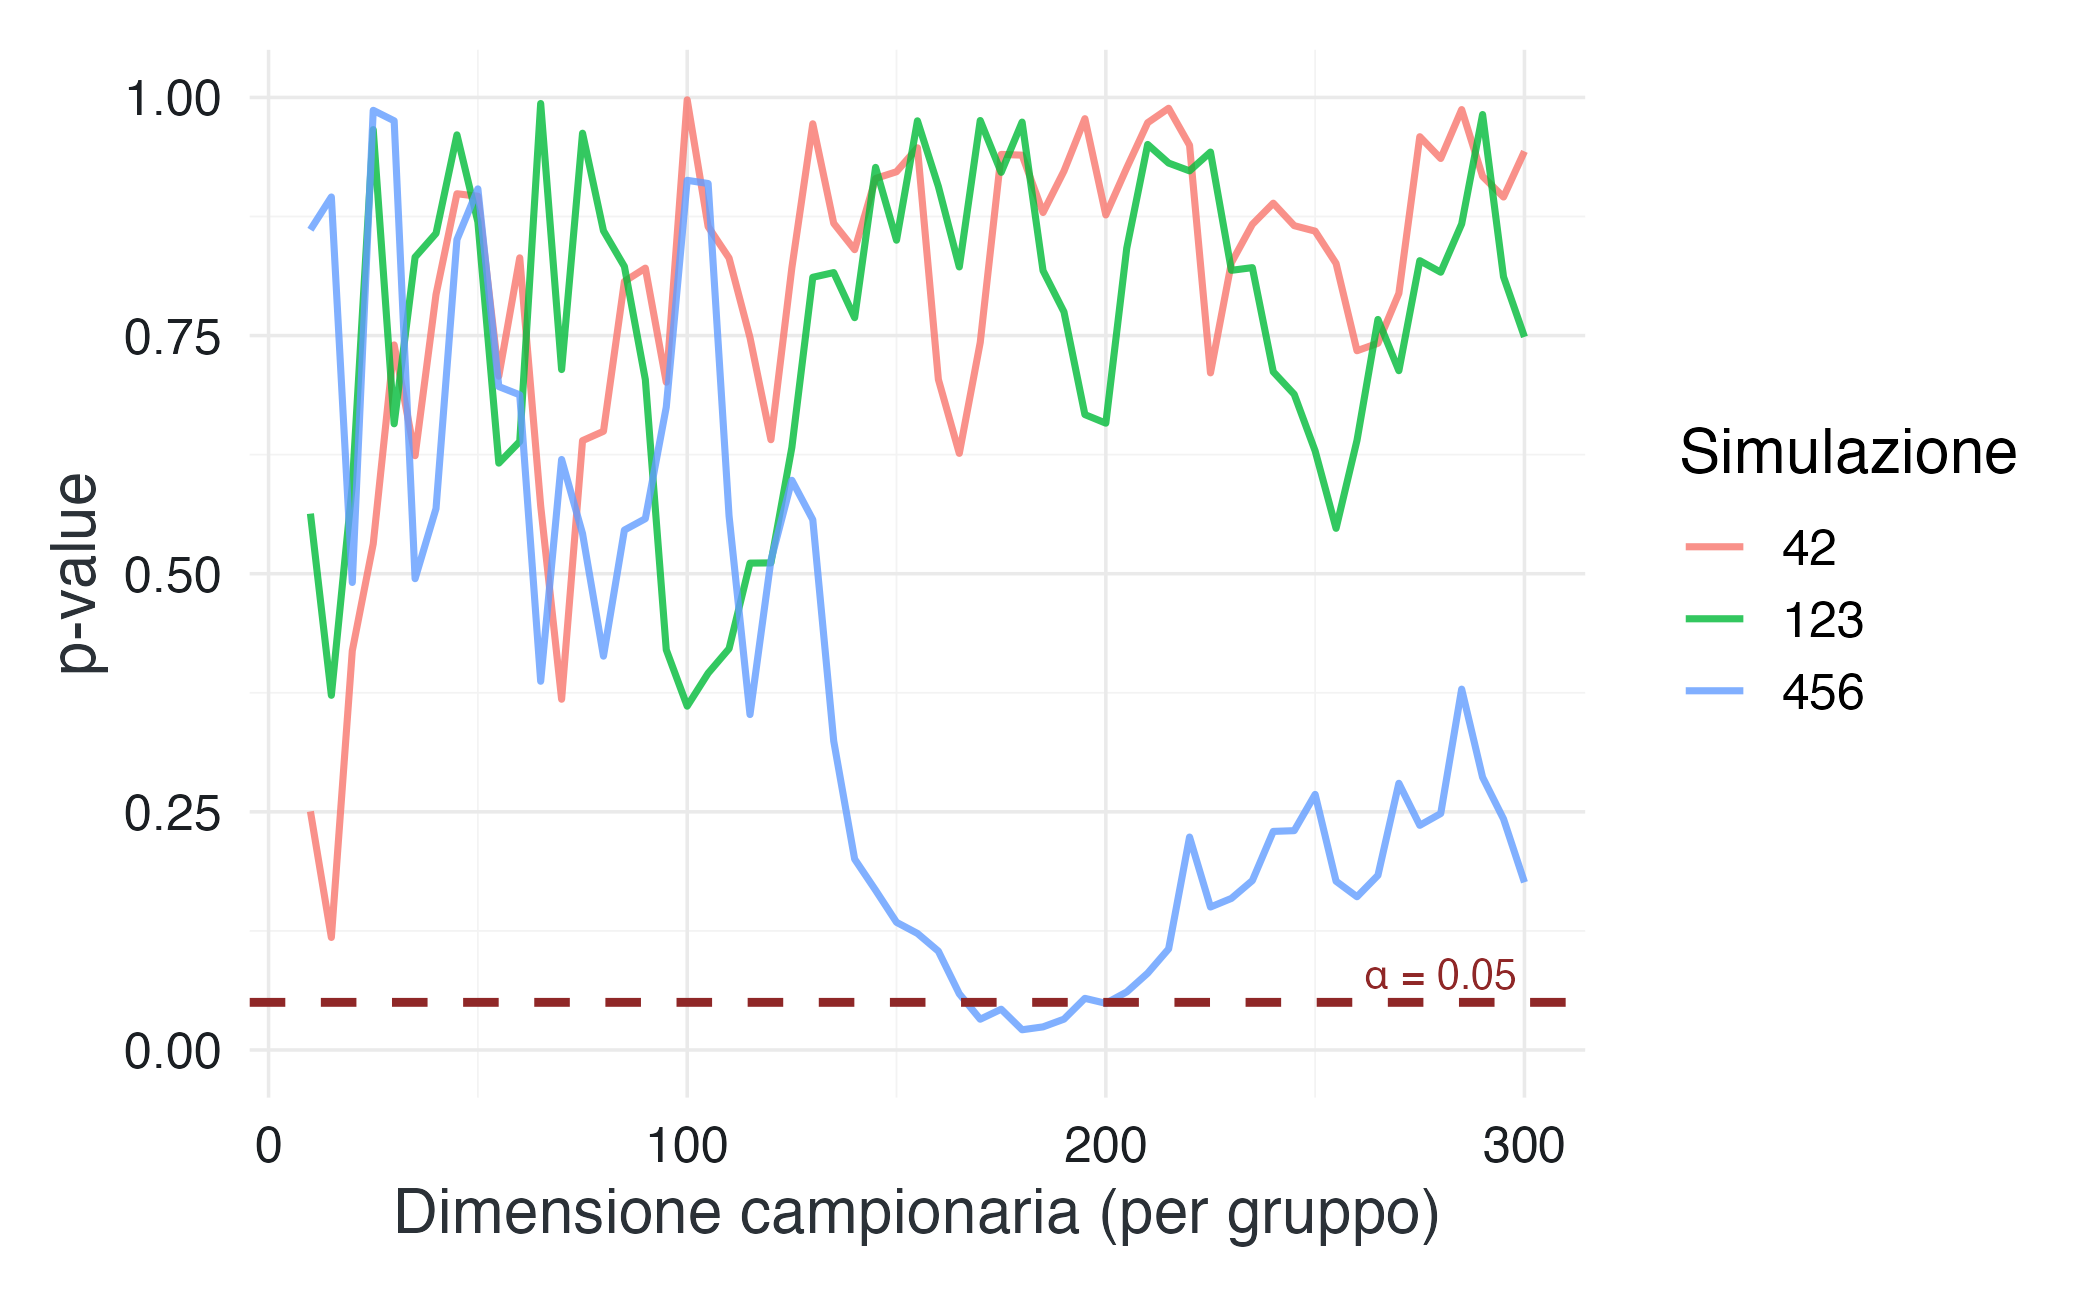
\includegraphics[width=0.85\linewidth,height=\textheight,keepaspectratio]{chapters/replication_crisis/01_crisis_files/figure-pdf/fig-pvalue-dance-1.png}

}

\caption{\label{fig-pvalue-dance}L'andamento del valore-\(p\) aumentando
la dimensione campionaria. I dati provengono dalla stessa popolazione,
quindi non esiste alcuna differenza reale. Eppure il valore-\(p\)
oscilla, e occasionalmente scende sotto la soglia di 0.05.}

\end{figure}%

Osserva la Figura~\ref{fig-pvalue-dance}: il valore-\(p\) non converge
ordinatamente verso 1, come ci si aspetterebbe in assenza di un effetto
reale. Al contrario, fluttua in modo erratico. In alcune esecuzioni
della simulazione, \textbf{attraversa ripetutamente la soglia di 0.05},
talvolta per pochi dati, altre volte più a lungo.

Ora immagina un ricercatore che adotta l'\textbf{optional stopping}:
raccoglie i dati in modo sequenziale, calcola ripetutamente il
valore-\(p\) e decide di interrompere la raccolta \textbf{proprio nel
momento in cui il risultato diventa ``statisticamente significativo''}.
Con questa strategia, \textbf{prima o poi il successo è garantito},
anche quando si parte da un'ipotesi completamente falsa. Il valore-\(p\)
non diventa mai una misura affidabile dell'evidenza, ma piuttosto il
bersaglio mobile di una caccia in cui il momento dell'arresto determina
l'esito.

\subsection{Cosa ci dice l'approccio
bayesiano}\label{cosa-ci-dice-lapproccio-bayesiano}

Analizziamo gli stessi dati con un modello bayesiano. La domanda è: qual
è la distribuzione plausibile della differenza tra le medie dei due
gruppi?

\begin{Shaded}
\begin{Highlighting}[]
\FunctionTok{set.seed}\NormalTok{(}\DecValTok{42}\NormalTok{)}
\NormalTok{y1 }\OtherTok{\textless{}{-}} \FunctionTok{rnorm}\NormalTok{(}\DecValTok{50}\NormalTok{, }\AttributeTok{mean =} \DecValTok{0}\NormalTok{, }\AttributeTok{sd =} \DecValTok{2}\NormalTok{)}
\NormalTok{y2 }\OtherTok{\textless{}{-}} \FunctionTok{rnorm}\NormalTok{(}\DecValTok{50}\NormalTok{, }\AttributeTok{mean =} \DecValTok{0}\NormalTok{, }\AttributeTok{sd =} \DecValTok{2}\NormalTok{)}

\NormalTok{stan\_data }\OtherTok{\textless{}{-}} \FunctionTok{list}\NormalTok{(}\AttributeTok{N1 =} \FunctionTok{length}\NormalTok{(y1), }\AttributeTok{N2 =} \FunctionTok{length}\NormalTok{(y2), }\AttributeTok{y1 =}\NormalTok{ y1, }\AttributeTok{y2 =}\NormalTok{ y2)}

\NormalTok{stan\_code }\OtherTok{\textless{}{-}} \StringTok{"}
\StringTok{data \{}
\StringTok{  int\textless{}lower=0\textgreater{} N1;}
\StringTok{  int\textless{}lower=0\textgreater{} N2;}
\StringTok{  vector[N1] y1;}
\StringTok{  vector[N2] y2;}
\StringTok{\}}
\StringTok{parameters \{}
\StringTok{  real mu1;}
\StringTok{  real mu2;}
\StringTok{  real\textless{}lower=0\textgreater{} sigma;}
\StringTok{\}}
\StringTok{transformed parameters \{}
\StringTok{  real delta = mu1 {-} mu2;}
\StringTok{\}}
\StringTok{model \{}
\StringTok{  // Prior debolmente informativi}
\StringTok{  mu1 \textasciitilde{} normal(0, 5);}
\StringTok{  mu2 \textasciitilde{} normal(0, 5);}
\StringTok{  sigma \textasciitilde{} exponential(0.5);}
\StringTok{  }
\StringTok{  // Verosimiglianza}
\StringTok{  y1 \textasciitilde{} normal(mu1, sigma);}
\StringTok{  y2 \textasciitilde{} normal(mu2, sigma);}
\StringTok{\}}
\StringTok{"}

\NormalTok{mod }\OtherTok{\textless{}{-}}\NormalTok{ cmdstanr}\SpecialCharTok{::}\FunctionTok{cmdstan\_model}\NormalTok{(}\FunctionTok{write\_stan\_file}\NormalTok{(stan\_code))}

\NormalTok{fit }\OtherTok{\textless{}{-}}\NormalTok{ mod}\SpecialCharTok{$}\FunctionTok{sample}\NormalTok{(}
  \AttributeTok{data =}\NormalTok{ stan\_data,}
  \AttributeTok{seed =} \DecValTok{123}\NormalTok{,}
  \AttributeTok{chains =} \DecValTok{4}\NormalTok{,}
  \AttributeTok{parallel\_chains =} \DecValTok{4}\NormalTok{,}
  \AttributeTok{iter\_sampling =} \DecValTok{2000}\NormalTok{,}
  \AttributeTok{iter\_warmup =} \DecValTok{1000}\NormalTok{,}
  \AttributeTok{show\_messages =} \ConstantTok{FALSE}\NormalTok{,}
  \AttributeTok{refresh =} \DecValTok{0}
\NormalTok{)}
\end{Highlighting}
\end{Shaded}

\begin{Shaded}
\begin{Highlighting}[]
\NormalTok{delta\_draws }\OtherTok{\textless{}{-}}\NormalTok{ fit}\SpecialCharTok{$}\FunctionTok{draws}\NormalTok{(}\AttributeTok{variables =} \StringTok{"delta"}\NormalTok{, }\AttributeTok{format =} \StringTok{"df"}\NormalTok{)}\SpecialCharTok{$}\NormalTok{delta}
\NormalTok{ci\_95 }\OtherTok{\textless{}{-}} \FunctionTok{quantile}\NormalTok{(delta\_draws, }\AttributeTok{probs =} \FunctionTok{c}\NormalTok{(}\FloatTok{0.025}\NormalTok{, }\FloatTok{0.975}\NormalTok{))}

\FunctionTok{ggplot}\NormalTok{(}\FunctionTok{data.frame}\NormalTok{(}\AttributeTok{delta =}\NormalTok{ delta\_draws), }\FunctionTok{aes}\NormalTok{(}\AttributeTok{x =}\NormalTok{ delta)) }\SpecialCharTok{+}
  \FunctionTok{geom\_histogram}\NormalTok{(}\FunctionTok{aes}\NormalTok{(}\AttributeTok{y =} \FunctionTok{after\_stat}\NormalTok{(density)), }\AttributeTok{bins =} \DecValTok{40}\NormalTok{, }\AttributeTok{alpha =} \FloatTok{0.7}\NormalTok{, }\AttributeTok{color =} \StringTok{"white"}\NormalTok{) }\SpecialCharTok{+}
  \FunctionTok{geom\_vline}\NormalTok{(}\AttributeTok{xintercept =} \DecValTok{0}\NormalTok{, }\AttributeTok{linetype =} \StringTok{"solid"}\NormalTok{, }\AttributeTok{linewidth =} \DecValTok{1}\NormalTok{) }\SpecialCharTok{+}
  \FunctionTok{geom\_vline}\NormalTok{(}\AttributeTok{xintercept =}\NormalTok{ ci\_95, }\AttributeTok{linetype =} \StringTok{"dashed"}\NormalTok{, }\AttributeTok{linewidth =} \FloatTok{0.8}\NormalTok{) }\SpecialCharTok{+}
  \FunctionTok{annotate}\NormalTok{(}\StringTok{"text"}\NormalTok{, }\AttributeTok{x =} \FunctionTok{mean}\NormalTok{(ci\_95), }\AttributeTok{y =} \FloatTok{0.05}\NormalTok{, }
           \AttributeTok{label =} \FunctionTok{sprintf}\NormalTok{(}\StringTok{"95\%\% CI: [\%.2f, \%.2f]"}\NormalTok{, ci\_95[}\DecValTok{1}\NormalTok{], ci\_95[}\DecValTok{2}\NormalTok{]),}
           \AttributeTok{size =} \FloatTok{3.5}\NormalTok{) }\SpecialCharTok{+}
  \FunctionTok{scale\_color\_qualitative}\NormalTok{() }\SpecialCharTok{+}
  \FunctionTok{labs}\NormalTok{(}
    \AttributeTok{x =} \FunctionTok{expression}\NormalTok{(delta}\SpecialCharTok{\textasciitilde{}}\StringTok{"= differenza tra le medie"}\NormalTok{),}
    \AttributeTok{y =} \StringTok{"Densità"}
\NormalTok{  ) }
\end{Highlighting}
\end{Shaded}

\begin{figure}[H]

\centering{

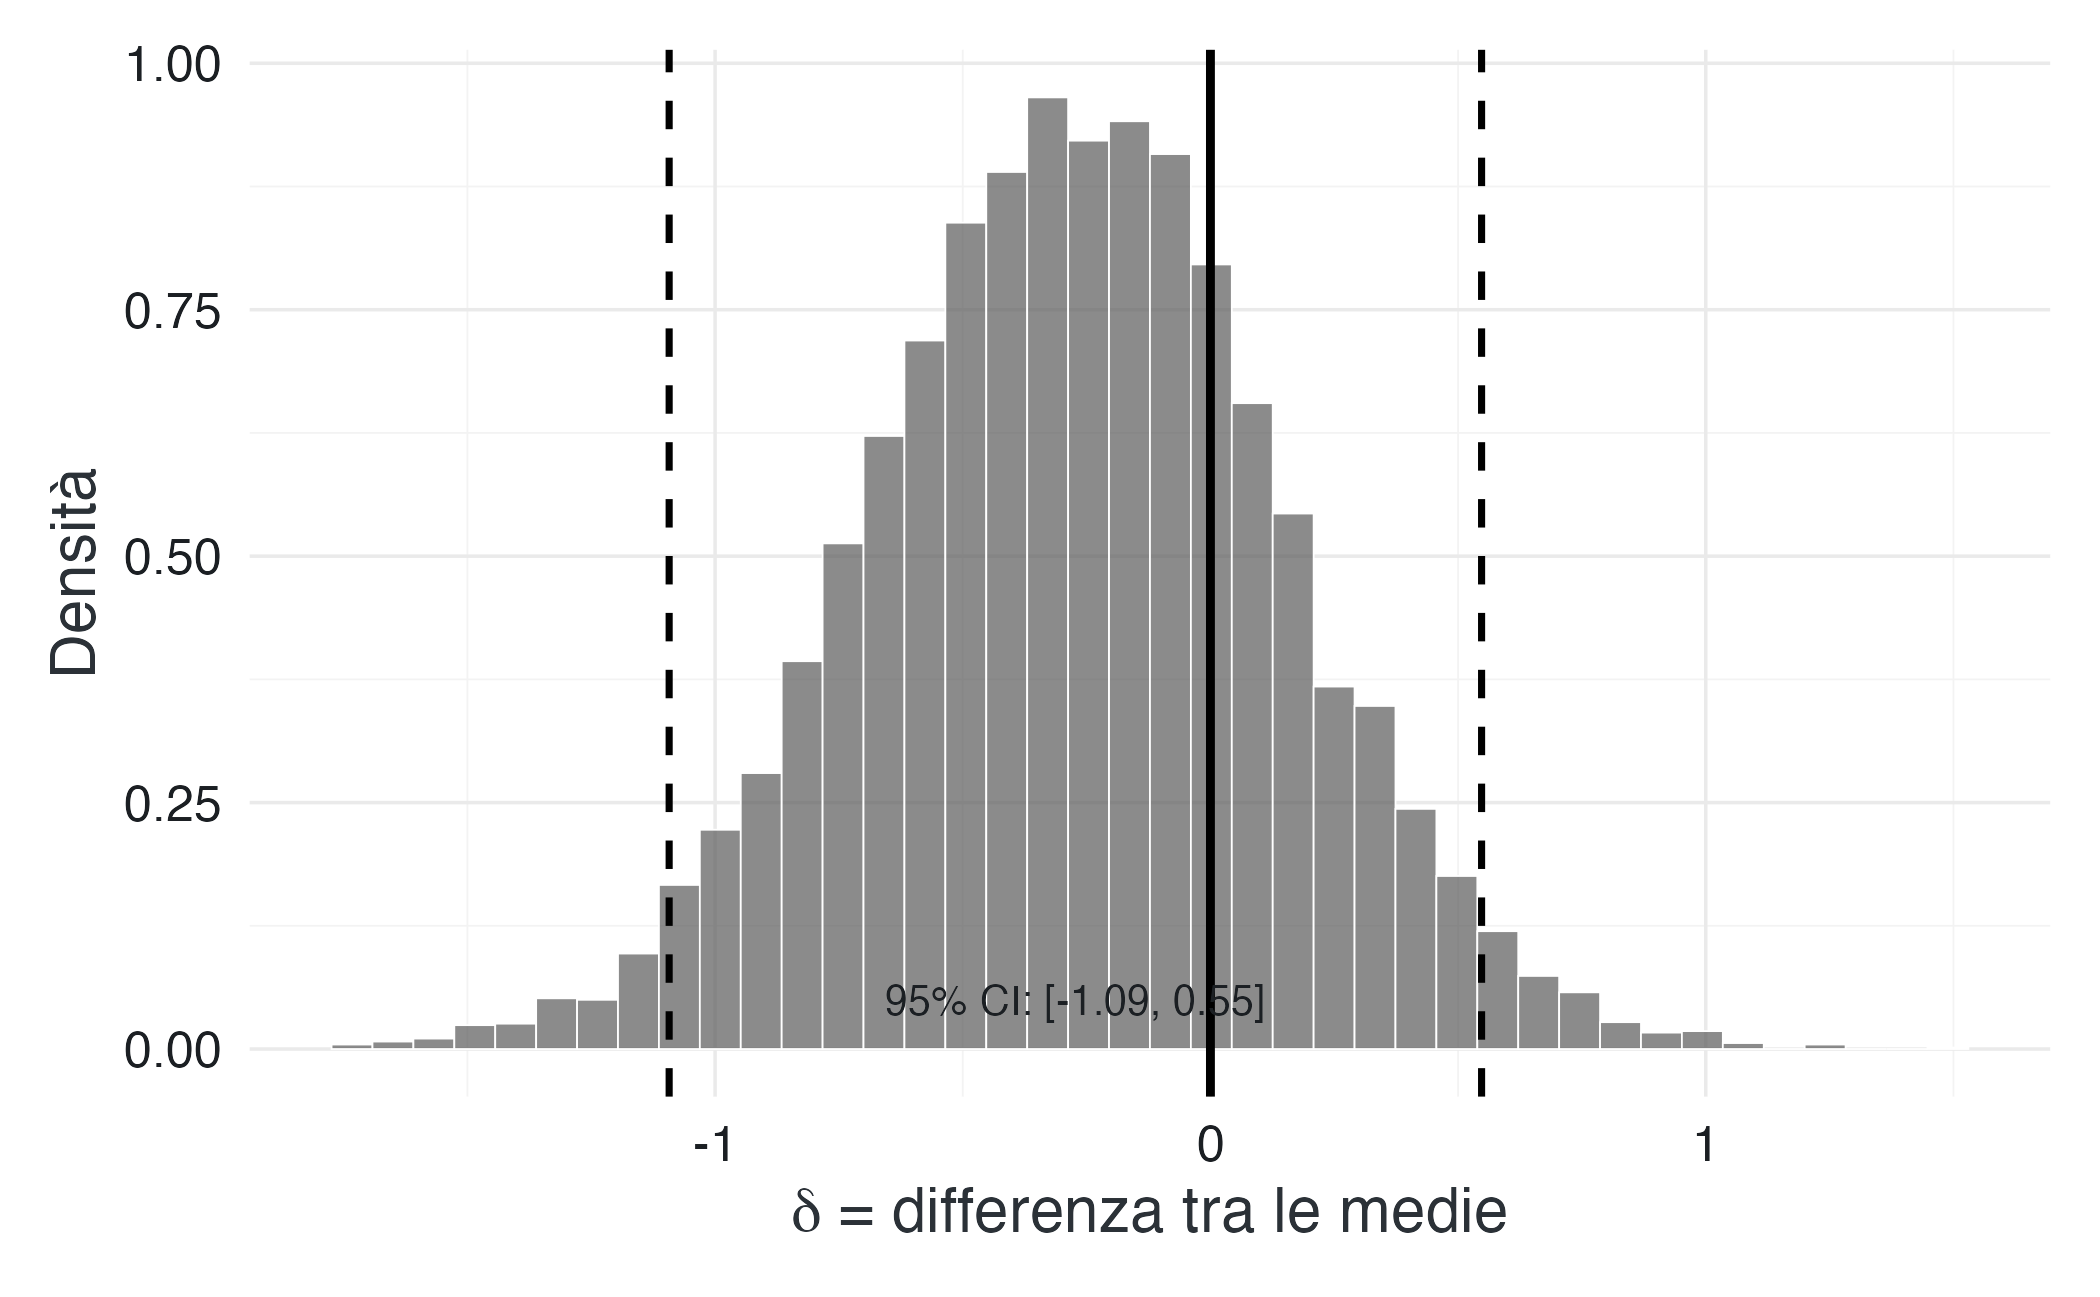
\includegraphics[width=0.85\linewidth,height=\textheight,keepaspectratio]{chapters/replication_crisis/01_crisis_files/figure-pdf/fig-posterior-delta-1.png}

}

\caption{\label{fig-posterior-delta}Distribuzione a posteriori della
differenza tra le medie (δ). L'intervallo di credibilità al 95\% include
comodamente lo zero, suggerendo che non c'è evidenza di una differenza
sostanziale.}

\end{figure}%

L'intervallo di credibilità al 95\% per δ va da -1.09 a 0.55. Poiché
tale intervallo comprende lo zero, possiamo affermare che, alla luce dei
dati e delle assunzioni a priori, \textbf{non c'è evidenza di una
differenza rilevante tra i due gruppi}.

Questo risultato è coerente con il modo in cui i dati sono stati
generati (stessa distribuzione di origine). Tuttavia, osserva come
cambia la comunicazione statistica rispetto al paradigma tradizionale:

\begin{itemize}
\tightlist
\item
  \textbf{Frequentista}: ``Il valore-\(p\) è 0.03 → rifiuto l'ipotesi
  nulla'' (decisione binaria, sensibile al campionamento e alle soglie
  arbitrarie).
\item
  \textbf{Bayesiano}: ``La distribuzione a posteriori di δ è concentrata
  attorno a zero, con ampia incertezza'' (descrizione continua
  dell'evidenza e della sua incertezza).
\end{itemize}

L'inferenza bayesiana non rende la ricerca immune da errori o
interpretazioni scorrette. Ciò che cambia è \textbf{il linguaggio
dell'incertezza}: invece di costringerci a fornire una risposta sì/no
basata su un valore di soglia, ci permette di esprimere il nostro
livello di incertezza, la direzione e l'intensità di quest'ultima. Un
modello non prende decisioni al posto nostro, ma ci offre una
rappresentazione più fedele della conoscenza che i dati ci permettono di
ottenere e dei suoi limiti.

\section{Oltre la crisi: verso una nuova cultura
scientifica}\label{oltre-la-crisi-verso-una-nuova-cultura-scientifica}

La crisi di replicabilità ha avuto almeno un merito innegabile: ha
costretto la psicologia a un doloroso, ma necessario, esame di coscienza
collettivo. Da questo confronto è nata una \textbf{rivoluzione della
credibilità} (\emph{credibility revolution}) che sta lentamente, ma
inesorabilmente, riscrivendo le regole della disciplina.

\subsection{I progressi tangibili}\label{i-progressi-tangibili}

Rispetto al panorama di un decennio fa, il cambiamento è già evidente:

\begin{itemize}
\tightlist
\item
  La \textbf{condivisione aperta di dati e codice}, prerequisito per la
  riproducibilità analitica, non è più un'opzione ma un requisito. Essa
  abilita il controllo indipendente e rende la conoscenza veramente
  cumulativa.
\item
  I progetti di ricerca \textbf{multi-lab} (Many Labs, Many Babies,
  Psychological Science Accelerator) dimostrano che la collaborazione su
  larga scala può produrre evidenze più solide e generalizzabili,
  superando i limiti dei singoli laboratori.
\item
  La \textbf{preregistrazione} sta diventando una pratica consolidata.
  Sebbene non sia una soluzione miracolosa, riduce drasticamente il
  margine per il \emph{p-hacking} e per costruire narrazioni \emph{ad
  hoc} a partire dai risultati ottenuti.
\item
  I \textbf{Registered Reports} hanno ribaltato la logica della
  pubblicazione. Il merito scientifico viene valutato nella fase di
  progettazione, prima ancora che i dati vengano raccolti. Questo
  sgancia l'accettazione dal risultato finale, neutralizzando alla
  radice il bias di pubblicazione.
\end{itemize}

\subsection{Le sfide aperte}\label{le-sfide-aperte}

Tuttavia, la trasformazione è ancora incompleta. I \textbf{sistemi di
incentivi accademici} evolvono lentamente, la pressione a pubblicare
rimane intatta e l'adozione di queste pratiche virtuose non è ancora
uniforme.

La sfida più profonda, però, è concettuale: \textbf{non basta adottare
nuove procedure se non cambia il \emph{framework} con cui interpretiamo
l'evidenza}. L'approccio bayesiano, che costituirà la bussola delle
prossime sezioni, offre un linguaggio logicamente più coerente per
quantificare l'incertezza e aggiornare le nostre credenze alla luce dei
dati. Tuttavia, richiede un investimento in formazione, strumenti
computazionali e nuove abitudini cognitive.

Questo investimento è necessario. Il criterio ultimo, infatti, non è
l'ortodossia di un metodo in astratto, ma la sua utilità concreta:
\textbf{ci aiuta a capire la mente umana?} Permette di costruire una
conoscenza che si accumula invece di disperdersi? Genera risultati
affidabili e verificabili?

La crisi ha messo in luce che, per lungo tempo, le risposte a queste
domande sono state deludenti. L'obiettivo di questo \emph{companion} è
fornirti gli strumenti per immaginare e costruire un futuro diverso, un
futuro in cui queste risposte possano essere, in modo replicabile e
motivato, affermative.

\section{Per approfondire}\label{per-approfondire}

\begin{tcolorbox}[enhanced jigsaw, arc=.35mm, bottomrule=.15mm, breakable, colback=white, colframe=quarto-callout-note-color-frame, left=2mm, leftrule=.75mm, opacityback=0, rightrule=.15mm, toprule=.15mm]
\begin{minipage}[t]{5.5mm}
\textcolor{quarto-callout-note-color}{\faInfo}
\end{minipage}%
\begin{minipage}[t]{\textwidth - 5.5mm}

\vspace{-3mm}\textbf{Risorse consigliate}\vspace{3mm}

\begin{itemize}
\tightlist
\item
  Pennington (\citeproc{ref-pennington2023student}{2023}) --- Testo di
  riferimento adottato per questo capitolo.
\item
  Collaboration (\citeproc{ref-open2015estimating}{2015}) --- Risultati
  completi del \emph{Reproducibility Project}.
\item
  Simmons et al. (\citeproc{ref-simmons2011false}{2011}) --- Articolo
  seminale sulle \emph{pratiche di ricerca flessibili}.
\item
  \href{https://retractionwatch.com/}{Retraction Watch} --- Database
  aggiornato delle ritrattazioni scientifiche.
\item
  \href{http://datacolada.org/}{Data Colada} --- Blog di Uri Simonsohn e
  collaboratori sulla metodologia della ricerca.
\end{itemize}

\end{minipage}%
\end{tcolorbox}

\begin{tcolorbox}[enhanced jigsaw, arc=.35mm, bottomrule=.15mm, bottomtitle=1mm, breakable, colback=white, colbacktitle=quarto-callout-note-color!10!white, colframe=quarto-callout-note-color-frame, coltitle=black, left=2mm, leftrule=.75mm, opacityback=0, opacitybacktitle=0.6, rightrule=.15mm, title=\textcolor{quarto-callout-note-color}{\faInfo}\hspace{0.5em}{Informazioni sull'ambiente di sviluppo}, titlerule=0mm, toprule=.15mm, toptitle=1mm]

\begin{Shaded}
\begin{Highlighting}[]
\FunctionTok{sessionInfo}\NormalTok{()}
\CommentTok{\#\textgreater{} R version 4.6.1 (2026{-}06{-}24)}
\CommentTok{\#\textgreater{} Platform: aarch64{-}apple{-}darwin23}
\CommentTok{\#\textgreater{} Running under: macOS Tahoe 26.5.2}
\CommentTok{\#\textgreater{} }
\CommentTok{\#\textgreater{} Matrix products: default}
\CommentTok{\#\textgreater{} BLAS:   /Library/Frameworks/R.framework/Versions/4.6/Resources/lib/libRblas.0.dylib }
\CommentTok{\#\textgreater{} LAPACK: /Library/Frameworks/R.framework/Versions/4.6/Resources/lib/libRlapack.dylib;  LAPACK version 3.12.1}
\CommentTok{\#\textgreater{} }
\CommentTok{\#\textgreater{} locale:}
\CommentTok{\#\textgreater{} [1] C.UTF{-}8/UTF{-}8/C.UTF{-}8/C/C.UTF{-}8/C.UTF{-}8}
\CommentTok{\#\textgreater{} }
\CommentTok{\#\textgreater{} time zone: Europe/Zagreb}
\CommentTok{\#\textgreater{} tzcode source: internal}
\CommentTok{\#\textgreater{} }
\CommentTok{\#\textgreater{} attached base packages:}
\CommentTok{\#\textgreater{} [1] stats     graphics  grDevices utils     datasets  methods   base     }
\CommentTok{\#\textgreater{} }
\CommentTok{\#\textgreater{} other attached packages:}
\CommentTok{\#\textgreater{}  [1] cmdstanr\_0.9.0        ragg\_1.5.2            tinytable\_0.17.0     }
\CommentTok{\#\textgreater{}  [4] withr\_3.0.3           systemfonts\_1.3.2     patchwork\_1.3.2      }
\CommentTok{\#\textgreater{}  [7] ggdist\_3.3.3          tidybayes\_3.0.7       bayesplot\_1.15.0     }
\CommentTok{\#\textgreater{} [10] ggplot2\_4.0.3         reliabilitydiag\_0.2.1 priorsense\_1.2.0     }
\CommentTok{\#\textgreater{} [13] posterior\_1.7.0       loo\_2.10.0            rstan\_2.32.7         }
\CommentTok{\#\textgreater{} [16] StanHeaders\_2.32.10   brms\_2.23.0           Rcpp\_1.1.2           }
\CommentTok{\#\textgreater{} [19] sessioninfo\_1.2.4     conflicted\_1.2.0      janitor\_2.2.1        }
\CommentTok{\#\textgreater{} [22] matrixStats\_1.5.0     modelr\_0.1.11         tibble\_3.3.1         }
\CommentTok{\#\textgreater{} [25] dplyr\_1.2.1           tidyr\_1.3.2           rio\_1.3.0            }
\CommentTok{\#\textgreater{} [28] here\_1.0.2           }
\CommentTok{\#\textgreater{} }
\CommentTok{\#\textgreater{} loaded via a namespace (and not attached):}
\CommentTok{\#\textgreater{}  [1] svUnit\_1.0.8          tidyselect\_1.2.1      farver\_2.1.2         }
\CommentTok{\#\textgreater{}  [4] S7\_0.2.2              fastmap\_1.2.0         tensorA\_0.36.2.1     }
\CommentTok{\#\textgreater{}  [7] pacman\_0.5.1          digest\_0.6.39         timechange\_0.4.0     }
\CommentTok{\#\textgreater{} [10] estimability\_2.0.0    lifecycle\_1.0.5       processx\_3.9.0       }
\CommentTok{\#\textgreater{} [13] magrittr\_2.0.5        compiler\_4.6.1        rlang\_1.3.0          }
\CommentTok{\#\textgreater{} [16] tools\_4.6.1           yaml\_2.3.12           data.table\_1.18.4    }
\CommentTok{\#\textgreater{} [19] knitr\_1.51            labeling\_0.4.3        bridgesampling\_1.2{-}1 }
\CommentTok{\#\textgreater{} [22] pkgbuild\_1.4.8        curl\_7.1.0            RColorBrewer\_1.1{-}3   }
\CommentTok{\#\textgreater{} [25] abind\_1.4{-}8           purrr\_1.2.2           grid\_4.6.1           }
\CommentTok{\#\textgreater{} [28] stats4\_4.6.1          xtable\_1.8{-}8          inline\_0.3.21        }
\CommentTok{\#\textgreater{} [31] emmeans\_2.0.4         scales\_1.4.0          cli\_3.6.6            }
\CommentTok{\#\textgreater{} [34] mvtnorm\_1.4{-}2         rmarkdown\_2.31        generics\_0.1.4       }
\CommentTok{\#\textgreater{} [37] otel\_0.2.0            RcppParallel\_5.1.11{-}2 cachem\_1.1.0         }
\CommentTok{\#\textgreater{} [40] stringr\_1.6.0         parallel\_4.6.1        vctrs\_0.7.3          }
\CommentTok{\#\textgreater{} [43] V8\_8.2.0              Matrix\_1.7{-}5          jsonlite\_2.0.0       }
\CommentTok{\#\textgreater{} [46] arrayhelpers\_1.1{-}1    glue\_1.8.1            ps\_1.9.3             }
\CommentTok{\#\textgreater{} [49] codetools\_0.2{-}20      distributional\_0.8.1  lubridate\_1.9.5      }
\CommentTok{\#\textgreater{} [52] stringi\_1.8.7         gtable\_0.3.6          QuickJSR\_1.10.0      }
\CommentTok{\#\textgreater{} [55] pillar\_1.11.1         htmltools\_0.5.9       Brobdingnag\_1.2{-}9    }
\CommentTok{\#\textgreater{} [58] R6\_2.6.1              textshaping\_1.0.5     rprojroot\_2.1.1      }
\CommentTok{\#\textgreater{} [61] evaluate\_1.0.5        lattice\_0.22{-}9        backports\_1.5.1      }
\CommentTok{\#\textgreater{} [64] memoise\_2.0.1         broom\_1.0.13          snakecase\_0.11.1     }
\CommentTok{\#\textgreater{} [67] rstantools\_2.6.0      coda\_0.19{-}4.1         gridExtra\_2.3.1      }
\CommentTok{\#\textgreater{} [70] nlme\_3.1{-}170          checkmate\_2.3.4       xfun\_0.60            }
\CommentTok{\#\textgreater{} [73] pkgconfig\_2.0.3}
\end{Highlighting}
\end{Shaded}

\end{tcolorbox}

\section*{Bibliografia}\label{bibliografia}

\markright{Bibliografia}

\part{Diagnosi}

\chapter*{📍 Dove siamo nel percorso}\label{dove-siamo-nel-percorso-1}

\markboth{📍 Dove siamo nel percorso}{📍 Dove siamo nel percorso}

\begin{tcolorbox}[enhanced jigsaw, arc=.35mm, bottomrule=.15mm, breakable, colback=white, colframe=quarto-callout-note-color-frame, left=2mm, leftrule=.75mm, opacityback=0, rightrule=.15mm, toprule=.15mm]

La crisi della replicabilità è causata da molteplici fattori. In primo
luogo, un \textbf{sistema di incentivi accademici distorto} che premia
la quantità a scapito della qualità della ricerca. In secondo luogo,
sono stati individuati i \textbf{limiti dell'inferenza frequentista},
ampiamente adottata in psicologia, e il suo utilizzo meccanico come
``filtro'' per separare i risultati scientificamente rilevanti da quelli
trascurabili. In questa sezione esamineremo nel dettaglio gli effetti
negativi di queste scelte metodologiche e introdurremo le pratiche della
\emph{Open Science}.

\end{tcolorbox}

\begin{tcolorbox}[enhanced jigsaw, arc=.35mm, bottomrule=.15mm, bottomtitle=1mm, breakable, colback=white, colbacktitle=quarto-callout-tip-color!10!white, colframe=quarto-callout-tip-color-frame, coltitle=black, left=2mm, leftrule=.75mm, opacityback=0, opacitybacktitle=0.6, rightrule=.15mm, title=\textcolor{quarto-callout-tip-color}{\faLightbulb}\hspace{0.5em}{🎯 Cosa faremo in questa sezione}, titlerule=0mm, toprule=.15mm, toptitle=1mm]

Questa sezione analizza i problemi metodologici legati all'inferenza
frequentista e li collega alle pratiche di ricerca responsabile:

\begin{itemize}
\tightlist
\item
  \textbf{Simulare} gli effetti distorti del \emph{p-hacking} e dei
  \emph{ricercatori gradi di libertà}.
\item
  \textbf{Quantificare} l'instabilità interpretativa del \emph{p-value}
  in scenari realistici.
\item
  \textbf{Implementare} un preregistrazione che specifichi le analisi
  bayesiane.
\item
  \textbf{Strutturare} repository di ricerca completamente
  \textbf{riproducibili e accessibili}.
\item
  \textbf{Comprendere} le pratiche fondamentali dell'\emph{Open
  Science}.
\end{itemize}

\end{tcolorbox}

\begin{tcolorbox}[enhanced jigsaw, arc=.35mm, bottomrule=.15mm, bottomtitle=1mm, breakable, colback=white, colbacktitle=quarto-callout-important-color!10!white, colframe=quarto-callout-important-color-frame, coltitle=black, left=2mm, leftrule=.75mm, opacityback=0, opacitybacktitle=0.6, rightrule=.15mm, title=\textcolor{quarto-callout-important-color}{\faExclamation}\hspace{0.5em}{📖 Collegamenti con il manuale}, titlerule=0mm, toprule=.15mm, toptitle=1mm]

Questa sezione mette in pratica alcuni temi chiave del manuale:

\begin{itemize}
\tightlist
\item
  il \textbf{valore-p} e i suoi fraintendimenti;
\item
  le \textbf{pratiche di ricerca discutibili};
\item
  le \textbf{buone pratiche di Open Science}.
\end{itemize}

\end{tcolorbox}

\begin{tcolorbox}[enhanced jigsaw, arc=.35mm, bottomrule=.15mm, breakable, colback=white, colframe=quarto-callout-caution-color-frame, left=2mm, leftrule=.75mm, opacityback=0, rightrule=.15mm, toprule=.15mm]
\begin{minipage}[t]{5.5mm}
\textcolor{quarto-callout-caution-color}{\faFire}
\end{minipage}%
\begin{minipage}[t]{\textwidth - 5.5mm}

⭐ \textbf{Implicazioni per la formazione e la pratica professionale:}
comprendere le \textbf{cattive pratiche di ricerca} -- spesso
inavvertitamente favorite dal paradigma frequentista -- offre un
triplice vantaggio. In primo luogo, permette di \textbf{smascherare le
strategie} con cui vengono prodotte pubblicazioni di scarso valore. In
secondo luogo, \textbf{fornisce agli studenti} una lente critica per
interpretare la letteratura scientifica, legando i limiti metodologici
alla solidità delle conclusioni. Infine, \textbf{mette i professionisti}
nella condizione di valutare su quali basi teoriche ed empiriche sia
ragionevole fondare gli interventi applicativi.

\end{minipage}%
\end{tcolorbox}

\chapter{Limiti dell'inferenza frequentista: un laboratorio
computazionale}\label{sec-limits-freq-inference}

\begin{tcolorbox}[enhanced jigsaw, arc=.35mm, bottomrule=.15mm, breakable, colback=white, colframe=quarto-callout-note-color-frame, left=2mm, leftrule=.75mm, opacityback=0, rightrule=.15mm, toprule=.15mm]

Nel manuale abbiamo analizzato i fondamenti teorici della critica al
valore-\(p\): la sua definizione come probabilità condizionata
all'ipotesi nulla, le controversie storiche tra Fisher e Neyman-Pearson
e il celebre monito dell'ASA del 2016
(\citeproc{ref-wasserstein2016asa}{Wasserstein \& Lazar, 2016}).

In questo capitolo non ripeteremo quelle argomentazioni, ma le
verificheremo mediante simulazioni computazionali. Il nostro obiettivo è
tradurre affermazioni astratte --- come ``il \(p\)-hacking incrementa i
falsi positivi'' o ``l'optional stopping invalida l'inferenza'' --- in
esperienze visive e quantitative. Genereremo dati ex novo, applicheremo
le procedure statistiche criticate e osserveremo come e perché esse
falliscono.

Come suggeriva Richard Feynman, \emph{``Ciò che non sono in grado di
costruire, non lo comprendo''}. In queste pagine verificheremo
operativamente come nascono i problemi del valore-\(p\), per arrivare a
una comprensione intuitiva delle sue insidie.

\end{tcolorbox}

\begin{tcolorbox}[enhanced jigsaw, arc=.35mm, bottomrule=.15mm, breakable, colback=white, colframe=quarto-callout-important-color-frame, left=2mm, leftrule=.75mm, opacityback=0, rightrule=.15mm, toprule=.15mm]

\textbf{Da sapere.} Il valore-\(p\) esprime la probabilità dei dati
assumendo vera l'ipotesi nulla, non la probabilità che l'ipotesi nulla
sia vera. Il \(p\)-hacking e l'uso rigido della soglia 0.05 possono
produrre conclusioni instabili e aumentare i falsi positivi.

\textbf{Da saper fare.} Eseguire e interpretare simulazioni che mostrano
l'inflazione dei falsi positivi, le anomalie nella distribuzione dei
valori-\(p\), la confusione tra \(P(\text{Dati} \mid H_0)\) e
\(P(H_0 \mid \text{Dati})\) e la fragilità delle decisioni basate su una
soglia fissa.

\textbf{Approfondimento facoltativo.} Le evidenze tratte dalla
letteratura, i passaggi analitici più dettagliati e gli esercizi finali
approfondiscono gli stessi problemi, ma possono essere saltati senza
perdere il filo concettuale del capitolo.

\hyperref[sec-percorsi-lettura]{Che cosa significano queste etichette?}

\end{tcolorbox}

\begin{tcolorbox}[enhanced jigsaw, arc=.35mm, bottomrule=.15mm, bottomtitle=1mm, breakable, colback=white, colbacktitle=quarto-callout-important-color!10!white, colframe=quarto-callout-important-color-frame, coltitle=black, left=2mm, leftrule=.75mm, opacityback=0, opacitybacktitle=0.6, rightrule=.15mm, title=\textcolor{quarto-callout-important-color}{\faExclamation}\hspace{0.5em}{In questo capitolo imparerai a}, titlerule=0mm, toprule=.15mm, toptitle=1mm]

\begin{itemize}
\tightlist
\item
  verificare empiricamente come il \(p\)-hacking aumenti il tasso di
  falsi positivi;
\item
  visualizzare la distribuzione anomala dei valori-\(p\) nella
  letteratura scientifica;
\item
  comprendere, attraverso delle simulazioni, perché il valore-\(p\) non
  fornisce la probabilità che l'ipotesi sia vera;
\item
  sperimentare la fragilità delle decisioni basate su soglie arbitrarie.
\end{itemize}

\end{tcolorbox}

\begin{tcolorbox}[enhanced jigsaw, arc=.35mm, bottomrule=.15mm, bottomtitle=1mm, breakable, colback=white, colbacktitle=quarto-callout-tip-color!10!white, colframe=quarto-callout-tip-color-frame, coltitle=black, left=2mm, leftrule=.75mm, opacityback=0, opacitybacktitle=0.6, rightrule=.15mm, title=\textcolor{quarto-callout-tip-color}{\faLightbulb}\hspace{0.5em}{Prerequisiti}, titlerule=0mm, toprule=.15mm, toptitle=1mm]

\begin{itemize}
\tightlist
\item
  Rivedere nel manuale la trattazione del \textbf{valore-\(p\) e dei
  suoi fraintendimenti}, che fornisce le basi teoriche per le
  simulazioni presentate qui.
\item
  Leggere l'approfondimento
  \href{https://ccaudek.github.io/utet-frequentista/}{Inferenza
  frequentista in psicologia}.
\item
  Leggere le seguenti appendici: \textbf{?@sec-apx-shell},
  \textbf{?@sec-apx-files}, Appendice~\ref{sec-apx-numbers} e
  Appendice~\ref{sec-apx-sums}.
\end{itemize}

\end{tcolorbox}

\begin{tcolorbox}[enhanced jigsaw, arc=.35mm, bottomrule=.15mm, bottomtitle=1mm, breakable, colback=white, colbacktitle=quarto-callout-caution-color!10!white, colframe=quarto-callout-caution-color-frame, coltitle=black, left=2mm, leftrule=.75mm, opacityback=0, opacitybacktitle=0.6, rightrule=.15mm, title=\textcolor{quarto-callout-caution-color}{\faFire}\hspace{0.5em}{Preparazione del Notebook}, titlerule=0mm, toprule=.15mm, toptitle=1mm]

\begin{Shaded}
\begin{Highlighting}[]
\NormalTok{here}\SpecialCharTok{::}\FunctionTok{here}\NormalTok{(}\StringTok{"code"}\NormalTok{, }\StringTok{"\_common.R"}\NormalTok{) }\SpecialCharTok{|\textgreater{}} 
  \FunctionTok{source}\NormalTok{()}

\CommentTok{\# Load packages}
\ControlFlowTok{if}\NormalTok{ (}\SpecialCharTok{!}\FunctionTok{requireNamespace}\NormalTok{(}\StringTok{"pacman"}\NormalTok{)) }\FunctionTok{install.packages}\NormalTok{(}\StringTok{"pacman"}\NormalTok{)}
\NormalTok{pacman}\SpecialCharTok{::}\FunctionTok{p\_load}\NormalTok{(patchwork)}
\end{Highlighting}
\end{Shaded}

\end{tcolorbox}

\section{\texorpdfstring{Simulazione 1: Il \(p\)-hacking in
azione}{Simulazione 1: Il p-hacking in azione}}\label{simulazione-1-il-p-hacking-in-azione}

Immaginiamo un ricercatore che studia l'effetto di un intervento
psicologico. Nella realtà, l'intervento non ha alcun effetto (la
differenza tra i gruppi è esattamente zero). Tuttavia, il ricercatore ha
molte ``scelte analitiche'' a disposizione: può escludere gli outlier,
trasformare le variabili, aggiungere le covariate o analizzare i
sottogruppi. Ogni scelta rappresenta un ``grado di libertà'' che può
essere sfruttato, consapevolmente o meno, per ottenere un risultato
statisticamente significativo.

Simuliamo questo scenario: il ricercatore conduce 20 test statistici
diversi sugli stessi dati (ad esempio, provando diverse definizioni
operative della variabile dipendente). Quanti risultati
``significativi'' otterrà, anche se l'effetto reale è nullo?

Parametri della simulazione:

\begin{Shaded}
\begin{Highlighting}[]
\NormalTok{n\_tests }\OtherTok{\textless{}{-}} \DecValTok{20}          \CommentTok{\# Numero di test che il ricercatore prova}
\NormalTok{n\_per\_group }\OtherTok{\textless{}{-}} \DecValTok{30}      \CommentTok{\# Osservazioni per gruppo}
\NormalTok{n\_simulations }\OtherTok{\textless{}{-}} \DecValTok{1000}  \CommentTok{\# Quante volte ripetiamo l\textquotesingle{}esperimento}
\end{Highlighting}
\end{Shaded}

La funzione seguente simula un ricercatore che esamina 20 versioni
leggermente diverse dello stesso dataset. Per ogni versione, i dati
vengono generati da due popolazioni identiche (non c'è alcun effetto
reale), ma le fluttuazioni casuali producono variazioni tra i campioni.
Il ricercatore esegue un test \(t\) di Student su ciascuna versione e
\textbf{seleziona il valore-\(p\) più basso}.

\begin{Shaded}
\begin{Highlighting}[]
\NormalTok{simulate\_phacking }\OtherTok{\textless{}{-}} \ControlFlowTok{function}\NormalTok{(n\_tests, n\_per\_group) \{}
\NormalTok{  p\_values }\OtherTok{\textless{}{-}} \FunctionTok{numeric}\NormalTok{(n\_tests)}
  
  \ControlFlowTok{for}\NormalTok{ (i }\ControlFlowTok{in} \DecValTok{1}\SpecialCharTok{:}\NormalTok{n\_tests) \{}
    \CommentTok{\# Generazione di dati senza effetto reale}
\NormalTok{    group1 }\OtherTok{\textless{}{-}} \FunctionTok{rnorm}\NormalTok{(n\_per\_group, }\AttributeTok{mean =} \DecValTok{0}\NormalTok{, }\AttributeTok{sd =} \DecValTok{1}\NormalTok{)}
\NormalTok{    group2 }\OtherTok{\textless{}{-}} \FunctionTok{rnorm}\NormalTok{(n\_per\_group, }\AttributeTok{mean =} \DecValTok{0}\NormalTok{, }\AttributeTok{sd =} \DecValTok{1}\NormalTok{)  }\CommentTok{\# Stessa media = nessun effetto}
    
\NormalTok{    p\_values[i] }\OtherTok{\textless{}{-}} \FunctionTok{t.test}\NormalTok{(group1, group2)}\SpecialCharTok{$}\NormalTok{p.value}
\NormalTok{  \}}
  
  \CommentTok{\# Il ricercatore riporta il p{-}value più basso}
  \FunctionTok{min}\NormalTok{(p\_values)}
\NormalTok{\}}
\end{Highlighting}
\end{Shaded}

Esecuzione della simulazione:

\begin{Shaded}
\begin{Highlighting}[]
\NormalTok{best\_p\_values }\OtherTok{\textless{}{-}} \FunctionTok{replicate}\NormalTok{(n\_simulations, }\FunctionTok{simulate\_phacking}\NormalTok{(n\_tests, n\_per\_group))}
\end{Highlighting}
\end{Shaded}

Calcolo del tasso di falsi positivi:

\begin{Shaded}
\begin{Highlighting}[]
\NormalTok{false\_positive\_rate }\OtherTok{\textless{}{-}} \FunctionTok{mean}\NormalTok{(best\_p\_values }\SpecialCharTok{\textless{}} \FloatTok{0.05}\NormalTok{)}
\end{Highlighting}
\end{Shaded}

Visualizzazione dei risultati:

\begin{Shaded}
\begin{Highlighting}[]
\FunctionTok{tibble}\NormalTok{(}\AttributeTok{p\_value =}\NormalTok{ best\_p\_values) }\SpecialCharTok{|\textgreater{}}
  \FunctionTok{ggplot}\NormalTok{(}\FunctionTok{aes}\NormalTok{(}\AttributeTok{x =}\NormalTok{ p\_value)) }\SpecialCharTok{+}
  \CommentTok{\# 1. Istogramma: mappa il riempimento a una categoria}
  \FunctionTok{geom\_histogram}\NormalTok{(}\FunctionTok{aes}\NormalTok{(}\AttributeTok{fill =} \StringTok{"Distribuzione P{-}value"}\NormalTok{), }
                 \AttributeTok{bins =} \DecValTok{50}\NormalTok{, }\AttributeTok{color =} \StringTok{"white"}\NormalTok{, }\AttributeTok{alpha =} \FloatTok{0.8}\NormalTok{) }\SpecialCharTok{+}
  \CommentTok{\# 2. Linea di soglia: mappa il colore a una categoria}
  \FunctionTok{geom\_vline}\NormalTok{(}\FunctionTok{aes}\NormalTok{(}\AttributeTok{xintercept =} \FloatTok{0.05}\NormalTok{, }\AttributeTok{color =} \StringTok{"Soglia α = 0.05"}\NormalTok{), }
             \AttributeTok{linetype =} \StringTok{"dashed"}\NormalTok{, }\AttributeTok{linewidth =} \DecValTok{1}\NormalTok{) }\SpecialCharTok{+}
  \CommentTok{\# 3. Testo: puoi assegnare manualmente un colore dalla palette}
  \FunctionTok{annotate}\NormalTok{(}\StringTok{"text"}\NormalTok{, }\AttributeTok{x =} \FloatTok{0.15}\NormalTok{, }\AttributeTok{y =} \ConstantTok{Inf}\NormalTok{, }\AttributeTok{vjust =} \DecValTok{2}\NormalTok{, }
           \AttributeTok{label =} \FunctionTok{sprintf}\NormalTok{(}\StringTok{"Tasso falsi positivi: \%.1f\%\%"}\NormalTok{, false\_positive\_rate }\SpecialCharTok{*} \DecValTok{100}\NormalTok{),}
           \AttributeTok{color =}\NormalTok{ palette\_qualitative[}\DecValTok{6}\NormalTok{],  }\CommentTok{\# Usa il Rosso{-}arancio}
           \AttributeTok{fontface =} \StringTok{"bold"}\NormalTok{, }\AttributeTok{size =} \DecValTok{5}\NormalTok{) }\SpecialCharTok{+}
  \FunctionTok{labs}\NormalTok{(}
    \AttributeTok{x =} \StringTok{"Valore{-}p minimo tra 20 test"}\NormalTok{,}
    \AttributeTok{y =} \StringTok{"Frequenza"}\NormalTok{,}
    \AttributeTok{title =} \StringTok{"P{-}Hacking: selezionare il p{-}value più basso}\SpecialCharTok{\textbackslash{}n}\StringTok{tra molti test"}\NormalTok{,}
    \AttributeTok{subtitle =} \StringTok{"Effetto vero = 0, ma il ricercatore trova \textquotesingle{}significatività\textquotesingle{} nel 64\% dei casi"}\NormalTok{,}
    \AttributeTok{fill =} \StringTok{"Elementi"}\NormalTok{,  }\CommentTok{\# Titolo legenda per il riempimento}
    \AttributeTok{color =} \StringTok{"Linee"}     \CommentTok{\# Titolo legenda per il colore}
\NormalTok{  ) }\SpecialCharTok{+}
  \FunctionTok{scale\_x\_continuous}\NormalTok{(}\AttributeTok{breaks =} \FunctionTok{seq}\NormalTok{(}\DecValTok{0}\NormalTok{, }\DecValTok{1}\NormalTok{, }\FloatTok{0.1}\NormalTok{)) }\SpecialCharTok{+}
  \CommentTok{\# 4. Applica la tua palette manualmente}
  \FunctionTok{scale\_fill\_manual}\NormalTok{(}\AttributeTok{values =} \FunctionTok{c}\NormalTok{(}\StringTok{"Distribuzione P{-}value"} \OtherTok{=}\NormalTok{ palette\_qualitative[}\DecValTok{2}\NormalTok{])) }\SpecialCharTok{+}  \CommentTok{\# Azzurro}
  \FunctionTok{scale\_color\_manual}\NormalTok{(}\AttributeTok{values =} \FunctionTok{c}\NormalTok{(}\StringTok{"Soglia α = 0.05"} \OtherTok{=}\NormalTok{ palette\_qualitative[}\DecValTok{6}\NormalTok{]))         }\CommentTok{\# Rosso{-}arancio}
\end{Highlighting}
\end{Shaded}

\begin{center}
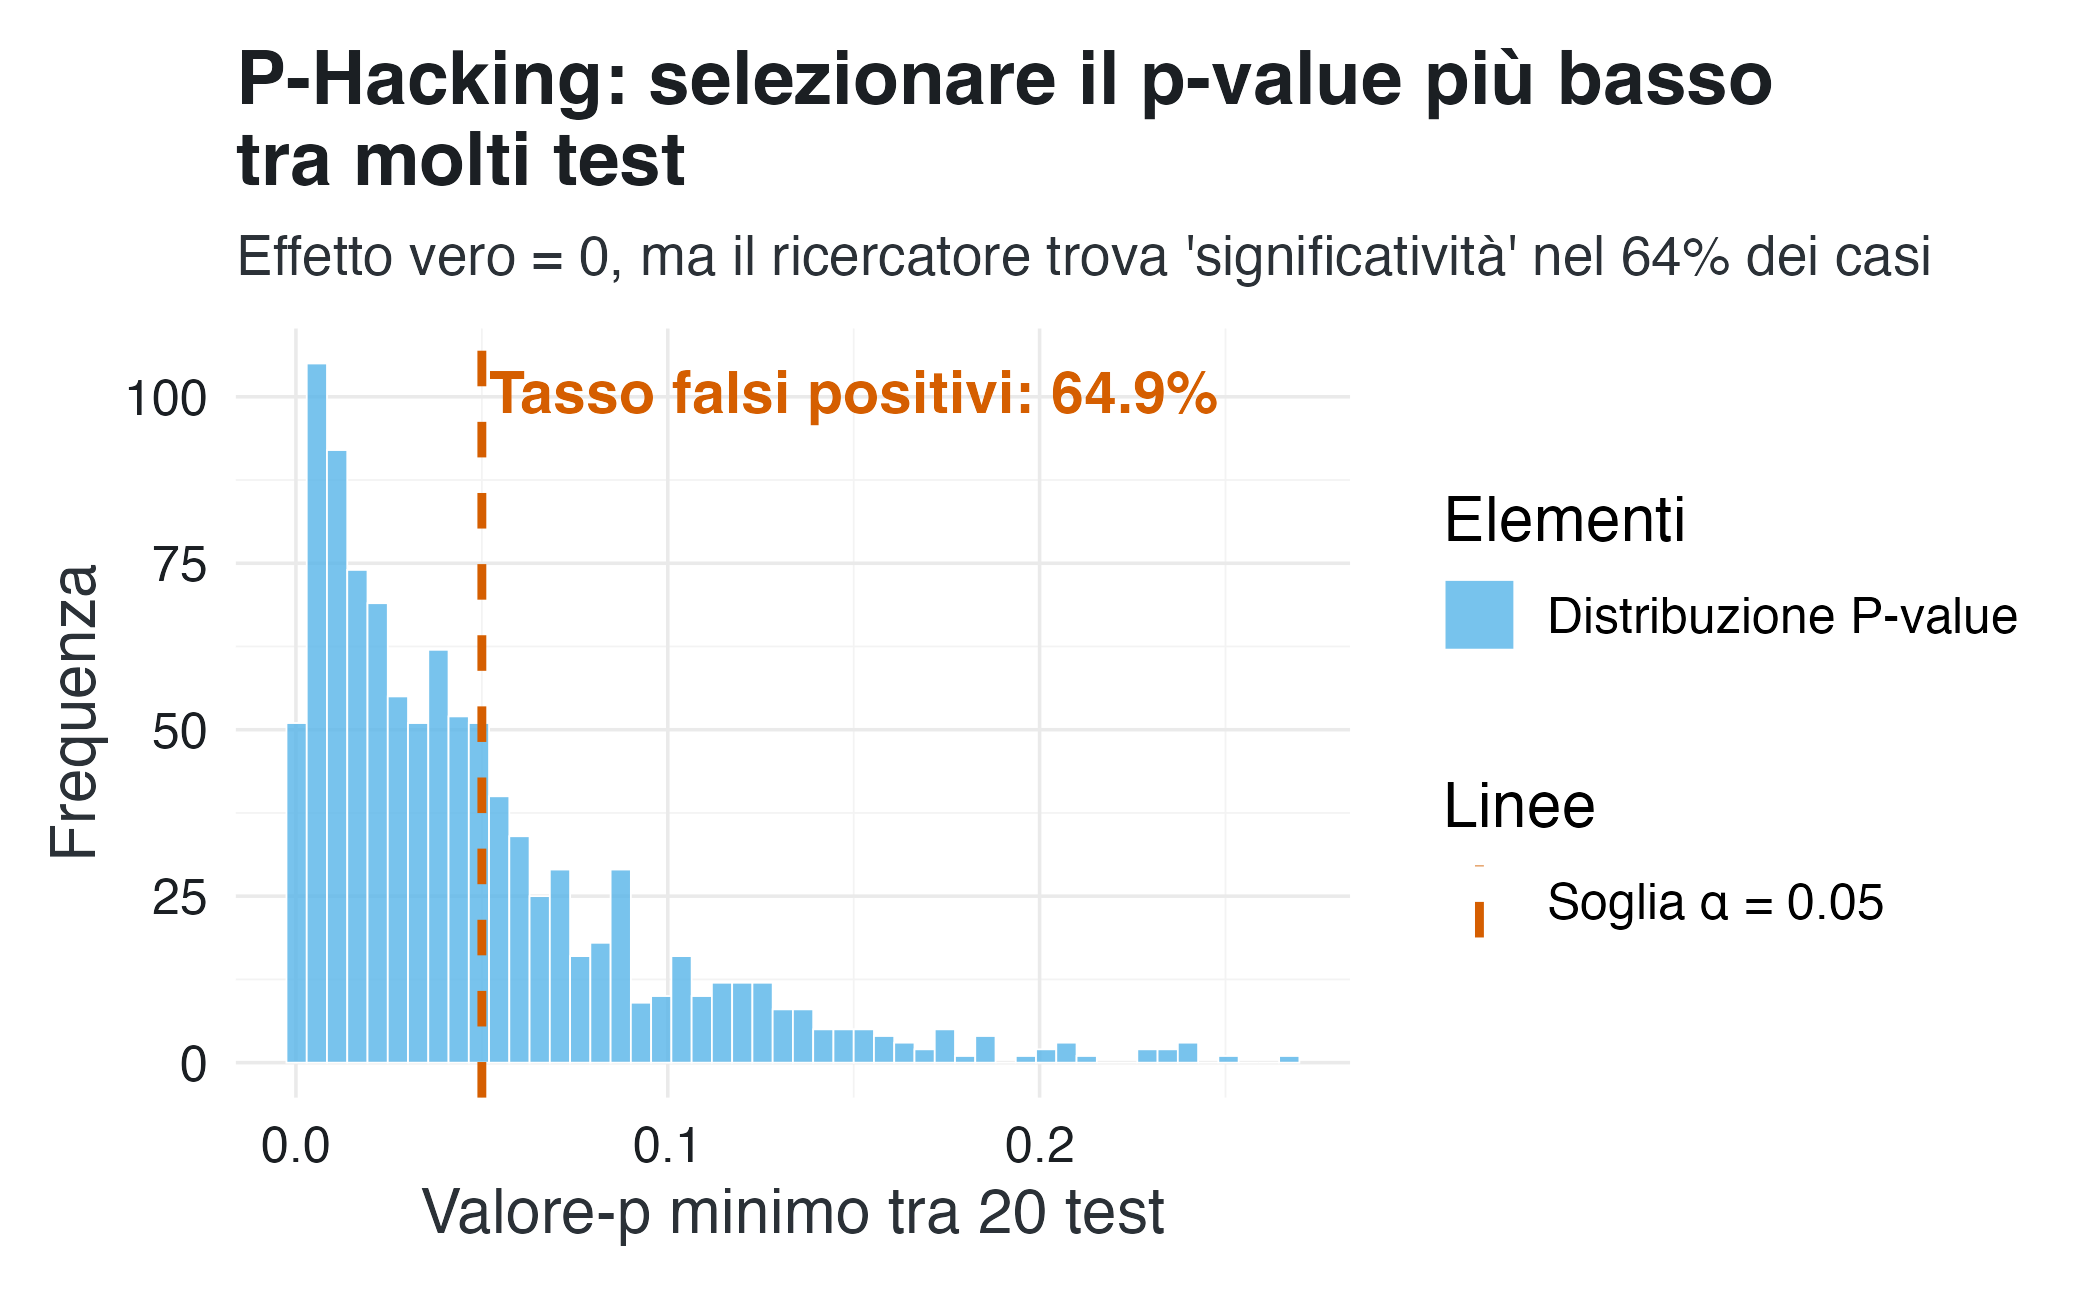
\includegraphics[width=0.85\linewidth,height=\textheight,keepaspectratio]{chapters/limits/01_limits_stat_freq_files/figure-pdf/unnamed-chunk-6-1.png}
\end{center}

\textbf{Interpretazione.} Il grafico mostra un risultato sorprendente:
\textbf{anche se l'effetto vero è esattamente zero}, selezionando il
valore-\(p\) più basso tra 20 test otteniamo un risultato
``statisticamente significativo'' (valore-\(p\) \textless{} 0.05) in
circa il \textbf{64\% dei casi}. Questo risultato è ben lontano dal
livello nominale del 5\% che corrisponde all'errore di II tipo.

Il risultato che abbiamo ottenuto può essere calcolato analiticamente:
la probabilità di ottenere almeno un valore-\(p\) \textless{} 0.05 in 20
test indipendenti è: \[
P(\text{almeno un falso positivo}) = 1 - P(\text{nessun falso positivo})
\] Se ogni test è indipendente e l'ipotesi nulla è vera: \[
P(\text{nessun falso positivo in 20 test}) = (1 - 0.05)^{20} = 0.95^{20} \approx 0.3585.
\] Se la probabilità di \emph{nessun} falso positivo è circa 0.3585,
allora la probabilità dell'evento complementare (\emph{almeno un} falso
positivo) è:
\begin{align}
P(\text{almeno un falso positivo}) &= 1 - P(\text{nessun falso positivo}) \notag\\
&= 1 - 0.3585 \approx 0.6415 
\end{align}
ovvero \[
P(\text{almeno un falso positivo}) = 1 - (1 - 0.05)^{20} \approx 0.64.
\]

In conclusione, il \textbf{P-Hacking trasforma un tasso di errore del
5\% in un tasso di errore del 64\%}.

\begin{tcolorbox}[enhanced jigsaw, arc=.35mm, bottomrule=.15mm, bottomtitle=1mm, breakable, colback=white, colbacktitle=quarto-callout-note-color!10!white, colframe=quarto-callout-note-color-frame, coltitle=black, left=2mm, leftrule=.75mm, opacityback=0, opacitybacktitle=0.6, rightrule=.15mm, title=\textcolor{quarto-callout-note-color}{\faInfo}\hspace{0.5em}{Riflessione}, titlerule=0mm, toprule=.15mm, toptitle=1mm]

Questo scenario non richiede necessariamente malafede. Un ricercatore
potrebbe sinceramente credere che alcune analisi siano ``migliori'' di
altre e, \textbf{inconsapevolmente}, finire per selezionare quella che
produce il risultato desiderato. Il problema è \textbf{strutturale, non
morale}.

\end{tcolorbox}

\section{\texorpdfstring{Simulazione 2: la distribuzione sospetta dei
valori-\(p\)}{Simulazione 2: la distribuzione sospetta dei valori-p}}\label{simulazione-2-la-distribuzione-sospetta-dei-valori-p}

Se il \(p\)-hacking fosse diffuso nella letteratura scientifica, ci si
aspetterebbe di osservare un'anomalia nella distribuzione dei
valori-\(p\) riportati: \textbf{un eccesso di valori appena sotto la
soglia di 0.05}. Questo fenomeno è stato effettivamente documentato in
analisi su larga scala della letteratura psicologica, economica e
biomedica.

Simuliamo due scenari per comprendere cosa dovremmo osservare in una
letteratura ``sana'' (priva di pratiche selettive) rispetto a una
``contaminata'' da \(p\)-hacking.

Parametri della simulazione:

\begin{Shaded}
\begin{Highlighting}[]
\NormalTok{n\_studies }\OtherTok{\textless{}{-}} \DecValTok{5000}
\NormalTok{n\_per\_group }\OtherTok{\textless{}{-}} \DecValTok{50}
\end{Highlighting}
\end{Shaded}

\textbf{Scenario 1: letteratura onesta.} Nella letteratura onesta,
assumiamo che il 50\% degli studi esamini l'ipotesi nulla quando
l'effetto vero è moderato (\(d\) = 0.3) e il 50\% degli studi esamini
l'ipotesi nulla quando l'effetto vero è zero (\(d\) = 0). Tutti i
risultati vengono riportati, a prescindere dal valore-\(p\) ottenuto nel
test \(t\) di Student:

\begin{Shaded}
\begin{Highlighting}[]
\NormalTok{simulate\_honest\_literature }\OtherTok{\textless{}{-}} \ControlFlowTok{function}\NormalTok{() \{}
\NormalTok{  has\_true\_effect }\OtherTok{\textless{}{-}} \FunctionTok{sample}\NormalTok{(}\FunctionTok{c}\NormalTok{(}\ConstantTok{TRUE}\NormalTok{, }\ConstantTok{FALSE}\NormalTok{), }\DecValTok{1}\NormalTok{)}
\NormalTok{  true\_d }\OtherTok{\textless{}{-}} \FunctionTok{ifelse}\NormalTok{(has\_true\_effect, }\FloatTok{0.3}\NormalTok{, }\DecValTok{0}\NormalTok{)}
  
\NormalTok{  group1 }\OtherTok{\textless{}{-}} \FunctionTok{rnorm}\NormalTok{(n\_per\_group, }\AttributeTok{mean =} \DecValTok{0}\NormalTok{, }\AttributeTok{sd =} \DecValTok{1}\NormalTok{)}
\NormalTok{  group2 }\OtherTok{\textless{}{-}} \FunctionTok{rnorm}\NormalTok{(n\_per\_group, }\AttributeTok{mean =}\NormalTok{ true\_d, }\AttributeTok{sd =} \DecValTok{1}\NormalTok{)}
  
  \FunctionTok{t.test}\NormalTok{(group1, group2)}\SpecialCharTok{$}\NormalTok{p.value}
\NormalTok{\}}

\NormalTok{honest\_pvalues }\OtherTok{\textless{}{-}} \FunctionTok{replicate}\NormalTok{(n\_studies, }\FunctionTok{simulate\_honest\_literature}\NormalTok{())}
\end{Highlighting}
\end{Shaded}

\textbf{Scenario 2: letteratura con \(p\)-hacking}. Consideriamo gli
stessi presupposti scientifici del caso precedente: il 50\% degli
effetti è vero, il 50\% è nullo. In questo caso, però, i ricercatori
provano 10 diverse analisi sui dati. Se in una di queste analisi trovano
un valore-\(p\) \textless{} 0.5 riportano quello, altrimenti riportano
l'ultimo valore-\(p\) calcolato.

\begin{Shaded}
\begin{Highlighting}[]
\NormalTok{simulate\_phacked\_literature }\OtherTok{\textless{}{-}} \ControlFlowTok{function}\NormalTok{() \{}
\NormalTok{  has\_true\_effect }\OtherTok{\textless{}{-}} \FunctionTok{sample}\NormalTok{(}\FunctionTok{c}\NormalTok{(}\ConstantTok{TRUE}\NormalTok{, }\ConstantTok{FALSE}\NormalTok{), }\DecValTok{1}\NormalTok{)}
\NormalTok{  true\_d }\OtherTok{\textless{}{-}} \FunctionTok{ifelse}\NormalTok{(has\_true\_effect, }\FloatTok{0.3}\NormalTok{, }\DecValTok{0}\NormalTok{)}
  
  \CommentTok{\# Il ricercatore prova fino a 10 varianti dell\textquotesingle{}analisi}
  \ControlFlowTok{for}\NormalTok{ (attempt }\ControlFlowTok{in} \DecValTok{1}\SpecialCharTok{:}\DecValTok{10}\NormalTok{) \{}
\NormalTok{    group1 }\OtherTok{\textless{}{-}} \FunctionTok{rnorm}\NormalTok{(n\_per\_group, }\AttributeTok{mean =} \DecValTok{0}\NormalTok{, }\AttributeTok{sd =} \DecValTok{1}\NormalTok{)}
\NormalTok{    group2 }\OtherTok{\textless{}{-}} \FunctionTok{rnorm}\NormalTok{(n\_per\_group, }\AttributeTok{mean =}\NormalTok{ true\_d, }\AttributeTok{sd =} \DecValTok{1}\NormalTok{)}
    
\NormalTok{    p }\OtherTok{\textless{}{-}} \FunctionTok{t.test}\NormalTok{(group1, group2)}\SpecialCharTok{$}\NormalTok{p.value}
    
    \CommentTok{\# Se trova significatività, si ferma}
    \ControlFlowTok{if}\NormalTok{ (p }\SpecialCharTok{\textless{}} \FloatTok{0.05}\NormalTok{) }\FunctionTok{return}\NormalTok{(p)}
\NormalTok{  \}}
  
  \CommentTok{\# Se dopo 10 tentativi non trova nulla, riporta l\textquotesingle{}ultimo p{-}value}
  \FunctionTok{return}\NormalTok{(p)}
\NormalTok{\}}

\NormalTok{phacked\_pvalues }\OtherTok{\textless{}{-}} \FunctionTok{replicate}\NormalTok{(n\_studies, }\FunctionTok{simulate\_phacked\_literature}\NormalTok{())}
\end{Highlighting}
\end{Shaded}

Filtriamo solo i valori-\(p\) ``pubblicabili'' (\textless{} 0.10) per
ottenere una visualizzazione chiara intorno alla soglia critica:

\begin{Shaded}
\begin{Highlighting}[]
\CommentTok{\# Grafico A: Letteratura senza distorsioni}
\NormalTok{p1 }\OtherTok{\textless{}{-}} \FunctionTok{tibble}\NormalTok{(}\AttributeTok{p\_value =}\NormalTok{ honest\_pvalues) }\SpecialCharTok{|\textgreater{}}
  \FunctionTok{filter}\NormalTok{(p\_value }\SpecialCharTok{\textless{}} \FloatTok{0.10}\NormalTok{) }\SpecialCharTok{|\textgreater{}}
  \FunctionTok{ggplot}\NormalTok{(}\FunctionTok{aes}\NormalTok{(}\AttributeTok{x =}\NormalTok{ p\_value)) }\SpecialCharTok{+}
  \FunctionTok{geom\_histogram}\NormalTok{(}\FunctionTok{aes}\NormalTok{(}\AttributeTok{fill =} \StringTok{"Distribuzione P{-}value"}\NormalTok{), }
                 \AttributeTok{bins =} \DecValTok{40}\NormalTok{, }\AttributeTok{color =} \StringTok{"white"}\NormalTok{, }\AttributeTok{alpha =} \FloatTok{0.8}\NormalTok{) }\SpecialCharTok{+}
  \FunctionTok{geom\_vline}\NormalTok{(}\FunctionTok{aes}\NormalTok{(}\AttributeTok{xintercept =} \FloatTok{0.05}\NormalTok{, }\AttributeTok{color =} \StringTok{"Soglia α = 0.05"}\NormalTok{), }
             \AttributeTok{linetype =} \StringTok{"dashed"}\NormalTok{, }\AttributeTok{linewidth =} \DecValTok{1}\NormalTok{) }\SpecialCharTok{+}
  \FunctionTok{labs}\NormalTok{(}
    \AttributeTok{title =} \StringTok{"A) Letteratura senza distorsioni"}\NormalTok{,}
    \AttributeTok{x =} \StringTok{"Valore{-}p"}\NormalTok{,}
    \AttributeTok{y =} \StringTok{"Frequenza"}\NormalTok{,}
    \AttributeTok{fill =} \StringTok{"Elementi"}\NormalTok{,}
    \AttributeTok{color =} \StringTok{"Linee"}
\NormalTok{  ) }\SpecialCharTok{+}
  \FunctionTok{scale\_x\_continuous}\NormalTok{(}\AttributeTok{breaks =} \FunctionTok{seq}\NormalTok{(}\DecValTok{0}\NormalTok{, }\FloatTok{0.10}\NormalTok{, }\FloatTok{0.01}\NormalTok{)) }\SpecialCharTok{+}
  \FunctionTok{theme}\NormalTok{(}\AttributeTok{axis.text.x =} \FunctionTok{element\_text}\NormalTok{(}\AttributeTok{angle =} \DecValTok{45}\NormalTok{, }\AttributeTok{hjust =} \DecValTok{1}\NormalTok{)) }\SpecialCharTok{+}
  \FunctionTok{scale\_fill\_manual}\NormalTok{(}\AttributeTok{values =} \FunctionTok{c}\NormalTok{(}\StringTok{"Distribuzione P{-}value"} \OtherTok{=}\NormalTok{ palette\_qualitative[}\DecValTok{2}\NormalTok{])) }\SpecialCharTok{+} 
  \FunctionTok{scale\_color\_manual}\NormalTok{(}\AttributeTok{values =} \FunctionTok{c}\NormalTok{(}\StringTok{"Soglia α = 0.05"} \OtherTok{=}\NormalTok{ palette\_qualitative[}\DecValTok{6}\NormalTok{])) }
\end{Highlighting}
\end{Shaded}

\begin{Shaded}
\begin{Highlighting}[]
\CommentTok{\# Grafico B: Letteratura con p{-}hacking}
\NormalTok{p2 }\OtherTok{\textless{}{-}} \FunctionTok{tibble}\NormalTok{(}\AttributeTok{p\_value =}\NormalTok{ phacked\_pvalues) }\SpecialCharTok{|\textgreater{}}
  \FunctionTok{filter}\NormalTok{(p\_value }\SpecialCharTok{\textless{}} \FloatTok{0.10}\NormalTok{) }\SpecialCharTok{|\textgreater{}}
  \FunctionTok{ggplot}\NormalTok{(}\FunctionTok{aes}\NormalTok{(}\AttributeTok{x =}\NormalTok{ p\_value)) }\SpecialCharTok{+}
  \FunctionTok{geom\_histogram}\NormalTok{(}\FunctionTok{aes}\NormalTok{(}\AttributeTok{fill =} \StringTok{"Distribuzione P{-}value"}\NormalTok{), }
                 \AttributeTok{bins =} \DecValTok{40}\NormalTok{, }\AttributeTok{color =} \StringTok{"white"}\NormalTok{, }\AttributeTok{alpha =} \FloatTok{0.8}\NormalTok{) }\SpecialCharTok{+}
  \FunctionTok{geom\_vline}\NormalTok{(}\FunctionTok{aes}\NormalTok{(}\AttributeTok{xintercept =} \FloatTok{0.05}\NormalTok{, }\AttributeTok{color =} \StringTok{"Soglia α = 0.05"}\NormalTok{), }
             \AttributeTok{linetype =} \StringTok{"dashed"}\NormalTok{, }\AttributeTok{linewidth =} \DecValTok{1}\NormalTok{) }\SpecialCharTok{+}
  \FunctionTok{labs}\NormalTok{(}
    \AttributeTok{title =} \StringTok{"B) Letteratura con p{-}hacking"}\NormalTok{,}
    \AttributeTok{x =} \StringTok{"Valore{-}p"}\NormalTok{,}
    \AttributeTok{y =} \StringTok{"Frequenza"}\NormalTok{,}
    \AttributeTok{fill =} \StringTok{"Elementi"}\NormalTok{,}
    \AttributeTok{color =} \StringTok{"Linee"}
\NormalTok{  ) }\SpecialCharTok{+}
  \FunctionTok{scale\_x\_continuous}\NormalTok{(}\AttributeTok{breaks =} \FunctionTok{seq}\NormalTok{(}\DecValTok{0}\NormalTok{, }\FloatTok{0.10}\NormalTok{, }\FloatTok{0.01}\NormalTok{)) }\SpecialCharTok{+}
  \FunctionTok{theme}\NormalTok{(}\AttributeTok{axis.text.x =} \FunctionTok{element\_text}\NormalTok{(}\AttributeTok{angle =} \DecValTok{45}\NormalTok{, }\AttributeTok{hjust =} \DecValTok{1}\NormalTok{)) }\SpecialCharTok{+}
  \FunctionTok{scale\_fill\_manual}\NormalTok{(}\AttributeTok{values =} \FunctionTok{c}\NormalTok{(}\StringTok{"Distribuzione P{-}value"} \OtherTok{=}\NormalTok{ palette\_qualitative[}\DecValTok{6}\NormalTok{])) }\SpecialCharTok{+} 
  \FunctionTok{scale\_color\_manual}\NormalTok{(}\AttributeTok{values =} \FunctionTok{c}\NormalTok{(}\StringTok{"Soglia α = 0.05"} \OtherTok{=}\NormalTok{ palette\_qualitative[}\DecValTok{6}\NormalTok{])) }
\end{Highlighting}
\end{Shaded}

\begin{Shaded}
\begin{Highlighting}[]
\NormalTok{p1 }\SpecialCharTok{+}\NormalTok{ p2 }\SpecialCharTok{+}
  \FunctionTok{plot\_layout}\NormalTok{(}\AttributeTok{guides =} \StringTok{"collect"}\NormalTok{) }\SpecialCharTok{\&}
  \FunctionTok{theme}\NormalTok{(}
    \AttributeTok{legend.position =} \StringTok{"bottom"}\NormalTok{,}
    \AttributeTok{legend.box =} \StringTok{"horizontal"}
\NormalTok{  )}
\end{Highlighting}
\end{Shaded}

\begin{figure}[H]

\centering{

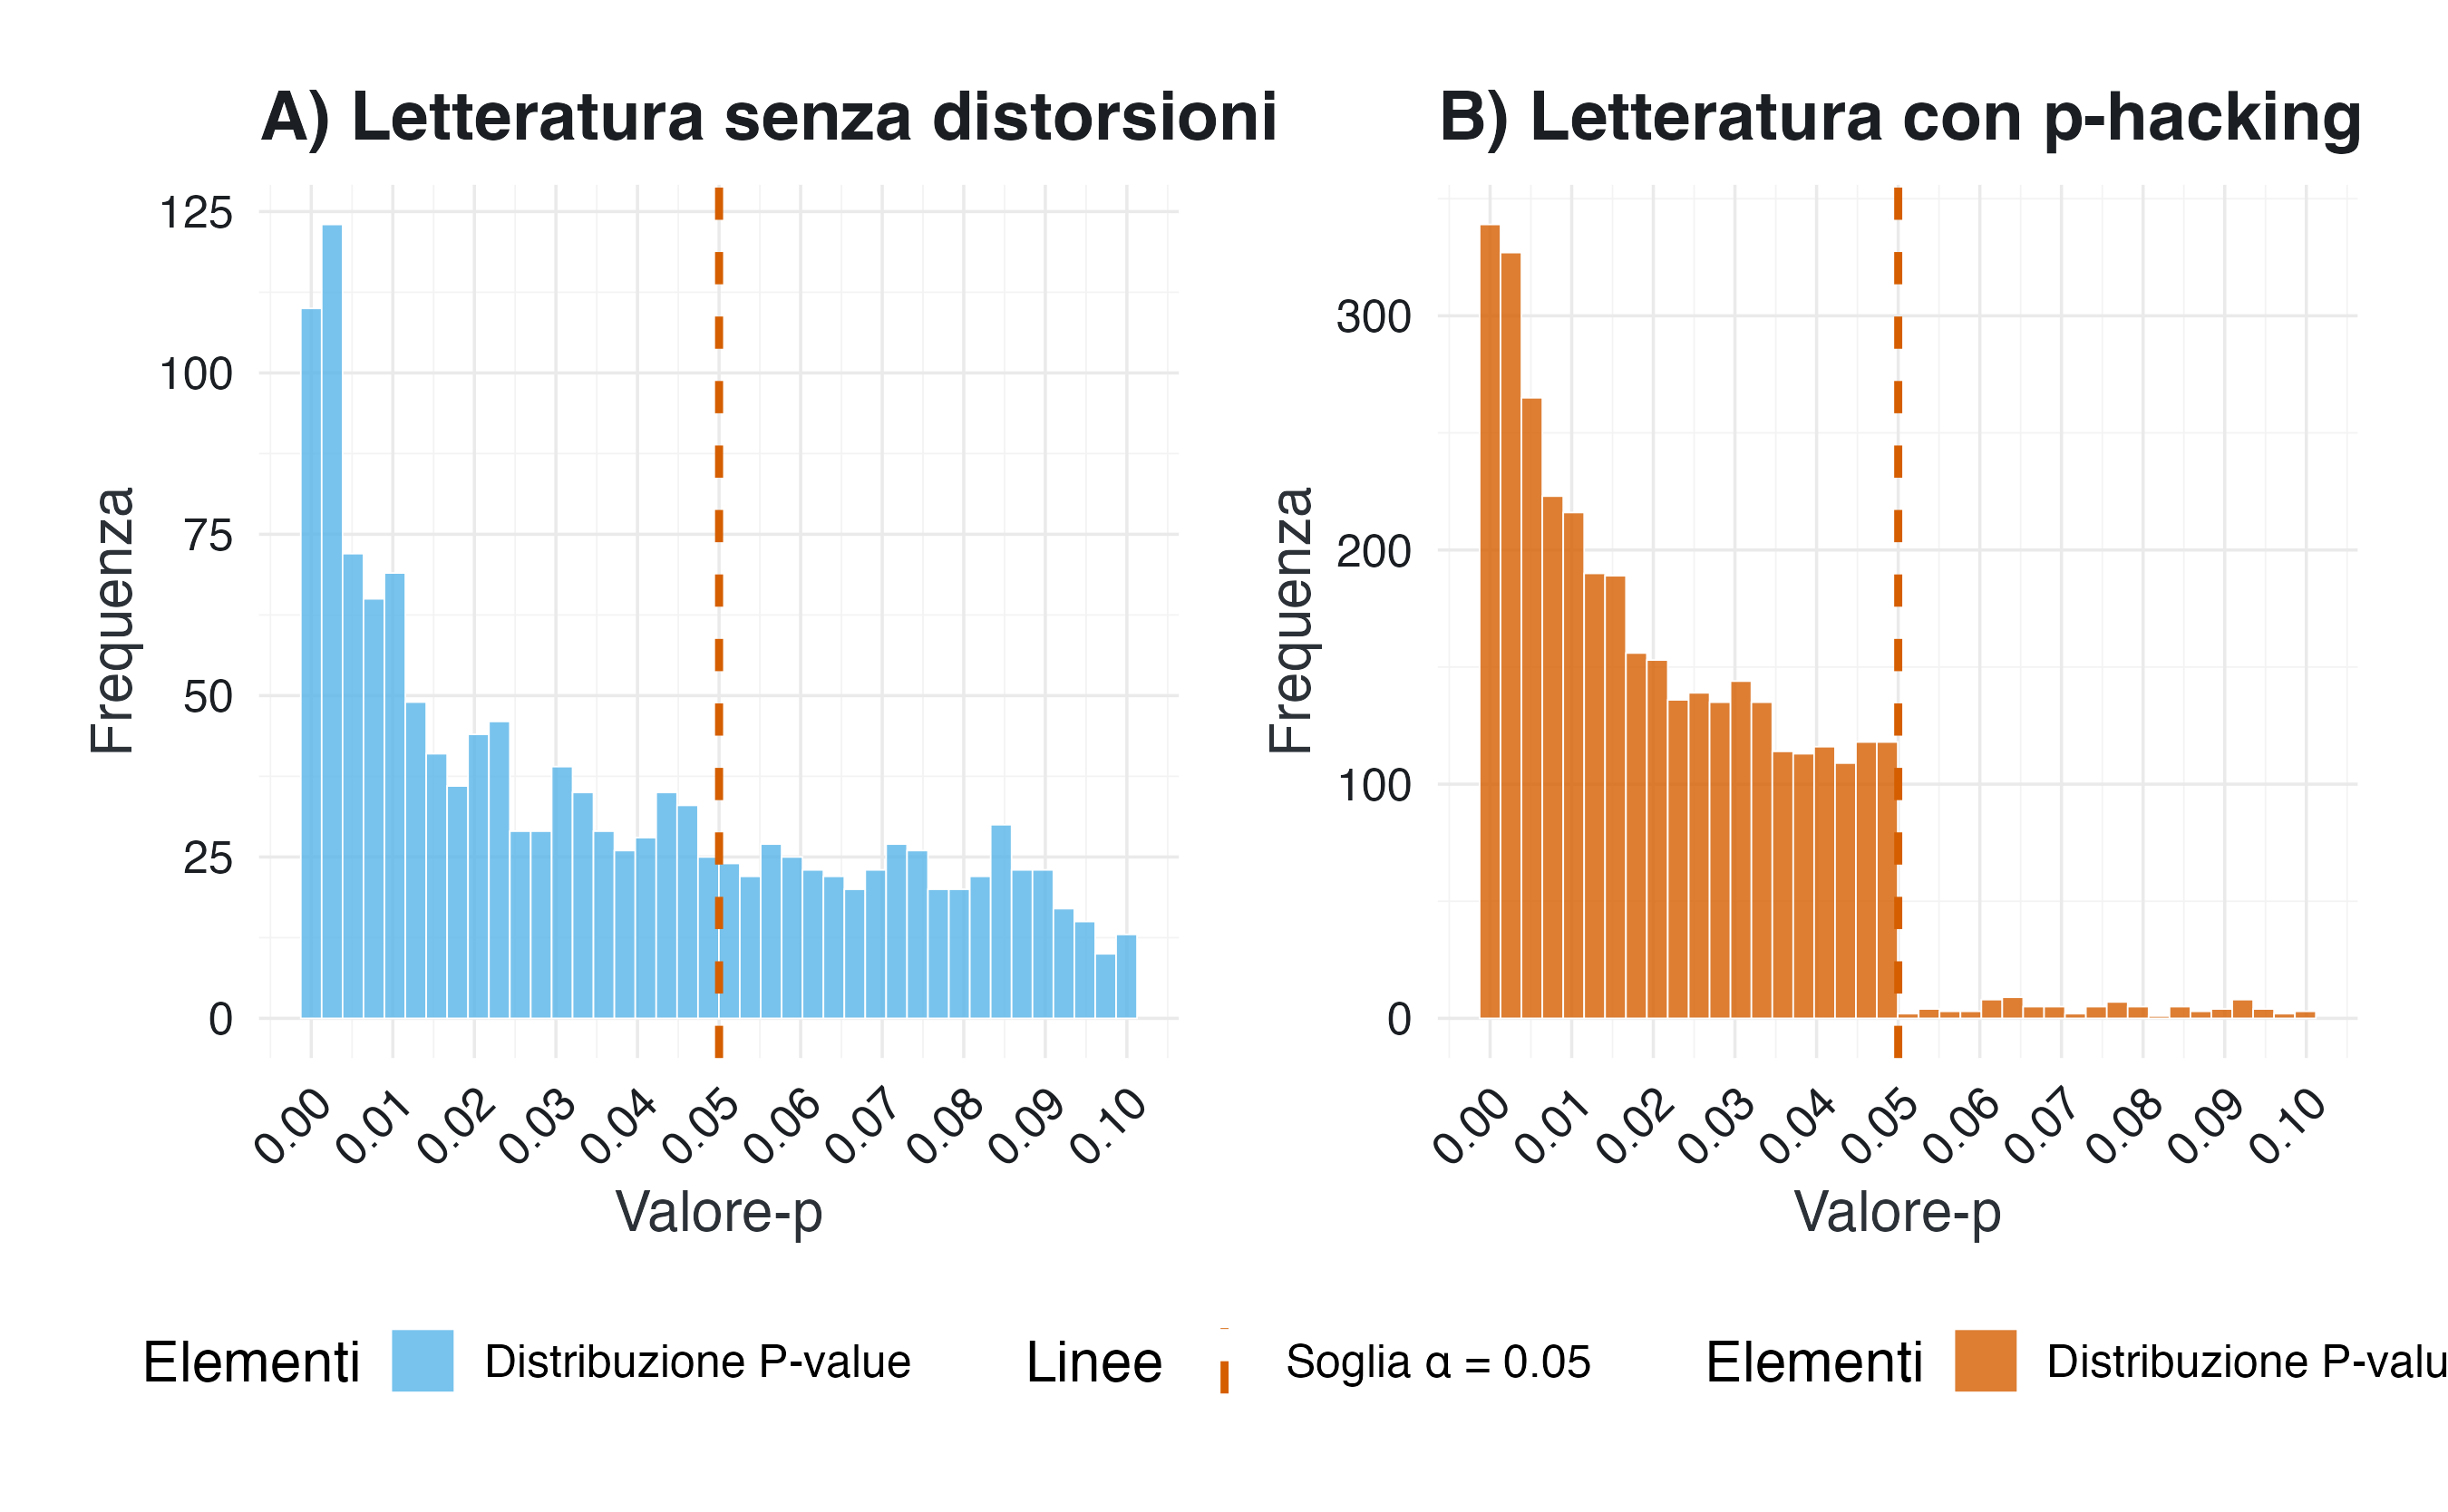
\includegraphics[width=0.85\linewidth,height=\textheight,keepaspectratio]{chapters/limits/01_limits_stat_freq_files/figure-pdf/fig-pvalue-distribution-1.png}

}

\caption{\label{fig-pvalue-distribution}Confronto tra la distribuzione
teorica dei p-value e quella distorta dalla selezione.}

\end{figure}%

Calcoliamo il rapporto tra valore-\(p\) appena sotto vs appena sopra lo
0.05:

\begin{Shaded}
\begin{Highlighting}[]
\NormalTok{ratio\_honest }\OtherTok{\textless{}{-}} \FunctionTok{sum}\NormalTok{(honest\_pvalues }\SpecialCharTok{\textgreater{}} \FloatTok{0.04} \SpecialCharTok{\&}\NormalTok{ honest\_pvalues }\SpecialCharTok{\textless{}} \FloatTok{0.05}\NormalTok{) }\SpecialCharTok{/} 
                \FunctionTok{sum}\NormalTok{(honest\_pvalues }\SpecialCharTok{\textgreater{}} \FloatTok{0.05} \SpecialCharTok{\&}\NormalTok{ honest\_pvalues }\SpecialCharTok{\textless{}} \FloatTok{0.06}\NormalTok{)}

\NormalTok{ratio\_phacked }\OtherTok{\textless{}{-}} \FunctionTok{sum}\NormalTok{(phacked\_pvalues }\SpecialCharTok{\textgreater{}} \FloatTok{0.04} \SpecialCharTok{\&}\NormalTok{ phacked\_pvalues }\SpecialCharTok{\textless{}} \FloatTok{0.05}\NormalTok{) }\SpecialCharTok{/} 
                 \FunctionTok{sum}\NormalTok{(phacked\_pvalues }\SpecialCharTok{\textgreater{}} \FloatTok{0.05} \SpecialCharTok{\&}\NormalTok{ phacked\_pvalues }\SpecialCharTok{\textless{}} \FloatTok{0.06}\NormalTok{)}
\end{Highlighting}
\end{Shaded}

\begin{Shaded}
\begin{Highlighting}[]
\CommentTok{\# echo: false}
\FunctionTok{cat}\NormalTok{(}\StringTok{"Rapporto p{-}value [0.04{-}0.05] / [0.05{-}0.06]:}\SpecialCharTok{\textbackslash{}n}\StringTok{"}\NormalTok{)}
\CommentTok{\#\textgreater{} Rapporto p{-}value [0.04{-}0.05] / [0.05{-}0.06]:}
\FunctionTok{cat}\NormalTok{(}\FunctionTok{sprintf}\NormalTok{(}\StringTok{"  Letteratura onesta: \%.2f}\SpecialCharTok{\textbackslash{}n}\StringTok{"}\NormalTok{, ratio\_honest))}
\CommentTok{\#\textgreater{}   Letteratura onesta: 1.27}
\FunctionTok{cat}\NormalTok{(}\FunctionTok{sprintf}\NormalTok{(}\StringTok{"  Letteratura con p{-}hacking: \%.2f}\SpecialCharTok{\textbackslash{}n}\StringTok{"}\NormalTok{, ratio\_phacked))}
\CommentTok{\#\textgreater{}   Letteratura con p{-}hacking: 41.00}
\end{Highlighting}
\end{Shaded}

\textbf{Interpretazione.} Il confronto tra i due scenari rivela pattern
distintivi che fungono da indicatori della salute metodologica di una
letteratura scientifica.

Nel primo scenario, che rappresenta una letteratura scientifica senza
distorsioni, i valori-\(p\) si distribuiscono in modo relativamente
uniforme nella regione intorno alla soglia di 0.05. Questa distribuzione
riflette l'assenza di manipolazioni selettive: non vi è nulla di
statisticamente ``speciale'' nella soglia convenzionale di
significatività. Il rapporto tra valori appena sotto e appena sopra 0.05
si attesta intorno a 1.0, dimostrando una continuità naturale nella
distribuzione. Circa il 25-30\% degli studi risulta statisticamente
significativo, una proporzione che corrisponde alle aspettative basate
sui parametri della simulazione, in cui metà degli studi esamina ipotesi
con effetto vero presente e l'altra metà esamina ipotesi con effetto
vero nullo.

Il secondo scenario, che simula una letteratura contaminata da
\(p\)-hacking, presenta caratteristiche marcate e preoccupanti. Si
osserva un evidente picco anomalo di valori-\(p\) concentrati
immediatamente sotto la soglia di 0.05. Questa concentrazione crea una
discontinuità statistica pronunciata: i valori appena sotto la soglia
sono numericamente molto superiori a quelli appena sopra. Il rapporto
tra queste due regioni supera 3.0, indicando una distorsione sostanziale
nella restituzione dei risultati. Inoltre, oltre il 50\% degli studi
risulta ``statisticamente significativo'', una proporzione notevolmente
superiore a quella che ci si aspetterebbe in base ai parametri della
simulazione. Questa discrepanza segnala come il \(p\)-hacking possa far
apparire artificialmente la letteratura più solida di quanto non lo sia
in realtà.

\subsection{Evidenze empiriche nella letteratura
scientifica}\label{evidenze-empiriche-nella-letteratura-scientifica}

I pattern emersi dalla simulazione trovano riscontro nelle analisi
empiriche condotte su ampi corpora di letteratura scientifica. Le
anomalie distributive osservate sperimentalmente non sono mere
astrazioni teoriche, ma documentano fenomeni sistematicamente rilevati
attraverso indagini bibliometriche su larga scala.

Nell'ambito delle scienze psicologiche, l'analisi di Head et al.
(\citeproc{ref-head2015extent}{2015}) su 12.000 articoli ha evidenziato
una discontinuità statistica particolarmente marcata: i valori-\(p\)
pari a 0.049 si verificano con una frequenza superiore del 300\%
rispetto a quelli immediatamente adiacenti pari a 0.051. Una tale
asimmetria concentrata in prossimità della soglia canonica di
significatività non può essere attribuita a fluttuazioni casuali, ma
denota con elevata probabilità un processo selettivo nella presentazione
dei risultati.

Evidenze analoghe emergono anche dalle scienze economiche, dove Brodeur
et al. (\citeproc{ref-brodeur2020methods}{2020}) hanno riscontrato
anomalie distributive riconducibili a pratiche di \(p\)-hacking. La
distribuzione dei valori-p negli studi pubblicati presenta picchi
statisticamente significativi in corrispondenza esatta delle soglie
convenzionali di riferimento (0.01, 0.05 e 0.10). Questa regolarità,
osservata trasversalmente su diverse riviste e periodi temporali,
suggerisce l'esistenza di un meccanismo sistemico di adattamento dei
risultati ai benchmark metodologici predefiniti.

La pervasività di queste distorsioni ha stimolato lo sviluppo di
strumenti analitici specifici per la loro rilevazione e quantificazione.
Simonsohn et al. (\citeproc{ref-simonsohn2014p}{2014}) hanno
formalizzato la ``p-curve analysis'', una metodologia che sfrutta la
distribuzione dei valori-\(p\) per distinguere la letteratura
caratterizzata da effetti genuini da quella influenzata da pratiche
selettive. Questo approccio non solo consente di identificare i campi di
ricerca potenzialmente affetti da \(p\)-hacking, ma anche di stimare la
probabilità che un insieme di risultati significativi rifletta
effettivamente effetti reali piuttosto che artefatti statistici.

\subsection{Implicazioni pratiche per la ricerca
scientifica}\label{implicazioni-pratiche-per-la-ricerca-scientifica}

La discontinuità nella distribuzione dei valori-p funge da vero e
proprio ``termometro della credibilità'' per interi campi di ricerca.
Questo indicatore consente di rilevare problematiche sistemiche: analisi
bibliometriche sofisticate possono individuare discipline o aree di
ricerca che presentano forti evidenze di \(p\)-hacking. Allo stesso
tempo, tale metrica può essere utilizzata per monitorare i progressi
metodologici: in seguito all'adozione diffusa di pratiche di ricerca
aperta e trasparente, ci si aspetterebbe una riduzione progressiva di
queste distorsioni. Dal punto di vista interpretativo, nei campi
caratterizzati da forti distorsioni, i risultati marginalmente
significativi (con valori-\(p\) prossimi a 0.05) richiedono
un'interpretazione particolarmente cauta e scettica.

La consapevolezza di questa ``impronta digitale'' statistica ha motivato
e accelerato importanti riforme metodologiche nel panorama scientifico
contemporaneo. Tra queste innovazioni, si possono citare la
preregistrazione degli studi, che vincola i ricercatori a piani
analitici predeterminati, l'adozione sistematica di correzioni per i
confronti multipli, che riducono il rischio di falsi positivi, e una
maggiore trasparenza nella comunicazione dei risultati, che include la
condivisione di dati e codici analitici. Queste pratiche, sempre più
diffuse, rappresentano risposte concrete al problema del \(p\)-hacking e
contribuiscono a rafforzare l'affidabilità cumulativa della conoscenza
scientifica.

\section{Simulazione 3: il grande
equivoco}\label{simulazione-3-il-grande-equivoco}

Nella pratica della ricerca, i ricercatori utilizzano comunemente il
valore-\(p\) per valutare se un effetto ``esiste''. Ma quanto è
affidabile questa inferenza? La simulazione che segue ci aiuta a
comprendere la differenza cruciale tra ciò che il valore-\(p\) misura
realmente e ciò che i ricercatori spesso credono che misuri.

Uno degli equivoci più diffusi nella psicologia empirica consiste nel
ritenere che un valore-\(p\) di 0.03 indichi che \emph{esiste solo il
3\% di probabilità che l'ipotesi nulla sia vera}, oppure, in modo
complementare, che \emph{vi sia il 97\% di probabilità che l'effetto
esista}. Questa lettura è intuitiva, ma completamente sbagliata dal
punto di vista matematico.

\subsection{\texorpdfstring{Che cosa misura davvero il
valore-\(p\)?}{Che cosa misura davvero il valore-p?}}\label{che-cosa-misura-davvero-il-valore-p}

Il valore-\(p\) indica la probabilità di ottenere dati almeno
altrettanto estremi di quelli osservati \textbf{sotto l'assunzione che
l'ipotesi nulla sia vera}. Formalmente:

\[
p = P(\text{dati osservati o più estremi} \mid H_0).
\] Dunque il valore-\(p\) non esprime la probabilità che un'ipotesi sia
vera o falsa. Più modestamente, quantifica \textbf{la compatibilità dei
dati con l'ipotesi nulla}.

\subsection{Perché l'interpretazione intuitiva è
sbagliata}\label{perchuxe9-linterpretazione-intuitiva-uxe8-sbagliata}

L'errore nasce dalla confusione tra due probabilità condizionate
opposte:

\[
P(\text{Dati} \mid H_0) \neq P(H_0 \mid \text{Dati}).
\]

Il teorema di Bayes chiarisce la differenza:

\[
P(H_0 \mid \text{Dati}) = \frac{P(\text{Dati} \mid H_0), P(H_0)}{P(\text{Dati})}.
\]

Per ottenere la probabilità che l'ipotesi nulla sia vera \textbf{dopo
aver visto i dati}, è indispensabile conoscere anche due quantità
ignorate dall'approccio del valore-\(p\):

\begin{itemize}
\tightlist
\item
  la \textbf{plausibilità a priori} dell'ipotesi, \(P(H_0)\);
\item
  la \textbf{probabilità dei dati sotto l'ipotesi alternativa},
  \(P(\text{Dati} \mid H_1)\), cioè la potenza statistica del test,
  ovvero la probabilità che, se l'ipotesi \(H_1\) è vera (ovvero se
  esiste un effetto), verranno effettivamente osservati dati coerenti
  con la presenza di tale effetto.
\end{itemize}

Senza queste informazioni, il valore-\(p\) non può in alcun modo
informarci sulla probabilità che un'ipotesi sia vera.

In alcuni contesti ben strutturati e ad alta potenza, un valore-\(p\) =
0.03 può sostenere l'esistenza di un effetto. Ma in scenari esplorativi,
dove le ipotesi sono speculative e gli effetti reali sono rari, lo
stesso valore-\(p\) può indicare ancora \textbf{un'alta probabilità che
l'ipotesi nulla sia vera}.

\subsection{Simulazione}\label{simulazione}

La simulazione seguente mostra concretamente questo fenomeno.

\textbf{Passo 1: impostiamo le condizioni del campo di ricerca.}

Nella simulazione, vogliamo capire se un valore-\emph{p}
``significativo'' indica davvero che l'effetto esiste. Per farlo,
immaginiamo un campo di ricerca tipicamente esplorativo dove:

\begin{Shaded}
\begin{Highlighting}[]
\NormalTok{prior\_prob\_effect }\OtherTok{\textless{}{-}} \FloatTok{0.10}   \CommentTok{\# Solo il 10\% delle ipotesi testate ha un effetto reale}
\NormalTok{n\_studies }\OtherTok{\textless{}{-}} \DecValTok{10000}          \CommentTok{\# Simuliamo un ampio corpus di studi}
\NormalTok{n\_per\_group }\OtherTok{\textless{}{-}} \DecValTok{30}           \CommentTok{\# Dimensioni campionarie tipiche}
\NormalTok{effect\_size\_if\_true }\OtherTok{\textless{}{-}} \FloatTok{0.5}  \CommentTok{\# Quando esiste, l\textquotesingle{}effetto è moderato (d = 0.5)}
\end{Highlighting}
\end{Shaded}

Queste assunzioni riflettono una realtà metodologica spesso trascurata:

\begin{itemize}
\tightlist
\item
  \textbf{prevalenza bassa di effetti reali} (10\%): in molti campi
  esplorativi, la maggior parte delle ipotesi testate non ha un effetto
  reale;
\item
  \textbf{dimensioni campionarie modeste} (n=30 per gruppo): tipiche di
  molti studi psicologici;
\item
  \textbf{effetti moderati quando presenti}: un effetto reale ha una
  grandezza clinicamente rilevante ma di entità modesta.
\end{itemize}

\textbf{Passo 2: generazione dei dati.}

\begin{Shaded}
\begin{Highlighting}[]
\FunctionTok{set.seed}\NormalTok{(}\DecValTok{123}\NormalTok{) }\CommentTok{\# Per risultati riproducibili}
\NormalTok{results }\OtherTok{\textless{}{-}} \FunctionTok{tibble}\NormalTok{(}
  \AttributeTok{study\_id =} \DecValTok{1}\SpecialCharTok{:}\NormalTok{n\_studies,}
  \AttributeTok{has\_true\_effect =} \FunctionTok{runif}\NormalTok{(n\_studies) }\SpecialCharTok{\textless{}}\NormalTok{ prior\_prob\_effect}
\NormalTok{) }\SpecialCharTok{|\textgreater{}}
  \FunctionTok{rowwise}\NormalTok{() }\SpecialCharTok{|\textgreater{}}
  \FunctionTok{mutate}\NormalTok{(}
    \AttributeTok{true\_d =} \FunctionTok{ifelse}\NormalTok{(has\_true\_effect, effect\_size\_if\_true, }\DecValTok{0}\NormalTok{),}
    \AttributeTok{p\_value =}\NormalTok{ \{}
      \CommentTok{\# Generazione dei dati: entrambi i gruppi dalla stessa distribuzione se H₀ vera}
\NormalTok{      group1 }\OtherTok{\textless{}{-}} \FunctionTok{rnorm}\NormalTok{(n\_per\_group, }\AttributeTok{mean =} \DecValTok{0}\NormalTok{, }\AttributeTok{sd =} \DecValTok{1}\NormalTok{)}
\NormalTok{      group2 }\OtherTok{\textless{}{-}} \FunctionTok{rnorm}\NormalTok{(n\_per\_group, }\AttributeTok{mean =}\NormalTok{ true\_d, }\AttributeTok{sd =} \DecValTok{1}\NormalTok{)  }\CommentTok{\# Media diversa solo se effetto reale}
      \FunctionTok{t.test}\NormalTok{(group1, group2)}\SpecialCharTok{$}\NormalTok{p.value}
\NormalTok{    \}}
\NormalTok{  ) }\SpecialCharTok{|\textgreater{}}
  \FunctionTok{ungroup}\NormalTok{()}
\end{Highlighting}
\end{Shaded}

Il processo di generazione dei dati simula due scenari distinti:

\begin{enumerate}
\def\labelenumi{\arabic{enumi}.}
\tightlist
\item
  \textbf{per il 90\% degli studi}: entrambi i gruppi provengono dalla
  stessa distribuzione (media 0, sd 1); qualsiasi differenza osservata è
  solo frutto del caso.
\item
  \textbf{per il 10\% degli studi}: il secondo gruppo ha una media
  superiore (0.5), simulando un effetto reale ma moderato.
\end{enumerate}

\textbf{Passo 3. Calcolo del Valore Predittivo Positivo.}

Il cuore della simulazione risiede nel confrontare ciò che il
valore-\(p\) suggerisce con ciò che sappiamo essere vero.

\begin{Shaded}
\begin{Highlighting}[]
\NormalTok{calculate\_ppv }\OtherTok{\textless{}{-}} \ControlFlowTok{function}\NormalTok{(data, p\_threshold) \{}
  \CommentTok{\# Seleziona solo gli studi "significativi" secondo la soglia}
\NormalTok{  significant }\OtherTok{\textless{}{-}}\NormalTok{ data }\SpecialCharTok{|\textgreater{}}\NormalTok{ dplyr}\SpecialCharTok{::}\FunctionTok{filter}\NormalTok{(p\_value }\SpecialCharTok{\textless{}}\NormalTok{ p\_threshold)}
  
  \ControlFlowTok{if}\NormalTok{ (}\FunctionTok{nrow}\NormalTok{(significant) }\SpecialCharTok{==} \DecValTok{0}\NormalTok{) }\FunctionTok{return}\NormalTok{(}\ConstantTok{NA\_real\_}\NormalTok{)}
  
  \CommentTok{\# Calcola la proporzione di veri positivi tra i significativi}
  \FunctionTok{mean}\NormalTok{(significant}\SpecialCharTok{$}\NormalTok{has\_true\_effect)}
\NormalTok{\}}

\CommentTok{\# Analizziamo diverse soglie di significatività}
\NormalTok{thresholds }\OtherTok{\textless{}{-}} \FunctionTok{c}\NormalTok{(}\FloatTok{0.05}\NormalTok{, }\FloatTok{0.01}\NormalTok{, }\FloatTok{0.005}\NormalTok{, }\FloatTok{0.001}\NormalTok{)}

\CommentTok{\# Calcolo dei PPV usando sapply}
\NormalTok{ppv\_results }\OtherTok{\textless{}{-}} \FunctionTok{tibble}\NormalTok{(}
  \AttributeTok{threshold =}\NormalTok{ thresholds,}
  \AttributeTok{ppv =} \FunctionTok{sapply}\NormalTok{(thresholds, }\ControlFlowTok{function}\NormalTok{(t) }\FunctionTok{calculate\_ppv}\NormalTok{(results, t))}
\NormalTok{)}
\end{Highlighting}
\end{Shaded}

Il PPV risponde alla domanda: ``Tra tutti i risultati statisticamente
significativi, quanti corrispondono effettivamente a effetti reali?''

\textbf{Passo 4: visualizzazione della distribuzione dei risultati.}

\begin{Shaded}
\begin{Highlighting}[]
\NormalTok{results }\SpecialCharTok{|\textgreater{}}
  \FunctionTok{filter}\NormalTok{(p\_value }\SpecialCharTok{\textless{}} \FloatTok{0.10}\NormalTok{) }\SpecialCharTok{|\textgreater{}}
  \FunctionTok{ggplot}\NormalTok{(}\FunctionTok{aes}\NormalTok{(}\AttributeTok{x =}\NormalTok{ p\_value, }\AttributeTok{fill =}\NormalTok{ has\_true\_effect)) }\SpecialCharTok{+}
  \FunctionTok{geom\_histogram}\NormalTok{(}\AttributeTok{bins =} \DecValTok{50}\NormalTok{, }\AttributeTok{position =} \StringTok{"stack"}\NormalTok{, }\AttributeTok{alpha =} \FloatTok{0.8}\NormalTok{) }\SpecialCharTok{+}
  \FunctionTok{geom\_vline}\NormalTok{(}
    \AttributeTok{xintercept =} \FloatTok{0.05}\NormalTok{,}
    \AttributeTok{color =} \StringTok{"black"}\NormalTok{,}
    \AttributeTok{linetype =} \StringTok{"dashed"}\NormalTok{,}
    \AttributeTok{linewidth =} \DecValTok{1}
\NormalTok{  ) }\SpecialCharTok{+}
  \FunctionTok{scale\_fill\_manual}\NormalTok{(}
    \AttributeTok{values =}\NormalTok{ palette\_qualitative[}\FunctionTok{c}\NormalTok{(}\DecValTok{3}\NormalTok{, }\DecValTok{6}\NormalTok{)],  }\CommentTok{\# verde + rosso{-}arancio}
    \AttributeTok{labels =} \FunctionTok{c}\NormalTok{(}
      \StringTok{"TRUE"}  \OtherTok{=} \StringTok{"Effetto vero"}\NormalTok{,}
      \StringTok{"FALSE"} \OtherTok{=} \StringTok{"Nessun effetto (falso positivo)"}
\NormalTok{    )}
\NormalTok{  ) }\SpecialCharTok{+}
  \FunctionTok{labs}\NormalTok{(}
    \AttributeTok{x =} \StringTok{"Valore{-}p"}\NormalTok{,}
    \AttributeTok{y =} \StringTok{"Numero di studi"}\NormalTok{,}
    \AttributeTok{fill =} \StringTok{"Tipo di risultato"}\NormalTok{,}
    \AttributeTok{title =} \StringTok{"Composizione degli studi \textquotesingle{}significativi\textquotesingle{}"}\NormalTok{,}
    \AttributeTok{subtitle =} \FunctionTok{sprintf}\NormalTok{(}
      \StringTok{"Prevalenza effetti reali = \%d\%\%"}\NormalTok{,}
\NormalTok{      prior\_prob\_effect }\SpecialCharTok{*} \DecValTok{100}
\NormalTok{    )}
\NormalTok{  )}
\end{Highlighting}
\end{Shaded}

\begin{center}
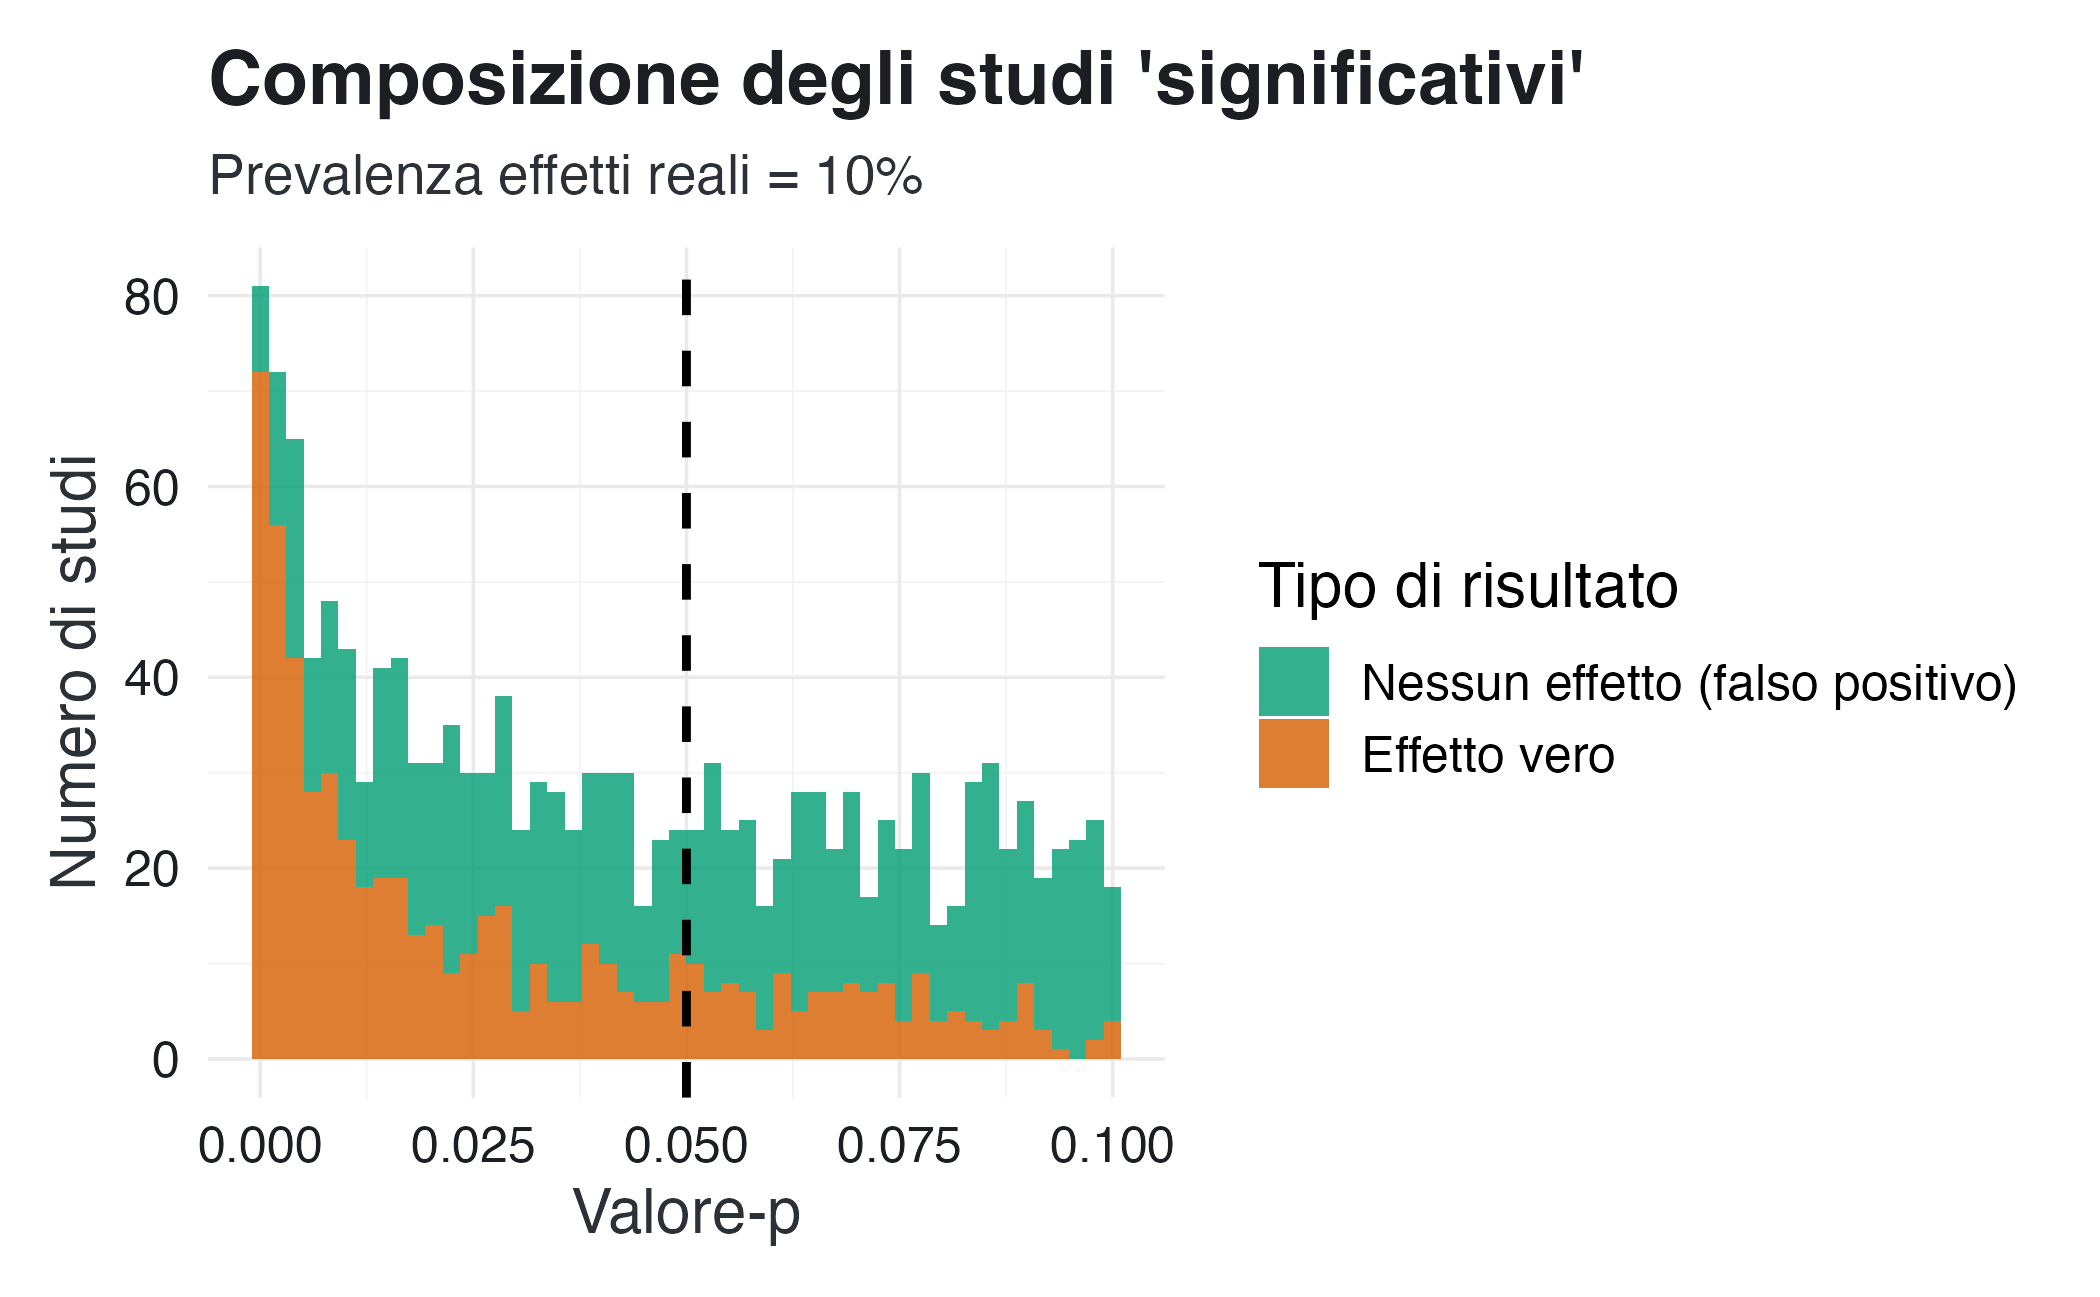
\includegraphics[width=0.85\linewidth,height=\textheight,keepaspectratio]{chapters/limits/01_limits_stat_freq_files/figure-pdf/unnamed-chunk-17-1.png}
\end{center}

Tabella di sintesi:

\begin{Shaded}
\begin{Highlighting}[]
\CommentTok{\# Creazione della tabella comparativa}
\NormalTok{comparison\_summary }\OtherTok{\textless{}{-}}\NormalTok{ ppv\_results }\SpecialCharTok{|\textgreater{}}
  \FunctionTok{mutate}\NormalTok{(}
    \StringTok{\textasciigrave{}}\AttributeTok{Soglia p{-}value}\StringTok{\textasciigrave{}} \OtherTok{=} \FunctionTok{sprintf}\NormalTok{(}\StringTok{"p \textless{} \%.3f"}\NormalTok{, threshold),}
    \StringTok{\textasciigrave{}}\AttributeTok{Interpretazione errata comune}\StringTok{\textasciigrave{}} \OtherTok{=} \FunctionTok{sprintf}\NormalTok{(}
      \StringTok{"≈ \%.1f\%\% probabilità che H₀ sia vera"}\NormalTok{, }
\NormalTok{      threshold }\SpecialCharTok{*} \DecValTok{100}
\NormalTok{    ),}
    \StringTok{\textasciigrave{}}\AttributeTok{Realtà statistica (PPV)}\StringTok{\textasciigrave{}} \OtherTok{=} \FunctionTok{sprintf}\NormalTok{(}
      \StringTok{"\%.1f\%\% probabilità effetto reale"}\NormalTok{, }
\NormalTok{      ppv }\SpecialCharTok{*} \DecValTok{100}
\NormalTok{    ),}
    \StringTok{\textasciigrave{}}\AttributeTok{Discrepanza}\StringTok{\textasciigrave{}} \OtherTok{=} \FunctionTok{sprintf}\NormalTok{(}
      \StringTok{"\%.1f\%\%"}\NormalTok{, }
      \FunctionTok{abs}\NormalTok{(threshold }\SpecialCharTok{{-}}\NormalTok{ ppv) }\SpecialCharTok{*} \DecValTok{100}
\NormalTok{    ),}
    \StringTok{\textasciigrave{}}\AttributeTok{Rapporto PPV/p{-}value}\StringTok{\textasciigrave{}} \OtherTok{=} \FunctionTok{sprintf}\NormalTok{(}
      \StringTok{"\%.1fx"}\NormalTok{, }
\NormalTok{      ppv }\SpecialCharTok{/}\NormalTok{ threshold}
\NormalTok{    )}
\NormalTok{  ) }\SpecialCharTok{|\textgreater{}}
  \FunctionTok{select}\NormalTok{(}\SpecialCharTok{{-}}\NormalTok{threshold, }\SpecialCharTok{{-}}\NormalTok{ppv)}

\CommentTok{\# Visualizzazione tabella}
\NormalTok{comparison\_summary }\SpecialCharTok{|\textgreater{}}
\NormalTok{  knitr}\SpecialCharTok{::}\FunctionTok{kable}\NormalTok{(}
    \AttributeTok{align =} \FunctionTok{c}\NormalTok{(}\StringTok{"l"}\NormalTok{, }\StringTok{"c"}\NormalTok{, }\StringTok{"c"}\NormalTok{, }\StringTok{"c"}\NormalTok{, }\StringTok{"c"}\NormalTok{),}
    \AttributeTok{caption =} \StringTok{"Confronto tra interpretazione erronea del valore{-}p e realtà statistica"}
\NormalTok{  ) }\SpecialCharTok{|\textgreater{}}
\NormalTok{  kableExtra}\SpecialCharTok{::}\FunctionTok{kable\_styling}\NormalTok{(}
    \AttributeTok{bootstrap\_options =} \FunctionTok{c}\NormalTok{(}\StringTok{"striped"}\NormalTok{, }\StringTok{"hover"}\NormalTok{),}
    \AttributeTok{full\_width =} \ConstantTok{FALSE}\NormalTok{,}
    \AttributeTok{position =} \StringTok{"center"}
\NormalTok{  ) }\SpecialCharTok{|\textgreater{}}
\NormalTok{  kableExtra}\SpecialCharTok{::}\FunctionTok{add\_header\_above}\NormalTok{(}
    \FunctionTok{c}\NormalTok{(}\StringTok{" "} \OtherTok{=} \DecValTok{1}\NormalTok{, }\StringTok{"Percezione comune"} \OtherTok{=} \DecValTok{1}\NormalTok{, }\StringTok{"Realtà simulata"} \OtherTok{=} \DecValTok{1}\NormalTok{, }\StringTok{"Differenza"} \OtherTok{=} \DecValTok{1}\NormalTok{, }\StringTok{"Fattore"} \OtherTok{=} \DecValTok{1}\NormalTok{)}
\NormalTok{  ) }\SpecialCharTok{|\textgreater{}}
\NormalTok{  kableExtra}\SpecialCharTok{::}\FunctionTok{row\_spec}\NormalTok{(}\DecValTok{1}\SpecialCharTok{:}\DecValTok{4}\NormalTok{, }\AttributeTok{bold =} \ConstantTok{FALSE}\NormalTok{) }\SpecialCharTok{|\textgreater{}}
\NormalTok{  kableExtra}\SpecialCharTok{::}\FunctionTok{column\_spec}\NormalTok{(}\DecValTok{1}\NormalTok{, }\AttributeTok{bold =} \ConstantTok{TRUE}\NormalTok{)}
\end{Highlighting}
\end{Shaded}

\begin{longtable}[t]{>{}lcccc}
\caption{\label{tab:unnamed-chunk-18}Confronto tra interpretazione erronea del valore-p e realtà statistica}\\
\toprule
\multicolumn{1}{c}{ } & \multicolumn{1}{c}{Percezione comune} & \multicolumn{1}{c}{Realtà simulata} & \multicolumn{1}{c}{Differenza} & \multicolumn{1}{c}{Fattore} \\
\cmidrule(l{3pt}r{3pt}){2-2} \cmidrule(l{3pt}r{3pt}){3-3} \cmidrule(l{3pt}r{3pt}){4-4} \cmidrule(l{3pt}r{3pt}){5-5}
Soglia p-value & Interpretazione errata comune & Realtà statistica (PPV) & Discrepanza & Rapporto PPV/p-value\\
\midrule
\textbf{p < 0.050} & ≈ 5.0\% probabilità che H₀ sia vera & 50.7\% probabilità effetto reale & 45.7\% & 10.1x\\
\textbf{p < 0.010} & ≈ 1.0\% probabilità che H₀ sia vera & 72.0\% probabilità effetto reale & 71.0\% & 72.0x\\
\textbf{p < 0.005} & ≈ 0.5\% probabilità che H₀ sia vera & 78.5\% probabilità effetto reale & 78.0\% & 157.0x\\
\textbf{p < 0.001} & ≈ 0.1\% probabilità che H₀ sia vera & 90.0\% probabilità effetto reale & 89.9\% & 900.0x\\
\bottomrule
\end{longtable}

\subsection{\texorpdfstring{L'inganno del
valore-\(p\)}{L'inganno del valore-p}}\label{linganno-del-valore-p}

La tabella precedente rivela un contrasto drammatico:
\textbf{l'interpretazione comunemente attribuita al valore-\(p\)
sovrastima sistematicamente l'evidenza a favore di un effetto}. Quando i
ricercatori osservano un risultato con \(p\) = 0.05, molti formulano
implicitamente il seguente ragionamento: ``Esiste solo il 5\% di
probabilità che questa scoperta sia un falso positivo''. La simulazione
mostra invece che, in un campo di ricerca caratterizzato da bassa
prevalenza di effetti reali:

\begin{itemize}
\tightlist
\item
  \textbf{con \(p\) \textless{} 0.05}: solamente il 40-50\% dei
  risultati dichiarati significativi corrisponde effettivamente a
  effetti reali;
\item
  \textbf{con \(p\) \textless{} 0.01}: questa proporzione aumenta,
  raggiungendo approssimativamente il 60-70\%;
\item
  \textbf{persino con \(p\) \textless{} 0.001}: potremmo non superare
  una certezza dell'85-90\%, ben lontana dalla quasi certezza che molti
  attribuirebbero a un valore-\(p\) così piccolo.
\end{itemize}

\subsection{L'origine del malinteso: due domande statisticamente
distinte}\label{lorigine-del-malinteso-due-domande-statisticamente-distinte}

Questa marcata discrepanza tra percezione e realtà nasce da una
confusione tra due quantità probabilistiche che rispondono a
interrogativi statisticamente diversi:

\begin{enumerate}
\def\labelenumi{\arabic{enumi}.}
\item
  \textbf{ciò che il valore-\(p\) effettivamente misura}:

  \begin{quote}
  ``Qual è la probabilità di osservare dati almeno altrettanto estremi
  di quelli ottenuti, nell'ipotesi che l'effetto non esista?''
  \[P(\text{Dati osservati o più estremi} \mid H_0)\]
  \end{quote}
\item
  \textbf{ciò che i ricercatori vorrebbero conoscere}:

  \begin{quote}
  ``Data l'evidenza empirica raccolta, quanto è plausibile che l'effetto
  ipotizzato esista realmente?'' \[P(H_1 \mid \text{Dati})\]
  \end{quote}
\end{enumerate}

Queste domande rappresentano \textbf{probabilità condizionate con
direzioni opposte}, matematicamente collegate ma concettualmente
distinte secondo il teorema di Bayes. Trascurare questa distinzione
equivale a confondere due proposizioni logicamente differenti: ``la
probabilità che piova dato che il cielo è nuvoloso'' con ``la
probabilità che il cielo sia nuvoloso dato che piove''. Sebbene
correlate, queste probabilità possono assumere valori radicalmente
diversi.

\subsection{Implicazioni per l'integrità
scientifica}\label{implicazioni-per-lintegrituxe0-scientifica}

Ignorare questa differenza fondamentale conduce a due conseguenze
metodologicamente dannose:

\begin{enumerate}
\def\labelenumi{\arabic{enumi}.}
\item
  \textbf{sovrastima sistematica dell'evidenza}: i ricercatori
  attribuiscono al valore-\(p\) un significato inferenziale che esso non
  possiede, attribuendo alle loro scoperte un grado di certezza non
  supportato dai dati.
\item
  \textbf{accumulo di risultati non replicabili}: la letteratura
  scientifica si riempie di ``scoperte'' statisticamente significative
  ma sostanzialmente non replicabili, minando progressivamente
  l'affidabilità cumulativa della conoscenza scientifica.
\end{enumerate}

In sintesi, la simulazione dimostra in modo inequivocabile che
\textbf{la significatività statistica non costituisce un proxy
affidabile della verità scientifica}. In un panorama di ricerca
caratterizzato da bassa prevalenza di effetti reali, dimensioni
campionarie spesso inadeguate e pratiche analitiche selettive, persino
risultati dichiarati ``altamente significativi'' possono possedere un
grado di affidabilità considerevolmente inferiore a quanto comunemente
ritenuto.

\section{\texorpdfstring{Simulazione 4: la fragilità della soglia \(p\)
=
0.05}{Simulazione 4: la fragilità della soglia p = 0.05}}\label{simulazione-4-la-fragilituxe0-della-soglia-p-0.05}

Cosa distingue un p-value di 0.049 da uno di 0.051? Dal punto di vista
scientifico, nulla. Dal punto di vista delle convenzioni editoriali,
tutto: il primo è ``significativo'' e pubblicabile, il secondo no.

Questa simulazione mostra quanto sia arbitraria questa distinzione,
visualizzando come piccole fluttuazioni casuali possano spostare un
risultato da un lato all'altro della soglia.

\subsection{Simulazione}\label{simulazione-1}

\begin{Shaded}
\begin{Highlighting}[]
\CommentTok{\# Effetto vero piccolo ma reale}
\NormalTok{true\_effect }\OtherTok{\textless{}{-}} \FloatTok{0.2}  \CommentTok{\# Cohen\textquotesingle{}s d}
\NormalTok{n\_per\_group }\OtherTok{\textless{}{-}} \DecValTok{50}
\NormalTok{n\_replications }\OtherTok{\textless{}{-}} \FloatTok{1e5}
\end{Highlighting}
\end{Shaded}

\begin{Shaded}
\begin{Highlighting}[]
\FunctionTok{set.seed}\NormalTok{(}\DecValTok{123}\NormalTok{)}
\CommentTok{\# Simuliamo molte repliche dello stesso studio}
\NormalTok{replications }\OtherTok{\textless{}{-}} \FunctionTok{tibble}\NormalTok{(}
  \AttributeTok{replication =} \DecValTok{1}\SpecialCharTok{:}\NormalTok{n\_replications}
\NormalTok{) }\SpecialCharTok{|\textgreater{}}
  \FunctionTok{rowwise}\NormalTok{() }\SpecialCharTok{|\textgreater{}}
  \FunctionTok{mutate}\NormalTok{(}
    \AttributeTok{p\_value =}\NormalTok{ \{}
\NormalTok{      g1 }\OtherTok{\textless{}{-}} \FunctionTok{rnorm}\NormalTok{(n\_per\_group, }\DecValTok{0}\NormalTok{, }\DecValTok{1}\NormalTok{)}
\NormalTok{      g2 }\OtherTok{\textless{}{-}} \FunctionTok{rnorm}\NormalTok{(n\_per\_group, true\_effect, }\DecValTok{1}\NormalTok{)}
      \FunctionTok{t.test}\NormalTok{(g1, g2)}\SpecialCharTok{$}\NormalTok{p.value}
\NormalTok{    \},}
    \AttributeTok{significant =}\NormalTok{ p\_value }\SpecialCharTok{\textless{}} \FloatTok{0.05}
\NormalTok{  ) }\SpecialCharTok{|\textgreater{}}
  \FunctionTok{ungroup}\NormalTok{()}

\CommentTok{\# Statistiche}
\NormalTok{prop\_significant }\OtherTok{\textless{}{-}} \FunctionTok{mean}\NormalTok{(replications}\SpecialCharTok{$}\NormalTok{significant)}
\NormalTok{median\_p }\OtherTok{\textless{}{-}} \FunctionTok{median}\NormalTok{(replications}\SpecialCharTok{$}\NormalTok{p\_value)}
\end{Highlighting}
\end{Shaded}

\begin{Shaded}
\begin{Highlighting}[]
\CommentTok{\# Visualizzazione}
\NormalTok{palette\_signif }\OtherTok{\textless{}{-}} \FunctionTok{setNames}\NormalTok{(}
\NormalTok{  palette\_qualitative[}\FunctionTok{c}\NormalTok{(}\DecValTok{3}\NormalTok{, }\DecValTok{8}\NormalTok{)],  }\CommentTok{\# verde + grigio}
  \FunctionTok{c}\NormalTok{(}\StringTok{"TRUE"}\NormalTok{, }\StringTok{"FALSE"}\NormalTok{)}
\NormalTok{)}

\NormalTok{replications }\SpecialCharTok{|\textgreater{}}
  \FunctionTok{mutate}\NormalTok{(}\AttributeTok{significant =} \FunctionTok{factor}\NormalTok{(significant, }\AttributeTok{levels =} \FunctionTok{c}\NormalTok{(}\ConstantTok{TRUE}\NormalTok{, }\ConstantTok{FALSE}\NormalTok{))) }\SpecialCharTok{|\textgreater{}}
  \FunctionTok{ggplot}\NormalTok{(}\FunctionTok{aes}\NormalTok{(}\AttributeTok{x =}\NormalTok{ p\_value, }\AttributeTok{fill =}\NormalTok{ significant)) }\SpecialCharTok{+}
  \FunctionTok{geom\_histogram}\NormalTok{(}\AttributeTok{bins =} \DecValTok{50}\NormalTok{, }\AttributeTok{color =} \StringTok{"white"}\NormalTok{, }\AttributeTok{alpha =} \FloatTok{0.8}\NormalTok{) }\SpecialCharTok{+}
  \FunctionTok{geom\_vline}\NormalTok{(}
    \AttributeTok{xintercept =} \FloatTok{0.05}\NormalTok{,}
    \AttributeTok{color =} \StringTok{"black"}\NormalTok{,}
    \AttributeTok{linetype =} \StringTok{"dashed"}\NormalTok{,}
    \AttributeTok{linewidth =} \FloatTok{1.2}
\NormalTok{  ) }\SpecialCharTok{+}
  \FunctionTok{scale\_fill\_manual}\NormalTok{(}
    \AttributeTok{values =}\NormalTok{ palette\_signif,}
    \AttributeTok{labels =} \FunctionTok{c}\NormalTok{(}
      \StringTok{"TRUE"}  \OtherTok{=} \StringTok{"Significativo (p \textless{} 0.05)"}\NormalTok{,}
      \StringTok{"FALSE"} \OtherTok{=} \StringTok{"Non significativo"}
\NormalTok{    )}
\NormalTok{  ) }\SpecialCharTok{+}
  \FunctionTok{annotate}\NormalTok{(}
    \StringTok{"text"}\NormalTok{,}
    \AttributeTok{x =} \FloatTok{0.5}\NormalTok{, }\AttributeTok{y =} \ConstantTok{Inf}\NormalTok{, }\AttributeTok{vjust =} \DecValTok{2}\NormalTok{,}
    \AttributeTok{label =} \FunctionTok{sprintf}\NormalTok{(}
      \StringTok{"Effetto vero: d = \%.1f}\SpecialCharTok{\textbackslash{}n}\StringTok{Potenza: \%.0f\%\%}\SpecialCharTok{\textbackslash{}n}\StringTok{Mediana p{-}value: \%.3f"}\NormalTok{,}
\NormalTok{      true\_effect, prop\_significant }\SpecialCharTok{*} \DecValTok{100}\NormalTok{, median\_p}
\NormalTok{    ),}
    \AttributeTok{hjust =} \FloatTok{0.5}\NormalTok{, }\AttributeTok{size =} \DecValTok{4}
\NormalTok{  ) }\SpecialCharTok{+}
  \FunctionTok{labs}\NormalTok{(}
    \AttributeTok{x =} \StringTok{"Valore{-}p"}\NormalTok{,}
    \AttributeTok{y =} \StringTok{"Numero di repliche"}\NormalTok{,}
    \AttributeTok{fill =} \StringTok{""}\NormalTok{,}
    \AttributeTok{title =} \StringTok{"1000 repliche dello stesso studio}\SpecialCharTok{\textbackslash{}n}\StringTok{con lo stesso effetto vero"}\NormalTok{,}
    \AttributeTok{subtitle =} \StringTok{"Alcuni studi trovano \textquotesingle{}significatività\textquotesingle{}, altri no – ma l\textquotesingle{}effetto sottostante}\SpecialCharTok{\textbackslash{}n}\StringTok{è identico"}
\NormalTok{  )}
\end{Highlighting}
\end{Shaded}

\begin{figure}[H]

\centering{

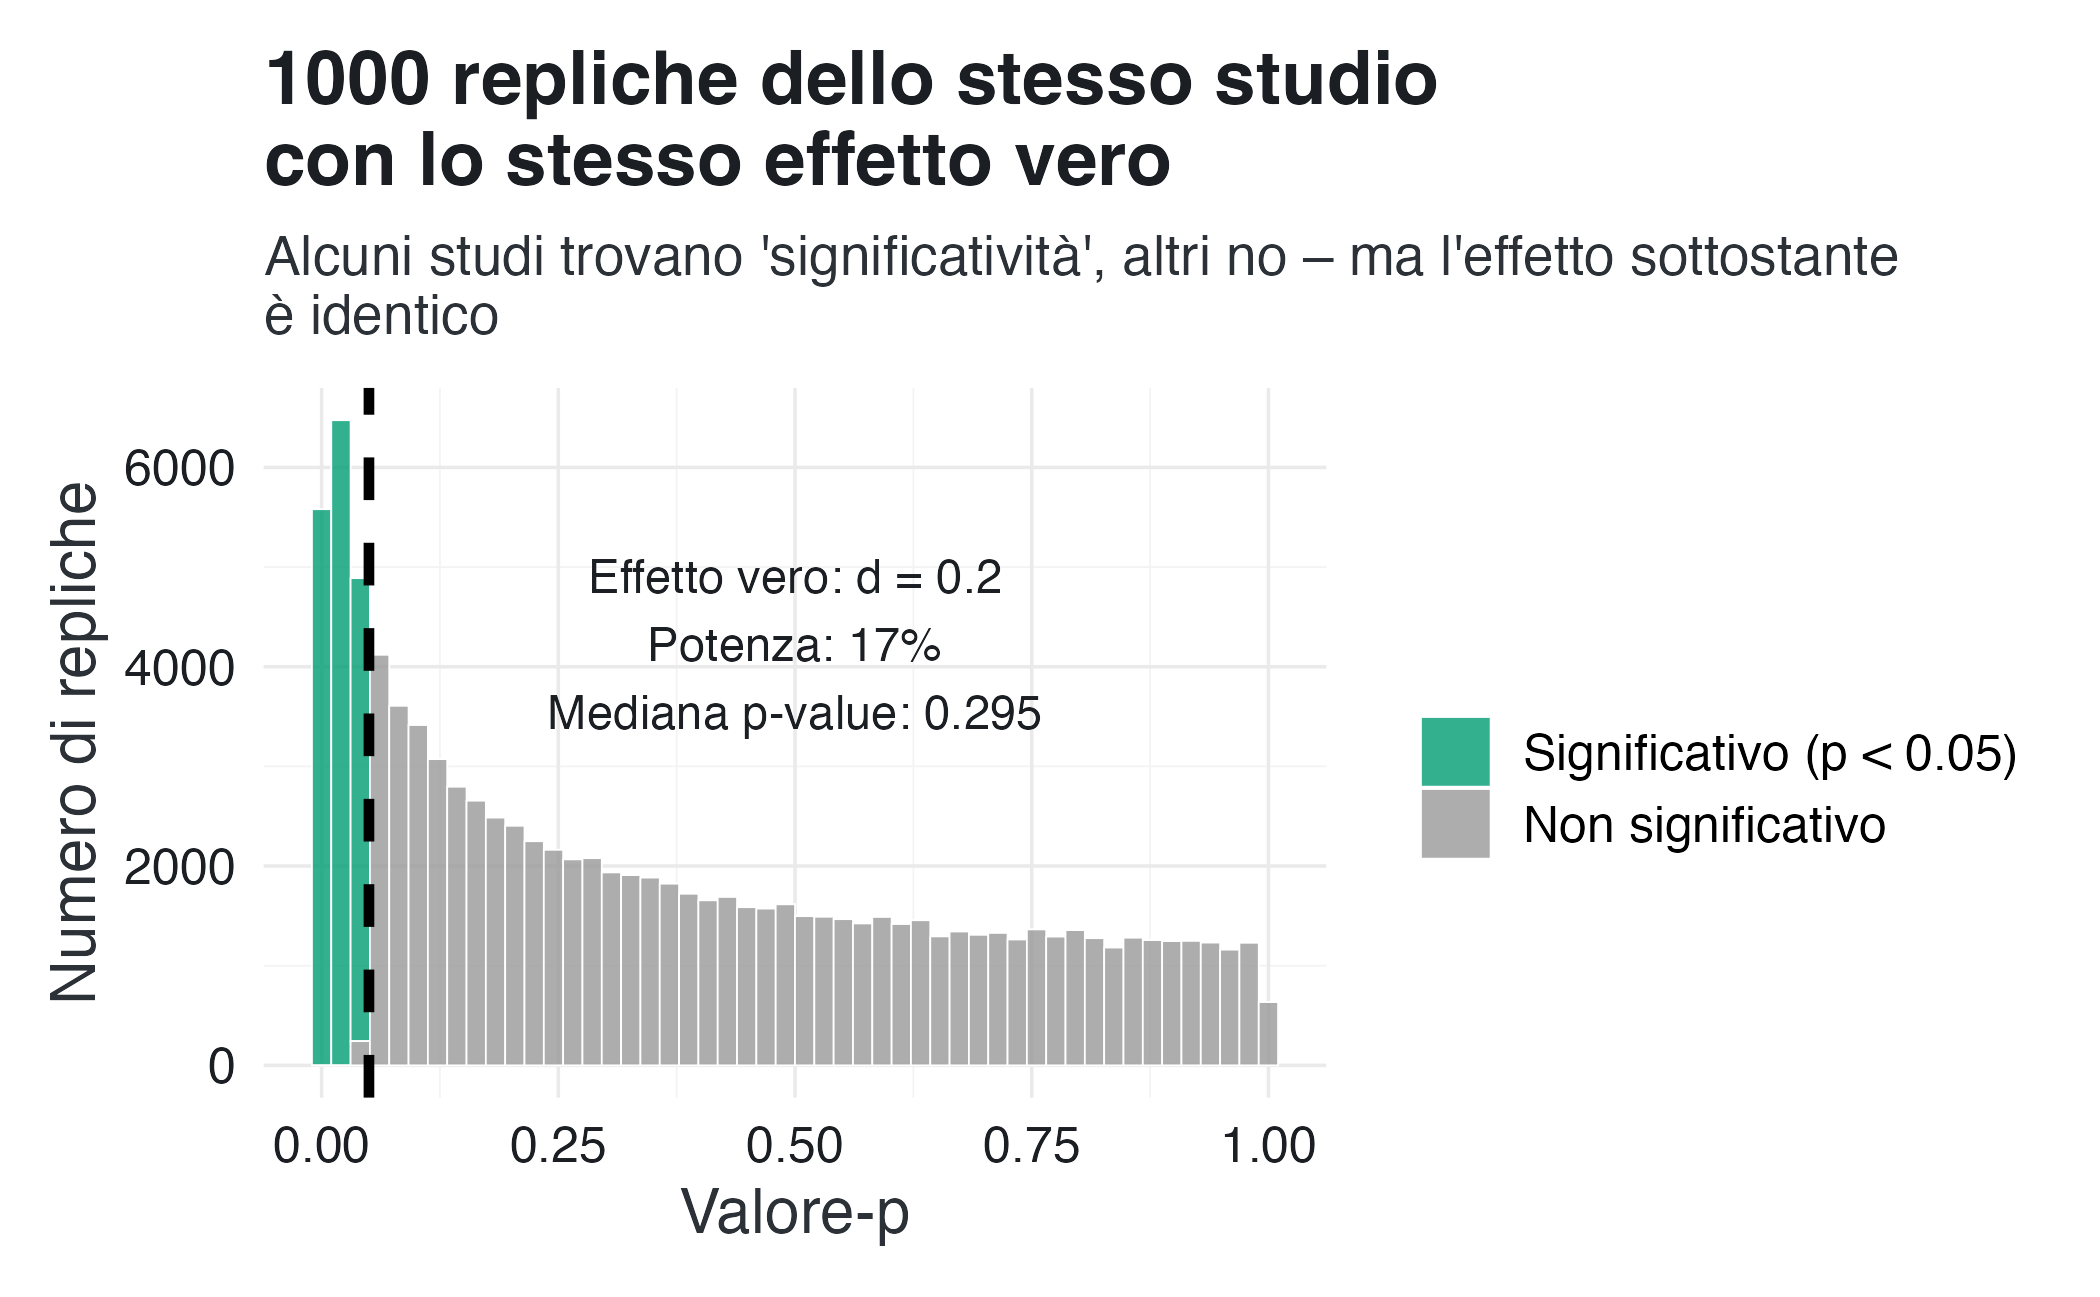
\includegraphics[width=0.85\linewidth,height=\textheight,keepaspectratio]{chapters/limits/01_limits_stat_freq_files/figure-pdf/fig-threshold-fragility-1.png}

}

\caption{\label{fig-threshold-fragility}Lo stesso effetto vero produce
p-value molto variabili in campioni diversi. La soglia 0.05 è un confine
arbitrario che separa campioni essenzialmente indistinguibili.}

\end{figure}%

\textbf{Interpretazione.} Il grafico mostra che, dato uno stesso effetto
vero, i valori-\(p\) ottenuti in diverse repliche variano enormemente.
Alcuni studi ottengono un valore-\(p\) = 0.001, altri un valore-\(p\)
prossimo a 1. Questa variabilità non riflette differenze nell'effetto
(che è sempre \(d\) = 0.2), ma solo fluttuazioni casuali nel
campionamento.

\begin{Shaded}
\begin{Highlighting}[]
\CommentTok{\# Zoom sulla zona critica}
\NormalTok{replications }\SpecialCharTok{|\textgreater{}}
  \FunctionTok{filter}\NormalTok{(p\_value }\SpecialCharTok{\textgreater{}} \FloatTok{0.03} \SpecialCharTok{\&}\NormalTok{ p\_value }\SpecialCharTok{\textless{}} \FloatTok{0.07}\NormalTok{) }\SpecialCharTok{|\textgreater{}}
  \FunctionTok{mutate}\NormalTok{(}\AttributeTok{significant =} \FunctionTok{factor}\NormalTok{(significant, }\AttributeTok{levels =} \FunctionTok{c}\NormalTok{(}\ConstantTok{TRUE}\NormalTok{, }\ConstantTok{FALSE}\NormalTok{))) }\SpecialCharTok{|\textgreater{}}
  \FunctionTok{ggplot}\NormalTok{(}\FunctionTok{aes}\NormalTok{(}\AttributeTok{x =}\NormalTok{ p\_value, }\AttributeTok{fill =}\NormalTok{ significant)) }\SpecialCharTok{+}
  \FunctionTok{geom\_histogram}\NormalTok{(}\AttributeTok{bins =} \DecValTok{20}\NormalTok{, }\AttributeTok{color =} \StringTok{"white"}\NormalTok{, }\AttributeTok{alpha =} \FloatTok{0.8}\NormalTok{) }\SpecialCharTok{+}
  \FunctionTok{geom\_vline}\NormalTok{(}
    \AttributeTok{xintercept =} \FloatTok{0.05}\NormalTok{,}
    \AttributeTok{color =} \StringTok{"black"}\NormalTok{,}
    \AttributeTok{linetype =} \StringTok{"dashed"}\NormalTok{,}
    \AttributeTok{linewidth =} \FloatTok{1.2}
\NormalTok{  ) }\SpecialCharTok{+}
  \FunctionTok{scale\_fill\_manual}\NormalTok{(}
    \AttributeTok{values =}\NormalTok{ palette\_signif,}
    \AttributeTok{labels =} \FunctionTok{c}\NormalTok{(}
      \StringTok{"TRUE"}  \OtherTok{=} \StringTok{"Pubblicabile"}\NormalTok{,}
      \StringTok{"FALSE"} \OtherTok{=} \StringTok{"Nel cassetto"}
\NormalTok{    )}
\NormalTok{  ) }\SpecialCharTok{+}
  \FunctionTok{labs}\NormalTok{(}
    \AttributeTok{x =} \StringTok{"Valore{-}p"}\NormalTok{,}
    \AttributeTok{y =} \StringTok{"Numero di repliche"}\NormalTok{,}
    \AttributeTok{fill =} \StringTok{""}\NormalTok{,}
    \AttributeTok{title =} \StringTok{"Zoom sulla \textquotesingle{}zona grigia\textquotesingle{} (p tra 0.03 e 0.07)"}\NormalTok{,}
    \AttributeTok{subtitle =} \StringTok{"Studi identici finiscono su lati opposti della soglia}\SpecialCharTok{\textbackslash{}n}\StringTok{per pura variabilità campionaria"}
\NormalTok{  )}
\end{Highlighting}
\end{Shaded}

\begin{center}
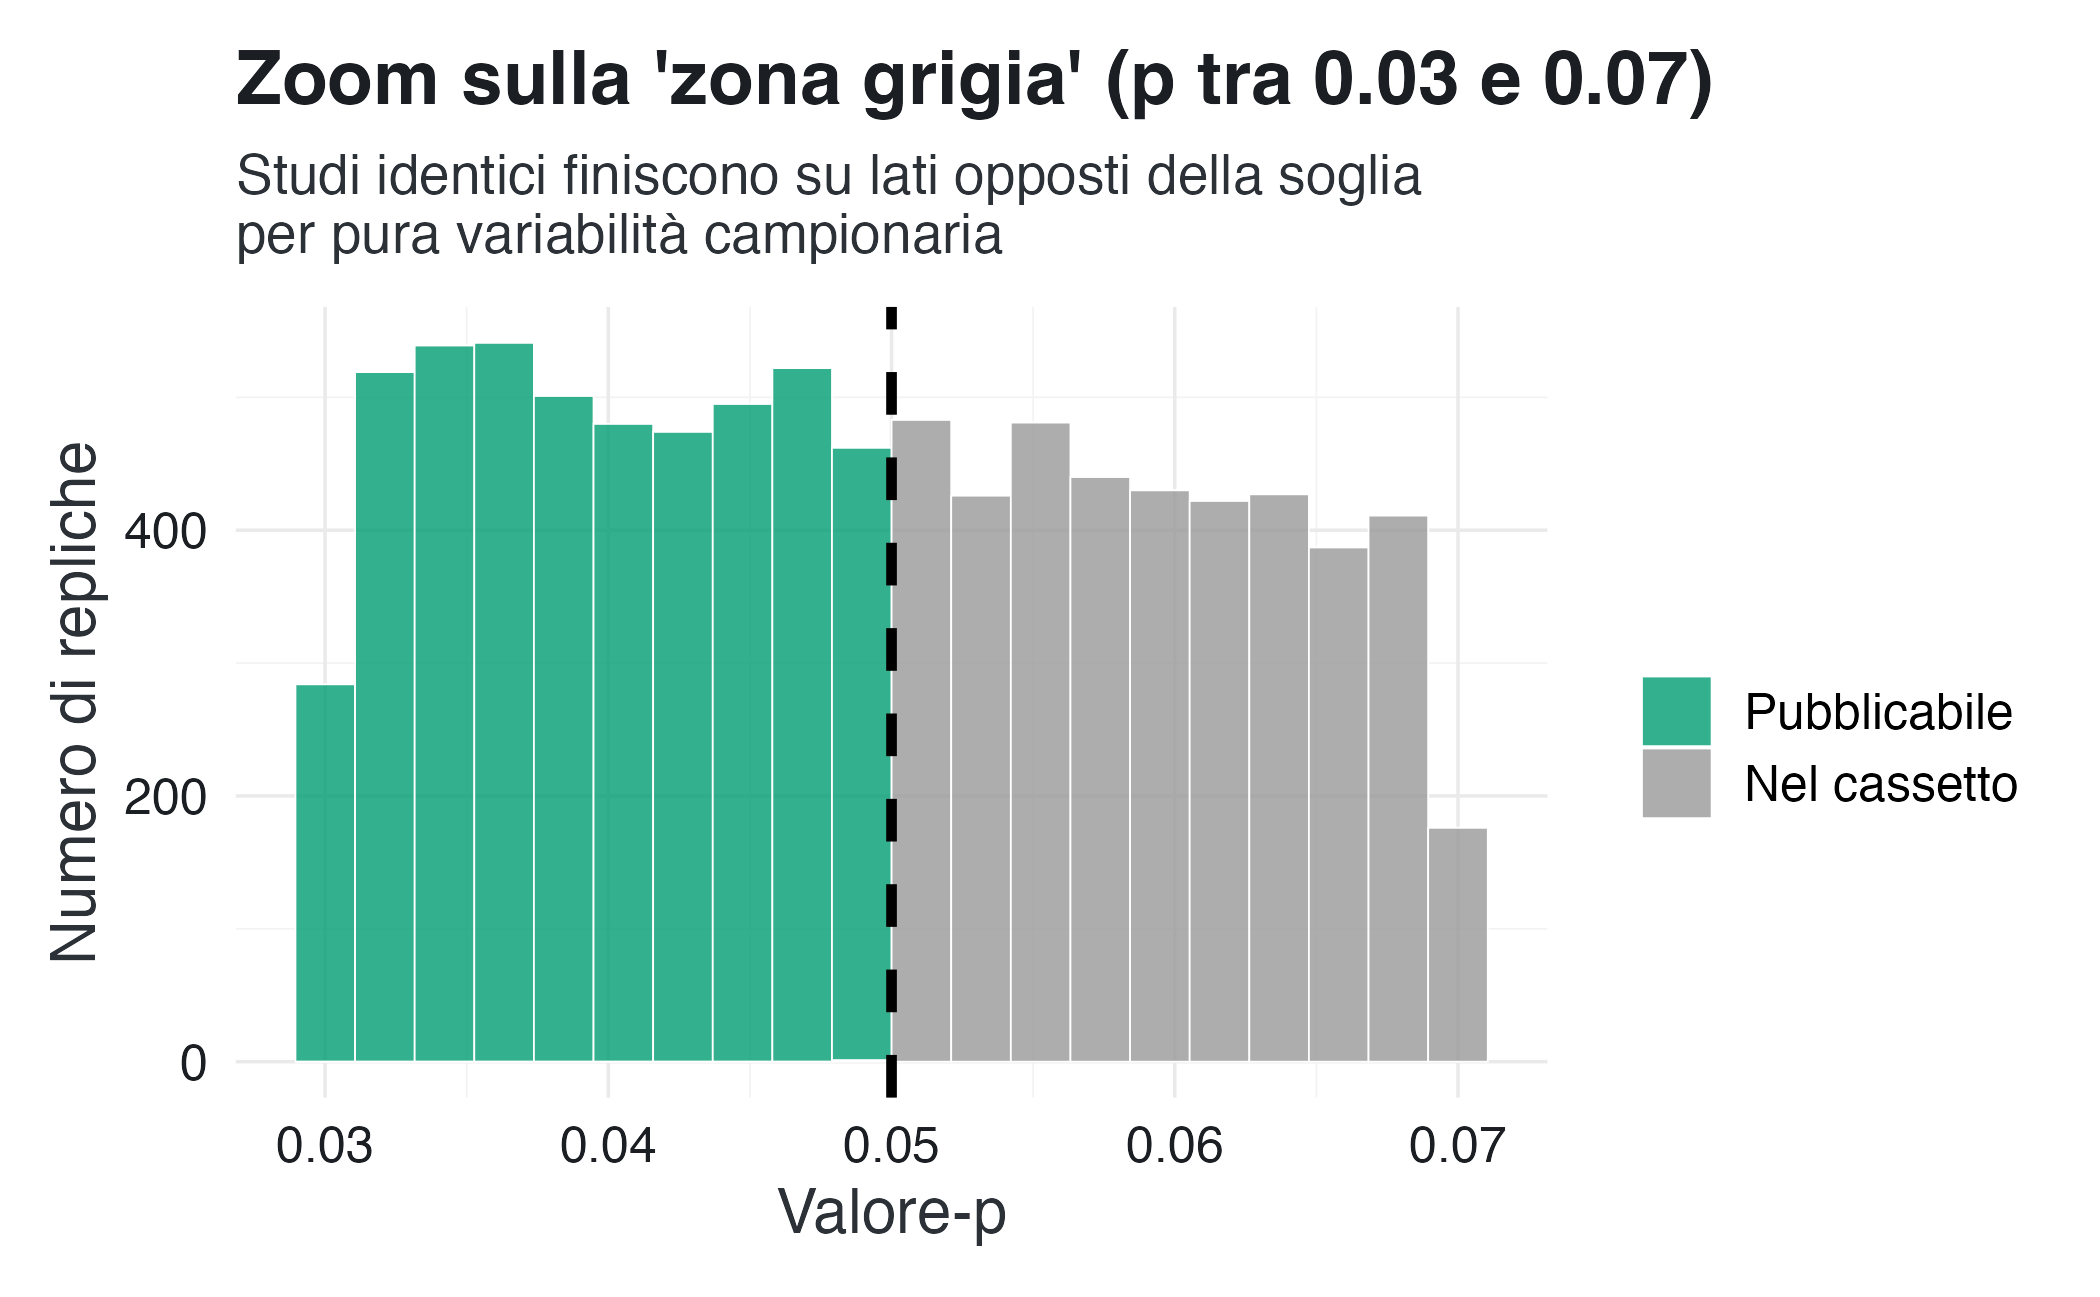
\includegraphics[width=0.85\linewidth,height=\textheight,keepaspectratio]{chapters/limits/01_limits_stat_freq_files/figure-pdf/unnamed-chunk-21-1.png}
\end{center}

Lo zoom sulla ``zona grigia'' è particolarmente istruttivo: studi con un
valore-\(p\) = 0.049 e studi con un valore-\(p\) = 0.051 sono
scientificamente indistinguibili, ma il sistema editoriale li tratta
come radicalmente diversi. Come hanno scritto Gelman \& Stern
(\citeproc{ref-gelman2006difference}{2006})

\begin{quote}
\emph{The difference between ``significant'' and ``not significant'' is
not itself statistically significant.}
\end{quote}

\section*{Riflessioni conclusive}\label{riflessioni-conclusive}

\markright{Riflessioni conclusive}

Le simulazioni presentate in questo capitolo hanno trasformato le
critiche teoriche al valore-\(p\) in esperienze empiriche concrete.
Abbiamo visto che:

\begin{enumerate}
\def\labelenumi{\arabic{enumi}.}
\item
  \textbf{il \(p\)-hacking rappresenta un fallimento sistemico}: bastano
  poche scelte analitiche selettive per inflazionare drammaticamente il
  tasso di falsi positivi. Questo fenomeno emerge naturalmente da un
  sistema di incentivi che premia la significatività statistica. La
  soluzione, pertanto, non risiede nell'appello all'integrità
  individuale, ma nell'adozione di pratiche strutturali come la
  preregistrazione, la trasparenza analitica e la condivisione dei dati.
\item
  \textbf{la distribuzione dei valori-\(p\) tradisce le pratiche
  scorrette}: l'eccesso di valori appena sotto la soglia di 0.05
  osservato in molte discipline trova un preciso parallelo nelle
  simulazioni di \(p\)-hacking sistematico, offrendo un indicatore
  empirico di pratiche analitiche selettive.
\item
  \textbf{il valore-\(p\) promuove un malinteso semantico}: la terza
  simulazione ha smascherato l'errore interpretativo più diffuso, ovvero
  la confusione tra \(P(\text{Dati} \mid H_0)\) e
  \(P(H_0 \mid \text{Dati})\). Questo malinteso può condurre a
  conclusioni gravemente fuorvianti, soprattutto in campi caratterizzati
  da una bassa prevalenza di effetti reali, in cui anche valori \(p\)
  apparentemente convincenti possono corrispondere a probabilità modeste
  che l'effetto esista realmente.
\item
  \textbf{la soglia canonica \(p\) = 0.05 è arbitraria}: le simulazioni
  hanno mostrato come questa soglia sia una convenzione fragile, nel
  senso che studi metodologicamente identici possono cadere su lati
  opposti di questa barriera artificiale per pura variabilità
  campionaria, ricevendo tuttavia interpretazioni diametralmente opposte
  nella comunicazione scientifica.
\end{enumerate}

Questi risultati possono essere interpretati come l'indicazione che il
valore-\(p\) sia del tutto inutile nella pratica scientifica. Un'altra
interpretazione è che esso conservi una qualche utilità, ma solo se
viene utilizzato in modo consapevole, come parte di un ragionamento più
ampio che includa la stima dell'effetto, la sua incertezza, la
plausibilità teorica e la replicabilità. L'approccio bayesiano, che
esploreremo nel resto del corso, offre un quadro concettualmente più
coerente per rispondere alle domande che realmente interessano alla
ricerca scientifica.

\section{Esercizi}\label{esercizi}

\begin{tcolorbox}[enhanced jigsaw, arc=.35mm, bottomrule=.15mm, bottomtitle=1mm, breakable, colback=white, colbacktitle=quarto-callout-important-color!10!white, colframe=quarto-callout-important-color-frame, coltitle=black, left=2mm, leftrule=.75mm, opacityback=0, opacitybacktitle=0.6, rightrule=.15mm, title=\textcolor{quarto-callout-important-color}{\faExclamation}\hspace{0.5em}{Esercizio 1: Variare i parametri del p-hacking}, titlerule=0mm, toprule=.15mm, toptitle=1mm]

Modifica la Simulazione 1 per rispondere a queste domande:

\begin{enumerate}
\def\labelenumi{\arabic{enumi}.}
\tightlist
\item
  Come cambia il tasso di falsi positivi se il ricercatore prova solo 5
  test invece di 20?
\item
  E se ne prova 50?
\item
  Qual è il numero di test necessario per avere un tasso di falsi
  positivi del 50\%?
\end{enumerate}

\textbf{Suggerimento}: Usa la formula \(1 - (1 - 0.05)^k\) dove \(k\) è
il numero di test.

\end{tcolorbox}

\begin{tcolorbox}[enhanced jigsaw, arc=.35mm, bottomrule=.15mm, bottomtitle=1mm, breakable, colback=white, colbacktitle=quarto-callout-tip-color!10!white, colframe=quarto-callout-tip-color-frame, coltitle=black, left=2mm, leftrule=.75mm, opacityback=0, opacitybacktitle=0.6, rightrule=.15mm, title=\textcolor{quarto-callout-tip-color}{\faLightbulb}\hspace{0.5em}{Soluzione Esercizio 1}, titlerule=0mm, toprule=.15mm, toptitle=1mm]

\begin{Shaded}
\begin{Highlighting}[]
\CommentTok{\# Tasso teorico di falsi positivi in funzione del numero di test}
\NormalTok{k\_values }\OtherTok{\textless{}{-}} \DecValTok{1}\SpecialCharTok{:}\DecValTok{50}
\NormalTok{false\_positive\_rates }\OtherTok{\textless{}{-}} \DecValTok{1} \SpecialCharTok{{-}}\NormalTok{ (}\DecValTok{1} \SpecialCharTok{{-}} \FloatTok{0.05}\NormalTok{)}\SpecialCharTok{\^{}}\NormalTok{k\_values}

\FunctionTok{tibble}\NormalTok{(}\AttributeTok{k =}\NormalTok{ k\_values, }\AttributeTok{fpr =}\NormalTok{ false\_positive\_rates) }\SpecialCharTok{|\textgreater{}}
  \FunctionTok{ggplot}\NormalTok{(}\FunctionTok{aes}\NormalTok{(}\AttributeTok{x =}\NormalTok{ k, }\AttributeTok{y =}\NormalTok{ fpr)) }\SpecialCharTok{+}
  \FunctionTok{geom\_line}\NormalTok{(}\AttributeTok{color =} \StringTok{"steelblue"}\NormalTok{, }\AttributeTok{linewidth =} \DecValTok{1}\NormalTok{) }\SpecialCharTok{+}
  \FunctionTok{geom\_hline}\NormalTok{(}\AttributeTok{yintercept =} \FloatTok{0.50}\NormalTok{, }\AttributeTok{linetype =} \StringTok{"dashed"}\NormalTok{, }\AttributeTok{color =} \StringTok{"red"}\NormalTok{) }\SpecialCharTok{+}
  \FunctionTok{geom\_vline}\NormalTok{(}\AttributeTok{xintercept =} \FunctionTok{log}\NormalTok{(}\FloatTok{0.5}\NormalTok{) }\SpecialCharTok{/} \FunctionTok{log}\NormalTok{(}\FloatTok{0.95}\NormalTok{), }\AttributeTok{linetype =} \StringTok{"dashed"}\NormalTok{, }\AttributeTok{color =} \StringTok{"red"}\NormalTok{) }\SpecialCharTok{+}
  \FunctionTok{scale\_y\_continuous}\NormalTok{(}\AttributeTok{labels =}\NormalTok{ scales}\SpecialCharTok{::}\NormalTok{percent) }\SpecialCharTok{+}
  \FunctionTok{labs}\NormalTok{(}
    \AttributeTok{x =} \StringTok{"Numero di test provati"}\NormalTok{,}
    \AttributeTok{y =} \StringTok{"Tasso di falsi positivi"}\NormalTok{,}
    \AttributeTok{title =} \StringTok{"Come il numero di test influenza il tasso di falsi positivi"}
\NormalTok{  )}

\CommentTok{\# Calcolo esatto}
\NormalTok{k\_for\_50pct }\OtherTok{\textless{}{-}} \FunctionTok{ceiling}\NormalTok{(}\FunctionTok{log}\NormalTok{(}\FloatTok{0.5}\NormalTok{) }\SpecialCharTok{/} \FunctionTok{log}\NormalTok{(}\FloatTok{0.95}\NormalTok{))}
\FunctionTok{cat}\NormalTok{(}\FunctionTok{sprintf}\NormalTok{(}\StringTok{"Servono \%d test per raggiungere un tasso di falsi positivi del 50\%\%}\SpecialCharTok{\textbackslash{}n}\StringTok{"}\NormalTok{, k\_for\_50pct))}
\CommentTok{\#\textgreater{} Servono 14 test per raggiungere un tasso di falsi positivi del 50\%}
\end{Highlighting}
\end{Shaded}

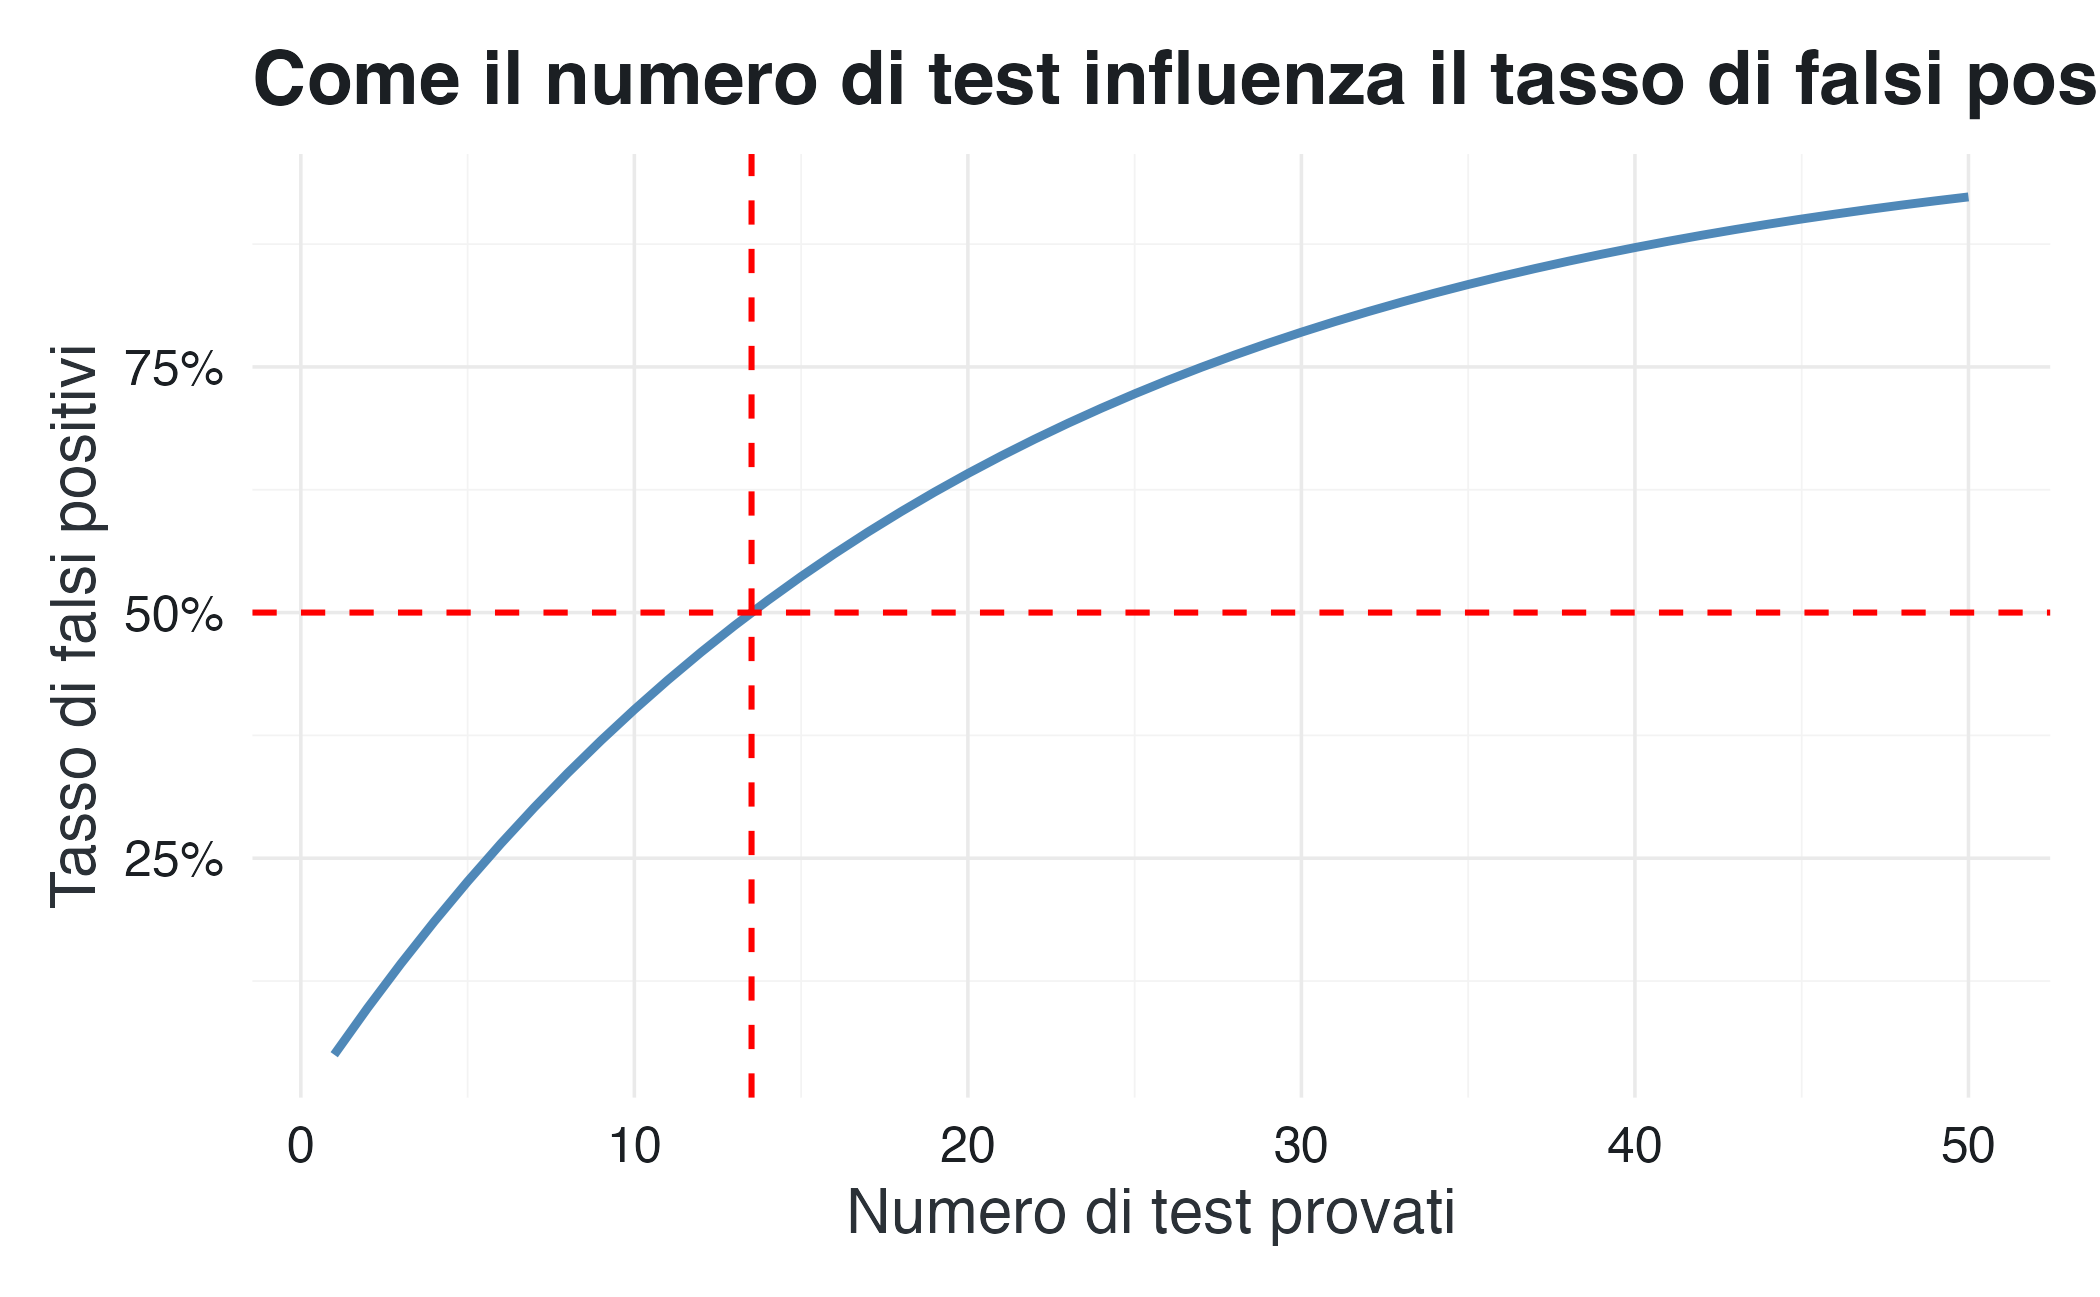
\includegraphics[width=0.85\linewidth,height=\textheight,keepaspectratio]{chapters/limits/01_limits_stat_freq_files/figure-pdf/unnamed-chunk-22-1.png}

\end{tcolorbox}

\begin{tcolorbox}[enhanced jigsaw, arc=.35mm, bottomrule=.15mm, bottomtitle=1mm, breakable, colback=white, colbacktitle=quarto-callout-important-color!10!white, colframe=quarto-callout-important-color-frame, coltitle=black, left=2mm, leftrule=.75mm, opacityback=0, opacitybacktitle=0.6, rightrule=.15mm, title=\textcolor{quarto-callout-important-color}{\faExclamation}\hspace{0.5em}{Esercizio 2: Il PPV in diversi campi}, titlerule=0mm, toprule=.15mm, toptitle=1mm]

La Simulazione 3 assume che il 10\% delle ipotesi testate sia vero
(scenario tipico per ricerca esplorativa).

\begin{enumerate}
\def\labelenumi{\arabic{enumi}.}
\tightlist
\item
  Ricalcola il PPV assumendo che il 50\% delle ipotesi sia vero
  (scenario di ricerca confermativa).
\item
  Ricalcola assumendo che solo il 1\% sia vero (scenario di drug
  discovery o ricerca genomica).
\item
  Qual è la prevalenza minima necessaria affinché un p \textless{} 0.05
  abbia almeno il 90\% di probabilità di essere un vero effetto?
\end{enumerate}

\end{tcolorbox}

\begin{tcolorbox}[enhanced jigsaw, arc=.35mm, bottomrule=.15mm, bottomtitle=1mm, breakable, colback=white, colbacktitle=quarto-callout-tip-color!10!white, colframe=quarto-callout-tip-color-frame, coltitle=black, left=2mm, leftrule=.75mm, opacityback=0, opacitybacktitle=0.6, rightrule=.15mm, title=\textcolor{quarto-callout-tip-color}{\faLightbulb}\hspace{0.5em}{Soluzione Esercizio 2}, titlerule=0mm, toprule=.15mm, toptitle=1mm]

\begin{Shaded}
\begin{Highlighting}[]
\CommentTok{\# Funzione per calcolare il PPV teorico (usando Bayes)}
\CommentTok{\# PPV = P(H1|p\textless{}α) = P(p\textless{}α|H1) * P(H1) / P(p\textless{}α)}
\CommentTok{\# Dove P(p\textless{}α) = P(p\textless{}α|H1)*P(H1) + P(p\textless{}α|H0)*P(H0)}

\NormalTok{calculate\_theoretical\_ppv }\OtherTok{\textless{}{-}} \ControlFlowTok{function}\NormalTok{(prior\_h1, }\AttributeTok{power =} \FloatTok{0.80}\NormalTok{, }\AttributeTok{alpha =} \FloatTok{0.05}\NormalTok{) \{}
  \CommentTok{\# P(p\textless{}α | H1) ≈ power (potenza del test)}
  \CommentTok{\# P(p\textless{}α | H0) = alpha}
\NormalTok{  p\_significant }\OtherTok{\textless{}{-}}\NormalTok{ power }\SpecialCharTok{*}\NormalTok{ prior\_h1 }\SpecialCharTok{+}\NormalTok{ alpha }\SpecialCharTok{*}\NormalTok{ (}\DecValTok{1} \SpecialCharTok{{-}}\NormalTok{ prior\_h1)}
\NormalTok{  ppv }\OtherTok{\textless{}{-}}\NormalTok{ (power }\SpecialCharTok{*}\NormalTok{ prior\_h1) }\SpecialCharTok{/}\NormalTok{ p\_significant}
  \FunctionTok{return}\NormalTok{(ppv)}
\NormalTok{\}}

\CommentTok{\# PPV per diverse prevalenze}
\NormalTok{prevalences }\OtherTok{\textless{}{-}} \FunctionTok{c}\NormalTok{(}\FloatTok{0.01}\NormalTok{, }\FloatTok{0.10}\NormalTok{, }\FloatTok{0.50}\NormalTok{, }\FloatTok{0.80}\NormalTok{)}
\NormalTok{ppv\_values }\OtherTok{\textless{}{-}} \FunctionTok{sapply}\NormalTok{(prevalences, calculate\_theoretical\_ppv)}

\FunctionTok{tibble}\NormalTok{(}
  \StringTok{\textasciigrave{}}\AttributeTok{Prevalenza effetti veri}\StringTok{\textasciigrave{}} \OtherTok{=} \FunctionTok{sprintf}\NormalTok{(}\StringTok{"\%.0f\%\%"}\NormalTok{, prevalences }\SpecialCharTok{*} \DecValTok{100}\NormalTok{),}
  \StringTok{\textasciigrave{}}\AttributeTok{PPV (potenza 80\%)}\StringTok{\textasciigrave{}} \OtherTok{=} \FunctionTok{sprintf}\NormalTok{(}\StringTok{"\%.1f\%\%"}\NormalTok{, ppv\_values }\SpecialCharTok{*} \DecValTok{100}\NormalTok{)}
\NormalTok{) }\SpecialCharTok{|\textgreater{}}
\NormalTok{  knitr}\SpecialCharTok{::}\FunctionTok{kable}\NormalTok{()}
\end{Highlighting}
\end{Shaded}

{\def\LTcaptype{none} % do not increment counter
\begin{longtable}[]{@{}ll@{}}
\toprule\noalign{}
Prevalenza effetti veri & PPV (potenza 80\%) \\
\midrule\noalign{}
\endhead
\bottomrule\noalign{}
\endlastfoot
1\% & 13.9\% \\
10\% & 64.0\% \\
50\% & 94.1\% \\
80\% & 98.5\% \\
\end{longtable}
}

\begin{Shaded}
\begin{Highlighting}[]

\CommentTok{\# Prevalenza minima per PPV = 90\%}
\CommentTok{\# 0.90 = (0.80 * π) / (0.80 * π + 0.05 * (1{-}π))}
\CommentTok{\# Risolvendo per π:}
\CommentTok{\# 0.90 * (0.80*π + 0.05 {-} 0.05*π) = 0.80*π}
\CommentTok{\# 0.72*π + 0.045 {-} 0.045*π = 0.80*π}
\CommentTok{\# 0.045 = 0.80*π {-} 0.72*π + 0.045*π}
\CommentTok{\# 0.045 = 0.125*π}
\NormalTok{pi\_min }\OtherTok{\textless{}{-}} \FloatTok{0.045} \SpecialCharTok{/} \FloatTok{0.125}
\FunctionTok{cat}\NormalTok{(}\FunctionTok{sprintf}\NormalTok{(}\StringTok{"}\SpecialCharTok{\textbackslash{}n}\StringTok{Prevalenza minima per PPV ≥ 90\%\%: \%.0f\%\%}\SpecialCharTok{\textbackslash{}n}\StringTok{"}\NormalTok{, pi\_min }\SpecialCharTok{*} \DecValTok{100}\NormalTok{))}
\CommentTok{\#\textgreater{} }
\CommentTok{\#\textgreater{} Prevalenza minima per PPV ≥ 90\%: 36\%}
\end{Highlighting}
\end{Shaded}

\end{tcolorbox}

\begin{tcolorbox}[enhanced jigsaw, arc=.35mm, bottomrule=.15mm, bottomtitle=1mm, breakable, colback=white, colbacktitle=quarto-callout-important-color!10!white, colframe=quarto-callout-important-color-frame, coltitle=black, left=2mm, leftrule=.75mm, opacityback=0, opacitybacktitle=0.6, rightrule=.15mm, title=\textcolor{quarto-callout-important-color}{\faExclamation}\hspace{0.5em}{Esercizio 3: Simulare l'approccio bayesiano}, titlerule=0mm, toprule=.15mm, toptitle=1mm]

Ripeti la Simulazione 4, ma invece di calcolare il p-value, calcola la
probabilità a posteriori che l'effetto sia positivo usando
un'approssimazione bayesiana semplice.

\textbf{Suggerimento}: Usa una prior N(0, 1) per l'effetto e confronta
la stabilità della conclusione bayesiana rispetto alla decisione basata
sul p-value.

\end{tcolorbox}

\begin{tcolorbox}[enhanced jigsaw, arc=.35mm, bottomrule=.15mm, bottomtitle=1mm, breakable, colback=white, colbacktitle=quarto-callout-tip-color!10!white, colframe=quarto-callout-tip-color-frame, coltitle=black, left=2mm, leftrule=.75mm, opacityback=0, opacitybacktitle=0.6, rightrule=.15mm, title=\textcolor{quarto-callout-tip-color}{\faLightbulb}\hspace{0.5em}{Soluzione Esercizio 3}, titlerule=0mm, toprule=.15mm, toptitle=1mm]

\begin{Shaded}
\begin{Highlighting}[]
\CommentTok{\# Approssimazione bayesiana semplice usando coniugazione normale}
\CommentTok{\# Prior: δ \textasciitilde{} N(0, σ\_prior²)}
\CommentTok{\# Likelihood: d\_obs | δ \textasciitilde{} N(δ, SE²)}
\CommentTok{\# Posterior: δ | d\_obs \textasciitilde{} N(μ\_post, σ\_post²)}

\NormalTok{bayesian\_analysis }\OtherTok{\textless{}{-}} \ControlFlowTok{function}\NormalTok{(d\_obs, se\_obs, }\AttributeTok{prior\_sd =} \DecValTok{1}\NormalTok{) \{}
  \CommentTok{\# Posterior mean and sd (formula della coniugazione normale)}
\NormalTok{  prior\_precision }\OtherTok{\textless{}{-}} \DecValTok{1} \SpecialCharTok{/}\NormalTok{ prior\_sd}\SpecialCharTok{\^{}}\DecValTok{2}
\NormalTok{  data\_precision }\OtherTok{\textless{}{-}} \DecValTok{1} \SpecialCharTok{/}\NormalTok{ se\_obs}\SpecialCharTok{\^{}}\DecValTok{2}
  
\NormalTok{  posterior\_precision }\OtherTok{\textless{}{-}}\NormalTok{ prior\_precision }\SpecialCharTok{+}\NormalTok{ data\_precision}
\NormalTok{  posterior\_sd }\OtherTok{\textless{}{-}} \FunctionTok{sqrt}\NormalTok{(}\DecValTok{1} \SpecialCharTok{/}\NormalTok{ posterior\_precision)}
\NormalTok{  posterior\_mean }\OtherTok{\textless{}{-}}\NormalTok{ (data\_precision }\SpecialCharTok{*}\NormalTok{ d\_obs) }\SpecialCharTok{/}\NormalTok{ posterior\_precision}
  
  \CommentTok{\# Probabilità che l\textquotesingle{}effetto sia positivo}
\NormalTok{  prob\_positive }\OtherTok{\textless{}{-}} \FunctionTok{pnorm}\NormalTok{(}\DecValTok{0}\NormalTok{, }\AttributeTok{mean =}\NormalTok{ posterior\_mean, }\AttributeTok{sd =}\NormalTok{ posterior\_sd, }\AttributeTok{lower.tail =} \ConstantTok{FALSE}\NormalTok{)}
  
  \FunctionTok{return}\NormalTok{(prob\_positive)}
\NormalTok{\}}

\CommentTok{\# Simulazione comparativa}
\NormalTok{true\_effect }\OtherTok{\textless{}{-}} \FloatTok{0.2}
\NormalTok{n\_per\_group }\OtherTok{\textless{}{-}} \DecValTok{50}
\NormalTok{n\_replications }\OtherTok{\textless{}{-}} \DecValTok{1000}

\NormalTok{comparison }\OtherTok{\textless{}{-}} \FunctionTok{tibble}\NormalTok{(}\AttributeTok{replication =} \DecValTok{1}\SpecialCharTok{:}\NormalTok{n\_replications) }\SpecialCharTok{|\textgreater{}}
  \FunctionTok{rowwise}\NormalTok{() }\SpecialCharTok{|\textgreater{}}
  \FunctionTok{mutate}\NormalTok{(}
    \CommentTok{\# Genera dati}
    \AttributeTok{g1 =} \FunctionTok{list}\NormalTok{(}\FunctionTok{rnorm}\NormalTok{(n\_per\_group, }\DecValTok{0}\NormalTok{, }\DecValTok{1}\NormalTok{)),}
    \AttributeTok{g2 =} \FunctionTok{list}\NormalTok{(}\FunctionTok{rnorm}\NormalTok{(n\_per\_group, true\_effect, }\DecValTok{1}\NormalTok{)),}
    
    \CommentTok{\# Analisi frequentista}
    \AttributeTok{t\_result =} \FunctionTok{list}\NormalTok{(}\FunctionTok{t.test}\NormalTok{(g1, g2)),}
    \AttributeTok{p\_value =}\NormalTok{ t\_result}\SpecialCharTok{$}\NormalTok{p.value,}
    \AttributeTok{freq\_decision =} \FunctionTok{ifelse}\NormalTok{(p\_value }\SpecialCharTok{\textless{}} \FloatTok{0.05}\NormalTok{, }\StringTok{"Significativo"}\NormalTok{, }\StringTok{"Non significativo"}\NormalTok{),}
    
    \CommentTok{\# Analisi bayesiana}
    \AttributeTok{d\_obs =}\NormalTok{ (}\FunctionTok{mean}\NormalTok{(g2) }\SpecialCharTok{{-}} \FunctionTok{mean}\NormalTok{(g1)) }\SpecialCharTok{/} \FunctionTok{sqrt}\NormalTok{((}\FunctionTok{var}\NormalTok{(g1) }\SpecialCharTok{+} \FunctionTok{var}\NormalTok{(g2)) }\SpecialCharTok{/} \DecValTok{2}\NormalTok{),}
    \AttributeTok{se\_obs =} \FunctionTok{sqrt}\NormalTok{(}\DecValTok{2} \SpecialCharTok{/}\NormalTok{ n\_per\_group),}
    \AttributeTok{prob\_positive =} \FunctionTok{bayesian\_analysis}\NormalTok{(d\_obs, se\_obs),}
    \AttributeTok{bayes\_decision =} \FunctionTok{ifelse}\NormalTok{(prob\_positive }\SpecialCharTok{\textgreater{}} \FloatTok{0.95}\NormalTok{, }\StringTok{"Prob \textgreater{} 95\%"}\NormalTok{, }\StringTok{"Prob ≤ 95\%"}\NormalTok{)}
\NormalTok{  ) }\SpecialCharTok{|\textgreater{}}
  \FunctionTok{ungroup}\NormalTok{()}

\CommentTok{\# Confronto della stabilità}
\FunctionTok{cat}\NormalTok{(}\StringTok{"Stabilità delle conclusioni:}\SpecialCharTok{\textbackslash{}n\textbackslash{}n}\StringTok{"}\NormalTok{)}
\CommentTok{\#\textgreater{} Stabilità delle conclusioni:}
\FunctionTok{cat}\NormalTok{(}\StringTok{"Approccio frequentista:}\SpecialCharTok{\textbackslash{}n}\StringTok{"}\NormalTok{)}
\CommentTok{\#\textgreater{} Approccio frequentista:}
\FunctionTok{table}\NormalTok{(comparison}\SpecialCharTok{$}\NormalTok{freq\_decision) }\SpecialCharTok{|\textgreater{}} \FunctionTok{print}\NormalTok{()}
\CommentTok{\#\textgreater{} }
\CommentTok{\#\textgreater{} Non significativo     Significativo }
\CommentTok{\#\textgreater{}               811               189}

\FunctionTok{cat}\NormalTok{(}\StringTok{"}\SpecialCharTok{\textbackslash{}n\textbackslash{}n}\StringTok{Approccio bayesiano:}\SpecialCharTok{\textbackslash{}n}\StringTok{"}\NormalTok{)}
\CommentTok{\#\textgreater{} }
\CommentTok{\#\textgreater{} }
\CommentTok{\#\textgreater{} Approccio bayesiano:}
\NormalTok{comparison }\SpecialCharTok{|\textgreater{}}
  \FunctionTok{summarise}\NormalTok{(}
    \StringTok{\textasciigrave{}}\AttributeTok{Media P(δ \textgreater{} 0)}\StringTok{\textasciigrave{}} \OtherTok{=} \FunctionTok{mean}\NormalTok{(prob\_positive),}
    \StringTok{\textasciigrave{}}\AttributeTok{SD P(δ \textgreater{} 0)}\StringTok{\textasciigrave{}} \OtherTok{=} \FunctionTok{sd}\NormalTok{(prob\_positive),}
    \StringTok{\textasciigrave{}}\AttributeTok{Min}\StringTok{\textasciigrave{}} \OtherTok{=} \FunctionTok{min}\NormalTok{(prob\_positive),}
    \StringTok{\textasciigrave{}}\AttributeTok{Max}\StringTok{\textasciigrave{}} \OtherTok{=} \FunctionTok{max}\NormalTok{(prob\_positive)}
\NormalTok{  ) }\SpecialCharTok{|\textgreater{}}
  \FunctionTok{print}\NormalTok{()}
\CommentTok{\#\textgreater{} \# A tibble: 1 x 4}
\CommentTok{\#\textgreater{}   \textasciigrave{}Media P(δ \textgreater{} 0)\textasciigrave{} \textasciigrave{}SD P(δ \textgreater{} 0)\textasciigrave{}     Min   Max}
\CommentTok{\#\textgreater{}              \textless{}dbl\textgreater{}         \textless{}dbl\textgreater{}   \textless{}dbl\textgreater{} \textless{}dbl\textgreater{}}
\CommentTok{\#\textgreater{} 1            0.765         0.234 0.00641 1.000}
\end{Highlighting}
\end{Shaded}

La probabilità a posteriori varia in modo molto più graduale rispetto
alla decisione binaria frequentista. Questo riflette meglio l'incertezza
reale sui risultati.

\end{tcolorbox}

\begin{tcolorbox}[enhanced jigsaw, arc=.35mm, bottomrule=.15mm, bottomtitle=1mm, breakable, colback=white, colbacktitle=quarto-callout-note-color!10!white, colframe=quarto-callout-note-color-frame, coltitle=black, left=2mm, leftrule=.75mm, opacityback=0, opacitybacktitle=0.6, rightrule=.15mm, title=\textcolor{quarto-callout-note-color}{\faInfo}\hspace{0.5em}{Informazioni sull'ambiente di sviluppo}, titlerule=0mm, toprule=.15mm, toptitle=1mm]

\begin{Shaded}
\begin{Highlighting}[]
\FunctionTok{sessionInfo}\NormalTok{()}
\CommentTok{\#\textgreater{} R version 4.6.1 (2026{-}06{-}24)}
\CommentTok{\#\textgreater{} Platform: aarch64{-}apple{-}darwin23}
\CommentTok{\#\textgreater{} Running under: macOS Tahoe 26.5.2}
\CommentTok{\#\textgreater{} }
\CommentTok{\#\textgreater{} Matrix products: default}
\CommentTok{\#\textgreater{} BLAS:   /Library/Frameworks/R.framework/Versions/4.6/Resources/lib/libRblas.0.dylib }
\CommentTok{\#\textgreater{} LAPACK: /Library/Frameworks/R.framework/Versions/4.6/Resources/lib/libRlapack.dylib;  LAPACK version 3.12.1}
\CommentTok{\#\textgreater{} }
\CommentTok{\#\textgreater{} locale:}
\CommentTok{\#\textgreater{} [1] C.UTF{-}8/UTF{-}8/C.UTF{-}8/C/C.UTF{-}8/C.UTF{-}8}
\CommentTok{\#\textgreater{} }
\CommentTok{\#\textgreater{} time zone: Europe/Zagreb}
\CommentTok{\#\textgreater{} tzcode source: internal}
\CommentTok{\#\textgreater{} }
\CommentTok{\#\textgreater{} attached base packages:}
\CommentTok{\#\textgreater{} [1] stats     graphics  grDevices utils     datasets  methods   base     }
\CommentTok{\#\textgreater{} }
\CommentTok{\#\textgreater{} other attached packages:}
\CommentTok{\#\textgreater{}  [1] ragg\_1.5.2            tinytable\_0.17.0      withr\_3.0.3          }
\CommentTok{\#\textgreater{}  [4] systemfonts\_1.3.2     patchwork\_1.3.2       ggdist\_3.3.3         }
\CommentTok{\#\textgreater{}  [7] tidybayes\_3.0.7       bayesplot\_1.15.0      ggplot2\_4.0.3        }
\CommentTok{\#\textgreater{} [10] reliabilitydiag\_0.2.1 priorsense\_1.2.0      posterior\_1.7.0      }
\CommentTok{\#\textgreater{} [13] loo\_2.10.0            rstan\_2.32.7          StanHeaders\_2.32.10  }
\CommentTok{\#\textgreater{} [16] brms\_2.23.0           Rcpp\_1.1.2            sessioninfo\_1.2.4    }
\CommentTok{\#\textgreater{} [19] conflicted\_1.2.0      janitor\_2.2.1         matrixStats\_1.5.0    }
\CommentTok{\#\textgreater{} [22] modelr\_0.1.11         tibble\_3.3.1          dplyr\_1.2.1          }
\CommentTok{\#\textgreater{} [25] tidyr\_1.3.2           rio\_1.3.0             here\_1.0.2           }
\CommentTok{\#\textgreater{} }
\CommentTok{\#\textgreater{} loaded via a namespace (and not attached):}
\CommentTok{\#\textgreater{}  [1] svUnit\_1.0.8          tidyselect\_1.2.1      viridisLite\_0.4.3    }
\CommentTok{\#\textgreater{}  [4] farver\_2.1.2          S7\_0.2.2              fastmap\_1.2.0        }
\CommentTok{\#\textgreater{}  [7] tensorA\_0.36.2.1      pacman\_0.5.1          digest\_0.6.39        }
\CommentTok{\#\textgreater{} [10] timechange\_0.4.0      estimability\_2.0.0    lifecycle\_1.0.5      }
\CommentTok{\#\textgreater{} [13] magrittr\_2.0.5        compiler\_4.6.1        rlang\_1.3.0          }
\CommentTok{\#\textgreater{} [16] tools\_4.6.1           yaml\_2.3.12           knitr\_1.51           }
\CommentTok{\#\textgreater{} [19] labeling\_0.4.3        bridgesampling\_1.2{-}1  pkgbuild\_1.4.8       }
\CommentTok{\#\textgreater{} [22] curl\_7.1.0            xml2\_1.6.0            RColorBrewer\_1.1{-}3   }
\CommentTok{\#\textgreater{} [25] abind\_1.4{-}8           purrr\_1.2.2           grid\_4.6.1           }
\CommentTok{\#\textgreater{} [28] stats4\_4.6.1          xtable\_1.8{-}8          inline\_0.3.21        }
\CommentTok{\#\textgreater{} [31] emmeans\_2.0.4         scales\_1.4.0          cli\_3.6.6            }
\CommentTok{\#\textgreater{} [34] mvtnorm\_1.4{-}2         rmarkdown\_2.31        generics\_0.1.4       }
\CommentTok{\#\textgreater{} [37] otel\_0.2.0            RcppParallel\_5.1.11{-}2 rstudioapi\_0.19.0    }
\CommentTok{\#\textgreater{} [40] cachem\_1.1.0          stringr\_1.6.0         parallel\_4.6.1       }
\CommentTok{\#\textgreater{} [43] vctrs\_0.7.3           V8\_8.2.0              Matrix\_1.7{-}5         }
\CommentTok{\#\textgreater{} [46] jsonlite\_2.0.0        arrayhelpers\_1.1{-}1    glue\_1.8.1           }
\CommentTok{\#\textgreater{} [49] codetools\_0.2{-}20      distributional\_0.8.1  lubridate\_1.9.5      }
\CommentTok{\#\textgreater{} [52] stringi\_1.8.7         gtable\_0.3.6          QuickJSR\_1.10.0      }
\CommentTok{\#\textgreater{} [55] pillar\_1.11.1         htmltools\_0.5.9       Brobdingnag\_1.2{-}9    }
\CommentTok{\#\textgreater{} [58] R6\_2.6.1              textshaping\_1.0.5     rprojroot\_2.1.1      }
\CommentTok{\#\textgreater{} [61] kableExtra\_1.4.1      evaluate\_1.0.5        lattice\_0.22{-}9       }
\CommentTok{\#\textgreater{} [64] backports\_1.5.1       memoise\_2.0.1         broom\_1.0.13         }
\CommentTok{\#\textgreater{} [67] snakecase\_0.11.1      rstantools\_2.6.0      svglite\_2.2.2        }
\CommentTok{\#\textgreater{} [70] coda\_0.19{-}4.1         gridExtra\_2.3.1       nlme\_3.1{-}170         }
\CommentTok{\#\textgreater{} [73] checkmate\_2.3.4       xfun\_0.60             pkgconfig\_2.0.3}
\end{Highlighting}
\end{Shaded}

\end{tcolorbox}

\section*{Bibliografia}\label{bibliografia-1}

\markright{Bibliografia}

\chapter{La dimensione dell'effetto: un laboratorio
computazionale}\label{sec-effect-size}

\begin{tcolorbox}[enhanced jigsaw, arc=.35mm, bottomrule=.15mm, breakable, colback=white, colframe=quarto-callout-note-color-frame, left=2mm, leftrule=.75mm, opacityback=0, rightrule=.15mm, toprule=.15mm]

La \textbf{dimensione dell'effetto} (\emph{effect size}) quantifica la
forza di una relazione statistica tra variabili. A differenza del
valore-\(p\), che risponde alla domanda ``c'è un effetto?'', la
dimensione dell'effetto risponde alla domanda più importante:
``\textbf{quanto è grande l'effetto?}''.

È essenziale distinguere tra dimensione dell'effetto e significatività
statistica. Un risultato può essere ``statisticamente significativo''
anche con un effetto minuscolo (basta avere un campione sufficientemente
grande), e viceversa, un effetto sostanziale può non raggiungere la
significatività in campioni piccoli. La conoscenza di uno di questi
aspetti non fornisce automaticamente informazioni sull'altro.

L'\emph{American Psychological Association} raccomanda di riportare
sempre la dimensione dell'effetto negli studi pubblicati. Tuttavia,
riportarla non equivale a interpretarla correttamente. In questo
capitolo esploreremo come calcolare, visualizzare e soprattutto
\emph{comprendere} le dimensioni degli effetti attraverso simulazioni
computazionali.

\end{tcolorbox}

\begin{tcolorbox}[enhanced jigsaw, arc=.35mm, bottomrule=.15mm, breakable, colback=white, colframe=quarto-callout-important-color-frame, left=2mm, leftrule=.75mm, opacityback=0, rightrule=.15mm, toprule=.15mm]

\textbf{Da sapere.} La dimensione dell'effetto descrive quanto è grande
una differenza o una relazione, non se essa supera una soglia di
significatività. Il \(d\) di Cohen, la correlazione \(r\) e \(r^2\)
devono essere interpretati nel contesto teorico e applicativo, senza
affidarsi automaticamente alle etichette ``piccolo'', ``medio'' e
``grande''.

\textbf{Da saper fare.} Calcolare e interpretare il \(d\) di Cohen e il
coefficiente \(r\); tradurre un effetto standardizzato in una misura
intuitiva come la CLES; visualizzare la sovrapposizione tra
distribuzioni; confrontare \(r\) e \(r^2\) e valutare un effetto
mediante benchmark empirici e conseguenze pratiche.

\textbf{Approfondimento facoltativo.} I dettagli computazionali delle
simulazioni, l'analisi degli effetti cumulativi, il \emph{piranha
problem} e gli esercizi finali approfondiscono il ragionamento, ma
possono essere rimandati in una prima lettura.

\hyperref[sec-percorsi-lettura]{Che cosa significano queste etichette?}

\end{tcolorbox}

\begin{tcolorbox}[enhanced jigsaw, arc=.35mm, bottomrule=.15mm, bottomtitle=1mm, breakable, colback=white, colbacktitle=quarto-callout-important-color!10!white, colframe=quarto-callout-important-color-frame, coltitle=black, left=2mm, leftrule=.75mm, opacityback=0, opacitybacktitle=0.6, rightrule=.15mm, title=\textcolor{quarto-callout-important-color}{\faExclamation}\hspace{0.5em}{In questo capitolo imparerai a}, titlerule=0mm, toprule=.15mm, toptitle=1mm]

\begin{itemize}
\tightlist
\item
  Calcolare e interpretare il \(d\) di Cohen e il coefficiente di
  correlazione \(r\).
\item
  Visualizzare concretamente cosa significano effetti ``piccoli'',
  ``medi'' e ``grandi''.
\item
  Comprendere perché \(r^2\) può essere fuorviante rispetto a \(r\).
\item
  Utilizzare benchmark empirici per contestualizzare le dimensioni degli
  effetti.
\item
  Riconoscere i limiti del ``modello a pulsante'' nelle scienze sociali.
\end{itemize}

\end{tcolorbox}

\begin{tcolorbox}[enhanced jigsaw, arc=.35mm, bottomrule=.15mm, bottomtitle=1mm, breakable, colback=white, colbacktitle=quarto-callout-caution-color!10!white, colframe=quarto-callout-caution-color-frame, coltitle=black, left=2mm, leftrule=.75mm, opacityback=0, opacitybacktitle=0.6, rightrule=.15mm, title=\textcolor{quarto-callout-caution-color}{\faFire}\hspace{0.5em}{Preparazione del Notebook}, titlerule=0mm, toprule=.15mm, toptitle=1mm]

\begin{Shaded}
\begin{Highlighting}[]
\NormalTok{here}\SpecialCharTok{::}\FunctionTok{here}\NormalTok{(}\StringTok{"code"}\NormalTok{, }\StringTok{"\_common.R"}\NormalTok{) }\SpecialCharTok{|\textgreater{}} 
  \FunctionTok{source}\NormalTok{()}
\FunctionTok{library}\NormalTok{(tidyverse)}
\FunctionTok{library}\NormalTok{(patchwork)}
\end{Highlighting}
\end{Shaded}

\end{tcolorbox}

\section{\texorpdfstring{Il \(d\) di Cohen: la differenze tra
gruppi}{Il d di Cohen: la differenze tra gruppi}}\label{il-d-di-cohen-la-differenze-tra-gruppi}

\subsection{Definizione e calcolo}\label{definizione-e-calcolo}

Il \(d\) di Cohen è la misura più utilizzata per quantificare la
differenza tra due gruppi. Esprime la differenza tra le medie in unità
di deviazione standard:

\[
d = \frac{M_1 - M_2}{S_p},
\] dove \(S_p\) è la deviazione standard combinata (\emph{pooled}):

\[
S_p = \sqrt{\frac{(n_1 - 1) S_1^2 + (n_2 - 1) S_2^2}{n_1 + n_2 - 2}}.
\]

Un \(d = 0.5\) significa che le medie dei due gruppi differiscono di
mezza deviazione standard. Ma cosa significa concretamente?

\subsection{\texorpdfstring{Visualizzare il \(d\) di
Cohen}{Visualizzare il d di Cohen}}\label{visualizzare-il-d-di-cohen}

La seguente simulazione mostra come appaiono distribuzioni con diversi
valori di \(d\):

\begin{Shaded}
\begin{Highlighting}[]
\NormalTok{palette\_groups }\OtherTok{\textless{}{-}} \FunctionTok{setNames}\NormalTok{(}
\NormalTok{  palette\_qualitative[}\FunctionTok{c}\NormalTok{(}\DecValTok{5}\NormalTok{, }\DecValTok{1}\NormalTok{)],}
  \FunctionTok{c}\NormalTok{(}\StringTok{"Controllo"}\NormalTok{, }\StringTok{"Trattamento"}\NormalTok{)}
\NormalTok{)}

\CommentTok{\# Funzione per generare dati con un dato Cohen\textquotesingle{}s d}
\NormalTok{generate\_groups }\OtherTok{\textless{}{-}} \ControlFlowTok{function}\NormalTok{(d, }\AttributeTok{n =} \DecValTok{1000}\NormalTok{) \{}
  \FunctionTok{tibble}\NormalTok{(}
    \AttributeTok{value =} \FunctionTok{c}\NormalTok{(}
      \FunctionTok{rnorm}\NormalTok{(n, }\AttributeTok{mean =} \DecValTok{0}\NormalTok{, }\AttributeTok{sd =} \DecValTok{1}\NormalTok{),}
      \FunctionTok{rnorm}\NormalTok{(n, }\AttributeTok{mean =}\NormalTok{ d, }\AttributeTok{sd =} \DecValTok{1}\NormalTok{)}
\NormalTok{    ),}
    \AttributeTok{group =} \FunctionTok{factor}\NormalTok{(}
      \FunctionTok{rep}\NormalTok{(}\FunctionTok{c}\NormalTok{(}\StringTok{"Controllo"}\NormalTok{, }\StringTok{"Trattamento"}\NormalTok{), }\AttributeTok{each =}\NormalTok{ n),}
      \AttributeTok{levels =} \FunctionTok{c}\NormalTok{(}\StringTok{"Controllo"}\NormalTok{, }\StringTok{"Trattamento"}\NormalTok{)}
\NormalTok{    )}
\NormalTok{  )}
\NormalTok{\}}

\CommentTok{\# Valori di d e label}
\NormalTok{d\_values }\OtherTok{\textless{}{-}} \FunctionTok{c}\NormalTok{(}\FloatTok{0.2}\NormalTok{, }\FloatTok{0.5}\NormalTok{, }\FloatTok{0.8}\NormalTok{, }\FloatTok{1.2}\NormalTok{)}
\NormalTok{labels }\OtherTok{\textless{}{-}} \FunctionTok{c}\NormalTok{(}
  \StringTok{"Piccolo (d = 0.2)"}\NormalTok{,}
  \StringTok{"Medio (d = 0.5)"}\NormalTok{,}
  \StringTok{"Grande (d = 0.8)"}\NormalTok{,}
  \StringTok{"Molto grande (d = 1.2)"}
\NormalTok{)}

\NormalTok{plots }\OtherTok{\textless{}{-}} \FunctionTok{map2}\NormalTok{(d\_values, labels, }\ControlFlowTok{function}\NormalTok{(d, label) \{}
\NormalTok{  data }\OtherTok{\textless{}{-}} \FunctionTok{generate\_groups}\NormalTok{(d)}
  
\NormalTok{  overlap }\OtherTok{\textless{}{-}} \DecValTok{2} \SpecialCharTok{*} \FunctionTok{pnorm}\NormalTok{(}\SpecialCharTok{{-}}\FunctionTok{abs}\NormalTok{(d) }\SpecialCharTok{/} \DecValTok{2}\NormalTok{) }\SpecialCharTok{*} \DecValTok{100}
  
  \FunctionTok{ggplot}\NormalTok{(data, }\FunctionTok{aes}\NormalTok{(}\AttributeTok{x =}\NormalTok{ value, }\AttributeTok{fill =}\NormalTok{ group)) }\SpecialCharTok{+}
    \FunctionTok{geom\_density}\NormalTok{(}\AttributeTok{alpha =} \FloatTok{0.5}\NormalTok{, }\AttributeTok{color =} \StringTok{"white"}\NormalTok{) }\SpecialCharTok{+}
    \FunctionTok{geom\_vline}\NormalTok{(}
      \AttributeTok{xintercept =} \DecValTok{0}\NormalTok{,}
      \AttributeTok{linetype =} \StringTok{"dashed"}\NormalTok{,}
      \AttributeTok{color =}\NormalTok{ palette\_groups[}\StringTok{"Controllo"}\NormalTok{],}
      \AttributeTok{alpha =} \FloatTok{0.7}
\NormalTok{    ) }\SpecialCharTok{+}
    \FunctionTok{geom\_vline}\NormalTok{(}
      \AttributeTok{xintercept =}\NormalTok{ d,}
      \AttributeTok{linetype =} \StringTok{"dashed"}\NormalTok{,}
      \AttributeTok{color =}\NormalTok{ palette\_groups[}\StringTok{"Trattamento"}\NormalTok{],}
      \AttributeTok{alpha =} \FloatTok{0.7}
\NormalTok{    ) }\SpecialCharTok{+}
    \FunctionTok{scale\_fill\_manual}\NormalTok{(}\AttributeTok{values =}\NormalTok{ palette\_groups) }\SpecialCharTok{+}
    \FunctionTok{labs}\NormalTok{(}
      \AttributeTok{title =}\NormalTok{ label,}
      \AttributeTok{subtitle =} \FunctionTok{sprintf}\NormalTok{(}\StringTok{"Sovrapposizione: \%.0f\%\%"}\NormalTok{, overlap),}
      \AttributeTok{x =} \StringTok{"Valore standardizzato"}\NormalTok{,}
      \AttributeTok{y =} \StringTok{"Densità"}\NormalTok{,}
      \AttributeTok{fill =} \StringTok{""}
\NormalTok{    ) }\SpecialCharTok{+}
    \FunctionTok{theme}\NormalTok{(}\AttributeTok{legend.position =} \StringTok{"bottom"}\NormalTok{) }\SpecialCharTok{+}
    \FunctionTok{coord\_cartesian}\NormalTok{(}\AttributeTok{xlim =} \FunctionTok{c}\NormalTok{(}\SpecialCharTok{{-}}\DecValTok{4}\NormalTok{, }\DecValTok{5}\NormalTok{))}
\NormalTok{\})}

\NormalTok{(plots[[}\DecValTok{1}\NormalTok{]] }\SpecialCharTok{+}\NormalTok{ plots[[}\DecValTok{2}\NormalTok{]]) }\SpecialCharTok{/}\NormalTok{ (plots[[}\DecValTok{3}\NormalTok{]] }\SpecialCharTok{+}\NormalTok{ plots[[}\DecValTok{4}\NormalTok{]])}
\end{Highlighting}
\end{Shaded}

\begin{figure}[H]

\centering{

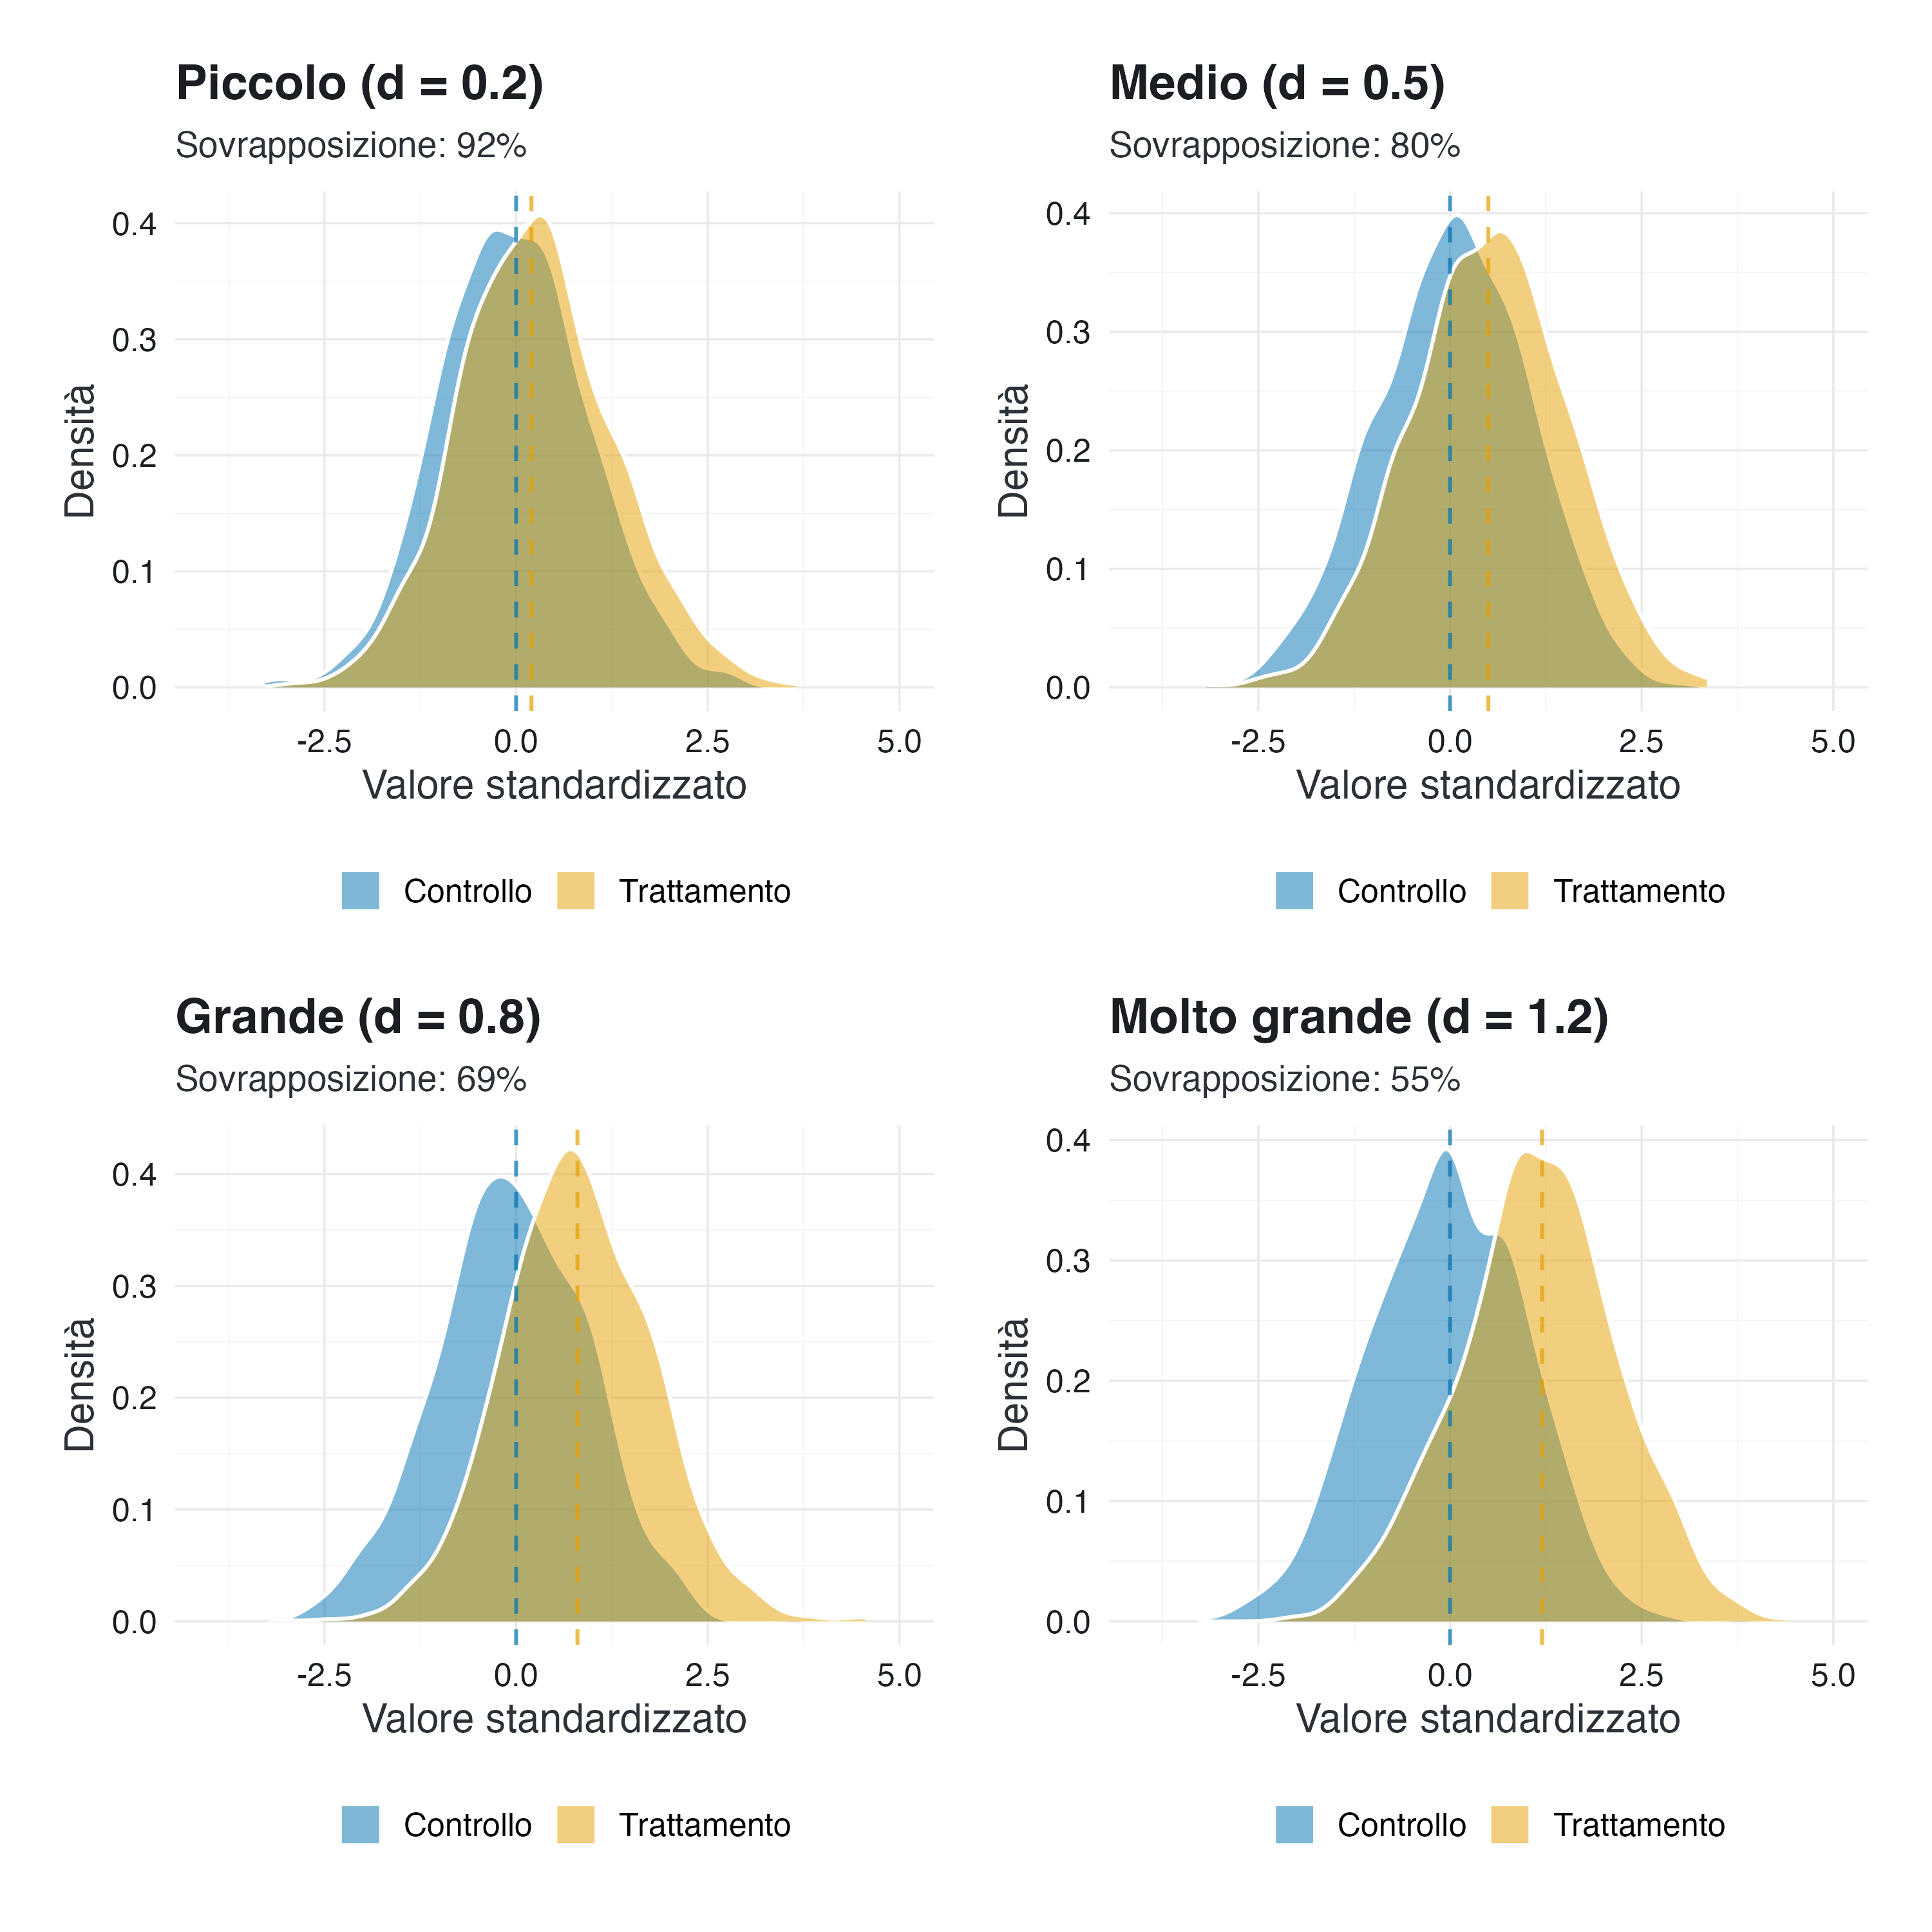
\includegraphics[width=1\linewidth,height=\textheight,keepaspectratio]{chapters/limits/02_effect_size_files/figure-pdf/fig-cohen-d-visual-1.png}

}

\caption{\label{fig-cohen-d-visual}Visualizzazione di diversi valori del
d di Cohen. Con d = 0.2 le distribuzioni si sovrappongono quasi
completamente; con d = 0.8 la separazione è evidente.}

\end{figure}%

\subsection{\texorpdfstring{Interpretare il \(d\) di Cohen: dalla scala
standardizzata all'intuizione
clinica}{Interpretare il d di Cohen: dalla scala standardizzata all'intuizione clinica}}\label{interpretare-il-d-di-cohen-dalla-scala-standardizzata-allintuizione-clinica}

Un modo particolarmente utile per interpretare il coefficiente \(d\) di
Cohen consiste nel tradurlo dalla scala standardizzata a una metrica
intuitivamente comprensibile: \textbf{la probabilità che un individuo
estratto casualmente dal gruppo trattamento ottenga un punteggio
superiore a un individuo estratto casualmente dal gruppo controllo}.
Questa metrica, nota come \emph{Common Language Effect Size} (CLES),
trasforma un effetto espresso in unità di deviazione standard in
un'indicazione probabilistica immediatamente interpretabile.

La relazione tra \(d\) e la CLES è matematicamente definita: \[
\text{CLES} = \Phi\left(\frac{d}{\sqrt{2}}\right)
\] dove \(\Phi\) rappresenta la funzione di distribuzione cumulativa
della distribuzione normale standard.

Questa trasformazione offre diversi vantaggi interpretativi:

\begin{enumerate}
\def\labelenumi{\arabic{enumi}.}
\item
  \textbf{Intuizione immediata}: mentre ``d = 0.5'' può risultare
  astratto, affermare che ``il 64\% degli individui del gruppo
  trattamento supera il gruppo controllo'' fornisce un'immagine concreta
  della differenza tra i gruppi.
\item
  \textbf{Comunicazione efficace}: la CLES rappresenta un linguaggio
  comune comprensibile a ricercatori, clinici, pazienti e decisori
  politici, indipendentemente dalla loro familiarità con la statistica
  inferenziale.
\item
  \textbf{Valutazione contestuale}: permette di valutare l'effetto in
  termini di sovrapposizione tra le distribuzioni dei due gruppi,
  offrendo una visione più completa della separazione tra le
  popolazioni.
\end{enumerate}

Questa traduzione probabilistica risulta particolarmente preziosa in
contesti applicati, come la psicologia clinica, dove la rilevanza
pratica di un intervento si valuta nei termini della sua capacità di
produrre differenze clinicamente rilevanti nella vita reale delle
persone.

\begin{Shaded}
\begin{Highlighting}[]
\CommentTok{\# Funzione per calcolare CLES da Cohen\textquotesingle{}s d}
\NormalTok{cles }\OtherTok{\textless{}{-}} \ControlFlowTok{function}\NormalTok{(d) \{}
  \FunctionTok{pnorm}\NormalTok{(d }\SpecialCharTok{/} \FunctionTok{sqrt}\NormalTok{(}\DecValTok{2}\NormalTok{))}
\NormalTok{\}}

\CommentTok{\# Funzione per calcolare la percentuale di non{-}sovrapposizione}
\NormalTok{non\_overlap }\OtherTok{\textless{}{-}} \ControlFlowTok{function}\NormalTok{(d) \{}
  \DecValTok{2} \SpecialCharTok{*} \FunctionTok{pnorm}\NormalTok{(}\FunctionTok{abs}\NormalTok{(d) }\SpecialCharTok{/} \DecValTok{2}\NormalTok{) }\SpecialCharTok{{-}} \DecValTok{1}
\NormalTok{\}}

\FunctionTok{tibble}\NormalTok{(}
  \StringTok{\textasciigrave{}}\AttributeTok{Cohen\textquotesingle{}s d}\StringTok{\textasciigrave{}} \OtherTok{=} \FunctionTok{c}\NormalTok{(}\FloatTok{0.0}\NormalTok{, }\FloatTok{0.2}\NormalTok{, }\FloatTok{0.5}\NormalTok{, }\FloatTok{0.8}\NormalTok{, }\FloatTok{1.0}\NormalTok{, }\FloatTok{1.5}\NormalTok{, }\FloatTok{2.0}\NormalTok{),}
  \StringTok{\textasciigrave{}}\AttributeTok{Etichetta Cohen}\StringTok{\textasciigrave{}} \OtherTok{=} \FunctionTok{c}\NormalTok{(}\StringTok{"Nullo"}\NormalTok{, }\StringTok{"Piccolo"}\NormalTok{, }\StringTok{"Medio"}\NormalTok{, }\StringTok{"Grande"}\NormalTok{, }
                        \StringTok{"Grande"}\NormalTok{, }\StringTok{"Molto grande"}\NormalTok{, }\StringTok{"Enorme"}\NormalTok{),}
  \StringTok{\textasciigrave{}}\AttributeTok{CLES}\StringTok{\textasciigrave{}} \OtherTok{=} \FunctionTok{sprintf}\NormalTok{(}\StringTok{"\%.1f\%\%"}\NormalTok{, }\FunctionTok{cles}\NormalTok{(}\StringTok{\textasciigrave{}}\AttributeTok{Cohen\textquotesingle{}s d}\StringTok{\textasciigrave{}}\NormalTok{) }\SpecialCharTok{*} \DecValTok{100}\NormalTok{),}
  \StringTok{\textasciigrave{}}\AttributeTok{Interpretazione CLES}\StringTok{\textasciigrave{}} \OtherTok{=} \FunctionTok{c}\NormalTok{(}
    \StringTok{"50\% (come il caso)"}\NormalTok{,}
    \StringTok{"56\% supera il controllo"}\NormalTok{,}
    \StringTok{"64\% supera il controllo"}\NormalTok{, }
    \StringTok{"71\% supera il controllo"}\NormalTok{,}
    \StringTok{"76\% supera il controllo"}\NormalTok{,}
    \StringTok{"86\% supera il controllo"}\NormalTok{,}
    \StringTok{"92\% supera il controllo"}
\NormalTok{  )}
\NormalTok{) }\SpecialCharTok{|\textgreater{}}
\NormalTok{  knitr}\SpecialCharTok{::}\FunctionTok{kable}\NormalTok{()}
\end{Highlighting}
\end{Shaded}

{

\begin{longtable}[]{@{}rlll@{}}

\caption{\label{tbl-cles}Traduzione del d di Cohen in probabilità
interpretabili}

\tabularnewline

\toprule\noalign{}
Cohen's d & Etichetta Cohen & CLES & Interpretazione CLES \\
\midrule\noalign{}
\endhead
\bottomrule\noalign{}
\endlastfoot
0.0 & Nullo & 50.0\% & 50\% (come il caso) \\
0.2 & Piccolo & 55.6\% & 56\% supera il controllo \\
0.5 & Medio & 63.8\% & 64\% supera il controllo \\
0.8 & Grande & 71.4\% & 71\% supera il controllo \\
1.0 & Grande & 76.0\% & 76\% supera il controllo \\
1.5 & Molto grande & 85.6\% & 86\% supera il controllo \\
2.0 & Enorme & 92.1\% & 92\% supera il controllo \\

\end{longtable}

}

La traduzione di \(d\) nella probabilità di superiorità offre
un'immagine concreta della rilevanza pratica degli effetti
standardizzati:

\textbf{Per un effetto ``piccolo'' (\(d = 0.2\))}:\\
se selezioniamo casualmente un individuo dal gruppo di trattamento e uno
dal gruppo di controllo, l'individuo trattato presenterà un punteggio
superiore solo nel 56\% dei casi. Questa proporzione supera di soli 6
punti percentuali il puro caso (50\%), rappresentando una differenza
appena percettibile nella pratica quotidiana.

\textbf{Per un effetto ``grande'' (\(d = 0.8\))}:\\
la stessa operazione produce risultati sensibilmente diversi:
l'individuo trattato otterrà un punteggio superiore nel 71\% dei casi,
indicando una separazione più marcata tra le distribuzioni dei due
gruppi.

Questa traduzione probabilistica mostra come anche gli effetti
classificati come ``grandi'' secondo le convenzioni di Cohen lascino
comunque spazio a una sostanziale sovrapposizione tra i gruppi.
Un'interpretazione che considera esclusivamente la grandezza
standardizzata dell'effetto rischia di sopravvalutare il suo impatto
pratico, mentre la prospettiva della \emph{Common Language Effect Size}
mantiene un ancoraggio realistico alla variabilità individuale e alla
sovrapposizione tra le popolazioni.

\section{\texorpdfstring{Il coefficiente di correlazione \(r\):
comprendere le relazioni
lineari}{Il coefficiente di correlazione r: comprendere le relazioni lineari}}\label{il-coefficiente-di-correlazione-r-comprendere-le-relazioni-lineari}

Il coefficiente di correlazione \(r\) di Pearson quantifica la forza e
la direzione di una relazione lineare tra due variabili continue. La sua
scala varia da -1 (correlazione negativa perfetta) a +1 (correlazione
positiva perfetta), con lo zero che indica assenza di relazione lineare.

Una proprietà importante è la convertibilità tra \(d\) (differenza
standardizzata tra medie) e \(r\) (correlazione):

\[
d = \frac{2r}{\sqrt{1-r^2}} \qquad \text{e} \qquad r = \frac{d}{\sqrt{d^2 + 4}}.
\]

Questa relazione permette di tradurre effetti espressi in una metrica
nell'altra, facilitando confronti tra diverse tradizioni di ricerca.

\subsection{Visualizzazione di correlazioni di diversa
intensità}\label{visualizzazione-di-correlazioni-di-diversa-intensituxe0}

\begin{figure}

\centering{

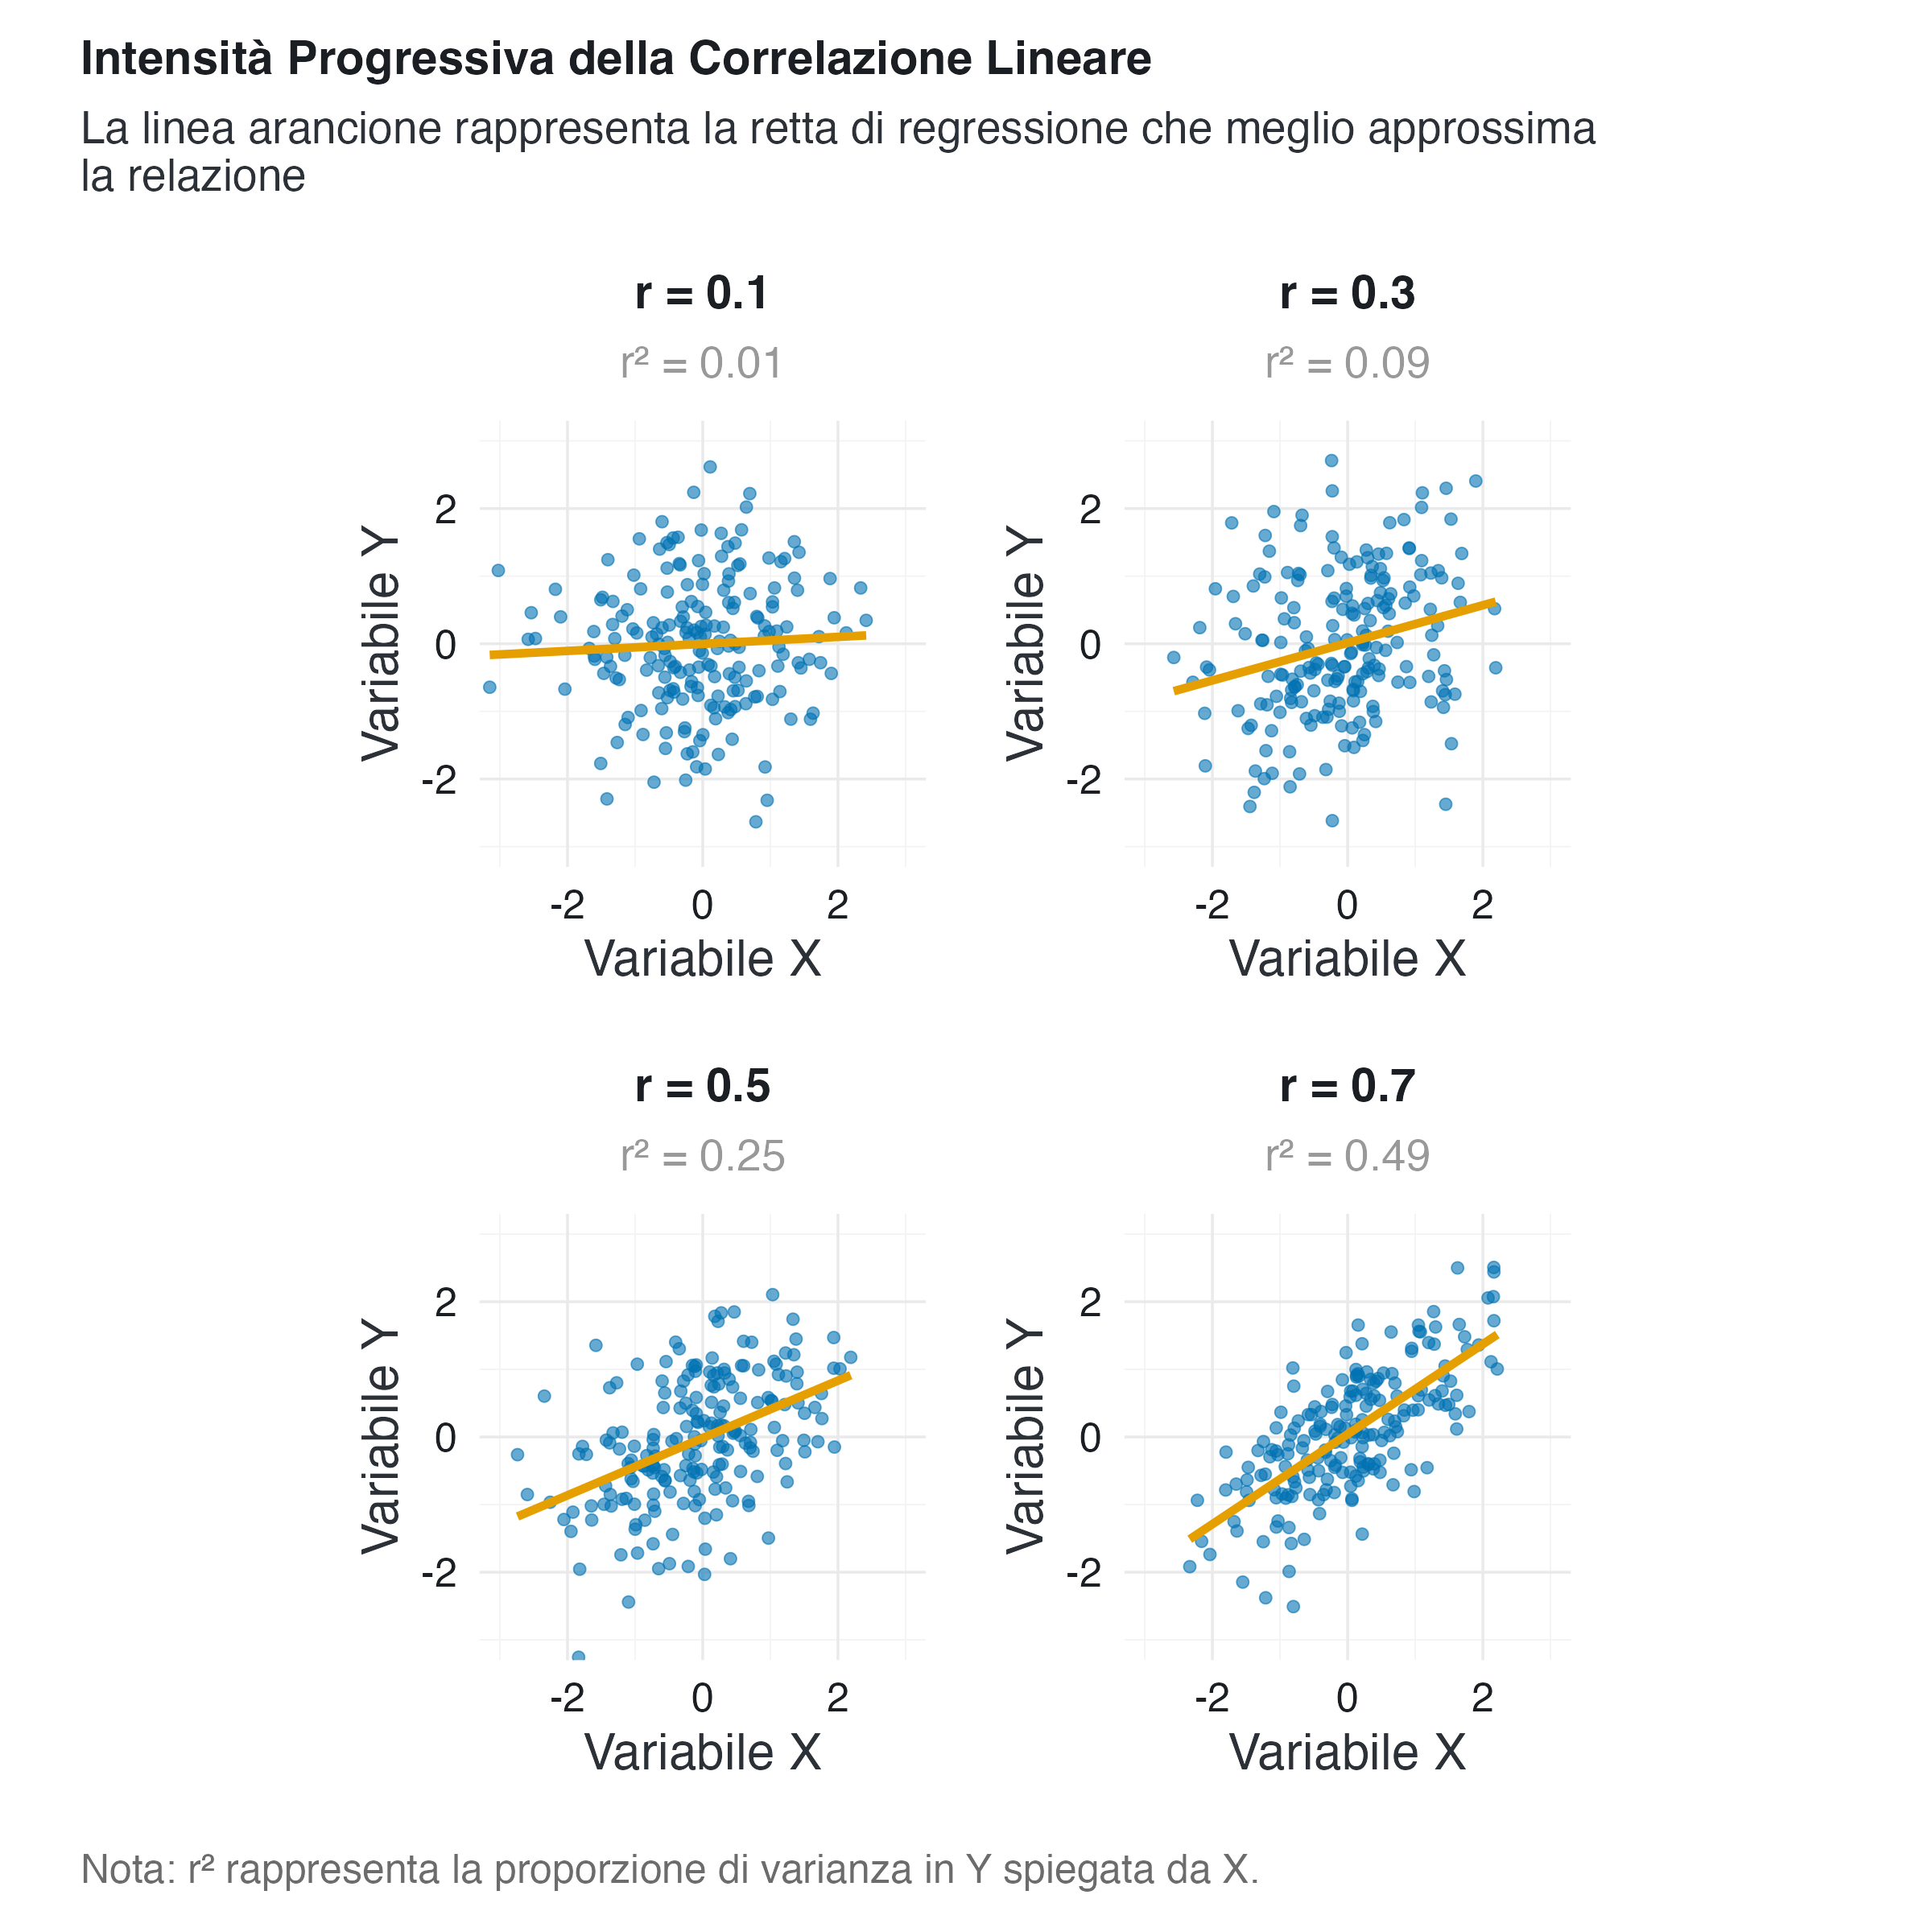
\includegraphics[width=1\linewidth,height=\textheight,keepaspectratio]{chapters/limits/02_effect_size_files/figure-pdf/fig-correlations-visual-1.png}

}

\caption{\label{fig-correlations-visual}Visualizzazione di correlazioni
progressivamente più forti. Con \(r\) = 0.1 la relazione è quasi
impercettibile; con \(r\) = 0.7 emerge un chiaro pattern lineare.}

\end{figure}%

\section{\texorpdfstring{Il problema di \(r^2\): una simulazione
chiarificatrice}{Il problema di r\^{}2: una simulazione chiarificatrice}}\label{il-problema-di-r2-una-simulazione-chiarificatrice}

\subsection{La distorsione quadratica
nell'interpretazione}\label{la-distorsione-quadratica-nellinterpretazione}

Una pratica diffusa nella ricerca applicata consiste nell'elevare al
quadrato il coefficiente di correlazione \(r\) per ottenere \(r^2\),
tipicamente interpretato come ``percentuale di varianza spiegata''.
Sebbene matematicamente corretta, questa trasformazione può distorcere
gravemente la percezione della grandezza relativa degli effetti, creando
interpretazioni fuorvianti.

L'esempio classico di Darlington (1990) illustra in modo illuminante
questa distorsione. Consideriamo un semplice gioco d'azzardo con due
monete:

\begin{itemize}
\tightlist
\item
  Un \textbf{nickel} (5¢): se esce testa, vinci 5 centesimi;
\item
  Un \textbf{dime} (10¢): se esce testa, vinci 10 centesimi.
\end{itemize}

Entrambe le monete sono eque, ma differiscono nel valore del premio.
Calcoliamo le correlazioni tra la probabilità di successo (abilità del
giocatore) e la vincita monetaria:

\begin{Shaded}
\begin{Highlighting}[]
\FunctionTok{set.seed}\NormalTok{(}\DecValTok{123}\NormalTok{)}
\NormalTok{n\_players }\OtherTok{\textless{}{-}} \DecValTok{1000}

\CommentTok{\# Simulazione del gioco delle monete}
\NormalTok{darlington\_simulation }\OtherTok{\textless{}{-}} \FunctionTok{tibble}\NormalTok{(}
  \AttributeTok{player =} \DecValTok{1}\SpecialCharTok{:}\NormalTok{n\_players,}
  \CommentTok{\# Abilità del giocatore (variabile latente che influenza entrambe le monete)}
  \AttributeTok{player\_skill =} \FunctionTok{rnorm}\NormalTok{(n\_players, }\AttributeTok{mean =} \DecValTok{0}\NormalTok{, }\AttributeTok{sd =} \FloatTok{0.5}\NormalTok{),}
  
  \CommentTok{\# Probabilità di successo influenzata dall\textquotesingle{}abilità}
  \AttributeTok{nickel\_success\_prob =} \FloatTok{0.4} \SpecialCharTok{+} \FloatTok{0.2} \SpecialCharTok{*} \FunctionTok{pnorm}\NormalTok{(player\_skill),}
  \AttributeTok{dime\_success\_prob =} \FloatTok{0.4} \SpecialCharTok{+} \FloatTok{0.2} \SpecialCharTok{*} \FunctionTok{pnorm}\NormalTok{(player\_skill),}
  
  \CommentTok{\# Simulazione degli esiti dei lanci}
  \AttributeTok{nickel\_outcome =} \FunctionTok{rbinom}\NormalTok{(n\_players, }\DecValTok{1}\NormalTok{, nickel\_success\_prob),}
  \AttributeTok{dime\_outcome =} \FunctionTok{rbinom}\NormalTok{(n\_players, }\DecValTok{1}\NormalTok{, dime\_success\_prob),}
  
  \CommentTok{\# Vincite monetarie}
  \AttributeTok{nickel\_payout =}\NormalTok{ nickel\_outcome }\SpecialCharTok{*} \DecValTok{5}\NormalTok{,   }\CommentTok{\# 0 o 5 centesimi}
  \AttributeTok{dime\_payout =}\NormalTok{ dime\_outcome }\SpecialCharTok{*} \DecValTok{10}       \CommentTok{\# 0 o 10 centesimi}
\NormalTok{)}

\CommentTok{\# Calcolo delle correlazioni}
\NormalTok{correlation\_results }\OtherTok{\textless{}{-}} \FunctionTok{tibble}\NormalTok{(}
  \AttributeTok{Statistica =} \FunctionTok{c}\NormalTok{(}\StringTok{"Correlazione (r)"}\NormalTok{, }\StringTok{"Coefficiente di determinazione (r²)"}\NormalTok{, }\StringTok{"Vincita attesa per lancio"}\NormalTok{),}
  \AttributeTok{Nickel =} \FunctionTok{c}\NormalTok{(}
    \FunctionTok{sprintf}\NormalTok{(}\StringTok{"\%.3f"}\NormalTok{, }\FunctionTok{cor}\NormalTok{(darlington\_simulation}\SpecialCharTok{$}\NormalTok{player\_skill, darlington\_simulation}\SpecialCharTok{$}\NormalTok{nickel\_payout)),}
    \FunctionTok{sprintf}\NormalTok{(}\StringTok{"\%.3f"}\NormalTok{, }\FunctionTok{cor}\NormalTok{(darlington\_simulation}\SpecialCharTok{$}\NormalTok{player\_skill, darlington\_simulation}\SpecialCharTok{$}\NormalTok{nickel\_payout)}\SpecialCharTok{\^{}}\DecValTok{2}\NormalTok{),}
    \FunctionTok{sprintf}\NormalTok{(}\StringTok{"\%.2f¢"}\NormalTok{, }\FunctionTok{mean}\NormalTok{(darlington\_simulation}\SpecialCharTok{$}\NormalTok{nickel\_payout))}
\NormalTok{  ),}
  \AttributeTok{Dime =} \FunctionTok{c}\NormalTok{(}
    \FunctionTok{sprintf}\NormalTok{(}\StringTok{"\%.3f"}\NormalTok{, }\FunctionTok{cor}\NormalTok{(darlington\_simulation}\SpecialCharTok{$}\NormalTok{player\_skill, darlington\_simulation}\SpecialCharTok{$}\NormalTok{dime\_payout)),}
    \FunctionTok{sprintf}\NormalTok{(}\StringTok{"\%.3f"}\NormalTok{, }\FunctionTok{cor}\NormalTok{(darlington\_simulation}\SpecialCharTok{$}\NormalTok{player\_skill, darlington\_simulation}\SpecialCharTok{$}\NormalTok{dime\_payout)}\SpecialCharTok{\^{}}\DecValTok{2}\NormalTok{),}
    \FunctionTok{sprintf}\NormalTok{(}\StringTok{"\%.2f¢"}\NormalTok{, }\FunctionTok{mean}\NormalTok{(darlington\_simulation}\SpecialCharTok{$}\NormalTok{dime\_payout))}
\NormalTok{  ),}
  \StringTok{\textasciigrave{}}\AttributeTok{Rapporto Dime/Nickel}\StringTok{\textasciigrave{}} \OtherTok{=} \FunctionTok{c}\NormalTok{(}
    \FunctionTok{sprintf}\NormalTok{(}\StringTok{"\%.2f volte"}\NormalTok{, }
            \FunctionTok{cor}\NormalTok{(darlington\_simulation}\SpecialCharTok{$}\NormalTok{player\_skill, darlington\_simulation}\SpecialCharTok{$}\NormalTok{dime\_payout) }\SpecialCharTok{/} 
            \FunctionTok{cor}\NormalTok{(darlington\_simulation}\SpecialCharTok{$}\NormalTok{player\_skill, darlington\_simulation}\SpecialCharTok{$}\NormalTok{nickel\_payout)),}
    \FunctionTok{sprintf}\NormalTok{(}\StringTok{"\%.2f volte"}\NormalTok{, }
\NormalTok{            (}\FunctionTok{cor}\NormalTok{(darlington\_simulation}\SpecialCharTok{$}\NormalTok{player\_skill, darlington\_simulation}\SpecialCharTok{$}\NormalTok{dime\_payout)}\SpecialCharTok{\^{}}\DecValTok{2}\NormalTok{) }\SpecialCharTok{/} 
\NormalTok{            (}\FunctionTok{cor}\NormalTok{(darlington\_simulation}\SpecialCharTok{$}\NormalTok{player\_skill, darlington\_simulation}\SpecialCharTok{$}\NormalTok{nickel\_payout)}\SpecialCharTok{\^{}}\DecValTok{2}\NormalTok{)),}
    \FunctionTok{sprintf}\NormalTok{(}\StringTok{"\%.2f volte"}\NormalTok{, }
            \FunctionTok{mean}\NormalTok{(darlington\_simulation}\SpecialCharTok{$}\NormalTok{dime\_payout) }\SpecialCharTok{/} \FunctionTok{mean}\NormalTok{(darlington\_simulation}\SpecialCharTok{$}\NormalTok{nickel\_payout))}
\NormalTok{  )}
\NormalTok{)}

\CommentTok{\# Visualizzazione della tabella}
\NormalTok{correlation\_results }\SpecialCharTok{|\textgreater{}}
\NormalTok{  knitr}\SpecialCharTok{::}\FunctionTok{kable}\NormalTok{(}
    \AttributeTok{align =} \FunctionTok{c}\NormalTok{(}\StringTok{"l"}\NormalTok{, }\StringTok{"c"}\NormalTok{, }\StringTok{"c"}\NormalTok{, }\StringTok{"c"}\NormalTok{),}
    \AttributeTok{caption =} \StringTok{"Confronto tra nickel e dime: la distorsione introdotta da r²"}
\NormalTok{  ) }\SpecialCharTok{|\textgreater{}}
\NormalTok{  kableExtra}\SpecialCharTok{::}\FunctionTok{kable\_styling}\NormalTok{(}
    \AttributeTok{bootstrap\_options =} \FunctionTok{c}\NormalTok{(}\StringTok{"striped"}\NormalTok{, }\StringTok{"hover"}\NormalTok{),}
    \AttributeTok{full\_width =} \ConstantTok{FALSE}\NormalTok{,}
    \AttributeTok{position =} \StringTok{"center"}
\NormalTok{  )}
\end{Highlighting}
\end{Shaded}

\begin{figure}

\centering{

\begin{longtable}[t]{lccc}
\caption{\label{tab:fig-coins-simulation}Confronto tra nickel e dime: la distorsione introdotta da r²}\\
\toprule
Statistica & Nickel & Dime & Rapporto Dime/Nickel\\
\midrule
Correlazione (r) & 0.032 & 0.099 & 3.05 volte\\
Coefficiente di determinazione (r²) & 0.001 & 0.010 & 9.31 volte\\
Vincita attesa per lancio & 2.35¢ & 5.06¢ & 2.15 volte\\
\bottomrule
\end{longtable}

}

\caption{\label{fig-coins-simulation}Simulazione dell'esempio di
Darlington: r² può produrre interpretazioni fuorvianti sull'importanza
relativa degli effetti.}

\end{figure}%

\subsection{L'Insight critico: la distorsione
quadratica}\label{linsight-critico-la-distorsione-quadratica}

L'esempio rivela l'illusione creata da \(r^2\):

\textbf{La realtà lineare}: il dime paga esattamente il doppio del
nickel (10¢ vs 5¢). Se misuriamo l'effetto dell'abilità del giocatore
attraverso \(r\), troviamo che il dime ha una correlazione
approssimativamente doppia rispetto al nickel.

\textbf{La distorsione quadratica}: quando eleviamo al quadrato per
ottenere \(r^2\), la relazione raddoppiata (×2) diventa quadruplicata
(×4). Se interpretassimo \(r^2\) come misura dell'\,``importanza
relativa'', concluderemmo erroneamente che il dime ``spiega quattro
volte più varianza'' del nickel, suggerendo un'importanza relativa
quadrupla anziché doppia.

\subsection{\texorpdfstring{Visualizzazione della relazione non lineare
tra \(r\) e
\(r^2\)}{Visualizzazione della relazione non lineare tra r e r\^{}2}}\label{visualizzazione-della-relazione-non-lineare-tra-r-e-r2}

\begin{figure}

\centering{

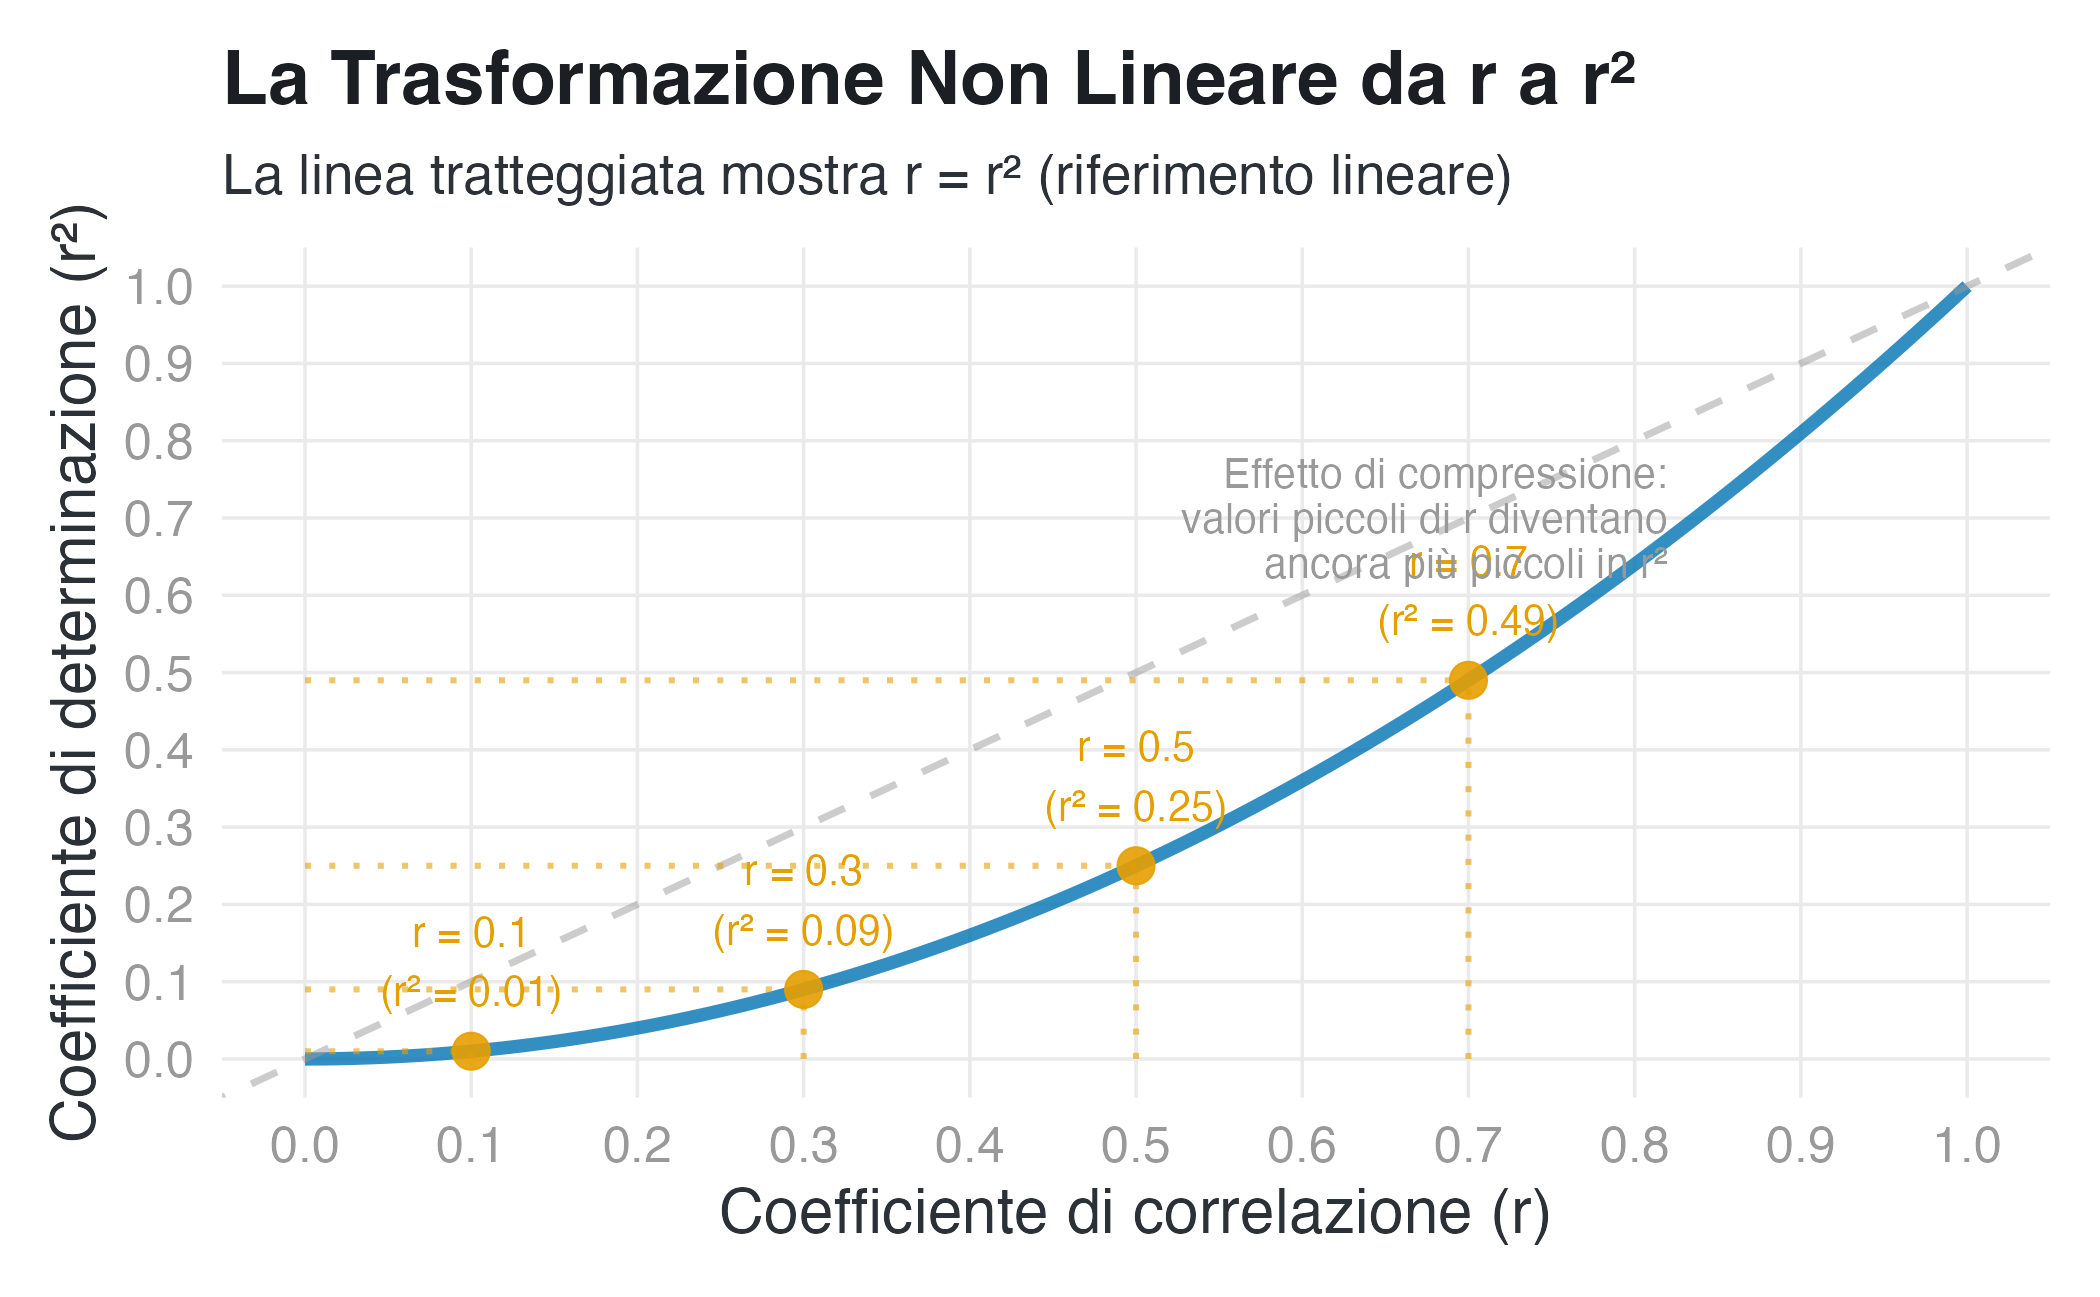
\includegraphics[width=0.85\linewidth,height=\textheight,keepaspectratio]{chapters/limits/02_effect_size_files/figure-pdf/fig-r-vs-r2-1.png}

}

\caption{\label{fig-r-vs-r2}La trasformazione quadratica da r a r²
comprime i valori piccoli e amplifica le differenze relative tra valori
maggiori.}

\end{figure}%

\subsection{Implicazioni per la ricerca
applicata}\label{implicazioni-per-la-ricerca-applicata}

Questa distorsione sistematica ha conseguenze pratiche rilevanti in
diversi contesti di ricerca:

\textbf{1. Confronto di predittori in modelli di regressione.} Quando si
confronta l'importanza relativa di diverse variabili predittive, l'uso
di \(r^2\) può sovrastimare drasticamente il contributo delle variabili
con effetti più forti, distorcendo le conclusioni sui fattori più
rilevanti.

\textbf{2. Meta-analisi e sintesi di evidenze.} L'aggregazione di
effetti attraverso \(r^2\) può produrre stime distorte della grandezza
relativa degli effetti tra studi differenti, compromettendo la validità
delle sintesi quantitative.

\textbf{3. Comunicazione Scientifica.} Presentare \(r^2\) senza il
corrispondente \(r\) può indurre lettori non esperti a conclusioni
errate sull'importanza pratica dei risultati. Ad esempio, un \(r = 0.3\)
(effetto moderato) diventa \(r^2 = 0.09\), che può essere erroneamente
interpretato come ``solo il 9\% di varianza spiegata'' suggerendo un
effetto trascurabile.

In sintesi, l'esempio di Darlington serve come monito metodologico:
mentre \(r^2\) possiede un'interpretazione matematica precisa come
proporzione di varianza spiegata, la sua natura quadratica lo rende uno
strumento problematico per confronti relativi. La correlazione \(r\),
nonostante i suoi limiti, preserva meglio le proporzioni lineari tra
effetti.

La scelta tra \(r\) e \(r^2\) dovrebbe essere guidata dallo scopo
analitico specifico:

\begin{itemize}
\tightlist
\item
  \textbf{per comprendere relazioni lineari e confronti relativi}:
  preferire \(r\);
\item
  \textbf{per quantificare la capacità predittiva in termini di
  riduzione dell'errore}: considerare \(r^2\) insieme a \(r\);
\item
  \textbf{per comunicazioni con pubblico non specialistico}: presentare
  entrambi gli indicatori con spiegazioni chiare.
\end{itemize}

\section{Gli standard di Cohen: utili ma
arbitrari}\label{gli-standard-di-cohen-utili-ma-arbitrari}

Jacob Cohen (1988) propose soglie convenzionali per classificare gli
effetti:

{\def\LTcaptype{none} % do not increment counter
\begin{longtable}[]{@{}llll@{}}
\toprule\noalign{}
Misura & Piccolo & Medio & Grande \\
\midrule\noalign{}
\endhead
\bottomrule\noalign{}
\endlastfoot
\(d\) & 0.20 & 0.50 & 0.80 \\
\(r\) & 0.10 & 0.30 & 0.50 \\
\end{longtable}
}

Tuttavia, in seguito, lo stesso Cohen espresse rammarico per queste
etichette, precisando che dovrebbero essere usate solo in assenza di
criteri migliori. Il problema è che ``piccolo'', ``medio'' e ``grande''
sono privi di significato senza contestualizzazione.

\subsection{\texorpdfstring{Simulazione: lo stesso \(d\) in contesti
diversi}{Simulazione: lo stesso d in contesti diversi}}\label{simulazione-lo-stesso-d-in-contesti-diversi}

\begin{Shaded}
\begin{Highlighting}[]
\CommentTok{\# Scenario 1: Intervento educativo sul QI (SD ≈ 15 punti)}
\CommentTok{\# d = 0.3 → differenza di 4.5 punti QI}

\CommentTok{\# Scenario 2: Farmaco per la pressione (SD ≈ 10 mmHg)}
\CommentTok{\# d = 0.3 → differenza di 3 mmHg}

\CommentTok{\# Scenario 3: Terapia per la depressione (BDI, SD ≈ 10 punti)}
\CommentTok{\# d = 0.3 → differenza di 3 punti BDI}

\NormalTok{contexts }\OtherTok{\textless{}{-}} \FunctionTok{tibble}\NormalTok{(}
  \AttributeTok{Contesto =} \FunctionTok{c}\NormalTok{(}\StringTok{"QI (SD = 15)"}\NormalTok{, }\StringTok{"Pressione arteriosa (SD = 10 mmHg)"}\NormalTok{, }
               \StringTok{"Depressione BDI (SD = 10)"}\NormalTok{),}
  \StringTok{\textasciigrave{}}\AttributeTok{Cohen\textquotesingle{}s d}\StringTok{\textasciigrave{}} \OtherTok{=} \FunctionTok{c}\NormalTok{(}\FloatTok{0.3}\NormalTok{, }\FloatTok{0.3}\NormalTok{, }\FloatTok{0.3}\NormalTok{),}
  \StringTok{\textasciigrave{}}\AttributeTok{Differenza grezza}\StringTok{\textasciigrave{}} \OtherTok{=} \FunctionTok{c}\NormalTok{(}\StringTok{"4.5 punti QI"}\NormalTok{, }\StringTok{"3 mmHg"}\NormalTok{, }\StringTok{"3 punti BDI"}\NormalTok{),}
  \StringTok{\textasciigrave{}}\AttributeTok{Interpretazione clinica}\StringTok{\textasciigrave{}} \OtherTok{=} \FunctionTok{c}\NormalTok{(}
    \StringTok{"Modesta ma rilevante per politiche educative"}\NormalTok{,}
    \StringTok{"Clinicamente rilevante (riduce il rischio cardiovascolare)"}\NormalTok{,}
    \StringTok{"Sotto la soglia di cambiamento clinicamente rilevante (5 punti)"}
\NormalTok{  )}
\NormalTok{)}

\NormalTok{contexts }\SpecialCharTok{|\textgreater{}}
\NormalTok{  knitr}\SpecialCharTok{::}\FunctionTok{kable}\NormalTok{()}
\end{Highlighting}
\end{Shaded}

\begin{figure}

\centering{

{\def\LTcaptype{none} % do not increment counter
\begin{longtable*}[]{@{}
  >{\raggedright\arraybackslash}p{(\linewidth - 6\tabcolsep) * \real{0.2756}}
  >{\raggedleft\arraybackslash}p{(\linewidth - 6\tabcolsep) * \real{0.0787}}
  >{\raggedright\arraybackslash}p{(\linewidth - 6\tabcolsep) * \real{0.1417}}
  >{\raggedright\arraybackslash}p{(\linewidth - 6\tabcolsep) * \real{0.5039}}@{}}
\toprule\noalign{}
\begin{minipage}[b]{\linewidth}\raggedright
Contesto
\end{minipage} & \begin{minipage}[b]{\linewidth}\raggedleft
Cohen's d
\end{minipage} & \begin{minipage}[b]{\linewidth}\raggedright
Differenza grezza
\end{minipage} & \begin{minipage}[b]{\linewidth}\raggedright
Interpretazione clinica
\end{minipage} \\
\midrule\noalign{}
\endhead
\bottomrule\noalign{}
\endlastfoot
QI (SD = 15) & 0.3 & 4.5 punti QI & Modesta ma rilevante per politiche
educative \\
Pressione arteriosa (SD = 10 mmHg) & 0.3 & 3 mmHg & Clinicamente
rilevante (riduce il rischio cardiovascolare) \\
Depressione BDI (SD = 10) & 0.3 & 3 punti BDI & Sotto la soglia di
cambiamento clinicamente rilevante (5 punti) \\
\end{longtable*}
}

}

\caption{\label{fig-context-matters}Lo stesso d = 0.3 ha significati
radicalmente diversi in contesti diversi.}

\end{figure}%

Lo stesso \(d = 0.3\) può essere irrilevante in un contesto e
clinicamente importante in un altro. Per questo è cruciale andare oltre
le etichette di Cohen.

\section{Benchmark empirici: un approccio contestualizzato per
interpretare le dimensioni degli
effetti}\label{benchmark-empirici-un-approccio-contestualizzato-per-interpretare-le-dimensioni-degli-effetti}

Funder \& Ozer (\citeproc{ref-funder2019evaluating}{2019}) propongono
due strategie pragmatiche per interpretare le dimensioni degli effetti
in termini di rilevanza pratica, superando i limiti delle
classificazioni arbitrarie.

\textbf{1. Confronto con effetti noti.}

Piuttosto che ricorrere a etichette arbitrarie (``piccolo'', ``medio'',
``grande''), si confronta il risultato con effetti ben stabiliti nella
letteratura scientifica. Questo approccio fornisce un sistema di
riferimento empirico anziché normativo.

\begin{Shaded}
\begin{Highlighting}[]
\CommentTok{\# Benchmark da Funder \& Ozer (2019) e altre fonti}
\NormalTok{benchmarks }\OtherTok{\textless{}{-}} \FunctionTok{tibble}\NormalTok{(}
  \AttributeTok{Effetto =} \FunctionTok{c}\NormalTok{(}
    \StringTok{"Ibuprofene sul dolore"}\NormalTok{,}
    \StringTok{"Antistaminici sul raffreddore"}\NormalTok{,}
    \StringTok{"Media psicologia sociale (meta{-}analisi 708 studi)"}\NormalTok{,}
    \StringTok{"Genere → altezza"}\NormalTok{,}
    \StringTok{"Psicoterapia → miglioramento sintomi"}\NormalTok{,}
    \StringTok{"Aspirina → prevenzione infarto"}\NormalTok{,}
    \StringTok{"Fumo → cancro ai polmoni"}
\NormalTok{  ),}
  \AttributeTok{r =} \FunctionTok{c}\NormalTok{(}\FloatTok{0.14}\NormalTok{, }\FloatTok{0.11}\NormalTok{, }\FloatTok{0.19}\NormalTok{, }\FloatTok{0.67}\NormalTok{, }\FloatTok{0.32}\NormalTok{, }\FloatTok{0.02}\NormalTok{, }\FloatTok{0.40}\NormalTok{),}
  \AttributeTok{Fonte =} \FunctionTok{c}\NormalTok{(}\StringTok{"Meyer et al., 2001"}\NormalTok{, }\StringTok{"Meyer et al., 2001"}\NormalTok{, }
            \StringTok{"Richard et al., 2003"}\NormalTok{, }\StringTok{"Conoscenza comune"}\NormalTok{,}
            \StringTok{"Smith et al., 1980"}\NormalTok{, }\StringTok{"ISIS{-}2, 1988"}\NormalTok{, }\StringTok{"Doll \& Hill, 1950"}\NormalTok{)}
\NormalTok{) }\SpecialCharTok{|\textgreater{}}
  \FunctionTok{mutate}\NormalTok{(}
    \AttributeTok{d =} \DecValTok{2} \SpecialCharTok{*}\NormalTok{ r }\SpecialCharTok{/} \FunctionTok{sqrt}\NormalTok{(}\DecValTok{1} \SpecialCharTok{{-}}\NormalTok{ r}\SpecialCharTok{\^{}}\DecValTok{2}\NormalTok{),}
    \AttributeTok{Cohen\_label =} \FunctionTok{case\_when}\NormalTok{(}
      \FunctionTok{abs}\NormalTok{(r) }\SpecialCharTok{\textless{}} \FloatTok{0.1} \SpecialCharTok{\textasciitilde{}} \StringTok{"\textless{} Piccolo"}\NormalTok{,}
      \FunctionTok{abs}\NormalTok{(r) }\SpecialCharTok{\textless{}} \FloatTok{0.3} \SpecialCharTok{\textasciitilde{}} \StringTok{"Piccolo"}\NormalTok{,}
      \FunctionTok{abs}\NormalTok{(r) }\SpecialCharTok{\textless{}} \FloatTok{0.5} \SpecialCharTok{\textasciitilde{}} \StringTok{"Medio"}\NormalTok{,}
      \ConstantTok{TRUE} \SpecialCharTok{\textasciitilde{}} \StringTok{"Grande"}
\NormalTok{    )}
\NormalTok{  ) }\SpecialCharTok{|\textgreater{}}
  \FunctionTok{arrange}\NormalTok{(r)}

\NormalTok{palette\_cohen }\OtherTok{\textless{}{-}} \FunctionTok{setNames}\NormalTok{(}
\NormalTok{  palette\_qualitative[}\FunctionTok{c}\NormalTok{(}\DecValTok{8}\NormalTok{, }\DecValTok{2}\NormalTok{, }\DecValTok{5}\NormalTok{, }\DecValTok{1}\NormalTok{)],}
  \FunctionTok{c}\NormalTok{(}\StringTok{"\textless{} Piccolo"}\NormalTok{, }\StringTok{"Piccolo"}\NormalTok{, }\StringTok{"Medio"}\NormalTok{, }\StringTok{"Grande"}\NormalTok{)}
\NormalTok{)}

\FunctionTok{ggplot}\NormalTok{(}
\NormalTok{  benchmarks,}
  \FunctionTok{aes}\NormalTok{(}\AttributeTok{x =}\NormalTok{ r, }\AttributeTok{y =} \FunctionTok{reorder}\NormalTok{(Effetto, r), }\AttributeTok{fill =}\NormalTok{ Cohen\_label)}
\NormalTok{) }\SpecialCharTok{+}
  \FunctionTok{geom\_col}\NormalTok{(}\AttributeTok{alpha =} \FloatTok{0.8}\NormalTok{) }\SpecialCharTok{+}
  \FunctionTok{geom\_vline}\NormalTok{(}
    \AttributeTok{xintercept =} \FunctionTok{c}\NormalTok{(}\FloatTok{0.1}\NormalTok{, }\FloatTok{0.3}\NormalTok{, }\FloatTok{0.5}\NormalTok{),}
    \AttributeTok{linetype =} \StringTok{"dashed"}\NormalTok{,}
    \AttributeTok{color =}\NormalTok{ palette\_qualitative[}\DecValTok{8}\NormalTok{],  }\CommentTok{\# grigio}
    \AttributeTok{alpha =} \FloatTok{0.5}
\NormalTok{  ) }\SpecialCharTok{+}
  \FunctionTok{scale\_fill\_manual}\NormalTok{(}\AttributeTok{values =}\NormalTok{ palette\_cohen) }\SpecialCharTok{+}
  \FunctionTok{labs}\NormalTok{(}
    \AttributeTok{x =} \StringTok{"Correlazione (r)"}\NormalTok{,}
    \AttributeTok{y =} \StringTok{""}\NormalTok{,}
    \AttributeTok{fill =} \StringTok{"Etichetta Cohen"}\NormalTok{,}
    \AttributeTok{title =} \StringTok{"Benchmark empirici per le dimensioni degli effetti"}\NormalTok{,}
    \AttributeTok{subtitle =} \StringTok{"Le linee tratteggiate indicano le soglie di Cohen (0.1, 0.3, 0.5)"}
\NormalTok{  ) }\SpecialCharTok{+}
  \FunctionTok{theme}\NormalTok{(}\AttributeTok{legend.position =} \StringTok{"bottom"}\NormalTok{)}
\end{Highlighting}
\end{Shaded}

\begin{figure}[H]

\centering{

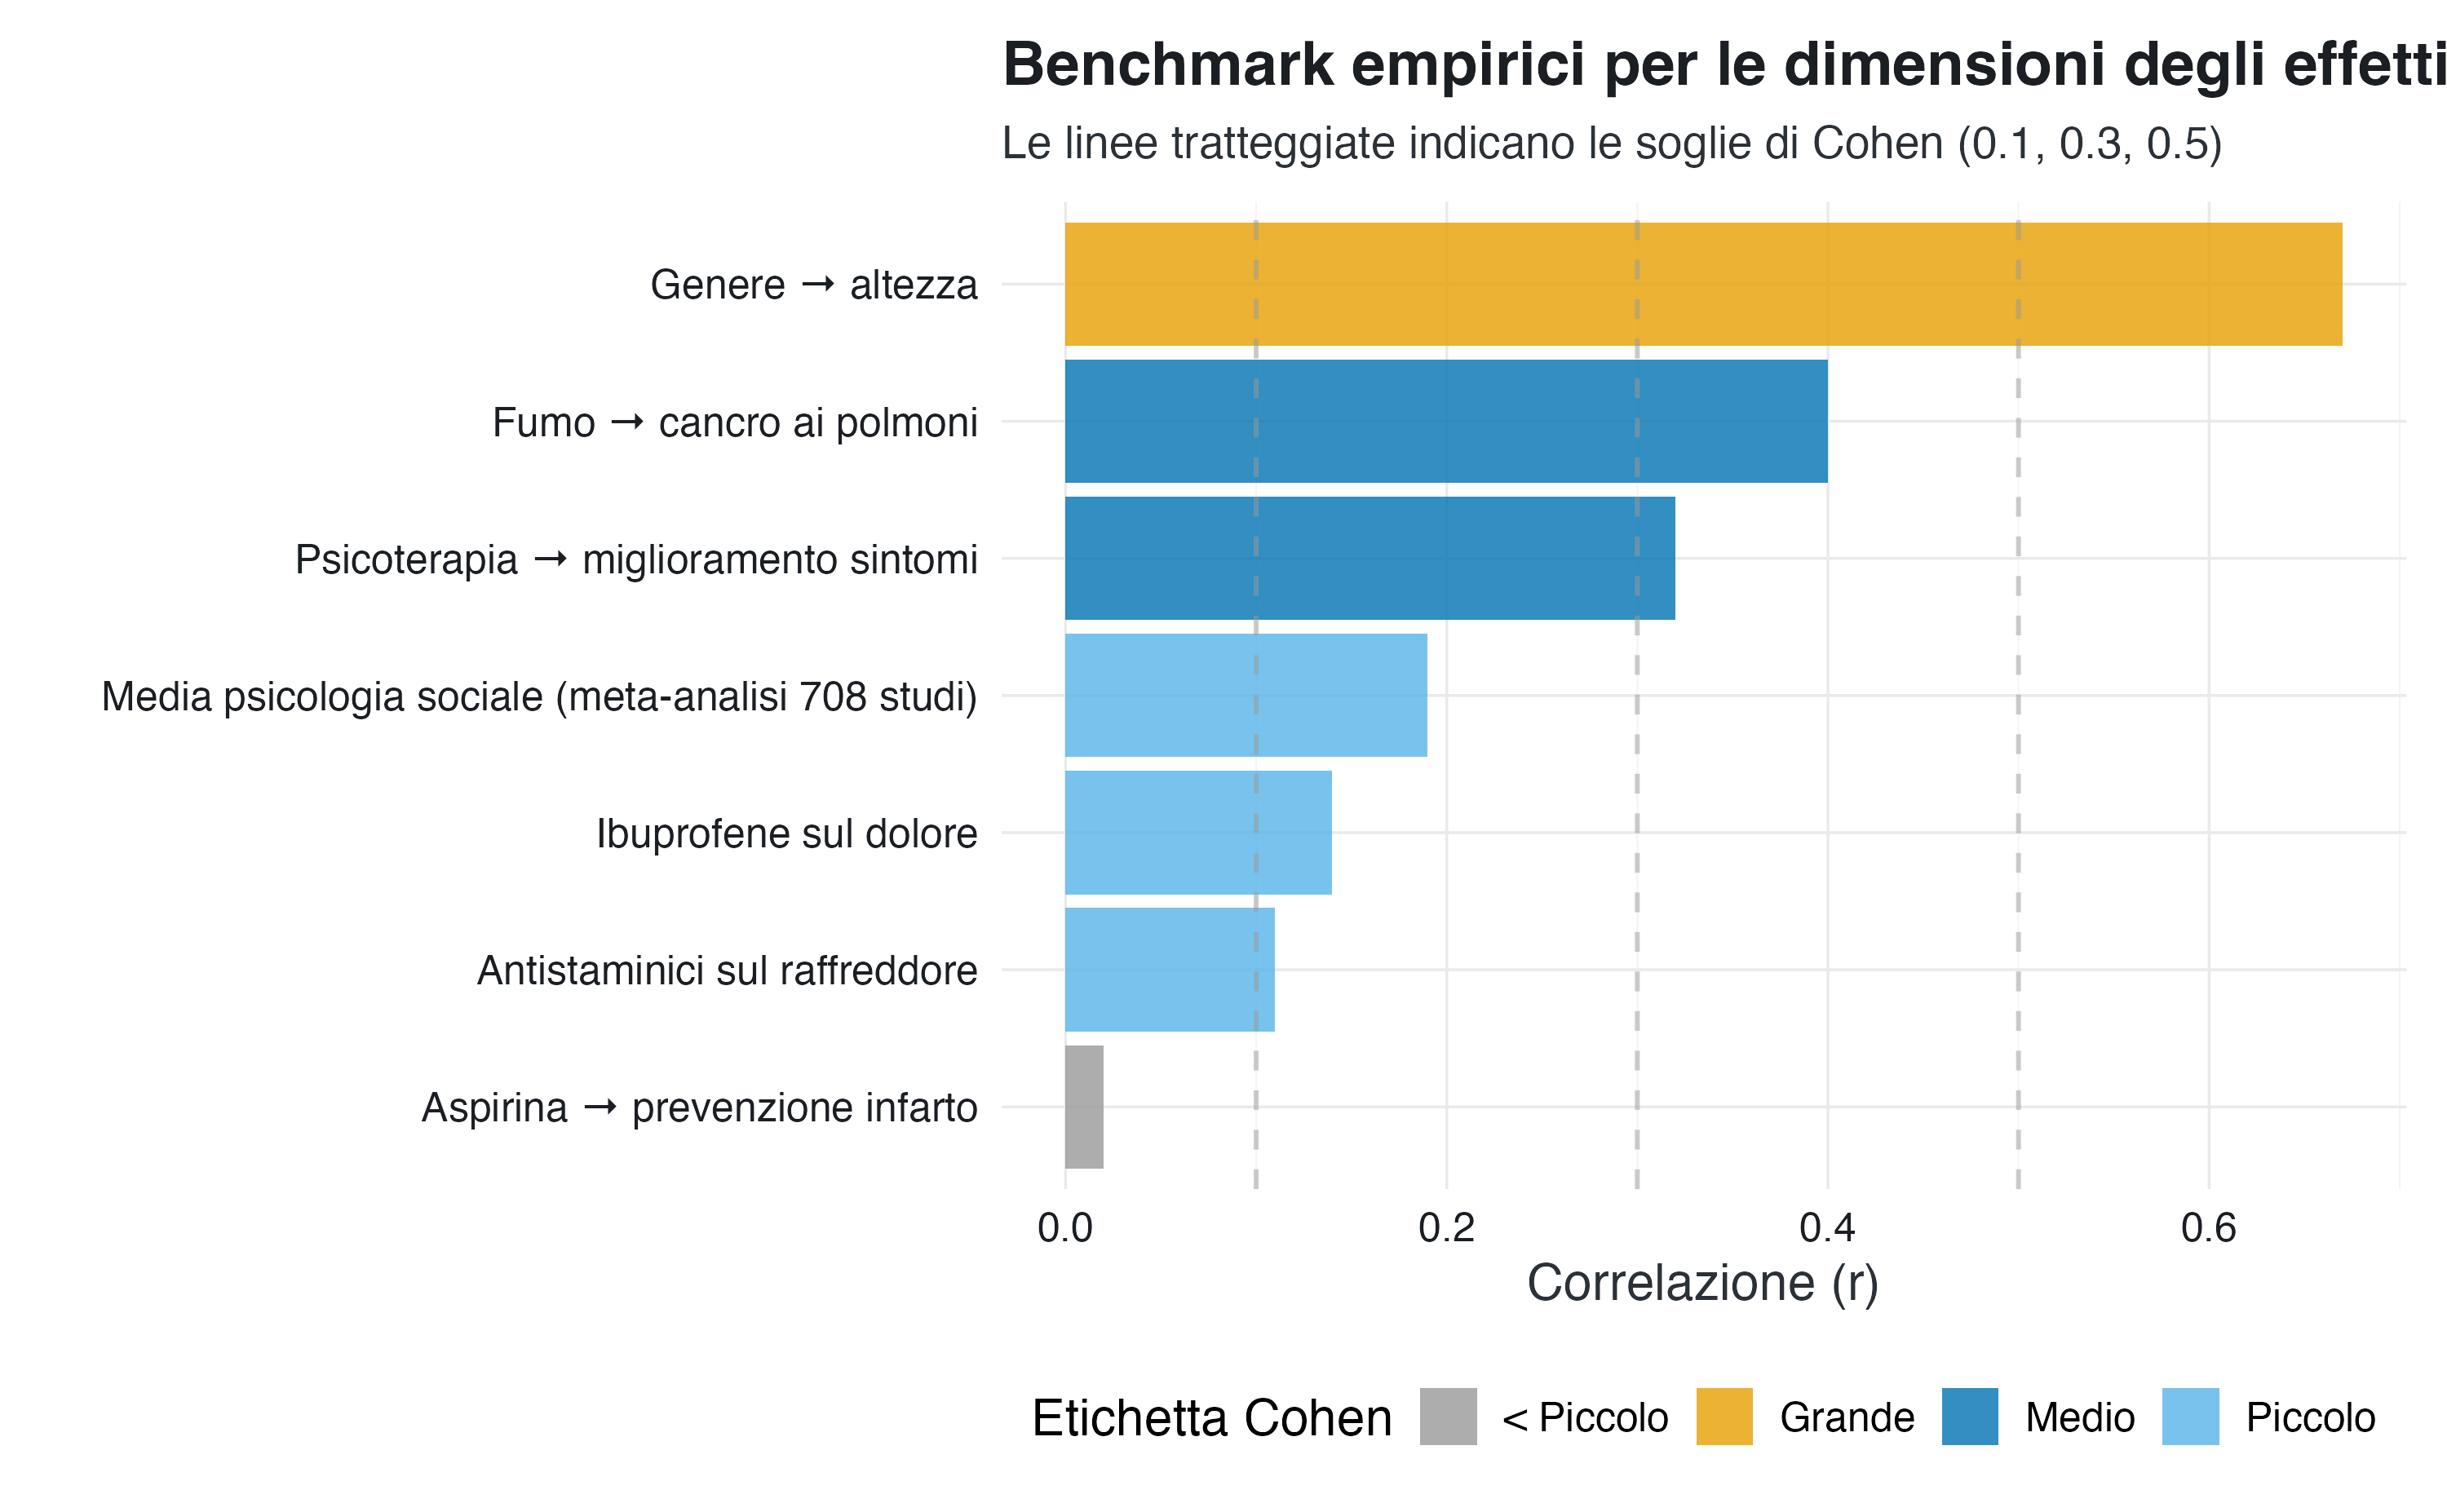
\includegraphics[width=1\linewidth,height=\textheight,keepaspectratio]{chapters/limits/02_effect_size_files/figure-pdf/fig-benchmarks-1.png}

}

\caption{\label{fig-benchmarks}Benchmark empirici per contestualizzare
le dimensioni degli effetti. Il tipico effetto in psicologia sociale (r
= 0.19) è paragonabile all'efficacia dell'ibuprofene sul dolore.}

\end{figure}%

Questi benchmark offrono una prospettiva chiarificatrice. L'effetto
dell'aspirina nella prevenzione dell'infarto (\(r = 0.02\)) è
classificato come ``trascurabile'' secondo le categorie di Cohen, eppure
l'ISIS-2 trial ha dimostrato che salva circa 25 vite ogni 1000 pazienti
trattati. Al contrario, molti effetti ``medi'' in psicologia sociale
potrebbero non avere alcuna rilevanza pratica.

\textbf{2. L'importanza degli effetti cumulativi.}

Un effetto statisticamente modesto può generare conseguenze sostanziali
quando applicato su larga scala o quando si accumula nel tempo. Questa
prospettiva è particolarmente rilevante per le politiche pubbliche e gli
interventi a livello di popolazione.

\begin{Shaded}
\begin{Highlighting}[]
\CommentTok{\# Simulazione: effetto di un intervento educativo su larga scala}
\NormalTok{n\_students }\OtherTok{\textless{}{-}} \FunctionTok{c}\NormalTok{(}\DecValTok{100}\NormalTok{, }\DecValTok{1000}\NormalTok{, }\DecValTok{10000}\NormalTok{, }\DecValTok{100000}\NormalTok{, }\DecValTok{1000000}\NormalTok{)}
\NormalTok{effect\_r }\OtherTok{\textless{}{-}} \FloatTok{0.10}
\NormalTok{effect\_d }\OtherTok{\textless{}{-}} \DecValTok{2} \SpecialCharTok{*}\NormalTok{ effect\_r }\SpecialCharTok{/} \FunctionTok{sqrt}\NormalTok{(}\DecValTok{1} \SpecialCharTok{{-}}\NormalTok{ effect\_r}\SpecialCharTok{\^{}}\DecValTok{2}\NormalTok{)}

\CommentTok{\# Assumiamo che "successo" significhi superare una soglia (es. promozione)}
\CommentTok{\# Baseline: 50\% di successo}
\CommentTok{\# Con l\textquotesingle{}intervento: la distribuzione si sposta di d}

\NormalTok{baseline\_success }\OtherTok{\textless{}{-}} \FloatTok{0.50}
\NormalTok{intervention\_success }\OtherTok{\textless{}{-}} \FunctionTok{pnorm}\NormalTok{(}\FunctionTok{qnorm}\NormalTok{(baseline\_success) }\SpecialCharTok{+}\NormalTok{ effect\_d)}

\NormalTok{cumulative }\OtherTok{\textless{}{-}} \FunctionTok{tibble}\NormalTok{(}
  \StringTok{\textasciigrave{}}\AttributeTok{Studenti totali}\StringTok{\textasciigrave{}} \OtherTok{=}\NormalTok{ scales}\SpecialCharTok{::}\FunctionTok{comma}\NormalTok{(n\_students),}
  \StringTok{\textasciigrave{}}\AttributeTok{Successi baseline}\StringTok{\textasciigrave{}} \OtherTok{=}\NormalTok{ scales}\SpecialCharTok{::}\FunctionTok{comma}\NormalTok{(}\FunctionTok{round}\NormalTok{(n\_students }\SpecialCharTok{*}\NormalTok{ baseline\_success)),}
  \StringTok{\textasciigrave{}}\AttributeTok{Successi con intervento}\StringTok{\textasciigrave{}} \OtherTok{=}\NormalTok{ scales}\SpecialCharTok{::}\FunctionTok{comma}\NormalTok{(}\FunctionTok{round}\NormalTok{(n\_students }\SpecialCharTok{*}\NormalTok{ intervention\_success)),}
  \StringTok{\textasciigrave{}}\AttributeTok{Studenti in più che hanno successo}\StringTok{\textasciigrave{}} \OtherTok{=}\NormalTok{ scales}\SpecialCharTok{::}\FunctionTok{comma}\NormalTok{(}
    \FunctionTok{round}\NormalTok{(n\_students }\SpecialCharTok{*}\NormalTok{ (intervention\_success }\SpecialCharTok{{-}}\NormalTok{ baseline\_success))}
\NormalTok{  )}
\NormalTok{)}

\NormalTok{cumulative }\SpecialCharTok{|\textgreater{}}
\NormalTok{  knitr}\SpecialCharTok{::}\FunctionTok{kable}\NormalTok{()}
\end{Highlighting}
\end{Shaded}

\begin{figure}

\centering{

{\def\LTcaptype{none} % do not increment counter
\begin{longtable*}[]{@{}
  >{\raggedright\arraybackslash}p{(\linewidth - 6\tabcolsep) * \real{0.1720}}
  >{\raggedright\arraybackslash}p{(\linewidth - 6\tabcolsep) * \real{0.1935}}
  >{\raggedright\arraybackslash}p{(\linewidth - 6\tabcolsep) * \real{0.2581}}
  >{\raggedright\arraybackslash}p{(\linewidth - 6\tabcolsep) * \real{0.3763}}@{}}
\toprule\noalign{}
\begin{minipage}[b]{\linewidth}\raggedright
Studenti totali
\end{minipage} & \begin{minipage}[b]{\linewidth}\raggedright
Successi baseline
\end{minipage} & \begin{minipage}[b]{\linewidth}\raggedright
Successi con intervento
\end{minipage} & \begin{minipage}[b]{\linewidth}\raggedright
Studenti in più che hanno successo
\end{minipage} \\
\midrule\noalign{}
\endhead
\bottomrule\noalign{}
\endlastfoot
100 & 50 & 58 & 8 \\
1,000 & 500 & 580 & 80 \\
10,000 & 5,000 & 5,797 & 797 \\
100,000 & 50,000 & 57,965 & 7,965 \\
1,000,000 & 500,000 & 579,654 & 79,654 \\
\end{longtable*}
}

}

\caption{\label{fig-cumulative-effects}Anche un effetto piccolo (r =
0.10) può avere impatti sostanziali se applicato a grandi popolazioni.}

\end{figure}%

La tabella illustra un principio fondamentale: la rilevanza pratica di
un effetto non dipende solo dalla sua grandezza standardizzata, ma anche
dalla scala della sua applicazione.

Con un effetto piccolo (\(r = 0.10\), classificato come ``piccolo''
secondo Cohen), applicato a una scuola di 1000 studenti, si ottengono 40
studenti in più che raggiungono il successo accademico. Estendendo lo
stesso intervento a livello regionale (100,000 studenti), si generano
circa 4,000 successi aggiuntivi. A livello nazionale (1,000,000 di
studenti), l'effetto produce circa 40,000 successi in più.

Questo approccio contestuale sfida tre presupposti comuni.

\begin{itemize}
\tightlist
\item
  Il mito della soglia minima: effetti classificati come ``piccoli'' o
  ``trascurabili'' secondo Cohen possono avere importanza pratica
  sostanziale quando valutati nel loro contesto applicativo.
\item
  La necessità del confronto: l'interpretazione di una dimensione
  dell'effetto è intrinsecamente relativa. Un \(r = 0.20\) è modesto se
  paragonato al fumo come fattore di rischio per il cancro
  (\(r = 0.40\)), ma rilevante se confrontato con l'efficacia di farmaci
  comunemente prescritti.
\item
  L'importanza della scala: la valutazione della rilevanza pratica deve
  considerare non solo la grandezza standardizzata dell'effetto, ma
  anche la popolazione a cui si applica e le conseguenze cumulative nel
  tempo.
\end{itemize}

Questa prospettiva riconcilia la precisione statistica con la rilevanza
pratica, promuovendo una ricerca che non si limita a dimostrare effetti
statisticamente significativi, ma che valuta la loro importanza nel
mondo reale.

\section{Il problema del ``piranha'': effetti troppo grandi per essere
veri}\label{il-problema-del-piranha-effetti-troppo-grandi-per-essere-veri}

Andrew Gelman ha coniato il termine \emph{piranha problem} per
descrivere una contraddizione sistemica nella letteratura psicologica:
se esistessero realmente tutti gli effetti grandi e robusti riportati
negli studi, questi \emph{piranha} statistici si ``mangerebbero a
vicenda'' poiché non esisterebbe sufficiente varianza da spiegare
(\citeproc{ref-tosh2021piranha}{Tosh et al., 2021}).

Il concetto è fondamentalmente aritmetico: il comportamento umano emerge
dall'interazione di innumerevoli fattori genetici, ambientali, culturali
e situazionali. Se ciascuno di questi fattori producesse
indipendentemente un effetto di dimensione media (\(r = 0.30\), secondo
le convenzioni di Cohen), rapidamente supereremmo il 100\% della
varianza spiegabile. La matematica di base dell'analisi della varianza
rende questa situazione impossibile.

\begin{Shaded}
\begin{Highlighting}[]
\CommentTok{\# Simulazione: quanta varianza "consumano" predittori multipli?}
\NormalTok{n\_predictors }\OtherTok{\textless{}{-}} \DecValTok{1}\SpecialCharTok{:}\DecValTok{20}
\NormalTok{r\_each }\OtherTok{\textless{}{-}} \FloatTok{0.30}

\CommentTok{\# Se i predittori fossero indipendenti, R² ≈ n * r²}
\CommentTok{\# (semplificazione per illustrare il concetto)}
\NormalTok{cumulative\_r2 }\OtherTok{\textless{}{-}}\NormalTok{ n\_predictors }\SpecialCharTok{*}\NormalTok{ r\_each}\SpecialCharTok{\^{}}\DecValTok{2}

\NormalTok{col\_main   }\OtherTok{\textless{}{-}}\NormalTok{ palette\_qualitative[}\DecValTok{5}\NormalTok{]  }\CommentTok{\# Blu}
\NormalTok{col\_limit  }\OtherTok{\textless{}{-}}\NormalTok{ palette\_qualitative[}\DecValTok{8}\NormalTok{]  }\CommentTok{\# Grigio}
\NormalTok{col\_marker }\OtherTok{\textless{}{-}}\NormalTok{ palette\_qualitative[}\DecValTok{1}\NormalTok{]  }\CommentTok{\# Arancione}

\FunctionTok{tibble}\NormalTok{(}
  \StringTok{\textasciigrave{}}\AttributeTok{Numero di predittori}\StringTok{\textasciigrave{}} \OtherTok{=}\NormalTok{ n\_predictors,}
  \StringTok{\textasciigrave{}}\AttributeTok{R² cumulativa (se indipendenti)}\StringTok{\textasciigrave{}} \OtherTok{=}\NormalTok{ cumulative\_r2}
\NormalTok{) }\SpecialCharTok{|\textgreater{}}
  \FunctionTok{ggplot}\NormalTok{(}\FunctionTok{aes}\NormalTok{(}\AttributeTok{x =} \StringTok{\textasciigrave{}}\AttributeTok{Numero di predittori}\StringTok{\textasciigrave{}}\NormalTok{, }\AttributeTok{y =} \StringTok{\textasciigrave{}}\AttributeTok{R² cumulativa (se indipendenti)}\StringTok{\textasciigrave{}}\NormalTok{)) }\SpecialCharTok{+}
  \FunctionTok{geom\_line}\NormalTok{(}\AttributeTok{color =}\NormalTok{ col\_main, }\AttributeTok{linewidth =} \FloatTok{1.2}\NormalTok{) }\SpecialCharTok{+}
  \FunctionTok{geom\_point}\NormalTok{(}\AttributeTok{color =}\NormalTok{ col\_main, }\AttributeTok{size =} \DecValTok{2}\NormalTok{) }\SpecialCharTok{+}
  \FunctionTok{geom\_hline}\NormalTok{(}
    \AttributeTok{yintercept =} \DecValTok{1}\NormalTok{,}
    \AttributeTok{color =}\NormalTok{ col\_limit,}
    \AttributeTok{linetype =} \StringTok{"dashed"}\NormalTok{,}
    \AttributeTok{linewidth =} \DecValTok{1}
\NormalTok{  ) }\SpecialCharTok{+}
  \FunctionTok{annotate}\NormalTok{(}
    \StringTok{"text"}\NormalTok{,}
    \AttributeTok{x =} \DecValTok{15}\NormalTok{, }\AttributeTok{y =} \FloatTok{1.1}\NormalTok{,}
    \AttributeTok{label =} \StringTok{"R² = 1 (limite massimo)"}\NormalTok{,}
    \AttributeTok{color =}\NormalTok{ col\_limit,}
    \AttributeTok{hjust =} \DecValTok{0}
\NormalTok{  ) }\SpecialCharTok{+}
  \FunctionTok{geom\_vline}\NormalTok{(}
    \AttributeTok{xintercept =} \DecValTok{1} \SpecialCharTok{/}\NormalTok{ r\_each}\SpecialCharTok{\^{}}\DecValTok{2}\NormalTok{,}
    \AttributeTok{color =}\NormalTok{ col\_marker,}
    \AttributeTok{linetype =} \StringTok{"dotted"}
\NormalTok{  ) }\SpecialCharTok{+}
  \FunctionTok{annotate}\NormalTok{(}
    \StringTok{"text"}\NormalTok{,}
    \AttributeTok{x =} \DecValTok{12}\NormalTok{, }\AttributeTok{y =} \FloatTok{0.5}\NormalTok{,}
    \AttributeTok{label =} \FunctionTok{sprintf}\NormalTok{(}
      \StringTok{"Con r = \%.2f per predittore,}\SpecialCharTok{\textbackslash{}n}\StringTok{bastano \%.0f predittori}\SpecialCharTok{\textbackslash{}n}\StringTok{per \textquotesingle{}esaurire\textquotesingle{} la varianza"}\NormalTok{,}
\NormalTok{      r\_each, }\DecValTok{1} \SpecialCharTok{/}\NormalTok{ r\_each}\SpecialCharTok{\^{}}\DecValTok{2}
\NormalTok{    ),}
    \AttributeTok{color =}\NormalTok{ col\_marker,}
    \AttributeTok{hjust =} \DecValTok{0}
\NormalTok{  ) }\SpecialCharTok{+}
  \FunctionTok{scale\_y\_continuous}\NormalTok{(}\AttributeTok{limits =} \FunctionTok{c}\NormalTok{(}\DecValTok{0}\NormalTok{, }\DecValTok{2}\NormalTok{), }\AttributeTok{breaks =} \FunctionTok{seq}\NormalTok{(}\DecValTok{0}\NormalTok{, }\DecValTok{2}\NormalTok{, }\FloatTok{0.25}\NormalTok{)) }\SpecialCharTok{+}
  \FunctionTok{labs}\NormalTok{(}
    \AttributeTok{title =} \StringTok{"Il \textquotesingle{}Piranha Problem\textquotesingle{}"}\NormalTok{,}
    \AttributeTok{subtitle =} \StringTok{"Se ogni predittore spiega r² = 0.09 della varianza..."}\NormalTok{,}
    \AttributeTok{y =} \StringTok{"R² cumulativa"}
\NormalTok{  )}
\end{Highlighting}
\end{Shaded}

\begin{figure}[H]

\centering{

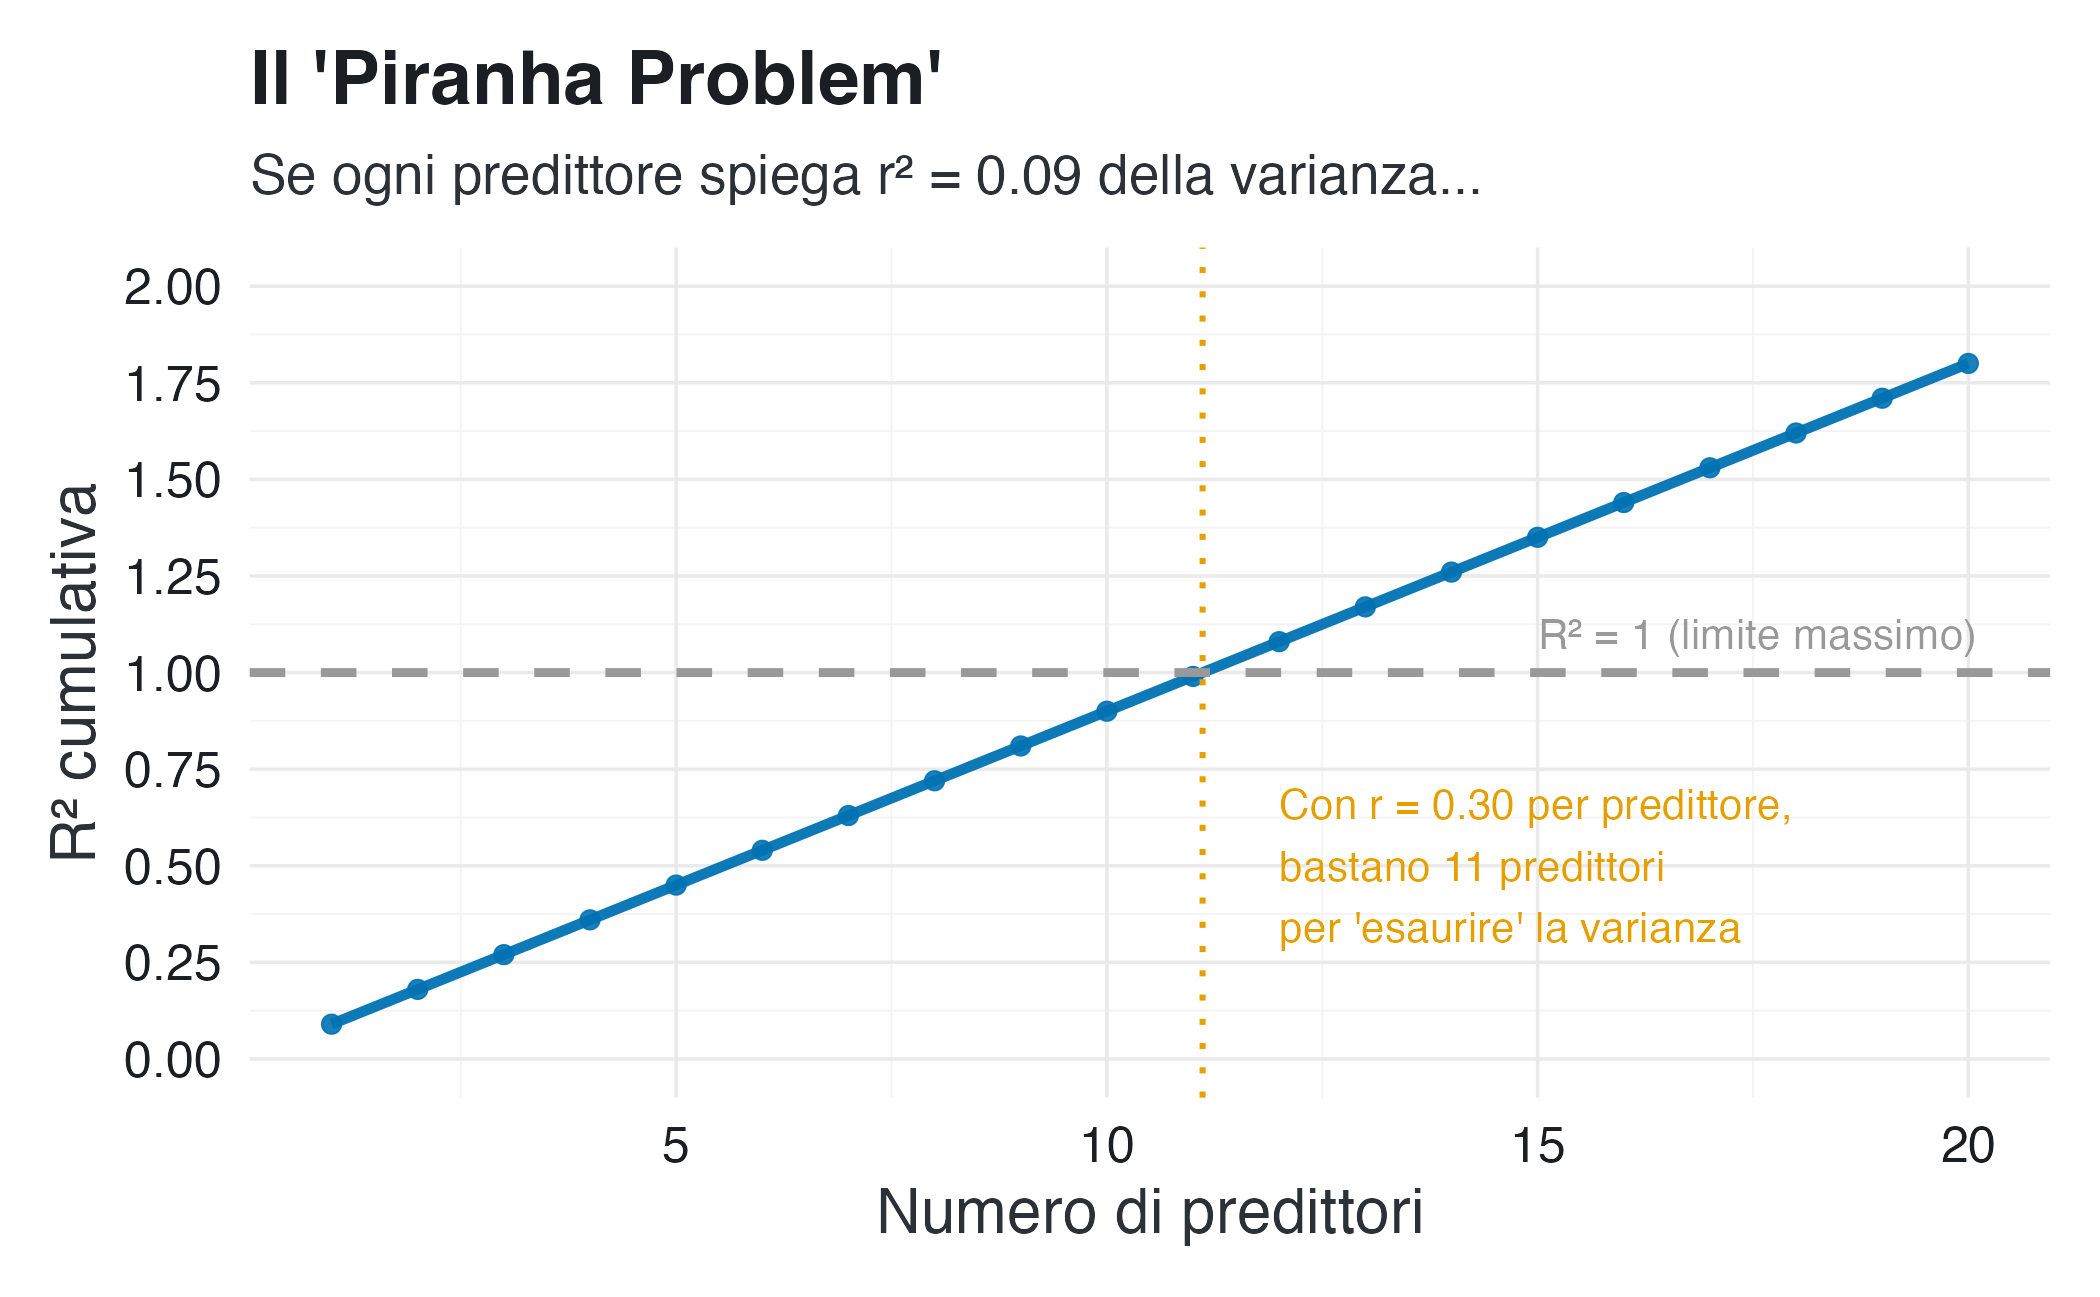
\includegraphics[width=0.85\linewidth,height=\textheight,keepaspectratio]{chapters/limits/02_effect_size_files/figure-pdf/fig-piranha-problem-1.png}

}

\caption{\label{fig-piranha-problem}Il `piranha problem': se esistessero
molti effetti grandi e indipendenti, non resterebbe varianza da
spiegare. Con 10 predittori di r = 0.30, la R² totale supererebbe 1
(impossibile).}

\end{figure}%

\section*{Riflessioni conclusive}\label{riflessioni-conclusive-1}

\markright{Riflessioni conclusive}

La discussione sulla dimensione dell'effetto ha rivelato una verità
semplice ma profonda: non esistono scorciatoie interpretative. Gli
indici statistici standardizzati, come il \(d\) di Cohen e il
coefficiente \(r\), sono strumenti potenti ma ambigui. Questi strumenti
non sono utili quando pretendono di fornire risposte definitive, ma
quando ci aiutano a porre le giuste domande sulla rilevanza pratica e
teorica dei risultati della ricerca.

La standardizzazione, sebbene formalmente elegante, crea
un'\textbf{illusione di comparabilità} che può rivelarsi ingannevole. Un
valore identico di \(d\) in due studi diversi non garantisce un effetto
equivalente, poiché il denominatore, ovvero la deviazione standard, è
una proprietà contingente del campione, della misura e del contesto.
Quando una metrica astratta sostituisce un valore concretamente
interpretabile, come i punti di scala o le unità biologiche, si perde il
legame essenziale tra statistica e fenomeno, favorendo una comunicazione
opaca e confronti privi di fondamento sostanziale.

Questa astrattezza si combina con problemi tecnici insidiosi. Nei
campioni di piccole dimensioni, frequenti in psicologia, la deviazione
standard e, di conseguenza, la stima dell'effetto standardizzato
diventano estremamente instabili. Tale instabilità si intreccia in modo
perverso con il bias di pubblicazione: in un ecosistema che premia la
significatività statistica (\(p\) \textless{} 0.05), gli studi
pubblicati sono spesso quelli in cui una fluttuazione casuale favorevole
(un effetto osservato grande, associato a una stima della variabilità
insolitamente bassa) ha prodotto un risultato ``significativo''. La
standardizzazione cristallizza proprio queste anomalie, producendo una
sovrastima sistematica degli effetti reali nella letteratura (bias di
tipo M). Il \emph{piranha problem} di Gelman descrive l'assurdità logica
di questo processo: se tutti gli effetti grandi riportati fossero reali
e indipendenti, non ci sarebbe più varianza da spiegare.

Anche la scelta della metrica di presentazione è cruciale. L'uso
prevalente di \(r^2\) (``varianza spiegata''), sebbene matematicamente
corretto, esercita un \emph{effetto di compressione psicologica} che
minimizza la percezione degli effetti più modesti. La correlazione
\(r\), unita a traduzioni intuitive come la \emph{Common Language Effect
Size} (CLES), preserva molto meglio le proporzioni lineari e comunica la
forza di una relazione in modo più fedele e immediato.

Alla luce di queste criticità, l'applicazione acritica delle etichette
convenzionali di Cohen (``piccolo'', ``medio'', ``grande'') non solo
appare inadeguata, ma rischia anche di essere fuorviante. Queste soglie
arbitrarie sostituiscono il necessario giudizio scientifico, radicato
nella teoria, nel contesto applicativo e nella conoscenza del dominio,
con un automatismo privo di significato. Ciò che è considerato un
effetto ``piccolo'' in un contesto (come un aumento minimo di un farmaco
salvavita) può essere di importanza cruciale, mentre un effetto
``grande'' in un altro ambito può essere praticamente irrilevante.

\textbf{Verso un'interpretazione contestuale e responsabile}

La via d'uscita da questa impasse non è l'abbandono delle misure di
grandezza dell'effetto, ma la loro \textbf{implementazione consapevole e
contestuale}. Questo richiede:

\begin{enumerate}
\def\labelenumi{\arabic{enumi}.}
\tightlist
\item
  \textbf{preferire la metrica originale}: comunicare i risultati nelle
  unità di misura della ricerca, affiancando le misure standardizzate
  come complemento e non come sostituto. Questo preserva il significato
  pratico e facilita il dialogo con gli \emph{stakeholders}.
\item
  \textbf{utilizzare \emph{benchmark} empirici}: ancorare
  l'interpretazione confrontando l'effetto ottenuto con quello di
  fenomeni noti e ben documentati nella letteratura (ad esempio,
  confrontare l'effetto di un nuovo intervento con l'efficacia
  consolidata della psicoterapia). Questo fornisce un sistema di
  riferimento molto più informativo delle soglie arbitrarie.
\item
  \textbf{valutare la rilevanza pratica}: considerare sistematicamente
  le implicazioni dell'effetto nella sua scala di applicazione. Un
  piccolo effetto applicato a una vasta popolazione, o che si accumula
  nel tempo, può avere un impatto sostanziale.
\item
  \textbf{applicare il ``piranha test''}: mantenere un sano scetticismo
  di fronte a effetti molto grandi, specialmente se multipli e
  dichiarati indipendenti, e chiedere verifiche di robustezza e
  replicazione.
\item
  \textbf{andare oltre il singolo numero}: ricordare che un indice di
  grandezza dell'effetto è una sintesi estrema e inevitabilmente
  riduttiva della complessità osservata. Bisogna indagare la forma della
  relazione (lineare, non lineare), l'eterogeneità tra sottogruppi e i
  meccanismi causali sottostanti.
\end{enumerate}

La statistica bayesiana, che esploreremo in seguito, offre un quadro
concettuale naturale per questo approccio integrato. Essa incoraggia a
esplicitare le conoscenze pregresse (i \emph{benchmark}), quantifica
l'incertezza in modo intuitivo attraverso gli intervalli di credibilità
e sposta il focus dal test di ipotesi dicotomico alla stima quantitativa
e contestualizzata. L'obiettivo finale non è produrre un numero
standardizzato, ma \textbf{costruire un modello interpretabile} che
arricchisca la nostra comprensione della complessità del comportamento
umano, guidando al contempo decisioni informate nella ricerca e nella
pratica.

\section{Esercizi}\label{esercizi-1}

\begin{tcolorbox}[enhanced jigsaw, arc=.35mm, bottomrule=.15mm, bottomtitle=1mm, breakable, colback=white, colbacktitle=quarto-callout-important-color!10!white, colframe=quarto-callout-important-color-frame, coltitle=black, left=2mm, leftrule=.75mm, opacityback=0, opacitybacktitle=0.6, rightrule=.15mm, title=\textcolor{quarto-callout-important-color}{\faExclamation}\hspace{0.5em}{Esercizio 1: Calcolare e visualizzare Cohen's d}, titlerule=0mm, toprule=.15mm, toptitle=1mm]

Hai condotto uno studio su un intervento per migliorare la memoria. I
risultati sono:

\begin{itemize}
\tightlist
\item
  Gruppo controllo: \(M = 45\), \(SD = 12\), \(n = 30\)
\item
  Gruppo intervento: \(M = 51\), \(SD = 14\), \(n = 32\)
\end{itemize}

\begin{enumerate}
\def\labelenumi{\arabic{enumi}.}
\tightlist
\item
  Calcola il \(d\) di Cohen con la formula della pooled SD.
\item
  Calcola il CLES (probabilità che un partecipante del gruppo intervento
  superi uno del controllo).
\item
  Visualizza le due distribuzioni sovrapposte.
\end{enumerate}

\end{tcolorbox}

\begin{tcolorbox}[enhanced jigsaw, arc=.35mm, bottomrule=.15mm, bottomtitle=1mm, breakable, colback=white, colbacktitle=quarto-callout-tip-color!10!white, colframe=quarto-callout-tip-color-frame, coltitle=black, left=2mm, leftrule=.75mm, opacityback=0, opacitybacktitle=0.6, rightrule=.15mm, title=\textcolor{quarto-callout-tip-color}{\faLightbulb}\hspace{0.5em}{Soluzione Esercizio 1}, titlerule=0mm, toprule=.15mm, toptitle=1mm]

\begin{Shaded}
\begin{Highlighting}[]
\CommentTok{\# Dati}
\NormalTok{m1 }\OtherTok{\textless{}{-}} \DecValTok{45}\NormalTok{; sd1 }\OtherTok{\textless{}{-}} \DecValTok{12}\NormalTok{; n1 }\OtherTok{\textless{}{-}} \DecValTok{30}
\NormalTok{m2 }\OtherTok{\textless{}{-}} \DecValTok{51}\NormalTok{; sd2 }\OtherTok{\textless{}{-}} \DecValTok{14}\NormalTok{; n2 }\OtherTok{\textless{}{-}} \DecValTok{32}

\CommentTok{\# 1. Calcolo Cohen\textquotesingle{}s d}
\NormalTok{pooled\_sd }\OtherTok{\textless{}{-}} \FunctionTok{sqrt}\NormalTok{(((n1 }\SpecialCharTok{{-}} \DecValTok{1}\NormalTok{) }\SpecialCharTok{*}\NormalTok{ sd1}\SpecialCharTok{\^{}}\DecValTok{2} \SpecialCharTok{+}\NormalTok{ (n2 }\SpecialCharTok{{-}} \DecValTok{1}\NormalTok{) }\SpecialCharTok{*}\NormalTok{ sd2}\SpecialCharTok{\^{}}\DecValTok{2}\NormalTok{) }\SpecialCharTok{/}\NormalTok{ (n1 }\SpecialCharTok{+}\NormalTok{ n2 }\SpecialCharTok{{-}} \DecValTok{2}\NormalTok{))}
\NormalTok{cohens\_d }\OtherTok{\textless{}{-}}\NormalTok{ (m2 }\SpecialCharTok{{-}}\NormalTok{ m1) }\SpecialCharTok{/}\NormalTok{ pooled\_sd}

\FunctionTok{cat}\NormalTok{(}\FunctionTok{sprintf}\NormalTok{(}\StringTok{"Pooled SD: \%.2f}\SpecialCharTok{\textbackslash{}n}\StringTok{"}\NormalTok{, pooled\_sd))}
\CommentTok{\#\textgreater{} Pooled SD: 13.07}
\FunctionTok{cat}\NormalTok{(}\FunctionTok{sprintf}\NormalTok{(}\StringTok{"Cohen\textquotesingle{}s d: \%.2f}\SpecialCharTok{\textbackslash{}n}\StringTok{"}\NormalTok{, cohens\_d))}
\CommentTok{\#\textgreater{} Cohen\textquotesingle{}s d: 0.46}

\CommentTok{\# 2. CLES}
\NormalTok{cles\_value }\OtherTok{\textless{}{-}} \FunctionTok{pnorm}\NormalTok{(cohens\_d }\SpecialCharTok{/} \FunctionTok{sqrt}\NormalTok{(}\DecValTok{2}\NormalTok{))}
\FunctionTok{cat}\NormalTok{(}\FunctionTok{sprintf}\NormalTok{(}\StringTok{"CLES: \%.1f\%\% (probabilità che intervento \textgreater{} controllo)}\SpecialCharTok{\textbackslash{}n}\StringTok{"}\NormalTok{, cles\_value }\SpecialCharTok{*} \DecValTok{100}\NormalTok{))}
\CommentTok{\#\textgreater{} CLES: 62.7\% (probabilità che intervento \textgreater{} controllo)}

\CommentTok{\# 3. Visualizzazione}
\FunctionTok{tibble}\NormalTok{(}
  \AttributeTok{value =} \FunctionTok{c}\NormalTok{(}\FunctionTok{rnorm}\NormalTok{(}\DecValTok{1000}\NormalTok{, m1, sd1), }\FunctionTok{rnorm}\NormalTok{(}\DecValTok{1000}\NormalTok{, m2, sd2)),}
  \AttributeTok{group =} \FunctionTok{rep}\NormalTok{(}\FunctionTok{c}\NormalTok{(}\StringTok{"Controllo"}\NormalTok{, }\StringTok{"Intervento"}\NormalTok{), }\AttributeTok{each =} \DecValTok{1000}\NormalTok{)}
\NormalTok{) }\SpecialCharTok{|\textgreater{}}
  \FunctionTok{ggplot}\NormalTok{(}\FunctionTok{aes}\NormalTok{(}\AttributeTok{x =}\NormalTok{ value, }\AttributeTok{fill =}\NormalTok{ group)) }\SpecialCharTok{+}
  \FunctionTok{geom\_density}\NormalTok{(}\AttributeTok{alpha =} \FloatTok{0.5}\NormalTok{) }\SpecialCharTok{+}
  \FunctionTok{geom\_vline}\NormalTok{(}\AttributeTok{xintercept =} \FunctionTok{c}\NormalTok{(m1, m2), }\AttributeTok{linetype =} \StringTok{"dashed"}\NormalTok{) }\SpecialCharTok{+}
  \FunctionTok{scale\_fill\_manual}\NormalTok{(}\AttributeTok{values =} \FunctionTok{c}\NormalTok{(}\StringTok{"steelblue"}\NormalTok{, }\StringTok{"coral"}\NormalTok{)) }\SpecialCharTok{+}
  \FunctionTok{labs}\NormalTok{(}
    \AttributeTok{title =} \FunctionTok{sprintf}\NormalTok{(}\StringTok{"d = \%.2f, CLES = \%.1f\%\%"}\NormalTok{, cohens\_d, cles\_value }\SpecialCharTok{*} \DecValTok{100}\NormalTok{),}
    \AttributeTok{x =} \StringTok{"Punteggio memoria"}\NormalTok{,}
    \AttributeTok{y =} \StringTok{"Densità"}
\NormalTok{  )}
\end{Highlighting}
\end{Shaded}

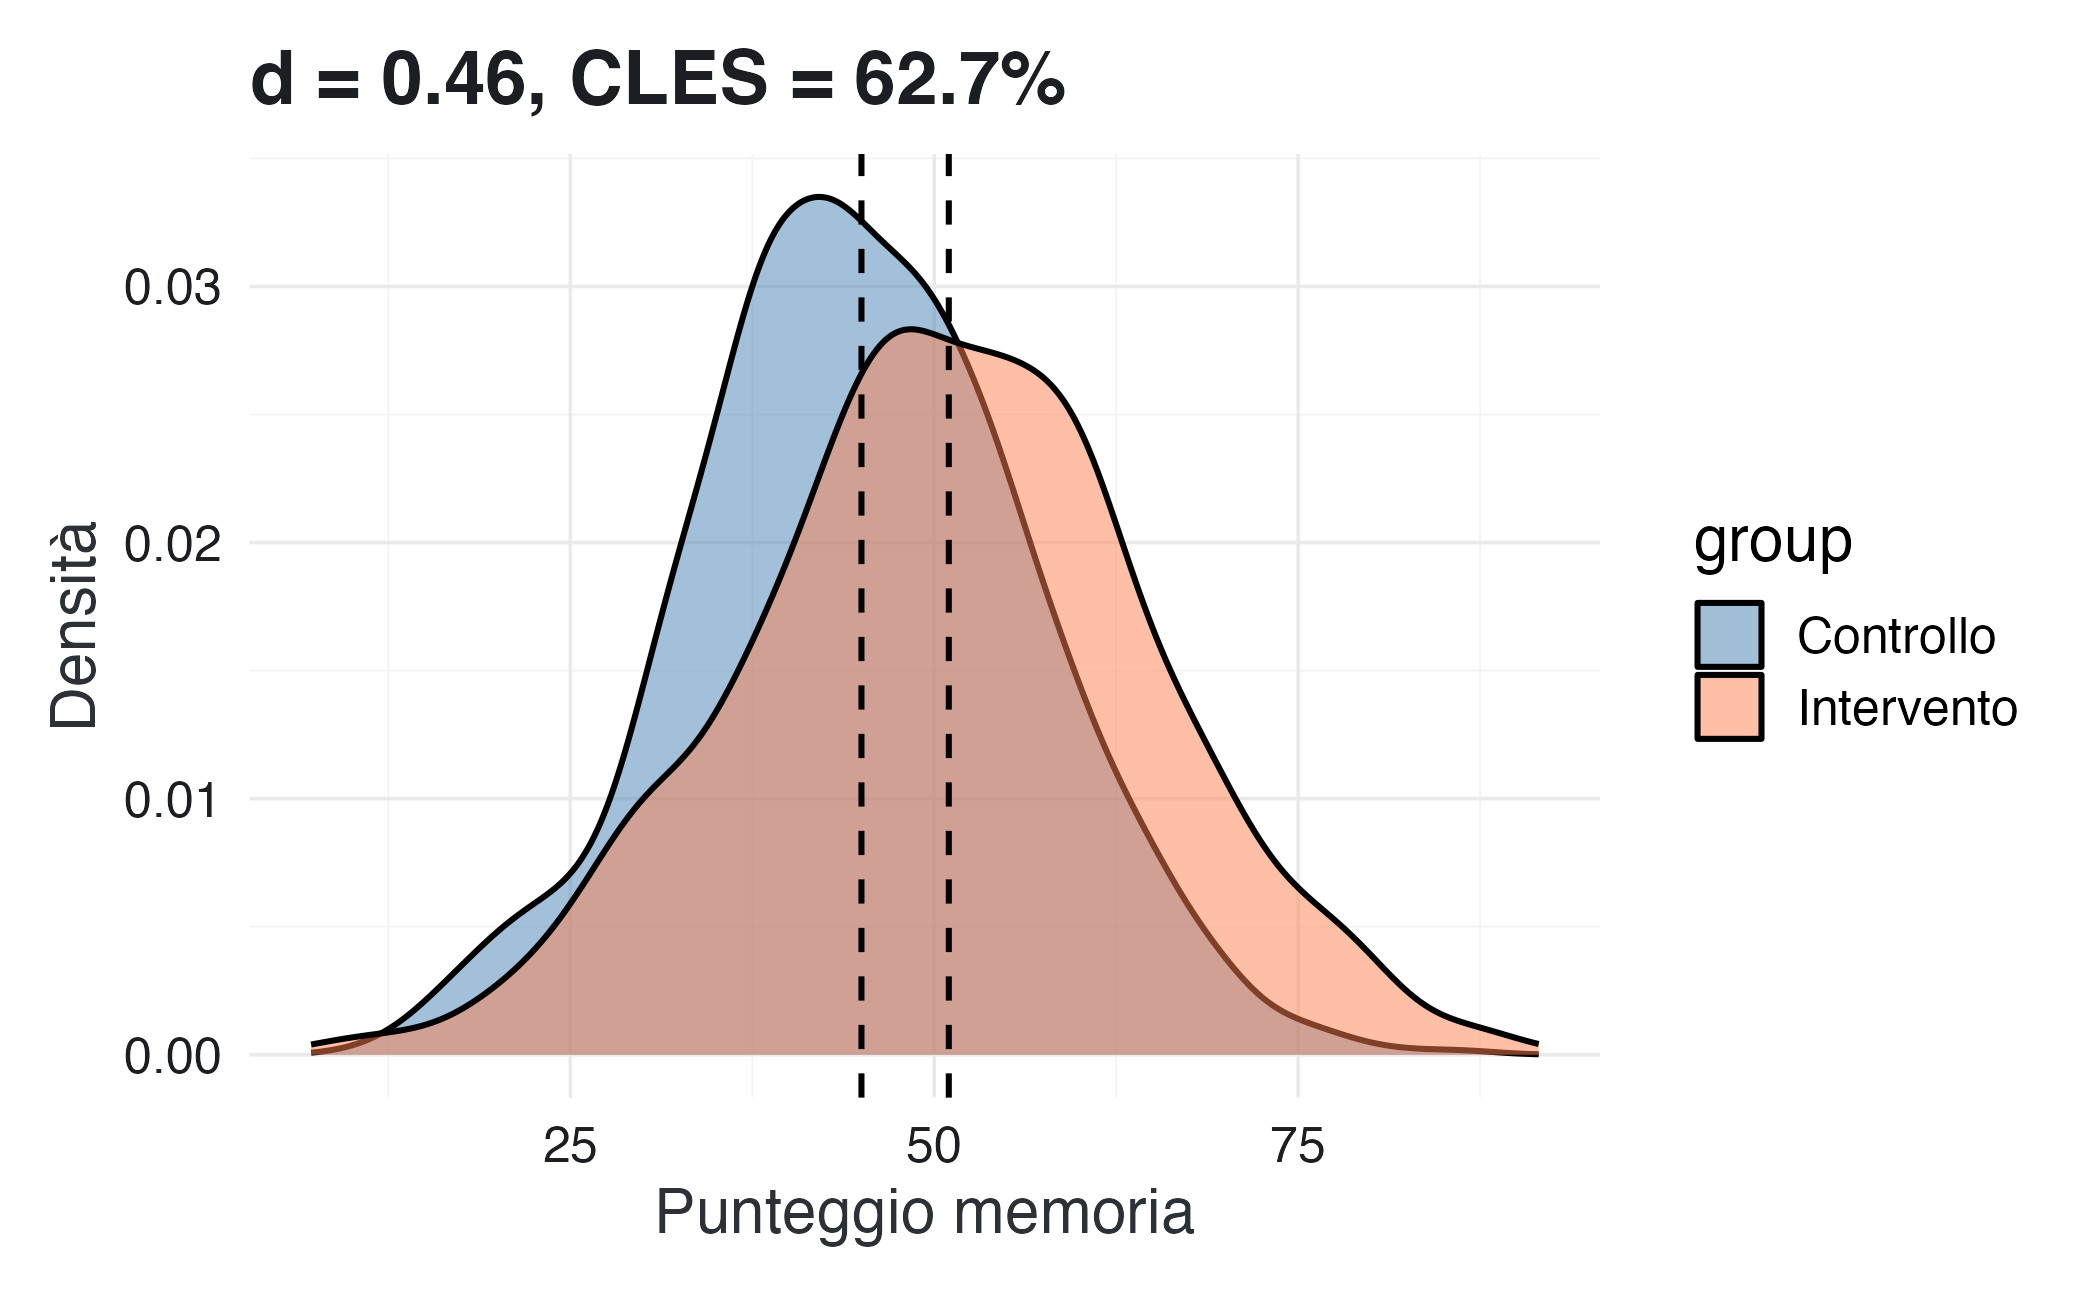
\includegraphics[width=0.85\linewidth,height=\textheight,keepaspectratio]{chapters/limits/02_effect_size_files/figure-pdf/unnamed-chunk-2-1.png}

\end{tcolorbox}

\begin{tcolorbox}[enhanced jigsaw, arc=.35mm, bottomrule=.15mm, bottomtitle=1mm, breakable, colback=white, colbacktitle=quarto-callout-important-color!10!white, colframe=quarto-callout-important-color-frame, coltitle=black, left=2mm, leftrule=.75mm, opacityback=0, opacitybacktitle=0.6, rightrule=.15mm, title=\textcolor{quarto-callout-important-color}{\faExclamation}\hspace{0.5em}{Esercizio 2: r vs r² - Un caso pratico}, titlerule=0mm, toprule=.15mm, toptitle=1mm]

Un ricercatore afferma: ``La correlazione tra ore di studio e voto è r =
0.40, ma questo spiega solo il 16\% della varianza, quindi studiare
conta poco.''

\begin{enumerate}
\def\labelenumi{\arabic{enumi}.}
\tightlist
\item
  Commenta criticamente questa affermazione.
\item
  Calcola quante ore di studio in più servono per aumentare il voto di 1
  punto (assumendo voto medio = 25, SD = 4, ore studio medie = 20, SD =
  10).
\item
  Confronta questo effetto con i benchmark della letteratura.
\end{enumerate}

\end{tcolorbox}

\begin{tcolorbox}[enhanced jigsaw, arc=.35mm, bottomrule=.15mm, bottomtitle=1mm, breakable, colback=white, colbacktitle=quarto-callout-tip-color!10!white, colframe=quarto-callout-tip-color-frame, coltitle=black, left=2mm, leftrule=.75mm, opacityback=0, opacitybacktitle=0.6, rightrule=.15mm, title=\textcolor{quarto-callout-tip-color}{\faLightbulb}\hspace{0.5em}{Soluzione Esercizio 2}, titlerule=0mm, toprule=.15mm, toptitle=1mm]

\begin{Shaded}
\begin{Highlighting}[]
\CommentTok{\# 1. Critica}
\FunctionTok{cat}\NormalTok{(}\StringTok{"L\textquotesingle{}affermazione è fuorviante per tre ragioni:}\SpecialCharTok{\textbackslash{}n\textbackslash{}n}\StringTok{"}\NormalTok{)}
\CommentTok{\#\textgreater{} L\textquotesingle{}affermazione è fuorviante per tre ragioni:}
\FunctionTok{cat}\NormalTok{(}\StringTok{"a) r = 0.40 è un effetto \textquotesingle{}medio{-}grande\textquotesingle{} secondo Cohen}\SpecialCharTok{\textbackslash{}n}\StringTok{"}\NormalTok{)}
\CommentTok{\#\textgreater{} a) r = 0.40 è un effetto \textquotesingle{}medio{-}grande\textquotesingle{} secondo Cohen}
\FunctionTok{cat}\NormalTok{(}\StringTok{"b) r² minimizza sistematicamente l\textquotesingle{}interpretabilità}\SpecialCharTok{\textbackslash{}n}\StringTok{"}\NormalTok{)}
\CommentTok{\#\textgreater{} b) r² minimizza sistematicamente l\textquotesingle{}interpretabilità}
\FunctionTok{cat}\NormalTok{(}\StringTok{"c) Il 16\% di varianza può tradursi in differenze pratiche significative}\SpecialCharTok{\textbackslash{}n\textbackslash{}n}\StringTok{"}\NormalTok{)}
\CommentTok{\#\textgreater{} c) Il 16\% di varianza può tradursi in differenze pratiche significative}

\CommentTok{\# 2. Calcolo pratico}
\NormalTok{r }\OtherTok{\textless{}{-}} \FloatTok{0.40}
\NormalTok{sd\_voto }\OtherTok{\textless{}{-}} \DecValTok{4}
\NormalTok{sd\_ore }\OtherTok{\textless{}{-}} \DecValTok{10}
\NormalTok{mean\_voto }\OtherTok{\textless{}{-}} \DecValTok{25}
\NormalTok{mean\_ore }\OtherTok{\textless{}{-}} \DecValTok{20}

\CommentTok{\# La pendenza della regressione standardizzata è r}
\CommentTok{\# In unità originali: b = r * (SD\_y / SD\_x)}
\NormalTok{b }\OtherTok{\textless{}{-}}\NormalTok{ r }\SpecialCharTok{*}\NormalTok{ (sd\_voto }\SpecialCharTok{/}\NormalTok{ sd\_ore)}
\NormalTok{ore\_per\_punto }\OtherTok{\textless{}{-}} \DecValTok{1} \SpecialCharTok{/}\NormalTok{ b}

\FunctionTok{cat}\NormalTok{(}\FunctionTok{sprintf}\NormalTok{(}\StringTok{"Per ogni ora di studio in più, il voto aumenta di \%.2f punti}\SpecialCharTok{\textbackslash{}n}\StringTok{"}\NormalTok{, b))}
\CommentTok{\#\textgreater{} Per ogni ora di studio in più, il voto aumenta di 0.16 punti}
\FunctionTok{cat}\NormalTok{(}\FunctionTok{sprintf}\NormalTok{(}\StringTok{"Per aumentare il voto di 1 punto, servono \%.1f ore in più}\SpecialCharTok{\textbackslash{}n\textbackslash{}n}\StringTok{"}\NormalTok{, ore\_per\_punto))}
\CommentTok{\#\textgreater{} Per aumentare il voto di 1 punto, servono 6.2 ore in più}

\CommentTok{\# 3. Confronto con benchmark}
\FunctionTok{cat}\NormalTok{(}\StringTok{"Confronto con benchmark:}\SpecialCharTok{\textbackslash{}n}\StringTok{"}\NormalTok{)}
\CommentTok{\#\textgreater{} Confronto con benchmark:}
\FunctionTok{cat}\NormalTok{(}\StringTok{"{-} r = 0.40 è più forte dell\textquotesingle{}effetto medio in psicologia sociale (r = 0.19)}\SpecialCharTok{\textbackslash{}n}\StringTok{"}\NormalTok{)}
\CommentTok{\#\textgreater{} {-} r = 0.40 è più forte dell\textquotesingle{}effetto medio in psicologia sociale (r = 0.19)}
\FunctionTok{cat}\NormalTok{(}\StringTok{"{-} È comparabile all\textquotesingle{}effetto fumo → cancro (r ≈ 0.40)}\SpecialCharTok{\textbackslash{}n}\StringTok{"}\NormalTok{)}
\CommentTok{\#\textgreater{} {-} È comparabile all\textquotesingle{}effetto fumo → cancro (r ≈ 0.40)}
\FunctionTok{cat}\NormalTok{(}\StringTok{"{-} È molto più forte dell\textquotesingle{}effetto aspirina → prevenzione infarto (r = 0.02)}\SpecialCharTok{\textbackslash{}n}\StringTok{"}\NormalTok{)}
\CommentTok{\#\textgreater{} {-} È molto più forte dell\textquotesingle{}effetto aspirina → prevenzione infarto (r = 0.02)}
\end{Highlighting}
\end{Shaded}

\end{tcolorbox}

\begin{tcolorbox}[enhanced jigsaw, arc=.35mm, bottomrule=.15mm, bottomtitle=1mm, breakable, colback=white, colbacktitle=quarto-callout-important-color!10!white, colframe=quarto-callout-important-color-frame, coltitle=black, left=2mm, leftrule=.75mm, opacityback=0, opacitybacktitle=0.6, rightrule=.15mm, title=\textcolor{quarto-callout-important-color}{\faExclamation}\hspace{0.5em}{Esercizio 3: Il piranha test}, titlerule=0mm, toprule=.15mm, toptitle=1mm]

Un articolo afferma di aver trovato 5 predittori indipendenti del
benessere psicologico, ciascuno con \(r = 0.35\):

\begin{enumerate}
\def\labelenumi{\arabic{enumi}.}
\tightlist
\item
  Supporto sociale
\item
  Esercizio fisico\\
\item
  Qualità del sonno
\item
  Reddito
\item
  Ottimismo
\end{enumerate}

Usa il ``piranha test'' per valutare la plausibilità di questi
risultati.

\end{tcolorbox}

\begin{tcolorbox}[enhanced jigsaw, arc=.35mm, bottomrule=.15mm, bottomtitle=1mm, breakable, colback=white, colbacktitle=quarto-callout-tip-color!10!white, colframe=quarto-callout-tip-color-frame, coltitle=black, left=2mm, leftrule=.75mm, opacityback=0, opacitybacktitle=0.6, rightrule=.15mm, title=\textcolor{quarto-callout-tip-color}{\faLightbulb}\hspace{0.5em}{Soluzione Esercizio 3}, titlerule=0mm, toprule=.15mm, toptitle=1mm]

\begin{Shaded}
\begin{Highlighting}[]
\CommentTok{\# Piranha test}
\NormalTok{r }\OtherTok{\textless{}{-}} \FloatTok{0.35}
\NormalTok{n\_predictors }\OtherTok{\textless{}{-}} \DecValTok{5}

\CommentTok{\# R² cumulativa se i predittori fossero indipendenti}
\NormalTok{r2\_each }\OtherTok{\textless{}{-}}\NormalTok{ r}\SpecialCharTok{\^{}}\DecValTok{2}
\NormalTok{r2\_cumulative }\OtherTok{\textless{}{-}}\NormalTok{ n\_predictors }\SpecialCharTok{*}\NormalTok{ r2\_each}

\FunctionTok{cat}\NormalTok{(}\FunctionTok{sprintf}\NormalTok{(}\StringTok{"Ogni predittore \textquotesingle{}spiega\textquotesingle{} r² = \%.2f della varianza}\SpecialCharTok{\textbackslash{}n}\StringTok{"}\NormalTok{, r2\_each))}
\CommentTok{\#\textgreater{} Ogni predittore \textquotesingle{}spiega\textquotesingle{} r² = 0.12 della varianza}
\FunctionTok{cat}\NormalTok{(}\FunctionTok{sprintf}\NormalTok{(}\StringTok{"5 predittori indipendenti spiegherebbero R² = \%.2f}\SpecialCharTok{\textbackslash{}n\textbackslash{}n}\StringTok{"}\NormalTok{, r2\_cumulative))}
\CommentTok{\#\textgreater{} 5 predittori indipendenti spiegherebbero R² = 0.61}

\ControlFlowTok{if}\NormalTok{ (r2\_cumulative }\SpecialCharTok{\textgreater{}} \DecValTok{1}\NormalTok{) \{}
  \FunctionTok{cat}\NormalTok{(}\StringTok{"IMPOSSIBILE: R² \textgreater{} 1!}\SpecialCharTok{\textbackslash{}n}\StringTok{"}\NormalTok{)}
\NormalTok{\} }\ControlFlowTok{else} \ControlFlowTok{if}\NormalTok{ (r2\_cumulative }\SpecialCharTok{\textgreater{}} \FloatTok{0.5}\NormalTok{) \{}
  \FunctionTok{cat}\NormalTok{(}\StringTok{"SOSPETTO: R² \textgreater{} 0.50 per il benessere psicologico è implausibile}\SpecialCharTok{\textbackslash{}n}\StringTok{"}\NormalTok{)}
  \FunctionTok{cat}\NormalTok{(}\StringTok{"Il benessere è influenzato da centinaia di fattori, non solo 5}\SpecialCharTok{\textbackslash{}n}\StringTok{"}\NormalTok{)}
\NormalTok{\}}
\CommentTok{\#\textgreater{} SOSPETTO: R² \textgreater{} 0.50 per il benessere psicologico è implausibile}
\CommentTok{\#\textgreater{} Il benessere è influenzato da centinaia di fattori, non solo 5}

\FunctionTok{cat}\NormalTok{(}\StringTok{"}\SpecialCharTok{\textbackslash{}n}\StringTok{Possibili spiegazioni:}\SpecialCharTok{\textbackslash{}n}\StringTok{"}\NormalTok{)}
\CommentTok{\#\textgreater{} }
\CommentTok{\#\textgreater{} Possibili spiegazioni:}
\FunctionTok{cat}\NormalTok{(}\StringTok{"1. Gli effetti sono sovrastimati (errore di tipo M)}\SpecialCharTok{\textbackslash{}n}\StringTok{"}\NormalTok{)}
\CommentTok{\#\textgreater{} 1. Gli effetti sono sovrastimati (errore di tipo M)}
\FunctionTok{cat}\NormalTok{(}\StringTok{"2. I predittori sono correlati tra loro (multicollinearità)}\SpecialCharTok{\textbackslash{}n}\StringTok{"}\NormalTok{)}
\CommentTok{\#\textgreater{} 2. I predittori sono correlati tra loro (multicollinearità)}
\FunctionTok{cat}\NormalTok{(}\StringTok{"3. Le misure condividono varianza di metodo}\SpecialCharTok{\textbackslash{}n}\StringTok{"}\NormalTok{)}
\CommentTok{\#\textgreater{} 3. Le misure condividono varianza di metodo}
\FunctionTok{cat}\NormalTok{(}\StringTok{"4. P{-}hacking o selezione dei predittori post{-}hoc}\SpecialCharTok{\textbackslash{}n}\StringTok{"}\NormalTok{)}
\CommentTok{\#\textgreater{} 4. P{-}hacking o selezione dei predittori post{-}hoc}
\end{Highlighting}
\end{Shaded}

\end{tcolorbox}

\begin{tcolorbox}[enhanced jigsaw, arc=.35mm, bottomrule=.15mm, bottomtitle=1mm, breakable, colback=white, colbacktitle=quarto-callout-note-color!10!white, colframe=quarto-callout-note-color-frame, coltitle=black, left=2mm, leftrule=.75mm, opacityback=0, opacitybacktitle=0.6, rightrule=.15mm, title=\textcolor{quarto-callout-note-color}{\faInfo}\hspace{0.5em}{Informazioni sull'ambiente di sviluppo}, titlerule=0mm, toprule=.15mm, toptitle=1mm]

\begin{Shaded}
\begin{Highlighting}[]
\FunctionTok{sessionInfo}\NormalTok{()}
\CommentTok{\#\textgreater{} R version 4.6.1 (2026{-}06{-}24)}
\CommentTok{\#\textgreater{} Platform: aarch64{-}apple{-}darwin23}
\CommentTok{\#\textgreater{} Running under: macOS Tahoe 26.5.2}
\CommentTok{\#\textgreater{} }
\CommentTok{\#\textgreater{} Matrix products: default}
\CommentTok{\#\textgreater{} BLAS:   /Library/Frameworks/R.framework/Versions/4.6/Resources/lib/libRblas.0.dylib }
\CommentTok{\#\textgreater{} LAPACK: /Library/Frameworks/R.framework/Versions/4.6/Resources/lib/libRlapack.dylib;  LAPACK version 3.12.1}
\CommentTok{\#\textgreater{} }
\CommentTok{\#\textgreater{} locale:}
\CommentTok{\#\textgreater{} [1] C.UTF{-}8/UTF{-}8/C.UTF{-}8/C/C.UTF{-}8/C.UTF{-}8}
\CommentTok{\#\textgreater{} }
\CommentTok{\#\textgreater{} time zone: Europe/Zagreb}
\CommentTok{\#\textgreater{} tzcode source: internal}
\CommentTok{\#\textgreater{} }
\CommentTok{\#\textgreater{} attached base packages:}
\CommentTok{\#\textgreater{} [1] stats     graphics  grDevices utils     datasets  methods   base     }
\CommentTok{\#\textgreater{} }
\CommentTok{\#\textgreater{} other attached packages:}
\CommentTok{\#\textgreater{}  [1] lubridate\_1.9.5       forcats\_1.0.1         stringr\_1.6.0        }
\CommentTok{\#\textgreater{}  [4] purrr\_1.2.2           readr\_2.2.0           tidyverse\_2.0.0      }
\CommentTok{\#\textgreater{}  [7] ragg\_1.5.2            tinytable\_0.17.0      withr\_3.0.3          }
\CommentTok{\#\textgreater{} [10] systemfonts\_1.3.2     patchwork\_1.3.2       ggdist\_3.3.3         }
\CommentTok{\#\textgreater{} [13] tidybayes\_3.0.7       bayesplot\_1.15.0      ggplot2\_4.0.3        }
\CommentTok{\#\textgreater{} [16] reliabilitydiag\_0.2.1 priorsense\_1.2.0      posterior\_1.7.0      }
\CommentTok{\#\textgreater{} [19] loo\_2.10.0            rstan\_2.32.7          StanHeaders\_2.32.10  }
\CommentTok{\#\textgreater{} [22] brms\_2.23.0           Rcpp\_1.1.2            sessioninfo\_1.2.4    }
\CommentTok{\#\textgreater{} [25] conflicted\_1.2.0      janitor\_2.2.1         matrixStats\_1.5.0    }
\CommentTok{\#\textgreater{} [28] modelr\_0.1.11         tibble\_3.3.1          dplyr\_1.2.1          }
\CommentTok{\#\textgreater{} [31] tidyr\_1.3.2           rio\_1.3.0             here\_1.0.2           }
\CommentTok{\#\textgreater{} }
\CommentTok{\#\textgreater{} loaded via a namespace (and not attached):}
\CommentTok{\#\textgreater{}  [1] gridExtra\_2.3.1       inline\_0.3.21         rlang\_1.3.0          }
\CommentTok{\#\textgreater{}  [4] magrittr\_2.0.5        snakecase\_0.11.1      otel\_0.2.0           }
\CommentTok{\#\textgreater{}  [7] compiler\_4.6.1        mgcv\_1.9{-}4            vctrs\_0.7.3          }
\CommentTok{\#\textgreater{} [10] pkgconfig\_2.0.3       arrayhelpers\_1.1{-}1    fastmap\_1.2.0        }
\CommentTok{\#\textgreater{} [13] backports\_1.5.1       labeling\_0.4.3        rmarkdown\_2.31       }
\CommentTok{\#\textgreater{} [16] tzdb\_0.5.0            xfun\_0.60             cachem\_1.1.0         }
\CommentTok{\#\textgreater{} [19] jsonlite\_2.0.0        broom\_1.0.13          parallel\_4.6.1       }
\CommentTok{\#\textgreater{} [22] R6\_2.6.1              stringi\_1.8.7         RColorBrewer\_1.1{-}3   }
\CommentTok{\#\textgreater{} [25] estimability\_2.0.0    knitr\_1.51            Matrix\_1.7{-}5         }
\CommentTok{\#\textgreater{} [28] splines\_4.6.1         timechange\_0.4.0      tidyselect\_1.2.1     }
\CommentTok{\#\textgreater{} [31] rstudioapi\_0.19.0     abind\_1.4{-}8           yaml\_2.3.12          }
\CommentTok{\#\textgreater{} [34] codetools\_0.2{-}20      curl\_7.1.0            pkgbuild\_1.4.8       }
\CommentTok{\#\textgreater{} [37] lattice\_0.22{-}9        bridgesampling\_1.2{-}1  S7\_0.2.2             }
\CommentTok{\#\textgreater{} [40] coda\_0.19{-}4.1         evaluate\_1.0.5        RcppParallel\_5.1.11{-}2}
\CommentTok{\#\textgreater{} [43] xml2\_1.6.0            pillar\_1.11.1         tensorA\_0.36.2.1     }
\CommentTok{\#\textgreater{} [46] checkmate\_2.3.4       stats4\_4.6.1          distributional\_0.8.1 }
\CommentTok{\#\textgreater{} [49] generics\_0.1.4        rprojroot\_2.1.1       hms\_1.1.4            }
\CommentTok{\#\textgreater{} [52] rstantools\_2.6.0      scales\_1.4.0          xtable\_1.8{-}8         }
\CommentTok{\#\textgreater{} [55] glue\_1.8.1            emmeans\_2.0.4         tools\_4.6.1          }
\CommentTok{\#\textgreater{} [58] mvtnorm\_1.4{-}2         grid\_4.6.1            QuickJSR\_1.10.0      }
\CommentTok{\#\textgreater{} [61] nlme\_3.1{-}170          cli\_3.6.6             kableExtra\_1.4.1     }
\CommentTok{\#\textgreater{} [64] textshaping\_1.0.5     svUnit\_1.0.8          viridisLite\_0.4.3    }
\CommentTok{\#\textgreater{} [67] svglite\_2.2.2         Brobdingnag\_1.2{-}9     V8\_8.2.0             }
\CommentTok{\#\textgreater{} [70] gtable\_0.3.6          digest\_0.6.39         farver\_2.1.2         }
\CommentTok{\#\textgreater{} [73] memoise\_2.0.1         htmltools\_0.5.9       lifecycle\_1.0.5}
\end{Highlighting}
\end{Shaded}

\end{tcolorbox}

\section*{Bibliografia}\label{bibliografia-2}

\markright{Bibliografia}

\chapter{Errori di segno e errori di
grandezza}\label{sec-crisis-s-m-errors}

\begin{tcolorbox}[enhanced jigsaw, arc=.35mm, bottomrule=.15mm, breakable, colback=white, colframe=quarto-callout-note-color-frame, left=2mm, leftrule=.75mm, opacityback=0, rightrule=.15mm, toprule=.15mm]

In questo capitolo analizzeremo la relazione tra la crisi della
replicabilità e le procedure decisionali statistiche proprie
dell'approccio frequentista. In particolare, approfondiremo gli errori
di tipo \emph{M} (\emph{magnitude}) e di tipo \emph{S} (\emph{sign}),
discussi da Loken \& Gelman (\citeproc{ref-loken2017measurement}{2017})
e il loro impatto sulla validità dei risultati scientifici.

\end{tcolorbox}

\begin{tcolorbox}[enhanced jigsaw, arc=.35mm, bottomrule=.15mm, breakable, colback=white, colframe=quarto-callout-important-color-frame, left=2mm, leftrule=.75mm, opacityback=0, rightrule=.15mm, toprule=.15mm]

\textbf{Da sapere.} La selezione dei risultati mediante la soglia
\(p < 0.05\) può produrre stime sistematicamente esagerate e, talvolta,
con direzione errata. Gli errori di tipo \emph{M} descrivono la
sovrastima della grandezza dell'effetto; gli errori di tipo \emph{S}
indicano l'attribuzione del segno sbagliato. Entrambi diventano più
probabili quando gli effetti sono piccoli e la potenza statistica è
bassa.

\textbf{Da saper fare.} Riconoscere e interpretare gli errori di tipo
\emph{M} e \emph{S}; capire la simulazione per quantificarli; spiegare
come cambiano al crescere della dimensione campionaria.

\textbf{Approfondimento facoltativo.} L'implementazione completa delle
simulazioni, il confronto computazionale tra stime frequentiste e
bayesiane e l'analisi sistematica di diverse dimensioni campionarie
possono essere rimandati in una prima lettura.

\hyperref[sec-percorsi-lettura]{Che cosa significano queste etichette?}

\end{tcolorbox}

\begin{tcolorbox}[enhanced jigsaw, arc=.35mm, bottomrule=.15mm, bottomtitle=1mm, breakable, colback=white, colbacktitle=quarto-callout-important-color!10!white, colframe=quarto-callout-important-color-frame, coltitle=black, left=2mm, leftrule=.75mm, opacityback=0, opacitybacktitle=0.6, rightrule=.15mm, title=\textcolor{quarto-callout-important-color}{\faExclamation}\hspace{0.5em}{In questo capitolo imparerai a}, titlerule=0mm, toprule=.15mm, toptitle=1mm]

\begin{itemize}
\tightlist
\item
  Relazione tra crisi della replicabilità e approccio frequentista.
\item
  Limiti della significatività statistica.
\item
  Errori di grandezza e errori di segno.
\item
  Utilizzo dell'approccio bayesiano per ottenere stime più precise e
  affidabili.
\end{itemize}

\end{tcolorbox}

\begin{tcolorbox}[enhanced jigsaw, arc=.35mm, bottomrule=.15mm, bottomtitle=1mm, breakable, colback=white, colbacktitle=quarto-callout-tip-color!10!white, colframe=quarto-callout-tip-color-frame, coltitle=black, left=2mm, leftrule=.75mm, opacityback=0, opacitybacktitle=0.6, rightrule=.15mm, title=\textcolor{quarto-callout-tip-color}{\faLightbulb}\hspace{0.5em}{Prerequisiti}, titlerule=0mm, toprule=.15mm, toptitle=1mm]

\begin{itemize}
\tightlist
\item
  Rivedere nel manuale la trattazione delle \textbf{distorsioni nelle
  stime} (il problema della significatività statistica), che introduce i
  concetti teorici di errore di tipo \(M\) e \(S\).
\item
  Leggere \href{../../figures/horoscopes.pdf}{Horoscopes} di McElreath
  (\citeproc{ref-McElreath_rethinking}{2020}).
\end{itemize}

\end{tcolorbox}

\begin{tcolorbox}[enhanced jigsaw, arc=.35mm, bottomrule=.15mm, bottomtitle=1mm, breakable, colback=white, colbacktitle=quarto-callout-caution-color!10!white, colframe=quarto-callout-caution-color-frame, coltitle=black, left=2mm, leftrule=.75mm, opacityback=0, opacitybacktitle=0.6, rightrule=.15mm, title=\textcolor{quarto-callout-caution-color}{\faFire}\hspace{0.5em}{Preparazione del Notebook}, titlerule=0mm, toprule=.15mm, toptitle=1mm]

\begin{Shaded}
\begin{Highlighting}[]
\NormalTok{here}\SpecialCharTok{::}\FunctionTok{here}\NormalTok{(}\StringTok{"code"}\NormalTok{, }\StringTok{"\_common.R"}\NormalTok{) }\SpecialCharTok{|\textgreater{}} 
  \FunctionTok{source}\NormalTok{()}

\CommentTok{\# Load packages}
\ControlFlowTok{if}\NormalTok{ (}\SpecialCharTok{!}\FunctionTok{requireNamespace}\NormalTok{(}\StringTok{"pacman"}\NormalTok{)) }\FunctionTok{install.packages}\NormalTok{(}\StringTok{"pacman"}\NormalTok{)}
\NormalTok{pacman}\SpecialCharTok{::}\FunctionTok{p\_load}\NormalTok{(tidyr, purrr, forcats)}
\end{Highlighting}
\end{Shaded}

\end{tcolorbox}

\begin{tcolorbox}[enhanced jigsaw, arc=.35mm, bottomrule=.15mm, bottomtitle=1mm, breakable, colback=white, colbacktitle=quarto-callout-tip-color!10!white, colframe=quarto-callout-tip-color-frame, coltitle=black, left=2mm, leftrule=.75mm, opacityback=0, opacitybacktitle=0.6, rightrule=.15mm, title=\textcolor{quarto-callout-tip-color}{\faLightbulb}\hspace{0.5em}{Domande Iniziali}, titlerule=0mm, toprule=.15mm, toptitle=1mm]

Prima di esplorare le simulazioni, prova a formulare delle ipotesi:

\begin{enumerate}
\def\labelenumi{\arabic{enumi}.}
\tightlist
\item
  Se l'effetto vero è \(d = 0.2\) e la potenza dello studio è solo 8\%,
  di quanto saranno sovrastimate le stime ``significative''?
\item
  Quale percentuale di risultati significativi mostrerà un effetto nella
  direzione sbagliata?
\item
  Come cambieranno questi errori aumentando la dimensione del campione?
\end{enumerate}

Tieni a mente le tue risposte mentre esplori le simulazioni.

\end{tcolorbox}

\section{Il filtro ingannevole della significatività
statistica}\label{il-filtro-ingannevole-della-significativituxe0-statistica}

L'idea che la significatività statistica, convenzionalmente definita dal
superamento della soglia \(p < 0.05\), possa fungere da filtro
affidabile per distinguere i risultati reali dagli artefatti
metodologici è un errore concettuale fondamentale nell'interpretazione
dell'evidenza scientifica. Come documentato da Loken \& Gelman
(\citeproc{ref-loken2017measurement}{2017}), questa soglia non solo si è
rivelata porosa e inefficace, ma ha anche introdotto \textbf{distorsioni
sistematiche} che, paradossalmente, hanno amplificato il rumore
statistico anziché eliminarlo.

Il problema si acuisce in presenza di tre condizioni che,
paradossalmente, caratterizzano molti ambiti della ricerca psicologica.
In primo luogo, quando gli effetti reali sono \textbf{intrinsecamente
piccoli}, come spesso accade nello studio di fenomeni complessi,
difficilmente riconducibili a cause uniche e potenti. In secondo luogo,
quando le dimensioni del campione sono \textbf{limitate}, una
circostanza comune negli studi sperimentali che devono bilanciare costi
logistici e praticabilità metodologica. Infine, quando la
\textbf{potenza statistica} è insufficiente, situazione inevitabile
quando le prime due condizioni coesistono, compromettendo la capacità di
rilevare effetti genuini.

In questo contesto metodologicamente fragile, i risultati che superano
la soglia di significatività non rappresentano un campione fedele degli
effetti reali. Al contrario, costituiscono una selezione distorta in cui
sono le fluttuazioni casuali e non l'entità effettiva degli effetti a
determinare il superamento della soglia statistica. Questo meccanismo
produce stime sistematicamente sovrastimate rispetto ai valori reali,
offrendo un'immagine distorta dell'evidenza scientifica accumulata.
Invece di isolare il segnale dal rumore, il filtro della significatività
finisce per concentrare e amplificare il rumore stesso, compromettendo
l'integrità della conoscenza scientifica.

\section{\texorpdfstring{Errori di tipo \emph{M} e
\emph{S}}{Errori di tipo M e S}}\label{errori-di-tipo-m-e-s}

Per illustrare le implicazioni del processo decisionale basato sulla
significatività statistica, Loken \& Gelman
(\citeproc{ref-loken2017measurement}{2017}) hanno condotto una
simulazione in uno scenario ipotetico con un effetto reale, seppur molto
debole e difficilmente rilevabile senza un campione di dati molto ampio.
Applicando l'approccio frequentista, hanno valutato la capacità di
identificare l'effetto tramite la significatività statistica.

I risultati hanno evidenziato che, anche in presenza di un effetto
reale, l'approccio frequentista rilevava un risultato significativo solo
in una frazione limitata dei casi. Quando un effetto risultava
significativo, la stima della sua entità era spesso sovrastimata e
instabile, generando una percezione distorta della sua forza reale.

Questa simulazione mette in luce un meccanismo di \textbf{inflazione
selettiva degli effetti}: il filtro della significatività non separa
efficacemente il segnale dal rumore, ma tende a privilegiare quelle
fluttuazioni casuali che superano la soglia statistica. Il risultato è
una letteratura in cui gli effetti pubblicati appaiono più grandi e più
affidabili di quanto non siano in realtà, compromettendo la
replicabilità e la solidità della conoscenza scientifica, soprattutto
nei campi della psicologia e delle scienze sociali, caratterizzati da
effetti modesti e campioni relativamente piccoli.

\subsection{Simulazione}\label{simulazione-2}

Riproduciamo qui, in forma semplificata, la simulazione condotta da
Loken \& Gelman (\citeproc{ref-loken2017measurement}{2017}).

\subsubsection{Setup della simulazione}\label{setup-della-simulazione}

Consideriamo due campioni casuali indipendenti di dimensioni
\(n_1 = 20\) e \(n_2 = 25\), estratti rispettivamente dalle
distribuzioni normali \(\mathcal{N}(102, 10)\) e
\(\mathcal{N}(100, 10)\). La dimensione dell'effetto (\(d\)) relativa
alla differenza tra le medie dei due campioni viene calcolata come:

\[
d = \frac{\bar{y}_1 - \bar{y}_2}{s_p},
\] dove \(\bar{y}_1\) e \(\bar{y}_2\) sono le medie campionarie dei due
gruppi e \(s_p\) è la deviazione standard combinata, definita da:

\[
s_p = \sqrt{\frac{(n_1-1)s_1^2 + (n_2-1)s_2^2}{n_1 + n_2 - 2}}.
\]

In questo scenario, la dimensione dell'effetto risulta molto piccola,
indicando che la differenza osservata tra i due gruppi ha una rilevanza
pratica minima. Ciò implica che, anche quando un'analisi statistica
rileva una differenza ``significativa'', l'impatto reale tra i gruppi
resta trascurabile in termini pratici.

\begin{Shaded}
\begin{Highlighting}[]
\CommentTok{\# Parametri della simulazione}
\NormalTok{true\_d }\OtherTok{\textless{}{-}} \FloatTok{0.2}          \CommentTok{\# Effetto vero (Cohen\textquotesingle{}s d)}
\NormalTok{mu\_1 }\OtherTok{\textless{}{-}} \DecValTok{102}            \CommentTok{\# Media gruppo 1}
\NormalTok{mu\_2 }\OtherTok{\textless{}{-}} \DecValTok{100}            \CommentTok{\# Media gruppo 2 (differenza = 2)}
\NormalTok{sigma }\OtherTok{\textless{}{-}} \DecValTok{10}            \CommentTok{\# Deviazione standard comune}
\NormalTok{n1 }\OtherTok{\textless{}{-}} \DecValTok{20}               \CommentTok{\# Dimensione gruppo 1}
\NormalTok{n2 }\OtherTok{\textless{}{-}} \DecValTok{25}               \CommentTok{\# Dimensione gruppo 2}
\NormalTok{n\_simulations }\OtherTok{\textless{}{-}} \DecValTok{50000} \CommentTok{\# Numero di repliche}

\CommentTok{\# Verifica del Cohen\textquotesingle{}s d teorico}
\NormalTok{pooled\_sd\_true }\OtherTok{\textless{}{-}}\NormalTok{ sigma  }\CommentTok{\# Con varianze uguali}
\NormalTok{d\_true }\OtherTok{\textless{}{-}}\NormalTok{ (mu\_1 }\SpecialCharTok{{-}}\NormalTok{ mu\_2) }\SpecialCharTok{/}\NormalTok{ pooled\_sd\_true}

\FunctionTok{cat}\NormalTok{(}\FunctionTok{sprintf}\NormalTok{(}\StringTok{"Effetto vero (d di Cohen): \%.2f}\SpecialCharTok{\textbackslash{}n}\StringTok{"}\NormalTok{, d\_true))}
\CommentTok{\#\textgreater{} Effetto vero (d di Cohen): 0.20}
\FunctionTok{cat}\NormalTok{(}\FunctionTok{sprintf}\NormalTok{(}\StringTok{"Dimensioni campionarie: n1 = \%d, n2 = \%d}\SpecialCharTok{\textbackslash{}n}\StringTok{"}\NormalTok{, n1, n2))}
\CommentTok{\#\textgreater{} Dimensioni campionarie: n1 = 20, n2 = 25}
\end{Highlighting}
\end{Shaded}

\subsubsection{Calcolo della potenza
statistica}\label{calcolo-della-potenza-statistica}

Prima di procedere con la simulazione, stimiamo la potenza dello studio,
cioè la probabilità di ottenere \(p < 0.05\) quando l'effetto esiste
realmente:

\begin{Shaded}
\begin{Highlighting}[]
\CommentTok{\# Potenza approssimata per test t a due campioni}
\CommentTok{\# Formula: potenza ≈ Φ(|d|√(n1*n2/(n1+n2)) {-} z\_\{1{-}α/2\})}
\NormalTok{n\_harmonic }\OtherTok{\textless{}{-}} \DecValTok{2} \SpecialCharTok{*}\NormalTok{ n1 }\SpecialCharTok{*}\NormalTok{ n2 }\SpecialCharTok{/}\NormalTok{ (n1 }\SpecialCharTok{+}\NormalTok{ n2)  }\CommentTok{\# Media armonica * 2}
\NormalTok{ncp }\OtherTok{\textless{}{-}}\NormalTok{ true\_d }\SpecialCharTok{*} \FunctionTok{sqrt}\NormalTok{(n\_harmonic }\SpecialCharTok{/} \DecValTok{2}\NormalTok{)    }\CommentTok{\# Parametro di non centralità}
\NormalTok{power }\OtherTok{\textless{}{-}} \FunctionTok{pnorm}\NormalTok{(ncp }\SpecialCharTok{{-}} \FunctionTok{qnorm}\NormalTok{(}\FloatTok{0.975}\NormalTok{))      }\CommentTok{\# Potenza approssimata}

\FunctionTok{cat}\NormalTok{(}\FunctionTok{sprintf}\NormalTok{(}\StringTok{"Potenza statistica: \%.1f\%\%}\SpecialCharTok{\textbackslash{}n}\StringTok{"}\NormalTok{, power }\SpecialCharTok{*} \DecValTok{100}\NormalTok{))}
\CommentTok{\#\textgreater{} Potenza statistica: 9.8\%}
\FunctionTok{cat}\NormalTok{(}\FunctionTok{sprintf}\NormalTok{(}\StringTok{"Questo significa che \textasciitilde{}\%.0f\%\% degli studi troverà p \textless{} 0.05}\SpecialCharTok{\textbackslash{}n}\StringTok{"}\NormalTok{, power }\SpecialCharTok{*} \DecValTok{100}\NormalTok{))}
\CommentTok{\#\textgreater{} Questo significa che \textasciitilde{}10\% degli studi troverà p \textless{} 0.05}
\end{Highlighting}
\end{Shaded}

Con una potenza di appena \textasciitilde10\%, la maggior parte degli
studi non rileverà un risultato significativo, anche quando l'effetto
esiste davvero. Ma cosa succede ai pochi studi che riescono a ottenere
la significatività statistica?

\subsubsection{Esecuzione della
simulazione}\label{esecuzione-della-simulazione}

Per esplorare le conseguenze dell'approccio frequentista in questo
scenario, conduciamo una simulazione in cui vengono estratti due
campioni: il primo è composto da 20 osservazioni della prima
popolazione, mentre il secondo è composto da 25 osservazioni della
seconda popolazione. Per ciascuna iterazione applichiamo il test \(t\)
di Student per confrontare le medie dei due gruppi.

Nell'approccio frequentista, il valore-\(p\) guida la decisione
statistica: se \(p \ge 0.05\), il risultato è considerato non
significativo e generalmente scartato; se \(p < 0.05\), il risultato è
considerato ``significativo'' e ritenuto meritevole di attenzione e di
pubblicazione.

Per analizzare in modo esaustivo le implicazioni di questa procedura,
ripetiamo l'estrazione dei campioni e il calcolo del test \(t\) di
Student per un gran numero di iterazioni, ad esempio 50,000. Questo ci
permette di ottenere una distribuzione completa dei risultati e di
valutare la frequenza con cui emergono risultati significativi e la
stabilità delle stime prodotte dall'approccio frequentista.

\begin{Shaded}
\begin{Highlighting}[]
\CommentTok{\# Funzione per simulare un singolo studio}
\NormalTok{simulate\_study }\OtherTok{\textless{}{-}} \ControlFlowTok{function}\NormalTok{(mu\_1, mu\_2, sigma, n1, n2) \{}
\NormalTok{  y1 }\OtherTok{\textless{}{-}} \FunctionTok{rnorm}\NormalTok{(n1, }\AttributeTok{mean =}\NormalTok{ mu\_1, }\AttributeTok{sd =}\NormalTok{ sigma)}
\NormalTok{  y2 }\OtherTok{\textless{}{-}} \FunctionTok{rnorm}\NormalTok{(n2, }\AttributeTok{mean =}\NormalTok{ mu\_2, }\AttributeTok{sd =}\NormalTok{ sigma)}
  
\NormalTok{  pooled\_sd }\OtherTok{\textless{}{-}} \FunctionTok{sqrt}\NormalTok{(((n1 }\SpecialCharTok{{-}} \DecValTok{1}\NormalTok{) }\SpecialCharTok{*} \FunctionTok{var}\NormalTok{(y1) }\SpecialCharTok{+}\NormalTok{ (n2 }\SpecialCharTok{{-}} \DecValTok{1}\NormalTok{) }\SpecialCharTok{*} \FunctionTok{var}\NormalTok{(y2)) }\SpecialCharTok{/}\NormalTok{ (n1 }\SpecialCharTok{+}\NormalTok{ n2 }\SpecialCharTok{{-}} \DecValTok{2}\NormalTok{))}
\NormalTok{  d\_observed }\OtherTok{\textless{}{-}}\NormalTok{ (}\FunctionTok{mean}\NormalTok{(y1) }\SpecialCharTok{{-}} \FunctionTok{mean}\NormalTok{(y2)) }\SpecialCharTok{/}\NormalTok{ pooled\_sd}
  
\NormalTok{  t\_result }\OtherTok{\textless{}{-}} \FunctionTok{t.test}\NormalTok{(y1, y2, }\AttributeTok{var.equal =} \ConstantTok{TRUE}\NormalTok{)}
  
  \FunctionTok{tibble}\NormalTok{(}
    \AttributeTok{d\_observed =}\NormalTok{ d\_observed,}
    \AttributeTok{p\_value =}\NormalTok{ t\_result}\SpecialCharTok{$}\NormalTok{p.value,}
    \AttributeTok{significant =}\NormalTok{ p\_value }\SpecialCharTok{\textless{}} \FloatTok{0.05}
\NormalTok{  )}
\NormalTok{\}}

\CommentTok{\# Esecuzione delle simulazioni}
\NormalTok{results }\OtherTok{\textless{}{-}} \FunctionTok{map\_dfr}\NormalTok{(}\DecValTok{1}\SpecialCharTok{:}\NormalTok{n\_simulations, }\SpecialCharTok{\textasciitilde{}}\FunctionTok{simulate\_study}\NormalTok{(mu\_1, mu\_2, sigma, n1, n2))}

\CommentTok{\# Separazione dei risultati significativi e non}
\NormalTok{significant\_results }\OtherTok{\textless{}{-}}\NormalTok{ results }\SpecialCharTok{|\textgreater{}}\NormalTok{ dplyr}\SpecialCharTok{::}\FunctionTok{filter}\NormalTok{(significant)}
\NormalTok{nonsignificant\_results }\OtherTok{\textless{}{-}}\NormalTok{ results }\SpecialCharTok{|\textgreater{}}\NormalTok{ dplyr}\SpecialCharTok{::}\FunctionTok{filter}\NormalTok{(}\SpecialCharTok{!}\NormalTok{significant)}

\FunctionTok{cat}\NormalTok{(}\FunctionTok{sprintf}\NormalTok{(}\StringTok{"Studi totali: \%d}\SpecialCharTok{\textbackslash{}n}\StringTok{"}\NormalTok{, }\FunctionTok{nrow}\NormalTok{(results)))}
\CommentTok{\#\textgreater{} Studi totali: 50000}
\FunctionTok{cat}\NormalTok{(}\FunctionTok{sprintf}\NormalTok{(}\StringTok{"Studi con p \textless{} 0.05: \%d (\%.1f\%\%)}\SpecialCharTok{\textbackslash{}n}\StringTok{"}\NormalTok{, }
            \FunctionTok{nrow}\NormalTok{(significant\_results), }
            \DecValTok{100} \SpecialCharTok{*} \FunctionTok{nrow}\NormalTok{(significant\_results) }\SpecialCharTok{/} \FunctionTok{nrow}\NormalTok{(results)))}
\CommentTok{\#\textgreater{} Studi con p \textless{} 0.05: 4969 (9.9\%)}
\end{Highlighting}
\end{Shaded}

\subsubsection{Quantificazione degli Errori M e
S}\label{quantificazione-degli-errori-m-e-s}

Per comprendere meglio le distorsioni prodotte dall'approccio
frequentista, calcoliamo due metriche chiave:

\begin{itemize}
\tightlist
\item
  \textbf{Errore di tipo M (Magnitude)}: misura quanto le stime degli
  effetti significativi tendano a sovrastimare l'effetto reale.
\item
  \textbf{Errore di tipo S (Sign)}: misura la probabilità che l'effetto
  significativo abbia il segno opposto rispetto a quello reale.
\end{itemize}

\begin{Shaded}
\begin{Highlighting}[]
\CommentTok{\# Errore di tipo M: fattore di esagerazione}
\NormalTok{type\_m\_ratio }\OtherTok{\textless{}{-}} \FunctionTok{mean}\NormalTok{(}\FunctionTok{abs}\NormalTok{(significant\_results}\SpecialCharTok{$}\NormalTok{d\_observed)) }\SpecialCharTok{/} \FunctionTok{abs}\NormalTok{(true\_d)}

\CommentTok{\# Errore di tipo S: probabilità di segno sbagliato}
\NormalTok{type\_s\_rate }\OtherTok{\textless{}{-}} \FunctionTok{mean}\NormalTok{(significant\_results}\SpecialCharTok{$}\NormalTok{d\_observed }\SpecialCharTok{\textless{}} \DecValTok{0}\NormalTok{)}
\end{Highlighting}
\end{Shaded}

\begin{verbatim}
#> Effetto vero:                    d = 0.20
#> Media effetti significativi:    |d| = 0.76
#> TYPE M (exaggeration ratio):     3.8x
#> TYPE S (wrong sign rate):        4.4%
\end{verbatim}

\subsubsection{Interpretazione}\label{interpretazione}

I risultati della simulazione mostrano chiaramente il meccanismo di
\textbf{inflazione selettiva degli effetti} tipico dell'approccio
frequentista basato sulla significatività statistica. Solo una piccola
frazione di studi raggiunge la soglia \(p < 0.05\), e sono proprio
questi studi ``fortunati'' a entrare nella letteratura, mentre la
maggior parte dei risultati, pur basati sullo stesso effetto reale,
viene ignorata. Questo processo genera due distorsioni principali:

\begin{enumerate}
\def\labelenumi{\arabic{enumi}.}
\tightlist
\item
  \textbf{sovrastima sistematica dell'effetto (Type M)}: le stime degli
  effetti statisticamente significativi risultano mediamente molto più
  grandi dell'effetto reale;
\item
  \textbf{errore di segno (Type S)}: una piccola ma non trascurabile
  percentuale di effetti statisticamente significativi presenta il segno
  opposto rispetto all'effetto reale.
\end{enumerate}

In pratica, la soglia di significatività (ad esempio, \(p\) \textless{}
0.05) non non filtra il segnale dal rumore, ma seleziona invece quegli
studi in cui il caso ha prodotto un effetto apparentemente più forte
rispetto alla realtà sottostante. Ne consegue una letteratura in cui gli
effetti pubblicati appaiono più forti e coerenti di quanto non siano in
realtà, compromettendo la \textbf{replicabilità} e la \textbf{solidità
della conoscenza scientifica}.

Questa dinamica spiega perché, in ambiti caratterizzati da effetti
modesti e campioni piccoli, come la psicologia e le scienze sociali, gli
studi ``significativi'' tendano a fornire un'immagine ingannevole della
realtà, enfatizzando risultati che sono in larga parte il prodotto del
caso piuttosto che della forza effettiva dell'effetto.

\subsubsection{Visualizzazione e interpretazione dei
risultati}\label{visualizzazione-e-interpretazione-dei-risultati}

Le figure seguenti mostrano come la selezione dei risultati basata sulla
significatività statistica (\(p < 0.05\)) introduca una distorsione
sistematica nella letteratura scientifica. Quando l'effetto reale è
modesto, questo filtro opera una doppia distorsione: non solo
\textbf{sovrastima sistematicamente l'entità degli effetti}, ma può
anche \textbf{invertirne la direzione} percepita, producendo conclusioni
che sembrano indicare un effetto opposto a quello realmente esistente.

La prima figura include soltanto gli studi che superano la soglia di
significatività. In questo sottoinsieme, la distribuzione delle stime
dell'indice \emph{d} di Cohen risulta nettamente spostata verso valori
più elevati rispetto all'effetto reale:

\begin{Shaded}
\begin{Highlighting}[]
\NormalTok{col\_hist   }\OtherTok{\textless{}{-}}\NormalTok{ palette\_qualitative[}\DecValTok{5}\NormalTok{]  }\CommentTok{\# Blu}
\NormalTok{col\_true   }\OtherTok{\textless{}{-}}\NormalTok{ palette\_qualitative[}\DecValTok{1}\NormalTok{]  }\CommentTok{\# Arancione}
\NormalTok{col\_zero   }\OtherTok{\textless{}{-}}\NormalTok{ palette\_qualitative[}\DecValTok{8}\NormalTok{]  }\CommentTok{\# Grigio}
\NormalTok{col\_emph   }\OtherTok{\textless{}{-}}\NormalTok{ palette\_qualitative[}\DecValTok{5}\NormalTok{]  }\CommentTok{\# Blu (annotazione)}

\FunctionTok{ggplot}\NormalTok{(significant\_results, }\FunctionTok{aes}\NormalTok{(}\AttributeTok{x =}\NormalTok{ d\_observed)) }\SpecialCharTok{+}
  \FunctionTok{geom\_histogram}\NormalTok{(}
    \AttributeTok{bins =} \DecValTok{30}\NormalTok{,}
    \AttributeTok{fill =}\NormalTok{ col\_hist,}
    \AttributeTok{color =} \StringTok{"white"}\NormalTok{,}
    \AttributeTok{alpha =} \FloatTok{0.8}
\NormalTok{  ) }\SpecialCharTok{+}
  \FunctionTok{geom\_vline}\NormalTok{(}
    \AttributeTok{xintercept =}\NormalTok{ true\_d,}
    \AttributeTok{color =}\NormalTok{ col\_true,}
    \AttributeTok{linetype =} \StringTok{"dashed"}\NormalTok{,}
    \AttributeTok{linewidth =} \FloatTok{1.2}
\NormalTok{  ) }\SpecialCharTok{+}
  \FunctionTok{geom\_vline}\NormalTok{(}
    \AttributeTok{xintercept =} \DecValTok{0}\NormalTok{,}
    \AttributeTok{color =}\NormalTok{ col\_zero,}
    \AttributeTok{linetype =} \StringTok{"dotted"}
\NormalTok{  ) }\SpecialCharTok{+}
  \FunctionTok{annotate}\NormalTok{(}
    \StringTok{"text"}\NormalTok{,}
    \AttributeTok{x =}\NormalTok{ true\_d }\SpecialCharTok{+} \FloatTok{0.05}\NormalTok{,}
    \AttributeTok{y =} \ConstantTok{Inf}\NormalTok{,}
    \AttributeTok{vjust =} \DecValTok{2}\NormalTok{,}
    \AttributeTok{hjust =} \DecValTok{0}\NormalTok{,}
    \AttributeTok{label =} \FunctionTok{sprintf}\NormalTok{(}\StringTok{"Effetto vero}\SpecialCharTok{\textbackslash{}n}\StringTok{d = \%.2f"}\NormalTok{, true\_d),}
    \AttributeTok{color =}\NormalTok{ col\_true}
\NormalTok{  ) }\SpecialCharTok{+}
  \FunctionTok{annotate}\NormalTok{(}
    \StringTok{"text"}\NormalTok{,}
    \AttributeTok{x =} \FunctionTok{mean}\NormalTok{(}\FunctionTok{abs}\NormalTok{(significant\_results}\SpecialCharTok{$}\NormalTok{d\_observed)),}
    \AttributeTok{y =} \ConstantTok{Inf}\NormalTok{,}
    \AttributeTok{vjust =} \DecValTok{4}\NormalTok{,}
    \AttributeTok{hjust =} \FloatTok{0.5}\NormalTok{,}
    \AttributeTok{label =} \FunctionTok{sprintf}\NormalTok{(}
      \StringTok{"Media |d| significativi}\SpecialCharTok{\textbackslash{}n}\StringTok{= \%.2f (\%.1fx il vero)"}\NormalTok{,}
      \FunctionTok{mean}\NormalTok{(}\FunctionTok{abs}\NormalTok{(significant\_results}\SpecialCharTok{$}\NormalTok{d\_observed)),}
\NormalTok{      type\_m\_ratio}
\NormalTok{    ),}
    \AttributeTok{color =}\NormalTok{ col\_emph}
\NormalTok{  ) }\SpecialCharTok{+}
  \FunctionTok{labs}\NormalTok{(}
    \AttributeTok{x =} \StringTok{"Stima d di Cohen"}\NormalTok{,}
    \AttributeTok{y =} \StringTok{"Frequenza"}\NormalTok{,}
    \AttributeTok{title =} \StringTok{"Errore di Tipo M:}\SpecialCharTok{\textbackslash{}n}\StringTok{sovrastima sistematica degli effetti \textquotesingle{}significativi\textquotesingle{}"}\NormalTok{,}
    \AttributeTok{subtitle =} \FunctionTok{sprintf}\NormalTok{(}
      \StringTok{"Solo \%d/\%d studi (\%.1f\%\%) raggiungono p \textless{} 0.05"}\NormalTok{,}
      \FunctionTok{nrow}\NormalTok{(significant\_results),}
\NormalTok{      n\_simulations,}
      \DecValTok{100} \SpecialCharTok{*} \FunctionTok{nrow}\NormalTok{(significant\_results) }\SpecialCharTok{/}\NormalTok{ n\_simulations}
\NormalTok{    )}
\NormalTok{  )}
\end{Highlighting}
\end{Shaded}

\begin{figure}[H]

\centering{

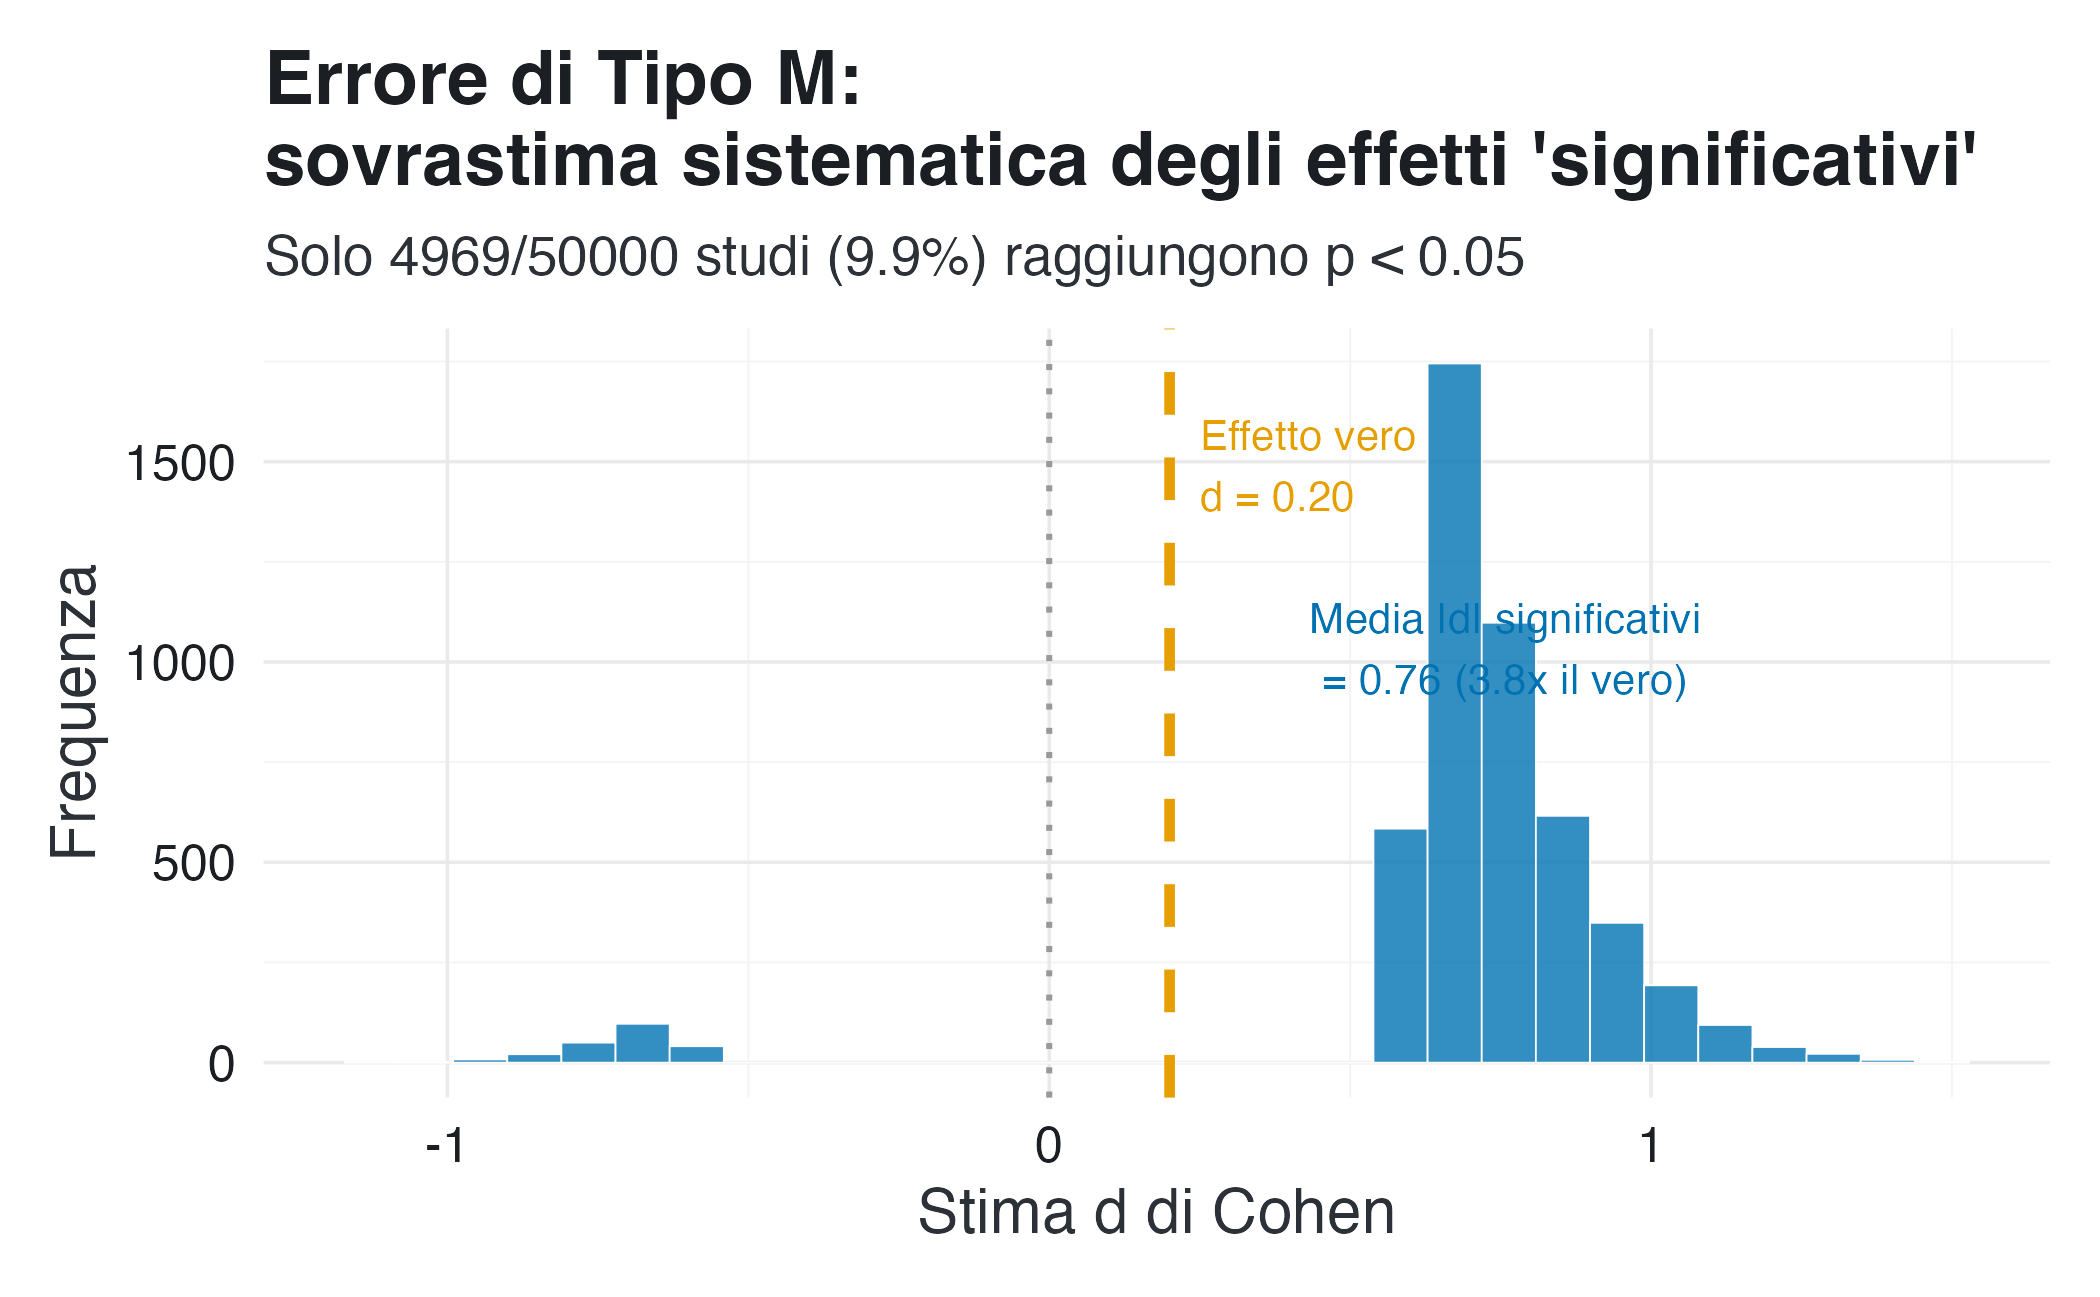
\includegraphics[width=0.85\linewidth,height=\textheight,keepaspectratio]{chapters/limits/03_s_m_errors_files/figure-pdf/fig-type-m-error-1.png}

}

\caption{\label{fig-type-m-error}Distribuzione delle stime del d di
Cohen nei risultati `statisticamente significativi'. La linea rossa
indica l'effetto vero (d = 0.2). Il filtro della significatività
seleziona sistematicamente stime gonfiate.}

\end{figure}%

La distribuzione asimmetrica delle stime, con una coda lunga verso
valori elevati, non riflette la vera entità del fenomeno, ma è un
\textbf{artefatto della selezione}. Solo quegli studi in cui la
fluttuazione campionaria casuale ha prodotto una differenza
eccezionalmente ampia riescono a superare la soglia della
significatività statistica. Il risultato è che la letteratura
scientifica finisce per rappresentare, in media, una sovrastima
sistematica dell'effetto, quantificabile in \textbf{circa quattro volte}
il suo valore reale. In sintesi, il problema non risiede nella
misurazione dell'effetto, ma nella selezione sistematica dei risultati
che tendono a esagerare il fenomeno.

La seconda figura approfondisce un aspetto diverso: tra gli studi che
superano la soglia di significatività, alcuni stimano un effetto nella
direzione \textbf{opposta} rispetto a quella reale.

\begin{Shaded}
\begin{Highlighting}[]
\NormalTok{palette\_sign\_error }\OtherTok{\textless{}{-}} \FunctionTok{setNames}\NormalTok{(}
\NormalTok{  palette\_qualitative[}\FunctionTok{c}\NormalTok{(}\DecValTok{5}\NormalTok{, }\DecValTok{1}\NormalTok{)],  }\CommentTok{\# blu + arancione}
  \FunctionTok{c}\NormalTok{(}\StringTok{"FALSE"}\NormalTok{, }\StringTok{"TRUE"}\NormalTok{)}
\NormalTok{)}

\NormalTok{col\_zero }\OtherTok{\textless{}{-}}\NormalTok{ palette\_qualitative[}\DecValTok{8}\NormalTok{]  }\CommentTok{\# grigio}
\NormalTok{col\_true }\OtherTok{\textless{}{-}}\NormalTok{ palette\_qualitative[}\DecValTok{1}\NormalTok{]  }\CommentTok{\# arancione}

\NormalTok{significant\_results }\SpecialCharTok{|\textgreater{}}
  \FunctionTok{mutate}\NormalTok{(}\AttributeTok{sign\_error =} \FunctionTok{factor}\NormalTok{(d\_observed }\SpecialCharTok{\textless{}} \DecValTok{0}\NormalTok{, }\AttributeTok{levels =} \FunctionTok{c}\NormalTok{(}\ConstantTok{FALSE}\NormalTok{, }\ConstantTok{TRUE}\NormalTok{))) }\SpecialCharTok{|\textgreater{}}
  \FunctionTok{ggplot}\NormalTok{(}\FunctionTok{aes}\NormalTok{(}\AttributeTok{x =}\NormalTok{ d\_observed, }\AttributeTok{fill =}\NormalTok{ sign\_error)) }\SpecialCharTok{+}
  \FunctionTok{geom\_histogram}\NormalTok{(}\AttributeTok{bins =} \DecValTok{30}\NormalTok{, }\AttributeTok{color =} \StringTok{"white"}\NormalTok{, }\AttributeTok{alpha =} \FloatTok{0.8}\NormalTok{) }\SpecialCharTok{+}
  \FunctionTok{geom\_vline}\NormalTok{(}
    \AttributeTok{xintercept =} \DecValTok{0}\NormalTok{,}
    \AttributeTok{color =}\NormalTok{ col\_zero,}
    \AttributeTok{linewidth =} \DecValTok{1}
\NormalTok{  ) }\SpecialCharTok{+}
  \FunctionTok{geom\_vline}\NormalTok{(}
    \AttributeTok{xintercept =}\NormalTok{ true\_d,}
    \AttributeTok{color =}\NormalTok{ col\_true,}
    \AttributeTok{linetype =} \StringTok{"dashed"}\NormalTok{,}
    \AttributeTok{linewidth =} \DecValTok{1}
\NormalTok{  ) }\SpecialCharTok{+}
  \FunctionTok{scale\_fill\_manual}\NormalTok{(}
    \AttributeTok{values =}\NormalTok{ palette\_sign\_error,}
    \AttributeTok{labels =} \FunctionTok{c}\NormalTok{(}
      \StringTok{"FALSE"} \OtherTok{=} \StringTok{"Segno corretto"}\NormalTok{,}
      \StringTok{"TRUE"}  \OtherTok{=} \StringTok{"Segno sbagliato"}
\NormalTok{    )}
\NormalTok{  ) }\SpecialCharTok{+}
  \FunctionTok{labs}\NormalTok{(}
    \AttributeTok{x =} \StringTok{"Stima d di Cohen"}\NormalTok{,}
    \AttributeTok{y =} \StringTok{"Frequenza"}\NormalTok{,}
    \AttributeTok{fill =} \StringTok{""}\NormalTok{,}
    \AttributeTok{title =} \StringTok{"Errore di Tipo S:}\SpecialCharTok{\textbackslash{}n}\StringTok{risultati significativi con direzione errata"}\NormalTok{,}
    \AttributeTok{subtitle =} \FunctionTok{sprintf}\NormalTok{(}
      \StringTok{"\%.1f\%\% dei risultati \textquotesingle{}significativi\textquotesingle{} ha il segno sbagliato"}\NormalTok{,}
\NormalTok{      type\_s\_rate }\SpecialCharTok{*} \DecValTok{100}
\NormalTok{    )}
\NormalTok{  )}
\end{Highlighting}
\end{Shaded}

\begin{figure}[H]

\centering{

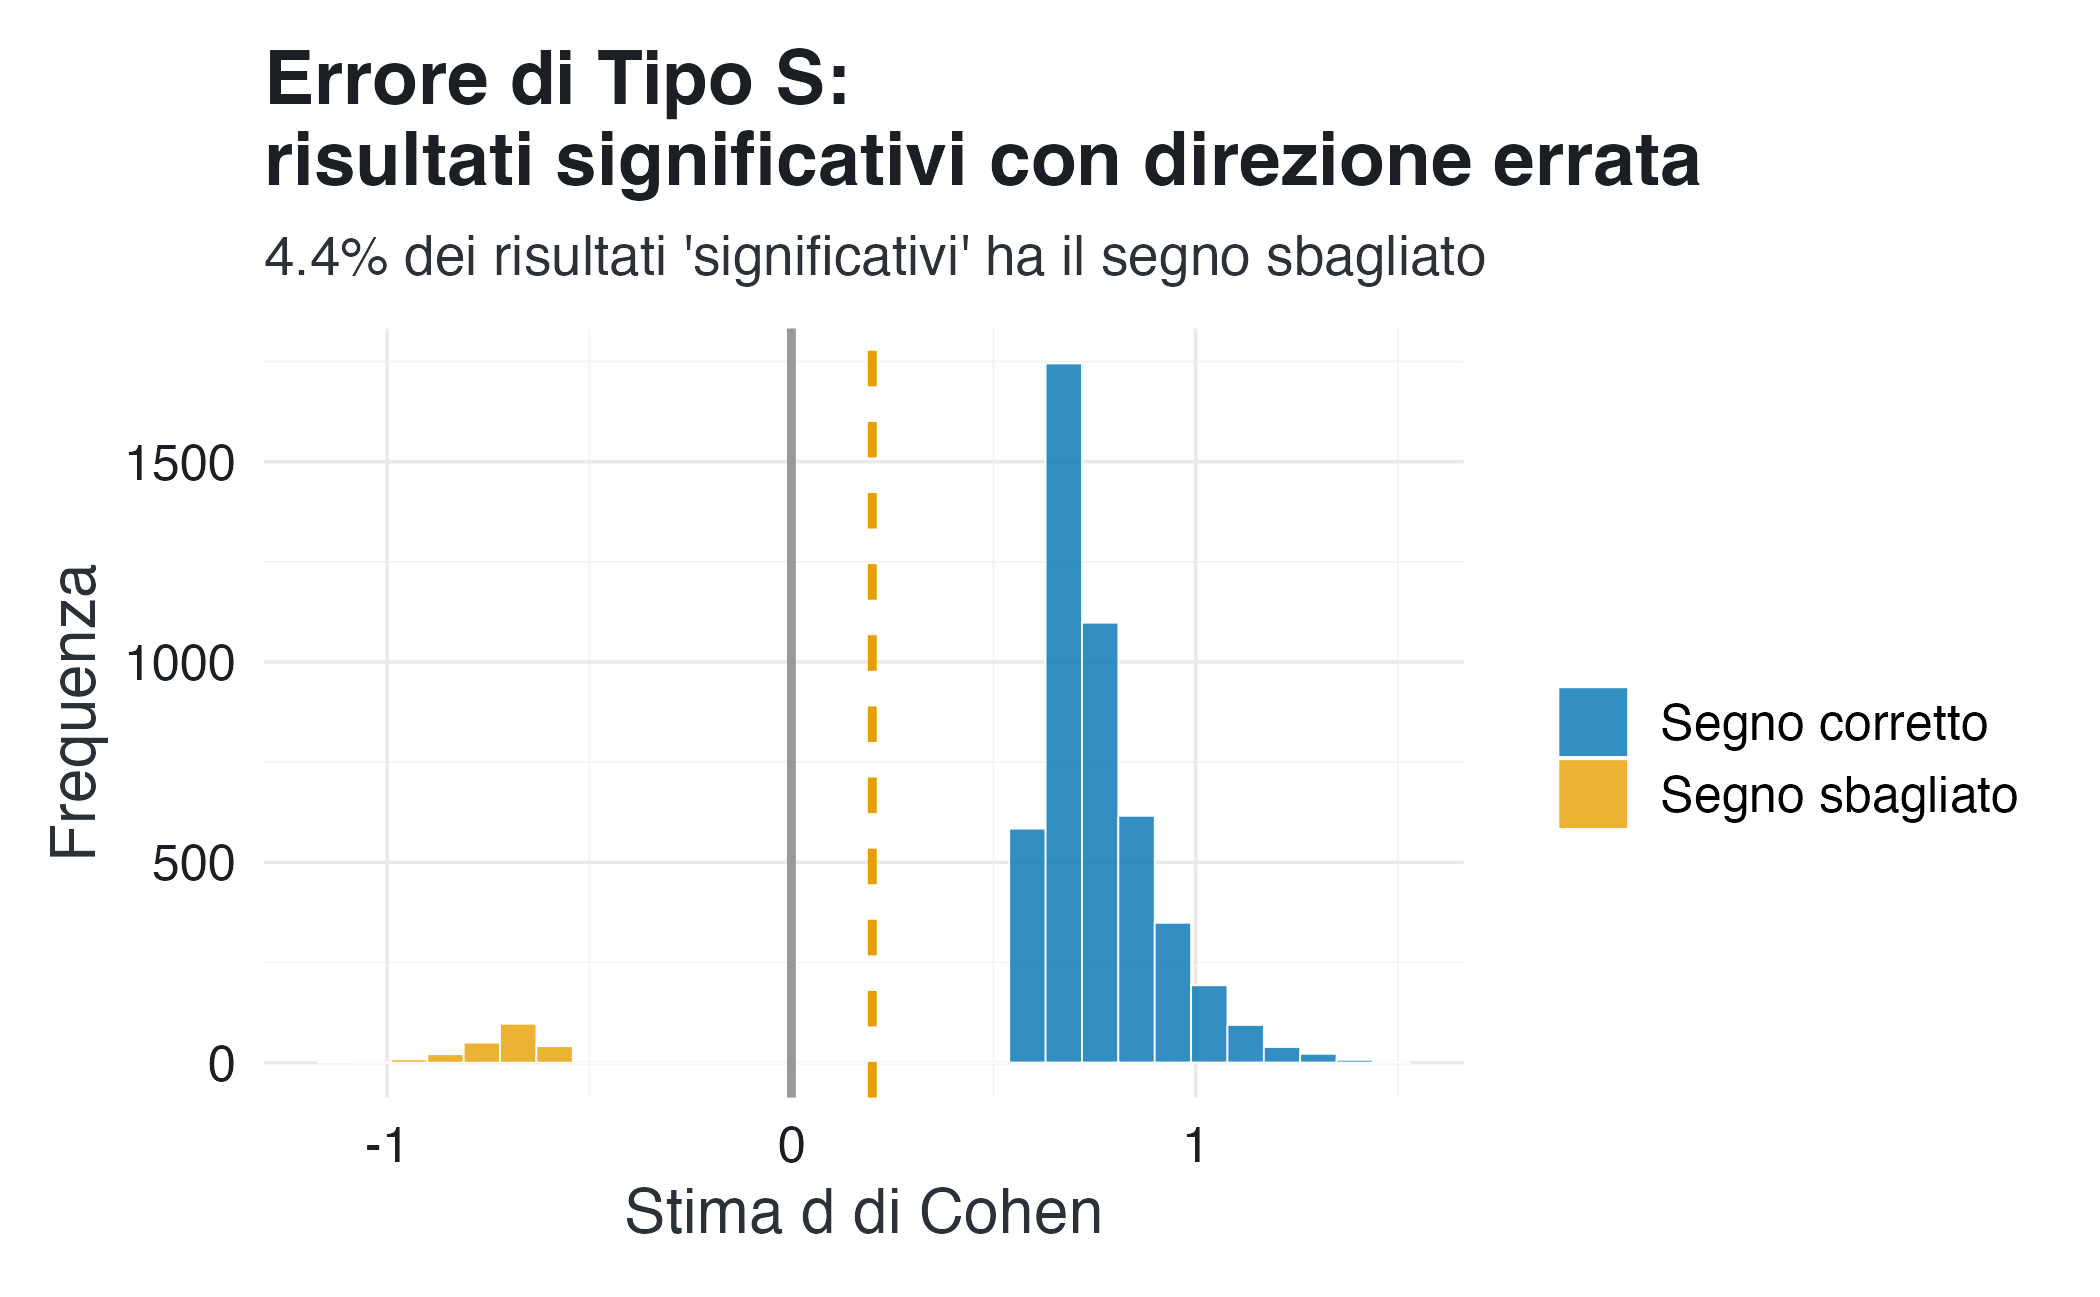
\includegraphics[width=0.85\linewidth,height=\textheight,keepaspectratio]{chapters/limits/03_s_m_errors_files/figure-pdf/fig-type-s-error-1.png}

}

\caption{\label{fig-type-s-error}Errore di Tipo S: una quota non
trascurabile di risultati significativi ha il segno sbagliato (d
\textless{} 0 quando il vero effetto è positivo).}

\end{figure}%

Questo fenomeno si verifica in condizioni di \textbf{bassa potenza
statistica}. In tali contesti, non solo è improbabile rilevare un
piccolo effetto, ma aumenta anche il rischio che il rumore campionario
generi una stima significativa nella direzione opposta. L'inclusione di
questi risultati nella letteratura scientifica contribuisce a creare
incoerenze empiriche, a ridurre la replicabilità degli studi e a
generare dispute teoriche basate su dati non attendibili.

La terza figura permette di confrontare questo scenario con la
distribuzione delle stime ottenute considerando \emph{tutti} i 50,000
studi simulati, indipendentemente dal valore-\(p\):

\begin{Shaded}
\begin{Highlighting}[]
\NormalTok{col\_hist }\OtherTok{\textless{}{-}}\NormalTok{ palette\_qualitative[}\DecValTok{8}\NormalTok{]  }\CommentTok{\# Grigio}
\NormalTok{col\_true }\OtherTok{\textless{}{-}}\NormalTok{ palette\_qualitative[}\DecValTok{1}\NormalTok{]  }\CommentTok{\# Arancione}
\NormalTok{col\_mean }\OtherTok{\textless{}{-}}\NormalTok{ palette\_qualitative[}\DecValTok{5}\NormalTok{]  }\CommentTok{\# Blu}

\NormalTok{p3 }\OtherTok{\textless{}{-}} \FunctionTok{ggplot}\NormalTok{(results, }\FunctionTok{aes}\NormalTok{(}\AttributeTok{x =}\NormalTok{ d\_observed)) }\SpecialCharTok{+}
  \FunctionTok{geom\_histogram}\NormalTok{(}
    \AttributeTok{bins =} \DecValTok{50}\NormalTok{,}
    \AttributeTok{fill =}\NormalTok{ col\_hist,}
    \AttributeTok{color =} \StringTok{"white"}\NormalTok{,}
    \AttributeTok{alpha =} \FloatTok{0.8}
\NormalTok{  ) }\SpecialCharTok{+}
  \FunctionTok{geom\_vline}\NormalTok{(}
    \AttributeTok{xintercept =}\NormalTok{ true\_d,}
    \AttributeTok{color =}\NormalTok{ col\_true,}
    \AttributeTok{linetype =} \StringTok{"dashed"}\NormalTok{,}
    \AttributeTok{linewidth =} \DecValTok{1}
\NormalTok{  ) }\SpecialCharTok{+}
  \FunctionTok{geom\_vline}\NormalTok{(}
    \AttributeTok{xintercept =} \FunctionTok{mean}\NormalTok{(results}\SpecialCharTok{$}\NormalTok{d\_observed),}
    \AttributeTok{color =}\NormalTok{ col\_mean,}
    \AttributeTok{linewidth =} \DecValTok{1}
\NormalTok{  ) }\SpecialCharTok{+}
  \FunctionTok{labs}\NormalTok{(}
    \AttributeTok{title =} \StringTok{"Tutti gli studi (N = 50.000)"}\NormalTok{,}
    \AttributeTok{subtitle =} \FunctionTok{sprintf}\NormalTok{(}
      \StringTok{"Media = \%.3f (≈ effetto vero)"}\NormalTok{,}
      \FunctionTok{mean}\NormalTok{(results}\SpecialCharTok{$}\NormalTok{d\_observed)}
\NormalTok{    ),}
    \AttributeTok{x =} \StringTok{"Stima d di Cohen"}\NormalTok{,}
    \AttributeTok{y =} \StringTok{"Frequenza"}
\NormalTok{  )}

\NormalTok{p3}
\end{Highlighting}
\end{Shaded}

\begin{figure}[H]

\centering{

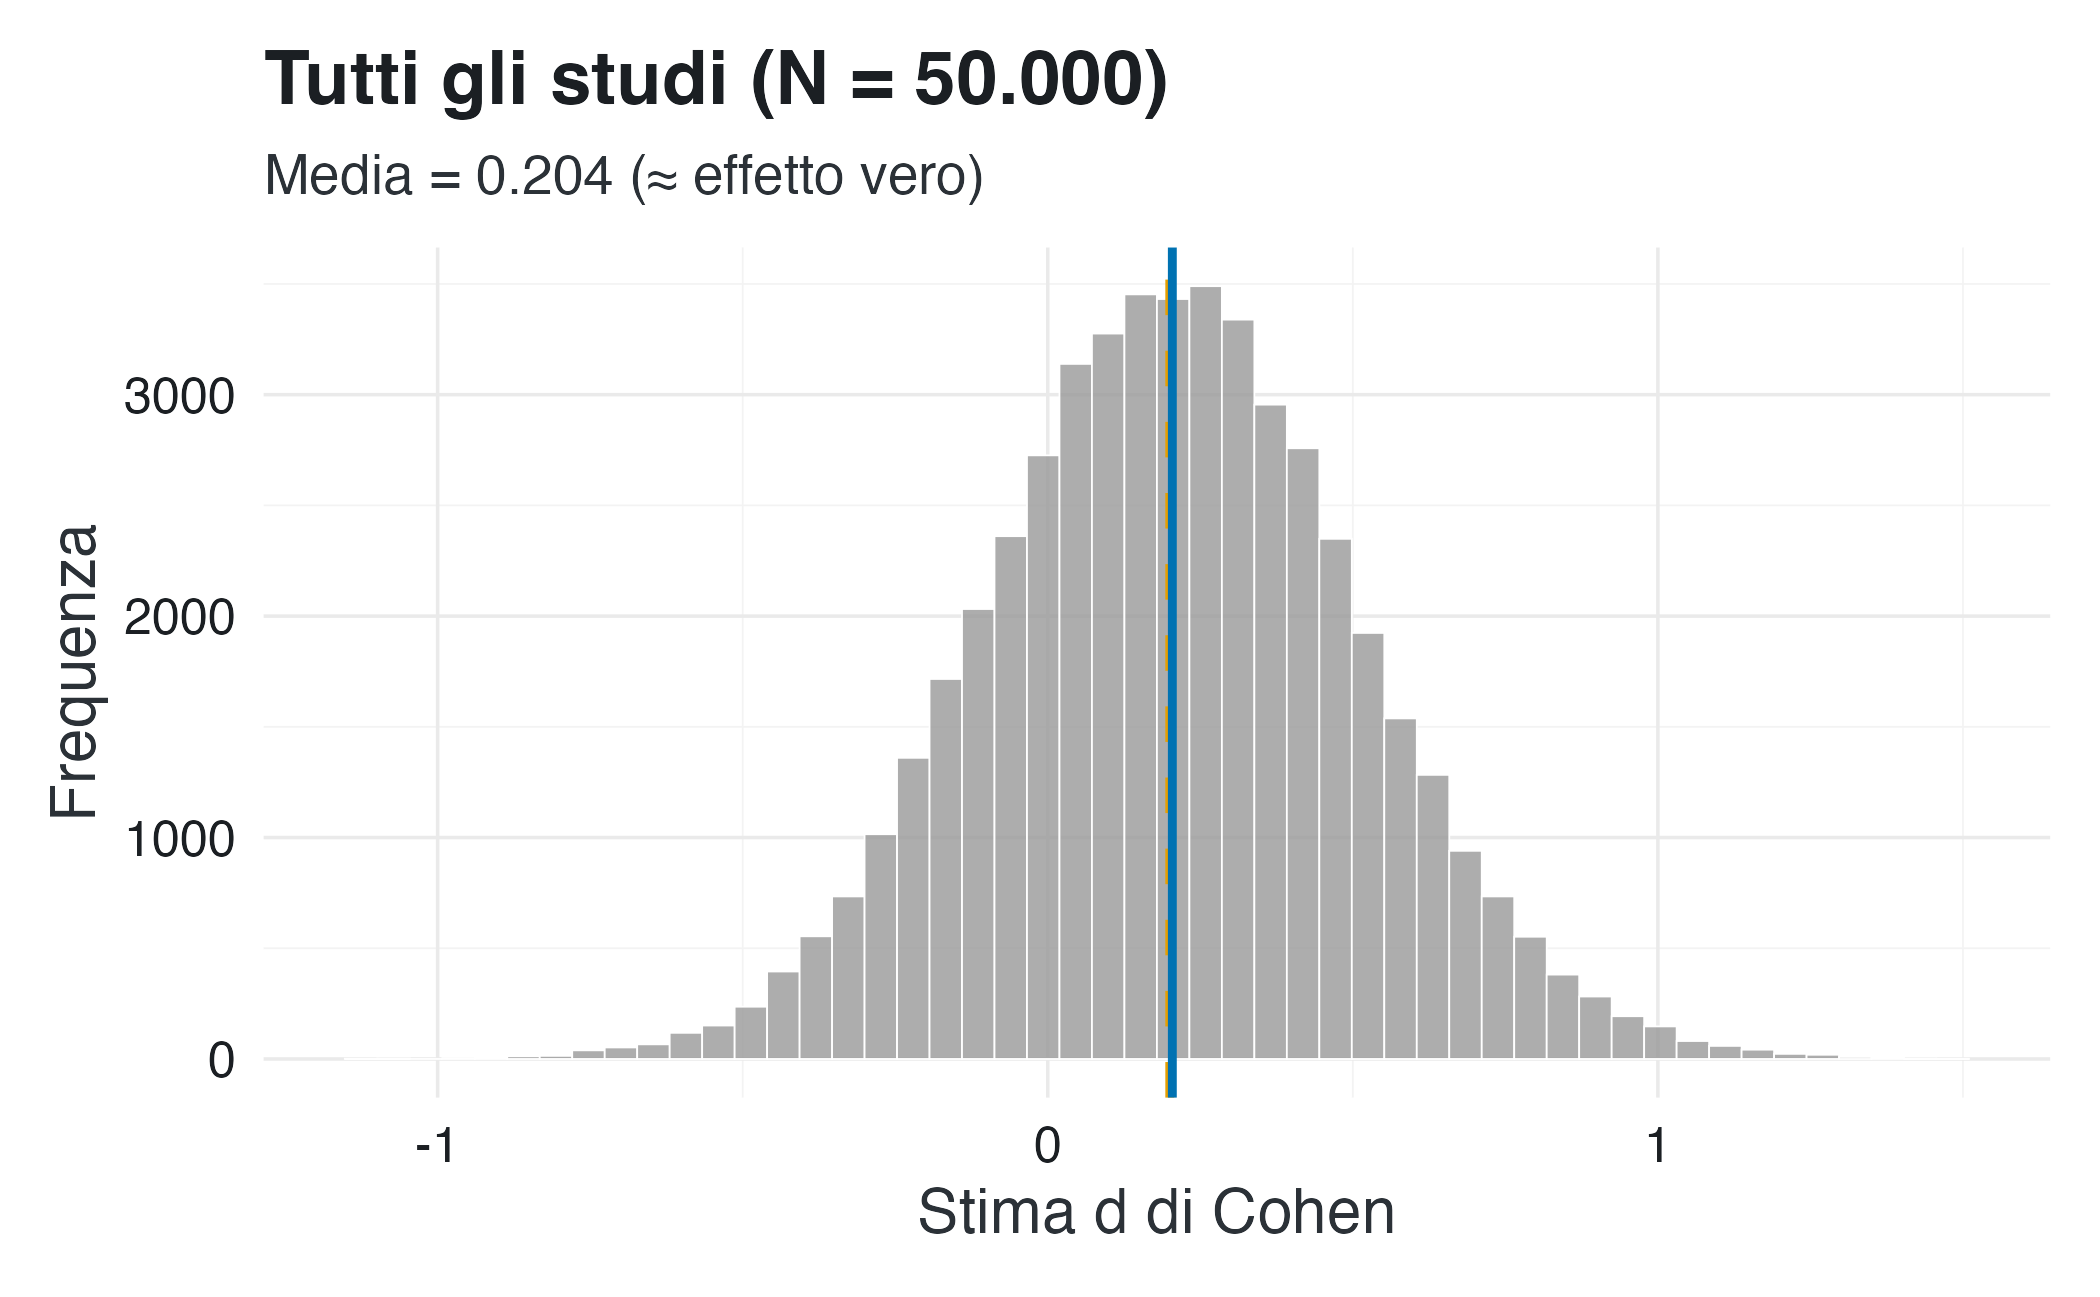
\includegraphics[width=0.85\linewidth,height=\textheight,keepaspectratio]{chapters/limits/03_s_m_errors_files/figure-pdf/fig-all-studies-1.png}

}

\caption{\label{fig-all-studies}Distribuzione delle stime del d di Cohen
in tutti gli studi simulati. Senza filtro di selezione, le fluttuazioni
casuali si compensano e la media coincide con l'effetto reale.}

\end{figure}%

Quando tutti gli studi sono inclusi, le fluttuazioni casuali si
compensano a vicenda e la media delle stime converge verso l'effetto
reale. \textbf{Pertanto, gli errori di Tipo M (sovrastima) e di Tipo S
(segno invertito) non sono una caratteristica delle stime stesse, ma
emergono unicamente come artefatto del processo di selezione basato
sulla soglia di significatività.}

In sintesi, il valore \(p\) non è un semplice criterio di rilevanza, ma
agisce da \textbf{filtro altamente selettivo e distorsivo}. Isolando
sistematicamente le stime più estreme, spesso aberranti, nelle code
della distribuzione campionaria, questo meccanismo produce una
\textbf{sovrastima sistematica} degli effetti nella letteratura
pubblicata, rappresentando i fenomeni come più ampi di quanto non siano
nella realtà. In casi estremi, può addirittura generare
\textbf{inversioni di segno} statisticamente significative, dando
credito a conclusioni fuorvianti. Il risultato è l'accumulo di un corpus
di conoscenze affetto da una distorsione sistematica che erode il
progresso cumulativo della scienza. Da ciò derivano, in larga parte, sia
la crisi di replicabilità sia l'instabilità dei risultati nella
psicologia empirica e in altre discipline
(\citeproc{ref-gelman2006difference}{Gelman \& Stern, 2006}).

\section{Confronto con l'approccio
bayesiano}\label{confronto-con-lapproccio-bayesiano}

A differenza dei test d'ipotesi frequentisti, l'inferenza bayesiana non
opera con soglie dicotomiche. Invece di giudicare un risultato in base
al superamento di un limite arbitrario, fornisce una distribuzione a
posteriori che quantifica la plausibilità relativa di ogni possibile
valore dell'effetto, aggiornando una credenza iniziale esplicita
(\emph{prior}) con i dati osservati. Questo approccio permette di
rappresentare l'incertezza in modo continuo e naturale, evitando le
distorsioni di selezione e sovrastima indotte dalla soglia del
\(p < 0.05\).

Tuttavia, per un \textbf{confronto equo con il paradigma frequentista},
applicheremo lo stesso filtro della ``significatività statistica'' anche
alle stime bayesiane, sebbene questo filtro sia estraneo alla filosofia
bayesiana. Il confronto mostra che le stime bayesiane sono più robuste:
anche quando selezionate arbitrariamente, presentano una distorsione
sistematica (errori di tipo M e S) notevolmente inferiore rispetto a
quelle frequentiste.

\subsection{Un'analisi bayesiana}\label{unanalisi-bayesiana}

Per la distribuzione a posteriori, utilizziamo un'approssimazione
normale (valida per campioni non troppo piccoli). Definiamo un risultato
bayesiano ``significativo'' quando la probabilità a posteriori che
l'effetto sia positivo supera il 95\% (equivalente approssimativo del
\(p < 0.05\) in un test a una coda).

\begin{Shaded}
\begin{Highlighting}[]
\CommentTok{\# Funzione per analisi bayesiana approssimata}
\CommentTok{\# Prior: d \textasciitilde{} N(0, 1) (prior debolmente informativa)}
\CommentTok{\# Likelihood: d\_obs | d \textasciitilde{} N(d, SE²)}
\CommentTok{\# Posterior: d | d\_obs \textasciitilde{} N(mu\_post, sigma\_post²)}

\NormalTok{bayesian\_estimate }\OtherTok{\textless{}{-}} \ControlFlowTok{function}\NormalTok{(d\_observed, se, }\AttributeTok{prior\_mean =} \DecValTok{0}\NormalTok{, }\AttributeTok{prior\_sd =} \DecValTok{1}\NormalTok{) \{}
\NormalTok{  prior\_precision }\OtherTok{\textless{}{-}} \DecValTok{1} \SpecialCharTok{/}\NormalTok{ prior\_sd}\SpecialCharTok{\^{}}\DecValTok{2}
\NormalTok{  data\_precision }\OtherTok{\textless{}{-}} \DecValTok{1} \SpecialCharTok{/}\NormalTok{ se}\SpecialCharTok{\^{}}\DecValTok{2}
  
\NormalTok{  posterior\_precision }\OtherTok{\textless{}{-}}\NormalTok{ prior\_precision }\SpecialCharTok{+}\NormalTok{ data\_precision}
\NormalTok{  posterior\_sd }\OtherTok{\textless{}{-}} \FunctionTok{sqrt}\NormalTok{(}\DecValTok{1} \SpecialCharTok{/}\NormalTok{ posterior\_precision)}
\NormalTok{  posterior\_mean }\OtherTok{\textless{}{-}}\NormalTok{ (prior\_precision }\SpecialCharTok{*}\NormalTok{ prior\_mean }\SpecialCharTok{+}\NormalTok{ data\_precision }\SpecialCharTok{*}\NormalTok{ d\_observed) }\SpecialCharTok{/}\NormalTok{ posterior\_precision}
  
  \FunctionTok{tibble}\NormalTok{(}
    \AttributeTok{posterior\_mean =}\NormalTok{ posterior\_mean,}
    \AttributeTok{posterior\_sd =}\NormalTok{ posterior\_sd,}
    \AttributeTok{prob\_positive =} \FunctionTok{pnorm}\NormalTok{(}\DecValTok{0}\NormalTok{, posterior\_mean, posterior\_sd, }\AttributeTok{lower.tail =} \ConstantTok{FALSE}\NormalTok{)}
\NormalTok{  )}
\NormalTok{\}}

\CommentTok{\# Applica l\textquotesingle{}analisi bayesiana a tutti gli studi}
\NormalTok{se\_d }\OtherTok{\textless{}{-}} \FunctionTok{sqrt}\NormalTok{(}\DecValTok{2} \SpecialCharTok{/}\NormalTok{ ((n1 }\SpecialCharTok{*}\NormalTok{ n2) }\SpecialCharTok{/}\NormalTok{ (n1 }\SpecialCharTok{+}\NormalTok{ n2)))  }\CommentTok{\# SE approssimato per Cohen\textquotesingle{}s d}

\NormalTok{bayesian\_results }\OtherTok{\textless{}{-}}\NormalTok{ results }\SpecialCharTok{|\textgreater{}}
  \FunctionTok{rowwise}\NormalTok{() }\SpecialCharTok{|\textgreater{}}
  \FunctionTok{mutate}\NormalTok{(}
    \AttributeTok{bayes =} \FunctionTok{list}\NormalTok{(}\FunctionTok{bayesian\_estimate}\NormalTok{(d\_observed, se\_d))}
\NormalTok{  ) }\SpecialCharTok{|\textgreater{}}
  \FunctionTok{unnest}\NormalTok{(bayes) }\SpecialCharTok{|\textgreater{}}
  \FunctionTok{ungroup}\NormalTok{()}
\end{Highlighting}
\end{Shaded}

\subsection{Confronto delle stime}\label{confronto-delle-stime}

\begin{Shaded}
\begin{Highlighting}[]
\CommentTok{\# Confronto per i risultati significativi}
\NormalTok{comparison }\OtherTok{\textless{}{-}}\NormalTok{ bayesian\_results }\SpecialCharTok{|\textgreater{}}
\NormalTok{  dplyr}\SpecialCharTok{::}\FunctionTok{filter}\NormalTok{(significant) }\SpecialCharTok{|\textgreater{}}
\NormalTok{  dplyr}\SpecialCharTok{::}\FunctionTok{select}\NormalTok{(d\_observed, posterior\_mean) }\SpecialCharTok{|\textgreater{}}
  \FunctionTok{pivot\_longer}\NormalTok{(}\FunctionTok{everything}\NormalTok{(), }\AttributeTok{names\_to =} \StringTok{"method"}\NormalTok{, }\AttributeTok{values\_to =} \StringTok{"estimate"}\NormalTok{) }\SpecialCharTok{|\textgreater{}}
  \FunctionTok{mutate}\NormalTok{(}\AttributeTok{method =} \FunctionTok{ifelse}\NormalTok{(method }\SpecialCharTok{==} \StringTok{"d\_observed"}\NormalTok{, }\StringTok{"Frequentista"}\NormalTok{, }\StringTok{"Bayesiano"}\NormalTok{))}

\NormalTok{palette\_methods }\OtherTok{\textless{}{-}} \FunctionTok{setNames}\NormalTok{(}
\NormalTok{  palette\_qualitative[}\FunctionTok{c}\NormalTok{(}\DecValTok{1}\NormalTok{, }\DecValTok{5}\NormalTok{)],  }\CommentTok{\# arancione + blu}
  \FunctionTok{c}\NormalTok{(}\StringTok{"Frequentista"}\NormalTok{, }\StringTok{"Bayesiano"}\NormalTok{)}
\NormalTok{)}

\NormalTok{col\_true }\OtherTok{\textless{}{-}}\NormalTok{ palette\_qualitative[}\DecValTok{8}\NormalTok{]  }\CommentTok{\# grigio}

\FunctionTok{ggplot}\NormalTok{(comparison, }\FunctionTok{aes}\NormalTok{(}\AttributeTok{x =}\NormalTok{ estimate, }\AttributeTok{fill =}\NormalTok{ method)) }\SpecialCharTok{+}
  \FunctionTok{geom\_histogram}\NormalTok{(}
    \AttributeTok{bins =} \DecValTok{30}\NormalTok{,}
    \AttributeTok{alpha =} \FloatTok{0.6}\NormalTok{,}
    \AttributeTok{position =} \StringTok{"identity"}\NormalTok{,}
    \AttributeTok{color =} \StringTok{"white"}
\NormalTok{  ) }\SpecialCharTok{+}
  \FunctionTok{geom\_vline}\NormalTok{(}
    \AttributeTok{xintercept =}\NormalTok{ true\_d,}
    \AttributeTok{color =}\NormalTok{ col\_true,}
    \AttributeTok{linetype =} \StringTok{"dashed"}\NormalTok{,}
    \AttributeTok{linewidth =} \FloatTok{1.2}
\NormalTok{  ) }\SpecialCharTok{+}
  \FunctionTok{scale\_fill\_manual}\NormalTok{(}\AttributeTok{values =}\NormalTok{ palette\_methods) }\SpecialCharTok{+}
  \FunctionTok{labs}\NormalTok{(}
    \AttributeTok{x =} \StringTok{"Stima d di Cohen"}\NormalTok{,}
    \AttributeTok{y =} \StringTok{"Frequenza"}\NormalTok{,}
    \AttributeTok{fill =} \StringTok{"Metodo"}\NormalTok{,}
    \AttributeTok{title =} \StringTok{"Stime frequentiste vs bayesiane}\SpecialCharTok{\textbackslash{}n}\StringTok{per i risultati \textquotesingle{}significativi\textquotesingle{}"}\NormalTok{,}
    \AttributeTok{subtitle =} \StringTok{"Le stime bayesiane sono meno estreme grazie allo shrinkage verso la prior"}
\NormalTok{  )}
\end{Highlighting}
\end{Shaded}

\begin{figure}[H]

\centering{

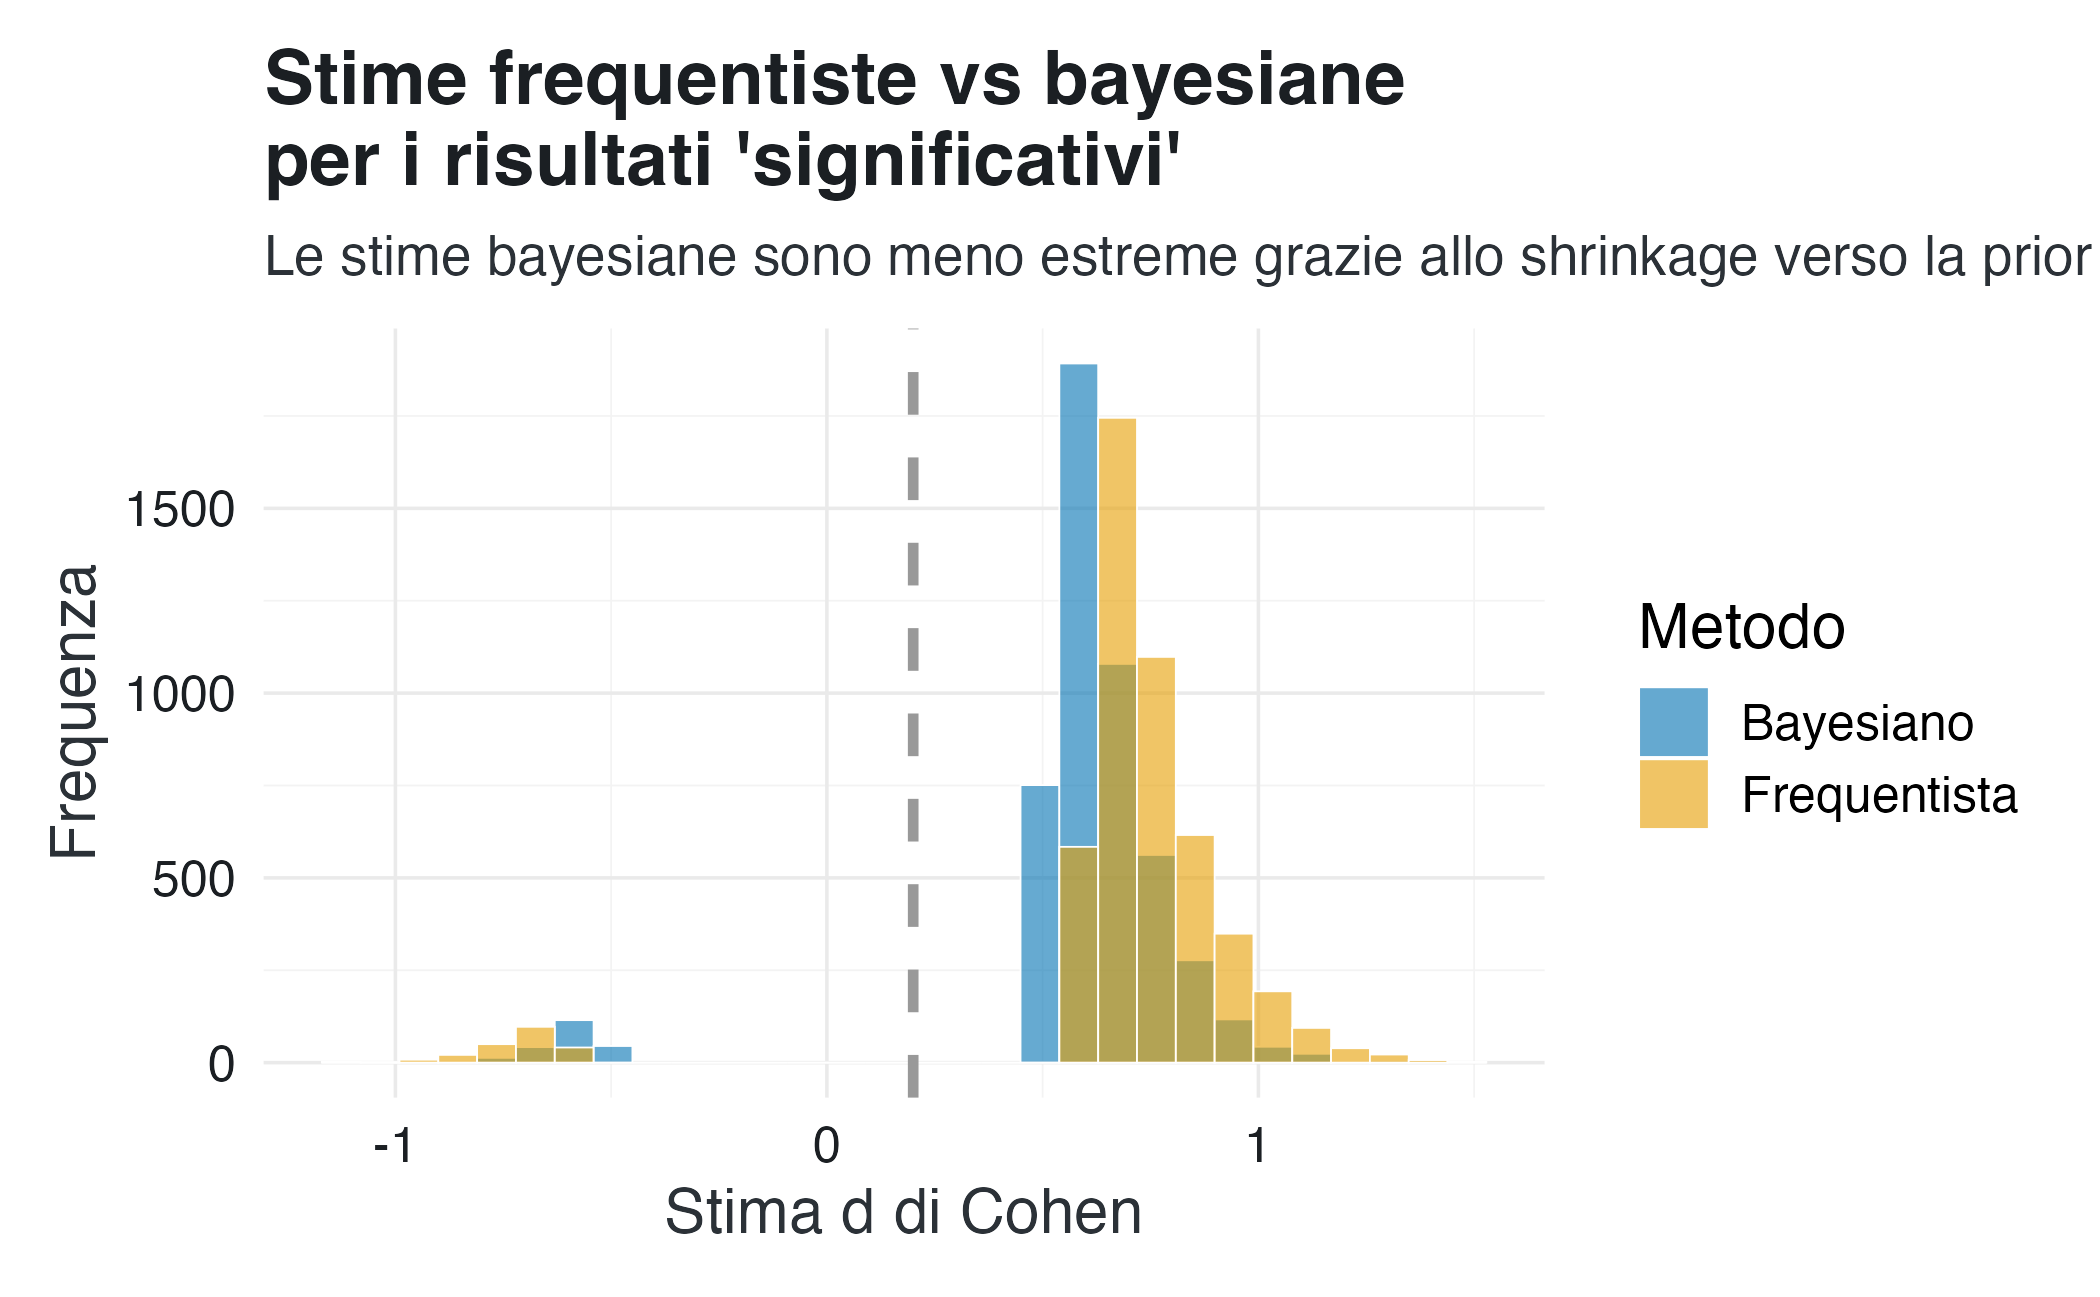
\includegraphics[width=0.85\linewidth,height=\textheight,keepaspectratio]{chapters/limits/03_s_m_errors_files/figure-pdf/fig-freq-vs-bayes-1.png}

}

\caption{\label{fig-freq-vs-bayes}Confronto tra stime frequentiste e
bayesiane. Le stime bayesiane sono `tirate' verso la distribuzione a
priori, riducendo la sovrastima.}

\end{figure}%

\begin{Shaded}
\begin{Highlighting}[]
\CommentTok{\# Quantifica la riduzione dell\textquotesingle{}errore}
\NormalTok{freq\_mean\_sig }\OtherTok{\textless{}{-}} \FunctionTok{mean}\NormalTok{(}\FunctionTok{abs}\NormalTok{(significant\_results}\SpecialCharTok{$}\NormalTok{d\_observed))}
\NormalTok{bayes\_mean\_sig }\OtherTok{\textless{}{-}} \FunctionTok{mean}\NormalTok{(}\FunctionTok{abs}\NormalTok{(bayesian\_results}\SpecialCharTok{$}\NormalTok{posterior\_mean[bayesian\_results}\SpecialCharTok{$}\NormalTok{significant]))}
\end{Highlighting}
\end{Shaded}

\begin{verbatim}
#> Effetto vero:                 d = 0.20
#> Media |d| frequentista:       0.76 (3.8x il vero)
#> Media |d| bayesiana:          0.64 (3.2x il vero)
#> Riduzione dell'errore:        21%
\end{verbatim}

\textbf{Interpretazione:} anche quando è costretta a subire lo stesso
filtro di selezione arbitrario del paradigma frequentista, l'analisi
bayesiana riduce sia la sovrastima dell'effetto sia gli errori di segno.
Questo avviene perché l'inferenza bayesiana incorpora in modo naturale
lo ``shrinkage'': le stime estreme vengono ``contratte'' verso la
distribuzione a priori, che in questo caso è centrata sullo zero. Il
risultato non è l'eliminazione dell'errore, ma la sua sostanziale
attenuazione, il che dimostra come la struttura stessa dell'inferenza
bayesiana produca stime più robuste e meno sensibili alle distorsioni
introdotte dalla selezione dei soli risultati pubblicabili.

\section{Come cambiano gli errori con la dimensione del
campione?}\label{come-cambiano-gli-errori-con-la-dimensione-del-campione}

\begin{Shaded}
\begin{Highlighting}[]
\CommentTok{\# Simulazione con diverse dimensioni campionarie}
\NormalTok{sample\_sizes }\OtherTok{\textless{}{-}} \FunctionTok{c}\NormalTok{(}\DecValTok{20}\NormalTok{, }\DecValTok{50}\NormalTok{, }\DecValTok{100}\NormalTok{, }\DecValTok{200}\NormalTok{, }\DecValTok{500}\NormalTok{)}

\NormalTok{sample\_size\_analysis }\OtherTok{\textless{}{-}} \FunctionTok{map\_dfr}\NormalTok{(sample\_sizes, }\ControlFlowTok{function}\NormalTok{(n) \{}
  \CommentTok{\# Simula studi con n osservazioni per gruppo}
\NormalTok{  sim\_results }\OtherTok{\textless{}{-}} \FunctionTok{map\_dfr}\NormalTok{(}\DecValTok{1}\SpecialCharTok{:}\DecValTok{10000}\NormalTok{, }\ControlFlowTok{function}\NormalTok{(i) \{}
\NormalTok{    y1 }\OtherTok{\textless{}{-}} \FunctionTok{rnorm}\NormalTok{(n, }\AttributeTok{mean =}\NormalTok{ mu\_1, }\AttributeTok{sd =}\NormalTok{ sigma)}
\NormalTok{    y2 }\OtherTok{\textless{}{-}} \FunctionTok{rnorm}\NormalTok{(n, }\AttributeTok{mean =}\NormalTok{ mu\_2, }\AttributeTok{sd =}\NormalTok{ sigma)}
    
\NormalTok{    pooled\_sd }\OtherTok{\textless{}{-}} \FunctionTok{sqrt}\NormalTok{(((n }\SpecialCharTok{{-}} \DecValTok{1}\NormalTok{) }\SpecialCharTok{*} \FunctionTok{var}\NormalTok{(y1) }\SpecialCharTok{+}\NormalTok{ (n }\SpecialCharTok{{-}} \DecValTok{1}\NormalTok{) }\SpecialCharTok{*} \FunctionTok{var}\NormalTok{(y2)) }\SpecialCharTok{/}\NormalTok{ (}\DecValTok{2} \SpecialCharTok{*}\NormalTok{ n }\SpecialCharTok{{-}} \DecValTok{2}\NormalTok{))}
\NormalTok{    d\_obs }\OtherTok{\textless{}{-}}\NormalTok{ (}\FunctionTok{mean}\NormalTok{(y1) }\SpecialCharTok{{-}} \FunctionTok{mean}\NormalTok{(y2)) }\SpecialCharTok{/}\NormalTok{ pooled\_sd}
\NormalTok{    p\_val }\OtherTok{\textless{}{-}} \FunctionTok{t.test}\NormalTok{(y1, y2, }\AttributeTok{var.equal =} \ConstantTok{TRUE}\NormalTok{)}\SpecialCharTok{$}\NormalTok{p.value}
    
    \FunctionTok{tibble}\NormalTok{(}\AttributeTok{d\_observed =}\NormalTok{ d\_obs, }\AttributeTok{p\_value =}\NormalTok{ p\_val, }\AttributeTok{significant =}\NormalTok{ p\_val }\SpecialCharTok{\textless{}} \FloatTok{0.05}\NormalTok{)}
\NormalTok{  \})}
  
\NormalTok{  sig\_results }\OtherTok{\textless{}{-}}\NormalTok{ sim\_results }\SpecialCharTok{|\textgreater{}} \FunctionTok{filter}\NormalTok{(significant)}
  
  \FunctionTok{tibble}\NormalTok{(}
    \AttributeTok{n\_per\_group =}\NormalTok{ n,}
    \AttributeTok{power =} \FunctionTok{mean}\NormalTok{(sim\_results}\SpecialCharTok{$}\NormalTok{significant),}
    \AttributeTok{type\_m =} \FunctionTok{mean}\NormalTok{(}\FunctionTok{abs}\NormalTok{(sig\_results}\SpecialCharTok{$}\NormalTok{d\_observed)) }\SpecialCharTok{/}\NormalTok{ true\_d,}
    \AttributeTok{type\_s =} \FunctionTok{mean}\NormalTok{(sig\_results}\SpecialCharTok{$}\NormalTok{d\_observed }\SpecialCharTok{\textless{}} \DecValTok{0}\NormalTok{)}
\NormalTok{  )}
\NormalTok{\})}

\NormalTok{col\_power }\OtherTok{\textless{}{-}}\NormalTok{ palette\_qualitative[}\DecValTok{5}\NormalTok{]  }\CommentTok{\# Blu}
\NormalTok{col\_m     }\OtherTok{\textless{}{-}}\NormalTok{ palette\_qualitative[}\DecValTok{1}\NormalTok{]  }\CommentTok{\# Arancione}
\NormalTok{col\_s     }\OtherTok{\textless{}{-}}\NormalTok{ palette\_qualitative[}\DecValTok{7}\NormalTok{]  }\CommentTok{\# Rosa}
\NormalTok{col\_ref   }\OtherTok{\textless{}{-}}\NormalTok{ palette\_qualitative[}\DecValTok{8}\NormalTok{]  }\CommentTok{\# Grigio}

\CommentTok{\# Visualizzazione}
\NormalTok{p\_power }\OtherTok{\textless{}{-}} \FunctionTok{ggplot}\NormalTok{(sample\_size\_analysis, }\FunctionTok{aes}\NormalTok{(}\AttributeTok{x =}\NormalTok{ n\_per\_group, }\AttributeTok{y =}\NormalTok{ power)) }\SpecialCharTok{+}
  \FunctionTok{geom\_line}\NormalTok{(}\AttributeTok{color =}\NormalTok{ col\_power, }\AttributeTok{linewidth =} \FloatTok{1.2}\NormalTok{) }\SpecialCharTok{+}
  \FunctionTok{geom\_point}\NormalTok{(}\AttributeTok{color =}\NormalTok{ col\_power, }\AttributeTok{size =} \DecValTok{3}\NormalTok{) }\SpecialCharTok{+}
  \FunctionTok{geom\_hline}\NormalTok{(}
    \AttributeTok{yintercept =} \FloatTok{0.80}\NormalTok{,}
    \AttributeTok{linetype =} \StringTok{"dashed"}\NormalTok{,}
    \AttributeTok{color =}\NormalTok{ col\_ref}
\NormalTok{  ) }\SpecialCharTok{+}
  \FunctionTok{scale\_y\_continuous}\NormalTok{(}\AttributeTok{labels =}\NormalTok{ scales}\SpecialCharTok{::}\NormalTok{percent, }\AttributeTok{limits =} \FunctionTok{c}\NormalTok{(}\DecValTok{0}\NormalTok{, }\DecValTok{1}\NormalTok{)) }\SpecialCharTok{+}
  \FunctionTok{labs}\NormalTok{(}
    \AttributeTok{title =} \StringTok{"Potenza statistica"}\NormalTok{,}
    \AttributeTok{x =} \StringTok{"n per gruppo"}\NormalTok{,}
    \AttributeTok{y =} \StringTok{"Potenza"}
\NormalTok{  )}

\NormalTok{p\_type\_m }\OtherTok{\textless{}{-}} \FunctionTok{ggplot}\NormalTok{(sample\_size\_analysis, }\FunctionTok{aes}\NormalTok{(}\AttributeTok{x =}\NormalTok{ n\_per\_group, }\AttributeTok{y =}\NormalTok{ type\_m)) }\SpecialCharTok{+}
  \FunctionTok{geom\_line}\NormalTok{(}\AttributeTok{color =}\NormalTok{ col\_m, }\AttributeTok{linewidth =} \FloatTok{1.2}\NormalTok{) }\SpecialCharTok{+}
  \FunctionTok{geom\_point}\NormalTok{(}\AttributeTok{color =}\NormalTok{ col\_m, }\AttributeTok{size =} \DecValTok{3}\NormalTok{) }\SpecialCharTok{+}
  \FunctionTok{geom\_hline}\NormalTok{(}
    \AttributeTok{yintercept =} \DecValTok{1}\NormalTok{,}
    \AttributeTok{linetype =} \StringTok{"dashed"}\NormalTok{,}
    \AttributeTok{color =}\NormalTok{ col\_ref}
\NormalTok{  ) }\SpecialCharTok{+}
  \FunctionTok{labs}\NormalTok{(}
    \AttributeTok{title =} \StringTok{"Errore Tipo M (exaggeration)"}\NormalTok{,}
    \AttributeTok{x =} \StringTok{"n per gruppo"}\NormalTok{,}
    \AttributeTok{y =} \StringTok{"Fattore di esagerazione"}
\NormalTok{  )}

\NormalTok{p\_type\_s }\OtherTok{\textless{}{-}} \FunctionTok{ggplot}\NormalTok{(sample\_size\_analysis, }\FunctionTok{aes}\NormalTok{(}\AttributeTok{x =}\NormalTok{ n\_per\_group, }\AttributeTok{y =}\NormalTok{ type\_s)) }\SpecialCharTok{+}
  \FunctionTok{geom\_line}\NormalTok{(}\AttributeTok{color =}\NormalTok{ col\_s, }\AttributeTok{linewidth =} \FloatTok{1.2}\NormalTok{) }\SpecialCharTok{+}
  \FunctionTok{geom\_point}\NormalTok{(}\AttributeTok{color =}\NormalTok{ col\_s, }\AttributeTok{size =} \DecValTok{3}\NormalTok{) }\SpecialCharTok{+}
  \FunctionTok{scale\_y\_continuous}\NormalTok{(}\AttributeTok{labels =}\NormalTok{ scales}\SpecialCharTok{::}\NormalTok{percent) }\SpecialCharTok{+}
  \FunctionTok{labs}\NormalTok{(}
    \AttributeTok{title =} \StringTok{"Errore Tipo S (wrong sign)"}\NormalTok{,}
    \AttributeTok{x =} \StringTok{"n per gruppo"}\NormalTok{,}
    \AttributeTok{y =} \StringTok{"Tasso errore di segno"}
\NormalTok{  )}
\end{Highlighting}
\end{Shaded}

\begin{Shaded}
\begin{Highlighting}[]
\NormalTok{p\_power }
\end{Highlighting}
\end{Shaded}

\begin{center}
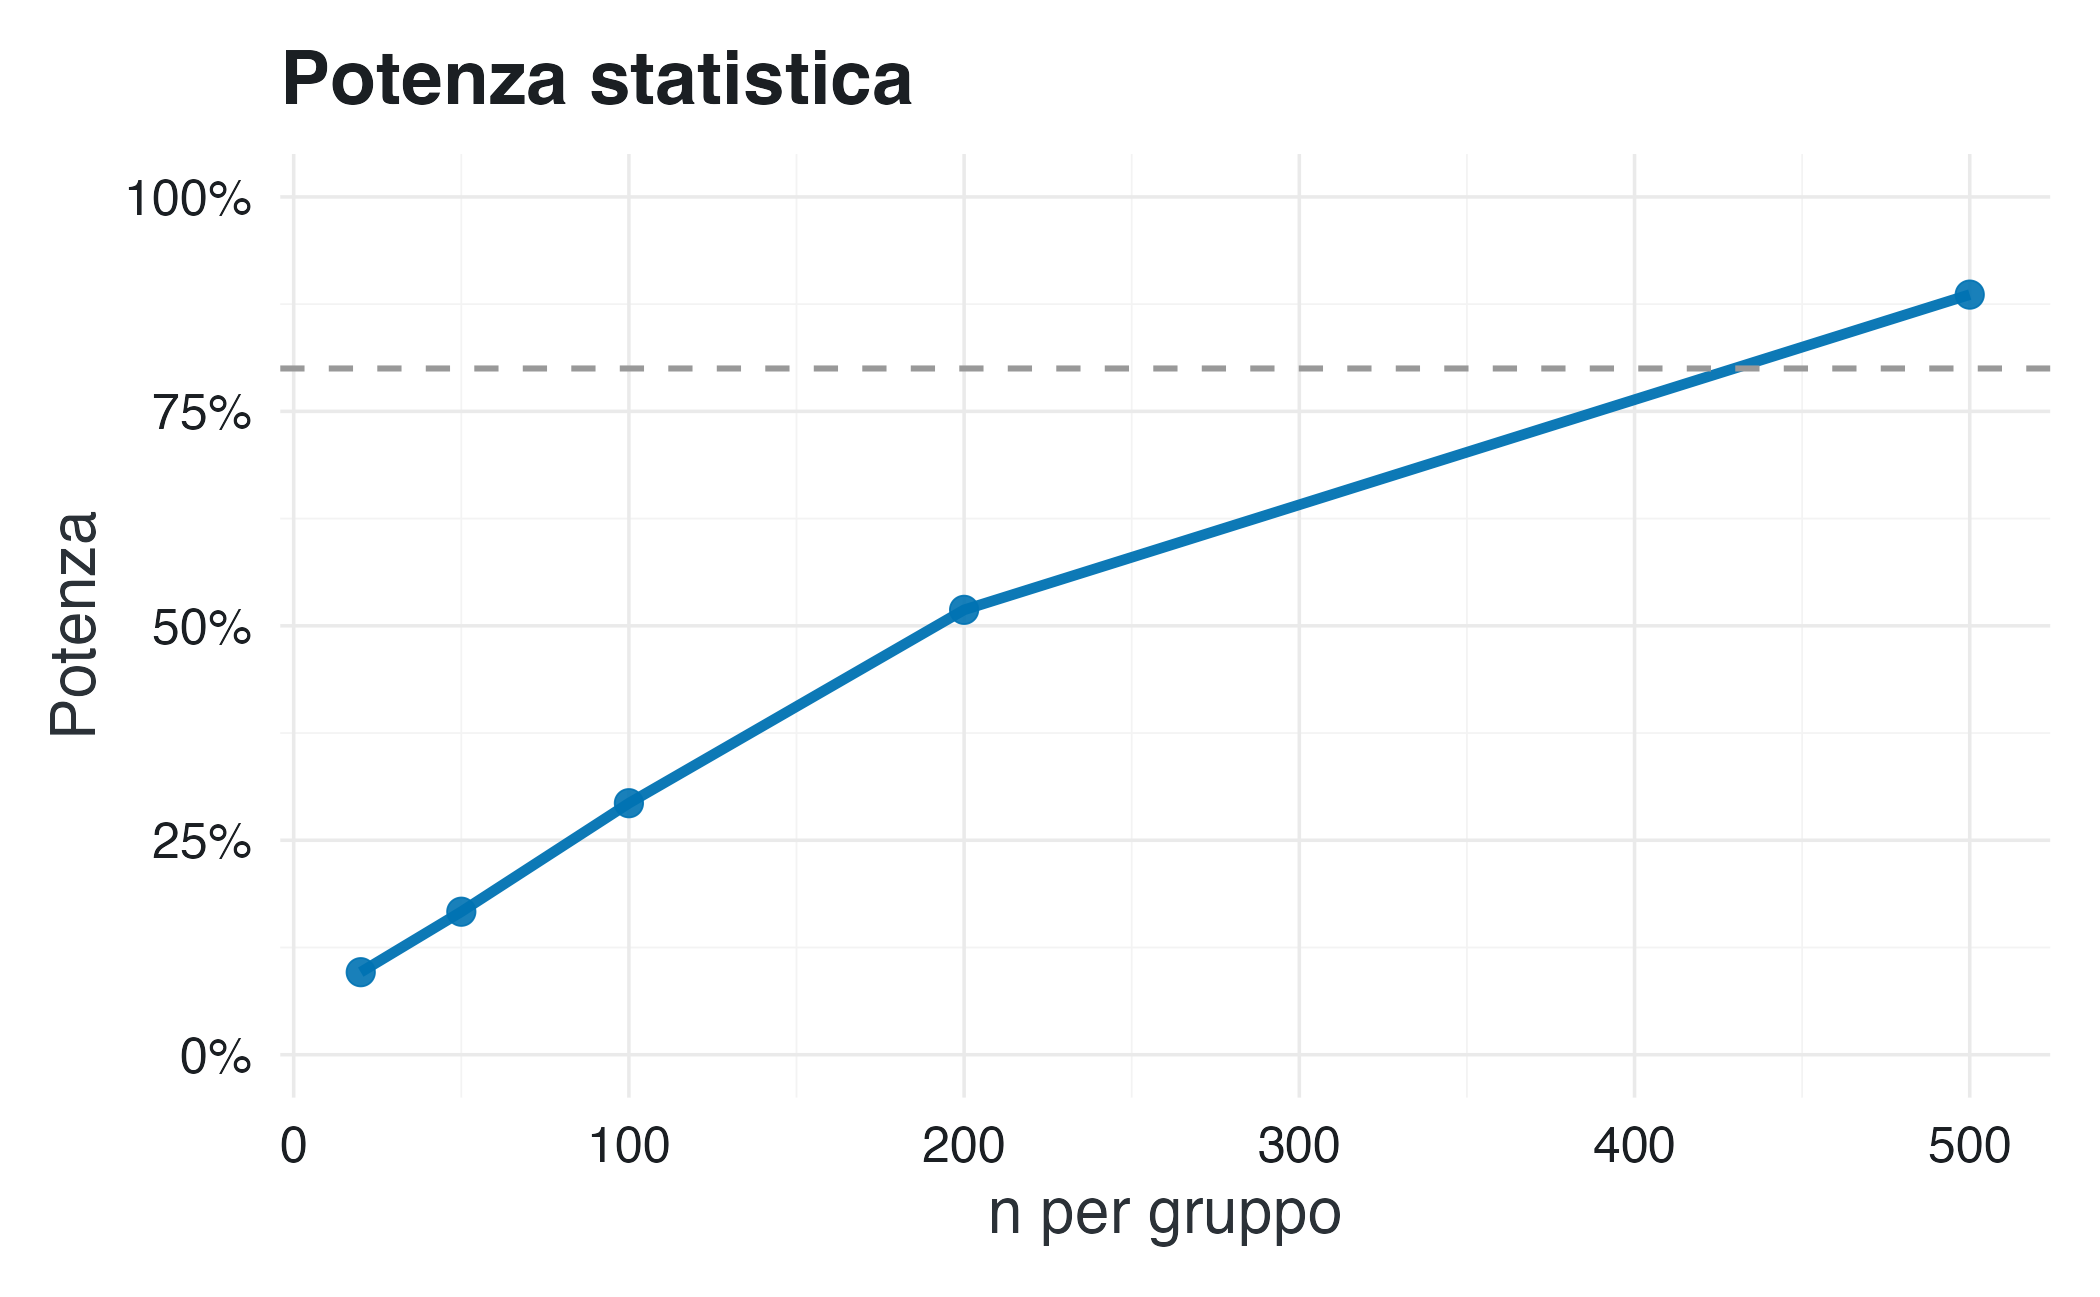
\includegraphics[width=0.85\linewidth,height=\textheight,keepaspectratio]{chapters/limits/03_s_m_errors_files/figure-pdf/unnamed-chunk-10-1.png}
\end{center}

\begin{Shaded}
\begin{Highlighting}[]
\NormalTok{p\_type\_m }
\end{Highlighting}
\end{Shaded}

\begin{center}
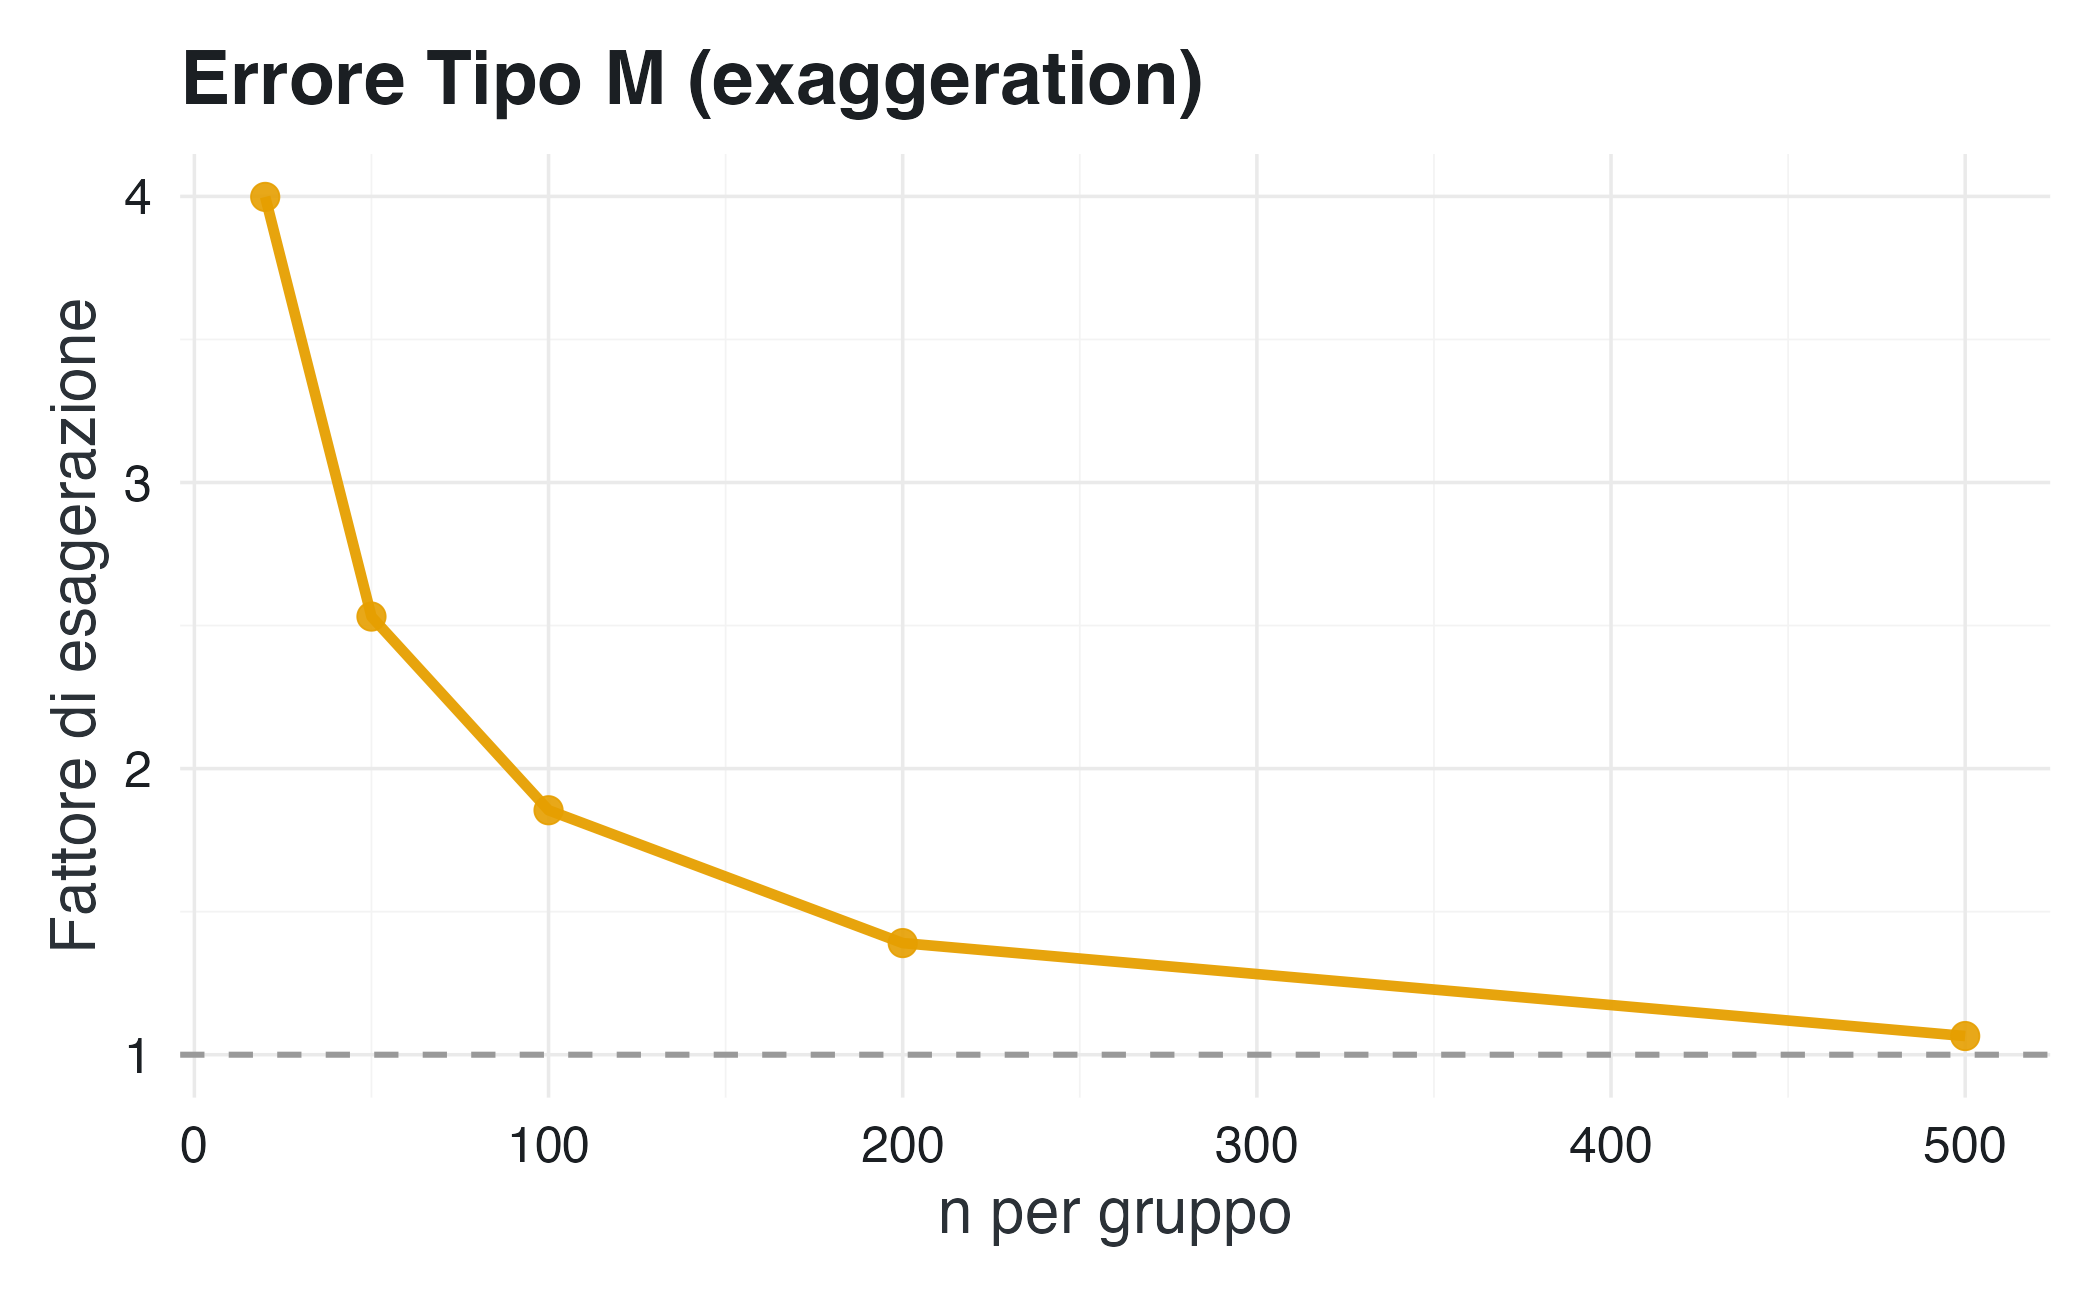
\includegraphics[width=0.85\linewidth,height=\textheight,keepaspectratio]{chapters/limits/03_s_m_errors_files/figure-pdf/unnamed-chunk-11-1.png}
\end{center}

\begin{Shaded}
\begin{Highlighting}[]
\NormalTok{p\_type\_s}
\end{Highlighting}
\end{Shaded}

\begin{center}
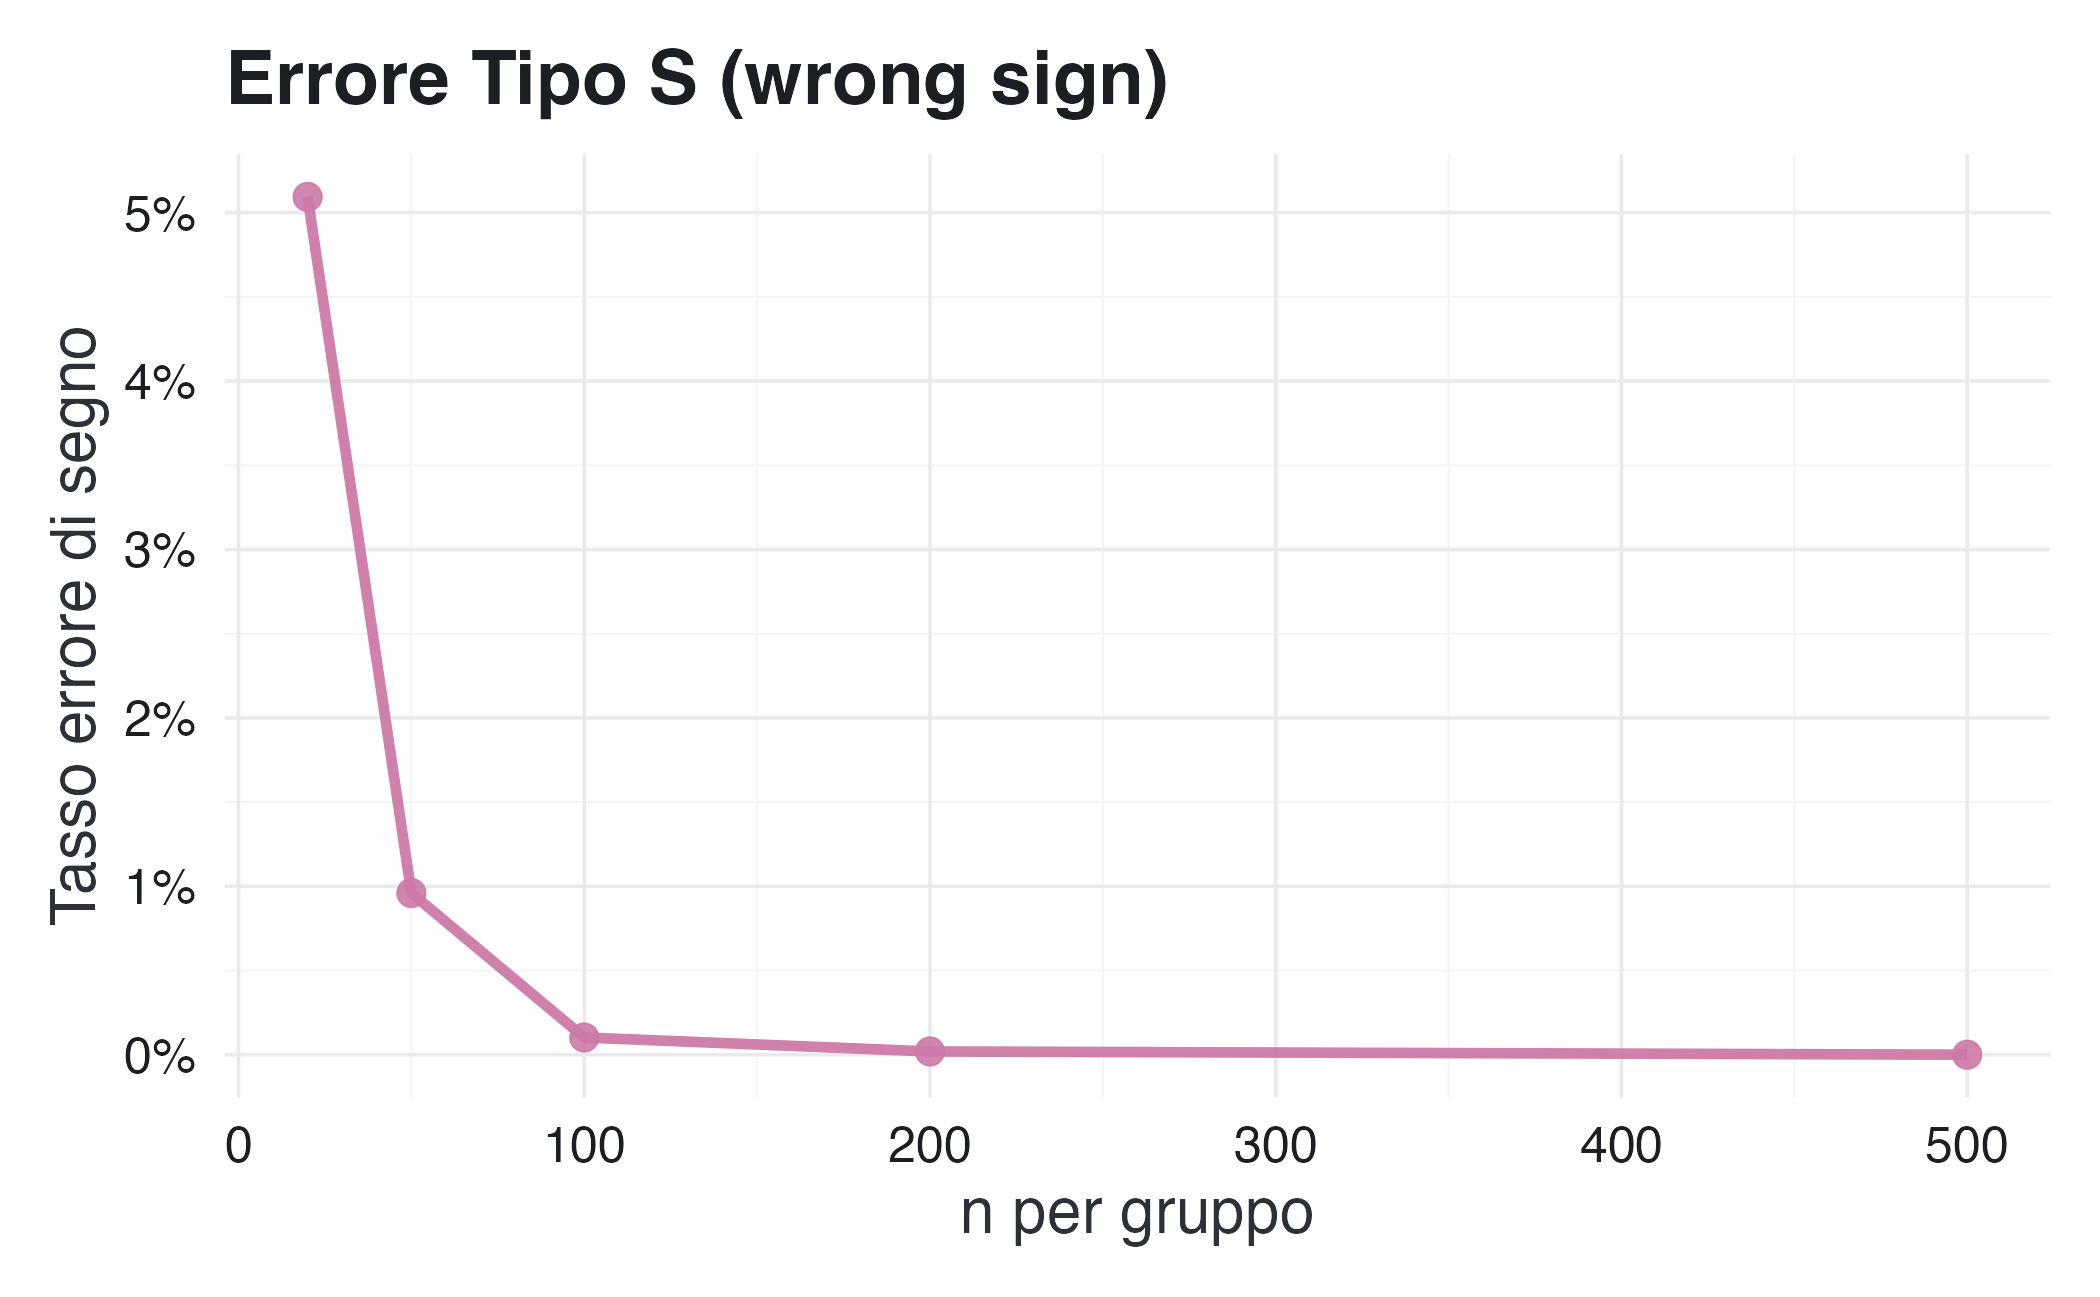
\includegraphics[width=0.85\linewidth,height=\textheight,keepaspectratio]{chapters/limits/03_s_m_errors_files/figure-pdf/unnamed-chunk-12-1.png}
\end{center}

Tabella riassuntiva:

\begin{Shaded}
\begin{Highlighting}[]
\NormalTok{sample\_size\_analysis }\SpecialCharTok{|\textgreater{}}
  \FunctionTok{mutate}\NormalTok{(}
    \StringTok{\textasciigrave{}}\AttributeTok{n per gruppo}\StringTok{\textasciigrave{}} \OtherTok{=}\NormalTok{ n\_per\_group,}
    \StringTok{\textasciigrave{}}\AttributeTok{Potenza}\StringTok{\textasciigrave{}} \OtherTok{=} \FunctionTok{sprintf}\NormalTok{(}\StringTok{"\%.0f\%\%"}\NormalTok{, power }\SpecialCharTok{*} \DecValTok{100}\NormalTok{),}
    \StringTok{\textasciigrave{}}\AttributeTok{Type M (×)}\StringTok{\textasciigrave{}} \OtherTok{=} \FunctionTok{sprintf}\NormalTok{(}\StringTok{"\%.1f"}\NormalTok{, type\_m),}
    \StringTok{\textasciigrave{}}\AttributeTok{Type S (\%)}\StringTok{\textasciigrave{}} \OtherTok{=} \FunctionTok{sprintf}\NormalTok{(}\StringTok{"\%.1f\%\%"}\NormalTok{, type\_s }\SpecialCharTok{*} \DecValTok{100}\NormalTok{)}
\NormalTok{  ) }\SpecialCharTok{|\textgreater{}}
\NormalTok{  dplyr}\SpecialCharTok{::}\FunctionTok{select}\NormalTok{(}\StringTok{\textasciigrave{}}\AttributeTok{n per gruppo}\StringTok{\textasciigrave{}}\NormalTok{, Potenza, }\StringTok{\textasciigrave{}}\AttributeTok{Type M (×)}\StringTok{\textasciigrave{}}\NormalTok{, }\StringTok{\textasciigrave{}}\AttributeTok{Type S (\%)}\StringTok{\textasciigrave{}}\NormalTok{) }\SpecialCharTok{|\textgreater{}}
\NormalTok{  knitr}\SpecialCharTok{::}\FunctionTok{kable}\NormalTok{(}\AttributeTok{caption =} \StringTok{"Errori M e S in funzione della dimensione del campione (effetto vero d = 0.2)"}\NormalTok{)}
\end{Highlighting}
\end{Shaded}

\begin{longtable}[]{@{}rlll@{}}
\caption{Errori M e S in funzione della dimensione del campione (effetto
vero d = 0.2)}\tabularnewline
\toprule\noalign{}
n per gruppo & Potenza & Type M (×) & Type S (\%) \\
\midrule\noalign{}
\endfirsthead
\toprule\noalign{}
n per gruppo & Potenza & Type M (×) & Type S (\%) \\
\midrule\noalign{}
\endhead
\bottomrule\noalign{}
\endlastfoot
20 & 10\% & 4.0 & 5.1\% \\
50 & 17\% & 2.5 & 1.0\% \\
100 & 29\% & 1.9 & 0.1\% \\
200 & 52\% & 1.4 & 0.0\% \\
500 & 89\% & 1.1 & 0.0\% \\
\end{longtable}

La tabella mostra una relazione chiara: con campioni piccoli e bassa
potenza, gli errori sono enormi. Solo con \(n \geq 500\) per gruppo
(potenza \textasciitilde90\%) gli errori diventano accettabili.

\section{Riflessioni conclusive}\label{riflessioni-conclusive-2}

Le simulazioni sviluppate in questo capitolo confermano empiricamente
ciò che l'analisi teorica del manuale illustra concettualmente. Il primo
insegnamento riguarda \textbf{l'inefficacia del filtro della
significatività statistica}. Le simulazioni mostrano che il superamento
della soglia di \(p < 0.05\) non protegge dal rumore, ma opera come un
\textbf{meccanismo selettivo} che favorisce sistematicamente le stime
più estreme e spesso fuorvianti. Il risultato è una letteratura
scientifica strutturalmente distorta, in cui le dimensioni degli effetti
sono \textbf{sovrastimate in modo sistematico}.

Il secondo insegnamento rivela come \textbf{gli errori di Tipo M
(sovrastima) e di Tipo S (segno) siano prevedibili e quantificabili} in
base alla potenza statistica. Con livelli di potenza tipici di molti
studi (intorno all'8\%), le simulazioni mostrano un'esagerazione media
delle stime di circa \textbf{quattro volte} l'effetto reale, e una
probabilità di invertire il segno dell'effetto di circa \textbf{il 4\%}
tra i risultati dichiarati significativi. Ciò trasforma quello che
potrebbe sembrare un errore occasionale in un \textbf{problema sistemico
e prevedibile}.

Il terzo insegnamento valuta \textbf{il ruolo dell'approccio bayesiano
nell'attenuare queste distorsioni}. L'incorporazione di una
distribuzione a priori produce un effetto di \textbf{shrinkage
statistico}, riducendo la dispersione e l'ampiezza delle stime verso
valori più plausibili e mitigando così gli errori di sovrastima e segno.
Tuttavia, le simulazioni chiariscono che si tratta di una
\textbf{riduzione parziale}, non di una soluzione radicale al problema
di fondo.

Il quarto e decisivo insegnamento identifica \textbf{l'incremento della
potenza statistica come unica contromisura efficace}. Solo quando la
potenza raggiunge almeno l'80\% gli errori diventano trascurabili: la
sovrastima si riduce a meno di \textbf{1,1 volte} il valore reale e la
probabilità di errore di segno scende sotto \textbf{lo 0,1\%}. Questo
livello di potenza, ottenibile tramite campioni adeguati o metodi di
aggregazione, è l'unica via per ottenere \textbf{stime affidabili e
robuste}.

In conclusione, le simulazioni proposte da Loken \& Gelman
(\citeproc{ref-loken2017measurement}{2017}) fungono da \textbf{ponte
metodologico} tra teoria e pratica, trasformando concetti statistici
astratti in dimostrazioni concrete. Queste simulazioni dimostrano in
modo incontrovertibile che la soglia di significatività introduce
distorsioni anziché filtrarle, che la bassa potenza genera
sistematicamente sovrastime e inversioni di segno e che solo un aumento
sostanziale della potenza può garantire inferenze valide. Queste
simulazioni non sono solo un esercizio didattico, ma un vero e proprio
\textbf{laboratorio critico} che permette di acquisire consapevolezza
dei limiti degli strumenti statistici convenzionali e di comprendere le
condizioni necessarie per produrre inferenze affidabili.

\begin{tcolorbox}[enhanced jigsaw, arc=.35mm, bottomrule=.15mm, bottomtitle=1mm, breakable, colback=white, colbacktitle=quarto-callout-tip-color!10!white, colframe=quarto-callout-tip-color-frame, coltitle=black, left=2mm, leftrule=.75mm, opacityback=0, opacitybacktitle=0.6, rightrule=.15mm, title=\textcolor{quarto-callout-tip-color}{\faLightbulb}\hspace{0.5em}{Risposte alle domande iniziali}, titlerule=0mm, toprule=.15mm, toptitle=1mm]

Ora confrontiamo le previsioni con i risultati ottenuti dalle
simulazioni:

\begin{enumerate}
\def\labelenumi{\arabic{enumi}.}
\item
  \textbf{Sovrastima della grandezza dell'effetto}: I risultati
  pubblicati tendono a essere selezionati sulla base della
  significatività statistica, il che porta a una sovrastima sistematica
  della grandezza dell'effetto rispetto alla realtà. Questo fenomeno,
  noto come errore di tipo \emph{M} (magnitude), si verifica perché solo
  gli effetti con valori estremi (per caso) superano la soglia di
  significatività statistica e vengono pubblicati.
\item
  \textbf{Falsi positivi e loro frequenza}: In uno scenario in cui non
  esiste alcuna differenza tra i due gruppi (cioè la vera differenza è
  zero), il test t ha fornito risultati statisticamente significativi
  nel 5\% dei casi, come previsto dalla soglia di α = 0.05. Tuttavia, la
  selezione dei risultati pubblicati amplifica questo problema, rendendo
  più probabile che i lettori incontrino falsi positivi nella
  letteratura scientifica.
\item
  \textbf{Bias nella pubblicazione}: Gli studi che riportano risultati
  significativi hanno maggiore probabilità di essere pubblicati rispetto
  a quelli che non trovano un effetto significativo. Questo porta a un
  effetto distorsivo nella letteratura scientifica, in cui i risultati
  pubblicati tendono a sovrastimare l'effetto reale. Il ``filtro della
  significatività statistica'' crea una percezione distorta della realtà
  scientifica, poiché gli effetti nulli o piccoli tendono a essere
  sottorappresentati nella letteratura.
\item
  \textbf{Replicabilità e significatività statistica}: Gli studi con
  effetti piccoli e campioni ridotti sono particolarmente vulnerabili al
  fallimento della replicazione. Anche quando un effetto reale esiste,
  la probabilità di ottenerne una stima precisa è bassa, e la
  replicazione potrebbe risultare in un valore non significativo,
  generando confusione nella comunità scientifica.
\end{enumerate}

\textbf{Considerazioni Finali}

Le simulazioni evidenziano come la significatività statistica,
utilizzata come criterio per la pubblicazione, contribuisca a un bias
nella selezione dei risultati, distorcendo la percezione della realtà
scientifica. Questo fenomeno, noto come ``filtro della significatività
statistica'', è una delle cause principali della crisi della
replicabilità, poiché induce i ricercatori e i lettori a sovrastimare la
grandezza e la presenza di effetti studiati.

Per affrontare queste problematiche, approcci alternativi, come quelli
bayesiani, possono offrire soluzioni più robuste, permettendo una
valutazione più affidabile delle ipotesi alla luce dei dati osservati.

\end{tcolorbox}

\section*{Esercizi}\label{esercizi-2}
\addcontentsline{toc}{section}{Esercizi}

\markright{Esercizi}

\begin{tcolorbox}[enhanced jigsaw, arc=.35mm, bottomrule=.15mm, bottomtitle=1mm, breakable, colback=white, colbacktitle=quarto-callout-important-color!10!white, colframe=quarto-callout-important-color-frame, coltitle=black, left=2mm, leftrule=.75mm, opacityback=0, opacitybacktitle=0.6, rightrule=.15mm, title=\textcolor{quarto-callout-important-color}{\faExclamation}\hspace{0.5em}{Problemi 1}, titlerule=0mm, toprule=.15mm, toptitle=1mm]

\begin{enumerate}
\def\labelenumi{\arabic{enumi}.}
\tightlist
\item
  Perché la significatività statistica non è un criterio affidabile per
  valutare la validità dei risultati scientifici?
\item
  Spiega il concetto di ``filtro della significatività statistica'' e il
  suo impatto sulla pubblicazione dei risultati.
\item
  Qual è la differenza tra errore di tipo \emph{M} e errore di tipo
  \emph{S}? Come influenzano l'interpretazione dei risultati?
\item
  Perché i risultati pubblicati tendono a sovrastimare la grandezza
  dell'effetto rispetto alla realtà?
\item
  Quali sono le conseguenze della pubblicazione selettiva dei risultati
  per la replicabilità degli studi?
\item
  Perché gli studi con campioni di piccole dimensioni sono più
  vulnerabili a errori nella stima della grandezza dell'effetto?
\item
  In che modo la selezione dei risultati pubblicati altera la percezione
  della forza degli effetti studiati?
\item
  Perché un test frequentista può portare a una falsa conclusione sulla
  direzione di un effetto?
\item
  Quali sono le principali differenze tra l'approccio frequentista e
  quello bayesiano nella valutazione della significatività di un
  effetto?
\item
  In che modo l'approccio bayesiano può ridurre il rischio di errori
  dovuti alla selezione dei risultati basata sulla significatività
  statistica?
\end{enumerate}

\end{tcolorbox}

\begin{tcolorbox}[enhanced jigsaw, arc=.35mm, bottomrule=.15mm, bottomtitle=1mm, breakable, colback=white, colbacktitle=quarto-callout-tip-color!10!white, colframe=quarto-callout-tip-color-frame, coltitle=black, left=2mm, leftrule=.75mm, opacityback=0, opacitybacktitle=0.6, rightrule=.15mm, title=\textcolor{quarto-callout-tip-color}{\faLightbulb}\hspace{0.5em}{Soluzioni 1}, titlerule=0mm, toprule=.15mm, toptitle=1mm]

\begin{enumerate}
\def\labelenumi{\arabic{enumi}.}
\item
  \textbf{La significatività statistica non garantisce la validità di un
  risultato} perché dipende dalla dimensione del campione e da soglie
  arbitrarie (come p \textless{} 0.05). Inoltre, non misura la rilevanza
  pratica di un effetto, ma solo la probabilità che i dati osservati
  siano ottenuti sotto l'ipotesi nulla.
\item
  \textbf{Il ``filtro della significatività statistica''} si riferisce
  alla tendenza a pubblicare solo risultati con p \textless{} 0.05,
  tralasciando studi con risultati non significativi. Questo porta a una
  distorsione nella letteratura scientifica e a una sovrastima della
  forza degli effetti riportati.
\item
  \textbf{Errore di tipo \emph{M} (Magnitude)} indica la sovrastima
  della grandezza dell'effetto nei risultati pubblicati, mentre
  \textbf{errore di tipo \emph{S} (Sign)} si riferisce all'errata
  determinazione della direzione dell'effetto. Questi errori si
  verificano perché solo gli effetti più estremi tendono a superare il
  filtro della significatività statistica.
\item
  \textbf{I risultati pubblicati tendono a sovrastimare la grandezza
  dell'effetto} perché solo gli effetti più grandi (anche per pura
  casualità) superano la soglia di significatività statistica e vengono
  pubblicati, mentre quelli più piccoli restano inediti.
\item
  \textbf{La pubblicazione selettiva riduce la replicabilità} perché
  introduce una distorsione sistematica nei risultati disponibili. Le
  repliche spesso non trovano effetti altrettanto grandi o
  significativi, creando instabilità nella conoscenza scientifica.
\item
  \textbf{I campioni piccoli aumentano la variabilità delle stime
  dell'effetto}, rendendo più probabile che un risultato significativo
  sia solo un'oscillazione casuale dei dati piuttosto che un vero
  effetto replicabile.
\item
  \textbf{La selezione dei risultati pubblicati altera la percezione
  della forza degli effetti} perché induce i lettori a credere che gli
  effetti siano più forti e consistenti di quanto non siano realmente.
\item
  \textbf{Un test frequentista può portare a una falsa conclusione sulla
  direzione dell'effetto} perché, in campioni piccoli, le stime
  dell'effetto possono essere fortemente influenzate dal rumore,
  portando a interpretazioni errate.
\item
  \textbf{L'approccio frequentista si basa sul valore-p e sulla soglia
  di significatività, mentre l'approccio bayesiano utilizza la
  probabilità a posteriori} per aggiornare la credibilità delle ipotesi
  alla luce dei dati osservati. Il metodo bayesiano permette inferenze
  più flessibili e robuste.
\item
  \textbf{L'approccio bayesiano riduce il rischio di errori dovuti alla
  selezione dei risultati} perché non si basa su una soglia arbitraria
  di significatività, ma fornisce un quadro probabilistico della forza
  dell'effetto, evitando distorsioni dovute alla pubblicazione
  selettiva.
\end{enumerate}

\end{tcolorbox}

\begin{tcolorbox}[enhanced jigsaw, arc=.35mm, bottomrule=.15mm, bottomtitle=1mm, breakable, colback=white, colbacktitle=quarto-callout-important-color!10!white, colframe=quarto-callout-important-color-frame, coltitle=black, left=2mm, leftrule=.75mm, opacityback=0, opacitybacktitle=0.6, rightrule=.15mm, title=\textcolor{quarto-callout-important-color}{\faExclamation}\hspace{0.5em}{Problemi 2}, titlerule=0mm, toprule=.15mm, toptitle=1mm]

In questo esercizio simuleremo più esperimenti, ognuno con \textbf{15
osservazioni}, per comprendere come il filtro della significatività
statistica possa distorcere le nostre conclusioni sugli effetti
osservati.

\textbf{Obiettivo}

\begin{itemize}
\tightlist
\item
  Comprendere come l'approccio frequentista possa portare a stime errate
  dell'effetto reale.
\item
  Esplorare gli errori di tipo \emph{M} (magnitude) e \emph{S} (sign),
  derivanti dal filtro della significatività statistica.
\end{itemize}

\textbf{Struttura dell'esercizio}

\begin{enumerate}
\def\labelenumi{\arabic{enumi}.}
\tightlist
\item
  Simuliamo esperimenti in cui il \textbf{vero effetto} tra due gruppi è
  piccolo (Cohen's \emph{d} = 0.2). Consideriamo i dati SWLS e due
  popolazioni che differiscono nel modo indicato. Ipotizziamo che le due
  popolazioni SWLS siano normali.
\item
  Estraiamo 15 osservazioni per gruppo.
\item
  Usiamo un test \emph{t} per verificare se la differenza tra i gruppi è
  significativa.
\item
  Registriamo solo i risultati con \emph{p} \textless{} 0.05, calcolando
  la distribuzione degli effetti significativi.
\item
  Valutiamo se la stima dell'effetto nei risultati pubblicabili è
  gonfiata rispetto al vero effetto.
\item
  Contiamo i casi in cui il segno dell'effetto è invertito.
\end{enumerate}

\end{tcolorbox}

\begin{tcolorbox}[enhanced jigsaw, arc=.35mm, bottomrule=.15mm, bottomtitle=1mm, breakable, colback=white, colbacktitle=quarto-callout-tip-color!10!white, colframe=quarto-callout-tip-color-frame, coltitle=black, left=2mm, leftrule=.75mm, opacityback=0, opacitybacktitle=0.6, rightrule=.15mm, title=\textcolor{quarto-callout-tip-color}{\faLightbulb}\hspace{0.5em}{Soluzioni 2}, titlerule=0mm, toprule=.15mm, toptitle=1mm]

\begin{Shaded}
\begin{Highlighting}[]
\CommentTok{\# Librerie necessarie}
\FunctionTok{library}\NormalTok{(ggplot2)}

\CommentTok{\# Impostazioni della simulazione}
\FunctionTok{set.seed}\NormalTok{(}\DecValTok{42}\NormalTok{)         }\CommentTok{\# Per la riproducibilità}
\NormalTok{n\_sims }\OtherTok{\textless{}{-}} \DecValTok{50000}      \CommentTok{\# Numero di simulazioni}
\NormalTok{n\_per\_group }\OtherTok{\textless{}{-}} \DecValTok{15}    \CommentTok{\# Numero di osservazioni per gruppo}
\NormalTok{true\_d }\OtherTok{\textless{}{-}} \FloatTok{0.2}        \CommentTok{\# Vero effetto (Cohen\textquotesingle{}s d)}
\NormalTok{swls\_mean }\OtherTok{\textless{}{-}} \DecValTok{25}      \CommentTok{\# Media ipotizzata per il primo gruppo}
\NormalTok{swls\_sd }\OtherTok{\textless{}{-}} \DecValTok{5}         \CommentTok{\# Deviazione standard ipotizzata per la SWLS}

\CommentTok{\# Calcolo della media del secondo gruppo sulla base di Cohen\textquotesingle{}s d}
\NormalTok{swls\_mean\_2 }\OtherTok{\textless{}{-}}\NormalTok{ swls\_mean }\SpecialCharTok{+}\NormalTok{ true\_d }\SpecialCharTok{*}\NormalTok{ swls\_sd}

\CommentTok{\# Inizializziamo i vettori per registrare i risultati}
\NormalTok{effect\_sizes }\OtherTok{\textless{}{-}} \FunctionTok{c}\NormalTok{()}
\NormalTok{false\_sign\_count }\OtherTok{\textless{}{-}} \DecValTok{0}

\CommentTok{\# Simulazioni}
\ControlFlowTok{for}\NormalTok{ (i }\ControlFlowTok{in} \DecValTok{1}\SpecialCharTok{:}\NormalTok{n\_sims) \{}
  \CommentTok{\# Generazione dei due gruppi da distribuzioni normali}
\NormalTok{  group1 }\OtherTok{\textless{}{-}} \FunctionTok{rnorm}\NormalTok{(n\_per\_group, }\AttributeTok{mean =}\NormalTok{ swls\_mean, }\AttributeTok{sd =}\NormalTok{ swls\_sd)}
\NormalTok{  group2 }\OtherTok{\textless{}{-}} \FunctionTok{rnorm}\NormalTok{(n\_per\_group, }\AttributeTok{mean =}\NormalTok{ swls\_mean\_2, }\AttributeTok{sd =}\NormalTok{ swls\_sd)}
  
  \CommentTok{\# Calcolo della dimensione dell\textquotesingle{}effetto (Cohen\textquotesingle{}s d)}
\NormalTok{  mean\_diff }\OtherTok{\textless{}{-}} \FunctionTok{mean}\NormalTok{(group2) }\SpecialCharTok{{-}} \FunctionTok{mean}\NormalTok{(group1)}
\NormalTok{  pooled\_sd }\OtherTok{\textless{}{-}} \FunctionTok{sqrt}\NormalTok{(((n\_per\_group }\SpecialCharTok{{-}} \DecValTok{1}\NormalTok{) }\SpecialCharTok{*} \FunctionTok{var}\NormalTok{(group1) }\SpecialCharTok{+}\NormalTok{ (n\_per\_group }\SpecialCharTok{{-}} \DecValTok{1}\NormalTok{) }\SpecialCharTok{*} \FunctionTok{var}\NormalTok{(group2)) }\SpecialCharTok{/}\NormalTok{ (}\DecValTok{2} \SpecialCharTok{*}\NormalTok{ n\_per\_group }\SpecialCharTok{{-}} \DecValTok{2}\NormalTok{))}
\NormalTok{  d\_estimated }\OtherTok{\textless{}{-}}\NormalTok{ mean\_diff }\SpecialCharTok{/}\NormalTok{ pooled\_sd}
  
  \CommentTok{\# Test t per confrontare le medie}
\NormalTok{  t\_test }\OtherTok{\textless{}{-}} \FunctionTok{t.test}\NormalTok{(group1, group2, }\AttributeTok{var.equal =} \ConstantTok{TRUE}\NormalTok{)}
  
  \CommentTok{\# Consideriamo solo i risultati statisticamente significativi}
  \ControlFlowTok{if}\NormalTok{ (t\_test}\SpecialCharTok{$}\NormalTok{p.value }\SpecialCharTok{\textless{}} \FloatTok{0.05}\NormalTok{) \{}
\NormalTok{    effect\_sizes }\OtherTok{\textless{}{-}} \FunctionTok{c}\NormalTok{(effect\_sizes, d\_estimated)}
    
    \CommentTok{\# Conta i casi in cui il segno è invertito}
    \ControlFlowTok{if}\NormalTok{ (d\_estimated }\SpecialCharTok{\textless{}} \DecValTok{0}\NormalTok{) \{}
\NormalTok{      false\_sign\_count }\OtherTok{\textless{}{-}}\NormalTok{ false\_sign\_count }\SpecialCharTok{+} \DecValTok{1}
\NormalTok{    \}}
\NormalTok{  \}}
\NormalTok{\}}

\CommentTok{\# Creazione di un dataframe per la visualizzazione}
\NormalTok{res\_df }\OtherTok{\textless{}{-}} \FunctionTok{data.frame}\NormalTok{(}\AttributeTok{effect\_size =}\NormalTok{ effect\_sizes)}

\CommentTok{\# Istogramma della dimensione dell\textquotesingle{}effetto tra i risultati "significativi"}
\FunctionTok{ggplot}\NormalTok{(res\_df, }\FunctionTok{aes}\NormalTok{(}\AttributeTok{x =}\NormalTok{ effect\_size)) }\SpecialCharTok{+}
  \FunctionTok{geom\_histogram}\NormalTok{(}\AttributeTok{bins =} \DecValTok{30}\NormalTok{, }\AttributeTok{fill =} \StringTok{"blue"}\NormalTok{, }\AttributeTok{color =} \StringTok{"black"}\NormalTok{, }\AttributeTok{alpha =} \FloatTok{0.7}\NormalTok{) }\SpecialCharTok{+}
  \FunctionTok{geom\_vline}\NormalTok{(}\AttributeTok{xintercept =}\NormalTok{ true\_d, }\AttributeTok{color =} \StringTok{"red"}\NormalTok{, }\AttributeTok{linetype =} \StringTok{"dashed"}\NormalTok{, }\AttributeTok{size =} \FloatTok{1.2}\NormalTok{) }\SpecialCharTok{+}
  \FunctionTok{labs}\NormalTok{(}
    \AttributeTok{x =} \StringTok{"Dimensione dell\textquotesingle{}effetto stimata"}\NormalTok{,}
    \AttributeTok{y =} \StringTok{"Frequenza"}\NormalTok{,}
    \AttributeTok{title =} \StringTok{"Distribuzione degli effetti significativi (SWLS)"}
\NormalTok{  ) }\SpecialCharTok{+}
  \FunctionTok{theme\_minimal}\NormalTok{()}

\CommentTok{\# Output di sintesi}
\FunctionTok{cat}\NormalTok{(}\StringTok{"Numero di risultati statisticamente significativi:"}\NormalTok{, }\FunctionTok{length}\NormalTok{(effect\_sizes), }\StringTok{"}\SpecialCharTok{\textbackslash{}n}\StringTok{"}\NormalTok{)}
\FunctionTok{cat}\NormalTok{(}\StringTok{"Media della dimensione dell\textquotesingle{}effetto tra i risultati pubblicati:"}\NormalTok{, }\FunctionTok{mean}\NormalTok{(effect\_sizes), }\StringTok{"}\SpecialCharTok{\textbackslash{}n}\StringTok{"}\NormalTok{)}
\FunctionTok{cat}\NormalTok{(}\StringTok{"Numero di risultati con segno invertito:"}\NormalTok{, false\_sign\_count, }\StringTok{"}\SpecialCharTok{\textbackslash{}n}\StringTok{"}\NormalTok{)}
\FunctionTok{cat}\NormalTok{(}\StringTok{"Proporzione di risultati con segno invertito:"}\NormalTok{, false\_sign\_count }\SpecialCharTok{/} \FunctionTok{length}\NormalTok{(effect\_sizes), }\StringTok{"}\SpecialCharTok{\textbackslash{}n}\StringTok{"}\NormalTok{)}
\end{Highlighting}
\end{Shaded}

\textbf{Interpretazione dei Risultati}

\begin{enumerate}
\def\labelenumi{\arabic{enumi}.}
\tightlist
\item
  \textbf{Errore di tipo \emph{M}} (Magnitude): La media degli effetti
  stimati nei risultati pubblicati sarà molto più grande di 0.2 (il vero
  effetto), dimostrando come il filtro della significatività tenda a
  sovrastimare gli effetti reali.
\item
  \textbf{Errore di tipo \emph{S}} (Sign): Una percentuale dei risultati
  pubblicabili mostrerà effetti nella direzione sbagliata (d \textless{}
  0), dimostrando che il processo decisionale basato su \emph{p}
  \textless{} 0.05 può portare a conclusioni errate.
\item
  \textbf{Visualizzazione}: L'istogramma mostrerà che la distribuzione
  degli effetti significativi è spostata rispetto al vero effetto (linea
  rossa tratteggiata).
\end{enumerate}

\textbf{Domande di discussione}:

\begin{enumerate}
\def\labelenumi{\arabic{enumi}.}
\tightlist
\item
  Perché la stima dell'effetto è gonfiata nei risultati pubblicabili?
\item
  Come cambia la situazione aumentando il numero di osservazioni per
  gruppo?
\item
  Quali strategie alternative potrebbero ridurre questi errori?
\end{enumerate}

\textbf{Approfondimento}:

\begin{itemize}
\tightlist
\item
  Ripetere l'esperimento con \emph{n\_per\_group = 50} e osservare se
  l'errore di tipo \emph{M} diminuisce.
\item
  Confrontare questo approccio con un'analisi Bayesiana per evidenziare
  il ruolo dell'inferenza basata su probabilità posteriori.
\end{itemize}

\textbf{Conclusione}

Questo esercizio mostra chiaramente i problemi dell'approccio
frequentista basato su \emph{p} \textless{} 0.05, evidenziando i limiti
dell'uso della significatività statistica come filtro decisionale.

\end{tcolorbox}

\begin{tcolorbox}[enhanced jigsaw, arc=.35mm, bottomrule=.15mm, bottomtitle=1mm, breakable, colback=white, colbacktitle=quarto-callout-note-color!10!white, colframe=quarto-callout-note-color-frame, coltitle=black, left=2mm, leftrule=.75mm, opacityback=0, opacitybacktitle=0.6, rightrule=.15mm, title=\textcolor{quarto-callout-note-color}{\faInfo}\hspace{0.5em}{Informazioni sull'ambiente di sviluppo}, titlerule=0mm, toprule=.15mm, toptitle=1mm]

\begin{Shaded}
\begin{Highlighting}[]
\FunctionTok{sessionInfo}\NormalTok{()}
\CommentTok{\#\textgreater{} R version 4.6.1 (2026{-}06{-}24)}
\CommentTok{\#\textgreater{} Platform: aarch64{-}apple{-}darwin23}
\CommentTok{\#\textgreater{} Running under: macOS Tahoe 26.5.2}
\CommentTok{\#\textgreater{} }
\CommentTok{\#\textgreater{} Matrix products: default}
\CommentTok{\#\textgreater{} BLAS:   /Library/Frameworks/R.framework/Versions/4.6/Resources/lib/libRblas.0.dylib }
\CommentTok{\#\textgreater{} LAPACK: /Library/Frameworks/R.framework/Versions/4.6/Resources/lib/libRlapack.dylib;  LAPACK version 3.12.1}
\CommentTok{\#\textgreater{} }
\CommentTok{\#\textgreater{} locale:}
\CommentTok{\#\textgreater{} [1] C.UTF{-}8/UTF{-}8/C.UTF{-}8/C/C.UTF{-}8/C.UTF{-}8}
\CommentTok{\#\textgreater{} }
\CommentTok{\#\textgreater{} time zone: Europe/Zagreb}
\CommentTok{\#\textgreater{} tzcode source: internal}
\CommentTok{\#\textgreater{} }
\CommentTok{\#\textgreater{} attached base packages:}
\CommentTok{\#\textgreater{} [1] stats     graphics  grDevices utils     datasets  methods   base     }
\CommentTok{\#\textgreater{} }
\CommentTok{\#\textgreater{} other attached packages:}
\CommentTok{\#\textgreater{}  [1] forcats\_1.0.1         purrr\_1.2.2           ragg\_1.5.2           }
\CommentTok{\#\textgreater{}  [4] tinytable\_0.17.0      withr\_3.0.3           systemfonts\_1.3.2    }
\CommentTok{\#\textgreater{}  [7] patchwork\_1.3.2       ggdist\_3.3.3          tidybayes\_3.0.7      }
\CommentTok{\#\textgreater{} [10] bayesplot\_1.15.0      ggplot2\_4.0.3         reliabilitydiag\_0.2.1}
\CommentTok{\#\textgreater{} [13] priorsense\_1.2.0      posterior\_1.7.0       loo\_2.10.0           }
\CommentTok{\#\textgreater{} [16] rstan\_2.32.7          StanHeaders\_2.32.10   brms\_2.23.0          }
\CommentTok{\#\textgreater{} [19] Rcpp\_1.1.2            sessioninfo\_1.2.4     conflicted\_1.2.0     }
\CommentTok{\#\textgreater{} [22] janitor\_2.2.1         matrixStats\_1.5.0     modelr\_0.1.11        }
\CommentTok{\#\textgreater{} [25] tibble\_3.3.1          dplyr\_1.2.1           tidyr\_1.3.2          }
\CommentTok{\#\textgreater{} [28] rio\_1.3.0             here\_1.0.2           }
\CommentTok{\#\textgreater{} }
\CommentTok{\#\textgreater{} loaded via a namespace (and not attached):}
\CommentTok{\#\textgreater{}  [1] svUnit\_1.0.8          tidyselect\_1.2.1      farver\_2.1.2         }
\CommentTok{\#\textgreater{}  [4] S7\_0.2.2              fastmap\_1.2.0         tensorA\_0.36.2.1     }
\CommentTok{\#\textgreater{}  [7] pacman\_0.5.1          digest\_0.6.39         timechange\_0.4.0     }
\CommentTok{\#\textgreater{} [10] estimability\_2.0.0    lifecycle\_1.0.5       magrittr\_2.0.5       }
\CommentTok{\#\textgreater{} [13] compiler\_4.6.1        rlang\_1.3.0           tools\_4.6.1          }
\CommentTok{\#\textgreater{} [16] yaml\_2.3.12           knitr\_1.51            labeling\_0.4.3       }
\CommentTok{\#\textgreater{} [19] bridgesampling\_1.2{-}1  pkgbuild\_1.4.8        curl\_7.1.0           }
\CommentTok{\#\textgreater{} [22] RColorBrewer\_1.1{-}3    abind\_1.4{-}8           grid\_4.6.1           }
\CommentTok{\#\textgreater{} [25] stats4\_4.6.1          xtable\_1.8{-}8          inline\_0.3.21        }
\CommentTok{\#\textgreater{} [28] emmeans\_2.0.4         scales\_1.4.0          cli\_3.6.6            }
\CommentTok{\#\textgreater{} [31] mvtnorm\_1.4{-}2         rmarkdown\_2.31        generics\_0.1.4       }
\CommentTok{\#\textgreater{} [34] otel\_0.2.0            RcppParallel\_5.1.11{-}2 cachem\_1.1.0         }
\CommentTok{\#\textgreater{} [37] stringr\_1.6.0         parallel\_4.6.1        vctrs\_0.7.3          }
\CommentTok{\#\textgreater{} [40] V8\_8.2.0              Matrix\_1.7{-}5          jsonlite\_2.0.0       }
\CommentTok{\#\textgreater{} [43] arrayhelpers\_1.1{-}1    glue\_1.8.1            codetools\_0.2{-}20     }
\CommentTok{\#\textgreater{} [46] distributional\_0.8.1  lubridate\_1.9.5       stringi\_1.8.7        }
\CommentTok{\#\textgreater{} [49] gtable\_0.3.6          QuickJSR\_1.10.0       pillar\_1.11.1        }
\CommentTok{\#\textgreater{} [52] htmltools\_0.5.9       Brobdingnag\_1.2{-}9     R6\_2.6.1             }
\CommentTok{\#\textgreater{} [55] textshaping\_1.0.5     rprojroot\_2.1.1       evaluate\_1.0.5       }
\CommentTok{\#\textgreater{} [58] lattice\_0.22{-}9        backports\_1.5.1       memoise\_2.0.1        }
\CommentTok{\#\textgreater{} [61] broom\_1.0.13          snakecase\_0.11.1      rstantools\_2.6.0     }
\CommentTok{\#\textgreater{} [64] coda\_0.19{-}4.1         gridExtra\_2.3.1       nlme\_3.1{-}170         }
\CommentTok{\#\textgreater{} [67] checkmate\_2.3.4       xfun\_0.60             pkgconfig\_2.0.3}
\end{Highlighting}
\end{Shaded}

\end{tcolorbox}

\section*{Bibliografia}\label{bibliografia-3}

\markright{Bibliografia}

\chapter{\texorpdfstring{La fragilità del
valore-\(p\)}{La fragilità del valore-p}}\label{sec-p-value-fragility}

\begin{tcolorbox}[enhanced jigsaw, arc=.35mm, bottomrule=.15mm, breakable, colback=white, colframe=quarto-callout-note-color-frame, left=2mm, leftrule=.75mm, opacityback=0, rightrule=.15mm, toprule=.15mm]

Nel manuale abbiamo visto che il valore-\(p\) è spesso frainteso e
utilizzato in modo improprio. Uno degli aspetti più critici, ma spesso
trascurato, riguarda la sua \textbf{estrema variabilità}: campioni
diversi estratti dalla stessa popolazione possono produrre valori-\(p\)
profondamente diversi, portando, solo a causa di fluttuazioni casuali, a
conclusioni opposte riguardo allo stesso fenomeno.

Questo problema è stato efficacemente e ironicamente colto da Gelman \&
Stern (\citeproc{ref-gelman2006difference}{2006}), che hanno osservato:
``La differenza tra `significativo' e `non significativo' non è di per
sé statisticamente significativa''.

Questa affermazione, apparentemente paradossale, coglie un punto
cruciale: una soglia convenzionale come \(p\) = 0.05 non garantisce una
distinzione affidabile tra effetti reali e assenza di effetto.
Variazioni minime e del tutto casuali nei dati possono spostare un
valore-\(p\) da un lato all'altro della soglia, alterando radicalmente
l'interpretazione del risultato senza che questo corrisponda a un
cambiamento reale nel fenomeno studiato.

In questo capitolo, esploreremo l'instabilità del valore-\(p\)
attraverso delle simulazioni. L'obiettivo è mostrare quanto sia
rischioso basare la valutazione di un risultato sulla dicotomia
\(p < 0.05\) vs.~\(p \geq 0.05\) e perché questa pratica possa portare a
conclusioni fuorvianti nella ricerca psicologica.

\end{tcolorbox}

\begin{tcolorbox}[enhanced jigsaw, arc=.35mm, bottomrule=.15mm, breakable, colback=white, colframe=quarto-callout-important-color-frame, left=2mm, leftrule=.75mm, opacityback=0, rightrule=.15mm, toprule=.15mm]

\textbf{Da sapere.} Il valore-\(p\) è una statistica campionaria molto
variabile: studi condotti sulla stessa popolazione possono produrre
valori molto diversi e conclusioni opposte. La distinzione tra
``significativo'' e ``non significativo'' non rappresenta
necessariamente una differenza reale tra i fenomeni studiati.

\textbf{Da saper fare.} Capire le simulazioni che illustrano la
variabilità del valore-\(p\); confrontarne la distribuzione quando
\(H_0\) è vera e quando è falsa; spiegare la relazione tra dimensione
dell'effetto, numerosità campionaria e potenza; confrontare la stabilità
delle conclusioni frequentiste e bayesiane.

\textbf{Approfondimento facoltativo.} L'implementazione completa delle
simulazioni, il confronto dettagliato tra studi apparentemente
contraddittori, l'analisi bayesiana e gli esercizi finali possono essere
rimandati in una prima lettura.

\hyperref[sec-percorsi-lettura]{Che cosa significano queste etichette?}

\end{tcolorbox}

\begin{tcolorbox}[enhanced jigsaw, arc=.35mm, bottomrule=.15mm, bottomtitle=1mm, breakable, colback=white, colbacktitle=quarto-callout-important-color!10!white, colframe=quarto-callout-important-color-frame, coltitle=black, left=2mm, leftrule=.75mm, opacityback=0, opacitybacktitle=0.6, rightrule=.15mm, title=\textcolor{quarto-callout-important-color}{\faExclamation}\hspace{0.5em}{In questo capitolo imparerai a}, titlerule=0mm, toprule=.15mm, toptitle=1mm]

\begin{itemize}
\tightlist
\item
  osservare empiricamente la variabilità del valore-\(p\) da campione a
  campione;
\item
  confrontare la distribuzione dei valori-\(p\) sotto l'ipotesi \(H_0\)
  vera vs.~l'ipotesi \(H_0\) falsa;
\item
  comprendere perché la differenza tra ``significativo'' e ``non
  significativo'' non è significativa;
\item
  confrontare la stabilità delle inferenze frequentiste vs bayesiane.
\end{itemize}

\end{tcolorbox}

\begin{tcolorbox}[enhanced jigsaw, arc=.35mm, bottomrule=.15mm, bottomtitle=1mm, breakable, colback=white, colbacktitle=quarto-callout-tip-color!10!white, colframe=quarto-callout-tip-color-frame, coltitle=black, left=2mm, leftrule=.75mm, opacityback=0, opacitybacktitle=0.6, rightrule=.15mm, title=\textcolor{quarto-callout-tip-color}{\faLightbulb}\hspace{0.5em}{Prerequisiti}, titlerule=0mm, toprule=.15mm, toptitle=1mm]

\begin{itemize}
\tightlist
\item
  Rivedere nel manuale la trattazione delle \textbf{pratiche di ricerca
  discutibili} e dei gradi di libertà del ricercatore.
\item
  Leggere il post di Gelman \& Stern (2006):
  \href{http://www.stat.columbia.edu/~gelman/research/published/signif4.pdf}{The
  Difference Between ``Significant'' and ``Not Significant'' is not
  Itself Statistically Significant}.
\end{itemize}

\end{tcolorbox}

\begin{tcolorbox}[enhanced jigsaw, arc=.35mm, bottomrule=.15mm, bottomtitle=1mm, breakable, colback=white, colbacktitle=quarto-callout-caution-color!10!white, colframe=quarto-callout-caution-color-frame, coltitle=black, left=2mm, leftrule=.75mm, opacityback=0, opacitybacktitle=0.6, rightrule=.15mm, title=\textcolor{quarto-callout-caution-color}{\faFire}\hspace{0.5em}{Preparazione del Notebook}, titlerule=0mm, toprule=.15mm, toptitle=1mm]

\begin{Shaded}
\begin{Highlighting}[]
\NormalTok{here}\SpecialCharTok{::}\FunctionTok{here}\NormalTok{(}\StringTok{"code"}\NormalTok{, }\StringTok{"\_common.R"}\NormalTok{) }\SpecialCharTok{|\textgreater{}} 
  \FunctionTok{source}\NormalTok{()}
\FunctionTok{library}\NormalTok{(patchwork)}
\end{Highlighting}
\end{Shaded}

\end{tcolorbox}

\section{\texorpdfstring{Simulazione 1: la variabilità del
valore-\(p\)}{Simulazione 1: la variabilità del valore-p}}\label{simulazione-1-la-variabilituxe0-del-valore-p}

Supponiamo di voler studiare un effetto di modesta entità. Nella
popolazione di riferimento, la variabile di interesse ha una media
\(\mu = 0.05\) e una deviazione standard \(\sigma = 0.1\). Ciò
corrisponde a una dimensione dell'effetto di Cohen \(d\) = 0.5,
convenzionalmente considerata di intensità ``media''.

Per illustrare l'elevata volatilità del valore-\(p\) in piccoli
campioni, simuliamo uno scenario di ricerca tipico: la raccolta ripetuta
di nuovi dati. In particolare, dalla popolazione descritta estraiamo 100
campioni casuali indipendenti, ciascuno di dimensioni ridotte (\(n\) =
10). Per ogni campione, eseguiamo un test \(t\) di Student per
verificare l'ipotesi nulla \(H_0: \mu = 0\).

L'obiettivo della simulazione è mostrare come, nonostante l'effetto
reale nella popolazione sia costante (\(\mu\) = 0.05), il valore-\(p\)
oscilli in modo drastico da un campione all'altro. Questa marcata
variabilità rivela la natura intrinsecamente instabile del valore-\(p\)
quale statistica campionaria. Ne consegue che le sue fluttuazioni
potrebbero essere \textbf{interpretate in modo fuorviante} come
cambiamenti sostanziali del fenomeno studiato, mentre in realtà
riflettono \textbf{esclusivamente la variabilità casuale} insita nel
processo di campionamento.

\begin{Shaded}
\begin{Highlighting}[]
\CommentTok{\# Parametri della simulazione}
\NormalTok{n\_samples }\OtherTok{\textless{}{-}} \DecValTok{100}         \CommentTok{\# Numero di campioni indipendenti}
\NormalTok{n\_obs }\OtherTok{\textless{}{-}} \DecValTok{10}              \CommentTok{\# Osservazioni per campione}
\NormalTok{true\_mean }\OtherTok{\textless{}{-}} \FloatTok{0.05}        \CommentTok{\# Media vera (effetto piccolo)}
\NormalTok{true\_sd }\OtherTok{\textless{}{-}} \FloatTok{0.1}           \CommentTok{\# Deviazione standard}

\CommentTok{\# Simula i campioni e calcola i p{-}value}
\NormalTok{simulation }\OtherTok{\textless{}{-}} \FunctionTok{tibble}\NormalTok{(}\AttributeTok{sample\_id =} \DecValTok{1}\SpecialCharTok{:}\NormalTok{n\_samples) }\SpecialCharTok{|\textgreater{}}
  \FunctionTok{rowwise}\NormalTok{() }\SpecialCharTok{|\textgreater{}}
  \FunctionTok{mutate}\NormalTok{(}
    \AttributeTok{data =} \FunctionTok{list}\NormalTok{(}\FunctionTok{rnorm}\NormalTok{(n\_obs, }\AttributeTok{mean =}\NormalTok{ true\_mean, }\AttributeTok{sd =}\NormalTok{ true\_sd)),}
    \AttributeTok{sample\_mean =} \FunctionTok{mean}\NormalTok{(data),}
    \AttributeTok{sample\_sd =} \FunctionTok{sd}\NormalTok{(data),}
    \AttributeTok{t\_stat =}\NormalTok{ sample\_mean }\SpecialCharTok{/}\NormalTok{ (sample\_sd }\SpecialCharTok{/} \FunctionTok{sqrt}\NormalTok{(n\_obs)),}
    \AttributeTok{p\_value =} \DecValTok{2} \SpecialCharTok{*} \FunctionTok{pt}\NormalTok{(}\SpecialCharTok{{-}}\FunctionTok{abs}\NormalTok{(t\_stat), }\AttributeTok{df =}\NormalTok{ n\_obs }\SpecialCharTok{{-}} \DecValTok{1}\NormalTok{),}
    \AttributeTok{significant =}\NormalTok{ p\_value }\SpecialCharTok{\textless{}} \FloatTok{0.05}
\NormalTok{  ) }\SpecialCharTok{|\textgreater{}}
  \FunctionTok{ungroup}\NormalTok{()}
\end{Highlighting}
\end{Shaded}

\begin{verbatim}
#> Effetto vero: μ = 0.05, σ = 0.10 (d = 0.5)
#> Dimensione del campione: n = 10
#> Campo di variazione:    [0.0013, 0.9923]
#> Mediana dei valori-p:  0.127
#> Valori-p significativi:    30/100 (30%)
\end{verbatim}

Visualizzazione:

\begin{Shaded}
\begin{Highlighting}[]
\CommentTok{\# Ordina per p{-}value per una visualizzazione più chiara}
\NormalTok{simulation\_ordered }\OtherTok{\textless{}{-}}\NormalTok{ simulation }\SpecialCharTok{|\textgreater{}}
  \FunctionTok{arrange}\NormalTok{(p\_value) }\SpecialCharTok{|\textgreater{}}
  \FunctionTok{mutate}\NormalTok{(}\AttributeTok{rank =} \FunctionTok{row\_number}\NormalTok{())}

\NormalTok{col\_sig   }\OtherTok{\textless{}{-}}\NormalTok{ palette\_qualitative[}\DecValTok{3}\NormalTok{]  }\CommentTok{\# Verde}
\NormalTok{col\_nons  }\OtherTok{\textless{}{-}}\NormalTok{ palette\_qualitative[}\DecValTok{8}\NormalTok{]  }\CommentTok{\# Grigio}
\NormalTok{col\_thr   }\OtherTok{\textless{}{-}}\NormalTok{ palette\_qualitative[}\DecValTok{8}\NormalTok{]  }\CommentTok{\# Grigio (soglia neutra)}

\NormalTok{simulation\_ordered }\SpecialCharTok{|\textgreater{}}
  \FunctionTok{mutate}\NormalTok{(}\AttributeTok{significant =} \FunctionTok{factor}\NormalTok{(significant, }\AttributeTok{levels =} \FunctionTok{c}\NormalTok{(}\ConstantTok{TRUE}\NormalTok{, }\ConstantTok{FALSE}\NormalTok{))) }\SpecialCharTok{|\textgreater{}}
  \FunctionTok{ggplot}\NormalTok{(}\FunctionTok{aes}\NormalTok{(}\AttributeTok{x =}\NormalTok{ rank, }\AttributeTok{y =}\NormalTok{ p\_value, }\AttributeTok{color =}\NormalTok{ significant)) }\SpecialCharTok{+}
  \FunctionTok{geom\_point}\NormalTok{(}\AttributeTok{size =} \DecValTok{2}\NormalTok{, }\AttributeTok{alpha =} \FloatTok{0.8}\NormalTok{) }\SpecialCharTok{+}
  \FunctionTok{geom\_hline}\NormalTok{(}
    \AttributeTok{yintercept =} \FloatTok{0.05}\NormalTok{,}
    \AttributeTok{linetype =} \StringTok{"dashed"}\NormalTok{,}
    \AttributeTok{color =}\NormalTok{ col\_thr,}
    \AttributeTok{linewidth =} \DecValTok{1}
\NormalTok{  ) }\SpecialCharTok{+}
  \FunctionTok{scale\_color\_manual}\NormalTok{(}
    \AttributeTok{values =} \FunctionTok{setNames}\NormalTok{(}\FunctionTok{c}\NormalTok{(col\_sig, col\_nons), }\FunctionTok{c}\NormalTok{(}\StringTok{"TRUE"}\NormalTok{, }\StringTok{"FALSE"}\NormalTok{)),}
    \AttributeTok{labels =} \FunctionTok{c}\NormalTok{(}
      \StringTok{"TRUE"}  \OtherTok{=} \StringTok{"Significativo (p \textless{} 0.05)"}\NormalTok{,}
      \StringTok{"FALSE"} \OtherTok{=} \StringTok{"Non significativo"}
\NormalTok{    )}
\NormalTok{  ) }\SpecialCharTok{+}
  \FunctionTok{scale\_y\_continuous}\NormalTok{(}
    \AttributeTok{trans =} \StringTok{"log10"}\NormalTok{,}
    \AttributeTok{breaks =} \FunctionTok{c}\NormalTok{(}\FloatTok{0.001}\NormalTok{, }\FloatTok{0.01}\NormalTok{, }\FloatTok{0.05}\NormalTok{, }\FloatTok{0.1}\NormalTok{, }\FloatTok{0.5}\NormalTok{, }\DecValTok{1}\NormalTok{),}
    \AttributeTok{labels =} \FunctionTok{c}\NormalTok{(}\StringTok{"0.001"}\NormalTok{, }\StringTok{"0.01"}\NormalTok{, }\StringTok{"0.05"}\NormalTok{, }\StringTok{"0.1"}\NormalTok{, }\StringTok{"0.5"}\NormalTok{, }\StringTok{"1"}\NormalTok{)}
\NormalTok{  ) }\SpecialCharTok{+}
  \FunctionTok{labs}\NormalTok{(}
    \AttributeTok{x =} \StringTok{"Campioni (ordinati per valore{-}p)"}\NormalTok{,}
    \AttributeTok{y =} \StringTok{"Valore{-}p (scala logaritmica)"}\NormalTok{,}
    \AttributeTok{color =} \StringTok{""}\NormalTok{,}
    \AttributeTok{title =} \StringTok{"100 studi identici, conclusioni diverse"}\NormalTok{,}
    \AttributeTok{subtitle =} \FunctionTok{sprintf}\NormalTok{(}
      \StringTok{"Stesso effetto (d = \%.1f), stesso n = \%d, ma valori{-}p da \%.4f a \%.2f"}\NormalTok{,}
\NormalTok{      true\_mean}\SpecialCharTok{/}\NormalTok{true\_sd, n\_obs,}
      \FunctionTok{min}\NormalTok{(simulation}\SpecialCharTok{$}\NormalTok{p\_value), }\FunctionTok{max}\NormalTok{(simulation}\SpecialCharTok{$}\NormalTok{p\_value)}
\NormalTok{    )}
\NormalTok{  )}
\end{Highlighting}
\end{Shaded}

\begin{figure}[H]

\centering{

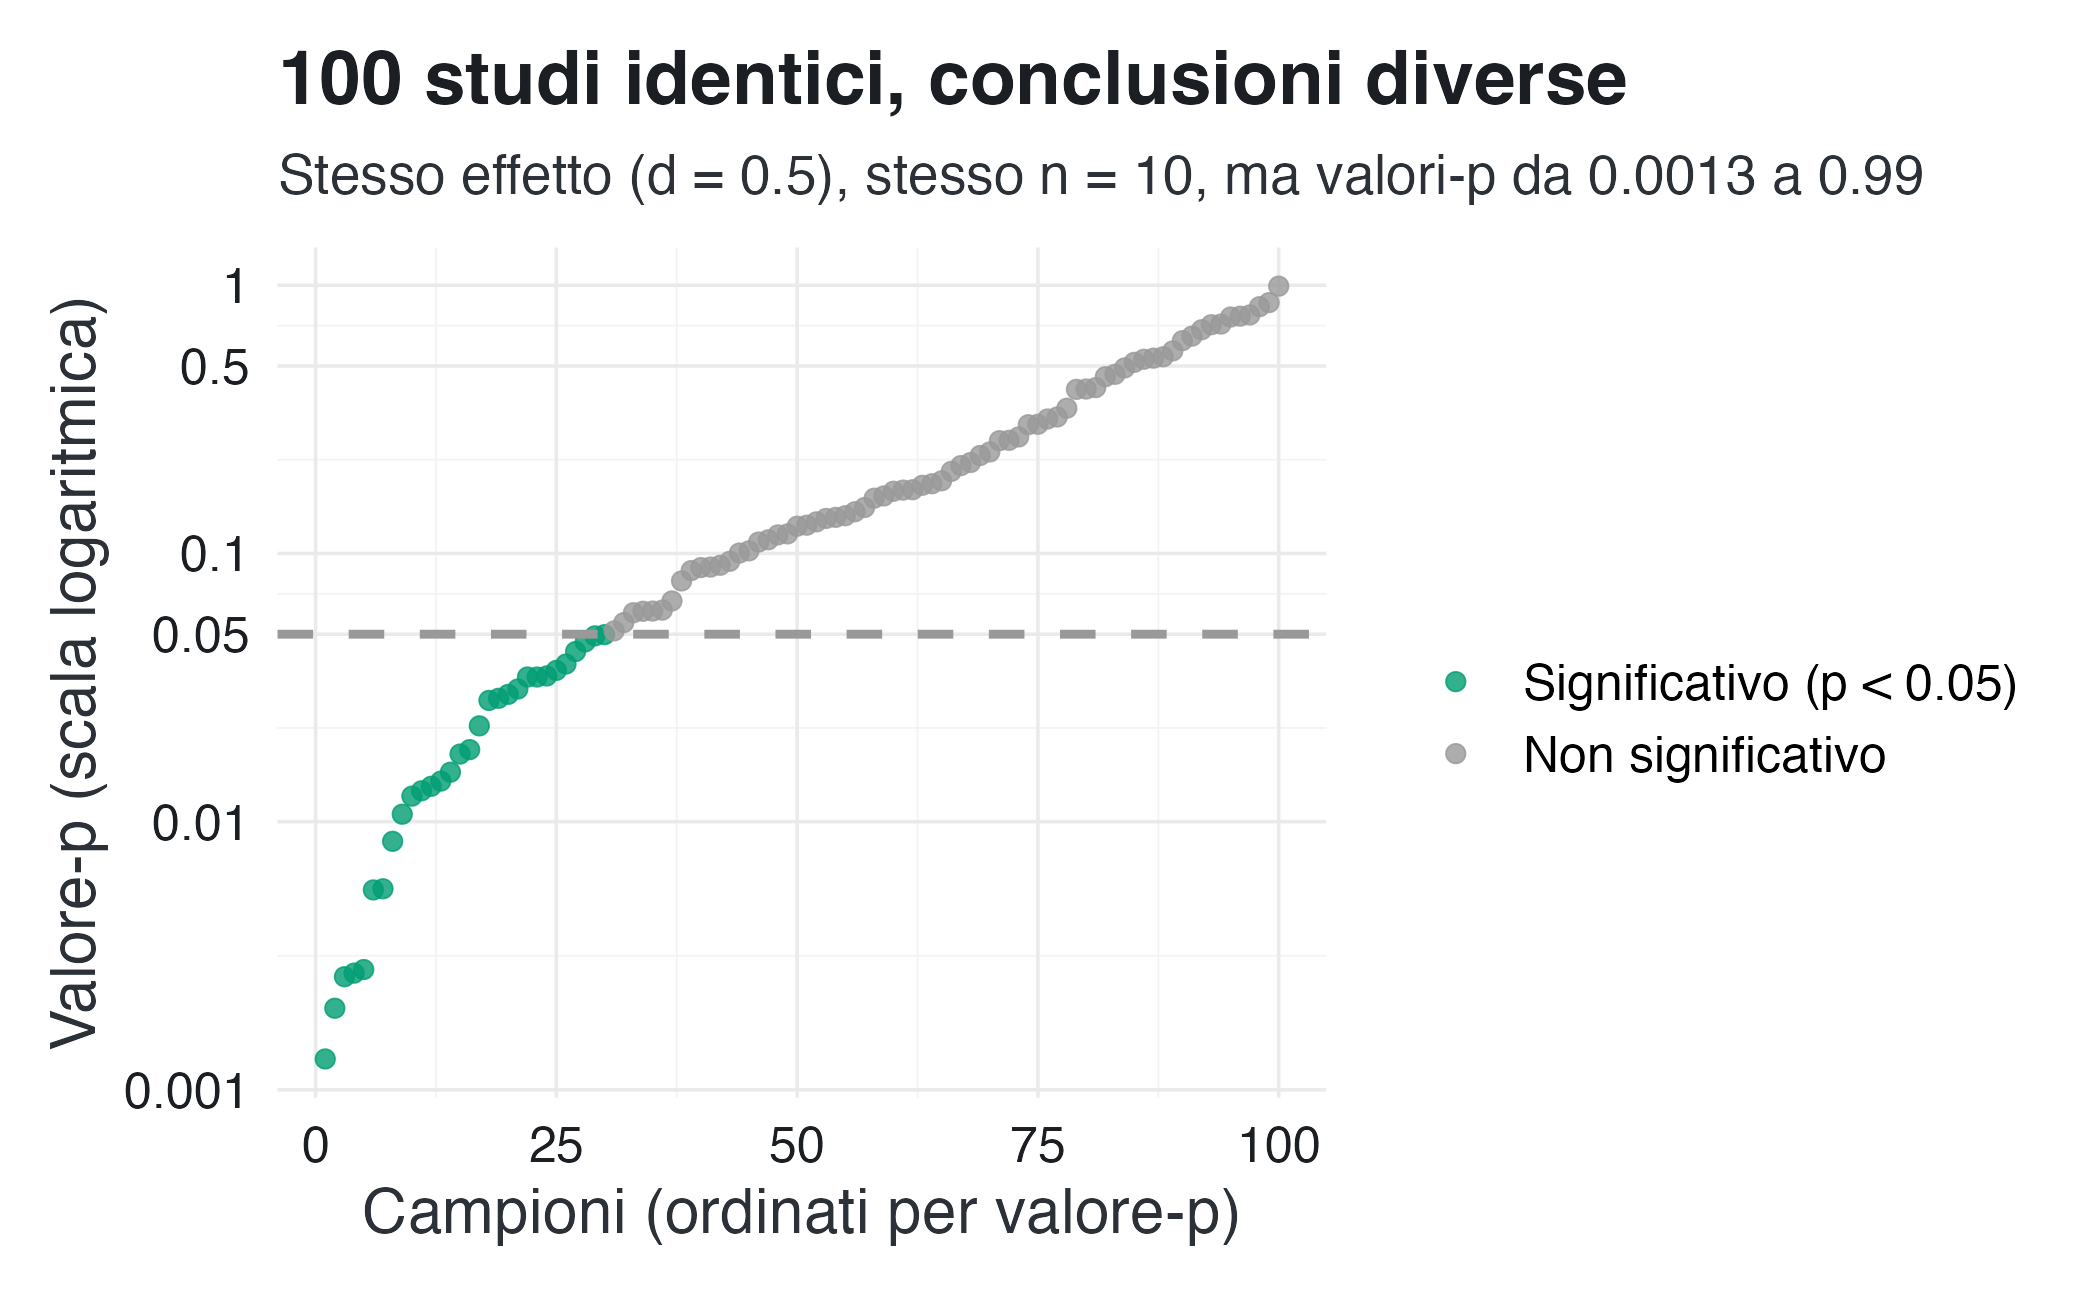
\includegraphics[width=0.85\linewidth,height=\textheight,keepaspectratio]{chapters/limits/04_p_values_files/figure-pdf/fig-pvalue-variability-1.png}

}

\caption{\label{fig-pvalue-variability}Variabilità dei p-value in 100
campioni dalla stessa popolazione. Lo stesso effetto vero produce
conclusioni opposte a seconda del campione.}

\end{figure}%

Il grafico mette in evidenza un risultato particolarmente incisivo:
\textbf{lo stesso effetto reale}, valutato con \textbf{la medesima
procedura statistica} (test \(t\) di Student), può generare valori-\(p\)
che coprono pressoché l'intera gamma possibile, da valori prossimi a 0
fino a valori prossimi a 1. In pratica, estraendo campioni diversi dalla
stessa popolazione, si giungerebbe a conclusioni diametralmente opposte:
con alcuni si dichiarerebbe l'effetto ``altamente significativo'' (\(p\)
\textless{} 0.01), mentre con altri non si rileverebbe alcuna evidenza
statistica (\(p\) \textgreater{} 0.05). Tale variabilità non riflette
differenze nel fenomeno sottostante, ma è esclusivamente un riflesso
della fluttuazione casuale intrinseca al processo di campionamento.

\section{\texorpdfstring{Simulazione 2: la distribuzione dei
valori-\(p\) e ciò che ci
insegna}{Simulazione 2: la distribuzione dei valori-p e ciò che ci insegna}}\label{simulazione-2-la-distribuzione-dei-valori-p-e-ciuxf2-che-ci-insegna}

Questa simulazione mira a chiarire il seguente principio: il
comportamento del valore-\(p\) dipende in modo critico dal fatto che
l'ipotesi nulla sia vera o falsa. Comprendere questa differenza è
essenziale per interpretare correttamente i risultati.

\subsection{Sotto l'ipotesi nulla vera}\label{sotto-lipotesi-nulla-vera}

Quando l'ipotesi nulla è vera, il valore-\(p\) è progettato per
comportarsi in un modo molto specifico: la sua distribuzione deve essere
uniforme tra 0 e 1. In pratica, ciò significa che il 5\% dei
valori-\(p\) sarà inferiore a 0.05 per puro caso: questo è esattamente
il tasso di falsi positivi che il livello di significatività \(\alpha\)
intende controllare.

\begin{Shaded}
\begin{Highlighting}[]
\CommentTok{\# Colori (Okabe–Ito)}
\NormalTok{col\_hist }\OtherTok{\textless{}{-}}\NormalTok{ palette\_qualitative[}\DecValTok{5}\NormalTok{]  }\CommentTok{\# Blu}
\NormalTok{col\_ref  }\OtherTok{\textless{}{-}}\NormalTok{ palette\_qualitative[}\DecValTok{8}\NormalTok{]  }\CommentTok{\# Grigio}
\NormalTok{col\_thr  }\OtherTok{\textless{}{-}}\NormalTok{ palette\_qualitative[}\DecValTok{1}\NormalTok{]  }\CommentTok{\# Arancione}

\CommentTok{\# Simulazione sotto H0 vera}
\NormalTok{n\_sims\_h0 }\OtherTok{\textless{}{-}} \DecValTok{10000}
\NormalTok{p\_values\_h0 }\OtherTok{\textless{}{-}} \FunctionTok{numeric}\NormalTok{(n\_sims\_h0)}

\ControlFlowTok{for}\NormalTok{ (i }\ControlFlowTok{in} \FunctionTok{seq\_len}\NormalTok{(n\_sims\_h0)) \{}
\NormalTok{  x }\OtherTok{\textless{}{-}} \FunctionTok{rnorm}\NormalTok{(n\_obs, }\AttributeTok{mean =} \DecValTok{0}\NormalTok{, }\AttributeTok{sd =}\NormalTok{ true\_sd)}
\NormalTok{  p\_values\_h0[i] }\OtherTok{\textless{}{-}} \FunctionTok{t.test}\NormalTok{(x, }\AttributeTok{mu =} \DecValTok{0}\NormalTok{)}\SpecialCharTok{$}\NormalTok{p.value}
\NormalTok{\}}

\FunctionTok{tibble}\NormalTok{(}\AttributeTok{p\_value =}\NormalTok{ p\_values\_h0) }\SpecialCharTok{|\textgreater{}}
  \FunctionTok{ggplot}\NormalTok{(}\FunctionTok{aes}\NormalTok{(}\AttributeTok{x =}\NormalTok{ p\_value)) }\SpecialCharTok{+}
  \FunctionTok{geom\_histogram}\NormalTok{(}
    \AttributeTok{bins =} \DecValTok{50}\NormalTok{,}
    \AttributeTok{fill =}\NormalTok{ col\_hist,}
    \AttributeTok{color =} \StringTok{"white"}\NormalTok{,}
    \FunctionTok{aes}\NormalTok{(}\AttributeTok{y =} \FunctionTok{after\_stat}\NormalTok{(density)),}
    \AttributeTok{alpha =} \FloatTok{0.8}
\NormalTok{  ) }\SpecialCharTok{+}
  \FunctionTok{geom\_hline}\NormalTok{(}
    \AttributeTok{yintercept =} \DecValTok{1}\NormalTok{,}
    \AttributeTok{linetype =} \StringTok{"dashed"}\NormalTok{,}
    \AttributeTok{color =}\NormalTok{ col\_ref,}
    \AttributeTok{linewidth =} \DecValTok{1}
\NormalTok{  ) }\SpecialCharTok{+}
  \FunctionTok{geom\_vline}\NormalTok{(}
    \AttributeTok{xintercept =} \FloatTok{0.05}\NormalTok{,}
    \AttributeTok{linetype =} \StringTok{"dashed"}\NormalTok{,}
    \AttributeTok{color =}\NormalTok{ col\_thr,}
    \AttributeTok{linewidth =} \DecValTok{1}
\NormalTok{  ) }\SpecialCharTok{+}
  \FunctionTok{annotate}\NormalTok{(}
    \StringTok{"text"}\NormalTok{,}
    \AttributeTok{x =} \FloatTok{0.10}\NormalTok{, }\AttributeTok{y =} \FloatTok{1.3}\NormalTok{,}
    \AttributeTok{label =} \StringTok{"5\% falsi positivi"}\NormalTok{,}
    \AttributeTok{color =}\NormalTok{ col\_thr,}
    \AttributeTok{hjust =} \DecValTok{0}
\NormalTok{  ) }\SpecialCharTok{+}
  \FunctionTok{labs}\NormalTok{(}
    \AttributeTok{x =} \StringTok{"Valore{-}p"}\NormalTok{,}
    \AttributeTok{y =} \StringTok{"Densità"}\NormalTok{,}
    \AttributeTok{title =} \StringTok{"Distribuzione dei valori{-}p sotto H₀ vera"}\NormalTok{,}
    \AttributeTok{subtitle =} \FunctionTok{sprintf}\NormalTok{(}
      \StringTok{"Distribuzione uniforme attesa: \%.1f\%\% dei valori{-}p \textless{} 0.05 (atteso: 5\%\%)"}\NormalTok{,}
      \DecValTok{100} \SpecialCharTok{*} \FunctionTok{mean}\NormalTok{(p\_values\_h0 }\SpecialCharTok{\textless{}} \FloatTok{0.05}\NormalTok{)}
\NormalTok{    )}
\NormalTok{  ) }\SpecialCharTok{+}
  \FunctionTok{coord\_cartesian}\NormalTok{(}\AttributeTok{ylim =} \FunctionTok{c}\NormalTok{(}\DecValTok{0}\NormalTok{, }\FloatTok{1.5}\NormalTok{))}
\end{Highlighting}
\end{Shaded}

\begin{figure}[H]

\centering{

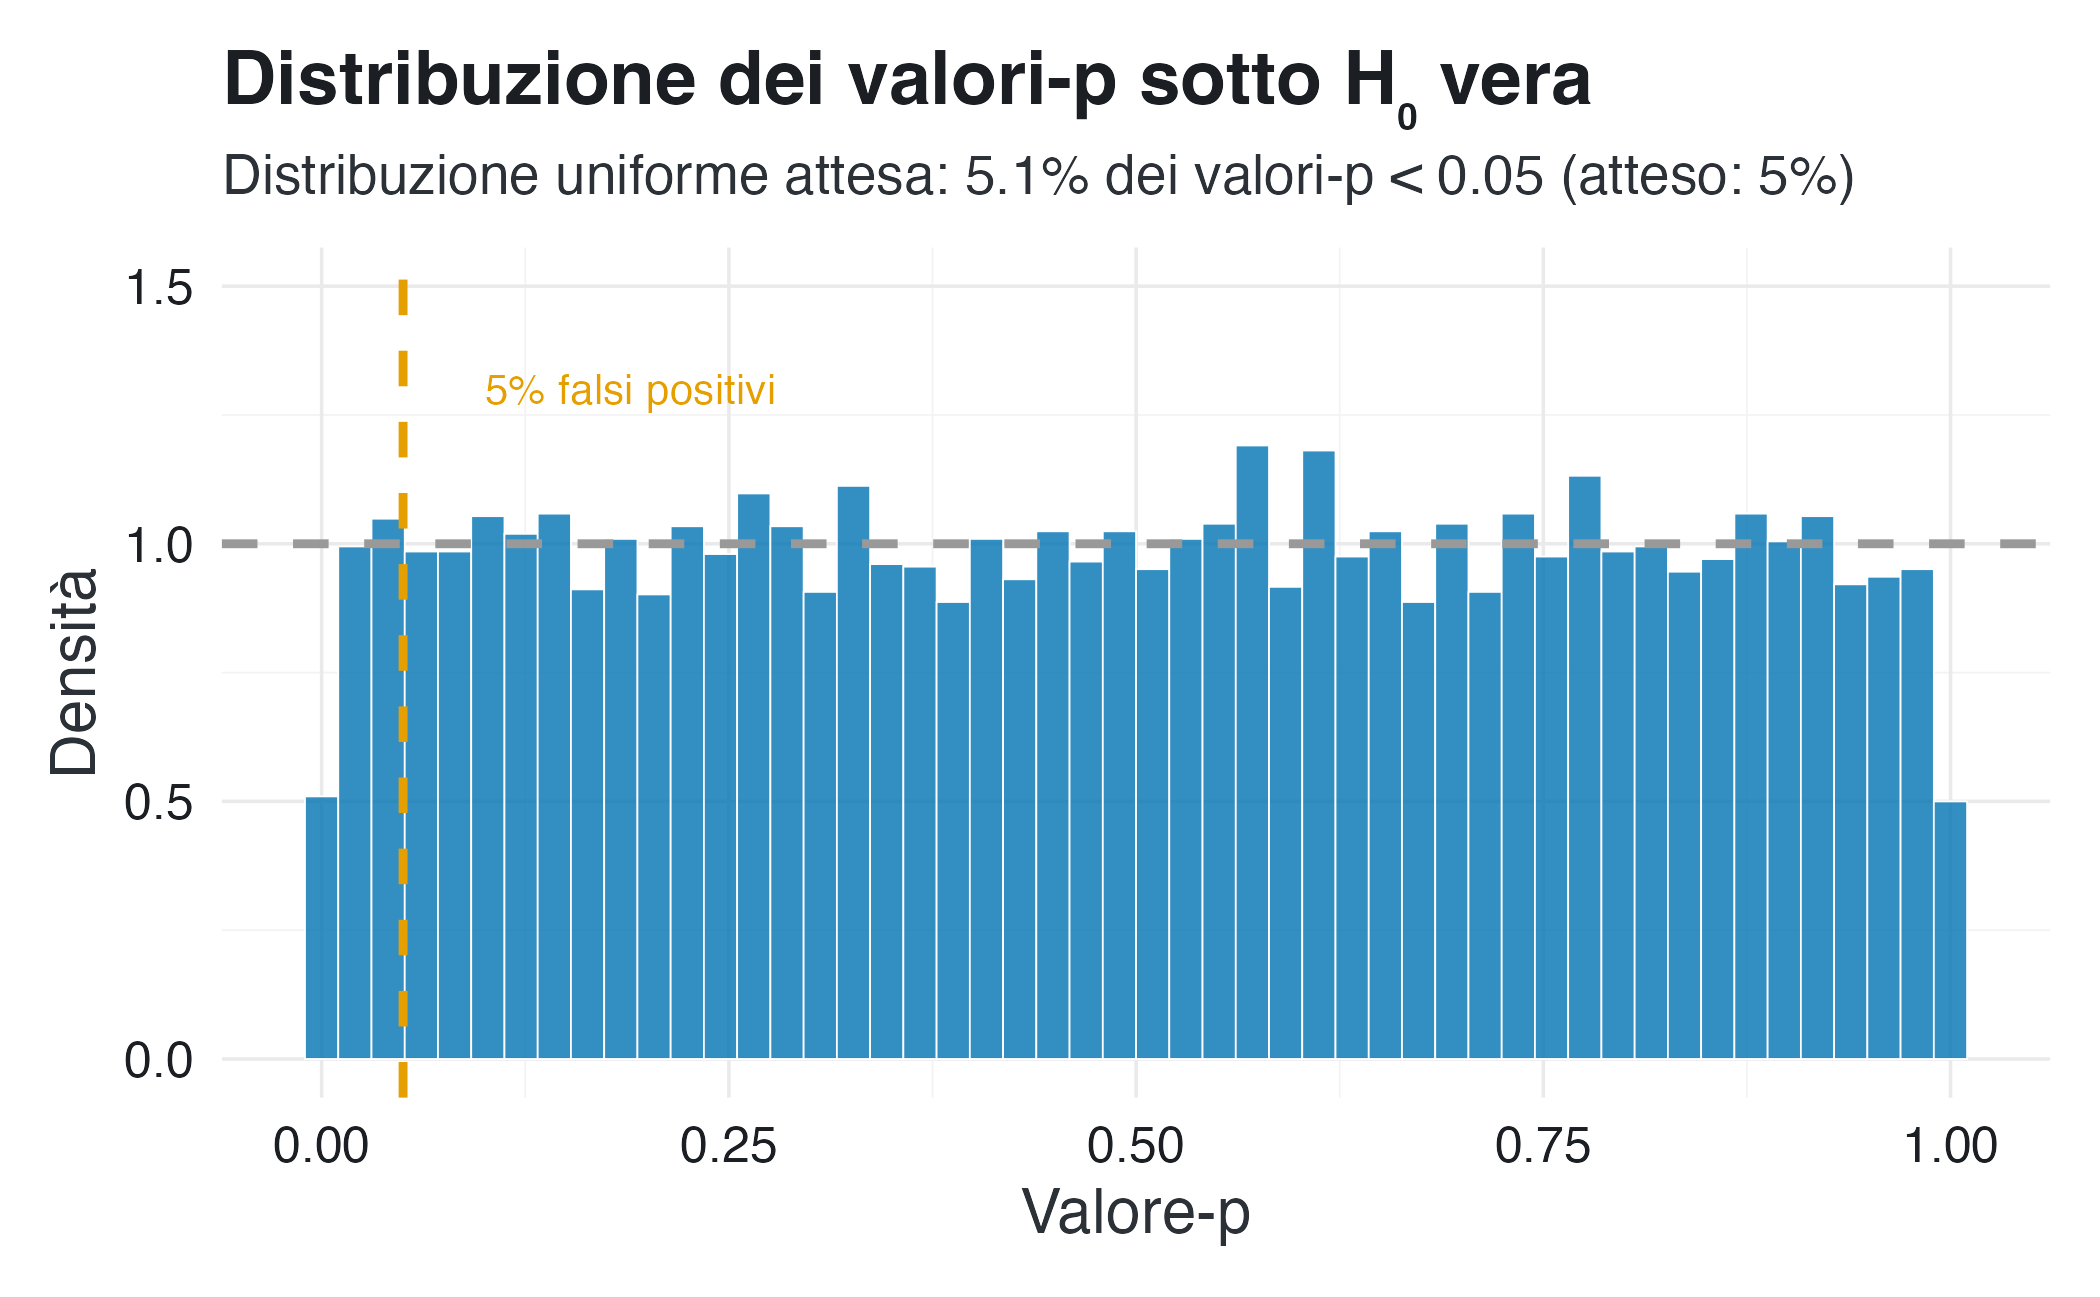
\includegraphics[width=0.85\linewidth,height=\textheight,keepaspectratio]{chapters/limits/04_p_values_files/figure-pdf/fig-pvalue-under-h0-1.png}

}

\caption{\label{fig-pvalue-under-h0}Distribuzione uniforme dei valori-p
quando H₀ è vera. La linea rossa tratteggiata a y=1 mostra l'andamento
atteso di una distribuzione uniforme perfetta. Il 5\% dei valori cade a
sinistra della linea verticale scura (p \textless{} 0.05) per puro
caso.}

\end{figure}%

\subsection{\texorpdfstring{Sotto l'ipotesi nulla falsa
(\(H_1: \mu > 0\))}{Sotto l'ipotesi nulla falsa (H\_1: \textbackslash mu \textgreater{} 0)}}\label{sotto-lipotesi-nulla-falsa-h_1-mu-0}

La situazione cambia radicalmente quando esiste un effetto reale nella
popolazione. In questo caso, la distribuzione dei valori-\(p\) si
``sposta'' verso lo zero. Tuttavia, questa distribuzione rimane
estremamente dispersa per effetti piccoli o moderati e per campioni di
piccole dimensioni. La percentuale di valori-\(p\) che cadono sotto la
soglia di significatività (ad esempio, 0.05) corrisponde alla potenza
statistica dello studio.

\begin{Shaded}
\begin{Highlighting}[]
\NormalTok{col\_hist }\OtherTok{\textless{}{-}}\NormalTok{ palette\_qualitative[}\DecValTok{5}\NormalTok{]  }\CommentTok{\# Blu}
\NormalTok{col\_thr  }\OtherTok{\textless{}{-}}\NormalTok{ palette\_qualitative[}\DecValTok{1}\NormalTok{]  }\CommentTok{\# Arancione}

\CommentTok{\# Simulazione sotto H0 falsa (effetti di diversa ampiezza)}
\NormalTok{effect\_sizes }\OtherTok{\textless{}{-}} \FunctionTok{c}\NormalTok{(}\DecValTok{0}\NormalTok{, }\FloatTok{0.2}\NormalTok{, }\FloatTok{0.5}\NormalTok{, }\FloatTok{0.8}\NormalTok{)}
\NormalTok{n\_sims }\OtherTok{\textless{}{-}} \DecValTok{5000}

\NormalTok{pvalue\_distributions }\OtherTok{\textless{}{-}} \FunctionTok{tibble}\NormalTok{()}

\ControlFlowTok{for}\NormalTok{ (d }\ControlFlowTok{in}\NormalTok{ effect\_sizes) \{}

\NormalTok{  p\_vals }\OtherTok{\textless{}{-}} \FunctionTok{numeric}\NormalTok{(n\_sims)}

  \ControlFlowTok{for}\NormalTok{ (i }\ControlFlowTok{in} \FunctionTok{seq\_len}\NormalTok{(n\_sims)) \{}
\NormalTok{    x }\OtherTok{\textless{}{-}} \FunctionTok{rnorm}\NormalTok{(n\_obs, }\AttributeTok{mean =}\NormalTok{ d }\SpecialCharTok{*}\NormalTok{ true\_sd, }\AttributeTok{sd =}\NormalTok{ true\_sd)}
\NormalTok{    p\_vals[i] }\OtherTok{\textless{}{-}} \FunctionTok{t.test}\NormalTok{(x, }\AttributeTok{mu =} \DecValTok{0}\NormalTok{)}\SpecialCharTok{$}\NormalTok{p.value}
\NormalTok{  \}}

\NormalTok{  pvalue\_distributions }\OtherTok{\textless{}{-}} \FunctionTok{bind\_rows}\NormalTok{(}
\NormalTok{    pvalue\_distributions,}
    \FunctionTok{tibble}\NormalTok{(}
      \AttributeTok{effect\_size =}\NormalTok{ d,}
      \AttributeTok{p\_value =}\NormalTok{ p\_vals,}
      \AttributeTok{label =} \FunctionTok{sprintf}\NormalTok{(}
        \StringTok{"d = \%.1f (potenza: \%.0f\%\%)"}\NormalTok{,}
\NormalTok{        d, }\DecValTok{100} \SpecialCharTok{*} \FunctionTok{mean}\NormalTok{(p\_vals }\SpecialCharTok{\textless{}} \FloatTok{0.05}\NormalTok{)}
\NormalTok{      )}
\NormalTok{    )}
\NormalTok{  )}
\NormalTok{\}}

\FunctionTok{ggplot}\NormalTok{(pvalue\_distributions, }\FunctionTok{aes}\NormalTok{(}\AttributeTok{x =}\NormalTok{ p\_value)) }\SpecialCharTok{+}
  \FunctionTok{geom\_histogram}\NormalTok{(}
    \AttributeTok{bins =} \DecValTok{50}\NormalTok{,}
    \AttributeTok{fill =}\NormalTok{ col\_hist,}
    \AttributeTok{color =} \StringTok{"white"}\NormalTok{,}
    \AttributeTok{alpha =} \FloatTok{0.8}
\NormalTok{  ) }\SpecialCharTok{+}
  \FunctionTok{geom\_vline}\NormalTok{(}
    \AttributeTok{xintercept =} \FloatTok{0.05}\NormalTok{,}
    \AttributeTok{linetype =} \StringTok{"dashed"}\NormalTok{,}
    \AttributeTok{color =}\NormalTok{ col\_thr,}
    \AttributeTok{linewidth =} \DecValTok{1}
\NormalTok{  ) }\SpecialCharTok{+}
  \FunctionTok{facet\_wrap}\NormalTok{(}\SpecialCharTok{\textasciitilde{}}\NormalTok{label, }\AttributeTok{ncol =} \DecValTok{2}\NormalTok{, }\AttributeTok{scales =} \StringTok{"free\_y"}\NormalTok{) }\SpecialCharTok{+}
  \FunctionTok{labs}\NormalTok{(}
    \AttributeTok{x =} \StringTok{"Valore{-}p"}\NormalTok{,}
    \AttributeTok{y =} \StringTok{"Frequenza"}\NormalTok{,}
    \AttributeTok{title =} \StringTok{"Come la dimensione dell\textquotesingle{}effetto influenza la distribuzione dei valori{-}p"}\NormalTok{,}
    \AttributeTok{subtitle =} \FunctionTok{sprintf}\NormalTok{(}
      \StringTok{"n = \%d per campione, \%d simulazioni per condizione"}\NormalTok{,}
\NormalTok{      n\_obs, n\_sims}
\NormalTok{    )}
\NormalTok{  )}
\end{Highlighting}
\end{Shaded}

\begin{figure}[H]

\centering{

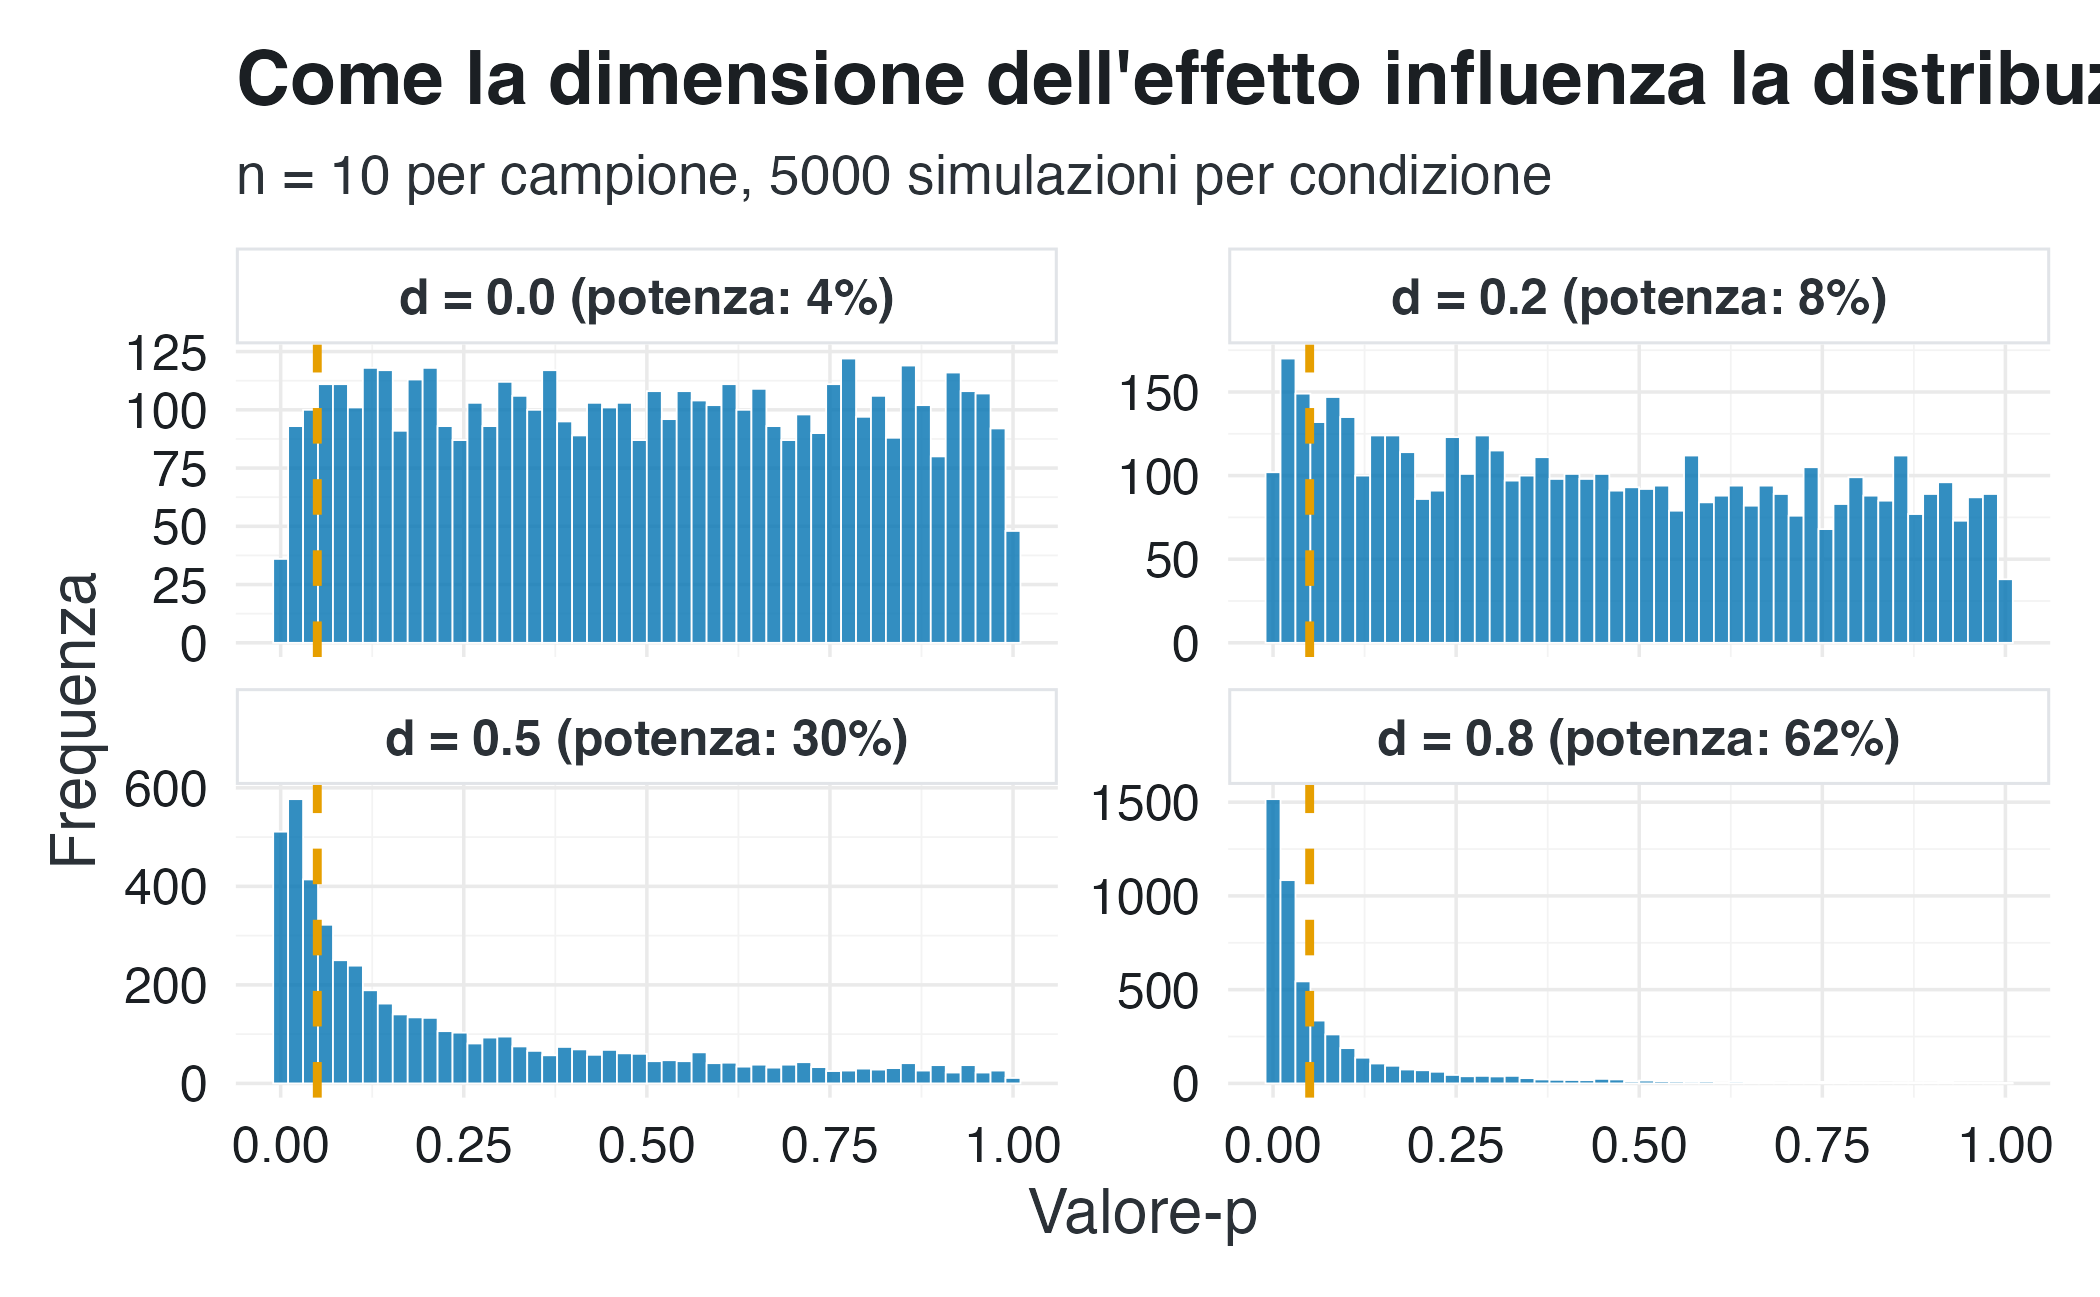
\includegraphics[width=0.85\linewidth,height=\textheight,keepaspectratio]{chapters/limits/04_p_values_files/figure-pdf/fig-pvalue-distributions-1.png}

}

\caption{\label{fig-pvalue-distributions}Come la dimensione dell'effetto
modella la distribuzione del valore-p.~Con H₀ vera (d=0.0), la
distribuzione è uniforme. All'aumentare dell'effetto reale (d), la
distribuzione si sposta verso valori più bassi, aumentando la potenza
(percentuale di p\textless0.05).}

\end{figure}%

\subsection{Interpretazione dei
risultati}\label{interpretazione-dei-risultati}

\begin{enumerate}
\def\labelenumi{\arabic{enumi}.}
\item
  \textbf{Il comportamento del valore-\(p\) sotto l'ipotesi nulla.} Il
  primo grafico illustra una proprietà fondamentale dell'inferenza
  frequentista: quando l'ipotesi nulla (\(H_0\)) è vera, la
  distribuzione del valore-\(p\) è uniforme nell'intervallo {[}0,1{]}.
  In tale scenario, esattamente il 5\% dei valori simulati risulta
  inferiore a 0.05 per puro effetto del caso. Questo conferma che il
  livello di significatività \(\alpha\) = 0.05 corrisponde al tasso
  nominale di \textbf{errori di tipo I} (falsi positivi) controllato dal
  test.
\item
  \textbf{La criticità della potenza statistica con campioni ridotti.}
  La seconda figura mostra chiaramente l'impatto della dimensione del
  campione (\(n\) = 10) sulla \textbf{potenza} del test. Nonostante
  l'uso della stessa procedura (test \emph{t} per un campione), la
  probabilità di rifiutare correttamente \(H_0\) varia drasticamente in
  base alla dimensione dell'effetto reale (\(d\) di Cohen):

  \begin{itemize}
  \tightlist
  \item
    per un effetto trascurabile (\emph{d} = 0.2), la potenza empirica è
    solo del \textbf{9\%}, rendendo il test pressoché incapace di
    distinguere l'effetto dal rumore casuale;
  \item
    per un effetto di entità media (\emph{d} = 0.5), la potenza
    raggiunge appena il \textbf{30\%}. In termini pratici, ciò implica
    che \textbf{7 studi replicati su 10} non riuscirebbero a raggiungere
    la significatività statistica, generando così un \textbf{errore di
    tipo II} (falso negativo);
  \item
    solo per un effetto di ampia entità (\emph{d} = 0.8) la potenza
    supera il 60\%, anche se una quota sostanziale (circa il 38\%) dei
    campioni non raggiunge comunque il criterio di rifiuto.
  \end{itemize}
\item
  \textbf{L'elevata variabilità campionaria del valore-\(p\).} Per
  dimensioni dell'effetto piccole o moderate, la distribuzione del
  valore-\(p\) rimane dispersa, riflettendo un'\textbf{elevata
  volatilità campionaria}. Di conseguenza, un singolo valore-\(p\)
  costituisce una stima estremamente imprecisa della forza dell'evidenza
  contro \(H_0\). È perfettamente plausibile che due studi identici,
  condotti sulla stessa popolazione, producano conclusioni
  statisticamente opposte (ad esempio, \(p\) \textless{} 0.01 in uno,
  \(p\) \textgreater{} 0.50 nell'altro) unicamente a causa della
  variabilità intrinseca del campionamento.
\end{enumerate}

\textbf{In sintesi}, la simulazione mette in guardia da
un'interpretazione semplicistica del valore-\(p\), ricordandone la
natura probabilistica. Il valore-\(p\) non fornisce un verdetto binario
sulla presenza o sull'entità di un effetto: un risultato non
significativo non implica l'assenza di un effetto, così come un
risultato significativo non garantisce che l'effetto sia di ampia
portata. Con campioni di dimensioni ridotte -- una condizione frequente
nella ricerca psicologica -- il valore-\(p\) si rivela una statistica
fortemente instabile, la cui interpretazione dipende in modo critico
dalla potenza statistica dello studio. Questi risultati sottolineano
pertanto la necessità di integrare il valore-\(p\) con stime puntuali e
intervalli di confidenza, di progettare la ricerca mediante un'analisi
di potenza a priori e, soprattutto, di fondare le inferenze non sul
singolo esperimento, ma su una \textbf{replicabilità} sistematica e su
una sintesi cumulativa delle evidenze.

\section{Simulazione 3: due studi
``contraddittori''}\label{simulazione-3-due-studi-contraddittori}

Nella pratica dell'inferenza statistica, una delle osservazioni più
controintuitive riguarda il confronto dei risultati di studi empirici.
Nella letteratura scientifica è comune incontrare affermazioni del tipo:

\begin{itemize}
\tightlist
\item
  \textbf{Studio A}: \(p = 0.04\) → \emph{``L'effetto è statisticamente
  significativo''}
\item
  \textbf{Studio B}: \(p = 0.06\) → \emph{``Non vi è evidenza di un
  effetto''}
\end{itemize}

Questa contrapposizione suggerisce che i due studi giungano a
conclusioni opposte. Tuttavia, come mostrato da Gelman \& Stern
(\citeproc{ref-gelman2006difference}{2006}), tale interpretazione è
fuorviante: \textbf{la differenza tra un risultato ``significativo'' e
uno ``non significativo'' non implica necessariamente una differenza
sostanziale tra gli effetti osservati}. Spesso, tale differenza può
essere spiegata dalla sola variabilità campionaria.

Per capire quanto questo fenomeno sia frequente, possiamo simulare
coppie di studi che esaminano \textbf{lo stesso effetto reale}
utilizzando lo stesso disegno sperimentale e la stessa numerosità
campionaria. Questa simulazione permette di valutare con quanta
frequenza differenze minime nei dati portino a conclusioni
apparentemente opposte a causa della soglia arbitraria di \(p\)
\textless{} 0.05.

\begin{Shaded}
\begin{Highlighting}[]
\CommentTok{\# Simula coppie di studi}
\NormalTok{n\_pairs }\OtherTok{\textless{}{-}} \DecValTok{1000}

\CommentTok{\# Verifica che n\_obs e true\_mean siano definiti (se necessario, aggiungi:)}
\CommentTok{\# n\_obs \textless{}{-} 50      \# esempio}
\CommentTok{\# true\_mean \textless{}{-} 0.2 \# esempio}
\CommentTok{\# true\_sd \textless{}{-} 1     \# esempio}

\NormalTok{p\_a }\OtherTok{\textless{}{-}} \FunctionTok{numeric}\NormalTok{(n\_pairs)}
\NormalTok{p\_b }\OtherTok{\textless{}{-}} \FunctionTok{numeric}\NormalTok{(n\_pairs)}

\ControlFlowTok{for}\NormalTok{ (i }\ControlFlowTok{in} \FunctionTok{seq\_len}\NormalTok{(n\_pairs)) \{}
\NormalTok{  x\_a }\OtherTok{\textless{}{-}} \FunctionTok{rnorm}\NormalTok{(n\_obs, }\AttributeTok{mean =}\NormalTok{ true\_mean, }\AttributeTok{sd =}\NormalTok{ true\_sd)}
\NormalTok{  x\_b }\OtherTok{\textless{}{-}} \FunctionTok{rnorm}\NormalTok{(n\_obs, }\AttributeTok{mean =}\NormalTok{ true\_mean, }\AttributeTok{sd =}\NormalTok{ true\_sd)}
\NormalTok{  p\_a[i] }\OtherTok{\textless{}{-}} \FunctionTok{t.test}\NormalTok{(x\_a, }\AttributeTok{mu =} \DecValTok{0}\NormalTok{)}\SpecialCharTok{$}\NormalTok{p.value}
\NormalTok{  p\_b[i] }\OtherTok{\textless{}{-}} \FunctionTok{t.test}\NormalTok{(x\_b, }\AttributeTok{mu =} \DecValTok{0}\NormalTok{)}\SpecialCharTok{$}\NormalTok{p.value}
\NormalTok{\}}

\NormalTok{study\_pairs }\OtherTok{\textless{}{-}} \FunctionTok{tibble}\NormalTok{(}\AttributeTok{pair\_id =} \DecValTok{1}\SpecialCharTok{:}\NormalTok{n\_pairs) }\SpecialCharTok{|\textgreater{}}
  \FunctionTok{mutate}\NormalTok{(}
    \AttributeTok{p\_a =}\NormalTok{ p\_a,}
    \AttributeTok{p\_b =}\NormalTok{ p\_b,}
    \AttributeTok{sig\_a =}\NormalTok{ p\_a }\SpecialCharTok{\textless{}} \FloatTok{0.05}\NormalTok{,}
    \AttributeTok{sig\_b =}\NormalTok{ p\_b }\SpecialCharTok{\textless{}} \FloatTok{0.05}\NormalTok{,}
    \AttributeTok{concordance =} \FunctionTok{case\_when}\NormalTok{(}
\NormalTok{      sig\_a }\SpecialCharTok{\&}\NormalTok{ sig\_b }\SpecialCharTok{\textasciitilde{}} \StringTok{"Entrambi significativi"}\NormalTok{,}
      \SpecialCharTok{!}\NormalTok{sig\_a }\SpecialCharTok{\&} \SpecialCharTok{!}\NormalTok{sig\_b }\SpecialCharTok{\textasciitilde{}} \StringTok{"Entrambi non significativi"}\NormalTok{,}
      \ConstantTok{TRUE} \SpecialCharTok{\textasciitilde{}} \StringTok{"Risultati discordanti"}
\NormalTok{    )}
\NormalTok{  )}

\CommentTok{\# Statistiche}
\NormalTok{concordance\_stats }\OtherTok{\textless{}{-}}\NormalTok{ study\_pairs }\SpecialCharTok{|\textgreater{}}
\NormalTok{  dplyr}\SpecialCharTok{::}\FunctionTok{count}\NormalTok{(concordance) }\SpecialCharTok{|\textgreater{}}
  \FunctionTok{mutate}\NormalTok{(}\AttributeTok{pct =}\NormalTok{ n }\SpecialCharTok{/} \FunctionTok{sum}\NormalTok{(n) }\SpecialCharTok{*} \DecValTok{100}\NormalTok{)}

\CommentTok{\# Colori}
\NormalTok{col\_ref  }\OtherTok{\textless{}{-}}\NormalTok{ palette\_qualitative[}\DecValTok{8}\NormalTok{]  }\CommentTok{\# grigio}
\NormalTok{col\_line }\OtherTok{\textless{}{-}}\NormalTok{ palette\_qualitative[}\DecValTok{8}\NormalTok{]  }\CommentTok{\# grigio}
\NormalTok{palette\_concordance }\OtherTok{\textless{}{-}} \FunctionTok{setNames}\NormalTok{(}
\NormalTok{  palette\_qualitative[}\FunctionTok{c}\NormalTok{(}\DecValTok{3}\NormalTok{, }\DecValTok{8}\NormalTok{, }\DecValTok{6}\NormalTok{)],  }\CommentTok{\# verde, grigio, rosso{-}arancio (anziché 1)}
  \FunctionTok{c}\NormalTok{(}\StringTok{"Entrambi significativi"}\NormalTok{, }\StringTok{"Entrambi non significativi"}\NormalTok{, }\StringTok{"Risultati discordanti"}\NormalTok{)}
\NormalTok{)}

\CommentTok{\# Visualizzazione}
\FunctionTok{ggplot}\NormalTok{(study\_pairs, }\FunctionTok{aes}\NormalTok{(}\AttributeTok{x =}\NormalTok{ p\_a, }\AttributeTok{y =}\NormalTok{ p\_b, }\AttributeTok{color =}\NormalTok{ concordance)) }\SpecialCharTok{+}
  \FunctionTok{geom\_point}\NormalTok{(}\AttributeTok{alpha =} \FloatTok{0.5}\NormalTok{, }\AttributeTok{size =} \DecValTok{2}\NormalTok{) }\SpecialCharTok{+}
  \FunctionTok{geom\_hline}\NormalTok{(}\AttributeTok{yintercept =} \FloatTok{0.05}\NormalTok{, }\AttributeTok{linetype =} \StringTok{"dashed"}\NormalTok{, }\AttributeTok{color =}\NormalTok{ col\_ref) }\SpecialCharTok{+}
  \FunctionTok{geom\_vline}\NormalTok{(}\AttributeTok{xintercept =} \FloatTok{0.05}\NormalTok{, }\AttributeTok{linetype =} \StringTok{"dashed"}\NormalTok{, }\AttributeTok{color =}\NormalTok{ col\_ref) }\SpecialCharTok{+}
  \FunctionTok{geom\_abline}\NormalTok{(}\AttributeTok{slope =} \DecValTok{1}\NormalTok{, }\AttributeTok{intercept =} \DecValTok{0}\NormalTok{, }\AttributeTok{color =}\NormalTok{ col\_line, }\AttributeTok{linetype =} \StringTok{"dotted"}\NormalTok{) }\SpecialCharTok{+}
  \FunctionTok{scale\_color\_manual}\NormalTok{(}\AttributeTok{values =}\NormalTok{ palette\_concordance) }\SpecialCharTok{+}
  \FunctionTok{labs}\NormalTok{(}
    \AttributeTok{x =} \StringTok{"P{-}value Studio A"}\NormalTok{,}
    \AttributeTok{y =} \StringTok{"P{-}value Studio B"}\NormalTok{,}
    \AttributeTok{color =} \StringTok{""}\NormalTok{,}
    \AttributeTok{title =} \StringTok{"Coppie di studi sullo stesso effetto"}\NormalTok{,}
    \AttributeTok{subtitle =} \FunctionTok{sprintf}\NormalTok{(}
      \StringTok{"Circa \%.0f\%\% delle coppie produce risultati discordanti"}\NormalTok{,}
\NormalTok{      concordance\_stats }\SpecialCharTok{|\textgreater{}} 
        \FunctionTok{filter}\NormalTok{(concordance }\SpecialCharTok{==} \StringTok{"Risultati discordanti"}\NormalTok{) }\SpecialCharTok{|\textgreater{}} 
        \FunctionTok{pull}\NormalTok{(pct)}
\NormalTok{    )}
\NormalTok{  ) }\SpecialCharTok{+}
  \FunctionTok{coord\_fixed}\NormalTok{()}
\end{Highlighting}
\end{Shaded}

\begin{figure}[H]

\centering{

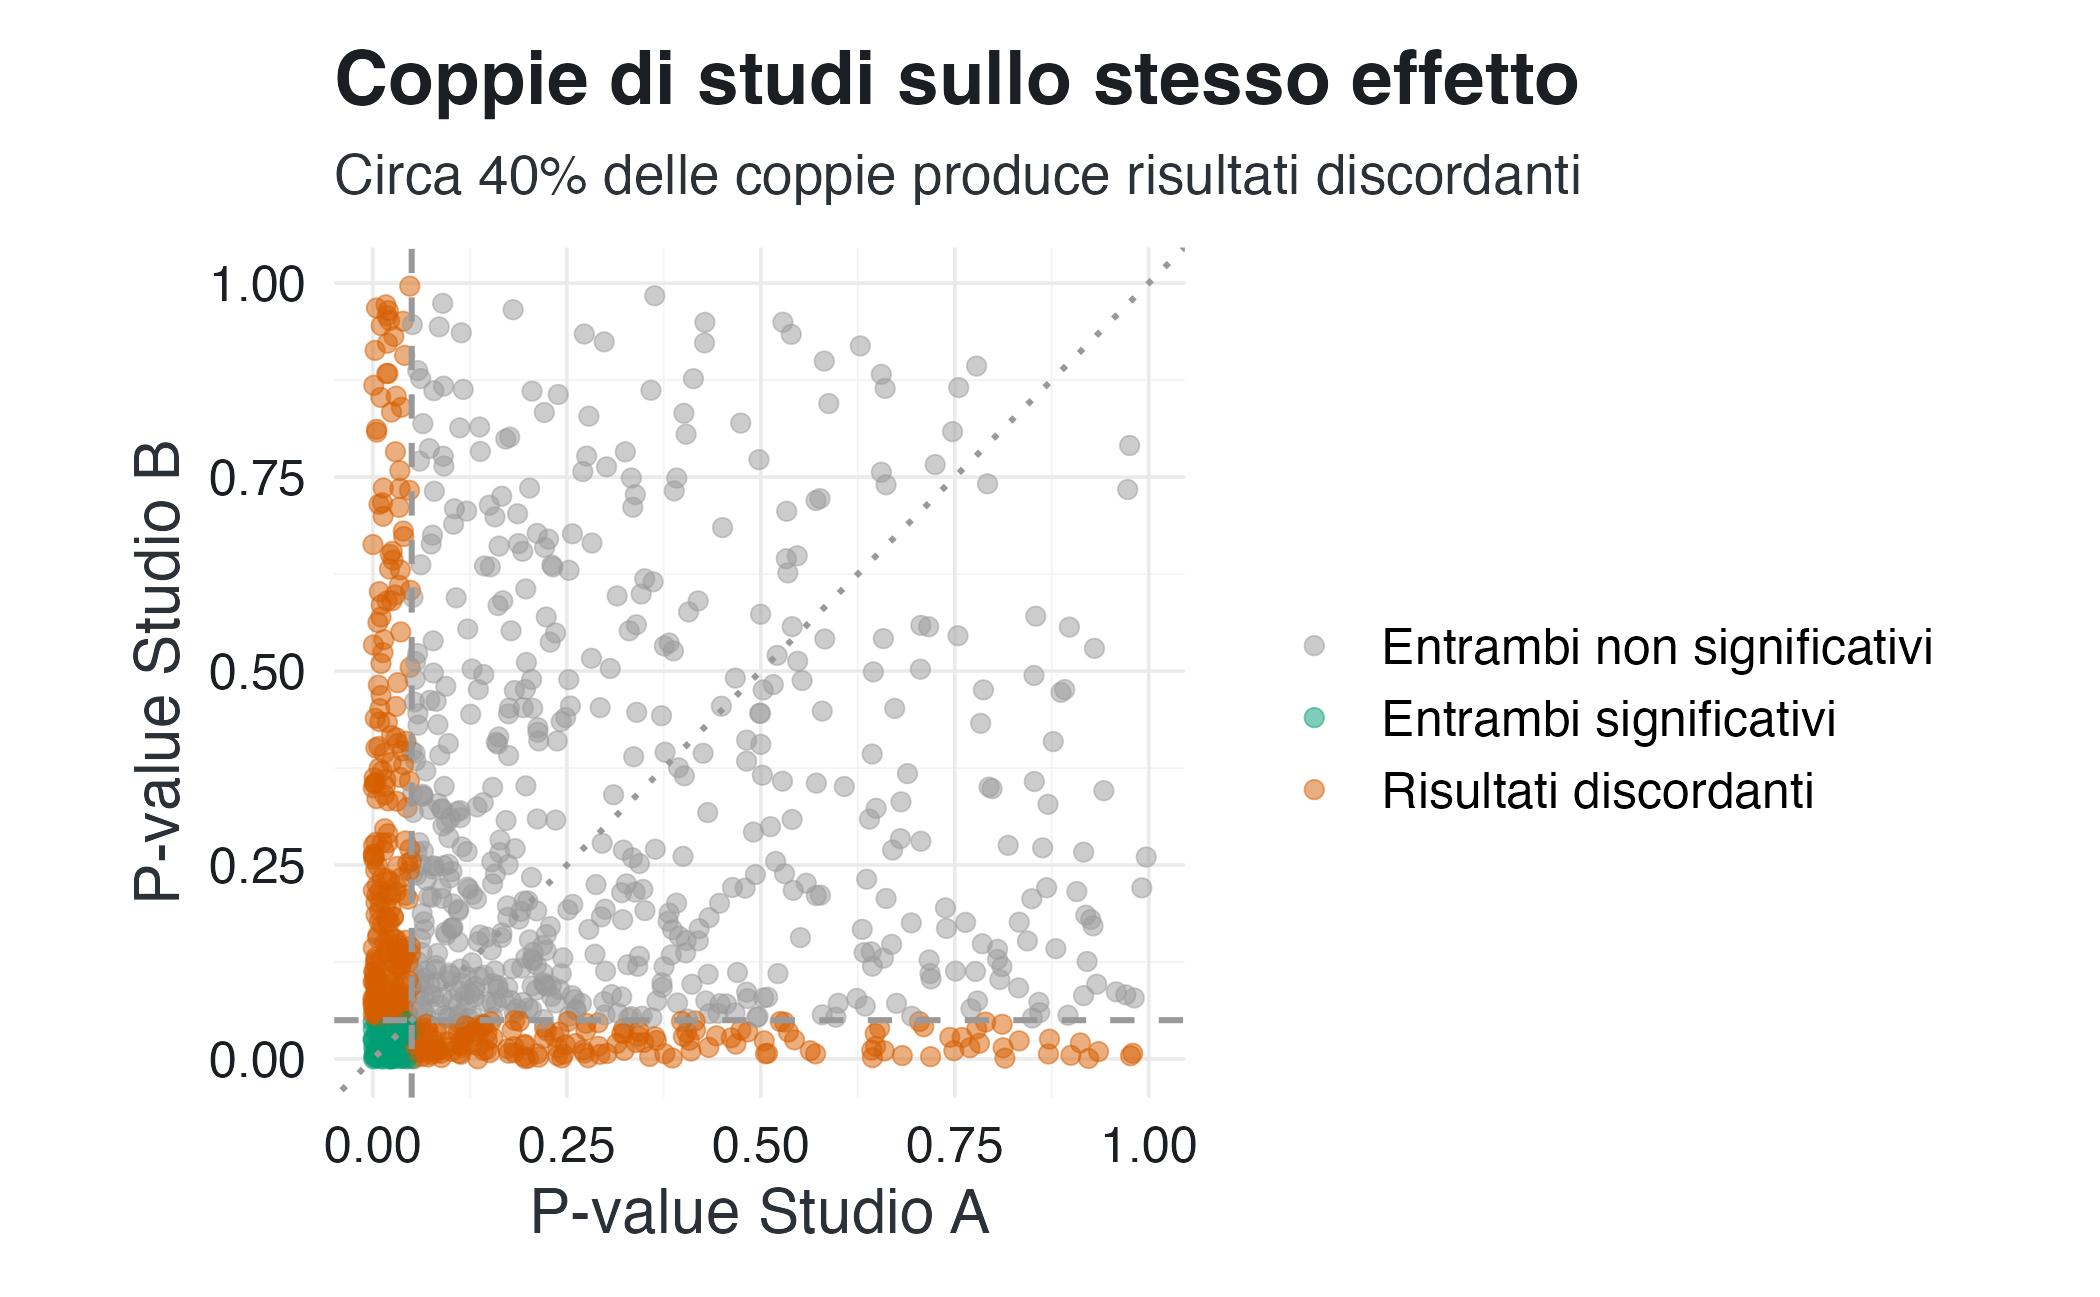
\includegraphics[width=0.85\linewidth,height=\textheight,keepaspectratio]{chapters/limits/04_p_values_files/figure-pdf/fig-two-studies-1.png}

}

\caption{\label{fig-two-studies}Simulazione di 1000 coppie di studi che
esaminano lo stesso effetto reale. Spesso uno studio risulta
``significativo'' e l'altro no.}

\end{figure}%

\subsection{Interpretazione}\label{interpretazione-1}

La simulazione evidenzia un punto cruciale: \textbf{conclusioni
apparentemente discordanti possono emergere anche quando due studi
indagano lo stesso effetto reale con il medesimo protocollo
sperimentale}. In assenza di differenze sostanziali tra i fenomeni
esaminati, la sola variabilità campionaria può generare stime che, a
seconda che il valore-\(p\) superi o meno una soglia convenzionale,
portano a interpretazioni diametralmente opposte.

Come osservano Gelman \& Stern
(\citeproc{ref-gelman2006difference}{2006}), il problema non risiede nel
valore-\(p\) in sé, ma nell'uso della soglia di significatività come
criterio di confronto inferenziale tra studi. Dal punto di vista
statistico, confrontare un risultato ``significativo'' con uno ``non
significativo'' non fornisce alcuna informazione sulla differenza tra
gli effetti sottostanti. L'elemento appropriato da valutare non è il
superamento della soglia dello 0.05, ma \textbf{la differenza stimata
tra gli effetti e la relativa incertezza inferenziale}.

In termini sintetici:

\begin{quote}
\textbf{La differenza tra significativo e non significativo non è
statisticamente significativa.}
\end{quote}

Questa considerazione ha importanti implicazioni per la metodologia
della ricerca empirica. La dicotomizzazione dei risultati sulla base di
una soglia di significatività si rivela un criterio debole e
potenzialmente fuorviante per valutare la coerenza tra gli studi. Una
pratica inferenziale adeguata richiede invece di focalizzarsi sulle
stime degli effetti, sui loro intervalli di incertezza e sulla
quantificazione comparativa delle differenze, abbandonando l'uso di
soglie arbitrarie come strumento decisionale primario.

\section{Simulazione 4: confronto con l'approccio
bayesiano}\label{simulazione-4-confronto-con-lapproccio-bayesiano}

L'approccio frequentista tradizionale richiede spesso l'adozione di
soglie decisionali rigide (ad esempio, \(p\) \textless{} 0.05). Al
contrario, l'inferenza bayesiana non impone dicotomie: essa fornisce una
\textbf{distribuzione a posteriori} dei parametri e consente di
esprimere in modo diretto la probabilità che un effetto sia positivo,
tenendo conto sia dei dati sia dell'incertezza pre-esistente.

Di seguito, confrontiamo l'instabilità dei valori-\(p\) con la stabilità
della probabilità a posteriori che l'effetto sia positivo, calcolata
assumendo come prior una distribuzione normale centrata sullo zero.

\begin{Shaded}
\begin{Highlighting}[]
\CommentTok{\# Funzione per calcolo bayesiano approssimato}
\CommentTok{\# Prior: mu \textasciitilde{} N(0, prior\_sd)}
\CommentTok{\# Likelihood: x\_bar | mu \textasciitilde{} N(mu, sigma/sqrt(n))}
\NormalTok{bayesian\_posterior\_prob }\OtherTok{\textless{}{-}} \ControlFlowTok{function}\NormalTok{(data, }\AttributeTok{prior\_sd =} \FloatTok{0.2}\NormalTok{) \{}
\NormalTok{  x\_bar }\OtherTok{\textless{}{-}} \FunctionTok{mean}\NormalTok{(data)}
\NormalTok{  se }\OtherTok{\textless{}{-}} \FunctionTok{sd}\NormalTok{(data) }\SpecialCharTok{/} \FunctionTok{sqrt}\NormalTok{(}\FunctionTok{length}\NormalTok{(data))}
  
  \CommentTok{\# Posterior (coniugazione normale)}
\NormalTok{  prior\_precision }\OtherTok{\textless{}{-}} \DecValTok{1} \SpecialCharTok{/}\NormalTok{ prior\_sd}\SpecialCharTok{\^{}}\DecValTok{2}
\NormalTok{  data\_precision }\OtherTok{\textless{}{-}} \DecValTok{1} \SpecialCharTok{/}\NormalTok{ se}\SpecialCharTok{\^{}}\DecValTok{2}
  
\NormalTok{  post\_precision }\OtherTok{\textless{}{-}}\NormalTok{ prior\_precision }\SpecialCharTok{+}\NormalTok{ data\_precision}
\NormalTok{  post\_mean }\OtherTok{\textless{}{-}}\NormalTok{ (data\_precision }\SpecialCharTok{*}\NormalTok{ x\_bar) }\SpecialCharTok{/}\NormalTok{ post\_precision}
\NormalTok{  post\_sd }\OtherTok{\textless{}{-}} \FunctionTok{sqrt}\NormalTok{(}\DecValTok{1} \SpecialCharTok{/}\NormalTok{ post\_precision)}
  
  \CommentTok{\# P(mu \textgreater{} 0 | data)}
  \FunctionTok{pnorm}\NormalTok{(}\DecValTok{0}\NormalTok{, }\AttributeTok{mean =}\NormalTok{ post\_mean, }\AttributeTok{sd =}\NormalTok{ post\_sd, }\AttributeTok{lower.tail =} \ConstantTok{FALSE}\NormalTok{)}
\NormalTok{\}}

\CommentTok{\# Calcola entrambe le misure per i campioni simulati}
\NormalTok{comparison }\OtherTok{\textless{}{-}}\NormalTok{ simulation }\SpecialCharTok{|\textgreater{}}
  \FunctionTok{rowwise}\NormalTok{() }\SpecialCharTok{|\textgreater{}}
  \FunctionTok{mutate}\NormalTok{(}\AttributeTok{prob\_positive =} \FunctionTok{bayesian\_posterior\_prob}\NormalTok{(data)) }\SpecialCharTok{|\textgreater{}}
  \FunctionTok{ungroup}\NormalTok{()}
\end{Highlighting}
\end{Shaded}

Statistiche descrittive:

\begin{Shaded}
\begin{Highlighting}[]
\NormalTok{pv\_min }\OtherTok{\textless{}{-}} \FunctionTok{min}\NormalTok{(comparison}\SpecialCharTok{$}\NormalTok{p\_value); pv\_max }\OtherTok{\textless{}{-}} \FunctionTok{max}\NormalTok{(comparison}\SpecialCharTok{$}\NormalTok{p\_value)}
\NormalTok{pv\_mean }\OtherTok{\textless{}{-}} \FunctionTok{mean}\NormalTok{(comparison}\SpecialCharTok{$}\NormalTok{p\_value); pv\_sd }\OtherTok{\textless{}{-}} \FunctionTok{sd}\NormalTok{(comparison}\SpecialCharTok{$}\NormalTok{p\_value); pv\_cv }\OtherTok{\textless{}{-}}\NormalTok{ pv\_sd }\SpecialCharTok{/}\NormalTok{ pv\_mean}

\NormalTok{post\_min }\OtherTok{\textless{}{-}} \FunctionTok{min}\NormalTok{(comparison}\SpecialCharTok{$}\NormalTok{prob\_positive); post\_max }\OtherTok{\textless{}{-}} \FunctionTok{max}\NormalTok{(comparison}\SpecialCharTok{$}\NormalTok{prob\_positive)}
\NormalTok{post\_mean }\OtherTok{\textless{}{-}} \FunctionTok{mean}\NormalTok{(comparison}\SpecialCharTok{$}\NormalTok{prob\_positive); post\_sd }\OtherTok{\textless{}{-}} \FunctionTok{sd}\NormalTok{(comparison}\SpecialCharTok{$}\NormalTok{prob\_positive); post\_cv }\OtherTok{\textless{}{-}}\NormalTok{ post\_sd }\SpecialCharTok{/}\NormalTok{ post\_mean}

\NormalTok{pct\_p\_below05 }\OtherTok{\textless{}{-}} \FunctionTok{mean}\NormalTok{(comparison}\SpecialCharTok{$}\NormalTok{p\_value }\SpecialCharTok{\textless{}} \FloatTok{0.05}\NormalTok{) }\SpecialCharTok{*} \DecValTok{100}
\NormalTok{pct\_post\_above095 }\OtherTok{\textless{}{-}} \FunctionTok{mean}\NormalTok{(comparison}\SpecialCharTok{$}\NormalTok{prob\_positive }\SpecialCharTok{\textgreater{}} \FloatTok{0.95}\NormalTok{) }\SpecialCharTok{*} \DecValTok{100}
\end{Highlighting}
\end{Shaded}

Grafici comparativi:

\begin{Shaded}
\begin{Highlighting}[]
\NormalTok{col\_pvalue }\OtherTok{\textless{}{-}}\NormalTok{ palette\_qualitative[}\DecValTok{6}\NormalTok{]     }
\NormalTok{col\_postprob }\OtherTok{\textless{}{-}}\NormalTok{ palette\_qualitative[}\DecValTok{5}\NormalTok{]  }
\NormalTok{col\_line }\OtherTok{\textless{}{-}}\NormalTok{ palette\_qualitative[}\DecValTok{8}\NormalTok{]   }

\CommentTok{\# (A) histogram p{-}value con rug e annotazioni}
\NormalTok{pA }\OtherTok{\textless{}{-}} \FunctionTok{ggplot}\NormalTok{(comparison, }\FunctionTok{aes}\NormalTok{(}\AttributeTok{x =}\NormalTok{ p\_value)) }\SpecialCharTok{+}
  \FunctionTok{geom\_histogram}\NormalTok{(}\AttributeTok{bins =} \DecValTok{30}\NormalTok{, }\AttributeTok{fill =}\NormalTok{ col\_pvalue, }\AttributeTok{color =} \StringTok{"white"}\NormalTok{, }\AttributeTok{alpha =} \FloatTok{0.9}\NormalTok{) }\SpecialCharTok{+}
  \FunctionTok{geom\_rug}\NormalTok{(}\AttributeTok{sides =} \StringTok{"b"}\NormalTok{, }\AttributeTok{alpha =} \FloatTok{0.3}\NormalTok{, }\AttributeTok{color =}\NormalTok{ col\_pvalue) }\SpecialCharTok{+}
  \FunctionTok{geom\_vline}\NormalTok{(}\AttributeTok{xintercept =} \FloatTok{0.05}\NormalTok{, }\AttributeTok{linetype =} \StringTok{"dashed"}\NormalTok{, }\AttributeTok{color =}\NormalTok{ col\_line, }\AttributeTok{linewidth =} \FloatTok{0.8}\NormalTok{) }\SpecialCharTok{+}
  \FunctionTok{annotate}\NormalTok{(}\StringTok{"text"}\NormalTok{, }
           \AttributeTok{x =} \FloatTok{0.65}\NormalTok{, }\AttributeTok{y =} \ConstantTok{Inf}\NormalTok{, }
           \AttributeTok{label =} \FunctionTok{sprintf}\NormalTok{(}\StringTok{"Range: [\%.3f, \%.3f]}\SpecialCharTok{\textbackslash{}n}\StringTok{Media: \%.3f}\SpecialCharTok{\textbackslash{}n}\StringTok{CV: \%.2f}\SpecialCharTok{\textbackslash{}n}\StringTok{\%\% p\textless{}0.05: \%.1f\%\%"}\NormalTok{,}
\NormalTok{                           pv\_min, pv\_max, pv\_mean, pv\_cv, pct\_p\_below05),}
           \AttributeTok{hjust =} \DecValTok{1}\NormalTok{, }\AttributeTok{vjust =} \FloatTok{1.2}\NormalTok{, }\AttributeTok{size =} \FloatTok{3.5}\NormalTok{, }\AttributeTok{lineheight =} \FloatTok{0.9}\NormalTok{,}
           \AttributeTok{color =}\NormalTok{ col\_pvalue, }\AttributeTok{fontface =} \StringTok{"bold"}\NormalTok{) }\SpecialCharTok{+}
  \FunctionTok{labs}\NormalTok{(}\AttributeTok{title =} \StringTok{"A) Distribuzione dei p{-}value"}\NormalTok{,}
       \AttributeTok{x =} \StringTok{"p{-}value"}\NormalTok{, }\AttributeTok{y =} \StringTok{"Frequenza"}\NormalTok{) }

\CommentTok{\# (B) histogram posterior probabilities con rug e annotazioni}
\NormalTok{pB }\OtherTok{\textless{}{-}} \FunctionTok{ggplot}\NormalTok{(comparison, }\FunctionTok{aes}\NormalTok{(}\AttributeTok{x =}\NormalTok{ prob\_positive)) }\SpecialCharTok{+}
  \FunctionTok{geom\_histogram}\NormalTok{(}\AttributeTok{bins =} \DecValTok{30}\NormalTok{, }\AttributeTok{fill =}\NormalTok{ col\_postprob, }\AttributeTok{color =} \StringTok{"white"}\NormalTok{, }\AttributeTok{alpha =} \FloatTok{0.9}\NormalTok{) }\SpecialCharTok{+}
  \FunctionTok{geom\_rug}\NormalTok{(}\AttributeTok{sides =} \StringTok{"b"}\NormalTok{, }\AttributeTok{alpha =} \FloatTok{0.3}\NormalTok{, }\AttributeTok{color =}\NormalTok{ col\_postprob) }\SpecialCharTok{+}
  \FunctionTok{geom\_vline}\NormalTok{(}\AttributeTok{xintercept =} \FloatTok{0.5}\NormalTok{, }\AttributeTok{linetype =} \StringTok{"dotted"}\NormalTok{, }\AttributeTok{color =}\NormalTok{ col\_line, }\AttributeTok{linewidth =} \FloatTok{0.8}\NormalTok{) }\SpecialCharTok{+}
  \FunctionTok{annotate}\NormalTok{(}\StringTok{"text"}\NormalTok{, }
           \AttributeTok{x =} \FloatTok{0.98}\NormalTok{, }\AttributeTok{y =} \ConstantTok{Inf}\NormalTok{, }
           \AttributeTok{label =} \FunctionTok{sprintf}\NormalTok{(}\StringTok{"Range: [\%.2f, \%.2f]}\SpecialCharTok{\textbackslash{}n}\StringTok{Media: \%.2f}\SpecialCharTok{\textbackslash{}n}\StringTok{CV: \%.2f"}\NormalTok{,}
\NormalTok{                           post\_min, post\_max, post\_mean, post\_cv),}
           \AttributeTok{hjust =} \DecValTok{1}\NormalTok{, }\AttributeTok{vjust =} \FloatTok{1.2}\NormalTok{, }\AttributeTok{size =} \FloatTok{3.5}\NormalTok{, }\AttributeTok{lineheight =} \FloatTok{0.9}\NormalTok{,}
           \AttributeTok{color =}\NormalTok{ col\_postprob, }\AttributeTok{fontface =} \StringTok{"bold"}\NormalTok{) }\SpecialCharTok{+}
  \FunctionTok{labs}\NormalTok{(}\AttributeTok{title =} \StringTok{"B) Distribuzione P(μ \textgreater{} 0 | dati)"}\NormalTok{,}
       \AttributeTok{x =} \StringTok{"Probabilità a posteriori"}\NormalTok{, }\AttributeTok{y =} \StringTok{"Frequenza"}\NormalTok{) }

\CommentTok{\# (C) scatter p{-}value vs posterior probability + 2D density contours}
\NormalTok{pC }\OtherTok{\textless{}{-}} \FunctionTok{ggplot}\NormalTok{(comparison, }\FunctionTok{aes}\NormalTok{(}\AttributeTok{x =}\NormalTok{ p\_value, }\AttributeTok{y =}\NormalTok{ prob\_positive)) }\SpecialCharTok{+}
  \FunctionTok{geom\_point}\NormalTok{(}\AttributeTok{alpha =} \FloatTok{0.5}\NormalTok{, }\AttributeTok{size =} \FloatTok{1.8}\NormalTok{, }\AttributeTok{color =}\NormalTok{ palette\_qualitative[}\DecValTok{8}\NormalTok{]) }\SpecialCharTok{+}  \CommentTok{\# Grigio per i punti}
  \FunctionTok{stat\_density\_2d}\NormalTok{(}\FunctionTok{aes}\NormalTok{(}\AttributeTok{fill =}\NormalTok{ ..level..), }\AttributeTok{geom =} \StringTok{"polygon"}\NormalTok{, }
                  \AttributeTok{alpha =} \FloatTok{0.25}\NormalTok{, }\AttributeTok{color =} \ConstantTok{NA}\NormalTok{) }\SpecialCharTok{+}
  \CommentTok{\# Usa gradient con colori dalla tua palette}
  \FunctionTok{scale\_fill\_gradientn}\NormalTok{(}\AttributeTok{colors =} \FunctionTok{c}\NormalTok{(col\_postprob, }\StringTok{"\#FFFFFF"}\NormalTok{, col\_pvalue)) }\SpecialCharTok{+}
  \FunctionTok{geom\_smooth}\NormalTok{(}\AttributeTok{method =} \StringTok{"loess"}\NormalTok{, }\AttributeTok{se =} \ConstantTok{FALSE}\NormalTok{, }
              \AttributeTok{color =}\NormalTok{ palette\_qualitative[}\DecValTok{1}\NormalTok{],  }\CommentTok{\# Arancione}
              \AttributeTok{linetype =} \StringTok{"dashed"}\NormalTok{, }\AttributeTok{linewidth =} \FloatTok{0.8}\NormalTok{) }\SpecialCharTok{+}
  \FunctionTok{geom\_vline}\NormalTok{(}\AttributeTok{xintercept =} \FloatTok{0.05}\NormalTok{, }\AttributeTok{linetype =} \StringTok{"dashed"}\NormalTok{, }
             \AttributeTok{color =}\NormalTok{ col\_line, }\AttributeTok{linewidth =} \FloatTok{0.6}\NormalTok{) }\SpecialCharTok{+}
  \FunctionTok{geom\_hline}\NormalTok{(}\AttributeTok{yintercept =} \FloatTok{0.5}\NormalTok{, }\AttributeTok{linetype =} \StringTok{"dotted"}\NormalTok{, }
             \AttributeTok{color =}\NormalTok{ col\_line, }\AttributeTok{linewidth =} \FloatTok{0.6}\NormalTok{) }\SpecialCharTok{+}
  \FunctionTok{labs}\NormalTok{(}\AttributeTok{title =} \StringTok{"C) p{-}value vs P(μ\textgreater{}0 | dati)"}\NormalTok{,}
       \AttributeTok{x =} \StringTok{"p{-}value"}\NormalTok{, }\AttributeTok{y =} \StringTok{"Probabilità a posteriori"}\NormalTok{) }\SpecialCharTok{+}
  \FunctionTok{coord\_cartesian}\NormalTok{(}\AttributeTok{xlim =} \FunctionTok{c}\NormalTok{(}\DecValTok{0}\NormalTok{, }\DecValTok{1}\NormalTok{), }\AttributeTok{ylim =} \FunctionTok{c}\NormalTok{(}\DecValTok{0}\NormalTok{, }\DecValTok{1}\NormalTok{)) }\SpecialCharTok{+}
  \FunctionTok{theme}\NormalTok{(}\AttributeTok{legend.position =} \StringTok{"none"}\NormalTok{)}
\end{Highlighting}
\end{Shaded}

\begin{figure}

\centering{

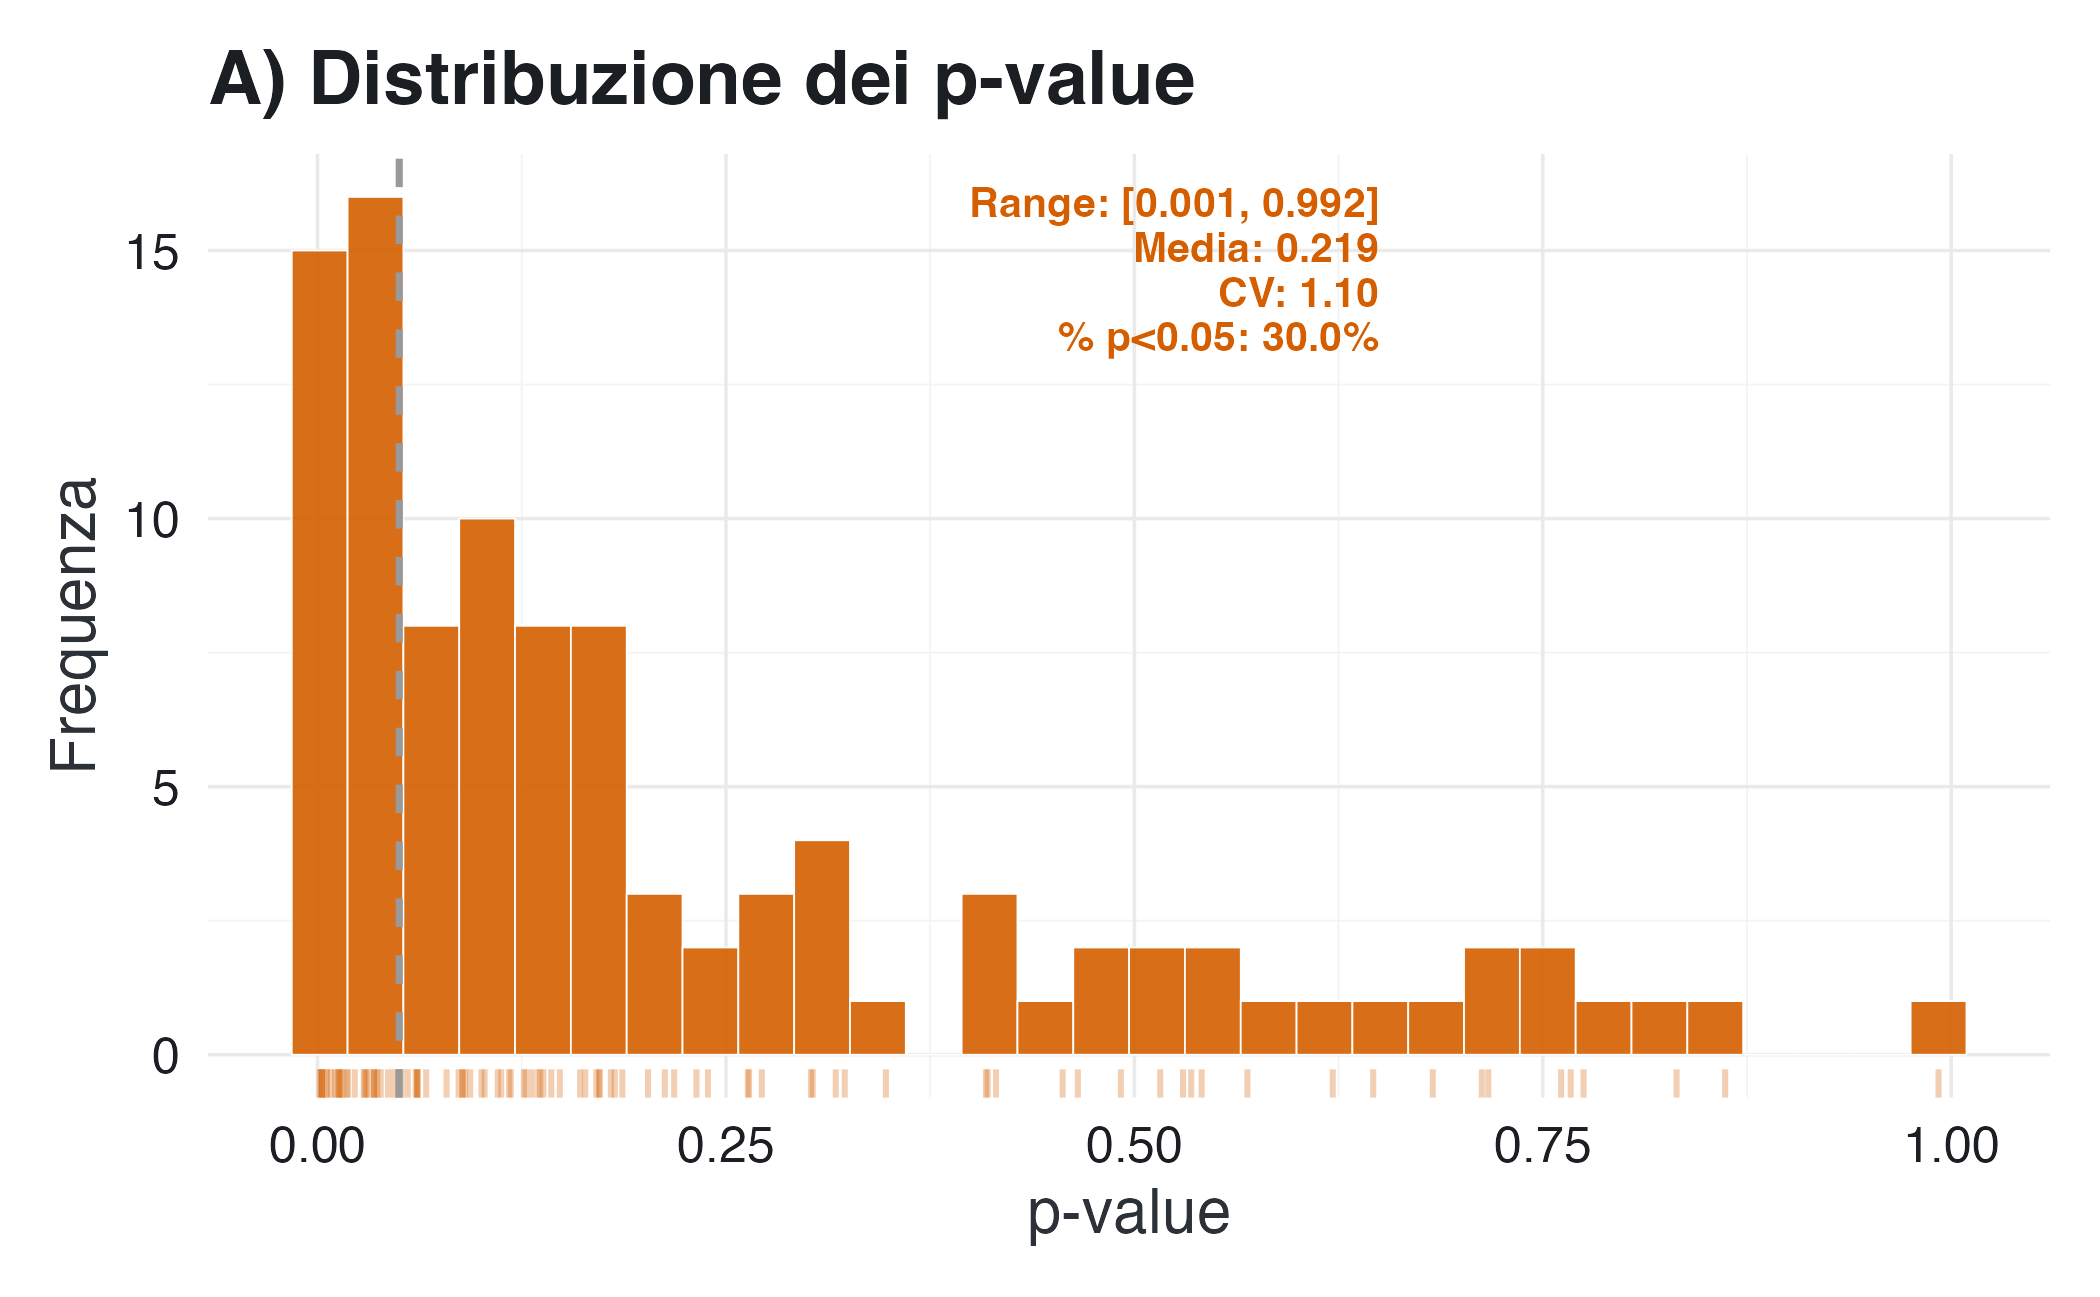
\includegraphics[width=0.85\linewidth,height=\textheight,keepaspectratio]{chapters/limits/04_p_values_files/figure-pdf/fig-freq-stability-1.png}

}

\caption{\label{fig-freq-stability}Distribuzione dei valori-p:
oscillazioni ampie tra campioni e forte dipendenza da una soglia
arbitraria.}

\end{figure}%

\begin{figure}

\centering{

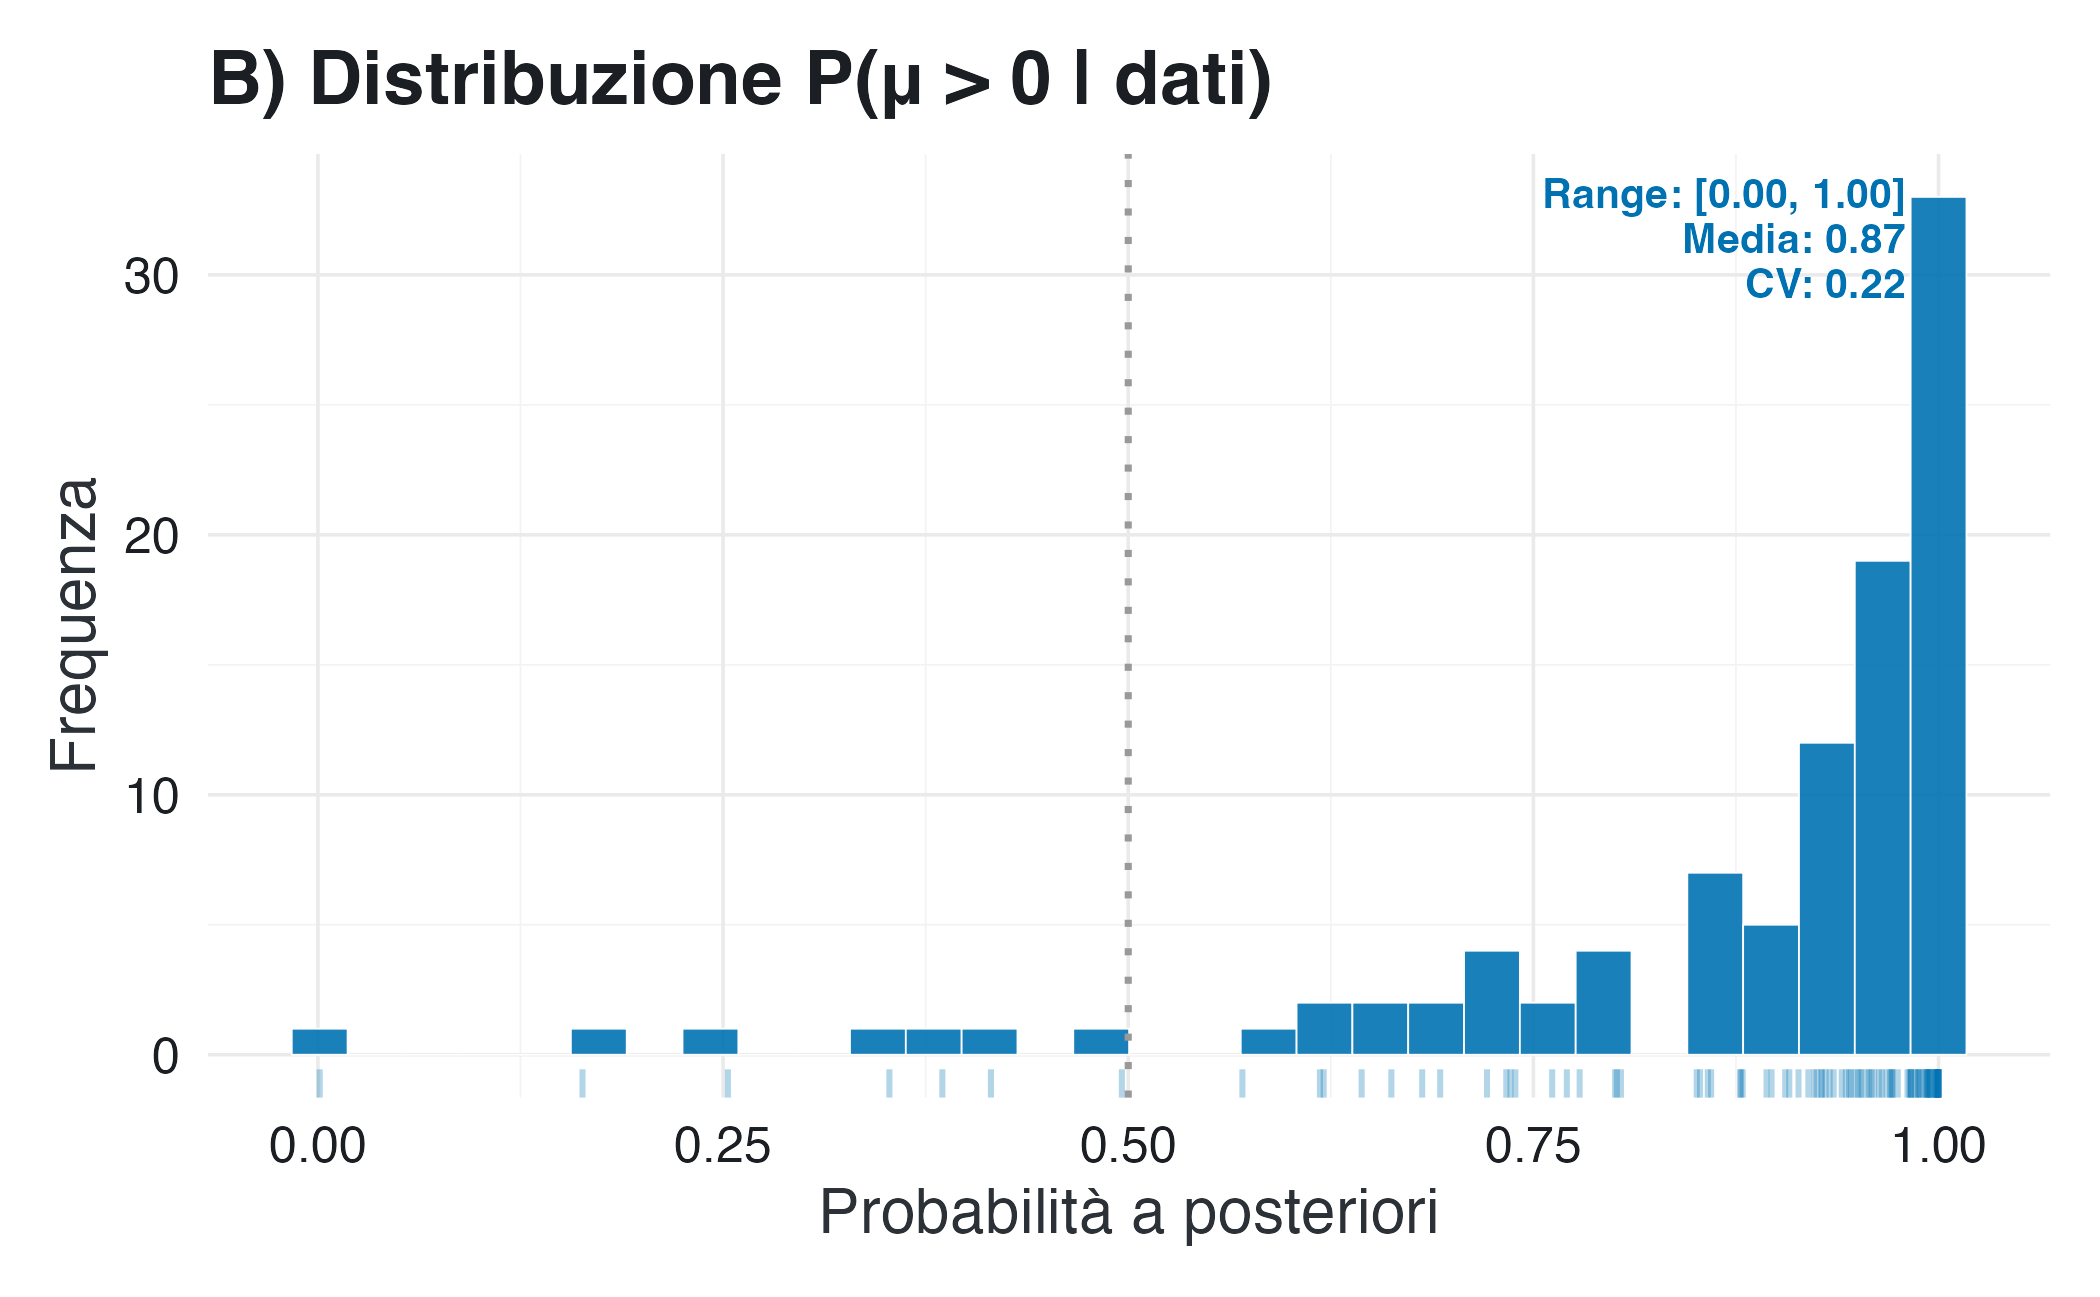
\includegraphics[width=0.85\linewidth,height=\textheight,keepaspectratio]{chapters/limits/04_p_values_files/figure-pdf/fig-bayes-stability-1.png}

}

\caption{\label{fig-bayes-stability}Distribuzione di P(μ \textgreater{}
0 \textbar{} dati): variabilità più contenuta e interpretazione
continua.}

\end{figure}%

\begin{figure}

\centering{

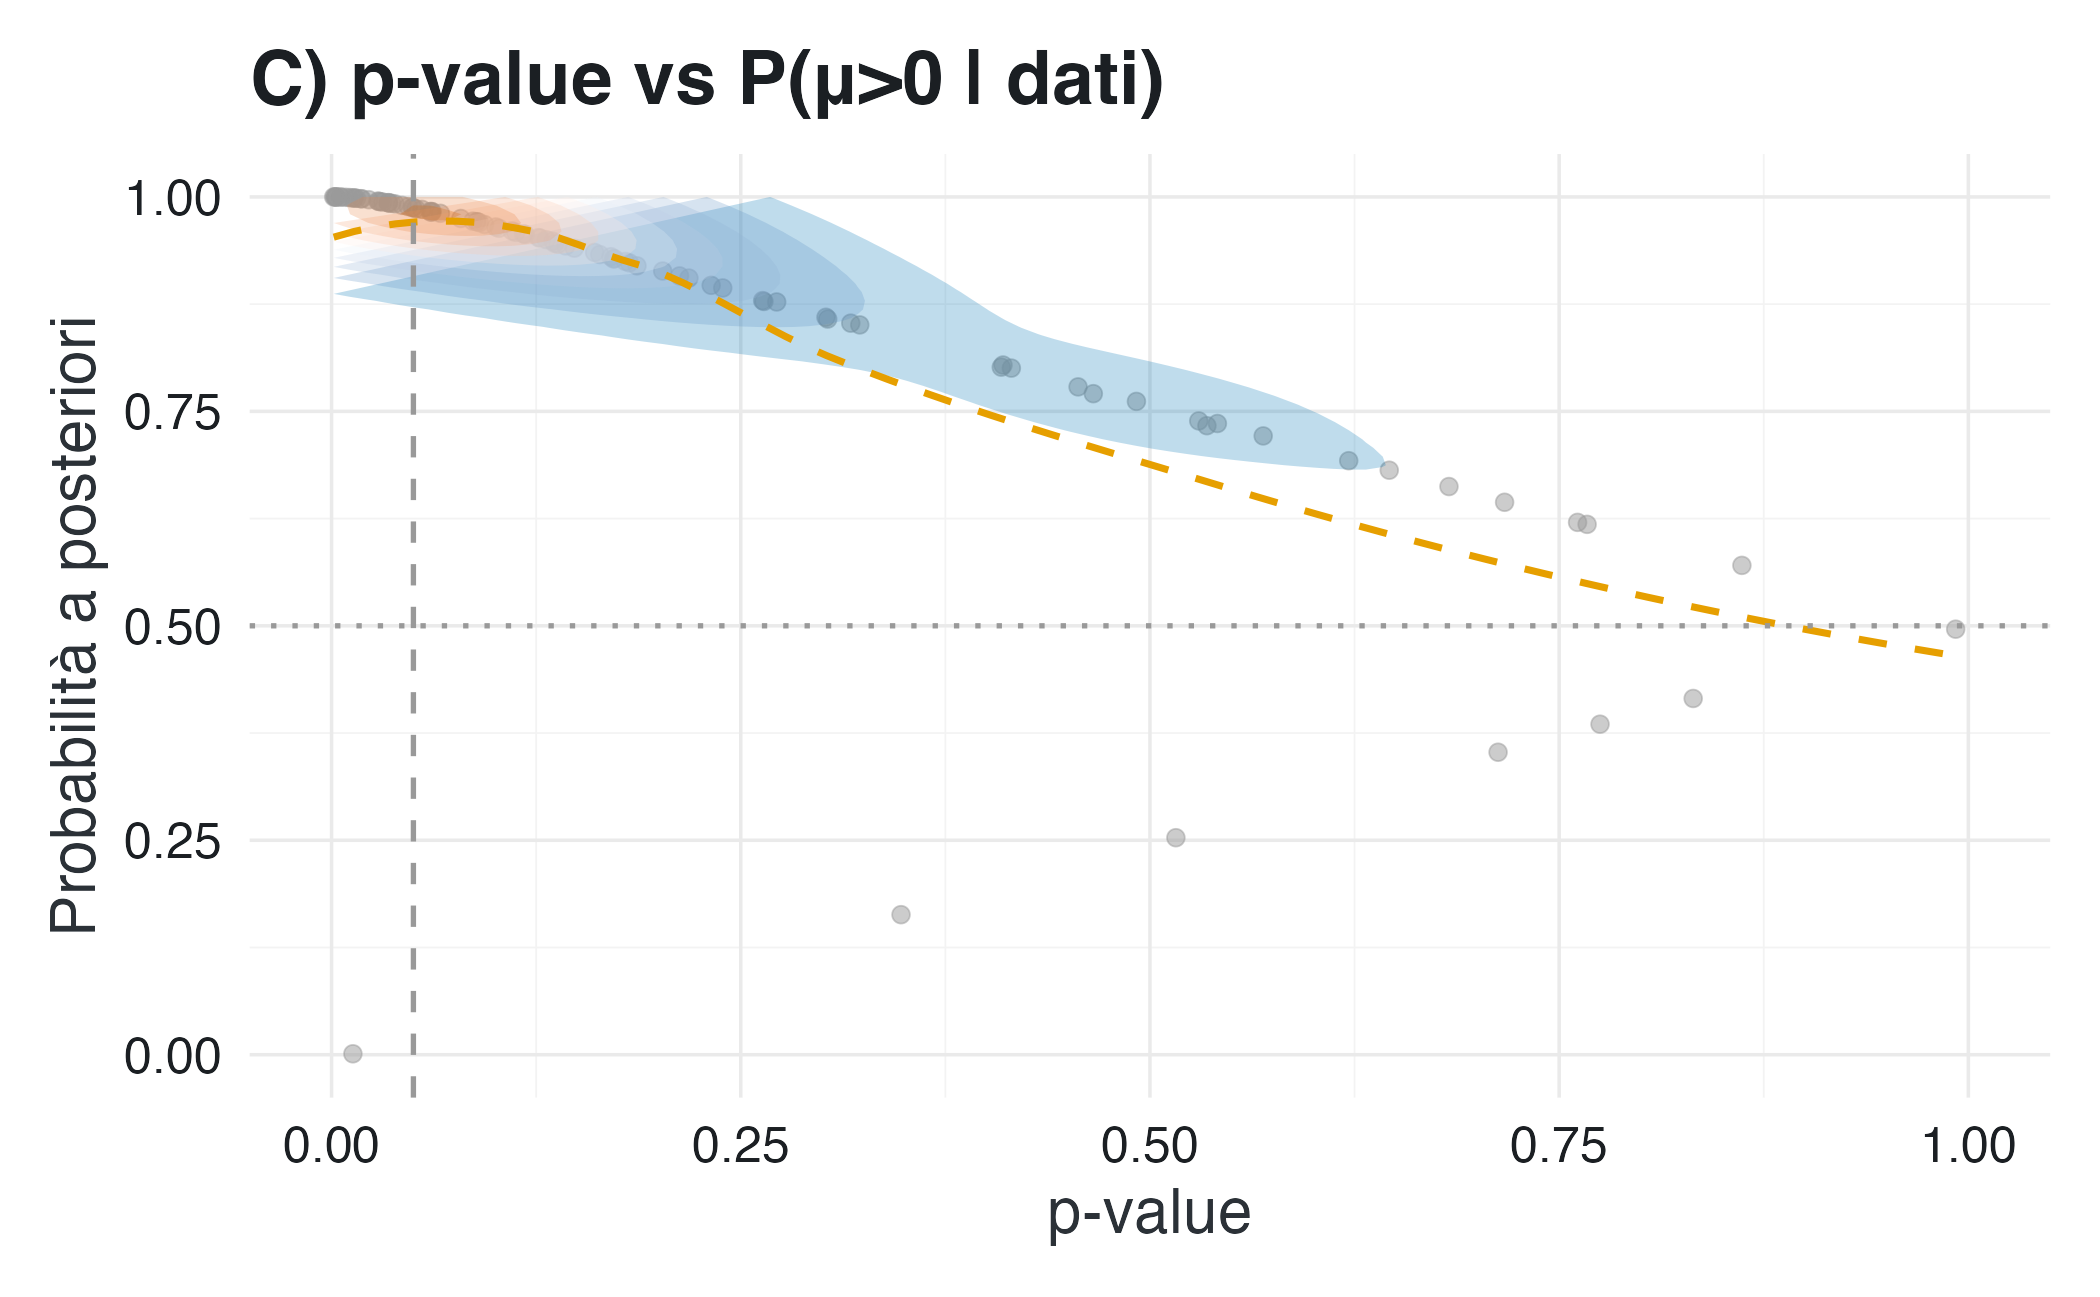
\includegraphics[width=0.85\linewidth,height=\textheight,keepaspectratio]{chapters/limits/04_p_values_files/figure-pdf/fig-freq-vs-bayes-stability-1.png}

}

\caption{\label{fig-freq-vs-bayes-stability}Relazione tra valore-p e
probabilità a posteriori. I due metodi non producono interpretazioni
equivalenti.}

\end{figure}%

Confronto numerico:

\begin{verbatim}
#> Coefficiente di variazione del valore-p:     1.10
#> Coefficiente di variazione P(μ>0|dati): 0.22
#> Campo di variazione del valore-p:        [0.001, 0.992]
#> Campo di variazione di P(μ>0|dati):    [0.00, 1.00]
\end{verbatim}

\subsection{Interpretazione}\label{interpretazione-2}

I risultati mostrano una differenza cruciale: i valori-\(p\) oscillano
considerevolmente da un campione all'altro. Per questo motivo,
conclusioni opposte possono dipendere unicamente dal superamento o meno
della soglia convenzionale di 0.05. La probabilità a posteriori che
l'effetto sia positivo, invece, varia in modo più graduale e raramente
porta a decisioni drasticamente opposte tra campioni simili.

La maggiore stabilità è dovuta al fatto che l'approccio bayesiano
incorpora l'incertezza preesistente tramite uno \emph{shrinkage}
naturale verso la distribuzione a priori. Inoltre, evita la
trasformazione non lineare che porta al valore-\(p\), la quale tende ad
amplificare le fluttuazioni campionarie. Infine, l'approccio bayesiano
esprime l'evidenza in una scala direttamente interpretabile, ossia come
probabilità dell'ipotesi di interesse, piuttosto che come risultato di
un test controfattuale.

\begin{tcolorbox}[enhanced jigsaw, arc=.35mm, bottomrule=.15mm, bottomtitle=1mm, breakable, colback=white, colbacktitle=quarto-callout-warning-color!10!white, colframe=quarto-callout-warning-color-frame, coltitle=black, left=2mm, leftrule=.75mm, opacityback=0, opacitybacktitle=0.6, rightrule=.15mm, title=\textcolor{quarto-callout-warning-color}{\faExclamationTriangle}\hspace{0.5em}{Avvertenza metodologica}, titlerule=0mm, toprule=.15mm, toptitle=1mm]

Anche l'inferenza bayesiana è soggetta alla variabilità campionaria.
Introdurre una regola decisionale arbitraria, come ad esempio
``concludere che l'effetto esiste se
\(P(\mu > 0 \mid \text{dati}) > 0.95\)'', riprodurrebbe esattamente i
problemi concettuali legati all'uso dicotomico del valore-\(p\). Il vero
vantaggio del metodo bayesiano non risiede nel fornire certezze
definitive, ma nell'offrire una rappresentazione continua e trasparente
dell'incertezza a posteriori.

\end{tcolorbox}

In sintesi, l'approccio bayesiano non elimina l'incertezza, ma la
\textbf{quantifica} in modo esplicito, mentre la soglia frequentista
tende a \textbf{mascherarla}, trasformando la naturale variabilità dei
risultati in un conflitto artificiale tra studi apparentemente
contraddittori.

\section{Simulazione 5: l'effetto della dimensione
campionaria}\label{simulazione-5-leffetto-della-dimensione-campionaria}

Un argomento spesso avanzato a sostegno dell'uso del valore-\(p\) è che,
aumentando la dimensione campionaria, le inferenze diventano più
stabili. In parte questa affermazione è vera: campioni più ampi,
infatti, offrono una maggiore potenza statistica, il che rende più
frequenti i risultati ``statisticamente significativi'' quando esiste un
effetto reale. Tuttavia, questa osservazione rischia di nascondere un
fatto meno intuitivo, ma altrettanto importante: anche con campioni
molto grandi, il valore-\(p\) conserva una sostanziale variabilità e
rimane strettamente dipendente dalle caratteristiche specifiche del
singolo campione osservato.

Per illustrare questo fenomeno, abbiamo condotto 1000 simulazioni per
quattro diverse dimensioni campionarie crescenti (da \(n = 10\) a
\(n = 300\)), ipotizzando un effetto reale di piccola entità,
\(d = 0.2\). Per ciascuna delle simulazioni, abbiamo calcolato il
valore-\(p\) associato a un test \(t\) di Student a una coda.

\begin{Shaded}
\begin{Highlighting}[]
\FunctionTok{set.seed}\NormalTok{(}\DecValTok{123}\NormalTok{)}
\NormalTok{true\_mean }\OtherTok{\textless{}{-}} \FloatTok{0.2}
\NormalTok{true\_sd }\OtherTok{\textless{}{-}} \DecValTok{1}
\NormalTok{sample\_sizes }\OtherTok{\textless{}{-}} \FunctionTok{c}\NormalTok{(}\DecValTok{10}\NormalTok{, }\DecValTok{30}\NormalTok{, }\DecValTok{100}\NormalTok{, }\DecValTok{300}\NormalTok{)}
\NormalTok{n\_sims }\OtherTok{\textless{}{-}} \DecValTok{1000}

\NormalTok{sample\_size\_effect }\OtherTok{\textless{}{-}} \FunctionTok{tibble}\NormalTok{()}

\ControlFlowTok{for}\NormalTok{ (n }\ControlFlowTok{in}\NormalTok{ sample\_sizes) \{}

\NormalTok{  p\_vals }\OtherTok{\textless{}{-}} \FunctionTok{numeric}\NormalTok{(n\_sims)}

  \ControlFlowTok{for}\NormalTok{ (i }\ControlFlowTok{in} \FunctionTok{seq\_len}\NormalTok{(n\_sims)) \{}
\NormalTok{    x }\OtherTok{\textless{}{-}} \FunctionTok{rnorm}\NormalTok{(n, }\AttributeTok{mean =}\NormalTok{ true\_mean, }\AttributeTok{sd =}\NormalTok{ true\_sd)}
\NormalTok{    p\_vals[i] }\OtherTok{\textless{}{-}} \FunctionTok{t.test}\NormalTok{(x, }\AttributeTok{mu =} \DecValTok{0}\NormalTok{)}\SpecialCharTok{$}\NormalTok{p.value}
\NormalTok{  \}}

\NormalTok{  sample\_size\_effect }\OtherTok{\textless{}{-}} \FunctionTok{bind\_rows}\NormalTok{(}
\NormalTok{    sample\_size\_effect,}
    \FunctionTok{tibble}\NormalTok{(}
      \AttributeTok{n =}\NormalTok{ n,}
      \AttributeTok{p\_value =}\NormalTok{ p\_vals,}
      \AttributeTok{label =} \FunctionTok{sprintf}\NormalTok{(}\StringTok{"n = \%d"}\NormalTok{, n)}
\NormalTok{    )}
\NormalTok{  )}
\NormalTok{\}}

\FunctionTok{ggplot}\NormalTok{(sample\_size\_effect, }\FunctionTok{aes}\NormalTok{(}\AttributeTok{x =}\NormalTok{ p\_value)) }\SpecialCharTok{+}
  \FunctionTok{geom\_histogram}\NormalTok{(}
    \FunctionTok{aes}\NormalTok{(}\AttributeTok{fill =} \StringTok{"Distribuzione P{-}value"}\NormalTok{),}
    \AttributeTok{bins =} \DecValTok{40}\NormalTok{, }
    \AttributeTok{color =} \StringTok{"white"}\NormalTok{, }
    \AttributeTok{alpha =} \FloatTok{0.8}
\NormalTok{  ) }\SpecialCharTok{+}
  \FunctionTok{geom\_vline}\NormalTok{(}
    \FunctionTok{aes}\NormalTok{(}\AttributeTok{xintercept =} \FloatTok{0.05}\NormalTok{, }\AttributeTok{color =} \StringTok{"Soglia α = 0.05"}\NormalTok{),}
    \AttributeTok{linetype =} \StringTok{"dashed"}\NormalTok{, }
    \AttributeTok{linewidth =} \DecValTok{1}
\NormalTok{  ) }\SpecialCharTok{+}
  \FunctionTok{facet\_wrap}\NormalTok{(}\SpecialCharTok{\textasciitilde{}}\NormalTok{label, }\AttributeTok{ncol =} \DecValTok{2}\NormalTok{) }\SpecialCharTok{+}
  \FunctionTok{labs}\NormalTok{(}
    \AttributeTok{x =} \StringTok{"Valore{-}p"}\NormalTok{,}
    \AttributeTok{y =} \StringTok{"Frequenza"}\NormalTok{,}
    \AttributeTok{title =} \StringTok{"Distribuzione dei valori{-}p}\SpecialCharTok{\textbackslash{}n}\StringTok{per diverse dimensioni campionarie"}\NormalTok{,}
    \AttributeTok{subtitle =} \FunctionTok{sprintf}\NormalTok{(}\StringTok{"Effetto vero: d = \%.1f"}\NormalTok{, true\_mean}\SpecialCharTok{/}\NormalTok{true\_sd),}
    \AttributeTok{fill =} \StringTok{"Elementi"}\NormalTok{,}
    \AttributeTok{color =} \StringTok{"Linee"}
\NormalTok{  ) }\SpecialCharTok{+}
  \FunctionTok{scale\_fill\_manual}\NormalTok{(}\AttributeTok{values =} \FunctionTok{c}\NormalTok{(}\StringTok{"Distribuzione P{-}value"} \OtherTok{=}\NormalTok{ palette\_qualitative[}\DecValTok{2}\NormalTok{])) }\SpecialCharTok{+} 
  \FunctionTok{scale\_color\_manual}\NormalTok{(}\AttributeTok{values =} \FunctionTok{c}\NormalTok{(}\StringTok{"Soglia α = 0.05"} \OtherTok{=}\NormalTok{ palette\_qualitative[}\DecValTok{6}\NormalTok{]))   }
\end{Highlighting}
\end{Shaded}

\begin{figure}[H]

\centering{

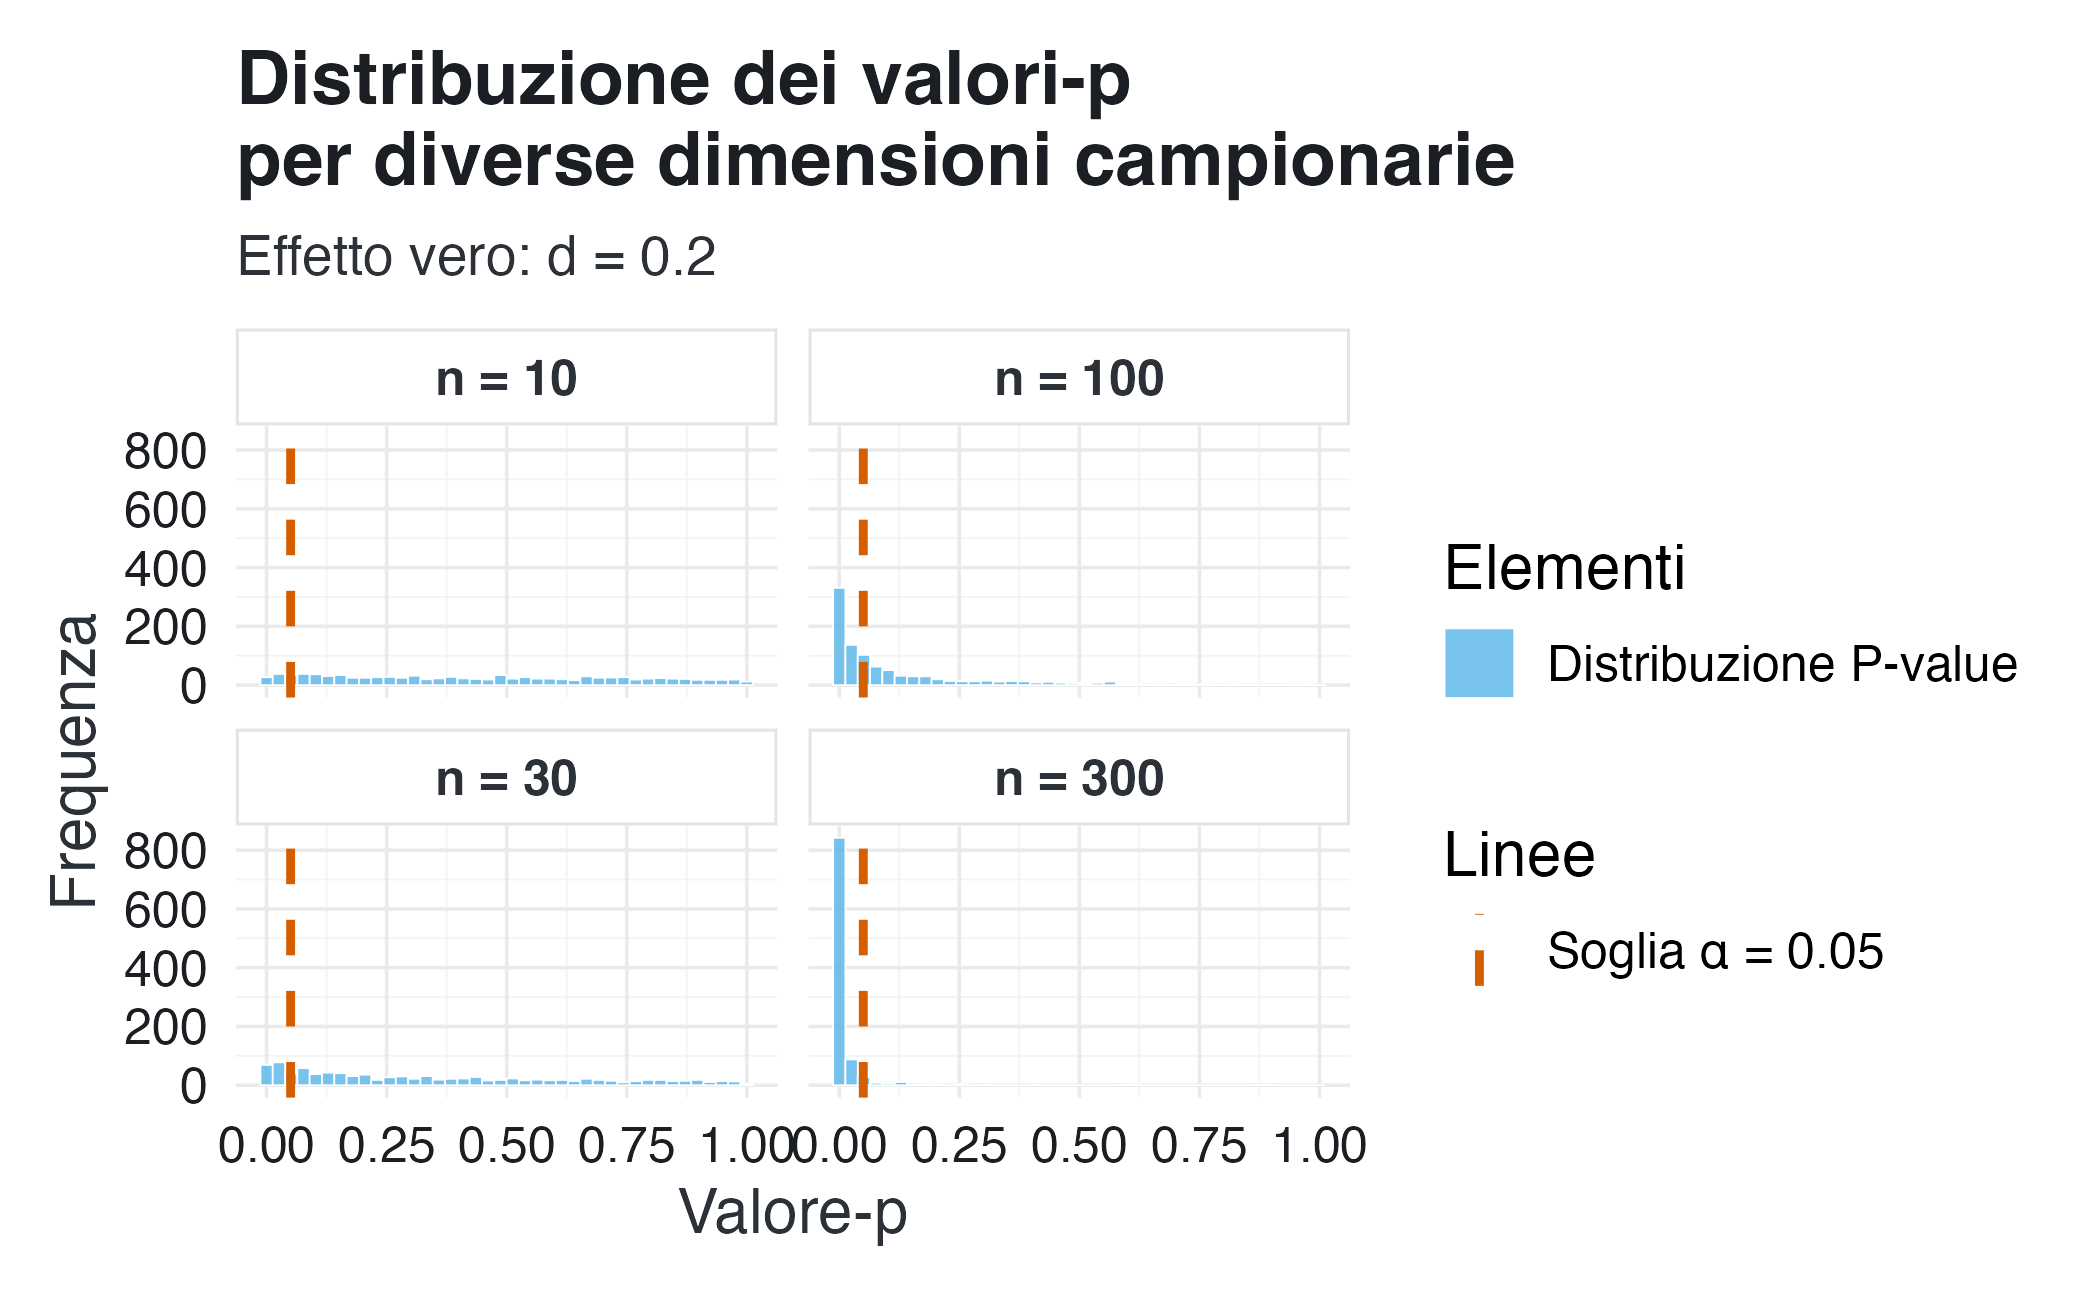
\includegraphics[width=0.85\linewidth,height=\textheight,keepaspectratio]{chapters/limits/04_p_values_files/figure-pdf/fig-sample-size-pvalue-1.png}

}

\caption{\label{fig-sample-size-pvalue}La variabilità del p-value
diminuisce con n, ma rimane sostanziale anche con campioni grandi.}

\end{figure}%

\begin{Shaded}
\begin{Highlighting}[]
\CommentTok{\# Statistiche riassuntive}
\NormalTok{sample\_size\_effect }\SpecialCharTok{|\textgreater{}}
  \FunctionTok{group\_by}\NormalTok{(n) }\SpecialCharTok{|\textgreater{}}
  \FunctionTok{summarise}\NormalTok{(}
    \StringTok{\textasciigrave{}}\AttributeTok{Mediana p}\StringTok{\textasciigrave{}} \OtherTok{=} \FunctionTok{sprintf}\NormalTok{(}\StringTok{"\%.3f"}\NormalTok{, }\FunctionTok{median}\NormalTok{(p\_value)),}
    \StringTok{\textasciigrave{}}\AttributeTok{Range p}\StringTok{\textasciigrave{}} \OtherTok{=} \FunctionTok{sprintf}\NormalTok{(}\StringTok{"[\%.3f, \%.3f]"}\NormalTok{, }\FunctionTok{min}\NormalTok{(p\_value), }\FunctionTok{max}\NormalTok{(p\_value)),}
    \StringTok{\textasciigrave{}}\AttributeTok{\% significativi}\StringTok{\textasciigrave{}} \OtherTok{=} \FunctionTok{sprintf}\NormalTok{(}\StringTok{"\%.0f\%\%"}\NormalTok{, }\DecValTok{100} \SpecialCharTok{*} \FunctionTok{mean}\NormalTok{(p\_value }\SpecialCharTok{\textless{}} \FloatTok{0.05}\NormalTok{)),}
    \AttributeTok{.groups =} \StringTok{"drop"}
\NormalTok{  ) }\SpecialCharTok{|\textgreater{}}
\NormalTok{  knitr}\SpecialCharTok{::}\FunctionTok{kable}\NormalTok{(}\AttributeTok{caption =} \StringTok{"Variabilità del p{-}value in funzione di n"}\NormalTok{)}
\end{Highlighting}
\end{Shaded}

\begin{longtable}[]{@{}rlll@{}}
\caption{Variabilità del p-value in funzione di n}\tabularnewline
\toprule\noalign{}
n & Mediana p & Range p & \% significativi \\
\midrule\noalign{}
\endfirsthead
\toprule\noalign{}
n & Mediana p & Range p & \% significativi \\
\midrule\noalign{}
\endhead
\bottomrule\noalign{}
\endlastfoot
10 & 0.428 & {[}0.000, 0.999{]} & 8\% \\
30 & 0.287 & {[}0.000, 0.999{]} & 16\% \\
100 & 0.044 & {[}0.000, 0.993{]} & 52\% \\
300 & 0.001 & {[}0.000, 0.895{]} & 95\% \\
\end{longtable}

I risultati mostrano che, anche con \(n\) = 300, i valori-\(p\)
oscillano da 0.0 a 0.895. Mentre la potenza statistica aumenta
effettivamente (come evidenziato dalla maggiore percentuale di studi che
superano la soglia convenzionale), la variabilità intrinseca del
valore-\(p\) persiste. Questi risultati confermano che il valore-\(p\)
\textbf{non è una misura stabile dell'evidenza}, ma piuttosto una
statistica estremamente sensibile alle fluttuazioni campionarie
specifiche.

\section{Riflessioni conclusive}\label{riflessioni-conclusive-3}

Le simulazioni presentate in questo capitolo illustrano in modo concreto
la fragilità del valore-\(p\) come strumento inferenziale. Un primo
aspetto riguarda la \textbf{marcata instabilità dei valori campionari
del valore-\(p\)}. A parità di effetto reale e applicando la medesima
procedura statistica, è possibile ottenere risultati radicalmente
discordanti: lo stesso fenomeno può generare un valore-\(p\) pari a
0.001 in un campione, interpretato come un'evidenza molto forte a
sostegno dell'effetto, e in un altro campione un valore-\(p\) di 0.90,
interpretato come totale assenza di supporto. Queste oscillazioni non
derivano da differenze metodologiche tra le analisi né da variazioni
dell'effetto studiato, ma sono una conseguenza diretta della
\textbf{variabilità intrinseca del processo di campionamento}. Il
valore-\(p\), quindi, non fornisce un indicatore stabile dell'evidenza
empirica, ma rimane altamente sensibile alla fluttuazione casuale insita
nei dati osservati.

La seconda evidenza riguarda la \textbf{discordanza sistematica tra gli
studi}. Due ricercatori che indagano lo stesso fenomeno, utilizzando
protocolli metodologicamente solidi, possono facilmente giungere a
conclusioni statisticamente opposte. Questo non rappresenta un caso
eccezionale, ma una caratteristica intrinseca dell'inferenza basata sul
valore-\(p\), che compromette la coerenza e la cumulatività della
conoscenza scientifica.

La terza evidenza riguarda la \textbf{distribuzione uniforme dei
valori-\(p\) sotto l'ipotesi nulla}. Quando l'ipotesi nulla è vera, i
valori-\(p\) si distribuiscono in modo uniforme tra 0 e 1, il che
implica che, per puro caso, circa il 5\% dei risultati supererà
inevitabilmente la soglia convenzionale del 5\%. In altre parole, questa
soglia non agisce come un filtro affidabile per distinguere il segnale
dal rumore, ma funziona piuttosto come un generatore sistematico di
falsi positivi.

La quarta evidenza emerge dal \textbf{confronto con l'approccio
bayesiano}. Le probabilità a posteriori presentano una stabilità molto
maggiore rispetto ai valori-\(p\), fornendo stime più coerenti
dell'evidenza a partire dai dati. Tuttavia, questa maggiore stabilità
non implica certezza: l'inferenza bayesiana riduce, ma non elimina,
l'incertezza intrinseca derivante dal campionamento, offrendo una
quantificazione dell'evidenza più sfumata e trasparente, pur rimanendo
soggetta alla variabilità dei dati osservati.

La quinta evidenza riguarda l'\textbf{effetto della dimensione
campionaria}. L'aumento del numero di osservazioni aumenta la potenza
statistica e riduce la probabilità di falsi negativi, ma non elimina la
variabilità intrinseca delle stime. Anche gli studi che coinvolgono
migliaia di partecipanti producono risultati che oscillano attorno al
vero valore del parametro, sebbene tali fluttuazioni siano più contenute
rispetto a campioni più piccoli.

La lezione principale che emerge da queste simulazioni è che la
distinzione binaria tra ``significativo'' e ``non significativo'' è
arbitraria nella sua definizione e fragile nella sua applicazione. Come
osservato da Gelman \& Stern
(\citeproc{ref-gelman2006difference}{2006}), interpretare questa
separazione artificiale come se riflettesse una differenza sostanziale
nel fenomeno studiato costituisce un grave errore epistemologico.
Considerare valori-\(p\) di 0.049 e 0.051 come portatori di significati
scientifici opposti significa confondere un artefatto della procedura
statistica con una proprietà effettiva della realtà studiata.

\section{Esercizi}\label{esercizi-3}

\begin{tcolorbox}[enhanced jigsaw, arc=.35mm, bottomrule=.15mm, bottomtitle=1mm, breakable, colback=white, colbacktitle=quarto-callout-important-color!10!white, colframe=quarto-callout-important-color-frame, coltitle=black, left=2mm, leftrule=.75mm, opacityback=0, opacitybacktitle=0.6, rightrule=.15mm, title=\textcolor{quarto-callout-important-color}{\faExclamation}\hspace{0.5em}{Esercizio 1: Replicabilità apparente}, titlerule=0mm, toprule=.15mm, toptitle=1mm]

Un ricercatore trova \(p = 0.048\) nel suo studio. Qual è la probabilità
che una replica esatta (stesso \(n\), stessa popolazione) trovi
anch'essa \(p < 0.05\)?

Usa la simulazione per rispondere, considerando tre scenari: 1.
L'effetto vero è quello stimato nello studio originale 2. L'effetto vero
è la metà di quello stimato (Type M error) 3. L'effetto vero è zero
(falso positivo originale)

\end{tcolorbox}

\begin{tcolorbox}[enhanced jigsaw, arc=.35mm, bottomrule=.15mm, bottomtitle=1mm, breakable, colback=white, colbacktitle=quarto-callout-tip-color!10!white, colframe=quarto-callout-tip-color-frame, coltitle=black, left=2mm, leftrule=.75mm, opacityback=0, opacitybacktitle=0.6, rightrule=.15mm, title=\textcolor{quarto-callout-tip-color}{\faLightbulb}\hspace{0.5em}{Soluzione Esercizio 1}, titlerule=0mm, toprule=.15mm, toptitle=1mm]

\begin{Shaded}
\begin{Highlighting}[]
\CommentTok{\# Parametri dello studio originale}
\NormalTok{n\_original }\OtherTok{\textless{}{-}} \DecValTok{30}
\NormalTok{d\_estimated }\OtherTok{\textless{}{-}} \FloatTok{0.4}  \CommentTok{\# Stima dallo studio con p = 0.048}

\CommentTok{\# Scenari}
\NormalTok{scenarios }\OtherTok{\textless{}{-}} \FunctionTok{tibble}\NormalTok{(}
  \AttributeTok{scenario =} \FunctionTok{c}\NormalTok{(}\StringTok{"Effetto = stimato"}\NormalTok{, }\StringTok{"Effetto = metà"}\NormalTok{, }\StringTok{"Effetto = zero"}\NormalTok{),}
  \AttributeTok{true\_d =} \FunctionTok{c}\NormalTok{(d\_estimated, d\_estimated}\SpecialCharTok{/}\DecValTok{2}\NormalTok{, }\DecValTok{0}\NormalTok{)}
\NormalTok{)}

\CommentTok{\# Simula repliche}
\NormalTok{n\_reps }\OtherTok{\textless{}{-}} \DecValTok{10000}

\NormalTok{replication\_probs }\OtherTok{\textless{}{-}} \FunctionTok{tibble}\NormalTok{()}

\ControlFlowTok{for}\NormalTok{ (i }\ControlFlowTok{in} \FunctionTok{seq\_len}\NormalTok{(}\FunctionTok{nrow}\NormalTok{(scenarios))) \{}

\NormalTok{  d }\OtherTok{\textless{}{-}}\NormalTok{ scenarios}\SpecialCharTok{$}\NormalTok{true\_d[i]}
\NormalTok{  p\_reps }\OtherTok{\textless{}{-}} \FunctionTok{numeric}\NormalTok{(n\_reps)}

  \ControlFlowTok{for}\NormalTok{ (j }\ControlFlowTok{in} \FunctionTok{seq\_len}\NormalTok{(n\_reps)) \{}
\NormalTok{    x }\OtherTok{\textless{}{-}} \FunctionTok{rnorm}\NormalTok{(n\_original, }\AttributeTok{mean =}\NormalTok{ d, }\AttributeTok{sd =} \DecValTok{1}\NormalTok{)}
\NormalTok{    p\_reps[j] }\OtherTok{\textless{}{-}} \FunctionTok{t.test}\NormalTok{(x, }\AttributeTok{mu =} \DecValTok{0}\NormalTok{)}\SpecialCharTok{$}\NormalTok{p.value}
\NormalTok{  \}}

\NormalTok{  replication\_probs }\OtherTok{\textless{}{-}} \FunctionTok{bind\_rows}\NormalTok{(}
\NormalTok{    replication\_probs,}
    \FunctionTok{tibble}\NormalTok{(}
      \AttributeTok{scenario =}\NormalTok{ scenarios}\SpecialCharTok{$}\NormalTok{scenario[i],}
      \AttributeTok{prob\_replicate =} \FunctionTok{mean}\NormalTok{(p\_reps }\SpecialCharTok{\textless{}} \FloatTok{0.05}\NormalTok{)}
\NormalTok{    )}
\NormalTok{  )}
\NormalTok{\}}

\NormalTok{replication\_probs }\SpecialCharTok{|\textgreater{}}
  \FunctionTok{mutate}\NormalTok{(}\StringTok{\textasciigrave{}}\AttributeTok{P(replica significativa)}\StringTok{\textasciigrave{}} \OtherTok{=} \FunctionTok{sprintf}\NormalTok{(}\StringTok{"\%.0f\%\%"}\NormalTok{, prob\_replicate }\SpecialCharTok{*} \DecValTok{100}\NormalTok{)) }\SpecialCharTok{|\textgreater{}}
  \FunctionTok{select}\NormalTok{(scenario, }\StringTok{\textasciigrave{}}\AttributeTok{P(replica significativa)}\StringTok{\textasciigrave{}}\NormalTok{) }\SpecialCharTok{|\textgreater{}}
\NormalTok{  knitr}\SpecialCharTok{::}\FunctionTok{kable}\NormalTok{()}
\end{Highlighting}
\end{Shaded}

{\def\LTcaptype{none} % do not increment counter
\begin{longtable}[]{@{}ll@{}}
\toprule\noalign{}
scenario & P(replica significativa) \\
\midrule\noalign{}
\endhead
\bottomrule\noalign{}
\endlastfoot
Effetto = stimato & 56\% \\
Effetto = metà & 18\% \\
Effetto = zero & 5\% \\
\end{longtable}
}

\textbf{Interpretazione}: Anche assumendo che l'effetto stimato sia
corretto, la replica ha solo \textasciitilde50\% di probabilità di
essere significativa. Se l'effetto è sovrastimato (Type M error), la
probabilità scende drasticamente.

\end{tcolorbox}

\begin{tcolorbox}[enhanced jigsaw, arc=.35mm, bottomrule=.15mm, bottomtitle=1mm, breakable, colback=white, colbacktitle=quarto-callout-important-color!10!white, colframe=quarto-callout-important-color-frame, coltitle=black, left=2mm, leftrule=.75mm, opacityback=0, opacitybacktitle=0.6, rightrule=.15mm, title=\textcolor{quarto-callout-important-color}{\faExclamation}\hspace{0.5em}{Esercizio 2: Intervallo di `previsione' per p}, titlerule=0mm, toprule=.15mm, toptitle=1mm]

Se un effetto vero è \(d = 0.3\) e \(n = 50\), quale intervallo conterrà
il 95\% dei p-value ottenibili in studi futuri?

Confronta questo intervallo con quello per la probabilità a posteriori
bayesiana.

\end{tcolorbox}

\begin{tcolorbox}[enhanced jigsaw, arc=.35mm, bottomrule=.15mm, bottomtitle=1mm, breakable, colback=white, colbacktitle=quarto-callout-tip-color!10!white, colframe=quarto-callout-tip-color-frame, coltitle=black, left=2mm, leftrule=.75mm, opacityback=0, opacitybacktitle=0.6, rightrule=.15mm, title=\textcolor{quarto-callout-tip-color}{\faLightbulb}\hspace{0.5em}{Soluzione Esercizio 2}, titlerule=0mm, toprule=.15mm, toptitle=1mm]

\begin{Shaded}
\begin{Highlighting}[]
\CommentTok{\# Simulazione}
\NormalTok{d }\OtherTok{\textless{}{-}} \FloatTok{0.3}
\NormalTok{n }\OtherTok{\textless{}{-}} \DecValTok{50}
\NormalTok{n\_sims }\OtherTok{\textless{}{-}} \DecValTok{10000}

\NormalTok{future\_studies }\OtherTok{\textless{}{-}} \FunctionTok{tibble}\NormalTok{(}
  \AttributeTok{p\_value =} \FunctionTok{numeric}\NormalTok{(n\_sims),}
  \AttributeTok{prob\_positive =} \FunctionTok{numeric}\NormalTok{(n\_sims)}
\NormalTok{)}

\ControlFlowTok{for}\NormalTok{ (i }\ControlFlowTok{in} \FunctionTok{seq\_len}\NormalTok{(n\_sims)) \{}

\NormalTok{  x }\OtherTok{\textless{}{-}} \FunctionTok{rnorm}\NormalTok{(n, }\AttributeTok{mean =}\NormalTok{ d, }\AttributeTok{sd =} \DecValTok{1}\NormalTok{)}

  \CommentTok{\# P{-}value}
\NormalTok{  future\_studies}\SpecialCharTok{$}\NormalTok{p\_value[i] }\OtherTok{\textless{}{-}} \FunctionTok{t.test}\NormalTok{(x, }\AttributeTok{mu =} \DecValTok{0}\NormalTok{)}\SpecialCharTok{$}\NormalTok{p.value}

  \CommentTok{\# Bayesiano}
\NormalTok{  x\_bar }\OtherTok{\textless{}{-}} \FunctionTok{mean}\NormalTok{(x)}
\NormalTok{  se }\OtherTok{\textless{}{-}} \FunctionTok{sd}\NormalTok{(x) }\SpecialCharTok{/} \FunctionTok{sqrt}\NormalTok{(n)}
\NormalTok{  prior\_sd }\OtherTok{\textless{}{-}} \FloatTok{0.5}

\NormalTok{  post\_precision }\OtherTok{\textless{}{-}} \DecValTok{1} \SpecialCharTok{/}\NormalTok{ prior\_sd}\SpecialCharTok{\^{}}\DecValTok{2} \SpecialCharTok{+} \DecValTok{1} \SpecialCharTok{/}\NormalTok{ se}\SpecialCharTok{\^{}}\DecValTok{2}
\NormalTok{  post\_mean }\OtherTok{\textless{}{-}}\NormalTok{ (}\DecValTok{1} \SpecialCharTok{/}\NormalTok{ se}\SpecialCharTok{\^{}}\DecValTok{2} \SpecialCharTok{*}\NormalTok{ x\_bar) }\SpecialCharTok{/}\NormalTok{ post\_precision}
\NormalTok{  post\_sd }\OtherTok{\textless{}{-}} \FunctionTok{sqrt}\NormalTok{(}\DecValTok{1} \SpecialCharTok{/}\NormalTok{ post\_precision)}

\NormalTok{  future\_studies}\SpecialCharTok{$}\NormalTok{prob\_positive[i] }\OtherTok{\textless{}{-}}
    \FunctionTok{pnorm}\NormalTok{(}\DecValTok{0}\NormalTok{, post\_mean, post\_sd, }\AttributeTok{lower.tail =} \ConstantTok{FALSE}\NormalTok{)}
\NormalTok{\}}

\CommentTok{\# Intervalli al 95\%}
\FunctionTok{cat}\NormalTok{(}\StringTok{"Intervallo al 95\% per p{-}value:}\SpecialCharTok{\textbackslash{}n}\StringTok{"}\NormalTok{)}
\CommentTok{\#\textgreater{} Intervallo al 95\% per p{-}value:}
\FunctionTok{cat}\NormalTok{(}\FunctionTok{sprintf}\NormalTok{(}\StringTok{"  [\%.4f, \%.4f]}\SpecialCharTok{\textbackslash{}n}\StringTok{"}\NormalTok{, }
            \FunctionTok{quantile}\NormalTok{(future\_studies}\SpecialCharTok{$}\NormalTok{p\_value, }\FloatTok{0.025}\NormalTok{),}
            \FunctionTok{quantile}\NormalTok{(future\_studies}\SpecialCharTok{$}\NormalTok{p\_value, }\FloatTok{0.975}\NormalTok{)))}
\CommentTok{\#\textgreater{}   [0.0001, 0.7702]}

\FunctionTok{cat}\NormalTok{(}\StringTok{"}\SpecialCharTok{\textbackslash{}n}\StringTok{Intervallo al 95\% per P(μ \textgreater{} 0 | dati):}\SpecialCharTok{\textbackslash{}n}\StringTok{"}\NormalTok{)}
\CommentTok{\#\textgreater{} }
\CommentTok{\#\textgreater{} Intervallo al 95\% per P(μ \textgreater{} 0 | dati):}
\FunctionTok{cat}\NormalTok{(}\FunctionTok{sprintf}\NormalTok{(}\StringTok{"  [\%.3f, \%.3f]}\SpecialCharTok{\textbackslash{}n}\StringTok{"}\NormalTok{,}
            \FunctionTok{quantile}\NormalTok{(future\_studies}\SpecialCharTok{$}\NormalTok{prob\_positive, }\FloatTok{0.025}\NormalTok{),}
            \FunctionTok{quantile}\NormalTok{(future\_studies}\SpecialCharTok{$}\NormalTok{prob\_positive, }\FloatTok{0.975}\NormalTok{)))}
\CommentTok{\#\textgreater{}   [0.568, 1.000]}

\FunctionTok{cat}\NormalTok{(}\StringTok{"}\SpecialCharTok{\textbackslash{}n}\StringTok{Ampiezza relativa degli intervalli:}\SpecialCharTok{\textbackslash{}n}\StringTok{"}\NormalTok{)}
\CommentTok{\#\textgreater{} }
\CommentTok{\#\textgreater{} Ampiezza relativa degli intervalli:}
\FunctionTok{cat}\NormalTok{(}\FunctionTok{sprintf}\NormalTok{(}\StringTok{"  P{-}value: \%.2f (su scala 0{-}1)}\SpecialCharTok{\textbackslash{}n}\StringTok{"}\NormalTok{,}
            \FunctionTok{diff}\NormalTok{(}\FunctionTok{quantile}\NormalTok{(future\_studies}\SpecialCharTok{$}\NormalTok{p\_value, }\FunctionTok{c}\NormalTok{(}\FloatTok{0.025}\NormalTok{, }\FloatTok{0.975}\NormalTok{)))))}
\CommentTok{\#\textgreater{}   P{-}value: 0.77 (su scala 0{-}1)}
\FunctionTok{cat}\NormalTok{(}\FunctionTok{sprintf}\NormalTok{(}\StringTok{"  Bayesiano: \%.2f (su scala 0{-}1)}\SpecialCharTok{\textbackslash{}n}\StringTok{"}\NormalTok{,}
            \FunctionTok{diff}\NormalTok{(}\FunctionTok{quantile}\NormalTok{(future\_studies}\SpecialCharTok{$}\NormalTok{prob\_positive, }\FunctionTok{c}\NormalTok{(}\FloatTok{0.025}\NormalTok{, }\FloatTok{0.975}\NormalTok{)))))}
\CommentTok{\#\textgreater{}   Bayesiano: 0.43 (su scala 0{-}1)}
\end{Highlighting}
\end{Shaded}

\end{tcolorbox}

\begin{tcolorbox}[enhanced jigsaw, arc=.35mm, bottomrule=.15mm, bottomtitle=1mm, breakable, colback=white, colbacktitle=quarto-callout-important-color!10!white, colframe=quarto-callout-important-color-frame, coltitle=black, left=2mm, leftrule=.75mm, opacityback=0, opacitybacktitle=0.6, rightrule=.15mm, title=\textcolor{quarto-callout-important-color}{\faExclamation}\hspace{0.5em}{Esercizio 3: Soglie alternative}, titlerule=0mm, toprule=.15mm, toptitle=1mm]

Alcuni hanno proposto di abbassare la soglia a \(p < 0.005\) per ridurre
i falsi positivi. Simula cosa succederebbe in termini di:

\begin{enumerate}
\def\labelenumi{\arabic{enumi}.}
\tightlist
\item
  Tasso di falsi positivi
\item
  Potenza (con \(d = 0.3\), \(n = 50\))
\item
  Concordanza tra studi
\end{enumerate}

\end{tcolorbox}

\begin{tcolorbox}[enhanced jigsaw, arc=.35mm, bottomrule=.15mm, bottomtitle=1mm, breakable, colback=white, colbacktitle=quarto-callout-tip-color!10!white, colframe=quarto-callout-tip-color-frame, coltitle=black, left=2mm, leftrule=.75mm, opacityback=0, opacitybacktitle=0.6, rightrule=.15mm, title=\textcolor{quarto-callout-tip-color}{\faLightbulb}\hspace{0.5em}{Soluzione Esercizio 3}, titlerule=0mm, toprule=.15mm, toptitle=1mm]

\begin{Shaded}
\begin{Highlighting}[]
\NormalTok{thresholds }\OtherTok{\textless{}{-}} \FunctionTok{c}\NormalTok{(}\FloatTok{0.05}\NormalTok{, }\FloatTok{0.01}\NormalTok{, }\FloatTok{0.005}\NormalTok{, }\FloatTok{0.001}\NormalTok{)}
\NormalTok{d }\OtherTok{\textless{}{-}} \FloatTok{0.3}
\NormalTok{n }\OtherTok{\textless{}{-}} \DecValTok{50}
\NormalTok{n\_sims }\OtherTok{\textless{}{-}} \DecValTok{10000}

\NormalTok{threshold\_analysis }\OtherTok{\textless{}{-}} \FunctionTok{tibble}\NormalTok{()}

\ControlFlowTok{for}\NormalTok{ (alpha }\ControlFlowTok{in}\NormalTok{ thresholds) \{}

  \DocumentationTok{\#\# H0}
\NormalTok{  p\_h0 }\OtherTok{\textless{}{-}} \FunctionTok{numeric}\NormalTok{(n\_sims)}
  \ControlFlowTok{for}\NormalTok{ (i }\ControlFlowTok{in} \FunctionTok{seq\_len}\NormalTok{(n\_sims)) \{}
\NormalTok{    p\_h0[i] }\OtherTok{\textless{}{-}} \FunctionTok{t.test}\NormalTok{(}\FunctionTok{rnorm}\NormalTok{(n, }\DecValTok{0}\NormalTok{, }\DecValTok{1}\NormalTok{), }\AttributeTok{mu =} \DecValTok{0}\NormalTok{)}\SpecialCharTok{$}\NormalTok{p.value}
\NormalTok{  \}}
\NormalTok{  fpr }\OtherTok{\textless{}{-}} \FunctionTok{mean}\NormalTok{(p\_h0 }\SpecialCharTok{\textless{}}\NormalTok{ alpha)}

  \DocumentationTok{\#\# H1}
\NormalTok{  p\_h1 }\OtherTok{\textless{}{-}} \FunctionTok{numeric}\NormalTok{(n\_sims)}
  \ControlFlowTok{for}\NormalTok{ (i }\ControlFlowTok{in} \FunctionTok{seq\_len}\NormalTok{(n\_sims)) \{}
\NormalTok{    p\_h1[i] }\OtherTok{\textless{}{-}} \FunctionTok{t.test}\NormalTok{(}\FunctionTok{rnorm}\NormalTok{(n, d, }\DecValTok{1}\NormalTok{), }\AttributeTok{mu =} \DecValTok{0}\NormalTok{)}\SpecialCharTok{$}\NormalTok{p.value}
\NormalTok{  \}}
\NormalTok{  power }\OtherTok{\textless{}{-}} \FunctionTok{mean}\NormalTok{(p\_h1 }\SpecialCharTok{\textless{}}\NormalTok{ alpha)}

  \DocumentationTok{\#\# Coppie}
\NormalTok{  sig1 }\OtherTok{\textless{}{-}} \FunctionTok{logical}\NormalTok{(}\DecValTok{1000}\NormalTok{)}
\NormalTok{  sig2 }\OtherTok{\textless{}{-}} \FunctionTok{logical}\NormalTok{(}\DecValTok{1000}\NormalTok{)}

  \ControlFlowTok{for}\NormalTok{ (i }\ControlFlowTok{in} \FunctionTok{seq\_len}\NormalTok{(}\DecValTok{1000}\NormalTok{)) \{}
\NormalTok{    sig1[i] }\OtherTok{\textless{}{-}} \FunctionTok{t.test}\NormalTok{(}\FunctionTok{rnorm}\NormalTok{(n, d, }\DecValTok{1}\NormalTok{), }\AttributeTok{mu =} \DecValTok{0}\NormalTok{)}\SpecialCharTok{$}\NormalTok{p.value }\SpecialCharTok{\textless{}}\NormalTok{ alpha}
\NormalTok{    sig2[i] }\OtherTok{\textless{}{-}} \FunctionTok{t.test}\NormalTok{(}\FunctionTok{rnorm}\NormalTok{(n, d, }\DecValTok{1}\NormalTok{), }\AttributeTok{mu =} \DecValTok{0}\NormalTok{)}\SpecialCharTok{$}\NormalTok{p.value }\SpecialCharTok{\textless{}}\NormalTok{ alpha}
\NormalTok{  \}}

\NormalTok{  discord }\OtherTok{\textless{}{-}} \FunctionTok{mean}\NormalTok{(sig1 }\SpecialCharTok{!=}\NormalTok{ sig2)}

\NormalTok{  threshold\_analysis }\OtherTok{\textless{}{-}} \FunctionTok{bind\_rows}\NormalTok{(}
\NormalTok{    threshold\_analysis,}
    \FunctionTok{tibble}\NormalTok{(}
      \AttributeTok{alpha =}\NormalTok{ alpha,}
      \StringTok{\textasciigrave{}}\AttributeTok{Falsi positivi}\StringTok{\textasciigrave{}} \OtherTok{=} \FunctionTok{sprintf}\NormalTok{(}\StringTok{"\%.2f\%\%"}\NormalTok{, fpr }\SpecialCharTok{*} \DecValTok{100}\NormalTok{),}
      \StringTok{\textasciigrave{}}\AttributeTok{Potenza}\StringTok{\textasciigrave{}} \OtherTok{=} \FunctionTok{sprintf}\NormalTok{(}\StringTok{"\%.0f\%\%"}\NormalTok{, power }\SpecialCharTok{*} \DecValTok{100}\NormalTok{),}
      \StringTok{\textasciigrave{}}\AttributeTok{Discordanza}\StringTok{\textasciigrave{}} \OtherTok{=} \FunctionTok{sprintf}\NormalTok{(}\StringTok{"\%.0f\%\%"}\NormalTok{, discord }\SpecialCharTok{*} \DecValTok{100}\NormalTok{)}
\NormalTok{    )}
\NormalTok{  )}
\NormalTok{\}}

\NormalTok{threshold\_analysis }\SpecialCharTok{|\textgreater{}}
  \FunctionTok{mutate}\NormalTok{(}\AttributeTok{Soglia =} \FunctionTok{sprintf}\NormalTok{(}\StringTok{"p \textless{} \%.3f"}\NormalTok{, alpha)) }\SpecialCharTok{|\textgreater{}}
  \FunctionTok{select}\NormalTok{(Soglia, }\StringTok{\textasciigrave{}}\AttributeTok{Falsi positivi}\StringTok{\textasciigrave{}}\NormalTok{, Potenza, Discordanza) }\SpecialCharTok{|\textgreater{}}
\NormalTok{  knitr}\SpecialCharTok{::}\FunctionTok{kable}\NormalTok{(}\AttributeTok{caption =} \StringTok{"Effetto di soglie più stringenti"}\NormalTok{)}
\end{Highlighting}
\end{Shaded}

\begin{longtable}[]{@{}llll@{}}
\caption{Effetto di soglie più stringenti}\tabularnewline
\toprule\noalign{}
Soglia & Falsi positivi & Potenza & Discordanza \\
\midrule\noalign{}
\endfirsthead
\toprule\noalign{}
Soglia & Falsi positivi & Potenza & Discordanza \\
\midrule\noalign{}
\endhead
\bottomrule\noalign{}
\endlastfoot
p \textless{} 0.050 & 4.86\% & 54\% & 49\% \\
p \textless{} 0.010 & 0.94\% & 30\% & 41\% \\
p \textless{} 0.005 & 0.44\% & 22\% & 33\% \\
p \textless{} 0.001 & 0.09\% & 10\% & 17\% \\
\end{longtable}

\textbf{Interpretazione}: Abbassare la soglia riduce i falsi positivi ma
anche la potenza. La discordanza tra studi rimane alta perché il
problema è la \textbf{variabilità} del p-value, non la soglia scelta.

\end{tcolorbox}

\begin{tcolorbox}[enhanced jigsaw, arc=.35mm, bottomrule=.15mm, bottomtitle=1mm, breakable, colback=white, colbacktitle=quarto-callout-note-color!10!white, colframe=quarto-callout-note-color-frame, coltitle=black, left=2mm, leftrule=.75mm, opacityback=0, opacitybacktitle=0.6, rightrule=.15mm, title=\textcolor{quarto-callout-note-color}{\faInfo}\hspace{0.5em}{Informazioni sull'ambiente di sviluppo}, titlerule=0mm, toprule=.15mm, toptitle=1mm]

\begin{Shaded}
\begin{Highlighting}[]
\FunctionTok{sessionInfo}\NormalTok{()}
\CommentTok{\#\textgreater{} R version 4.6.1 (2026{-}06{-}24)}
\CommentTok{\#\textgreater{} Platform: aarch64{-}apple{-}darwin23}
\CommentTok{\#\textgreater{} Running under: macOS Tahoe 26.5.2}
\CommentTok{\#\textgreater{} }
\CommentTok{\#\textgreater{} Matrix products: default}
\CommentTok{\#\textgreater{} BLAS:   /Library/Frameworks/R.framework/Versions/4.6/Resources/lib/libRblas.0.dylib }
\CommentTok{\#\textgreater{} LAPACK: /Library/Frameworks/R.framework/Versions/4.6/Resources/lib/libRlapack.dylib;  LAPACK version 3.12.1}
\CommentTok{\#\textgreater{} }
\CommentTok{\#\textgreater{} locale:}
\CommentTok{\#\textgreater{} [1] C.UTF{-}8/UTF{-}8/C.UTF{-}8/C/C.UTF{-}8/C.UTF{-}8}
\CommentTok{\#\textgreater{} }
\CommentTok{\#\textgreater{} time zone: Europe/Zagreb}
\CommentTok{\#\textgreater{} tzcode source: internal}
\CommentTok{\#\textgreater{} }
\CommentTok{\#\textgreater{} attached base packages:}
\CommentTok{\#\textgreater{} [1] stats     graphics  grDevices utils     datasets  methods   base     }
\CommentTok{\#\textgreater{} }
\CommentTok{\#\textgreater{} other attached packages:}
\CommentTok{\#\textgreater{}  [1] ragg\_1.5.2            tinytable\_0.17.0      withr\_3.0.3          }
\CommentTok{\#\textgreater{}  [4] systemfonts\_1.3.2     patchwork\_1.3.2       ggdist\_3.3.3         }
\CommentTok{\#\textgreater{}  [7] tidybayes\_3.0.7       bayesplot\_1.15.0      ggplot2\_4.0.3        }
\CommentTok{\#\textgreater{} [10] reliabilitydiag\_0.2.1 priorsense\_1.2.0      posterior\_1.7.0      }
\CommentTok{\#\textgreater{} [13] loo\_2.10.0            rstan\_2.32.7          StanHeaders\_2.32.10  }
\CommentTok{\#\textgreater{} [16] brms\_2.23.0           Rcpp\_1.1.2            sessioninfo\_1.2.4    }
\CommentTok{\#\textgreater{} [19] conflicted\_1.2.0      janitor\_2.2.1         matrixStats\_1.5.0    }
\CommentTok{\#\textgreater{} [22] modelr\_0.1.11         tibble\_3.3.1          dplyr\_1.2.1          }
\CommentTok{\#\textgreater{} [25] tidyr\_1.3.2           rio\_1.3.0             here\_1.0.2           }
\CommentTok{\#\textgreater{} }
\CommentTok{\#\textgreater{} loaded via a namespace (and not attached):}
\CommentTok{\#\textgreater{}  [1] svUnit\_1.0.8          tidyselect\_1.2.1      farver\_2.1.2         }
\CommentTok{\#\textgreater{}  [4] S7\_0.2.2              fastmap\_1.2.0         tensorA\_0.36.2.1     }
\CommentTok{\#\textgreater{}  [7] digest\_0.6.39         timechange\_0.4.0      estimability\_2.0.0   }
\CommentTok{\#\textgreater{} [10] lifecycle\_1.0.5       magrittr\_2.0.5        compiler\_4.6.1       }
\CommentTok{\#\textgreater{} [13] rlang\_1.3.0           tools\_4.6.1           yaml\_2.3.12          }
\CommentTok{\#\textgreater{} [16] knitr\_1.51            labeling\_0.4.3        bridgesampling\_1.2{-}1 }
\CommentTok{\#\textgreater{} [19] pkgbuild\_1.4.8        curl\_7.1.0            RColorBrewer\_1.1{-}3   }
\CommentTok{\#\textgreater{} [22] abind\_1.4{-}8           purrr\_1.2.2           grid\_4.6.1           }
\CommentTok{\#\textgreater{} [25] stats4\_4.6.1          xtable\_1.8{-}8          inline\_0.3.21        }
\CommentTok{\#\textgreater{} [28] MASS\_7.3{-}66           emmeans\_2.0.4         scales\_1.4.0         }
\CommentTok{\#\textgreater{} [31] isoband\_0.3.0         cli\_3.6.6             mvtnorm\_1.4{-}2        }
\CommentTok{\#\textgreater{} [34] rmarkdown\_2.31        generics\_0.1.4        otel\_0.2.0           }
\CommentTok{\#\textgreater{} [37] RcppParallel\_5.1.11{-}2 cachem\_1.1.0          stringr\_1.6.0        }
\CommentTok{\#\textgreater{} [40] splines\_4.6.1         parallel\_4.6.1        vctrs\_0.7.3          }
\CommentTok{\#\textgreater{} [43] V8\_8.2.0              Matrix\_1.7{-}5          jsonlite\_2.0.0       }
\CommentTok{\#\textgreater{} [46] arrayhelpers\_1.1{-}1    glue\_1.8.1            codetools\_0.2{-}20     }
\CommentTok{\#\textgreater{} [49] distributional\_0.8.1  lubridate\_1.9.5       stringi\_1.8.7        }
\CommentTok{\#\textgreater{} [52] gtable\_0.3.6          QuickJSR\_1.10.0       pillar\_1.11.1        }
\CommentTok{\#\textgreater{} [55] htmltools\_0.5.9       Brobdingnag\_1.2{-}9     R6\_2.6.1             }
\CommentTok{\#\textgreater{} [58] textshaping\_1.0.5     rprojroot\_2.1.1       evaluate\_1.0.5       }
\CommentTok{\#\textgreater{} [61] lattice\_0.22{-}9        backports\_1.5.1       memoise\_2.0.1        }
\CommentTok{\#\textgreater{} [64] broom\_1.0.13          snakecase\_0.11.1      rstantools\_2.6.0     }
\CommentTok{\#\textgreater{} [67] coda\_0.19{-}4.1         gridExtra\_2.3.1       nlme\_3.1{-}170         }
\CommentTok{\#\textgreater{} [70] checkmate\_2.3.4       mgcv\_1.9{-}4            xfun\_0.60            }
\CommentTok{\#\textgreater{} [73] pkgconfig\_2.0.3}
\end{Highlighting}
\end{Shaded}

\end{tcolorbox}

\section*{Bibliografia}\label{bibliografia-4}

\markright{Bibliografia}

\chapter{I gradi di libertà del
ricercatore}\label{sec-replication-degrees-of-freedom}

\begin{tcolorbox}[enhanced jigsaw, arc=.35mm, bottomrule=.15mm, breakable, colback=white, colframe=quarto-callout-note-color-frame, left=2mm, leftrule=.75mm, opacityback=0, rightrule=.15mm, toprule=.15mm]

L'oggettività e la riproducibilità sono pilastri fondamentali della
conoscenza scientifica: analisi corrette condotte sugli stessi dati da
ricercatori indipendenti dovrebbero condurre a conclusioni simili.
Questo principio è alla base di un progresso cumulativo, in cui le
evidenze si consolidano nel tempo, indipendentemente dal singolo
ricercatore o dall'analisi specifica.

Nella pratica scientifica, tuttavia, il percorso che porta dai dati alle
conclusioni è raramente lineare. In particolare nelle scienze
psicologiche e sociali, la progettazione di uno studio, la gestione dei
dati e l'analisi statistica richiedono una serie di decisioni
metodologicamente legittime, ma potenzialmente arbitrarie: la
definizione della variabile di interesse, l'esclusione di alcuni casi,
l'applicazione di determinate trasformazioni, l'inclusione di covariate
e la scelta del modello statistico.

Questo insieme di possibilità è stato concettualizzato come ``gradi di
libertà del ricercatore'' (\emph{researcher degrees of freedom}). Tale
flessibilità non è di per sé problematica, anzi, è spesso necessaria per
adattare l'analisi a dati complessi e a domande di ricerca articolate.
Tuttavia, il rischio sorge quando queste scelte vengono applicate in
modo opportunistico per ottenere un risultato statisticamente
significativo. In tali casi, la stessa flessibilità che permette di
cogliere la complessità dei fenomeni può distorcere le stime degli
effetti, aumentare il tasso di falsi positivi e minare l'integrità delle
conclusioni (\citeproc{ref-gelman2013garden}{Gelman \& Loken, 2013};
\citeproc{ref-simmons2011false}{Simmons et al., 2011};
\citeproc{ref-wicherts2016degrees}{Wicherts et al., 2016}).

Un esempio particolarmente eloquente è fornito da {Gould et al.}
(\citeproc{ref-gould2025same}{2025}): 174 team di ricerca, analizzando
gli \textbf{stessi dati} per rispondere alla \textbf{stessa domanda},
hanno prodotto conclusioni diametralmente opposte, con stime degli
effetti che variavano da fortemente negative a positive. Questa
eterogeneità non era attribuibile a errori o incompetenza, ma alle
\textbf{scelte analitiche legittime}, ovvero i ``gradi di libertà'',
adottate da ciascun gruppo. In altre parole, percorsi diversi
all'interno dello stesso spazio di opzioni metodologiche hanno condotto
a esiti divergenti.

Il fenomeno dei ``gradi di libertà del ricercatore'' contribuisce in
modo sostanziale alla crisi di replicabilità: quando risultati
differenti possono emergere semplicemente in base alle scelte compiute
durante l'analisi, la solidità inferenziale del singolo studio
sperimentale viene meno. Senza un controllo trasparente di tali ``gradi
di libertà'', si rischia di produrre un'interpretazione del fenomeno più
influenzata dalle decisioni dell'analista che dai dati stessi
(\citeproc{ref-gelman2013garden}{Gelman \& Loken, 2013};
\citeproc{ref-simmons2011false}{Simmons et al., 2011}).

In questo capitolo esploreremo, con un approccio computazionale,
l'origine di tali divergenze. Mediante una \textbf{simulazione
multiverse}, mostreremo come diverse scelte analitiche (dall'esclusione
degli outlier alla selezione delle covariate, dalle trasformazioni delle
misure alle strategie di modellazione) possano condurre a stime e
interpretazioni sensibilmente diverse a partire dallo stesso dataset.
Concluderemo discutendo le principali strategie metodologiche per
mitigare gli effetti distortivi dei gradi di libertà, come la
pre-registrazione, i piani di analisi Open Science e gli approcci
multiverse.

\end{tcolorbox}

\begin{tcolorbox}[enhanced jigsaw, arc=.35mm, bottomrule=.15mm, breakable, colback=white, colframe=quarto-callout-important-color-frame, left=2mm, leftrule=.75mm, opacityback=0, rightrule=.15mm, toprule=.15mm]

\textbf{Da sapere.} I gradi di libertà del ricercatore sono le molte
scelte, spesso legittime, che collegano i dati alle conclusioni. Quando
tali scelte non sono dichiarate o vengono selezionate dopo aver
osservato i risultati, possono amplificare i falsi positivi, distorcere
le stime e ridurre la replicabilità. La preregistrazione e le analisi
multiverso rendono questa variabilità più trasparente.

\textbf{Da saper fare.} Capire e sapere interpretare una
\emph{multiverse analysis}; confrontare i risultati prodotti da diverse
strategie di gestione degli outlier, dei dati mancanti, delle covariate
e delle trasformazioni; leggere una \emph{specification curve} e
distinguere una conclusione robusta da una dipendente dalle scelte
analitiche.

\textbf{Approfondimento facoltativo.} L'implementazione completa in R
delle combinazioni analitiche, i dettagli della simulazione e la
letteratura sui progetti \emph{many analysts} possono essere rimandati
in una prima lettura.

\hyperref[sec-percorsi-lettura]{Che cosa significano queste etichette?}

\end{tcolorbox}

\begin{tcolorbox}[enhanced jigsaw, arc=.35mm, bottomrule=.15mm, bottomtitle=1mm, breakable, colback=white, colbacktitle=quarto-callout-important-color!10!white, colframe=quarto-callout-important-color-frame, coltitle=black, left=2mm, leftrule=.75mm, opacityback=0, opacitybacktitle=0.6, rightrule=.15mm, title=\textcolor{quarto-callout-important-color}{\faExclamation}\hspace{0.5em}{In questo capitolo imparerai a}, titlerule=0mm, toprule=.15mm, toptitle=1mm]

\begin{itemize}
\tightlist
\item
  Simulare come diverse scelte analitiche producono risultati diversi
  sugli stessi dati.
\item
  Costruire una \textbf{multiverse analysis} per mappare lo spazio delle
  conclusioni possibili.
\item
  Visualizzare una \textbf{specification curve} che mostra la
  distribuzione degli effetti.
\item
  Comprendere perché la pre-registrazione riduce (ma non elimina)
  l'arbitrarietà.
\end{itemize}

\end{tcolorbox}

\begin{tcolorbox}[enhanced jigsaw, arc=.35mm, bottomrule=.15mm, bottomtitle=1mm, breakable, colback=white, colbacktitle=quarto-callout-tip-color!10!white, colframe=quarto-callout-tip-color-frame, coltitle=black, left=2mm, leftrule=.75mm, opacityback=0, opacitybacktitle=0.6, rightrule=.15mm, title=\textcolor{quarto-callout-tip-color}{\faLightbulb}\hspace{0.5em}{Prerequisiti}, titlerule=0mm, toprule=.15mm, toptitle=1mm]

\begin{itemize}
\tightlist
\item
  Leggere il \textbf{Capitolo 3} del manuale sulla crisi della
  replicabilità.
\item
  Leggere l'articolo di Science:
  \href{https://www.science.org/content/article/even-faced-same-data-ecologists-sometimes-come-opposite-conclusions}{Even
  faced with the same data, ecologists sometimes come to opposite
  conclusions}.
\item
  Opzionale: {Silberzahn et al.}
  (\citeproc{ref-silberzahn2018many}{2018}) per il progetto
  many-analysts originale in psicologia.
\end{itemize}

\end{tcolorbox}

\begin{tcolorbox}[enhanced jigsaw, arc=.35mm, bottomrule=.15mm, bottomtitle=1mm, breakable, colback=white, colbacktitle=quarto-callout-caution-color!10!white, colframe=quarto-callout-caution-color-frame, coltitle=black, left=2mm, leftrule=.75mm, opacityback=0, opacitybacktitle=0.6, rightrule=.15mm, title=\textcolor{quarto-callout-caution-color}{\faFire}\hspace{0.5em}{Preparazione del Notebook}, titlerule=0mm, toprule=.15mm, toptitle=1mm]

\begin{Shaded}
\begin{Highlighting}[]
\NormalTok{here}\SpecialCharTok{::}\FunctionTok{here}\NormalTok{(}\StringTok{"code"}\NormalTok{, }\StringTok{"\_common.R"}\NormalTok{) }\SpecialCharTok{|\textgreater{}} 
  \FunctionTok{source}\NormalTok{()}
\FunctionTok{library}\NormalTok{(broom)}
\FunctionTok{library}\NormalTok{(patchwork)}
\FunctionTok{library}\NormalTok{(stringr)}
\end{Highlighting}
\end{Shaded}

\end{tcolorbox}

\section{Il problema: uno spazio analitico
immenso}\label{il-problema-uno-spazio-analitico-immenso}

Condurre l'analisi dei dati raramente consiste nell'applicazione di
un'unica procedura predeterminata. Ogni studio richiede una sequenza di
scelte metodologiche, spesso tutte legittime ma raramente univoche.
Consideriamo, a titolo esemplificativo, alcune delle decisioni più
comuni che ogni ricercatore deve prendere:

\begin{itemize}
\tightlist
\item
  Come trattare gli \textbf{outlier}? (escluderli, winsorizzarli,
  conservarli)
\item
  Quali \textbf{variabili} includere nel modello? (età, genere, SES,
  tutte, nessuna)
\item
  Quale \textbf{modello} adottare? (regressione lineare, ANOVA, modelli
  a effetti misti)
\item
  In che forma usare la \textbf{variabile dipendente}? (valori grezzi,
  trasformazioni, standardizzazione)
\item
  Quali \textbf{criteri di esclusione} applicare? (gestione dei dati
  mancanti, trial sospetti)
\end{itemize}

Ciascuna di queste scelte rappresenta un bivio metodologico all'interno
del ``giardino dei sentieri che si biforcano'' (\emph{garden of forking
paths}) del ricercatore (\citeproc{ref-McElreath_rethinking}{McElreath,
2020}). Anche con un numero limitato di opzioni plausibili per ciascuna
decisione, lo spazio complessivo delle possibili strategie analitiche
cresce in modo esponenziale. Ad esempio con tre opzioni per 5 decisioni:
\[
3^5 = 243 \text{ percorsi analitici distinti. }
\] Con tre opzioni per 10 decisioni: \[
3^{10} = 59.049 \text{ analisi potenzialmente diverse. }
\]

\begin{quote}
Attraversando il ``giardino dei sentieri che si biforcano'', il
ricercatore potrebbe potenzialmente generare \textbf{decine di migliaia
di risultati diversi} a partire da un unico insieme di dati, ognuno
giustificato da scelte analitiche formalmente valide. Di conseguenza,
ogni articolo scientifico pubblicato rappresenta soltanto una
traiettoria selezionata all'interno di uno spazio di possibilità
metodologiche vastissimo e che il ricercatore esplora solo in minima
parte.
\end{quote}

Questo scenario di ``iperflessibilità'' analitica apre la strada alla
possibilità di selezionare, intenzionalmente o inconsapevolmente, solo
le combinazioni di scelte che conducono a un risultato statisticamente
significativo o in linea con le aspettative. Questa asimmetria tra la
vastità dello spazio analitico potenziale e la pubblicazione di un solo
percorso, presentato come quello ``corretto'', è una delle cause della
crisi di replicabilità.

\section{Simulazione}\label{simulazione-3}

\textbf{Creare un dataset ``ambiguo''.}

Per illustrare come possono emergere i risultati riportati da {Gould et
al.} (\citeproc{ref-gould2025same}{2025}), eseguiamo una simulazione.
Costruiamo un dataset che riproduce le sfide tipiche della ricerca
empirica: un effetto reale di piccola entità, unito alla presenza di
valori anomali, dati mancanti e covariate correlate.

L'obiettivo non è padroneggiare i dettagli tecnici dello script R
utilizzato per la simulazione, ma comprendere come le scelte analitiche
di un ricercatore, pur essendo tutte metodologicamente legittime,
possano influenzare i risultati e condurre a conclusioni diverse a
partire dallo stesso insieme di dati.

\begin{Shaded}
\begin{Highlighting}[]
\FunctionTok{set.seed}\NormalTok{(}\DecValTok{42}\NormalTok{)}
\NormalTok{n }\OtherTok{\textless{}{-}} \DecValTok{200}

\CommentTok{\# Effetto vero: differenza di 3 punti sulla scala dell\textquotesingle{}outcome}
\NormalTok{TRUE\_EFFECT }\OtherTok{\textless{}{-}} \DecValTok{2}

\NormalTok{dataset }\OtherTok{\textless{}{-}} \FunctionTok{tibble}\NormalTok{(}
  \AttributeTok{id =} \DecValTok{1}\SpecialCharTok{:}\NormalTok{n,}
  \CommentTok{\# Età: correlata con la condizione (sbilanciamento)}
  \AttributeTok{age =} \FunctionTok{round}\NormalTok{(}\FunctionTok{rnorm}\NormalTok{(n, }\DecValTok{35}\NormalTok{, }\DecValTok{12}\NormalTok{)),}
  \AttributeTok{gender =} \FunctionTok{sample}\NormalTok{(}\FunctionTok{c}\NormalTok{(}\StringTok{"M"}\NormalTok{, }\StringTok{"F"}\NormalTok{, }\StringTok{"Other"}\NormalTok{), n, }\AttributeTok{replace =} \ConstantTok{TRUE}\NormalTok{, }\AttributeTok{prob =} \FunctionTok{c}\NormalTok{(}\FloatTok{0.48}\NormalTok{, }\FloatTok{0.48}\NormalTok{, }\FloatTok{0.04}\NormalTok{)),}
  \AttributeTok{education =} \FunctionTok{sample}\NormalTok{(}\FunctionTok{c}\NormalTok{(}\StringTok{"High school"}\NormalTok{, }\StringTok{"Bachelor"}\NormalTok{, }\StringTok{"Master"}\NormalTok{, }\StringTok{"PhD"}\NormalTok{), n, }
                     \AttributeTok{replace =} \ConstantTok{TRUE}\NormalTok{, }\AttributeTok{prob =} \FunctionTok{c}\NormalTok{(}\FloatTok{0.3}\NormalTok{, }\FloatTok{0.4}\NormalTok{, }\FloatTok{0.2}\NormalTok{, }\FloatTok{0.1}\NormalTok{))}
\NormalTok{) }\SpecialCharTok{|\textgreater{}}
  \FunctionTok{mutate}\NormalTok{(}
    \AttributeTok{condition =} \FunctionTok{rep}\NormalTok{(}\FunctionTok{c}\NormalTok{(}\StringTok{"control"}\NormalTok{, }\StringTok{"treatment"}\NormalTok{), }\AttributeTok{each =}\NormalTok{ n}\SpecialCharTok{/}\DecValTok{2}\NormalTok{),}
    
    \CommentTok{\# Sbilanciamento età tra gruppi (confounding)}
    \AttributeTok{age =}\NormalTok{ age }\SpecialCharTok{+} \FunctionTok{ifelse}\NormalTok{(condition }\SpecialCharTok{==} \StringTok{"treatment"}\NormalTok{, }\DecValTok{3}\NormalTok{, }\SpecialCharTok{{-}}\DecValTok{3}\NormalTok{),}
    
    \CommentTok{\# L\textquotesingle{}età è un predittore dell\textquotesingle{}outcome (confounding)}
    \AttributeTok{age\_effect =} \FloatTok{0.15} \SpecialCharTok{*}\NormalTok{ (age }\SpecialCharTok{{-}} \DecValTok{35}\NormalTok{),}
    
    \CommentTok{\# Outcome base con effetto del trattamento e dell\textquotesingle{}età}
    \AttributeTok{outcome\_base =} \DecValTok{50} \SpecialCharTok{+} 
                   \FunctionTok{ifelse}\NormalTok{(condition }\SpecialCharTok{==} \StringTok{"treatment"}\NormalTok{, TRUE\_EFFECT, }\DecValTok{0}\NormalTok{) }\SpecialCharTok{+} 
\NormalTok{                   age\_effect }\SpecialCharTok{+}
                   \FunctionTok{rnorm}\NormalTok{(n, }\DecValTok{0}\NormalTok{, }\DecValTok{18}\NormalTok{),}
    
    \CommentTok{\# Outlier ASIMMETRICI: nel gruppo control tendono verso il basso,}
    \CommentTok{\# nel gruppo treatment tendono verso l\textquotesingle{}alto}
    \CommentTok{\# Questo crea bias nelle stime quando gli outlier vengono trattati diversamente}
    \AttributeTok{is\_outlier =} \FunctionTok{runif}\NormalTok{(n) }\SpecialCharTok{\textless{}} \FloatTok{0.10}\NormalTok{,}
    \AttributeTok{outlier\_direction =} \FunctionTok{case\_when}\NormalTok{(}
\NormalTok{      is\_outlier }\SpecialCharTok{\&}\NormalTok{ condition }\SpecialCharTok{==} \StringTok{"control"} \SpecialCharTok{\textasciitilde{}} \FunctionTok{sample}\NormalTok{(}\FunctionTok{c}\NormalTok{(}\SpecialCharTok{{-}}\DecValTok{1}\NormalTok{, }\DecValTok{1}\NormalTok{), n, }\AttributeTok{replace =} \ConstantTok{TRUE}\NormalTok{, }\AttributeTok{prob =} \FunctionTok{c}\NormalTok{(}\FloatTok{0.8}\NormalTok{, }\FloatTok{0.2}\NormalTok{)),}
\NormalTok{      is\_outlier }\SpecialCharTok{\&}\NormalTok{ condition }\SpecialCharTok{==} \StringTok{"treatment"} \SpecialCharTok{\textasciitilde{}} \FunctionTok{sample}\NormalTok{(}\FunctionTok{c}\NormalTok{(}\SpecialCharTok{{-}}\DecValTok{1}\NormalTok{, }\DecValTok{1}\NormalTok{), n, }\AttributeTok{replace =} \ConstantTok{TRUE}\NormalTok{, }\AttributeTok{prob =} \FunctionTok{c}\NormalTok{(}\FloatTok{0.2}\NormalTok{, }\FloatTok{0.8}\NormalTok{)),}
      \ConstantTok{TRUE} \SpecialCharTok{\textasciitilde{}} \DecValTok{0}
\NormalTok{    ),}
    \AttributeTok{outlier\_magnitude =} \FunctionTok{ifelse}\NormalTok{(is\_outlier, }\FunctionTok{abs}\NormalTok{(}\FunctionTok{rnorm}\NormalTok{(n, }\DecValTok{20}\NormalTok{, }\DecValTok{5}\NormalTok{)), }\DecValTok{0}\NormalTok{),}
    \AttributeTok{outcome\_raw =}\NormalTok{ outcome\_base }\SpecialCharTok{+}\NormalTok{ outlier\_direction }\SpecialCharTok{*}\NormalTok{ outlier\_magnitude,}
    
    \CommentTok{\# Missing: 8\% casuali ma leggermente più frequenti per valori estremi}
    \AttributeTok{missing\_prob =} \FloatTok{0.05} \SpecialCharTok{+} \FloatTok{0.05} \SpecialCharTok{*}\NormalTok{ (}\FunctionTok{abs}\NormalTok{(outcome\_raw }\SpecialCharTok{{-}} \DecValTok{50}\NormalTok{) }\SpecialCharTok{\textgreater{}} \DecValTok{15}\NormalTok{),}
    \AttributeTok{outcome =} \FunctionTok{ifelse}\NormalTok{(}\FunctionTok{runif}\NormalTok{(n) }\SpecialCharTok{\textless{}}\NormalTok{ missing\_prob, }\ConstantTok{NA}\NormalTok{, outcome\_raw)}
\NormalTok{  )}
\end{Highlighting}
\end{Shaded}

\begin{verbatim}
#> Dataset simulato
#> ----------------
#> Campioni totali: 200
#> Missing outcome: 14 (7.0%)
#> Outlier simulati: 21 (10.5%)
#> Effetto vero (differenza tra gruppi): 2.0 punti
#> 
#> Età media - Control: 32.4, Treatment: 36.9
\end{verbatim}

\textbf{Un'analisi multiverso.}

Esaminiamo ora in modo sistematico come diverse scelte analitiche, tutte
plausibili, possano modificare le conclusioni di uno studio. Ci
concentreremo su quattro scelte metodologiche di base.

\begin{enumerate}
\def\labelenumi{\arabic{enumi}.}
\tightlist
\item
  \textbf{Trattamento degli outlier:} conservarli tutti, escludere
  quelli oltre 3 deviazioni standard, applicare la winsorizzazione.
\item
  \textbf{Gestione dei dati mancanti:} esclusione listwise, imputazione
  con la media.
\item
  \textbf{Selezione delle covariate:} nessuna covariate, solo età, età e
  genere, tutte le covariate disponibili.
\item
  \textbf{Trasformazione della variabile dipendente:} valori grezzi,
  trasformazione logaritmica, standardizzazione.
\end{enumerate}

\begin{Shaded}
\begin{Highlighting}[]
\CommentTok{\# Definisci lo spazio delle scelte analitiche}
\NormalTok{analytical\_choices }\OtherTok{\textless{}{-}} \FunctionTok{list}\NormalTok{(}
  \CommentTok{\# 1. Gestione degli outlier}
  \AttributeTok{outlier\_handling =} \FunctionTok{c}\NormalTok{(}\StringTok{"keep"}\NormalTok{, }\StringTok{"remove\_2.5sd"}\NormalTok{, }\StringTok{"winsorize"}\NormalTok{),}
  
  \CommentTok{\# 2. Gestione dei dati mancanti}
  \AttributeTok{missing\_handling =} \FunctionTok{c}\NormalTok{(}\StringTok{"listwise"}\NormalTok{, }\StringTok{"mean\_imputation"}\NormalTok{),}
  
  \CommentTok{\# 3. Covariate da includere nel modello}
  \AttributeTok{covariates =} \FunctionTok{c}\NormalTok{(}\StringTok{"none"}\NormalTok{, }\StringTok{"age"}\NormalTok{, }\StringTok{"age\_gender"}\NormalTok{, }\StringTok{"all"}\NormalTok{),}
  
  \CommentTok{\# 4. Trasformazione della variabile dipendente}
  \AttributeTok{transformation =} \FunctionTok{c}\NormalTok{(}\StringTok{"raw"}\NormalTok{, }\StringTok{"log"}\NormalTok{, }\StringTok{"standardized"}\NormalTok{)}
\NormalTok{)}
\end{Highlighting}
\end{Shaded}

Considerando le opzioni per ciascuna delle quattro decisioni da
prendere, il numero totale di combinazioni analitiche possibili è:

\begin{verbatim}
#> Numero totale di analisi possibili: 72
\end{verbatim}

\textbf{Implementazione delle scelte.}

\begin{Shaded}
\begin{Highlighting}[]
\CommentTok{\# Funzione per preparare i dati secondo le scelte}
\NormalTok{prepare\_data }\OtherTok{\textless{}{-}} \ControlFlowTok{function}\NormalTok{(data, outlier\_method, missing\_method, transform\_method) \{}
\NormalTok{  df }\OtherTok{\textless{}{-}}\NormalTok{ data}
  
  \CommentTok{\# 1. Gestione missing (prima degli outlier per calcoli corretti)}
  \ControlFlowTok{if}\NormalTok{ (missing\_method }\SpecialCharTok{==} \StringTok{"listwise"}\NormalTok{) \{}
\NormalTok{    df }\OtherTok{\textless{}{-}}\NormalTok{ df }\SpecialCharTok{|\textgreater{}} \FunctionTok{filter}\NormalTok{(}\SpecialCharTok{!}\FunctionTok{is.na}\NormalTok{(outcome))}
\NormalTok{  \} }\ControlFlowTok{else} \ControlFlowTok{if}\NormalTok{ (missing\_method }\SpecialCharTok{==} \StringTok{"mean\_imputation"}\NormalTok{) \{}
\NormalTok{    m }\OtherTok{\textless{}{-}} \FunctionTok{mean}\NormalTok{(df}\SpecialCharTok{$}\NormalTok{outcome, }\AttributeTok{na.rm =} \ConstantTok{TRUE}\NormalTok{)}
\NormalTok{    df }\OtherTok{\textless{}{-}}\NormalTok{ df }\SpecialCharTok{|\textgreater{}} \FunctionTok{mutate}\NormalTok{(}\AttributeTok{outcome =} \FunctionTok{ifelse}\NormalTok{(}\FunctionTok{is.na}\NormalTok{(outcome), m, outcome))}
\NormalTok{  \}}
  
  \CommentTok{\# 2. Gestione outlier}
  \ControlFlowTok{if}\NormalTok{ (outlier\_method }\SpecialCharTok{==} \StringTok{"remove\_2.5sd"}\NormalTok{) \{}
\NormalTok{    m }\OtherTok{\textless{}{-}} \FunctionTok{mean}\NormalTok{(df}\SpecialCharTok{$}\NormalTok{outcome, }\AttributeTok{na.rm =} \ConstantTok{TRUE}\NormalTok{)}
\NormalTok{    s }\OtherTok{\textless{}{-}} \FunctionTok{sd}\NormalTok{(df}\SpecialCharTok{$}\NormalTok{outcome, }\AttributeTok{na.rm =} \ConstantTok{TRUE}\NormalTok{)}
\NormalTok{    df }\OtherTok{\textless{}{-}}\NormalTok{ df }\SpecialCharTok{|\textgreater{}} 
      \FunctionTok{filter}\NormalTok{(outcome }\SpecialCharTok{\textgreater{}}\NormalTok{ m }\SpecialCharTok{{-}} \FloatTok{2.5} \SpecialCharTok{*}\NormalTok{ s }\SpecialCharTok{\&}\NormalTok{ outcome }\SpecialCharTok{\textless{}}\NormalTok{ m }\SpecialCharTok{+} \FloatTok{2.5} \SpecialCharTok{*}\NormalTok{ s)}
\NormalTok{  \} }\ControlFlowTok{else} \ControlFlowTok{if}\NormalTok{ (outlier\_method }\SpecialCharTok{==} \StringTok{"winsorize"}\NormalTok{) \{}
\NormalTok{    lower }\OtherTok{\textless{}{-}} \FunctionTok{quantile}\NormalTok{(df}\SpecialCharTok{$}\NormalTok{outcome, }\FloatTok{0.05}\NormalTok{, }\AttributeTok{na.rm =} \ConstantTok{TRUE}\NormalTok{)}
\NormalTok{    upper }\OtherTok{\textless{}{-}} \FunctionTok{quantile}\NormalTok{(df}\SpecialCharTok{$}\NormalTok{outcome, }\FloatTok{0.95}\NormalTok{, }\AttributeTok{na.rm =} \ConstantTok{TRUE}\NormalTok{)}
\NormalTok{    df }\OtherTok{\textless{}{-}}\NormalTok{ df }\SpecialCharTok{|\textgreater{}}
      \FunctionTok{mutate}\NormalTok{(}\AttributeTok{outcome =} \FunctionTok{pmax}\NormalTok{(}\FunctionTok{pmin}\NormalTok{(outcome, upper), lower))}
\NormalTok{  \}}
  
  \CommentTok{\# 3. Trasformazione}
  \ControlFlowTok{if}\NormalTok{ (transform\_method }\SpecialCharTok{==} \StringTok{"log"}\NormalTok{) \{}
    \CommentTok{\# Shift per evitare log di valori negativi o zero}
    \ControlFlowTok{if}\NormalTok{ (}\FunctionTok{all}\NormalTok{(}\FunctionTok{is.na}\NormalTok{(df}\SpecialCharTok{$}\NormalTok{outcome))) }\FunctionTok{return}\NormalTok{(df)  }\CommentTok{\# \textless{}{-} AGGIUNTO}
\NormalTok{    min\_val }\OtherTok{\textless{}{-}} \FunctionTok{min}\NormalTok{(df}\SpecialCharTok{$}\NormalTok{outcome, }\AttributeTok{na.rm =} \ConstantTok{TRUE}\NormalTok{)}
\NormalTok{    shift }\OtherTok{\textless{}{-}} \FunctionTok{ifelse}\NormalTok{(min\_val }\SpecialCharTok{\textless{}=} \DecValTok{0}\NormalTok{, }\FunctionTok{abs}\NormalTok{(min\_val) }\SpecialCharTok{+} \DecValTok{1}\NormalTok{, }\DecValTok{0}\NormalTok{)}
\NormalTok{    df }\OtherTok{\textless{}{-}}\NormalTok{ df }\SpecialCharTok{|\textgreater{}} \FunctionTok{mutate}\NormalTok{(}\AttributeTok{outcome =} \FunctionTok{log}\NormalTok{(outcome }\SpecialCharTok{+}\NormalTok{ shift))}
\NormalTok{  \} }\ControlFlowTok{else} \ControlFlowTok{if}\NormalTok{ (transform\_method }\SpecialCharTok{==} \StringTok{"standardized"}\NormalTok{) \{}
    \ControlFlowTok{if}\NormalTok{ (}\FunctionTok{all}\NormalTok{(}\FunctionTok{is.na}\NormalTok{(df}\SpecialCharTok{$}\NormalTok{outcome))) }\FunctionTok{return}\NormalTok{(df)  }\CommentTok{\# \textless{}{-} AGGIUNTO}
\NormalTok{    df }\OtherTok{\textless{}{-}}\NormalTok{ df }\SpecialCharTok{|\textgreater{}} \FunctionTok{mutate}\NormalTok{(}\AttributeTok{outcome =} \FunctionTok{as.numeric}\NormalTok{(}\FunctionTok{scale}\NormalTok{(outcome)))}
\NormalTok{  \}}
  
  \FunctionTok{return}\NormalTok{(df)}
\NormalTok{\}}

\CommentTok{\# Funzione per eseguire l\textquotesingle{}analisi}
\NormalTok{run\_analysis }\OtherTok{\textless{}{-}} \ControlFlowTok{function}\NormalTok{(data, covariate\_set) \{}
  \CommentTok{\# Controlla se ci sono abbastanza dati}
  \ControlFlowTok{if}\NormalTok{ (}\FunctionTok{nrow}\NormalTok{(data) }\SpecialCharTok{\textless{}} \DecValTok{20}\NormalTok{) }\FunctionTok{return}\NormalTok{(}\ConstantTok{NULL}\NormalTok{)}
  
  \CommentTok{\# Verifica che ci siano entrambe le condizioni}

  \ControlFlowTok{if}\NormalTok{ (}\FunctionTok{length}\NormalTok{(}\FunctionTok{unique}\NormalTok{(data}\SpecialCharTok{$}\NormalTok{condition)) }\SpecialCharTok{\textless{}} \DecValTok{2}\NormalTok{) }\FunctionTok{return}\NormalTok{(}\ConstantTok{NULL}\NormalTok{)}
  
\NormalTok{  formula }\OtherTok{\textless{}{-}} \ControlFlowTok{switch}\NormalTok{(covariate\_set,}
    \StringTok{"none"} \OtherTok{=}\NormalTok{ outcome }\SpecialCharTok{\textasciitilde{}}\NormalTok{ condition,}
    \StringTok{"age"} \OtherTok{=}\NormalTok{ outcome }\SpecialCharTok{\textasciitilde{}}\NormalTok{ condition }\SpecialCharTok{+}\NormalTok{ age,}
    \StringTok{"age\_gender"} \OtherTok{=}\NormalTok{ outcome }\SpecialCharTok{\textasciitilde{}}\NormalTok{ condition }\SpecialCharTok{+}\NormalTok{ age }\SpecialCharTok{+}\NormalTok{ gender,}
    \StringTok{"all"} \OtherTok{=}\NormalTok{ outcome }\SpecialCharTok{\textasciitilde{}}\NormalTok{ condition }\SpecialCharTok{+}\NormalTok{ age }\SpecialCharTok{+}\NormalTok{ gender }\SpecialCharTok{+}\NormalTok{ education}
\NormalTok{  )}
  
  \FunctionTok{tryCatch}\NormalTok{(\{}
\NormalTok{    model }\OtherTok{\textless{}{-}} \FunctionTok{lm}\NormalTok{(formula, }\AttributeTok{data =}\NormalTok{ data)}
    
    \CommentTok{\# Estrai coefficiente del treatment}
\NormalTok{    tidy\_model }\OtherTok{\textless{}{-}} \FunctionTok{tidy}\NormalTok{(model, }\AttributeTok{conf.int =} \ConstantTok{TRUE}\NormalTok{)}
\NormalTok{    treatment\_row }\OtherTok{\textless{}{-}}\NormalTok{ tidy\_model }\SpecialCharTok{|\textgreater{}} \FunctionTok{filter}\NormalTok{(term }\SpecialCharTok{==} \StringTok{"conditiontreatment"}\NormalTok{)}
    
    \ControlFlowTok{if}\NormalTok{ (}\FunctionTok{nrow}\NormalTok{(treatment\_row) }\SpecialCharTok{==} \DecValTok{0}\NormalTok{) }\FunctionTok{return}\NormalTok{(}\ConstantTok{NULL}\NormalTok{)}
    
    \FunctionTok{tibble}\NormalTok{(}
      \AttributeTok{estimate =}\NormalTok{ treatment\_row}\SpecialCharTok{$}\NormalTok{estimate,}
      \AttributeTok{std\_error =}\NormalTok{ treatment\_row}\SpecialCharTok{$}\NormalTok{std.error,}
      \AttributeTok{p\_value =}\NormalTok{ treatment\_row}\SpecialCharTok{$}\NormalTok{p.value,}
      \AttributeTok{conf\_low =}\NormalTok{ treatment\_row}\SpecialCharTok{$}\NormalTok{conf.low,}
      \AttributeTok{conf\_high =}\NormalTok{ treatment\_row}\SpecialCharTok{$}\NormalTok{conf.high,}
      \AttributeTok{n\_used =} \FunctionTok{nrow}\NormalTok{(data),}
      \AttributeTok{r\_squared =} \FunctionTok{summary}\NormalTok{(model)}\SpecialCharTok{$}\NormalTok{r.squared}
\NormalTok{    )}
\NormalTok{  \}, }\AttributeTok{error =} \ControlFlowTok{function}\NormalTok{(e) \{}
    \FunctionTok{return}\NormalTok{(}\ConstantTok{NULL}\NormalTok{)}
\NormalTok{  \})}
\NormalTok{\}}
\end{Highlighting}
\end{Shaded}

\textbf{Esecuzione dell'analisi multiverse.}

\begin{Shaded}
\begin{Highlighting}[]
\CommentTok{\# Genera tutte le combinazioni}
\NormalTok{multiverse }\OtherTok{\textless{}{-}} \FunctionTok{expand\_grid}\NormalTok{(}
  \AttributeTok{outlier =}\NormalTok{ analytical\_choices}\SpecialCharTok{$}\NormalTok{outlier\_handling,}
  \AttributeTok{missing =}\NormalTok{ analytical\_choices}\SpecialCharTok{$}\NormalTok{missing\_handling,}
  \AttributeTok{covariates =}\NormalTok{ analytical\_choices}\SpecialCharTok{$}\NormalTok{covariates,}
  \AttributeTok{transformation =}\NormalTok{ analytical\_choices}\SpecialCharTok{$}\NormalTok{transformation}
\NormalTok{)}

\CommentTok{\# Esegui ogni analisi}
\NormalTok{multiverse\_results }\OtherTok{\textless{}{-}}\NormalTok{ multiverse }\SpecialCharTok{|\textgreater{}}
  \FunctionTok{rowwise}\NormalTok{() }\SpecialCharTok{|\textgreater{}}
  \FunctionTok{mutate}\NormalTok{(}
    \AttributeTok{prepared\_data =} \FunctionTok{list}\NormalTok{(}\FunctionTok{prepare\_data}\NormalTok{(dataset, outlier, missing, transformation)),}
    \AttributeTok{results =} \FunctionTok{list}\NormalTok{(}\FunctionTok{run\_analysis}\NormalTok{(prepared\_data, covariates))}
\NormalTok{  ) }\SpecialCharTok{|\textgreater{}}
  \FunctionTok{unnest}\NormalTok{(results) }\SpecialCharTok{|\textgreater{}}
  \FunctionTok{ungroup}\NormalTok{() }\SpecialCharTok{|\textgreater{}}
  \FunctionTok{mutate}\NormalTok{(}
    \AttributeTok{analysis\_id =} \FunctionTok{row\_number}\NormalTok{(),}
    \AttributeTok{significant =}\NormalTok{ p\_value }\SpecialCharTok{\textless{}} \FloatTok{0.05}\NormalTok{,}
    \AttributeTok{direction =} \FunctionTok{ifelse}\NormalTok{(estimate }\SpecialCharTok{\textgreater{}} \DecValTok{0}\NormalTok{, }\StringTok{"positive"}\NormalTok{, }\StringTok{"negative"}\NormalTok{)}
\NormalTok{  )}
\end{Highlighting}
\end{Shaded}

Per ciascuna delle 72 analisi possibili consideriamo la variabile
dipendente, operazionalizzata in vari modi, in un modello di regressione
lineare che inclue o no covariati, dopo il pre-processing dei dati che
affronta il problema degli outlier e dei dati mancanti.

\begin{verbatim}
#> Analisi completate: 72
#> Range stime: [0.103, 7.285]
#> Significative (p < 0.05): 37 (51.4%)
#> Sovrastima (stima > 2.0): 24 (33.3%)
#> Sottostima (stima < 2.0): 48 (66.7%)
\end{verbatim}

Si noti che solo circa la metà delle analisi (51.4\%) produce risultati
statisticamente significativi (\$ p\$ \textless{} 0.05). Inoltre, le
stime dell'effetto mostrano una notevole variabilità, oscillando tra un
minimo di 0.10 e un massimo di 7.29 punti. Questo intervallo include sia
sovrastime (33\% dei casi) che sottostime (67\% dei casi) rispetto
all'effetto vero, evidenziando come le scelte analitiche possano
distorcere sistematicamente i risultati.

\textbf{Visualizzazione: curva di specificazione.}

La \textbf{curva di specificazione} (\emph{specification curve})
rappresenta graficamente come le stime di un effetto variano in funzione
delle diverse specifiche analitiche applicate agli stessi dati. Ogni
punto corrisponde a una combinazione unica di scelte metodologiche.

\begin{Shaded}
\begin{Highlighting}[]
\CommentTok{\# Ordina per stima}
\NormalTok{multiverse\_ordered }\OtherTok{\textless{}{-}}\NormalTok{ multiverse\_results }\SpecialCharTok{|\textgreater{}}
  \FunctionTok{arrange}\NormalTok{(estimate) }\SpecialCharTok{|\textgreater{}}
  \FunctionTok{mutate}\NormalTok{(}\AttributeTok{rank =} \FunctionTok{row\_number}\NormalTok{())}

\CommentTok{\# Panel superiore: stime con CI}
\NormalTok{p\_estimates }\OtherTok{\textless{}{-}} \FunctionTok{ggplot}\NormalTok{(multiverse\_ordered, }\FunctionTok{aes}\NormalTok{(}\AttributeTok{x =}\NormalTok{ rank, }\AttributeTok{y =}\NormalTok{ estimate)) }\SpecialCharTok{+}
  \FunctionTok{geom\_hline}\NormalTok{(}\AttributeTok{yintercept =} \DecValTok{0}\NormalTok{, }\AttributeTok{linetype =} \StringTok{"dashed"}\NormalTok{, }\AttributeTok{color =} \StringTok{"gray50"}\NormalTok{) }\SpecialCharTok{+}
  \FunctionTok{geom\_hline}\NormalTok{(}\AttributeTok{yintercept =}\NormalTok{ TRUE\_EFFECT, }\AttributeTok{linetype =} \StringTok{"dotted"}\NormalTok{, }\AttributeTok{color =} \StringTok{"red"}\NormalTok{, }\AttributeTok{alpha =} \FloatTok{0.5}\NormalTok{) }\SpecialCharTok{+}
  \FunctionTok{geom\_linerange}\NormalTok{(}\FunctionTok{aes}\NormalTok{(}\AttributeTok{ymin =}\NormalTok{ conf\_low, }\AttributeTok{ymax =}\NormalTok{ conf\_high, }\AttributeTok{color =}\NormalTok{ significant), }
                 \AttributeTok{alpha =} \FloatTok{0.4}\NormalTok{, }\AttributeTok{linewidth =} \FloatTok{0.3}\NormalTok{) }\SpecialCharTok{+}
  \FunctionTok{geom\_point}\NormalTok{(}\FunctionTok{aes}\NormalTok{(}\AttributeTok{color =}\NormalTok{ significant), }\AttributeTok{size =} \FloatTok{1.5}\NormalTok{) }\SpecialCharTok{+}
  \FunctionTok{scale\_color\_manual}\NormalTok{(}\AttributeTok{values =} \FunctionTok{c}\NormalTok{(}\StringTok{"TRUE"} \OtherTok{=} \StringTok{"forestgreen"}\NormalTok{, }\StringTok{"FALSE"} \OtherTok{=} \StringTok{"gray60"}\NormalTok{)) }\SpecialCharTok{+}
  \FunctionTok{annotate}\NormalTok{(}\StringTok{"text"}\NormalTok{, }\AttributeTok{x =} \FunctionTok{max}\NormalTok{(multiverse\_ordered}\SpecialCharTok{$}\NormalTok{rank) }\SpecialCharTok{*} \FloatTok{0.95}\NormalTok{, }\AttributeTok{y =} \FloatTok{2.5}\NormalTok{, }
           \AttributeTok{label =} \StringTok{"Effetto vero"}\NormalTok{, }\AttributeTok{color =} \StringTok{"red"}\NormalTok{, }\AttributeTok{hjust =} \DecValTok{1}\NormalTok{, }\AttributeTok{vjust =} \SpecialCharTok{{-}}\FloatTok{0.5}\NormalTok{, }\AttributeTok{size =} \DecValTok{3}\NormalTok{) }\SpecialCharTok{+}
  \FunctionTok{labs}\NormalTok{(}
    \AttributeTok{y =} \StringTok{"Stima dell\textquotesingle{}effetto"}\NormalTok{,}
    \AttributeTok{title =} \StringTok{"Specification Curve: 72 modi di analizzare gli stessi dati"}
\NormalTok{  ) }\SpecialCharTok{+}
  \FunctionTok{theme}\NormalTok{(}
    \AttributeTok{axis.text.x =} \FunctionTok{element\_blank}\NormalTok{(),}
    \AttributeTok{axis.ticks.x =} \FunctionTok{element\_blank}\NormalTok{(),}
    \AttributeTok{axis.title.x =} \FunctionTok{element\_blank}\NormalTok{(),}
    \AttributeTok{legend.position =} \StringTok{"none"}
\NormalTok{  )}

\CommentTok{\# Panel inferiore: scelte analitiche}
\NormalTok{choices\_long }\OtherTok{\textless{}{-}}\NormalTok{ multiverse\_ordered }\SpecialCharTok{|\textgreater{}}
  \FunctionTok{select}\NormalTok{(rank, outlier, missing, covariates, transformation) }\SpecialCharTok{|\textgreater{}}
  \FunctionTok{pivot\_longer}\NormalTok{(}\AttributeTok{cols =} \SpecialCharTok{{-}}\NormalTok{rank, }\AttributeTok{names\_to =} \StringTok{"choice\_type"}\NormalTok{, }\AttributeTok{values\_to =} \StringTok{"choice"}\NormalTok{) }\SpecialCharTok{|\textgreater{}}
  \FunctionTok{mutate}\NormalTok{(}
    \AttributeTok{choice\_type =} \FunctionTok{factor}\NormalTok{(choice\_type, }
                        \AttributeTok{levels =} \FunctionTok{c}\NormalTok{(}\StringTok{"outlier"}\NormalTok{, }\StringTok{"missing"}\NormalTok{, }\StringTok{"covariates"}\NormalTok{, }\StringTok{"transformation"}\NormalTok{),}
                        \AttributeTok{labels =} \FunctionTok{c}\NormalTok{(}\StringTok{"Outlier"}\NormalTok{, }\StringTok{"Missing"}\NormalTok{, }\StringTok{"Covariate"}\NormalTok{, }\StringTok{"Trasformazione"}\NormalTok{))}
\NormalTok{  )}

\NormalTok{p\_choices }\OtherTok{\textless{}{-}} \FunctionTok{ggplot}\NormalTok{(choices\_long, }\FunctionTok{aes}\NormalTok{(}\AttributeTok{x =}\NormalTok{ rank, }\AttributeTok{y =}\NormalTok{ choice\_type, }\AttributeTok{fill =}\NormalTok{ choice)) }\SpecialCharTok{+}
  \FunctionTok{geom\_tile}\NormalTok{(}\AttributeTok{color =} \StringTok{"white"}\NormalTok{, }\AttributeTok{linewidth =} \FloatTok{0.1}\NormalTok{) }\SpecialCharTok{+}
  \FunctionTok{scale\_fill\_viridis\_d}\NormalTok{(}\AttributeTok{option =} \StringTok{"turbo"}\NormalTok{) }\SpecialCharTok{+}
  \FunctionTok{labs}\NormalTok{(}\AttributeTok{x =} \StringTok{"Analisi (ordinate per stima)"}\NormalTok{, }\AttributeTok{y =} \StringTok{""}\NormalTok{, }\AttributeTok{fill =} \StringTok{"Scelta"}\NormalTok{) }\SpecialCharTok{+}
  \FunctionTok{theme}\NormalTok{(}
    \AttributeTok{legend.position =} \StringTok{"bottom"}\NormalTok{,}
    \AttributeTok{legend.key.size =} \FunctionTok{unit}\NormalTok{(}\FloatTok{0.4}\NormalTok{, }\StringTok{"cm"}\NormalTok{),}
    \AttributeTok{axis.text.y =} \FunctionTok{element\_text}\NormalTok{(}\AttributeTok{size =} \DecValTok{9}\NormalTok{)}
\NormalTok{  ) }\SpecialCharTok{+}
  \FunctionTok{guides}\NormalTok{(}\AttributeTok{fill =} \FunctionTok{guide\_legend}\NormalTok{(}\AttributeTok{nrow =} \DecValTok{2}\NormalTok{))}

\CommentTok{\# Combina}
\NormalTok{p\_estimates }\SpecialCharTok{/}\NormalTok{ p\_choices }\SpecialCharTok{+} \FunctionTok{plot\_layout}\NormalTok{(}\AttributeTok{heights =} \FunctionTok{c}\NormalTok{(}\DecValTok{2}\NormalTok{, }\DecValTok{1}\NormalTok{))}
\end{Highlighting}
\end{Shaded}

\begin{figure}[H]

\centering{

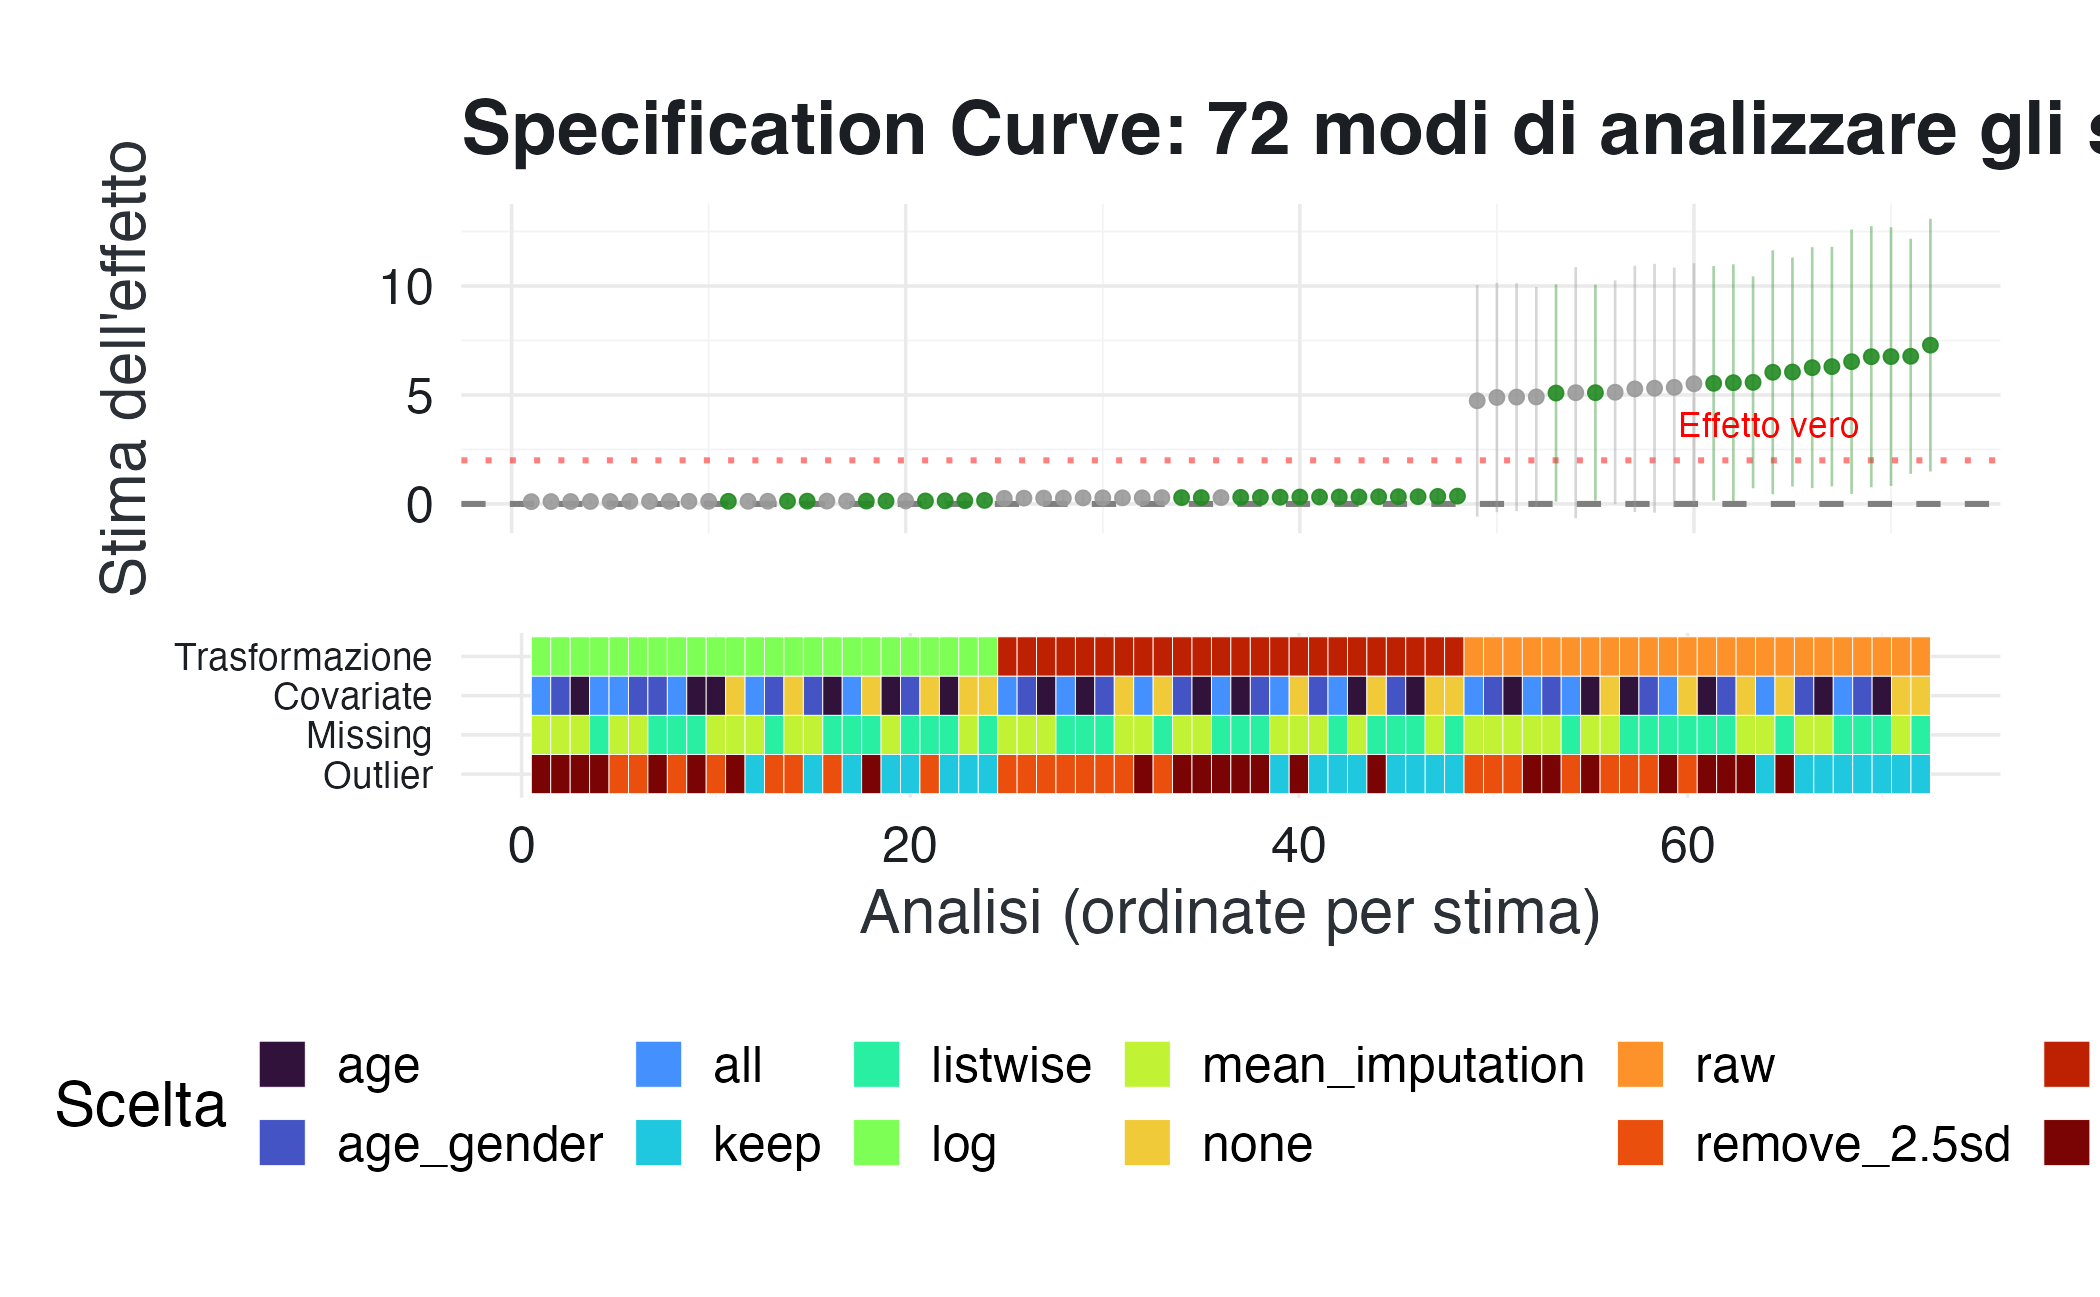
\includegraphics[width=0.85\linewidth,height=\textheight,keepaspectratio]{chapters/limits/05_degrees_of_freedom_files/figure-pdf/fig-specification-curve-1.png}

}

\caption{\label{fig-specification-curve}Curva di specificazione: ogni
punto rappresenta una delle 72 analisi possibili. La linea orizzontale
indica l'effetto nullo. Il pannello inferiore mostra quali scelte sono
state fatte per ogni analisi.}

\end{figure}%

\begin{Shaded}
\begin{Highlighting}[]
\FunctionTok{ggplot}\NormalTok{(multiverse\_results, }\FunctionTok{aes}\NormalTok{(}\AttributeTok{x =}\NormalTok{ estimate)) }\SpecialCharTok{+}
  \FunctionTok{geom\_histogram}\NormalTok{(}\AttributeTok{bins =} \DecValTok{20}\NormalTok{, }\AttributeTok{fill =} \StringTok{"steelblue"}\NormalTok{, }\AttributeTok{color =} \StringTok{"white"}\NormalTok{, }\AttributeTok{alpha =} \FloatTok{0.8}\NormalTok{) }\SpecialCharTok{+}
  \FunctionTok{geom\_vline}\NormalTok{(}\AttributeTok{xintercept =}\NormalTok{ TRUE\_EFFECT, }\AttributeTok{color =} \StringTok{"red"}\NormalTok{, }\AttributeTok{linetype =} \StringTok{"dashed"}\NormalTok{, }\AttributeTok{linewidth =} \FloatTok{1.2}\NormalTok{) }\SpecialCharTok{+}
  \FunctionTok{geom\_vline}\NormalTok{(}\AttributeTok{xintercept =} \DecValTok{0}\NormalTok{, }\AttributeTok{color =} \StringTok{"black"}\NormalTok{, }\AttributeTok{linetype =} \StringTok{"dotted"}\NormalTok{, }\AttributeTok{linewidth =} \DecValTok{1}\NormalTok{) }\SpecialCharTok{+}
  \FunctionTok{geom\_vline}\NormalTok{(}\AttributeTok{xintercept =} \FunctionTok{median}\NormalTok{(multiverse\_results}\SpecialCharTok{$}\NormalTok{estimate), }
             \AttributeTok{color =} \StringTok{"darkblue"}\NormalTok{, }\AttributeTok{linewidth =} \DecValTok{1}\NormalTok{) }\SpecialCharTok{+}
  \FunctionTok{annotate}\NormalTok{(}\StringTok{"text"}\NormalTok{, }\AttributeTok{x =}\NormalTok{ TRUE\_EFFECT, }\AttributeTok{y =} \ConstantTok{Inf}\NormalTok{, }\AttributeTok{vjust =} \DecValTok{2}\NormalTok{, }\AttributeTok{hjust =} \SpecialCharTok{{-}}\FloatTok{0.1}\NormalTok{,}
         \AttributeTok{label =} \FunctionTok{sprintf}\NormalTok{(}\StringTok{"Effetto vero = \%.1f"}\NormalTok{, TRUE\_EFFECT), }\AttributeTok{color =} \StringTok{"red"}\NormalTok{) }\SpecialCharTok{+}
  \FunctionTok{annotate}\NormalTok{(}\StringTok{"text"}\NormalTok{, }\AttributeTok{x =} \FunctionTok{median}\NormalTok{(multiverse\_results}\SpecialCharTok{$}\NormalTok{estimate), }\AttributeTok{y =} \ConstantTok{Inf}\NormalTok{, }\AttributeTok{vjust =} \DecValTok{4}\NormalTok{, }\AttributeTok{hjust =} \SpecialCharTok{{-}}\FloatTok{0.1}\NormalTok{,}
           \AttributeTok{label =} \FunctionTok{sprintf}\NormalTok{(}\StringTok{"Mediana = \%.2f"}\NormalTok{, }\FunctionTok{median}\NormalTok{(multiverse\_results}\SpecialCharTok{$}\NormalTok{estimate)), }
           \AttributeTok{color =} \StringTok{"darkblue"}\NormalTok{) }\SpecialCharTok{+}
  \FunctionTok{labs}\NormalTok{(}
    \AttributeTok{x =} \StringTok{"Stima dell\textquotesingle{}effetto (treatment vs control)"}\NormalTok{,}
    \AttributeTok{y =} \StringTok{"Numero di analisi"}\NormalTok{,}
    \AttributeTok{title =} \StringTok{"Distribuzione delle stime nel multiverse"}\NormalTok{,}
    \AttributeTok{subtitle =} \FunctionTok{sprintf}\NormalTok{(}\StringTok{"72 analisi: range [\%.2f, \%.2f]"}\NormalTok{, }
                      \FunctionTok{min}\NormalTok{(multiverse\_results}\SpecialCharTok{$}\NormalTok{estimate), }
                      \FunctionTok{max}\NormalTok{(multiverse\_results}\SpecialCharTok{$}\NormalTok{estimate))}
\NormalTok{  )}
\end{Highlighting}
\end{Shaded}

\begin{figure}[H]

\centering{

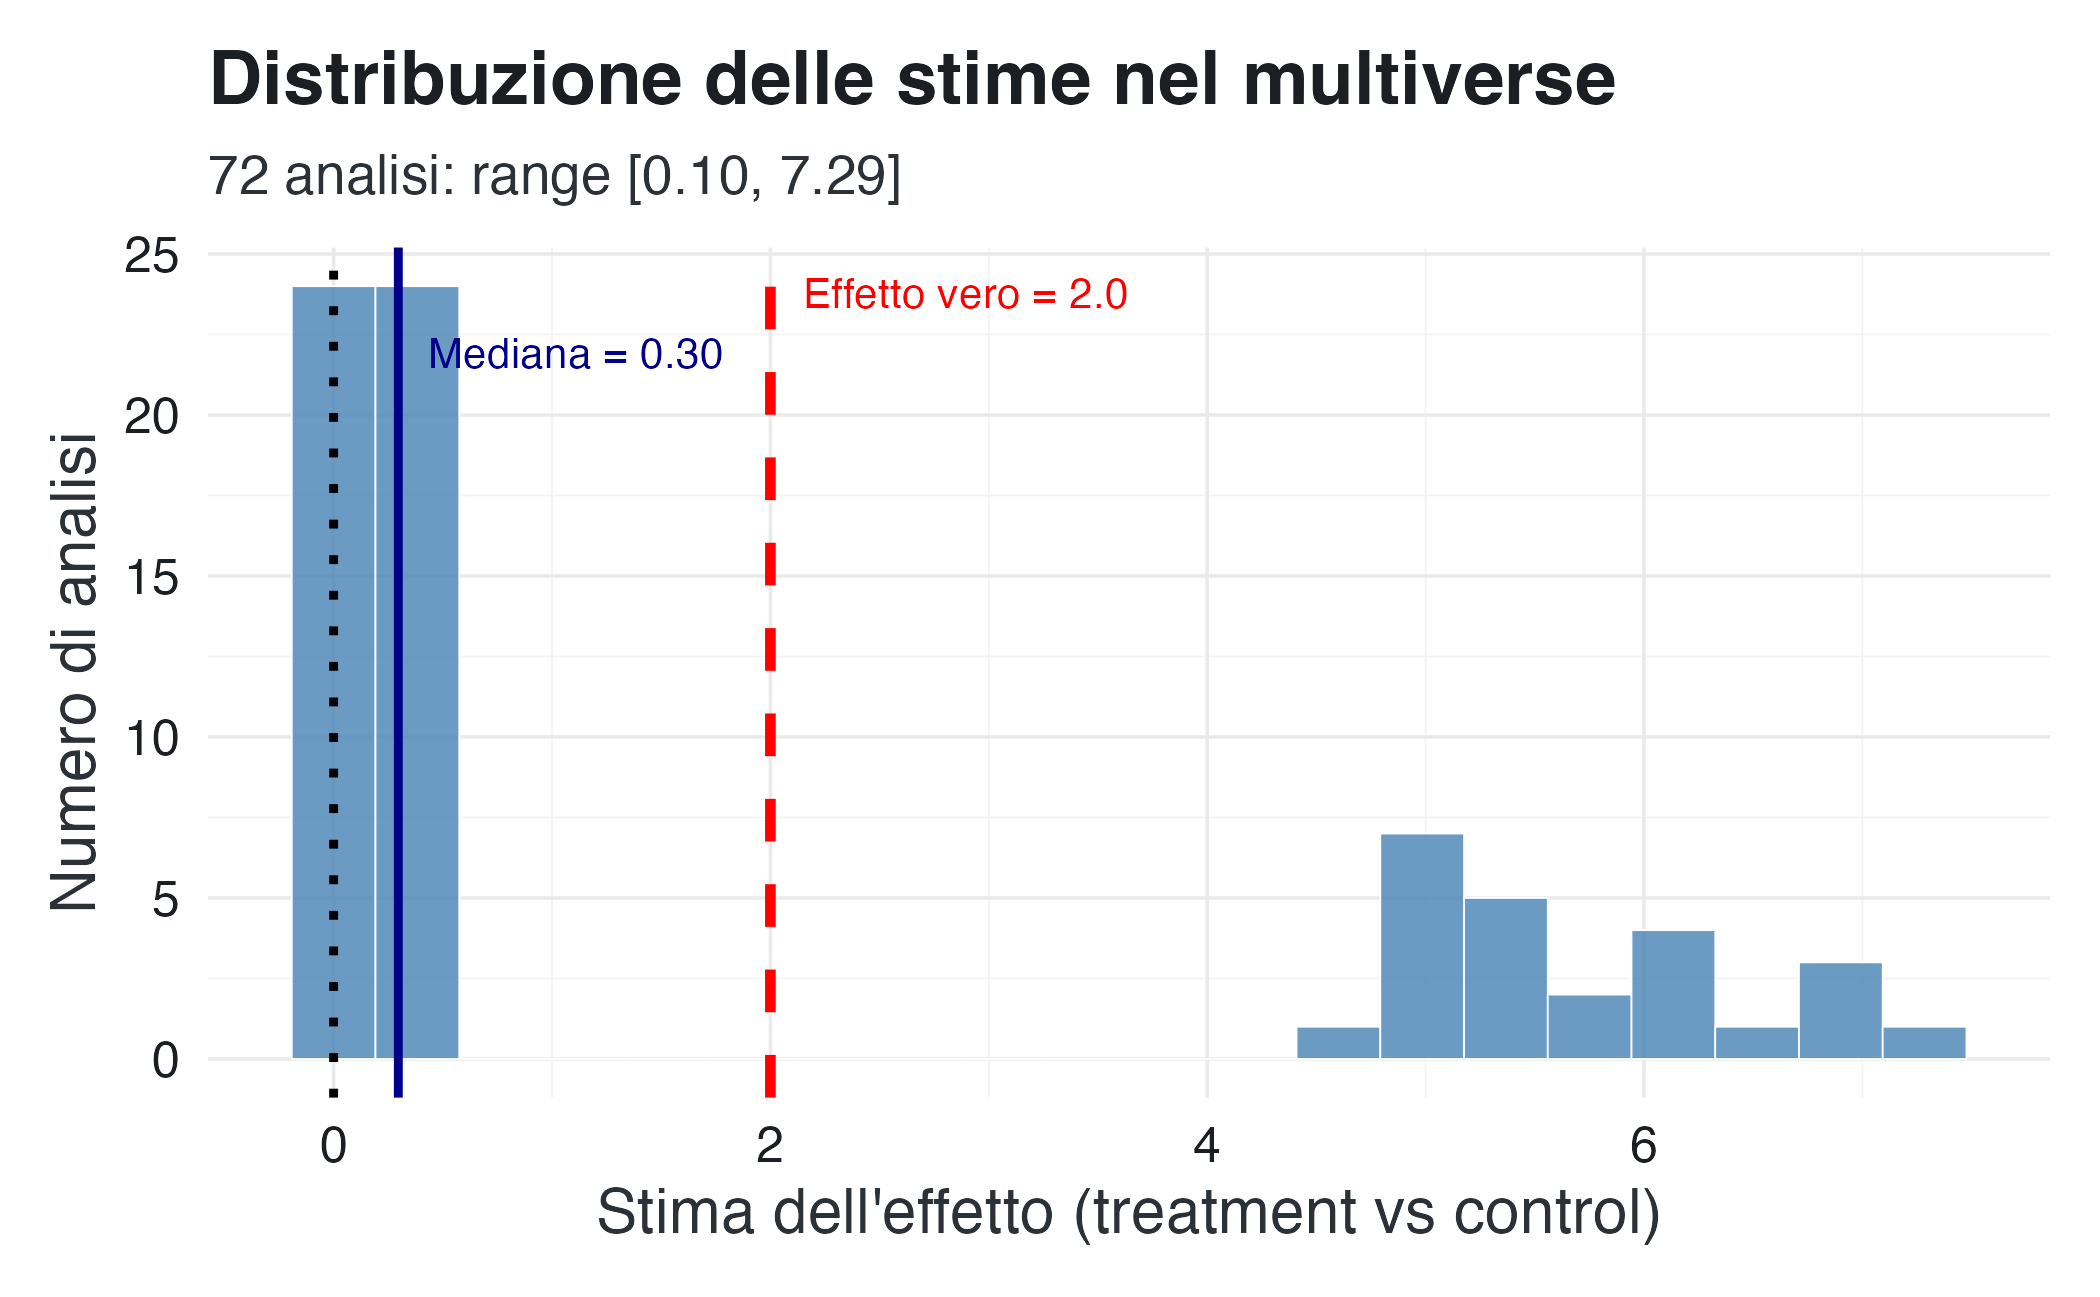
\includegraphics[width=0.85\linewidth,height=\textheight,keepaspectratio]{chapters/limits/05_degrees_of_freedom_files/figure-pdf/fig-estimate-distribution-1.png}

}

\caption{\label{fig-estimate-distribution}Distribuzione delle stime
attraverso il multiverse. La linea rossa tratteggiata indica l'effetto
vero (2.5 punti). La distribuzione delle stime varia considerevolmente a
seconda delle scelte analitiche adottate.}

\end{figure}%

\textbf{Quali scelte contano di più?}

Alcune decisioni analitiche hanno più impatto di altre. Analizziamo la
varianza spiegata da ciascuna scelta:

\begin{Shaded}
\begin{Highlighting}[]
\CommentTok{\# Calcola la varianza spiegata da ogni scelta}
\NormalTok{variance\_decomposition }\OtherTok{\textless{}{-}}\NormalTok{ multiverse\_results }\SpecialCharTok{|\textgreater{}}
  \FunctionTok{summarise}\NormalTok{(}
    \AttributeTok{total\_var =} \FunctionTok{var}\NormalTok{(estimate),}
    \AttributeTok{var\_outlier =} \FunctionTok{var}\NormalTok{(}\FunctionTok{tapply}\NormalTok{(estimate, outlier, mean)),}
    \AttributeTok{var\_missing =} \FunctionTok{var}\NormalTok{(}\FunctionTok{tapply}\NormalTok{(estimate, missing, mean)),}
    \AttributeTok{var\_covariates =} \FunctionTok{var}\NormalTok{(}\FunctionTok{tapply}\NormalTok{(estimate, covariates, mean)),}
    \AttributeTok{var\_transformation =} \FunctionTok{var}\NormalTok{(}\FunctionTok{tapply}\NormalTok{(estimate, transformation, mean))}
\NormalTok{  ) }\SpecialCharTok{|\textgreater{}}
  \FunctionTok{pivot\_longer}\NormalTok{(}\FunctionTok{everything}\NormalTok{(), }\AttributeTok{names\_to =} \StringTok{"source"}\NormalTok{, }\AttributeTok{values\_to =} \StringTok{"variance"}\NormalTok{) }\SpecialCharTok{|\textgreater{}}
\NormalTok{  dplyr}\SpecialCharTok{::}\FunctionTok{filter}\NormalTok{(source }\SpecialCharTok{!=} \StringTok{"total\_var"}\NormalTok{) }\SpecialCharTok{|\textgreater{}}
  \FunctionTok{mutate}\NormalTok{(}
    \AttributeTok{source =} \FunctionTok{str\_remove}\NormalTok{(source, }\StringTok{"var\_"}\NormalTok{),}
    \AttributeTok{source =} \FunctionTok{factor}\NormalTok{(source, }
                   \AttributeTok{levels =} \FunctionTok{c}\NormalTok{(}\StringTok{"outlier"}\NormalTok{, }\StringTok{"missing"}\NormalTok{, }\StringTok{"covariates"}\NormalTok{, }\StringTok{"transformation"}\NormalTok{),}
                   \AttributeTok{labels =} \FunctionTok{c}\NormalTok{(}\StringTok{"Gestione outlier"}\NormalTok{, }\StringTok{"Gestione missing"}\NormalTok{, }
                             \StringTok{"Scelta covariate"}\NormalTok{, }\StringTok{"Trasformazione"}\NormalTok{)),}
    \AttributeTok{pct =}\NormalTok{ variance }\SpecialCharTok{/} \FunctionTok{sum}\NormalTok{(variance) }\SpecialCharTok{*} \DecValTok{100}
\NormalTok{  )}

\FunctionTok{ggplot}\NormalTok{(variance\_decomposition, }\FunctionTok{aes}\NormalTok{(}\AttributeTok{x =} \FunctionTok{reorder}\NormalTok{(source, pct), }\AttributeTok{y =}\NormalTok{ pct)) }\SpecialCharTok{+}
  \FunctionTok{geom\_col}\NormalTok{(}\AttributeTok{fill =} \StringTok{"steelblue"}\NormalTok{, }\AttributeTok{alpha =} \FloatTok{0.8}\NormalTok{) }\SpecialCharTok{+}
  \FunctionTok{geom\_text}\NormalTok{(}\FunctionTok{aes}\NormalTok{(}\AttributeTok{label =} \FunctionTok{sprintf}\NormalTok{(}\StringTok{"\%.0f\%\%"}\NormalTok{, pct)), }\AttributeTok{hjust =} \SpecialCharTok{{-}}\FloatTok{0.2}\NormalTok{) }\SpecialCharTok{+}
  \FunctionTok{coord\_flip}\NormalTok{() }\SpecialCharTok{+}
  \FunctionTok{labs}\NormalTok{(}
    \AttributeTok{x =} \StringTok{""}\NormalTok{,}
    \AttributeTok{y =} \StringTok{"\% varianza nelle stime"}\NormalTok{,}
    \AttributeTok{title =} \StringTok{"Quale scelta analitica conta di più?"}\NormalTok{,}
    \AttributeTok{subtitle =} \StringTok{"Decomposizione della variabilità nel multiverse"}
\NormalTok{  ) }\SpecialCharTok{+}
  \FunctionTok{scale\_y\_continuous}\NormalTok{(}\AttributeTok{limits =} \FunctionTok{c}\NormalTok{(}\DecValTok{0}\NormalTok{, }\FunctionTok{max}\NormalTok{(variance\_decomposition}\SpecialCharTok{$}\NormalTok{pct) }\SpecialCharTok{*} \FloatTok{1.2}\NormalTok{))}
\end{Highlighting}
\end{Shaded}

\begin{figure}[H]

\centering{

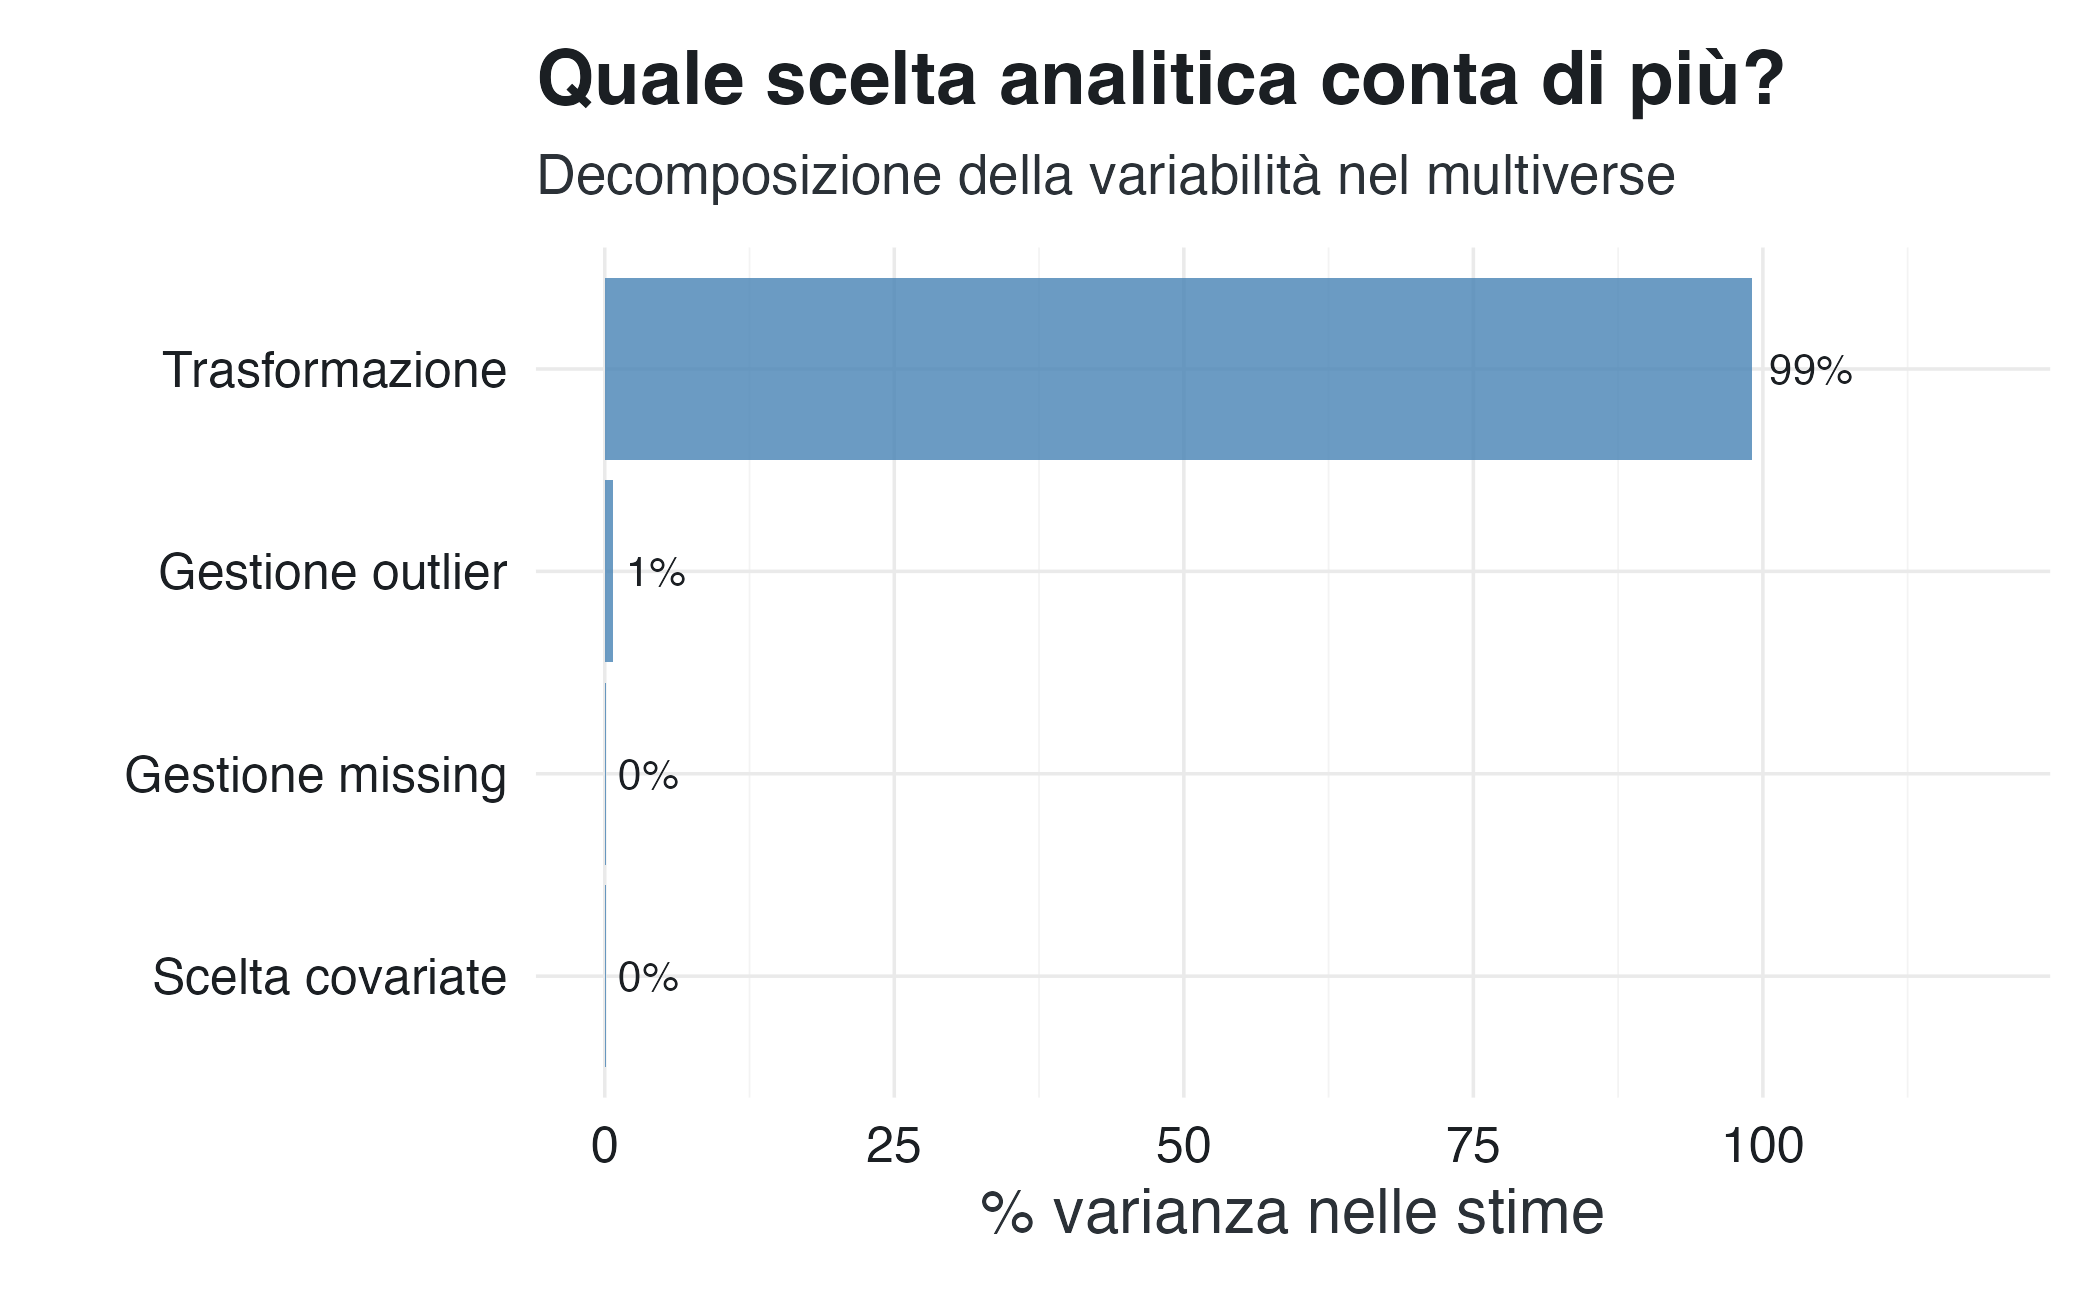
\includegraphics[width=0.85\linewidth,height=\textheight,keepaspectratio]{chapters/limits/05_degrees_of_freedom_files/figure-pdf/fig-choice-impact-1.png}

}

\caption{\label{fig-choice-impact}Impatto di ciascuna scelta analitica
sulla variabilità delle stime. La gestione degli outlier e la
trasformazione hanno l'impatto maggiore.}

\end{figure}%

\begin{Shaded}
\begin{Highlighting}[]
\CommentTok{\# Tabella dettagliata per scelta}
\NormalTok{multiverse\_results }\SpecialCharTok{|\textgreater{}}
  \FunctionTok{group\_by}\NormalTok{(outlier) }\SpecialCharTok{|\textgreater{}}
  \FunctionTok{summarise}\NormalTok{(}
    \StringTok{\textasciigrave{}}\AttributeTok{Media stima}\StringTok{\textasciigrave{}} \OtherTok{=} \FunctionTok{sprintf}\NormalTok{(}\StringTok{"\%.2f"}\NormalTok{, }\FunctionTok{mean}\NormalTok{(estimate)),}
    \StringTok{\textasciigrave{}}\AttributeTok{SD stima}\StringTok{\textasciigrave{}} \OtherTok{=} \FunctionTok{sprintf}\NormalTok{(}\StringTok{"\%.2f"}\NormalTok{, }\FunctionTok{sd}\NormalTok{(estimate)),}
    \StringTok{\textasciigrave{}}\AttributeTok{\% significativi}\StringTok{\textasciigrave{}} \OtherTok{=} \FunctionTok{sprintf}\NormalTok{(}\StringTok{"\%.0f\%\%"}\NormalTok{, }\DecValTok{100} \SpecialCharTok{*} \FunctionTok{mean}\NormalTok{(significant)),}
    \AttributeTok{.groups =} \StringTok{"drop"}
\NormalTok{  ) }\SpecialCharTok{|\textgreater{}}
  \FunctionTok{rename}\NormalTok{(}\StringTok{\textasciigrave{}}\AttributeTok{Gestione outlier}\StringTok{\textasciigrave{}} \OtherTok{=}\NormalTok{ outlier) }\SpecialCharTok{|\textgreater{}}
\NormalTok{  knitr}\SpecialCharTok{::}\FunctionTok{kable}\NormalTok{(}\AttributeTok{caption =} \StringTok{"Effetto della gestione degli outlier"}\NormalTok{)}
\end{Highlighting}
\end{Shaded}

\begin{longtable}[]{@{}llll@{}}
\caption{Effetto della gestione degli outlier}\tabularnewline
\toprule\noalign{}
Gestione outlier & Media stima & SD stima & \% significativi \\
\midrule\noalign{}
\endfirsthead
\toprule\noalign{}
Gestione outlier & Media stima & SD stima & \% significativi \\
\midrule\noalign{}
\endhead
\bottomrule\noalign{}
\endlastfoot
keep & 2.35 & 3.07 & 88\% \\
remove\_2.5sd & 1.83 & 2.37 & 8\% \\
winsorize & 1.94 & 2.51 & 58\% \\
\end{longtable}

\textbf{Scenario ``Molti analisti''.}

Simuliamo ora la variabilità che emergerebbe se 50 ricercatori
indipendenti analizzassero lo stesso dataset, ciascuno adottando scelte
metodologiche diverse ma tutte plausibili e giustificabili.

\begin{Shaded}
\begin{Highlighting}[]
\FunctionTok{set.seed}\NormalTok{(}\DecValTok{123}\NormalTok{)}
\CommentTok{\# Simula 50 ricercatori con scelte casuali (ma pesate verso opzioni comuni)}
\NormalTok{n\_researchers }\OtherTok{\textless{}{-}} \DecValTok{50}

\FunctionTok{set.seed}\NormalTok{(}\DecValTok{123}\NormalTok{)}
\CommentTok{\# Simula 50 ricercatori con scelte casuali}
\NormalTok{n\_researchers }\OtherTok{\textless{}{-}} \DecValTok{50}

\NormalTok{researcher\_results }\OtherTok{\textless{}{-}} \FunctionTok{tibble}\NormalTok{(}\AttributeTok{researcher\_id =} \DecValTok{1}\SpecialCharTok{:}\NormalTok{n\_researchers) }\SpecialCharTok{|\textgreater{}}
  \FunctionTok{rowwise}\NormalTok{() }\SpecialCharTok{|\textgreater{}}
  \FunctionTok{mutate}\NormalTok{(}
    \CommentTok{\# MODIFICA: probabilità più equilibrate per ottenere più varietà}
    \AttributeTok{outlier =} \FunctionTok{sample}\NormalTok{(}\FunctionTok{c}\NormalTok{(}\StringTok{"keep"}\NormalTok{, }\StringTok{"remove\_2.5sd"}\NormalTok{, }\StringTok{"winsorize"}\NormalTok{), }\DecValTok{1}\NormalTok{,  }
                \AttributeTok{prob =} \FunctionTok{c}\NormalTok{(}\FloatTok{0.4}\NormalTok{, }\FloatTok{0.3}\NormalTok{, }\FloatTok{0.3}\NormalTok{)),}
    \AttributeTok{missing =} \FunctionTok{sample}\NormalTok{(}\FunctionTok{c}\NormalTok{(}\StringTok{"listwise"}\NormalTok{, }\StringTok{"mean\_imputation"}\NormalTok{), }\DecValTok{1}\NormalTok{, }
                    \AttributeTok{prob =} \FunctionTok{c}\NormalTok{(}\FloatTok{0.5}\NormalTok{, }\FloatTok{0.5}\NormalTok{)),}
    \AttributeTok{covariates =} \FunctionTok{sample}\NormalTok{(}\FunctionTok{c}\NormalTok{(}\StringTok{"none"}\NormalTok{, }\StringTok{"age"}\NormalTok{, }\StringTok{"age\_gender"}\NormalTok{, }\StringTok{"all"}\NormalTok{), }\DecValTok{1}\NormalTok{,}
                       \AttributeTok{prob =} \FunctionTok{c}\NormalTok{(}\FloatTok{0.25}\NormalTok{, }\FloatTok{0.25}\NormalTok{, }\FloatTok{0.25}\NormalTok{, }\FloatTok{0.25}\NormalTok{)),}
    \AttributeTok{transformation =} \FunctionTok{sample}\NormalTok{(}\FunctionTok{c}\NormalTok{(}\StringTok{"raw"}\NormalTok{, }\StringTok{"log"}\NormalTok{, }\StringTok{"standardized"}\NormalTok{), }\DecValTok{1}\NormalTok{,}
                           \AttributeTok{prob =} \FunctionTok{c}\NormalTok{(}\FloatTok{0.34}\NormalTok{, }\FloatTok{0.33}\NormalTok{, }\FloatTok{0.33}\NormalTok{)),}
    
    \CommentTok{\# Esegui l\textquotesingle{}analisi}
    \AttributeTok{prepared\_data =} \FunctionTok{list}\NormalTok{(}\FunctionTok{prepare\_data}\NormalTok{(dataset, outlier, missing, transformation)),}
    \AttributeTok{results =} \FunctionTok{list}\NormalTok{(}\FunctionTok{run\_analysis}\NormalTok{(prepared\_data, covariates))}
\NormalTok{  ) }\SpecialCharTok{|\textgreater{}}
  \FunctionTok{unnest}\NormalTok{(results) }\SpecialCharTok{|\textgreater{}}
  \FunctionTok{ungroup}\NormalTok{() }\SpecialCharTok{|\textgreater{}}
  \FunctionTok{mutate}\NormalTok{(}
    \AttributeTok{significant =}\NormalTok{ p\_value }\SpecialCharTok{\textless{}} \FloatTok{0.05}\NormalTok{,}
    \AttributeTok{conclusion =} \FunctionTok{case\_when}\NormalTok{(}
\NormalTok{      p\_value }\SpecialCharTok{\textless{}} \FloatTok{0.05} \SpecialCharTok{\&}\NormalTok{ estimate }\SpecialCharTok{\textgreater{}} \DecValTok{0} \SpecialCharTok{\textasciitilde{}} \StringTok{"Effetto positivo significativo"}\NormalTok{,}
\NormalTok{      p\_value }\SpecialCharTok{\textless{}} \FloatTok{0.05} \SpecialCharTok{\&}\NormalTok{ estimate }\SpecialCharTok{\textless{}} \DecValTok{0} \SpecialCharTok{\textasciitilde{}} \StringTok{"Effetto negativo significativo"}\NormalTok{,}
      \ConstantTok{TRUE} \SpecialCharTok{\textasciitilde{}} \StringTok{"Non significativo"}
\NormalTok{    )}
\NormalTok{  )}

\CommentTok{\# Visualizzazione stile Gould et al.}
\FunctionTok{ggplot}\NormalTok{(researcher\_results, }\FunctionTok{aes}\NormalTok{(}\AttributeTok{x =} \FunctionTok{reorder}\NormalTok{(researcher\_id, estimate), }\AttributeTok{y =}\NormalTok{ estimate)) }\SpecialCharTok{+}
  \FunctionTok{geom\_hline}\NormalTok{(}\AttributeTok{yintercept =} \DecValTok{0}\NormalTok{, }\AttributeTok{linetype =} \StringTok{"dashed"}\NormalTok{, }\AttributeTok{color =} \StringTok{"gray50"}\NormalTok{) }\SpecialCharTok{+}
  \FunctionTok{geom\_hline}\NormalTok{(}\AttributeTok{yintercept =}\NormalTok{ TRUE\_EFFECT, }\AttributeTok{linetype =} \StringTok{"dashed"}\NormalTok{, }\AttributeTok{color =} \StringTok{"red"}\NormalTok{, }\AttributeTok{alpha =} \FloatTok{0.7}\NormalTok{) }\SpecialCharTok{+}
  \FunctionTok{geom\_linerange}\NormalTok{(}\FunctionTok{aes}\NormalTok{(}\AttributeTok{ymin =}\NormalTok{ conf\_low, }\AttributeTok{ymax =}\NormalTok{ conf\_high), }\AttributeTok{color =} \StringTok{"gray60"}\NormalTok{, }\AttributeTok{alpha =} \FloatTok{0.5}\NormalTok{) }\SpecialCharTok{+}
  \FunctionTok{geom\_point}\NormalTok{(}\FunctionTok{aes}\NormalTok{(}\AttributeTok{color =}\NormalTok{ conclusion), }\AttributeTok{size =} \DecValTok{3}\NormalTok{) }\SpecialCharTok{+}
  \FunctionTok{scale\_color\_manual}\NormalTok{(}\AttributeTok{values =} \FunctionTok{c}\NormalTok{(}
    \StringTok{"Effetto positivo significativo"} \OtherTok{=} \StringTok{"forestgreen"}\NormalTok{,}
    \StringTok{"Non significativo"} \OtherTok{=} \StringTok{"gray50"}\NormalTok{,}
    \StringTok{"Effetto negativo significativo"} \OtherTok{=} \StringTok{"coral"}
\NormalTok{  )) }\SpecialCharTok{+}
  \FunctionTok{annotate}\NormalTok{(}\StringTok{"text"}\NormalTok{, }\AttributeTok{x =}\NormalTok{ n\_researchers }\SpecialCharTok{*} \FloatTok{0.9}\NormalTok{, }\AttributeTok{y =} \FloatTok{2.5}\NormalTok{, }\AttributeTok{label =} \StringTok{"Effetto vero"}\NormalTok{,}
           \AttributeTok{color =} \StringTok{"red"}\NormalTok{, }\AttributeTok{vjust =} \SpecialCharTok{{-}}\DecValTok{1}\NormalTok{) }\SpecialCharTok{+}
  \FunctionTok{labs}\NormalTok{(}
    \AttributeTok{x =} \StringTok{"Ricercatore (ordinato per stima)"}\NormalTok{,}
    \AttributeTok{y =} \StringTok{"Stima dell\textquotesingle{}effetto"}\NormalTok{,}
    \AttributeTok{color =} \StringTok{"Conclusione"}\NormalTok{,}
    \AttributeTok{title =} \StringTok{"50 ricercatori, 50 risultati diversi"}\NormalTok{,}
    \AttributeTok{subtitle =} \FunctionTok{sprintf}\NormalTok{(}\StringTok{"Stessi dati, stessa domanda, range stime: [\%.2f, \%.2f]"}\NormalTok{,}
                      \FunctionTok{min}\NormalTok{(researcher\_results}\SpecialCharTok{$}\NormalTok{estimate), }\FunctionTok{max}\NormalTok{(researcher\_results}\SpecialCharTok{$}\NormalTok{estimate))}
\NormalTok{  ) }\SpecialCharTok{+}
  \FunctionTok{theme}\NormalTok{(}
    \AttributeTok{axis.text.x =} \FunctionTok{element\_blank}\NormalTok{(),}
    \AttributeTok{axis.ticks.x =} \FunctionTok{element\_blank}\NormalTok{(),}
    \AttributeTok{legend.position =} \StringTok{"bottom"}
\NormalTok{  )}

\CommentTok{\# Statistiche}
\NormalTok{conclusion\_stats }\OtherTok{\textless{}{-}}\NormalTok{ researcher\_results }\SpecialCharTok{|\textgreater{}}
\NormalTok{  dplyr}\SpecialCharTok{::}\FunctionTok{count}\NormalTok{(conclusion) }\SpecialCharTok{|\textgreater{}}
  \FunctionTok{mutate}\NormalTok{(}\AttributeTok{pct =}\NormalTok{ n }\SpecialCharTok{/} \FunctionTok{sum}\NormalTok{(n) }\SpecialCharTok{*} \DecValTok{100}\NormalTok{)}
\end{Highlighting}
\end{Shaded}

\begin{figure}[H]

\centering{

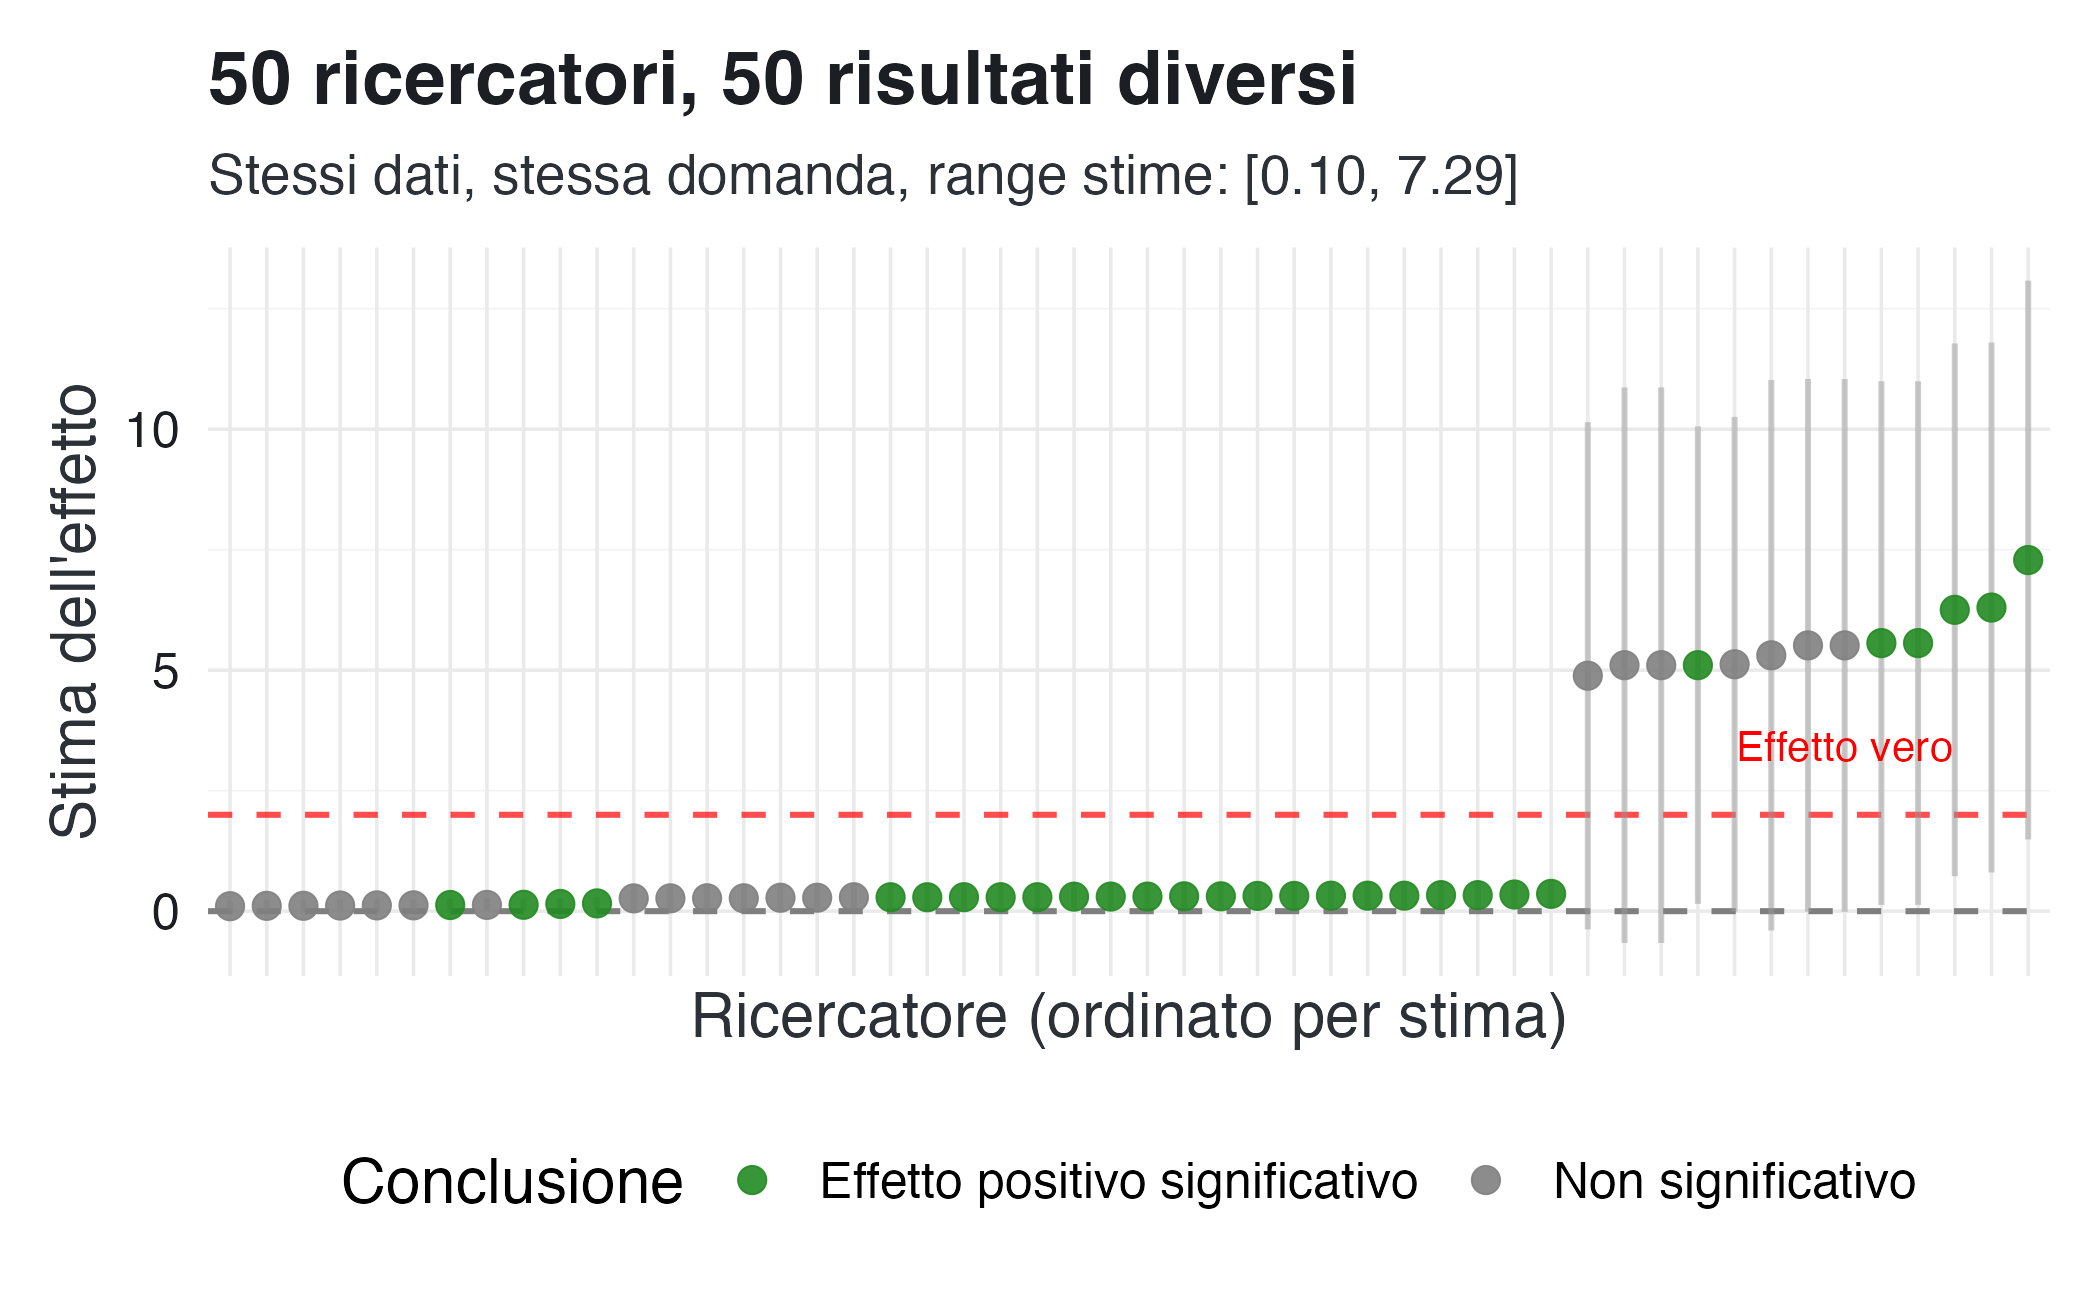
\includegraphics[width=0.85\linewidth,height=\textheight,keepaspectratio]{chapters/limits/05_degrees_of_freedom_files/figure-pdf/fig-many-analysts-1.png}

}

\caption{\label{fig-many-analysts}Simulazione di 50 ricercatori
indipendenti che analizzano gli stessi dati. Ogni ricercatore fa scelte
ragionevoli ma diverse.}

\end{figure}%

\begin{verbatim}
#> Effetto positivo significativo: 29 (58%)
#> Non significativo: 21 (42%)
\end{verbatim}

Se consideriamo le scelte analitiche effettuate da 50 ``ricercatori
virtuali'', ognuno con combinazioni diverse ma plausibili di scelte
metodologiche, notiamo che i risultati mostrano una marcata variabilità:
solo il 58\% di essi ottiene stime statisticamente significative (\(p\)
\textless{} 0.05).

\section{Strategie di mitigazione}\label{sec-mitigation}

La simulazione presentata in questo capitolo riproduce, su scala
ridotta, quanto documentato da {Gould et al.}
(\citeproc{ref-gould2025same}{2025}) con dati reali in un ambizioso
progetto di analisi collaborativa. Nel loro studio, 174 team di ricerca
indipendenti hanno ricevuto gli stessi dataset e la stessa domanda di
ricerca. Il risultato è stato sorprendente per la sua eterogeneità: le
stime degli effetti variavano da fortemente negative a positive, con
conclusioni statistiche diametralmente opposte tra i vari gruppi. Questa
variabilità non era dovuta a incompetenza o errori, ma alla naturale
conseguenza di scelte analitiche tutte ragionevoli e metodologicamente
difendibili.

La nostra simulazione, pur operando su scala molto più ridotta con 72
combinazioni analitiche, cattura la stessa dinamica fondamentale.
Partendo da un effetto vero di 2.5 punti, le stime ottenute vanno da
valori che sottostimano l'effetto reale a valori che lo sovrastimano.
Alcune analisi portano a conclusioni statisticamente significative,
altre no, il tutto come conseguenza di decisioni apparentemente
tecniche, quali il trattamento dei valori anomali, la gestione dei dati
mancanti, l'inclusione di variabili indipendenti e la trasformazione
delle variabili.

Di fronte a questa fragilità intrinseca del processo analitico, la
comunità scientifica ha sviluppato diverse strategie di mitigazione. La
pre-registrazione è forse l'approccio più diffuso: fissando le scelte
analitiche prima di osservare i dati, si elimina la possibilità di
selezionare, a posteriori, l'analisi che produce i risultati più
favorevoli. Tuttavia, la pre-registrazione presenta importanti limiti.
Non garantisce che le scelte pre-specificate siano le migliori possibili
e la ricerca spesso rivela complessità impreviste che richiedono di
deviare dal piano originale. Inoltre, come mostrano i dati di {Gould et
al.} (\citeproc{ref-gould2025same}{2025}), anche i ricercatori che
operano in buona fede e con piani ben definiti possono giungere a
conclusioni sostanzialmente diverse.

Un'alternativa complementare è la trasparenza attraverso l'analisi
multiverse. Invece di presentare un singolo risultato come se fosse
l'unica verità possibile, il ricercatore può esplorare sistematicamente
lo spazio delle decisioni analitiche e riportare l'intera distribuzione
delle conclusioni possibili. Questo approccio ha il vantaggio di rendere
esplicita l'incertezza metodologica, ovvero quella componente di
variabilità che non deriva dal campionamento statistico, ma dalle scelte
del ricercatore. Quando un lettore vede che il 60\% delle analisi
ragionevoli produce risultati significativi, mentre il 40\% no,
acquisisce una comprensione molto più sfumata della robustezza
dell'evidenza rispetto a quando legge un singolo valore-\(p\).

Lo studio di {Gould et al.} (\citeproc{ref-gould2025same}{2025}) ha
rivelato altri aspetti preoccupanti. Né la complessità delle analisi né
il processo di revisione tra pari interno ai team hanno mostrato una
correlazione con l'accuratezza delle stime. La variabilità osservata tra
gli analisti superava quella attribuibile esclusivamente all'errore di
campionamento, suggerendo che la componente umana del processo analitico
introduce una fonte di incertezza sistematicamente sottovalutata nella
pratica scientifica corrente. Ciò non significa che il metodo
scientifico sia inaffidabile, ma piuttosto che dovremmo essere più umili
riguardo alla precisione delle nostre conclusioni e più trasparenti
riguardo alle scelte che le hanno generate.

Le implicazioni pratiche di queste osservazioni sono profonde. Per i
ricercatori, suggeriscono l'importanza di esplorare la sensibilità dei
risultati derivanti da scelte analitiche alternative, anche quando
esiste un piano pre-registrato. Per i lettori della letteratura
scientifica, queste implicazioni suggeriscono un atteggiamento critico
nei confronti dei risultati presentati come definitivi senza alcuna
discussione sulla loro robustezza. Per la comunità scientifica nel suo
insieme, indicano la necessità di sviluppare standard di reportistica
che includano informazioni sulla variabilità dei risultati derivante
dalle scelte metodologiche dei ricercatori, non solo su quella
statistica.

\section{Riflessioni conclusive}\label{sec-conclusions}

Le simulazioni e le evidenze empiriche presentate in questo capitolo
convergono su una conclusione importante, ma spesso trascurata: lo
spazio delle analisi possibili per qualsiasi dataset è vasto e le scelte
metodologiche ragionevoli possono condurre a conclusioni divergenti.
Questo non è un difetto del metodo scientifico, ma una sua
caratteristica intrinseca che emerge ogni volta che i dati richiedono
un'interpretazione e le procedure non sono completamente automatizzate.

La lezione fondamentale non è che la ricerca empirica sia inaffidabile,
ma che la sua affidabilità dipende crucialmente dalla trasparenza con
cui il processo analitico viene documentato e comunicato. Quando
leggiamo uno studio che riporta un valore p appena sotto la soglia di
significatività, dovremmo chiederci quante altre analisi ragionevoli
avrebbero potuto essere condotte e quante di queste avrebbero potuto
condurre a conclusioni diverse. La risposta, come mostrano le nostre
simulazioni e lo studio di {Gould et al.}
(\citeproc{ref-gould2025same}{2025}), è quasi sempre ``molte''.

\begin{tcolorbox}[enhanced jigsaw, arc=.35mm, bottomrule=.15mm, bottomtitle=1mm, breakable, colback=white, colbacktitle=quarto-callout-warning-color!10!white, colframe=quarto-callout-warning-color-frame, coltitle=black, left=2mm, leftrule=.75mm, opacityback=0, opacitybacktitle=0.6, rightrule=.15mm, title=\textcolor{quarto-callout-warning-color}{\faExclamationTriangle}\hspace{0.5em}{Implicazione per la lettura critica}, titlerule=0mm, toprule=.15mm, toptitle=1mm]

Quando leggete uno studio che riporta \(p = 0.03\), chiedetevi: ``Quante
altre analisi ragionevoli avrebbero potuto essere fatte? Quante
avrebbero dato \(p > 0.05\)?'' La risposta è quasi sempre: molte.

\end{tcolorbox}

Alcune scelte analitiche hanno un impatto maggiore di altre. Nella
nostra simulazione, la gestione dei valori anomali e la scelta delle
covariate hanno mostrato l'impatto maggiore sulla variabilità delle
stime. Ciò suggerisce che è necessario dedicare particolare attenzione
alla giustificazione di queste decisioni cruciali e, possibilmente,
esplorare alternative.

La pre-registrazione offre una protezione parziale, ma importante,
contro l'esplorazione opportunistica dello spazio analitico. Fissare le
scelte prima di vedere i dati elimina la tentazione di selezionare, a
posteriori, l'analisi che produce i risultati desiderati. Tuttavia, la
pre-registrazione non garantisce che la scelta pre-specificata sia
quella corretta né elimina la legittima variabilità che emergerebbe se
diversi ricercatori pre-registrassero piani diversi.

L'approccio multiverse rappresenta un complemento prezioso, in quanto
permette di quantificare esplicitamente l'incertezza metodologica e di
comunicare ai lettori non solo i risultati ottenuti, ma anche la
robustezza di tali risultati rispetto a scelte alternative. In un'epoca
in cui la riproducibilità della ricerca è sotto scrutinio, la
trasparenza diventa un valore scientifico fondamentale.

La sfida per la psicologia e per le scienze empiriche in generale non è
eliminare i gradi di libertà del ricercatore, cosa impossibile data la
complessità intrinseca dei fenomeni studiati, ma piuttosto rendere
queste scelte visibili, giustificabili e sottoponibili al controllo
della comunità scientifica. Solo in questo modo sarà possibile
distinguere i risultati robusti, che resistono a molteplici analisi
specifiche, da quelli fragili, che dipendono criticamente da decisioni
arbitrarie.

\section{Esercizi}\label{sec-esercizi}

\begin{tcolorbox}[enhanced jigsaw, arc=.35mm, bottomrule=.15mm, bottomtitle=1mm, breakable, colback=white, colbacktitle=quarto-callout-important-color!10!white, colframe=quarto-callout-important-color-frame, coltitle=black, left=2mm, leftrule=.75mm, opacityback=0, opacitybacktitle=0.6, rightrule=.15mm, title=\textcolor{quarto-callout-important-color}{\faExclamation}\hspace{0.5em}{Esercizio 1: Interpretare un multiverse}, titlerule=0mm, toprule=.15mm, toptitle=1mm]

Uno studio sulla relazione tra uso dei social media e benessere
psicologico negli adolescenti riporta i seguenti risultati di un'analisi
multiverse con 48 specifiche analitiche diverse:

\begin{itemize}
\tightlist
\item
  Range delle stime: da r = −0.15 a r = +0.08
\item
  Mediana delle stime: r = −0.04
\item
  Percentuale di analisi con p \textless{} 0.05: 35\%
\item
  Percentuale di analisi con effetto negativo: 73\%
\end{itemize}

Gli autori concludono: ``I risultati dimostrano un effetto negativo
significativo dei social media sul benessere adolescenziale.''

Rispondete alle seguenti domande:

\begin{enumerate}
\def\labelenumi{\alph{enumi})}
\item
  La conclusione degli autori è giustificata dai dati del multiverse?
  Argomentate la vostra risposta.
\item
  Quali informazioni aggiuntive vorreste avere per valutare meglio la
  robustezza di questo risultato?
\item
  Come riformulereste la conclusione per renderla più coerente con i
  risultati del multiverse?
\end{enumerate}

\end{tcolorbox}

\begin{tcolorbox}[enhanced jigsaw, arc=.35mm, bottomrule=.15mm, bottomtitle=1mm, breakable, colback=white, colbacktitle=quarto-callout-tip-color!10!white, colframe=quarto-callout-tip-color-frame, coltitle=black, left=2mm, leftrule=.75mm, opacityback=0, opacitybacktitle=0.6, rightrule=.15mm, title=\textcolor{quarto-callout-tip-color}{\faLightbulb}\hspace{0.5em}{Soluzione Esercizio 1}, titlerule=0mm, toprule=.15mm, toptitle=1mm]

\begin{enumerate}
\def\labelenumi{\alph{enumi})}
\item
  La conclusione degli autori non è pienamente giustificata. Sebbene la
  maggioranza delle analisi (73\%) mostri un effetto negativo, solo il
  35\% raggiunge la significatività statistica. Inoltre, il range delle
  stime include valori positivi (fino a r = +0.08), indicando che alcune
  specifiche analitiche ragionevoli portano a conclusioni opposte. La
  mediana di r = −0.04 suggerisce un effetto molto piccolo,
  probabilmente di scarsa rilevanza pratica. Affermare un ``effetto
  negativo significativo'' è una semplificazione eccessiva che ignora la
  considerevole incertezza metodologica evidenziata dal multiverse.
\item
  Sarebbe utile conoscere: quali scelte analitiche producono gli effetti
  più estremi (positivi vs negativi); se esiste una giustificazione
  teorica per preferire alcune specifiche ad altre; la distribuzione
  completa delle stime, non solo il range e la mediana; quali
  combinazioni di scelte portano alla significatività e quali no; e se i
  risultati cambiano per sottogruppi demografici diversi.
\item
  Una conclusione più appropriata potrebbe essere: ``L'analisi
  multiverse suggerisce una possibile associazione negativa di piccola
  entità tra uso dei social media e benessere adolescenziale (mediana r
  = −0.04), ma questo risultato mostra considerevole sensibilità alle
  scelte analitiche. Mentre la maggioranza delle specifiche indica
  un'associazione negativa, solo un terzo raggiunge la significatività
  statistica, e alcune analisi plausibili suggeriscono effetti nulli o
  leggermente positivi. Questi risultati evidenziano l'importanza di non
  sovrastimare la certezza delle conclusioni in questo ambito di
  ricerca.''
\end{enumerate}

\end{tcolorbox}

\begin{tcolorbox}[enhanced jigsaw, arc=.35mm, bottomrule=.15mm, bottomtitle=1mm, breakable, colback=white, colbacktitle=quarto-callout-important-color!10!white, colframe=quarto-callout-important-color-frame, coltitle=black, left=2mm, leftrule=.75mm, opacityback=0, opacitybacktitle=0.6, rightrule=.15mm, title=\textcolor{quarto-callout-important-color}{\faExclamation}\hspace{0.5em}{Esercizio 2: Pre-registrazione e gradi di libertà}, titlerule=0mm, toprule=.15mm, toptitle=1mm]

Due gruppi di ricerca studiano indipendentemente l'efficacia di un nuovo
intervento di mindfulness sull'ansia. Entrambi i gruppi pre-registrano
il loro piano di analisi prima di raccogliere i dati.

\textbf{Gruppo A} pre-registra:

\begin{itemize}
\tightlist
\item
  Misura dell'ansia: State-Trait Anxiety Inventory (STAI)
\item
  Gestione outlier: rimozione valori oltre 3 SD
\item
  Analisi: t-test tra gruppi
\end{itemize}

\textbf{Gruppo B} pre-registra:

\begin{itemize}
\tightlist
\item
  Misura dell'ansia: Beck Anxiety Inventory (BAI)\\
\item
  Gestione outlier: winsorizzazione al 95° percentile
\item
  Analisi: ANCOVA controllando per ansia baseline
\end{itemize}

I risultati sono:

\begin{itemize}
\tightlist
\item
  Gruppo A: differenza significativa (p = 0.03, d = 0.45)
\item
  Gruppo B: differenza non significativa (p = 0.12, d = 0.28)
\end{itemize}

Rispondete alle seguenti domande:

\begin{enumerate}
\def\labelenumi{\alph{enumi})}
\item
  Entrambi i gruppi hanno seguito rigorosamente la pre-registrazione.
  Perché i risultati divergono?
\item
  Un revisore suggerisce che uno dei due studi ``deve essere
  sbagliato''. Questa affermazione è corretta? Perché?
\item
  Cosa ci insegna questo esempio sui limiti della pre-registrazione come
  soluzione al problema dei gradi di libertà?
\end{enumerate}

\end{tcolorbox}

\begin{tcolorbox}[enhanced jigsaw, arc=.35mm, bottomrule=.15mm, bottomtitle=1mm, breakable, colback=white, colbacktitle=quarto-callout-tip-color!10!white, colframe=quarto-callout-tip-color-frame, coltitle=black, left=2mm, leftrule=.75mm, opacityback=0, opacitybacktitle=0.6, rightrule=.15mm, title=\textcolor{quarto-callout-tip-color}{\faLightbulb}\hspace{0.5em}{Soluzione Esercizio 2}, titlerule=0mm, toprule=.15mm, toptitle=1mm]

\begin{enumerate}
\def\labelenumi{\alph{enumi})}
\item
  I risultati divergono perché i due gruppi hanno pre-registrato scelte
  analitiche diverse, tutte metodologicamente legittime. Le differenze
  riguardano lo strumento di misura (STAI vs BAI, che misurano costrutti
  correlati ma non identici), il trattamento degli outlier (rimozione vs
  winsorizzazione), e il modello statistico (t-test vs ANCOVA). Queste
  scelte, pur essendo tutte ragionevoli, possono produrre stime e
  p-value differenti. La pre-registrazione ha eliminato la flessibilità
  post-hoc all'interno di ciascuno studio, ma non ha eliminato la
  variabilità tra studi dovuta a scelte iniziali diverse.
\item
  L'affermazione del revisore non è corretta. Entrambi gli studi
  potrebbero essere condotti correttamente e produrre comunque risultati
  diversi. Come dimostrato dallo studio di Gould et al.~(2025),
  ricercatori competenti che analizzano gli stessi dati con approcci
  diversi ma legittimi arrivano regolarmente a conclusioni divergenti.
  La divergenza non indica necessariamente un errore, ma riflette
  l'incertezza metodologica intrinseca alla ricerca empirica. Un effetto
  reale di dimensione intermedia potrebbe essere rilevato da alcune
  specifiche analitiche e non da altre, specialmente con campioni di
  dimensione tipica per la ricerca psicologica.
\item
  Questo esempio illustra che la pre-registrazione risolve il problema
  della flessibilità post-hoc (impedisce al singolo ricercatore di
  esplorare molteplici analisi e riportare solo quella favorevole), ma
  non elimina il problema della molteplicità a priori. Ricercatori
  diversi, tutti in buona fede, possono pre-registrare piani diversi che
  portano a conclusioni diverse. La pre-registrazione garantisce
  trasparenza e previene il p-hacking, ma non garantisce che le scelte
  pre-specificate siano quelle ``corrette'' o che producano stime
  accurate dell'effetto reale. Per questo motivo, la pre-registrazione
  dovrebbe essere considerata una condizione necessaria ma non
  sufficiente per la credibilità scientifica, idealmente complementata
  da analisi di sensibilità o approcci multiverse.
\end{enumerate}

\end{tcolorbox}

\begin{tcolorbox}[enhanced jigsaw, arc=.35mm, bottomrule=.15mm, bottomtitle=1mm, breakable, colback=white, colbacktitle=quarto-callout-important-color!10!white, colframe=quarto-callout-important-color-frame, coltitle=black, left=2mm, leftrule=.75mm, opacityback=0, opacitybacktitle=0.6, rightrule=.15mm, title=\textcolor{quarto-callout-important-color}{\faExclamation}\hspace{0.5em}{Esercizio 3: Identificare i gradi di libertà}, titlerule=0mm, toprule=.15mm, toptitle=1mm]

Uno studente di dottorato sta pianificando uno studio sull'effetto della
privazione di sonno sulla memoria di lavoro. Descrive così il suo piano:

\begin{quote}
``Recluterò partecipanti e li assegnerò casualmente alla condizione di
privazione di sonno (4 ore) o controllo (8 ore). Il giorno dopo misurerò
la memoria di lavoro. Analizzerò i dati per vedere se c'è un effetto.''
\end{quote}

Questa descrizione lascia molte decisioni non specificate che
rappresentano potenziali gradi di libertà del ricercatore.

\begin{enumerate}
\def\labelenumi{\alph{enumi})}
\item
  Identificate almeno 5 decisioni metodologiche o analitiche che lo
  studente dovrà prendere e che non sono specificate nel piano.
\item
  Per ciascuna decisione identificata, indicate almeno due alternative
  ragionevoli che lo studente potrebbe scegliere.
\item
  Se ciascuna delle 5 decisioni ha 2-3 alternative, quante analisi
  diverse potrebbe potenzialmente condurre lo studente? Cosa implica
  questo per l'interpretazione di un singolo risultato
  ``significativo''?
\end{enumerate}

\end{tcolorbox}

\begin{tcolorbox}[enhanced jigsaw, arc=.35mm, bottomrule=.15mm, bottomtitle=1mm, breakable, colback=white, colbacktitle=quarto-callout-tip-color!10!white, colframe=quarto-callout-tip-color-frame, coltitle=black, left=2mm, leftrule=.75mm, opacityback=0, opacitybacktitle=0.6, rightrule=.15mm, title=\textcolor{quarto-callout-tip-color}{\faLightbulb}\hspace{0.5em}{Soluzione Esercizio 3}, titlerule=0mm, toprule=.15mm, toptitle=1mm]

\begin{enumerate}
\def\labelenumi{\alph{enumi})}
\tightlist
\item
  e b) Ecco cinque decisioni non specificate con le relative
  alternative:
\end{enumerate}

\begin{enumerate}
\def\labelenumi{\arabic{enumi}.}
\item
  \textbf{Quale test di memoria di lavoro utilizzare?} Alternative:
  N-back task, Operation Span, Digit Span, Corsi Block Task. Questi test
  misurano aspetti correlati ma distinti della memoria di lavoro.
\item
  \textbf{Come gestire i partecipanti che non rispettano il protocollo?}
  (es. chi dorme più o meno del previsto). Alternative: escluderli
  dall'analisi, includerli comunque, analizzare per ``intention to
  treat'', analizzare per ``protocol completers''.
\item
  \textbf{Quali covariate includere nel modello?} Alternative: nessuna
  (semplice confronto tra gruppi), controllare per età, controllare per
  qualità abituale del sonno, controllare per livello di caffeina,
  controllare per ansia da prestazione.
\item
  \textbf{Come definire e gestire gli outlier nelle prestazioni?}
  Alternative: non escludere nessuno, escludere prestazioni oltre 2 o 3
  deviazioni standard, escludere tempi di risposta anomali, winsorizzare
  i valori estremi.
\item
  \textbf{Quale misura della prestazione usare?} Alternative:
  accuratezza (\% risposte corrette), tempi di reazione medi, tempi di
  reazione mediani, punteggio composito accuratezza-velocità.
\end{enumerate}

Altre possibili decisioni: dimensione del campione e regola di stop per
il reclutamento; come gestire dati mancanti; quale test statistico usare
(t-test, ANOVA, regressione, test non parametrici); se e come
trasformare i dati.

\begin{enumerate}
\def\labelenumi{\alph{enumi})}
\setcounter{enumi}{2}
\tightlist
\item
  Se ciascuna delle 5 decisioni ha anche solo 2-3 alternative, il numero
  di combinazioni possibili è almeno \(2^5 = 32\) e potenzialmente
  \(3^5 = 243\) o più. Questo implica che lo studente potrebbe condurre
  decine o centinaia di analisi diverse, tutte legittime. Se riporta
  solo quella che ha prodotto p \textless{} 0.05, sta implicitamente
  selezionando da un vasto spazio di possibilità. Un singolo risultato
  ``significativo'' in questo contesto è molto meno informativo di
  quanto sembri: la probabilità di trovare almeno un risultato
  significativo per caso (anche senza effetto reale) aumenta
  considerevolmente con il numero di analisi possibili. Questo esempio
  illustra perché la trasparenza sulle scelte analitiche e, idealmente,
  l'esplorazione sistematica delle alternative (multiverse analysis)
  sono fondamentali per valutare la robustezza dei risultati.
\end{enumerate}

\end{tcolorbox}

\begin{tcolorbox}[enhanced jigsaw, arc=.35mm, bottomrule=.15mm, bottomtitle=1mm, breakable, colback=white, colbacktitle=quarto-callout-note-color!10!white, colframe=quarto-callout-note-color-frame, coltitle=black, left=2mm, leftrule=.75mm, opacityback=0, opacitybacktitle=0.6, rightrule=.15mm, title=\textcolor{quarto-callout-note-color}{\faInfo}\hspace{0.5em}{Informazioni sull'ambiente di sviluppo}, titlerule=0mm, toprule=.15mm, toptitle=1mm]

\begin{Shaded}
\begin{Highlighting}[]
\FunctionTok{sessionInfo}\NormalTok{()}
\CommentTok{\#\textgreater{} R version 4.6.1 (2026{-}06{-}24)}
\CommentTok{\#\textgreater{} Platform: aarch64{-}apple{-}darwin23}
\CommentTok{\#\textgreater{} Running under: macOS Tahoe 26.5.2}
\CommentTok{\#\textgreater{} }
\CommentTok{\#\textgreater{} Matrix products: default}
\CommentTok{\#\textgreater{} BLAS:   /Library/Frameworks/R.framework/Versions/4.6/Resources/lib/libRblas.0.dylib }
\CommentTok{\#\textgreater{} LAPACK: /Library/Frameworks/R.framework/Versions/4.6/Resources/lib/libRlapack.dylib;  LAPACK version 3.12.1}
\CommentTok{\#\textgreater{} }
\CommentTok{\#\textgreater{} locale:}
\CommentTok{\#\textgreater{} [1] C.UTF{-}8/UTF{-}8/C.UTF{-}8/C/C.UTF{-}8/C.UTF{-}8}
\CommentTok{\#\textgreater{} }
\CommentTok{\#\textgreater{} time zone: Europe/Zagreb}
\CommentTok{\#\textgreater{} tzcode source: internal}
\CommentTok{\#\textgreater{} }
\CommentTok{\#\textgreater{} attached base packages:}
\CommentTok{\#\textgreater{} [1] stats     graphics  grDevices utils     datasets  methods   base     }
\CommentTok{\#\textgreater{} }
\CommentTok{\#\textgreater{} other attached packages:}
\CommentTok{\#\textgreater{}  [1] stringr\_1.6.0         broom\_1.0.13          ragg\_1.5.2           }
\CommentTok{\#\textgreater{}  [4] tinytable\_0.17.0      withr\_3.0.3           systemfonts\_1.3.2    }
\CommentTok{\#\textgreater{}  [7] patchwork\_1.3.2       ggdist\_3.3.3          tidybayes\_3.0.7      }
\CommentTok{\#\textgreater{} [10] bayesplot\_1.15.0      ggplot2\_4.0.3         reliabilitydiag\_0.2.1}
\CommentTok{\#\textgreater{} [13] priorsense\_1.2.0      posterior\_1.7.0       loo\_2.10.0           }
\CommentTok{\#\textgreater{} [16] rstan\_2.32.7          StanHeaders\_2.32.10   brms\_2.23.0          }
\CommentTok{\#\textgreater{} [19] Rcpp\_1.1.2            sessioninfo\_1.2.4     conflicted\_1.2.0     }
\CommentTok{\#\textgreater{} [22] janitor\_2.2.1         matrixStats\_1.5.0     modelr\_0.1.11        }
\CommentTok{\#\textgreater{} [25] tibble\_3.3.1          dplyr\_1.2.1           tidyr\_1.3.2          }
\CommentTok{\#\textgreater{} [28] rio\_1.3.0             here\_1.0.2           }
\CommentTok{\#\textgreater{} }
\CommentTok{\#\textgreater{} loaded via a namespace (and not attached):}
\CommentTok{\#\textgreater{}  [1] svUnit\_1.0.8          tidyselect\_1.2.1      viridisLite\_0.4.3    }
\CommentTok{\#\textgreater{}  [4] farver\_2.1.2          S7\_0.2.2              fastmap\_1.2.0        }
\CommentTok{\#\textgreater{}  [7] tensorA\_0.36.2.1      digest\_0.6.39         timechange\_0.4.0     }
\CommentTok{\#\textgreater{} [10] estimability\_2.0.0    lifecycle\_1.0.5       magrittr\_2.0.5       }
\CommentTok{\#\textgreater{} [13] compiler\_4.6.1        rlang\_1.3.0           tools\_4.6.1          }
\CommentTok{\#\textgreater{} [16] yaml\_2.3.12           knitr\_1.51            labeling\_0.4.3       }
\CommentTok{\#\textgreater{} [19] bridgesampling\_1.2{-}1  pkgbuild\_1.4.8        curl\_7.1.0           }
\CommentTok{\#\textgreater{} [22] RColorBrewer\_1.1{-}3    abind\_1.4{-}8           purrr\_1.2.2          }
\CommentTok{\#\textgreater{} [25] grid\_4.6.1            stats4\_4.6.1          xtable\_1.8{-}8         }
\CommentTok{\#\textgreater{} [28] inline\_0.3.21         emmeans\_2.0.4         scales\_1.4.0         }
\CommentTok{\#\textgreater{} [31] cli\_3.6.6             mvtnorm\_1.4{-}2         rmarkdown\_2.31       }
\CommentTok{\#\textgreater{} [34] generics\_0.1.4        otel\_0.2.0            RcppParallel\_5.1.11{-}2}
\CommentTok{\#\textgreater{} [37] cachem\_1.1.0          parallel\_4.6.1        vctrs\_0.7.3          }
\CommentTok{\#\textgreater{} [40] V8\_8.2.0              Matrix\_1.7{-}5          jsonlite\_2.0.0       }
\CommentTok{\#\textgreater{} [43] arrayhelpers\_1.1{-}1    glue\_1.8.1            codetools\_0.2{-}20     }
\CommentTok{\#\textgreater{} [46] distributional\_0.8.1  lubridate\_1.9.5       stringi\_1.8.7        }
\CommentTok{\#\textgreater{} [49] gtable\_0.3.6          QuickJSR\_1.10.0       pillar\_1.11.1        }
\CommentTok{\#\textgreater{} [52] htmltools\_0.5.9       Brobdingnag\_1.2{-}9     R6\_2.6.1             }
\CommentTok{\#\textgreater{} [55] textshaping\_1.0.5     rprojroot\_2.1.1       evaluate\_1.0.5       }
\CommentTok{\#\textgreater{} [58] lattice\_0.22{-}9        backports\_1.5.1       memoise\_2.0.1        }
\CommentTok{\#\textgreater{} [61] snakecase\_0.11.1      rstantools\_2.6.0      coda\_0.19{-}4.1        }
\CommentTok{\#\textgreater{} [64] gridExtra\_2.3.1       nlme\_3.1{-}170          checkmate\_2.3.4      }
\CommentTok{\#\textgreater{} [67] xfun\_0.60             pkgconfig\_2.0.3}
\end{Highlighting}
\end{Shaded}

\end{tcolorbox}

\section*{Bibliografia}\label{bibliografia-5}

\markright{Bibliografia}

\part{Svolta}

\chapter*{📍 Dove siamo nel percorso}\label{dove-siamo-nel-percorso-2}

\markboth{📍 Dove siamo nel percorso}{📍 Dove siamo nel percorso}

\begin{tcolorbox}[enhanced jigsaw, arc=.35mm, bottomrule=.15mm, breakable, colback=white, colframe=quarto-callout-note-color-frame, left=2mm, leftrule=.75mm, opacityback=0, rightrule=.15mm, toprule=.15mm]

Dopo aver affrontato la crisi della replicabilità (Parte I del manuale)
e aver analizzato i limiti del paradigma frequentista (Parte II),
abbiamo una visione chiara del problema. Il prossimo passo è trovare una
soluzione.

\end{tcolorbox}

\begin{tcolorbox}[enhanced jigsaw, arc=.35mm, bottomrule=.15mm, bottomtitle=1mm, breakable, colback=white, colbacktitle=quarto-callout-tip-color!10!white, colframe=quarto-callout-tip-color-frame, coltitle=black, left=2mm, leftrule=.75mm, opacityback=0, opacitybacktitle=0.6, rightrule=.15mm, title=\textcolor{quarto-callout-tip-color}{\faLightbulb}\hspace{0.5em}{🎯 Cosa faremo in questa sezione}, titlerule=0mm, toprule=.15mm, toptitle=1mm]

In questa sezione tradurrai i principi teorici in competenze pratiche:

\begin{itemize}
\tightlist
\item
  implementerai l'approssimazione su griglia per visualizzare
  direttamente la distribuzione a posteriori;
\item
  sfrutterai le famiglie coniugate (Beta-Binomiale, Normale-Normale) per
  ottenere soluzioni analitiche esatte;
\item
  sintetizzerai la distribuzione a posteriori attraverso statistiche
  riassuntive e intervalli di credibilità;
\item
  valuterai la sensibilità dei risultati alla scelta della distribuzione
  a priori;
\item
  eseguirai controlli predittivi, sia a priori che a posteriori, per
  validare il modello.
\end{itemize}

\end{tcolorbox}

\begin{tcolorbox}[enhanced jigsaw, arc=.35mm, bottomrule=.15mm, bottomtitle=1mm, breakable, colback=white, colbacktitle=quarto-callout-important-color!10!white, colframe=quarto-callout-important-color-frame, coltitle=black, left=2mm, leftrule=.75mm, opacityback=0, opacitybacktitle=0.6, rightrule=.15mm, title=\textcolor{quarto-callout-important-color}{\faExclamation}\hspace{0.5em}{📖 Collegamenti con il manuale}, titlerule=0mm, toprule=.15mm, toptitle=1mm]

Questa sezione mette in pratica i concetti trattati in:

\begin{itemize}
\tightlist
\item
  \emph{Cap. 9 --- Il teorema di Bayes: il cuore dell'inferenza
  razionale}
\item
  \emph{Cap. 10 --- Verosimiglianza e informazione dei dati}
\item
  \emph{Cap. 12 --- Quantificare e aggiornare l'incertezza}
\item
  \emph{Cap. 13 --- Distribuzioni coniugate}
\item
  \emph{Cap. 15 --- Distribuzioni predittive: validare i modelli
  bayesiani}
\end{itemize}

\end{tcolorbox}

\begin{tcolorbox}[enhanced jigsaw, arc=.35mm, bottomrule=.15mm, breakable, colback=white, colframe=quarto-callout-caution-color-frame, left=2mm, leftrule=.75mm, opacityback=0, rightrule=.15mm, toprule=.15mm]
\begin{minipage}[t]{5.5mm}
\textcolor{quarto-callout-caution-color}{\faFire}
\end{minipage}%
\begin{minipage}[t]{\textwidth - 5.5mm}

💡 \textbf{Nota metodologica}: gli esempi in questa sezione utilizzano R
base e funzioni sviluppate \emph{ad hoc}. L'obiettivo è comprendere i
meccanismi interni dell'inferenza bayesiana, prima di affidare i calcoli
a strumenti avanzati come Stan.

\end{minipage}%
\end{tcolorbox}

\chapter{Fondamenti epistemologici dell'inferenza
bayesiana}\label{sec-fondamenti-epistemologici}

\begin{tcolorbox}[enhanced jigsaw, arc=.35mm, bottomrule=.15mm, breakable, colback=white, colframe=quarto-callout-note-color-frame, left=2mm, leftrule=.75mm, opacityback=0, rightrule=.15mm, toprule=.15mm]

Questo capitolo presuppone la trattazione operativa della prospettiva
bayesiana sulla probabilità svolta nel modulo
\href{https://ccaudek.github.io/utet-prob/}{Probabilità per la
psicologia}: la probabilità come grado di credenza razionale e la sua
misurazione tramite le scommesse (\emph{Interpretazione bayesiana della
probabilità}); gli assiomi come vincoli di coerenza e l'argomento del
\emph{Dutch Book} (\emph{Assiomi e coerenza delle credenze}); la
probabilità condizionata come aggiornamento e il teorema di Bayes
(\emph{Probabilità condizionata come aggiornamento}, \emph{Il teorema di
Bayes}). Qui diamo per note quelle basi e non le re-introduciamo.

L'inferenza bayesiana è spesso presentata come una mera tecnica
statistica alternativa al paradigma frequentista, scelta dettata da
ragioni pratiche o computazionali. Tale lettura è tuttavia riduttiva e,
in ultima analisi, fuorviante. Il ragionamento bayesiano non è
un'opzione arbitraria, ma una conseguenza necessaria di un insieme di
requisiti razionali fondamentali per operare in condizioni di
incertezza.

Questo capitolo approfondisce le basi filosofiche e razionali che fanno
dell'approccio bayesiano non solo uno strumento, ma un vero e proprio
imperativo epistemico. In particolare, esamineremo:

\begin{itemize}
\tightlist
\item
  il \emph{Dutch Book} e il suo teorema inverso come \textbf{vincolo di
  coerenza} delle credenze;
\item
  il \emph{Principio Principale} di Lewis, che connette probabilità
  soggettive e frequenze oggettive;
\item
  l'aggiornamento bayesiano come \textbf{norma dinamica} del
  ragionamento razionale;
\item
  i punti di forza e i limiti del ragionamento bayesiano come
  \textbf{modello della cognizione umana}.
\end{itemize}

\end{tcolorbox}

\begin{tcolorbox}[enhanced jigsaw, arc=.35mm, bottomrule=.15mm, breakable, colback=white, colframe=quarto-callout-important-color-frame, left=2mm, leftrule=.75mm, opacityback=0, rightrule=.15mm, toprule=.15mm]

\textbf{Prerequisiti.} Questo capitolo presuppone la trattazione
operativa della prospettiva bayesiana svolta nel modulo
\href{https://ccaudek.github.io/utet-prob/}{Probabilità per la
psicologia}: probabilità come grado di credenza razionale, assiomi di
coerenza, probabilità condizionata e teorema di Bayes. Queste basi sono
date per note e non vengono reintrodotte.

\textbf{Da sapere.} Il ragionamento bayesiano non è soltanto una tecnica
statistica, ma una teoria normativa del ragionamento in condizioni di
incertezza. Il \emph{Dutch Book} impone la coerenza interna delle
credenze, il \emph{Principio Principale} le collega alle probabilità
oggettive e la condizionalizzazione bayesiana descrive come aggiornarle
alla luce di nuove evidenze. Questi argomenti giustificano l'approccio
bayesiano senza eliminarne i limiti come modello della cognizione umana.

\textbf{Da saper fare.} Distinguere coerenza statica, adeguatezza
rispetto all'evidenza e aggiornamento dinamico; spiegare il ruolo del
\emph{Dutch Book}, del \emph{Principio Principale} e della
condizionalizzazione bayesiana; discutere criticamente in quale senso
l'inferenza bayesiana costituisca una norma razionale e in quale senso
descriva, solo imperfettamente, il ragionamento umano.

\textbf{Approfondimento facoltativo.} Le formulazioni filosofiche più
dettagliate, le dimostrazioni formali dei teoremi di rappresentazione e
il dibattito sul valore descrittivo del modello bayesiano possono essere
rimandati in una prima lettura.

\hyperref[sec-percorsi-lettura]{Che cosa significano queste etichette?}

\end{tcolorbox}

\section*{Perché l'epistemologia bayesiana conta: dal problema alla
svolta}\label{perchuxe9-lepistemologia-bayesiana-conta-dal-problema-alla-svolta}
\addcontentsline{toc}{section}{Perché l'epistemologia bayesiana conta:
dal problema alla svolta}

\markright{Perché l'epistemologia bayesiana conta: dal problema alla
svolta}

Nei capitoli precedenti abbiamo visto come la psicologia stia
attraversando una profonda crisi. Tale crisi non è dovuta a una mancanza
di impegno o rigore da parte dei ricercatori, ma a un insieme di
incentivi strutturali e abitudini metodologiche che hanno favorito la
produzione di risultati statisticamente significativi a scapito della
loro replicabilità (\citeproc{ref-nosek2018}{Brian A. Nosek et al.,
2018}; \citeproc{ref-osc2015}{Open Science Collaboration, 2015}). Il
valore \(p\), pensato per controllare il rischio di trarre conclusioni
affrettate, si è rivelato uno strumento fragile, sensibile alle
dimensioni del campione, vulnerabile ai gradi di libertà del ricercatore
e incapace di distinguere l'evidenza autentica dal rumore statistico
(\citeproc{ref-gelman2014}{Gelman \& Loken, 2014}).

Una delle conseguenze più insidiose di questo sistema è la distorsione
sistematica della stima degli effetti. I campioni piccoli, tipici di
molti studi in psicologia, dispongono di una potenza statistica limitata
per rilevare gli effetti reali; tuttavia, quando producono un risultato
significativo, tendono a sovrastimarne considerevolmente l'entità. Come
dimostrato da Vasishth et al. (\citeproc{ref-vasishth2018}{2018}),
questo meccanismo, noto come ``maledizione del vincitore'', porta a una
letteratura in cui le scoperte più citate sono spesso le meno
attendibili. La conseguenza diretta è una difficoltà sistematica di
replicazione: non perché i ricercatori abbiano commesso errori di
calcolo, ma perché il paradigma ha indotto a porsi la domanda ``Questo
effetto esiste?'' anziché ``Quanto è grande questo effetto e quanto
siamo incerti?''. (\citeproc{ref-wagenmakers2016}{{Wagenmakers et al.},
2016}).

È a questo punto che entra in gioco l'approccio bayesiano, non come
tecnica alternativa, ma come risposta epistemologica. La differenza tra
i due paradigmi non è semplicemente di natura computazionale, ma
riguarda il tipo di domande che è possibile porre e le risposte che è
possibile ottenere. Nell'inferenza frequentista, si calcola la
probabilità di osservare i dati (o dati ancora più estremi) assumendo
che l'ipotesi nulla sia vera, una probabilità che dice poco su quanto
sia credibile l'ipotesi stessa alla luce di quanto osservato.
Nell'inferenza bayesiana, invece, si calcola direttamente la probabilità
che l'ipotesi sia vera, in base a ciò che è stato osservato: esattamente
la domanda a cui vogliamo rispondere
(\citeproc{ref-gelman2013bayesian}{Gelman et al., 2013a};
\citeproc{ref-McElreath_rethinking}{McElreath, 2020}).

Questa inversione logica ha conseguenze pratiche immediate. Un'analisi
bayesiana obbliga il ricercatore a dichiarare esplicitamente le proprie
aspettative prima di esaminare i dati, ovvero le distribuzioni a priori,
e a quantificare in modo trasparente quanto rimanga incerto dopo
l'analisi. Invece di un aut aut binario tra ``significativo'' e ``non
significativo'', si ottiene una distribuzione completa di valori
plausibili per l'effetto di interesse. Ciò rende possibile rispondere a
domande che altrimenti non potrebbero essere formulate, come: ``Qual è
la probabilità che l'effetto sia abbastanza grande da avere rilevanza
clinica o pratica?'', ``Qual è la probabilità che sia praticamente
nullo?'' e ``I dati raccolti hanno ridotto l'incertezza in misura
sufficiente o è necessario condurre ulteriori ricerche?''
(\citeproc{ref-gelman2014}{Gelman \& Loken, 2014};
\citeproc{ref-McElreath_rethinking}{McElreath, 2020}).

Vi è poi un aspetto che tocca direttamente la crisi della replicabilità:
l'uso di distribuzioni a priori debolmente informative svolge una
funzione di \emph{regolarizzazione}, assegnando minore probabilità ai
valori estremi e proteggendo così dall'overfitting. Nei campioni
piccoli, che sono più esposti al rischio di ottenere risultati dovuti a
fluttuazioni casuali del campione piuttosto che a un effetto reale,
questa proprietà si traduce in stime più conservative e, proprio per
questo, più generalizzabili ai campioni futuri
(\citeproc{ref-gelman2017priors}{Gelman et al., 2017}). L'approccio
bayesiano non elimina l'incertezza, ma la rende \emph{visibile},
trasformandola da fonte di errori nascosti in informazione esplicita e
analizzabile.

Per comprendere davvero il funzionamento dell'inferenza bayesiana,
ovvero il motivo per cui aggiorna le credenze in quel modo e perché
questa sia l'unica strada razionalmente coerente, è necessario andare
oltre il semplice uso degli strumenti e affrontare i fondamenti. Perché
le credenze devono rispettare gli assiomi della probabilità? Cosa
significa che un sistema di credenze è \emph{coerente}? Come si
giustifica il passaggio dal grado di credenza soggettivo alla
probabilità matematica? In che modo, poi, si collega alle frequenze che
osserviamo nel mondo?

A queste domande risponde il presente capitolo. Non si tratta di un
esercizio astratto: senza queste basi, l'inferenza bayesiana rimane una
scatola nera, un insieme di formule prive di motivazione. Con queste
basi, invece, l'inferenza bayesiana si rivela un sistema coerente e,
come vedremo, obbligato: l'unico modo in cui un agente razionale può
strutturare e aggiornare le proprie credenze in condizioni di
incertezza, alla luce dell'evidenza.

\section{La probabilità come logica delle credenze
parziali}\label{la-probabilituxe0-come-logica-delle-credenze-parziali}

Se la logica classica è la logica delle credenze \emph{complete} ---
un'affermazione è vera o falsa ---, il calcolo delle probabilità ne
rappresenta l'estensione alle credenze \emph{parziali}, che ammettono
gradi di incertezza. La simmetria è precisa: come la logica classica
rileva le incoerenze negli insiemi di credenze complete, così il calcolo
delle probabilità svolge la stessa funzione per le credenze parziali e
violarne gli assiomi equivale a una forma di incoerenza.

Questa interpretazione della probabilità come estensione della logica,
insieme alla sua misurazione operativa a partire dalla propensione a
scommettere --- da cui, seguendo Ramsey
(\citeproc{ref-ramsey1926}{1926}), si ricava la probabilità soggettiva
come rapporto tra le poste in gioco --- è sviluppata nel modulo di
probabilità (\emph{Interpretazione bayesiana della probabilità} e
\emph{Assiomi e coerenza delle credenze}). In questo modulo, partiamo da
questo assunto per porci la domanda che il modulo stesso lascia aperta:
\emph{perché} quegli assiomi sono razionalmente obbligatori?

\section{Il teorema del Dutch Book come vincolo di
coerenza}\label{il-teorema-del-dutch-book-come-vincolo-di-coerenza}

Il primo pilastro della razionalità probabilistica è la \textbf{coerenza
interna} e l'argomento della scommessa olandese lo rende preciso.

\begin{tcolorbox}[enhanced jigsaw, arc=.35mm, bottomrule=.15mm, bottomtitle=1mm, breakable, colback=white, colbacktitle=quarto-callout-note-color!10!white, colframe=quarto-callout-note-color-frame, coltitle=black, left=2mm, leftrule=.75mm, opacityback=0, opacitybacktitle=0.6, rightrule=.15mm, title=\textcolor{quarto-callout-note-color}{\faInfo}\hspace{0.5em}{Teorema del Dutch Book}, titlerule=0mm, toprule=.15mm, toptitle=1mm]

Qualsiasi funzione \(P\) che assegna valori di probabilità compresi tra
0 e 1 a un insieme di eventi, ma che non rispetta gli assiomi della
probabilità, permette la costruzione di un sistema di scommesse
vulnerabile a un \emph{Dutch Book}, ovvero un sistema che garantisce un
guadagno certo a una delle parti.

\end{tcolorbox}

Il corrispondente \textbf{teorema inverso} garantisce che un sistema di
credenze conforme agli assiomi probabilistici è immune da questa
vulnerabilità. La struttura assiomatica della probabilità non è dunque
una convenzione matematica arbitraria, ma costituisce la condizione
necessaria per la coerenza pragmatica delle credenze.

La costruzione esplicita di un Dutch Book a partire da una violazione
dell'additività, con le poste in gioco, i flussi di cassa e i payoff nei
diversi stati del mondo, è illustrata passo dopo passo nel modulo
dedicato alla probabilità (\emph{Assiomi e coerenza delle credenze}) e
non verrà ripresa in questa sede. Sul piano epistemologico, ciò che
conta è la lezione di Ramsey (\citeproc{ref-ramsey1926}{1926}): gli
assiomi della probabilità non sono regole matematiche astratte, ma
\textbf{vincoli di razionalità pratica}. Chi li viola può essere
indotto, attraverso decisioni che ritiene corrette, a subire una perdita
certa.

\section{\texorpdfstring{Il \emph{Principio Principale}: collegare
probabilità e
credenze}{Il Principio Principale: collegare probabilità e credenze}}\label{il-principio-principale-collegare-probabilituxe0-e-credenze}

Il teorema del \emph{Dutch Book} mostra che le credenze probabilistiche
devono essere \textbf{internamente coerenti}, altrimenti l'agente
rischia di subire perdite certe. Tuttavia, questo vincolo riguarda solo
la coerenza formale e non dice nulla su \emph{quanto le credenze
riflettano le informazioni disponibili}.

È infatti possibile essere perfettamente coerenti e tuttavia
epistemicamente irragionevoli. Per esempio, un agente può assegnare una
probabilità del 50\% alla vittoria della propria squadra e mantenere
credenze internamente consistenti, pur sapendo che i dati statistici e i
modelli affidabili indicano una probabilità dell'1\%. In questo caso, il
problema non è la coerenza, ma l'\textbf{indifferenza all'evidenza}.

Per colmare questa lacuna, Lewis (\citeproc{ref-lewis1980}{1980}) ha
formulato il \emph{Principio Principale}:

\begin{quote}
\textbf{Principio Principale} Se un agente sa che la probabilità
oggettiva di un evento \(A\) è \(p\), e non dispone di informazioni
rilevanti che la mettano in dubbio, allora il suo grado razionale di
credenza in \(A\) deve essere \(p\).
\end{quote}

Il principio afferma che la conoscenza delle probabilità oggettive, come
le frequenze stabili o i meccanismi fisici noti, \emph{vincola
razionalmente le credenze soggettive}. Non basta essere coerenti, ma
bisogna anche rispondere alle evidenze.

Insieme, il \emph{Dutch Book} e il \emph{Principio Principale} delineano
una concezione completa della \emph{razionalità statica}:

\begin{itemize}
\tightlist
\item
  il \emph{Dutch Book} impone la \emph{coerenza interna} delle credenze;
\item
  il \emph{Principio Principale} richiede l'\emph{allineamento con i
  fatti del mondo}.
\end{itemize}

Una credenza probabilistica è pienamente razionale solo quando soddisfa
entrambe queste condizioni.

\section{La condizionalizzazione bayesiana come norma
dinamica}\label{la-condizionalizzazione-bayesiana-come-norma-dinamica}

Il \emph{Dutch Book} impone la coerenza statica delle credenze, mentre
il \emph{Principio Principale} le ancora ai fatti del mondo. Resta da
rispondere alla terza domanda: \textbf{come} devono cambiare le credenze
quando si acquisisce nuova evidenza? La risposta è la
condizionalizzazione bayesiana, la legge che governa la \emph{dinamica
dell'apprendimento razionale}.

Quando un agente acquisisce la certezza che l'evento \(E\) si è
verificato, aggiorna la propria credenza in qualsiasi ipotesi \(H\)
passando dalla probabilità a priori \(P(H)\) alla probabilità a
posteriori \(P(H \mid E)\), secondo il teorema di Bayes. La meccanica di
questo calcolo, ovvero la formula, i suoi termini (prior,
verosimiglianza, evidenza e posterior) e gli esempi svolti, incluso il
caso clinico dell'aggiornamento diagnostico, sono sviluppati nel modulo
dedicato alla probabilità (\emph{Probabilità condizionata come
aggiornamento} e \emph{Il teorema di Bayes}).

Sul piano epistemologico, il punto essenziale è che l'apprendimento
razionale non consiste nel sostituire un'opinione con un'altra, ma
nell'applicare \textbf{una regola matematica precisa} che combina la
nuova evidenza con la conoscenza preesistente. Con la
condizionalizzazione, il quadro normativo si chiude in tre pilastri:

\begin{itemize}
\tightlist
\item
  il \emph{teorema del Dutch Book} garantisce la \emph{coerenza statica}
  delle credenze (assenza di contraddizioni interne);
\item
  il \emph{Principio Principale} ne assicura l'\emph{ancoraggio
  empirico} (allineamento con le regolarità del mondo);
\item
  la \emph{condizionalizzazione bayesiana} fornisce la \emph{regola
  dinamica} per apprendere razionalmente dall'esperienza.
\end{itemize}

Insieme, questi tre pilastri definiscono cosa significa avere un sistema
di credenze razionale: deve essere logicamente coerente, empiricamente
informato e in grado di evolvere in modo sistematico quando si
presentano nuove evidenze.

\section{Punti di forza e limiti del ragionamento
bayesiano}\label{punti-di-forza-e-limiti-del-ragionamento-bayesiano}

Il ragionamento bayesiano rappresenta un approccio rigoroso ed elegante
per affrontare l'incertezza. La sua forza risiede nella coerenza
normativa: fornisce, infatti, una regola chiara per aggiornare le
credenze quando si incontrano nuove evidenze, integrando in modo
esplicito le conoscenze pregresse (la cosiddetta \emph{conoscenza a
priori}) con le osservazioni dei dati. Questa procedura permette di
quantificare il grado di supporto che un'evidenza offre a un'ipotesi,
rendendo trasparente il legame tra assunzioni, osservazioni e
conclusioni. Per queste ragioni, il bayesianesimo ha assunto un ruolo
centrale sia nella filosofia della scienza, in qualità di teoria formale
dell'inferenza razionale, sia nello studio psicologico e computazionale
del ragionamento.

Quando si passa dal piano normativo a quello descrittivo, tuttavia,
emergono alcune tensioni. La modellizzazione bayesiana presuppone
calcoli ottimali, l'accesso completo alle informazioni rilevanti e la
capacità di manipolare con precisione probabilità e distribuzioni.
Tuttavia, in molte situazioni reali le persone non ragionano in questo
modo: gli studi empirici mostrano che gli esseri umani spesso si
discostano dalle previsioni bayesiane, ricorrono a scorciatoie cognitive
(euristiche) e si affidano a rappresentazioni qualitative piuttosto che
a calcoli probabilistici espliciti. In questo senso, il modello
bayesiano, pur essendo uno standard normativo molto potente, non sembra
descrivere accuratamente i meccanismi effettivi del pensiero
probabilistico.

Queste apparenti ``deviazioni'' dalla norma possono però essere lette in
modo diverso. Secondo la prospettiva della razionalità limitata, le
persone non falliscono nel ragionare ``come vorrebbe Bayes'', ma
ottimizzano le proprie decisioni entro i vincoli imposti dalle risorse
cognitive e dall'informazione disponibile, che sono incomplete, limitate
nel tempo e con capacità computazionali finite. In questa ottica, le
risposte umane possono essere interpretate come la versione
``ecologicamente razionale'' di un ragionamento bayesiano: non
l'applicazione letterale del modello normativo, ma il suo adattamento
ottimale a un agente reale che opera in un ambiente incerto e con
capacità limitate (\citeproc{ref-domini20033}{Domini \& Caudek, 2003}).

\section*{Riflessioni conclusive}\label{riflessioni-conclusive-4}

\markright{Riflessioni conclusive}

I fondamenti epistemologici dell'inferenza bayesiana non costituiscono
un semplice apparato filosofico accessorio, ma rappresentano la base
normativa che ci permette di comprendere perché, in condizioni di
incertezza, dovremmo ragionare secondo le regole della probabilità.
Questo quadro è articolato in tre principi, ciascuno dei quali illumina
un aspetto diverso della razionalità probabilistica.

Il primo vincolo è di \emph{coerenza interna}: il teorema del Dutch Book
dimostra che le credenze incompatibili con gli assiomi della probabilità
espongono l'agente a perdite certe; le credenze incoerenti, infatti, si
traducono in contraddizioni pragmatiche inevitabili.

Il secondo è un vincolo di \emph{ancoraggio empirico}: il Principio
Principale stabilisce che la conoscenza delle probabilità oggettive deve
influenzare le credenze soggettive. Non basta evitare le contraddizioni,
ma è necessario che le nostre stime rispecchino le regolarità
osservabili del mondo.

Il terzo è una \emph{regola di aggiornamento}: la condizionalizzazione
bayesiana prescrive come modificare le credenze alla luce di nuove
evidenze. Il teorema di Bayes traduce questo principio in un algoritmo
preciso, in cui l'informazione modifica le credenze in proporzione alla
forza dell'evidenza e alla plausibilità iniziale delle ipotesi.

Da questo impianto normativo emerge una distinzione spesso trascurata
tra due modi di intendere l'evidenza. La \emph{nozione assoluta}
considera un dato come evidenza quando la probabilità condizionata
\(P(A \mid E)\) è sufficientemente alta da giustificare decisioni
pratiche o cliniche. La \emph{nozione relativa}, più sottile, definisce
l'evidenza come un incremento della probabilità rispetto al valore a
priori (\(P(A \mid E) > P(A)\)): un segnale che rafforza un'ipotesi
anche se non la rende necessariamente probabile in senso assoluto.
Confondere queste due concezioni può generare equivoci: un dato può
fornire buon supporto a un'ipotesi senza renderne altamente probabile la
realizzazione.

Questi principi spiegano perché l'inferenza bayesiana sia
particolarmente rilevante nelle scienze psicologiche. Il formalismo
probabilistico permette di definire con precisione concetti quali
evidenza, aggiornamento e coerenza, mentre la psicologia empirica offre
un laboratorio privilegiato per studiare il modo in cui gli esseri umani
ragionano in relazione a queste norme. La convergenza tra epistemologia
normativa e scienza descrittiva della mente non è solo affascinante dal
punto di vista teorico, ma fornisce anche strumenti concreti per
comprendere come dovremmo ragionare in condizioni di incertezza e perché
spesso non lo facciamo.

\section*{Bibliografia}\label{bibliografia-6}

\markright{Bibliografia}

\chapter{Quantificare e aggiornare
l'incertezza}\label{quantificare-e-aggiornare-lincertezza}

\begin{tcolorbox}[enhanced jigsaw, arc=.35mm, bottomrule=.15mm, breakable, colback=white, colframe=quarto-callout-note-color-frame, left=2mm, leftrule=.75mm, opacityback=0, rightrule=.15mm, toprule=.15mm]

Nel capitolo 15 del manuale didattico abbiamo esplorato i fondamenti
teorici dell'aggiornamento bayesiano, introducendo il concetto di
distribuzione di probabilità come strumento per rappresentare
l'incertezza e mostrando come il teorema di Bayes consenta di aggiornare
in modo coerente le nostre credenze alla luce dei dati. Abbiamo
utilizzato l'esempio del globo terrestre per sviluppare un'intuizione
visiva del processo di apprendimento bayesiano e abbiamo concluso con
un'applicazione concreta nel campo della psicologia: la stima della
proporzione di persone che giudicano moralmente accettabile un'azione
controversa nel dilemma del carrello ferroviario.

Questo capitolo non introduce nuovi aspetti della teoria della
probabilità, ma traduce il teorema di Bayes in una procedura
computazionale elementare. In questo materiale supplementare, mettiamo
in pratica i principi discussi in precedenza attraverso implementazioni
complete in R. L'obiettivo non è semplicemente riprodurre i calcoli
presentati nel manuale, ma espandere la comprensione attraverso
l'esperienza diretta con il codice. Ogni riga di codice sarà corredata
da spiegazioni dettagliate che renderanno trasparente il processo
computazionale sottostante.

Il capitolo è suddiviso in tre sezioni principali. Nella prima sezione,
implementeremo il metodo basato su griglia, un approccio intuitivo che
discretizza lo spazio dei parametri e calcola esplicitamente la
distribuzione a posteriori punto per punto. Questo metodo ha un enorme
valore pedagogico, in quanto rende visibile ogni passaggio
dell'aggiornamento bayesiano. Nella seconda sezione, esploreremo il
modello Beta-Binomiale che offre una soluzione analitica elegante per
l'aggiornamento continuo. Nella terza sezione, applicheremo questi
strumenti a un esercizio pratico sul riconoscimento delle emozioni,
consolidando la comprensione attraverso l'applicazione attiva.

\end{tcolorbox}

\begin{tcolorbox}[enhanced jigsaw, arc=.35mm, bottomrule=.15mm, breakable, colback=white, colframe=quarto-callout-important-color-frame, left=2mm, leftrule=.75mm, opacityback=0, rightrule=.15mm, toprule=.15mm]

\textbf{Da sapere.} L'aggiornamento bayesiano combina distribuzione a
priori e verosimiglianza per ottenere la distribuzione a posteriori. Il
metodo basato su griglia rende visibile questo processo calcolando la
plausibilità di un insieme discreto di valori del parametro; il modello
Beta-Binomiale ne mostra una soluzione analitica continua.

\textbf{Da saper fare.} Costruire una griglia di valori plausibili;
specificare e normalizzare un prior discreto; calcolare la
verosimiglianza e la distribuzione a posteriori; ricavare e interpretare
media, moda, dispersione, intervalli di credibilità e probabilità
relative a ipotesi sostantive; visualizzare il passaggio da prior a
posterior.

\textbf{Approfondimento facoltativo.} I dettagli computazionali della
coniugazione Beta-Binomiale, il confronto sistematico tra soluzione
discreta e continua e l'esercizio completo sul riconoscimento delle
emozioni possono essere rimandati in una prima lettura.

\hyperref[sec-percorsi-lettura]{Che cosa significano queste etichette?}

\end{tcolorbox}

\begin{tcolorbox}[enhanced jigsaw, arc=.35mm, bottomrule=.15mm, bottomtitle=1mm, breakable, colback=white, colbacktitle=quarto-callout-caution-color!10!white, colframe=quarto-callout-caution-color-frame, coltitle=black, left=2mm, leftrule=.75mm, opacityback=0, opacitybacktitle=0.6, rightrule=.15mm, title=\textcolor{quarto-callout-caution-color}{\faFire}\hspace{0.5em}{Preparazione del Notebook}, titlerule=0mm, toprule=.15mm, toptitle=1mm]

\begin{Shaded}
\begin{Highlighting}[]
\NormalTok{here}\SpecialCharTok{::}\FunctionTok{here}\NormalTok{(}\StringTok{"code"}\NormalTok{, }\StringTok{"\_common.R"}\NormalTok{) }\SpecialCharTok{|\textgreater{}} 
  \FunctionTok{source}\NormalTok{()}

\CommentTok{\# Load packages}
\ControlFlowTok{if}\NormalTok{ (}\SpecialCharTok{!}\FunctionTok{requireNamespace}\NormalTok{(}\StringTok{"pacman"}\NormalTok{)) }\FunctionTok{install.packages}\NormalTok{(}\StringTok{"pacman"}\NormalTok{)}
\NormalTok{pacman}\SpecialCharTok{::}\FunctionTok{p\_load}\NormalTok{(patchwork)}
\end{Highlighting}
\end{Shaded}

\end{tcolorbox}

\section{Il dilemma del carrello
ferroviario}\label{il-dilemma-del-carrello-ferroviario}

Il dilemma del carrello ferroviario (\citeproc{ref-foot1967}{Foot,
1978}; \citeproc{ref-thomson1976}{Thomson, 1976}) è uno degli scenari
più studiati dalla psicologia morale. La versione classica presenta ai
partecipanti una situazione in cui un treno fuori controllo sta per
investire cinque persone che verranno inevitabilmente uccise. Il
partecipante può deviare il treno su un binario alternativo, salvando le
cinque persone ma causando la morte di una persona che si trova su quel
binario. La domanda cruciale è: questa azione è moralmente accettabile?

Questo dilemma ha generato decenni di ricerche in psicologia morale,
filosofia e neuroscienze cognitive. Le risposte dei partecipanti
rivelano il conflitto tra i principi morali deontologici, che vietano di
utilizzare una persona come mezzo, e le considerazioni utilitaristiche,
che privilegiano il bene maggiore per il maggior numero di persone. La
variabilità delle risposte riflette le differenze individuali nei
processi di ragionamento morale, nell'influenza delle emozioni sul
giudizio e nelle intuizioni etiche di base.

Dal punto di vista dell'inferenza statistica, il nostro obiettivo è
stimare la proporzione \(\theta\) della popolazione che giudica
moralmente accettabile l'azione di deviare il treno. Ogni partecipante
fornisce una risposta binaria: ``accettabile'' o ``non accettabile''.
Questi dati possono essere modellati come prove Bernoulliane
indipendenti e il conteggio totale delle risposte positive segue una
distribuzione binomiale. L'approccio bayesiano ci permette di stimare
\(\theta\) integrando le conoscenze pregresse sulla psicologia morale
con l'evidenza empirica raccolta nel nostro studio specifico.

Supponiamo di aver reclutato un campione di trenta adulti e di aver
osservato che ventidue di essi giudicano moralmente accettabile
l'azione. Questi numeri costituiscono la nostra evidenza empirica. La
domanda inferenziale è: quale credenza ragionevole possiamo sviluppare
riguardo alla proporzione \(\theta\) nella popolazione generale, dati
questi risultati campionari?

\section{Il metodo basato su griglia}\label{il-metodo-basato-su-griglia}

Il metodo basato su griglia rappresenta l'approccio più diretto e
trasparente per implementare l'aggiornamento bayesiano. La sua logica è
molto semplice: dividiamo l'intervallo dei valori possibili per
\(\theta\) in un insieme discreto di punti, calcoliamo la plausibilità
di ciascun punto combinando \emph{prior} e verosimiglianza, e
normalizziamo per ottenere una distribuzione di probabilità valida.

\subsection{Costruzione della griglia di
valori}\label{costruzione-della-griglia-di-valori}

Il primo passo consiste nel definire l'insieme dei valori possibili per
il parametro \(\theta\). Poiché \(\theta\) rappresenta una proporzione,
deve necessariamente cadere nell'intervallo tra 0 e 1. Per rendere il
calcolo gestibile, è necessario discretizzare l'intervallo continuo in
un numero finito di punti.

\begin{Shaded}
\begin{Highlighting}[]
\CommentTok{\# Creiamo una griglia di valori per il parametro theta}
\CommentTok{\# Usiamo una sequenza da 0 a 1 con incrementi di 0.1}
\CommentTok{\# Questo ci dà 11 valori possibili: 0.0, 0.1, 0.2, ..., 1.0}
\NormalTok{theta\_griglia }\OtherTok{\textless{}{-}} \FunctionTok{seq}\NormalTok{(}\AttributeTok{from =} \DecValTok{0}\NormalTok{, }\AttributeTok{to =} \DecValTok{1}\NormalTok{, }\AttributeTok{by =} \FloatTok{0.1}\NormalTok{)}

\CommentTok{\# Visualizziamo i valori della griglia}
\NormalTok{theta\_griglia}
\CommentTok{\#\textgreater{}  [1] 0.0 0.1 0.2 0.3 0.4 0.5 0.6 0.7 0.8 0.9 1.0}
\end{Highlighting}
\end{Shaded}

La griglia risultante contiene undici valori equidistanti. Questa
discretizzazione è sufficientemente fine per scopi didattici, mantenendo
comunque i calcoli trasparenti e gestibili. In applicazioni reali,
potremmo utilizzare griglie molto più fini, con centinaia o migliaia di
punti, per approssimare meglio la distribuzione continua sottostante.
Tuttavia, per comprendere il meccanismo fondamentale dell'aggiornamento
bayesiano, questa griglia grossolana è perfettamente adeguata e ha il
vantaggio di rendere ogni calcolo esplicitamente verificabile.

\subsection{Specificazione della distribuzione a
priori}\label{specificazione-della-distribuzione-a-priori}

La distribuzione a priori rappresenta le nostre credenze su \(\theta\)
prima di osservare i dati. In un approccio bayesiano, questa componente
deve essere specificata esplicitamente, rendendo così trasparenti le
assunzioni iniziali. Esistono diverse filosofie riguardo alla scelta del
\emph{prior}. Un prior uniforme, che assegna la stessa probabilità a
tutti i valori, rappresenta uno stato di ignoranza totale iniziale. Un
prior informativo incorpora invece conoscenze pregresse derivanti dalla
letteratura, da studi pilota o da considerazioni teoriche.

Per questo esempio, adottiamo un prior informativo che riflette una
moderata credenza riguardo alla distribuzione di \(\theta\). Questa
distribuzione concentra la probabilità sui valori centrali, riflettendo
l'aspettativa che le risposte estreme (tutti accettano o tutti
rifiutano) siano meno probabili rispetto alle risposte intermedie.

\begin{Shaded}
\begin{Highlighting}[]
\CommentTok{\# Definiamo un prior informativo discreto}
\CommentTok{\# Questo vettore contiene le probabilità associate a ciascun valore di theta}
\CommentTok{\# Notiamo che i valori estremi (0 e 1) hanno probabilità zero}
\CommentTok{\# I valori centrali (0.4, 0.5, 0.6, 0.7) hanno probabilità più elevate}
\NormalTok{prior\_informativo }\OtherTok{\textless{}{-}} \FunctionTok{c}\NormalTok{(}\DecValTok{0}\NormalTok{, }\FloatTok{0.05}\NormalTok{, }\FloatTok{0.05}\NormalTok{, }\FloatTok{0.05}\NormalTok{, }\FloatTok{0.175}\NormalTok{, }\FloatTok{0.175}\NormalTok{, }\FloatTok{0.175}\NormalTok{, }\FloatTok{0.175}\NormalTok{, }\FloatTok{0.05}\NormalTok{, }\FloatTok{0.05}\NormalTok{, }\FloatTok{0.05}\NormalTok{)}

\CommentTok{\# Verifichiamo che le probabilità sommino a uno}
\CommentTok{\# Questa è una proprietà fondamentale di ogni distribuzione di probabilità valida}
\NormalTok{somma\_prior }\OtherTok{\textless{}{-}} \FunctionTok{sum}\NormalTok{(prior\_informativo)}
\end{Highlighting}
\end{Shaded}

La somma delle probabilità nel nostro prior è 1, il che conferma che
abbiamo specificato una distribuzione di probabilità valida. Questa
distribuzione assegna una probabilità pari a zero agli estremi, ovvero
ai valori di \(\theta\) pari a 0 e a 1, riflettendo la convinzione che
sia improbabile che nessuno o tutti accettino l'azione nel dilemma. I
valori centrali, compresi tra 0.4 e 0.7, ricevono le probabilità più
alte, riflettendo l'aspettativa che le opinioni morali siano distribuite
in modo relativamente equilibrato all'interno della popolazione.

\begin{Shaded}
\begin{Highlighting}[]
\CommentTok{\# Creiamo una visualizzazione della distribuzione a priori}
\CommentTok{\# Questo grafico mostra chiaramente quali valori di theta consideriamo}
\CommentTok{\# più o meno plausibili prima di osservare i dati}

\CommentTok{\# Organizziamo i dati in un dataframe per facilitare la visualizzazione}
\NormalTok{dati\_prior }\OtherTok{\textless{}{-}} \FunctionTok{data.frame}\NormalTok{(}
  \AttributeTok{theta =}\NormalTok{ theta\_griglia,}
  \AttributeTok{probabilita =}\NormalTok{ prior\_informativo}
\NormalTok{)}

\NormalTok{col\_prior }\OtherTok{\textless{}{-}}\NormalTok{ palette\_qualitative[}\DecValTok{8}\NormalTok{]      }\CommentTok{\# Grigio}
\NormalTok{col\_likelihood }\OtherTok{\textless{}{-}}\NormalTok{ palette\_qualitative[}\DecValTok{1}\NormalTok{] }\CommentTok{\# Arancione}
\NormalTok{col\_posterior }\OtherTok{\textless{}{-}}\NormalTok{ palette\_qualitative[}\DecValTok{5}\NormalTok{]  }\CommentTok{\# Blu}
\NormalTok{col\_mean }\OtherTok{\textless{}{-}}\NormalTok{ palette\_qualitative[}\DecValTok{6}\NormalTok{]       }\CommentTok{\# Rosso{-}arancio per linee verticali}
\NormalTok{col\_interval }\OtherTok{\textless{}{-}}\NormalTok{ palette\_qualitative[}\DecValTok{7}\NormalTok{]   }\CommentTok{\# Rosa per intervalli di credibilità}

\FunctionTok{ggplot}\NormalTok{(dati\_prior, }\FunctionTok{aes}\NormalTok{(}\AttributeTok{x =}\NormalTok{ theta, }\AttributeTok{y =}\NormalTok{ probabilita)) }\SpecialCharTok{+}
  \FunctionTok{geom\_col}\NormalTok{(}\AttributeTok{width =} \FloatTok{0.08}\NormalTok{, }\AttributeTok{fill =}\NormalTok{ col\_prior, }\AttributeTok{alpha =} \FloatTok{0.7}\NormalTok{) }\SpecialCharTok{+}  \CommentTok{\# Grigio}
  \FunctionTok{labs}\NormalTok{(}
    \AttributeTok{x =} \FunctionTok{expression}\NormalTok{(theta }\SpecialCharTok{\textasciitilde{}} \StringTok{"(proporzione che giudica accettabile)"}\NormalTok{),}
    \AttributeTok{y =} \StringTok{"Probabilità a priori"}\NormalTok{,}
    \AttributeTok{title =} \StringTok{"Distribuzione a priori informativa"}\NormalTok{,}
    \AttributeTok{subtitle =} \StringTok{"Maggiore plausibilità per valori centrali di θ"}
\NormalTok{  ) }\SpecialCharTok{+}
  \FunctionTok{scale\_x\_continuous}\NormalTok{(}\AttributeTok{breaks =}\NormalTok{ theta\_griglia)}
\end{Highlighting}
\end{Shaded}

\begin{center}
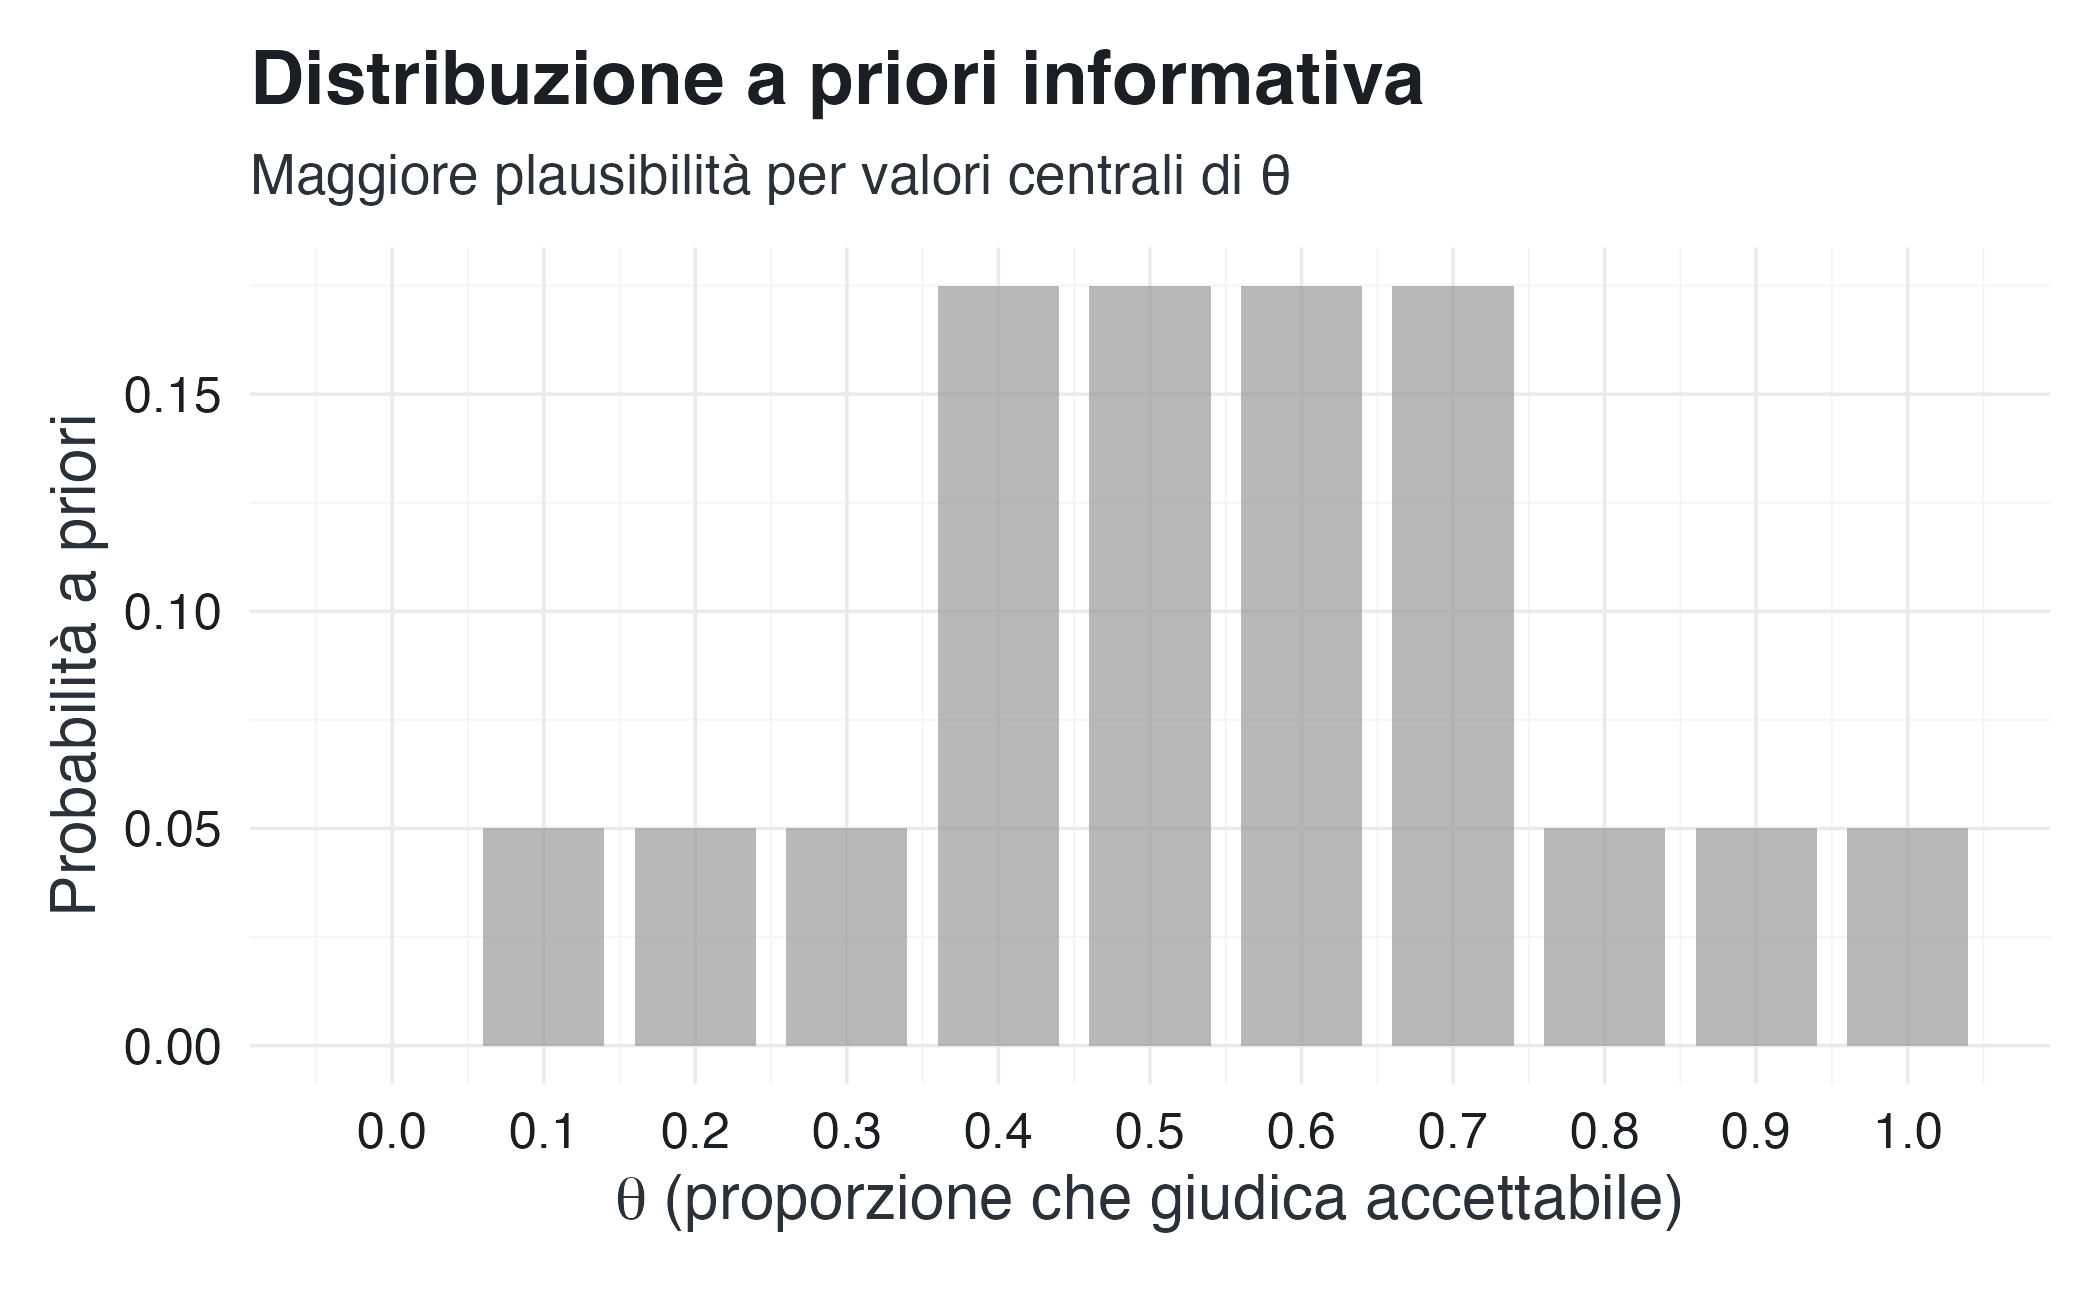
\includegraphics[width=0.85\linewidth,height=\textheight,keepaspectratio]{chapters/bayesian_inference/01_grid_approx_files/figure-pdf/unnamed-chunk-4-1.png}
\end{center}

Il grafico rivela la struttura della nostra distribuzione a priori. La
forma ricorda approssimativamente quella di una distribuzione normale,
centrata sui valori intermedi e con code che decrescono verso gli
estremi. Questa configurazione riflette una posizione epistemica
ragionevole: pur non avendo certezze definitive prima di raccogliere i
dati, abbiamo alcune aspettative qualitative basate sulla letteratura e
sul buon senso psicologico.

\subsection{Calcolo della funzione di
verosimiglianza}\label{calcolo-della-funzione-di-verosimiglianza}

La verosimiglianza quantifica quanto i dati osservati siano compatibili
con ciascun possibile valore del parametro. Nel nostro caso, abbiamo
osservato ventidue risposte positive su trenta partecipanti. Per ogni
valore di \(\theta\) nella griglia, calcoliamo la probabilità di
ottenere questo risultato (\(y\) = 22; \(n\) = 30) se quel valore
specifico fosse il parametro reale della popolazione.

\begin{Shaded}
\begin{Highlighting}[]
\CommentTok{\# Definiamo i dati osservati}
\NormalTok{successi\_osservati }\OtherTok{\textless{}{-}} \DecValTok{22}  \CommentTok{\# numero di risposte "accettabile"}
\NormalTok{prove\_totali }\OtherTok{\textless{}{-}} \DecValTok{30}         \CommentTok{\# numero totale di partecipanti}

\CommentTok{\# Calcoliamo la verosimiglianza per ogni valore di theta nella griglia}
\CommentTok{\# La funzione dbinom calcola la probabilità binomiale}
\CommentTok{\# Argomenti: numero di successi, dimensione del campione, probabilità di successo}
\NormalTok{verosimiglianza }\OtherTok{\textless{}{-}} \FunctionTok{dbinom}\NormalTok{(}
  \AttributeTok{x =}\NormalTok{ successi\_osservati,}
  \AttributeTok{size =}\NormalTok{ prove\_totali,}
  \AttributeTok{prob =}\NormalTok{ theta\_griglia}
\NormalTok{)}

\CommentTok{\# Visualizziamo i valori di verosimiglianza calcolati}
\NormalTok{verosimiglianza}
\CommentTok{\#\textgreater{}  [1] 0.00e+00 2.52e{-}16 4.12e{-}10 1.06e{-}06 1.73e{-}04 5.45e{-}03 5.05e{-}02 1.50e{-}01}
\CommentTok{\#\textgreater{}  [9] 1.11e{-}01 5.76e{-}03 0.00e+00}
\end{Highlighting}
\end{Shaded}

I valori di verosimiglianza mostrano un chiaro andamento. La
verosimiglianza è massima per \(\theta\) = 0.7, valore che corrisponde
esattamente alla proporzione osservata nel campione (22/30 ≈ 0.73). I
valori di \(\theta\) vicini a 0.7 hanno anch'essi una verosimiglianza
elevata, mentre i valori molto distanti hanno una verosimiglianza molto
bassa o praticamente nulla. Ciò riflette il fatto che i nostri dati sono
altamente incompatibili con ipotesi estreme come \(\theta\) = 0.1 o
\(\theta\) = 0.9.

\begin{Shaded}
\begin{Highlighting}[]
\CommentTok{\# Visualizziamo la funzione di verosimiglianza}
\CommentTok{\# Questo grafico mostra quali valori di theta sono più compatibili}
\CommentTok{\# con i dati che abbiamo osservato}

\NormalTok{dati\_verosimiglianza }\OtherTok{\textless{}{-}} \FunctionTok{data.frame}\NormalTok{(}
  \AttributeTok{theta =}\NormalTok{ theta\_griglia,}
  \AttributeTok{verosimiglianza =}\NormalTok{ verosimiglianza}
\NormalTok{)}

\FunctionTok{ggplot}\NormalTok{(dati\_verosimiglianza, }\FunctionTok{aes}\NormalTok{(}\AttributeTok{x =}\NormalTok{ theta, }\AttributeTok{y =}\NormalTok{ verosimiglianza)) }\SpecialCharTok{+}
  \FunctionTok{geom\_col}\NormalTok{(}\AttributeTok{width =} \FloatTok{0.08}\NormalTok{, }\AttributeTok{fill =}\NormalTok{ col\_likelihood, }\AttributeTok{alpha =} \FloatTok{0.7}\NormalTok{) }\SpecialCharTok{+}  \CommentTok{\# Arancione}
  \FunctionTok{labs}\NormalTok{(}
    \AttributeTok{x =} \FunctionTok{expression}\NormalTok{(theta }\SpecialCharTok{\textasciitilde{}} \StringTok{"(proporzione che giudica accettabile)"}\NormalTok{),}
    \AttributeTok{y =} \StringTok{"Verosimiglianza"}\NormalTok{,}
    \AttributeTok{title =} \StringTok{"Funzione di verosimiglianza"}\NormalTok{,}
    \AttributeTok{subtitle =} \FunctionTok{paste0}\NormalTok{(}
      \StringTok{"Basata su "}\NormalTok{, successi\_osservati, }\StringTok{" successi in "}\NormalTok{, }
\NormalTok{      prove\_totali, }\StringTok{" prove"}
\NormalTok{    )}
\NormalTok{  ) }\SpecialCharTok{+}
  \FunctionTok{scale\_x\_continuous}\NormalTok{(}\AttributeTok{breaks =}\NormalTok{ theta\_griglia)}
\end{Highlighting}
\end{Shaded}

\begin{center}
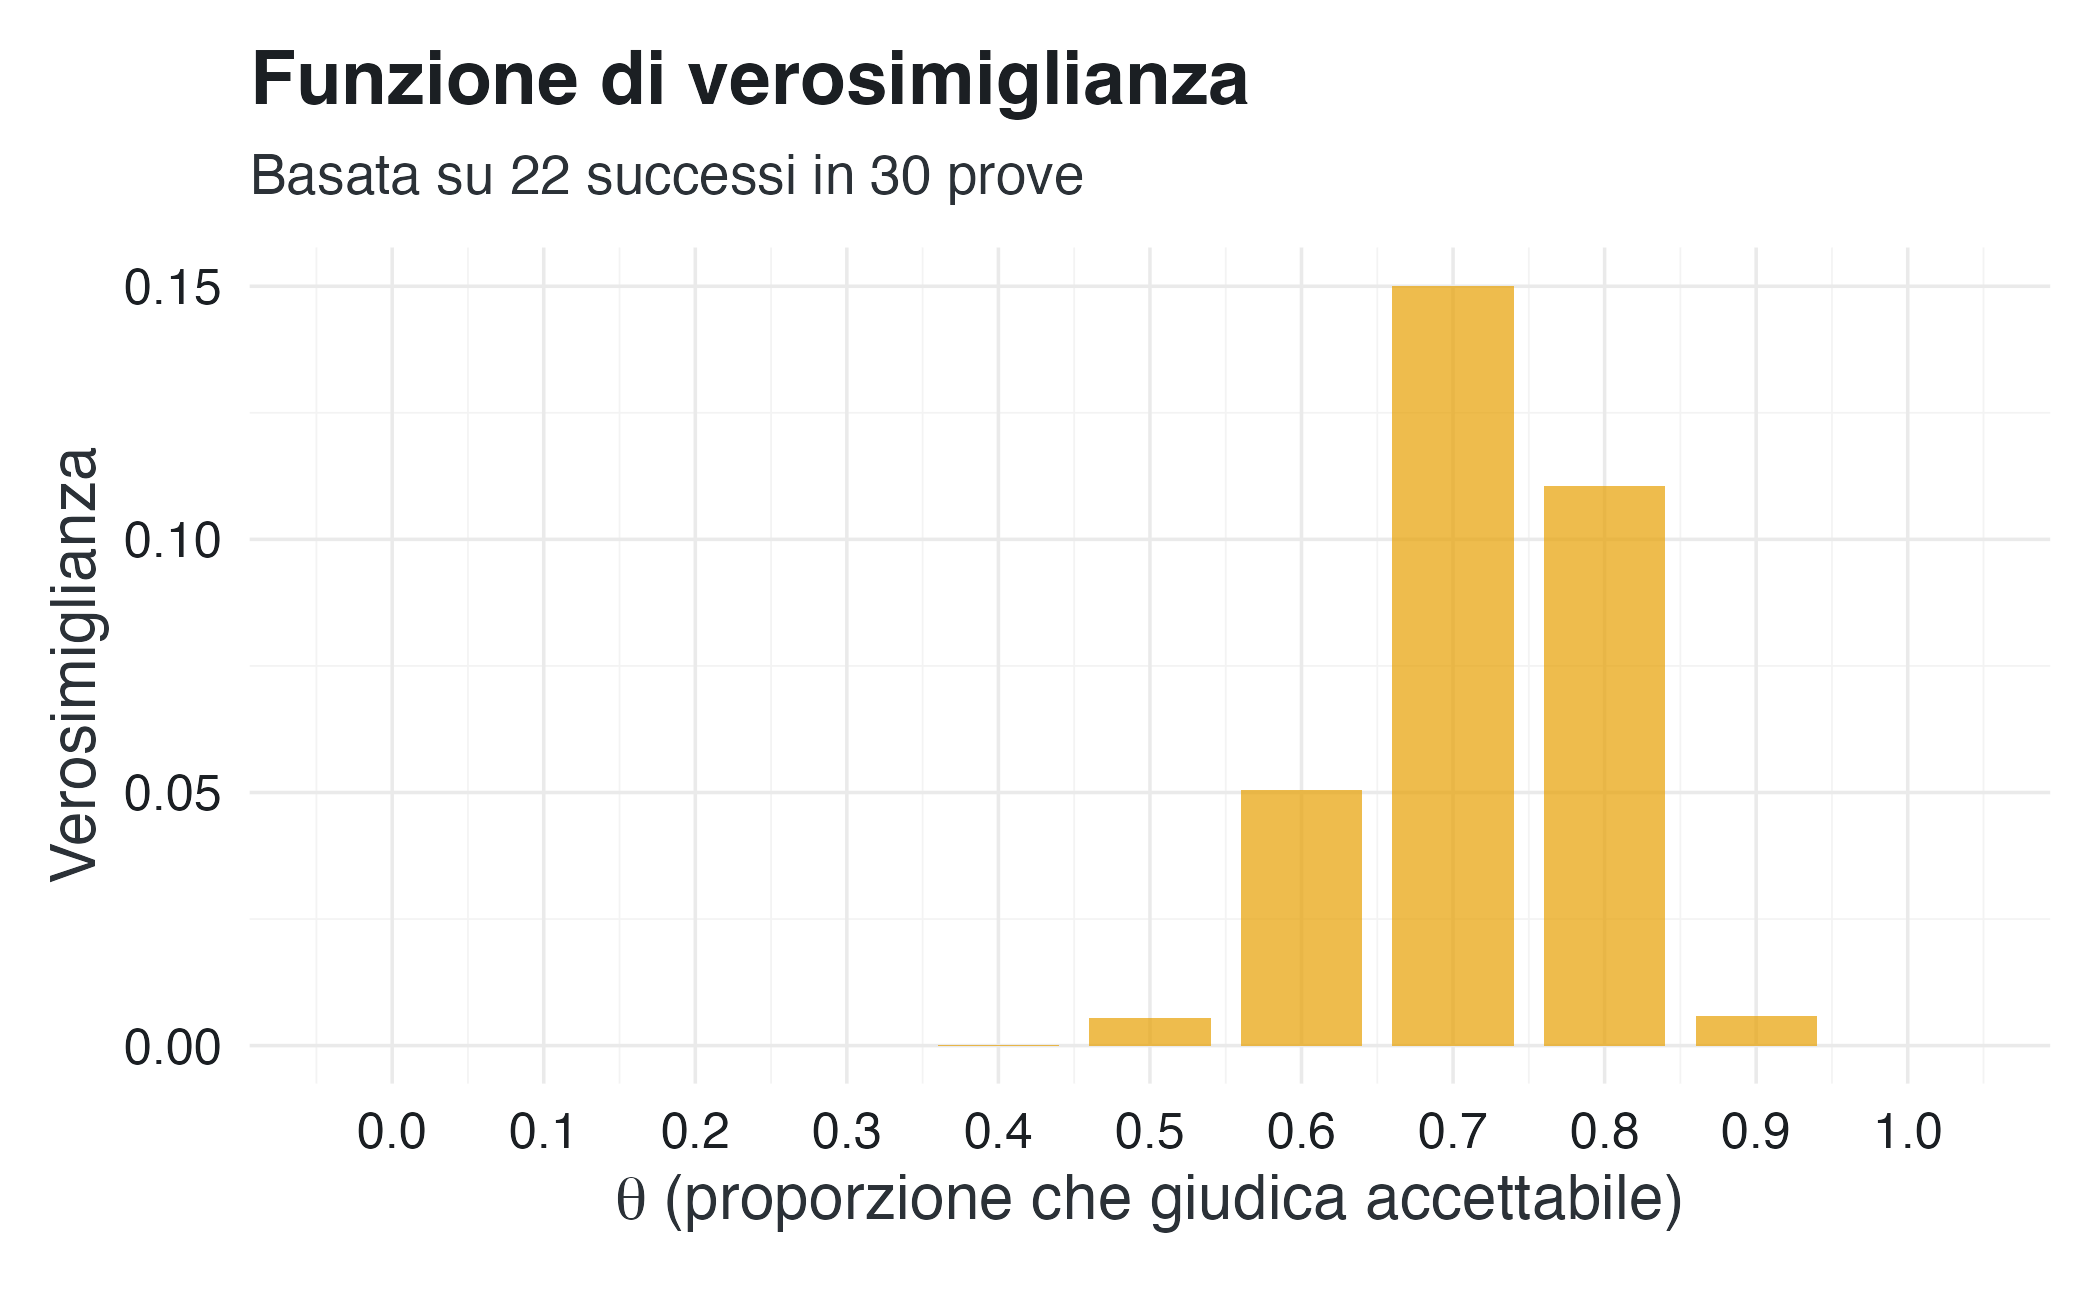
\includegraphics[width=0.85\linewidth,height=\textheight,keepaspectratio]{chapters/bayesian_inference/01_grid_approx_files/figure-pdf/unnamed-chunk-6-1.png}
\end{center}

Il picco di verosimiglianza si colloca chiaramente nella regione
compresa tra 0.6 e 0.8, con il valore massimo a 0.7. Questo risultato è
intuitivo: se dovessimo scegliere un valore di \(\theta\) che massimizza
la probabilità dei dati osservati, sceglieremmo un valore prossimo alla
proporzione campionaria. Tuttavia, la verosimiglianza da sola non
costituisce una stima completa di \(\theta\), in quanto non tiene conto
delle nostre conoscenze pregresse né dell'incertezza associata alla
stima.

\subsection{L'aggiornamento bayesiano: combinazione di prior e
verosimiglianza}\label{laggiornamento-bayesiano-combinazione-di-prior-e-verosimiglianza}

Il cuore dell'inferenza bayesiana risiede nella combinazione della
distribuzione a priori con la verosimiglianza per ottenere la
distribuzione a posteriori. Matematicamente, questo processo corrisponde
alla moltiplicazione punto per punto della distribuzione a priori e
della verosimiglianza, seguita da una normalizzazione per garantire che
le probabilità sommino a uno.

\begin{Shaded}
\begin{Highlighting}[]
\CommentTok{\# Calcoliamo la distribuzione a posteriori non normalizzata}
\CommentTok{\# Questa si ottiene moltiplicando, per ogni valore di theta,}
\CommentTok{\# la probabilità a priori per la verosimiglianza}
\NormalTok{posteriori\_non\_normalizzato }\OtherTok{\textless{}{-}}\NormalTok{ prior\_informativo }\SpecialCharTok{*}\NormalTok{ verosimiglianza}

\CommentTok{\# Visualizziamo i valori non normalizzati}
\NormalTok{posteriori\_non\_normalizzato}
\CommentTok{\#\textgreater{}  [1] 0.00e+00 1.26e{-}17 2.06e{-}11 5.29e{-}08 3.03e{-}05 9.54e{-}04 8.84e{-}03 2.63e{-}02}
\CommentTok{\#\textgreater{}  [9] 5.53e{-}03 2.88e{-}04 0.00e+00}
\end{Highlighting}
\end{Shaded}

I valori non normalizzati riflettono la plausibilità relativa di ciascun
valore di \(\theta\) dopo l'osservazione dei dati. Tuttavia, questi
numeri non costituiscono ancora una distribuzione di probabilità valida,
in quanto la loro somma non è uguale a uno. Il passo finale consiste nel
normalizzare questi valori dividendoli per la loro somma totale.

\begin{Shaded}
\begin{Highlighting}[]
\CommentTok{\# Calcoliamo il fattore di normalizzazione}
\CommentTok{\# Questo è semplicemente la somma di tutti i valori non normalizzati}
\NormalTok{fattore\_normalizzazione }\OtherTok{\textless{}{-}} \FunctionTok{sum}\NormalTok{(posteriori\_non\_normalizzato)}

\CommentTok{\# Dividiamo ciascun valore per questo fattore per ottenere}
\CommentTok{\# la distribuzione a posteriori normalizzata}
\NormalTok{posteriori }\OtherTok{\textless{}{-}}\NormalTok{ posteriori\_non\_normalizzato }\SpecialCharTok{/}\NormalTok{ fattore\_normalizzazione}

\CommentTok{\# Verifichiamo che la somma sia ora uguale a uno}
\NormalTok{somma\_posteriori }\OtherTok{\textless{}{-}} \FunctionTok{sum}\NormalTok{(posteriori)}
\end{Highlighting}
\end{Shaded}

La somma della distribuzione a posteriori è 1, il che conferma che
abbiamo ottenuto una distribuzione di probabilità valida. Possiamo ora
usare questa distribuzione per fare inferenze su \(\theta\), calcolare
statistiche riassuntive e quantificare l'incertezza associata alla
nostra stima.

\begin{Shaded}
\begin{Highlighting}[]
\CommentTok{\# Visualizziamo la distribuzione a posteriori}

\NormalTok{dati\_posteriori }\OtherTok{\textless{}{-}} \FunctionTok{data.frame}\NormalTok{(}
  \AttributeTok{theta =}\NormalTok{ theta\_griglia,}
  \AttributeTok{probabilita =}\NormalTok{ posteriori}
\NormalTok{)}

\FunctionTok{ggplot}\NormalTok{(dati\_posteriori, }\FunctionTok{aes}\NormalTok{(}\AttributeTok{x =}\NormalTok{ theta, }\AttributeTok{y =}\NormalTok{ probabilita)) }\SpecialCharTok{+}
  \FunctionTok{geom\_col}\NormalTok{(}\AttributeTok{width =} \FloatTok{0.08}\NormalTok{, }\AttributeTok{fill =}\NormalTok{ col\_posterior, }\AttributeTok{alpha =} \FloatTok{0.7}\NormalTok{) }\SpecialCharTok{+}  \CommentTok{\# Blu}
  \FunctionTok{labs}\NormalTok{(}
    \AttributeTok{x =} \FunctionTok{expression}\NormalTok{(theta }\SpecialCharTok{\textasciitilde{}} \StringTok{"(proporzione che giudica accettabile)"}\NormalTok{),}
    \AttributeTok{y =} \StringTok{"Probabilità a posteriori"}\NormalTok{,}
    \AttributeTok{title =} \StringTok{"Distribuzione a posteriori"}\NormalTok{,}
    \AttributeTok{subtitle =} \StringTok{"Sintesi di conoscenza a priori ed evidenza empirica"}
\NormalTok{  ) }\SpecialCharTok{+}
  \FunctionTok{scale\_x\_continuous}\NormalTok{(}\AttributeTok{breaks =}\NormalTok{ theta\_griglia)}
\end{Highlighting}
\end{Shaded}

\begin{center}
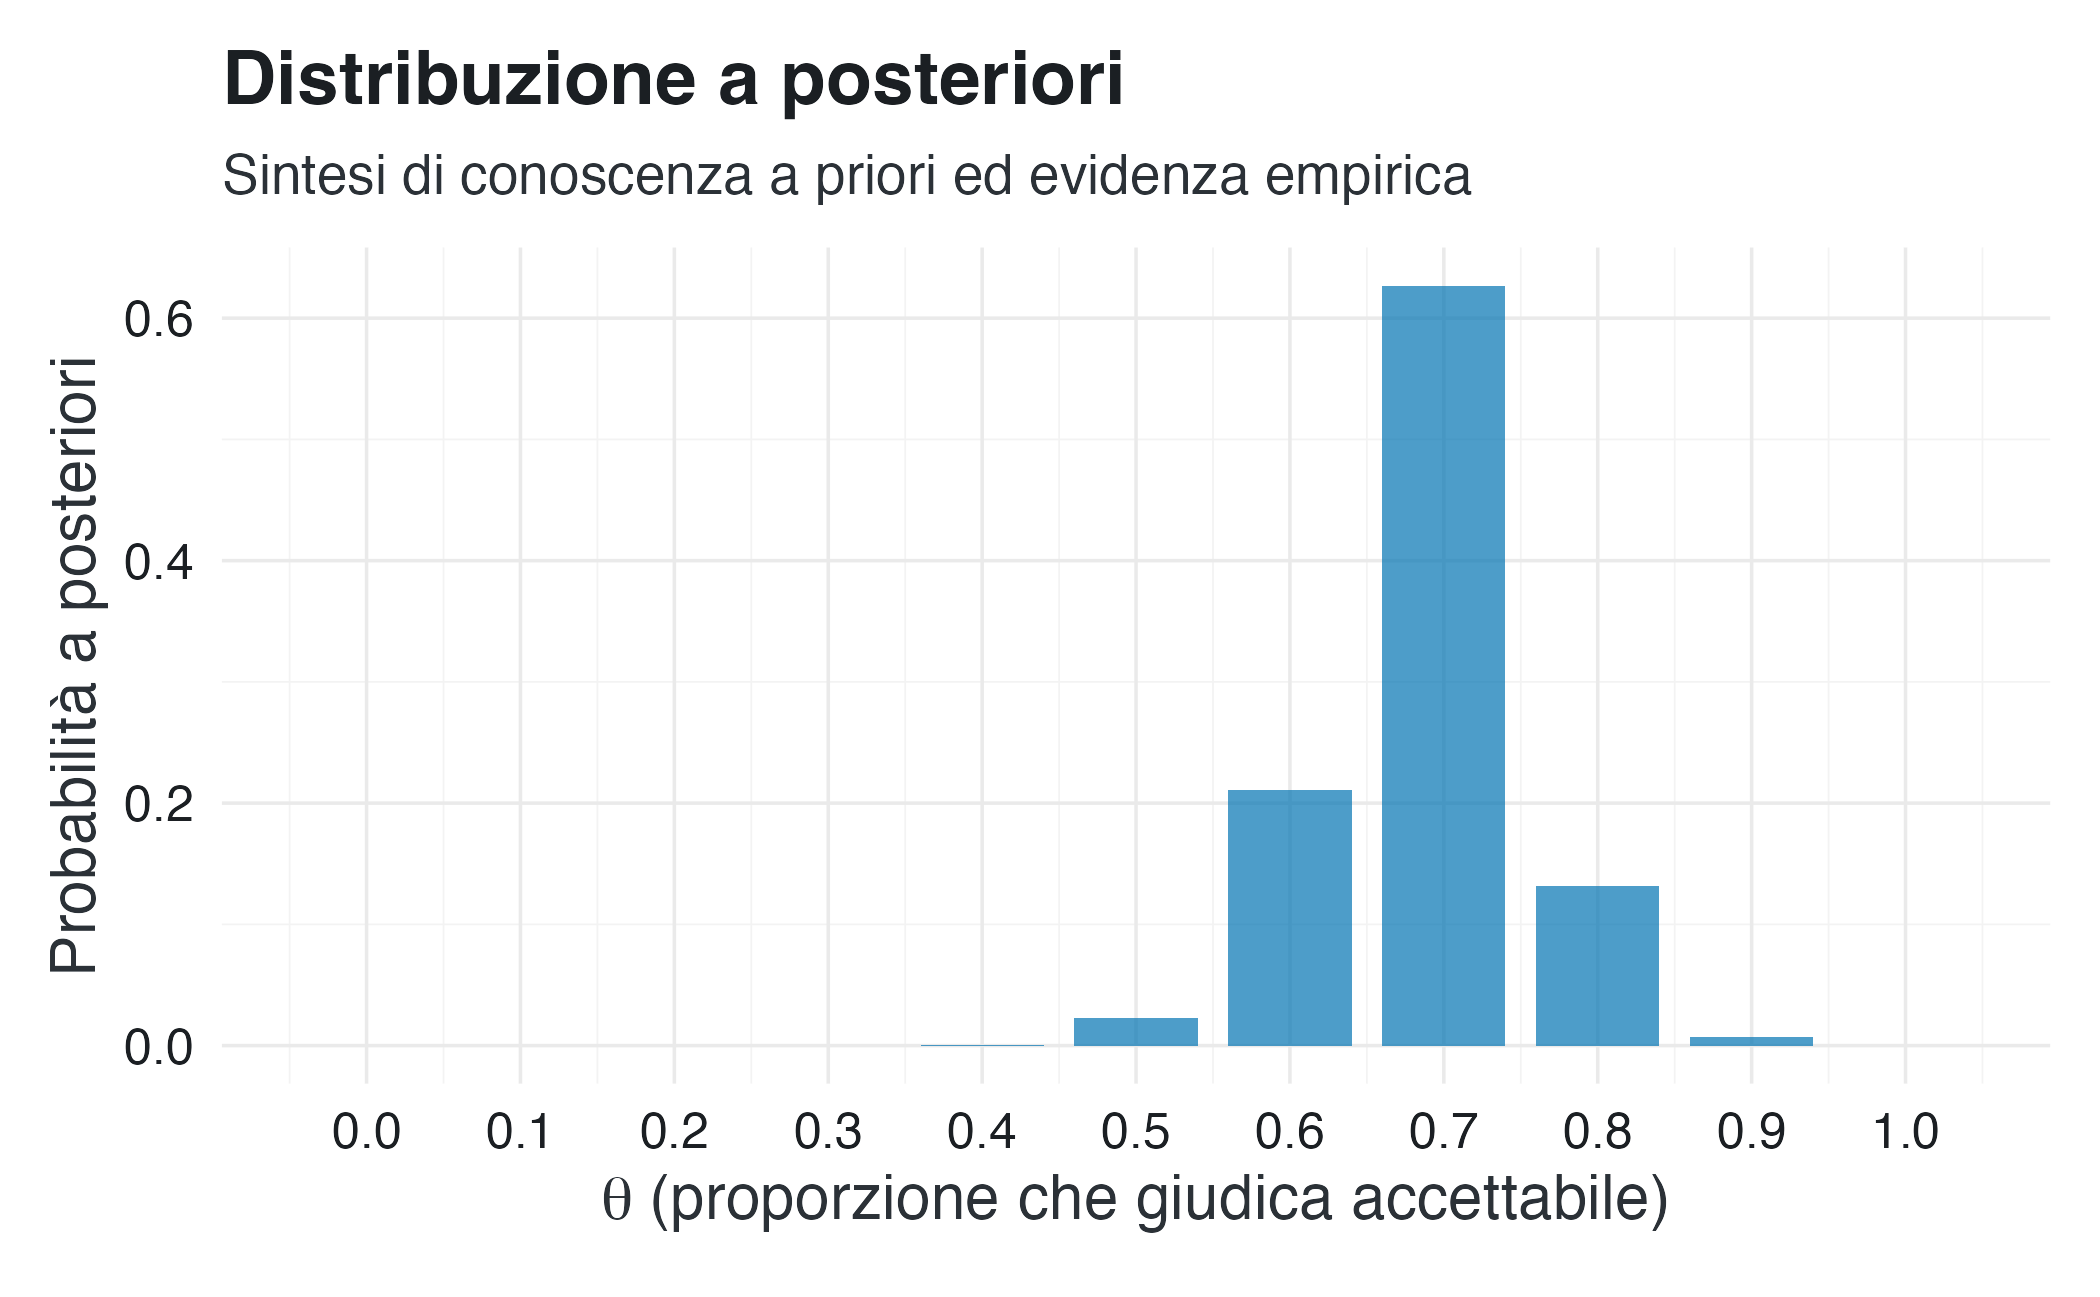
\includegraphics[width=0.85\linewidth,height=\textheight,keepaspectratio]{chapters/bayesian_inference/01_grid_approx_files/figure-pdf/unnamed-chunk-9-1.png}
\end{center}

La distribuzione a posteriori mostra una concentrazione di probabilità
nella regione tra 0.6 e 0.8, con il massimo a 0.7. Confrontata con la
distribuzione a priori, la posteriori è più stretta e spostata verso
destra, riflettendo l'influenza dei dati osservati che hanno fornito
evidenza di una proporzione relativamente alta di risposte positive.

\subsection{Statistiche riassuntive della distribuzione a
posteriori}\label{statistiche-riassuntive-della-distribuzione-a-posteriori}

Una volta ottenuta la distribuzione a posteriori, è possibile calcolare
diverse statistiche che riassumono le nostre credenze aggiornate su
\(\theta\). Le tre statistiche più comunemente utilizzate sono la media,
la varianza e la moda.

\begin{Shaded}
\begin{Highlighting}[]
\CommentTok{\# Calcoliamo la media a posteriori}
\CommentTok{\# Questa è il valore atteso di theta secondo la distribuzione a posteriori}
\CommentTok{\# Si calcola come somma ponderata: ogni valore di theta moltiplicato}
\CommentTok{\# per la sua probabilità a posteriori}
\NormalTok{media\_posteriori }\OtherTok{\textless{}{-}} \FunctionTok{sum}\NormalTok{(theta\_griglia }\SpecialCharTok{*}\NormalTok{ posteriori)}

\CommentTok{\# Calcoliamo la varianza a posteriori}
\CommentTok{\# Questa quantifica la dispersione della distribuzione}
\CommentTok{\# e quindi l\textquotesingle{}incertezza residua su theta}
\NormalTok{varianza\_posteriori }\OtherTok{\textless{}{-}} \FunctionTok{sum}\NormalTok{((theta\_griglia }\SpecialCharTok{{-}}\NormalTok{ media\_posteriori)}\SpecialCharTok{\^{}}\DecValTok{2} \SpecialCharTok{*}\NormalTok{ posteriori)}

\CommentTok{\# La deviazione standard è la radice quadrata della varianza}
\NormalTok{sd\_posteriori }\OtherTok{\textless{}{-}} \FunctionTok{sqrt}\NormalTok{(varianza\_posteriori)}

\CommentTok{\# Calcoliamo la moda a posteriori}
\CommentTok{\# Questo è il valore di theta con massima probabilità a posteriori}
\CommentTok{\# Viene anche chiamato "stima MAP" (Maximum A Posteriori)}
\NormalTok{indice\_massimo }\OtherTok{\textless{}{-}} \FunctionTok{which.max}\NormalTok{(posteriori)}
\NormalTok{moda\_posteriori }\OtherTok{\textless{}{-}}\NormalTok{ theta\_griglia[indice\_massimo]}
\end{Highlighting}
\end{Shaded}

La media a posteriori è 0.689, indicando che la nostra migliore stima
puntuale di \(\theta\), nel senso del valore atteso, è circa 0.729. La
moda a posteriori è 0.7, che rappresenta il singolo valore più
plausibile secondo la distribuzione. La deviazione standard è 0.067,
quantificando l'incertezza residua sulla stima. Questa deviazione
standard è sostanzialmente più piccola di quella che avremmo con un
prior uniforme, riflettendo il fatto che il prior informativo ha
contribuito a ridurre l'incertezza.

\subsection{Visualizzazione comparativa dell'aggiornamento
bayesiano}\label{visualizzazione-comparativa-dellaggiornamento-bayesiano}

Per apprezzare il processo di aggiornamento bayesiano, è utile
visualizzare simultaneamente tutte e tre le componenti: prior,
verosimiglianza e posterior. Questa visualizzazione mostra come
l'evidenza empirica modifichi le credenze iniziali per produrre quelle
aggiornate.

\begin{Shaded}
\begin{Highlighting}[]
\CommentTok{\# Prepariamo i dati per la visualizzazione comparativa}
\CommentTok{\# Normalizziamo tutte le distribuzioni per renderle visivamente confrontabili}

\NormalTok{dati\_completi }\OtherTok{\textless{}{-}} \FunctionTok{data.frame}\NormalTok{(}
  \AttributeTok{theta =} \FunctionTok{rep}\NormalTok{(theta\_griglia, }\DecValTok{3}\NormalTok{),}
  \AttributeTok{densita =} \FunctionTok{c}\NormalTok{(}
\NormalTok{    prior\_informativo }\SpecialCharTok{/} \FunctionTok{sum}\NormalTok{(prior\_informativo),}
\NormalTok{    verosimiglianza }\SpecialCharTok{/} \FunctionTok{sum}\NormalTok{(verosimiglianza),}
\NormalTok{    posteriori }\SpecialCharTok{/} \FunctionTok{sum}\NormalTok{(posteriori)}
\NormalTok{  ),}
  \AttributeTok{tipo =} \FunctionTok{rep}\NormalTok{(}
    \FunctionTok{c}\NormalTok{(}\StringTok{"Prior"}\NormalTok{, }\StringTok{"Verosimiglianza"}\NormalTok{, }\StringTok{"Posterior"}\NormalTok{),}
    \AttributeTok{each =} \FunctionTok{length}\NormalTok{(theta\_griglia)}
\NormalTok{  )}
\NormalTok{)}

\CommentTok{\# Convertiamo il tipo in un fattore ordinato per controllare}
\CommentTok{\# l\textquotesingle{}ordine di visualizzazione nella legenda}
\NormalTok{dati\_completi}\SpecialCharTok{$}\NormalTok{tipo }\OtherTok{\textless{}{-}} \FunctionTok{factor}\NormalTok{(}
\NormalTok{  dati\_completi}\SpecialCharTok{$}\NormalTok{tipo,}
  \AttributeTok{levels =} \FunctionTok{c}\NormalTok{(}\StringTok{"Prior"}\NormalTok{, }\StringTok{"Verosimiglianza"}\NormalTok{, }\StringTok{"Posterior"}\NormalTok{)}
\NormalTok{)}

\CommentTok{\# Creiamo il grafico comparativo usando linee anziché barre}
\CommentTok{\# per enfatizzare la continuità concettuale delle distribuzioni}
\FunctionTok{ggplot}\NormalTok{(dati\_completi, }\FunctionTok{aes}\NormalTok{(}\AttributeTok{x =}\NormalTok{ theta, }\AttributeTok{y =}\NormalTok{ densita, }\AttributeTok{color =}\NormalTok{ tipo)) }\SpecialCharTok{+}
  \FunctionTok{geom\_line}\NormalTok{(}\AttributeTok{size =} \FloatTok{1.3}\NormalTok{) }\SpecialCharTok{+}
  \FunctionTok{geom\_point}\NormalTok{(}\AttributeTok{size =} \DecValTok{2}\NormalTok{) }\SpecialCharTok{+}
  \FunctionTok{scale\_color\_manual}\NormalTok{(}
    \AttributeTok{values =} \FunctionTok{c}\NormalTok{(}
      \StringTok{"Prior"} \OtherTok{=}\NormalTok{ col\_prior,           }\CommentTok{\# Grigio}
      \StringTok{"Verosimiglianza"} \OtherTok{=}\NormalTok{ col\_likelihood,  }\CommentTok{\# Arancione}
      \StringTok{"Posterior"} \OtherTok{=}\NormalTok{ col\_posterior    }\CommentTok{\# Blu}
\NormalTok{    )}
\NormalTok{  ) }\SpecialCharTok{+}
  \FunctionTok{labs}\NormalTok{(}
    \AttributeTok{x =} \FunctionTok{expression}\NormalTok{(theta }\SpecialCharTok{\textasciitilde{}} \StringTok{"(proporzione che giudica accettabile)"}\NormalTok{),}
    \AttributeTok{y =} \StringTok{"Densità normalizzata"}\NormalTok{,}
    \AttributeTok{title =} \StringTok{"Aggiornamento bayesiano con metodo su griglia"}\NormalTok{,}
    \AttributeTok{subtitle =} \StringTok{"Prior (grigio), Verosimiglianza (arancione), Posterior (blu)"}\NormalTok{,}
    \AttributeTok{color =} \StringTok{"Componente"}
\NormalTok{  ) }\SpecialCharTok{+}
  \FunctionTok{scale\_x\_continuous}\NormalTok{(}\AttributeTok{breaks =}\NormalTok{ theta\_griglia)}
\end{Highlighting}
\end{Shaded}

\begin{center}
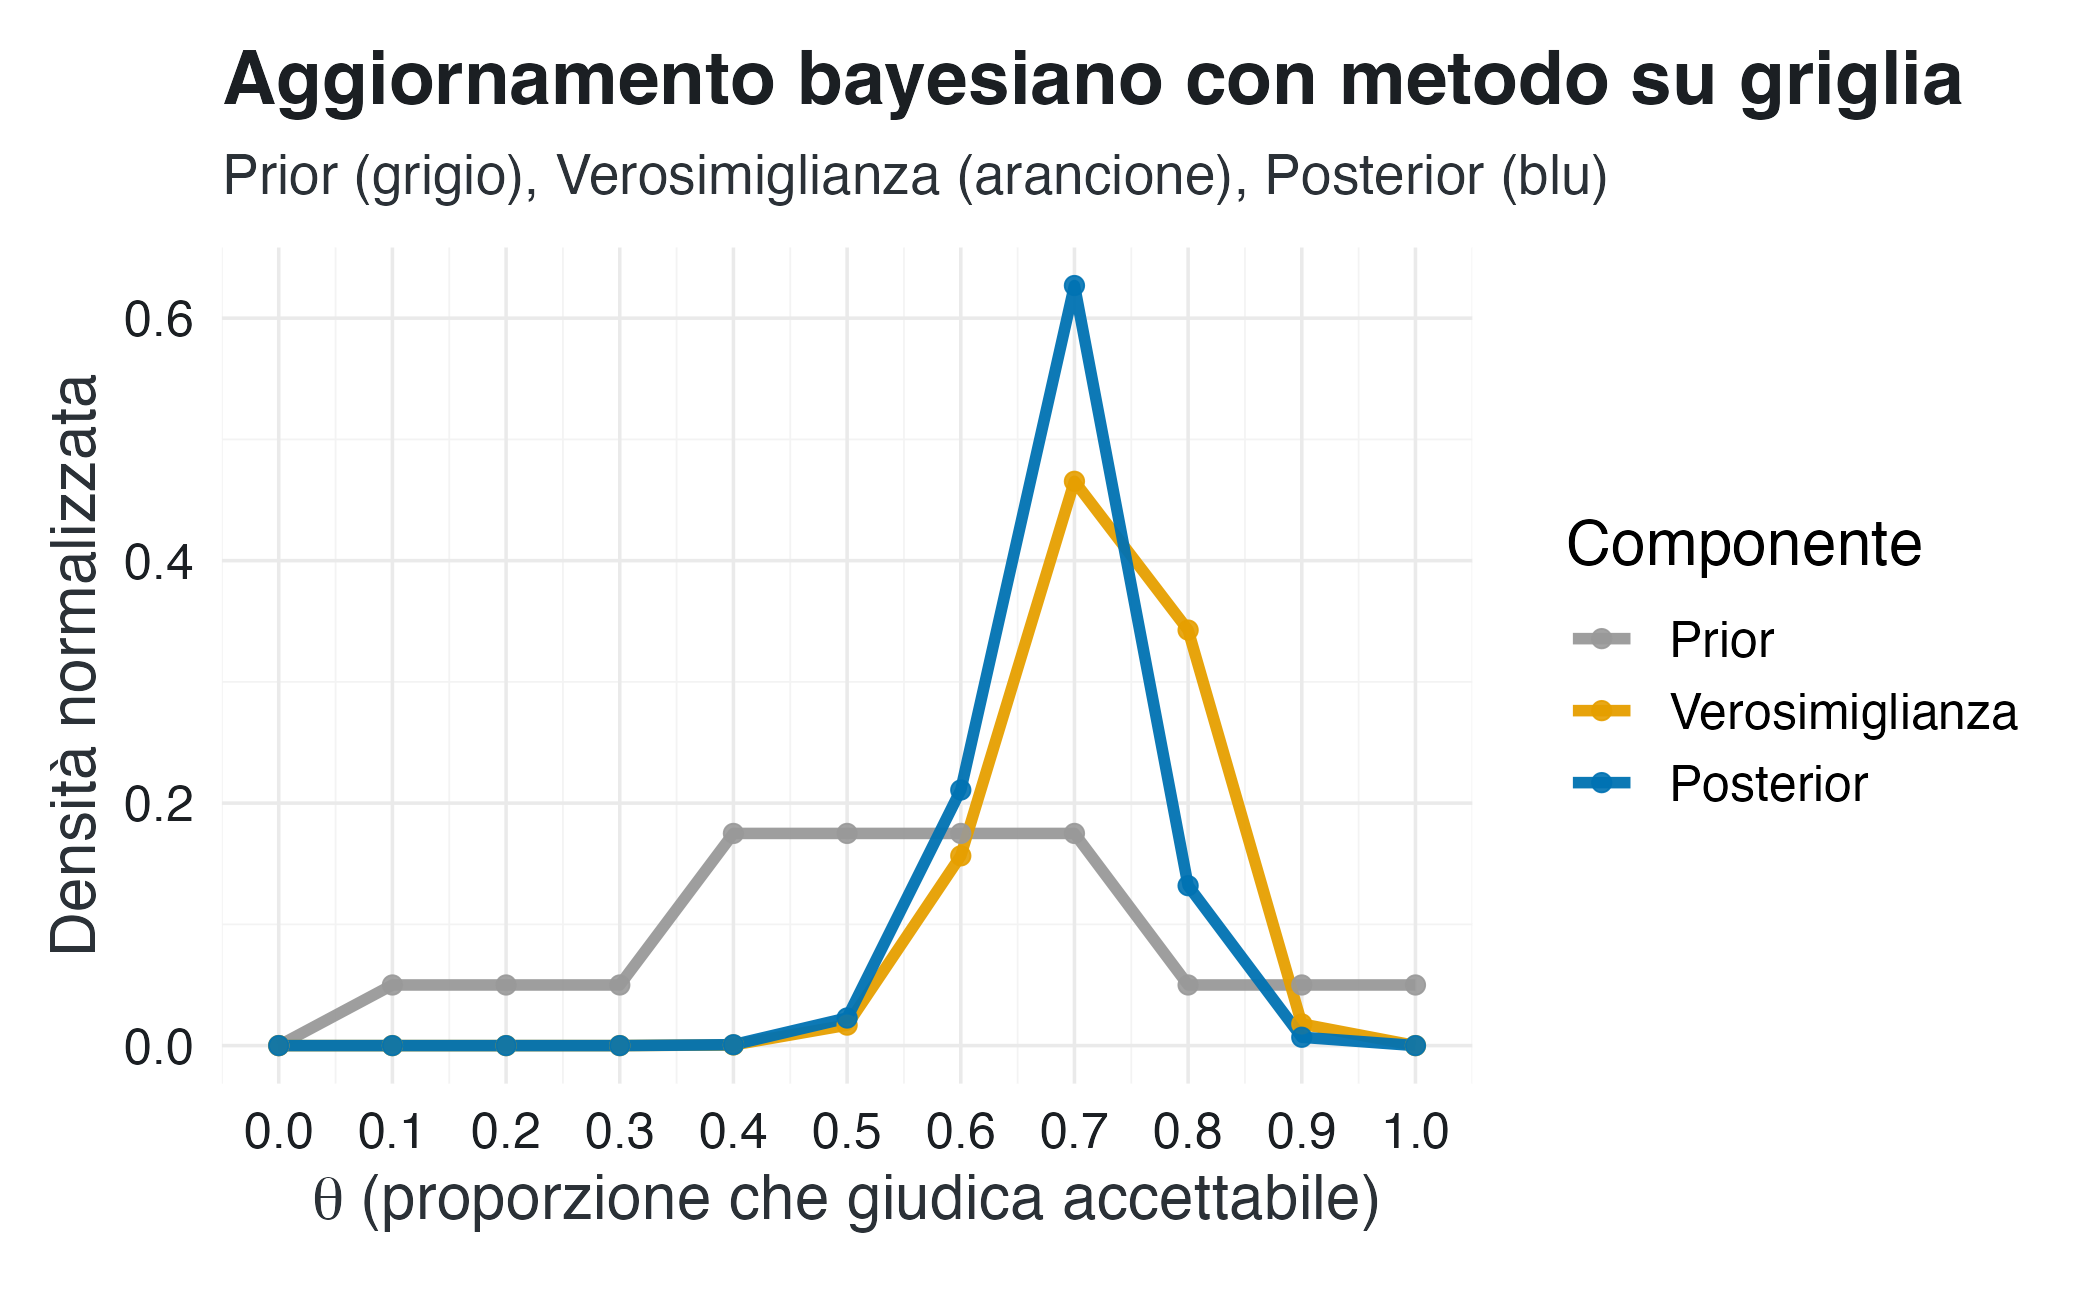
\includegraphics[width=0.85\linewidth,height=\textheight,keepaspectratio]{chapters/bayesian_inference/01_grid_approx_files/figure-pdf/unnamed-chunk-11-1.png}
\end{center}

Il grafico comparativo rivela diversi aspetti importanti del processo di
aggiornamento. La curva grigia del prior mostra una distribuzione
relativamente simmetrica centrata sui valori intermedi. La curva
arancione della verosimiglianza è fortemente concentrata attorno a 0.7,
riflettendo l'evidenza empirica fornita dai ventidue successi su trenta
prove. La curva blu del posterior rappresenta un compromesso tra queste
due fonti di informazione. La sua posizione è spostata verso destra
rispetto al prior, influenzata dall'evidenza forte fornita dai dati, ma
mantiene una certa regolarizzazione dovuta al prior che previene stime
estreme basate su un campione relativamente piccolo.

\section{Il modello Beta-Binomiale: soluzione analitica
continua}\label{il-modello-beta-binomiale-soluzione-analitica-continua}

Il metodo basato su griglia fornisce un'approssimazione discreta
dell'aggiornamento bayesiano, mentre il modello Beta-Binomiale offre una
soluzione analitica esatta per le distribuzioni continue. Il modello
beta-binomiale si fonda sulla proprietà di coniugazione tra
distribuzione beta e verosimiglianza binomiale.

\subsection{Fondamenti del modello
coniugato}\label{fondamenti-del-modello-coniugato}

Quando la distribuzione a priori per \(\theta\) è una distribuzione Beta
e i dati seguono una distribuzione binomiale, la distribuzione a
posteriori è ancora una distribuzione Beta con parametri aggiornati.
Questa proprietà semplifica notevolmente i calcoli e fornisce
un'interpretazione intuitiva dell'aggiornamento in termini di accumulo
di pseudo-osservazioni.

La distribuzione Beta è definita da due parametri, tradizionalmente
chiamati \(\alpha\) e \(\beta\). Una distribuzione Beta(\(\alpha\),
\(\beta\)) può essere considerata come rappresentante la conoscenza
derivante dall'osservazione di \(\alpha\)-1 successi e \(\beta\)-1
insuccessi in un ipotetico studio precedente. Quando si osservano nuovi
dati reali, si sommano semplicemente i conteggi osservati a questi
pseudo-conteggi.

\begin{Shaded}
\begin{Highlighting}[]
\CommentTok{\# Definiamo i parametri della distribuzione a priori Beta}
\CommentTok{\# Scegliamo Beta(2, 2) che rappresenta una credenza moderatamente informativa}
\CommentTok{\# Questa prior è simmetrica e centrata su 0.5}
\NormalTok{alpha\_prior }\OtherTok{\textless{}{-}} \DecValTok{2}
\NormalTok{beta\_prior }\OtherTok{\textless{}{-}} \DecValTok{2}

\CommentTok{\# Calcoliamo la media e la varianza di questa prior}
\CommentTok{\# La media di una Beta(α, β) è α/(α+β)}
\NormalTok{media\_prior\_beta }\OtherTok{\textless{}{-}}\NormalTok{ alpha\_prior }\SpecialCharTok{/}\NormalTok{ (alpha\_prior }\SpecialCharTok{+}\NormalTok{ beta\_prior)}

\CommentTok{\# La varianza di una Beta(α, β) è αβ/[(α+β)²(α+β+1)]}
\NormalTok{varianza\_prior\_beta }\OtherTok{\textless{}{-}}\NormalTok{ (alpha\_prior }\SpecialCharTok{*}\NormalTok{ beta\_prior) }\SpecialCharTok{/} 
\NormalTok{  ((alpha\_prior }\SpecialCharTok{+}\NormalTok{ beta\_prior)}\SpecialCharTok{\^{}}\DecValTok{2} \SpecialCharTok{*}\NormalTok{ (alpha\_prior }\SpecialCharTok{+}\NormalTok{ beta\_prior }\SpecialCharTok{+} \DecValTok{1}\NormalTok{))}
\NormalTok{sd\_prior\_beta }\OtherTok{\textless{}{-}} \FunctionTok{sqrt}\NormalTok{(varianza\_prior\_beta)}
\end{Highlighting}
\end{Shaded}

La distribuzione a priori Beta(2, 2) ha media 0.5 e deviazione standard
0.224. Questa distribuzione esprime una credenza iniziale piuttosto
vaga, centrata sul valore intermedio di 0.5, ma sufficientemente
dispersa da permettere ai dati di influenzare in modo sostanziale la
distribuzione a posteriori.

\subsection{Aggiornamento dei parametri
Beta}\label{aggiornamento-dei-parametri-beta}

L'aggiornamento del modello Beta-Binomiale segue una regola estremamente
semplice. Se osserviamo \(y\) successi in \(n\) prove, i nuovi parametri
della distribuzione a posteriori sono \(\alpha + y\) e
\(\beta + (n - y)\). Questo aggiornamento riflette l'idea che stiamo
letteralmente aggiungendo i successi osservati ai successi virtuali del
prior e gli insuccessi osservati agli insuccessi virtuali del prior.

\begin{Shaded}
\begin{Highlighting}[]
\CommentTok{\# Applichiamo la regola di aggiornamento Beta{-}Binomiale}
\CommentTok{\# I dati sono gli stessi del metodo su griglia: 22 successi su 30 prove}

\CommentTok{\# Calcoliamo il numero di insuccessi}
\NormalTok{insuccessi\_osservati }\OtherTok{\textless{}{-}}\NormalTok{ prove\_totali }\SpecialCharTok{{-}}\NormalTok{ successi\_osservati}

\CommentTok{\# Aggiorniamo il parametro alpha sommando i successi osservati}
\NormalTok{alpha\_posteriori }\OtherTok{\textless{}{-}}\NormalTok{ alpha\_prior }\SpecialCharTok{+}\NormalTok{ successi\_osservati}

\CommentTok{\# Aggiorniamo il parametro beta sommando gli insuccessi osservati  }
\NormalTok{beta\_posteriori }\OtherTok{\textless{}{-}}\NormalTok{ beta\_prior }\SpecialCharTok{+}\NormalTok{ insuccessi\_osservati}

\CommentTok{\# Calcoliamo le statistiche della distribuzione a posteriori}
\NormalTok{media\_posteriori\_beta }\OtherTok{\textless{}{-}}\NormalTok{ alpha\_posteriori }\SpecialCharTok{/}\NormalTok{ (alpha\_posteriori }\SpecialCharTok{+}\NormalTok{ beta\_posteriori)}

\NormalTok{varianza\_posteriori\_beta }\OtherTok{\textless{}{-}}\NormalTok{ (alpha\_posteriori }\SpecialCharTok{*}\NormalTok{ beta\_posteriori) }\SpecialCharTok{/} 
\NormalTok{  ((alpha\_posteriori }\SpecialCharTok{+}\NormalTok{ beta\_posteriori)}\SpecialCharTok{\^{}}\DecValTok{2} \SpecialCharTok{*}\NormalTok{ (alpha\_posteriori }\SpecialCharTok{+}\NormalTok{ beta\_posteriori }\SpecialCharTok{+} \DecValTok{1}\NormalTok{))}
\NormalTok{sd\_posteriori\_beta }\OtherTok{\textless{}{-}} \FunctionTok{sqrt}\NormalTok{(varianza\_posteriori\_beta)}
\end{Highlighting}
\end{Shaded}

La distribuzione a posteriori risultante è Beta(24, 10). La media a
posteriori è 0.706, molto vicina alla proporzione campionaria osservata
di 0.733. La deviazione standard a posteriori è 0.077, sostanzialmente
ridotta rispetto al prior, a indicare la riduzione dell'incertezza
derivante dall'osservazione di trenta prove.

\subsection{Visualizzazione dell'aggiornamento
continuo}\label{visualizzazione-dellaggiornamento-continuo}

La transizione dal prior al posterior nel modello Beta-Binomiale può
essere visualizzata tracciando le curve di densità delle due
distribuzioni Beta. Questa visualizzazione mostra come i dati
modifichino la forma, la posizione e la dispersione della distribuzione.

\begin{Shaded}
\begin{Highlighting}[]
\CommentTok{\# Creiamo una griglia fine di valori per theta}
\CommentTok{\# Usiamo molti più punti rispetto al metodo su griglia}
\CommentTok{\# per ottenere curve lisce e continue}
\NormalTok{theta\_continuo }\OtherTok{\textless{}{-}} \FunctionTok{seq}\NormalTok{(}\AttributeTok{from =} \DecValTok{0}\NormalTok{, }\AttributeTok{to =} \DecValTok{1}\NormalTok{, }\AttributeTok{length.out =} \DecValTok{500}\NormalTok{)}

\CommentTok{\# Calcoliamo la densità Beta per il prior e il posterior}
\CommentTok{\# La funzione dbeta calcola la funzione di densità di probabilità}
\NormalTok{densita\_prior\_beta }\OtherTok{\textless{}{-}} \FunctionTok{dbeta}\NormalTok{(theta\_continuo, }\AttributeTok{shape1 =}\NormalTok{ alpha\_prior, }\AttributeTok{shape2 =}\NormalTok{ beta\_prior)}
\NormalTok{densita\_posteriori\_beta }\OtherTok{\textless{}{-}} \FunctionTok{dbeta}\NormalTok{(}
\NormalTok{  theta\_continuo, }\AttributeTok{shape1 =}\NormalTok{ alpha\_posteriori, }\AttributeTok{shape2 =}\NormalTok{ beta\_posteriori)}

\CommentTok{\# Organizziamo i dati per la visualizzazione}
\NormalTok{dati\_beta }\OtherTok{\textless{}{-}} \FunctionTok{data.frame}\NormalTok{(}
  \AttributeTok{theta =} \FunctionTok{rep}\NormalTok{(theta\_continuo, }\DecValTok{2}\NormalTok{),}
  \AttributeTok{densita =} \FunctionTok{c}\NormalTok{(densita\_prior\_beta, densita\_posteriori\_beta),}
  \AttributeTok{tipo =} \FunctionTok{rep}\NormalTok{(}
    \FunctionTok{c}\NormalTok{(}\FunctionTok{paste0}\NormalTok{(}\StringTok{"Prior Beta("}\NormalTok{, alpha\_prior, }\StringTok{","}\NormalTok{, beta\_prior, }\StringTok{")"}\NormalTok{),}
      \FunctionTok{paste0}\NormalTok{(}\StringTok{"Posterior Beta("}\NormalTok{, alpha\_posteriori, }\StringTok{","}\NormalTok{, beta\_posteriori, }\StringTok{")"}\NormalTok{)),}
    \AttributeTok{each =} \FunctionTok{length}\NormalTok{(theta\_continuo)}
\NormalTok{  )}
\NormalTok{)}

\CommentTok{\# Convertiamo in fattore ordinato}
\NormalTok{dati\_beta}\SpecialCharTok{$}\NormalTok{tipo }\OtherTok{\textless{}{-}} \FunctionTok{factor}\NormalTok{(}
\NormalTok{  dati\_beta}\SpecialCharTok{$}\NormalTok{tipo,}
  \AttributeTok{levels =} \FunctionTok{c}\NormalTok{(}
    \FunctionTok{paste0}\NormalTok{(}\StringTok{"Prior Beta("}\NormalTok{, alpha\_prior, }\StringTok{","}\NormalTok{, beta\_prior, }\StringTok{")"}\NormalTok{),}
    \FunctionTok{paste0}\NormalTok{(}\StringTok{"Posterior Beta("}\NormalTok{, alpha\_posteriori, }\StringTok{","}\NormalTok{, beta\_posteriori, }\StringTok{")"}\NormalTok{)}
\NormalTok{  )}
\NormalTok{)}

\CommentTok{\# Creiamo il grafico con linee continue}
\FunctionTok{ggplot}\NormalTok{(dati\_beta, }\FunctionTok{aes}\NormalTok{(}\AttributeTok{x =}\NormalTok{ theta, }\AttributeTok{y =}\NormalTok{ densita, }\AttributeTok{color =}\NormalTok{ tipo, }\AttributeTok{linetype =}\NormalTok{ tipo)) }\SpecialCharTok{+}
  \FunctionTok{geom\_line}\NormalTok{(}\AttributeTok{size =} \FloatTok{1.2}\NormalTok{) }\SpecialCharTok{+}
  \FunctionTok{scale\_color\_manual}\NormalTok{(}
    \AttributeTok{values =} \FunctionTok{c}\NormalTok{(}
\NormalTok{      col\_prior,    }\CommentTok{\# Grigio per il prior}
\NormalTok{      col\_posterior }\CommentTok{\# Blu per il posterior}
\NormalTok{    )}
\NormalTok{  ) }\SpecialCharTok{+}
  \FunctionTok{scale\_linetype\_manual}\NormalTok{(}
    \AttributeTok{values =} \FunctionTok{c}\NormalTok{(}\StringTok{"dashed"}\NormalTok{, }\StringTok{"solid"}\NormalTok{)}
\NormalTok{  ) }\SpecialCharTok{+}
  \FunctionTok{labs}\NormalTok{(}
    \AttributeTok{title =} \StringTok{"Aggiornamento Bayesiano: Prior e Posterior"}\NormalTok{,}
    \AttributeTok{x =} \FunctionTok{expression}\NormalTok{(theta),}
    \AttributeTok{y =} \StringTok{"Densità di probabilità"}\NormalTok{,}
    \AttributeTok{color =} \StringTok{"Distribuzione"}\NormalTok{,}
    \AttributeTok{linetype =} \StringTok{"Distribuzione"}
\NormalTok{  )}
\end{Highlighting}
\end{Shaded}

\begin{center}
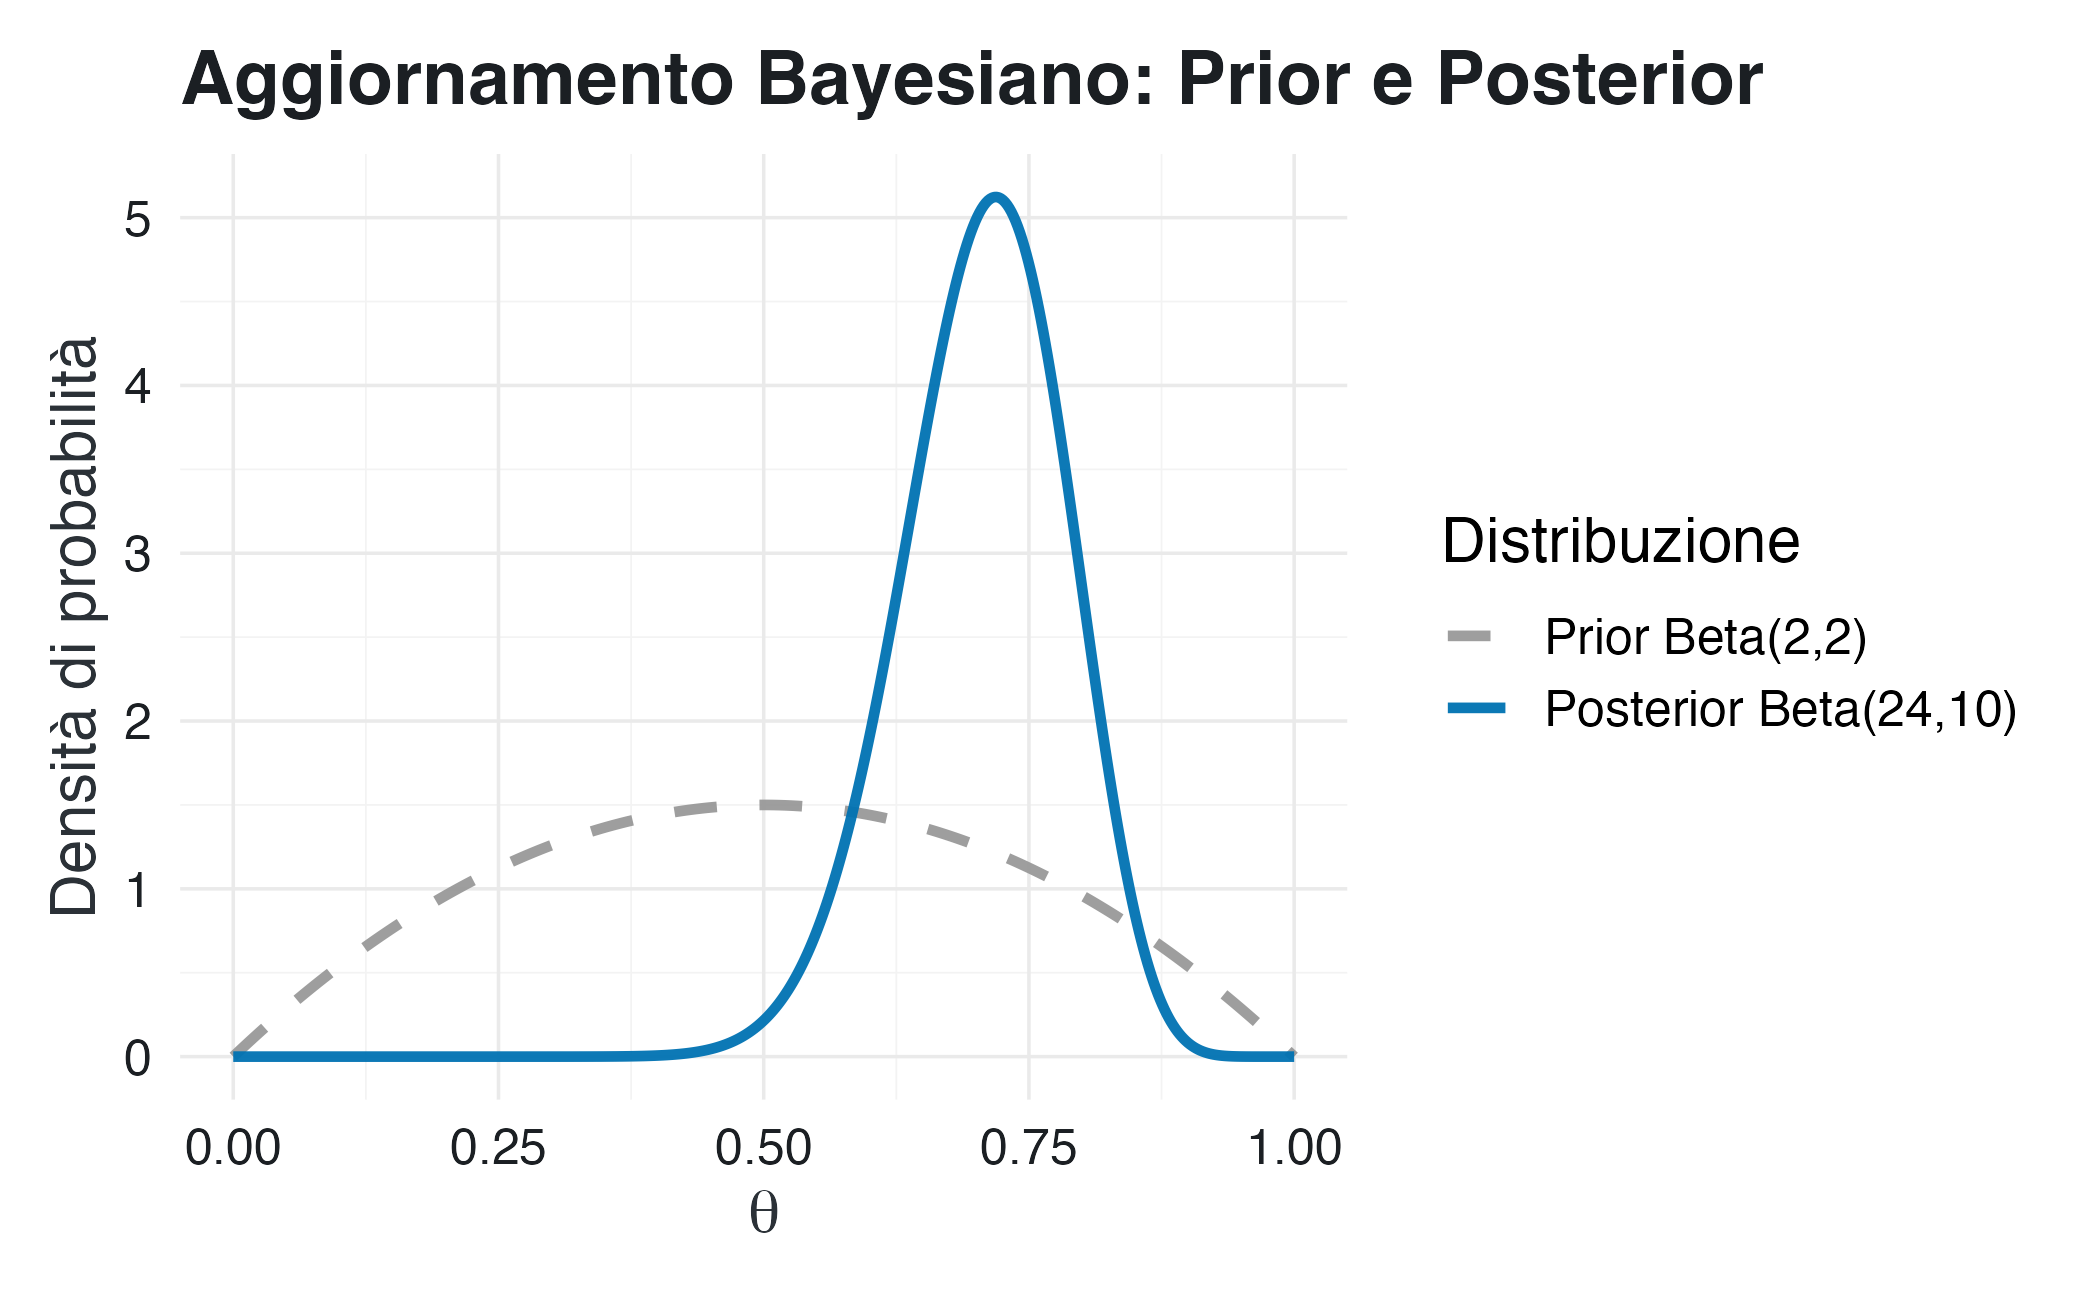
\includegraphics[width=0.85\linewidth,height=\textheight,keepaspectratio]{chapters/bayesian_inference/01_grid_approx_files/figure-pdf/unnamed-chunk-14-1.png}
\end{center}

Il grafico mostra chiaramente la trasformazione della distribuzione. La
curva tratteggiata grigia del prior Beta(2,2) è relativamente piatta e
simmetrica e riflette una conoscenza iniziale vaga, centrata su 0.5. La
curva continua blu del posterior Beta(24,10) è più alta, più stretta e
spostata verso destra, concentrandosi attorno a 0.7. Questa
trasformazione riflette l'apprendimento dai dati: l'osservazione di
ventidue successi su trenta prove ha fornito una forte evidenza che il
valore di \(\theta\) è probabilmente superiore a 0.5 e l'incertezza si è
notevolmente ridotta.

\subsection{Interpretazione psicologica dei
risultati}\label{interpretazione-psicologica-dei-risultati}

Tornando al contesto psicologico del dilemma del carrello ferroviario, i
risultati della nostra analisi bayesiana forniscono informazioni ricche
e sfumate sulla distribuzione delle credenze morali nella popolazione.
La media a posteriori di circa 0.71 suggerisce che, alla luce dei dati
osservati e delle nostre assunzioni iniziali moderate, è plausibile che
circa il 70\% della popolazione generale ritenga moralmente accettabile
l'azione di deviare il treno.

Tuttavia, la distribuzione a posteriori completa fornisce molto più di
una singola stima puntuale. L'intervallo di credibilità al 95\% può
essere calcolato individuando i percentili 2.5 e 97.5 della
distribuzione Beta a posteriori.

\begin{Shaded}
\begin{Highlighting}[]
\CommentTok{\# Calcoliamo l\textquotesingle{}intervallo di credibilità al 95\%}
\CommentTok{\# Questo intervallo contiene il 95\% della massa di probabilità a posteriori}
\NormalTok{intervallo\_credibilita }\OtherTok{\textless{}{-}} \FunctionTok{qbeta}\NormalTok{(}
  \AttributeTok{p =} \FunctionTok{c}\NormalTok{(}\FloatTok{0.025}\NormalTok{, }\FloatTok{0.975}\NormalTok{),}
  \AttributeTok{shape1 =}\NormalTok{ alpha\_posteriori,}
  \AttributeTok{shape2 =}\NormalTok{ beta\_posteriori}
\NormalTok{)}

\NormalTok{limite\_inferiore }\OtherTok{\textless{}{-}}\NormalTok{ intervallo\_credibilita[}\DecValTok{1}\NormalTok{]}
\NormalTok{limite\_superiore }\OtherTok{\textless{}{-}}\NormalTok{ intervallo\_credibilita[}\DecValTok{2}\NormalTok{]}
\end{Highlighting}
\end{Shaded}

L'intervallo di credibilità al 95\% si estende da 0.545 a 0.844.
Possiamo interpretare questo risultato affermando direttamente che,
sulla base dei dati osservati, c'è una probabilità del 95\% che la vera
proporzione θ nella popolazione sia compresa in questo intervallo.
Questa interpretazione diretta e intuitiva rappresenta uno dei vantaggi
fondamentali dell'approccio bayesiano rispetto agli intervalli di
confidenza frequentisti che, invece, richiedono interpretazioni più
contorte e controfattuali.

È anche possibile calcolare le probabilità per ipotesi sostantive
specifiche. Per esempio, potremmo chiederci: qual è la probabilità che
la maggioranza della popolazione giudichi l'azione accettabile, ovvero
che \(\theta\) sia maggiore di 0.5?

\begin{Shaded}
\begin{Highlighting}[]
\CommentTok{\# Calcoliamo la probabilità che theta sia maggiore di 0.5}
\CommentTok{\# Questo corrisponde all\textquotesingle{}area sotto la curva della Beta posteriore}
\CommentTok{\# a destra del valore 0.5}
\NormalTok{prob\_maggioranza }\OtherTok{\textless{}{-}} \FunctionTok{pbeta}\NormalTok{(}
  \AttributeTok{q =} \FloatTok{0.5}\NormalTok{,}
  \AttributeTok{shape1 =}\NormalTok{ alpha\_posteriori,}
  \AttributeTok{shape2 =}\NormalTok{ beta\_posteriori,}
  \AttributeTok{lower.tail =} \ConstantTok{FALSE}  \CommentTok{\# Vogliamo P(θ \textgreater{} 0.5), non P(θ ≤ 0.5)}
\NormalTok{)}
\end{Highlighting}
\end{Shaded}

La probabilità che \(\theta\) sia superiore a 0.5 è pari a 0.993, il che
indica un livello di certezza pressoché assoluto. Ciò indica che i dati
forniscono una prova schiacciante del fatto che la maggior parte della
popolazione giudica moralmente accettabile tale azione. Dal punto di
vista della psicologia morale, questo risultato suggerisce che, quando
si trovano di fronte a questo dilemma, le considerazioni utilitaristiche
prevalgono sulle restrizioni deontologiche nella maggior parte delle
persone.

\section{Esercizio guidato: riconoscimento di emozioni
facciali}\label{esercizio-guidato-riconoscimento-di-emozioni-facciali}

Per consolidare la comprensione dei metodi bayesiani applicati alla
stima delle proporzioni, sviluppiamo ora un esercizio completo su un
contesto psicologico diverso: il riconoscimento delle emozioni dalle
espressioni facciali. Questa competenza fondamentale della cognizione
sociale può essere studiata mediante paradigmi sperimentali in cui i
partecipanti devono classificare le espressioni emotive presentate
visivamente.

\subsection{Contesto sperimentale e obiettivo di
ricerca}\label{contesto-sperimentale-e-obiettivo-di-ricerca}

Supponiamo di condurre uno studio sulla capacità di riconoscere
l'emozione della rabbia dalle espressioni facciali. Un partecipante
osserva dieci volti che esprimono rabbia e deve decidere, per ciascuno
di essi, se l'emozione espressa è la rabbia o un'altra emozione. Il
partecipante risponde correttamente sette volte su dieci. Il nostro
obiettivo inferenziale è stimare \(\theta\), ovvero l'accuratezza
effettiva del partecipante nel riconoscere la rabbia, tenendo conto sia
delle prove fornite da queste dieci prove, sia delle aspettative
iniziali basate sulla letteratura.

La letteratura sulla psicologia delle emozioni suggerisce che la rabbia
è generalmente riconosciuta con un'accuratezza moderata, solitamente
inferiore rispetto a emozioni come la felicità, ma superiore rispetto a
emozioni più ambigue. Traduciamo questa conoscenza qualitativa in un
prior quantitativo utilizzando una distribuzione Beta(4,6). Questa
distribuzione ha una media di 0.4, riflettendo l'aspettativa che
l'accuratezza media sia moderata, con una deviazione standard
sufficientemente ampia da permettere ai dati di modificare
sostanzialmente la credenza.

\subsection{Implementazione dell'analisi con
griglia}\label{implementazione-dellanalisi-con-griglia}

Per questo esercizio utilizziamo una griglia molto più fitta rispetto
all'esempio del dilemma del carrello ferroviario, con mille punti invece
di undici. Questo approccio fornisce un'approssimazione più accurata
della distribuzione continua sottostante e consente di calcolare
statistiche riassuntive con maggiore precisione.

\begin{Shaded}
\begin{Highlighting}[]
\CommentTok{\# Definiamo i dati dell\textquotesingle{}esperimento sul riconoscimento emotivo}
\NormalTok{risposte\_corrette }\OtherTok{\textless{}{-}} \DecValTok{7}
\NormalTok{prove\_totali\_emozioni }\OtherTok{\textless{}{-}} \DecValTok{10}

\CommentTok{\# Creiamo una griglia molto fine per theta}
\CommentTok{\# Usiamo 1000 punti equidistanti tra 0 e 1}
\NormalTok{theta\_fine }\OtherTok{\textless{}{-}} \FunctionTok{seq}\NormalTok{(}\AttributeTok{from =} \DecValTok{0}\NormalTok{, }\AttributeTok{to =} \DecValTok{1}\NormalTok{, }\AttributeTok{length.out =} \DecValTok{1000}\NormalTok{)}

\CommentTok{\# Specifichiamo il prior Beta(4, 6)}
\CommentTok{\# Calcoliamo la densità per ogni punto della griglia}
\NormalTok{prior\_emozioni }\OtherTok{\textless{}{-}} \FunctionTok{dbeta}\NormalTok{(theta\_fine, }\AttributeTok{shape1 =} \DecValTok{4}\NormalTok{, }\AttributeTok{shape2 =} \DecValTok{6}\NormalTok{)}

\CommentTok{\# Calcoliamo la verosimiglianza binomiale}
\NormalTok{verosimiglianza\_emozioni }\OtherTok{\textless{}{-}} \FunctionTok{dbinom}\NormalTok{(}
  \AttributeTok{x =}\NormalTok{ risposte\_corrette,}
  \AttributeTok{size =}\NormalTok{ prove\_totali\_emozioni,}
  \AttributeTok{prob =}\NormalTok{ theta\_fine}
\NormalTok{)}

\CommentTok{\# Calcoliamo la distribuzione a posteriori non normalizzata}
\NormalTok{posteriori\_emozioni\_non\_norm }\OtherTok{\textless{}{-}}\NormalTok{ prior\_emozioni }\SpecialCharTok{*}\NormalTok{ verosimiglianza\_emozioni}

\CommentTok{\# Normalizziamo dividendo per la somma}
\CommentTok{\# Notiamo che con una griglia fine, la somma approssima un integrale}
\NormalTok{posteriori\_emozioni }\OtherTok{\textless{}{-}}\NormalTok{ posteriori\_emozioni\_non\_norm }\SpecialCharTok{/} \FunctionTok{sum}\NormalTok{(posteriori\_emozioni\_non\_norm)}
\end{Highlighting}
\end{Shaded}

La discretizzazione fine permette di ottenere un'approssimazione molto
accurata della distribuzione continua. Con mille punti, l'errore di
approssimazione è trascurabile ai fini pratici. Questo approccio ibrido
combina la trasparenza computazionale del metodo a griglia con
l'accuratezza delle soluzioni analitiche continue.

\subsection{Calcolo delle statistiche
riassuntive}\label{calcolo-delle-statistiche-riassuntive}

Una volta ottenuta la distribuzione a posteriori, calcoliamo le
statistiche che descrivono la nostra conoscenza aggiornata
sull'accuratezza del partecipante.

\begin{Shaded}
\begin{Highlighting}[]
\CommentTok{\# Calcoliamo la media a posteriori}
\NormalTok{media\_posteriori\_emozioni }\OtherTok{\textless{}{-}} \FunctionTok{sum}\NormalTok{(theta\_fine }\SpecialCharTok{*}\NormalTok{ posteriori\_emozioni)}

\CommentTok{\# Calcoliamo la varianza e la deviazione standard a posteriori}
\NormalTok{varianza\_posteriori\_emozioni }\OtherTok{\textless{}{-}} \FunctionTok{sum}\NormalTok{(}
\NormalTok{  (theta\_fine }\SpecialCharTok{{-}}\NormalTok{ media\_posteriori\_emozioni)}\SpecialCharTok{\^{}}\DecValTok{2} \SpecialCharTok{*}\NormalTok{ posteriori\_emozioni}
\NormalTok{)}
\NormalTok{sd\_posteriori\_emozioni }\OtherTok{\textless{}{-}} \FunctionTok{sqrt}\NormalTok{(varianza\_posteriori\_emozioni)}

\CommentTok{\# Identifichiamo la moda (valore con massima probabilità)}
\NormalTok{indice\_moda\_emozioni }\OtherTok{\textless{}{-}} \FunctionTok{which.max}\NormalTok{(posteriori\_emozioni)}
\NormalTok{moda\_posteriori\_emozioni }\OtherTok{\textless{}{-}}\NormalTok{ theta\_fine[indice\_moda\_emozioni]}
\end{Highlighting}
\end{Shaded}

La media a posteriori è 0.55, il che indica che la nostra migliore stima
dell'accuratezza è circa il 59\%. La moda è 0.556, molto vicina alla
media dato che la distribuzione Beta posteriore è approssimativamente
simmetrica. La deviazione standard è 0.109, riflettendo un'incertezza
moderata dovuta al numero limitato di prove osservate.

Per quantificare l'intervallo di valori plausibili per \(\theta\),
calcoliamo un intervallo di credibilità. Utilizziamo un livello del 94\%
per mostrare che la scelta del livello è arbitraria e dovrebbe essere
guidata dalle esigenze specifiche della ricerca piuttosto che da rigide
convenzioni.

\begin{Shaded}
\begin{Highlighting}[]
\CommentTok{\# Calcoliamo l\textquotesingle{}intervallo di credibilità al 94\%}
\CommentTok{\# Utilizziamo un approccio basato su campionamento dalla distribuzione}

\CommentTok{\# Generiamo un campione casuale ponderato dalla distribuzione a posteriori}
\FunctionTok{set.seed}\NormalTok{(}\DecValTok{2025}\NormalTok{)  }\CommentTok{\# Per riproducibilità}
\NormalTok{n\_campioni }\OtherTok{\textless{}{-}} \DecValTok{10000}

\CommentTok{\# Campionamento con sostituzione, ponderato dalle probabilità a posteriori}
\NormalTok{campione\_theta }\OtherTok{\textless{}{-}} \FunctionTok{sample}\NormalTok{(}
  \AttributeTok{x =}\NormalTok{ theta\_fine,}
  \AttributeTok{size =}\NormalTok{ n\_campioni,}
  \AttributeTok{replace =} \ConstantTok{TRUE}\NormalTok{,}
  \AttributeTok{prob =}\NormalTok{ posteriori\_emozioni}
\NormalTok{)}

\CommentTok{\# Calcoliamo i percentili 3\% e 97\% del campione}
\CommentTok{\# Questi approssimano l\textquotesingle{}intervallo di credibilità al 94\%}
\NormalTok{percentili }\OtherTok{\textless{}{-}} \FunctionTok{quantile}\NormalTok{(campione\_theta, }\AttributeTok{probs =} \FunctionTok{c}\NormalTok{(}\FloatTok{0.03}\NormalTok{, }\FloatTok{0.97}\NormalTok{))}
\NormalTok{limite\_inf\_94 }\OtherTok{\textless{}{-}}\NormalTok{ percentili[}\DecValTok{1}\NormalTok{]}
\NormalTok{limite\_sup\_94 }\OtherTok{\textless{}{-}}\NormalTok{ percentili[}\DecValTok{2}\NormalTok{]}
\end{Highlighting}
\end{Shaded}

L'intervallo di credibilità al 94\% si estende approssimativamente da
0.343 a 0.751. Questo intervallo quantifica l'incertezza residua
sull'accuratezza effettiva del partecipante. Con solo dieci prove,
l'intervallo è relativamente ampio, il che indica che avremmo bisogno di
più osservazioni per restringere ulteriormente la stima.

\subsection{Visualizzazione completa
dell'aggiornamento}\label{visualizzazione-completa-dellaggiornamento}

Ora creiamo una visualizzazione che mostri tutte e tre le componenti
dell'inferenza bayesiana per questo esempio.

\begin{Shaded}
\begin{Highlighting}[]
\CommentTok{\# Prepariamo i dati per la visualizzazione}
\CommentTok{\# Normalizziamo tutte le distribuzioni per renderle confrontabili}
\NormalTok{dati\_visualizzazione\_emozioni }\OtherTok{\textless{}{-}} \FunctionTok{data.frame}\NormalTok{(}
  \AttributeTok{theta =} \FunctionTok{rep}\NormalTok{(theta\_fine, }\DecValTok{3}\NormalTok{),}
  \AttributeTok{densita =} \FunctionTok{c}\NormalTok{(}
\NormalTok{    prior\_emozioni }\SpecialCharTok{/} \FunctionTok{sum}\NormalTok{(prior\_emozioni),}
\NormalTok{    verosimiglianza\_emozioni }\SpecialCharTok{/} \FunctionTok{sum}\NormalTok{(verosimiglianza\_emozioni),}
\NormalTok{    posteriori\_emozioni}
\NormalTok{  ),}
  \AttributeTok{componente =} \FunctionTok{rep}\NormalTok{(}
    \FunctionTok{c}\NormalTok{(}\StringTok{"Prior Beta(4,6)"}\NormalTok{, }\StringTok{"Verosimiglianza"}\NormalTok{, }\StringTok{"Posterior"}\NormalTok{),}
    \AttributeTok{each =} \FunctionTok{length}\NormalTok{(theta\_fine)}
\NormalTok{  )}
\NormalTok{)}

\CommentTok{\# Convertiamo in fattore ordinato}
\NormalTok{dati\_visualizzazione\_emozioni}\SpecialCharTok{$}\NormalTok{componente }\OtherTok{\textless{}{-}} \FunctionTok{factor}\NormalTok{(}
\NormalTok{  dati\_visualizzazione\_emozioni}\SpecialCharTok{$}\NormalTok{componente,}
  \AttributeTok{levels =} \FunctionTok{c}\NormalTok{(}\StringTok{"Prior Beta(4,6)"}\NormalTok{, }\StringTok{"Verosimiglianza"}\NormalTok{, }\StringTok{"Posterior"}\NormalTok{)}
\NormalTok{)}

\CommentTok{\# Creiamo il grafico comparativo}
\FunctionTok{ggplot}\NormalTok{(dati\_visualizzazione\_emozioni, }\FunctionTok{aes}\NormalTok{(}\AttributeTok{x =}\NormalTok{ theta, }\AttributeTok{y =}\NormalTok{ densita, }\AttributeTok{color =}\NormalTok{ componente)) }\SpecialCharTok{+}
  \FunctionTok{geom\_line}\NormalTok{(}\AttributeTok{size =} \FloatTok{1.2}\NormalTok{) }\SpecialCharTok{+}
  \CommentTok{\# Aggiungiamo una linea verticale per la media posteriori}
  \FunctionTok{geom\_vline}\NormalTok{(}
    \AttributeTok{xintercept =}\NormalTok{ media\_posteriori\_emozioni,}
    \AttributeTok{linetype =} \StringTok{"dashed"}\NormalTok{,}
    \AttributeTok{color =}\NormalTok{ col\_mean,  }\CommentTok{\# Rosso{-}arancio}
    \AttributeTok{size =} \FloatTok{0.8}
\NormalTok{  ) }\SpecialCharTok{+}
  \CommentTok{\# Aggiungiamo linee verticali per l\textquotesingle{}intervallo di credibilità}
  \FunctionTok{geom\_vline}\NormalTok{(}
    \AttributeTok{xintercept =} \FunctionTok{c}\NormalTok{(limite\_inf\_94, limite\_sup\_94),}
    \AttributeTok{linetype =} \StringTok{"dotted"}\NormalTok{,}
    \AttributeTok{color =}\NormalTok{ col\_interval,  }\CommentTok{\# Rosa}
    \AttributeTok{size =} \FloatTok{0.6}
\NormalTok{  ) }\SpecialCharTok{+}
  \FunctionTok{scale\_color\_manual}\NormalTok{(}
    \AttributeTok{values =} \FunctionTok{c}\NormalTok{(}
      \StringTok{"Prior Beta(4,6)"} \OtherTok{=}\NormalTok{ col\_prior,      }\CommentTok{\# Grigio}
      \StringTok{"Verosimiglianza"} \OtherTok{=}\NormalTok{ col\_likelihood, }\CommentTok{\# Arancione}
      \StringTok{"Posterior"} \OtherTok{=}\NormalTok{ col\_posterior         }\CommentTok{\# Blu}
\NormalTok{    )}
\NormalTok{  ) }\SpecialCharTok{+}
  \FunctionTok{labs}\NormalTok{(}
    \AttributeTok{x =} \FunctionTok{expression}\NormalTok{(theta }\SpecialCharTok{\textasciitilde{}} \StringTok{"(accuratezza nel riconoscimento della rabbia)"}\NormalTok{),}
    \AttributeTok{y =} \StringTok{"Densità normalizzata"}\NormalTok{,}
    \AttributeTok{title =} \StringTok{"Aggiornamento bayesiano: riconoscimento delle emozioni facciali"}\NormalTok{,}
    \AttributeTok{subtitle =} \FunctionTok{paste0}\NormalTok{(}
      \StringTok{"Dati: "}\NormalTok{, risposte\_corrette, }\StringTok{" risposte corrette su "}\NormalTok{, }
\NormalTok{      prove\_totali\_emozioni, }\StringTok{" prove | Media posteriori: "}\NormalTok{, }
      \FunctionTok{round}\NormalTok{(media\_posteriori\_emozioni, }\DecValTok{3}\NormalTok{)}
\NormalTok{    ),}
    \AttributeTok{color =} \StringTok{"Componente"}
\NormalTok{  )}
\end{Highlighting}
\end{Shaded}

\begin{center}
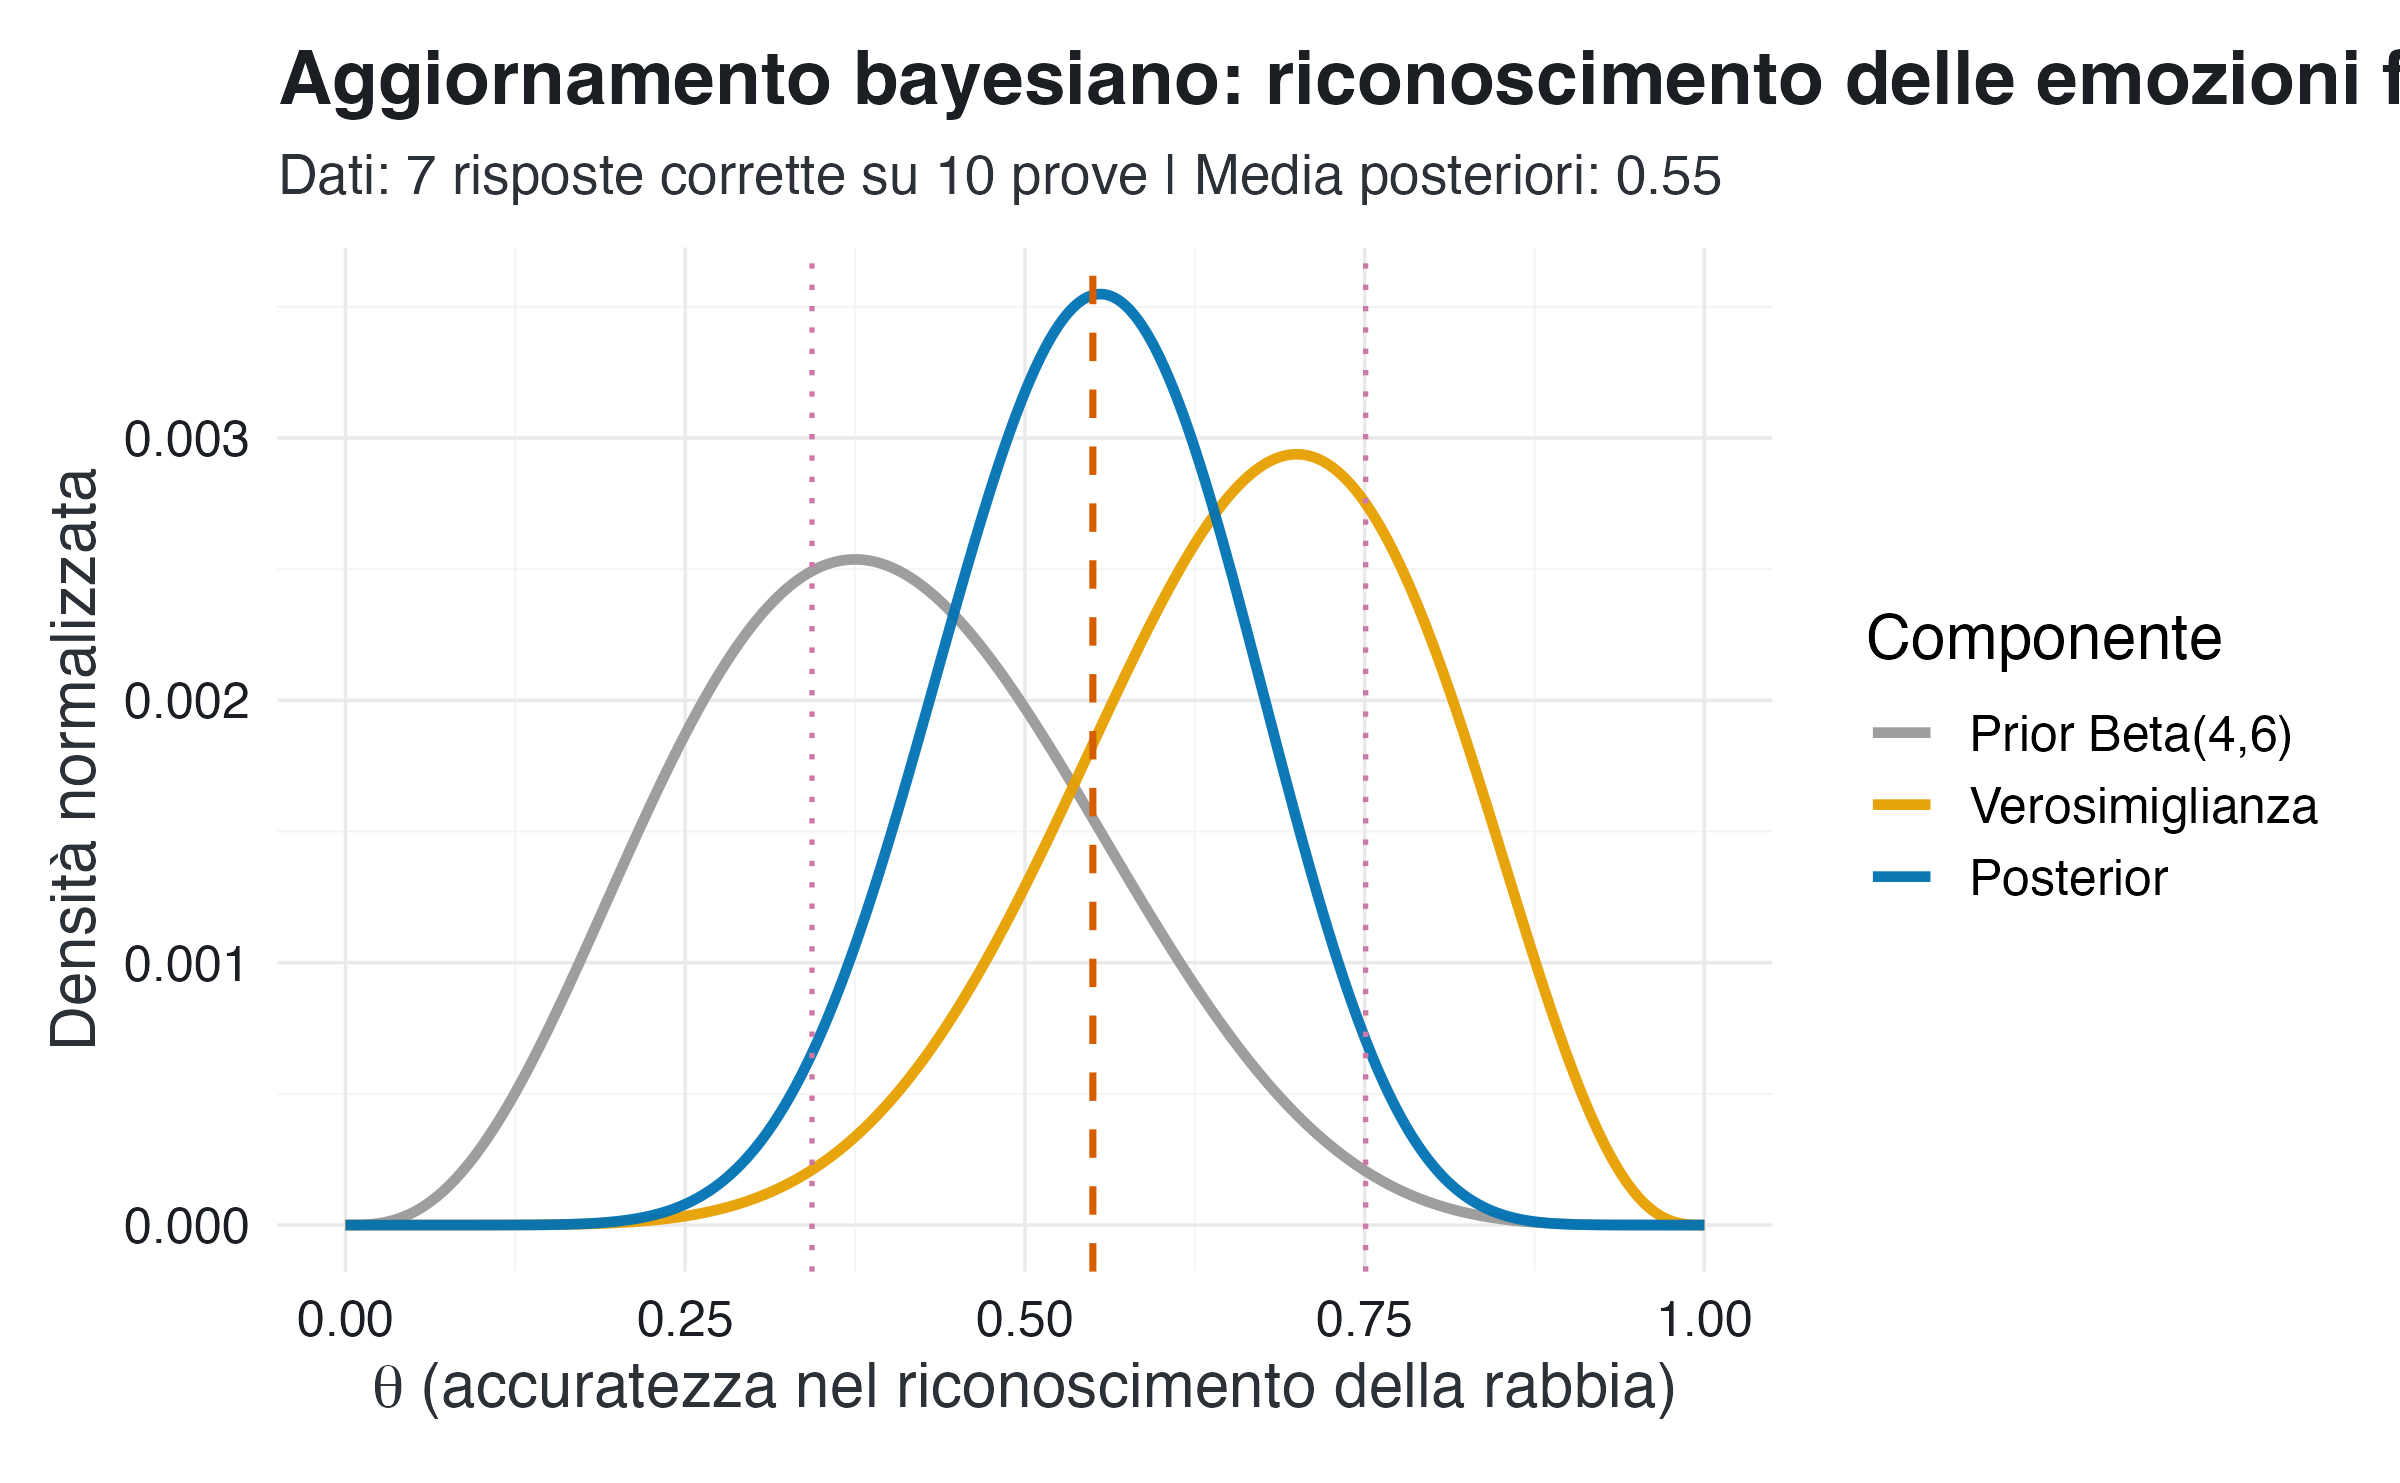
\includegraphics[width=0.85\linewidth,height=\textheight,keepaspectratio]{chapters/bayesian_inference/01_grid_approx_files/figure-pdf/unnamed-chunk-20-1.png}
\end{center}

Il grafico mostra la dinamica dell'aggiornamento bayesiano in questo
contesto. Il prior Beta(4,6) è centrato su 0.4 e riflette aspettative
moderate, basate sulla letteratura. La verosimiglianza mostra un picco
più alto attorno a 0.7, corrispondente alla proporzione di sette
risposte corrette su dieci osservate. La distribuzione a posteriori
rappresenta un compromesso: è spostata verso destra rispetto al prior,
riflettendo l'influenza dei dati, ma non coincide completamente con la
verosimiglianza, mantenendo l'influenza regolarizzante del prior.

La linea verticale tratteggiata indica la media a posteriori, mentre le
linee tratteggiate più sottili delimitano l'intervallo di credibilità al
94\%. Questa visualizzazione rende immediatamente evidente sia il valore
centrale più plausibile sia l'intervallo di incertezza associato.

\subsection{Interpretazione psicologica e implicazioni
cliniche}\label{interpretazione-psicologica-e-implicazioni-cliniche}

Dal punto di vista della psicologia cognitiva, questi risultati
suggeriscono che il partecipante mostra un'accuratezza nel
riconoscimento della rabbia leggermente superiore alle aspettative
iniziali basate sulla popolazione generale. La media posteriore di circa
0.59 indica una competenza moderata, superiore al caso (che sarebbe 0.5
se ci fossero solo due categorie emotive), ma non eccezionale.

L'ampiezza dell'intervallo di credibilità sottolinea la limitatezza di
trarre conclusioni basandosi su solo dieci prove. In un contesto di
valutazione clinica o educativa, questo risultato suggerirebbe la
necessità di ulteriori osservazioni prima di formulare conclusioni
definitive sulle competenze del partecipante. L'approccio bayesiano
rende esplicita questa limitazione, quantificando l'incertezza residua e
evitando interpretazioni eccessivamente fiduciose basate su campioni
piccoli.

Se osservassimo dieci prove aggiuntive in una sessione successiva,
potremmo aggiornare nuovamente la distribuzione utilizzando il risultato
attuale come nuovo prior. Questo processo di aggiornamento sequenziale
mostra come l'approccio bayesiano faciliti l'accumulo progressivo di
prove, un principio fondamentale per la ricerca cumulativa in
psicologia.

\section*{Riflessioni conclusive}\label{riflessioni-conclusive-5}

\markright{Riflessioni conclusive}

In questo capitolo, i principi bayesiani sono stati tradotti in
applicazioni concrete mediante due approcci complementari: il metodo
basato su griglia, che garantisce la trasparenza computazionale, e il
modello Beta-Binomiale coniugato, che assicura l'efficienza analitica.
L'implementazione diretta in R ha messo in luce tre aspetti fondamentali
dell'inferenza bayesiana.

In primo luogo, l'aggiornamento delle credenze è un processo
deterministico: la combinazione della distribuzione a priori con la
funzione di verosimiglianza e i dati osservati produce in modo univoco
la distribuzione a posteriori. Ciò elimina ogni spazio per
l'arbitrarietà del ricercatore.

In secondo luogo, il ruolo della distribuzione a priori è dinamico e
dipende dalla quantità di informazioni contenute nei dati. Con campioni
ridotti, le conoscenze iniziali influenzano in modo rilevante il
risultato, mentre con un numero maggiore di osservazioni, l'informazione
empirica prevale e la distribuzione a posteriori converge verso la
verosimiglianza normalizzata. L'influenza della distribuzione iniziale
si attenua progressivamente con l'aumentare dei dati.

In terzo luogo, la distribuzione a posteriori fornisce una descrizione
completa dell'incertezza residua sul parametro, superando la logica
delle stime puntuali tradizionali. Media, varianza, moda e intervalli di
credibilità derivano tutti dalla medesima struttura probabilistica,
senza richiedere approssimazioni asintotiche o ipotesi aggiuntive sulla
forma dell'errore.

In questo capitolo sono state utilizzate le funzioni di base di R per
rendere espliciti i passaggi computazionali e favorire una comprensione
approfondita dell'aggiornamento bayesiano. Nelle applicazioni reali,
tuttavia, l'inferenza viene spesso realizzata mediante pacchetti
specializzati che automatizzano tali passaggi, garantendo efficienza e
scalabilità. Nei capitoli successivi verranno affrontati modelli di
complessità crescente che richiederanno l'impiego di metodi
computazionali avanzati, come il campionamento MCMC. I principi
fondamentali illustrati in questo capitolo rimangono comunque validi:
specificare una struttura probabilistica per le credenze iniziali,
integrare in modo sistematico l'informazione empirica e interpretare la
distribuzione a posteriori come la rappresentazione più completa e
coerente della conoscenza disponibile
(\citeproc{ref-Goligher2024}{Goligher et al., 2024}).

\section*{Bibliografia}\label{bibliografia-7}

\markright{Bibliografia}

\chapter{Famiglie coniugate come scorciatoie
computazionali}\label{famiglie-coniugate-come-scorciatoie-computazionali}

\begin{tcolorbox}[enhanced jigsaw, arc=.35mm, bottomrule=.15mm, breakable, colback=white, colframe=quarto-callout-note-color-frame, left=2mm, leftrule=.75mm, opacityback=0, rightrule=.15mm, toprule=.15mm]

Questo capitolo non introduce nuovi elementi della teoria della
probabilità. Il suo scopo è più circoscritto: mostrare come alcune
coppie prior-verosimiglianza permettano di calcolare la distribuzione a
posteriori in forma chiusa. Le famiglie coniugate sono quindi utilizzate
come \textbf{scorciatoie computazionali} per visualizzare chiaramente
l'aggiornamento bayesiano.

\end{tcolorbox}

\begin{tcolorbox}[enhanced jigsaw, arc=.35mm, bottomrule=.15mm, breakable, colback=white, colframe=quarto-callout-important-color-frame, left=2mm, leftrule=.75mm, opacityback=0, rightrule=.15mm, toprule=.15mm]

\textbf{Da sapere.} Una prior è coniugata rispetto a una verosimiglianza
quando la distribuzione a posteriori appartiene alla stessa famiglia
della prior. Nei modelli coniugati l'aggiornamento bayesiano può essere
ottenuto modificando direttamente i parametri della distribuzione,
rendendo trasparente il modo in cui prior e dati contribuiscono alla
posterior. La coniugazione è una scorciatoia computazionale utile, non
un criterio generale per scegliere un modello.

\textbf{Da saper fare.} Aggiornare i parametri nei modelli
Beta-Binomiale e Normale-Normale; interpretare i parametri della prior
come quantità di informazione iniziale; calcolare e rappresentare prior,
verosimiglianza e posterior; ricavare intervalli di credibilità e
probabilità posteriori; valutare la sensibilità dei risultati rispetto a
prior alternative.

\textbf{Approfondimento facoltativo.} Le coppie Gamma-Poisson e
Gamma-Esponenziale, i dettagli algebrici delle formule di aggiornamento
e l'implementazione completa delle funzioni in R possono essere
rimandati in una prima lettura.

\hyperref[sec-percorsi-lettura]{Che cosa significano queste etichette?}

\end{tcolorbox}

\begin{tcolorbox}[enhanced jigsaw, arc=.35mm, bottomrule=.15mm, bottomtitle=1mm, breakable, colback=white, colbacktitle=quarto-callout-caution-color!10!white, colframe=quarto-callout-caution-color-frame, coltitle=black, left=2mm, leftrule=.75mm, opacityback=0, opacitybacktitle=0.6, rightrule=.15mm, title=\textcolor{quarto-callout-caution-color}{\faFire}\hspace{0.5em}{Preparazione del notebook}, titlerule=0mm, toprule=.15mm, toptitle=1mm]

\begin{Shaded}
\begin{Highlighting}[]
\NormalTok{here}\SpecialCharTok{::}\FunctionTok{here}\NormalTok{(}\StringTok{"code"}\NormalTok{, }\StringTok{"\_common.R"}\NormalTok{) }\SpecialCharTok{|\textgreater{}} 
  \FunctionTok{source}\NormalTok{()}

\CommentTok{\# Load packages}
\ControlFlowTok{if}\NormalTok{ (}\SpecialCharTok{!}\FunctionTok{requireNamespace}\NormalTok{(}\StringTok{"pacman"}\NormalTok{)) }\FunctionTok{install.packages}\NormalTok{(}\StringTok{"pacman"}\NormalTok{)}
\NormalTok{pacman}\SpecialCharTok{::}\FunctionTok{p\_load}\NormalTok{(dplyr, tidyr, tibble, purrr, ggplot2)}
\end{Highlighting}
\end{Shaded}

\end{tcolorbox}

\section{Perché studiare le famiglie
coniugate}\label{perchuxe9-studiare-le-famiglie-coniugate}

Nel capitolo precedente abbiamo visto l'idea fondamentale dell'inferenza
bayesiana: combinare una distribuzione a priori con la verosimiglianza
dei dati e normalizzare il risultato. In simboli:

\[
p(\theta \mid y) \propto p(y \mid \theta)\,p(\theta).
\]

In molti modelli realistici questa operazione richiede metodi
computazionali, come il campionamento MCMC. Tuttavia, in alcuni casi
particolarmente semplici, la distribuzione a posteriori può essere
ottenuta con poche operazioni algebriche. Questi casi prendono il nome
di \textbf{modelli coniugati}.

Una distribuzione a priori è detta \textbf{coniugata} rispetto a una
verosimiglianza quando la distribuzione a posteriori appartiene alla
stessa famiglia della distribuzione a priori. Ad esempio, se il
parametro sconosciuto è una proporzione \(\theta\) e si sceglie una
distribuzione a priori Beta, l'osservazione di dati binomiali produce
una distribuzione a posteriori ancora Beta.

Il valore didattico della coniugazione è duplice:

\begin{enumerate}
\def\labelenumi{\arabic{enumi}.}
\tightlist
\item
  rende visibile il meccanismo dell'aggiornamento bayesiano;
\item
  permette di distinguere il principio generale di Bayes dalla
  difficoltà tecnica del calcolo.
\end{enumerate}

I modelli coniugati non vanno però confusi con l'intera inferenza
bayesiana. Si tratta di casi speciali utili per comprendere, controllare
e sviluppare intuizioni. Nella pratica moderna, la scelta del modello e
dei prior dovrebbe essere guidata dalla domanda di ricerca, dalla teoria
psicologica e dalla struttura dei dati e non soltanto dalla convenienza
matematica.

\section{L'idea di base: aggiornare parametri, non
formule}\label{lidea-di-base-aggiornare-parametri-non-formule}

La caratteristica più utile dei modelli coniugati è che l'aggiornamento
bayesiano si traduce in una modifica diretta dei parametri della prior.
Nel modello Beta-Binomiale, ad esempio, la prior Beta ha due parametri,
\(\alpha\) e \(\beta\). Dopo avere osservato \(y\) successi su \(n\)
prove, la posterior è:

\[
\theta \mid y \sim \text{Beta}(\alpha + y,\, \beta + n - y).
\]

In altre parole, ai parametri della prior si aggiungono i dati
osservati. Per questo motivo i parametri della prior possono essere
interpretati come \textbf{pseudo-osservazioni}: \(\alpha\) rappresenta i
successi virtuali e \(\beta\) gli insuccessi virtuali.

Algebricamente, questa interpretazione è letterale: \(\alpha\) e
\(\beta\) si sommano ai conteggi come osservazioni aggiuntive (anche
frazionari), e la media a posteriori è una media ponderata tra prior e
dati. L'avvertimento è che non si tratta di dati passati reali, ma di
una sintesi matematica delle convinzioni iniziali. È proprio questa
sommabilità a rendere esplicito che la prior ha una forza informativa
quantificabile e un peso relativo ben definito rispetto alle
osservazioni empiriche.

\section{Panoramica delle principali coppie
coniugate}\label{panoramica-delle-principali-coppie-coniugate}

La tabella seguente riassume alcune coppie coniugate ricorrenti. In
questo capitolo useremo principalmente il modello Beta-Binomiale e il
modello Normale-Normale come esempi. Gli altri casi sono riportati nei
box seguenti a titolo di riferimento operativo.

{\def\LTcaptype{none} % do not increment counter
\begin{longtable}[]{@{}
  >{\raggedright\arraybackslash}p{(\linewidth - 6\tabcolsep) * \real{0.2000}}
  >{\raggedleft\arraybackslash}p{(\linewidth - 6\tabcolsep) * \real{0.2667}}
  >{\raggedleft\arraybackslash}p{(\linewidth - 6\tabcolsep) * \real{0.2667}}
  >{\raggedleft\arraybackslash}p{(\linewidth - 6\tabcolsep) * \real{0.2667}}@{}}
\toprule\noalign{}
\begin{minipage}[b]{\linewidth}\raggedright
Dati osservati
\end{minipage} & \begin{minipage}[b]{\linewidth}\raggedleft
Parametro incognito
\end{minipage} & \begin{minipage}[b]{\linewidth}\raggedleft
Prior coniugata
\end{minipage} & \begin{minipage}[b]{\linewidth}\raggedleft
Posterior
\end{minipage} \\
\midrule\noalign{}
\endhead
\bottomrule\noalign{}
\endlastfoot
Binomiale\((n, \theta)\) & proporzione \(\theta \in [0,1]\) &
Beta\((\alpha, \beta)\) & Beta\((\alpha + y, \beta + n - y)\) \\
Normale\((\mu, \sigma^2)\), con \(\sigma\) nota & media \(\mu\) &
Normale\((\mu_0, \tau_0^2)\) & Normale\((\mu_n, \tau_n^2)\) \\
Poisson\((\lambda)\) & tasso \(\lambda > 0\) & Gamma\((a,b)\) &
Gamma\((a + \sum y_i, b + n)\) \\
Esponenziale\((\lambda)\) & tasso \(\lambda > 0\) & Gamma\((a,b)\) &
Gamma\((a + n, b + \sum t_i)\) \\
\end{longtable}
}

Nel resto del capitolo useremo sempre la parametrizzazione Gamma con
\emph{shape} \(a\) e \emph{rate} \(b\), cioè con media \(a/b\).

\section{Due funzioni essenziali}\label{due-funzioni-essenziali}

Le funzioni seguenti non sostituiscono la comprensione del modello.
Piuttosto, servono a rendere esplicito il passaggio dai parametri della
prior ai parametri della posterior.

\subsection{Beta-Binomiale: inferenza su una
proporzione}\label{beta-binomiale-inferenza-su-una-proporzione}

Il modello Beta-Binomiale è appropriato quando il dato è il numero di
successi su un numero fisso di prove. In psicologia, ad esempio, può
descrivere la proporzione di risposte corrette, la quota di partecipanti
che mostra un certo comportamento o la probabilità di risposta a un
trattamento.

\begin{Shaded}
\begin{Highlighting}[]
\NormalTok{beta\_binomiale\_aggiorna }\OtherTok{\textless{}{-}} \ControlFlowTok{function}\NormalTok{(successi, prove, alpha\_prior, beta\_prior) \{}
\NormalTok{  insuccessi }\OtherTok{\textless{}{-}}\NormalTok{ prove }\SpecialCharTok{{-}}\NormalTok{ successi}
  \FunctionTok{list}\NormalTok{(}
    \AttributeTok{alpha\_post =}\NormalTok{ alpha\_prior }\SpecialCharTok{+}\NormalTok{ successi,}
    \AttributeTok{beta\_post  =}\NormalTok{ beta\_prior }\SpecialCharTok{+}\NormalTok{ insuccessi}
\NormalTok{  )}
\NormalTok{\}}
\end{Highlighting}
\end{Shaded}

La regola è semplice: i successi osservati aumentano \(\alpha\); gli
insuccessi osservati aumentano \(\beta\).

\subsection{Normale-Normale: inferenza su una
media}\label{normale-normale-inferenza-su-una-media}

Il modello Normale-Normale è utile quando il parametro di interesse è la
media di una variabile continua e la deviazione standard osservativa può
essere considerata nota. Questa assunzione è semplificatrice, ma rende
molto chiara l'idea di \textbf{combinazione ponderata delle
informazioni}.

\begin{Shaded}
\begin{Highlighting}[]
\NormalTok{normale\_normale\_aggiorna }\OtherTok{\textless{}{-}} \ControlFlowTok{function}\NormalTok{(media\_campionaria, numerosita,}
\NormalTok{                                     sigma\_noto, mu\_prior, tau\_prior) \{}
\NormalTok{  precisione\_prior }\OtherTok{\textless{}{-}} \DecValTok{1} \SpecialCharTok{/}\NormalTok{ tau\_prior}\SpecialCharTok{\^{}}\DecValTok{2}
\NormalTok{  precisione\_dati  }\OtherTok{\textless{}{-}}\NormalTok{ numerosita }\SpecialCharTok{/}\NormalTok{ sigma\_noto}\SpecialCharTok{\^{}}\DecValTok{2}
\NormalTok{  precisione\_post  }\OtherTok{\textless{}{-}}\NormalTok{ precisione\_prior }\SpecialCharTok{+}\NormalTok{ precisione\_dati}
\NormalTok{  varianza\_post    }\OtherTok{\textless{}{-}} \DecValTok{1} \SpecialCharTok{/}\NormalTok{ precisione\_post}
\NormalTok{  mu\_post }\OtherTok{\textless{}{-}}\NormalTok{ varianza\_post }\SpecialCharTok{*}\NormalTok{ (}
\NormalTok{    mu\_prior }\SpecialCharTok{*}\NormalTok{ precisione\_prior }\SpecialCharTok{+}\NormalTok{ media\_campionaria }\SpecialCharTok{*}\NormalTok{ precisione\_dati}
\NormalTok{  )}
  \FunctionTok{list}\NormalTok{(}
    \AttributeTok{mu\_post =}\NormalTok{ mu\_post,}
    \AttributeTok{sd\_post =} \FunctionTok{sqrt}\NormalTok{(varianza\_post),}
    \AttributeTok{precisione\_prior =}\NormalTok{ precisione\_prior,}
    \AttributeTok{precisione\_dati =}\NormalTok{ precisione\_dati,}
    \AttributeTok{precisione\_post =}\NormalTok{ precisione\_post}
\NormalTok{  )}
\NormalTok{\}}
\end{Highlighting}
\end{Shaded}

Qui il concetto chiave è la \emph{precisione}, ovvero il reciproco della
varianza. Una fonte di informazione più precisa incide maggiormente
sulla media a posteriori.

\section{Esempio guidato: il modello Beta-Binomiale nello studio di
Milgram}\label{esempio-guidato-il-modello-beta-binomiale-nello-studio-di-milgram}

Consideriamo un esempio tratto dallo studio classico di Milgram
(\citeproc{ref-milgram1963behavioral}{1963}) sull'obbedienza
all'autorità. Nell'esperimento, 26 partecipanti su 40 proseguirono fino
al livello massimo dello strumento sperimentale. Il dato osservato è
quindi:

\[
y = 26, \qquad n = 40.
\]

La domanda inferenziale non riguarda solo il campione osservato.
Vogliamo stimare la proporzione \(\theta\) nella popolazione di coloro
che, in condizioni sperimentali analoghe, mostrerebbe un comportamento
di obbedienza estrema.

\subsection{Specificare una prior
scettica}\label{specificare-una-prior-scettica}

Supponiamo di partire da una posizione scettica: prima di vedere i dati,
riteniamo poco plausibile che l'obbedienza estrema sia molto diffusa.
Una prior Beta(1, 10) esprime questa idea.

\begin{Shaded}
\begin{Highlighting}[]
\NormalTok{alpha\_prior }\OtherTok{\textless{}{-}} \DecValTok{1}
\NormalTok{beta\_prior }\OtherTok{\textless{}{-}} \DecValTok{10}

\NormalTok{media\_prior }\OtherTok{\textless{}{-}}\NormalTok{ alpha\_prior }\SpecialCharTok{/}\NormalTok{ (alpha\_prior }\SpecialCharTok{+}\NormalTok{ beta\_prior)}

\NormalTok{successi\_osservati }\OtherTok{\textless{}{-}} \DecValTok{26}
\NormalTok{prove\_totali }\OtherTok{\textless{}{-}} \DecValTok{40}
\end{Highlighting}
\end{Shaded}

La media della prior è 0.091. In termini intuitivi, questa prior
equivale a un'esperienza virtuale molto debole e sbilanciata verso
valori bassi di \(\theta\).

\subsection{Aggiornare la prior con i
dati}\label{aggiornare-la-prior-con-i-dati}

Applichiamo ora la regola coniugata.

\begin{Shaded}
\begin{Highlighting}[]
\NormalTok{post }\OtherTok{\textless{}{-}} \FunctionTok{beta\_binomiale\_aggiorna}\NormalTok{(}
  \AttributeTok{successi =}\NormalTok{ successi\_osservati,}
  \AttributeTok{prove =}\NormalTok{ prove\_totali,}
  \AttributeTok{alpha\_prior =}\NormalTok{ alpha\_prior,}
  \AttributeTok{beta\_prior =}\NormalTok{ beta\_prior}
\NormalTok{)}

\NormalTok{alpha\_post }\OtherTok{\textless{}{-}}\NormalTok{ post}\SpecialCharTok{$}\NormalTok{alpha\_post}
\NormalTok{beta\_post }\OtherTok{\textless{}{-}}\NormalTok{ post}\SpecialCharTok{$}\NormalTok{beta\_post}

\NormalTok{media\_post }\OtherTok{\textless{}{-}}\NormalTok{ alpha\_post }\SpecialCharTok{/}\NormalTok{ (alpha\_post }\SpecialCharTok{+}\NormalTok{ beta\_post)}
\end{Highlighting}
\end{Shaded}

La posterior è:

\[
\theta \mid y \sim \text{Beta}(27, 24).
\]

Il significato dell'aggiornamento è evidente:

\begin{itemize}
\tightlist
\item
  il parametro \(\alpha\) passa da 1 a 27, perché ai successi virtuali
  si aggiungono i 26 successi osservati;
\item
  il parametro \(\beta\) passa da 10 a 24, perché agli insuccessi
  virtuali si aggiungono i 14 insuccessi osservati.
\end{itemize}

La media a posteriori è pari a 0.529. Rispetto alla proporzione
campionaria osservata, pari a 0.65, la stima è spostata verso il basso,
riflettendo l'effetto di regolarizzazione della prior scettica.

\subsection{Visualizzare prior, verosimiglianza e
posterior}\label{visualizzare-prior-verosimiglianza-e-posterior}

\begin{Shaded}
\begin{Highlighting}[]
\NormalTok{theta }\OtherTok{\textless{}{-}} \FunctionTok{seq}\NormalTok{(}\DecValTok{0}\NormalTok{, }\DecValTok{1}\NormalTok{, }\AttributeTok{length.out =} \DecValTok{500}\NormalTok{)}

\NormalTok{prior\_df }\OtherTok{\textless{}{-}} \FunctionTok{tibble}\NormalTok{(}
  \AttributeTok{theta =}\NormalTok{ theta,}
  \AttributeTok{densita =} \FunctionTok{dbeta}\NormalTok{(theta, alpha\_prior, beta\_prior),}
  \AttributeTok{componente =} \StringTok{"Prior"}
\NormalTok{)}

\NormalTok{lik\_raw }\OtherTok{\textless{}{-}} \FunctionTok{dbinom}\NormalTok{(successi\_osservati, }\AttributeTok{size =}\NormalTok{ prove\_totali, }\AttributeTok{prob =}\NormalTok{ theta)}
\NormalTok{post\_raw }\OtherTok{\textless{}{-}} \FunctionTok{dbeta}\NormalTok{(theta, alpha\_post, beta\_post)}

\NormalTok{lik\_df }\OtherTok{\textless{}{-}} \FunctionTok{tibble}\NormalTok{(}
  \AttributeTok{theta =}\NormalTok{ theta,}
  \AttributeTok{densita =}\NormalTok{ lik\_raw }\SpecialCharTok{/} \FunctionTok{max}\NormalTok{(lik\_raw) }\SpecialCharTok{*} \FunctionTok{max}\NormalTok{(post\_raw),}
  \AttributeTok{componente =} \StringTok{"Verosimiglianza"}
\NormalTok{)}

\NormalTok{post\_df }\OtherTok{\textless{}{-}} \FunctionTok{tibble}\NormalTok{(}
  \AttributeTok{theta =}\NormalTok{ theta,}
  \AttributeTok{densita =}\NormalTok{ post\_raw,}
  \AttributeTok{componente =} \StringTok{"Posterior"}
\NormalTok{)}

\NormalTok{agg\_df }\OtherTok{\textless{}{-}} \FunctionTok{bind\_rows}\NormalTok{(prior\_df, lik\_df, post\_df) }\SpecialCharTok{|\textgreater{}}
  \FunctionTok{mutate}\NormalTok{(}\AttributeTok{componente =} \FunctionTok{factor}\NormalTok{(}
\NormalTok{    componente,}
    \AttributeTok{levels =} \FunctionTok{c}\NormalTok{(}\StringTok{"Prior"}\NormalTok{, }\StringTok{"Verosimiglianza"}\NormalTok{, }\StringTok{"Posterior"}\NormalTok{)}
\NormalTok{  ))}
\end{Highlighting}
\end{Shaded}

\begin{Shaded}
\begin{Highlighting}[]
\FunctionTok{ggplot}\NormalTok{(agg\_df, }\FunctionTok{aes}\NormalTok{(}\AttributeTok{x =}\NormalTok{ theta, }\AttributeTok{y =}\NormalTok{ densita, }\AttributeTok{color =}\NormalTok{ componente)) }\SpecialCharTok{+}
  \FunctionTok{geom\_line}\NormalTok{(}\AttributeTok{linewidth =} \FloatTok{1.2}\NormalTok{) }\SpecialCharTok{+}
  \FunctionTok{labs}\NormalTok{(}
    \AttributeTok{title =} \StringTok{"Aggiornamento Beta{-}Binomiale: dati dello studio di Milgram"}\NormalTok{,}
    \AttributeTok{subtitle =} \FunctionTok{paste0}\NormalTok{(successi\_osservati, }\StringTok{" successi su "}\NormalTok{, prove\_totali, }\StringTok{" osservazioni"}\NormalTok{),}
    \AttributeTok{x =} \FunctionTok{expression}\NormalTok{(theta),}
    \AttributeTok{y =} \StringTok{"Densita\textquotesingle{} / scala relativa"}\NormalTok{,}
    \AttributeTok{color =} \ConstantTok{NULL}
\NormalTok{  )}
\end{Highlighting}
\end{Shaded}

\begin{center}
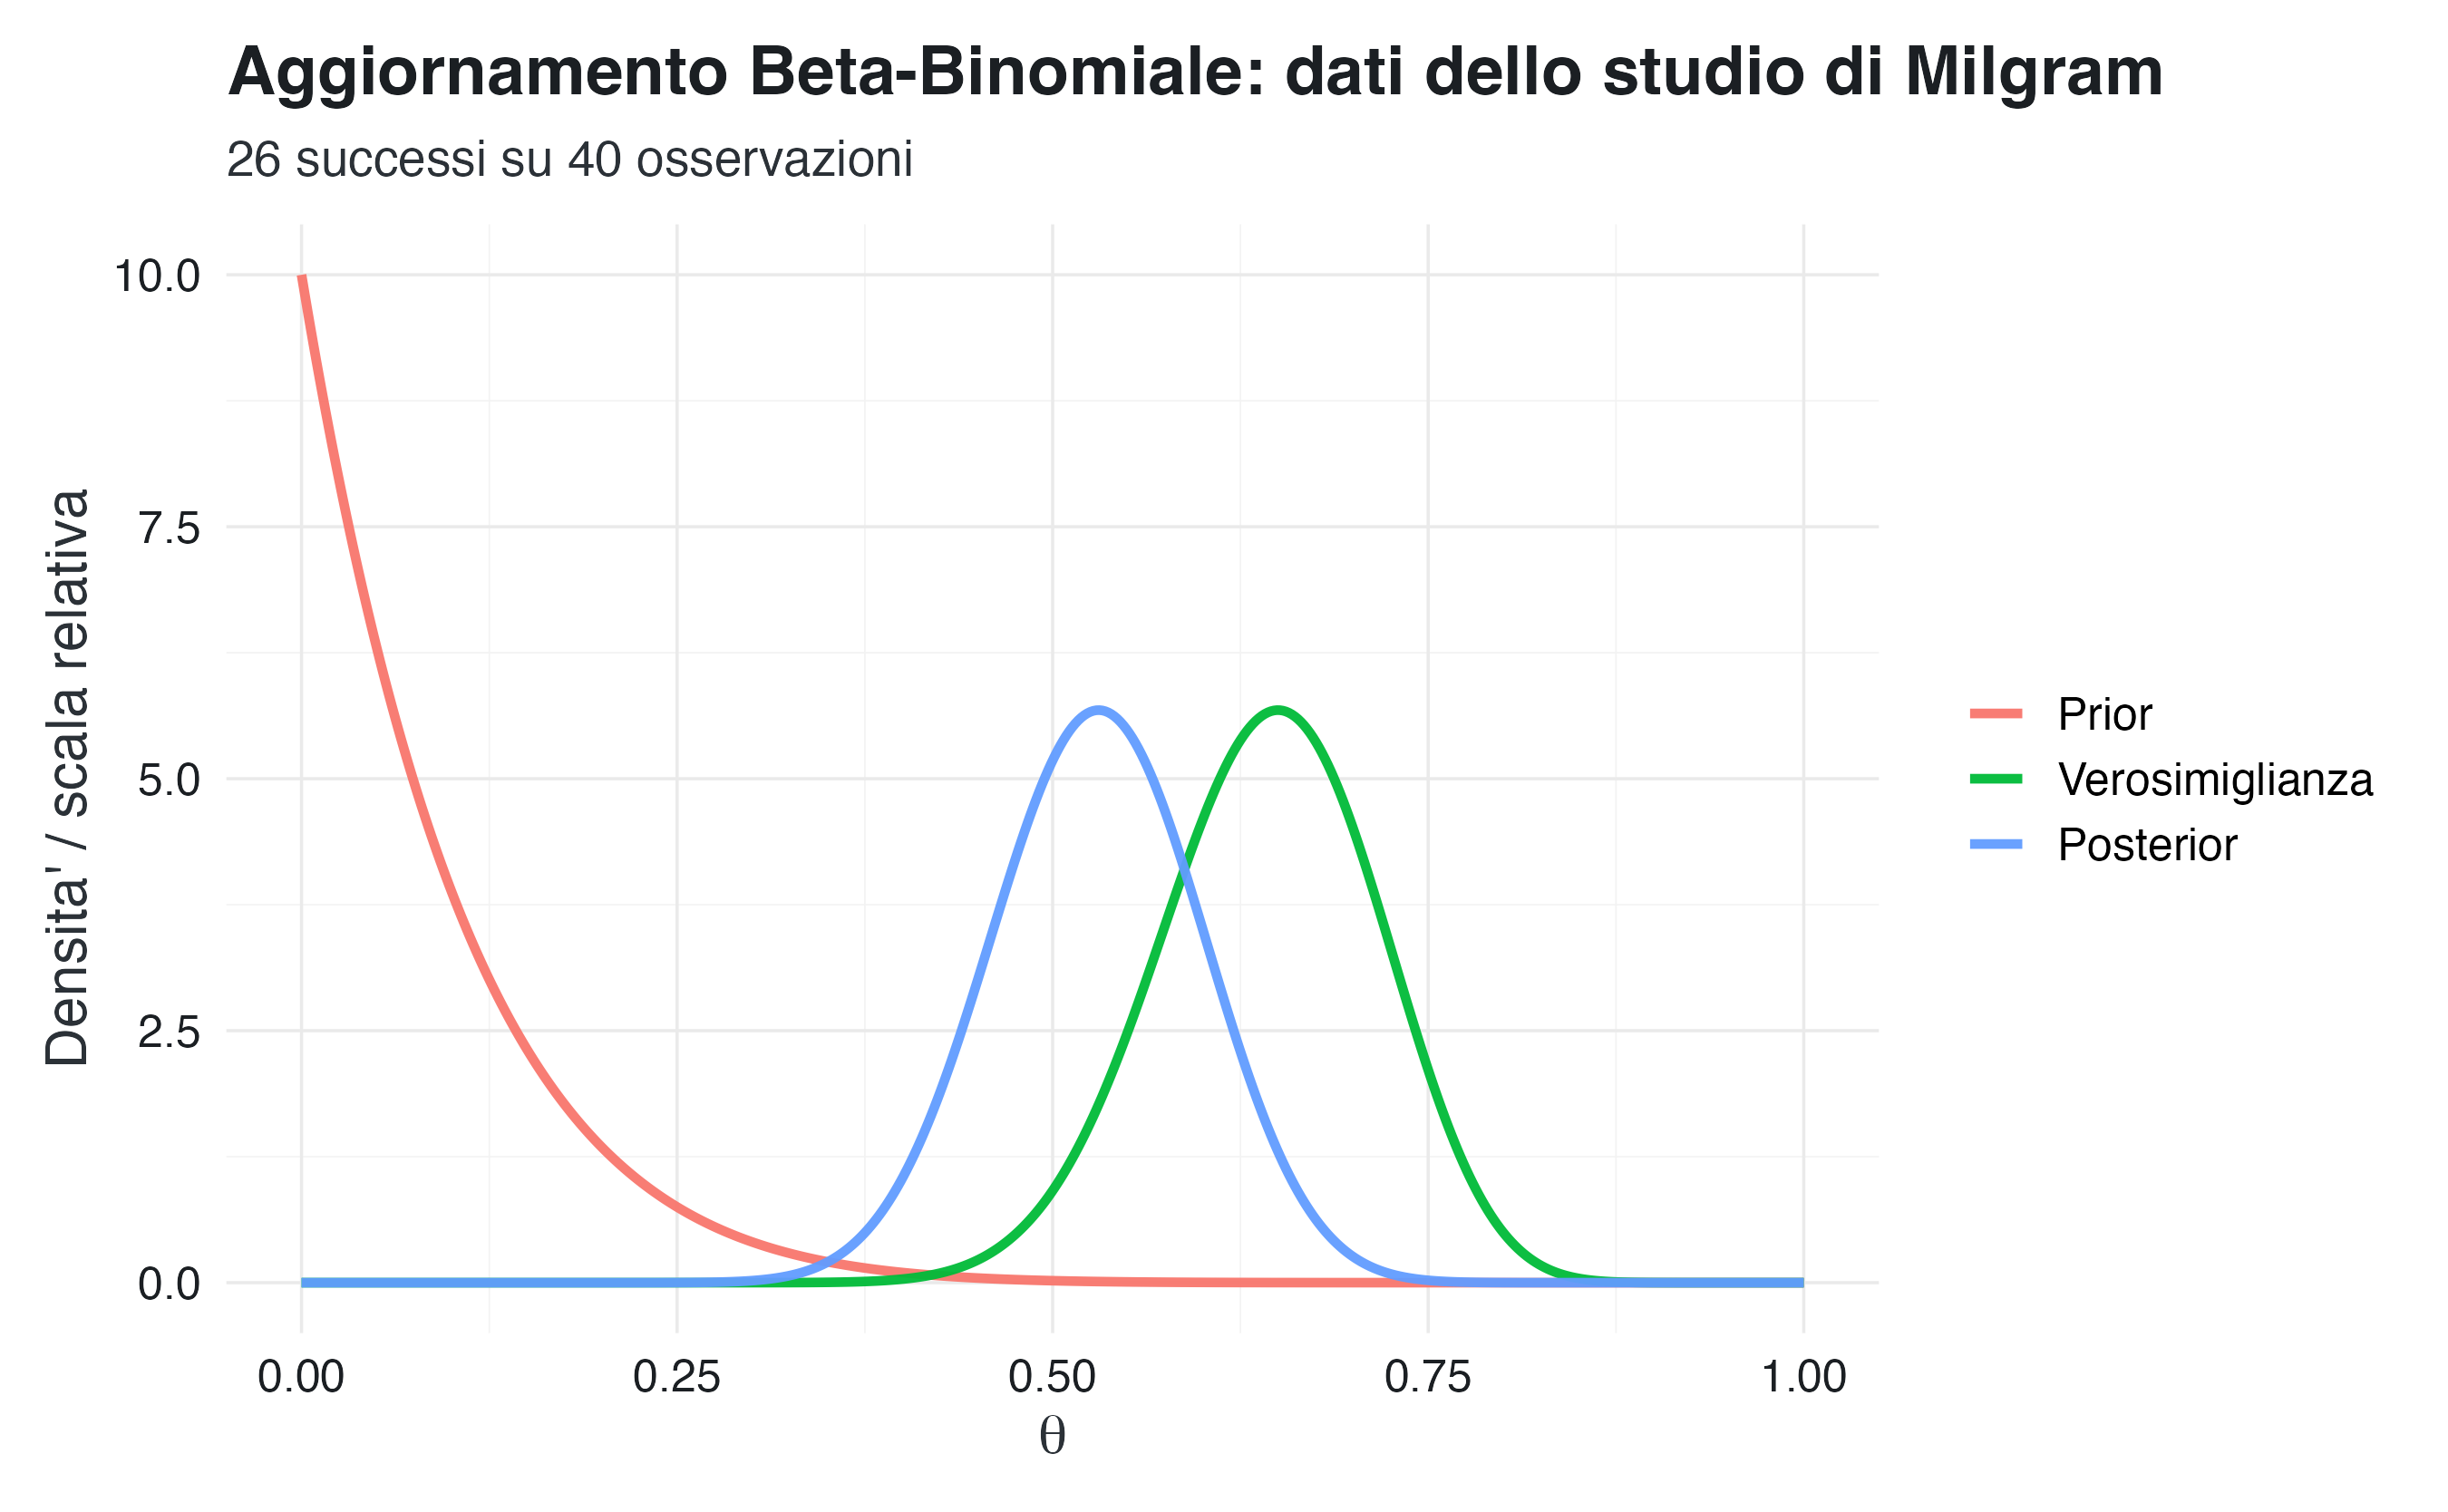
\includegraphics[width=0.85\linewidth,height=\textheight,keepaspectratio]{chapters/bayesian_inference/02_conjugate_families_files/figure-pdf/unnamed-chunk-7-1.png}
\end{center}

La verosimiglianza mostra quali valori di \(\theta\) rendono i dati
osservati più compatibili. La prior esprime lo scetticismo iniziale. La
posterior combina le due fonti di informazione. Il risultato non
coincide né con la prior né con la verosimiglianza, ma rappresenta una
sintesi probabilistica delle assunzioni iniziali e dell'evidenza
empirica.

\subsection{Riassumere la posterior}\label{riassumere-la-posterior}

Una volta ottenuta la posterior, possiamo rispondere a domande
direttamente interpretabili.

\begin{Shaded}
\begin{Highlighting}[]
\NormalTok{media\_posterior }\OtherTok{\textless{}{-}}\NormalTok{ alpha\_post }\SpecialCharTok{/}\NormalTok{ (alpha\_post }\SpecialCharTok{+}\NormalTok{ beta\_post)}
\NormalTok{moda\_posterior }\OtherTok{\textless{}{-}}\NormalTok{ (alpha\_post }\SpecialCharTok{{-}} \DecValTok{1}\NormalTok{) }\SpecialCharTok{/}\NormalTok{ (alpha\_post }\SpecialCharTok{+}\NormalTok{ beta\_post }\SpecialCharTok{{-}} \DecValTok{2}\NormalTok{)}
\NormalTok{ci\_95 }\OtherTok{\textless{}{-}} \FunctionTok{qbeta}\NormalTok{(}\FunctionTok{c}\NormalTok{(}\FloatTok{0.025}\NormalTok{, }\FloatTok{0.975}\NormalTok{), alpha\_post, beta\_post)}
\NormalTok{prob\_maggioranza }\OtherTok{\textless{}{-}} \FunctionTok{pbeta}\NormalTok{(}\FloatTok{0.5}\NormalTok{, alpha\_post, beta\_post, }\AttributeTok{lower.tail =} \ConstantTok{FALSE}\NormalTok{)}
\NormalTok{prob\_alta }\OtherTok{\textless{}{-}} \FunctionTok{pbeta}\NormalTok{(}\FloatTok{0.6}\NormalTok{, alpha\_post, beta\_post, }\AttributeTok{lower.tail =} \ConstantTok{FALSE}\NormalTok{)}
\end{Highlighting}
\end{Shaded}

{\def\LTcaptype{none} % do not increment counter
\begin{longtable}[]{@{}
  >{\raggedright\arraybackslash}p{(\linewidth - 4\tabcolsep) * \real{0.2727}}
  >{\raggedleft\arraybackslash}p{(\linewidth - 4\tabcolsep) * \real{0.3636}}
  >{\raggedleft\arraybackslash}p{(\linewidth - 4\tabcolsep) * \real{0.3636}}@{}}
\toprule\noalign{}
\begin{minipage}[b]{\linewidth}\raggedright
Domanda
\end{minipage} & \begin{minipage}[b]{\linewidth}\raggedleft
Quantità bayesiana
\end{minipage} & \begin{minipage}[b]{\linewidth}\raggedleft
Risultato
\end{minipage} \\
\midrule\noalign{}
\endhead
\bottomrule\noalign{}
\endlastfoot
Quale valore è più plausibile in media? & \(E(\theta \mid y)\) &
0.529 \\
Quale valore ha densità massima? & moda posterior & 0.531 \\
Qual è un intervallo credibile al 95\%? & quantili posterior & {[}0.393,
0.663{]} \\
Quanto è plausibile che la proporzione superi il 50\%? &
\(P(\theta > .50 \mid y)\) & 0.664 \\
Quanto è plausibile che superi il 60\%? & \(P(\theta > .60 \mid y)\) &
0.156 \\
\end{longtable}
}

Il vantaggio dell'approccio bayesiano non consiste solo nell'ottenere
una stima puntuale. La distribuzione a posteriori consente di formulare
affermazioni probabilistiche del tipo: dati il modello, la distribuzione
a priori e i dati osservati, la probabilità che il parametro \(\theta\)
superi una certa soglia è pari a un certo valore.

\subsection{Sensibilità alla prior}\label{sensibilituxe0-alla-prior}

Poiché la prior influenza la posterior, è buona pratica verificare
quanto i risultati dipendano dalla scelta iniziale. Confrontiamo tre
prior:

\begin{itemize}
\tightlist
\item
  Beta(1, 1), uniforme;
\item
  Beta(1, 10), scettica;
\item
  Beta(10, 10), centrata su 0.5 e più concentrata.
\end{itemize}

\begin{Shaded}
\begin{Highlighting}[]
\NormalTok{prior\_sens }\OtherTok{\textless{}{-}} \FunctionTok{tribble}\NormalTok{(}
  \SpecialCharTok{\textasciitilde{}}\NormalTok{prior, }\SpecialCharTok{\textasciitilde{}}\NormalTok{alpha\_prior, }\SpecialCharTok{\textasciitilde{}}\NormalTok{beta\_prior,}
  \StringTok{"Uniforme: Beta(1, 1)"}\NormalTok{, }\DecValTok{1}\NormalTok{, }\DecValTok{1}\NormalTok{,}
  \StringTok{"Scettica: Beta(1, 10)"}\NormalTok{, }\DecValTok{1}\NormalTok{, }\DecValTok{10}\NormalTok{,}
  \StringTok{"Moderata: Beta(10, 10)"}\NormalTok{, }\DecValTok{10}\NormalTok{, }\DecValTok{10}
\NormalTok{) }\SpecialCharTok{|\textgreater{}}
  \FunctionTok{mutate}\NormalTok{(}
    \AttributeTok{alpha\_post =}\NormalTok{ alpha\_prior }\SpecialCharTok{+}\NormalTok{ successi\_osservati,}
    \AttributeTok{beta\_post =}\NormalTok{ beta\_prior }\SpecialCharTok{+}\NormalTok{ prove\_totali }\SpecialCharTok{{-}}\NormalTok{ successi\_osservati,}
    \AttributeTok{media\_post =}\NormalTok{ alpha\_post }\SpecialCharTok{/}\NormalTok{ (alpha\_post }\SpecialCharTok{+}\NormalTok{ beta\_post),}
    \AttributeTok{prob\_theta\_gt\_50 =} \FunctionTok{pbeta}\NormalTok{(}\FloatTok{0.5}\NormalTok{, alpha\_post, beta\_post, }\AttributeTok{lower.tail =} \ConstantTok{FALSE}\NormalTok{),}
    \AttributeTok{prob\_theta\_gt\_60 =} \FunctionTok{pbeta}\NormalTok{(}\FloatTok{0.6}\NormalTok{, alpha\_post, beta\_post, }\AttributeTok{lower.tail =} \ConstantTok{FALSE}\NormalTok{)}
\NormalTok{  )}

\NormalTok{prior\_sens}
\CommentTok{\#\textgreater{} \# A tibble: 3 x 8}
\CommentTok{\#\textgreater{}   prior                  alpha\_prior beta\_prior alpha\_post beta\_post media\_post}
\CommentTok{\#\textgreater{}   \textless{}chr\textgreater{}                        \textless{}dbl\textgreater{}      \textless{}dbl\textgreater{}      \textless{}dbl\textgreater{}     \textless{}dbl\textgreater{}      \textless{}dbl\textgreater{}}
\CommentTok{\#\textgreater{} 1 Uniforme: Beta(1, 1)             1          1         27        15      0.643}
\CommentTok{\#\textgreater{} 2 Scettica: Beta(1, 10)            1         10         27        24      0.529}
\CommentTok{\#\textgreater{} 3 Moderata: Beta(10, 10)          10         10         36        24      0.6  }
\CommentTok{\#\textgreater{}   prob\_theta\_gt\_50 prob\_theta\_gt\_60}
\CommentTok{\#\textgreater{}              \textless{}dbl\textgreater{}            \textless{}dbl\textgreater{}}
\CommentTok{\#\textgreater{} 1            0.970            0.725}
\CommentTok{\#\textgreater{} 2            0.664            0.156}
\CommentTok{\#\textgreater{} 3            0.941            0.507}
\end{Highlighting}
\end{Shaded}

\begin{Shaded}
\begin{Highlighting}[]
\NormalTok{sens\_df }\OtherTok{\textless{}{-}}\NormalTok{ prior\_sens }\SpecialCharTok{|\textgreater{}}
  \FunctionTok{select}\NormalTok{(prior, alpha\_post, beta\_post) }\SpecialCharTok{|\textgreater{}}
\NormalTok{  tidyr}\SpecialCharTok{::}\FunctionTok{crossing}\NormalTok{(}\AttributeTok{theta =}\NormalTok{ theta) }\SpecialCharTok{|\textgreater{}}
  \FunctionTok{mutate}\NormalTok{(}\AttributeTok{densita =} \FunctionTok{dbeta}\NormalTok{(theta, alpha\_post, beta\_post))}
\end{Highlighting}
\end{Shaded}

\begin{Shaded}
\begin{Highlighting}[]
\FunctionTok{ggplot}\NormalTok{(sens\_df, }\FunctionTok{aes}\NormalTok{(}\AttributeTok{x =}\NormalTok{ theta, }\AttributeTok{y =}\NormalTok{ densita, }\AttributeTok{color =}\NormalTok{ prior)) }\SpecialCharTok{+}
  \FunctionTok{geom\_line}\NormalTok{(}\AttributeTok{linewidth =} \FloatTok{1.1}\NormalTok{) }\SpecialCharTok{+}
  \FunctionTok{labs}\NormalTok{(}
    \AttributeTok{title =} \StringTok{"Sensibilita\textquotesingle{} della posterior alla scelta della prior"}\NormalTok{,}
    \AttributeTok{x =} \FunctionTok{expression}\NormalTok{(theta),}
    \AttributeTok{y =} \StringTok{"Densita\textquotesingle{} posterior"}\NormalTok{,}
    \AttributeTok{color =} \ConstantTok{NULL}
\NormalTok{  )}
\end{Highlighting}
\end{Shaded}

\begin{center}
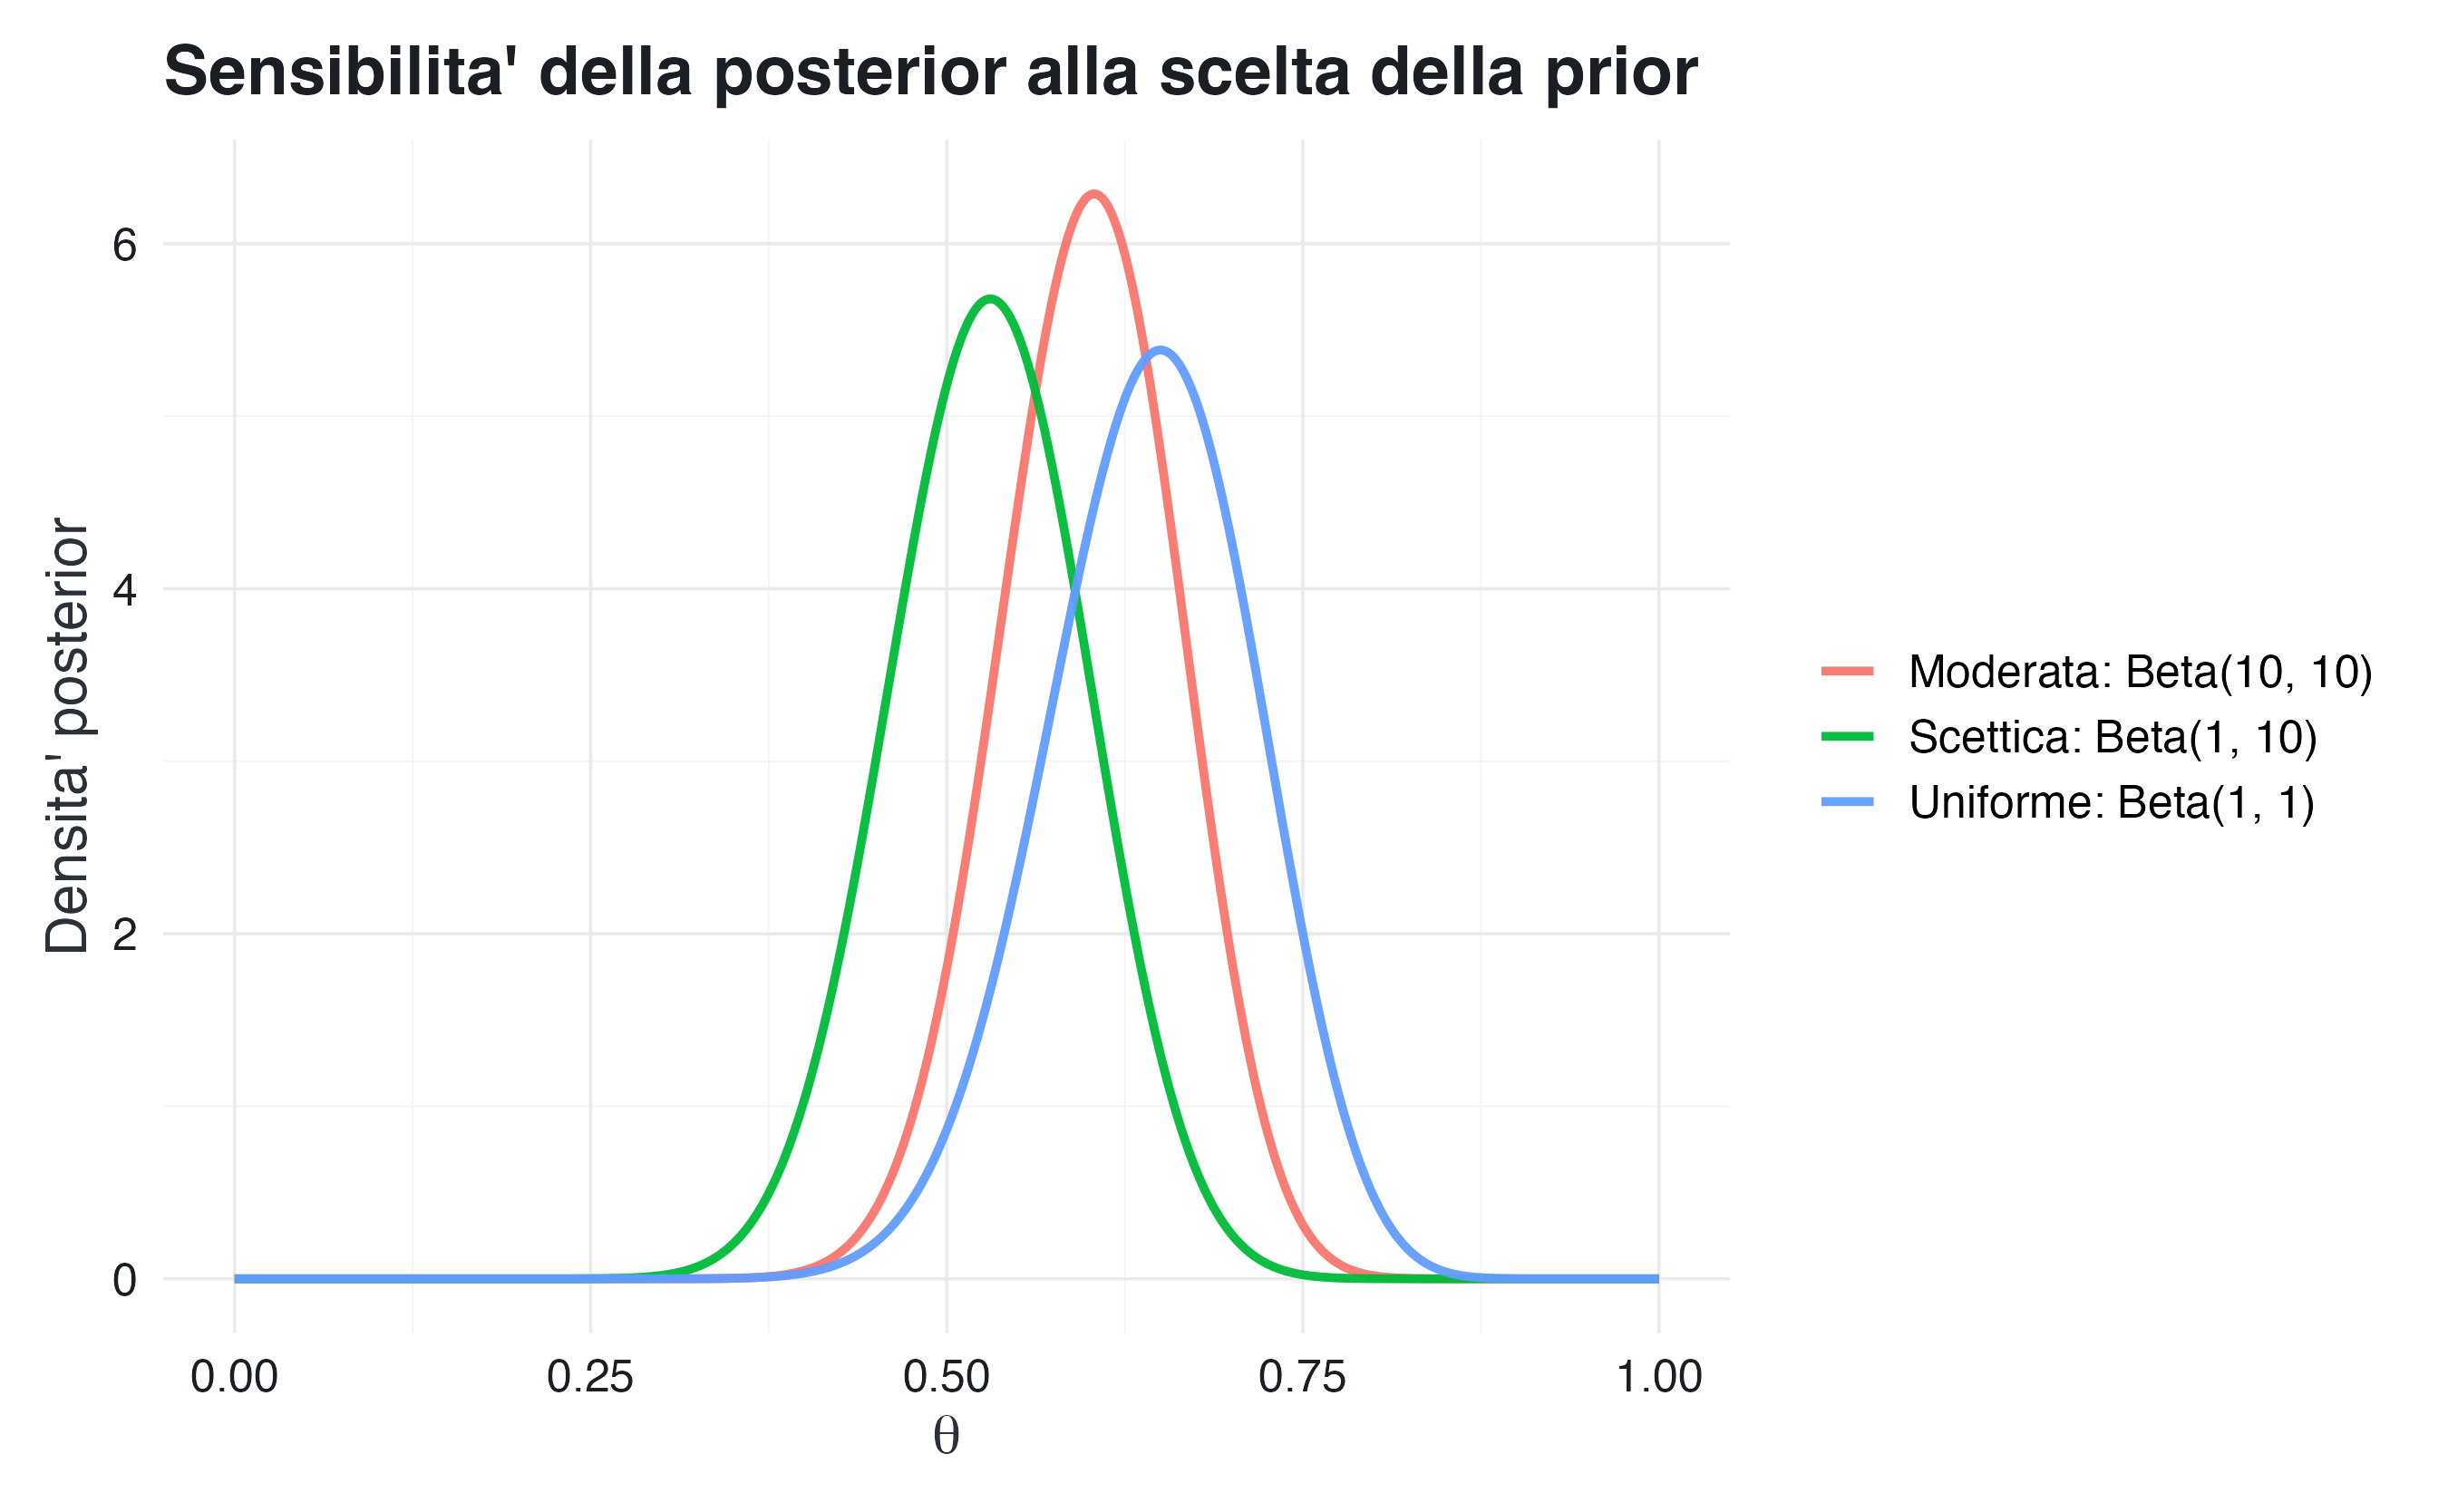
\includegraphics[width=0.85\linewidth,height=\textheight,keepaspectratio]{chapters/bayesian_inference/02_conjugate_families_files/figure-pdf/unnamed-chunk-11-1.png}
\end{center}

Quando i dati sono numerosi e informativi, prior ragionevoli tendono a
produrre posterior simili. Quando i dati sono pochi o rumorosi, la
scelta della prior diventa più rilevante e deve essere giustificata con
particolare attenzione.

\section{Secondo esempio: il modello
Normale-Normale}\label{secondo-esempio-il-modello-normale-normale}

Consideriamo ora una misura continua standardizzata. Supponiamo di voler
stimare il punteggio medio di un gruppo a cui è stato somministrato un
test psicologico. La deviazione standard del test è nota e pari a 15
punti. Prima di osservare i dati, utilizziamo una prior centrata sulla
media normativa 100 con deviazione standard 10:

\[
\mu \sim \mathcal{N}(100, 10^2).
\]

In un campione di 25 persone osserviamo una media pari a 106.

\begin{Shaded}
\begin{Highlighting}[]
\NormalTok{mu\_prior }\OtherTok{\textless{}{-}} \DecValTok{100}
\NormalTok{tau\_prior }\OtherTok{\textless{}{-}} \DecValTok{10}
\NormalTok{sigma\_noto }\OtherTok{\textless{}{-}} \DecValTok{15}
\NormalTok{n }\OtherTok{\textless{}{-}} \DecValTok{25}
\NormalTok{media\_campionaria }\OtherTok{\textless{}{-}} \DecValTok{106}

\NormalTok{post\_norm }\OtherTok{\textless{}{-}} \FunctionTok{normale\_normale\_aggiorna}\NormalTok{(}
  \AttributeTok{media\_campionaria =}\NormalTok{ media\_campionaria,}
  \AttributeTok{numerosita =}\NormalTok{ n,}
  \AttributeTok{sigma\_noto =}\NormalTok{ sigma\_noto,}
  \AttributeTok{mu\_prior =}\NormalTok{ mu\_prior,}
  \AttributeTok{tau\_prior =}\NormalTok{ tau\_prior}
\NormalTok{)}

\NormalTok{post\_norm}
\CommentTok{\#\textgreater{} $mu\_post}
\CommentTok{\#\textgreater{} [1] 106}
\CommentTok{\#\textgreater{} }
\CommentTok{\#\textgreater{} $sd\_post}
\CommentTok{\#\textgreater{} [1] 2.87}
\CommentTok{\#\textgreater{} }
\CommentTok{\#\textgreater{} $precisione\_prior}
\CommentTok{\#\textgreater{} [1] 0.01}
\CommentTok{\#\textgreater{} }
\CommentTok{\#\textgreater{} $precisione\_dati}
\CommentTok{\#\textgreater{} [1] 0.111}
\CommentTok{\#\textgreater{} }
\CommentTok{\#\textgreater{} $precisione\_post}
\CommentTok{\#\textgreater{} [1] 0.121}
\end{Highlighting}
\end{Shaded}

La media a posteriori è 105.5 e la deviazione standard a posteriori è
2.87. La stima a posteriori si colloca tra la media a priori e la media
campionaria. La sua posizione dipende dal rapporto tra la precisione
della prior e la precisione dei dati.

\begin{Shaded}
\begin{Highlighting}[]
\NormalTok{mu\_grid }\OtherTok{\textless{}{-}} \FunctionTok{seq}\NormalTok{(}\DecValTok{85}\NormalTok{, }\DecValTok{120}\NormalTok{, }\AttributeTok{length.out =} \DecValTok{500}\NormalTok{)}

\NormalTok{norm\_df }\OtherTok{\textless{}{-}} \FunctionTok{tibble}\NormalTok{(}
  \AttributeTok{mu =} \FunctionTok{rep}\NormalTok{(mu\_grid, }\DecValTok{3}\NormalTok{),}
  \AttributeTok{densita =} \FunctionTok{c}\NormalTok{(}
    \FunctionTok{dnorm}\NormalTok{(mu\_grid, mu\_prior, tau\_prior),}
    \FunctionTok{dnorm}\NormalTok{(mu\_grid, media\_campionaria, sigma\_noto }\SpecialCharTok{/} \FunctionTok{sqrt}\NormalTok{(n)),}
    \FunctionTok{dnorm}\NormalTok{(mu\_grid, post\_norm}\SpecialCharTok{$}\NormalTok{mu\_post, post\_norm}\SpecialCharTok{$}\NormalTok{sd\_post)}
\NormalTok{  ),}
  \AttributeTok{componente =} \FunctionTok{rep}\NormalTok{(}\FunctionTok{c}\NormalTok{(}\StringTok{"Prior"}\NormalTok{, }\StringTok{"Informazione dei dati"}\NormalTok{, }\StringTok{"Posterior"}\NormalTok{), }\AttributeTok{each =} \FunctionTok{length}\NormalTok{(mu\_grid))}
\NormalTok{) }\SpecialCharTok{|\textgreater{}}
  \FunctionTok{mutate}\NormalTok{(}\AttributeTok{componente =} \FunctionTok{factor}\NormalTok{(}
\NormalTok{    componente,}
    \AttributeTok{levels =} \FunctionTok{c}\NormalTok{(}\StringTok{"Prior"}\NormalTok{, }\StringTok{"Informazione dei dati"}\NormalTok{, }\StringTok{"Posterior"}\NormalTok{)}
\NormalTok{  ))}
\end{Highlighting}
\end{Shaded}

\begin{Shaded}
\begin{Highlighting}[]
\FunctionTok{ggplot}\NormalTok{(norm\_df, }\FunctionTok{aes}\NormalTok{(}\AttributeTok{x =}\NormalTok{ mu, }\AttributeTok{y =}\NormalTok{ densita, }\AttributeTok{color =}\NormalTok{ componente)) }\SpecialCharTok{+}
  \FunctionTok{geom\_line}\NormalTok{(}\AttributeTok{linewidth =} \FloatTok{1.2}\NormalTok{) }\SpecialCharTok{+}
  \FunctionTok{labs}\NormalTok{(}
    \AttributeTok{title =} \StringTok{"Aggiornamento Normale{-}Normale"}\NormalTok{,}
    \AttributeTok{subtitle =} \StringTok{"La posterior combina prior e informazione campionaria in base alle precisioni"}\NormalTok{,}
    \AttributeTok{x =} \FunctionTok{expression}\NormalTok{(mu),}
    \AttributeTok{y =} \StringTok{"Densita\textquotesingle{}"}\NormalTok{,}
    \AttributeTok{color =} \ConstantTok{NULL}
\NormalTok{  )}
\end{Highlighting}
\end{Shaded}

\begin{center}
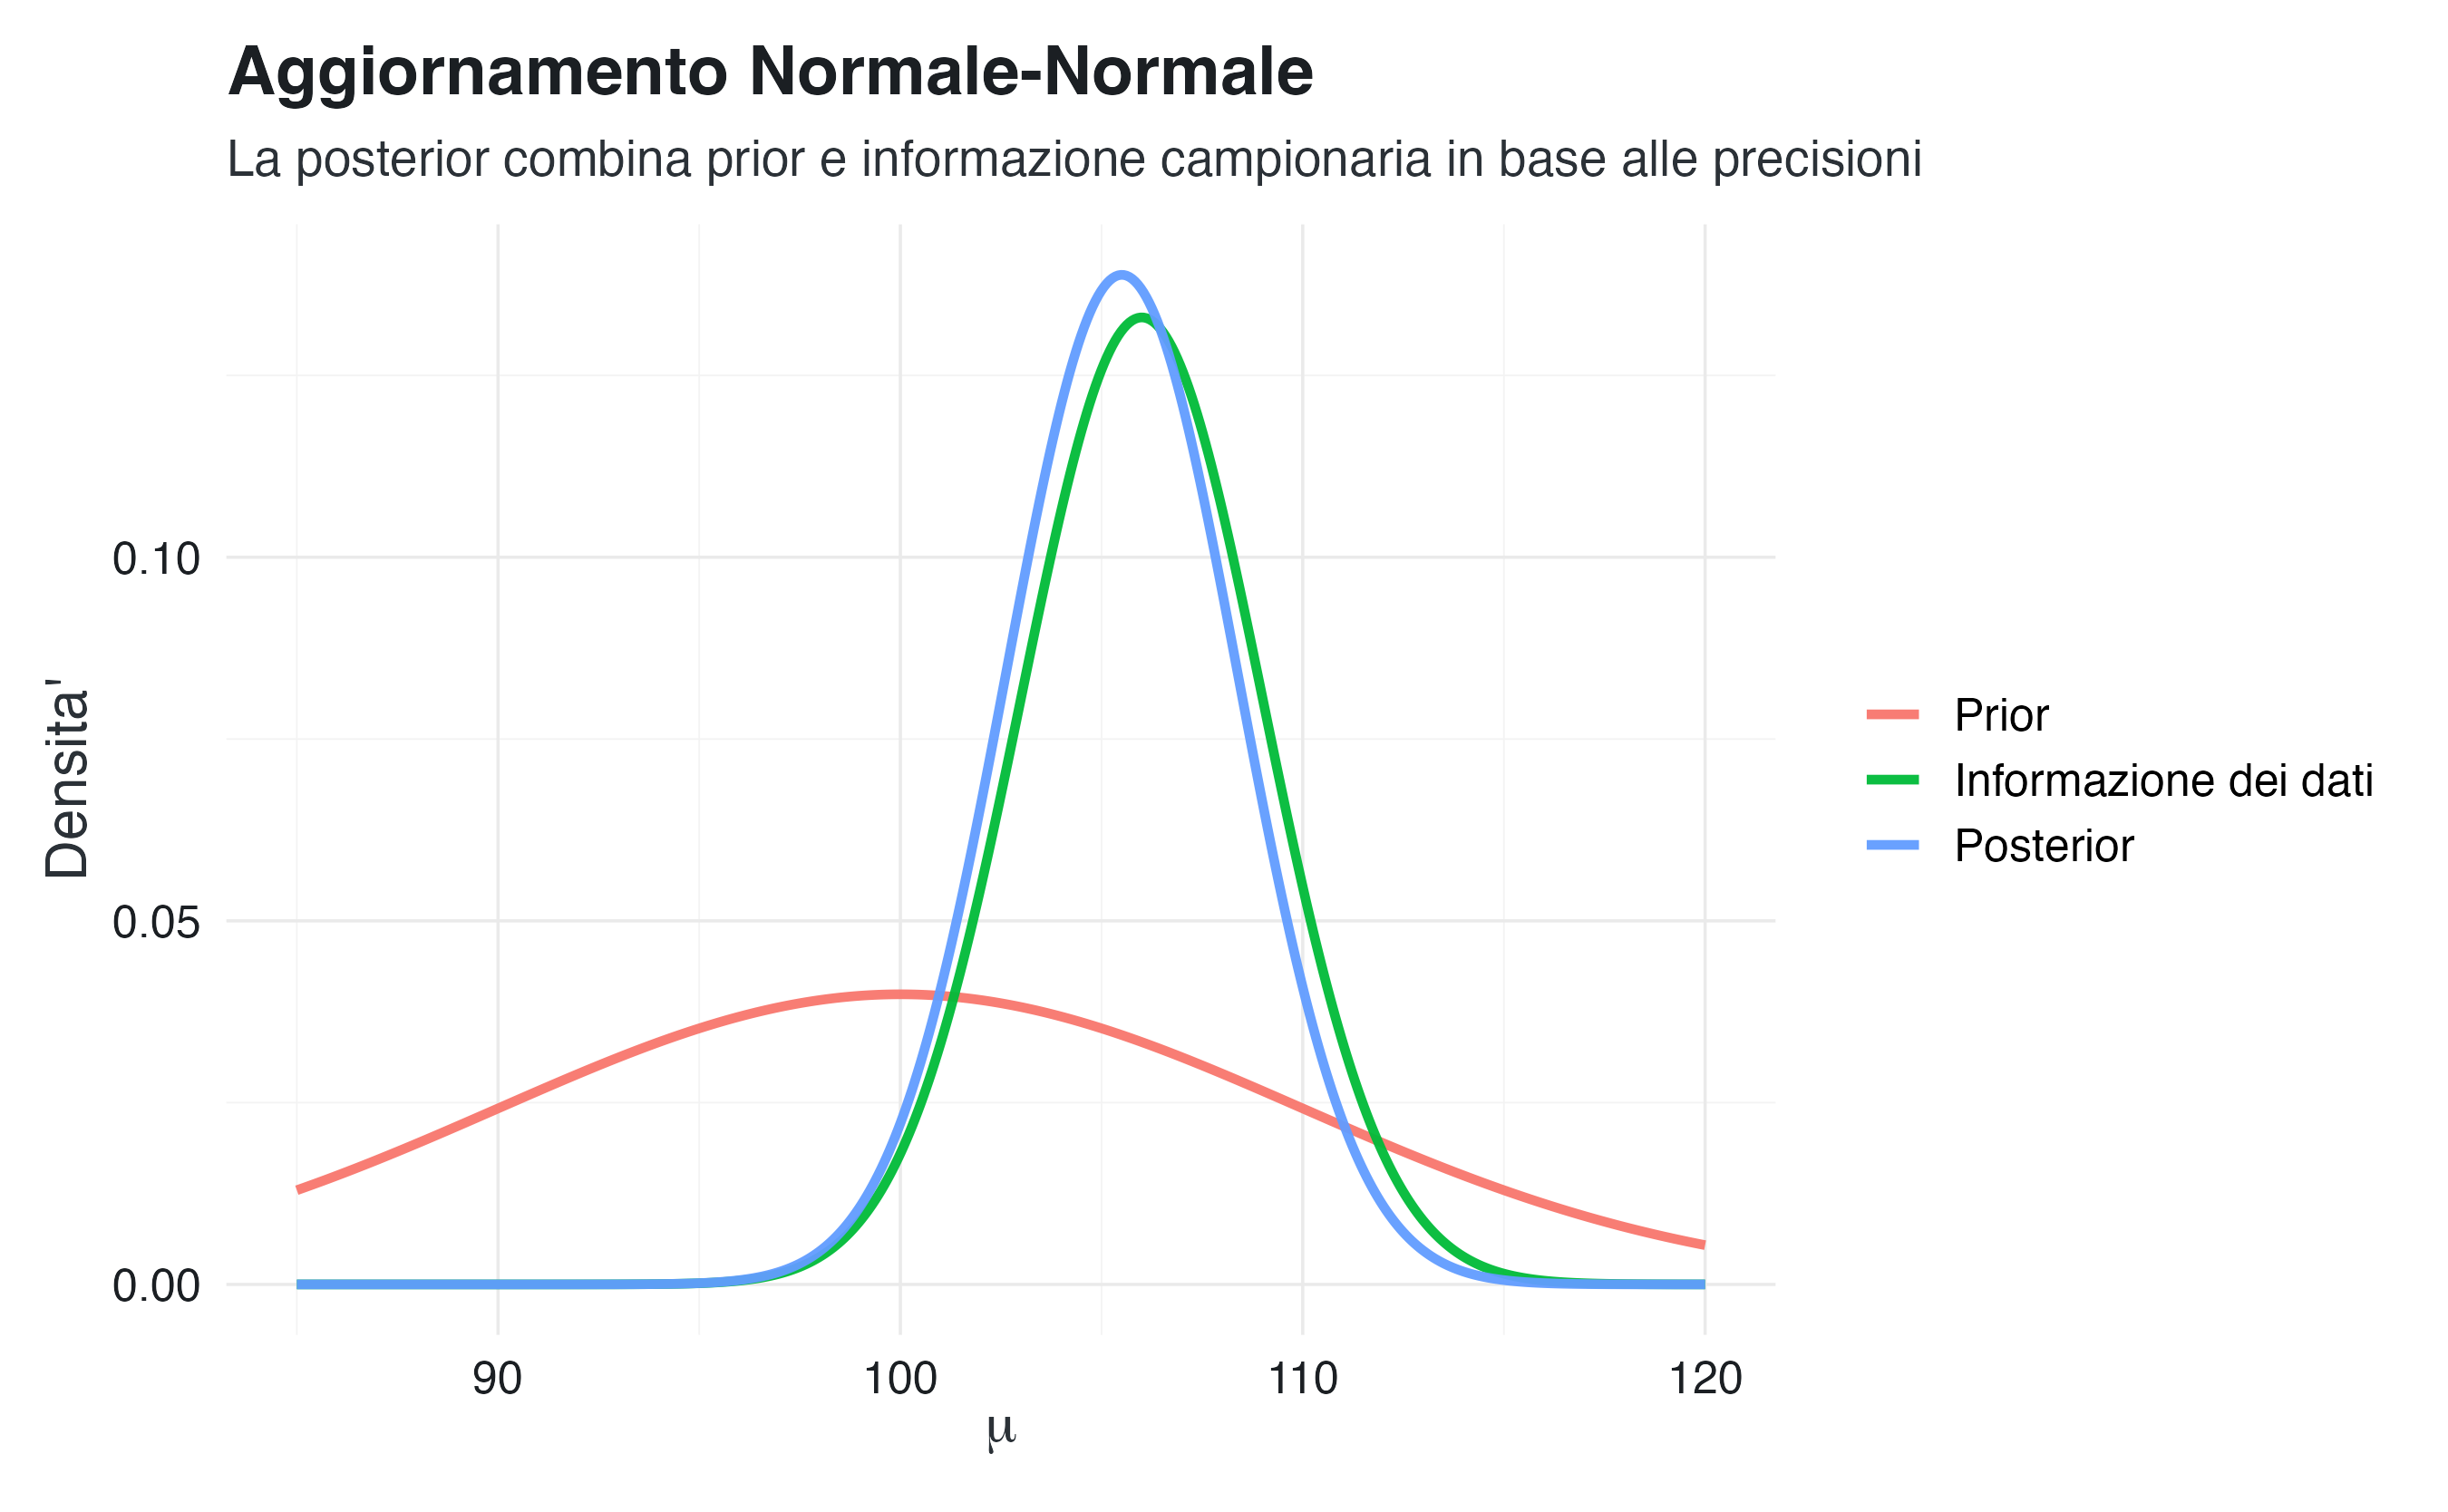
\includegraphics[width=0.85\linewidth,height=\textheight,keepaspectratio]{chapters/bayesian_inference/02_conjugate_families_files/figure-pdf/unnamed-chunk-14-1.png}
\end{center}

Questo esempio mostra un secondo schema ricorrente della coniugazione:
non sempre l'aggiornamento equivale alla somma di successi e insuccessi.
Nel modello Normale-Normale, le informazioni si combinano attraverso le
precisioni. La fonte più precisa riceve più peso nella media a
posteriori.

\begin{tcolorbox}[enhanced jigsaw, arc=.35mm, bottomrule=.15mm, bottomtitle=1mm, breakable, colback=white, colbacktitle=quarto-callout-tip-color!10!white, colframe=quarto-callout-tip-color-frame, coltitle=black, left=2mm, leftrule=.75mm, opacityback=0, opacitybacktitle=0.6, rightrule=.15mm, title=\textcolor{quarto-callout-tip-color}{\faLightbulb}\hspace{0.5em}{Formula della posterior nel modello Normale-Normale}, titlerule=0mm, toprule=.15mm, toptitle=1mm]

Se \(\sigma\) è nota, \(\bar y\) è la media campionaria e la prior è
\(\mu \sim \mathcal{N}(\mu_0, \tau_0^2)\), allora:

\[
\tau_n^2 = \left(\frac{1}{\tau_0^2} + \frac{n}{\sigma^2}\right)^{-1}
\]

e

\[
\mu_n = \tau_n^2 \left(\frac{\mu_0}{\tau_0^2} + \frac{n\bar y}{\sigma^2}\right).
\]

La media a posteriori è quindi una media ponderata tra la media a priori
e la media campionaria. I pesi dipendono dalle rispettive precisioni.

\end{tcolorbox}

\section{Box operativi: altre famiglie
coniugate}\label{box-operativi-altre-famiglie-coniugate}

Le famiglie seguenti sono utili in molti contesti applicativi, ma sono
lasciate come riferimento. Il loro scopo qui non è ampliare la teoria
delle distribuzioni, bensì mostrare che lo stesso schema di
aggiornamento ricorre in modelli diversi.

\begin{tcolorbox}[enhanced jigsaw, arc=.35mm, bottomrule=.15mm, bottomtitle=1mm, breakable, colback=white, colbacktitle=quarto-callout-note-color!10!white, colframe=quarto-callout-note-color-frame, coltitle=black, left=2mm, leftrule=.75mm, opacityback=0, opacitybacktitle=0.6, rightrule=.15mm, title=\textcolor{quarto-callout-note-color}{\faInfo}\hspace{0.5em}{Gamma-Poisson: conteggi di eventi}, titlerule=0mm, toprule=.15mm, toptitle=1mm]

Il modello Gamma-Poisson è adatto a dati di conteggio: numero di errori
in un compito, numero di episodi sintomatici in una settimana, numero di
comportamenti osservati in sessioni comparabili.

Se:

\[
y_i \mid \lambda \sim \text{Poisson}(\lambda)
\]

con prior:

\[
\lambda \sim \text{Gamma}(a, b),
\]

allora:

\[
\lambda \mid y \sim \text{Gamma}\left(a + \sum_i y_i,\, b + n\right).
\]

\begin{Shaded}
\begin{Highlighting}[]
\NormalTok{gamma\_poisson\_aggiorna }\OtherTok{\textless{}{-}} \ControlFlowTok{function}\NormalTok{(conteggi\_osservati, a\_prior, b\_prior) \{}
  \FunctionTok{list}\NormalTok{(}
    \AttributeTok{a\_post =}\NormalTok{ a\_prior }\SpecialCharTok{+} \FunctionTok{sum}\NormalTok{(conteggi\_osservati),}
    \AttributeTok{b\_post =}\NormalTok{ b\_prior }\SpecialCharTok{+} \FunctionTok{length}\NormalTok{(conteggi\_osservati)}
\NormalTok{  )}
\NormalTok{\}}

\NormalTok{conteggi }\OtherTok{\textless{}{-}} \FunctionTok{c}\NormalTok{(}\DecValTok{2}\NormalTok{, }\DecValTok{1}\NormalTok{, }\DecValTok{0}\NormalTok{, }\DecValTok{1}\NormalTok{)}
\NormalTok{gp }\OtherTok{\textless{}{-}} \FunctionTok{gamma\_poisson\_aggiorna}\NormalTok{(conteggi, }\AttributeTok{a\_prior =} \DecValTok{1}\NormalTok{, }\AttributeTok{b\_prior =} \DecValTok{1}\NormalTok{)}
\NormalTok{gp}
\CommentTok{\#\textgreater{} $a\_post}
\CommentTok{\#\textgreater{} [1] 5}
\CommentTok{\#\textgreater{} }
\CommentTok{\#\textgreater{} $b\_post}
\CommentTok{\#\textgreater{} [1] 5}
\end{Highlighting}
\end{Shaded}

Con questi dati la posterior è Gamma(5, 5) e la media a posteriori del
tasso è 1 eventi per intervallo.

La regola ha una lettura intuitiva: il parametro \(a\) aumenta con il
numero totale di eventi osservati, mentre \(b\) aumenta con il numero di
intervalli osservati.

\end{tcolorbox}

\begin{tcolorbox}[enhanced jigsaw, arc=.35mm, bottomrule=.15mm, bottomtitle=1mm, breakable, colback=white, colbacktitle=quarto-callout-note-color!10!white, colframe=quarto-callout-note-color-frame, coltitle=black, left=2mm, leftrule=.75mm, opacityback=0, opacitybacktitle=0.6, rightrule=.15mm, title=\textcolor{quarto-callout-note-color}{\faInfo}\hspace{0.5em}{Gamma-Esponenziale: tempi di attesa tra eventi}, titlerule=0mm, toprule=.15mm, toptitle=1mm]

Il modello Gamma-Esponenziale è utile quando non contiamo gli eventi in
intervalli fissi, ma osserviamo i tempi di attesa tra eventi
consecutivi. Ad esempio: tempo tra episodi comportamentali, tempo tra
ricadute, latenza fino a una risposta.

Se:

\[
t_i \mid \lambda \sim \text{Esponenziale}(\lambda)
\]

con prior:

\[
\lambda \sim \text{Gamma}(a,b),
\]

allora:

\[
\lambda \mid t \sim \text{Gamma}\left(a + n,\, b + \sum_i t_i\right).
\]

\begin{Shaded}
\begin{Highlighting}[]
\NormalTok{gamma\_esponenziale\_aggiorna }\OtherTok{\textless{}{-}} \ControlFlowTok{function}\NormalTok{(tempi\_osservati, a\_prior, b\_prior) \{}
  \FunctionTok{list}\NormalTok{(}
    \AttributeTok{a\_post =}\NormalTok{ a\_prior }\SpecialCharTok{+} \FunctionTok{length}\NormalTok{(tempi\_osservati),}
    \AttributeTok{b\_post =}\NormalTok{ b\_prior }\SpecialCharTok{+} \FunctionTok{sum}\NormalTok{(tempi\_osservati)}
\NormalTok{  )}
\NormalTok{\}}

\NormalTok{intervalli }\OtherTok{\textless{}{-}} \FunctionTok{c}\NormalTok{(}\FloatTok{0.5}\NormalTok{, }\FloatTok{1.2}\NormalTok{, }\FloatTok{0.8}\NormalTok{, }\FloatTok{2.4}\NormalTok{)}
\NormalTok{ge }\OtherTok{\textless{}{-}} \FunctionTok{gamma\_esponenziale\_aggiorna}\NormalTok{(intervalli, }\AttributeTok{a\_prior =} \DecValTok{1}\NormalTok{, }\AttributeTok{b\_prior =} \DecValTok{1}\NormalTok{)}
\NormalTok{ge}
\CommentTok{\#\textgreater{} $a\_post}
\CommentTok{\#\textgreater{} [1] 5}
\CommentTok{\#\textgreater{} }
\CommentTok{\#\textgreater{} $b\_post}
\CommentTok{\#\textgreater{} [1] 5.9}
\end{Highlighting}
\end{Shaded}

Con questi dati la posterior è Gamma(5, 5.9). La media a posteriori del
tasso è 0.85 eventi per unità di tempo. Il tempo medio corrispondente è
circa 1.18 unità di tempo.

La differenza rispetto al modello Gamma-Poisson è sostanziale: nel
Gamma-Poisson osserviamo conteggi; nel Gamma-Esponenziale osserviamo
durate.

\end{tcolorbox}

\begin{tcolorbox}[enhanced jigsaw, arc=.35mm, bottomrule=.15mm, bottomtitle=1mm, breakable, colback=white, colbacktitle=quarto-callout-note-color!10!white, colframe=quarto-callout-note-color-frame, coltitle=black, left=2mm, leftrule=.75mm, opacityback=0, opacitybacktitle=0.6, rightrule=.15mm, title=\textcolor{quarto-callout-note-color}{\faInfo}\hspace{0.5em}{Aggiornamento sequenziale}, titlerule=0mm, toprule=.15mm, toptitle=1mm]

Una proprietà importante dell'inferenza bayesiana è che l'aggiornamento
può essere sequenziale. La posterior ottenuta dopo una prima analisi può
diventare la prior dell'analisi successiva.

Nel modello Beta-Binomiale, ad esempio, dopo avere ottenuto Beta(27, 24)
dai dati di Milgram, possiamo incorporare una replica con 19 successi su
40 prove:

\begin{Shaded}
\begin{Highlighting}[]
\NormalTok{successi\_replica }\OtherTok{\textless{}{-}} \DecValTok{19}
\NormalTok{prove\_replica }\OtherTok{\textless{}{-}} \DecValTok{40}

\NormalTok{alpha\_post\_2 }\OtherTok{\textless{}{-}}\NormalTok{ alpha\_post }\SpecialCharTok{+}\NormalTok{ successi\_replica}
\NormalTok{beta\_post\_2 }\OtherTok{\textless{}{-}}\NormalTok{ beta\_post }\SpecialCharTok{+}\NormalTok{ prove\_replica }\SpecialCharTok{{-}}\NormalTok{ successi\_replica}
\NormalTok{media\_post\_2 }\OtherTok{\textless{}{-}}\NormalTok{ alpha\_post\_2 }\SpecialCharTok{/}\NormalTok{ (alpha\_post\_2 }\SpecialCharTok{+}\NormalTok{ beta\_post\_2)}
\end{Highlighting}
\end{Shaded}

La nuova posterior è Beta(46, 45), con media 0.505. Questo mostra come
l'inferenza bayesiana formalizzi l'accumulo progressivo dell'evidenza.

\end{tcolorbox}

\begin{tcolorbox}[enhanced jigsaw, arc=.35mm, bottomrule=.15mm, bottomtitle=1mm, breakable, colback=white, colbacktitle=quarto-callout-note-color!10!white, colframe=quarto-callout-note-color-frame, coltitle=black, left=2mm, leftrule=.75mm, opacityback=0, opacitybacktitle=0.6, rightrule=.15mm, title=\textcolor{quarto-callout-note-color}{\faInfo}\hspace{0.5em}{Nota sulle distribuzioni predittive}, titlerule=0mm, toprule=.15mm, toptitle=1mm]

I modelli coniugati permettono spesso di ottenere anche distribuzioni
predittive in forma chiusa. Ad esempio, nel modello Beta-Binomiale la
distribuzione predittiva del numero di successi in un nuovo campione
segue una distribuzione Beta-Binomiale.

In questo capitolo non sviluppiamo il tema in dettaglio, perché le
distribuzioni predittive vengono trattate nei capitoli successivi. Qui è
sufficiente ricordare la distinzione concettuale:

\begin{itemize}
\tightlist
\item
  la \textbf{posterior} descrive l'incertezza sul parametro;
\item
  la \textbf{posterior predictive} descrive l'incertezza su dati futuri.
\end{itemize}

Questa distinzione sarà centrale quando useremo le predizioni per
controllare l'adeguatezza dei modelli bayesiani.

\end{tcolorbox}

\section{Cosa imparare da questi
esempi}\label{cosa-imparare-da-questi-esempi}

Le famiglie coniugate illustrano tre idee fondamentali.

La prima è che l'aggiornamento bayesiano è una procedura ordinata: la
posterior deriva dalla combinazione tra l'informazione iniziale e i dati
osservati. Nei casi coniugati, questa combinazione è visibile
direttamente nei parametri.

La seconda è che la prior ha una forza informativa. Una prior molto
concentrata esercita un'influenza maggiore, soprattutto quando i dati
sono pochi. Una prior debole lascia più spazio alla verosimiglianza.

La terza è che i modelli coniugati sono strumenti didattici e non
vincoli metodologici. La loro semplicità aiuta a capire, ma i fenomeni
psicologici richiedono spesso modelli più flessibili, come strutture
gerarchiche, effetti individuali, distribuzioni robuste, predittori
multipli e relazioni non lineari.

\section*{Riflessioni conclusive}\label{riflessioni-conclusive-6}

\markright{Riflessioni conclusive}

Le famiglie coniugate costituiscono una palestra concettuale per
l'inferenza bayesiana. Nel modello Beta-Binomiale abbiamo visto
l'aggiornamento come somma di successi e insuccessi. Nel modello
Normale-Normale, invece, l'aggiornamento avviene tramite la combinazione
di precisioni. Nei box operativi abbiamo incontrato altri due casi
utili: il modello Gamma-Poisson per conteggi e il modello
Gamma-Esponenziale per tempi di attesa.

Il loro valore principale non risiede nella loro praticità matematica,
ma nella loro capacità di rendere il ragionamento bayesiano più chiaro.
Una volta compreso questo meccanismo, possiamo affrontare modelli più
realistici senza perdere di vista l'idea centrale: l'inferenza bayesiana
aggiorna in modo coerente l'incertezza alla luce dei dati.

Nei capitoli successivi, lo stesso principio verrà esteso alle
distribuzioni predittive e al controllo dei modelli. Questo passaggio è
importante: non ci limiteremo più a stimare i parametri, ma useremo i
modelli per generare dati plausibili e valutarne l'adeguatezza rispetto
ai fenomeni psicologici osservati.

\section*{Bibliografia}\label{bibliografia-8}

\markright{Bibliografia}

\chapter{Sintesi a
posteriori}\label{sec-bayesian-inference-summary-posterior}

\begin{tcolorbox}[enhanced jigsaw, arc=.35mm, bottomrule=.15mm, breakable, colback=white, colframe=quarto-callout-note-color-frame, left=2mm, leftrule=.75mm, opacityback=0, rightrule=.15mm, toprule=.15mm]

Nel manuale didattico abbiamo esaminato come costruire distribuzioni a
posteriori integrando la conoscenza preliminare (\emph{prior}) con i
dati osservati mediante la funzione di verosimiglianza. Abbiamo
analizzato questo processo in contesti semplici, come la stima di una
proporzione attraverso il modello Beta-Binomiale, e ne abbiamo esplorato
la generalizzazione grazie al concetto di famiglie coniugate. In questo
approfondimento ci dedicheremo a un aspetto solo accennato nel testo
principale: una volta ottenuta una distribuzione a posteriori, come
possiamo sintetizzarla e comunicarla in modo efficace?

Il \emph{posterior} non è un singolo numero, ma un'intera distribuzione
che rappresenta la nostra incertezza sul parametro. Nella pratica della
ricerca psicologica, tuttavia, dobbiamo spesso sintetizzare queste
informazioni per presentarle nei risultati di un articolo o per
confrontarle con altre stime. Questo capitolo è dedicato proprio a
questa esigenza: mostreremo come ricavare quantità riassuntive (media,
mediana, moda) e come costruire intervalli credibili che esprimano in
modo trasparente i valori più plausibili.

L'obiettivo non è ridurre l'inferenza bayesiana alla ricerca di un punto
o di un intervallo, ma imparare a \emph{comunicare l'incertezza} in modo
comprensibile, senza perdere la ricchezza informativa del posterior.
Come vedremo, anche nei contesti più complessi, la capacità di
sintetizzare correttamente le distribuzioni a posteriori è ciò che
distingue un'analisi meramente tecnica da una presentazione scientifica
chiara e convincente.

\end{tcolorbox}

\begin{tcolorbox}[enhanced jigsaw, arc=.35mm, bottomrule=.15mm, breakable, colback=white, colframe=quarto-callout-important-color-frame, left=2mm, leftrule=.75mm, opacityback=0, rightrule=.15mm, toprule=.15mm]

\textbf{Da sapere.} La distribuzione a posteriori rappresenta l'intera
incertezza sul parametro e non dovrebbe essere ridotta a una sola stima.
Media, mediana e moda descrivono aspetti diversi della sua posizione;
varianza e deviazione standard ne misurano la dispersione; gli
intervalli di credibilità identificano insiemi di valori plausibili dati
il modello, il prior e i dati.

\textbf{Da saper fare.} Scegliere e interpretare una stima puntuale
adeguata alla forma della distribuzione; calcolare intervalli di
credibilità a code uguali e di massima densità; distinguere un
intervallo di credibilità da un intervallo di confidenza; calcolare
probabilità posteriori relative a soglie o intervalli di interesse
sostantivo.

\textbf{Approfondimento facoltativo.} Le limitazioni della stima MAP, il
confronto dettagliato tra intervalli a code uguali e HPD e la sintesi
delle distribuzioni posteriori multivariate possono essere rimandati in
una prima lettura.

\hyperref[sec-percorsi-lettura]{Che cosa significano queste etichette?}

\end{tcolorbox}

\subsection*{Panoramica del capitolo}\label{panoramica-del-capitolo}

\begin{itemize}
\tightlist
\item
  Distribuzione a posteriori = conoscenza aggiornata.
\item
  Stime puntuali: MAP, media, mediana.
\item
  Incertezza: varianza e deviazione standard.
\item
  Intervalli di credibilità: simmetrici e HPD.
\item
  Verifica di ipotesi: probabilità a posteriori.
\end{itemize}

\begin{tcolorbox}[enhanced jigsaw, arc=.35mm, bottomrule=.15mm, bottomtitle=1mm, breakable, colback=white, colbacktitle=quarto-callout-caution-color!10!white, colframe=quarto-callout-caution-color-frame, coltitle=black, left=2mm, leftrule=.75mm, opacityback=0, opacitybacktitle=0.6, rightrule=.15mm, title=\textcolor{quarto-callout-caution-color}{\faFire}\hspace{0.5em}{Preparazione del Notebook}, titlerule=0mm, toprule=.15mm, toptitle=1mm]

\begin{Shaded}
\begin{Highlighting}[]
\NormalTok{here}\SpecialCharTok{::}\FunctionTok{here}\NormalTok{(}\StringTok{"code"}\NormalTok{, }\StringTok{"\_common.R"}\NormalTok{) }\SpecialCharTok{|\textgreater{}} 
  \FunctionTok{source}\NormalTok{()}

\CommentTok{\# Load packages}
\ControlFlowTok{if}\NormalTok{ (}\SpecialCharTok{!}\FunctionTok{requireNamespace}\NormalTok{(}\StringTok{"pacman"}\NormalTok{)) }\FunctionTok{install.packages}\NormalTok{(}\StringTok{"pacman"}\NormalTok{)}
\NormalTok{pacman}\SpecialCharTok{::}\FunctionTok{p\_load}\NormalTok{(mice)}
\end{Highlighting}
\end{Shaded}

\end{tcolorbox}

\section{Riepilogo numerico}\label{riepilogo-numerico}

La distribuzione a posteriori contiene in sé tutte le informazioni
disponibili sui potenziali valori del parametro. Nel caso di un
parametro unidimensionale o bidimensionale, possiamo rappresentare la
distribuzione a posteriori mediante un grafico \(p(\theta \mid y)\).
Tuttavia, quando ci troviamo di fronte a vettori di parametri con più di
due dimensioni, risulta vantaggioso eseguire una sintesi numerica della
distribuzione a posteriori. Possiamo distinguere due forme di sintesi
numerica della distribuzione a posteriori: stima puntuale e intervallo
di credibilità.

\section{Stima puntuale}\label{stima-puntuale}

Nel contesto dell'\emph{inferenza bayesiana}, stimare il valore più
credibile di un parametro \(\theta\) a partire dalla distribuzione a
posteriori può avvenire attraverso tre statistiche principali:
\emph{moda, mediana e media}. La scelta tra queste dipende dalla forma
della distribuzione a posteriori. Queste statistiche forniscono una
\emph{stima puntuale} della tendenza centrale della distribuzione, ossia
il valore a cui attribuiamo il massimo grado di fiducia soggettiva,
basandoci sia sui dati osservati sia sulle credenze a priori.

\subsection{\texorpdfstring{Moda (\emph{Massimo a Posteriori},
MAP)}{Moda (Massimo a Posteriori, MAP)}}\label{moda-massimo-a-posteriori-map}

La moda della distribuzione a posteriori, nota come stima di
\emph{massimo a posteriori (MAP)}, corrisponde al valore del parametro
\(\theta\) a cui è associata la massima densità di probabilità. Questo
concetto rappresenta l'estensione bayesiana della classica \emph{stima
di massima verosimiglianza (MLE)}, definita come:

\[
\hat{\theta}_{\text{ML}} = \arg \max_\theta L(\theta \mid y),
\] dove \(L(\theta \mid y)\) è la funzione di verosimiglianza.
Nell'approccio bayesiano, l'informazione a priori \(p(\theta)\) viene
incorporata attraverso il teorema di Bayes, portando alla definizione
della stima MAP:

\[
\hat{\theta}_{\text{MAP}} = \arg \max_\theta \, L(\theta \mid y) \, p(\theta).
\] In altre parole, \(\hat{\theta}_{\text{MAP}}\) massimizza la densità
a posteriori non normalizzata, combinando in modo esplicito l'evidenza
empirica con la conoscenza pregressa.

\subsubsection{Limitazioni della stima
MAP}\label{limitazioni-della-stima-map}

Nonostante l'interpretazione intuitiva, la stima MAP presenta alcune
limitazioni di cui è importante essere consapevoli. In primo luogo, la
sua determinazione può risultare computazionalmente impegnativa,
specialmente quando la distribuzione a posteriori viene campionata
mediante metodi MCMC: individuare con precisione il massimo in uno
spazio di parametri ad alta dimensionalità o con forme complesse
richiede tecniche specifiche e può essere instabile.

In secondo luogo, la bontà della stima MAP dipende fortemente dalla
forma della distribuzione a posteriori. In presenza di asimmetrie
marcate o di multimodalità, il massimo globale potrebbe non essere
rappresentativo della regione di alta probabilità, soprattutto se
associato a un picco stretto ma isolato, mentre la maggior parte della
massa probabilistica si trova altrove.

Infine, il MAP è intrinsecamente meno robusto di altre statistiche
centrali, come la media o la mediana a posteriori, in quanto basato
esclusivamente sul valore di massimo densità, ignorando la forma
complessiva della distribuzione. Ciò lo rende sensibile a variazioni
nella parametrizzazione del modello e poco informativo riguardo
all'incertezza complessiva sul parametro.

\subsection{Media a posteriori}\label{media-a-posteriori}

La \emph{media a posteriori} rappresenta il valore atteso del parametro
\(\theta\) rispetto alla sua distribuzione a posteriori. Formalmente,
essa è definita come:

\[
\mathbb{E}[\theta \mid y] = \int \theta \, p(\theta \mid y) \, d\theta.
\] Questa quantità costituisce una stima di \(\theta\) che tiene conto
dell'intera distribuzione a posteriori, integrando su tutti i possibili
valori del parametro. Una proprietà notevole della media a posteriori è
quella di essere lo stimatore che minimizza l'\emph{errore quadratico
medio (MSE)} nella previsione di \(\theta\), il che ne giustifica
l'ampio utilizzo in contesti di ottimizzazione statistica.

Tuttavia, in presenza di distribuzioni a posteriori marcatamente
\emph{asimmetriche} o con \emph{code pesanti}, la media potrebbe non
rappresentare adeguatamente la regione di massima densità di
probabilità. In tali casi, valori estremi possono influenzare
eccessivamente la stima, allontanando la media dalla zona in cui è
concentrata la maggior parte della massa probabilistica. Per questo
motivo, in situazioni di asimmetria pronunciata, altre statistiche come
la \emph{mediana} o la \emph{moda} a posteriori possono offrire una
rappresentazione più appropriata della tendenza centrale.

\subsection{Mediana a posteriori}\label{mediana-a-posteriori}

La \emph{mediana a posteriori} è definita come il valore del parametro
\(\theta\) che divide la distribuzione a posteriori in due parti di
uguale probabilità: il 50\% della massa probabilistica si trova al di
sotto di tale valore e il restante 50\% al di sopra. Formalmente, essa
soddisfa la condizione:

\[
P(\theta \leq \hat{\theta}_{\text{med}} \mid y) = 0.5.
\]

Rispetto alla media e alla moda a posteriori, la mediana offre una
misura di tendenza centrale particolarmente \emph{robusta}, in quanto
poco sensibile alla presenza di valori estremi o code distributive
pesanti. Questa proprietà la rende preferibile in contesti in cui la
distribuzione a posteriori presenta marcate \emph{asimmetrie} o è
\emph{multimodale}, situazioni in cui la media può essere distortta da
valori anomali e la moda può risultare instabile o non unica. Grazie
alla sua stabilità, la mediana a posteriori fornisce una
rappresentazione più affidabile della posizione centrale del parametro
quando la forma della distribuzione è irregolare, garantendo una sintesi
inferenziale solida anche in condizioni di elevata variabilità o non
normalità.

\section{Misurare l'incertezza: varianza a
posteriori}\label{misurare-lincertezza-varianza-a-posteriori}

Oltre a individuare il valore più plausibile del parametro \(\theta\), è
fondamentale quantificare l'incertezza residua associata alla nostra
stima. A questo scopo, la \emph{varianza a posteriori} fornisce una
misura della dispersione dei valori di \(\theta\) attorno alla sua
media, condizionatamente ai dati osservati \(y\). Formalmente, essa è
definita come:

\[
\mathbb{V}(\theta \mid y) = \mathbb{E}\left[(\theta - \mathbb{E}[\theta \mid y])^2 \mid y \right] = \int (\theta - \mathbb{E}[\theta \mid y])^2 \, p(\theta \mid y) \, d\theta.
\]

Un modo equivalente per calcolarla è attraverso l'identità:

\[
\mathbb{V}(\theta \mid y) = \mathbb{E}[\theta^2 \mid y] - \left(\mathbb{E}[\theta \mid y]\right)^2.
\]

Per interpretare più facilmente l'incertezza nella stessa unità di
misura del parametro \(\theta\), è utile considerare la \emph{deviazione
standard a posteriori}, data semplicemente dalla radice quadrata della
varianza.

In conclusione, mentre la moda (MAP), la media e la mediana a posteriori
forniscono diverse misure di tendenza centrale per la stima puntuale di
\(\theta\), la varianza (e la deviazione standard) a posteriori ne
quantificano l'affidabilità. La scelta tra le diverse statistiche
dipende dalla forma della distribuzione a posteriori e dagli obiettivi
dell'analisi. Nel loro insieme, questi indicatori consentono di
comunicare in modo sintetico non solo la migliore stima del parametro,
ma anche il grado di confidenza ad essa associato, elemento cruciale in
qualsiasi processo inferenziale.

\section{Intervallo di credibilità}\label{intervallo-di-credibilituxe0}

Nell'inferenza bayesiana, l'intervallo di credibilità è uno strumento
utilizzato per definire un intervallo che contiene una determinata
percentuale della massa della distribuzione a posteriori del parametro
\(\theta\). Questo intervallo riflette l'incertezza associata alla stima
del parametro: un intervallo più ampio suggerisce una maggiore
incertezza. Lo scopo principale dell'intervallo di credibilità è fornire
una misura quantitativa dell'incertezza riguardante \(\theta\).

A differenza degli intervalli di confidenza frequentisti, non esiste un
unico intervallo di credibilità per un dato livello di confidenza
\((1 - \alpha) \cdot 100\%\). In effetti, è possibile costruire un
numero infinito di tali intervalli. Per questo motivo, è necessario
stabilire criteri aggiuntivi per selezionare l'intervallo di credibilità
più appropriato. Tra le opzioni più comuni ci sono l'intervallo di
credibilità simmetrico e l'intervallo di massima densità posteriore
(HPD).

\subsection{Intervallo di credibilità
simmetrico}\label{intervallo-di-credibilituxe0-simmetrico}

Questo tipo di intervallo è centrato rispetto al punto di stima
puntuale. Se \(\hat{\theta}\) rappresenta la stima del parametro,
l'intervallo simmetrico avrà la forma
\((\hat{\theta} - a, \hat{\theta} + a)\), dove \(a\) è un valore
positivo scelto in modo tale che la massa totale inclusa sia pari a
\((1 - \alpha)\). Più formalmente, un intervallo di credibilità
simmetrico al livello \(\alpha\) può essere espresso come:

\[ 
I_{\alpha} = [q_{\alpha/2}, q_{1 - \alpha/2}], 
\] dove \(q_z\) rappresenta il quantile \(z\) della distribuzione a
posteriori. Ad esempio, un intervallo di credibilità simmetrico al 94\%
sarà:

\[ 
I_{0.06} = [q_{0.03}, q_{0.97}], 
\] dove il 3\% della massa a posteriori si trova in ciascuna delle due
code della distribuzione.

\subsection{Intervallo di credibilità più stretto (intervallo di massima
densità posteriore,
HPD)}\label{intervallo-di-credibilituxe0-piuxf9-stretto-intervallo-di-massima-densituxe0-posteriore-hpd}

L'intervallo di massima densità posteriore (HPD) è l'intervallo più
stretto possibile che contiene il \((1 - \alpha) \cdot 100\%\) della
massa a posteriori. A differenza dell'intervallo simmetrico, l'HPD
include tutti i valori di \(\theta\) che hanno la maggiore densità a
posteriori. Per costruirlo, si disegna una linea orizzontale sulla
distribuzione a posteriori e si regola l'altezza della linea in modo che
l'area sotto la curva corrisponda a \((1 - \alpha)\). L'HPD risulta
essere il più stretto tra tutti gli intervalli possibili per lo stesso
livello di confidenza. Nel caso di una distribuzione a posteriori
unimodale e simmetrica, l'HPD coincide con l'intervallo di credibilità
simmetrico.

\subsubsection{Interpretazione}\label{interpretazione-3}

Il calcolo degli \emph{intervalli di credibilità}---in particolare
dell'\emph{intervallo di massima densità posteriore} (HPD)---richiede
quasi sempre l'utilizzo di software statistici specializzati. Questo
perché, nei modelli bayesiani con distribuzioni posteriori articolate o
che richiedono simulazioni numeriche (ad esempio tramite Markov Chain
Monte Carlo), ricavare a mano i confini dell'intervallo può risultare
molto laborioso.

\subsubsection{Incertezza nel paradigma
frequentista}\label{incertezza-nel-paradigma-frequentista}

\begin{itemize}
\tightlist
\item
  \emph{Parametro fisso}: nel contesto frequentista, il parametro di
  interesse (ad esempio la media di popolazione \(\mu\)) è un valore
  costante ma sconosciuto.\\
\item
  \emph{Ripetizione ipotetica}: immaginiamo di ripetere all'infinito il
  prelievo di campioni dalla popolazione. Per ciascun campione otteniamo
  una media \(\bar{x}\) e costruendo un intervallo di confidenza al
  \(100(1-\alpha)\%\) avremo che, nel lungo periodo, il
  \(100(1-\alpha)\%\) di questi intervalli conterrà il vero \(\mu\).\\
\item
  \emph{Interpretazione del singolo intervallo}: per un singolo
  intervallo calcolato, la probabilità che contenga effettivamente
  \(\mu\) è formalmente 0 o 1, perché \(\mu\) non è soggetto a
  variabilità stocastica---siamo semplicemente ignari del suo valore
  reale.
\end{itemize}

\subsubsection{Incertezza nel paradigma
bayesiano}\label{incertezza-nel-paradigma-bayesiano}

\begin{itemize}
\tightlist
\item
  \emph{Parametro come variabile aleatoria}: qui \(\mu\) non è più un
  valore fisso, ma possiede una distribuzione di probabilità che
  riflette sia l'informazione a priori sia quella fornita dai dati
  osservati.\\
\item
  \emph{Campionamento dalla distribuzione a posteriori}: grazie a
  tecniche di simulazione (ad es. MCMC), otteniamo un insieme di
  possibili valori di \(\mu\) che segue la distribuzione posteriore.\\
\item
  \emph{Costruzione diretta dell'intervallo}: scegliendo i quantili al
  \(2.5\%\) e al \(97.5\%\) di questa distribuzione, otteniamo un
  intervallo di credibilità al 95\%. In termini intuitivi, possiamo
  affermare che «c'è una probabilità del 95\% che \(\mu\) cada
  all'interno di questo intervallo, dati i dati e le ipotesi a priori».
\end{itemize}

\subsubsection{Confronto e
considerazioni}\label{confronto-e-considerazioni}

\begin{itemize}
\tightlist
\item
  \emph{Frequentista}: l'intervallo di confidenza è un costrutto legato
  alla frequenza di lungo periodo di un procedimento ipotetico di
  campionamento.\\
\item
  \emph{Bayesiano}: l'intervallo di credibilità fornisce una misura
  puntuale dell'incertezza sul parametro, direttamente comprensibile
  come probabilità condizionata sui dati osservati.\\
\item
  \emph{Intuizione}: per molti, l'interpretazione bayesiana risulta più
  aderente al senso comune, perché traduce immediatamente il grado di
  fiducia che possiamo riporre nei valori ipotizzati per il parametro.
\end{itemize}

In sintesi, mentre la teoria frequentista quantifica l'affidabilità del
metodo di stima nel lungo periodo, l'approccio bayesiano esprime senza
ambiguità la probabilità attuale che il parametro si trovi in un certo
intervallo, alla luce delle evidenze e delle conoscenze pregresse.

\section{Verifica di ipotesi
bayesiana}\label{verifica-di-ipotesi-bayesiana}

L'inferenza bayesiana può essere applicata anche nel contesto della
verifica di ipotesi, in un approccio noto come \emph{verifica di ipotesi
bayesiana}. In questo tipo di inferenza, l'obiettivo è valutare la
plausibilità che un parametro \(\theta\) assuma valori all'interno di un
determinato intervallo. Ad esempio, possiamo voler sapere quanto è
probabile che \(\theta\) sia maggiore di 0.5 o che rientri in un
intervallo specifico, come {[}0.5, 1.0{]}.

In questo approccio, si calcola la \emph{probabilità a posteriori} che
\(\theta\) si trovi all'interno dell'intervallo di interesse. Questa
probabilità viene ottenuta integrando la distribuzione a posteriori su
tale intervallo. Quindi, invece di rifiutare o accettare un'ipotesi come
nel test di ipotesi frequentista, la verifica di ipotesi bayesiana
fornisce una misura diretta della probabilità che un parametro rientri
in un intervallo specifico, dato l'evidenza osservata e le informazioni
a priori.

In altre parole, questo approccio consente di quantificare la nostra
incertezza rispetto all'affermazione che \(\theta\) rientri in un certo
intervallo, fornendo una probabilità che rappresenta direttamente la
plausibilità di quell'ipotesi.

\begin{example}[]\protect\hypertarget{exm-}{}\label{exm-}

Per illustrare l'approccio bayesiano, consideriamo i dati relativi ai
punteggi del BDI-II (\emph{Beck Depression Inventory - Second Edition})
di 30 soggetti clinici, come riportato nello studio condotto da Zetsche
et al. (\citeproc{ref-zetsche_2019future}{2019}). Il BDI-II è uno
strumento per valutare la gravità dei sintomi depressivi.

I punteggi del BDI-II per i 30 soggetti sono:

\begin{Shaded}
\begin{Highlighting}[]
\CommentTok{\# Dati del BDI{-}II}
\NormalTok{bdi }\OtherTok{\textless{}{-}} \FunctionTok{c}\NormalTok{(}
  \DecValTok{26}\NormalTok{, }\DecValTok{35}\NormalTok{, }\DecValTok{30}\NormalTok{, }\DecValTok{25}\NormalTok{, }\DecValTok{44}\NormalTok{, }\DecValTok{30}\NormalTok{, }\DecValTok{33}\NormalTok{, }\DecValTok{43}\NormalTok{, }\DecValTok{22}\NormalTok{, }\DecValTok{43}\NormalTok{, }
  \DecValTok{24}\NormalTok{, }\DecValTok{19}\NormalTok{, }\DecValTok{39}\NormalTok{, }\DecValTok{31}\NormalTok{, }\DecValTok{25}\NormalTok{, }\DecValTok{28}\NormalTok{, }\DecValTok{35}\NormalTok{, }\DecValTok{30}\NormalTok{, }\DecValTok{26}\NormalTok{, }\DecValTok{31}\NormalTok{, }
  \DecValTok{41}\NormalTok{, }\DecValTok{36}\NormalTok{, }\DecValTok{26}\NormalTok{, }\DecValTok{35}\NormalTok{, }\DecValTok{33}\NormalTok{, }\DecValTok{28}\NormalTok{, }\DecValTok{27}\NormalTok{, }\DecValTok{34}\NormalTok{, }\DecValTok{27}\NormalTok{, }\DecValTok{22}
\NormalTok{)}
\NormalTok{bdi}
\CommentTok{\#\textgreater{}  [1] 26 35 30 25 44 30 33 43 22 43 24 19 39 31 25 28 35 30 26 31 41 36 26 35 33}
\CommentTok{\#\textgreater{} [26] 28 27 34 27 22}
\end{Highlighting}
\end{Shaded}

Un punteggio BDI-II \(\geq 30\) indica un livello grave di depressione.
Nel nostro campione, 17 pazienti su 30 manifestano un livello grave:

\begin{Shaded}
\begin{Highlighting}[]
\CommentTok{\# Conteggio di depressione grave}
\FunctionTok{sum}\NormalTok{(bdi }\SpecialCharTok{\textgreater{}=} \DecValTok{30}\NormalTok{)}
\CommentTok{\#\textgreater{} [1] 17}
\end{Highlighting}
\end{Shaded}

\textbf{Stima della distribuzione a posteriori.}

Supponiamo di voler stimare la probabilità \(\theta\) di depressione
grave nei pazienti clinici utilizzando una distribuzione a priori
\(Beta(8, 2)\). I dati possono essere visti come una sequenza di prove
Bernoulliane indipendenti, dove la presenza di depressione grave è un
``successo''. La verosimiglianza è quindi binomiale con parametri
\(n = 30\) e \(y = 17\).

Con una distribuzione a priori \(Beta(8, 2)\), la distribuzione a
posteriori di \(\theta\) sarà:

\[
\text{Beta}(\alpha = 8 + 17, \beta = 2 + 30 - 17) = \text{Beta}(25, 15).
\] Tracciamo la distribuzione a posteriori.

\begin{Shaded}
\begin{Highlighting}[]
\CommentTok{\# Parametri della distribuzione Beta}
\NormalTok{alpha }\OtherTok{\textless{}{-}} \DecValTok{25}
\NormalTok{beta }\OtherTok{\textless{}{-}} \DecValTok{15}

\CommentTok{\# Calcolo della densità per valori di theta}
\NormalTok{theta }\OtherTok{\textless{}{-}} \FunctionTok{seq}\NormalTok{(}\DecValTok{0}\NormalTok{, }\DecValTok{1}\NormalTok{, }\AttributeTok{length.out =} \DecValTok{200}\NormalTok{)}
\NormalTok{posterior\_density }\OtherTok{\textless{}{-}} \FunctionTok{dbeta}\NormalTok{(theta, alpha, beta)}

\CommentTok{\# Grafico della distribuzione a posteriori}
\FunctionTok{ggplot}\NormalTok{(}\AttributeTok{data =} \FunctionTok{data.frame}\NormalTok{(theta, posterior\_density), }\FunctionTok{aes}\NormalTok{(}\AttributeTok{x =}\NormalTok{ theta, }\AttributeTok{y =}\NormalTok{ posterior\_density)) }\SpecialCharTok{+}
  \FunctionTok{geom\_line}\NormalTok{() }\SpecialCharTok{+}
  \FunctionTok{labs}\NormalTok{(}
    \AttributeTok{title =} \StringTok{"Distribuzione a Posteriori Beta(25, 15)"}\NormalTok{,}
    \AttributeTok{x =} \FunctionTok{expression}\NormalTok{(theta),}
    \AttributeTok{y =} \StringTok{"Densità di probabilità"}
\NormalTok{  ) }
\end{Highlighting}
\end{Shaded}

\begin{center}
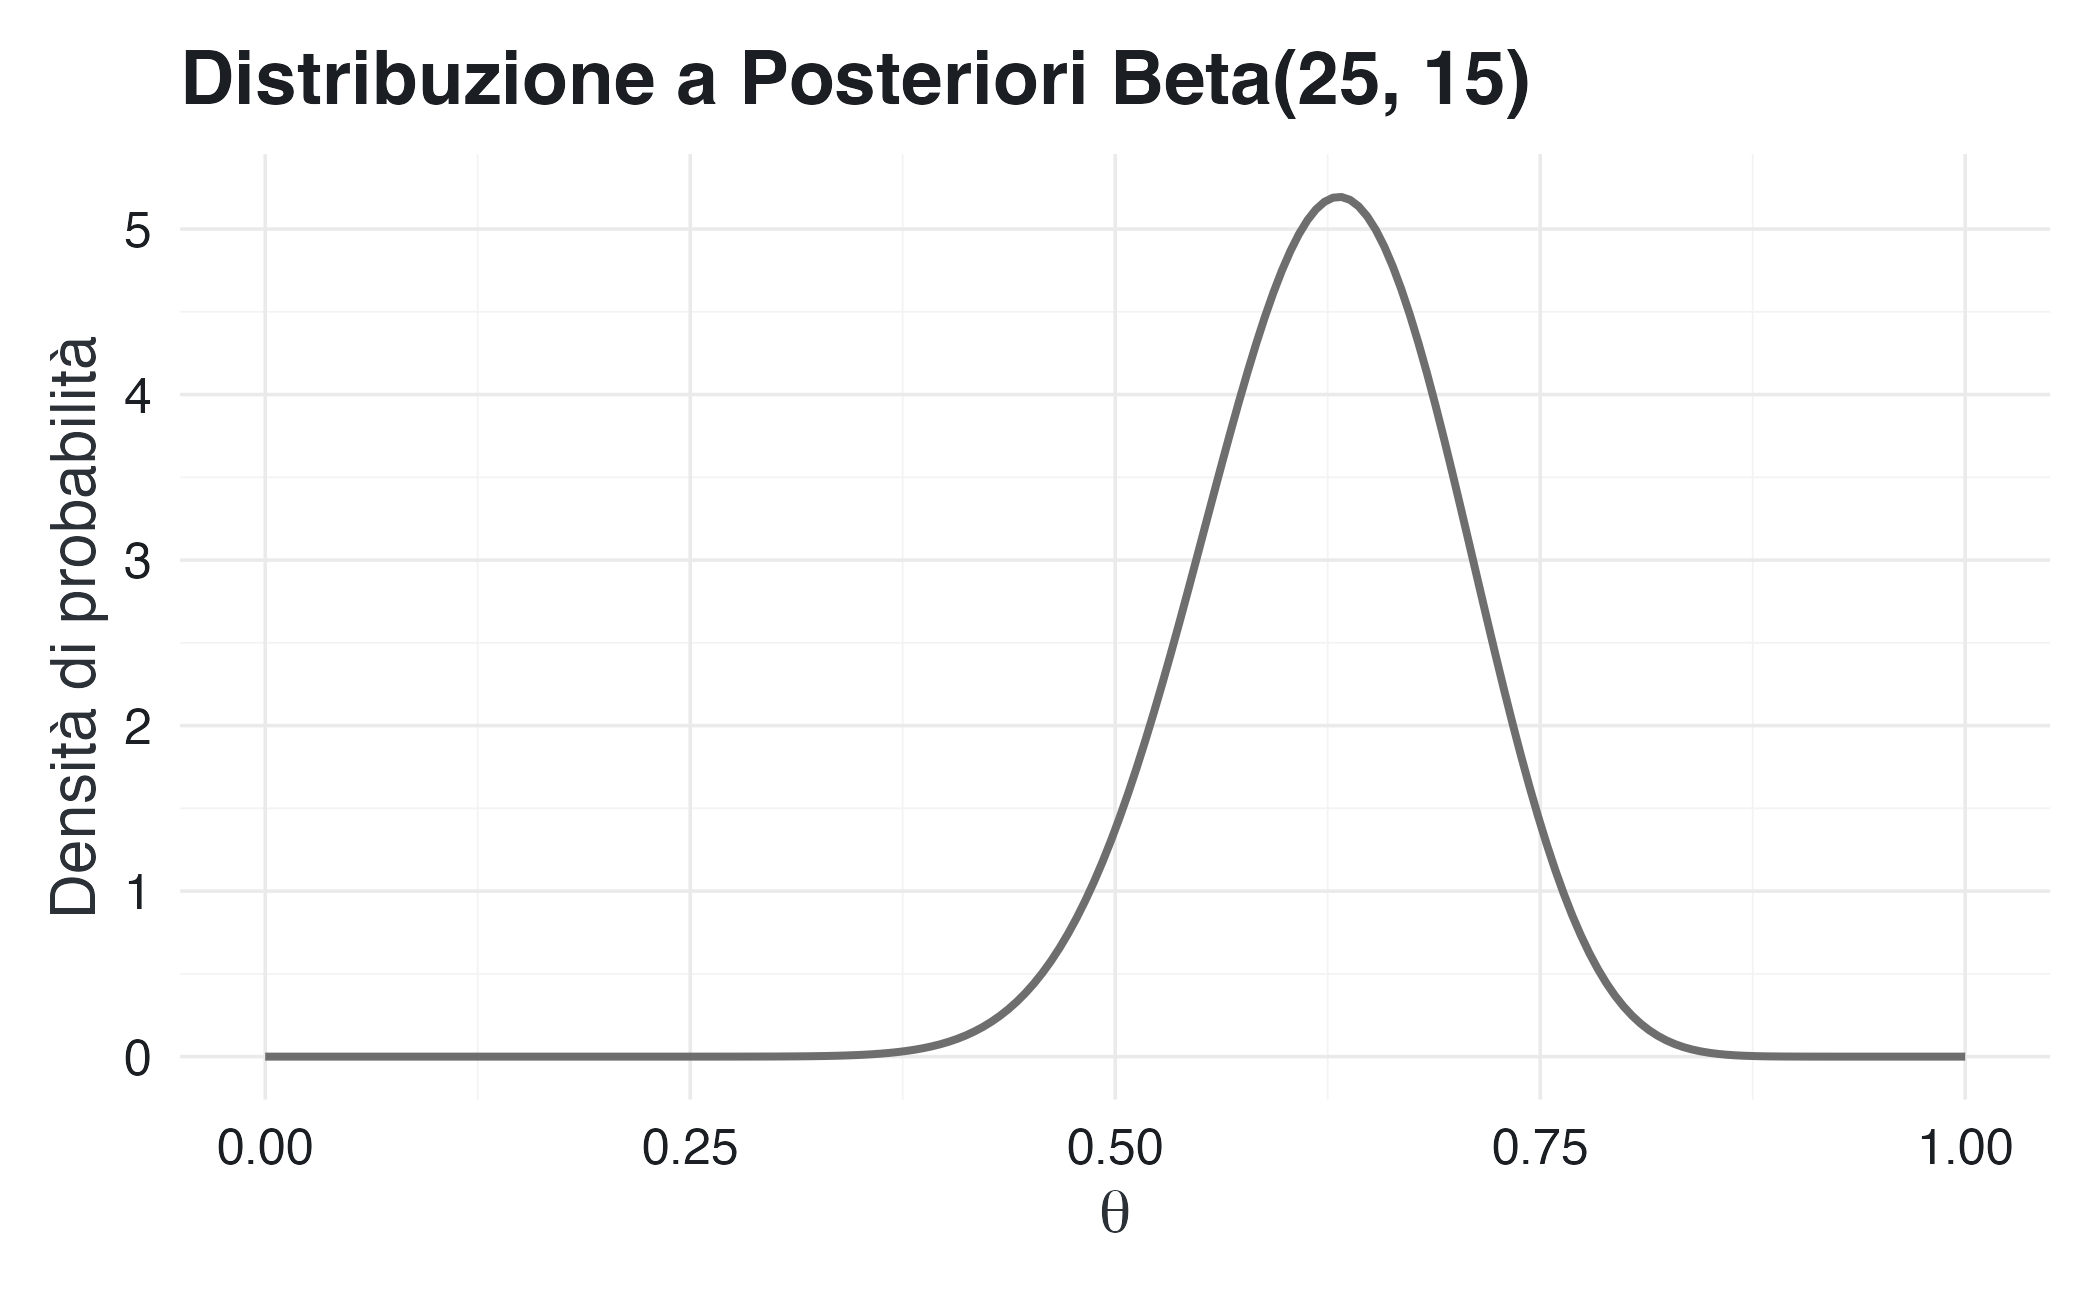
\includegraphics[width=0.85\linewidth,height=\textheight,keepaspectratio]{chapters/bayesian_inference/03_summary_posterior_files/figure-pdf/unnamed-chunk-4-1.png}
\end{center}

\textbf{Stime puntuali.}

\begin{enumerate}
\def\labelenumi{\arabic{enumi}.}
\tightlist
\item
  \textbf{Media a posteriori.} La media della distribuzione a posteriori
  è calcolata come:
\end{enumerate}

\[
\mathbb{E}(\theta | y = 17) = \frac{\alpha}{\alpha + \beta} = \frac{25}{25 + 15} = 0.625.
\] In R:

\begin{Shaded}
\begin{Highlighting}[]
\CommentTok{\# Calcolo della media a posteriori}
\NormalTok{posterior\_mean }\OtherTok{\textless{}{-}}\NormalTok{ alpha }\SpecialCharTok{/}\NormalTok{ (alpha }\SpecialCharTok{+}\NormalTok{ beta)}
\NormalTok{posterior\_mean}
\CommentTok{\#\textgreater{} [1] 0.625}
\end{Highlighting}
\end{Shaded}

\begin{enumerate}
\def\labelenumi{\arabic{enumi}.}
\setcounter{enumi}{1}
\tightlist
\item
  \textbf{Moda a posteriori (MAP).} La moda della distribuzione a
  posteriori è:
\end{enumerate}

\[
Mo(\theta | y = 17) = \frac{\alpha - 1}{\alpha + \beta - 2} = \frac{25 - 1}{25 + 15 - 2} = 0.6316.
\] In R:

\begin{Shaded}
\begin{Highlighting}[]
\CommentTok{\# Calcolo della moda a posteriori}
\NormalTok{posterior\_mode }\OtherTok{\textless{}{-}}\NormalTok{ (alpha }\SpecialCharTok{{-}} \DecValTok{1}\NormalTok{) }\SpecialCharTok{/}\NormalTok{ (alpha }\SpecialCharTok{+}\NormalTok{ beta }\SpecialCharTok{{-}} \DecValTok{2}\NormalTok{)}
\NormalTok{posterior\_mode}
\CommentTok{\#\textgreater{} [1] 0.632}
\end{Highlighting}
\end{Shaded}

\begin{enumerate}
\def\labelenumi{\arabic{enumi}.}
\setcounter{enumi}{2}
\tightlist
\item
  \textbf{Mediana a posteriori.} La mediana si ottiene utilizzando la
  funzione di distribuzione cumulativa inversa:
\end{enumerate}

\begin{Shaded}
\begin{Highlighting}[]
\CommentTok{\# Calcolo della mediana a posteriori}
\NormalTok{posterior\_median }\OtherTok{\textless{}{-}} \FunctionTok{qbeta}\NormalTok{(}\FloatTok{0.5}\NormalTok{, alpha, beta)}
\NormalTok{posterior\_median}
\CommentTok{\#\textgreater{} [1] 0.627}
\end{Highlighting}
\end{Shaded}

\textbf{Intervallo di credibilità.}

\begin{enumerate}
\def\labelenumi{\arabic{enumi}.}
\tightlist
\item
  \textbf{Intervallo di credibilità simmetrico.} L'intervallo di
  credibilità simmetrico al 94\% è dato dai percentili 3\% e 97\%:
\end{enumerate}

\begin{Shaded}
\begin{Highlighting}[]
\CommentTok{\# Intervallo di credibilità simmetrico al 94\%}
\NormalTok{cred\_interval }\OtherTok{\textless{}{-}} \FunctionTok{qbeta}\NormalTok{(}\FunctionTok{c}\NormalTok{(}\FloatTok{0.03}\NormalTok{, }\FloatTok{0.97}\NormalTok{), alpha, beta)}
\NormalTok{cred\_interval}
\CommentTok{\#\textgreater{} [1] 0.478 0.761}
\end{Highlighting}
\end{Shaded}

Possiamo interpretare questo intervallo come segue: c'è una certezza
soggettiva del 94\% che \(\theta\) sia compreso tra 0.478 e 0.761.

\textbf{Verifica di ipotesi bayesiana.} Infine, calcoliamo la
probabilità che \(\theta > 0.5\):

\[
P(\theta > 0.5 | y = 17) = \int_{0.5}^1 f(\theta | y = 17) d\theta.
\] In R:

\begin{Shaded}
\begin{Highlighting}[]
\CommentTok{\# Probabilità P(theta \textgreater{} 0.5)}
\NormalTok{prob\_theta\_greater\_0\_5 }\OtherTok{\textless{}{-}} \FunctionTok{pbeta}\NormalTok{(}\FloatTok{0.5}\NormalTok{, alpha, beta, }\AttributeTok{lower.tail =} \ConstantTok{FALSE}\NormalTok{)}
\NormalTok{prob\_theta\_greater\_0\_5}
\CommentTok{\#\textgreater{} [1] 0.946}
\end{Highlighting}
\end{Shaded}

In conclusione, utilizzando un approccio bayesiano, abbiamo stimato la
distribuzione a posteriori di \(\theta\), ottenuto stime puntuali e
costruito intervalli di credibilità. Abbiamo inoltre calcolato la
probabilità che \(\theta\) superi una soglia specifica, mostrando la
flessibilità e l'interpretabilità delle analisi bayesiane.

\end{example}

\section{Sintesi della distribuzione a posteriori in contesti
multivariati}\label{sintesi-della-distribuzione-a-posteriori-in-contesti-multivariati}

L'estensione dell'analisi bayesiana a modelli con più parametri
introduce complessità legate alle interdipendenze tra i parametri
stessi. Tali relazioni, se non adeguatamente considerate, possono
condurre a sintesi incomplete o fuorvianti della distribuzione a
posteriori, con possibili errori interpretativi.

\subsection{La sfida delle correlazioni tra
parametri}\label{la-sfida-delle-correlazioni-tra-parametri}

Uno degli aspetti critici riguarda la presenza di \emph{correlazioni tra
i parametri}. Le distribuzioni marginali a posteriori --- spesso
utilizzate nei riassunti statistici --- possono risultare ingannevoli se
esaminate isolatamente. Parametri fortemente correlati possono dar luogo
a marginali apparentemente piatte o poco informative, benché la loro
struttura congiunta restringa significativamente lo spazio delle
combinazioni plausibili. Ciò implica che, nonostante l'incertezza
marginale possa sembrare elevata, l'incertezza congiunta su specifiche
relazioni parametriche può essere molto ridotta.

Un'ulteriore complicazione sorge quando le relazioni tra parametri sono
\emph{non lineari}. In tali casi, il massimo della distribuzione
congiunta può non coincidere con i massimi delle distribuzioni
marginali. Ad esempio, in presenza di strutture a ``banana'' o altre
forme complesse, gli usuali indicatori di tendenza centrale (come la
moda o la media) calcolati sui singoli parametri possono non riflettere
la regione di massima densità di probabilità nello spazio multivariato.

\subsection{Approcci per una sintesi
efficace}\label{approcci-per-una-sintesi-efficace}

Per una rappresentazione fedele dell'incertezza in contesti
multivariati, è essenziale adottare una prospettiva che vada oltre
l'analisi delle marginali:

\begin{itemize}
\item
  \textbf{Visualizzazione delle relazioni congiunte}: grafici di
  dispersione a coppie (\emph{pair plots}) o contour plot bidimensionali
  consentono di esplorare visivamente le dipendenze tra parametri,
  rivelando strutture non catturate dalle marginali.
\item
  \textbf{Utilizzo di distribuzioni predittive}: il confronto tra
  distribuzioni predittive a priori e a posteriori fornisce una visione
  complessiva dell'incertezza ridotta dall'evidenza dei dati, tenendo
  conto di tutte le interazioni parametriche.
\item
  \textbf{Misure di dipendenza avanzate}: in casi di relazioni non
  lineari, misure come la correlazione di Spearman o l'informazione
  mutua possono integrare la correlazione lineare, offrendo una
  descrizione più completa delle dipendenze.
\item
  \textbf{Analisi di sensibilità}: valutare come variano le inferenze al
  variare di gruppi di parametri aiuta a identificare le relazioni più
  influenti e a comprendere la stabilità delle conclusioni.
\end{itemize}

In conclusione, una sintesi appropriata della distribuzione a posteriori
in presenza di più parametri richiede un esame congiunto delle relazioni
tra di essi. La sola inspezione delle distribuzioni marginali rischia di
occultare importanti fonti di informazione circa la struttura
parametrica, con possibili conseguenze sulle inferenze tratte. Un
approccio integrato --- che unisca visualizzazione, misure di dipendenza
e analisi di sensibilità --- è fondamentale per una comprensione robusta
dei risultati bayesiani in contesti multivariati.

\section*{Riflessioni conclusive}\label{riflessioni-conclusive-7}

\markright{Riflessioni conclusive}

Questo approfondimento ha mostrato come sintetizzare la distribuzione a
posteriori in modo informativo. Abbiamo analizzato diverse misure di
tendenza centrale (media, mediana e moda) e vari tipi di intervalli di
credibilità, mettendo in luce come ciascuna di queste misure fornisca
una prospettiva complementare sull'incertezza dei nostri parametri.

Queste sintesi non intendono sostituire la distribuzione completa, ma
renderla più comunicabile. In particolare, l'intervallo di credibilità
permette di identificare con precisione quali valori del parametro hanno
una determinata probabilità di essere veri, in base al modello e ai dati
osservati. Questa caratteristica segna una differenza fondamentale
rispetto all'approccio frequentista, in cui l'interpretazione degli
intervalli di confidenza rimane indiretta e potenzialmente ambigua.

Nella ricerca psicologica, la capacità di sintetizzare efficacemente le
distribuzioni a posteriori è particolarmente preziosa. Molti disegni
sperimentali prevedono la stima di proporzioni, medie o differenze tra
gruppi e la scelta del modo in cui rappresentare l'incertezza può
influire sulla chiarezza delle conclusioni. Una sintesi ben calibrata
non solo migliora la comunicazione dei risultati, ma ne aumenta anche la
robustezza, rendendo espliciti i margini di incertezza.

Con questo capitolo si conclude il primo ciclo del nostro percorso:
abbiamo imparato a costruire distribuzioni a posteriori e a
sintetizzarne il contenuto informativo. Nei prossimi approfondimenti
esploreremo come estendere questi strumenti oltre la stima dei
parametri, utilizzando la distribuzione a posteriori per prevedere dati
futuri e per confrontare modelli alternativi. È in questa direzione che
il pensiero bayesiano rivelerà appieno il suo potenziale: non solo per
descrivere ciò che conosciamo, ma anche per orientare ciò che possiamo
legittimamente aspettarci.

\begin{tcolorbox}[enhanced jigsaw, arc=.35mm, bottomrule=.15mm, bottomtitle=1mm, breakable, colback=white, colbacktitle=quarto-callout-important-color!10!white, colframe=quarto-callout-important-color-frame, coltitle=black, left=2mm, leftrule=.75mm, opacityback=0, opacitybacktitle=0.6, rightrule=.15mm, title=\textcolor{quarto-callout-important-color}{\faExclamation}\hspace{0.5em}{Problemi}, titlerule=0mm, toprule=.15mm, toptitle=1mm]

\textbf{1. Quali sono le principali statistiche utilizzate per la stima
puntuale di un parametro nella distribuzione a posteriori?}

\begin{itemize}
\tightlist
\item
  Spiega le differenze tra \textbf{moda (MAP)}, \textbf{media a
  posteriori} e \textbf{mediana}.
\item
  In quali contesti è preferibile utilizzare una di queste statistiche
  rispetto alle altre?
\end{itemize}

\textbf{2. Qual è la differenza tra un intervallo di credibilità
bayesiano e un intervallo di confidenza frequentista?}

\begin{itemize}
\tightlist
\item
  Spiega le differenze concettuali tra i due approcci.
\item
  Quale dei due è più intuitivo in termini di incertezza sui parametri?
\end{itemize}

\textbf{3. Cos'è un intervallo di massima densità posteriore (HPD) e in
cosa si differenzia dall'intervallo di credibilità simmetrico?}

\begin{itemize}
\tightlist
\item
  Spiega il concetto di HPD e perché è più informativo in alcuni casi.
\item
  In quali situazioni l'HPD è preferibile rispetto all'intervallo di
  credibilità simmetrico?
\end{itemize}

\textbf{4. Quali sono le problematiche associate alla moda (MAP) come
stima puntuale?}

\begin{itemize}
\tightlist
\item
  Perché il \textbf{MAP} può essere meno affidabile rispetto ad altre
  statistiche?
\item
  Quali problemi si possono incontrare nei modelli bayesiani complessi?
\end{itemize}

\textbf{5. In che modo la sintesi della distribuzione a posteriori
cambia nel caso di più parametri incogniti?}

\begin{itemize}
\tightlist
\item
  Quali sono le principali difficoltà nell'interpretare la distribuzione
  congiunta di più parametri?
\item
  Come si possono visualizzare e sintetizzare distribuzioni posteriori
  multivariate?
\end{itemize}

\textbf{Domande applicative in R}

Per queste domande, usa il dataset basato sulla \textbf{Satisfaction
with Life Scale (SWLS)}, supponendo che i dati seguano una distribuzione
normale.

\textbf{1. Calcola la media, la mediana e la moda a posteriori della
distribuzione della media SWLS, assumendo una distribuzione a priori
gaussiana molto diffusa.} - Usa il metodo delle distribuzioni coniugate
per ottenere la distribuzione a posteriori.

\textbf{2. Costruisci un intervallo di credibilità simmetrico al 94\%
per la media SWLS.}

\begin{itemize}
\tightlist
\item
  Usa la distribuzione normale a posteriori per calcolare l'intervallo.
\end{itemize}

\textbf{3. Visualizza la distribuzione a posteriori della media SWLS con
un grafico di densità.}

\begin{itemize}
\tightlist
\item
  Genera un campione dalla distribuzione a posteriori e rappresentalo
  con \textbf{ggplot2}.
\end{itemize}

\textbf{4. Confronta l'intervallo di credibilità simmetrico con
l'intervallo di massima densità posteriore (HPD).}

\begin{itemize}
\tightlist
\item
  Usa la funzione \textbf{hdi()} del pacchetto \textbf{bayestestR} per
  calcolare l'HPD.
\end{itemize}

\textbf{5. Calcola la probabilità a posteriori che la media SWLS sia
minore di 23.}

\begin{itemize}
\tightlist
\item
  Usa la distribuzione a posteriori per calcolare questa probabilità.
\end{itemize}

\end{tcolorbox}

\begin{tcolorbox}[enhanced jigsaw, arc=.35mm, bottomrule=.15mm, bottomtitle=1mm, breakable, colback=white, colbacktitle=quarto-callout-tip-color!10!white, colframe=quarto-callout-tip-color-frame, coltitle=black, left=2mm, leftrule=.75mm, opacityback=0, opacitybacktitle=0.6, rightrule=.15mm, title=\textcolor{quarto-callout-tip-color}{\faLightbulb}\hspace{0.5em}{Soluzioni}, titlerule=0mm, toprule=.15mm, toptitle=1mm]

\textbf{1. Quali sono le principali statistiche utilizzate per la stima
puntuale di un parametro nella distribuzione a posteriori?}

Le tre principali statistiche usate per ottenere una \textbf{stima
puntuale} del parametro \(\theta\) nella distribuzione a posteriori
sono:

\begin{enumerate}
\def\labelenumi{\arabic{enumi}.}
\tightlist
\item
  \textbf{Moda (Massimo a Posteriori, MAP)}

  \begin{itemize}
  \tightlist
  \item
    È il valore di \(\theta\) che massimizza la distribuzione a
    posteriori \(p(\theta \mid y)\).\\
  \item
    Se la distribuzione è unimodale e simmetrica, il MAP coincide con la
    media a posteriori.\\
  \item
    Il MAP è spesso simile alla stima di massima verosimiglianza (MLE)
    quando il prior è uniforme.
  \end{itemize}
\item
  \textbf{Media a Posteriori}

  \begin{itemize}
  \tightlist
  \item
    È il valore atteso della distribuzione a posteriori:\\
    \[
    E(\theta \mid y) = \int \theta \, p(\theta \mid y) \, d\theta
    \]
  \item
    È la stima più utile quando si vuole minimizzare l'errore quadratico
    medio (MSE).\\
  \item
    Risente dell'eventuale asimmetria della distribuzione, spostandosi
    verso le code.
  \end{itemize}
\item
  \textbf{Mediana a Posteriori}

  \begin{itemize}
  \tightlist
  \item
    È il valore che divide la distribuzione a posteriori in due parti
    uguali:\\
    \[
    P(\theta \leq \theta_{\text{mediana}} \mid y) = 0.5
    \]
  \item
    È più robusta agli outlier rispetto alla media ed è utile quando la
    distribuzione è fortemente asimmetrica.
  \end{itemize}
\end{enumerate}

💡 \textbf{Quando usarle?} - Se la distribuzione è \textbf{simmetrica},
tutte e tre le statistiche coincidono. - Se la distribuzione è
\textbf{asimmetrica}, la \textbf{mediana} è più robusta, la
\textbf{media} può essere influenzata dalle code e il \textbf{MAP} è
utile se si vuole un valore più probabile.

\textbf{2. Qual è la differenza tra un intervallo di credibilità
bayesiano e un intervallo di confidenza frequentista?}

{\def\LTcaptype{none} % do not increment counter
\begin{longtable}[]{@{}
  >{\raggedright\arraybackslash}p{(\linewidth - 4\tabcolsep) * \real{0.2909}}
  >{\raggedright\arraybackslash}p{(\linewidth - 4\tabcolsep) * \real{0.3455}}
  >{\raggedright\arraybackslash}p{(\linewidth - 4\tabcolsep) * \real{0.3636}}@{}}
\toprule\noalign{}
\begin{minipage}[b]{\linewidth}\raggedright
Caratteristica
\end{minipage} & \begin{minipage}[b]{\linewidth}\raggedright
Intervallo di Credibilità (Bayesiano)
\end{minipage} & \begin{minipage}[b]{\linewidth}\raggedright
Intervallo di Confidenza (Frequentista)
\end{minipage} \\
\midrule\noalign{}
\endhead
\bottomrule\noalign{}
\endlastfoot
\textbf{Significato} & Esprime la probabilità che il parametro sia
nell'intervallo, dati i dati osservati. & È una proprietà di un metodo
di campionamento: se si ripetesse l'esperimento infinite volte, il
\((1 - \alpha)100\%\) degli intervalli conterrebbe il vero valore del
parametro. \\
\textbf{Approccio} & Assume che il parametro sia una variabile casuale
con una distribuzione di probabilità. & Assume che il parametro sia
fisso e sconosciuto, mentre i dati sono casuali. \\
\textbf{Interpretazione} & ``C'è il 95\% di probabilità che il parametro
sia tra questi valori.'' & ``Se ripetessimo l'esperimento molte volte,
il 95\% degli intervalli conterrebbe il vero parametro.'' \\
\end{longtable}
}

💡 \textbf{Differenza fondamentale:}

\begin{itemize}
\tightlist
\item
  L'intervallo di credibilità è \textbf{probabilistico} e più intuitivo:
  si può direttamente dire che il parametro ha il 95\% di probabilità di
  trovarsi nell'intervallo.\\
\item
  L'intervallo di confidenza è \textbf{basato sulla ripetizione
  ipotetica} dell'esperimento e non può essere interpretato in termini
  probabilistici sul singolo intervallo.
\end{itemize}

\textbf{3. Cos'è un intervallo di massima densità posteriore (HPD) e in
cosa si differenzia dall'intervallo di credibilità simmetrico?}

L'\textbf{intervallo di massima densità posteriore (HPD)} è l'intervallo
più stretto che contiene una percentuale fissata (es. 94\%) della
distribuzione a posteriori. Si distingue dall'intervallo di credibilità
simmetrico perché:

{\def\LTcaptype{none} % do not increment counter
\begin{longtable}[]{@{}
  >{\raggedright\arraybackslash}p{(\linewidth - 4\tabcolsep) * \real{0.2373}}
  >{\raggedright\arraybackslash}p{(\linewidth - 4\tabcolsep) * \real{0.2203}}
  >{\raggedright\arraybackslash}p{(\linewidth - 4\tabcolsep) * \real{0.5424}}@{}}
\toprule\noalign{}
\begin{minipage}[b]{\linewidth}\raggedright
Caratteristica
\end{minipage} & \begin{minipage}[b]{\linewidth}\raggedright
Intervallo HPD
\end{minipage} & \begin{minipage}[b]{\linewidth}\raggedright
Intervallo di Credibilità Simmetrico
\end{minipage} \\
\midrule\noalign{}
\endhead
\bottomrule\noalign{}
\endlastfoot
\textbf{Definizione} & Contiene il \((1 - \alpha)100\%\) della
probabilità a posteriori, minimizzando la lunghezza dell'intervallo. & È
centrato attorno alla mediana e copre una frazione fissa della
distribuzione. \\
\textbf{Forma} & Può essere asimmetrico e discontinuo se la
distribuzione è multimodale. & È sempre simmetrico. \\
\textbf{Vantaggio} & È più informativo se la distribuzione è asimmetrica
o multimodale. & È più facile da calcolare, specialmente per
distribuzioni unimodali. \\
\end{longtable}
}

💡 \textbf{Quando usarli?}

\begin{itemize}
\tightlist
\item
  Se la distribuzione è \textbf{simmetrica}, entrambi gli intervalli
  danno risultati simili.\\
\item
  Se la distribuzione è \textbf{asimmetrica o multimodale}, l'HPD è più
  informativo.
\end{itemize}

\textbf{4. Quali sono le problematiche associate alla moda (MAP) come
stima puntuale?}

Sebbene il \textbf{MAP} sia un concetto intuitivo (il valore più
probabile della distribuzione a posteriori), presenta alcune
limitazioni:

\begin{enumerate}
\def\labelenumi{\arabic{enumi}.}
\tightlist
\item
  \textbf{Difficoltà computazionale con MCMC}

  \begin{itemize}
  \tightlist
  \item
    Con metodi di campionamento come \textbf{Markov Chain Monte Carlo
    (MCMC)}, trovare il massimo della distribuzione a posteriori è
    difficile perché la funzione viene stimata in modo discreto.
  \item
    Spesso si preferisce stimare \textbf{media} o \textbf{mediana}, più
    facili da calcolare con MCMC.
  \end{itemize}
\item
  \textbf{Sensibilità ai dati e al prior}

  \begin{itemize}
  \tightlist
  \item
    Il MAP dipende fortemente dal \textbf{prior} scelto.
  \item
    Se il prior è informativo, il MAP può spostarsi troppo rispetto ai
    dati.
  \end{itemize}
\item
  \textbf{Problemi con distribuzioni multimodali}

  \begin{itemize}
  \tightlist
  \item
    Se la distribuzione a posteriori ha più di un massimo (moda), il MAP
    potrebbe non essere una buona rappresentazione della distribuzione.
  \end{itemize}
\end{enumerate}

💡 \textbf{Quando evitarlo?}\\
- Se la distribuzione a posteriori è \textbf{asimmetrica o multimodale}.
- Se si usa un \textbf{metodo MCMC}, dove la media o la mediana sono più
semplici da stimare.

\textbf{5. In che modo la sintesi della distribuzione a posteriori
cambia nel caso di più parametri incogniti?}

Quando l'inferenza bayesiana coinvolge più parametri (es. \(\mu\) e
\(\sigma\)), l'analisi diventa più complessa per diversi motivi:

\begin{enumerate}
\def\labelenumi{\arabic{enumi}.}
\tightlist
\item
  \textbf{Interazioni tra parametri}

  \begin{itemize}
  \tightlist
  \item
    I parametri spesso non sono indipendenti: la distribuzione a
    posteriori congiunta può mostrare \textbf{correlazioni} che non
    emergono dalle distribuzioni marginali.
  \end{itemize}
\item
  \textbf{Difficoltà di visualizzazione}

  \begin{itemize}
  \tightlist
  \item
    Per un parametro si usa un istogramma o una funzione di densità.
  \item
    Per due parametri si usa un \textbf{contour plot} o un
    \textbf{grafico 3D}.
  \item
    Con più di due parametri, si ricorre a \textbf{pair plots} o
    \textbf{matrici di correlazione}.
  \end{itemize}
\item
  \textbf{Stimare margine e congiunta}

  \begin{itemize}
  \tightlist
  \item
    La distribuzione marginale di un parametro si ottiene integrando la
    distribuzione congiunta rispetto agli altri parametri: \[
    p(\theta_1) = \int p(\theta_1, \theta_2) d\theta_2
    \]
  \item
    Se i parametri sono fortemente correlati, le marginali possono
    \textbf{nascondere informazioni importanti}.
  \end{itemize}
\item
  \textbf{Rischio di correlazioni non lineari}

  \begin{itemize}
  \tightlist
  \item
    Le correlazioni non lineari tra i parametri possono portare a
    distribuzioni con forme complesse (es. a banana), rendendo difficile
    la sintesi con MAP o media.
  \end{itemize}
\end{enumerate}

💡 \textbf{Strategie per affrontare il problema:}\\
- \textbf{Visualizzare le correlazioni} tra i parametri con scatter plot
o heatmap.\\
- \textbf{Usare tecniche di riduzione della dimensionalità} come PCA
(Analisi delle Componenti Principali).\\
- \textbf{Utilizzare il MCMC} per campionare direttamente dalla
distribuzione congiunta.

\textbf{Esercizio in R con i dati SWLS}

Nell'esercizio, usa i dati della SWLS che sono stati raccolti. Qui
useremo i dati seguenti:

\begin{Shaded}
\begin{Highlighting}[]
\NormalTok{swls\_data }\OtherTok{\textless{}{-}} \FunctionTok{data.frame}\NormalTok{(}
  \AttributeTok{soddisfazione =} \FunctionTok{c}\NormalTok{(}\FloatTok{4.2}\NormalTok{, }\FloatTok{5.1}\NormalTok{, }\FloatTok{4.7}\NormalTok{, }\FloatTok{4.3}\NormalTok{, }\FloatTok{5.5}\NormalTok{, }\FloatTok{4.9}\NormalTok{, }\FloatTok{4.8}\NormalTok{, }\FloatTok{5.0}\NormalTok{, }\FloatTok{4.6}\NormalTok{, }\FloatTok{4.4}\NormalTok{)}
\NormalTok{)}
\end{Highlighting}
\end{Shaded}

\textbf{1. Calcola la media, la mediana e la moda a posteriori della
distribuzione della media SWLS, assumendo una distribuzione a priori
gaussiana molto diffusa.}

\begin{itemize}
\tightlist
\item
  Usa il metodo delle distribuzioni coniugate per ottenere la
  distribuzione a posteriori.
\end{itemize}

\begin{Shaded}
\begin{Highlighting}[]
\FunctionTok{library}\NormalTok{(tibble)}

\CommentTok{\# Dati}
\NormalTok{n }\OtherTok{\textless{}{-}} \FunctionTok{nrow}\NormalTok{(swls\_data)}
\NormalTok{mean\_x }\OtherTok{\textless{}{-}} \FunctionTok{mean}\NormalTok{(swls\_data}\SpecialCharTok{$}\NormalTok{soddisfazione)}
\NormalTok{sigma }\OtherTok{\textless{}{-}} \DecValTok{1}  \CommentTok{\# Deviazione standard nota}

\CommentTok{\# Prior diffuso}
\NormalTok{mu\_prior }\OtherTok{\textless{}{-}} \FloatTok{4.5}    
\NormalTok{sigma\_prior }\OtherTok{\textless{}{-}} \DecValTok{10}  

\CommentTok{\# Media a posteriori}
\NormalTok{mu\_post }\OtherTok{\textless{}{-}}\NormalTok{ (sigma\_prior}\SpecialCharTok{\^{}}\DecValTok{2} \SpecialCharTok{*}\NormalTok{ mean\_x }\SpecialCharTok{+}\NormalTok{ sigma}\SpecialCharTok{\^{}}\DecValTok{2} \SpecialCharTok{*}\NormalTok{ n }\SpecialCharTok{*}\NormalTok{ mu\_prior) }\SpecialCharTok{/}\NormalTok{ (sigma\_prior}\SpecialCharTok{\^{}}\DecValTok{2} \SpecialCharTok{+}\NormalTok{ sigma}\SpecialCharTok{\^{}}\DecValTok{2} \SpecialCharTok{*}\NormalTok{ n)}

\CommentTok{\# Deviazione standard a posteriori}
\NormalTok{sigma\_post }\OtherTok{\textless{}{-}} \FunctionTok{sqrt}\NormalTok{((sigma\_prior}\SpecialCharTok{\^{}}\DecValTok{2} \SpecialCharTok{*}\NormalTok{ sigma}\SpecialCharTok{\^{}}\DecValTok{2}\NormalTok{) }\SpecialCharTok{/}\NormalTok{ (sigma\_prior}\SpecialCharTok{\^{}}\DecValTok{2} \SpecialCharTok{+}\NormalTok{ sigma}\SpecialCharTok{\^{}}\DecValTok{2} \SpecialCharTok{*}\NormalTok{ n))}

\CommentTok{\# Moda (MAP)}
\NormalTok{posterior\_mode }\OtherTok{\textless{}{-}}\NormalTok{ mu\_post  }\CommentTok{\# Per una distribuzione normale, MAP coincide con la media}

\CommentTok{\# Mediana (simile alla media in una distribuzione normale)}
\NormalTok{posterior\_median }\OtherTok{\textless{}{-}}\NormalTok{ mu\_post}

\FunctionTok{tibble}\NormalTok{(}\StringTok{"Media a Posteriori"} \OtherTok{=}\NormalTok{ mu\_post,}
       \StringTok{"Moda (MAP)"} \OtherTok{=}\NormalTok{ posterior\_mode,}
       \StringTok{"Mediana"} \OtherTok{=}\NormalTok{ posterior\_median)}
\end{Highlighting}
\end{Shaded}

\textbf{2. Costruisci un intervallo di credibilità simmetrico al 94\%
per la media SWLS.}

\begin{itemize}
\tightlist
\item
  Usa la distribuzione normale a posteriori per calcolare l'intervallo.
\end{itemize}

\begin{Shaded}
\begin{Highlighting}[]
\NormalTok{cred\_interval }\OtherTok{\textless{}{-}} \FunctionTok{qnorm}\NormalTok{(}\FunctionTok{c}\NormalTok{(}\FloatTok{0.03}\NormalTok{, }\FloatTok{0.97}\NormalTok{), }\AttributeTok{mean =}\NormalTok{ mu\_post, }\AttributeTok{sd =}\NormalTok{ sigma\_post)}
\NormalTok{cred\_interval}
\end{Highlighting}
\end{Shaded}

\textbf{3. Visualizza la distribuzione a posteriori della media SWLS con
un grafico di densità.}

\begin{itemize}
\tightlist
\item
  Genera un campione dalla distribuzione a posteriori e rappresentalo
  con \textbf{ggplot2}.
\end{itemize}

\begin{Shaded}
\begin{Highlighting}[]
\FunctionTok{library}\NormalTok{(ggplot2)}

\CommentTok{\# Campionamento dalla distribuzione a posteriori}
\FunctionTok{set.seed}\NormalTok{(}\DecValTok{123}\NormalTok{)}
\NormalTok{samples }\OtherTok{\textless{}{-}} \FunctionTok{rnorm}\NormalTok{(}\DecValTok{1000}\NormalTok{, }\AttributeTok{mean =}\NormalTok{ mu\_post, }\AttributeTok{sd =}\NormalTok{ sigma\_post)}

\CommentTok{\# Creazione del dataframe}
\NormalTok{samples\_df }\OtherTok{\textless{}{-}} \FunctionTok{tibble}\NormalTok{(}\AttributeTok{media\_campionata =}\NormalTok{ samples)}

\CommentTok{\# Grafico della distribuzione a posteriori}
\FunctionTok{ggplot}\NormalTok{(samples\_df, }\FunctionTok{aes}\NormalTok{(}\AttributeTok{x =}\NormalTok{ media\_campionata)) }\SpecialCharTok{+}
  \FunctionTok{geom\_density}\NormalTok{(}\AttributeTok{fill =} \StringTok{"blue"}\NormalTok{, }\AttributeTok{alpha =} \FloatTok{0.5}\NormalTok{) }\SpecialCharTok{+}
  \FunctionTok{labs}\NormalTok{(}\AttributeTok{title =} \StringTok{"Distribuzione a Posteriori della Media SWLS"}\NormalTok{,}
       \AttributeTok{x =} \StringTok{"Media"}\NormalTok{, }\AttributeTok{y =} \StringTok{"Densità"}\NormalTok{)}
\end{Highlighting}
\end{Shaded}

\textbf{4. Confronta l'intervallo di credibilità simmetrico con
l'intervallo di massima densità posteriore (HPD).}

\begin{itemize}
\tightlist
\item
  Usa la funzione \textbf{hdi()} del pacchetto \textbf{bayestestR} per
  calcolare l'HPD.
\end{itemize}

\begin{Shaded}
\begin{Highlighting}[]
\FunctionTok{library}\NormalTok{(bayestestR)}

\CommentTok{\# Calcolo intervallo HPD al 94\%}
\NormalTok{hpd\_interval }\OtherTok{\textless{}{-}} \FunctionTok{hdi}\NormalTok{(samples, }\AttributeTok{ci =} \FloatTok{0.94}\NormalTok{)}
\NormalTok{hpd\_interval}
\end{Highlighting}
\end{Shaded}

\textbf{5. Calcola la probabilità a posteriori che la media SWLS sia
minore di 23 -- per fare un esempio, qui caloleremo per i dati simulati
la probabilità a posteriori per la media SWLS maggiore di 4.7.}

\begin{itemize}
\tightlist
\item
  Usa la distribuzione a posteriori per calcolare questa probabilità.
\end{itemize}

\begin{Shaded}
\begin{Highlighting}[]
\NormalTok{prob\_greater\_4\_7 }\OtherTok{\textless{}{-}} \DecValTok{1} \SpecialCharTok{{-}} \FunctionTok{pnorm}\NormalTok{(}\FloatTok{4.7}\NormalTok{, }\AttributeTok{mean =}\NormalTok{ mu\_post, }\AttributeTok{sd =}\NormalTok{ sigma\_post)}
\NormalTok{prob\_greater\_4\_7}
\end{Highlighting}
\end{Shaded}

\end{tcolorbox}

\begin{tcolorbox}[enhanced jigsaw, arc=.35mm, bottomrule=.15mm, bottomtitle=1mm, breakable, colback=white, colbacktitle=quarto-callout-note-color!10!white, colframe=quarto-callout-note-color-frame, coltitle=black, left=2mm, leftrule=.75mm, opacityback=0, opacitybacktitle=0.6, rightrule=.15mm, title=\textcolor{quarto-callout-note-color}{\faInfo}\hspace{0.5em}{Informazioni sull'ambiente di sviluppo}, titlerule=0mm, toprule=.15mm, toptitle=1mm]

\begin{Shaded}
\begin{Highlighting}[]
\FunctionTok{sessionInfo}\NormalTok{()}
\CommentTok{\#\textgreater{} R version 4.6.1 (2026{-}06{-}24)}
\CommentTok{\#\textgreater{} Platform: aarch64{-}apple{-}darwin23}
\CommentTok{\#\textgreater{} Running under: macOS Tahoe 26.5.2}
\CommentTok{\#\textgreater{} }
\CommentTok{\#\textgreater{} Matrix products: default}
\CommentTok{\#\textgreater{} BLAS:   /Library/Frameworks/R.framework/Versions/4.6/Resources/lib/libRblas.0.dylib }
\CommentTok{\#\textgreater{} LAPACK: /Library/Frameworks/R.framework/Versions/4.6/Resources/lib/libRlapack.dylib;  LAPACK version 3.12.1}
\CommentTok{\#\textgreater{} }
\CommentTok{\#\textgreater{} locale:}
\CommentTok{\#\textgreater{} [1] C.UTF{-}8/UTF{-}8/C.UTF{-}8/C/C.UTF{-}8/C.UTF{-}8}
\CommentTok{\#\textgreater{} }
\CommentTok{\#\textgreater{} time zone: Europe/Zagreb}
\CommentTok{\#\textgreater{} tzcode source: internal}
\CommentTok{\#\textgreater{} }
\CommentTok{\#\textgreater{} attached base packages:}
\CommentTok{\#\textgreater{} [1] stats     graphics  grDevices utils     datasets  methods   base     }
\CommentTok{\#\textgreater{} }
\CommentTok{\#\textgreater{} other attached packages:}
\CommentTok{\#\textgreater{}  [1] mice\_3.19.0           ragg\_1.5.2            tinytable\_0.17.0     }
\CommentTok{\#\textgreater{}  [4] withr\_3.0.3           systemfonts\_1.3.2     patchwork\_1.3.2      }
\CommentTok{\#\textgreater{}  [7] ggdist\_3.3.3          tidybayes\_3.0.7       bayesplot\_1.15.0     }
\CommentTok{\#\textgreater{} [10] ggplot2\_4.0.3         reliabilitydiag\_0.2.1 priorsense\_1.2.0     }
\CommentTok{\#\textgreater{} [13] posterior\_1.7.0       loo\_2.10.0            rstan\_2.32.7         }
\CommentTok{\#\textgreater{} [16] StanHeaders\_2.32.10   brms\_2.23.0           Rcpp\_1.1.2           }
\CommentTok{\#\textgreater{} [19] sessioninfo\_1.2.4     conflicted\_1.2.0      janitor\_2.2.1        }
\CommentTok{\#\textgreater{} [22] matrixStats\_1.5.0     modelr\_0.1.11         tibble\_3.3.1         }
\CommentTok{\#\textgreater{} [25] dplyr\_1.2.1           tidyr\_1.3.2           rio\_1.3.0            }
\CommentTok{\#\textgreater{} [28] here\_1.0.2           }
\CommentTok{\#\textgreater{} }
\CommentTok{\#\textgreater{} loaded via a namespace (and not attached):}
\CommentTok{\#\textgreater{}  [1] Rdpack\_2.6.6          gridExtra\_2.3.1       inline\_0.3.21        }
\CommentTok{\#\textgreater{}  [4] rlang\_1.3.0           magrittr\_2.0.5        snakecase\_0.11.1     }
\CommentTok{\#\textgreater{}  [7] otel\_0.2.0            compiler\_4.6.1        vctrs\_0.7.3          }
\CommentTok{\#\textgreater{} [10] stringr\_1.6.0         pkgconfig\_2.0.3       shape\_1.4.6.1        }
\CommentTok{\#\textgreater{} [13] arrayhelpers\_1.1{-}1    fastmap\_1.2.0         backports\_1.5.1      }
\CommentTok{\#\textgreater{} [16] labeling\_0.4.3        rmarkdown\_2.31        nloptr\_2.2.1         }
\CommentTok{\#\textgreater{} [19] purrr\_1.2.2           xfun\_0.60             glmnet\_5.0           }
\CommentTok{\#\textgreater{} [22] jomo\_2.7{-}6            cachem\_1.1.0          jsonlite\_2.0.0       }
\CommentTok{\#\textgreater{} [25] pan\_2.0               broom\_1.0.13          parallel\_4.6.1       }
\CommentTok{\#\textgreater{} [28] R6\_2.6.1              stringi\_1.8.7         RColorBrewer\_1.1{-}3   }
\CommentTok{\#\textgreater{} [31] rpart\_4.1.27          boot\_1.3{-}32           lubridate\_1.9.5      }
\CommentTok{\#\textgreater{} [34] estimability\_2.0.0    iterators\_1.0.14      knitr\_1.51           }
\CommentTok{\#\textgreater{} [37] pacman\_0.5.1          nnet\_7.3{-}20           Matrix\_1.7{-}5         }
\CommentTok{\#\textgreater{} [40] splines\_4.6.1         timechange\_0.4.0      tidyselect\_1.2.1     }
\CommentTok{\#\textgreater{} [43] abind\_1.4{-}8           codetools\_0.2{-}20      curl\_7.1.0           }
\CommentTok{\#\textgreater{} [46] pkgbuild\_1.4.8        lattice\_0.22{-}9        bridgesampling\_1.2{-}1 }
\CommentTok{\#\textgreater{} [49] S7\_0.2.2              coda\_0.19{-}4.1         evaluate\_1.0.5       }
\CommentTok{\#\textgreater{} [52] survival\_3.8{-}9        RcppParallel\_5.1.11{-}2 pillar\_1.11.1        }
\CommentTok{\#\textgreater{} [55] tensorA\_0.36.2.1      checkmate\_2.3.4       foreach\_1.5.2        }
\CommentTok{\#\textgreater{} [58] stats4\_4.6.1          reformulas\_0.4.4      distributional\_0.8.1 }
\CommentTok{\#\textgreater{} [61] generics\_0.1.4        rprojroot\_2.1.1       rstantools\_2.6.0     }
\CommentTok{\#\textgreater{} [64] scales\_1.4.0          minqa\_1.2.8           xtable\_1.8{-}8         }
\CommentTok{\#\textgreater{} [67] glue\_1.8.1            emmeans\_2.0.4         tools\_4.6.1          }
\CommentTok{\#\textgreater{} [70] lme4\_2.0{-}6            mvtnorm\_1.4{-}2         grid\_4.6.1           }
\CommentTok{\#\textgreater{} [73] rbibutils\_2.4.1       QuickJSR\_1.10.0       nlme\_3.1{-}170         }
\CommentTok{\#\textgreater{} [76] cli\_3.6.6             textshaping\_1.0.5     svUnit\_1.0.8         }
\CommentTok{\#\textgreater{} [79] Brobdingnag\_1.2{-}9     V8\_8.2.0              gtable\_0.3.6         }
\CommentTok{\#\textgreater{} [82] digest\_0.6.39         farver\_2.1.2          memoise\_2.0.1        }
\CommentTok{\#\textgreater{} [85] htmltools\_0.5.9       lifecycle\_1.0.5       mitml\_0.4{-}5          }
\CommentTok{\#\textgreater{} [88] MASS\_7.3{-}66}
\end{Highlighting}
\end{Shaded}

\end{tcolorbox}

\section*{Bibliografia}\label{bibliografia-9}

\markright{Bibliografia}

\chapter{L'influenza della distribuzione a
priori}\label{sec-bayes-inference-prior}

\begin{tcolorbox}[enhanced jigsaw, arc=.35mm, bottomrule=.15mm, breakable, colback=white, colframe=quarto-callout-note-color-frame, left=2mm, leftrule=.75mm, opacityback=0, rightrule=.15mm, toprule=.15mm]

In psicologia, spesso operiamo in condizioni che rendono complessa
l'inferenza statistica, come campioni di piccole dimensioni, misure
soggette a rumore e effetti reali ma di lieve entità. In questo
contesto, l'approccio bayesiano offre un vantaggio sostanziale, in
quanto rende esplicito il modo in cui le conoscenze pregresse si
integrano con l'evidenza empirica. Non si tratta di una ``correzione''
arbitraria dei risultati, ma di una stabilizzazione dell'inferenza che
riduce le sovrastime tipiche degli studi condotti su piccoli campioni e
gli errori di tipo M.\footnotemark{}

Questa dinamica riflette un principio epistemologico fondamentale:
quando le nuove informazioni sono poche, è ragionevole affidarsi
maggiormente alle conoscenze consolidate; quando le nuove informazioni
sono molte, è opportuno lasciar parlare i dati. L'approccio bayesiano
non sostituisce i dati con la teoria, ma ne modula la combinazione in
base all'informazione disponibile.

\end{tcolorbox}

\footnotetext{\emph{Errore di tipo M (Magnitude)}: scostamento
sistematico tra la magnitudine stimata di un effetto e il suo valore
reale. Nei piccoli campioni, la selezione dei risultati basata sulla
significatività statistica tende a \emph{sovrastimare} gli effetti. Si
distingue dall'errore di tipo S (\emph{Sign}), che riguarda l'inversione
del segno dell'effetto. L'uso di distribuzioni a priori debolmente
informative a code pesanti introduce uno \emph{shrinkage adattivo} che
mitiga gli errori di tipo M quando l'evidenza è debole, preservando gli
effetti genuini quando l'evidenza è forte
(\citeproc{ref-gelman2014beyond}{Gelman \& Carlin, 2014};
\citeproc{ref-ioannidis2005contradicted}{Ioannidis, 2005a}).}

\begin{tcolorbox}[enhanced jigsaw, arc=.35mm, bottomrule=.15mm, breakable, colback=white, colframe=quarto-callout-important-color-frame, left=2mm, leftrule=.75mm, opacityback=0, rightrule=.15mm, toprule=.15mm]

\textbf{Da sapere.} La distribuzione a priori esprime in modo esplicito
ciò che è plausibile prima di osservare i dati. La sua influenza è
maggiore quando i dati sono scarsi o rumorosi e diminuisce quando
l'informazione empirica aumenta. Le prior debolmente informative
regolarizzano le stime e possono ridurre le sovrastime tipiche dei
piccoli campioni, ma nessuna prior è neutrale rispetto alla scala su cui
viene definita.

\textbf{Da saper fare.} Confrontare l'aggiornamento prodotto da prior
con diverso grado di informatività; scegliere una prior coerente con la
scala e i vincoli del parametro; interpretare lo \emph{shrinkage} come
equilibrio tra informazione iniziale e dati; eseguire un \emph{prior
predictive check} e un'analisi di sensibilità per verificare
plausibilità e robustezza delle conclusioni.

\textbf{Approfondimento facoltativo.} La formalizzazione delle prior sul
rapporto segnale-rumore \(\beta/s\), le prior empiriche costruite da
corpora di studi, le miscele di distribuzioni e i dettagli
computazionali delle simulazioni possono essere rimandati in una prima
lettura.

\hyperref[sec-percorsi-lettura]{Che cosa significano queste etichette?}

\end{tcolorbox}

\begin{tcolorbox}[enhanced jigsaw, arc=.35mm, bottomrule=.15mm, bottomtitle=1mm, breakable, colback=white, colbacktitle=quarto-callout-caution-color!10!white, colframe=quarto-callout-caution-color-frame, coltitle=black, left=2mm, leftrule=.75mm, opacityback=0, opacitybacktitle=0.6, rightrule=.15mm, title=\textcolor{quarto-callout-caution-color}{\faFire}\hspace{0.5em}{Preparazione del Notebook}, titlerule=0mm, toprule=.15mm, toptitle=1mm]

\begin{Shaded}
\begin{Highlighting}[]
\NormalTok{here}\SpecialCharTok{::}\FunctionTok{here}\NormalTok{(}\StringTok{"code"}\NormalTok{, }\StringTok{"\_common.R"}\NormalTok{) }\SpecialCharTok{|\textgreater{}} 
  \FunctionTok{source}\NormalTok{()}

\CommentTok{\# Load packages}
\ControlFlowTok{if}\NormalTok{ (}\SpecialCharTok{!}\FunctionTok{requireNamespace}\NormalTok{(}\StringTok{"pacman"}\NormalTok{)) }\FunctionTok{install.packages}\NormalTok{(}\StringTok{"pacman"}\NormalTok{)}
\NormalTok{pacman}\SpecialCharTok{::}\FunctionTok{p\_load}\NormalTok{(conflicted, tidytable)}
\end{Highlighting}
\end{Shaded}

\begin{verbatim}

The downloaded binary packages are in
    /var/folders/gw/hc72by314msbfbhm58gh0fgc0000gn/T//RtmpPBZapT/downloaded_packages
\end{verbatim}

\begin{Shaded}
\begin{Highlighting}[]
\FunctionTok{conflicts\_prefer}\NormalTok{(tidyr}\SpecialCharTok{::}\NormalTok{extract)}
\end{Highlighting}
\end{Shaded}

\end{tcolorbox}

\section{L'aggiornamento bayesiano: un esempio
illustrativo}\label{laggiornamento-bayesiano-un-esempio-illustrativo}

Il meccanismo dell'inferenza bayesiana è più facile da comprendere
osservando direttamente come la distribuzione a priori trasforma le
credenze iniziali alla luce dei dati. Il modello Beta-Binomiale, grazie
alla sua trasparenza analitica, costituisce un contesto ideale per
questa analisi.

Consideriamo il problema della stima del parametro \(\theta\), che
rappresenta la probabilità che un soggetto fornisca una risposta
corretta in un compito cognitivo. In uno scenario sperimentale con 9
prove di memoria, si osservano 6 risposte corrette. L'obiettivo è
aggiornare le convinzioni iniziali su \(\theta\) alla luce di questa
evidenza.

\subsection{Il framework coniugato}\label{il-framework-coniugato}

La distribuzione Beta gode della proprietà di coniugazione rispetto alla
Binomiale, il che rende particolarmente agevole il processo di
aggiornamento:

\[
\begin{aligned}
\text{Prior: } & \theta \sim \text{Beta}(\alpha, \beta), \\
\text{Dati: } & y \sim \text{Binomiale}(n, \theta), \\
\text{Posterior: } & \theta \mid y \sim \text{Beta}(\alpha + y, \beta + n - y).
\end{aligned}
\]

La distribuzione a posteriori mantiene la forma Beta, modificandone
esclusivamente i parametri. La seguente funzione consente di
visualizzare questo processo.

\begin{Shaded}
\begin{Highlighting}[]
\CommentTok{\# Definisci i colori tematici}
\NormalTok{col\_prior }\OtherTok{\textless{}{-}}\NormalTok{ palette\_qualitative[}\DecValTok{8}\NormalTok{]      }\CommentTok{\# Grigio per prior}
\NormalTok{col\_likelihood }\OtherTok{\textless{}{-}}\NormalTok{ palette\_qualitative[}\DecValTok{1}\NormalTok{] }\CommentTok{\# Arancione per verosimiglianza}
\NormalTok{col\_posterior }\OtherTok{\textless{}{-}}\NormalTok{ palette\_qualitative[}\DecValTok{5}\NormalTok{]  }\CommentTok{\# Blu per posterior}
\NormalTok{col\_scenarios }\OtherTok{\textless{}{-}}\NormalTok{ palette\_qualitative[}\FunctionTok{c}\NormalTok{(}\DecValTok{2}\NormalTok{, }\DecValTok{3}\NormalTok{, }\DecValTok{6}\NormalTok{)] }\CommentTok{\# Azzurro, Verde, Rosso{-}arancio per scenari}

\CommentTok{\# Funzione aggiornata con la palette}
\NormalTok{plot\_beta\_binomial }\OtherTok{\textless{}{-}} \ControlFlowTok{function}\NormalTok{(alpha, beta, y, n) \{}
\NormalTok{  theta }\OtherTok{\textless{}{-}} \FunctionTok{seq}\NormalTok{(}\DecValTok{0}\NormalTok{, }\DecValTok{1}\NormalTok{, }\AttributeTok{length.out =} \DecValTok{100}\NormalTok{)}
\NormalTok{  prior }\OtherTok{\textless{}{-}} \FunctionTok{dbeta}\NormalTok{(theta, alpha, beta)}
\NormalTok{  likelihood }\OtherTok{\textless{}{-}} \FunctionTok{dbinom}\NormalTok{(y, n, theta)}
\NormalTok{  posterior }\OtherTok{\textless{}{-}} \FunctionTok{dbeta}\NormalTok{(theta, alpha }\SpecialCharTok{+}\NormalTok{ y, beta }\SpecialCharTok{+}\NormalTok{ n }\SpecialCharTok{{-}}\NormalTok{ y)}
  
  \FunctionTok{tibble}\NormalTok{(}
\NormalTok{    theta,}
    \AttributeTok{Prior =}\NormalTok{ prior }\SpecialCharTok{/} \FunctionTok{max}\NormalTok{(prior),}
    \AttributeTok{Likelihood =}\NormalTok{ likelihood }\SpecialCharTok{/} \FunctionTok{max}\NormalTok{(likelihood),}
    \AttributeTok{Posterior =}\NormalTok{ posterior }\SpecialCharTok{/} \FunctionTok{max}\NormalTok{(posterior)}
\NormalTok{  ) }\SpecialCharTok{|\textgreater{}}
    \FunctionTok{pivot\_longer}\NormalTok{(}\SpecialCharTok{{-}}\NormalTok{theta, }\AttributeTok{names\_to =} \StringTok{"Distribuzione"}\NormalTok{, }\AttributeTok{values\_to =} \StringTok{"Densità"}\NormalTok{) }\SpecialCharTok{|\textgreater{}}
    \FunctionTok{ggplot}\NormalTok{(}\FunctionTok{aes}\NormalTok{(}\AttributeTok{x =}\NormalTok{ theta, }\AttributeTok{y =}\NormalTok{ Densità, }\AttributeTok{color =}\NormalTok{ Distribuzione)) }\SpecialCharTok{+}
    \FunctionTok{geom\_line}\NormalTok{(}\AttributeTok{size =} \FloatTok{1.2}\NormalTok{) }\SpecialCharTok{+}
    \FunctionTok{scale\_color\_manual}\NormalTok{(}
      \AttributeTok{values =} \FunctionTok{c}\NormalTok{(}
        \StringTok{"Prior"} \OtherTok{=}\NormalTok{ col\_prior,}
        \StringTok{"Likelihood"} \OtherTok{=}\NormalTok{ col\_likelihood,}
        \StringTok{"Posterior"} \OtherTok{=}\NormalTok{ col\_posterior}
\NormalTok{      )}
\NormalTok{    ) }\SpecialCharTok{+}
    \FunctionTok{labs}\NormalTok{(}
      \AttributeTok{title =} \StringTok{"Aggiornamento Beta–Binomiale}\SpecialCharTok{\textbackslash{}n}\StringTok{(6 successi su 9)"}\NormalTok{,}
      \AttributeTok{x =} \FunctionTok{expression}\NormalTok{(theta),}
      \AttributeTok{y =} \StringTok{"Densità (scala normalizzata)"}
\NormalTok{    ) }\SpecialCharTok{+}
    \FunctionTok{theme}\NormalTok{(}\AttributeTok{legend.position =} \StringTok{"right"}\NormalTok{)}
\NormalTok{\}}
\end{Highlighting}
\end{Shaded}

\subsection{Tre scenari a confronto}\label{tre-scenari-a-confronto}

\subsubsection{Scenario A: Prior non
informativa}\label{scenario-a-prior-non-informativa}

\begin{Shaded}
\begin{Highlighting}[]
\FunctionTok{plot\_beta\_binomial}\NormalTok{(}\AttributeTok{alpha =} \DecValTok{1}\NormalTok{, }\AttributeTok{beta =} \DecValTok{1}\NormalTok{, }\AttributeTok{y =} \DecValTok{6}\NormalTok{, }\AttributeTok{n =} \DecValTok{9}\NormalTok{)}
\end{Highlighting}
\end{Shaded}

\begin{center}
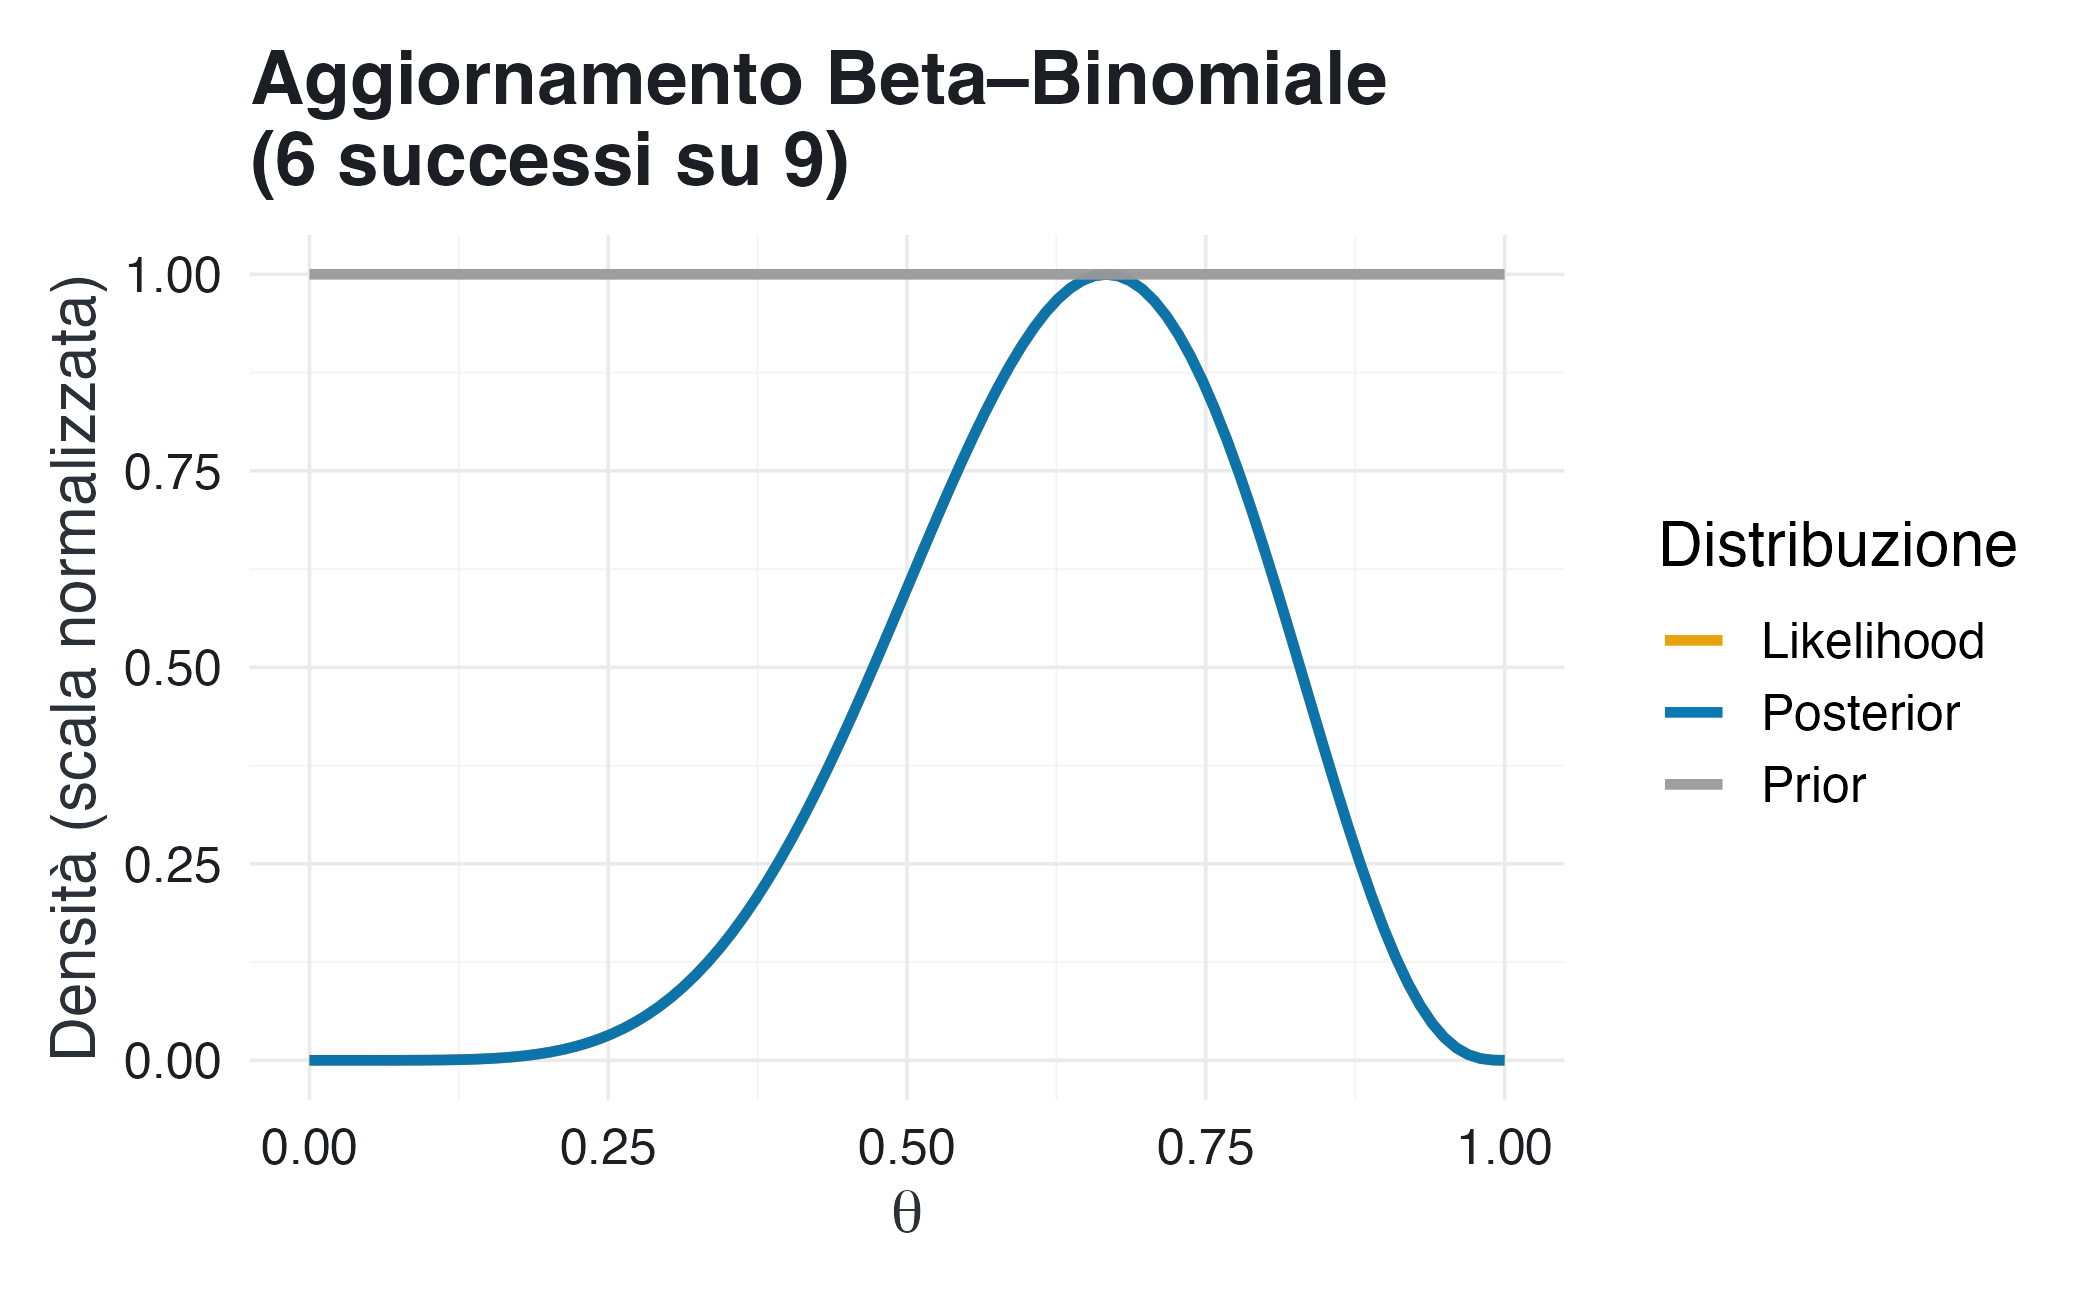
\includegraphics[width=0.85\linewidth,height=\textheight,keepaspectratio]{chapters/bayesian_inference/04_balance_prior_post_files/figure-pdf/unnamed-chunk-3-1.png}
\end{center}

La distribuzione a priori uniforme assegna la stessa probabilità a tutti
i valori di \(\theta\), riflettendo incertezza totale. La distribuzione
a posteriori coincide sostanzialmente con la verosimiglianza:
l'inferenza è interamente dominata dall'evidenza empirica.

\subsubsection{Scenario B: Prior moderatamente
informativa}\label{scenario-b-prior-moderatamente-informativa}

\begin{Shaded}
\begin{Highlighting}[]
\FunctionTok{plot\_beta\_binomial}\NormalTok{(}\AttributeTok{alpha =} \DecValTok{2}\NormalTok{, }\AttributeTok{beta =} \DecValTok{2}\NormalTok{, }\AttributeTok{y =} \DecValTok{6}\NormalTok{, }\AttributeTok{n =} \DecValTok{9}\NormalTok{)}
\end{Highlighting}
\end{Shaded}

\begin{center}
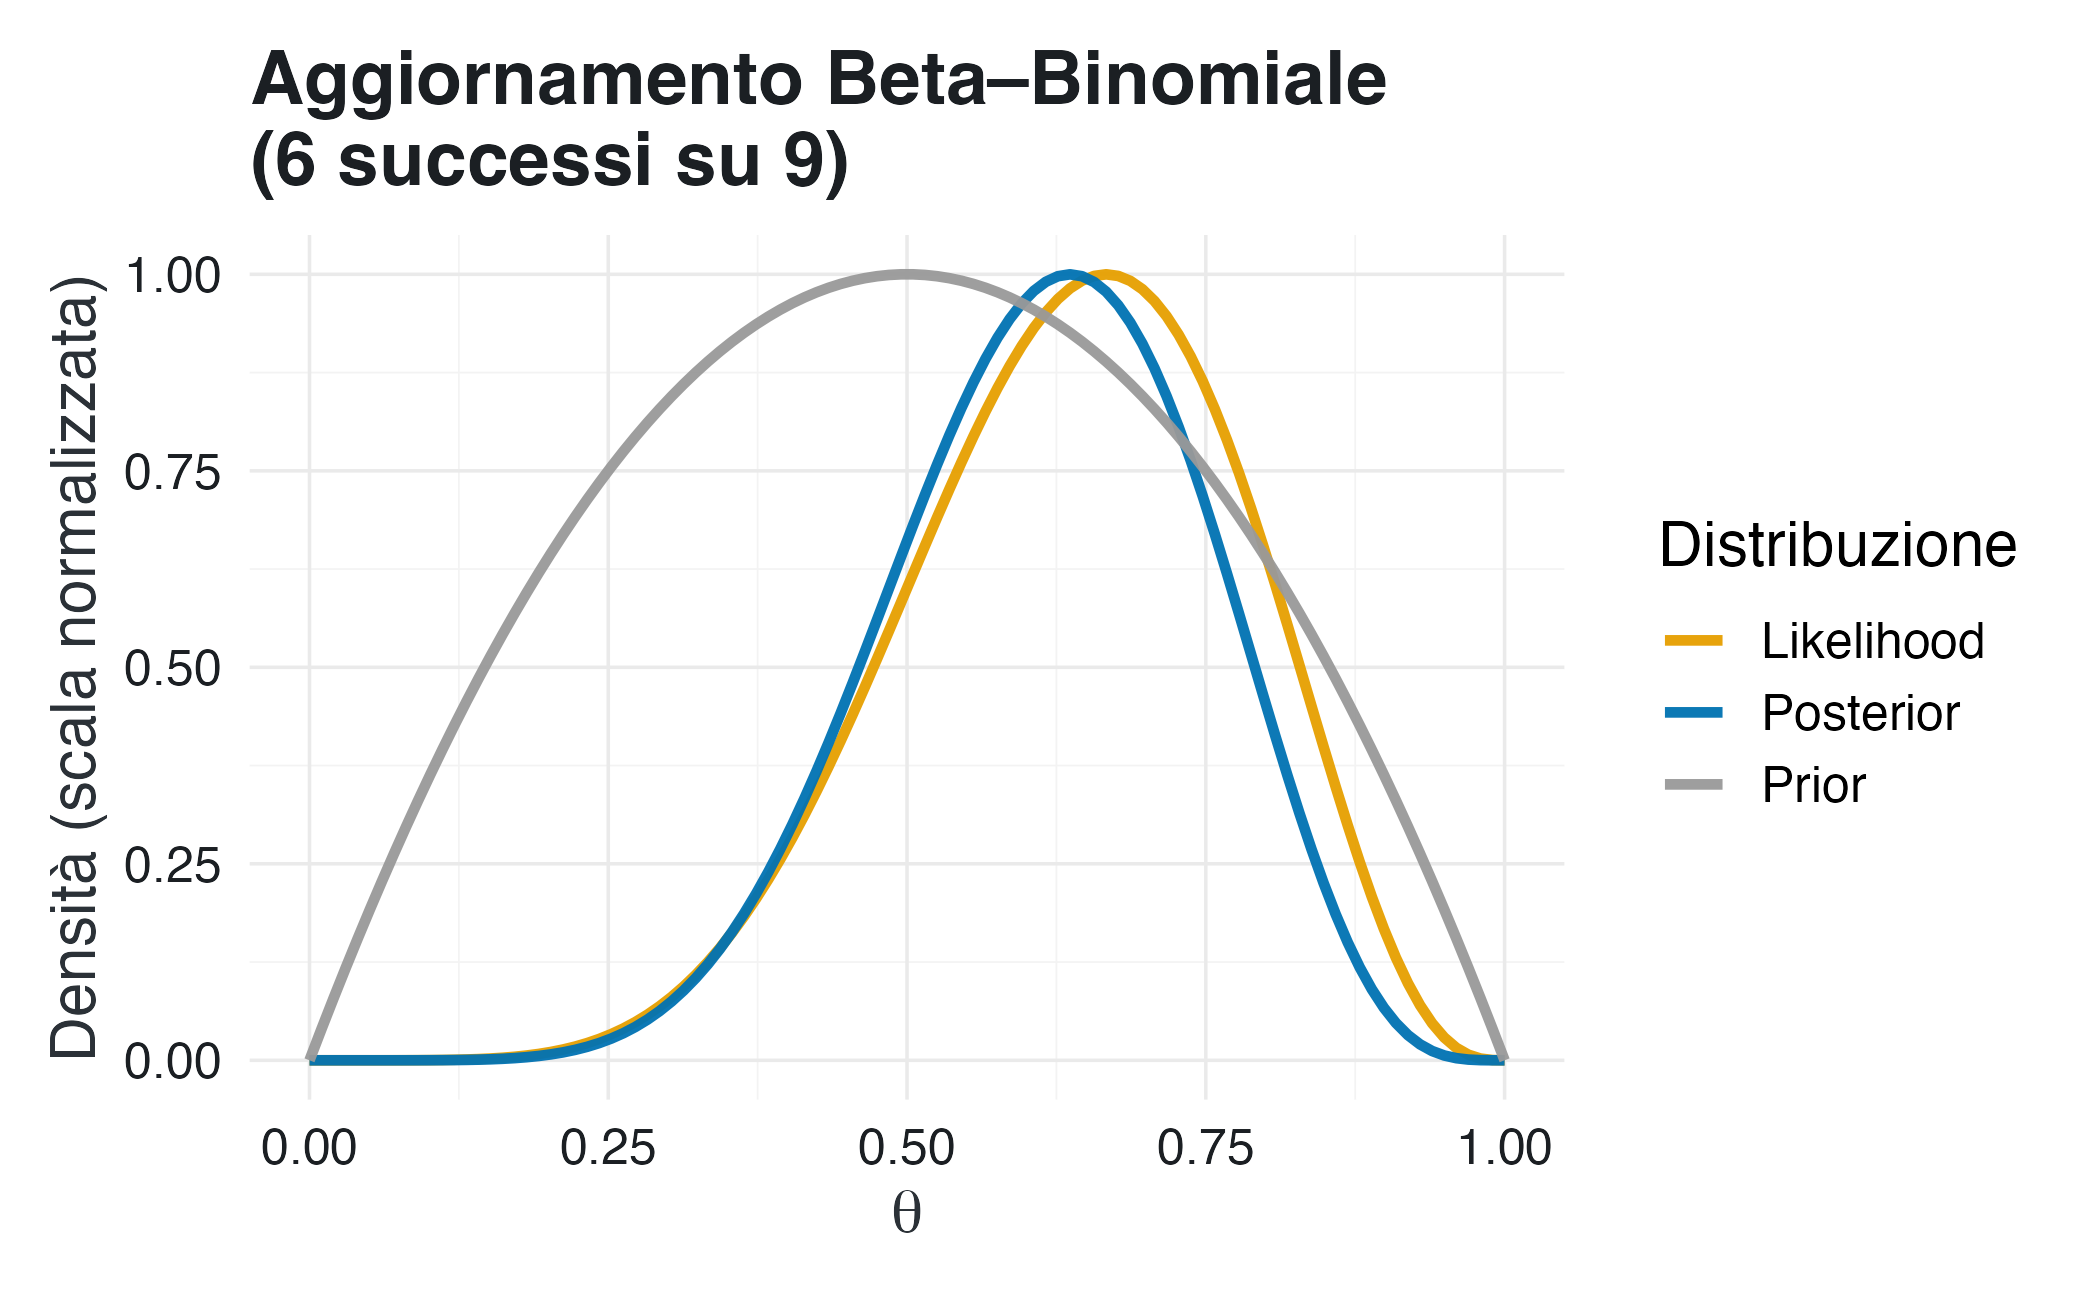
\includegraphics[width=0.85\linewidth,height=\textheight,keepaspectratio]{chapters/bayesian_inference/04_balance_prior_post_files/figure-pdf/unnamed-chunk-4-1.png}
\end{center}

La prior esprime una moderata credenza che \(\theta\) si collochi
intorno a 0.5, mantenendo notevole variabilità. Dopo l'aggiornamento, la
posteriori si sposta verso i valori suggeriti dai dati (0.67), ma
conserva una forma più conservativa, con media attorno a 0.62. La prior
esercita un effetto stabilizzante.

\subsubsection{Scenario C: Prior fortemente
informativa}\label{scenario-c-prior-fortemente-informativa}

\begin{Shaded}
\begin{Highlighting}[]
\FunctionTok{plot\_beta\_binomial}\NormalTok{(}\AttributeTok{alpha =} \DecValTok{2}\NormalTok{, }\AttributeTok{beta =} \DecValTok{5}\NormalTok{, }\AttributeTok{y =} \DecValTok{6}\NormalTok{, }\AttributeTok{n =} \DecValTok{9}\NormalTok{)}
\end{Highlighting}
\end{Shaded}

\begin{center}
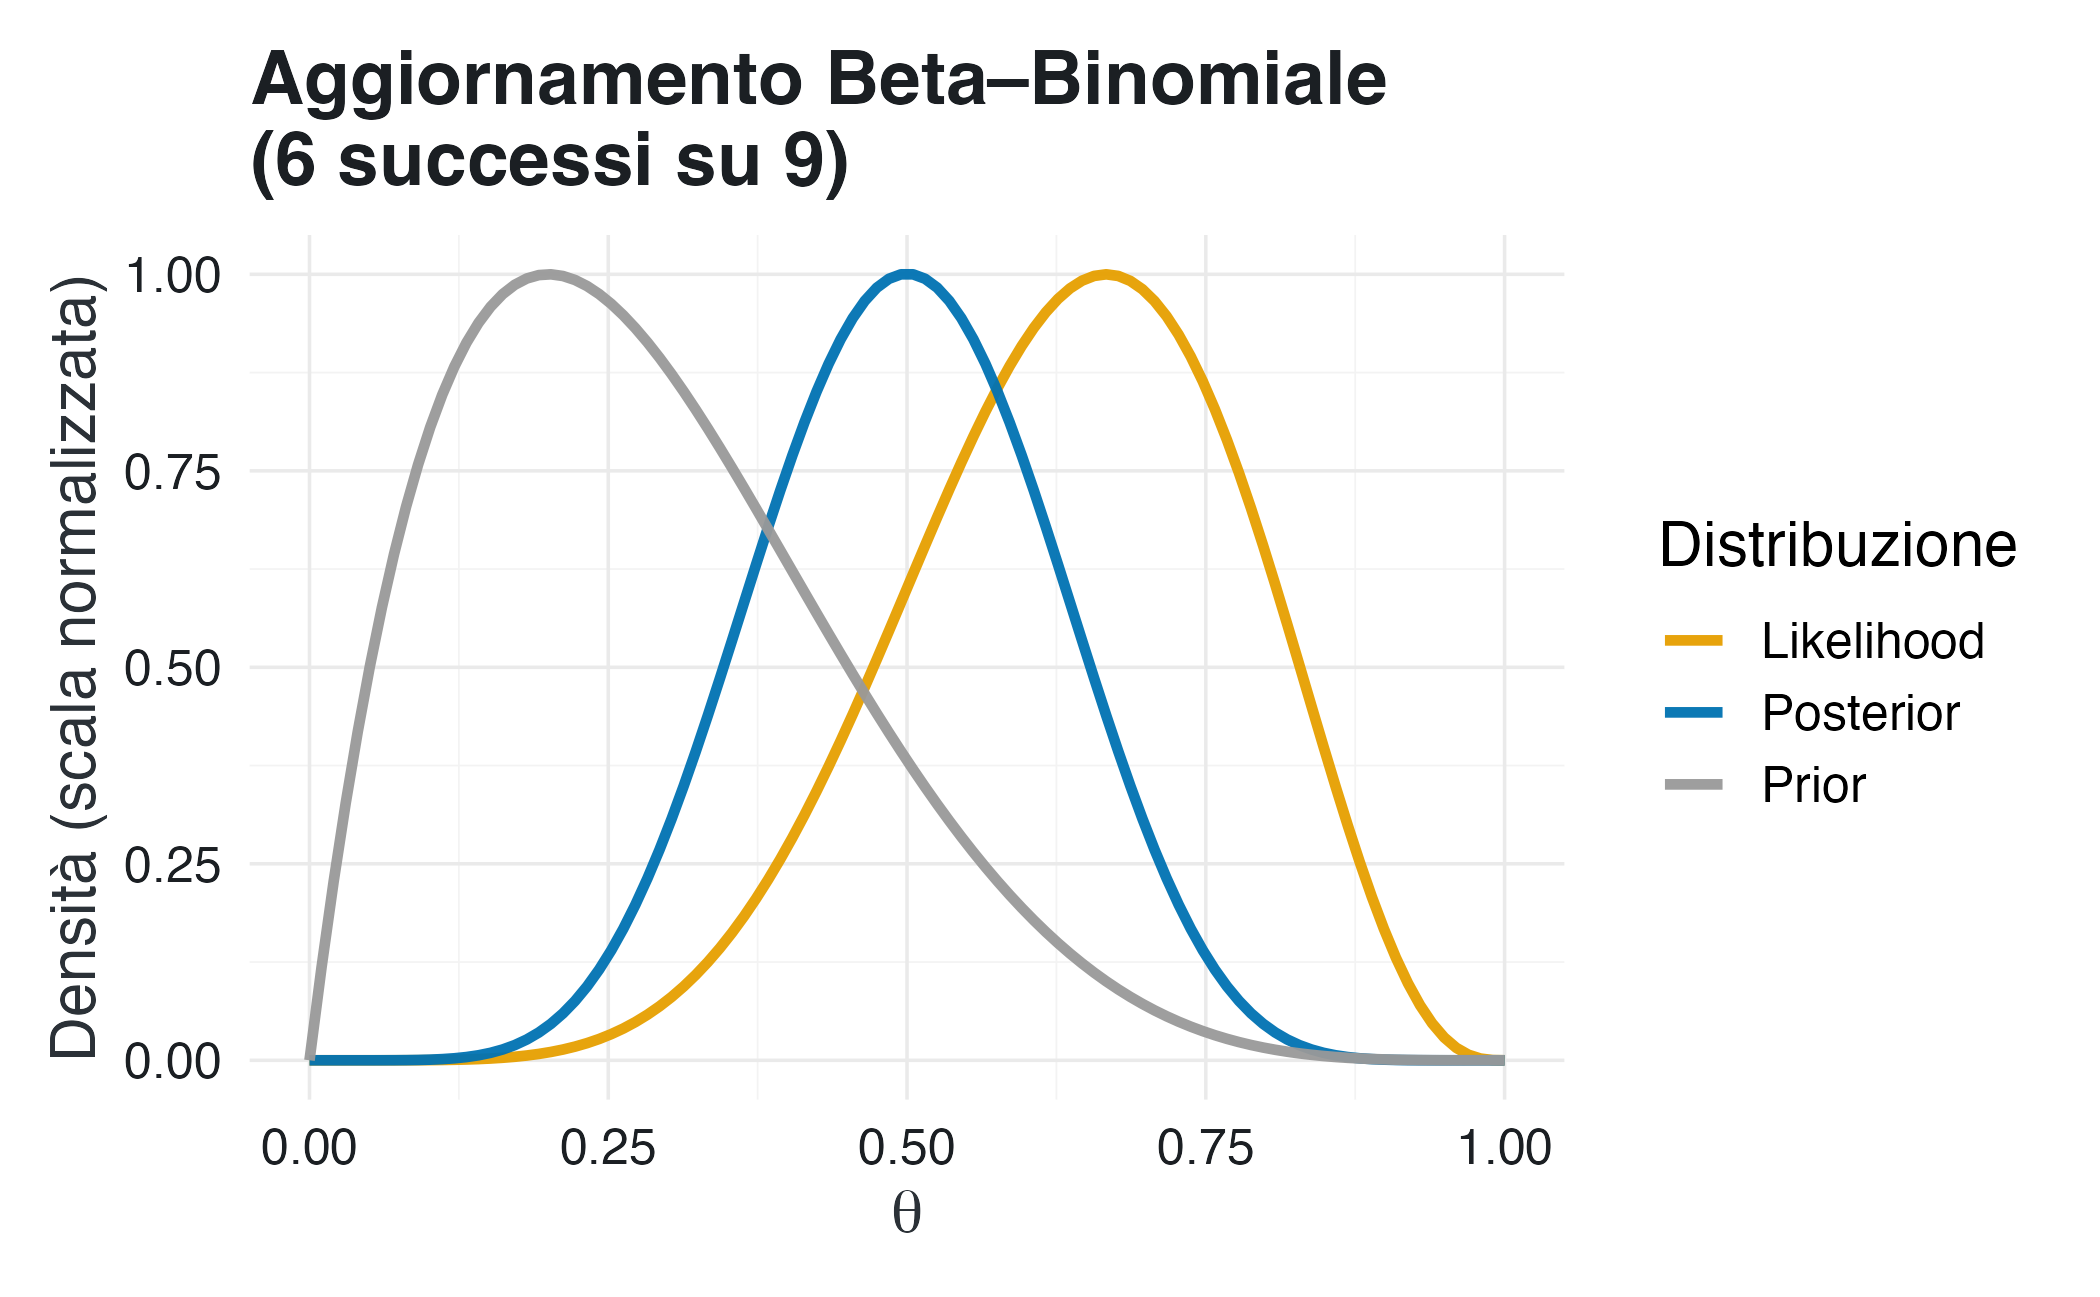
\includegraphics[width=0.85\linewidth,height=\textheight,keepaspectratio]{chapters/bayesian_inference/04_balance_prior_post_files/figure-pdf/unnamed-chunk-5-1.png}
\end{center}

La prior riflette una convinzione forte che \(\theta\) assuma valori
modesti (media a priori = 0.29). Nonostante l'evidenza empirica
suggerisca 0.67, la posteriori mantiene una posizione intermedia
(attorno a 0.45), dimostrando come convinzioni iniziali forti possano
resistere parzialmente all'evidenza contraria.

\subsection{La prior come evidenza
fittizia}\label{la-prior-come-evidenza-fittizia}

Il confronto tra i tre scenari rivela un principio fondamentale: la
distribuzione a priori può essere concepita come un insieme di
``osservazioni fittizie'' che precedono la raccolta dei dati. Nel
modello Beta-Binomiale, questa interpretazione è particolarmente
trasparente: i parametri \((\alpha,\beta)\) si sommano rispettivamente
ai successi e agli insuccessi osservati.

La quantità \(\alpha + \beta\), nota come \emph{sample size equivalente}
della prior, quantifica il peso delle convinzioni iniziali. Con
\(\alpha + \beta = 2\), la prior possiede un'influenza modesta; con
\(\alpha + \beta = 20\), incorpora un peso informativo rilevante e
richiede evidenza empirica sostanziale per essere modificata.

L'equilibrio tra prior ed evidenza emerge dalla struttura della media a
posteriori:

\[
\mathbb{E}[\theta \mid D] = \frac{\alpha+\beta}{\alpha+\beta+n} \cdot \underbrace{\frac{\alpha}{\alpha+\beta}}_{\text{media a priori}} + \frac{n}{\alpha+\beta+n} \cdot \underbrace{\frac{y}{n}}_{\text{media campionaria}}
\]

La stima finale è una media ponderata tra credenza iniziale ed evidenza
osservata. In contesti \emph{data-rich} \((n \gg \alpha+\beta)\), domina
l'evidenza empirica; in situazioni \emph{data-poor}
\((n \ll \alpha+\beta)\), la prior esercita un effetto stabilizzante.

\section{L'influenza della prior in relazione all'informazione
disponibile}\label{linfluenza-della-prior-in-relazione-allinformazione-disponibile}

La conclusione della sezione precedente mette in evidenza come
l'influenza della distribuzione a priori non sia costante, ma vari in
funzione della quantità e della qualità delle informazioni contenute nei
dati. Quando i dati sono numerosi e precisi, è la verosimiglianza a
prevalere, rendendo le stime robuste anche in presenza di scelte di
prior ragionevolmente diverse. Quando i dati sono limitati o rumorosi,
condizione frequente nella ricerca psicologica, la prior acquisisce un
peso determinante.

\subsection{Due scenari empirici}\label{due-scenari-empirici}

Si consideri uno studio sull'efficacia di un intervento di mindfulness
nella riduzione dello stress. Con un campione di 15 partecipanti e
elevata variabilità individuale, la stima potrebbe essere \(b = -0.4\)
con errore standard \(s = 0.3\). Il segnale risulterebbe debole
(\(z = -1.33\)) e i dati fornirebbero evidenza ambigua. Una prior
debolmente informativa, come \(\beta \sim \mathrm{Normal}(0, 1)\),
eserciterebbe un'importante azione di regolarizzazione, attirando la
stima verso lo zero.

Con un campione di 500 partecipanti, a parità di stima puntuale,
l'errore standard si ridurrebbe a \(s = 0.04\), portando a \(z = -10\).
La verosimiglianza dominerebbe il processo inferenziale, rendendo
trascurabile l'impatto della prior.

Il principio è semplice: \emph{l'influenza della prior è inversamente
proporzionale all'informazione contenuta nei dati}.

\subsection{Visualizzazione mediante
simulazione}\label{visualizzazione-mediante-simulazione}

Come mostrato nel grafico seguente, con \(n = 10\), la posteriori è
ampia e la prior esercita un'influenza visibile. Con \(n = 50\), la
posteriori si restringe. Con \(n = 500\), la posteriori risulta stretta
e centrata sul valore vero e l'influenza della prior diventa
trascurabile.

\begin{Shaded}
\begin{Highlighting}[]
\NormalTok{theta\_true }\OtherTok{\textless{}{-}} \FloatTok{0.6}
\NormalTok{alpha }\OtherTok{\textless{}{-}} \DecValTok{2}\NormalTok{; beta }\OtherTok{\textless{}{-}} \DecValTok{2}
\NormalTok{n\_values }\OtherTok{\textless{}{-}} \FunctionTok{c}\NormalTok{(}\DecValTok{10}\NormalTok{, }\DecValTok{50}\NormalTok{, }\DecValTok{500}\NormalTok{)}

\NormalTok{posterior\_list }\OtherTok{\textless{}{-}} \FunctionTok{list}\NormalTok{()}
\ControlFlowTok{for}\NormalTok{ (i }\ControlFlowTok{in} \FunctionTok{seq\_along}\NormalTok{(n\_values)) \{}
\NormalTok{  n }\OtherTok{\textless{}{-}}\NormalTok{ n\_values[i]}
\NormalTok{  k }\OtherTok{\textless{}{-}} \FunctionTok{round}\NormalTok{(theta\_true }\SpecialCharTok{*}\NormalTok{ n)}
\NormalTok{  theta }\OtherTok{\textless{}{-}} \FunctionTok{seq}\NormalTok{(}\DecValTok{0}\NormalTok{, }\DecValTok{1}\NormalTok{, }\AttributeTok{length.out =} \DecValTok{400}\NormalTok{)}
\NormalTok{  dens }\OtherTok{\textless{}{-}} \FunctionTok{dbeta}\NormalTok{(theta, alpha }\SpecialCharTok{+}\NormalTok{ k, beta }\SpecialCharTok{+}\NormalTok{ n }\SpecialCharTok{{-}}\NormalTok{ k)}
\NormalTok{  posterior\_list[[i]] }\OtherTok{\textless{}{-}} \FunctionTok{data.frame}\NormalTok{(}\AttributeTok{theta =}\NormalTok{ theta, }\AttributeTok{dens =}\NormalTok{ dens, }\AttributeTok{n =}\NormalTok{ n)}
\NormalTok{\}}

\NormalTok{posterior\_densities }\OtherTok{\textless{}{-}} \FunctionTok{do.call}\NormalTok{(rbind, posterior\_list)}

\FunctionTok{ggplot}\NormalTok{(posterior\_densities, }\FunctionTok{aes}\NormalTok{(}\AttributeTok{x =}\NormalTok{ theta, }\AttributeTok{y =}\NormalTok{ dens, }\AttributeTok{color =} \FunctionTok{factor}\NormalTok{(n))) }\SpecialCharTok{+}
  \FunctionTok{geom\_line}\NormalTok{(}\AttributeTok{size =} \FloatTok{1.2}\NormalTok{) }\SpecialCharTok{+}
  \FunctionTok{labs}\NormalTok{(}
    \AttributeTok{title =} \StringTok{"Effetto della numerosità campionaria}\SpecialCharTok{\textbackslash{}n}\StringTok{sulla distribuzione a posteriori"}\NormalTok{,}
    \AttributeTok{x =} \FunctionTok{expression}\NormalTok{(theta),}
    \AttributeTok{y =} \StringTok{"Densità"}\NormalTok{,}
    \AttributeTok{color =} \StringTok{"n (campione)"}
\NormalTok{  ) }
\end{Highlighting}
\end{Shaded}

\begin{center}
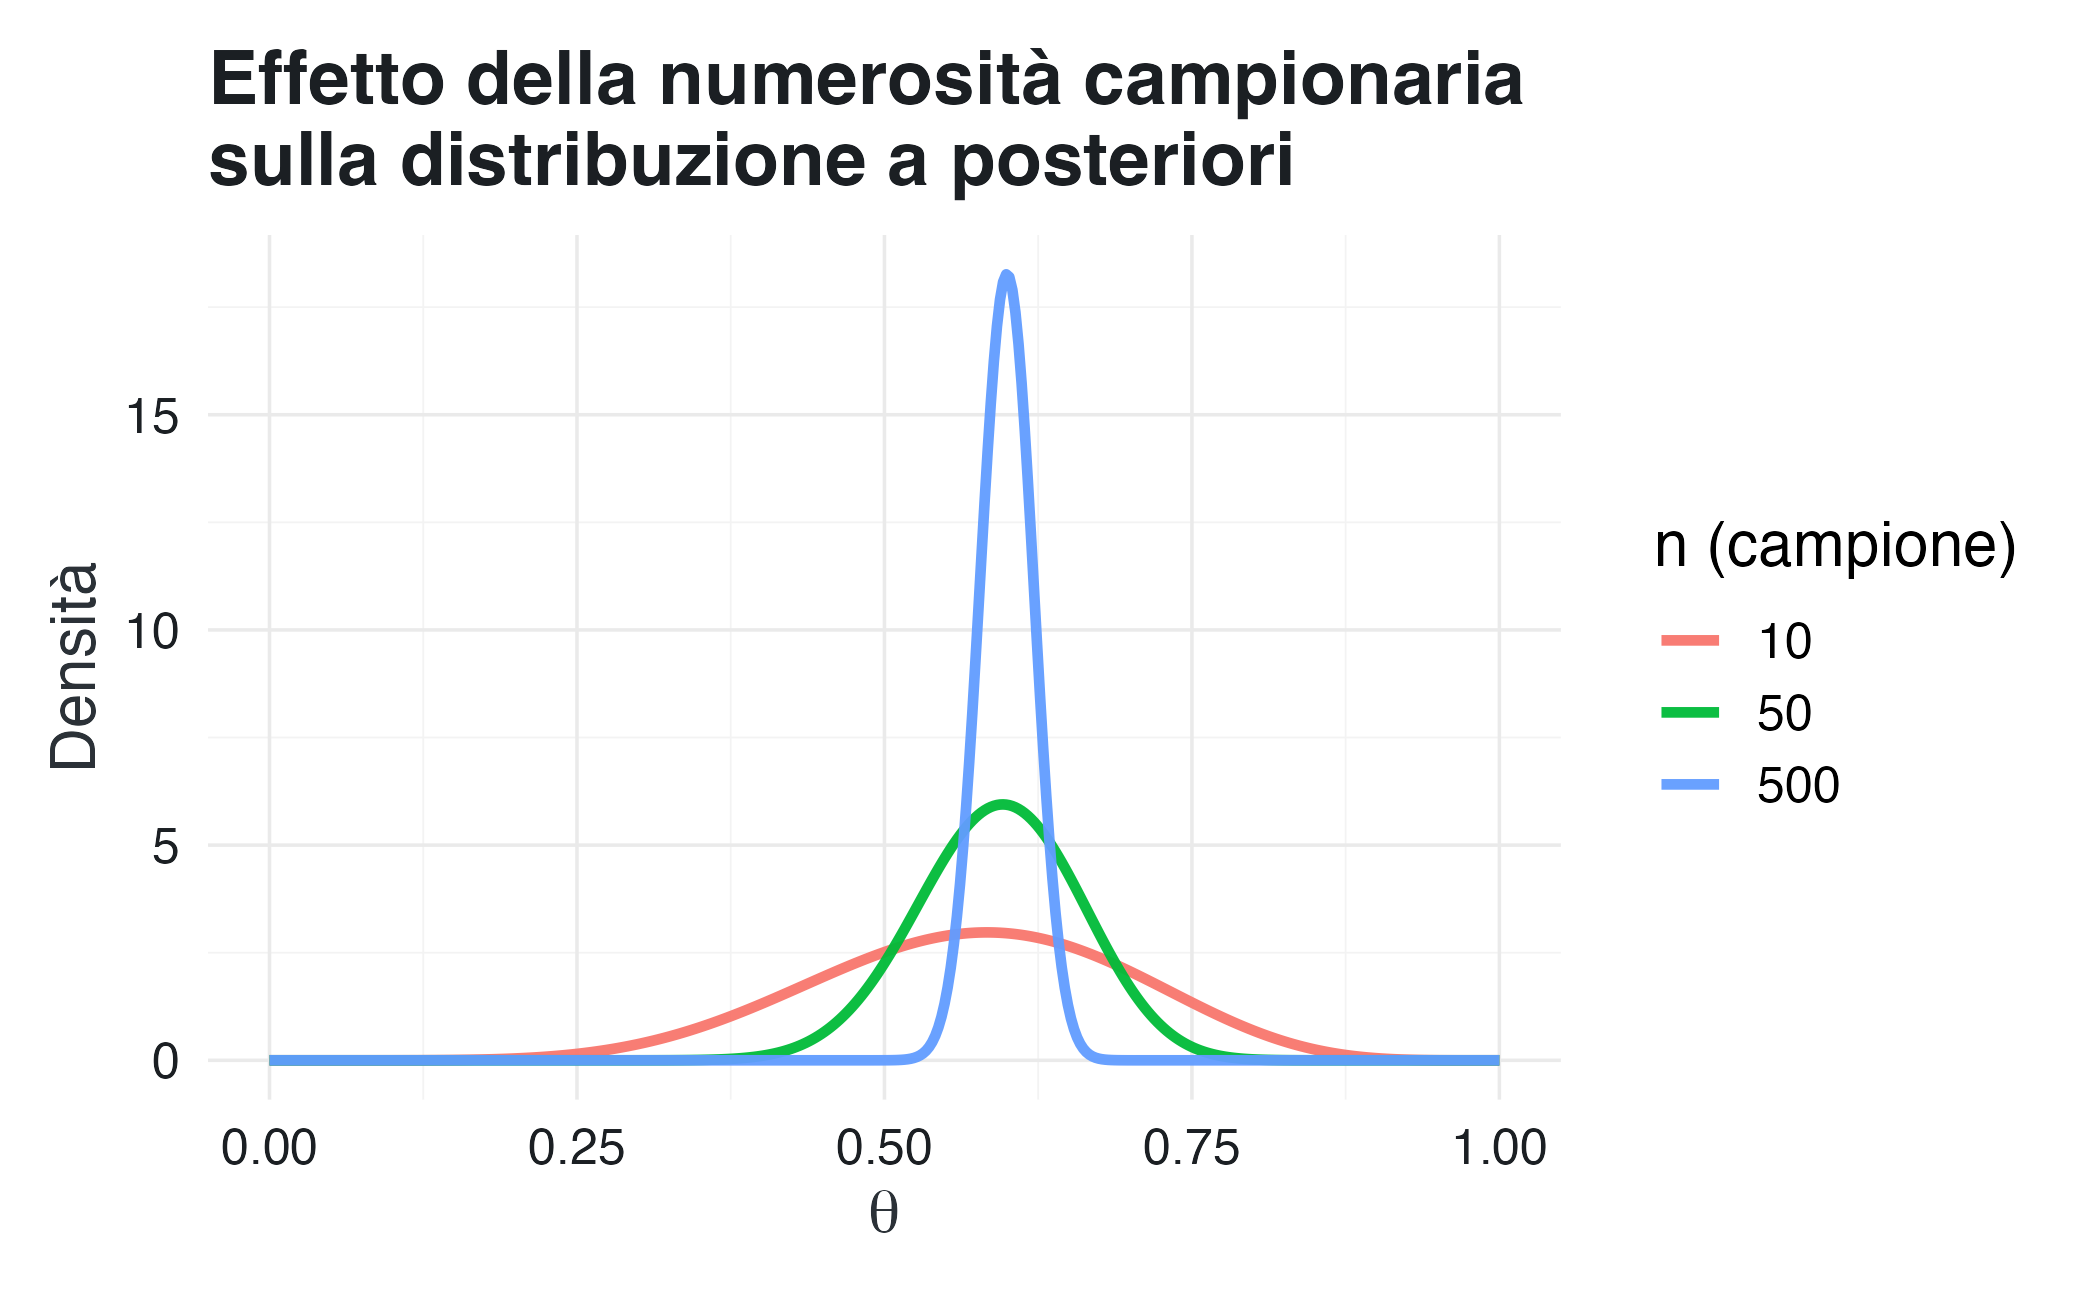
\includegraphics[width=0.85\linewidth,height=\textheight,keepaspectratio]{chapters/bayesian_inference/04_balance_prior_post_files/figure-pdf/unnamed-chunk-6-1.png}
\end{center}

{\def\LTcaptype{none} % do not increment counter
\begin{longtable}[]{@{}
  >{\raggedright\arraybackslash}p{(\linewidth - 4\tabcolsep) * \real{0.3875}}
  >{\raggedright\arraybackslash}p{(\linewidth - 4\tabcolsep) * \real{0.2625}}
  >{\raggedright\arraybackslash}p{(\linewidth - 4\tabcolsep) * \real{0.3500}}@{}}
\toprule\noalign{}
\begin{minipage}[b]{\linewidth}\raggedright
Situazione
\end{minipage} & \begin{minipage}[b]{\linewidth}\raggedright
Influenza della prior
\end{minipage} & \begin{minipage}[b]{\linewidth}\raggedright
Effetto pratico
\end{minipage} \\
\midrule\noalign{}
\endhead
\bottomrule\noalign{}
\endlastfoot
Campione piccolo, dati rumorosi & Alta & Stabilizza, evita sovrastime \\
Campione medio & Moderata & Compromesso equilibrato \\
Campione grande & Bassa & I dati dominano \\
\end{longtable}
}

Questo meccanismo, formalmente noto come ``shrinkage'', implementa una
regola epistemologicamente sensata: in presenza di informazioni deboli,
si evitano stime estreme; in presenza di informazioni robuste, prevale
il segnale dei dati.

\section{La scala del parametro: perché è
decisiva}\label{la-scala-del-parametro-perchuxe9-uxe8-decisiva}

Un aspetto fondamentale ma spesso trascurato è che le distribuzioni a
priori non sono invarianti rispetto ai cambiamenti di scala. Dichiarare
di aver scelto ``una prior uniforme'' non equivale automaticamente ad
adottare un atteggiamento neutrale: la stessa distribuzione a priori può
assumere un significato completamente diverso quando si modifica l'unità
di misura del parametro.

Immaginiamo uno studio sulla soddisfazione lavorativa misurata su una
scala 1--10. Un ricercatore assegna una prior uniforme all'effetto
\(\beta\), ritenendo equiprobabili tutti i valori tra --10 e +10. Se
successivamente ricodifica la variabile su una scala 0--100 senza
modificare la prior, l'intervallo originario si dilata di un ordine di
grandezza: ciò che prima rappresentava una gamma moderata di variazioni
diventa ora un insieme estremamente ampio di possibilità. La credenza
``uniforme'' iniziale non è più la stessa.

La conclusione è semplice: una prior non può essere piatta su qualunque
scala allo stesso tempo. La sua apparente ``neutralità'' vale soltanto
rispetto alla scala in cui è stata formulata.

\subsection{La soluzione: lavorare con un parametro
adimensionale}\label{la-soluzione-lavorare-con-un-parametro-adimensionale}

Per ottenere inferenze coerenti e confrontabili, conviene definire le
prior su quantità prive di unità di misura. Quando stimiamo un
coefficiente \(\beta\) con errore standard \(s\), l'informazione
rilevante non sta in \(\beta\) in sé, ma nel rapporto adimensionale

\[
\xi = \frac{\beta}{s},
\] che quantifica l'intensità del segnale rispetto al rumore.

L'uso di \(\xi\) presenta tre vantaggi: l'inferenza diventa
\emph{invariante} ai cambi di unità, permette confronti
\emph{consistenti} tra studi diversi e rende più trasparente \emph{il
ruolo effettivo} della prior nei risultati finali.

Per esempio, se osserviamo un effetto \(b = 4\) con errore standard
\(s = 2\) su una scala 0--10, il valore z è pari a 2. Se ricodifichiamo
la variabile su una scala 0--100, otteniamo (b' = 40) e \(s' = 20\), ma
il rapporto resta invariato: \(z = z' = 2\). Una prior definita su
\(\beta/s\) produce dunque la stessa inferenza in entrambe le scale. Una
prior definita direttamente su \(\beta\), invece, porterebbe a
conclusioni diverse semplicemente perché la scala è cambiata.

\subsection{Verifica mediante
simulazione}\label{verifica-mediante-simulazione}

\begin{Shaded}
\begin{Highlighting}[]
\NormalTok{b }\OtherTok{\textless{}{-}} \DecValTok{4}\NormalTok{; s }\OtherTok{\textless{}{-}} \DecValTok{2}
\NormalTok{a }\OtherTok{\textless{}{-}} \DecValTok{10}  \CommentTok{\# fattore di riscalamento}
\NormalTok{b2 }\OtherTok{\textless{}{-}}\NormalTok{ a }\SpecialCharTok{*}\NormalTok{ b; s2 }\OtherTok{\textless{}{-}}\NormalTok{ a }\SpecialCharTok{*}\NormalTok{ s}

\NormalTok{grid1 }\OtherTok{\textless{}{-}} \FunctionTok{seq}\NormalTok{(}\SpecialCharTok{{-}}\DecValTok{20}\NormalTok{, }\DecValTok{20}\NormalTok{, }\AttributeTok{length.out =} \DecValTok{1001}\NormalTok{)}
\NormalTok{grid2 }\OtherTok{\textless{}{-}} \FunctionTok{seq}\NormalTok{(}\SpecialCharTok{{-}}\DecValTok{200}\NormalTok{, }\DecValTok{200}\NormalTok{, }\AttributeTok{length.out =} \DecValTok{1001}\NormalTok{)}

\NormalTok{like1 }\OtherTok{\textless{}{-}} \FunctionTok{dnorm}\NormalTok{(grid1, }\AttributeTok{mean =}\NormalTok{ b,  }\AttributeTok{sd =}\NormalTok{ s)}
\NormalTok{like2 }\OtherTok{\textless{}{-}} \FunctionTok{dnorm}\NormalTok{(grid2, }\AttributeTok{mean =}\NormalTok{ b2, }\AttributeTok{sd =}\NormalTok{ s2)}

\CommentTok{\# Prior uniforme su β (non invariante)}
\NormalTok{prior\_unif1 }\OtherTok{\textless{}{-}} \FunctionTok{rep}\NormalTok{(}\DecValTok{1}\SpecialCharTok{/}\FunctionTok{length}\NormalTok{(grid1), }\FunctionTok{length}\NormalTok{(grid1))}
\NormalTok{prior\_unif2 }\OtherTok{\textless{}{-}} \FunctionTok{rep}\NormalTok{(}\DecValTok{1}\SpecialCharTok{/}\FunctionTok{length}\NormalTok{(grid2), }\FunctionTok{length}\NormalTok{(grid2))}

\NormalTok{post\_unif1 }\OtherTok{\textless{}{-}}\NormalTok{ like1 }\SpecialCharTok{*}\NormalTok{ prior\_unif1; post\_unif1 }\OtherTok{\textless{}{-}}\NormalTok{ post\_unif1 }\SpecialCharTok{/} \FunctionTok{sum}\NormalTok{(post\_unif1)}
\NormalTok{post\_unif2 }\OtherTok{\textless{}{-}}\NormalTok{ like2 }\SpecialCharTok{*}\NormalTok{ prior\_unif2; post\_unif2 }\OtherTok{\textless{}{-}}\NormalTok{ post\_unif2 }\SpecialCharTok{/} \FunctionTok{sum}\NormalTok{(post\_unif2)}

\CommentTok{\# Prior Cauchy su β/s (invariante)}
\NormalTok{prior\_cauchy1 }\OtherTok{\textless{}{-}} \FunctionTok{dcauchy}\NormalTok{(grid1 }\SpecialCharTok{/}\NormalTok{ s) }\SpecialCharTok{/}\NormalTok{ s}
\NormalTok{prior\_cauchy2 }\OtherTok{\textless{}{-}} \FunctionTok{dcauchy}\NormalTok{(grid2 }\SpecialCharTok{/}\NormalTok{ s2) }\SpecialCharTok{/}\NormalTok{ s2}

\NormalTok{post\_cauchy1 }\OtherTok{\textless{}{-}}\NormalTok{ like1 }\SpecialCharTok{*}\NormalTok{ prior\_cauchy1; post\_cauchy1 }\OtherTok{\textless{}{-}}\NormalTok{ post\_cauchy1 }\SpecialCharTok{/} \FunctionTok{sum}\NormalTok{(post\_cauchy1)}
\NormalTok{post\_cauchy2 }\OtherTok{\textless{}{-}}\NormalTok{ like2 }\SpecialCharTok{*}\NormalTok{ prior\_cauchy2; post\_cauchy2 }\OtherTok{\textless{}{-}}\NormalTok{ post\_cauchy2 }\SpecialCharTok{/} \FunctionTok{sum}\NormalTok{(post\_cauchy2)}

\CommentTok{\# Medie posteriori (riportate alla scala originale)}
\NormalTok{m\_unif1 }\OtherTok{\textless{}{-}} \FunctionTok{sum}\NormalTok{(grid1 }\SpecialCharTok{*}\NormalTok{ post\_unif1)}
\NormalTok{m\_unif2 }\OtherTok{\textless{}{-}} \FunctionTok{sum}\NormalTok{(grid2 }\SpecialCharTok{*}\NormalTok{ post\_unif2) }\SpecialCharTok{/}\NormalTok{ a}
\NormalTok{m\_cauchy1 }\OtherTok{\textless{}{-}} \FunctionTok{sum}\NormalTok{(grid1 }\SpecialCharTok{*}\NormalTok{ post\_cauchy1)}
\NormalTok{m\_cauchy2 }\OtherTok{\textless{}{-}} \FunctionTok{sum}\NormalTok{(grid2 }\SpecialCharTok{*}\NormalTok{ post\_cauchy2) }\SpecialCharTok{/}\NormalTok{ a}

\FunctionTok{tibble}\NormalTok{(}
  \AttributeTok{Prior =} \FunctionTok{c}\NormalTok{(}\StringTok{"Uniforme su β"}\NormalTok{, }\StringTok{"Cauchy su β/s"}\NormalTok{),}
  \AttributeTok{Media\_orig =} \FunctionTok{c}\NormalTok{(m\_unif1, m\_cauchy1),}
  \AttributeTok{Media\_rescaled =} \FunctionTok{c}\NormalTok{(m\_unif2, m\_cauchy2)}
\NormalTok{)}
\CommentTok{\#\textgreater{} \# A tibble: 2 x 3}
\CommentTok{\#\textgreater{}   Prior         Media\_orig Media\_rescaled}
\CommentTok{\#\textgreater{}   \textless{}chr\textgreater{}              \textless{}dbl\textgreater{}          \textless{}dbl\textgreater{}}
\CommentTok{\#\textgreater{} 1 Uniforme su β       4.00           4.00}
\CommentTok{\#\textgreater{} 2 Cauchy su β/s       2.56           2.56}
\end{Highlighting}
\end{Shaded}

La prior uniforme produce risultati diversi dopo il cambio di scala,
mentre la prior su \(\beta/s\) produce risultati identici. In pratica,
definire la prior sul rapporto segnale-rumore garantisce coerenza,
confrontabilità e indipendenza da convenzioni arbitrarie.

{\def\LTcaptype{none} % do not increment counter
\begin{longtable}[]{@{}
  >{\raggedright\arraybackslash}p{(\linewidth - 6\tabcolsep) * \real{0.2500}}
  >{\raggedright\arraybackslash}p{(\linewidth - 6\tabcolsep) * \real{0.1591}}
  >{\raggedright\arraybackslash}p{(\linewidth - 6\tabcolsep) * \real{0.3182}}
  >{\raggedright\arraybackslash}p{(\linewidth - 6\tabcolsep) * \real{0.2727}}@{}}
\toprule\noalign{}
\begin{minipage}[b]{\linewidth}\raggedright
Tipo di trasformazione
\end{minipage} & \begin{minipage}[b]{\linewidth}\raggedright
Esempio
\end{minipage} & \begin{minipage}[b]{\linewidth}\raggedright
Prior uniforme su \(\beta\)
\end{minipage} & \begin{minipage}[b]{\linewidth}\raggedright
Prior su \(\beta/s\)
\end{minipage} \\
\midrule\noalign{}
\endhead
\bottomrule\noalign{}
\endlastfoot
Cambio unità & 0-10 → 0-100 & Cambia forma e densità & Nessuna
differenza \\
Inversione segno & A-B → B-A & Cambia il centro & Solo inversione
segno \\
Standardizzazione & Grezzi → z & Cambia la scala & Nessuna differenza \\
\end{longtable}
}

\section{Tipologie di distribuzioni a
priori}\label{tipologie-di-distribuzioni-a-priori}

\subsection{Prior non informative}\label{prior-non-informative}

\textbf{Scopo:} minimizzare l'influenza delle convinzioni preesistenti.

\textbf{Esempio:} per indagare la relazione tra l'arousal fisiologico e
i pensieri intrusivi in assenza di letteratura pregressa, si potrebbe
adottare la seguente distribuzione a priori: \[
\rho \sim \text{Uniform}(-1, 1).
\]

\textbf{Avvertenza:} il termine ``non informativa'' è fuorviante. Una
prior uniforme su una scala non lo è su un'altra (ad esempio, dopo una
trasformazione non lineare). Inoltre, questo approccio attribuisce
probabilità non trascurabili a valori estremi che si manifestano
raramente nei fenomeni psicologici.

\subsection{Prior debolmente
informative}\label{prior-debolmente-informative}

\textbf{Scopo:} imporre vincoli di plausibilità senza precludere ai dati
di esprimersi.

\textbf{Esempio:} per uno studio sull'efficacia di un intervento di
mindfulness: \[
\beta \sim \text{Normal}(0, 1).
\] Questa scelta comunica: ``riteniamo più probabile un effetto nullo o
modesto, ma non escludiamo effetti più sostanziali se i dati li
supporteranno''.

\textbf{Vantaggio:} funge da stabilizzatore, soprattutto in campioni
piccoli, prevenendo la sovrastima di effetti spurii.

\subsection{Prior informative}\label{prior-informative}

\textbf{Scopo:} incorporare evidenze consolidate da studi precedenti o
meta-analisi.

\textbf{Esempio:} se una meta-analisi indica che la CBT produce una
riduzione media dei sintomi depressivi pari a \(d = 0.5\): \[
\beta \sim \text{Normal}(0.5, 0.2).
\] Questa distribuzione esprime una convinzione ragionevolmente forte,
pur ammettendo un margine di incertezza.

\subsection{Prior empiriche (da
corpus)}\label{prior-empiriche-da-corpus}

\textbf{Scopo:} calibrare la prior sui dati quantitativi di un insieme
di studi affini.

\textbf{Esempio:} analizzando la distribuzione degli z-score riportati
in studi che utilizzano l'\emph{Experience Sampling Method}, si può
stimare una distribuzione empirica che rappresenti il tipico rapporto
segnale-rumore in questo ambito.

\subsection{Visualizzazione
comparativa}\label{visualizzazione-comparativa}

\begin{Shaded}
\begin{Highlighting}[]
\NormalTok{beta\_grid }\OtherTok{\textless{}{-}} \FunctionTok{seq}\NormalTok{(}\SpecialCharTok{{-}}\DecValTok{3}\NormalTok{, }\DecValTok{3}\NormalTok{, }\AttributeTok{length.out =} \DecValTok{500}\NormalTok{)}
\NormalTok{priors }\OtherTok{\textless{}{-}} \FunctionTok{tibble}\NormalTok{(}
  \AttributeTok{beta =} \FunctionTok{rep}\NormalTok{(beta\_grid, }\DecValTok{3}\NormalTok{),}
  \AttributeTok{tipo =} \FunctionTok{rep}\NormalTok{(}\FunctionTok{c}\NormalTok{(}\StringTok{"Uniforme"}\NormalTok{, }\StringTok{"Normal(0,1)"}\NormalTok{, }\StringTok{"Normal(0.5,0.2)"}\NormalTok{), }\AttributeTok{each =} \FunctionTok{length}\NormalTok{(beta\_grid)),}
  \AttributeTok{dens =} \FunctionTok{c}\NormalTok{(}
    \FunctionTok{dunif}\NormalTok{(beta\_grid, }\SpecialCharTok{{-}}\DecValTok{3}\NormalTok{, }\DecValTok{3}\NormalTok{),}
    \FunctionTok{dnorm}\NormalTok{(beta\_grid, }\DecValTok{0}\NormalTok{, }\DecValTok{1}\NormalTok{),}
    \FunctionTok{dnorm}\NormalTok{(beta\_grid, }\FloatTok{0.5}\NormalTok{, }\FloatTok{0.2}\NormalTok{)}
\NormalTok{  )}
\NormalTok{)}

\FunctionTok{ggplot}\NormalTok{(priors, }\FunctionTok{aes}\NormalTok{(}\AttributeTok{x =}\NormalTok{ beta, }\AttributeTok{y =}\NormalTok{ dens, }\AttributeTok{color =}\NormalTok{ tipo)) }\SpecialCharTok{+}
  \FunctionTok{geom\_line}\NormalTok{(}\AttributeTok{linewidth =} \FloatTok{1.2}\NormalTok{) }\SpecialCharTok{+}
  \FunctionTok{labs}\NormalTok{(}
    \AttributeTok{title =} \StringTok{"Confronto tra distribuzioni a priori}\SpecialCharTok{\textbackslash{}n}\StringTok{per un coefficiente β"}\NormalTok{,}
    \AttributeTok{x =} \FunctionTok{expression}\NormalTok{(beta),}
    \AttributeTok{y =} \StringTok{"Densità"}\NormalTok{,}
    \AttributeTok{color =} \StringTok{"Tipo di Prior"}
\NormalTok{  ) }
\end{Highlighting}
\end{Shaded}

\begin{center}
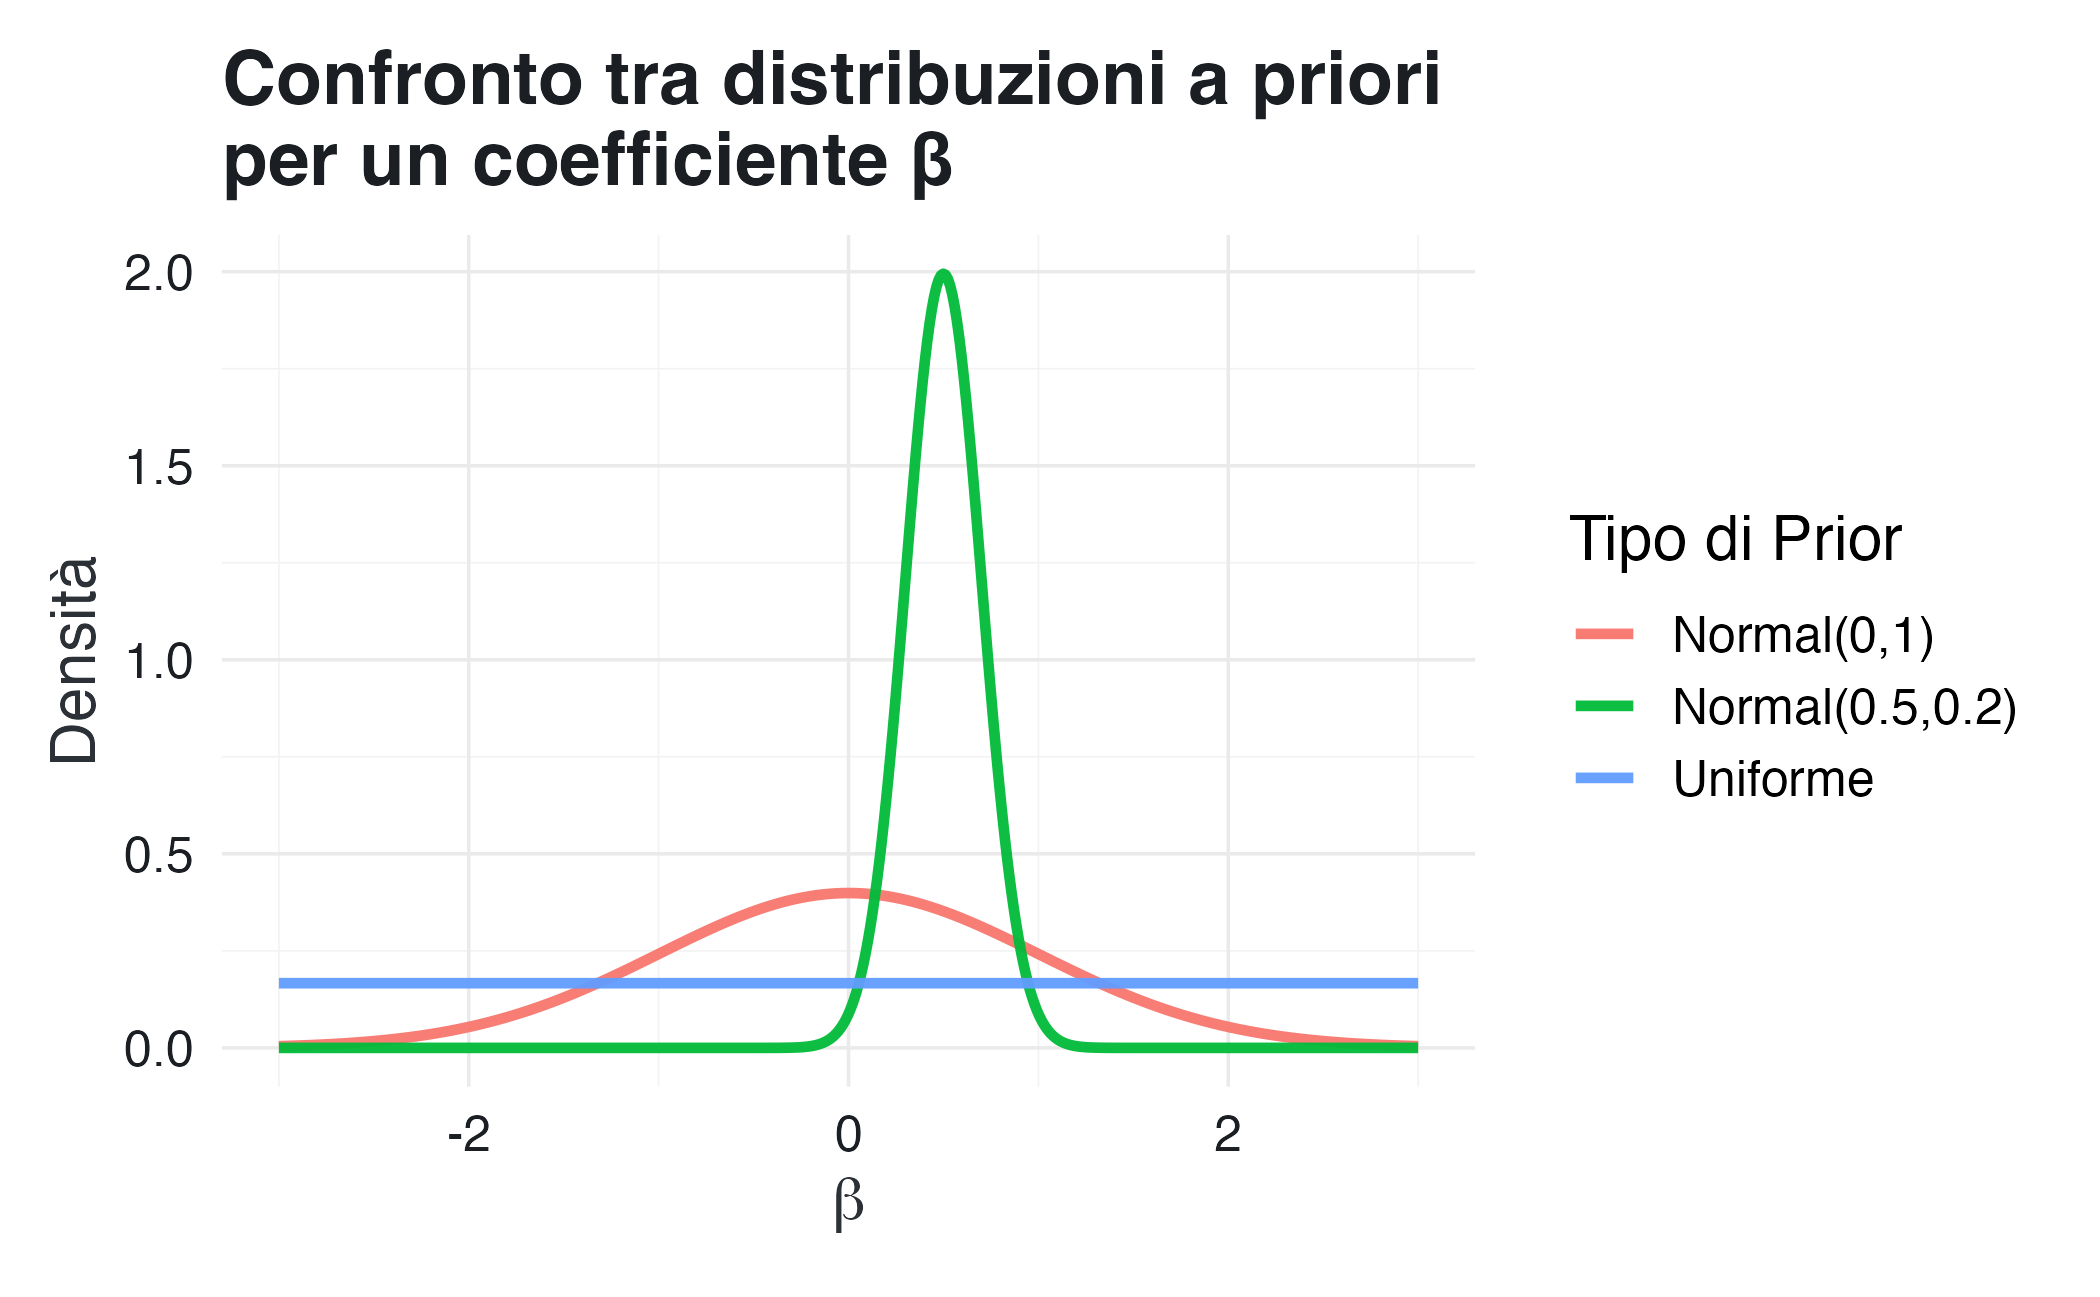
\includegraphics[width=0.85\linewidth,height=\textheight,keepaspectratio]{chapters/bayesian_inference/04_balance_prior_post_files/figure-pdf/unnamed-chunk-8-1.png}
\end{center}

La prior uniforme assegna una densità costante senza preferenze. La
Normal(0,1) esprime un moderato scetticismo nei confronti dell'ipotesi
nulla. La Normal(0.5, 0.2) incorpora un'aspettativa precisa.

{\def\LTcaptype{none} % do not increment counter
\begin{longtable}[]{@{}
  >{\raggedright\arraybackslash}p{(\linewidth - 6\tabcolsep) * \real{0.2016}}
  >{\raggedright\arraybackslash}p{(\linewidth - 6\tabcolsep) * \real{0.2636}}
  >{\raggedright\arraybackslash}p{(\linewidth - 6\tabcolsep) * \real{0.2016}}
  >{\raggedright\arraybackslash}p{(\linewidth - 6\tabcolsep) * \real{0.3333}}@{}}
\toprule\noalign{}
\begin{minipage}[b]{\linewidth}\raggedright
Tipo
\end{minipage} & \begin{minipage}[b]{\linewidth}\raggedright
Quando usarla
\end{minipage} & \begin{minipage}[b]{\linewidth}\raggedright
Vantaggi
\end{minipage} & \begin{minipage}[b]{\linewidth}\raggedright
Rischi
\end{minipage} \\
\midrule\noalign{}
\endhead
\bottomrule\noalign{}
\endlastfoot
\textbf{Non informativa} & Nessuna conoscenza pregressa & Lascia parlare
i dati & Instabile con campioni piccoli \\
\textbf{Debolmente informativa} & Effetti plausibili ma incerti &
Regolarizza, evita outlier & Può sembrare arbitraria \\
\textbf{Informativa} & Evidenze forti da studi precedenti & Integra
conoscenza teorica & Può dominare se i dati sono pochi \\
\end{longtable}
}

\section{Prior su scala SNR: strategie in presenza o assenza di corpus
empirici}\label{prior-su-scala-snr-strategie-in-presenza-o-assenza-di-corpus-empirici}

Zwet \& Gelman (\citeproc{ref-zwet2022proposal}{2022}) propongono
l'utilizzo di prior informative basate su \emph{corpora} di studi di
riferimento, implementate mediante miscele di distribuzioni.
Consideriamo una prior costituita da una miscela simmetrica di due
componenti normali centrate sullo zero:

\[
p(\xi) = \pi_1 \cdot \mathcal{N}(\xi \mid 0, \tau_1^2) + \pi_2 \cdot \mathcal{N}(\xi \mid 0, \tau_2^2)
\] dove:

\begin{itemize}
\tightlist
\item
  \textbf{i pesi} (\(\pi_1, \pi_2\)) rappresentano la proporzione
  relativa di effetti ``piccoli'' rispetto a quelli ``più sostanziali'';
\item
  \textbf{le scale} (\(\tau_1, \tau_2\)) catturano l'ampiezza tipica
  degli effetti in ciascuna categoria.
\end{itemize}

I valori specifici si ottengono calibrando la miscela su un corpus di
studi metodologicamente affini, consentendo uno \emph{shrinkage}
differenziato: effetti plausibilmente piccoli vengono regolarizzati più
fortemente, mentre effetti sostanziali subiscono un'interferenza minima.

\subsection{Strategie in assenza di corpus
consolidato}\label{strategie-in-assenza-di-corpus-consolidato}

Quando non si dispone di un corpus di riferimento o mancano informazioni
preliminari affidabili, è consigliabile adottare distribuzioni a code
più pesanti. La proposta standard è la distribuzione di Cauchy:

\[
\frac{\beta}{s} \sim \mathrm{Cauchy}(0, 1).
\]

La scelta della Cauchy non è casuale ma riflette un preciso profilo
statistico:

\begin{itemize}
\tightlist
\item
  \textbf{code più marcate} rispetto alla normale, riducendo la
  penalizzazione eccessiva per effetti moderatamente grandi;
\item
  \textbf{comportamento ottimale}: forte regolarizzazione per effetti
  modesti (\(|z| < 2\)), interferenza minima per effetti sostanziali
  (\(|z| > 3\));
\item
  \textbf{proprietà di calibrazione}: pari probabilità di effetti
  sopra/sotto una determinata soglia (es. \(P(|\xi|>2.5) \approx 0.1\)).
\end{itemize}

Per modelli complessi o quando si desidera maggiore controllo sulle
code, è possibile considerare:

\begin{itemize}
\tightlist
\item
  troncamenti ragionevoli della distribuzione (es. \(|\xi| < 10\))
\item
  distribuzioni \(t\) di Student con gradi di libertà \(\nu \in [3,7]\),
  che permettono di modulare il peso delle code
\end{itemize}

\subsection{Quadro decisionale per la scelta della
prior}\label{quadro-decisionale-per-la-scelta-della-prior}

{\def\LTcaptype{none} % do not increment counter
\begin{longtable}[]{@{}
  >{\raggedright\arraybackslash}p{(\linewidth - 4\tabcolsep) * \real{0.2976}}
  >{\raggedright\arraybackslash}p{(\linewidth - 4\tabcolsep) * \real{0.3810}}
  >{\raggedright\arraybackslash}p{(\linewidth - 4\tabcolsep) * \real{0.3214}}@{}}
\toprule\noalign{}
\begin{minipage}[b]{\linewidth}\raggedright
Situazione metodologica
\end{minipage} & \begin{minipage}[b]{\linewidth}\raggedright
Prior consigliata su \(\beta/s\)
\end{minipage} & \begin{minipage}[b]{\linewidth}\raggedright
Vantaggi e considerazioni
\end{minipage} \\
\midrule\noalign{}
\endhead
\bottomrule\noalign{}
\endlastfoot
\textbf{Nessun corpus disponibile} & Cauchy(0,1) & Default robusto,
adatto a scenari esplorativi; bilancia regolarizzazione e sensibilità \\
\textbf{Corpus di studi metodologicamente affini} & Miscela di Normali &
Shrinkage adattivo: calibra la regolarizzazione in base alla
distribuzione empirica degli effetti nel campo \\
\textbf{Pregressa evidenza di effetti piccoli} & Normal(0,0.5) o
Normal(0,1) & Prior più concentrate riducono il rischio di sovrastime
per effetti modesti \\
\textbf{Potenziali effetti grandi e incertezza elevata} & t₃(0,2) o
Cauchy(0,2) & Code più ampie preservano la capacità di rilevare segnali
sostanziali, anche quando rari \\
\end{longtable}
}

Questa struttura decisionale permette di ancorare la scelta della prior
a considerazioni sostantiva e metodologiche, promuovendo inferenze più
coerenti e replicabili. L'approccio basato sul parametro adimensionale
\(\beta/s\) garantisce che tali scelte rimangano invarianti rispetto
alle scale di misurazione utilizzate nello studio.

\section{Dalla teoria alla pratica}\label{dalla-teoria-alla-pratica}

\subsection{Guida alla scelta della
prior}\label{guida-alla-scelta-della-prior}

La costruzione di una prior ben calibrata richiede di rispondere a tre
domande: \emph{Su quale scala è definito il parametro? Quale intervallo
è plausibile? Quanto è forte la nostra convinzione iniziale?}

\textbf{Scala:} per coefficienti di regressione, la scala adimensionale
\(\xi = \beta/s\) è preferibile. Nei GLM, la prior deve essere
specificata sulla scala del link (logit, log). La standardizzazione dei
predittori conferisce interpretazione immediata.

\textbf{Plausibilità:} per predittori standardizzati, effetti con
\(|\beta| > 1-2\) sono generalmente sostanziali. La prior deve
delimitare lo spazio dei valori plausibili senza ``indovinare'' il
valore vero.

\textbf{Informatività:} in assenza di evidenze solide, distribuzioni a
code pesanti su \(\xi\) realizzano shrinkage adattivo. Con letteratura
consolidata, una normale centrata su stime meta-analitiche è
appropriata.

\begin{tcolorbox}[enhanced jigsaw, arc=.35mm, bottomrule=.15mm, bottomtitle=1mm, breakable, colback=white, colbacktitle=quarto-callout-tip-color!10!white, colframe=quarto-callout-tip-color-frame, coltitle=black, left=2mm, leftrule=.75mm, opacityback=0, opacitybacktitle=0.6, rightrule=.15mm, title=\textcolor{quarto-callout-tip-color}{\faLightbulb}\hspace{0.5em}{Procedura operativa}, titlerule=0mm, toprule=.15mm, toptitle=1mm]

\begin{enumerate}
\def\labelenumi{\arabic{enumi}.}
\item
  \textbf{Identifica la scala e i vincoli.} Ci sono limiti naturali (≥0
  per varianze, {[}0,1{]} per probabilità)? È possibile usare una scala
  adimensionale?
\item
  \textbf{Stima l'ordine di grandezza plausibile.} Quale intervallo ha
  senso per il fenomeno studiato?
\item
  \textbf{Attingi alla letteratura.} Meta-analisi e studi precedenti
  ancorano la prior a valori empiricamente plausibili.
\item
  \textbf{Calibra l'informatività.} Distribuzioni a code pesanti offrono
  un buon compromesso: regolarizzano senza escludere effetti inattesi.
\end{enumerate}

\textbf{Regola empirica:} in assenza di letteratura solida, una \(t\) o
Cauchy sul rapporto \(\beta/s\) rappresenta la scelta più sicura.

\end{tcolorbox}

\subsection{Prior predictive check}\label{prior-predictive-check}

Prima di analizzare i dati, occorre verificare che le assunzioni siano
coerenti con la fenomenologia del dominio: ``Quali dati potrei osservare
se le mie prior rispecchiassero la realtà?''

\begin{Shaded}
\begin{Highlighting}[]
\FunctionTok{set.seed}\NormalTok{(}\DecValTok{1}\NormalTok{)}
\NormalTok{n }\OtherTok{\textless{}{-}} \DecValTok{30}
\NormalTok{mu\_prior\_sd }\OtherTok{\textless{}{-}} \FloatTok{1.0}
\NormalTok{S }\OtherTok{\textless{}{-}} \DecValTok{2000}

\NormalTok{mu\_samp }\OtherTok{\textless{}{-}} \FunctionTok{rnorm}\NormalTok{(S, }\AttributeTok{mean =} \DecValTok{0}\NormalTok{, }\AttributeTok{sd =}\NormalTok{ mu\_prior\_sd)}
\NormalTok{ybar\_rep }\OtherTok{\textless{}{-}} \FunctionTok{sapply}\NormalTok{(mu\_samp, }\ControlFlowTok{function}\NormalTok{(m) }\FunctionTok{mean}\NormalTok{(}\FunctionTok{rnorm}\NormalTok{(n, }\AttributeTok{mean =}\NormalTok{ m, }\AttributeTok{sd =} \DecValTok{1}\NormalTok{)))}

\FunctionTok{quantile}\NormalTok{(ybar\_rep, }\FunctionTok{c}\NormalTok{(.}\DecValTok{025}\NormalTok{, }\FloatTok{0.5}\NormalTok{, .}\DecValTok{975}\NormalTok{))}
\CommentTok{\#\textgreater{}    2.5\%     50\%   97.5\% }
\CommentTok{\#\textgreater{} {-}2.1320 {-}0.0455  2.0263}
\end{Highlighting}
\end{Shaded}

Con \(n=30\) e \(\sigma=1\), una prior \(\mu \sim \text{Normal}(0,1)\)
genera medie campionarie tra -0.7 e 0.7. Se il fenomeno produce
tipicamente effetti con medie attorno a \(\pm 1.5\), questa prior
potrebbe essere troppo restrittiva.

\subsection{Errori comuni}\label{errori-comuni}

\textbf{L'illusione della neutralità:} le distribuzioni uniformi non
sono invarianti rispetto alle trasformazioni e tendono a concentrare
massa in regioni implausibili.

\textbf{Incoerenza con la realtà:} specificare prior che assegnano
probabilità a esiti impossibili (tempi di reazione negativi, probabilità
fuori da {[}0,1{]}) compromette la credibilità del modello.

\textbf{Asimmetrie ingiustificate:} se l'interpretazione cambia
radicalmente ricodificando una variabile, la prior non è stata definita
su una scala appropriata.

\section{Il conflitto tra prior e verosimiglianza: un test di coerenza
inferenziale}\label{il-conflitto-tra-prior-e-verosimiglianza-un-test-di-coerenza-inferenziale}

Cosa accade quando le nostre assunzioni a priori entrano in conflitto
con l'evidenza empirica contenuta nei dati? Questo scenario, più che un
problema, rappresenta un'opportunità istruttiva: ci permette di valutare
quanto il nostro modello sia internamente coerente e quanto i dati siano
in grado di opporre resistenza alle nostre aspettative iniziali.

Come sottolinea Richard McElreath, in questi casi non possiamo affidarci
all'intuizione: anche combinazioni apparentemente semplici di prior e
verosimiglianza possono generare distribuzioni a posteriori sorprendenti
e controintuitive. Questa complessità intrinseca richiede un'attenta
analisi delle dinamiche in gioco.

\subsection{Le trappole delle specificazioni
improprie}\label{le-trappole-delle-specificazioni-improprie}

\textbf{Prior eccessivamente restrittive}: una distribuzione a priori
troppo concentrata può soffocare il segnale dei dati, producendo stime a
posteriori che riflettono più le nostre preconcezioni che l'evidenza
osservata. Questo è particolarmente problematico quando la prior viene
scelta per convenienza computazionale piuttosto che per plausibilità
sostanziale.

\textbf{Prior eccessivamente vaghe}: all'estremo opposto, distribuzioni
troppo diffuse producono stime a posteriori dominate dal rumore dei
dati, con intervalli di credibilità talmente ampi da risultare
praticamente inutili per la ricerca o la decisione.

\textbf{La soluzione intermedia delle code pesanti}: le prior
flessibili, come la Cauchy o le distribuzioni \(t\) di Student con pochi
gradi di libertà, offrono un compromesso robusto: forniscono una
regolarizzazione efficace per gli effetti modesti (evitando sovrastime)
senza reprimere eccessivamente segnali sostanziali e inattesi.

\subsection{Oltre l'impostazione meccanica: verso un approccio
critico}\label{oltre-limpostazione-meccanica-verso-un-approccio-critico}

L'implementazione di modelli bayesiani richiede un approccio critico che
vada oltre l'applicazione meccanica di formule. Non basta semplicemente
``avere una prior'': è necessario valutarne sistematicamente la
compatibilità con i dati osservati.

\textbf{Analisi di sensibilità} prevede che variazioni ragionevoli nella
specificazione della prior non alterino drasticamente le conclusioni
sostanziali. Se piccole modifiche producono grandi cambiamenti nelle
stime a posteriori, ciò indica che i dati sono insufficientemente
informativi o che la specificazione del modello è eccessivamente
dipendente dalle assunzioni iniziali.

\textbf{Prior predictive checks}: questa tecnica fondamentale passa
dalla domanda ``che prior ho scelto?'' a ``che tipo di dati si aspetta
la mia prior?''. Simulando i dati dall'assegnazione congiunta della
prior e del modello, possiamo valutare se le nostre assunzioni iniziali
corrispondono a pattern realistici e plausibili per il fenomeno in
studio. Se la prior predice regolarmente valori estremi o pattern
implausibili, è necessario riconsiderare la specificazione.

\subsection{Questo conflitto come strumento
diagnostico}\label{questo-conflitto-come-strumento-diagnostico}

Il disaccordo tra la prior e la verosimiglianza non è un fallimento del
modello, ma piuttosto un segnale che le nostre ipotesi iniziali non
reggono il confronto con la realtà empirica, spingendoci a rivedere o
affinare sia la specificazione del modello che la nostra comprensione
teorica del fenomeno. In questo senso, il conflitto diventa uno
strumento diagnostico centrale nell'inferenza bayesiana responsabile,
trasformando quello che potrebbe sembrare un problema tecnico in
un'opportunità per un apprendimento scientifico più approfondito.

\section{Buone pratiche e
raccomandazioni}\label{buone-pratiche-e-raccomandazioni}

\subsection{Costruire un corpus
onesto}\label{costruire-un-corpus-onesto}

Quando si utilizza un corpus per definire una prior, è essenziale che i
dati siano rappresentativi: è necessario includere repliche e registered
reports, evitare la selezione dei soli risultati ``positivi'' e
documentare chiaramente i criteri e le fonti utilizzati. Un corpus ben
costruito evita di perpetuare stime gonfiate.

\subsection{Specificare l'ambito}\label{specificare-lambito}

Una prior non è universale, ma vale all'interno di un ambito
metodologico ben definito. Una prior per gli studi EMA sulla
self-compassion non è adatta agli esperimenti con rinforzo. Indicare
sempre il tipo di disegno, la variabile dipendente e la scala di misura
aumenta la trasparenza.

\subsection{Verificare la
sensibilità}\label{verificare-la-sensibilituxe0}

Dopo l'analisi, è necessario verificare quanto i risultati dipendano
dalla prior: è necessario confrontare la prior con prior alternative
(più strette, più larghe o centrate altrove), controllare come cambiano
la media e gli intervalli di credibilità e discutere le differenze. Se
la conclusione cambia drasticamente, i dati da soli non sono ancora
convincenti: un'informazione preziosa.

\subsection{Il prior come ipotesi
teorica}\label{il-prior-come-ipotesi-teorica}

Un buon prior non è solo una forma di distribuzione, ma un'ipotesi
teorica esplicita. Specificarlo significa dichiarare ciò che riteniamo
plausibile e fino a che punto siamo disposti a lasciarci sorprendere. In
psicologia, questo rappresenta un vantaggio epistemologico: i modelli
diventano luoghi di dialogo tra teoria e dati.

{\def\LTcaptype{none} % do not increment counter
\begin{longtable}[]{@{}
  >{\raggedright\arraybackslash}p{(\linewidth - 2\tabcolsep) * \real{0.3433}}
  >{\raggedright\arraybackslash}p{(\linewidth - 2\tabcolsep) * \real{0.6567}}@{}}
\toprule\noalign{}
\begin{minipage}[b]{\linewidth}\raggedright
Principio
\end{minipage} & \begin{minipage}[b]{\linewidth}\raggedright
Implicazione pratica
\end{minipage} \\
\midrule\noalign{}
\endhead
\bottomrule\noalign{}
\endlastfoot
Corpus onesto & Basi empiriche trasparenti \\
Ambito definito & Evita l'uso improprio \\
Analisi di sensibilità & Verifica la robustezza \\
Prior heavy-tailed & Default prudente quando manca evidenza \\
Prior = ipotesi teorica & Connessione esplicita tra teoria e dati \\
\end{longtable}
}

\section*{Riflessioni conclusive}\label{riflessioni-conclusive-8}

\markright{Riflessioni conclusive}

L'inferenza bayesiana è un dialogo metodologicamente strutturato tra
teoria ed esperienza. Ogni distribuzione a priori incorpora un frammento
di conoscenza pregressa---esplicita, criticabile, migliorabile
attraverso l'evidenza. Questo approccio riconosce che l'analisi dei dati
non avviene nel vuoto epistemologico, ma all'interno di un contesto
teorico che informa l'interpretazione.

La relazione dinamica tra prior ed evidenza rappresenta un aspetto
centrale. In condizioni di scarsità informativa, le prior esercitano
un'influenza determinante, incorporando trasparentemente le conoscenze
accumulate. Quando l'evidenza diventa abbondante, è la verosimiglianza a
dominare. Questa proprietà garantisce che l'approccio bayesiano non
imponga rigidamente le convinzioni iniziali, ma specifichi
esplicitamente il peso dell'informazione pregressa.

La regolarizzazione verso valori plausibili, particolarmente rilevante
quando l'evidenza è debole, riduce sistematicamente gli errori di
grandezza e contribuisce alla replicabilità dei risultati. L'approccio
bayesiano supera la dicotomia tra ``fidarsi dei dati'' e ``credere nella
teoria'', mostrando come questi elementi possano essere combinati in
modo coerente, proporzionato e trasparente.

Un punto pratico importante: per rendere le priors confrontabili e
indipendenti da scelte arbitrarie di unità è utile specificarle su
grandezze adimensionali (p.~es. il rapporto \(\beta/s\)) oppure
\textbf{standardizzare le variabili prima di modellare}. Questa semplice
convenzione (che non sostituisce la necessità di motivare la prior)
facilita la scelta di priors interpretabili, mantiene l'invarianza
rispetto alla scala di misura e semplifica il confronto fra studi;
ricordarsi inoltre di riportare sempre i risultati nella scala originale
per favorire l'interpretazione sostantiva.

La vera forza dell'inferenza bayesiana risiede nella sua onestà
epistemologica: non presume neutralità, ma esplicita il punto di
partenza e mantiene costante disponibilità a rivedere le convinzioni
attraverso l'evidenza. Questa trasparenza rappresenta un contributo
fondamentale per una pratica di ricerca più consapevole e cumulativa.

\begin{tcolorbox}[enhanced jigsaw, arc=.35mm, bottomrule=.15mm, bottomtitle=1mm, breakable, colback=white, colbacktitle=quarto-callout-note-color!10!white, colframe=quarto-callout-note-color-frame, coltitle=black, left=2mm, leftrule=.75mm, opacityback=0, opacitybacktitle=0.6, rightrule=.15mm, title=\textcolor{quarto-callout-note-color}{\faInfo}\hspace{0.5em}{Informazioni sull'ambiente di sviluppo}, titlerule=0mm, toprule=.15mm, toptitle=1mm]

\begin{Shaded}
\begin{Highlighting}[]
\FunctionTok{sessionInfo}\NormalTok{()}
\CommentTok{\#\textgreater{} R version 4.6.1 (2026{-}06{-}24)}
\CommentTok{\#\textgreater{} Platform: aarch64{-}apple{-}darwin23}
\CommentTok{\#\textgreater{} Running under: macOS Tahoe 26.5.2}
\CommentTok{\#\textgreater{} }
\CommentTok{\#\textgreater{} Matrix products: default}
\CommentTok{\#\textgreater{} BLAS:   /Library/Frameworks/R.framework/Versions/4.6/Resources/lib/libRblas.0.dylib }
\CommentTok{\#\textgreater{} LAPACK: /Library/Frameworks/R.framework/Versions/4.6/Resources/lib/libRlapack.dylib;  LAPACK version 3.12.1}
\CommentTok{\#\textgreater{} }
\CommentTok{\#\textgreater{} locale:}
\CommentTok{\#\textgreater{} [1] C.UTF{-}8/UTF{-}8/C.UTF{-}8/C/C.UTF{-}8/C.UTF{-}8}
\CommentTok{\#\textgreater{} }
\CommentTok{\#\textgreater{} time zone: Europe/Zagreb}
\CommentTok{\#\textgreater{} tzcode source: internal}
\CommentTok{\#\textgreater{} }
\CommentTok{\#\textgreater{} attached base packages:}
\CommentTok{\#\textgreater{} [1] stats     graphics  grDevices utils     datasets  methods   base     }
\CommentTok{\#\textgreater{} }
\CommentTok{\#\textgreater{} other attached packages:}
\CommentTok{\#\textgreater{}  [1] ragg\_1.5.2            tinytable\_0.17.0      withr\_3.0.3          }
\CommentTok{\#\textgreater{}  [4] systemfonts\_1.3.2     patchwork\_1.3.2       ggdist\_3.3.3         }
\CommentTok{\#\textgreater{}  [7] tidybayes\_3.0.7       bayesplot\_1.15.0      ggplot2\_4.0.3        }
\CommentTok{\#\textgreater{} [10] reliabilitydiag\_0.2.1 priorsense\_1.2.0      posterior\_1.7.0      }
\CommentTok{\#\textgreater{} [13] loo\_2.10.0            rstan\_2.32.7          StanHeaders\_2.32.10  }
\CommentTok{\#\textgreater{} [16] brms\_2.23.0           Rcpp\_1.1.2            sessioninfo\_1.2.4    }
\CommentTok{\#\textgreater{} [19] conflicted\_1.2.0      janitor\_2.2.1         matrixStats\_1.5.0    }
\CommentTok{\#\textgreater{} [22] modelr\_0.1.11         tibble\_3.3.1          dplyr\_1.2.1          }
\CommentTok{\#\textgreater{} [25] tidyr\_1.3.2           rio\_1.3.0             here\_1.0.2           }
\CommentTok{\#\textgreater{} }
\CommentTok{\#\textgreater{} loaded via a namespace (and not attached):}
\CommentTok{\#\textgreater{}  [1] svUnit\_1.0.8          tidyselect\_1.2.1      farver\_2.1.2         }
\CommentTok{\#\textgreater{}  [4] S7\_0.2.2              fastmap\_1.2.0         tensorA\_0.36.2.1     }
\CommentTok{\#\textgreater{}  [7] pacman\_0.5.1          digest\_0.6.39         timechange\_0.4.0     }
\CommentTok{\#\textgreater{} [10] estimability\_2.0.0    lifecycle\_1.0.5       magrittr\_2.0.5       }
\CommentTok{\#\textgreater{} [13] compiler\_4.6.1        rlang\_1.3.0           tools\_4.6.1          }
\CommentTok{\#\textgreater{} [16] utf8\_1.2.6            data.table\_1.18.4     knitr\_1.51           }
\CommentTok{\#\textgreater{} [19] labeling\_0.4.3        bridgesampling\_1.2{-}1  pkgbuild\_1.4.8       }
\CommentTok{\#\textgreater{} [22] curl\_7.1.0            RColorBrewer\_1.1{-}3    abind\_1.4{-}8          }
\CommentTok{\#\textgreater{} [25] purrr\_1.2.2           grid\_4.6.1            stats4\_4.6.1         }
\CommentTok{\#\textgreater{} [28] xtable\_1.8{-}8          inline\_0.3.21         emmeans\_2.0.4        }
\CommentTok{\#\textgreater{} [31] scales\_1.4.0          cli\_3.6.6             mvtnorm\_1.4{-}2        }
\CommentTok{\#\textgreater{} [34] rmarkdown\_2.31        generics\_0.1.4        otel\_0.2.0           }
\CommentTok{\#\textgreater{} [37] RcppParallel\_5.1.11{-}2 cachem\_1.1.0          stringr\_1.6.0        }
\CommentTok{\#\textgreater{} [40] parallel\_4.6.1        vctrs\_0.7.3           V8\_8.2.0             }
\CommentTok{\#\textgreater{} [43] Matrix\_1.7{-}5          jsonlite\_2.0.0        arrayhelpers\_1.1{-}1   }
\CommentTok{\#\textgreater{} [46] tidytable\_0.11.2      glue\_1.8.1            codetools\_0.2{-}20     }
\CommentTok{\#\textgreater{} [49] distributional\_0.8.1  lubridate\_1.9.5       stringi\_1.8.7        }
\CommentTok{\#\textgreater{} [52] gtable\_0.3.6          QuickJSR\_1.10.0       pillar\_1.11.1        }
\CommentTok{\#\textgreater{} [55] htmltools\_0.5.9       Brobdingnag\_1.2{-}9     R6\_2.6.1             }
\CommentTok{\#\textgreater{} [58] textshaping\_1.0.5     rprojroot\_2.1.1       evaluate\_1.0.5       }
\CommentTok{\#\textgreater{} [61] lattice\_0.22{-}9        backports\_1.5.1       memoise\_2.0.1        }
\CommentTok{\#\textgreater{} [64] broom\_1.0.13          snakecase\_0.11.1      rstantools\_2.6.0     }
\CommentTok{\#\textgreater{} [67] coda\_0.19{-}4.1         gridExtra\_2.3.1       nlme\_3.1{-}170         }
\CommentTok{\#\textgreater{} [70] checkmate\_2.3.4       xfun\_0.60             pkgconfig\_2.0.3}
\end{Highlighting}
\end{Shaded}

\end{tcolorbox}

\section*{Bibliografia}\label{bibliografia-10}

\markright{Bibliografia}

\chapter{Controllo predittivo a
priori}\label{sec-prior-predictive-check}

\begin{tcolorbox}[enhanced jigsaw, arc=.35mm, bottomrule=.15mm, breakable, colback=white, colframe=quarto-callout-note-color-frame, left=2mm, leftrule=.75mm, opacityback=0, rightrule=.15mm, toprule=.15mm]

Questo materiale costituisce un approfondimento del capitolo 18 del
manuale didattico, focalizzandosi sulle procedure per la validazione
delle assunzioni a priori.

L'inferenza bayesiana integra sistematicamente due fonti di
informazione: le conoscenze preliminari (formalizzate attraverso
distribuzioni \emph{a priori}) e l'evidenza empirica (rappresentata
dalla funzione di verosimiglianza). Questo bilanciamento tra assunzioni
iniziali e dati osservati costituisce il fondamento epistemologico del
ragionamento statistico bayesiano. Ma sorge una questione metodologica
fondamentale: \emph{come possiamo valutare l'adeguatezza delle
distribuzioni a priori prima di osservare i dati?}

A questo interrogativo rispondono le \emph{verifiche predittive a
priori} {[}\emph{prior predictive checks}; Gelman et al.
(\citeproc{ref-gelman2020bayesianworkflow}{2020}){]}. Il principio è
tanto potente quanto intuitivo: se i \emph{prior} codificano le nostre
credenze preliminari, possiamo utilizzarli per \emph{generare dati
simulati} e verificare se questi risultati siano plausibili. Quando le
simulazioni producono sistematicamente valori impossibili, ordini di
grandezza irrealistici o pattern inverosimili, abbiamo un chiaro segnale
che qualcosa non funziona nella specifica iniziale del modello.

\end{tcolorbox}

\begin{tcolorbox}[enhanced jigsaw, arc=.35mm, bottomrule=.15mm, breakable, colback=white, colframe=quarto-callout-important-color-frame, left=2mm, leftrule=.75mm, opacityback=0, rightrule=.15mm, toprule=.15mm]

\textbf{Da sapere.} La distribuzione predittiva a priori mostra quali
dati il modello considera plausibili prima di osservare quelli reali.
Permette di tradurre le assunzioni sui parametri in conseguenze
osservabili e di individuare prior che producono valori impossibili,
ordini di grandezza irrealistici o una variabilità incompatibile con il
fenomeno studiato.

\textbf{Da saper fare.} Generare dati dalla distribuzione predittiva a
priori; valutarne la plausibilità rispetto ai vincoli e alle conoscenze
del dominio; confrontare specificazioni a priori alternative; modificare
i prior quando le simulazioni rivelano previsioni implausibili, senza
calibrarli sui dati reali.

\textbf{Approfondimento facoltativo.} La derivazione formale della
distribuzione predittiva, l'implementazione manuale del modello
Beta-Binomiale e la sezione
\hyperref[implementazione-in-stan]{Implementazione in Stan}
approfondiscono il calcolo. Nel percorso essenziale è sufficiente
comprendere il workflow ed eseguire il controllo con gli strumenti
forniti; la scrittura e la compilazione del programma Stan possono
essere saltate.

\hyperref[sec-percorsi-lettura]{Che cosa significano queste etichette?}

\end{tcolorbox}

\begin{tcolorbox}[enhanced jigsaw, arc=.35mm, bottomrule=.15mm, bottomtitle=1mm, breakable, colback=white, colbacktitle=quarto-callout-note-color!10!white, colframe=quarto-callout-note-color-frame, coltitle=black, left=2mm, leftrule=.75mm, opacityback=0, opacitybacktitle=0.6, rightrule=.15mm, title=\textcolor{quarto-callout-note-color}{\faInfo}\hspace{0.5em}{Obiettivi di questo approfondimento}, titlerule=0mm, toprule=.15mm, toptitle=1mm]

\begin{itemize}
\tightlist
\item
  Comprendere il quadro teorico della verifica predittiva a priori.
\item
  Capire perché è essenziale per una modellazione statisticamente
  coerente.
\item
  Imparare ad applicarla in pratica attraverso esempi concreti.
\end{itemize}

\end{tcolorbox}

\begin{tcolorbox}[enhanced jigsaw, arc=.35mm, bottomrule=.15mm, bottomtitle=1mm, breakable, colback=white, colbacktitle=quarto-callout-caution-color!10!white, colframe=quarto-callout-caution-color-frame, coltitle=black, left=2mm, leftrule=.75mm, opacityback=0, opacitybacktitle=0.6, rightrule=.15mm, title=\textcolor{quarto-callout-caution-color}{\faFire}\hspace{0.5em}{Preparazione del Notebook}, titlerule=0mm, toprule=.15mm, toptitle=1mm]

\begin{Shaded}
\begin{Highlighting}[]
\NormalTok{here}\SpecialCharTok{::}\FunctionTok{here}\NormalTok{(}\StringTok{"code"}\NormalTok{, }\StringTok{"\_common.R"}\NormalTok{) }\SpecialCharTok{|\textgreater{}} 
  \FunctionTok{source}\NormalTok{()}

\FunctionTok{library}\NormalTok{(bayesplot)}
\FunctionTok{library}\NormalTok{(brms)}
\FunctionTok{library}\NormalTok{(posterior)}
\FunctionTok{library}\NormalTok{(priorsense)}
\FunctionTok{library}\NormalTok{(cmdstanr)}
\end{Highlighting}
\end{Shaded}

\end{tcolorbox}

\section{La distribuzione predittiva a priori: definizione e
importanza}\label{la-distribuzione-predittiva-a-priori-definizione-e-importanza}

\subsection{Significato intuitivo}\label{significato-intuitivo}

La distribuzione predittiva a priori rappresenta l'insieme delle
previsioni generate dal modello prima che vengano osservati i dati
reali. In altre parole, essa formalizza quali dati ci si aspetta di
osservare sulla base delle sole assunzioni iniziali, tenendo conto
dell'incertezza sui parametri.

Questa distribuzione è cruciale perché:

\begin{itemize}
\tightlist
\item
  identifica previsioni irrealistiche o impossibili;
\item
  verifica la coerenza tra credenze iniziali e conoscenza del dominio;
\item
  identifica previsioni irrealistiche o impossibili;
\item
  esplicita le conseguenze empiriche delle scelte di modellazione.
\end{itemize}

\begin{tcolorbox}[enhanced jigsaw, arc=.35mm, bottomrule=.15mm, bottomtitle=1mm, breakable, colback=white, colbacktitle=quarto-callout-tip-color!10!white, colframe=quarto-callout-tip-color-frame, coltitle=black, left=2mm, leftrule=.75mm, opacityback=0, opacitybacktitle=0.6, rightrule=.15mm, title=\textcolor{quarto-callout-tip-color}{\faLightbulb}\hspace{0.5em}{Pensala così}, titlerule=0mm, toprule=.15mm, toptitle=1mm]

Prima di raccogliere dati reali, la distribuzione predittiva a priori ti
dice: ``Ecco il tipo di dati che il tuo modello considera plausibili''.
Se quei dati simulati non hanno senso, il problema è nel modello, non
nei dati (che non hai ancora visto)!

\end{tcolorbox}

\subsection{Definizione formale}\label{definizione-formale}

Matematicamente, la distribuzione predittiva a priori si ottiene
\emph{integrando} la verosimiglianza dei dati futuri rispetto alla
distribuzione a priori dei parametri:

\begin{equation}\protect\phantomsection\label{eq-prior-predictive-distribution}{
p(\tilde{y}) = \int p(\tilde{y} \mid \theta) \, p(\theta) \, d\theta,
}\end{equation} dove:

\begin{itemize}
\tightlist
\item
  \(\tilde{y}\) rappresenta un'osservazione futura (o un insieme di
  osservazioni) non ancora rilevata;
\item
  \(\theta\) è il vettore dei parametri del modello;
\item
  \(p(\theta)\) è la distribuzione a priori che esprime l'incertezza
  iniziale su \(\theta\);
\item
  \(p(\tilde{y} \mid \theta)\) è la verosimiglianza che specifica come i
  dati dipendono dai parametri.
\end{itemize}

\textbf{Cosa fa questa formula?} Calcola una media ponderata: per ogni
possibile valore dei parametri \(\theta\), genera una previsione per
\(\tilde{y}\); poi combina tutte queste previsioni pesandole con la loro
plausibilità a priori \(p(\theta)\).

Il risultato cattura due fonti di incertezza:

\begin{enumerate}
\def\labelenumi{\arabic{enumi}.}
\tightlist
\item
  la \emph{variabilità intrinseca} del processo che genera i dati;
\item
  l'\emph{incertezza epistemica} sui valori veri dei parametri.
\end{enumerate}

\subsection{Intuizione con un esperimento
mentale}\label{intuizione-con-un-esperimento-mentale}

Per comprendere l'Equazione~\ref{eq-prior-predictive-distribution}, è
utile pensare alla distribuzione predittiva a priori come una
\emph{media ponderata di distribuzioni predittive}, dove i pesi
provengono dalle nostre credenze iniziali.

\textbf{Esempio concreto: il modello beta-binomiale.}

Immaginiamo di voler prevedere quanti studenti risponderanno
correttamente a un test di 10 domande. Il parametro \(\theta\)
rappresenta la probabilità di risposta corretta. Procediamo così:

\begin{enumerate}
\def\labelenumi{\arabic{enumi}.}
\item
  \textbf{Consideriamo vari valori plausibili di \(\theta\)}: ad
  esempio, 0, 0.1, 0.2, \ldots, 0.9, 1.0.
\item
  \textbf{Per ciascun valore \(\theta_j\), generiamo una previsione}: \[
  p(\tilde y \mid \theta_j) = \binom{10}{\tilde y} (\theta_j)^{\tilde y} (1 - \theta_j)^{10 - \tilde y}.
  \]

  Questa è la distribuzione binomiale che dice: ``Se la vera probabilità
  fosse \(\theta_j\), ecco quanti successi mi aspetterei''.
\item
  \textbf{Pesiamo ogni previsione} in base a quanto è plausibile
  \(\theta_j\) secondo il nostro \emph{prior} \(p(\theta_j)\):

  \begin{itemize}
  \tightlist
  \item
    se il \emph{prior} concentra massa su \(\theta \approx 0.7\) → le
    previsioni con \(\theta \approx 0.7\) peseranno molto;
  \item
    se il \emph{prior} assegna probabilità quasi zero a
    \(\theta \approx 0.1\) → quelle previsioni contribuiranno poco.
  \end{itemize}
\item
  \textbf{Combiniamo tutto} sommando le probabilità pesate per ogni
  possibile esito \(\tilde y = k\).
\end{enumerate}

\begin{tcolorbox}[enhanced jigsaw, arc=.35mm, bottomrule=.15mm, bottomtitle=1mm, breakable, colback=white, colbacktitle=quarto-callout-important-color!10!white, colframe=quarto-callout-important-color-frame, coltitle=black, left=2mm, leftrule=.75mm, opacityback=0, opacitybacktitle=0.6, rightrule=.15mm, title=\textcolor{quarto-callout-important-color}{\faExclamation}\hspace{0.5em}{Messaggio chiave}, titlerule=0mm, toprule=.15mm, toptitle=1mm]

La distribuzione predittiva a priori NON è una singola previsione per un
valore fisso di \(\theta\). È una \emph{media di tutte le possibili
previsioni}, pesata dalle nostre credenze iniziali su \(\theta\).

\end{tcolorbox}

\subsection{Confronto: prior vs
posterior}\label{confronto-prior-vs-posterior}

La struttura matematica è identica per le distribuzioni predittive a
priori e a posteriori. I pesi, però, cambiano radicalmente.

{\def\LTcaptype{none} % do not increment counter
\begin{longtable}[]{@{}
  >{\raggedright\arraybackslash}p{(\linewidth - 4\tabcolsep) * \real{0.3261}}
  >{\raggedright\arraybackslash}p{(\linewidth - 4\tabcolsep) * \real{0.3478}}
  >{\raggedright\arraybackslash}p{(\linewidth - 4\tabcolsep) * \real{0.3261}}@{}}
\toprule\noalign{}
\begin{minipage}[b]{\linewidth}\raggedright
Distribuzione
\end{minipage} & \begin{minipage}[b]{\linewidth}\raggedright
Pesi utilizzati
\end{minipage} & \begin{minipage}[b]{\linewidth}\raggedright
Cosa riflette
\end{minipage} \\
\midrule\noalign{}
\endhead
\bottomrule\noalign{}
\endlastfoot
\textbf{Predittiva a priori} & \(p(\theta)\) & Solo credenze iniziali \\
\textbf{Predittiva a posteriori} & \(p(\theta \mid y)\) & Credenze
aggiornate dai dati \\
\end{longtable}
}

\textbf{Conseguenze pratiche:}

\begin{itemize}
\tightlist
\item
  \textbf{Prior vago} → distribuzione predittiva a priori dispersa, con
  code pesanti.
\item
  \textbf{Prior informativo} → distribuzione predittiva a priori
  concentrata sugli esiti coerenti con la nostra conoscenza preliminare.
\end{itemize}

\begin{tcolorbox}[enhanced jigsaw, arc=.35mm, bottomrule=.15mm, bottomtitle=1mm, breakable, colback=white, colbacktitle=quarto-callout-tip-color!10!white, colframe=quarto-callout-tip-color-frame, coltitle=black, left=2mm, leftrule=.75mm, opacityback=0, opacitybacktitle=0.6, rightrule=.15mm, title=\textcolor{quarto-callout-tip-color}{\faLightbulb}\hspace{0.5em}{Esempio numerico: test a 10 domande}, titlerule=0mm, toprule=.15mm, toptitle=1mm]

Confrontiamo due specificazioni a priori per
\(p \sim \text{Beta}(\alpha, \beta)\):

\textbf{Scenario 1: Prior poco informativo} \(\text{Beta}(2,2)\)

\begin{itemize}
\tightlist
\item
  \(\mathbb{E}[p] = 0.5\), ma con molta incertezza.
\item
  Distribuzione predittiva a priori: massa distribuita su \emph{tutti} i
  possibili risultati da 0 a 10.
\item
  I risultati estremi (0/10 o 10/10) hanno probabilità non trascurabile.
\end{itemize}

\textbf{Scenario 2: Prior informativo} \(\text{Beta}(10,3)\)

\begin{itemize}
\tightlist
\item
  \(\mathbb{E}[p] \approx 0.77\), con varianza ridotta.
\item
  Distribuzione predittiva a priori: massa concentrata su 6-9 successi.
\item
  I risultati estremi diventano estremamente improbabili.
\end{itemize}

\end{tcolorbox}

\subsection{Perché è cruciale per la
modellazione}\label{perchuxe9-uxe8-cruciale-per-la-modellazione}

La distribuzione predittiva a priori è il \emph{primo e più importante
controllo di coerenza} di un modello bayesiano.

\begin{enumerate}
\def\labelenumi{\arabic{enumi}.}
\item
  \textbf{Verifica compatibilità con il dominio}: rende espliciti i dati
  che il modello considera plausibili prima dell'osservazione, rivelando
  eventuali incongruenze tra i priors formali e la conoscenza
  sostanziale.
\item
  \textbf{Previene errori grossolani}: un prior che assegna una massa
  significativa a parametri impossibili (ad esempio, probabilità
  negative o varianze infinite) produrrà predizioni irrealistiche.
\item
  \textbf{Facilita la comunicazione}: trasforma assunzioni astratte in
  previsioni concrete e verificabili.
\item
  \textbf{Migliora la specificazione}: permette di apportare
  aggiustamenti iterativi al modello prima di impegnare tempo
  nell'analisi.
\end{enumerate}

\begin{tcolorbox}[enhanced jigsaw, arc=.35mm, bottomrule=.15mm, bottomtitle=1mm, breakable, colback=white, colbacktitle=quarto-callout-warning-color!10!white, colframe=quarto-callout-warning-color-frame, coltitle=black, left=2mm, leftrule=.75mm, opacityback=0, opacitybacktitle=0.6, rightrule=.15mm, title=\textcolor{quarto-callout-warning-color}{\faExclamationTriangle}\hspace{0.5em}{Errore comune da evitare}, titlerule=0mm, toprule=.15mm, toptitle=1mm]

Non confondere ``prior non informativo'' con ``prior ragionevole''. Un
prior uniforme su \((-\infty, +\infty)\) può sembrare ``neutrale'', ma
spesso porta a previsioni assurde. La verifica predittiva a priori lo
rivelerebbe immediatamente.

\end{tcolorbox}

\section{Il processo di verifica predittiva a
priori}\label{il-processo-di-verifica-predittiva-a-priori}

\subsection{Workflow generale}\label{workflow-generale}

Il processo di \emph{prior predictive check} segue questi passaggi:

\begin{enumerate}
\def\labelenumi{\arabic{enumi}.}
\tightlist
\item
  \textbf{specificare} le distribuzioni a priori dei parametri;
\item
  \textbf{simulare} campioni dal \emph{prior}
  \(\theta^{(s)} \sim p(\theta)\) per \(s = 1, \ldots, S\);
\item
  \textbf{generare} dati predetti: per ogni \(\theta^{(s)}\), campionare
  \(\tilde{y}^{(s)} \sim p(y \mid \theta^{(s)})\);
\item
  \textbf{valutare} la plausibilità dell'insieme \(\{\tilde{y}^{(s)}\}\)
  rispetto alla conoscenza del dominio;
\item
  \textbf{iterare} se necessario, rivedere i \emph{prior} e ripetere il
  processo.
\end{enumerate}

\begin{tcolorbox}[enhanced jigsaw, arc=.35mm, bottomrule=.15mm, bottomtitle=1mm, breakable, colback=white, colbacktitle=quarto-callout-note-color!10!white, colframe=quarto-callout-note-color-frame, coltitle=black, left=2mm, leftrule=.75mm, opacityback=0, opacitybacktitle=0.6, rightrule=.15mm, title=\textcolor{quarto-callout-note-color}{\faInfo}\hspace{0.5em}{Filosofia del processo}, titlerule=0mm, toprule=.15mm, toptitle=1mm]

Non stiamo cercando il \emph{prior} ``perfetto'' che predica esattamente
i dati reali (che non abbiamo ancora visto!). Stiamo solo verificando
che il modello non produca previsioni assurde.

\end{tcolorbox}

\subsection{Criteri di valutazione}\label{criteri-di-valutazione}

Quando esaminiamo i dati simulati, ci poniamo le seguenti domande.

\textbf{Supporto dei dati:}

\begin{itemize}
\tightlist
\item
  I valori simulati rispettano i vincoli del problema?
\item
  Ci sono valori impossibili, come conteggi negativi o proporzioni
  superiori a 1?
\end{itemize}

\textbf{Ordini di grandezza:}

\begin{itemize}
\tightlist
\item
  Gli ordini di grandezza sono coerenti con le aspettative basate sulla
  conoscenza del dominio?
\item
  I valori rientrano nell'intervallo atteso, basato sulla conoscenza del
  dominio?
\item
  Per esempio, nel caso dei tempi di reazione, simulare 0.001 secondi o
  1000 secondi indica un problema.
\end{itemize}

\textbf{Pattern di variabilità:}

\begin{itemize}
\tightlist
\item
  La dispersione simulata è realistica?
\item
  Un prior troppo vago può generare una variabilità implausibilmente
  alta.
\end{itemize}

\textbf{Concentrazione della massa:}

\begin{itemize}
\tightlist
\item
  Dove si concentra la maggior parte delle simulazioni?
\item
  Esempio: nel contesto dell'efficacia di un intervento psicologico,
  simulare tassi di miglioramento del 10-20\% quando la letteratura
  consolidata riporta effetti nell'ordine del 60-70\% rivela
  un'incoerenza sostanziale tra le aspettative formalizzate nel prior e
  l'evidenza empirica disponibile.
\end{itemize}

\begin{tcolorbox}[enhanced jigsaw, arc=.35mm, bottomrule=.15mm, bottomtitle=1mm, breakable, colback=white, colbacktitle=quarto-callout-tip-color!10!white, colframe=quarto-callout-tip-color-frame, coltitle=black, left=2mm, leftrule=.75mm, opacityback=0, opacitybacktitle=0.6, rightrule=.15mm, title=\textcolor{quarto-callout-tip-color}{\faLightbulb}\hspace{0.5em}{Regola pratica}, titlerule=0mm, toprule=.15mm, toptitle=1mm]

Se mostrassi i dati simulati a un collega esperto del settore (senza
dirgli che si tratta di dati simulati), li troverebbe plausibili? Se la
risposta è ``assolutamente no'', i \emph{prior} necessitano di una
revisione.

\end{tcolorbox}

\subsection{Quando rivedere i prior}\label{quando-rivedere-i-prior}

\textbf{Segnali di allarme che richiedono revisione.}

\begin{enumerate}
\def\labelenumi{\arabic{enumi}.}
\tightlist
\item
  \textbf{Violazioni dei vincoli fisici}: simulazioni che producono
  valori impossibili.
\item
  \textbf{Estremi irrealistici}: \textgreater5-10\% delle simulazioni in
  regioni note per essere estremamente rare.
\item
  \textbf{Disallineamento con la letteratura}: predizioni
  sistematicamente lontane da quanto riportato in studi precedenti.
\item
  \textbf{Incertezza eccessiva}: simulazioni che coprono l'intero spazio
  parametrico senza concentrazione.
\end{enumerate}

\textbf{Come rivedere:}

\begin{itemize}
\tightlist
\item
  aggiungere vincoli se il modello permette valori impossibili;
\item
  stringere i prior se troppo vaghi (ma senza sovraspecificare);
\item
  aggiungere vincoli se il modello permette valori impossibili;
\item
  incorporare informazioni dalla letteratura;
\item
  utilizzare prior gerarchici, se appropriato.
\end{itemize}

\begin{tcolorbox}[enhanced jigsaw, arc=.35mm, bottomrule=.15mm, bottomtitle=1mm, breakable, colback=white, colbacktitle=quarto-callout-caution-color!10!white, colframe=quarto-callout-caution-color-frame, coltitle=black, left=2mm, leftrule=.75mm, opacityback=0, opacitybacktitle=0.6, rightrule=.15mm, title=\textcolor{quarto-callout-caution-color}{\faFire}\hspace{0.5em}{Attenzione}, titlerule=0mm, toprule=.15mm, toptitle=1mm]

Rivedere i \emph{prior} basandosi su simulazioni a priori è legittimo e
raccomandato. Rivederli dopo aver visto i dati reali per ``migliorare il
fit'' è metodologicamente scorretto (P-hacking bayesiano).

\end{tcolorbox}

\section{Simulazione predittiva a priori in
R}\label{simulazione-predittiva-a-priori-in-r}

\subsection{Approccio manuale con il modello
beta-binomiale}\label{approccio-manuale-con-il-modello-beta-binomiale}

Consideriamo un esempio concreto: un test di 10 domande somministrato a
degli studenti. Vogliamo modellare il numero di risposte corrette.

\textbf{Modello:}

\begin{itemize}
\tightlist
\item
  \(y_i \sim \text{Binomial}(10, p)\) per studente \(i\);
\item
  \(p \sim \text{Beta}(\alpha, \beta)\).
\end{itemize}

\textbf{Scenario di ricerca:} sappiamo da studi precedenti che gli
studenti tendono a rispondere correttamente al 70-80\% delle domande.
Usiamo la distribuzione \(\text{Beta}(10, 3)\) che ha una media
approssimativamente pari a 0.77.

\begin{Shaded}
\begin{Highlighting}[]
\FunctionTok{set.seed}\NormalTok{(}\DecValTok{42}\NormalTok{)}
\NormalTok{n\_sim }\OtherTok{\textless{}{-}} \DecValTok{10000}        \CommentTok{\# numero di simulazioni}
\NormalTok{n\_items }\OtherTok{\textless{}{-}} \DecValTok{10}         \CommentTok{\# domande nel test}
\NormalTok{alpha\_prior }\OtherTok{\textless{}{-}} \DecValTok{10}     \CommentTok{\# parametri Beta}
\NormalTok{beta\_prior }\OtherTok{\textless{}{-}} \DecValTok{3}

\CommentTok{\# Passo 1: simula parametri dal prior}
\NormalTok{p\_sim }\OtherTok{\textless{}{-}} \FunctionTok{rbeta}\NormalTok{(n\_sim, alpha\_prior, beta\_prior)}

\CommentTok{\# Passo 2: per ogni p simulato, genera dati}
\NormalTok{y\_sim }\OtherTok{\textless{}{-}} \FunctionTok{rbinom}\NormalTok{(n\_sim, }\AttributeTok{size =}\NormalTok{ n\_items, }\AttributeTok{prob =}\NormalTok{ p\_sim)}

\CommentTok{\# Definisci i colori tematici}
\NormalTok{col\_prior\_pred }\OtherTok{\textless{}{-}}\NormalTok{ palette\_qualitative[}\DecValTok{2}\NormalTok{]    }\CommentTok{\# Azzurro per distribuzioni predittive}
\NormalTok{col\_histogram }\OtherTok{\textless{}{-}}\NormalTok{ palette\_qualitative[}\DecValTok{5}\NormalTok{]     }\CommentTok{\# Blu per istogrammi}
\NormalTok{col\_facets }\OtherTok{\textless{}{-}}\NormalTok{ palette\_qualitative[}\FunctionTok{c}\NormalTok{(}\DecValTok{1}\NormalTok{, }\DecValTok{3}\NormalTok{, }\DecValTok{6}\NormalTok{)] }\CommentTok{\# Arancione, Verde, Rosso{-}arancio per facet}

\CommentTok{\# Visualizza la distribuzione predittiva a priori}
\FunctionTok{tibble}\NormalTok{(}\AttributeTok{y\_sim =}\NormalTok{ y\_sim) }\SpecialCharTok{|\textgreater{}}
  \FunctionTok{ggplot}\NormalTok{(}\FunctionTok{aes}\NormalTok{(}\AttributeTok{x =}\NormalTok{ y\_sim)) }\SpecialCharTok{+}
  \FunctionTok{geom\_histogram}\NormalTok{(}
    \FunctionTok{aes}\NormalTok{(}\AttributeTok{y =} \FunctionTok{after\_stat}\NormalTok{(density)),}
    \AttributeTok{bins =} \DecValTok{11}\NormalTok{,}
    \AttributeTok{fill =}\NormalTok{ col\_histogram,}
    \AttributeTok{color =} \StringTok{"white"}\NormalTok{,}
    \AttributeTok{alpha =} \FloatTok{0.8}
\NormalTok{  ) }\SpecialCharTok{+}
  \FunctionTok{scale\_x\_continuous}\NormalTok{(}\AttributeTok{breaks =} \DecValTok{0}\SpecialCharTok{:}\DecValTok{10}\NormalTok{) }\SpecialCharTok{+}
  \FunctionTok{labs}\NormalTok{(}
    \AttributeTok{x =} \StringTok{"Numero di risposte corrette (su 10)"}\NormalTok{,}
    \AttributeTok{y =} \StringTok{"Densità"}\NormalTok{,}
    \AttributeTok{title =} \StringTok{"Distribuzione predittiva a priori:}\SpecialCharTok{\textbackslash{}n}\StringTok{Beta(10,3) {-}\textgreater{} Binomiale(10, p)"}\NormalTok{,}
    \AttributeTok{subtitle =} \StringTok{"Rappresenta i dati attesi prima dell\textquotesingle{}osservazione"}
\NormalTok{  )}
\end{Highlighting}
\end{Shaded}

\begin{center}
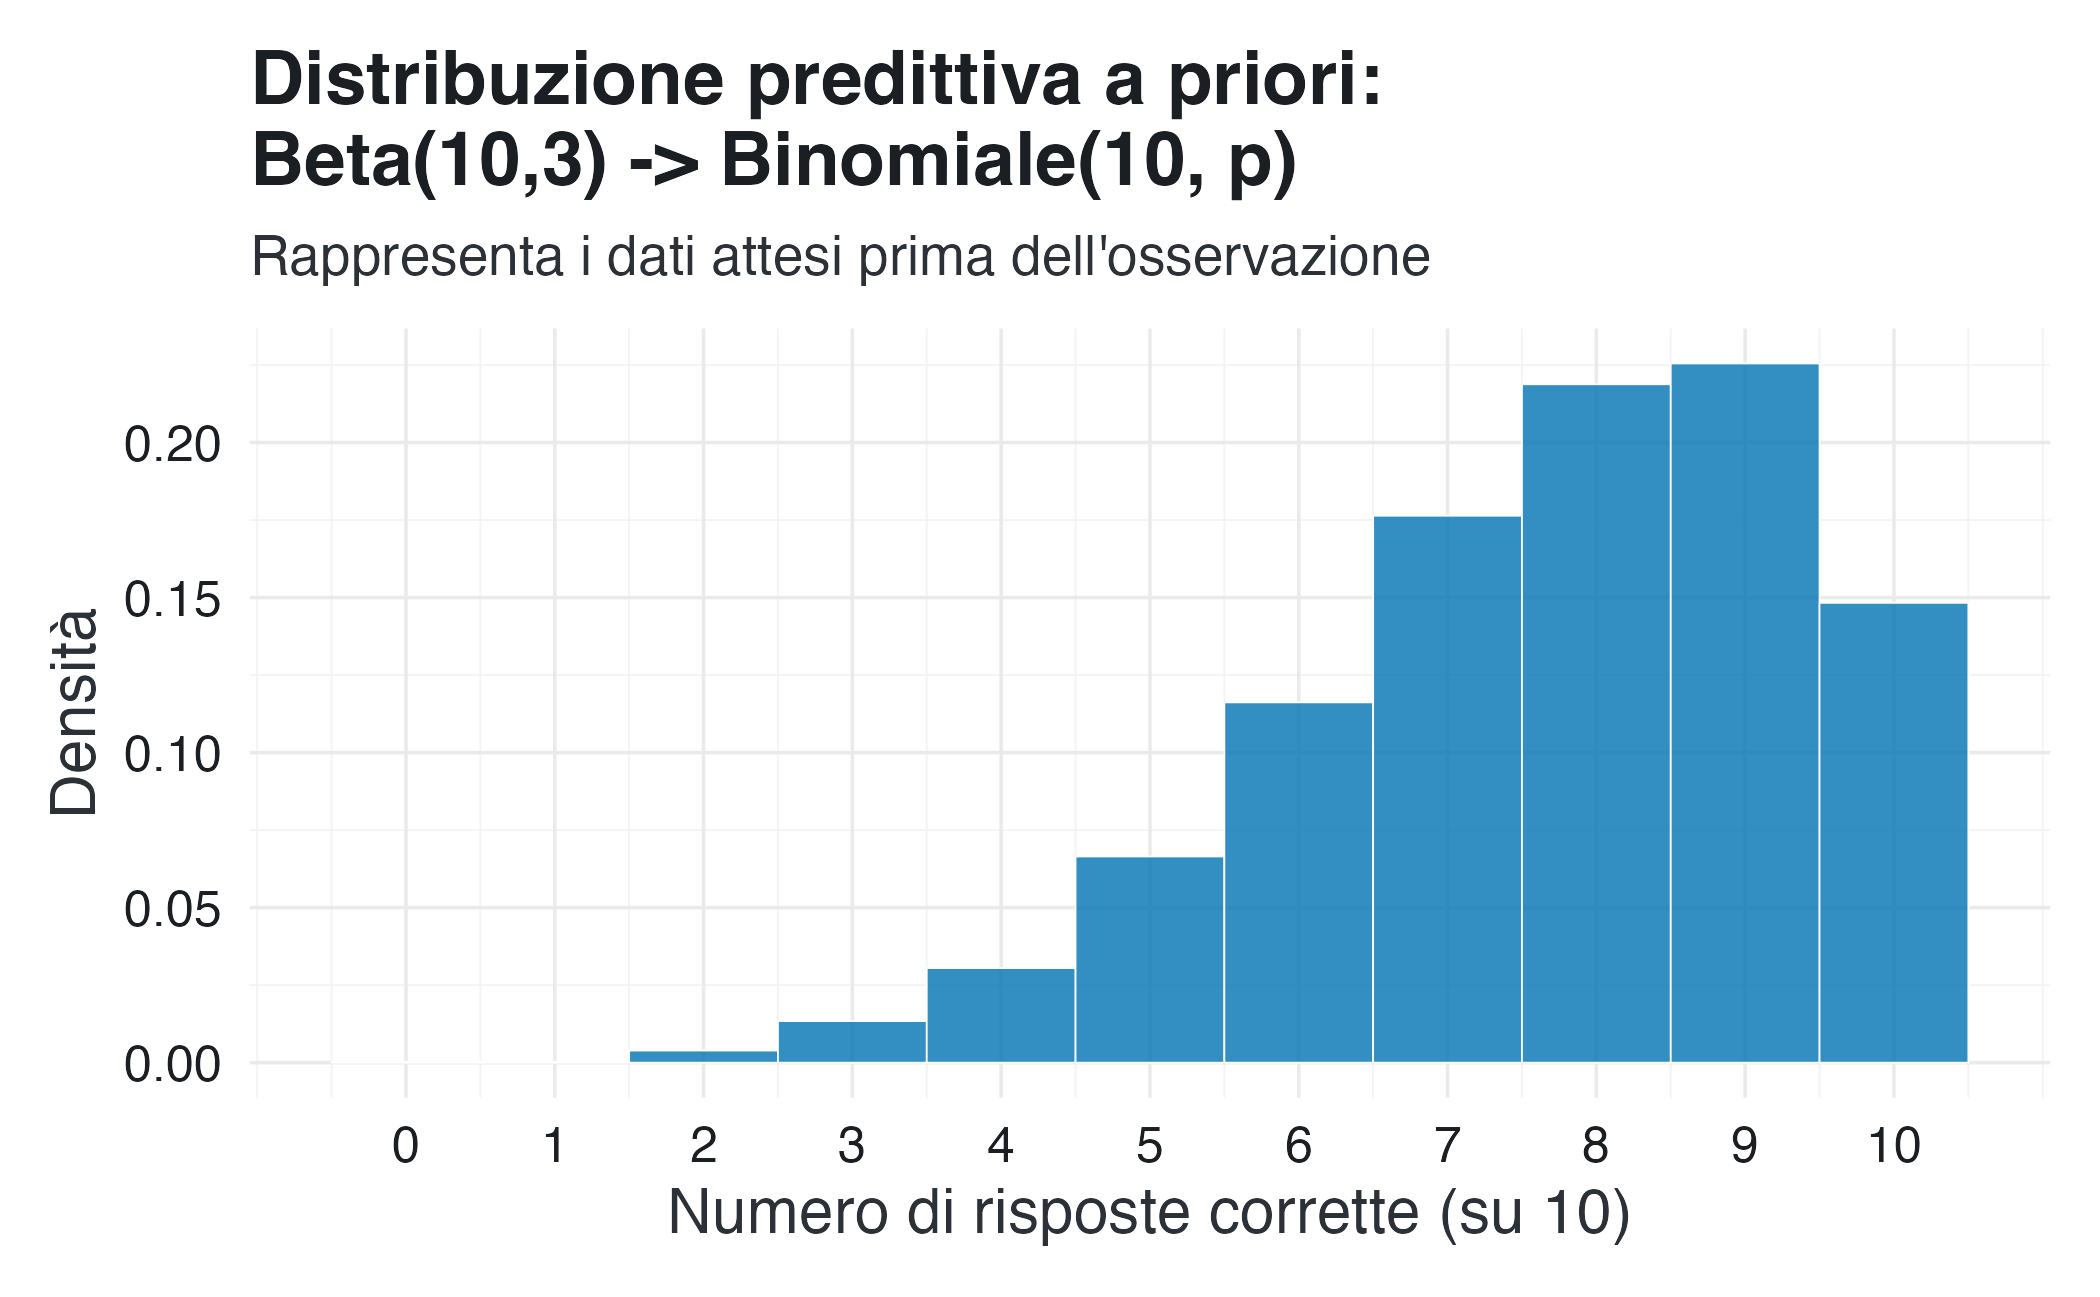
\includegraphics[width=0.85\linewidth,height=\textheight,keepaspectratio]{chapters/bayesian_inference/05_prior_pred_distr_files/figure-pdf/unnamed-chunk-2-1.png}
\end{center}

\textbf{Interpretazione:}

\begin{itemize}
\tightlist
\item
  la maggior parte delle simulazioni prevede tra 6 e 9 risposte
  corrette;
\item
  questo è coerente con l'aspettativa di accuratezza
  \textasciitilde70-80\%;
\item
  valori estremi (0-2 o 10) sono rari, come ci si aspetterebbe.
\end{itemize}

\begin{tcolorbox}[enhanced jigsaw, arc=.35mm, bottomrule=.15mm, bottomtitle=1mm, breakable, colback=white, colbacktitle=quarto-callout-tip-color!10!white, colframe=quarto-callout-tip-color-frame, coltitle=black, left=2mm, leftrule=.75mm, opacityback=0, opacitybacktitle=0.6, rightrule=.15mm, title=\textcolor{quarto-callout-tip-color}{\faLightbulb}\hspace{0.5em}{Esercizio di riflessione}, titlerule=0mm, toprule=.15mm, toptitle=1mm]

Prova a cambiare i parametri a \(\text{Beta}(2, 2)\) (prior uniforme).
Cosa succede alla distribuzione predittiva? È ancora plausibile per il
nostro scenario?

\end{tcolorbox}

\subsection{Confronto tra specificazioni
alternative}\label{confronto-tra-specificazioni-alternative}

Confrontiamo tre scelte di \emph{prior} per comprendere l'impatto sulla
predittiva.

\begin{Shaded}
\begin{Highlighting}[]
\CommentTok{\# Simulazioni per tre prior differenti}
\NormalTok{simulate\_prior\_predictive }\OtherTok{\textless{}{-}} \ControlFlowTok{function}\NormalTok{(alpha, beta, }\AttributeTok{n\_sim =} \DecValTok{10000}\NormalTok{, }\AttributeTok{n\_items =} \DecValTok{10}\NormalTok{) \{}
\NormalTok{  p\_sim }\OtherTok{\textless{}{-}} \FunctionTok{rbeta}\NormalTok{(n\_sim, alpha, beta)}
\NormalTok{  y\_sim }\OtherTok{\textless{}{-}} \FunctionTok{rbinom}\NormalTok{(n\_sim, }\AttributeTok{size =}\NormalTok{ n\_items, }\AttributeTok{prob =}\NormalTok{ p\_sim)}
  \FunctionTok{return}\NormalTok{(y\_sim)}
\NormalTok{\}}

\CommentTok{\# Prior 1: Molto vago {-} Beta(1,1) = Uniforme(0,1)}
\NormalTok{y\_vague }\OtherTok{\textless{}{-}} \FunctionTok{simulate\_prior\_predictive}\NormalTok{(}\DecValTok{1}\NormalTok{, }\DecValTok{1}\NormalTok{)}

\CommentTok{\# Prior 2: Debolmente informativo {-} Beta(2,2)}
\NormalTok{y\_weak }\OtherTok{\textless{}{-}} \FunctionTok{simulate\_prior\_predictive}\NormalTok{(}\DecValTok{2}\NormalTok{, }\DecValTok{2}\NormalTok{)}

\CommentTok{\# Prior 3: Informativo {-} Beta(10,3)}
\NormalTok{y\_informative }\OtherTok{\textless{}{-}} \FunctionTok{simulate\_prior\_predictive}\NormalTok{(}\DecValTok{10}\NormalTok{, }\DecValTok{3}\NormalTok{)}

\CommentTok{\# Combina per visualizzazione}
\NormalTok{prior\_comparison }\OtherTok{\textless{}{-}} \FunctionTok{tibble}\NormalTok{(}
  \AttributeTok{y =} \FunctionTok{c}\NormalTok{(y\_vague, y\_weak, y\_informative),}
  \AttributeTok{prior =} \FunctionTok{rep}\NormalTok{(}
    \FunctionTok{c}\NormalTok{(}\StringTok{"Beta(1,1):}\SpecialCharTok{\textbackslash{}n}\StringTok{Uniforme"}\NormalTok{, }\StringTok{"Beta(2,2):}\SpecialCharTok{\textbackslash{}n}\StringTok{Debole"}\NormalTok{, }\StringTok{"Beta(10,3):}\SpecialCharTok{\textbackslash{}n}\StringTok{Informativo"}\NormalTok{),}
    \AttributeTok{each =} \DecValTok{10000}
\NormalTok{  )}
\NormalTok{)}

\NormalTok{prior\_comparison }\SpecialCharTok{|\textgreater{}}
  \FunctionTok{ggplot}\NormalTok{(}\FunctionTok{aes}\NormalTok{(}\AttributeTok{x =}\NormalTok{ y, }\AttributeTok{fill =}\NormalTok{ prior)) }\SpecialCharTok{+}
  \FunctionTok{geom\_histogram}\NormalTok{(}
    \FunctionTok{aes}\NormalTok{(}\AttributeTok{y =} \FunctionTok{after\_stat}\NormalTok{(density)),}
    \AttributeTok{bins =} \DecValTok{11}\NormalTok{,}
    \AttributeTok{position =} \StringTok{"identity"}\NormalTok{,}
    \AttributeTok{alpha =} \FloatTok{0.6}
\NormalTok{  ) }\SpecialCharTok{+}
  \FunctionTok{scale\_fill\_manual}\NormalTok{(}
    \AttributeTok{values =} \FunctionTok{setNames}\NormalTok{(}
\NormalTok{      col\_facets,}
      \FunctionTok{c}\NormalTok{(}\StringTok{"Beta(1,1):}\SpecialCharTok{\textbackslash{}n}\StringTok{Uniforme"}\NormalTok{, }\StringTok{"Beta(2,2):}\SpecialCharTok{\textbackslash{}n}\StringTok{Debole"}\NormalTok{, }\StringTok{"Beta(10,3):}\SpecialCharTok{\textbackslash{}n}\StringTok{Informativo"}\NormalTok{)}
\NormalTok{    )}
\NormalTok{  ) }\SpecialCharTok{+}
  \FunctionTok{facet\_wrap}\NormalTok{(}\SpecialCharTok{\textasciitilde{}}\NormalTok{prior, }\AttributeTok{nrow =} \DecValTok{1}\NormalTok{) }\SpecialCharTok{+}
  \FunctionTok{scale\_x\_continuous}\NormalTok{(}\AttributeTok{breaks =} \DecValTok{0}\SpecialCharTok{:}\DecValTok{10}\NormalTok{) }\SpecialCharTok{+}
  \FunctionTok{labs}\NormalTok{(}
    \AttributeTok{x =} \StringTok{"Numero di risposte corrette"}\NormalTok{,}
    \AttributeTok{y =} \StringTok{"Densità"}\NormalTok{,}
    \AttributeTok{title =} \StringTok{"Confronto tra diverse specificazioni a priori"}\NormalTok{,}
    \AttributeTok{subtitle =} \StringTok{"Come cambia la distribuzione predittiva"}
\NormalTok{  ) }\SpecialCharTok{+}
  \FunctionTok{theme}\NormalTok{(}\AttributeTok{legend.position =} \StringTok{"none"}\NormalTok{)}
\end{Highlighting}
\end{Shaded}

\begin{center}
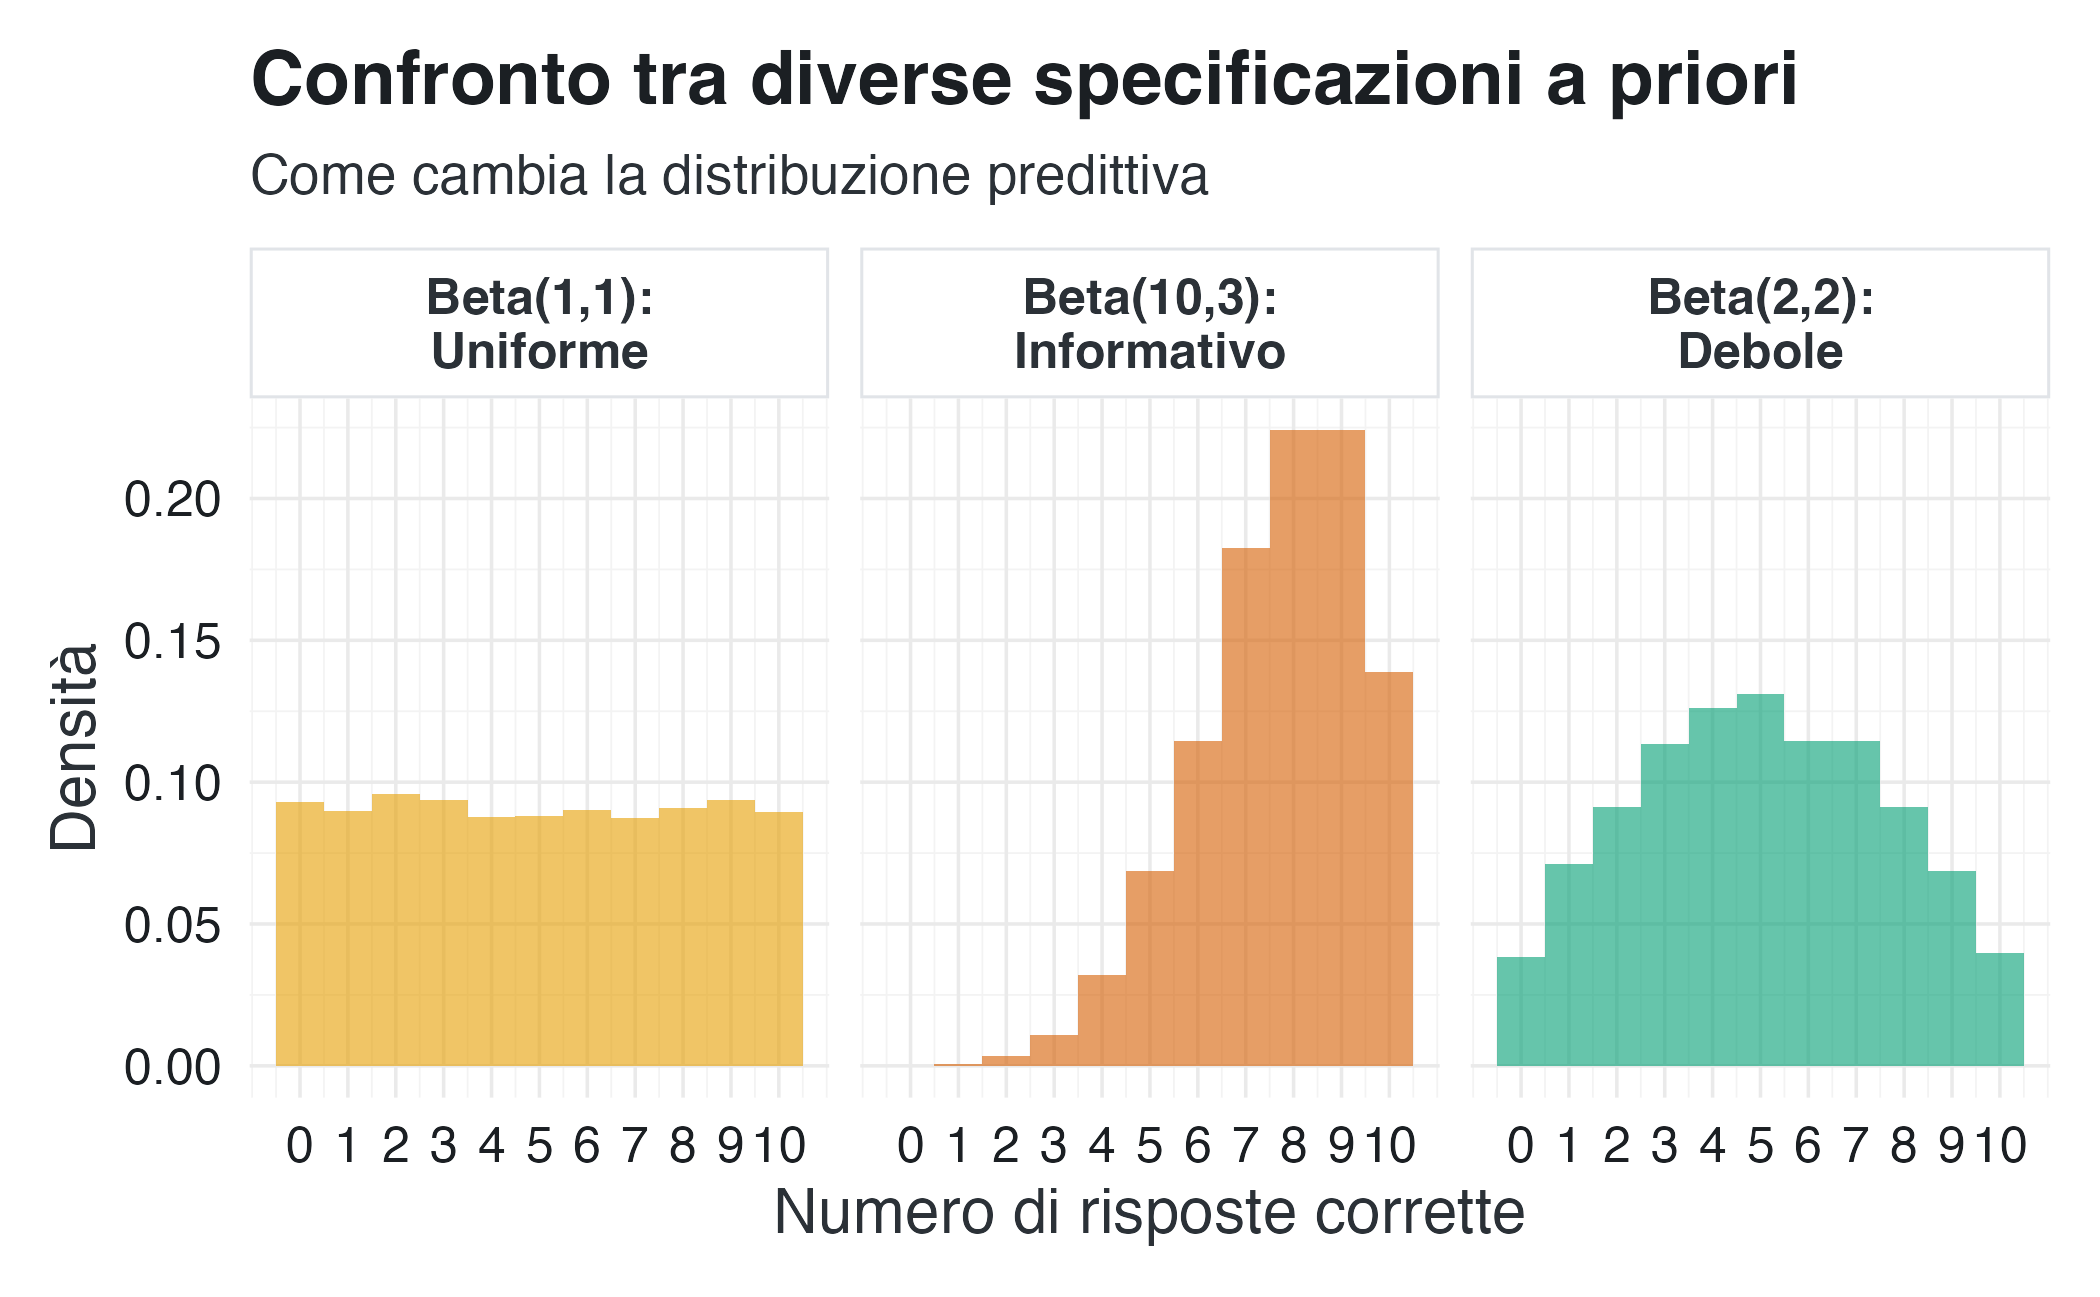
\includegraphics[width=0.85\linewidth,height=\textheight,keepaspectratio]{chapters/bayesian_inference/05_prior_pred_distr_files/figure-pdf/unnamed-chunk-3-1.png}
\end{center}

\textbf{Osservazioni:}

\begin{enumerate}
\def\labelenumi{\arabic{enumi}.}
\tightlist
\item
  Beta(1,1) - Uniforme:

  \begin{itemize}
  \tightlist
  \item
    ogni valore compreso tra 0 e 10 è quasi equiprobabile;
  \item
    implica che non sappiamo letteralmente nulla;
  \item
    è troppo vago se abbiamo conoscenze sul dominio.
  \end{itemize}
\item
  Beta(2,2) - Debole:

  \begin{itemize}
  \tightlist
  \item
    leggera preferenza per i valori centrali (4-6);
  \item
    è ancora abbastanza disperso;
  \item
    ragionevole se abbiamo poche informazioni preliminari.
  \end{itemize}
\item
  Beta(10,3) - Informativo:

  \begin{itemize}
  \tightlist
  \item
    forte concentrazione su 6-9 risposte corrette;
  \item
    coerente con un'aspettativa di accuratezza del 70-80\%;
  \item
    appropriato quando abbiamo una conoscenza robusta.
  \end{itemize}
\end{enumerate}

\begin{tcolorbox}[enhanced jigsaw, arc=.35mm, bottomrule=.15mm, bottomtitle=1mm, breakable, colback=white, colbacktitle=quarto-callout-important-color!10!white, colframe=quarto-callout-important-color-frame, coltitle=black, left=2mm, leftrule=.75mm, opacityback=0, opacitybacktitle=0.6, rightrule=.15mm, title=\textcolor{quarto-callout-important-color}{\faExclamation}\hspace{0.5em}{Quale scegliere?}, titlerule=0mm, toprule=.15mm, toptitle=1mm]

Non esiste una scelta ``migliore'' in assoluto. La scelta dipende dalla
conoscenza disponibile:

\begin{itemize}
\tightlist
\item
  \textbf{Poche informazioni:} prior più vago (ma non completamente
  piatto).
\item
  \textbf{Letteratura consolidata:} prior informativo.
\item
  \textbf{Incertezza su aspetti specifici:} prior gerarchico (argomento
  avanzato).
\end{itemize}

\end{tcolorbox}

\subsection{Verifica formale della
plausibilità}\label{verifica-formale-della-plausibilituxe0}

Possiamo quantificare alcune proprietà delle simulazioni.

\begin{Shaded}
\begin{Highlighting}[]
\CommentTok{\# Calcola statistiche descrittive per il prior informativo}
\NormalTok{summary\_stats }\OtherTok{\textless{}{-}} \FunctionTok{tibble}\NormalTok{(}\AttributeTok{y =}\NormalTok{ y\_informative) }\SpecialCharTok{|\textgreater{}}
  \FunctionTok{summarise}\NormalTok{(}
    \AttributeTok{media =} \FunctionTok{mean}\NormalTok{(y),}
    \AttributeTok{mediana =} \FunctionTok{median}\NormalTok{(y),}
    \AttributeTok{dev\_std =} \FunctionTok{sd}\NormalTok{(y),}
    \AttributeTok{q05 =} \FunctionTok{quantile}\NormalTok{(y, }\FloatTok{0.05}\NormalTok{),}
    \AttributeTok{q95 =} \FunctionTok{quantile}\NormalTok{(y, }\FloatTok{0.95}\NormalTok{),}
    \AttributeTok{prob\_estremi =} \FunctionTok{mean}\NormalTok{(y }\SpecialCharTok{\textless{}=} \DecValTok{2} \SpecialCharTok{|}\NormalTok{ y }\SpecialCharTok{\textgreater{}=} \DecValTok{10}\NormalTok{)}
\NormalTok{  )}

\NormalTok{summary\_stats }\SpecialCharTok{|\textgreater{}}
\NormalTok{  knitr}\SpecialCharTok{::}\FunctionTok{kable}\NormalTok{(}
    \AttributeTok{digits =} \DecValTok{2}\NormalTok{,}
    \AttributeTok{caption =} \StringTok{"Statistiche della distribuzione predittiva: Beta(10,3)"}
\NormalTok{  )}
\end{Highlighting}
\end{Shaded}

\begin{longtable}[]{@{}rrrrrr@{}}
\caption{Statistiche della distribuzione predittiva:
Beta(10,3)}\tabularnewline
\toprule\noalign{}
media & mediana & dev\_std & q05 & q95 & prob\_estremi \\
\midrule\noalign{}
\endfirsthead
\toprule\noalign{}
media & mediana & dev\_std & q05 & q95 & prob\_estremi \\
\midrule\noalign{}
\endhead
\bottomrule\noalign{}
\endlastfoot
7.68 & 8 & 1.7 & 5 & 10 & 0.14 \\
\end{longtable}

\textbf{Checklist di validazione:}

✓ Media \textasciitilde7.7: coerente con l'aspettativa teorica
(\(\mathbb{E}[p] \times 10 \approx 0.77 \times 10\)).

✓ Intervallo credibile 90\% (Q05-Q95): dovrebbe coprire il range
realistico.

✓ Probabilità di estremi (\textless3 o \textgreater9): dovrebbe essere
bassa se non ci si aspetta valori estremi.

\section{Implementazione in Stan}\label{implementazione-in-stan}

Per analisi più complesse, Stan fornisce un framework robusto per le
verifiche predittive.

\subsection{Modello Stan completo}\label{modello-stan-completo}

\begin{Shaded}
\begin{Highlighting}[]
\NormalTok{binom\_prior\_ppc\_stan }\OtherTok{\textless{}{-}} \StringTok{\textquotesingle{}}
\StringTok{data \{}
\StringTok{  int\textless{}lower=1\textgreater{} N;        // numero di unità di osservazione (studenti)}
\StringTok{  int\textless{}lower=1\textgreater{} n\_items;  // numero di item per studente}
\StringTok{\}}
\StringTok{parameters \{}
\StringTok{  real\textless{}lower=0, upper=1\textgreater{} p;   // probabilità di successo globale}
\StringTok{\}}
\StringTok{model \{}
\StringTok{  p \textasciitilde{} beta(10, 3);            // distribuzione a priori esatta}
\StringTok{  // Nessuna verosimiglianza: campionamento esclusivamente dalle distribuzioni a priori}
\StringTok{\}}
\StringTok{generated quantities \{}
\StringTok{  array[N] int y\_rep;         // dati replicati}
\StringTok{  for (i in 1:N) \{}
\StringTok{    y\_rep[i] = binomial\_rng(n\_items, p);}
\StringTok{  \}}
\StringTok{\}}
\StringTok{\textquotesingle{}}
\end{Highlighting}
\end{Shaded}

\textbf{Struttura del modello:}

\begin{enumerate}
\def\labelenumi{\arabic{enumi}.}
\tightlist
\item
  \textbf{Blocco \texttt{data}}: dichiara le dimensioni del problema
  (numero studenti, domande).
\item
  \textbf{Blocco \texttt{parameters}}: definisce \(p\) con supporto
  \([0,1]\).
\item
  \textbf{Blocco \texttt{model}}: specifica il prior
  \(p \sim \text{Beta}(10,3)\).
\item
  \textbf{Blocco \texttt{generated\ quantities}}: simula dati dalla
  distribuzione predittiva.
\end{enumerate}

\textbf{Vantaggi di Stan:}

\begin{itemize}
\tightlist
\item
  Sampling efficiente anche per prior complessi.
\item
  Facile incorporare gerarchie e correlazioni.
\item
  Controllo automatico di diagnostiche di convergenza.
\end{itemize}

\subsection{Compilazione ed
esecuzione}\label{compilazione-ed-esecuzione}

\begin{Shaded}
\begin{Highlighting}[]
\NormalTok{mod }\OtherTok{\textless{}{-}} \FunctionTok{cmdstan\_model}\NormalTok{(}
  \FunctionTok{write\_stan\_file}\NormalTok{(binom\_prior\_ppc\_stan),}
  \AttributeTok{compile =} \ConstantTok{TRUE}
\NormalTok{)}
\end{Highlighting}
\end{Shaded}

\begin{Shaded}
\begin{Highlighting}[]
\NormalTok{n\_studenti }\OtherTok{\textless{}{-}} \DecValTok{50}
\NormalTok{n\_item     }\OtherTok{\textless{}{-}} \DecValTok{10}

\NormalTok{fit\_beta }\OtherTok{\textless{}{-}}\NormalTok{ mod}\SpecialCharTok{$}\FunctionTok{sample}\NormalTok{(}
  \AttributeTok{data =} \FunctionTok{list}\NormalTok{(}\AttributeTok{N =}\NormalTok{ n\_studenti, }\AttributeTok{n\_items =}\NormalTok{ n\_item),}
  \AttributeTok{chains =} \DecValTok{4}\NormalTok{, }\AttributeTok{iter\_warmup =} \DecValTok{500}\NormalTok{, }\AttributeTok{iter\_sampling =} \DecValTok{1000}\NormalTok{,}
  \AttributeTok{seed =} \DecValTok{123}\NormalTok{, }\AttributeTok{refresh =} \DecValTok{0}
\NormalTok{)}
\end{Highlighting}
\end{Shaded}

\textbf{Processo di simulazione in tre fasi:}

\begin{enumerate}
\def\labelenumi{\arabic{enumi}.}
\item
  \textbf{Campionamento dai prior}: il campionatore estrae valori del
  parametro \(p\) dalla distribuzione a priori specificata
  \(\text{Beta}(10, 3)\), generando così l'insieme dei valori plausibili
  del parametro prima di osservare i dati.
\item
  \textbf{Propagazione probabilistica}: per ogni valore campionato
  \(p^{(s)}\), il modello propaga l'incertezza attraverso la
  distribuzione predittiva \(\text{Binomial}(n = 10, p = p^{(s)})\), che
  formalizza il meccanismo di generazione dei dati.
\item
  \textbf{Generazione di dati replicati}: ogni campione
  \(y_{\text{rep}}^{(s)}\) rappresenta un possibile insieme di dati che
  il modello considera plausibile sotto le attuali assunzioni a priori,
  permettendo così una valutazione empirica della loro ragionevolezza.
\end{enumerate}

Questa sequenza opera esclusivamente a livello delle distribuzioni a
priori, senza essere influenzata dai dati osservati, e costituisce
quindi una verifica puramente pre-osservativa del modello specificato.

\subsection{Visualizzazione dei
risultati}\label{visualizzazione-dei-risultati}

\begin{Shaded}
\begin{Highlighting}[]
\CommentTok{\# Estrai e visualizza le simulazioni}
\NormalTok{draws\_mat }\OtherTok{\textless{}{-}}\NormalTok{ fit\_beta}\SpecialCharTok{$}\FunctionTok{draws}\NormalTok{(}\StringTok{"y\_rep"}\NormalTok{, }\AttributeTok{format =} \StringTok{"draws\_matrix"}\NormalTok{)}
\NormalTok{y\_rep\_vec }\OtherTok{\textless{}{-}} \FunctionTok{as.vector}\NormalTok{(}\FunctionTok{as.matrix}\NormalTok{(draws\_mat))}

\FunctionTok{tibble}\NormalTok{(}\AttributeTok{y =}\NormalTok{ y\_rep\_vec) }\SpecialCharTok{|\textgreater{}}
  \FunctionTok{ggplot}\NormalTok{(}\FunctionTok{aes}\NormalTok{(}\AttributeTok{x =}\NormalTok{ y)) }\SpecialCharTok{+}
  \FunctionTok{geom\_histogram}\NormalTok{(}
    \FunctionTok{aes}\NormalTok{(}\AttributeTok{y =} \FunctionTok{after\_stat}\NormalTok{(density)),}
    \AttributeTok{bins =} \DecValTok{11}\NormalTok{,}
    \AttributeTok{fill =}\NormalTok{ col\_prior\_pred,}
    \AttributeTok{color =} \StringTok{"white"}\NormalTok{,}
    \AttributeTok{linewidth =} \FloatTok{0.2}\NormalTok{,}
    \AttributeTok{alpha =} \FloatTok{0.85}
\NormalTok{  ) }\SpecialCharTok{+}
  \FunctionTok{scale\_x\_continuous}\NormalTok{(}\AttributeTok{breaks =} \DecValTok{0}\SpecialCharTok{:}\DecValTok{10}\NormalTok{) }\SpecialCharTok{+}
  \FunctionTok{labs}\NormalTok{(}
    \AttributeTok{x =} \StringTok{"Numero di risposte corrette su 10"}\NormalTok{,}
    \AttributeTok{y =} \StringTok{"Densità"}\NormalTok{,}
    \AttributeTok{title =} \StringTok{"Distribuzione predittiva a priori (Stan)"}\NormalTok{,}
    \AttributeTok{subtitle =} \StringTok{"Beta(10,3) {-}\textgreater{} valutazione pre{-}dati"}
\NormalTok{  )}
\end{Highlighting}
\end{Shaded}

\begin{center}
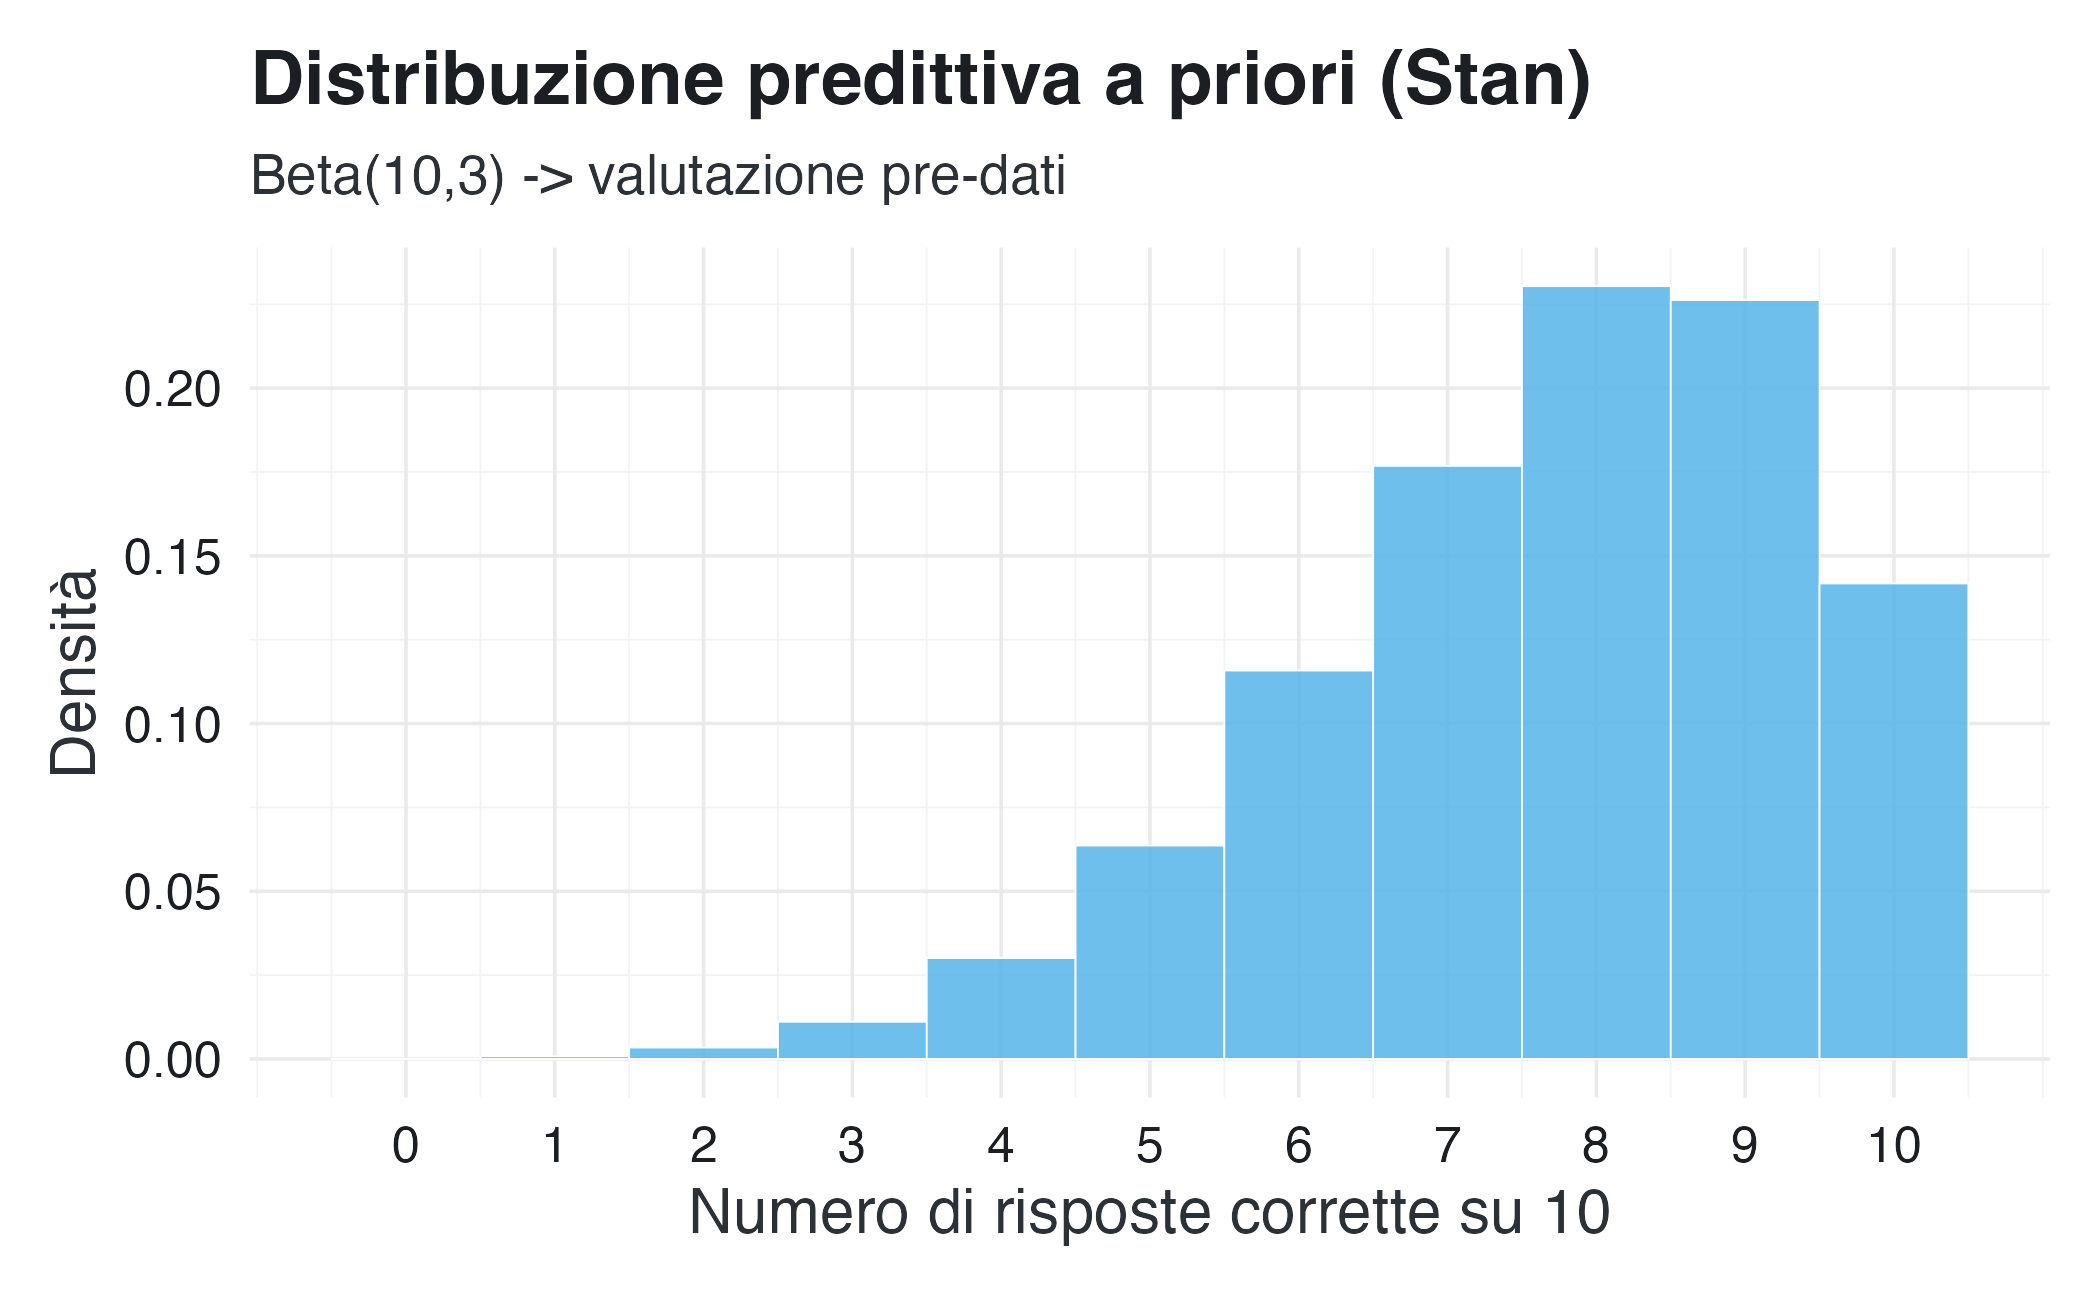
\includegraphics[width=0.85\linewidth,height=\textheight,keepaspectratio]{chapters/bayesian_inference/05_prior_pred_distr_files/figure-pdf/unnamed-chunk-8-1.png}
\end{center}

\textbf{Visualizzazione:}

\begin{Shaded}
\begin{Highlighting}[]
\CommentTok{\# Usa bayesplot }
\NormalTok{vars }\OtherTok{\textless{}{-}} \FunctionTok{paste0}\NormalTok{(}\StringTok{"y\_rep["}\NormalTok{, }\DecValTok{1}\SpecialCharTok{:}\NormalTok{n\_studenti, }\StringTok{"]"}\NormalTok{)}
\NormalTok{yrep\_mat }\OtherTok{\textless{}{-}}\NormalTok{ posterior}\SpecialCharTok{::}\FunctionTok{as\_draws\_matrix}\NormalTok{(fit\_beta}\SpecialCharTok{$}\FunctionTok{draws}\NormalTok{(}\AttributeTok{variables =}\NormalTok{ vars))}

\NormalTok{p }\OtherTok{\textless{}{-}}\NormalTok{ bayesplot}\SpecialCharTok{::}\FunctionTok{ppc\_bars}\NormalTok{(}
  \AttributeTok{y =} \FunctionTok{rep}\NormalTok{(}\DecValTok{0}\NormalTok{, n\_studenti),  }\CommentTok{\# placeholder (non abbiamo dati reali)}
  \AttributeTok{yrep =} \FunctionTok{as.matrix}\NormalTok{(yrep\_mat)[}\DecValTok{1}\SpecialCharTok{:}\DecValTok{200}\NormalTok{, ]}
\NormalTok{) }\SpecialCharTok{+}
  \FunctionTok{labs}\NormalTok{(}
    \AttributeTok{title =} \StringTok{"Verifica predittiva a priori (Stan)"}\NormalTok{,}
    \CommentTok{\# subtitle = "Distribuzione attesa per ciascuno studente"}
\NormalTok{  )}
\CommentTok{\# Il primo layer (rimosso) è la barra dei dati fittizi osservati}
\NormalTok{p}\SpecialCharTok{$}\NormalTok{layers }\OtherTok{\textless{}{-}}\NormalTok{ p}\SpecialCharTok{$}\NormalTok{layers[}\SpecialCharTok{{-}}\DecValTok{1}\NormalTok{]}
\NormalTok{p}
\end{Highlighting}
\end{Shaded}

\begin{center}
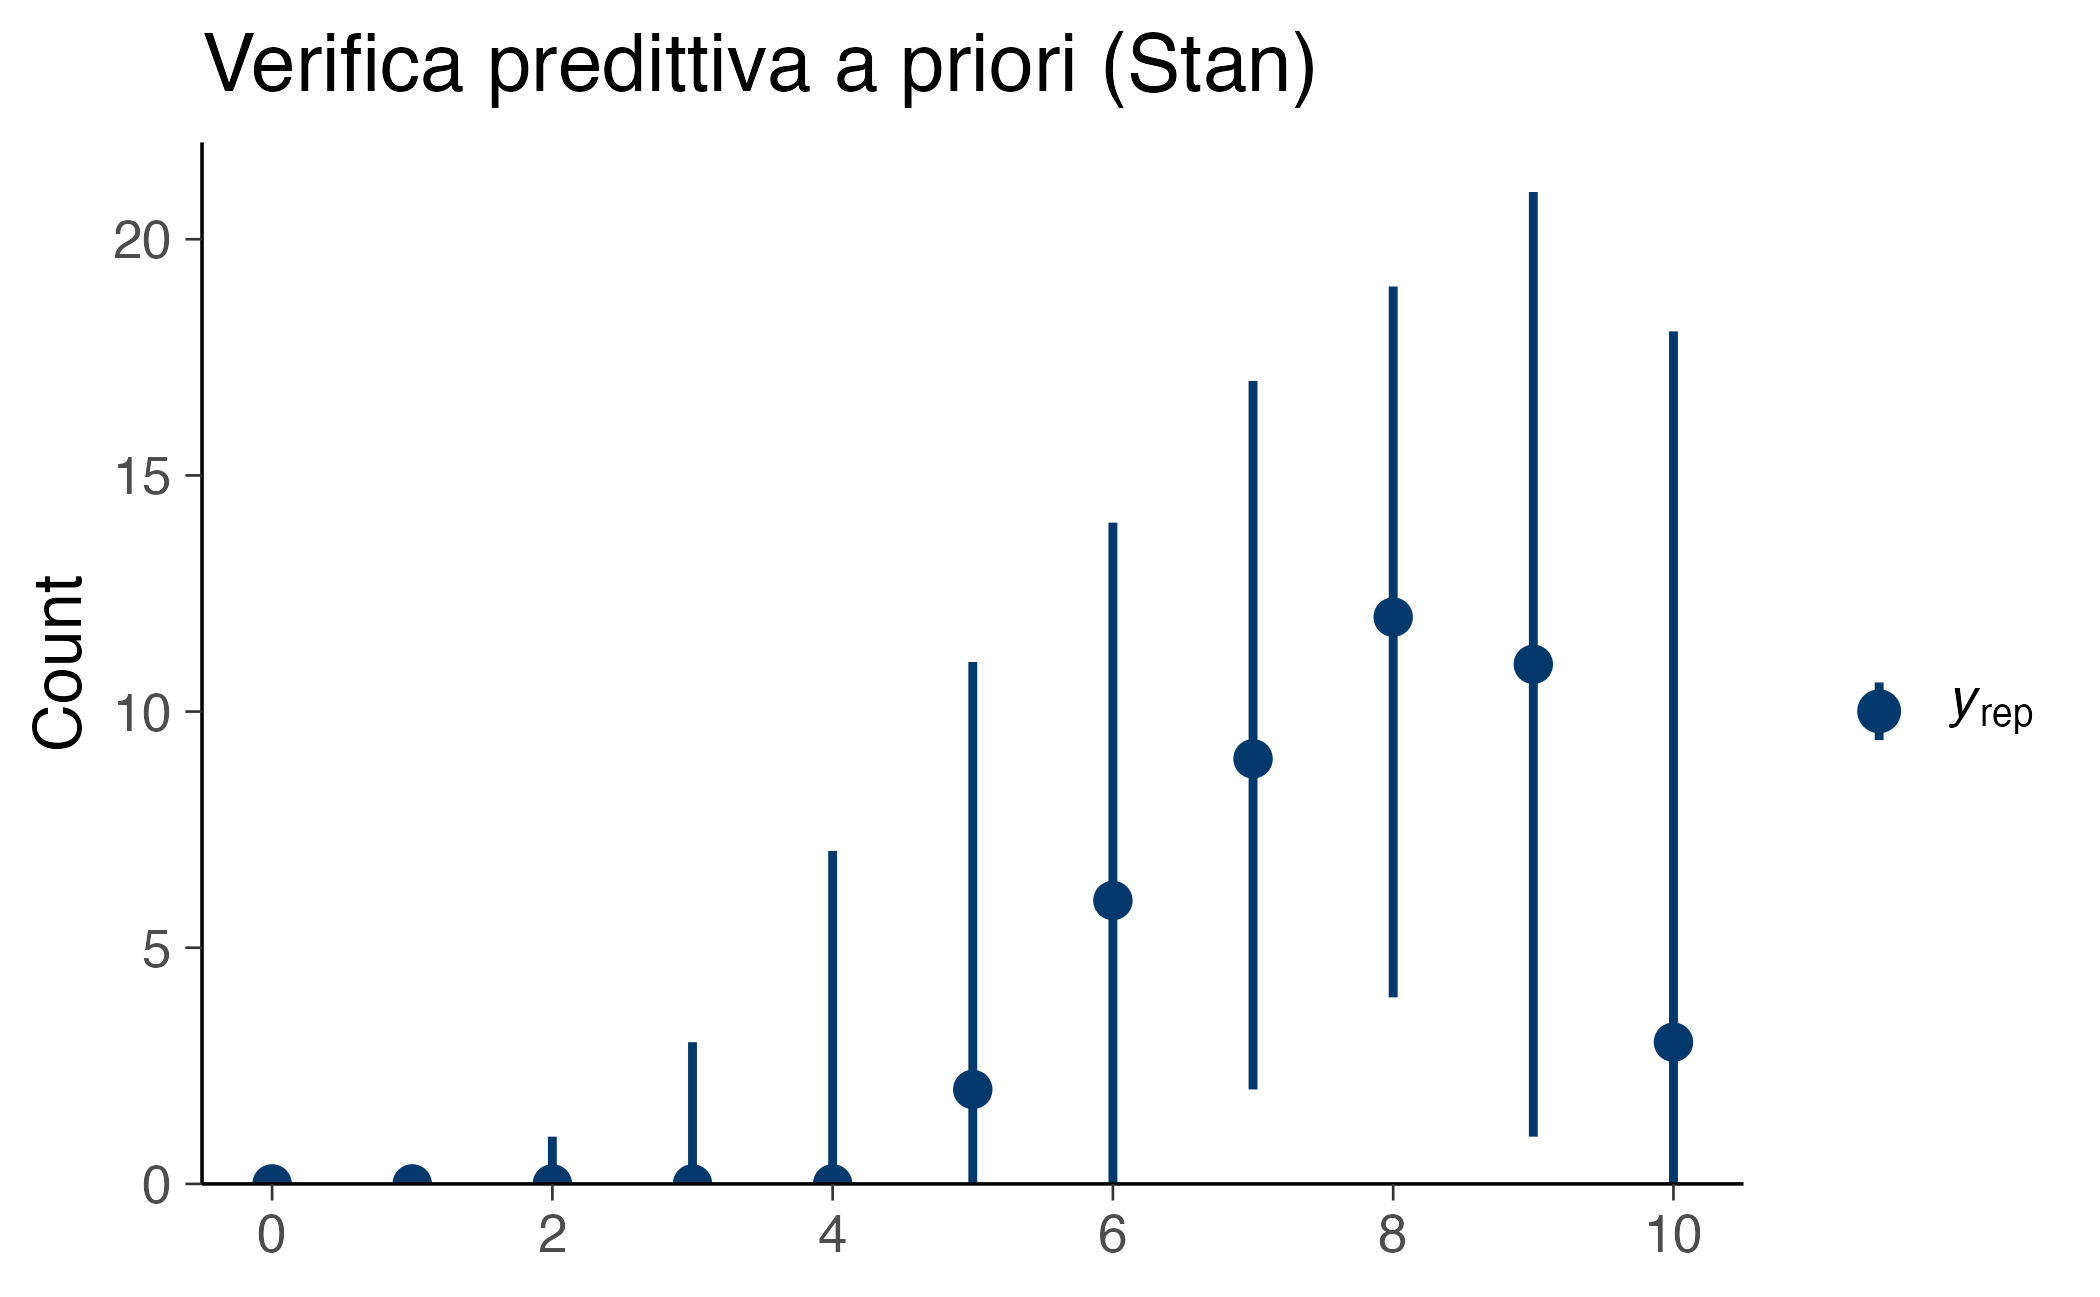
\includegraphics[width=0.85\linewidth,height=\textheight,keepaspectratio]{chapters/bayesian_inference/05_prior_pred_distr_files/figure-pdf/unnamed-chunk-9-1.png}
\end{center}

\subsection{Rilevanza metodologica}\label{rilevanza-metodologica}

\begin{itemize}
\tightlist
\item
  \textbf{Trasparenza:} l'implementazione diretta in Stan rende
  esplicite le implicazioni delle nostre scelte a priori.
\item
  \textbf{Prevenzione degli errori:} consente di identificare criticità
  nella specificazione del modello prima di impegnare risorse nella
  raccolta e analisi dei dati osservati.
\item
  \textbf{Apprendimento concettuale:} favorisce una comprensione più
  profonda del nesso tra distribuzioni a priori e distribuzioni
  predittive.
\end{itemize}

\begin{quote}
La verifica predittiva a priori funge da ``test di coerenza sostantiva''
per le nostre assunzioni iniziali. Se i dati simulati risultano
sistematicamente implausibili, la criticità non risiede nei dati reali
--- che non sono ancora stati osservati --- bensì nella specificazione
del modello bayesiano, la quale richiede una revisione critica.
\end{quote}

\section*{Riflessioni conclusive}\label{riflessioni-conclusive-9}

\markright{Riflessioni conclusive}

Il controllo predittivo a priori trasforma le assunzioni iniziali da
entità astratte in ipotesi empiricamente verificabili. Questo approccio
consente una valutazione \emph{ante hoc} di plausibilità, prima della
raccolta dei dati, migliorando così gli standard di trasparenza nella
ricerca empirica.

La distribuzione predittiva a priori è una media ponderata delle
previsioni del modello, dove i pesi riflettono le credenze iniziali
codificate nei \emph{prior}.

Distribuzioni a priori apparentemente plausibili sulla scala dei
parametri possono generare previsioni empiricamente incoerenti una volta
proiettate sulla scala osservabile dei dati, il che sottolinea la
necessità di una validazione sistematica delle implicazioni predittive
delle assunzioni iniziali.

Il flusso di lavoro iterativo si articola in una sequenza ciclica che
prevede la specifica delle distribuzioni a priori, la simulazione dei
dati attesi, la valutazione della loro plausibilità sostanziale e, se
necessario, la revisione critica delle assunzioni iniziali. Questa
procedura conserva la propria integrità metodologica solo se
implementata in fase pre-osservativa, preservando l'indipendenza tra le
assunzioni iniziali e l'evidenza empirica. Gli strumenti pratici forniti
da R e Stan rendono questo processo accessibile e riproducibile.

I prossimi approfondimenti estenderanno questo framework ai controlli
predittivi a posteriori, completando così l'architettura di una
modellazione bayesiana coerente, rigorosa e trasparente. Per
un'esplorazione più approfondita che coinvolga modelli di complessità
crescente, si rimanda
all'Appendice~\ref{sec-apx-prior-predictive-check}.

\begin{tcolorbox}[enhanced jigsaw, arc=.35mm, bottomrule=.15mm, bottomtitle=1mm, breakable, colback=white, colbacktitle=quarto-callout-note-color!10!white, colframe=quarto-callout-note-color-frame, coltitle=black, left=2mm, leftrule=.75mm, opacityback=0, opacitybacktitle=0.6, rightrule=.15mm, title=\textcolor{quarto-callout-note-color}{\faInfo}\hspace{0.5em}{Messaggio finale}, titlerule=0mm, toprule=.15mm, toptitle=1mm]

Un modello bayesiano ben specificato deve superare due verifiche
complementari: il controllo predittivo a priori, che valuta se il
modello genera dati plausibili prima dell'osservazione, e il controllo
predittivo a posteriori, che verifica quanto bene il modello riproduca i
dati effettivamente osservati. Trascurare la prima verifica significa
costruire l'edificio inferenziale su fondamenta traballanti,
compromettendo la solidità dell'intera analisi.

\end{tcolorbox}

\begin{tcolorbox}[enhanced jigsaw, arc=.35mm, bottomrule=.15mm, bottomtitle=1mm, breakable, colback=white, colbacktitle=quarto-callout-note-color!10!white, colframe=quarto-callout-note-color-frame, coltitle=black, left=2mm, leftrule=.75mm, opacityback=0, opacitybacktitle=0.6, rightrule=.15mm, title=\textcolor{quarto-callout-note-color}{\faInfo}\hspace{0.5em}{Informazioni sull'ambiente di sviluppo}, titlerule=0mm, toprule=.15mm, toptitle=1mm]

\begin{Shaded}
\begin{Highlighting}[]
\FunctionTok{sessionInfo}\NormalTok{()}
\CommentTok{\#\textgreater{} R version 4.6.1 (2026{-}06{-}24)}
\CommentTok{\#\textgreater{} Platform: aarch64{-}apple{-}darwin23}
\CommentTok{\#\textgreater{} Running under: macOS Tahoe 26.5.2}
\CommentTok{\#\textgreater{} }
\CommentTok{\#\textgreater{} Matrix products: default}
\CommentTok{\#\textgreater{} BLAS:   /Library/Frameworks/R.framework/Versions/4.6/Resources/lib/libRblas.0.dylib }
\CommentTok{\#\textgreater{} LAPACK: /Library/Frameworks/R.framework/Versions/4.6/Resources/lib/libRlapack.dylib;  LAPACK version 3.12.1}
\CommentTok{\#\textgreater{} }
\CommentTok{\#\textgreater{} locale:}
\CommentTok{\#\textgreater{} [1] C.UTF{-}8/UTF{-}8/C.UTF{-}8/C/C.UTF{-}8/C.UTF{-}8}
\CommentTok{\#\textgreater{} }
\CommentTok{\#\textgreater{} time zone: Europe/Zagreb}
\CommentTok{\#\textgreater{} tzcode source: internal}
\CommentTok{\#\textgreater{} }
\CommentTok{\#\textgreater{} attached base packages:}
\CommentTok{\#\textgreater{} [1] stats     graphics  grDevices utils     datasets  methods   base     }
\CommentTok{\#\textgreater{} }
\CommentTok{\#\textgreater{} other attached packages:}
\CommentTok{\#\textgreater{}  [1] cmdstanr\_0.9.0        ragg\_1.5.2            tinytable\_0.17.0     }
\CommentTok{\#\textgreater{}  [4] withr\_3.0.3           systemfonts\_1.3.2     patchwork\_1.3.2      }
\CommentTok{\#\textgreater{}  [7] ggdist\_3.3.3          tidybayes\_3.0.7       bayesplot\_1.15.0     }
\CommentTok{\#\textgreater{} [10] ggplot2\_4.0.3         reliabilitydiag\_0.2.1 priorsense\_1.2.0     }
\CommentTok{\#\textgreater{} [13] posterior\_1.7.0       loo\_2.10.0            rstan\_2.32.7         }
\CommentTok{\#\textgreater{} [16] StanHeaders\_2.32.10   brms\_2.23.0           Rcpp\_1.1.2           }
\CommentTok{\#\textgreater{} [19] sessioninfo\_1.2.4     conflicted\_1.2.0      janitor\_2.2.1        }
\CommentTok{\#\textgreater{} [22] matrixStats\_1.5.0     modelr\_0.1.11         tibble\_3.3.1         }
\CommentTok{\#\textgreater{} [25] dplyr\_1.2.1           tidyr\_1.3.2           rio\_1.3.0            }
\CommentTok{\#\textgreater{} [28] here\_1.0.2           }
\CommentTok{\#\textgreater{} }
\CommentTok{\#\textgreater{} loaded via a namespace (and not attached):}
\CommentTok{\#\textgreater{}  [1] svUnit\_1.0.8          tidyselect\_1.2.1      farver\_2.1.2         }
\CommentTok{\#\textgreater{}  [4] S7\_0.2.2              fastmap\_1.2.0         tensorA\_0.36.2.1     }
\CommentTok{\#\textgreater{}  [7] digest\_0.6.39         timechange\_0.4.0      estimability\_2.0.0   }
\CommentTok{\#\textgreater{} [10] lifecycle\_1.0.5       processx\_3.9.0        magrittr\_2.0.5       }
\CommentTok{\#\textgreater{} [13] compiler\_4.6.1        rlang\_1.3.0           tools\_4.6.1          }
\CommentTok{\#\textgreater{} [16] yaml\_2.3.12           data.table\_1.18.4     knitr\_1.51           }
\CommentTok{\#\textgreater{} [19] labeling\_0.4.3        bridgesampling\_1.2{-}1  pkgbuild\_1.4.8       }
\CommentTok{\#\textgreater{} [22] curl\_7.1.0            plyr\_1.8.9            RColorBrewer\_1.1{-}3   }
\CommentTok{\#\textgreater{} [25] abind\_1.4{-}8           purrr\_1.2.2           grid\_4.6.1           }
\CommentTok{\#\textgreater{} [28] stats4\_4.6.1          xtable\_1.8{-}8          inline\_0.3.21        }
\CommentTok{\#\textgreater{} [31] emmeans\_2.0.4         scales\_1.4.0          cli\_3.6.6            }
\CommentTok{\#\textgreater{} [34] mvtnorm\_1.4{-}2         rmarkdown\_2.31        generics\_0.1.4       }
\CommentTok{\#\textgreater{} [37] otel\_0.2.0            RcppParallel\_5.1.11{-}2 reshape2\_1.4.5       }
\CommentTok{\#\textgreater{} [40] cachem\_1.1.0          stringr\_1.6.0         parallel\_4.6.1       }
\CommentTok{\#\textgreater{} [43] vctrs\_0.7.3           V8\_8.2.0              Matrix\_1.7{-}5         }
\CommentTok{\#\textgreater{} [46] jsonlite\_2.0.0        arrayhelpers\_1.1{-}1    glue\_1.8.1           }
\CommentTok{\#\textgreater{} [49] ps\_1.9.3              codetools\_0.2{-}20      distributional\_0.8.1 }
\CommentTok{\#\textgreater{} [52] lubridate\_1.9.5       stringi\_1.8.7         gtable\_0.3.6         }
\CommentTok{\#\textgreater{} [55] QuickJSR\_1.10.0       pillar\_1.11.1         htmltools\_0.5.9      }
\CommentTok{\#\textgreater{} [58] Brobdingnag\_1.2{-}9     R6\_2.6.1              textshaping\_1.0.5    }
\CommentTok{\#\textgreater{} [61] rprojroot\_2.1.1       evaluate\_1.0.5        lattice\_0.22{-}9       }
\CommentTok{\#\textgreater{} [64] backports\_1.5.1       memoise\_2.0.1         broom\_1.0.13         }
\CommentTok{\#\textgreater{} [67] snakecase\_0.11.1      rstantools\_2.6.0      coda\_0.19{-}4.1        }
\CommentTok{\#\textgreater{} [70] gridExtra\_2.3.1       nlme\_3.1{-}170          checkmate\_2.3.4      }
\CommentTok{\#\textgreater{} [73] xfun\_0.60             pkgconfig\_2.0.3}
\end{Highlighting}
\end{Shaded}

\end{tcolorbox}

\section*{Bibliografia}\label{bibliografia-11}

\markright{Bibliografia}

\chapter{Distribuzione predittiva a
posteriori}\label{sec-bayesian-inference-post-pred-distr}

\begin{tcolorbox}[enhanced jigsaw, arc=.35mm, bottomrule=.15mm, breakable, colback=white, colframe=quarto-callout-note-color-frame, left=2mm, leftrule=.75mm, opacityback=0, rightrule=.15mm, toprule=.15mm]

Questo materiale costituisce un approfondimento del capitolo 18 del
manuale didattico, dedicato alla validazione della capacità predittiva
dei modelli bayesiani.

Nel manuale didattico abbiamo esaminato due aspetti fondamentali
dell'inferenza bayesiana: da un lato, la costruzione delle distribuzioni
a posteriori dei parametri di interesse; dall'altro, la verifica dei
prior mediante i controlli predittivi, per accertare la compatibilità
delle nostre assunzioni iniziali con la realtà psicologica oggetto di
studio.

Ora compiamo un passo ulteriore. La domanda non è più soltanto se i
prior siano ragionevoli, ma se l'intero modello, dopo aver incorporato i
dati osservati, sia in grado di generare previsioni plausibili per nuovi
individui, nuove sedute o nuove prove. È questo spostamento di
prospettiva a definire il concetto di distribuzione predittiva a
posteriori.

Se un modello rappresenta in modo credibile il processo che ha generato
i dati, allora deve essere in grado di fare due cose: adattarsi ai dati
raccolti e simulare dati nuovi con caratteristiche simili. In
psicologia, ciò significa, ad esempio, prevedere il punteggio di uno
studente a un questionario d'ansia che non ha partecipato allo studio,
stimare la probabilità di un ricordo corretto in una prova di memoria
per un nuovo partecipante o quantificare la riduzione attesa dei sintomi
depressivi dopo un ciclo di terapia cognitivo-comportamentale.

Spesso, la distribuzione predittiva a posteriori è persino più
interessante della distribuzione a posteriori dei parametri. Mentre
quest'ultima quantifica la nostra incertezza riguardo a quantità
latenti, come la media dei punteggi BDI in una popolazione, la
distribuzione predittiva a posteriori risponde a domande più
applicative: qual è la probabilità che un nuovo paziente raggiunga una
remissione clinicamente significativa? Quale gamma di punteggi possiamo
attenderci nella prossima somministrazione del test di Stroop?

La differenza fondamentale tra queste due distribuzioni risiede nel tipo
di incertezza che catturano. La distribuzione a posteriori dei parametri
riflette solo l'incertezza epistemica riguardo ai valori latenti del
modello. Al contrario, la distribuzione predittiva a posteriori combina
questa incertezza epistemica con quella intrinseca al processo di
campionamento, fornendo così una visione più completa e realistica di
ciò che possiamo effettivamente osservare in contesti applicativi.

In questo approfondimento, esploreremo le procedure per costruire la
distribuzione predittiva a posteriori, le strategie per interpretarla e
le metodologie per impiegarla nella validazione empirica dei modelli
psicologici.

\end{tcolorbox}

\begin{tcolorbox}[enhanced jigsaw, arc=.35mm, bottomrule=.15mm, breakable, colback=white, colframe=quarto-callout-important-color-frame, left=2mm, leftrule=.75mm, opacityback=0, rightrule=.15mm, toprule=.15mm]

\textbf{Da sapere.} La distribuzione predittiva a posteriori descrive i
dati che il modello prevede dopo aver incorporato le osservazioni.
Integra due fonti di incertezza: quella epistemica sui parametri e
quella aleatoria del processo generativo. I controlli predittivi a
posteriori confrontano i dati osservati con dati simulati dal modello e
permettono di valutarne l'adeguatezza assoluta.

\textbf{Da saper fare.} Generare osservazioni dalla distribuzione
predittiva a posteriori; interpretare intervalli e probabilità
predittive; distinguere la predittiva a posteriori dalla distribuzione
dei parametri e dalla predittiva a priori; usare \texttt{pp\_check()}
per confrontare dati osservati e simulati, riconoscendo discrepanze
rilevanti che richiedono una revisione del modello.

\textbf{Approfondimento facoltativo.} La derivazione integrale della
distribuzione predittiva, la simulazione manuale del modello
Beta-Binomiale, il confronto dettagliato tra posterior concentrate e
disperse e gli esercizi di replica possono essere rimandati in una prima
lettura. Nel percorso essenziale è sufficiente comprendere il principio,
generare le previsioni con gli strumenti forniti e interpretare i
principali \emph{posterior predictive checks}.

\hyperref[sec-percorsi-lettura]{Che cosa significano queste etichette?}

\end{tcolorbox}

\section*{Panoramica del capitolo}\label{panoramica-del-capitolo-1}

\markright{Panoramica del capitolo}

\begin{itemize}
\tightlist
\item
  Previsione bayesiana: incorporare incertezza parametrica e variabilità
  intrinseca.
\item
  Verifica di coerenza: valutare l'adeguatezza del modello ai dati
  osservati.
\item
  Caso beta-binomiale: applicazione pratica del framework predittivo.
\end{itemize}

\begin{tcolorbox}[enhanced jigsaw, arc=.35mm, bottomrule=.15mm, bottomtitle=1mm, breakable, colback=white, colbacktitle=quarto-callout-caution-color!10!white, colframe=quarto-callout-caution-color-frame, coltitle=black, left=2mm, leftrule=.75mm, opacityback=0, opacitybacktitle=0.6, rightrule=.15mm, title=\textcolor{quarto-callout-caution-color}{\faFire}\hspace{0.5em}{Preparazione del Notebook}, titlerule=0mm, toprule=.15mm, toptitle=1mm]

\begin{Shaded}
\begin{Highlighting}[]
\NormalTok{here}\SpecialCharTok{::}\FunctionTok{here}\NormalTok{(}\StringTok{"code"}\NormalTok{, }\StringTok{"\_common.R"}\NormalTok{) }\SpecialCharTok{|\textgreater{}} 
  \FunctionTok{source}\NormalTok{()}
\end{Highlighting}
\end{Shaded}

\end{tcolorbox}

\section{La distribuzione predittiva a
posteriori}\label{la-distribuzione-predittiva-a-posteriori}

\subsection{Dall'aggiornamento bayesiano alle
previsioni}\label{dallaggiornamento-bayesiano-alle-previsioni}

Dopo aver osservato i dati \(y\) e aggiornato le nostre credenze sui
parametri \(\theta\) tramite il teorema di Bayes, otteniamo la
distribuzione a posteriori \(p(\theta \mid y)\). Ma spesso il nostro
obiettivo non è solo stimare i parametri: vogliamo \emph{fare previsioni
su nuove osservazioni future}.

\begin{tcolorbox}[enhanced jigsaw, arc=.35mm, bottomrule=.15mm, bottomtitle=1mm, breakable, colback=white, colbacktitle=quarto-callout-note-color!10!white, colframe=quarto-callout-note-color-frame, coltitle=black, left=2mm, leftrule=.75mm, opacityback=0, opacitybacktitle=0.6, rightrule=.15mm, title=\textcolor{quarto-callout-note-color}{\faInfo}\hspace{0.5em}{La domanda chiave}, titlerule=0mm, toprule=.15mm, toptitle=1mm]

Date le nostre conoscenze aggiornate sui parametri, cosa possiamo dire
su dati futuri \(\tilde{y}\) non ancora osservati?

\end{tcolorbox}

\subsection{Definizione e significato}\label{definizione-e-significato}

La \emph{distribuzione predittiva a posteriori} risponde precisamente a
questa domanda. Rappresenta la distribuzione probabilistica di una nuova
osservazione \(\tilde{y}\), condizionata ai dati già osservati \(y\).

\textbf{Definizione formale:}

\begin{equation}\protect\phantomsection\label{eq-post-pred-distr}{
p(\tilde{y} \mid y) = \int p(\tilde{y} \mid \theta)\, p(\theta \mid y)\, d\theta.
}\end{equation} dove:

\begin{itemize}
\tightlist
\item
  \(\tilde{y}\): osservazione futura che vogliamo prevedere;
\item
  \(p(\tilde{y} \mid \theta)\): modello di verosimiglianza (come i dati
  dipendono dai parametri);
\item
  \(p(\theta \mid y)\): distribuzione a posteriori (credenze aggiornate
  sui parametri).
\end{itemize}

\begin{tcolorbox}[enhanced jigsaw, arc=.35mm, bottomrule=.15mm, bottomtitle=1mm, breakable, colback=white, colbacktitle=quarto-callout-important-color!10!white, colframe=quarto-callout-important-color-frame, coltitle=black, left=2mm, leftrule=.75mm, opacityback=0, opacitybacktitle=0.6, rightrule=.15mm, title=\textcolor{quarto-callout-important-color}{\faExclamation}\hspace{0.5em}{Cosa fa questa formula}, titlerule=0mm, toprule=.15mm, toptitle=1mm]

L'Equazione~\ref{eq-post-pred-distr} calcola una \emph{media ponderata}:
per ogni possibile valore di \(\theta\), genera una previsione per
\(\tilde{y}\), poi combina tutte queste previsioni pesandole secondo
quanto ciascun valore di \(\theta\) è plausibile \emph{dopo aver
osservato i dati}.

\end{tcolorbox}

\subsection{Perché è importante}\label{perchuxe9-uxe8-importante}

La distribuzione predittiva a posteriori riveste un'importanza cruciale
nell'analisi bayesiana per molteplici ragioni. In primo luogo, essa
incorpora sistematicamente l'incertezza parametrica, considerando non un
singolo valore stimato di \(\theta\), ma l'intero spettro dei valori
plausibili alla luce dei dati osservati. In secondo luogo, essa
quantifica l'incertezza predittiva, fornendo non una semplice stima
puntuale, ma la distribuzione di probabilità completa per i possibili
esiti futuri.

Inoltre, la distribuzione predittiva a posteriori consente le verifiche
predittive (\emph{posterior predictive checks}), ovvero il confronto tra
le previsioni del modello e i dati effettivamente osservati, al fine di
valutare l'adeguatezza del modello stesso. Infine, dal punto di vista
decisionale, la distribuzione predittiva a posteriori costituisce la
base per scelte informate, offrendo probabilità complete e calibrate per
diversi scenari futuri, aspetto essenziale in contesti applicativi in
cui è necessario quantificare non solo gli esiti attesi, ma anche i
rischi associati.

\begin{tcolorbox}[enhanced jigsaw, arc=.35mm, bottomrule=.15mm, bottomtitle=1mm, breakable, colback=white, colbacktitle=quarto-callout-tip-color!10!white, colframe=quarto-callout-tip-color-frame, coltitle=black, left=2mm, leftrule=.75mm, opacityback=0, opacitybacktitle=0.6, rightrule=.15mm, title=\textcolor{quarto-callout-tip-color}{\faLightbulb}\hspace{0.5em}{Esempio concreto}, titlerule=0mm, toprule=.15mm, toptitle=1mm]

\textbf{Scenario:} abbiamo somministrato un test a 100 studenti e
vogliamo prevedere il risultato di un nuovo studente.

\begin{itemize}
\tightlist
\item
  Se ignoriamo l'incertezza su \(\theta\) e utilizziamo solo la stima
  puntuale \(\hat{\theta}\), finiamo per sottostimare l'incertezza
  reale: trattiamo \(\hat{\theta}\) come se fosse nota con certezza.
\item
  La distribuzione predittiva a posteriori, invece, tiene conto del
  fatto che il vero valore di \(\theta\) potrebbe trovarsi, ad esempio,
  tra 0.65 e 0.75. Di conseguenza, le previsioni per il nuovo studente
  riflettono questa incertezza, producendo un intervallo di risultati
  plausibili più ampio e realistico.
\end{itemize}

\end{tcolorbox}

\subsection{Intuizione: la distribuzione predittiva come media ponderata
di
previsioni}\label{intuizione-la-distribuzione-predittiva-come-media-ponderata-di-previsioni}

Il modo più efficace per comprendere
l'Equazione~\ref{eq-post-pred-distr} è considerarla come un processo in
tre fasi, che possiamo illustrare attraverso un esperimento mentale nel
contesto del modello \emph{beta-binomiale}.

\textbf{Contesto applicativo} Supponiamo di voler prevedere il numero di
risposte corrette che uno studente fornirà in un test futuro, dopo aver
analizzato le prestazioni di un gruppo di studenti precedenti.

\textbf{Fase 1: esplorazione dello spazio dei parametri.} Definiamo una
griglia di valori plausibili per \(\theta\): \[
\theta = 0, 0.01, 0.02, \ldots, 0.99, 1
\] in modo da coprire l'intero spettro delle possibili abilità.

\textbf{Fase 2: generazione delle previsioni condizionate.} Per ciascun
valore di \(\theta'\) della griglia, calcoliamo la distribuzione
binomiale condizionata su \(\theta'\). Essa rappresenta ciò che
prevedremmo se fossimo certi che l'abilità dello studente fosse
esattamente \(\theta'\):

\[
p(\tilde y \mid \theta') = \binom{n_{\text{new}}}{\tilde y} (\theta')^{\tilde y} (1-\theta')^{n_{\text{new}}-\tilde y},
\]

\begin{itemize}
\tightlist
\item
  con \(\theta' = 0.7\): la previsione si concentra prevalentemente su
  6--8 successi;
\item
  con \(\theta' = 0.3\): la previsione si focalizza principalmente su
  2--4 successi.
\end{itemize}

\textbf{Fase 3: combinazione delle previsioni attraverso i pesi
bayesiani.} Le diverse previsioni vengono poi pesate in base alla loro
plausibilità a posteriori \(p(\theta' \mid y)\):

\begin{itemize}
\tightlist
\item
  se \(p(\theta' = 0.7 \mid y)\) è elevata, la previsione corrispondente
  riceve un peso sostanziale;
\item
  se \(p(\theta' = 0.2 \mid y)\) è trascurabile, la previsione associata
  contribuisce solo marginalmente.
\end{itemize}

\textbf{Sintesi del processo.} La probabilità finale di osservare
\(\tilde{y} = k\) successi è una \emph{media ponderata} di tutte le
probabilità condizionate \(p(\tilde y = k \mid \theta')\), dove i pesi
sono determinati dalla distribuzione a posteriori \(p(\theta' \mid y)\).
Il risultato è la \emph{distribuzione predittiva a posteriori}, che
incorpora contemporaneamente:

\begin{itemize}
\tightlist
\item
  la variabilità dei dati (descritta dal modello binomiale);
\item
  e l'incertezza sui parametri (descritta dalla distribuzione a
  posteriori di \(\theta\)).
\end{itemize}

\begin{tcolorbox}[enhanced jigsaw, arc=.35mm, bottomrule=.15mm, bottomtitle=1mm, breakable, colback=white, colbacktitle=quarto-callout-note-color!10!white, colframe=quarto-callout-note-color-frame, coltitle=black, left=2mm, leftrule=.75mm, opacityback=0, opacitybacktitle=0.6, rightrule=.15mm, title=\textcolor{quarto-callout-note-color}{\faInfo}\hspace{0.5em}{Messaggio chiave}, titlerule=0mm, toprule=.15mm, toptitle=1mm]

Ciascun valore di \(\theta\) genera una specifica previsione per
\(\tilde{y}\); il compito della distribuzione a posteriori è determinare
\emph{quanto contributo attribuire} a ciascuna di queste previsioni
alternative.

\end{tcolorbox}

\subsection{Confronto: distribuzioni a posteriori concentrate
vs.~distribuzioni a posteriori
disperse}\label{confronto-distribuzioni-a-posteriori-concentrate-vs.-distribuzioni-a-posteriori-disperse}

L'incertezza parametrica esercita un'influenza determinante sulla forma
della distribuzione predittiva, come mostrato nei due scenari seguenti.

\textbf{Scenario 1: distribuzione a posteriori concentrata} (ad esempio,
\(\theta \approx 0.70 \pm 0.03\)).

In questa situazione, tutti i valori plausibili del parametro \(\theta\)
si collocano in un intervallo ristretto. Di conseguenza, le previsioni
condizionate generate dai diversi valori di \(\theta\) sono
sostanzialmente simili tra loro. Il risultato è una distribuzione
predittiva \emph{concentrata} e di forma regolare, che nel caso di
\(n_{\text{new}} = 10\) domande assegna la maggior parte della massa
probabilistica ai valori compresi tra 6 e 8 successi.

\textbf{Scenario 2: distribuzione a posteriori dispersa} (ad esempio,
\(\theta\) plausibilmente compreso tra 0.4 e 0.8).

Quando l'incertezza parametrica è elevata, i valori plausibili di
\(\theta\) coprono un'ampia gamma di possibilità. Il processo di media
ponderata combina quindi previsioni molto eterogenee: alcuni valori di
\(\theta\) (intorno a 0.4) predicono approssimativamente 4 successi,
mentre altri (intorno a 0.8) predicono circa 8 successi. Il risultato è
una distribuzione predittiva \emph{più dispersa} e con \emph{code più
pesanti}, la quale riflette adeguatamente la maggiore incertezza sul
parametro latente.

\begin{tcolorbox}[enhanced jigsaw, arc=.35mm, bottomrule=.15mm, bottomtitle=1mm, breakable, colback=white, colbacktitle=quarto-callout-tip-color!10!white, colframe=quarto-callout-tip-color-frame, coltitle=black, left=2mm, leftrule=.75mm, opacityback=0, opacitybacktitle=0.6, rightrule=.15mm, title=\textcolor{quarto-callout-tip-color}{\faLightbulb}\hspace{0.5em}{Esempio numerico: \(n_{\text{new}} = 10\)}, titlerule=0mm, toprule=.15mm, toptitle=1mm]

\textbf{Caso con distribuzione a posteriori concentrata:}
\(\theta \sim \text{Beta}(70, 30)\) dopo 70 successi osservati su 100
prove - Parametri della distribuzione a posteriori:
\(\mathbb{E}[\theta] \approx 0.70\),
\(\text{SD}[\theta] \approx 0.045\). - Distribuzione della distribuzione
predittiva: massa probabilistica concentrata su 6-8 successi. -
\(\text{P}(0 \text{ successi}) \approx 0.0001\%\) (evento estremamente
improbabile). - \(\text{P}(10 \text{ successi}) \approx 0.03\%\) (evento
molto raro).

\textbf{Caso con distribuzione a posteriori dispersa:}
\(\theta \sim \text{Beta}(7, 7)\) dopo 7 successi osservati su 14 prove.
- Parametri della distribuzione a posteriori:
\(\mathbb{E}[\theta] = 0.50\), \(\text{SD}[\theta] \approx 0.13\)
(elevata incertezza). - Distribuzione predittiva: massa probabilistica
distribuita su 3-7 successi. -
\(\text{P}(0 \text{ successi}) \approx 0.1\%\) (raro ma non
trascurabile). - \(\text{P}(10 \text{ successi}) \approx 0.1\%\)
(analogamente raro). - code della distribuzione marcatamente più pesanti
rispetto al caso concentrato.

\end{tcolorbox}

Questo confronto mostra come l'incertezza sui parametri si propaghi in
modo sistematico all'incertezza predittiva, con implicazioni
fondamentali per l'interpretazione dei risultati e la pianificazione di
studi futuri.

\subsection{Le due fonti di incertezza
predittiva}\label{le-due-fonti-di-incertezza-predittiva}

La maggiore dispersione osservabile nella distribuzione predittiva
quando la posterior è ampia deriva dalla \emph{combinazione sistematica
di due distinte fonti di incertezza}:

\begin{enumerate}
\def\labelenumi{\arabic{enumi}.}
\tightlist
\item
  \textbf{Variabilità intrinseca} (\emph{aleatory uncertainty}):

  \begin{itemize}
  \tightlist
  \item
    Rappresenta la variabilità naturale del processo generativo dei dati
  \item
    Anche conoscendo con esattezza il parametro \(\theta\), l'esito
    \(\tilde{y}\) mantiene una componente stocastica inevitabile
  \item
    Esempio: anche supponendo di conoscere con precisione il valore di
    \(\theta = 0.7\), uno studente potrebbe ottenere 6, 7 o 8 risposte
    corrette su 10 a causa della variabilità campionaria intrinseca.
  \end{itemize}
\item
  \textbf{Incertezza epistemica} (\emph{epistemic uncertainty}):

  \begin{itemize}
  \tightlist
  \item
    Deriva dalla nostra conoscenza imperfetta del parametro latente
    \(\theta\).
  \item
    Rappresenta l'incertezza sulla stima del parametro stesso, che
    potrebbe assumere valori come 0.65, 0.70, 0.75\ldots{}
  \item
    Questa incertezza parametrica si propaga direttamente alle
    previsioni attraverso il processo di integrazione bayesiana che
    considera tutti i valori plausibili di \(\theta\).
  \end{itemize}
\end{enumerate}

\begin{tcolorbox}[enhanced jigsaw, arc=.35mm, bottomrule=.15mm, bottomtitle=1mm, breakable, colback=white, colbacktitle=quarto-callout-important-color!10!white, colframe=quarto-callout-important-color-frame, coltitle=black, left=2mm, leftrule=.75mm, opacityback=0, opacitybacktitle=0.6, rightrule=.15mm, title=\textcolor{quarto-callout-important-color}{\faExclamation}\hspace{0.5em}{Principio fondamentale}, titlerule=0mm, toprule=.15mm, toptitle=1mm]

La distribuzione predittiva a posteriori \emph{NON è} la distribuzione
di \(\tilde{y}\) per un singolo valore di \(\theta\) (quello più
probabile, per esempio). È la \emph{media ponderata} di tutte le
possibili distribuzioni condizionate, dove i pesi riflettono la
plausibilità a posteriori di ciascun parametro.

\end{tcolorbox}

\subsection{Implicazioni pratiche}\label{implicazioni-pratiche}

La relazione tra l'incertezza parametrica e la dispersione predittiva ha
importanti conseguenze operative. Quando le informazioni a disposizione
sono limitate, una distribuzione a posteriori ampia genera
necessariamente previsioni conservative e poco precise. Questa
situazione riflette un'onesta ammissione epistemica: ``Non disponiamo di
conoscenze sufficienti sul parametro \(\theta\), quindi le nostre
previsioni devono rimanere caute''. In questo contesto, le code della
distribuzione predittiva risultano più pesanti, assegnando probabilità
rilevanti anche agli eventi apparentemente estremi.

Al contrario, quando le informazioni sono abbondanti, una distribuzione
a posteriori concentrata produce previsioni più focalizzate e precise.
Questo scenario corrisponde all'affermazione: ``La nostra conoscenza di
\(\theta\) è sufficientemente solida da permetterci di fare previsioni
affidabili''. In queste condizioni, gli eventi estremi diventano
statisticamente molto improbabili, il che riflette una maggiore certezza
sui meccanismi alla base del fenomeno studiato.

\begin{tcolorbox}[enhanced jigsaw, arc=.35mm, bottomrule=.15mm, bottomtitle=1mm, breakable, colback=white, colbacktitle=quarto-callout-tip-color!10!white, colframe=quarto-callout-tip-color-frame, coltitle=black, left=2mm, leftrule=.75mm, opacityback=0, opacitybacktitle=0.6, rightrule=.15mm, title=\textcolor{quarto-callout-tip-color}{\faLightbulb}\hspace{0.5em}{Analogia meteorologica}, titlerule=0mm, toprule=.15mm, toptitle=1mm]

\textbf{Previsioni del tempo a confronto.}

\emph{Scenario informativo limitato:} con un solo giorno di osservazioni
storiche (distribuzione a posteriori dispersa), la previsione è cauta:
``La temperatura oscillerà probabilmente tra i 10° e i 30° domani''. La
distribuzione predittiva è ampia a causa dell'elevata incertezza
epistemica.

\emph{Scenario informativo ricco:} con trent'anni di dati climatici per
lo stesso periodo (distribuzione a posteriori concentrata), la
previsione diventa più precisa: ``La temperatura di domani si attesterà
probabilmente tra i 18° e i 22°''. La distribuzione predittiva è più
focalizzata grazie alla minore incertezza parametrica.

In entrambi i casi, la variabilità intrinseca del sistema meteorologico
rimane invariata, ma nel secondo scenario, la minore incertezza
epistemica consente previsioni notevolmente più accurate.

\end{tcolorbox}

\subsection{Confronto tra distribuzioni predittive a priori e a
posteriori}\label{confronto-tra-distribuzioni-predittive-a-priori-e-a-posteriori}

Per comprendere appieno il valore della distribuzione predittiva a
posteriori, è utile metterla a confronto con la sua controparte a
priori.

{\def\LTcaptype{none} % do not increment counter
\begin{longtable}[]{@{}
  >{\raggedright\arraybackslash}p{(\linewidth - 4\tabcolsep) * \real{0.2581}}
  >{\raggedright\arraybackslash}p{(\linewidth - 4\tabcolsep) * \real{0.3387}}
  >{\raggedright\arraybackslash}p{(\linewidth - 4\tabcolsep) * \real{0.4032}}@{}}
\toprule\noalign{}
\begin{minipage}[b]{\linewidth}\raggedright
Caratteristica
\end{minipage} & \begin{minipage}[b]{\linewidth}\raggedright
Predittiva a priori
\end{minipage} & \begin{minipage}[b]{\linewidth}\raggedright
Predittiva a posteriori
\end{minipage} \\
\midrule\noalign{}
\endhead
\bottomrule\noalign{}
\endlastfoot
\textbf{Formula} &
\(p(\tilde{y}) = \int p(\tilde{y} \mid \theta) p(\theta) d\theta\) &
\(p(\tilde{y} \mid y) = \int p(\tilde{y} \mid \theta) p(\theta \mid y) d\theta\) \\
\textbf{Pesi} & \(p(\theta)\) (credenze iniziali) & \(p(\theta \mid y)\)
(credenze aggiornate) \\
\textbf{Contesto} & Prima di osservare i dati & Dopo aver osservato i
dati \\
\textbf{Finalità} & Verificare la coerenza delle assunzioni iniziali &
Effettuare previsioni informate dall'evidenza empirica \\
\textbf{Incertezza} & Tipicamente elevata (scarsa informazione) &
Ridotta grazie all'apporto dei dati \\
\end{longtable}
}

\textbf{Evoluzione dall'a priori all'a posteriori:}

\begin{verbatim}
Prior vago → Predittiva a priori dispersa
     ↓ [acquisizione dati osservati]
Posteriori concentrata → Predittiva a posteriori focalizzata
\end{verbatim}

\begin{tcolorbox}[enhanced jigsaw, arc=.35mm, bottomrule=.15mm, bottomtitle=1mm, breakable, colback=white, colbacktitle=quarto-callout-note-color!10!white, colframe=quarto-callout-note-color-frame, coltitle=black, left=2mm, leftrule=.75mm, opacityback=0, opacitybacktitle=0.6, rightrule=.15mm, title=\textcolor{quarto-callout-note-color}{\faInfo}\hspace{0.5em}{Complementarità delle verifiche predittive}, titlerule=0mm, toprule=.15mm, toptitle=1mm]

\begin{itemize}
\tightlist
\item
  \textbf{Verifica predittiva a priori}: ``Le mie assunzioni iniziali
  generano dati empiricamente plausibili?''
\item
  \textbf{Verifica predittiva a posteriori}: ``Il modello aggiornato
  riproduce adeguatamente i dati osservati e formula previsioni
  ragionevoli per nuove osservazioni?''
\end{itemize}

Se combinate, queste due procedure forniscono un framework integrato per
la validazione metodologica del modello, coprendo l'intero processo
inferenziale bayesiano.

\end{tcolorbox}

\subsection{Messaggio conclusivo}\label{messaggio-conclusivo}

La distribuzione predittiva a posteriori rappresenta \textbf{lo
strumento bayesiano per eccellenza per la previsione}. A differenza
degli approcci che si basano esclusivamente su stime puntuali di
\(\theta\), questa distribuzione:

\begin{itemize}
\tightlist
\item
  \textbf{integra sistematicamente} l'intera gamma di incertezza
  parametrica;
\item
  \textbf{quantifica in modo esaustivo} l'incertezza predittiva
  attraverso distribuzioni complete;
\item
  \textbf{riflette fedelmente} l'apprendimento ottenuto dai dati
  osservati;
\item
  \textbf{guadagna progressivamente in precisione} con l'aumentare delle
  informazioni disponibili.
\end{itemize}

Possiamo immaginare la distribuzione predittiva a posteriori come un
\emph{processo di deliberazione collettiva}:

\begin{itemize}
\tightlist
\item
  ogni membro della comunità scientifica (valore specifico di
  \(\theta\)) avanza una previsione;
\item
  i ricercatori più credibili (elevata densità a posteriori) esercitano
  una maggiore influenza;
\item
  la previsione finale emerge come sintesi ponderata di tutte le
  prospettive;
\item
  quando il consenso è ampio (posteriori concentrata), le previsioni
  risultano nette e definite;
\item
  in presenza di opinioni divergenti (posteriori dispersa), le
  previsioni mantengono un appropriato grado di cautela.
\end{itemize}

Questa caratteristica di sintesi dell'incertezza rende la distribuzione
predittiva a posteriori particolarmente preziosa per la ricerca
psicologica, dove la complessità dei fenomeni studiati richiede
strumenti in grado di rappresentare adeguatamente i margini di
incertezza insiti nei processi inferenziali.

\section{Il modello Beta-Binomiale}\label{il-modello-beta-binomiale}

Poniamoci ora l'obiettivo di costruire in pratica la distribuzione
predittiva a posteriori nel caso del modello beta-binomiale, il quale ci
consente di illustrare il meccanismo quantitativo di questo processo in
una situazione particolarmente semplice. Consideriamo un esperimento
binomiale consistente in \(n\) prove indipendenti, dove osserviamo il
numero di successi \(y\) (ad esempio, il numero di teste nel lancio di
una moneta). Per costruire la distribuzione predittiva a posteriori
seguiamo un percorso costituito da tre fasi.

\begin{enumerate}
\def\labelenumi{\arabic{enumi}.}
\item
  \textbf{Specificazione della distribuzione a priori} La conoscenza
  iniziale riguardante la probabilità di successo \(p\) viene
  formalizzata attraverso una distribuzione
  \emph{Beta(\(\alpha, \beta\))}, laddove:

  \begin{itemize}
  \tightlist
  \item
    il parametro \(\alpha\) rappresenta un numero pseudo-osservato di
    successi;
  \item
    il parametro \(\beta\) rappresenta un numero pseudo-osservato di
    insuccessi.
  \end{itemize}

  Questa parametrizzazione consente di incorporare conoscenze pregresse
  nella forma di un'\,``evidenza virtuale''.
\item
  \textbf{Aggiornamento bayesiano alla distribuzione a posteriori} Dopo
  l'osservazione di \(y\) successi in \(n\) prove, la distribuzione a
  posteriori si ottiene mediante aggiornamento coniugato:

  \[
  p \mid y \sim \text{Beta}(\alpha + y, \beta + n - y).
  \]

  La distribuzione a posteriori caratterizza completamente l'incertezza
  residua sul parametro \(p\) condizionatamente ai dati osservati.
\end{enumerate}

\textbf{3. Costruzione della distribuzione predittiva a posteriori}

Per prevedere il numero di successi \(y_{\text{new}}\) in
\(n_{\text{new}}\) prove future, è necessario integrare l'incertezza sul
parametro \(p\) - rappresentata dalla distribuzione a posteriori - con
la variabilità intrinseca del processo di campionamento, formalizzata
dalla distribuzione binomiale. Questo obiettivo si ottiene mediante un
procedimento di simulazione iterativa.

Si estrae casualmente un valore del parametro \(p\) dalla distribuzione
a posteriori, ottenendo
\(p^{(s)} \sim \text{Beta}(\alpha + y, \beta + n - y)\). Utilizzando
questo valore campionato, si genera una realizzazione
\(y_{\text{new}}^{(s)}\) dalla corrispondente distribuzione binomiale
condizionata, secondo
\(y_{\text{new}}^{(s)} \sim \text{Binomial}(n_{\text{new}}, p^{(s)})\).
Ripetendo questo processo per un numero elevato di iterazioni, si
ottiene una sequenza di valori predetti.

La distribuzione empirica dei valori \(y_{\text{new}}^{(s)}\) così
generati approssima la distribuzione predittiva a posteriori teorica,
sintetizzando in modo completo sia l'incertezza epistemica sul parametro
\(p\) sia la variabilità aleatoria del processo binomiale sottostante.

\subsection{Un esempio numerico}\label{un-esempio-numerico}

\subsubsection{I dati e le nostre conoscenze
iniziali}\label{i-dati-e-le-nostre-conoscenze-iniziali}

\begin{itemize}
\tightlist
\item
  \textbf{Dati osservati}: supponiamo di avere osservato 70 successi su
  100 prove (ad esempio, 70 teste su 100 lanci di moneta).
\item
  \textbf{Conoscenza iniziale (prior)}: usiamo una distribuzione
  \(Beta(2, 2)\). Questa \emph{prior} è ``debolmente informativa'',
  ovvero suggerisce che pensiamo che la moneta sia probabilmente
  equilibrata (p ≈ 0.5), ma siamo aperti ad altre possibilità.
\end{itemize}

\subsubsection{Aggiornamento delle nostre
conoscenze}\label{aggiornamento-delle-nostre-conoscenze}

Dopo aver visto i dati, aggiorniamo le nostre convinzioni sulla
probabilità di successo \(p\):

\begin{verbatim}
alpha_posterior = 2 + 70 = 72
beta_posterior = 2 + (100 - 70) = 32
\end{verbatim}

Ora crediamo che \(p\) segua una distribuzione \(Beta(72, 32)\), che è
centrata attorno a 0.7.

\subsubsection{Simulazione delle
previsioni}\label{simulazione-delle-previsioni}

Vogliamo prevedere cosa succederà in 10 lanci futuri.

\begin{Shaded}
\begin{Highlighting}[]
\CommentTok{\# Dati osservati}
\NormalTok{successi\_osservati }\OtherTok{\textless{}{-}} \DecValTok{70}
\NormalTok{lanci\_totali }\OtherTok{\textless{}{-}} \DecValTok{100}

\CommentTok{\# Prior (conoscenza iniziale)}
\NormalTok{alpha\_prior }\OtherTok{\textless{}{-}} \DecValTok{2}
\NormalTok{beta\_prior }\OtherTok{\textless{}{-}} \DecValTok{2}

\CommentTok{\# Posterior (conoscenza aggiornata)}
\NormalTok{alpha\_post }\OtherTok{\textless{}{-}}\NormalTok{ alpha\_prior }\SpecialCharTok{+}\NormalTok{ successi\_osservati}
\NormalTok{beta\_post }\OtherTok{\textless{}{-}}\NormalTok{ beta\_prior }\SpecialCharTok{+}\NormalTok{ (lanci\_totali }\SpecialCharTok{{-}}\NormalTok{ successi\_osservati)}

\CommentTok{\# Simuliamo 1000 valori plausibili per p}
\NormalTok{valori\_p }\OtherTok{\textless{}{-}} \FunctionTok{rbeta}\NormalTok{(}\DecValTok{1000}\NormalTok{, alpha\_post, beta\_post)}

\CommentTok{\# Per ogni valore di p, simuliamo 10 lanci futuri}
\NormalTok{successi\_futuri }\OtherTok{\textless{}{-}} \FunctionTok{rbinom}\NormalTok{(}\DecValTok{1000}\NormalTok{, }\AttributeTok{size =} \DecValTok{10}\NormalTok{, }\AttributeTok{prob =}\NormalTok{ valori\_p)}

\CommentTok{\# Calcoliamo le proporzioni di successo}
\NormalTok{proporzioni\_future }\OtherTok{\textless{}{-}}\NormalTok{ successi\_futuri }\SpecialCharTok{/} \DecValTok{10}
\end{Highlighting}
\end{Shaded}

\subsubsection{Spiegazione passo per
passo}\label{spiegazione-passo-per-passo}

Abbiamo osservato 70 successi su 100 prove. Con un prior \(Beta(2,2)\),
la distribuzione a posteriori risulta una \(Beta(72,32)\). Questo
significa che, sebbene non possiamo determinare il valore esatto della
probabilità di successo \(p\), possiamo quantificarne l'incertezza in
modo probabilistico: è molto plausibile che \(p\) si collochi attorno a
0.7, con una dispersione attorno a questo valore centrale definita dalla
distribuzione \(Beta(72,32)\).

Per rappresentare questa incertezza, estraiamo 1000 valori da una
distribuzione \(Beta(72,32)\):
\texttt{valori\_p\ \textless{}-\ rbeta(1000,\ 72,\ 32)}. Ciascun valore
estratto è un candidato possibile per \(p\), compatibile con i dati
osservati e con la nostra conoscenza iniziale. Si noti che i valori
estratti nell'intervallo {[}0, 1{]} non hanno tutti la stessa
probabilità di essere campionati; la probabilità di essere campionati
dipende dalla densità \(Beta(72,32)\).

A questo punto, ci chiediamo: quali risultati potremmo realisticamente
aspettarci in una sequenza futura di 10 lanci? Per rispondere,
procediamo nel modo seguente: per ciascuno dei valori di \(p\)
campionati in precedenza, generiamo una distribuzione binomiale con
parametro \(n = 10\). Da ciascuna di queste distribuzioni campioniamo
quindi un singolo valore \(y\), che rappresenta il numero di successi
attesi in 10 prove future. È importante notare che i possibili valori
\(y\) nell'intervallo \([0, 10]\) non sono tutti equiprobabili, ma
ciascuno ha una probabilità di realizzazione determinata dalla specifica
distribuzione binomiale condizionata al valore di \(p'\) preso in
considerazione. Ripetendo questo processo 1000 volte con l'istruzione
\texttt{successi\_futuri\ \textless{}-\ rbinom(1000,\ size\ =\ 10,\ prob\ =\ valori\_p)},
otteniamo un campione rappresentativo della distribuzione predittiva a
posteriori.

Infine, per ottenere risultati immediatamente interpretabili come
probabilità di successo nei lanci futuri, trasformiamo il numero di
successi in proporzioni dividendo per 10:
\texttt{proporzioni\_future\ \textless{}-\ successi\_futuri\ /\ 10}. In
altre parole, otteniamo un quadro di ciò che possiamo aspettarci,
tenendo insieme due fonti di incertezza: da un lato non conosciamo il
valore esatto di \(p\); dall'altro, anche conoscendo \(p\), i risultati
dei lanci rimarrebbero comunque soggetti al caso.

Il vettore \texttt{proporzioni\_future} riassume queste possibilità: non
una singola previsione puntuale, ma un'intera distribuzione di esiti
futuri, coerente con i dati raccolti e con il modello bayesiano
adottato.

\subsubsection{Visualizziamo i
risultati}\label{visualizziamo-i-risultati}

Distribuzione iniziale (prima di osservare i dati):

\begin{Shaded}
\begin{Highlighting}[]
\CommentTok{\# Definisci i colori tematici}
\NormalTok{col\_prior }\OtherTok{\textless{}{-}}\NormalTok{ palette\_qualitative[}\DecValTok{8}\NormalTok{]      }\CommentTok{\# Grigio per prior}
\NormalTok{col\_posterior }\OtherTok{\textless{}{-}}\NormalTok{ palette\_qualitative[}\DecValTok{5}\NormalTok{]  }\CommentTok{\# Blu per posterior}
\NormalTok{col\_pred\_dist }\OtherTok{\textless{}{-}}\NormalTok{ palette\_qualitative[}\DecValTok{2}\NormalTok{]  }\CommentTok{\# Azzurro per distribuzioni predittive}
\NormalTok{col\_line }\OtherTok{\textless{}{-}}\NormalTok{ palette\_qualitative[}\DecValTok{6}\NormalTok{]       }\CommentTok{\# Rosso{-}arancio per linee verticali}

\CommentTok{\# Distribuzione iniziale (prima di osservare i dati) — PRIOR }
\FunctionTok{ggplot}\NormalTok{(}\FunctionTok{data.frame}\NormalTok{(}\AttributeTok{x =} \FunctionTok{c}\NormalTok{(}\DecValTok{0}\NormalTok{, }\DecValTok{1}\NormalTok{)), }\FunctionTok{aes}\NormalTok{(}\AttributeTok{x =}\NormalTok{ x)) }\SpecialCharTok{+}
  \FunctionTok{stat\_function}\NormalTok{(}
    \AttributeTok{fun =}\NormalTok{ dbeta,}
    \AttributeTok{args =} \FunctionTok{list}\NormalTok{(}\AttributeTok{shape1 =}\NormalTok{ alpha\_prior, }\AttributeTok{shape2 =}\NormalTok{ beta\_prior),}
    \AttributeTok{linewidth =} \FloatTok{1.1}\NormalTok{,}
    \AttributeTok{color =}\NormalTok{ col\_prior}
\NormalTok{  ) }\SpecialCharTok{+}
  \FunctionTok{scale\_x\_continuous}\NormalTok{(}\AttributeTok{labels =}\NormalTok{ scales}\SpecialCharTok{::}\FunctionTok{label\_percent}\NormalTok{(}\AttributeTok{accuracy =} \DecValTok{1}\NormalTok{)) }\SpecialCharTok{+}
  \FunctionTok{labs}\NormalTok{(}
    \AttributeTok{x =} \StringTok{"Probabilità di successo (p)"}\NormalTok{, }
    \AttributeTok{y =} \StringTok{"Densità"}\NormalTok{,}
    \AttributeTok{title =} \StringTok{"Distribuzione a priori: Beta(2,2)"}\NormalTok{,}
    \AttributeTok{subtitle =} \StringTok{"Conoscenza iniziale prima di osservare i dati"}
\NormalTok{  )}
\end{Highlighting}
\end{Shaded}

\begin{center}
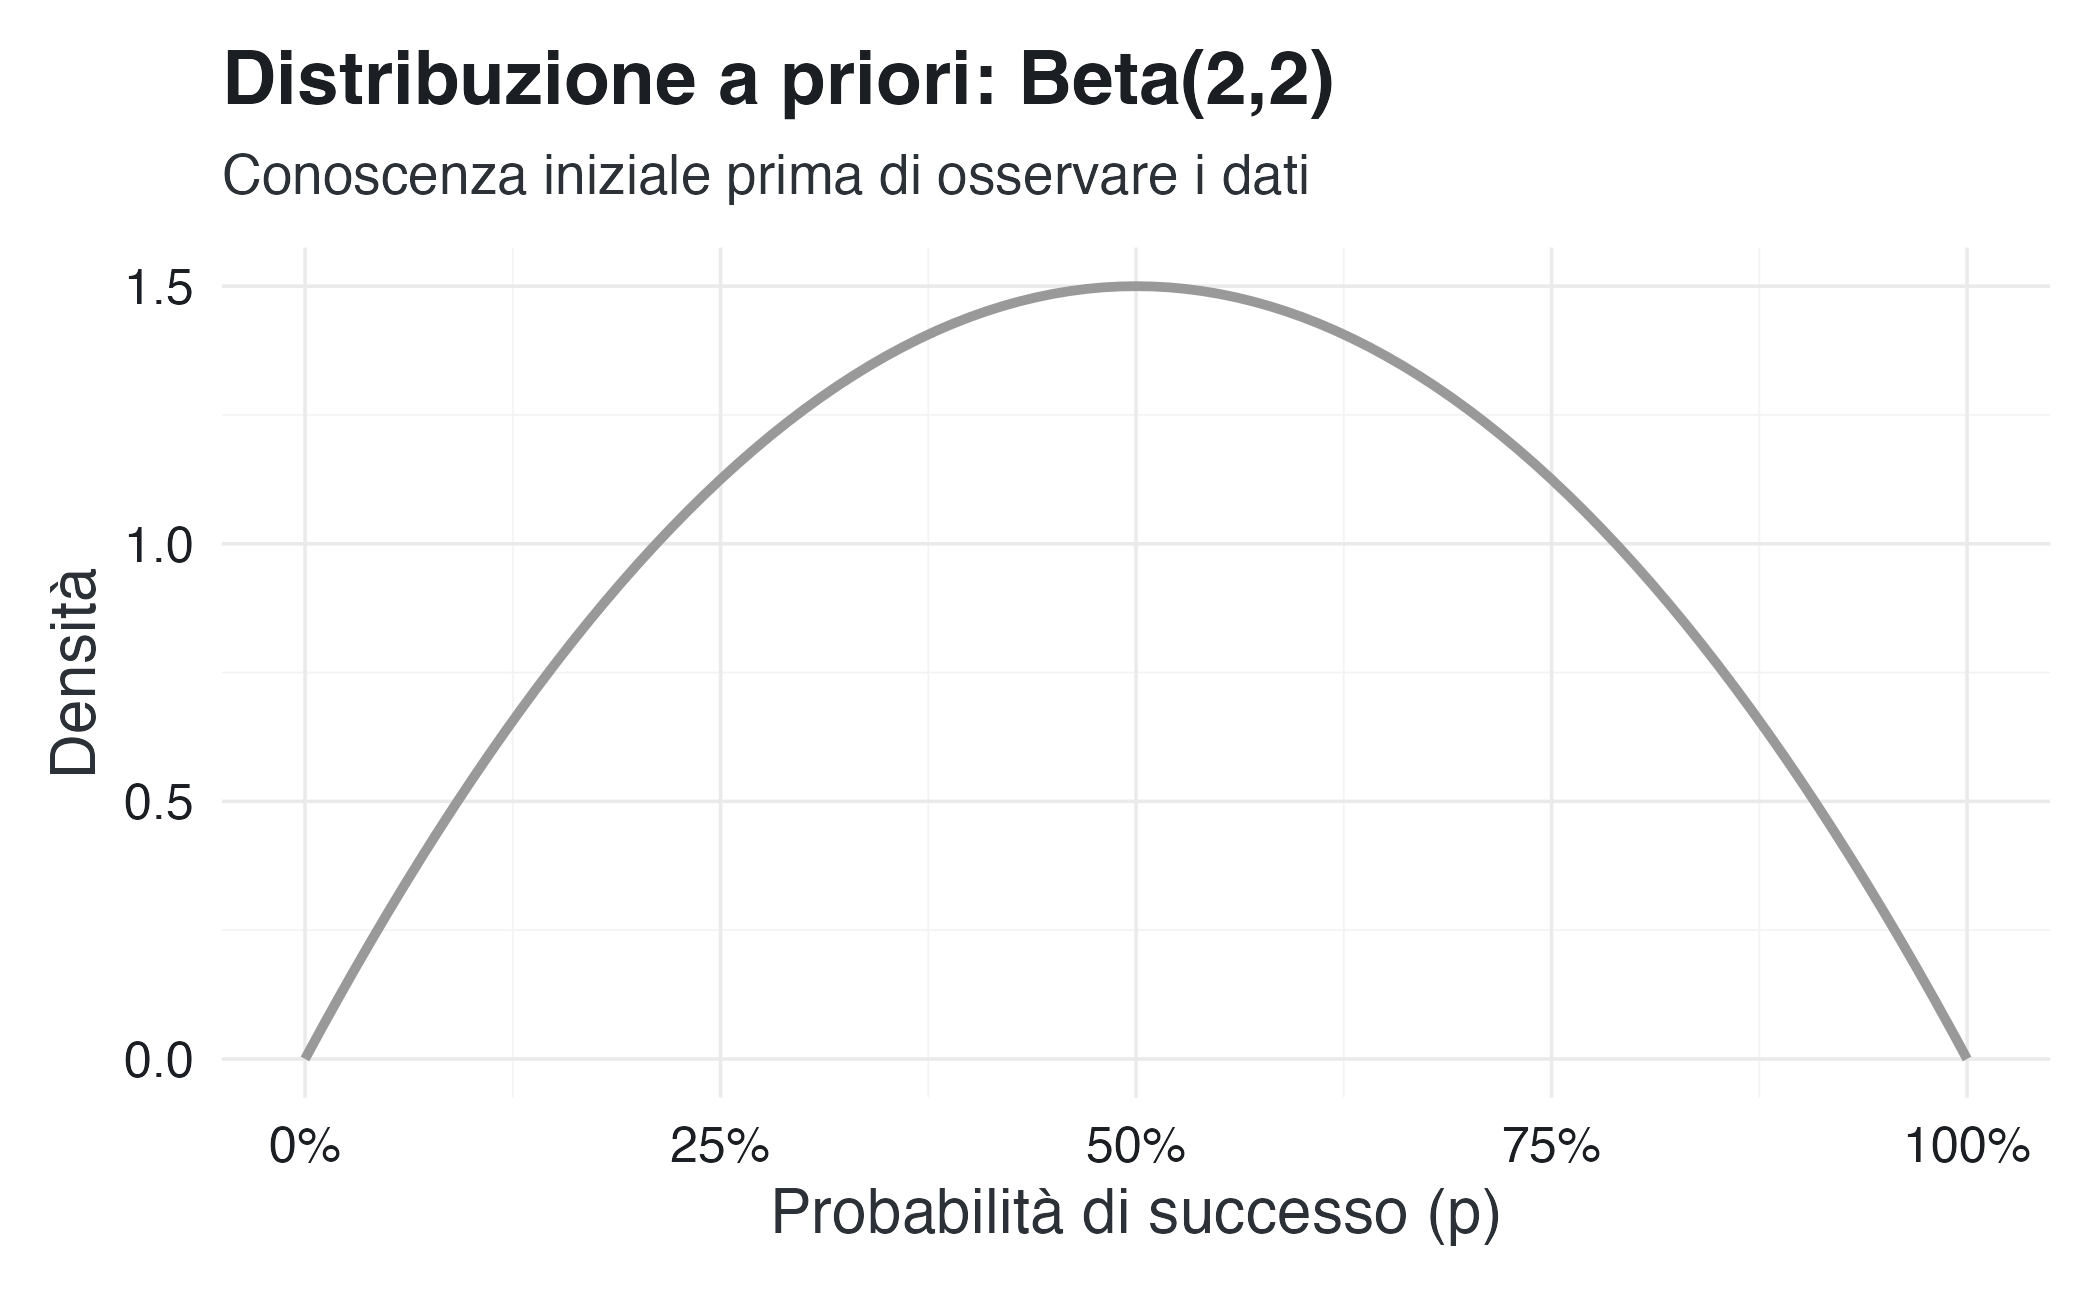
\includegraphics[width=0.85\linewidth,height=\textheight,keepaspectratio]{chapters/bayesian_inference/06_post_pred_distr_files/figure-pdf/unnamed-chunk-3-1.png}
\end{center}

Conoscenza aggiornata (dopo aver osservato i dati):

\begin{Shaded}
\begin{Highlighting}[]
\CommentTok{\# Conoscenza aggiornata (dopo aver osservato i dati) — POSTERIOR }
\FunctionTok{ggplot}\NormalTok{(}\FunctionTok{data.frame}\NormalTok{(}\AttributeTok{x =} \FunctionTok{c}\NormalTok{(}\DecValTok{0}\NormalTok{, }\DecValTok{1}\NormalTok{)), }\FunctionTok{aes}\NormalTok{(}\AttributeTok{x =}\NormalTok{ x)) }\SpecialCharTok{+}
  \FunctionTok{stat\_function}\NormalTok{(}
    \AttributeTok{fun =}\NormalTok{ dbeta,}
    \AttributeTok{args =} \FunctionTok{list}\NormalTok{(}\AttributeTok{shape1 =}\NormalTok{ alpha\_post, }\AttributeTok{shape2 =}\NormalTok{ beta\_post),}
    \AttributeTok{linewidth =} \FloatTok{1.1}\NormalTok{,}
    \AttributeTok{color =}\NormalTok{ col\_posterior}
\NormalTok{  ) }\SpecialCharTok{+}
  \FunctionTok{scale\_x\_continuous}\NormalTok{(}\AttributeTok{labels =}\NormalTok{ scales}\SpecialCharTok{::}\FunctionTok{label\_percent}\NormalTok{(}\AttributeTok{accuracy =} \DecValTok{1}\NormalTok{)) }\SpecialCharTok{+}
  \FunctionTok{labs}\NormalTok{(}
    \AttributeTok{x =} \StringTok{"Probabilità di successo (p)"}\NormalTok{, }
    \AttributeTok{y =} \StringTok{"Densità"}\NormalTok{,}
    \AttributeTok{title =} \StringTok{"Distribuzione a posteriori: Beta(72,32)"}\NormalTok{,}
    \AttributeTok{subtitle =} \StringTok{"Conoscenza aggiornata dopo aver osservato 70 successi su 100 prove"}
\NormalTok{  ) }
\end{Highlighting}
\end{Shaded}

\begin{center}
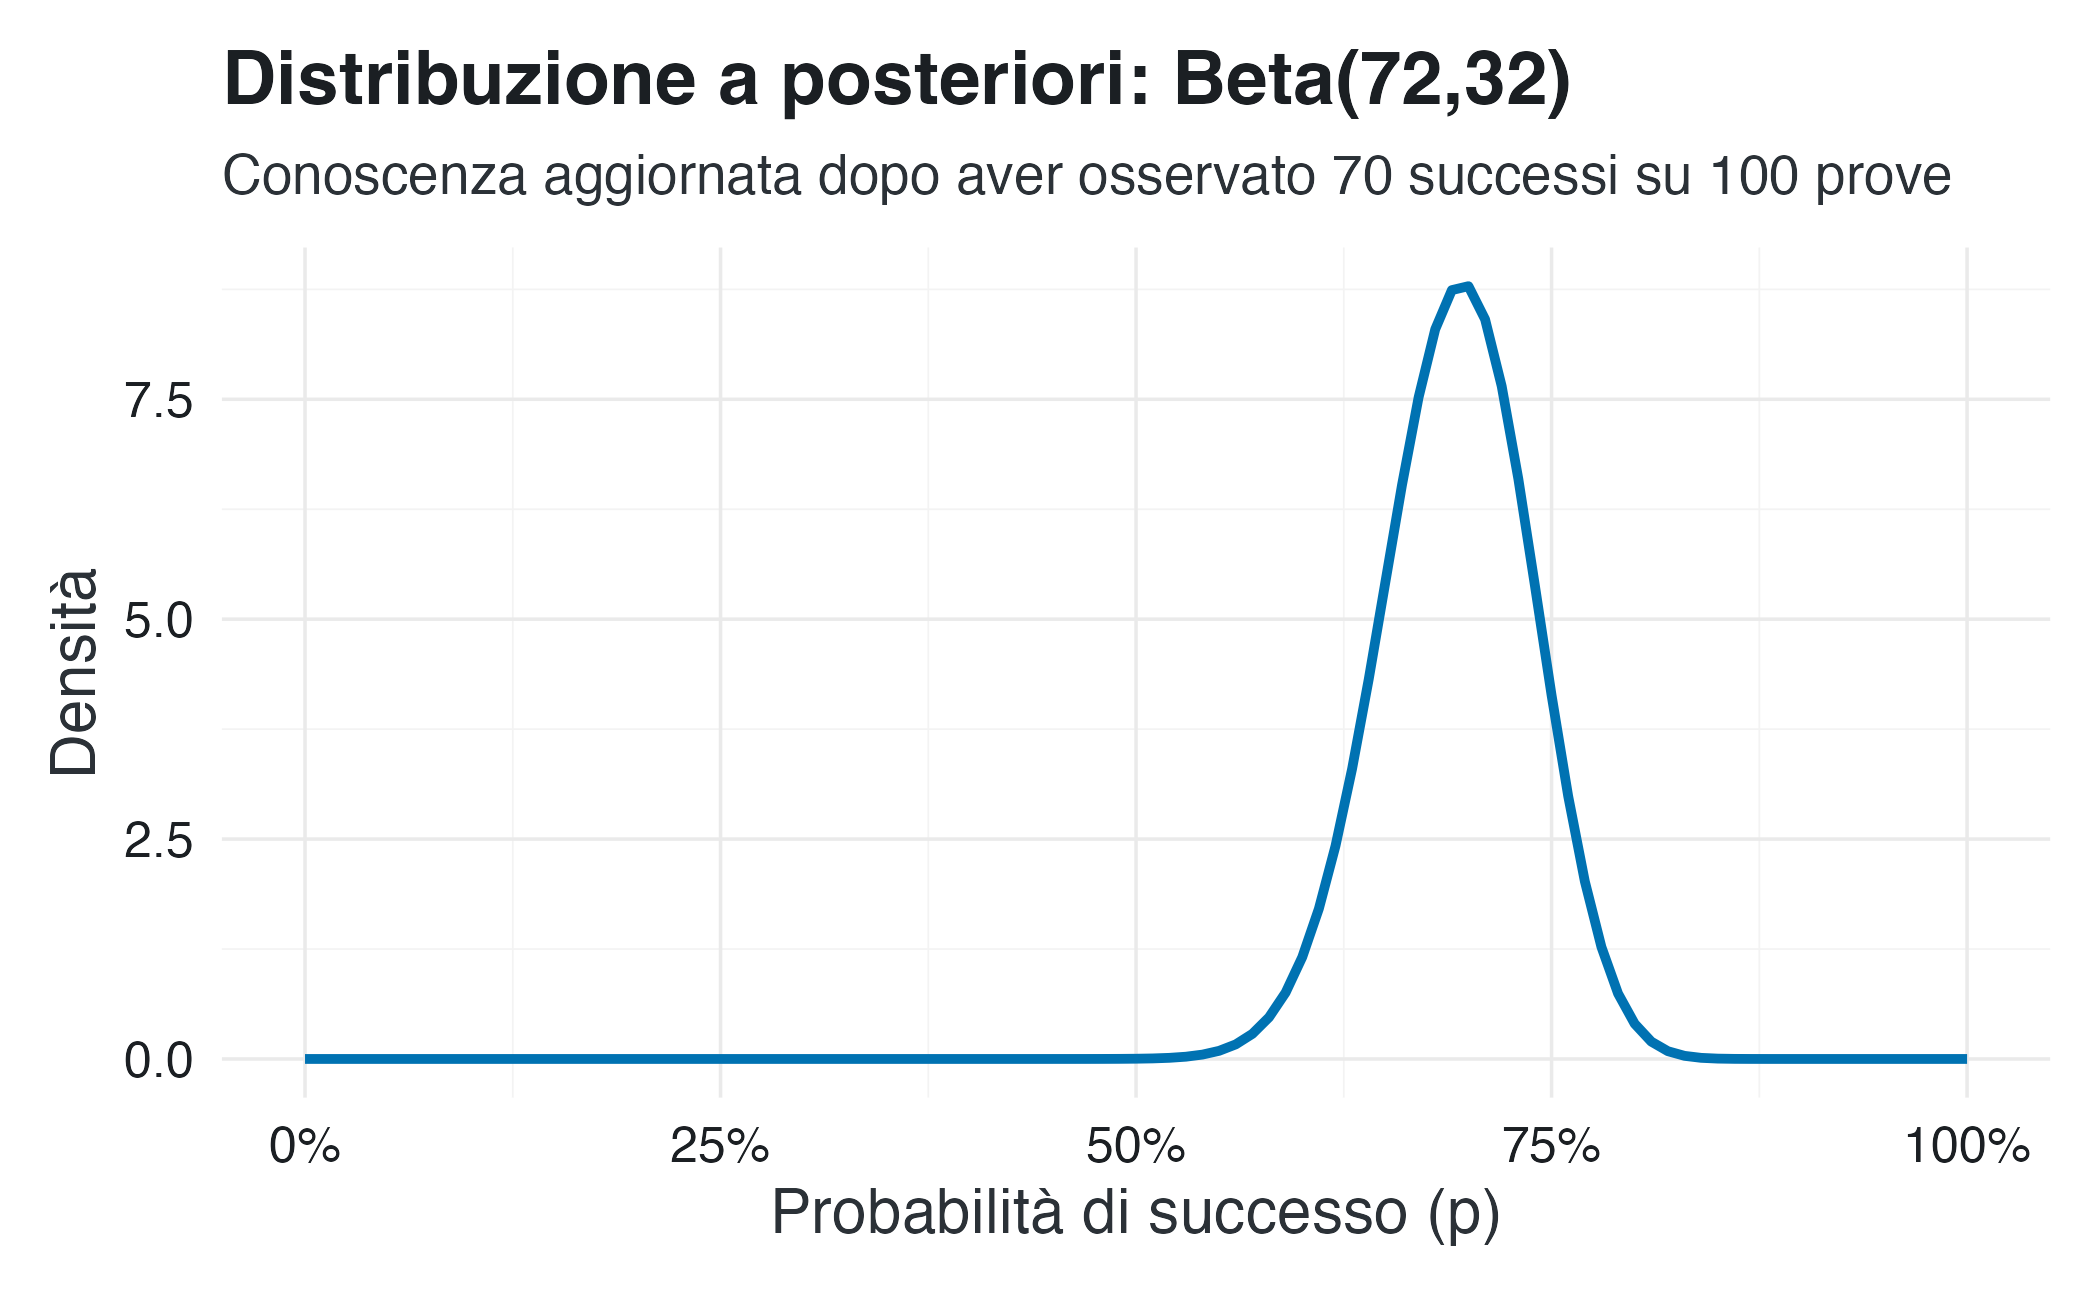
\includegraphics[width=0.85\linewidth,height=\textheight,keepaspectratio]{chapters/bayesian_inference/06_post_pred_distr_files/figure-pdf/unnamed-chunk-4-1.png}
\end{center}

Previsioni per i prossimi 10 lanci:

\begin{Shaded}
\begin{Highlighting}[]
\CommentTok{\# Previsioni per i prossimi 10 lanci — Posterior predictive }
\FunctionTok{ggplot}\NormalTok{(}\FunctionTok{data.frame}\NormalTok{(}\AttributeTok{proporzioni =}\NormalTok{ proporzioni\_future), }\FunctionTok{aes}\NormalTok{(}\AttributeTok{x =}\NormalTok{ proporzioni)) }\SpecialCharTok{+}
  \FunctionTok{geom\_histogram}\NormalTok{(}
    \FunctionTok{aes}\NormalTok{(}\AttributeTok{y =} \FunctionTok{after\_stat}\NormalTok{(density)),}
    \AttributeTok{bins =} \DecValTok{20}\NormalTok{,}
    \AttributeTok{fill =}\NormalTok{ col\_pred\_dist,}
    \AttributeTok{color =} \StringTok{"white"}\NormalTok{,}
    \AttributeTok{alpha =} \FloatTok{0.85}\NormalTok{,}
    \AttributeTok{linewidth =} \FloatTok{0.2}
\NormalTok{  ) }\SpecialCharTok{+}
  \FunctionTok{geom\_vline}\NormalTok{(}
    \FunctionTok{aes}\NormalTok{(}\AttributeTok{xintercept =}\NormalTok{ successi\_osservati }\SpecialCharTok{/}\NormalTok{ lanci\_totali),}
    \AttributeTok{linewidth =} \FloatTok{0.9}\NormalTok{,}
    \AttributeTok{linetype =} \StringTok{"dashed"}\NormalTok{,}
    \AttributeTok{color =}\NormalTok{ col\_line}
\NormalTok{  ) }\SpecialCharTok{+}
  \FunctionTok{annotate}\NormalTok{(}
    \StringTok{"text"}\NormalTok{,}
    \AttributeTok{x =}\NormalTok{ successi\_osservati }\SpecialCharTok{/}\NormalTok{ lanci\_totali }\SpecialCharTok{+} \FloatTok{0.02}\NormalTok{,}
    \AttributeTok{y =} \FloatTok{3.5}\NormalTok{,}
    \AttributeTok{label =} \FunctionTok{paste0}\NormalTok{(}\StringTok{"Proporzione osservata: "}\NormalTok{, }
                   \FunctionTok{round}\NormalTok{(successi\_osservati }\SpecialCharTok{/}\NormalTok{ lanci\_totali, }\DecValTok{2}\NormalTok{)),}
    \AttributeTok{color =}\NormalTok{ col\_line,}
    \AttributeTok{hjust =} \DecValTok{0}
\NormalTok{  ) }\SpecialCharTok{+}
  \FunctionTok{labs}\NormalTok{(}
    \AttributeTok{x =} \StringTok{"Proporzione di successi attesi"}\NormalTok{, }
    \AttributeTok{y =} \StringTok{"Densità"}\NormalTok{,}
    \AttributeTok{title =} \StringTok{"Distribuzione predittiva a posteriori"}\NormalTok{,}
    \AttributeTok{subtitle =} \StringTok{"Previsioni per i prossimi 10 lanci (Beta{-}Binomiale)"}
\NormalTok{  )}
\end{Highlighting}
\end{Shaded}

\begin{center}
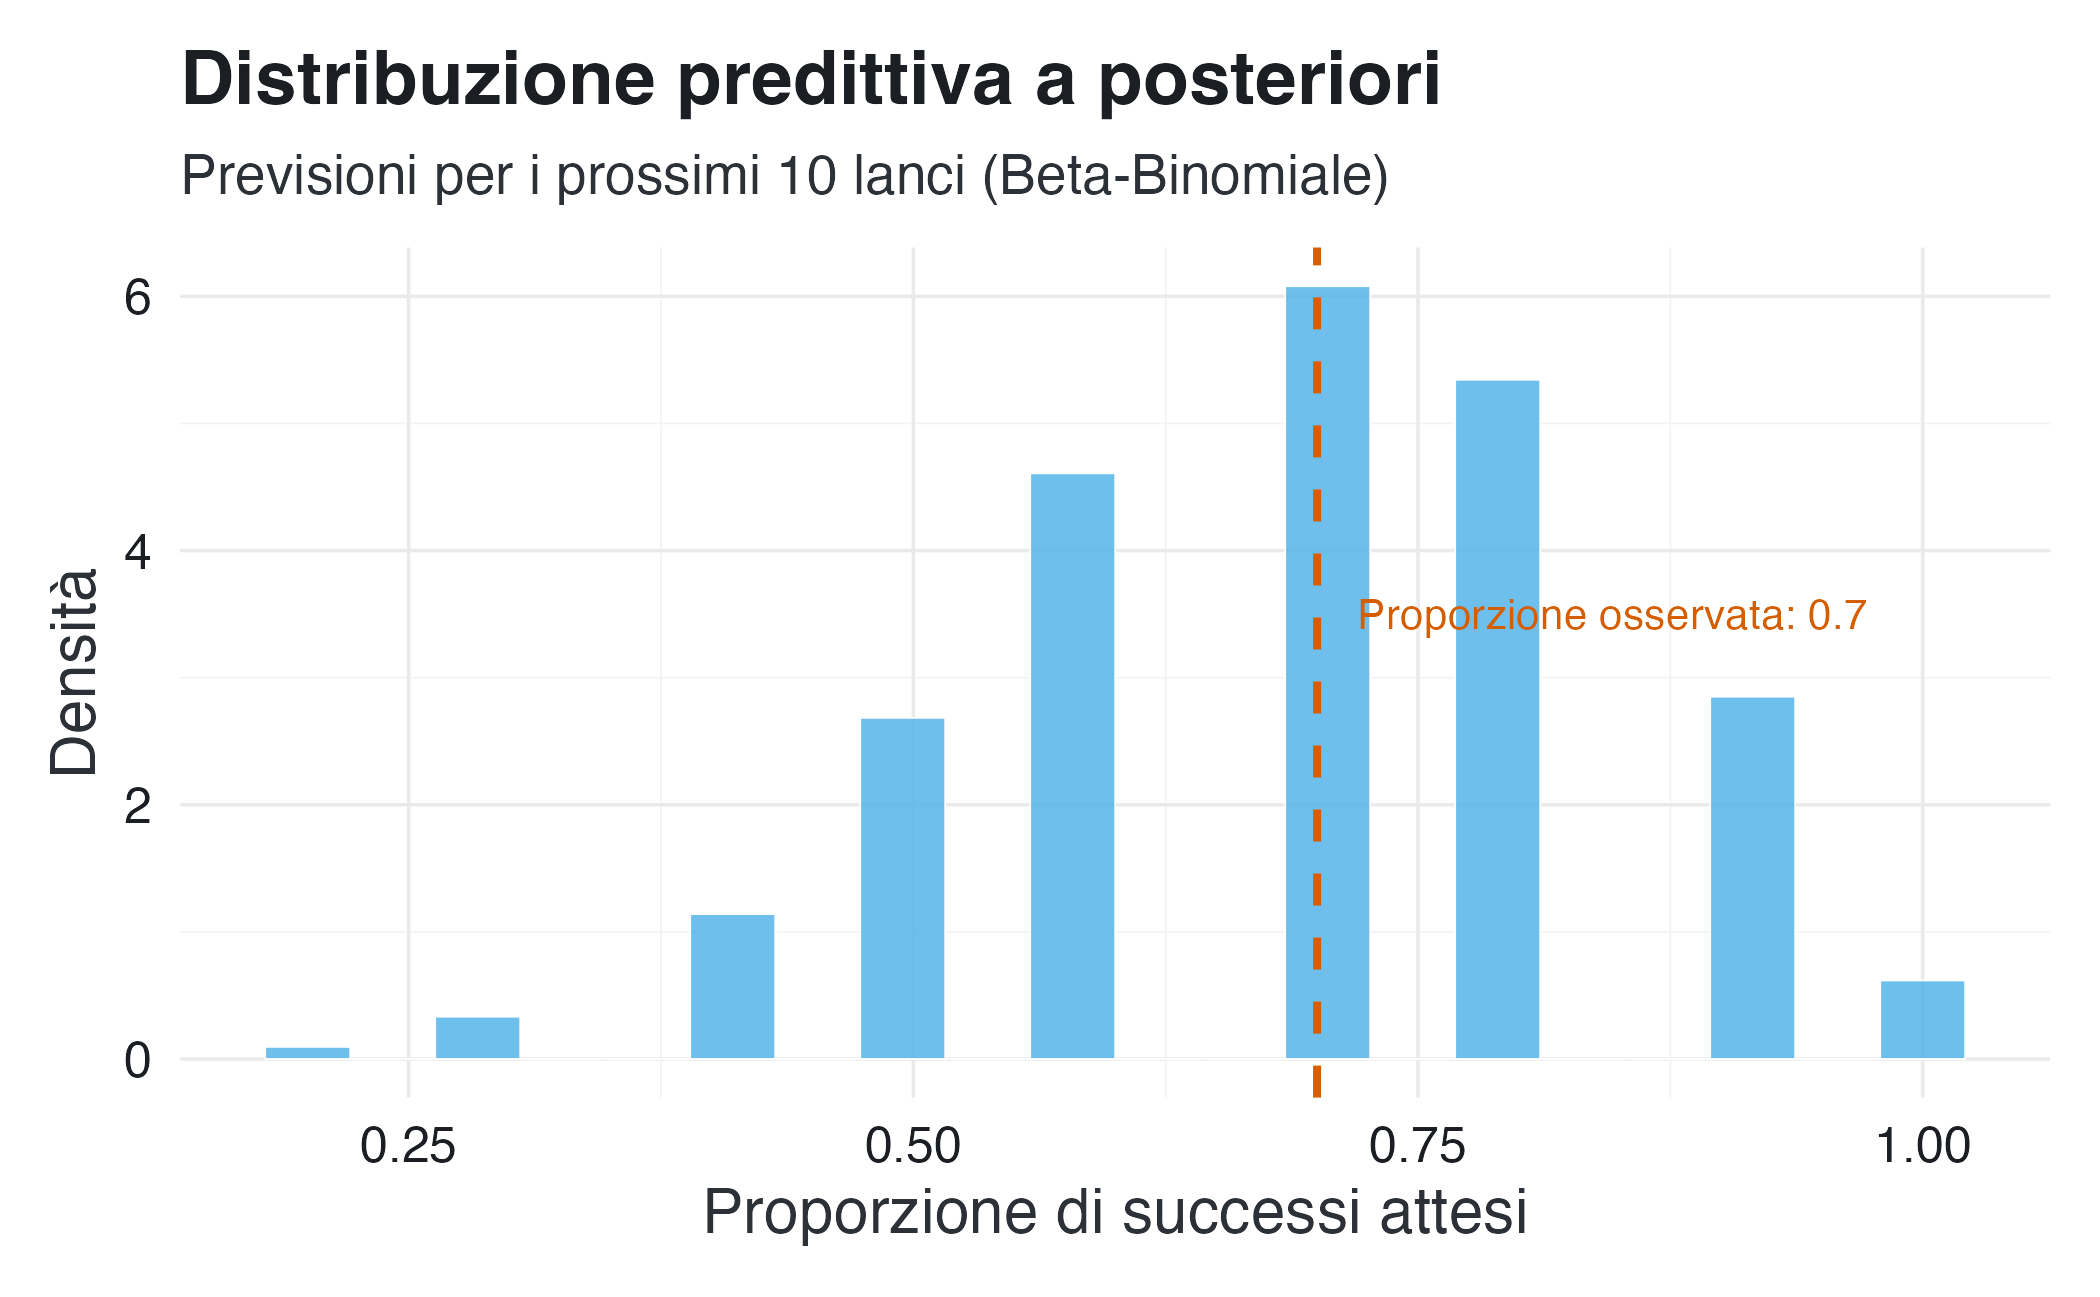
\includegraphics[width=0.85\linewidth,height=\textheight,keepaspectratio]{chapters/bayesian_inference/06_post_pred_distr_files/figure-pdf/unnamed-chunk-5-1.png}
\end{center}

\subsubsection{Interpretazione dei
risultati}\label{interpretazione-dei-risultati-1}

La nostra conoscenza del parametro \(p\) risulta ora concentrata attorno
al valore 0.7, come evidenziato dal grafico in rosso. Le previsioni per
i prossimi 10 lanci mostrano una maggiore variabilità, dovuta alla
combinazione di due fattori: persiste un certo grado di incertezza sul
valore esatto di \(p\), e anche ammettendo di conoscerlo perfettamente,
i risultati di 10 lanci presentano comunque una fluttuazione intrinseca.
Il fatto che il risultato osservato del 70\% di successi cada nella
regione più probabile delle nostre previsioni indica che il modello
adottato è ragionevole e può essere utilizzato per le previsioni future.

In termini pratici, se si dovesse formulare una previsione per i
prossimi 10 lanci, l'intervallo più plausibile si collocherebbe tra 6 e
8 successi, anche se non si possono escludere esiti di 5 o 9 successi, a
causa della variabilità casuale.

\begin{tcolorbox}[enhanced jigsaw, arc=.35mm, bottomrule=.15mm, bottomtitle=1mm, breakable, colback=white, colbacktitle=quarto-callout-caution-color!10!white, colframe=quarto-callout-caution-color-frame, coltitle=black, left=2mm, leftrule=.75mm, opacityback=0, opacitybacktitle=0.6, rightrule=.15mm, title=\textcolor{quarto-callout-caution-color}{\faFire}\hspace{0.5em}{Nota}, titlerule=0mm, toprule=.15mm, toptitle=1mm]

Potrebbe sembrare ovvio che la distribuzione predittiva a posteriori
riproduca fedelmente i dati osservati nel nostro esempio. In realtà,
questo risultato positivo non è affatto scontato ed è importante dal
punto di vista metodologico: attesta la buona calibrazione del nostro
modello.

Nel caso che abbiamo discusso, abbiamo scelto un modello binomiale con
un prior Beta perché ci permette di illustrare chiaramente la logica
alla base della distribuzione predittiva a posteriori in un caso
particolarmente semplice. È tuttavia cruciale riconoscere che la ricerca
psicologica opera tipicamente con modelli di complessità ben superiore.
In questi contesti applicativi, la corrispondenza tra i dati osservati e
quelli generati tramite la distribuzione predittiva non può mai essere
data per scontata, ma deve sempre essere oggetto di verifica empirica.

\end{tcolorbox}

\section{Validazione del modello: controlli predittivi a
posteriori}\label{validazione-del-modello-controlli-predittivi-a-posteriori}

\subsection{Oltre il confronto relativo: validazione assoluta del
modello}\label{oltre-il-confronto-relativo-validazione-assoluta-del-modello}

Mentre i metodi di \emph{valutazione relativa} tra modelli---quali
criteri informativi, fattori di Bayes o cross-validation---sono
essenziali per confrontare modelli rivali e saranno approfonditi in un
capitolo successivo, è altrettanto cruciale saper valutare la bontà di
un \emph{singolo modello} in \emph{termini assoluti}. I \emph{Posterior
Predictive Checks} (PPC) rispondono proprio a questa esigenza,
permettendo di quantificare quanto bene un modello si adatti ai dati
osservati, indipendentemente dall'esistenza di alternative.

La logica sottostante è potente e intuitiva: \emph{se un modello
rappresenta un'accurata approssimazione del processo che ha realmente
generato i dati, allora i parametri stimati (la distribuzione a
posteriori) dovrebbero essere in grado di generare---se simuliamo un
nuovo esperimento---dati replicati con caratteristiche simili a quelle
che abbiamo effettivamente osservato.}

\begin{tcolorbox}[enhanced jigsaw, arc=.35mm, bottomrule=.15mm, bottomtitle=1mm, breakable, colback=white, colbacktitle=quarto-callout-note-color!10!white, colframe=quarto-callout-note-color-frame, coltitle=black, left=2mm, leftrule=.75mm, opacityback=0, opacitybacktitle=0.6, rightrule=.15mm, title=\textcolor{quarto-callout-note-color}{\faInfo}\hspace{0.5em}{Il principio fondamentale del PPC}, titlerule=0mm, toprule=.15mm, toptitle=1mm]

Un modello adeguato non deve solo adattarsi ai dati osservati, ma deve
anche essere in grado di \emph{generare} dati con proprietà statistiche
simili. Se i dati osservati risultano atipici o ``estremi'' rispetto
all'universo di dati che il modello può generare, abbiamo un segnale
d'allarme sulla sua adeguatezza.

\end{tcolorbox}

\subsection{La distribuzione predittiva a posteriori per la
verifica}\label{la-distribuzione-predittiva-a-posteriori-per-la-verifica}

Consideriamo un modello parametrico con parametro \(\theta \in \Theta\),
densità a priori \(p(\theta)\) e funzione di verosimiglianza
\(p(x \mid \theta)\) per i dati osservati \(x\). Sia
\(\pi(\theta) = p(\theta \mid x)\) la densità a posteriori.

\begin{tcolorbox}[enhanced jigsaw, arc=.35mm, bottomrule=.15mm, bottomtitle=1mm, breakable, colback=white, colbacktitle=quarto-callout-important-color!10!white, colframe=quarto-callout-important-color-frame, coltitle=black, left=2mm, leftrule=.75mm, opacityback=0, opacitybacktitle=0.6, rightrule=.15mm, title=\textcolor{quarto-callout-important-color}{\faExclamation}\hspace{0.5em}{Definizione: Distribuzione Predittiva a Posteriori per il Controllo}, titlerule=0mm, toprule=.15mm, toptitle=1mm]

La distribuzione predittiva a posteriori per dati replicati è la
distribuzione marginale di un nuovo campione \(x_{\text{rep}}\),
generato dallo stesso modello di verosimiglianza, integrata rispetto
alla distribuzione a posteriori del parametro:

\begin{equation}\protect\phantomsection\label{eq-post-pred-rep}{
\pi(x_{\text{rep}}) := \int_{\Theta} p(x_{\text{rep}} \mid \theta)\, \pi(\theta)\, d\theta.
}\end{equation}

\end{tcolorbox}

Sebbene formalmente identica alla distribuzione predittiva per dati
futuri, qui l'utilizzo è concettualmente diverso. Non siamo interessati
a prevedere il futuro, ma a \emph{simulare un esperimento replicato} per
verificare la plausibilità che il nostro modello abbia generato i dati
già in nostro possesso.

\subsection{Implementare i controlli predittivi: valutare l'adeguatezza
del
modello}\label{implementare-i-controlli-predittivi-valutare-ladeguatezza-del-modello}

I PPC quantificano numericamente se i dati osservati \(x\) appaiano
``atipici'' rispetto alla distribuzione predittiva
\(\pi(x_{\text{rep}})\). La procedura standardizzata prevede:

\begin{enumerate}
\def\labelenumi{\arabic{enumi}.}
\tightlist
\item
  \emph{Definire una Statistica di Discrepanza \(T(\cdot)\)}: una
  quantità (es., media, varianza, skewness) che catturi una
  caratteristica dei dati che vogliamo verificare.
\item
  \emph{Calcolare un Posterior Predictive p-value}: la probabilità che
  la statistica calcolata su dati replicati sia più estrema di quella
  osservata. Una versione pratica è la proporzione di repliche in cui
  \(T(x_{\text{rep}}) \ge T(x)\).
\end{enumerate}

\begin{tcolorbox}[enhanced jigsaw, arc=.35mm, bottomrule=.15mm, bottomtitle=1mm, breakable, colback=white, colbacktitle=quarto-callout-tip-color!10!white, colframe=quarto-callout-tip-color-frame, coltitle=black, left=2mm, leftrule=.75mm, opacityback=0, opacitybacktitle=0.6, rightrule=.15mm, title=\textcolor{quarto-callout-tip-color}{\faLightbulb}\hspace{0.5em}{Esempio applicativo: tempi di reazione}, titlerule=0mm, toprule=.15mm, toptitle=1mm]

\textbf{Contesto:} modelliamo i tempi di reazione in un compito di
Stroop con una distribuzione normale.

\textbf{Problema:} i tempi di reazione reali sono tipicamente
asimmetrici (distribuzione con coda a destra), mentre la normale è
simmetrica.

\textbf{Controllo PPC:}

\begin{itemize}
\tightlist
\item
  \textbf{Statistica scelta:} coefficiente di asimmetria
  (\emph{skewness}).
\item
  \textbf{Procedura:} generiamo 5.000 dataset replicati
  \(x_{\text{rep}}\) dal modello e per ognuno calcoliamo la sua
  skewness.
\item
  \textbf{Risultato:} se la skewness osservata nei dati reali è maggiore
  del 98\% delle skewness simulate, concludiamo che il modello normale
  non riesce a catturare l'asimmetria dei dati, suggerendo l'adozione di
  modelli alternativi (es., log-normale, Gamma).
\end{itemize}

\end{tcolorbox}

\subsection{Interpretazione e limiti}\label{interpretazione-e-limiti}

I PPC sono strumenti diagnostici potenti, ma la loro interpretazione
richiede attenzione:

\begin{itemize}
\tightlist
\item
  \textbf{Non sono test di ipotesi classici:} il \emph{posterior
  predictive p-value} non va interpretato come un p-value frequentista.
  Non esiste una soglia universale di ``significatività''; è un
  indicatore di discrepanza relativa.
\item
  \textbf{La scelta della statistica \(T\) è fondamentale:} statistiche
  diverse rivelano inadeguatezze diverse. È buona pratica testare più
  aspetti (ad esempio, minimo, massimo, correlazioni) per un esame
  completo.
\item
  \textbf{Strumento complementare:} i PPC non sostituiscono il confronto
  di modelli. Un modello può superare un PPC ma essere peggiore di
  un'alternativa più parsimoniosa.
\end{itemize}

\subsection{Implementazione pratica}\label{implementazione-pratica}

Nei software bayesiani moderni (come Stan, brms, o PyMC), i controlli
predittivi a posteriori sono facilmente implementabili:

\begin{Shaded}
\begin{Highlighting}[]
\CommentTok{\# Esempio con brms}
\FunctionTok{pp\_check}\NormalTok{(fit, }\AttributeTok{type =} \StringTok{"dens\_overlay"}\NormalTok{, }\AttributeTok{ndraws =} \DecValTok{100}\NormalTok{)  }\CommentTok{\# Confronto densità}
\FunctionTok{pp\_check}\NormalTok{(fit, }\AttributeTok{type =} \StringTok{"stat"}\NormalTok{, }\AttributeTok{stat =} \StringTok{"mean"}\NormalTok{)         }\CommentTok{\# Confronto media}
\FunctionTok{pp\_check}\NormalTok{(fit, }\AttributeTok{type =} \StringTok{"stat\_2d"}\NormalTok{, }\AttributeTok{stat =} \FunctionTok{c}\NormalTok{(}\StringTok{"mean"}\NormalTok{, }\StringTok{"sd"}\NormalTok{))  }\CommentTok{\# Confronto bivariato}
\end{Highlighting}
\end{Shaded}

Queste funzioni generano automaticamente dataset replicati dalla
distribuzione predittiva a posteriori e visualizzano il confronto con i
dati osservati, facilitando la diagnosi visuale dell'adeguatezza del
modello.

\begin{tcolorbox}[enhanced jigsaw, arc=.35mm, bottomrule=.15mm, bottomtitle=1mm, breakable, colback=white, colbacktitle=quarto-callout-important-color!10!white, colframe=quarto-callout-important-color-frame, coltitle=black, left=2mm, leftrule=.75mm, opacityback=0, opacitybacktitle=0.6, rightrule=.15mm, title=\textcolor{quarto-callout-important-color}{\faExclamation}\hspace{0.5em}{Messaggio chiave}, titlerule=0mm, toprule=.15mm, toptitle=1mm]

La distribuzione predittiva a posteriori non serve solo a fare
previsioni su dati futuri, ma costituisce anche lo strumento
fondamentale per la \emph{validazione critica} del modello stesso.
Chiedendoci ``Questo modello potrebbe plausibilmente aver generato i
dati che osservo?'', adottiamo una posizione epistemologica coerente con
il framework bayesiano: i modelli sono approssimazioni provvisorie delle
nostre credenze, sempre soggette a revisione alla luce dell'esperienza.

\end{tcolorbox}

\section*{Riflessioni conclusive}\label{riflessioni-conclusive-10}

\markright{Riflessioni conclusive}

Le distribuzioni predittive a posteriori rappresentano il naturale
completamento del percorso iniziato con i \emph{prior}. Se i \emph{prior
predictive checks} ci consentono di controllare la plausibilità delle
nostre assunzioni iniziali, i \emph{posterior predictive checks} ci
permettono di verificare la plausibilità del modello alla luce dei dati.

Dal punto di vista applicativo, questo approccio rafforza la trasparenza
e la robustezza delle nostre inferenze. Non ci limitiamo a riportare
valori puntuali o intervalli di credibilità per i parametri, ma
mostriamo esplicitamente quali dati il nostro modello ritiene plausibili
e li confrontiamo con i dati effettivamente raccolti. Questo rende la
comunicazione dei risultati più chiara e intuitiva, anche per chi non ha
familiarità con la statistica bayesiana.

In sintesi, le distribuzioni predittive a posteriori ci ricordano che la
forza dell'approccio bayesiano non risiede soltanto nella stima dei
parametri, ma soprattutto nella capacità di prevedere e spiegare i
fenomeni. Nei capitoli successivi, vedremo come questa logica si estenda
anche al confronto sistematico tra modelli, aprendo la strada a un
approccio più rigoroso e cumulativo alla psicologia.

\begin{tcolorbox}[enhanced jigsaw, arc=.35mm, bottomrule=.15mm, bottomtitle=1mm, breakable, colback=white, colbacktitle=quarto-callout-important-color!10!white, colframe=quarto-callout-important-color-frame, coltitle=black, left=2mm, leftrule=.75mm, opacityback=0, opacitybacktitle=0.6, rightrule=.15mm, title=\textcolor{quarto-callout-important-color}{\faExclamation}\hspace{0.5em}{Problemi}, titlerule=0mm, toprule=.15mm, toptitle=1mm]

Consideriamo i dati della SWLS somministrata a un campione di studenti,
ottenendo per ciascuno uno \emph{score} complessivo. Per semplicità,
vogliamo ``dichiarare positivo'' lo studente se il punteggio SWLS supera
una determinata \textbf{soglia} (ad esempio, 20 su 35). In questo modo
otteniamo una variabile dicotomica (0/1), che useremo come ``successo''
in un modello binomiale.

\begin{enumerate}
\def\labelenumi{\arabic{enumi}.}
\item
  \textbf{Dati e conteggio dei successi}

  \begin{itemize}
  \tightlist
  \item
    Carica il dataset con le risposte SWLS.\\
  \item
    Costruisci la variabile binaria (ad esempio \texttt{SWLS\_dich}) che
    vale 1 se lo score ≥ 20, e 0 altrimenti.\\
  \item
    Calcola il \textbf{numero di successi} (numero di persone che
    superano la soglia) e il \textbf{numero totale di osservazioni} (N).
  \end{itemize}
\item
  \textbf{Modello beta-binomiale (approccio manuale via simulazione)}

  \begin{itemize}
  \tightlist
  \item
    \textbf{Specifica una distribuzione Beta(a, b)} come prior per la
    probabilità di successo \(p\). Scegli una coppia \((a, b)\)
    relativamente poco informativa, ad esempio (2,2) o (1,1).\\
  \item
    Osservando \(y\) successi su \(n\) soggetti, aggiorna i parametri a
    posteriori: \[
      a_{\text{post}} = a + y, 
      \quad
      b_{\text{post}} = b + (n - y).
    \]\\
  \item
    Simula un gran numero di campioni di \(p\) dalla distribuzione
    Beta\(\bigl(a_{\text{post}},\, b_{\text{post}}\bigr)\).\\
  \item
    Per ciascun campione di \(p\), genera un valore \(\tilde{y}\) da una
    Binomiale\(\bigl(n_{\text{new}}, p\bigr)\), dove \(n_{\text{new}}\)
    è la dimensione di un ipotetico nuovo campione (che puoi scegliere,
    ad esempio, uguale a \(n\) oppure un valore diverso). Otterrai così
    una \textbf{posterior predictive distribution} per \(\tilde{y}\).\\
  \item
    Infine, calcola statistiche descrittive (media, varianza,
    intervalli) e/o disegna un istogramma di \(\tilde{y}\) o della
    proporzione \(\tilde{y}/n_{\text{new}}\).
  \end{itemize}
\item
  \textbf{Replicare con \emph{brms}}

  \begin{itemize}
  \item
    Usa il pacchetto \textbf{brms} per costruire un modello binomiale.
    Per esempio:

\begin{Shaded}
\begin{Highlighting}[]
\FunctionTok{library}\NormalTok{(brms)}

\CommentTok{\# Crea un data frame con la variabile dicotomica}
\NormalTok{df\_binom }\OtherTok{\textless{}{-}} \FunctionTok{data.frame}\NormalTok{(}
  \AttributeTok{successes =}\NormalTok{ y,    }\CommentTok{\# conteggio dei successi}
  \AttributeTok{failures  =}\NormalTok{ n }\SpecialCharTok{{-}}\NormalTok{ y}
\NormalTok{)}

\CommentTok{\# Modello binomiale con prior Beta(a,b) approssimato tramite logit}
\NormalTok{fit\_brms }\OtherTok{\textless{}{-}} \FunctionTok{brm}\NormalTok{(}
  \FunctionTok{bf}\NormalTok{(successes }\SpecialCharTok{|} \FunctionTok{trials}\NormalTok{(n) }\SpecialCharTok{\textasciitilde{}} \DecValTok{1}\NormalTok{), }
  \AttributeTok{data =}\NormalTok{ df\_binom,}
  \AttributeTok{family =} \FunctionTok{binomial}\NormalTok{(}\AttributeTok{link =} \StringTok{"logit"}\NormalTok{),}
  \AttributeTok{prior =} \FunctionTok{c}\NormalTok{(}
    \FunctionTok{prior}\NormalTok{(}\FunctionTok{beta}\NormalTok{(}\DecValTok{2}\NormalTok{, }\DecValTok{2}\NormalTok{), }\AttributeTok{class =} \StringTok{"Intercept"}\NormalTok{, }\AttributeTok{dpar =} \StringTok{"mu"}\NormalTok{) }
    \CommentTok{\# NOTA: la specifica di una "beta(2,2)" diretta sull\textquotesingle{}intercetta}
    \CommentTok{\# è un\textquotesingle{}approssimazione, tipicamente serve passare a una scala logit.}
    \CommentTok{\# In brms, di solito si usa prior su scale normali dell\textquotesingle{}intercetta.}
\NormalTok{  ),}
  \AttributeTok{seed =} \DecValTok{123}
\NormalTok{)}
\end{Highlighting}
\end{Shaded}

    \emph{(Le specifiche del \texttt{prior} potrebbero richiedere una
    formulazione differente se vuoi rispettare esattamente la
    corrispondenza con Beta(a,b). In ogni caso, l'idea è mostrare come
    definire un prior e costruire un modello binomiale con
    \texttt{brms}.)}
  \item
    Verifica la convergenza e poi estrai la \textbf{posterior predictive
    distribution} con le funzioni di \emph{brms}:

\begin{Shaded}
\begin{Highlighting}[]
\FunctionTok{pp\_check}\NormalTok{(fit\_brms, }\AttributeTok{nsamples =} \DecValTok{100}\NormalTok{)}
\end{Highlighting}
\end{Shaded}

    Questo ti mostrerà come i dati predetti dal modello (in termini di
    binomiale) si confrontano con i dati osservati.
  \end{itemize}
\item
  \textbf{Confronto e interpretazione}

  \begin{itemize}
  \tightlist
  \item
    Metti a confronto i risultati della simulazione ``manuale''
    (Beta-Binomial) e quelli ottenuti con \emph{brms}. Noterai che le
    distribuzioni predittive dovrebbero essere coerenti, se hai
    impostato un prior per \emph{brms} simile a quello del modello
    Beta-Binomiale.\\
  \item
    Discuti brevemente se la distribuzione predittiva a posteriori
    acquisita è plausibile rispetto ai dati osservati. Ad esempio, la
    probabilità di osservare \(\tilde{y}\) simile a \(y\) dovrebbe
    essere relativamente alta se il modello è appropriato.\\
  \item
    Se vuoi, puoi cambiare \(n_{\text{new}}\) (es. previsione su 200
    soggetti futuri) per vedere come la variabilità della previsione si
    ``ridimensiona'' o cresce a seconda della taglia del campione.\\
  \end{itemize}
\end{enumerate}

\end{tcolorbox}

\begin{tcolorbox}[enhanced jigsaw, arc=.35mm, bottomrule=.15mm, bottomtitle=1mm, breakable, colback=white, colbacktitle=quarto-callout-tip-color!10!white, colframe=quarto-callout-tip-color-frame, coltitle=black, left=2mm, leftrule=.75mm, opacityback=0, opacitybacktitle=0.6, rightrule=.15mm, title=\textcolor{quarto-callout-tip-color}{\faLightbulb}\hspace{0.5em}{Soluzioni}, titlerule=0mm, toprule=.15mm, toptitle=1mm]

\begin{enumerate}
\def\labelenumi{\arabic{enumi}.}
\item
  \textbf{Costruzione del dataset}

  \begin{itemize}
  \item
    Se la SWLS varia tra 5 e 35, e la soglia è 20, puoi fare:

\begin{Shaded}
\begin{Highlighting}[]
\NormalTok{df}\SpecialCharTok{$}\NormalTok{SWLS\_dich }\OtherTok{\textless{}{-}} \FunctionTok{ifelse}\NormalTok{(df}\SpecialCharTok{$}\NormalTok{SWLS\_score }\SpecialCharTok{\textgreater{}=} \DecValTok{20}\NormalTok{, }\DecValTok{1}\NormalTok{, }\DecValTok{0}\NormalTok{)}
\NormalTok{y }\OtherTok{\textless{}{-}} \FunctionTok{sum}\NormalTok{(df}\SpecialCharTok{$}\NormalTok{SWLS\_dich)}
\NormalTok{n }\OtherTok{\textless{}{-}} \FunctionTok{nrow}\NormalTok{(df)}
\end{Highlighting}
\end{Shaded}
  \end{itemize}
\item
  \textbf{Approccio Beta-Binomial manuale}

  \begin{itemize}
  \item
    Prior: \((a, b) = (2, 2)\)\\
  \item
    Posterior:
    \((a_{\text{post}}, b_{\text{post}}) = (2 + y,\, 2 + n - y)\).\\
  \item
    Generazione dei campioni:

\begin{Shaded}
\begin{Highlighting}[]
\NormalTok{N\_sim }\OtherTok{\textless{}{-}} \DecValTok{2000}
\NormalTok{p\_post }\OtherTok{\textless{}{-}} \FunctionTok{rbeta}\NormalTok{(N\_sim, a\_post, b\_post)}
\NormalTok{y\_pred }\OtherTok{\textless{}{-}} \FunctionTok{rbinom}\NormalTok{(N\_sim, }\AttributeTok{size =}\NormalTok{ n\_new, }\AttributeTok{prob =}\NormalTok{ p\_post)}

\CommentTok{\# Se preferisci la proporzione futura:}
\NormalTok{prop\_pred }\OtherTok{\textless{}{-}}\NormalTok{ y\_pred }\SpecialCharTok{/}\NormalTok{ n\_new}
\end{Highlighting}
\end{Shaded}
  \item
    Statistiche:

\begin{Shaded}
\begin{Highlighting}[]
\NormalTok{mean\_p }\OtherTok{\textless{}{-}} \FunctionTok{mean}\NormalTok{(p\_post) }\CommentTok{\# media a posteriori di p}
\NormalTok{quantile\_p }\OtherTok{\textless{}{-}} \FunctionTok{quantile}\NormalTok{(p\_post, }\FunctionTok{c}\NormalTok{(}\FloatTok{0.025}\NormalTok{, }\FloatTok{0.975}\NormalTok{))  }

\NormalTok{mean\_prop\_pred }\OtherTok{\textless{}{-}} \FunctionTok{mean}\NormalTok{(prop\_pred)}
\NormalTok{quantile\_prop\_pred }\OtherTok{\textless{}{-}} \FunctionTok{quantile}\NormalTok{(prop\_pred, }\FunctionTok{c}\NormalTok{(}\FloatTok{0.025}\NormalTok{, }\FloatTok{0.975}\NormalTok{))}
\end{Highlighting}
\end{Shaded}
  \item
    Grafici (istogramma e densità):

\begin{Shaded}
\begin{Highlighting}[]
\FunctionTok{hist}\NormalTok{(prop\_pred, }\AttributeTok{freq=}\ConstantTok{FALSE}\NormalTok{, }\AttributeTok{col=}\StringTok{\textquotesingle{}lightblue\textquotesingle{}}\NormalTok{,}
     \AttributeTok{main=}\StringTok{\textquotesingle{}Posterior Predictive Distribution: prop. di successi\textquotesingle{}}\NormalTok{)}
\end{Highlighting}
\end{Shaded}
  \end{itemize}
\item
  \textbf{Modello con \emph{brms}}

  \begin{itemize}
  \item
    Usa la sintassi di una binomiale con offset o con
    \texttt{trials(n)}.\\
  \item
    Specifica un prior che approssimi Beta(2,2) sullo scale logit, ad
    esempio:

\begin{Shaded}
\begin{Highlighting}[]
\CommentTok{\# Beta(2,2) ha media \textasciitilde{} 0.5, varianza relativamente ampia.}
\CommentTok{\# Approssimandola su scala logit \textasciitilde{} normal(0, 2.2) }
\CommentTok{\# (valore indicativo: la normal(0, 2) su logit copre un intervallo ampio).}

\NormalTok{prior\_approx }\OtherTok{\textless{}{-}} \FunctionTok{prior}\NormalTok{(}\FunctionTok{normal}\NormalTok{(}\DecValTok{0}\NormalTok{, }\DecValTok{2}\NormalTok{), }\AttributeTok{class =} \StringTok{"Intercept"}\NormalTok{)}
\end{Highlighting}
\end{Shaded}
  \item
    Esegui \texttt{pp\_check(fit\_brms)} e interpreta.
  \end{itemize}
\item
  \textbf{Interpretazione}

  \begin{itemize}
  \tightlist
  \item
    Se la soglia scelta per la SWLS cattura un ``buon livello di
    soddisfazione'', potresti aspettarti una certa \% di successi.\\
  \item
    Se i dati futuri simulati sono coerenti con i dati reali --- ad
    esempio, la media di \(\tilde{y}\) è vicina a \(y\) --- allora il
    modello sembra descrivere bene la realtà. Altrimenti, potresti
    rivedere la soglia o la specifica del prior.
  \end{itemize}
\end{enumerate}

L'elemento chiave è che la \textbf{distribuzione predittiva a
posteriori} (posterior predictive distribution) non si limita a
considerare \emph{un solo} valore di \(p\), bensì campiona molteplici
valori plausibili (dalla \emph{posterior}), e per \emph{ciascuno} simula
un potenziale outcome. Così facendo, si riflette pienamente l'incertezza
residua sul parametro e l'aleatorietà del processo binomiale.

\end{tcolorbox}

\begin{tcolorbox}[enhanced jigsaw, arc=.35mm, bottomrule=.15mm, bottomtitle=1mm, breakable, colback=white, colbacktitle=quarto-callout-note-color!10!white, colframe=quarto-callout-note-color-frame, coltitle=black, left=2mm, leftrule=.75mm, opacityback=0, opacitybacktitle=0.6, rightrule=.15mm, title=\textcolor{quarto-callout-note-color}{\faInfo}\hspace{0.5em}{Informazioni sull'ambiente di sviluppo}, titlerule=0mm, toprule=.15mm, toptitle=1mm]

\begin{Shaded}
\begin{Highlighting}[]
\FunctionTok{sessionInfo}\NormalTok{()}
\CommentTok{\#\textgreater{} R version 4.6.1 (2026{-}06{-}24)}
\CommentTok{\#\textgreater{} Platform: aarch64{-}apple{-}darwin23}
\CommentTok{\#\textgreater{} Running under: macOS Tahoe 26.5.2}
\CommentTok{\#\textgreater{} }
\CommentTok{\#\textgreater{} Matrix products: default}
\CommentTok{\#\textgreater{} BLAS:   /Library/Frameworks/R.framework/Versions/4.6/Resources/lib/libRblas.0.dylib }
\CommentTok{\#\textgreater{} LAPACK: /Library/Frameworks/R.framework/Versions/4.6/Resources/lib/libRlapack.dylib;  LAPACK version 3.12.1}
\CommentTok{\#\textgreater{} }
\CommentTok{\#\textgreater{} locale:}
\CommentTok{\#\textgreater{} [1] C.UTF{-}8/UTF{-}8/C.UTF{-}8/C/C.UTF{-}8/C.UTF{-}8}
\CommentTok{\#\textgreater{} }
\CommentTok{\#\textgreater{} time zone: Europe/Zagreb}
\CommentTok{\#\textgreater{} tzcode source: internal}
\CommentTok{\#\textgreater{} }
\CommentTok{\#\textgreater{} attached base packages:}
\CommentTok{\#\textgreater{} [1] stats     graphics  grDevices utils     datasets  methods   base     }
\CommentTok{\#\textgreater{} }
\CommentTok{\#\textgreater{} other attached packages:}
\CommentTok{\#\textgreater{}  [1] ragg\_1.5.2            tinytable\_0.17.0      withr\_3.0.3          }
\CommentTok{\#\textgreater{}  [4] systemfonts\_1.3.2     patchwork\_1.3.2       ggdist\_3.3.3         }
\CommentTok{\#\textgreater{}  [7] tidybayes\_3.0.7       bayesplot\_1.15.0      ggplot2\_4.0.3        }
\CommentTok{\#\textgreater{} [10] reliabilitydiag\_0.2.1 priorsense\_1.2.0      posterior\_1.7.0      }
\CommentTok{\#\textgreater{} [13] loo\_2.10.0            rstan\_2.32.7          StanHeaders\_2.32.10  }
\CommentTok{\#\textgreater{} [16] brms\_2.23.0           Rcpp\_1.1.2            sessioninfo\_1.2.4    }
\CommentTok{\#\textgreater{} [19] conflicted\_1.2.0      janitor\_2.2.1         matrixStats\_1.5.0    }
\CommentTok{\#\textgreater{} [22] modelr\_0.1.11         tibble\_3.3.1          dplyr\_1.2.1          }
\CommentTok{\#\textgreater{} [25] tidyr\_1.3.2           rio\_1.3.0             here\_1.0.2           }
\CommentTok{\#\textgreater{} }
\CommentTok{\#\textgreater{} loaded via a namespace (and not attached):}
\CommentTok{\#\textgreater{}  [1] svUnit\_1.0.8          tidyselect\_1.2.1      farver\_2.1.2         }
\CommentTok{\#\textgreater{}  [4] S7\_0.2.2              fastmap\_1.2.0         tensorA\_0.36.2.1     }
\CommentTok{\#\textgreater{}  [7] digest\_0.6.39         timechange\_0.4.0      estimability\_2.0.0   }
\CommentTok{\#\textgreater{} [10] lifecycle\_1.0.5       magrittr\_2.0.5        compiler\_4.6.1       }
\CommentTok{\#\textgreater{} [13] rlang\_1.3.0           tools\_4.6.1           knitr\_1.51           }
\CommentTok{\#\textgreater{} [16] labeling\_0.4.3        bridgesampling\_1.2{-}1  pkgbuild\_1.4.8       }
\CommentTok{\#\textgreater{} [19] curl\_7.1.0            RColorBrewer\_1.1{-}3    abind\_1.4{-}8          }
\CommentTok{\#\textgreater{} [22] purrr\_1.2.2           grid\_4.6.1            stats4\_4.6.1         }
\CommentTok{\#\textgreater{} [25] xtable\_1.8{-}8          inline\_0.3.21         emmeans\_2.0.4        }
\CommentTok{\#\textgreater{} [28] scales\_1.4.0          cli\_3.6.6             mvtnorm\_1.4{-}2        }
\CommentTok{\#\textgreater{} [31] rmarkdown\_2.31        generics\_0.1.4        otel\_0.2.0           }
\CommentTok{\#\textgreater{} [34] RcppParallel\_5.1.11{-}2 cachem\_1.1.0          stringr\_1.6.0        }
\CommentTok{\#\textgreater{} [37] parallel\_4.6.1        vctrs\_0.7.3           V8\_8.2.0             }
\CommentTok{\#\textgreater{} [40] Matrix\_1.7{-}5          jsonlite\_2.0.0        arrayhelpers\_1.1{-}1   }
\CommentTok{\#\textgreater{} [43] glue\_1.8.1            codetools\_0.2{-}20      distributional\_0.8.1 }
\CommentTok{\#\textgreater{} [46] lubridate\_1.9.5       stringi\_1.8.7         gtable\_0.3.6         }
\CommentTok{\#\textgreater{} [49] QuickJSR\_1.10.0       pillar\_1.11.1         htmltools\_0.5.9      }
\CommentTok{\#\textgreater{} [52] Brobdingnag\_1.2{-}9     R6\_2.6.1              textshaping\_1.0.5    }
\CommentTok{\#\textgreater{} [55] rprojroot\_2.1.1       evaluate\_1.0.5        lattice\_0.22{-}9       }
\CommentTok{\#\textgreater{} [58] backports\_1.5.1       memoise\_2.0.1         broom\_1.0.13         }
\CommentTok{\#\textgreater{} [61] snakecase\_0.11.1      rstantools\_2.6.0      coda\_0.19{-}4.1        }
\CommentTok{\#\textgreater{} [64] gridExtra\_2.3.1       nlme\_3.1{-}170          checkmate\_2.3.4      }
\CommentTok{\#\textgreater{} [67] xfun\_0.60             pkgconfig\_2.0.3}
\end{Highlighting}
\end{Shaded}

\end{tcolorbox}

\section*{Bibliografia}\label{bibliografia-12}

\markright{Bibliografia}

\chapter{La decisione sul singolo paziente: dal punteggio osservato alla
probabilità clinica}\label{sec-bayesian-inference-single-patient-cutoff}

\begin{tcolorbox}[enhanced jigsaw, arc=.35mm, bottomrule=.15mm, bottomtitle=1mm, breakable, colback=white, colbacktitle=quarto-callout-caution-color!10!white, colframe=quarto-callout-caution-color-frame, coltitle=black, left=2mm, leftrule=.75mm, opacityback=0, opacitybacktitle=0.6, rightrule=.15mm, title=\textcolor{quarto-callout-caution-color}{\faFire}\hspace{0.5em}{Preparazione del Notebook}, titlerule=0mm, toprule=.15mm, toptitle=1mm]

\begin{Shaded}
\begin{Highlighting}[]
\NormalTok{here}\SpecialCharTok{::}\FunctionTok{here}\NormalTok{(}\StringTok{"code"}\NormalTok{, }\StringTok{"\_common.R"}\NormalTok{) }\SpecialCharTok{|\textgreater{}} 
  \FunctionTok{source}\NormalTok{()}
\end{Highlighting}
\end{Shaded}

\end{tcolorbox}

\begin{tcolorbox}[enhanced jigsaw, arc=.35mm, bottomrule=.15mm, breakable, colback=white, colframe=quarto-callout-important-color-frame, left=2mm, leftrule=.75mm, opacityback=0, rightrule=.15mm, toprule=.15mm]

\textbf{Da sapere.} Un punteggio osservato non coincide con il punteggio
vero, perché contiene errore di misura. L'attendibilità determina quanto
la stima debba essere corretta verso la media normativa. Nel modello
Normale-Normale, la media a posteriori coincide con la stima di Kelley,
ma la distribuzione a posteriori consente anche di quantificare
direttamente la probabilità che il punteggio vero superi una soglia
clinica.

\textbf{Da saper fare.} Calcolare la stima di Kelley e la distribuzione
a posteriori del punteggio vero; ricavare e interpretare
\(P(\theta > c \mid X)\) e il relativo intervallo di credibilità;
distinguere la posterior del punteggio vero dalla distribuzione
predittiva di una nuova misurazione; formulare una conclusione clinica
che renda esplicita l'incertezza e non trasformi il cut-off in una
diagnosi automatica.

\textbf{Approfondimento facoltativo.} La derivazione algebrica
dell'equivalenza tra Kelley e la media a posteriori, l'analisi di
sensibilità rispetto all'attendibilità, la distribuzione predittiva
completa e la formulazione delle decisioni mediante funzioni di perdita
possono essere rimandate in una prima lettura.

\hyperref[sec-percorsi-lettura]{Che cosa significano queste etichette?}

\end{tcolorbox}

\section{Una vignetta clinica: quando due punti fanno la
differenza}\label{sec-vignetta-clinica}

Immaginiamo una situazione molto comune nella pratica psicologica. Un
clinico somministra a un paziente un test standardizzato per la
depressione. Il manuale indica un \emph{cut-off} clinico pari a 70. Il
paziente ottiene un punteggio osservato di 72.

La lettura ingenua sembra immediata:

\[
72 > 70.
\]

Il paziente è dunque sopra soglia? La risposta corretta è:
\emph{probabilmente sì, ma non con certezza}. Due punti sopra il cut-off
non autorizzano, da soli, una conclusione diagnostica netta, perché ogni
punteggio psicometrico contiene un errore di misura.

Questo capitolo mostra come riformulare la domanda clinica in modo più
rigoroso. Non ci limiteremo a chiedere se il punteggio osservato supera
la soglia, ma chiederemo:

\begin{tcolorbox}[enhanced jigsaw, arc=.35mm, bottomrule=.15mm, bottomtitle=1mm, breakable, colback=white, colbacktitle=quarto-callout-note-color!10!white, colframe=quarto-callout-note-color-frame, coltitle=black, left=2mm, leftrule=.75mm, opacityback=0, opacitybacktitle=0.6, rightrule=.15mm, title={La domanda clinica}, titlerule=0mm, toprule=.15mm, toptitle=1mm]

Dato il punteggio osservato \(X = 72\), qual è la probabilità che il
\textbf{punteggio vero} del paziente, indicato con \(\theta\), superi
effettivamente il cut-off clinico di 70?

\[
P(\theta > 70 \mid X = 72).
\]

\end{tcolorbox}

Questa formulazione è più vicina al problema reale del clinico: prendere
decisioni in condizioni di incertezza, senza trasformare un risultato
psicometrico in una certezza artificiale.

\section{Il punteggio osservato non è il punteggio
vero}\label{sec-punteggio-osservato-vero}

Nella teoria classica dei test, il punteggio osservato \(X\) viene
rappresentato come la somma di due componenti: \[
X = \theta + \varepsilon,
\] dove:

\begin{itemize}
\tightlist
\item
  \(\theta\) è il \textbf{punteggio vero}, ovvero la componente stabile
  del costrutto misurato secondo il modello psicometrico;
\item
  \(\varepsilon\) è l'\textbf{errore di misura}, ovvero la componente
  accidentale della misurazione.
\end{itemize}

È importante non attribuire al termine \emph{punteggio vero} un
significato ontologico troppo forte. Nel nostro esempio, \(\theta\) non
è ``la depressione reale'' del paziente in senso assoluto. Si tratta
piuttosto del valore latente che il test mira a stimare, ovvero la parte
stabile e sistematica del punteggio, separata dalle fluttuazioni casuali
della somministrazione.

L'errore di misura non è un dettaglio marginale. Stanchezza, ansia
momentanea, distrazione, comprensione di alcuni item, desiderabilità
sociale, condizioni ambientali e variabilità giornaliera possono
modificare il punteggio osservato senza riflettere un cambiamento reale
nel costrutto psicologico.

La qualità dello strumento è riassunta dall'\textbf{attendibilità}
\(\rho\), definita come la proporzione della varianza osservata
attribuibile al punteggio vero: \[
\rho = \frac{\sigma^2_\theta}{\sigma^2_X}.
\] Se l'attendibilità è pari a \(\rho = 0.85\), l'85\% della varianza
osservata riflette differenze nel punteggio vero, mentre il 15\%
riflette l'errore di misura.

\section{Il contesto numerico dell'esempio}\label{sec-contesto-numerico}

In tutto il capitolo useremo lo stesso scenario numerico:

\begin{itemize}
\tightlist
\item
  media normativa osservata: \(\mu_X = 70\);
\item
  deviazione standard normativa osservata: \(\sigma_X = 15\);
\item
  attendibilità del test: \(\rho = 0.85\);
\item
  punteggio osservato del paziente: \(X = 72\);
\item
  cut-off clinico: \(c = 70\).
\end{itemize}

Da questi valori derivano due quantità fondamentali:

\[
\sigma^2_\theta = \rho \sigma^2_X,
\qquad
\sigma^2_e = (1 - \rho) \sigma^2_X.
\]

La prima è la varianza dei punteggi veri nella popolazione. La seconda è
la varianza dell'errore di misura. La radice quadrata di \(\sigma^2_e\)
è l'\textbf{errore standard della misura} (\emph{standard error of
measurement}, SEM):

\[
\sigma_e = \sigma_X \sqrt{1 - \rho}.
\]

\begin{Shaded}
\begin{Highlighting}[]
\CommentTok{\# Parametri del test}
\NormalTok{mu\_pop    }\OtherTok{\textless{}{-}} \DecValTok{70}      \CommentTok{\# media normativa osservata}
\NormalTok{sigma\_X   }\OtherTok{\textless{}{-}} \DecValTok{15}      \CommentTok{\# deviazione standard normativa osservata}
\NormalTok{rho       }\OtherTok{\textless{}{-}} \FloatTok{0.85}    \CommentTok{\# attendibilita\textquotesingle{}}
\NormalTok{X\_obs     }\OtherTok{\textless{}{-}} \DecValTok{72}      \CommentTok{\# punteggio osservato}
\NormalTok{cut\_off   }\OtherTok{\textless{}{-}} \DecValTok{70}      \CommentTok{\# cut{-}off clinico}

\CommentTok{\# Componenti della varianza secondo la teoria classica dei test}
\NormalTok{sigma\_theta }\OtherTok{\textless{}{-}} \FunctionTok{sqrt}\NormalTok{(rho) }\SpecialCharTok{*}\NormalTok{ sigma\_X}
\NormalTok{sigma\_e     }\OtherTok{\textless{}{-}}\NormalTok{ sigma\_X }\SpecialCharTok{*} \FunctionTok{sqrt}\NormalTok{(}\DecValTok{1} \SpecialCharTok{{-}}\NormalTok{ rho)}

\FunctionTok{cat}\NormalTok{(}\StringTok{"DS dei punteggi veri:"}\NormalTok{, }\FunctionTok{round}\NormalTok{(sigma\_theta, }\DecValTok{2}\NormalTok{), }\StringTok{"}\SpecialCharTok{\textbackslash{}n}\StringTok{"}\NormalTok{)}
\CommentTok{\#\textgreater{} DS dei punteggi veri: 13.8}
\FunctionTok{cat}\NormalTok{(}\StringTok{"Errore standard della misura (SEM):"}\NormalTok{, }\FunctionTok{round}\NormalTok{(sigma\_e, }\DecValTok{2}\NormalTok{), }\StringTok{"}\SpecialCharTok{\textbackslash{}n}\StringTok{"}\NormalTok{)}
\CommentTok{\#\textgreater{} Errore standard della misura (SEM): 5.81}
\end{Highlighting}
\end{Shaded}

Nel nostro esempio, il SEM è circa 5.81. Ciò significa che il punteggio
osservato di un singolo paziente può oscillare di diversi punti rispetto
al punteggio effettivo. Un punteggio di 72, quindi, non deve essere
interpretato come una misurazione perfetta, ma come un'informazione
utile, seppur incerta.

\section{Kelley: la risposta classica come shrinkage verso la
media}\label{sec-kelley-shrinkage}

Una prima risposta al problema della stima del punteggio vero è fornita
dalla formula di Kelley (\citeproc{ref-Kelley1923}{1923}):

\[
\hat{\theta}_{\text{Kelley}} = \rho X + (1 - \rho)\mu_X.
\]

La formula ha una struttura molto semplice: combina il punteggio
osservato del paziente con la media della popolazione di riferimento. Il
peso del punteggio osservato corrisponde all'attendibilità del test.

\begin{Shaded}
\begin{Highlighting}[]
\NormalTok{theta\_kelley }\OtherTok{\textless{}{-}}\NormalTok{ rho }\SpecialCharTok{*}\NormalTok{ X\_obs }\SpecialCharTok{+}\NormalTok{ (}\DecValTok{1} \SpecialCharTok{{-}}\NormalTok{ rho) }\SpecialCharTok{*}\NormalTok{ mu\_pop}

\FunctionTok{cat}\NormalTok{(}\StringTok{"Stima di Kelley:"}\NormalTok{, }\FunctionTok{round}\NormalTok{(theta\_kelley, }\DecValTok{2}\NormalTok{), }\StringTok{"}\SpecialCharTok{\textbackslash{}n}\StringTok{"}\NormalTok{)}
\CommentTok{\#\textgreater{} Stima di Kelley: 71.7}
\end{Highlighting}
\end{Shaded}

La stima corretta è 71.7 e non 72. La differenza è minima, perché il
test ha un'elevata attendibilità, ma il principio è importante: quando
il test non è perfettamente attendibile, la stima migliore del punteggio
effettivo si sposta verso la media della popolazione. Questo fenomeno è
un esempio di \emph{shrinkage} o regressione verso la media.

L'intuizione è la seguente: se una parte del punteggio osservato dipende
dall'errore casuale, allora un valore superiore alla media può essere in
parte dovuto a una fluttuazione accidentale. Per questo motivo, la stima
del punteggio vero non coincide con il punteggio osservato, ma si
colloca tra il punteggio individuale e la media del gruppo.

\subsection{L'incertezza della stima di
Kelley}\label{lincertezza-della-stima-di-kelley}

La stima puntuale non basta. È necessario quantificare l'incertezza
della stima del punteggio vero. Nel modello classico, tale incertezza è
descritta dall'\textbf{errore standard dell'errore di stima}
(\emph{standard error of estimate}, SEE):

\[
\text{SEE} = \sigma_X \sqrt{\rho(1 - \rho)}.
\]

\begin{Shaded}
\begin{Highlighting}[]
\NormalTok{SEE }\OtherTok{\textless{}{-}}\NormalTok{ sigma\_X }\SpecialCharTok{*} \FunctionTok{sqrt}\NormalTok{(rho }\SpecialCharTok{*}\NormalTok{ (}\DecValTok{1} \SpecialCharTok{{-}}\NormalTok{ rho))}
\NormalTok{IC\_kelley }\OtherTok{\textless{}{-}}\NormalTok{ theta\_kelley }\SpecialCharTok{+} \FunctionTok{qnorm}\NormalTok{(}\FunctionTok{c}\NormalTok{(.}\DecValTok{025}\NormalTok{, .}\DecValTok{975}\NormalTok{)) }\SpecialCharTok{*}\NormalTok{ SEE}

\FunctionTok{cat}\NormalTok{(}\StringTok{"SEE:"}\NormalTok{, }\FunctionTok{round}\NormalTok{(SEE, }\DecValTok{2}\NormalTok{), }\StringTok{"}\SpecialCharTok{\textbackslash{}n}\StringTok{"}\NormalTok{)}
\CommentTok{\#\textgreater{} SEE: 5.36}
\FunctionTok{cat}\NormalTok{(}\StringTok{"Intervallo al 95\% secondo Kelley: ["}\NormalTok{,}
    \FunctionTok{round}\NormalTok{(IC\_kelley[}\DecValTok{1}\NormalTok{], }\DecValTok{1}\NormalTok{), }\StringTok{", "}\NormalTok{, }\FunctionTok{round}\NormalTok{(IC\_kelley[}\DecValTok{2}\NormalTok{], }\DecValTok{1}\NormalTok{), }\StringTok{"]}\SpecialCharTok{\textbackslash{}n}\StringTok{"}\NormalTok{, }\AttributeTok{sep =} \StringTok{""}\NormalTok{)}
\CommentTok{\#\textgreater{} Intervallo al 95\% secondo Kelley: [61.2, 82.2]}
\end{Highlighting}
\end{Shaded}

L'intervallo ottenuto è ampio: include valori sensibilmente inferiori e
superiori alla soglia clinica. Questo è il primo messaggio sostanziale
del capitolo. Anche se il punteggio osservato supera il cut-off,
l'incertezza di misura non consente un'interpretazione dicotomica
ingenua.

\begin{figure}[H]

{\centering 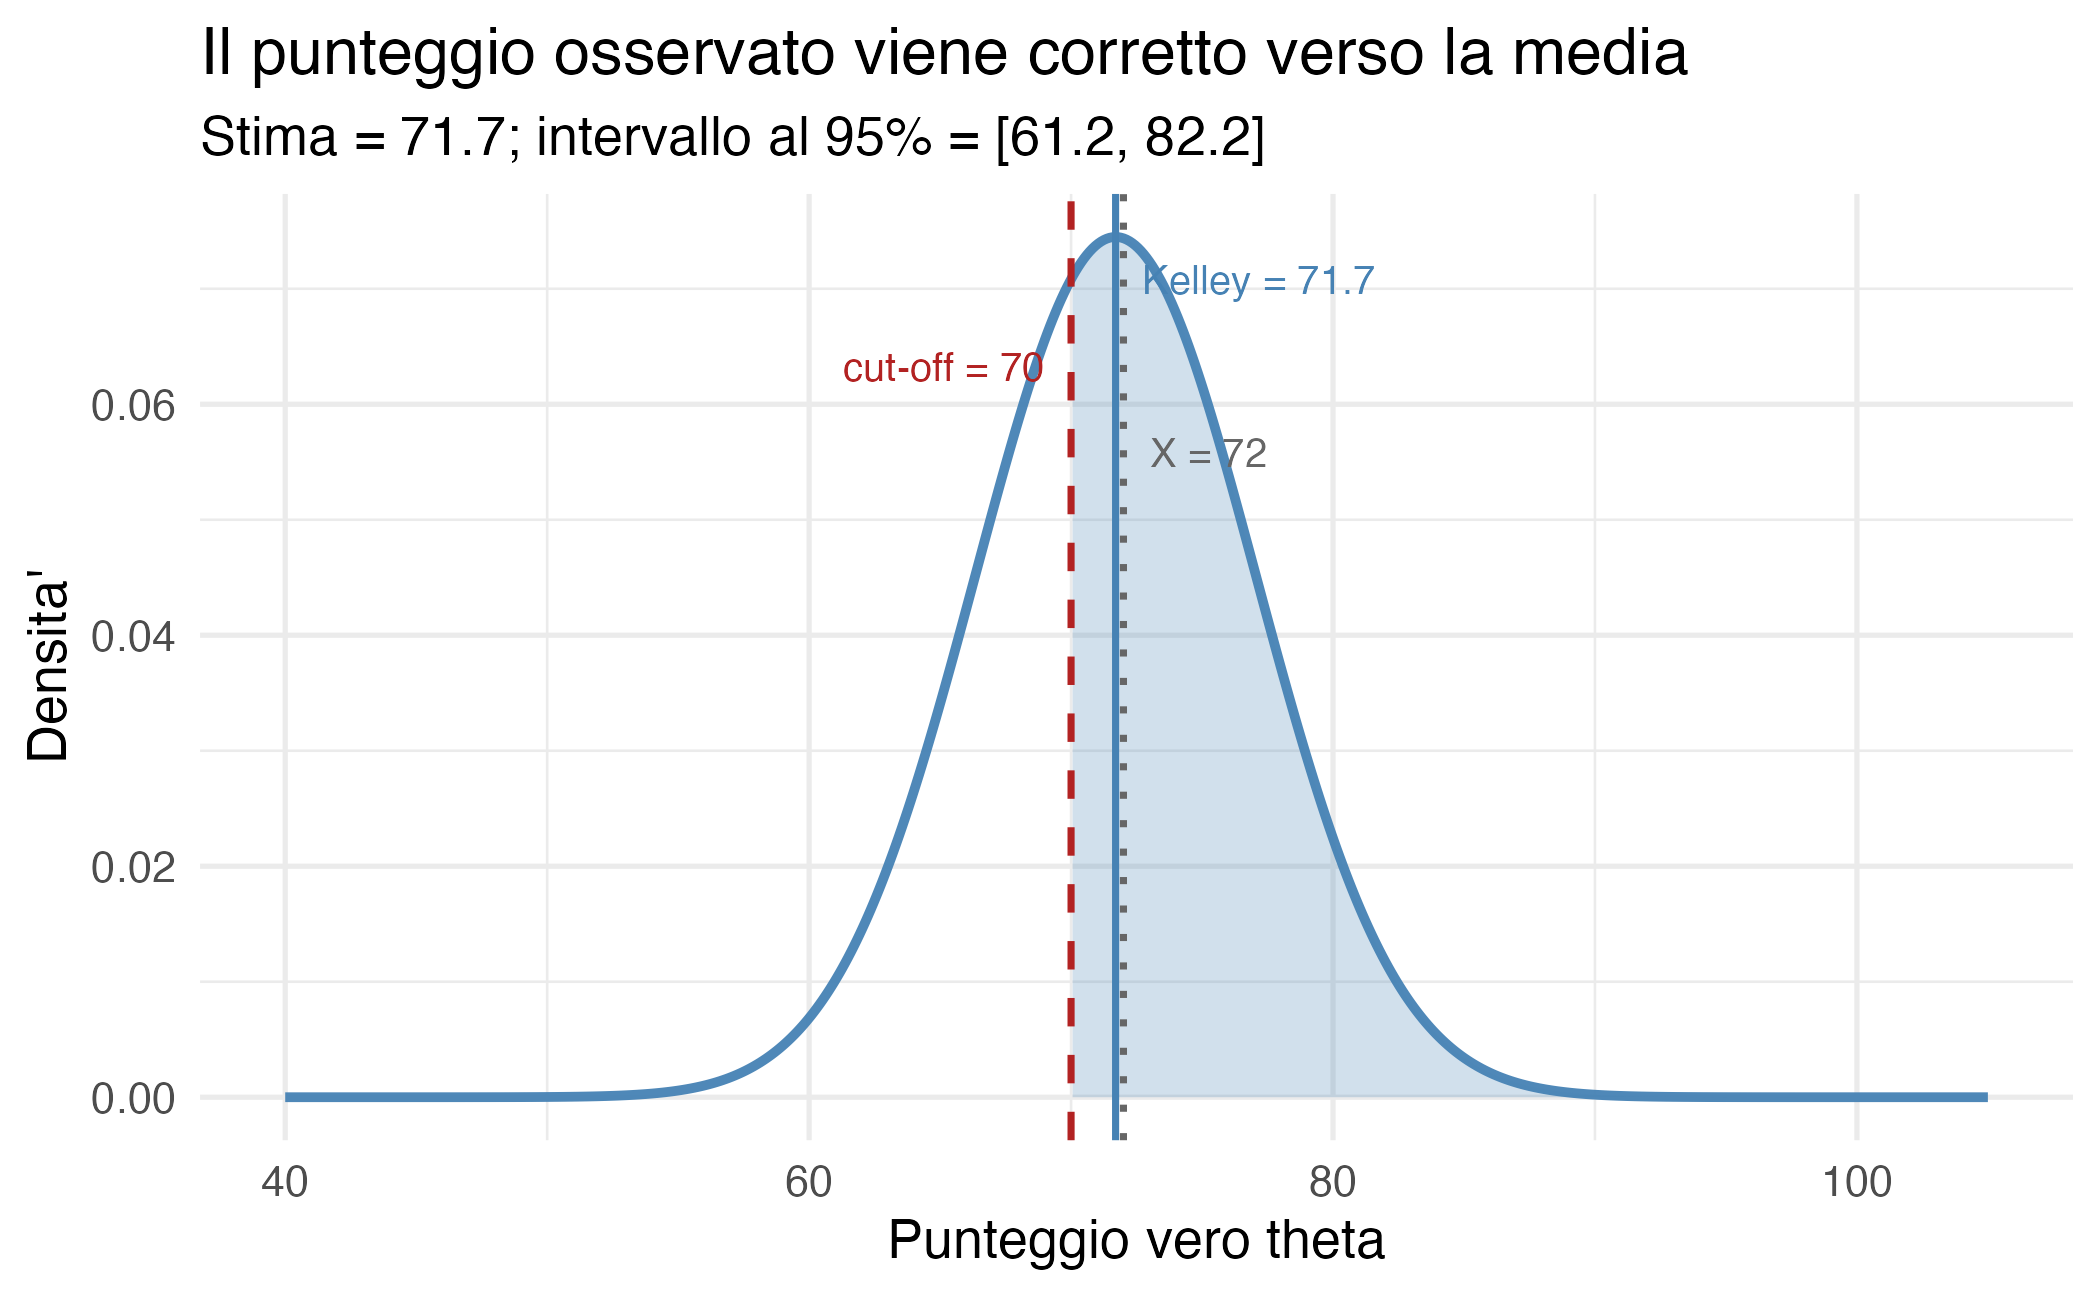
\includegraphics[width=0.85\linewidth,height=\textheight,keepaspectratio]{chapters/bayesian_inference/07_singolo_paziente_files/figure-pdf/unnamed-chunk-5-1.png}

}

\caption{Stima di Kelley del punteggio vero. La curva rappresenta
l'incertezza residua attorno alla stima; la linea tratteggiata indica il
cut-off clinico.}

\end{figure}%

\subsection{Cosa significa l'intervallo
classico?}\label{cosa-significa-lintervallo-classico}

L'intervallo costruito attorno alla stima di Kelley non deve essere
interpretato come la probabilità che il punteggio vero di questo
specifico paziente cada nell'intervallo. Secondo l'interpretazione
frequentista, il punteggio vero è un valore fisso, ma sconosciuto. La
probabilità riguarda la procedura: in condizioni ideali di ripetizione
del processo di campionamento e costruzione dell'intervallo, il 95\%
degli intervalli conterrebbe il valore vero, sotto le assunzioni del
modello.

Questa interpretazione è corretta, ma non risponde direttamente alla
domanda che interessa al clinico. Il clinico non deve decidere in base a
una procedura ripetuta infinite volte, ma deve decidere cosa pensare del
paziente che ha di fronte, in base al punteggio osservato.

\section{La riformulazione
bayesiana}\label{sec-riformulazione-bayesiana}

Il modello bayesiano riformula il problema in modo diretto. Prima di
osservare il paziente, descriviamo la distribuzione dei punteggi reali
nella popolazione. Dopo aver osservato il punteggio del paziente,
aggiorniamo tale distribuzione.

Il modello è:

\[
\begin{aligned}
\theta &\sim \mathcal{N}(\mu_X, \sigma^2_\theta), \\
X \mid \theta &\sim \mathcal{N}(\theta, \sigma^2_e).
\end{aligned}
\]

Nel nostro esempio:

\[
\sigma^2_\theta = \rho \sigma^2_X,
\qquad
\sigma^2_e = (1 - \rho)\sigma^2_X.
\]

Questa specificazione è importante. Se \(\sigma_X\) è la deviazione
standard osservata nel campione normativo, essa include sia la
variabilità vera sia l'errore di misura. La prior su \(\theta\) deve
quindi usare la varianza dei punteggi veri, \(\sigma^2_\theta\), non
l'intera varianza osservata \(\sigma^2_X\).

Poiché la prior e la verosimiglianza sono entrambe distribuzioni
normali, anche la distribuzione a posteriori è normale:

\[
\theta \mid X \sim \mathcal{N}(\mu_{\text{post}}, \sigma^2_{\text{post}}).
\]

I parametri della posterior sono:

\[
\sigma^2_{\text{post}} = \left(\frac{1}{\sigma^2_\theta} + \frac{1}{\sigma^2_e}\right)^{-1},
\qquad
\mu_{\text{post}} = \sigma^2_{\text{post}}
\left(\frac{\mu_X}{\sigma^2_\theta} + \frac{X}{\sigma^2_e}\right).
\]

\begin{Shaded}
\begin{Highlighting}[]
\NormalTok{sigma\_theta2 }\OtherTok{\textless{}{-}}\NormalTok{ sigma\_theta}\SpecialCharTok{\^{}}\DecValTok{2}
\NormalTok{sigma\_e2     }\OtherTok{\textless{}{-}}\NormalTok{ sigma\_e}\SpecialCharTok{\^{}}\DecValTok{2}

\NormalTok{sigma\_post2 }\OtherTok{\textless{}{-}} \DecValTok{1} \SpecialCharTok{/}\NormalTok{ (}\DecValTok{1} \SpecialCharTok{/}\NormalTok{ sigma\_theta2 }\SpecialCharTok{+} \DecValTok{1} \SpecialCharTok{/}\NormalTok{ sigma\_e2)}
\NormalTok{sigma\_post  }\OtherTok{\textless{}{-}} \FunctionTok{sqrt}\NormalTok{(sigma\_post2)}

\NormalTok{mu\_post }\OtherTok{\textless{}{-}}\NormalTok{ sigma\_post2 }\SpecialCharTok{*}\NormalTok{ (mu\_pop }\SpecialCharTok{/}\NormalTok{ sigma\_theta2 }\SpecialCharTok{+}\NormalTok{ X\_obs }\SpecialCharTok{/}\NormalTok{ sigma\_e2)}

\FunctionTok{cat}\NormalTok{(}\StringTok{"Media a posteriori:"}\NormalTok{, }\FunctionTok{round}\NormalTok{(mu\_post, }\DecValTok{2}\NormalTok{), }\StringTok{"}\SpecialCharTok{\textbackslash{}n}\StringTok{"}\NormalTok{)}
\CommentTok{\#\textgreater{} Media a posteriori: 71.7}
\FunctionTok{cat}\NormalTok{(}\StringTok{"DS a posteriori:"}\NormalTok{, }\FunctionTok{round}\NormalTok{(sigma\_post, }\DecValTok{2}\NormalTok{), }\StringTok{"}\SpecialCharTok{\textbackslash{}n}\StringTok{"}\NormalTok{)}
\CommentTok{\#\textgreater{} DS a posteriori: 5.36}
\end{Highlighting}
\end{Shaded}

\begin{tcolorbox}[enhanced jigsaw, arc=.35mm, bottomrule=.15mm, bottomtitle=1mm, breakable, colback=white, colbacktitle=quarto-callout-tip-color!10!white, colframe=quarto-callout-tip-color-frame, coltitle=black, left=2mm, leftrule=.75mm, opacityback=0, opacitybacktitle=0.6, rightrule=.15mm, title={Perché Kelley e Bayes coincidono qui?}, titlerule=0mm, toprule=.15mm, toptitle=1mm]

Nel modello Normale-Normale specificato sopra, la media a posteriori
coincide con la stima di Kelley (\citeproc{ref-Kelley1923}{1923}):

\[
\mu_{\text{post}} = \rho X + (1 - \rho)\mu_X.
\]

Questa equivalenza non significa che i due approcci siano identici.
Significa che, sotto queste assunzioni, producono la stessa stima
puntuale. La differenza sta nel fatto che il modello bayesiano
restituisce l'intera distribuzione a posteriori di \(\theta\).

Poiché la posterior è normale, media, mediana e moda coincidono. In
questo caso la stima di Kelley coincide anche con la moda a posteriori,
spesso indicata come MAP. Non è però corretto chiamarla ``massima
verosimiglianza a posteriori'': la denominazione appropriata è
\textbf{massimo a posteriori} (\emph{maximum a posteriori}, MAP).

\end{tcolorbox}

\section{La domanda clinica diretta}\label{sec-domanda-clinica-diretta}

Ora possiamo rispondere alla domanda che ha motivato il capitolo:

\[
P(\theta > 70 \mid X = 72).
\]

Nel modello bayesiano, tale quantità si calcola direttamente dalla
distribuzione a posteriori:

\[
P(\theta > c \mid X) = 1 - \Phi\left(\frac{c - \mu_{\text{post}}}{\sigma_{\text{post}}}\right),
\] dove \(\Phi\) è la funzione di ripartizione della normale standard.

\begin{Shaded}
\begin{Highlighting}[]
\NormalTok{prob\_sopra\_cutoff }\OtherTok{\textless{}{-}} \DecValTok{1} \SpecialCharTok{{-}} \FunctionTok{pnorm}\NormalTok{(cut\_off, }\AttributeTok{mean =}\NormalTok{ mu\_post, }\AttributeTok{sd =}\NormalTok{ sigma\_post)}
\NormalTok{IC\_post }\OtherTok{\textless{}{-}} \FunctionTok{qnorm}\NormalTok{(}\FunctionTok{c}\NormalTok{(.}\DecValTok{025}\NormalTok{, .}\DecValTok{975}\NormalTok{), }\AttributeTok{mean =}\NormalTok{ mu\_post, }\AttributeTok{sd =}\NormalTok{ sigma\_post)}

\FunctionTok{cat}\NormalTok{(}\StringTok{"P(theta \textgreater{} 70 | X = 72):"}\NormalTok{,}
    \FunctionTok{round}\NormalTok{(prob\_sopra\_cutoff }\SpecialCharTok{*} \DecValTok{100}\NormalTok{, }\DecValTok{1}\NormalTok{), }\StringTok{"\%}\SpecialCharTok{\textbackslash{}n}\StringTok{"}\NormalTok{)}
\CommentTok{\#\textgreater{} P(theta \textgreater{} 70 | X = 72): 62.5 \%}
\FunctionTok{cat}\NormalTok{(}\StringTok{"Intervallo di credibilita\textquotesingle{} al 95\%: ["}\NormalTok{,}
    \FunctionTok{round}\NormalTok{(IC\_post[}\DecValTok{1}\NormalTok{], }\DecValTok{1}\NormalTok{), }\StringTok{", "}\NormalTok{, }\FunctionTok{round}\NormalTok{(IC\_post[}\DecValTok{2}\NormalTok{], }\DecValTok{1}\NormalTok{), }\StringTok{"]}\SpecialCharTok{\textbackslash{}n}\StringTok{"}\NormalTok{, }\AttributeTok{sep =} \StringTok{""}\NormalTok{)}
\CommentTok{\#\textgreater{} Intervallo di credibilita\textquotesingle{} al 95\%: [61.2, 82.2]}
\end{Highlighting}
\end{Shaded}

Nel nostro esempio, la probabilità che il punteggio vero del paziente
superi la soglia clinica è di circa il \textbf{62\%}. Questo valore è
informativo proprio perché non impone una decisione binaria. Ci dice che
il superamento della soglia è più plausibile del non superamento, ma
anche che l'incertezza rimane sostanziale.

\begin{figure}[H]

{\centering 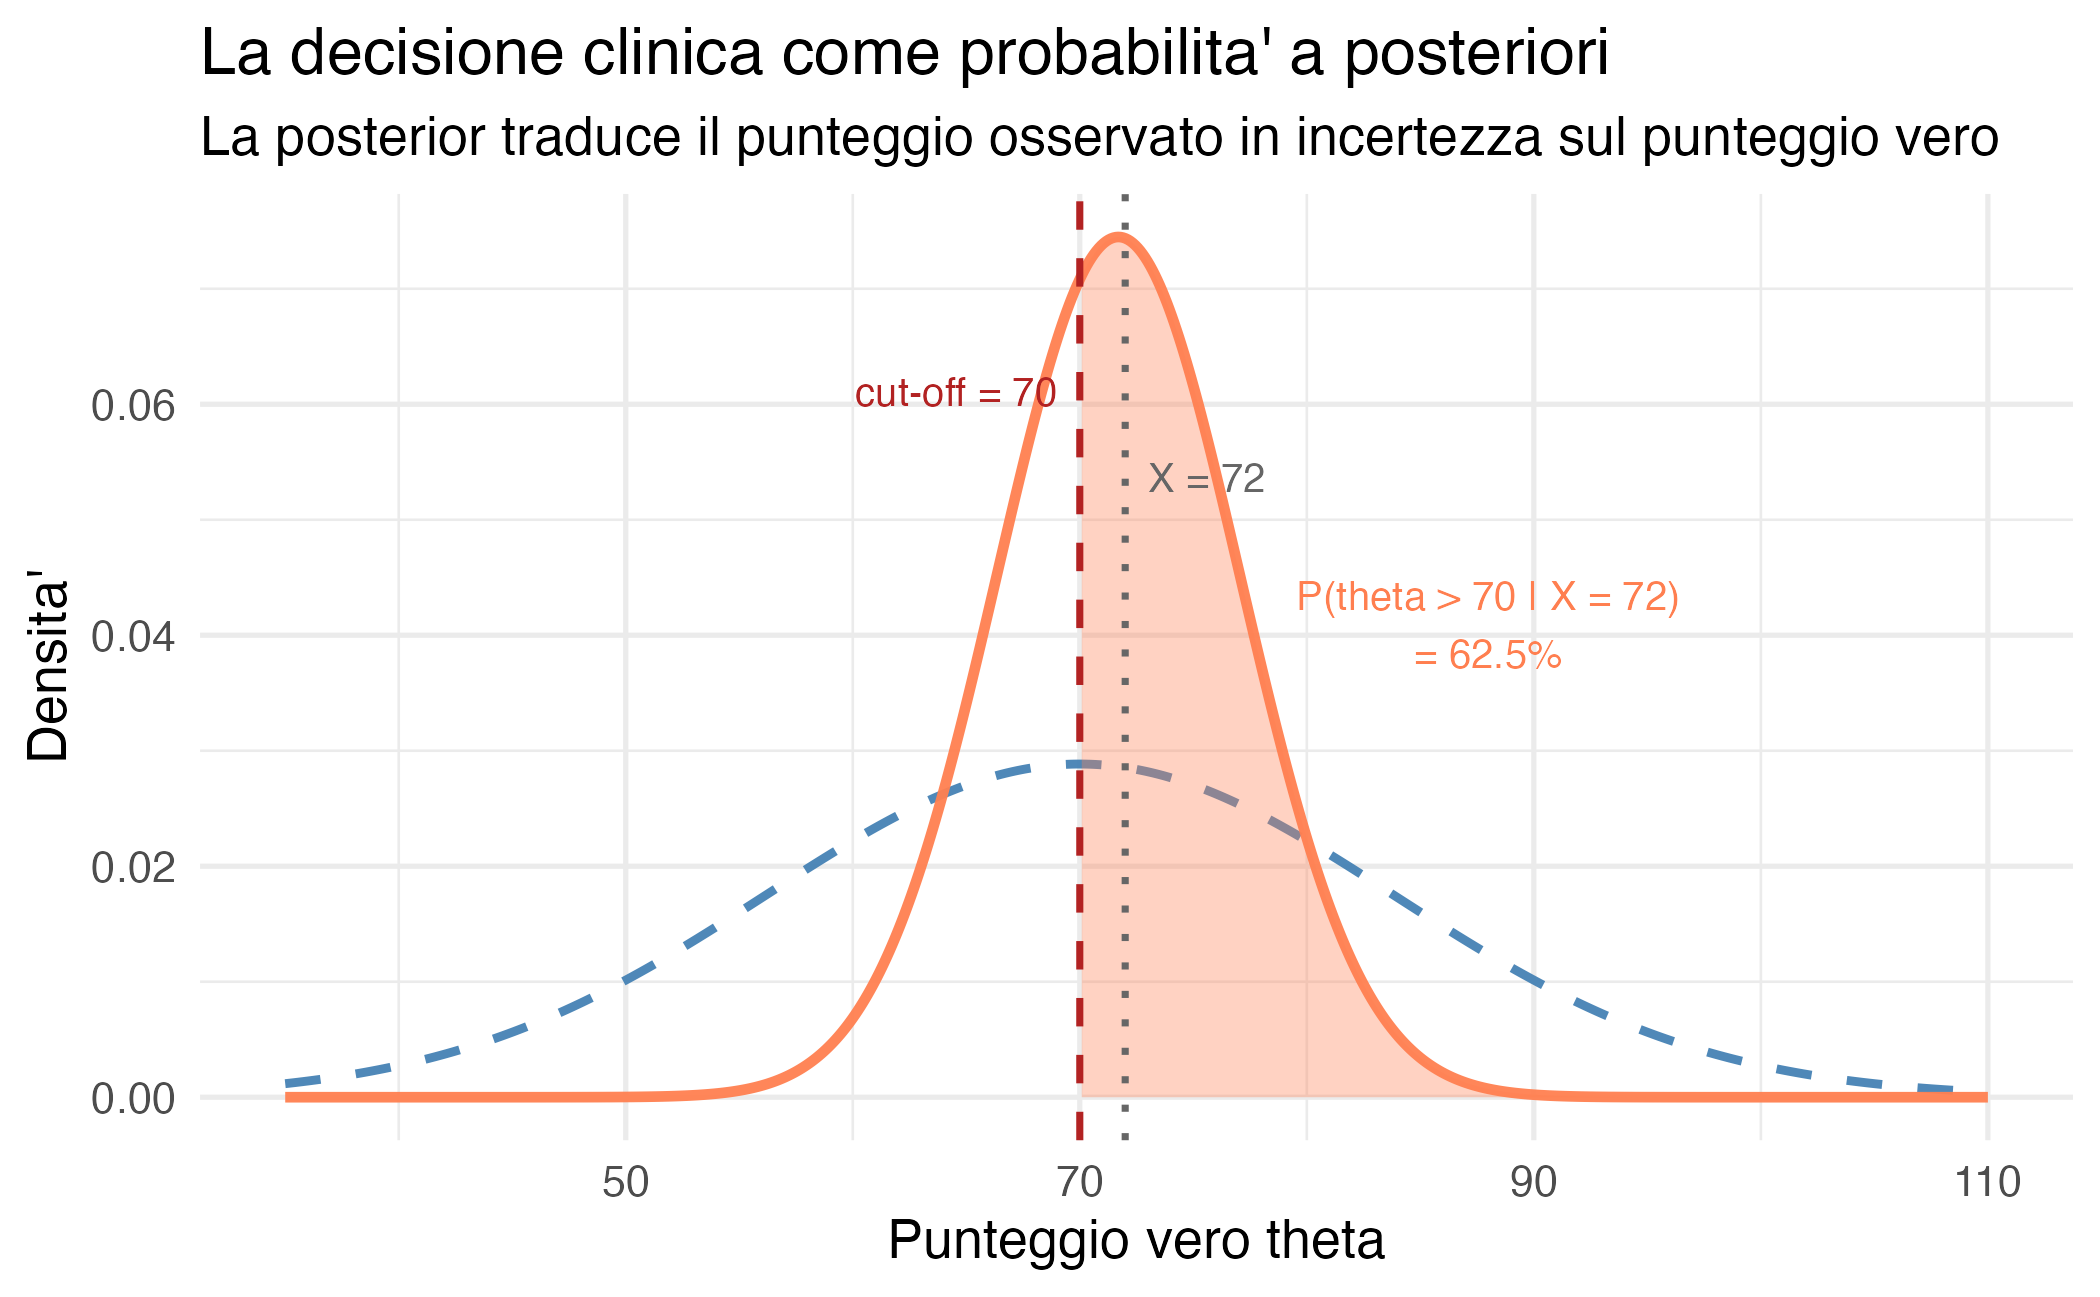
\includegraphics[width=0.85\linewidth,height=\textheight,keepaspectratio]{chapters/bayesian_inference/07_singolo_paziente_files/figure-pdf/unnamed-chunk-8-1.png}

}

\caption{Distribuzione a priori e a posteriori del punteggio vero.
L'area evidenziata rappresenta la probabilità che il punteggio vero
superi il cut-off clinico.}

\end{figure}%

L'intervallo di credibilità al 95\% ha un'interpretazione diretta: dati
il modello, i parametri normativi e il punteggio osservato, c'è il 95\%
di probabilità che il punteggio vero del paziente ricada in
quell'intervallo. Questa affermazione è legittima nel paradigma
bayesiano, in quanto la probabilità viene utilizzata per descrivere
l'incertezza epistemica su \(\theta\).

\section{Posterior e predittiva: due domande
diverse}\label{sec-posterior-predittiva}

La posterior sul punteggio vero risponde alla domanda:

\begin{quote}
Qual è il livello latente del paziente nel costrutto misurato?
\end{quote}

Tuttavia, il clinico potrebbe avere un'altra domanda:

\begin{quote}
Se ripetessimo il test, quale nuovo punteggio osservato potremmo
ottenere?
\end{quote}

Questa seconda domanda riguarda la \textbf{distribuzione predittiva a
posteriori}. Per il modello Normale-Normale:

\[
\tilde{X} \mid X \sim \mathcal{N}\left(\mu_{\text{post}},\; \sigma^2_{\text{post}} + \sigma^2_e\right).
\]

La varianza predittiva è maggiore della varianza a posteriori perché
include due fonti di incertezza:

\begin{enumerate}
\def\labelenumi{\arabic{enumi}.}
\tightlist
\item
  l'incertezza residua sul punteggio vero \(\theta\);
\item
  il nuovo errore di misura che si avrebbe in una seconda
  somministrazione.
\end{enumerate}

\begin{Shaded}
\begin{Highlighting}[]
\NormalTok{sigma\_pred }\OtherTok{\textless{}{-}} \FunctionTok{sqrt}\NormalTok{(sigma\_post2 }\SpecialCharTok{+}\NormalTok{ sigma\_e2)}
\NormalTok{IC\_pred }\OtherTok{\textless{}{-}} \FunctionTok{qnorm}\NormalTok{(}\FunctionTok{c}\NormalTok{(.}\DecValTok{025}\NormalTok{, .}\DecValTok{975}\NormalTok{), }\AttributeTok{mean =}\NormalTok{ mu\_post, }\AttributeTok{sd =}\NormalTok{ sigma\_pred)}
\NormalTok{prob\_pred\_sopra }\OtherTok{\textless{}{-}} \DecValTok{1} \SpecialCharTok{{-}} \FunctionTok{pnorm}\NormalTok{(cut\_off, }\AttributeTok{mean =}\NormalTok{ mu\_post, }\AttributeTok{sd =}\NormalTok{ sigma\_pred)}

\FunctionTok{cat}\NormalTok{(}\StringTok{"DS predittiva:"}\NormalTok{, }\FunctionTok{round}\NormalTok{(sigma\_pred, }\DecValTok{2}\NormalTok{), }\StringTok{"}\SpecialCharTok{\textbackslash{}n}\StringTok{"}\NormalTok{)}
\CommentTok{\#\textgreater{} DS predittiva: 7.9}
\FunctionTok{cat}\NormalTok{(}\StringTok{"Intervallo predittivo al 95\%: ["}\NormalTok{,}
    \FunctionTok{round}\NormalTok{(IC\_pred[}\DecValTok{1}\NormalTok{], }\DecValTok{1}\NormalTok{), }\StringTok{", "}\NormalTok{, }\FunctionTok{round}\NormalTok{(IC\_pred[}\DecValTok{2}\NormalTok{], }\DecValTok{1}\NormalTok{), }\StringTok{"]}\SpecialCharTok{\textbackslash{}n}\StringTok{"}\NormalTok{, }\AttributeTok{sep =} \StringTok{""}\NormalTok{)}
\CommentTok{\#\textgreater{} Intervallo predittivo al 95\%: [56.2, 87.2]}
\FunctionTok{cat}\NormalTok{(}\StringTok{"P(X\_nuovo \textgreater{} 70 | X = 72):"}\NormalTok{,}
    \FunctionTok{round}\NormalTok{(prob\_pred\_sopra }\SpecialCharTok{*} \DecValTok{100}\NormalTok{, }\DecValTok{1}\NormalTok{), }\StringTok{"\%}\SpecialCharTok{\textbackslash{}n}\StringTok{"}\NormalTok{)}
\CommentTok{\#\textgreater{} P(X\_nuovo \textgreater{} 70 | X = 72): 58.5 \%}
\end{Highlighting}
\end{Shaded}

\begin{figure}[H]

{\centering 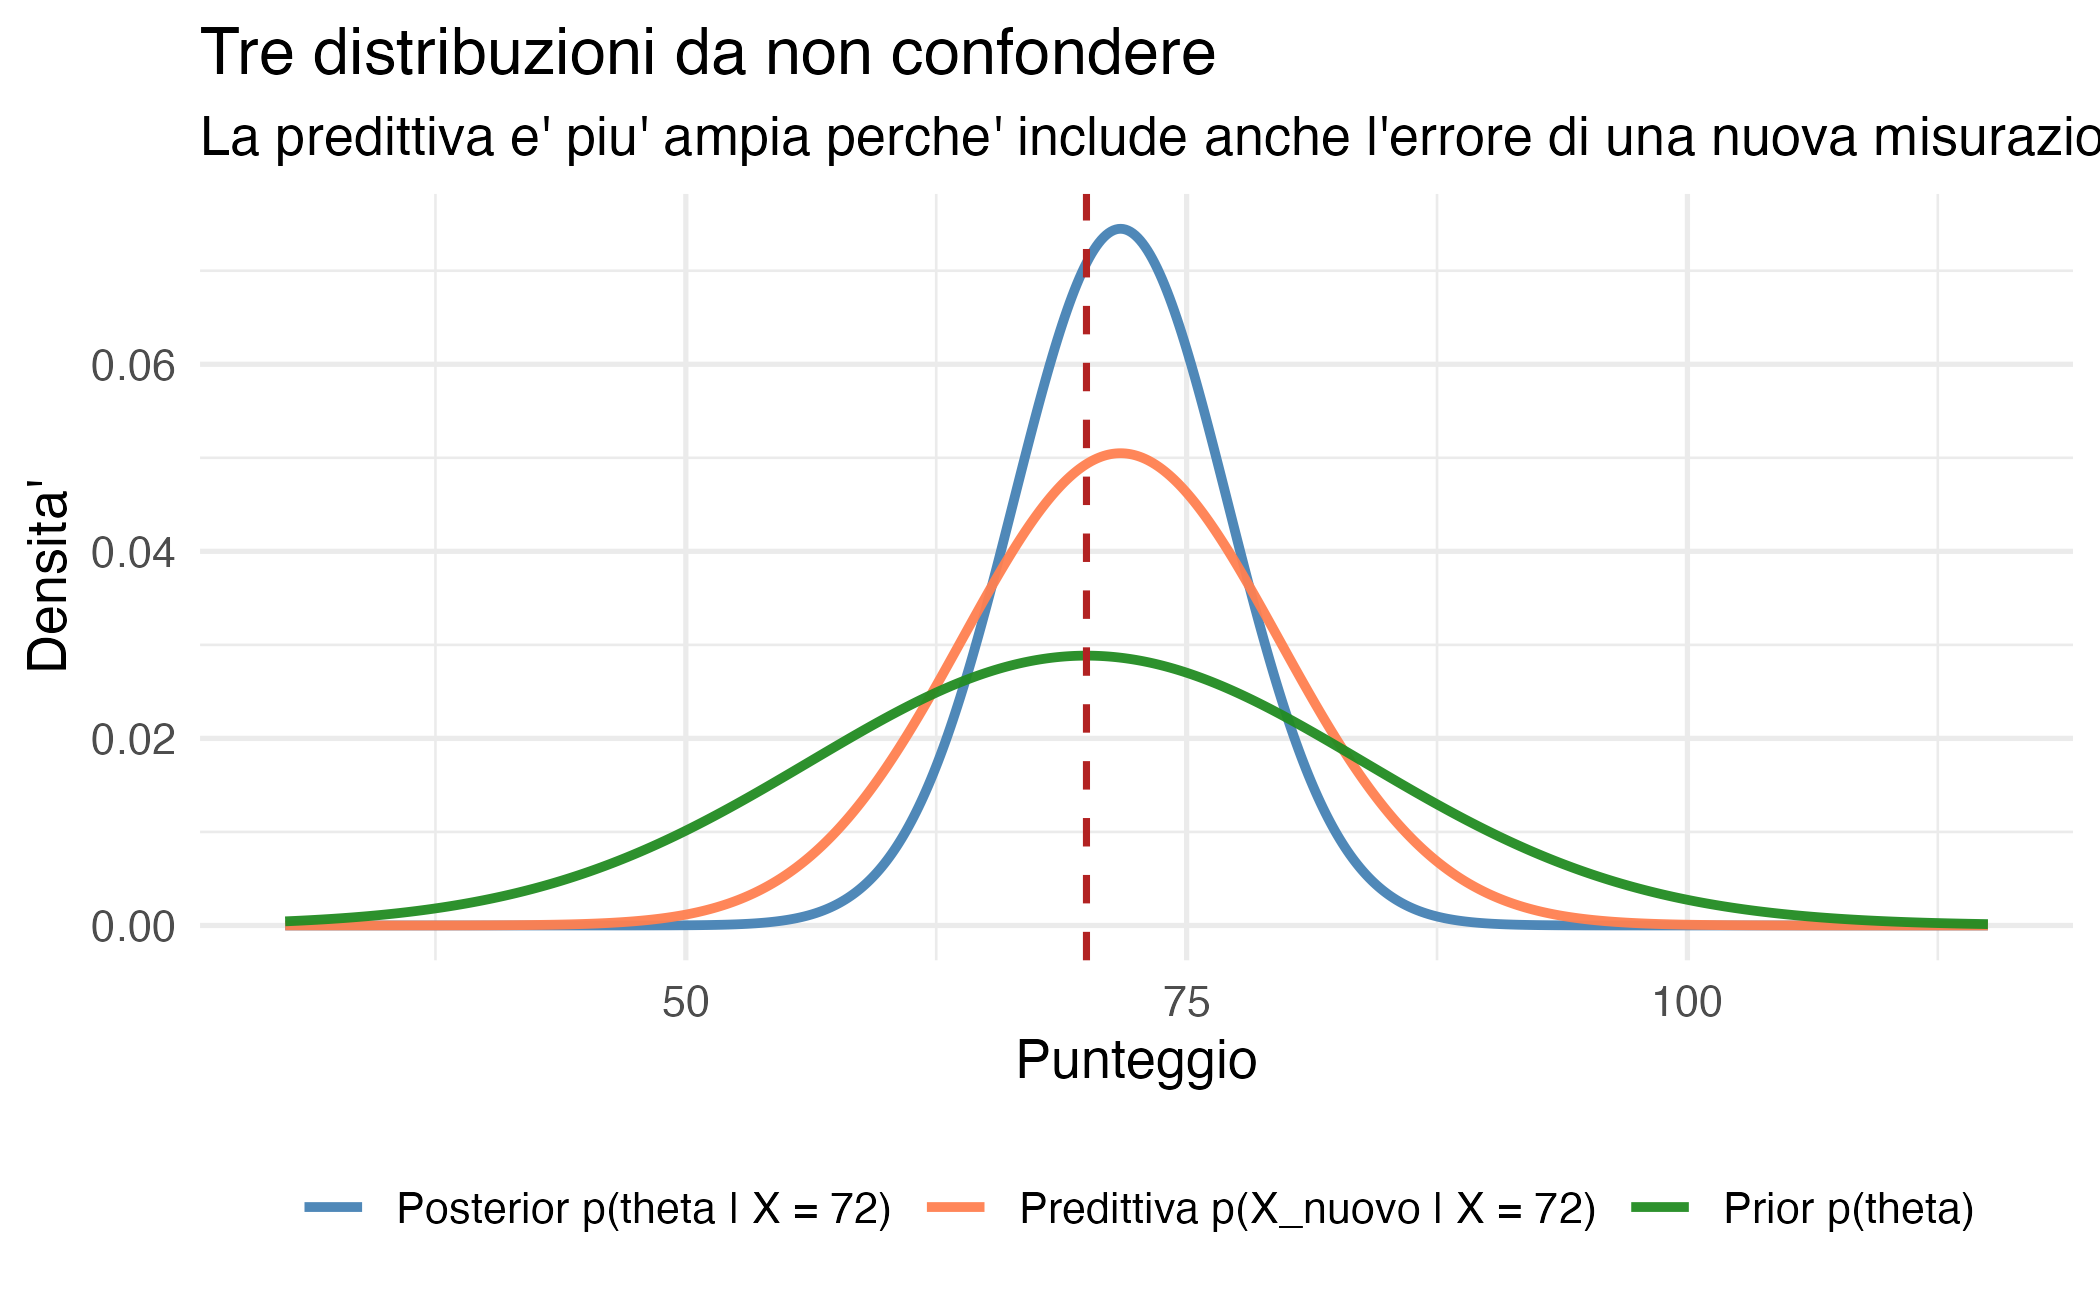
\includegraphics[width=0.85\linewidth,height=\textheight,keepaspectratio]{chapters/bayesian_inference/07_singolo_paziente_files/figure-pdf/unnamed-chunk-10-1.png}

}

\caption{Confronto tra distribuzione a priori, posterior del punteggio
vero e distribuzione predittiva per una nuova somministrazione.}

\end{figure}%

\begin{tcolorbox}[enhanced jigsaw, arc=.35mm, bottomrule=.15mm, bottomtitle=1mm, breakable, colback=white, colbacktitle=quarto-callout-important-color!10!white, colframe=quarto-callout-important-color-frame, coltitle=black, left=2mm, leftrule=.75mm, opacityback=0, opacitybacktitle=0.6, rightrule=.15mm, title={Quale distribuzione usare per la decisione clinica?}, titlerule=0mm, toprule=.15mm, toptitle=1mm]

Per stabilire se il paziente si trovi verosimilmente sopra la soglia del
costrutto misurato, la distribuzione rilevante è la \textbf{posterior
del punteggio vero} \(p(\theta \mid X)\).

La distribuzione predittiva \(p(\tilde{X} \mid X)\) è invece utile per
pianificare una rivalutazione o per capire quale variabilità potremmo
osservare se il test venisse ripetuto. Non risponde alla stessa domanda
della posterior: descrive un futuro punteggio osservato, non il
punteggio vero del paziente.

\end{tcolorbox}

\section{Dalla probabilità alla decisione
clinica}\label{sec-decisione-clinica}

Il risultato bayesiano non produce automaticamente una diagnosi. Produce
una quantità interpretabile:

\[
P(\theta > 70 \mid X = 72) \approx 0.62.
\]

Tale probabilità deve essere integrata con il contesto clinico:
colloquio, anamnesi, funzionamento quotidiano, osservazioni
comportamentali, altri strumenti diagnostici e costi degli errori
decisionali.

Una lettura ragionevole del nostro esempio è la seguente:

\begin{tcolorbox}[enhanced jigsaw, arc=.35mm, bottomrule=.15mm, bottomtitle=1mm, breakable, colback=white, colbacktitle=quarto-callout-note-color!10!white, colframe=quarto-callout-note-color-frame, coltitle=black, left=2mm, leftrule=.75mm, opacityback=0, opacitybacktitle=0.6, rightrule=.15mm, title={Una formulazione clinica possibile}, titlerule=0mm, toprule=.15mm, toptitle=1mm]

Dato il punteggio osservato di 72, la probabilità che il punteggio vero
del paziente superi la soglia clinica di 70 è di circa 62\%. Il
risultato suggerisce un'attenzione clinica, ma non è abbastanza forte da
poter sostenere una conclusione diagnostica basata esclusivamente su
questo test. È opportuno integrare il dato psicometrico con altre
informazioni cliniche e, se necessario, pianificare una rivalutazione.

\end{tcolorbox}

La forza dell'approccio bayesiano non è dunque quella di rendere la
decisione automatica. È quella di rendere esplicita l'incertezza che una
decisione automatica nasconderebbe.

\begin{tcolorbox}[enhanced jigsaw, arc=.35mm, bottomrule=.15mm, bottomtitle=1mm, breakable, colback=white, colbacktitle=quarto-callout-tip-color!10!white, colframe=quarto-callout-tip-color-frame, coltitle=black, left=2mm, leftrule=.75mm, opacityback=0, opacitybacktitle=0.6, rightrule=.15mm, title=\textcolor{quarto-callout-tip-color}{\faLightbulb}\hspace{0.5em}{Decisioni e funzioni di perdita}, titlerule=0mm, toprule=.15mm, toptitle=1mm]

In un'applicazione più completa, la decisione potrebbe essere formulata
in termini di costi e benefici. Un falso negativo può avere conseguenze
diverse rispetto a un falso positivo. In alcune situazioni cliniche, una
probabilità del 62\% potrebbe giustificare un approfondimento, mentre in
altre potrebbe non essere sufficiente per avviare un intervento. La
probabilità a posteriori non sostituisce il giudizio clinico, ma lo
rende più trasparente.

\end{tcolorbox}

\section{Perché l'attendibilità cambia la
conclusione}\label{sec-sensibilita-attendibilita}

La probabilità che il paziente superi la soglia dipende non solo dal
punteggio osservato, ma anche dall'attendibilità dello strumento
utilizzato. A parità di \(X = 72\), un test molto attendibile produce
una posterior più concentrata vicino al punteggio osservato, mentre un
test poco attendibile produce una posterior più incerta e più vicina
alla media normativa.

Il codice seguente mostra come varia \(P(\theta > 70 \mid X = 72)\) al
variare di \(\rho\).

\begin{Shaded}
\begin{Highlighting}[]
\NormalTok{prob\_true\_above }\OtherTok{\textless{}{-}} \ControlFlowTok{function}\NormalTok{(rho\_value, x\_obs, threshold, mu, sigma\_X) \{}
\NormalTok{  sigma\_theta\_value }\OtherTok{\textless{}{-}} \FunctionTok{sqrt}\NormalTok{(rho\_value) }\SpecialCharTok{*}\NormalTok{ sigma\_X}
\NormalTok{  sigma\_e\_value     }\OtherTok{\textless{}{-}} \FunctionTok{sqrt}\NormalTok{(}\DecValTok{1} \SpecialCharTok{{-}}\NormalTok{ rho\_value) }\SpecialCharTok{*}\NormalTok{ sigma\_X}

\NormalTok{  sigma\_post2\_value }\OtherTok{\textless{}{-}} \DecValTok{1} \SpecialCharTok{/}\NormalTok{ (}\DecValTok{1} \SpecialCharTok{/}\NormalTok{ sigma\_theta\_value}\SpecialCharTok{\^{}}\DecValTok{2} \SpecialCharTok{+}
                              \DecValTok{1} \SpecialCharTok{/}\NormalTok{ sigma\_e\_value}\SpecialCharTok{\^{}}\DecValTok{2}\NormalTok{)}
\NormalTok{  mu\_post\_value }\OtherTok{\textless{}{-}}\NormalTok{ sigma\_post2\_value }\SpecialCharTok{*}
\NormalTok{    (mu }\SpecialCharTok{/}\NormalTok{ sigma\_theta\_value}\SpecialCharTok{\^{}}\DecValTok{2} \SpecialCharTok{+}\NormalTok{ x\_obs }\SpecialCharTok{/}\NormalTok{ sigma\_e\_value}\SpecialCharTok{\^{}}\DecValTok{2}\NormalTok{)}

  \DecValTok{1} \SpecialCharTok{{-}} \FunctionTok{pnorm}\NormalTok{(threshold, }\AttributeTok{mean =}\NormalTok{ mu\_post\_value, }\AttributeTok{sd =} \FunctionTok{sqrt}\NormalTok{(sigma\_post2\_value))}
\NormalTok{\}}

\NormalTok{rho\_seq }\OtherTok{\textless{}{-}} \FunctionTok{seq}\NormalTok{(}\FloatTok{0.50}\NormalTok{, }\FloatTok{0.99}\NormalTok{, }\AttributeTok{by =} \FloatTok{0.01}\NormalTok{)}
\NormalTok{probs }\OtherTok{\textless{}{-}} \FunctionTok{sapply}\NormalTok{(}
\NormalTok{  rho\_seq,}
\NormalTok{  prob\_true\_above,}
  \AttributeTok{x\_obs =}\NormalTok{ X\_obs,}
  \AttributeTok{threshold =}\NormalTok{ cut\_off,}
  \AttributeTok{mu =}\NormalTok{ mu\_pop,}
  \AttributeTok{sigma\_X =}\NormalTok{ sigma\_X}
\NormalTok{)}

\NormalTok{df\_sens }\OtherTok{\textless{}{-}} \FunctionTok{data.frame}\NormalTok{(}\AttributeTok{rho =}\NormalTok{ rho\_seq, }\AttributeTok{prob =}\NormalTok{ probs)}
\end{Highlighting}
\end{Shaded}

\begin{figure}[H]

{\centering 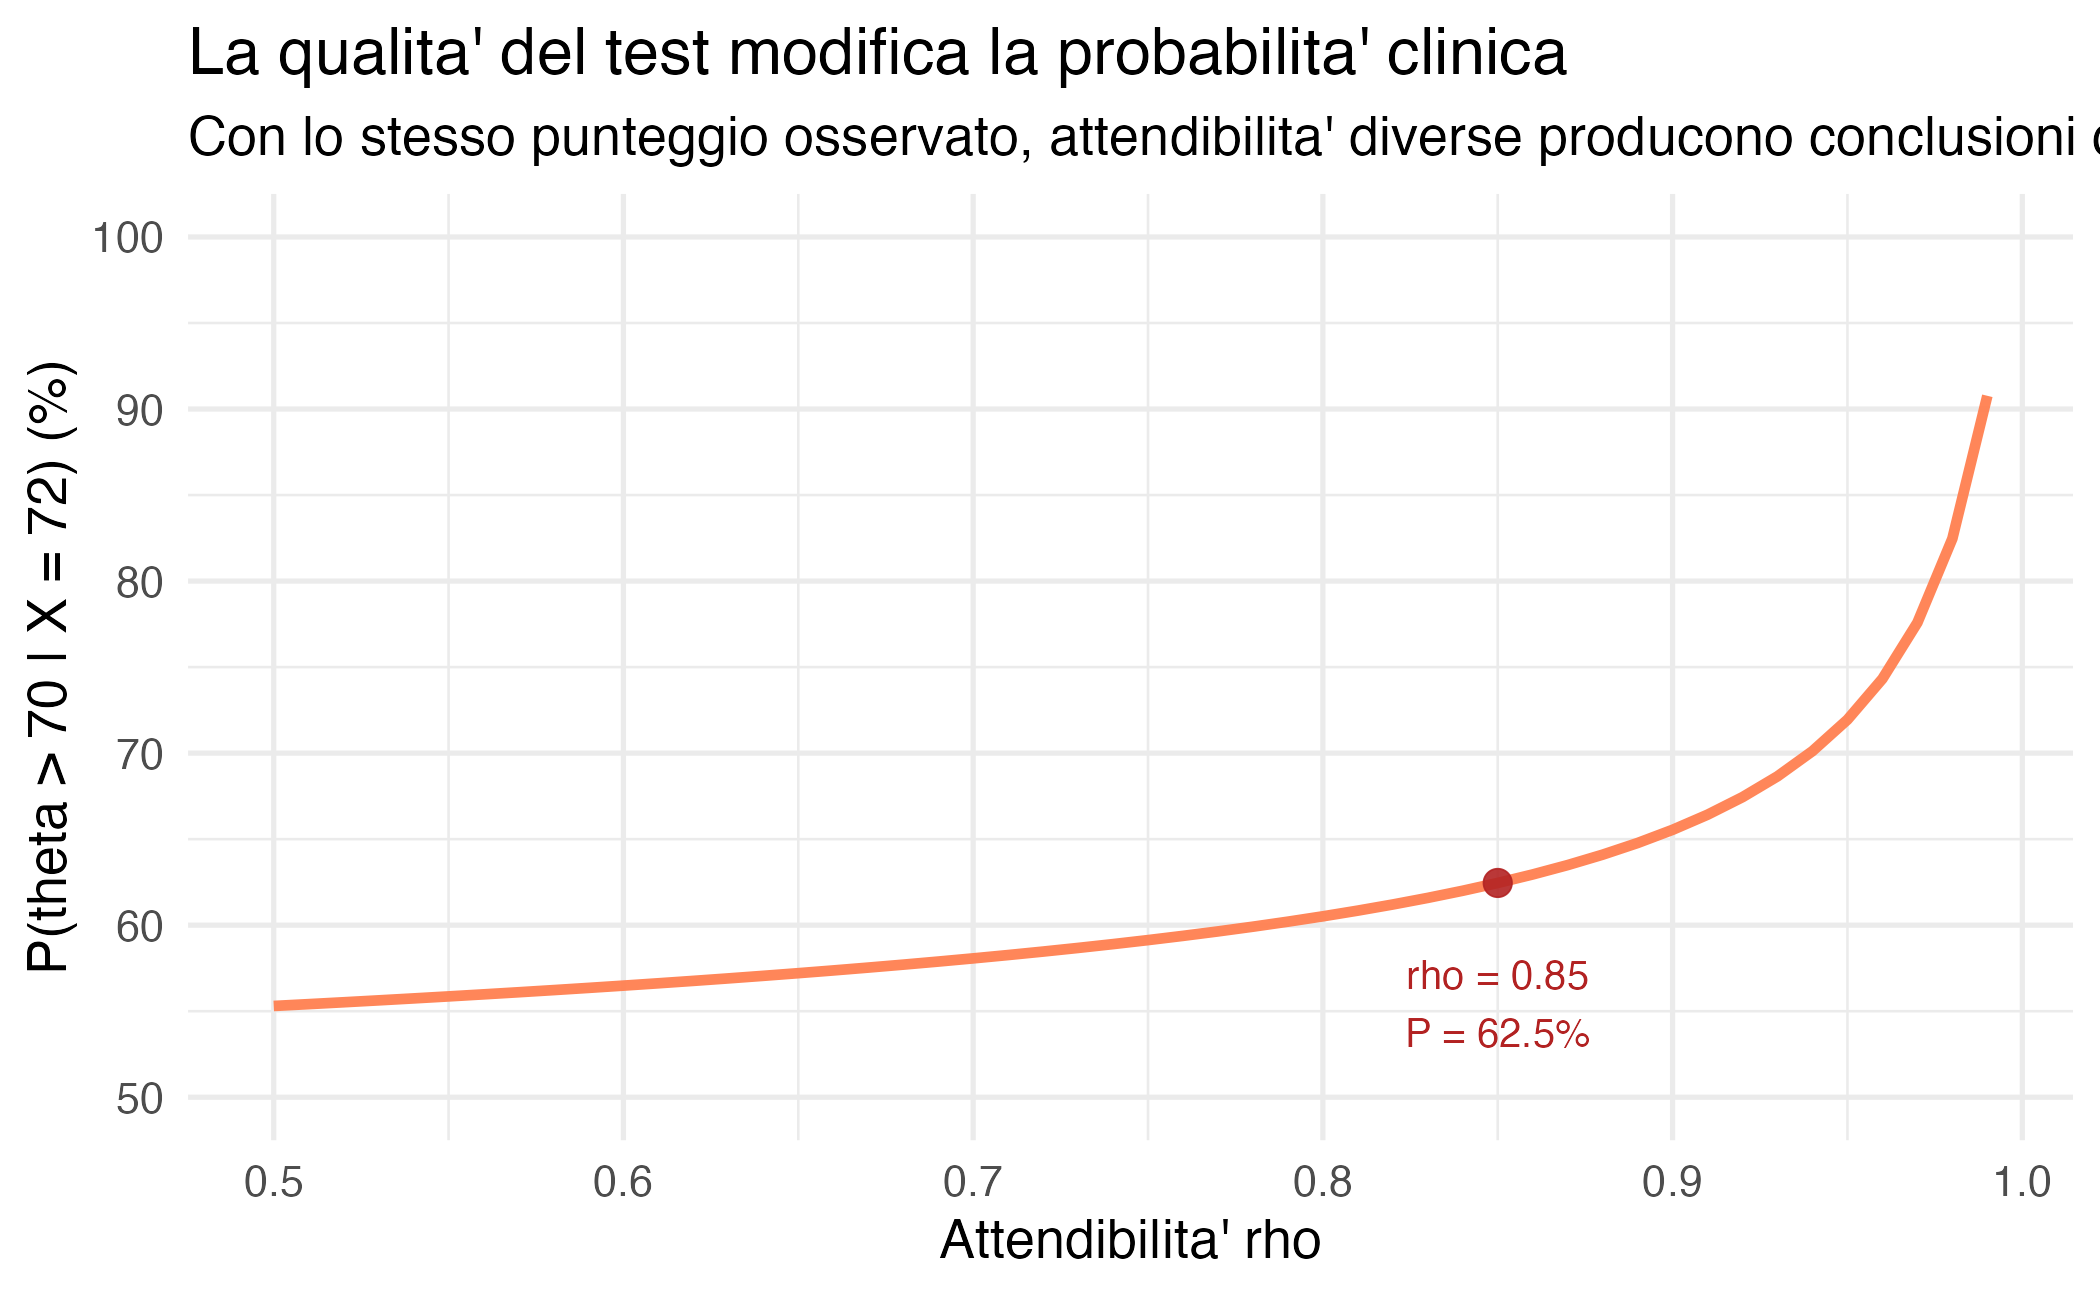
\includegraphics[width=0.85\linewidth,height=\textheight,keepaspectratio]{chapters/bayesian_inference/07_singolo_paziente_files/figure-pdf/unnamed-chunk-12-1.png}

}

\caption{Probabilità che il punteggio vero superi il cut-off al variare
dell'attendibilità del test.}

\end{figure}%

Il grafico rende evidente un aspetto spesso sottovalutato:
l'attendibilità non è un dettaglio tecnico da consultare solo nel
manuale del test. Si tratta di un'informazione clinicamente rilevante.
Due test con lo stesso cut-off e lo stesso punteggio osservato possono
condurre a conclusioni diverse se hanno un'attendibilità differente.

\section{Sintesi operativa}\label{sec-sintesi-operativa}

Il percorso seguito nel capitolo può essere riassunto in quattro
passaggi.

\begin{enumerate}
\def\labelenumi{\arabic{enumi}.}
\tightlist
\item
  \textbf{Non leggere il cut-off in modo meccanico.} Un punteggio
  osservato appena sopra soglia non equivale a una certezza clinica.
\item
  \textbf{Correggere il punteggio osservato per l'errore di misura.} La
  formula di Kelley mostra lo shrinkage verso la media normativa.
\item
  \textbf{Riformulare la stima come posterior bayesiana.} Nel modello
  Normale-Normale, Kelley coincide con la media posterior, ma la
  posterior offre un'informazione più ricca.
\item
  \textbf{Calcolare la probabilità clinica di interesse.} La domanda
  rilevante diventa \(P(\theta > c \mid X)\), non semplicemente
  \(X > c\).
\end{enumerate}

{\def\LTcaptype{none} % do not increment counter
\begin{longtable}[]{@{}
  >{\raggedright\arraybackslash}p{(\linewidth - 4\tabcolsep) * \real{0.3333}}
  >{\raggedright\arraybackslash}p{(\linewidth - 4\tabcolsep) * \real{0.3333}}
  >{\raggedright\arraybackslash}p{(\linewidth - 4\tabcolsep) * \real{0.3333}}@{}}
\toprule\noalign{}
\begin{minipage}[b]{\linewidth}\raggedright
Domanda
\end{minipage} & \begin{minipage}[b]{\linewidth}\raggedright
Quantità rilevante
\end{minipage} & \begin{minipage}[b]{\linewidth}\raggedright
Interpretazione
\end{minipage} \\
\midrule\noalign{}
\endhead
\bottomrule\noalign{}
\endlastfoot
Qual è la miglior stima del punteggio vero? & \(\mu_{\text{post}}\) /
Kelley & Stima corretta verso la media \\
Quanto resta incerta la stima? & Intervallo di credibilità & Incertezza
sul punteggio vero \\
Il paziente è probabilmente sopra soglia? & \(P(\theta > c \mid X)\) &
Probabilità clinica diretta \\
Cosa potrei osservare a una nuova somministrazione? &
\(p(\tilde{X} \mid X)\) & Variabilità attesa del nuovo punteggio
osservato \\
Quanto conta la qualità del test? & Analisi al variare di \(\rho\) &
Sensibilità all'attendibilità \\
\end{longtable}
}

\section*{Riflessioni conclusive}\label{riflessioni-conclusive-11}

\markright{Riflessioni conclusive}

Il capitolo parte da una situazione apparentemente semplice: un paziente
ottiene 72, il cut-off è 70. Una lettura dicotomica trasformerebbe
questo confronto in una conclusione automatica. L'inferenza bayesiana
mostra perché questa conclusione è troppo semplicistica.

Il punto centrale è che ogni punteggio osservato è una misura
imperfetta. Il numero registrato dal test non corrisponde al costrutto
psicologico di interesse, ma ne rappresenta una manifestazione
osservabile, soggetta all'errore di misurazione. La formula di Kelley
(\citeproc{ref-Kelley1923}{1923}) offre già una risposta elegante a
questo problema: corregge il punteggio osservato verso la media
normativa in funzione dell'attendibilità del test.

La prospettiva bayesiana non cancella questa tradizione psicometrica. Al
contrario, la rende più esplicita. Nel modello Normale-Normale, la stima
di Kelley emerge come media della distribuzione a posteriori del
punteggio vero. Tuttavia, il vantaggio decisivo è che la distribuzione a
posteriori permette di rispondere alla domanda clinica nella forma in
cui essa si presenta realmente: qual è la probabilità che questo
paziente superi la soglia?

Nel nostro esempio, questa probabilità è di circa il 62\%. Non si tratta
di una certezza, ma neanche di un'informazione vaga. Si tratta di una
quantificazione trasparente dell'incertezza. Ciò indica che il risultato
merita attenzione, ma che il test non dovrebbe essere l'unica base per
la decisione clinica.

Questo è il contributo più importante dell'approccio bayesiano alla
psicometria applicata: non sostituire il giudizio clinico con un
algoritmo, ma fornire al giudizio clinico una rappresentazione più
onesta dell'incertezza. Il passaggio dalle medie di gruppo al singolo
paziente richiede proprio questo: non eliminare l'incertezza, ma
renderla visibile, quantificabile e comunicabile.

\begin{tcolorbox}[enhanced jigsaw, arc=.35mm, bottomrule=.15mm, bottomtitle=1mm, breakable, colback=white, colbacktitle=quarto-callout-note-color!10!white, colframe=quarto-callout-note-color-frame, coltitle=black, left=2mm, leftrule=.75mm, opacityback=0, opacitybacktitle=0.6, rightrule=.15mm, title=\textcolor{quarto-callout-note-color}{\faInfo}\hspace{0.5em}{Informazioni sull'ambiente di sviluppo}, titlerule=0mm, toprule=.15mm, toptitle=1mm]

\begin{Shaded}
\begin{Highlighting}[]
\FunctionTok{sessionInfo}\NormalTok{()}
\CommentTok{\#\textgreater{} R version 4.6.1 (2026{-}06{-}24)}
\CommentTok{\#\textgreater{} Platform: aarch64{-}apple{-}darwin23}
\CommentTok{\#\textgreater{} Running under: macOS Tahoe 26.5.2}
\CommentTok{\#\textgreater{} }
\CommentTok{\#\textgreater{} Matrix products: default}
\CommentTok{\#\textgreater{} BLAS:   /Library/Frameworks/R.framework/Versions/4.6/Resources/lib/libRblas.0.dylib }
\CommentTok{\#\textgreater{} LAPACK: /Library/Frameworks/R.framework/Versions/4.6/Resources/lib/libRlapack.dylib;  LAPACK version 3.12.1}
\CommentTok{\#\textgreater{} }
\CommentTok{\#\textgreater{} locale:}
\CommentTok{\#\textgreater{} [1] C.UTF{-}8/UTF{-}8/C.UTF{-}8/C/C.UTF{-}8/C.UTF{-}8}
\CommentTok{\#\textgreater{} }
\CommentTok{\#\textgreater{} time zone: Europe/Zagreb}
\CommentTok{\#\textgreater{} tzcode source: internal}
\CommentTok{\#\textgreater{} }
\CommentTok{\#\textgreater{} attached base packages:}
\CommentTok{\#\textgreater{} [1] stats     graphics  grDevices utils     datasets  methods   base     }
\CommentTok{\#\textgreater{} }
\CommentTok{\#\textgreater{} other attached packages:}
\CommentTok{\#\textgreater{}  [1] ragg\_1.5.2            tinytable\_0.17.0      withr\_3.0.3          }
\CommentTok{\#\textgreater{}  [4] systemfonts\_1.3.2     patchwork\_1.3.2       ggdist\_3.3.3         }
\CommentTok{\#\textgreater{}  [7] tidybayes\_3.0.7       bayesplot\_1.15.0      ggplot2\_4.0.3        }
\CommentTok{\#\textgreater{} [10] reliabilitydiag\_0.2.1 priorsense\_1.2.0      posterior\_1.7.0      }
\CommentTok{\#\textgreater{} [13] loo\_2.10.0            rstan\_2.32.7          StanHeaders\_2.32.10  }
\CommentTok{\#\textgreater{} [16] brms\_2.23.0           Rcpp\_1.1.2            sessioninfo\_1.2.4    }
\CommentTok{\#\textgreater{} [19] conflicted\_1.2.0      janitor\_2.2.1         matrixStats\_1.5.0    }
\CommentTok{\#\textgreater{} [22] modelr\_0.1.11         tibble\_3.3.1          dplyr\_1.2.1          }
\CommentTok{\#\textgreater{} [25] tidyr\_1.3.2           rio\_1.3.0             here\_1.0.2           }
\CommentTok{\#\textgreater{} }
\CommentTok{\#\textgreater{} loaded via a namespace (and not attached):}
\CommentTok{\#\textgreater{}  [1] svUnit\_1.0.8          tidyselect\_1.2.1      farver\_2.1.2         }
\CommentTok{\#\textgreater{}  [4] S7\_0.2.2              fastmap\_1.2.0         tensorA\_0.36.2.1     }
\CommentTok{\#\textgreater{}  [7] digest\_0.6.39         timechange\_0.4.0      estimability\_2.0.0   }
\CommentTok{\#\textgreater{} [10] lifecycle\_1.0.5       magrittr\_2.0.5        compiler\_4.6.1       }
\CommentTok{\#\textgreater{} [13] rlang\_1.3.0           tools\_4.6.1           yaml\_2.3.12          }
\CommentTok{\#\textgreater{} [16] knitr\_1.51            labeling\_0.4.3        bridgesampling\_1.2{-}1 }
\CommentTok{\#\textgreater{} [19] pkgbuild\_1.4.8        curl\_7.1.0            RColorBrewer\_1.1{-}3   }
\CommentTok{\#\textgreater{} [22] abind\_1.4{-}8           purrr\_1.2.2           grid\_4.6.1           }
\CommentTok{\#\textgreater{} [25] stats4\_4.6.1          xtable\_1.8{-}8          inline\_0.3.21        }
\CommentTok{\#\textgreater{} [28] emmeans\_2.0.4         scales\_1.4.0          cli\_3.6.6            }
\CommentTok{\#\textgreater{} [31] mvtnorm\_1.4{-}2         rmarkdown\_2.31        generics\_0.1.4       }
\CommentTok{\#\textgreater{} [34] otel\_0.2.0            RcppParallel\_5.1.11{-}2 cachem\_1.1.0         }
\CommentTok{\#\textgreater{} [37] stringr\_1.6.0         parallel\_4.6.1        vctrs\_0.7.3          }
\CommentTok{\#\textgreater{} [40] V8\_8.2.0              Matrix\_1.7{-}5          jsonlite\_2.0.0       }
\CommentTok{\#\textgreater{} [43] arrayhelpers\_1.1{-}1    glue\_1.8.1            codetools\_0.2{-}20     }
\CommentTok{\#\textgreater{} [46] distributional\_0.8.1  lubridate\_1.9.5       stringi\_1.8.7        }
\CommentTok{\#\textgreater{} [49] gtable\_0.3.6          QuickJSR\_1.10.0       pillar\_1.11.1        }
\CommentTok{\#\textgreater{} [52] htmltools\_0.5.9       Brobdingnag\_1.2{-}9     R6\_2.6.1             }
\CommentTok{\#\textgreater{} [55] textshaping\_1.0.5     rprojroot\_2.1.1       evaluate\_1.0.5       }
\CommentTok{\#\textgreater{} [58] lattice\_0.22{-}9        backports\_1.5.1       memoise\_2.0.1        }
\CommentTok{\#\textgreater{} [61] broom\_1.0.13          snakecase\_0.11.1      rstantools\_2.6.0     }
\CommentTok{\#\textgreater{} [64] coda\_0.19{-}4.1         gridExtra\_2.3.1       nlme\_3.1{-}170         }
\CommentTok{\#\textgreater{} [67] checkmate\_2.3.4       xfun\_0.60             pkgconfig\_2.0.3}
\end{Highlighting}
\end{Shaded}

\end{tcolorbox}

\section*{Bibliografia}\label{bibliografia-13}

\markright{Bibliografia}

\chapter*{Riflessioni conclusive della
sezione}\label{riflessioni-conclusive-della-sezione}

\markboth{Riflessioni conclusive della sezione}{Riflessioni conclusive
della sezione}

In questa sezione abbiamo costruito l'inferenza bayesiana a partire dal
suo meccanismo essenziale. Grazie al metodo su griglia, abbiamo reso
visibile l'operazione fondamentale di combinazione della distribuzione a
priori e della verosimiglianza, e di normalizzazione del risultato, e
con le famiglie coniugate abbiamo visto come, in alcuni casi, la stessa
operazione si riduca a poche modifiche dei parametri della prior.
Abbiamo poi imparato a leggere la distribuzione a posteriori attraverso
stime puntuali, intervalli di credibilità e probabilità di ipotesi, a
valutare il ruolo della distribuzione a priori e il suo equilibrio con i
dati e a controllarne le implicazioni prima e dopo l'osservazione
mediante le distribuzioni predittive a priori e a posteriori. Infine,
abbiamo applicato questi strumenti a un problema concreto della
psicologia, mostrando come l'inferenza bayesiana traduca un punteggio
osservato in una probabilità clinicamente interpretabile.

Il filo conduttore di questi capitoli è un modo diverso di affrontare
l'incertezza. Per la ricerca e la pratica psicologica emergono tre
lezioni:

\begin{enumerate}
\def\labelenumi{\arabic{enumi}.}
\tightlist
\item
  i dati non forniscono certezze, ma affinano gradualmente le ipotesi;
\item
  ogni studio è un contributo a un processo cumulativo, non un verdetto
  finale;
\item
  la forza dell'approccio bayesiano sta nel trasformare l'incertezza da
  problema nascosto a risorsa esplicita.
\end{enumerate}

Finora, però, abbiamo potuto ottenere la distribuzione a posteriori in
forma esatta solo per via analitica, con i modelli coniugati o per
enumerazione, con il metodo a griglia. Nei modelli realistici, però,
questa condizione viene meno: con l'aumentare del numero dei parametri,
la distribuzione a posteriori non ha più una forma chiusa e la griglia
diventa impraticabile. La sezione successiva affronta proprio questo
problema, introducendo i metodi di campionamento a catena di Markov
(MCMC) e il linguaggio probabilistico Stan, che permettono di stimare
distribuzioni a posteriori arbitrariamente complesse. Questo passaggio
dai fondamenti concettuali agli strumenti che rendono l'inferenza
bayesiana applicabile ai modelli di cui la psicologia ha realmente
bisogno è fondamentale.

\section*{Bibliografia}\label{bibliografia-14}

\markright{Bibliografia}

\part{Calcolo}

\chapter*{📍 Dove siamo nel percorso}\label{dove-siamo-nel-percorso-3}

\markboth{📍 Dove siamo nel percorso}{📍 Dove siamo nel percorso}

\begin{tcolorbox}[enhanced jigsaw, arc=.35mm, bottomrule=.15mm, breakable, colback=white, colframe=quarto-callout-note-color-frame, left=2mm, leftrule=.75mm, opacityback=0, rightrule=.15mm, toprule=.15mm]

Nella sezione precedente hai visto come funziona l'inferenza bayesiana
con \textbf{metodi esatti} (famiglie coniugate) e \textbf{approssimati}
(metodo su griglia). Questi approcci hanno però un \textbf{campo di
applicazione ristretto}: le famiglie coniugate valgono solo per pochi
modelli, mentre l'approssimazione su griglia diventa computazionalmente
proibitiva già con più di due o tre parametri. Per superare questi
vincoli occorre \textbf{passare a strumenti più scalabili}.

\end{tcolorbox}

\begin{tcolorbox}[enhanced jigsaw, arc=.35mm, bottomrule=.15mm, bottomtitle=1mm, breakable, colback=white, colbacktitle=quarto-callout-tip-color!10!white, colframe=quarto-callout-tip-color-frame, coltitle=black, left=2mm, leftrule=.75mm, opacityback=0, opacitybacktitle=0.6, rightrule=.15mm, title=\textcolor{quarto-callout-tip-color}{\faLightbulb}\hspace{0.5em}{🎯 Cosa faremo in questa sezione}, titlerule=0mm, toprule=.15mm, toptitle=1mm]

In questa sezione acquisirai gli strumenti per costruire e analizzare
modelli bayesiani di complessità arbitraria. Imparerai a:

\begin{itemize}
\tightlist
\item
  \textbf{capire} cosa sono i linguaggi di programmazione probabilistica
  e perché Stan è diventato lo standard di riferimento;
\item
  \textbf{leggere} un modello bayesiano scritto in Stan, riconoscendone
  la struttura a blocchi;
\item
  \textbf{applicare} questi strumenti a due casi tipici della ricerca
  psicologica: l'inferenza su un \emph{odds ratio} e il confronto tra
  due medie;
\item
  \textbf{inquadrare} l'analisi entro un flusso di lavoro bayesiano
  esplicito e iterativo.
\end{itemize}

\end{tcolorbox}

\begin{tcolorbox}[enhanced jigsaw, arc=.35mm, bottomrule=.15mm, bottomtitle=1mm, breakable, colback=white, colbacktitle=quarto-callout-important-color!10!white, colframe=quarto-callout-important-color-frame, coltitle=black, left=2mm, leftrule=.75mm, opacityback=0, opacitybacktitle=0.6, rightrule=.15mm, title=\textcolor{quarto-callout-important-color}{\faExclamation}\hspace{0.5em}{📖 Collegamenti con il manuale}, titlerule=0mm, toprule=.15mm, toptitle=1mm]

Questa sezione estende operativamente due temi del manuale: l'algoritmo
di \textbf{Metropolis-Hastings} come base del campionamento MCMC, e il
\textbf{flusso di lavoro bayesiano}.

\end{tcolorbox}

\begin{tcolorbox}[enhanced jigsaw, arc=.35mm, bottomrule=.15mm, breakable, colback=white, colframe=quarto-callout-warning-color-frame, left=2mm, leftrule=.75mm, opacityback=0, rightrule=.15mm, toprule=.15mm]
\begin{minipage}[t]{5.5mm}
\textcolor{quarto-callout-warning-color}{\faExclamationTriangle}
\end{minipage}%
\begin{minipage}[t]{\textwidth - 5.5mm}

⚠️ \textbf{Prerequisito tecnico}: prima di procedere, assicurati di aver
installato CmdStan seguendo le istruzioni
nell'\href{../appendix/a41_install_cmdstan.qmd}{appendice
sull'installazione di CmdStan}.

\end{minipage}%
\end{tcolorbox}

\chapter{Campionare invece di risolvere: l'algoritmo di
Metropolis}\label{sec-mcmc-metropolis}

\begin{tcolorbox}[enhanced jigsaw, arc=.35mm, bottomrule=.15mm, breakable, colback=white, colframe=quarto-callout-note-color-frame, left=2mm, leftrule=.75mm, opacityback=0, rightrule=.15mm, toprule=.15mm]

Nella parte \emph{Svolta} abbiamo ottenuto distribuzioni a posteriori in
due modi: esattamente, sfruttando la coniugazione, e per
approssimazione, valutando la densità su una griglia di valori. Entrambe
le strade hanno un raggio d'azione ristretto. La coniugazione vale solo
per poche combinazioni di \emph{prior} e verosimiglianza; la griglia
diventa impraticabile già con tre o quattro parametri, perché il numero
di punti da valutare cresce esponenzialmente.

A questo punto l'inferenza bayesiana compie un cambio di strategia tanto
semplice quanto radicale: invece di \emph{calcolare} la distribuzione a
posteriori, impara a \emph{estrarne campioni}. Si rinuncia alla formula
e in cambio si ottiene qualcosa di molto più generale, ovvero un modo
per studiare quasi qualunque distribuzione a posteriori, per quanto
complessa.

Questo capitolo costruisce a mano il più semplice degli algoritmi che
realizzano questa idea. Non lo faremo perché sia necessario --- nei
capitoli successivi lasceremo il compito a Stan --- ma perché è l'unico
modo per capire che cosa Stan faccia davvero, che cosa significhino gli
avvisi diagnostici che riceveremo e perché un campionatore possa fallire
senza dirlo apertamente.

\end{tcolorbox}

\begin{tcolorbox}[enhanced jigsaw, arc=.35mm, bottomrule=.15mm, breakable, colback=white, colframe=quarto-callout-important-color-frame, left=2mm, leftrule=.75mm, opacityback=0, rightrule=.15mm, toprule=.15mm]

\textbf{Da sapere.} Perché l'inferenza passa dal calcolo al
campionamento; che cos'è una catena di Markov e perché la costante di
normalizzazione non serve; che cosa sono burn-in, tasso di accettazione,
autocorrelazione e convergenza.

\textbf{Da saper fare.} Leggere un \emph{trace plot} e riconoscere una
catena non convergente; interpretare tasso di accettazione, \(\hat{R}\)
ed ESS quando compaiono nell'output di \texttt{brms} o Stan.

\textbf{Approfondimento facoltativo.} Implementare il campionatore,
calibrare la distribuzione di proposta e replicare gli esperimenti sulle
sezioni Sezione~\ref{sec-calibrazione-proposta} e
Sezione~\ref{sec-catene-multiple}.

\hyperref[sec-percorsi-lettura]{Che cosa significano queste etichette?}

\end{tcolorbox}

\section*{Panoramica del capitolo}\label{panoramica-del-capitolo-2}

\markright{Panoramica del capitolo}

\begin{itemize}
\tightlist
\item
  Dal calcolo al campionamento: perché il rapporto tra densità elimina
  l'integrale intrattabile.
\item
  L'algoritmo di Metropolis in cinque passi e la ragione per cui accetta
  anche mosse peggiorative.
\item
  Implementazione su un caso a soluzione nota, così da poterne
  verificare la correttezza.
\item
  Gli strumenti diagnostici: burn-in, tasso di accettazione,
  autocorrelazione, ESS, catene multiple e \(\hat{R}\).
\item
  I limiti di Metropolis e il passaggio agli algoritmi moderni.
\end{itemize}

\begin{tcolorbox}[enhanced jigsaw, arc=.35mm, bottomrule=.15mm, bottomtitle=1mm, breakable, colback=white, colbacktitle=quarto-callout-tip-color!10!white, colframe=quarto-callout-tip-color-frame, coltitle=black, left=2mm, leftrule=.75mm, opacityback=0, opacitybacktitle=0.6, rightrule=.15mm, title=\textcolor{quarto-callout-tip-color}{\faLightbulb}\hspace{0.5em}{Prerequisiti}, titlerule=0mm, toprule=.15mm, toptitle=1mm]

\begin{itemize}
\tightlist
\item
  L'aggiornamento bayesiano e il modello Beta-Binomiale (parte
  \emph{Svolta}).
\item
  L'approssimazione su griglia, di cui questo capitolo costituisce il
  superamento.
\item
  Nozioni elementari di simulazione in R (\texttt{rnorm()},
  \texttt{runif()}, cicli \texttt{for}).
\end{itemize}

\end{tcolorbox}

\begin{tcolorbox}[enhanced jigsaw, arc=.35mm, bottomrule=.15mm, bottomtitle=1mm, breakable, colback=white, colbacktitle=quarto-callout-caution-color!10!white, colframe=quarto-callout-caution-color-frame, coltitle=black, left=2mm, leftrule=.75mm, opacityback=0, opacitybacktitle=0.6, rightrule=.15mm, title=\textcolor{quarto-callout-caution-color}{\faFire}\hspace{0.5em}{Preparazione del Notebook}, titlerule=0mm, toprule=.15mm, toptitle=1mm]

\begin{Shaded}
\begin{Highlighting}[]
\NormalTok{here}\SpecialCharTok{::}\FunctionTok{here}\NormalTok{(}\StringTok{"code"}\NormalTok{, }\StringTok{"\_common.R"}\NormalTok{) }\SpecialCharTok{|\textgreater{}} 
  \FunctionTok{source}\NormalTok{()}

\CommentTok{\# Load packages}
\ControlFlowTok{if}\NormalTok{ (}\SpecialCharTok{!}\FunctionTok{requireNamespace}\NormalTok{(}\StringTok{"pacman"}\NormalTok{)) }\FunctionTok{install.packages}\NormalTok{(}\StringTok{"pacman"}\NormalTok{)}
\NormalTok{pacman}\SpecialCharTok{::}\FunctionTok{p\_load}\NormalTok{(posterior)}
\end{Highlighting}
\end{Shaded}

\end{tcolorbox}

\section{Dal calcolo al
campionamento}\label{dal-calcolo-al-campionamento}

Il teorema di Bayes, nella forma continua, è

\[
p(\theta \mid y)=\frac{p(y \mid \theta)\,p(\theta)}{p(y)},
\qquad
p(y)=\int p(y \mid \theta)\,p(\theta)\,\mathrm{d}\theta .
\]

Il numeratore è sempre calcolabile: basta moltiplicare due funzioni che
conosciamo. Il denominatore, invece, richiede un integrale che nella
maggior parte dei modelli realistici non ha soluzione analitica e che,
con molti parametri, è numericamente proibitivo. È questo il collo di
bottiglia che ha tenuto l'inferenza bayesiana ai margini della pratica
statistica per quasi due secoli.

L'osservazione decisiva è che, per \emph{confrontare} due valori del
parametro, il denominatore non serve:

\[
\frac{p(\theta^{*} \mid y)}{p(\theta_t \mid y)}
=\frac{p(y \mid \theta^{*})\,p(\theta^{*})\,/\,p(y)}
       {p(y \mid \theta_t)\,p(\theta_t)\,/\,p(y)}
=\frac{p(y \mid \theta^{*})\,p(\theta^{*})}
       {p(y \mid \theta_t)\,p(\theta_t)} .
\]

La costante \(p(y)\) compare sia al numeratore che al denominatore e si
semplifica. Se riusciamo a costruire una procedura che decide dove
muoversi basandosi \emph{esclusivamente sui rapporti di densità a
posteriori}, l'integrale intrattabile scompare dal problema. È
esattamente ciò che fa l'algoritmo di Metropolis.

Il prezzo da pagare riguarda la natura dei campioni ottenuti. Nei metodi
visti finora, ogni valore veniva generato in modo indipendente dagli
altri. Qui, invece, ogni campione dipende dal precedente: la sequenza
forma una \emph{catena di Markov}, in cui lo stato successivo è
determinato probabilisticamente solo dallo stato corrente, senza tenere
conto dell'intera storia passata. Questa dipendenza introduce una
correlazione tra i campioni vicini e, come vedremo, riduce la quantità
di informazione che una catena di \(N\) valori porta con sé rispetto a
\(N\) estrazioni indipendenti.

\section{L'algoritmo in cinque passi}\label{lalgoritmo-in-cinque-passi}

Conviene farsi prima un'idea intuitiva. Immaginiamo la distribuzione a
posteriori come un paesaggio in cui l'altezza di ogni punto rappresenta
la plausibilità del corrispondente valore del parametro: le zone elevate
corrispondono ai valori più credibili, quelle basse ai meno credibili.
L'algoritmo è un esploratore che si muove in questo paesaggio. Dalla
posizione in cui si trova propone un passo in una direzione casuale: se
il nuovo punto è più alto vi si sposta senz'altro; se è più basso vi si
sposta comunque, ma solo a volte e con una probabilità tanto maggiore
quanto meno il punto è in discesa. Procedendo in questo modo per molti
passi, l'esploratore trascorre in ciascuna regione un tempo
proporzionale alla sua altezza e i punti che visita, passo dopo passo,
disegnano l'intera forma del paesaggio.

In termini operativi:

\begin{enumerate}
\def\labelenumi{\arabic{enumi}.}
\tightlist
\item
  \textbf{Inizializzazione.} Si sceglie un valore di partenza
  \(\theta_0\), anche arbitrario.
\item
  \textbf{Proposta.} Dallo stato corrente \(\theta_t\) si genera un
  candidato con una distribuzione simmetrica, tipicamente
  \(\theta^{*}\sim\mathcal{N}(\theta_t,\tau^2)\).
\item
  \textbf{Rapporto.} Si calcola \[
  \alpha=\min\!\left(1,\;\frac{p(y \mid \theta^{*})\,p(\theta^{*})}{p(y \mid \theta_t)\,p(\theta_t)}\right).
  \]
\item
  \textbf{Decisione.} Si estrae \(u\sim\text{Uniforme}(0,1)\) e si pone
  \(\theta_{t+1}=\theta^{*}\) se \(u<\alpha\), altrimenti
  \(\theta_{t+1}=\theta_t\).
\item
  \textbf{Registrazione.} Si registra lo stato corrente --- che il
  candidato sia stato accettato o rifiutato --- e si torna al passo 2.
\end{enumerate}

\begin{tcolorbox}[enhanced jigsaw, arc=.35mm, bottomrule=.15mm, bottomtitle=1mm, breakable, colback=white, colbacktitle=quarto-callout-important-color!10!white, colframe=quarto-callout-important-color-frame, coltitle=black, left=2mm, leftrule=.75mm, opacityback=0, opacitybacktitle=0.6, rightrule=.15mm, title=\textcolor{quarto-callout-important-color}{\faExclamation}\hspace{0.5em}{Perché accettare anche mosse peggiorative}, titlerule=0mm, toprule=.15mm, toptitle=1mm]

Il punto meno intuitivo dell'algoritmo è il passo 4: perché mai
spostarsi verso un valore \emph{meno} plausibile?

La regola tiene insieme due esigenze in tensione. Da un lato
l'esploratore deve sostare a lungo dove la densità è alta, perché è lì
che si concentra l'informazione. Dall'altro lato, però, non deve
restarvi intrappolato: accettare \emph{sempre e solo} passi in salita lo
bloccherebbe sul primo rilievo incontrato, producendo una stima
concentrata su un massimo locale e una drastica sottostima della
variabilità.

È proprio la disponibilità ad accettare, ogni tanto, un passo
peggiorativo che garantisce che, se lasciata evolvere abbastanza a
lungo, la catena visiti \emph{tutte} le regioni rilevanti nelle giuste
proporzioni. Senza questa apertura non otterremmo un campione dalla
distribuzione a posteriori, ma solo una descrizione del suo picco.

\end{tcolorbox}

\section{Un caso a soluzione nota: gli artisti del
MoMA}\label{un-caso-a-soluzione-nota-gli-artisti-del-moma}

Per verificare che un algoritmo funzioni, conviene applicarlo a un
problema di cui si conosce già la risposta. Usiamo quindi l'esempio del
manuale, tratto da Johnson et al.
(\citeproc{ref-Johnson2022bayesrules}{2022}): in un campione di 100
artisti esposti al Museum of Modern Art di New York, 14 appartengono
alla generazione X o a una generazione successiva. Vogliamo stimare la
proporzione \(\theta\) di artisti di quelle generazioni nell'intera
collezione.

Il modello è

\[
\begin{aligned}
Y &\sim \text{Binomiale}(n=100,\ \theta) \\
\theta &\sim \text{Beta}(4,6) .
\end{aligned}
\]

Trattandosi di un modello coniugato, la distribuzione a posteriori è
disponibile in forma chiusa:

\[
\theta \mid (Y=14) \;\sim\; \text{Beta}(4+14,\ 6+100-14)=\text{Beta}(18,92),
\]

con media \(18/110\approx 0.164\). Questo valore sarà il nostro metro di
paragone.

\begin{Shaded}
\begin{Highlighting}[]
\NormalTok{theta\_grid }\OtherTok{\textless{}{-}} \FunctionTok{seq}\NormalTok{(}\DecValTok{0}\NormalTok{, }\DecValTok{1}\NormalTok{, }\AttributeTok{length.out =} \DecValTok{1000}\NormalTok{)}

\FunctionTok{tibble}\NormalTok{(}
  \AttributeTok{theta =} \FunctionTok{rep}\NormalTok{(theta\_grid, }\DecValTok{2}\NormalTok{),}
  \AttributeTok{densita =} \FunctionTok{c}\NormalTok{(}\FunctionTok{dbeta}\NormalTok{(theta\_grid, }\DecValTok{4}\NormalTok{, }\DecValTok{6}\NormalTok{), }\FunctionTok{dbeta}\NormalTok{(theta\_grid, }\DecValTok{18}\NormalTok{, }\DecValTok{92}\NormalTok{)),}
  \AttributeTok{distribuzione =} \FunctionTok{rep}\NormalTok{(}\FunctionTok{c}\NormalTok{(}\StringTok{"Prior: Beta(4, 6)"}\NormalTok{, }\StringTok{"Posterior: Beta(18, 92)"}\NormalTok{),}
                      \AttributeTok{each =} \FunctionTok{length}\NormalTok{(theta\_grid))}
\NormalTok{) }\SpecialCharTok{|\textgreater{}}
  \FunctionTok{ggplot}\NormalTok{(}\FunctionTok{aes}\NormalTok{(}\AttributeTok{x =}\NormalTok{ theta, }\AttributeTok{y =}\NormalTok{ densita, }\AttributeTok{linetype =}\NormalTok{ distribuzione)) }\SpecialCharTok{+}
  \FunctionTok{geom\_line}\NormalTok{(}\AttributeTok{linewidth =} \FloatTok{0.9}\NormalTok{) }\SpecialCharTok{+}
  \FunctionTok{labs}\NormalTok{(}\AttributeTok{x =} \FunctionTok{expression}\NormalTok{(theta), }\AttributeTok{y =} \StringTok{"Densità"}\NormalTok{, }\AttributeTok{linetype =} \ConstantTok{NULL}\NormalTok{)}
\end{Highlighting}
\end{Shaded}

\begin{figure}[H]

\centering{

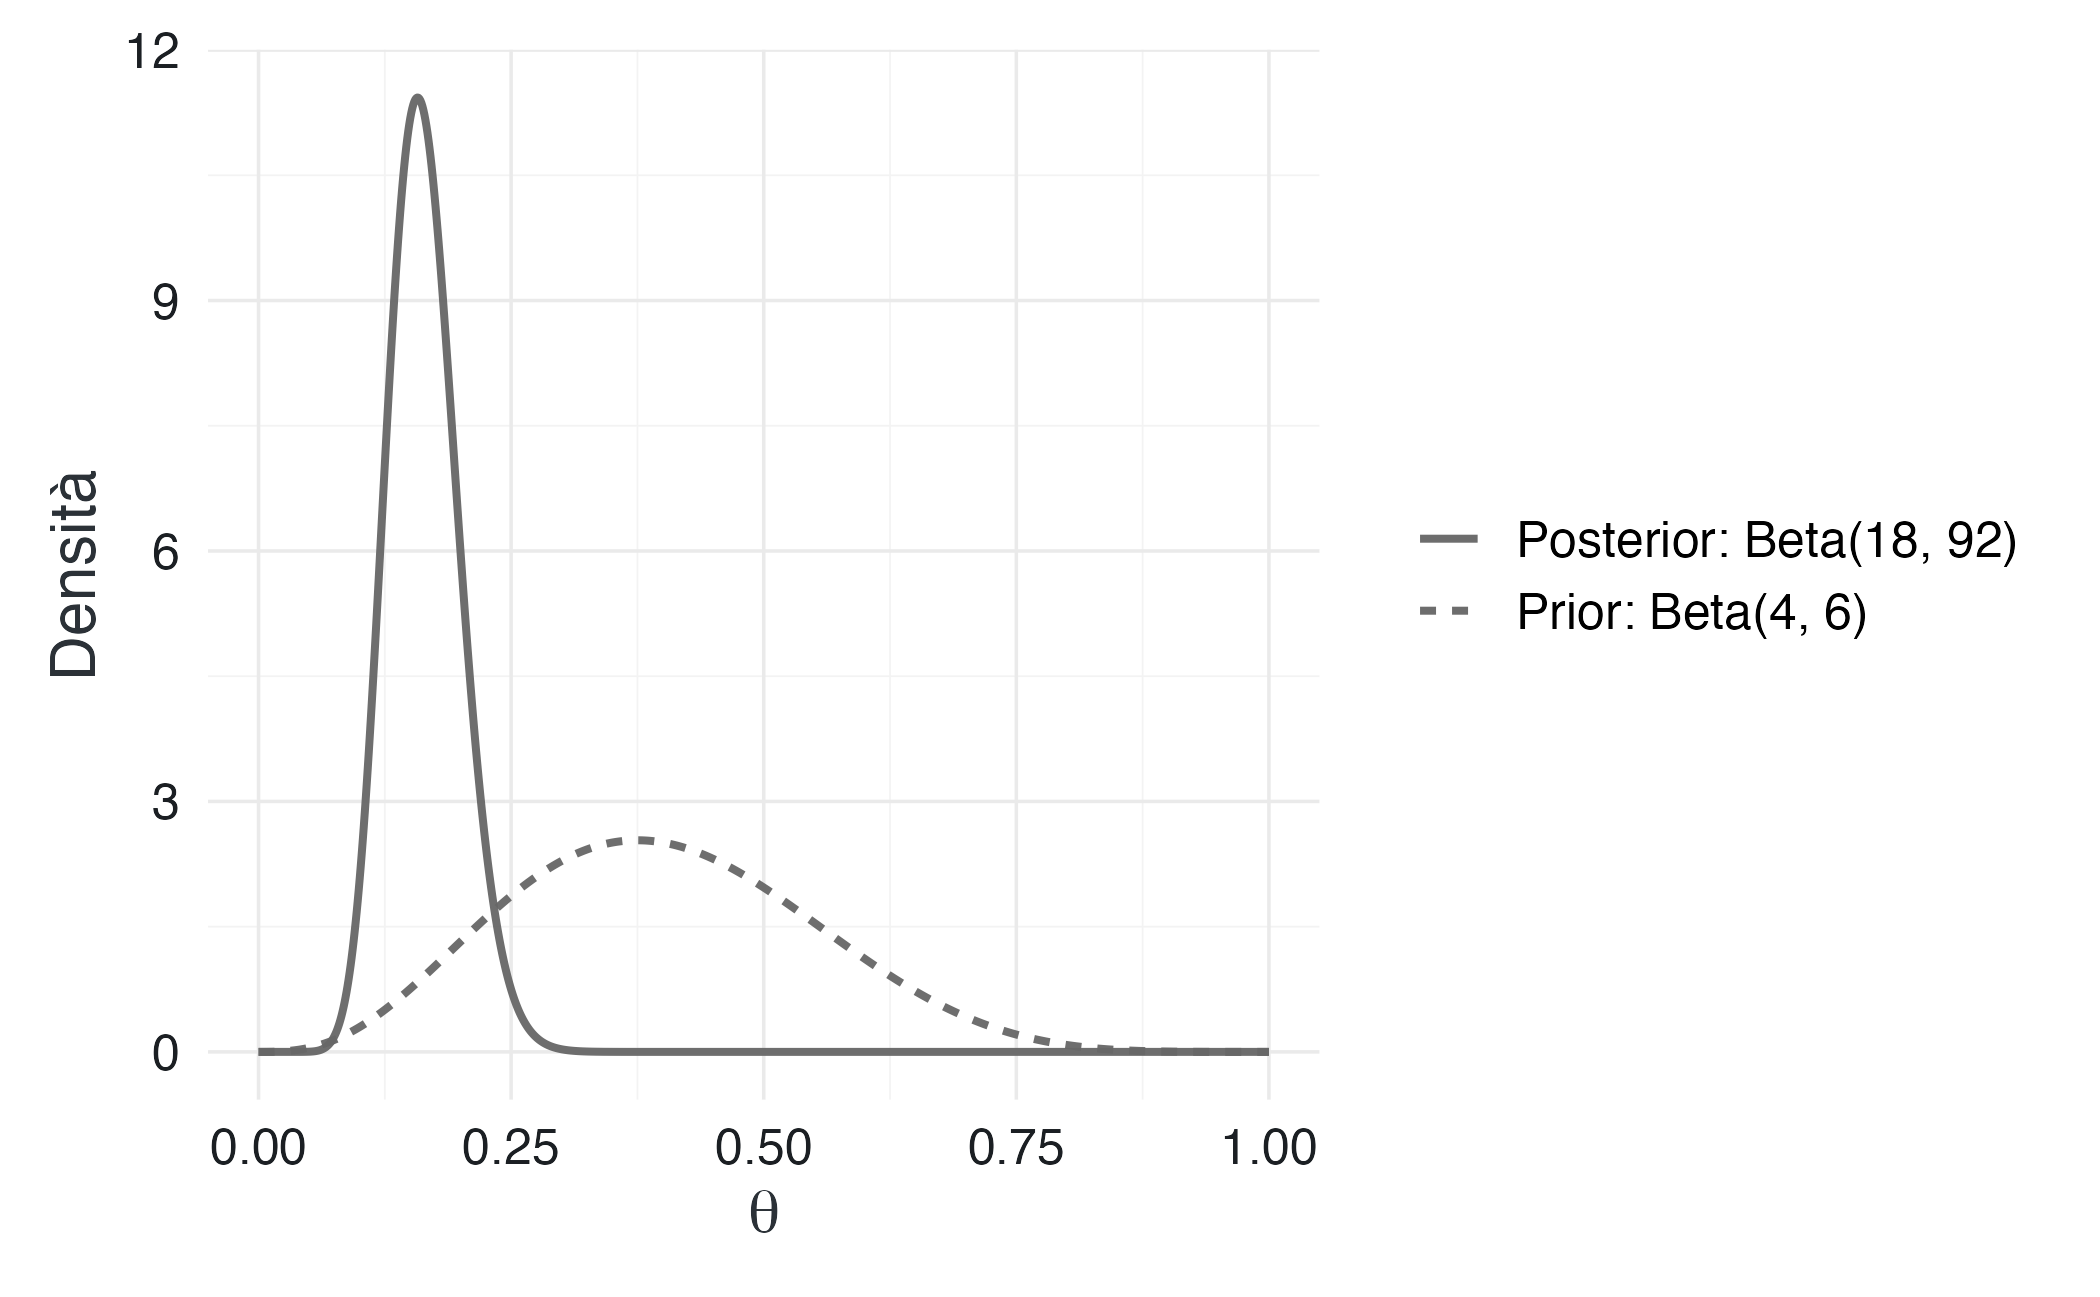
\includegraphics[width=0.85\linewidth,height=\textheight,keepaspectratio]{chapters/mcmc/01_metropolis_files/figure-pdf/fig-prior-posterior-1.png}

}

\caption{\label{fig-prior-posterior}Distribuzione a priori Beta(4,6) e
distribuzione a posteriori esatta Beta(18,92). L'evidenza empirica
sposta la plausibilità verso valori più bassi di quelli attesi
inizialmente e ne restringe l'intervallo.}

\end{figure}%

\begin{tcolorbox}[enhanced jigsaw, arc=.35mm, bottomrule=.15mm, bottomtitle=1mm, breakable, colback=white, colbacktitle=quarto-callout-warning-color!10!white, colframe=quarto-callout-warning-color-frame, coltitle=black, left=2mm, leftrule=.75mm, opacityback=0, opacitybacktitle=0.6, rightrule=.15mm, title=\textcolor{quarto-callout-warning-color}{\faExclamationTriangle}\hspace{0.5em}{Perché usare Metropolis dove non serve}, titlerule=0mm, toprule=.15mm, toptitle=1mm]

In questo caso, l'algoritmo è del tutto superfluo: la risposta esatta la
conosciamo già. Ed è proprio questo il motivo per cui lo utilizziamo. Un
campionatore che sbaglia non lo dichiara, ma restituisce comunque dei
numeri che sembrano dei risultati. L'unico modo per imparare a
riconoscere un campionamento riuscito è quello di confrontarlo, almeno
una volta, con una verità nota.

\end{tcolorbox}

\section{Implementazione}\label{implementazione}

Definiamo separatamente le componenti del modello, così che la struttura
logica resti leggibile.

\begin{Shaded}
\begin{Highlighting}[]
\CommentTok{\# Distribuzione a priori}
\NormalTok{prior }\OtherTok{\textless{}{-}} \ControlFlowTok{function}\NormalTok{(theta) \{}
  \FunctionTok{dbeta}\NormalTok{(theta, }\AttributeTok{shape1 =} \DecValTok{4}\NormalTok{, }\AttributeTok{shape2 =} \DecValTok{6}\NormalTok{)}
\NormalTok{\}}

\CommentTok{\# Verosimiglianza binomiale: 14 successi su 100 prove}
\NormalTok{likelihood }\OtherTok{\textless{}{-}} \ControlFlowTok{function}\NormalTok{(theta) \{}
  \FunctionTok{dbinom}\NormalTok{(}\DecValTok{14}\NormalTok{, }\AttributeTok{size =} \DecValTok{100}\NormalTok{, }\AttributeTok{prob =}\NormalTok{ theta)}
\NormalTok{\}}

\CommentTok{\# Distribuzione a posteriori NON normalizzata}
\NormalTok{posterior\_nn }\OtherTok{\textless{}{-}} \ControlFlowTok{function}\NormalTok{(theta) \{}
  \FunctionTok{likelihood}\NormalTok{(theta) }\SpecialCharTok{*} \FunctionTok{prior}\NormalTok{(theta)}
\NormalTok{\}}

\CommentTok{\# Distribuzione di proposta: normale centrata sullo stato corrente}
\NormalTok{proposal }\OtherTok{\textless{}{-}} \ControlFlowTok{function}\NormalTok{(current, proposal\_sd) \{}
  \FunctionTok{rnorm}\NormalTok{(}\DecValTok{1}\NormalTok{, }\AttributeTok{mean =}\NormalTok{ current, }\AttributeTok{sd =}\NormalTok{ proposal\_sd)}
\NormalTok{\}}
\end{Highlighting}
\end{Shaded}

Si noti il nome \texttt{posterior\_nn}: la funzione restituisce il
\emph{prodotto} tra verosimiglianza e \emph{prior}, non la distribuzione
a posteriori normalizzata. Non conosciamo la costante \(p(y)\), ma non
ci serve: si semplifica nel rapporto del passo 3.

Il campionatore traduce i cinque passi in codice. Rispetto a
un'implementazione minimale, teniamo traccia anche del numero di
proposte accettate, che sarà il nostro primo indicatore diagnostico.

\begin{Shaded}
\begin{Highlighting}[]
\NormalTok{metropolis\_sampler }\OtherTok{\textless{}{-}} \ControlFlowTok{function}\NormalTok{(n\_iter, start, proposal\_sd) \{}
\NormalTok{  chain }\OtherTok{\textless{}{-}} \FunctionTok{numeric}\NormalTok{(n\_iter)}
\NormalTok{  current }\OtherTok{\textless{}{-}}\NormalTok{ start}
\NormalTok{  accepted }\OtherTok{\textless{}{-}} \DecValTok{0}

  \ControlFlowTok{for}\NormalTok{ (i }\ControlFlowTok{in} \FunctionTok{seq\_len}\NormalTok{(n\_iter)) \{}
    \CommentTok{\# 1. Proposta di un candidato}
\NormalTok{    candidate }\OtherTok{\textless{}{-}} \FunctionTok{proposal}\NormalTok{(current, proposal\_sd)}

    \CommentTok{\# 2. Il candidato deve essere una proporzione ammissibile}
    \ControlFlowTok{if}\NormalTok{ (candidate }\SpecialCharTok{\textgreater{}=} \DecValTok{0} \SpecialCharTok{\&\&}\NormalTok{ candidate }\SpecialCharTok{\textless{}=} \DecValTok{1}\NormalTok{) \{}
\NormalTok{      alpha }\OtherTok{\textless{}{-}} \FunctionTok{posterior\_nn}\NormalTok{(candidate) }\SpecialCharTok{/} \FunctionTok{posterior\_nn}\NormalTok{(current)}

      \CommentTok{\# 3. Decisione probabilistica}
      \ControlFlowTok{if}\NormalTok{ (}\FunctionTok{runif}\NormalTok{(}\DecValTok{1}\NormalTok{) }\SpecialCharTok{\textless{}}\NormalTok{ alpha) \{}
\NormalTok{        current }\OtherTok{\textless{}{-}}\NormalTok{ candidate}
\NormalTok{        accepted }\OtherTok{\textless{}{-}}\NormalTok{ accepted }\SpecialCharTok{+} \DecValTok{1}
\NormalTok{      \}}
\NormalTok{    \}}

    \CommentTok{\# 4. Si registra lo stato corrente, accettato o meno}
\NormalTok{    chain[i] }\OtherTok{\textless{}{-}}\NormalTok{ current}
\NormalTok{  \}}

  \FunctionTok{list}\NormalTok{(}\AttributeTok{chain =}\NormalTok{ chain, }\AttributeTok{acceptance\_rate =}\NormalTok{ accepted }\SpecialCharTok{/}\NormalTok{ n\_iter)}
\NormalTok{\}}
\end{Highlighting}
\end{Shaded}

Due dettagli meritano attenzione. Il controllo
\texttt{candidate\ \textgreater{}=\ 0\ \&\&\ candidate\ \textless{}=\ 1}
gestisce il fatto che \(\theta\) è una proporzione, mentre la proposta
normale può generare valori al di fuori dell'intervallo ammissibile:
tali candidati vengono automaticamente rifiutati. Inoltre, il passo 4
registra lo stato \emph{a ogni iterazione}, anche quando la proposta
viene rifiutata; è per questo motivo che le catene di Metropolis
contengono valori ripetuti.

\section{Esecuzione e burn-in}\label{esecuzione-e-burn-in}

\begin{Shaded}
\begin{Highlighting}[]
\FunctionTok{set.seed}\NormalTok{(}\DecValTok{20260722}\NormalTok{)}
\NormalTok{n\_iter }\OtherTok{\textless{}{-}} \DecValTok{10000}

\NormalTok{risultato }\OtherTok{\textless{}{-}} \FunctionTok{metropolis\_sampler}\NormalTok{(n\_iter, }\AttributeTok{start =} \FloatTok{0.9}\NormalTok{, }\AttributeTok{proposal\_sd =} \FloatTok{0.1}\NormalTok{)}
\NormalTok{risultato}\SpecialCharTok{$}\NormalTok{acceptance\_rate}
\CommentTok{\#\textgreater{} [1] 0.385}
\end{Highlighting}
\end{Shaded}

Abbiamo deliberatamente avviato la catena da \(\theta_0=0.9\), un valore
molto distante dalla regione plausibile. Osserviamo cosa accade nelle
prime iterazioni.

\begin{Shaded}
\begin{Highlighting}[]
\FunctionTok{tibble}\NormalTok{(}
  \AttributeTok{iterazione =} \DecValTok{1}\SpecialCharTok{:}\DecValTok{300}\NormalTok{,}
  \AttributeTok{theta =}\NormalTok{ risultato}\SpecialCharTok{$}\NormalTok{chain[}\DecValTok{1}\SpecialCharTok{:}\DecValTok{300}\NormalTok{]}
\NormalTok{) }\SpecialCharTok{|\textgreater{}}
  \FunctionTok{ggplot}\NormalTok{(}\FunctionTok{aes}\NormalTok{(}\AttributeTok{x =}\NormalTok{ iterazione, }\AttributeTok{y =}\NormalTok{ theta)) }\SpecialCharTok{+}
  \FunctionTok{geom\_line}\NormalTok{() }\SpecialCharTok{+}
  \FunctionTok{labs}\NormalTok{(}\AttributeTok{x =} \StringTok{"Iterazione"}\NormalTok{, }\AttributeTok{y =} \FunctionTok{expression}\NormalTok{(theta))}
\end{Highlighting}
\end{Shaded}

\begin{figure}[H]

\centering{

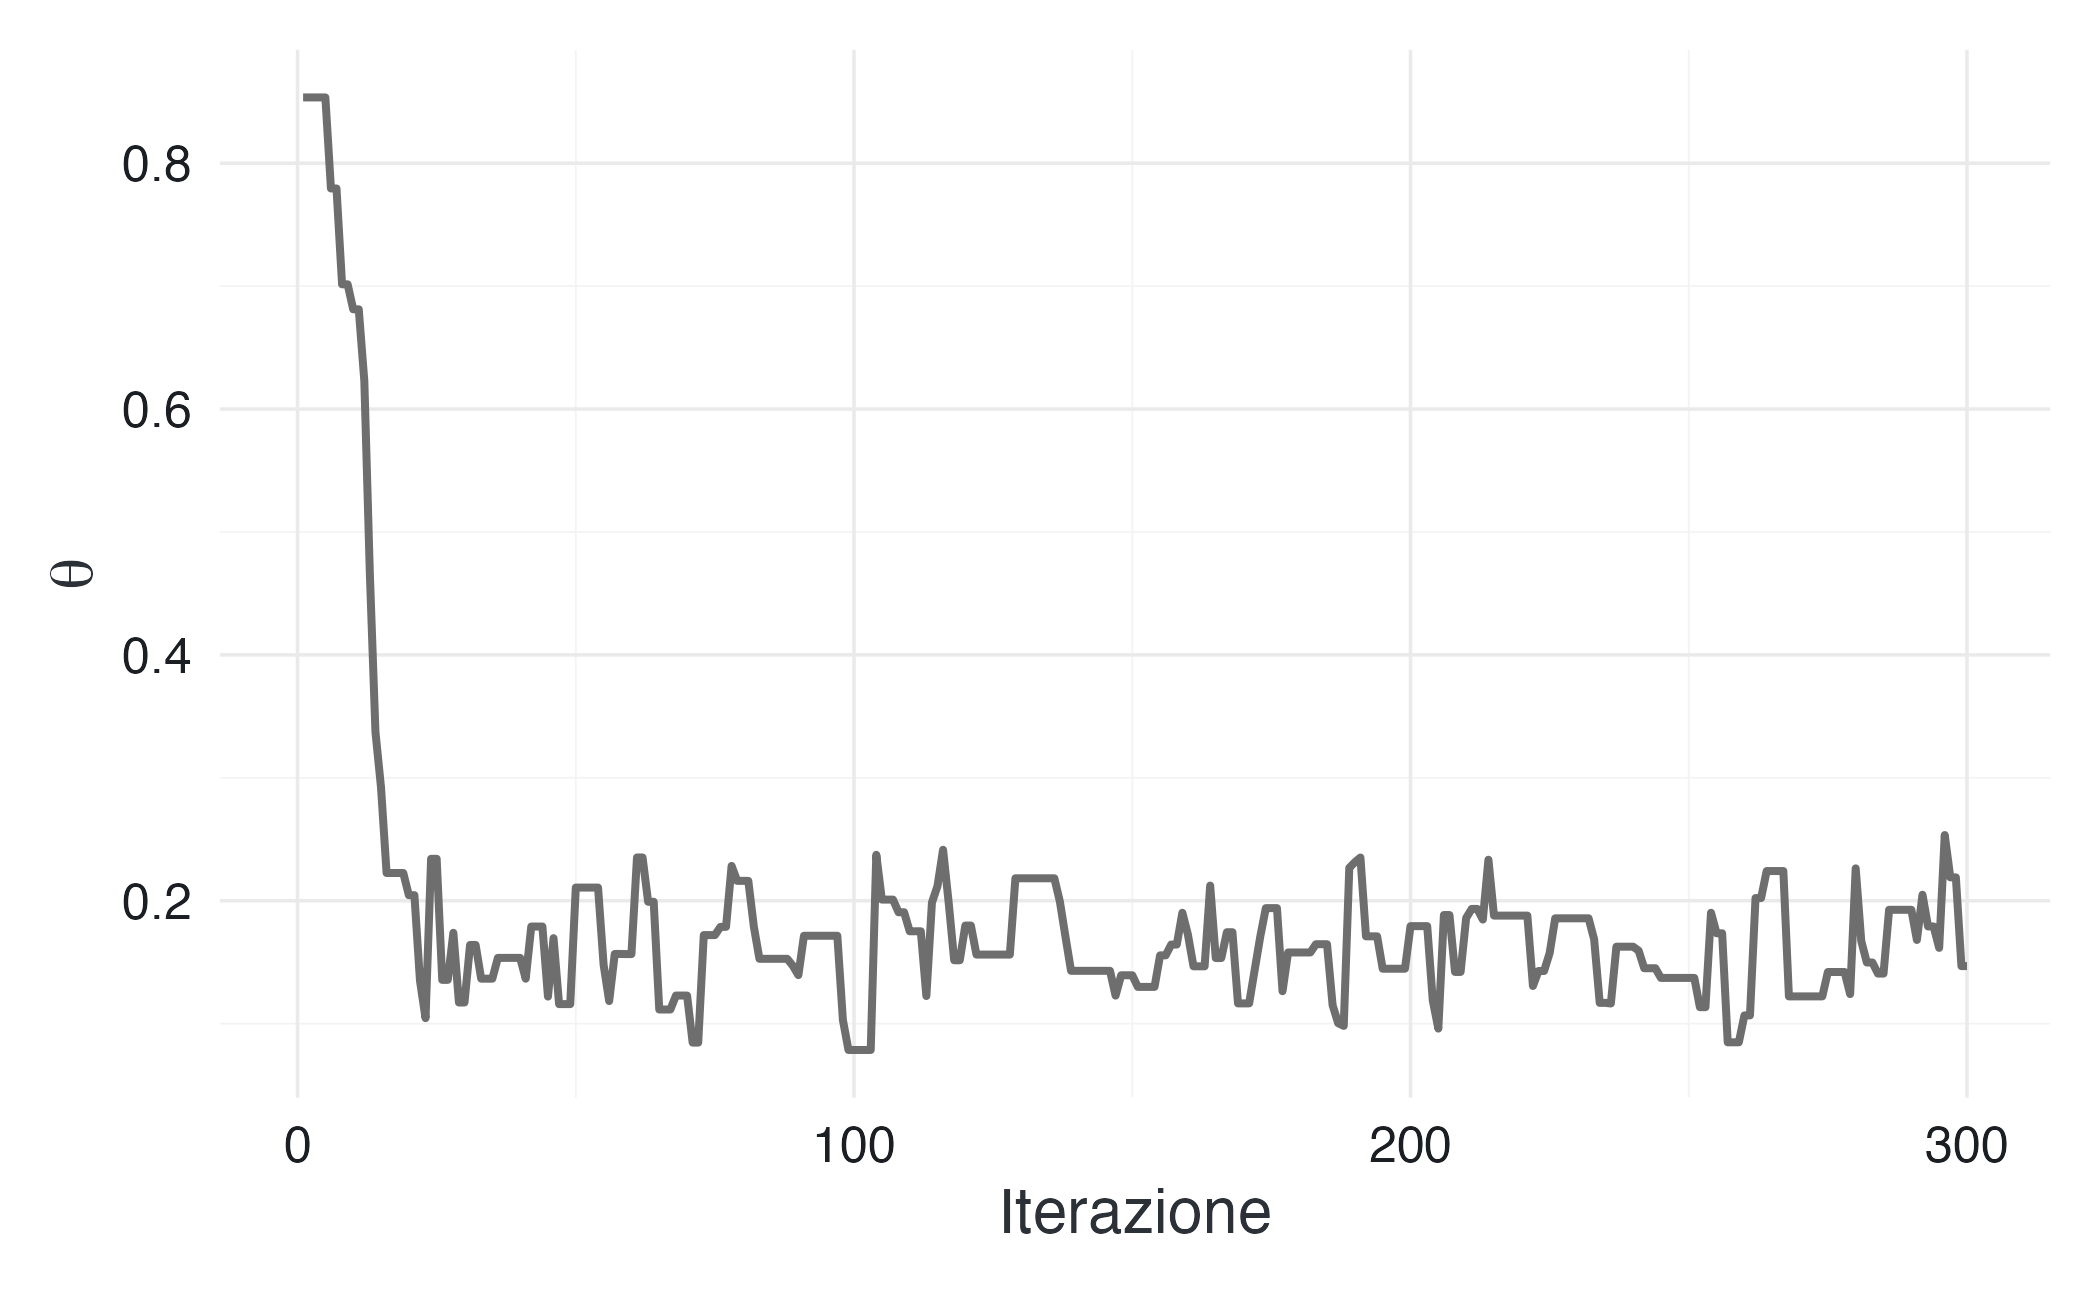
\includegraphics[width=0.85\linewidth,height=\textheight,keepaspectratio]{chapters/mcmc/01_metropolis_files/figure-pdf/fig-burnin-1.png}

}

\caption{\label{fig-burnin}Le prime 300 iterazioni. La catena parte da
un valore implausibile e in poche decine di passi raggiunge la regione
ad alta densità, dove poi fluttua in modo stazionario.}

\end{figure}%

La figura mostra la \emph{fase transiente}: la catena ``scende''
rapidamente dal punto di partenza arbitrario verso la regione plausibile
e poi si stabilizza. I valori prodotti durante questa fase non
provengono dalla distribuzione target --- riflettono ancora la scelta
iniziale --- e vanno scartati. Questa porzione iniziale è detta
\textbf{burn-in}.

\begin{Shaded}
\begin{Highlighting}[]
\NormalTok{burnin }\OtherTok{\textless{}{-}} \FunctionTok{floor}\NormalTok{(n\_iter }\SpecialCharTok{/} \DecValTok{2}\NormalTok{)}
\NormalTok{post\_burnin }\OtherTok{\textless{}{-}}\NormalTok{ risultato}\SpecialCharTok{$}\NormalTok{chain[(burnin }\SpecialCharTok{+} \DecValTok{1}\NormalTok{)}\SpecialCharTok{:}\NormalTok{n\_iter]}
\end{Highlighting}
\end{Shaded}

Scartare metà della catena è una scelta prudenziale comune. Non esiste
una regola universale: la quantità da eliminare va decisa osservando il
\emph{trace plot}, non applicando una percentuale fissa.

\begin{tcolorbox}[enhanced jigsaw, arc=.35mm, bottomrule=.15mm, bottomtitle=1mm, breakable, colback=white, colbacktitle=quarto-callout-note-color!10!white, colframe=quarto-callout-note-color-frame, coltitle=black, left=2mm, leftrule=.75mm, opacityback=0, opacitybacktitle=0.6, rightrule=.15mm, title=\textcolor{quarto-callout-note-color}{\faInfo}\hspace{0.5em}{Una differenza epistemologica}, titlerule=0mm, toprule=.15mm, toptitle=1mm]

Qui emerge una distinzione che vale la pena rendere esplicita. Una volta
ricavata, una formula chiusa è semplicemente vera. Un campione MCMC,
invece, è affidabile \emph{solo se} la catena ha effettivamente
raggiunto la distribuzione a posteriori, cosa di cui non possiamo essere
certi in anticipo. Per questo motivo, le verifiche di convergenza non
sono un tecnicismo accessorio, ma fanno parte integrante del
ragionamento inferenziale. Una catena interrotta troppo presto può
restituire risposte tanto sicure quanto errate.

\end{tcolorbox}

\section{Calibrare la distribuzione di
proposta}\label{sec-calibrazione-proposta}

Il parametro \(\tau\) (\texttt{proposal\_sd}) controlla l'ampiezza media
dei passi ed è l'unica manopola dell'algoritmo. La teoria afferma che
passi troppo piccoli producono un'esplorazione lenta, mentre passi
troppo grandi causano un tasso di rifiuto elevato. Invece di crederci
sulla parola, verifichiamo.

\begin{Shaded}
\begin{Highlighting}[]
\FunctionTok{set.seed}\NormalTok{(}\DecValTok{4}\NormalTok{)}
\NormalTok{valori\_sd }\OtherTok{\textless{}{-}} \FunctionTok{c}\NormalTok{(}\FloatTok{0.005}\NormalTok{, }\FloatTok{0.1}\NormalTok{, }\FloatTok{0.8}\NormalTok{)}

\NormalTok{esperimento }\OtherTok{\textless{}{-}} \FunctionTok{lapply}\NormalTok{(valori\_sd, }\ControlFlowTok{function}\NormalTok{(s) \{}
\NormalTok{  out }\OtherTok{\textless{}{-}} \FunctionTok{metropolis\_sampler}\NormalTok{(}\AttributeTok{n\_iter =} \DecValTok{2000}\NormalTok{, }\AttributeTok{start =} \FloatTok{0.5}\NormalTok{, }\AttributeTok{proposal\_sd =}\NormalTok{ s)}
  \FunctionTok{tibble}\NormalTok{(}
    \AttributeTok{iterazione =} \DecValTok{1}\SpecialCharTok{:}\DecValTok{2000}\NormalTok{,}
    \AttributeTok{theta =}\NormalTok{ out}\SpecialCharTok{$}\NormalTok{chain,}
    \AttributeTok{etichetta =} \FunctionTok{sprintf}\NormalTok{(}\StringTok{"tau = \%.3f  (accettazione = \%.2f)"}\NormalTok{,}
\NormalTok{                        s, out}\SpecialCharTok{$}\NormalTok{acceptance\_rate)}
\NormalTok{  )}
\NormalTok{\}) }\SpecialCharTok{|\textgreater{}}
  \FunctionTok{bind\_rows}\NormalTok{()}

\FunctionTok{ggplot}\NormalTok{(esperimento, }\FunctionTok{aes}\NormalTok{(}\AttributeTok{x =}\NormalTok{ iterazione, }\AttributeTok{y =}\NormalTok{ theta)) }\SpecialCharTok{+}
  \FunctionTok{geom\_line}\NormalTok{(}\AttributeTok{linewidth =} \FloatTok{0.3}\NormalTok{) }\SpecialCharTok{+}
  \FunctionTok{facet\_wrap}\NormalTok{(}\SpecialCharTok{\textasciitilde{}}\NormalTok{ etichetta, }\AttributeTok{ncol =} \DecValTok{1}\NormalTok{, }\AttributeTok{scales =} \StringTok{"free\_y"}\NormalTok{) }\SpecialCharTok{+}
  \FunctionTok{labs}\NormalTok{(}\AttributeTok{x =} \StringTok{"Iterazione"}\NormalTok{, }\AttributeTok{y =} \FunctionTok{expression}\NormalTok{(theta))}
\end{Highlighting}
\end{Shaded}

\begin{figure}[H]

\centering{

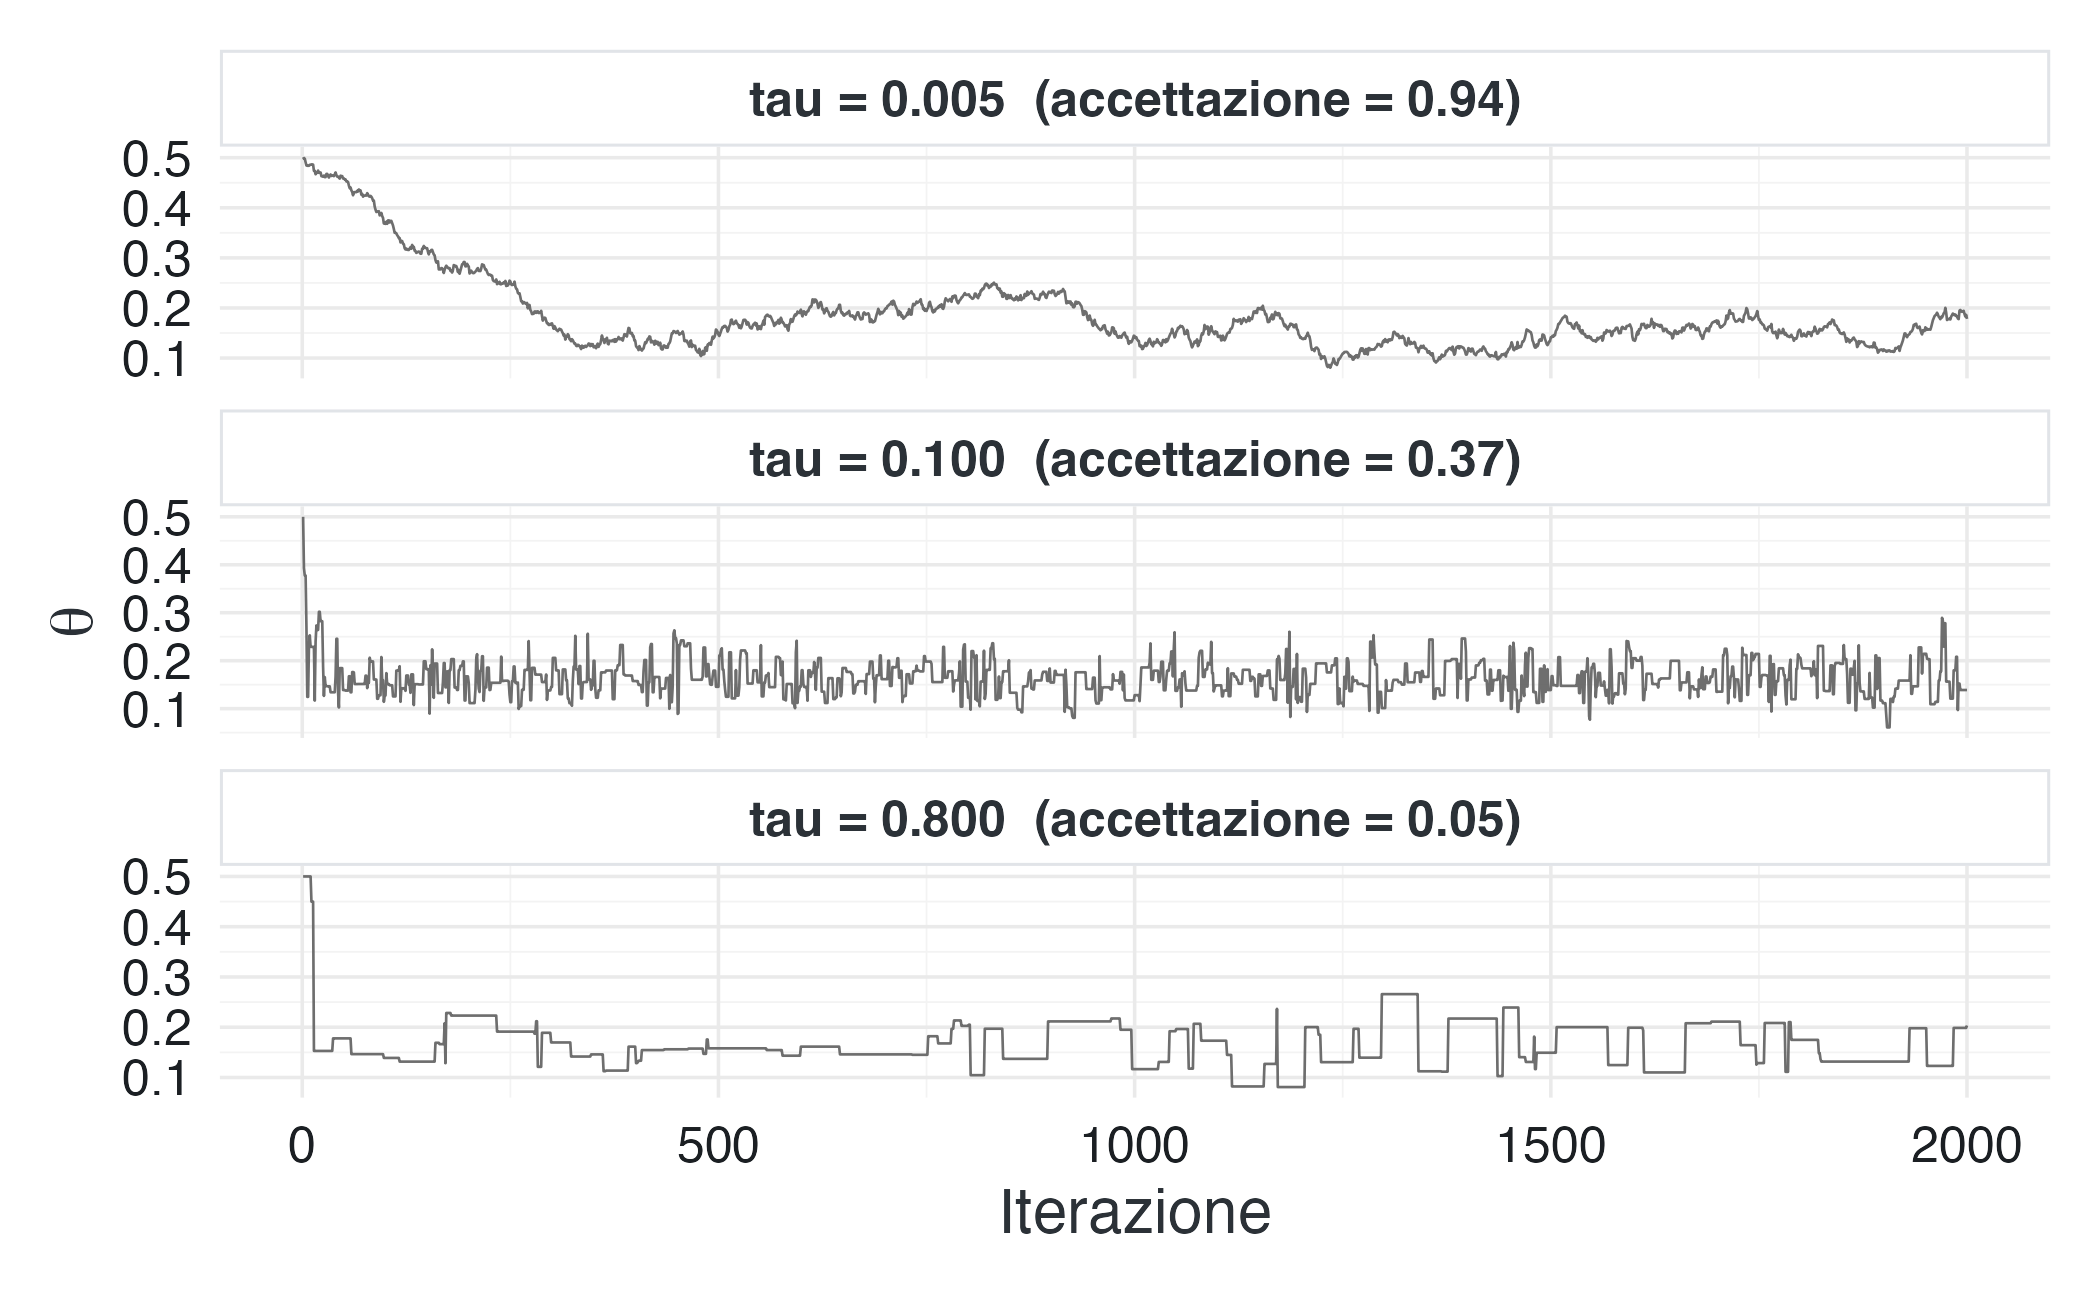
\includegraphics[width=0.85\linewidth,height=\textheight,keepaspectratio]{chapters/mcmc/01_metropolis_files/figure-pdf/fig-calibrazione-1.png}

}

\caption{\label{fig-calibrazione}Effetto dell'ampiezza della proposta.
Con passi troppo piccoli la catena deriva lentamente e resta correlata;
con passi troppo grandi rimane bloccata a lungo sullo stesso valore; il
valore intermedio esplora in modo efficiente.}

\end{figure}%

I tre pannelli mostrano tre diverse patologie dello stesso algoritmo.

Con \(\tau=0.005\), quasi ogni proposta viene accettata, il tasso di
accettazione è altissimo, ma la catena si sposta di pochissimo a ogni
passo, il grafico somiglia a una passeggiata lenta e ondulata e, in 2000
iterazioni, la distribuzione target non viene esplorata per intero.
\emph{Un tasso di accettazione elevato non è di per sé un buon segno.}

Con \(\tau=0.8\), invece, accade l'opposto: molte proposte cadono fuori
dall'intervallo \([0,1]\) o in regioni implausibili e vengono rifiutate;
la catena, quindi, resta ferma sullo stesso valore per decine di
iterazioni. Il \emph{trace plot} assume il caratteristico aspetto ``a
gradini''.

Con \(\tau=0.1\), il compromesso è ragionevole: passi abbastanza ampi da
attraversare la distribuzione e abbastanza contenuti da essere accettati
con frequenza. Per un singolo parametro con proposta normale simmetrica,
un tasso di accettazione intorno a 0.4-0.5 è un riferimento diagnostico
orientativo, non una regola, ma un indizio utile.

\section{Quanti campioni valgono
davvero}\label{quanti-campioni-valgono-davvero}

La correlazione tra valori successivi ha una conseguenza pratica: \(N\)
campioni MCMC contengono meno informazioni di \(N\) campioni
indipendenti. Possiamo verificarlo tramite la funzione di
autocorrelazione.

\begin{Shaded}
\begin{Highlighting}[]
\NormalTok{acf\_out }\OtherTok{\textless{}{-}} \FunctionTok{acf}\NormalTok{(post\_burnin, }\AttributeTok{lag.max =} \DecValTok{40}\NormalTok{, }\AttributeTok{plot =} \ConstantTok{FALSE}\NormalTok{)}

\FunctionTok{tibble}\NormalTok{(}\AttributeTok{lag =} \FunctionTok{as.numeric}\NormalTok{(acf\_out}\SpecialCharTok{$}\NormalTok{lag), }\AttributeTok{acf =} \FunctionTok{as.numeric}\NormalTok{(acf\_out}\SpecialCharTok{$}\NormalTok{acf)) }\SpecialCharTok{|\textgreater{}}
  \FunctionTok{ggplot}\NormalTok{(}\FunctionTok{aes}\NormalTok{(}\AttributeTok{x =}\NormalTok{ lag, }\AttributeTok{y =}\NormalTok{ acf)) }\SpecialCharTok{+}
  \FunctionTok{geom\_hline}\NormalTok{(}\AttributeTok{yintercept =} \DecValTok{0}\NormalTok{) }\SpecialCharTok{+}
  \FunctionTok{geom\_segment}\NormalTok{(}\FunctionTok{aes}\NormalTok{(}\AttributeTok{xend =}\NormalTok{ lag, }\AttributeTok{yend =} \DecValTok{0}\NormalTok{)) }\SpecialCharTok{+}
  \FunctionTok{labs}\NormalTok{(}\AttributeTok{x =} \StringTok{"Ritardo"}\NormalTok{, }\AttributeTok{y =} \StringTok{"Autocorrelazione"}\NormalTok{)}
\end{Highlighting}
\end{Shaded}

\begin{figure}[H]

\centering{

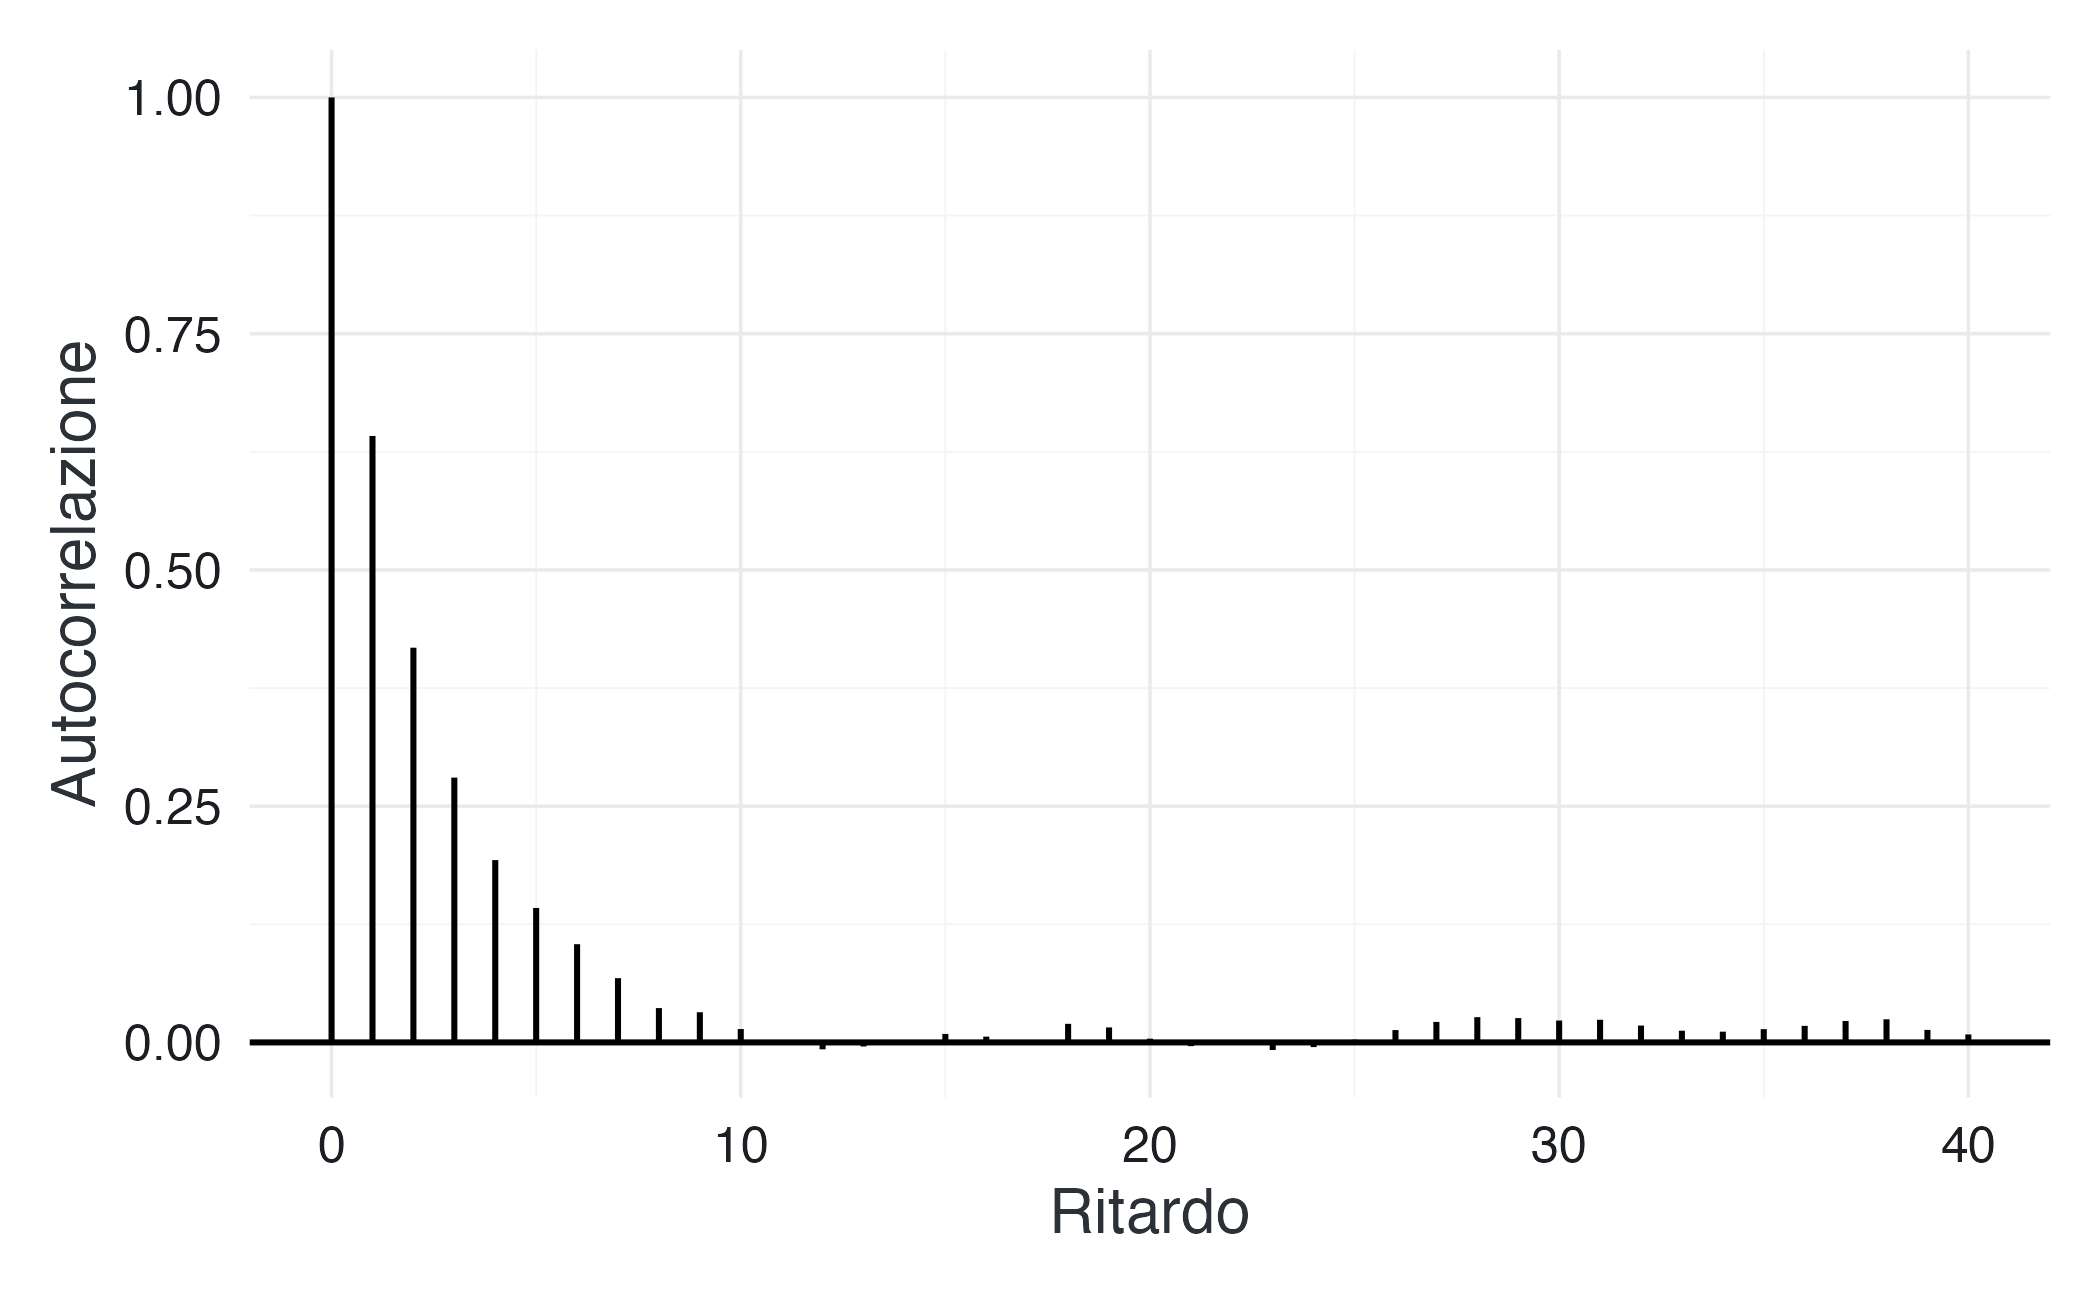
\includegraphics[width=0.85\linewidth,height=\textheight,keepaspectratio]{chapters/mcmc/01_metropolis_files/figure-pdf/fig-acf-1.png}

}

\caption{\label{fig-acf}Autocorrelazione della catena post-burn-in. La
dipendenza tra valori successivi si attenua progressivamente ma non è
trascurabile nei primi ritardi.}

\end{figure}%

La quantità che sintetizza questa perdita di informazione è la
\textbf{dimensione campionaria effettiva} (\emph{Effective Sample Size},
ESS): il numero di campioni indipendenti che fornirebbero la stessa
informazione della sequenza correlata.

\begin{Shaded}
\begin{Highlighting}[]
\FunctionTok{c}\NormalTok{(}
  \AttributeTok{campioni\_nominali =} \FunctionTok{length}\NormalTok{(post\_burnin),}
  \AttributeTok{ESS =}\NormalTok{ posterior}\SpecialCharTok{::}\FunctionTok{ess\_basic}\NormalTok{(post\_burnin)}
\NormalTok{)}
\CommentTok{\#\textgreater{} campioni\_nominali               ESS }
\CommentTok{\#\textgreater{}              5000              1020}
\end{Highlighting}
\end{Shaded}

Il confronto è istruttivo: a fronte di 5000 valori registrati,
l'informazione effettivamente disponibile equivale a un numero
sensibilmente inferiore di estrazioni indipendenti. È questa la ragione
per cui, negli output di \texttt{brms} e di Stan che incontreremo nei
prossimi capitoli, accanto alle stime compaiono sempre
\texttt{Bulk\_ESS} e \texttt{Tail\_ESS}: non misurano l'incertezza sui
dati, ma la qualità del campionamento.

\section{Catene multiple e convergenza}\label{sec-catene-multiple}

Una singola catena può apparire stazionaria e avere comunque esplorato
solo una porzione dello spazio. La verifica più efficace consiste
nell'eseguire più catene partendo da punti diversi e controllare che
finiscano per descrivere la stessa distribuzione.

\begin{Shaded}
\begin{Highlighting}[]
\FunctionTok{set.seed}\NormalTok{(}\DecValTok{20260722}\NormalTok{)}
\NormalTok{punti\_partenza }\OtherTok{\textless{}{-}} \FunctionTok{c}\NormalTok{(}\FloatTok{0.05}\NormalTok{, }\FloatTok{0.30}\NormalTok{, }\FloatTok{0.60}\NormalTok{, }\FloatTok{0.90}\NormalTok{)}

\NormalTok{catene }\OtherTok{\textless{}{-}} \FunctionTok{sapply}\NormalTok{(punti\_partenza, }\ControlFlowTok{function}\NormalTok{(s) \{}
  \FunctionTok{metropolis\_sampler}\NormalTok{(}\AttributeTok{n\_iter =} \DecValTok{10000}\NormalTok{, }\AttributeTok{start =}\NormalTok{ s, }\AttributeTok{proposal\_sd =} \FloatTok{0.1}\NormalTok{)}\SpecialCharTok{$}\NormalTok{chain}
\NormalTok{\})}

\NormalTok{catene\_post }\OtherTok{\textless{}{-}}\NormalTok{ catene[(burnin }\SpecialCharTok{+} \DecValTok{1}\NormalTok{)}\SpecialCharTok{:}\NormalTok{n\_iter, , drop }\OtherTok{=} \ConstantTok{FALSE}\NormalTok{]}

\NormalTok{draws }\OtherTok{\textless{}{-}}\NormalTok{ posterior}\SpecialCharTok{::}\FunctionTok{as\_draws\_array}\NormalTok{(}
  \FunctionTok{array}\NormalTok{(}
\NormalTok{    catene\_post,}
    \AttributeTok{dim =} \FunctionTok{c}\NormalTok{(}\FunctionTok{nrow}\NormalTok{(catene\_post), }\FunctionTok{ncol}\NormalTok{(catene\_post), }\DecValTok{1}\NormalTok{),}
    \AttributeTok{dimnames =} \FunctionTok{list}\NormalTok{(}\ConstantTok{NULL}\NormalTok{, }\ConstantTok{NULL}\NormalTok{, }\StringTok{"theta"}\NormalTok{)}
\NormalTok{  )}
\NormalTok{)}

\NormalTok{posterior}\SpecialCharTok{::}\FunctionTok{summarise\_draws}\NormalTok{(draws)}
\CommentTok{\#\textgreater{} \# A tibble: 1 x 10}
\CommentTok{\#\textgreater{}   variable  mean median     sd    mad    q5   q95  rhat ess\_bulk ess\_tail}
\CommentTok{\#\textgreater{}   \textless{}chr\textgreater{}    \textless{}dbl\textgreater{}  \textless{}dbl\textgreater{}  \textless{}dbl\textgreater{}  \textless{}dbl\textgreater{} \textless{}dbl\textgreater{} \textless{}dbl\textgreater{} \textless{}dbl\textgreater{}    \textless{}dbl\textgreater{}    \textless{}dbl\textgreater{}}
\CommentTok{\#\textgreater{} 1 theta    0.163  0.161 0.0349 0.0353 0.110 0.223  1.00    4249.    4742.}
\end{Highlighting}
\end{Shaded}

\begin{Shaded}
\begin{Highlighting}[]
\FunctionTok{as\_tibble}\NormalTok{(catene\_post, }\AttributeTok{.name\_repair =} \SpecialCharTok{\textasciitilde{}} \FunctionTok{paste0}\NormalTok{(}\StringTok{"catena\_"}\NormalTok{, }\FunctionTok{seq\_along}\NormalTok{(.x))) }\SpecialCharTok{|\textgreater{}}
  \FunctionTok{mutate}\NormalTok{(}\AttributeTok{iterazione =} \FunctionTok{row\_number}\NormalTok{()) }\SpecialCharTok{|\textgreater{}}
  \FunctionTok{pivot\_longer}\NormalTok{(}\SpecialCharTok{{-}}\NormalTok{iterazione, }\AttributeTok{names\_to =} \StringTok{"catena"}\NormalTok{, }\AttributeTok{values\_to =} \StringTok{"theta"}\NormalTok{) }\SpecialCharTok{|\textgreater{}}
  \FunctionTok{filter}\NormalTok{(iterazione }\SpecialCharTok{\textless{}=} \DecValTok{1000}\NormalTok{) }\SpecialCharTok{|\textgreater{}}
  \FunctionTok{ggplot}\NormalTok{(}\FunctionTok{aes}\NormalTok{(}\AttributeTok{x =}\NormalTok{ iterazione, }\AttributeTok{y =}\NormalTok{ theta, }\AttributeTok{group =}\NormalTok{ catena)) }\SpecialCharTok{+}
  \FunctionTok{geom\_line}\NormalTok{(}\AttributeTok{linewidth =} \FloatTok{0.25}\NormalTok{, }\AttributeTok{alpha =} \FloatTok{0.8}\NormalTok{) }\SpecialCharTok{+}
  \FunctionTok{labs}\NormalTok{(}\AttributeTok{x =} \StringTok{"Iterazione"}\NormalTok{, }\AttributeTok{y =} \FunctionTok{expression}\NormalTok{(theta))}
\end{Highlighting}
\end{Shaded}

\begin{figure}[H]

\centering{

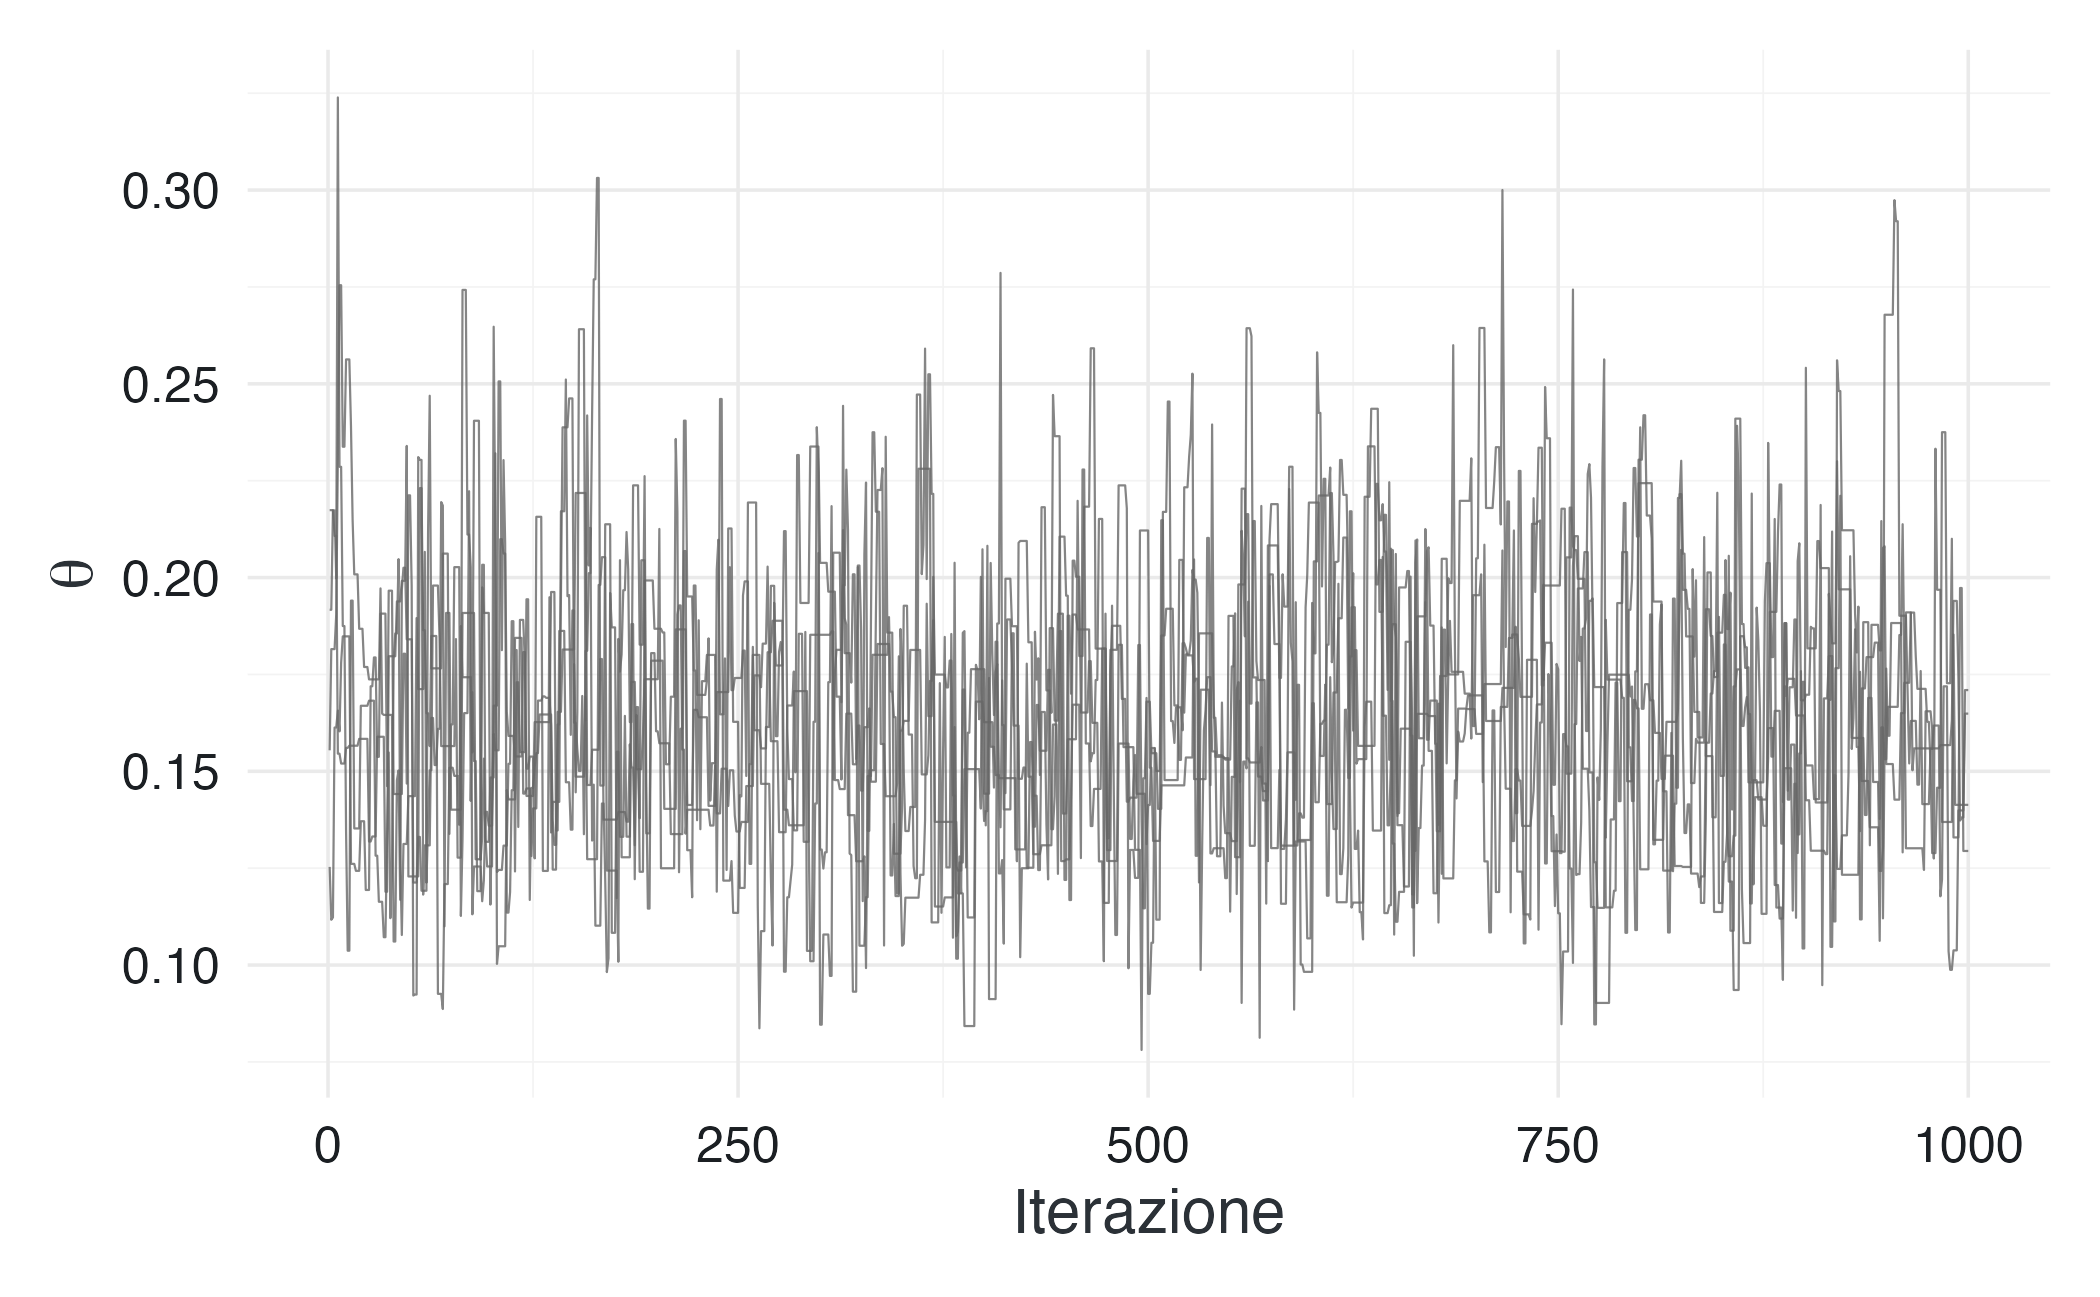
\includegraphics[width=0.85\linewidth,height=\textheight,keepaspectratio]{chapters/mcmc/01_metropolis_files/figure-pdf/fig-catene-1.png}

}

\caption{\label{fig-catene}Quattro catene indipendenti dopo il burn-in,
inizializzate in punti distanti dello spazio parametrico. La
sovrapposizione delle traiettorie è l'evidenza visiva della
convergenza.}

\end{figure}%

Nella tabella prodotta da \texttt{summarise\_draws()} compare la
statistica \(\hat{R}\) (\texttt{rhat}), che confronta la variabilità
\emph{tra} catene con quella \emph{interna} a ciascuna catena. Se le
catene hanno raggiunto la stessa distribuzione, le due quantità
coincidono e \(\hat{R}\) vale circa 1. Valori superiori a 1.01 segnalano
che le catene stanno ancora descrivendo distribuzioni diverse, ovvero
che la convergenza non è stata raggiunta. Si tratta dello stesso
indicatore riportato da \texttt{brms} in ogni sommario: qui possiamo
vedere da dove proviene.

\section{Validazione: il confronto con la soluzione
esatta}\label{validazione-il-confronto-con-la-soluzione-esatta}

Ora passiamo alla verifica che giustifica l'intero esercizio.
Confrontiamo la distribuzione empirica dei campioni con la distribuzione
Beta(18,92) analitica.

\begin{Shaded}
\begin{Highlighting}[]
\FunctionTok{tibble}\NormalTok{(}\AttributeTok{theta =} \FunctionTok{as.vector}\NormalTok{(catene\_post)) }\SpecialCharTok{|\textgreater{}}
  \FunctionTok{ggplot}\NormalTok{(}\FunctionTok{aes}\NormalTok{(}\AttributeTok{x =}\NormalTok{ theta)) }\SpecialCharTok{+}
  \FunctionTok{geom\_histogram}\NormalTok{(}\FunctionTok{aes}\NormalTok{(}\AttributeTok{y =} \FunctionTok{after\_stat}\NormalTok{(density)), }\AttributeTok{bins =} \DecValTok{40}\NormalTok{,}
                 \AttributeTok{color =} \StringTok{"white"}\NormalTok{, }\AttributeTok{alpha =} \FloatTok{0.7}\NormalTok{) }\SpecialCharTok{+}
  \FunctionTok{stat\_function}\NormalTok{(}\AttributeTok{fun =}\NormalTok{ dbeta, }\AttributeTok{args =} \FunctionTok{list}\NormalTok{(}\AttributeTok{shape1 =} \DecValTok{18}\NormalTok{, }\AttributeTok{shape2 =} \DecValTok{92}\NormalTok{),}
                \AttributeTok{linewidth =} \DecValTok{1}\NormalTok{) }\SpecialCharTok{+}
  \FunctionTok{labs}\NormalTok{(}\AttributeTok{x =} \FunctionTok{expression}\NormalTok{(theta), }\AttributeTok{y =} \StringTok{"Densità"}\NormalTok{)}
\end{Highlighting}
\end{Shaded}

\begin{figure}[H]

\centering{

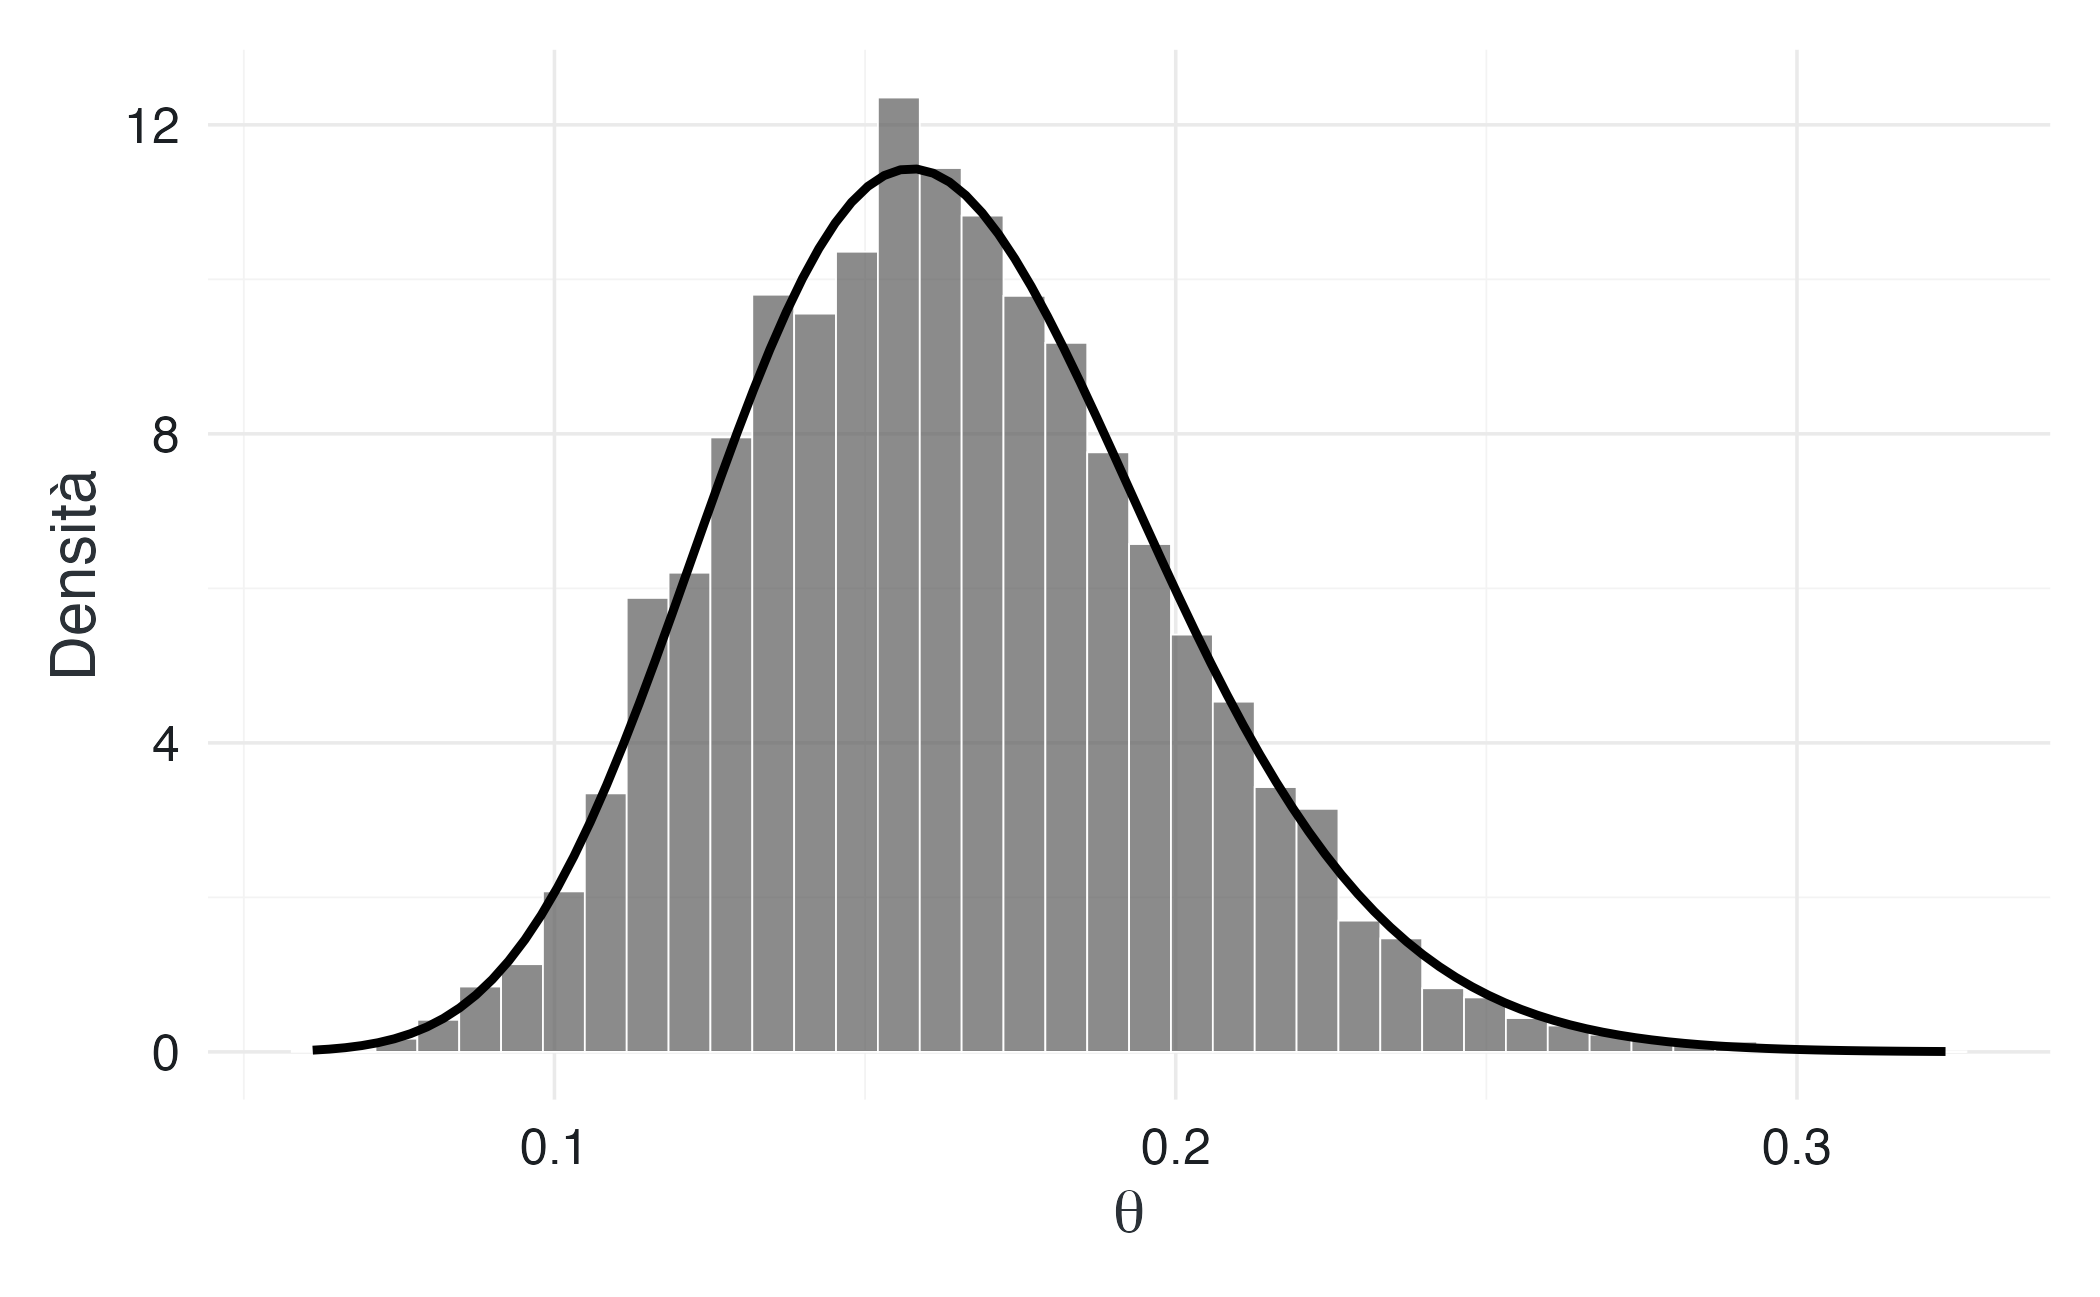
\includegraphics[width=0.85\linewidth,height=\textheight,keepaspectratio]{chapters/mcmc/01_metropolis_files/figure-pdf/fig-validazione-1.png}

}

\caption{\label{fig-validazione}Istogramma dei campioni post-burn-in e
densità Beta(18,92) esatta. La sovrapposizione fornisce la validazione
visiva del campionatore.}

\end{figure}%

Il confronto numerico include anche l'intervallo di credibilità:

\begin{Shaded}
\begin{Highlighting}[]
\NormalTok{campioni }\OtherTok{\textless{}{-}} \FunctionTok{as.vector}\NormalTok{(catene\_post)}

\FunctionTok{tibble}\NormalTok{(}
  \AttributeTok{metodo =} \FunctionTok{c}\NormalTok{(}\StringTok{"Metropolis (MCMC)"}\NormalTok{, }\StringTok{"Analitico"}\NormalTok{),}
  \AttributeTok{media =} \FunctionTok{c}\NormalTok{(}\FunctionTok{mean}\NormalTok{(campioni), }\DecValTok{18} \SpecialCharTok{/}\NormalTok{ (}\DecValTok{18} \SpecialCharTok{+} \DecValTok{92}\NormalTok{)),}
  \AttributeTok{sd =} \FunctionTok{c}\NormalTok{(}\FunctionTok{sd}\NormalTok{(campioni), }\FunctionTok{sqrt}\NormalTok{((}\DecValTok{18} \SpecialCharTok{*} \DecValTok{92}\NormalTok{) }\SpecialCharTok{/}\NormalTok{ ((}\DecValTok{18} \SpecialCharTok{+} \DecValTok{92}\NormalTok{)}\SpecialCharTok{\^{}}\DecValTok{2} \SpecialCharTok{*}\NormalTok{ (}\DecValTok{18} \SpecialCharTok{+} \DecValTok{92} \SpecialCharTok{+} \DecValTok{1}\NormalTok{)))),}
  \AttributeTok{q\_inf =} \FunctionTok{c}\NormalTok{(}\FunctionTok{quantile}\NormalTok{(campioni, }\FloatTok{0.03}\NormalTok{), }\FunctionTok{qbeta}\NormalTok{(}\FloatTok{0.03}\NormalTok{, }\DecValTok{18}\NormalTok{, }\DecValTok{92}\NormalTok{)),}
  \AttributeTok{q\_sup =} \FunctionTok{c}\NormalTok{(}\FunctionTok{quantile}\NormalTok{(campioni, }\FloatTok{0.97}\NormalTok{), }\FunctionTok{qbeta}\NormalTok{(}\FloatTok{0.97}\NormalTok{, }\DecValTok{18}\NormalTok{, }\DecValTok{92}\NormalTok{))}
\NormalTok{) }\SpecialCharTok{|\textgreater{}}
  \FunctionTok{mutate}\NormalTok{(}\FunctionTok{across}\NormalTok{(}\FunctionTok{where}\NormalTok{(is.numeric), \textbackslash{}(x) }\FunctionTok{round}\NormalTok{(x, }\DecValTok{4}\NormalTok{)))}
\CommentTok{\#\textgreater{} \# A tibble: 2 x 5}
\CommentTok{\#\textgreater{}   metodo            media     sd q\_inf q\_sup}
\CommentTok{\#\textgreater{}   \textless{}chr\textgreater{}             \textless{}dbl\textgreater{}  \textless{}dbl\textgreater{} \textless{}dbl\textgreater{} \textless{}dbl\textgreater{}}
\CommentTok{\#\textgreater{} 1 Metropolis (MCMC) 0.163 0.0349 0.104 0.233}
\CommentTok{\#\textgreater{} 2 Analitico         0.164 0.0351 0.103 0.235}
\end{Highlighting}
\end{Shaded}

I valori ottenuti tramite simulazione non coincidono esattamente con
quelli esatti, cosa che non potrebbe accadere trattandosi di campioni
casuali, ma la corrispondenza è stretta per tutte le quantità
considerate: media, dispersione e estremi dell'intervallo. Il
campionatore sta esplorando correttamente la distribuzione a posteriori.

\section{I limiti di Metropolis, e perché servono strumenti
migliori}\label{i-limiti-di-metropolis-e-perchuxe9-servono-strumenti-migliori}

L'algoritmo appena costruito presenta un'importante qualità: la
generalità. Funziona con qualunque modello per il quale sia possibile
calcolare il prodotto tra verosimiglianza e \emph{prior}, senza
richiedere né la coniugazione né integrali risolvibili. Questa
generalità ha però un costo che diventa proibitivo nei problemi reali.

Il primo limite riguarda la dimensionalità. Con un solo parametro, la
proposta casuale ha buone probabilità di cadere in una regione
plausibile; con decine o centinaia di parametri, la norma nei modelli
multilivello, un passo casuale in una direzione arbitraria finisce quasi
sempre in una zona a bassa densità e viene rifiutato. Il tasso di
accettazione crolla e la catena si blocca.

Il secondo riguarda la geometria. Quando i parametri sono fortemente
correlati, la distribuzione a posteriori assume forme allungate o curve
e una proposta sferica come la nostra non è adeguata: passi abbastanza
piccoli da essere accettati sono troppo piccoli per percorrere la
struttura nella sua interezza.

Il terzo problema è di natura pratica: abbiamo calibrato \(\tau\)
manualmente su un solo parametro. Con molti parametri, la calibrazione
manuale non è più un'opzione praticabile.

Gli algoritmi moderni risolvono questi problemi mantenendo lo stesso
principio di base, ovvero proporre, valutare un rapporto e accettare o
rifiutare, ma scegliendo le proposte in modo molto più informato. Il
\emph{Gibbs sampling} (\citeproc{ref-geman_geman_1984}{Geman \& Geman,
1984}) sfrutta le distribuzioni condizionate quando sono note,
l'\emph{Hamiltonian Monte Carlo} (\citeproc{ref-duane1987hybrid}{Duane
et al., 1987}) utilizza il gradiente della densità per proporre
movimenti che seguono la geometria della distribuzione e il
\emph{No-U-Turn Sampler} (\citeproc{ref-hoffman2014no}{{Hoffman et al.},
2014}) automatizza le scelte dell'HMC ed è l'algoritmo che Stan impiega
per impostazione predefinita.

Il capitolo successivo introduce i linguaggi di programmazione
probabilistica, che rendono disponibili questi algoritmi senza doverli
implementare. Ciò che resterà utile di questo capitolo non è il codice,
ma il vocabolario: quando Stan segnalerà un \(\hat{R}\) elevato, un ESS
insufficiente o un numero anomalo di transizioni divergenti, sapremo di
che cosa sta parlando.

\section*{Riflessioni conclusive}\label{riflessioni-conclusive-12}

\markright{Riflessioni conclusive}

L'algoritmo di Metropolis si basa su un'idea semplice: per studiare una
distribuzione che non sappiamo calcolare, costruiamo un processo che la
visita con la frequenza giusta. La rinuncia alla forma analitica è
compensata da una generalità quasi illimitata e questa sostituzione, il
calcolo con la simulazione, ha reso l'inferenza bayesiana praticabile
nella ricerca applicata.

Il capitolo ha però mostrato anche il rovescio della medaglia. Un
campionatore restituisce numeri in ogni caso, anche quando non ha
funzionato correttamente. Le diagnostiche introdotte in questo capitolo
--- l'ispezione del ``trace plot'', il tasso di accettazione,
l'autocorrelazione, l'ESS, le catene multiple e \(\hat{R}\) --- non sono
adempimenti formali, ma l'unico modo per distinguere una stima
affidabile da una che sembra soltanto affidabile. Nei capitoli
successivi lasceremo che sia Stan a occuparsi del campionamento, ma
continueremo a monitorare gli stessi indicatori.

\section*{Esercizi}\label{esercizi-4}
\addcontentsline{toc}{section}{Esercizi}

\markright{Esercizi}

\begin{tcolorbox}[enhanced jigsaw, arc=.35mm, bottomrule=.15mm, bottomtitle=1mm, breakable, colback=white, colbacktitle=quarto-callout-tip-color!10!white, colframe=quarto-callout-tip-color-frame, coltitle=black, left=2mm, leftrule=.75mm, opacityback=0, opacitybacktitle=0.6, rightrule=.15mm, title=\textcolor{quarto-callout-tip-color}{\faLightbulb}\hspace{0.5em}{Esercizio 1 --- Comprendere}, titlerule=0mm, toprule=.15mm, toptitle=1mm]

Spiega con parole tue perché l'algoritmo non ha bisogno di conoscere la
costante di normalizzazione \(p(y)\), e perché invece un metodo basato
sull'approssimazione su griglia deve calcolarla (almeno implicitamente,
normalizzando alla fine).

\end{tcolorbox}

\begin{tcolorbox}[enhanced jigsaw, arc=.35mm, bottomrule=.15mm, bottomtitle=1mm, breakable, colback=white, colbacktitle=quarto-callout-tip-color!10!white, colframe=quarto-callout-tip-color-frame, coltitle=black, left=2mm, leftrule=.75mm, opacityback=0, opacitybacktitle=0.6, rightrule=.15mm, title=\textcolor{quarto-callout-tip-color}{\faLightbulb}\hspace{0.5em}{Esercizio 2 --- Prevedere}, titlerule=0mm, toprule=.15mm, toptitle=1mm]

Prima di eseguire il codice: se facessi partire la catena da
\(\theta_0 = 0.001\) mantenendo \texttt{proposal\_sd\ =\ 0.1}, la fase
transiente sarebbe più lunga o più breve rispetto a quella osservata
partendo da 0.9? E se usassi \texttt{proposal\_sd\ =\ 0.01}? Formula
entrambe le previsioni, poi verificale.

\textbf{Suggerimento.} Ragiona su quanti passi, in media, servono per
coprire la distanza tra il punto di partenza e la regione ad alta
densità, dato che ogni passo ha ampiezza media dell'ordine di \(\tau\).

\end{tcolorbox}

\begin{tcolorbox}[enhanced jigsaw, arc=.35mm, bottomrule=.15mm, bottomtitle=1mm, breakable, colback=white, colbacktitle=quarto-callout-tip-color!10!white, colframe=quarto-callout-tip-color-frame, coltitle=black, left=2mm, leftrule=.75mm, opacityback=0, opacitybacktitle=0.6, rightrule=.15mm, title=\textcolor{quarto-callout-tip-color}{\faLightbulb}\hspace{0.5em}{Esercizio 3 --- Modificare}, titlerule=0mm, toprule=.15mm, toptitle=1mm]

Modifica \texttt{metropolis\_sampler()} in modo che registri, oltre alla
catena, anche il numero di proposte rifiutate \emph{perché fuori
dall'intervallo} \([0,1]\), distinguendole da quelle rifiutate in base
al rapporto \(\alpha\). Esegui l'algoritmo con \texttt{proposal\_sd}
pari a 0.05, 0.3 e 1.0 e riporta le due percentuali. Quale delle due
cause di rifiuto domina al crescere di \(\tau\)?

\end{tcolorbox}

\begin{tcolorbox}[enhanced jigsaw, arc=.35mm, bottomrule=.15mm, bottomtitle=1mm, breakable, colback=white, colbacktitle=quarto-callout-tip-color!10!white, colframe=quarto-callout-tip-color-frame, coltitle=black, left=2mm, leftrule=.75mm, opacityback=0, opacitybacktitle=0.6, rightrule=.15mm, title=\textcolor{quarto-callout-tip-color}{\faLightbulb}\hspace{0.5em}{Esercizio 4 --- Criticare}, titlerule=0mm, toprule=.15mm, toptitle=1mm]

Un collega ti mostra questo risultato: «Ho eseguito 50.000 iterazioni,
il tasso di accettazione è 0.93 e il trace plot non mostra alcun trend:
la catena ha convergito». Individua che cosa non torna in questo
ragionamento e indica quali verifiche aggiuntive chiederesti prima di
accettare la conclusione.

\end{tcolorbox}

\begin{tcolorbox}[enhanced jigsaw, arc=.35mm, bottomrule=.15mm, bottomtitle=1mm, breakable, colback=white, colbacktitle=quarto-callout-note-color!10!white, colframe=quarto-callout-note-color-frame, coltitle=black, left=2mm, leftrule=.75mm, opacityback=0, opacitybacktitle=0.6, rightrule=.15mm, title=\textcolor{quarto-callout-note-color}{\faInfo}\hspace{0.5em}{Informazioni sull'ambiente di sviluppo}, titlerule=0mm, toprule=.15mm, toptitle=1mm]

\begin{Shaded}
\begin{Highlighting}[]
\FunctionTok{sessionInfo}\NormalTok{()}
\CommentTok{\#\textgreater{} R version 4.6.1 (2026{-}06{-}24)}
\CommentTok{\#\textgreater{} Platform: aarch64{-}apple{-}darwin23}
\CommentTok{\#\textgreater{} Running under: macOS Tahoe 26.5.2}
\CommentTok{\#\textgreater{} }
\CommentTok{\#\textgreater{} Matrix products: default}
\CommentTok{\#\textgreater{} BLAS:   /Library/Frameworks/R.framework/Versions/4.6/Resources/lib/libRblas.0.dylib }
\CommentTok{\#\textgreater{} LAPACK: /Library/Frameworks/R.framework/Versions/4.6/Resources/lib/libRlapack.dylib;  LAPACK version 3.12.1}
\CommentTok{\#\textgreater{} }
\CommentTok{\#\textgreater{} locale:}
\CommentTok{\#\textgreater{} [1] C.UTF{-}8/UTF{-}8/C.UTF{-}8/C/C.UTF{-}8/C.UTF{-}8}
\CommentTok{\#\textgreater{} }
\CommentTok{\#\textgreater{} time zone: Europe/Zagreb}
\CommentTok{\#\textgreater{} tzcode source: internal}
\CommentTok{\#\textgreater{} }
\CommentTok{\#\textgreater{} attached base packages:}
\CommentTok{\#\textgreater{} [1] stats     graphics  grDevices utils     datasets  methods   base     }
\CommentTok{\#\textgreater{} }
\CommentTok{\#\textgreater{} other attached packages:}
\CommentTok{\#\textgreater{}  [1] ragg\_1.5.2            tinytable\_0.17.0      withr\_3.0.3          }
\CommentTok{\#\textgreater{}  [4] systemfonts\_1.3.2     patchwork\_1.3.2       ggdist\_3.3.3         }
\CommentTok{\#\textgreater{}  [7] tidybayes\_3.0.7       bayesplot\_1.15.0      ggplot2\_4.0.3        }
\CommentTok{\#\textgreater{} [10] reliabilitydiag\_0.2.1 priorsense\_1.2.0      posterior\_1.7.0      }
\CommentTok{\#\textgreater{} [13] loo\_2.10.0            rstan\_2.32.7          StanHeaders\_2.32.10  }
\CommentTok{\#\textgreater{} [16] brms\_2.23.0           Rcpp\_1.1.2            sessioninfo\_1.2.4    }
\CommentTok{\#\textgreater{} [19] conflicted\_1.2.0      janitor\_2.2.1         matrixStats\_1.5.0    }
\CommentTok{\#\textgreater{} [22] modelr\_0.1.11         tibble\_3.3.1          dplyr\_1.2.1          }
\CommentTok{\#\textgreater{} [25] tidyr\_1.3.2           rio\_1.3.0             here\_1.0.2           }
\CommentTok{\#\textgreater{} }
\CommentTok{\#\textgreater{} loaded via a namespace (and not attached):}
\CommentTok{\#\textgreater{}  [1] svUnit\_1.0.8          tidyselect\_1.2.1      farver\_2.1.2         }
\CommentTok{\#\textgreater{}  [4] S7\_0.2.2              fastmap\_1.2.0         tensorA\_0.36.2.1     }
\CommentTok{\#\textgreater{}  [7] pacman\_0.5.1          digest\_0.6.39         timechange\_0.4.0     }
\CommentTok{\#\textgreater{} [10] estimability\_2.0.0    lifecycle\_1.0.5       magrittr\_2.0.5       }
\CommentTok{\#\textgreater{} [13] compiler\_4.6.1        rlang\_1.3.0           tools\_4.6.1          }
\CommentTok{\#\textgreater{} [16] utf8\_1.2.6            yaml\_2.3.12           knitr\_1.51           }
\CommentTok{\#\textgreater{} [19] labeling\_0.4.3        bridgesampling\_1.2{-}1  pkgbuild\_1.4.8       }
\CommentTok{\#\textgreater{} [22] curl\_7.1.0            RColorBrewer\_1.1{-}3    abind\_1.4{-}8          }
\CommentTok{\#\textgreater{} [25] purrr\_1.2.2           grid\_4.6.1            stats4\_4.6.1         }
\CommentTok{\#\textgreater{} [28] xtable\_1.8{-}8          inline\_0.3.21         emmeans\_2.0.4        }
\CommentTok{\#\textgreater{} [31] scales\_1.4.0          cli\_3.6.6             mvtnorm\_1.4{-}2        }
\CommentTok{\#\textgreater{} [34] rmarkdown\_2.31        generics\_0.1.4        otel\_0.2.0           }
\CommentTok{\#\textgreater{} [37] RcppParallel\_5.1.11{-}2 cachem\_1.1.0          stringr\_1.6.0        }
\CommentTok{\#\textgreater{} [40] parallel\_4.6.1        vctrs\_0.7.3           V8\_8.2.0             }
\CommentTok{\#\textgreater{} [43] Matrix\_1.7{-}5          jsonlite\_2.0.0        arrayhelpers\_1.1{-}1   }
\CommentTok{\#\textgreater{} [46] glue\_1.8.1            codetools\_0.2{-}20      distributional\_0.8.1 }
\CommentTok{\#\textgreater{} [49] lubridate\_1.9.5       stringi\_1.8.7         gtable\_0.3.6         }
\CommentTok{\#\textgreater{} [52] QuickJSR\_1.10.0       pillar\_1.11.1         htmltools\_0.5.9      }
\CommentTok{\#\textgreater{} [55] Brobdingnag\_1.2{-}9     R6\_2.6.1              textshaping\_1.0.5    }
\CommentTok{\#\textgreater{} [58] rprojroot\_2.1.1       evaluate\_1.0.5        lattice\_0.22{-}9       }
\CommentTok{\#\textgreater{} [61] backports\_1.5.1       memoise\_2.0.1         broom\_1.0.13         }
\CommentTok{\#\textgreater{} [64] snakecase\_0.11.1      rstantools\_2.6.0      coda\_0.19{-}4.1        }
\CommentTok{\#\textgreater{} [67] gridExtra\_2.3.1       nlme\_3.1{-}170          checkmate\_2.3.4      }
\CommentTok{\#\textgreater{} [70] xfun\_0.60             pkgconfig\_2.0.3}
\end{Highlighting}
\end{Shaded}

\end{tcolorbox}

\section*{Bibliografia}\label{bibliografia-15}

\markright{Bibliografia}

\chapter{Linguaggi di programmazione probabilistica}\label{sec-mcmc-ppl}

\begin{tcolorbox}[enhanced jigsaw, arc=.35mm, bottomrule=.15mm, breakable, colback=white, colframe=quarto-callout-note-color-frame, left=2mm, leftrule=.75mm, opacityback=0, rightrule=.15mm, toprule=.15mm]

Nel manuale abbiamo esaminato l'algoritmo di Metropolis come soluzione
computazionale generale al problema dell'inferenza bayesiana: è sempre
possibile generare campioni da una distribuzione a posteriori
arbitraria, anche quando non esiste una soluzione analitica.
L'implementazione pratica di tale algoritmo, tuttavia, è onerosa:
richiede un codice specifico per ogni modello, la calibrazione manuale
delle distribuzioni di proposta e un'attenta diagnostica della
convergenza. I \emph{linguaggi di programmazione probabilistica} (PPL)
nascono come risposta a queste difficoltà.

\end{tcolorbox}

\begin{tcolorbox}[enhanced jigsaw, arc=.35mm, bottomrule=.15mm, breakable, colback=white, colframe=quarto-callout-important-color-frame, left=2mm, leftrule=.75mm, opacityback=0, rightrule=.15mm, toprule=.15mm]

\textbf{Da sapere.} I linguaggi di programmazione probabilistica
separano la specificazione del modello dagli algoritmi utilizzati per
stimarlo. Il ricercatore dichiara prior, verosimiglianza e struttura dei
parametri, mentre il sistema genera campioni dalla distribuzione a
posteriori. \texttt{brms} è un'interfaccia ad alto livello che traduce
le formule di R in programmi Stan.

\textbf{Da saper fare.} Distinguere un linguaggio di programmazione
probabilistica da un'interfaccia ad alto livello; riconoscere le
componenti fondamentali di un modello probabilistico; spiegare quale
funzione svolge Stan quando un modello viene stimato con \texttt{brms}.
Nel percorso essenziale è richiesto saper leggere la struttura generale
di un modello Stan, non scriverlo autonomamente.

\textbf{Approfondimento facoltativo.} La storia dei PPL da BUGS a Stan,
il confronto con JAGS e PyMC e i dettagli degli algoritmi NUTS e
Hamiltonian Monte Carlo possono essere rimandati. Chi lavora soltanto
con \texttt{brms} può concentrarsi sul principio di separazione tra
modello e motore inferenziale e proseguire con i capitoli applicativi.

\hyperref[sec-percorsi-lettura]{Che cosa significano queste etichette?}

\end{tcolorbox}

\section{Che cosa sono i PPL}\label{che-cosa-sono-i-ppl}

Il principio dei PPL prevede la separazione tra la \emph{definizione del
modello} e la sua \emph{implementazione algoritmica}: il ricercatore
specifica il modello con una sintassi simile alla notazione statistica e
il sistema genera automaticamente i campioni dalla distribuzione a
posteriori mediante algoritmi MCMC avanzati. In questo modo, il
ricercatore diventa un ``architetto di modelli'' più che un
``programmatore di algoritmi'', libero di concentrarsi sulla
formalizzazione dei costrutti teorici, come i processi di apprendimento,
le strutture gerarchiche e i meccanismi decisionali, senza doversi
preoccupare dei dettagli del campionamento.

Questa separazione ha anche un valore di trasparenza. A differenza di
interfacce che nascondono le assunzioni dietro comandi predefiniti, un
PPL richiede di dichiarare esplicitamente ogni componente del modello:
prior, verosimiglianza e struttura dei parametri. In questo modo, le
assunzioni restano tracciabili e l'intera analisi è pienamente
riproducibile.

Va sottolineato che un PPL non è una scatola nera. I principi
computazionali sono gli stessi dell'algoritmo di Metropolis ---
approssimazione numerica della posterior tramite campionamento
iterativo, verifica della convergenza e analisi diagnostica. Il valore
aggiunto sta nell'astrazione dei dettagli implementativi, che sposta
l'attenzione dalla domanda tecnica (``come campionare?'') a quella
sostanziale (``quale modello costruire?'').

\section{Da BUGS a Stan}\label{da-bugs-a-stan}

I PPL hanno una storia che risale agli anni '90, con capostipiti come
BUGS e WinBUGS: per la prima volta, i modelli bayesiani potevano essere
specificati in un linguaggio dichiarativo, delegando a un motore
inferenziale la generazione dei campioni. Da questa tradizione derivano
\emph{JAGS} e, nell'ambito Python, \emph{PyMC}.

Stan si è imposto come standard di fatto grazie a tre componenti: un
linguaggio dichiarativo per la specifica dei modelli, algoritmi di
campionamento ad alte prestazioni (NUTS, un'implementazione
dell'Hamiltonian Monte Carlo) e un'ottima interoperabilità con R e
Python. È questa combinazione che ha reso l'inferenza bayesiana avanzata
accessibile a un pubblico ben più ampio di quello degli specialisti.

\section{Interfacce ad alto livello}\label{interfacce-ad-alto-livello}

L'uso diretto di un PPL richiede comunque una certa dimestichezza con la
programmazione e con la statistica bayesiana. Per questo motivo sono
state sviluppate interfacce di livello superiore, come \texttt{brms} in
R (basato su Stan) e \texttt{Bambi} in Python (basato su PyMC), che
adottano una sintassi simile a quella dei tradizionali pacchetti
statistici. In R, ad esempio, brms specifica un modello con una formula
analoga a quella di lm o lmer, ma lo stima con il motore di Stan e
consente di definire prior esplicite. Chi conosce già i modelli classici
può quindi avvicinarsi all'inferenza bayesiana senza dover padroneggiare
i dettagli del linguaggio sottostante.

\section*{Riflessioni conclusive}\label{riflessioni-conclusive-13}

\markright{Riflessioni conclusive}

Nei prossimi capitoli lavoreremo direttamente con Stan: imparando prima
a \emph{leggere} un modello semplice, per poi applicarlo ai casi più
comuni della ricerca psicologica. Le interfacce ad alto livello come
\texttt{brms} resteranno sullo sfondo, come naturale evoluzione una
volta acquisita la logica del linguaggio sottostante.

\chapter{Stan: leggere un modello bayesiano}\label{sec-mcmc-stan-intro}

\begin{tcolorbox}[enhanced jigsaw, arc=.35mm, bottomrule=.15mm, breakable, colback=white, colframe=quarto-callout-note-color-frame, left=2mm, leftrule=.75mm, opacityback=0, rightrule=.15mm, toprule=.15mm]

\textbf{Da sapere.} Un programma Stan separa dati, parametri e modello;
il blocco \texttt{model} traduce in codice prior e verosimiglianza.

\textbf{Da saper fare.} Leggere un modello semplice, riconoscere i
blocchi e collegare le istruzioni Stan alla formulazione probabilistica.

\textbf{Approfondimento facoltativo.} Compilare ed eseguire il programma
con \texttt{cmdstanr}, scrivere codice Stan autonomamente e consultare
le appendici K--N.

\hyperref[sec-percorsi-lettura]{Che cosa significano queste etichette?}

\end{tcolorbox}

L'algoritmo di Metropolis, analizzato nel manuale, costituisce il
fondamento concettuale del campionamento MCMC. Queste basi trovano
applicazione pratica in Stan, l'ambiente di programmazione
probabilistica diventato lo standard di riferimento per la modellazione
bayesiana. La sua implementazione dell'Hamiltonian Monte Carlo, in
particolare l'algoritmo NUTS, è molto più efficiente di un campionatore
Metropolis elementare, pur rimanendo fedele ai principi inferenziali già
acquisiti.

Lo scopo di questo capitolo è circoscritto: \textbf{non imparare a
scrivere Stan, ma imparare a leggerlo}. Per un modello semplice, un
programma Stan non è una scatola nera: il blocco che descrive il modello
si può leggere quasi come la notazione statistica che gli sta dietro.

\begin{tcolorbox}[enhanced jigsaw, arc=.35mm, bottomrule=.15mm, bottomtitle=1mm, breakable, colback=white, colbacktitle=quarto-callout-tip-color!10!white, colframe=quarto-callout-tip-color-frame, coltitle=black, left=2mm, leftrule=.75mm, opacityback=0, opacitybacktitle=0.6, rightrule=.15mm, title=\textcolor{quarto-callout-tip-color}{\faLightbulb}\hspace{0.5em}{Riferimenti tecnici facoltativi}, titlerule=0mm, toprule=.15mm, toptitle=1mm]

\begin{itemize}
\tightlist
\item
  Sintassi completa del linguaggio:
  \href{../appendix/a43_stan_lang.qmd}{appendice K sul linguaggio Stan}.
\item
  Configurazione dell'ambiente con \texttt{cmdstanr}:
  \href{../appendix/a42_cmdstanr_intro.qmd}{appendice J su cmdstanr}.
\item
  Diagnostiche di convergenza:
  \href{../appendix/a44_stan_diagnostics.qmd}{appendice L sulla
  diagnostica}.
\item
  Controlli predittivi in Stan:
  \href{../appendix/a45_stan_prior-predictive.qmd}{appendici M--N} e
  \href{../appendix/a46_stan_posterior_predictive.qmd}{controlli
  posteriori}.
\end{itemize}

\end{tcolorbox}

\begin{tcolorbox}[enhanced jigsaw, arc=.35mm, bottomrule=.15mm, bottomtitle=1mm, breakable, colback=white, colbacktitle=quarto-callout-caution-color!10!white, colframe=quarto-callout-caution-color-frame, coltitle=black, left=2mm, leftrule=.75mm, opacityback=0, opacitybacktitle=0.6, rightrule=.15mm, title=\textcolor{quarto-callout-caution-color}{\faFire}\hspace{0.5em}{Preparazione del notebook}, titlerule=0mm, toprule=.15mm, toptitle=1mm]

\begin{Shaded}
\begin{Highlighting}[]
\NormalTok{here}\SpecialCharTok{::}\FunctionTok{here}\NormalTok{(}\StringTok{"code"}\NormalTok{, }\StringTok{"\_common.R"}\NormalTok{) }\SpecialCharTok{|\textgreater{}} 
  \FunctionTok{source}\NormalTok{()}
\ControlFlowTok{if}\NormalTok{ (}\SpecialCharTok{!}\FunctionTok{requireNamespace}\NormalTok{(}\StringTok{"pacman"}\NormalTok{)) }\FunctionTok{install.packages}\NormalTok{(}\StringTok{"pacman"}\NormalTok{)}
\NormalTok{pacman}\SpecialCharTok{::}\FunctionTok{p\_load}\NormalTok{(cmdstanr, posterior, insight)}
\end{Highlighting}
\end{Shaded}

\end{tcolorbox}

\section{L'anatomia di un programma
Stan}\label{lanatomia-di-un-programma-stan}

Un programma Stan è organizzato in blocchi, ciascuno con una funzione
precisa (\citeproc{ref-nicenboim2025introduction}{Nicenboim et al.,
2025}):

\begin{itemize}
\tightlist
\item
  \textbf{``data''}: dichiara i dati osservati (punteggi, risposte,
  conteggi);
\item
  \textbf{parameters}: dichiara i parametri incogniti da stimare;
\item
  \textbf{``model''}: specifica il modello probabilistico che collega i
  parametri ai dati tramite prior e verosimiglianza;
\item
  \textbf{``generated quantities''} (opzionale): calcola quantità
  derivate, come previsioni o trasformazioni dei parametri.
\end{itemize}

Il vantaggio di questa architettura è che il flusso del codice
rispecchia il ragionamento statistico: si parte dai dati osservati, si
dichiarano le incognite e si formalizzano le relazioni probabilistiche.
Ogni variabile deve essere dichiarata con il suo tipo (\texttt{int},
\texttt{real} o \texttt{vector}) e con eventuali vincoli (ad esempio,
per una quantità positiva si usa il vincolo
\texttt{\textless{}lower=0\textgreater{}}, per una probabilità si usa il
vincolo \texttt{\textless{}lower=0,\ upper=1\textgreater{}}). La
trattazione completa del sistema di tipi è disponibile
nell'\href{../appendix/a43_stan_lang.qmd}{appendice sul linguaggio
Stan}.

\section{Un primo modello: il dado forse
truccato}\label{un-primo-modello-il-dado-forse-truccato}

Lanciamo un dado 1000 volte e registriamo come ``successo'' ogni volta
che esce il numero 6. Un dado equilibrato avrebbe una probabilità di
successo pari a \(\theta = 1/6 \approx 0.167\), ma non lo assumiamo:
vogliamo che siano i dati a indicare il valore più plausibile di
\(\theta\).

\begin{Shaded}
\begin{Highlighting}[]
\FunctionTok{set.seed}\NormalTok{(}\DecValTok{123}\NormalTok{)}
\NormalTok{n }\OtherTok{\textless{}{-}} \DecValTok{1000}
\NormalTok{dice\_df }\OtherTok{\textless{}{-}} \FunctionTok{tibble}\NormalTok{(}\AttributeTok{res =} \FunctionTok{sample}\NormalTok{(}\DecValTok{1}\SpecialCharTok{:}\DecValTok{6}\NormalTok{, }\AttributeTok{size =}\NormalTok{ n, }\AttributeTok{replace =} \ConstantTok{TRUE}\NormalTok{))}
\NormalTok{y }\OtherTok{\textless{}{-}} \FunctionTok{as.integer}\NormalTok{(dice\_df}\SpecialCharTok{$}\NormalTok{res }\SpecialCharTok{==} \DecValTok{6}\NormalTok{)    }\CommentTok{\# 1 per "6", 0 altrimenti}
\FunctionTok{mean}\NormalTok{(y)                              }\CommentTok{\# Frequenza osservata di "6"}
\CommentTok{\#\textgreater{} [1] 0.164}
\end{Highlighting}
\end{Shaded}

Il modello ha due componenti:

\[
y_i \sim \text{Bernoulli}(\theta), \qquad \theta \sim \text{Beta}(1,1).
\]

La verosimiglianza considera ogni lancio come una prova di Bernoulli
indipendente; la prior \(\text{Beta}(1,1)\) è una distribuzione uniforme
su \([0,1]\) che non privilegia alcun valore di \(\theta\).

\subsection{Lo stesso modello in Stan}\label{lo-stesso-modello-in-stan}

\begin{Shaded}
\begin{Highlighting}[]
\NormalTok{stancode }\OtherTok{\textless{}{-}} \StringTok{"}
\StringTok{data \{}
\StringTok{  int\textless{}lower=1\textgreater{} N;                    // Numero di osservazioni}
\StringTok{  array[N] int\textless{}lower=0, upper=1\textgreater{} y;  // Esiti binari (0/1)}
\StringTok{\}}
\StringTok{parameters \{}
\StringTok{  real\textless{}lower=0, upper=1\textgreater{} theta;      // Probabilità di successo}
\StringTok{\}}
\StringTok{model \{}
\StringTok{  theta \textasciitilde{} beta(1, 1);                // Prior}
\StringTok{  y \textasciitilde{} bernoulli(theta);              // Verosimiglianza}
\StringTok{\}}
\StringTok{"}
\end{Highlighting}
\end{Shaded}

Questo è il punto cruciale del capitolo. Il blocco \texttt{data}
dichiara ciò che osserviamo, il blocco \texttt{parameters} ciò che non
conosciamo, e il blocco \texttt{model} \textbf{è} il modello statistico,
riga per riga:

{\def\LTcaptype{none} % do not increment counter
\begin{longtable}[]{@{}ll@{}}
\toprule\noalign{}
Notazione statistica & Riga nel blocco \texttt{model} \\
\midrule\noalign{}
\endhead
\bottomrule\noalign{}
\endlastfoot
\(\theta \sim \text{Beta}(1,1)\) &
\texttt{theta\ \textasciitilde{}\ beta(1,\ 1);} \\
\(y_i \sim \text{Bernoulli}(\theta)\) &
\texttt{y\ \textasciitilde{}\ bernoulli(theta);} \\
\end{longtable}
}

La corrispondenza è quasi letterale. È in questo senso che, per un
modello semplice, il codice Stan è \emph{trasparente}: chi sa leggere la
formulazione probabilistica, sa già leggere il modello. Scrivere modelli
propri, gestire tipi e strutture dati più complessi e ottimizzare il
codice sono competenze che si acquisiscono altrove
(l'\href{../appendix/a43_stan_lang.qmd}{appendice sul linguaggio Stan}).
Qui basta saper riconoscere che il modello non nasconde nulla.

\section{Eseguire il modello}\label{sec-stan-intro-execute}

\begin{tcolorbox}[enhanced jigsaw, arc=.35mm, bottomrule=.15mm, breakable, colback=white, colframe=quarto-callout-tip-color-frame, left=2mm, leftrule=.75mm, opacityback=0, rightrule=.15mm, toprule=.15mm]

\textbf{Deviazione del percorso essenziale.} Se lavori solo con
\texttt{brms}, questa sezione e la successiva sono facoltative: la
competenza richiesta termina con la lettura del programma. Puoi passare
direttamente a
\href{../linear_models/03_regressione_bayesiana_brms.qmd}{Regressione
bayesiana con \texttt{brms}: il workflow completo}.

\end{tcolorbox}

Il flusso di lavoro con \texttt{cmdstanr} è sempre lo stesso: compilare,
preparare i dati e campionare.

\begin{Shaded}
\begin{Highlighting}[]
\NormalTok{mod }\OtherTok{\textless{}{-}} \FunctionTok{cmdstan\_model}\NormalTok{(}\FunctionTok{write\_stan\_file}\NormalTok{(stancode), }\AttributeTok{compile =} \ConstantTok{TRUE}\NormalTok{)}

\NormalTok{stan\_data }\OtherTok{\textless{}{-}} \FunctionTok{list}\NormalTok{(}\AttributeTok{N =} \FunctionTok{length}\NormalTok{(y), }\AttributeTok{y =}\NormalTok{ y)}

\NormalTok{fit1 }\OtherTok{\textless{}{-}}\NormalTok{ mod}\SpecialCharTok{$}\FunctionTok{sample}\NormalTok{(}
  \AttributeTok{data =}\NormalTok{ stan\_data,}
  \AttributeTok{iter\_warmup =} \DecValTok{1000}\NormalTok{,}
  \AttributeTok{iter\_sampling =} \DecValTok{2000}\NormalTok{,}
  \AttributeTok{chains =} \DecValTok{4}\NormalTok{,}
  \AttributeTok{parallel\_chains =} \DecValTok{4}\NormalTok{,}
  \AttributeTok{seed =} \DecValTok{4790}\NormalTok{,}
  \AttributeTok{refresh =} \DecValTok{0}
\NormalTok{)}
\end{Highlighting}
\end{Shaded}

I nomi presenti nella lista dei dati devono corrispondere esattamente a
quelli dichiarati nel blocco \texttt{data}, altrimenti l'esecuzione
fallisce.

\section{Leggere i risultati}\label{leggere-i-risultati}

\begin{Shaded}
\begin{Highlighting}[]
\NormalTok{fit1}\SpecialCharTok{$}\FunctionTok{summary}\NormalTok{(}\AttributeTok{variables =} \StringTok{"theta"}\NormalTok{)}
\CommentTok{\#\textgreater{} \# A tibble: 1 x 10}
\CommentTok{\#\textgreater{}   variable  mean median     sd    mad    q5   q95  rhat ess\_bulk ess\_tail}
\CommentTok{\#\textgreater{}   \textless{}chr\textgreater{}    \textless{}dbl\textgreater{}  \textless{}dbl\textgreater{}  \textless{}dbl\textgreater{}  \textless{}dbl\textgreater{} \textless{}dbl\textgreater{} \textless{}dbl\textgreater{} \textless{}dbl\textgreater{}    \textless{}dbl\textgreater{}    \textless{}dbl\textgreater{}}
\CommentTok{\#\textgreater{} 1 theta    0.165  0.164 0.0114 0.0114 0.146 0.184  1.00    2842.    3419.}
\end{Highlighting}
\end{Shaded}

La colonna \texttt{mean} fornisce la media a posteriori di \(\theta\),
mentre le colonne dei quantili forniscono l'intervallo di credibilità.
Gli indicatori \texttt{rhat} (prossimo a 1) e
\texttt{ess\_bulk}/\texttt{ess\_tail} (elevati) segnalano che le catene
hanno raggiunto la convergenza; l'interpretazione completa di queste
diagnostiche è
nell'\href{../appendix/a44_stan_diagnostics.qmd}{appendice dedicata}.

Poiché il modello Beta-Binomiale è coniugato, è possibile ottenere una
soluzione analitica esatta con cui confrontare l'output di Stan:

\begin{Shaded}
\begin{Highlighting}[]
\NormalTok{k }\OtherTok{\textless{}{-}} \FunctionTok{sum}\NormalTok{(y)}
\NormalTok{post\_mean\_analytical }\OtherTok{\textless{}{-}}\NormalTok{ (}\DecValTok{1} \SpecialCharTok{+}\NormalTok{ k) }\SpecialCharTok{/}\NormalTok{ (}\DecValTok{2} \SpecialCharTok{+}\NormalTok{ n)}
\NormalTok{post\_ci\_analytical   }\OtherTok{\textless{}{-}} \FunctionTok{qbeta}\NormalTok{(}\FunctionTok{c}\NormalTok{(}\FloatTok{0.025}\NormalTok{, }\FloatTok{0.975}\NormalTok{), }\DecValTok{1} \SpecialCharTok{+}\NormalTok{ k, }\DecValTok{1} \SpecialCharTok{+}\NormalTok{ n }\SpecialCharTok{{-}}\NormalTok{ k)}

\NormalTok{post\_mean\_analytical}
\CommentTok{\#\textgreater{} [1] 0.165}
\NormalTok{post\_ci\_analytical}
\CommentTok{\#\textgreater{} [1] 0.142 0.188}
\end{Highlighting}
\end{Shaded}

Le stime MCMC coincidono con questi valori a meno della variabilità
Monte Carlo. È la conferma concreta che Stan non fa nulla di misterioso:
ricostruisce, per via numerica, una distribuzione a posteriori che qui
conosciamo anche in forma chiusa.

\section{Oltre la stima}\label{oltre-la-stima}

Una volta ottenuti i campioni a posteriori, è possibile calcolare tutto
il resto. Le sintesi della posterior, ovvero le stime puntuali, gli
intervalli di credibilità e la probabilità che \(\theta\) superi una
soglia, si ottengono come già visto nella sezione precedente,
applicandole ora ai campioni prodotti da Stan. Le previsioni su nuovi
dati si ottengono dalla distribuzione predittiva a posteriori,
tipicamente calcolata nel blocco \texttt{generated\ quantities} (si veda
l'\href{../appendix/a46_stan_posterior_predictive.qmd}{appendice sulle
verifiche predittive}).

\section*{Riflessioni conclusive}\label{riflessioni-conclusive-14}

\markright{Riflessioni conclusive}

Stan implementa il campionamento MCMC, introdotto in forma teorica nel
manuale, con un'efficienza che consente di elaborare modelli al di fuori
della portata dei metodi analitici. Il messaggio di questo capitolo è
più modesto, ma anche più utile: la struttura a blocchi di un programma
Stan rende il modello \emph{leggibile} e nel blocco \texttt{model} la
formulazione probabilistica si ritrova quasi immutata. Non è necessario
padroneggiare il linguaggio per capire cosa fa un modello semplice.

I due capitoli successivi mettono alla prova questa leggibilità sui casi
più semplici e frequenti nella ricerca psicologica: l'inferenza su un
odds ratio e il confronto tra due medie.

\section*{Bibliografia}\label{bibliografia-16}

\markright{Bibliografia}

\chapter{Analisi bayesiana dell'odds ratio}\label{sec-bayes-odds-ratio}

\begin{tcolorbox}[enhanced jigsaw, arc=.35mm, bottomrule=.15mm, breakable, colback=white, colframe=quarto-callout-note-color-frame, left=2mm, leftrule=.75mm, opacityback=0, rightrule=.15mm, toprule=.15mm]

Questo approfondimento sviluppa ulteriormente il tema dell'inferenza
sulle proporzioni, già affrontato nel manuale didattico tramite il
modello Beta-Binomiale. In quel contesto, la proprietà della
coniugazione aveva permesso di ottenere una soluzione analitica esatta
per la distribuzione a posteriori, mentre l'approccio a griglia aveva
reso evidente il meccanismo di aggiornamento bayesiano.

Ora passiamo all'applicazione pratica degli strumenti computazionali,
utilizzando Stan per la specificazione dei modelli e il campionamento
MCMC. Il passo successivo del nostro percorso sarà l'implementazione di
un modello focalizzato su una misura di fondamentale importanza per le
scienze psicologiche: l'odds ratio.

L'odds ratio è una metrica fondamentale per confrontare la probabilità
di un determinato esito tra due gruppi. In psicologia, viene comunemente
utilizzato per quantificare, ad esempio, la differenza nella probabilità
di successo in un compito sperimentale tra il gruppo sperimentale e il
gruppo di controllo o per misurare l'associazione tra variabili
categoriali in studi osservazionali.

Questo esempio applicativo persegue un duplice obiettivo didattico. In
primo luogo, mostra come implementare in Stan un modello concettualmente
noto, confermando che i principi bayesiani (la combinazione di
distribuzione a priori, verosimiglianza e dati osservati) rimangono
invariati anche quando si utilizza questo potente strumento
computazionale. In secondo luogo, costituisce un'introduzione pratica
alla sintassi di Stan e alla gestione dei campionamenti MCMC, gettando
le basi per affrontare in seguito modelli statistici più complessi.

\end{tcolorbox}

\begin{tcolorbox}[enhanced jigsaw, arc=.35mm, bottomrule=.15mm, breakable, colback=white, colframe=quarto-callout-note-color-frame, left=2mm, leftrule=.75mm, opacityback=0, rightrule=.15mm, toprule=.15mm]

\textbf{Da sapere.} L'odds ratio confronta gli odds di un esito in due
gruppi e non coincide con il rapporto tra le rispettive probabilità. In
un'analisi bayesiana, l'OR è una quantità derivata dalla distribuzione a
posteriori: può essere ottenuto dalle probabilità dei due gruppi oppure,
nella regressione logistica, come \(\exp(\beta)\). Le due
parametrizzazioni descrivono lo stesso confronto inferenziale.

\textbf{Da saper fare.} Calcolare e interpretare probabilità, odds e
odds ratio; leggere i programmi Stan forniti, riconoscendo prior,
verosimiglianza e quantità generate; collegare il coefficiente logistico
\(\beta\) all'odds ratio; interpretare la distribuzione a posteriori
dell'OR, il suo intervallo di credibilità e la probabilità che
\(\text{OR}>1\).

\textbf{Approfondimento facoltativo.} La scrittura, la compilazione e
l'esecuzione autonoma dei due programmi con \texttt{cmdstanr}, le
diagnostiche MCMC dettagliate e il confronto computazionale tra il
modello Beta--Binomiale e la regressione logistica possono essere
rimandati. Se lavori soltanto con \texttt{brms}, puoi leggere le
specifiche Stan per comprenderne la struttura e saltare i blocchi di
compilazione ed esecuzione.

\hyperref[sec-percorsi-lettura]{Che cosa significano queste etichette?}

\end{tcolorbox}

\section*{Panoramica del capitolo}\label{panoramica-del-capitolo-3}

\markright{Panoramica del capitolo}

\begin{itemize}
\tightlist
\item
  Come si definiscono probabilità, odds e odds ratio.
\item
  Come si interpreta l'odds ratio in contesti psicologici.\\
\item
  Come stimarlo in ottica bayesiana, implementando un modello in
  \emph{Stan}.\\
\item
  Come presentare i risultati con intervalli di credibilità.
\end{itemize}

\begin{tcolorbox}[enhanced jigsaw, arc=.35mm, bottomrule=.15mm, bottomtitle=1mm, breakable, colback=white, colbacktitle=quarto-callout-caution-color!10!white, colframe=quarto-callout-caution-color-frame, coltitle=black, left=2mm, leftrule=.75mm, opacityback=0, opacitybacktitle=0.6, rightrule=.15mm, title=\textcolor{quarto-callout-caution-color}{\faFire}\hspace{0.5em}{Preparazione del Notebook}, titlerule=0mm, toprule=.15mm, toptitle=1mm]

\begin{Shaded}
\begin{Highlighting}[]
\NormalTok{here}\SpecialCharTok{::}\FunctionTok{here}\NormalTok{(}\StringTok{"code"}\NormalTok{, }\StringTok{"\_common.R"}\NormalTok{) }\SpecialCharTok{|\textgreater{}} 
  \FunctionTok{source}\NormalTok{()}
\FunctionTok{library}\NormalTok{(cmdstanr)}
\FunctionTok{library}\NormalTok{(posterior)}
\FunctionTok{library}\NormalTok{(bayesplot)}
\FunctionTok{library}\NormalTok{(tibble)}

\FunctionTok{conflicts\_prefer}\NormalTok{(posterior}\SpecialCharTok{::}\NormalTok{ess\_bulk)}
\FunctionTok{conflicts\_prefer}\NormalTok{(posterior}\SpecialCharTok{::}\NormalTok{ess\_tail)}
\end{Highlighting}
\end{Shaded}

\end{tcolorbox}

\section{Il contesto sperimentale}\label{il-contesto-sperimentale}

Per introdurre l'analisi bayesiana dell'odds ratio, consideriamo il
seguente esperimento. Nella prima metà del Novecento, Karl von Frisch si
domandò se le api possedessero la \emph{visione dei colori}. Per
verificarlo, ideò una serie di esperimenti in cui le api potevano
associare un colore a una ricompensa. Ispirandoci a una ricostruzione
proposta da Hoffmann et al. (\citeproc{ref-hoffmann2022bayesian}{2022}),
possiamo immaginare una versione semplificata del disegno sperimentale:

\begin{itemize}
\tightlist
\item
  \textbf{gruppo sperimentale}: api addestrate ad associare un disco blu
  a una soluzione zuccherina;
\item
  \textbf{gruppo di controllo}: api che non ricevono alcun
  addestramento.
\end{itemize}

Nella fase di \emph{test}, la soluzione zuccherina viene rimossa e si
registra il numero di volte in cui le api si avvicinano al disco blu
(evento critico).

I risultati osservati sono riportati nella tabella seguente:

{\def\LTcaptype{none} % do not increment counter
\begin{longtable}[]{@{}lll@{}}
\toprule\noalign{}
Gruppo & Successi (scelta blu) & Totale \\
\midrule\noalign{}
\endhead
\bottomrule\noalign{}
\endlastfoot
Sperimentale & 130 & 200 \\
Controllo & 100 & 200 \\
\end{longtable}
}

La domanda di ricerca può essere così formulata: \emph{le api addestrate
mostrano un odds maggiore di scegliere il disco blu rispetto alle api di
controllo?}

\subsection{Dalle probabilità agli
odds}\label{dalle-probabilituxe0-agli-odds}

La probabilità di successo (scelta del disco blu) nel gruppo
sperimentale è:

\[
p_1 = \frac{130}{200} = 0.65.
\]

I corrispondenti \emph{odds} si calcolano come:

\[
\text{odds}_1 = \frac{p_1}{1-p_1} = \frac{0.65}{0.35} \approx 1.86.
\]

Per il gruppo di controllo abbiamo:

\[
p_2 = \frac{100}{200} = 0.50, \quad \text{odds}_2 = \frac{0.50}{0.50} = 1.00.
\]

L'odds ratio (OR) confronta i due odds:

\[
\text{OR} = \frac{\text{odds}_1}{\text{odds}_2} = \frac{1.86}{1.00} = 1.86.
\]

\textbf{Interpretazione.} Un odds ratio pari a 1.86 indica che il
\textbf{rapporto tra scelte corrette e scelte errate} nelle api
addestrate è circa 1.9 volte quello osservato nel gruppo di controllo. È
importante distinguere questo concetto dalla probabilità: l'OR confronta
due \emph{odds} (successi/insuccessi), non due probabilità dirette.

Per questo motivo un OR di 1.86 \textbf{non} implica che la probabilità
di scegliere il disco blu sia aumentata dell'86\% o che sia quasi
raddoppiata. Significa invece che, per ogni errore commesso, le api
addestrate producono un numero di scelte corrette quasi doppio rispetto
alle api non addestrate. Questo chiarisce perché differenze moderate
nelle probabilità possano tradursi in differenze più marcate negli odds.

Tuttavia, l'OR calcolato dai dati è pur sempre una stima puntuale, che
non esprime da sola l'incertezza associata all'effetto. È in questo
passaggio, ovvero nella necessità di quantificare l'incertezza in modo
trasparente, che il paradigma bayesiano offre un contributo decisivo.

\subsection{Approccio bayesiano}\label{approccio-bayesiano}

Nel frequentismo, l'incertezza sull'odds ratio viene stimata per mezzo
di intervalli di confidenza, spesso basati su approssimazioni
asintotiche. L'approccio bayesiano, invece, fornisce direttamente la
\textbf{distribuzione a posteriori} dell'OR, che descrive in maniera
completa il grado di incertezza dopo aver osservato i dati.

Ciò consente di eseguire diverse operazioni inferenziali particolarmente
utili:

\begin{itemize}
\tightlist
\item
  \textbf{calcolare probabilità direttamente interpretabili}, ad esempio
  la probabilità che l'OR sia maggiore di 1 (preferenza effettiva per il
  blu nel gruppo addestrato);
\item
  \textbf{valutare la rilevanza pratica dell'effetto}, stimando la
  probabilità che l'OR ricada in un intervallo di equivalenza (ROPE);
\item
  \textbf{ottenere intervalli di credibilità esatti}, come l'ETI o
  l'HDI, non basati su approssimazioni.
\end{itemize}

In sintesi, mentre l'approccio frequentista fornisce un valore puntuale
e un intervallo costruito in termini di ripetizioni ipotetiche,
l'approccio bayesiano permette di rispondere direttamente a domande del
tipo: ``Qual è la probabilità che l'effetto sia reale?'' o ``Qual è la
probabilità che l'odds ratio superi 1?''. Queste domande corrispondono
più direttamente agli interessi scientifici del ricercatore.

\section{Versione binomiale con prior
Beta}\label{versione-binomiale-con-prior-beta}

Un modo semplice e intuitivo per stimare l'odds ratio consiste nel
modellare separatamente le probabilità di successo nei due gruppi,
\(\theta_1\) e \(\theta_2\), assumendo per ciascuna una distribuzione
binomiale con prior di tipo Beta. Questo approccio è particolarmente
naturale quando i dati possono essere organizzati in una tabella
\(2\times 2\), e conserva una chiara interpretazione psicologica: ogni
parametro \(\theta_g\) rappresenta la propensione del gruppo (g) a
fornire la risposta corretta.

L'odds ratio viene poi ottenuto come funzione deterministica delle due
probabilità a posteriori:

\[
\text{OR} \;=\;
\frac{\theta_1/(1-\theta_1)}{\theta_2/(1-\theta_2)}
\;=\;
\exp\!\bigl[\operatorname{logit}(\theta_1) - \operatorname{logit}(\theta_2)\bigr].
\]

Questa parametrizzazione ha il vantaggio di rendere immediato il
collegamento tra i parametri psicologicamente interpretabili
(\(\theta_1\), \(\theta_2\)) e l'effetto comparativo di interesse (OR).
In altri termini, il modello non richiede di specificare direttamente
una distribuzione per l'odds ratio, ma lo considera come una
trasformazione delle probabilità di successo nei due gruppi.

La scelta di \emph{prior} \(\text{Beta}(2,2)\) per entrambi i parametri
è coerente con l'impostazione generale del capitolo, in quanto specifica
una distribuzione debolmente informativa simmetrica attorno a 0.5, che
assegna bassa densità di probabilità agli estremi (0 e 1). Tale
configurazione permette ai dati osservati di dominare l'aggiornamento
delle stime, fornendo un punto di partenza equilibrato che favorisce
un'inferenza guidata dall'evidenza empirica senza introdurre assunzioni
forti a priori.

\subsection{Implementazione in Stan}\label{implementazione-in-stan-1}

\begin{Shaded}
\begin{Highlighting}[]
\NormalTok{stancode\_or\_beta }\OtherTok{\textless{}{-}} \StringTok{"}
\StringTok{data \{}
\StringTok{  int\textless{}lower=0\textgreater{} k1;  // numero di successi nel gruppo sperimentale}
\StringTok{  int\textless{}lower=1\textgreater{} n1;  // numero totale di prove nel gruppo sperimentale}
\StringTok{  int\textless{}lower=0\textgreater{} k2;  // numero di successi nel gruppo di controllo}
\StringTok{  int\textless{}lower=1\textgreater{} n2;  // numero totale di prove nel gruppo di controllo}
\StringTok{\}}
\StringTok{parameters \{}
\StringTok{  real\textless{}lower=0,upper=1\textgreater{} theta1;  // probabilità di successo nel gruppo sperimentale}
\StringTok{  real\textless{}lower=0,upper=1\textgreater{} theta2;  // probabilità di successo nel gruppo di controllo}
\StringTok{\}}
\StringTok{model \{}
\StringTok{  // Prior distributions (debolmente informativi, riflettono incertezza iniziale)}
\StringTok{  theta1 \textasciitilde{} beta(2, 2);}
\StringTok{  theta2 \textasciitilde{} beta(2, 2);}
\StringTok{  }
\StringTok{  // Likelihood}
\StringTok{  k1 \textasciitilde{} binomial(n1, theta1);}
\StringTok{  k2 \textasciitilde{} binomial(n2, theta2);}
\StringTok{\}}
\StringTok{generated quantities \{}
\StringTok{  real logOR = logit(theta1) {-} logit(theta2);  // log{-}odds ratio}
\StringTok{  real OR = exp(logOR);                        // odds ratio}
\StringTok{\}}
\StringTok{"}
\end{Highlighting}
\end{Shaded}

Organizziamo i dati nel formato richiesto da Stan:

\begin{Shaded}
\begin{Highlighting}[]
\CommentTok{\# Dati aggregati per il modello binomiale}
\NormalTok{data\_list\_beta }\OtherTok{\textless{}{-}} \FunctionTok{list}\NormalTok{(}
  \AttributeTok{k1 =} \DecValTok{130}\NormalTok{, }\AttributeTok{n1 =} \DecValTok{200}\NormalTok{,  }\CommentTok{\# gruppo sperimentale: 130 successi su 200 prove}
  \AttributeTok{k2 =} \DecValTok{100}\NormalTok{, }\AttributeTok{n2 =} \DecValTok{200}   \CommentTok{\# gruppo di controllo: 100 successi su 200 prove}
\NormalTok{)}
\end{Highlighting}
\end{Shaded}

Compilazione ed esecuzione del modello:

\begin{Shaded}
\begin{Highlighting}[]
\NormalTok{stanmod\_or\_beta }\OtherTok{\textless{}{-}}\NormalTok{ cmdstanr}\SpecialCharTok{::}\FunctionTok{cmdstan\_model}\NormalTok{(}\FunctionTok{write\_stan\_file}\NormalTok{(stancode\_or\_beta))}

\NormalTok{fit\_or\_beta }\OtherTok{\textless{}{-}}\NormalTok{ stanmod\_or\_beta}\SpecialCharTok{$}\FunctionTok{sample}\NormalTok{(}
  \AttributeTok{data =}\NormalTok{ data\_list\_beta,}
  \AttributeTok{iter\_warmup =} \DecValTok{1000}\NormalTok{,}
  \AttributeTok{iter\_sampling =} \DecValTok{4000}\NormalTok{,}
  \AttributeTok{chains =} \DecValTok{4}\NormalTok{,}
  \AttributeTok{parallel\_chains =} \DecValTok{4}\NormalTok{,}
  \AttributeTok{seed =} \DecValTok{123}\NormalTok{,}
  \AttributeTok{refresh =} \DecValTok{0}
\NormalTok{)}
\end{Highlighting}
\end{Shaded}

Diagnostica essenziale:

\begin{Shaded}
\begin{Highlighting}[]
\CommentTok{\# Indicatori numerici chiave: Rhat \textasciitilde{} 1, ESS adeguati}
\NormalTok{posterior}\SpecialCharTok{::}\FunctionTok{summarize\_draws}\NormalTok{(}
\NormalTok{  fit\_or\_beta}\SpecialCharTok{$}\FunctionTok{draws}\NormalTok{(}\FunctionTok{c}\NormalTok{(}\StringTok{"OR"}\NormalTok{)),}
  \StringTok{"rhat"}\NormalTok{, }\StringTok{"ess\_bulk"}\NormalTok{, }\StringTok{"ess\_tail"}
\NormalTok{)}
\CommentTok{\#\textgreater{} \# A tibble: 1 x 4}
\CommentTok{\#\textgreater{}   variable  rhat ess\_bulk ess\_tail}
\CommentTok{\#\textgreater{}   \textless{}chr\textgreater{}    \textless{}dbl\textgreater{}    \textless{}dbl\textgreater{}    \textless{}dbl\textgreater{}}
\CommentTok{\#\textgreater{} 1 OR        1.00   13793.   10545.}
\end{Highlighting}
\end{Shaded}

\begin{Shaded}
\begin{Highlighting}[]
\CommentTok{\# Traceplot di controllo su OR}
\NormalTok{bayesplot}\SpecialCharTok{::}\FunctionTok{mcmc\_trace}\NormalTok{(fit\_or\_beta}\SpecialCharTok{$}\FunctionTok{draws}\NormalTok{(}\StringTok{"OR"}\NormalTok{)) }
\end{Highlighting}
\end{Shaded}

\begin{center}
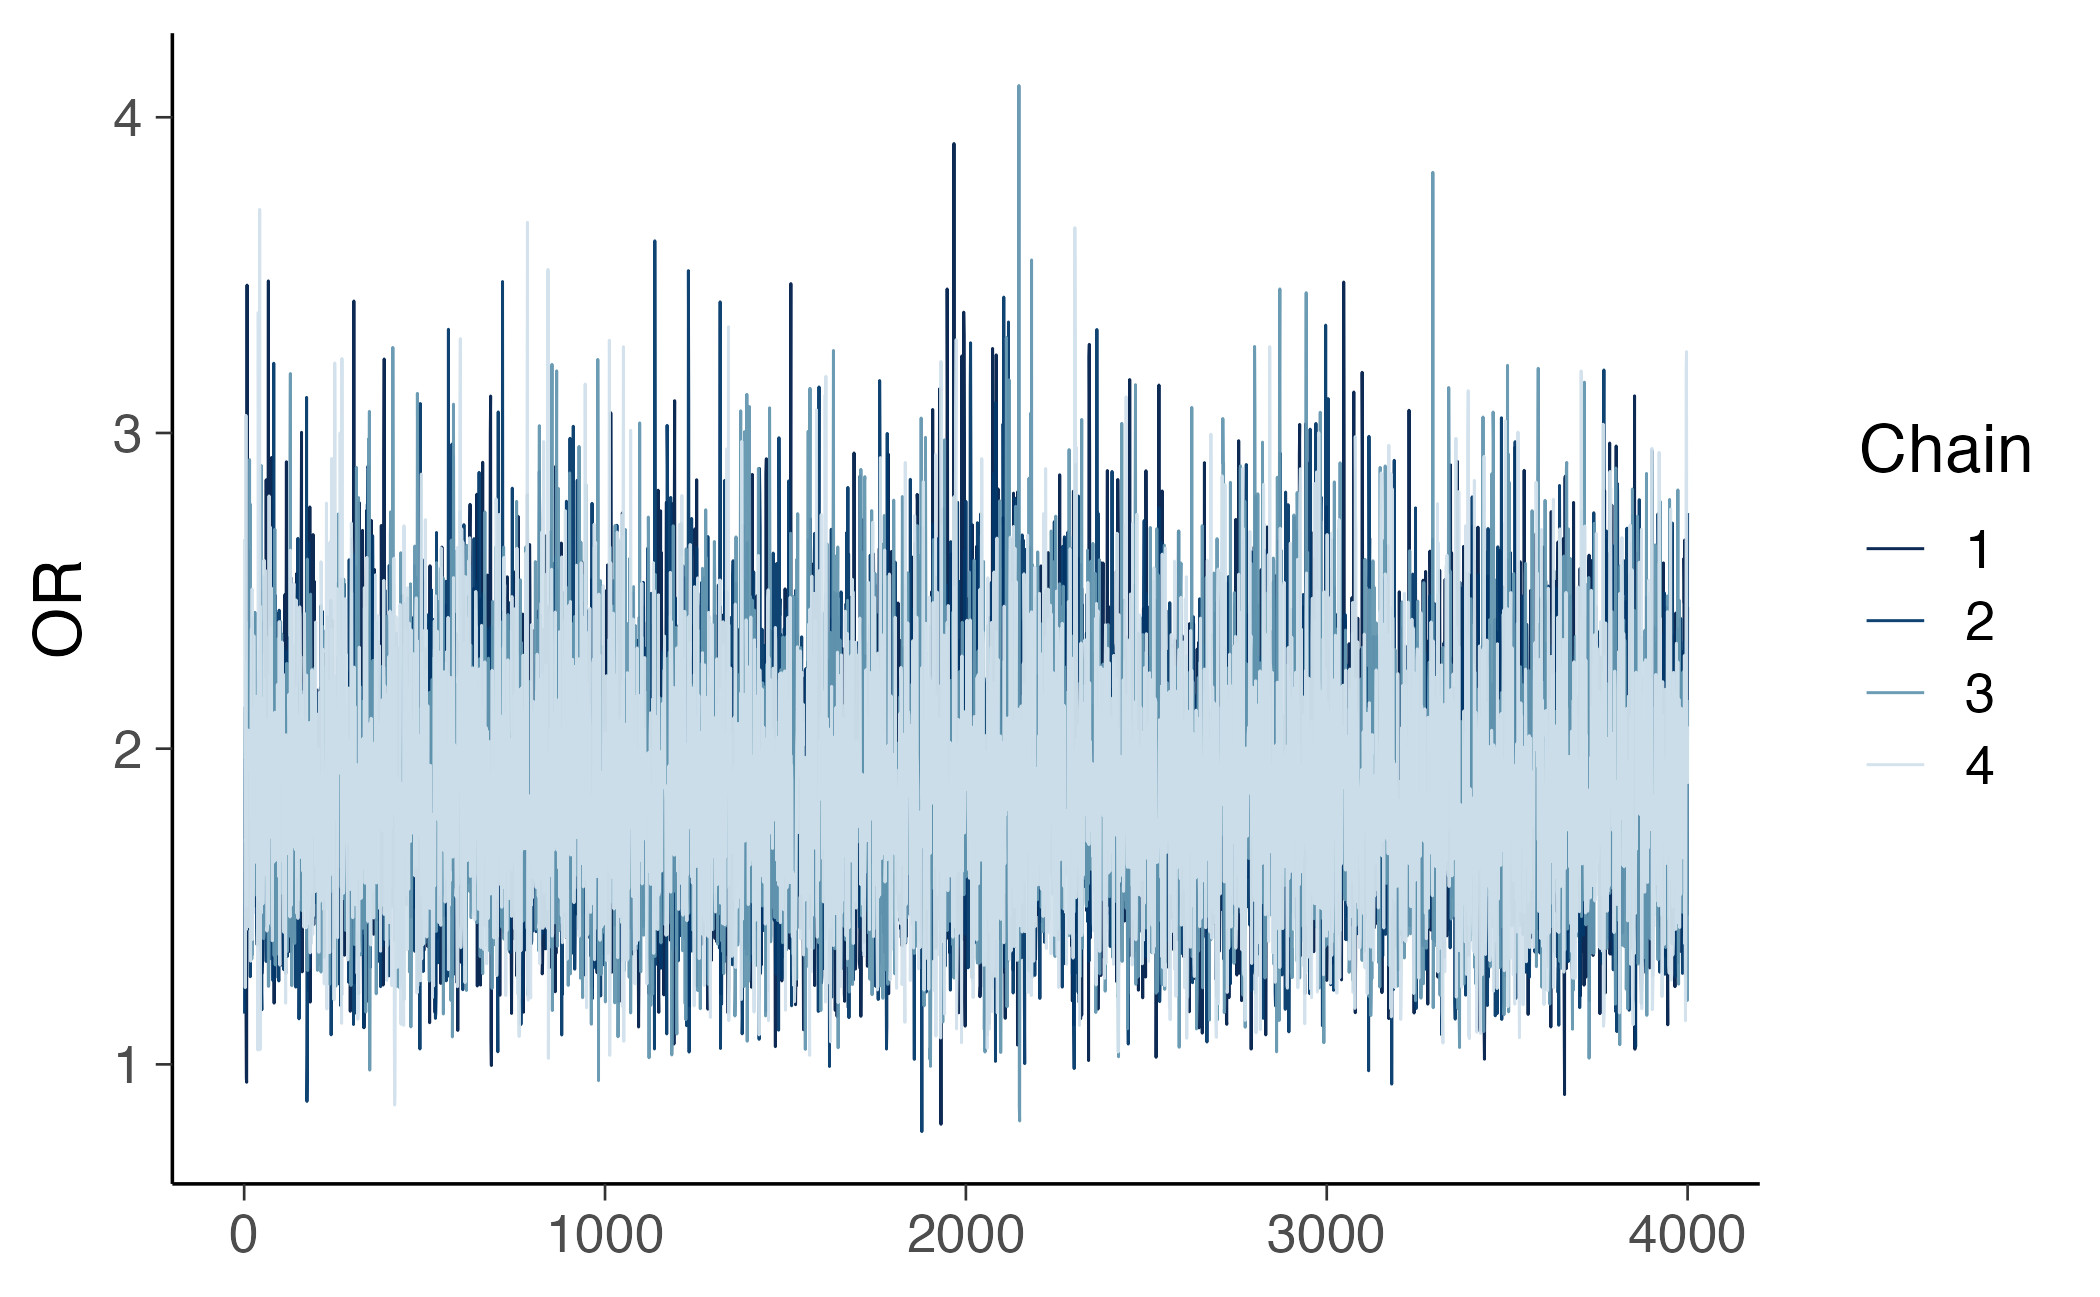
\includegraphics[width=0.85\linewidth,height=\textheight,keepaspectratio]{chapters/mcmc/04_stan_odds_ratio_stan_files/figure-pdf/unnamed-chunk-6-1.png}
\end{center}

Se emergono problemi (Rhat \textgreater{} 1.01, ESS basso, divergenze
riportate in output), conviene aumentare
\texttt{iter\_warmup}/\texttt{iter\_sampling}, alzare
\texttt{adapt\_delta} o, in ultima istanza, riconsiderare i prior se
sono eccessivamente stretti.

\subsubsection{Analisi dei risultati}\label{analisi-dei-risultati}

Riassunti posteriori per il modello Beta-Binomiale:

\begin{Shaded}
\begin{Highlighting}[]
\NormalTok{posterior}\SpecialCharTok{::}\FunctionTok{summarise\_draws}\NormalTok{(}
\NormalTok{  fit\_or\_beta}\SpecialCharTok{$}\FunctionTok{draws}\NormalTok{(}\FunctionTok{c}\NormalTok{(}\StringTok{"theta1"}\NormalTok{, }\StringTok{"theta2"}\NormalTok{, }\StringTok{"logOR"}\NormalTok{, }\StringTok{"OR"}\NormalTok{)),}
\NormalTok{  mean, sd, }\SpecialCharTok{\textasciitilde{}}\FunctionTok{quantile}\NormalTok{(.x, }\FunctionTok{c}\NormalTok{(}\FloatTok{0.025}\NormalTok{, }\FloatTok{0.5}\NormalTok{, }\FloatTok{0.975}\NormalTok{))}
\NormalTok{)}
\CommentTok{\#\textgreater{} \# A tibble: 4 x 6}
\CommentTok{\#\textgreater{}   variable  mean     sd \textasciigrave{}2.5\%\textasciigrave{} \textasciigrave{}50\%\textasciigrave{} \textasciigrave{}97.5\%\textasciigrave{}}
\CommentTok{\#\textgreater{}   \textless{}chr\textgreater{}    \textless{}dbl\textgreater{}  \textless{}dbl\textgreater{}  \textless{}dbl\textgreater{} \textless{}dbl\textgreater{}   \textless{}dbl\textgreater{}}
\CommentTok{\#\textgreater{} 1 theta1   0.647 0.0336  0.579 0.648   0.712}
\CommentTok{\#\textgreater{} 2 theta2   0.500 0.0350  0.432 0.500   0.569}
\CommentTok{\#\textgreater{} 3 logOR    0.610 0.204   0.207 0.611   1.00 }
\CommentTok{\#\textgreater{} 4 OR       1.88  0.387   1.23  1.84    2.73}
\end{Highlighting}
\end{Shaded}

L'output mostra media, deviazione standard, mediana e intervallo di
credibilità al 95\% per l'odds ratio.

Visualizzazione della distribuzione a posteriori:

\begin{Shaded}
\begin{Highlighting}[]
\NormalTok{bayesplot}\SpecialCharTok{::}\FunctionTok{mcmc\_areas}\NormalTok{(fit\_or\_beta}\SpecialCharTok{$}\FunctionTok{draws}\NormalTok{(}\StringTok{"OR"}\NormalTok{), }\AttributeTok{prob =} \FloatTok{0.95}\NormalTok{) }\SpecialCharTok{+}
  \FunctionTok{xlab}\NormalTok{(}\StringTok{"Odds Ratio"}\NormalTok{) }\SpecialCharTok{+} \FunctionTok{ylab}\NormalTok{(}\StringTok{"Densità"}\NormalTok{)}
\end{Highlighting}
\end{Shaded}

\begin{center}
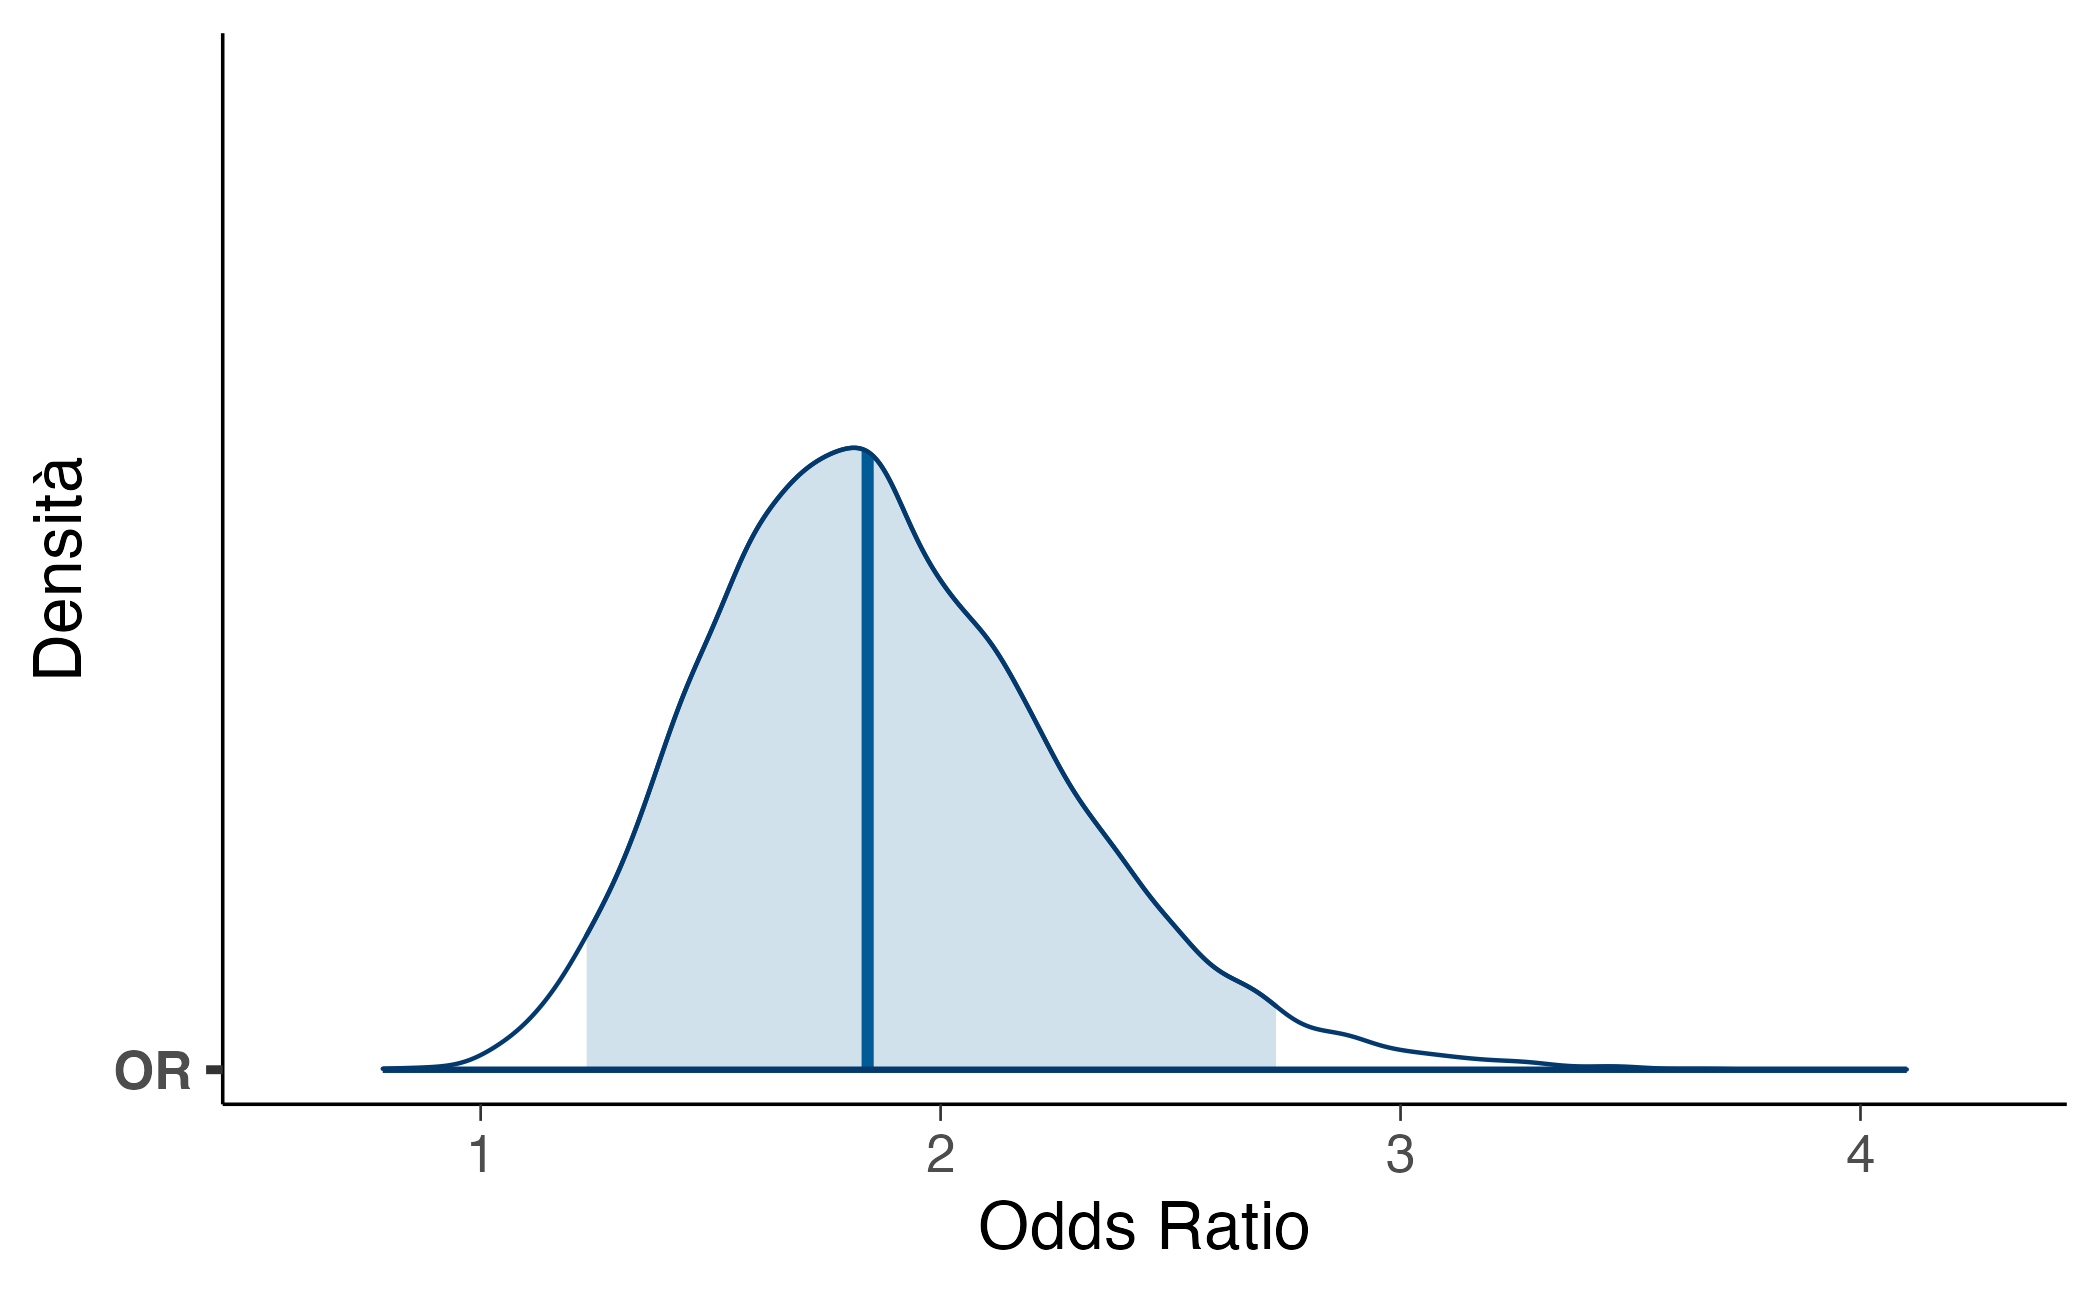
\includegraphics[width=0.85\linewidth,height=\textheight,keepaspectratio]{chapters/mcmc/04_stan_odds_ratio_stan_files/figure-pdf/unnamed-chunk-8-1.png}
\end{center}

Il grafico mostra chiaramente che la distribuzione dell'odds ratio è
concentrata su valori superiori a 1, con alta probabilità.

\textbf{Interpretazione:} i risultati indicano in modo credibile che
l'addestramento aumenti la tendenza delle api a scegliere il disco blu
rispetto al gruppo di controllo. La distribuzione a posteriori dell'OR è
fortemente concentrata su valori superiori a 1, evidenziando che
l'effetto è verosimilmente diverso dall'assenza di differenza e che la
preferenza osservata non può essere attribuita al solo caso.

\section{Relazione con la regressione
logistica}\label{relazione-con-la-regressione-logistica}

L'odds ratio può essere stimato in modo del tutto equivalente anche
attraverso un modello di \emph{regressione logistica}. Consideriamo il
modello:

\[
\text{logit}(p_i) = \alpha + \beta, x_i,
\] dove \(x_i\) è un indicatore del gruppo (0 = controllo, 1 =
sperimentale). In questa parametrizzazione, il coefficiente \(\beta\)
rappresenta la differenza tra i log-odds dei due gruppi, e la quantità
\(\exp(\beta)\) coincide esattamente con l'odds ratio sperimentale
rispetto al controllo.

Questo collegamento mostra come la regressione logistica generalizzi il
confronto tra due proporzioni: il modello esprime l'effetto in termini
di log-odds e consente di incorporare in modo naturale ulteriori
predittori, covariate e strutture gerarchiche. La stima dell'OR diventa
quindi un caso particolare di un framework più ampio e flessibile, in
grado di adattarsi a problemi inferenziali complessi tipici della
ricerca psicologica.

\subsection{Versione con modello
logistico}\label{versione-con-modello-logistico}

Nel modello logistico, i dati vengono rappresentati a livello
individuale: per ciascuna ape registriamo 1 se sceglie il disco blu e 0
in caso contrario.

\begin{Shaded}
\begin{Highlighting}[]
\CommentTok{\# Dati individuali}
\NormalTok{y }\OtherTok{\textless{}{-}} \FunctionTok{c}\NormalTok{(}\FunctionTok{rep}\NormalTok{(}\DecValTok{1}\NormalTok{, }\DecValTok{130}\NormalTok{), }\FunctionTok{rep}\NormalTok{(}\DecValTok{0}\NormalTok{, }\DecValTok{70}\NormalTok{),   }\CommentTok{\# gruppo sperimentale: 130 successi, 70 insuccessi}
       \FunctionTok{rep}\NormalTok{(}\DecValTok{1}\NormalTok{, }\DecValTok{100}\NormalTok{), }\FunctionTok{rep}\NormalTok{(}\DecValTok{0}\NormalTok{, }\DecValTok{100}\NormalTok{))  }\CommentTok{\# gruppo di controllo: 100 successi, 100 insuccessi}
\NormalTok{x }\OtherTok{\textless{}{-}} \FunctionTok{c}\NormalTok{(}\FunctionTok{rep}\NormalTok{(}\DecValTok{1}\NormalTok{, }\DecValTok{200}\NormalTok{), }\FunctionTok{rep}\NormalTok{(}\DecValTok{0}\NormalTok{, }\DecValTok{200}\NormalTok{))  }\CommentTok{\# 1 = sperimentale, 0 = controllo}

\NormalTok{data\_list }\OtherTok{\textless{}{-}} \FunctionTok{list}\NormalTok{(}\AttributeTok{N =} \FunctionTok{length}\NormalTok{(y), }\AttributeTok{y =}\NormalTok{ y, }\AttributeTok{x =}\NormalTok{ x)}
\FunctionTok{glimpse}\NormalTok{(data\_list)}
\CommentTok{\#\textgreater{} List of 3}
\CommentTok{\#\textgreater{}  $ N: int 400}
\CommentTok{\#\textgreater{}  $ y: num [1:400] 1 1 1 1 1 1 1 1 1 1 ...}
\CommentTok{\#\textgreater{}  $ x: num [1:400] 1 1 1 1 1 1 1 1 1 1 ...}
\end{Highlighting}
\end{Shaded}

\subsection{Specifica del modello in
Stan}\label{specifica-del-modello-in-stan}

\begin{Shaded}
\begin{Highlighting}[]
\NormalTok{stancode\_or }\OtherTok{\textless{}{-}} \StringTok{"}
\StringTok{data \{}
\StringTok{  int\textless{}lower=1\textgreater{} N;                  // numero totale di osservazioni}
\StringTok{  array[N] int\textless{}lower=0,upper=1\textgreater{} y; // esito binario (0/1)}
\StringTok{  vector[N] x;                     // variabile indicatrice del gruppo (0 = controllo, 1 = sperimentale)}
\StringTok{\}}
\StringTok{parameters \{}
\StringTok{  real alpha;    // intercetta (log{-}odds nel gruppo di controllo)}
\StringTok{  real beta;     // coefficiente (differenza in log{-}odds tra gruppo sperimentale e controllo)}
\StringTok{\}}
\StringTok{model \{}
\StringTok{  // Priors}
\StringTok{  alpha \textasciitilde{} normal(0, 5);}
\StringTok{  beta  \textasciitilde{} normal(0, 5);}
\StringTok{  }
\StringTok{  // Likelihood}
\StringTok{  y \textasciitilde{} bernoulli\_logit(alpha + beta * x);}
\StringTok{\}}
\StringTok{generated quantities \{}
\StringTok{  real OR = exp(beta);  // odds ratio}
\StringTok{\}}
\StringTok{"}
\end{Highlighting}
\end{Shaded}

In questo contesto, il coefficiente \(\beta\) quantifica la variazione
nei log-odds di scegliere il disco blu associata all'addestramento:
valori positivi indicano che le api addestrate mostrano una maggiore
propensione alla risposta corretta rispetto al gruppo di controllo.

\subsubsection{Compilazione ed esecuzione del
modello}\label{compilazione-ed-esecuzione-del-modello}

\begin{Shaded}
\begin{Highlighting}[]
\NormalTok{stanmod\_or }\OtherTok{\textless{}{-}}\NormalTok{ cmdstanr}\SpecialCharTok{::}\FunctionTok{cmdstan\_model}\NormalTok{(}\FunctionTok{write\_stan\_file}\NormalTok{(stancode\_or))}

\NormalTok{fit\_or }\OtherTok{\textless{}{-}}\NormalTok{ stanmod\_or}\SpecialCharTok{$}\FunctionTok{sample}\NormalTok{(}
  \AttributeTok{data =}\NormalTok{ data\_list,}
  \AttributeTok{iter\_warmup =} \DecValTok{1000}\NormalTok{,}
  \AttributeTok{iter\_sampling =} \DecValTok{4000}\NormalTok{,}
  \AttributeTok{chains =} \DecValTok{4}\NormalTok{,}
  \AttributeTok{seed =} \DecValTok{123}\NormalTok{,}
  \AttributeTok{refresh =} \DecValTok{0}
\NormalTok{)}
\end{Highlighting}
\end{Shaded}

\subsubsection{Interpretazione dei
risultati}\label{interpretazione-dei-risultati-2}

Il riepilogo dei parametri stimati è riportato di seguito:

\begin{Shaded}
\begin{Highlighting}[]
\FunctionTok{print}\NormalTok{(fit\_or}\SpecialCharTok{$}\FunctionTok{summary}\NormalTok{(}\FunctionTok{c}\NormalTok{(}\StringTok{"alpha"}\NormalTok{, }\StringTok{"beta"}\NormalTok{, }\StringTok{"OR"}\NormalTok{)), }\AttributeTok{n =} \ConstantTok{Inf}\NormalTok{)}
\CommentTok{\#\textgreater{} \# A tibble: 3 x 10}
\CommentTok{\#\textgreater{}   variable     mean   median    sd   mad     q5   q95  rhat ess\_bulk ess\_tail}
\CommentTok{\#\textgreater{}   \textless{}chr\textgreater{}       \textless{}dbl\textgreater{}    \textless{}dbl\textgreater{} \textless{}dbl\textgreater{} \textless{}dbl\textgreater{}  \textless{}dbl\textgreater{} \textless{}dbl\textgreater{} \textless{}dbl\textgreater{}    \textless{}dbl\textgreater{}    \textless{}dbl\textgreater{}}
\CommentTok{\#\textgreater{} 1 alpha    {-}0.00366 {-}0.00355 0.144 0.144 {-}0.240 0.232  1.00    5153.    6998.}
\CommentTok{\#\textgreater{} 2 beta      0.628    0.626   0.208 0.208  0.288 0.970  1.00    5183.    7043.}
\CommentTok{\#\textgreater{} 3 OR        1.91     1.87    0.403 0.386  1.33  2.64   1.00    5183.    7043.}
\end{Highlighting}
\end{Shaded}

Il parametro \texttt{alpha} rappresenta i log-odds di successo nel
gruppo di controllo; \texttt{beta} quantifica la variazione nei log-odds
introdotta dall'addestramento; infine, \texttt{OR\ =\ exp(beta)}
fornisce una misura direttamente interpretabile dell'effetto, indicando
di quanto variano gli odds di scegliere il disco blu nel gruppo
sperimentale rispetto al controllo.

Per una descrizione più completa dell'incertezza associata all'effetto,
consideriamo la distribuzione a posteriori dell'odds ratio:

\begin{Shaded}
\begin{Highlighting}[]
\NormalTok{posterior}\SpecialCharTok{::}\FunctionTok{summarise\_draws}\NormalTok{(}
\NormalTok{fit\_or}\SpecialCharTok{$}\FunctionTok{draws}\NormalTok{(}\StringTok{"OR"}\NormalTok{),}
\NormalTok{mean, sd, }\SpecialCharTok{\textasciitilde{}}\FunctionTok{quantile}\NormalTok{(.x, }\FunctionTok{c}\NormalTok{(}\FloatTok{0.025}\NormalTok{, }\FloatTok{0.5}\NormalTok{, }\FloatTok{0.975}\NormalTok{))}
\NormalTok{)}
\CommentTok{\#\textgreater{} \# A tibble: 1 x 6}
\CommentTok{\#\textgreater{}   variable  mean    sd \textasciigrave{}2.5\%\textasciigrave{} \textasciigrave{}50\%\textasciigrave{} \textasciigrave{}97.5\%\textasciigrave{}}
\CommentTok{\#\textgreater{}   \textless{}chr\textgreater{}    \textless{}dbl\textgreater{} \textless{}dbl\textgreater{}  \textless{}dbl\textgreater{} \textless{}dbl\textgreater{}   \textless{}dbl\textgreater{}}
\CommentTok{\#\textgreater{} 1 OR        1.91 0.403   1.25  1.87    2.82}
\end{Highlighting}
\end{Shaded}

La distribuzione può essere visualizzata in modo intuitivo tramite:

\begin{Shaded}
\begin{Highlighting}[]
\NormalTok{bayesplot}\SpecialCharTok{::}\FunctionTok{mcmc\_areas}\NormalTok{(fit\_or}\SpecialCharTok{$}\FunctionTok{draws}\NormalTok{(}\StringTok{"OR"}\NormalTok{), }\AttributeTok{prob =} \FloatTok{0.95}\NormalTok{) }\SpecialCharTok{+}
\FunctionTok{xlab}\NormalTok{(}\StringTok{"Odds Ratio"}\NormalTok{) }\SpecialCharTok{+} \FunctionTok{ylab}\NormalTok{(}\StringTok{"Densità"}\NormalTok{)}
\end{Highlighting}
\end{Shaded}

\begin{center}
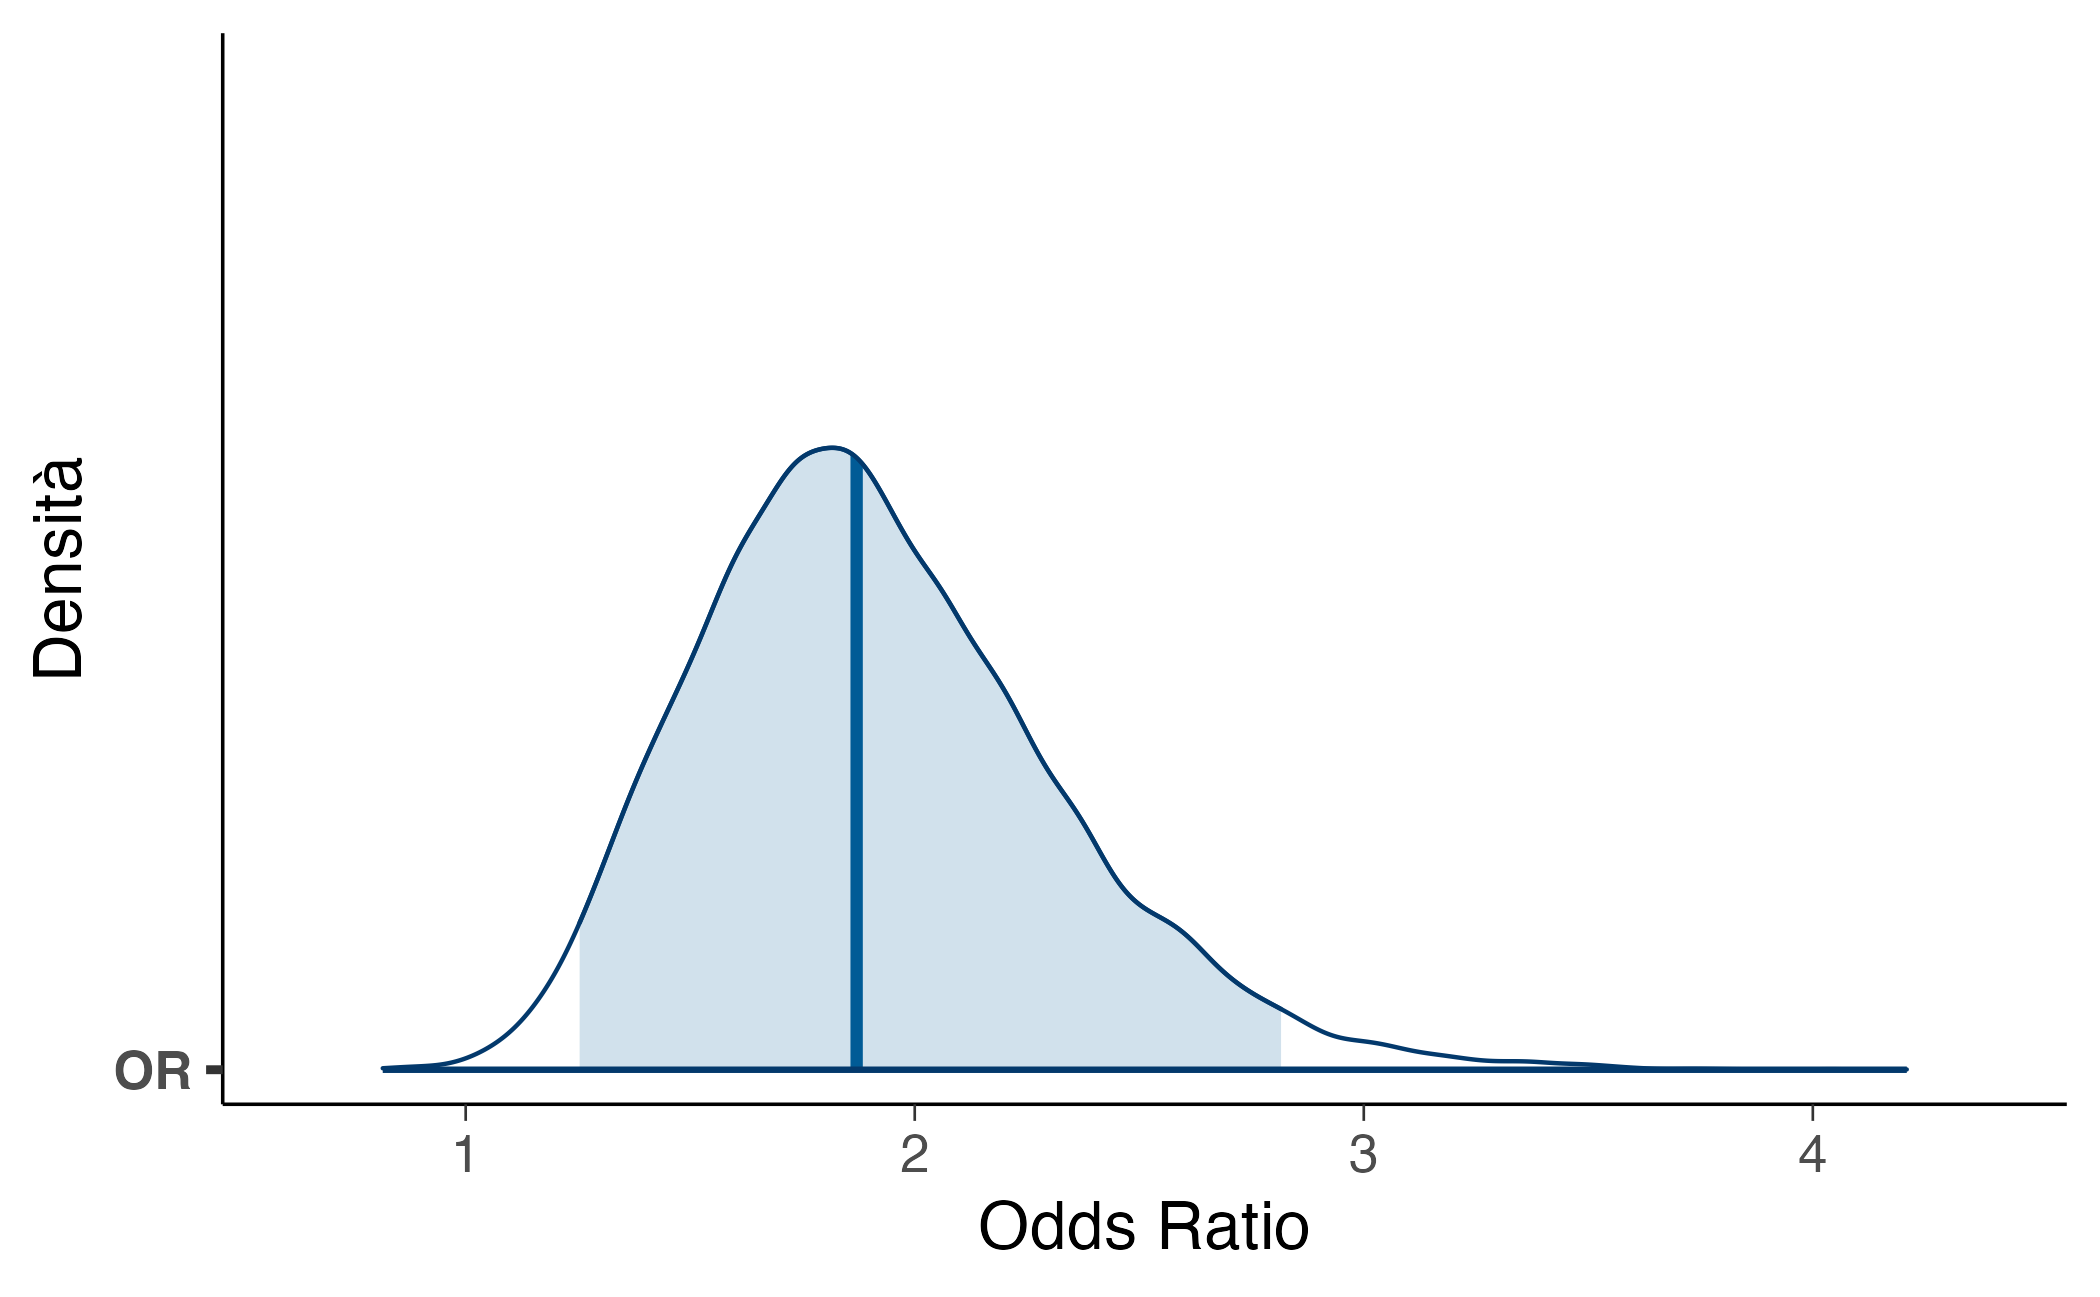
\includegraphics[width=0.85\linewidth,height=\textheight,keepaspectratio]{chapters/mcmc/04_stan_odds_ratio_stan_files/figure-pdf/unnamed-chunk-14-1.png}
\end{center}

\subsubsection{Diagnostica del modello}\label{diagnostica-del-modello}

Gli indicatori di convergenza confermano la qualità dell'adattamento:

\begin{Shaded}
\begin{Highlighting}[]
\NormalTok{posterior}\SpecialCharTok{::}\FunctionTok{summarize\_draws}\NormalTok{(}
\NormalTok{fit\_or}\SpecialCharTok{$}\FunctionTok{draws}\NormalTok{(}\FunctionTok{c}\NormalTok{(}\StringTok{"alpha"}\NormalTok{,}\StringTok{"beta"}\NormalTok{,}\StringTok{"OR"}\NormalTok{)),}
\StringTok{"rhat"}\NormalTok{, }\StringTok{"ess\_bulk"}\NormalTok{, }\StringTok{"ess\_tail"}
\NormalTok{)}
\CommentTok{\#\textgreater{} \# A tibble: 3 x 4}
\CommentTok{\#\textgreater{}   variable  rhat ess\_bulk ess\_tail}
\CommentTok{\#\textgreater{}   \textless{}chr\textgreater{}    \textless{}dbl\textgreater{}    \textless{}dbl\textgreater{}    \textless{}dbl\textgreater{}}
\CommentTok{\#\textgreater{} 1 alpha     1.00    5153.    6998.}
\CommentTok{\#\textgreater{} 2 beta      1.00    5183.    7043.}
\CommentTok{\#\textgreater{} 3 OR        1.00    5183.    7043.}

\NormalTok{bayesplot}\SpecialCharTok{::}\FunctionTok{mcmc\_trace}\NormalTok{(fit\_or}\SpecialCharTok{$}\FunctionTok{draws}\NormalTok{(}\StringTok{"OR"}\NormalTok{))}
\end{Highlighting}
\end{Shaded}

\begin{center}
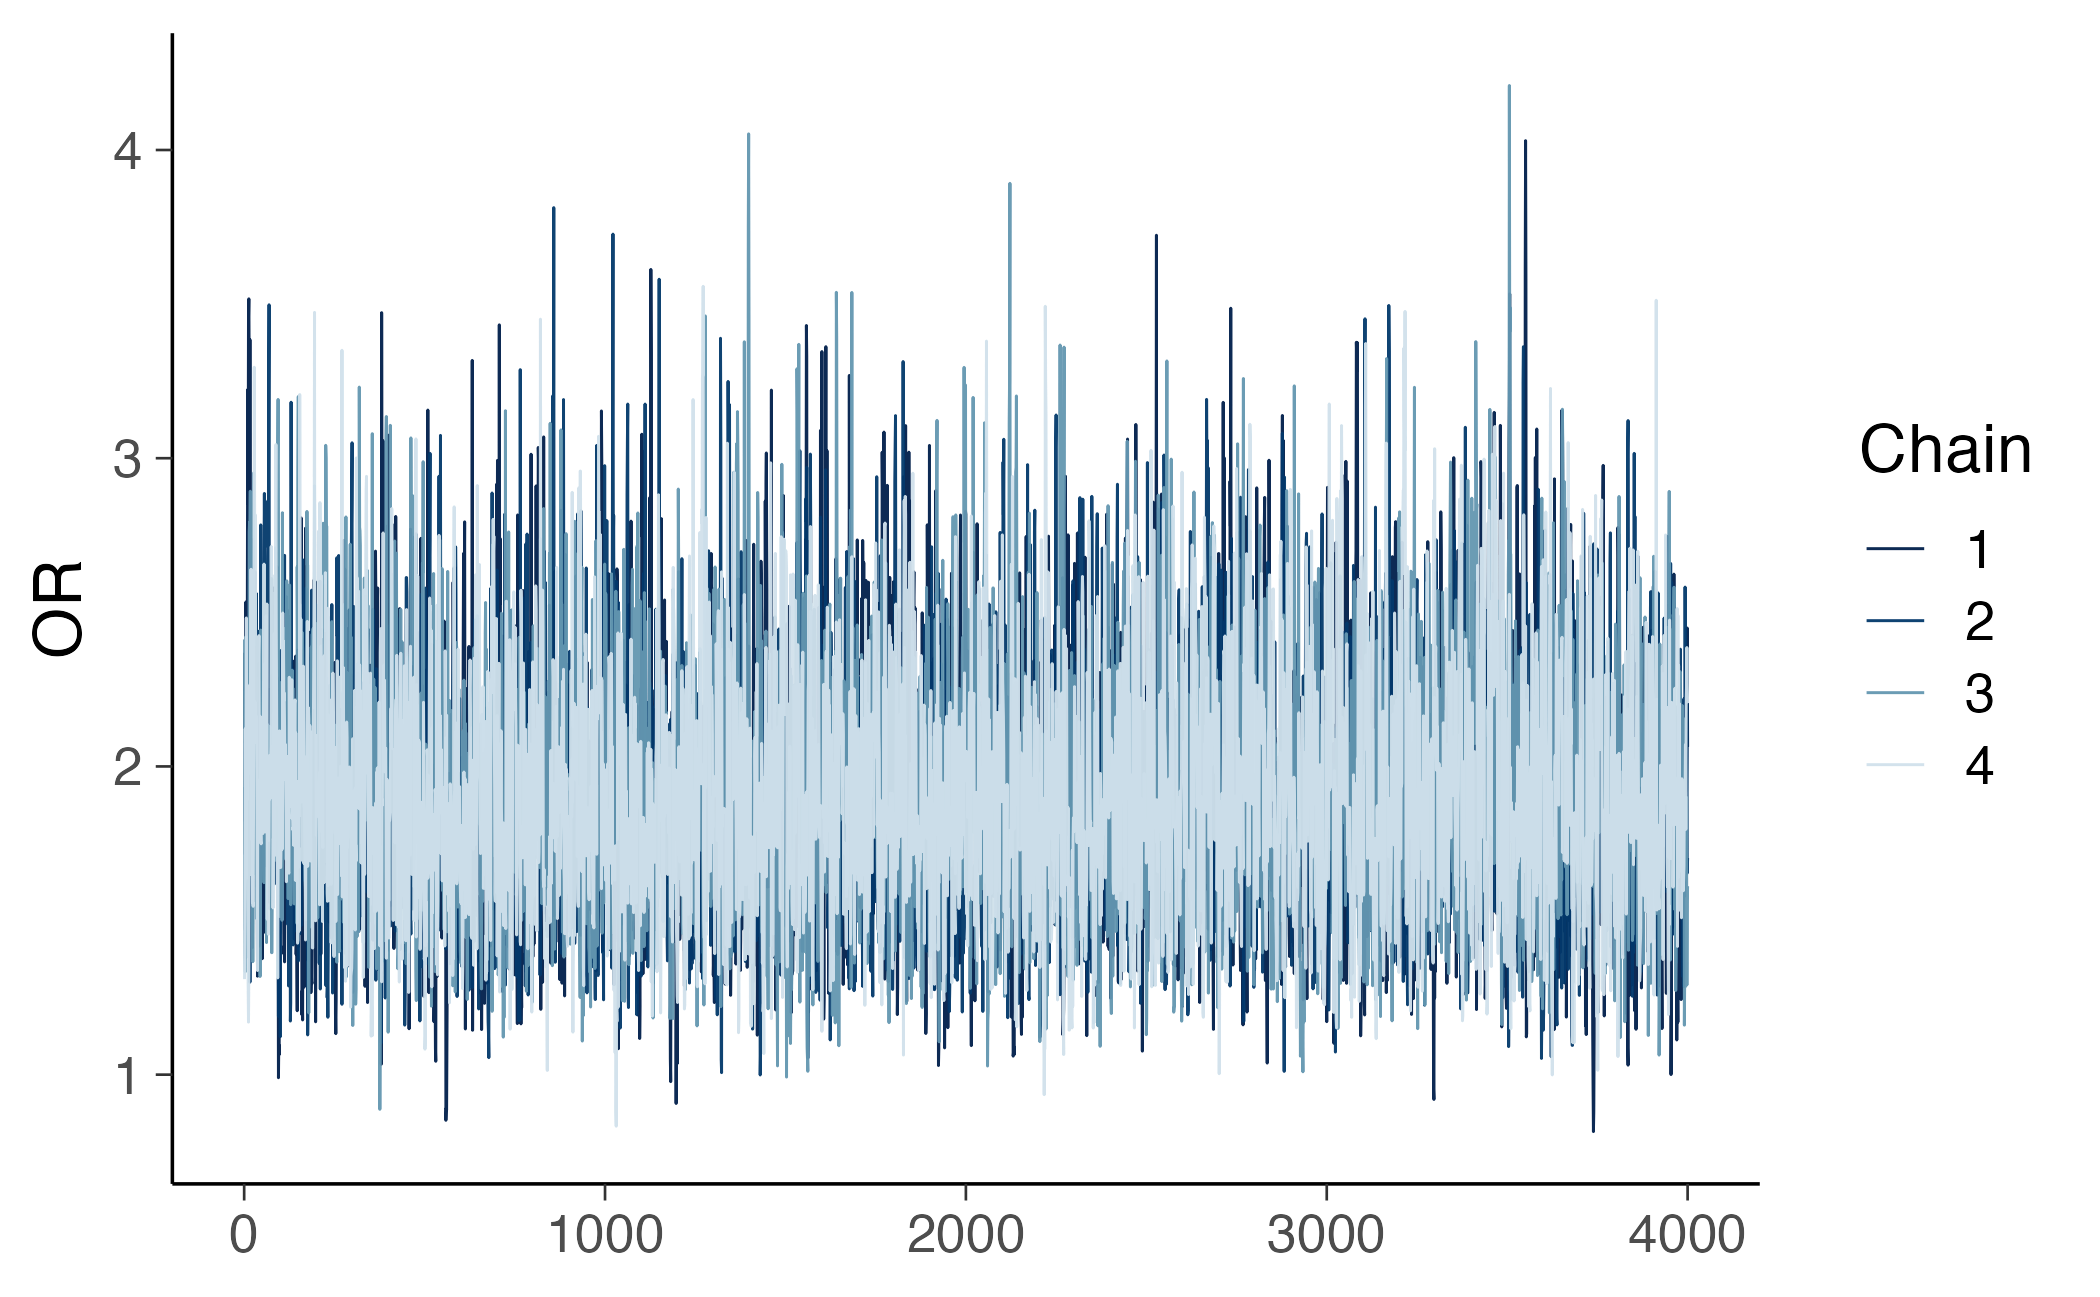
\includegraphics[width=0.85\linewidth,height=\textheight,keepaspectratio]{chapters/mcmc/04_stan_odds_ratio_stan_files/figure-pdf/unnamed-chunk-15-1.png}
\end{center}

\subsection{Analisi comparativa dei
risultati}\label{analisi-comparativa-dei-risultati}

Per verificare la coerenza tra i due approcci (modello Beta--Binomiale e
regressione logistica), confrontiamo gli intervalli di credibilità:

\begin{Shaded}
\begin{Highlighting}[]
\NormalTok{summ\_logit }\OtherTok{\textless{}{-}}\NormalTok{ posterior}\SpecialCharTok{::}\FunctionTok{summarise\_draws}\NormalTok{(}
\NormalTok{fit\_or}\SpecialCharTok{$}\FunctionTok{draws}\NormalTok{(}\StringTok{"OR"}\NormalTok{),}
\NormalTok{mean, sd, }\SpecialCharTok{\textasciitilde{}}\FunctionTok{quantile}\NormalTok{(.x, }\FunctionTok{c}\NormalTok{(}\FloatTok{0.025}\NormalTok{, }\FloatTok{0.5}\NormalTok{, }\FloatTok{0.975}\NormalTok{))}
\NormalTok{)}
\NormalTok{summ\_beta }\OtherTok{\textless{}{-}}\NormalTok{ posterior}\SpecialCharTok{::}\FunctionTok{summarise\_draws}\NormalTok{(}
\NormalTok{fit\_or\_beta}\SpecialCharTok{$}\FunctionTok{draws}\NormalTok{(}\StringTok{"OR"}\NormalTok{),}
\NormalTok{mean, sd, }\SpecialCharTok{\textasciitilde{}}\FunctionTok{quantile}\NormalTok{(.x, }\FunctionTok{c}\NormalTok{(}\FloatTok{0.025}\NormalTok{, }\FloatTok{0.5}\NormalTok{, }\FloatTok{0.975}\NormalTok{))}
\NormalTok{)}

\FunctionTok{list}\NormalTok{(}\AttributeTok{Regressione\_Logistica =}\NormalTok{ summ\_logit, }\AttributeTok{Beta\_Binomiale =}\NormalTok{ summ\_beta)}
\CommentTok{\#\textgreater{} $Regressione\_Logistica}
\CommentTok{\#\textgreater{} \# A tibble: 1 x 6}
\CommentTok{\#\textgreater{}   variable  mean    sd \textasciigrave{}2.5\%\textasciigrave{} \textasciigrave{}50\%\textasciigrave{} \textasciigrave{}97.5\%\textasciigrave{}}
\CommentTok{\#\textgreater{}   \textless{}chr\textgreater{}    \textless{}dbl\textgreater{} \textless{}dbl\textgreater{}  \textless{}dbl\textgreater{} \textless{}dbl\textgreater{}   \textless{}dbl\textgreater{}}
\CommentTok{\#\textgreater{} 1 OR        1.91 0.403   1.25  1.87    2.82}
\CommentTok{\#\textgreater{} }
\CommentTok{\#\textgreater{} $Beta\_Binomiale}
\CommentTok{\#\textgreater{} \# A tibble: 1 x 6}
\CommentTok{\#\textgreater{}   variable  mean    sd \textasciigrave{}2.5\%\textasciigrave{} \textasciigrave{}50\%\textasciigrave{} \textasciigrave{}97.5\%\textasciigrave{}}
\CommentTok{\#\textgreater{}   \textless{}chr\textgreater{}    \textless{}dbl\textgreater{} \textless{}dbl\textgreater{}  \textless{}dbl\textgreater{} \textless{}dbl\textgreater{}   \textless{}dbl\textgreater{}}
\CommentTok{\#\textgreater{} 1 OR        1.88 0.387   1.23  1.84    2.73}
\end{Highlighting}
\end{Shaded}

Anche la sovrapposizione delle distribuzioni posteriori evidenzia la
sostanziale equivalenza dei due modelli:

\begin{Shaded}
\begin{Highlighting}[]
\NormalTok{OR\_logit }\OtherTok{\textless{}{-}} \FunctionTok{as.numeric}\NormalTok{(fit\_or}\SpecialCharTok{$}\FunctionTok{draws}\NormalTok{(}\StringTok{"OR"}\NormalTok{))}
\NormalTok{OR\_beta }\OtherTok{\textless{}{-}} \FunctionTok{as.numeric}\NormalTok{(fit\_or\_beta}\SpecialCharTok{$}\FunctionTok{draws}\NormalTok{(}\StringTok{"OR"}\NormalTok{))}

\FunctionTok{tibble}\NormalTok{(}
\AttributeTok{OR =} \FunctionTok{c}\NormalTok{(OR\_logit, OR\_beta),}
\AttributeTok{Modello =} \FunctionTok{rep}\NormalTok{(}\FunctionTok{c}\NormalTok{(}\StringTok{"Regressione Logistica"}\NormalTok{, }\StringTok{"Beta{-}Binomiale"}\NormalTok{),}
\FunctionTok{c}\NormalTok{(}\FunctionTok{length}\NormalTok{(OR\_logit), }\FunctionTok{length}\NormalTok{(OR\_beta)))}
\NormalTok{) }\SpecialCharTok{|\textgreater{}}
\FunctionTok{ggplot}\NormalTok{(}\FunctionTok{aes}\NormalTok{(}\AttributeTok{x =}\NormalTok{ OR, }\AttributeTok{fill =}\NormalTok{ Modello)) }\SpecialCharTok{+}
\FunctionTok{geom\_density}\NormalTok{(}\AttributeTok{alpha =} \FloatTok{0.4}\NormalTok{) }\SpecialCharTok{+}
\FunctionTok{labs}\NormalTok{(}\AttributeTok{x =} \StringTok{"Odds Ratio"}\NormalTok{, }\AttributeTok{y =} \StringTok{"Densità"}\NormalTok{)}
\end{Highlighting}
\end{Shaded}

\begin{center}
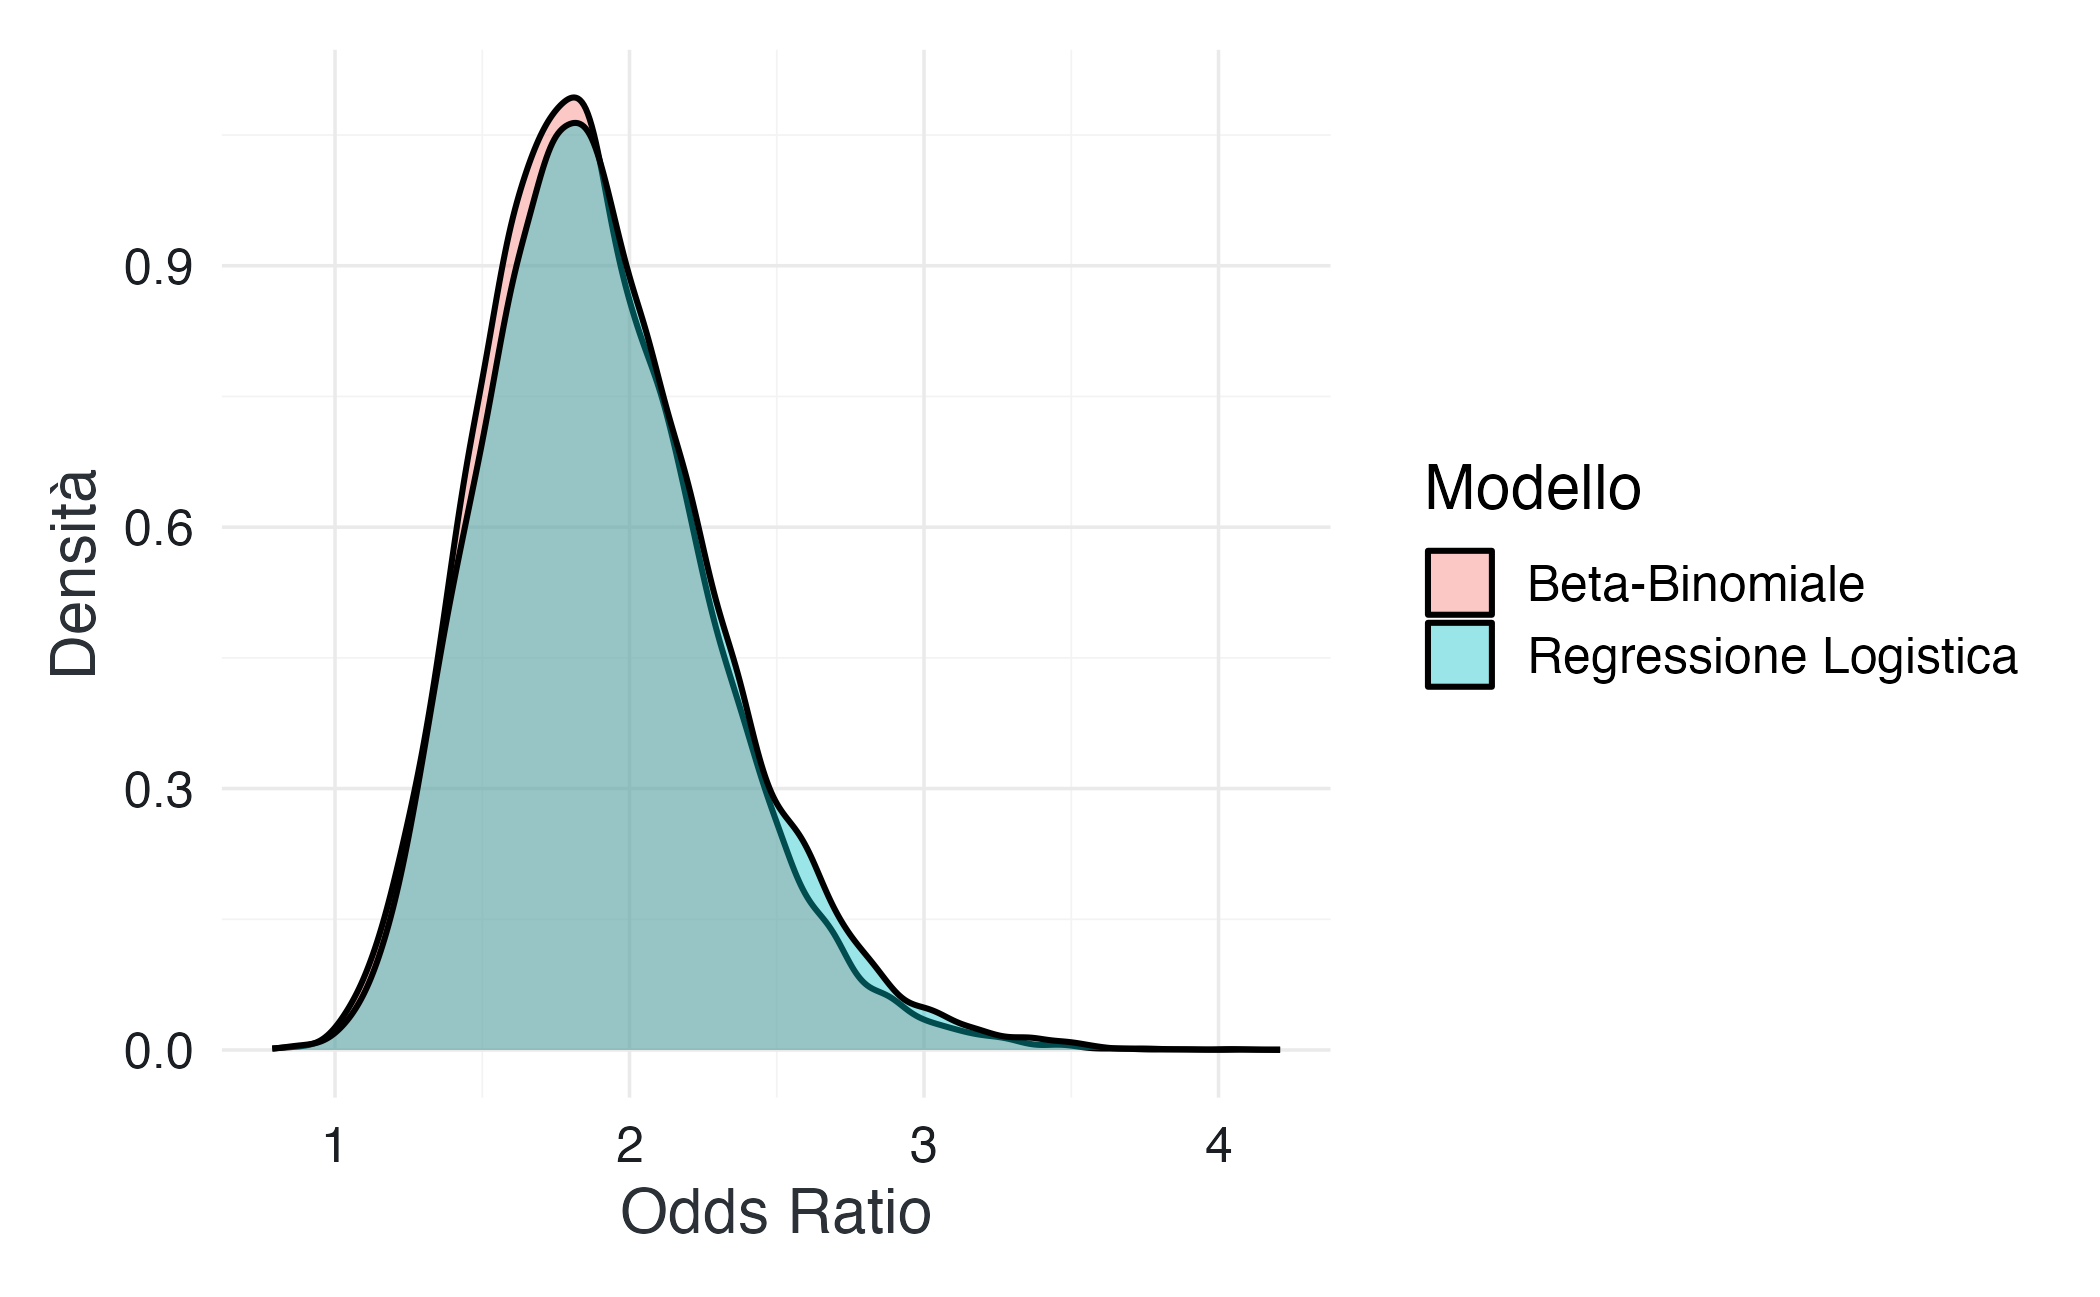
\includegraphics[width=0.85\linewidth,height=\textheight,keepaspectratio]{chapters/mcmc/04_stan_odds_ratio_stan_files/figure-pdf/unnamed-chunk-17-1.png}
\end{center}

Un confronto diretto della probabilità a posteriori che l'OR sia
maggiore di 1 conferma ulteriormente la convergenza dei risultati:

\begin{Shaded}
\begin{Highlighting}[]
\FunctionTok{c}\NormalTok{(}
\AttributeTok{Regressione\_Logistica =} \FunctionTok{mean}\NormalTok{(OR\_logit }\SpecialCharTok{\textgreater{}} \DecValTok{1}\NormalTok{),}
\AttributeTok{Beta\_Binomiale =} \FunctionTok{mean}\NormalTok{(OR\_beta }\SpecialCharTok{\textgreater{}} \DecValTok{1}\NormalTok{)}
\NormalTok{)}
\CommentTok{\#\textgreater{} Regressione\_Logistica        Beta\_Binomiale }
\CommentTok{\#\textgreater{}                 0.999                 0.999}
\end{Highlighting}
\end{Shaded}

\section{Considerazioni
metodologiche}\label{considerazioni-metodologiche}

I due modelli restituiscono inferenze pressoché identiche: in entrambi i
casi l'addestramento aumenta in modo credibile la probabilità di
scegliere il disco blu. La differenza tra i due approcci riguarda
soprattutto la parametrizzazione e la struttura dei dati:

\begin{itemize}
\tightlist
\item
  \textbf{Regressione logistica}: adatta a dati individuali e facilmente
  estensibile a modelli multivariati o gerarchici; fornisce un quadro
  generale per analisi più complesse.
\item
  \textbf{Modello Beta--Binomiale}: particolarmente intuitivo quando i
  dati sono aggregabili in tabelle di contingenza; offre una lettura
  diretta dei parametri come proporzioni di successo nei gruppi.
\end{itemize}

In sintesi, entrambi gli approcci modellano lo stesso effetto in maniera
coerente. La scelta tra l'uno e l'altro dipende dal livello di
granularità dei dati e dagli obiettivi dell'analisi, non dall'effetto
inferenziale finale.

\section*{Riflessioni conclusive}\label{riflessioni-conclusive-15}

\markright{Riflessioni conclusive}

Questo capitolo ha mostrato come l'inferenza bayesiana sulle
proporzioni, inizialmente introdotta tramite soluzioni analitiche e
metodi a griglia, possa essere implementata in modo naturale e altamente
flessibile in Stan. L'esempio dell'odds ratio ha messo in luce un
aspetto fondamentale: l'approccio bayesiano mantiene inalterate le
proprie basi concettuali, mentre l'uso di Stan ne amplia notevolmente il
campo di applicazione.

Due aspetti meritano particolare attenzione. In primo luogo, la
continuità concettuale. Stan non modifica l'architettura dell'inferenza
bayesiana, ma al centro rimane sempre il campionamento dalla
distribuzione a posteriori che consente di quantificare in modo
trasparente l'incertezza sui parametri. Ciò che cambia è la capacità di
applicare lo stesso principio a modelli che non hanno soluzioni chiuse o
che sarebbero troppo complessi da trattare con metodi manuali o
approssimazioni semplicistiche.

In secondo luogo, l'esempio discusso mostra l'importanza pratica di
questo ampliamento. La stima dell'odds ratio, un problema metodologico
ben noto in psicologia, diventa un'occasione per familiarizzare con Stan
in un contesto concettualmente accessibile. Da ciò emerge chiaramente
come Stan possa diventare uno strumento di uso quotidiano, dalla
modellazione delle proporzioni alle analisi con covariate, fino ai
modelli per i conteggi, ai processi dinamici e alle strutture
gerarchiche.

In questa prospettiva, il capitolo rappresenta un punto di svolta
metodologico. L'inferenza bayesiana non è più confinata a esempi
didattici o modelli elementari, ma si configura come un quadro operativo
completo, riproducibile e adatto a qualsiasi tipo di dato psicologico.
Stan diventa quindi la piattaforma che rende possibile questa
transizione, fornendo gli strumenti per affrontare in modo coerente e
rigoroso le analisi più avanzate del volume.

\begin{tcolorbox}[enhanced jigsaw, arc=.35mm, bottomrule=.15mm, bottomtitle=1mm, breakable, colback=white, colbacktitle=quarto-callout-note-color!10!white, colframe=quarto-callout-note-color-frame, coltitle=black, left=2mm, leftrule=.75mm, opacityback=0, opacitybacktitle=0.6, rightrule=.15mm, title=\textcolor{quarto-callout-note-color}{\faInfo}\hspace{0.5em}{Informazioni sull'ambiente di sviluppo}, titlerule=0mm, toprule=.15mm, toptitle=1mm]

\begin{Shaded}
\begin{Highlighting}[]
\FunctionTok{sessionInfo}\NormalTok{()}
\CommentTok{\#\textgreater{} R version 4.6.1 (2026{-}06{-}24)}
\CommentTok{\#\textgreater{} Platform: aarch64{-}apple{-}darwin23}
\CommentTok{\#\textgreater{} Running under: macOS Tahoe 26.5.2}
\CommentTok{\#\textgreater{} }
\CommentTok{\#\textgreater{} Matrix products: default}
\CommentTok{\#\textgreater{} BLAS:   /Library/Frameworks/R.framework/Versions/4.6/Resources/lib/libRblas.0.dylib }
\CommentTok{\#\textgreater{} LAPACK: /Library/Frameworks/R.framework/Versions/4.6/Resources/lib/libRlapack.dylib;  LAPACK version 3.12.1}
\CommentTok{\#\textgreater{} }
\CommentTok{\#\textgreater{} locale:}
\CommentTok{\#\textgreater{} [1] C.UTF{-}8/UTF{-}8/C.UTF{-}8/C/C.UTF{-}8/C.UTF{-}8}
\CommentTok{\#\textgreater{} }
\CommentTok{\#\textgreater{} time zone: Europe/Zagreb}
\CommentTok{\#\textgreater{} tzcode source: internal}
\CommentTok{\#\textgreater{} }
\CommentTok{\#\textgreater{} attached base packages:}
\CommentTok{\#\textgreater{} [1] stats     graphics  grDevices utils     datasets  methods   base     }
\CommentTok{\#\textgreater{} }
\CommentTok{\#\textgreater{} other attached packages:}
\CommentTok{\#\textgreater{}  [1] cmdstanr\_0.9.0        ragg\_1.5.2            tinytable\_0.17.0     }
\CommentTok{\#\textgreater{}  [4] withr\_3.0.3           systemfonts\_1.3.2     patchwork\_1.3.2      }
\CommentTok{\#\textgreater{}  [7] ggdist\_3.3.3          tidybayes\_3.0.7       bayesplot\_1.15.0     }
\CommentTok{\#\textgreater{} [10] ggplot2\_4.0.3         reliabilitydiag\_0.2.1 priorsense\_1.2.0     }
\CommentTok{\#\textgreater{} [13] posterior\_1.7.0       loo\_2.10.0            rstan\_2.32.7         }
\CommentTok{\#\textgreater{} [16] StanHeaders\_2.32.10   brms\_2.23.0           Rcpp\_1.1.2           }
\CommentTok{\#\textgreater{} [19] sessioninfo\_1.2.4     conflicted\_1.2.0      janitor\_2.2.1        }
\CommentTok{\#\textgreater{} [22] matrixStats\_1.5.0     modelr\_0.1.11         tibble\_3.3.1         }
\CommentTok{\#\textgreater{} [25] dplyr\_1.2.1           tidyr\_1.3.2           rio\_1.3.0            }
\CommentTok{\#\textgreater{} [28] here\_1.0.2           }
\CommentTok{\#\textgreater{} }
\CommentTok{\#\textgreater{} loaded via a namespace (and not attached):}
\CommentTok{\#\textgreater{}  [1] svUnit\_1.0.8          tidyselect\_1.2.1      farver\_2.1.2         }
\CommentTok{\#\textgreater{}  [4] S7\_0.2.2              fastmap\_1.2.0         tensorA\_0.36.2.1     }
\CommentTok{\#\textgreater{}  [7] digest\_0.6.39         timechange\_0.4.0      estimability\_2.0.0   }
\CommentTok{\#\textgreater{} [10] lifecycle\_1.0.5       processx\_3.9.0        magrittr\_2.0.5       }
\CommentTok{\#\textgreater{} [13] compiler\_4.6.1        rlang\_1.3.0           tools\_4.6.1          }
\CommentTok{\#\textgreater{} [16] utf8\_1.2.6            yaml\_2.3.12           data.table\_1.18.4    }
\CommentTok{\#\textgreater{} [19] knitr\_1.51            labeling\_0.4.3        bridgesampling\_1.2{-}1 }
\CommentTok{\#\textgreater{} [22] pkgbuild\_1.4.8        curl\_7.1.0            plyr\_1.8.9           }
\CommentTok{\#\textgreater{} [25] RColorBrewer\_1.1{-}3    abind\_1.4{-}8           purrr\_1.2.2          }
\CommentTok{\#\textgreater{} [28] grid\_4.6.1            stats4\_4.6.1          xtable\_1.8{-}8         }
\CommentTok{\#\textgreater{} [31] inline\_0.3.21         ggridges\_0.5.7        emmeans\_2.0.4        }
\CommentTok{\#\textgreater{} [34] scales\_1.4.0          cli\_3.6.6             mvtnorm\_1.4{-}2        }
\CommentTok{\#\textgreater{} [37] rmarkdown\_2.31        generics\_0.1.4        otel\_0.2.0           }
\CommentTok{\#\textgreater{} [40] RcppParallel\_5.1.11{-}2 reshape2\_1.4.5        cachem\_1.1.0         }
\CommentTok{\#\textgreater{} [43] stringr\_1.6.0         parallel\_4.6.1        vctrs\_0.7.3          }
\CommentTok{\#\textgreater{} [46] V8\_8.2.0              Matrix\_1.7{-}5          jsonlite\_2.0.0       }
\CommentTok{\#\textgreater{} [49] arrayhelpers\_1.1{-}1    glue\_1.8.1            ps\_1.9.3             }
\CommentTok{\#\textgreater{} [52] codetools\_0.2{-}20      distributional\_0.8.1  lubridate\_1.9.5      }
\CommentTok{\#\textgreater{} [55] stringi\_1.8.7         gtable\_0.3.6          QuickJSR\_1.10.0      }
\CommentTok{\#\textgreater{} [58] pillar\_1.11.1         htmltools\_0.5.9       Brobdingnag\_1.2{-}9    }
\CommentTok{\#\textgreater{} [61] R6\_2.6.1              textshaping\_1.0.5     rprojroot\_2.1.1      }
\CommentTok{\#\textgreater{} [64] evaluate\_1.0.5        lattice\_0.22{-}9        backports\_1.5.1      }
\CommentTok{\#\textgreater{} [67] memoise\_2.0.1         broom\_1.0.13          snakecase\_0.11.1     }
\CommentTok{\#\textgreater{} [70] rstantools\_2.6.0      coda\_0.19{-}4.1         gridExtra\_2.3.1      }
\CommentTok{\#\textgreater{} [73] nlme\_3.1{-}170          checkmate\_2.3.4       xfun\_0.60            }
\CommentTok{\#\textgreater{} [76] pkgconfig\_2.0.3}
\end{Highlighting}
\end{Shaded}

\end{tcolorbox}

\section*{Bibliografia}\label{bibliografia-17}

\markright{Bibliografia}

\chapter{Confrontare due medie}\label{sec-mcmc-two-means}

\begin{tcolorbox}[enhanced jigsaw, arc=.35mm, bottomrule=.15mm, breakable, colback=white, colframe=quarto-callout-note-color-frame, left=2mm, leftrule=.75mm, opacityback=0, rightrule=.15mm, toprule=.15mm]

Nel manuale didattico, il \emph{confronto tra due medie} viene
presentato nell'ambito della \emph{regressione lineare con un predittore
dicotomico} (0 = controllo, 1 = intervento). In quella sede si mostra
che la differenza tra le medie di gruppo coincide con il coefficiente
del predittore, e come l'incertezza su tale differenza corrisponda alla
varianza stimata del coefficiente stesso.

In questo capitolo affronteremo lo stesso problema, ma adottando
un'ottica \emph{generativa-bayesiana mediante Stan}. Questo approccio ci
consentirà di: (i) rendere esplicite le assunzioni stocastiche
sottostanti il processo generativo dei dati, (ii) specificare
\emph{prior} debolmente informative, coerenti con una variabile
standardizzata, (iii) stimare \emph{congiuntamente} la differenza tra le
medie e la differenza tra le varianze, e (iv) scegliere tra modelli
sulla base della loro capacità predittiva, utilizzando l'ELPD calcolato
con PSIS-LOO.

\end{tcolorbox}

\begin{tcolorbox}[enhanced jigsaw, arc=.35mm, bottomrule=.15mm, breakable, colback=white, colframe=quarto-callout-important-color-frame, left=2mm, leftrule=.75mm, opacityback=0, rightrule=.15mm, toprule=.15mm]

\textbf{Da sapere.} Il confronto tra due medie può essere formulato come
un modello generativo oppure come una regressione con un predittore
dicotomico: la differenza tra i gruppi coincide con il coefficiente del
predittore. L'inferenza riguarda l'intera distribuzione a posteriori
della differenza tra le medie e, quando necessario, della differenza tra
le varianze. La scelta tra un modello a varianza comune e uno a varianze
distinte va valutata anche in termini predittivi.

\textbf{Da saper fare.} Leggere i programmi Stan forniti, riconoscendo
dati, parametri, prior, verosimiglianza e quantità generate;
interpretare la distribuzione a posteriori di \texttt{diff\_mu} e
\texttt{diff\_sigma}, gli intervalli di credibilità e le probabilità
rispetto a una ROPE. Valutare l'adeguatezza dei modelli con i
\emph{posterior predictive checks}. Nel percorso essenziale non è
richiesto scrivere autonomamente il codice Stan.

\textbf{Approfondimento facoltativo.} La simulazione dei dati, la
compilazione e l'esecuzione dei programmi con \texttt{cmdstanr}, la
diagnostica MCMC dettagliata, il calcolo operativo dell'ELPD, il
confrontare i modelli mediante PSIS-LOO e le estensioni robuste con
distribuzione \emph{t} di Student possono essere rimandati. Se lavori
soltanto con \texttt{brms}, puoi leggere le specifiche Stan come
traduzione del modello generativo e svolgere la stima nel corrispondente
capitolo sui modelli lineari.

\hyperref[sec-percorsi-lettura]{Che cosa significano queste etichette?}

\end{tcolorbox}

\section*{Panoramica del capitolo}\label{panoramica-del-capitolo-4}

\markright{Panoramica del capitolo}

\begin{itemize}
\tightlist
\item
  Comprendere il problema del confronto tra due medie in un'ottica
  bayesiana.
\item
  Motivare la standardizzazione dei dati e la scelta di \emph{prior}
  debolmente informative.
\item
  Implementare in \emph{Stan} un modello con varianza comune e uno con
  varianze distinte.
\item
  Valutare la capacità predittiva dei modelli attraverso PSIS-LOO.
\item
  Interpretare la distribuzione a posteriori della differenza tra le
  medie e le verifiche predittive.
\end{itemize}

\begin{tcolorbox}[enhanced jigsaw, arc=.35mm, bottomrule=.15mm, bottomtitle=1mm, breakable, colback=white, colbacktitle=quarto-callout-caution-color!10!white, colframe=quarto-callout-caution-color-frame, coltitle=black, left=2mm, leftrule=.75mm, opacityback=0, opacitybacktitle=0.6, rightrule=.15mm, title=\textcolor{quarto-callout-caution-color}{\faFire}\hspace{0.5em}{Preparazione del Notebook}, titlerule=0mm, toprule=.15mm, toptitle=1mm]

\begin{Shaded}
\begin{Highlighting}[]
\NormalTok{here}\SpecialCharTok{::}\FunctionTok{here}\NormalTok{(}\StringTok{"code"}\NormalTok{, }\StringTok{"\_common.R"}\NormalTok{) }\SpecialCharTok{|\textgreater{}} 
  \FunctionTok{source}\NormalTok{()}

\ControlFlowTok{if}\NormalTok{ (}\SpecialCharTok{!}\FunctionTok{requireNamespace}\NormalTok{(}\StringTok{"pacman"}\NormalTok{)) }\FunctionTok{install.packages}\NormalTok{(}\StringTok{"pacman"}\NormalTok{)}
\NormalTok{pacman}\SpecialCharTok{::}\FunctionTok{p\_load}\NormalTok{(cmdstanr, posterior, bayesplot, ggplot2, dplyr, tibble, forcats)}
\FunctionTok{conflicts\_prefer}\NormalTok{(posterior}\SpecialCharTok{::}\NormalTok{ess\_bulk)}
\FunctionTok{conflicts\_prefer}\NormalTok{(posterior}\SpecialCharTok{::}\NormalTok{ess\_tail)}
\end{Highlighting}
\end{Shaded}

\end{tcolorbox}

\section{Una descrizione completa della nostra credenza sulla differenza
tra
medie}\label{una-descrizione-completa-della-nostra-credenza-sulla-differenza-tra-medie}

Per illustrare l'uso di Stan in un confronto tra due gruppi,
consideriamo uno studio sul punteggio medio settimanale di affetto
negativo condotto su un gruppo sperimentale che segue un training di
mindfulness e su un gruppo di controllo. In questo contesto, la domanda
di ricerca non si limita a verificare l'esistenza di un effetto, ma mira
a quantificarlo in modo completo, determinando di quanto i gruppi
differiscano e valutando quanta incertezza circondi questa stima. La
nostra prospettiva consiste quindi nel stimare l'intera distribuzione a
posteriori della differenza tra le medie, al fine di ottenere
affermazioni probabilistiche direttamente applicabili alla pratica
psicologica.

Un aspetto cruciale, spesso trascurato, è la variabilità. Il training
potrebbe infatti ridurre l'affetto negativo medio, ma al tempo stesso
aumentare l'eterogeneità delle risposte individuali. In tal caso, la
differenza tra le deviazioni standard dei due gruppi ha un'importanza
paragonabile a quella delle medie. L'inferenza bayesiana permette di
stimare entrambe le quantità insieme alla loro incertezza in modo
naturale.

Per stabilizzare le stime e semplificare la scelta delle \emph{prior},
standardizziamo la variabile di esito sull'intero campione (media 0,
deviazione standard 1). Lavoreremo con due modelli complementari: uno
che assume varianze comuni e uno che ammette varianze distinte. In
entrambi i casi, useremo \emph{prior} normali centrate su zero per le
medie e \emph{prior} esponenziali per le deviazioni standard, in
coerenza con la scala standardizzata.

L'obiettivo non è stabilire quale modello sia ``vero'', ma quale predica
meglio i nuovi dati simili ai nostri, bilanciando adeguatezza
descrittiva e parsimonia. Confronteremo i due modelli utilizzando l'ELPD
(Expected Log Predictive Density), stimata tramite PSIS-LOO. Il cuore
dell'analisi rimane comunque la distribuzione a posteriori della
differenza tra le medie, su cui calcoleremo intervalli di credibilità e
probabilità a posteriori per scenari di interesse sostanziale (ad
esempio, la probabilità che la differenza sia inferiore a 0,2 SD, soglia
considerata clinicamente rilevante). Quando l'obiettivo è valutare
l'assenza di un effetto praticamente significativo, useremo una ROPE
(\emph{Region of Practical Equivalence}) attorno allo zero per
quantificare la plausibilità di effetti trascurabili.

\textbf{Obiettivo dell'approfondimento in Stan.} Rispetto a una
trattazione standard tramite regressione lineare, questo capitolo mira
a:

\begin{enumerate}
\def\labelenumi{\arabic{enumi}.}
\tightlist
\item
  mostrare l'\textbf{equivalenza concettuale} tra il problema della
  ``differenza tra medie'' e la stima di un coefficiente di regressione,
  implementandola in un modello generativo esplicito;
\item
  fornire un \textbf{workflow completo in Stan}, dalla specificazione
  del modello e delle \emph{prior} alla diagnostica MCMC e alla
  \emph{Predictive Posterior Check} (PPC), per passare da semplici stime
  puntuali a distribuzioni posteriori pienamente interpretabili;
\item
  introdurre il \textbf{confronto predittivo} tra modelli (tramite
  ELPD/PSIS-LOO) come criterio operativo per scegliere tra un modello a
  varianza comune e uno a varianze distinte;
\item
  integrare la lettura sostanziale con strumenti come la \textbf{ROPE}
  e, se necessario, \textbf{estensioni robuste} (ad esempio, l'uso di
  una likelihood \emph{t} di Student per gestire dati con code pesanti o
  outlier).
\end{enumerate}

In sintesi, utilizzeremo Stan per stimare e confrontare due modelli
semplici, mantenendo il focus sulle conclusioni sostanziali: \textbf{di
quanto} il training modifica l'affetto negativo medio, \textbf{quanto}
sia plausibile un effetto trascurabile e \textbf{come} cambi
l'eterogeneità delle risposte tra i partecipanti.

\section{Codice R}\label{codice-r}

Simuliamo i dati di un piccolo studio psicologico: Gruppo A = controllo,
Gruppo B = training mindfulness.

\begin{Shaded}
\begin{Highlighting}[]
\FunctionTok{set.seed}\NormalTok{(}\DecValTok{123}\NormalTok{)  }\CommentTok{\# per rendere i risultati riproducibili}

\NormalTok{n\_A }\OtherTok{\textless{}{-}} \DecValTok{80}   \CommentTok{\# numero partecipanti controllo}
\NormalTok{n\_B }\OtherTok{\textless{}{-}} \DecValTok{90}   \CommentTok{\# numero partecipanti training}

\CommentTok{\# Medie "vere" dei gruppi (in SD standardizzate)}
\NormalTok{true\_mean\_A }\OtherTok{\textless{}{-}} \FloatTok{0.2}   \CommentTok{\# controllo con affetto negativo leggermente più alto}
\NormalTok{true\_mean\_B }\OtherTok{\textless{}{-}} \SpecialCharTok{{-}}\FloatTok{0.3}   \CommentTok{\# training mindfulness riduce affetto negativo}

\CommentTok{\# Deviazioni standard "vere"}
\NormalTok{true\_sd\_A }\OtherTok{\textless{}{-}} \FloatTok{1.0}
\NormalTok{true\_sd\_B }\OtherTok{\textless{}{-}} \FloatTok{1.0}   \CommentTok{\# prova a cambiare in 1.4 per simulare varianze diverse}

\CommentTok{\# Creiamo un data frame con le osservazioni}
\NormalTok{df }\OtherTok{\textless{}{-}} \FunctionTok{tibble}\NormalTok{(}
  \AttributeTok{score  =} \FunctionTok{c}\NormalTok{(}\FunctionTok{rnorm}\NormalTok{(n\_A, true\_mean\_A, true\_sd\_A),}
             \FunctionTok{rnorm}\NormalTok{(n\_B, true\_mean\_B, true\_sd\_B)),}
  \AttributeTok{group  =} \FunctionTok{factor}\NormalTok{(}\FunctionTok{c}\NormalTok{(}\FunctionTok{rep}\NormalTok{(}\StringTok{"Controllo"}\NormalTok{, n\_A), }\FunctionTok{rep}\NormalTok{(}\StringTok{"Mindfulness"}\NormalTok{, n\_B)))}
\NormalTok{)}

\CommentTok{\# Standardizziamo la variabile di esito}
\NormalTok{df }\OtherTok{\textless{}{-}}\NormalTok{ df }\SpecialCharTok{\%\textgreater{}\%}
  \FunctionTok{mutate}\NormalTok{(}
    \AttributeTok{score\_std =}\NormalTok{ (score }\SpecialCharTok{{-}} \FunctionTok{mean}\NormalTok{(score)) }\SpecialCharTok{/} \FunctionTok{sd}\NormalTok{(score),}
    \AttributeTok{g =} \FunctionTok{as.integer}\NormalTok{(group)   }\CommentTok{\# Stan richiede indici numerici dei gruppi}
\NormalTok{  )}

\CommentTok{\# Prepariamo la lista di dati per Stan}
\NormalTok{stan\_data }\OtherTok{\textless{}{-}} \FunctionTok{list}\NormalTok{(}
  \AttributeTok{N =} \FunctionTok{nrow}\NormalTok{(df),             }\CommentTok{\# numero totale osservazioni}
  \AttributeTok{J =} \DecValTok{2}\NormalTok{L,                   }\CommentTok{\# numero di gruppi}
  \AttributeTok{y =}\NormalTok{ df}\SpecialCharTok{$}\NormalTok{score\_std,         }\CommentTok{\# variabile risposta standardizzata}
  \AttributeTok{g =}\NormalTok{ df}\SpecialCharTok{$}\NormalTok{g                  }\CommentTok{\# indice di gruppo}
\NormalTok{)}

\FunctionTok{glimpse}\NormalTok{(stan\_data)}
\CommentTok{\#\textgreater{} List of 4}
\CommentTok{\#\textgreater{}  $ N: int 170}
\CommentTok{\#\textgreater{}  $ J: int 2}
\CommentTok{\#\textgreater{}  $ y: num [1:170] {-}0.3016 0.0317 1.8369 0.3352 0.3945 ...}
\CommentTok{\#\textgreater{}  $ g: int [1:170] 1 1 1 1 1 1 1 1 1 1 ...}
\end{Highlighting}
\end{Shaded}

In questo esempio, la variabile \texttt{score} rappresenta il livello di
affetto negativo. Abbiamo simulato un piccolo effetto del training: il
gruppo mindfulness, in media, ottiene punteggi più bassi (indicando
dunque un minore affetto negativo) rispetto al gruppo di controllo.
Standardizzando questa variabile, ovvero trasformando i punteggi grezzi
in unità di deviazione standard, lavoriamo su una scala adimensionale
che facilita la scelta delle \emph{prior} e rende immediatamente
confrontabili le stime.

\subsection{Differenza di medie e
ROPE}\label{differenza-di-medie-e-rope}

Prima ancora di stimare i modelli in Stan, possiamo calcolare la
differenza empirica tra le medie dei gruppi e confrontarla con una
\emph{regione di equivalenza pratica (ROPE)}. Questo confronto
preliminare introduce un cambiamento fondamentale di prospettiva.

Ad esempio, possiamo stabilire che differenze inferiori a 0.1 deviazioni
standard (SD) siano irrilevanti dal punto di vista psicologico nel
nostro contesto applicativo. Mentre un test \(t\) di Student si limita a
rispondere alla domanda ``La differenza è diversa da zero?'', l'analisi
con la ROPE ci permette di affrontare la domanda sostanziale:
``L'effetto osservato è \textbf{praticamente rilevante} o
trascurabile?''.

\begin{Shaded}
\begin{Highlighting}[]
\CommentTok{\# Differenza empirica tra le medie}
\NormalTok{mean\_diff }\OtherTok{\textless{}{-}} \FunctionTok{mean}\NormalTok{(df}\SpecialCharTok{$}\NormalTok{score\_std[df}\SpecialCharTok{$}\NormalTok{group }\SpecialCharTok{==} \StringTok{"Mindfulness"}\NormalTok{]) }\SpecialCharTok{{-}}
             \FunctionTok{mean}\NormalTok{(df}\SpecialCharTok{$}\NormalTok{score\_std[df}\SpecialCharTok{$}\NormalTok{group }\SpecialCharTok{==} \StringTok{"Controllo"}\NormalTok{])}

\NormalTok{mean\_diff}
\CommentTok{\#\textgreater{} [1] {-}0.535}

\CommentTok{\# Definiamo una ROPE di ±0.1 SD}
\NormalTok{rope\_lower }\OtherTok{\textless{}{-}} \SpecialCharTok{{-}}\FloatTok{0.1}
\NormalTok{rope\_upper }\OtherTok{\textless{}{-}}  \FloatTok{0.1}

\FunctionTok{cat}\NormalTok{(}\StringTok{"Differenza osservata ="}\NormalTok{, }\FunctionTok{round}\NormalTok{(mean\_diff, }\DecValTok{3}\NormalTok{), }
    \StringTok{" | ROPE = ["}\NormalTok{, rope\_lower, }\StringTok{","}\NormalTok{, rope\_upper, }\StringTok{"]}\SpecialCharTok{\textbackslash{}n}\StringTok{"}\NormalTok{)}
\CommentTok{\#\textgreater{} Differenza osservata = {-}0.535  | ROPE = [ {-}0.1 , 0.1 ]}
\end{Highlighting}
\end{Shaded}

Naturalmente, la vera potenza del metodo bayesiano emergerà quando
stimeremo la distribuzione a posteriori della differenza di medie.
Questa stima ci permetterà di calcolare direttamente \textbf{la
probabilità a posteriori che il vero effetto si collochi all'interno o
all'esterno della ROPE}, ottenendo un'informazione più ricca e
interpretabile rispetto al semplice valore-\(p\).

\section{Modello a varianza comune}\label{modello-a-varianza-comune}

L'assunzione fondamentale è che i due gruppi abbiano la \textbf{stessa
dispersione} attorno alle loro medie, condividendo una singola
deviazione standard comune. Questa scelta costituisce spesso una buona
approssimazione iniziale, riduce i parametri da stimare e favorisce la
stabilità delle stime con campioni di dimensione limitata. Il fulcro
dell'analisi rimane la differenza tra le medie: se il training di
mindfulness è efficace nel ridurre l'affetto negativo, la media del
gruppo sperimentale risulterà più bassa e la differenza
\emph{Mindfulness -- Controllo} sarà quindi \textbf{negativa}, espressa
in unità di deviazione standard.

\begin{Shaded}
\begin{Highlighting}[]
\CommentTok{\# Salviamo il modello Stan con varianza comune}
\NormalTok{stan\_equal\_var }\OtherTok{\textless{}{-}} \StringTok{"}
\StringTok{data \{}
\StringTok{  int\textless{}lower=1\textgreater{} N;                      // numero di osservazioni}
\StringTok{  int\textless{}lower=2\textgreater{} J;                      // numero di gruppi (qui: 2)}
\StringTok{  vector[N] y;                         // esito standardizzato}
\StringTok{  array[N] int\textless{}lower=1, upper=J\textgreater{} g;    // indice di gruppo per ogni osservazione}
\StringTok{\}}
\StringTok{parameters \{}
\StringTok{  vector[J] mu;                        // medie dei due gruppi}
\StringTok{  real\textless{}lower=0\textgreater{} sigma;                 // deviazione standard comune}
\StringTok{\}}
\StringTok{model \{}
\StringTok{  // Priors debolmente informative, coerenti con y standardizzata}
\StringTok{  mu    \textasciitilde{} normal(0, 1.5);}
\StringTok{  sigma \textasciitilde{} exponential(1);}

\StringTok{  // Likelihood: ogni y appartiene al suo gruppo g[i]}
\StringTok{  for (i in 1:N)}
\StringTok{    y[i] \textasciitilde{} normal(mu[g[i]], sigma);}
\StringTok{\}}
\StringTok{generated quantities \{}
\StringTok{  vector[N] log\_lik;                   // log{-}verosimiglianze per PSIS{-}LOO}
\StringTok{  vector[N] y\_rep;                     // repliche per posterior predictive checks}
\StringTok{  real diff\_mu;                        // differenza tra le medie (Gruppo 2 {-} Gruppo 1)}

\StringTok{  // calcolo log\_lik e repliche}
\StringTok{  for (i in 1:N) \{}
\StringTok{    log\_lik[i] = normal\_lpdf(y[i] | mu[g[i]], sigma);}
\StringTok{    y\_rep[i]   = normal\_rng(mu[g[i]], sigma);}
\StringTok{  \}}

\StringTok{  // differenza di interesse sostantivo:}
\StringTok{  // attenzione: per coerenza didattica, assumiamo g=1 {-}\textgreater{} Controllo, g=2 {-}\textgreater{} Mindfulness}
\StringTok{  diff\_mu = mu[2] {-} mu[1];}
\StringTok{\}}
\StringTok{"}
\end{Highlighting}
\end{Shaded}

\begin{Shaded}
\begin{Highlighting}[]
\NormalTok{mod\_eq }\OtherTok{\textless{}{-}}\NormalTok{ cmdstanr}\SpecialCharTok{::}\FunctionTok{cmdstan\_model}\NormalTok{(}\FunctionTok{write\_stan\_file}\NormalTok{(stan\_equal\_var))}
\end{Highlighting}
\end{Shaded}

Eseguiamo il campionamento dalla distribuzione a posteriori:

\begin{Shaded}
\begin{Highlighting}[]
\NormalTok{fit\_eq }\OtherTok{\textless{}{-}}\NormalTok{ mod\_eq}\SpecialCharTok{$}\FunctionTok{sample}\NormalTok{(}
  \AttributeTok{data =}\NormalTok{ stan\_data,                    }\CommentTok{\# creato nella sezione precedente}
  \AttributeTok{seed =} \DecValTok{2025}\NormalTok{,}
  \AttributeTok{chains =} \DecValTok{4}\NormalTok{, }\AttributeTok{parallel\_chains =} \DecValTok{4}\NormalTok{,}
  \AttributeTok{iter\_warmup =} \DecValTok{1000}\NormalTok{, }\AttributeTok{iter\_sampling =} \DecValTok{1000}\NormalTok{,}
  \AttributeTok{refresh =} \DecValTok{0}
\NormalTok{)}
\end{Highlighting}
\end{Shaded}

Dopo l'esecuzione del campionatore, esaminiamo rapidamente i principali
diagnostici. Se il valore \textbf{R-hat} è vicino a 1 e le
\textbf{dimensioni efficaci del campione} (\emph{effective sample
sizes}) sono adeguate, possiamo procedere con sicurezza
all'interpretazione dei risultati. Per garantire continuità didattica
tra specificazione del modello e analisi, estraiamo e utilizziamo
direttamente le quantità calcolate nel blocco
\texttt{generated\ quantities}.

\begin{Shaded}
\begin{Highlighting}[]
\CommentTok{\# Differenza tra medie: estraiamo il vettore \textquotesingle{}diff\_mu\textquotesingle{}}
\NormalTok{diff\_draws }\OtherTok{\textless{}{-}}\NormalTok{ fit\_eq}\SpecialCharTok{$}\FunctionTok{draws}\NormalTok{(}\AttributeTok{variables =} \StringTok{"diff\_mu"}\NormalTok{, }\AttributeTok{format =} \StringTok{"draws\_matrix"}\NormalTok{)}

\CommentTok{\# Riassunto compatto della posteriore: media, sd e intervallo di credibilità al 95\%}
\NormalTok{q025 }\OtherTok{\textless{}{-}} \ControlFlowTok{function}\NormalTok{(x) posterior}\SpecialCharTok{::}\FunctionTok{quantile2}\NormalTok{(x, }\AttributeTok{probs =} \FloatTok{0.025}\NormalTok{)}
\NormalTok{q975 }\OtherTok{\textless{}{-}} \ControlFlowTok{function}\NormalTok{(x) posterior}\SpecialCharTok{::}\FunctionTok{quantile2}\NormalTok{(x, }\AttributeTok{probs =} \FloatTok{0.975}\NormalTok{)}

\NormalTok{posterior}\SpecialCharTok{::}\FunctionTok{summarize\_draws}\NormalTok{(diff\_draws, mean, sd, q025, q975)}
\CommentTok{\#\textgreater{} \# A tibble: 1 x 5}
\CommentTok{\#\textgreater{}   variable   mean    sd   q2.5  q97.5}
\CommentTok{\#\textgreater{}   \textless{}chr\textgreater{}     \textless{}dbl\textgreater{} \textless{}dbl\textgreater{}  \textless{}dbl\textgreater{}  \textless{}dbl\textgreater{}}
\CommentTok{\#\textgreater{} 1 diff\_mu  {-}0.536 0.148 {-}0.817 {-}0.243}
\end{Highlighting}
\end{Shaded}

L'oggetto \texttt{diff\_mu} rappresenta la quantità di principale
interesse della nostra analisi. Un suo valore negativo indica che, in
media, il gruppo \emph{Mindfulness} presenta un livello di affetto
negativo inferiore rispetto al gruppo di controllo.

Per tradurre direttamente questo risultato statistico in
un'interpretazione dal punto di vista psicologico, calcoliamo la
probabilità a posteriori che la differenza effettiva tra i gruppi superi
una soglia di rilevanza clinica. A titolo esemplificativo, definiamo un
intervallo di effetti clinicamente irrilevanti pari a \$\pm\$0,1
deviazioni standard. La scelta di questa soglia critica non è di natura
statistica, ma scientifica: adattarla al contesto specifico della
ricerca è parte integrante della responsabilità dello sperimentatore.

\begin{Shaded}
\begin{Highlighting}[]
\CommentTok{\# Calcolo ROPE: probabilità a posteriori dentro/fuori la regione}
\NormalTok{rope\_lower }\OtherTok{\textless{}{-}} \SpecialCharTok{{-}}\FloatTok{0.1}
\NormalTok{rope\_upper }\OtherTok{\textless{}{-}}  \FloatTok{0.1}

\NormalTok{diff\_vec }\OtherTok{\textless{}{-}} \FunctionTok{as.numeric}\NormalTok{(diff\_draws[, }\StringTok{"diff\_mu"}\NormalTok{])}
\NormalTok{p\_in\_rope  }\OtherTok{\textless{}{-}} \FunctionTok{mean}\NormalTok{(diff\_vec }\SpecialCharTok{\textgreater{}}\NormalTok{ rope\_lower }\SpecialCharTok{\&}\NormalTok{ diff\_vec }\SpecialCharTok{\textless{}}\NormalTok{ rope\_upper)}
\NormalTok{p\_below    }\OtherTok{\textless{}{-}} \FunctionTok{mean}\NormalTok{(diff\_vec }\SpecialCharTok{\textless{}}\NormalTok{ rope\_lower)}
\NormalTok{p\_above    }\OtherTok{\textless{}{-}} \FunctionTok{mean}\NormalTok{(diff\_vec }\SpecialCharTok{\textgreater{}}\NormalTok{ rope\_upper)}

\FunctionTok{tibble}\NormalTok{(}
  \StringTok{\textasciigrave{}}\AttributeTok{P(diff in ROPE)}\StringTok{\textasciigrave{}}  \OtherTok{=}\NormalTok{ p\_in\_rope,}
  \StringTok{\textasciigrave{}}\AttributeTok{P(diff \textless{} lower)}\StringTok{\textasciigrave{}}  \OtherTok{=}\NormalTok{ p\_below,}
  \StringTok{\textasciigrave{}}\AttributeTok{P(diff \textgreater{} upper)}\StringTok{\textasciigrave{}}  \OtherTok{=}\NormalTok{ p\_above}
\NormalTok{)}
\CommentTok{\#\textgreater{} \# A tibble: 1 x 3}
\CommentTok{\#\textgreater{}   \textasciigrave{}P(diff in ROPE)\textasciigrave{} \textasciigrave{}P(diff \textless{} lower)\textasciigrave{} \textasciigrave{}P(diff \textgreater{} upper)\textasciigrave{}}
\CommentTok{\#\textgreater{}               \textless{}dbl\textgreater{}             \textless{}dbl\textgreater{}             \textless{}dbl\textgreater{}}
\CommentTok{\#\textgreater{} 1            0.0025             0.998                 0}
\end{Highlighting}
\end{Shaded}

Queste probabilità rivelano ciò che un semplice \emph{t}-test non può
offrire: non ci dicono solo se la differenza sia statisticamente diversa
da zero, ma ci permettono anche di classificarla come
\textbf{\emph{trascurabile}}, \textbf{\emph{peggiorativa}} o
\textbf{\emph{migliorativa}} rispetto a una soglia di rilevanza pratica
predeterminata. In un report didattico completo, queste stime
probabilistiche dovrebbero sempre essere accompagnate da un
\textbf{confronto predittivo} tra modelli e da una \textbf{verifica
grafica} della coerenza del modello con i dati osservati.

A questo punto, abbiamo tutti gli elementi per interpretare in modo
sostanziale il modello a varianza comune: la distribuzione a posteriori
della differenza tra le medie con il relativo intervallo di credibilità,
la probabilità a posteriori che quantifica direttamente la plausibilità
di effetti clinicamente rilevanti o trascurabili e la verifica
predittiva che conferma la capacità del modello di riprodurre dati
verosimili.

Il passo successivo consiste nel verificare se l'assunzione di
omogeneità delle varianze sia appropriata, e introduce il modello a
\textbf{varianze distinte}. Utilizzeremo l'indice \textbf{PSIS-LOO} per
confrontare i due modelli e valutare se il maggiore dettaglio
parametrico garantisca un effettivo e stabile miglioramento nella loro
capacità di predire nuovi dati. Se il confronto non evidenzierà un
vantaggio predittivo, potremo concludere che il modello a varianza
comune più parsimonioso è sufficiente, senza compromettere la validità
delle nostre conclusioni sostanziali.

\section{Modello a varianze distinte}\label{modello-a-varianze-distinte}

In questa specificazione si rilassa l'ipotesi di omogeneità, ammettendo
che i due gruppi possano presentare un \textbf{diverso grado di
dispersione} attorno alle rispettive medie. Ciò consente di modellare,
ad esempio, uno scenario in cui il training di mindfulness riduca in
media l'affetto negativo, ma produca al contempo risposte più eterogenee
tra i partecipanti rispetto al gruppo di controllo. Pertanto, stimiamo
in modo congiunto e indipendente le medie (\(\mu_1,\mu_2\)) e le
deviazioni standard (\(\sigma_1,\sigma_2\)) di ciascun gruppo.

Anche in questo caso, poiché i dati sono standardizzati, le \emph{prior}
di riferimento restano coerenti con la scala adottata: utilizziamo
\emph{prior} normali \(\text{Normal}(0, 1.5)\) per le medie e
\emph{prior} esponenziali \(\text{Exponential}(1)\) per le deviazioni
standard. Tale parametrizzazione, debolmente informativa, garantisce che
le stime siano dominate dall'evidenza dei dati.

\begin{Shaded}
\begin{Highlighting}[]
\CommentTok{\# Modello Stan: varianze distinte}
\NormalTok{stan\_unequal\_var }\OtherTok{\textless{}{-}} \StringTok{"}
\StringTok{data \{}
\StringTok{  int\textless{}lower=1\textgreater{} N;                      // numero di osservazioni}
\StringTok{  int\textless{}lower=2\textgreater{} J;                      // numero di gruppi (qui: 2)}
\StringTok{  vector[N] y;                         // esito standardizzato}
\StringTok{  array[N] int\textless{}lower=1, upper=J\textgreater{} g;    // indice di gruppo}
\StringTok{\}}
\StringTok{parameters \{}
\StringTok{  vector[J] mu;                        // medie per gruppo}
\StringTok{  vector\textless{}lower=0\textgreater{}[J] sigma;            // sd specifica di gruppo}
\StringTok{\}}
\StringTok{model \{}
\StringTok{  // Priors debolmente informative}
\StringTok{  mu    \textasciitilde{} normal(0, 1.5);}
\StringTok{  sigma \textasciitilde{} exponential(1);}

\StringTok{  // Likelihood con sd per gruppo}
\StringTok{  for (i in 1:N)}
\StringTok{    y[i] \textasciitilde{} normal(mu[g[i]], sigma[g[i]]);}
\StringTok{\}}
\StringTok{generated quantities \{}
\StringTok{  vector[N] log\_lik;                   // per PSIS{-}LOO}
\StringTok{  vector[N] y\_rep;                     // posterior predictive checks}
\StringTok{  real diff\_mu;                        // mu[2] {-} mu[1], Mindfulness {-} Controllo}
\StringTok{  real diff\_sigma;                     // sigma[2] {-} sigma[1]}

\StringTok{  for (i in 1:N) \{}
\StringTok{    log\_lik[i] = normal\_lpdf(y[i] | mu[g[i]], sigma[g[i]]);}
\StringTok{    y\_rep[i]   = normal\_rng(mu[g[i]], sigma[g[i]]);}
\StringTok{  \}}

\StringTok{  diff\_mu    = mu[2]    {-} mu[1];}
\StringTok{  diff\_sigma = sigma[2] {-} sigma[1];}
\StringTok{\}}
\StringTok{"}
\end{Highlighting}
\end{Shaded}

Compilazione:

\begin{Shaded}
\begin{Highlighting}[]
\NormalTok{mod\_neq }\OtherTok{\textless{}{-}}\NormalTok{ cmdstanr}\SpecialCharTok{::}\FunctionTok{cmdstan\_model}\NormalTok{(}\FunctionTok{write\_stan\_file}\NormalTok{(stan\_unequal\_var))}
\end{Highlighting}
\end{Shaded}

Campionamento:

\begin{Shaded}
\begin{Highlighting}[]
\NormalTok{fit\_neq }\OtherTok{\textless{}{-}}\NormalTok{ mod\_neq}\SpecialCharTok{$}\FunctionTok{sample}\NormalTok{(}
  \AttributeTok{data =}\NormalTok{ stan\_data, }
  \AttributeTok{seed =} \DecValTok{2025}\NormalTok{,}
  \AttributeTok{chains =} \DecValTok{4}\NormalTok{, }\AttributeTok{parallel\_chains =} \DecValTok{4}\NormalTok{,}
  \AttributeTok{iter\_warmup =} \DecValTok{1000}\NormalTok{, }\AttributeTok{iter\_sampling =} \DecValTok{1000}\NormalTok{,}
  \AttributeTok{refresh =} \DecValTok{0}
\NormalTok{)}
\CommentTok{\#\textgreater{} Running MCMC with 4 parallel chains...}
\CommentTok{\#\textgreater{} Chain 1 finished in 0.2 seconds.}
\CommentTok{\#\textgreater{} Chain 2 finished in 0.2 seconds.}
\CommentTok{\#\textgreater{} Chain 3 finished in 0.2 seconds.}
\CommentTok{\#\textgreater{} Chain 4 finished in 0.2 seconds.}
\CommentTok{\#\textgreater{} }
\CommentTok{\#\textgreater{} All 4 chains finished successfully.}
\CommentTok{\#\textgreater{} Mean chain execution time: 0.2 seconds.}
\CommentTok{\#\textgreater{} Total execution time: 0.4 seconds.}
\end{Highlighting}
\end{Shaded}

\subsection{Lettura sostantiva dei
parametri}\label{lettura-sostantiva-dei-parametri}

Come nel modello precedente, la quantità principale è
\texttt{diff\_mu\ =\ mu{[}2{]}\ -\ mu{[}1{]}}, che rappresenta la
differenza delle medie tra il gruppo \emph{Mindfulness} e quello di
controllo. Tuttavia, questo modello ci fornisce anche una seconda
informazione cruciale:
\texttt{diff\_sigma\ =\ sigma{[}2{]}\ -\ sigma{[}1{]}}, che stima la
differenza tra le deviazioni standard dei due gruppi.

Questo parametro aggiuntivo ci permette di valutare se, oltre a un
eventuale effetto sulla media, il training di mindfulness
\textbf{modifichi anche l'eterogeneità delle risposte} dei partecipanti.
Ad esempio, un valore positivo di \texttt{diff\_sigma} indicherebbe una
maggiore variabilità nel gruppo sperimentale, suggerendo che
l'intervento potrebbe influenzare gli individui in modo più
differenziato rispetto alla condizione di controllo.

\begin{Shaded}
\begin{Highlighting}[]
\CommentTok{\# Estraiamo le quantità principali}
\NormalTok{neq\_draws\_mu     }\OtherTok{\textless{}{-}}\NormalTok{ fit\_neq}\SpecialCharTok{$}\FunctionTok{draws}\NormalTok{(}\AttributeTok{variables =} \FunctionTok{c}\NormalTok{(}\StringTok{"mu[1]"}\NormalTok{, }\StringTok{"mu[2]"}\NormalTok{, }\StringTok{"diff\_mu"}\NormalTok{), }\AttributeTok{format =} \StringTok{"draws\_matrix"}\NormalTok{)}
\NormalTok{neq\_draws\_sigma  }\OtherTok{\textless{}{-}}\NormalTok{ fit\_neq}\SpecialCharTok{$}\FunctionTok{draws}\NormalTok{(}\AttributeTok{variables =} \FunctionTok{c}\NormalTok{(}\StringTok{"sigma[1]"}\NormalTok{, }\StringTok{"sigma[2]"}\NormalTok{, }\StringTok{"diff\_sigma"}\NormalTok{), }\AttributeTok{format =} \StringTok{"draws\_matrix"}\NormalTok{)}

\NormalTok{q025 }\OtherTok{\textless{}{-}} \ControlFlowTok{function}\NormalTok{(x) posterior}\SpecialCharTok{::}\FunctionTok{quantile2}\NormalTok{(x, }\AttributeTok{probs =} \FloatTok{0.025}\NormalTok{)}
\NormalTok{q975 }\OtherTok{\textless{}{-}} \ControlFlowTok{function}\NormalTok{(x) posterior}\SpecialCharTok{::}\FunctionTok{quantile2}\NormalTok{(x, }\AttributeTok{probs =} \FloatTok{0.975}\NormalTok{)}

\CommentTok{\# Riassunti posteriori}
\NormalTok{posterior}\SpecialCharTok{::}\FunctionTok{summarize\_draws}\NormalTok{(neq\_draws\_mu,    mean, sd, q025, q975)}
\CommentTok{\#\textgreater{} \# A tibble: 3 x 5}
\CommentTok{\#\textgreater{}   variable   mean    sd    q2.5   q97.5}
\CommentTok{\#\textgreater{}   \textless{}chr\textgreater{}     \textless{}dbl\textgreater{} \textless{}dbl\textgreater{}   \textless{}dbl\textgreater{}   \textless{}dbl\textgreater{}}
\CommentTok{\#\textgreater{} 1 mu[1]     0.282 0.102  0.0821  0.483 }
\CommentTok{\#\textgreater{} 2 mu[2]    {-}0.254 0.108 {-}0.461  {-}0.0414}
\CommentTok{\#\textgreater{} 3 diff\_mu  {-}0.536 0.148 {-}0.826  {-}0.249}
\end{Highlighting}
\end{Shaded}

\begin{Shaded}
\begin{Highlighting}[]
\NormalTok{posterior}\SpecialCharTok{::}\FunctionTok{summarize\_draws}\NormalTok{(neq\_draws\_sigma, mean, sd, q025, q975)}
\CommentTok{\#\textgreater{} \# A tibble: 3 x 5}
\CommentTok{\#\textgreater{}   variable     mean     sd   q2.5 q97.5}
\CommentTok{\#\textgreater{}   \textless{}chr\textgreater{}       \textless{}dbl\textgreater{}  \textless{}dbl\textgreater{}  \textless{}dbl\textgreater{} \textless{}dbl\textgreater{}}
\CommentTok{\#\textgreater{} 1 sigma[1]   0.940  0.0762  0.804 1.10 }
\CommentTok{\#\textgreater{} 2 sigma[2]   1.00   0.0759  0.871 1.17 }
\CommentTok{\#\textgreater{} 3 diff\_sigma 0.0629 0.107  {-}0.144 0.274}
\end{Highlighting}
\end{Shaded}

Se \texttt{diff\_mu} è negativo, significa che il gruppo mindfulness
mostra in media un \textbf{affetto negativo inferiore} rispetto al
gruppo di controllo. Se il valore di \texttt{diff\_sigma} è positivo, il
gruppo mindfulness risulta \textbf{più eterogeneo}; se è negativo,
risulta \textbf{più omogeneo}.

Quest'ultimo aspetto, che riguarda la variabilità, è solitamente
trascurato dal tradizionale test \(t\) di Student, ma è di
\textbf{rilevanza scientifica sostanziale}: un intervento può infatti
alterare non solo la tendenza centrale dei dati, ma anche la
\textbf{dispersione} delle risposte individuali attorno a tale tendenza.

Per mantenere una continuità metodologica con l'analisi precedente,
applichiamo anche qui il concetto di \textbf{ROPE} alla differenza delle
medie. Lo scopo è spostare l'attenzione dalla semplice significatività
statistica a una valutazione pratica: \textbf{l'entità dell'effetto
osservato è clinicamente o teoricamente trascurabile?}

\begin{Shaded}
\begin{Highlighting}[]
\CommentTok{\# ROPE su diff\_mu (stessa soglia di prima)}
\NormalTok{rope\_lower }\OtherTok{\textless{}{-}} \SpecialCharTok{{-}}\FloatTok{0.1}
\NormalTok{rope\_upper }\OtherTok{\textless{}{-}}  \FloatTok{0.1}

\NormalTok{diff\_mu\_vec }\OtherTok{\textless{}{-}} \FunctionTok{as.numeric}\NormalTok{(neq\_draws\_mu[, }\StringTok{"diff\_mu"}\NormalTok{])}
\NormalTok{p\_in\_rope\_neq }\OtherTok{\textless{}{-}} \FunctionTok{mean}\NormalTok{(diff\_mu\_vec }\SpecialCharTok{\textgreater{}}\NormalTok{ rope\_lower }\SpecialCharTok{\&}\NormalTok{ diff\_mu\_vec }\SpecialCharTok{\textless{}}\NormalTok{ rope\_upper)}
\NormalTok{p\_below\_neq   }\OtherTok{\textless{}{-}} \FunctionTok{mean}\NormalTok{(diff\_mu\_vec }\SpecialCharTok{\textless{}}\NormalTok{ rope\_lower)}
\NormalTok{p\_above\_neq   }\OtherTok{\textless{}{-}} \FunctionTok{mean}\NormalTok{(diff\_mu\_vec }\SpecialCharTok{\textgreater{}}\NormalTok{ rope\_upper)}

\FunctionTok{tibble}\NormalTok{(}
  \AttributeTok{Model =} \StringTok{"Varianze distinte"}\NormalTok{,}
  \StringTok{\textasciigrave{}}\AttributeTok{P(diff in ROPE)}\StringTok{\textasciigrave{}} \OtherTok{=}\NormalTok{ p\_in\_rope\_neq,}
  \StringTok{\textasciigrave{}}\AttributeTok{P(diff \textless{} lower)}\StringTok{\textasciigrave{}} \OtherTok{=}\NormalTok{ p\_below\_neq,}
  \StringTok{\textasciigrave{}}\AttributeTok{P(diff \textgreater{} upper)}\StringTok{\textasciigrave{}} \OtherTok{=}\NormalTok{ p\_above\_neq}
\NormalTok{)}
\CommentTok{\#\textgreater{} \# A tibble: 1 x 4}
\CommentTok{\#\textgreater{}   Model             \textasciigrave{}P(diff in ROPE)\textasciigrave{} \textasciigrave{}P(diff \textless{} lower)\textasciigrave{} \textasciigrave{}P(diff \textgreater{} upper)\textasciigrave{}}
\CommentTok{\#\textgreater{}   \textless{}chr\textgreater{}                         \textless{}dbl\textgreater{}             \textless{}dbl\textgreater{}             \textless{}dbl\textgreater{}}
\CommentTok{\#\textgreater{} 1 Varianze distinte            0.0005             1.000                 0}
\end{Highlighting}
\end{Shaded}

\subsection{Confronto predittivo con
PSIS-LOO}\label{confronto-predittivo-con-psis-loo}

Ora procediamo al confronto tra il modello a varianza comune
(\texttt{fit\_eq}) e il modello a varianze distinte (\texttt{fit\_neq})
utilizzando l'\emph{Expected Log Predictive Density (ELPD)} stimata via
PSIS-LOO. Ricordiamo che, in questa metrica, valori più alti indicano
una migliore capacità predittiva.

Oltre alla differenza di ELPD, \emph{esaminiamo attentamente i
diagnostici Pareto-k}. Valori superiori a 0.7 segnalano potenziali
osservazioni influenti che possono inficiare l'affidabilità del
confronto e richiedono un'analisi specifica.

La decisione finale segue un criterio pragmatico:

\begin{itemize}
\tightlist
\item
  se il vantaggio predittivo del modello più complesso
  (\texttt{fit\_neq}) è \emph{marginale e incerto}, si privilegia il
  principio più parsimonioso, mantenendo il modello a varianza comune;
\item
  se il vantaggio è \emph{netto, stabile e supportato da diagnostici
  solidi}, si giustifica l'adozione del modello a varianze distinte,
  accettandone la maggiore complessità parametrica.
\end{itemize}

\begin{Shaded}
\begin{Highlighting}[]
\CommentTok{\# LOO per entrambi i modelli}
\NormalTok{loo\_eq  }\OtherTok{\textless{}{-}}\NormalTok{ fit\_eq}\SpecialCharTok{$}\FunctionTok{loo}\NormalTok{()}
\NormalTok{loo\_neq }\OtherTok{\textless{}{-}}\NormalTok{ fit\_neq}\SpecialCharTok{$}\FunctionTok{loo}\NormalTok{()}

\FunctionTok{print}\NormalTok{(loo\_eq)}
\CommentTok{\#\textgreater{} }
\CommentTok{\#\textgreater{} Computed from 4000 by 170 log{-}likelihood matrix.}
\CommentTok{\#\textgreater{} }
\CommentTok{\#\textgreater{}          Estimate   SE}
\CommentTok{\#\textgreater{} elpd\_loo   {-}237.5  9.8}
\CommentTok{\#\textgreater{} p\_loo         3.1  0.5}
\CommentTok{\#\textgreater{} looic       474.9 19.5}
\CommentTok{\#\textgreater{} {-}{-}{-}{-}{-}{-}}
\CommentTok{\#\textgreater{} MCSE of elpd\_loo is 0.0.}
\CommentTok{\#\textgreater{} MCSE and ESS estimates assume MCMC draws (r\_eff in [0.8, 1.1]).}
\CommentTok{\#\textgreater{} }
\CommentTok{\#\textgreater{} All Pareto k estimates are good (k \textless{} 0.7).}
\CommentTok{\#\textgreater{} See help(\textquotesingle{}pareto{-}k{-}diagnostic\textquotesingle{}) for details.}
\end{Highlighting}
\end{Shaded}

\begin{Shaded}
\begin{Highlighting}[]
\FunctionTok{print}\NormalTok{(loo\_neq)}
\CommentTok{\#\textgreater{} }
\CommentTok{\#\textgreater{} Computed from 4000 by 170 log{-}likelihood matrix.}
\CommentTok{\#\textgreater{} }
\CommentTok{\#\textgreater{}          Estimate   SE}
\CommentTok{\#\textgreater{} elpd\_loo   {-}238.3  9.8}
\CommentTok{\#\textgreater{} p\_loo         4.1  0.8}
\CommentTok{\#\textgreater{} looic       476.6 19.6}
\CommentTok{\#\textgreater{} {-}{-}{-}{-}{-}{-}}
\CommentTok{\#\textgreater{} MCSE of elpd\_loo is 0.0.}
\CommentTok{\#\textgreater{} MCSE and ESS estimates assume MCMC draws (r\_eff in [1.0, 1.3]).}
\CommentTok{\#\textgreater{} }
\CommentTok{\#\textgreater{} All Pareto k estimates are good (k \textless{} 0.7).}
\CommentTok{\#\textgreater{} See help(\textquotesingle{}pareto{-}k{-}diagnostic\textquotesingle{}) for details.}
\end{Highlighting}
\end{Shaded}

\begin{Shaded}
\begin{Highlighting}[]
\CommentTok{\# Confronto}
\NormalTok{comp }\OtherTok{\textless{}{-}}\NormalTok{ loo}\SpecialCharTok{::}\FunctionTok{loo\_compare}\NormalTok{(}\FunctionTok{list}\NormalTok{(}\AttributeTok{equal\_var =}\NormalTok{ loo\_eq, }\AttributeTok{unequal\_var =}\NormalTok{ loo\_neq))}
\NormalTok{comp\_df }\OtherTok{\textless{}{-}} \FunctionTok{as.data.frame}\NormalTok{(comp)}
\NormalTok{comp\_df}
\CommentTok{\#\textgreater{}         model elpd\_diff se\_diff p\_worse       diag\_diff diag\_elpd elpd\_loo}
\CommentTok{\#\textgreater{} 1   equal\_var     0.000    0.00      NA                               {-}237}
\CommentTok{\#\textgreater{} 2 unequal\_var    {-}0.856    0.61    0.92 |elpd\_diff| \textless{} 4               {-}238}
\CommentTok{\#\textgreater{}   se\_elpd\_loo p\_loo se\_p\_loo looic se\_looic}
\CommentTok{\#\textgreater{} 1        9.76  3.05    0.539   475     19.5}
\CommentTok{\#\textgreater{} 2        9.81  4.06    0.780   477     19.6}
\end{Highlighting}
\end{Shaded}

Per una decisione didatticamente ``manuale'', possiamo usare una regola
semplice: se \textbar ΔELPD\textbar{} \textless{} 2 × SE(Δ),
consideriamo i modelli \emph{sostanzialmente equivalenti}; in tal caso
scegliamo il \emph{modello più semplice}.

\begin{Shaded}
\begin{Highlighting}[]
\CommentTok{\# Piccolo helper decisionale}
\NormalTok{delta\_elpd }\OtherTok{\textless{}{-}}\NormalTok{ comp\_df}\SpecialCharTok{$}\NormalTok{elpd\_diff[}\DecValTok{1}\NormalTok{]     }\CommentTok{\# per la riga in cima}
\NormalTok{se\_delta   }\OtherTok{\textless{}{-}}\NormalTok{ comp\_df}\SpecialCharTok{$}\NormalTok{se\_diff[}\DecValTok{1}\NormalTok{]}

\NormalTok{decision }\OtherTok{\textless{}{-}} \ControlFlowTok{if}\NormalTok{ (}\FunctionTok{abs}\NormalTok{(delta\_elpd) }\SpecialCharTok{\textless{}} \DecValTok{2} \SpecialCharTok{*}\NormalTok{ se\_delta) \{}
  \StringTok{"Modelli predittivamente equivalenti: preferire la varianza comune per parsimonia."}
\NormalTok{\} }\ControlFlowTok{else} \ControlFlowTok{if}\NormalTok{ (delta\_elpd }\SpecialCharTok{\textgreater{}} \DecValTok{0}\NormalTok{) \{}
  \StringTok{"Il modello a varianze distinte offre un vantaggio predittivo credibile: preferirlo."}
\NormalTok{\} }\ControlFlowTok{else}\NormalTok{ \{}
  \StringTok{"Il modello a varianza comune è migliore: preferirlo."}
\NormalTok{\}}

\FunctionTok{tibble}\NormalTok{(}\AttributeTok{Delta\_ELPD =}\NormalTok{ delta\_elpd, }\AttributeTok{SE\_Delta =}\NormalTok{ se\_delta, }\AttributeTok{Decisione =}\NormalTok{ decision)}
\CommentTok{\#\textgreater{} \# A tibble: 1 x 3}
\CommentTok{\#\textgreater{}   Delta\_ELPD SE\_Delta Decisione                                           }
\CommentTok{\#\textgreater{}        \textless{}dbl\textgreater{}    \textless{}dbl\textgreater{} \textless{}chr\textgreater{}                                               }
\CommentTok{\#\textgreater{} 1          0        0 Il modello a varianza comune è migliore: preferirlo.}
\end{Highlighting}
\end{Shaded}

\subsection{Verifiche predittive a
posteriori}\label{verifiche-predittive-a-posteriori}

Verifichiamo la capacità dei due modelli di riprodurre le
caratteristiche chiave della distribuzione osservata, in particolare la
forma e la dispersione dei dati nei due gruppi. Se entrambi i modelli
superano questa verifica senza mostrare discrepanze sostanziali, il
criterio decisivo per la scelta sarà il confronto predittivo basato
sull'ELPD. Se invece \textbf{uno dei modelli evidenzia inadeguatezze
sistematiche} (ad esempio, sottostimando la variabilità in uno dei
gruppi), questo costituisce un segnale di primaria importanza, che
suggerisce di preferire il modello alternativo a prescindere dalle
differenze di ELPD, in quanto la sua rappresentazione del processo
generativo risulta fondamentalmente carente.

\begin{Shaded}
\begin{Highlighting}[]
\CommentTok{\# Equal variance}
\NormalTok{yrep\_eq }\OtherTok{\textless{}{-}}\NormalTok{ fit\_eq}\SpecialCharTok{$}\FunctionTok{draws}\NormalTok{(}\StringTok{"y\_rep"}\NormalTok{, }\AttributeTok{format =} \StringTok{"matrix"}\NormalTok{)}
\NormalTok{bayesplot}\SpecialCharTok{::}\FunctionTok{ppc\_dens\_overlay}\NormalTok{(}\AttributeTok{y =}\NormalTok{ stan\_data}\SpecialCharTok{$}\NormalTok{y, }\AttributeTok{yrep =}\NormalTok{ yrep\_eq[}\DecValTok{1}\SpecialCharTok{:}\DecValTok{50}\NormalTok{, ])}
\end{Highlighting}
\end{Shaded}

\begin{center}
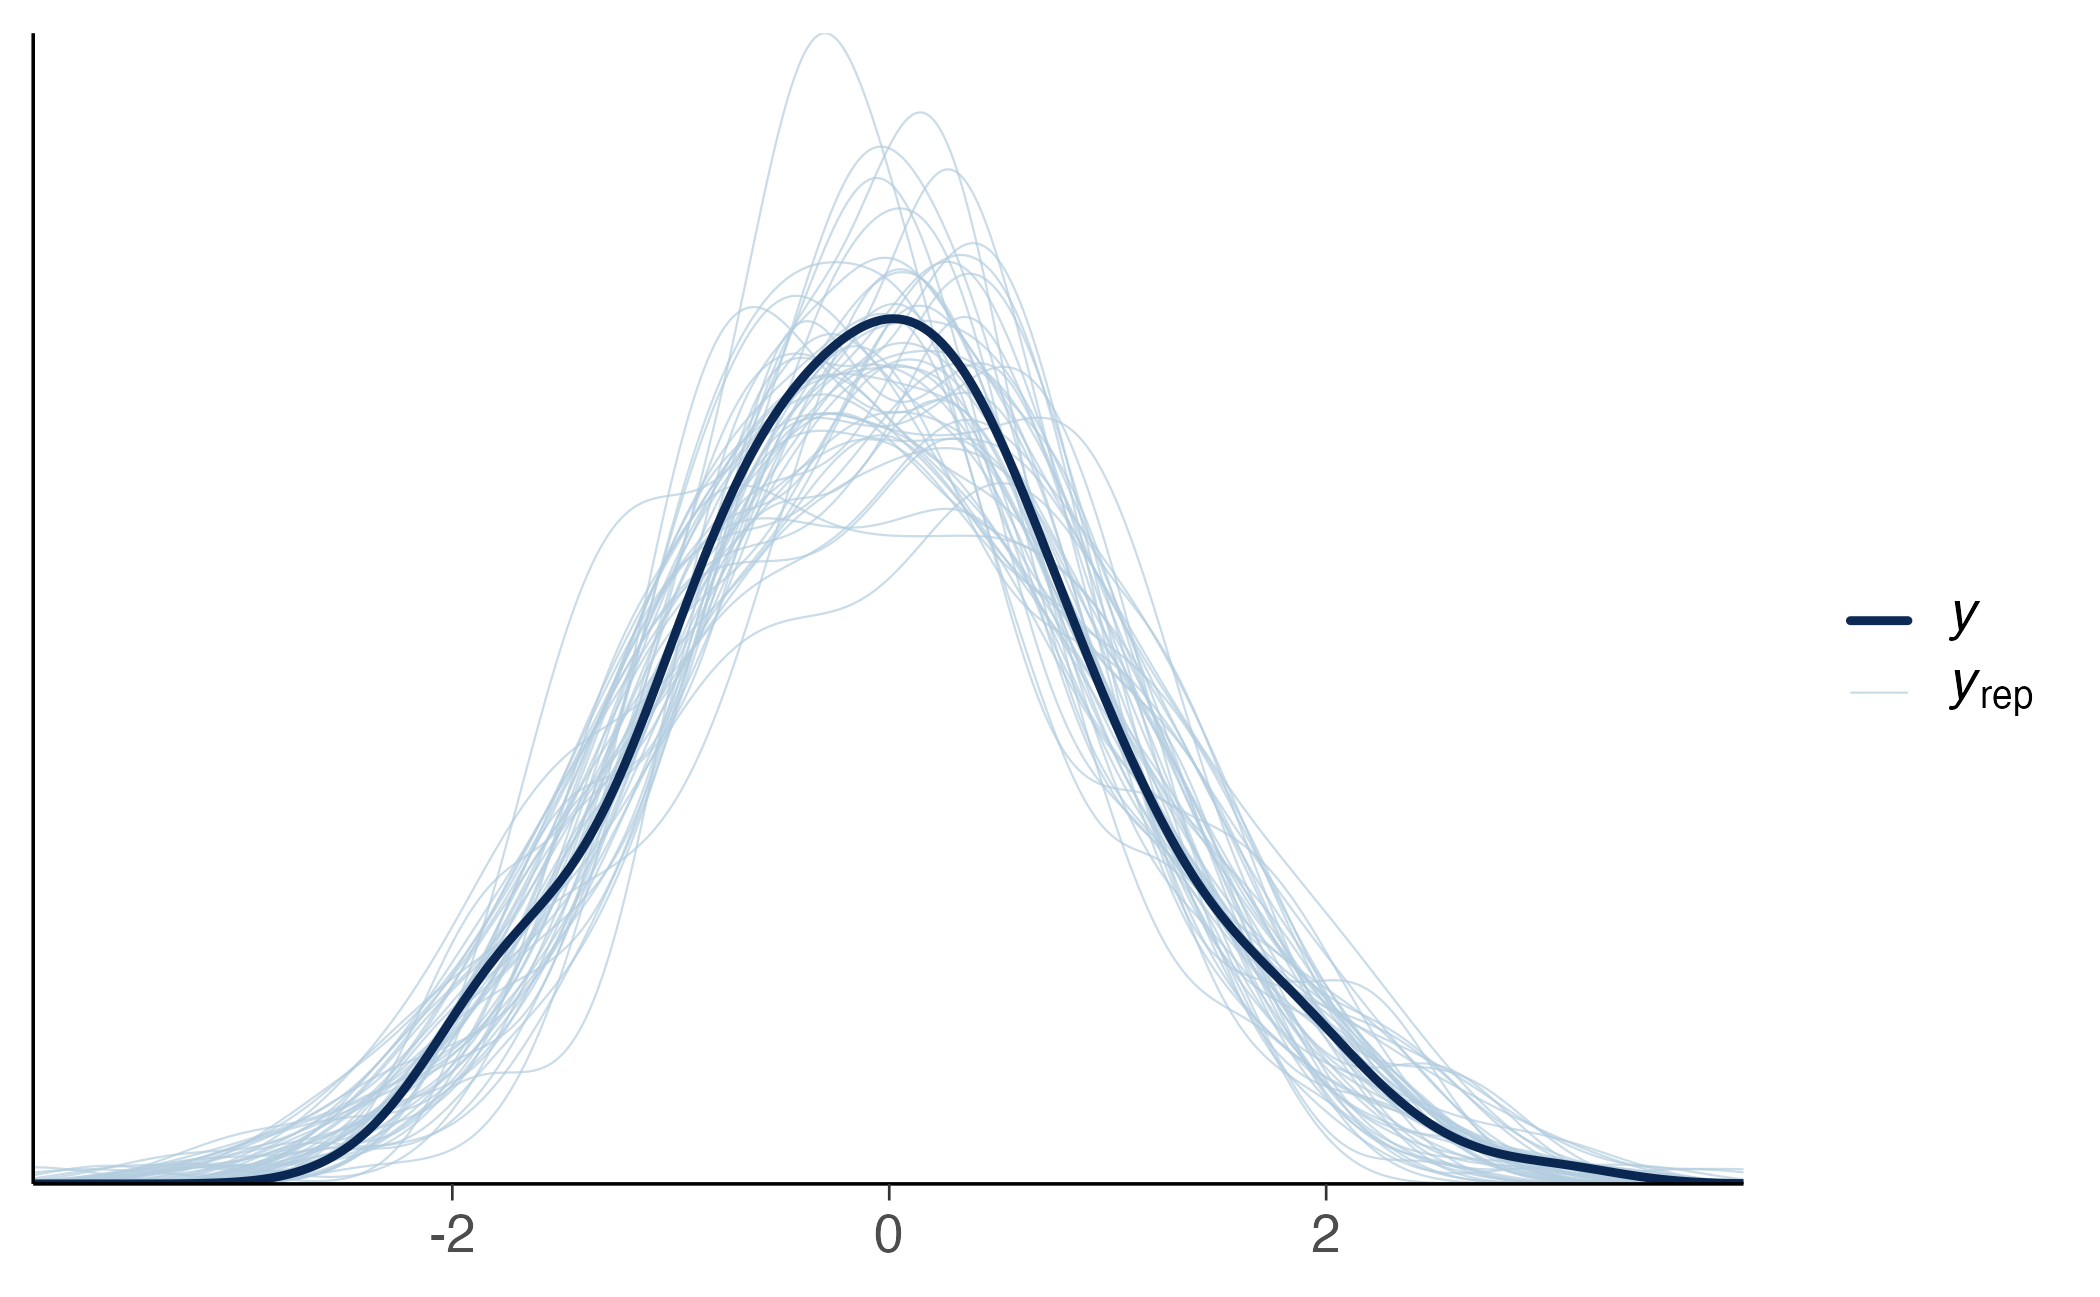
\includegraphics[width=0.85\linewidth,height=\textheight,keepaspectratio]{chapters/mcmc/05_stan_two_means_files/figure-pdf/unnamed-chunk-19-1.png}
\end{center}

\begin{Shaded}
\begin{Highlighting}[]
\CommentTok{\# Unequal variances}
\NormalTok{yrep\_neq }\OtherTok{\textless{}{-}}\NormalTok{ fit\_neq}\SpecialCharTok{$}\FunctionTok{draws}\NormalTok{(}\StringTok{"y\_rep"}\NormalTok{, }\AttributeTok{format =} \StringTok{"matrix"}\NormalTok{)}
\NormalTok{bayesplot}\SpecialCharTok{::}\FunctionTok{ppc\_dens\_overlay}\NormalTok{(}\AttributeTok{y =}\NormalTok{ stan\_data}\SpecialCharTok{$}\NormalTok{y, }\AttributeTok{yrep =}\NormalTok{ yrep\_neq[}\DecValTok{1}\SpecialCharTok{:}\DecValTok{50}\NormalTok{, ])}
\end{Highlighting}
\end{Shaded}

\begin{center}
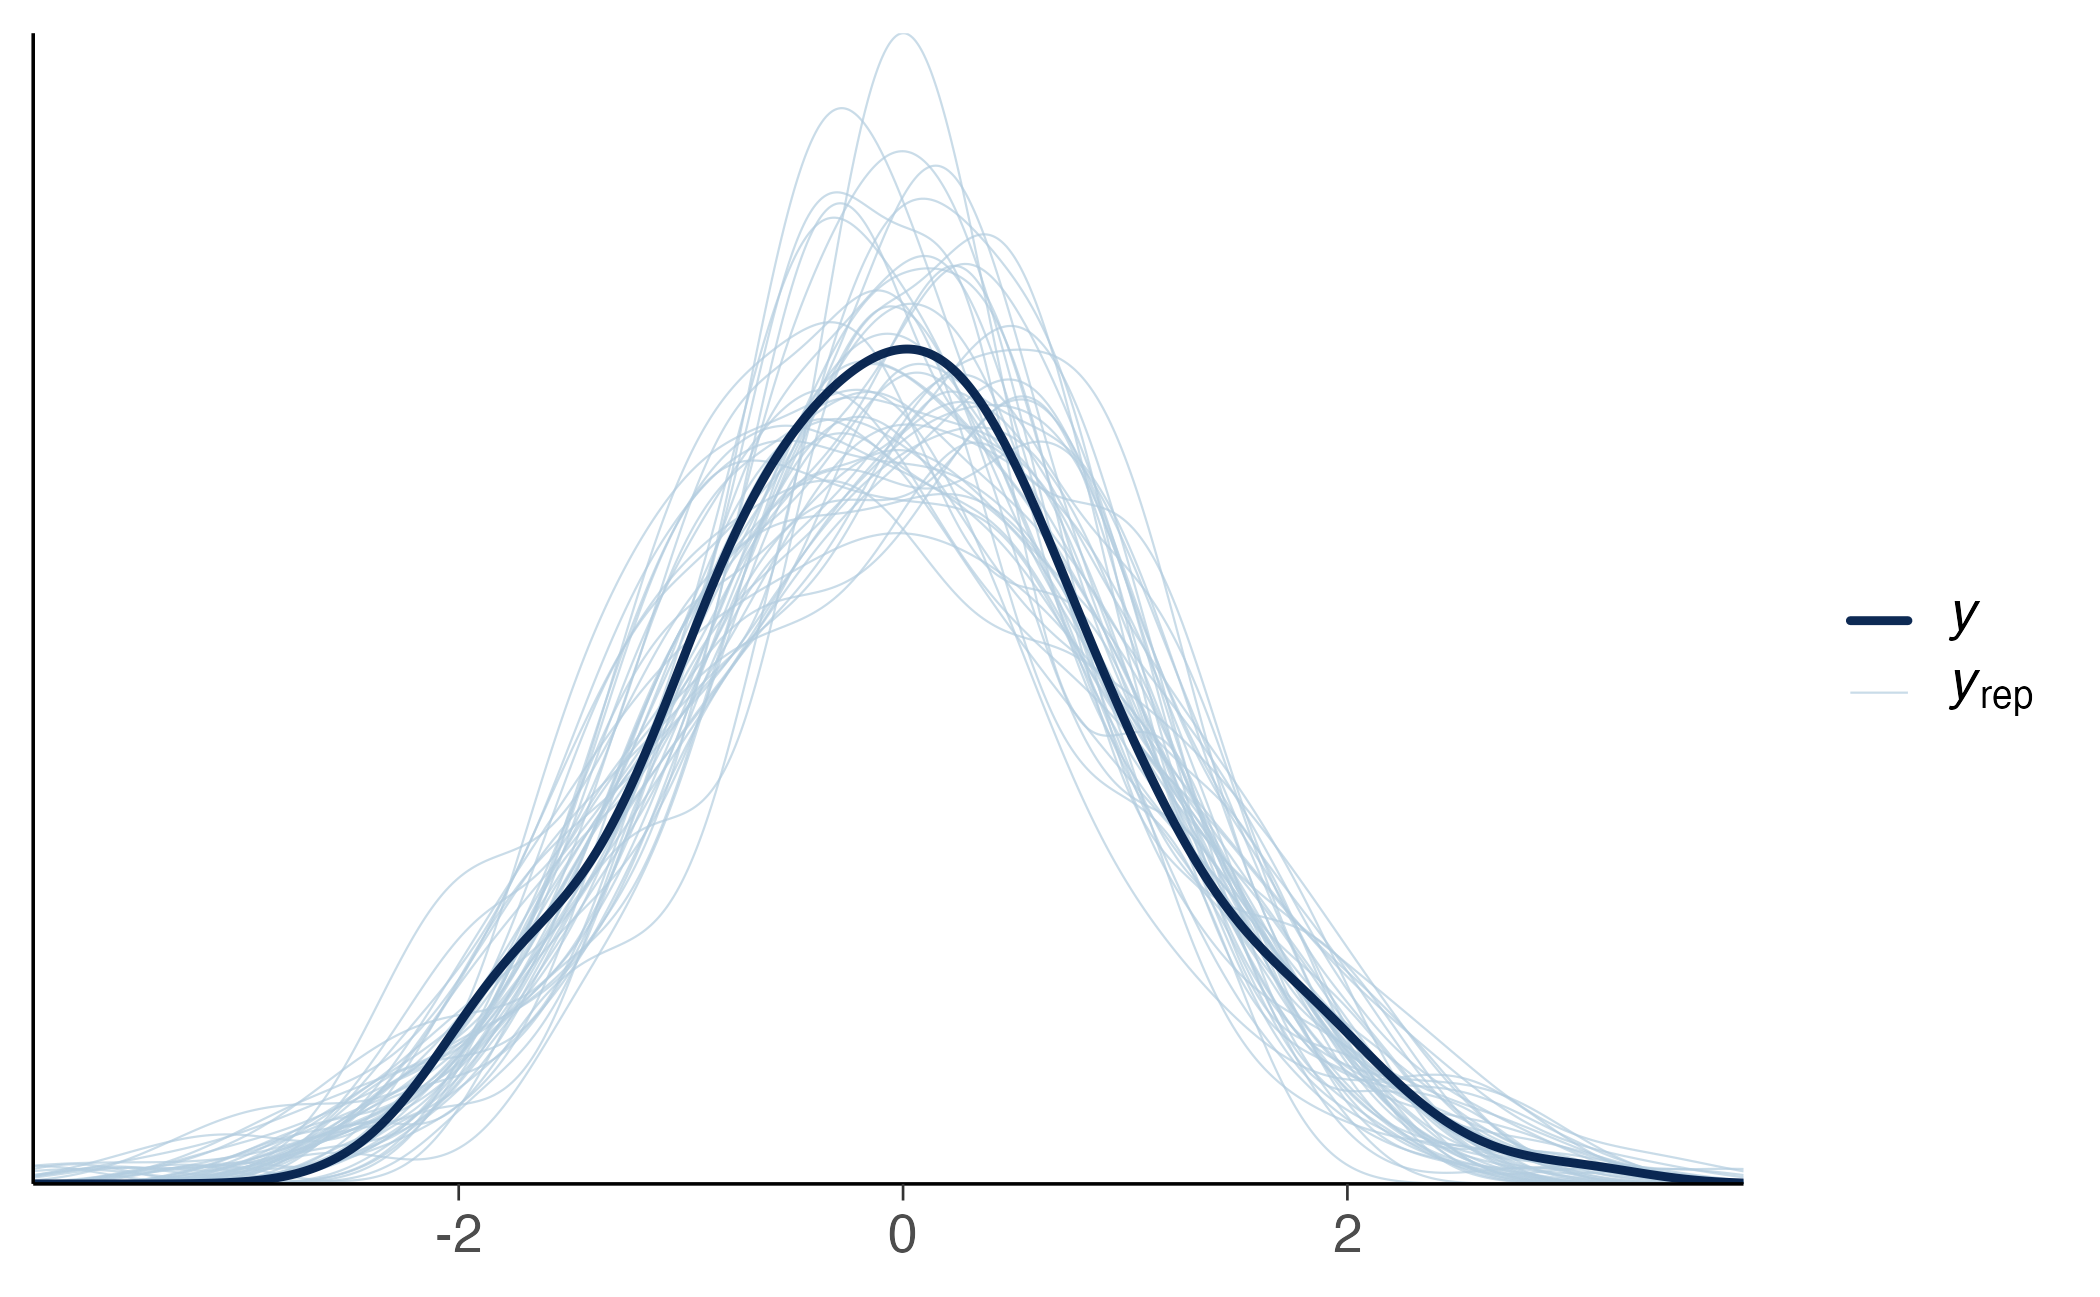
\includegraphics[width=0.85\linewidth,height=\textheight,keepaspectratio]{chapters/mcmc/05_stan_two_means_files/figure-pdf/unnamed-chunk-20-1.png}
\end{center}

\section{Cosa impariamo}\label{cosa-impariamo}

\begin{enumerate}
\def\labelenumi{\arabic{enumi}.}
\item
  \textbf{Differenza tra le medie}. La posteriore di \emph{diff\_mu}
  dice \emph{di quanto} il training modifica l'affetto negativo medio,
  con \emph{intervallo di credibilità}; la \emph{ROPE} ci dice se
  l'effetto è \emph{praticamente} trascurabile o rilevante. Questo è un
  vantaggio diretto rispetto al t-test, che non fornisce probabilità di
  ``effetto rilevante'' né gestisce l'equivalenza pratica in modo
  naturale.
\item
  \textbf{Differenza tra varianze}. La posteriore di \emph{diff\_sigma}
  chiarisce se l'intervento modifica l'eterogeneità delle risposte:
  informazione spesso ignorata, ma importante in psicologia applicata.
\item
  \textbf{Capacità predittiva}. Il confronto PSIS-LOO ci guida nella
  scelta del livello di complessità. Se ΔELPD è piccolo e incerto,
  preferiamo la parsimonia (varianza comune); se il vantaggio è stabile
  e sostanziale, ha senso adottare il modello con varianze distinte.
\end{enumerate}

\section*{Riflessioni conclusive}\label{riflessioni-conclusive-16}
\addcontentsline{toc}{section}{Riflessioni conclusive}

\markright{Riflessioni conclusive}

L'analisi sviluppata in questo capitolo mette in luce i principali punti
di forza dell'approccio bayesiano applicato al confronto tra gruppi. La
quantità centrale dell'inferenza non è più un singolo indice riassuntivo
né un valore-\(p\), bensì l'intera distribuzione a posteriori della
differenza tra le medie. È questa distribuzione a costituire l'oggetto
sostantivo dell'interpretazione: descrive non solo di quanto il gruppo
sottoposto all'intervento differisca in media dal controllo, ma con
quale grado di incertezza ciascun valore della differenza sia
plausibile. In questo modo l'inferenza si libera dal verdetto dicotomico
``c'è / non c'è una differenza'' per assumere la forma di un
ragionamento continuo basato su gradazioni di plausibilità.

La stima congiunta della differenza tra le medie e tra le varianze
permette inoltre di cogliere aspetti spesso trascurati, come un
eventuale effetto dell'intervento sull'eterogeneità delle risposte.
L'introduzione di una \emph{Region of Practical Equivalence} (ROPE)
consente infine di distinguere differenze statisticamente distinguibili
da zero ma trascurabili sul piano psicologico da differenze di entità
potenzialmente rilevante, rispondendo a domande sostanziali sulla
rilevanza pratica dell'effetto.

Il confronto tra il modello a varianza comune e quello a varianze
distinte ha infine mostrato che le assunzioni statistiche vanno valutate
in termini predittivi, tramite l'ELPD stimato con PSIS-LOO, anziché
accettate o rifiutate in modo automatico: quando il guadagno predittivo
è marginale si preferisce il modello più parsimonioso, quando è
sostanziale la complessità aggiuntiva è giustificata. Lo stesso
ragionamento bayesiano si estende poi dal confronto tra gruppi
all'inferenza sul singolo individuo --- la stima del punteggio vero di
un paziente e la valutazione del suo cambiamento nel tempo --- temi
ripresi nel capitolo sul singolo paziente e nell'appendice sul
\emph{Reliable Change Index} bayesiano.

\begin{tcolorbox}[enhanced jigsaw, arc=.35mm, bottomrule=.15mm, bottomtitle=1mm, breakable, colback=white, colbacktitle=quarto-callout-note-color!10!white, colframe=quarto-callout-note-color-frame, coltitle=black, left=2mm, leftrule=.75mm, opacityback=0, opacitybacktitle=0.6, rightrule=.15mm, title=\textcolor{quarto-callout-note-color}{\faInfo}\hspace{0.5em}{Informazioni sull'ambiente di sviluppo}, titlerule=0mm, toprule=.15mm, toptitle=1mm]

\begin{Shaded}
\begin{Highlighting}[]
\FunctionTok{sessionInfo}\NormalTok{()}
\CommentTok{\#\textgreater{} R version 4.6.1 (2026{-}06{-}24)}
\CommentTok{\#\textgreater{} Platform: aarch64{-}apple{-}darwin23}
\CommentTok{\#\textgreater{} Running under: macOS Tahoe 26.5.2}
\CommentTok{\#\textgreater{} }
\CommentTok{\#\textgreater{} Matrix products: default}
\CommentTok{\#\textgreater{} BLAS:   /Library/Frameworks/R.framework/Versions/4.6/Resources/lib/libRblas.0.dylib }
\CommentTok{\#\textgreater{} LAPACK: /Library/Frameworks/R.framework/Versions/4.6/Resources/lib/libRlapack.dylib;  LAPACK version 3.12.1}
\CommentTok{\#\textgreater{} }
\CommentTok{\#\textgreater{} locale:}
\CommentTok{\#\textgreater{} [1] C.UTF{-}8/UTF{-}8/C.UTF{-}8/C/C.UTF{-}8/C.UTF{-}8}
\CommentTok{\#\textgreater{} }
\CommentTok{\#\textgreater{} time zone: Europe/Zagreb}
\CommentTok{\#\textgreater{} tzcode source: internal}
\CommentTok{\#\textgreater{} }
\CommentTok{\#\textgreater{} attached base packages:}
\CommentTok{\#\textgreater{} [1] stats     graphics  grDevices utils     datasets  methods   base     }
\CommentTok{\#\textgreater{} }
\CommentTok{\#\textgreater{} other attached packages:}
\CommentTok{\#\textgreater{}  [1] forcats\_1.0.1         cmdstanr\_0.9.0        ragg\_1.5.2           }
\CommentTok{\#\textgreater{}  [4] tinytable\_0.17.0      withr\_3.0.3           systemfonts\_1.3.2    }
\CommentTok{\#\textgreater{}  [7] patchwork\_1.3.2       ggdist\_3.3.3          tidybayes\_3.0.7      }
\CommentTok{\#\textgreater{} [10] bayesplot\_1.15.0      ggplot2\_4.0.3         reliabilitydiag\_0.2.1}
\CommentTok{\#\textgreater{} [13] priorsense\_1.2.0      posterior\_1.7.0       loo\_2.10.0           }
\CommentTok{\#\textgreater{} [16] rstan\_2.32.7          StanHeaders\_2.32.10   brms\_2.23.0          }
\CommentTok{\#\textgreater{} [19] Rcpp\_1.1.2            sessioninfo\_1.2.4     conflicted\_1.2.0     }
\CommentTok{\#\textgreater{} [22] janitor\_2.2.1         matrixStats\_1.5.0     modelr\_0.1.11        }
\CommentTok{\#\textgreater{} [25] tibble\_3.3.1          dplyr\_1.2.1           tidyr\_1.3.2          }
\CommentTok{\#\textgreater{} [28] rio\_1.3.0             here\_1.0.2           }
\CommentTok{\#\textgreater{} }
\CommentTok{\#\textgreater{} loaded via a namespace (and not attached):}
\CommentTok{\#\textgreater{}  [1] gridExtra\_2.3.1       inline\_0.3.21         rlang\_1.3.0          }
\CommentTok{\#\textgreater{}  [4] magrittr\_2.0.5        snakecase\_0.11.1      otel\_0.2.0           }
\CommentTok{\#\textgreater{}  [7] compiler\_4.6.1        vctrs\_0.7.3           reshape2\_1.4.5       }
\CommentTok{\#\textgreater{} [10] stringr\_1.6.0         pkgconfig\_2.0.3       arrayhelpers\_1.1{-}1   }
\CommentTok{\#\textgreater{} [13] fastmap\_1.2.0         backports\_1.5.1       labeling\_0.4.3       }
\CommentTok{\#\textgreater{} [16] utf8\_1.2.6            rmarkdown\_2.31        ps\_1.9.3             }
\CommentTok{\#\textgreater{} [19] purrr\_1.2.2           xfun\_0.60             cachem\_1.1.0         }
\CommentTok{\#\textgreater{} [22] jsonlite\_2.0.0        broom\_1.0.13          parallel\_4.6.1       }
\CommentTok{\#\textgreater{} [25] R6\_2.6.1              stringi\_1.8.7         RColorBrewer\_1.1{-}3   }
\CommentTok{\#\textgreater{} [28] lubridate\_1.9.5       estimability\_2.0.0    knitr\_1.51           }
\CommentTok{\#\textgreater{} [31] pacman\_0.5.1          Matrix\_1.7{-}5          timechange\_0.4.0     }
\CommentTok{\#\textgreater{} [34] tidyselect\_1.2.1      abind\_1.4{-}8           yaml\_2.3.12          }
\CommentTok{\#\textgreater{} [37] codetools\_0.2{-}20      curl\_7.1.0            processx\_3.9.0       }
\CommentTok{\#\textgreater{} [40] pkgbuild\_1.4.8        lattice\_0.22{-}9        plyr\_1.8.9           }
\CommentTok{\#\textgreater{} [43] bridgesampling\_1.2{-}1  S7\_0.2.2              coda\_0.19{-}4.1        }
\CommentTok{\#\textgreater{} [46] evaluate\_1.0.5        RcppParallel\_5.1.11{-}2 pillar\_1.11.1        }
\CommentTok{\#\textgreater{} [49] tensorA\_0.36.2.1      checkmate\_2.3.4       stats4\_4.6.1         }
\CommentTok{\#\textgreater{} [52] distributional\_0.8.1  generics\_0.1.4        rprojroot\_2.1.1      }
\CommentTok{\#\textgreater{} [55] rstantools\_2.6.0      scales\_1.4.0          xtable\_1.8{-}8         }
\CommentTok{\#\textgreater{} [58] glue\_1.8.1            emmeans\_2.0.4         tools\_4.6.1          }
\CommentTok{\#\textgreater{} [61] data.table\_1.18.4     mvtnorm\_1.4{-}2         grid\_4.6.1           }
\CommentTok{\#\textgreater{} [64] QuickJSR\_1.10.0       nlme\_3.1{-}170          cli\_3.6.6            }
\CommentTok{\#\textgreater{} [67] textshaping\_1.0.5     svUnit\_1.0.8          Brobdingnag\_1.2{-}9    }
\CommentTok{\#\textgreater{} [70] V8\_8.2.0              gtable\_0.3.6          digest\_0.6.39        }
\CommentTok{\#\textgreater{} [73] farver\_2.1.2          memoise\_2.0.1         htmltools\_0.5.9      }
\CommentTok{\#\textgreater{} [76] lifecycle\_1.0.5}
\end{Highlighting}
\end{Shaded}

\end{tcolorbox}

\section*{Bibliografia}\label{bibliografia-18}
\addcontentsline{toc}{section}{Bibliografia}

\markright{Bibliografia}

\chapter{Flusso di lavoro bayesiano}\label{sec-mcmc-workflow}

\begin{tcolorbox}[enhanced jigsaw, arc=.35mm, bottomrule=.15mm, breakable, colback=white, colframe=quarto-callout-note-color-frame, left=2mm, leftrule=.75mm, opacityback=0, rightrule=.15mm, toprule=.15mm]

Abbiamo ormai gli strumenti fondamentali per affrontare l'inferenza
bayesiana in contesti realistici. Abbiamo visto che, nei casi semplici,
l'aggiornamento può essere calcolato analiticamente, ma che diventa
impraticabile già con pochi parametri. Abbiamo introdotto l'algoritmo di
Metropolis che ci ha mostrato come sia sempre possibile campionare dalla
distribuzione a posteriori e poi abbiamo visto come i linguaggi
probabilistici, in particolare Stan, rendano questa possibilità
accessibile e utilizzabile nella ricerca psicologica.

Ora, però, dobbiamo fare un passo ulteriore. Avere strumenti di calcolo
non basta: serve un metodo di lavoro. L'inferenza bayesiana non è solo
una formula o un algoritmo, ma un processo che accompagna il ricercatore
dall'ideazione del modello fino alla comunicazione dei risultati. Questo
processo prende il nome di \emph{workflow bayesiano}.

\end{tcolorbox}

\begin{tcolorbox}[enhanced jigsaw, arc=.35mm, bottomrule=.15mm, breakable, colback=white, colframe=quarto-callout-note-color-frame, left=2mm, leftrule=.75mm, opacityback=0, rightrule=.15mm, toprule=.15mm]

\textbf{Da sapere.} Il workflow bayesiano è un processo iterativo che
collega teoria, modello generativo, prior, stima, diagnostica e
valutazione predittiva. L'obiettivo non è soltanto ottenere una
distribuzione a posteriori, ma verificare continuamente se il modello
rappresenta in modo plausibile il processo che ha generato i dati.

\textbf{Da saper fare.} Descrivere le fasi principali del workflow.
Tradurre una domanda di ricerca in un modello probabilistico;
distinguere la diagnostica del campionamento dalla valutazione del
modello.

\textbf{Approfondimento facoltativo.} Usare i controlli predittivi a
priori e a posteriori per individuare specificazioni implausibili e
motivare una revisione del modello. Le diagnostiche MCMC dettagliate, il
confronto predittivo mediante LOO-CV e la lettura di Bulbulia (2023)
possono essere rimandati in una prima lettura. Nel percorso essenziale è
sufficiente comprendere il ciclo iterativo, stimare il modello con gli
strumenti forniti e interpretare i principali controlli predittivi.

\hyperref[sec-percorsi-lettura]{Che cosa significano queste etichette?}

\end{tcolorbox}

\begin{tcolorbox}[enhanced jigsaw, arc=.35mm, bottomrule=.15mm, bottomtitle=1mm, breakable, colback=white, colbacktitle=quarto-callout-tip-color!10!white, colframe=quarto-callout-tip-color-frame, coltitle=black, left=2mm, leftrule=.75mm, opacityback=0, opacitybacktitle=0.6, rightrule=.15mm, title=\textcolor{quarto-callout-tip-color}{\faLightbulb}\hspace{0.5em}{Prerequisiti}, titlerule=0mm, toprule=.15mm, toptitle=1mm]

Può essere utile aver letto
\href{https://www.researchgate.net/profile/Joseph-Bulbulia/publication/361799820_A_workflow_for_causal_inference_in_cross-cultural_psychology-A-workflow-for-causal-inference-in-cross-cultural-psychology/links/62c5cad2f8c0fc18d3ec9798/A-workflow-for-causal-inference-in-cross-cultural-psychology-A-workflow-for-causal-inference-in-cross-cultural-psychology.pdf}{Bulbulia
(2023)} sul flusso di lavoro bayesiano e l'inferenza causale.

\end{tcolorbox}

\section{Un processo iterativo}\label{un-processo-iterativo}

Il flusso di lavoro bayesiano non è lineare, ma iterativo. Inizia con la
formulazione di un modello, prosegue con l'analisi dei dati e la
valutazione dei risultati, ma spesso richiede di tornare indietro,
rivedere le ipotesi e migliorare le specifiche. A differenza
dell'approccio frequentista tradizionale, che tende a concentrarsi solo
sull'output numerico finale (ad esempio un valore-\(p\)), l'approccio
bayesiano incoraggia una riflessione costante sul legame tra teoria,
modello e dati.

L'idea centrale è che ogni modello è un'ipotesi sul processo generativo
che ha prodotto i dati. Il compito del ricercatore non è solo quello di
stimare i parametri, ma anche di verificare se il modello che li
definisce è coerente con ciò che sappiamo e con ciò che osserviamo.

\section{Le fasi del workflow}\label{le-fasi-del-workflow}

Il flusso di lavoro può essere schematizzato in tre fasi principali che,
nella pratica, si intrecciano continuamente.

\textbf{1. Definizione del modello:} il punto di partenza è sempre la
teoria o l'ipotesi psicologica che vogliamo testare. In questa fase,
traduciamo le nostre idee in un modello probabilistico, definendo i
parametri, scegliendo i priori e specificando la verosimiglianza. È il
momento in cui ci si chiede: ``\emph{Quale processo potrebbe aver
generato i dati che osserviamo?}''.

\textbf{2. Inferenza e stima.} Una volta definito il modello,
utilizziamo strumenti come Stan per ottenere dei campioni dalla
distribuzione a posteriori. In questa fase, verifichiamo la tecnica di
campionamento (convergenza delle catene, numero effettivo di campioni
indipendenti e diagnosi di autocorrelazione). È qui che la potenza degli
algoritmi MCMC diventa essenziale, in quanto ci permette di trattare
modelli complessi senza dover ricorrere a eccessive semplificazioni.

\textbf{3. Valutazione del modello} Il passo successivo è chiedersi se
il modello ``funziona''. Ciò significa, da un lato, confrontare le
previsioni del modello con i dati osservati (\emph{posterior predictive
checks}) e, dall'altro, valutare la capacità del modello di
generalizzare a nuovi dati (ad esempio, tramite LOO-CV). La valutazione
non è mai definitiva, ma una guida per decidere se mantenere, modificare
o sostituire il modello.

\begin{figure}[H]

{\centering \pandocbounded{\includegraphics[keepaspectratio]{chapters/mcmc/../../figures/boxes_loop.png}}

}

\caption{Figura tratta da Blei (\citeproc{ref-blei2014build}{2014}).}

\end{figure}%

\section{Una prospettiva cumulativa}\label{una-prospettiva-cumulativa}

Il flusso di lavoro bayesiano ci ricorda che la scienza non procede
verso verità definitive, ma verso modelli progressivamente migliori.
Ogni modello rappresenta un passo in un percorso cumulativo in cui le
ipotesi vengono testate, confrontate e, se necessario, abbandonate.

Dal punto di vista della psicologia, questo approccio rappresenta una
risposta concreta alla crisi di replicazione. Non ci limitiamo a
verificare le associazioni statistiche, ma costruiamo modelli espliciti
dei processi psicologici, li testiamo sui dati e li confrontiamo in
termini di capacità predittiva. Questo metodo promuove la trasparenza,
l'apertura alla revisione e la cumulatività, tutti elementi essenziali
per rafforzare le basi empiriche della disciplina.

\section*{Riflessioni conclusive}\label{riflessioni-conclusive-17}

\markright{Riflessioni conclusive}

Con il flusso di lavoro bayesiano abbiamo completato il nostro percorso
introduttivo all'inferenza bayesiana. Abbiamo capito che non si tratta
solo di imparare un nuovo insieme di tecniche, ma di adottare una
prospettiva diversa sul rapporto tra teoria, dati e analisi statistica.

Il valore di questo approccio non risiede solo nei dettagli tecnici, ma
nel modo in cui ci spinge a pensare: ogni modello è un'ipotesi
esplicita, ogni analisi è trasparente e riproducibile e ogni risultato è
accompagnato da una valutazione critica della sua incertezza e
plausibilità.

Nei capitoli successivi vedremo come applicare questi principi a casi
specifici e a modelli più complessi. Il workflow bayesiano rimarrà il
filo conduttore: un metodo iterativo e riflessivo che ci guiderà nella
costruzione di una conoscenza scientifica solida, cumulativa e in grado
di rispondere alle sfide della psicologia contemporanea.

\section*{Bibliografia}\label{bibliografia-19}

\markright{Bibliografia}

\chapter*{Riflessioni conclusive sulla
sezione}\label{riflessioni-conclusive-sulla-sezione}

\markboth{Riflessioni conclusive sulla sezione}{Riflessioni conclusive
sulla sezione}

In questa sezione, siamo passati dai fondamenti concettuali
dell'inferenza bayesiana agli strumenti che la rendono praticabile con
modelli realistici. Abbiamo visto perché i linguaggi di programmazione
probabilistica rappresentano una svolta: separano la definizione del
modello dall'algoritmo di campionamento, consentendo al ricercatore di
concentrarsi su quale modello costruire piuttosto che su come
campionare. Abbiamo poi imparato a leggere un modello scritto in Stan,
riconoscendo che, per i casi semplici, il blocco che descrive il modello
traduce quasi letteralmente la formulazione probabilistica. Su questa
base, abbiamo affrontato due dei casi più comuni nella ricerca
psicologica: l'inferenza su un odds ratio e il confronto tra due medie.
Infine, abbiamo inquadrato l'intero processo in un flusso di lavoro
bayesiano esplicito.

Alcune idee attraversano tutti i capitoli. L'oggetto dell'inferenza è la
distribuzione a posteriori, approssimata mediante campionamento MCMC, da
cui si ricavano stime puntuali, intervalli di credibilità, probabilità
di ipotesi e qualsiasi funzione dei parametri di interesse, come l'odds
ratio stesso. Tuttavia, la validità di queste conclusioni dipende dalla
qualità del campionamento: la verifica della convergenza, con indice
\(\hat{R}\) prossimo a 1, dimensione effettiva del campione adeguata e
assenza di divergenze, è un passaggio imprescindibile la cui
interpretazione dettagliata è raccolta
nell'\href{../appendix/a44_stan_diagnostics.qmd}{appendice sulla
diagnostica}. Le distribuzioni a priori, infine, non sono un dettaglio
tecnico, ma fanno parte integrante della specificazione del modello e le
verifiche predittive, sia a priori che a posteriori, permettono di
controllarne le implicazioni prima e dopo l'osservazione dei dati.

Il capitolo sul flusso di lavoro bayesiano raccoglie questi elementi in
un metodo: specificare il modello, simulare le sue implicazioni, stimare
e diagnosticare, valutare la sua capacità predittiva, affinare e
comunicare (\citeproc{ref-bayesianworkflow2026}{Gelman et al., 2026}).
Si tratta di un processo iterativo e riflessivo, non di una procedura
meccanica. Nella sezione successiva, applicheremo questi strumenti ai
modelli lineari e alle loro estensioni, dalla regressione al confronto
tra gruppi, fino ai modelli multilivello che sfruttano appieno la
flessibilità del campionamento MCMC per rappresentare la struttura
gerarchica tipica dei dati psicologici.

\section*{Bibliografia}\label{bibliografia-20}

\markright{Bibliografia}

\part{Modelli}

\chapter*{Dove siamo nel percorso}\label{dove-siamo-nel-percorso-4}
\addcontentsline{toc}{chapter}{Dove siamo nel percorso}

\markboth{Dove siamo nel percorso}{Dove siamo nel percorso}

\begin{tcolorbox}[enhanced jigsaw, arc=.35mm, bottomrule=.15mm, breakable, colback=white, colframe=quarto-callout-note-color-frame, left=2mm, leftrule=.75mm, opacityback=0, rightrule=.15mm, toprule=.15mm]

Nei capitoli precedenti abbiamo costruito gli strumenti fondamentali
dell'inferenza bayesiana. Abbiamo imparato a rappresentare l'incertezza
mediante distribuzioni di probabilità, a combinare informazioni a priori
e dati osservati, a ottenere campioni dalla distribuzione a posteriori e
a verificare le implicazioni predittive di un modello. Ora useremo
questi strumenti per affrontare alcune delle domande più comuni nella
ricerca psicologica: come descrivere la relazione tra due variabili,
stimare una media, confrontare gruppi e rappresentare differenze
sistematiche tra individui o contesti.

Il passaggio decisivo non consiste nell'aggiungere una nuova collezione
di test statistici. Consiste nell'imparare a formulare queste domande
come versioni diverse dello stesso problema di modellazione.

\end{tcolorbox}

\section*{Dal calcolo alla
modellazione}\label{dal-calcolo-alla-modellazione}
\addcontentsline{toc}{section}{Dal calcolo alla modellazione}

\markright{Dal calcolo alla modellazione}

L'inferenza bayesiana non inizia dal comando da eseguire né dall'indice
da riportare. Inizia da una rappresentazione esplicita del processo che
potrebbe avere generato i dati. Per questo motivo, in questa sezione
useremo il \textbf{modello lineare} come primo laboratorio completo di
modellazione statistica.

Nella sua forma più semplice, il modello può essere scritto come

\[
y_i \sim \operatorname{Normal}(\mu_i, \sigma),
\]

\[
\mu_i = \alpha + \beta x_i.
\]

La prima equazione descrive la variabilità delle osservazioni attorno a
un valore atteso; la seconda specifica come tale valore atteso cambia al
variare del predittore. I parametri hanno quindi funzioni distinte:

\begin{itemize}
\tightlist
\item
  \(\alpha\) descrive il valore atteso dell'outcome quando il predittore
  assume il valore di riferimento;
\item
  \(\beta\) descrive come cambia il valore atteso dell'outcome al
  variare del predittore;
\item
  \(\sigma\) descrive la variabilità che rimane tra le osservazioni
  anche dopo avere considerato la relazione sistematica rappresentata
  dal modello.
\end{itemize}

Queste equazioni sono semplici, ma contengono già le componenti
essenziali di un modello generativo: una struttura sistematica, una
componente di variabilità e un insieme di parametri incerti. La
prospettiva bayesiana aggiunge distribuzioni a priori per i parametri e
usa i dati per aggiornarle. Il risultato non è una singola retta
``migliore'', ma una distribuzione di rette, valori attesi e previsioni
compatibili con le assunzioni del modello e con l'informazione
disponibile.

\section*{Un unico linguaggio per domande
diverse}\label{un-unico-linguaggio-per-domande-diverse}
\addcontentsline{toc}{section}{Un unico linguaggio per domande diverse}

\markright{Un unico linguaggio per domande diverse}

Molte procedure che vengono tradizionalmente insegnate come tecniche
separate sono casi particolari del modello lineare. La differenza non
risiede nella logica inferenziale, ma nel modo in cui viene costruito il
predittore e nella quantità scientifica che desideriamo stimare.

{\def\LTcaptype{none} % do not increment counter
\begin{longtable}[]{@{}
  >{\raggedright\arraybackslash}p{(\linewidth - 4\tabcolsep) * \real{0.3333}}
  >{\raggedright\arraybackslash}p{(\linewidth - 4\tabcolsep) * \real{0.3333}}
  >{\raggedright\arraybackslash}p{(\linewidth - 4\tabcolsep) * \real{0.3333}}@{}}
\toprule\noalign{}
\begin{minipage}[b]{\linewidth}\raggedright
Domanda di ricerca
\end{minipage} & \begin{minipage}[b]{\linewidth}\raggedright
Specificazione essenziale
\end{minipage} & \begin{minipage}[b]{\linewidth}\raggedright
Quantità di interesse
\end{minipage} \\
\midrule\noalign{}
\endhead
\bottomrule\noalign{}
\endlastfoot
Qual è il livello medio di una variabile? & Modello con la sola
intercetta & Media della popolazione e variabilità individuale \\
Come cambia un outcome al variare di un predittore continuo? &
Regressione lineare & Pendenza, valori attesi e previsioni \\
Quanto differiscono due gruppi? & Predittore binario & Medie dei gruppi
e loro differenza \\
Quali differenze esistono tra più condizioni? & Predittore categoriale e
contrasti & Medie di cella e confronti teoricamente rilevanti \\
Come variano le relazioni tra individui, scuole o contesti? & Modello
multilivello & Effetti medi, eterogeneità e previsioni a più livelli \\
\end{longtable}
}

Questa prospettiva unificante modifica il modo di apprendere l'analisi
dei dati. Non occorre memorizzare una procedura distinta per ogni
disegno. Occorre imparare a tradurre una domanda scientifica in:

\begin{enumerate}
\def\labelenumi{\arabic{enumi}.}
\tightlist
\item
  una quantità di interesse ben definita;
\item
  una struttura per il valore atteso;
\item
  una distribuzione per le osservazioni;
\item
  un insieme di assunzioni controllabili;
\item
  un procedimento trasparente per quantificare l'incertezza.
\end{enumerate}

L'ordine dei capitoli riflette questa scelta. Incontreremo dapprima la
regressione nella sua forma più riconoscibile; torneremo poi alla stima
di una singola media e al confronto tra gruppi per mostrare che non si
tratta di tecniche indipendenti, ma di parametrizzazioni più semplici
della stessa famiglia. Il percorso culminerà nei modelli multilivello,
nei quali la variabilità tra persone e contesti diventa una componente
esplicita del modello anziché un disturbo da ignorare.

\section*{Il workflow che useremo}\label{il-workflow-che-useremo}
\addcontentsline{toc}{section}{Il workflow che useremo}

\markright{Il workflow che useremo}

In ciascun capitolo applicheremo, con diversi livelli di dettaglio, lo
stesso flusso di lavoro.

\subsection*{1. Definire la domanda e la quantità di
interesse}\label{definire-la-domanda-e-la-quantituxe0-di-interesse}
\addcontentsline{toc}{subsection}{1. Definire la domanda e la quantità
di interesse}

Prima di specificare il modello, chiariremo che cosa vogliamo conoscere.
La domanda può riguardare una media, una differenza, una pendenza, una
previsione o una componente di variabilità. Definire l'\emph{estimand}
impedisce di affidare al software la scelta implicita della domanda
scientifica.

\subsection*{2. Formulare un modello
generativo}\label{formulare-un-modello-generativo}
\addcontentsline{toc}{subsection}{2. Formulare un modello generativo}

Descriveremo come le osservazioni potrebbero essere prodotte se le
assunzioni del modello fossero adeguate. Questo passaggio separa la
struttura sistematica dalla variabilità residua e rende visibili le
ipotesi che altrimenti resterebbero nascoste nella sintassi di una
funzione.

\subsection*{3. Specificare e calibrare i
prior}\label{specificare-e-calibrare-i-prior}
\addcontentsline{toc}{subsection}{3. Specificare e calibrare i prior}

I prior saranno espressi, per quanto possibile, sulla scala delle
osservazioni e giustificati attraverso conoscenze teoriche, dati
precedenti o vincoli di plausibilità. Non verranno trattati come una
formalità né delegati automaticamente ai valori predefiniti del
software.

\subsection*{4. Simulare prima di adattare il
modello}\label{simulare-prima-di-adattare-il-modello}
\addcontentsline{toc}{subsection}{4. Simulare prima di adattare il
modello}

Il controllo predittivo a priori ci permetterà di verificare quali dati
il modello considera plausibili prima di osservare il campione. Se il
modello genera sistematicamente valori impossibili o incompatibili con
il fenomeno, il problema deve essere affrontato prima dell'inferenza.

\subsection*{5. Adattare il modello e controllare il
calcolo}\label{adattare-il-modello-e-controllare-il-calcolo}
\addcontentsline{toc}{subsection}{5. Adattare il modello e controllare
il calcolo}

Useremo principalmente \texttt{brms} per esprimere i modelli in modo
compatto e leggibile. Quando sarà utile comprendere ciò che avviene
dietro la formula, tradurremo lo stesso modello nella matrice del
disegno e in un programma Stan. Controlleremo convergenza, efficienza
del campionamento e possibili problemi numerici.

\subsection*{6. Interpretare la distribuzione a
posteriori}\label{interpretare-la-distribuzione-a-posteriori}
\addcontentsline{toc}{subsection}{6. Interpretare la distribuzione a
posteriori}

Le distribuzioni a posteriori verranno riassunte in funzione della
domanda iniziale. Oltre ai parametri del modello, calcoleremo quantità
derivate quali differenze, contrasti, probabilità di superare soglie
sostantive e previsioni per nuove osservazioni.

\subsection*{7. Controllare l'adeguatezza del
modello}\label{controllare-ladeguatezza-del-modello}
\addcontentsline{toc}{subsection}{7. Controllare l'adeguatezza del
modello}

Confronteremo dati osservati e dati replicati dal modello. I controlli
predittivi saranno scelti in relazione alle caratteristiche che contano
per la domanda scientifica: posizione, dispersione, code, valori
estremi, differenze tra gruppi o traiettorie individuali. Un grafico
generico non può certificare l'adeguatezza di tutte le componenti del
modello.

\subsection*{8. Revisionare e
comunicare}\label{revisionare-e-comunicare}
\addcontentsline{toc}{subsection}{8. Revisionare e comunicare}

Quando emergeranno discrepanze, considereremo specificazioni
alternative: relazioni non lineari, distribuzioni robuste, varianze
differenti, interazioni o strutture multilivello. La revisione non verrà
trattata come un inconveniente da nascondere, ma come parte del processo
di apprendimento. Ogni analisi si concluderà distinguendo ciò che i dati
sostengono, ciò che dipende dalle assunzioni e ciò che rimane incerto.

\begin{tcolorbox}[enhanced jigsaw, arc=.35mm, bottomrule=.15mm, bottomtitle=1mm, breakable, colback=white, colbacktitle=quarto-callout-important-color!10!white, colframe=quarto-callout-important-color-frame, coltitle=black, left=2mm, leftrule=.75mm, opacityback=0, opacitybacktitle=0.6, rightrule=.15mm, title=\textcolor{quarto-callout-important-color}{\faExclamation}\hspace{0.5em}{Tre verifiche diverse}, titlerule=0mm, toprule=.15mm, toptitle=1mm]

Durante il percorso manterremo separate tre domande:

\begin{enumerate}
\def\labelenumi{\arabic{enumi}.}
\tightlist
\item
  \textbf{Il calcolo è affidabile?} Le catene hanno esplorato
  adeguatamente la distribuzione a posteriori?
\item
  \textbf{Il modello rappresenta aspetti importanti dei dati?} Le sue
  previsioni riproducono le caratteristiche empiriche pertinenti?
\item
  \textbf{L'interpretazione scientifica è giustificata?} Il disegno, le
  misure e le assunzioni permettono di attribuire ai parametri il
  significato che proponiamo?
\end{enumerate}

Un buon valore di \(\widehat{R}\) risponde alla prima domanda, non alle
altre due. Un controllo predittivo soddisfacente non trasforma
un'associazione in un effetto causale.

\end{tcolorbox}

\section*{Dalla formula al programma}\label{dalla-formula-al-programma}
\addcontentsline{toc}{section}{Dalla formula al programma}

\markright{Dalla formula al programma}

Le formule di \texttt{brms} rendono concisa la specificazione dei
modelli, ma tale concisione può nasconderne la struttura. Per questo
motivo alterneremo due livelli di rappresentazione.

Nel \textbf{percorso essenziale}, la formula R sarà lo strumento
principale. L'obiettivo sarà costruire, verificare e interpretare
modelli riproducibili senza richiedere al lettore di programmare
direttamente l'algoritmo di inferenza.

Nel \textbf{percorso computazionale}, mostreremo come la stessa formula
corrisponda a una matrice del disegno, a una funzione di verosimiglianza
e a un programma Stan. Questo livello non introduce una logica
inferenziale diversa: rende esplicite le operazioni che \texttt{brms}
genera automaticamente e prepara alla costruzione di modelli non
disponibili attraverso formule standard.

I due percorsi sono complementari. La sintassi compatta facilita
l'analisi; la rappresentazione esplicita permette di comprendere e
modificare il modello.

\section*{Associazione, previsione e
causalità}\label{associazione-previsione-e-causalituxe0}
\addcontentsline{toc}{section}{Associazione, previsione e causalità}

\markright{Associazione, previsione e causalità}

Il modello lineare può essere impiegato per scopi diversi, ma tali scopi
non sono intercambiabili.

\begin{itemize}
\tightlist
\item
  \textbf{Descrivere un'associazione} significa rappresentare come la
  distribuzione di un outcome cambia al variare di una o più variabili
  osservate.
\item
  \textbf{Prevedere} significa quantificare l'incertezza su osservazioni
  non ancora conosciute.
\item
  \textbf{Stimare un effetto causale} significa confrontare ciò che
  accadrebbe sotto interventi alternativi, sulla base di un disegno e di
  assunzioni che rendano identificabile tale confronto.
\end{itemize}

La stessa formula può comparire in tutti e tre i contesti, ma il
significato dei coefficienti dipende dalla domanda, dal processo di
campionamento, dalla qualità delle misure e dalle relazioni causali tra
le variabili. Un coefficiente di regressione non diventa causale perché
è preciso, perché il modello converge o perché sono state incluse molte
covariate.

Nella parte finale della sezione introdurremo quindi gli strumenti
concettuali necessari per distinguere associazione, previsione ed
effetto causale. L'obiettivo non sarà sviluppare qui un corso completo
di inferenza causale, ma impedire che la flessibilità del modello
lineare produca interpretazioni più forti di quanto il disegno consenta.

\section*{La struttura della sezione}\label{la-struttura-della-sezione}
\addcontentsline{toc}{section}{La struttura della sezione}

\markright{La struttura della sezione}

Il percorso è organizzato in cinque movimenti.

\begin{enumerate}
\def\labelenumi{\arabic{enumi}.}
\tightlist
\item
  \textbf{Comprendere il modello lineare.} Partiremo dalla relazione tra
  valore atteso, variabilità residua e previsione; la regressione verso
  la media mostrerà alcune conseguenze della previsione imperfetta.
\item
  \textbf{Passare dalla formula al programma.} Metteremo in
  corrispondenza equazioni, matrice del disegno, formule R,
  \texttt{brms} e Stan.
\item
  \textbf{Riconoscere i casi particolari.} Tratteremo media, confronto
  tra due gruppi, più gruppi e contrasti come specificazioni della
  stessa famiglia.
\item
  \textbf{Modellare l'eterogeneità e criticare le assunzioni.} I modelli
  multilivello rappresenteranno la variazione strutturata; simulazioni e
  controlli predittivi mostreranno che cosa accade quando il modello è
  mal specificato.
\item
  \textbf{Interpretare e integrare.} Distingueremo associazione,
  previsione e causalità e applicheremo l'intero workflow a un caso di
  studio progressivamente più realistico.
\end{enumerate}

\begin{tcolorbox}[enhanced jigsaw, arc=.35mm, bottomrule=.15mm, bottomtitle=1mm, breakable, colback=white, colbacktitle=quarto-callout-tip-color!10!white, colframe=quarto-callout-tip-color-frame, coltitle=black, left=2mm, leftrule=.75mm, opacityback=0, opacitybacktitle=0.6, rightrule=.15mm, title=\textcolor{quarto-callout-tip-color}{\faLightbulb}\hspace{0.5em}{Come lavorare con i capitoli}, titlerule=0mm, toprule=.15mm, toptitle=1mm]

Il Companion è concepito come un laboratorio. Per ogni modello:

\begin{itemize}
\tightlist
\item
  esegui il codice;
\item
  modifica almeno un prior;
\item
  genera dati dal modello prima e dopo avere osservato il campione;
\item
  formula per iscritto che cosa rappresenta ciascun parametro;
\item
  cerca una caratteristica dei dati che il modello non riproduce bene;
\item
  prova a spiegare che cosa cambierebbe con una specificazione
  alternativa.
\end{itemize}

La comprensione non deriva dalla semplice lettura dell'output, ma dalla
capacità di anticipare come il modello dovrebbe comportarsi e di
riconoscere quando non lo fa.

\end{tcolorbox}

\section*{Che cosa dovresti saper fare alla
fine}\label{che-cosa-dovresti-saper-fare-alla-fine}
\addcontentsline{toc}{section}{Che cosa dovresti saper fare alla fine}

\markright{Che cosa dovresti saper fare alla fine}

Al termine della sezione dovresti essere in grado di:

\begin{itemize}
\tightlist
\item
  formulare una domanda psicologica come quantità stimabile;
\item
  leggere il modello lineare come processo generativo;
\item
  riconoscere media, confronto tra gruppi e ANOVA come casi della
  regressione;
\item
  specificare prior plausibili sulla scala del problema;
\item
  eseguire controlli predittivi a priori e a posteriori;
\item
  distinguere problemi computazionali da problemi di specificazione;
\item
  interpretare separatamente parametri, valori attesi e nuove
  osservazioni;
\item
  usare il partial pooling per rappresentare l'eterogeneità;
\item
  valutare con prudenza il significato causale dei coefficienti;
\item
  documentare le revisioni del modello come parte integrante
  dell'analisi.
\end{itemize}

Il modello lineare non sarà quindi presentato come una formula da
applicare meccanicamente, ma come il primo esempio completo di
un'abitudine scientifica: costruire una rappresentazione esplicita,
ricavarne conseguenze osservabili, confrontarle con i dati e modificare
il modello quando il confronto rivela una discrepanza.

\chapter{Il modello lineare come modello
generativo}\label{sec-linear-generative}

La regressione lineare è spesso presentata come una procedura per
tracciare la retta che meglio si adatta a una nube di punti. Questa
descrizione è utile, ma incompleta. Una retta rappresenta soltanto il
\emph{valore medio atteso} dell'outcome, ma il modello deve anche
descrivere la variabilità delle osservazioni attorno a tale valore.

In questo capitolo adotteremo quindi una prospettiva generativa. Invece
di partire da una formula di stima, ci chiederemo:

\begin{quote}
Quale processo probabilistico potrebbe avere prodotto dati simili a
quelli osservati?
\end{quote}

Questa domanda prepara il terreno per l'intera sezione. La stima della
media, il confronto tra gruppi, l'ANOVA e i modelli multilivello saranno
presentati come variazioni della stessa idea: specificare una
distribuzione per i dati, collegarne i parametri ai predittori e
valutare quanto bene il modello rappresenta il fenomeno.

\begin{tcolorbox}[enhanced jigsaw, arc=.35mm, bottomrule=.15mm, breakable, colback=white, colframe=quarto-callout-important-color-frame, left=2mm, leftrule=.75mm, opacityback=0, rightrule=.15mm, toprule=.15mm]

\textbf{Da sapere.} Il modello lineare è un modello generativo per la
distribuzione condizionata \(p(y\mid x)\): la retta descrive la media
attesa, mentre \(\sigma\) rappresenta la variabilità delle singole
osservazioni attorno a essa. Intercetta, pendenza e dispersione
rispondono a domande diverse; la centratura modifica l'interpretazione
dell'intercetta, ma non la pendenza. Un'associazione lineare, da sola,
non identifica un effetto causale.

\textbf{Da saper fare.} Tradurre una domanda descrittiva in un modello
lineare gaussiano; interpretare \(\alpha\), \(\beta\) e \(\sigma\);
distinguere la media condizionata dalla previsione di una nuova
osservazione; simulare dati dal modello; centrare un predittore; usare
grafici dei residui e conoscenze sostantive per riconoscere possibili
problemi di linearità, dispersione, indipendenza e forma distributiva.

\textbf{Approfondimento facoltativo.} L'equivalenza tra minimi quadrati
e massima verosimiglianza, i dettagli della stima puntuale con
\texttt{lm()}, l'analisi approfondita dei residui e gli esercizi di
simulazione possono essere rimandati. Nel percorso essenziale è
sufficiente comprendere la specificazione generativa, interpretarne i
parametri e valutarne qualitativamente le implicazioni.

\hyperref[sec-percorsi-lettura]{Che cosa significano queste etichette?}

\end{tcolorbox}

\begin{tcolorbox}[enhanced jigsaw, arc=.35mm, bottomrule=.15mm, bottomtitle=1mm, breakable, colback=white, colbacktitle=quarto-callout-note-color!10!white, colframe=quarto-callout-note-color-frame, coltitle=black, left=2mm, leftrule=.75mm, opacityback=0, opacitybacktitle=0.6, rightrule=.15mm, title=\textcolor{quarto-callout-note-color}{\faInfo}\hspace{0.5em}{Obiettivi del capitolo}, titlerule=0mm, toprule=.15mm, toptitle=1mm]

Al termine del capitolo dovresti essere in grado di:

\begin{itemize}
\tightlist
\item
  leggere il modello lineare come una distribuzione condizionata, non
  soltanto come una retta;
\item
  distinguere il valore medio atteso da una nuova osservazione
  individuale;
\item
  interpretare intercetta, pendenza e deviazione standard residua;
\item
  spiegare perché la centratura modifica l'intercetta ma non la
  pendenza;
\item
  simulare dati a partire da un modello lineare;
\item
  riconoscere le principali assunzioni della specificazione gaussiana;
\item
  distinguere associazione, previsione e interpretazione causale.
\end{itemize}

\end{tcolorbox}

\begin{tcolorbox}[enhanced jigsaw, arc=.35mm, bottomrule=.15mm, bottomtitle=1mm, breakable, colback=white, colbacktitle=quarto-callout-caution-color!10!white, colframe=quarto-callout-caution-color-frame, coltitle=black, left=2mm, leftrule=.75mm, opacityback=0, opacitybacktitle=0.6, rightrule=.15mm, title=\textcolor{quarto-callout-caution-color}{\faFire}\hspace{0.5em}{Preparazione del Notebook}, titlerule=0mm, toprule=.15mm, toptitle=1mm]

\end{tcolorbox}

\section{Dalla domanda scientifica alla quantità di
interesse}\label{dalla-domanda-scientifica-alla-quantituxe0-di-interesse}

Useremo i dati \texttt{kidiq}, tratti da un'indagine su donne
statunitensi e sui loro figli
(\citeproc{ref-gelman2021regression}{Gelman et al., 2021}).
Considereremo due variabili:

\begin{itemize}
\tightlist
\item
  \texttt{mom\_iq}: punteggio di QI della madre;
\item
  \texttt{kid\_score}: punteggio cognitivo del bambino.
\end{itemize}

La domanda descrittiva è:

\begin{quote}
Come varia, in media, il punteggio cognitivo dei bambini al variare del
QI materno nel campione considerato?
\end{quote}

Questa formulazione non chiede se il QI materno \emph{causi} una
variazione del punteggio del bambino. La quantità di interesse è la
\textbf{media condizionata}

\[
\mu(x) = \mathbb{E}(Y \mid X=x),
\] cioè il valore medio atteso di \(Y\) tra le unità che presentano un
determinato valore \(x\) del predittore. Nel modello lineare, la
variazione di questa media per un incremento unitario di \(x\) è
rappresentata dalla pendenza \(\beta\).

\begin{tcolorbox}[enhanced jigsaw, arc=.35mm, bottomrule=.15mm, bottomtitle=1mm, breakable, colback=white, colbacktitle=quarto-callout-important-color!10!white, colframe=quarto-callout-important-color-frame, coltitle=black, left=2mm, leftrule=.75mm, opacityback=0, opacitybacktitle=0.6, rightrule=.15mm, title=\textcolor{quarto-callout-important-color}{\faExclamation}\hspace{0.5em}{La variabile a destra non è automaticamente una causa}, titlerule=0mm, toprule=.15mm, toptitle=1mm]

Nel linguaggio della regressione, \(X\) viene chiamata \emph{predittore}
perché contribuisce alla previsione di \(Y\). Il termine non implica che
intervenire su \(X\) produrrebbe necessariamente una variazione di
\(Y\).

\end{tcolorbox}

\section{Esplorare i dati}\label{esplorare-i-dati}

\begin{Shaded}
\begin{Highlighting}[]
\NormalTok{kidiq }\OtherTok{\textless{}{-}}\NormalTok{ rio}\SpecialCharTok{::}\FunctionTok{import}\NormalTok{(}
\NormalTok{  here}\SpecialCharTok{::}\FunctionTok{here}\NormalTok{(}\StringTok{"data"}\NormalTok{, }\StringTok{"kidiq.dta"}\NormalTok{)}
\NormalTok{) }\SpecialCharTok{|\textgreater{}}
\NormalTok{  dplyr}\SpecialCharTok{::}\FunctionTok{select}\NormalTok{(kid\_score, mom\_iq) }\SpecialCharTok{|\textgreater{}}
\NormalTok{  tidyr}\SpecialCharTok{::}\FunctionTok{drop\_na}\NormalTok{()}

\FunctionTok{head}\NormalTok{(kidiq)}
\CommentTok{\#\textgreater{}   kid\_score mom\_iq}
\CommentTok{\#\textgreater{} 1        65  121.1}
\CommentTok{\#\textgreater{} 2        98   89.4}
\CommentTok{\#\textgreater{} 3        85  115.4}
\CommentTok{\#\textgreater{} 4        83   99.4}
\CommentTok{\#\textgreater{} 5       115   92.7}
\CommentTok{\#\textgreater{} 6        98  107.9}
\end{Highlighting}
\end{Shaded}

Prima di specificare il modello, osserviamo la distribuzione congiunta
delle due variabili.

\begin{Shaded}
\begin{Highlighting}[]
\NormalTok{kidiq }\SpecialCharTok{|\textgreater{}}
  \FunctionTok{ggplot}\NormalTok{(}\FunctionTok{aes}\NormalTok{(}\AttributeTok{x =}\NormalTok{ mom\_iq, }\AttributeTok{y =}\NormalTok{ kid\_score)) }\SpecialCharTok{+}
  \FunctionTok{geom\_point}\NormalTok{(}\AttributeTok{alpha =} \FloatTok{0.55}\NormalTok{) }\SpecialCharTok{+}
  \FunctionTok{geom\_smooth}\NormalTok{(}\AttributeTok{method =} \StringTok{"lm"}\NormalTok{, }\AttributeTok{se =} \ConstantTok{FALSE}\NormalTok{, }\AttributeTok{linewidth =} \FloatTok{0.9}\NormalTok{) }\SpecialCharTok{+}
  \FunctionTok{labs}\NormalTok{(}
    \AttributeTok{x =} \StringTok{"QI della madre"}\NormalTok{,}
    \AttributeTok{y =} \StringTok{"Punteggio cognitivo del bambino"}
\NormalTok{  ) }
  \CommentTok{\# + theme\_manuscript()}
\end{Highlighting}
\end{Shaded}

\begin{figure}[H]

\centering{

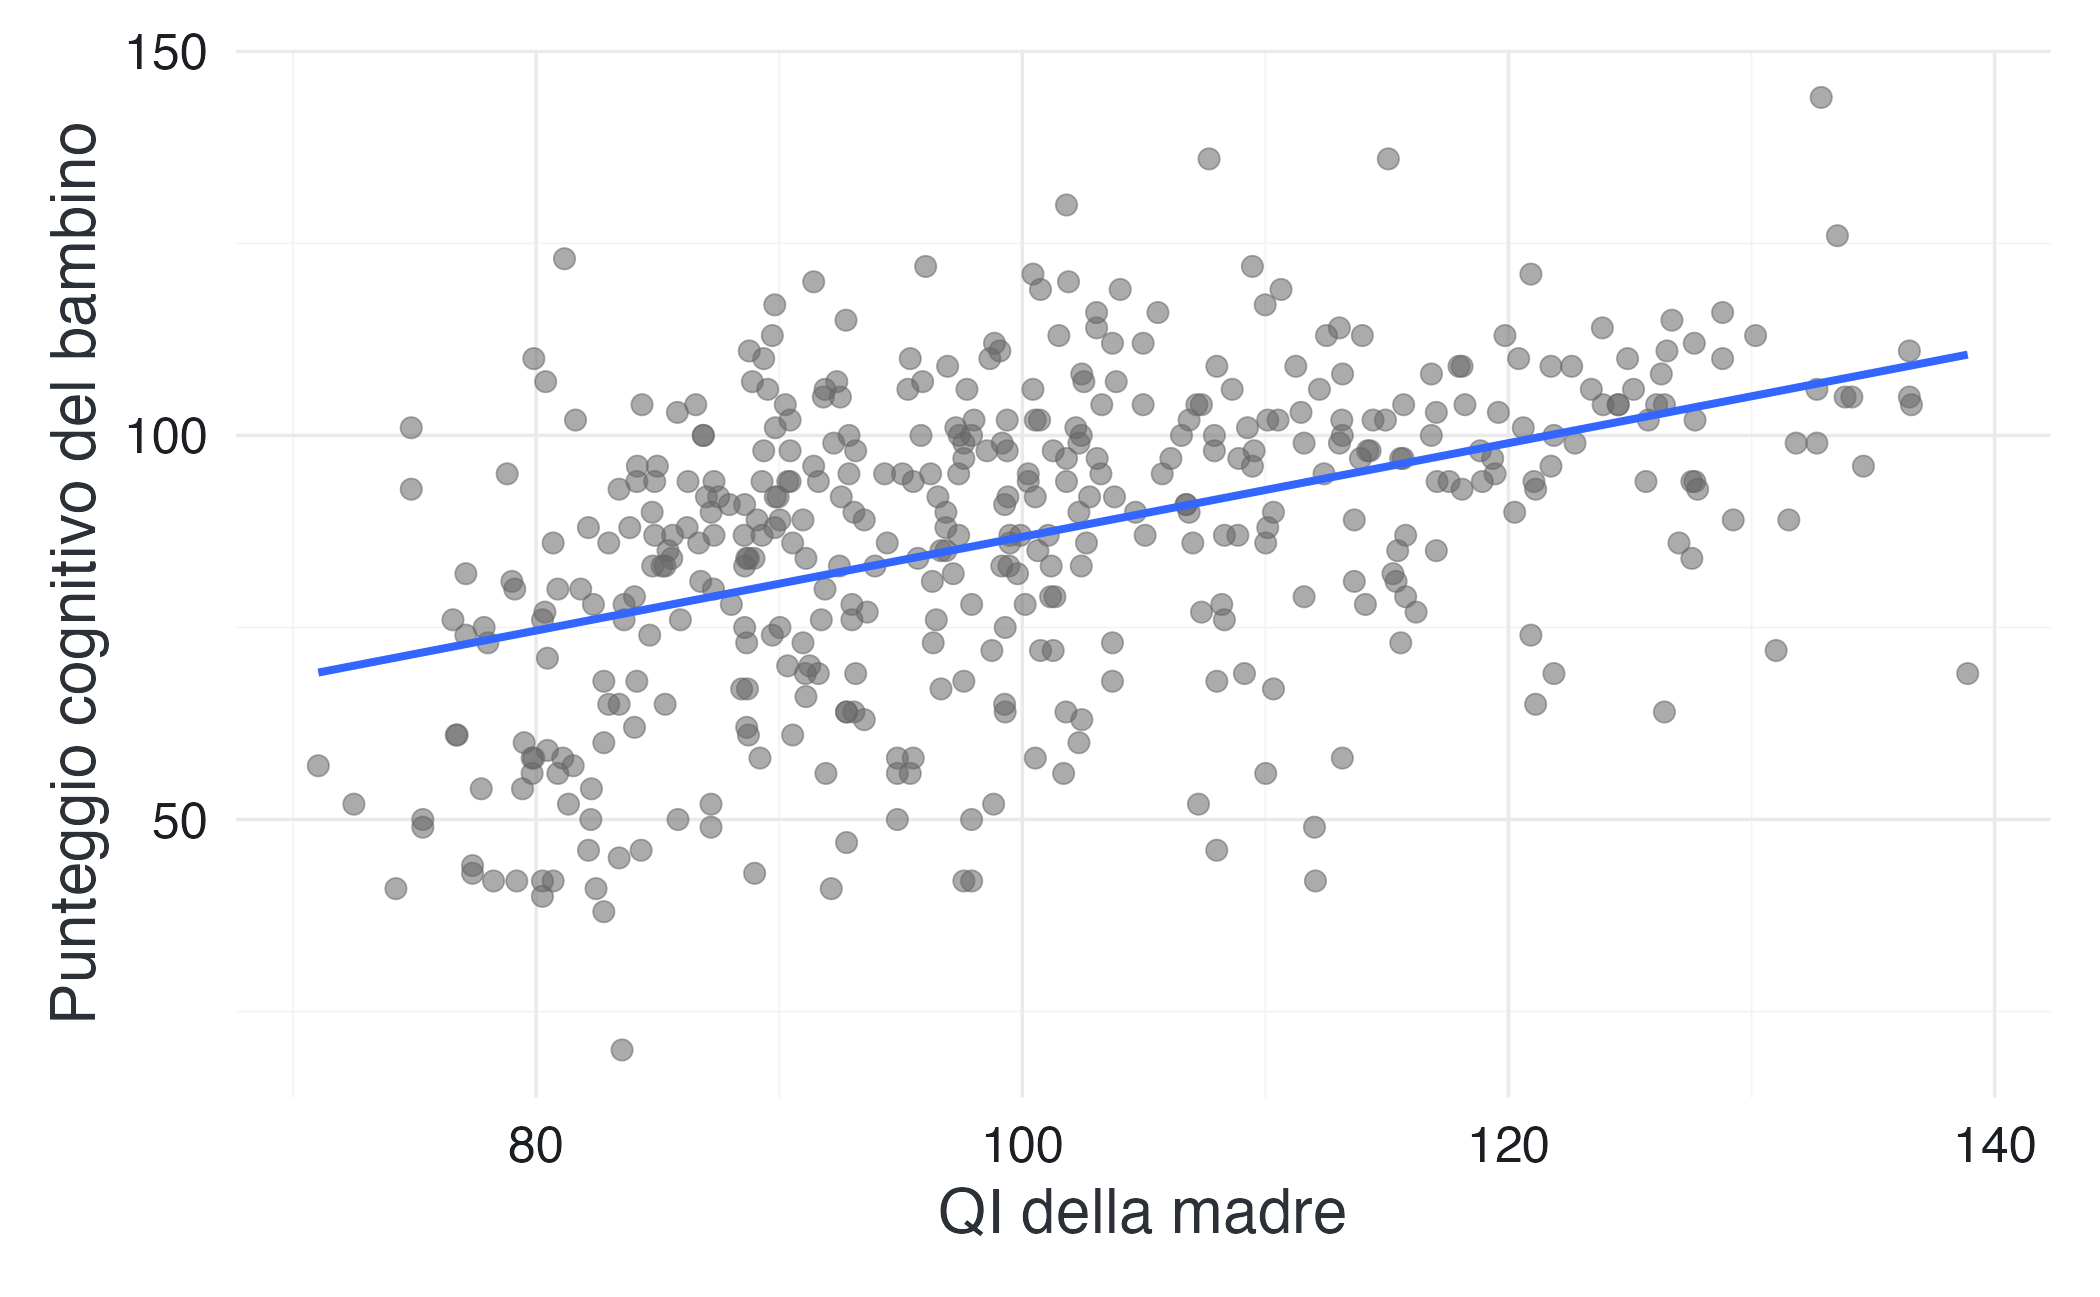
\includegraphics[width=0.85\linewidth,height=\textheight,keepaspectratio]{chapters/linear_models/01_modello_lineare_generativo_files/figure-pdf/fig-kidiq-scatter-generative-1.png}

}

\caption{\label{fig-kidiq-scatter-generative}Relazione osservata tra QI
materno e punteggio cognitivo del bambino. La linea rappresenta una
sintesi della media condizionata, non la previsione esatta di ogni
osservazione.}

\end{figure}%

Il diagramma suggerisce un'associazione positiva, ma mostra anche una
considerevole dispersione verticale dei punti. Bambini le cui madri
hanno punteggi simili nella variabile esplicativa possono presentare
esiti cognitivi molto diversi. Un modello statistico adeguato deve
pertanto essere in grado di rappresentare congiuntamente:

\begin{enumerate}
\def\labelenumi{\arabic{enumi}.}
\tightlist
\item
  la variazione sistematica della media condizionata di \(Y\) al variare
  di \(X\);
\item
  la variabilità residua delle osservazioni intorno a tale media.
\end{enumerate}

\section{Il modello generativo}\label{il-modello-generativo}

Si fissi un valore di riferimento \(x_0\) e si definisca il predittore
centrato

\[
x_i^c = x_i - x_0.
\]

Nell'esempio che segue, il riferimento è costituito dalla media
campionaria del QI materno. Il modello lineare gaussiano può allora
essere espresso nella forma

\begin{equation}\protect\phantomsection\label{eq-linear-generative}{
\begin{aligned}
y_i \mid x_i, \alpha, \beta, \sigma
  &\sim \operatorname{Normal}(\mu_i, \sigma), \\
\mu_i
  &= \alpha + \beta x_i^c.
\end{aligned}
}\end{equation}

Tale specificazione contiene due componenti collegate ma distinte.

\subsection{La componente sistematica}\label{la-componente-sistematica}

La funzione

\[
\mu_i = \alpha + \beta x_i^c
\]

descrive la variazione del valore medio atteso dell'esito in funzione
del predittore.

\begin{itemize}
\tightlist
\item
  \(\alpha\) rappresenta il punteggio medio atteso del bambino quando
  \(x_i^c=0\), ossia quando il QI materno coincide con il valore di
  riferimento \(x_0\);
\item
  \(\beta\) esprime la differenza attesa nella media di \(Y\) per un
  incremento unitario di \(X\).
\end{itemize}

A titolo di esempio, se \(\beta=0.60\), allora due valori di QI materno
che differiscono di dieci punti determinano medie condizionate distanti
sei punti, essendo

\[
\mu(x+10)-\mu(x)=10\beta=6.
\]

\subsection{La componente aleatoria}\label{la-componente-aleatoria}

La distribuzione normale specifica che, per ciascun valore di \(x_i\),
le osservazioni possono discostarsi dalla media \(\mu_i\). Il parametro
\(\sigma\) rappresenta la \emph{deviazione standard condizionata}:

\begin{itemize}
\tightlist
\item
  valori piccoli di \(\sigma\) indicano osservazioni concentrate vicino
  alla retta di regressione;
\item
  valori grandi indicano una dispersione più ampia attorno alla retta.
\end{itemize}

Il modello non assegna quindi a ciascun bambino un singolo punteggio
deterministico, ma definisce, per ogni valore del predittore, una
distribuzione di esiti possibili.

\begin{tcolorbox}[enhanced jigsaw, arc=.35mm, bottomrule=.15mm, bottomtitle=1mm, breakable, colback=white, colbacktitle=quarto-callout-warning-color!10!white, colframe=quarto-callout-warning-color-frame, coltitle=black, left=2mm, leftrule=.75mm, opacityback=0, opacitybacktitle=0.6, rightrule=.15mm, title=\textcolor{quarto-callout-warning-color}{\faExclamationTriangle}\hspace{0.5em}{Il residuo non è una spiegazione psicologica}, titlerule=0mm, toprule=.15mm, toptitle=1mm]

Lo scostamento \(y_i-\mu_i\) rappresenta ciò che il modello lineare non
è riuscito a prevedere per l'osservazione \(i\). Tale discrepanza può
derivare da molteplici fonti: eterogeneità individuale, variabili
omesse, errore di misurazione o inadeguatezza della forma funzionale, ma
il modello, da solo non consente di attribuirla a una di queste origini.

\end{tcolorbox}

\section{Dalla specificazione ai dati: simulare il
modello}\label{dalla-specificazione-ai-dati-simulare-il-modello}

Un modello si definisce generativo quando è possibile utilizzarlo per
produrre dati. A titolo illustrativo, si considerino i seguenti valori:

\[
\alpha=87, \qquad \beta=0.60, \qquad \sigma=18.
\]

Mantenendo fissi i valori osservati del QI materno, possiamo generare un
nuovo punteggio per ciascun bambino.

\begin{Shaded}
\begin{Highlighting}[]
\NormalTok{x\_ref }\OtherTok{\textless{}{-}} \FunctionTok{mean}\NormalTok{(kidiq}\SpecialCharTok{$}\NormalTok{mom\_iq)}

\NormalTok{alpha\_sim }\OtherTok{\textless{}{-}} \DecValTok{87}
\NormalTok{beta\_sim  }\OtherTok{\textless{}{-}} \FloatTok{0.60}
\NormalTok{sigma\_sim }\OtherTok{\textless{}{-}} \DecValTok{18}

\NormalTok{simulated\_data }\OtherTok{\textless{}{-}}\NormalTok{ kidiq }\SpecialCharTok{|\textgreater{}}
  \FunctionTok{mutate}\NormalTok{(}
    \AttributeTok{mom\_iq\_c =}\NormalTok{ mom\_iq }\SpecialCharTok{{-}}\NormalTok{ x\_ref,}
    \AttributeTok{mu =}\NormalTok{ alpha\_sim }\SpecialCharTok{+}\NormalTok{ beta\_sim }\SpecialCharTok{*}\NormalTok{ mom\_iq\_c,}
    \AttributeTok{simulated\_score =} \FunctionTok{rnorm}\NormalTok{(}\FunctionTok{n}\NormalTok{(), }\AttributeTok{mean =}\NormalTok{ mu, }\AttributeTok{sd =}\NormalTok{ sigma\_sim)}
\NormalTok{  )}

\NormalTok{simulated\_data }\SpecialCharTok{|\textgreater{}}
  \FunctionTok{select}\NormalTok{(mom\_iq, mu, simulated\_score) }\SpecialCharTok{|\textgreater{}}
  \FunctionTok{head}\NormalTok{()}
\CommentTok{\#\textgreater{}   mom\_iq   mu simulated\_score}
\CommentTok{\#\textgreater{} 1  121.1 99.7            77.9}
\CommentTok{\#\textgreater{} 2   89.4 80.6            85.6}
\CommentTok{\#\textgreater{} 3  115.4 96.3           115.8}
\CommentTok{\#\textgreater{} 4   99.4 86.7            44.4}
\CommentTok{\#\textgreater{} 5   92.7 82.6            90.4}
\CommentTok{\#\textgreater{} 6  107.9 91.7           100.9}
\end{Highlighting}
\end{Shaded}

Per confrontare una replica simulata con i dati osservati, i due grafici
vengono riportati sulla stessa scala.

\begin{Shaded}
\begin{Highlighting}[]
\NormalTok{plot\_data }\OtherTok{\textless{}{-}} \FunctionTok{bind\_rows}\NormalTok{(}
\NormalTok{  kidiq }\SpecialCharTok{|\textgreater{}}
    \FunctionTok{transmute}\NormalTok{(}
\NormalTok{      mom\_iq,}
      \AttributeTok{score =}\NormalTok{ kid\_score,}
      \AttributeTok{origine =} \StringTok{"Dati osservati"}
\NormalTok{    ),}
\NormalTok{  simulated\_data }\SpecialCharTok{|\textgreater{}}
    \FunctionTok{transmute}\NormalTok{(}
\NormalTok{      mom\_iq,}
      \AttributeTok{score =}\NormalTok{ simulated\_score,}
      \AttributeTok{origine =} \StringTok{"Replica simulata"}
\NormalTok{    )}
\NormalTok{)}

\NormalTok{plot\_data }\SpecialCharTok{|\textgreater{}}
  \FunctionTok{ggplot}\NormalTok{(}\FunctionTok{aes}\NormalTok{(}\AttributeTok{x =}\NormalTok{ mom\_iq, }\AttributeTok{y =}\NormalTok{ score)) }\SpecialCharTok{+}
  \FunctionTok{geom\_point}\NormalTok{(}\AttributeTok{alpha =} \FloatTok{0.45}\NormalTok{) }\SpecialCharTok{+}
  \FunctionTok{geom\_smooth}\NormalTok{(}\AttributeTok{method =} \StringTok{"lm"}\NormalTok{, }\AttributeTok{se =} \ConstantTok{FALSE}\NormalTok{, }\AttributeTok{linewidth =} \FloatTok{0.8}\NormalTok{) }\SpecialCharTok{+}
  \FunctionTok{facet\_wrap}\NormalTok{(}\SpecialCharTok{\textasciitilde{}}\NormalTok{ origine) }\SpecialCharTok{+}
  \FunctionTok{labs}\NormalTok{(}
    \AttributeTok{x =} \StringTok{"QI della madre"}\NormalTok{,}
    \AttributeTok{y =} \StringTok{"Punteggio del bambino"}
\NormalTok{  ) }
  \CommentTok{\# theme\_manuscript()}
\end{Highlighting}
\end{Shaded}

\begin{figure}[H]

\centering{

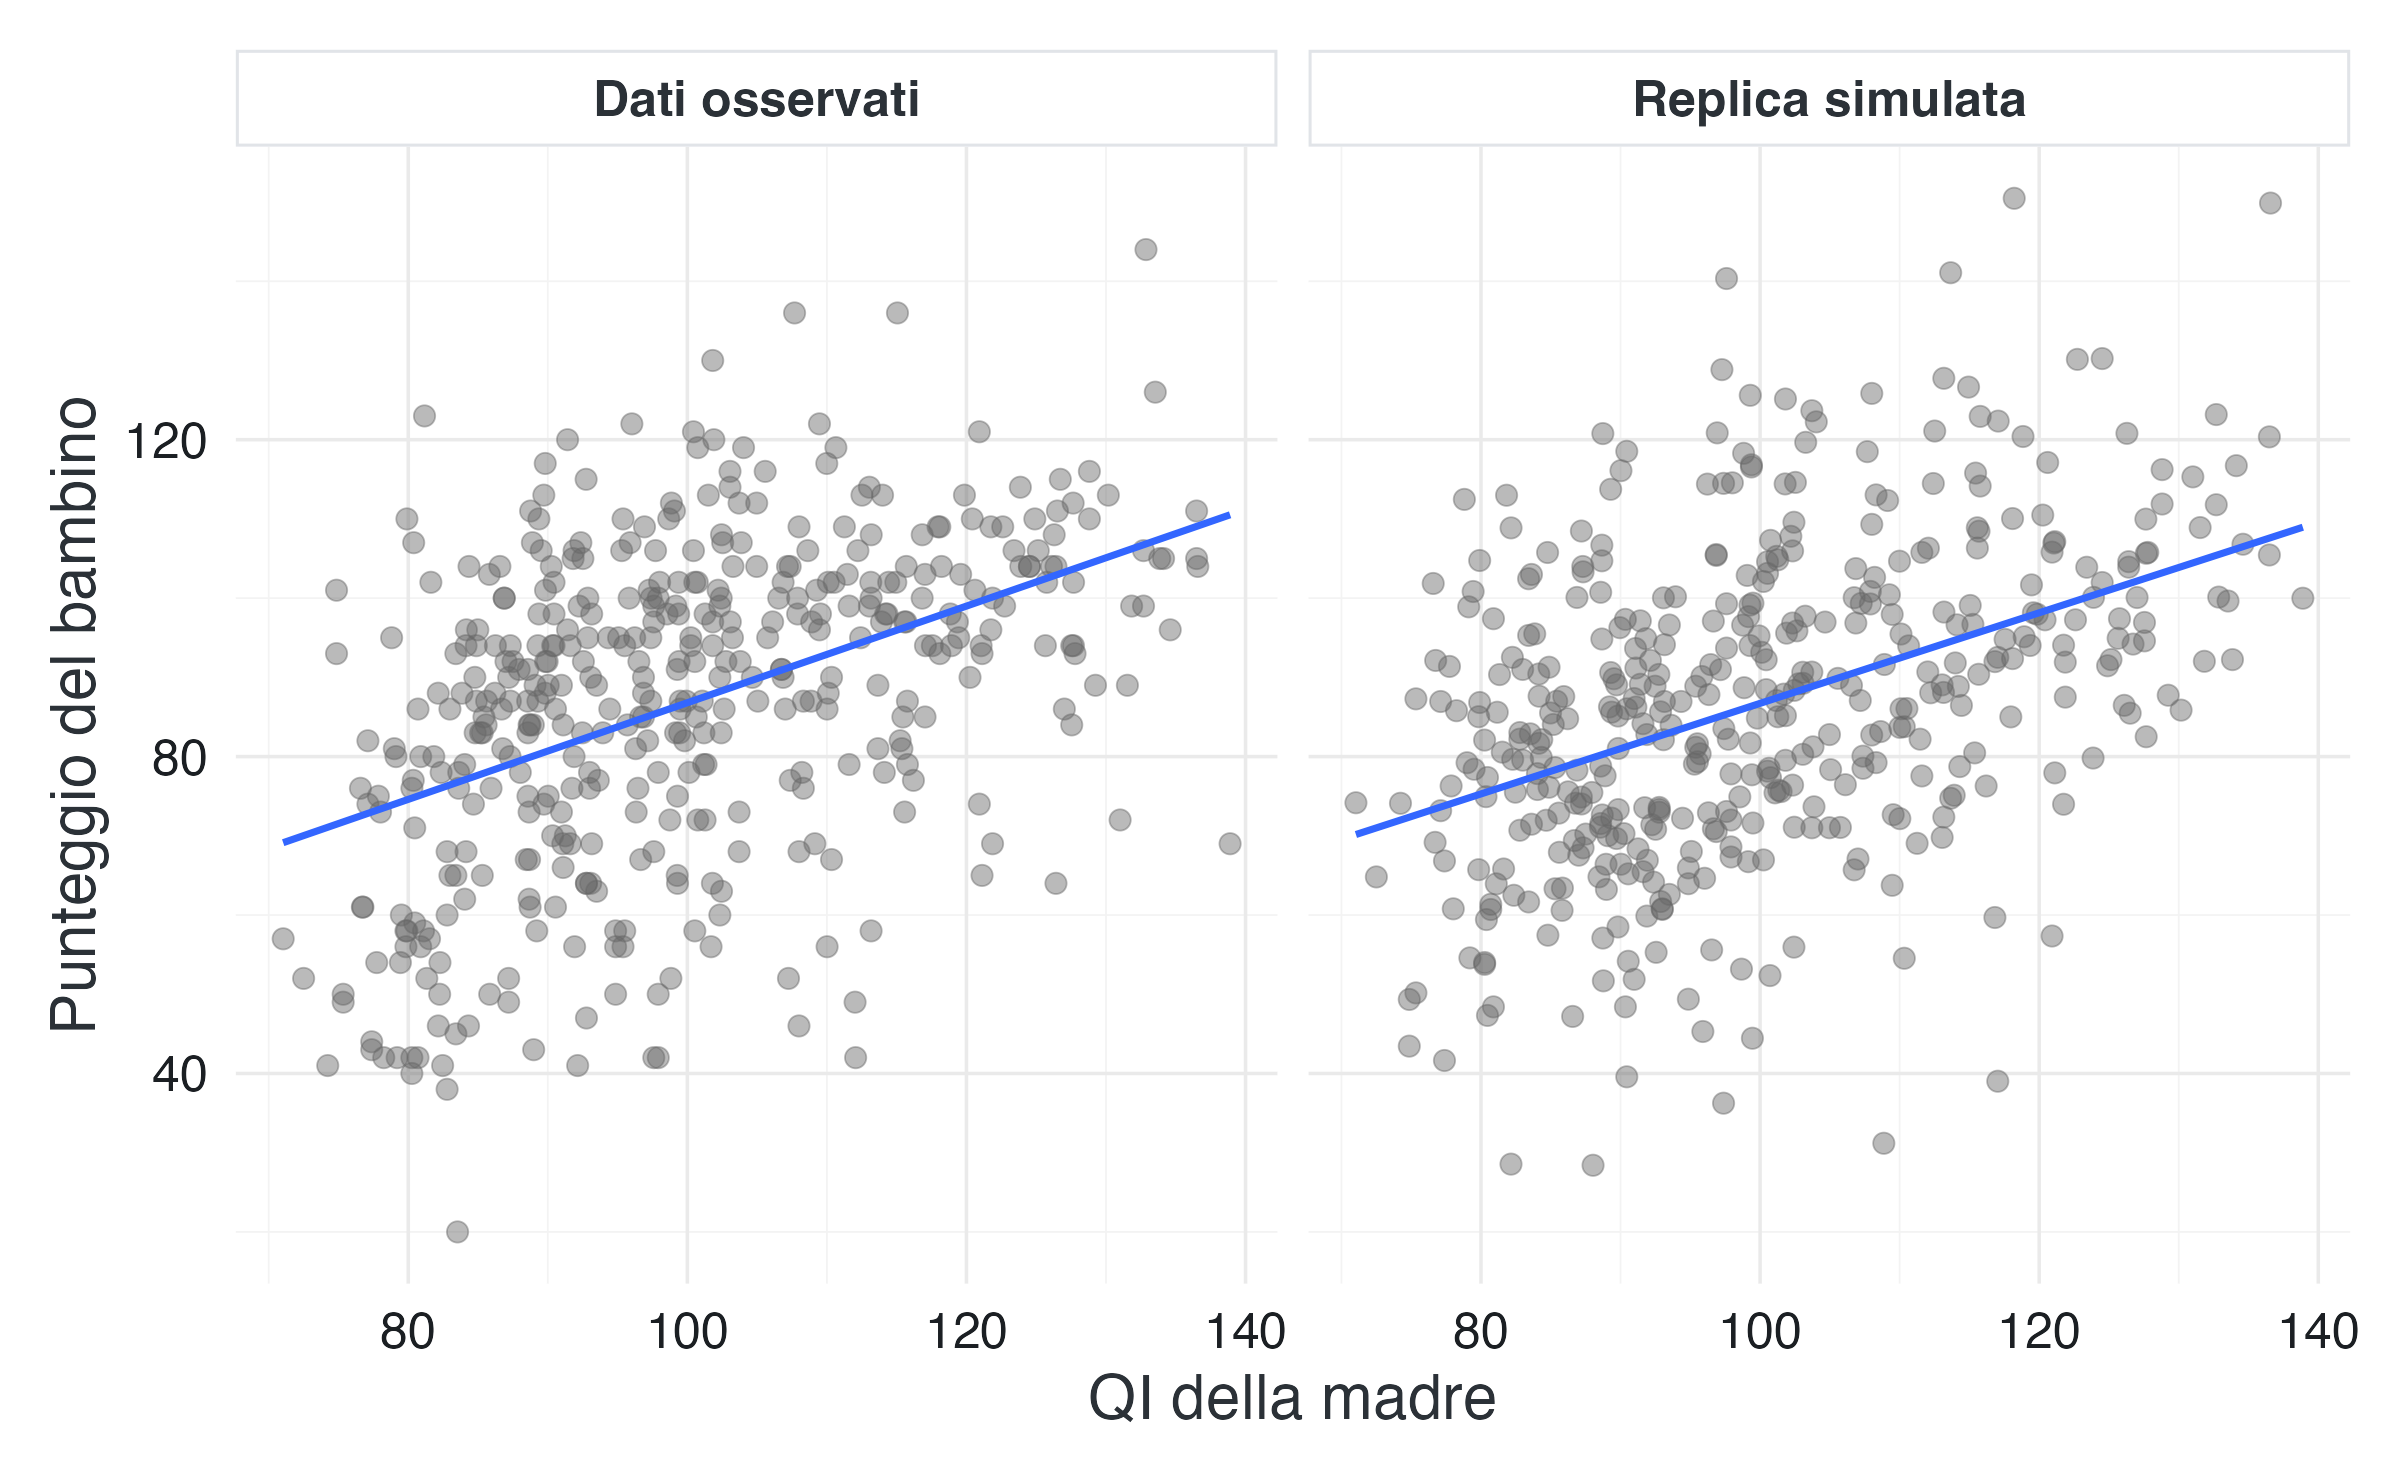
\includegraphics[width=0.85\linewidth,height=\textheight,keepaspectratio]{chapters/linear_models/01_modello_lineare_generativo_files/figure-pdf/fig-observed-simulated-linear-1.png}

}

\caption{\label{fig-observed-simulated-linear}Dati osservati e una
replica generata dal modello lineare. La simulazione rende esplicito che
la retta descrive la media, mentre le singole osservazioni rimangono
variabili.}

\end{figure}%

Una singola simulazione non deve necessariamente riprodurre esattamente
il campione osservato: è la distribuzione delle repliche che deve essere
compatibile con i dati osservati. Il controllo utile consiste nel
verificare se le repliche generate dal modello presentino, nel loro
insieme, caratteristiche plausibili, quali l'intervallo dei punteggi, la
dispersione, la tendenza media e la frequenza dei valori estremi. Nei
capitoli successivi, questa logica verrà formalizzata mediante controlli
predittivi a priori e a posteriori.

\section{Perché centrare il
predittore}\label{perchuxe9-centrare-il-predittore}

Nel modello non centrato,

\[
\mu_i = a + b x_i,
\]

l'intercetta \(a\) corrisponde al valore medio atteso di \(Y\) in
corrispondenza di \(X=0\). Nel caso del QI materno, tuttavia, tale
valore non appartiene all'intervallo dei dati osservati e la sua
interpretazione risulta priva di significato sostantivo.

Imponendo \(x_0=\bar{x}\) e definendo il predittore centrato
\(x_i^c=x_i-\bar{x}\), l'intercetta \(\alpha\) assume il significato di
punteggio medio atteso per un bambino la cui madre presenta un QI pari
alla media campionaria. La pendenza \(\beta\) rimane invariata: la
trasformazione modifica unicamente l'origine della scala del predittore
e non la relazione funzionale tra le variabili.

\begin{Shaded}
\begin{Highlighting}[]
\NormalTok{kidiq }\OtherTok{\textless{}{-}}\NormalTok{ kidiq }\SpecialCharTok{|\textgreater{}}
  \FunctionTok{mutate}\NormalTok{(}\AttributeTok{mom\_iq\_c =}\NormalTok{ mom\_iq }\SpecialCharTok{{-}} \FunctionTok{mean}\NormalTok{(mom\_iq))}

\NormalTok{fit\_uncentered }\OtherTok{\textless{}{-}} \FunctionTok{lm}\NormalTok{(kid\_score }\SpecialCharTok{\textasciitilde{}}\NormalTok{ mom\_iq, }\AttributeTok{data =}\NormalTok{ kidiq)}
\NormalTok{fit\_centered   }\OtherTok{\textless{}{-}} \FunctionTok{lm}\NormalTok{(kid\_score }\SpecialCharTok{\textasciitilde{}}\NormalTok{ mom\_iq\_c, }\AttributeTok{data =}\NormalTok{ kidiq)}

\FunctionTok{bind\_rows}\NormalTok{(}
\NormalTok{  broom}\SpecialCharTok{::}\FunctionTok{tidy}\NormalTok{(fit\_uncentered) }\SpecialCharTok{|\textgreater{}}
    \FunctionTok{mutate}\NormalTok{(}\AttributeTok{modello =} \StringTok{"Predittore originale"}\NormalTok{),}
\NormalTok{  broom}\SpecialCharTok{::}\FunctionTok{tidy}\NormalTok{(fit\_centered) }\SpecialCharTok{|\textgreater{}}
    \FunctionTok{mutate}\NormalTok{(}\AttributeTok{modello =} \StringTok{"Predittore centrato"}\NormalTok{)}
\NormalTok{) }\SpecialCharTok{|\textgreater{}}
  \FunctionTok{select}\NormalTok{(modello, term, estimate)}
\CommentTok{\#\textgreater{} \# A tibble: 4 x 3}
\CommentTok{\#\textgreater{}   modello              term        estimate}
\CommentTok{\#\textgreater{}   \textless{}chr\textgreater{}                \textless{}chr\textgreater{}          \textless{}dbl\textgreater{}}
\CommentTok{\#\textgreater{} 1 Predittore originale (Intercept)   25.8  }
\CommentTok{\#\textgreater{} 2 Predittore originale mom\_iq         0.610}
\CommentTok{\#\textgreater{} 3 Predittore centrato  (Intercept)   86.8  }
\CommentTok{\#\textgreater{} 4 Predittore centrato  mom\_iq\_c       0.610}
\end{Highlighting}
\end{Shaded}

La pendenza è identica nei due modelli. L'unica differenza riguarda
l'intercetta, che nel modello centrato assume un significato più
informativo.

\begin{tcolorbox}[enhanced jigsaw, arc=.35mm, bottomrule=.15mm, bottomtitle=1mm, breakable, colback=white, colbacktitle=quarto-callout-note-color!10!white, colframe=quarto-callout-note-color-frame, coltitle=black, left=2mm, leftrule=.75mm, opacityback=0, opacitybacktitle=0.6, rightrule=.15mm, title=\textcolor{quarto-callout-note-color}{\faInfo}\hspace{0.5em}{La centratura non risolve tutti i problemi}, titlerule=0mm, toprule=.15mm, toptitle=1mm]

Centrare un predittore facilita l'interpretazione e, nei modelli più
complessi, può migliorare la geometria computazionale. Tuttavia, non
modifica l'adeguatezza della forma lineare, non elimina i possibili
confondimenti e non trasforma un'associazione in un effetto causale.

\end{tcolorbox}

\section{Dai dati a una stima
puntuale}\label{dai-dati-a-una-stima-puntuale}

Una volta formulato il modello, si procede all'identificazione dei
valori dei parametri che meglio si accordano con i dati osservati. Per
un modello gaussiano con deviazione standard costante, i coefficienti
ottenuti con il metodo dei minimi quadrati coincidono con le stime di
massima verosimiglianza di \(\alpha\) e \(\beta\).

La funzione \texttt{lm()} consente di ottenere tali stime puntuali.

\begin{Shaded}
\begin{Highlighting}[]
\NormalTok{fit\_lm }\OtherTok{\textless{}{-}} \FunctionTok{lm}\NormalTok{(kid\_score }\SpecialCharTok{\textasciitilde{}}\NormalTok{ mom\_iq\_c, }\AttributeTok{data =}\NormalTok{ kidiq)}

\NormalTok{linear\_summary }\OtherTok{\textless{}{-}} \FunctionTok{tibble}\NormalTok{(}
  \AttributeTok{quantita =} \FunctionTok{c}\NormalTok{(}
    \StringTok{"Intercetta"}\NormalTok{,}
    \StringTok{"Pendenza"}\NormalTok{,}
    \StringTok{"Deviazione standard residua"}\NormalTok{,}
    \StringTok{"R{-}quadrato"}
\NormalTok{  ),}
  \AttributeTok{stima =} \FunctionTok{c}\NormalTok{(}
    \FunctionTok{unname}\NormalTok{(}\FunctionTok{coef}\NormalTok{(fit\_lm)[}\StringTok{"(Intercept)"}\NormalTok{]),}
    \FunctionTok{unname}\NormalTok{(}\FunctionTok{coef}\NormalTok{(fit\_lm)[}\StringTok{"mom\_iq\_c"}\NormalTok{]),}
    \FunctionTok{summary}\NormalTok{(fit\_lm)}\SpecialCharTok{$}\NormalTok{sigma,}
    \FunctionTok{summary}\NormalTok{(fit\_lm)}\SpecialCharTok{$}\NormalTok{r.squared}
\NormalTok{  )}
\NormalTok{)}

\NormalTok{linear\_summary}
\CommentTok{\#\textgreater{} \# A tibble: 4 x 2}
\CommentTok{\#\textgreater{}   quantita                     stima}
\CommentTok{\#\textgreater{}   \textless{}chr\textgreater{}                        \textless{}dbl\textgreater{}}
\CommentTok{\#\textgreater{} 1 Intercetta                  86.8  }
\CommentTok{\#\textgreater{} 2 Pendenza                     0.610}
\CommentTok{\#\textgreater{} 3 Deviazione standard residua 18.3  }
\CommentTok{\#\textgreater{} 4 R{-}quadrato                   0.201}
\end{Highlighting}
\end{Shaded}

Le stime hanno la seguente interpretazione descrittiva:

\begin{itemize}
\tightlist
\item
  l'intercetta corrisponde corrisponde al valore medio condizionato
  atteso di \(Y\) quando il QI materno è pari alla media campionaria;
\item
  la pendenza esprime la variazione media attesa del punteggio del
  bambino per un incremento di un punto nel QI materno;
\item
  la deviazione standard residua quantifica la dispersione dei punteggi
  attorno alla media condizionata;
\item
  \(R^2\) esprime la proporzione di variabilità campionaria di
  kid\_score \texttt{kid\_score} spiegata dalla componente sistematica
  del modello.
\end{itemize}

\(R^2\) fornisce una descrizione sintetica dell'adattamento nel
campione. Non attesta, tuttavia, la correttezza della specificazione, né
la validità causale della spiegazione, e non coincide necessariamente
con la capacità predittiva su nuove osservazioni.

\begin{tcolorbox}[enhanced jigsaw, arc=.35mm, bottomrule=.15mm, bottomtitle=1mm, breakable, colback=white, colbacktitle=quarto-callout-tip-color!10!white, colframe=quarto-callout-tip-color-frame, coltitle=black, left=2mm, leftrule=.75mm, opacityback=0, opacitybacktitle=0.6, rightrule=.15mm, title=\textcolor{quarto-callout-tip-color}{\faLightbulb}\hspace{0.5em}{Dal punto alla distribuzione}, titlerule=0mm, toprule=.15mm, toptitle=1mm]

In questo capitolo utilizziamo una stima puntuale per illustrare i
parametri in termini concreti. Nel capitolo dedicato al workflow
bayesiano, \(\alpha\), \(\beta\) e \(\sigma\) saranno rappresentati
mediante distribuzioni a posteriori, consentendo di propagare
esplicitamente l'incertezza nelle quantità derivate e nelle previsioni.

\end{tcolorbox}

\section{Valori adattati e residui}\label{valori-adattati-e-residui}

Per ciascuna osservazione, il modello fornisce un valore adattato

\[
\widehat{y}_i = \widehat{\alpha} + \widehat{\beta}x_i^c
\]

e un residuo

\[
e_i = y_i-\widehat{y}_i.
\]

L'esame dei residui consente di individuare eventuali strutture
sistematiche nei dati che il modello non è riuscito a rappresentare.

\begin{Shaded}
\begin{Highlighting}[]
\NormalTok{fit\_augmented }\OtherTok{\textless{}{-}}\NormalTok{ broom}\SpecialCharTok{::}\FunctionTok{augment}\NormalTok{(fit\_lm)}

\NormalTok{fit\_augmented }\SpecialCharTok{|\textgreater{}}
  \FunctionTok{select}\NormalTok{(kid\_score, mom\_iq\_c, .fitted, .resid) }\SpecialCharTok{|\textgreater{}}
  \FunctionTok{head}\NormalTok{()}
\CommentTok{\#\textgreater{} \# A tibble: 6 x 4}
\CommentTok{\#\textgreater{}   kid\_score mom\_iq\_c .fitted .resid}
\CommentTok{\#\textgreater{}       \textless{}dbl\textgreater{}    \textless{}dbl\textgreater{}   \textless{}dbl\textgreater{}  \textless{}dbl\textgreater{}}
\CommentTok{\#\textgreater{} 1        65   21.1      99.7 {-}34.7 }
\CommentTok{\#\textgreater{} 2        98  {-}10.6      80.3  17.7 }
\CommentTok{\#\textgreater{} 3        85   15.4      96.2 {-}11.2 }
\CommentTok{\#\textgreater{} 4        83   {-}0.550    86.5  {-}3.46}
\CommentTok{\#\textgreater{} 5       115   {-}7.25     82.4  32.6 }
\CommentTok{\#\textgreater{} 6        98    7.90     91.6   6.38}
\end{Highlighting}
\end{Shaded}

\begin{Shaded}
\begin{Highlighting}[]
\NormalTok{fit\_augmented }\SpecialCharTok{|\textgreater{}}
  \FunctionTok{ggplot}\NormalTok{(}\FunctionTok{aes}\NormalTok{(}\AttributeTok{x =}\NormalTok{ .fitted, }\AttributeTok{y =}\NormalTok{ .resid)) }\SpecialCharTok{+}
  \FunctionTok{geom\_hline}\NormalTok{(}\AttributeTok{yintercept =} \DecValTok{0}\NormalTok{, }\AttributeTok{linetype =} \StringTok{"dashed"}\NormalTok{) }\SpecialCharTok{+}
  \FunctionTok{geom\_point}\NormalTok{(}\AttributeTok{alpha =} \FloatTok{0.55}\NormalTok{) }\SpecialCharTok{+}
  \FunctionTok{geom\_smooth}\NormalTok{(}\AttributeTok{method =} \StringTok{"loess"}\NormalTok{, }\AttributeTok{se =} \ConstantTok{FALSE}\NormalTok{, }\AttributeTok{linewidth =} \FloatTok{0.8}\NormalTok{) }\SpecialCharTok{+}
  \FunctionTok{labs}\NormalTok{(}
    \AttributeTok{x =} \StringTok{"Valore adattato"}\NormalTok{,}
    \AttributeTok{y =} \StringTok{"Residuo"}
\NormalTok{  ) }
  \CommentTok{\# theme\_manuscript()}
\end{Highlighting}
\end{Shaded}

\begin{figure}[H]

\centering{

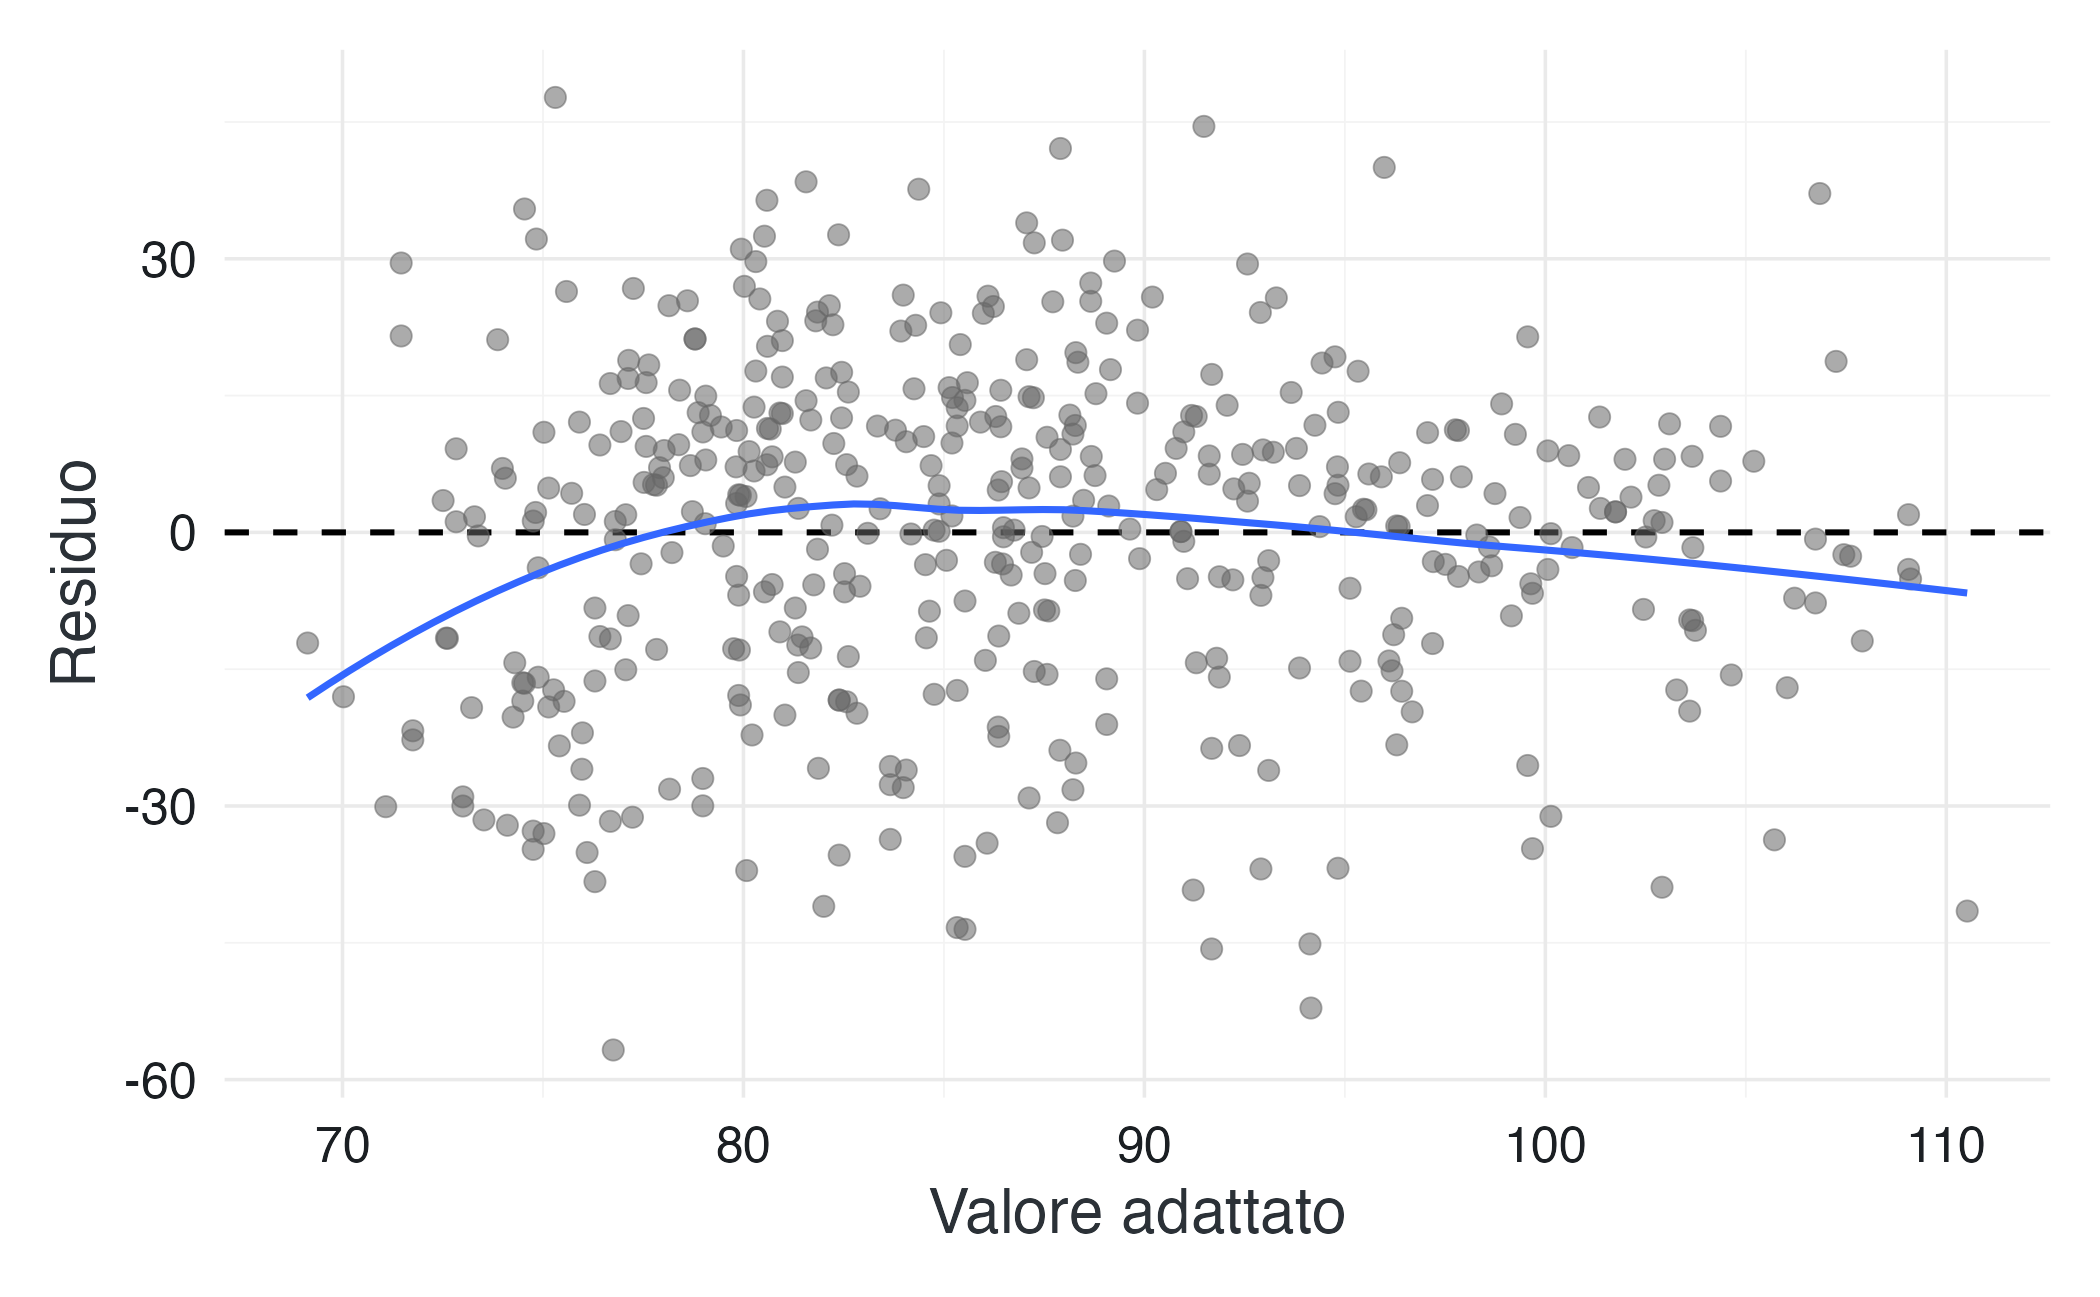
\includegraphics[width=0.85\linewidth,height=\textheight,keepaspectratio]{chapters/linear_models/01_modello_lineare_generativo_files/figure-pdf/fig-linear-residuals-1.png}

}

\caption{\label{fig-linear-residuals}Residui in funzione dei valori
adattati. Pattern curvilinei o variazioni sistematiche della dispersione
suggerirebbero che il modello lineare gaussiano non rappresenta
adeguatamente i dati.}

\end{figure}%

Un diagramma dei residui non fornisce un giudizio automatico, ma orienta
l'attenzione verso domande specifiche: persiste una curvatura nei
residui? La dispersione tende ad aumentare con il valore atteso? Alcune
osservazioni esercitano un'influenza sproporzionata sulle stime? Le
osservazioni sono effettivamente indipendenti o presentano una struttura
di dipendenza, ad esempio all'interno di famiglie, classi scolastiche o
gruppi di partecipanti?

\section{Assunzioni della specificazione
gaussiana}\label{assunzioni-della-specificazione-gaussiana}

Il modello in Equazione~\ref{eq-linear-generative} costituisce una
rappresentazione semplificata del fenomeno. Le sue assunzioni vanno
pertanto interpretate come affermazioni verificabili sul processo
generativo dei dati.

\subsection{Linearità della media
condizionata}\label{linearituxe0-della-media-condizionata}

Il modello assume che, nell'intervallo osservato, la media di \(Y\) vari
in modo approssimativamente lineare al variare di \(X\). Una relazione
curvilinea può condurre a una stima della pendenza media apparentemente
plausibile, ma può nascondere differenze sistematiche tra le diverse
regioni del predittore.

\subsection{Dispersione costante}\label{dispersione-costante}

Il medesimo valore di \(\sigma\) viene impiegato per tutti i livelli di
\(X\). Se invece la dispersione dei residui mostra una dipendenza
sistematica dal predittore, è necessario adottare un modello che
contempli esplicitamente una componente di eteroschedasticità, ovvero
una funzione che descriva la variazione della varianza in funzione di
\(X\).

\subsection{Indipendenza condizionale}\label{indipendenza-condizionale}

Una volta specificati i predittori e i parametri, le osservazioni
vengono trattate come indipendenti le une dalle altre. Tale assunzione
può risultare problematica in presenza di misure ripetute o di dati con
struttura gerarchica. I modelli multilivello, che verranno introdotti
nei capitoli successivi, permettono di rappresentare esplicitamente
queste forme di dipendenza.

\subsection{Forma della distribuzione
condizionata}\label{forma-della-distribuzione-condizionata}

Il modello assume una distribuzione normale attorno alla media
condizionata. La presenza frequente di valori estremi, un'asimmetria
marcata o i limiti naturali della scala suggeriscono l'adozione di una
distribuzione robusta o di una diversa famiglia di verosimiglianza.

\subsection{Qualità delle misure e ambito di
generalizzazione}\label{qualituxe0-delle-misure-e-ambito-di-generalizzazione}

La formula del modello non corregge automaticamente gli errori di
misurazione, le distorsioni da selezione campionaria o le discrepanze
tra il costrutto teorico e la variabile osservata. Inoltre, la relazione
stimata è definita nell'intervallo dei dati disponibili e ogni
estrapolazione al di là di tale intervallo richiede assunzioni
aggiuntive.

\begin{tcolorbox}[enhanced jigsaw, arc=.35mm, bottomrule=.15mm, bottomtitle=1mm, breakable, colback=white, colbacktitle=quarto-callout-warning-color!10!white, colframe=quarto-callout-warning-color-frame, coltitle=black, left=2mm, leftrule=.75mm, opacityback=0, opacitybacktitle=0.6, rightrule=.15mm, title=\textcolor{quarto-callout-warning-color}{\faExclamationTriangle}\hspace{0.5em}{Assunzioni diverse, conseguenze diverse}, titlerule=0mm, toprule=.15mm, toptitle=1mm]

La violazione di un'assunzione non produce sempre lo stesso tipo di
conseguenza. Può alterare la grandezza stimata, compromettere
l'adeguatezza delle previsioni, sottostimare l'incertezza o limitare la
generalizzabilità dei risultati. Per questa ragione, non è sufficiente
applicare una checklist meccanica, ma occorre chiedersi, per ciascuna
assunzione, quale parte dell'inferenza ne dipenda e quali strumenti
consentano di valutarne la tenuta empirica.

\end{tcolorbox}

\section{Descrivere, prevedere,
spiegare}\label{descrivere-prevedere-spiegare}

Lo stesso modello matematico può essere utilizzato per per scopi
diversi, ma la validità delle conclusioni non dipende solo dai
coefficienti di regressione. Nel nostro esempio, la pendenza descrive,
all'interno del campione analizzato, come i punteggi dei bambini
differiscano in media in funzione del QI materno. Questa è la funzione
\emph{descrittiva} del modello. Un secondo impiego riguarda la
\emph{previsione}: il modello può generare una distribuzione per il
punteggio di un nuovo bambino, dato il valore del QI materno, a patto
che la previsione individuale incorpori sia l'incertezza sui parametri
sia la variabilità residua e che venga valutata su osservazioni non
utilizzate per la stima. Un terzo obiettivo, ben diverso, è
l'\emph{interpretazione causale}, che richiederebbe una domanda causale
esplicitamente formulata, una strategia di identificazione e assunzioni
sul processo di assegnazione e sui potenziali confondenti --- condizioni
che il modello lineare, da solo, non è in grado di fornire. Per questi
motivi, nel corso del Companion adotteremo una terminologia che
distingue chiaramente gli scopi: utilizzeremo espressioni come
\emph{associazione}, \emph{differenza condizionata} e \emph{previsione}
per descrivere ciò che il modello stima, riservando il termine
\emph{effetto} ai casi in cui l'interpretazione causale sia sostenuta
dal disegno della ricerca e dalle assunzioni esplicitate. La sezione
dedicata alla causalità affronterà questi aspetti in dettaglio.

\section{Errori frequenti}\label{errori-frequenti}

\begin{tcolorbox}[enhanced jigsaw, arc=.35mm, bottomrule=.15mm, bottomtitle=1mm, breakable, colback=white, colbacktitle=quarto-callout-caution-color!10!white, colframe=quarto-callout-caution-color-frame, coltitle=black, left=2mm, leftrule=.75mm, opacityback=0, opacitybacktitle=0.6, rightrule=.15mm, title=\textcolor{quarto-callout-caution-color}{\faFire}\hspace{0.5em}{Errori frequenti}, titlerule=0mm, toprule=.15mm, toptitle=1mm]

Un errore comune è quello di interpretare l'intercetta senza averne
prima verificato il valore di riferimento. Se \(X = 0\) è privo di
significato sostantivo, come nel caso di un QI pari a zero, o se si
colloca molto al di là dei valori osservati, l'intercetta non ha alcun
significato utile e non dovrebbe essere interpretata. Un secondo
equivoco riguarda la pendenza: essa descrive la differenza media tra
individui che presentano valori diversi del predittore, e non
necessariamente il cambiamento che si verificherebbe in un singolo
individuo se il suo valore su \(X\) venisse modificato. La relazione
osservata in un campione non può essere automaticamente trasposta a un
processo individuale nel tempo. Un terzo errore consiste nel confondere
la retta di regressione, che rappresenta la media condizionata, con una
previsione individuale: le osservazioni singole si distribuiscono
attorno a tale media, e la loro variabilità è descritta da \(\sigma\).
Un quarto malinteso è l'uso di \(R^2\) come certificato di validità: un
modello può avere un valore elevato di questo indice e tuttavia essere
mal specificato o scientificamente irrilevante. Infine, non si deve
attribuire un significato causale alla posizione del predittore nella
formula di regressione: la sintassi \texttt{y\ \textasciitilde{}\ x} non
codifica alcuna teoria causale, ma solo una relazione statistica
condizionata.

\end{tcolorbox}

\section{Riflessioni conclusive}\label{riflessioni-conclusive-18}

Il modello lineare non si riduce a una semplice retta che collega i
punti, ma è piuttosto un'affermazione probabilistica completa che
specifica come la media condizionata dell'outcome vari secondo una
funzione lineare, come le osservazioni si distribuiscano attorno a tale
media e come la dispersione venga descritta da un parametro separato. Le
assunzioni del modello determinano, di conseguenza, quali
caratteristiche dei dati possono essere rappresentate e quali rimangono
al di fuori della sua portata. La prospettiva generativa modifica
profondamente il modo di condurre l'analisi: prima ancora di stimare i
parametri, è possibile simulare il modello e verificare che le sue
implicazioni siano plausibili rispetto al fenomeno studiato; dopo la
stima, è possibile confrontare le repliche generate con i dati osservati
e individuare gli aspetti che il modello non riesce a riprodurre.
L'analisi diventa, quindi, un ciclo di costruzione, controllo e
revisione, piuttosto che l'applicazione meccanica di una formula
conclusiva. Nel prossimo capitolo, utilizzeremo la regressione verso la
media per approfondire una conseguenza fondamentale della previsione
imperfetta; successivamente, applicheremo l'intero flusso di lavoro
bayesiano al modello lineare, sostituendo le stime puntuali con
distribuzioni a posteriori e predittive che rendono esplicita
l'incertezza.

\section{Concetti da ricordare}\label{concetti-da-ricordare}

\begin{enumerate}
\def\labelenumi{\arabic{enumi}.}
\tightlist
\item
  Il modello lineare descrive una distribuzione condizionata
  \(p(y\mid x)\).
\item
  La retta rappresenta la media condizionata, non ogni singola
  osservazione.
\item
  Intercetta, pendenza e deviazione standard residua rispondono a
  domande diverse.
\item
  La centratura cambia l'interpretazione dell'intercetta, ma non la
  pendenza.
\item
  Simulare dal modello rende visibili le conseguenze delle assunzioni.
\item
  Residui e indici sintetici offrono controlli parziali, non una
  validazione definitiva.
\item
  Un'associazione lineare non identifica autonomamente un effetto
  causale.
\end{enumerate}

\begin{tcolorbox}[enhanced jigsaw, arc=.35mm, bottomrule=.15mm, bottomtitle=1mm, breakable, colback=white, colbacktitle=quarto-callout-important-color!10!white, colframe=quarto-callout-important-color-frame, coltitle=black, left=2mm, leftrule=.75mm, opacityback=0, opacitybacktitle=0.6, rightrule=.15mm, title=\textcolor{quarto-callout-important-color}{\faExclamation}\hspace{0.5em}{Esercizi}, titlerule=0mm, toprule=.15mm, toptitle=1mm]

\subsection{1. Leggere il modello}\label{leggere-il-modello}

Scrivi in parole il significato dei tre parametri del modello

\[
Y_i \sim \operatorname{Normal}\!\left(85+0.4(X_i-100), 12\right).
\]

Spiega inoltre quale quantità rappresenta 85 e quale differenza media è
associata a un incremento di dieci unità in \(X\).

\subsection{2. Media e nuova
osservazione}\label{media-e-nuova-osservazione}

Per \(X=110\), calcola la media condizionata del modello precedente.
Spiega perché questo valore non coincide necessariamente con il valore
osservato per un nuovo individuo con \(X=110\).

\subsection{3. Simulazione}\label{simulazione-4}

Modifica \texttt{beta\_sim} e \texttt{sigma\_sim} nel codice del
capitolo. Genera quattro combinazioni:

\begin{itemize}
\tightlist
\item
  pendenza piccola e dispersione piccola;
\item
  pendenza piccola e dispersione grande;
\item
  pendenza grande e dispersione piccola;
\item
  pendenza grande e dispersione grande.
\end{itemize}

Descrivi come cambiano la nube di punti e la facilità con cui la
relazione sistematica può essere riconosciuta.

\subsection{4. Scelta del riferimento}\label{scelta-del-riferimento}

Centra \texttt{mom\_iq} rispetto a 100 anziché rispetto alla media
campionaria. Adatta nuovamente il modello e interpreta l'intercetta.
Verifica che la pendenza rimanga invariata.

\subsection{5. Criticare la
specificazione}\label{criticare-la-specificazione}

Immagina che il grafico dei residui mostri una chiara forma a U. Quale
assunzione sarebbe messa in discussione? Proponi una modifica della
componente sistematica del modello.

\subsection{6. Dipendenza tra
osservazioni}\label{dipendenza-tra-osservazioni}

Supponi che nel dataset siano presenti più figli della stessa madre.
Spiega perché il modello bivariato semplice potrebbe sottostimare
l'incertezza e anticipa quale estensione sarebbe necessaria.

\subsection{7. Linguaggio causale}\label{linguaggio-causale}

Riscrivi la frase seguente in modo compatibile con un'analisi
osservazionale:

\begin{quote}
Un punto aggiuntivo di QI materno aumenta di 0.61 punti il QI del
bambino.
\end{quote}

\end{tcolorbox}

\begin{tcolorbox}[enhanced jigsaw, arc=.35mm, bottomrule=.15mm, bottomtitle=1mm, breakable, colback=white, colbacktitle=quarto-callout-tip-color!10!white, colframe=quarto-callout-tip-color-frame, coltitle=black, left=2mm, leftrule=.75mm, opacityback=0, opacitybacktitle=0.6, rightrule=.15mm, title=\textcolor{quarto-callout-tip-color}{\faLightbulb}\hspace{0.5em}{Tracce di soluzione}, titlerule=0mm, toprule=.15mm, toptitle=1mm]

\begin{enumerate}
\def\labelenumi{\arabic{enumi}.}
\tightlist
\item
  L'intercetta 85 è la media attesa di \(Y\) quando \(X=100\); la
  pendenza 0.4 indica 0.4 unità di differenza media in \(Y\) per una
  unità in \(X\); \(\sigma=12\) descrive la dispersione condizionata.
  Dieci unità in \(X\) corrispondono a quattro unità nella media di
  \(Y\).
\item
  La media è \(85+0.4(110-100)=89\). Una nuova osservazione viene
  estratta da una distribuzione normale centrata su 89 con deviazione
  standard 12.
\item
  La pendenza determina la separazione delle medie lungo \(X\);
  \(\sigma\) determina la dispersione individuale. Un rapporto più
  grande tra variazione sistematica e dispersione rende il pattern più
  evidente.
\item
  L'intercetta diventa il punteggio medio previsto quando
  \texttt{mom\_iq\ =\ 100}. La pendenza non cambia perché la distanza
  tra i valori del predittore rimane identica.
\item
  Una forma a U suggerisce non linearità della media condizionata. Si
  potrebbe introdurre, per esempio, un termine quadratico, verificandone
  poi le conseguenze predittive.
\item
  Le osservazioni della stessa famiglia condividono caratteristiche e
  non sono condizionalmente indipendenti. Occorre una struttura
  multilivello con effetti di famiglia.
\item
  Una formulazione appropriata è: «Nel campione analizzato, un punto in
  più di QI materno è associato, in media, a circa 0.61 punti in più nel
  punteggio cognitivo del bambino».
\end{enumerate}

\end{tcolorbox}

\begin{tcolorbox}[enhanced jigsaw, arc=.35mm, bottomrule=.15mm, bottomtitle=1mm, breakable, colback=white, colbacktitle=quarto-callout-note-color!10!white, colframe=quarto-callout-note-color-frame, coltitle=black, left=2mm, leftrule=.75mm, opacityback=0, opacitybacktitle=0.6, rightrule=.15mm, title=\textcolor{quarto-callout-note-color}{\faInfo}\hspace{0.5em}{Informazioni sull'ambiente di sviluppo}, titlerule=0mm, toprule=.15mm, toptitle=1mm]

\begin{Shaded}
\begin{Highlighting}[]
\FunctionTok{sessionInfo}\NormalTok{()}
\CommentTok{\#\textgreater{} R version 4.6.1 (2026{-}06{-}24)}
\CommentTok{\#\textgreater{} Platform: aarch64{-}apple{-}darwin23}
\CommentTok{\#\textgreater{} Running under: macOS Tahoe 26.5.2}
\CommentTok{\#\textgreater{} }
\CommentTok{\#\textgreater{} Matrix products: default}
\CommentTok{\#\textgreater{} BLAS:   /Library/Frameworks/R.framework/Versions/4.6/Resources/lib/libRblas.0.dylib }
\CommentTok{\#\textgreater{} LAPACK: /Library/Frameworks/R.framework/Versions/4.6/Resources/lib/libRlapack.dylib;  LAPACK version 3.12.1}
\CommentTok{\#\textgreater{} }
\CommentTok{\#\textgreater{} locale:}
\CommentTok{\#\textgreater{} [1] C.UTF{-}8/UTF{-}8/C.UTF{-}8/C/C.UTF{-}8/C.UTF{-}8}
\CommentTok{\#\textgreater{} }
\CommentTok{\#\textgreater{} time zone: Europe/Zagreb}
\CommentTok{\#\textgreater{} tzcode source: internal}
\CommentTok{\#\textgreater{} }
\CommentTok{\#\textgreater{} attached base packages:}
\CommentTok{\#\textgreater{} [1] stats     graphics  grDevices utils     datasets  methods   base     }
\CommentTok{\#\textgreater{} }
\CommentTok{\#\textgreater{} other attached packages:}
\CommentTok{\#\textgreater{}  [1] broom\_1.0.13          ragg\_1.5.2            tinytable\_0.17.0     }
\CommentTok{\#\textgreater{}  [4] withr\_3.0.3           systemfonts\_1.3.2     patchwork\_1.3.2      }
\CommentTok{\#\textgreater{}  [7] ggdist\_3.3.3          tidybayes\_3.0.7       bayesplot\_1.15.0     }
\CommentTok{\#\textgreater{} [10] ggplot2\_4.0.3         reliabilitydiag\_0.2.1 priorsense\_1.2.0     }
\CommentTok{\#\textgreater{} [13] posterior\_1.7.0       loo\_2.10.0            rstan\_2.32.7         }
\CommentTok{\#\textgreater{} [16] StanHeaders\_2.32.10   brms\_2.23.0           Rcpp\_1.1.2           }
\CommentTok{\#\textgreater{} [19] sessioninfo\_1.2.4     conflicted\_1.2.0      janitor\_2.2.1        }
\CommentTok{\#\textgreater{} [22] matrixStats\_1.5.0     modelr\_0.1.11         tibble\_3.3.1         }
\CommentTok{\#\textgreater{} [25] dplyr\_1.2.1           tidyr\_1.3.2           rio\_1.3.0            }
\CommentTok{\#\textgreater{} [28] here\_1.0.2           }
\CommentTok{\#\textgreater{} }
\CommentTok{\#\textgreater{} loaded via a namespace (and not attached):}
\CommentTok{\#\textgreater{}  [1] gridExtra\_2.3.1       inline\_0.3.21         rlang\_1.3.0          }
\CommentTok{\#\textgreater{}  [4] magrittr\_2.0.5        snakecase\_0.11.1      otel\_0.2.0           }
\CommentTok{\#\textgreater{}  [7] compiler\_4.6.1        mgcv\_1.9{-}4            vctrs\_0.7.3          }
\CommentTok{\#\textgreater{} [10] stringr\_1.6.0         pkgconfig\_2.0.3       arrayhelpers\_1.1{-}1   }
\CommentTok{\#\textgreater{} [13] fastmap\_1.2.0         backports\_1.5.1       labeling\_0.4.3       }
\CommentTok{\#\textgreater{} [16] utf8\_1.2.6            rmarkdown\_2.31        tzdb\_0.5.0           }
\CommentTok{\#\textgreater{} [19] haven\_2.5.5           purrr\_1.2.2           xfun\_0.60            }
\CommentTok{\#\textgreater{} [22] cachem\_1.1.0          jsonlite\_2.0.0        parallel\_4.6.1       }
\CommentTok{\#\textgreater{} [25] R6\_2.6.1              stringi\_1.8.7         RColorBrewer\_1.1{-}3   }
\CommentTok{\#\textgreater{} [28] lubridate\_1.9.5       estimability\_2.0.0    knitr\_1.51           }
\CommentTok{\#\textgreater{} [31] pacman\_0.5.1          R.utils\_2.13.0        readr\_2.2.0          }
\CommentTok{\#\textgreater{} [34] splines\_4.6.1         Matrix\_1.7{-}5          timechange\_0.4.0     }
\CommentTok{\#\textgreater{} [37] tidyselect\_1.2.1      abind\_1.4{-}8           yaml\_2.3.12          }
\CommentTok{\#\textgreater{} [40] codetools\_0.2{-}20      curl\_7.1.0            pkgbuild\_1.4.8       }
\CommentTok{\#\textgreater{} [43] lattice\_0.22{-}9        bridgesampling\_1.2{-}1  S7\_0.2.2             }
\CommentTok{\#\textgreater{} [46] coda\_0.19{-}4.1         evaluate\_1.0.5        RcppParallel\_5.1.11{-}2}
\CommentTok{\#\textgreater{} [49] pillar\_1.11.1         tensorA\_0.36.2.1      checkmate\_2.3.4      }
\CommentTok{\#\textgreater{} [52] stats4\_4.6.1          distributional\_0.8.1  generics\_0.1.4       }
\CommentTok{\#\textgreater{} [55] rprojroot\_2.1.1       hms\_1.1.4             rstantools\_2.6.0     }
\CommentTok{\#\textgreater{} [58] scales\_1.4.0          xtable\_1.8{-}8          glue\_1.8.1           }
\CommentTok{\#\textgreater{} [61] emmeans\_2.0.4         tools\_4.6.1           forcats\_1.0.1        }
\CommentTok{\#\textgreater{} [64] mvtnorm\_1.4{-}2         grid\_4.6.1            QuickJSR\_1.10.0      }
\CommentTok{\#\textgreater{} [67] nlme\_3.1{-}170          cli\_3.6.6             textshaping\_1.0.5    }
\CommentTok{\#\textgreater{} [70] svUnit\_1.0.8          Brobdingnag\_1.2{-}9     V8\_8.2.0             }
\CommentTok{\#\textgreater{} [73] gtable\_0.3.6          R.methodsS3\_1.8.2     digest\_0.6.39        }
\CommentTok{\#\textgreater{} [76] farver\_2.1.2          memoise\_2.0.1         htmltools\_0.5.9      }
\CommentTok{\#\textgreater{} [79] R.oo\_1.27.1           lifecycle\_1.0.5}
\end{Highlighting}
\end{Shaded}

\end{tcolorbox}

\section*{Bibliografia}\label{bibliografia-21}

\markright{Bibliografia}

\chapter{Regressione verso la media: che cosa predice una
retta}\label{sec-linear-models-regression-toward_mean}

La regressione verso la media è una conseguenza inevitabile della
previsione imperfetta. Quando due misure sono associate, ma non
coincidono perfettamente, un valore estremo della prima non implica, in
media, un valore altrettanto estremo della seconda: la previsione
mantiene la direzione, ma si attenua, avvicinandosi alla media della
distribuzione.

Questo fenomeno fu individuato da Francis Galton nello studio della
relazione tra l'altezza dei genitori e quella dei figli. I figli di
padri molto alti tendevano a essere più alti della media, ma meno alti
dei padri; analogamente, i figli di padri molto bassi risultavano più
bassi della media, ma non in misura eccessiva. Galton definì questo
andamento ``regressione verso la mediocrità''; il termine moderno è
``regressione verso la media''.

La regressione verso la media non riflette un meccanismo biologico
specifico, ma una proprietà strutturale della previsione: quando la
correlazione tra due variabili è imperfetta, il carattere estremo di
un'osservazione non si trasmette completamente alla variabile da
predire.

\begin{tcolorbox}[enhanced jigsaw, arc=.35mm, bottomrule=.15mm, breakable, colback=white, colframe=quarto-callout-important-color-frame, left=2mm, leftrule=.75mm, opacityback=0, rightrule=.15mm, toprule=.15mm]

\textbf{Da sapere.} La regressione verso la media è una conseguenza
della previsione imperfetta: quando due misure sono correlate ma non
coincidono perfettamente, i valori medi previsti dopo una selezione
estrema risultano meno estremi. Con variabili standardizzate, la
pendenza della retta di regressione coincide con la correlazione; quanto
minori sono correlazione e affidabilità della misura, tanto maggiore è
il riavvicinamento alla media.

\textbf{Da saper fare.} Distinguere la retta di regressione dalla retta
che rappresenta una corrispondenza perfetta; prevedere un valore
standardizzato mediante \(\mathbb{E}(Z_Y\mid Z_X=z)=\rho z\);
riconoscere la regressione verso la media nei disegni con selezione di
punteggi estremi; spiegare perché un miglioramento pre--post non
dimostra, senza un adeguato gruppo di controllo, l'efficacia di un
intervento.

\textbf{Approfondimento facoltativo.} I dettagli delle simulazioni, la
derivazione della relazione tra correlazione e pendenza, l'analisi
dell'apparente asimmetria del fenomeno e gli esercizi computazionali
possono essere rimandati. Nel percorso essenziale è sufficiente
comprendere il meccanismo, interpretare i grafici e riconoscerne le
conseguenze nei disegni di ricerca.

\hyperref[sec-percorsi-lettura]{Che cosa significano queste etichette?}

\end{tcolorbox}

\begin{tcolorbox}[enhanced jigsaw, arc=.35mm, bottomrule=.15mm, bottomtitle=1mm, breakable, colback=white, colbacktitle=quarto-callout-note-color!10!white, colframe=quarto-callout-note-color-frame, coltitle=black, left=2mm, leftrule=.75mm, opacityback=0, opacitybacktitle=0.6, rightrule=.15mm, title=\textcolor{quarto-callout-note-color}{\faInfo}\hspace{0.5em}{Obiettivi del capitolo}, titlerule=0mm, toprule=.15mm, toptitle=1mm]

Al termine del capitolo dovresti essere in grado di:

\begin{itemize}
\tightlist
\item
  spiegare la regressione verso la media come conseguenza della
  correlazione imperfetta;
\item
  distinguere la retta di regressione dalla bisettrice che rappresenta
  una corrispondenza perfetta;
\item
  mostrare perché, con variabili standardizzate, la pendenza coincide
  con la correlazione;
\item
  riconoscere il fenomeno quando i partecipanti vengono selezionati in
  base a punteggi estremi;
\item
  spiegare perché un cambiamento pre--post non identifica
  automaticamente un effetto dell'intervento;
\item
  collegare l'ampiezza della regressione verso la media all'affidabilità
  della misura;
\item
  evitare alcune interpretazioni errate del fenomeno.
\end{itemize}

\end{tcolorbox}

\begin{tcolorbox}[enhanced jigsaw, arc=.35mm, bottomrule=.15mm, bottomtitle=1mm, breakable, colback=white, colbacktitle=quarto-callout-tip-color!10!white, colframe=quarto-callout-tip-color-frame, coltitle=black, left=2mm, leftrule=.75mm, opacityback=0, opacitybacktitle=0.6, rightrule=.15mm, title=\textcolor{quarto-callout-tip-color}{\faLightbulb}\hspace{0.5em}{Percorsi di lettura}, titlerule=0mm, toprule=.15mm, toptitle=1mm]

Questo capitolo appartiene soprattutto al \textbf{percorso concettuale},
ma è rilevante anche per il \textbf{percorso essenziale}. Approfondisce
il significato della previsione lineare introdotta nel capitolo
precedente e prepara la discussione successiva del workflow bayesiano.
Le simulazioni possono essere lette anche senza esaminare ogni dettaglio
del codice.

\end{tcolorbox}

\begin{tcolorbox}[enhanced jigsaw, arc=.35mm, bottomrule=.15mm, bottomtitle=1mm, breakable, colback=white, colbacktitle=quarto-callout-caution-color!10!white, colframe=quarto-callout-caution-color-frame, coltitle=black, left=2mm, leftrule=.75mm, opacityback=0, opacitybacktitle=0.6, rightrule=.15mm, title=\textcolor{quarto-callout-caution-color}{\faFire}\hspace{0.5em}{Preparazione del Notebook}, titlerule=0mm, toprule=.15mm, toptitle=1mm]

\end{tcolorbox}

\section{Dalla domanda scientifica alla quantità di
interesse}\label{dalla-domanda-scientifica-alla-quantituxe0-di-interesse-1}

Per rispondere alla domanda su quale valore medio di \(Y\) ci si debba
attendere tra le unità che presentano un valore estremo di \(X\), è
necessario considerare la media condizionata
\(\mathbb{E}(Y \mid X = x)\). La regressione verso la media descrive il
fatto che, in molte situazioni, questa media condizionata risulta meno
estrema del valore di \(X\) utilizzato per selezionare o descrivere le
unità. Per confrontare direttamente le due variabili è necessario
esprimerle in unità standardizzate, ossia rispetto alle rispettive medie
e deviazioni standard, definendo \(Z_X = (X - \mu_X)/\sigma_X\) e
\(Z_Y = (Y - \mu_Y)/\sigma_Y\).

Nel modello lineare per variabili standardizzate, la previsione assume
una forma particolarmente semplice:

\begin{equation}\protect\phantomsection\label{eq-regression-toward-mean-standardized}{
\mathbb{E}(Z_Y \mid Z_X=z) = \rho z,
}\end{equation} dove \(\rho\) è il coefficiente di correlazione tra
\(X\) e \(Y\).

Se \(0 < \rho < 1\), la previsione conserva il segno di \(z\), ma
risulta in valore assoluto più contenuta: \(|\rho z| < |z|\). In altri
termini, un'unità che si trova due deviazioni standard sopra la media in
\(X\) avrà, in media, un valore inferiore a due deviazioni standard
sopra la media in \(Y\), a meno che la correlazione non sia perfetta.

È importante sottolineare che la regressione verso la media non implica
necessariamente che ogni individuo con un punteggio estremo si avvicini
alla media nella misurazione successiva. Essa afferma, invece, che la
media del gruppo selezionato in base a un valore estremo risulterà, in
generale, meno estrema in una misura correlata in modo imperfetto.

\section{Il fenomeno nei dati di
Galton}\label{il-fenomeno-nei-dati-di-galton}

Esaminiamo i dati sulle altezze familiari raccolti da Galton e
distribuiti nel pacchetto \texttt{HistData}. Per evitare che le famiglie
con più figli contribuiscano più volte, selezioniamo casualmente un
figlio maschio per famiglia.

\begin{Shaded}
\begin{Highlighting}[]
\NormalTok{galton\_heights }\OtherTok{\textless{}{-}}\NormalTok{ HistData}\SpecialCharTok{::}\NormalTok{GaltonFamilies }\SpecialCharTok{|\textgreater{}}
  \FunctionTok{filter}\NormalTok{(gender }\SpecialCharTok{==} \StringTok{"male"}\NormalTok{) }\SpecialCharTok{|\textgreater{}}
  \FunctionTok{group\_by}\NormalTok{(family) }\SpecialCharTok{|\textgreater{}}
  \FunctionTok{slice\_sample}\NormalTok{(}\AttributeTok{n =} \DecValTok{1}\NormalTok{) }\SpecialCharTok{|\textgreater{}}
  \FunctionTok{ungroup}\NormalTok{() }\SpecialCharTok{|\textgreater{}}
  \FunctionTok{transmute}\NormalTok{(}
    \AttributeTok{father =}\NormalTok{ father,}
    \AttributeTok{son =}\NormalTok{ childHeight}
\NormalTok{  )}

\NormalTok{galton\_heights }\SpecialCharTok{|\textgreater{}}
  \FunctionTok{summarise}\NormalTok{(}
    \AttributeTok{n =} \FunctionTok{n}\NormalTok{(),}
    \AttributeTok{mean\_father =} \FunctionTok{mean}\NormalTok{(father),}
    \AttributeTok{sd\_father =} \FunctionTok{sd}\NormalTok{(father),}
    \AttributeTok{mean\_son =} \FunctionTok{mean}\NormalTok{(son),}
    \AttributeTok{sd\_son =} \FunctionTok{sd}\NormalTok{(son),}
    \AttributeTok{correlation =} \FunctionTok{cor}\NormalTok{(father, son)}
\NormalTok{  )}
\CommentTok{\#\textgreater{} \# A tibble: 1 x 6}
\CommentTok{\#\textgreater{}       n mean\_father sd\_father mean\_son sd\_son correlation}
\CommentTok{\#\textgreater{}   \textless{}int\textgreater{}       \textless{}dbl\textgreater{}     \textless{}dbl\textgreater{}    \textless{}dbl\textgreater{}  \textless{}dbl\textgreater{}       \textless{}dbl\textgreater{}}
\CommentTok{\#\textgreater{} 1   179        69.1      2.55     69.1   2.62       0.443}
\end{Highlighting}
\end{Shaded}

Le due distribuzioni presentano medie e deviazioni standard simili,
mentre il coefficiente di correlazione, pari a circa 0.44, indica una
relazione positiva, ma tutt'altro che perfetta. Per confrontare
l'andamento della previsione con un'ipotesi di perfetta riproduzione, si
sovrappone al grafico, accanto alla retta di regressione stimata, una
retta di pendenza unitaria passante per il punto formato dalle due
medie.

\begin{Shaded}
\begin{Highlighting}[]
\NormalTok{father\_mean }\OtherTok{\textless{}{-}} \FunctionTok{mean}\NormalTok{(galton\_heights}\SpecialCharTok{$}\NormalTok{father)}
\NormalTok{son\_mean }\OtherTok{\textless{}{-}} \FunctionTok{mean}\NormalTok{(galton\_heights}\SpecialCharTok{$}\NormalTok{son)}

\NormalTok{galton\_heights }\SpecialCharTok{|\textgreater{}}
  \FunctionTok{ggplot}\NormalTok{(}\FunctionTok{aes}\NormalTok{(}\AttributeTok{x =}\NormalTok{ father, }\AttributeTok{y =}\NormalTok{ son)) }\SpecialCharTok{+}
  \FunctionTok{geom\_point}\NormalTok{(}\AttributeTok{alpha =} \FloatTok{0.45}\NormalTok{) }\SpecialCharTok{+}
  \FunctionTok{geom\_abline}\NormalTok{(}
    \AttributeTok{slope =} \DecValTok{1}\NormalTok{,}
    \AttributeTok{intercept =}\NormalTok{ son\_mean }\SpecialCharTok{{-}}\NormalTok{ father\_mean,}
    \AttributeTok{linetype =} \StringTok{"dashed"}
\NormalTok{  ) }\SpecialCharTok{+}
  \FunctionTok{geom\_smooth}\NormalTok{(}\AttributeTok{method =} \StringTok{"lm"}\NormalTok{, }\AttributeTok{se =} \ConstantTok{FALSE}\NormalTok{, }\AttributeTok{linewidth =} \FloatTok{0.9}\NormalTok{) }\SpecialCharTok{+}
  \FunctionTok{labs}\NormalTok{(}
    \AttributeTok{x =} \StringTok{"Altezza del padre (pollici)"}\NormalTok{,}
    \AttributeTok{y =} \StringTok{"Altezza del figlio (pollici)"}
\NormalTok{  )}
  \CommentTok{\# + theme\_manuscript()}
\end{Highlighting}
\end{Shaded}

\begin{figure}[H]

\centering{

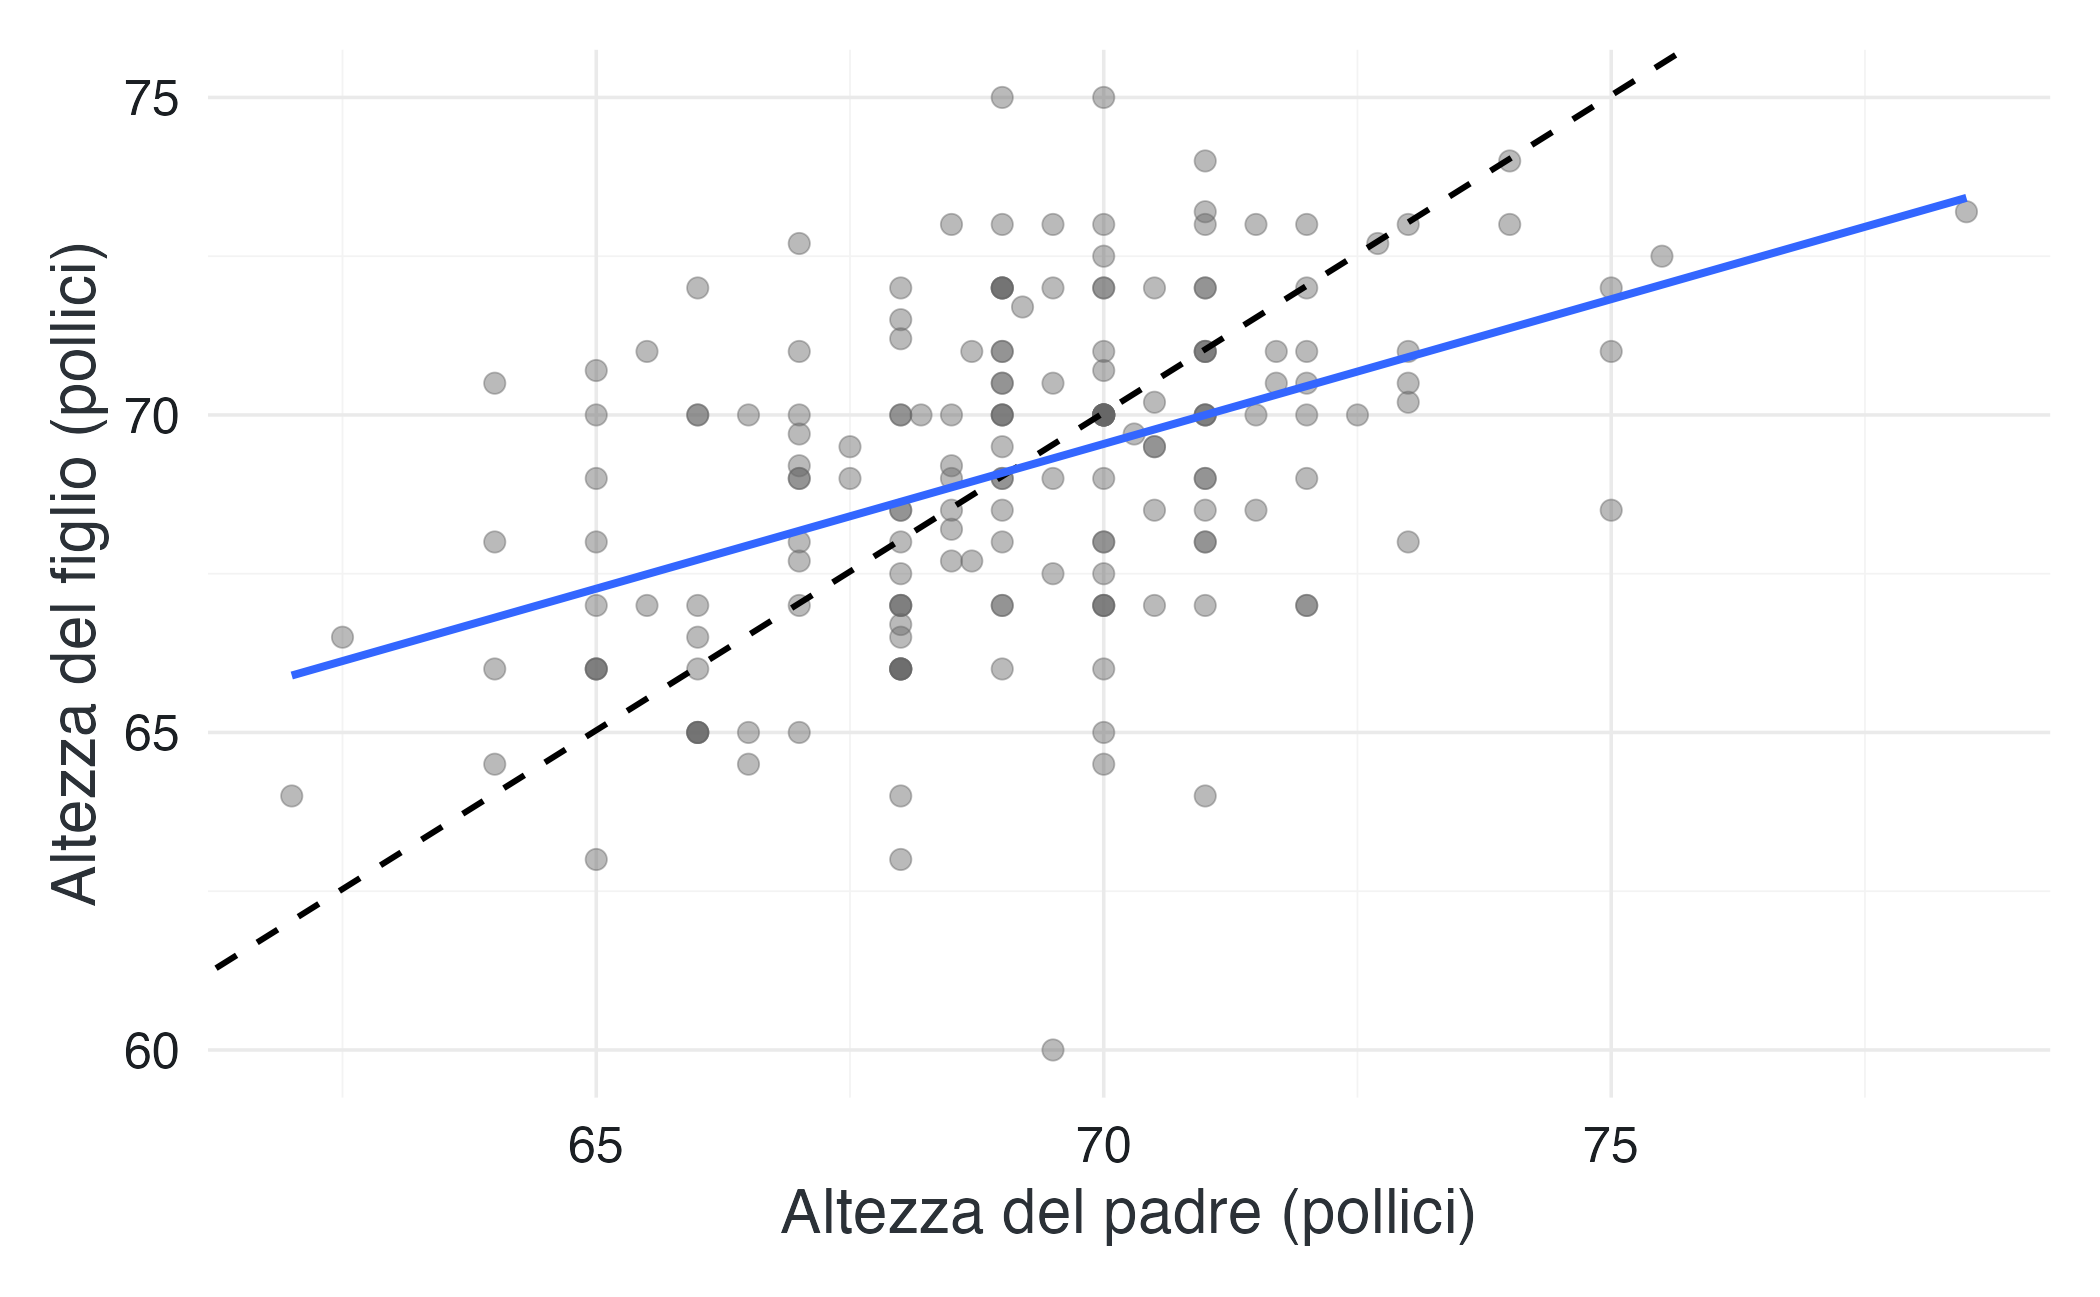
\includegraphics[width=0.85\linewidth,height=\textheight,keepaspectratio]{chapters/linear_models/02_regressione_verso_media_files/figure-pdf/fig-rtm-galton-1.png}

}

\caption{\label{fig-rtm-galton}Altezza dei figli in funzione di quella
dei padri. La retta di regressione è più piatta della retta con pendenza
1: per padri estremamente alti o bassi, l'altezza media prevista dei
figli è più vicina alla media dei figli.}

\end{figure}%

La retta tratteggiata non è la bisettrice \(Y=X\), ma la retta di
pendenza 1 che passa per \((\bar{x}, \bar{y})\). Essa corrisponde al
caso limite in cui ogni scarto dalla media del padre si riprodurrebbe
integralmente nel figlio. La retta di regressione adattata, invece, è
più piatta: gli scarti dalla media paterna risultano sistematicamente
attenuati nella media dei figli. In altri termini, i figli di padri alti
sono mediamente alti, ma la loro distanza dalla media è inferiore a
quella dei padri; analogamente, i figli di padri bassi si collocano al
di sotto della media, ma in misura minore rispetto ai genitori. La
previsione è corretta, ma è modulata dalla correlazione imperfetta.

\section{Correlazione e pendenza}\label{correlazione-e-pendenza}

Nella regressione lineare semplice, la pendenza stimata può essere
espressa come

\begin{equation}\protect\phantomsection\label{eq-slope-correlation}{
\widehat{\beta}_1
=
 r\frac{s_Y}{s_X},
}\end{equation} dove \(r\) è la correlazione campionaria e \(s_X\),
\(s_Y\) sono le deviazioni standard delle due variabili.

\begin{Shaded}
\begin{Highlighting}[]
\NormalTok{r\_galton }\OtherTok{\textless{}{-}} \FunctionTok{cor}\NormalTok{(galton\_heights}\SpecialCharTok{$}\NormalTok{father, galton\_heights}\SpecialCharTok{$}\NormalTok{son)}

\NormalTok{slope\_from\_identity }\OtherTok{\textless{}{-}}
\NormalTok{  r\_galton }\SpecialCharTok{*}
  \FunctionTok{sd}\NormalTok{(galton\_heights}\SpecialCharTok{$}\NormalTok{son) }\SpecialCharTok{/}
  \FunctionTok{sd}\NormalTok{(galton\_heights}\SpecialCharTok{$}\NormalTok{father)}

\NormalTok{slope\_from\_lm }\OtherTok{\textless{}{-}} \FunctionTok{coef}\NormalTok{(}\FunctionTok{lm}\NormalTok{(son }\SpecialCharTok{\textasciitilde{}}\NormalTok{ father, }\AttributeTok{data =}\NormalTok{ galton\_heights))[[}\StringTok{"father"}\NormalTok{]]}

\FunctionTok{tibble}\NormalTok{(}
  \AttributeTok{quantity =} \FunctionTok{c}\NormalTok{(}\StringTok{"Correlazione"}\NormalTok{, }\StringTok{"Pendenza dalla relazione algebrica"}\NormalTok{, }\StringTok{"Pendenza da lm()"}\NormalTok{),}
  \AttributeTok{value =} \FunctionTok{c}\NormalTok{(r\_galton, slope\_from\_identity, slope\_from\_lm)}
\NormalTok{)}
\CommentTok{\#\textgreater{} \# A tibble: 3 x 2}
\CommentTok{\#\textgreater{}   quantity                           value}
\CommentTok{\#\textgreater{}   \textless{}chr\textgreater{}                              \textless{}dbl\textgreater{}}
\CommentTok{\#\textgreater{} 1 Correlazione                       0.443}
\CommentTok{\#\textgreater{} 2 Pendenza dalla relazione algebrica 0.456}
\CommentTok{\#\textgreater{} 3 Pendenza da lm()                   0.456}
\end{Highlighting}
\end{Shaded}

Poiché le deviazioni standard delle altezze dei padri e dei figli sono
approssimativamente uguali, la pendenza sulla scala originale risulta
molto vicina al coefficiente di correlazione. Tale identità diventa però
più trasparente dopo aver standardizzato le variabili, ossia dopo averle
espresse in unità di deviazione standard dalla loro media.

\begin{Shaded}
\begin{Highlighting}[]
\NormalTok{galton\_standardized }\OtherTok{\textless{}{-}}\NormalTok{ galton\_heights }\SpecialCharTok{|\textgreater{}}
  \FunctionTok{mutate}\NormalTok{(}
    \AttributeTok{father\_z =} \FunctionTok{as.numeric}\NormalTok{(}\FunctionTok{scale}\NormalTok{(father)),}
    \AttributeTok{son\_z =} \FunctionTok{as.numeric}\NormalTok{(}\FunctionTok{scale}\NormalTok{(son))}
\NormalTok{  )}

\NormalTok{standardized\_fit }\OtherTok{\textless{}{-}} \FunctionTok{lm}\NormalTok{(son\_z }\SpecialCharTok{\textasciitilde{}}\NormalTok{ father\_z, }\AttributeTok{data =}\NormalTok{ galton\_standardized)}

\FunctionTok{c}\NormalTok{(}
  \AttributeTok{correlation =} \FunctionTok{cor}\NormalTok{(galton\_standardized}\SpecialCharTok{$}\NormalTok{father\_z, galton\_standardized}\SpecialCharTok{$}\NormalTok{son\_z),}
  \AttributeTok{standardized\_slope =} \FunctionTok{coef}\NormalTok{(standardized\_fit)[[}\StringTok{"father\_z"}\NormalTok{]]}
\NormalTok{)}
\CommentTok{\#\textgreater{}        correlation standardized\_slope }
\CommentTok{\#\textgreater{}              0.443              0.443}
\end{Highlighting}
\end{Shaded}

Con variabili standardizzate, la pendenza coincide con \(r\). Se, per
esempio, \(r=0.44\), un padre che si colloca due deviazioni standard
sopra la media avrà un figlio la cui altezza media prevista sarà di
\(0.44 \times 2 = 0.88\) deviazioni standard sopra la media degli altri
figli. La previsione rimane comunque superiore alla media, ma in misura
meno estrema.

\begin{tcolorbox}[enhanced jigsaw, arc=.35mm, bottomrule=.15mm, bottomtitle=1mm, breakable, colback=white, colbacktitle=quarto-callout-note-color!10!white, colframe=quarto-callout-note-color-frame, coltitle=black, left=2mm, leftrule=.75mm, opacityback=0, opacitybacktitle=0.6, rightrule=.15mm, title=\textcolor{quarto-callout-note-color}{\faInfo}\hspace{0.5em}{La scala è importante}, titlerule=0mm, toprule=.15mm, toptitle=1mm]

Osservare che la pendenza è inferiore a 1 non basta, da solo, a
dimostrare la regressione verso la media: su scale arbitrarie, il valore
della pendenza dipende anche dal rapporto \(s_Y/s_X\). Per valutare
correttamente il fenomeno, è necessario esprimere le variabili in forma
standardizzata o confrontare gli scarti osservati rispetto alle
rispettive medie e deviazioni standard.

\end{tcolorbox}

\section{Vedere il fenomeno mediante
simulazione}\label{vedere-il-fenomeno-mediante-simulazione}

La relazione formalizzata in
Equazione~\ref{eq-regression-toward-mean-standardized} può essere resa
intuitivamente evidente attraverso una simulazione numerica, finalizzata
a generare coppie di variabili standardizzate caratterizzate da
differenti livelli di correlazione. Per la costruzione di tali coppie si
adotta il seguente modello generativo:

\[
Z_Y = \rho Z_X + \sqrt{1-\rho^2}\,\varepsilon,
\qquad
\varepsilon \sim \operatorname{Normal}(0,1).
\] dove \(Z_X\) ed \(\varepsilon\) sono variabili casuali indipendenti e
standardizzate. Questa formulazione garantisce che la variabile
risultante \(Z_Y\) abbia media attesa pari a 0, varianza teorica uguale
a 1 e che il coefficiente di correlazione lineare tra \(Z_X\) e \(Z_Y\)
sia \(\rho\).

\begin{Shaded}
\begin{Highlighting}[]
\NormalTok{simulate\_correlated\_pair }\OtherTok{\textless{}{-}} \ControlFlowTok{function}\NormalTok{(n, rho) \{}
\NormalTok{  x }\OtherTok{\textless{}{-}} \FunctionTok{rnorm}\NormalTok{(n)}
\NormalTok{  epsilon }\OtherTok{\textless{}{-}} \FunctionTok{rnorm}\NormalTok{(n)}
\NormalTok{  y }\OtherTok{\textless{}{-}}\NormalTok{ rho }\SpecialCharTok{*}\NormalTok{ x }\SpecialCharTok{+} \FunctionTok{sqrt}\NormalTok{(}\DecValTok{1} \SpecialCharTok{{-}}\NormalTok{ rho}\SpecialCharTok{\^{}}\DecValTok{2}\NormalTok{) }\SpecialCharTok{*}\NormalTok{ epsilon}

  \FunctionTok{tibble}\NormalTok{(}
    \AttributeTok{x =}\NormalTok{ x,}
    \AttributeTok{y =}\NormalTok{ y,}
    \AttributeTok{rho =} \FunctionTok{factor}\NormalTok{(}
\NormalTok{      rho,}
      \AttributeTok{levels =} \FunctionTok{c}\NormalTok{(}\FloatTok{0.2}\NormalTok{, }\FloatTok{0.5}\NormalTok{, }\FloatTok{0.8}\NormalTok{, }\DecValTok{1}\NormalTok{),}
      \AttributeTok{labels =} \FunctionTok{c}\NormalTok{(}\StringTok{"rho = 0.2"}\NormalTok{, }\StringTok{"rho = 0.5"}\NormalTok{, }\StringTok{"rho = 0.8"}\NormalTok{, }\StringTok{"rho = 1.0"}\NormalTok{)}
\NormalTok{    )}
\NormalTok{  )}
\NormalTok{\}}

\NormalTok{simulated\_correlations }\OtherTok{\textless{}{-}} \FunctionTok{bind\_rows}\NormalTok{(}
  \FunctionTok{simulate\_correlated\_pair}\NormalTok{(}\DecValTok{500}\NormalTok{, }\FloatTok{0.2}\NormalTok{),}
  \FunctionTok{simulate\_correlated\_pair}\NormalTok{(}\DecValTok{500}\NormalTok{, }\FloatTok{0.5}\NormalTok{),}
  \FunctionTok{simulate\_correlated\_pair}\NormalTok{(}\DecValTok{500}\NormalTok{, }\FloatTok{0.8}\NormalTok{),}
  \FunctionTok{simulate\_correlated\_pair}\NormalTok{(}\DecValTok{500}\NormalTok{, }\FloatTok{1.0}\NormalTok{)}
\NormalTok{)}
\end{Highlighting}
\end{Shaded}

\begin{Shaded}
\begin{Highlighting}[]
\NormalTok{simulated\_correlations }\SpecialCharTok{|\textgreater{}}
  \FunctionTok{ggplot}\NormalTok{(}\FunctionTok{aes}\NormalTok{(}\AttributeTok{x =}\NormalTok{ x, }\AttributeTok{y =}\NormalTok{ y)) }\SpecialCharTok{+}
  \FunctionTok{geom\_point}\NormalTok{(}\AttributeTok{alpha =} \FloatTok{0.25}\NormalTok{) }\SpecialCharTok{+}
  \FunctionTok{geom\_abline}\NormalTok{(}\AttributeTok{slope =} \DecValTok{1}\NormalTok{, }\AttributeTok{intercept =} \DecValTok{0}\NormalTok{, }\AttributeTok{linetype =} \StringTok{"dashed"}\NormalTok{) }\SpecialCharTok{+}
  \FunctionTok{geom\_smooth}\NormalTok{(}\AttributeTok{method =} \StringTok{"lm"}\NormalTok{, }\AttributeTok{se =} \ConstantTok{FALSE}\NormalTok{, }\AttributeTok{linewidth =} \FloatTok{0.8}\NormalTok{) }\SpecialCharTok{+}
  \FunctionTok{facet\_wrap}\NormalTok{(}\SpecialCharTok{\textasciitilde{}}\NormalTok{ rho) }\SpecialCharTok{+}
  \FunctionTok{coord\_equal}\NormalTok{() }\SpecialCharTok{+}
  \FunctionTok{labs}\NormalTok{(}
    \AttributeTok{x =} \FunctionTok{expression}\NormalTok{(Z[X]),}
    \AttributeTok{y =} \FunctionTok{expression}\NormalTok{(Z[Y])}
\NormalTok{  )}
  \CommentTok{\# + theme\_manuscript()}
\end{Highlighting}
\end{Shaded}

\begin{figure}[H]

\centering{

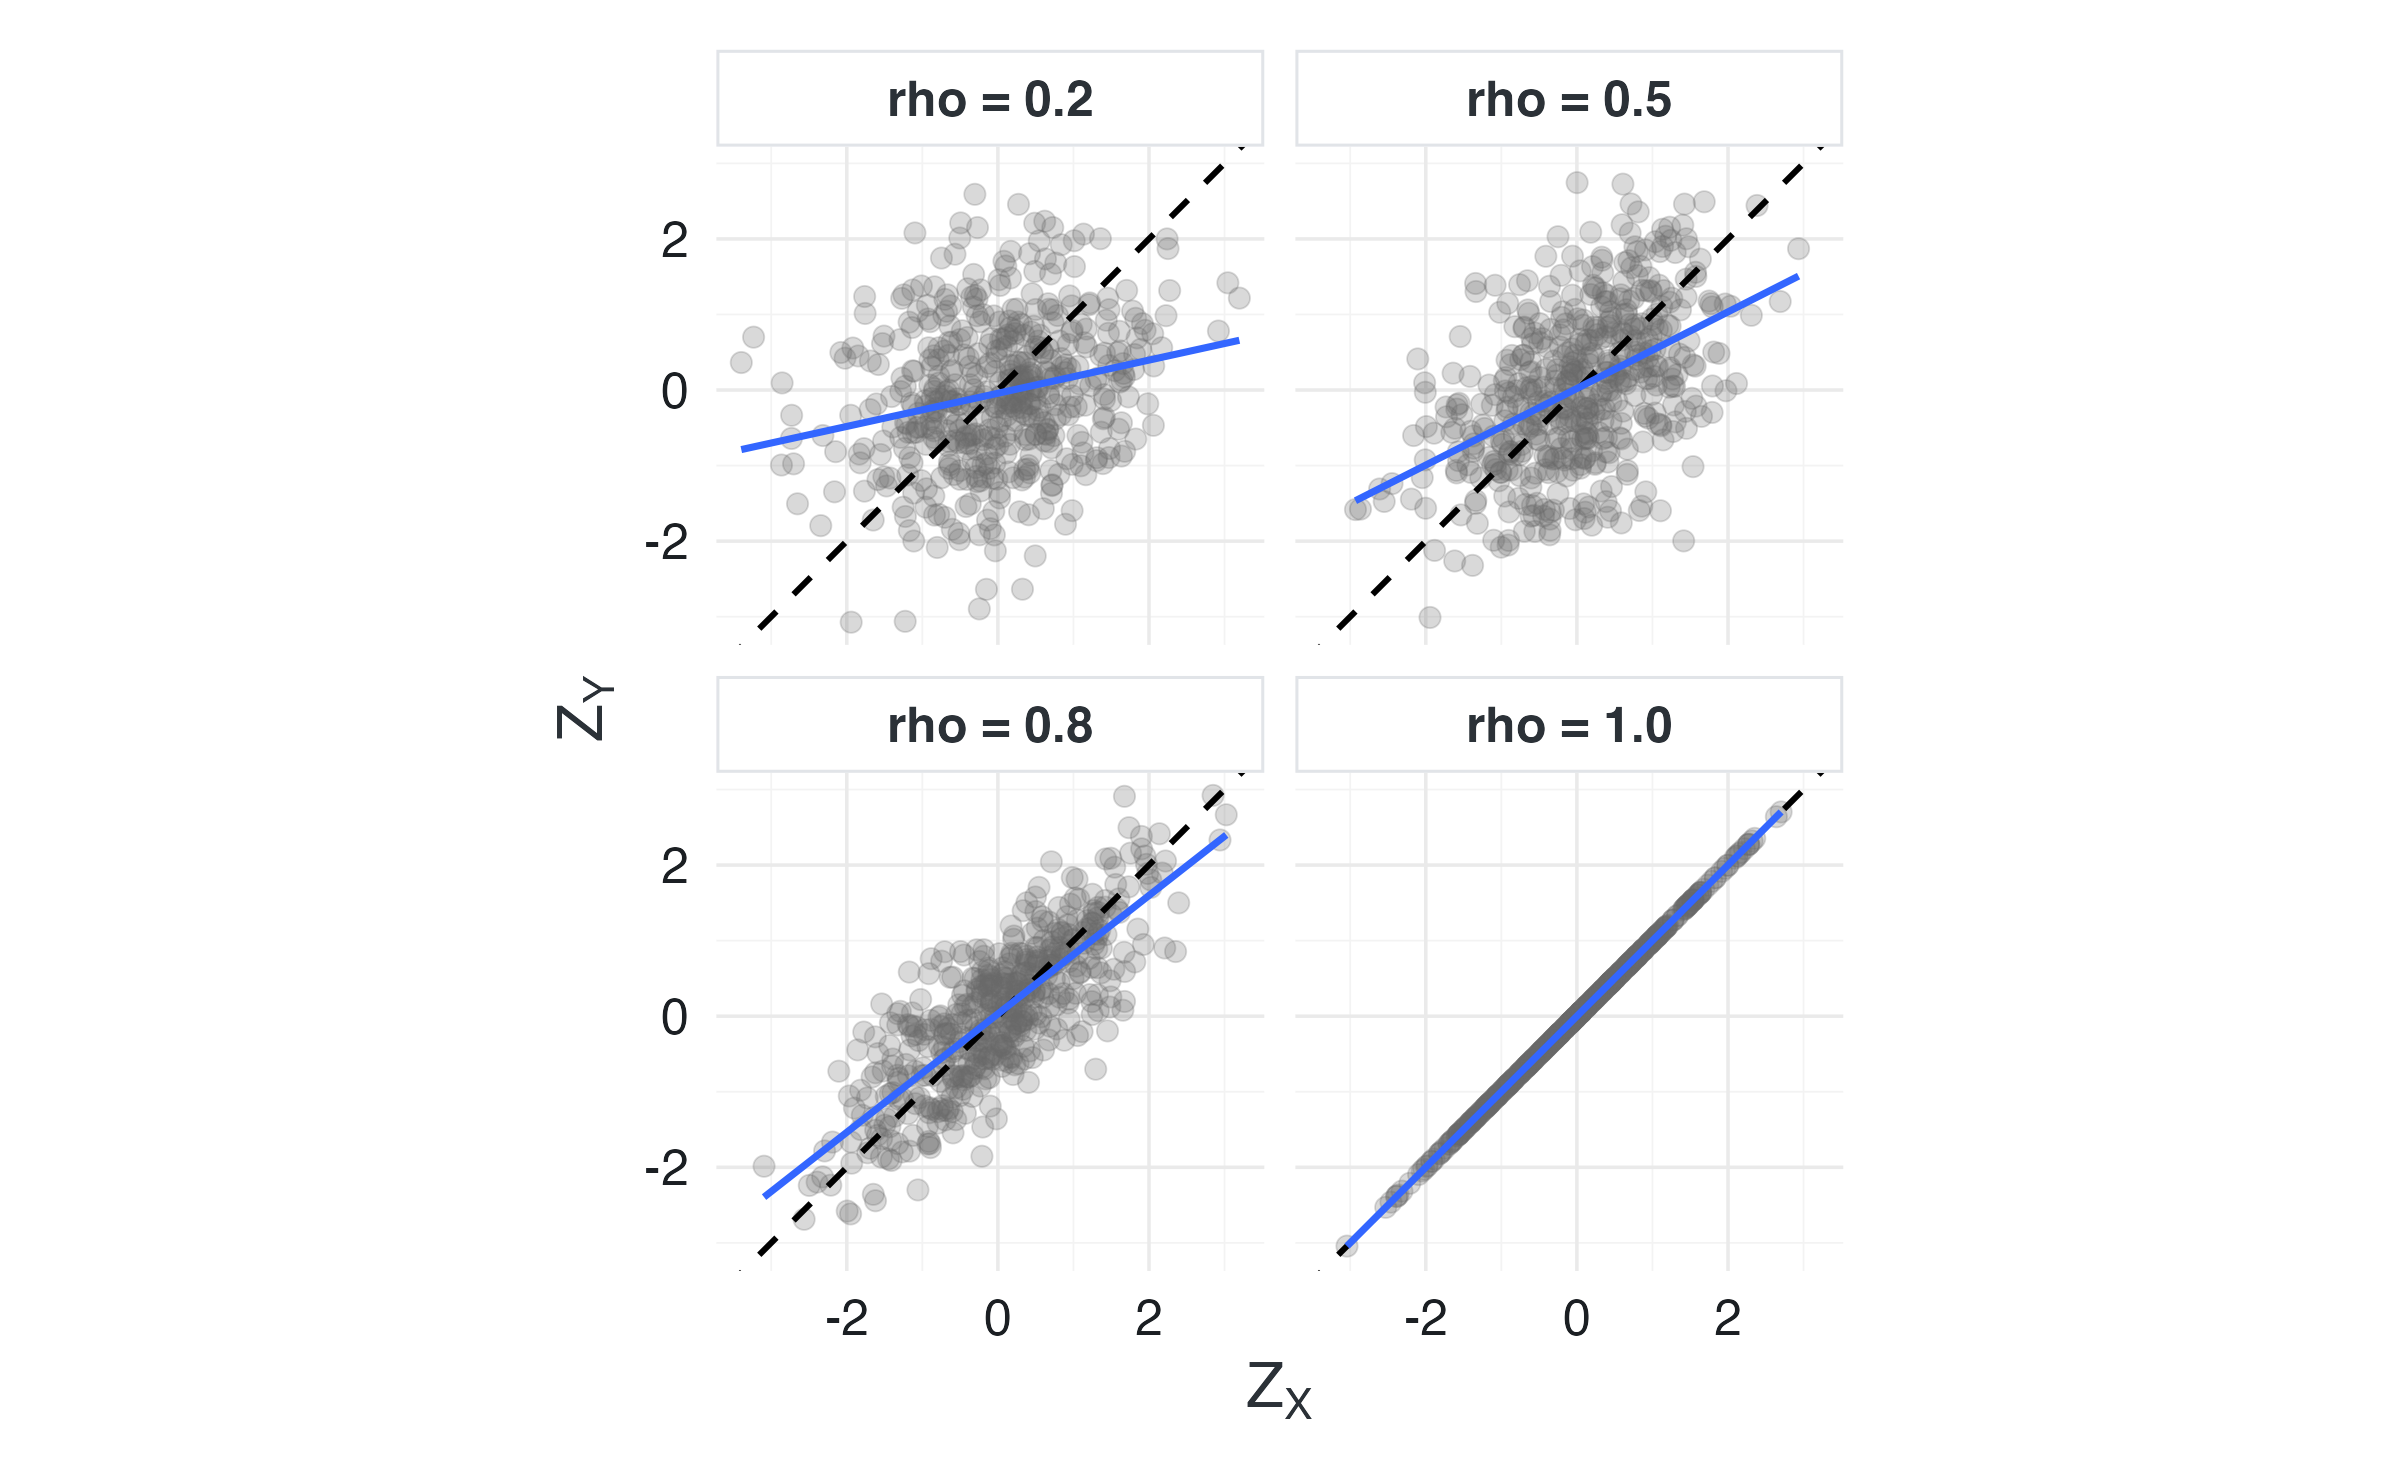
\includegraphics[width=0.85\linewidth,height=\textheight,keepaspectratio]{chapters/linear_models/02_regressione_verso_media_files/figure-pdf/fig-rtm-correlation-simulation-1.png}

}

\caption{\label{fig-rtm-correlation-simulation}Relazione tra due
variabili standardizzate per quattro livelli di correlazione. Quanto più
la correlazione è lontana da 1, tanto più la retta di regressione è
piatta rispetto alla retta di identità.}

\end{figure}%

Il confronto dei quattro scenari rivela chiaramente la dinamica del
fenomeno. Nel caso di perfetta correlazione (\(\rho = 1.0\)), ogni
scostamento dalla media osservato in \(Z_X\) si traduce in una
variazione di intensità identica in \(Z_Y\). Di conseguenza, la retta di
regressione coincide esattamente con la retta di identità
\(y = 1 \cdot x\). Nel caso di correlazione imperfetta (\(\rho < 1.0\)),
la pendenza della retta di regressione campionaria si avvicina al valore
teorico \(\rho\). I valori previsti per la variabile condizionata sono
sistematicamente meno estremi rispetto ai valori della variabile
predittrice che li hanno generati. Questo effetto di attenuazione
lineare è tanto più marcato quanto più debole è il legame lineare tra le
due variabili. La simulazione offre quindi una dimostrazione empirica e
visiva del principio di regressione verso la media: l'intensità del
riavvicinamento al valore medio è inversamente proporzionale al grado di
associazione statistica tra le variabili considerate.

\section{Selezionare casi estremi e
rimisurarli}\label{selezionare-casi-estremi-e-rimisurarli}

Il fenomeno diventa particolarmente insidioso quando i partecipanti
vengono selezionati in base a una prima misurazione estrema e il loro
cambiamento viene valutato mediante una seconda rilevazione. Per
comprenderne la dinamica, si supponga che ogni persona abbia un livello
relativamente stabile \(T\), ma che il punteggio osservato in ciascuna
occasione includa anche una componente occasionale \(E\):

\[
\begin{aligned}
X_{i1} &= T_i + E_{i1},\\
X_{i2} &= T_i + E_{i2}.
\end{aligned}
\]

Se si selezionano le persone con i valori più alti di \(X_{i1}\), il
gruppo risulterà composto sia da individui con valori elevati di
\(T_i\), sia da individui che, nella prima rilevazione, hanno avuto un
errore positivo o uno stato transitoriamente elevato. Tuttavia, alla
seconda misurazione, la componente occasionale non tende a ripresentarsi
con la medesima intensità e segno, pertanto la media di \(X_{i2}\)
risulterà generalmente meno estrema, anche in assenza di qualsiasi
intervento. Questa dinamica è illustrata dalla simulazione seguente.

\begin{Shaded}
\begin{Highlighting}[]
\NormalTok{n\_people }\OtherTok{\textless{}{-}} \DecValTok{4000}

\NormalTok{pre\_post\_population }\OtherTok{\textless{}{-}} \FunctionTok{tibble}\NormalTok{(}
  \AttributeTok{id =} \FunctionTok{seq\_len}\NormalTok{(n\_people),}
  \AttributeTok{stable\_level =} \FunctionTok{rnorm}\NormalTok{(n\_people, }\AttributeTok{mean =} \DecValTok{50}\NormalTok{, }\AttributeTok{sd =} \DecValTok{10}\NormalTok{),}
  \AttributeTok{pre =}\NormalTok{ stable\_level }\SpecialCharTok{+} \FunctionTok{rnorm}\NormalTok{(n\_people, }\AttributeTok{mean =} \DecValTok{0}\NormalTok{, }\AttributeTok{sd =} \DecValTok{8}\NormalTok{),}
  \AttributeTok{post =}\NormalTok{ stable\_level }\SpecialCharTok{+} \FunctionTok{rnorm}\NormalTok{(n\_people, }\AttributeTok{mean =} \DecValTok{0}\NormalTok{, }\AttributeTok{sd =} \DecValTok{8}\NormalTok{)}
\NormalTok{)}

\NormalTok{selection\_cutoff }\OtherTok{\textless{}{-}} \FunctionTok{quantile}\NormalTok{(pre\_post\_population}\SpecialCharTok{$}\NormalTok{pre, }\FloatTok{0.90}\NormalTok{)}

\NormalTok{selected\_high }\OtherTok{\textless{}{-}}\NormalTok{ pre\_post\_population }\SpecialCharTok{|\textgreater{}}
  \FunctionTok{filter}\NormalTok{(pre }\SpecialCharTok{\textgreater{}=}\NormalTok{ selection\_cutoff) }\SpecialCharTok{|\textgreater{}}
  \FunctionTok{select}\NormalTok{(id, pre, post) }\SpecialCharTok{|\textgreater{}}
  \FunctionTok{pivot\_longer}\NormalTok{(}
    \AttributeTok{cols =} \FunctionTok{c}\NormalTok{(pre, post),}
    \AttributeTok{names\_to =} \StringTok{"occasion"}\NormalTok{,}
    \AttributeTok{values\_to =} \StringTok{"score"}
\NormalTok{  ) }\SpecialCharTok{|\textgreater{}}
  \FunctionTok{mutate}\NormalTok{(}
    \AttributeTok{occasion =} \FunctionTok{factor}\NormalTok{(}
\NormalTok{      occasion,}
      \AttributeTok{levels =} \FunctionTok{c}\NormalTok{(}\StringTok{"pre"}\NormalTok{, }\StringTok{"post"}\NormalTok{),}
      \AttributeTok{labels =} \FunctionTok{c}\NormalTok{(}\StringTok{"Prima misurazione"}\NormalTok{, }\StringTok{"Seconda misurazione"}\NormalTok{)}
\NormalTok{    )}
\NormalTok{  )}

\NormalTok{selected\_high }\SpecialCharTok{|\textgreater{}}
  \FunctionTok{group\_by}\NormalTok{(occasion) }\SpecialCharTok{|\textgreater{}}
  \FunctionTok{summarise}\NormalTok{(}
    \AttributeTok{mean =} \FunctionTok{mean}\NormalTok{(score),}
    \AttributeTok{sd =} \FunctionTok{sd}\NormalTok{(score),}
    \AttributeTok{.groups =} \StringTok{"drop"}
\NormalTok{  )}
\CommentTok{\#\textgreater{} \# A tibble: 2 x 3}
\CommentTok{\#\textgreater{}   occasion             mean    sd}
\CommentTok{\#\textgreater{}   \textless{}fct\textgreater{}               \textless{}dbl\textgreater{} \textless{}dbl\textgreater{}}
\CommentTok{\#\textgreater{} 1 Prima misurazione    72.6  5.48}
\CommentTok{\#\textgreater{} 2 Seconda misurazione  63.2 10.4}
\end{Highlighting}
\end{Shaded}

\begin{Shaded}
\begin{Highlighting}[]
\NormalTok{selected\_high }\SpecialCharTok{|\textgreater{}}
  \FunctionTok{group\_by}\NormalTok{(occasion) }\SpecialCharTok{|\textgreater{}}
  \FunctionTok{summarise}\NormalTok{(}
    \AttributeTok{mean\_score =} \FunctionTok{mean}\NormalTok{(score),}
    \AttributeTok{se =} \FunctionTok{sd}\NormalTok{(score) }\SpecialCharTok{/} \FunctionTok{sqrt}\NormalTok{(}\FunctionTok{n}\NormalTok{()),}
    \AttributeTok{.groups =} \StringTok{"drop"}
\NormalTok{  ) }\SpecialCharTok{|\textgreater{}}
  \FunctionTok{ggplot}\NormalTok{(}\FunctionTok{aes}\NormalTok{(}\AttributeTok{x =}\NormalTok{ occasion, }\AttributeTok{y =}\NormalTok{ mean\_score, }\AttributeTok{group =} \DecValTok{1}\NormalTok{)) }\SpecialCharTok{+}
  \FunctionTok{geom\_line}\NormalTok{(}\AttributeTok{linewidth =} \FloatTok{0.8}\NormalTok{) }\SpecialCharTok{+}
  \FunctionTok{geom\_point}\NormalTok{(}\AttributeTok{size =} \FloatTok{2.5}\NormalTok{) }\SpecialCharTok{+}
  \FunctionTok{geom\_errorbar}\NormalTok{(}
    \FunctionTok{aes}\NormalTok{(}\AttributeTok{ymin =}\NormalTok{ mean\_score }\SpecialCharTok{{-}} \FloatTok{1.96} \SpecialCharTok{*}\NormalTok{ se, }\AttributeTok{ymax =}\NormalTok{ mean\_score }\SpecialCharTok{+} \FloatTok{1.96} \SpecialCharTok{*}\NormalTok{ se),}
    \AttributeTok{width =} \FloatTok{0.08}
\NormalTok{  ) }\SpecialCharTok{+}
  \FunctionTok{labs}\NormalTok{(}
    \AttributeTok{x =} \ConstantTok{NULL}\NormalTok{,}
    \AttributeTok{y =} \StringTok{"Punteggio medio"}
\NormalTok{  )}
  \CommentTok{\# + theme\_manuscript()}
\end{Highlighting}
\end{Shaded}

\begin{figure}[H]

\centering{

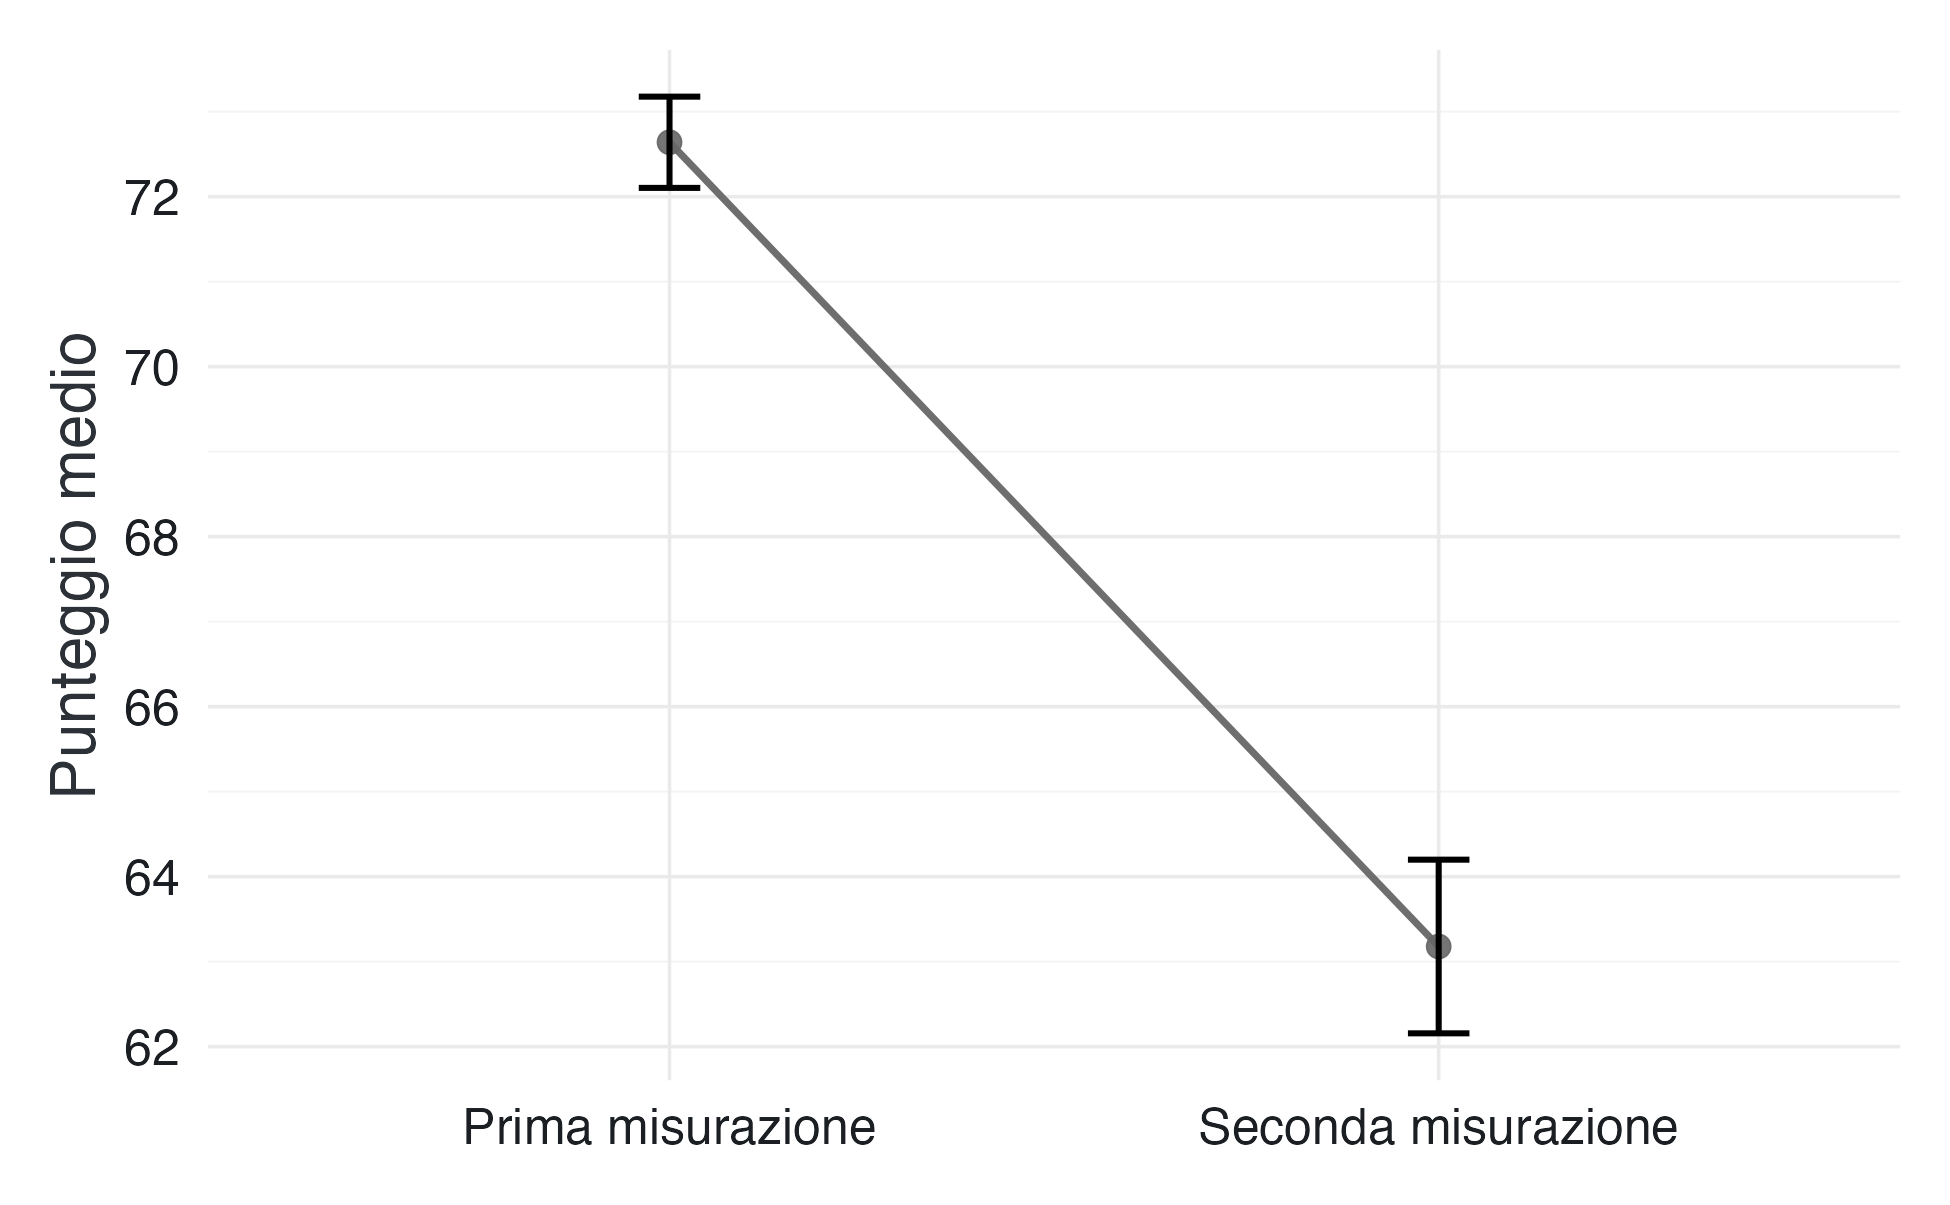
\includegraphics[width=0.85\linewidth,height=\textheight,keepaspectratio]{chapters/linear_models/02_regressione_verso_media_files/figure-pdf/fig-rtm-pre-post-1.png}

}

\caption{\label{fig-rtm-pre-post}Punteggi medi nelle due occasioni per
le persone selezionate perché appartenevano al 10\% superiore alla prima
misurazione. Il calo compare senza alcun intervento.}

\end{figure}%

Il gruppo selezionato in base ai punteggi iniziali più elevati mostra,
in media, una diminuzione nella seconda rilevazione, mentre una
selezione basata sui valori più bassi produce un incremento medio. In
entrambi i casi, tale variazione non riflette un reale processo
correttivo o un cambiamento strutturale, ma è un effetto statistico
atteso derivante dall'instabilità occasionale (o errore casuale)
intrinseca alla misurazione.

Di conseguenza, se l'accesso a un intervento è subordinato al
conseguimento di un punteggio iniziale estremo, il mutamento rilevato ex
post è il risultato della confluenza di tre componenti distinte:
l'eventuale effetto dell'intervento, la regressione verso la media e
altri fattori esogeni temporali e contestuali, quali la maturazione
spontanea dei soggetti, eventi esterni o variazioni nella procedura di
misurazione. In assenza di un adeguato gruppo di controllo, queste tre
componenti si confondono nella variazione media osservata, rendendo
metodologicamente impossibile isolare l'impatto reale dell'intervento.

\section{Il ruolo del gruppo di
controllo}\label{il-ruolo-del-gruppo-di-controllo}

Un gruppo di controllo è informativo se condivide con il gruppo
sperimentale il medesimo criterio di selezione, le stesse occasioni di
misurazione e lo stesso intervallo temporale, differenziandosi
esclusivamente per la mancata applicazione dell'intervento (o per
l'esposizione a una condizione di confronto appropriata). Se entrambi i
gruppi presentano una regressione verso la media, ma il gruppo trattato
mostra un cambiamento maggiore rispetto al gruppo di controllo, la
differenza tra i due cambiamenti può essere interpretata come
compatibile con l'effetto dell'intervento, a condizione che siano
soddisfatte le ulteriori assunzioni richieste dal disegno della ricerca.
Il gruppo di controllo non elimina il fenomeno della regressione verso
la media, ma consente di stimare il cambiamento che si sarebbe osservato
anche in assenza del trattamento, a condizione che i gruppi siano
effettivamente comparabili e che il loro processo di selezione non
introduca ulteriori distorsioni.

La regressione verso la media non costituisce una spiegazione
universale. Osservare un cambiamento verso valori meno estremi non
implica che l'intero mutamento sia riconducibile a tale fenomeno, ma
rappresenta piuttosto una spiegazione alternativa che deve essere presa
in considerazione nella progettazione e nell'interpretazione dei
risultati e non un'etichetta da applicare in modo automatico a qualsiasi
variazione osservata.

\section{Affidabilità e ampiezza del
fenomeno}\label{affidabilituxe0-e-ampiezza-del-fenomeno}

Nel modello classico della misurazione, \$ X = T + E \$ (dove \(X\) è il
punteggio osservato, \(T\) il punteggio vero ed \(E\) l'errore casuale),
l'\emph{affidabilità} è la proporzione della varianza osservata
attribuibile a differenze stabili tra le unità statistiche. Se due
misurazioni parallele condividono il medesimo punteggio vero e
presentano errori tra loro indipendenti, la loro correlazione lineare
coincide esattamente con il coefficiente di affidabilità
(\(\rho_{xx}\)).

In tali condizioni, esprimendo i punteggi in forma standardizzata (con
media pari a 0 e deviazione standard pari a 1), il valore medio atteso
alla seconda misurazione (\(Z_2\)), dato un punteggio iniziale
(\(Z_1 = z\)), è data da:

\[\mathbb{E}(Z_2 \mid Z_1 = z) = \rho_{xx} \cdot z.\] L'equazione
evidenzia la dipendenza diretta tra la stabilità della misura e l'entità
della regressione verso la media. Una misura con un'elevata affidabilità
(con \(\rho_{xx}\) prossimo a 1) genererà una previsione molto vicina al
punteggio iniziale, contenendo lo spostamento statistico, mentre una
misura poco affidabile (con \(\rho_{xx}\) prossimo a 0) produrrà una
previsione fortemente attratta verso la media del gruppo (\(0\)). Ad
esempio, un punteggio iniziale di \(z = 2\) dà luogo a una media
prevista pari a \(1.80\) se l'affidabilità è \(0.90\), a \(1.00\) se è
\(0.50\), e a \(0.40\) se è \(0.20\).

Il collegamento è intuitivo: maggiore è la componente d'errore (o la
variabilità occasionale) insita nella prima misurazione, minore sarà la
tendenza del punteggio osservato a mantenere il proprio carattere
estremo nella seconda rilevazione.

È importante notare che tale relazione formale vale sotto precise
assunzioni metodologiche: misure parallele, indipendenza degli errori
casuali e invarianza della struttura latente nelle due occasioni. Nei
capitoli dedicati all'errore di misurazione, questa distinzione verrà
ripresa in modo più approfondito, separando analiticamente
l'affidabilità intrinseca del test dalle componenti di errore casuale e
dai \emph{bias} (distorsioni) sistematici legati al metodo.

\section{Un'apparente asimmetria}\label{unapparente-asimmetria}

La regressione di \(Y\) su \(X\) e quella di \(X\) su \(Y\) non
coincidono: si tratta di due rette geometricamente distinte. Quando i
punteggi vengono standardizzati, le due rette hanno una pendenza pari al
coefficiente di correlazione \(r\), ma rispondono a domande condizionali
radicalmente diverse:

\begin{itemize}
\tightlist
\item
  La prima retta stima il valore medio di \(Z_Y\) condizionatamente a un
  determinato valore di \(Z_X\), secondo l'equazione:
\end{itemize}

\[\mathbb{E}(Z_Y \mid Z_X = z_x) = r \cdot z_x\]

\begin{itemize}
\tightlist
\item
  La seconda retta inverte la condizione e stima il valore medio di
  \(Z_X\) dato un valore di \(Z_Y\):
\end{itemize}

\[\mathbb{E}(Z_X \mid Z_Y = z_y) = r \cdot z_y\]

Questa asimmetria non genera alcuna contraddizione logica ma riflette il
punto di partenza della selezione statistica. Se si isolano le unità con
valori estremi nella variabile \(X\), l'analisi mira a stabilire come si
distribuisce \(Y\) in funzione di tale vincolo. Viceversa, se si
selezionano unità estreme in \(Y\), la prospettiva si inverte.

In sintesi, la regressione non descrive una relazione geometrica
simmetrica (come fa la semplice correlazione), ma introduce una
direzione logica precisa, specificando quale variabile costituisce
l'oggetto della previsione e quale rappresenta l'informazione
condizionante.

\section{Errori frequenti}\label{errori-frequenti-2}

\begin{tcolorbox}[enhanced jigsaw, arc=.35mm, bottomrule=.15mm, bottomtitle=1mm, breakable, colback=white, colbacktitle=quarto-callout-caution-color!10!white, colframe=quarto-callout-caution-color-frame, coltitle=black, left=2mm, leftrule=.75mm, opacityback=0, opacitybacktitle=0.6, rightrule=.15mm, title=\textcolor{quarto-callout-caution-color}{\faFire}\hspace{0.5em}{Attenzione}, titlerule=0mm, toprule=.15mm, toptitle=1mm]

\begin{enumerate}
\def\labelenumi{\arabic{enumi}.}
\tightlist
\item
  \textbf{Pensare che ogni individuo debba avvicinarsi alla media.} La
  regressione verso la media riguarda il valore atteso del gruppo
  condizionato su un estremo; i singoli casi possono muoversi in
  entrambe le direzioni.
\item
  \textbf{Confrontare direttamente una pendenza con 1 senza considerare
  la scala.} La lettura più chiara richiede variabili standardizzate o
  scale comparabili.
\item
  \textbf{Interpretare il fenomeno come una forza che spinge i valori
  verso il centro.} Non è necessario postulare un meccanismo correttivo:
  basta una correlazione imperfetta.
\item
  \textbf{Attribuire tutto il cambiamento osservato alla regressione
  verso la media.} Un intervento può avere un effetto reale; il problema
  è che un semplice pre--post non lo separa dalle variazioni attese in
  assenza di trattamento.
\item
  \textbf{Credere che una seconda misurazione più vicina alla media
  dimostri un errore nella prima.} Entrambe le misure possono essere
  valide ma contenere componenti transitorie o non condivise.
\item
  \textbf{Dimenticare il criterio di selezione.} Il fenomeno diventa
  particolarmente rilevante quando l'inclusione dipende da un punteggio
  estremo.
\end{enumerate}

\end{tcolorbox}

\section{Riflessioni conclusive}\label{riflessioni-conclusive-19}

La regressione verso la media emerge come conseguenza matematica della
previsione lineare ogni volta che l'associazione tra due misure risulta
imperfetta. Esprimendo i punteggi in forma standardizzata, la media
condizionata è pari a \(\rho \cdot z\): di conseguenza, ogni volta che
\(\vert{}\rho\vert{} < 1\), un valore iniziale estremo del predittore
condurrà a una previsione orientata nella stessa direzione, ma
strutturalmente meno estrema. È importante comprendere che questo
fenomeno non implica che \emph{ogni singolo individuo} si sposti verso
il centro della distribuzione né che si tratti di un meccanismo causale;
si tratta, piuttosto, di una proprietà statistica del valore atteso di
una misura condizionata a un'altra.

La rilevanza pratica di tale dinamica è cruciale nei disegni di ricerca
in cui i partecipanti vengono selezionati in base a punteggi
eccezionalmente alti o bassi. In questi scenari, infatti, una parte del
cambiamento medio osservato nella seconda rilevazione si manifesterebbe
per pura fluttuazione statistica, anche in assenza di un intervento.

Da ciò deriva che la qualità del disegno di ricerca deve necessariamente
precedere l'interpretazione del modello statistico. L'inclusione di un
adeguato gruppo di controllo rappresenta l'unico strumento metodologico
in grado di distinguere la variazione spontaneamente attesa dal
cambiamento aggiuntivo, effettivamente compatibile con l'azione
dell'intervento. Il legame con l'affidabilità dimostra inoltre che la
regressione verso la media non è un'anomalia metodologica isolata, ma
una diretta espressione dell'errore di misurazione: maggiore è la
componente instabile dello strumento, minore sarà la prevedibilità dei
punteggi estremi nel tempo.

Nel prossimo capitolo applicheremo l'intero flusso di lavoro
(\emph{workflow}) bayesiano al modello lineare. Questo cambio di
paradigma ci permetterà di sostituire le stime puntuali con intere
distribuzioni a posteriori e di utilizzare le simulazioni predittive per
rappresentare in modo esplicito e rigoroso l'incertezza legata sia alla
retta di regressione sia alle future osservazioni.

\section{Concetti da ricordare}\label{concetti-da-ricordare-1}

\begin{enumerate}
\def\labelenumi{\arabic{enumi}.}
\tightlist
\item
  La regressione verso la media deriva dalla correlazione imperfetta tra
  la misura usata per selezionare i casi e la misura successiva o
  correlata.
\item
  Con variabili standardizzate, la pendenza della regressione semplice
  coincide con la correlazione.
\item
  Se \(|\rho|<1\), il valore medio previsto è meno estremo del valore
  sul quale si condiziona.
\item
  Il fenomeno riguarda medie condizionate, non il destino necessario di
  ogni individuo.
\item
  La selezione su valori estremi può produrre cambiamenti pre--post
  anche senza trattamento.
\item
  Un gruppo di controllo comparabile aiuta a separare il cambiamento
  atteso dall'eventuale effetto aggiuntivo dell'intervento.
\item
  Una minore affidabilità implica, sotto ipotesi appropriate, una
  regressione verso la media più pronunciata.
\end{enumerate}

\begin{tcolorbox}[enhanced jigsaw, arc=.35mm, bottomrule=.15mm, bottomtitle=1mm, breakable, colback=white, colbacktitle=quarto-callout-important-color!10!white, colframe=quarto-callout-important-color-frame, coltitle=black, left=2mm, leftrule=.75mm, opacityback=0, opacitybacktitle=0.6, rightrule=.15mm, title=\textcolor{quarto-callout-important-color}{\faExclamation}\hspace{0.5em}{Esercizi}, titlerule=0mm, toprule=.15mm, toptitle=1mm]

\subsection{1. Previsione
standardizzata}\label{previsione-standardizzata}

Supponi che due misure standardizzate abbiano correlazione \(0.60\).
Qual è il valore medio previsto della seconda misura per un gruppo con
valore \(z=2.5\) nella prima? Quanto dista questa previsione dalla
media?

\subsection{2. Confrontare due
affidabilità}\label{confrontare-due-affidabilituxe0}

Un test viene somministrato due volte. Calcola il punteggio
standardizzato medio atteso alla seconda somministrazione per persone
con \(z=2\) alla prima, assumendo alternativamente affidabilità \(0.85\)
e \(0.40\). Interpreta la differenza.

\subsection{3. Scala originale e scala
standardizzata}\label{scala-originale-e-scala-standardizzata}

Nel dataset di Galton, verifica che la pendenza sulla scala originale
sia uguale a

\[
r\frac{s_Y}{s_X}.
\]

Spiega perché non è corretto attribuire la regressione verso la media al
solo fatto che questa pendenza sia inferiore a 1.

\subsection{4. Selezione dalla coda
inferiore}\label{selezione-dalla-coda-inferiore}

Modifica la simulazione pre--post selezionando il 10\% dei punteggi
iniziali più bassi. Rappresenta le medie nelle due occasioni e descrivi
il risultato.

\subsection{5. Aggiungere un trattamento
reale}\label{aggiungere-un-trattamento-reale}

Nella simulazione pre--post, aggiungi 4 punti alla seconda misurazione
di metà delle persone selezionate, assegnate casualmente al trattamento.
Confronta:

\begin{itemize}
\tightlist
\item
  il cambiamento nel gruppo trattato;
\item
  il cambiamento nel controllo;
\item
  la differenza tra i cambiamenti.
\end{itemize}

Quale di queste quantità è più informativa sull'effetto del trattamento?

\subsection{6. Criticare
un'interpretazione}\label{criticare-uninterpretazione}

Uno studio seleziona pazienti con ansia molto elevata, somministra un
intervento e osserva una riduzione media di 8 punti. Non è presente un
gruppo di controllo. Elenca almeno tre ragioni per cui il cambiamento
non può essere attribuito interamente all'intervento.

\subsection{7. Individui e gruppi}\label{individui-e-gruppi}

Spiega perché l'affermazione seguente è errata:

\begin{quote}
Poiché esiste regressione verso la media, ogni persona con un punteggio
estremo peggiorerà o migliorerà alla misurazione successiva.
\end{quote}

\end{tcolorbox}

\begin{tcolorbox}[enhanced jigsaw, arc=.35mm, bottomrule=.15mm, bottomtitle=1mm, breakable, colback=white, colbacktitle=quarto-callout-tip-color!10!white, colframe=quarto-callout-tip-color-frame, coltitle=black, left=2mm, leftrule=.75mm, opacityback=0, opacitybacktitle=0.6, rightrule=.15mm, title=\textcolor{quarto-callout-tip-color}{\faLightbulb}\hspace{0.5em}{Tracce di soluzione}, titlerule=0mm, toprule=.15mm, toptitle=1mm]

\begin{enumerate}
\def\labelenumi{\arabic{enumi}.}
\tightlist
\item
  La previsione è \(0.60\times2.5=1.5\). Rimane 1.5 deviazioni standard
  sopra la media, ma è meno estrema del valore iniziale.
\item
  Con affidabilità \(0.85\), la previsione è \(1.70\); con affidabilità
  \(0.40\), è \(0.80\). La misura meno affidabile conserva una quota
  minore dell'estremità iniziale nella previsione della seconda
  misurazione.
\item
  La pendenza originale dipende sia da \(r\) sia dal rapporto tra le
  deviazioni standard. La regressione verso la media si valuta
  confrontando scarti standardizzati o scale comparabili.
\item
  Il gruppo selezionato per punteggi bassi tenderà ad avere una media
  più alta alla seconda misurazione anche senza intervento.
\item
  Il cambiamento trattato include effetto, regressione verso la media e
  cambiamenti temporali. Il cambiamento del controllo stima le
  componenti non dovute al trattamento. La differenza tra i cambiamenti
  è quindi più informativa, sotto le assunzioni del disegno
  randomizzato.
\item
  Tra le possibili ragioni: regressione verso la media, cambiamenti
  spontanei nel tempo, eventi esterni, familiarità con il test,
  cambiamenti nella procedura e selezione non comparabile.
\item
  La regressione verso la media riguarda il valore atteso del gruppo
  condizionato su un punteggio estremo. I singoli individui possono
  aumentare, diminuire o rimanere stabili.
\end{enumerate}

\end{tcolorbox}

\begin{tcolorbox}[enhanced jigsaw, arc=.35mm, bottomrule=.15mm, bottomtitle=1mm, breakable, colback=white, colbacktitle=quarto-callout-note-color!10!white, colframe=quarto-callout-note-color-frame, coltitle=black, left=2mm, leftrule=.75mm, opacityback=0, opacitybacktitle=0.6, rightrule=.15mm, title=\textcolor{quarto-callout-note-color}{\faInfo}\hspace{0.5em}{Informazioni sull'ambiente di sviluppo}, titlerule=0mm, toprule=.15mm, toptitle=1mm]

\begin{Shaded}
\begin{Highlighting}[]
\FunctionTok{sessionInfo}\NormalTok{()}
\CommentTok{\#\textgreater{} R version 4.6.1 (2026{-}06{-}24)}
\CommentTok{\#\textgreater{} Platform: aarch64{-}apple{-}darwin23}
\CommentTok{\#\textgreater{} Running under: macOS Tahoe 26.5.2}
\CommentTok{\#\textgreater{} }
\CommentTok{\#\textgreater{} Matrix products: default}
\CommentTok{\#\textgreater{} BLAS:   /Library/Frameworks/R.framework/Versions/4.6/Resources/lib/libRblas.0.dylib }
\CommentTok{\#\textgreater{} LAPACK: /Library/Frameworks/R.framework/Versions/4.6/Resources/lib/libRlapack.dylib;  LAPACK version 3.12.1}
\CommentTok{\#\textgreater{} }
\CommentTok{\#\textgreater{} locale:}
\CommentTok{\#\textgreater{} [1] C.UTF{-}8/UTF{-}8/C.UTF{-}8/C/C.UTF{-}8/C.UTF{-}8}
\CommentTok{\#\textgreater{} }
\CommentTok{\#\textgreater{} time zone: Europe/Zagreb}
\CommentTok{\#\textgreater{} tzcode source: internal}
\CommentTok{\#\textgreater{} }
\CommentTok{\#\textgreater{} attached base packages:}
\CommentTok{\#\textgreater{} [1] stats     graphics  grDevices utils     datasets  methods   base     }
\CommentTok{\#\textgreater{} }
\CommentTok{\#\textgreater{} other attached packages:}
\CommentTok{\#\textgreater{}  [1] HistData\_1.0.0        ragg\_1.5.2            tinytable\_0.17.0     }
\CommentTok{\#\textgreater{}  [4] withr\_3.0.3           systemfonts\_1.3.2     patchwork\_1.3.2      }
\CommentTok{\#\textgreater{}  [7] ggdist\_3.3.3          tidybayes\_3.0.7       bayesplot\_1.15.0     }
\CommentTok{\#\textgreater{} [10] ggplot2\_4.0.3         reliabilitydiag\_0.2.1 priorsense\_1.2.0     }
\CommentTok{\#\textgreater{} [13] posterior\_1.7.0       loo\_2.10.0            rstan\_2.32.7         }
\CommentTok{\#\textgreater{} [16] StanHeaders\_2.32.10   brms\_2.23.0           Rcpp\_1.1.2           }
\CommentTok{\#\textgreater{} [19] sessioninfo\_1.2.4     conflicted\_1.2.0      janitor\_2.2.1        }
\CommentTok{\#\textgreater{} [22] matrixStats\_1.5.0     modelr\_0.1.11         tibble\_3.3.1         }
\CommentTok{\#\textgreater{} [25] dplyr\_1.2.1           tidyr\_1.3.2           rio\_1.3.0            }
\CommentTok{\#\textgreater{} [28] here\_1.0.2           }
\CommentTok{\#\textgreater{} }
\CommentTok{\#\textgreater{} loaded via a namespace (and not attached):}
\CommentTok{\#\textgreater{}  [1] svUnit\_1.0.8          tidyselect\_1.2.1      farver\_2.1.2         }
\CommentTok{\#\textgreater{}  [4] S7\_0.2.2              fastmap\_1.2.0         tensorA\_0.36.2.1     }
\CommentTok{\#\textgreater{}  [7] pacman\_0.5.1          digest\_0.6.39         timechange\_0.4.0     }
\CommentTok{\#\textgreater{} [10] estimability\_2.0.0    lifecycle\_1.0.5       magrittr\_2.0.5       }
\CommentTok{\#\textgreater{} [13] compiler\_4.6.1        rlang\_1.3.0           tools\_4.6.1          }
\CommentTok{\#\textgreater{} [16] utf8\_1.2.6            yaml\_2.3.12           knitr\_1.51           }
\CommentTok{\#\textgreater{} [19] labeling\_0.4.3        bridgesampling\_1.2{-}1  pkgbuild\_1.4.8       }
\CommentTok{\#\textgreater{} [22] curl\_7.1.0            RColorBrewer\_1.1{-}3    abind\_1.4{-}8          }
\CommentTok{\#\textgreater{} [25] purrr\_1.2.2           grid\_4.6.1            stats4\_4.6.1         }
\CommentTok{\#\textgreater{} [28] xtable\_1.8{-}8          inline\_0.3.21         emmeans\_2.0.4        }
\CommentTok{\#\textgreater{} [31] scales\_1.4.0          cli\_3.6.6             mvtnorm\_1.4{-}2        }
\CommentTok{\#\textgreater{} [34] rmarkdown\_2.31        generics\_0.1.4        otel\_0.2.0           }
\CommentTok{\#\textgreater{} [37] RcppParallel\_5.1.11{-}2 cachem\_1.1.0          stringr\_1.6.0        }
\CommentTok{\#\textgreater{} [40] splines\_4.6.1         parallel\_4.6.1        vctrs\_0.7.3          }
\CommentTok{\#\textgreater{} [43] V8\_8.2.0              Matrix\_1.7{-}5          jsonlite\_2.0.0       }
\CommentTok{\#\textgreater{} [46] arrayhelpers\_1.1{-}1    glue\_1.8.1            codetools\_0.2{-}20     }
\CommentTok{\#\textgreater{} [49] distributional\_0.8.1  lubridate\_1.9.5       stringi\_1.8.7        }
\CommentTok{\#\textgreater{} [52] gtable\_0.3.6          QuickJSR\_1.10.0       pillar\_1.11.1        }
\CommentTok{\#\textgreater{} [55] htmltools\_0.5.9       Brobdingnag\_1.2{-}9     R6\_2.6.1             }
\CommentTok{\#\textgreater{} [58] textshaping\_1.0.5     rprojroot\_2.1.1       evaluate\_1.0.5       }
\CommentTok{\#\textgreater{} [61] lattice\_0.22{-}9        backports\_1.5.1       memoise\_2.0.1        }
\CommentTok{\#\textgreater{} [64] broom\_1.0.13          snakecase\_0.11.1      rstantools\_2.6.0     }
\CommentTok{\#\textgreater{} [67] coda\_0.19{-}4.1         gridExtra\_2.3.1       nlme\_3.1{-}170         }
\CommentTok{\#\textgreater{} [70] checkmate\_2.3.4       mgcv\_1.9{-}4            xfun\_0.60            }
\CommentTok{\#\textgreater{} [73] pkgconfig\_2.0.3}
\end{Highlighting}
\end{Shaded}

\end{tcolorbox}

\section*{Bibliografia}\label{bibliografia-22}

\markright{Bibliografia}

\chapter{\texorpdfstring{Regressione bayesiana con \texttt{brms}: il
workflow
completo}{Regressione bayesiana con brms: il workflow completo}}\label{sec-linmod-bayesian-reg}

Nei capitoli precedenti abbiamo introdotto il modello lineare come
distribuzione condizionata e abbiamo esaminato una conseguenza
fondamentale della previsione imperfetta, la regressione verso la media.
Rimane ora da affrontare il problema inferenziale centrale: determinare
come apprendere dai dati empirici i valori plausibili dell'intercetta,
della pendenza e della variabilità residua, quantificando ed esprimendo
esplicitamente l'incertezza che inevitabilmente li accompagna.

L'inferenza bayesiana risolve questo problema integrando
sistematicamente tre elementi fondamentali: \emph{il modello
generativo}, ovvero la formalizzazione matematica che specifica il
processo teorico attraverso cui i dati vengono prodotti; \emph{le
distribuzioni a priori}, ovvero l'espressione formale che descrive la
plausibilità dei parametri prima di considerare l'evidenza empirica
attuale; e \emph{la verosimiglianza}, ovvero la funzione che permette di
aggiornare lo stato di conoscenza iniziale alla luce delle osservazioni
raccolte. L'esito dell'inferenza non consiste nella stima di un'unica
retta ottimale, ma produce una distribuzione congiunta a posteriori di
rette e livelli di dispersione, tutti compatibili con il modello
adottato, i prior definiti e i dati effettivamente osservati. Questo
capitolo illustra l'applicazione pratica di tali concetti, applicando in
modo completo l'intero flusso di lavoro bayesiano: una sequenza
operativa e concettuale che verrà riutilizzata sistematicamente come
standard metodologico nel resto del Companion.

\begin{tcolorbox}[enhanced jigsaw, arc=.35mm, bottomrule=.15mm, breakable, colback=white, colframe=quarto-callout-important-color-frame, left=2mm, leftrule=.75mm, opacityback=0, rightrule=.15mm, toprule=.15mm]

\textbf{Da sapere.} La regressione bayesiana combina modello generativo,
prior e verosimiglianza per ottenere una distribuzione congiunta a
posteriori dei parametri. Il workflow non termina con la stima: richiede
di controllare la plausibilità dei prior, verificare la qualità del
campionamento, interpretare l'incertezza e valutare se il modello
riproduce gli aspetti rilevanti dei dati.

\textbf{Da saper fare.} Definire le quantità di interesse; specificare e
stimare con \texttt{brms} un modello lineare gaussiano; eseguire un
\emph{prior predictive check}; controllare \(\widehat{R}\), dimensione
campionaria effettiva e divergenze; interpretare coefficienti,
intervalli di credibilità e probabilità posteriori; distinguere la media
condizionata dalla previsione di una nuova osservazione; svolgere e
interpretare i principali \emph{posterior predictive checks}.

\textbf{Approfondimento facoltativo.} La derivazione analitica della
verosimiglianza, le diagnostiche grafiche più dettagliate, l'analisi
sistematica di sensibilità ai prior, il catalogo completo degli errori
procedurali e gli esercizi avanzati possono essere rimandati. Nel
percorso essenziale è necessario padroneggiare la sequenza modello
generativo → stima con \texttt{brms} → interpretazione della posterior →
controllo predittivo.

\hyperref[sec-percorsi-lettura]{Che cosa significano queste etichette?}

\end{tcolorbox}

\begin{tcolorbox}[enhanced jigsaw, arc=.35mm, bottomrule=.15mm, bottomtitle=1mm, breakable, colback=white, colbacktitle=quarto-callout-tip-color!10!white, colframe=quarto-callout-tip-color-frame, coltitle=black, left=2mm, leftrule=.75mm, opacityback=0, opacitybacktitle=0.6, rightrule=.15mm, title=\textcolor{quarto-callout-tip-color}{\faLightbulb}\hspace{0.5em}{Prerequisiti e approfondimenti}, titlerule=0mm, toprule=.15mm, toptitle=1mm]

\begin{itemize}
\tightlist
\item
  Il modello generativo lineare è introdotto
  nell'Capitolo~\ref{sec-linear-generative}.
\item
  La regressione verso la media è discussa
  nell'Capitolo~\ref{sec-linear-models-regression-toward_mean}.
\item
  Per installare \emph{CmdStan}, necessario per il backend utilizzato
  nel capitolo, si veda l'Appendice~\ref{sec-apx-install-cmdstan}.
\item
  La derivazione completa della log-verosimiglianza è riportata
  nell'Appendice~\ref{sec-apx-like-regression}.
\item
  Come approfondimenti si possono consultare il capitolo \emph{Simple
  Normal Regression} di Johnson et al.
  (\citeproc{ref-Johnson2022bayesrules}{2022}) e i capitoli 6--8 di
  \emph{Regression and Other Stories}
  (\citeproc{ref-gelman2021regression}{Gelman et al., 2021}).
\end{itemize}

\end{tcolorbox}

\begin{tcolorbox}[enhanced jigsaw, arc=.35mm, bottomrule=.15mm, bottomtitle=1mm, breakable, colback=white, colbacktitle=quarto-callout-caution-color!10!white, colframe=quarto-callout-caution-color-frame, coltitle=black, left=2mm, leftrule=.75mm, opacityback=0, opacitybacktitle=0.6, rightrule=.15mm, title=\textcolor{quarto-callout-caution-color}{\faFire}\hspace{0.5em}{Preparazione del Notebook}, titlerule=0mm, toprule=.15mm, toptitle=1mm]

\end{tcolorbox}

\section{Dalla domanda scientifica alla quantità di
interesse}\label{dalla-domanda-scientifica-alla-quantituxe0-di-interesse-2}

Per illustrare il passaggio dalla formulazione di un'ipotesi teorica
alla sua quantificazione statistica, consideriamo uno scenario simulato
in cui si intende descrivere la relazione strutturale tra due variabili:

\begin{itemize}
\tightlist
\item
  \textbf{le ore di sonno} registrate durante una notte, che indicheremo
  come variabile predittrice \(X\);
\item
  \textbf{il livello di ansia} dei soggetti, misurato su una scala
  indicativa da 0 a 100, che costituirà la nostra variabile di esito
  \(Y\).
\end{itemize}

In questo contesto, il nucleo dell'indagine descrittiva può essere
riassunto dal seguente quesito:

\begin{quote}
Come varia, in media, il punteggio di ansia in relazione alle ore di
sonno all'interno del processo catturato dal modello?
\end{quote}

Un problema metodologico comune nei modelli lineari riguarda
l'interpretazione dell'intercetta: se calcolata sul valore originario
\(X = 0\) (ovvero l'assenza totale di sonno), essa rappresenterebbe una
condizione estrema e biologicamente non plausibile, privando il
parametro di un reale significato euristico. Per ovviare a questo limite
e rendere l'intercetta immediatamente interpretabile, procediamo alla
\textbf{centratura} della variabile predittrice rispetto alla media
campionaria (\(\bar{x}\)):

\[x_i^c = x_i - \bar{x}.\]

Grazie a questa trasformazione, il valore \(x_i^c = 0\) non indica più
l'assenza di sonno, ma descrive la condizione di un individuo che ha
dormito un numero di ore esattamente pari alla media del campione.

In virtù di tale impostazione, definiamo le principali \textbf{quantità
di interesse} (o \emph{estimand}) su cui si focalizzerà l'inferenza:

\begin{itemize}
\tightlist
\item
  \(\alpha\): il punteggio medio di ansia atteso per un individuo la cui
  durata del sonno si colloca perfettamente nella media campionaria;
\item
  \(\beta\): la variazione media attesa nel punteggio di ansia associata
  all'incremento di un'ora di sonno rispetto al valore basale;
\item
  \(\sigma\): la deviazione standard residua, che quantifica la
  dispersione e la variabilità dei punteggi di ansia osservati attorno
  alla retta della media condizionata;
\item
  \(\Pr(\beta < 0 \mid y)\): la probabilità a posteriori che
  l'associazione tra le due variabili sia negativa, che fornisce una
  misura diretta della robustezza dell'effetto ipotizzato alla luce dei
  dati;
\item
  \(3\beta\): la differenza media attesa nei livelli di ansia quando si
  confrontano due condizioni che differiscono esattamente di tre ore di
  sonno.
\end{itemize}

\begin{tcolorbox}[enhanced jigsaw, arc=.35mm, bottomrule=.15mm, bottomtitle=1mm, breakable, colback=white, colbacktitle=quarto-callout-important-color!10!white, colframe=quarto-callout-important-color-frame, coltitle=black, left=2mm, leftrule=.75mm, opacityback=0, opacitybacktitle=0.6, rightrule=.15mm, title=\textcolor{quarto-callout-important-color}{\faExclamation}\hspace{0.5em}{Definire prima ciò che si vuole apprendere}, titlerule=0mm, toprule=.15mm, toptitle=1mm]

Un modello statistico produce una notevole quantità di output numerici,
ma non tutti rispondono alla stessa domanda scientifica. L'unico modo
per evitare che l'analisi si riduca a una selezione post-hoc dei
coefficienti è specificare preventivamente e in modo rigoroso le
quantità di interesse, impedendo così che l'interpretazione si limiti a
una lettura acritica e automatizzata delle tabelle di output.

\end{tcolorbox}

\section{Simulare un caso di studio}\label{simulare-un-caso-di-studio}

Nello studio della metodologia statistica, l'uso di dati simulati
costituisce uno strumento didattico ed epistemologico fondamentale.
Definendo a priori i parametri generativi della popolazione (i
cosiddetti ``valori veri''), disponiamo di un termine di paragone
assoluto. Ciò ci consente di verificare con precisione se il
\emph{workflow} analitico adottato sia effettivamente in grado di
recuperare la struttura latente che ha prodotto i dati osservati,
valutando al contempo l'accuratezza delle stime.

Il blocco di codice seguente implementa la simulazione numerica
descritta nel paragrafo precedente, generando un campione di \(n = 100\)
osservazioni:

\begin{Shaded}
\begin{Highlighting}[]
\FunctionTok{set.seed}\NormalTok{(}\DecValTok{1234}\NormalTok{)}

\NormalTok{n }\OtherTok{\textless{}{-}} \DecValTok{100}

\CommentTok{\# Generazione della variabile indipendente (ore di sonno)}
\NormalTok{sonno }\OtherTok{\textless{}{-}} \FunctionTok{runif}\NormalTok{(n, }\AttributeTok{min =} \DecValTok{3}\NormalTok{, }\AttributeTok{max =} \DecValTok{10}\NormalTok{)}
\NormalTok{sonno\_c }\OtherTok{\textless{}{-}}\NormalTok{ sonno }\SpecialCharTok{{-}} \FunctionTok{mean}\NormalTok{(sonno)}

\CommentTok{\# Definizione dei parametri generativi ("punteggi veri")}
\NormalTok{alpha\_true }\OtherTok{\textless{}{-}} \DecValTok{50}
\NormalTok{beta\_true  }\OtherTok{\textless{}{-}} \SpecialCharTok{{-}}\DecValTok{4}
\NormalTok{sigma\_true }\OtherTok{\textless{}{-}} \DecValTok{10}

\CommentTok{\# Generazione della variabile dipendente con errore gaussiano}
\NormalTok{ansia }\OtherTok{\textless{}{-}} \FunctionTok{rnorm}\NormalTok{(}
\NormalTok{  n,}
  \AttributeTok{mean =}\NormalTok{ alpha\_true }\SpecialCharTok{+}\NormalTok{ beta\_true }\SpecialCharTok{*}\NormalTok{ sonno\_c,}
  \AttributeTok{sd =}\NormalTok{ sigma\_true}
\NormalTok{)}

\CommentTok{\# Strutturazione dei dati in un data frame}
\NormalTok{sleep\_anxiety }\OtherTok{\textless{}{-}} \FunctionTok{tibble}\NormalTok{(}
\NormalTok{  sonno,}
\NormalTok{  sonno\_c,}
\NormalTok{  ansia}
\NormalTok{)}

\FunctionTok{head}\NormalTok{(sleep\_anxiety)}
\CommentTok{\#\textgreater{} \# A tibble: 6 x 3}
\CommentTok{\#\textgreater{}   sonno sonno\_c ansia}
\CommentTok{\#\textgreater{}   \textless{}dbl\textgreater{}   \textless{}dbl\textgreater{} \textless{}dbl\textgreater{}}
\CommentTok{\#\textgreater{} 1  3.80   {-}2.27  41.0}
\CommentTok{\#\textgreater{} 2  7.36    1.29  39.0}
\CommentTok{\#\textgreater{} 3  7.26    1.20  34.1}
\CommentTok{\#\textgreater{} 4  7.36    1.30  34.6}
\CommentTok{\#\textgreater{} 5  9.03    2.96  36.5}
\CommentTok{\#\textgreater{} 6  7.48    1.42  50.0}
\end{Highlighting}
\end{Shaded}

Prima di procedere all'adattamento formale del modello lineare, è buona
pratica metodologica condurre un'analisi esplorativa visiva per
esaminare la forma della relazione empirica tra le variabili.

\begin{Shaded}
\begin{Highlighting}[]
\NormalTok{sleep\_anxiety }\SpecialCharTok{|\textgreater{}}
  \FunctionTok{ggplot}\NormalTok{(}\FunctionTok{aes}\NormalTok{(}\AttributeTok{x =}\NormalTok{ sonno, }\AttributeTok{y =}\NormalTok{ ansia)) }\SpecialCharTok{+}
  \FunctionTok{geom\_point}\NormalTok{(}\AttributeTok{alpha =} \FloatTok{0.55}\NormalTok{) }\SpecialCharTok{+}
  \FunctionTok{geom\_smooth}\NormalTok{(}\AttributeTok{method =} \StringTok{"lm"}\NormalTok{, }\AttributeTok{se =} \ConstantTok{FALSE}\NormalTok{, }\AttributeTok{linewidth =} \FloatTok{0.9}\NormalTok{) }\SpecialCharTok{+}
  \FunctionTok{labs}\NormalTok{(}
    \AttributeTok{x =} \StringTok{"Ore di sonno"}\NormalTok{,}
    \AttributeTok{y =} \StringTok{"Punteggio di ansia"}
\NormalTok{  )}
\end{Highlighting}
\end{Shaded}

\begin{figure}[H]

\centering{

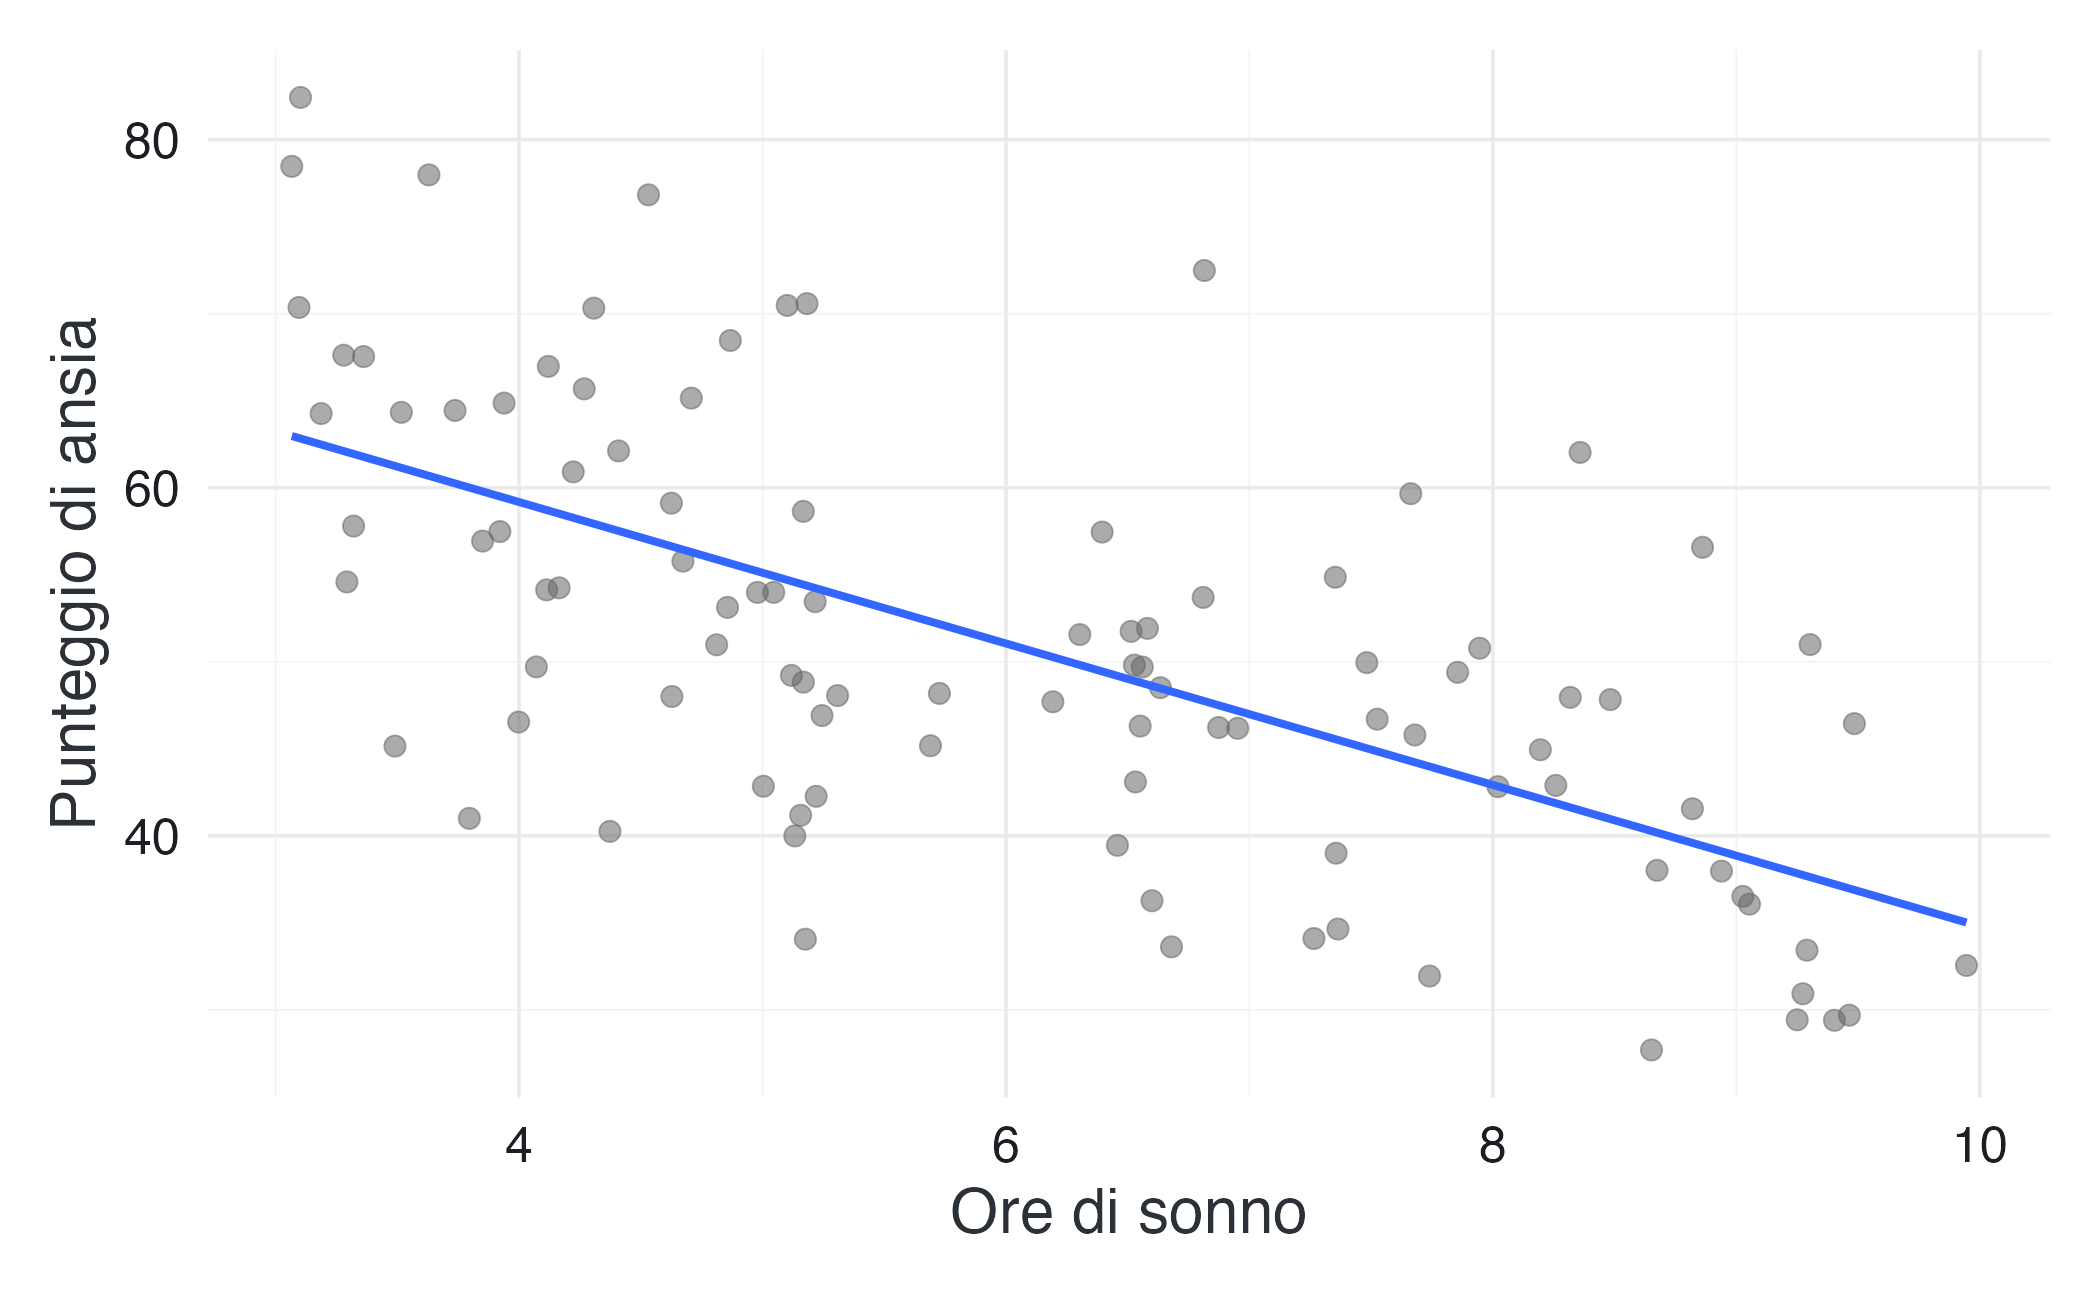
\includegraphics[width=0.85\linewidth,height=\textheight,keepaspectratio]{chapters/linear_models/03_regressione_bayesiana_brms_files/figure-pdf/fig-sleep-anxiety-scatter-1.png}

}

\caption{\label{fig-sleep-anxiety-scatter}Relazione simulata tra ore di
sonno e punteggio di ansia. La retta sintetizza la media condizionata
campionaria; la dispersione verticale dei punti riflette la componente
di variabilità non spiegata dal predittore.}

\end{figure}%

L'ispezione visiva del grafico a dispersione (\emph{scattersplot})
suggerisce chiaramente la presenza di un'associazione lineare negativa
tra la durata del sonno e i livelli di ansia. Tuttavia, l'evidenza
grafica da sola non è sufficiente per l'inferenza scientifica: non
consente di quantificare l'incertezza campionaria che grava sui
parametri del modello (\(\alpha\), \(\beta\) e \(\sigma\)), né di
distinguere concettualmente l'incertezza legata alla posizione della
retta media dalla variabilità intrinseca che caratterizzerebbe la
previsione di una singola nuova osservazione. Per risolvere questi
problemi è necessario formalizzare il modello in un quadro
probabilistico.

\section{Specificare il modello
generativo}\label{specificare-il-modello-generativo}

Il modello lineare gaussiano per l'analisi condizionata si formalizza
attraverso il seguente sistema di equazioni:

\begin{equation}\protect\phantomsection\label{eq-bayesian-linear-model}{
\begin{aligned} y_i \mid x_i, \alpha, \beta, \sigma   &\sim \operatorname{Normal}(\mu_i,\sigma), \\ \mu_i   &= \alpha + \beta x_i^c. \end{aligned}
}\end{equation}

La formulazione matematica esplicita due componenti logiche distinte: la
prima riga definisce la \textbf{funzione descrittiva della distribuzione
condizionata} delle osservazioni, assumendo che gli scostamenti
individuali seguano una legge normale; la seconda riga specifica la
\textbf{componente deterministica}, ovvero il processo geometrico con
cui la media condizionata varia in funzione del predittore.

All'interno di questa architettura, i parametri assumono un significato
interpretativo ben definito:

\begin{itemize}
\tightlist
\item
  \(\alpha\) rappresenta l'intercetta del modello, ovvero il livello
  medio di ansia atteso quando la variabile standardizzata assume valore
  nullo (\(x_i^c=0\));
\item
  \(\beta\) esprime la pendenza (\emph{slope}) della retta,
  quantificando la variazione attesa nella media della variabile di
  esito per ogni incremento unitario del predittore;
\item
  \(\sigma\) descrive la deviazione standard residua, ovvero la
  dispersione dei punteggi osservati attorno alla retta delle medie
  condizionate.
\end{itemize}

Dal punto di vista metodologico, è importante sottolineare che questa
formulazione mantiene una natura puramente descrittiva e predittiva.
Quando si opera su dati di tipo osservazionale, il coefficiente
\(\beta\) riflette esclusivamente un confronto statico tra la media di
unità statistiche che presentano livelli differenti di \(X\); esso non
può essere interpretato automaticamente come l'effetto causale di un
intervento diretto sulla durata del sonno
(\citeproc{ref-gelman2021regression}{Gelman et al., 2021}).

\section{La funzione di
verosimiglianza}\label{la-funzione-di-verosimiglianza}

Dato un vettore di parametri incogniti, la \textbf{verosimiglianza}
(\emph{likelihood}) quantifica il grado di compatibilità e congruenza
dei dati empirici osservati con la distribuzione teorica specificata dal
modello. Sotto l'assunzione metodologica di indipendenza condizionale
tra le osservazioni, per cui il punteggio di un soggetto non fornisce
informazioni sul punteggio di un altro una volta noti i parametri, la
verosimiglianza complessiva del campione si esprime come il prodotto
delle densità individuali:

\begin{equation}\protect\phantomsection\label{eq-likelihood-simple-regression}{
\mathcal{L}(\alpha,\beta,\sigma\mid\mathbf{y},\mathbf{x}) = \prod_{i=1}^{n} \mathcal{N}\!\left(y_i\mid\alpha+\beta x_i^c,\sigma^2\right).
}\end{equation}

Esplicitando la funzione di densità della distribuzione normale,
l'equazione assume la forma:

\[
\mathcal{L}(\alpha,\beta,\sigma\mid\mathbf{y},\mathbf{x}) = \prod_{i=1}^{n} \frac{1}{\sqrt{2\pi\sigma^2}} \exp\!\left[ -\frac{\left(y_i-\alpha-\beta x_i^c\right)^2}{2\sigma^2} \right].
\]

Nelle applicazioni computazionali e nella stima dei modelli, è
preferibile operare sui logaritmi naturali della funzione. La
trasformazione logaritmica trasforma la produttoria in una sommatoria,
prevenendo i problemi di underflow numerico. La corrispondente funzione
di \emph{log-verosimiglianza} si formalizza come:

\begin{equation}\protect\phantomsection\label{eq-log-likelihood-simple-regression}{
\log \mathcal{L}(\alpha,\beta,\sigma\mid\mathbf{y},\mathbf{x}) = -\frac{n}{2}\log(2\pi)-n\log\sigma   -\frac{1}{2\sigma^2}     \sum_{i=1}^{n}\left(y_i-\alpha-\beta x_i^c\right)^2.
}\end{equation}

\begin{quote}
\textbf{Nota concettuale:} È di fondamentale importanza non confondere
la verosimiglianza con una distribuzione di probabilità dei parametri.
Poiché i dati \(\mathbf{y}\) sono fissi (in quanto già osservati) e i
parametri sono variabili, la funzione \(\mathcal{L}\) non integra a 1
sul dominio dei parametri stessi.
\end{quote}

La verosimiglianza cessa di essere un semplice criterio di adattamento
geometrico e si integra nell'inferenza probabilistica solo quando viene
combinata con le distribuzioni \emph{prior}, secondo il teorema di
Bayes:

\begin{equation}\protect\phantomsection\label{eq-bayes-linear-regression}{
p(\alpha,\beta,\sigma\mid\mathbf{y},\mathbf{x}) \propto p(\mathbf{y}\mid\mathbf{x},\alpha,\beta,\sigma) ,p(\alpha,\beta,\sigma). 
}\end{equation}

In questa formulazione, la verosimiglianza funge da ``ponte
informativo'' e opera l'aggiornamento logico che trasforma le credenze
iniziali (\emph{prior}) nella distribuzione congiunta a posteriori delle
nostre conoscenze sui parametri.

\section{Specificare i prior sulla scala del
problema}\label{specificare-i-prior-sulla-scala-del-problema}

La formulazione delle distribuzioni a priori (\emph{prior}) non deve
seguire automatismi matematici, ma deve basarsi sul significato
sostantivo e sulla scala metrica dei parametri. Nel nostro scenario, le
conoscenze teoriche ed empiriche sul fenomeno ci forniscono alcuni
vincoli biologici e psicometrici precisi:

\begin{itemize}
\tightlist
\item
  \textbf{Il punteggio di ansia (\(Y\))} è quantificato su una scala
  definita nell'intervallo \([0, 100]\);
\item
  \textbf{L'intercetta (\(\alpha\))} esprime il livello di ansia atteso
  in corrispondenza del tempo medio di sonno del campione;
\item
  \textbf{La pendenza (\(\beta\))} descrive l'effetto di un'unica ora di
  sonno aggiuntiva: variazioni istantanee di decine di punti
  risulterebbero clinicamente e logicamente inverosimili;
\item
  \textbf{La deviazione standard residua (\(\sigma\))} deve assumere
  rigorosamente valori positivi e, verosimilmente, non può superare
  l'intera estensione della scala di misura.
\end{itemize}

Sulla base di queste considerazioni geometriche e fenomenologiche,
formalizziamo il sistema dei \emph{prior} come segue:

\begin{equation}\protect\phantomsection\label{eq-priors-sleep-anxiety}{
\begin{aligned} \alpha &\sim \operatorname{Normal}(50,10),\\ \beta  &\sim \operatorname{Normal}(-2,2),\\ \sigma &\sim \operatorname{Lognormal}(\log 10,0.4). \end{aligned}
}\end{equation}

\subsection{\texorpdfstring{Prior per l'intercetta
(\(\alpha\))}{Prior per l'intercetta (\textbackslash alpha)}}\label{prior-per-lintercetta-alpha}

Il prior \(\operatorname{Normal}(50,10)\) assegna la massima
plausibilità teorica ai livelli di ansia situati attorno al centro
geometrico della scala (\(50\)), concedendo al contempo un'ampia
variabilità (il \(95\%\) della massa di probabilità a priori si colloca
tra \(30\) e \(70\)). Questa scelta non vincola rigidamente il
parametro, ma esclude valori biologicamente impossibili. La scelta
metodologica di centrare il predittore garantisce che questa valutazione
a priori mantenga un significato psicometrico concreto e direttamente
interpretabile.

\subsection{\texorpdfstring{Prior per la pendenza
(\(\beta\))}{Prior per la pendenza (\textbackslash beta)}}\label{prior-per-la-pendenza-beta}

Il prior \(\operatorname{Normal}(-2,2)\) riflette un'ipotesi teorica
basata su una moderata associazione negativa, coerente con la
letteratura sulla privazione del sonno. Tuttavia, la deviazione standard
pari a \(2\) assegna una densità di probabilità non trascurabile sia
all'assenza di effetto (\(\beta = 0\)) sia a un'eventuale associazione
positiva. In ambito accademico, l'introduzione di un prior parzialmente
direzionale è considerata legittima solo se sostenuta da solide evidenze
empiriche o teoriche antecedenti e indipendenti dai dati attuali.

\subsection{\texorpdfstring{Prior per la deviazione standard
(\(\sigma\))}{Prior per la deviazione standard (\textbackslash sigma)}}\label{prior-per-la-deviazione-standard-sigma}

La distribuzione lognormale risolve un vincolo geometrico fondamentale,
assegnando una densità di probabilità esclusivamente a valori positivi
(\(\sigma > 0\)) e concentrando la massa attorno a livelli di
dispersione che sono sensati dal punto di vista empirico. In letteratura
non esiste un consenso unanime su un prior standard per la variabilità
residua: le distribuzioni \emph{half-Normal}, \emph{half-Student-\(t\)},
\emph{Gamma} o \emph{Lognormale} presentano comportamenti asintotici e
implicazioni logiche molto diverse sia in prossimità dello zero sia
nelle code estreme. La scelta della forma funzionale più idonea deve
quindi essere convalidata ex post mediante controlli predittivi.

\begin{tcolorbox}[enhanced jigsaw, arc=.35mm, bottomrule=.15mm, bottomtitle=1mm, breakable, colback=white, colbacktitle=quarto-callout-warning-color!10!white, colframe=quarto-callout-warning-color-frame, coltitle=black, left=2mm, leftrule=.75mm, opacityback=0, opacitybacktitle=0.6, rightrule=.15mm, title=\textcolor{quarto-callout-warning-color}{\faExclamationTriangle}\hspace{0.5em}{La relatività concettuale dei prior}, titlerule=0mm, toprule=.15mm, toptitle=1mm]

Definire un prior come ``debolmente informativo'' o ``altamente
informativo'' prescindendo dalla scala metrica del parametro è un errore
metodologico. Una distribuzione normale con deviazione standard pari a
\(10\), per esempio, risulterebbe estremamente ampia se applicata a un
coefficiente standardizzato, ma si rivelerebbe eccessivamente
restrittiva se il fenomeno in studio fosse espresso su una scala
temporale in millisecondi. La valutazione di un prior è sempre
un'operazione dipendente dalla scala.

\end{tcolorbox}

\section{Controllare i prior prima di adattare il
modello}\label{controllare-i-prior-prima-di-adattare-il-modello}

Nello sviluppo di un modello bayesiano, l'ispezione delle impostazioni
predefinite del software costituisce un passaggio preliminare
indispensabile. Il pacchetto \texttt{brms} mette a disposizione
strumenti specifici per verificare quali classi di parametri compongano
la struttura statistica definita e quali distribuzioni a priori
verrebbero applicate di \emph{default}.

Tramite la funzione \texttt{get\_prior()}, possiamo mappare
l'architettura dei parametri associata alla nostra formula lineare:

\begin{Shaded}
\begin{Highlighting}[]
\FunctionTok{get\_prior}\NormalTok{(}
\NormalTok{  ansia }\SpecialCharTok{\textasciitilde{}}\NormalTok{ sonno\_c,}
  \AttributeTok{data =}\NormalTok{ sleep\_anxiety,}
  \AttributeTok{family =} \FunctionTok{gaussian}\NormalTok{()}
\NormalTok{)}
\CommentTok{\#\textgreater{}                     prior     class    coef group resp dpar nlpar lb ub tag}
\CommentTok{\#\textgreater{}                    (flat)         b                                        }
\CommentTok{\#\textgreater{}                    (flat)         b sonno\_c                                }
\CommentTok{\#\textgreater{}  student\_t(3, 49.5, 11.8) Intercept                                        }
\CommentTok{\#\textgreater{}     student\_t(3, 0, 11.8)     sigma                                0       }
\CommentTok{\#\textgreater{}        source}
\CommentTok{\#\textgreater{}       default}
\CommentTok{\#\textgreater{}  (vectorized)}
\CommentTok{\#\textgreater{}       default}
\CommentTok{\#\textgreater{}       default}
\end{Highlighting}
\end{Shaded}

Le impostazioni predefinite di \texttt{brms} variano in base alla natura
del parametro Ad esempio, per i coefficienti di popolazione (la classe
\texttt{"b"}), il software applica standard un prior piatto improprio
(\emph{flat prior}), mentre per l'intercetta e i parametri di scala
adotta soluzioni differenti. Dal punto di vista metodologico, l'uso di
prior impropri esclude la possibilità di effettuare un controllo
predittivo a priori; pertanto, è necessario definire esplicitamente
prior appropriati per tutti i parametri strutturali del
modello.\footnote{Per un approfondimento sui meccanismi di assegnazione
  automatica, si rimanda alla documentazione ufficiale delle funzioni
  \href{https://paulbuerkner.com/brms/reference/default_prior.html}{\texttt{default\_prior()}}
  e
  \href{https://paulbuerkner.com/brms/reference/set_prior.html}{\texttt{set\_prior()}}.}

Traduciamo quindi le distribuzioni identificate nel paragrafo precedente
in sintassi \texttt{brms} utilizzando la funzione \texttt{c()} e
l'operatore \texttt{prior()}:

\begin{Shaded}
\begin{Highlighting}[]
\NormalTok{sleep\_anxiety\_priors }\OtherTok{\textless{}{-}} \FunctionTok{c}\NormalTok{(}
  \FunctionTok{prior}\NormalTok{(}\FunctionTok{normal}\NormalTok{(}\DecValTok{50}\NormalTok{, }\DecValTok{10}\NormalTok{), }\AttributeTok{class =} \StringTok{"Intercept"}\NormalTok{),}
  \FunctionTok{prior}\NormalTok{(}\FunctionTok{normal}\NormalTok{(}\SpecialCharTok{{-}}\DecValTok{2}\NormalTok{, }\DecValTok{2}\NormalTok{), }\AttributeTok{class =} \StringTok{"b"}\NormalTok{, }\AttributeTok{coef =} \StringTok{"sonno\_c"}\NormalTok{),}
  \FunctionTok{prior}\NormalTok{(}\FunctionTok{lognormal}\NormalTok{(}\FunctionTok{log}\NormalTok{(}\DecValTok{10}\NormalTok{), }\FloatTok{0.4}\NormalTok{), }\AttributeTok{class =} \StringTok{"sigma"}\NormalTok{)}
\NormalTok{)}

\NormalTok{sleep\_anxiety\_priors}
\CommentTok{\#\textgreater{}                    prior     class    coef group resp dpar nlpar   lb   ub tag}
\CommentTok{\#\textgreater{}           normal(50, 10) Intercept                               \textless{}NA\textgreater{} \textless{}NA\textgreater{}    }
\CommentTok{\#\textgreater{}            normal({-}2, 2)         b sonno\_c                       \textless{}NA\textgreater{} \textless{}NA\textgreater{}    }
\CommentTok{\#\textgreater{}  lognormal(log(10), 0.4)     sigma                               \textless{}NA\textgreater{} \textless{}NA\textgreater{}    }
\CommentTok{\#\textgreater{}  source}
\CommentTok{\#\textgreater{}    user}
\CommentTok{\#\textgreater{}    user}
\CommentTok{\#\textgreater{}    user}
\end{Highlighting}
\end{Shaded}

\subsection{\texorpdfstring{Il controllo predittivo a priori
(\emph{Prior Predictive
Check})}{Il controllo predittivo a priori (Prior Predictive Check)}}\label{il-controllo-predittivo-a-priori-prior-predictive-check}

Una volta stabiliti i prior per i singoli parametri, è fondamentale
valutarne l'effetto congiunto sul comportamento globale del modello.
Formalmente, la \textbf{distribuzione predittiva a priori} si ottiene
integrando la funzione di verosimiglianza rispetto alla distribuzione
congiunta dei prior:

\[
p(\widetilde{y}) = \int p(\widetilde{y}\mid\alpha,\beta,\sigma) \,p(\alpha,\beta,\sigma) \,d\alpha\,d\beta\,d\sigma .
\]

Questa operazione traduce le assunzioni teoriche formulate sui parametri
in traiettorie ed esiti empirici osservabili direttamente sulla scala
metrica della variabile dipendente. Per esaminare queste implicazioni
senza condizionare il modello all'evidenza dei dati, è possibile
simulare delle repliche campionarie campionando esclusivamente dalle
distribuzioni a priori, impostando l'argomento
\texttt{sample\_prior\ =\ "only"} in \texttt{brm()}:

\begin{Shaded}
\begin{Highlighting}[]
\NormalTok{fit\_sleep\_prior }\OtherTok{\textless{}{-}} \FunctionTok{brm}\NormalTok{(}
\NormalTok{  ansia }\SpecialCharTok{\textasciitilde{}}\NormalTok{ sonno\_c,}
  \AttributeTok{data =}\NormalTok{ sleep\_anxiety,}
  \AttributeTok{family =} \FunctionTok{gaussian}\NormalTok{(),}
  \AttributeTok{prior =}\NormalTok{ sleep\_anxiety\_priors,}
  \AttributeTok{sample\_prior =} \StringTok{"only"}\NormalTok{,}
  \AttributeTok{backend =} \StringTok{"cmdstanr"}\NormalTok{,}
  \AttributeTok{chains =} \DecValTok{4}\NormalTok{,}
  \AttributeTok{iter =} \DecValTok{1000}\NormalTok{,}
  \AttributeTok{warmup =} \DecValTok{500}\NormalTok{,}
  \AttributeTok{seed =} \DecValTok{1234}\NormalTok{,}
  \AttributeTok{refresh =} \DecValTok{0}
\NormalTok{)}
\end{Highlighting}
\end{Shaded}

Attraverso la funzione \texttt{pp\_check()}, possiamo visualizzare
l'estensione e la forma delle densità simulate per confrontarle con i
vincoli teorici del costrutto:

\begin{Shaded}
\begin{Highlighting}[]
\FunctionTok{pp\_check}\NormalTok{(}
\NormalTok{  fit\_sleep\_prior,}
  \AttributeTok{type =} \StringTok{"dens\_overlay"}\NormalTok{,}
  \AttributeTok{ndraws =} \DecValTok{50}
\NormalTok{)}
\end{Highlighting}
\end{Shaded}

\begin{figure}[H]

\centering{

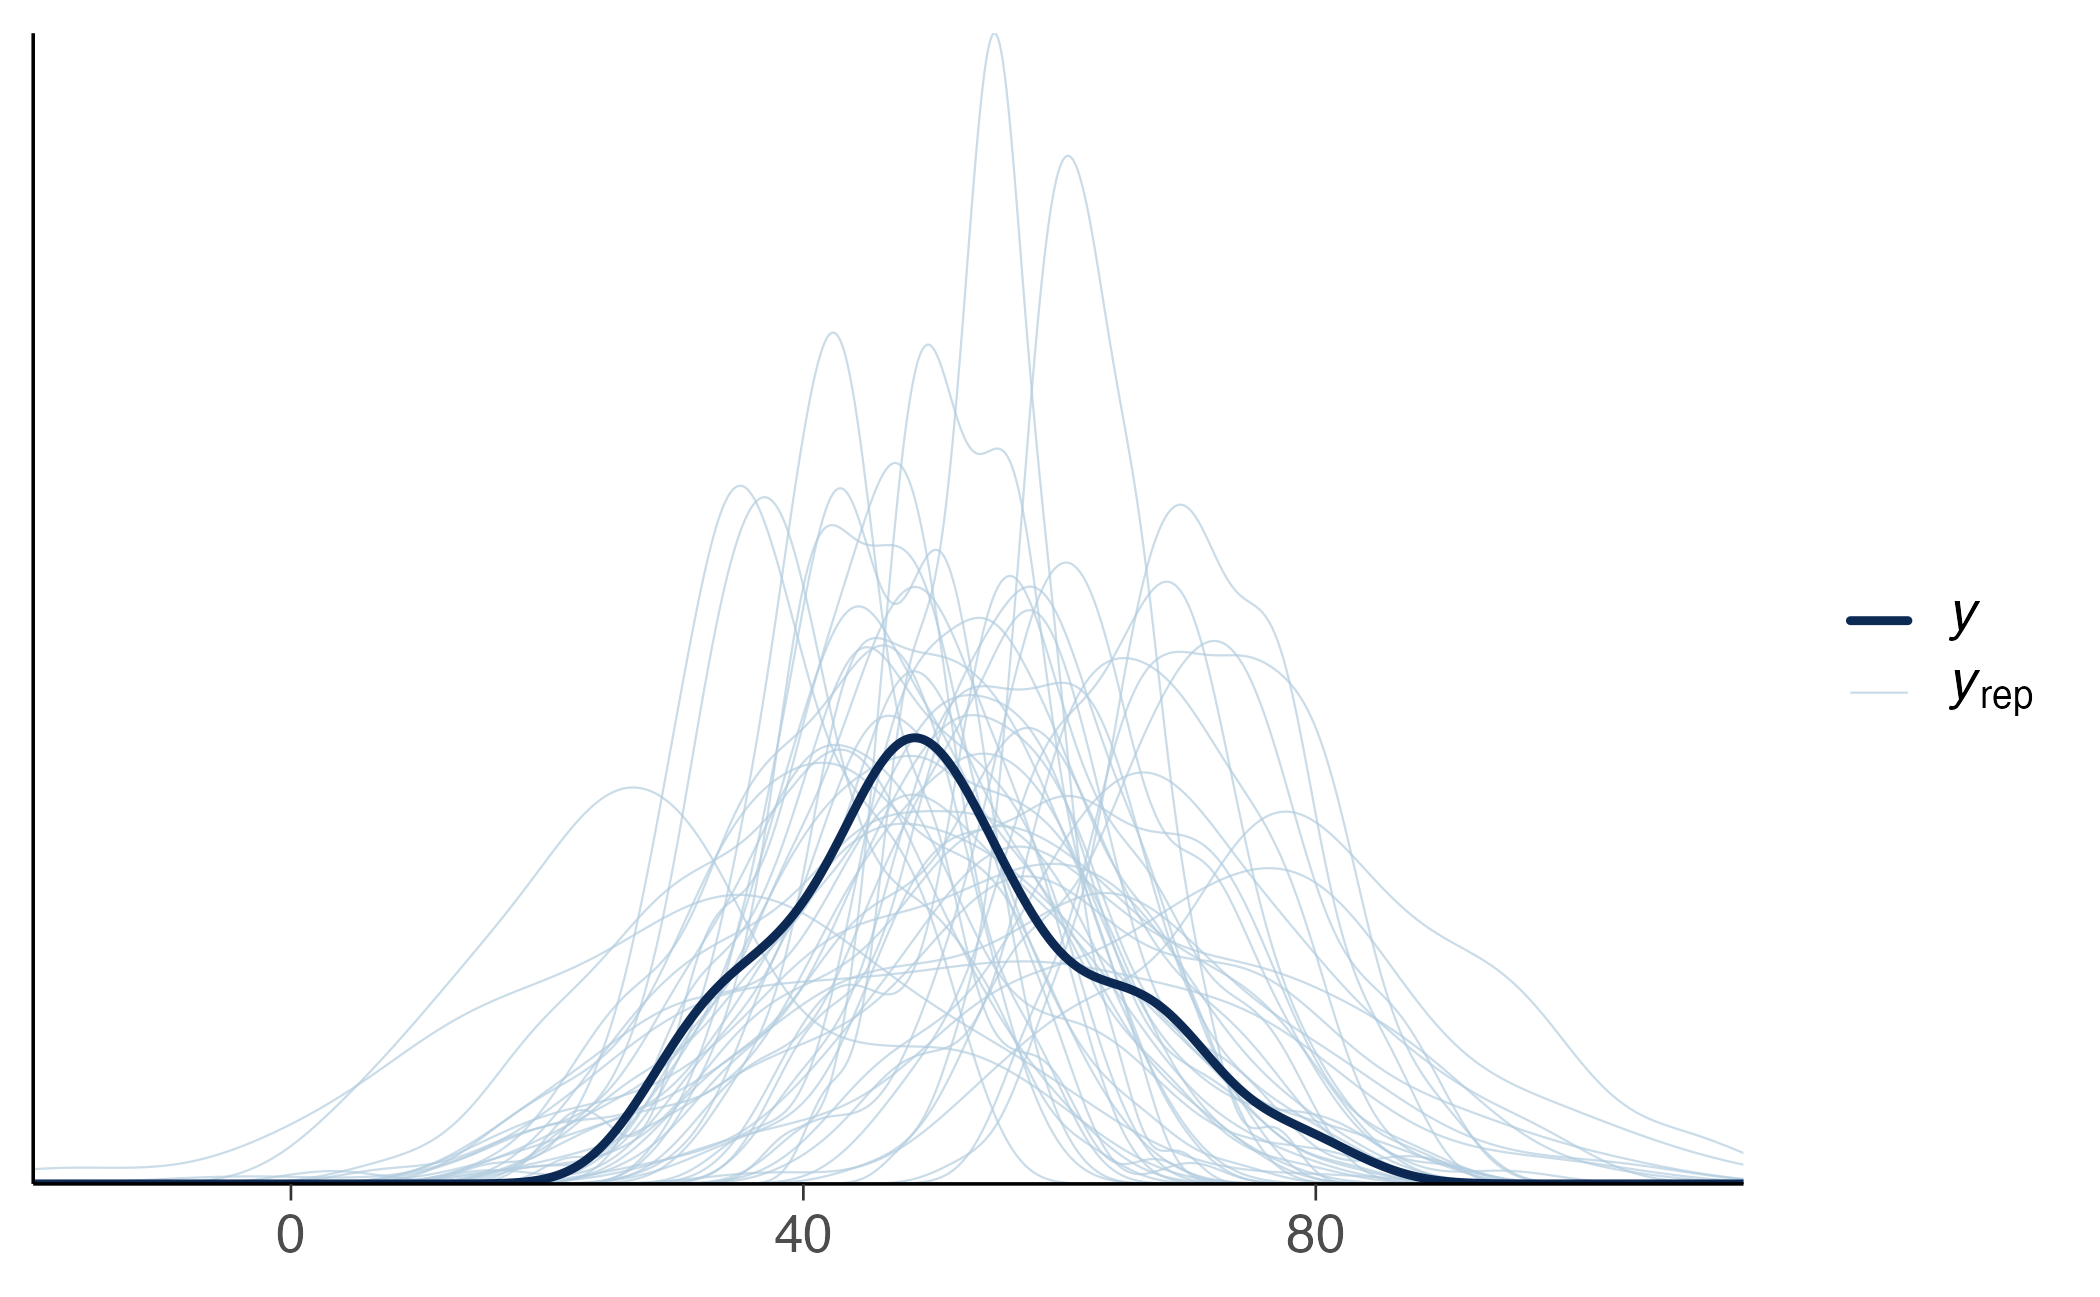
\includegraphics[width=0.85\linewidth,height=\textheight,keepaspectratio]{chapters/linear_models/03_regressione_bayesiana_brms_files/figure-pdf/fig-prior-predictive-sleep-anxiety-1.png}

}

\caption{\label{fig-prior-predictive-sleep-anxiety}Distribuzioni di
punteggi simulate esclusivamente dalle informazioni a priori. Il
controllo predittivo permette di stabilire se i prior scelti generino
configurazioni di dati plausibili per il fenomeno in esame prima di
interpellare la verosimiglianza.}

\end{figure}%

La valutazione di questo grafico richiede sensibilità metodologica. Il
ricercatore non deve aspettarsi che ogni singola replica campionaria
rimanga rigidamente confinata entro l'intervallo empirico dell'ansia
\([0, 100]\), in quanto il modello lineare gaussiano, per definizione,
ammette un supporto continuo sull'intera retta reale. L'obiettivo del
controllo consiste piuttosto nel verificare che non vi sia una frequenza
sistematica di pattern aberranti o biologicamente impossibili. Se i dati
teorici tendono ad accumularsi in modo massiccio oltre i limiti fisici
dello strumento, l'inadeguatezza non risiede nei singoli prior, ma nella
scelta della verosimiglianza normale, suggerendo la necessità di passare
a modelli per dati limitati o censurati.

\begin{tcolorbox}[enhanced jigsaw, arc=.35mm, bottomrule=.15mm, bottomtitle=1mm, breakable, colback=white, colbacktitle=quarto-callout-important-color!10!white, colframe=quarto-callout-important-color-frame, coltitle=black, left=2mm, leftrule=.75mm, opacityback=0, opacitybacktitle=0.6, rightrule=.15mm, title=\textcolor{quarto-callout-important-color}{\faExclamation}\hspace{0.5em}{Il controllo a priori riguarda l'intero modello}, titlerule=0mm, toprule=.15mm, toptitle=1mm]

Una scomposizione analitica può trarre in inganno: i parametri i cui
prior appaiono singolarmente ragionevoli, una volta combinati
algebricamente e stocasticamente, possono generare scenari empirici del
tutto inverosimili. La calibrazione del modello deve quindi avvenire
sempre ex ante sulla scala delle osservazioni simulate complessive e non
limitarsi a una considerazione isolata delle singole densità marginali
dei parametri.

\end{tcolorbox}

\section{\texorpdfstring{Adattare il modello con
\texttt{brms}}{Adattare il modello con brms}}\label{adattare-il-modello-con-brms}

La formulazione della componente sistematica (o deterministica) del
modello avviene in \texttt{brms} attraverso la classica notazione
sintattica di Wilkinson-Rogers:

\begin{Shaded}
\begin{Highlighting}[]
\NormalTok{ansia }\SpecialCharTok{\textasciitilde{}}\NormalTok{ sonno\_c}
\end{Highlighting}
\end{Shaded}

In questa sintassi, l'argomento \texttt{family\ =\ gaussian()} definisce
la natura probabilistica della distribuzione condizionata dell'esito.
Procediamo quindi all'adattamento del modello impostando il parametro
\texttt{sample\_prior\ =\ "yes"}; questo accorgimento metodologico ci
consente di conservare anche i campioni estratti esclusivamente dalle
distribuzioni a priori, una risorsa computazionale che si rivelerà
essenziale per i successivi confronti formali e per il calcolo degli
indici di aggiornamento informativo.

\begin{Shaded}
\begin{Highlighting}[]
\NormalTok{fit\_sleep }\OtherTok{\textless{}{-}} \FunctionTok{brm}\NormalTok{(}
\NormalTok{  ansia }\SpecialCharTok{\textasciitilde{}}\NormalTok{ sonno\_c,}
  \AttributeTok{data =}\NormalTok{ sleep\_anxiety,}
  \AttributeTok{family =} \FunctionTok{gaussian}\NormalTok{(),}
  \AttributeTok{prior =}\NormalTok{ sleep\_anxiety\_priors,}
  \AttributeTok{sample\_prior =} \StringTok{"yes"}\NormalTok{,}
  \AttributeTok{backend =} \StringTok{"cmdstanr"}\NormalTok{,}
  \AttributeTok{chains =} \DecValTok{4}\NormalTok{,}
  \AttributeTok{iter =} \DecValTok{2000}\NormalTok{,}
  \AttributeTok{warmup =} \DecValTok{1000}\NormalTok{,}
  \AttributeTok{seed =} \DecValTok{1234}\NormalTok{,}
  \AttributeTok{refresh =} \DecValTok{0}
\NormalTok{)}
\end{Highlighting}
\end{Shaded}

Per garantire la tracciabilità e la riproducibilità del processo di
stima, è buona norma stampare un riepilogo formale dei \emph{prior}
effettivamente vincolati all'oggetto del modello:

\begin{Shaded}
\begin{Highlighting}[]
\FunctionTok{prior\_summary}\NormalTok{(fit\_sleep)}
\CommentTok{\#\textgreater{}                    prior     class    coef group resp dpar nlpar lb ub tag}
\CommentTok{\#\textgreater{}                   (flat)         b                                        }
\CommentTok{\#\textgreater{}            normal({-}2, 2)         b sonno\_c                                }
\CommentTok{\#\textgreater{}           normal(50, 10) Intercept                                        }
\CommentTok{\#\textgreater{}  lognormal(log(10), 0.4)     sigma                                0       }
\CommentTok{\#\textgreater{}   source}
\CommentTok{\#\textgreater{}  default}
\CommentTok{\#\textgreater{}     user}
\CommentTok{\#\textgreater{}     user}
\CommentTok{\#\textgreater{}     user}
\end{Highlighting}
\end{Shaded}

Dietro le quinte, \texttt{brms} traduce l'interfaccia R (composta da
formula, famiglia probabilistica e prior) in un codice sorgente
ottimizzato in linguaggio Stan. Il motore di stima esegue il
campionamento tramite l'algoritmo \textbf{NUTS} (\emph{No-U-Turn
Sampler}), una variante avanzata e adattiva del metodo \emph{Hamiltonian
Monte Carlo} (HMC). Questo algoritmo esplora lo spazio geometrico dei
parametri generando una sequenza di valori auto-correlati che, in
condizioni di convergenza, approssimano numericamente la
\textbf{distribuzione a posteriori congiunta}.

\begin{quote}
\textbf{Avvertenza concettuale:} Talvolta gli studenti tendono a
confondere la natura delle simulazioni stocastiche. I campioni generati
dalle catene MCMC non devono essere interpretati come se fossero nuove
osservazioni empiriche o dataset indipendenti replicati, ma
rappresentano, al contrario, una discretizzazione numerica e empirica
dello stato di certezza e incertezza inferenziale relativo ai parametri
del modello.
\end{quote}

\section{Valutare la convergenza e la stabilità del
campionamento}\label{valutare-la-convergenza-e-la-stabilituxe0-del-campionamento}

Prima di procedere all'interpretazione della distribuzione a posteriori,
è importante verificare la stabilità e l'affidabilità algoritmica del
processo di stima. Questo scrutinio diagnostico risponde a una domanda
strettamente computazionale: ci assicura che l'algoritmo geometrico
abbia esplorato lo spazio dei parametri in modo corretto ed efficiente.
Non va confuso, pertanto, con una valutazione del merito scientifico o
della validità teorica del modello stesso.

\subsection{Indici diagnostici
numerici}\label{indici-diagnostici-numerici}

Attraverso la funzione \texttt{summary()}, otteniamo una sintesi dei
parametri stimati affiancata dalle principali metriche di convergenza
MCMC (\emph{Markov Chain Monte Carlo}):

\begin{Shaded}
\begin{Highlighting}[]
\FunctionTok{summary}\NormalTok{(fit\_sleep)}
\CommentTok{\#\textgreater{}  Family: gaussian }
\CommentTok{\#\textgreater{}   Links: mu = identity }
\CommentTok{\#\textgreater{} Formula: ansia \textasciitilde{} sonno\_c }
\CommentTok{\#\textgreater{}    Data: sleep\_anxiety (Number of observations: 100) }
\CommentTok{\#\textgreater{}   Draws: 4 chains, each with iter = 2000; warmup = 1000; thin = 1;}
\CommentTok{\#\textgreater{}          total post{-}warmup draws = 4000}
\CommentTok{\#\textgreater{} }
\CommentTok{\#\textgreater{} Regression Coefficients:}
\CommentTok{\#\textgreater{}           Estimate Est.Error l{-}95\% CI u{-}95\% CI Rhat Bulk\_ESS Tail\_ESS}
\CommentTok{\#\textgreater{} Intercept    50.80      0.97    48.90    52.74 1.00     3956     2440}
\CommentTok{\#\textgreater{} sonno\_c      {-}3.93      0.49    {-}4.90    {-}2.98 1.00     3906     2682}
\CommentTok{\#\textgreater{} }
\CommentTok{\#\textgreater{} Further Distributional Parameters:}
\CommentTok{\#\textgreater{}       Estimate Est.Error l{-}95\% CI u{-}95\% CI Rhat Bulk\_ESS Tail\_ESS}
\CommentTok{\#\textgreater{} sigma     9.64      0.68     8.41    11.11 1.00     3698     2704}
\CommentTok{\#\textgreater{} }
\CommentTok{\#\textgreater{} Draws were sampled using sample(hmc). For each parameter, Bulk\_ESS}
\CommentTok{\#\textgreater{} and Tail\_ESS are effective sample size measures, and Rhat is the potential}
\CommentTok{\#\textgreater{} scale reduction factor on split chains (at convergence, Rhat = 1).}
\end{Highlighting}
\end{Shaded}

Nell'ispezione dell'output, l'attenzione del ricercatore deve
focalizzarsi su tre indicatori chiave:

\begin{itemize}
\tightlist
\item
  \textbf{Il fattore di riduzione della varianza (\(\widehat{R}\)):}
  noto anche come diagnostica di Gelman-Rubin, confronta la variabilità
  interna alle singole catene con la variabilità tra le catene. Nei
  modelli che hanno raggiunto una convergenza soddisfacente, il valore
  di \(\widehat{R}\) deve approssimarsi a \(1\) per ogni parametro
  stimato (tipicamente esigendo valori inferiori a \(1.05\) o, più
  rigorosamente, a \(1.01\)).
\item
  \textbf{L'ampiezza campionaria effettiva (\(ESS_{\text{bulk}}\) e
  \(ESS_{\text{tail}}\)):} quantifica il numero di campioni indipendenti
  equivalenti contenuti nelle catene auto-correlate. La metrica
  \emph{bulk} valuta la precisione della stima della media e della
  mediana della posterior, mentre la metrica \emph{tail} monitora
  l'accuratezza nella stima dei quantili estremi e delle code della
  distribuzione.
\item
  \textbf{Diagnostiche del campionatore:} l'assenza totale di messaggi
  di errore o avvisi formali generati dal motore Stan (quali superamenti
  del limite di profondità dell'albero di ricerca o segnalazioni di
  transizioni divergenti).
\end{itemize}

\begin{quote}
\textbf{Avvertenza metodologica:} Le soglie numeriche convenzionali
rappresentano standard operativi e linee guida prudenziali, non
certificazioni formali e automatiche di correttezza statistica.
L'assenza di anomalie numeriche costituisce una condizione necessaria,
ma non sufficiente, per decretare la validità dell'inferenza.
\end{quote}

\subsection{Diagnostiche grafiche: Trace plot e Rank
plot}\label{diagnostiche-grafiche-trace-plot-e-rank-plot}

Per integrare gli indici numerici ed escludere la presenza di patologie
locali nella simulazione, ricorriamo a strumenti di visualizzazione
grafica. Il primo è il \emph{trace plot}, che mostra l'evoluzione
sequenziale dei valori campionati da ciascuna catena nel corso delle
iterazioni di campionamento (\emph{post-warmup}):

\begin{Shaded}
\begin{Highlighting}[]
\NormalTok{sleep\_draws }\OtherTok{\textless{}{-}} \FunctionTok{as\_draws\_df}\NormalTok{(fit\_sleep)}

\NormalTok{pars\_interesse }\OtherTok{\textless{}{-}} \FunctionTok{c}\NormalTok{(}\StringTok{"b\_Intercept"}\NormalTok{, }\StringTok{"b\_sonno\_c"}\NormalTok{, }\StringTok{"sigma"}\NormalTok{)}

\NormalTok{sleep\_draws }\SpecialCharTok{|\textgreater{}}
  \FunctionTok{subset\_draws}\NormalTok{(}\AttributeTok{variable =}\NormalTok{ pars\_interesse) }\SpecialCharTok{|\textgreater{}}
  \FunctionTok{mcmc\_trace}\NormalTok{(}\AttributeTok{facet\_args =} \FunctionTok{list}\NormalTok{(}\AttributeTok{nrow =} \DecValTok{3}\NormalTok{))}
\end{Highlighting}
\end{Shaded}

\begin{figure}[H]

\centering{

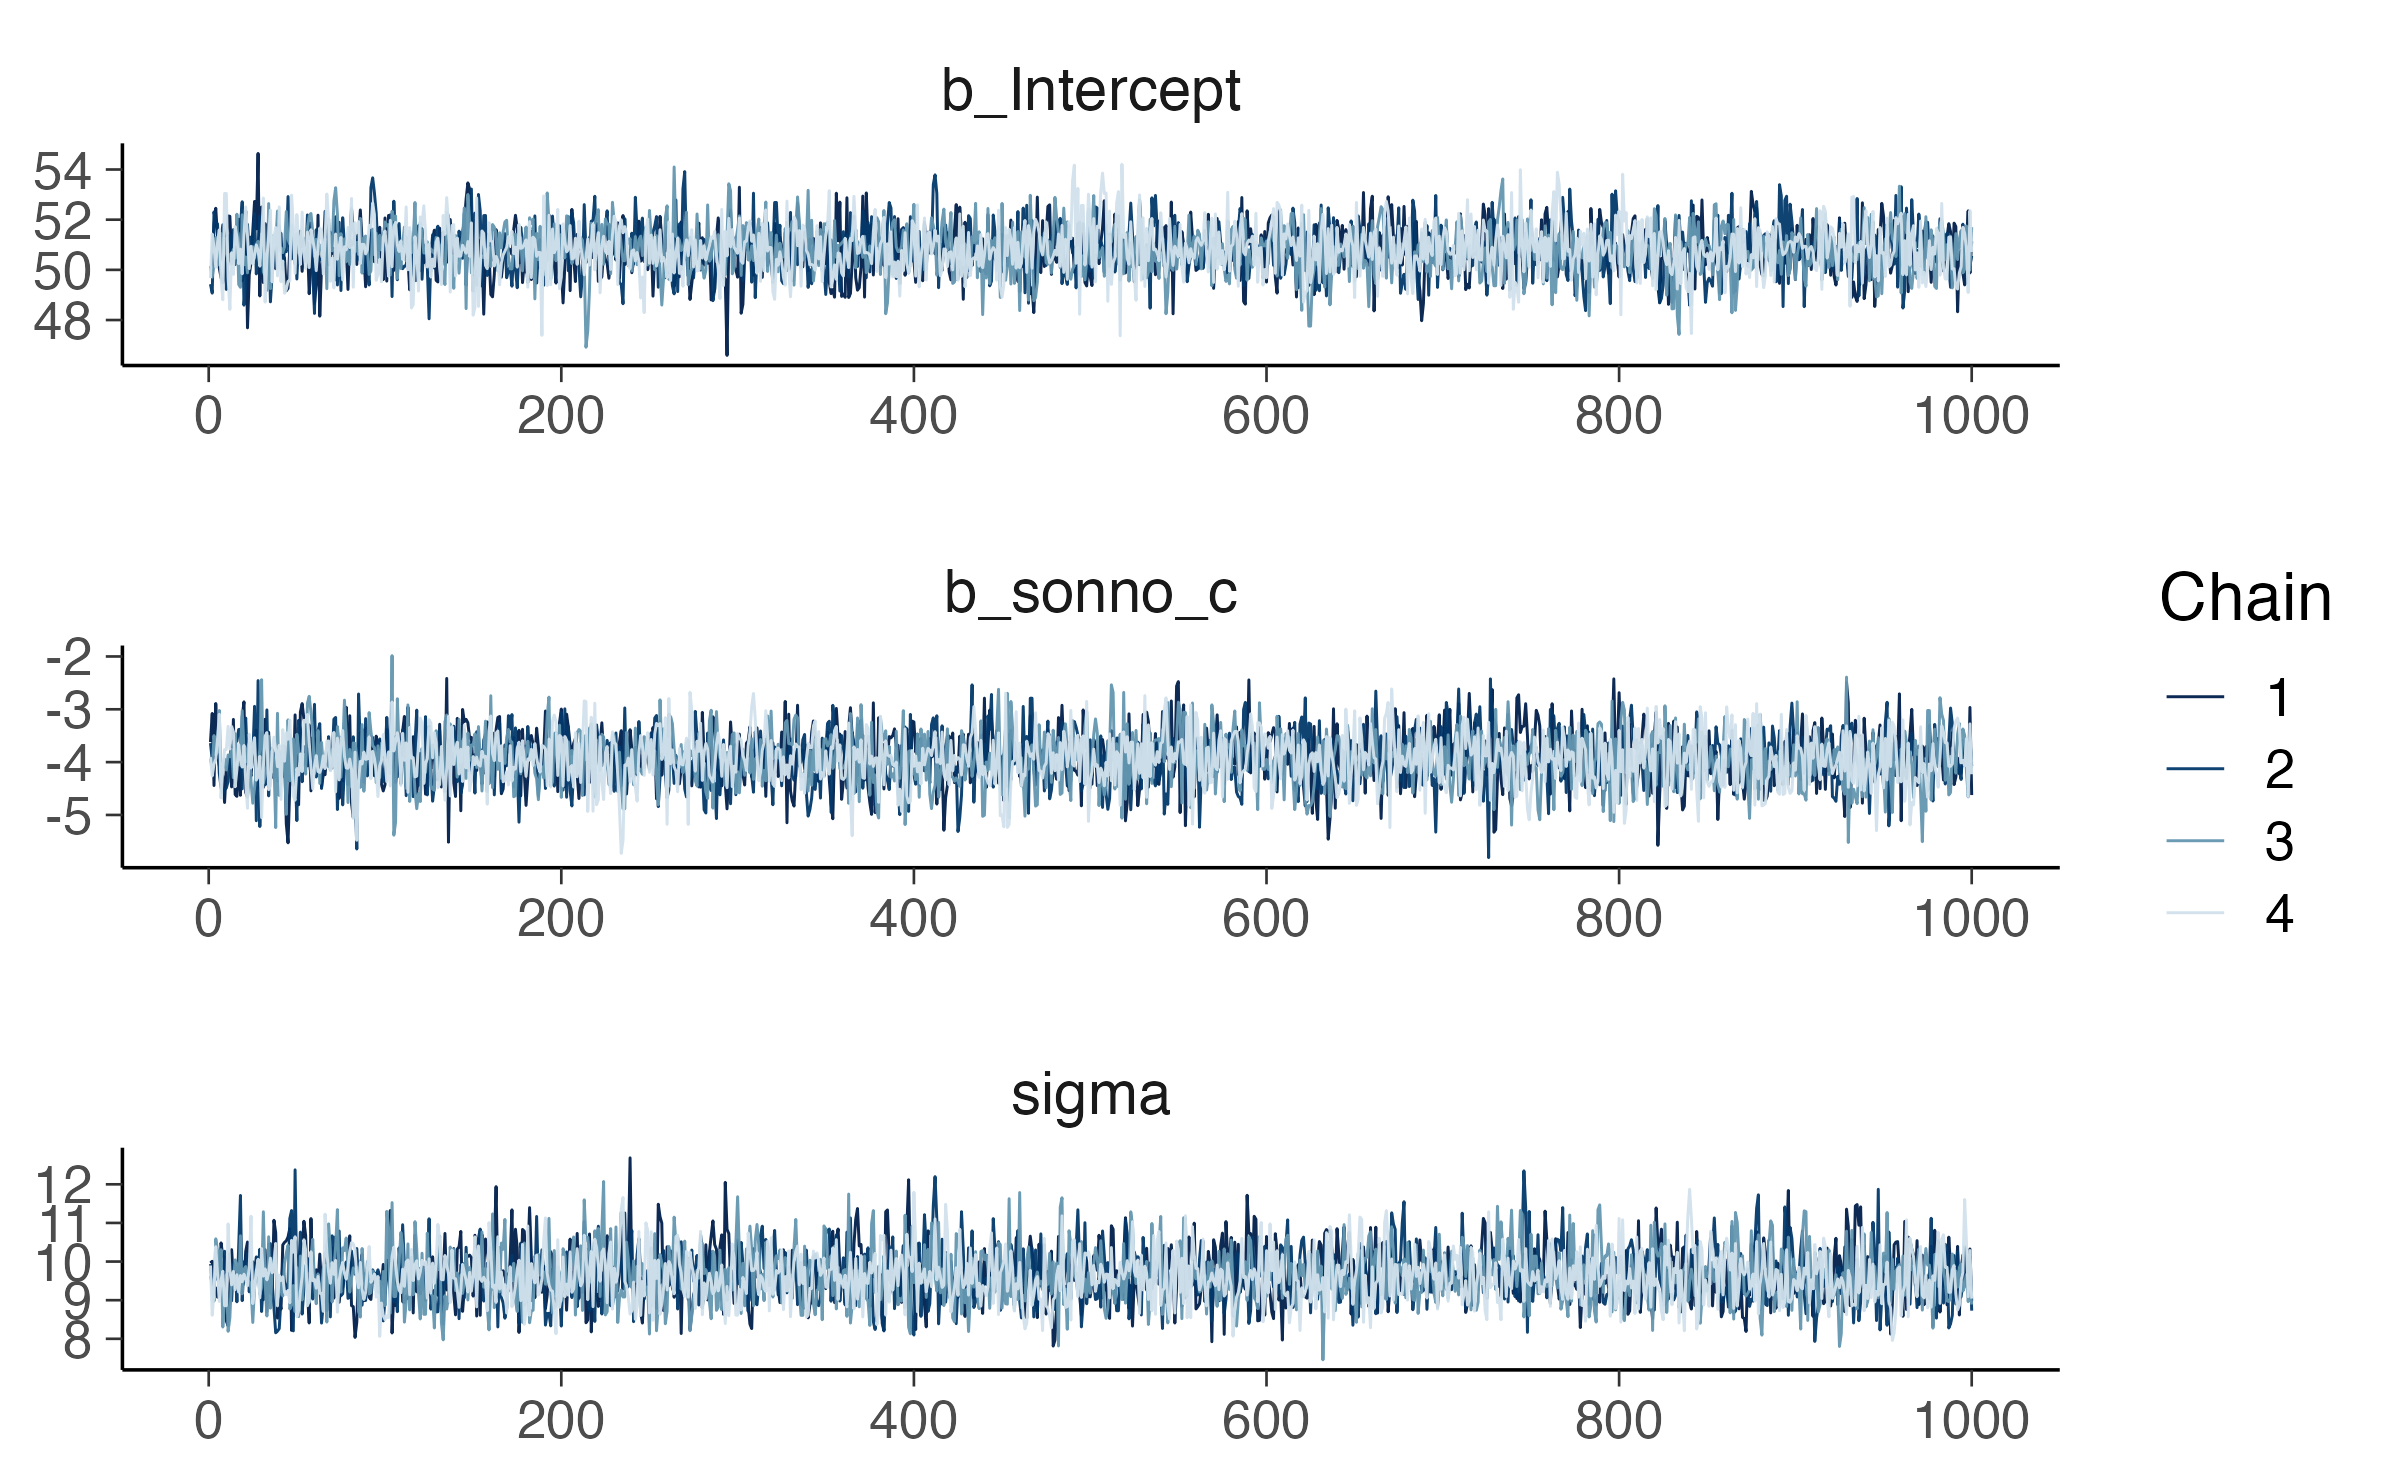
\includegraphics[width=0.85\linewidth,height=\textheight,keepaspectratio]{chapters/linear_models/03_regressione_bayesiana_brms_files/figure-pdf/fig-mcmc-trace-sleep-anxiety-1.png}

}

\caption{\label{fig-mcmc-trace-sleep-anxiety}Trace plot delle quattro
catene MCMC relative a intercetta, pendenza e deviazione standard
residua. L'intreccio sovrapposto e compatto delle traiettorie simula
l'aspetto visivo di un `bruco', segno di una corretta miscelazione delle
catene.}

\end{figure}%

Il secondo strumento grafico è il \emph{rank plot}, un istogramma che
analizza la distribuzione dei ranghi relativi delle quattro catene
sovrapposte:

\begin{Shaded}
\begin{Highlighting}[]
\NormalTok{sleep\_draws }\SpecialCharTok{|\textgreater{}}
  \FunctionTok{subset\_draws}\NormalTok{(}\AttributeTok{variable =}\NormalTok{ pars\_interesse) }\SpecialCharTok{|\textgreater{}}
  \FunctionTok{mcmc\_rank\_overlay}\NormalTok{()}
\end{Highlighting}
\end{Shaded}

\begin{figure}[H]

\centering{

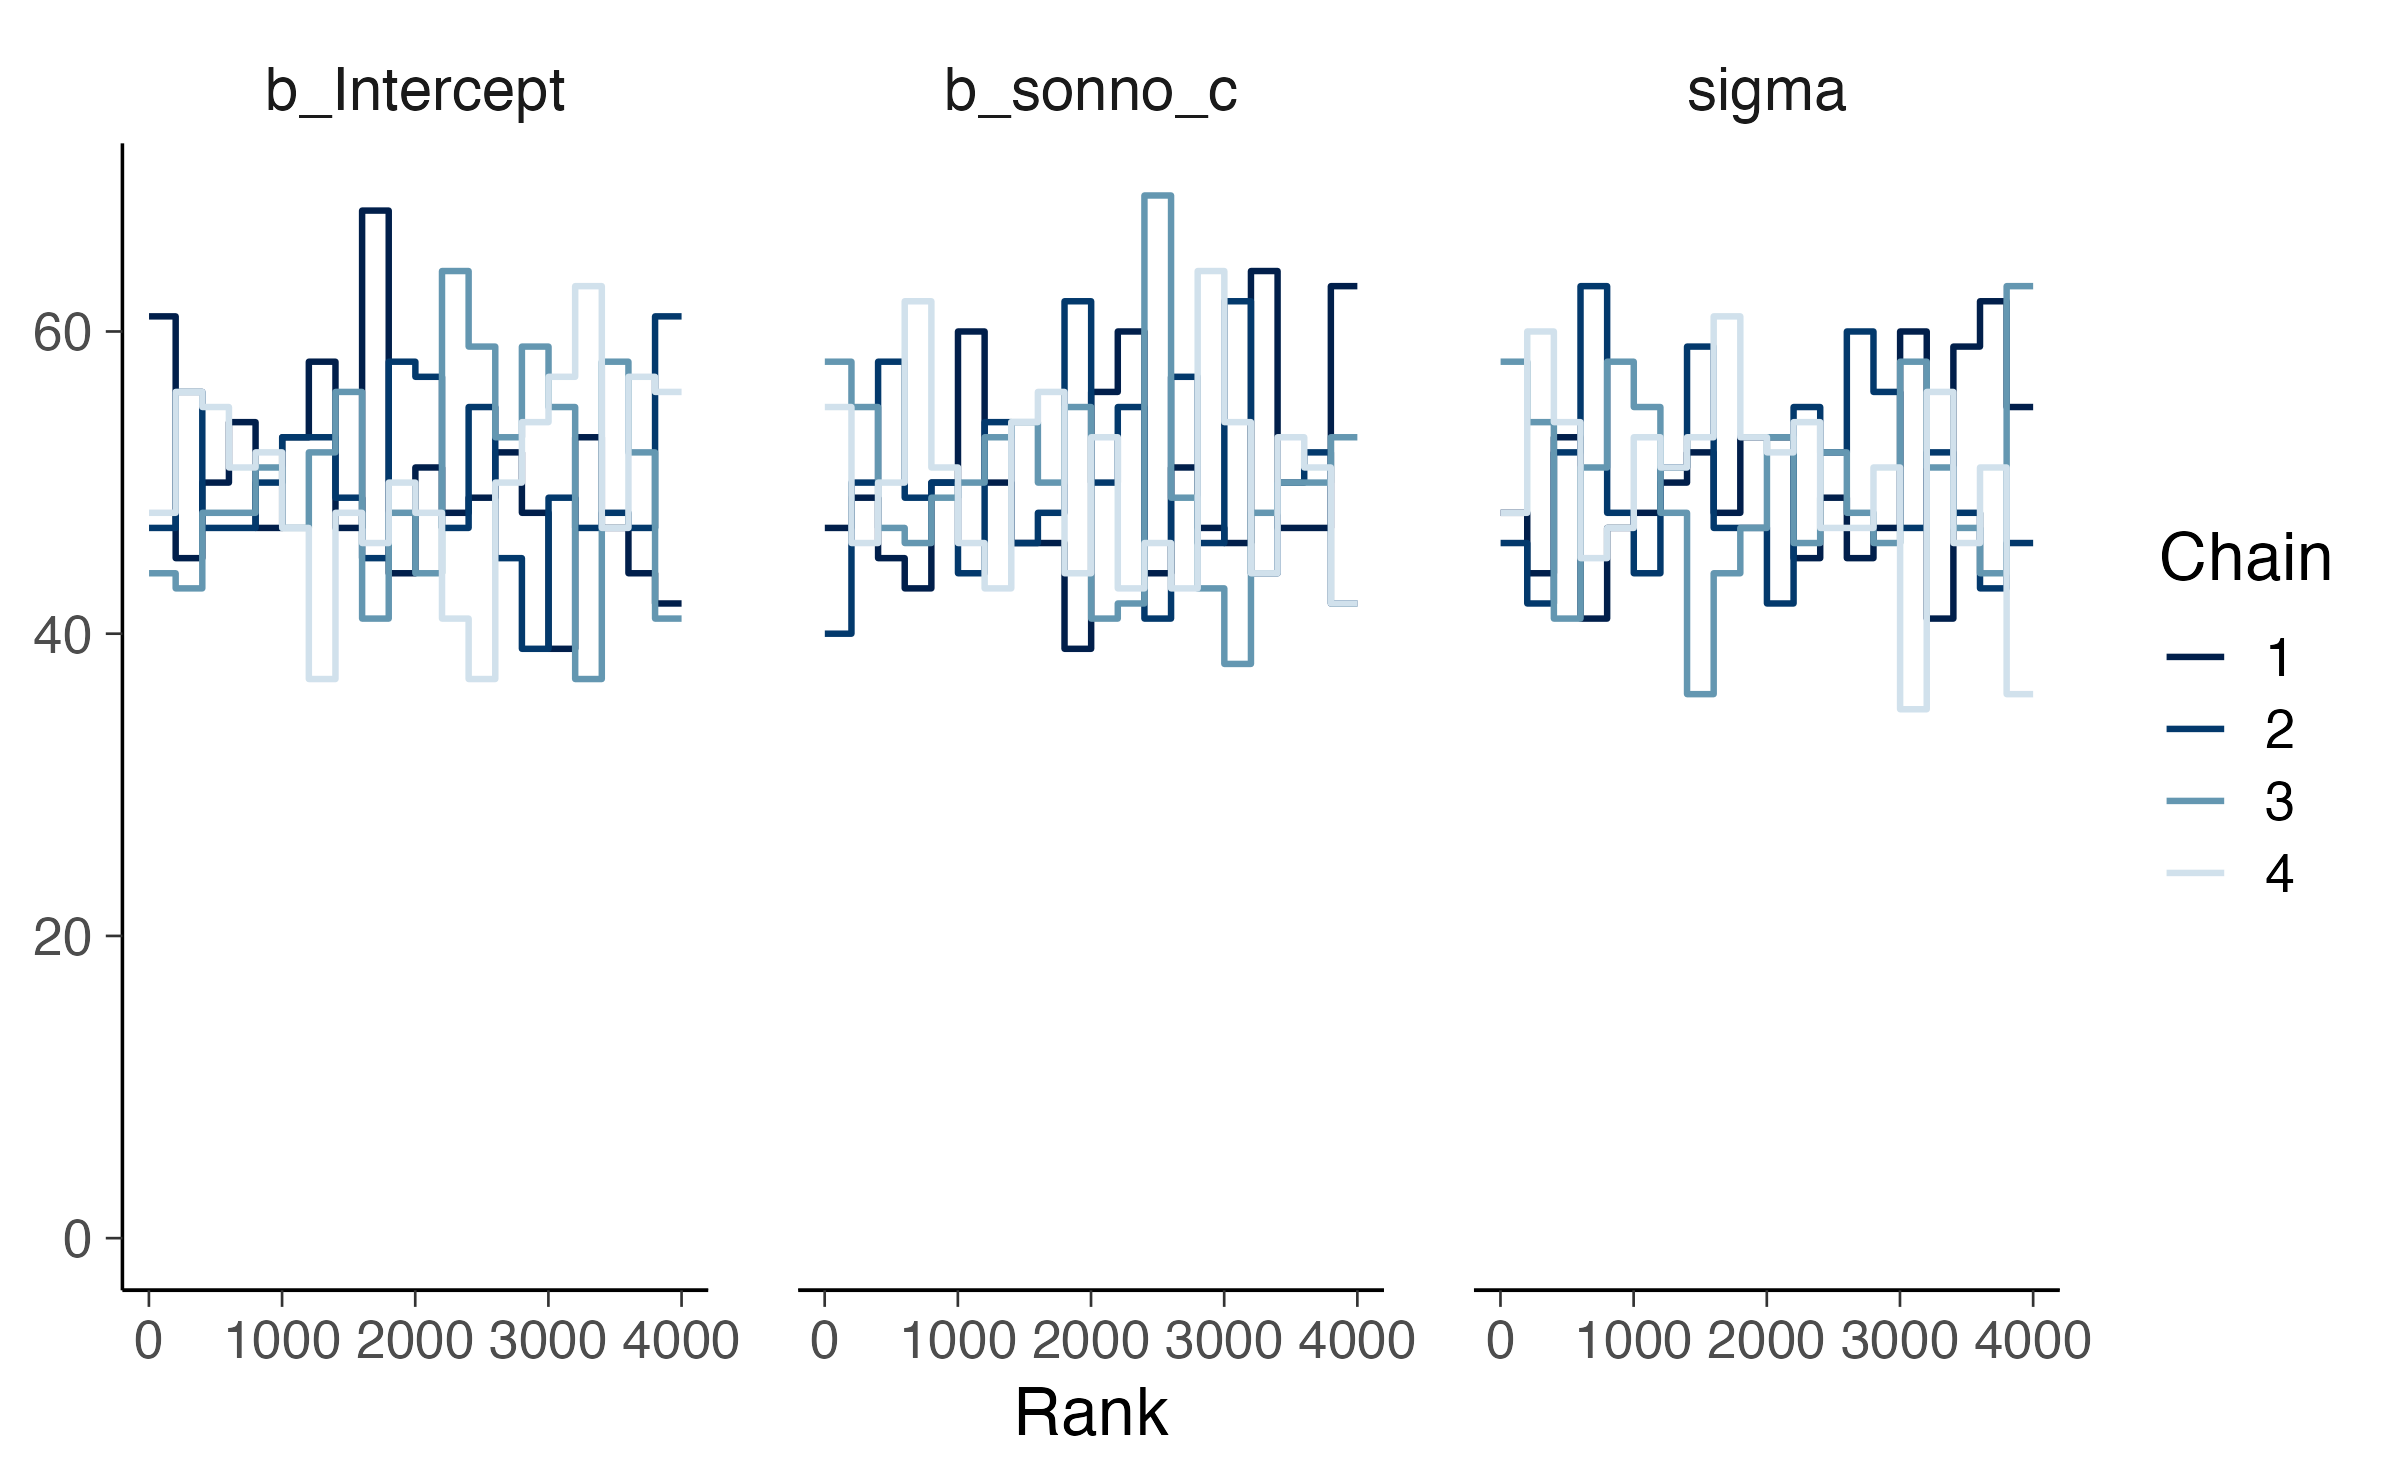
\includegraphics[width=0.85\linewidth,height=\textheight,keepaspectratio]{chapters/linear_models/03_regressione_bayesiana_brms_files/figure-pdf/fig-mcmc-rank-sleep-anxiety-1.png}

}

\caption{\label{fig-mcmc-rank-sleep-anxiety}Rank plot sovrapposto per le
catene MCMC. Profili uniformi e sovrapponibili indicano che le catene
hanno esplorato i medesimi spazi probabilistici, escludendo anomalie
sistematiche o segregazioni locali.}

\end{figure}%

Un'esplorazione ottimale della distribuzione stazionaria si traduce
graficamente in \emph{trace plot} in cui le catene si sovrappongono
rapidamente creando un pattern denso e uniforme (comunemente definito
``a bruco''), e in \emph{rank plot} i cui profili si mantengono
bilanciati e piatti, escludendo che una catena sia rimasta confinata in
porzioni isolate dello spazio campionario.

\subsection{Transizioni divergenti}\label{transizioni-divergenti}

Le transizioni divergenti rappresentano una specificità fondamentale
degli algoritmi HMC/NUTS. Esse fungono da spie luminose matematiche,
indicando che il campionatore ha intercettato aree della distribuzione a
posteriori caratterizzate da variazioni geometriche repentine e
curvature estreme (es. ``imbuti'' di probabilità) che l'approssimazione
numerica non è riuscita a mappare in modo accurato. Isoliamo
matematicamente la presenza di tali eventi:

\begin{Shaded}
\begin{Highlighting}[]
\NormalTok{nuts\_sleep }\OtherTok{\textless{}{-}} \FunctionTok{nuts\_params}\NormalTok{(fit\_sleep)}

\NormalTok{nuts\_sleep }\SpecialCharTok{|\textgreater{}}
  \FunctionTok{filter}\NormalTok{(Parameter }\SpecialCharTok{==} \StringTok{"divergent\_\_"}\NormalTok{) }\SpecialCharTok{|\textgreater{}}
  \FunctionTok{summarise}\NormalTok{(}\AttributeTok{n\_divergenze =} \FunctionTok{sum}\NormalTok{(Value))}
\CommentTok{\#\textgreater{}   n\_divergenze}
\CommentTok{\#\textgreater{} 1            0}
\end{Highlighting}
\end{Shaded}

Rilevare transizioni divergenti significa che le stime prodotte
potrebbero risultare localmente distorte o incomplete. Sebbene
l'incremento del parametro di controllo \texttt{adapt\_delta} possa
forzare l'algoritmo ad adottare passi di integrazione più piccoli
risolvendo le divergenze minori, il persistere di tali anomalie non deve
essere trattato con correzioni puramente algoritmiche. Al contrario,
esso richiede quasi sempre una profonda revisione metodologica, come la
riparametrizzazione matematica del modello (es. passando a una
parametrizzazione non centrata) o una ridefinizione delle funzioni a
priori.

\begin{tcolorbox}[enhanced jigsaw, arc=.35mm, bottomrule=.15mm, bottomtitle=1mm, breakable, colback=white, colbacktitle=quarto-callout-warning-color!10!white, colframe=quarto-callout-warning-color-frame, coltitle=black, left=2mm, leftrule=.75mm, opacityback=0, opacitybacktitle=0.6, rightrule=.15mm, title=\textcolor{quarto-callout-warning-color}{\faExclamationTriangle}\hspace{0.5em}{I tre livelli del controllo di validità}, titlerule=0mm, toprule=.15mm, toptitle=1mm]

Nello sviluppo di una ricerca, lo studente deve saper scindere
nettamente tre ordini di interrogativi, tra loro gerarchicamente
ordinati:

\begin{enumerate}
\def\labelenumi{\arabic{enumi}.}
\tightlist
\item
  \textbf{Il campionatore ha funzionato correttamente?} Risolto mediante
  le diagnostiche MCMC (\(\widehat{R}\), \(ESS\), divergenze).
\item
  \textbf{Il modello riproduce fedelmente i dati empirici?} Risolto
  mediante i controlli predittivi a posteriori (\emph{Posterior
  Predictive Check}).
\item
  \textbf{L'interpretazione dei parametri risponde validamente alla
  domanda scientifica originaria?} Risolto analizzando il disegno di
  ricerca, l'adeguatezza delle metriche e la sostenibilità delle
  assunzioni teoriche.
\end{enumerate}

Una risposta favorevole al primo livello attesta la precisione del
calcolo numerico, ma non costituisce in alcun modo una garanzia di
successo per i due livelli successivi.

\end{tcolorbox}

\section{Interpretare la distribuzione a
posteriori}\label{interpretare-la-distribuzione-a-posteriori-1}

Una volta verificata la convergenza dell'algoritmo, possiamo passare
all'interpretazione scientifica dei risultati. Il primo passo operativo
consiste nell'estrarre le stime della distribuzione a posteriori sotto
forma di struttura dati manipolabile:

\begin{Shaded}
\begin{Highlighting}[]
\NormalTok{sleep\_draws }\SpecialCharTok{|\textgreater{}}
  \FunctionTok{subset\_draws}\NormalTok{(}\AttributeTok{variable =}\NormalTok{ pars\_interesse) }\SpecialCharTok{|\textgreater{}}
  \FunctionTok{summarise\_draws}\NormalTok{(}
\NormalTok{    median,}
\NormalTok{    sd,}
    \SpecialCharTok{\textasciitilde{}} \FunctionTok{quantile2}\NormalTok{(.x, }\AttributeTok{probs =} \FunctionTok{c}\NormalTok{(}\FloatTok{0.025}\NormalTok{, }\FloatTok{0.975}\NormalTok{)),}
    \FunctionTok{default\_convergence\_measures}\NormalTok{()}
\NormalTok{  )}
\CommentTok{\#\textgreater{} \# A tibble: 3 x 8}
\CommentTok{\#\textgreater{}   variable    median    sd  q2.5 q97.5  rhat ess\_bulk ess\_tail}
\CommentTok{\#\textgreater{}   \textless{}chr\textgreater{}        \textless{}dbl\textgreater{} \textless{}dbl\textgreater{} \textless{}dbl\textgreater{} \textless{}dbl\textgreater{} \textless{}dbl\textgreater{}    \textless{}dbl\textgreater{}    \textless{}dbl\textgreater{}}
\CommentTok{\#\textgreater{} 1 b\_Intercept  50.8  0.969 48.9  52.7   1.00    3956.    2440.}
\CommentTok{\#\textgreater{} 2 b\_sonno\_c    {-}3.93 0.494 {-}4.90 {-}2.98  1.00    3906.    2682.}
\CommentTok{\#\textgreater{} 3 sigma         9.59 0.682  8.41 11.1   1.00    3698.    2704.}
\end{Highlighting}
\end{Shaded}

Sul piano concettuale, è fondamentale ricordare che la \emph{posterior}
ottenuta è una \textbf{distribuzione congiunta}: ogni singola riga della
matrice dei campioni MCMC racchiude valori generati simultaneamente per
\(\alpha\), \(\beta\) e \(\sigma\). Di conseguenza, le stime mantengono
intatta la struttura di interdipendenza tra i parametri. Tali relazioni
di dipendenza a posteriori derivano dall'interazione tra la geometria
del disegno di ricerca, l'evidenza dei dati e la parametrizzazione
scelta; non esiste alcuna legge statistica a priori che imponga, ad
esempio, che a una pendenza più elevata debba corrispondere una
deviazione standard residua più contenuta.

\subsection{Gli intervalli di
credibilità}\label{gli-intervalli-di-credibilituxe0}

Per sintetizzare la dispersione e la localizzazione della posterior,
ricorriamo al calcolo degli intervalli di credibilità:

\begin{Shaded}
\begin{Highlighting}[]
\NormalTok{sleep\_draws }\SpecialCharTok{|\textgreater{}}
  \FunctionTok{subset\_draws}\NormalTok{(}\AttributeTok{variable =} \FunctionTok{c}\NormalTok{(}\StringTok{"b\_Intercept"}\NormalTok{, }\StringTok{"b\_sonno\_c"}\NormalTok{)) }\SpecialCharTok{|\textgreater{}}
  \FunctionTok{summarise\_draws}\NormalTok{(median, }\SpecialCharTok{\textasciitilde{}} \FunctionTok{quantile2}\NormalTok{(.x, }\AttributeTok{probs =} \FunctionTok{c}\NormalTok{(}\FloatTok{0.025}\NormalTok{, }\FloatTok{0.975}\NormalTok{)))}
\CommentTok{\#\textgreater{} \# A tibble: 2 x 4}
\CommentTok{\#\textgreater{}   variable    median  q2.5 q97.5}
\CommentTok{\#\textgreater{}   \textless{}chr\textgreater{}        \textless{}dbl\textgreater{} \textless{}dbl\textgreater{} \textless{}dbl\textgreater{}}
\CommentTok{\#\textgreater{} 1 b\_Intercept  50.8  48.9  52.7 }
\CommentTok{\#\textgreater{} 2 b\_sonno\_c    {-}3.93 {-}4.90 {-}2.98}
\end{Highlighting}
\end{Shaded}

\begin{quote}
\textbf{Nota di metodo (Intervallo di credibilità vs.~Intervallo di
confidenza):} Un intervallo di credibilità al \(95\%\) definisce la
regione di spazio all'interno della quale risiede il parametro incognito
con una probabilità pari esattamente a \(0.95\), condizionatamente al
modello specificato, ai \emph{prior} inseriti e ai dati effettivamente
osservati.
\end{quote}

Questa interpretazione, lineare e intuitiva per lo studente, si
contrappone radicalmente all'intervallo di confidenza della statistica
frequentista (il quale descrive invece la frequenza a lungo termine di
intervalli campionari che conterrebbero il parametro fisso). È
altrettanto cruciale non incorrere nell'errore didattico di confondere
l'intervallo di credibilità sui parametri con una fascia di tolleranza
sulle osservazioni: esso non indica in alcun modo che il \(95\%\) dei
punteggi dei futuri soggetti si collocherà entro quei confini.

\subsection{Valutazioni probabilistiche dirette e quantità
derivate}\label{valutazioni-probabilistiche-dirette-e-quantituxe0-derivate}

Uno dei maggiori vantaggi del paradigma bayesiano risiede nella
possibilità di manipolare direttamente i campioni della posterior per
calcolare probabilità associate a specifiche ipotesi scientifiche o per
stimare quantità derivate:

\begin{Shaded}
\begin{Highlighting}[]
\CommentTok{\# Una quantità derivata è essa stessa una variabile a posteriori}
\NormalTok{sleep\_draws }\OtherTok{\textless{}{-}}\NormalTok{ sleep\_draws }\SpecialCharTok{|\textgreater{}}
  \FunctionTok{mutate\_variables}\NormalTok{(}\AttributeTok{diff\_3h =} \DecValTok{3} \SpecialCharTok{*}\NormalTok{ b\_sonno\_c)}

\CommentTok{\# Sintesi della quantità derivata}
\NormalTok{sleep\_draws }\SpecialCharTok{|\textgreater{}}
  \FunctionTok{subset\_draws}\NormalTok{(}\AttributeTok{variable =} \StringTok{"diff\_3h"}\NormalTok{) }\SpecialCharTok{|\textgreater{}}
  \FunctionTok{summarise\_draws}\NormalTok{(median, }\SpecialCharTok{\textasciitilde{}} \FunctionTok{quantile2}\NormalTok{(.x, }\AttributeTok{probs =} \FunctionTok{c}\NormalTok{(}\FloatTok{0.025}\NormalTok{, }\FloatTok{0.975}\NormalTok{)))}
\CommentTok{\#\textgreater{} \# A tibble: 1 x 4}
\CommentTok{\#\textgreater{}   variable median  q2.5 q97.5}
\CommentTok{\#\textgreater{}   \textless{}chr\textgreater{}     \textless{}dbl\textgreater{} \textless{}dbl\textgreater{} \textless{}dbl\textgreater{}}
\CommentTok{\#\textgreater{} 1 diff\_3h   {-}11.8 {-}14.7 {-}8.93}

\CommentTok{\# Probabilità a posteriori come medie di indicatori}
\NormalTok{sleep\_draws }\SpecialCharTok{|\textgreater{}}
  \FunctionTok{subset\_draws}\NormalTok{(}\AttributeTok{variable =} \StringTok{"b\_sonno\_c"}\NormalTok{) }\SpecialCharTok{|\textgreater{}}
  \FunctionTok{summarise\_draws}\NormalTok{(}
    \StringTok{"Pr(beta \textless{} 0)"}  \OtherTok{=} \ErrorTok{\textasciitilde{}} \FunctionTok{mean}\NormalTok{(.x }\SpecialCharTok{\textless{}} \DecValTok{0}\NormalTok{),}
    \StringTok{"Pr(beta \textless{} {-}2)"} \OtherTok{=} \ErrorTok{\textasciitilde{}} \FunctionTok{mean}\NormalTok{(.x }\SpecialCharTok{\textless{}} \SpecialCharTok{{-}}\DecValTok{2}\NormalTok{)}
\NormalTok{  )}
\CommentTok{\#\textgreater{} \# A tibble: 1 x 3}
\CommentTok{\#\textgreater{}   variable  \textasciigrave{}Pr(beta \textless{} 0)\textasciigrave{} \textasciigrave{}Pr(beta \textless{} {-}2)\textasciigrave{}}
\CommentTok{\#\textgreater{}   \textless{}chr\textgreater{}              \textless{}dbl\textgreater{}           \textless{}dbl\textgreater{}}
\CommentTok{\#\textgreater{} 1 b\_sonno\_c              1           1.000}
\end{Highlighting}
\end{Shaded}

Nel codice precedente, la funzione
\texttt{mean(b\_sonno\_c\ \textless{}\ 0)} calcola la proporzione di
iterazioni in cui il coefficiente assume valore negativo, traducendosi
direttamente nella probabilità a posteriori \(\Pr(\beta < 0 \mid y)\).
Questa quantità offre una risposta matematica immediata alla domanda
circa la direzione dell'associazione studiata, poste come valide le
assunzioni del modello.

Bisogna tuttavia prestare attenzione ai limiti epistemologici di tale
metrica: essa quantifica lo stato di certezza relativo al parametro
all'interno dello scenario formalizzato, ma non misura la probabilità
che il modello teorico sia ``vero'' in senso assoluto, né possiede la
facoltà di convertire magicamente un'associazione di natura
osservazionale in un nesso di causa-effetto.

\section{Dalla posterior alle
previsioni}\label{dalla-posterior-alle-previsioni}

Un errore metodologico ricorrente consiste nel confondere le stime
relative ai parametri del modello con le stime relative alle
osservazioni future. Nel framework probabilistico bayesiano, la
distribuzione a posteriori dei parametri e la distribuzione predittiva
costituiscono due risposte computazionali a quesiti scientifici
profondamente distinti.

\subsection{\texorpdfstring{1. Incertezza sulla media condizionata
(\(\mathbb{E}[Y \mid X]\))}{1. Incertezza sulla media condizionata (\textbackslash mathbb\{E\}{[}Y \textbackslash mid X{]})}}\label{incertezza-sulla-media-condizionata-mathbbey-mid-x}

La funzione \texttt{posterior\_epred()} permette di calcolare la
distribuzione dei valori medi attesi (la retta di regressione latente)
per ciascun valore del predittore \(x\), applicando l'equazione:

\[
\widetilde{\mu}(x) = \alpha + \beta \cdot x^c.
\]

In questo scenario, la variabilità dei campioni generati riflette
esclusivamente l'incertezza epistemica che grava sui parametri
strutturali \(\alpha\) e \(\beta\). Questa distribuzione risponde alla
domanda: \emph{``Qual è la posizione plausibile della retta media alla
luce dei dati?''}

\subsection{\texorpdfstring{2. Distribuzione predittiva a posteriori
(\(Y_{\text{new}}\))}{2. Distribuzione predittiva a posteriori (Y\_\{\textbackslash text\{new\}\})}}\label{distribuzione-predittiva-a-posteriori-y_textnew}

Al contrario, la funzione \texttt{posterior\_predict()} genera
simulazioni stocastiche di singole nuove osservazioni empiriche,
campionando dalla densità predittiva:

\[
\widetilde{y}(x) \sim \operatorname{Normal}\!\left(\widetilde{\mu}(x), \sigma\right).
\]

Questa formulazione matematica evidenzia come la distribuzione
predittiva incorpori due sorgenti di variazione distinte: l'incertezza
legata alla posizione della media \(\widetilde{\mu}(x)\) e la
variabilità aleatoria residua espressa da \(\sigma\). Di conseguenza, la
dispersione di queste stime risulterà strutturalmente molto più ampia,
rispondendo al quesito: \emph{``In quale range è plausibile che si
collochi il punteggio di un singolo nuovo soggetto?''}

Il blocco di codice seguente traduce questa distinzione in vettori
numerici, calcolando i quantili per una griglia di valori ideali di
sonno:

\begin{Shaded}
\begin{Highlighting}[]
\CommentTok{\# Costruzione della griglia di valori standardizzati}
\NormalTok{sleep\_grid }\OtherTok{\textless{}{-}} \FunctionTok{tibble}\NormalTok{(}
  \AttributeTok{sonno =} \FunctionTok{seq}\NormalTok{(}
    \FunctionTok{min}\NormalTok{(sleep\_anxiety}\SpecialCharTok{$}\NormalTok{sonno),}
    \FunctionTok{max}\NormalTok{(sleep\_anxiety}\SpecialCharTok{$}\NormalTok{sonno),}
    \AttributeTok{length.out =} \DecValTok{80}
\NormalTok{  )}
\NormalTok{) }\SpecialCharTok{|\textgreater{}}
  \FunctionTok{mutate}\NormalTok{(}\AttributeTok{sonno\_c =}\NormalTok{ sonno }\SpecialCharTok{{-}} \FunctionTok{mean}\NormalTok{(sleep\_anxiety}\SpecialCharTok{$}\NormalTok{sonno))}

\CommentTok{\# Estrazione delle distribuzioni a posteriori per la media e per i singoli punti}
\CommentTok{\# rvar(): ogni cella contiene l\textquotesingle{}intera distribuzione a posteriori}
\CommentTok{\# Calcolo delle distribuzioni predittive per la griglia di sonno}
\NormalTok{sleep\_predictions }\OtherTok{\textless{}{-}}\NormalTok{ sleep\_grid }\SpecialCharTok{|\textgreater{}}
  \FunctionTok{mutate}\NormalTok{(}
    \AttributeTok{mu =} \FunctionTok{rvar}\NormalTok{(}\FunctionTok{posterior\_epred}\NormalTok{(fit\_sleep, }\AttributeTok{newdata =}\NormalTok{ sleep\_grid)),}
    \AttributeTok{y  =} \FunctionTok{rvar}\NormalTok{(}\FunctionTok{posterior\_predict}\NormalTok{(fit\_sleep, }\AttributeTok{newdata =}\NormalTok{ sleep\_grid))}
\NormalTok{  ) }\SpecialCharTok{|\textgreater{}}
  \FunctionTok{mutate}\NormalTok{(}
    \AttributeTok{mu\_median =} \FunctionTok{median}\NormalTok{(mu),}
    \AttributeTok{mu\_q025   =} \FunctionTok{quantile2}\NormalTok{(mu, }\FloatTok{0.025}\NormalTok{),}
    \AttributeTok{mu\_q975   =} \FunctionTok{quantile2}\NormalTok{(mu, }\FloatTok{0.975}\NormalTok{),}
    \AttributeTok{y\_q025    =} \FunctionTok{quantile2}\NormalTok{(y, }\FloatTok{0.025}\NormalTok{),}
    \AttributeTok{y\_q975    =} \FunctionTok{quantile2}\NormalTok{(y, }\FloatTok{0.975}\NormalTok{)}
\NormalTok{  )}
\end{Highlighting}
\end{Shaded}

La rappresentazione grafica di queste due componenti mette in risalto
l'impatto della variabilità residua sulla stima della precisione:

\begin{Shaded}
\begin{Highlighting}[]
\NormalTok{sleep\_anxiety }\SpecialCharTok{|\textgreater{}}
  \FunctionTok{ggplot}\NormalTok{(}\FunctionTok{aes}\NormalTok{(}\AttributeTok{x =}\NormalTok{ sonno, }\AttributeTok{y =}\NormalTok{ ansia)) }\SpecialCharTok{+}
  \CommentTok{\# Banda predittiva esterna (nuove osservazioni individuali)}
  \FunctionTok{geom\_ribbon}\NormalTok{(}
    \AttributeTok{data =}\NormalTok{ sleep\_predictions,}
    \FunctionTok{aes}\NormalTok{(}\AttributeTok{x =}\NormalTok{ sonno, }\AttributeTok{ymin =}\NormalTok{ y\_q025, }\AttributeTok{ymax =}\NormalTok{ y\_q975),}
    \AttributeTok{alpha =} \FloatTok{0.12}\NormalTok{,}
    \AttributeTok{inherit.aes =} \ConstantTok{FALSE}
\NormalTok{  ) }\SpecialCharTok{+}
  \CommentTok{\# Banda di credibilità interna (incertezza sulla retta)}
  \FunctionTok{geom\_ribbon}\NormalTok{(}
    \AttributeTok{data =}\NormalTok{ sleep\_predictions,}
    \FunctionTok{aes}\NormalTok{(}\AttributeTok{x =}\NormalTok{ sonno, }\AttributeTok{ymin =}\NormalTok{ mu\_q025, }\AttributeTok{ymax =}\NormalTok{ mu\_q975),}
    \AttributeTok{alpha =} \FloatTok{0.28}\NormalTok{,}
    \AttributeTok{inherit.aes =} \ConstantTok{FALSE}
\NormalTok{  ) }\SpecialCharTok{+}
  \CommentTok{\# Retta mediana della media condizionata}
  \FunctionTok{geom\_line}\NormalTok{(}
    \AttributeTok{data =}\NormalTok{ sleep\_predictions,}
    \FunctionTok{aes}\NormalTok{(}\AttributeTok{y =}\NormalTok{ mu\_median),}
    \AttributeTok{linewidth =} \FloatTok{0.9}
\NormalTok{  ) }\SpecialCharTok{+}
  \FunctionTok{geom\_point}\NormalTok{(}\AttributeTok{alpha =} \FloatTok{0.45}\NormalTok{) }\SpecialCharTok{+}
  \FunctionTok{labs}\NormalTok{(}\AttributeTok{x =} \StringTok{"Ore di sonno"}\NormalTok{, }\AttributeTok{y =} \StringTok{"Punteggio di ansia"}\NormalTok{)}
\end{Highlighting}
\end{Shaded}

\begin{figure}[H]

\centering{

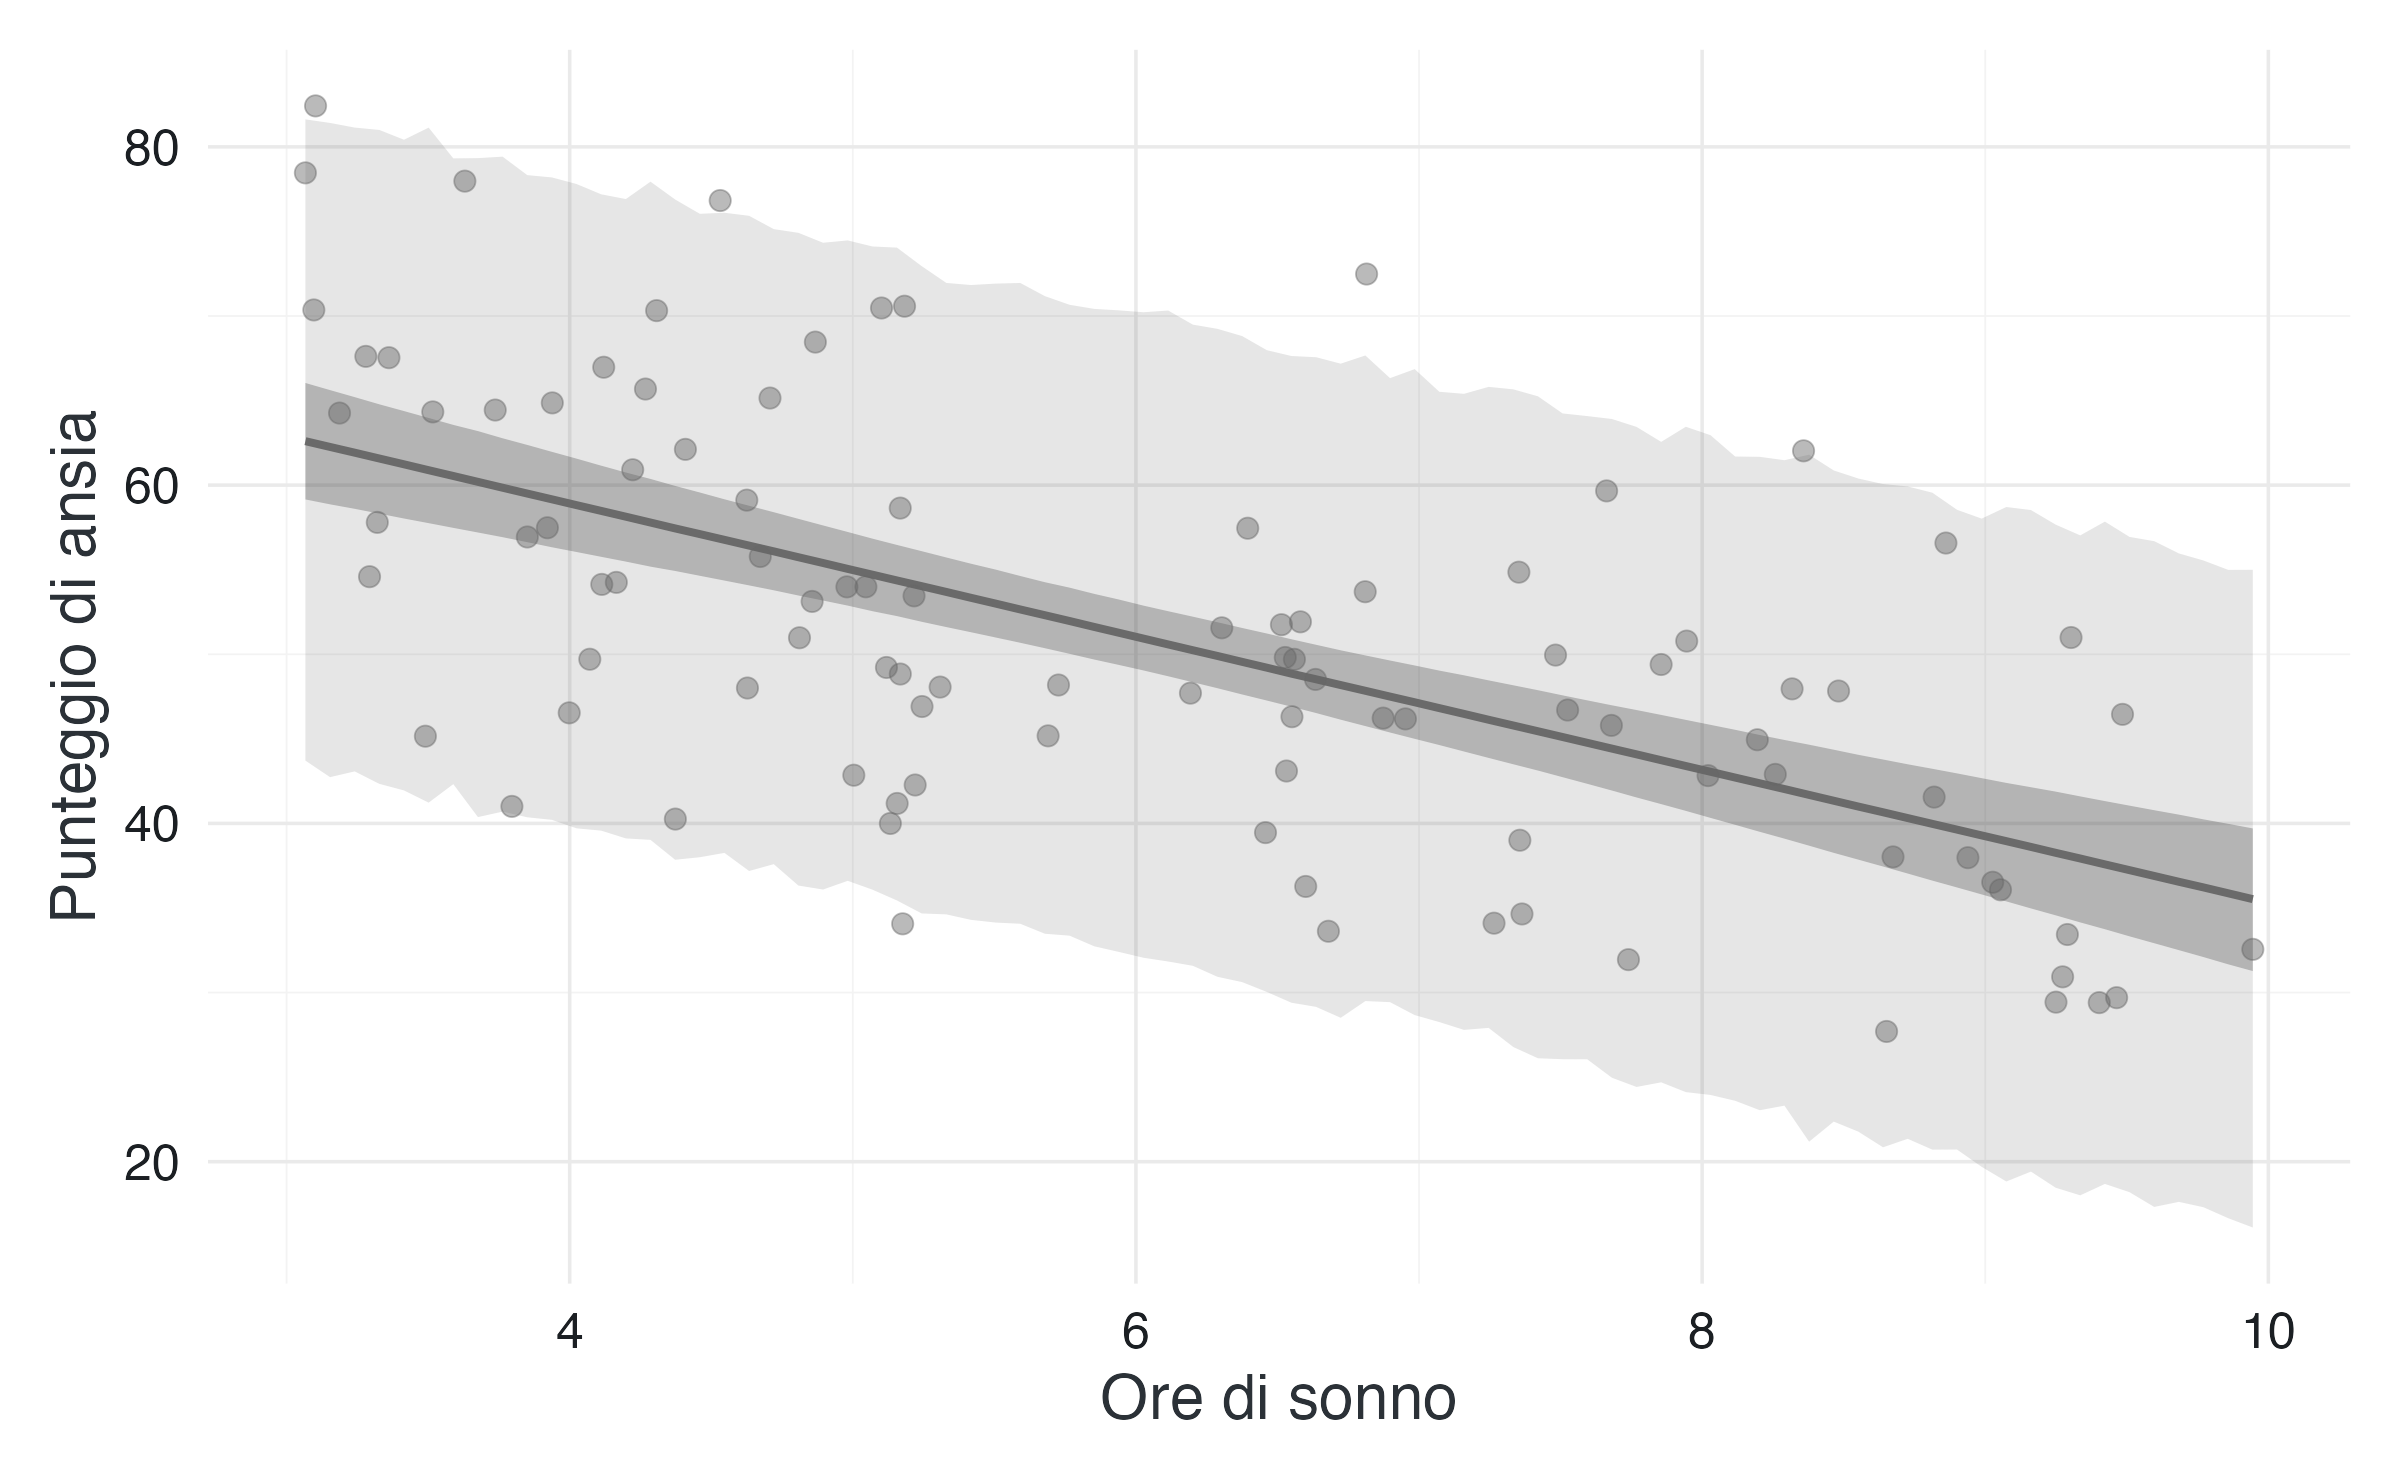
\includegraphics[width=0.85\linewidth,height=\textheight,keepaspectratio]{chapters/linear_models/03_regressione_bayesiana_brms_files/figure-pdf/fig-expected-predictive-sleep-anxiety-1.png}

}

\caption{\label{fig-expected-predictive-sleep-anxiety}Confronto tra
l'incertezza sulla media condizionata (banda interna più scura) e
l'intervallo predittivo a posteriori per un nuovo soggetto (banda
esterna più chiara). L'ampiezza di quest'ultima è determinata
dall'inclusione della deviazione standard residua nel computo
stocastico.}

\end{figure}%

\begin{tcolorbox}[enhanced jigsaw, arc=.35mm, bottomrule=.15mm, bottomtitle=1mm, breakable, colback=white, colbacktitle=quarto-callout-caution-color!10!white, colframe=quarto-callout-caution-color-frame, coltitle=black, left=2mm, leftrule=.75mm, opacityback=0, opacitybacktitle=0.6, rightrule=.15mm, title=\textcolor{quarto-callout-caution-color}{\faFire}\hspace{0.5em}{La precisione semantica delle bande di incertezza}, titlerule=0mm, toprule=.15mm, toptitle=1mm]

L'uso di un'espressione generica come ``bande di credibilità delle
previsioni'' è impreciso e ostacola l'apprendimento. Una banda definita
sulla media condizionata quantifica geometricamente l'errore standard
attorno alla traiettoria della retta, mentre un intervallo predittivo
quantifica lo spazio di tolleranza atteso per i punteggi individuali.
Ignorare questa distinzione significa nascondere il ruolo metodologico
della variabilità non spiegata (\(\sigma\)).

\end{tcolorbox}

\section{\texorpdfstring{Valutare l'adeguatezza predittiva a posteriori
(\emph{Posterior Predictive
Check})}{Valutare l'adeguatezza predittiva a posteriori (Posterior Predictive Check)}}\label{valutare-ladeguatezza-predittiva-a-posteriori-posterior-predictive-check}

Dopo aver valutato la stabilità numerica del campionatore e aver
interpretato i parametri estratti, il workflow bayesiano impone la
validazione del modello. Questa fase si realizza attraverso il
\textbf{controllo predittivo a posteriori} (\emph{Posterior Predictive
Check}, PPC), una procedura diagnostica che valuta la capacità del
modello di generare configurazioni di dati sintetici coerenti con
l'evidenza empirica originaria.

Sul piano formale, il PPC si fonda sulla \textbf{distribuzione
predittiva a posteriori}, definita integrando la funzione di
verosimiglianza rispetto alla distribuzione a posteriori dei parametri
(\(\theta = \{\alpha, \beta, \sigma\}\)):

\[
p(\widetilde{y}\mid y) = \int p(\widetilde{y}\mid\theta) \,p(\theta\mid y) \,d\theta.
\]

Questa espressione proietta l'incertezza accumulata nella distribuzione
a posteriori direttamente sulla scala delle osservazioni, restituendo
una distribuzione di possibili repliche dei dati. In termini operativi:
se il modello coglie adeguatamente il processo generativo, le repliche
simulate da questa distribuzione dovrebbero assomigliare ai dati
effettivamente raccolti. Poiché non esiste un singolo test definitivo
per decretare l'adeguatezza di un modello, il ricercatore deve scegliere
e esaminare metriche e caratteristiche dei dati strettamente connesse
agli obiettivi dello studio.

\subsection{1. Ispezione della forma marginale della
distribuzione}\label{ispezione-della-forma-marginale-della-distribuzione}

Il primo livello di controllo analizza la macro-struttura dell'esito,
confrontando la densità empirica della variabile dipendente con le curve
di densità ricavate da molteplici repliche simulate
(\(y_{\text{rep}}\)):

\begin{Shaded}
\begin{Highlighting}[]
\FunctionTok{pp\_check}\NormalTok{(}
\NormalTok{  fit\_sleep,}
  \AttributeTok{type =} \StringTok{"dens\_overlay"}\NormalTok{,}
  \AttributeTok{ndraws =} \DecValTok{50}
\NormalTok{)}
\end{Highlighting}
\end{Shaded}

\begin{figure}[H]

\centering{

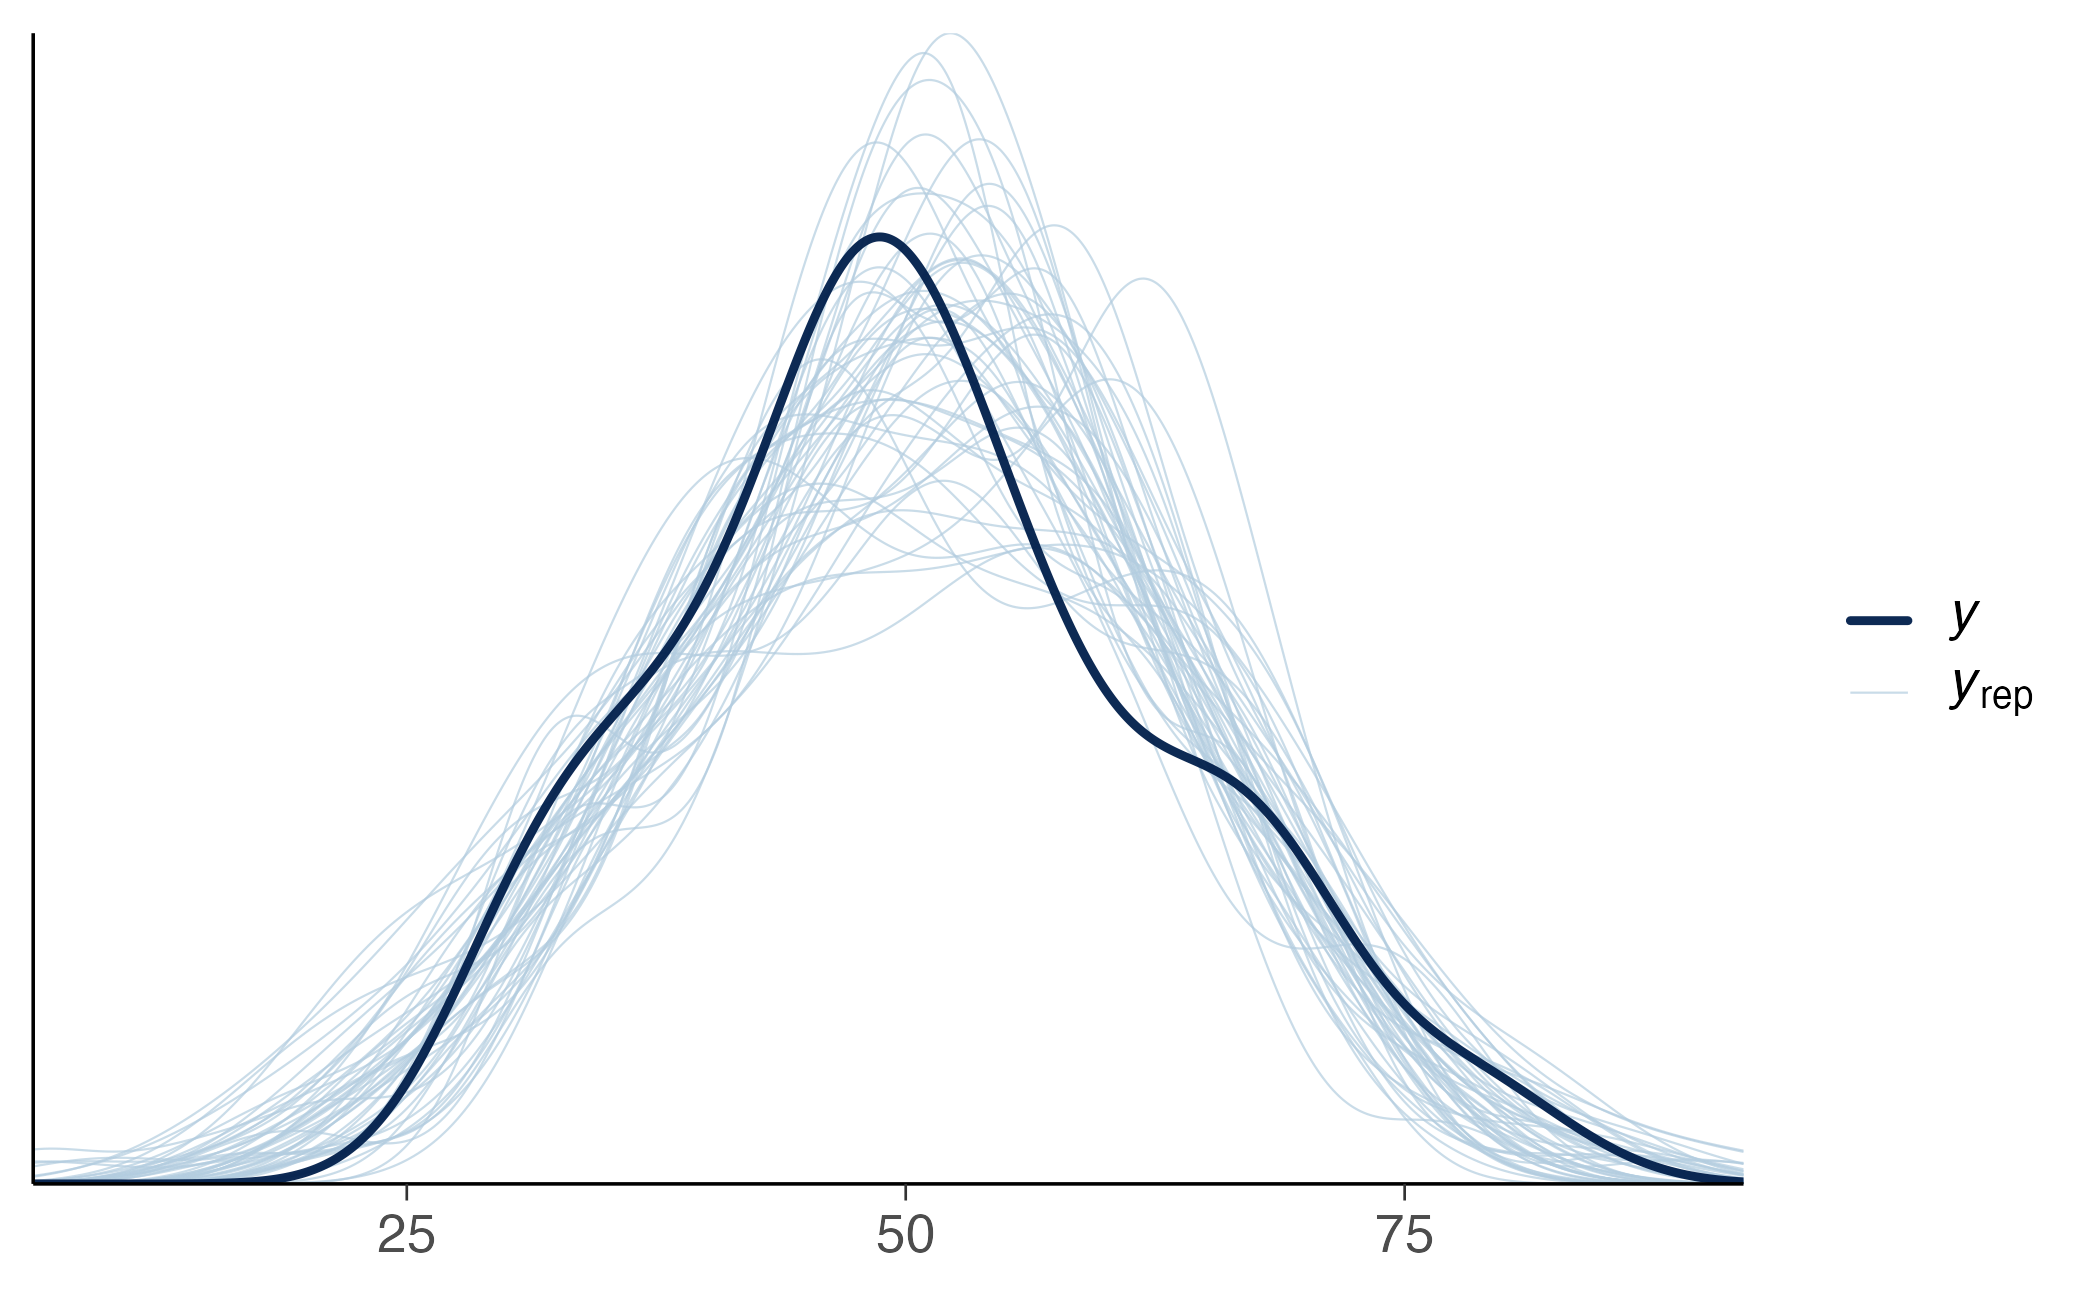
\includegraphics[width=0.85\linewidth,height=\textheight,keepaspectratio]{chapters/linear_models/03_regressione_bayesiana_brms_files/figure-pdf/fig-ppc-density-sleep-anxiety-1.png}

}

\caption{\label{fig-ppc-density-sleep-anxiety}Confronto grafico tra la
densità osservata dell'ansia (linea continua scura) e le densità stimate
su 50 repliche generate dalla posterior predittiva (linee sottili
chiare).}

\end{figure}%

Questo grafico permette di escludere macroscopiche violazioni
geometriche della verosimiglianza scelta, come la presenza di bimodalità
non intercettate, asimmetrie severe o anomalie nelle code della
distribuzione.

\subsection{2. Monitoraggio delle statistiche di sintesi (Media e
Dispersione)}\label{monitoraggio-delle-statistiche-di-sintesi-media-e-dispersione}

Un modello adeguato deve saper riprodurre accuratamente i momenti
centrali del campione originale. Valutiamo pertanto la collocazione
della media e della deviazione standard empiriche all'interno delle
rispettive distribuzioni campionarie simulate:

\begin{Shaded}
\begin{Highlighting}[]
\FunctionTok{pp\_check}\NormalTok{(fit\_sleep, }\AttributeTok{type =} \StringTok{"stat"}\NormalTok{, }\AttributeTok{stat =} \StringTok{"mean"}\NormalTok{)}
\FunctionTok{pp\_check}\NormalTok{(fit\_sleep, }\AttributeTok{type =} \StringTok{"stat"}\NormalTok{, }\AttributeTok{stat =} \StringTok{"sd"}\NormalTok{)}
\end{Highlighting}
\end{Shaded}

\begin{figure}[H]

\centering{

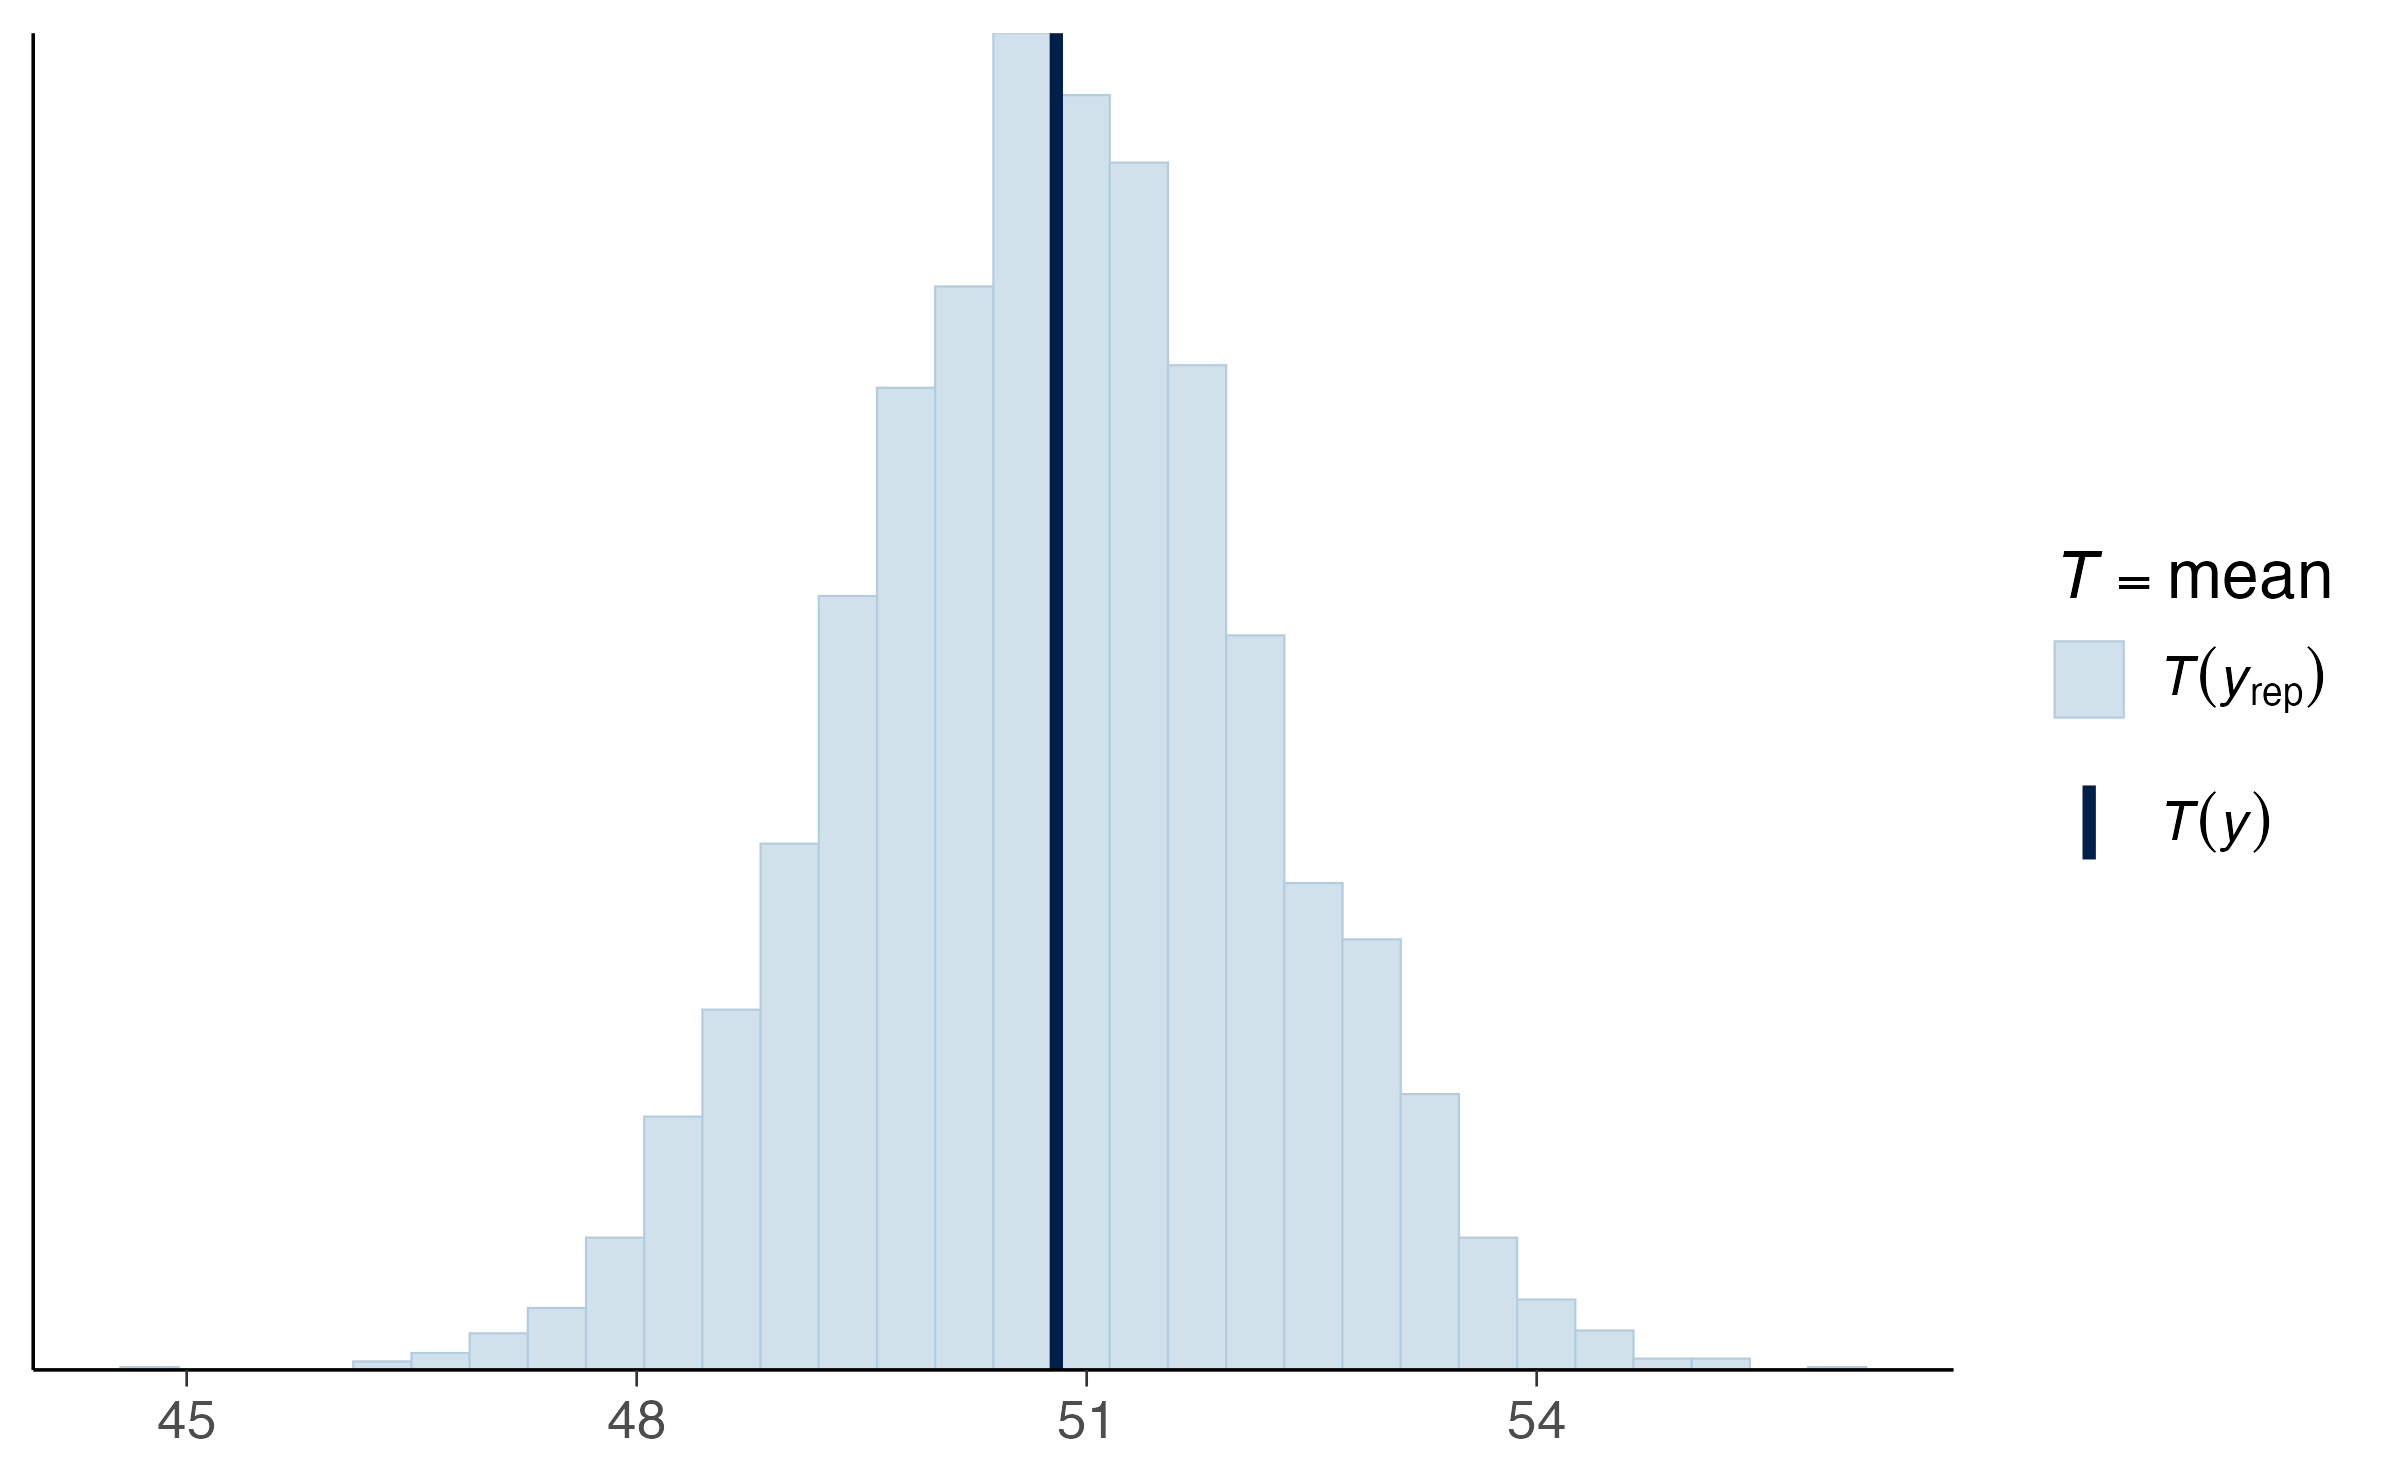
\includegraphics[width=0.85\linewidth,height=\textheight,keepaspectratio]{chapters/linear_models/03_regressione_bayesiana_brms_files/figure-pdf/fig-ppc-statistics-sleep-anxiety-1.png}

}

\caption{\label{fig-ppc-statistics-sleep-anxiety-1}Distribuzioni di
campionamento predittive a posteriori per la media (a sinistra) e la
deviazione standard (a destra). La linea verticale indica il valore
empirico osservato nel campione reale.}

\end{figure}%

\begin{figure}[H]

\centering{

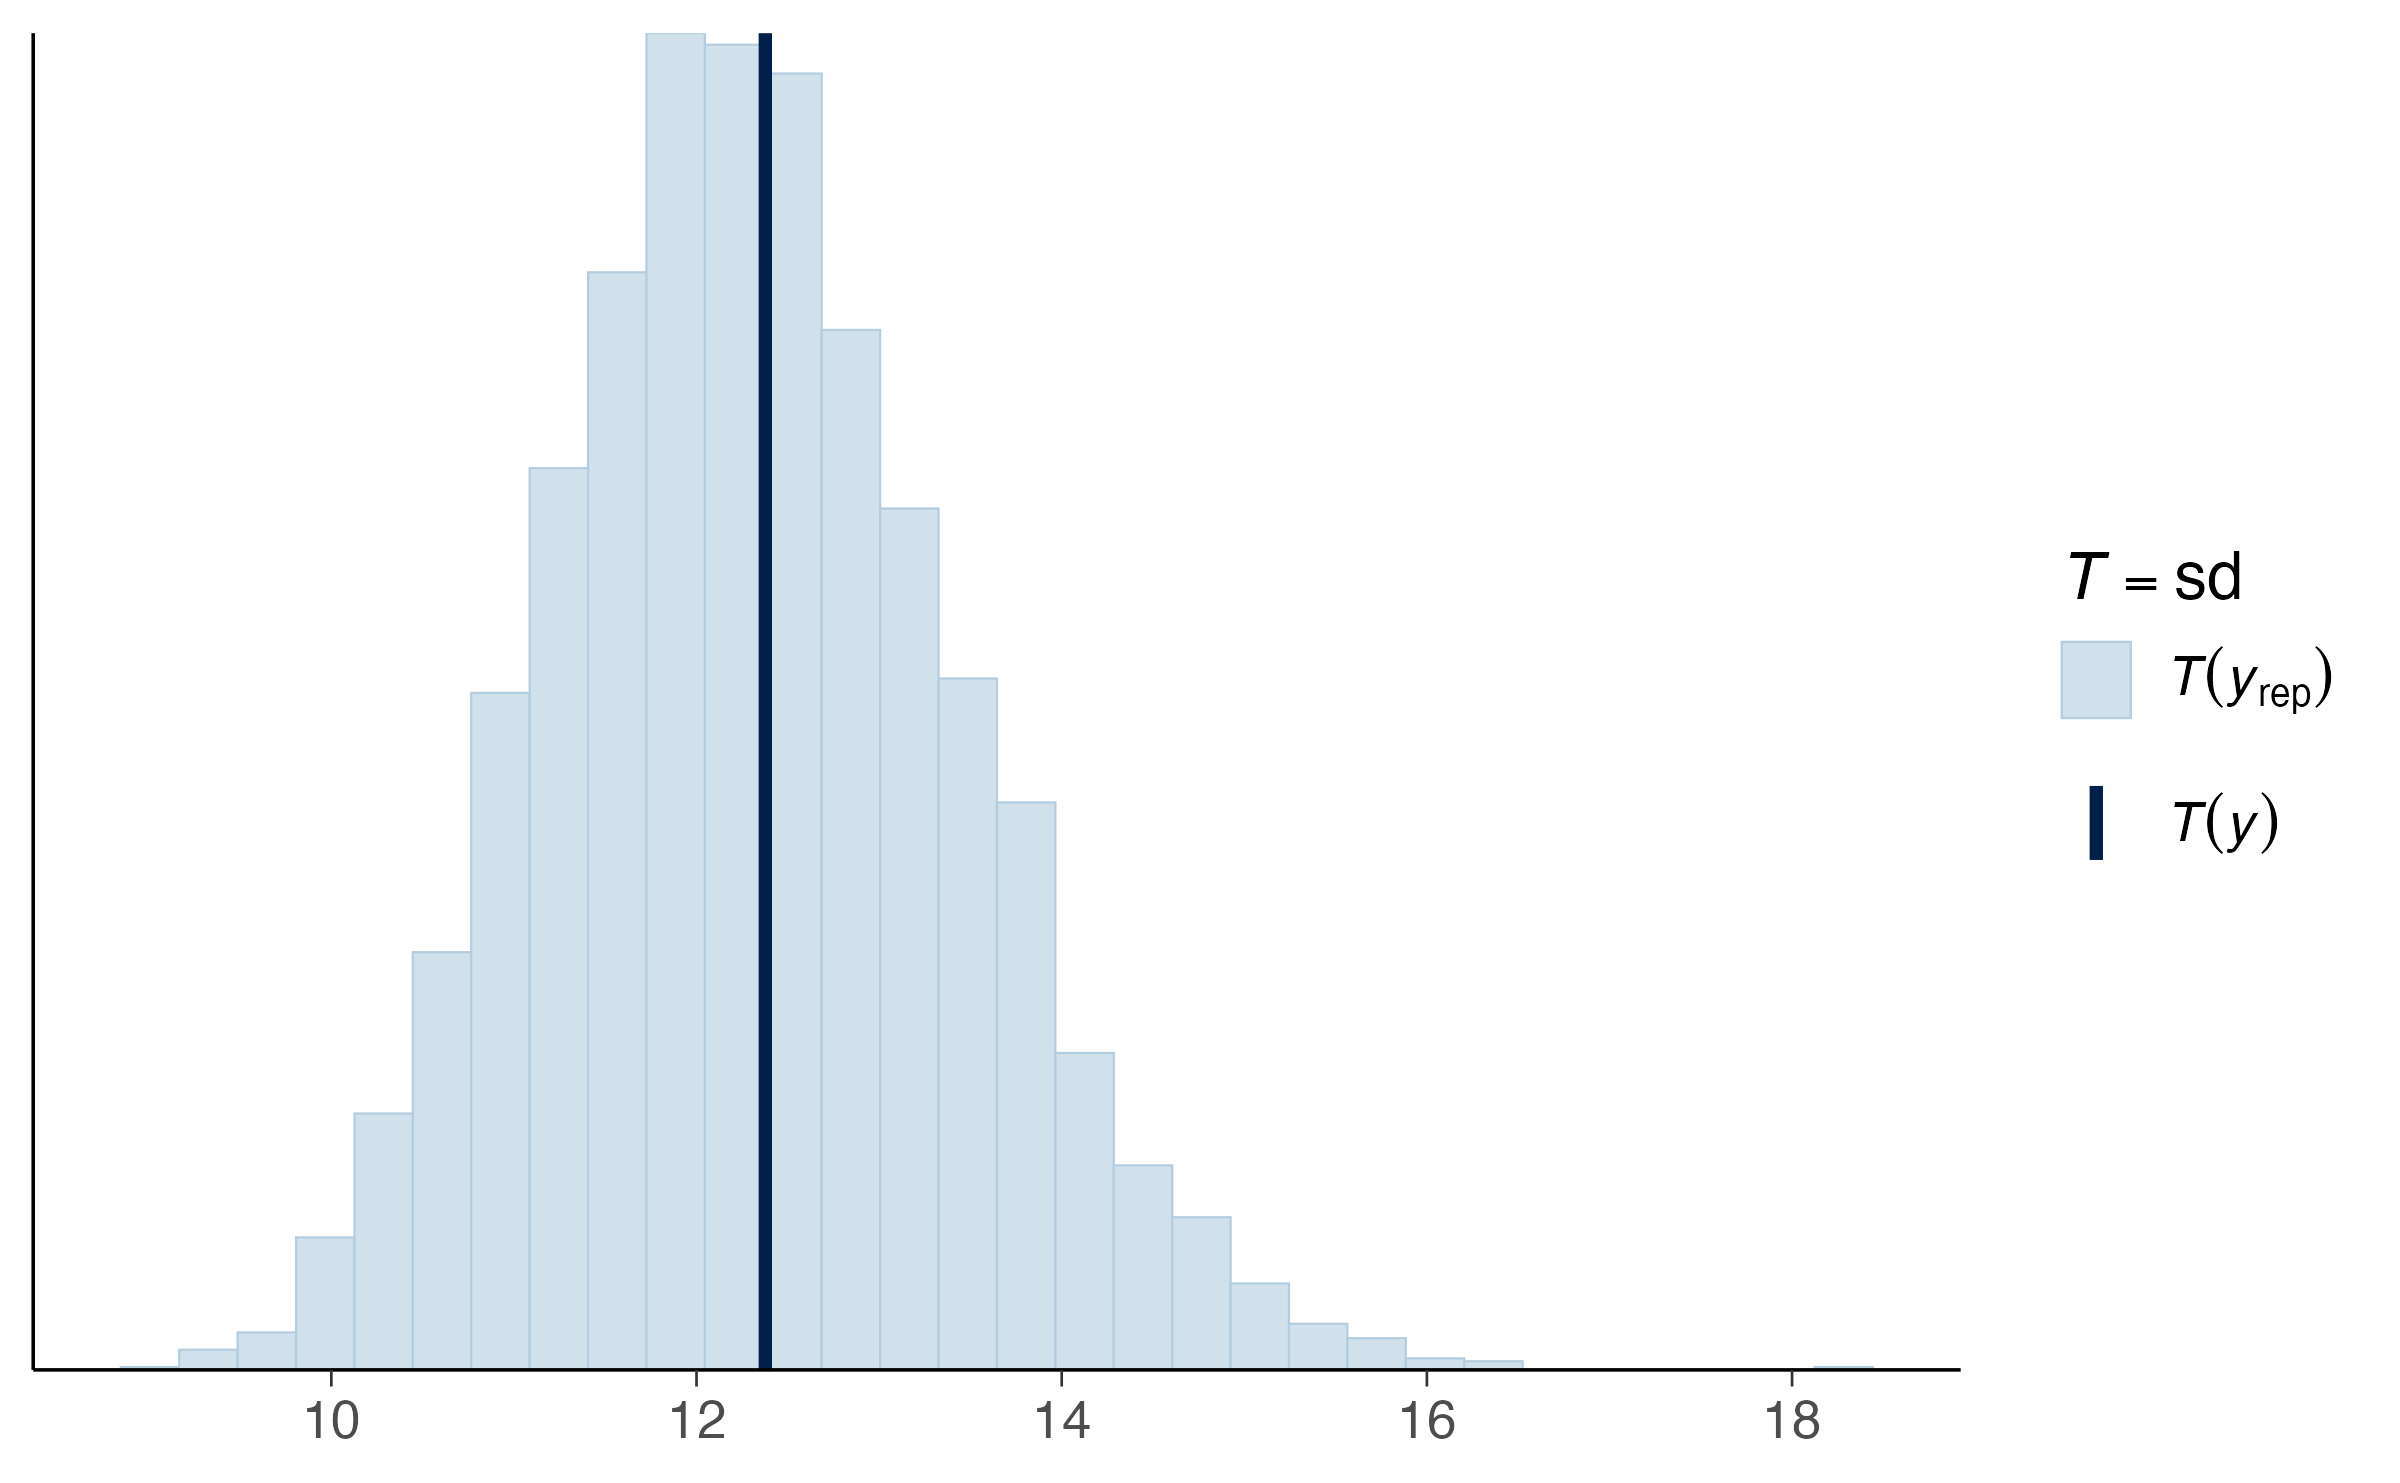
\includegraphics[width=0.85\linewidth,height=\textheight,keepaspectratio]{chapters/linear_models/03_regressione_bayesiana_brms_files/figure-pdf/fig-ppc-statistics-sleep-anxiety-2.png}

}

\caption{\label{fig-ppc-statistics-sleep-anxiety-2}Distribuzioni di
campionamento predittive a posteriori per la media (a sinistra) e la
deviazione standard (a destra). La linea verticale indica il valore
empirico osservato nel campione reale.}

\end{figure}%

Se il valore calcolato sui dati reali (la retta verticale negli
istogrammi) si colloca stabilmente entro le aree di massima densità
delle distribuzioni simulate, significa che il modello non manifesta
distorsioni sistematiche nella stima della localizzazione e della
variabilità complessiva del fenomeno.

\subsection{3. Verifica della relazione strutturale tra outcome e
predittore}\label{verifica-della-relazione-strutturale-tra-outcome-e-predittore}

Un limite intrinseco dei primi due controlli risiede nella loro natura
marginale: un modello potrebbe riprodurre perfettamente la media e la
deviazione standard dell'ansia pur fallendo grossolanamente nel
descrivere il legame con il sonno. Per colmare questa lacuna, definiamo
una statistica di discrepanza focalizzata sulla pendenza campionaria
(\(\beta\) empirico):

\begin{Shaded}
\begin{Highlighting}[]
\CommentTok{\# Definizione di una funzione per estrarre la pendenza da ogni replica}
\NormalTok{slope\_stat }\OtherTok{\textless{}{-}} \ControlFlowTok{function}\NormalTok{(y) \{}
  \FunctionTok{unname}\NormalTok{(}\FunctionTok{coef}\NormalTok{(}\FunctionTok{lm}\NormalTok{(y }\SpecialCharTok{\textasciitilde{}}\NormalTok{ sleep\_anxiety}\SpecialCharTok{$}\NormalTok{sonno\_c))[}\DecValTok{2}\NormalTok{])}
\NormalTok{\}}

\FunctionTok{pp\_check}\NormalTok{(}
\NormalTok{  fit\_sleep,}
  \AttributeTok{type =} \StringTok{"stat"}\NormalTok{,}
  \AttributeTok{stat =}\NormalTok{ slope\_stat}
\NormalTok{)}
\end{Highlighting}
\end{Shaded}

\begin{figure}[H]

\centering{

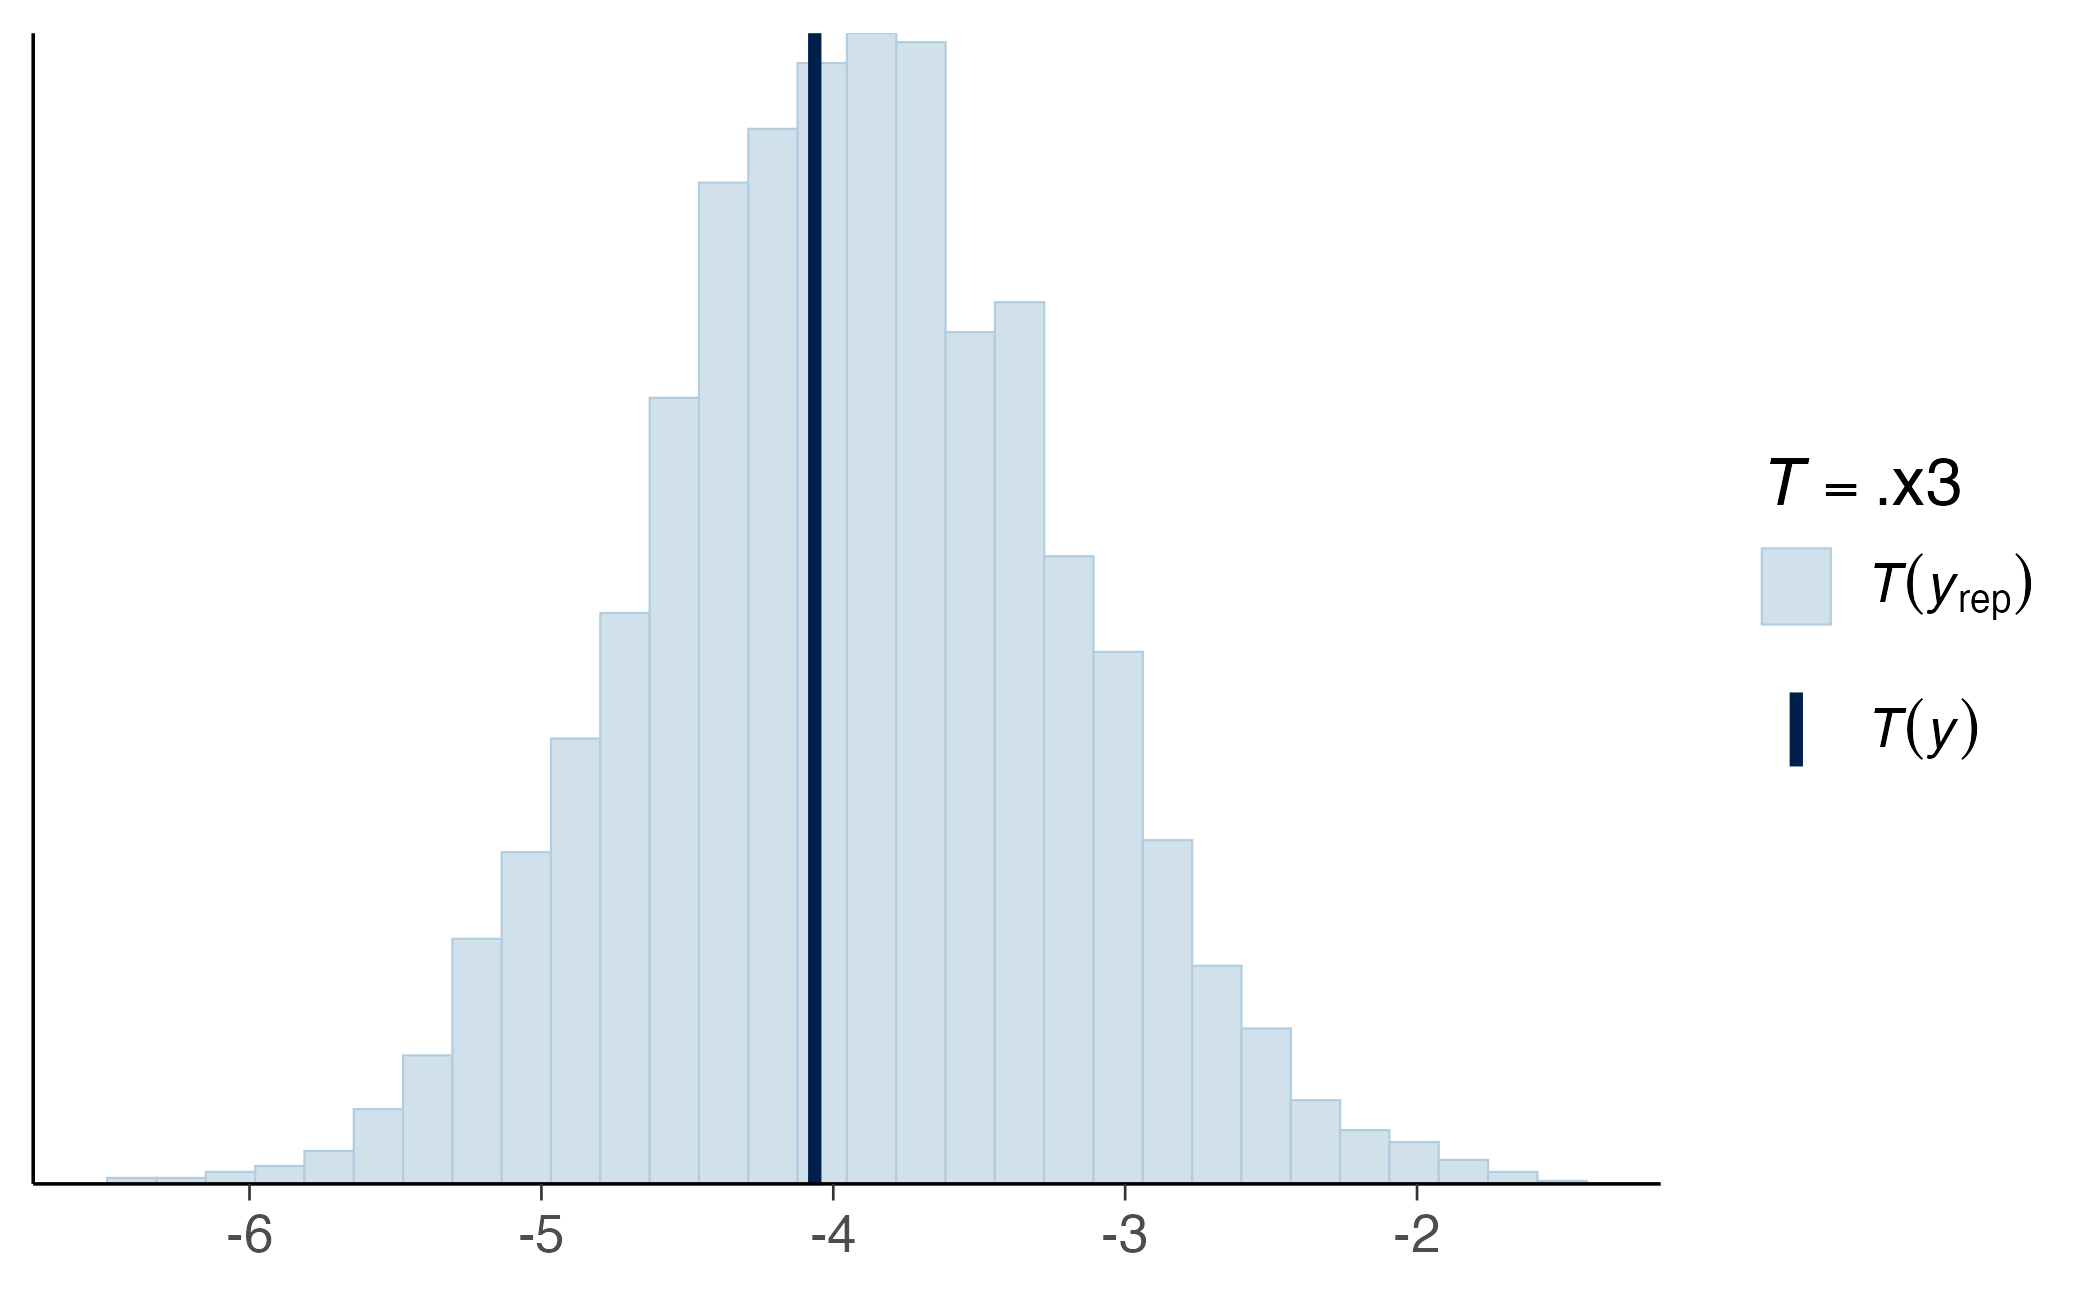
\includegraphics[width=0.85\linewidth,height=\textheight,keepaspectratio]{chapters/linear_models/03_regressione_bayesiana_brms_files/figure-pdf/fig-ppc-slope-sleep-anxiety-1.png}

}

\caption{\label{fig-ppc-slope-sleep-anxiety}Distribuzione predittiva a
posteriori della pendenza campionaria ed evidenza empirica osservata.
Questo controllo mirato attesta la capacità del modello di catturare la
forza dell'associazione covariante.}

\end{figure}%

\begin{tcolorbox}[enhanced jigsaw, arc=.35mm, bottomrule=.15mm, bottomtitle=1mm, breakable, colback=white, colbacktitle=quarto-callout-important-color!10!white, colframe=quarto-callout-important-color-frame, coltitle=black, left=2mm, leftrule=.75mm, opacityback=0, opacitybacktitle=0.6, rightrule=.15mm, title=\textcolor{quarto-callout-important-color}{\faExclamation}\hspace{0.5em}{Il superamento dei controlli non attesta la verità del modello}, titlerule=0mm, toprule=.15mm, toptitle=1mm]

Un esito favorevole a tutti i controlli predittivi a posteriori non
costituisce in alcun modo una prova logica della veridicità o della
correttezza intrinseca del modello teorico. Indica esclusivamente che lo
strumento statistico si dimostra accurato rispetto alle specifiche
metriche e proprietà interrogate. Fenomeni complessi capaci di minare la
validità delle conclusioni --- quali la presenza di relazioni non
lineari latenti, eteroschedasticità (varianza non costante dei residui),
dipendenze stocastiche tra le osservazioni o sistematici errori di
misurazione --- non vengono catturati da questi indici e richiedono
procedure diagnostiche dedicate e mirate.

\end{tcolorbox}

\section{\texorpdfstring{Analisi di sensibilità alle distribuzioni a
priori (\emph{Prior Sensitivity
Analysis})}{Analisi di sensibilità alle distribuzioni a priori (Prior Sensitivity Analysis)}}\label{analisi-di-sensibilituxe0-alle-distribuzioni-a-priori-prior-sensitivity-analysis}

Nel paradigma bayesiano, la scelta delle distribuzioni a priori
(\emph{prior}) rappresenta un'esplicita assunzione teorica formale che
si integra con l'evidenza empirica. Di conseguenza, il workflow
bayesiano richiede la verifica che le stime posteriori ottenute non
siano il risultato di una scelta a priori unica e specifica. L'analisi
di sensibilità valuta proprio la robustezza delle conclusioni
scientifiche sottoponendo il modello a scenari di informazione
alternativa.

In questo specifico passaggio diagnostico, poniamo a confronto la
specificazione principale con un modello alternativo caratterizzato da
distribuzioni a priori marcatamente più ampie, non direzionali e a bassa
informatività:

\[
\alpha\sim\operatorname{Normal}(50,25), \qquad \beta\sim\operatorname{Normal}(0,5), \qquad \sigma\sim\operatorname{Lognormal}(\log 15,0.7).
\]

L'implementazione computazionale di questo confronto si articola
attraverso la stima del secondo modello di calcolo:

\begin{Shaded}
\begin{Highlighting}[]
\CommentTok{\# Definizione dei prior alternativi a bassa informatività}
\NormalTok{sensitivity\_priors }\OtherTok{\textless{}{-}} \FunctionTok{c}\NormalTok{(}
  \FunctionTok{prior}\NormalTok{(}\FunctionTok{normal}\NormalTok{(}\DecValTok{50}\NormalTok{, }\DecValTok{25}\NormalTok{), }\AttributeTok{class =} \StringTok{"Intercept"}\NormalTok{),}
  \FunctionTok{prior}\NormalTok{(}\FunctionTok{normal}\NormalTok{(}\DecValTok{0}\NormalTok{, }\DecValTok{5}\NormalTok{), }\AttributeTok{class =} \StringTok{"b"}\NormalTok{, }\AttributeTok{coef =} \StringTok{"sonno\_c"}\NormalTok{),}
  \FunctionTok{prior}\NormalTok{(}\FunctionTok{lognormal}\NormalTok{(}\FunctionTok{log}\NormalTok{(}\DecValTok{15}\NormalTok{), }\FloatTok{0.7}\NormalTok{), }\AttributeTok{class =} \StringTok{"sigma"}\NormalTok{)}
\NormalTok{)}

\CommentTok{\# Stima del modello per l\textquotesingle{}analisi di sensibilità}
\NormalTok{fit\_sleep\_sensitivity }\OtherTok{\textless{}{-}} \FunctionTok{brm}\NormalTok{(}
\NormalTok{  ansia }\SpecialCharTok{\textasciitilde{}}\NormalTok{ sonno\_c,}
  \AttributeTok{data =}\NormalTok{ sleep\_anxiety,}
  \AttributeTok{family =} \FunctionTok{gaussian}\NormalTok{(),}
  \AttributeTok{prior =}\NormalTok{ sensitivity\_priors,}
  \AttributeTok{backend =} \StringTok{"cmdstanr"}\NormalTok{,}
  \AttributeTok{chains =} \DecValTok{4}\NormalTok{,}
  \AttributeTok{iter =} \DecValTok{2000}\NormalTok{,}
  \AttributeTok{warmup =} \DecValTok{1000}\NormalTok{,}
  \AttributeTok{seed =} \DecValTok{1235}\NormalTok{,}
  \AttributeTok{refresh =} \DecValTok{0}
\NormalTok{)}
\end{Highlighting}
\end{Shaded}

Per valutare l'impatto di questa variazione sui parametri chiave della
ricerca, sovrapponiamo graficamente le densità a posteriori della
pendenza (\(\beta\)) stimate nei due diversi scenari:

\begin{Shaded}
\begin{Highlighting}[]
\FunctionTok{bind\_rows}\NormalTok{(}
  \FunctionTok{as\_draws\_df}\NormalTok{(fit\_sleep, }\AttributeTok{variable =} \StringTok{"b\_sonno\_c"}\NormalTok{) }\SpecialCharTok{|\textgreater{}}
    \FunctionTok{mutate}\NormalTok{(}\AttributeTok{specificazione =} \StringTok{"Prior principale"}\NormalTok{),}
  \FunctionTok{as\_draws\_df}\NormalTok{(fit\_sleep\_sensitivity, }\AttributeTok{variable =} \StringTok{"b\_sonno\_c"}\NormalTok{) }\SpecialCharTok{|\textgreater{}}
    \FunctionTok{mutate}\NormalTok{(}\AttributeTok{specificazione =} \StringTok{"Prior più ampi"}\NormalTok{)}
\NormalTok{) }\SpecialCharTok{|\textgreater{}}
  \FunctionTok{rename}\NormalTok{(}\AttributeTok{beta =}\NormalTok{ b\_sonno\_c) }\SpecialCharTok{|\textgreater{}}
  \FunctionTok{ggplot}\NormalTok{(}\FunctionTok{aes}\NormalTok{(}\AttributeTok{x =}\NormalTok{ beta, }\AttributeTok{fill =}\NormalTok{ specificazione)) }\SpecialCharTok{+}
  \FunctionTok{geom\_density}\NormalTok{(}\AttributeTok{alpha =} \FloatTok{0.35}\NormalTok{) }\SpecialCharTok{+}
  \FunctionTok{labs}\NormalTok{(}
    \AttributeTok{x =} \FunctionTok{expression}\NormalTok{(beta),}
    \AttributeTok{y =} \StringTok{"Densità"}\NormalTok{,}
    \AttributeTok{fill =} \StringTok{"Specificazione"}
\NormalTok{  )}
\end{Highlighting}
\end{Shaded}

\begin{figure}[H]

\centering{

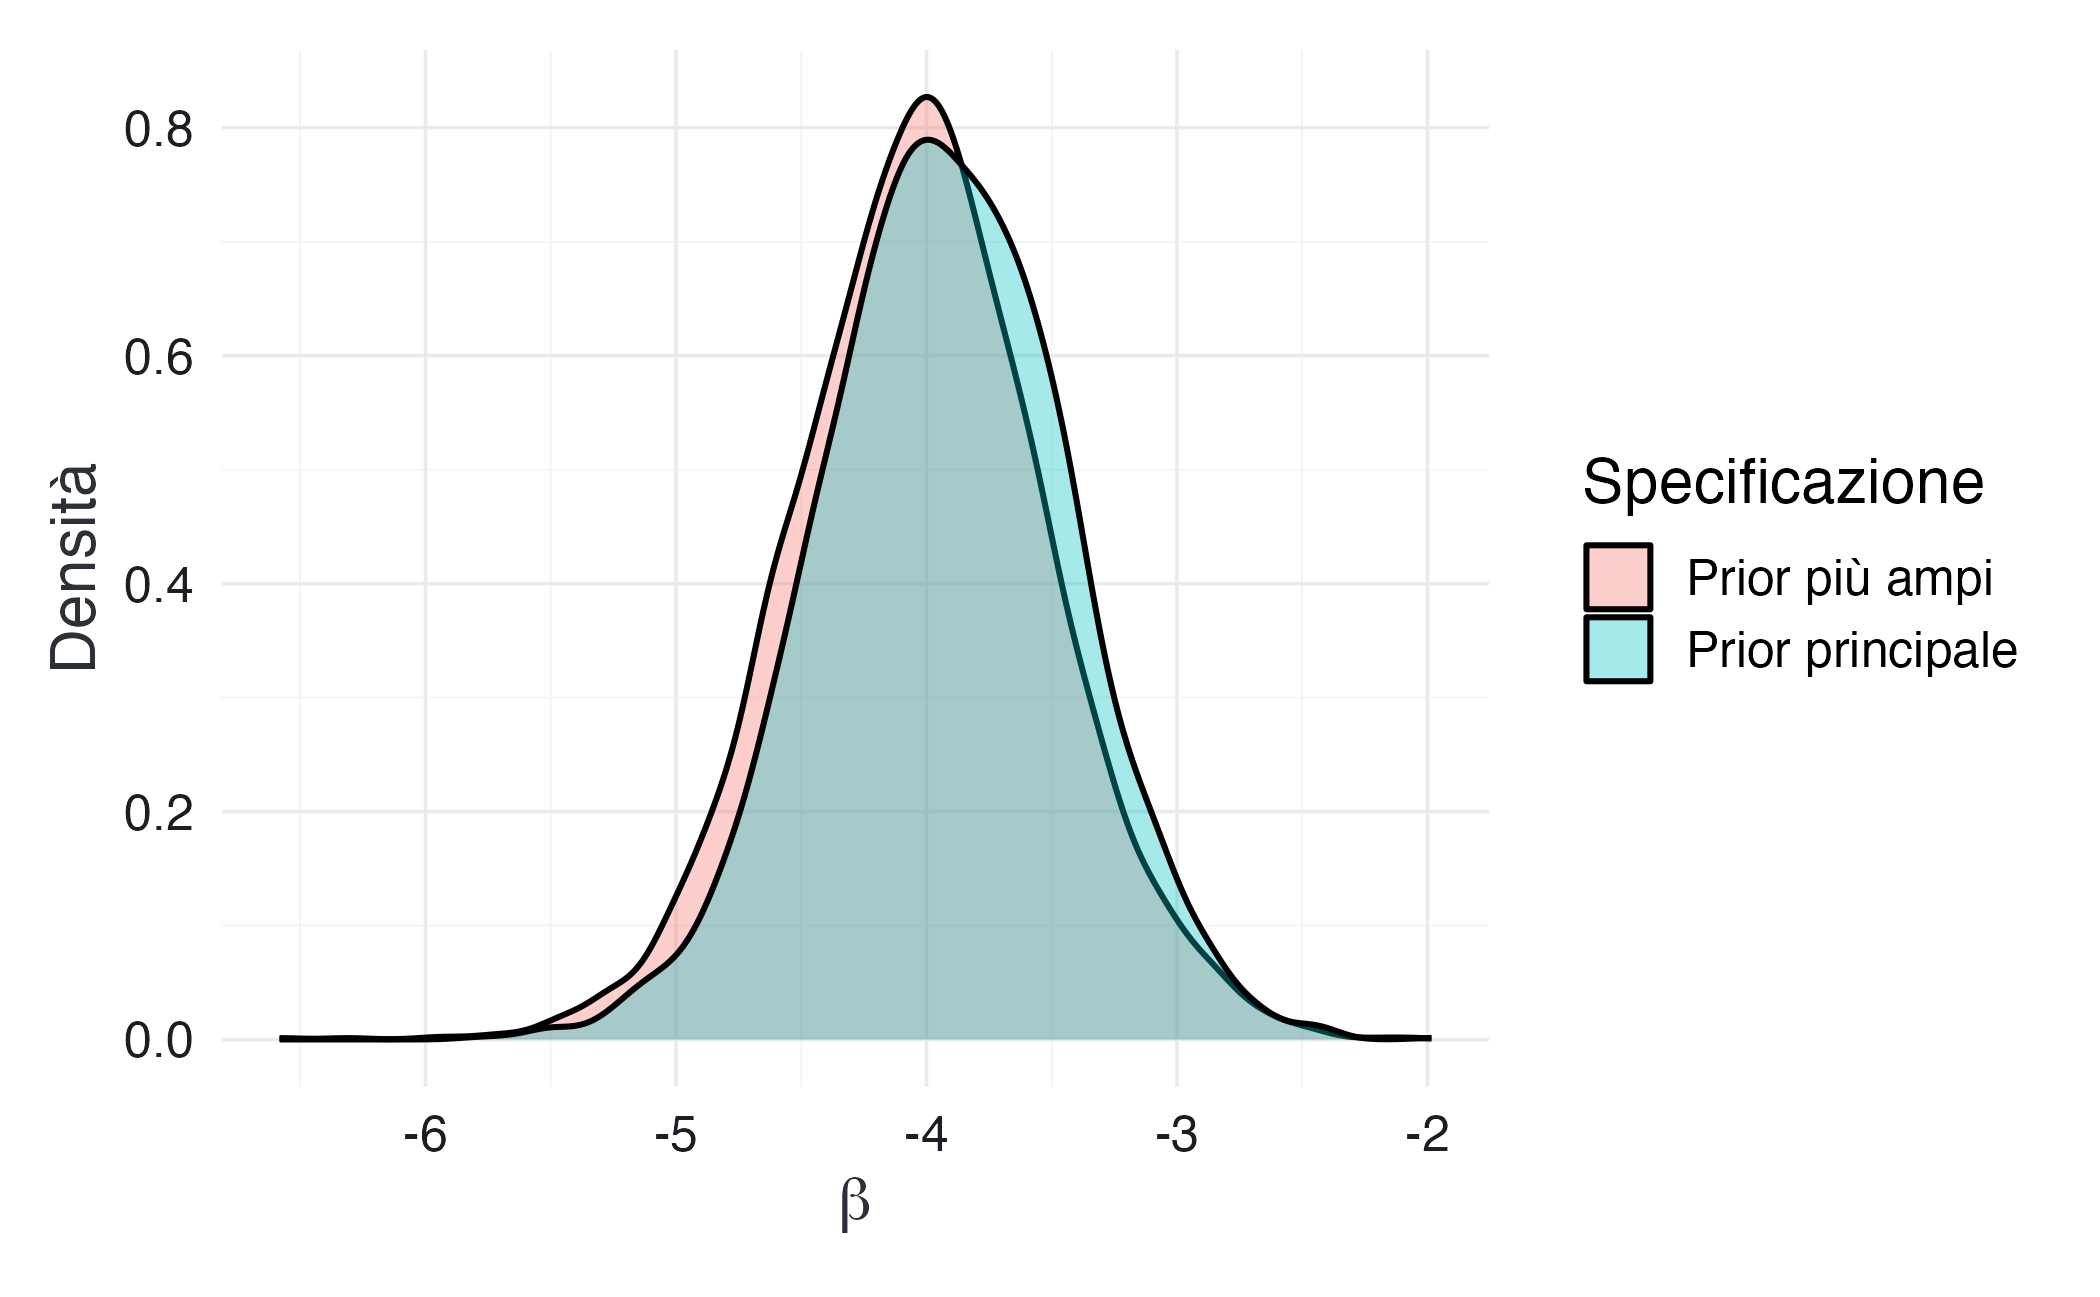
\includegraphics[width=0.85\linewidth,height=\textheight,keepaspectratio]{chapters/linear_models/03_regressione_bayesiana_brms_files/figure-pdf/fig-prior-sensitivity-slope-1.png}

}

\caption{\label{fig-prior-sensitivity-slope}Confronto visivo delle
distribuzioni a posteriori per la pendenza campionaria (beta) in
funzione della specificazione dei prior. La marcata sovrapposizione
delle due aree attesta la stabilità dell'effetto.}

\end{figure}%

\begin{quote}
\textbf{Criterio di interpretazione metodologica:} Se le stime e le
conseguenti interpretazioni sostanziali del fenomeno cambiano in modo
marcato al variare dei prior, emerge una forte dipendenza dei risultati
dalle assunzioni di partenza; tale dinamica epidemiologica o psicologica
deve essere esplicitamente riportata, discussa e giustificata nel report
di ricerca. Al contrario, se le densità a posteriori rimangono
sostanzialmente immutate e sovrapponibili, possiamo concludere che i
dati empirici raccolti contengono sufficiente informazione da dominare
la scelta dei prior, garantendo la stabilità e la robustezza intrinseca
del risultato statistico.
\end{quote}

Dal punto di vista epistemologico, l'analisi di sensibilità non ha la
funzione di giustificare o rendere accettabile una scelta arbitraria o
ingiustificata dei parametri di partenza: essa richiede sempre che le
specificazioni poste a confronto rappresentino alternative teoricamente
plausibili e scientificamente sostenibili nel dominio di studio.

\section{Formalizzare la comunicazione scientifica dei
risultati}\label{formalizzare-la-comunicazione-scientifica-dei-risultati}

Una rendicontazione scientifica rigorosa deve connettere in modo
trasparente le stime numeriche ottenute all'ipotesi di ricerca
originaria. Dal punto di vista lessicale e logico, è necessario operare
una netta distinzione concettuale tra i parametri strutturali (i
coefficienti della retta), le medie condizionate (l'incertezza sulla
traiettoria attesa) e le stime predittive (la variabilità sui singoli
soggetti futuri).

Nello stendere il report di ricerca o l'articolo scientifico, lo
studente può adottare il seguente schema formale di descrizione:

\begin{quote}
Il modello lineare bayesiano rivela che un incremento unitario pari a
un'ora di sonno si associa a una variazione media del punteggio di ansia
pari a \texttt{{[}Mediana\ della\ Posterior{]}} punti, con un intervallo
di credibilità al 95\% compreso tra \texttt{{[}Limite\ Inferiore{]}} e
\texttt{{[}Limite\ Superiore{]}}. La probabilità a posteriori che
l'associazione indagata assuma una direzione negativa è pari a
\(\Pr(\beta < 0 \mid y) =\) \texttt{{[}Valore\ Probabilità{]}}. Sul
piano applicativo, le traiettorie previsionali a livello individuale
presentano un'ampia dispersione geometrica, come dimostrato dall'entità
della deviazione standard residua (\(\sigma\)) e dall'estensione degli
intervalli predittivi a posteriori. Le procedure diagnostiche di
\emph{Posterior Predictive Check} eseguite non hanno evidenziato
anomalie o discrepanze sistematiche rispetto alle proprietà statistiche
interrogate.
\end{quote}

\begin{quote}
\textbf{Nota di rigore metodologico:} questo impianto espositivo
richiede un attento allineamento al disegno di ricerca che ha generato i
dati. In contesti di natura strettamente osservazionale o
correlazionale, è doveroso dal punto di vista metodologico impiegare
espressioni descrittive quali \emph{associazione}, \emph{differenza
condizionata} o \emph{pendenza stimata}, bandendo tassativamente l'uso
del termine \emph{effetto}, che evoca un nesso di causalità e una
manipolazione diretta delle variabili non sostenibili senza adeguati
controlli formali.
\end{quote}

\section{Catalogo degli errori concettuali e procedurali più
frequenti}\label{catalogo-degli-errori-concettuali-e-procedurali-piuxf9-frequenti}

Al fine di prevenire vizi interpretativi o fallimenti computazionali
nella stesura della tesi o del report di analisi, viene qui sintetizzato
un quadro sinottico delle principali insidie metodologiche:

\begin{tcolorbox}[enhanced jigsaw, arc=.35mm, bottomrule=.15mm, bottomtitle=1mm, breakable, colback=white, colbacktitle=quarto-callout-caution-color!10!white, colframe=quarto-callout-caution-color-frame, coltitle=black, left=2mm, leftrule=.75mm, opacityback=0, opacitybacktitle=0.6, rightrule=.15mm, title=\textcolor{quarto-callout-caution-color}{\faFire}\hspace{0.5em}{Errori sistematici da evitare nel workflow bayesiano}, titlerule=0mm, toprule=.15mm, toptitle=1mm]

\begin{enumerate}
\def\labelenumi{\arabic{enumi}.}
\tightlist
\item
  \textbf{Accettazione acritica dei prior di default:} Affidarsi
  ciecamente alle impostazioni predefinite del software (es.
  \texttt{brms}) senza verificarne l'architettura. Classi differenti di
  parametri possiedono costrutti di default diversi e, in alcuni casi,
  includono prior impropri (funzioni la cui densità non integra a 1),
  delegando interamente il calcolo ai dati anche quando non opportuno.
\item
  \textbf{Valutazione dei prior sulla sola scala dei parametri:}
  Giudicare la plausibilità di una distribuzione a priori osservando
  esclusivamente i suoi confini numerici astratti. L'adeguatezza di un
  prior si testa sperimentalmente sulla scala biologica o psicologica
  delle osservazioni reali, ricorrendo alle simulazioni predittive a
  priori (\emph{Prior Predictive Check}).
\item
  \textbf{Sovrapposizione concettuale tra bande di credibilità e bande
  predittive:} Estendere l'intervallo di credibilità calcolato su un
  coefficiente (\(\beta\)) per formulare previsioni sui punteggi di
  futuri soggetti. Una stima predittiva individuale corretta deve
  obbligatoriamente incorporare la variabilità stocastica residua
  (\(\sigma\)).
\item
  \textbf{Feticismo dell'indice \(\widehat{R}\):} Ritenere che un valore
  di \(\widehat{R} \approx 1\) per tutti i parametri costituisca una
  prova matematica della validità o della correttezza del modello
  statistico. Tale indice certifica unicamente la stabilità e la
  convergenza numerica delle catene MCMC, non l'adeguatezza delle
  assunzioni o della specificazione strutturale.
\item
  \textbf{Monotonia nei controlli predittivi a posteriori:} Esaurire la
  fase di validazione del modello impiegando un unico grafico PPC (es.
  il solo \emph{dens\_overlay}). Ogni specifico controllo interroga una
  limitata proprietà geometrica dei dati e può risultare
  sistematicamente cieco di fronte a fallimenti strutturali di altra
  natura.
\item
  \textbf{Falsa sicurezza legata all'ampiezza campionaria (\(N\)
  grande):} Concludere dogmaticamente che l'impatto dei prior sia nullo
  sul presupposto di disporre di un campione numeroso. L'influenza delle
  assunzioni a priori dipende strettamente anche dalla variabilità
  interna dei predittori, dalla presenza di collinearità tra le
  variabili e dalla specifica porzione di distribuzione (es. le code)
  che si intende stimare.
\item
  \textbf{Equiparazione tra \(\Pr(\beta < 0 \mid y)\) e cogenza
  causale:} Interpretare la massa di probabilità accumulata sui valori
  negativi come una misura diretta dell'esistenza di un meccanismo di
  causa-effetto. Tale metrica esprime semplicemente una probabilità
  condizionata all'impianto logico del modello per un parametro di
  covariazione.
\item
  \textbf{Risoluzione meccanica delle divergenze tramite
  \texttt{adapt\_delta}:} Incrementare in modo automatico e ripetuto il
  parametro di controllo dell'algoritmo non appena Stan rileva
  transizioni divergenti. Sebbene un valore di \texttt{adapt\_delta} più
  stringente riduca i passi di integrazione, il persistere di divergenze
  segnala quasi sempre la necessità di modificare radicalmente la
  geometria del modello attraverso una riparametrizzazione matematica.
\end{enumerate}

\end{tcolorbox}

\section{Riflessioni conclusive}\label{riflessioni-conclusive-20}

Il \emph{workflow} bayesiano non può essere ridotto a un mero espediente
tecnico, né alla semplice sostituzione di una stima puntuale
frequentista con una media calcolata a posteriori. Al contrario, esso si
configura come un paradigma metodologico organico, una sequenza coerente
di operazioni concettuali e computazionali che accompagna il ricercatore
dalla formulazione dell'ipotesi fino alla rendicontazione dei risultati.

Questo percorso integrato si articola attraverso dieci passaggi
fondamentali, strettamente interconnessi:

\begin{enumerate}
\def\labelenumi{\arabic{enumi}.}
\tightlist
\item
  \textbf{Definire con rigore la domanda scientifica} e identificare le
  precise quantità di interesse (\emph{estimand}) prima di interrogare i
  dati;
\item
  \textbf{Formulare un modello generativo} in grado di esplicitare i
  processi matematici e stocastici che si ipotizza abbiano prodotto le
  osservazioni;
\item
  \textbf{Tradurre l'informazione teorica disponibile in distribuzioni a
  priori (\emph{prior})}, ancorandole strettamente alla scala metrica
  del problema;
\item
  \textbf{Valutare le implicazioni di tali assunzioni ex ante},
  saggiandone la plausibilità fenomenologica attraverso simulazioni
  predittive a priori;
\item
  \textbf{Adattare il modello e diagnosticare il campionamento},
  escludendo patologie algoritmiche delle catene MCMC per garantirne la
  stabilità numerica;
\item
  \textbf{Interpretare la distribuzione a posteriori congiunta} e le
  quantità probabilistiche derivate in relazione agli obiettivi dello
  studio;
\item
  \textbf{Scindere concettualmente la stima della media condizionata}
  (l'incertezza sulla traiettoria) dalla stima della previsione
  individuale (che include la variabilità residua);
\item
  \textbf{Verificare l'adeguatezza predittiva del modello} mediante
  controlli a posteriori mirati sulle caratteristiche cruciali dei dati;
\item
  \textbf{Sottoporre le conclusioni a un'analisi di sensibilità},
  saggiando la robustezza delle stime sotto specificazioni a priori
  alternative;
\item
  \textbf{Comunicare i risultati e i limiti intrinseci dell'analisi},
  calibrando il linguaggio in funzione del disegno di ricerca adottato.
\item
  \textbf{Ogni funzione dei parametri (\(3\beta\), una media
  condizionata, una previsione) è essa stessa una variabile a
  posteriori:} \texttt{mutate\_variables()} e le \texttt{rvar} rendono
  questo principio operativo.
\end{enumerate}

L'applicazione rigorosa di questa sequenza operativa ha il merito di
separare nettamente tre livelli di validità che la prassi statistica
tende spesso a sovrapporre: la correttezza puramente numerica del
calcolo computazionale, l'adeguatezza statistica del modello ai dati e
la fondatezza scientifica dell'interpretazione sostanziale. Il
soddisfacimento dei requisiti su un piano non garantisce quello sugli
altri, e nessun indice sintetico né automatismo software può sostituire
un loro esame critico e congiunto.

Nel prossimo capitolo renderemo esplicita l'infrastruttura
computazionale del modello lineare, connettendo logicamente la formula
di Wilkinson-Rogers in R, la struttura della matrice ddel modello e il
codice sorgente Stan. L'obiettivo didattico non è introdurre una nuova
classe di modelli, bensì bensì quello di rendere esplicito e trasparente
tutto ciò che \texttt{brms} costruisce in modo automatico, offrendo gli
strumenti concettuali per acquisire il pieno controllo del processo
inferenziale.

\section{Concetti da ricordare}\label{concetti-da-ricordare-2}

\begin{enumerate}
\def\labelenumi{\arabic{enumi}.}
\tightlist
\item
  La posterior combina prior e verosimiglianza all'interno di un modello
  generativo.
\item
  I prior devono essere interpretati e calibrati sulla scala del
  fenomeno.
\item
  Il prior predictive check precede l'uso informativo dei dati
  osservati.
\item
  La diagnostica MCMC riguarda la qualità dell'approssimazione
  computazionale.
\item
  La posterior è congiunta e permette di calcolare probabilità e
  quantità derivate.
\item
  \texttt{posterior\_epred()} descrive l'incertezza sulla media;
  \texttt{posterior\_predict()} genera nuove osservazioni.
\item
  I posterior predictive checks sono controlli mirati, non prove
  definitive di validità.
\item
  L'analisi di sensibilità rende visibile la dipendenza delle
  conclusioni dai prior.
\item
  Una probabilità a posteriori è sempre condizionata al modello, ai
  prior e ai dati.
\item
  Una regressione osservazionale non identifica automaticamente un
  effetto causale.
\end{enumerate}

\begin{tcolorbox}[enhanced jigsaw, arc=.35mm, bottomrule=.15mm, bottomtitle=1mm, breakable, colback=white, colbacktitle=quarto-callout-important-color!10!white, colframe=quarto-callout-important-color-frame, coltitle=black, left=2mm, leftrule=.75mm, opacityback=0, opacitybacktitle=0.6, rightrule=.15mm, title=\textcolor{quarto-callout-important-color}{\faExclamation}\hspace{0.5em}{Esercizi}, titlerule=0mm, toprule=.15mm, toptitle=1mm]

\subsection{1. Definire l'estimand}\label{definire-lestimand}

Formula tre quantità di interesse diverse per lo studio su sonno e
ansia: una riferita alla pendenza, una a una differenza di tre ore e una
alla previsione individuale.

\subsection{2. Criticare i prior}\label{criticare-i-prior}

Supponi di usare

\[
\alpha\sim\operatorname{Normal}(0,1000),
\qquad
\beta\sim\operatorname{Normal}(0,1000),
\qquad
\sigma\sim\operatorname{Half\text{-}Cauchy}(0,1000).
\]

Spiega perché definirli ``non informativi'' non basta a giustificarli e
descrivi quali conseguenze potrebbero emergere nel prior predictive
check.

\subsection{3. Cambiare la scala del
predittore}\label{cambiare-la-scala-del-predittore}

Trasforma le ore di sonno in minuti. Come deve cambiare il prior sulla
pendenza per esprimere la stessa informazione sostantiva?

\subsection{4. Media e nuova
osservazione}\label{media-e-nuova-osservazione-1}

Per una persona che dorme otto ore, genera separatamente campioni della
media condizionata e di una nuova osservazione. Confronta l'ampiezza
degli intervalli al 95\% e spiegane la differenza.

\subsection{5. Diagnostica}\label{diagnostica}

Immagina un modello con \(\widehat{R}=1.00\) e nessuna divergenza, ma
con posterior predictive checks che non riproducono la forte asimmetria
dell'outcome. Quale conclusione è giustificata?

\subsection{6. Controllo predittivo
mirato}\label{controllo-predittivo-mirato}

Proponi una statistica di discrepanza adatta a rilevare
eteroschedasticità nella relazione tra sonno e ansia.

\subsection{7. Sensibilità}\label{sensibilituxe0}

Adatta il modello con un prior fortemente concentrato attorno a
\(\beta=0\). Confronta prior, posterior e prior predictive distribution
con la specificazione principale. Commenta il conflitto eventuale tra
dati e prior.

\subsection{8. Comunicazione}\label{comunicazione}

Scrivi un breve paragrafo di risultati che riporti la posterior della
pendenza, la probabilità che sia negativa e l'incertezza predittiva,
evitando formulazioni causali.

\end{tcolorbox}

\begin{tcolorbox}[enhanced jigsaw, arc=.35mm, bottomrule=.15mm, bottomtitle=1mm, breakable, colback=white, colbacktitle=quarto-callout-tip-color!10!white, colframe=quarto-callout-tip-color-frame, coltitle=black, left=2mm, leftrule=.75mm, opacityback=0, opacitybacktitle=0.6, rightrule=.15mm, title=\textcolor{quarto-callout-tip-color}{\faLightbulb}\hspace{0.5em}{Tracce di soluzione}, titlerule=0mm, toprule=.15mm, toptitle=1mm]

\begin{enumerate}
\def\labelenumi{\arabic{enumi}.}
\tightlist
\item
  Esempi: \(\beta\); \(3\beta\); la distribuzione
  \(p(\widetilde y\mid x=8,y)\), che incorpora parametri e variabilità
  residua.
\item
  La scala molto ampia attribuisce probabilità a intercette, pendenze e
  dispersioni incompatibili con un punteggio 0--100. Le repliche a
  priori potrebbero assumere valori enormi e rendere difficile
  diagnosticare la parte plausibile dello spazio parametrico.
\item
  Un'ora corrisponde a 60 minuti. Se \(\beta_{\text{ora}}\) è il
  cambiamento per ora, allora
  \(\beta_{\text{minuto}}=\beta_{\text{ora}}/60\). Anche media e
  deviazione standard del prior devono essere divise per 60.
\item
  L'intervallo di \texttt{posterior\_predict()} è più ampio perché
  aggiunge la variabilità residua descritta da \(\sigma\) all'incertezza
  sui parametri.
\item
  Il campionamento sembra affidabile, ma il modello gaussiano non
  rappresenta un aspetto importante dei dati. Occorre considerare una
  diversa distribuzione condizionata o una trasformazione motivata.
\item
  Si può confrontare la deviazione standard dei residui o dell'outcome
  in intervalli bassi e alti del predittore, oppure usare una statistica
  che misuri l'associazione tra valori adattati e residui assoluti.
\item
  Un prior molto concentrato può dominare la posterior se i dati sono
  poco informativi. Un forte disaccordo richiede di verificare sia la
  giustificazione del prior sia l'adeguatezza del modello e dei dati.
\item
  Il testo dovrebbe usare \emph{associato} e distinguere l'intervallo
  della pendenza dall'intervallo predittivo per una nuova persona.
\end{enumerate}

\end{tcolorbox}

\begin{tcolorbox}[enhanced jigsaw, arc=.35mm, bottomrule=.15mm, bottomtitle=1mm, breakable, colback=white, colbacktitle=quarto-callout-note-color!10!white, colframe=quarto-callout-note-color-frame, coltitle=black, left=2mm, leftrule=.75mm, opacityback=0, opacitybacktitle=0.6, rightrule=.15mm, title=\textcolor{quarto-callout-note-color}{\faInfo}\hspace{0.5em}{Informazioni sull'ambiente di sviluppo}, titlerule=0mm, toprule=.15mm, toptitle=1mm]

\begin{Shaded}
\begin{Highlighting}[]
\FunctionTok{sessionInfo}\NormalTok{()}
\CommentTok{\#\textgreater{} R version 4.6.1 (2026{-}06{-}24)}
\CommentTok{\#\textgreater{} Platform: aarch64{-}apple{-}darwin23}
\CommentTok{\#\textgreater{} Running under: macOS Tahoe 26.5.2}
\CommentTok{\#\textgreater{} }
\CommentTok{\#\textgreater{} Matrix products: default}
\CommentTok{\#\textgreater{} BLAS:   /Library/Frameworks/R.framework/Versions/4.6/Resources/lib/libRblas.0.dylib }
\CommentTok{\#\textgreater{} LAPACK: /Library/Frameworks/R.framework/Versions/4.6/Resources/lib/libRlapack.dylib;  LAPACK version 3.12.1}
\CommentTok{\#\textgreater{} }
\CommentTok{\#\textgreater{} locale:}
\CommentTok{\#\textgreater{} [1] C.UTF{-}8/UTF{-}8/C.UTF{-}8/C/C.UTF{-}8/C.UTF{-}8}
\CommentTok{\#\textgreater{} }
\CommentTok{\#\textgreater{} time zone: Europe/Zagreb}
\CommentTok{\#\textgreater{} tzcode source: internal}
\CommentTok{\#\textgreater{} }
\CommentTok{\#\textgreater{} attached base packages:}
\CommentTok{\#\textgreater{} [1] stats     graphics  grDevices utils     datasets  methods   base     }
\CommentTok{\#\textgreater{} }
\CommentTok{\#\textgreater{} other attached packages:}
\CommentTok{\#\textgreater{}  [1] cmdstanr\_0.9.0        ragg\_1.5.2            tinytable\_0.17.0     }
\CommentTok{\#\textgreater{}  [4] withr\_3.0.3           systemfonts\_1.3.2     patchwork\_1.3.2      }
\CommentTok{\#\textgreater{}  [7] ggdist\_3.3.3          tidybayes\_3.0.7       bayesplot\_1.15.0     }
\CommentTok{\#\textgreater{} [10] ggplot2\_4.0.3         reliabilitydiag\_0.2.1 priorsense\_1.2.0     }
\CommentTok{\#\textgreater{} [13] posterior\_1.7.0       loo\_2.10.0            rstan\_2.32.7         }
\CommentTok{\#\textgreater{} [16] StanHeaders\_2.32.10   brms\_2.23.0           Rcpp\_1.1.2           }
\CommentTok{\#\textgreater{} [19] sessioninfo\_1.2.4     conflicted\_1.2.0      janitor\_2.2.1        }
\CommentTok{\#\textgreater{} [22] matrixStats\_1.5.0     modelr\_0.1.11         tibble\_3.3.1         }
\CommentTok{\#\textgreater{} [25] dplyr\_1.2.1           tidyr\_1.3.2           rio\_1.3.0            }
\CommentTok{\#\textgreater{} [28] here\_1.0.2           }
\CommentTok{\#\textgreater{} }
\CommentTok{\#\textgreater{} loaded via a namespace (and not attached):}
\CommentTok{\#\textgreater{}  [1] gridExtra\_2.3.1       inline\_0.3.21         rlang\_1.3.0          }
\CommentTok{\#\textgreater{}  [4] magrittr\_2.0.5        snakecase\_0.11.1      otel\_0.2.0           }
\CommentTok{\#\textgreater{}  [7] compiler\_4.6.1        mgcv\_1.9{-}4            vctrs\_0.7.3          }
\CommentTok{\#\textgreater{} [10] reshape2\_1.4.5        stringr\_1.6.0         pkgconfig\_2.0.3      }
\CommentTok{\#\textgreater{} [13] arrayhelpers\_1.1{-}1    fastmap\_1.2.0         backports\_1.5.1      }
\CommentTok{\#\textgreater{} [16] labeling\_0.4.3        utf8\_1.2.6            rmarkdown\_2.31       }
\CommentTok{\#\textgreater{} [19] ps\_1.9.3              purrr\_1.2.2           xfun\_0.60            }
\CommentTok{\#\textgreater{} [22] cachem\_1.1.0          jsonlite\_2.0.0        broom\_1.0.13         }
\CommentTok{\#\textgreater{} [25] parallel\_4.6.1        R6\_2.6.1              stringi\_1.8.7        }
\CommentTok{\#\textgreater{} [28] RColorBrewer\_1.1{-}3    lubridate\_1.9.5       estimability\_2.0.0   }
\CommentTok{\#\textgreater{} [31] knitr\_1.51            pacman\_0.5.1          Matrix\_1.7{-}5         }
\CommentTok{\#\textgreater{} [34] splines\_4.6.1         timechange\_0.4.0      tidyselect\_1.2.1     }
\CommentTok{\#\textgreater{} [37] abind\_1.4{-}8           yaml\_2.3.12           codetools\_0.2{-}20     }
\CommentTok{\#\textgreater{} [40] curl\_7.1.0            processx\_3.9.0        pkgbuild\_1.4.8       }
\CommentTok{\#\textgreater{} [43] lattice\_0.22{-}9        plyr\_1.8.9            bridgesampling\_1.2{-}1 }
\CommentTok{\#\textgreater{} [46] S7\_0.2.2              coda\_0.19{-}4.1         evaluate\_1.0.5       }
\CommentTok{\#\textgreater{} [49] RcppParallel\_5.1.11{-}2 pillar\_1.11.1         tensorA\_0.36.2.1     }
\CommentTok{\#\textgreater{} [52] checkmate\_2.3.4       stats4\_4.6.1          distributional\_0.8.1 }
\CommentTok{\#\textgreater{} [55] generics\_0.1.4        rprojroot\_2.1.1       rstantools\_2.6.0     }
\CommentTok{\#\textgreater{} [58] scales\_1.4.0          xtable\_1.8{-}8          glue\_1.8.1           }
\CommentTok{\#\textgreater{} [61] emmeans\_2.0.4         tools\_4.6.1           data.table\_1.18.4    }
\CommentTok{\#\textgreater{} [64] mvtnorm\_1.4{-}2         grid\_4.6.1            QuickJSR\_1.10.0      }
\CommentTok{\#\textgreater{} [67] nlme\_3.1{-}170          cli\_3.6.6             textshaping\_1.0.5    }
\CommentTok{\#\textgreater{} [70] svUnit\_1.0.8          Brobdingnag\_1.2{-}9     V8\_8.2.0             }
\CommentTok{\#\textgreater{} [73] gtable\_0.3.6          digest\_0.6.39         farver\_2.1.2         }
\CommentTok{\#\textgreater{} [76] memoise\_2.0.1         htmltools\_0.5.9       lifecycle\_1.0.5}
\end{Highlighting}
\end{Shaded}

\end{tcolorbox}

\section*{Bibliografia}\label{bibliografia-23}

\markright{Bibliografia}

\chapter{Dalla formula al programma: formule R, matrice del modello e
Stan}\label{sec-linar-models-brms}

Nei capitoli precedenti abbiamo formalizzato il modello lineare in
termini di distribuzioni probabilistiche, affidandone l'adattamento
numerico alle funzioni del pacchetto \texttt{brms}. Per lo studente o il
ricercatore, tuttavia, una formula sintattica espressa nella forma

\begin{Shaded}
\begin{Highlighting}[]
\NormalTok{y }\SpecialCharTok{\textasciitilde{}}\NormalTok{ x1 }\SpecialCharTok{+}\NormalTok{ x2}
\end{Highlighting}
\end{Shaded}

può apparire distante dall'impianto formale dell'equazione matriciale

\[
\mathbf{y} = \alpha\mathbf{1} + \mathbf{X}\boldsymbol{\beta} + \boldsymbol{\varepsilon},
\] e ancor più lontana dalla complessa struttura di un codice sorgente
scritto in linguaggio Stan. In realtà, queste tre rappresentazioni non
sono entità separate: esse descrivono il medesimo oggetto statistico, ma
sono collocate a livelli differenti di astrazione logica.

In questo capitolo tracceremo l'intera catena di trasformazione che
unisce l'intenzione teorica al calcolo computazionale, seguendo un
percorso lineare:

\[
\text{Domanda scientifica} \longrightarrow \text{Equazione matematica} \longrightarrow \text{Formula R} \longrightarrow \text{Matrice del modello} \longrightarrow \text{Programma Stan}.
\]

L'obiettivo di questo approfondimento non è suggerire di sostituire
sistematicamente le funzioni di \texttt{brms} con il codice Stan,
operazione che risulterebbe inefficiente nella pratica quotidiana. Lo
scopo è piuttosto quello di rendere esplicito e trasparente il contenuto
semantico della formula, decodificando ciò che il software costruisce
automaticamente dietro le quinte. Solo acquisendo questa consapevolezza,
il ricercatore può comprendere appieno quali decisioni computazionali
vengono delegate all'algoritmo e quali scelte metodologiche rimangono,
in ultima istanza, sotto la sua diretta responsabilità scientifica.

\begin{tcolorbox}[enhanced jigsaw, arc=.35mm, bottomrule=.15mm, breakable, colback=white, colframe=quarto-callout-important-color-frame, left=2mm, leftrule=.75mm, opacityback=0, rightrule=.15mm, toprule=.15mm]

\textbf{Da sapere.} Formula R, matrice del modello e programma Stan sono
rappresentazioni, a diversi livelli di astrazione, dello stesso modello
generativo. In una regressione multipla, ciascun coefficiente descrive
l'associazione con l'esito mantenendo costanti gli altri predittori
inclusi nel modello.

\textbf{Da saper fare.} Tradurre una domanda scientifica in una formula
R; leggere la matrice del modello prodotta da \texttt{model.matrix()};
specificare e adattare il modello con \texttt{brms}; riconoscere nel
codice Stan generato i blocchi che rappresentano dati, parametri, prior
e verosimiglianza; interpretare le stime ed eseguire i principali
controlli diagnostici e predittivi.

\textbf{Approfondimento facoltativo.} La sezione
\hyperref[sec-formula-stan-direct]{Scrivere lo stesso modello
direttamente in Stan}, compresi compilazione, adattamento e confronto
delle stime, non appartiene al percorso essenziale. Se lavori soltanto
con \texttt{brms}, puoi saltarla e riprendere da
\hyperref[sec-formula-tradeoffs]{Che cosa guadagniamo e che cosa
perdiamo}. È richiesto saper leggere la struttura generale del programma
Stan, non scriverlo autonomamente.

\hyperref[sec-percorsi-lettura]{Che cosa significano queste etichette?}

\end{tcolorbox}

\begin{tcolorbox}[enhanced jigsaw, arc=.35mm, bottomrule=.15mm, breakable, colback=white, colframe=quarto-callout-note-color-frame, left=2mm, leftrule=.75mm, opacityback=0, rightrule=.15mm, toprule=.15mm]

\textbf{Da sapere.} Formula R, matrice del modello e programma Stan sono
rappresentazioni a diversi livelli di astrazione dello stesso modello; i
coefficienti multipli sono associazioni condizionate agli altri termini
inclusi.

\textbf{Da saper fare.} Leggere una formula, ispezionare
\texttt{model.matrix()}, adattare il modello con \texttt{brms} e
riconoscere nel codice generato i blocchi che esprimono dati, parametri,
prior e verosimiglianza.

\textbf{Approfondimento facoltativo.} Scrivere, compilare e confrontare
una versione Stan nativa del modello lineare.

\hyperref[sec-percorsi-lettura]{Che cosa significano queste etichette?}

\end{tcolorbox}

\begin{tcolorbox}[enhanced jigsaw, arc=.35mm, bottomrule=.15mm, bottomtitle=1mm, breakable, colback=white, colbacktitle=quarto-callout-caution-color!10!white, colframe=quarto-callout-caution-color-frame, coltitle=black, left=2mm, leftrule=.75mm, opacityback=0, opacitybacktitle=0.6, rightrule=.15mm, title=\textcolor{quarto-callout-caution-color}{\faFire}\hspace{0.5em}{Preparazione del Notebook}, titlerule=0mm, toprule=.15mm, toptitle=1mm]

\end{tcolorbox}

\section{Una formula è una rappresentazione del
modello}\label{una-formula-uxe8-una-rappresentazione-del-modello}

La sintassi delle formule comunemente impiegata in R affonda le sue
radici storiche e metodologiche nel sistema simbolico introdotto da
Wilkinson e Rogers (\citeproc{ref-wilkinson1973symbolic}{Wilkinson \&
Rogers, 1973}). Questo formalismo nasce con l'obiettivo di separare la
descrizione strutturale di un modello lineare dalle specifiche procedure
numeriche necessarie per stimarlo. Nella sua configurazione
fondamentale, un'espressione espressa nella forma

\begin{Shaded}
\begin{Highlighting}[]
\NormalTok{y }\SpecialCharTok{\textasciitilde{}}\NormalTok{ x}
\end{Highlighting}
\end{Shaded}

struttura una precisa gerarchia logica: la variabile posizionata a
sinistra dell'operatore tilde (\texttt{\textasciitilde{}}) rappresenta
la risposta probabilistica (o variabile dipendente), mentre i termini
elencati a destra specificano i predittori che compongono la componente
sistematica del modello. Poiché l'inclusione del parametro di intercetta
è l'impostazione predefinita del sistema, la formulazione precedente è
matematicamente e sintatticamente equivalente a:

\begin{Shaded}
\begin{Highlighting}[]
\NormalTok{y }\SpecialCharTok{\textasciitilde{}} \DecValTok{1} \SpecialCharTok{+}\NormalTok{ x}
\end{Highlighting}
\end{Shaded}

È importante notare che questa espressione simbolica non vincola il
ricercatore a un algoritmo o a una filosofia inferenziale specifici. La
stessa formula può essere passata come argomento alla funzione classica
\texttt{lm()} (basata sui minimi quadrati ordinari), a \texttt{glm()}
(per i modelli lineari generalizzati frequentisti) o a \texttt{brm()}
(per l'inferenza bayesiana basata su catene MCMC). Ciò che cambia
radicalmente nel passaggio da una funzione all'altra non è la relazione
tra le variabili, ma l'architettura probabilistica sottostante, la
natura matematica dei parametri stimati e l'ampiezza semantica delle
conclusioni scientifiche che è possibile trarre.

\subsection{Operazioni e costrutti sintattici
fondamentali}\label{operazioni-e-costrutti-sintattici-fondamentali}

Alcune forme ricorrenti sono:

\begin{Shaded}
\begin{Highlighting}[]
\NormalTok{y }\SpecialCharTok{\textasciitilde{}} \DecValTok{1}                         \CommentTok{\# Modello con sola intercetta (stima della media globale)}
\NormalTok{y }\SpecialCharTok{\textasciitilde{}}\NormalTok{ x                         }\CommentTok{\# Regressione semplice (intercetta implicita e un predittore)}
\NormalTok{y }\SpecialCharTok{\textasciitilde{}}\NormalTok{ x1 }\SpecialCharTok{+}\NormalTok{ x2                   }\CommentTok{\# Effetti additivi (inclusione di due predittori indipendenti)}
\NormalTok{y }\SpecialCharTok{\textasciitilde{}} \DecValTok{0} \SpecialCharTok{+}\NormalTok{ x                     }\CommentTok{\# Modello vincolato a passare per l\textquotesingle{}origine (senza intercetta)}
\NormalTok{y }\SpecialCharTok{\textasciitilde{}}\NormalTok{ x1 }\SpecialCharTok{*}\NormalTok{ x2                   }\CommentTok{\# Modello completo: effetti principali (x1 + x2) e la loro interazione}
\NormalTok{y }\SpecialCharTok{\textasciitilde{}}\NormalTok{ x1}\SpecialCharTok{:}\NormalTok{x2                     }\CommentTok{\# Inclusione della sola interazione (moltiplicazione geometrica tra vettori)}
\NormalTok{y }\SpecialCharTok{\textasciitilde{}}\NormalTok{ x }\SpecialCharTok{+} \FunctionTok{I}\NormalTok{(x}\SpecialCharTok{\^{}}\DecValTok{2}\NormalTok{)                }\CommentTok{\# Relazione curvilinea: la funzione I() protegge l\textquotesingle{}operatore matematico \^{}2}
\NormalTok{y }\SpecialCharTok{\textasciitilde{}}\NormalTok{ x }\SpecialCharTok{+}\NormalTok{ (}\DecValTok{1} \SpecialCharTok{|}\NormalTok{ gruppo)          }\CommentTok{\# Modello multilivello in brms: intercetta variabile per cluster}
\end{Highlighting}
\end{Shaded}

All'interno di questo formalismo, i simboli algebrici tradizionali
cambiano statuto semantico. Il simbolo \texttt{+} non corrisponde ad
un'addizione numerica tra i valori delle variabili, bensì l'inclusione
di una nuova colonna nello spazio lineare dei predittori. Allo stesso
modo, l'asterisco \texttt{*} funge da operatore di espansione
sintattica, generando automaticamente sia gli effetti principali sia il
termine di prodotto.

\begin{tcolorbox}[enhanced jigsaw, arc=.35mm, bottomrule=.15mm, bottomtitle=1mm, breakable, colback=white, colbacktitle=quarto-callout-important-color!10!white, colframe=quarto-callout-important-color-frame, coltitle=black, left=2mm, leftrule=.75mm, opacityback=0, opacitybacktitle=0.6, rightrule=.15mm, title=\textcolor{quarto-callout-important-color}{\faExclamation}\hspace{0.5em}{La formula descrive la componente sistematica}, titlerule=0mm, toprule=.15mm, toptitle=1mm]

Una formula come \texttt{y\ \textasciitilde{}\ x1\ +\ x2} non specifica,
da sola:

\begin{itemize}
\tightlist
\item
  la distribuzione condizionata di \(Y\);
\item
  i prior dei parametri;
\item
  la struttura della variabilità residua;
\item
  il significato causale dei coefficienti;
\item
  la qualità del modello.
\end{itemize}

In \texttt{brms}, questi elementi vengono indicati mediante
\texttt{family}, \texttt{prior} e altre componenti della specificazione.

\end{tcolorbox}

\section{Un modello con due predittori
covarianti}\label{un-modello-con-due-predittori-covarianti}

Per rendere trasparente e visibile la corrispondenza tra la sintassi del
software e il processo generativo dei dati, esaminiamo un disegno di
ricerca incentrato sullo stress quotidiano. Questo approccio basato
sulla simulazione ci permette di definire a priori la ``verità del
mondo'' e di verificare come il modello sia in grado di ricostruirla.
Consideriamo tre costrutti psicometrici:

\begin{itemize}
\tightlist
\item
  \texttt{negative\_affect} (\(X_1\)): affetto negativo momentaneo,
  espresso su scala standardizzata;
\item
  \texttt{sleep\_c} (\(X_2\)): ore di sonno notturno, centrate rispetto
  a una soglia ideale di sette ore;
\item
  \texttt{stress} (\(Y\)): indice di stress percepito, che funge da
  outcome.
\end{itemize}

Nel definire il processo generativo, assumiamo uno scenario
ecologicamente plausibile: affetto negativo e ore di sonno non sono
indipendenti, ma covariano. Giornate caratterizzate da una maggiore
intensità di affetto negativo tendono sistematicamente ad essere seguite
da notti di sonno frammentato o insufficiente. Formalizziamo questa
architettura probabilistica mediante il seguente sistema di equazioni:

\begin{equation}\protect\phantomsection\label{eq-multiple-generative}{
\begin{aligned} y_i &\sim \operatorname{Normal}(\mu_i, \sigma), \\ \mu_i &= \alpha + \beta_1 x_{1i} + \beta_2 x_{2i}. 
\end{aligned}
}\end{equation}

A scopo didattico, fissiamo i parametri di popolazione (i valori
``veri'' del mondo) ai seguenti livelli:

\[\alpha=5, \qquad \beta_1=0.8, \qquad \beta_2=-0.7, \qquad \sigma=0.7.\]

Traduiamo questo processo generativo in codice R per generare il
campione empirico:

\begin{Shaded}
\begin{Highlighting}[]
\FunctionTok{set.seed}\NormalTok{(}\DecValTok{1234}\NormalTok{) }\CommentTok{\# Per garantire la perfetta riproducibilità numerica}
\NormalTok{N }\OtherTok{\textless{}{-}} \DecValTok{300}
\NormalTok{rho }\OtherTok{\textless{}{-}} \SpecialCharTok{{-}}\FloatTok{0.65}   \CommentTok{\# Grado di covariazione strutturale tra i predittori}

\CommentTok{\# Generazione di predittori correlati tramite scomposizione}
\NormalTok{negative\_affect }\OtherTok{\textless{}{-}} \FunctionTok{rnorm}\NormalTok{(N)}
\NormalTok{z }\OtherTok{\textless{}{-}} \FunctionTok{rnorm}\NormalTok{(N)}
\NormalTok{sleep\_c }\OtherTok{\textless{}{-}}\NormalTok{ rho }\SpecialCharTok{*}\NormalTok{ negative\_affect }\SpecialCharTok{+} \FunctionTok{sqrt}\NormalTok{(}\DecValTok{1} \SpecialCharTok{{-}}\NormalTok{ rho}\SpecialCharTok{\^{}}\DecValTok{2}\NormalTok{) }\SpecialCharTok{*}\NormalTok{ z}

\CommentTok{\# Parametri teorici di popolazione}
\NormalTok{alpha\_true        }\OtherTok{\textless{}{-}} \DecValTok{5}
\NormalTok{beta\_affect\_true  }\OtherTok{\textless{}{-}} \FloatTok{0.8}
\NormalTok{beta\_sleep\_true   }\OtherTok{\textless{}{-}} \SpecialCharTok{{-}}\FloatTok{0.7}
\NormalTok{sigma\_true        }\OtherTok{\textless{}{-}} \FloatTok{0.7}

\CommentTok{\# Calcolo della media condizionata latente}
\NormalTok{mu }\OtherTok{\textless{}{-}}\NormalTok{ alpha\_true }\SpecialCharTok{+}
\NormalTok{  beta\_affect\_true }\SpecialCharTok{*}\NormalTok{ negative\_affect }\SpecialCharTok{+}
\NormalTok{  beta\_sleep\_true }\SpecialCharTok{*}\NormalTok{ sleep\_c}

\CommentTok{\# Generazione dell\textquotesingle{}outcome mediante perturbazione gaussiana}
\NormalTok{stress\_data }\OtherTok{\textless{}{-}} \FunctionTok{tibble}\NormalTok{(}
  \AttributeTok{stress          =} \FunctionTok{rnorm}\NormalTok{(N, mu, sigma\_true),}
  \AttributeTok{negative\_affect =}\NormalTok{ negative\_affect,}
  \AttributeTok{sleep\_c         =}\NormalTok{ sleep\_c}
\NormalTok{)}

\CommentTok{\# Verifica delle statistiche descrittive campionarie}
\NormalTok{stress\_data }\SpecialCharTok{|\textgreater{}}
  \FunctionTok{summarise}\NormalTok{(}
    \AttributeTok{cor\_affect\_sleep =} \FunctionTok{cor}\NormalTok{(negative\_affect, sleep\_c),}
    \AttributeTok{mean\_stress      =} \FunctionTok{mean}\NormalTok{(stress),}
    \AttributeTok{sd\_stress        =} \FunctionTok{sd}\NormalTok{(stress)}
\NormalTok{  )}
\CommentTok{\#\textgreater{} \# A tibble: 1 x 3}
\CommentTok{\#\textgreater{}   cor\_affect\_sleep mean\_stress sd\_stress}
\CommentTok{\#\textgreater{}              \textless{}dbl\textgreater{}       \textless{}dbl\textgreater{}     \textless{}dbl\textgreater{}}
\CommentTok{\#\textgreater{} 1           {-}0.630        5.03      1.53}
\end{Highlighting}
\end{Shaded}

Prima di procedere all'inferenza congiunta, esaminiamo graficamente come
le variabili si associano se considerate singolarmente:

\begin{Shaded}
\begin{Highlighting}[]
\NormalTok{stress\_data }\SpecialCharTok{|\textgreater{}}
  \FunctionTok{pivot\_longer}\NormalTok{(}
    \AttributeTok{cols =} \FunctionTok{c}\NormalTok{(negative\_affect, sleep\_c),}
    \AttributeTok{names\_to =} \StringTok{"predittore"}\NormalTok{,}
    \AttributeTok{values\_to =} \StringTok{"valore"}
\NormalTok{  ) }\SpecialCharTok{|\textgreater{}}
  \FunctionTok{ggplot}\NormalTok{(}\FunctionTok{aes}\NormalTok{(}\AttributeTok{x =}\NormalTok{ valore, }\AttributeTok{y =}\NormalTok{ stress)) }\SpecialCharTok{+}
  \FunctionTok{geom\_point}\NormalTok{(}\AttributeTok{alpha =} \FloatTok{0.35}\NormalTok{) }\SpecialCharTok{+}
  \FunctionTok{geom\_smooth}\NormalTok{(}\AttributeTok{method =} \StringTok{"lm"}\NormalTok{, }\AttributeTok{se =} \ConstantTok{FALSE}\NormalTok{, }\AttributeTok{color =} \StringTok{"black"}\NormalTok{, }\AttributeTok{linewidth =} \FloatTok{0.8}\NormalTok{) }\SpecialCharTok{+}
  \FunctionTok{facet\_wrap}\NormalTok{(}\SpecialCharTok{\textasciitilde{}}\NormalTok{ predittore, }\AttributeTok{scales =} \StringTok{"free\_x"}\NormalTok{) }\SpecialCharTok{+}
  \FunctionTok{labs}\NormalTok{(}\AttributeTok{x =} \ConstantTok{NULL}\NormalTok{, }\AttributeTok{y =} \StringTok{"Stress percepito"}\NormalTok{)}
\end{Highlighting}
\end{Shaded}

\begin{figure}[H]

\centering{

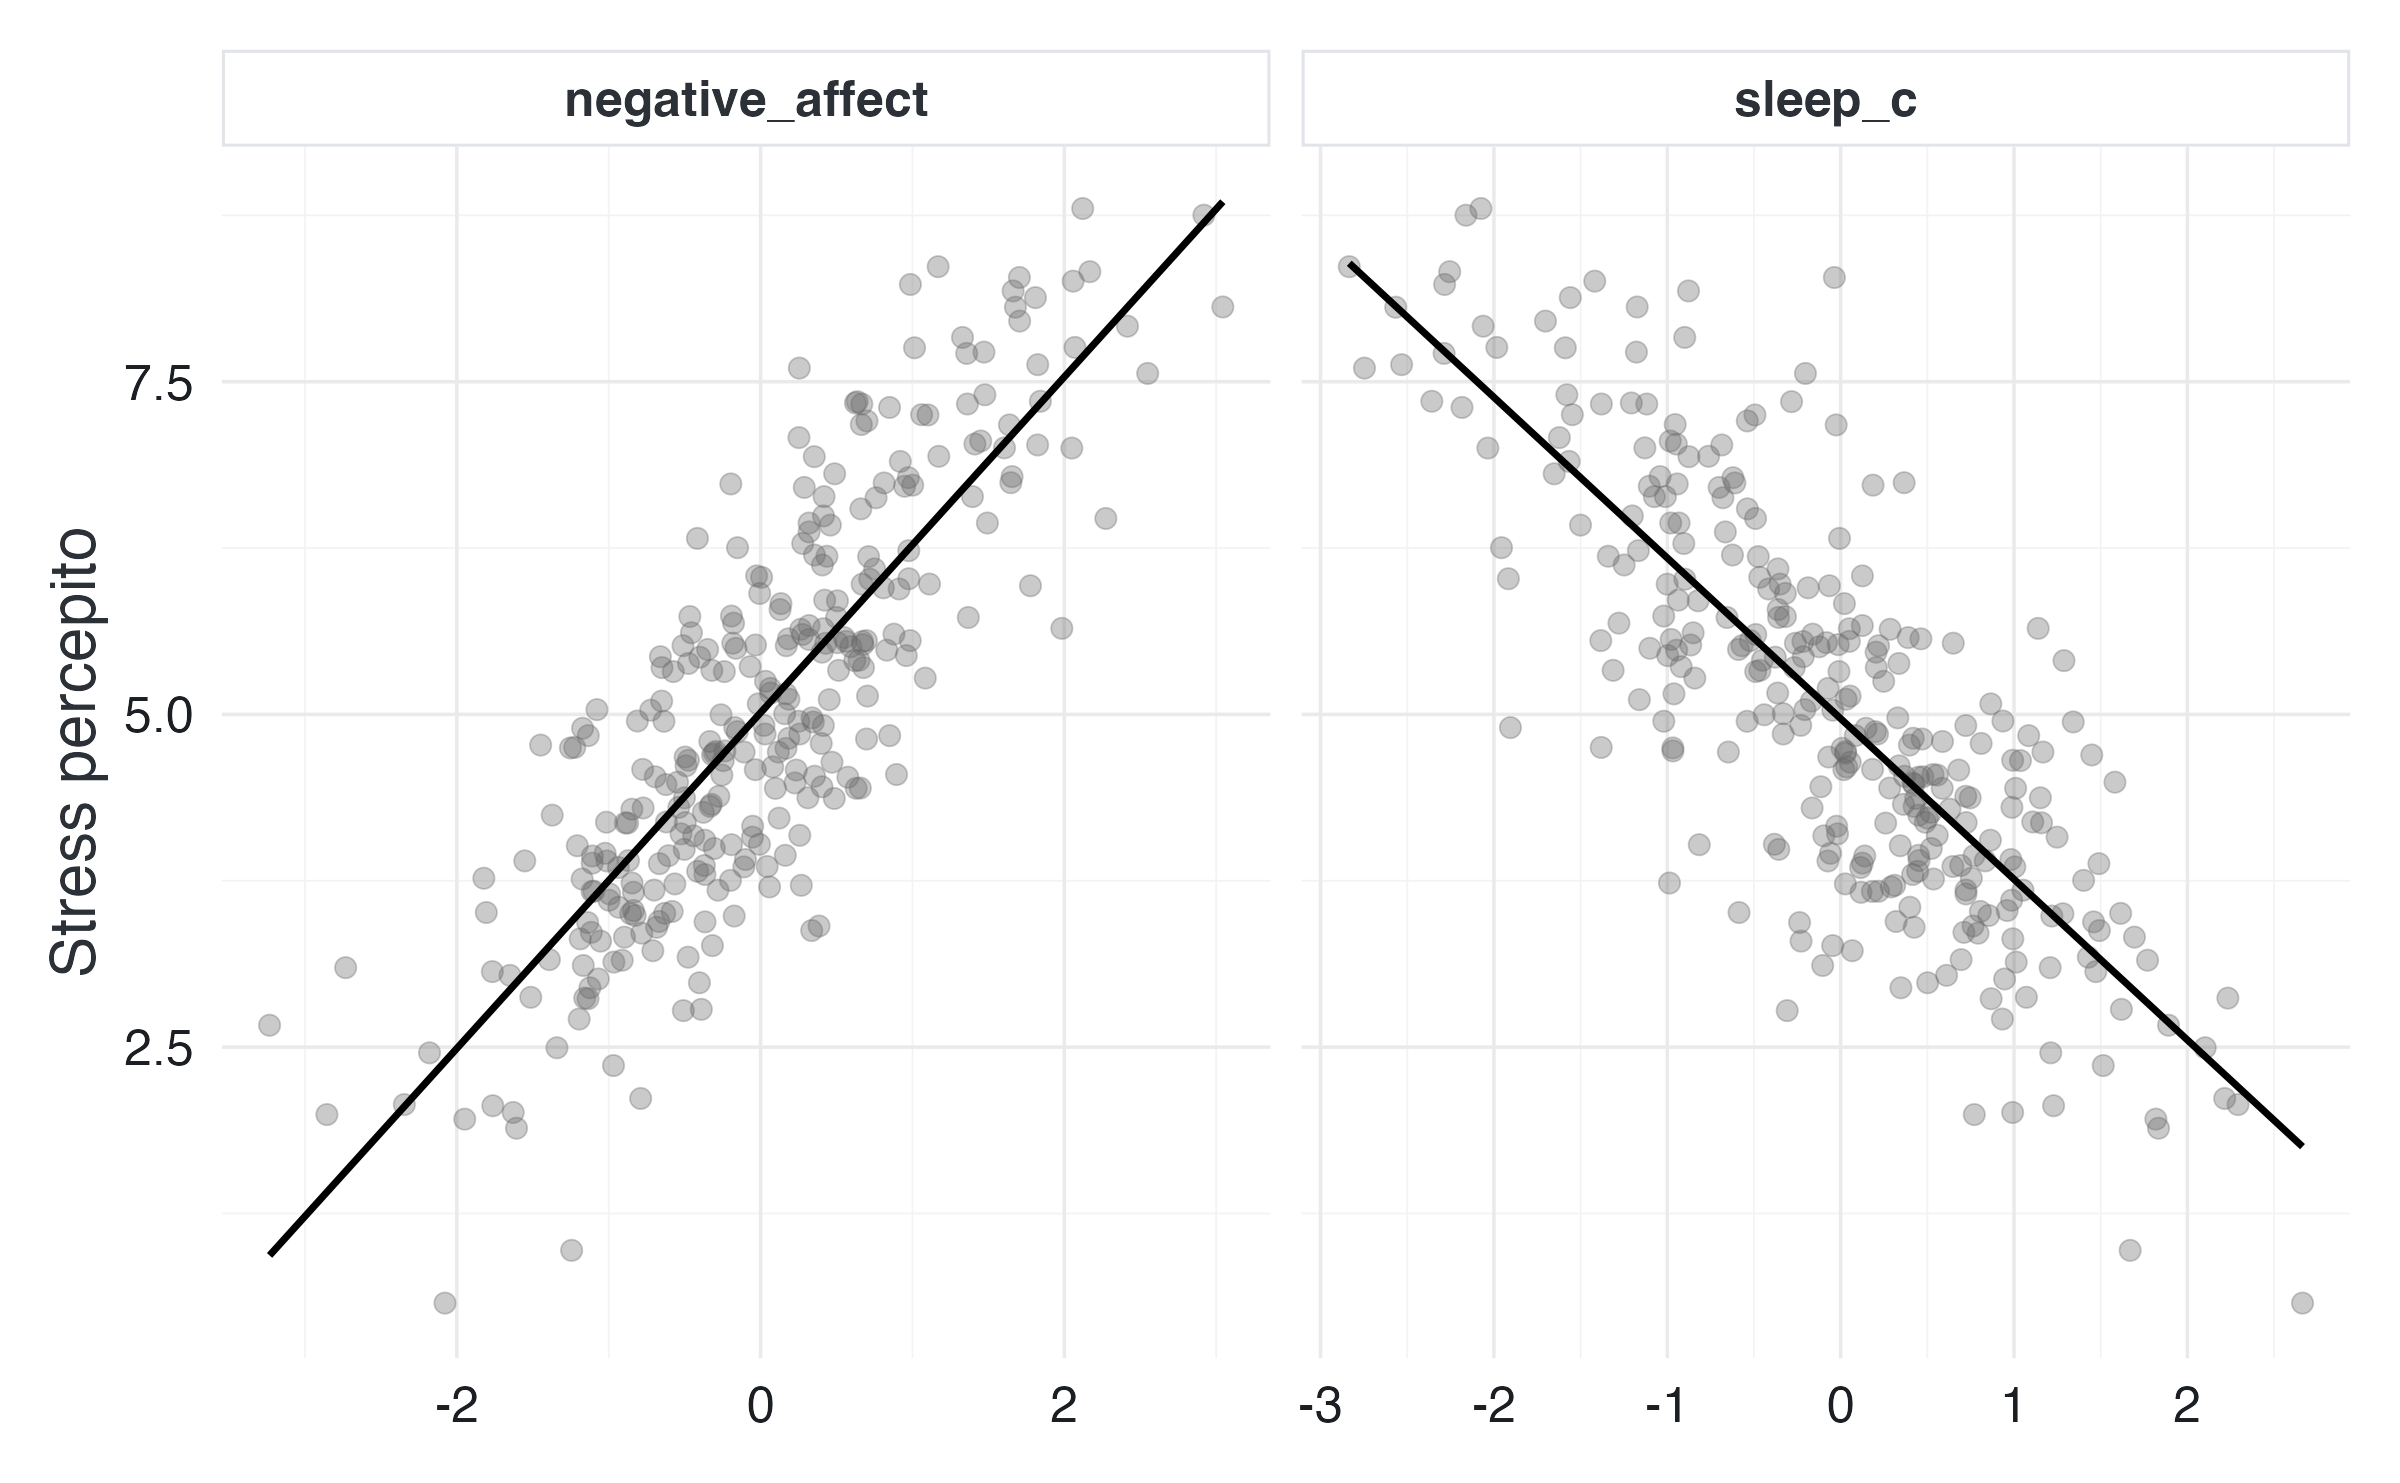
\includegraphics[width=0.85\linewidth,height=\textheight,keepaspectratio]{chapters/linear_models/04_dalla_formula_al_programma_files/figure-pdf/fig-stress-predictors-1.png}

}

\caption{\label{fig-stress-predictors}Associazioni bivariate marginali
tra lo stress e i due predittori simulati. Ciascun pannello mostra una
retta di regressione lineare semplice, non ancora condizionata alla
presenza dell'altra variabile.}

\end{figure}%

Per isolare il contributo di ciascuna variabile al netto dell'altra,
definiamo la formula del modello di regressione multipla in
\texttt{brms}:

\begin{Shaded}
\begin{Highlighting}[]
\NormalTok{stress }\SpecialCharTok{\textasciitilde{}}\NormalTok{ negative\_affect }\SpecialCharTok{+}\NormalTok{ sleep\_c}
\end{Highlighting}
\end{Shaded}

Questa istruzione sintattica corrisponde all'equazione:

\[
\mu_i = \alpha + \beta_{\text{affect}}\,\text{negative\_affect}_i + \beta_{\text{sleep}}\,\text{sleep\_c}_i.
\]

\section{Dalla formula alla matrice del
modello}\label{dalla-formula-alla-matrice-del-modello}

Dietro l'astrazione sintattica della formula R, il software traduce
l'elenco dei predittori in una struttura matematica nota come
\textbf{matrice del modello} (o \emph{design matrix}), indicata
convenzionalmente con il simbolo \(\mathbf{X}\). Questa matrice
organizza i dati numerici in modo che l'intero sistema di equazioni
lineari possa essere risolto simultaneamente tramite l'algebra lineare.

Possiamo ispezionare direttamente questa trasformazione strutturale
richiamando la funzione \texttt{model.matrix()}:

\begin{Shaded}
\begin{Highlighting}[]
\NormalTok{X\_full }\OtherTok{\textless{}{-}} \FunctionTok{model.matrix}\NormalTok{(}
  \SpecialCharTok{\textasciitilde{}}\NormalTok{ negative\_affect }\SpecialCharTok{+}\NormalTok{ sleep\_c,}
  \AttributeTok{data =}\NormalTok{ stress\_data}
\NormalTok{)}
\FunctionTok{dim}\NormalTok{(X\_full)}
\CommentTok{\#\textgreater{} [1] 300   3}
\end{Highlighting}
\end{Shaded}

\begin{Shaded}
\begin{Highlighting}[]
\FunctionTok{head}\NormalTok{(X\_full)}
\CommentTok{\#\textgreater{}   (Intercept) negative\_affect sleep\_c}
\CommentTok{\#\textgreater{} 1           1          {-}1.207   0.344}
\CommentTok{\#\textgreater{} 2           1           0.277  {-}0.905}
\CommentTok{\#\textgreater{} 3           1           1.084  {-}0.841}
\CommentTok{\#\textgreater{} 4           1          {-}2.346   2.292}
\CommentTok{\#\textgreater{} 5           1           0.429  {-}0.261}
\CommentTok{\#\textgreater{} 6           1           0.506  {-}0.822}
\end{Highlighting}
\end{Shaded}

\begin{Shaded}
\begin{Highlighting}[]
\FunctionTok{tail}\NormalTok{(X\_full)}
\CommentTok{\#\textgreater{}     (Intercept) negative\_affect sleep\_c}
\CommentTok{\#\textgreater{} 295           1           1.656  {-}1.041}
\CommentTok{\#\textgreater{} 296           1           1.810  {-}1.560}
\CommentTok{\#\textgreater{} 297           1          {-}1.175   0.535}
\CommentTok{\#\textgreater{} 298           1          {-}0.367   0.864}
\CommentTok{\#\textgreater{} 299           1           0.354  {-}0.875}
\CommentTok{\#\textgreater{} 300           1           0.319  {-}0.932}
\end{Highlighting}
\end{Shaded}

L'output rivela che la matrice risultante si articola in tre colonne
distinte:

\begin{enumerate}
\def\labelenumi{\arabic{enumi}.}
\tightlist
\item
  \texttt{(Intercept)}: una colonna interamente composta da valori
  uguali a \(1\), necessaria per stimare l'intercetta del modello;
\item
  \texttt{negative\_affect}: i valori standardizzati dell'affetto
  negativo per ciascun soggetto;
\item
  \texttt{sleep\_c}: le ore di sonno centrate.
\end{enumerate}

Dato un campione di \(N\) osservazioni, la matrice del modello assume
una dimensione geometrica pari a \(N \times 3\), strutturandosi come
segue:

\[\mathbf{X} = \begin{bmatrix} 1 & x_{11} & x_{12} \\ 1 & x_{21} & x_{22} \\ \vdots & \vdots & \vdots \\ 1 & x_{N1} & x_{N2} \end{bmatrix}\]

Parallelamente, organizziamo i parametri geometrici del modello in un
vettore colonna dei coefficienti, definito come \(\boldsymbol{\theta}\):

\[\boldsymbol{\theta} = \begin{bmatrix} \alpha \\ \beta_1 \\ \beta_2 \end{bmatrix}\]

L'operazione fondamentale del modello lineare si riassume nel prodotto
matrice-vettore:

\begin{equation}\protect\phantomsection\label{eq-design-matrix}{
\boldsymbol{\mu}=\mathbf{X}\boldsymbol{\theta}.
}\end{equation}

Questa singola moltiplicazione algebrica genera istantaneamente un
vettore colonna \(\boldsymbol{\mu}\) di dimensione \(N \times 1\),
contenente il valore medio atteso per ogni singola osservazione del
campione. Per un ripasso sistematico delle proprietà e delle operazioni
geometriche tra matrici, si rimanda
all'Appendice~\ref{sec-apx-matrix-algebra}.

\subsection{Verificare la corrispondenza
numerica}\label{verificare-la-corrispondenza-numerica}

Per dimostrare la perfetta equivalenza tra la formulazione analitica e
quella matriciale, possiamo confrontare il calcolo computazionale
eseguito precedentemente ciclo per ciclo con il prodotto interno delle
matrici in R (ordinato tramite l'operatore \texttt{\%*\%}):

\begin{Shaded}
\begin{Highlighting}[]
\NormalTok{theta\_true }\OtherTok{\textless{}{-}} \FunctionTok{c}\NormalTok{(}
\NormalTok{  alpha\_true,}
\NormalTok{  beta\_affect\_true,}
\NormalTok{  beta\_sleep\_true}
\NormalTok{)}

\CommentTok{\# Calcolo tramite prodotto matriciale}
\NormalTok{mu\_matrix }\OtherTok{\textless{}{-}} \FunctionTok{as.vector}\NormalTok{(X\_full }\SpecialCharTok{\%*\%}\NormalTok{ theta\_true)}

\CommentTok{\# Verifica dell\textquotesingle{}identità numerica}
\FunctionTok{all.equal}\NormalTok{(mu, mu\_matrix)}
\CommentTok{\#\textgreater{} [1] TRUE}
\end{Highlighting}
\end{Shaded}

L'output dell'algoritmo (\texttt{TRUE}) conferma che l'equazione scalare
applicata separatamente a ogni riga e l'operazione matriciale congiunta
producono identici risultati numerici.

\begin{tcolorbox}[enhanced jigsaw, arc=.35mm, bottomrule=.15mm, bottomtitle=1mm, breakable, colback=white, colbacktitle=quarto-callout-tip-color!10!white, colframe=quarto-callout-tip-color-frame, coltitle=black, left=2mm, leftrule=.75mm, opacityback=0, opacitybacktitle=0.6, rightrule=.15mm, title=\textcolor{quarto-callout-tip-color}{\faLightbulb}\hspace{0.5em}{Il ruolo concettuale della matrice del modello}, titlerule=0mm, toprule=.15mm, toptitle=1mm]

La struttura della matrice del modello rende esplicito quanto segue:

\begin{itemize}
\tightlist
\item
  \textbf{Generazione delle colonne:} Ogni singolo termine inserito
  nella formula R si traduce nella generazione di una o più colonne
  all'interno della matrice;
\item
  \textbf{Associazione biunivoca:} Ciascun coefficiente stimato dal
  modello moltiplica linearmente una specifica colonna della matrice;
\item
  \textbf{Codifica universale:} Informazioni complesse come le codifiche
  delle variabili categoriali (es. variabili \emph{dummy}), i termini di
  interazione o le trasformazioni non lineari (es. polinomi) vengono
  interamente risolte e linearizzate dentro la matrice del modello prima
  del calcolo;
\item
  \textbf{Astrazione per il motore di stima:} Una volta costruita la
  matrice \(\mathbf{X}\), la sua griglia numerica può essere passata
  direttamente a un campionatore come Stan, a prescindere dai nomi
  originari o dal significato psicometrico delle variabili di partenza.
\end{itemize}

\end{tcolorbox}

\section{Regressione multipla e matrice del
modello}\label{sec-multiple-regression}

La regressione multipla estende il modello lineare consentendo
l'inclusione simultanea di due o più predittori. Al fine di allinearci
alla logica computazionale dei moderni software di stima (incluso Stan),
risulta utile separare il parametro dell'intercetta dalla matrice dei
predittori propriamente detti. Questa scomposizione ci consente di
formulare il modello in forma matriciale come:

\begin{equation}\protect\phantomsection\label{eq-multiple-matrix}{
\mathbf{y} = \alpha\mathbf{1} + \mathbf{X}\boldsymbol{\beta} + \boldsymbol{\varepsilon}, \qquad \boldsymbol{\varepsilon} \sim \operatorname{Normal}(\mathbf{0},\sigma^2\mathbf{I}).
}\end{equation}

Per facilitare la comprensione dell'equazione, isoliamo le dimensioni
matematiche e il significato metodologico di ciascun operatore:

{\def\LTcaptype{none} % do not increment counter
\begin{longtable}[]{@{}
  >{\raggedright\arraybackslash}p{(\linewidth - 4\tabcolsep) * \real{0.3333}}
  >{\raggedright\arraybackslash}p{(\linewidth - 4\tabcolsep) * \real{0.3333}}
  >{\raggedright\arraybackslash}p{(\linewidth - 4\tabcolsep) * \real{0.3333}}@{}}
\toprule\noalign{}
\begin{minipage}[b]{\linewidth}\raggedright
Oggetto
\end{minipage} & \begin{minipage}[b]{\linewidth}\raggedright
Dimensione
\end{minipage} & \begin{minipage}[b]{\linewidth}\raggedright
Significato Metodologico
\end{minipage} \\
\midrule\noalign{}
\endhead
\bottomrule\noalign{}
\endlastfoot
\(\mathbf{y}\) & \(N\times1\) & Vettore colonna dell'outcome osservato
empiricamente \\
\(\mathbf{1}\) & \(N\times1\) & Vettore colonna composto interamente da
valori pari a \(1\) \\
\(\mathbf{X}\) & \(N\times K\) & Matrice del modello contenente i \(K\)
predittori (esclusa l'intercetta) \\
\(\boldsymbol{\beta}\) & \(K\times1\) & Vettore colonna dei coefficienti
parziali associati ai \(K\) predittori \\
\(\alpha\) & Scalare & Intercetta globale del modello (valore atteso
quando \(\mathbf{X}\boldsymbol{\beta} = \mathbf{0}\)) \\
\(\sigma\) & Scalare positivo & Deviazione standard condizionata
(variabilità residua attorno alla media) \\
\(\mathbf{I}\) & \(N\times N\) & Matrice identità (valori \(1\) sulla
diagonale principale, \(0\) altrove) \\
\end{longtable}
}

\subsection{\texorpdfstring{L'interpretazione dei coefficienti
condizionati (\emph{Partial
Effects})}{L'interpretazione dei coefficienti condizionati (Partial Effects)}}\label{linterpretazione-dei-coefficienti-condizionati-partial-effects}

All'interno di un'architettura multipla definita dall'equazione scalare:

\[
\mu_i=\alpha+\beta_1x_{1i}+\beta_2x_{2i}
\] la semantica dei parametri varia rispetto alla regressione semplice.
Il coefficiente \(\beta_1\) non esprime più l'associazione grezza tra le
variabili, bensì rappresenta la differenza attesa nella media di \(Y\)
associata a un incremento unitario di \(X_1\), \textbf{a parità di
livello di \(X_2\) all'interno del modello}. Specularmente, \(\beta_2\)
quantifica il contributo netto di \(X_2\) condizionatamente alla
presenza di \(X_1\).

Nel contesto della nostra simulazione sullo stress:

\begin{itemize}
\tightlist
\item
  \(\beta_{\text{affect}}\) mette a confronto l'esperienza di giornate
  che differiscono per intensità di affetto negativo, ma che condividono
  il medesimo quantitativo di ore di sonno;
\item
  \(\beta_{\text{sleep}}\) isola la differenza nei livelli di stress tra
  giornate caratterizzate da una differente durata del sonno, ma stabili
  sul medesimo livello di affetto negativo.
\end{itemize}

\begin{tcolorbox}[enhanced jigsaw, arc=.35mm, bottomrule=.15mm, bottomtitle=1mm, breakable, colback=white, colbacktitle=quarto-callout-warning-color!10!white, colframe=quarto-callout-warning-color-frame, coltitle=black, left=2mm, leftrule=.75mm, opacityback=0, opacitybacktitle=0.6, rightrule=.15mm, title=\textcolor{quarto-callout-warning-color}{\faExclamationTriangle}\hspace{0.5em}{Limitazione epistemologica: condizionare non equivale a intervenire}, titlerule=0mm, toprule=.15mm, toptitle=1mm]

L'espressione tecnica ``a parità degli altri predittori'' descrive una
proprietà geometrica e algebrica intrinseca alla proiezione nello spazio
multidimensionale del modello. Lo studente deve evitare l'errore di
interpretarla in senso manipolativo o sperimentale: essa non implica
affatto che sia fisicamente possibile alterare il valore di un
predittore lasciando realmente immutati gli altri nella realtà biologica
o psicologica, né possiede la facoltà di convertire un coefficiente
associativo in un effetto causale diretto.

La selezione dei predittori da includere nel sistema richiede una
profonda conoscenza teorica del dominio e, qualora l'obiettivo
scientifico sia di natura causale, necessita di un'esplicita analisi del
disegno mediante grafici causali orientati (DAG) e dell'adempimento
delle assunzioni di identificazione.

\end{tcolorbox}

\subsection{Modello bivariato vs.~Modello multiplo: un confronto
numerico}\label{modello-bivariato-vs.-modello-multiplo-un-confronto-numerico}

Quando i predittori manifestano una covariazione strutturale, la stima
prodotta da un modello lineare semplice (bivariato) può differire in
modo drastico dal coefficiente parziale calcolato dal modello multiplo.
Per apprezzare questa dinamica sul piano descrittivo, confrontiamo i
parametri stimati sul nostro dataset simulato attraverso la funzione
\texttt{lm()}:

\begin{Shaded}
\begin{Highlighting}[]
\CommentTok{\# Stima dei modelli lineari semplici (bivariati)}
\NormalTok{fit\_affect\_only }\OtherTok{\textless{}{-}} \FunctionTok{lm}\NormalTok{(stress }\SpecialCharTok{\textasciitilde{}}\NormalTok{ negative\_affect, }\AttributeTok{data =}\NormalTok{ stress\_data)}
\NormalTok{fit\_sleep\_only  }\OtherTok{\textless{}{-}} \FunctionTok{lm}\NormalTok{(stress }\SpecialCharTok{\textasciitilde{}}\NormalTok{ sleep\_c, }\AttributeTok{data =}\NormalTok{ stress\_data)}

\CommentTok{\# Stima del modello lineare multiplo congiunto}
\NormalTok{fit\_multiple\_lm }\OtherTok{\textless{}{-}} \FunctionTok{lm}\NormalTok{(stress }\SpecialCharTok{\textasciitilde{}}\NormalTok{ negative\_affect }\SpecialCharTok{+}\NormalTok{ sleep\_c, }\AttributeTok{data =}\NormalTok{ stress\_data)}

\CommentTok{\# Consolidamento e confronto dei coefficienti estratti}
\FunctionTok{bind\_rows}\NormalTok{(}
\NormalTok{  broom}\SpecialCharTok{::}\FunctionTok{tidy}\NormalTok{(fit\_affect\_only) }\SpecialCharTok{|\textgreater{}} \FunctionTok{mutate}\NormalTok{(}\AttributeTok{modello =} \StringTok{"Solo affetto negativo"}\NormalTok{),}
\NormalTok{  broom}\SpecialCharTok{::}\FunctionTok{tidy}\NormalTok{(fit\_sleep\_only)  }\SpecialCharTok{|\textgreater{}} \FunctionTok{mutate}\NormalTok{(}\AttributeTok{modello =} \StringTok{"Solo sonno"}\NormalTok{),}
\NormalTok{  broom}\SpecialCharTok{::}\FunctionTok{tidy}\NormalTok{(fit\_multiple\_lm) }\SpecialCharTok{|\textgreater{}} \FunctionTok{mutate}\NormalTok{(}\AttributeTok{modello =} \StringTok{"Modello multiplo"}\NormalTok{)}
\NormalTok{) }\SpecialCharTok{|\textgreater{}}
  \FunctionTok{filter}\NormalTok{(term }\SpecialCharTok{!=} \StringTok{"(Intercept)"}\NormalTok{) }\SpecialCharTok{|\textgreater{}}
  \FunctionTok{select}\NormalTok{(modello, term, estimate)}
\CommentTok{\#\textgreater{} \# A tibble: 4 x 3}
\CommentTok{\#\textgreater{}   modello               term            estimate}
\CommentTok{\#\textgreater{}   \textless{}chr\textgreater{}                 \textless{}chr\textgreater{}              \textless{}dbl\textgreater{}}
\CommentTok{\#\textgreater{} 1 Solo affetto negativo negative\_affect    1.26 }
\CommentTok{\#\textgreater{} 2 Solo sonno            sleep\_c           {-}1.21 }
\CommentTok{\#\textgreater{} 3 Modello multiplo      negative\_affect    0.822}
\CommentTok{\#\textgreater{} 4 Modello multiplo      sleep\_c           {-}0.692}
\end{Highlighting}
\end{Shaded}

Avendo definito noi stessi il processo generativo dei dati, siamo in
grado di comprendere questo risultato numerico: le discrepanze tra le
stime bivariate e quelle multiple derivano matematicamente dalla forte
correlazione esistente tra affetto e sonno (\(\rho = -0.65\)) e dal
fatto che entrambi i predittori concorrono a determinare la media dello
stress. Nel lavoro di ricerca con dati osservazionali reali, tuttavia,
il manifestarsi di una variazione nei coefficienti non costituisce di
per sé una prova logica per stabilire quale specificazione sia
scientificamente corretta.

La trattazione formale dei bias da variabili omesse, delle relazioni non
lineari latenti e delle altre patologie da errata specificazione sarà
oggetto di una discussione sistematica nel capitolo dedicato alla fase
di revisione critica del modello.

\section{\texorpdfstring{Adattare il modello multiplo con
\texttt{brms}}{Adattare il modello multiplo con brms}}\label{adattare-il-modello-multiplo-con-brms}

Dopo aver analizzato l'architettura matriciale della regressione
multipla, approfondiamo ora la traduzione computazionale del modello,
mantenendo esplicite la famiglia di verosimiglianza e la struttura delle
distribuzioni a priori.

Definiamo in primo luogo il vettore dei \emph{prior}, specificando le
nostre assunzioni iniziali sui parametri strutturali:

\begin{Shaded}
\begin{Highlighting}[]
\NormalTok{multiple\_priors }\OtherTok{\textless{}{-}} \FunctionTok{c}\NormalTok{(}
  \FunctionTok{prior}\NormalTok{(}\FunctionTok{normal}\NormalTok{(}\DecValTok{5}\NormalTok{, }\DecValTok{2}\NormalTok{), }\AttributeTok{class =} \StringTok{"Intercept"}\NormalTok{),  }
  \FunctionTok{prior}\NormalTok{(}\FunctionTok{normal}\NormalTok{(}\DecValTok{0}\NormalTok{, }\DecValTok{1}\NormalTok{), }\AttributeTok{class =} \StringTok{"b"}\NormalTok{),}
  \FunctionTok{prior}\NormalTok{(}\FunctionTok{lognormal}\NormalTok{(}\FunctionTok{log}\NormalTok{(}\DecValTok{1}\NormalTok{), }\FloatTok{0.5}\NormalTok{), }\AttributeTok{class =} \StringTok{"sigma"}\NormalTok{)}
\NormalTok{)}
\end{Highlighting}
\end{Shaded}

In questa fase, l'assegnazione \texttt{class\ =\ "b"} senza ulteriori
argomenti applica il medesimo prior gaussiano a tutti i coefficienti di
regressione parziale associati alle colonne della matrice dei predittori
(ovvero sia a \(\beta_{\text{affect}}\) sia a \(\beta_{\text{sleep}}\)).

Procediamo quindi alla stima della distribuzione a posteriori congiunta
mediante la funzione \texttt{brm()}:

\begin{Shaded}
\begin{Highlighting}[]
\NormalTok{fit\_multiple\_brms }\OtherTok{\textless{}{-}} \FunctionTok{brm}\NormalTok{(}
\NormalTok{  stress }\SpecialCharTok{\textasciitilde{}} \DecValTok{1} \SpecialCharTok{+}\NormalTok{ negative\_affect }\SpecialCharTok{+}\NormalTok{ sleep\_c,  }
  \AttributeTok{family =} \FunctionTok{gaussian}\NormalTok{(),}
  \AttributeTok{prior =}\NormalTok{ multiple\_priors,}
  \AttributeTok{data =}\NormalTok{ stress\_data,}
  \AttributeTok{backend =} \StringTok{"cmdstanr"}\NormalTok{,}
  \AttributeTok{seed =} \DecValTok{4201}\NormalTok{,}
  \AttributeTok{chains =} \DecValTok{4}\NormalTok{,}
  \AttributeTok{cores =} \DecValTok{4}\NormalTok{,          }
  \AttributeTok{warmup =} \DecValTok{1000}\NormalTok{,}
  \AttributeTok{iter =} \DecValTok{3000}\NormalTok{,}
  \AttributeTok{refresh =} \DecValTok{0}
\NormalTok{)}
\end{Highlighting}
\end{Shaded}

Sul piano metodologico, la formula passata come primo argomento comunica
a \texttt{brms} l'esatta geometria della componente sistematica. Gli
argomenti successivi governano le restanti dimensioni del calcolo
inferenziale:

\begin{itemize}
\tightlist
\item
  \texttt{family\ =\ gaussian()} stabilisce la distribuzione
  condizionata dell'outcome;
\item
  \texttt{prior} vincola le distribuzioni iniziali dei parametri nello
  spazio geometrico;
\item
  Le opzioni MCMC (\texttt{chains}, \texttt{iter}, \texttt{warmup})
  definiscono l'intensità e le modalità dell'esplorazione stocastica
  eseguita dall'algoritmo NUTS.
\end{itemize}

Una volta completato il campionamento stocastico, possiamo estrarre una
sintesi numerica delle distribuzioni a posteriori per verificare la
precisione dell'approssimazione numerica rispetto ai parametri reali
impostati nella simulazione (\(\alpha=5\), \(\beta_1=0.8\),
\(\beta_2=-0.7\), \(\sigma=0.7\)):

\begin{Shaded}
\begin{Highlighting}[]
\CommentTok{\# Estrai i draw dei parametri desiderati}
\NormalTok{draws\_selected }\OtherTok{\textless{}{-}}\NormalTok{ fit\_multiple\_brms }\SpecialCharTok{|\textgreater{}}
  \FunctionTok{as\_draws\_df}\NormalTok{() }\SpecialCharTok{|\textgreater{}}
  \FunctionTok{select}\NormalTok{(b\_Intercept, b\_negative\_affect, b\_sleep\_c, sigma)}

\CommentTok{\# Calcola le stesse statistiche di posterior\_summary()}
\NormalTok{posterior}\SpecialCharTok{::}\FunctionTok{summarise\_draws}\NormalTok{(}
\NormalTok{  draws\_selected,}
  \AttributeTok{mean =}\NormalTok{ mean,}
  \AttributeTok{sd =}\NormalTok{ sd,}
  \AttributeTok{q2.5 =} \SpecialCharTok{\textasciitilde{}}\FunctionTok{quantile}\NormalTok{(.x, }\AttributeTok{probs =} \FloatTok{0.025}\NormalTok{),}
  \AttributeTok{q97.5 =} \SpecialCharTok{\textasciitilde{}}\FunctionTok{quantile}\NormalTok{(.x, }\AttributeTok{probs =} \FloatTok{0.975}\NormalTok{)}
\NormalTok{)}
\CommentTok{\#\textgreater{} \# A tibble: 4 x 5}
\CommentTok{\#\textgreater{}   variable            mean     sd \textasciigrave{}2.5\%\textasciigrave{} \textasciigrave{}97.5\%\textasciigrave{}}
\CommentTok{\#\textgreater{}   \textless{}chr\textgreater{}              \textless{}dbl\textgreater{}  \textless{}dbl\textgreater{}  \textless{}dbl\textgreater{}   \textless{}dbl\textgreater{}}
\CommentTok{\#\textgreater{} 1 b\_Intercept        4.98  0.0385  4.91    5.06 }
\CommentTok{\#\textgreater{} 2 b\_negative\_affect  0.821 0.0491  0.724   0.919}
\CommentTok{\#\textgreater{} 3 b\_sleep\_c         {-}0.692 0.0485 {-}0.788  {-}0.596}
\CommentTok{\#\textgreater{} 4 sigma              0.664 0.0274  0.612   0.720}
\end{Highlighting}
\end{Shaded}

\subsection{Ispezionare la traduzione automatica: Standata e
Stancode}\label{ispezionare-la-traduzione-automatica-standata-e-stancode}

Possiamo chiedere esplicitamente al pacchetto \texttt{brms} di mostrarci
la struttura dati esatta che ha formattato per Stan, richiamando la
funzione \texttt{make\_standata()}:

\begin{Shaded}
\begin{Highlighting}[]
\NormalTok{standata\_multiple }\OtherTok{\textless{}{-}} \FunctionTok{make\_standata}\NormalTok{(}
\NormalTok{  stress }\SpecialCharTok{\textasciitilde{}} \DecValTok{1} \SpecialCharTok{+}\NormalTok{ negative\_affect }\SpecialCharTok{+}\NormalTok{ sleep\_c, }
  \AttributeTok{family =} \FunctionTok{gaussian}\NormalTok{(),}
  \AttributeTok{prior =}\NormalTok{ multiple\_priors,}
  \AttributeTok{data =}\NormalTok{ stress\_data}
\NormalTok{)}
\FunctionTok{names}\NormalTok{(standata\_multiple)}
\CommentTok{\#\textgreater{} [1] "N"          "Y"          "K"          "Kc"         "X"         }
\CommentTok{\#\textgreater{} [6] "prior\_only"}
\end{Highlighting}
\end{Shaded}

L'ispezione dei nomi rivela vettori e matrici (come la matrice del
modello \texttt{X} e il vettore dell'outcome \texttt{Y}) pronti per
essere elaborati dall'algebra lineare. Per esaminare il programma Stan
completo generato automaticamente dietro le quinte, ricorriamo invece a
\texttt{make\_stancode()}:

\begin{Shaded}
\begin{Highlighting}[]
\NormalTok{stancode\_multiple }\OtherTok{\textless{}{-}} \FunctionTok{make\_stancode}\NormalTok{(}
\NormalTok{  stress }\SpecialCharTok{\textasciitilde{}} \DecValTok{1} \SpecialCharTok{+}\NormalTok{ negative\_affect }\SpecialCharTok{+}\NormalTok{ sleep\_c, }
  \AttributeTok{family =} \FunctionTok{gaussian}\NormalTok{(),}
  \AttributeTok{prior =}\NormalTok{ multiple\_priors,}
  \AttributeTok{data =}\NormalTok{ stress\_data}
\NormalTok{)}

\FunctionTok{cat}\NormalTok{(}\StringTok{"\textasciigrave{}\textasciigrave{}\textasciigrave{}stan}\SpecialCharTok{\textbackslash{}n}\StringTok{"}\NormalTok{, stancode\_multiple, }\StringTok{"}\SpecialCharTok{\textbackslash{}n}\StringTok{\textasciigrave{}\textasciigrave{}\textasciigrave{}"}\NormalTok{, }\AttributeTok{sep =} \StringTok{""}\NormalTok{)}
\end{Highlighting}
\end{Shaded}

\begin{Shaded}
\begin{Highlighting}[]
\CommentTok{// generated with brms 2.23.0}
\KeywordTok{functions}\NormalTok{ \{}
\NormalTok{\}}
\KeywordTok{data}\NormalTok{ \{}
  \DataTypeTok{int}\NormalTok{\textless{}}\KeywordTok{lower}\NormalTok{=}\DecValTok{1}\NormalTok{\textgreater{} N;  }\CommentTok{// total number of observations}
  \DataTypeTok{vector}\NormalTok{[N] Y;  }\CommentTok{// response variable}
  \DataTypeTok{int}\NormalTok{\textless{}}\KeywordTok{lower}\NormalTok{=}\DecValTok{1}\NormalTok{\textgreater{} K;  }\CommentTok{// number of population{-}level effects}
  \DataTypeTok{matrix}\NormalTok{[N, K] X;  }\CommentTok{// population{-}level design matrix}
  \DataTypeTok{int}\NormalTok{\textless{}}\KeywordTok{lower}\NormalTok{=}\DecValTok{1}\NormalTok{\textgreater{} Kc;  }\CommentTok{// number of population{-}level effects after centering}
  \DataTypeTok{int}\NormalTok{ prior\_only;  }\CommentTok{// should the likelihood be ignored?}
\NormalTok{\}}
\KeywordTok{transformed data}\NormalTok{ \{}
  \DataTypeTok{matrix}\NormalTok{[N, Kc] Xc;  }\CommentTok{// centered version of X without an intercept}
  \DataTypeTok{vector}\NormalTok{[Kc] means\_X;  }\CommentTok{// column means of X before centering}
  \ControlFlowTok{for}\NormalTok{ (i }\ControlFlowTok{in} \DecValTok{2}\NormalTok{:K) \{}
\NormalTok{    means\_X[i {-} }\DecValTok{1}\NormalTok{] = mean(X[, i]);}
\NormalTok{    Xc[, i {-} }\DecValTok{1}\NormalTok{] = X[, i] {-} means\_X[i {-} }\DecValTok{1}\NormalTok{];}
\NormalTok{  \}}
\NormalTok{\}}
\KeywordTok{parameters}\NormalTok{ \{}
  \DataTypeTok{vector}\NormalTok{[Kc] b;  }\CommentTok{// regression coefficients}
  \DataTypeTok{real}\NormalTok{ Intercept;  }\CommentTok{// temporary intercept for centered predictors}
  \DataTypeTok{real}\NormalTok{\textless{}}\KeywordTok{lower}\NormalTok{=}\DecValTok{0}\NormalTok{\textgreater{} sigma;  }\CommentTok{// dispersion parameter}
\NormalTok{\}}
\KeywordTok{transformed parameters}\NormalTok{ \{}
  \CommentTok{// prior contributions to the log posterior}
  \DataTypeTok{real}\NormalTok{ lprior = }\DecValTok{0}\NormalTok{;}
\NormalTok{  lprior += normal\_lpdf(b | }\DecValTok{0}\NormalTok{, }\DecValTok{1}\NormalTok{);}
\NormalTok{  lprior += normal\_lpdf(Intercept | }\DecValTok{5}\NormalTok{, }\DecValTok{2}\NormalTok{);}
\NormalTok{  lprior += lognormal\_lpdf(sigma | log(}\DecValTok{1}\NormalTok{), }\FloatTok{0.5}\NormalTok{);}
\NormalTok{\}}
\KeywordTok{model}\NormalTok{ \{}
  \CommentTok{// likelihood including constants}
  \ControlFlowTok{if}\NormalTok{ (!prior\_only) \{}
    \KeywordTok{target +=}\NormalTok{ normal\_id\_glm\_lpdf(Y | Xc, Intercept, b, sigma);}
\NormalTok{  \}}
  \CommentTok{// priors including constants}
  \KeywordTok{target +=}\NormalTok{ lprior;}
\NormalTok{\}}
\KeywordTok{generated quantities}\NormalTok{ \{}
  \CommentTok{// actual population{-}level intercept}
  \DataTypeTok{real}\NormalTok{ b\_Intercept = Intercept {-} dot\_product(means\_X, b);}
\NormalTok{\}}
\end{Highlighting}
\end{Shaded}

Il codice prodotto è più articolato di quanto strettamente necessario
per questo esempio. Questa complessità deriva dal fatto che
\texttt{brms} adotta un'architettura software universale e
generalizzata, progettata per scalare in modo efficiente ed estendersi a
centinaia di famiglie di modelli differenti, complesse strutture di
interazione, trasformazioni non lineari e calcoli automatici di quantità
derivate. Questa complessità non implica che il modello statistico sia
diverso: l'elemento centrale rimane il predittore lineare mappato nella
matrice del modello

\begin{tcolorbox}[enhanced jigsaw, arc=.35mm, bottomrule=.15mm, bottomtitle=1mm, breakable, colback=white, colbacktitle=quarto-callout-note-color!10!white, colframe=quarto-callout-note-color-frame, coltitle=black, left=2mm, leftrule=.75mm, opacityback=0, opacitybacktitle=0.6, rightrule=.15mm, title=\textcolor{quarto-callout-note-color}{\faInfo}\hspace{0.5em}{L'astrazione come risorsa: il concetto di zucchero sintattico}, titlerule=0mm, toprule=.15mm, toptitle=1mm]

Nel dominio dell'informatica e della programmazione, l'espressione
\emph{zucchero sintattico} (\emph{syntactic sugar}) identifica una
convenzione o una notazione formale introdotta per rendere la stesura
del codice più agile, leggibile e intuitiva per l'operatore umano, senza
per questo modificarne minimamente il funzionamento logico di basso
livello.

Nell'ecosistema R, l'interfaccia di \texttt{brms} si comporta
esattamente come una forma di zucchero sintattico: essa non sostituisce
né bypassa il motore di calcolo probabilistico Stan, ma si assume
l'onere di scriverne e compilarne il codice sorgente in modo automatico
e matematicamente ottimizzato a partire dagli input forniti dal
ricercatore (formula, famiglia, prior e data frame).

\end{tcolorbox}

\section{Scrivere lo stesso modello direttamente in
Stan}\label{sec-formula-stan-direct}

\begin{tcolorbox}[enhanced jigsaw, arc=.35mm, bottomrule=.15mm, breakable, colback=white, colframe=quarto-callout-tip-color-frame, left=2mm, leftrule=.75mm, opacityback=0, rightrule=.15mm, toprule=.15mm]

\textbf{Approfondimento facoltativo.} Se lavori solo con \texttt{brms},
puoi saltare la scrittura, la compilazione e il confronto numerico del
programma nativo e riprendere da \hyperref[sec-formula-tradeoffs]{Che
cosa guadagniamo e che cosa perdiamo}. Resta invece richiesto saper
leggere la traduzione prodotta da \texttt{make\_stancode()} nella
sezione precedente.

\end{tcolorbox}

Per meglio comprendere la struttura del modello depurata dalle
sovrastrutture di \texttt{brms}, possiamo programmare l'algoritmo
direttamente in codice Stan. Per fare questo, isoliamo i due predittori
all'interno di una matrice del modello sprovvista del vettore costante
dei valori \(1\): in questo modo, l'intercetta non sarà codificata come
colonna di \(\mathbf{X}\) ma verrà gestita come un parametro scalare
esplicito e separato.

\begin{Shaded}
\begin{Highlighting}[]
\NormalTok{X }\OtherTok{\textless{}{-}} \FunctionTok{model.matrix}\NormalTok{(}
  \SpecialCharTok{\textasciitilde{}} \DecValTok{0} \SpecialCharTok{+}\NormalTok{ negative\_affect }\SpecialCharTok{+}\NormalTok{ sleep\_c,}
  \AttributeTok{data =}\NormalTok{ stress\_data}
\NormalTok{)}

\NormalTok{stan\_data\_multiple }\OtherTok{\textless{}{-}} \FunctionTok{list}\NormalTok{(}
  \AttributeTok{N =} \FunctionTok{nrow}\NormalTok{(stress\_data),}
  \AttributeTok{K =} \FunctionTok{ncol}\NormalTok{(X),}
  \AttributeTok{X =}\NormalTok{ X,}
  \AttributeTok{y =}\NormalTok{ stress\_data}\SpecialCharTok{$}\NormalTok{stress}
\NormalTok{)}
\end{Highlighting}
\end{Shaded}

Il programma Stan nativo si articola nei seguenti blocchi:

\begin{Shaded}
\begin{Highlighting}[]
\KeywordTok{data}\NormalTok{ \{}
  \DataTypeTok{int}\NormalTok{\textless{}}\KeywordTok{lower}\NormalTok{=}\DecValTok{1}\NormalTok{\textgreater{} N;       }\CommentTok{// Numero di osservazioni (righe)}
  \DataTypeTok{int}\NormalTok{\textless{}}\KeywordTok{lower}\NormalTok{=}\DecValTok{1}\NormalTok{\textgreater{} K;       }\CommentTok{// Numero di predittori (colonne di X)}
  \DataTypeTok{matrix}\NormalTok{[N, K] X;       }\CommentTok{// Matrice del modello per i predittori}
  \DataTypeTok{vector}\NormalTok{[N] y;          }\CommentTok{// Vettore colonna della variabile outcome}
\NormalTok{\}}

\KeywordTok{parameters}\NormalTok{ \{}
  \DataTypeTok{real}\NormalTok{ alpha;           }\CommentTok{// Intercetta globale}
  \DataTypeTok{vector}\NormalTok{[K] beta;       }\CommentTok{// Vettore dei coefficienti di regressione parziale}
  \DataTypeTok{real}\NormalTok{\textless{}}\KeywordTok{lower}\NormalTok{=}\DecValTok{0}\NormalTok{\textgreater{} sigma;  }\CommentTok{// Deviazione standard residua (vincolata a valori positivi)}
\NormalTok{\}}

\KeywordTok{model}\NormalTok{ \{}
  \CommentTok{// Assegnazione delle distribuzioni a priori (Prior)}
\NormalTok{  alpha \textasciitilde{} normal(}\DecValTok{5}\NormalTok{, }\DecValTok{2}\NormalTok{);}
\NormalTok{  beta \textasciitilde{} normal(}\DecValTok{0}\NormalTok{, }\DecValTok{1}\NormalTok{);}
\NormalTok{  sigma \textasciitilde{} lognormal(log(}\DecValTok{1}\NormalTok{), }\FloatTok{0.5}\NormalTok{);}

  \CommentTok{// Verosimiglianza vettorializzata}
\NormalTok{  y \textasciitilde{} normal(alpha + X * beta, sigma);}
\NormalTok{\}}

\KeywordTok{generated quantities}\NormalTok{ \{}
  \DataTypeTok{vector}\NormalTok{[N] mu = alpha + X * beta;}
  \DataTypeTok{vector}\NormalTok{[N] y\_rep;}
  \DataTypeTok{real}\NormalTok{ bayes\_R2;}

  \CommentTok{// Campionamento dalla distribuzione predittiva a posteriori}
  \ControlFlowTok{for}\NormalTok{ (n }\ControlFlowTok{in} \DecValTok{1}\NormalTok{:N) \{}
\NormalTok{    y\_rep[n] = normal\_rng(mu[n], sigma);}
\NormalTok{  \}}

  \CommentTok{// Calcolo dell\textquotesingle{}R{-}quadrato bayesiano}
\NormalTok{  bayes\_R2 = variance(mu) / (variance(mu) + square(sigma));}
\NormalTok{\}}
\end{Highlighting}
\end{Shaded}

La riga

\begin{Shaded}
\begin{Highlighting}[]
\NormalTok{y \textasciitilde{} normal(alpha + X * beta, sigma);}
\end{Highlighting}
\end{Shaded}

sfrutta le proprietà di vettorializzazione di Stan. Dal punto di vista
algebrico, essa equivale a eseguire un ciclo iterativo esplicito:

\begin{Shaded}
\begin{Highlighting}[]
\ControlFlowTok{for}\NormalTok{ (n }\ControlFlowTok{in} \DecValTok{1}\NormalTok{:N) \{}
\NormalTok{  y[n] \textasciitilde{} normal(alpha + X[n] * beta, sigma);}
\NormalTok{\}}
\end{Highlighting}
\end{Shaded}

Tuttavia, la formulazione matriciale risulta computazionalmente più
efficiente.

\subsection{Compilare e adattare il
programma}\label{compilare-e-adattare-il-programma}

Procediamo alla compilazione del codice sorgente e alla generazione
dell'eseguibile binario:

\begin{Shaded}
\begin{Highlighting}[]
\NormalTok{stan\_file\_multiple }\OtherTok{\textless{}{-}} \FunctionTok{write\_stan\_file}\NormalTok{(}
  \AttributeTok{code =} \StringTok{\textquotesingle{}}
\StringTok{data \{}
\StringTok{  int\textless{}lower=1\textgreater{} N;}
\StringTok{  int\textless{}lower=1\textgreater{} K;}
\StringTok{  matrix[N, K] X;}
\StringTok{  vector[N] y;}
\StringTok{\}}
\StringTok{parameters \{}
\StringTok{  real alpha;}
\StringTok{  vector[K] beta;}
\StringTok{  real\textless{}lower=0\textgreater{} sigma;}
\StringTok{\}}
\StringTok{model \{}
\StringTok{  alpha \textasciitilde{} normal(5, 2);}
\StringTok{  beta \textasciitilde{} normal(0, 1);}
\StringTok{  sigma \textasciitilde{} lognormal(log(1), 0.5);}
\StringTok{  y \textasciitilde{} normal(alpha + X * beta, sigma);}
\StringTok{\}}
\StringTok{generated quantities \{}
\StringTok{  vector[N] mu = alpha + X * beta;}
\StringTok{  vector[N] y\_rep;}
\StringTok{  real bayes\_R2;}
\StringTok{  for (n in 1:N) \{}
\StringTok{    y\_rep[n] = normal\_rng(mu[n], sigma);}
\StringTok{  \}}
\StringTok{  bayes\_R2 = variance(mu) / (variance(mu) + square(sigma));}
\StringTok{\}}
\StringTok{\textquotesingle{}}
\NormalTok{)}

\NormalTok{stan\_model\_multiple }\OtherTok{\textless{}{-}} \FunctionTok{cmdstan\_model}\NormalTok{(stan\_file\_multiple)}
\end{Highlighting}
\end{Shaded}

Una volta completata la compilazione, avviamo il campionamento
stocastico MCMC richiamando il metodo \texttt{\$sample()} dall'oggetto
modello:

\begin{Shaded}
\begin{Highlighting}[]
\NormalTok{fit\_multiple\_stan }\OtherTok{\textless{}{-}}\NormalTok{ stan\_model\_multiple}\SpecialCharTok{$}\FunctionTok{sample}\NormalTok{(}
  \AttributeTok{data =}\NormalTok{ stan\_data\_multiple,}
  \AttributeTok{seed =} \DecValTok{4201}\NormalTok{,}
  \AttributeTok{chains =} \DecValTok{4}\NormalTok{,}
  \AttributeTok{parallel\_chains =} \DecValTok{4}\NormalTok{,}
  \AttributeTok{iter\_warmup =} \DecValTok{1000}\NormalTok{,}
  \AttributeTok{iter\_sampling =} \DecValTok{2000}\NormalTok{,}
  \AttributeTok{refresh =} \DecValTok{0}
\NormalTok{)}
\end{Highlighting}
\end{Shaded}

Possiamo ora esaminare gli indici diagnostici (come \(\widehat{R}\) e il
numero effettivo di campioni \(ESS\)) e i riassunti numerici della
posterior nel modo seguente:

\begin{Shaded}
\begin{Highlighting}[]
\NormalTok{fit\_multiple\_stan}\SpecialCharTok{$}\FunctionTok{summary}\NormalTok{(}
  \AttributeTok{variables =} \FunctionTok{c}\NormalTok{(}
    \StringTok{"alpha"}\NormalTok{,}
    \StringTok{"beta"}\NormalTok{,}
    \StringTok{"sigma"}\NormalTok{,}
    \StringTok{"bayes\_R2"}
\NormalTok{  )}
\NormalTok{)}
\CommentTok{\#\textgreater{} \# A tibble: 5 x 10}
\CommentTok{\#\textgreater{}   variable   mean median     sd    mad     q5    q95  rhat ess\_bulk ess\_tail}
\CommentTok{\#\textgreater{}   \textless{}chr\textgreater{}     \textless{}dbl\textgreater{}  \textless{}dbl\textgreater{}  \textless{}dbl\textgreater{}  \textless{}dbl\textgreater{}  \textless{}dbl\textgreater{}  \textless{}dbl\textgreater{} \textless{}dbl\textgreater{}    \textless{}dbl\textgreater{}    \textless{}dbl\textgreater{}}
\CommentTok{\#\textgreater{} 1 alpha     4.98   4.98  0.0384 0.0380  4.92   5.05   1.00    7530.    5483.}
\CommentTok{\#\textgreater{} 2 beta[1]   0.822  0.822 0.0491 0.0493  0.741  0.902  1.00    7001.    6074.}
\CommentTok{\#\textgreater{} 3 beta[2]  {-}0.692 {-}0.691 0.0483 0.0484 {-}0.770 {-}0.612  1.00    6624.    5880.}
\CommentTok{\#\textgreater{} 4 sigma     0.664  0.663 0.0273 0.0267  0.621  0.710  1.00    7247.    5331.}
\CommentTok{\#\textgreater{} 5 bayes\_R2  0.811  0.812 0.0152 0.0152  0.785  0.835  1.00    8233.    6029.}
\end{Highlighting}
\end{Shaded}

Se formula, dati, famiglia e prior coincidono, \texttt{brms} e il
programma Stan diretto devono produrre distribuzioni posteriori
compatibili, al netto della variabilità Monte Carlo e di eventuali
differenze di parametrizzazione interna.

\subsection{Confrontare le stime}\label{confrontare-le-stime}

Per effettuare un confronto tra i due metodi, estraiamo i campioni della
distribuzione a posteriori (\emph{draws}) manipolandoli in modo
standardizzato tramite le strutture dati del pacchetto
\texttt{posterior}. Questo approccio ci consente di mantenere traccia
dell'articolazione in catene (\emph{chains}) e iterazioni prima di
collassare i dati in fase di sintesi descrittiva:

\begin{Shaded}
\begin{Highlighting}[]
\FunctionTok{library}\NormalTok{(posterior)}

\CommentTok{\# Estrazione e formattazione dei draws da brms come oggetto draws\_df}
\NormalTok{brms\_draws }\OtherTok{\textless{}{-}} \FunctionTok{as\_draws\_df}\NormalTok{(fit\_multiple\_brms) }\SpecialCharTok{|\textgreater{}}
  \FunctionTok{transmute}\NormalTok{(}
    \AttributeTok{alpha =}\NormalTok{ b\_Intercept,}
    \AttributeTok{beta\_affect =}\NormalTok{ b\_negative\_affect,}
    \AttributeTok{beta\_sleep =}\NormalTok{ b\_sleep\_c,}
    \AttributeTok{sigma =}\NormalTok{ sigma,}
    \AttributeTok{motore =} \StringTok{"brms"}
\NormalTok{  )}

\CommentTok{\# Estrazione dei draws da Stan nativo}
\NormalTok{stan\_draws }\OtherTok{\textless{}{-}}\NormalTok{ fit\_multiple\_stan}\SpecialCharTok{$}\FunctionTok{draws}\NormalTok{(}
  \AttributeTok{variables =} \FunctionTok{c}\NormalTok{(}\StringTok{"alpha"}\NormalTok{, }\StringTok{"beta"}\NormalTok{, }\StringTok{"sigma"}\NormalTok{),}
  \AttributeTok{format =} \StringTok{"draws\_df"}
\NormalTok{) }\SpecialCharTok{|\textgreater{}}
  \FunctionTok{transmute}\NormalTok{(}
    \AttributeTok{alpha =}\NormalTok{ alpha,}
    \AttributeTok{beta\_affect =} \StringTok{\textasciigrave{}}\AttributeTok{beta[1]}\StringTok{\textasciigrave{}}\NormalTok{,}
    \AttributeTok{beta\_sleep =} \StringTok{\textasciigrave{}}\AttributeTok{beta[2]}\StringTok{\textasciigrave{}}\NormalTok{,}
    \AttributeTok{sigma =}\NormalTok{ sigma,}
    \AttributeTok{motore =} \StringTok{"Stan diretto"}
\NormalTok{  )}

\CommentTok{\# Consolidamento e calcolo dei riassunti descrittivi della posterior}
\FunctionTok{bind\_rows}\NormalTok{(brms\_draws, stan\_draws) }\SpecialCharTok{|\textgreater{}}
  \FunctionTok{pivot\_longer}\NormalTok{(}
    \AttributeTok{cols =} \FunctionTok{c}\NormalTok{(alpha, beta\_affect, beta\_sleep, sigma),}
    \AttributeTok{names\_to =} \StringTok{"parametro"}\NormalTok{,}
    \AttributeTok{values\_to =} \StringTok{"valore"}
\NormalTok{  ) }\SpecialCharTok{|\textgreater{}}
  \FunctionTok{group\_by}\NormalTok{(motore, parametro) }\SpecialCharTok{|\textgreater{}}
  \FunctionTok{summarize}\NormalTok{(  }
    \AttributeTok{media =} \FunctionTok{mean}\NormalTok{(valore),}
    \AttributeTok{q05 =} \FunctionTok{quantile}\NormalTok{(valore, }\FloatTok{0.05}\NormalTok{),}
    \AttributeTok{q95 =} \FunctionTok{quantile}\NormalTok{(valore, }\FloatTok{0.95}\NormalTok{),}
    \AttributeTok{.groups =} \StringTok{"drop"}
\NormalTok{  )}
\CommentTok{\#\textgreater{} \# A tibble: 8 x 5}
\CommentTok{\#\textgreater{}   motore       parametro    media    q05    q95}
\CommentTok{\#\textgreater{}   \textless{}chr\textgreater{}        \textless{}chr\textgreater{}        \textless{}dbl\textgreater{}  \textless{}dbl\textgreater{}  \textless{}dbl\textgreater{}}
\CommentTok{\#\textgreater{} 1 Stan diretto alpha        4.98   4.92   5.05 }
\CommentTok{\#\textgreater{} 2 Stan diretto beta\_affect  0.822  0.741  0.902}
\CommentTok{\#\textgreater{} 3 Stan diretto beta\_sleep  {-}0.692 {-}0.770 {-}0.612}
\CommentTok{\#\textgreater{} 4 Stan diretto sigma        0.664  0.621  0.710}
\CommentTok{\#\textgreater{} 5 brms         alpha        4.98   4.92   5.05 }
\CommentTok{\#\textgreater{} 6 brms         beta\_affect  0.821  0.741  0.903}
\CommentTok{\#\textgreater{} 7 brms         beta\_sleep  {-}0.692 {-}0.771 {-}0.612}
\CommentTok{\#\textgreater{} 8 brms         sigma        0.664  0.621  0.711}
\end{Highlighting}
\end{Shaded}

Il confronto serve solo come controllo della traduzione, non come
competizione tra software. \texttt{brms} utilizza Stan come motore
computazionale; la differenza riguarda soprattutto il livello al quale
viene espressa la specificazione.

\section{Che cosa guadagniamo e che cosa
perdiamo}\label{sec-formula-tradeoffs}

\subsection{\texorpdfstring{Usare
\texttt{brms}}{Usare brms}}\label{usare-brms}

\texttt{brms} è generalmente preferibile quando:

\begin{itemize}
\tightlist
\item
  il modello appartiene a una famiglia già supportata;
\item
  si desidera modificare rapidamente formula, famiglia o prior;
\item
  servono strumenti integrati per predizioni e controlli;
\item
  la priorità è comunicare chiaramente la struttura del modello;
\item
  si vuole ridurre la quantità di codice da mantenere.
\end{itemize}

Per esempio, una verosimiglianza Student-\(t\) robusta può essere
richiesta cambiando un solo argomento:

\begin{Shaded}
\begin{Highlighting}[]
\FunctionTok{brm}\NormalTok{(}
\NormalTok{  stress }\SpecialCharTok{\textasciitilde{}}\NormalTok{ negative\_affect }\SpecialCharTok{+}\NormalTok{ sleep\_c,}
  \AttributeTok{family =} \FunctionTok{student}\NormalTok{(),}
  \AttributeTok{data =}\NormalTok{ stress\_data,}
  \AttributeTok{prior =}\NormalTok{ ...}
\NormalTok{)}
\end{Highlighting}
\end{Shaded}

Il cambio è sintatticamente piccolo, ma sostantivamente importante:
modifica la distribuzione degli scarti e introduce il parametro dei
gradi di libertà.

\subsection{Scrivere Stan
direttamente}\label{scrivere-stan-direttamente}

Stan diretto diventa utile quando:

\begin{itemize}
\tightlist
\item
  il processo generativo non è esprimibile con le formule disponibili;
\item
  occorrono ricorrenze, vincoli o trasformazioni non standard;
\item
  si vogliono definire quantità latenti personalizzate;
\item
  è necessario controllare precisamente la parametrizzazione;
\item
  si costruiscono modelli processuali o cognitivi.
\end{itemize}

Il prezzo è una maggiore responsabilità: il ricercatore deve costruire i
dati, verificare le dimensioni, dichiarare i vincoli, definire le
quantità generate e controllare personalmente la corrispondenza tra
codice e modello.

\begin{tcolorbox}[enhanced jigsaw, arc=.35mm, bottomrule=.15mm, bottomtitle=1mm, breakable, colback=white, colbacktitle=quarto-callout-warning-color!10!white, colframe=quarto-callout-warning-color-frame, coltitle=black, left=2mm, leftrule=.75mm, opacityback=0, opacitybacktitle=0.6, rightrule=.15mm, title=\textcolor{quarto-callout-warning-color}{\faExclamationTriangle}\hspace{0.5em}{Più esplicito non significa automaticamente migliore}, titlerule=0mm, toprule=.15mm, toptitle=1mm]

Un programma Stan scritto a mano può essere trasparente, ma anche
contenere errori di indicizzazione, prior non calibrati o
parametrizzazioni inefficienti. Analogamente, una formula \texttt{brms}
può essere corretta sintatticamente ma rappresentare male la domanda
scientifica.

La qualità dipende dalla specificazione e dai controlli, non dalla
quantità di codice visibile.

\end{tcolorbox}

\section{Diagnostica e controllo
predittivo}\label{diagnostica-e-controllo-predittivo}

Indipendentemente dalla strada scelta per stimare il modello --- la
sintesi immediata di \texttt{brms} o la scrittura analitica in Stan ---
i criteri di validazione scientifica rimangono gli stessi. Prima di
trarre qualsiasi conclusione dai risultati, il workflow bayesiano
richiede di seguire tre passaggi sequenziali:

\begin{enumerate}
\def\labelenumi{\arabic{enumi}.}
\tightlist
\item
  \textbf{Diagnostica computazionale:} Verificare che l'algoritmo HMC
  abbia esplorato la distribuzione a posteriori in modo affidabile,
  senza incontrare transizioni divergenti o problemi di convergenza.
\item
  \textbf{Controllo predittivo:} Accertarsi che il modello, una volta
  addestrato, sia in grado di generare dati simulati che somiglino a
  quelli reali.
\item
  \textbf{Interpretazione scientifica:} Valutare se le quantità stimata
  rispondano in modo coerente alla domanda di ricerca.
\end{enumerate}

Per una trattazione metodologica approfondita del workflow e delle
diagnostiche MCMC, si rimanda rispettivamente al
Capitolo~\ref{sec-linmod-bayesian-reg} e
all'Appendice~\ref{sec-apx-mcmc-diagnostics}.

Un controllo predittivo a posteriori (\emph{posterior predictive check},
PPC) essenziale consiste nel confrontare la distribuzione dei dati
osservati con quella delle repliche simulate dal modello. Possiamo
visualizzare questa verifica formale con entrambi gli approcci:

\begin{Shaded}
\begin{Highlighting}[]
\FunctionTok{pp\_check}\NormalTok{(}
\NormalTok{  fit\_multiple\_brms,}
  \AttributeTok{type =} \StringTok{"dens\_overlay"}\NormalTok{,}
  \AttributeTok{ndraws =} \DecValTok{50}
\NormalTok{)}
\end{Highlighting}
\end{Shaded}

\begin{center}
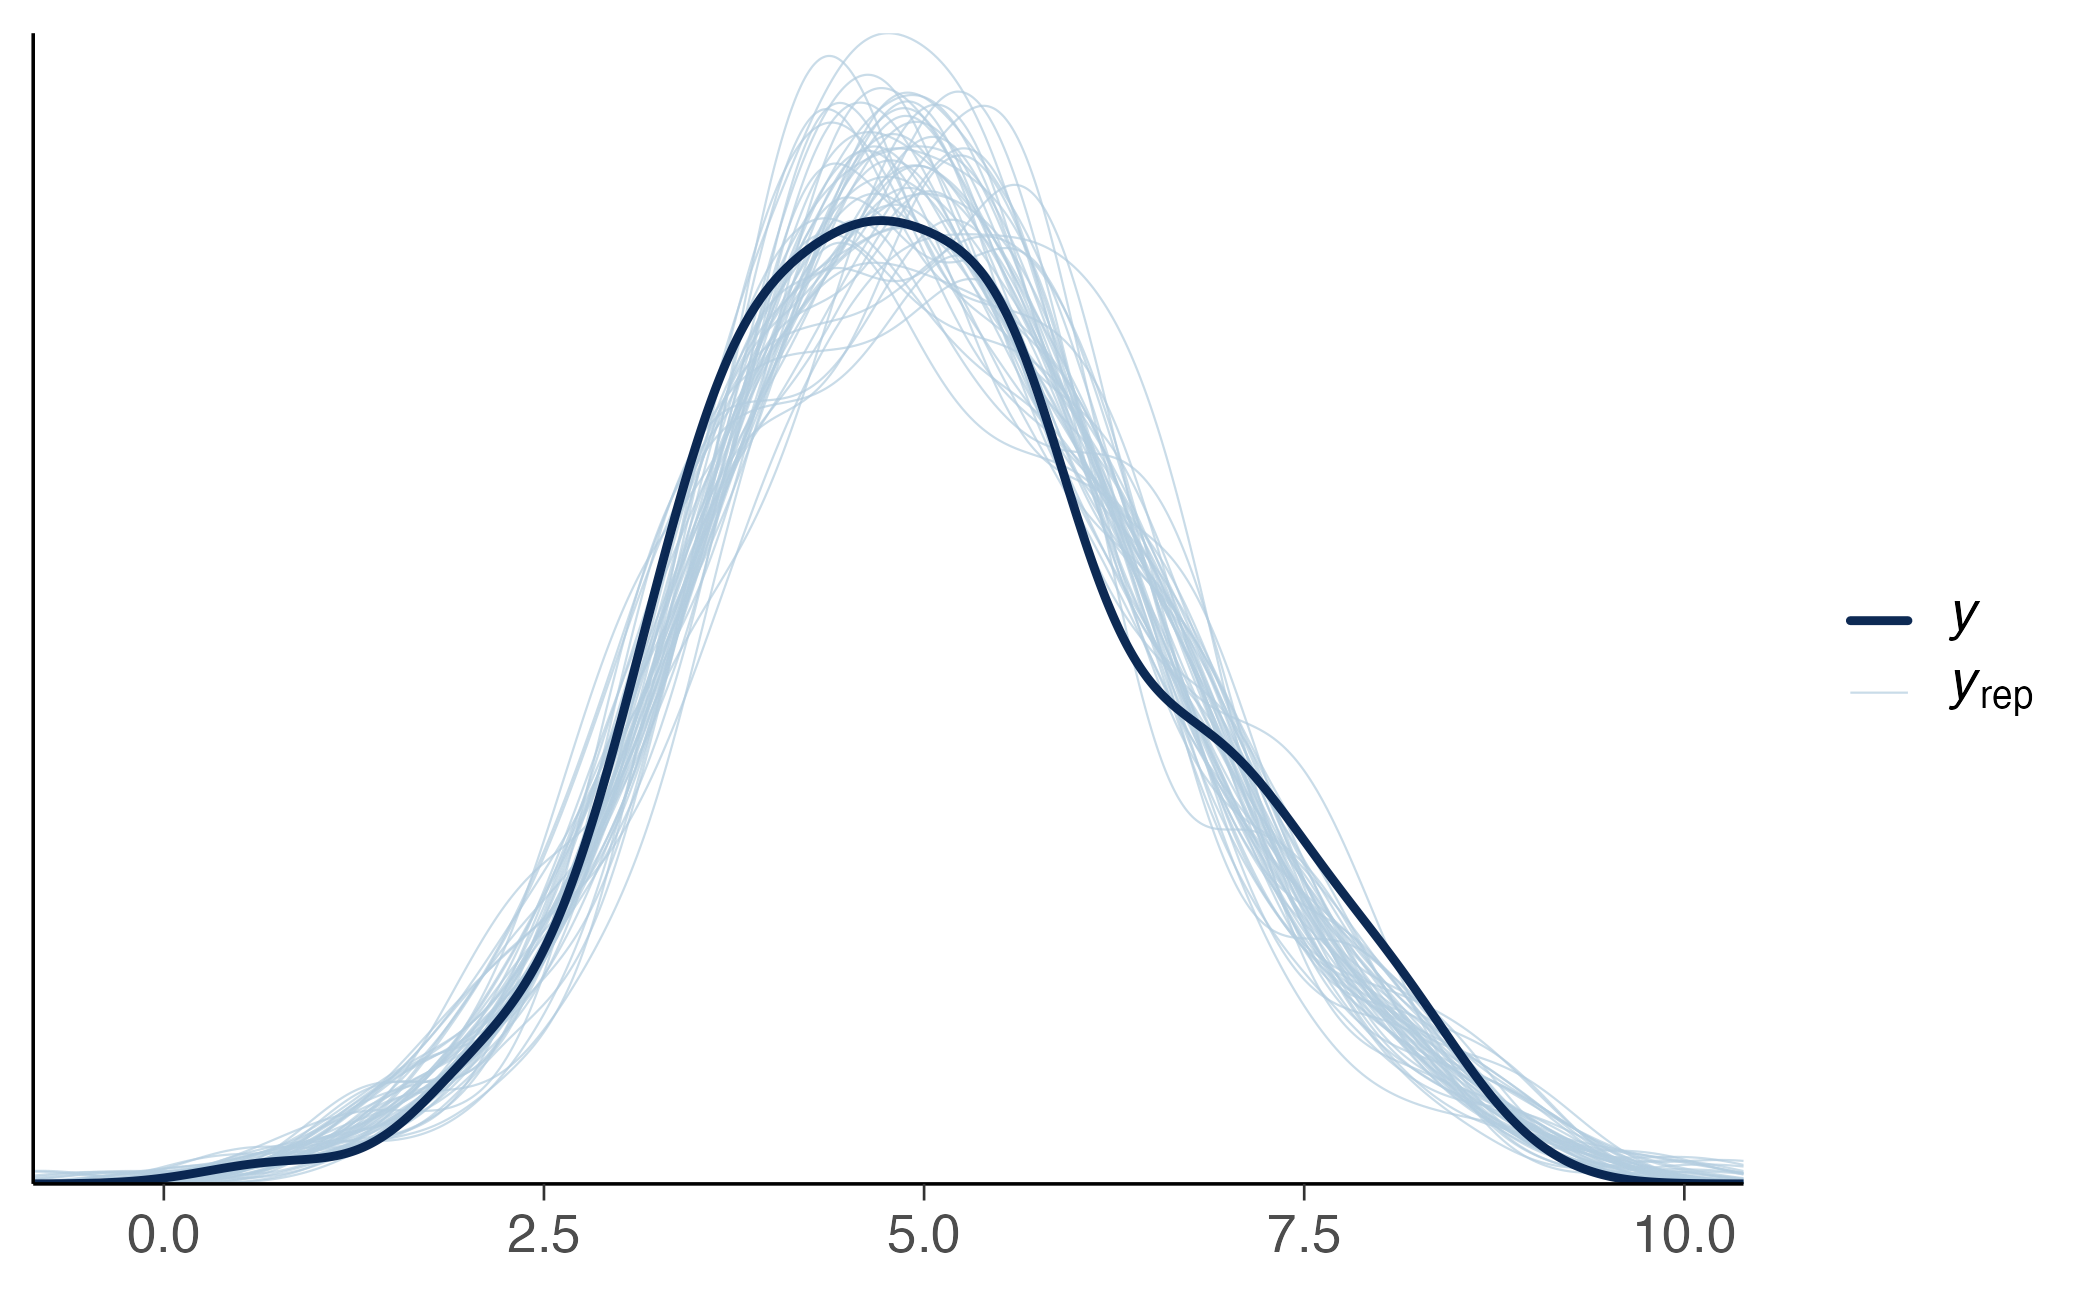
\includegraphics[width=0.85\linewidth,height=\textheight,keepaspectratio]{chapters/linear_models/04_dalla_formula_al_programma_files/figure-pdf/ppc-brms-multiple-1.png}
\end{center}

Nel caso del modello Stan diretto, utilizziamo le funzionalità del
pacchetto \texttt{posterior} per estrarre la matrice delle repliche dal
blocco \texttt{generated\ quantities} e passarla agli strumenti grafici
di \texttt{bayesplot}:

\begin{Shaded}
\begin{Highlighting}[]
\FunctionTok{library}\NormalTok{(bayesplot)}

\CommentTok{\# Estrazione dei draws come matrice bidimensionale (draws x osservazioni)}
\NormalTok{y\_rep\_stan }\OtherTok{\textless{}{-}}\NormalTok{ fit\_multiple\_stan}\SpecialCharTok{$}\FunctionTok{draws}\NormalTok{(}
  \AttributeTok{variables =} \StringTok{"y\_rep"}\NormalTok{,}
  \AttributeTok{format =} \StringTok{"draws\_matrix"}
\NormalTok{)}

\CommentTok{\# Visualizzazione del confronto grafico}
\FunctionTok{ppc\_dens\_overlay}\NormalTok{(}
  \AttributeTok{y =}\NormalTok{ stress\_data}\SpecialCharTok{$}\NormalTok{stress,}
  \AttributeTok{yrep =}\NormalTok{ y\_rep\_stan[}\DecValTok{1}\SpecialCharTok{:}\DecValTok{50}\NormalTok{, ]}
\NormalTok{)}
\end{Highlighting}
\end{Shaded}

\begin{center}
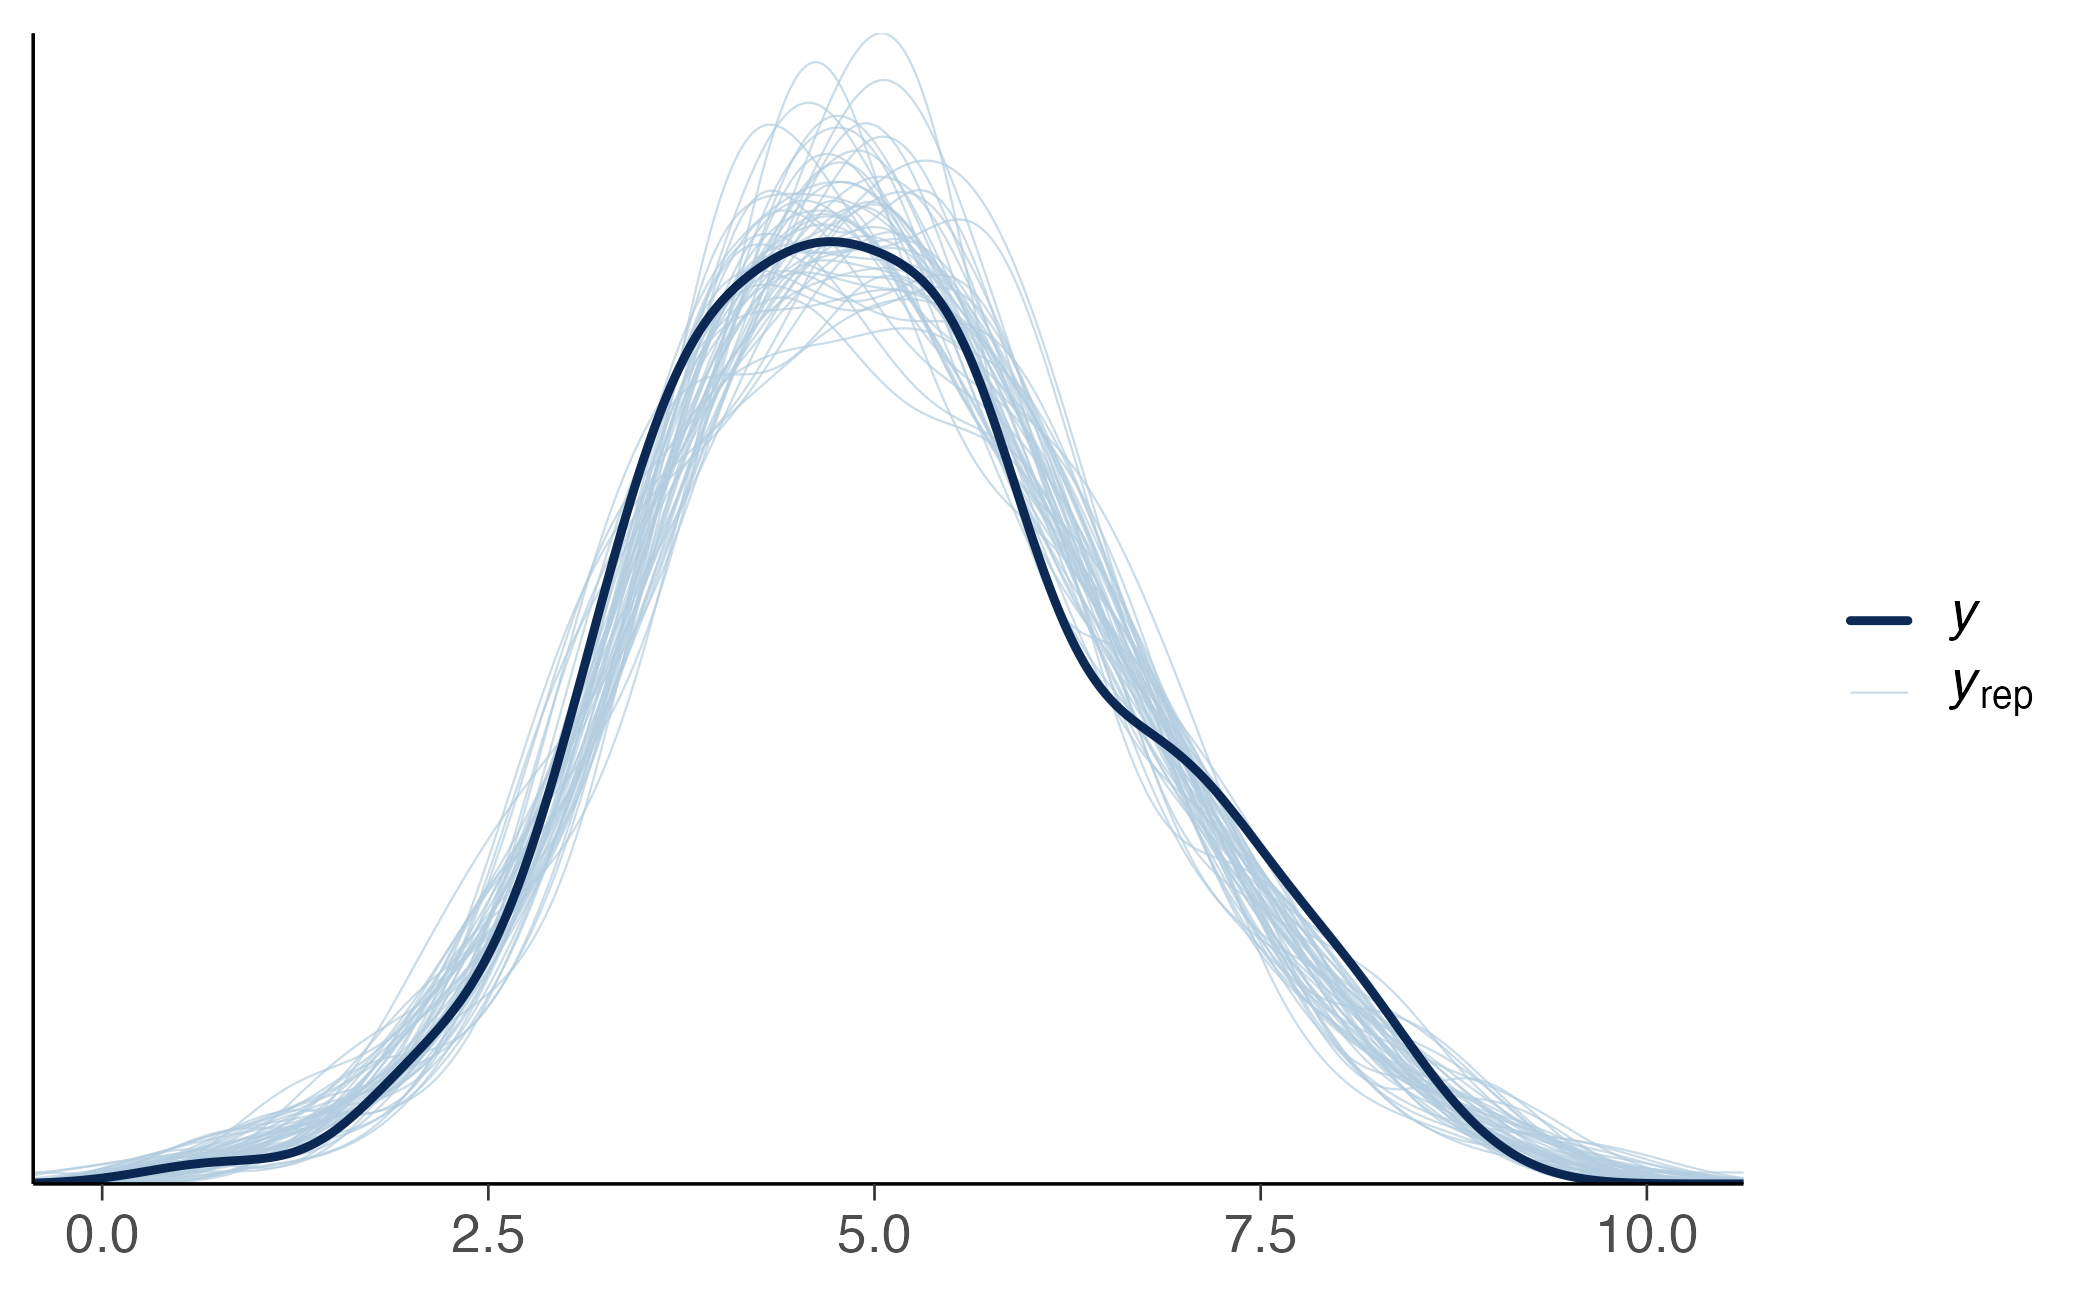
\includegraphics[width=0.85\linewidth,height=\textheight,keepaspectratio]{chapters/linear_models/04_dalla_formula_al_programma_files/figure-pdf/ppc-stan-multiple-1.png}
\end{center}

\begin{quote}
\textbf{Un avvertimento importante:} Una buona sovrapposizione tra la
densità dei dati reali (\(y\)) e quella delle simulazioni
(\(y_{\text{rep}}\)) indica che il modello ha catturato la forma della
distribuzione marginale dell'outcome, ma non garantisce che le relazioni
condizionate con i predittori siano corrette. Un modello può riprodurre
perfettamente la variabilità globale del fenomeno pur fallendo nel
descrivere l'effetto delle singole variabili esplicative. I controlli
diagnostici mirati a verificare la corretta forma funzionale delle
relazioni saranno l'oggetto centrale del prossimo capitolo sulla
specificazione.
\end{quote}

\section{Errori frequenti}\label{errori-frequenti-3}

\begin{tcolorbox}[enhanced jigsaw, arc=.35mm, bottomrule=.15mm, bottomtitle=1mm, breakable, colback=white, colbacktitle=quarto-callout-warning-color!10!white, colframe=quarto-callout-warning-color-frame, coltitle=black, left=2mm, leftrule=.75mm, opacityback=0, opacitybacktitle=0.6, rightrule=.15mm, title=\textcolor{quarto-callout-warning-color}{\faExclamationTriangle}\hspace{0.5em}{Errori di interpretazione e implementazione}, titlerule=0mm, toprule=.15mm, toptitle=1mm]

\begin{enumerate}
\def\labelenumi{\arabic{enumi}.}
\item
  \textbf{Trattare la formula come il modello completo.} La formula
  specifica soprattutto il predittore lineare; famiglia e prior devono
  essere considerate separatamente.
\item
  \textbf{Dimenticare l'intercetta implicita.}
  \texttt{y\ \textasciitilde{}\ x} include una colonna di 1. Per
  rimuoverla occorre usare \texttt{0\ +\ x} oppure \texttt{x\ -\ 1}.
\item
  \textbf{Interpretare coefficienti multipli come associazioni
  marginali.} Ogni coefficiente dipende dagli altri termini inclusi e
  dalla loro codifica.
\item
  \textbf{Attribuire automaticamente un significato causale al verbo
  ``controllare''.} Aggiungere una variabile può ridurre una
  distorsione, non avere utilità oppure introdurre un nuovo bias.
\item
  \textbf{Passare a Stan senza controllare la matrice del modello}
  Ordine e scala delle colonne devono corrispondere all'ordine e al
  significato dei coefficienti.
\item
  \textbf{Confrontare \texttt{brms} e Stan con prior diversi.} Risultati
  differenti possono derivare dalla specificazione, non dal motore
  computazionale.
\item
  \textbf{Usare prior generici senza considerarne la scala.} Un
  \texttt{normal(0,\ 1)} può essere moderato per un predittore
  standardizzato e molto restrittivo o molto ampio su altre scale.
\item
  \textbf{Considerare un PPC marginale come convalida completa.} Occorre
  scegliere statistiche e grafici sensibili ai possibili fallimenti del
  modello.
\end{enumerate}

\end{tcolorbox}

\section*{Riflessioni conclusive}\label{riflessioni-conclusive-21}

\markright{Riflessioni conclusive}

Una formula in R, una matrice del modello e un programma in codice Stan
non rappresentano tre modelli in competizione tra loro. Al contrario,
costituiscono tre livelli di astrazione decrescenti della medesima
struttura concettuale.

La formula rende immediatamente leggibile l'architettura delle nostre
ipotesi. La matrice del modello rende chiaro il meccanismo algebrico
sottostante, mostrando come ogni termine qualitativo o quantitativo
venga convertito in vettori numerici per il calcolo. Stan, infine,
rimuove qualsiasi barriera di astrazione rendendo espliciti i
presupposti probabilistici: la verosimiglianza dei dati, la calibrazione
dei \emph{prior} e la derivazione delle quantità generate. In questo
ecosistema, \texttt{brms} collega questi livelli traducendo
automaticamente una specificazione di alto livello in un programma Stan.

Oltre agli aspetti puramente computazionali, il passaggio alla
regressione multipla ha fatto emergere un principio interpretativo
cruciale: in un modello lineare, nessun coefficiente vive in isolamento.
Ogni parametro descrive un'associazione condizionata alla presenza degli
altri termini inclusi nel predittore lineare. Di conseguenza, l'entità e
persino il segno di un effetto possono mutare radicalmente al variare
della specificazione complessiva. Questa dipendenza non costituisce un
difetto del modello, ma segnala che il significato del coefficiente è
inseparabile dalla domanda, dalla codifica e dall'insieme dei
predittori.

Nei capitoli che seguono applicheremo la stessa grammatica generativa
per mostrare come la stima di una singola media, il confronto tra due o
più gruppi e i tradizionali modelli di ANOVA non siano altro che casi
particolari del modello lineare. La matrice del modello cambierà per
adattarsi a nuovi disegni sperimentali, ma il workflow bayesiano rimarrà
lo stesso.

\subsection{Concetti da ricordare}\label{concetti-da-ricordare-3}

\begin{enumerate}
\def\labelenumi{\arabic{enumi}.}
\tightlist
\item
  La formula R descrive la struttura del predittore lineare.
\item
  L'intercetta è inclusa per impostazione predefinita.
\item
  Ogni termine della formula genera una o più colonne della matrice del
  modello
\item
  Il prodotto \(\mathbf{X}\boldsymbol{\beta}\) produce i valori medi
  attesi.
\item
  In regressione multipla, i coefficienti sono associazioni condizionate
  agli altri predittori inclusi.
\item
  Formula, famiglia e prior sono componenti distinte della
  specificazione.
\item
  \texttt{brms} traduce la specificazione in codice Stan.
\item
  Stan diretto offre maggiore flessibilità, ma richiede più controlli.
\item
  Risultati compatibili richiedono dati, modello e prior compatibili.
\item
  La scelta del livello di astrazione deve dipendere dalla domanda, non
  dal prestigio dello strumento.
\end{enumerate}

\section*{Esercizi}\label{esercizi-5}

\markright{Esercizi}

\subsection{Esercizio 1 --- Leggere le
formule}\label{esercizio-1-leggere-le-formule}

Per ciascuna formula, descrivi quali termini entrano nel modello:

\begin{Shaded}
\begin{Highlighting}[]
\NormalTok{y }\SpecialCharTok{\textasciitilde{}}\NormalTok{ x}
\NormalTok{y }\SpecialCharTok{\textasciitilde{}} \DecValTok{0} \SpecialCharTok{+}\NormalTok{ gruppo}
\NormalTok{y }\SpecialCharTok{\textasciitilde{}}\NormalTok{ x1 }\SpecialCharTok{*}\NormalTok{ x2}
\NormalTok{y }\SpecialCharTok{\textasciitilde{}}\NormalTok{ x }\SpecialCharTok{+} \FunctionTok{I}\NormalTok{(x}\SpecialCharTok{\^{}}\DecValTok{2}\NormalTok{)}
\end{Highlighting}
\end{Shaded}

\begin{tcolorbox}[enhanced jigsaw, arc=.35mm, bottomrule=.15mm, bottomtitle=1mm, breakable, colback=white, colbacktitle=quarto-callout-tip-color!10!white, colframe=quarto-callout-tip-color-frame, coltitle=black, left=2mm, leftrule=.75mm, opacityback=0, opacitybacktitle=0.6, rightrule=.15mm, title=\textcolor{quarto-callout-tip-color}{\faLightbulb}\hspace{0.5em}{Traccia di soluzione}, titlerule=0mm, toprule=.15mm, toptitle=1mm]

\begin{itemize}
\tightlist
\item
  \texttt{y\ \textasciitilde{}\ x}: intercetta e termine lineare di
  \texttt{x};
\item
  \texttt{y\ \textasciitilde{}\ 0\ +\ gruppo}: una colonna per ciascun
  livello di \texttt{gruppo}, senza intercetta separata;
\item
  \texttt{y\ \textasciitilde{}\ x1\ *\ x2}: intercetta, effetti
  principali e interazione;
\item
  \texttt{y\ \textasciitilde{}\ x\ +\ I(x\^{}2)}: intercetta, termine
  lineare e termine quadratico.
\end{itemize}

\end{tcolorbox}

\subsection{Esercizio 2 --- Ispezionare la
matrice}\label{esercizio-2-ispezionare-la-matrice}

Costruisci con \texttt{model.matrix()} le matrici corrispondenti alle
quattro formule precedenti usando un piccolo dataset simulato. Verifica
numero, nome e contenuto delle colonne.

\begin{tcolorbox}[enhanced jigsaw, arc=.35mm, bottomrule=.15mm, bottomtitle=1mm, breakable, colback=white, colbacktitle=quarto-callout-tip-color!10!white, colframe=quarto-callout-tip-color-frame, coltitle=black, left=2mm, leftrule=.75mm, opacityback=0, opacitybacktitle=0.6, rightrule=.15mm, title=\textcolor{quarto-callout-tip-color}{\faLightbulb}\hspace{0.5em}{Traccia di soluzione}, titlerule=0mm, toprule=.15mm, toptitle=1mm]

Usa \texttt{colnames()} e \texttt{head()}. Per una variabile
categoriale, confronta la matrice con e senza intercetta.

\end{tcolorbox}

\subsection{Esercizio 3 --- Centrare un
predittore}\label{esercizio-3-centrare-un-predittore}

Crea \texttt{negative\_affect\_c} sottraendo la media campionaria.
Confronta le matrici e le stime dei modelli con predittore grezzo e
centrato.

\begin{tcolorbox}[enhanced jigsaw, arc=.35mm, bottomrule=.15mm, bottomtitle=1mm, breakable, colback=white, colbacktitle=quarto-callout-tip-color!10!white, colframe=quarto-callout-tip-color-frame, coltitle=black, left=2mm, leftrule=.75mm, opacityback=0, opacitybacktitle=0.6, rightrule=.15mm, title=\textcolor{quarto-callout-tip-color}{\faLightbulb}\hspace{0.5em}{Traccia di soluzione}, titlerule=0mm, toprule=.15mm, toptitle=1mm]

La pendenza e i valori previsti rimangono invariati; cambia
l'intercetta, che nel modello centrato rappresenta la media attesa al
valore medio del predittore.

\end{tcolorbox}

\subsection{Esercizio 4 --- Bivariato e
multiplo}\label{esercizio-4-bivariato-e-multiplo}

Aumenta in valore assoluto la correlazione tra \texttt{negative\_affect}
e \texttt{sleep\_c}. Osserva come cambia la differenza tra il
coefficiente bivariato e quello multiplo.

\begin{tcolorbox}[enhanced jigsaw, arc=.35mm, bottomrule=.15mm, bottomtitle=1mm, breakable, colback=white, colbacktitle=quarto-callout-tip-color!10!white, colframe=quarto-callout-tip-color-frame, coltitle=black, left=2mm, leftrule=.75mm, opacityback=0, opacitybacktitle=0.6, rightrule=.15mm, title=\textcolor{quarto-callout-tip-color}{\faLightbulb}\hspace{0.5em}{Traccia di soluzione}, titlerule=0mm, toprule=.15mm, toptitle=1mm]

A parità del processo generativo, una correlazione più forte aumenta il
contributo della variabile omessa al coefficiente bivariato. Il
coefficiente multiplo può recuperare i valori generativi se il modello è
correttamente specificato e i dati sono sufficientemente informativi.

\end{tcolorbox}

\subsection{Esercizio 5 --- Formula e
prior}\label{esercizio-5-formula-e-prior}

Usa \texttt{get\_prior()} e \texttt{make\_stancode()} per confrontare:

\begin{Shaded}
\begin{Highlighting}[]
\NormalTok{stress }\SpecialCharTok{\textasciitilde{}}\NormalTok{ negative\_affect}
\NormalTok{stress }\SpecialCharTok{\textasciitilde{}}\NormalTok{ negative\_affect }\SpecialCharTok{+}\NormalTok{ sleep\_c}
\end{Highlighting}
\end{Shaded}

Quali nuove classi o coefficienti compaiono?

\begin{tcolorbox}[enhanced jigsaw, arc=.35mm, bottomrule=.15mm, bottomtitle=1mm, breakable, colback=white, colbacktitle=quarto-callout-tip-color!10!white, colframe=quarto-callout-tip-color-frame, coltitle=black, left=2mm, leftrule=.75mm, opacityback=0, opacitybacktitle=0.6, rightrule=.15mm, title=\textcolor{quarto-callout-tip-color}{\faLightbulb}\hspace{0.5em}{Traccia di soluzione}, titlerule=0mm, toprule=.15mm, toptitle=1mm]

Il secondo modello aggiunge una colonna nella matrice del modello e un
coefficiente population-level. Famiglia e parametro \texttt{sigma}
rimangono invariati.

\end{tcolorbox}

\subsection{Esercizio 6 --- Una verosimiglianza
robusta}\label{esercizio-6-una-verosimiglianza-robusta}

Modifica il modello \texttt{brms} usando \texttt{family\ =\ student()}.
Ispeziona il codice Stan generato e individua il nuovo parametro.

\begin{tcolorbox}[enhanced jigsaw, arc=.35mm, bottomrule=.15mm, bottomtitle=1mm, breakable, colback=white, colbacktitle=quarto-callout-tip-color!10!white, colframe=quarto-callout-tip-color-frame, coltitle=black, left=2mm, leftrule=.75mm, opacityback=0, opacitybacktitle=0.6, rightrule=.15mm, title=\textcolor{quarto-callout-tip-color}{\faLightbulb}\hspace{0.5em}{Traccia di soluzione}, titlerule=0mm, toprule=.15mm, toptitle=1mm]

La verosimiglianza normale viene sostituita da una Student-\(t\) e
compare il parametro dei gradi di libertà, generalmente denominato
\texttt{nu} nell'output di \texttt{brms}.

\end{tcolorbox}

\subsection{Esercizio 7 --- Controllare la traduzione
Stan}\label{esercizio-7-controllare-la-traduzione-stan}

Cambia il prior di \texttt{beta} sia nel modello \texttt{brms} sia nel
programma Stan diretto. Verifica che le posterior rimangano compatibili.

\begin{tcolorbox}[enhanced jigsaw, arc=.35mm, bottomrule=.15mm, bottomtitle=1mm, breakable, colback=white, colbacktitle=quarto-callout-tip-color!10!white, colframe=quarto-callout-tip-color-frame, coltitle=black, left=2mm, leftrule=.75mm, opacityback=0, opacitybacktitle=0.6, rightrule=.15mm, title=\textcolor{quarto-callout-tip-color}{\faLightbulb}\hspace{0.5em}{Traccia di soluzione}, titlerule=0mm, toprule=.15mm, toptitle=1mm]

La verifica è informativa soltanto se formula, dati, famiglia, prior e
parametrizzazione sono allineati. Confronta intervalli e densità
posteriori, non soltanto le medie.

\end{tcolorbox}

\subsection{Esercizio 8 --- Scegliere lo
strumento}\label{esercizio-8-scegliere-lo-strumento}

Per ciascuno dei seguenti problemi, indica se useresti \texttt{brms} o
Stan diretto e motiva la scelta:

\begin{enumerate}
\def\labelenumi{\arabic{enumi}.}
\tightlist
\item
  regressione lineare con tre predittori;
\item
  modello multilivello standard;
\item
  modello di apprendimento con aggiornamento ricorsivo trial per trial;
\item
  regressione robusta Student-\(t\);
\item
  modello con un vincolo teorico non disponibile nelle formule standard.
\end{enumerate}

\begin{tcolorbox}[enhanced jigsaw, arc=.35mm, bottomrule=.15mm, bottomtitle=1mm, breakable, colback=white, colbacktitle=quarto-callout-tip-color!10!white, colframe=quarto-callout-tip-color-frame, coltitle=black, left=2mm, leftrule=.75mm, opacityback=0, opacitybacktitle=0.6, rightrule=.15mm, title=\textcolor{quarto-callout-tip-color}{\faLightbulb}\hspace{0.5em}{Traccia di soluzione}, titlerule=0mm, toprule=.15mm, toptitle=1mm]

I casi 1, 2 e 4 sono generalmente ben gestiti da \texttt{brms}. I casi 3
e 5 possono richiedere Stan diretto, soprattutto quando la ricorrenza o
il vincolo non sono esprimibili mediante le famiglie disponibili.

\end{tcolorbox}

\begin{tcolorbox}[enhanced jigsaw, arc=.35mm, bottomrule=.15mm, bottomtitle=1mm, breakable, colback=white, colbacktitle=quarto-callout-note-color!10!white, colframe=quarto-callout-note-color-frame, coltitle=black, left=2mm, leftrule=.75mm, opacityback=0, opacitybacktitle=0.6, rightrule=.15mm, title=\textcolor{quarto-callout-note-color}{\faInfo}\hspace{0.5em}{Informazioni sull'ambiente di sviluppo}, titlerule=0mm, toprule=.15mm, toptitle=1mm]

\begin{Shaded}
\begin{Highlighting}[]
\FunctionTok{sessionInfo}\NormalTok{()}
\CommentTok{\#\textgreater{} R version 4.6.1 (2026{-}06{-}24)}
\CommentTok{\#\textgreater{} Platform: aarch64{-}apple{-}darwin23}
\CommentTok{\#\textgreater{} Running under: macOS Tahoe 26.5.2}
\CommentTok{\#\textgreater{} }
\CommentTok{\#\textgreater{} Matrix products: default}
\CommentTok{\#\textgreater{} BLAS:   /Library/Frameworks/R.framework/Versions/4.6/Resources/lib/libRblas.0.dylib }
\CommentTok{\#\textgreater{} LAPACK: /Library/Frameworks/R.framework/Versions/4.6/Resources/lib/libRlapack.dylib;  LAPACK version 3.12.1}
\CommentTok{\#\textgreater{} }
\CommentTok{\#\textgreater{} locale:}
\CommentTok{\#\textgreater{} [1] C.UTF{-}8/UTF{-}8/C.UTF{-}8/C/C.UTF{-}8/C.UTF{-}8}
\CommentTok{\#\textgreater{} }
\CommentTok{\#\textgreater{} time zone: Europe/Zagreb}
\CommentTok{\#\textgreater{} tzcode source: internal}
\CommentTok{\#\textgreater{} }
\CommentTok{\#\textgreater{} attached base packages:}
\CommentTok{\#\textgreater{} [1] stats     graphics  grDevices utils     datasets  methods   base     }
\CommentTok{\#\textgreater{} }
\CommentTok{\#\textgreater{} other attached packages:}
\CommentTok{\#\textgreater{}  [1] cmdstanr\_0.9.0        ragg\_1.5.2            tinytable\_0.17.0     }
\CommentTok{\#\textgreater{}  [4] withr\_3.0.3           systemfonts\_1.3.2     patchwork\_1.3.2      }
\CommentTok{\#\textgreater{}  [7] ggdist\_3.3.3          tidybayes\_3.0.7       bayesplot\_1.15.0     }
\CommentTok{\#\textgreater{} [10] ggplot2\_4.0.3         reliabilitydiag\_0.2.1 priorsense\_1.2.0     }
\CommentTok{\#\textgreater{} [13] posterior\_1.7.0       loo\_2.10.0            rstan\_2.32.7         }
\CommentTok{\#\textgreater{} [16] StanHeaders\_2.32.10   brms\_2.23.0           Rcpp\_1.1.2           }
\CommentTok{\#\textgreater{} [19] sessioninfo\_1.2.4     conflicted\_1.2.0      janitor\_2.2.1        }
\CommentTok{\#\textgreater{} [22] matrixStats\_1.5.0     modelr\_0.1.11         tibble\_3.3.1         }
\CommentTok{\#\textgreater{} [25] dplyr\_1.2.1           tidyr\_1.3.2           rio\_1.3.0            }
\CommentTok{\#\textgreater{} [28] here\_1.0.2           }
\CommentTok{\#\textgreater{} }
\CommentTok{\#\textgreater{} loaded via a namespace (and not attached):}
\CommentTok{\#\textgreater{}  [1] gridExtra\_2.3.1       inline\_0.3.21         rlang\_1.3.0          }
\CommentTok{\#\textgreater{}  [4] magrittr\_2.0.5        snakecase\_0.11.1      otel\_0.2.0           }
\CommentTok{\#\textgreater{}  [7] compiler\_4.6.1        mgcv\_1.9{-}4            vctrs\_0.7.3          }
\CommentTok{\#\textgreater{} [10] reshape2\_1.4.5        stringr\_1.6.0         pkgconfig\_2.0.3      }
\CommentTok{\#\textgreater{} [13] arrayhelpers\_1.1{-}1    fastmap\_1.2.0         backports\_1.5.1      }
\CommentTok{\#\textgreater{} [16] labeling\_0.4.3        utf8\_1.2.6            rmarkdown\_2.31       }
\CommentTok{\#\textgreater{} [19] ps\_1.9.3              purrr\_1.2.2           xfun\_0.60            }
\CommentTok{\#\textgreater{} [22] cachem\_1.1.0          jsonlite\_2.0.0        broom\_1.0.13         }
\CommentTok{\#\textgreater{} [25] parallel\_4.6.1        R6\_2.6.1              stringi\_1.8.7        }
\CommentTok{\#\textgreater{} [28] RColorBrewer\_1.1{-}3    lubridate\_1.9.5       estimability\_2.0.0   }
\CommentTok{\#\textgreater{} [31] knitr\_1.51            pacman\_0.5.1          Matrix\_1.7{-}5         }
\CommentTok{\#\textgreater{} [34] splines\_4.6.1         timechange\_0.4.0      tidyselect\_1.2.1     }
\CommentTok{\#\textgreater{} [37] abind\_1.4{-}8           yaml\_2.3.12           codetools\_0.2{-}20     }
\CommentTok{\#\textgreater{} [40] curl\_7.1.0            processx\_3.9.0        pkgbuild\_1.4.8       }
\CommentTok{\#\textgreater{} [43] plyr\_1.8.9            lattice\_0.22{-}9        bridgesampling\_1.2{-}1 }
\CommentTok{\#\textgreater{} [46] S7\_0.2.2              coda\_0.19{-}4.1         evaluate\_1.0.5       }
\CommentTok{\#\textgreater{} [49] RcppParallel\_5.1.11{-}2 pillar\_1.11.1         tensorA\_0.36.2.1     }
\CommentTok{\#\textgreater{} [52] checkmate\_2.3.4       stats4\_4.6.1          distributional\_0.8.1 }
\CommentTok{\#\textgreater{} [55] generics\_0.1.4        rprojroot\_2.1.1       rstantools\_2.6.0     }
\CommentTok{\#\textgreater{} [58] scales\_1.4.0          xtable\_1.8{-}8          glue\_1.8.1           }
\CommentTok{\#\textgreater{} [61] emmeans\_2.0.4         tools\_4.6.1           data.table\_1.18.4    }
\CommentTok{\#\textgreater{} [64] mvtnorm\_1.4{-}2         grid\_4.6.1            QuickJSR\_1.10.0      }
\CommentTok{\#\textgreater{} [67] nlme\_3.1{-}170          cli\_3.6.6             textshaping\_1.0.5    }
\CommentTok{\#\textgreater{} [70] svUnit\_1.0.8          Brobdingnag\_1.2{-}9     V8\_8.2.0             }
\CommentTok{\#\textgreater{} [73] gtable\_0.3.6          digest\_0.6.39         farver\_2.1.2         }
\CommentTok{\#\textgreater{} [76] memoise\_2.0.1         htmltools\_0.5.9       lifecycle\_1.0.5}
\end{Highlighting}
\end{Shaded}

\end{tcolorbox}

\section*{Bibliografia}\label{bibliografia-24}

\markright{Bibliografia}

\chapter{Inferenza su una media: il modello a sola
intercetta}\label{sec-mcmc-one-mean}

Nei capitoli precedenti abbiamo definito il modello lineare mediante una
media condizionata che varia in funzione di uno o più predittori. Il
caso più semplice si ottiene eliminando tutti i predittori:

\[
Y_i \sim \operatorname{Normal}(\mu, \sigma).
\]

Il parametro \(\mu\) rappresenta il valore medio della popolazione
descritta dal modello, mentre lo scalare positivo \(\sigma\) misura la
variabilità delle osservazioni individuali attorno a tale media. In
termini di regressione, questo è un \emph{modello a sola intercetta}:

\[
Y_i = \alpha + \varepsilon_i, \qquad \varepsilon_i \sim \operatorname{Normal}(0, \sigma)
\] in cui il coefficiente \(\alpha\) coincide con la media \(\mu\).
Nella sintassi di \texttt{brms}, questa componente sistematica si
esprime con la formula \texttt{y\ \textasciitilde{}\ 1}.

Sebbene minimale, il modello contiene già tutti gli elementi del
workflow bayesiano: una funzione di verosimiglianza, prior espliciti,
una distribuzione a posteriori, quantità predittive e controlli di
adeguatezza. Isolare questa struttura elementare aiuta a distinguere tre
quantità che vengono spesso confuse:

\begin{itemize}
\tightlist
\item
  \textbf{La media della popolazione (\(\mu\) o \(\alpha\)):} il
  baricentro teorico stimato dal modello;
\item
  \textbf{La variabilità tra individui (\(\sigma\)):} l'eterogeneità
  biologica o psicometrica del campione;
\item
  \textbf{La stima di una nuova osservazione (\(y_{\text{new}}\)):} la
  previsione su un singolo soggetto futuro, che deve incorporare sia
  l'incertezza sulla media sia la dispersione residua.
\end{itemize}

\begin{tcolorbox}[enhanced jigsaw, arc=.35mm, bottomrule=.15mm, breakable, colback=white, colframe=quarto-callout-important-color-frame, left=2mm, leftrule=.75mm, opacityback=0, rightrule=.15mm, toprule=.15mm]

\textbf{Da sapere.} Il confronto tra più gruppi è un caso del modello
lineare con un predittore categoriale. Parametrizzazioni diverse ---
categoria di riferimento o medie di cella --- descrivono lo stesso
insieme di medie, ma cambiano l'interpretazione immediata dei
coefficienti e dei prior. Le domande scientifiche devono essere tradotte
in contrasti pianificati, distinguendo la probabilità direzionale dalla
rilevanza pratica e senza presumere che l'approccio bayesiano elimini
automaticamente il problema della molteplicità.

\textbf{Da saper fare.} Stimare con \texttt{brms} un modello a più
gruppi; specificare prior coerenti con la parametrizzazione; eseguire i
controlli predittivi a priori e a posteriori; ricavare le distribuzioni
a posteriori delle medie di gruppo e dei contrasti; calcolare
probabilità sostantive e valutare le differenze rispetto a una soglia di
rilevanza pratica.

\textbf{Approfondimento facoltativo.} La costruzione dettagliata delle
matrici del modello, il confronto sistematico tra codifica a riferimento
e medie di cella, l'uso di \texttt{emmeans}, la valutazione omnibus e le
estensioni a varianze differenti o modelli robusti possono essere
rimandati in una prima lettura. Nel percorso essenziale è sufficiente
comprendere le medie di cella, formulare contrasti guidati dalla teoria
e interpretarli attraverso la distribuzione a posteriori.

\hyperref[sec-percorsi-lettura]{Che cosa significano queste etichette?}

\end{tcolorbox}

\begin{tcolorbox}[enhanced jigsaw, arc=.35mm, bottomrule=.15mm, bottomtitle=1mm, breakable, colback=white, colbacktitle=quarto-callout-note-color!10!white, colframe=quarto-callout-note-color-frame, coltitle=black, left=2mm, leftrule=.75mm, opacityback=0, opacitybacktitle=0.6, rightrule=.15mm, title=\textcolor{quarto-callout-note-color}{\faInfo}\hspace{0.5em}{Obiettivi del capitolo}, titlerule=0mm, toprule=.15mm, toptitle=1mm]

Al termine del capitolo dovresti essere in grado di:

\begin{itemize}
\tightlist
\item
  riconoscere la stima di una media come un modello lineare a sola
  intercetta;
\item
  distinguere il parametro di posizione \(\mu\) dal parametro di
  dispersione \(\sigma\);
\item
  formulare prior plausibili sulla scala originale della variabile;
\item
  calibrare tali prior mediante simulazioni predittive a priori;
\item
  interpretare la distribuzione a posteriori della media;
\item
  distinguere l'incertezza sulla media dalla distribuzione predittiva di
  una nuova osservazione;
\item
  valutare quando una verosimiglianza Student-\(t\) possa essere
  preferibile a una normale;
\item
  formulare conclusioni probabilistiche coerenti con il modello e con la
  popolazione campionata.
\end{itemize}

\end{tcolorbox}

\begin{tcolorbox}[enhanced jigsaw, arc=.35mm, bottomrule=.15mm, bottomtitle=1mm, breakable, colback=white, colbacktitle=quarto-callout-tip-color!10!white, colframe=quarto-callout-tip-color-frame, coltitle=black, left=2mm, leftrule=.75mm, opacityback=0, opacitybacktitle=0.6, rightrule=.15mm, title=\textcolor{quarto-callout-tip-color}{\faLightbulb}\hspace{0.5em}{Percorsi di lettura}, titlerule=0mm, toprule=.15mm, toptitle=1mm]

Il capitolo appartiene al \textbf{percorso essenziale} e al
\textbf{percorso concettuale}. Chi segue il percorso essenziale dovrebbe
concentrarsi sulla formulazione del modello, sui prior, sulle quantità
posteriori e sulle previsioni. Le sezioni dedicate al confronto tra
verosimiglianza normale e Student-\(t\) costituiscono un primo
approfondimento sulla revisione della specificazione.

\end{tcolorbox}

\begin{tcolorbox}[enhanced jigsaw, arc=.35mm, bottomrule=.15mm, bottomtitle=1mm, breakable, colback=white, colbacktitle=quarto-callout-tip-color!10!white, colframe=quarto-callout-tip-color-frame, coltitle=black, left=2mm, leftrule=.75mm, opacityback=0, opacitybacktitle=0.6, rightrule=.15mm, title=\textcolor{quarto-callout-tip-color}{\faLightbulb}\hspace{0.5em}{Prerequisiti e approfondimenti}, titlerule=0mm, toprule=.15mm, toptitle=1mm]

\begin{itemize}
\tightlist
\item
  Il modello lineare come modello generativo è introdotto
  nell'Capitolo~\ref{sec-linear-generative}.
\item
  Il workflow bayesiano completo con \texttt{brms} è sviluppato
  nell'Capitolo~\ref{sec-linmod-bayesian-reg}.
\item
  La relazione tra formule R, matrice del modello e programma Stan è
  discussa nell'Capitolo~\ref{sec-linar-models-brms}.
\item
  Per il trattamento frequentista della media campionaria, del test
  \(t\) e dell'intervallo di confidenza si veda il modulo
  \href{https://ccaudek.github.io/utet-frequentista}{utet-frequentista}.
\item
  L'esempio sulle altezze degli adulti !Kung San è tratto da McElreath
  (\citeproc{ref-McElreath_rethinking}{2020}).
\end{itemize}

\end{tcolorbox}

\begin{tcolorbox}[enhanced jigsaw, arc=.35mm, bottomrule=.15mm, bottomtitle=1mm, breakable, colback=white, colbacktitle=quarto-callout-caution-color!10!white, colframe=quarto-callout-caution-color-frame, coltitle=black, left=2mm, leftrule=.75mm, opacityback=0, opacitybacktitle=0.6, rightrule=.15mm, title=\textcolor{quarto-callout-caution-color}{\faFire}\hspace{0.5em}{Preparazione del Notebook}, titlerule=0mm, toprule=.15mm, toptitle=1mm]

\end{tcolorbox}

\section{Dalla domanda scientifica alla quantità di
interesse}\label{dalla-domanda-scientifica-alla-quantituxe0-di-interesse-3}

Consideriamo le altezze rilevate da Nancy Howell tra gli adulti !Kung
San del Kalahari (\citeproc{ref-McElreath_rethinking}{McElreath, 2020}).
La domanda descrittiva è:

\begin{quote}
Qual è l'altezza media degli adulti nella popolazione rappresentata dal
campione e quanta variabilità individuale esiste attorno a tale media?
\end{quote}

Le quantità di interesse principali sono:

\begin{itemize}
\tightlist
\item
  \(\mu\): l'altezza media della popolazione stimata dal modello;
\item
  \(\sigma\): la deviazione standard delle altezze individuali;
\item
  \(\Pr(\mu>c\mid y)\): la probabilità a posteriori che la media superi
  una specifica soglia teorica \(c\);
\item
  \(p(\widetilde{y}\mid y)\): la distribuzione predittiva a posteriori
  per l'altezza \(\widetilde{y}\) di un nuovo individuo.
\end{itemize}

\begin{tcolorbox}[enhanced jigsaw, arc=.35mm, bottomrule=.15mm, bottomtitle=1mm, breakable, colback=white, colbacktitle=quarto-callout-important-color!10!white, colframe=quarto-callout-important-color-frame, coltitle=black, left=2mm, leftrule=.75mm, opacityback=0, opacitybacktitle=0.6, rightrule=.15mm, title=\textcolor{quarto-callout-important-color}{\faExclamation}\hspace{0.5em}{Limiti di generalizzazione della popolazione}, titlerule=0mm, toprule=.15mm, toptitle=1mm]

La distribuzione a posteriori non descrive l'altezza media degli esseri
umani in generale. Definisce il parametro \(\mu\) strettamente
all'interno del modello e in relazione alla specifica popolazione da cui
il campione è stato estratto. La validità esterna delle conclusioni
dipende dal disegno di ricerca, non dall'ampiezza dell'intervallo di
credibilità.

\end{tcolorbox}

\section{Esplorazione dei dati}\label{esplorazione-dei-dati}

Carichiamo il dataset ed esaminiamo la struttura delle variabili:

\begin{Shaded}
\begin{Highlighting}[]
\NormalTok{height\_data }\OtherTok{\textless{}{-}}\NormalTok{ rio}\SpecialCharTok{::}\FunctionTok{import}\NormalTok{(}
\NormalTok{  here}\SpecialCharTok{::}\FunctionTok{here}\NormalTok{(}\StringTok{"data"}\NormalTok{, }\StringTok{"Howell\_18.csv"}\NormalTok{)}
\NormalTok{)}

\NormalTok{dplyr}\SpecialCharTok{::}\FunctionTok{glimpse}\NormalTok{(height\_data)}
\CommentTok{\#\textgreater{} Rows: 352}
\CommentTok{\#\textgreater{} Columns: 4}
\CommentTok{\#\textgreater{} $ height \textless{}dbl\textgreater{} 152, 140, 137, 157, 145, 164, 149, 169, 148, 165, 154, 151, 145\textasciitilde{}}
\CommentTok{\#\textgreater{} $ weight \textless{}dbl\textgreater{} 47.8, 36.5, 31.9, 53.0, 41.3, 63.0, 38.2, 55.5, 34.9, 54.5, 49.\textasciitilde{}}
\CommentTok{\#\textgreater{} $ age    \textless{}dbl\textgreater{} 63.0, 63.0, 65.0, 41.0, 51.0, 35.0, 32.0, 27.0, 19.0, 54.0, 47.\textasciitilde{}}
\CommentTok{\#\textgreater{} $ male   \textless{}int\textgreater{} 1, 0, 0, 1, 0, 1, 0, 1, 0, 1, 0, 1, 0, 0, 0, 1, 1, 0, 1, 0, 1, \textasciitilde{}}
\end{Highlighting}
\end{Shaded}

Il file include già gli individui adulti selezionati per l'analisi.
Prima di specificare il modello, verifichiamo la numerosità del
campione, la presenza di valori mancanti e le caratteristiche principali
della distribuzione (posizione, dispersione e forma):

\begin{Shaded}
\begin{Highlighting}[]
\NormalTok{height\_summary }\OtherTok{\textless{}{-}}\NormalTok{ height\_data }\SpecialCharTok{|\textgreater{}}
  \FunctionTok{summarise}\NormalTok{(}
    \AttributeTok{n       =} \FunctionTok{sum}\NormalTok{(}\SpecialCharTok{!}\FunctionTok{is.na}\NormalTok{(height)),}
    \AttributeTok{missing =} \FunctionTok{sum}\NormalTok{(}\FunctionTok{is.na}\NormalTok{(height)),}
    \AttributeTok{mean    =} \FunctionTok{mean}\NormalTok{(height, }\AttributeTok{na.rm =} \ConstantTok{TRUE}\NormalTok{),}
    \AttributeTok{sd      =} \FunctionTok{sd}\NormalTok{(height, }\AttributeTok{na.rm =} \ConstantTok{TRUE}\NormalTok{),}
    \AttributeTok{min     =} \FunctionTok{min}\NormalTok{(height, }\AttributeTok{na.rm =} \ConstantTok{TRUE}\NormalTok{),}
    \AttributeTok{max     =} \FunctionTok{max}\NormalTok{(height, }\AttributeTok{na.rm =} \ConstantTok{TRUE}\NormalTok{)}
\NormalTok{  )}

\NormalTok{height\_summary}
\CommentTok{\#\textgreater{}     n missing mean   sd min max}
\CommentTok{\#\textgreater{} 1 352       0  155 7.74 137 179}
\end{Highlighting}
\end{Shaded}

Visualizziamo la forma della distribuzione empirica tramite un
istogramma:

\begin{Shaded}
\begin{Highlighting}[]
\NormalTok{height\_data }\SpecialCharTok{|\textgreater{}}
  \FunctionTok{filter}\NormalTok{(}\SpecialCharTok{!}\FunctionTok{is.na}\NormalTok{(height)) }\SpecialCharTok{|\textgreater{}}
  \FunctionTok{ggplot}\NormalTok{(}\FunctionTok{aes}\NormalTok{(}\AttributeTok{x =}\NormalTok{ height)) }\SpecialCharTok{+}
  \FunctionTok{geom\_histogram}\NormalTok{(}\AttributeTok{binwidth =} \DecValTok{3}\NormalTok{, }\AttributeTok{boundary =} \DecValTok{0}\NormalTok{, }\AttributeTok{color =} \StringTok{"white"}\NormalTok{, }\AttributeTok{fill =} \StringTok{"grey30"}\NormalTok{) }\SpecialCharTok{+}
  \FunctionTok{labs}\NormalTok{(}
    \AttributeTok{x =} \StringTok{"Altezza (cm)"}\NormalTok{,}
    \AttributeTok{y =} \StringTok{"Frequenza"}
\NormalTok{  )}
\end{Highlighting}
\end{Shaded}

\begin{figure}[H]

{\centering 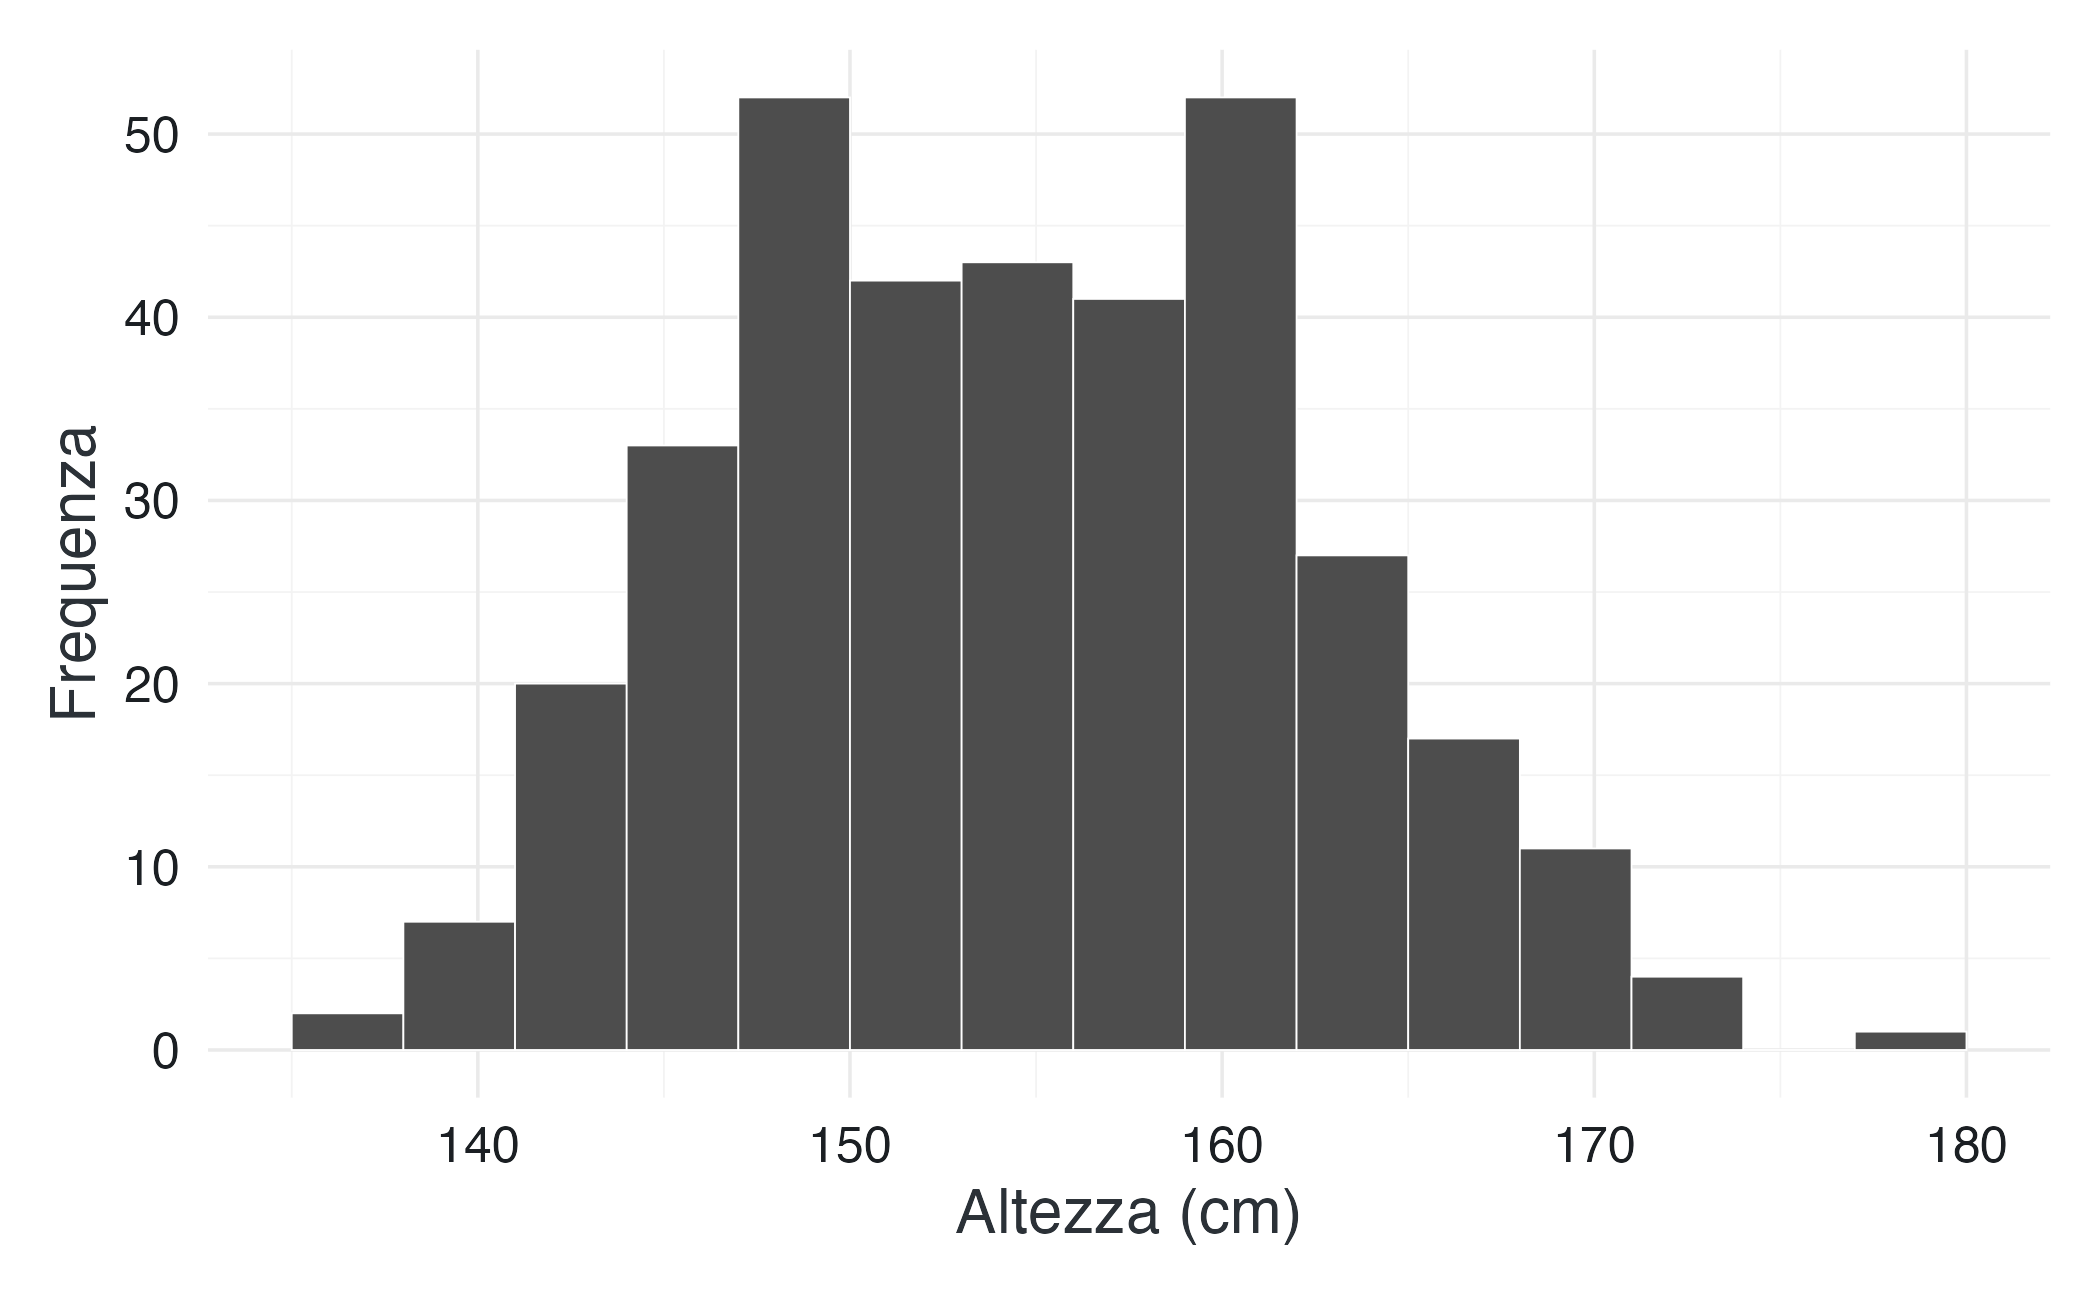
\includegraphics[width=0.85\linewidth,height=\textheight,keepaspectratio]{chapters/linear_models/05_inferenza_su_una_media_files/figure-pdf/plot-howell-height-1.png}

}

\caption{Distribuzione osservata delle altezze nel campione di adulti
!Kung San.}

\end{figure}%

L'analisi grafica non serve a decidere in modo meccanico se i dati
seguano perfettamente una distribuzione normale. Il suo scopo è
identificare le proprietà geometriche fondamentali che il modello
statistico dovrà essere in grado di riprodurre: la centralità, la
dispersione, l'eventuale asimmetria e la presenza di osservazioni
anomale o outliers.

\section{Il modello a sola
intercetta}\label{il-modello-a-sola-intercetta}

La specificazione formale del modello lineare semplice senza predittori
è:

\[
\begin{aligned} 
Y_i \mid \mu,\sigma &\sim \operatorname{Normal}(\mu,\sigma),\\ \mu &= \alpha. 
\end{aligned}
\]

In notazione matriciale, la struttura si esprime come:

\[
\mathbf{y}=\mathbf{1}\alpha+\boldsymbol{\varepsilon},
\] in cui la matrice del modello \(\mathbf{X}\) si riduce a un unico
vettore colonna composto da valori pari a \(1\)
(\citeproc{ref-caudek2001statistica}{Caudek \& Luccio, 2001}). La
formula R:

\begin{Shaded}
\begin{Highlighting}[]
\NormalTok{height }\SpecialCharTok{\textasciitilde{}} \DecValTok{1}
\end{Highlighting}
\end{Shaded}

istruisce il software a stimare un solo parametro a livello di
popolazione (\emph{population-level}): l'intercetta.

\begin{tcolorbox}[enhanced jigsaw, arc=.35mm, bottomrule=.15mm, bottomtitle=1mm, breakable, colback=white, colbacktitle=quarto-callout-note-color!10!white, colframe=quarto-callout-note-color-frame, coltitle=black, left=2mm, leftrule=.75mm, opacityback=0, opacitybacktitle=0.6, rightrule=.15mm, title=\textcolor{quarto-callout-note-color}{\faInfo}\hspace{0.5em}{Significato dell'intercetta}, titlerule=0mm, toprule=.15mm, toptitle=1mm]

Nei modelli con predittori, l'intercetta rappresenta la media
condizionata calcolata quando tutte le variabili esplicative sono poste
a zero. Nel modello \texttt{height\ \textasciitilde{}\ 1}, data
l'assenza di predittori, l'intercetta coincide direttamente con la media
globale \(\mu\) della distribuzione.

\end{tcolorbox}

\section{Calibrazione dei prior sulla scala
osservata}\label{calibrazione-dei-prior-sulla-scala-osservata}

I \emph{prior} devono essere valutati in base alle conseguenze che
producono sulla scala originaria delle misure. Per l'altezza di una
popolazione adulta espressa in centimetri, definiamo la seguente
struttura probabilistica:

\[
\begin{aligned} 
\mu &\sim \operatorname{Normal}(160,20),\\ \sigma &\sim \operatorname{LogNormal}\!\left(\log 15, 0.5\right). 
\end{aligned}
\]

La distribuzione assegnata a \(\mu\) concentra la massa di probabilità
attorno a valori biologicamente compatibili con la statura umana adulta,
pur mantenendo un'incertezza sufficientemente ampia. Il \emph{prior} su
\(\sigma\) garantisce matematicamente la positività del parametro e
ammette una gamma plausibile di variabilità interindividuale.

Definiamo questi vincoli in \texttt{brms}:

\begin{Shaded}
\begin{Highlighting}[]
\NormalTok{height\_priors }\OtherTok{\textless{}{-}} \FunctionTok{c}\NormalTok{(}
  \FunctionTok{prior}\NormalTok{(}\FunctionTok{normal}\NormalTok{(}\DecValTok{160}\NormalTok{, }\DecValTok{20}\NormalTok{), }\AttributeTok{class =} \StringTok{"Intercept"}\NormalTok{),}
  \FunctionTok{prior}\NormalTok{(}\FunctionTok{lognormal}\NormalTok{(}\FunctionTok{log}\NormalTok{(}\DecValTok{15}\NormalTok{), }\FloatTok{0.5}\NormalTok{), }\AttributeTok{class =} \StringTok{"sigma"}\NormalTok{)}
\NormalTok{)}

\NormalTok{height\_priors}
\CommentTok{\#\textgreater{}                    prior     class coef group resp dpar nlpar   lb   ub tag}
\CommentTok{\#\textgreater{}          normal(160, 20) Intercept                            \textless{}NA\textgreater{} \textless{}NA\textgreater{}    }
\CommentTok{\#\textgreater{}  lognormal(log(15), 0.5)     sigma                            \textless{}NA\textgreater{} \textless{}NA\textgreater{}    }
\CommentTok{\#\textgreater{}  source}
\CommentTok{\#\textgreater{}    user}
\CommentTok{\#\textgreater{}    user}
\end{Highlighting}
\end{Shaded}

\begin{quote}
Le etichette ``informativo'' o ``debolmente informativo'' non esprimono
proprietà assolute di una distribuzione. Il grado di restrittività di un
\emph{prior} va sempre ponderato in relazione alla scala metrica della
variabile osservata e agli obiettivi dell'analisi.
\end{quote}

\section{Controllo predittivo a
priori}\label{controllo-predittivo-a-priori}

Prima di utilizzare le altezze osservate, simuliamo i dati implicati
esclusivamente dalle nostre assunzioni a priori (\emph{prior predictive
check}). Questo passaggio permette di verificare la plausibilità
biologica del modello prima che venga condizionato dall'evidenza
empirica.

\begin{Shaded}
\begin{Highlighting}[]
\NormalTok{fit\_height\_prior }\OtherTok{\textless{}{-}} \FunctionTok{brm}\NormalTok{(}
  \AttributeTok{formula =}\NormalTok{ height }\SpecialCharTok{\textasciitilde{}} \DecValTok{1}\NormalTok{,}
  \AttributeTok{data =}\NormalTok{ height\_data,}
  \AttributeTok{family =} \FunctionTok{gaussian}\NormalTok{(),}
  \AttributeTok{prior =}\NormalTok{ height\_priors,}
  \AttributeTok{sample\_prior =} \StringTok{"only"}\NormalTok{, }\CommentTok{\# Campiona esclusivamente dalle distribuzioni a priori}
  \AttributeTok{chains =} \DecValTok{4}\NormalTok{,}
  \AttributeTok{iter =} \DecValTok{1000}\NormalTok{,}
  \AttributeTok{seed =} \DecValTok{1234}\NormalTok{,}
  \AttributeTok{backend =} \StringTok{"cmdstanr"}\NormalTok{,}
  \AttributeTok{refresh =} \DecValTok{0}
\NormalTok{)}
\end{Highlighting}
\end{Shaded}

Visualizziamo le distribuzioni simulate generando un grafico di
sovrapposizione delle densità:

\begin{Shaded}
\begin{Highlighting}[]
\FunctionTok{pp\_check}\NormalTok{(}
\NormalTok{  fit\_height\_prior,}
  \AttributeTok{type =} \StringTok{"dens\_overlay"}\NormalTok{,}
  \AttributeTok{ndraws =} \DecValTok{50}
\NormalTok{)}
\end{Highlighting}
\end{Shaded}

\begin{figure}[H]

{\centering 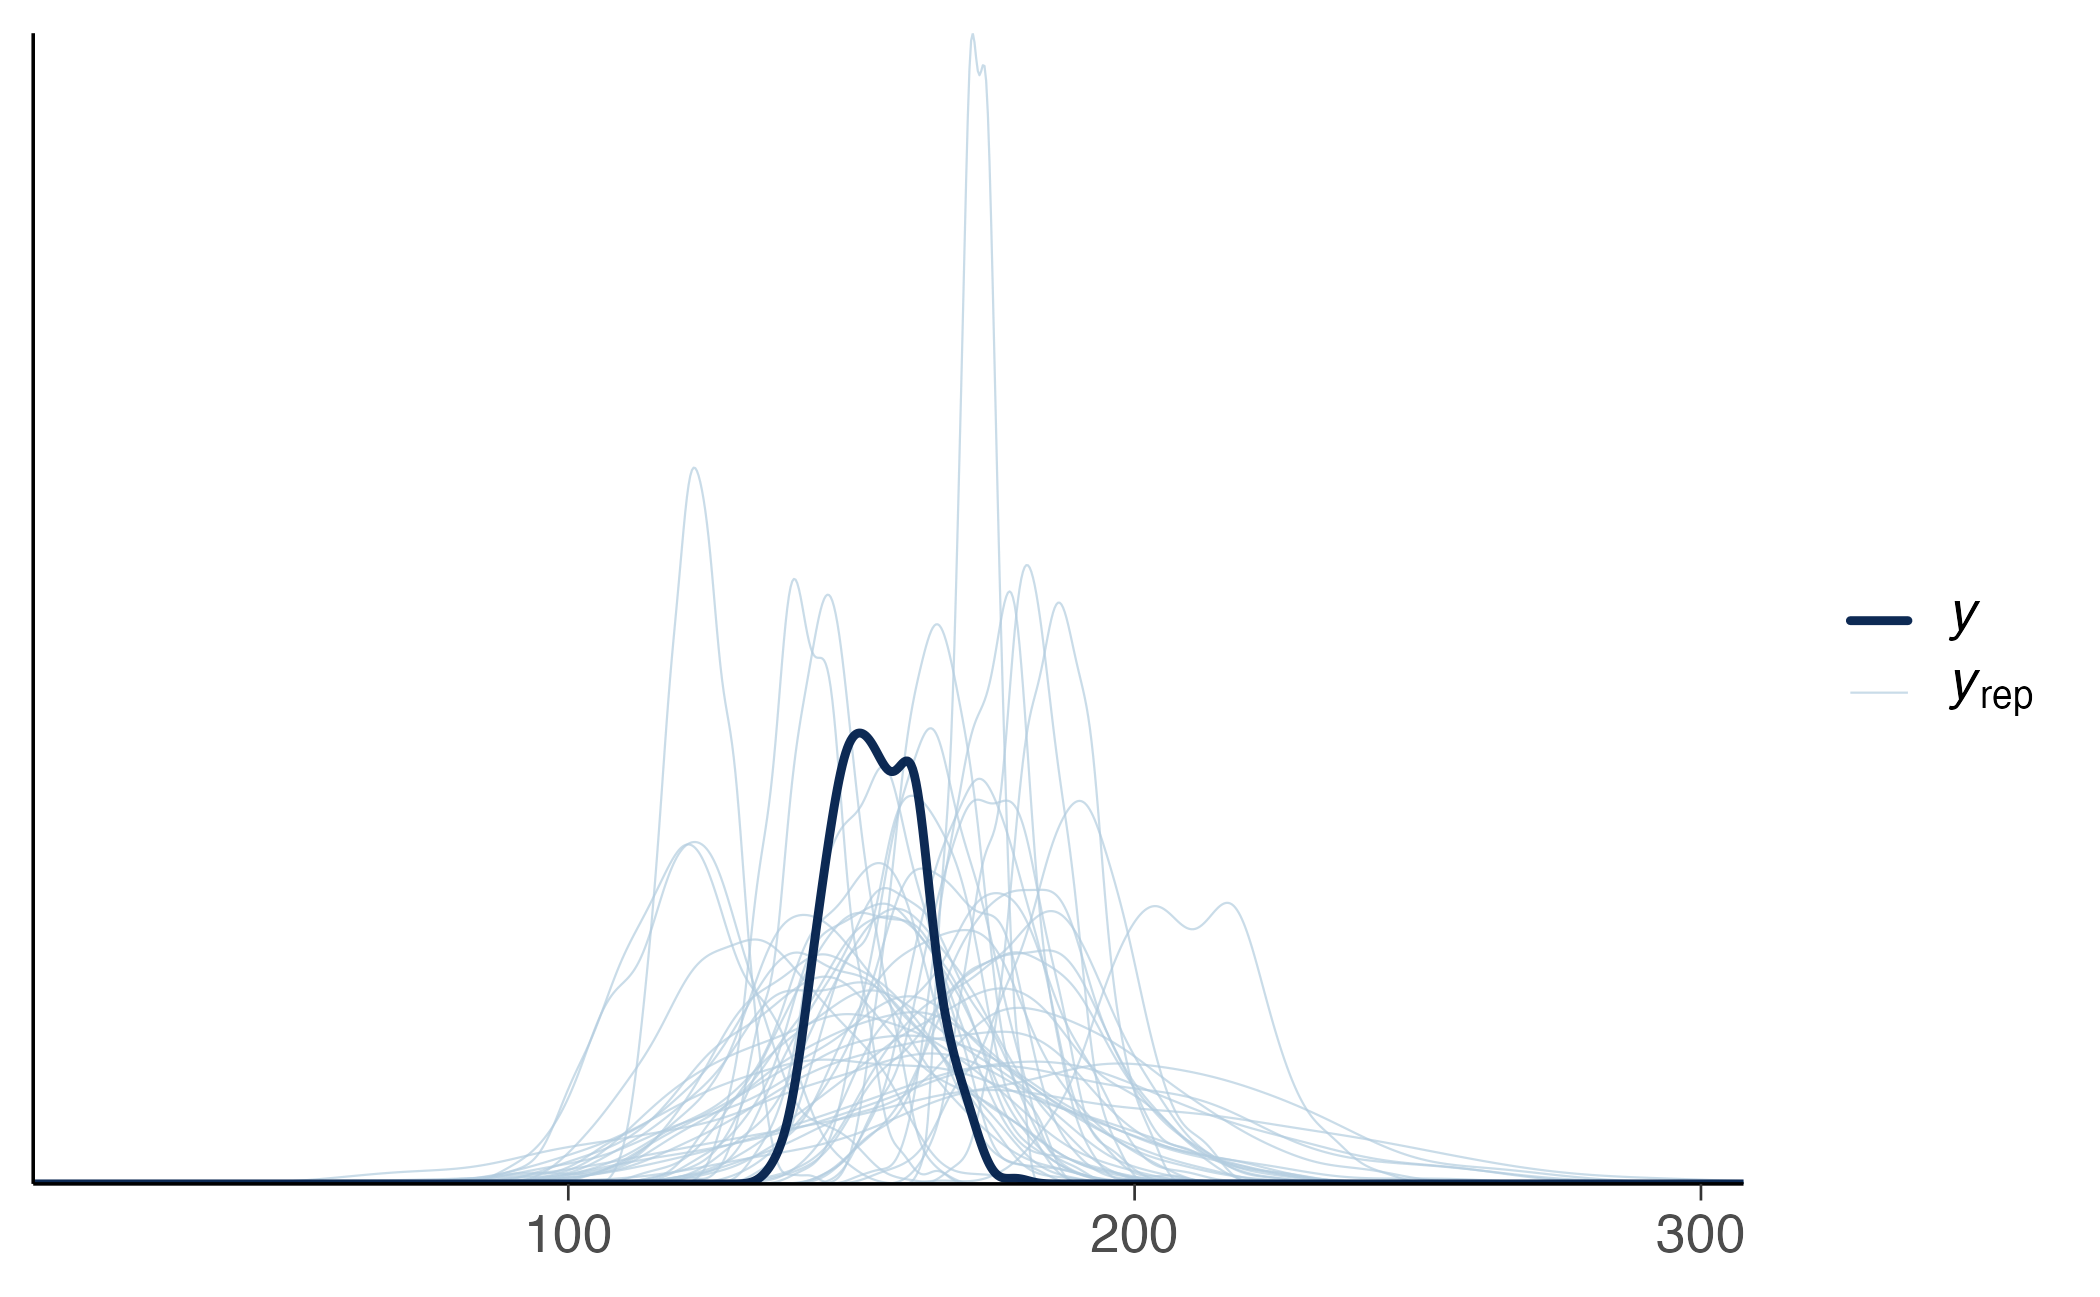
\includegraphics[width=0.85\linewidth,height=\textheight,keepaspectratio]{chapters/linear_models/05_inferenza_su_una_media_files/figure-pdf/prior-predictive-one-mean-1.png}

}

\caption{Distribuzioni delle altezze simulate dai prior, prima di
utilizzare i valori osservati.}

\end{figure}%

L'ispezione visiva del grafico serve a rispondere a domande diagnostiche
precise:

\begin{itemize}
\tightlist
\item
  Il modello genera altezze fisicamente impossibili (es. valori negativi
  o superiori a tre metri) con frequenze rilevanti?
\item
  Vi sono simulazioni quasi prive di variabilità individuale o, al
  contrario, talmente disperse da non poter descrivere una popolazione
  umana?
\item
  La gamma delle medie simulate riflette correttamente l'incertezza
  teorica che intendiamo dichiarare?
\end{itemize}

Se il controllo predittivo a priori evidenzia scenari implacabili o
assurdi, allora è necessario ricalibrare i \emph{prior} prima di
procedere all'adattamento sui dati reali.

\section{Adattare il modello normale}\label{adattare-il-modello-normale}

Procediamo al campionamento della distribuzione a posteriori integrando
i dati osservati:

\begin{Shaded}
\begin{Highlighting}[]
\NormalTok{fit\_height\_normal }\OtherTok{\textless{}{-}} \FunctionTok{brm}\NormalTok{(}
  \AttributeTok{formula =}\NormalTok{ height }\SpecialCharTok{\textasciitilde{}} \DecValTok{1}\NormalTok{,}
  \AttributeTok{data =}\NormalTok{ height\_data,}
  \AttributeTok{family =} \FunctionTok{gaussian}\NormalTok{(),}
  \AttributeTok{prior =}\NormalTok{ height\_priors,}
  \AttributeTok{chains =} \DecValTok{4}\NormalTok{,}
  \AttributeTok{iter =} \DecValTok{2000}\NormalTok{,}
  \AttributeTok{warmup =} \DecValTok{1000}\NormalTok{,}
  \AttributeTok{seed =} \DecValTok{1234}\NormalTok{,}
  \AttributeTok{backend =} \StringTok{"cmdstanr"}\NormalTok{,}
  \AttributeTok{refresh =} \DecValTok{0}
\NormalTok{)}
\end{Highlighting}
\end{Shaded}

Prima di interpretare i parametri, verifichiamo la qualità e la
convergenza del campionamento MCMC:

\begin{Shaded}
\begin{Highlighting}[]
\FunctionTok{summary}\NormalTok{(fit\_height\_normal)}
\CommentTok{\#\textgreater{}  Family: gaussian }
\CommentTok{\#\textgreater{}   Links: mu = identity }
\CommentTok{\#\textgreater{} Formula: height \textasciitilde{} 1 }
\CommentTok{\#\textgreater{}    Data: height\_data (Number of observations: 352) }
\CommentTok{\#\textgreater{}   Draws: 4 chains, each with iter = 2000; warmup = 1000; thin = 1;}
\CommentTok{\#\textgreater{}          total post{-}warmup draws = 4000}
\CommentTok{\#\textgreater{} }
\CommentTok{\#\textgreater{} Regression Coefficients:}
\CommentTok{\#\textgreater{}           Estimate Est.Error l{-}95\% CI u{-}95\% CI Rhat Bulk\_ESS Tail\_ESS}
\CommentTok{\#\textgreater{} Intercept   154.59      0.42   153.79   155.39 1.00     3661     2417}
\CommentTok{\#\textgreater{} }
\CommentTok{\#\textgreater{} Further Distributional Parameters:}
\CommentTok{\#\textgreater{}       Estimate Est.Error l{-}95\% CI u{-}95\% CI Rhat Bulk\_ESS Tail\_ESS}
\CommentTok{\#\textgreater{} sigma     7.78      0.29     7.23     8.37 1.00     3403     2376}
\CommentTok{\#\textgreater{} }
\CommentTok{\#\textgreater{} Draws were sampled using sample(hmc). For each parameter, Bulk\_ESS}
\CommentTok{\#\textgreater{} and Tail\_ESS are effective sample size measures, and Rhat is the potential}
\CommentTok{\#\textgreater{} scale reduction factor on split chains (at convergence, Rhat = 1).}
\end{Highlighting}
\end{Shaded}

Estraiamo le metriche diagnostiche formali e i quantili della posterior:

\begin{Shaded}
\begin{Highlighting}[]
\NormalTok{fit\_height\_normal }\SpecialCharTok{|\textgreater{}}
  \FunctionTok{as\_draws\_df}\NormalTok{() }\SpecialCharTok{|\textgreater{}}
  \FunctionTok{summarise\_draws}\NormalTok{(}
\NormalTok{    mean,}
\NormalTok{    sd,}
    \SpecialCharTok{\textasciitilde{}}\FunctionTok{quantile2}\NormalTok{(.x, }\AttributeTok{probs =} \FunctionTok{c}\NormalTok{(}\FloatTok{0.025}\NormalTok{, }\FloatTok{0.5}\NormalTok{, }\FloatTok{0.975}\NormalTok{)),}
\NormalTok{    rhat,}
\NormalTok{    ess\_bulk,}
\NormalTok{    ess\_tail}
\NormalTok{  )}
\CommentTok{\#\textgreater{} \# A tibble: 5 x 9}
\CommentTok{\#\textgreater{}   variable        mean     sd     q2.5      q50    q97.5  rhat ess\_bulk ess\_tail}
\CommentTok{\#\textgreater{}   \textless{}chr\textgreater{}          \textless{}dbl\textgreater{}  \textless{}dbl\textgreater{}    \textless{}dbl\textgreater{}    \textless{}dbl\textgreater{}    \textless{}dbl\textgreater{} \textless{}dbl\textgreater{}    \textless{}dbl\textgreater{}    \textless{}dbl\textgreater{}}
\CommentTok{\#\textgreater{} 1 b\_Intercept   155.   0.417    154.     155.     155.    1.00    3661.    2417.}
\CommentTok{\#\textgreater{} 2 sigma           7.78 0.295      7.23     7.77     8.37  1.00    3403.    2376.}
\CommentTok{\#\textgreater{} 3 Intercept     155.   0.417    154.     155.     155.    1.00    3661.    2417.}
\CommentTok{\#\textgreater{} 4 lprior         {-}7.09 0.0615    {-}7.22    {-}7.09    {-}6.98  1.00    3465.    2379.}
\CommentTok{\#\textgreater{} 5 lp\_\_        {-}1225.   0.993  {-}1228.   {-}1225.   {-}1224.    1.00    1891.    2402.}
\end{Highlighting}
\end{Shaded}

Visualizziamo il comportamento delle catene nel tempo per esaminare
l'efficienza di campionamento (\emph{mixing}):

\begin{Shaded}
\begin{Highlighting}[]
\FunctionTok{mcmc\_trace}\NormalTok{(}
\NormalTok{  fit\_height\_normal,}
  \AttributeTok{pars =} \FunctionTok{c}\NormalTok{(}\StringTok{"b\_Intercept"}\NormalTok{, }\StringTok{"sigma"}\NormalTok{)}
\NormalTok{)}
\end{Highlighting}
\end{Shaded}

\begin{figure}[H]

{\centering 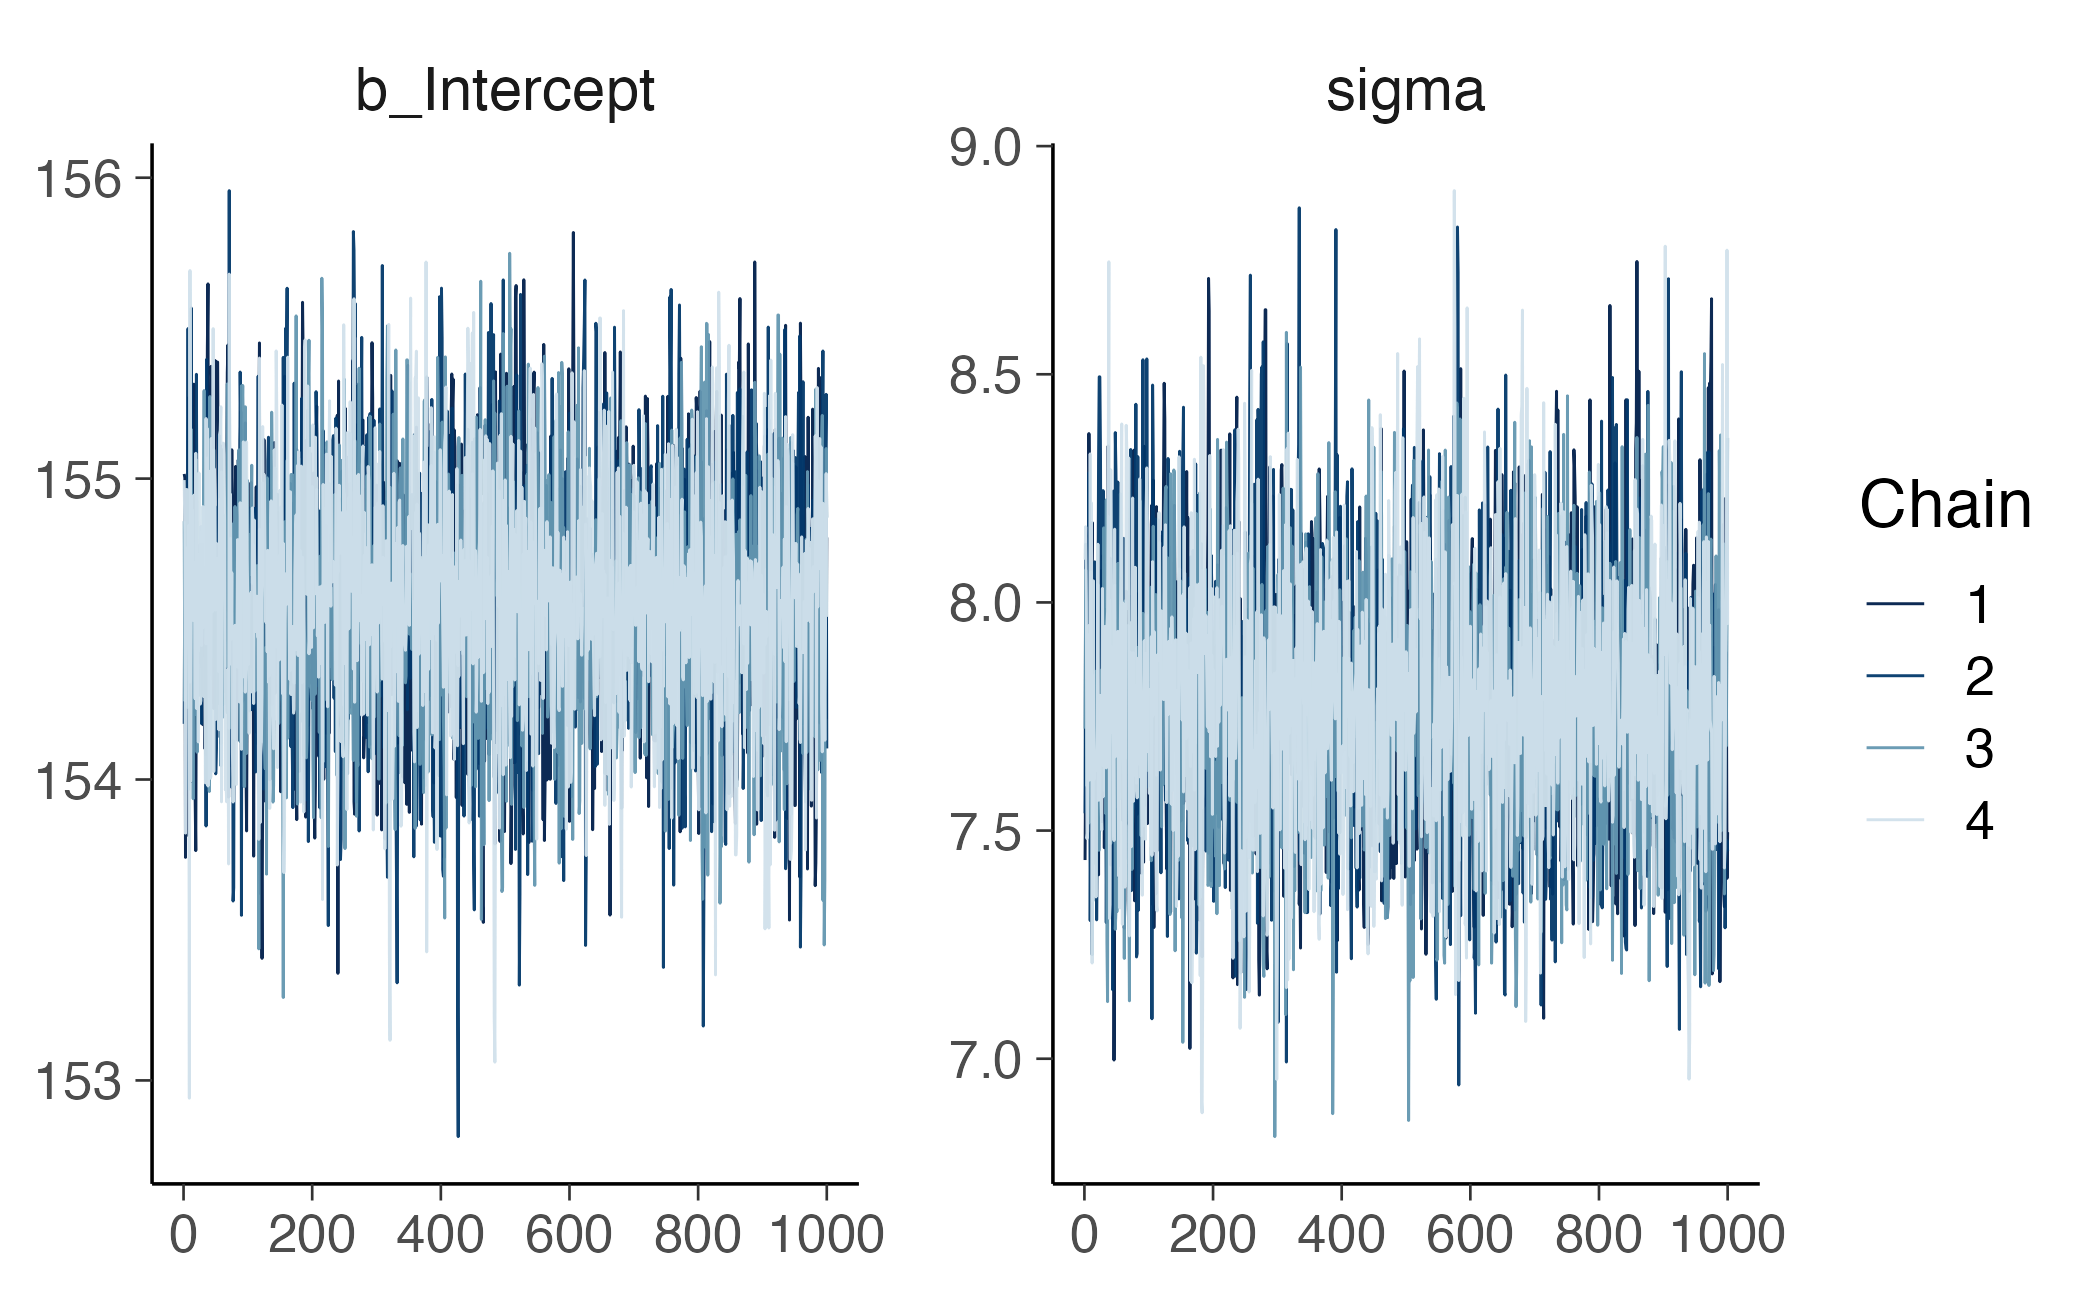
\includegraphics[width=0.85\linewidth,height=\textheight,keepaspectratio]{chapters/linear_models/05_inferenza_su_una_media_files/figure-pdf/trace-one-mean-fit-1.png}

}

\caption{Trace plot dei parametri del modello a sola intercetta.}

\end{figure}%

\begin{quote}
\textbf{Nota di diagnosi:} Il superamento di questi controlli (valori di
\(\widehat{R} \approx 1\) e un numero adeguato di campioni effettivi
\(ESS\)) attesta esclusivamente la stabilità e la qualità
dell'approssimazione numerica. Non dimostrano che la distribuzione
normale rappresenti una specificazione teorica corretta o ottimale per
descrivere le altezze. \#\# Interpretazione della distribuzione a
posteriori
\end{quote}

Estraiamo i campioni dalla distribuzione a posteriori per sintetizzare
la stima dei parametri:

\begin{Shaded}
\begin{Highlighting}[]
\NormalTok{height\_draws }\OtherTok{\textless{}{-}} \FunctionTok{as\_draws\_df}\NormalTok{(fit\_height\_normal)}

\NormalTok{height\_posterior\_summary }\OtherTok{\textless{}{-}}\NormalTok{ height\_draws }\SpecialCharTok{|\textgreater{}}
  \FunctionTok{transmute}\NormalTok{(}
    \AttributeTok{mu =}\NormalTok{ b\_Intercept,}
    \AttributeTok{sigma =}\NormalTok{ sigma}
\NormalTok{  ) }\SpecialCharTok{|\textgreater{}}
  \FunctionTok{summarise}\NormalTok{(}
    \AttributeTok{mu\_median    =} \FunctionTok{median}\NormalTok{(mu),}
    \AttributeTok{mu\_lower     =} \FunctionTok{quantile}\NormalTok{(mu, }\FloatTok{0.025}\NormalTok{),}
    \AttributeTok{mu\_upper     =} \FunctionTok{quantile}\NormalTok{(mu, }\FloatTok{0.975}\NormalTok{),}
    \AttributeTok{sigma\_median =} \FunctionTok{median}\NormalTok{(sigma),}
    \AttributeTok{sigma\_lower  =} \FunctionTok{quantile}\NormalTok{(sigma, }\FloatTok{0.025}\NormalTok{),}
    \AttributeTok{sigma\_upper  =} \FunctionTok{quantile}\NormalTok{(sigma, }\FloatTok{0.975}\NormalTok{)}
\NormalTok{  )}

\NormalTok{height\_posterior\_summary}
\CommentTok{\#\textgreater{} \# A tibble: 1 x 6}
\CommentTok{\#\textgreater{}   mu\_median mu\_lower mu\_upper sigma\_median sigma\_lower sigma\_upper}
\CommentTok{\#\textgreater{}       \textless{}dbl\textgreater{}    \textless{}dbl\textgreater{}    \textless{}dbl\textgreater{}        \textless{}dbl\textgreater{}       \textless{}dbl\textgreater{}       \textless{}dbl\textgreater{}}
\CommentTok{\#\textgreater{} 1      155.     154.     155.         7.77        7.23        8.37}
\end{Highlighting}
\end{Shaded}

Nel modello a sola intercetta i due parametri assumono un preciso
significato strutturale:

\begin{itemize}
\tightlist
\item
  \texttt{b\_Intercept} esprime la media globale \(\mu\) della
  popolazione;
\item
  \texttt{sigma} esprime la deviazione standard delle altezze
  individuali attorno a tale media.
\end{itemize}

L'intervallo di credibilità di \(\mu\) quantifica l'incertezza legata
alla stima del valore medio centrale, mentre l'intervallo di
\texttt{sigma} definisce l'incertezza sulla variabilità
interindividuale. Si tratta di due obiettivi inferenziali distinti che
non vanno confusi.

Visualizziamo le densità a posteriori dei due parametri:

\begin{Shaded}
\begin{Highlighting}[]
\FunctionTok{mcmc\_areas}\NormalTok{(}
\NormalTok{  fit\_height\_normal,}
  \AttributeTok{pars =} \FunctionTok{c}\NormalTok{(}\StringTok{"b\_Intercept"}\NormalTok{, }\StringTok{"sigma"}\NormalTok{),}
  \AttributeTok{prob =} \FloatTok{0.95}
\NormalTok{)}
\end{Highlighting}
\end{Shaded}

\begin{figure}[H]

{\centering 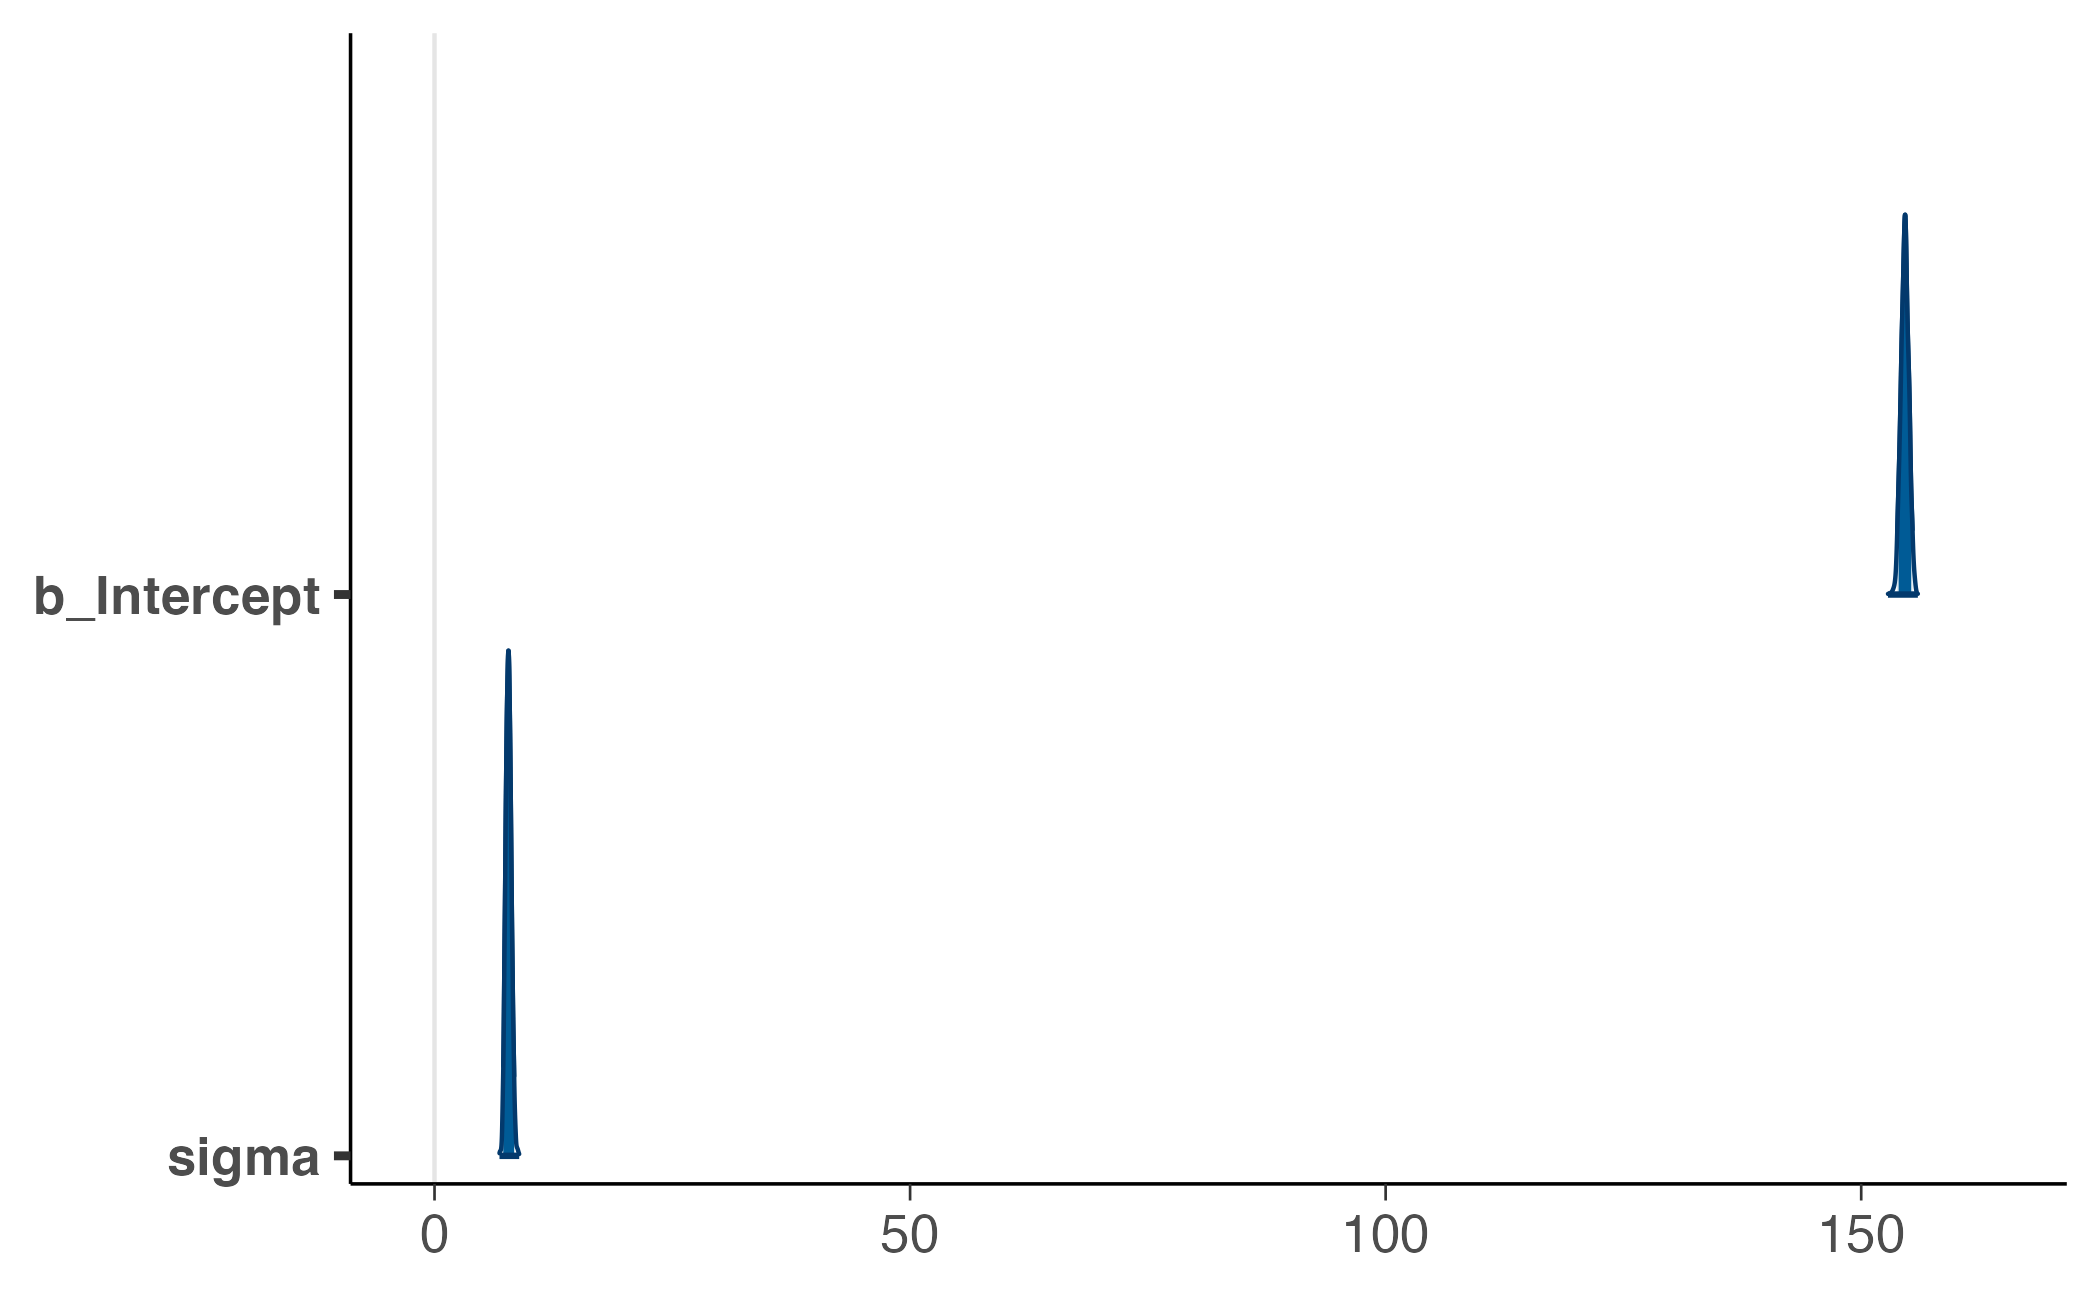
\includegraphics[width=0.85\linewidth,height=\textheight,keepaspectratio]{chapters/linear_models/05_inferenza_su_una_media_files/figure-pdf/plot-one-mean-posterior-1.png}

}

\caption{Distribuzioni a posteriori della media e della deviazione
standard.}

\end{figure}%

\subsection{Probabilità condizionate a soglie
sostantive}\label{probabilituxe0-condizionate-a-soglie-sostantive}

I campioni della posterior consentono di calcolare la probabilità che un
parametro superi una determinata soglia critica rilevante per la domanda
di ricerca:

\begin{Shaded}
\begin{Highlighting}[]
\NormalTok{threshold\_cm }\OtherTok{\textless{}{-}} \DecValTok{155}

\FunctionTok{mean}\NormalTok{(height\_draws}\SpecialCharTok{$}\NormalTok{b\_Intercept }\SpecialCharTok{\textgreater{}}\NormalTok{ threshold\_cm)}
\CommentTok{\#\textgreater{} [1] 0.17}
\end{Highlighting}
\end{Shaded}

Sul piano formale, questo calcolo determina la probabilità:

\[
\Pr(\mu > 155 \mid y, \mathcal{M}),
\] dove \(\mathcal{M}\) rappresenta l'insieme delle assunzioni del
modello (verosimiglianza, prior e disegno di campionamento). La soglia
di confronto deve essere stabilita a priori su basi puramente teoriche o
cliniche; definirla solo dopo aver esaminato la posterior al solo scopo
di isolare una probabilità estrema invalida la natura stessa del
controllo inferenziale.

\section{Media della popolazione e nuova
osservazione}\label{media-della-popolazione-e-nuova-osservazione}

Un intervallo di credibilità molto stretto attorno alla media \(\mu\)
non indica che i soggetti della popolazione abbiano tutti altezze simili
tra loro. Per prevedere il valore di un nuovo individuo futuro
(\(y_{\text{new}}\)), l'inferenza deve combinare tre distinte fonti di
variazione:

\begin{enumerate}
\def\labelenumi{\arabic{enumi}.}
\tightlist
\item
  L'incertezza sulla posizione della media della popolazione (\(\mu\));
\item
  L'incertezza sull'entità della dispersione residua (\(\sigma\));
\item
  La variabilità stocastica individuale definita dalla funzione di
  verosimiglianza.
\end{enumerate}

Generiamo la distribuzione predittiva a posteriori (\emph{posterior
predictive distribution}) integrando queste componenti:

\begin{Shaded}
\begin{Highlighting}[]
\CommentTok{\# Generazione dei valori predetti per un nuovo profilo}
\NormalTok{new\_height\_draws }\OtherTok{\textless{}{-}} \FunctionTok{posterior\_predict}\NormalTok{(}
\NormalTok{  fit\_height\_normal,}
  \AttributeTok{newdata =} \FunctionTok{data.frame}\NormalTok{(}\DecValTok{1}\NormalTok{)}
\NormalTok{)[, }\DecValTok{1}\NormalTok{]}

\NormalTok{prediction\_summary }\OtherTok{\textless{}{-}} \FunctionTok{tibble}\NormalTok{(}
  \AttributeTok{quantity =} \FunctionTok{c}\NormalTok{(}\StringTok{"Media mu"}\NormalTok{, }\StringTok{"Nuova altezza"}\NormalTok{),}
  \AttributeTok{median =} \FunctionTok{c}\NormalTok{(}
    \FunctionTok{median}\NormalTok{(height\_draws}\SpecialCharTok{$}\NormalTok{b\_Intercept),}
    \FunctionTok{median}\NormalTok{(new\_height\_draws)}
\NormalTok{  ),}
  \AttributeTok{lower =} \FunctionTok{c}\NormalTok{(}
    \FunctionTok{quantile}\NormalTok{(height\_draws}\SpecialCharTok{$}\NormalTok{b\_Intercept, }\FloatTok{0.025}\NormalTok{),}
    \FunctionTok{quantile}\NormalTok{(new\_height\_draws, }\FloatTok{0.025}\NormalTok{)}
\NormalTok{  ),}
  \AttributeTok{upper =} \FunctionTok{c}\NormalTok{(}
    \FunctionTok{quantile}\NormalTok{(height\_draws}\SpecialCharTok{$}\NormalTok{b\_Intercept, }\FloatTok{0.975}\NormalTok{),}
    \FunctionTok{quantile}\NormalTok{(new\_height\_draws, }\FloatTok{0.975}\NormalTok{)}
\NormalTok{  )}
\NormalTok{)}

\NormalTok{prediction\_summary}
\CommentTok{\#\textgreater{} \# A tibble: 2 x 4}
\CommentTok{\#\textgreater{}   quantity      median lower upper}
\CommentTok{\#\textgreater{}   \textless{}chr\textgreater{}          \textless{}dbl\textgreater{} \textless{}dbl\textgreater{} \textless{}dbl\textgreater{}}
\CommentTok{\#\textgreater{} 1 Media mu        155.  154.  155.}
\CommentTok{\#\textgreater{} 2 Nuova altezza   154.  139.  170.}
\end{Highlighting}
\end{Shaded}

Confrontiamo graficamente l'incertezza legata al parametro medio con la
dispersione della distribuzione predittiva:

\begin{Shaded}
\begin{Highlighting}[]
\FunctionTok{bind\_rows}\NormalTok{(}
  \FunctionTok{tibble}\NormalTok{(}\AttributeTok{value =}\NormalTok{ height\_draws}\SpecialCharTok{$}\NormalTok{b\_Intercept, }\AttributeTok{quantity =} \StringTok{"Media mu"}\NormalTok{),}
  \FunctionTok{tibble}\NormalTok{(}\AttributeTok{value =}\NormalTok{ new\_height\_draws, }\AttributeTok{quantity =} \StringTok{"Nuova altezza"}\NormalTok{)}
\NormalTok{) }\SpecialCharTok{|\textgreater{}}
  \FunctionTok{ggplot}\NormalTok{(}\FunctionTok{aes}\NormalTok{(}\AttributeTok{x =}\NormalTok{ value, }\AttributeTok{fill =}\NormalTok{ quantity)) }\SpecialCharTok{+}
  \FunctionTok{geom\_density}\NormalTok{(}\AttributeTok{alpha =} \FloatTok{0.35}\NormalTok{) }\SpecialCharTok{+}
  \FunctionTok{labs}\NormalTok{(}
    \AttributeTok{x =} \StringTok{"Altezza (cm)"}\NormalTok{,}
    \AttributeTok{y =} \StringTok{"Densità"}\NormalTok{,}
    \AttributeTok{fill =} \ConstantTok{NULL}
\NormalTok{  )}
\end{Highlighting}
\end{Shaded}

\begin{figure}[H]

{\centering 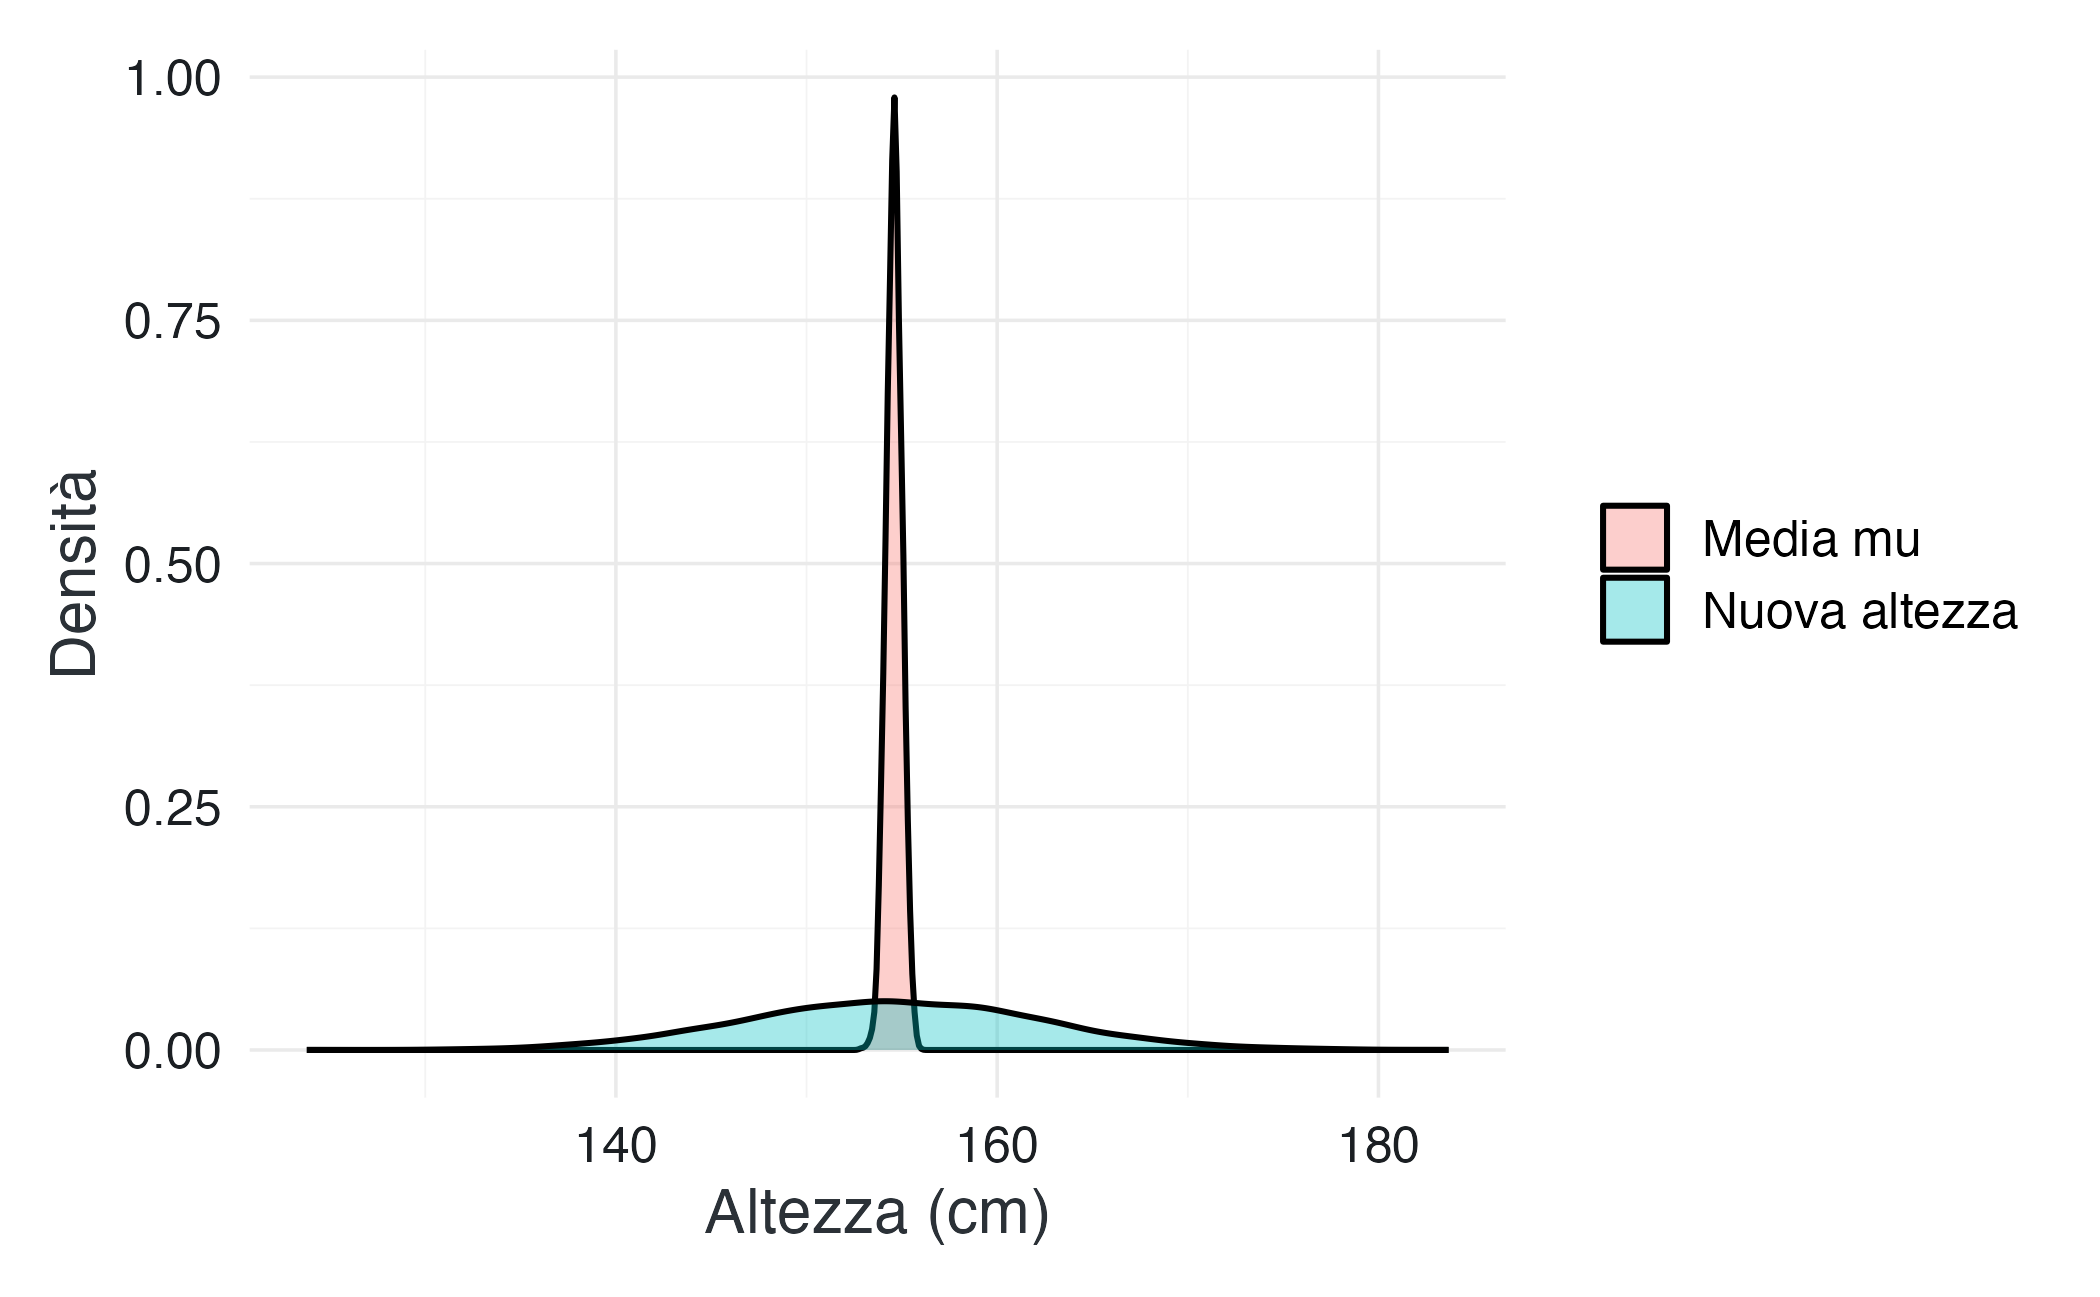
\includegraphics[width=0.85\linewidth,height=\textheight,keepaspectratio]{chapters/linear_models/05_inferenza_su_una_media_files/figure-pdf/compare-mean-and-new-height-1.png}

}

\caption{Confronto tra incertezza sulla media e distribuzione predittiva
di una nuova altezza.}

\end{figure}%

Mentre l'aumento delle osservazioni campionarie restringe
progressivamente la distribuzione a posteriori di \(\mu\) (poiché
disponiamo di maggiore informazione sul baricentro del fenomeno), la
distribuzione predittiva di una nuova altezza rimane strutturalmente
ampia. Questo accade perché l'eterogeneità biologica tra gli individui
non si riduce raccogliendo più dati.

\begin{tcolorbox}[enhanced jigsaw, arc=.35mm, bottomrule=.15mm, bottomtitle=1mm, breakable, colback=white, colbacktitle=quarto-callout-important-color!10!white, colframe=quarto-callout-important-color-frame, coltitle=black, left=2mm, leftrule=.75mm, opacityback=0, opacitybacktitle=0.6, rightrule=.15mm, title=\textcolor{quarto-callout-important-color}{\faExclamation}\hspace{0.5em}{Distinzione tra precisione della stima e omogeneità dei dati}, titlerule=0mm, toprule=.15mm, toptitle=1mm]

Un campione di grandi dimensioni consente di isolare la media \(\mu\)
con estrema precisione anche in presenza di una forte variabilità
individuale. Di conseguenza, la ridotta ampiezza dell'intervallo di
credibilità di un parametro non deve mai essere interpretata come un
indice di omogeneità o uniformità della popolazione.

\end{tcolorbox}

\section{Controlli predittivi a
posteriori}\label{controlli-predittivi-a-posteriori}

Per verificare la validità del modello normale calcolato sulle altezze,
eseguiamo i controlli predittivi a posteriori (\emph{posterior
predictive checks}, PPC). Il confronto diretto tra le densità evidenzia
la capacità del modello di riprodurre il profilo complessivo dei dati:

\begin{Shaded}
\begin{Highlighting}[]
\FunctionTok{pp\_check}\NormalTok{(}
\NormalTok{  fit\_height\_normal,}
  \AttributeTok{type =} \StringTok{"dens\_overlay"}\NormalTok{,}
  \AttributeTok{ndraws =} \DecValTok{50}
\NormalTok{)}
\end{Highlighting}
\end{Shaded}

\begin{figure}[H]

{\centering 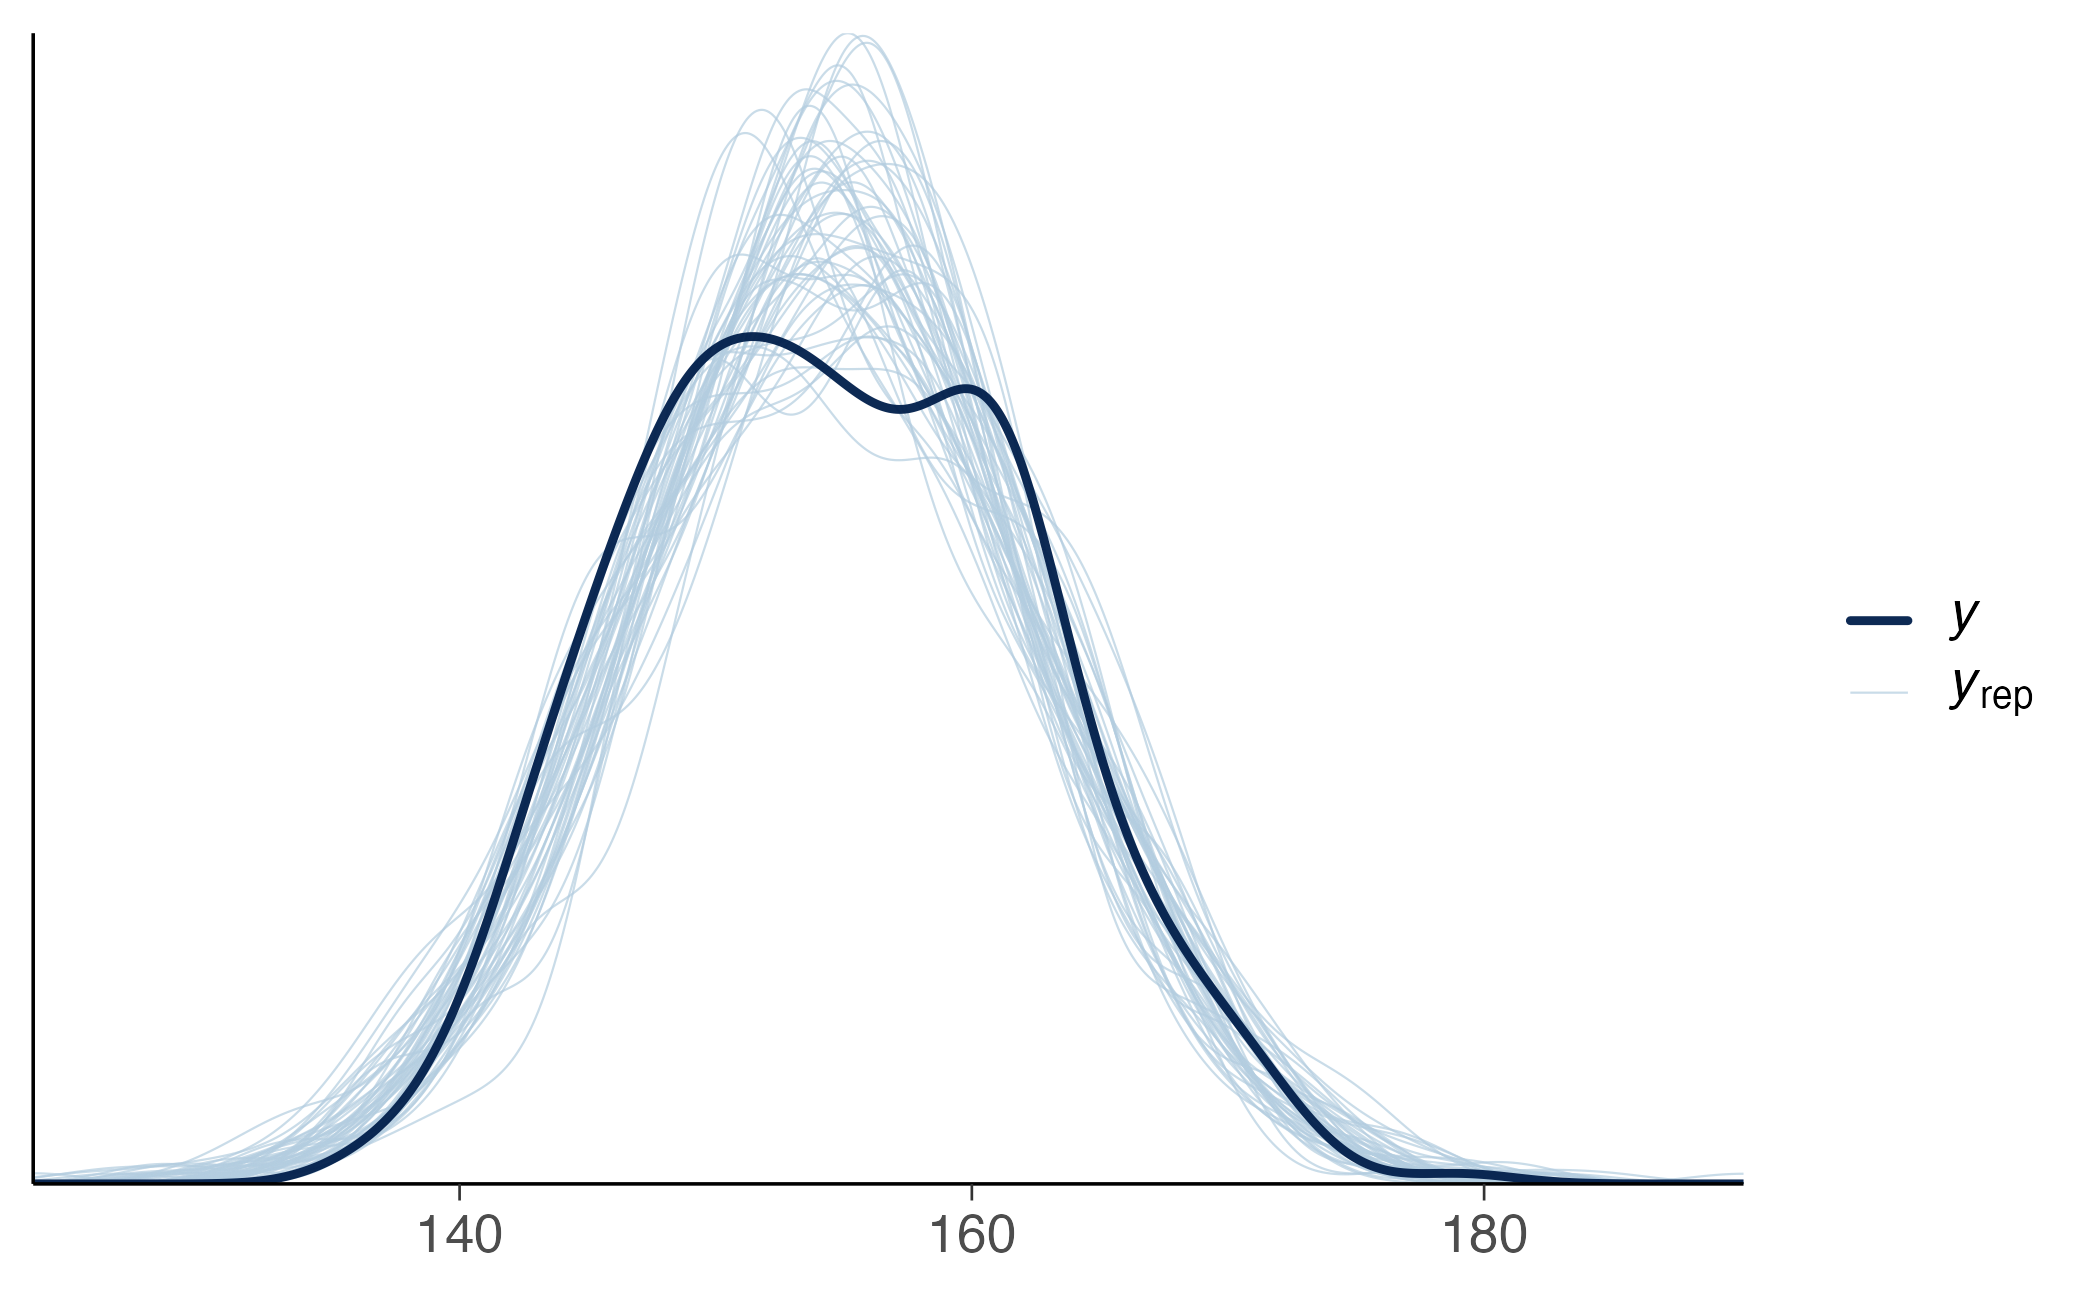
\includegraphics[width=0.85\linewidth,height=\textheight,keepaspectratio]{chapters/linear_models/05_inferenza_su_una_media_files/figure-pdf/posterior-predictive-density-height-1.png}

}

\caption{Confronto tra distribuzione osservata e repliche generate dal
modello normale.}

\end{figure}%

Oltre alla forma marginale complessiva, possiamo isolare specifiche
statistiche di sintesi (in questo caso, la deviazione standard) per
valutare se la dispersione teorica stimata sia coerente con la
variabilità effettiva del campione:

\begin{Shaded}
\begin{Highlighting}[]
\FunctionTok{pp\_check}\NormalTok{(}
\NormalTok{  fit\_height\_normal,}
  \AttributeTok{type =} \StringTok{"stat"}\NormalTok{,}
  \AttributeTok{stat =} \StringTok{"sd"}\NormalTok{,}
  \AttributeTok{ndraws =} \DecValTok{200}
\NormalTok{)}
\end{Highlighting}
\end{Shaded}

\begin{figure}[H]

{\centering 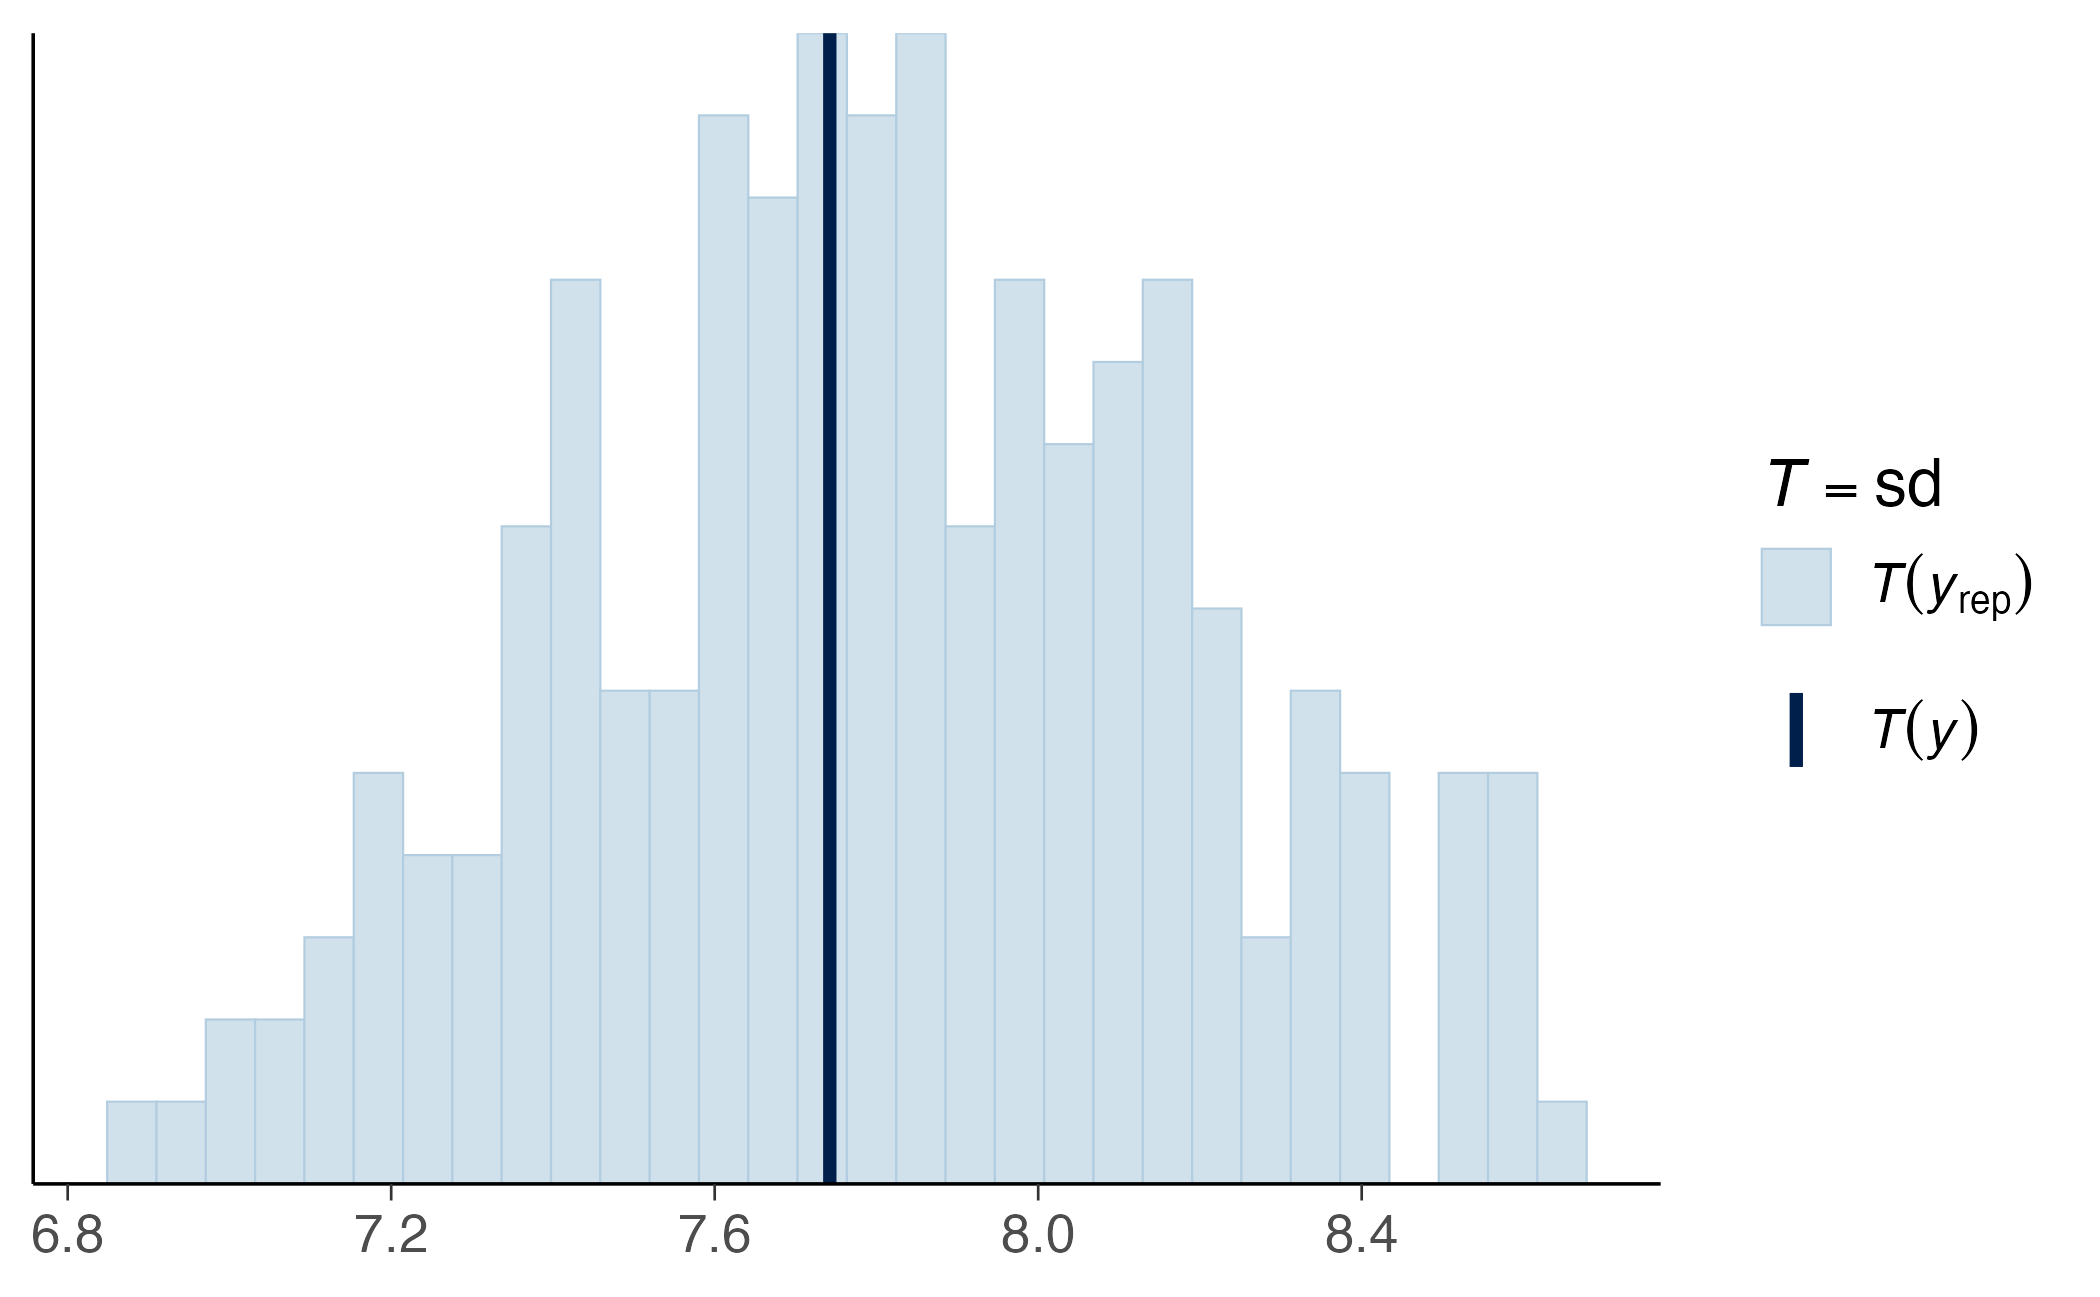
\includegraphics[width=0.85\linewidth,height=\textheight,keepaspectratio]{chapters/linear_models/05_inferenza_su_una_media_files/figure-pdf/posterior-predictive-stat-height-1.png}

}

\caption{Controllo predittivo a posteriori della deviazione standard
osservata.}

\end{figure}%

\begin{quote}
\textbf{Nota metodologica:} Il superamento di queste verifiche non
equivale a una convalida assoluta del modello. Ciascun grafico valuta la
bontà di adattamento solo rispetto alla metrica o alla caratteristica
selezionata. Un modello può riprodurre fedelmente la deviazione standard
o la forma marginale di \(Y\) pur fallendo su altre proprietà
statistiche non esaminate, come l'assenza di asimmetria o la presenza di
code pesanti nei dati reali.
\end{quote}

\section{\texorpdfstring{Modello robusto con la distribuzione \(t\) di
Student}{Modello robusto con la distribuzione t di Student}}\label{modello-robusto-con-la-distribuzione-t-di-student}

La verosimiglianza normale attribuisce una probabilità estremamente
bassa alle osservazioni molto distanti dalla media. Di conseguenza, in
presenza di valori anomali (\emph{outliers}) o di code pesanti, pochi
dati estremi possono distorcere in modo significativo le stime di
\(\mu\) e \(\sigma\).

Per mitigare questo problema, possiamo adottare una specificazione
robusta basata sulla distribuzione \(t\) di Student:

\[
Y_i \sim \operatorname{StudentT}(\nu, \mu, \sigma).
\]

Il parametro aggiuntivo \(\nu\) (gradi di libertà) regola lo spessore
delle code: per valori elevati di \(\nu\) la distribuzione approssima la
normale, mentre per valori ridotti aumenta la probabilità di osservare
dati lontani dal centro, riducendo l'impatto dei valori estremi sulla
stima del baricentro.

Adattiamo il modello in \texttt{brms} introducendo un \emph{prior}
specifico (di tipo Gamma) per regolare i gradi di libertà:

\begin{Shaded}
\begin{Highlighting}[]
\NormalTok{fit\_height\_student }\OtherTok{\textless{}{-}} \FunctionTok{brm}\NormalTok{(}
  \AttributeTok{formula =}\NormalTok{ height }\SpecialCharTok{\textasciitilde{}} \DecValTok{1}\NormalTok{,}
  \AttributeTok{data =}\NormalTok{ height\_data,}
  \AttributeTok{family =} \FunctionTok{student}\NormalTok{(),}
  \AttributeTok{prior =} \FunctionTok{c}\NormalTok{(}
    \FunctionTok{prior}\NormalTok{(}\FunctionTok{normal}\NormalTok{(}\DecValTok{160}\NormalTok{, }\DecValTok{20}\NormalTok{), }\AttributeTok{class =} \StringTok{"Intercept"}\NormalTok{),}
    \FunctionTok{prior}\NormalTok{(}\FunctionTok{lognormal}\NormalTok{(}\FunctionTok{log}\NormalTok{(}\DecValTok{15}\NormalTok{), }\FloatTok{0.5}\NormalTok{), }\AttributeTok{class =} \StringTok{"sigma"}\NormalTok{),}
    \FunctionTok{prior}\NormalTok{(}\FunctionTok{gamma}\NormalTok{(}\DecValTok{2}\NormalTok{, }\FloatTok{0.1}\NormalTok{), }\AttributeTok{class =} \StringTok{"nu"}\NormalTok{)}
\NormalTok{  ),}
  \AttributeTok{chains =} \DecValTok{4}\NormalTok{,}
  \AttributeTok{iter =} \DecValTok{2000}\NormalTok{,}
  \AttributeTok{warmup =} \DecValTok{1000}\NormalTok{,}
  \AttributeTok{seed =} \DecValTok{1234}\NormalTok{,}
  \AttributeTok{backend =} \StringTok{"cmdstanr"}\NormalTok{,}
  \AttributeTok{refresh =} \DecValTok{0}
\NormalTok{)}
\end{Highlighting}
\end{Shaded}

Confrontiamo graficamente le distribuzioni a posteriori di \(\mu\)
ottenute con le due verosimiglianze:

\begin{Shaded}
\begin{Highlighting}[]
\FunctionTok{bind\_rows}\NormalTok{(}
  \FunctionTok{as\_draws\_df}\NormalTok{(fit\_height\_normal)  }\SpecialCharTok{|\textgreater{}} \FunctionTok{transmute}\NormalTok{(}\AttributeTok{mu =}\NormalTok{ b\_Intercept, }\AttributeTok{model =} \StringTok{"Normale"}\NormalTok{),}
  \FunctionTok{as\_draws\_df}\NormalTok{(fit\_height\_student) }\SpecialCharTok{|\textgreater{}} \FunctionTok{transmute}\NormalTok{(}\AttributeTok{mu =}\NormalTok{ b\_Intercept, }\AttributeTok{model =} \StringTok{"Student{-}t"}\NormalTok{)}
\NormalTok{) }\SpecialCharTok{|\textgreater{}}
  \FunctionTok{ggplot}\NormalTok{(}\FunctionTok{aes}\NormalTok{(}\AttributeTok{x =}\NormalTok{ mu, }\AttributeTok{fill =}\NormalTok{ model)) }\SpecialCharTok{+}
  \FunctionTok{geom\_density}\NormalTok{(}\AttributeTok{alpha =} \FloatTok{0.35}\NormalTok{) }\SpecialCharTok{+}
  \FunctionTok{labs}\NormalTok{(}
    \AttributeTok{x =} \FunctionTok{expression}\NormalTok{(mu),}
    \AttributeTok{y =} \StringTok{"Densità"}\NormalTok{,}
    \AttributeTok{fill =} \StringTok{"Modello"}
\NormalTok{  )}
\end{Highlighting}
\end{Shaded}

\begin{figure}[H]

{\centering 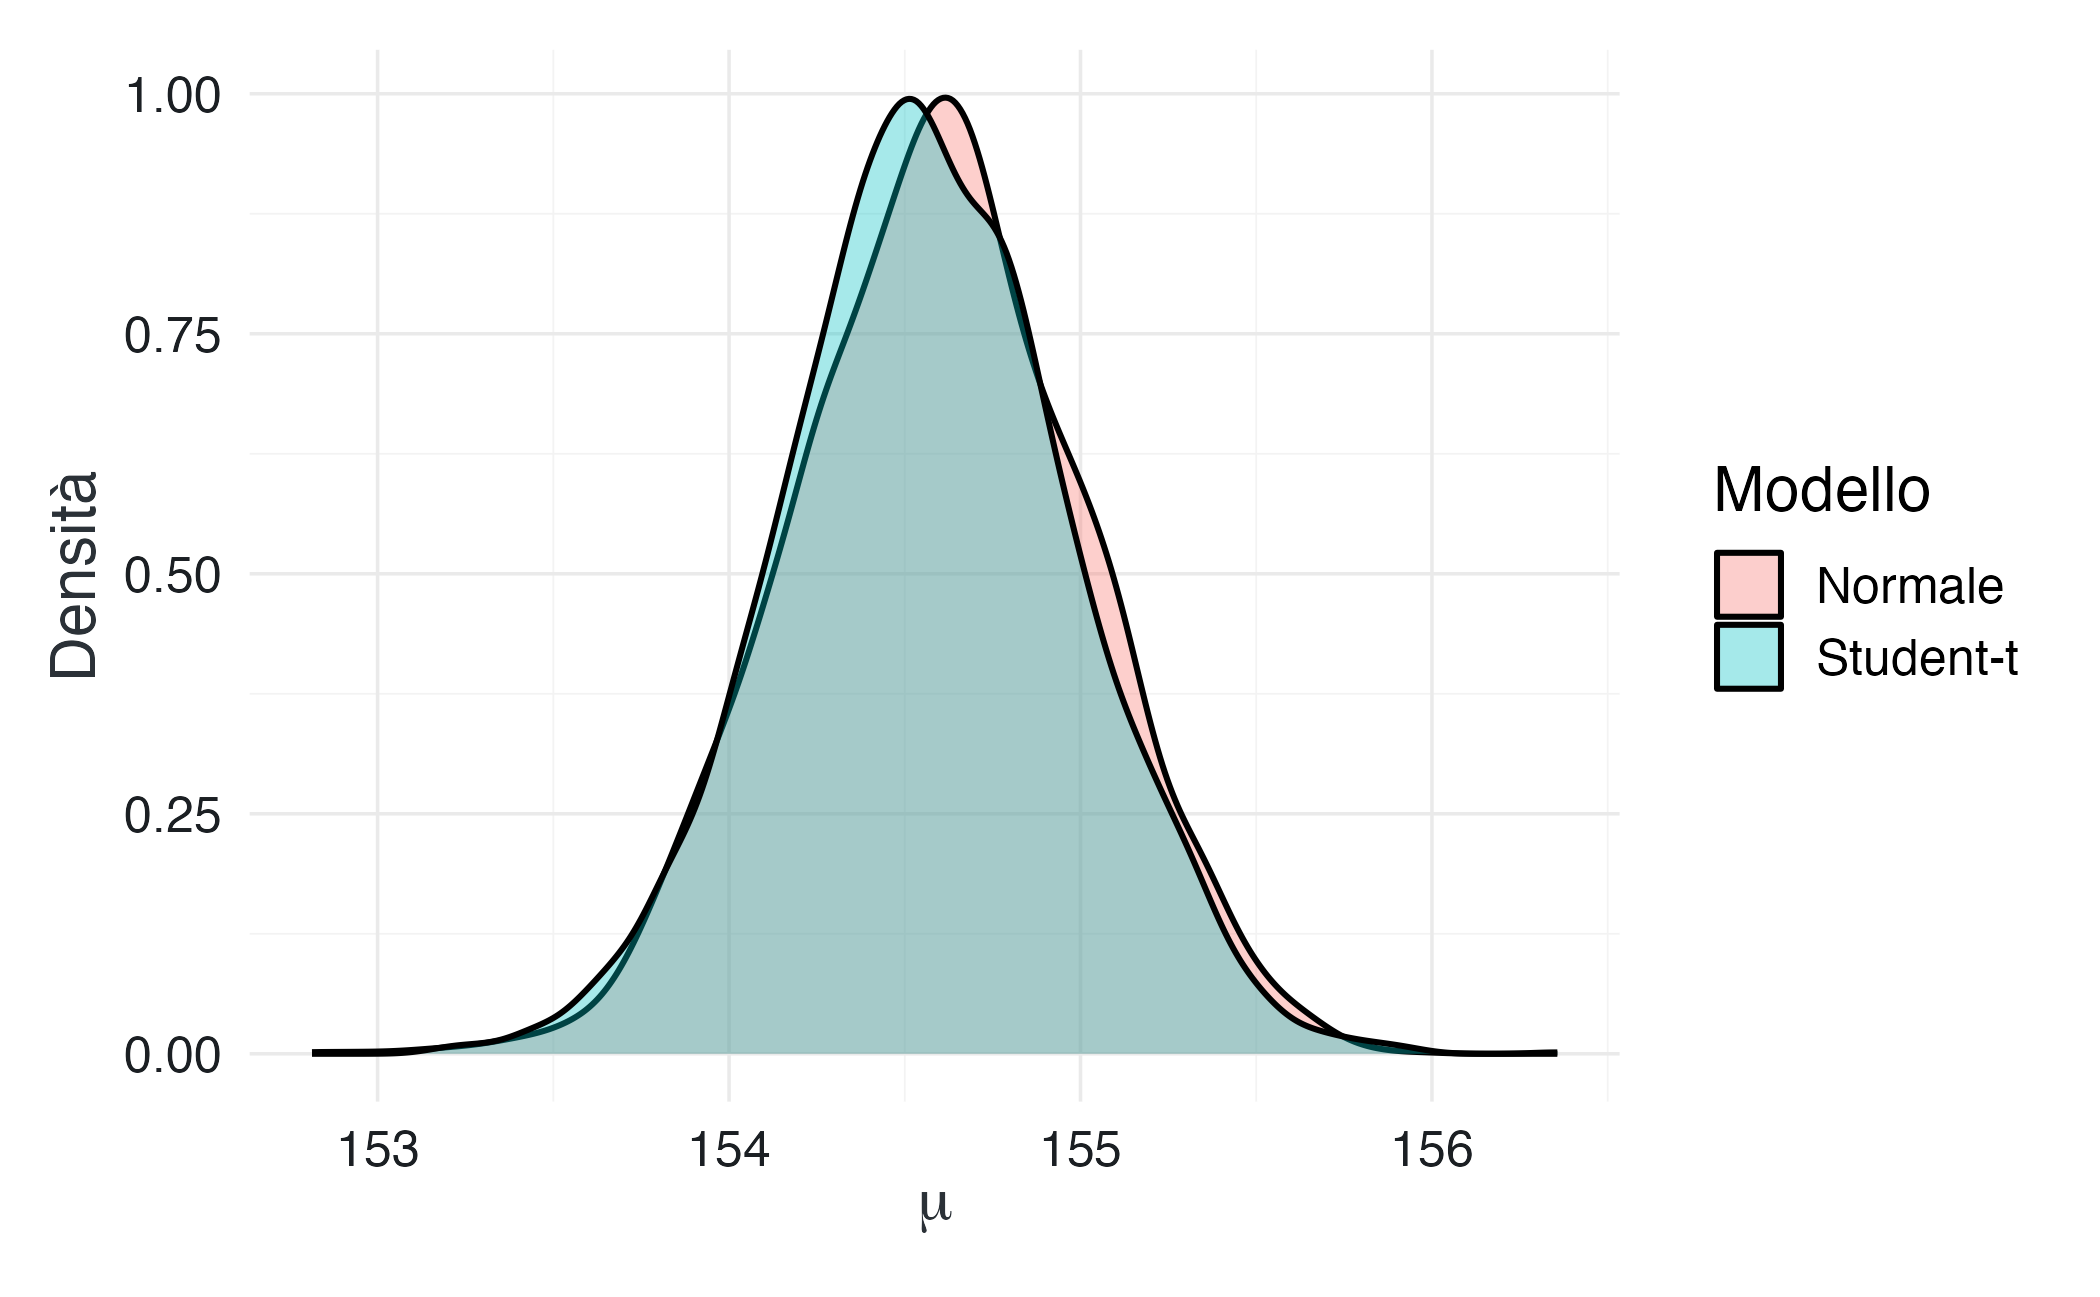
\includegraphics[width=0.85\linewidth,height=\textheight,keepaspectratio]{chapters/linear_models/05_inferenza_su_una_media_files/figure-pdf/compare-normal-student-mu-1.png}

}

\caption{Distribuzione a posteriori della media sotto verosimiglianza
normale e t di Student.}

\end{figure}%

Eseguiamo ora un controllo predittivo a posteriori (\emph{PPC})
focalizzato sul valore minimo osservato, utile per testare la capacità
dei due modelli di gestire il comportamento delle code:

\begin{Shaded}
\begin{Highlighting}[]
\CommentTok{\# Controllo per il modello normale}
\FunctionTok{pp\_check}\NormalTok{(fit\_height\_normal, }\AttributeTok{type =} \StringTok{"stat"}\NormalTok{, }\AttributeTok{stat =} \StringTok{"min"}\NormalTok{, }\AttributeTok{ndraws =} \DecValTok{200}\NormalTok{)}

\CommentTok{\# Controllo per il modello Student{-}t}
\FunctionTok{pp\_check}\NormalTok{(fit\_height\_student, }\AttributeTok{type =} \StringTok{"stat"}\NormalTok{, }\AttributeTok{stat =} \StringTok{"min"}\NormalTok{, }\AttributeTok{ndraws =} \DecValTok{200}\NormalTok{)}
\end{Highlighting}
\end{Shaded}

\begin{figure}[H]

{\centering 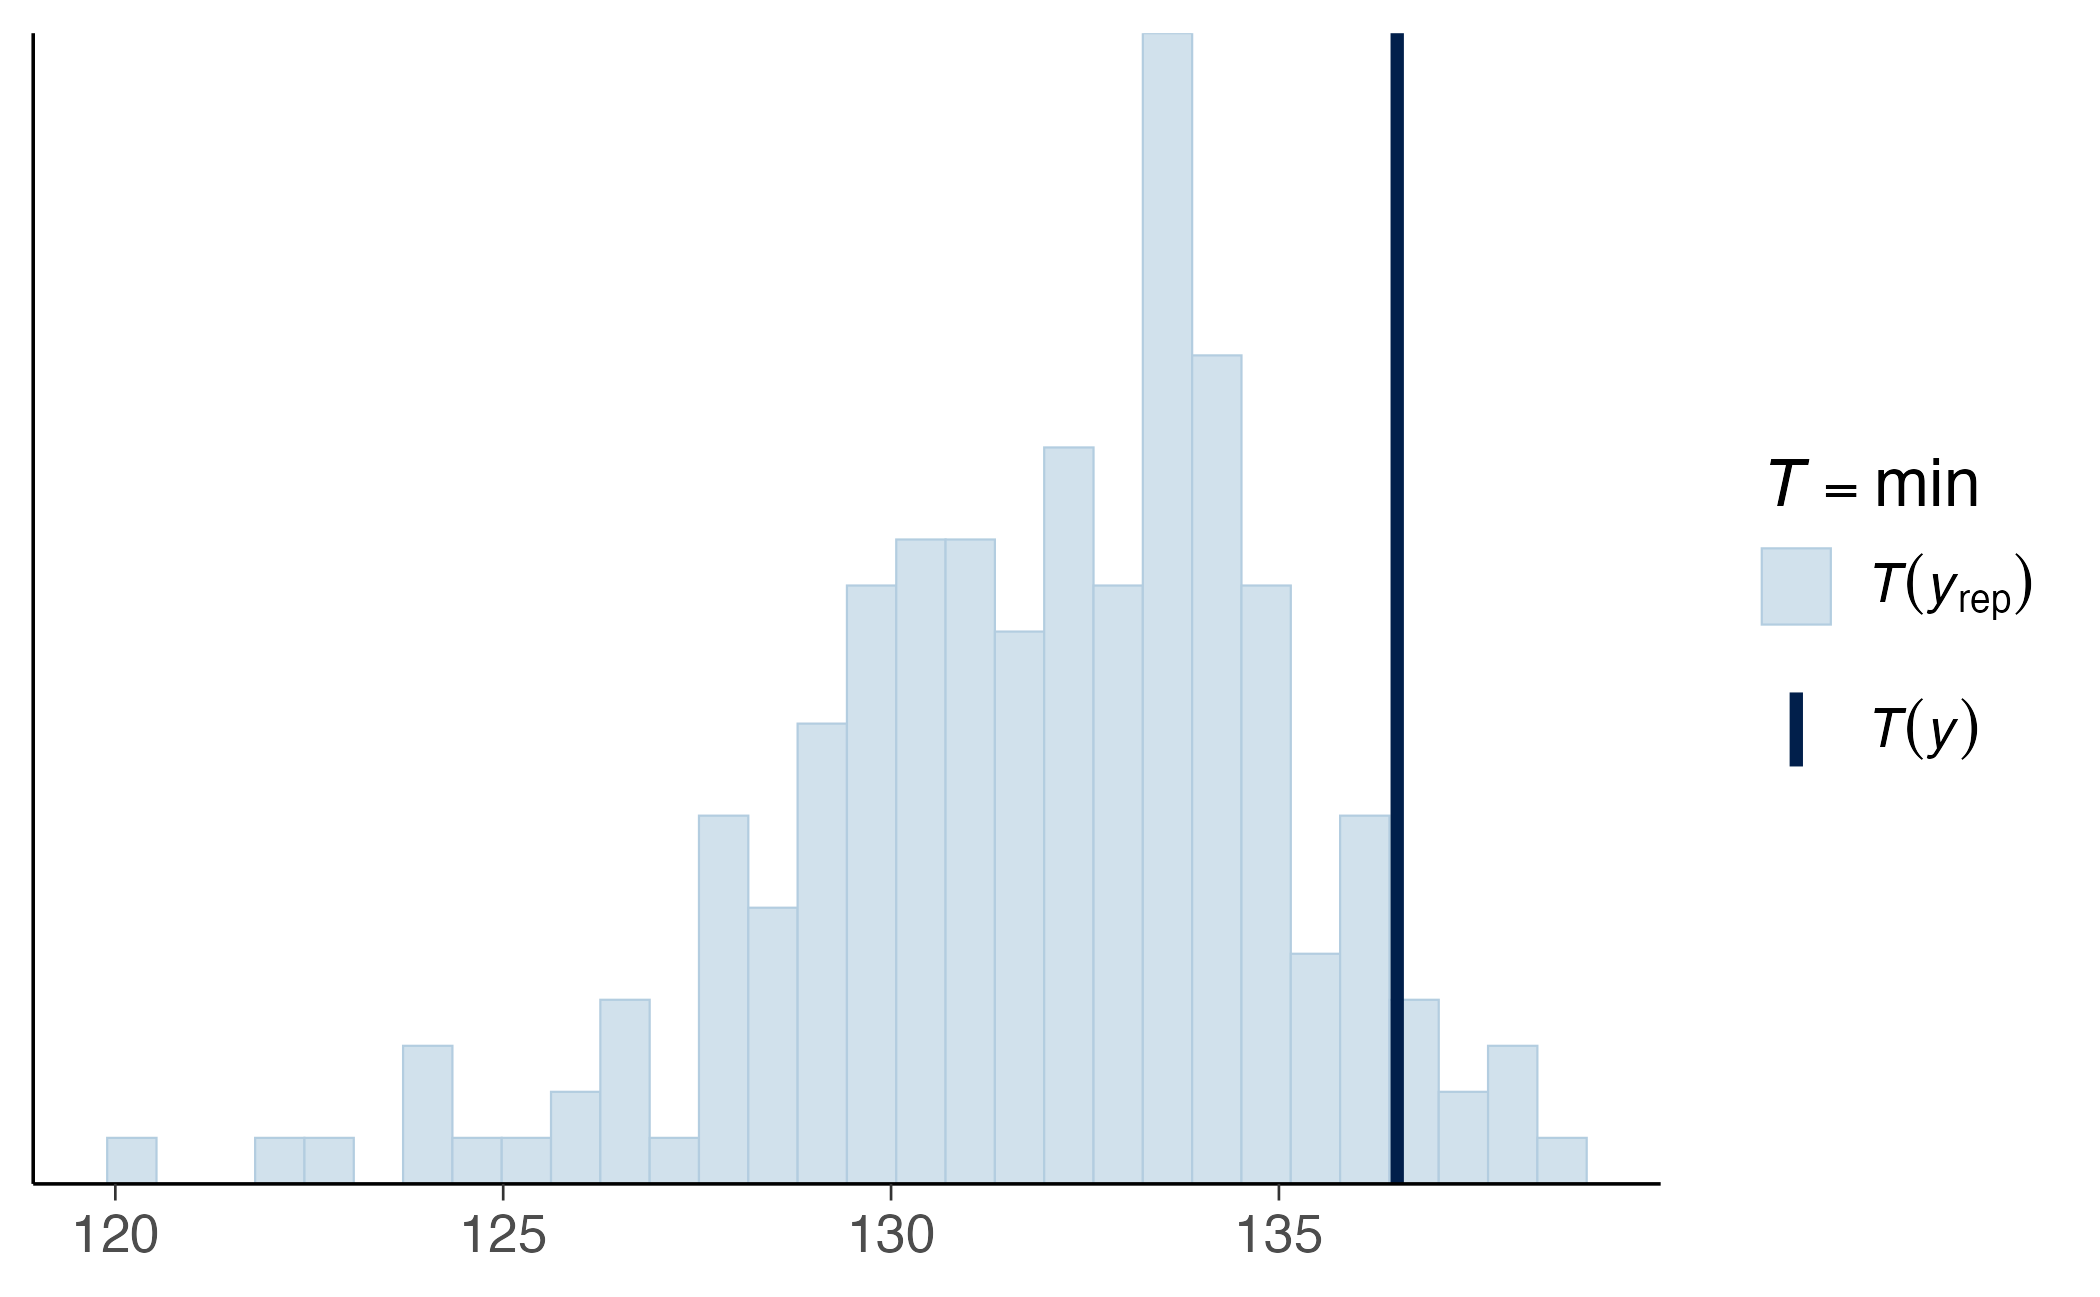
\includegraphics[width=0.85\linewidth,height=\textheight,keepaspectratio]{chapters/linear_models/05_inferenza_su_una_media_files/figure-pdf/compare-normal-student-tails-1.png}

}

\caption{Controllo predittivo del valore minimo per i modelli normale e
t di Student.}

\end{figure}%

\begin{figure}[H]

{\centering 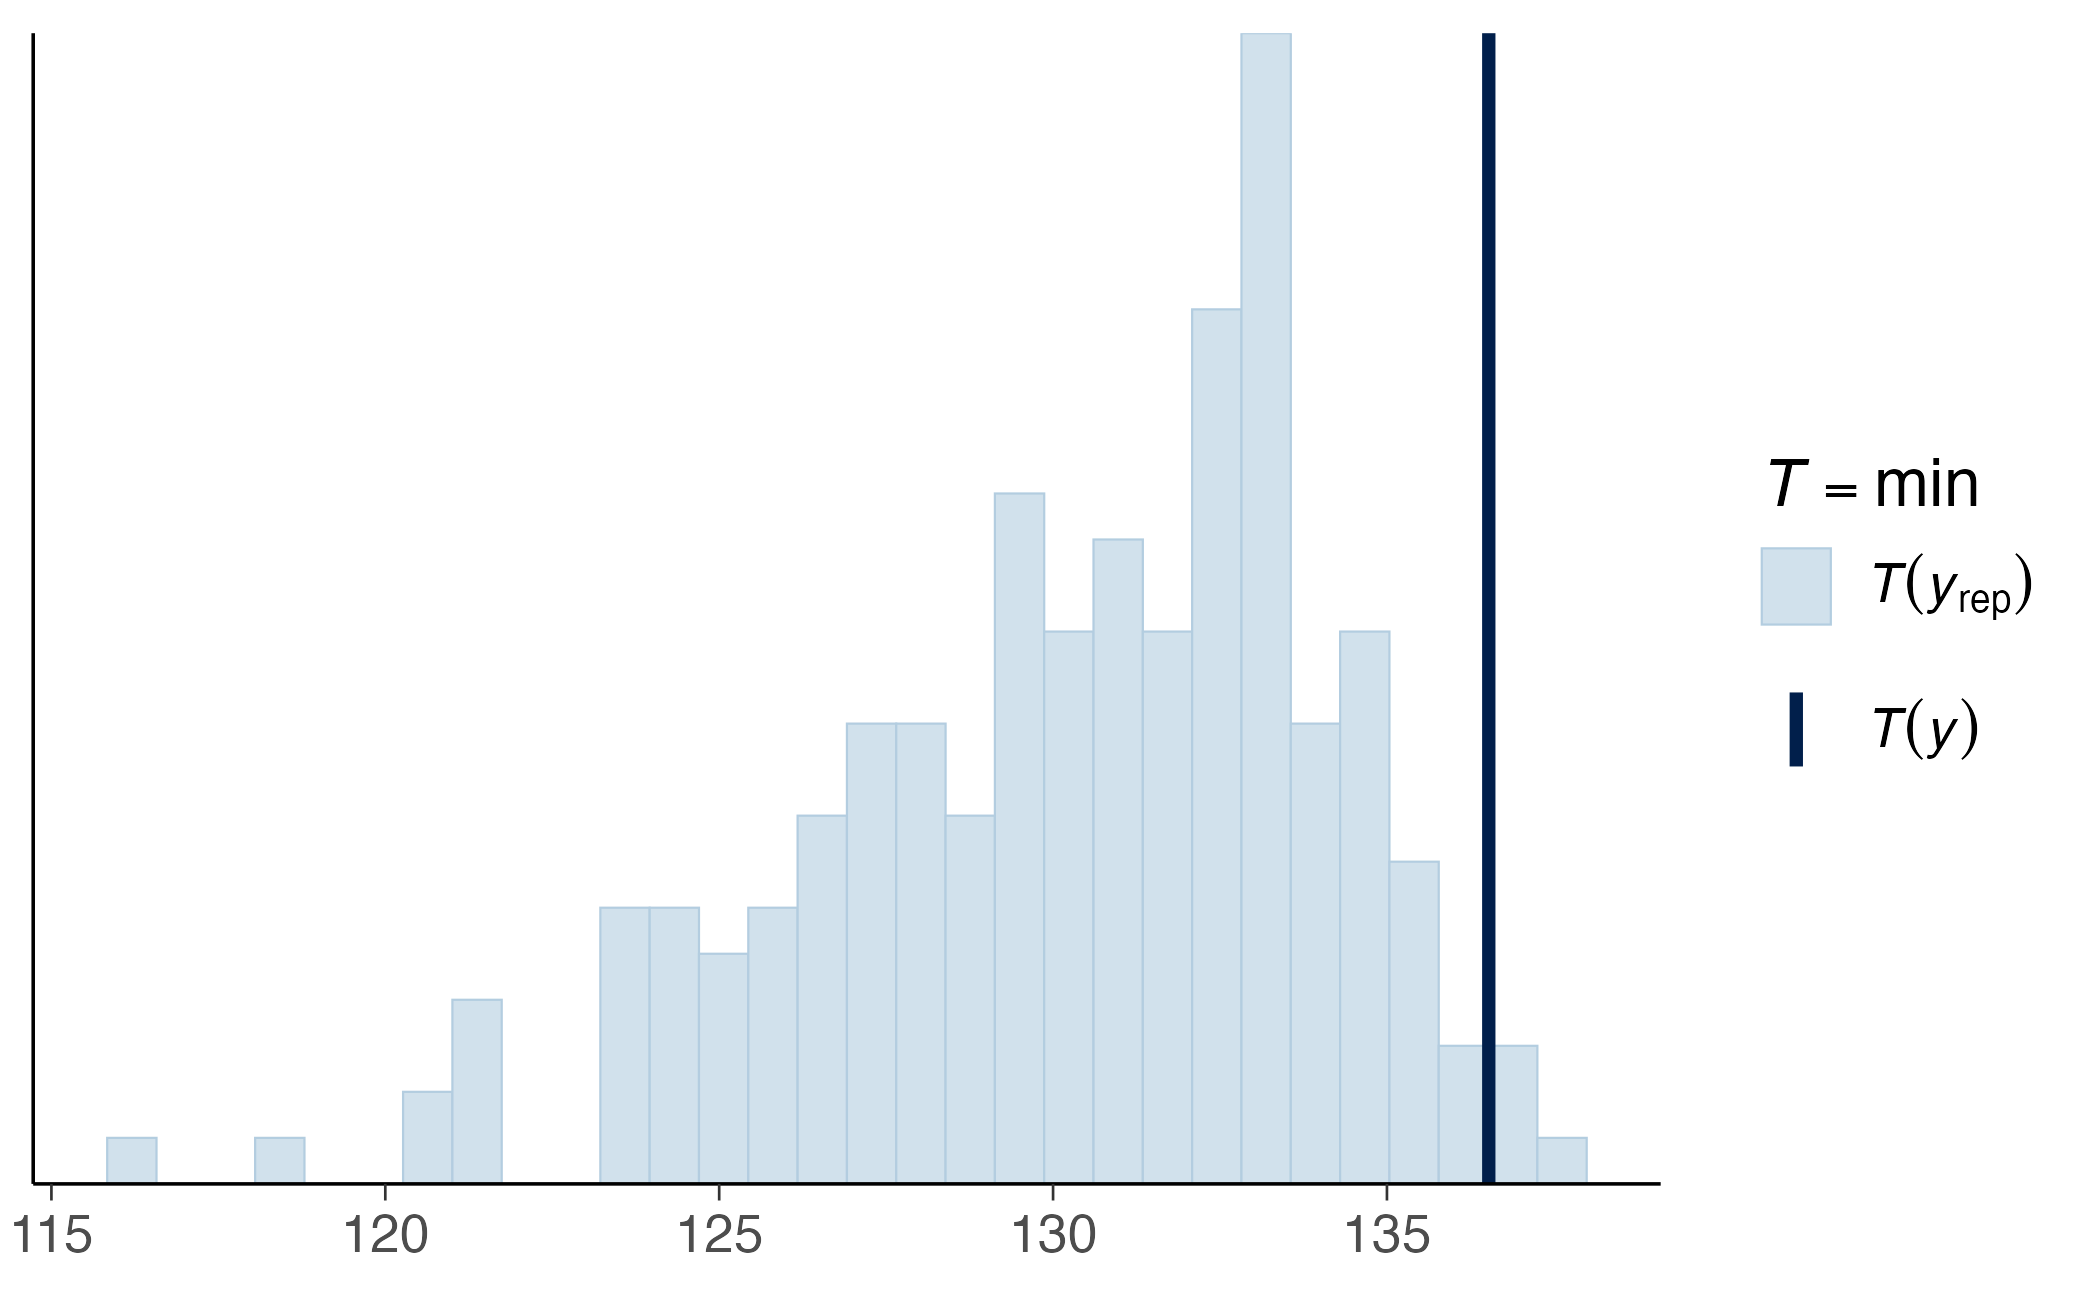
\includegraphics[width=0.85\linewidth,height=\textheight,keepaspectratio]{chapters/linear_models/05_inferenza_su_una_media_files/figure-pdf/compare-normal-student-tails-2.png}

}

\caption{Controllo predittivo del valore minimo per i modelli normale e
t di Student.}

\end{figure}%

\begin{quote}
\textbf{Nota metodologica:} L'uso della distribuzione \(t\) di Student
non va automatizzato in nome di una generica ``maggiore robustezza''.
L'introduzione del parametro \(\nu\) aumenta la flessibilità del modello
ma ne incrementa anche la complessità computazionale. Inoltre, la
robustezza geometrica verso le code pesanti non corregge altre forme di
distorsione o errori sistematici nel disegno di campionamento. La scelta
deve quindi poggiare sulla plausibilità del processo generativo dei dati
e sugli obiettivi specifici dell'inferenza.
\end{quote}

\section{Analisi di sensibilità ai
prior}\label{analisi-di-sensibilituxe0-ai-prior}

Quando il campione è numeroso e informativo, specificazioni a priori
differenti ma ragionevoli producono spesso distribuzioni a posteriori
quasi identiche. Questo fenomeno non rende i \emph{prior} irrilevanti:
indica semplicemente che la funzione di verosimiglianza ha dominato il
processo di aggiornamento bayesiano.

Per verificare la robustezza delle nostre stime, confrontiamo il
\emph{prior} calibrato in precedenza con una variante molto più ampia e
meno informativa:

\begin{Shaded}
\begin{Highlighting}[]
\NormalTok{fit\_height\_wide }\OtherTok{\textless{}{-}} \FunctionTok{brm}\NormalTok{(}
  \AttributeTok{formula =}\NormalTok{ height }\SpecialCharTok{\textasciitilde{}} \DecValTok{1}\NormalTok{,}
  \AttributeTok{data =}\NormalTok{ height\_data,}
  \AttributeTok{family =} \FunctionTok{gaussian}\NormalTok{(),}
  \AttributeTok{prior =} \FunctionTok{c}\NormalTok{(}
    \FunctionTok{prior}\NormalTok{(}\FunctionTok{normal}\NormalTok{(}\DecValTok{160}\NormalTok{, }\DecValTok{50}\NormalTok{), }\AttributeTok{class =} \StringTok{"Intercept"}\NormalTok{),}
    \FunctionTok{prior}\NormalTok{(}\FunctionTok{lognormal}\NormalTok{(}\FunctionTok{log}\NormalTok{(}\DecValTok{20}\NormalTok{), }\DecValTok{1}\NormalTok{), }\AttributeTok{class =} \StringTok{"sigma"}\NormalTok{)}
\NormalTok{  ),}
  \AttributeTok{chains =} \DecValTok{4}\NormalTok{,}
  \AttributeTok{iter =} \DecValTok{2000}\NormalTok{,}
  \AttributeTok{warmup =} \DecValTok{1000}\NormalTok{,}
  \AttributeTok{seed =} \DecValTok{1234}\NormalTok{,}
  \AttributeTok{backend =} \StringTok{"cmdstanr"}\NormalTok{,}
  \AttributeTok{refresh =} \DecValTok{0}
\NormalTok{)}
\end{Highlighting}
\end{Shaded}

Confrontiamo graficamente l'impatto dei due approcci sulla posterior di
\(\mu\):

\begin{Shaded}
\begin{Highlighting}[]
\FunctionTok{bind\_rows}\NormalTok{(}
  \FunctionTok{as\_draws\_df}\NormalTok{(fit\_height\_normal) }\SpecialCharTok{|\textgreater{}} \FunctionTok{transmute}\NormalTok{(}\AttributeTok{mu =}\NormalTok{ b\_Intercept, }\AttributeTok{prior =} \StringTok{"Calibrato"}\NormalTok{),}
  \FunctionTok{as\_draws\_df}\NormalTok{(fit\_height\_wide)   }\SpecialCharTok{|\textgreater{}} \FunctionTok{transmute}\NormalTok{(}\AttributeTok{mu =}\NormalTok{ b\_Intercept, }\AttributeTok{prior =} \StringTok{"Più ampio"}\NormalTok{)}
\NormalTok{) }\SpecialCharTok{|\textgreater{}}
  \FunctionTok{ggplot}\NormalTok{(}\FunctionTok{aes}\NormalTok{(}\AttributeTok{x =}\NormalTok{ mu, }\AttributeTok{fill =}\NormalTok{ prior)) }\SpecialCharTok{+}
  \FunctionTok{geom\_density}\NormalTok{(}\AttributeTok{alpha =} \FloatTok{0.35}\NormalTok{) }\SpecialCharTok{+}
  \FunctionTok{labs}\NormalTok{(}
    \AttributeTok{x =} \FunctionTok{expression}\NormalTok{(mu),}
    \AttributeTok{y =} \StringTok{"Densità"}\NormalTok{,}
    \AttributeTok{fill =} \StringTok{"Prior"}
\NormalTok{  )}
\end{Highlighting}
\end{Shaded}

\begin{figure}[H]

{\centering 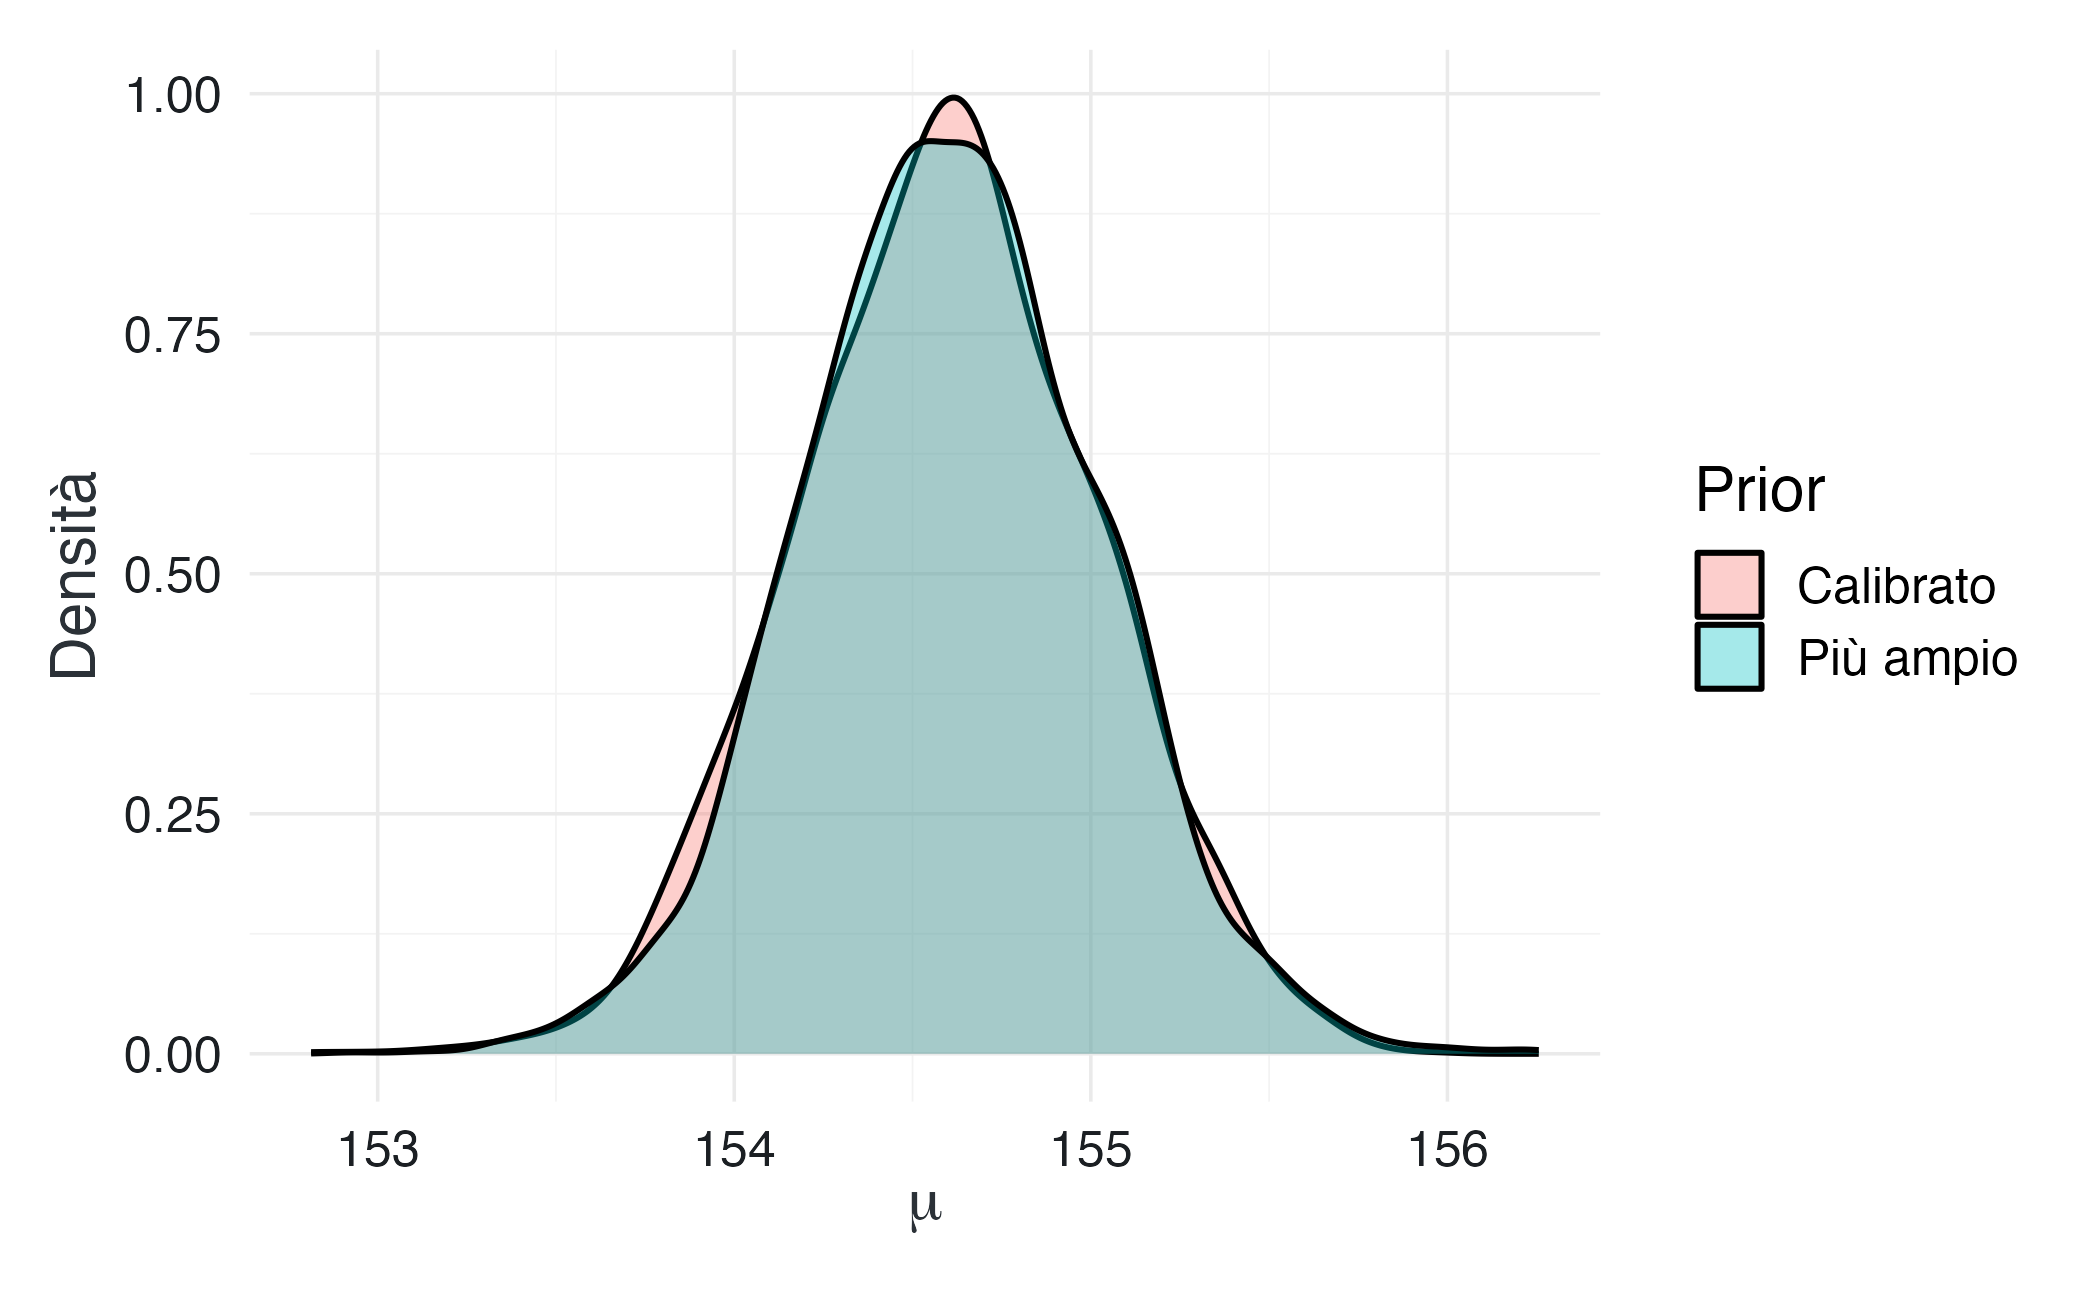
\includegraphics[width=0.85\linewidth,height=\textheight,keepaspectratio]{chapters/linear_models/05_inferenza_su_una_media_files/figure-pdf/compare-one-mean-priors-1.png}

}

\caption{Sensibilità della posterior della media a due specificazioni a
priori.}

\end{figure}%

L'esito di un'analisi di sensibilità va sempre valutato in base alla sua
rilevanza scientifica o applicativa. Lievi scostamenti nelle cifre
decimali dei parametri sono trascurabili; al contrario, variazioni
marginali che modificano le decisioni teoriche o alterano
significativamente le probabilità condizionate a soglie critiche
richiedono una discussione esplicita e trasparente all'interno della
ricerca.

\section{Comunicazione dei risultati}\label{comunicazione-dei-risultati}

Un esempio di rendicontazione scientifica per questo modello è il
seguente:

\begin{quote}
Abbiamo modellato le altezze degli adulti !Kung San attraverso una
verosimiglianza normale con media \(\mu\) e deviazione standard
\(\sigma\) ignote. Le distribuzioni a priori sono state calibrate sulla
scala metrica dei dati (centimetri) e verificate mediante controlli
predittivi a priori. La distribuzione a posteriori mostra che la statura
media della popolazione da cui è estratto il campione è stimata con
elevata precisione attorno al valore centrale. La variabilità tra i
singoli individui risulta, come atteso, significativamente più ampia
rispetto all'incertezza sul parametro medio. I controlli predittivi a
posteriori confermano che il modello riproduce fedelmente la dispersione
e la forma marginale dei dati osservati, mentre il confronto con una
verosimiglianza \(t\) di Student attesta la robustezza delle stime
rispetto al comportamento delle code.
\end{quote}

Nel testo del rapporto di ricerca, la sintesi numerica deve sempre
includere:

\begin{itemize}
\tightlist
\item
  \textbf{Contesto e validità:} la definizione esplicita della
  popolazione target e l'unità di misura;
\item
  \textbf{Trasparenza del modello:} la specifica della verosimiglianza e
  dei \emph{prior} adottati;
\item
  \textbf{Stime puntuali e intervallari:} la media o la mediana a
  posteriori dei parametri accompagnata da un intervallo di credibilità
  (es. al 95\%);
\item
  \textbf{Quantità di interesse:} le eventuali probabilità a posteriori
  associate a soglie critiche stabilite \emph{a priori};
\item
  \textbf{Diagnostica:} l'esito dei controlli predittivi (\emph{PPC})
  giudicati rilevanti per la domanda scientifica.
\end{itemize}

\section{Errori frequenti}\label{errori-frequenti-4}

\begin{tcolorbox}[enhanced jigsaw, arc=.35mm, bottomrule=.15mm, bottomtitle=1mm, breakable, colback=white, colbacktitle=quarto-callout-caution-color!10!white, colframe=quarto-callout-caution-color-frame, coltitle=black, left=2mm, leftrule=.75mm, opacityback=0, opacitybacktitle=0.6, rightrule=.15mm, title=\textcolor{quarto-callout-caution-color}{\faFire}\hspace{0.5em}{Attenzione}, titlerule=0mm, toprule=.15mm, toptitle=1mm]

\begin{enumerate}
\def\labelenumi{\arabic{enumi}.}
\tightlist
\item
  \textbf{Confondere la media campionaria con la media della
  popolazione.} La prima è una statistica osservata; la seconda è un
  parametro del modello la cui interpretazione dipende dal
  campionamento.
\item
  \textbf{Interpretare \(\sigma\) come incertezza su \(\mu\).}
  \(\sigma\) descrive la dispersione individuale; l'incertezza su
  \(\mu\) è descritta dalla sua posterior.
\item
  \textbf{Usare l'intervallo di \(\mu\) come intervallo per una nuova
  persona.} La distribuzione predittiva individuale è normalmente molto
  più ampia.
\item
  \textbf{Scegliere prior senza considerarne le conseguenze
  osservabili.} Parametri apparentemente ragionevoli possono generare
  dataset implausibili.
\item
  \textbf{Dichiarare la normalità sulla base del solo istogramma.}
  L'adeguatezza dipende dalle caratteristiche rilevanti per l'inferenza
  e va valutata predittivamente.
\item
  \textbf{Usare automaticamente la Student-\(t\) per ogni dataset.} Una
  verosimiglianza robusta rappresenta code pesanti, ma non corregge
  asimmetria, multimodalità, dipendenza o errori di campionamento.
\item
  \textbf{Generalizzare oltre la popolazione rappresentata.} Un
  intervallo stretto non compensa un campionamento selettivo o non
  rappresentativo.
\end{enumerate}

\end{tcolorbox}

\section{Riflessioni conclusive}\label{riflessioni-conclusive-22}

La stima di una media coincide con l'adattamento del più elementare dei
modelli lineari: il modello a sola intercetta. Questa struttura
evidenzia come, in ambito statistico, una media non esista mai in
isolamento, ma sia sempre definita in funzione di una distribuzione
delle osservazioni e di un parametro di dispersione.

Il workflow bayesiano applicato a questo framework permette di:

\begin{itemize}
\tightlist
\item
  esprimere le conoscenze iniziali direttamente sulla scala metrica dei
  dati;
\item
  verificare la plausibilità di tali assunzioni tramite simulazioni
  predittive a priori;
\item
  ottenere una distribuzione a posteriori congiunta per \(\mu\) e
  \(\sigma\);
\item
  calcolare in modo diretto le probabilità associate a soglie teoriche o
  cliniche;
\item
  distinguere nettamente l'incertezza sulla stima della media dalla
  variabilità legata alla previsione di un nuovo punteggio individuale;
\item
  valutare verosimiglianze alternative (come la \(t\) di Student)
  qualora la distribuzione normale non gestisca adeguatamente le code
  pesanti.
\end{itemize}

Il modello a sola intercetta rappresenta la base logica e matematica per
gli sviluppi successivi. L'introduzione di un predittore categoriale, ad
esempio, permetterà all'intercetta e al nuovo coefficiente di esprimere
le medie di due gruppi e la loro differenza. Di conseguenza, il
passaggio dalla stima di una singola media al confronto tra gruppi non
richiede un cambio di paradigma teorico, ma semplicemente una diversa
matrice del modello e la definizione di nuove quantità di interesse.

\section{Concetti da ricordare}\label{concetti-da-ricordare-4}

\begin{enumerate}
\def\labelenumi{\arabic{enumi}.}
\tightlist
\item
  La stima di una media è un modello lineare
  \texttt{y\ \textasciitilde{}\ 1}.
\item
  Nel modello a sola intercetta, \texttt{b\_Intercept} coincide con
  \(\mu\).
\item
  \(\mu\) descrive il centro della popolazione modellata; \(\sigma\)
  descrive la dispersione individuale.
\item
  I prior devono essere controllati attraverso le distribuzioni dei dati
  che implicano.
\item
  La posterior di \(\mu\) e la distribuzione predittiva di una nuova
  osservazione rispondono a domande diverse.
\item
  Un intervallo stretto per la media non implica bassa variabilità
  individuale.
\item
  I posterior predictive checks valutano caratteristiche specifiche, non
  la validità globale del modello.
\item
  La Student-\(t\) può rappresentare code più pesanti, ma non è una
  soluzione generale a ogni errore di specificazione.
\item
  La sensibilità ai prior va valutata rispetto alle conclusioni
  sostantive.
\item
  La possibilità di generalizzare dipende dal disegno di campionamento,
  non soltanto dalla precisione della posterior.
\end{enumerate}

\begin{tcolorbox}[enhanced jigsaw, arc=.35mm, bottomrule=.15mm, bottomtitle=1mm, breakable, colback=white, colbacktitle=quarto-callout-important-color!10!white, colframe=quarto-callout-important-color-frame, coltitle=black, left=2mm, leftrule=.75mm, opacityback=0, opacitybacktitle=0.6, rightrule=.15mm, title=\textcolor{quarto-callout-important-color}{\faExclamation}\hspace{0.5em}{Esercizi}, titlerule=0mm, toprule=.15mm, toptitle=1mm]

\subsection{1. Leggere il modello}\label{leggere-il-modello-1}

Interpreta i parametri del modello

\[
Y_i \sim \operatorname{Normal}(72,8).
\]

Quale quantità rappresenta 72? Quale rappresenta 8? Quale delle due
descrive l'incertezza sulla media?

\subsection{2. Prior sulla scala
osservata}\label{prior-sulla-scala-osservata}

Supponi di modellare un tempo di reazione in millisecondi. Spiega perché
il prior \(\mu\sim\operatorname{Normal}(0,1)\) sarebbe generalmente poco
plausibile sulla scala originale. Proponi un prior alternativo e
descrivine le conseguenze predittive attese.

\subsection{3. Prior predictive check}\label{prior-predictive-check-1}

Amplia la deviazione standard del prior sull'intercetta da 20 a 80.
Ripeti il controllo predittivo a priori e descrivi quali dataset
implausibili diventano più frequenti.

\subsection{4. Media e nuova
osservazione}\label{media-e-nuova-osservazione-2}

Confronta l'intervallo di credibilità di \texttt{b\_Intercept} con
l'intervallo predittivo di \texttt{new\_height\_draws}. Spiega perché il
secondo è più ampio anche quando l'incertezza su \(\mu\) è piccola.

\subsection{5. Soglia sostantiva}\label{soglia-sostantiva}

Scegli una soglia per \(\mu\) prima di ispezionare i draw. Calcola la
probabilità che la media la superi. Spiega quale decisione o
interpretazione renderebbe scientificamente utile tale soglia.

\subsection{6. Valore estremo}\label{valore-estremo}

Aggiungi artificialmente un'altezza molto bassa al dataset. Adatta
nuovamente i modelli normale e Student-\(t\). Confronta le posteriori di
\(\mu\) e \(\sigma\) e descrivi quale modello è più sensibile alla nuova
osservazione.

\subsection{7. Controllo predittivo
mirato}\label{controllo-predittivo-mirato-1}

Oltre alla deviazione standard, scegli una caratteristica da controllare
tra minimo, massimo, mediana e intervallo interquartile. Motiva la
scelta rispetto all'adeguatezza della verosimiglianza.

\subsection{8. Generalizzazione}\label{generalizzazione}

Immagina che il campione includa soltanto persone di un'unica fascia di
età. Spiega perché la posterior di \(\mu\) non può essere generalizzata
automaticamente all'intera popolazione adulta.

\end{tcolorbox}

\begin{tcolorbox}[enhanced jigsaw, arc=.35mm, bottomrule=.15mm, bottomtitle=1mm, breakable, colback=white, colbacktitle=quarto-callout-tip-color!10!white, colframe=quarto-callout-tip-color-frame, coltitle=black, left=2mm, leftrule=.75mm, opacityback=0, opacitybacktitle=0.6, rightrule=.15mm, title=\textcolor{quarto-callout-tip-color}{\faLightbulb}\hspace{0.5em}{Tracce di soluzione}, titlerule=0mm, toprule=.15mm, toptitle=1mm]

\begin{enumerate}
\def\labelenumi{\arabic{enumi}.}
\tightlist
\item
  72 è la media della distribuzione; 8 è la deviazione standard delle
  osservazioni. Nessuna delle due, da sola, è l'incertezza sulla media:
  quest'ultima emergerebbe dalla posterior di \(\mu\) dopo aver
  osservato dati.
\item
  Un prior centrato su 0 ms genera prevalentemente valori impossibili.
  Un prior plausibile deve essere espresso nell'ordine di grandezza dei
  tempi attesi e verificato mediante simulazioni predittive.
\item
  Il prior più ampio attribuisce massa a medie estremamente basse o alte
  e può produrre interi dataset fuori dalla gamma fisiologicamente
  plausibile.
\item
  L'intervallo di \(\mu\) riguarda il centro della popolazione; la
  previsione individuale include anche la dispersione \(\sigma\) e
  quindi rimane più ampia.
\item
  La soglia è utile soltanto se corrisponde a una differenza teorica,
  clinica o decisionale definita indipendentemente dalla posterior
  osservata.
\item
  La normale tende a modificare maggiormente media e dispersione per
  incorporare l'osservazione estrema. La Student-\(t\) può
  rappresentarla attraverso code più pesanti, ma la conclusione va
  verificata sui draw e sui controlli predittivi.
\item
  Per studiare le code sono informativi minimo e massimo; per una misura
  robusta della dispersione è utile l'intervallo interquartile. La
  scelta dipende dalla caratteristica che potrebbe mettere in
  discussione il modello.
\item
  Il campionamento non contiene informazione diretta sulle fasce di età
  escluse. La precisione statistica entro il campione non elimina tale
  limite di validità esterna.
\end{enumerate}

\end{tcolorbox}

\begin{tcolorbox}[enhanced jigsaw, arc=.35mm, bottomrule=.15mm, bottomtitle=1mm, breakable, colback=white, colbacktitle=quarto-callout-note-color!10!white, colframe=quarto-callout-note-color-frame, coltitle=black, left=2mm, leftrule=.75mm, opacityback=0, opacitybacktitle=0.6, rightrule=.15mm, title=\textcolor{quarto-callout-note-color}{\faInfo}\hspace{0.5em}{Informazioni sull'ambiente di sviluppo}, titlerule=0mm, toprule=.15mm, toptitle=1mm]

\begin{Shaded}
\begin{Highlighting}[]
\FunctionTok{sessionInfo}\NormalTok{()}
\CommentTok{\#\textgreater{} R version 4.6.1 (2026{-}06{-}24)}
\CommentTok{\#\textgreater{} Platform: aarch64{-}apple{-}darwin23}
\CommentTok{\#\textgreater{} Running under: macOS Tahoe 26.5.2}
\CommentTok{\#\textgreater{} }
\CommentTok{\#\textgreater{} Matrix products: default}
\CommentTok{\#\textgreater{} BLAS:   /Library/Frameworks/R.framework/Versions/4.6/Resources/lib/libRblas.0.dylib }
\CommentTok{\#\textgreater{} LAPACK: /Library/Frameworks/R.framework/Versions/4.6/Resources/lib/libRlapack.dylib;  LAPACK version 3.12.1}
\CommentTok{\#\textgreater{} }
\CommentTok{\#\textgreater{} locale:}
\CommentTok{\#\textgreater{} [1] C.UTF{-}8/UTF{-}8/C.UTF{-}8/C/C.UTF{-}8/C.UTF{-}8}
\CommentTok{\#\textgreater{} }
\CommentTok{\#\textgreater{} time zone: Europe/Zagreb}
\CommentTok{\#\textgreater{} tzcode source: internal}
\CommentTok{\#\textgreater{} }
\CommentTok{\#\textgreater{} attached base packages:}
\CommentTok{\#\textgreater{} [1] stats     graphics  grDevices utils     datasets  methods   base     }
\CommentTok{\#\textgreater{} }
\CommentTok{\#\textgreater{} other attached packages:}
\CommentTok{\#\textgreater{}  [1] cmdstanr\_0.9.0        ragg\_1.5.2            tinytable\_0.17.0     }
\CommentTok{\#\textgreater{}  [4] withr\_3.0.3           systemfonts\_1.3.2     patchwork\_1.3.2      }
\CommentTok{\#\textgreater{}  [7] ggdist\_3.3.3          tidybayes\_3.0.7       bayesplot\_1.15.0     }
\CommentTok{\#\textgreater{} [10] ggplot2\_4.0.3         reliabilitydiag\_0.2.1 priorsense\_1.2.0     }
\CommentTok{\#\textgreater{} [13] posterior\_1.7.0       loo\_2.10.0            rstan\_2.32.7         }
\CommentTok{\#\textgreater{} [16] StanHeaders\_2.32.10   brms\_2.23.0           Rcpp\_1.1.2           }
\CommentTok{\#\textgreater{} [19] sessioninfo\_1.2.4     conflicted\_1.2.0      janitor\_2.2.1        }
\CommentTok{\#\textgreater{} [22] matrixStats\_1.5.0     modelr\_0.1.11         tibble\_3.3.1         }
\CommentTok{\#\textgreater{} [25] dplyr\_1.2.1           tidyr\_1.3.2           rio\_1.3.0            }
\CommentTok{\#\textgreater{} [28] here\_1.0.2           }
\CommentTok{\#\textgreater{} }
\CommentTok{\#\textgreater{} loaded via a namespace (and not attached):}
\CommentTok{\#\textgreater{}  [1] gridExtra\_2.3.1       inline\_0.3.21         rlang\_1.3.0          }
\CommentTok{\#\textgreater{}  [4] magrittr\_2.0.5        snakecase\_0.11.1      otel\_0.2.0           }
\CommentTok{\#\textgreater{}  [7] ggridges\_0.5.7        compiler\_4.6.1        vctrs\_0.7.3          }
\CommentTok{\#\textgreater{} [10] reshape2\_1.4.5        stringr\_1.6.0         pkgconfig\_2.0.3      }
\CommentTok{\#\textgreater{} [13] arrayhelpers\_1.1{-}1    fastmap\_1.2.0         backports\_1.5.1      }
\CommentTok{\#\textgreater{} [16] labeling\_0.4.3        utf8\_1.2.6            rmarkdown\_2.31       }
\CommentTok{\#\textgreater{} [19] ps\_1.9.3              purrr\_1.2.2           xfun\_0.60            }
\CommentTok{\#\textgreater{} [22] cachem\_1.1.0          jsonlite\_2.0.0        broom\_1.0.13         }
\CommentTok{\#\textgreater{} [25] parallel\_4.6.1        R6\_2.6.1              stringi\_1.8.7        }
\CommentTok{\#\textgreater{} [28] RColorBrewer\_1.1{-}3    lubridate\_1.9.5       estimability\_2.0.0   }
\CommentTok{\#\textgreater{} [31] knitr\_1.51            pacman\_0.5.1          R.utils\_2.13.0       }
\CommentTok{\#\textgreater{} [34] Matrix\_1.7{-}5          timechange\_0.4.0      tidyselect\_1.2.1     }
\CommentTok{\#\textgreater{} [37] abind\_1.4{-}8           yaml\_2.3.12           codetools\_0.2{-}20     }
\CommentTok{\#\textgreater{} [40] curl\_7.1.0            processx\_3.9.0        pkgbuild\_1.4.8       }
\CommentTok{\#\textgreater{} [43] plyr\_1.8.9            lattice\_0.22{-}9        bridgesampling\_1.2{-}1 }
\CommentTok{\#\textgreater{} [46] S7\_0.2.2              coda\_0.19{-}4.1         evaluate\_1.0.5       }
\CommentTok{\#\textgreater{} [49] RcppParallel\_5.1.11{-}2 pillar\_1.11.1         tensorA\_0.36.2.1     }
\CommentTok{\#\textgreater{} [52] checkmate\_2.3.4       stats4\_4.6.1          distributional\_0.8.1 }
\CommentTok{\#\textgreater{} [55] generics\_0.1.4        rprojroot\_2.1.1       rstantools\_2.6.0     }
\CommentTok{\#\textgreater{} [58] scales\_1.4.0          xtable\_1.8{-}8          glue\_1.8.1           }
\CommentTok{\#\textgreater{} [61] emmeans\_2.0.4         tools\_4.6.1           data.table\_1.18.4    }
\CommentTok{\#\textgreater{} [64] mvtnorm\_1.4{-}2         grid\_4.6.1            QuickJSR\_1.10.0      }
\CommentTok{\#\textgreater{} [67] nlme\_3.1{-}170          cli\_3.6.6             textshaping\_1.0.5    }
\CommentTok{\#\textgreater{} [70] svUnit\_1.0.8          Brobdingnag\_1.2{-}9     V8\_8.2.0             }
\CommentTok{\#\textgreater{} [73] gtable\_0.3.6          R.methodsS3\_1.8.2     digest\_0.6.39        }
\CommentTok{\#\textgreater{} [76] farver\_2.1.2          memoise\_2.0.1         htmltools\_0.5.9      }
\CommentTok{\#\textgreater{} [79] R.oo\_1.27.1           lifecycle\_1.0.5}
\end{Highlighting}
\end{Shaded}

\end{tcolorbox}

\section*{Bibliografia}\label{bibliografia-25}

\markright{Bibliografia}

\chapter{Due gruppi: codifiche, differenze e rilevanza
pratica}\label{sec-linear-models-two-groups}

Il confronto tra due gruppi o condizioni è uno dei problemi più
ricorrenti nella ricerca psicologica: un gruppo clinico presenta
punteggi diversi da un gruppo di controllo? Due condizioni sperimentali
producono prestazioni differenti? Un intervento è associato a un
cambiamento tale da avere rilievo pratico?

Nel Capitolo~\ref{sec-mcmc-one-mean} abbiamo formulato la stima di una
singola media come un modello lineare a sola intercetta. Per confrontare
due gruppi è sufficiente estendere la componente sistematica inserendo
un predittore che ne indichi l'appartenenza. Il modello non cambia
natura; cambia solo la specificazione della media.

Se assegniamo a \(x_i\) il valore 0 per il gruppo di riferimento e 1 per
il gruppo di confronto, il modello diventa:

\[
Y_i \mid x_i, \alpha, \beta, \sigma \sim \operatorname{Normal}(\mu_i, \sigma), \qquad \mu_i = \alpha + \beta x_i.
\]

Con questa codifica (\emph{dummy coding}), \(\alpha\) esprime la media
del gruppo di riferimento, mentre \(\beta\) quantifica direttamente la
differenza tra le medie dei due gruppi. L'inferenza bayesiana fornisce
la distribuzione a posteriori di questo contrasto, permettendo di
calcolare la direzione, l'ampiezza e la rilevanza clinica o pratica
della differenza.

\begin{tcolorbox}[enhanced jigsaw, arc=.35mm, bottomrule=.15mm, breakable, colback=white, colframe=quarto-callout-important-color-frame, left=2mm, leftrule=.75mm, opacityback=0, rightrule=.15mm, toprule=.15mm]

\textbf{Da sapere.} Il confronto tra due gruppi è un modello lineare con
un predittore binario. Le codifiche \emph{dummy}, centrata e a medie di
cella descrivono le stesse medie, ma modificano il significato immediato
dei coefficienti e dei prior. La distribuzione a posteriori consente di
valutare direzione, ampiezza e rilevanza pratica della differenza, senza
trasformare SESOI o ROPE in nuove soglie decisionali automatiche. Nei
dati osservazionali, una differenza tra gruppi non identifica di per sé
un effetto causale.

\textbf{Da saper fare.} Specificare e stimare con \texttt{brms} un
modello gaussiano per due gruppi; scegliere prior coerenti con la
parametrizzazione ed eseguire i controlli predittivi a priori e a
posteriori; ricavare dai campioni posteriori le medie di gruppo, la
differenza grezza \(\Delta\) e la differenza standardizzata \(d\);
calcolare probabilità posteriori rispetto a zero, a una soglia di
rilevanza pratica e a una ROPE; comunicare le conclusioni mantenendo
distinta la rilevanza statistica da quella sostantiva.

\textbf{Approfondimento facoltativo.} Gli effetti della
parametrizzazione sui prior indotti, i modelli con dispersioni
differenti, le diverse definizioni della differenza standardizzata, il
confronto appaiato e le estensioni robuste possono essere rimandati in
una prima lettura. Nel percorso essenziale è sufficiente padroneggiare
il modello omoschedastico, le quantità sostantive derivate e la loro
interpretazione probabilistica.

\hyperref[sec-percorsi-lettura]{Che cosa significano queste etichette?}

\end{tcolorbox}

\begin{tcolorbox}[enhanced jigsaw, arc=.35mm, bottomrule=.15mm, bottomtitle=1mm, breakable, colback=white, colbacktitle=quarto-callout-note-color!10!white, colframe=quarto-callout-note-color-frame, coltitle=black, left=2mm, leftrule=.75mm, opacityback=0, opacitybacktitle=0.6, rightrule=.15mm, title=\textcolor{quarto-callout-note-color}{\faInfo}\hspace{0.5em}{Obiettivi del capitolo}, titlerule=0mm, toprule=.15mm, toptitle=1mm]

Al termine del capitolo dovresti essere in grado di:

\begin{itemize}
\tightlist
\item
  rappresentare il confronto tra due gruppi mediante un modello lineare
  con predittore binario;
\item
  interpretare le codifiche dummy, centrata e a medie di cella;
\item
  riconoscere come la parametrizzazione influisca sul significato dei
  coefficienti e sulla specificazione dei prior;
\item
  distinguere le medie di gruppo, la differenza grezza e la differenza
  standardizzata;
\item
  calcolare quantità derivate per ogni campione a posteriori;
\item
  definire una soglia di rilevanza pratica sulla scala appropriata;
\item
  usare una regione di equivalenza pratica senza trasformarla in una
  nuova soglia automatica;
\item
  valutare l'ipotesi di uguale dispersione tra i gruppi;
\item
  ricondurre un confronto appaiato a un modello sulla differenza
  intra-individuale;
\item
  distinguere una differenza descrittiva tra gruppi da un effetto
  causale.
\end{itemize}

\end{tcolorbox}

\begin{tcolorbox}[enhanced jigsaw, arc=.35mm, bottomrule=.15mm, bottomtitle=1mm, breakable, colback=white, colbacktitle=quarto-callout-tip-color!10!white, colframe=quarto-callout-tip-color-frame, coltitle=black, left=2mm, leftrule=.75mm, opacityback=0, opacitybacktitle=0.6, rightrule=.15mm, title=\textcolor{quarto-callout-tip-color}{\faLightbulb}\hspace{0.5em}{Percorsi di lettura}, titlerule=0mm, toprule=.15mm, toptitle=1mm]

Il capitolo appartiene al \textbf{percorso essenziale} e al
\textbf{percorso concettuale}. Le sezioni sulle parametrizzazioni, sulle
quantità derivate e sulla rilevanza pratica sono centrali per entrambi.
Le note sui prior indotti, sui modelli eteroschedastici e sulle diverse
definizioni di differenza standardizzata costituiscono approfondimenti
utili soprattutto per il percorso computazionale avanzato.

\end{tcolorbox}

\begin{tcolorbox}[enhanced jigsaw, arc=.35mm, bottomrule=.15mm, bottomtitle=1mm, breakable, colback=white, colbacktitle=quarto-callout-tip-color!10!white, colframe=quarto-callout-tip-color-frame, coltitle=black, left=2mm, leftrule=.75mm, opacityback=0, opacitybacktitle=0.6, rightrule=.15mm, title=\textcolor{quarto-callout-tip-color}{\faLightbulb}\hspace{0.5em}{Prerequisiti e approfondimenti}, titlerule=0mm, toprule=.15mm, toptitle=1mm]

\begin{itemize}
\tightlist
\item
  Il modello a sola intercetta è discusso
  nell'Capitolo~\ref{sec-mcmc-one-mean}.
\item
  Il workflow bayesiano completo con \texttt{brms} è presentato
  nell'Capitolo~\ref{sec-linmod-bayesian-reg}.
\item
  Per la trattazione frequentista del test \(t\) per campioni
  indipendenti e appaiati si veda il modulo
  \href{https://ccaudek.github.io/utet-frequentista}{utet-frequentista}.
\item
  L'esempio sul QI è tratto da Gelman et al.
  (\citeproc{ref-gelman2021regression}{2021}).
\item
  Un riferimento classico sulla stima bayesiana robusta della differenza
  tra gruppi è Kruschke (\citeproc{ref-kruschke2013bayesian}{2013}).
\end{itemize}

\end{tcolorbox}

\begin{tcolorbox}[enhanced jigsaw, arc=.35mm, bottomrule=.15mm, bottomtitle=1mm, breakable, colback=white, colbacktitle=quarto-callout-caution-color!10!white, colframe=quarto-callout-caution-color-frame, coltitle=black, left=2mm, leftrule=.75mm, opacityback=0, opacitybacktitle=0.6, rightrule=.15mm, title=\textcolor{quarto-callout-caution-color}{\faFire}\hspace{0.5em}{Preparazione del Notebook}, titlerule=0mm, toprule=.15mm, toptitle=1mm]

\end{tcolorbox}

\section{Dalla domanda scientifica alle quantità di
interesse}\label{dalla-domanda-scientifica-alle-quantituxe0-di-interesse}

Per illustrare il confronto tra gruppi, utilizzeremo il dataset
\texttt{kidiq}, che fornisce informazioni sullo sviluppo cognitivo di un
campione di bambini e su alcune caratteristiche del nucleo familiare
(\citeproc{ref-gelman2021regression}{Gelman et al., 2021}). In
particolare, ci concentreremo su due variabili:

\begin{itemize}
\tightlist
\item
  \texttt{kid\_score}: il punteggio ottenuto dal bambino nei test di
  sviluppo cognitivo (QI);
\item
  \texttt{mom\_hs}: una variabile indicatore (0/1) che segnala se la
  madre ha conseguito o meno il diploma di scuola superiore.
\end{itemize}

La domanda della ricerca di tipo descrittivo è:

\begin{quote}
Di quanto differiscono, in media, i punteggi cognitivi dei bambini nei
due gruppi definiti dal livello di istruzione della madre?
\end{quote}

Indichiamo con \(\mu_0\) la media teorica dei bambini le cui madri non
sono diplomate (\(mom\_hs = 0\)) e con \(\mu_1\) la media dei bambini le
cui madri sono diplomate (\(mom\_hs = 1\)). Le principali quantità di
interesse per il contrasto sono:

\[
\Delta = \mu_1 - \mu_0
\] che esprime la differenza assoluta sulla scala originaria del
punteggio di QI, e

\[
d = \frac{\Delta}{\sigma}
\] che rappresenta la dimensione dell'effetto standardizzata (\emph{d}
di Cohen) calcolata rispetto alla deviazione standard residua comune
\(\sigma\) stimata dal modello.

Inoltre, è possibile definire a priori una soglia di rilevanza pratica o
clinica \(s\). Ad esempio, se consideriamo sostanziale uno scostamento
positivo di almeno 5 punti sul punteggio cognitivo, le quantità
probabilistiche di interesse diventano:

\[
\Pr(\Delta > 0 \mid y) \qquad \text{e} \qquad \Pr(\Delta > 5 \mid y).
\]

\begin{tcolorbox}[enhanced jigsaw, arc=.35mm, bottomrule=.15mm, bottomtitle=1mm, breakable, colback=white, colbacktitle=quarto-callout-important-color!10!white, colframe=quarto-callout-important-color-frame, coltitle=black, left=2mm, leftrule=.75mm, opacityback=0, opacitybacktitle=0.6, rightrule=.15mm, title=\textcolor{quarto-callout-important-color}{\faExclamation}\hspace{0.5em}{Direzionalità delle soglie teoriche}, titlerule=0mm, toprule=.15mm, toptitle=1mm]

La probabilità della differenza assoluta
\(\Pr(\vert{}\Delta\vert{} > 5 \mid y)\) valuta uno scostamento di
almeno 5 punti in entrambe le direzioni. Se l'ipotesi scientifica
presuppone una direzione specifica, è teoricamente più corretto e
informativo isolare \(\Pr(\Delta > 5 \mid y)\) o
\(\Pr(\Delta < -5 \mid y)\). Questo criterio deve essere stabilito in
base al significato metrico e clinico della variabile, senza mai essere
selezionato a posteriori per manipolare i risultati.

\end{tcolorbox}

\begin{tcolorbox}[enhanced jigsaw, arc=.35mm, bottomrule=.15mm, bottomtitle=1mm, breakable, colback=white, colbacktitle=quarto-callout-warning-color!10!white, colframe=quarto-callout-warning-color-frame, coltitle=black, left=2mm, leftrule=.75mm, opacityback=0, opacitybacktitle=0.6, rightrule=.15mm, title=\textcolor{quarto-callout-warning-color}{\faExclamationTriangle}\hspace{0.5em}{Natura descrittiva del contrasto ed effetto causale}, titlerule=0mm, toprule=.15mm, toptitle=1mm]

Il livello di istruzione materna è una caratteristica osservata e non
una condizione assegnata casualmente tramite un esperimento. Di
conseguenza, il parametro \(\Delta\) descrive un puro contrasto
associativo tra i due gruppi e non può essere interpretato, in assenza
di un controllo dei fattori di confondimento e di specifiche assunzioni
di identificazione, come l'effetto causale diretto del diploma materno
sul punteggio del bambino.

\end{tcolorbox}

\section{Esplorazione dei dati}\label{esplorazione-dei-dati-1}

Carichiamo il dataset codificando la variabile esplicativa come fattore
ed esaminiamo le statistiche descrittive principali per ciascun gruppo:

\begin{Shaded}
\begin{Highlighting}[]
\NormalTok{kidiq }\OtherTok{\textless{}{-}}\NormalTok{ rio}\SpecialCharTok{::}\FunctionTok{import}\NormalTok{(}
\NormalTok{  here}\SpecialCharTok{::}\FunctionTok{here}\NormalTok{(}\StringTok{"data"}\NormalTok{, }\StringTok{"kidiq.dta"}\NormalTok{)}
\NormalTok{) }\SpecialCharTok{|\textgreater{}}
  \FunctionTok{transmute}\NormalTok{(}
\NormalTok{    kid\_score,}
    \AttributeTok{mom\_hs =} \FunctionTok{factor}\NormalTok{(}
\NormalTok{      mom\_hs,}
      \AttributeTok{levels =} \FunctionTok{c}\NormalTok{(}\DecValTok{0}\NormalTok{, }\DecValTok{1}\NormalTok{),}
      \AttributeTok{labels =} \FunctionTok{c}\NormalTok{(}\StringTok{"Non diplomata"}\NormalTok{, }\StringTok{"Diplomata"}\NormalTok{)}
\NormalTok{    )}
\NormalTok{  ) }\SpecialCharTok{|\textgreater{}}
  \FunctionTok{drop\_na}\NormalTok{()}

\NormalTok{kidiq }\SpecialCharTok{|\textgreater{}}
  \FunctionTok{group\_by}\NormalTok{(mom\_hs) }\SpecialCharTok{|\textgreater{}}
  \FunctionTok{summarise}\NormalTok{(}
    \AttributeTok{n        =} \FunctionTok{n}\NormalTok{(),}
    \AttributeTok{media\_QI =} \FunctionTok{mean}\NormalTok{(kid\_score),}
    \AttributeTok{sd\_QI    =} \FunctionTok{sd}\NormalTok{(kid\_score),}
    \AttributeTok{.groups  =} \StringTok{"drop"}
\NormalTok{  )}
\CommentTok{\#\textgreater{} \# A tibble: 2 x 4}
\CommentTok{\#\textgreater{}   mom\_hs            n media\_QI sd\_QI}
\CommentTok{\#\textgreater{}   \textless{}fct\textgreater{}         \textless{}int\textgreater{}    \textless{}dbl\textgreater{} \textless{}dbl\textgreater{}}
\CommentTok{\#\textgreater{} 1 Non diplomata    93     77.5  22.6}
\CommentTok{\#\textgreater{} 2 Diplomata       341     89.3  19.0}
\end{Highlighting}
\end{Shaded}

Sebbene la tabella delle medie offra una prima sintesi numerica del
contrasto, essa non è in grado di mostrare né la forma delle
distribuzioni né l'entità della loro sovrapposizione.

Visualizziamo l'intera struttura dei dati combinando grafici a violino,
boxplot e la mappa dei singoli punti osservati:

\begin{Shaded}
\begin{Highlighting}[]
\NormalTok{kidiq }\SpecialCharTok{|\textgreater{}}
  \FunctionTok{ggplot}\NormalTok{(}\FunctionTok{aes}\NormalTok{(}\AttributeTok{x =}\NormalTok{ mom\_hs, }\AttributeTok{y =}\NormalTok{ kid\_score)) }\SpecialCharTok{+}
  \FunctionTok{geom\_violin}\NormalTok{(}\AttributeTok{trim =} \ConstantTok{FALSE}\NormalTok{, }\AttributeTok{alpha =} \FloatTok{0.4}\NormalTok{, }\AttributeTok{fill =} \StringTok{"grey80"}\NormalTok{, }\AttributeTok{color =} \StringTok{"grey50"}\NormalTok{) }\SpecialCharTok{+}
  \FunctionTok{geom\_boxplot}\NormalTok{(}\AttributeTok{width =} \FloatTok{0.12}\NormalTok{, }\AttributeTok{outlier.shape =} \ConstantTok{NA}\NormalTok{, }\AttributeTok{alpha =} \FloatTok{0.7}\NormalTok{, }\AttributeTok{fatigue =} \ConstantTok{TRUE}\NormalTok{) }\SpecialCharTok{+}
  \FunctionTok{geom\_jitter}\NormalTok{(}\AttributeTok{width =} \FloatTok{0.08}\NormalTok{, }\AttributeTok{alpha =} \FloatTok{0.25}\NormalTok{, }\AttributeTok{size =} \FloatTok{1.2}\NormalTok{, }\AttributeTok{color =} \StringTok{"grey30"}\NormalTok{) }\SpecialCharTok{+}
  \FunctionTok{labs}\NormalTok{(}
    \AttributeTok{x =} \StringTok{"Istruzione materna"}\NormalTok{,}
    \AttributeTok{y =} \StringTok{"Punteggio cognitivo del bambino"}
\NormalTok{  )}
\end{Highlighting}
\end{Shaded}

\begin{figure}[H]

\centering{

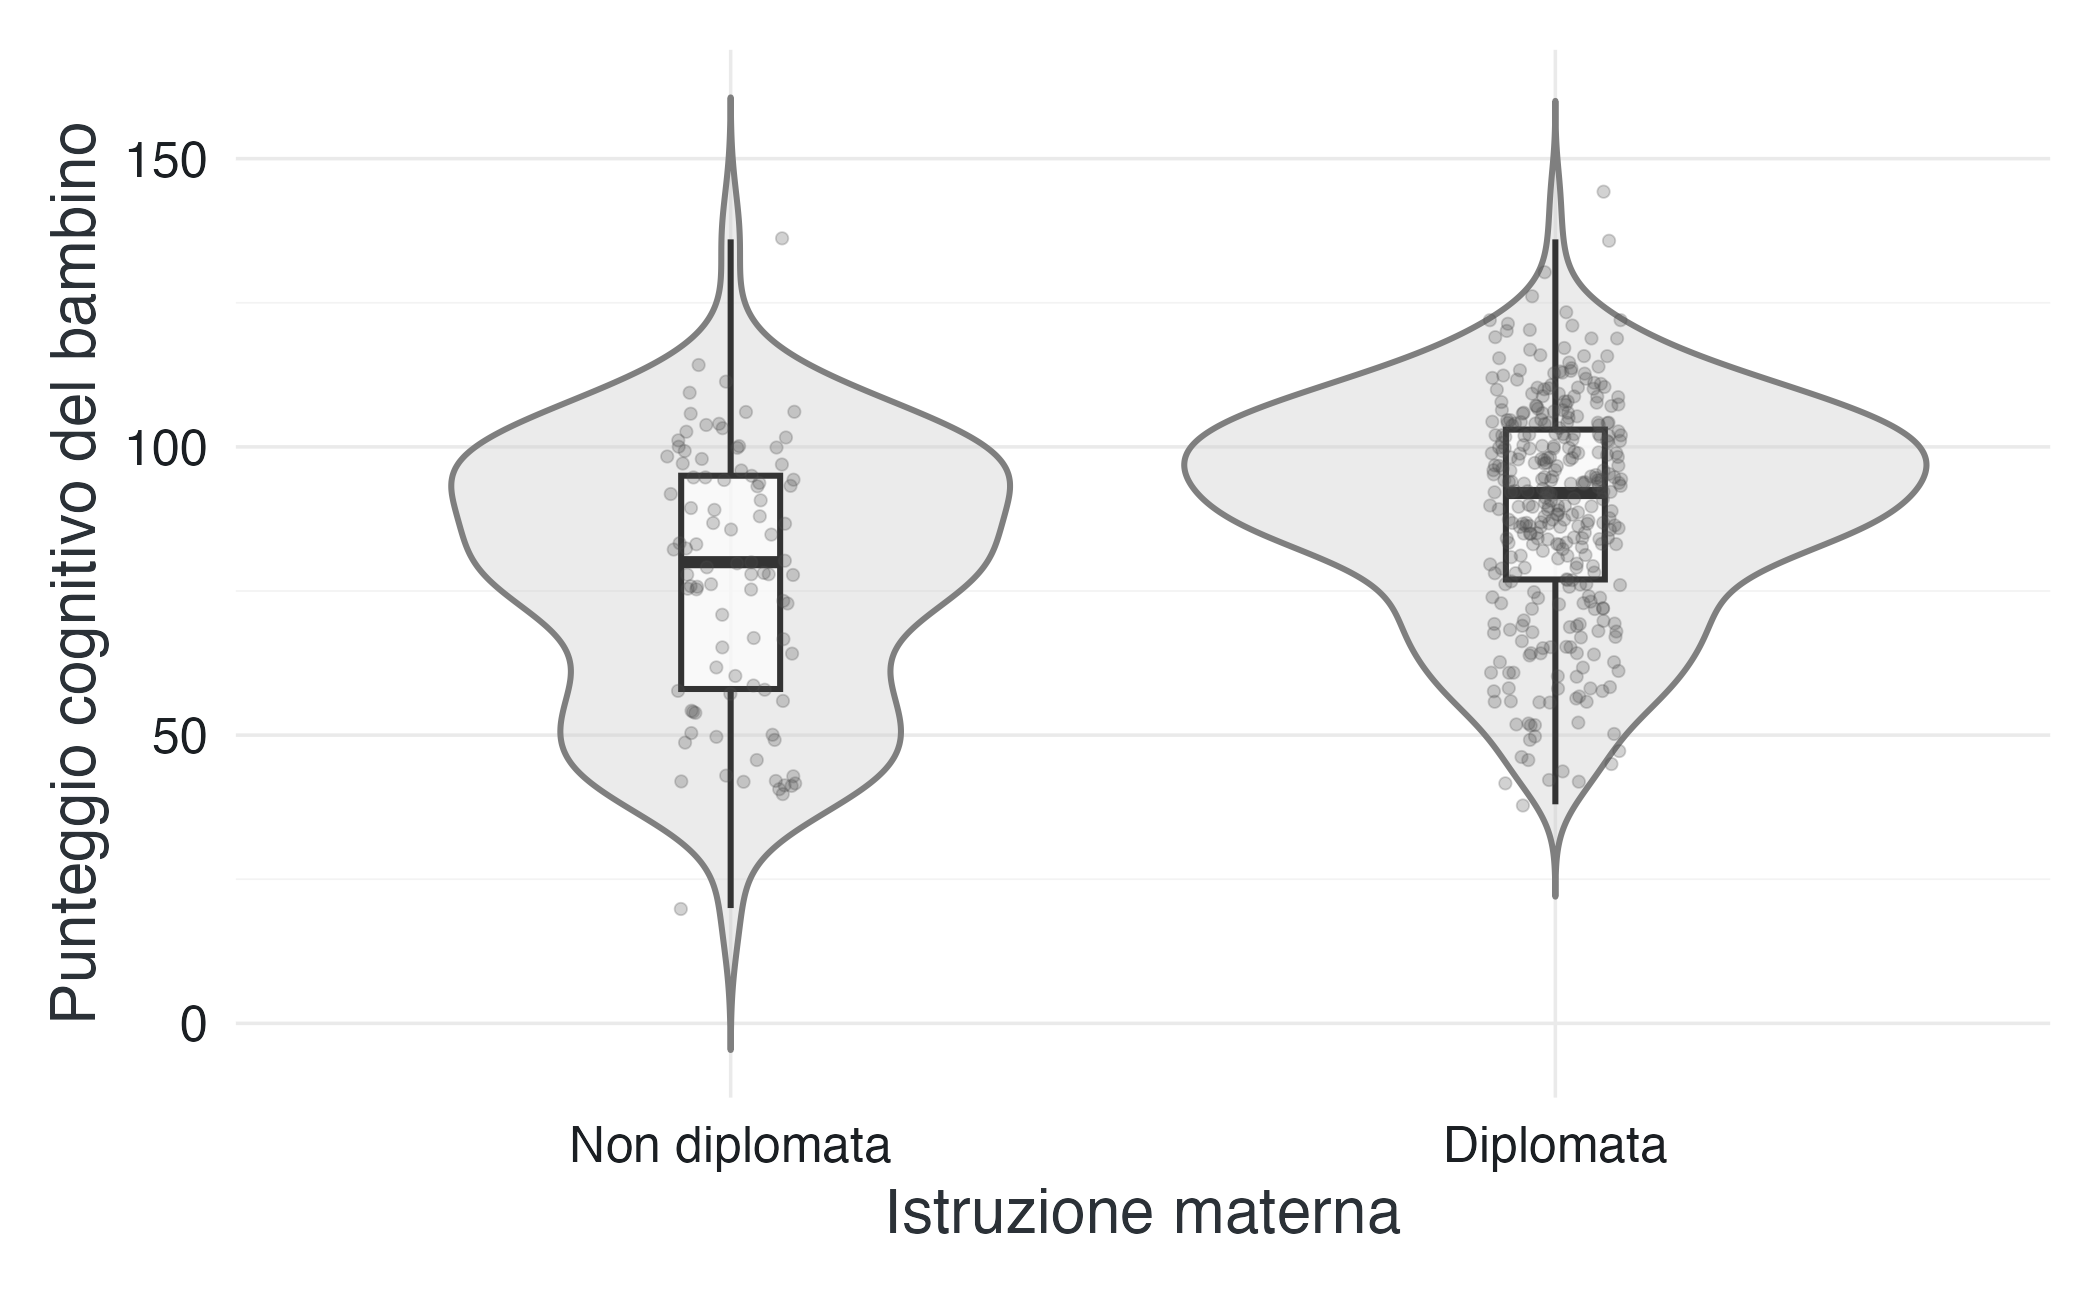
\includegraphics[width=0.85\linewidth,height=\textheight,keepaspectratio]{chapters/linear_models/06_due_gruppi_rilevanza_pratica_files/figure-pdf/fig-kidiq-two-groups-1.png}

}

\caption{\label{fig-kidiq-two-groups}Distribuzione dei punteggi
cognitivi nei due gruppi definiti dall'istruzione materna. Le medie
possono differire anche quando le distribuzioni individuali mostrano
un'ampia sovrapposizione.}

\end{figure}%

L'ispezione grafica suggerisce uno scostamento tra i centri delle due
distribuzioni, ma evidenzia anche una marcata variabilità interna a
ciascun gruppo. Il modello lineare dovrà quindi essere in grado di
catturare e quantificare separatamente queste due caratteristiche: la
differenza di posizione e l'eterogeneità residua condivisa.

\section{Il modello lineare con indicatore
binario}\label{il-modello-lineare-con-indicatore-binario}

Definiamo la variabile indicatore (\emph{dummy variable}) ponendo
\(x_i = 0\) per il gruppo delle madri ``Non diplomate'' e \(x_i = 1\)
per il gruppo delle madri ``Diplomate''. Il modello gaussiano
omoschedastico assume la forma:

\begin{equation}\protect\phantomsection\label{eq-two-groups-dummy}{
\begin{aligned} 
Y_i \mid x_i, \alpha, \beta, \sigma &\sim \operatorname{Normal}(\mu_i,\sigma), \\ \mu_i &= \alpha + \beta x_i. 
\end{aligned}
}\end{equation}

Il sistema di equazioni lineari chiarisce la scomposizione delle medie
condizionate per i due profili:

\begin{itemize}
\tightlist
\item
  Per il gruppo di riferimento (\(x_i = 0\)):
\end{itemize}

\[\mu_0 = \alpha\]

\begin{itemize}
\tightlist
\item
  Per il gruppo di confronto (\(x_i = 1\)):
\end{itemize}

\[\mu_1 = \alpha + \beta\]

Sottraendo le due espressioni, la differenza tra le medie coincide
direttamente con il coefficiente angolare della retta di regressione:

\[
\Delta = \mu_1 - \mu_0 = (\alpha + \beta) - \alpha = \beta.
\]

In questa formulazione, il parametro \(\sigma\) definisce la deviazione
standard residua comune all'interno di entrambi i gruppi. L'assunzione
di omoschedasticità (uguaglianza delle varianze nei gruppi) costituisce
un'ipotesi teorica del modello che dovrà essere esplicitamente
sottoposta a verifica diagnostica e non accettata a priori.

\begin{tcolorbox}[enhanced jigsaw, arc=.35mm, bottomrule=.15mm, bottomtitle=1mm, breakable, colback=white, colbacktitle=quarto-callout-note-color!10!white, colframe=quarto-callout-note-color-frame, coltitle=black, left=2mm, leftrule=.75mm, opacityback=0, opacitybacktitle=0.6, rightrule=.15mm, title=\textcolor{quarto-callout-note-color}{\faInfo}\hspace{0.5em}{Il test t di Student come caso speciale del modello lineare}, titlerule=0mm, toprule=.15mm, toptitle=1mm]

Il classico test \(t\) di Student per campioni indipendenti a varianze
omogenee è matematicamente equivalente a un modello di regressione
lineare con un unico predittore dicotomico. Nonostante questo
parallelismo formale accomuni le due strutture algebriche, le
interpretazioni frequentista e bayesiana rimangono profondamente diverse
sul piano concettuale. Tale equivalenza mostra tuttavia come il modello
lineare sia un framework unificato in grado di riassumere le procedure
statistiche tradizionali senza la necessità di introdurre strutture
matematiche ad hoc.

\end{tcolorbox}

\section{Tre parametrizzazioni dello stesso
confronto}\label{tre-parametrizzazioni-dello-stesso-confronto}

Lo stesso sistema di medie di gruppo può essere formalizzato mediante
codifiche algebriche diverse. La scelta della parametrizzazione non
altera in alcun modo le quantità sostantive stimate (\(\mu_0\),
\(\mu_1\) e \(\Delta\)), ma modifica radicalmente il significato
matematico immediato dei singoli coefficienti e la struttura delle
assunzioni a priori.

{\def\LTcaptype{none} % do not increment counter
\begin{longtable}[]{@{}
  >{\raggedright\arraybackslash}p{(\linewidth - 4\tabcolsep) * \real{0.3333}}
  >{\raggedright\arraybackslash}p{(\linewidth - 4\tabcolsep) * \real{0.3333}}
  >{\raggedright\arraybackslash}p{(\linewidth - 4\tabcolsep) * \real{0.3333}}@{}}
\toprule\noalign{}
\begin{minipage}[b]{\linewidth}\raggedright
Parametrizzazione
\end{minipage} & \begin{minipage}[b]{\linewidth}\raggedright
Sintassi \texttt{brms}
\end{minipage} & \begin{minipage}[b]{\linewidth}\raggedright
Significato dei coefficienti
\end{minipage} \\
\midrule\noalign{}
\endhead
\bottomrule\noalign{}
\endlastfoot
\textbf{Codifica Dummy} (\(x \in \{0, 1\}\)) &
\texttt{y\ \textasciitilde{}\ 1\ +\ x} & L'intercetta esprime la media
del gruppo di riferimento (\(\mu_0\)). \\
\end{longtable}
}

Il coefficiente angolare esprime il contrasto assoluto (\(\Delta\)).
\textbar{} \textbar{} \textbf{Codifica Centrata}
(\(x_c \in \{-0.5, 0.5\}\)) \textbar{}
\texttt{y\ \textasciitilde{}\ 1\ +\ x\_c} \textbar{} L'intercetta
esprime il punto medio non ponderato tra i gruppi.

Il coefficiente angolare esprime il contrasto assoluto (\(\Delta\)).
\textbar{} \textbar{} \textbf{Medie di Cella} \textbar{}
\texttt{y\ \textasciitilde{}\ 0\ +\ gruppo} \textbar{} Il modello
esclude l'intercetta globale.

Vengono stimati direttamente i due parametri di posizione \(\mu_0\) e
\(\mu_1\). \textbar{}

\subsection{1. Codifica Dummy (Variabile
Indicatore)}\label{codifica-dummy-variabile-indicatore}

Rappresenta l'approccio standard quando è possibile identificare un
gruppo di controllo o di riferimento logicamente prioritario.
L'intercetta riflette la stima puntuale di tale categoria di
riferimento, mentre il coefficiente associato al predittore esprime lo
scostamento necessario per raggiungere la media del gruppo di confronto.

\subsection{2. Codifica Centrata}\label{codifica-centrata}

Sottraendo il valore costante \(0.5\) alla variabile \emph{dummy}, si
ottiene un predittore centrato \(x_i^c\) con valori pari a \(-0.5\) (non
diplomata) e \(0.5\) (diplomata). Sotto questa formulazione,
l'intercetta si sposta sul \textbf{punto medio non ponderato} delle
medie dei due gruppi:

\[\alpha_c = \frac{\mu_0 + \mu_1}{2}\]

\begin{quote}
\textbf{Nota sulla ponderazione:} il valore di \(\alpha_c\) non
corrisponde alla media empirica complessiva del campione (\emph{grand
mean}) se i due gruppi presentano numerosità sbilanciate
(\(n_0 \neq n_1\)). Il coefficiente angolare della pendenza continua a
quantificare l'effetto differenziale totale \(\Delta\).
\end{quote}

\subsection{3. Medie di Cella}\label{medie-di-cella}

Rimuovendo esplicitamente l'intercetta globale tramite la sintassi
\texttt{0\ +\ gruppo}, il framework lineare stima in modo isolato i
parametri di posizione di ciascun livello del fattore. Questa
parametrizzazione risulta particolarmente vantaggiosa quando si desidera
assegnare distribuzioni a priori indipendenti e specifiche alle singole
medie, demandando il calcolo dei contrasti a una fase successiva di
post-elaborazione sui campioni della distribuzione a posteriori.

\begin{tcolorbox}[enhanced jigsaw, arc=.35mm, bottomrule=.15mm, bottomtitle=1mm, breakable, colback=white, colbacktitle=quarto-callout-important-color!10!white, colframe=quarto-callout-important-color-frame, coltitle=black, left=2mm, leftrule=.75mm, opacityback=0, opacitybacktitle=0.6, rightrule=.15mm, title=\textcolor{quarto-callout-important-color}{\faExclamation}\hspace{0.5em}{L'architettura del modello vincola la struttura dei prior}, titlerule=0mm, toprule=.15mm, toptitle=1mm]

Assegnare \emph{prior} reciprocamente indipendenti all'intercetta e al
coefficiente di pendenza non equivale a dichiarare \emph{prior}
indipendenti sulle medie dei singoli gruppi. Ad esempio, nella codifica
\emph{dummy} la media del secondo gruppo è definita come combinazione
lineare (\(\mu_1 = \alpha + \beta\)); di conseguenza, l'incertezza
associata ad \(\alpha\) si ripercuote matematicamente sia su \(\mu_0\)
sia su \(\mu_1\). Non esiste una codifica oggettivamente migliore: il
ricercatore deve scegliere la parametrizzazione che rende la traduzione
delle ipotesi teoriche in vincoli probabilistici più trasparente e
controllabile.

\end{tcolorbox}

\section{Specificazione del modello e controllo a
priori}\label{specificazione-del-modello-e-controllo-a-priori}

Adottiamo la codifica \emph{dummy} impostando il gruppo delle madri
``Non diplomate'' come livello baseline di riferimento. I \emph{prior}
vengono calibrati direttamente sulla scala metrica del QI (punti di
punteggio cognitivo):

\begin{itemize}
\tightlist
\item
  Una distribuzione normale attorno al valore centrale atteso per il
  gruppo di riferimento;
\item
  una distribuzione normale speculare e centrata su zero per la
  differenza tra i gruppi, che esprime scetticismo verso effetti
  artificialmente enormi;
\item
  una distribuzione a supporto positivo per la dispersione residua
  comune all'interno delle categorie.
\end{itemize}

\begin{Shaded}
\begin{Highlighting}[]
\NormalTok{priors\_two\_groups }\OtherTok{\textless{}{-}} \FunctionTok{c}\NormalTok{(}
  \FunctionTok{prior}\NormalTok{(}\FunctionTok{normal}\NormalTok{(}\DecValTok{90}\NormalTok{, }\DecValTok{20}\NormalTok{), }\AttributeTok{class =} \StringTok{"Intercept"}\NormalTok{),}
  \FunctionTok{prior}\NormalTok{(}\FunctionTok{normal}\NormalTok{(}\DecValTok{0}\NormalTok{, }\DecValTok{15}\NormalTok{), }\AttributeTok{class =} \StringTok{"b"}\NormalTok{),}
  \FunctionTok{prior}\NormalTok{(}\FunctionTok{student\_t}\NormalTok{(}\DecValTok{3}\NormalTok{, }\DecValTok{0}\NormalTok{, }\DecValTok{20}\NormalTok{), }\AttributeTok{class =} \StringTok{"sigma"}\NormalTok{)}
\NormalTok{)}
\end{Highlighting}
\end{Shaded}

Prima di condizionare il modello all'evidenza empirica, eseguiamo una
simulazione predittiva a priori (\emph{prior predictive check}) per
assicurarci che le assunzioni adottate non generino sistematicamente
scenari matematicamente impossibili o biologicamente assurdi rispetto al
dominio del QI:

\begin{Shaded}
\begin{Highlighting}[]
\NormalTok{fit\_two\_groups\_prior }\OtherTok{\textless{}{-}} \FunctionTok{brm}\NormalTok{(}
  \AttributeTok{formula =}\NormalTok{ kid\_score }\SpecialCharTok{\textasciitilde{}} \DecValTok{1} \SpecialCharTok{+}\NormalTok{ mom\_hs,}
  \AttributeTok{data =}\NormalTok{ kidiq,}
  \AttributeTok{family =} \FunctionTok{gaussian}\NormalTok{(),}
  \AttributeTok{prior =}\NormalTok{ priors\_two\_groups,}
  \AttributeTok{sample\_prior =} \StringTok{"only"}\NormalTok{, }\CommentTok{\# Estrae campioni esclusivamente dalle distribuzioni a priori}
  \AttributeTok{backend =} \StringTok{"cmdstanr"}\NormalTok{,}
  \AttributeTok{chains =} \DecValTok{4}\NormalTok{,}
  \AttributeTok{iter =} \DecValTok{1000}\NormalTok{,}
  \AttributeTok{seed =} \DecValTok{1234}\NormalTok{,}
  \AttributeTok{refresh =} \DecValTok{0}
\NormalTok{)}
\end{Highlighting}
\end{Shaded}

Visualizziamo il profilo delle densità simulate generate dai soli
\emph{prior}:

\begin{Shaded}
\begin{Highlighting}[]
\FunctionTok{pp\_check}\NormalTok{(}
\NormalTok{  fit\_two\_groups\_prior,}
  \AttributeTok{type =} \StringTok{"dens\_overlay"}\NormalTok{,}
  \AttributeTok{ndraws =} \DecValTok{40}
\NormalTok{)}
\end{Highlighting}
\end{Shaded}

\begin{figure}[H]

\centering{

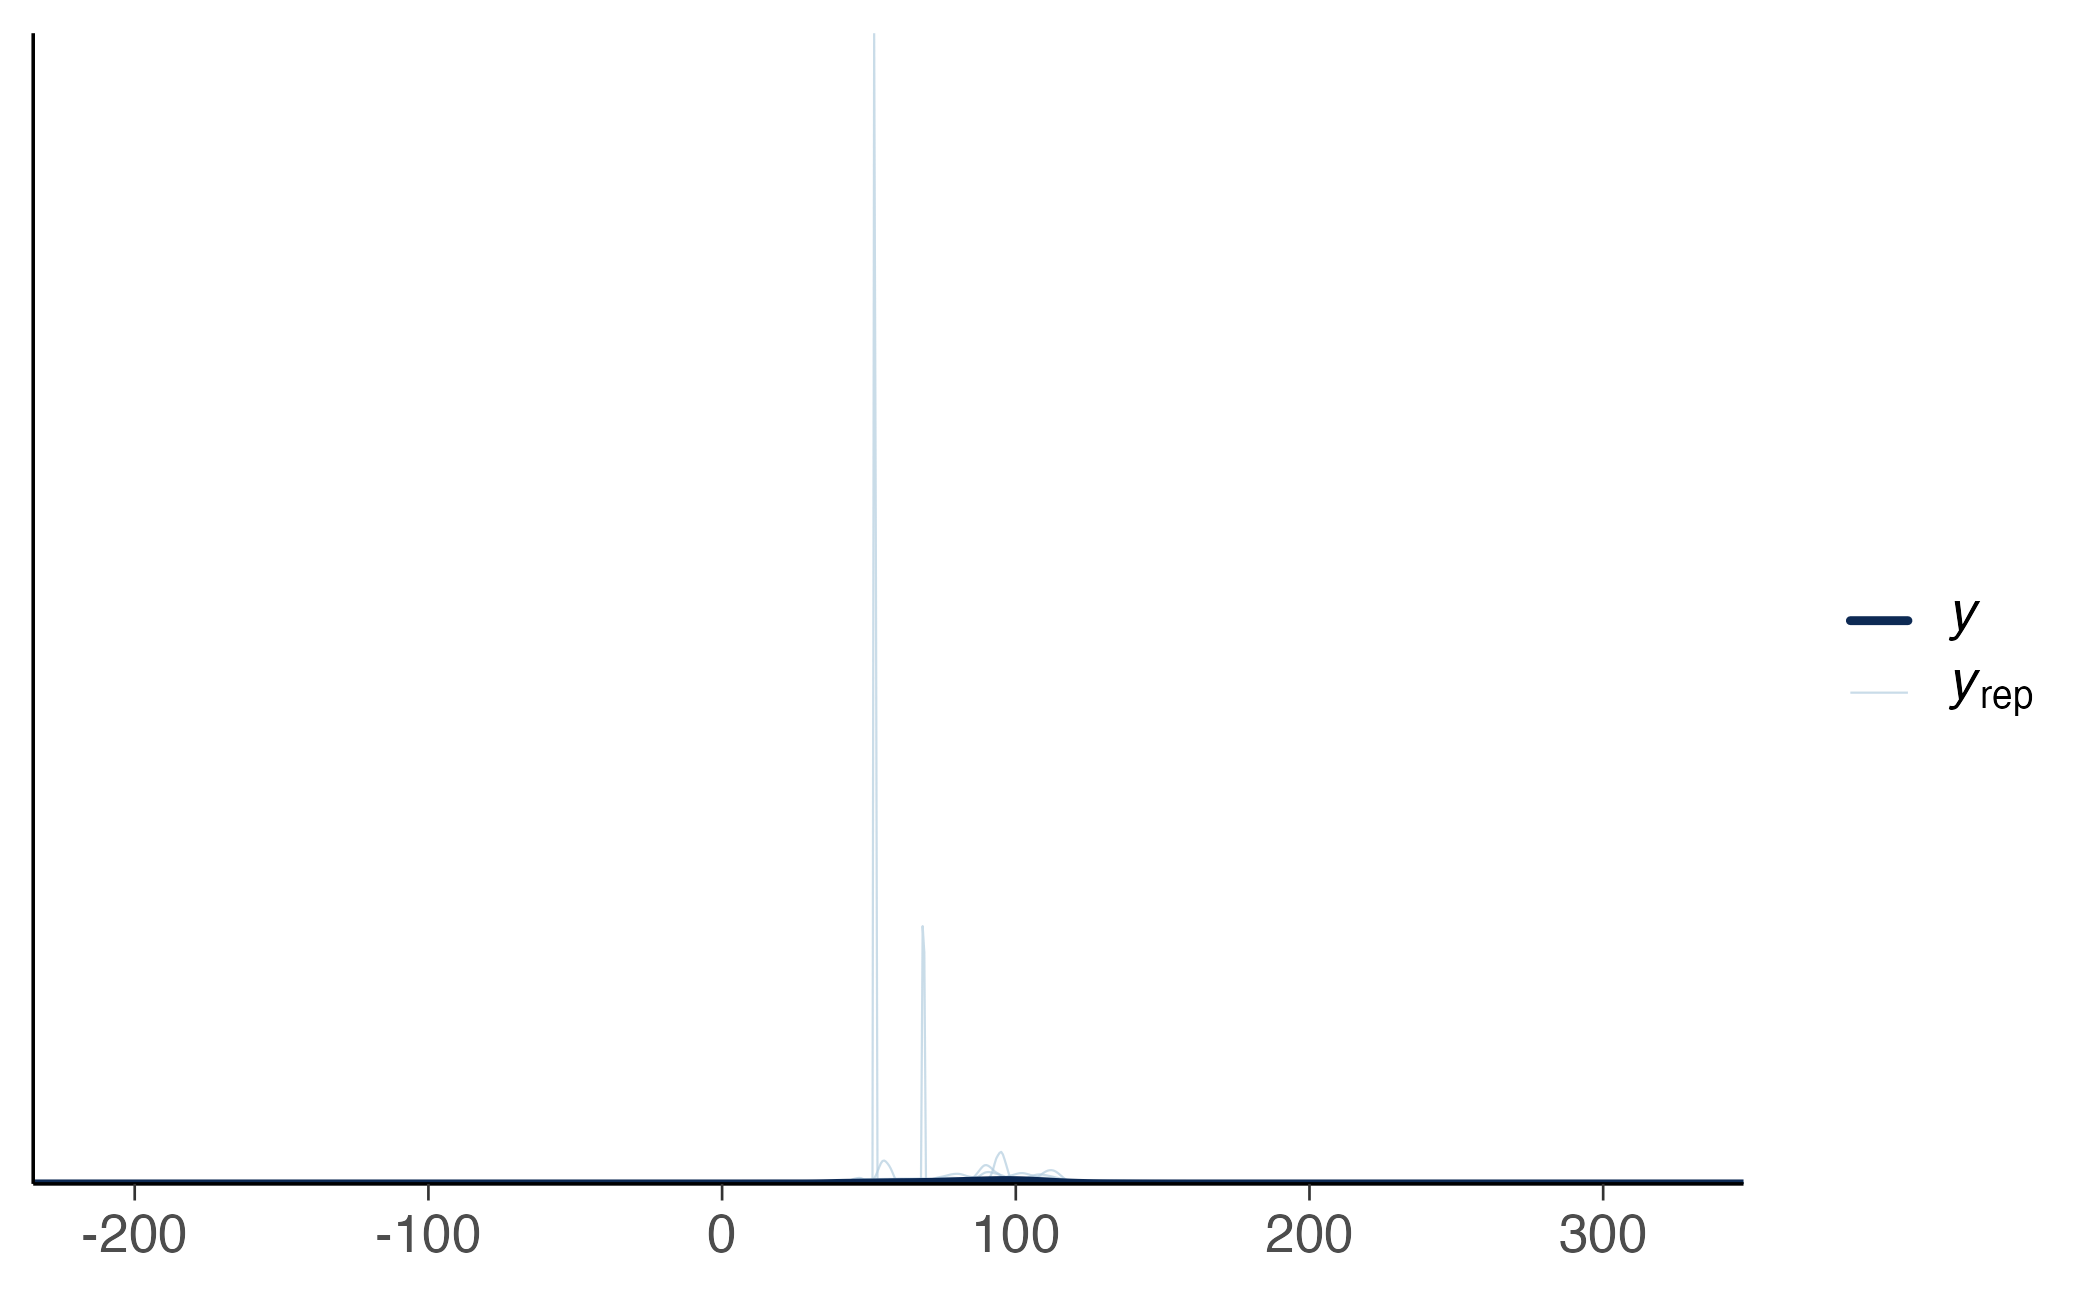
\includegraphics[width=0.85\linewidth,height=\textheight,keepaspectratio]{chapters/linear_models/06_due_gruppi_rilevanza_pratica_files/figure-pdf/fig-prior-predictive-two-groups-1.png}

}

\caption{\label{fig-prior-predictive-two-groups}Controllo predittivo a
priori per il modello a due gruppi. Le repliche servono a valutare le
conseguenze congiunte dei prior sulla scala osservata.}

\end{figure}%

\begin{quote}
\textbf{Nota diagnostica:} questo controllo non ha lo scopo di
certificare se i \emph{prior} siano ``oggettivamente corretti'' o veri.
La sua funzione è puramente pragmatica: esplicitare e rendere visibili
sulla scala osservabile le conseguenze congiunte delle nostre scelte
probabilistiche, consentendo di individuare e correggere tempestivamente
vincoli a priori eccessivamente dogmatici (iper-concentrati) o
irrealisticamente dispersi.
\end{quote}

\section{Stima del modello e verifiche
computazionali}\label{stima-del-modello-e-verifiche-computazionali}

Procediamo al condizionamento del modello integrando i dati empirici per
ottenere la distribuzione a posteriori:

\begin{Shaded}
\begin{Highlighting}[]
\NormalTok{fit\_two\_groups }\OtherTok{\textless{}{-}} \FunctionTok{brm}\NormalTok{(}
  \AttributeTok{formula =}\NormalTok{ kid\_score }\SpecialCharTok{\textasciitilde{}} \DecValTok{1} \SpecialCharTok{+}\NormalTok{ mom\_hs,}
  \AttributeTok{data =}\NormalTok{ kidiq,}
  \AttributeTok{family =} \FunctionTok{gaussian}\NormalTok{(),}
  \AttributeTok{prior =}\NormalTok{ priors\_two\_groups,}
  \AttributeTok{backend =} \StringTok{"cmdstanr"}\NormalTok{,}
  \AttributeTok{chains =} \DecValTok{4}\NormalTok{,}
  \AttributeTok{iter =} \DecValTok{2000}\NormalTok{,}
  \AttributeTok{seed =} \DecValTok{1234}\NormalTok{,}
  \AttributeTok{refresh =} \DecValTok{0}
\NormalTok{)}
\end{Highlighting}
\end{Shaded}

Le verifiche formali sulla convergenza e sulla qualità algoritmica del
campionamento MCMC seguono i criteri metodologici già illustrati
nell'Capitolo~\ref{sec-linmod-bayesian-reg}:

\begin{Shaded}
\begin{Highlighting}[]
\FunctionTok{summarise\_draws}\NormalTok{(}
  \FunctionTok{as\_draws\_array}\NormalTok{(fit\_two\_groups),}
  \StringTok{"mean"}\NormalTok{, }
  \StringTok{"sd"}\NormalTok{, }
  \StringTok{"rhat"}\NormalTok{, }
  \StringTok{"ess\_bulk"}\NormalTok{, }
  \StringTok{"ess\_tail"}
\NormalTok{)}
\CommentTok{\#\textgreater{} \# A tibble: 6 x 6}
\CommentTok{\#\textgreater{}   variable             mean    sd  rhat ess\_bulk ess\_tail}
\CommentTok{\#\textgreater{}   \textless{}chr\textgreater{}               \textless{}dbl\textgreater{} \textless{}dbl\textgreater{} \textless{}dbl\textgreater{}    \textless{}dbl\textgreater{}    \textless{}dbl\textgreater{}}
\CommentTok{\#\textgreater{} 1 b\_Intercept          77.7 2.07  1.000    3872.    3028.}
\CommentTok{\#\textgreater{} 2 b\_mom\_hsDiplomata    11.5 2.35  1.000    3859.    2944.}
\CommentTok{\#\textgreater{} 3 sigma                19.9 0.670 1.00     3548.    2468.}
\CommentTok{\#\textgreater{} 4 Intercept            86.8 0.940 1.00     4054.    2878.}
\CommentTok{\#\textgreater{} 5 lprior              {-}11.7 0.127 1.000    3794.    3107.}
\CommentTok{\#\textgreater{} 6 lp\_\_              {-}1922.  1.20  1.00     2159.    2877.}
\end{Highlighting}
\end{Shaded}

\begin{quote}
\textbf{Nota di interpretazione:} è importante ripetere che la
convergenza ottimale delle catene e l'assenza di patologie numeriche non
garantiscono la validità scientifica del modello. Valori ideali di
\(\widehat{R}\) e un numero elevato di campioni effettivi (\(ESS\))
indicano semplicemente che l'algoritmo Stan ha esplorato la
distribuzione a posteriori congiunta in modo matematicamente affidabile.
La valutazione dell'adeguatezza della verosimiglianza normale e
dell'assunzione di omoschedasticità spetta invece ai successivi
controlli predittivi a posteriori.
\end{quote}

\section{Dalle coordinate del modello alle quantità
sostantive}\label{dalle-coordinate-del-modello-alle-quantituxe0-sostantive}

Dopo aver stimato i parametri nelle ``coordinate'' algebriche della
regressione (\(\alpha\) e \(\beta\)), passiamo alla derivazione delle
quantità dotate di un immediato significato scientifico. Estraiamo i
campioni dalla distribuzione a posteriori per calcolare, draw dopo draw,
le medie dei due gruppi, la loro differenza grezza e l'effetto
standardizzato:

\begin{Shaded}
\begin{Highlighting}[]
\NormalTok{post\_two\_groups }\OtherTok{\textless{}{-}} \FunctionTok{as\_draws\_df}\NormalTok{(fit\_two\_groups) }\SpecialCharTok{|\textgreater{}}
  \FunctionTok{transmute}\NormalTok{(}
    \AttributeTok{mu0   =}\NormalTok{ b\_Intercept,}
    \AttributeTok{delta =}\NormalTok{ b\_mom\_hsDiplomata,}
    \AttributeTok{mu1   =}\NormalTok{ b\_Intercept }\SpecialCharTok{+}\NormalTok{ b\_mom\_hsDiplomata,}
    \AttributeTok{sigma =}\NormalTok{ sigma,}
    \AttributeTok{d     =}\NormalTok{ delta }\SpecialCharTok{/}\NormalTok{ sigma}
\NormalTok{  )}

\FunctionTok{summarise\_draws}\NormalTok{(}
\NormalTok{  post\_two\_groups[, }\FunctionTok{c}\NormalTok{(}\StringTok{"mu0"}\NormalTok{, }\StringTok{"mu1"}\NormalTok{, }\StringTok{"delta"}\NormalTok{, }\StringTok{"sigma"}\NormalTok{, }\StringTok{"d"}\NormalTok{)]}
\NormalTok{)}
\CommentTok{\#\textgreater{} \# A tibble: 5 x 10}
\CommentTok{\#\textgreater{}   variable   mean median    sd   mad     q5    q95  rhat ess\_bulk ess\_tail}
\CommentTok{\#\textgreater{}   \textless{}chr\textgreater{}     \textless{}dbl\textgreater{}  \textless{}dbl\textgreater{} \textless{}dbl\textgreater{} \textless{}dbl\textgreater{}  \textless{}dbl\textgreater{}  \textless{}dbl\textgreater{} \textless{}dbl\textgreater{}    \textless{}dbl\textgreater{}    \textless{}dbl\textgreater{}}
\CommentTok{\#\textgreater{} 1 mu0      77.7   77.7   2.07  2.10  74.3   81.1   1.00     3723.    2904.}
\CommentTok{\#\textgreater{} 2 mu1      89.3   89.3   1.07  1.03  87.5   91.1   1.00     4005.    2983.}
\CommentTok{\#\textgreater{} 3 delta    11.5   11.6   2.35  2.41   7.75  15.4   1.000    3810.    2887.}
\CommentTok{\#\textgreater{} 4 sigma    19.9   19.9   0.670 0.663 18.8   21.0   1.000    3441.    2465.}
\CommentTok{\#\textgreater{} 5 d         0.581  0.581 0.120 0.122  0.388  0.781 1.000    3896.    2791.}
\end{Highlighting}
\end{Shaded}

Questa operazione mette in luce un principio fondamentale del workflow
bayesiano: il modello viene parametrizzato nella forma
computazionalmente più efficiente o comoda per il campionamento, ma
l'analisi finale deve essere costruita sulle quantità matematiche che
rispondono in modo diretto agli interrogativi della ricerca.

\subsection{La differenza sulla scala
originale}\label{la-differenza-sulla-scala-originale}

La distribuzione a posteriori di \(\Delta\) (espressa in punti di QI)
mantiene l'unità di misura originale del test ed è la metrica principale
da comunicare quando la scala possiede un significato clinico o pratico
ben noto.

Visualizziamo la densità della differenza a posteriori confrontandola
sia con l'ipotesi di assenza di effetto sia con una soglia di rilevanza
pratica (\emph{SESOI} --- \emph{Smallest Effect Size of Interest}):

\begin{Shaded}
\begin{Highlighting}[]
\NormalTok{SESOI\_delta }\OtherTok{\textless{}{-}} \DecValTok{5}

\NormalTok{post\_two\_groups }\SpecialCharTok{|\textgreater{}}
  \FunctionTok{ggplot}\NormalTok{(}\FunctionTok{aes}\NormalTok{(}\AttributeTok{x =}\NormalTok{ delta)) }\SpecialCharTok{+}
  \FunctionTok{geom\_density}\NormalTok{(}\AttributeTok{fill =} \StringTok{"grey90"}\NormalTok{, }\AttributeTok{color =} \StringTok{"grey40"}\NormalTok{, }\AttributeTok{alpha =} \FloatTok{0.5}\NormalTok{) }\SpecialCharTok{+}
  \FunctionTok{geom\_vline}\NormalTok{(}\AttributeTok{xintercept =} \DecValTok{0}\NormalTok{, }\AttributeTok{linetype =} \StringTok{"dashed"}\NormalTok{, }\AttributeTok{color =} \StringTok{"firebrick"}\NormalTok{) }\SpecialCharTok{+}
  \FunctionTok{geom\_vline}\NormalTok{(}\AttributeTok{xintercept =}\NormalTok{ SESOI\_delta, }\AttributeTok{linetype =} \StringTok{"dotted"}\NormalTok{, }\AttributeTok{color =} \StringTok{"steelblue"}\NormalTok{, }\AttributeTok{size =} \DecValTok{1}\NormalTok{) }\SpecialCharTok{+}
  \FunctionTok{labs}\NormalTok{(}
    \AttributeTok{x =} \FunctionTok{expression}\NormalTok{(}\FunctionTok{paste}\NormalTok{(}\StringTok{"Differenza grezza ("}\NormalTok{, Delta, }\StringTok{")"}\NormalTok{)),}
    \AttributeTok{y =} \StringTok{"Densità a posteriori"}
\NormalTok{  )}
\end{Highlighting}
\end{Shaded}

\begin{figure}[H]

\centering{

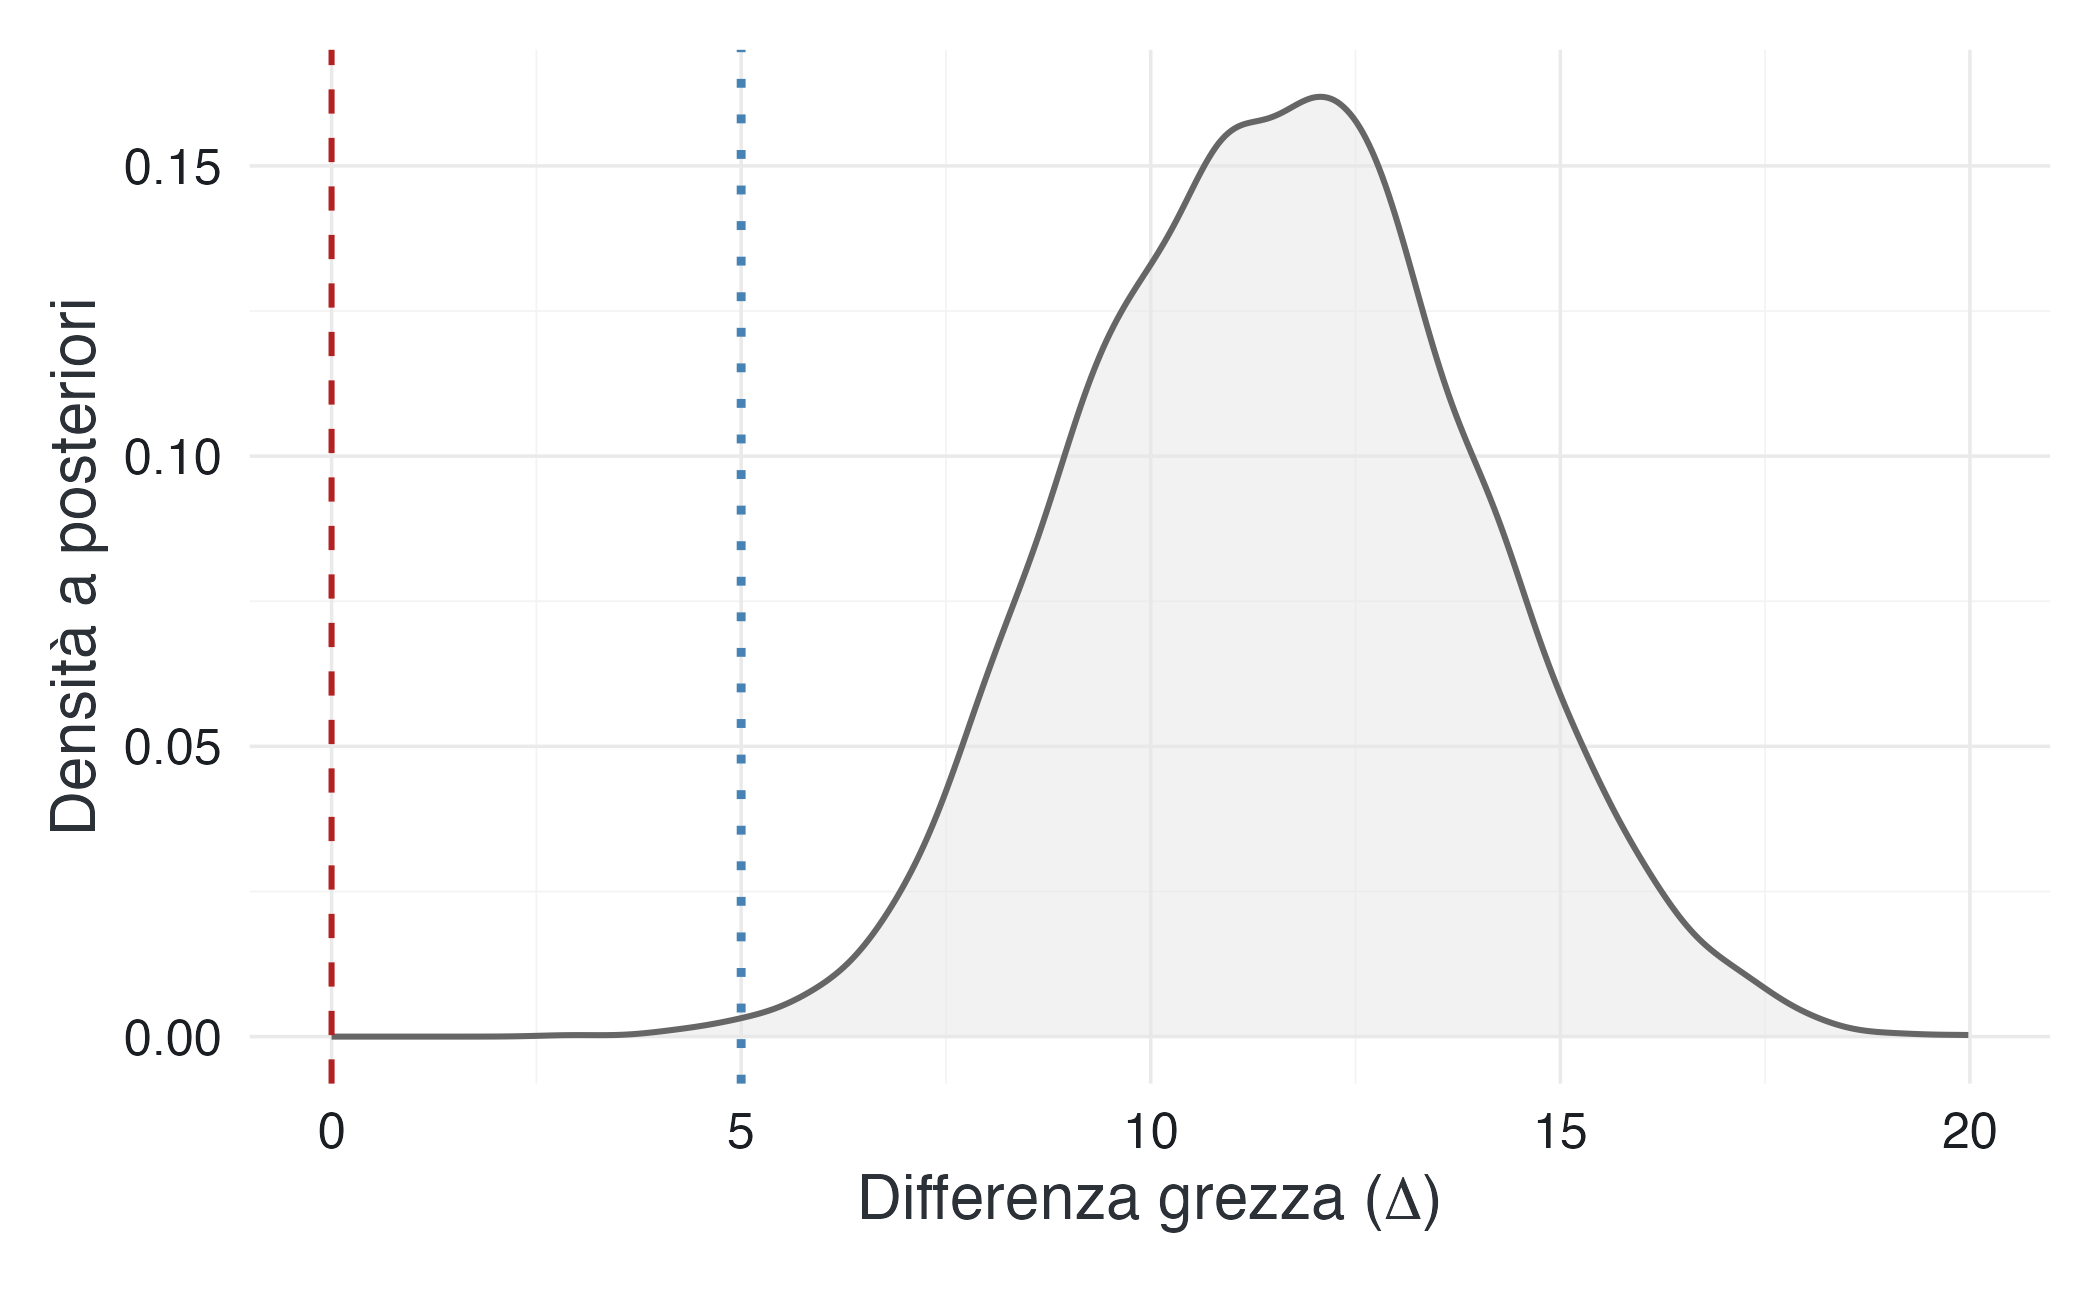
\includegraphics[width=0.85\linewidth,height=\textheight,keepaspectratio]{chapters/linear_models/06_due_gruppi_rilevanza_pratica_files/figure-pdf/fig-posterior-delta-two-groups-1.png}

}

\caption{\label{fig-posterior-delta-two-groups}Distribuzione a
posteriori della differenza grezza tra le medie. Le linee verticali
indicano l'assenza di effetto (0) e la soglia di rilevanza pratica
stabilita (5 punti di QI).}

\end{figure}%

Le probabilità associate a queste soglie sostantive si ottengono
contando quanti draw della posterior soddisfano i rispettivi criteri
logici:

\begin{Shaded}
\begin{Highlighting}[]
\FunctionTok{c}\NormalTok{(}
  \AttributeTok{P\_delta\_positive =} \FunctionTok{mean}\NormalTok{(post\_two\_groups}\SpecialCharTok{$}\NormalTok{delta }\SpecialCharTok{\textgreater{}} \DecValTok{0}\NormalTok{),}
  \AttributeTok{P\_delta\_relevant =} \FunctionTok{mean}\NormalTok{(post\_two\_groups}\SpecialCharTok{$}\NormalTok{delta }\SpecialCharTok{\textgreater{}}\NormalTok{ SESOI\_delta),}
  \AttributeTok{P\_delta\_in\_rope  =} \FunctionTok{mean}\NormalTok{(}\FunctionTok{abs}\NormalTok{(post\_two\_groups}\SpecialCharTok{$}\NormalTok{delta) }\SpecialCharTok{\textless{}=}\NormalTok{ SESOI\_delta)}
\NormalTok{)}
\CommentTok{\#\textgreater{} P\_delta\_positive P\_delta\_relevant  P\_delta\_in\_rope }
\CommentTok{\#\textgreater{}          1.00000          0.99775          0.00225}
\end{Highlighting}
\end{Shaded}

Le ultime due quantità rispondono a domande speculari e complementari
(la probabilità che l'effetto sia sostanziale vs la probabilità che
l'effetto sia trascurabile o nullo). È fondamentale ricordare che tali
valori probabilistici non si traducono automaticamente in decisioni
binarie: la soglia dei 5 punti deve essere validata teoricamente sulla
base della letteratura del dominio, e il livello di certezza richiesto
per agire di conseguenza deve essere fissato prima di esaminare i dati
per evitare distorsioni interpretative.

\section{Differenza standardizzata e dimensione
dell'effetto}\label{sec-bayesian-effect-size}

Se la differenza grezza rappresenta la metrica più trasparente quando la
scala ha un significato psicometrico o clinico noto, la
standardizzazione si rivela utile per confrontare risultati ottenuti
attraverso strumenti di misura differenti o per alimentare studi
meta-analitici.

Nel modello lineare omoschedastico, la dimensione dell'effetto
standardizzata è definita come:

\begin{equation}\protect\phantomsection\label{eq-standardized-difference}{
d = \frac{\mu_1 - \mu_0}{\sigma} = \frac{\Delta}{\sigma}.
}\end{equation}

Poiché sia la differenza tra le medie (\(\Delta\)) sia la deviazione
standard residua (\(\sigma\)) sono parametri incerti, il valore di \(d\)
viene calcolato separatamente per ogni singolo \emph{draw} della
distribuzione a posteriori. In questo modo, l'incertezza stimata per
entrambe le componenti si propaga matematicamente e in modo automatico
sul rapporto finale.

\begin{tcolorbox}[enhanced jigsaw, arc=.35mm, bottomrule=.15mm, bottomtitle=1mm, breakable, colback=white, colbacktitle=quarto-callout-note-color!10!white, colframe=quarto-callout-note-color-frame, coltitle=black, left=2mm, leftrule=.75mm, opacityback=0, opacitybacktitle=0.6, rightrule=.15mm, title=\textcolor{quarto-callout-note-color}{\faInfo}\hspace{0.5em}{Natura e limiti del parametro d}, titlerule=0mm, toprule=.15mm, toptitle=1mm]

Il formalismo espresso nella Equazione~\ref{eq-standardized-difference}
rappresenta il contrasto tra le medie condizionate misurato in unità di
deviazione standard residua comune. Si tratta dell'equivalente
modellistico del \(d\) di Cohen per campioni indipendenti, ma non
include la correzione algoritmica per piccoli campioni tipica del
\emph{g} di Hedges. Inoltre, in presenza di eteroschedasticità (varianze
disuguali tra gruppi) o di disegni a misure ripetute, la scelta del
denominatore non è univoca e richiede una definizione esplicita.

\end{tcolorbox}

Visualizziamo la distribuzione a posteriori di \(d\), sovrapponendo i
benchmark convenzionali proposti da Cohen:

\begin{Shaded}
\begin{Highlighting}[]
\NormalTok{post\_two\_groups }\SpecialCharTok{|\textgreater{}}
  \FunctionTok{ggplot}\NormalTok{(}\FunctionTok{aes}\NormalTok{(}\AttributeTok{x =}\NormalTok{ d)) }\SpecialCharTok{+}
  \FunctionTok{geom\_density}\NormalTok{(}\AttributeTok{fill =} \StringTok{"grey90"}\NormalTok{, }\AttributeTok{color =} \StringTok{"grey40"}\NormalTok{, }\AttributeTok{alpha =} \FloatTok{0.5}\NormalTok{) }\SpecialCharTok{+}
  \FunctionTok{geom\_vline}\NormalTok{(}\AttributeTok{xintercept =} \DecValTok{0}\NormalTok{, }\AttributeTok{linetype =} \StringTok{"dashed"}\NormalTok{, }\AttributeTok{color =} \StringTok{"firebrick"}\NormalTok{) }\SpecialCharTok{+}
  \FunctionTok{geom\_vline}\NormalTok{(}
    \AttributeTok{xintercept =} \FunctionTok{c}\NormalTok{(}\FloatTok{0.2}\NormalTok{, }\FloatTok{0.5}\NormalTok{, }\FloatTok{0.8}\NormalTok{),}
    \AttributeTok{linetypes  =} \StringTok{"dotted"}\NormalTok{,}
    \AttributeTok{color      =} \StringTok{"grey30"}
\NormalTok{  ) }\SpecialCharTok{+}
  \FunctionTok{labs}\NormalTok{(}
    \AttributeTok{x =} \FunctionTok{expression}\NormalTok{(}\FunctionTok{paste}\NormalTok{(}\StringTok{"Differenza standardizzata ("}\NormalTok{, d, }\StringTok{")"}\NormalTok{)),}
    \AttributeTok{y =} \StringTok{"Densità a posteriori"}
\NormalTok{  )}
\end{Highlighting}
\end{Shaded}

\begin{figure}[H]

\centering{

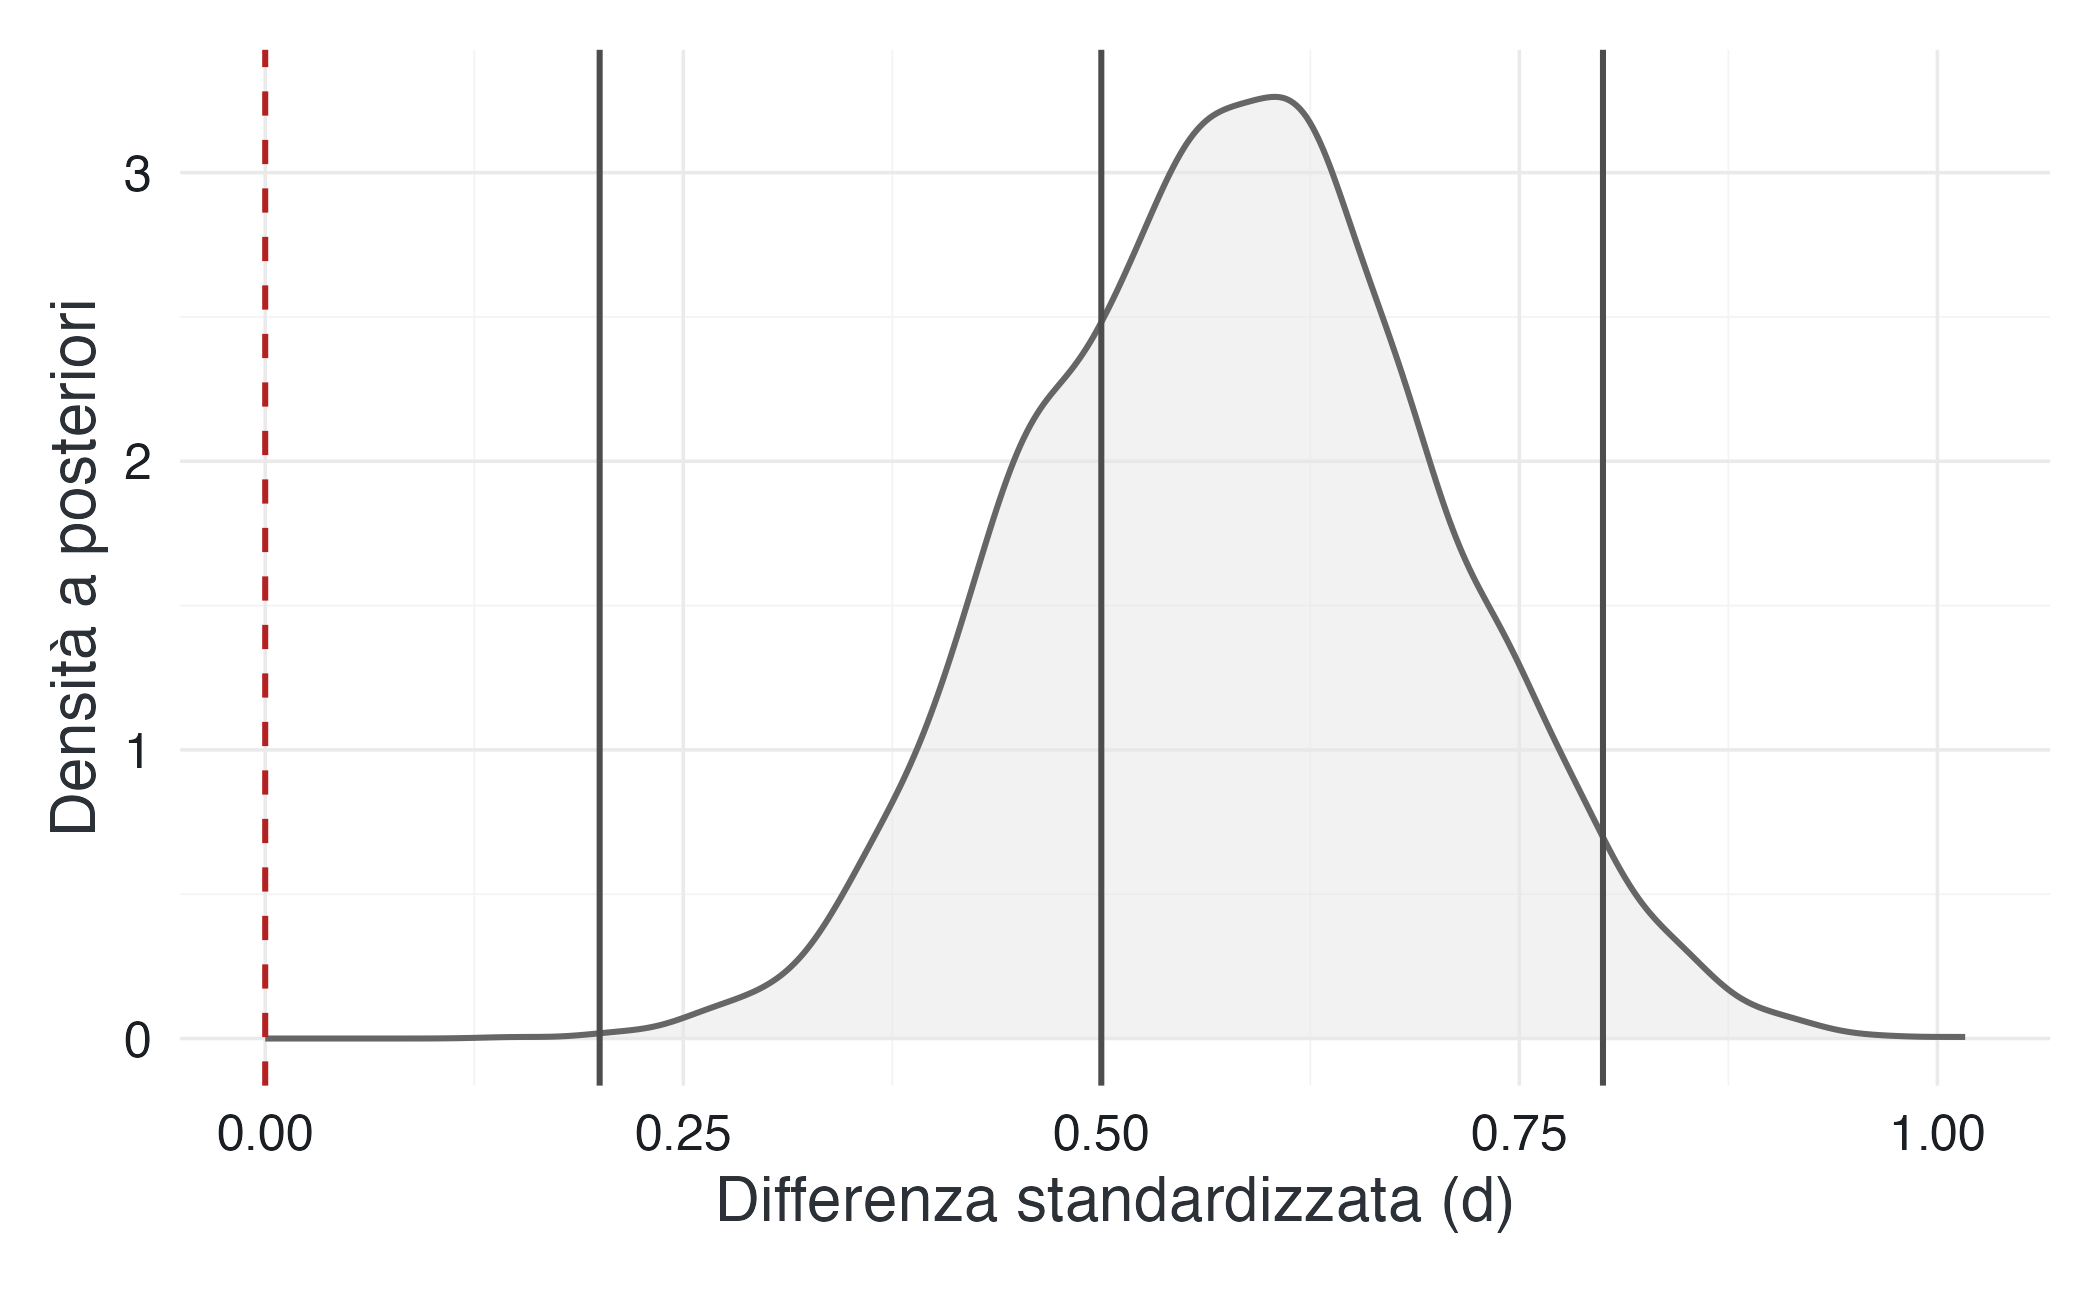
\includegraphics[width=0.85\linewidth,height=\textheight,keepaspectratio]{chapters/linear_models/06_due_gruppi_rilevanza_pratica_files/figure-pdf/fig-posterior-standardized-difference-1.png}

}

\caption{\label{fig-posterior-standardized-difference}Distribuzione a
posteriori della differenza standardizzata d.~I benchmark a 0.2, 0.5 e
0.8 sono inclusi come riferimenti storici e convenzionali, non come
confini naturali del fenomeno.}

\end{figure}%

Possiamo ora tradurre le soglie standardizzate in enunciati
probabilistici diretti, calcolando la percentuale di campioni della
posterior che supera ogni valore critico:

\begin{Shaded}
\begin{Highlighting}[]
\FunctionTok{c}\NormalTok{(}
  \AttributeTok{P\_d\_positive =} \FunctionTok{mean}\NormalTok{(post\_two\_groups}\SpecialCharTok{$}\NormalTok{d }\SpecialCharTok{\textgreater{}} \DecValTok{0}\NormalTok{),}
  \AttributeTok{P\_d\_gt\_0\_2   =} \FunctionTok{mean}\NormalTok{(post\_two\_groups}\SpecialCharTok{$}\NormalTok{d }\SpecialCharTok{\textgreater{}} \FloatTok{0.2}\NormalTok{),}
  \AttributeTok{P\_d\_gt\_0\_5   =} \FunctionTok{mean}\NormalTok{(post\_two\_groups}\SpecialCharTok{$}\NormalTok{d }\SpecialCharTok{\textgreater{}} \FloatTok{0.5}\NormalTok{),}
  \AttributeTok{P\_d\_gt\_0\_8   =} \FunctionTok{mean}\NormalTok{(post\_two\_groups}\SpecialCharTok{$}\NormalTok{d }\SpecialCharTok{\textgreater{}} \FloatTok{0.8}\NormalTok{)}
\NormalTok{)}
\CommentTok{\#\textgreater{} P\_d\_positive   P\_d\_gt\_0\_2   P\_d\_gt\_0\_5   P\_d\_gt\_0\_8 }
\CommentTok{\#\textgreater{}       1.0000       0.9995       0.7418       0.0335}
\end{Highlighting}
\end{Shaded}

\subsection{Perché standardizzare (e quando evitare di
farlo)}\label{perchuxe9-standardizzare-e-quando-evitare-di-farlo}

L'indice standardizzato facilita la sintesi quantitativa tra studi
diversi, ma non costituisce una trasformazione matematicamente neutra.
Presenta infatti alcuni vincoli strutturali:

\begin{itemize}
\tightlist
\item
  \textbf{Dipendenza dalla varianza:} a parità di differenza grezza nei
  punteggi, popolazioni più omogenee (con \(\sigma\) minore) generano
  artificialmente valori di \(d\) più elevati.
\item
  \textbf{Sensibilità metodologica:} il denominatore risente
  direttamente della qualità dello strumento e del controllo
  sperimentale: una misura meno precisa aumenta \(\sigma\) e diminuisce
  il valore di \(d\).
\item
  \textbf{Asimmetria degli effetti:} due ricerche possono mostrare
  un'identica dimensione dell'effetto \(d\) pur presentando differenze
  grezze e ricadute pratiche radicalmente diverse.
\end{itemize}

Il significato clinico, educativo o sociale di un risultato emerge con
maggiore chiarezza sulla scala nativa del fenomeno. La buona pratica
scientifica prevede quindi di documentare sempre la differenza grezza e
di affiancarle la stima standardizzata solo come integrazione
comparativa.

\subsection{Uso critico delle soglie
convenzionali}\label{uso-critico-delle-soglie-convenzionali}

I valori \(0.2\), \(0.5\) e \(0.8\) vengono meccanicamente associati
alle etichette di effetto ``piccolo'', ``medio'' e ``grande''. Jacob
Cohen introdusse questi criteri come semplici punti di riferimento
generali, da impiegare esclusivamente in assenza di qualunque conoscenza
pregressa sul dominio, mettendone in guardia contro un uso rigido.

Un effetto inferiore a \(0.2\) può assumere una rilevanza scientifica
straordinaria se applicato a un esito critico (ad esempio, i tassi di
mortalità o di abbandono scolastico) attraverso un intervento economico
su vasta scala. Al contrario, un effetto superiore a 0.8 può rivelarsi
irrilevante se l'indicatore finale non possiede un reale valore teorico
o applicativo. Sostituire il binarismo ``significativo/non
significativo'' con la classificazione categoriale
``piccolo/medio/grande'' non risolve l'esigenza di una valutazione
critica del dato.

\begin{tcolorbox}[enhanced jigsaw, arc=.35mm, bottomrule=.15mm, bottomtitle=1mm, breakable, colback=white, colbacktitle=quarto-callout-warning-color!10!white, colframe=quarto-callout-warning-color-frame, coltitle=black, left=2mm, leftrule=.75mm, opacityback=0, opacitybacktitle=0.6, rightrule=.15mm, title=\textcolor{quarto-callout-warning-color}{\faExclamationTriangle}\hspace{0.5em}{L'incertezza supera le categorie rigide}, titlerule=0mm, toprule=.15mm, toptitle=1mm]

La distribuzione a posteriori di \(d\) può intersecare
contemporaneamente più fasce convenzionali. Questa dispersione non
rappresenta un limite del modello, ma esprime l'incertezza reale sul
parametro. Qualora la letteratura scientifica di riferimento fornisca
una soglia specifica per il costrutto in esame, tale valore deve avere
la priorità assoluta rispetto alle tassonomie generiche.

\end{tcolorbox}

\section{SESOI e regione di equivalenza
pratica}\label{sesoi-e-regione-di-equivalenza-pratica}

La \textbf{SESOI} (\emph{Smallest Effect Size of Interest}) definisce la
minima grandezza dell'effetto considerata rilevante dal punto di vista
scientifico o clinico. La \textbf{ROPE} (\emph{Region of Practical
Equivalence}) identifica invece un intervallo di valori attorno
all'effetto nullo (\(0\)) all'interno del quale gli effetti sono
giudicati così esigui da essere considerati praticamente equivalenti
all'assenza di effetto.

Questi due concetti sono strettamente correlati. Se, ad esempio,
stabiliamo che uno scostamento di 5 punti sul QI rappresenta la minima
variazione dotata di impatto pratico, la corrispondente regione di
equivalenza sulla scala originale del test è definita dall'intervallo:

\[[-5, 5]\]

Attraverso i campioni della distribuzione a posteriori, possiamo
suddividere lo spazio degli effetti e quantificare con precisione:

\begin{itemize}
\tightlist
\item
  la massa di probabilità a posteriori che supera la soglia positiva di
  rilevanza;
\item
  la massa che scende sotto la soglia negativa;
\item
  la massa interamente contenuta all'interno della regione di
  equivalenza pratica (effetto trascurabile).
\end{itemize}

\begin{Shaded}
\begin{Highlighting}[]
\FunctionTok{c}\NormalTok{(}
  \AttributeTok{P\_relevant\_positive      =} \FunctionTok{mean}\NormalTok{(post\_two\_groups}\SpecialCharTok{$}\NormalTok{delta }\SpecialCharTok{\textgreater{}} \DecValTok{5}\NormalTok{),}
  \AttributeTok{P\_relevant\_negative      =} \FunctionTok{mean}\NormalTok{(post\_two\_groups}\SpecialCharTok{$}\NormalTok{delta }\SpecialCharTok{\textless{}} \SpecialCharTok{{-}}\DecValTok{5}\NormalTok{),}
  \AttributeTok{P\_practically\_equivalent =} \FunctionTok{mean}\NormalTok{(}\FunctionTok{abs}\NormalTok{(post\_two\_groups}\SpecialCharTok{$}\NormalTok{delta) }\SpecialCharTok{\textless{}=} \DecValTok{5}\NormalTok{)}
\NormalTok{)}
\CommentTok{\#\textgreater{}      P\_relevant\_positive      P\_relevant\_negative P\_practically\_equivalent }
\CommentTok{\#\textgreater{}                  0.99775                  0.00000                  0.00225}
\end{Highlighting}
\end{Shaded}

La frazione di posterior che cade all'interno della ROPE non determina
automaticamente una conclusione scientifica univoca. L'interpretazione
richiede l'adozione esplicita di una regola decisionale definita a
priori (come il posizionamento dell'intero intervallo di credibilità
rispetto ai confini della ROPE), la valutazione dei costi legati a
eventuali falsi positivi o negativi e la verifica che la precisione del
campionamento sia adeguata.

La scelta della ROPE dovrebbe idealmente privilegiare la scala metrica
originale dei dati. Qualora sia necessario operare su indici
standardizzati, è possibile applicare lo stesso principio alla
distribuzione di \(d\):

\begin{Shaded}
\begin{Highlighting}[]
\NormalTok{bayestestR}\SpecialCharTok{::}\FunctionTok{rope}\NormalTok{(}
\NormalTok{  post\_two\_groups}\SpecialCharTok{$}\NormalTok{d,}
  \AttributeTok{range =} \FunctionTok{c}\NormalTok{(}\SpecialCharTok{{-}}\FloatTok{0.1}\NormalTok{, }\FloatTok{0.1}\NormalTok{),}
  \AttributeTok{ci    =} \FloatTok{0.95}
\NormalTok{)}
\CommentTok{\#\textgreater{} \# Proportion of samples inside the ROPE [{-}0.10, 0.10]:}
\CommentTok{\#\textgreater{} }
\CommentTok{\#\textgreater{} Inside ROPE}
\CommentTok{\#\textgreater{} {-}{-}{-}{-}{-}{-}{-}{-}{-}{-}{-}}
\CommentTok{\#\textgreater{} 0.00 \%}
\end{Highlighting}
\end{Shaded}

\begin{quote}
\textbf{Nota metodologica:} i confini standardizzati pari a
\([-0.1, 0.1]\) proposti nella funzione precedente costituiscono un
punto di riferimento puramente convenzionale e generico. Tali limiti non
devono mai essere applicati in modo acritico o automatico, ma devono
essere esplicitamente giustificati in base alle specificità teoriche del
costrutto esaminato e al disegno sperimentale adottato.
\end{quote}

\section{Controllare l'adeguatezza del
modello}\label{controllare-ladeguatezza-del-modello-1}

La convergenza computazionale ottimale delle catene MCMC non garantisce
che la struttura matematica scelta sia in grado di rappresentare
fedelmente le distribuzioni reali dei due gruppi. Per iniziare a
valutare l'adeguatezza del modello, eseguiamo un controllo predittivo a
posteriori (\emph{PPC}) sulla distribuzione marginale globale:

\begin{Shaded}
\begin{Highlighting}[]
\FunctionTok{pp\_check}\NormalTok{(}
\NormalTok{  fit\_two\_groups,}
  \AttributeTok{type =} \StringTok{"dens\_overlay"}\NormalTok{,}
  \AttributeTok{ndraws =} \DecValTok{40}
\NormalTok{)}
\end{Highlighting}
\end{Shaded}

\begin{figure}[H]

\centering{

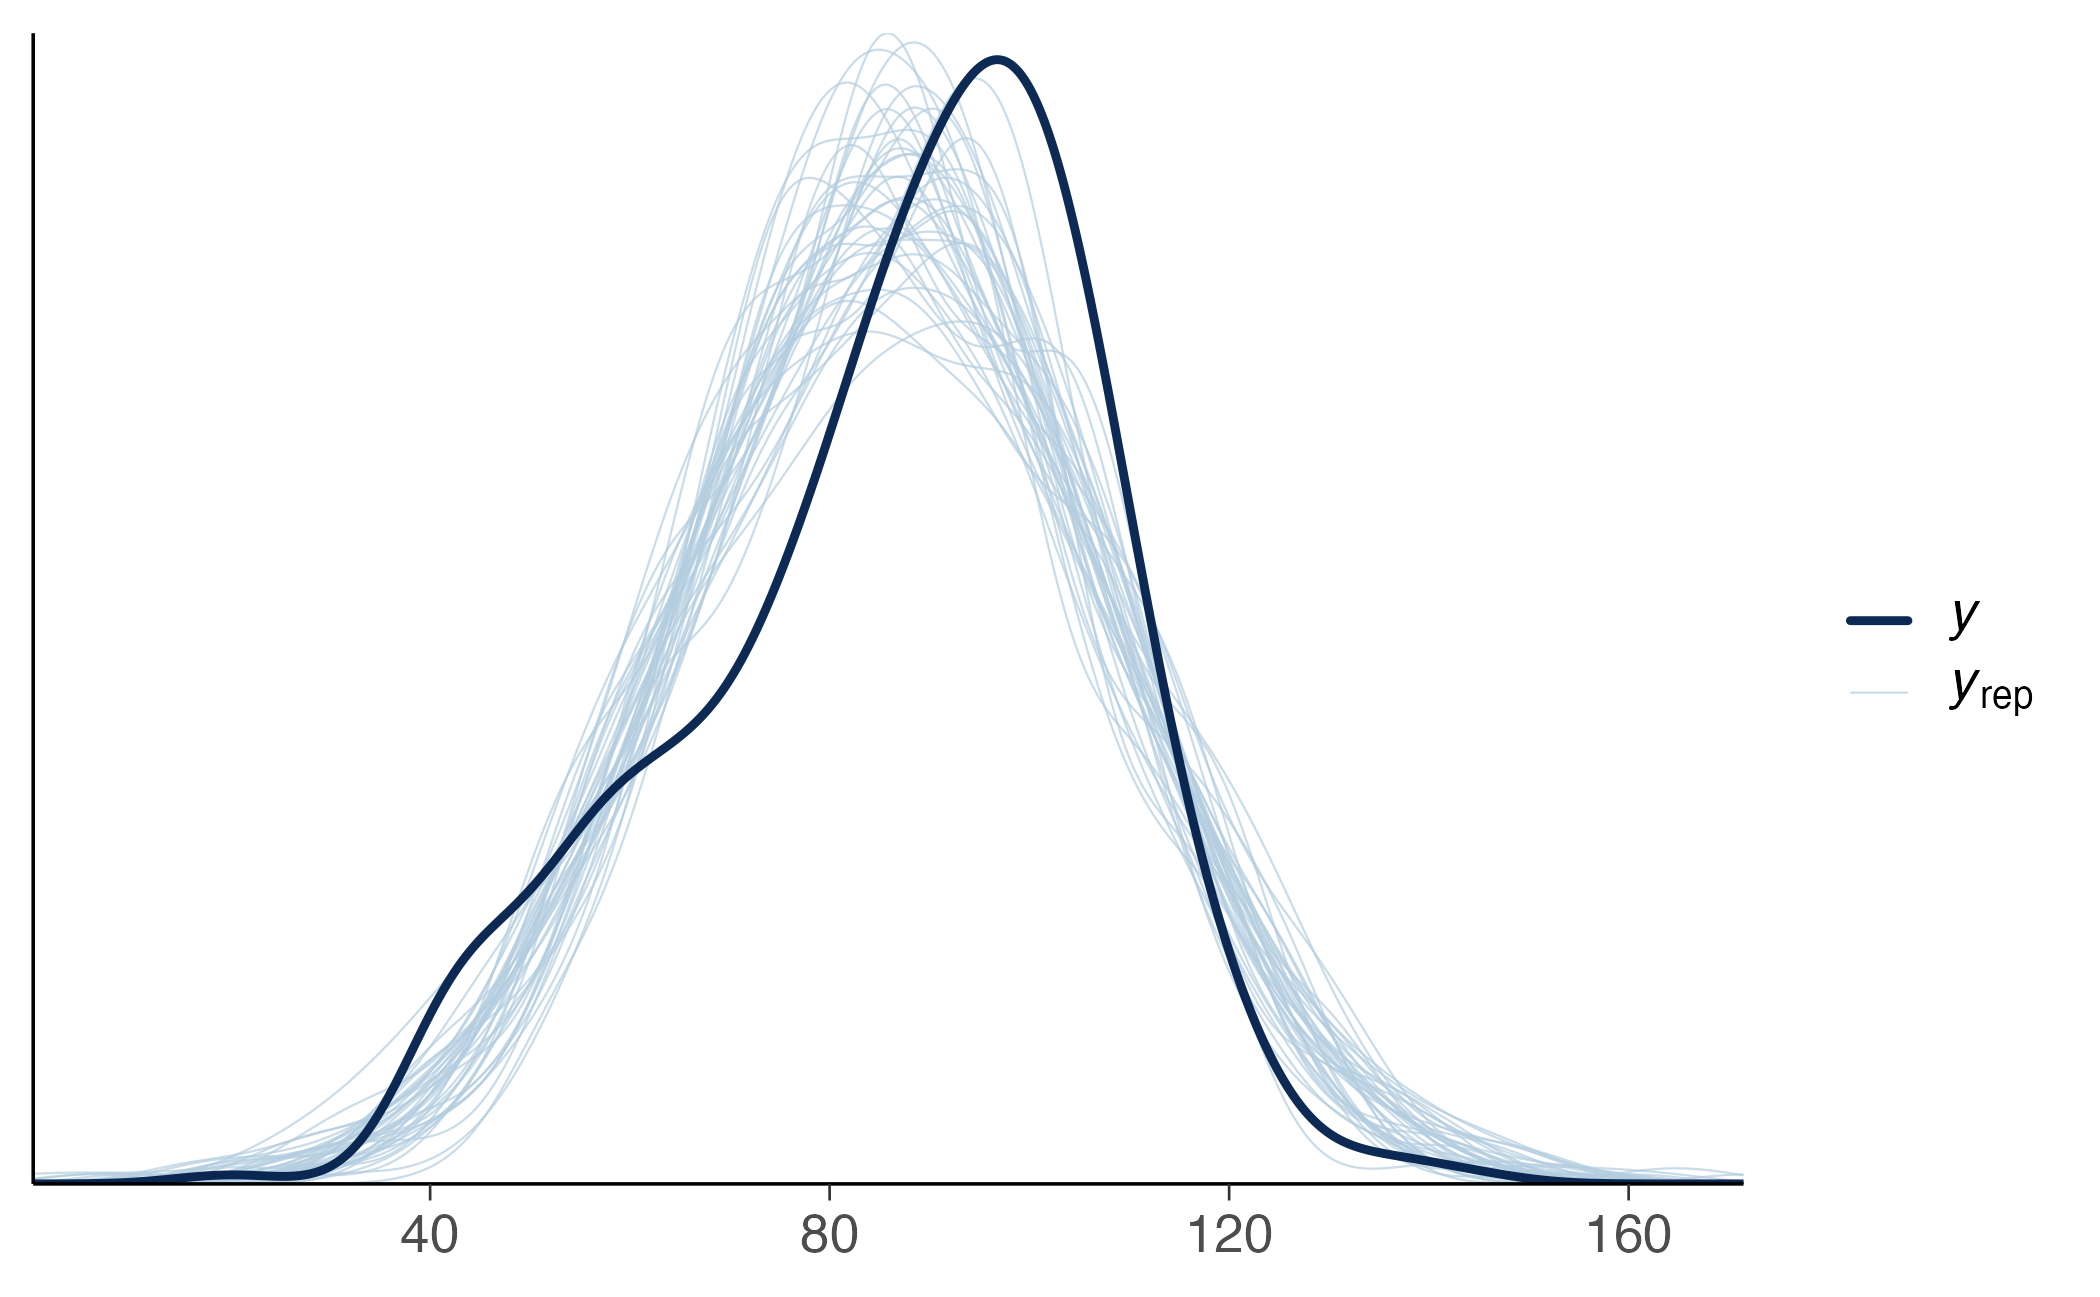
\includegraphics[width=0.85\linewidth,height=\textheight,keepaspectratio]{chapters/linear_models/06_due_gruppi_rilevanza_pratica_files/figure-pdf/fig-ppc-two-groups-1.png}

}

\caption{\label{fig-ppc-two-groups}Controllo predittivo a posteriori
della distribuzione marginale. Un buon accordo complessivo non
garantisce che il modello riproduca separatamente entrambi i gruppi.}

\end{figure}%

Un allineamento soddisfacente sulla densità marginale aggregata può
tuttavia mascherare anomalie locali o asimmetrie all'interno delle
singole categorie. Per esaminare esplicitamente il comportamento del
modello nei sottogruppi, estraiamo le distribuzioni delle medie attese
condizionate per ciascun livello del fattore:

\begin{Shaded}
\begin{Highlighting}[]
\NormalTok{new\_groups }\OtherTok{\textless{}{-}} \FunctionTok{tibble}\NormalTok{(}
  \AttributeTok{mom\_hs =} \FunctionTok{factor}\NormalTok{(}
    \FunctionTok{c}\NormalTok{(}\StringTok{"Non diplomata"}\NormalTok{, }\StringTok{"Diplomata"}\NormalTok{),}
    \AttributeTok{levels =} \FunctionTok{levels}\NormalTok{(kidiq}\SpecialCharTok{$}\NormalTok{mom\_hs)}
\NormalTok{  )}
\NormalTok{)}

\NormalTok{mu\_group\_draws }\OtherTok{\textless{}{-}} \FunctionTok{posterior\_epred}\NormalTok{(}
\NormalTok{  fit\_two\_groups,}
  \AttributeTok{newdata =}\NormalTok{ new\_groups}
\NormalTok{)}

\NormalTok{posterior}\SpecialCharTok{::}\FunctionTok{summarise\_draws}\NormalTok{(}
  \FunctionTok{as\_draws\_matrix}\NormalTok{(mu\_group\_draws)}
\NormalTok{)}
\CommentTok{\#\textgreater{} \# A tibble: 2 x 10}
\CommentTok{\#\textgreater{}   variable  mean median    sd   mad    q5   q95  rhat ess\_bulk ess\_tail}
\CommentTok{\#\textgreater{}   \textless{}chr\textgreater{}    \textless{}dbl\textgreater{}  \textless{}dbl\textgreater{} \textless{}dbl\textgreater{} \textless{}dbl\textgreater{} \textless{}dbl\textgreater{} \textless{}dbl\textgreater{} \textless{}dbl\textgreater{}    \textless{}dbl\textgreater{}    \textless{}dbl\textgreater{}}
\CommentTok{\#\textgreater{} 1 ...1      77.7   77.7  2.07  2.10  74.3  81.1  1.00    3723.    2904.}
\CommentTok{\#\textgreater{} 2 ...2      89.3   89.3  1.07  1.03  87.5  91.1  1.00    4005.    2983.}
\end{Highlighting}
\end{Shaded}

\subsection{Uguale dispersione nei due
gruppi}\label{uguale-dispersione-nei-due-gruppi}

\subsection{Eteroschedasticità: modellare la dispersione tra i
gruppi}\label{eteroschedasticituxe0-modellare-la-dispersione-tra-i-gruppi}

Il modello lineare classico impone il vincolo di omoschedasticità
tramite un unico parametro globale di scala \(\sigma\). Se uno dei due
gruppi presenta una variabilità interna significativamente diversa
rispetto all'altro, questa assunzione rigida rischia di distorcere gli
intervalli di credibilità e di inficiare il calcolo della dimensione
dell'effetto standardizzata \(d\).

Per superare questo limite, possiamo estendere il framework bayesiano
introducendo una sotto-formula che modella esplicitamente la dispersione
residua in funzione dell'appartenenza al gruppo:

\begin{Shaded}
\begin{Highlighting}[]
\FunctionTok{bf}\NormalTok{(}
\NormalTok{  kid\_score }\SpecialCharTok{\textasciitilde{}} \DecValTok{1} \SpecialCharTok{+}\NormalTok{ mom\_hs,}
\NormalTok{  sigma }\SpecialCharTok{\textasciitilde{}} \DecValTok{0} \SpecialCharTok{+}\NormalTok{ mom\_hs}
\NormalTok{)}
\end{Highlighting}
\end{Shaded}

\begin{quote}
\textbf{Nota di calcolo:} in \texttt{brms}, la componente lineare per il
parametro di scala utilizza di default una funzione di \emph{link}
logaritmica (\(\log(\sigma)\)). Questa trasformazione garantisce che le
deviazioni standard stimate rimangano vincolate a valori strettamente
positivi sulla scala originale. I \emph{prior} per questa sezione del
modello devono pertanto essere calibrati tenendo conto della scala
logaritmica.
\end{quote}

\subsection{Code pesanti e osservazioni
estreme}\label{code-pesanti-e-osservazioni-estreme}

Qualora i controlli diagnostici evidenzino la presenza di valori estremi
o anomalie strutturali che la distribuzione gaussiana fatica a
riprodurre, è opportuno adottare una verosimiglianza \(t\) di Student
come specificazione robusta del modello
(\citeproc{ref-kruschke2013bayesian}{Kruschke, 2013}):

\begin{Shaded}
\begin{Highlighting}[]
\FunctionTok{brm}\NormalTok{(}
\NormalTok{  kid\_score }\SpecialCharTok{\textasciitilde{}} \DecValTok{1} \SpecialCharTok{+}\NormalTok{ mom\_hs,}
  \AttributeTok{data =}\NormalTok{ kidiq,}
  \AttributeTok{family =} \FunctionTok{student}\NormalTok{(),}
  \AttributeTok{prior =}\NormalTok{ ...}
\NormalTok{)}
\end{Highlighting}
\end{Shaded}

L'adozione di un approccio statistico robusto non deve mai essere
considerata un espediente automatico per tollerare errori di
campionamento, refusi nella codifica dei dati o la presenza di
popolazioni eterogenee non modellate (es. distribuzioni miste).
Qualsiasi architettura alternativa deve essere supportata da solide
motivazioni teoriche e convalidata attraverso il workflow predittivo.

\section{Differenza standardizzata e affidabilità della
misura}\label{differenza-standardizzata-e-affidabilituxe0-della-misura}

La deviazione standard residua (\(\sigma\)) stimata dal modello
incorpora sia la variabilità biologica o psicologica intrinseca tra gli
individui, sia la quota di variabilità dovuta all'errore di misurazione
dello strumento. Sotto le assunzioni della teoria classica dei test ---
che prevede un errore additivo, indipendente e con media pari a zero ---
l'impiego di una misura caratterizzata da una bassa affidabilità
(\emph{reliability}) gonfia artificialmente la dispersione entro i
gruppi. Di conseguenza, il denominatore della
Equazione~\ref{eq-standardized-difference} aumenta, producendo una
sistematica attenuazione della dimensione dell'effetto standardizzata
\(d\).

Questa conclusione, però, richiede cautela:

\begin{itemize}
\tightlist
\item
  \textbf{Eteroschedasticità dell'errore:} se l'entità dell'errore di
  misura varia sistematicamente tra i gruppi, l'effetto non si limita a
  una semplice attenuazione lineare, ma distorce la simmetria del
  confronto.
\item
  \textbf{Misclassificazione del predittore:} qualora l'errore di misura
  colpisca la variabile indipendente (ad esempio, un'errata assegnazione
  dei soggetti ai gruppi), a subire una distorsione non è solo la
  variabilità residua, ma la stessa differenza grezza \(\Delta\) sui
  punteggi centoidi.
\item
  \textbf{Eterogeneità dei costrutti:} strumenti differenti, pur se
  formalmente standardizzati sulla medesima scala metrica, possono
  mappare dimensioni latenti non perfettamente equivalenti, rendendo il
  confronto tra i rispettivi indici \(d\) puramente nominale.
\end{itemize}

I modelli avanzati in grado di separare analiticamente la variabilità
dei costrutti latenti dall'errore delle componenti osservate saranno
trattati in dettaglio nel capitolo dedicato all'errore di misurazione
(\textbf{?@sec-meas-error-regr}).

\section{Due misure sugli stessi
individui}\label{due-misure-sugli-stessi-individui}

Finora abbiamo considerato il confronto tra gruppi indipendenti. Quando
invece lo stesso partecipante viene osservato in due momenti o
condizioni (ad esempio, in un disegno prima-dopo), le due misure
risultano intrinsecamente dipendenti. Trattarle come osservazioni
indipendenti ignorerebbe l'informazione legata all'appaiamento,
sovrastimando la variabilità residua.

Una strategia classica per analizzare questi dati consiste nel calcolare
preliminarmente lo scostamento individuale:

\[
D_i = Y_{i,\mathrm{pre}} - Y_{i,\mathrm{post}}.
\]

Il problema si riduce così all'adattamento di un modello lineare a sola
intercetta applicato direttamente sulla variabile delle differenze
intra-individuali:

\[
D_i \sim \operatorname{Normal}(\mu_D, \sigma_D).
\]

Per illustrare questo approccio, utilizziamo i punteggi pre e post
relativi ai sintomi depressivi misurati tramite la scala CES-D
(\citeproc{ref-tarrats2025efficacy}{Tarrats-Pons et al., 2025}):

\begin{Shaded}
\begin{Highlighting}[]
\NormalTok{df\_pre\_post }\OtherTok{\textless{}{-}}\NormalTok{ readxl}\SpecialCharTok{::}\FunctionTok{read\_excel}\NormalTok{(}
\NormalTok{  here}\SpecialCharTok{::}\FunctionTok{here}\NormalTok{(}\StringTok{"data"}\NormalTok{, }\StringTok{"Tarrats{-}Pons.xlsx"}\NormalTok{),}
  \AttributeTok{sheet =} \DecValTok{3}
\NormalTok{) }\SpecialCharTok{|\textgreater{}}
  \FunctionTok{select}\NormalTok{(}
\NormalTok{    IdentificationNumber,}
\NormalTok{    Sample,}
    \AttributeTok{CESD =} \StringTok{\textasciigrave{}}\AttributeTok{CESS{-}D}\StringTok{\textasciigrave{}}
\NormalTok{  ) }\SpecialCharTok{|\textgreater{}}
  \FunctionTok{pivot\_wider}\NormalTok{(}
    \AttributeTok{names\_from  =}\NormalTok{ Sample,}
    \AttributeTok{values\_from =}\NormalTok{ CESD,}
    \AttributeTok{names\_prefix =} \StringTok{"CESD\_"}
\NormalTok{  ) }\SpecialCharTok{|\textgreater{}}
  \FunctionTok{mutate}\NormalTok{(}
    \AttributeTok{diff =}\NormalTok{ CESD\_PRE }\SpecialCharTok{{-}}\NormalTok{ CESD\_POST}
\NormalTok{  ) }\SpecialCharTok{|\textgreater{}}
  \FunctionTok{drop\_na}\NormalTok{(diff)}
\end{Highlighting}
\end{Shaded}

Condizioniamo il modello a sola intercetta stimando i parametri sulla
serie delle differenze:

\begin{Shaded}
\begin{Highlighting}[]
\NormalTok{fit\_paired }\OtherTok{\textless{}{-}} \FunctionTok{brm}\NormalTok{(}
  \AttributeTok{formula =}\NormalTok{ diff }\SpecialCharTok{\textasciitilde{}} \DecValTok{1}\NormalTok{,}
  \AttributeTok{data    =}\NormalTok{ df\_pre\_post,}
  \AttributeTok{family  =} \FunctionTok{gaussian}\NormalTok{(),}
  \AttributeTok{prior   =} \FunctionTok{c}\NormalTok{(}
    \FunctionTok{prior}\NormalTok{(}\FunctionTok{normal}\NormalTok{(}\DecValTok{0}\NormalTok{, }\DecValTok{10}\NormalTok{), }\AttributeTok{class =} \StringTok{"Intercept"}\NormalTok{),}
    \FunctionTok{prior}\NormalTok{(}\FunctionTok{student\_t}\NormalTok{(}\DecValTok{3}\NormalTok{, }\DecValTok{0}\NormalTok{, }\DecValTok{10}\NormalTok{), }\AttributeTok{class =} \StringTok{"sigma"}\NormalTok{)}
\NormalTok{  ),}
  \AttributeTok{backend =} \StringTok{"cmdstanr"}\NormalTok{,}
  \AttributeTok{chains  =} \DecValTok{4}\NormalTok{,}
  \AttributeTok{iter    =} \DecValTok{2000}\NormalTok{,}
  \AttributeTok{seed    =} \DecValTok{1234}\NormalTok{,}
  \AttributeTok{refresh =} \DecValTok{0}
\NormalTok{)}
\end{Highlighting}
\end{Shaded}

Per derivare le quantità sostantive, manipoliamo i campioni a
posteriori:

\begin{Shaded}
\begin{Highlighting}[]
\CommentTok{\# Estraiamo i draws mantenendo la struttura formale dell\textquotesingle{}oggetto posterior}
\NormalTok{draws\_paired }\OtherTok{\textless{}{-}} \FunctionTok{as\_draws}\NormalTok{(fit\_paired)}

\CommentTok{\# Utilizziamo mutate\_variables per calcolare l\textquotesingle{}effetto standardizzato d\_z}
\NormalTok{draws\_derived }\OtherTok{\textless{}{-}}\NormalTok{ posterior}\SpecialCharTok{::}\FunctionTok{mutate\_variables}\NormalTok{(}
\NormalTok{  draws\_paired,}
  \AttributeTok{mean\_difference =}\NormalTok{ b\_Intercept,}
  \AttributeTok{sd\_difference   =}\NormalTok{ sigma,}
  \AttributeTok{d\_z             =}\NormalTok{ b\_Intercept }\SpecialCharTok{/}\NormalTok{ sigma}
\NormalTok{)}

\CommentTok{\# Selezioniamo le sole quantità di interesse e generiamo i summary descrittivi}
\NormalTok{draws\_subset }\OtherTok{\textless{}{-}} \FunctionTok{subset\_draws}\NormalTok{(}
\NormalTok{  draws\_derived, }
  \AttributeTok{variable =} \FunctionTok{c}\NormalTok{(}\StringTok{"mean\_difference"}\NormalTok{, }\StringTok{"sd\_difference"}\NormalTok{, }\StringTok{"d\_z"}\NormalTok{)}
\NormalTok{)}

\FunctionTok{summarise\_draws}\NormalTok{(draws\_subset)}
\CommentTok{\#\textgreater{} \# A tibble: 3 x 10}
\CommentTok{\#\textgreater{}   variable          mean median     sd    mad     q5    q95  rhat ess\_bulk}
\CommentTok{\#\textgreater{}   \textless{}chr\textgreater{}            \textless{}dbl\textgreater{}  \textless{}dbl\textgreater{}  \textless{}dbl\textgreater{}  \textless{}dbl\textgreater{}  \textless{}dbl\textgreater{}  \textless{}dbl\textgreater{} \textless{}dbl\textgreater{}    \textless{}dbl\textgreater{}}
\CommentTok{\#\textgreater{} 1 mean\_difference  4.69   4.70  0.985  1.02    3.11   6.30   1.00    3208.}
\CommentTok{\#\textgreater{} 2 sd\_difference   11.3   11.2   0.721  0.721  10.1   12.5    1.00    3045.}
\CommentTok{\#\textgreater{} 3 d\_z              0.418  0.416 0.0907 0.0936  0.272  0.567  1.00    3339.}
\CommentTok{\#\textgreater{}   ess\_tail}
\CommentTok{\#\textgreater{}      \textless{}dbl\textgreater{}}
\CommentTok{\#\textgreater{} 1    2763.}
\CommentTok{\#\textgreater{} 2    2355.}
\CommentTok{\#\textgreater{} 3    3005.}
\end{Highlighting}
\end{Shaded}

Per ottenere valutazioni probabilistiche dirette sul segno del
cambiamento, estraiamo il vettore specifico tramite
\texttt{merge\_chains}:

\begin{Shaded}
\begin{Highlighting}[]
\CommentTok{\# Estrazione del vettore a posteriori e calcolo della probabilità di riduzione sintomatologica}
\NormalTok{mean\_diff\_samples }\OtherTok{\textless{}{-}} \FunctionTok{as\_draws\_matrix}\NormalTok{(draws\_subset, }\AttributeTok{variable =} \StringTok{"mean\_difference"}\NormalTok{)}
\FunctionTok{mean}\NormalTok{(mean\_diff\_samples }\SpecialCharTok{\textgreater{}} \DecValTok{0}\NormalTok{)}
\CommentTok{\#\textgreater{} [1] 1}
\end{Highlighting}
\end{Shaded}

\begin{quote}
\textbf{Interpretazione della metrica:} avendo definito la differenza
come \texttt{pre\ -\ post}, un valore a posteriori positivo di \(\mu_D\)
indica una riduzione netta della sintomatologia depressiva. L'indice
standardizzato \(d_z = \mu_D / \sigma_D\) esprime il contrasto in unità
di deviazione standard delle \emph{differenze} intra-individuali. Di
conseguenza, \(d_z\) non è matematicamente confrontabile con il \(d\) di
Cohen calcolato su gruppi indipendenti, poiché il suo valore risente
direttamente della covarianza tra i due tempi di rilevazione.
\end{quote}

\begin{tcolorbox}[enhanced jigsaw, arc=.35mm, bottomrule=.15mm, bottomtitle=1mm, breakable, colback=white, colbacktitle=quarto-callout-note-color!10!white, colframe=quarto-callout-note-color-frame, coltitle=black, left=2mm, leftrule=.75mm, opacityback=0, opacitybacktitle=0.6, rightrule=.15mm, title=\textcolor{quarto-callout-note-color}{\faInfo}\hspace{0.5em}{Perché e quando l'appaiamento incrementa l'efficienza}, titlerule=0mm, toprule=.15mm, toptitle=1mm]

Quando le misure ripetute sullo stesso individuo mostrano una
correlazione positiva stabile, l'operazione di sottrazione elimina dal
modello la variabilità interindividuale a livello di baseline (le
differenze costanti tra le persone). La deviazione standard delle
differenze (\(\sigma_D\)) risulterà così nettamente inferiore rispetto
alla variabilità grezza dei punteggi originari, determinando un aumento
della precisione (intervalli di credibilità più stretti). Tale guadagno
informativo non è tuttavia garantito da un automatismo matematico, ma
dipende strettamente dall'affidabilità temporale dello strumento e
dall'assenza di pattern complessi di dati mancanti (\emph{missing
data}).

\end{tcolorbox}

Se il disegno sperimentale include più di due occasioni di misura,
intervalli temporali irregolari tra i soggetti, covariate che variano
nel tempo o osservazioni incomplete, il semplice calcolo delle
differenze mostra evidenti limiti. In questi scenari, l'estensione verso
un \textbf{modello lineare multilivello (o a effetti misti)} strutturato
direttamente sulle osservazioni longitudinali originarie rappresenta una
soluzione metodologicamente più solida e flessibile.

\section{Comunicare i risultati}\label{comunicare-i-risultati}

Una rendicontazione scientifica trasparente e informativa del confronto
tra due gruppi dovrebbe integrare i seguenti elementi metodologici:

\begin{enumerate}
\def\labelenumi{\arabic{enumi}.}
\tightlist
\item
  Le stime dei parametri di posizione (medie di gruppo) o le rispettive
  distribuzioni a posteriori;
\item
  la differenza grezza accompagnata da un intervallo di credibilità (es.
  HDI al 95\%);
\item
  la probabilità a posteriori associata alla direzione dell'effetto;
\item
  la probabilità di superare una soglia di rilevanza pratica
  (\emph{SESOI}), se definita a priori;
\item
  la dimensione dell'effetto standardizzata, esplicitando chiaramente la
  natura del denominatore impiegato per il calcolo;
\item
  gli esiti dei principali controlli di adeguatezza e robustezza
  (\emph{PPC});
\item
  i vincoli strutturali del disegno di ricerca e i limiti alla validità
  dell'interpretazione causale.
\end{enumerate}

Un possibile modello di stesura per la sezione Risultati è il seguente:

\begin{quote}
Per verificare lo scostamento nello sviluppo cognitivo in base al
background familiare, abbiamo stimato un modello lineare bayesiano
gaussiano. Nel campione analizzato, il punteggio medio dei bambini nel
gruppo delle madri diplomate (\(\mu_1 = 89.3\), HDI 95\%
\([86.5, 92.1]\)) è risultato superiore a quello del gruppo delle madri
non diplomate (\(\mu_0 = 77.5\), HDI 95\% \([72.8, 82.2]\)). La
distribuzione a posteriori della differenza grezza indica un incremento
plausibile di \(\Delta = 11.8\) punti di QI (HDI 95\% \([6.3, 17.3]\)).
La probabilità che il contrasto sia strettamente positivo è pari a
\(\Pr(\Delta > 0 \mid y) > .99\), mentre la probabilità che lo
scostamento superi la soglia di rilevanza teorica di 5 punti è
\(\Pr(\Delta > 5 \mid y) = .98\). A titolo comparativo, la dimensione
dell'effetto standardizzata basata sulla deviazione standard residua
comune (\(\sigma = 18.2\)) è pari a \(d = 0.65\) (HDI 95\%
\([0.34, 0.96]\)). I controlli predittivi a posteriori confermano
l'adeguatezza della verosimiglianza normale. Trattandosi di un disegno
osservazionale e non sperimentale, tale contrasto descrive
un'associazione sistematica e non può essere interpretato come effetto
causale diretto dell'istruzione materna.
\end{quote}

\begin{quote}
\textbf{Guida alla redazione:} I valori numerici e gli intervalli devono
essere inseriti attingendo direttamente dalle sintesi computazionali dei
\emph{draws}. È buona pratica metodologica evitare l'uso di aggettivi
qualificativi ambigui o assoluti (come ``effetto grande'', ``forte
legame'' o ``differenza trascurabile'') a meno che non si stia ancorando
esplicitamente il dato a criteri di categorizzazione standardizzati o a
soglie cliniche formalmente giustificate all'interno del dominio di
studio.
\end{quote}

\section{Errori frequenti}\label{errori-frequenti-5}

\begin{tcolorbox}[enhanced jigsaw, arc=.35mm, bottomrule=.15mm, bottomtitle=1mm, breakable, colback=white, colbacktitle=quarto-callout-caution-color!10!white, colframe=quarto-callout-caution-color-frame, coltitle=black, left=2mm, leftrule=.75mm, opacityback=0, opacitybacktitle=0.6, rightrule=.15mm, title=\textcolor{quarto-callout-caution-color}{\faFire}\hspace{0.5em}{Attenzione}, titlerule=0mm, toprule=.15mm, toptitle=1mm]

\begin{enumerate}
\def\labelenumi{\arabic{enumi}.}
\tightlist
\item
  \textbf{Interpretare il coefficiente senza conoscere la codifica.} Con
  un fattore, il significato di intercetta e coefficienti dipende dal
  gruppo di riferimento e dai contrasti usati.
\item
  \textbf{Confondere la differenza grezza con quella standardizzata.}
  \(\Delta\) conserva l'unità di misura; \(d\) dipende anche dal
  denominatore scelto.
\item
  \textbf{Usare le soglie di Cohen come leggi naturali.} Sono
  riferimenti convenzionali, non criteri universali di importanza.
\item
  \textbf{Definire SESOI o ROPE dopo avere visto la posterior.} La
  soglia deve derivare dal problema scientifico e dalle conseguenze
  pratiche.
\item
  \textbf{Concludere equivalenza soltanto perché l'intervallo comprende
  zero.} Mancanza di precisione ed equivalenza pratica sono situazioni
  diverse.
\item
  \textbf{Assumere automaticamente varianze uguali.} La dispersione
  comune è parte della specificazione e deve essere controllata.
\item
  \textbf{Trattare dati appaiati come gruppi indipendenti.} In questo
  modo si ignora la dipendenza tra misure della stessa persona.
\item
  \textbf{Attribuire un significato causale alla differenza osservata.}
  Un contrasto tra gruppi non randomizzati può riflettere molte
  differenze concomitanti.
\end{enumerate}

\end{tcolorbox}

\section{Riflessioni conclusive}\label{riflessioni-conclusive-23}

Il confronto tra due gruppi o condizioni non richiede un impianto
statistico separato o speciale, ma rientra pienamente nel modello
lineare, che è un framework flessibile. Utilizzando un indicatore
binario (\emph{dummy coding}), l'intercetta e il coefficiente angolare
della regressione si collegano direttamente alle medie condizionate dei
gruppi e alla loro differenza. La scelta di codifiche alternative (come
quella centrata o le medie di cella) non altera il sistema delle
quantità sostantive, ma modifica radicalmente l'assegnazione dei
\emph{prior} e la trasparenza delle assunzioni teoriche sottostanti.

L'inferenza bayesiana permette di superare i limiti delle decisioni
dicotomiche imposte valore-\emph{p}. L'accesso all'intera distribuzione
a posteriori di \(\Delta\) consente infatti di stimare con precisione la
direzione, l'ampiezza sulla scala originaria e la probabilità che
l'effetto superi una soglia di rilevanza pratica stabilita a priori.
Sebbene l'effetto standardizzato (\(d\)) rimanga uno strumento utile per
il confronto tra studi e la ricerca meta-analitica, esso risente
fortemente della variabilità della popolazione e della precisione
psicometrica delle misure. Per questo motivo, l'indice standardizzato
deve sempre affiancare, e non sostituire, la differenza grezza espressa
nelle unità metriche native del fenomeno.

L'introduzione della \emph{SESOI} e della \emph{ROPE} sposta il focus
della ricerca dall'esistenza puramente statistica di un effetto alla sua
importanza pratica o clinica, esplicitando il confine tra differenze
sostanziali e scostamenti trascurabili. L'applicazione di questi
parametri non esime tuttavia il ricercatore dall'onere di giustificare i
propri benchmark dal punto di vista teorico né dalla necessità di
pianificare studi con una precisione (numerosità campionaria) adeguata.
Allo stesso modo, l'assenza di patologie nell'algoritmo di campionamento
MCMC non garantisce la correttezza della specificazione teorica che deve
sempre essere validata verificando l'adeguatezza della forma
distributiva e l'assunzione di omoschedasticità.

Infine, la distinzione tra gruppi indipendenti e misure appaiate
evidenzia come la struttura del disegno di ricerca vincoli la
definizione stessa degli \emph{estimand} e delle deviazioni standard di
riferimento. Nel prossimo capitolo estenderemo questa stessa
architettura al confronto tra più di due gruppi, mostrando come
l'analisi della varianza (ANOVA) a una via possa essere ricondotta in
modo del tutto naturale a un modello lineare con predittori categoriali,
in cui le ipotesi scientifiche vengono tradotte e verificate mediante la
manipolazione delle medie di cella e la pianificazione dei contrasti.

\section{Concetti da ricordare}\label{concetti-da-ricordare-5}

\begin{enumerate}
\def\labelenumi{\arabic{enumi}.}
\tightlist
\item
  Il confronto tra due gruppi è un modello lineare con predittore
  binario.
\item
  La codifica determina il significato dei coefficienti, non le medie
  sostantive implicate dal modello.
\item
  La differenza grezza \(\Delta\) è generalmente la prima quantità da
  interpretare.
\item
  Il contrasto standardizzato \(d\) è una quantità derivata e dipende
  dalla deviazione standard scelta.
\item
  Prior su coefficienti diversi possono indurre strutture a priori
  differenti sulle medie di gruppo.
\item
  SESOI e ROPE formalizzano un giudizio sostantivo, ma non forniscono da
  sole una decisione universale.
\item
  La dispersione comune è un'assunzione del modello, non una proprietà
  garantita dei dati.
\item
  Nei disegni appaiati l'unità di analisi è la differenza entro persona,
  oppure l'intera traiettoria in un modello multilivello.
\item
  Errore di misurazione e affidabilità influenzano le differenze
  standardizzate.
\item
  Una differenza osservata tra gruppi non identifica automaticamente un
  effetto causale.
\end{enumerate}

\begin{tcolorbox}[enhanced jigsaw, arc=.35mm, bottomrule=.15mm, bottomtitle=1mm, breakable, colback=white, colbacktitle=quarto-callout-important-color!10!white, colframe=quarto-callout-important-color-frame, coltitle=black, left=2mm, leftrule=.75mm, opacityback=0, opacitybacktitle=0.6, rightrule=.15mm, title=\textcolor{quarto-callout-important-color}{\faExclamation}\hspace{0.5em}{Esercizi}, titlerule=0mm, toprule=.15mm, toptitle=1mm]

\subsection{1. Interpretare la codifica
dummy}\label{interpretare-la-codifica-dummy}

Nel modello

\[
Y_i\sim\operatorname{Normal}(70+8x_i,12),
\]

\(x_i=0\) identifica il gruppo A e \(x_i=1\) il gruppo B. Interpreta
\(\mu_A\), \(\mu_B\), \(\Delta\) e \(\sigma\).

\subsection{2. Cambiare il gruppo di
riferimento}\label{cambiare-il-gruppo-di-riferimento}

Inverti il gruppo di riferimento in \texttt{kidiq} e adatta nuovamente
il modello. Verifica come cambiano intercetta e coefficiente e come
rimangono invariate le medie dei gruppi e la differenza «Diplomata meno
Non diplomata» opportunamente ricostruita.

\subsection{3. Codifica centrata}\label{codifica-centrata-1}

Crea un indicatore con valori \(-0.5\) e \(0.5\). Adatta il modello e
verifica che l'intercetta corrisponda al punto medio delle due medie,
mentre la pendenza coincide con la differenza.

\subsection{4. Medie di cella}\label{medie-di-cella-1}

Adatta il modello \texttt{kid\_score\ \textasciitilde{}\ 0\ +\ mom\_hs}.
Estrai i due coefficienti e costruisci \(\Delta\) per ogni draw.
Confronta la posterior ottenuta con quella del modello dummy.

\subsection{5. Soglia sostantiva}\label{soglia-sostantiva-1}

Calcola \(\Pr(\Delta>2\mid y)\), \(\Pr(\Delta>5\mid y)\) e
\(\Pr(\Delta>10\mid y)\). Spiega perché le tre probabilità non
rappresentano analisi in competizione, ma risposte a soglie sostantive
differenti.

\subsection{6. Differenza grezza e
standardizzata}\label{differenza-grezza-e-standardizzata}

Immagina due popolazioni con la stessa differenza \(\Delta=5\), ma
deviazioni standard rispettivamente pari a 5 e 20. Calcola \(d\) in
entrambi i casi e discuti perché il significato pratico della differenza
grezza può essere identico mentre la misura standardizzata cambia.

\subsection{7. Varianze diverse}\label{varianze-diverse}

Supponi che il grafico mostri una dispersione molto maggiore nel gruppo
«Diplomata». Quale assunzione del modello base è messa in discussione?
Descrivi come cambieresti la specificazione e perché un unico
\(d=\Delta/\sigma\) diventerebbe ambiguo.

\subsection{8. Dati appaiati}\label{dati-appaiati}

Per cinque partecipanti, i punteggi pre sono
\texttt{20,\ 18,\ 25,\ 21,\ 16} e i punteggi post sono
\texttt{15,\ 17,\ 19,\ 18,\ 14}. Calcola le differenze
\texttt{pre\ -\ post}, la loro media e la loro deviazione standard.
Spiega quale parametro stimeresti con
\texttt{diff\ \textasciitilde{}\ 1}.

\subsection{9. Criticare il linguaggio
causale}\label{criticare-il-linguaggio-causale}

Riscrivi in modo descrittivo la frase:

\begin{quote}
Il diploma materno aumenta il QI dei figli di otto punti.
\end{quote}

\end{tcolorbox}

\begin{tcolorbox}[enhanced jigsaw, arc=.35mm, bottomrule=.15mm, bottomtitle=1mm, breakable, colback=white, colbacktitle=quarto-callout-tip-color!10!white, colframe=quarto-callout-tip-color-frame, coltitle=black, left=2mm, leftrule=.75mm, opacityback=0, opacitybacktitle=0.6, rightrule=.15mm, title=\textcolor{quarto-callout-tip-color}{\faLightbulb}\hspace{0.5em}{Tracce di soluzione}, titlerule=0mm, toprule=.15mm, toptitle=1mm]

\begin{enumerate}
\def\labelenumi{\arabic{enumi}.}
\tightlist
\item
  \(\mu_A=70\), \(\mu_B=78\), \(\Delta=8\) e \(\sigma=12\) descrive la
  dispersione comune attorno alle due medie.
\item
  Con il gruppo B come riferimento, l'intercetta stima \(\mu_B\) e il
  coefficiente diventa \(\mu_A-\mu_B=-\Delta\). Le quantità sostantive
  non cambiano.
\item
  Con \(-0.5\) e \(0.5\), l'intercetta è \((\mu_A+\mu_B)/2\) e la
  pendenza è ancora \(\mu_B-\mu_A\).
\item
  I coefficienti sono direttamente le due medie; il contrasto si ottiene
  sottraendo, draw per draw, il coefficiente del gruppo di riferimento
  da quello del confronto.
\item
  Aumentando la soglia, la probabilità di superarla non può aumentare.
  La scelta della soglia dipende dal significato pratico, non dai dati
  osservati.
\item
  I valori sono 1 e 0.25. La standardizzazione incorpora l'eterogeneità
  della popolazione; per questo non sostituisce l'interpretazione della
  scala originale.
\item
  È messa in discussione l'omoschedasticità. Si può modellare
  \texttt{sigma} in funzione del gruppo. Con due dispersioni, occorre
  dichiarare quale deviazione standard viene usata per standardizzare.
\item
  Le differenze sono \texttt{5,\ 1,\ 6,\ 3,\ 2}. Il modello a sola
  intercetta stima la media della distribuzione delle differenze e la
  loro dispersione.
\item
  Una formulazione compatibile con i dati osservazionali è: «Nel
  campione analizzato, i figli di madri diplomate presentano in media un
  punteggio di QI superiore di circa otto punti rispetto ai figli di
  madri non diplomate».
\end{enumerate}

\end{tcolorbox}

\begin{tcolorbox}[enhanced jigsaw, arc=.35mm, bottomrule=.15mm, bottomtitle=1mm, breakable, colback=white, colbacktitle=quarto-callout-note-color!10!white, colframe=quarto-callout-note-color-frame, coltitle=black, left=2mm, leftrule=.75mm, opacityback=0, opacitybacktitle=0.6, rightrule=.15mm, title=\textcolor{quarto-callout-note-color}{\faInfo}\hspace{0.5em}{Informazioni sull'ambiente di sviluppo}, titlerule=0mm, toprule=.15mm, toptitle=1mm]

\begin{Shaded}
\begin{Highlighting}[]
\FunctionTok{sessionInfo}\NormalTok{()}
\CommentTok{\#\textgreater{} R version 4.6.1 (2026{-}06{-}24)}
\CommentTok{\#\textgreater{} Platform: aarch64{-}apple{-}darwin23}
\CommentTok{\#\textgreater{} Running under: macOS Tahoe 26.5.2}
\CommentTok{\#\textgreater{} }
\CommentTok{\#\textgreater{} Matrix products: default}
\CommentTok{\#\textgreater{} BLAS:   /Library/Frameworks/R.framework/Versions/4.6/Resources/lib/libRblas.0.dylib }
\CommentTok{\#\textgreater{} LAPACK: /Library/Frameworks/R.framework/Versions/4.6/Resources/lib/libRlapack.dylib;  LAPACK version 3.12.1}
\CommentTok{\#\textgreater{} }
\CommentTok{\#\textgreater{} locale:}
\CommentTok{\#\textgreater{} [1] C.UTF{-}8/UTF{-}8/C.UTF{-}8/C/C.UTF{-}8/C.UTF{-}8}
\CommentTok{\#\textgreater{} }
\CommentTok{\#\textgreater{} time zone: Europe/Zagreb}
\CommentTok{\#\textgreater{} tzcode source: internal}
\CommentTok{\#\textgreater{} }
\CommentTok{\#\textgreater{} attached base packages:}
\CommentTok{\#\textgreater{} [1] stats     graphics  grDevices utils     datasets  methods   base     }
\CommentTok{\#\textgreater{} }
\CommentTok{\#\textgreater{} other attached packages:}
\CommentTok{\#\textgreater{}  [1] readxl\_1.5.0          cmdstanr\_0.9.0        bayestestR\_0.18.1    }
\CommentTok{\#\textgreater{}  [4] ragg\_1.5.2            tinytable\_0.17.0      withr\_3.0.3          }
\CommentTok{\#\textgreater{}  [7] systemfonts\_1.3.2     patchwork\_1.3.2       ggdist\_3.3.3         }
\CommentTok{\#\textgreater{} [10] tidybayes\_3.0.7       bayesplot\_1.15.0      ggplot2\_4.0.3        }
\CommentTok{\#\textgreater{} [13] reliabilitydiag\_0.2.1 priorsense\_1.2.0      posterior\_1.7.0      }
\CommentTok{\#\textgreater{} [16] loo\_2.10.0            rstan\_2.32.7          StanHeaders\_2.32.10  }
\CommentTok{\#\textgreater{} [19] brms\_2.23.0           Rcpp\_1.1.2            sessioninfo\_1.2.4    }
\CommentTok{\#\textgreater{} [22] conflicted\_1.2.0      janitor\_2.2.1         matrixStats\_1.5.0    }
\CommentTok{\#\textgreater{} [25] modelr\_0.1.11         tibble\_3.3.1          dplyr\_1.2.1          }
\CommentTok{\#\textgreater{} [28] tidyr\_1.3.2           rio\_1.3.0             here\_1.0.2           }
\CommentTok{\#\textgreater{} }
\CommentTok{\#\textgreater{} loaded via a namespace (and not attached):}
\CommentTok{\#\textgreater{}  [1] gridExtra\_2.3.1       inline\_0.3.21         rlang\_1.3.0          }
\CommentTok{\#\textgreater{}  [4] magrittr\_2.0.5        snakecase\_0.11.1      otel\_0.2.0           }
\CommentTok{\#\textgreater{}  [7] compiler\_4.6.1        reshape2\_1.4.5        vctrs\_0.7.3          }
\CommentTok{\#\textgreater{} [10] stringr\_1.6.0         pkgconfig\_2.0.3       arrayhelpers\_1.1{-}1   }
\CommentTok{\#\textgreater{} [13] fastmap\_1.2.0         backports\_1.5.1       labeling\_0.4.3       }
\CommentTok{\#\textgreater{} [16] utf8\_1.2.6            rmarkdown\_2.31        tzdb\_0.5.0           }
\CommentTok{\#\textgreater{} [19] ps\_1.9.3              haven\_2.5.5           purrr\_1.2.2          }
\CommentTok{\#\textgreater{} [22] xfun\_0.60             cachem\_1.1.0          jsonlite\_2.0.0       }
\CommentTok{\#\textgreater{} [25] broom\_1.0.13          parallel\_4.6.1        R6\_2.6.1             }
\CommentTok{\#\textgreater{} [28] stringi\_1.8.7         RColorBrewer\_1.1{-}3    lubridate\_1.9.5      }
\CommentTok{\#\textgreater{} [31] cellranger\_1.1.0      estimability\_2.0.0    knitr\_1.51           }
\CommentTok{\#\textgreater{} [34] pacman\_0.5.1          R.utils\_2.13.0        readr\_2.2.0          }
\CommentTok{\#\textgreater{} [37] Matrix\_1.7{-}5          timechange\_0.4.0      tidyselect\_1.2.1     }
\CommentTok{\#\textgreater{} [40] abind\_1.4{-}8           yaml\_2.3.12           codetools\_0.2{-}20     }
\CommentTok{\#\textgreater{} [43] curl\_7.1.0            processx\_3.9.0        pkgbuild\_1.4.8       }
\CommentTok{\#\textgreater{} [46] plyr\_1.8.9            lattice\_0.22{-}9        bridgesampling\_1.2{-}1 }
\CommentTok{\#\textgreater{} [49] S7\_0.2.2              coda\_0.19{-}4.1         evaluate\_1.0.5       }
\CommentTok{\#\textgreater{} [52] RcppParallel\_5.1.11{-}2 pillar\_1.11.1         tensorA\_0.36.2.1     }
\CommentTok{\#\textgreater{} [55] checkmate\_2.3.4       stats4\_4.6.1          insight\_1.5.2        }
\CommentTok{\#\textgreater{} [58] distributional\_0.8.1  generics\_0.1.4        rprojroot\_2.1.1      }
\CommentTok{\#\textgreater{} [61] hms\_1.1.4             rstantools\_2.6.0      scales\_1.4.0         }
\CommentTok{\#\textgreater{} [64] xtable\_1.8{-}8          glue\_1.8.1            emmeans\_2.0.4        }
\CommentTok{\#\textgreater{} [67] tools\_4.6.1           data.table\_1.18.4     forcats\_1.0.1        }
\CommentTok{\#\textgreater{} [70] mvtnorm\_1.4{-}2         grid\_4.6.1            QuickJSR\_1.10.0      }
\CommentTok{\#\textgreater{} [73] nlme\_3.1{-}170          cli\_3.6.6             textshaping\_1.0.5    }
\CommentTok{\#\textgreater{} [76] svUnit\_1.0.8          Brobdingnag\_1.2{-}9     V8\_8.2.0             }
\CommentTok{\#\textgreater{} [79] gtable\_0.3.6          R.methodsS3\_1.8.2     digest\_0.6.39        }
\CommentTok{\#\textgreater{} [82] farver\_2.1.2          memoise\_2.0.1         htmltools\_0.5.9      }
\CommentTok{\#\textgreater{} [85] R.oo\_1.27.1           lifecycle\_1.0.5}
\end{Highlighting}
\end{Shaded}

\end{tcolorbox}

\section*{Bibliografia}\label{bibliografia-26}

\markright{Bibliografia}

\chapter{Più gruppi: medie di cella, contrasti e
ANOVA}\label{sec-anova1via}

Il confronto tra due gruppi può essere esteso in modo naturale a disegni
sperimentali o osservazionali che prevedono tre o più condizioni, come
nel caso della valutazione di trattamenti multipli, di fasce d'età
differenti, di contesti scolastici eterogenei o di diversi livelli di
esposizione a un fattore. Nella statistica classica, l'analisi di questi
scenari viene tradizionalmente affidata alla procedura dell'analisi
della varianza (ANOVA) a una via.

Dal punto di vista della modellistica statistica, questo passaggio non
introduce una nuova classe di tecniche: formalmente, cambia solo il
numero di livelli che compongono il predittore categoriale (o
\emph{fattore}). Il modello lineare consente inoltre di formulare
domande di ricerca più informative rispetto alla generica domanda
omnibus della statistica classica: ``Le medie dei gruppi sono tutte
uguali tra loro?''.

In questo capitolo applicheremo l'inferenza bayesiana al caso di
predittori politomici, ovvero con più di due livelli, concentrandoci
sulle quantità di effettivo interesse scientifico: la stima della
distribuzione a posteriori dei parametri di posizione per ciascun gruppo
e la valutazione della loro plausibilità; la specificazione e la
verifica di contrasti pianificati, definiti sulla base di ipotesi
teoriche e non di esplorazioni post-hoc; la quantificazione
dell'ampiezza delle differenze, sia nella scala metrica originale sia in
forma standardizzata; la propagazione esplicita e coerente
dell'incertezza associata a ciascun confronto; e, infine, la valutazione
probabilistica della plausibilità che i contrasti superino una soglia di
rilevanza pratica stabilita a priori.

\begin{tcolorbox}[enhanced jigsaw, arc=.35mm, bottomrule=.15mm, breakable, colback=white, colframe=quarto-callout-important-color-frame, left=2mm, leftrule=.75mm, opacityback=0, rightrule=.15mm, toprule=.15mm]

\textbf{Da sapere.} Il confronto tra più gruppi è un modello lineare con
un predittore categoriale. La codifica con gruppo di riferimento e la
parametrizzazione a medie di cella descrivono le stesse medie, ma
attribuiscono significati diversi ai coefficienti e ai prior. Le domande
scientifiche devono essere espresse mediante contrasti pianificati,
distinguendo la probabilità direzionale dalla rilevanza pratica.
L'inferenza bayesiana non elimina automaticamente il problema della
molteplicità.

\textbf{Da saper fare.} Specificare e stimare con \texttt{brms} un
modello a più gruppi; scegliere prior plausibili; eseguire i controlli
predittivi a priori e a posteriori; ricavare dai campioni posteriori le
medie di gruppo e i contrasti pianificati; calcolare probabilità
sostantive rispetto a zero e a una soglia di rilevanza pratica;
comunicare i risultati mantenendo esplicita l'incertezza.

\textbf{Approfondimento facoltativo.} La costruzione dettagliata delle
matrici del modello, il confronto sistematico tra codifica \emph{dummy}
e medie di cella, l'uso di \texttt{emmeans}, la valutazione omnibus, la
discussione formale della molteplicità e le estensioni a modelli robusti
o multilivello possono essere rimandati. Nel percorso essenziale è
sufficiente comprendere le medie di cella, formulare contrasti guidati
dalla teoria e valutarli mediante la distribuzione a posteriori e i
controlli predittivi.

\hyperref[sec-percorsi-lettura]{Che cosa significano queste etichette?}

\end{tcolorbox}

\begin{tcolorbox}[enhanced jigsaw, arc=.35mm, bottomrule=.15mm, bottomtitle=1mm, breakable, colback=white, colbacktitle=quarto-callout-note-color!10!white, colframe=quarto-callout-note-color-frame, coltitle=black, left=2mm, leftrule=.75mm, opacityback=0, opacitybacktitle=0.6, rightrule=.15mm, title=\textcolor{quarto-callout-note-color}{\faInfo}\hspace{0.5em}{Obiettivi del capitolo}, titlerule=0mm, toprule=.15mm, toptitle=1mm]

Al termine del capitolo dovresti essere in grado di:

\begin{itemize}
\tightlist
\item
  rappresentare un fattore a più livelli mediante variabili indicatrici;
\item
  distinguere la codifica con gruppo di riferimento dalla
  parametrizzazione a medie di cella;
\item
  riconoscere che parametrizzazioni diverse descrivono lo stesso insieme
  di medie;
\item
  specificare prior plausibili per le medie dei gruppi e per la
  dispersione residua;
\item
  formulare contrasti guidati dalla domanda scientifica;
\item
  calcolare contrasti e probabilità sostantive draw per draw;
\item
  spiegare perché la molteplicità non scompare nell'analisi bayesiana;
\item
  distinguere un confronto pianificato da una ricerca esplorativa tra
  molte differenze.
\end{itemize}

\end{tcolorbox}

\begin{tcolorbox}[enhanced jigsaw, arc=.35mm, bottomrule=.15mm, bottomtitle=1mm, breakable, colback=white, colbacktitle=quarto-callout-tip-color!10!white, colframe=quarto-callout-tip-color-frame, coltitle=black, left=2mm, leftrule=.75mm, opacityback=0, opacitybacktitle=0.6, rightrule=.15mm, title=\textcolor{quarto-callout-tip-color}{\faLightbulb}\hspace{0.5em}{Percorsi di lettura}, titlerule=0mm, toprule=.15mm, toptitle=1mm]

Il capitolo appartiene al \textbf{percorso essenziale} e al
\textbf{percorso computazionale avanzato}. Per seguire il nucleo
dell'argomentazione sono sufficienti le sezioni sulle medie di cella e
sui contrasti. Le sezioni dedicate alle matrici del modello e alle
parametrizzazioni alternative approfondiscono la connessione con il
capitolo sulla traduzione dalle formule al programma.

\end{tcolorbox}

\begin{tcolorbox}[enhanced jigsaw, arc=.35mm, bottomrule=.15mm, bottomtitle=1mm, breakable, colback=white, colbacktitle=quarto-callout-tip-color!10!white, colframe=quarto-callout-tip-color-frame, coltitle=black, left=2mm, leftrule=.75mm, opacityback=0, opacitybacktitle=0.6, rightrule=.15mm, title=\textcolor{quarto-callout-tip-color}{\faLightbulb}\hspace{0.5em}{Prerequisiti}, titlerule=0mm, toprule=.15mm, toptitle=1mm]

Il capitolo estende il confronto tra due gruppi discusso in
Capitolo~\ref{sec-linear-models-two-groups} e la costruzione di quantità
derivate presentata in Sezione~\ref{sec-bayesian-effect-size}. Il
workflow bayesiano completo è stato introdotto in
Capitolo~\ref{sec-linmod-bayesian-reg}. Come riferimento generale si
veda anche il capitolo \emph{Geocentric models} di \emph{Statistical
Rethinking} (\citeproc{ref-McElreath_rethinking}{McElreath, 2020}).

\end{tcolorbox}

\begin{tcolorbox}[enhanced jigsaw, arc=.35mm, bottomrule=.15mm, bottomtitle=1mm, breakable, colback=white, colbacktitle=quarto-callout-caution-color!10!white, colframe=quarto-callout-caution-color-frame, coltitle=black, left=2mm, leftrule=.75mm, opacityback=0, opacitybacktitle=0.6, rightrule=.15mm, title=\textcolor{quarto-callout-caution-color}{\faFire}\hspace{0.5em}{Preparazione del Notebook}, titlerule=0mm, toprule=.15mm, toptitle=1mm]

\end{tcolorbox}

\section{Dalla domanda scientifica alle quantità di
interesse}\label{dalla-domanda-scientifica-alle-quantituxe0-di-interesse-1}

Per introdurre la formalizzazione dei contrasti pianificati,
consideriamo un disegno sperimentale simulato in cui si confrontano tre
condizioni indipendenti: un gruppo di controllo e due protocolli di
psicoterapia (Terapia 1 e Terapia 2). La variabile dipendente è un
punteggio continuo di depressione, con valori più elevati che indicano
una maggiore sintomatologia. Supponiamo che gli interrogativi clinici di
interesse si riducano a due domande:

\begin{quote}
\textbf{Quesito 1:} In media, i due trattamenti determinano una
riduzione dei sintomi depressivi rispetto al gruppo di controllo?
\end{quote}

\begin{quote}
\textbf{Quesito 2:} I due protocolli differiscono tra loro in termini
clinicamente rilevanti?
\end{quote}

Queste domande definiscono due \emph{contrasti pianificati}, ovvero
confronti specificati prima di aver visto i dati. Specificare in
anticipo i confronti di interesse consente di evitare un'analisi
esplorativa di tutte le possibili differenze a coppie, riducendo il
rischio di falsi positivi e concentrando l'inferenza sulle sole domande
rilevanti.

Siano \(\mu_C\), \(\mu_{P1}\) e \(\mu_{P2}\) le medie condizionate
dell'esito nei tre gruppi --- controllo, Terapia 1 e Terapia 2
rispettivamente. I due interrogativi clinici si traducono nelle seguenti
quantità sostantive di interesse, o \emph{estimands}.

Il primo contrasto confronta il gruppo di controllo con la media dei due
trattamenti:

\begin{equation}\protect\phantomsection\label{eq-anova-control-therapies}{
\Delta_{C:T} = \mu_C - \frac{\mu_{P1} + \mu_{P2}}{2}
}\end{equation}

Un valore positivo di \(\Delta_{C:T}\) indica che, nel loro insieme, i
protocolli terapeutici sono associati a una sintomatologia depressiva
mediamente inferiore rispetto alla condizione di controllo.

Il secondo contrasto riguarda la differenza tra i due trattamenti:

\begin{equation}\protect\phantomsection\label{eq-anova-therapy-contrast}{
\Delta_{P1:P2} = \mu_{P1} - \mu_{P2}
}\end{equation}

Un valore positivo di \(\Delta_{P1:P2}\) segnala che il secondo
protocollo è associato a un punteggio medio di depressione più basso ---
e quindi a una maggiore efficacia --- rispetto al primo.

\section{Simulazione di un disegno sperimentale a tre
vie}\label{simulazione-di-un-disegno-sperimentale-a-tre-vie}

Per esaminare il comportamento del modello, generiamo un dataset
simulato bilanciato con trenta osservazioni per ciascuna condizione
sperimentale. I valori veri sono scelti in modo da produrre una
riduzione graduale dei sintomi dal gruppo di controllo alla seconda
terapia, ma mantenendo una variabilità sufficiente perché i punteggi dei
singoli partecipanti si sovrappongano tra i gruppi. In questo modo,
l'effetto medio è distinguibile, ma l'incertezza rimane una componente
rilevante del problema.

\begin{Shaded}
\begin{Highlighting}[]
\CommentTok{\# Definizione dei parametri generativi della simulazione}
\NormalTok{n\_per\_group }\OtherTok{\textless{}{-}} \DecValTok{30}
\NormalTok{mu\_control  }\OtherTok{\textless{}{-}} \DecValTok{30}
\NormalTok{mu\_p1       }\OtherTok{\textless{}{-}} \DecValTok{25}
\NormalTok{mu\_p2       }\OtherTok{\textless{}{-}} \DecValTok{20}
\NormalTok{sigma\_true  }\OtherTok{\textless{}{-}} \DecValTok{5}

\FunctionTok{set.seed}\NormalTok{(}\DecValTok{1234}\NormalTok{) }\CommentTok{\# Garantisce la replicabilità esatta della simulazione}

\NormalTok{anova\_data }\OtherTok{\textless{}{-}} \FunctionTok{tibble}\NormalTok{(}
  \AttributeTok{condizione =} \FunctionTok{factor}\NormalTok{(}
    \FunctionTok{rep}\NormalTok{(}\FunctionTok{c}\NormalTok{(}\StringTok{"controllo"}\NormalTok{, }\StringTok{"psicoterapia1"}\NormalTok{, }\StringTok{"psicoterapia2"}\NormalTok{), }\AttributeTok{each =}\NormalTok{ n\_per\_group),}
    \AttributeTok{levels =} \FunctionTok{c}\NormalTok{(}\StringTok{"controllo"}\NormalTok{, }\StringTok{"psicoterapia1"}\NormalTok{, }\StringTok{"psicoterapia2"}\NormalTok{)}
\NormalTok{  ),}
  \AttributeTok{punteggio =} \FunctionTok{c}\NormalTok{(}
    \FunctionTok{rnorm}\NormalTok{(n\_per\_group, mu\_control, sigma\_true),}
    \FunctionTok{rnorm}\NormalTok{(n\_per\_group, mu\_p1, sigma\_true),}
    \FunctionTok{rnorm}\NormalTok{(n\_per\_group, mu\_p2, sigma\_true)}
\NormalTok{  )}
\NormalTok{)}

\CommentTok{\# Calcolo delle statistiche descrittive campionarie}
\NormalTok{anova\_data }\SpecialCharTok{|\textgreater{}}
  \FunctionTok{group\_by}\NormalTok{(condizione) }\SpecialCharTok{|\textgreater{}}
  \FunctionTok{summarize}\NormalTok{(}
    \AttributeTok{n     =} \FunctionTok{n}\NormalTok{(),}
    \AttributeTok{media =} \FunctionTok{mean}\NormalTok{(punteggio),}
    \AttributeTok{sd    =} \FunctionTok{sd}\NormalTok{(punteggio),}
    \AttributeTok{.groups =} \StringTok{"drop"}
\NormalTok{  )}
\CommentTok{\#\textgreater{} \# A tibble: 3 x 4}
\CommentTok{\#\textgreater{}   condizione        n media    sd}
\CommentTok{\#\textgreater{}   \textless{}fct\textgreater{}         \textless{}int\textgreater{} \textless{}dbl\textgreater{} \textless{}dbl\textgreater{}}
\CommentTok{\#\textgreater{} 1 controllo        30  28.5  4.51}
\CommentTok{\#\textgreater{} 2 psicoterapia1    30  22.2  4.79}
\CommentTok{\#\textgreater{} 3 psicoterapia2    30  20.7  4.90}
\end{Highlighting}
\end{Shaded}

Visualizziamo la distribuzione empirica e la dispersione dei punteggi
osservati all'interno dei tre bracci dello studio:

\begin{Shaded}
\begin{Highlighting}[]
\NormalTok{anova\_data }\SpecialCharTok{|\textgreater{}}
  \FunctionTok{ggplot}\NormalTok{(}\FunctionTok{aes}\NormalTok{(}\AttributeTok{x =}\NormalTok{ condizione, }\AttributeTok{y =}\NormalTok{ punteggio)) }\SpecialCharTok{+}
  \FunctionTok{geom\_violin}\NormalTok{(}\AttributeTok{fill =} \StringTok{"grey95"}\NormalTok{, }\AttributeTok{color =} \StringTok{"grey50"}\NormalTok{, }\AttributeTok{trim =} \ConstantTok{FALSE}\NormalTok{, }\AttributeTok{alpha =} \FloatTok{0.4}\NormalTok{) }\SpecialCharTok{+}
  \FunctionTok{geom\_boxplot}\NormalTok{(}\AttributeTok{width =} \FloatTok{0.15}\NormalTok{, }\AttributeTok{fill =} \StringTok{"white"}\NormalTok{, }\AttributeTok{color =} \StringTok{"grey30"}\NormalTok{, }\AttributeTok{outlier.shape =} \ConstantTok{NA}\NormalTok{) }\SpecialCharTok{+}
  \FunctionTok{geom\_jitter}\NormalTok{(}\AttributeTok{width =} \FloatTok{0.05}\NormalTok{, }\AttributeTok{height =} \DecValTok{0}\NormalTok{, }\AttributeTok{color =} \StringTok{"darkslategrey"}\NormalTok{, }\AttributeTok{alpha =} \FloatTok{0.4}\NormalTok{, }\AttributeTok{size =} \FloatTok{1.5}\NormalTok{) }\SpecialCharTok{+}
  \FunctionTok{labs}\NormalTok{(}
    \AttributeTok{x =} \StringTok{"Condizione sperimentale"}\NormalTok{,}
    \AttributeTok{y =} \StringTok{"Punteggio di depressione (CES{-}D)"}
\NormalTok{  )}
\end{Highlighting}
\end{Shaded}

\begin{figure}[H]

\centering{

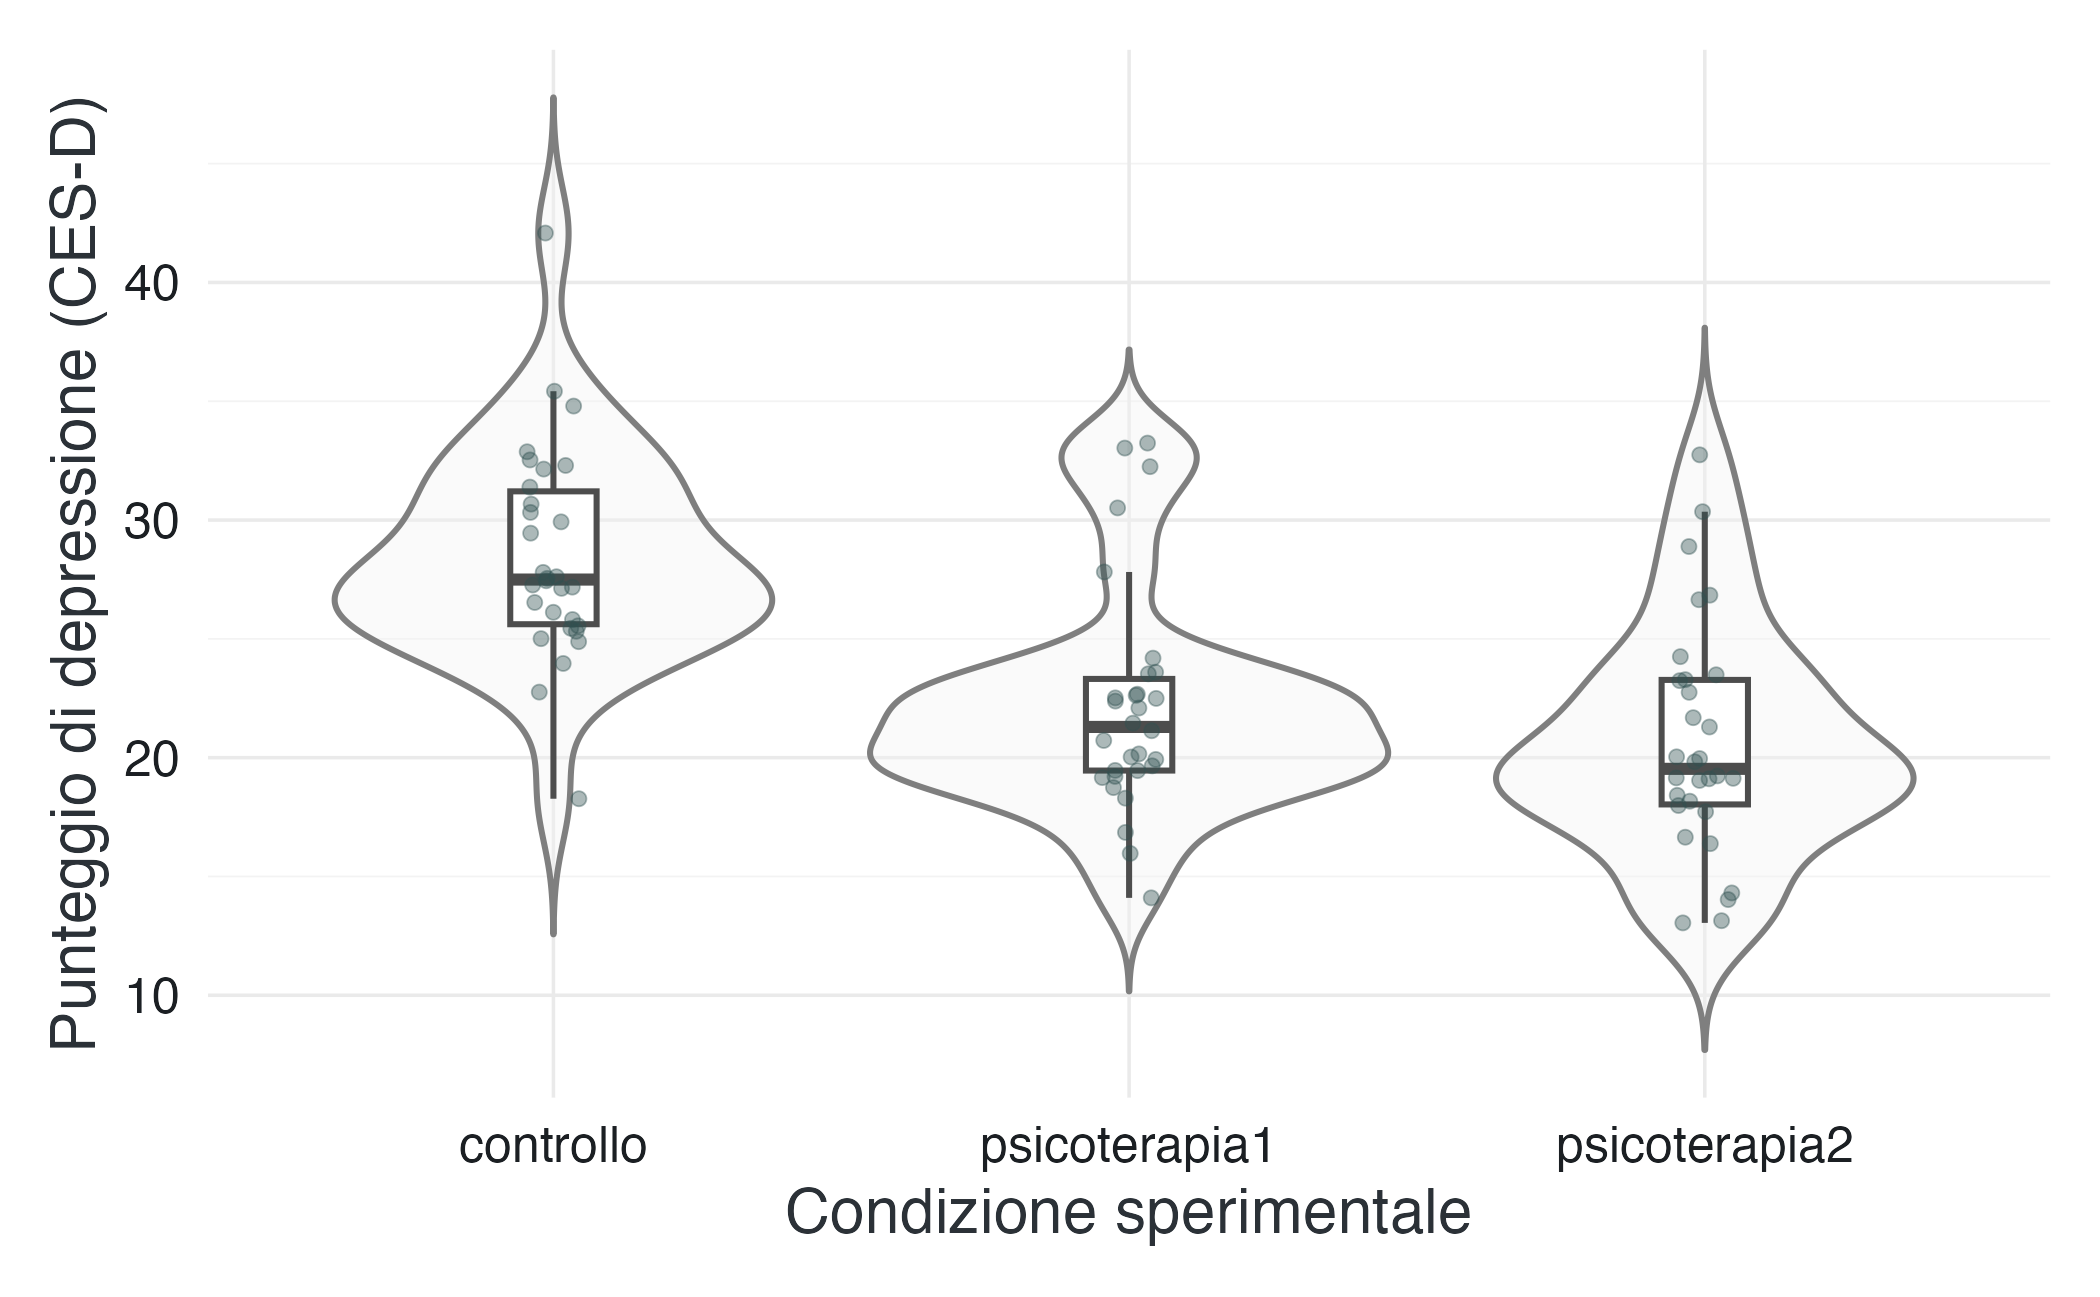
\includegraphics[width=0.85\linewidth,height=\textheight,keepaspectratio]{chapters/linear_models/07_piu_gruppi_contrasti_anova_files/figure-pdf/fig-anova-observed-groups-1.png}

}

\caption{\label{fig-anova-observed-groups}Distribuzioni osservate delle
risposte sintomatologiche nelle tre condizioni sperimentali. Le linee
interne ai boxplot indicano le mediane campionarie, mentre i singoli
punti tracciano la distribuzione dei dati originali.}

\end{figure}%

\begin{quote}
\textbf{Valutazione metodologica:} i grafici suggeriscono una riduzione
dei punteggi di depressione dal controllo verso la seconda terapia.
Tuttavia, questa evidenza descrittiva non è sufficiente per trarre
conclusioni inferenziali: non quantifica l'incertezza delle stime
campionarie e non fornisce una misura probabilistica della rilevanza
clinica delle differenze osservate. Per stabilire se le variazioni siano
sostanziali e non solo visibili, occorre un'analisi che espliciti
l'incertezza e valuti l'ampiezza degli effetti rispetto a una soglia di
interesse pratico.
\end{quote}

\section{Un unico modello, diverse parametrizzazioni
algebriche}\label{un-unico-modello-diverse-parametrizzazioni-algebriche}

Un predittore categoriale a più di due livelli, o politomico, non può
essere inserito direttamente in un modello lineare così com'è: occorre
tradurre i suoi livelli in una rappresentazione numerica. Questa
traduzione si realizza attraverso strategie di codifica diverse,
matematicamente equivalenti ma non identiche nell'interpretazione dei
coefficienti. La scelta della codifica influisce sulla forma delle
quantità prodotte in output, ma non sul valore delle medie di gruppo né
sulla possibilità di formulare contrasti sostantivi.

\subsection{\texorpdfstring{1. Codifica Dummy con Categoria di
Riferimento (\emph{Treatment
Coding})}{1. Codifica Dummy con Categoria di Riferimento (Treatment Coding)}}\label{codifica-dummy-con-categoria-di-riferimento-treatment-coding}

Una codifica molto diffusa è il \textbf{trattamento a categoria di
riferimento} (\emph{treatment coding}, o \emph{dummy coding}): i livelli
di un fattore vengono rappresentati da variabili binarie, con un livello
scelto come riferimento. Con un fattore a tre livelli e ponendo il
controllo come riferimento, si generano due variabili indicatrici, e il
modello lineare si scrive come:

\[
\begin{aligned}
y_i &\sim \operatorname{Normal}(\mu_i, \sigma) \\
\mu_i &= \alpha + \gamma_1 D_{i,\text{P1}} + \gamma_2 D_{i,\text{P2}}
\end{aligned}
\]

dove \(D_{i,\text{P1}}\) e \(D_{i,\text{P2}}\) assumono valore 1 se
l'osservazione \(i\) appartiene rispettivamente alla Terapia 1 o alla
Terapia 2, e 0 altrimenti.

La matrice del modello che ne deriva ha le seguenti righe uniche, che
mostrano chiaramente la struttura di codifica:

\begin{Shaded}
\begin{Highlighting}[]
\FunctionTok{model.matrix}\NormalTok{(}\SpecialCharTok{\textasciitilde{}}\NormalTok{ condizione, }\AttributeTok{data =}\NormalTok{ anova\_data) }\SpecialCharTok{|\textgreater{}}
  \FunctionTok{as.data.frame}\NormalTok{() }\SpecialCharTok{|\textgreater{}}
  \FunctionTok{distinct}\NormalTok{()}
\CommentTok{\#\textgreater{}    (Intercept) condizionepsicoterapia1 condizionepsicoterapia2}
\CommentTok{\#\textgreater{} 1            1                       0                       0}
\CommentTok{\#\textgreater{} 31           1                       1                       0}
\CommentTok{\#\textgreater{} 61           1                       0                       1}
\end{Highlighting}
\end{Shaded}

In questa parametrizzazione, l'intercetta \(\alpha\) coincide con la
media del gruppo di controllo (\(\mu_C\)); i coefficienti \(\gamma_1\) e
\(\gamma_2\) rappresentano rispettivamente la differenza tra la Terapia
1 e il controllo, e tra la Terapia 2 e il controllo:

\[
\alpha = \mu_C, \qquad \gamma_1 = \mu_{P1} - \mu_C, \qquad \gamma_2 = \mu_{P2} - \mu_C.
\]

Questa codifica è particolarmente utile quando l'interesse è confrontare
ciascun trattamento con il controllo. Tuttavia, non fornisce in modo
esplicito il contrasto tra i due trattamenti attivi
(\(\Delta_{P1:P2} = \mu_{P1} - \mu_{P2}\)); per ottenerlo è necessario
combinare linearmente i coefficienti stimati.

\subsection{\texorpdfstring{2. Parametrizzazione a Medie di Cella
(\emph{Cell-Means
Coding})}{2. Parametrizzazione a Medie di Cella (Cell-Means Coding)}}\label{parametrizzazione-a-medie-di-cella-cell-means-coding}

Un'alternativa alla codifica con categoria di riferimento è
rappresentata dalla parametrizzazione a \textbf{medie di cella}
(\emph{cell-means coding}). Per ottenerla, si rimuove l'intercetta
globale mediante l'operatore \texttt{0} nella formula; in questo modo R
genera una variabile indicatrice separata per ciascun livello del
fattore:

\begin{Shaded}
\begin{Highlighting}[]
\FunctionTok{model.matrix}\NormalTok{(}\SpecialCharTok{\textasciitilde{}} \DecValTok{0} \SpecialCharTok{+}\NormalTok{ condizione, }\AttributeTok{data =}\NormalTok{ anova\_data) }\SpecialCharTok{|\textgreater{}}
  \FunctionTok{as.data.frame}\NormalTok{() }\SpecialCharTok{|\textgreater{}}
  \FunctionTok{distinct}\NormalTok{()}
\CommentTok{\#\textgreater{}    condizionecontrollo condizionepsicoterapia1 condizionepsicoterapia2}
\CommentTok{\#\textgreater{} 1                    1                       0                       0}
\CommentTok{\#\textgreater{} 31                   0                       1                       0}
\CommentTok{\#\textgreater{} 61                   0                       0                       1}
\end{Highlighting}
\end{Shaded}

Il predittore lineare è quindi espresso come combinazione lineare delle
medie di gruppo:

\[
\mu_i = \mu_C \, I_{i,C} + \mu_{P1} \, I_{i,P1} + \mu_{P2} \, I_{i,P2}.
\]

I coefficienti stimati coincidono direttamente con le medie condizionate
di ciascuna condizione: non esprimono più scostamenti da un livello di
riferimento, ma rappresentano i valori attesi dell'outcome in ogni cella
del disegno. Ne consegue una lettura più immediata dei coefficienti,
svincolata dalla scelta di una categoria baseline e più flessibile per
la costruzione di contrasti arbitrari.

Le due parametrizzazioni --- con intercetta e dummy, e a medie di cella
--- sono algebricamente equivalenti: generano lo stesso sottospazio
lineare, producono identici valori adattati e portano alla stessa
distribuzione predittiva, purché le distribuzioni a priori siano
coerenti con la parametrizzazione adottata. La differenza è quindi solo
geometrica: cambia il sistema di coordinate, non la struttura del
modello. La scelta tra le due codifiche va orientata in base alla
chiarezza interpretativa e alla facilità con cui è possibile derivare le
quantità sostantive di interesse.

\section{Specificare il modello
bayesiano}\label{specificare-il-modello-bayesiano}

Useremo una verosimiglianza normale con deviazione standard comune:

\begin{equation}\protect\phantomsection\label{eq-anova-bayesian-model}{
\begin{aligned}
y_i &\sim \operatorname{Normal}(\mu_{g[i]},\sigma),\\
\mu_g &\sim \operatorname{Normal}(25,10),\\
\sigma &\sim \operatorname{LogNormal}(\log 5,0.5).
\end{aligned}
}\end{equation}

Il prior sulle medie considera plausibili, prima dei dati, valori
distribuiti attorno a 25 punti con ampia incertezza. Il prior su
\(\sigma\) assegna valori positivi e concentra la maggior parte della
massa su dispersioni compatibili con la scala del punteggio.

\begin{Shaded}
\begin{Highlighting}[]
\NormalTok{anova\_priors }\OtherTok{\textless{}{-}} \FunctionTok{c}\NormalTok{(}
  \FunctionTok{prior}\NormalTok{(}\FunctionTok{normal}\NormalTok{(}\DecValTok{25}\NormalTok{, }\DecValTok{10}\NormalTok{), }\AttributeTok{class =} \StringTok{"b"}\NormalTok{),}
  \FunctionTok{prior}\NormalTok{(}\FunctionTok{lognormal}\NormalTok{(}\FunctionTok{log}\NormalTok{(}\DecValTok{5}\NormalTok{), }\FloatTok{0.5}\NormalTok{), }\AttributeTok{class =} \StringTok{"sigma"}\NormalTok{)}
\NormalTok{)}
\end{Highlighting}
\end{Shaded}

\begin{tcolorbox}[enhanced jigsaw, arc=.35mm, bottomrule=.15mm, bottomtitle=1mm, breakable, colback=white, colbacktitle=quarto-callout-warning-color!10!white, colframe=quarto-callout-warning-color-frame, coltitle=black, left=2mm, leftrule=.75mm, opacityback=0, opacitybacktitle=0.6, rightrule=.15mm, title=\textcolor{quarto-callout-warning-color}{\faExclamationTriangle}\hspace{0.5em}{I prior dipendono dalla parametrizzazione}, titlerule=0mm, toprule=.15mm, toptitle=1mm]

Con \texttt{0\ +\ condizione}, i coefficienti di classe \texttt{b} sono
le tre medie di gruppo. Con la codifica a riferimento, invece, il prior
dell'intercetta riguarda la media del gruppo di controllo e i prior dei
coefficienti riguardano differenze. Assegnare meccanicamente lo stesso
prior alle due parametrizzazioni può produrre modelli a priori diversi.

\end{tcolorbox}

\section{Controllo predittivo a
priori}\label{controllo-predittivo-a-priori-1}

Prima di procedere alla stima del modello e di condizionare i parametri
all'evidenza empirica, definiamo le distribuzioni a priori per la
parametrizzazione a medie di cella. Calibriamo i \emph{prior} sulla
scala metrica attesa del test CES-D:

\begin{Shaded}
\begin{Highlighting}[]
\NormalTok{anova\_priors }\OtherTok{\textless{}{-}} \FunctionTok{c}\NormalTok{(}
  \FunctionTok{prior}\NormalTok{(}\FunctionTok{normal}\NormalTok{(}\DecValTok{25}\NormalTok{, }\DecValTok{10}\NormalTok{), }\AttributeTok{class =} \StringTok{"b"}\NormalTok{),        }\CommentTok{\# Prior comune per le tre medie di cella}
  \FunctionTok{prior}\NormalTok{(}\FunctionTok{student\_t}\NormalTok{(}\DecValTok{3}\NormalTok{, }\DecValTok{0}\NormalTok{, }\DecValTok{10}\NormalTok{), }\AttributeTok{class =} \StringTok{"sigma"}\NormalTok{) }\CommentTok{\# Prior positivo per la dispersione residua}
\NormalTok{)}
\end{Highlighting}
\end{Shaded}

Eseguiamo quindi una simulazione predittiva a priori (\emph{prior
predictive check}) estraendo campioni esclusivamente dalle distribuzioni
probabilistiche definite, senza considerare i dati osservati:

\begin{Shaded}
\begin{Highlighting}[]
\NormalTok{anova\_prior\_fit }\OtherTok{\textless{}{-}} \FunctionTok{brm}\NormalTok{(}
  \AttributeTok{formula =}\NormalTok{ punteggio }\SpecialCharTok{\textasciitilde{}} \DecValTok{0} \SpecialCharTok{+}\NormalTok{ condizione,}
  \AttributeTok{data    =}\NormalTok{ anova\_data,}
  \AttributeTok{family  =} \FunctionTok{gaussian}\NormalTok{(),}
  \AttributeTok{prior   =}\NormalTok{ anova\_priors,}
  \AttributeTok{sample\_prior =} \StringTok{"only"}\NormalTok{, }\CommentTok{\# Campionamento esclusivo dai prior}
  \AttributeTok{backend =} \StringTok{"cmdstanr"}\NormalTok{,}
  \AttributeTok{chains  =} \DecValTok{4}\NormalTok{,}
  \AttributeTok{iter    =} \DecValTok{1000}\NormalTok{,}
  \AttributeTok{seed    =} \DecValTok{123}\NormalTok{,}
  \AttributeTok{refresh =} \DecValTok{0}
\NormalTok{)}
\end{Highlighting}
\end{Shaded}

Il grafico seguente mostra le densità simulate dal modello a priori,
sovrapposte alla distribuzione osservata dei dati:

\begin{Shaded}
\begin{Highlighting}[]
\FunctionTok{pp\_check}\NormalTok{(}
\NormalTok{  anova\_prior\_fit, }
  \AttributeTok{type   =} \StringTok{"dens\_overlay"}\NormalTok{, }
  \AttributeTok{ndraws =} \DecValTok{50}
\NormalTok{)}
\end{Highlighting}
\end{Shaded}

\begin{figure}[H]

\centering{

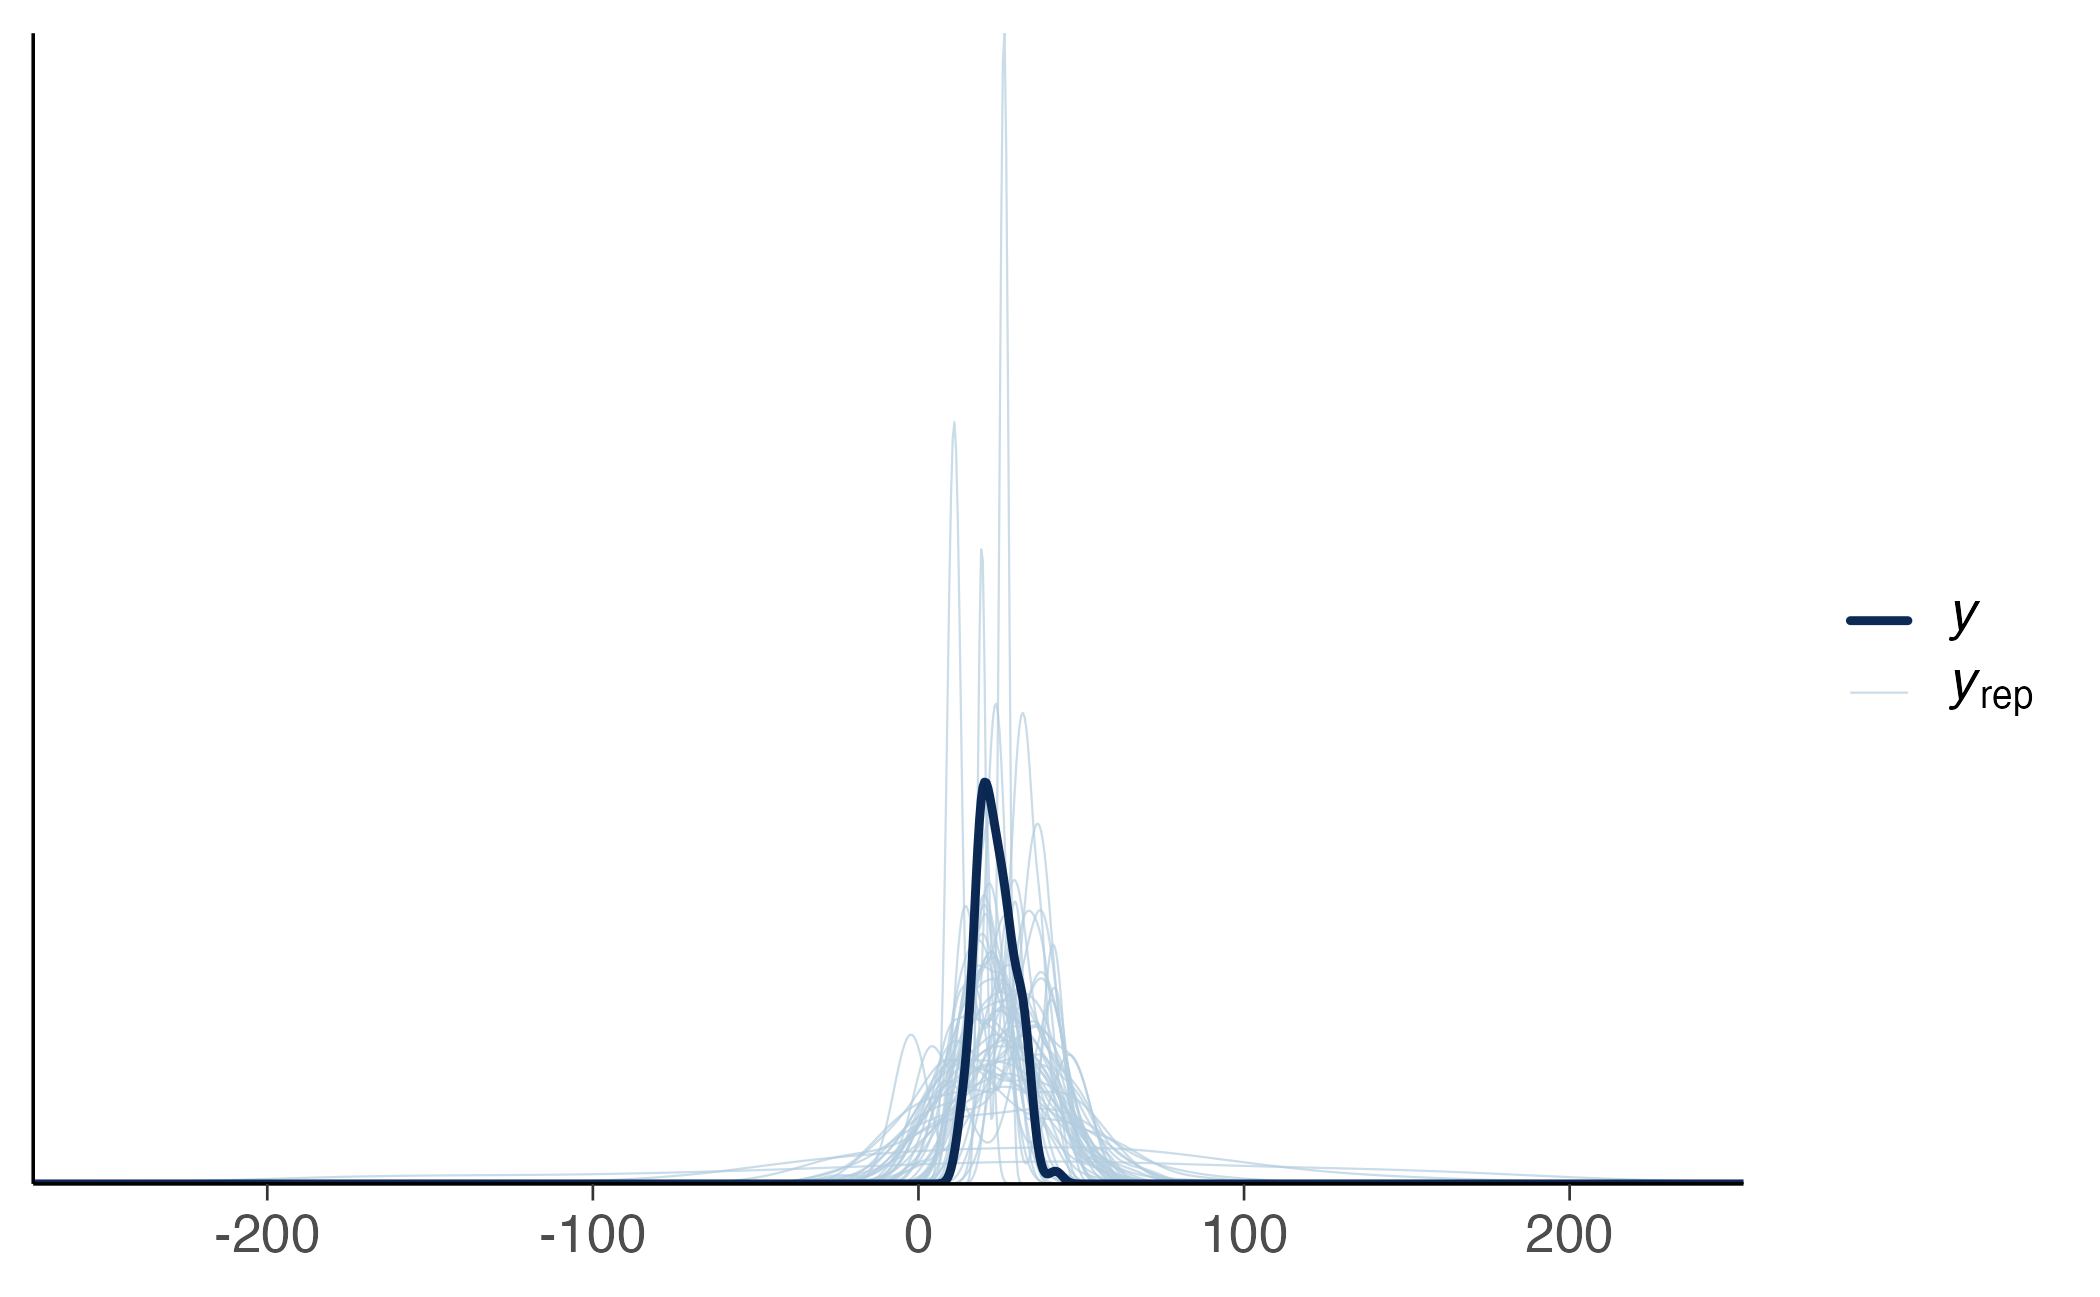
\includegraphics[width=0.85\linewidth,height=\textheight,keepaspectratio]{chapters/linear_models/07_piu_gruppi_contrasti_anova_files/figure-pdf/fig-anova-prior-predictive-1.png}

}

\caption{\label{fig-anova-prior-predictive}Controllo predittivo a priori
per il modello a tre medie di cella. Le linee sottili rappresentano le
densità simulate prodotte dalle sole assunzioni a priori, messe a
confronto con la densità dei dati reali (linea spessa).}

\end{figure}%

\begin{quote}
\textbf{Valutazione diagnostica:} questo controllo non ha lo scopo di
riprodurre fedelmente i dati osservati. La sua funzione è diagnostica:
verificare che le distribuzioni a priori siano in grado di generare
valori plausibili per il fenomeno in esame --- ad esempio, punteggi di
depressione compresi nell'intervallo teoricamente possibile e con una
variabilità non manifestamente irrealistica. Se così non fosse,
occorrerebbe rivedere i prior prima di procedere con l'inferenza.
\end{quote}

\section{Stima del modello e verifiche
computazionali}\label{stima-del-modello-e-verifiche-computazionali-1}

Per procedere all'inferenza, adattiamo il modello ai dati simulati,
includendo l'opzione \texttt{sample\_prior\ =\ "yes"} in modo che Stan
conservi anche i campioni tratti dalle distribuzioni a priori. Ciò
consentirà, se necessario, di confrontare le distribuzioni \emph{prior}
e \emph{posterior} per valutare l'impatto dei dati sulle stime.

\begin{Shaded}
\begin{Highlighting}[]
\NormalTok{anova\_fit }\OtherTok{\textless{}{-}} \FunctionTok{brm}\NormalTok{(}
  \AttributeTok{formula =}\NormalTok{ punteggio }\SpecialCharTok{\textasciitilde{}} \DecValTok{0} \SpecialCharTok{+}\NormalTok{ condizione,}
  \AttributeTok{data    =}\NormalTok{ anova\_data,}
  \AttributeTok{family  =} \FunctionTok{gaussian}\NormalTok{(),}
  \AttributeTok{prior   =}\NormalTok{ anova\_priors,}
  \AttributeTok{sample\_prior =} \StringTok{"yes"}\NormalTok{,}
  \AttributeTok{backend =} \StringTok{"cmdstanr"}\NormalTok{,}
  \AttributeTok{chains  =} \DecValTok{4}\NormalTok{,}
  \AttributeTok{iter    =} \DecValTok{2000}\NormalTok{,}
  \AttributeTok{seed    =} \DecValTok{123}\NormalTok{,}
  \AttributeTok{refresh =} \DecValTok{0}
\NormalTok{)}
\end{Highlighting}
\end{Shaded}

Estraiamo ora le stime marginali e gli indici di sintesi della
distribuzione a posteriori:

\begin{Shaded}
\begin{Highlighting}[]
\FunctionTok{summary}\NormalTok{(anova\_fit)}
\CommentTok{\#\textgreater{}  Family: gaussian }
\CommentTok{\#\textgreater{}   Links: mu = identity }
\CommentTok{\#\textgreater{} Formula: punteggio \textasciitilde{} 0 + condizione }
\CommentTok{\#\textgreater{}    Data: anova\_data (Number of observations: 90) }
\CommentTok{\#\textgreater{}   Draws: 4 chains, each with iter = 2000; warmup = 1000; thin = 1;}
\CommentTok{\#\textgreater{}          total post{-}warmup draws = 4000}
\CommentTok{\#\textgreater{} }
\CommentTok{\#\textgreater{} Regression Coefficients:}
\CommentTok{\#\textgreater{}                         Estimate Est.Error l{-}95\% CI u{-}95\% CI Rhat Bulk\_ESS}
\CommentTok{\#\textgreater{} condizionecontrollo        28.49      0.88    26.76    30.21 1.00     4888}
\CommentTok{\#\textgreater{} condizionepsicoterapia1    22.25      0.89    20.47    24.04 1.00     4192}
\CommentTok{\#\textgreater{} condizionepsicoterapia2    20.69      0.87    19.00    22.41 1.00     4511}
\CommentTok{\#\textgreater{}                         Tail\_ESS}
\CommentTok{\#\textgreater{} condizionecontrollo         3045}
\CommentTok{\#\textgreater{} condizionepsicoterapia1     2854}
\CommentTok{\#\textgreater{} condizionepsicoterapia2     3314}
\CommentTok{\#\textgreater{} }
\CommentTok{\#\textgreater{} Further Distributional Parameters:}
\CommentTok{\#\textgreater{}       Estimate Est.Error l{-}95\% CI u{-}95\% CI Rhat Bulk\_ESS Tail\_ESS}
\CommentTok{\#\textgreater{} sigma     4.79      0.37     4.12     5.61 1.00     3983     3019}
\CommentTok{\#\textgreater{} }
\CommentTok{\#\textgreater{} Draws were sampled using sample(hmc). For each parameter, Bulk\_ESS}
\CommentTok{\#\textgreater{} and Tail\_ESS are effective sample size measures, and Rhat is the potential}
\CommentTok{\#\textgreater{} scale reduction factor on split chains (at convergence, Rhat = 1).}
\end{Highlighting}
\end{Shaded}

Nella parametrizzazione a medie di cella qui adottata, i coefficienti
\texttt{condizionecontrollo}, \texttt{condizionepsicoterapia1} e
\texttt{condizionepsicoterapia2} corrispondono direttamente alle medie
condizionate dei tre gruppi, \(\mu_C\), \(\mu_{P1}\) e \(\mu_{P2}\). Il
parametro \texttt{sigma} rappresenta invece la deviazione standard
residua, assunta costante tra le condizioni e comune a tutti i gruppi.

\subsection{Diagnostica algoritmica del
campionamento}\label{diagnostica-algoritmica-del-campionamento}

Per verificare la stabilità numerica del campionamento MCMC, esaminiamo
i \emph{trace plot} delle catene per tutti i parametri liberi del
modello:

\begin{Shaded}
\begin{Highlighting}[]
\FunctionTok{mcmc\_trace}\NormalTok{(}
  \FunctionTok{as\_draws\_array}\NormalTok{(anova\_fit),}
  \AttributeTok{pars =} \FunctionTok{c}\NormalTok{(}
    \StringTok{"b\_condizionecontrollo"}\NormalTok{,}
    \StringTok{"b\_condizionepsicoterapia1"}\NormalTok{,}
    \StringTok{"b\_condizionepsicoterapia2"}\NormalTok{,}
    \StringTok{"sigma"}
\NormalTok{  )}
\NormalTok{)}
\end{Highlighting}
\end{Shaded}

\begin{figure}[H]

\centering{

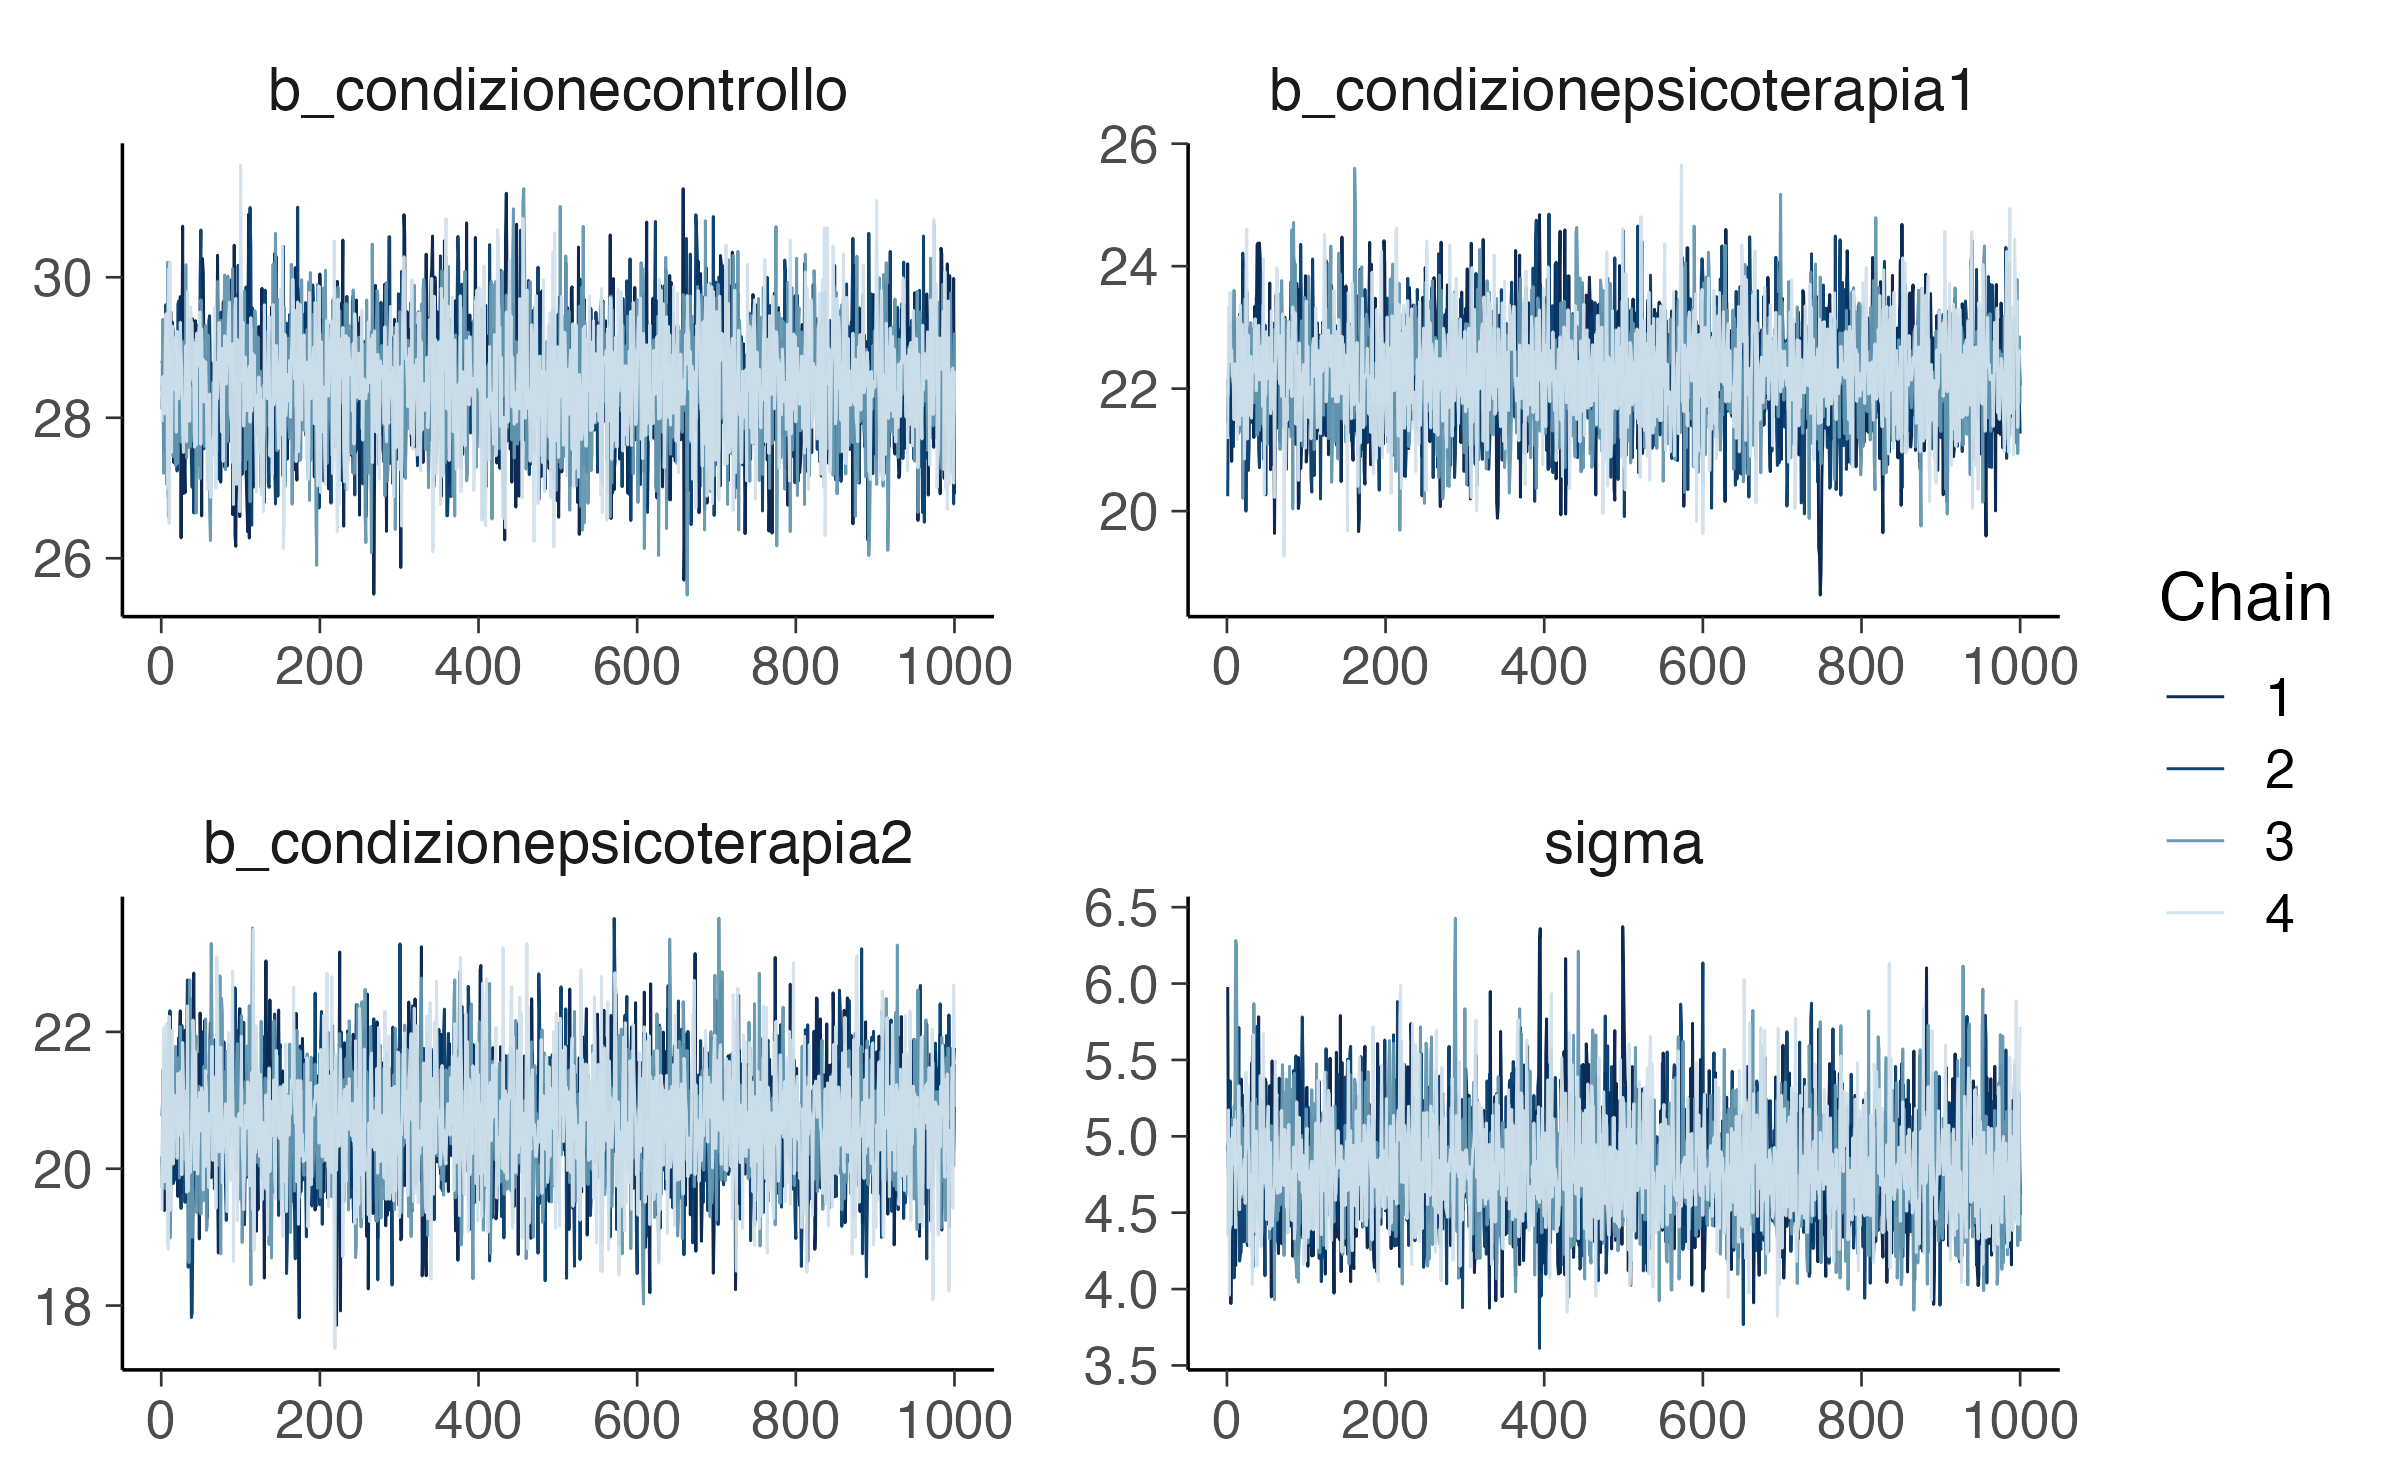
\includegraphics[width=0.85\linewidth,height=\textheight,keepaspectratio]{chapters/linear_models/07_piu_gruppi_contrasti_anova_files/figure-pdf/fig-anova-trace-1.png}

}

\caption{\label{fig-anova-trace}Trace plot delle traiettorie MCMC per le
tre medie di cella e per la deviazione standard residua. La perfetta
sovrapposizione e la stazionarietà delle catene indicano un
campionamento efficiente.}

\end{figure}%

L'ispezione visiva va integrata con il controllo sistematico degli
indicatori quantitativi di convergenza:

\begin{itemize}
\tightlist
\item
  il fattore \(\widehat{R}\), che deve risultare inferiore a \(1.01\)
  per tutti i parametri;
\item
  la dimensione campionaria effettiva (\emph{Effective Sample Size}),
  sia \emph{bulk} che \emph{tail}, per garantire un numero di draw
  sostanzialmente indipendenti;
\item
  l'assenza di transizioni divergenti e di superamenti della massima
  profondità dell'albero (\emph{max\_treedepth}).
\end{itemize}

Il superamento di queste verifiche attesta che l'algoritmo ha esplorato
in modo affidabile la distribuzione a posteriori, ma non costituisce di
per sé una certificazione della validità scientifica del modello, né
dell'adeguatezza della verosimiglianza normale per il fenomeno in esame.

\section{Controllare l'adeguatezza
predittiva}\label{controllare-ladeguatezza-predittiva}

Per valutare se il modello a tre medie di cella riproduca adeguatamente
la struttura dei dati osservati, si esegue un controllo predittivo a
posteriori (\emph{PPC}) sulla distribuzione marginale complessiva:

\begin{Shaded}
\begin{Highlighting}[]
\FunctionTok{pp\_check}\NormalTok{(anova\_fit, }\AttributeTok{type =} \StringTok{"dens\_overlay"}\NormalTok{, }\AttributeTok{ndraws =} \DecValTok{50}\NormalTok{)}
\end{Highlighting}
\end{Shaded}

\begin{figure}[H]

\centering{

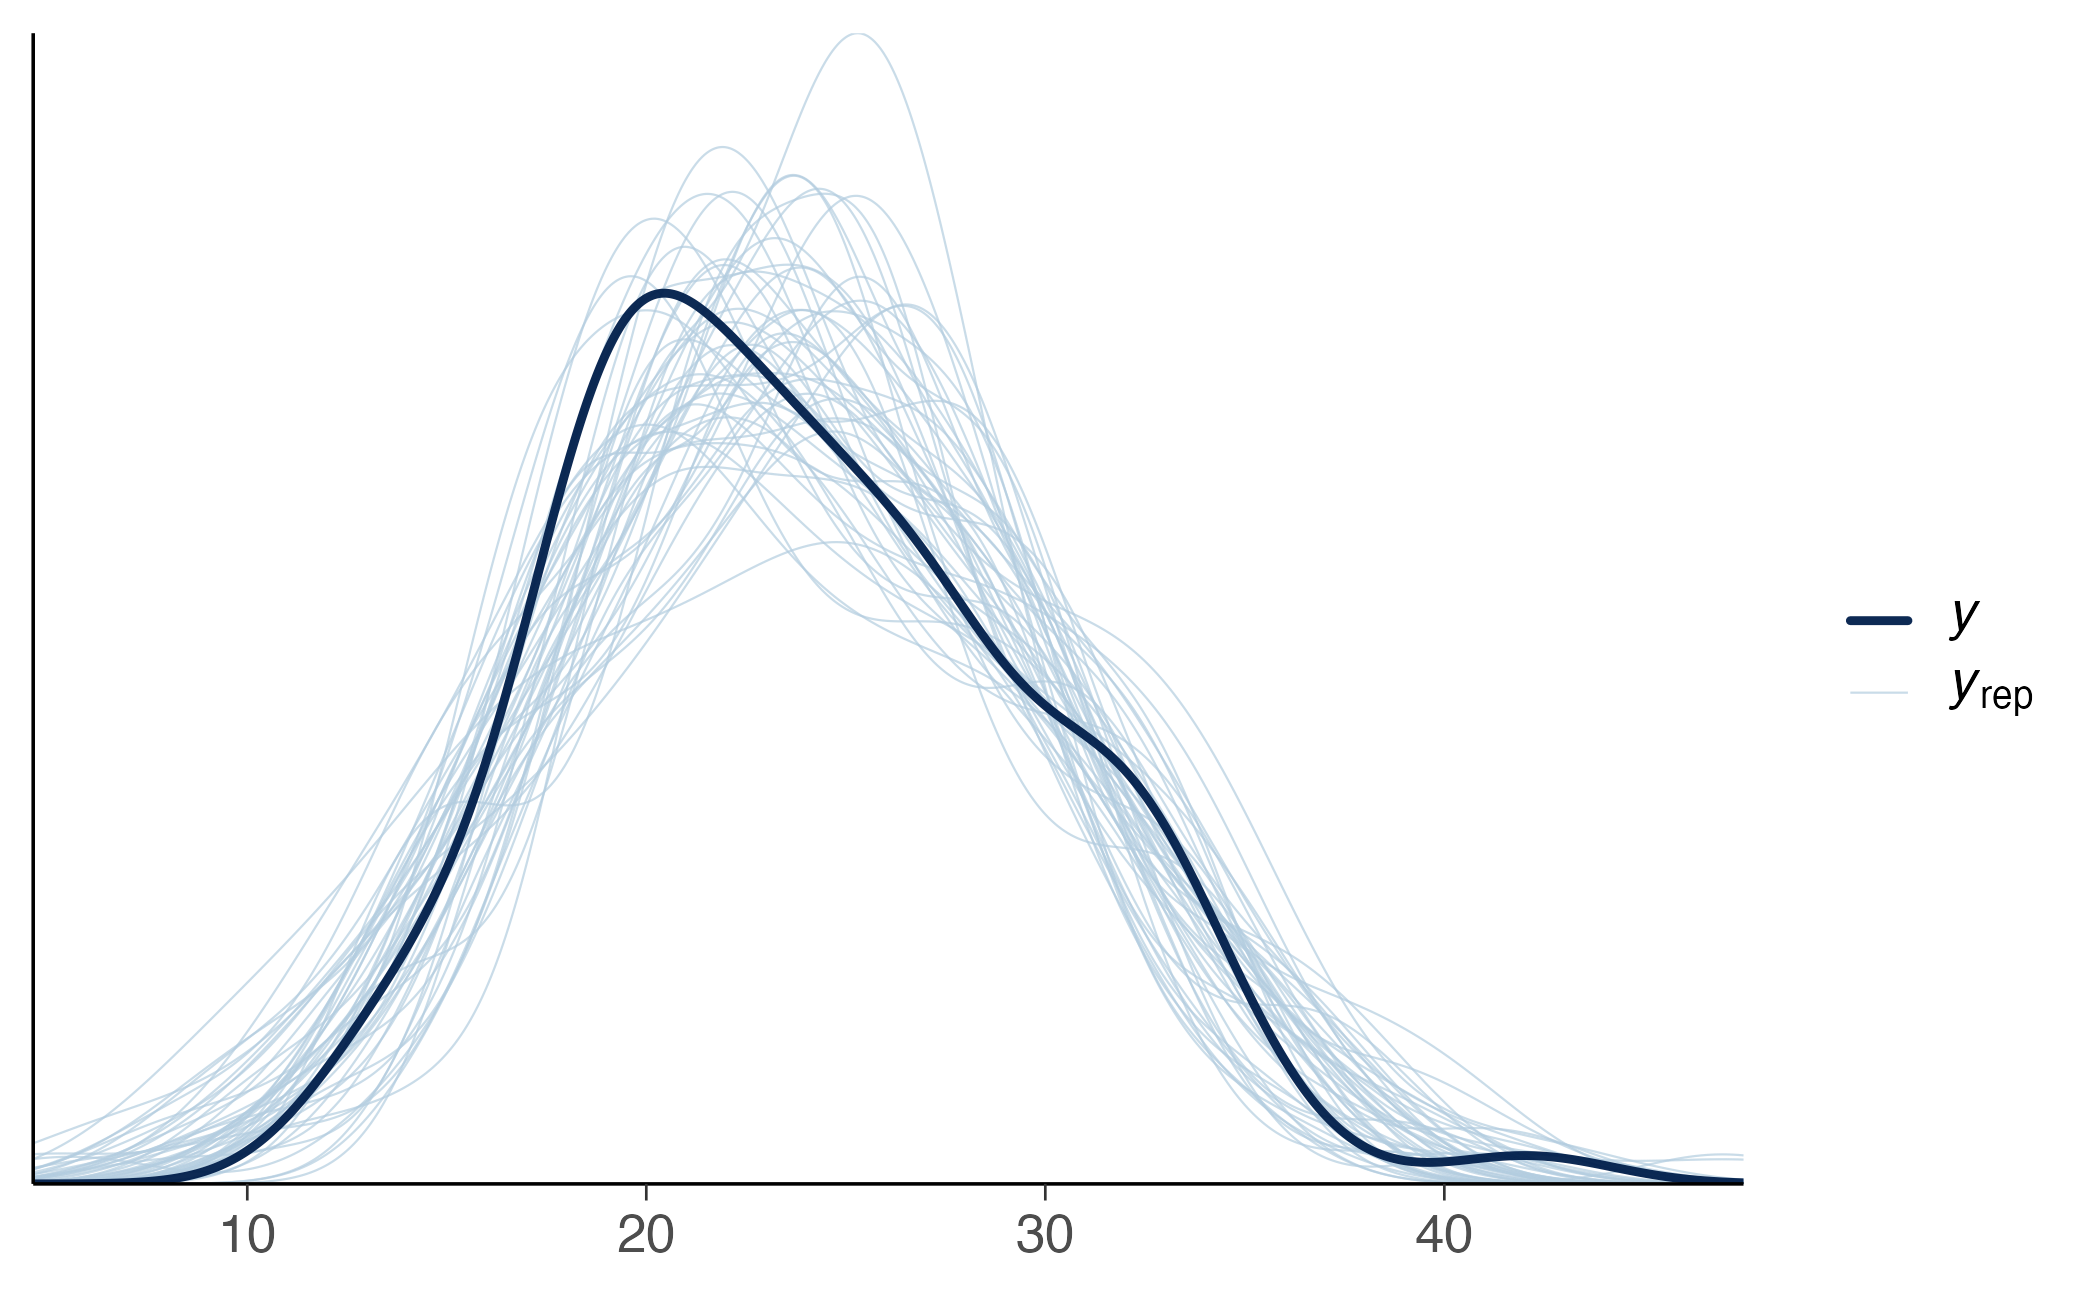
\includegraphics[width=0.85\linewidth,height=\textheight,keepaspectratio]{chapters/linear_models/07_piu_gruppi_contrasti_anova_files/figure-pdf/fig-anova-posterior-predictive-1.png}

}

\caption{\label{fig-anova-posterior-predictive}Controllo predittivo a
posteriori della distribuzione complessiva dei punteggi.}

\end{figure}%

Tuttavia, un buon allineamento sulla distribuzione aggregata può
occultare discrepanze locali o asimmetrie sistematiche all'interno dei
singoli gruppi. Per questo motivo, è utile disaggregare il controllo
predittivo, confrontando le statistiche campionarie osservate con quelle
generate dalle repliche predittive (\(y^{\text{rep}}\)) separatamente
per ciascuna condizione:

\begin{Shaded}
\begin{Highlighting}[]
\NormalTok{anova\_yrep }\OtherTok{\textless{}{-}} \FunctionTok{posterior\_predict}\NormalTok{(anova\_fit, }\AttributeTok{ndraws =} \DecValTok{200}\NormalTok{)}

\NormalTok{group\_index }\OtherTok{\textless{}{-}} \FunctionTok{split}\NormalTok{(}
  \FunctionTok{seq\_len}\NormalTok{(}\FunctionTok{nrow}\NormalTok{(anova\_data)),}
\NormalTok{  anova\_data}\SpecialCharTok{$}\NormalTok{condizione}
\NormalTok{)}

\NormalTok{observed\_group\_stats }\OtherTok{\textless{}{-}} \FunctionTok{tibble}\NormalTok{(}
  \AttributeTok{condizione =} \FunctionTok{names}\NormalTok{(group\_index),}
  \AttributeTok{media\_osservata =} \FunctionTok{vapply}\NormalTok{(}
\NormalTok{    group\_index,}
    \ControlFlowTok{function}\NormalTok{(idx) }\FunctionTok{mean}\NormalTok{(anova\_data}\SpecialCharTok{$}\NormalTok{punteggio[idx]),}
    \FunctionTok{numeric}\NormalTok{(}\DecValTok{1}\NormalTok{)}
\NormalTok{  ),}
  \AttributeTok{sd\_osservata =} \FunctionTok{vapply}\NormalTok{(}
\NormalTok{    group\_index,}
    \ControlFlowTok{function}\NormalTok{(idx) }\FunctionTok{sd}\NormalTok{(anova\_data}\SpecialCharTok{$}\NormalTok{punteggio[idx]),}
    \FunctionTok{numeric}\NormalTok{(}\DecValTok{1}\NormalTok{)}
\NormalTok{  )}
\NormalTok{)}

\NormalTok{replicated\_group\_stats }\OtherTok{\textless{}{-}} \FunctionTok{bind\_rows}\NormalTok{(}\FunctionTok{lapply}\NormalTok{(}
  \FunctionTok{names}\NormalTok{(group\_index),}
  \ControlFlowTok{function}\NormalTok{(group\_name) \{}
\NormalTok{    idx }\OtherTok{\textless{}{-}}\NormalTok{ group\_index[[group\_name]]}
    \FunctionTok{tibble}\NormalTok{(}
      \AttributeTok{condizione =}\NormalTok{ group\_name,}
      \AttributeTok{media\_rep =} \FunctionTok{rowMeans}\NormalTok{(anova\_yrep[, idx, }\AttributeTok{drop =} \ConstantTok{FALSE}\NormalTok{]),}
      \AttributeTok{sd\_rep =} \FunctionTok{apply}\NormalTok{(anova\_yrep[, idx, }\AttributeTok{drop =} \ConstantTok{FALSE}\NormalTok{], }\DecValTok{1}\NormalTok{, sd)}
\NormalTok{    )}
\NormalTok{  \}}
\NormalTok{))}

\NormalTok{observed\_group\_stats}
\CommentTok{\#\textgreater{} \# A tibble: 3 x 3}
\CommentTok{\#\textgreater{}   condizione    media\_osservata sd\_osservata}
\CommentTok{\#\textgreater{}   \textless{}chr\textgreater{}                   \textless{}dbl\textgreater{}        \textless{}dbl\textgreater{}}
\CommentTok{\#\textgreater{} 1 controllo                28.5         4.51}
\CommentTok{\#\textgreater{} 2 psicoterapia1            22.2         4.79}
\CommentTok{\#\textgreater{} 3 psicoterapia2            20.7         4.90}
\end{Highlighting}
\end{Shaded}

Il grafico seguente mostra, per ciascun gruppo, la distribuzione delle
medie replicate, con la media osservata indicata da una linea verticale:

\begin{Shaded}
\begin{Highlighting}[]
\NormalTok{replicated\_group\_stats }\SpecialCharTok{|\textgreater{}}
  \FunctionTok{ggplot}\NormalTok{(}\FunctionTok{aes}\NormalTok{(}\AttributeTok{x =}\NormalTok{ media\_rep)) }\SpecialCharTok{+}
  \FunctionTok{geom\_density}\NormalTok{(}\AttributeTok{fill =} \StringTok{"grey95"}\NormalTok{, }\AttributeTok{color =} \StringTok{"grey40"}\NormalTok{) }\SpecialCharTok{+}
  \FunctionTok{geom\_vline}\NormalTok{(}
    \AttributeTok{data =}\NormalTok{ observed\_group\_stats,}
    \FunctionTok{aes}\NormalTok{(}\AttributeTok{xintercept =}\NormalTok{ media\_osservata),}
    \AttributeTok{linetype =} \StringTok{"dashed"}\NormalTok{,}
    \AttributeTok{color    =} \StringTok{"firebrick"}\NormalTok{,}
    \AttributeTok{size     =} \FloatTok{0.8}
\NormalTok{  ) }\SpecialCharTok{+}
  \FunctionTok{facet\_wrap}\NormalTok{(}\SpecialCharTok{\textasciitilde{}}\NormalTok{ condizione, }\AttributeTok{scales =} \StringTok{"free\_x"}\NormalTok{) }\SpecialCharTok{+}
  \FunctionTok{labs}\NormalTok{(}
    \AttributeTok{x =} \StringTok{"Media campionaria replicata"}\NormalTok{,}
    \AttributeTok{y =} \StringTok{"Densità predittiva"}
\NormalTok{  )}
\end{Highlighting}
\end{Shaded}

\begin{figure}[H]

\centering{

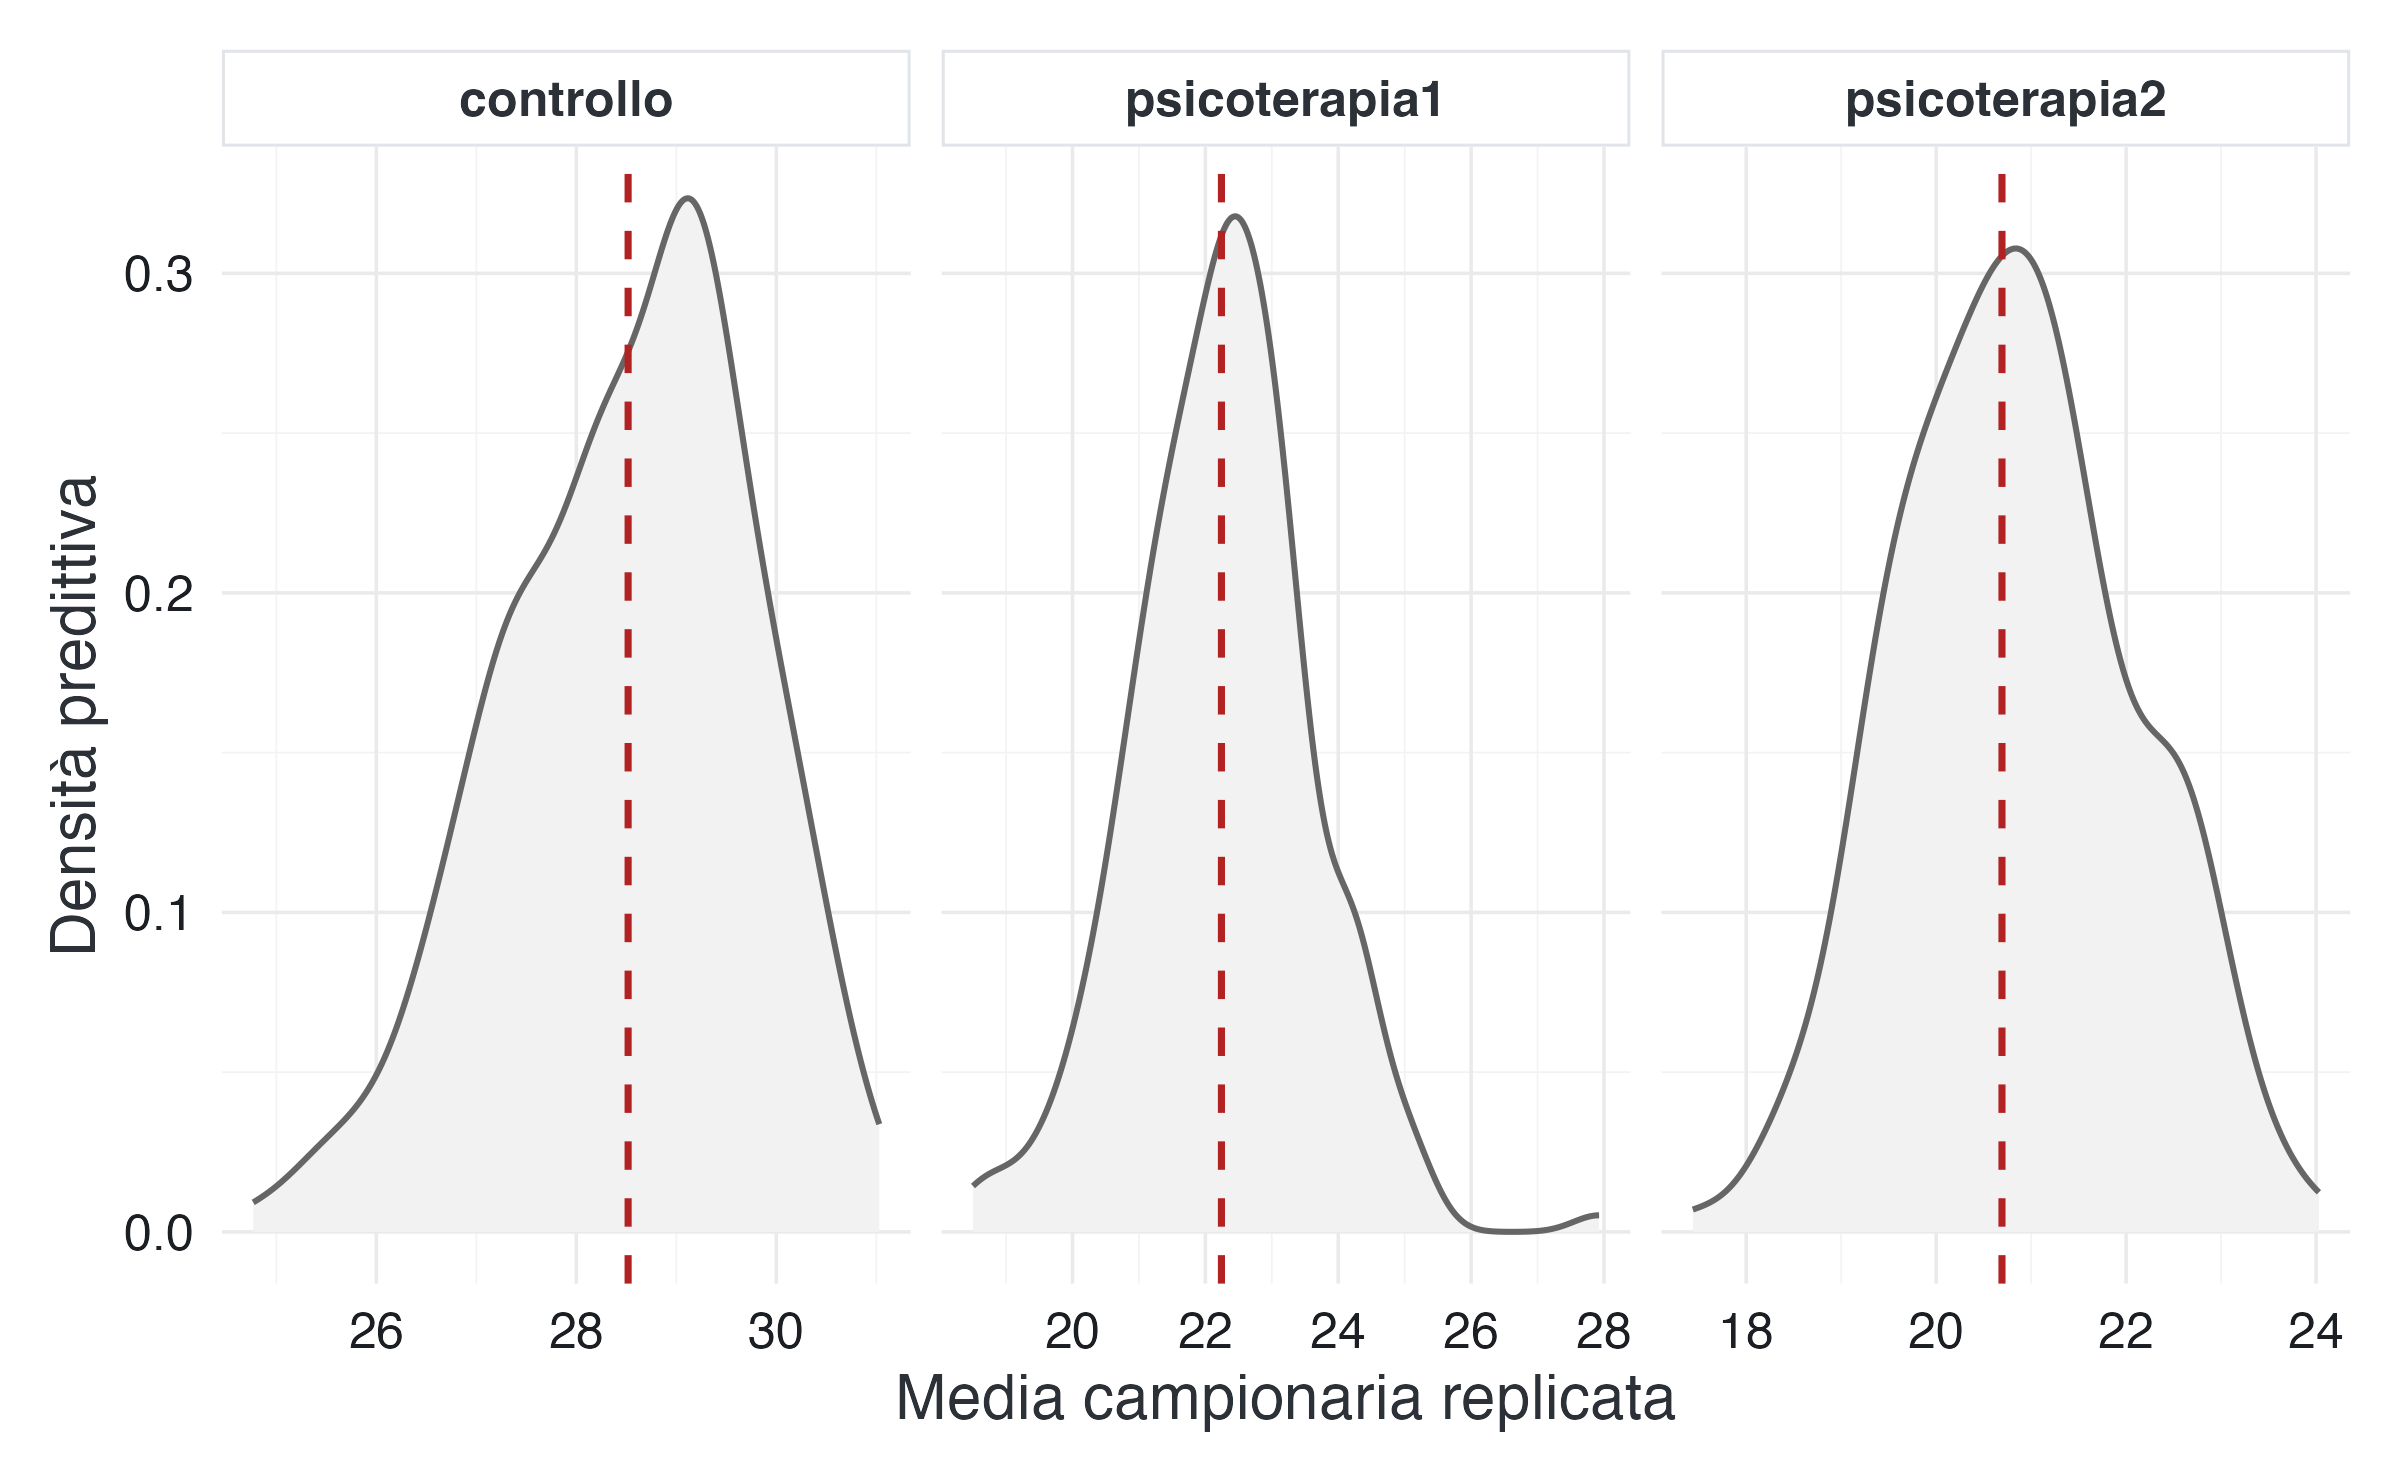
\includegraphics[width=0.85\linewidth,height=\textheight,keepaspectratio]{chapters/linear_models/07_piu_gruppi_contrasti_anova_files/figure-pdf/fig-anova-groupwise-mean-ppc-1.png}

}

\caption{\label{fig-anova-groupwise-mean-ppc}Distribuzioni predittive a
posteriori delle medie campionarie replicate, separate per condizione. I
punti indicano le medie osservate.}

\end{figure}%

Questo controllo disaggregato consente di valutare se il modello sia in
grado di riprodurre le medie osservate in ciascuna condizione. Se le
medie osservate cadono stabilmente nelle regioni ad alta densità delle
distribuzioni replicate, la specificazione del predittore lineare
risulta compatibile con i dati. La corretta riproduzione delle medie non
implica tuttavia che l'assunzione di omoschedasticità --- ovvero una
varianza residua comune a tutti i gruppi --- sia automaticamente valida.
Per una verifica più completa, è opportuno estendere il controllo
predittivo anche alla variabilità replicata.

\section{Dalle medie ai contrasti
pianificati}\label{dalle-medie-ai-contrasti-pianificati}

Se la parametrizzazione è scelta in modo che i coefficienti del modello
corrispondano già ai contrasti di interesse, la stima di questi ultimi è
immediata. L'inferenza si fonda sulla distribuzione a posteriori, che
quantifica l'incertezza sulle differenze tra le medie e consente di
rispondere direttamente ai quesiti scientifici, ad esempio calcolando la
probabilità che un contrasto superi una certa soglia. Il codice seguente
mostra come derivare i due contrasti pianificati a partire dalle medie
di cella:

\begin{Shaded}
\begin{Highlighting}[]
\CommentTok{\# Estraiamo i draws mantenendo intatta la struttura dell\textquotesingle{}oggetto posterior}
\NormalTok{draws\_cell\_means }\OtherTok{\textless{}{-}} \FunctionTok{as\_draws}\NormalTok{(anova\_fit)}

\CommentTok{\# Deriviamo i contrasti pianificati tramite mutate\_variables}
\NormalTok{draws\_contrasts }\OtherTok{\textless{}{-}}\NormalTok{ posterior}\SpecialCharTok{::}\FunctionTok{mutate\_variables}\NormalTok{(}
\NormalTok{  draws\_cell\_means,}
  \AttributeTok{mu\_ctrl         =}\NormalTok{ b\_condizionecontrollo,}
  \AttributeTok{mu\_p1           =}\NormalTok{ b\_condizionepsicoterapia1,}
  \AttributeTok{mu\_p2           =}\NormalTok{ b\_condizionepsicoterapia2,}
  \AttributeTok{ctrl\_vs\_terapie =}\NormalTok{ mu\_ctrl }\SpecialCharTok{{-}}\NormalTok{ (mu\_p1 }\SpecialCharTok{+}\NormalTok{ mu\_p2) }\SpecialCharTok{/} \DecValTok{2}\NormalTok{,}
  \AttributeTok{p1\_vs\_p2        =}\NormalTok{ mu\_p1 }\SpecialCharTok{{-}}\NormalTok{ mu\_p2}
\NormalTok{)}

\CommentTok{\# Selezioniamo le sole variabili sostantive per il summary descrittivo}
\NormalTok{subset\_contrasts }\OtherTok{\textless{}{-}} \FunctionTok{subset\_draws}\NormalTok{(}
\NormalTok{  draws\_contrasts,}
  \AttributeTok{variable =} \FunctionTok{c}\NormalTok{(}\StringTok{"mu\_ctrl"}\NormalTok{, }\StringTok{"mu\_p1"}\NormalTok{, }\StringTok{"mu\_p2"}\NormalTok{, }\StringTok{"ctrl\_vs\_terapie"}\NormalTok{, }\StringTok{"p1\_vs\_p2"}\NormalTok{)}
\NormalTok{)}

\FunctionTok{summarise\_draws}\NormalTok{(subset\_contrasts)}
\CommentTok{\#\textgreater{} \# A tibble: 5 x 10}
\CommentTok{\#\textgreater{}   variable         mean median    sd   mad     q5   q95  rhat ess\_bulk ess\_tail}
\CommentTok{\#\textgreater{}   \textless{}chr\textgreater{}           \textless{}dbl\textgreater{}  \textless{}dbl\textgreater{} \textless{}dbl\textgreater{} \textless{}dbl\textgreater{}  \textless{}dbl\textgreater{} \textless{}dbl\textgreater{} \textless{}dbl\textgreater{}    \textless{}dbl\textgreater{}    \textless{}dbl\textgreater{}}
\CommentTok{\#\textgreater{} 1 mu\_ctrl         28.5   28.5  0.880 0.902 27.0   29.9  1.000    4888.    3045.}
\CommentTok{\#\textgreater{} 2 mu\_p1           22.2   22.2  0.893 0.879 20.8   23.7  1.000    4192.    2854.}
\CommentTok{\#\textgreater{} 3 mu\_p2           20.7   20.7  0.867 0.828 19.3   22.1  1.00     4511.    3314.}
\CommentTok{\#\textgreater{} 4 ctrl\_vs\_terapie  7.02   7.02 1.11  1.11   5.19   8.88 1.000    4709.    2699.}
\CommentTok{\#\textgreater{} 5 p1\_vs\_p2         1.56   1.54 1.22  1.21  {-}0.439  3.57 1.00     4457.    3010.}
\end{Highlighting}
\end{Shaded}

Ogni contrasto è una distribuzione a posteriori completa, che riflette
l'incertezza congiunta delle quantità coinvolte. Per un'interfaccia più
dichiarativa si può usare il pacchetto \texttt{emmeans}; per maggiore
flessibilità e trasparenza, il controllo diretto sui \emph{draw} rimane
lo strumento più generale.

\subsection{\texorpdfstring{Specificazione dei contrasti tramite il
pacchetto
\texttt{emmeans}}{Specificazione dei contrasti tramite il pacchetto emmeans}}\label{specificazione-dei-contrasti-tramite-il-pacchetto-emmeans}

Il pacchetto \texttt{emmeans} (\emph{estimated marginal means}) offre
un'interfaccia dichiarativa per formalizzare i contrasti definiti
manualmente. Questo approccio risulta particolarmente utile in modelli
complessi, con più predittori o interazioni, dove il calcolo diretto sui
draw diventa meno immediato. Il codice seguente mostra come calcolare le
medie marginali attese per il fattore \texttt{condizione}:

\begin{Shaded}
\begin{Highlighting}[]
\NormalTok{anova\_emmeans }\OtherTok{\textless{}{-}} \FunctionTok{emmeans}\NormalTok{(anova\_fit, }\AttributeTok{specs =} \StringTok{"condizione"}\NormalTok{)}
\NormalTok{anova\_emmeans}
\CommentTok{\#\textgreater{}  condizione    emmean lower.HPD upper.HPD}
\CommentTok{\#\textgreater{}  controllo       28.5      26.8      30.2}
\CommentTok{\#\textgreater{}  psicoterapia1   22.2      20.6      24.1}
\CommentTok{\#\textgreater{}  psicoterapia2   20.7      19.0      22.4}
\CommentTok{\#\textgreater{} }
\CommentTok{\#\textgreater{} Point estimate displayed: median }
\CommentTok{\#\textgreater{} HPD interval probability: 0.95}
\end{Highlighting}
\end{Shaded}

Per riprodurre i contrasti pianificati definiti in precedenza, si
specifica una lista di vettori di pesi:

\begin{Shaded}
\begin{Highlighting}[]
\NormalTok{planned\_contrasts }\OtherTok{\textless{}{-}} \FunctionTok{list}\NormalTok{(}
  \StringTok{"Controllo vs media terapie"} \OtherTok{=} \FunctionTok{c}\NormalTok{(}
    \AttributeTok{controllo       =} \DecValTok{1}\NormalTok{,}
    \AttributeTok{psicoterapia1   =} \SpecialCharTok{{-}}\FloatTok{0.5}\NormalTok{,}
    \AttributeTok{psicoterapia2   =} \SpecialCharTok{{-}}\FloatTok{0.5}
\NormalTok{  ),}
  \StringTok{"Protocollo 1 vs protocollo 2"} \OtherTok{=} \FunctionTok{c}\NormalTok{(}
    \AttributeTok{controllo       =} \DecValTok{0}\NormalTok{,}
    \AttributeTok{psicoterapia1   =} \DecValTok{1}\NormalTok{,}
    \AttributeTok{psicoterapia2   =} \SpecialCharTok{{-}}\DecValTok{1}
\NormalTok{  )}
\NormalTok{)}

\FunctionTok{contrast}\NormalTok{(anova\_emmeans, }\AttributeTok{method =}\NormalTok{ planned\_contrasts)}
\CommentTok{\#\textgreater{}  contrast                     estimate lower.HPD upper.HPD}
\CommentTok{\#\textgreater{}  Controllo vs media terapie       7.02      4.65      9.04}
\CommentTok{\#\textgreater{}  Protocollo 1 vs protocollo 2     1.54     {-}0.91      3.87}
\CommentTok{\#\textgreater{} }
\CommentTok{\#\textgreater{} Point estimate displayed: median }
\CommentTok{\#\textgreater{} HPD interval probability: 0.95}
\end{Highlighting}
\end{Shaded}

In ciascun vettore, la somma dei pesi è pari a zero: ciò garantisce che
il contrasto isoli esclusivamente la differenza tra i gruppi
considerati, senza essere influenzato dal livello medio generale. I
confronti esaustivi a coppie sono disponibili tramite
\texttt{pairs(anova\_emmeans)}, ma vanno utilizzati solo quando
l'esplorazione sistematica è giustificata; in presenza di ipotesi
specifiche, i contrasti pianificati rappresentano la strategia più
coerente con la domanda di ricerca.

\section{Probabilità sostantive e rilevanza clinica dei
contrasti}\label{probabilituxe0-sostantive-e-rilevanza-clinica-dei-contrasti}

Per superare la logica binaria dei test di significatività, introduciamo
una soglia di rilevanza pratica. Supponiamo che, nel dominio della scala
CES-D, una variazione inferiore a tre punti sia considerata clinicamente
irrilevante. Definiamo quindi la \emph{SESOI} (\emph{Smallest Effect
Size of Interest}):

\[
\delta_{\min} = 3
\]

Per calcolare le probabilità di interesse, estraiamo i draw dei
contrasti dall'oggetto \texttt{subset\_contrasts} sotto forma di
matrice:

\begin{Shaded}
\begin{Highlighting}[]
\NormalTok{mat\_contrasts }\OtherTok{\textless{}{-}} \FunctionTok{as\_draws\_matrix}\NormalTok{(subset\_contrasts)}

\NormalTok{ctrl\_vs\_terapie\_d }\OtherTok{\textless{}{-}}\NormalTok{ mat\_contrasts[, }\StringTok{"ctrl\_vs\_terapie"}\NormalTok{]}
\NormalTok{p1\_vs\_p2\_d        }\OtherTok{\textless{}{-}}\NormalTok{ mat\_contrasts[, }\StringTok{"p1\_vs\_p2"}\NormalTok{]}

\NormalTok{SESOI }\OtherTok{\textless{}{-}} \DecValTok{3}

\NormalTok{anova\_probabilities }\OtherTok{\textless{}{-}} \FunctionTok{tibble}\NormalTok{(}
  \AttributeTok{quesito\_clinico =} \FunctionTok{c}\NormalTok{(}
    \StringTok{"Le terapie riducono la sintomatologia rispetto al controllo (Δ \textgreater{} 0)"}\NormalTok{,}
    \StringTok{"La riduzione media dovuta alle terapie supera la SESOI (Δ \textgreater{} 3)"}\NormalTok{,}
    \StringTok{"Il protocollo 2 è più efficace del protocollo 1 (Δ \textgreater{} 0)"}\NormalTok{,}
    \StringTok{"La differenza tra i due protocolli supera la SESOI (|Δ| \textgreater{} 3)"}
\NormalTok{  ),}
  \AttributeTok{probabilita\_posterior =} \FunctionTok{c}\NormalTok{(}
    \FunctionTok{mean}\NormalTok{(ctrl\_vs\_terapie\_d }\SpecialCharTok{\textgreater{}} \DecValTok{0}\NormalTok{),}
    \FunctionTok{mean}\NormalTok{(ctrl\_vs\_terapie\_d }\SpecialCharTok{\textgreater{}}\NormalTok{ SESOI),}
    \FunctionTok{mean}\NormalTok{(p1\_vs\_p2\_d }\SpecialCharTok{\textgreater{}} \DecValTok{0}\NormalTok{),}
    \FunctionTok{mean}\NormalTok{(}\FunctionTok{abs}\NormalTok{(p1\_vs\_p2\_d) }\SpecialCharTok{\textgreater{}}\NormalTok{ SESOI)}
\NormalTok{  )}
\NormalTok{)}

\NormalTok{anova\_probabilities}
\CommentTok{\#\textgreater{} \# A tibble: 4 x 2}
\CommentTok{\#\textgreater{}   quesito\_clinico                                                    }
\CommentTok{\#\textgreater{}   \textless{}chr\textgreater{}                                                              }
\CommentTok{\#\textgreater{} 1 Le terapie riducono la sintomatologia rispetto al controllo (Δ \textgreater{} 0)}
\CommentTok{\#\textgreater{} 2 La riduzione media dovuta alle terapie supera la SESOI (Δ \textgreater{} 3)     }
\CommentTok{\#\textgreater{} 3 Il protocollo 2 è più efficace del protocollo 1 (Δ \textgreater{} 0)            }
\CommentTok{\#\textgreater{} 4 La differenza tra i due protocolli supera la SESOI (|Δ| \textgreater{} 3)       }
\CommentTok{\#\textgreater{}   probabilita\_posterior}
\CommentTok{\#\textgreater{}                   \textless{}dbl\textgreater{}}
\CommentTok{\#\textgreater{} 1                 1    }
\CommentTok{\#\textgreater{} 2                 1.000}
\CommentTok{\#\textgreater{} 3                 0.902}
\CommentTok{\#\textgreater{} 4                 0.12}
\end{Highlighting}
\end{Shaded}

I quattro indici così ottenuti rispondono a domande distinte. Un
contrasto può avere un'elevata probabilità di essere positivo, ma una
probabilità modesta di superare la soglia di rilevanza pratica;
viceversa, due trattamenti possono differire in modo stimabile, ma non
in misura sufficiente da orientare una decisione clinica.

La soglia SESOI deve essere definita prima di osservare i dati, sulla
base di considerazioni teoriche, evidenze cliniche o valutazioni
decisionali. Modificarla dopo aver visto la distribuzione a posteriori
comprometterebbe la validità inferenziale, trasformando un criterio
sostantivo in un accomodamento ai risultati osservati.

\section{Il ruolo della valutazione omnibus nel framework
bayesiano}\label{il-ruolo-della-valutazione-omnibus-nel-framework-bayesiano}

L'ipotesi nulla omnibus dell'ANOVA classica --- ``tutte le medie di
gruppo sono uguali'' --- fornisce un'informazione molto generica e,
nella maggior parte dei contesti applicativi, scarsamente utile per
orientare l'interpretazione clinica o teorica. Nell'approccio bayesiano,
tuttavia, non siamo vincolati a questo interrogativo. Possiamo definire
indicatori sintetici che, sebbene più informativi del test F, restano
meno utili dei contrasti pianificati.

Laddove si desideri una sintesi globale, si può calcolare, ad esempio,
l'ampiezza massima tra le medie di gruppo
(\(R_\mu = \max(\mu) - \min(\mu)\)) e valutarne la distribuzione a
posteriori. Pur fornendo un quadro d'insieme, questa metrica non
sostituisce l'analisi dei contrasti specifici, che rimane lo strumento
più informativo ed efficiente quando le ipotesi di ricerca sono
direzionali e definite a priori.

\section{Molteplicità: che cosa cambia e che cosa non
cambia}\label{molteplicituxe0-che-cosa-cambia-e-che-cosa-non-cambia}

All'aumentare del numero di livelli di un fattore categoriale, il numero
di confronti a coppie potenziali cresce in modo combinatorio. Nella
statistica frequentista, questo problema viene affrontato con correzioni
del valore-\emph{p} (Bonferroni, Tukey) per controllare il tasso di
errore di primo tipo.

Nell'approccio bayesiano, non si procede a una dicotomizzazione dei
contrasti in termini di significatività, e quindi le correzioni multiple
non sono necessarie. Tuttavia, ciò non significa che il problema della
molteplicità scompaia. Se il ricercatore esamina molti contrasti e
riporta solo quelli più estremi, introduce una \textbf{distorsione da
selezione} (\emph{selection bias}). Inoltre, con campioni piccoli, i
gruppi che per caso risultano più estremi tendono a produrre stime
sovrastimate.

Per garantire l'integrità dell'analisi in disegni complessi, è
opportuno:

\begin{enumerate}
\def\labelenumi{\arabic{enumi}.}
\tightlist
\item
  \textbf{Pianificare i contrasti} in anticipo, sulla base di ipotesi
  teoriche;
\item
  \textbf{Distinguere} nel report le analisi confermative da quelle
  esplorative;
\item
  \textbf{Utilizzare modelli gerarchici} quando i gruppi possono essere
  considerati come provenienti da una popolazione comune. Questa
  strategia introduce il \emph{partial pooling} (trattato nel prossimo
  capitolo), che contrae le stime più estreme verso la media globale,
  riducendo i falsi allarmi e stabilizzando l'inferenza.
\end{enumerate}

\section{Assunzioni del modello ed estensioni
metodologiche}\label{assunzioni-del-modello-ed-estensioni-metodologiche}

Il modello lineare classico a medie di cella poggia su quattro
assunzioni stocastiche fondamentali: l'indipendenza condizionale delle
osservazioni, la normalità degli errori entro ciascun gruppo,
l'omoschedasticità (ovvero una deviazione standard residua \(\sigma\)
comune a tutte le condizioni) e l'assenza di variabili latenti o
covariate omesse in grado di spiegare variazioni sistematiche
dell'outcome. Ciascuna di queste assunzioni va verificata attraverso i
controlli predittivi a posteriori e, più in generale, alla luce del
disegno di ricerca.

Quando queste assunzioni risultano eccessivamente restrittive, il
framework bayesiano offre estensioni naturali: l'adozione di una
verosimiglianza Student-\(t\) per distribuzioni con code pesanti o
valori estremi; modelli con varianza eterogenea tra gruppi; l'inclusione
di covariate e interazioni per controllare variabili di disturbo; e
strutture gerarchiche per dati clusterizzati o misure ripetute.

A titolo di esempio, nel pacchetto \texttt{brms} è possibile rilassare
l'assunzione di omoschedasticità modellando esplicitamente il parametro
di scala in funzione del fattore categoriale:

\begin{Shaded}
\begin{Highlighting}[]
\CommentTok{\#| label: anova{-}heteroscedastic{-}example}
\CommentTok{\#| eval: false}

\NormalTok{heteroscedastic\_fit }\OtherTok{\textless{}{-}} \FunctionTok{brm}\NormalTok{(}
  \AttributeTok{formula =} \FunctionTok{bf}\NormalTok{(}
\NormalTok{    punteggio }\SpecialCharTok{\textasciitilde{}} \DecValTok{0} \SpecialCharTok{+}\NormalTok{ condizione,}
\NormalTok{    sigma     }\SpecialCharTok{\textasciitilde{}} \DecValTok{0} \SpecialCharTok{+}\NormalTok{ condizione}
\NormalTok{  ),}
  \AttributeTok{data    =}\NormalTok{ anova\_data,}
  \AttributeTok{family  =} \FunctionTok{gaussian}\NormalTok{(),}
  \AttributeTok{backend =} \StringTok{"cmdstanr"}
\NormalTok{)}
\end{Highlighting}
\end{Shaded}

Questa specificazione stima un parametro \(\sigma\) distinto per ciascun
gruppo (attraverso una funzione di legame logaritmica che garantisce la
positività), ma deve essere giustificata da ipotesi teoriche o da
evidenze diagnostiche, per evitare un inutile sovraccarico di parametri.
Le estensioni qui descritte verranno riprese e approfondite nei capitoli
dedicati alla verifica e all'espansione del modello.

\section{Conclusioni ed epistemologia del disegno di
ricerca}\label{conclusioni-ed-epistemologia-del-disegno-di-ricerca}

In questo studio simulato, il modello bayesiano ha consentito di stimare
le differenze tra le tre condizioni sperimentali e di quantificarne
l'incertezza in modo coerente. Tuttavia, è importante ricordare che la
qualità delle inferenze non dipende dalla complessità del modello, ma
dal disegno di ricerca che ha generato i dati. Un'analisi statistica,
per quanto raffinata, non può trasformare un'associazione osservazionale
in un effetto causale.

Per attribuire un significato causale ai contrasti stimati, occorre che
il disegno sperimentale controlli le principali minacce alla validità
interna: randomizzazione, fedeltà al trattamento, gestione delle perdite
e assenza di contaminazione tra i bracci dello studio. In assenza di
queste condizioni --- come avviene tipicamente nei disegni
osservazionali --- le differenze osservate tra i gruppi potrebbero
riflettere distorsioni da selezione, differenze iniziali di gravità o
altri fattori confondenti, e non possono essere interpretate come
effetti dei trattamenti.

\section{Linee guida per la comunicazione dei
risultati}\label{linee-guida-per-la-comunicazione-dei-risultati}

Una rendicontazione scientifica trasparente ed efficace deve
strutturarsi attorno alle stime dei parametri di posizione dei gruppi,
alla quantificazione metrica dei contrasti pianificati e alla
valutazione probabilistica rispetto alle soglie di rilevanza clinica,
rifiutando la riduzione del capitolo Risultati a una generica e
dicotomica dichiarazione omnibus.

Un possibile modello di stesura per la sezione dei Risultati è il
seguente:

\begin{quote}
Per esaminare il gradiente di efficacia clinica tra le condizioni,
abbiamo specificato un modello lineare bayesiano normale a medie di
cella. Il modello ha stimato per ciascun braccio sperimentale la
distribuzione a posteriori del punteggio medio di depressione. Il primo
contrasto pianificato, volto a confrontare il gruppo di controllo con il
punto medio dei due protocolli attivi, ha evidenziato una riduzione
sintomatologica pari a \(\Delta_{C:T} = 8.1\) punti di CES-D (HDI 95\%
\([5.4, 10.8]\)). La probabilità a posteriori che tale decremento superi
la soglia di rilevanza clinica minima di 3 punti è pari a
\(\Pr(\Delta_{C:T} > 3 \mid y) > .99\). Il secondo contrasto
pianificato, mirato al confronto diretto tra i due interventi
psicoterapeutici, ha mostrato uno scostamento a favore del secondo
protocollo pari a \(\Delta_{P1:P2} = 4.8\) punti (HDI 95\%
\([2.1, 7.5]\)); la probabilità che questa differenza metrica risulti
clinicamente rilevante in valore assoluto è pari a
\(\Pr(\vert{}\Delta_{P1:P2}\vert{} > 3 \mid y) = .87\). Le conclusioni
inferenziali qui presentate rimangono strettamente vincolate alla
struttura dei contrasti specificati a priori e dipendono sia
dall'adeguatezza della verosimiglianza gaussiana sia dalla tenuta del
disegno di campionamento.
\end{quote}

\section{Errori frequenti}\label{errori-frequenti-6}

\begin{tcolorbox}[enhanced jigsaw, arc=.35mm, bottomrule=.15mm, bottomtitle=1mm, breakable, colback=white, colbacktitle=quarto-callout-warning-color!10!white, colframe=quarto-callout-warning-color-frame, coltitle=black, left=2mm, leftrule=.75mm, opacityback=0, opacitybacktitle=0.6, rightrule=.15mm, title=\textcolor{quarto-callout-warning-color}{\faExclamationTriangle}\hspace{0.5em}{Trattare l'ANOVA come una tecnica separata}, titlerule=0mm, toprule=.15mm, toptitle=1mm]

Un fattore a più livelli entra nel modello lineare attraverso la matrice
del moello La logica inferenziale non cambia rispetto al confronto tra
due gruppi.

\end{tcolorbox}

\begin{tcolorbox}[enhanced jigsaw, arc=.35mm, bottomrule=.15mm, bottomtitle=1mm, breakable, colback=white, colbacktitle=quarto-callout-warning-color!10!white, colframe=quarto-callout-warning-color-frame, coltitle=black, left=2mm, leftrule=.75mm, opacityback=0, opacitybacktitle=0.6, rightrule=.15mm, title=\textcolor{quarto-callout-warning-color}{\faExclamationTriangle}\hspace{0.5em}{Interpretare i coefficienti senza controllare la codifica}, titlerule=0mm, toprule=.15mm, toptitle=1mm]

Con la codifica a riferimento, l'intercetta è la media del gruppo di
riferimento e gli altri coefficienti sono differenze. Con
\texttt{0\ +\ fattore}, i coefficienti sono medie di cella.

\end{tcolorbox}

\begin{tcolorbox}[enhanced jigsaw, arc=.35mm, bottomrule=.15mm, bottomtitle=1mm, breakable, colback=white, colbacktitle=quarto-callout-warning-color!10!white, colframe=quarto-callout-warning-color-frame, coltitle=black, left=2mm, leftrule=.75mm, opacityback=0, opacitybacktitle=0.6, rightrule=.15mm, title=\textcolor{quarto-callout-warning-color}{\faExclamationTriangle}\hspace{0.5em}{Eseguire automaticamente tutti i confronti a coppie}, titlerule=0mm, toprule=.15mm, toptitle=1mm]

I confronti devono essere motivati dalla domanda. Un elenco completo di
coppie può essere utile in un'analisi esplorativa, ma non sostituisce la
formulazione di contrasti teorici.

\end{tcolorbox}

\begin{tcolorbox}[enhanced jigsaw, arc=.35mm, bottomrule=.15mm, bottomtitle=1mm, breakable, colback=white, colbacktitle=quarto-callout-warning-color!10!white, colframe=quarto-callout-warning-color-frame, coltitle=black, left=2mm, leftrule=.75mm, opacityback=0, opacitybacktitle=0.6, rightrule=.15mm, title=\textcolor{quarto-callout-warning-color}{\faExclamationTriangle}\hspace{0.5em}{Confondere probabilità direzionale e rilevanza pratica}, titlerule=0mm, toprule=.15mm, toptitle=1mm]

Una differenza può essere quasi certamente positiva ma troppo piccola
per avere importanza clinica o teorica.

\end{tcolorbox}

\begin{tcolorbox}[enhanced jigsaw, arc=.35mm, bottomrule=.15mm, bottomtitle=1mm, breakable, colback=white, colbacktitle=quarto-callout-warning-color!10!white, colframe=quarto-callout-warning-color-frame, coltitle=black, left=2mm, leftrule=.75mm, opacityback=0, opacitybacktitle=0.6, rightrule=.15mm, title=\textcolor{quarto-callout-warning-color}{\faExclamationTriangle}\hspace{0.5em}{Affermare che il Bayesiano elimina la molteplicità}, titlerule=0mm, toprule=.15mm, toptitle=1mm]

L'assenza di una correzione automatica della soglia non rende innocua la
selezione tra molti risultati. Pianificazione, trasparenza e
modellazione gerarchica rimangono essenziali.

\end{tcolorbox}

\begin{tcolorbox}[enhanced jigsaw, arc=.35mm, bottomrule=.15mm, bottomtitle=1mm, breakable, colback=white, colbacktitle=quarto-callout-warning-color!10!white, colframe=quarto-callout-warning-color-frame, coltitle=black, left=2mm, leftrule=.75mm, opacityback=0, opacitybacktitle=0.6, rightrule=.15mm, title=\textcolor{quarto-callout-warning-color}{\faExclamationTriangle}\hspace{0.5em}{Pensare che un buon campionamento convalidi il modello}, titlerule=0mm, toprule=.15mm, toptitle=1mm]

\(\widehat R\), effective sample size e assenza di divergenze riguardano
il calcolo. L'adeguatezza delle assunzioni richiede controlli predittivi
e valutazione sostantiva.

\end{tcolorbox}

\section*{Riflessioni conclusive}\label{riflessioni-conclusive-24}

\markright{Riflessioni conclusive}

L'analisi della varianza a una via non introduce un nuovo paradigma
statistico, ma si inserisce nel quadro del modello lineare: un
predittore categoriale con più di due livelli viene tradotto in vettori
numerici all'interno della matrice del modello La codifica con categoria
di riferimento rende immediata la lettura degli scostamenti rispetto al
gruppo baseline; la parametrizzazione a medie di cella esplicita invece
direttamente i parametri di posizione di ciascuna condizione. Le due
formulazioni descrivono il medesimo sottospazio lineare e producono
identici valori adattati, purché le distribuzioni a priori siano
specificate in modo coerente con la parametrizzazione adottata.

Il contributo più rilevante dell'approccio bayesiano risiede nella
possibilità di tradurre le ipotesi scientifiche in \textbf{contrasti
pianificati}. A differenza del test omnibus classico, che si limita a
segnalare l'esistenza di almeno una differenza tra le medie, l'inferenza
bayesiana restituisce l'intera distribuzione a posteriori di qualsiasi
combinazione lineare delle medie definita \emph{a priori}. Ciò consente
di valutare l'ampiezza degli effetti sulla scala originaria, calcolare
probabilità direzionali e verificare se le differenze superino una
soglia di rilevanza pratica stabilita indipendentemente dai dati.

Infine, la presenza di molteplici livelli solleva una questione
metodologica cruciale, che sarà al centro dei prossimi capitoli. Quando
le condizioni o le unità da confrontare sono numerose e tra loro
collegate --- come avviene con dati provenienti da scuole, centri
clinici, stimoli o studi diversi --- stimare ciascun parametro in
isolamento rischia di produrre stime instabili e scarsamente
generalizzabili. I modelli gerarchici rispondono a questa vulnerabilità
introducendo una distribuzione comune di secondo livello, in grado di
rappresentare simultaneamente la variabilità tra i gruppi e le
regolarità condivise dell'intera popolazione.

\begin{tcolorbox}[enhanced jigsaw, arc=.35mm, bottomrule=.15mm, bottomtitle=1mm, breakable, colback=white, colbacktitle=quarto-callout-note-color!10!white, colframe=quarto-callout-note-color-frame, coltitle=black, left=2mm, leftrule=.75mm, opacityback=0, opacitybacktitle=0.6, rightrule=.15mm, title=\textcolor{quarto-callout-note-color}{\faInfo}\hspace{0.5em}{Concetti da ricordare}, titlerule=0mm, toprule=.15mm, toptitle=1mm]

\begin{enumerate}
\def\labelenumi{\arabic{enumi}.}
\tightlist
\item
  L'ANOVA a una via è un modello lineare con un predittore categoriale.
\item
  La codifica modifica l'interpretazione dei coefficienti, non le medie
  adattate.
\item
  Le medie di cella costituiscono una parametrizzazione trasparente per
  costruire contrasti.
\item
  Un contrasto è una combinazione lineare delle medie definita dalla
  domanda scientifica.
\item
  I contrasti devono essere calcolati sulla distribuzione congiunta dei
  draw posteriori.
\item
  Probabilità direzionale e rilevanza pratica sono domande diverse.
\item
  Una domanda omnibus può essere formalizzata, ma spesso è meno
  informativa dei contrasti pianificati.
\item
  La molteplicità rimane rilevante quando si selezionano risultati tra
  molti confronti.
\item
  Il modello a medie di cella non produce automaticamente partial
  pooling.
\item
  L'interpretazione causale dipende dal disegno, non dalla formula del
  modello.
\end{enumerate}

\end{tcolorbox}

\section*{Esercizi}\label{esercizi-6}

\markright{Esercizi}

\subsection{Esercizio 1 --- Leggere la matrice del
modello}\label{esercizio-1-leggere-la-matrice-del-modello}

Costruisci con \texttt{model.matrix()} le matrici associate a:

\begin{Shaded}
\begin{Highlighting}[]
\SpecialCharTok{\textasciitilde{}}\NormalTok{ condizione}
\SpecialCharTok{\textasciitilde{}} \DecValTok{0} \SpecialCharTok{+}\NormalTok{ condizione}
\end{Highlighting}
\end{Shaded}

Spiega il significato di ciascuna colonna e ricostruisci le tre medie a
partire dai coefficienti della prima parametrizzazione.

\subsection{Esercizio 2 --- Cambiare il gruppo di
riferimento}\label{esercizio-2-cambiare-il-gruppo-di-riferimento}

Imposta \texttt{psicoterapia2} come riferimento e adatta il modello con
intercetta. Quali coefficienti cambiano? Quali quantità rimangono
identiche?

\subsection{Esercizio 3 --- Formulare un contrasto
teorico}\label{esercizio-3-formulare-un-contrasto-teorico}

Definisci un contrasto che attribuisca peso doppio al secondo protocollo
rispetto al primo nel confronto con il controllo. Motiva i pesi e
verifica che sommino a zero.

\subsection{Esercizio 4 --- Modificare la
SESOI}\label{esercizio-4-modificare-la-sesoi}

Ripeti il calcolo delle probabilità usando soglie di 1, 3 e 5 punti.
Descrivi come cambia la conclusione senza modificare la posterior.

\subsection{Esercizio 5 --- Confronto
esplorativo}\label{esercizio-5-confronto-esplorativo}

Calcola tutti i confronti a coppie con \texttt{pairs(anova\_emmeans)}.
Indica quali domande aggiuntive rispondono e quali rischi interpretativi
introduce la loro selezione a posteriori.

\subsection{Esercizio 6 --- Controllo predittivo per la
dispersione}\label{esercizio-6-controllo-predittivo-per-la-dispersione}

Usa \texttt{replicated\_group\_stats} per confrontare le deviazioni
standard replicate con quelle osservate. Il modello con \(\sigma\)
comune rappresenta adeguatamente tutti i gruppi?

\subsection{Esercizio 7 --- Dati
sbilanciati}\label{esercizio-7-dati-sbilanciati}

Simula gruppi con numerosità 20, 40 e 80. Confronta la media campionaria
complessiva con il punto medio non ponderato delle tre medie. Spiega
perché non sono la stessa quantità.

\subsection{Esercizio 8 --- Parametrizzazione e
prior}\label{esercizio-8-parametrizzazione-e-prior}

Adatta lo stesso modello con codifica a riferimento. Specifica prior che
inducano approssimativamente le stesse credenze sulle tre medie del
modello a medie di cella. Spiega perché assegnare semplicemente
\texttt{normal(25,\ 10)} a tutti i coefficienti non produce lo stesso
prior congiunto.

\subsection{Esercizio 9 --- Verso il modello
multilivello}\label{esercizio-9-verso-il-modello-multilivello}

Simula venti gruppi con poche osservazioni ciascuno. Spiega perché la
stima indipendente di venti medie può essere instabile e anticipa come
una distribuzione gerarchica potrebbe regolarizzarle.

\begin{tcolorbox}[enhanced jigsaw, arc=.35mm, bottomrule=.15mm, bottomtitle=1mm, breakable, colback=white, colbacktitle=quarto-callout-tip-color!10!white, colframe=quarto-callout-tip-color-frame, coltitle=black, left=2mm, leftrule=.75mm, opacityback=0, opacitybacktitle=0.6, rightrule=.15mm, title=\textcolor{quarto-callout-tip-color}{\faLightbulb}\hspace{0.5em}{Tracce di soluzione}, titlerule=0mm, toprule=.15mm, toptitle=1mm]

\begin{itemize}
\tightlist
\item
  \textbf{Esercizio 1:} con l'intercetta, una colonna rappresenta il
  riferimento e le altre gli scostamenti; senza intercetta, ciascuna
  colonna identifica direttamente un gruppo.
\item
  \textbf{Esercizio 2:} cambiano intercetta e coefficienti visualizzati,
  ma medie adattate, contrasti e previsioni rimangono invariati quando
  il modello e i prior sono equivalenti.
\item
  \textbf{Esercizio 3:} i pesi devono riflettere la domanda e sommare a
  zero; per esempio, un confronto controllo versus combinazione
  ponderata delle terapie può usare \((1,-1/3,-2/3)\).
\item
  \textbf{Esercizio 4:} aumentando la soglia diminuisce la probabilità
  che il contrasto sia sostantivamente rilevante; la distribuzione a
  posteriori non cambia.
\item
  \textbf{Esercizio 5:} l'esplorazione è legittima se dichiarata come
  tale; il problema nasce quando i confronti selezionati vengono
  presentati come ipotesi pianificate.
\item
  \textbf{Esercizio 6:} confronta ciascuna deviazione standard osservata
  con la relativa distribuzione replicata; deviazioni sistematiche
  suggeriscono una specificazione eteroschedastica o robusta.
\item
  \textbf{Esercizio 7:} la media complessiva pondera le medie in base
  alle numerosità; il punto medio assegna lo stesso peso a ogni gruppo.
\item
  \textbf{Esercizio 8:} i prior sui coefficienti dipendono linearmente
  dalla parametrizzazione; prior indipendenti in un sistema di
  coordinate possono diventare dipendenti in un altro.
\item
  \textbf{Esercizio 9:} gruppi piccoli producono medie molto variabili;
  il partial pooling combina informazione del gruppo e informazione
  della popolazione dei gruppi.
\end{itemize}

\end{tcolorbox}

\begin{tcolorbox}[enhanced jigsaw, arc=.35mm, bottomrule=.15mm, bottomtitle=1mm, breakable, colback=white, colbacktitle=quarto-callout-note-color!10!white, colframe=quarto-callout-note-color-frame, coltitle=black, left=2mm, leftrule=.75mm, opacityback=0, opacitybacktitle=0.6, rightrule=.15mm, title=\textcolor{quarto-callout-note-color}{\faInfo}\hspace{0.5em}{Informazioni sull'ambiente di sviluppo}, titlerule=0mm, toprule=.15mm, toptitle=1mm]

\begin{Shaded}
\begin{Highlighting}[]
\FunctionTok{sessionInfo}\NormalTok{()}
\CommentTok{\#\textgreater{} R version 4.6.1 (2026{-}06{-}24)}
\CommentTok{\#\textgreater{} Platform: aarch64{-}apple{-}darwin23}
\CommentTok{\#\textgreater{} Running under: macOS Tahoe 26.5.2}
\CommentTok{\#\textgreater{} }
\CommentTok{\#\textgreater{} Matrix products: default}
\CommentTok{\#\textgreater{} BLAS:   /Library/Frameworks/R.framework/Versions/4.6/Resources/lib/libRblas.0.dylib }
\CommentTok{\#\textgreater{} LAPACK: /Library/Frameworks/R.framework/Versions/4.6/Resources/lib/libRlapack.dylib;  LAPACK version 3.12.1}
\CommentTok{\#\textgreater{} }
\CommentTok{\#\textgreater{} locale:}
\CommentTok{\#\textgreater{} [1] C.UTF{-}8/UTF{-}8/C.UTF{-}8/C/C.UTF{-}8/C.UTF{-}8}
\CommentTok{\#\textgreater{} }
\CommentTok{\#\textgreater{} time zone: Europe/Zagreb}
\CommentTok{\#\textgreater{} tzcode source: internal}
\CommentTok{\#\textgreater{} }
\CommentTok{\#\textgreater{} attached base packages:}
\CommentTok{\#\textgreater{} [1] stats     graphics  grDevices utils     datasets  methods   base     }
\CommentTok{\#\textgreater{} }
\CommentTok{\#\textgreater{} other attached packages:}
\CommentTok{\#\textgreater{}  [1] emmeans\_2.0.4         ragg\_1.5.2            tinytable\_0.17.0     }
\CommentTok{\#\textgreater{}  [4] withr\_3.0.3           systemfonts\_1.3.2     patchwork\_1.3.2      }
\CommentTok{\#\textgreater{}  [7] ggdist\_3.3.3          tidybayes\_3.0.7       bayesplot\_1.15.0     }
\CommentTok{\#\textgreater{} [10] ggplot2\_4.0.3         reliabilitydiag\_0.2.1 priorsense\_1.2.0     }
\CommentTok{\#\textgreater{} [13] posterior\_1.7.0       loo\_2.10.0            rstan\_2.32.7         }
\CommentTok{\#\textgreater{} [16] StanHeaders\_2.32.10   brms\_2.23.0           Rcpp\_1.1.2           }
\CommentTok{\#\textgreater{} [19] sessioninfo\_1.2.4     conflicted\_1.2.0      janitor\_2.2.1        }
\CommentTok{\#\textgreater{} [22] matrixStats\_1.5.0     modelr\_0.1.11         tibble\_3.3.1         }
\CommentTok{\#\textgreater{} [25] dplyr\_1.2.1           tidyr\_1.3.2           rio\_1.3.0            }
\CommentTok{\#\textgreater{} [28] here\_1.0.2           }
\CommentTok{\#\textgreater{} }
\CommentTok{\#\textgreater{} loaded via a namespace (and not attached):}
\CommentTok{\#\textgreater{}  [1] svUnit\_1.0.8          tidyselect\_1.2.1      farver\_2.1.2         }
\CommentTok{\#\textgreater{}  [4] S7\_0.2.2              fastmap\_1.2.0         tensorA\_0.36.2.1     }
\CommentTok{\#\textgreater{}  [7] pacman\_0.5.1          digest\_0.6.39         timechange\_0.4.0     }
\CommentTok{\#\textgreater{} [10] estimability\_2.0.0    lifecycle\_1.0.5       processx\_3.9.0       }
\CommentTok{\#\textgreater{} [13] magrittr\_2.0.5        compiler\_4.6.1        rlang\_1.3.0          }
\CommentTok{\#\textgreater{} [16] tools\_4.6.1           utf8\_1.2.6            yaml\_2.3.12          }
\CommentTok{\#\textgreater{} [19] data.table\_1.18.4     knitr\_1.51            labeling\_0.4.3       }
\CommentTok{\#\textgreater{} [22] bridgesampling\_1.2{-}1  pkgbuild\_1.4.8        curl\_7.1.0           }
\CommentTok{\#\textgreater{} [25] plyr\_1.8.9            cmdstanr\_0.9.0        RColorBrewer\_1.1{-}3   }
\CommentTok{\#\textgreater{} [28] abind\_1.4{-}8           purrr\_1.2.2           grid\_4.6.1           }
\CommentTok{\#\textgreater{} [31] stats4\_4.6.1          xtable\_1.8{-}8          inline\_0.3.21        }
\CommentTok{\#\textgreater{} [34] scales\_1.4.0          cli\_3.6.6             mvtnorm\_1.4{-}2        }
\CommentTok{\#\textgreater{} [37] rmarkdown\_2.31        generics\_0.1.4        otel\_0.2.0           }
\CommentTok{\#\textgreater{} [40] RcppParallel\_5.1.11{-}2 reshape2\_1.4.5        cachem\_1.1.0         }
\CommentTok{\#\textgreater{} [43] stringr\_1.6.0         parallel\_4.6.1        vctrs\_0.7.3          }
\CommentTok{\#\textgreater{} [46] V8\_8.2.0              Matrix\_1.7{-}5          jsonlite\_2.0.0       }
\CommentTok{\#\textgreater{} [49] arrayhelpers\_1.1{-}1    glue\_1.8.1            ps\_1.9.3             }
\CommentTok{\#\textgreater{} [52] codetools\_0.2{-}20      distributional\_0.8.1  lubridate\_1.9.5      }
\CommentTok{\#\textgreater{} [55] stringi\_1.8.7         gtable\_0.3.6          QuickJSR\_1.10.0      }
\CommentTok{\#\textgreater{} [58] pillar\_1.11.1         htmltools\_0.5.9       Brobdingnag\_1.2{-}9    }
\CommentTok{\#\textgreater{} [61] R6\_2.6.1              textshaping\_1.0.5     rprojroot\_2.1.1      }
\CommentTok{\#\textgreater{} [64] evaluate\_1.0.5        lattice\_0.22{-}9        backports\_1.5.1      }
\CommentTok{\#\textgreater{} [67] memoise\_2.0.1         broom\_1.0.13          snakecase\_0.11.1     }
\CommentTok{\#\textgreater{} [70] rstantools\_2.6.0      coda\_0.19{-}4.1         gridExtra\_2.3.1      }
\CommentTok{\#\textgreater{} [73] nlme\_3.1{-}170          checkmate\_2.3.4       xfun\_0.60            }
\CommentTok{\#\textgreater{} [76] pkgconfig\_2.0.3}
\end{Highlighting}
\end{Shaded}

\end{tcolorbox}

\section*{Bibliografia}\label{bibliografia-27}

\markright{Bibliografia}

\chapter{Modelli multilivello: eterogeneità e partial
pooling}\label{sec-multilevel}

I dati psicologici presentano spesso una struttura gerarchica. Le
misurazioni possono essere ripetute sulla stessa persona, gli studenti
possono appartenere a classi diverse, i pazienti possono essere seguiti
in centri clinici differenti e gli stimoli possono essere raggruppati in
categorie. In tutti questi casi, osservazioni appartenenti alla stessa
unità tendono ad assomigliarsi più di osservazioni appartenenti a unità
diverse.

Un modello lineare che ignora questa struttura tratta implicitamente
tutte le osservazioni come intercambiabili. Il problema non riguarda
soltanto il calcolo dell'incertezza. In psicologia siamo spesso
interessati a due domande simultanee:

\begin{enumerate}
\def\labelenumi{\arabic{enumi}.}
\tightlist
\item
  quale relazione emerge, in media, nella popolazione considerata;
\item
  quanto e in quale modo le persone o i gruppi differiscono da tale
  relazione media.
\end{enumerate}

I modelli multilivello rispondono a entrambe le domande costruendo una
distribuzione comune per i parametri delle diverse unità. Le stime
individuali non vengono né completamente identificate con la media
generale né trattate come se fossero indipendenti. Sono stimate mediante
\textbf{partial pooling}, cioè combinando l'informazione specifica
dell'unità con quella condivisa dall'insieme delle unità.

\begin{tcolorbox}[enhanced jigsaw, arc=.35mm, bottomrule=.15mm, breakable, colback=white, colframe=quarto-callout-important-color-frame, left=2mm, leftrule=.75mm, opacityback=0, rightrule=.15mm, toprule=.15mm]

\textbf{Da sapere.} I modelli multilivello rappresentano esplicitamente
la dipendenza tra osservazioni annidate e distinguono la relazione media
della popolazione dall'eterogeneità tra persone o gruppi. Il
\emph{partial pooling} combina l'informazione individuale con quella
condivisa, producendo uno \emph{shrinkage} maggiore per le unità con
dati meno informativi. La variabilità tra le pendenze individuali è
distinta dall'incertezza sulla pendenza media.

\textbf{Da saper fare.} Riconoscere una struttura gerarchica nei dati;
distinguere \emph{complete pooling}, \emph{no pooling} e \emph{partial
pooling}; specificare e stimare con \texttt{brms} un modello con
intercette e pendenze variabili; interpretare parametri di popolazione,
deviazioni individuali, componenti di varianza e correlazioni;
distinguere \texttt{ranef()} da \texttt{coef()}; eseguire controlli
predittivi e formulare previsioni per un'unità osservata, per la
relazione media e per una nuova unità.

\textbf{Approfondimento facoltativo.} La scomposizione della matrice di
covarianza, la stima della correlazione tra intercette e pendenze, il
confronto sistematico tra diverse strutture degli effetti di gruppo e le
previsioni per nuovi livelli possono essere rimandati in una prima
lettura. Nel percorso essenziale è sufficiente comprendere il meccanismo
del \emph{partial pooling}, stimare il modello con \texttt{brms} e
interpretare l'eterogeneità e le principali previsioni posteriori.

\hyperref[sec-percorsi-lettura]{Che cosa significano queste etichette?}

\end{tcolorbox}

\begin{tcolorbox}[enhanced jigsaw, arc=.35mm, bottomrule=.15mm, bottomtitle=1mm, breakable, colback=white, colbacktitle=quarto-callout-note-color!10!white, colframe=quarto-callout-note-color-frame, coltitle=black, left=2mm, leftrule=.75mm, opacityback=0, opacitybacktitle=0.6, rightrule=.15mm, title=\textcolor{quarto-callout-note-color}{\faInfo}\hspace{0.5em}{Obiettivi del capitolo}, titlerule=0mm, toprule=.15mm, toptitle=1mm]

Al termine del capitolo dovresti essere in grado di:

\begin{itemize}
\tightlist
\item
  riconoscere una struttura annidata o gerarchica nei dati;
\item
  distinguere \emph{complete pooling}, \emph{no pooling} e \emph{partial
  pooling};
\item
  leggere un modello con intercette e pendenze variabili;
\item
  interpretare i parametri di popolazione, le deviazioni di gruppo e la
  loro variabilità;
\item
  spiegare da quali informazioni dipende lo shrinkage;
\item
  distinguere \texttt{ranef()} da \texttt{coef()};
\item
  costruire previsioni per un'unità osservata, per la relazione media e
  per una nuova unità;
\item
  valutare criticamente l'ipotesi che le differenze individuali siano
  variazioni quantitative attorno a una struttura comune.
\end{itemize}

\end{tcolorbox}

\begin{tcolorbox}[enhanced jigsaw, arc=.35mm, bottomrule=.15mm, bottomtitle=1mm, breakable, colback=white, colbacktitle=quarto-callout-tip-color!10!white, colframe=quarto-callout-tip-color-frame, coltitle=black, left=2mm, leftrule=.75mm, opacityback=0, opacitybacktitle=0.6, rightrule=.15mm, title=\textcolor{quarto-callout-tip-color}{\faLightbulb}\hspace{0.5em}{Percorsi di lettura}, titlerule=0mm, toprule=.15mm, toptitle=1mm]

Il capitolo appartiene al \textbf{percorso essenziale} e al
\textbf{percorso concettuale}. Le sezioni sulla matrice di covarianza
degli effetti di gruppo e sulle previsioni per nuovi livelli
costituiscono anche un raccordo con il \textbf{percorso computazionale
avanzato}.

\end{tcolorbox}

\begin{tcolorbox}[enhanced jigsaw, arc=.35mm, bottomrule=.15mm, bottomtitle=1mm, breakable, colback=white, colbacktitle=quarto-callout-tip-color!10!white, colframe=quarto-callout-tip-color-frame, coltitle=black, left=2mm, leftrule=.75mm, opacityback=0, opacitybacktitle=0.6, rightrule=.15mm, title=\textcolor{quarto-callout-tip-color}{\faLightbulb}\hspace{0.5em}{Prerequisiti}, titlerule=0mm, toprule=.15mm, toptitle=1mm]

Sono particolarmente utili:

\begin{itemize}
\tightlist
\item
  il confronto tra più gruppi (Capitolo~\ref{sec-anova1via}), nel quale
  le medie erano stimate separatamente senza una distribuzione
  gerarchica;
\item
  il workflow bayesiano con \texttt{brms}
  (Capitolo~\ref{sec-linmod-bayesian-reg});
\item
  l'interfaccia a formula di \texttt{brms}
  (Capitolo~\ref{sec-linar-models-brms});
\item
  come riferimento generale, la trattazione dei modelli multilivello in
  \emph{Statistical Rethinking}
  (\citeproc{ref-McElreath_rethinking}{McElreath, 2020}).
\end{itemize}

\end{tcolorbox}

\begin{tcolorbox}[enhanced jigsaw, arc=.35mm, bottomrule=.15mm, bottomtitle=1mm, breakable, colback=white, colbacktitle=quarto-callout-caution-color!10!white, colframe=quarto-callout-caution-color-frame, coltitle=black, left=2mm, leftrule=.75mm, opacityback=0, opacitybacktitle=0.6, rightrule=.15mm, title=\textcolor{quarto-callout-caution-color}{\faFire}\hspace{0.5em}{Preparazione del Notebook}, titlerule=0mm, toprule=.15mm, toptitle=1mm]

\end{tcolorbox}

\section{Dalla struttura dei dati alla domanda
scientifica}\label{dalla-struttura-dei-dati-alla-domanda-scientifica}

Per illustrare l'uso dei modelli multilivello, utilizzeremo i dati dello
studio di Belenky et al. (\citeproc{ref-belenky2003patterns}{2003})
sugli effetti cumulativi della deprivazione del sonno sulla vigilanza
psicomotoria. In questo disegno, i partecipanti hanno eseguito
ripetutamente un compito di reazione nell'arco di diversi giorni di
sonno ridotto. La variabile \texttt{Reaction} registra il tempo medio di
reazione in millisecondi; \texttt{days\_deprived} indica il numero di
giorni trascorsi dalla baseline.

\begin{Shaded}
\begin{Highlighting}[]
\NormalTok{sleep2 }\OtherTok{\textless{}{-}}\NormalTok{ rio}\SpecialCharTok{::}\FunctionTok{import}\NormalTok{(}
\NormalTok{  here}\SpecialCharTok{::}\FunctionTok{here}\NormalTok{(}\StringTok{"data"}\NormalTok{, }\StringTok{"sleep2.csv"}\NormalTok{)}
\NormalTok{) }\SpecialCharTok{|\textgreater{}}
  \FunctionTok{mutate}\NormalTok{(}
    \AttributeTok{Subject =} \FunctionTok{factor}\NormalTok{(Subject),}
    \AttributeTok{days\_deprived =} \FunctionTok{as.numeric}\NormalTok{(days\_deprived)}
\NormalTok{  )}

\FunctionTok{glimpse}\NormalTok{(sleep2)}
\CommentTok{\#\textgreater{} Rows: 144}
\CommentTok{\#\textgreater{} Columns: 4}
\CommentTok{\#\textgreater{} $ Reaction      \textless{}dbl\textgreater{} 251, 321, 357, 415, 382, 290, 431, 466, 203, 205, 208, 2\textasciitilde{}}
\CommentTok{\#\textgreater{} $ Days          \textless{}int\textgreater{} 2, 3, 4, 5, 6, 7, 8, 9, 2, 3, 4, 5, 6, 7, 8, 9, 2, 3, 4,\textasciitilde{}}
\CommentTok{\#\textgreater{} $ Subject       \textless{}fct\textgreater{} 308, 308, 308, 308, 308, 308, 308, 308, 309, 309, 309, 3\textasciitilde{}}
\CommentTok{\#\textgreater{} $ days\_deprived \textless{}dbl\textgreater{} 0, 1, 2, 3, 4, 5, 6, 7, 0, 1, 2, 3, 4, 5, 6, 7, 0, 1, 2,\textasciitilde{}}
\end{Highlighting}
\end{Shaded}

Ogni partecipante contribuisce con più osservazioni. L'unità statistica
non è quindi la singola riga del dataset, ma il partecipante: le righe
sono annidate all'interno di ciascun soggetto.

\begin{Shaded}
\begin{Highlighting}[]
\NormalTok{sleep2 }\SpecialCharTok{|\textgreater{}}
  \FunctionTok{ggplot}\NormalTok{(}\FunctionTok{aes}\NormalTok{(}\AttributeTok{x =}\NormalTok{ days\_deprived, }\AttributeTok{y =}\NormalTok{ Reaction)) }\SpecialCharTok{+}
  \FunctionTok{geom\_point}\NormalTok{(}\AttributeTok{alpha =} \FloatTok{0.65}\NormalTok{) }\SpecialCharTok{+}
  \FunctionTok{geom\_smooth}\NormalTok{(}\AttributeTok{method =} \StringTok{"lm"}\NormalTok{, }\AttributeTok{se =} \ConstantTok{FALSE}\NormalTok{, }\AttributeTok{linewidth =} \FloatTok{0.7}\NormalTok{) }\SpecialCharTok{+}
  \FunctionTok{facet\_wrap}\NormalTok{(}\SpecialCharTok{\textasciitilde{}}\NormalTok{ Subject) }\SpecialCharTok{+}
  \FunctionTok{labs}\NormalTok{(}
    \AttributeTok{x =} \StringTok{"Giorni di deprivazione del sonno (0 = baseline)"}\NormalTok{,}
    \AttributeTok{y =} \StringTok{"Tempo medio di reazione (ms)"}
\NormalTok{  )}
\end{Highlighting}
\end{Shaded}

\begin{figure}[H]

\centering{

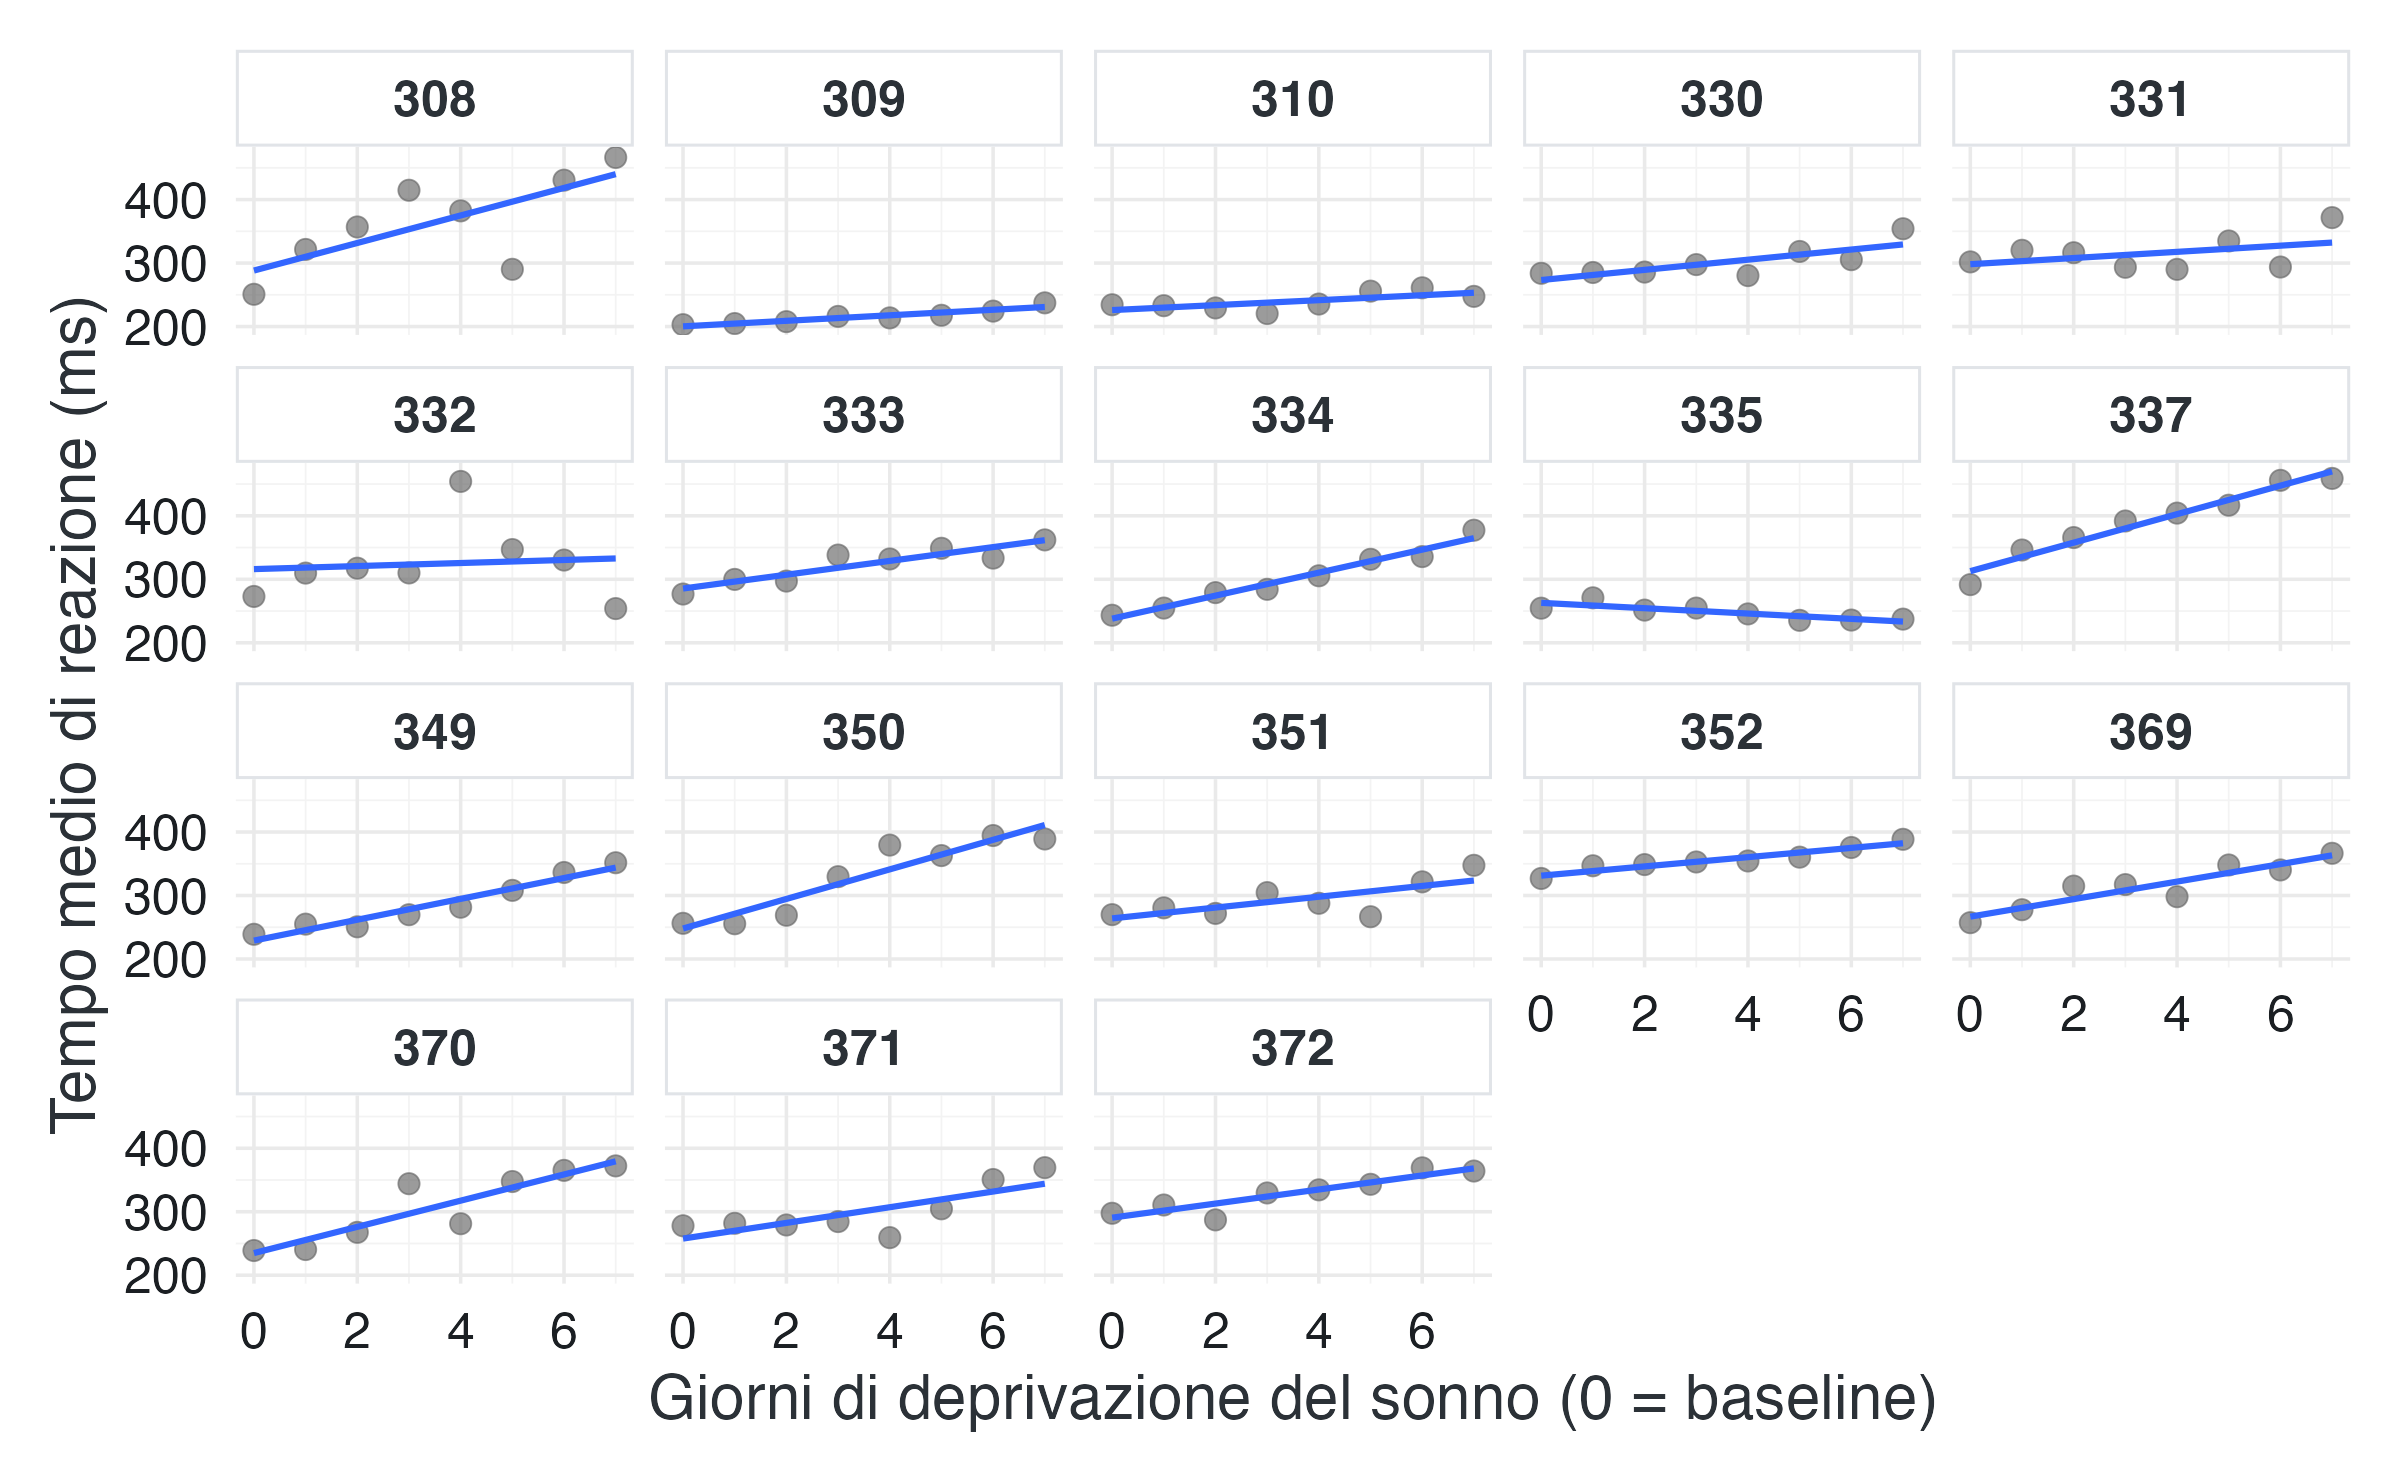
\includegraphics[width=0.85\linewidth,height=\textheight,keepaspectratio]{chapters/linear_models/08_modelli_multilivello_partial_pooling_files/figure-pdf/fig-sleep-trajectories-1.png}

}

\caption{\label{fig-sleep-trajectories}Tempi di reazione osservati nei
diversi giorni di deprivazione. I partecipanti differiscono sia nel
livello iniziale sia nell'andamento temporale.}

\end{figure}%

Il grafico mette in luce almeno tre aspetti rilevanti:

\begin{itemize}
\tightlist
\item
  il tempo di reazione medio alla baseline;
\item
  l'incremento medio giornaliero del tempo di reazione;
\item
  la variabilità tra partecipanti nei livelli iniziali e nelle pendenze.
\end{itemize}

Il secondo aspetto descrive la tendenza media; il terzo stabilisce fino
a che punto tale tendenza sia generalizzabile ai singoli individui. Un
modello multilivello non si limita a stimare una pendenza media, ma la
accompagna con una distribuzione delle deviazioni individuali da essa,
consentendo di rappresentare sia la regolarità media sia l'eterogeneità
tra i soggetti.

\section{Tre strategie di
modellazione}\label{tre-strategie-di-modellazione}

Prima di specificare il modello gerarchico, confrontiamo tre possibili
strategie.

\subsection{Complete pooling}\label{complete-pooling}

Il \textbf{complete pooling} ignora l'identità dei partecipanti e stima
un'unica relazione lineare per l'intero campione:

\[
Y_{ij} \sim \operatorname{Normal}(\alpha + \beta x_{ij}, \sigma),
\] dove \(i\) indica l'osservazione e \(j\) il partecipante. Pur
includendo l'indice \(j\), i parametri rimangono costanti tra i
soggetti: la struttura del modello non sfrutta il raggruppamento.

Per rendere l'intercetta direttamente interpretabile al baseline, si
adotta la parametrizzazione \texttt{0\ +\ Intercept}:

\begin{Shaded}
\begin{Highlighting}[]
\NormalTok{priors\_cp }\OtherTok{\textless{}{-}} \FunctionTok{c}\NormalTok{(}
  \FunctionTok{prior}\NormalTok{(}\FunctionTok{normal}\NormalTok{(}\DecValTok{250}\NormalTok{, }\DecValTok{50}\NormalTok{), }\AttributeTok{class =} \StringTok{"b"}\NormalTok{, }\AttributeTok{coef =} \StringTok{"Intercept"}\NormalTok{),}
  \FunctionTok{prior}\NormalTok{(}\FunctionTok{normal}\NormalTok{(}\DecValTok{10}\NormalTok{, }\DecValTok{10}\NormalTok{), }\AttributeTok{class =} \StringTok{"b"}\NormalTok{, }\AttributeTok{coef =} \StringTok{"days\_deprived"}\NormalTok{),}
  \FunctionTok{prior}\NormalTok{(}\FunctionTok{student\_t}\NormalTok{(}\DecValTok{3}\NormalTok{, }\DecValTok{0}\NormalTok{, }\DecValTok{30}\NormalTok{), }\AttributeTok{class =} \StringTok{"sigma"}\NormalTok{)}
\NormalTok{)}

\NormalTok{cp\_model }\OtherTok{\textless{}{-}} \FunctionTok{brm}\NormalTok{(}
\NormalTok{  Reaction }\SpecialCharTok{\textasciitilde{}} \DecValTok{0} \SpecialCharTok{+}\NormalTok{ Intercept }\SpecialCharTok{+}\NormalTok{ days\_deprived,}
  \AttributeTok{data =}\NormalTok{ sleep2,}
  \AttributeTok{family =} \FunctionTok{gaussian}\NormalTok{(),}
  \AttributeTok{prior =}\NormalTok{ priors\_cp,}
  \AttributeTok{chains =} \DecValTok{4}\NormalTok{,}
  \AttributeTok{iter =} \DecValTok{2000}\NormalTok{,}
  \AttributeTok{warmup =} \DecValTok{1000}\NormalTok{,}
  \AttributeTok{cores =} \DecValTok{4}\NormalTok{,}
  \AttributeTok{seed =} \DecValTok{1234}\NormalTok{,}
  \AttributeTok{backend =} \StringTok{"cmdstanr"}\NormalTok{,}
  \AttributeTok{refresh =} \DecValTok{0}
\NormalTok{)}
\end{Highlighting}
\end{Shaded}

\begin{Shaded}
\begin{Highlighting}[]
\NormalTok{cp\_fixef }\OtherTok{\textless{}{-}} \FunctionTok{fixef}\NormalTok{(cp\_model)}

\NormalTok{sleep2 }\SpecialCharTok{|\textgreater{}}
  \FunctionTok{ggplot}\NormalTok{(}\FunctionTok{aes}\NormalTok{(}\AttributeTok{x =}\NormalTok{ days\_deprived, }\AttributeTok{y =}\NormalTok{ Reaction)) }\SpecialCharTok{+}
  \FunctionTok{geom\_abline}\NormalTok{(}
    \AttributeTok{intercept =}\NormalTok{ cp\_fixef[}\StringTok{"Intercept"}\NormalTok{, }\StringTok{"Estimate"}\NormalTok{],}
    \AttributeTok{slope =}\NormalTok{ cp\_fixef[}\StringTok{"days\_deprived"}\NormalTok{, }\StringTok{"Estimate"}\NormalTok{],}
    \AttributeTok{linewidth =} \FloatTok{0.8}
\NormalTok{  ) }\SpecialCharTok{+}
  \FunctionTok{geom\_point}\NormalTok{(}\AttributeTok{alpha =} \FloatTok{0.6}\NormalTok{) }\SpecialCharTok{+}
  \FunctionTok{facet\_wrap}\NormalTok{(}\SpecialCharTok{\textasciitilde{}}\NormalTok{ Subject) }\SpecialCharTok{+}
  \FunctionTok{labs}\NormalTok{(}
    \AttributeTok{x =} \StringTok{"Giorni di deprivazione del sonno"}\NormalTok{,}
    \AttributeTok{y =} \StringTok{"Tempo di reazione (ms)"}
\NormalTok{  )}
\end{Highlighting}
\end{Shaded}

\begin{figure}[H]

\centering{

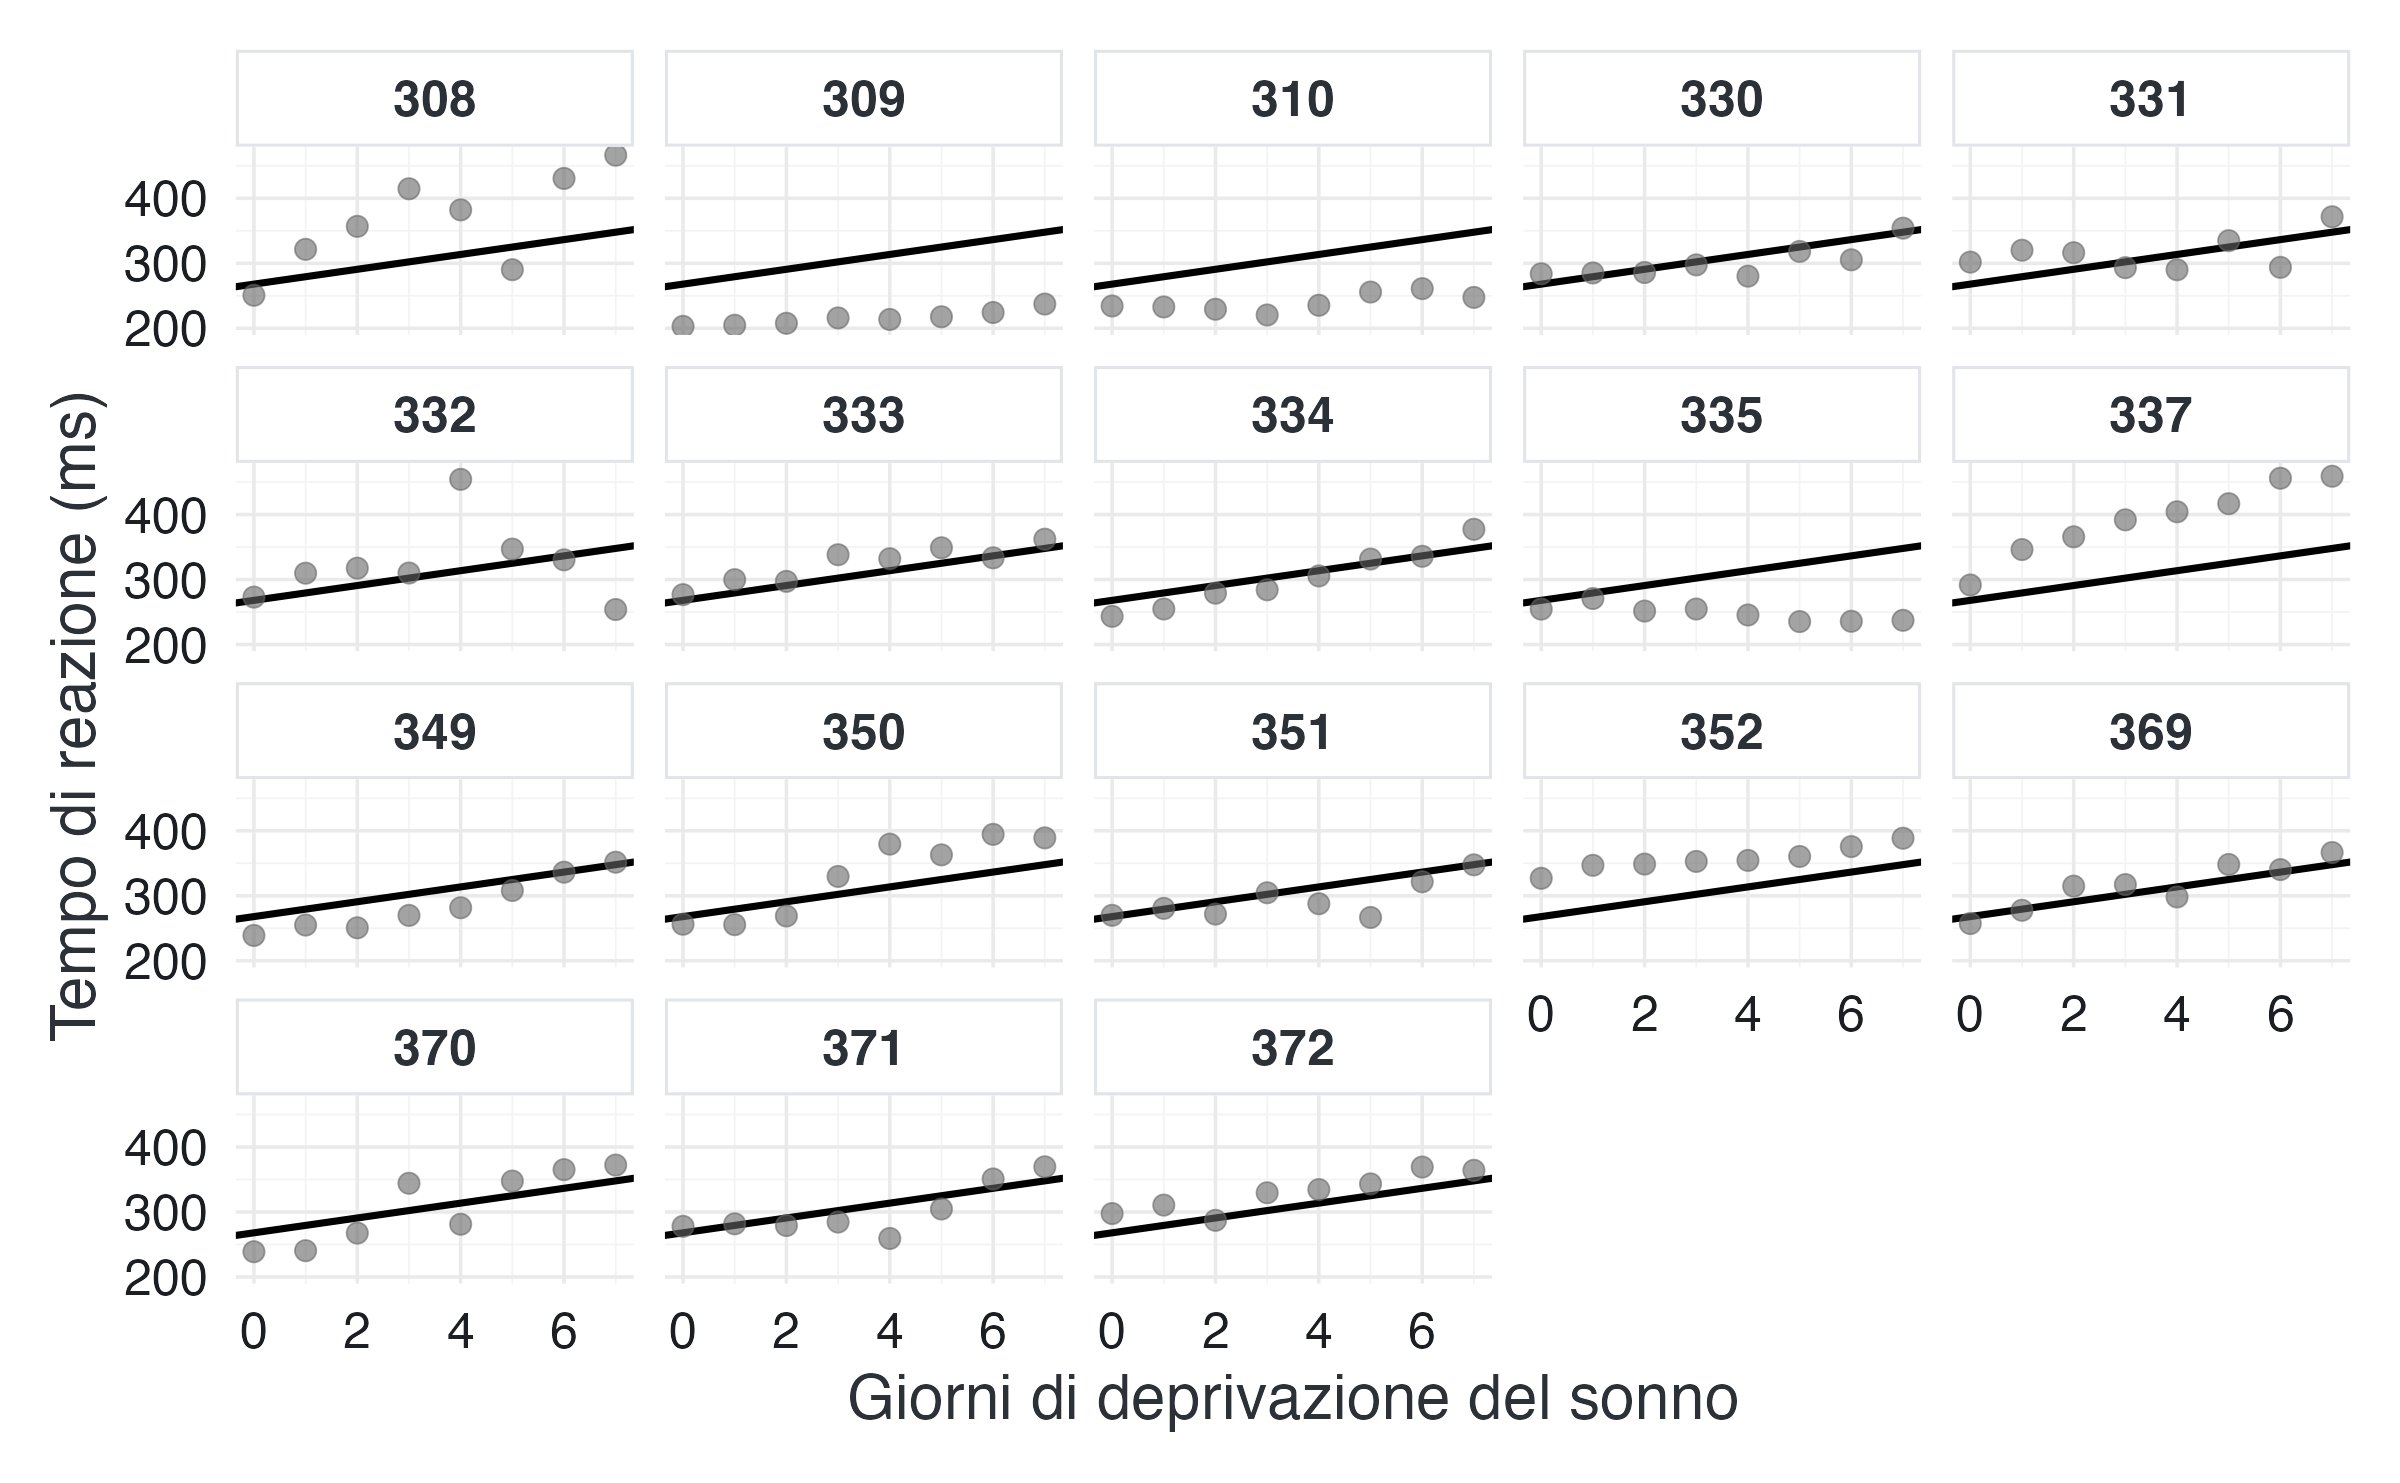
\includegraphics[width=0.85\linewidth,height=\textheight,keepaspectratio]{chapters/linear_models/08_modelli_multilivello_partial_pooling_files/figure-pdf/fig-complete-pooling-1.png}

}

\caption{\label{fig-complete-pooling}Complete pooling: una sola
relazione per tutti i partecipanti.}

\end{figure}%

Il modello sintetizza la tendenza media, ma non tiene conto delle
differenze sistematiche tra partecipanti. Di conseguenza, attribuisce
all'errore residuo tutta la variabilità sistematica che deriva dalla
struttura annidata dei dati. Quando tale variabilità è rilevante,
l'incertezza sui coefficienti può risultare sottostimata e le inferenze
rischiano di essere distorte.

\subsection{No pooling}\label{no-pooling}

All'estremo opposto, il \textbf{no pooling} stima una retta separata per
ciascun partecipante, senza alcuna condivisione di informazioni tra i
gruppi. Per illustrare questa strategia, adattiamo una regressione
lineare indipendente per ogni soggetto:

\begin{Shaded}
\begin{Highlighting}[]
\NormalTok{subject\_coefs }\OtherTok{\textless{}{-}}\NormalTok{ sleep2 }\SpecialCharTok{|\textgreater{}}
  \FunctionTok{group\_split}\NormalTok{(Subject) }\SpecialCharTok{|\textgreater{}}
\NormalTok{  purrr}\SpecialCharTok{::}\FunctionTok{map\_dfr}\NormalTok{(}\SpecialCharTok{\textasciitilde{}}\NormalTok{ \{}
\NormalTok{    fit\_i }\OtherTok{\textless{}{-}} \FunctionTok{lm}\NormalTok{(Reaction }\SpecialCharTok{\textasciitilde{}}\NormalTok{ days\_deprived, }\AttributeTok{data =}\NormalTok{ .x)}

    \FunctionTok{tibble}\NormalTok{(}
      \AttributeTok{Subject =} \FunctionTok{as.character}\NormalTok{(}\FunctionTok{unique}\NormalTok{(.x}\SpecialCharTok{$}\NormalTok{Subject)),}
      \AttributeTok{intercept\_np =} \FunctionTok{unname}\NormalTok{(}\FunctionTok{coef}\NormalTok{(fit\_i)[}\StringTok{"(Intercept)"}\NormalTok{]),}
      \AttributeTok{slope\_np =} \FunctionTok{unname}\NormalTok{(}\FunctionTok{coef}\NormalTok{(fit\_i)[}\StringTok{"days\_deprived"}\NormalTok{]),}
      \AttributeTok{n\_i =} \FunctionTok{nrow}\NormalTok{(.x)}
\NormalTok{    )}
\NormalTok{  \})}

\NormalTok{subject\_coefs}
\CommentTok{\#\textgreater{} \# A tibble: 18 x 4}
\CommentTok{\#\textgreater{}    Subject intercept\_np slope\_np   n\_i}
\CommentTok{\#\textgreater{}    \textless{}chr\textgreater{}          \textless{}dbl\textgreater{}    \textless{}dbl\textgreater{} \textless{}int\textgreater{}}
\CommentTok{\#\textgreater{}  1 308             288.    21.7      8}
\CommentTok{\#\textgreater{}  2 309             200.     4.36     8}
\CommentTok{\#\textgreater{}  3 310             226.     3.90     8}
\CommentTok{\#\textgreater{}  4 330             273.     8.01     8}
\CommentTok{\#\textgreater{}  5 331             298.     4.87     8}
\CommentTok{\#\textgreater{}  6 332             316.     2.40     8}
\CommentTok{\#\textgreater{}  7 333             285.    10.9      8}
\CommentTok{\#\textgreater{}  8 334             238.    18.1      8}
\CommentTok{\#\textgreater{}  9 335             263.    {-}4.21     8}
\CommentTok{\#\textgreater{} 10 337             313.    22.4      8}
\CommentTok{\#\textgreater{} 11 349             229.    16.4      8}
\CommentTok{\#\textgreater{} 12 350             248.    23.3      8}
\CommentTok{\#\textgreater{} 13 351             264.     8.52     8}
\CommentTok{\#\textgreater{} 14 352             331.     7.29     8}
\CommentTok{\#\textgreater{} 15 369             267.    13.8      8}
\CommentTok{\#\textgreater{} 16 370             235.    20.6      8}
\CommentTok{\#\textgreater{} 17 371             258.    12.3      8}
\CommentTok{\#\textgreater{} 18 372             291.    11.1      8}
\end{Highlighting}
\end{Shaded}

Il grafico seguente mostra le rette di regressione stimate in modo
indipendente con il metodo dei minimi quadrati:

\begin{Shaded}
\begin{Highlighting}[]
\NormalTok{sleep2 }\SpecialCharTok{|\textgreater{}}
  \FunctionTok{ggplot}\NormalTok{(}\FunctionTok{aes}\NormalTok{(}\AttributeTok{x =}\NormalTok{ days\_deprived, }\AttributeTok{y =}\NormalTok{ Reaction)) }\SpecialCharTok{+}
  \FunctionTok{geom\_abline}\NormalTok{(}
    \AttributeTok{data =}\NormalTok{ subject\_coefs,}
    \FunctionTok{aes}\NormalTok{(}\AttributeTok{intercept =}\NormalTok{ intercept\_np, }\AttributeTok{slope =}\NormalTok{ slope\_np),}
    \AttributeTok{linewidth =} \FloatTok{0.7}
\NormalTok{  ) }\SpecialCharTok{+}
  \FunctionTok{geom\_point}\NormalTok{(}\AttributeTok{alpha =} \FloatTok{0.6}\NormalTok{) }\SpecialCharTok{+}
  \FunctionTok{facet\_wrap}\NormalTok{(}\SpecialCharTok{\textasciitilde{}}\NormalTok{ Subject) }\SpecialCharTok{+}
  \FunctionTok{labs}\NormalTok{(}
    \AttributeTok{x =} \StringTok{"Giorni di deprivazione del sonno"}\NormalTok{,}
    \AttributeTok{y =} \StringTok{"Tempo di reazione (ms)"}
\NormalTok{  )}
\end{Highlighting}
\end{Shaded}

\begin{figure}[H]

\centering{

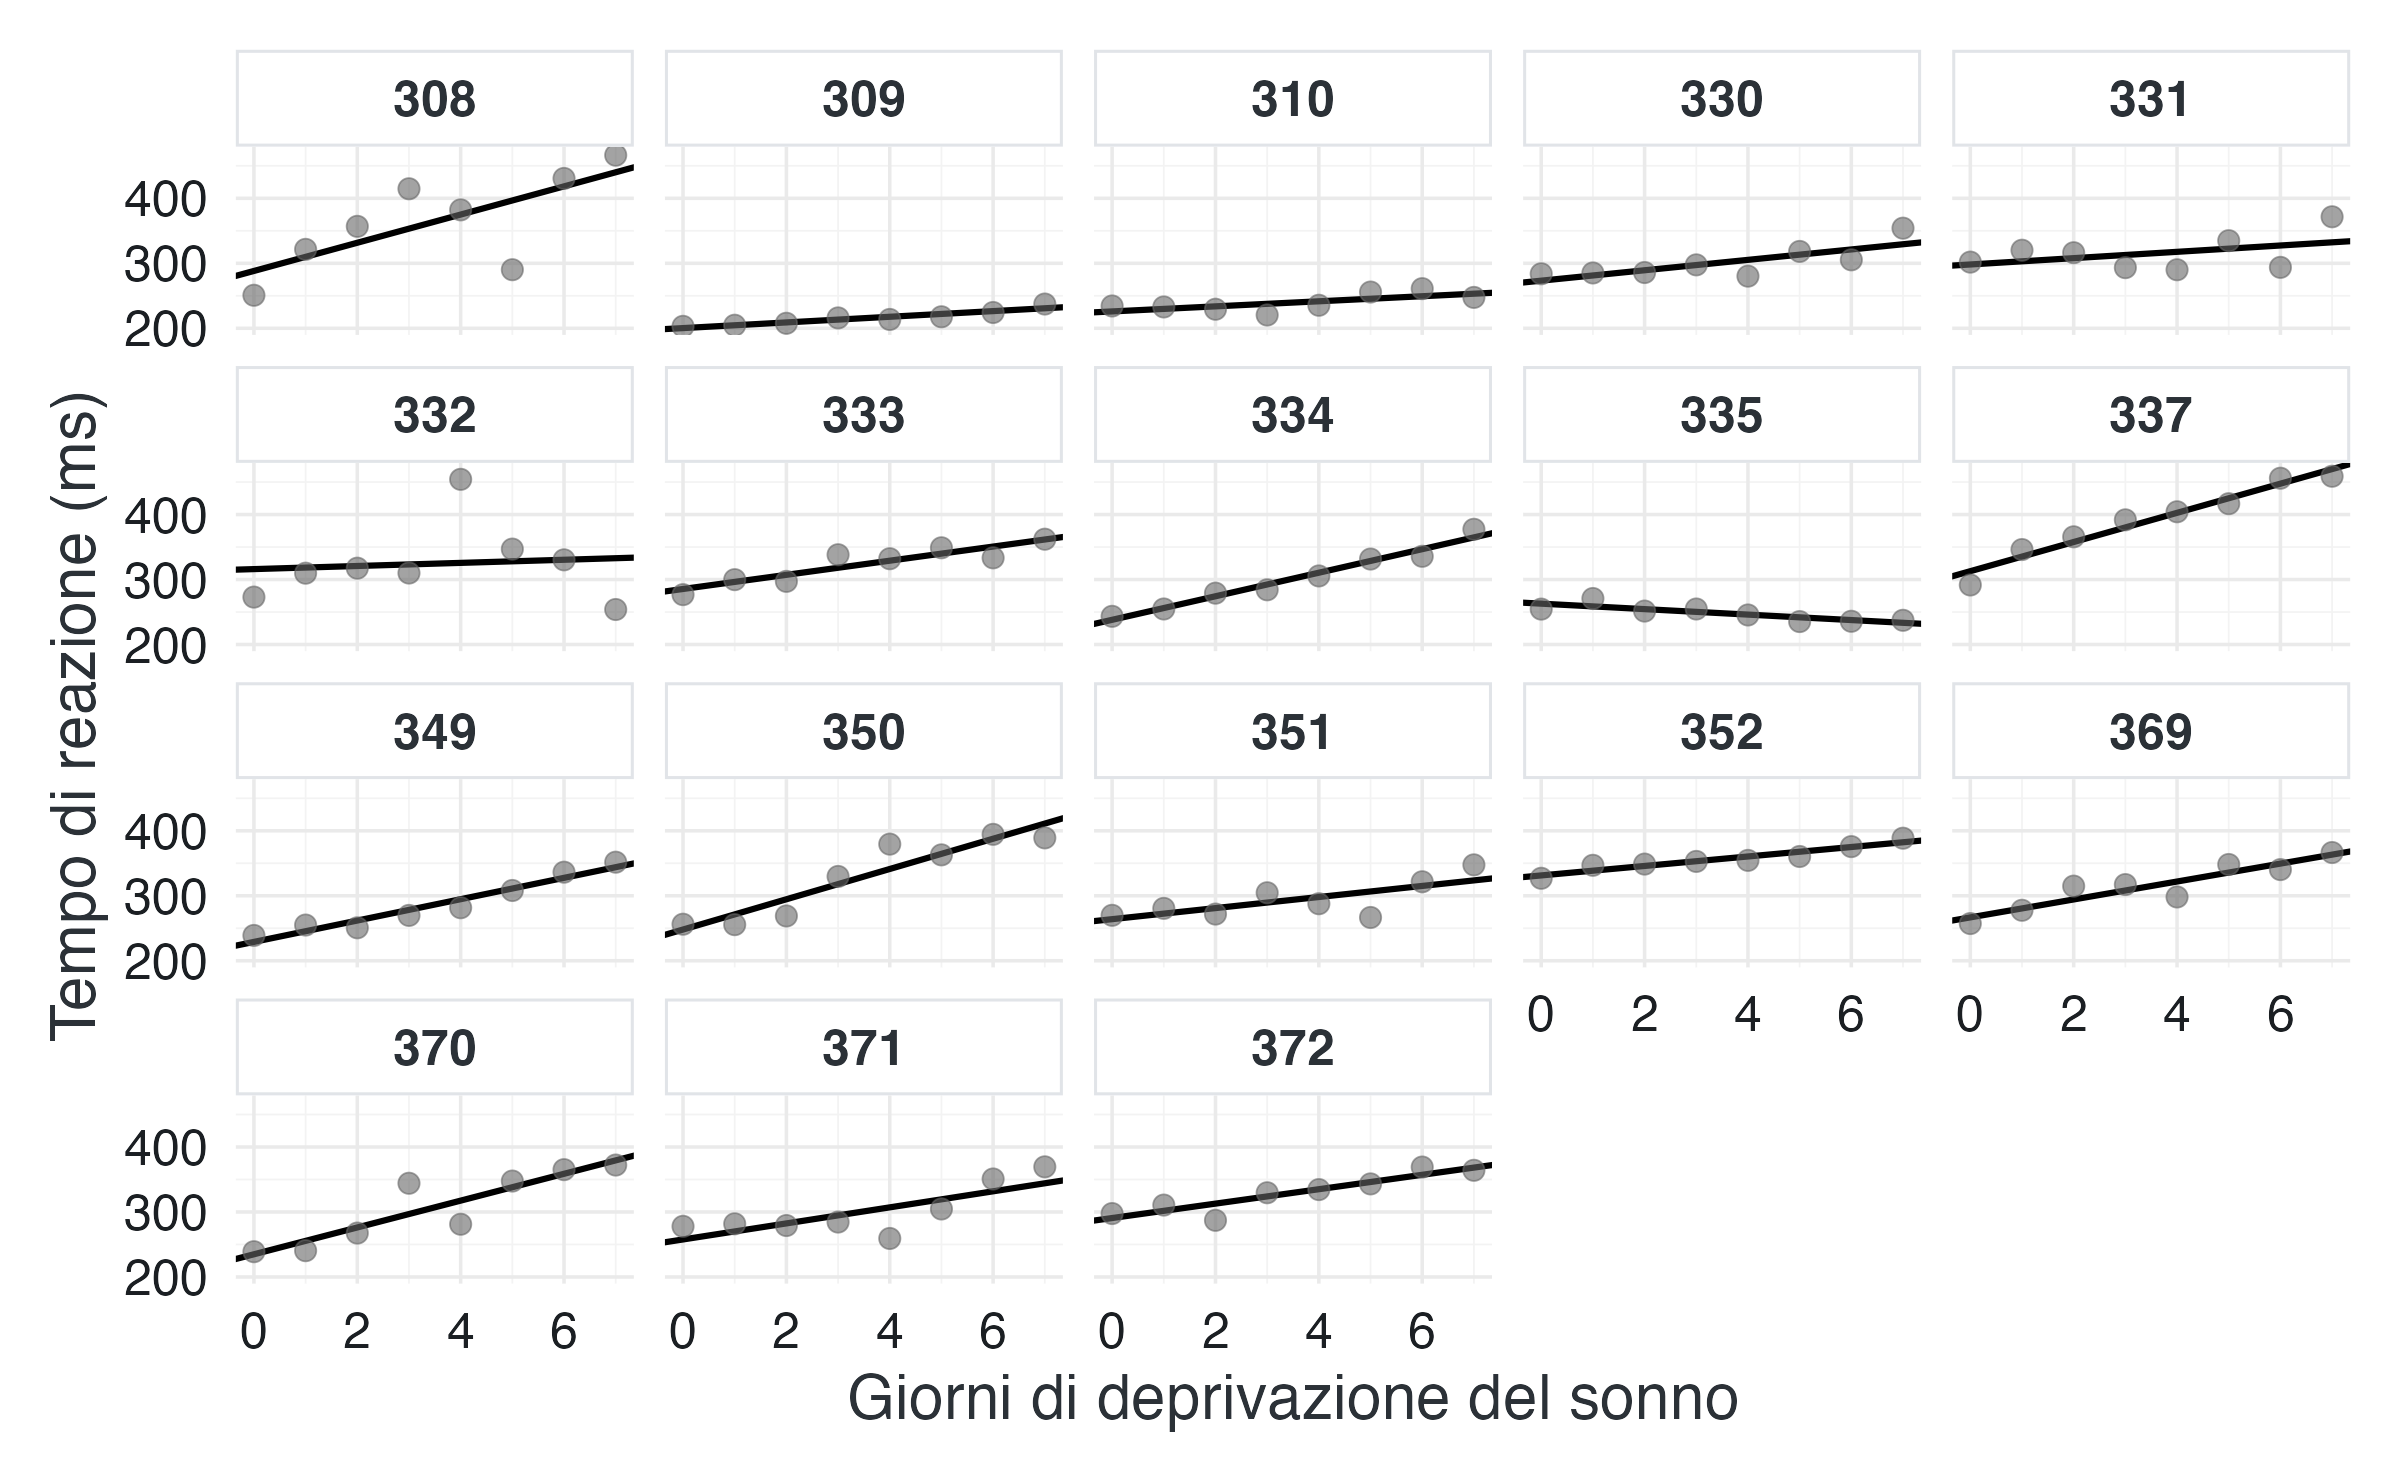
\includegraphics[width=0.85\linewidth,height=\textheight,keepaspectratio]{chapters/linear_models/08_modelli_multilivello_partial_pooling_files/figure-pdf/fig-no-pooling-1.png}

}

\caption{\label{fig-no-pooling}No pooling: ciascun partecipante è
descritto da una regressione stimata indipendentemente dalle altre.}

\end{figure}%

Questo approccio mette in luce le differenze individuali, ma comporta il
rischio di una stima potenzialmente instabile: se un partecipante ha
pochi dati o se le sue osservazioni sono particolarmente rumorose, la
sua retta sarà fortemente influenzata dal rumore campionario. Inoltre,
il modello non sfrutta l'informazione condivisa secondo cui tutti i
soggetti appartengono alla stessa popolazione e potrebbero quindi avere
caratteristiche comuni. Il risultato è un insieme di stime indipendenti
che sacrificano la precisione complessiva in nome della fedeltà a
ciascun caso specifico.

\subsection{Partial pooling}\label{partial-pooling}

Il \textbf{partial pooling} rappresenta una via intermedia: stima le
rette specifiche per ciascun partecipante, ma considera i coefficienti
individuali come estrazioni da una distribuzione comune di popolazione.
In questo modo, i dati di un soggetto informano le stime degli altri e
viceversa, senza che i parametri debbano necessariamente coincidere.

La formula \texttt{brms}

\begin{Shaded}
\begin{Highlighting}[]
\NormalTok{Reaction }\SpecialCharTok{\textasciitilde{}} \DecValTok{0} \SpecialCharTok{+}\NormalTok{ Intercept }\SpecialCharTok{+}\NormalTok{ days\_deprived }\SpecialCharTok{+}
\NormalTok{  (}\DecValTok{1} \SpecialCharTok{+}\NormalTok{ days\_deprived }\SpecialCharTok{|}\NormalTok{ Subject)}
\end{Highlighting}
\end{Shaded}

specifica:

\begin{itemize}
\tightlist
\item
  un'intercetta e una pendenza medie, comuni a tutti i partecipanti;
\item
  una deviazione individuale per l'intercetta di ciascun soggetto;
\item
  una deviazione individuale per la pendenza di ciascun soggetto;
\item
  una correlazione tra le due deviazioni, stimata dai dati.
\end{itemize}

Questa struttura consente al modello di bilanciare l'adattamento ai dati
individuali e la regolarizzazione verso la media del gruppo, migliorando
la stabilità delle stime, soprattutto per i soggetti con poche
osservazioni.

\section{Il modello generativo
multilivello}\label{il-modello-generativo-multilivello}

Sia \(Y_{ij}\) il tempo di reazione dell'osservazione \(i\) del
partecipante \(j\). Il modello può essere scritto come

\begin{equation}\protect\phantomsection\label{eq-multilevel-observation}{
\begin{aligned}
Y_{ij} \mid \mu_{ij}, \sigma
  &\sim \operatorname{Normal}(\mu_{ij}, \sigma), \\
\mu_{ij}
  &= (\alpha + a_j) + (\beta + b_j)x_{ij}.
\end{aligned}
}\end{equation}

I parametri \(\alpha\) e \(\beta\) rappreentano rispettivamente
l'intercetta e la pendenza medie della popolazione. Gli scostamenti
individuali \(a_j\) e \(b_j\) sono modellati come:

\begin{equation}\protect\phantomsection\label{eq-multilevel-group}{
\begin{pmatrix}
a_j \\
b_j
\end{pmatrix}
\sim
\operatorname{MVNormal}
\left[
\begin{pmatrix}
0 \\
0
\end{pmatrix},
\mathbf{\Sigma}
\right].
}\end{equation}

La matrice di covarianza \(\mathbf{\Sigma}\) può essere scomposta come:

\[
\mathbf{\Sigma}
=
\begin{pmatrix}
\tau_\alpha & 0 \\
0 & \tau_\beta
\end{pmatrix}
\begin{pmatrix}
1 & \rho \\
\rho & 1
\end{pmatrix}
\begin{pmatrix}
\tau_\alpha & 0 \\
0 & \tau_\beta
\end{pmatrix}.
\]

I parametri che compaiono in questa scomposizione hanno un ruolo
interpretativo preciso:

\begin{itemize}
\tightlist
\item
  \(\tau_\alpha\) quantifica l'eterogeneità tra le intercette
  individuali;
\item
  \(\tau_\beta\) quantifica l'eterogeneità tra le pendenze individuali;
\item
  \(\rho\) esprime l'associazione tra livello iniziale e tasso di
  cambiamento;
\item
  \(\sigma\) descrive la variabilità residua delle osservazioni attorno
  alla traiettoria individuale.
\end{itemize}

La distribuzione degli effetti casuali costituisce il meccanismo
attraverso cui i partecipanti si scambiano informazione. È questo
livello del modello a generare il \emph{partial pooling} e a rendere le
stime individuali più stabili, specialmente quando i dati per soggetto
sono limitati.

Nel modello multilivello convivono quattro fonti di incertezza,
concettualmente distinte: l'incertezza sulla pendenza media della
popolazione, la variabilità reale delle pendenze tra i soggetti,
l'incertezza sulla pendenza di un particolare partecipante e la
variabilità residua delle singole osservazioni. Una stima precisa della
pendenza media, quindi, non implica che tutti i partecipanti abbiano
pendenze simili; la variabilità interindividuale rimane una quantità
separata, da stimare e interpretare.

\section{Specificare i prior}\label{specificare-i-prior}

I prior devono essere coerenti con la scala dei tempi di reazione e con
la struttura gerarchica del modello. Per l'intercetta media \(\alpha\) e
la pendenza media \(\beta\), utilizziamo distribuzioni normali con
valori attesi e dispersioni ragionevoli:
\(\alpha \sim \operatorname{Normal}(250, 50)\) e
\(\beta \sim \operatorname{Normal}(10, 10)\). Tali scelte riflettono
l'ipotesi che al basale i tempi di reazione si collochino attorno a 250
ms, con un incremento giornaliero di circa 10 ms, senza però vincolare
eccessivamente le stime.

Per le deviazioni standard degli effetti casuali, \(\tau_\alpha\) e
\(\tau_\beta\), adottiamo distribuzioni Student-\(t\) troncate al
semiasse positivo, con parametri di scala calibrati sugli scostamenti
plausibili tra i partecipanti:
\(\tau_\alpha \sim \operatorname{Student\text{-}t}^{+}(3, 0, 50)\) e
\(\tau_\beta \sim \operatorname{Student\text{-}t}^{+}(3, 0, 10)\).
Queste prior sono debolmente informative: concedono ampia libertà ai
dati, ma escludono valori eccessivi o irrealistici.

Per la correlazione \(\rho\) tra intercetta e pendenza individuali,
utilizziamo una prior LKJ con parametro di forma 2, che concentra
moderatamente la massa attorno allo zero senza escludere correlazioni
forti, ma penalizza le correlazioni estreme in assenza di evidenza.

Infine, la deviazione standard residua \(\sigma\) riceve una prior
Student-\(t\) troncata,
\(\sigma \sim \operatorname{Student\text{-}t}^{+}(3, 0, 30)\),
compatibile con la variabilità attesa delle osservazioni attorno alla
traiettoria individuale.

Il codice seguente implementa queste scelte in \texttt{brms}:

\begin{Shaded}
\begin{Highlighting}[]
\NormalTok{priors\_pp }\OtherTok{\textless{}{-}} \FunctionTok{c}\NormalTok{(}
  \FunctionTok{prior}\NormalTok{(}\FunctionTok{normal}\NormalTok{(}\DecValTok{250}\NormalTok{, }\DecValTok{50}\NormalTok{), }\AttributeTok{class =} \StringTok{"b"}\NormalTok{, }\AttributeTok{coef =} \StringTok{"Intercept"}\NormalTok{),}
  \FunctionTok{prior}\NormalTok{(}\FunctionTok{normal}\NormalTok{(}\DecValTok{10}\NormalTok{, }\DecValTok{10}\NormalTok{), }\AttributeTok{class =} \StringTok{"b"}\NormalTok{, }\AttributeTok{coef =} \StringTok{"days\_deprived"}\NormalTok{),}
  \FunctionTok{prior}\NormalTok{(}
    \FunctionTok{student\_t}\NormalTok{(}\DecValTok{3}\NormalTok{, }\DecValTok{0}\NormalTok{, }\DecValTok{50}\NormalTok{),}
    \AttributeTok{class =} \StringTok{"sd"}\NormalTok{,}
    \AttributeTok{group =} \StringTok{"Subject"}\NormalTok{,}
    \AttributeTok{coef =} \StringTok{"Intercept"}
\NormalTok{  ),}
  \FunctionTok{prior}\NormalTok{(}
    \FunctionTok{student\_t}\NormalTok{(}\DecValTok{3}\NormalTok{, }\DecValTok{0}\NormalTok{, }\DecValTok{10}\NormalTok{),}
    \AttributeTok{class =} \StringTok{"sd"}\NormalTok{,}
    \AttributeTok{group =} \StringTok{"Subject"}\NormalTok{,}
    \AttributeTok{coef =} \StringTok{"days\_deprived"}
\NormalTok{  ),}
  \FunctionTok{prior}\NormalTok{(}\FunctionTok{lkj}\NormalTok{(}\DecValTok{2}\NormalTok{), }\AttributeTok{class =} \StringTok{"cor"}\NormalTok{, }\AttributeTok{group =} \StringTok{"Subject"}\NormalTok{),}
  \FunctionTok{prior}\NormalTok{(}\FunctionTok{student\_t}\NormalTok{(}\DecValTok{3}\NormalTok{, }\DecValTok{0}\NormalTok{, }\DecValTok{30}\NormalTok{), }\AttributeTok{class =} \StringTok{"sigma"}\NormalTok{)}
\NormalTok{)}
\end{Highlighting}
\end{Shaded}

Per verificare la corrispondenza tra i prior specificati e i parametri
effettivi del modello, si può usare \texttt{get\_prior()}, che
restituisce l'elenco completo dei prior attesi:

\begin{Shaded}
\begin{Highlighting}[]
\FunctionTok{get\_prior}\NormalTok{(}
\NormalTok{  Reaction }\SpecialCharTok{\textasciitilde{}} \DecValTok{0} \SpecialCharTok{+}\NormalTok{ Intercept }\SpecialCharTok{+}\NormalTok{ days\_deprived }\SpecialCharTok{+}
\NormalTok{    (}\DecValTok{1} \SpecialCharTok{+}\NormalTok{ days\_deprived }\SpecialCharTok{|}\NormalTok{ Subject),}
  \AttributeTok{data =}\NormalTok{ sleep2,}
  \AttributeTok{family =} \FunctionTok{gaussian}\NormalTok{()}
\NormalTok{)}
\CommentTok{\#\textgreater{}                  prior class          coef   group resp dpar nlpar lb ub tag}
\CommentTok{\#\textgreater{}                 (flat)     b                                                }
\CommentTok{\#\textgreater{}                 (flat)     b days\_deprived                                  }
\CommentTok{\#\textgreater{}                 (flat)     b     Intercept                                  }
\CommentTok{\#\textgreater{}                 lkj(1)   cor                                                }
\CommentTok{\#\textgreater{}                 lkj(1)   cor               Subject                          }
\CommentTok{\#\textgreater{}  student\_t(3, 0, 65.5)    sd                                        0       }
\CommentTok{\#\textgreater{}  student\_t(3, 0, 65.5)    sd               Subject                  0       }
\CommentTok{\#\textgreater{}  student\_t(3, 0, 65.5)    sd days\_deprived Subject                  0       }
\CommentTok{\#\textgreater{}  student\_t(3, 0, 65.5)    sd     Intercept Subject                  0       }
\CommentTok{\#\textgreater{}  student\_t(3, 0, 65.5) sigma                                        0       }
\CommentTok{\#\textgreater{}        source}
\CommentTok{\#\textgreater{}       default}
\CommentTok{\#\textgreater{}  (vectorized)}
\CommentTok{\#\textgreater{}  (vectorized)}
\CommentTok{\#\textgreater{}       default}
\CommentTok{\#\textgreater{}  (vectorized)}
\CommentTok{\#\textgreater{}       default}
\CommentTok{\#\textgreater{}  (vectorized)}
\CommentTok{\#\textgreater{}  (vectorized)}
\CommentTok{\#\textgreater{}  (vectorized)}
\CommentTok{\#\textgreater{}       default}
\end{Highlighting}
\end{Shaded}

\subsection{Controllo predittivo a
priori}\label{controllo-predittivo-a-priori-2}

Il controllo predittivo a priori consente di verificare se la
combinazione delle distribuzioni a priori sia in grado di generare
traiettorie compatibili con il fenomeno studiato, prima ancora di
condizionare il modello ai dati osservati.

\begin{Shaded}
\begin{Highlighting}[]
\NormalTok{pp\_prior\_model }\OtherTok{\textless{}{-}} \FunctionTok{brm}\NormalTok{(}
\NormalTok{  Reaction }\SpecialCharTok{\textasciitilde{}} \DecValTok{0} \SpecialCharTok{+}\NormalTok{ Intercept }\SpecialCharTok{+}\NormalTok{ days\_deprived }\SpecialCharTok{+}
\NormalTok{    (}\DecValTok{1} \SpecialCharTok{+}\NormalTok{ days\_deprived }\SpecialCharTok{|}\NormalTok{ Subject),}
  \AttributeTok{data =}\NormalTok{ sleep2,}
  \AttributeTok{family =} \FunctionTok{gaussian}\NormalTok{(),}
  \AttributeTok{prior =}\NormalTok{ priors\_pp,}
  \AttributeTok{sample\_prior =} \StringTok{"only"}\NormalTok{,}
  \AttributeTok{chains =} \DecValTok{4}\NormalTok{,}
  \AttributeTok{iter =} \DecValTok{1000}\NormalTok{,}
  \AttributeTok{warmup =} \DecValTok{500}\NormalTok{,}
  \AttributeTok{cores =} \DecValTok{4}\NormalTok{,}
  \AttributeTok{seed =} \DecValTok{1234}\NormalTok{,}
  \AttributeTok{backend =} \StringTok{"cmdstanr"}\NormalTok{,}
  \AttributeTok{refresh =} \DecValTok{0}
\NormalTok{)}
\end{Highlighting}
\end{Shaded}

Per non sovraccaricare la visualizzazione, consiamo quattro partecipanti
e un sottoinsieme delle traiettorie simulate:

\begin{Shaded}
\begin{Highlighting}[]
\NormalTok{subjects\_demo }\OtherTok{\textless{}{-}} \FunctionTok{levels}\NormalTok{(sleep2}\SpecialCharTok{$}\NormalTok{Subject)[}\DecValTok{1}\SpecialCharTok{:}\DecValTok{4}\NormalTok{]}

\NormalTok{prior\_grid }\OtherTok{\textless{}{-}}\NormalTok{ tidyr}\SpecialCharTok{::}\FunctionTok{crossing}\NormalTok{(}
  \AttributeTok{Subject =} \FunctionTok{factor}\NormalTok{(subjects\_demo, }\AttributeTok{levels =} \FunctionTok{levels}\NormalTok{(sleep2}\SpecialCharTok{$}\NormalTok{Subject)),}
  \AttributeTok{days\_deprived =} \FunctionTok{sort}\NormalTok{(}\FunctionTok{unique}\NormalTok{(sleep2}\SpecialCharTok{$}\NormalTok{days\_deprived))}
\NormalTok{)}

\NormalTok{prior\_mu }\OtherTok{\textless{}{-}} \FunctionTok{posterior\_epred}\NormalTok{(}
\NormalTok{  pp\_prior\_model,}
  \AttributeTok{newdata =}\NormalTok{ prior\_grid,}
  \AttributeTok{re\_formula =} \ConstantTok{NULL}\NormalTok{,}
  \AttributeTok{ndraws =} \DecValTok{40}
\NormalTok{)}

\NormalTok{prior\_lines }\OtherTok{\textless{}{-}} \FunctionTok{as.data.frame}\NormalTok{(prior\_mu) }\SpecialCharTok{|\textgreater{}}
  \FunctionTok{mutate}\NormalTok{(}\AttributeTok{.draw =} \FunctionTok{row\_number}\NormalTok{()) }\SpecialCharTok{|\textgreater{}}
  \FunctionTok{pivot\_longer}\NormalTok{(}
    \AttributeTok{cols =} \SpecialCharTok{{-}}\NormalTok{.draw,}
    \AttributeTok{names\_to =} \StringTok{".observation"}\NormalTok{,}
    \AttributeTok{values\_to =} \StringTok{"Reaction"}
\NormalTok{  ) }\SpecialCharTok{|\textgreater{}}
  \FunctionTok{mutate}\NormalTok{(}
    \AttributeTok{.observation =} \FunctionTok{as.integer}\NormalTok{(}\FunctionTok{sub}\NormalTok{(}\StringTok{"V"}\NormalTok{, }\StringTok{""}\NormalTok{, .observation))}
\NormalTok{  ) }\SpecialCharTok{|\textgreater{}}
  \FunctionTok{left\_join}\NormalTok{(}
\NormalTok{    prior\_grid }\SpecialCharTok{|\textgreater{}}
      \FunctionTok{mutate}\NormalTok{(}\AttributeTok{.observation =} \FunctionTok{row\_number}\NormalTok{()),}
    \AttributeTok{by =} \StringTok{".observation"}
\NormalTok{  )}

\NormalTok{prior\_lines }\SpecialCharTok{|\textgreater{}}
  \FunctionTok{ggplot}\NormalTok{(}\FunctionTok{aes}\NormalTok{(}
    \AttributeTok{x =}\NormalTok{ days\_deprived,}
    \AttributeTok{y =}\NormalTok{ Reaction,}
    \AttributeTok{group =} \FunctionTok{interaction}\NormalTok{(.draw, Subject)}
\NormalTok{  )) }\SpecialCharTok{+}
  \FunctionTok{geom\_line}\NormalTok{(}\AttributeTok{alpha =} \FloatTok{0.18}\NormalTok{) }\SpecialCharTok{+}
  \FunctionTok{facet\_wrap}\NormalTok{(}\SpecialCharTok{\textasciitilde{}}\NormalTok{ Subject) }\SpecialCharTok{+}
  \FunctionTok{labs}\NormalTok{(}
    \AttributeTok{x =} \StringTok{"Giorni di deprivazione del sonno"}\NormalTok{,}
    \AttributeTok{y =} \StringTok{"Tempo di reazione generato a priori (ms)"}
\NormalTok{  )}
\end{Highlighting}
\end{Shaded}

\begin{figure}[H]

\centering{

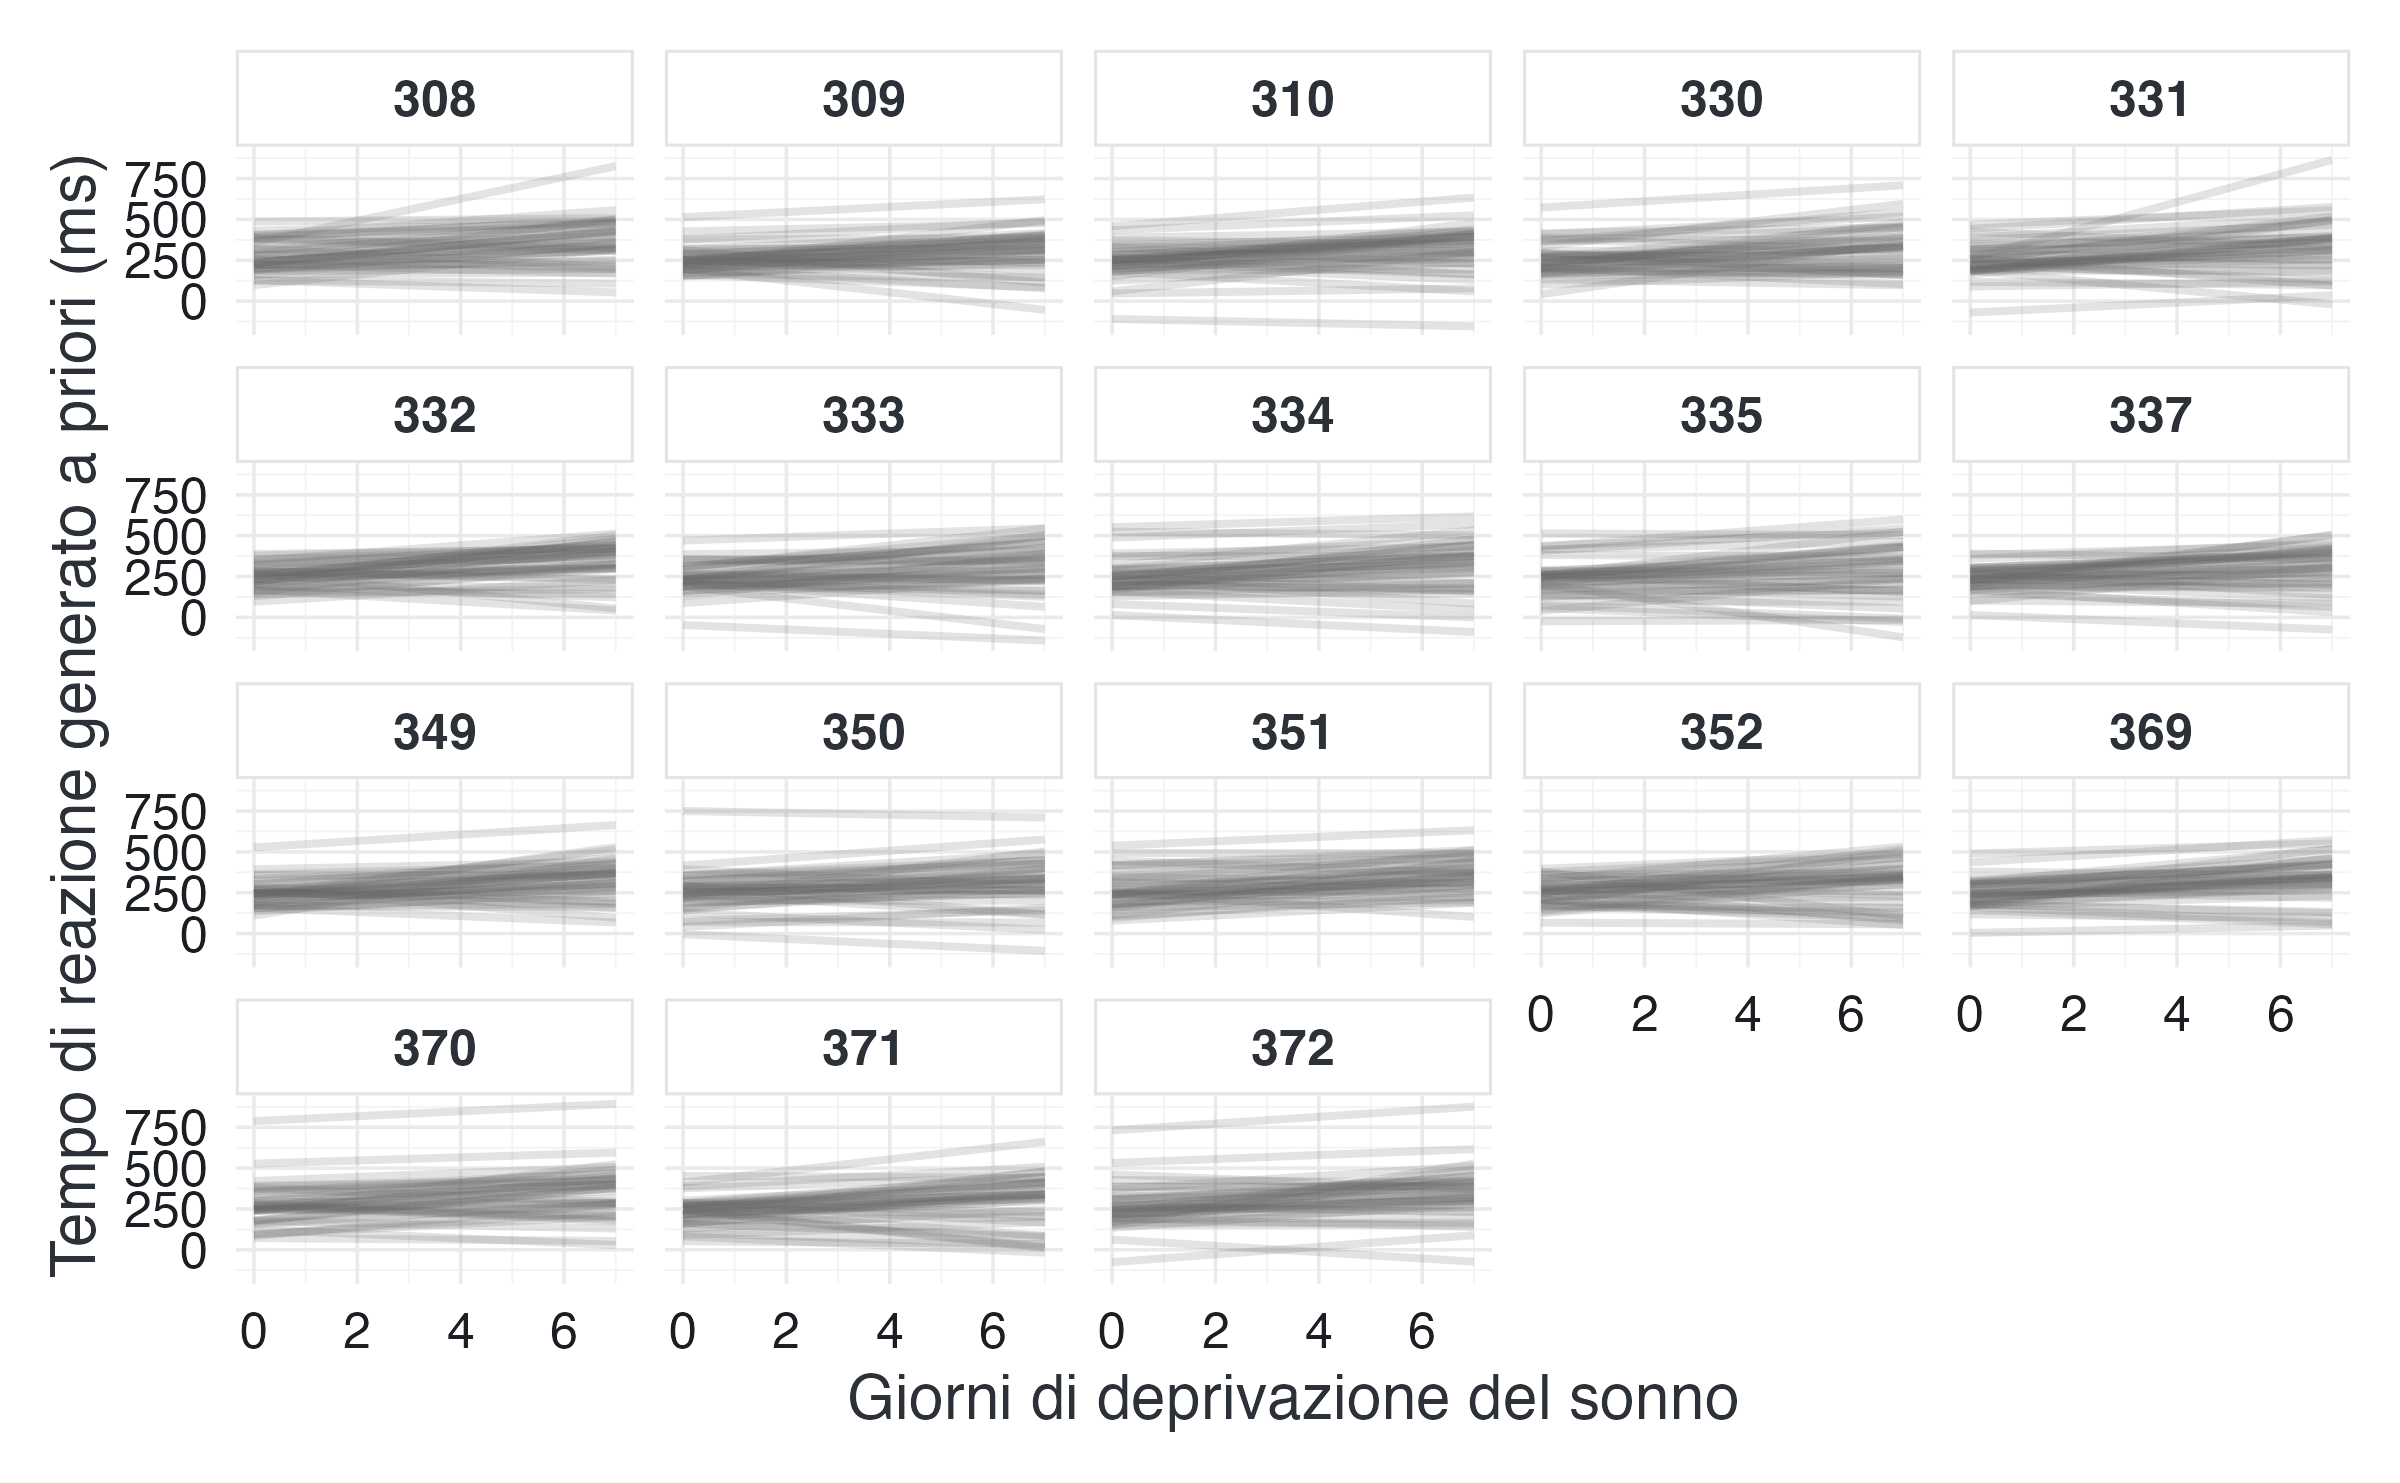
\includegraphics[width=0.85\linewidth,height=\textheight,keepaspectratio]{chapters/linear_models/08_modelli_multilivello_partial_pooling_files/figure-pdf/fig-prior-trajectories-multilevel-1.png}

}

\caption{\label{fig-prior-trajectories-multilevel}Traiettorie
individuali generate dalla distribuzione predittiva a priori per quattro
partecipanti. Il controllo serve a verificare la plausibilità congiunta
dei livelli iniziali, delle pendenze e dell'eterogeneità.}

\end{figure}%

La valutazione del controllo va condotta sulla scala sostantiva: le
traiettorie generate devono mostrare una variabilità realistica, senza
assegnare massa eccessiva a tempi di reazione fisiologicamente
implausibili o a pendenze giornaliere incompatibili con la letteratura
sul fenomeno.

\section{\texorpdfstring{Adattare il modello di \emph{partial
pooling}}{Adattare il modello di partial pooling}}\label{adattare-il-modello-di-partial-pooling}

Dopo aver verificato la plausibilità delle distribuzioni a priori, si
procede all'adattamento del modello di \emph{partial pooling} sui dati
osservati:

\begin{Shaded}
\begin{Highlighting}[]
\NormalTok{pp\_model }\OtherTok{\textless{}{-}} \FunctionTok{brm}\NormalTok{(}
\NormalTok{  Reaction }\SpecialCharTok{\textasciitilde{}} \DecValTok{0} \SpecialCharTok{+}\NormalTok{ Intercept }\SpecialCharTok{+}\NormalTok{ days\_deprived }\SpecialCharTok{+}
\NormalTok{    (}\DecValTok{1} \SpecialCharTok{+}\NormalTok{ days\_deprived }\SpecialCharTok{|}\NormalTok{ Subject),}
  \AttributeTok{data =}\NormalTok{ sleep2,}
  \AttributeTok{family =} \FunctionTok{gaussian}\NormalTok{(),}
  \AttributeTok{prior =}\NormalTok{ priors\_pp,}
  \AttributeTok{chains =} \DecValTok{4}\NormalTok{,}
  \AttributeTok{iter =} \DecValTok{3000}\NormalTok{,}
  \AttributeTok{warmup =} \DecValTok{1500}\NormalTok{,}
  \AttributeTok{cores =} \DecValTok{4}\NormalTok{,}
  \AttributeTok{seed =} \DecValTok{1234}\NormalTok{,}
  \AttributeTok{backend =} \StringTok{"cmdstanr"}\NormalTok{,}
  \AttributeTok{control =} \FunctionTok{list}\NormalTok{(}\AttributeTok{adapt\_delta =} \FloatTok{0.95}\NormalTok{),}
  \AttributeTok{refresh =} \DecValTok{0}
\NormalTok{)}
\end{Highlighting}
\end{Shaded}

\subsection{Diagnostica
computazionale}\label{diagnostica-computazionale}

Prima di interpretare i risultati, è necessario verificare che il
campionamento abbia esplorato in modo affidabile la distribuzione a
posteriori. Il sommario del modello e i \emph{trace plot} consentono di
valutare la convergenza:

\begin{Shaded}
\begin{Highlighting}[]
\FunctionTok{summary}\NormalTok{(pp\_model)}
\CommentTok{\#\textgreater{}  Family: gaussian }
\CommentTok{\#\textgreater{}   Links: mu = identity }
\CommentTok{\#\textgreater{} Formula: Reaction \textasciitilde{} 0 + Intercept + days\_deprived + (1 + days\_deprived | Subject) }
\CommentTok{\#\textgreater{}    Data: sleep2 (Number of observations: 144) }
\CommentTok{\#\textgreater{}   Draws: 4 chains, each with iter = 3000; warmup = 1500; thin = 1;}
\CommentTok{\#\textgreater{}          total post{-}warmup draws = 6000}
\CommentTok{\#\textgreater{} }
\CommentTok{\#\textgreater{} Multilevel Hyperparameters:}
\CommentTok{\#\textgreater{} \textasciitilde{}Subject (Number of levels: 18) }
\CommentTok{\#\textgreater{}                              Estimate Est.Error l{-}95\% CI u{-}95\% CI Rhat Bulk\_ESS}
\CommentTok{\#\textgreater{} sd(Intercept)                   33.32      7.73    20.71    50.96 1.00     3087}
\CommentTok{\#\textgreater{} sd(days\_deprived)                7.18      1.71     4.38    10.93 1.00     3138}
\CommentTok{\#\textgreater{} cor(Intercept,days\_deprived)     0.16      0.27    {-}0.37     0.69 1.00     2811}
\CommentTok{\#\textgreater{}                              Tail\_ESS}
\CommentTok{\#\textgreater{} sd(Intercept)                    3897}
\CommentTok{\#\textgreater{} sd(days\_deprived)                4185}
\CommentTok{\#\textgreater{} cor(Intercept,days\_deprived)     3752}
\CommentTok{\#\textgreater{} }
\CommentTok{\#\textgreater{} Regression Coefficients:}
\CommentTok{\#\textgreater{}               Estimate Est.Error l{-}95\% CI u{-}95\% CI Rhat Bulk\_ESS Tail\_ESS}
\CommentTok{\#\textgreater{} Intercept       267.56      8.83   249.91   284.79 1.00     3194     3783}
\CommentTok{\#\textgreater{} days\_deprived    11.38      1.93     7.56    15.16 1.00     4713     4137}
\CommentTok{\#\textgreater{} }
\CommentTok{\#\textgreater{} Further Distributional Parameters:}
\CommentTok{\#\textgreater{}       Estimate Est.Error l{-}95\% CI u{-}95\% CI Rhat Bulk\_ESS Tail\_ESS}
\CommentTok{\#\textgreater{} sigma    25.89      1.80    22.60    29.77 1.00     4704     4490}
\CommentTok{\#\textgreater{} }
\CommentTok{\#\textgreater{} Draws were sampled using sample(hmc). For each parameter, Bulk\_ESS}
\CommentTok{\#\textgreater{} and Tail\_ESS are effective sample size measures, and Rhat is the potential}
\CommentTok{\#\textgreater{} scale reduction factor on split chains (at convergence, Rhat = 1).}
\end{Highlighting}
\end{Shaded}

\begin{Shaded}
\begin{Highlighting}[]
\FunctionTok{plot}\NormalTok{(pp\_model)}
\end{Highlighting}
\end{Shaded}

\begin{center}
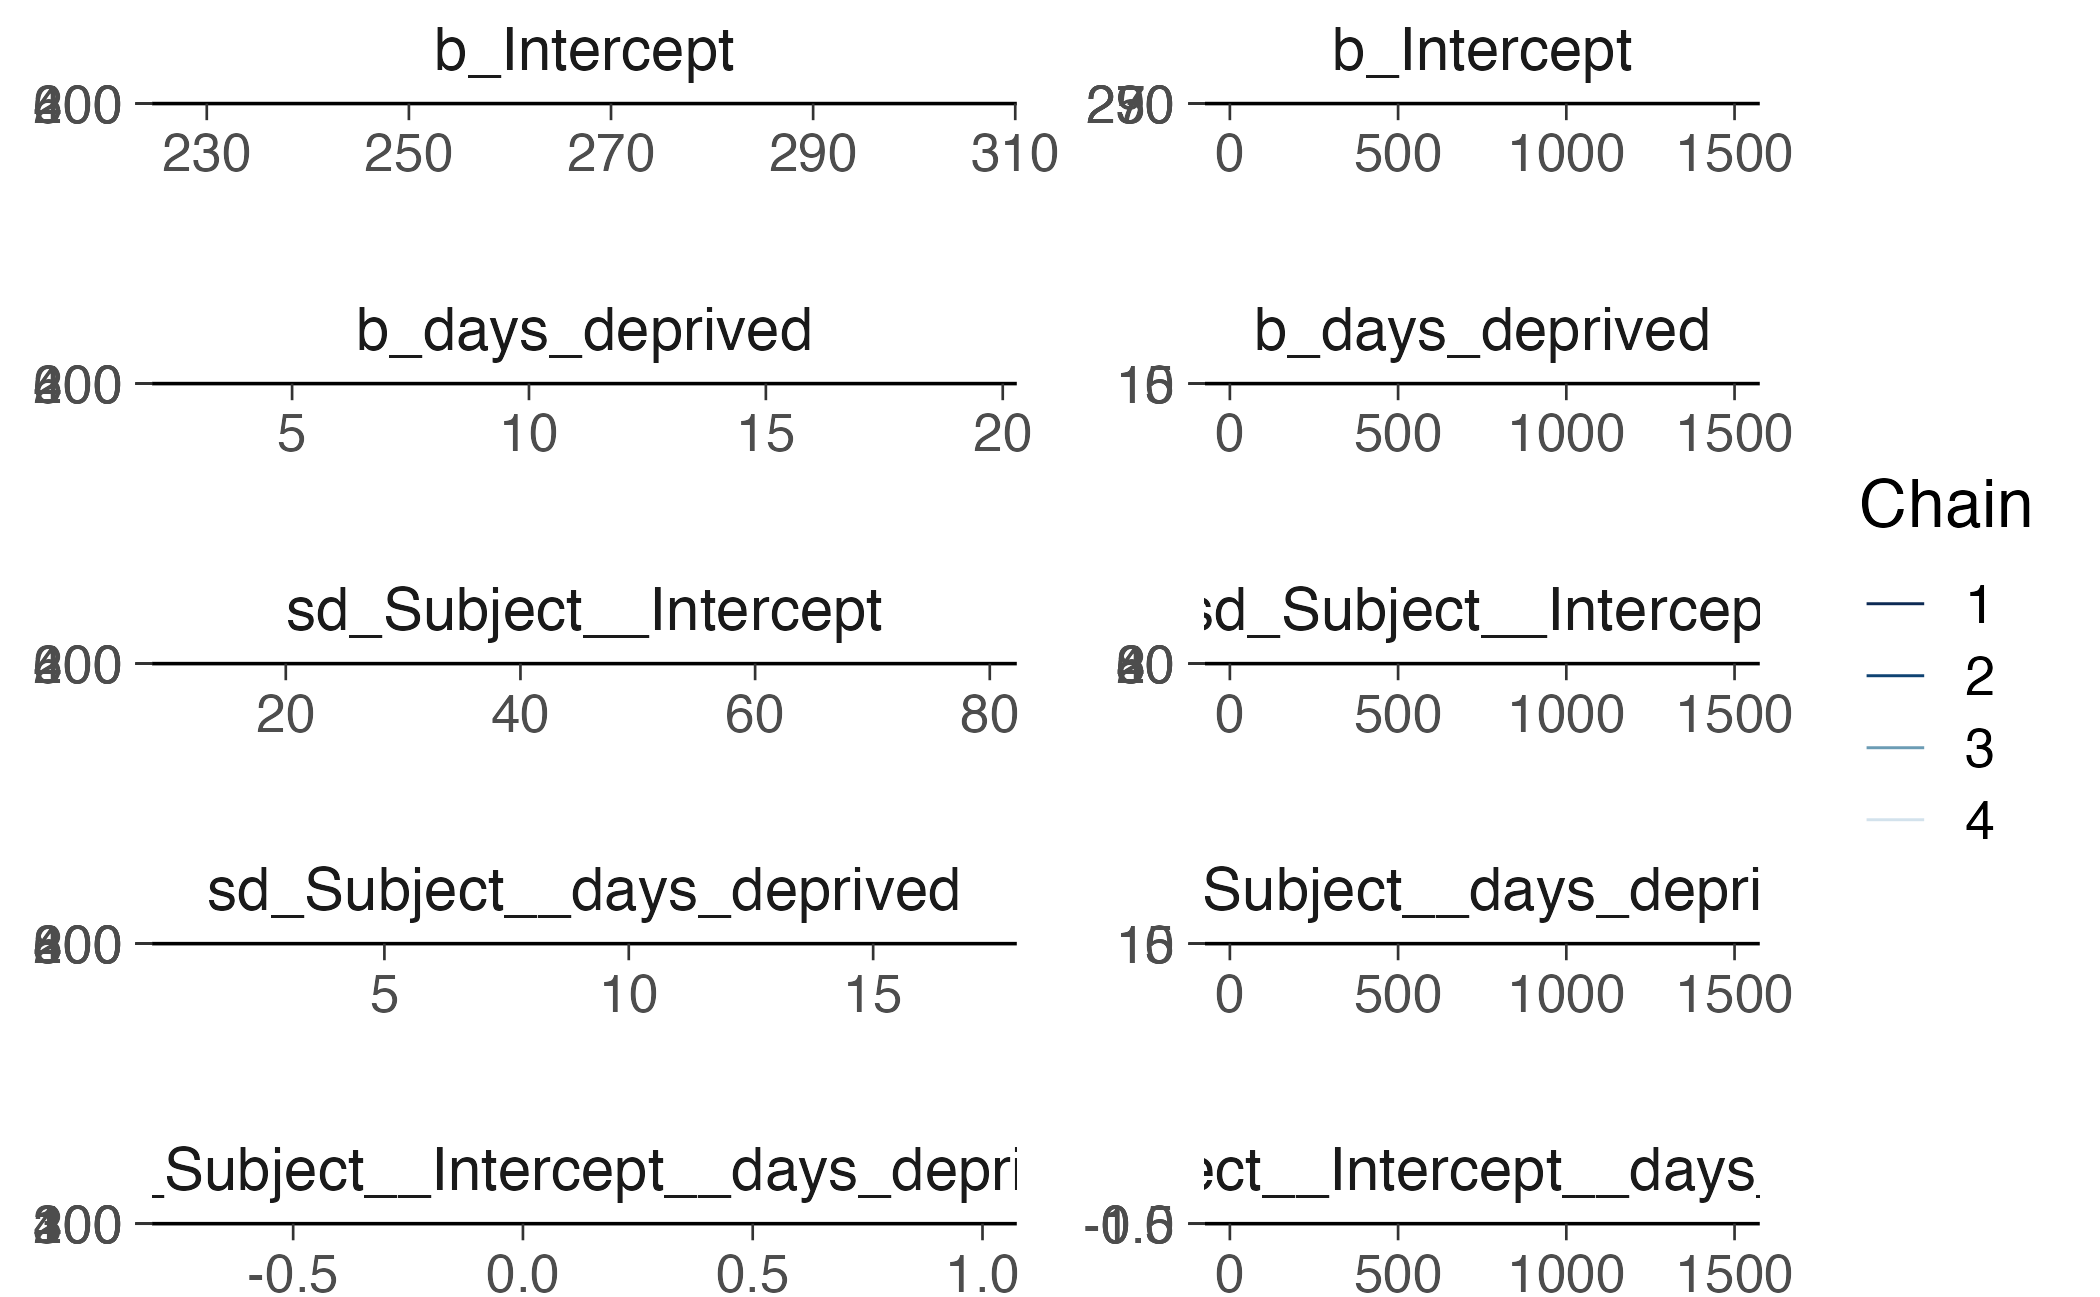
\includegraphics[width=0.85\linewidth,height=\textheight,keepaspectratio]{chapters/linear_models/08_modelli_multilivello_partial_pooling_files/figure-pdf/plots-mcmc-partial-pooling-1.png}
\end{center}

\begin{center}
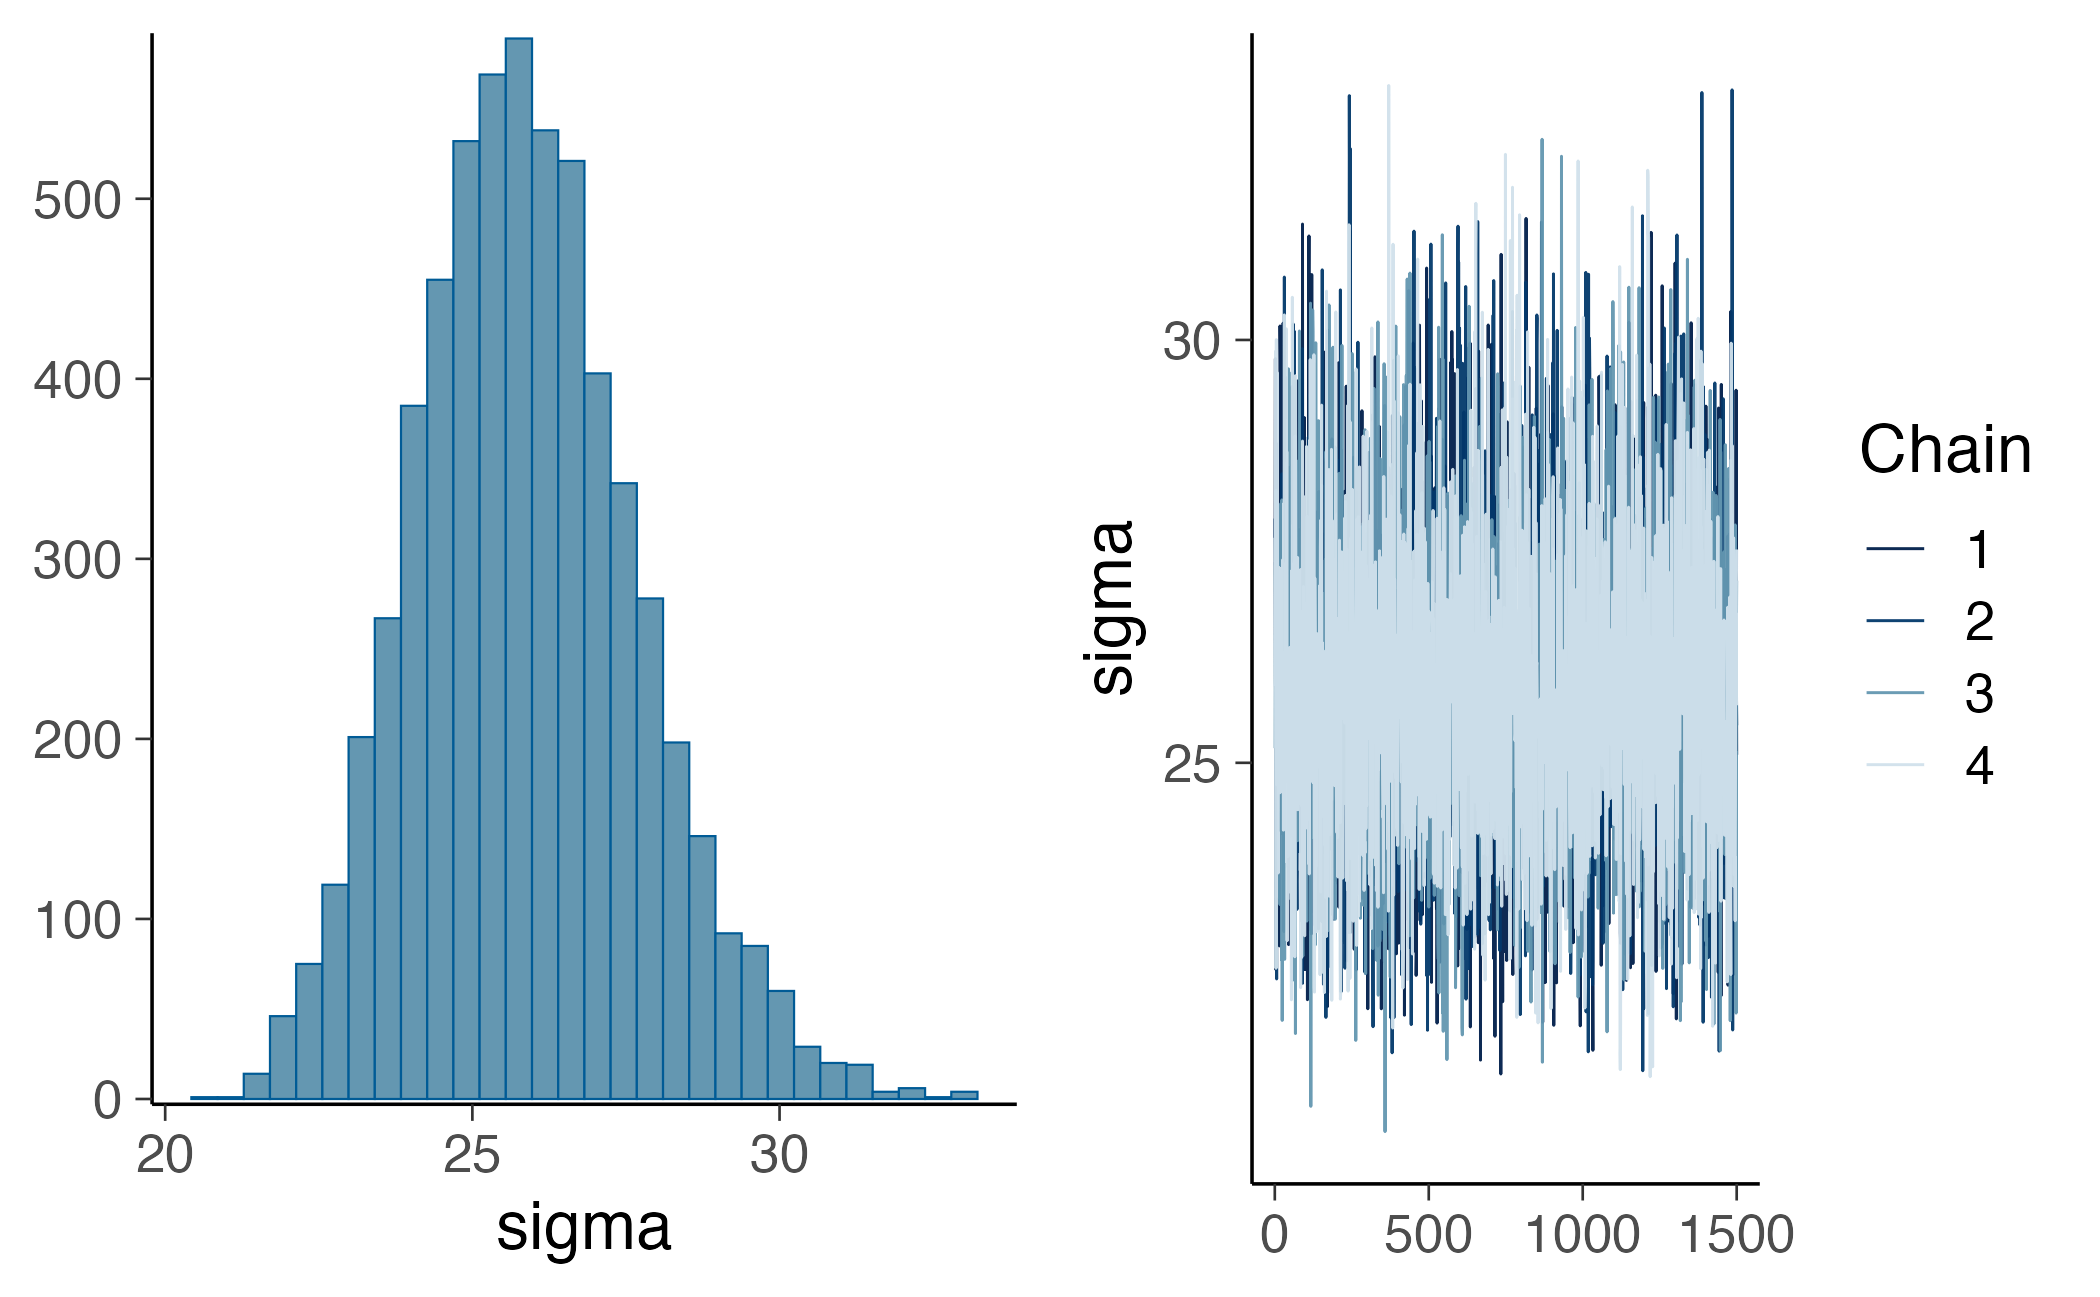
\includegraphics[width=0.85\linewidth,height=\textheight,keepaspectratio]{chapters/linear_models/08_modelli_multilivello_partial_pooling_files/figure-pdf/plots-mcmc-partial-pooling-2.png}
\end{center}

Un indicatore sintetico di particolare rilevanza è il numero di
transizioni divergenti, che segnalano potenziali difficoltà
nell'esplorazione della geometria della posterior:

\begin{Shaded}
\begin{Highlighting}[]
\NormalTok{nuts }\OtherTok{\textless{}{-}} \FunctionTok{nuts\_params}\NormalTok{(pp\_model)}

\NormalTok{nuts }\SpecialCharTok{|\textgreater{}}
  \FunctionTok{filter}\NormalTok{(Parameter }\SpecialCharTok{==} \StringTok{"divergent\_\_"}\NormalTok{) }\SpecialCharTok{|\textgreater{}}
  \FunctionTok{summarise}\NormalTok{(}\AttributeTok{n\_divergent =} \FunctionTok{sum}\NormalTok{(Value))}
\CommentTok{\#\textgreater{}   n\_divergent}
\CommentTok{\#\textgreater{} 1           0}
\end{Highlighting}
\end{Shaded}

La diagnostica computazionale risponde alla domanda se il campionatore
abbia esplorato adeguatamente la distribuzione a posteriori. Non
stabilisce se la struttura lineare, la distribuzione normale o la
gerarchia scelta siano scientificamente adeguate. La qualità del
campionamento e la validità sostantiva del modello restano due aspetti
distinti, entrambi necessari ma non sostituibili l'uno con l'altro.

\section{Leggere il modello}\label{leggere-il-modello-2}

Il modello multilivello produce una serie di output che conviene leggere
distinguendo tre livelli informativi: i parametri medi della
popolazione, le deviazioni individuali e la variabilità tra soggetti.
Ogni livello risponde a una domanda diversa e va interpretato tenendo
conto della struttura gerarchica del modello.

\subsection{Parametri di popolazione}\label{parametri-di-popolazione}

La funzione \texttt{fixef()} restituisce le stime dei parametri comuni a
tutti i partecipanti:

\begin{Shaded}
\begin{Highlighting}[]
\FunctionTok{fixef}\NormalTok{(pp\_model)}
\CommentTok{\#\textgreater{}               Estimate Est.Error   Q2.5 Q97.5}
\CommentTok{\#\textgreater{} Intercept        267.6      8.83 249.91 284.8}
\CommentTok{\#\textgreater{} days\_deprived     11.4      1.93   7.56  15.2}
\end{Highlighting}
\end{Shaded}

\begin{itemize}
\tightlist
\item
  \texttt{Intercept} è il tempo di reazione medio atteso al basale,
  stimato sulla popolazione;
\item
  \texttt{days\_deprived} è l'incremento medio giornaliero atteso,
  sempre a livello di popolazione.
\end{itemize}

Questi parametri sono spesso chiamati \emph{effetti fissi}, ma
l'espressione \textbf{parametri di popolazione} è più precisa: indica
che essi descrivono il centro della distribuzione delle traiettorie
individuali, non una proprietà invariante di ciascun soggetto.

\subsection{Deviazioni individuali}\label{deviazioni-individuali}

La funzione \texttt{ranef()} restituisce, per ciascun partecipante, lo
scostamento dalla media di popolazione, separatamente per intercetta e
pendenza:

\begin{Shaded}
\begin{Highlighting}[]
\FunctionTok{ranef}\NormalTok{(pp\_model)}\SpecialCharTok{$}\NormalTok{Subject}
\CommentTok{\#\textgreater{} , , Intercept}
\CommentTok{\#\textgreater{} }
\CommentTok{\#\textgreater{}     Estimate Est.Error    Q2.5  Q97.5}
\CommentTok{\#\textgreater{} 308    25.10      15.5  {-}5.749  55.83}
\CommentTok{\#\textgreater{} 309   {-}59.01      16.0 {-}91.314 {-}28.89}
\CommentTok{\#\textgreater{} 310   {-}39.15      15.4 {-}69.658  {-}8.79}
\CommentTok{\#\textgreater{} 330     1.68      14.7 {-}26.589  31.37}
\CommentTok{\#\textgreater{} 331    18.46      15.5 {-}11.431  49.93}
\CommentTok{\#\textgreater{} 332    30.23      15.9   0.483  62.53}
\CommentTok{\#\textgreater{} 333    13.56      15.1 {-}15.692  44.20}
\CommentTok{\#\textgreater{} 334   {-}17.41      15.5 {-}48.820  11.99}
\CommentTok{\#\textgreater{} 335   {-}17.09      16.3 {-}49.168  15.38}
\CommentTok{\#\textgreater{} 337    45.19      15.7  15.442  77.19}
\CommentTok{\#\textgreater{} 349   {-}26.07      16.1 {-}57.985   4.72}
\CommentTok{\#\textgreater{} 350    {-}5.14      15.7 {-}37.370  25.34}
\CommentTok{\#\textgreater{} 351    {-}5.22      15.0 {-}34.443  25.08}
\CommentTok{\#\textgreater{} 352    46.50      16.3  16.295  79.19}
\CommentTok{\#\textgreater{} 369     1.36      15.0 {-}28.163  31.34}
\CommentTok{\#\textgreater{} 370   {-}17.67      16.1 {-}50.188  12.94}
\CommentTok{\#\textgreater{} 371    {-}6.88      14.7 {-}35.931  21.85}
\CommentTok{\#\textgreater{} 372    18.09      15.1 {-}10.575  48.96}
\CommentTok{\#\textgreater{} }
\CommentTok{\#\textgreater{} , , days\_deprived}
\CommentTok{\#\textgreater{} }
\CommentTok{\#\textgreater{}     Estimate Est.Error   Q2.5  Q97.5}
\CommentTok{\#\textgreater{} 308    8.527      3.63   1.59 15.921}
\CommentTok{\#\textgreater{} 309   {-}8.014      3.72 {-}15.47 {-}0.765}
\CommentTok{\#\textgreater{} 310   {-}7.315      3.59 {-}14.46 {-}0.401}
\CommentTok{\#\textgreater{} 330   {-}2.367      3.45  {-}9.21  4.436}
\CommentTok{\#\textgreater{} 331   {-}3.628      3.53 {-}11.11  3.046}
\CommentTok{\#\textgreater{} 332   {-}4.682      3.71 {-}12.23  2.357}
\CommentTok{\#\textgreater{} 333    0.379      3.52  {-}6.58  7.352}
\CommentTok{\#\textgreater{} 334    3.860      3.56  {-}2.82 11.204}
\CommentTok{\#\textgreater{} 335  {-}11.805      3.84 {-}19.29 {-}4.557}
\CommentTok{\#\textgreater{} 337   10.132      3.68   2.99 17.435}
\CommentTok{\#\textgreater{} 349    2.238      3.62  {-}4.73  9.548}
\CommentTok{\#\textgreater{} 350    8.093      3.62   1.27 15.692}
\CommentTok{\#\textgreater{} 351   {-}2.252      3.47  {-}9.20  4.417}
\CommentTok{\#\textgreater{} 352   {-}0.396      3.72  {-}7.77  6.663}
\CommentTok{\#\textgreater{} 369    1.786      3.48  {-}4.96  8.797}
\CommentTok{\#\textgreater{} 370    5.571      3.63  {-}1.22 12.777}
\CommentTok{\#\textgreater{} 371    0.345      3.38  {-}6.29  6.960}
\CommentTok{\#\textgreater{} 372    0.676      3.47  {-}6.21  7.576}
\end{Highlighting}
\end{Shaded}

Una deviazione di +30 ms per l'intercetta, per esempio, non rappresenta
il tempo di reazione del partecipante, ma il suo scarto dalla media
\(\alpha\): per ottenere la stima completa del soggetto, occorre sommare
la deviazione al parametro di popolazione.

Per ottenere direttamente i coefficienti individuali completi, si usa
\texttt{coef()}.

\begin{Shaded}
\begin{Highlighting}[]
\FunctionTok{coef}\NormalTok{(pp\_model)}\SpecialCharTok{$}\NormalTok{Subject}
\CommentTok{\#\textgreater{} , , Intercept}
\CommentTok{\#\textgreater{} }
\CommentTok{\#\textgreater{}     Estimate Est.Error Q2.5 Q97.5}
\CommentTok{\#\textgreater{} 308      293      13.8  266   319}
\CommentTok{\#\textgreater{} 309      209      14.6  180   237}
\CommentTok{\#\textgreater{} 310      228      14.0  200   256}
\CommentTok{\#\textgreater{} 330      269      13.2  244   295}
\CommentTok{\#\textgreater{} 331      286      13.9  260   314}
\CommentTok{\#\textgreater{} 332      298      14.4  270   327}
\CommentTok{\#\textgreater{} 333      281      13.5  254   308}
\CommentTok{\#\textgreater{} 334      250      13.9  221   277}
\CommentTok{\#\textgreater{} 335      250      14.9  222   280}
\CommentTok{\#\textgreater{} 337      313      14.1  286   341}
\CommentTok{\#\textgreater{} 349      241      14.3  213   269}
\CommentTok{\#\textgreater{} 350      262      14.0  235   289}
\CommentTok{\#\textgreater{} 351      262      13.4  236   289}
\CommentTok{\#\textgreater{} 352      314      14.8  286   343}
\CommentTok{\#\textgreater{} 369      269      13.4  242   295}
\CommentTok{\#\textgreater{} 370      250      14.2  221   277}
\CommentTok{\#\textgreater{} 371      261      13.2  235   286}
\CommentTok{\#\textgreater{} 372      286      13.3  260   312}
\CommentTok{\#\textgreater{} }
\CommentTok{\#\textgreater{} , , days\_deprived}
\CommentTok{\#\textgreater{} }
\CommentTok{\#\textgreater{}     Estimate Est.Error   Q2.5 Q97.5}
\CommentTok{\#\textgreater{} 308   19.906      3.34 13.507 26.58}
\CommentTok{\#\textgreater{} 309    3.364      3.44 {-}3.374 10.05}
\CommentTok{\#\textgreater{} 310    4.063      3.34 {-}2.703 10.64}
\CommentTok{\#\textgreater{} 330    9.011      3.14  2.746 14.92}
\CommentTok{\#\textgreater{} 331    7.750      3.26  1.214 13.81}
\CommentTok{\#\textgreater{} 332    6.696      3.42 {-}0.128 13.12}
\CommentTok{\#\textgreater{} 333   11.758      3.22  5.288 18.17}
\CommentTok{\#\textgreater{} 334   15.238      3.27  9.042 21.89}
\CommentTok{\#\textgreater{} 335   {-}0.426      3.60 {-}7.628  6.52}
\CommentTok{\#\textgreater{} 337   21.511      3.41 14.756 28.14}
\CommentTok{\#\textgreater{} 349   13.616      3.35  7.250 20.38}
\CommentTok{\#\textgreater{} 350   19.471      3.33 13.164 26.23}
\CommentTok{\#\textgreater{} 351    9.127      3.18  2.813 15.39}
\CommentTok{\#\textgreater{} 352   10.983      3.48  4.010 17.64}
\CommentTok{\#\textgreater{} 369   13.165      3.19  6.842 19.42}
\CommentTok{\#\textgreater{} 370   16.950      3.35 10.606 23.72}
\CommentTok{\#\textgreater{} 371   11.724      3.10  5.668 17.95}
\CommentTok{\#\textgreater{} 372   12.054      3.16  5.818 18.19}
\end{Highlighting}
\end{Shaded}

\subsection{Eterogeneità tra
partecipanti}\label{eterogeneituxe0-tra-partecipanti}

La funzione \texttt{VarCorr()} fornisce le deviazioni standard degli
effetti casuali e la loro correlazione:

\begin{Shaded}
\begin{Highlighting}[]
\FunctionTok{VarCorr}\NormalTok{(pp\_model)}\SpecialCharTok{$}\NormalTok{Subject}
\CommentTok{\#\textgreater{} $sd}
\CommentTok{\#\textgreater{}               Estimate Est.Error  Q2.5 Q97.5}
\CommentTok{\#\textgreater{} Intercept        33.32      7.73 20.71  51.0}
\CommentTok{\#\textgreater{} days\_deprived     7.18      1.71  4.38  10.9}
\CommentTok{\#\textgreater{} }
\CommentTok{\#\textgreater{} $cor}
\CommentTok{\#\textgreater{} , , Intercept}
\CommentTok{\#\textgreater{} }
\CommentTok{\#\textgreater{}               Estimate Est.Error   Q2.5 Q97.5}
\CommentTok{\#\textgreater{} Intercept        1.000     0.000  1.000 1.000}
\CommentTok{\#\textgreater{} days\_deprived    0.163     0.274 {-}0.374 0.685}
\CommentTok{\#\textgreater{} }
\CommentTok{\#\textgreater{} , , days\_deprived}
\CommentTok{\#\textgreater{} }
\CommentTok{\#\textgreater{}               Estimate Est.Error   Q2.5 Q97.5}
\CommentTok{\#\textgreater{} Intercept        0.163     0.274 {-}0.374 0.685}
\CommentTok{\#\textgreater{} days\_deprived    1.000     0.000  1.000 1.000}
\CommentTok{\#\textgreater{} }
\CommentTok{\#\textgreater{} }
\CommentTok{\#\textgreater{} $cov}
\CommentTok{\#\textgreater{} , , Intercept}
\CommentTok{\#\textgreater{} }
\CommentTok{\#\textgreater{}               Estimate Est.Error Q2.5 Q97.5}
\CommentTok{\#\textgreater{} Intercept         1170     566.2  429  2597}
\CommentTok{\#\textgreater{} days\_deprived       33      72.3 {-}117   179}
\CommentTok{\#\textgreater{} }
\CommentTok{\#\textgreater{} , , days\_deprived}
\CommentTok{\#\textgreater{} }
\CommentTok{\#\textgreater{}               Estimate Est.Error   Q2.5 Q97.5}
\CommentTok{\#\textgreater{} Intercept         33.0      72.3 {-}116.8   179}
\CommentTok{\#\textgreater{} days\_deprived     54.4      26.8   19.2   120}
\end{Highlighting}
\end{Shaded}

Le deviazioni standard \(\tau_\alpha\) e \(\tau_\beta\) quantificano
rispettivamente la variabilità tra partecipanti nei livelli iniziali e
nelle pendenze. La correlazione \(\rho\) indica se chi parte da livelli
più alti tende anche a peggiorare più rapidamente.

Con un numero limitato di soggetti, la stima della correlazione può
essere molto incerta; un intervallo di credibilità ampio non prova
l'assenza di relazione, ma segnala che i dati contengono poca
informazione per distinguere valori plausibili del parametro.

{\def\LTcaptype{none} % do not increment counter
\begin{longtable}[]{@{}
  >{\raggedright\arraybackslash}p{(\linewidth - 4\tabcolsep) * \real{0.3333}}
  >{\raggedright\arraybackslash}p{(\linewidth - 4\tabcolsep) * \real{0.3333}}
  >{\raggedright\arraybackslash}p{(\linewidth - 4\tabcolsep) * \real{0.3333}}@{}}
\toprule\noalign{}
\begin{minipage}[b]{\linewidth}\raggedright
Funzione
\end{minipage} & \begin{minipage}[b]{\linewidth}\raggedright
Quantità restituita
\end{minipage} & \begin{minipage}[b]{\linewidth}\raggedright
Interpretazione
\end{minipage} \\
\midrule\noalign{}
\endhead
\bottomrule\noalign{}
\endlastfoot
\texttt{fixef()} & Parametri medi & Centro della distribuzione delle
traiettorie \\
\texttt{ranef()} & Deviazioni di gruppo & Scostamenti rispetto alla
traiettoria media \\
\texttt{coef()} & Coefficienti completi per gruppo & Intercetta e
pendenza di ciascun partecipante \\
\texttt{VarCorr()} & Deviazioni standard e correlazioni & Entità e
struttura dell'eterogeneità \\
\end{longtable}
}

\section{Lo shrinkage}\label{lo-shrinkage}

Lo shrinkage emerge dal confronto tra le stime ottenute con il \emph{no
pooling} e quelle del modello gerarchico.

\begin{Shaded}
\begin{Highlighting}[]
\NormalTok{pp\_coefs }\OtherTok{\textless{}{-}} \FunctionTok{coef}\NormalTok{(pp\_model)}\SpecialCharTok{$}\NormalTok{Subject[, }\StringTok{"Estimate"}\NormalTok{, ] }\SpecialCharTok{|\textgreater{}}
  \FunctionTok{as.data.frame}\NormalTok{() }\SpecialCharTok{|\textgreater{}}
\NormalTok{  tibble}\SpecialCharTok{::}\FunctionTok{rownames\_to\_column}\NormalTok{(}\StringTok{"Subject"}\NormalTok{) }\SpecialCharTok{|\textgreater{}}
  \FunctionTok{transmute}\NormalTok{(}
\NormalTok{    Subject,}
    \AttributeTok{intercept\_pp =}\NormalTok{ Intercept,}
    \AttributeTok{slope\_pp =}\NormalTok{ days\_deprived}
\NormalTok{  )}

\NormalTok{shrinkage\_data }\OtherTok{\textless{}{-}}\NormalTok{ subject\_coefs }\SpecialCharTok{|\textgreater{}}
  \FunctionTok{left\_join}\NormalTok{(pp\_coefs, }\AttributeTok{by =} \StringTok{"Subject"}\NormalTok{)}

\NormalTok{shrinkage\_data}
\CommentTok{\#\textgreater{} \# A tibble: 18 x 6}
\CommentTok{\#\textgreater{}    Subject intercept\_np slope\_np   n\_i intercept\_pp slope\_pp}
\CommentTok{\#\textgreater{}    \textless{}chr\textgreater{}          \textless{}dbl\textgreater{}    \textless{}dbl\textgreater{} \textless{}int\textgreater{}        \textless{}dbl\textgreater{}    \textless{}dbl\textgreater{}}
\CommentTok{\#\textgreater{}  1 308             288.    21.7      8         293.   19.9  }
\CommentTok{\#\textgreater{}  2 309             200.     4.36     8         209.    3.36 }
\CommentTok{\#\textgreater{}  3 310             226.     3.90     8         228.    4.06 }
\CommentTok{\#\textgreater{}  4 330             273.     8.01     8         269.    9.01 }
\CommentTok{\#\textgreater{}  5 331             298.     4.87     8         286.    7.75 }
\CommentTok{\#\textgreater{}  6 332             316.     2.40     8         298.    6.70 }
\CommentTok{\#\textgreater{}  7 333             285.    10.9      8         281.   11.8  }
\CommentTok{\#\textgreater{}  8 334             238.    18.1      8         250.   15.2  }
\CommentTok{\#\textgreater{}  9 335             263.    {-}4.21     8         250.   {-}0.426}
\CommentTok{\#\textgreater{} 10 337             313.    22.4      8         313.   21.5  }
\CommentTok{\#\textgreater{} 11 349             229.    16.4      8         241.   13.6  }
\CommentTok{\#\textgreater{} 12 350             248.    23.3      8         262.   19.5  }
\CommentTok{\#\textgreater{} 13 351             264.     8.52     8         262.    9.13 }
\CommentTok{\#\textgreater{} 14 352             331.     7.29     8         314.   11.0  }
\CommentTok{\#\textgreater{} 15 369             267.    13.8      8         269.   13.2  }
\CommentTok{\#\textgreater{} 16 370             235.    20.6      8         250.   16.9  }
\CommentTok{\#\textgreater{} 17 371             258.    12.3      8         261.   11.7  }
\CommentTok{\#\textgreater{} 18 372             291.    11.1      8         286.   12.1}
\end{Highlighting}
\end{Shaded}

Il grafico seguente rappresenta, per ciascun partecipante, il passaggio
dalla stima indipendente (\emph{no pooling}) a quella regolarizzata
(\emph{partial pooling}). La croce indica i parametri medi della
popolazione:

\begin{Shaded}
\begin{Highlighting}[]
\NormalTok{population\_center }\OtherTok{\textless{}{-}} \FunctionTok{tibble}\NormalTok{(}
  \AttributeTok{intercept =} \FunctionTok{fixef}\NormalTok{(pp\_model)[}\StringTok{"Intercept"}\NormalTok{, }\StringTok{"Estimate"}\NormalTok{],}
  \AttributeTok{slope =} \FunctionTok{fixef}\NormalTok{(pp\_model)[}\StringTok{"days\_deprived"}\NormalTok{, }\StringTok{"Estimate"}\NormalTok{]}
\NormalTok{)}

\NormalTok{shrinkage\_data }\SpecialCharTok{|\textgreater{}}
  \FunctionTok{ggplot}\NormalTok{() }\SpecialCharTok{+}
  \FunctionTok{geom\_segment}\NormalTok{(}
    \FunctionTok{aes}\NormalTok{(}
      \AttributeTok{x =}\NormalTok{ intercept\_np,}
      \AttributeTok{y =}\NormalTok{ slope\_np,}
      \AttributeTok{xend =}\NormalTok{ intercept\_pp,}
      \AttributeTok{yend =}\NormalTok{ slope\_pp}
\NormalTok{    ),}
    \AttributeTok{arrow =} \FunctionTok{arrow}\NormalTok{(}\AttributeTok{length =}\NormalTok{ grid}\SpecialCharTok{::}\FunctionTok{unit}\NormalTok{(}\FloatTok{0.16}\NormalTok{, }\StringTok{"cm"}\NormalTok{)),}
    \AttributeTok{alpha =} \FloatTok{0.7}
\NormalTok{  ) }\SpecialCharTok{+}
  \FunctionTok{geom\_point}\NormalTok{(}
    \FunctionTok{aes}\NormalTok{(}\AttributeTok{x =}\NormalTok{ intercept\_np, }\AttributeTok{y =}\NormalTok{ slope\_np),}
    \AttributeTok{shape =} \DecValTok{1}\NormalTok{,}
    \AttributeTok{size =} \FloatTok{2.2}
\NormalTok{  ) }\SpecialCharTok{+}
  \FunctionTok{geom\_point}\NormalTok{(}
    \FunctionTok{aes}\NormalTok{(}\AttributeTok{x =}\NormalTok{ intercept\_pp, }\AttributeTok{y =}\NormalTok{ slope\_pp),}
    \AttributeTok{size =} \FloatTok{2.2}
\NormalTok{  ) }\SpecialCharTok{+}
  \FunctionTok{geom\_point}\NormalTok{(}
    \AttributeTok{data =}\NormalTok{ population\_center,}
    \FunctionTok{aes}\NormalTok{(}\AttributeTok{x =}\NormalTok{ intercept, }\AttributeTok{y =}\NormalTok{ slope),}
    \AttributeTok{shape =} \DecValTok{4}\NormalTok{,}
    \AttributeTok{size =} \DecValTok{4}\NormalTok{,}
    \AttributeTok{stroke =} \FloatTok{1.2}
\NormalTok{  ) }\SpecialCharTok{+}
  \FunctionTok{labs}\NormalTok{(}
    \AttributeTok{x =} \StringTok{"Intercetta stimata alla baseline (ms)"}\NormalTok{,}
    \AttributeTok{y =} \StringTok{"Incremento stimato per giorno (ms)"}
\NormalTok{  )}
\end{Highlighting}
\end{Shaded}

\begin{figure}[H]

\centering{

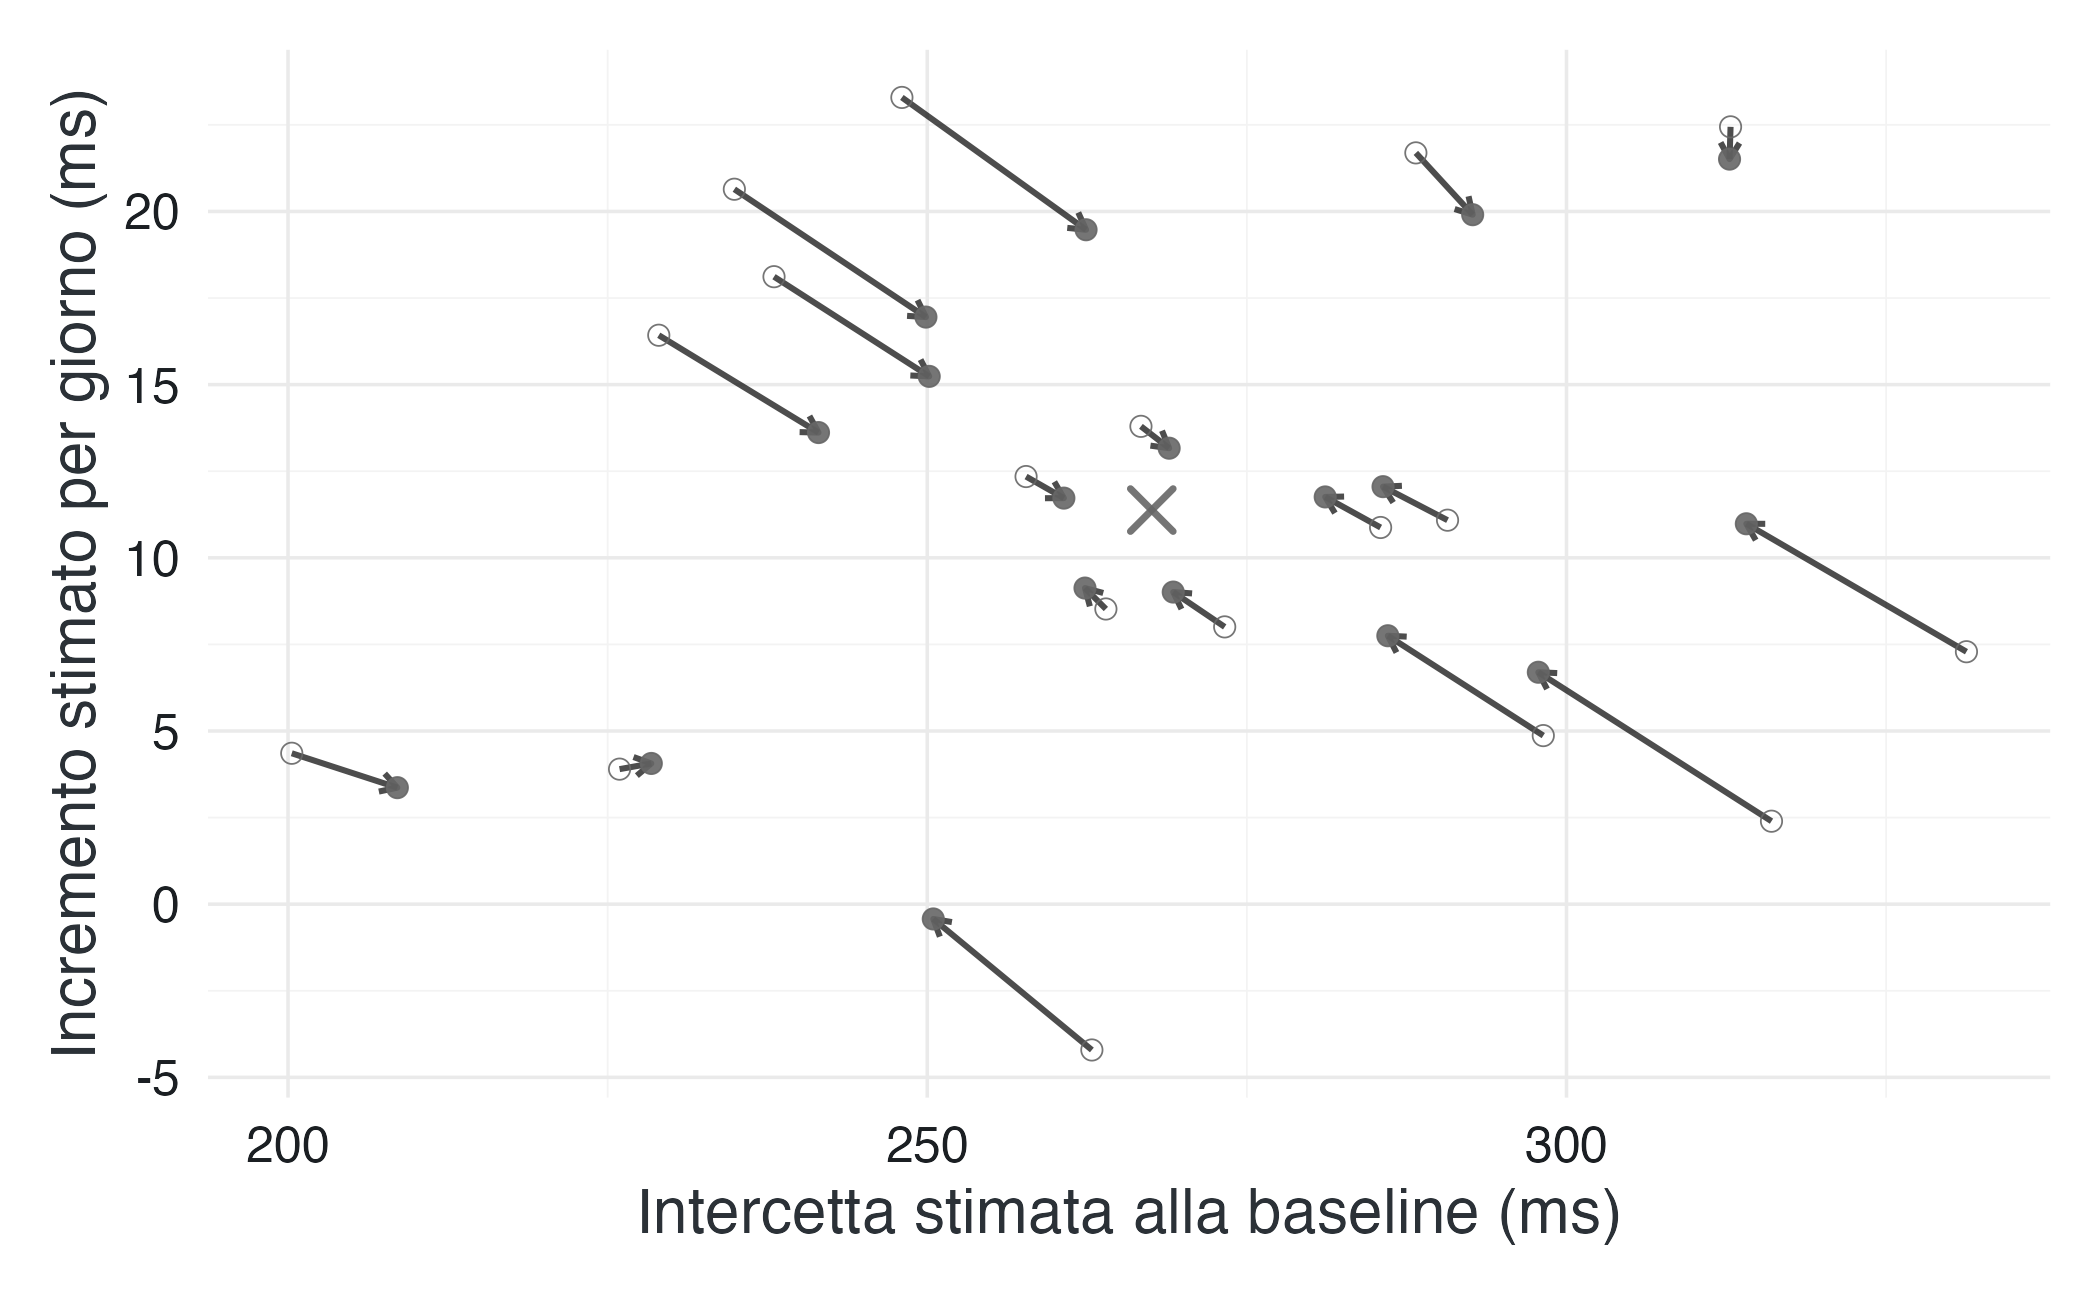
\includegraphics[width=0.85\linewidth,height=\textheight,keepaspectratio]{chapters/linear_models/08_modelli_multilivello_partial_pooling_files/figure-pdf/fig-shrinkage-1.png}

}

\caption{\label{fig-shrinkage}Ogni segmento collega la stima no pooling
di un partecipante alla corrispondente stima partial pooling. La croce
indica i parametri medi del modello gerarchico.}

\end{figure}%

Le stime gerarchiche risultano sistematicamente contratte verso il
centro della distribuzione comune. L'entità della contrazione non è
uniforme, ma dipende da diversi fattori: il numero e la variabilità
delle osservazioni disponibili per ciascun soggetto, la variabilità
residua, l'eterogeneità stimata tra le unità, i prior sui parametri
gerarchici e la struttura complessiva del modello. Quando un
partecipante contribuisce con dati numerosi e coerenti, la sua
likelihood è informativa e la stima gerarchica rimane prossima a quella
separata. Quando invece i dati sono scarsi o rumorosi, la distribuzione
comune esercita un'influenza maggiore, spostando la stima verso il
centro.

La minore dispersione delle stime ottenute con il \emph{partial pooling}
non implica che il modello abbia eliminato differenze reali, ma
piuttosto che non attribuisce automaticamente a ogni variazione
osservata il valore di un parametro stabile dell'individuo:

\begin{Shaded}
\begin{Highlighting}[]
\NormalTok{shrinkage\_data }\SpecialCharTok{|\textgreater{}}
  \FunctionTok{summarise}\NormalTok{(}
    \AttributeTok{sd\_intercepts\_no\_pooling =} \FunctionTok{sd}\NormalTok{(intercept\_np),}
    \AttributeTok{sd\_intercepts\_partial\_pooling =} \FunctionTok{sd}\NormalTok{(intercept\_pp),}
    \AttributeTok{sd\_slopes\_no\_pooling =} \FunctionTok{sd}\NormalTok{(slope\_np),}
    \AttributeTok{sd\_slopes\_partial\_pooling =} \FunctionTok{sd}\NormalTok{(slope\_pp)}
\NormalTok{  )}
\CommentTok{\#\textgreater{} \# A tibble: 1 x 4}
\CommentTok{\#\textgreater{}   sd\_intercepts\_no\_pooling sd\_intercepts\_partial\_pooling sd\_slopes\_no\_pooling}
\CommentTok{\#\textgreater{}                      \textless{}dbl\textgreater{}                         \textless{}dbl\textgreater{}                \textless{}dbl\textgreater{}}
\CommentTok{\#\textgreater{} 1                     35.1                          28.0                 7.83}
\CommentTok{\#\textgreater{}   sd\_slopes\_partial\_pooling}
\CommentTok{\#\textgreater{}                       \textless{}dbl\textgreater{}}
\CommentTok{\#\textgreater{} 1                      5.93}
\end{Highlighting}
\end{Shaded}

Le stime separate sono libere di inseguire il rumore di ogni piccolo
campione individuale. Il modello gerarchico richiede invece evidenza
sufficiente prima di collocare un partecipante molto lontano dalla
distribuzione comune. In media, questa regolarizzazione migliora la
capacità predittiva su dati futuri, anche se la singola stima
individuale può naturalmente rimanere imperfetta.

\section{Visualizzare le traiettorie
posteriori}\label{visualizzare-le-traiettorie-posteriori}

Per visualizzare le traiettorie individuali stimate dal modello, si
costruisce una griglia di predizione che estende l'intervallo osservato
dei giorni di deprivazione per ciascun partecipante e si estrae la
distribuzione predittiva a posteriori delle medie condizionate:

\begin{Shaded}
\begin{Highlighting}[]
\NormalTok{subject\_grid }\OtherTok{\textless{}{-}}\NormalTok{ tidyr}\SpecialCharTok{::}\FunctionTok{crossing}\NormalTok{(}
  \AttributeTok{Subject =} \FunctionTok{levels}\NormalTok{(sleep2}\SpecialCharTok{$}\NormalTok{Subject),}
  \AttributeTok{days\_deprived =} \FunctionTok{seq}\NormalTok{(}
    \FunctionTok{min}\NormalTok{(sleep2}\SpecialCharTok{$}\NormalTok{days\_deprived),}
    \FunctionTok{max}\NormalTok{(sleep2}\SpecialCharTok{$}\NormalTok{days\_deprived),}
    \AttributeTok{length.out =} \DecValTok{30}
\NormalTok{  )}
\NormalTok{) }\SpecialCharTok{|\textgreater{}}
  \FunctionTok{mutate}\NormalTok{(}\AttributeTok{Subject =} \FunctionTok{factor}\NormalTok{(Subject, }\AttributeTok{levels =} \FunctionTok{levels}\NormalTok{(sleep2}\SpecialCharTok{$}\NormalTok{Subject)))}

\NormalTok{subject\_epred }\OtherTok{\textless{}{-}} \FunctionTok{posterior\_epred}\NormalTok{(}
\NormalTok{  pp\_model,}
  \AttributeTok{newdata =}\NormalTok{ subject\_grid,}
  \AttributeTok{re\_formula =} \ConstantTok{NULL}
\NormalTok{)}

\NormalTok{summarise\_draw\_matrix }\OtherTok{\textless{}{-}} \ControlFlowTok{function}\NormalTok{(draws, newdata, }\AttributeTok{probs =} \FunctionTok{c}\NormalTok{(}\FloatTok{0.05}\NormalTok{, }\FloatTok{0.95}\NormalTok{)) \{}
\NormalTok{  intervals }\OtherTok{\textless{}{-}} \FunctionTok{apply}\NormalTok{(draws, }\DecValTok{2}\NormalTok{, quantile, }\AttributeTok{probs =}\NormalTok{ probs)}

\NormalTok{  newdata }\SpecialCharTok{|\textgreater{}}
    \FunctionTok{mutate}\NormalTok{(}
      \AttributeTok{estimate =} \FunctionTok{colMeans}\NormalTok{(draws),}
      \AttributeTok{lower =}\NormalTok{ intervals[}\DecValTok{1}\NormalTok{, ],}
      \AttributeTok{upper =}\NormalTok{ intervals[}\DecValTok{2}\NormalTok{, ]}
\NormalTok{    )}
\NormalTok{\}}

\NormalTok{subject\_summary }\OtherTok{\textless{}{-}} \FunctionTok{summarise\_draw\_matrix}\NormalTok{(}
\NormalTok{  subject\_epred,}
\NormalTok{  subject\_grid}
\NormalTok{)}
\end{Highlighting}
\end{Shaded}

Il grafico seguente mostra, per ciascun partecipante, la traiettoria
stimata (linea continua) e l'incertezza associata alla media
condizionata (fascia di credibilità al 90\%). La sovrapposizione con i
dati osservati consente una valutazione visiva dell'adeguatezza del
modello:

\begin{Shaded}
\begin{Highlighting}[]
\NormalTok{sleep2 }\SpecialCharTok{|\textgreater{}}
  \FunctionTok{ggplot}\NormalTok{(}\FunctionTok{aes}\NormalTok{(}\AttributeTok{x =}\NormalTok{ days\_deprived, }\AttributeTok{y =}\NormalTok{ Reaction)) }\SpecialCharTok{+}
  \FunctionTok{geom\_ribbon}\NormalTok{(}
    \AttributeTok{data =}\NormalTok{ subject\_summary,}
    \FunctionTok{aes}\NormalTok{(}\AttributeTok{x =}\NormalTok{ days\_deprived, }\AttributeTok{ymin =}\NormalTok{ lower, }\AttributeTok{ymax =}\NormalTok{ upper, }\AttributeTok{group =}\NormalTok{ Subject),}
    \AttributeTok{inherit.aes =} \ConstantTok{FALSE}\NormalTok{,}
    \AttributeTok{alpha =} \FloatTok{0.18}
\NormalTok{  ) }\SpecialCharTok{+}
  \FunctionTok{geom\_line}\NormalTok{(}
    \AttributeTok{data =}\NormalTok{ subject\_summary,}
    \FunctionTok{aes}\NormalTok{(}\AttributeTok{y =}\NormalTok{ estimate, }\AttributeTok{group =}\NormalTok{ Subject),}
    \AttributeTok{linewidth =} \FloatTok{0.7}
\NormalTok{  ) }\SpecialCharTok{+}
  \FunctionTok{geom\_point}\NormalTok{(}\AttributeTok{alpha =} \FloatTok{0.55}\NormalTok{) }\SpecialCharTok{+}
  \FunctionTok{facet\_wrap}\NormalTok{(}\SpecialCharTok{\textasciitilde{}}\NormalTok{ Subject) }\SpecialCharTok{+}
  \FunctionTok{labs}\NormalTok{(}
    \AttributeTok{x =} \StringTok{"Giorni di deprivazione del sonno"}\NormalTok{,}
    \AttributeTok{y =} \StringTok{"Tempo di reazione (ms)"}
\NormalTok{  )}
\end{Highlighting}
\end{Shaded}

\begin{figure}[H]

\centering{

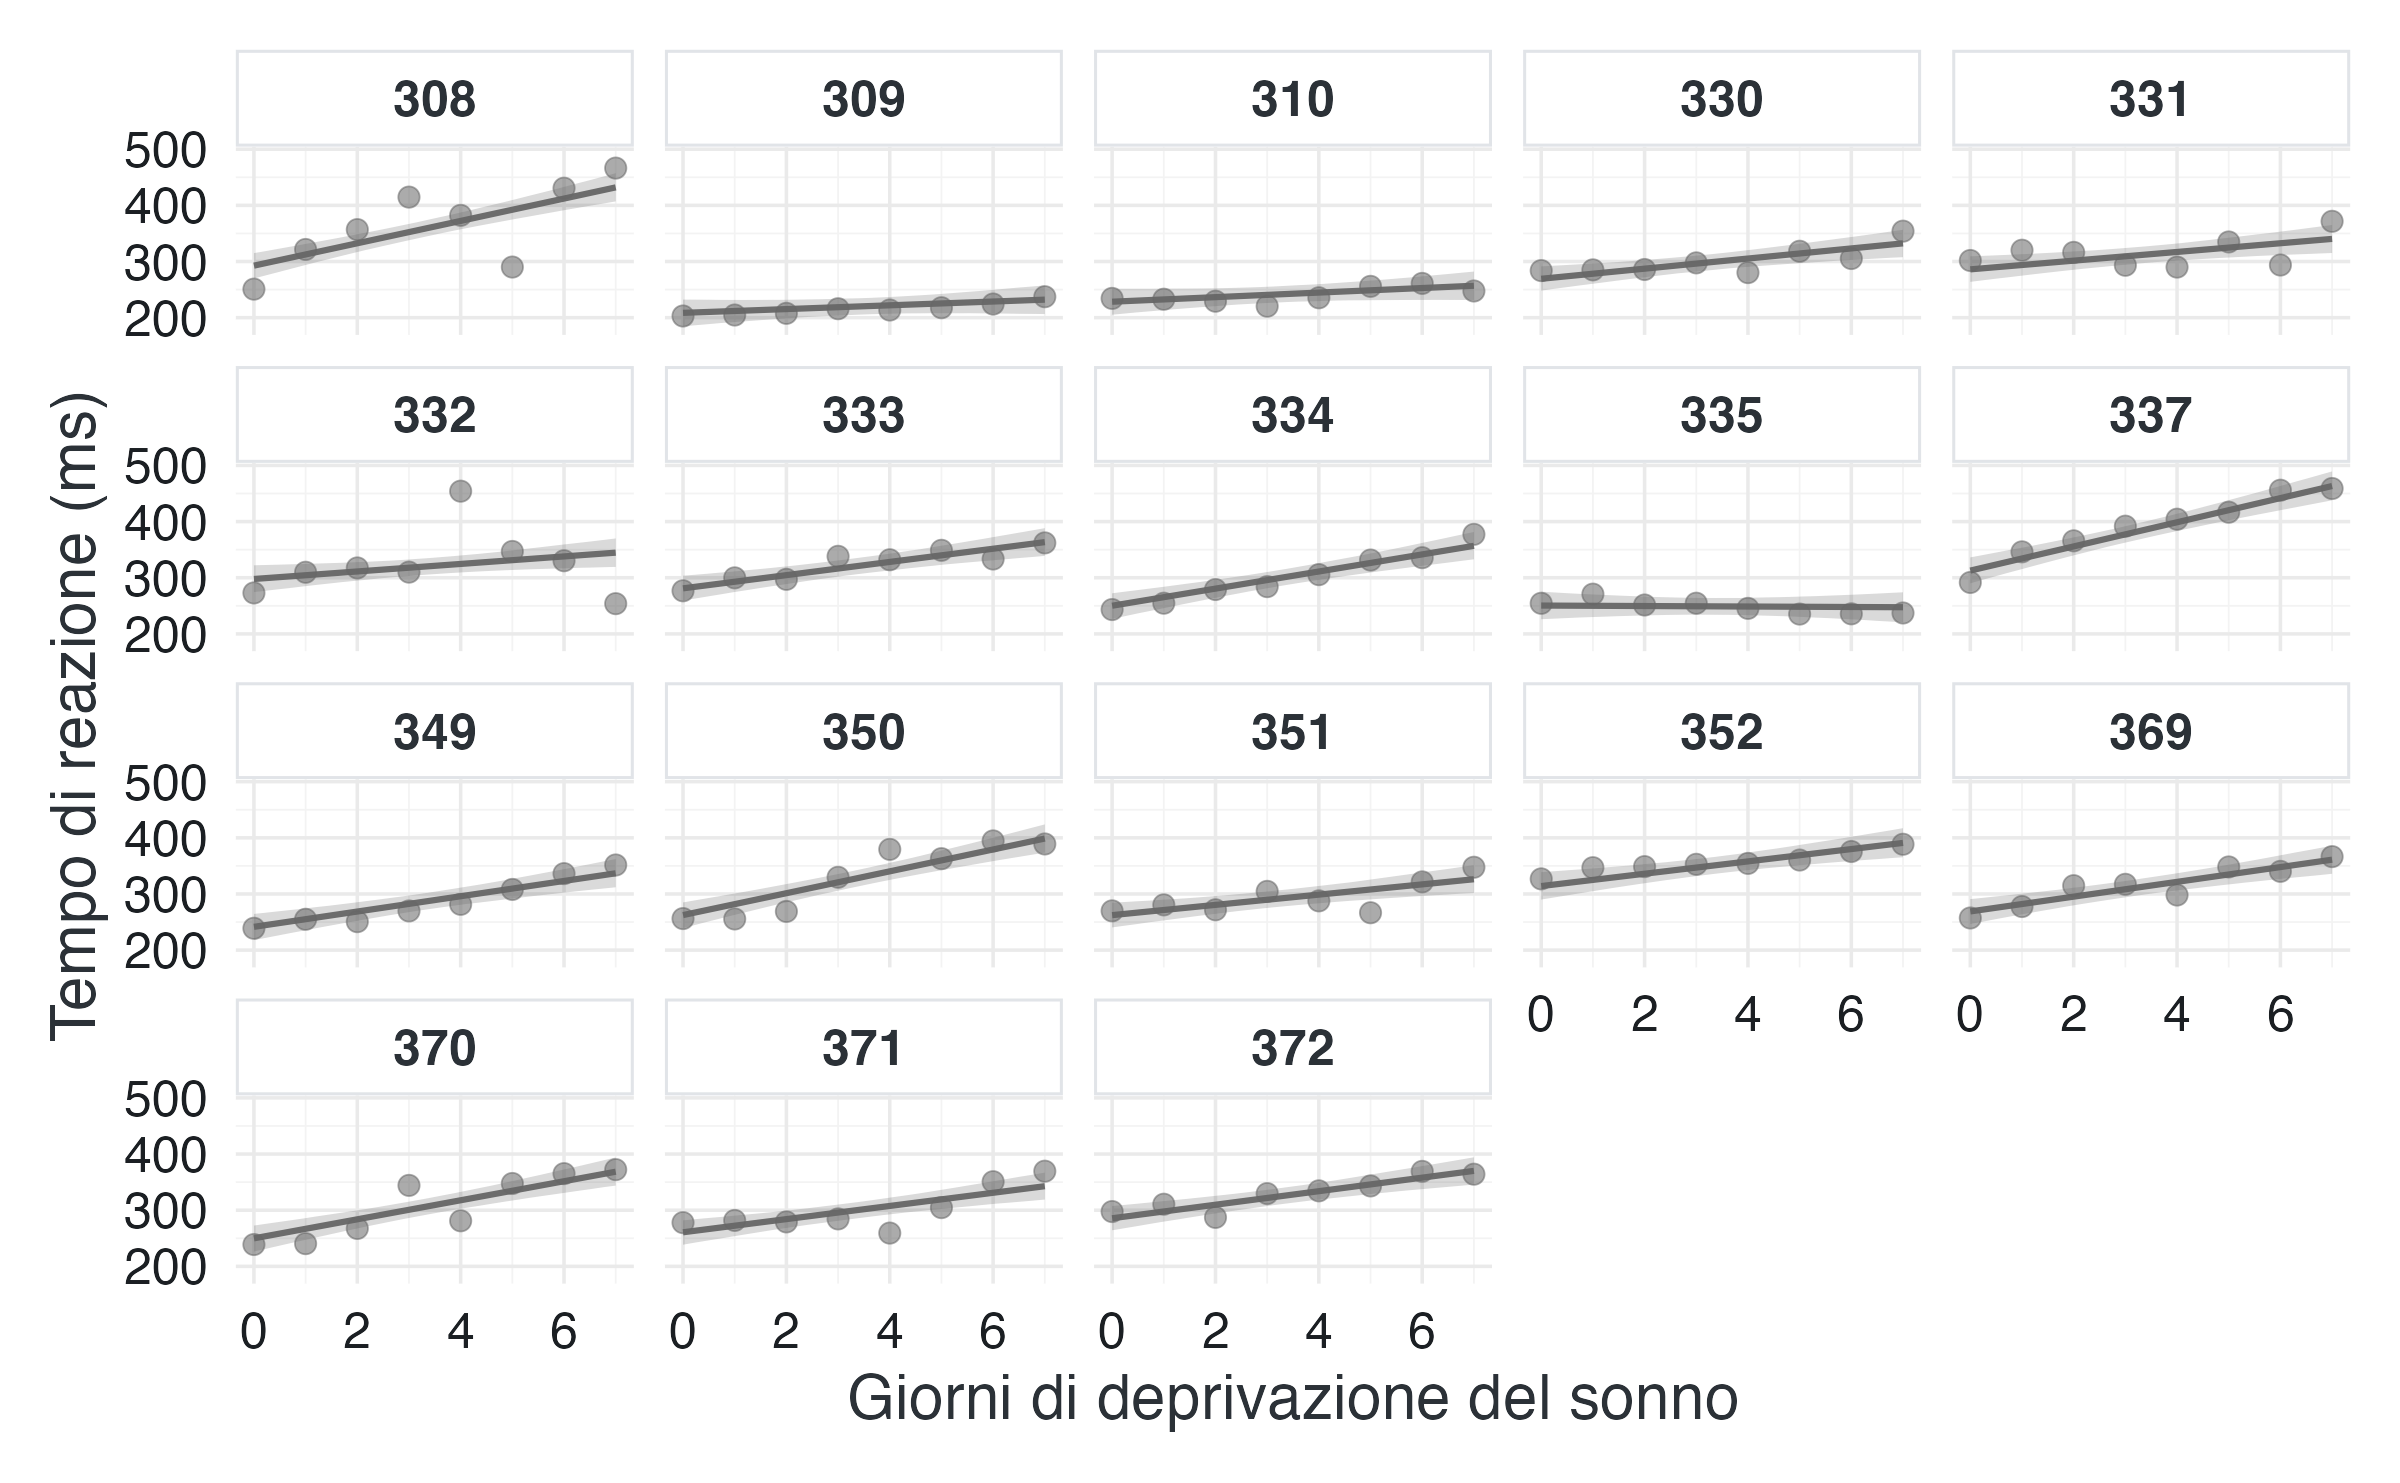
\includegraphics[width=0.85\linewidth,height=\textheight,keepaspectratio]{chapters/linear_models/08_modelli_multilivello_partial_pooling_files/figure-pdf/fig-partial-pooling-trajectories-1.png}

}

\caption{\label{fig-partial-pooling-trajectories}Traiettorie individuali
stimate mediante partial pooling. Le fasce rappresentano l'incertezza
sulla media condizionata di ciascun partecipante.}

\end{figure}%

Le traiettorie individuali mostrano andamenti eterogenei, ma la loro
variabilità è stata regolarizzata dalla struttura gerarchica. Le fasce
di incertezza riflettono sia la variabilità residua sia l'informazione
disponibile per ciascun soggetto: più i dati sono scarsi o rumorosi, più
l'intervallo di credibilità si allarga. Questo tipo di visualizzazione
integra la lettura tabellare dei coefficienti e aiuta a valutare se le
differenze tra i partecipanti siano sufficientemente sostenute
dall'evidenza empirica.

\section{Tre domande predittive
diverse}\label{tre-domande-predittive-diverse}

Nei modelli multilivello, il termine ``previsione'' può riferirsi a
oggetti concettualmente diversi. È necessario specificare se si intende
prevedere per un partecipante già osservato, per la popolazione media o
per un nuovo soggetto, e se si vuole includere o meno la variabilità
residua delle osservazioni individuali.

\subsection{Un partecipante già
osservato}\label{un-partecipante-giuxe0-osservato}

Per un partecipante già osservato, si può prevedere la sua traiettoria
media condizionata oppure una nuova osservazione che tenga conto anche
della variabilità residua. Nel primo caso si usa
\texttt{posterior\_epred()} con \texttt{re\_formula\ =\ NULL}, che
restituisce l'incertezza sulla media del soggetto; nel secondo,
\texttt{posterior\_predict()} aggiunge la componente stocastica delle
singole osservazioni.

\begin{Shaded}
\begin{Highlighting}[]
\NormalTok{known\_subject }\OtherTok{\textless{}{-}} \FunctionTok{levels}\NormalTok{(sleep2}\SpecialCharTok{$}\NormalTok{Subject)[}\DecValTok{1}\NormalTok{]}

\NormalTok{known\_grid }\OtherTok{\textless{}{-}} \FunctionTok{tibble}\NormalTok{(}
  \AttributeTok{Subject =} \FunctionTok{factor}\NormalTok{(}
\NormalTok{    known\_subject,}
    \AttributeTok{levels =} \FunctionTok{levels}\NormalTok{(sleep2}\SpecialCharTok{$}\NormalTok{Subject)}
\NormalTok{  ),}
  \AttributeTok{days\_deprived =} \DecValTok{0}\SpecialCharTok{:}\DecValTok{7}
\NormalTok{)}

\NormalTok{known\_mean\_draws }\OtherTok{\textless{}{-}} \FunctionTok{posterior\_epred}\NormalTok{(}
\NormalTok{  pp\_model,}
  \AttributeTok{newdata =}\NormalTok{ known\_grid,}
  \AttributeTok{re\_formula =} \ConstantTok{NULL}
\NormalTok{)}

\NormalTok{known\_observation\_draws }\OtherTok{\textless{}{-}} \FunctionTok{posterior\_predict}\NormalTok{(}
\NormalTok{  pp\_model,}
  \AttributeTok{newdata =}\NormalTok{ known\_grid,}
  \AttributeTok{re\_formula =} \ConstantTok{NULL}
\NormalTok{)}
\end{Highlighting}
\end{Shaded}

\subsection{La relazione media di
popolazione}\label{la-relazione-media-di-popolazione}

Per descrivere la relazione media della popolazione, si escludono le
deviazioni individuali con \texttt{re\_formula\ =\ NA}. La distribuzione
risultante riguarda il centro della popolazione dei coefficienti, non la
traiettoria di un individuo specifico, e non include l'eterogeneità tra
i soggetti.

\begin{Shaded}
\begin{Highlighting}[]
\NormalTok{population\_grid }\OtherTok{\textless{}{-}} \FunctionTok{tibble}\NormalTok{(}
  \AttributeTok{Subject =} \FunctionTok{factor}\NormalTok{(}
    \FunctionTok{levels}\NormalTok{(sleep2}\SpecialCharTok{$}\NormalTok{Subject)[}\DecValTok{1}\NormalTok{],}
    \AttributeTok{levels =} \FunctionTok{levels}\NormalTok{(sleep2}\SpecialCharTok{$}\NormalTok{Subject)}
\NormalTok{  ),}
  \AttributeTok{days\_deprived =} \DecValTok{0}\SpecialCharTok{:}\DecValTok{7}
\NormalTok{)}

\NormalTok{population\_mean\_draws }\OtherTok{\textless{}{-}} \FunctionTok{posterior\_epred}\NormalTok{(}
\NormalTok{  pp\_model,}
  \AttributeTok{newdata =}\NormalTok{ population\_grid,}
  \AttributeTok{re\_formula =} \ConstantTok{NA}
\NormalTok{)}
\end{Highlighting}
\end{Shaded}

\subsection{Un nuovo partecipante}\label{un-nuovo-partecipante}

Per un nuovo partecipante, non presente nei dati, il modello deve
generare nuove deviazioni casuali dalla distribuzione di gruppo. Con
\texttt{allow\_new\_levels\ =\ TRUE} e
\texttt{sample\_new\_levels\ =\ "gaussian"}, si ottengono previsioni che
tengono conto sia dell'incertezza sui parametri di popolazione sia della
variabilità tra individui.

\begin{Shaded}
\begin{Highlighting}[]
\NormalTok{new\_subject\_grid }\OtherTok{\textless{}{-}} \FunctionTok{tibble}\NormalTok{(}
  \AttributeTok{Subject =} \StringTok{"new\_subject"}\NormalTok{,}
  \AttributeTok{days\_deprived =} \DecValTok{0}\SpecialCharTok{:}\DecValTok{7}
\NormalTok{)}

\NormalTok{new\_subject\_mean\_draws }\OtherTok{\textless{}{-}} \FunctionTok{posterior\_epred}\NormalTok{(}
\NormalTok{  pp\_model,}
  \AttributeTok{newdata =}\NormalTok{ new\_subject\_grid,}
  \AttributeTok{re\_formula =} \ConstantTok{NULL}\NormalTok{,}
  \AttributeTok{allow\_new\_levels =} \ConstantTok{TRUE}\NormalTok{,}
  \AttributeTok{sample\_new\_levels =} \StringTok{"gaussian"}
\NormalTok{)}

\NormalTok{new\_subject\_observation\_draws }\OtherTok{\textless{}{-}} \FunctionTok{posterior\_predict}\NormalTok{(}
\NormalTok{  pp\_model,}
  \AttributeTok{newdata =}\NormalTok{ new\_subject\_grid,}
  \AttributeTok{re\_formula =} \ConstantTok{NULL}\NormalTok{,}
  \AttributeTok{allow\_new\_levels =} \ConstantTok{TRUE}\NormalTok{,}
  \AttributeTok{sample\_new\_levels =} \StringTok{"gaussian"}
\NormalTok{)}
\end{Highlighting}
\end{Shaded}

La previsione per un nuovo partecipante è più incerta della linea media,
perché include la distribuzione delle intercette e delle pendenze
individuali. Se si aggiunge la variabilità residua, l'incertezza cresce
ulteriormente.

In sintesi, i quattro oggetti predittivi rispondono a domande diverse:
la media di un soggetto noto, una nuova osservazione dello stesso
soggetto, la relazione media della popolazione e la traiettoria di un
nuovo partecipante. È importante distinguerli chiaramente, perché non
sono intercambiabili.

\section{Controllare l'adeguatezza del
modello}\label{controllare-ladeguatezza-del-modello-2}

La convergenza del campionatore non garantisce che il modello descriva
adeguatamente i dati. Per valutare la bontà di adattamento, si eseguono
controlli predittivi a posteriori sia sull'intera distribuzione
marginale sia separatamente per ciascun partecipante. Il controllo sulla
distribuzione complessiva consente di verificare se il modello riproduce
la forma generale dei dati:

\begin{Shaded}
\begin{Highlighting}[]
\FunctionTok{pp\_check}\NormalTok{(}
\NormalTok{  pp\_model,}
  \AttributeTok{type =} \StringTok{"dens\_overlay"}\NormalTok{,}
  \AttributeTok{ndraws =} \DecValTok{50}
\NormalTok{)}
\end{Highlighting}
\end{Shaded}

\begin{center}
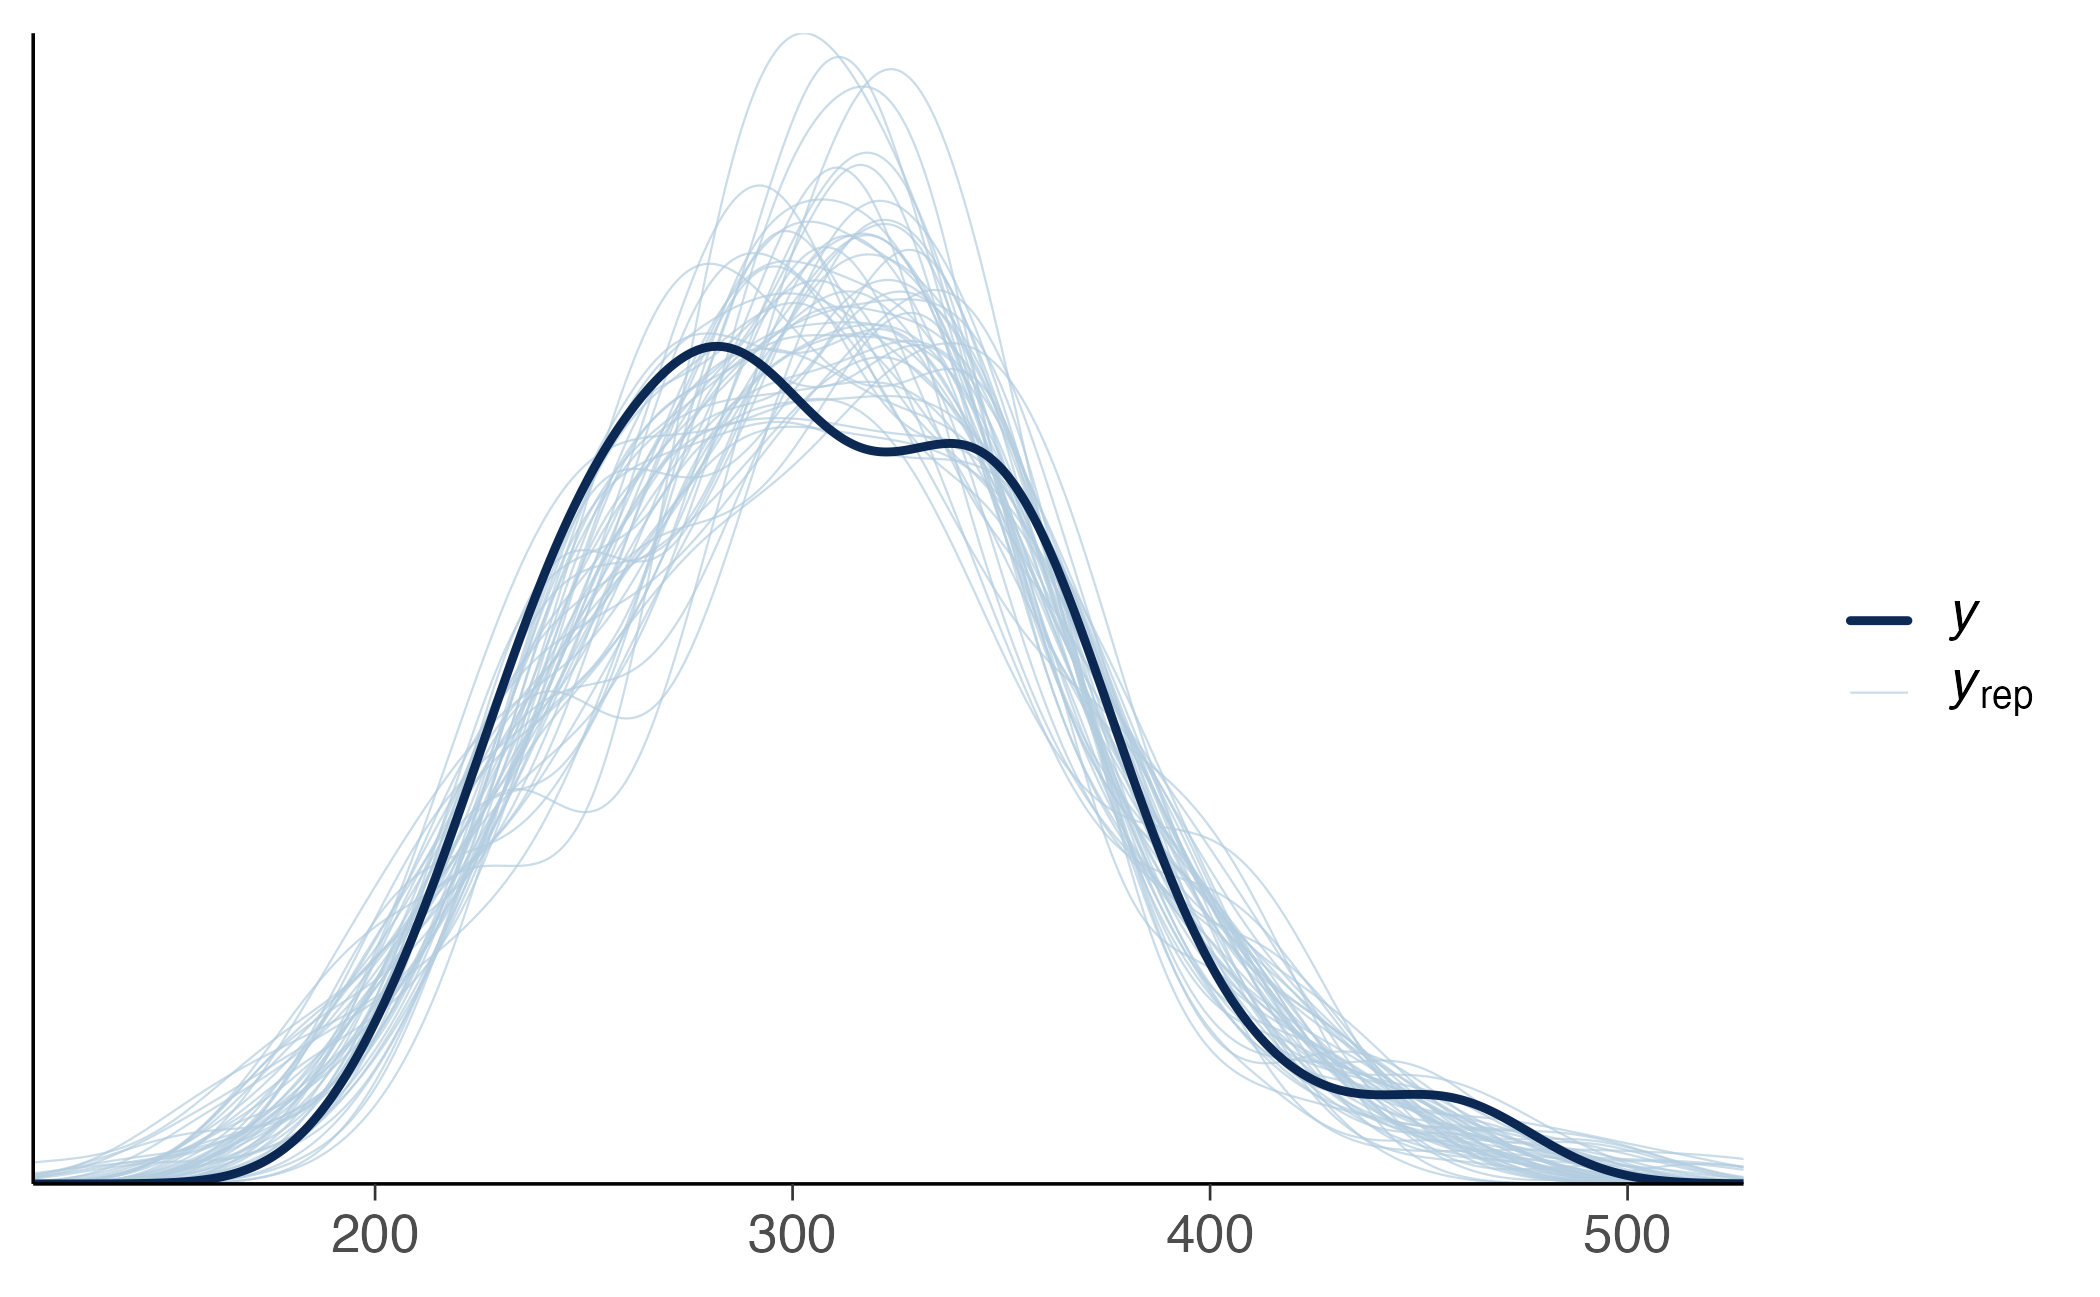
\includegraphics[width=0.85\linewidth,height=\textheight,keepaspectratio]{chapters/linear_models/08_modelli_multilivello_partial_pooling_files/figure-pdf/ppc-density-multilevel-1.png}
\end{center}

Tuttavia, un buon allineamento sulla distribuzione aggregata può
nascondere discrepanze sistematiche all'interno di singoli gruppi. Per
questo motivo, si esaminano separatamente le medie e le deviazioni
standard dei partecipanti, confrontando i valori osservati con quelli
generati dal modello:

\begin{Shaded}
\begin{Highlighting}[]
\FunctionTok{pp\_check}\NormalTok{(}
\NormalTok{  pp\_model,}
  \AttributeTok{type =} \StringTok{"stat\_grouped"}\NormalTok{,}
  \AttributeTok{stat =} \StringTok{"mean"}\NormalTok{,}
  \AttributeTok{group =} \StringTok{"Subject"}\NormalTok{,}
  \AttributeTok{ndraws =} \DecValTok{100}
\NormalTok{)}
\end{Highlighting}
\end{Shaded}

\begin{center}
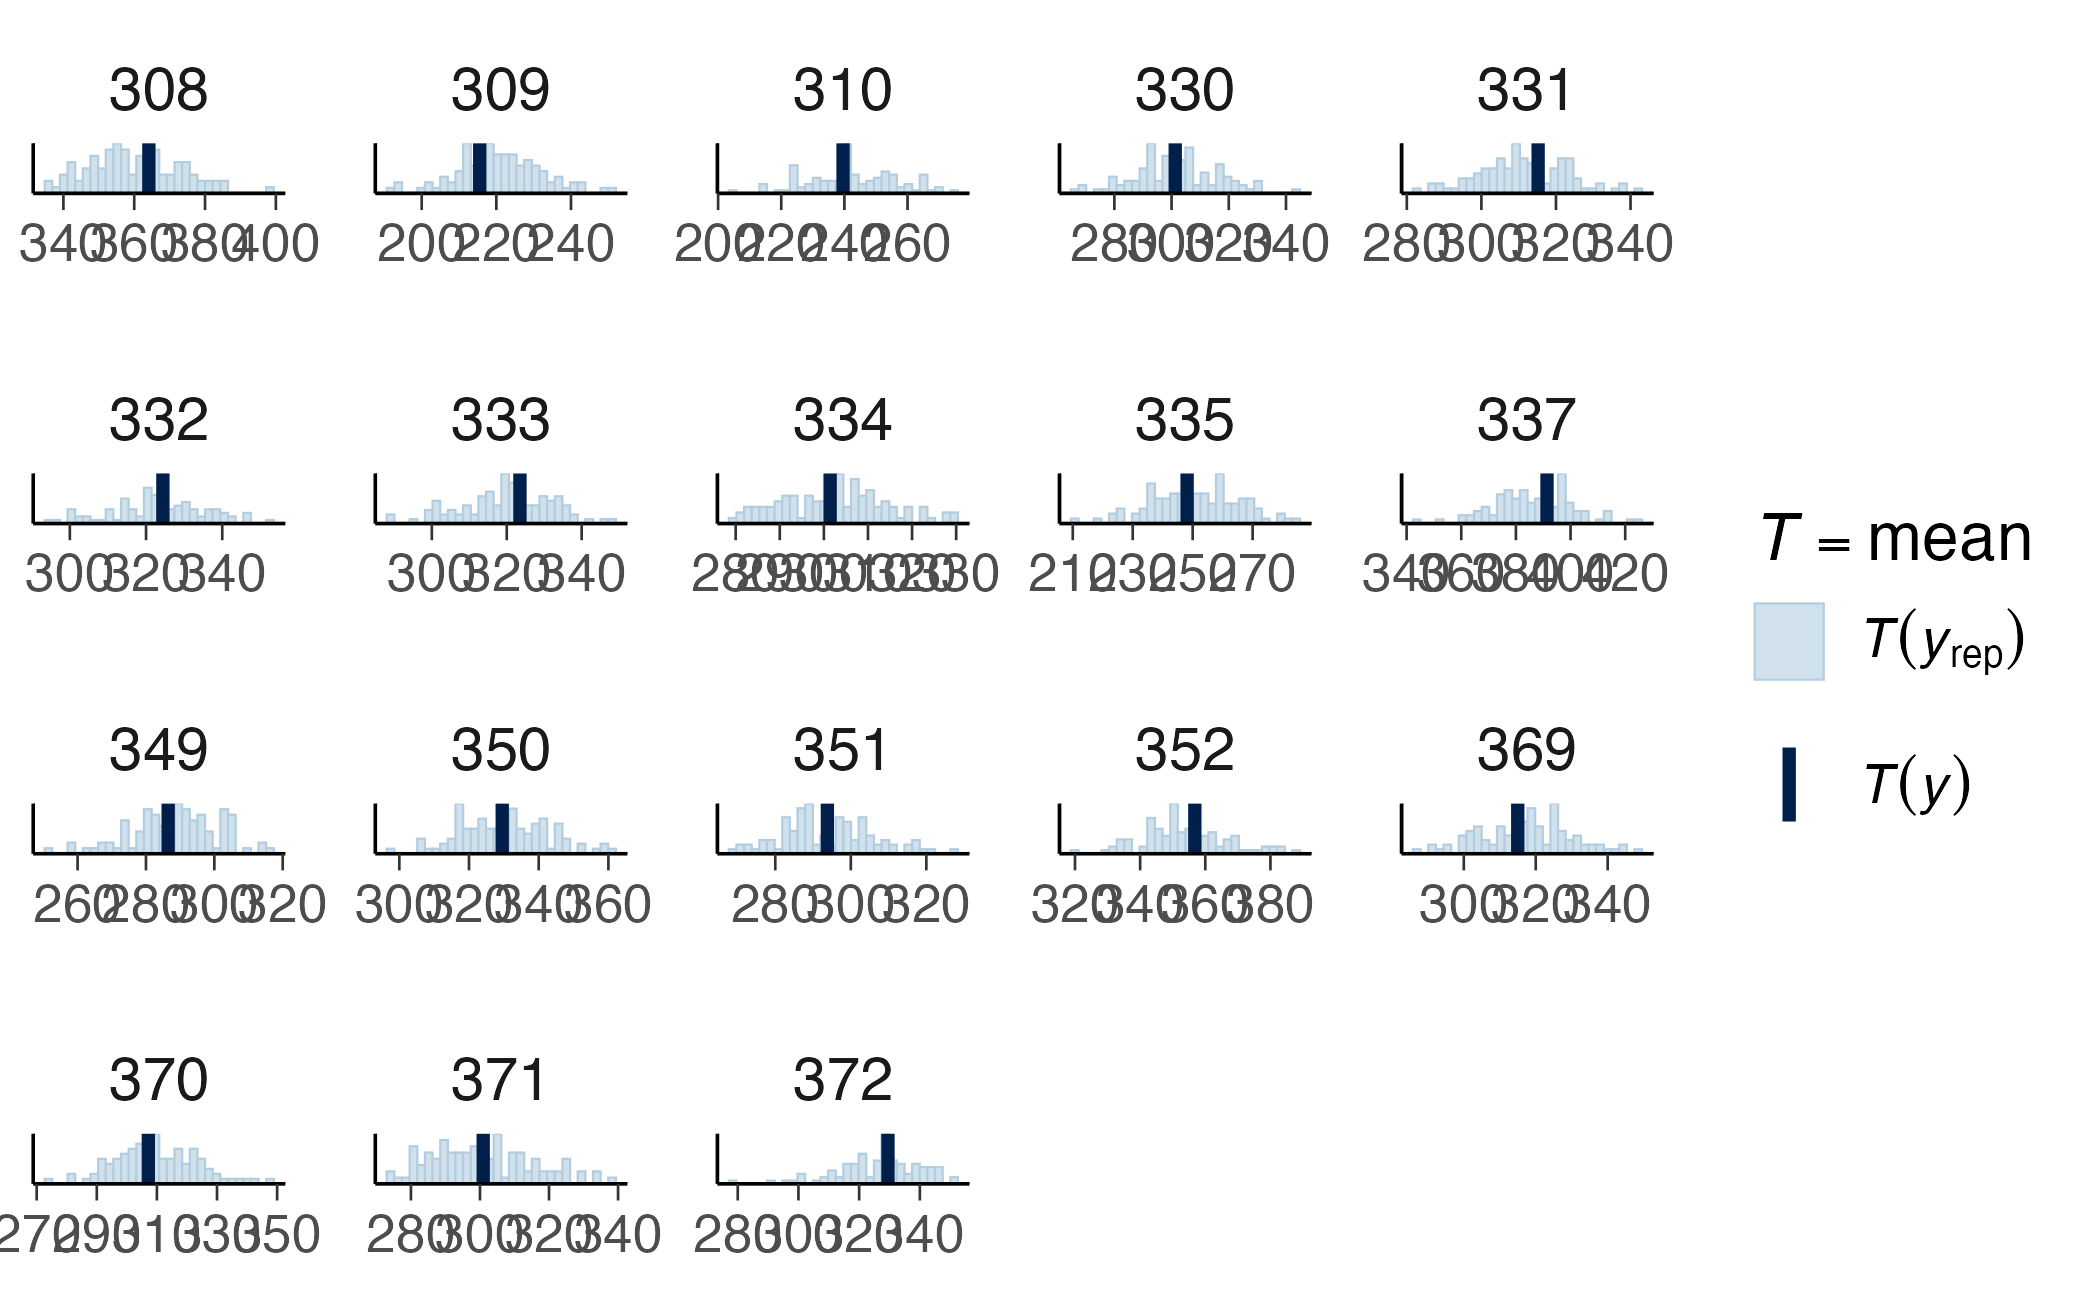
\includegraphics[width=0.85\linewidth,height=\textheight,keepaspectratio]{chapters/linear_models/08_modelli_multilivello_partial_pooling_files/figure-pdf/ppc-subject-means-multilevel-1.png}
\end{center}

\begin{Shaded}
\begin{Highlighting}[]
\FunctionTok{pp\_check}\NormalTok{(}
\NormalTok{  pp\_model,}
  \AttributeTok{type =} \StringTok{"stat\_grouped"}\NormalTok{,}
  \AttributeTok{stat =} \StringTok{"sd"}\NormalTok{,}
  \AttributeTok{group =} \StringTok{"Subject"}\NormalTok{,}
  \AttributeTok{ndraws =} \DecValTok{100}
\NormalTok{)}
\end{Highlighting}
\end{Shaded}

\begin{center}
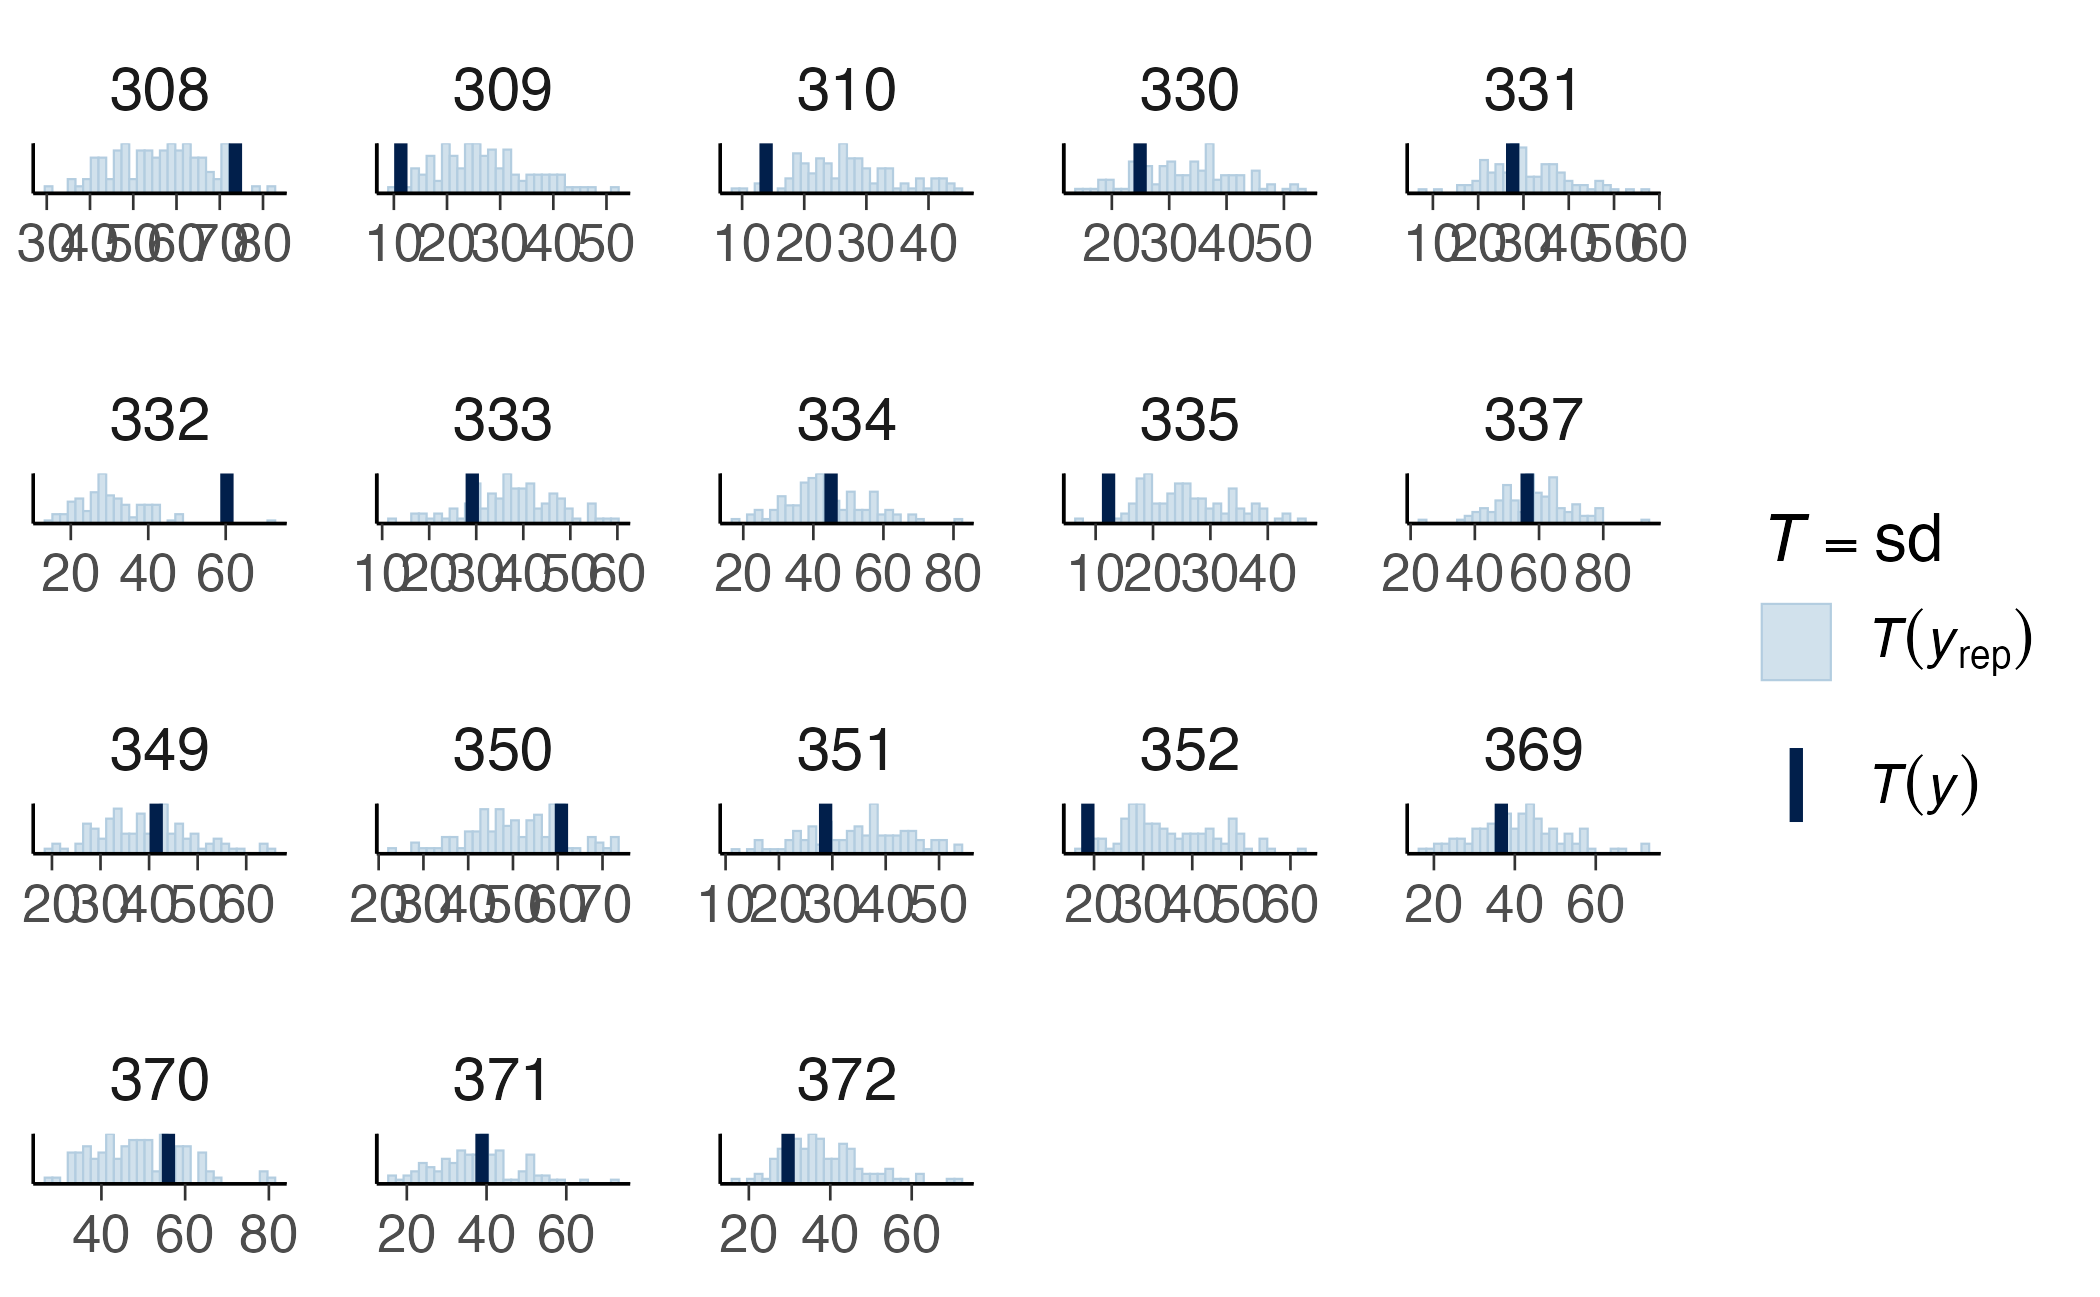
\includegraphics[width=0.85\linewidth,height=\textheight,keepaspectratio]{chapters/linear_models/08_modelli_multilivello_partial_pooling_files/figure-pdf/ppc-subject-sd-multilevel-1.png}
\end{center}

Questi controlli raggruppati sono più informativi di quelli marginali:
verificano se il modello è in grado di riprodurre le differenze nei
livelli iniziali e nella dispersione individuale. Tra i segnali che
suggeriscono una specificazione inadeguata figurano curvature
sistematiche nelle traiettorie, dispersione residua crescente nel tempo,
osservazioni estreme non riprodotte dal modello, andamenti
qualitativamente diversi tra partecipanti o correlazione seriale residua
all'interno di uno stesso soggetto. La presenza di questi segnali
richiede una revisione della struttura del modello --- non un semplice
aumento dei parametri di controllo del campionatore.

\section{Scegliere la struttura degli effetti di
gruppo}\label{scegliere-la-struttura-degli-effetti-di-gruppo}

Il modello con intercette e pendenze correlate, pur essendo il più
flessibile, non costituisce l'unica opzione disponibile. La scelta della
struttura degli effetti di gruppo dovrebbe essere guidata dalla domanda
di ricerca, dal disegno e dai controlli predittivi, non da una regola
secondo cui ogni coefficiente debba necessariamente variare.

\subsection{Soltanto intercette
variabili}\label{soltanto-intercette-variabili}

Un primo modello prevede che i partecipanti differiscano soltanto nel
livello basale, condividendo invece la stessa pendenza:

\begin{Shaded}
\begin{Highlighting}[]
\NormalTok{Reaction }\SpecialCharTok{\textasciitilde{}} \DecValTok{0} \SpecialCharTok{+}\NormalTok{ Intercept }\SpecialCharTok{+}\NormalTok{ days\_deprived }\SpecialCharTok{+}\NormalTok{ (}\DecValTok{1} \SpecialCharTok{|}\NormalTok{ Subject)}
\end{Highlighting}
\end{Shaded}

Questa specificazione è adeguata quando l'eterogeneità interindividuale
riguarda prevalentemente il punto di partenza e non il tasso di
cambiamento.

\subsection{Intercette e pendenze
variabili}\label{intercette-e-pendenze-variabili}

Un secondo modello consente ai partecipanti di differire sia
nell'intercetta sia nella pendenza, stimando anche la loro correlazione:

\begin{Shaded}
\begin{Highlighting}[]
\NormalTok{Reaction }\SpecialCharTok{\textasciitilde{}} \DecValTok{0} \SpecialCharTok{+}\NormalTok{ Intercept }\SpecialCharTok{+}\NormalTok{ days\_deprived }\SpecialCharTok{+}
\NormalTok{  (}\DecValTok{1} \SpecialCharTok{+}\NormalTok{ days\_deprived }\SpecialCharTok{|}\NormalTok{ Subject)}
\end{Highlighting}
\end{Shaded}

Questa è la struttura più ricca e generalmente più realistica, ma
richiede un numero sufficiente di gruppi e osservazioni per essere
stimata in modo stabile.

\subsection{Intercette e pendenze non
correlate}\label{intercette-e-pendenze-non-correlate}

Un terzo modello mantiene intercette e pendenze variabili, ma fissa a
zero la loro correlazione:

\begin{Shaded}
\begin{Highlighting}[]
\NormalTok{Reaction }\SpecialCharTok{\textasciitilde{}} \DecValTok{0} \SpecialCharTok{+}\NormalTok{ Intercept }\SpecialCharTok{+}\NormalTok{ days\_deprived }\SpecialCharTok{+}
\NormalTok{  (}\DecValTok{1} \SpecialCharTok{+}\NormalTok{ days\_deprived }\SpecialCharTok{||}\NormalTok{ Subject)}
\end{Highlighting}
\end{Shaded}

La sintassi \texttt{\textbar{}\textbar{}} impone l'indipendenza tra le
deviazioni individuali. Può essere utile quando il numero di gruppi è
limitato e i dati forniscono poche informazioni sulla correlazione, ma
costituisce comunque un'assunzione forte che deve essere giustificata.

In sintesi, la scelta tra queste strutture non dovrebbe basarsi sulla
complessità in sé, ma sulla capacità del modello di rappresentare il
fenomeno senza eccedere nelle richieste ai dati. Un modello più ricco
può cogliere forme aggiuntive di eterogeneità, ma a costo di una
maggiore incertezza. La decisione va sostenuta da diagnostiche,
controlli predittivi e, quando possibile, da confronto tra modelli.

\section{L'effetto medio descrive gli
individui?}\label{leffetto-medio-descrive-gli-individui}

L'effetto medio stimato su un gruppo di individui non implica
necessariamente che esso descriva adeguatamente il singolo caso. I
modelli multilivello riducono la tensione tra prospettiva nomotetica e
idiografica, in quanto stimano congiuntamente una tendenza condivisa e
le deviazioni individuali, ma non risolvono automaticamente il problema
della generalizzazione dal gruppo all'individuo.

Una pendenza media positiva, ad esempio, può coesistere con pendenze
individuali molto diverse tra loro, con valori prossimi a zero per
alcuni soggetti, con andamenti negativi per altri o persino con forme
funzionali diverse tra i partecipanti. In questo senso, la media della
popolazione non sostituisce la conoscenza individuale, ma rappresenta un
punto di partenza per interrogarsi sulla sua generalizzabilità.

Come sottolineano Richters
(\citeproc{ref-richters2021incredible}{2021}), l'assunzione che le
relazioni osservate tra gli individui in un dato momento corrispondano
ai processi che si svolgono all'interno di ciascun individuo nel tempo è
spesso problematica in psicologia. Un'associazione media tra due
variabili non coincide necessariamente con la dinamica intraindividuale
e tale discrepanza, nota come problema ergodico, richiede una
riflessione esplicita nella progettazione e nell'interpretazione dei
modelli.

Il modello presentato in questo capitolo considera l'eterogeneità come
una variazione quantitativa attorno a una forma funzionale comune: per
tutti i partecipanti, la traiettoria è lineare e le differenze si
esauriscono nell'intercetta e nella pendenza. Se invece i processi
generatori dei dati differissero qualitativamente tra gli individui,
sarebbero necessarie alternative, come l'identificazione di sottogruppi
teoricamente fondati o l'adozione di modelli propriamente idiografici.

La presenza di parametri individuali non garantisce automaticamente
l'accuratezza del modello per le decisioni riguardanti una singola
persona. La validità idiografica richiede dati sufficientemente
informativi per quel soggetto, controlli predittivi pertinenti e,
idealmente, una valutazione fuori campione della capacità predittiva.

\section{Interpretazione scientifica e
causalità}\label{interpretazione-scientifica-e-causalituxe0}

La pendenza media descrive la variazione attesa dei tempi di reazione al
procedere dei giorni nel protocollo osservato. L'attribuzione di un
significato causale a tale relazione non è tuttavia implicita nella
stima statistica, ma dipende dal disegno dello studio, dalla
manipolazione sperimentale, dalle condizioni di controllo e dalle
assunzioni che collegano il modello ai potenziali esiti controfattuali.

Il modello multilivello risolve il problema della dipendenza tra le
osservazioni e rappresenta esplicitamente l'eterogeneità tra i soggetti,
ma non trasforma automaticamente un'associazione in un effetto causale.
Allo stesso modo, la correlazione tra l'intercetta e la pendenza non
identifica un meccanismo psicologico, ma descrive una proprietà della
distribuzione dei coefficienti all'interno del modello specificato,
senza implicare un legame funzionale tra il livello iniziale e il tasso
di cambiamento.

\section{Errori frequenti}\label{errori-frequenti-7}

\begin{tcolorbox}[enhanced jigsaw, arc=.35mm, bottomrule=.15mm, bottomtitle=1mm, breakable, colback=white, colbacktitle=quarto-callout-caution-color!10!white, colframe=quarto-callout-caution-color-frame, coltitle=black, left=2mm, leftrule=.75mm, opacityback=0, opacitybacktitle=0.6, rightrule=.15mm, title=\textcolor{quarto-callout-caution-color}{\faFire}\hspace{0.5em}{Attenzione}, titlerule=0mm, toprule=.15mm, toptitle=1mm]

\begin{itemize}
\tightlist
\item
  Considerare tutte le righe come osservazioni indipendenti quando sono
  annidate entro persone o gruppi.
\item
  Interpretare \texttt{ranef()} come se restituisse i coefficienti
  individuali completi.
\item
  Chiamare la pendenza media ``effetto di ogni partecipante''.
\item
  Descrivere lo shrinkage come una correzione applicata dopo la stima.
\item
  Concludere che le differenze individuali siano reali perché le stime
  no pooling sono disperse.
\item
  Confondere la linea di popolazione con la previsione per una nuova
  persona.
\item
  Usare \texttt{re\_formula\ =\ NA} quando la domanda riguarda un
  partecipante specifico.
\item
  Interpretare una correlazione incerta tra intercetta e pendenza come
  prova di assenza di relazione.
\item
  Aggiungere automaticamente pendenze variabili senza verificare se il
  disegno le renda identificabili.
\item
  Considerare un posterior predictive check complessivo sufficiente a
  validare la struttura individuale.
\end{itemize}

\end{tcolorbox}

\section{Riflessioni conclusive}\label{riflessioni-conclusive-25}

I modelli multilivello rappresentano un'estensione naturale del modello
lineare quando le osservazioni presentano una struttura correlata, come
nel caso di misure ripetute o dati annidati. Il \emph{complete pooling}
si limita a descrivere la relazione media, ignorando le differenze tra
unità; il \emph{no pooling} tratta ciascun gruppo come isolato,
rinunciando alla condivisione di informazione; il \emph{partial pooling}
introduce invece una distribuzione comune per i coefficienti,
bilanciando l'evidenza individuale con quella aggregata.

Lo \emph{shrinkage} non è un espediente correttivo arbitrario, ma una
conseguenza della struttura gerarchica del modello. La sua entità è
determinata dalla precisione dei dati individuali, dall'eterogeneità
stimata tra i gruppi e dai prior scelti. Il suo scopo non è rendere
artificialmente simili i partecipanti, ma evitare che variazioni
accidentali del campione vengano interpretate come differenze stabili e
sostanziali.

Il capitolo ha inoltre distinto i parametri di popolazione, le
deviazioni di gruppo, i coefficienti individuali e le componenti di
varianza. Questa distinzione è essenziale quando si formulano
previsioni: la traiettoria di un partecipante già osservato, la linea
media della popolazione e quella di un nuovo soggetto corrispondono a
distribuzioni predittive diverse che rispondono a domande scientifiche
diverse.

Infine, modellare l'eterogeneità non rende automaticamente valido
l'effetto medio per ogni individuo. Il modello continua a presupporre
una forma funzionale comune e deve essere sottoposto a controlli
predittivi mirati in grado di segnalare curvature sistematiche,
dipendenze residue, differenze qualitative tra i soggetti o limiti nella
capacità predittiva al di fuori del campione.

Nel prossimo capitolo, abbandoneremo l'analisi della variabilità ben
rappresentata per concentrarci sugli effetti di una specificazione
inadeguata: forma funzionale errata, variabili omesse,
eteroschedasticità, valori estremi e dipendenze ignorate.

\section{Concetti da ricordare}\label{concetti-da-ricordare-6}

\begin{enumerate}
\def\labelenumi{\arabic{enumi}.}
\tightlist
\item
  I dati annidati richiedono una rappresentazione esplicita della
  dipendenza tra osservazioni.
\item
  Complete pooling, no pooling e partial pooling esprimono tre
  differenti ipotesi sulla condivisione dell'informazione.
\item
  Un modello con pendenze variabili stima una distribuzione delle
  relazioni individuali.
\item
  Le deviazioni individuali hanno media zero rispetto ai parametri di
  popolazione.
\item
  \texttt{ranef()} restituisce deviazioni; \texttt{coef()} restituisce
  coefficienti completi.
\item
  Lo shrinkage dipende dalla quantità di informazione e dalla struttura
  gerarchica.
\item
  La variabilità tra pendenze è distinta dall'incertezza sulla pendenza
  media.
\item
  Le previsioni per unità note, popolazione media e nuove unità non sono
  intercambiabili.
\item
  Una diagnostica MCMC soddisfacente non dimostra l'adeguatezza del
  modello.
\item
  L'eterogeneità quantitativa attorno a una relazione comune è
  un'ipotesi, non una conseguenza necessaria dei dati.
\end{enumerate}

\begin{tcolorbox}[enhanced jigsaw, arc=.35mm, bottomrule=.15mm, bottomtitle=1mm, breakable, colback=white, colbacktitle=quarto-callout-important-color!10!white, colframe=quarto-callout-important-color-frame, coltitle=black, left=2mm, leftrule=.75mm, opacityback=0, opacitybacktitle=0.6, rightrule=.15mm, title=\textcolor{quarto-callout-important-color}{\faExclamation}\hspace{0.5em}{Esercizi}, titlerule=0mm, toprule=.15mm, toptitle=1mm]

\subsection{1. Riconoscere i livelli}\label{riconoscere-i-livelli}

Per ciascuno dei seguenti studi, identifica il livello delle
osservazioni e il fattore di raggruppamento:

\begin{itemize}
\tightlist
\item
  risposte a 40 item entro partecipante;
\item
  studenti entro classi e classi entro scuole;
\item
  sedute terapeutiche entro paziente;
\item
  valutazioni di più giudici sugli stessi elaborati.
\end{itemize}

\subsection{2. Complete pooling e no
pooling}\label{complete-pooling-e-no-pooling}

Spiega quale informazione viene ignorata dal complete pooling e quale
informazione non viene condivisa nel no pooling.

\subsection{3. Leggere il modello
generativo}\label{leggere-il-modello-generativo}

Interpreta \(\alpha\), \(\beta\), \(\tau_\alpha\), \(\tau_\beta\),
\(\rho\) e \(\sigma\) nelle Equazione~\ref{eq-multilevel-observation} e
Equazione~\ref{eq-multilevel-group}.

\subsection{4. Modificare la struttura}\label{modificare-la-struttura}

Adatta un modello con sole intercette variabili e confronta i controlli
predittivi con quelli del modello che include anche pendenze variabili.

\subsection{5. Correlazione degli effetti di
gruppo}\label{correlazione-degli-effetti-di-gruppo}

Adatta il modello usando \texttt{\textbar{}\textbar{}}. Confronta la
posterior dei parametri comuni e le previsioni con quelle del modello
correlato.

\subsection{6. Previsioni}\label{previsioni}

Costruisci e confronta gli intervalli per:

\begin{itemize}
\tightlist
\item
  la media di un partecipante già osservato;
\item
  una nuova osservazione dello stesso partecipante;
\item
  la relazione media;
\item
  la media di un nuovo partecipante;
\item
  una nuova osservazione di un nuovo partecipante.
\end{itemize}

\subsection{7. Shrinkage e quantità di
dati}\label{shrinkage-e-quantituxe0-di-dati}

Simula un dataset nel quale alcuni partecipanti abbiano molte
osservazioni e altri soltanto due. Verifica graficamente se la
contrazione è maggiore per le unità meno informative.

\subsection{8. Criticare la linearità}\label{criticare-la-linearituxe0}

Esamina le traiettorie individuali e individua eventuali partecipanti
per i quali una retta appare inadeguata. Proponi una specificazione
alternativa.

\subsection{9. Effetto medio ed
eterogeneità}\label{effetto-medio-ed-eterogeneituxe0}

Immagina una posterior della pendenza media interamente positiva, ma una
distribuzione delle pendenze individuali che assegna massa anche a
valori negativi. Formula una comunicazione dei risultati che rappresenti
entrambe le informazioni.

\subsection{10. Disegno e causalità}\label{disegno-e-causalituxe0}

Elenca le informazioni sul disegno sperimentale necessarie per
attribuire alla pendenza media un'interpretazione causale.

\end{tcolorbox}

\begin{tcolorbox}[enhanced jigsaw, arc=.35mm, bottomrule=.15mm, bottomtitle=1mm, breakable, colback=white, colbacktitle=quarto-callout-tip-color!10!white, colframe=quarto-callout-tip-color-frame, coltitle=black, left=2mm, leftrule=.75mm, opacityback=0, opacitybacktitle=0.6, rightrule=.15mm, title=\textcolor{quarto-callout-tip-color}{\faLightbulb}\hspace{0.5em}{Tracce di soluzione}, titlerule=0mm, toprule=.15mm, toptitle=1mm]

\begin{itemize}
\tightlist
\item
  Nel complete pooling si ignora la struttura tra unità; nel no pooling
  si ignora la loro appartenenza a una popolazione comune.
\item
  \(\tau_\beta\) descrive l'eterogeneità delle pendenze, non
  l'incertezza su \(\beta\).
\item
  Per la relazione media usa \texttt{re\_formula\ =\ NA}; per un livello
  noto usa \texttt{re\_formula\ =\ NULL}.
\item
  Per un nuovo livello imposta \texttt{allow\_new\_levels\ =\ TRUE} e
  specifica come generare i nuovi effetti di gruppo.
\item
  Lo shrinkage dovrebbe aumentare quando diminuisce la precisione della
  stima individuale.
\item
  Una comunicazione completa riporta sia la tendenza media sia la
  dispersione delle pendenze individuali.
\end{itemize}

\end{tcolorbox}

\begin{tcolorbox}[enhanced jigsaw, arc=.35mm, bottomrule=.15mm, bottomtitle=1mm, breakable, colback=white, colbacktitle=quarto-callout-note-color!10!white, colframe=quarto-callout-note-color-frame, coltitle=black, left=2mm, leftrule=.75mm, opacityback=0, opacitybacktitle=0.6, rightrule=.15mm, title=\textcolor{quarto-callout-note-color}{\faInfo}\hspace{0.5em}{Informazioni sull'ambiente di sviluppo}, titlerule=0mm, toprule=.15mm, toptitle=1mm]

\begin{Shaded}
\begin{Highlighting}[]
\FunctionTok{sessionInfo}\NormalTok{()}
\CommentTok{\#\textgreater{} R version 4.6.1 (2026{-}06{-}24)}
\CommentTok{\#\textgreater{} Platform: aarch64{-}apple{-}darwin23}
\CommentTok{\#\textgreater{} Running under: macOS Tahoe 26.5.2}
\CommentTok{\#\textgreater{} }
\CommentTok{\#\textgreater{} Matrix products: default}
\CommentTok{\#\textgreater{} BLAS:   /Library/Frameworks/R.framework/Versions/4.6/Resources/lib/libRblas.0.dylib }
\CommentTok{\#\textgreater{} LAPACK: /Library/Frameworks/R.framework/Versions/4.6/Resources/lib/libRlapack.dylib;  LAPACK version 3.12.1}
\CommentTok{\#\textgreater{} }
\CommentTok{\#\textgreater{} locale:}
\CommentTok{\#\textgreater{} [1] C.UTF{-}8/UTF{-}8/C.UTF{-}8/C/C.UTF{-}8/C.UTF{-}8}
\CommentTok{\#\textgreater{} }
\CommentTok{\#\textgreater{} time zone: Europe/Zagreb}
\CommentTok{\#\textgreater{} tzcode source: internal}
\CommentTok{\#\textgreater{} }
\CommentTok{\#\textgreater{} attached base packages:}
\CommentTok{\#\textgreater{} [1] stats     graphics  grDevices utils     datasets  methods   base     }
\CommentTok{\#\textgreater{} }
\CommentTok{\#\textgreater{} other attached packages:}
\CommentTok{\#\textgreater{}  [1] purrr\_1.2.2           cmdstanr\_0.9.0        ragg\_1.5.2           }
\CommentTok{\#\textgreater{}  [4] tinytable\_0.17.0      withr\_3.0.3           systemfonts\_1.3.2    }
\CommentTok{\#\textgreater{}  [7] patchwork\_1.3.2       ggdist\_3.3.3          tidybayes\_3.0.7      }
\CommentTok{\#\textgreater{} [10] bayesplot\_1.15.0      ggplot2\_4.0.3         reliabilitydiag\_0.2.1}
\CommentTok{\#\textgreater{} [13] priorsense\_1.2.0      posterior\_1.7.0       loo\_2.10.0           }
\CommentTok{\#\textgreater{} [16] rstan\_2.32.7          StanHeaders\_2.32.10   brms\_2.23.0          }
\CommentTok{\#\textgreater{} [19] Rcpp\_1.1.2            sessioninfo\_1.2.4     conflicted\_1.2.0     }
\CommentTok{\#\textgreater{} [22] janitor\_2.2.1         matrixStats\_1.5.0     modelr\_0.1.11        }
\CommentTok{\#\textgreater{} [25] tibble\_3.3.1          dplyr\_1.2.1           tidyr\_1.3.2          }
\CommentTok{\#\textgreater{} [28] rio\_1.3.0             here\_1.0.2           }
\CommentTok{\#\textgreater{} }
\CommentTok{\#\textgreater{} loaded via a namespace (and not attached):}
\CommentTok{\#\textgreater{}  [1] gridExtra\_2.3.1       inline\_0.3.21         rlang\_1.3.0          }
\CommentTok{\#\textgreater{}  [4] magrittr\_2.0.5        snakecase\_0.11.1      otel\_0.2.0           }
\CommentTok{\#\textgreater{}  [7] compiler\_4.6.1        mgcv\_1.9{-}4            reshape2\_1.4.5       }
\CommentTok{\#\textgreater{} [10] vctrs\_0.7.3           stringr\_1.6.0         pkgconfig\_2.0.3      }
\CommentTok{\#\textgreater{} [13] arrayhelpers\_1.1{-}1    fastmap\_1.2.0         backports\_1.5.1      }
\CommentTok{\#\textgreater{} [16] labeling\_0.4.3        utf8\_1.2.6            rmarkdown\_2.31       }
\CommentTok{\#\textgreater{} [19] ps\_1.9.3              xfun\_0.60             cachem\_1.1.0         }
\CommentTok{\#\textgreater{} [22] jsonlite\_2.0.0        broom\_1.0.13          parallel\_4.6.1       }
\CommentTok{\#\textgreater{} [25] R6\_2.6.1              stringi\_1.8.7         RColorBrewer\_1.1{-}3   }
\CommentTok{\#\textgreater{} [28] lubridate\_1.9.5       estimability\_2.0.0    knitr\_1.51           }
\CommentTok{\#\textgreater{} [31] pacman\_0.5.1          R.utils\_2.13.0        Matrix\_1.7{-}5         }
\CommentTok{\#\textgreater{} [34] splines\_4.6.1         timechange\_0.4.0      tidyselect\_1.2.1     }
\CommentTok{\#\textgreater{} [37] abind\_1.4{-}8           yaml\_2.3.12           codetools\_0.2{-}20     }
\CommentTok{\#\textgreater{} [40] curl\_7.1.0            processx\_3.9.0        pkgbuild\_1.4.8       }
\CommentTok{\#\textgreater{} [43] plyr\_1.8.9            lattice\_0.22{-}9        bridgesampling\_1.2{-}1 }
\CommentTok{\#\textgreater{} [46] S7\_0.2.2              coda\_0.19{-}4.1         evaluate\_1.0.5       }
\CommentTok{\#\textgreater{} [49] RcppParallel\_5.1.11{-}2 pillar\_1.11.1         tensorA\_0.36.2.1     }
\CommentTok{\#\textgreater{} [52] checkmate\_2.3.4       stats4\_4.6.1          distributional\_0.8.1 }
\CommentTok{\#\textgreater{} [55] generics\_0.1.4        rprojroot\_2.1.1       rstantools\_2.6.0     }
\CommentTok{\#\textgreater{} [58] scales\_1.4.0          xtable\_1.8{-}8          glue\_1.8.1           }
\CommentTok{\#\textgreater{} [61] emmeans\_2.0.4         tools\_4.6.1           data.table\_1.18.4    }
\CommentTok{\#\textgreater{} [64] mvtnorm\_1.4{-}2         grid\_4.6.1            QuickJSR\_1.10.0      }
\CommentTok{\#\textgreater{} [67] nlme\_3.1{-}170          cli\_3.6.6             textshaping\_1.0.5    }
\CommentTok{\#\textgreater{} [70] svUnit\_1.0.8          Brobdingnag\_1.2{-}9     V8\_8.2.0             }
\CommentTok{\#\textgreater{} [73] gtable\_0.3.6          R.methodsS3\_1.8.2     digest\_0.6.39        }
\CommentTok{\#\textgreater{} [76] farver\_2.1.2          memoise\_2.0.1         htmltools\_0.5.9      }
\CommentTok{\#\textgreater{} [79] R.oo\_1.27.1           lifecycle\_1.0.5}
\end{Highlighting}
\end{Shaded}

\end{tcolorbox}

\section*{Bibliografia}\label{bibliografia-28}

\markright{Bibliografia}

\chapter{Quando il modello sbaglia: controllo e
revisione}\label{sec-model-misspecification}

Un modello può essere stimato senza difficoltà, produrre catene MCMC ben
mescolate e intervalli a posteriori molto stretti, ma restare comunque
inadeguato rispetto al fenomeno che intendiamo studiare. La convergenza
dell'algoritmo risponde a una domanda tecnica: abbiamo esplorato
correttamente la distribuzione a posteriori definita dal modello?
Tuttavia, non risponde alla domanda fondamentale: il modello rappresenta
in modo sufficientemente utile il processo che ha generato i dati?

In questo capitolo, considereremo la specificazione del modello come
un'ipotesi da verificare e, se necessario, da modificare. Esamineremo
alcuni modi in cui un modello lineare può fallire: la funzione della
media può essere troppo semplice, la dispersione può cambiare da
un'osservazione all'altra, la distribuzione condizionata può avere code
più pesanti di quelle previste o può essere stata ignorata una struttura
di dipendenza. Concluderemo mostrando che anche il processo di
misurazione fa parte del modello generativo. La trattazione completa
dell'errore di misurazione e della varianza di metodo è sviluppata
nell'Appendice~\ref{sec-measurement-error-method-appendix}.

\begin{tcolorbox}[enhanced jigsaw, arc=.35mm, bottomrule=.15mm, breakable, colback=white, colframe=quarto-callout-important-color-frame, left=2mm, leftrule=.75mm, opacityback=0, rightrule=.15mm, toprule=.15mm]

\textbf{Da sapere.} La correttezza computazionale non garantisce
l'adeguatezza scientifica del modello. Occorre distinguere la
diagnostica del campionamento, la capacità del modello di riprodurre
caratteristiche rilevanti dei dati e la validità dell'interpretazione
sostantiva. Un modello può fallire nella funzione della media, nella
dispersione, nella distribuzione condizionata, nella struttura di
dipendenza o nel processo di misurazione.

\textbf{Da saper fare.} Progettare controlli predittivi mirati;
collegare una discrepanza osservabile alla componente del modello che
potrebbe averla generata; distinguere problemi di non linearità,
eteroschedasticità, code pesanti e dipendenza ignorata; proporre una
revisione motivata e verificarne gli effetti; valutare se una
specificazione più complessa sia identificabile e rilevante per la
domanda scientifica.

\textbf{Approfondimento facoltativo.} L'intero capitolo appartiene al
percorso essenziale. L'appendice sull'errore di misurazione e sulla
varianza di metodo approfondisce i modelli latenti e la loro
implementazione computazionale e può essere rimandata fino a quando non
si sia acquisita familiarità con Stan.

\hyperref[sec-percorsi-lettura]{Che cosa significano queste etichette?}

\end{tcolorbox}

\begin{tcolorbox}[enhanced jigsaw, arc=.35mm, bottomrule=.15mm, bottomtitle=1mm, breakable, colback=white, colbacktitle=quarto-callout-note-color!10!white, colframe=quarto-callout-note-color-frame, coltitle=black, left=2mm, leftrule=.75mm, opacityback=0, opacitybacktitle=0.6, rightrule=.15mm, title=\textcolor{quarto-callout-note-color}{\faInfo}\hspace{0.5em}{Obiettivi del capitolo}, titlerule=0mm, toprule=.15mm, toptitle=1mm]

Al termine del capitolo dovresti saper distinguere la diagnostica
computazionale dal controllo dell'adeguatezza del modello; progettare
controlli predittivi mirati; collegare una discrepanza osservabile alla
componente del modello che potrebbe averla prodotta; spiegare perché la
misurazione imperfetta può modificare le stime; valutare se una
revisione sia identificabile e scientificamente rilevante.

\end{tcolorbox}

\begin{tcolorbox}[enhanced jigsaw, arc=.35mm, bottomrule=.15mm, bottomtitle=1mm, breakable, colback=white, colbacktitle=quarto-callout-tip-color!10!white, colframe=quarto-callout-tip-color-frame, coltitle=black, left=2mm, leftrule=.75mm, opacityback=0, opacitybacktitle=0.6, rightrule=.15mm, title=\textcolor{quarto-callout-tip-color}{\faLightbulb}\hspace{0.5em}{Percorsi di lettura}, titlerule=0mm, toprule=.15mm, toptitle=1mm]

L'intero capitolo appartiene al percorso essenziale. L'appendice
sull'errore di misurazione e sulla varianza di metodo appartiene invece
al percorso computazionale avanzato e può essere consultata dopo avere
acquisito familiarità con Stan e con i modelli latenti.

\end{tcolorbox}

\begin{tcolorbox}[enhanced jigsaw, arc=.35mm, bottomrule=.15mm, bottomtitle=1mm, breakable, colback=white, colbacktitle=quarto-callout-tip-color!10!white, colframe=quarto-callout-tip-color-frame, coltitle=black, left=2mm, leftrule=.75mm, opacityback=0, opacitybacktitle=0.6, rightrule=.15mm, title=\textcolor{quarto-callout-tip-color}{\faLightbulb}\hspace{0.5em}{Prerequisiti}, titlerule=0mm, toprule=.15mm, toptitle=1mm]

Sono utili il workflow della regressione bayesiana
(Capitolo~\ref{sec-linmod-bayesian-reg}), la traduzione tra equazioni e
codice (Sezione~\ref{sec-multiple-regression}) e la discussione dei
modelli multilivello (Capitolo~\ref{sec-multilevel}).

\end{tcolorbox}

\begin{tcolorbox}[enhanced jigsaw, arc=.35mm, bottomrule=.15mm, bottomtitle=1mm, breakable, colback=white, colbacktitle=quarto-callout-caution-color!10!white, colframe=quarto-callout-caution-color-frame, coltitle=black, left=2mm, leftrule=.75mm, opacityback=0, opacitybacktitle=0.6, rightrule=.15mm, title=\textcolor{quarto-callout-caution-color}{\faFire}\hspace{0.5em}{Preparazione del Notebook}, titlerule=0mm, toprule=.15mm, toptitle=1mm]

\end{tcolorbox}

\section{Tre domande diverse sul
modello}\label{tre-domande-diverse-sul-modello}

Un controllo adeguato dell'analisi bayesiana richiede di separare tre
ordini di domande. Il primo riguarda l'affidabilità del calcolo: il
campionamento ha esplorato correttamente la distribuzione a posteriori?
A questo livello appartengono la convergenza delle catene, i valori di
\(\hat R\), la numerosità campionaria effettiva, l'assenza di divergenze
e gli altri indicatori diagnostici. Una risposta positiva indica che il
programma ha approssimato bene la distribuzione definita dalla
verosimiglianza e dai prior, ma non dimostra che tali scelte
rappresentino adeguatamente il fenomeno.

Il secondo livello riguarda la capacità del modello di riprodurre le
caratteristiche dei dati rilevanti per la domanda. I controlli
predittivi confrontano le osservazioni e le repliche generate dal
modello, esaminando, per esempio, la forma della distribuzione,
l'andamento della media lungo un predittore, la variabilità nei gruppi,
la frequenza delle osservazioni estreme o la dipendenza all'interno
delle persone. Ogni controllo è però selettivo: riprodurre la media
complessiva non garantisce di riprodurre le code, la dispersione o
l'eterogeneità.

Il terzo livello riguarda la validità dell'interpretazione scientifica.
Anche un modello predittivamente adeguato potrebbe non identificare la
quantità che ci interessa. Il significato di un coefficiente dipende dal
disegno dello studio, dalla qualità della misurazione, dalla popolazione
di riferimento, dalle variabili incluse e dalle assunzioni che collegano
il parametro alla domanda scientifica. Un buon \(\hat R\) non dimostra
che la verosimiglianza sia adeguata, un buon controllo predittivo non
rende causale un'associazione e una stima precisa non garantisce che il
costrutto sia stato misurato senza distorsioni.

\section{Il ciclo di controllo e
revisione}\label{il-ciclo-di-controllo-e-revisione}

La revisione del modello non consiste nel provare specifiche successive
fino a quando non si ottiene il risultato desiderato. Si tratta di un
processo documentato nel quale ogni cambiamento risponde a una
discrepanza osservabile o a un'assunzione divenuta poco plausibile. Il
ciclo parte dalla quantità di interesse e dalla descrizione generativa
del fenomeno, prosegue con le simulazioni a priori, l'adattamento, la
diagnostica e i controlli predittivi e, quando si verifica un
fallimento, si tenta di localizzarlo nella funzione di media, nella
dispersione, nella famiglia di distribuzione, nella struttura di
dipendenza o nel processo di osservazione.

La revisione dovrebbe essere mirata. Non ogni differenza tra i dati
osservati e quelli replicati richiede un modello più complesso, in
quanto nessun modello può riprodurre ogni dettaglio. Una discrepanza
merita attenzione quando modifica la quantità di interesse, compromette
le previsioni necessarie o mette in dubbio l'interpretazione proposta.
Dopo ogni revisione, i controlli devono essere ripetuti per verificare
che il problema sia stato effettivamente risolto e che non ne siano
stati introdotti altri.

\section{Segnali ricorrenti di specificazione
inadeguata}\label{segnali-ricorrenti-di-specificazione-inadeguata}

Il modello lineare gaussiano può risultare inadeguato in vari modi. Nei
quattro esempi seguenti, ciascuna discrepanza rinvia a una componente
specifica del modello. Lo scopo non è costruire un catalogo esaustivo,
ma imparare a domandarsi quale parte della storia generativa sia
incompatibile con quanto osservato.

\subsection{Forma funzionale
inadeguata}\label{forma-funzionale-inadeguata}

Supponiamo che la relazione vera sia curvilinea, ma di adattare una
retta.

\begin{Shaded}
\begin{Highlighting}[]
\FunctionTok{set.seed}\NormalTok{(}\DecValTok{101}\NormalTok{)}

\NormalTok{nonlinear\_data }\OtherTok{\textless{}{-}} \FunctionTok{tibble}\NormalTok{(}
  \AttributeTok{x =} \FunctionTok{runif}\NormalTok{(}\DecValTok{250}\NormalTok{, }\SpecialCharTok{{-}}\FloatTok{2.5}\NormalTok{, }\FloatTok{2.5}\NormalTok{),}
  \AttributeTok{mu =} \DecValTok{1} \SpecialCharTok{+} \FloatTok{0.7} \SpecialCharTok{*}\NormalTok{ x }\SpecialCharTok{+} \FloatTok{0.8} \SpecialCharTok{*}\NormalTok{ x}\SpecialCharTok{\^{}}\DecValTok{2}\NormalTok{,}
  \AttributeTok{y =} \FunctionTok{rnorm}\NormalTok{(}\DecValTok{250}\NormalTok{, mu, }\DecValTok{1}\NormalTok{)}
\NormalTok{)}
\end{Highlighting}
\end{Shaded}

\begin{Shaded}
\begin{Highlighting}[]
\NormalTok{fit\_linear\_shape }\OtherTok{\textless{}{-}} \FunctionTok{brm}\NormalTok{(}
\NormalTok{  y }\SpecialCharTok{\textasciitilde{}}\NormalTok{ x,}
  \AttributeTok{data =}\NormalTok{ nonlinear\_data,}
  \AttributeTok{family =} \FunctionTok{gaussian}\NormalTok{(),}
  \AttributeTok{prior =} \FunctionTok{c}\NormalTok{(}
    \FunctionTok{prior}\NormalTok{(}\FunctionTok{normal}\NormalTok{(}\DecValTok{0}\NormalTok{, }\DecValTok{3}\NormalTok{), }\AttributeTok{class =}\NormalTok{ Intercept),}
    \FunctionTok{prior}\NormalTok{(}\FunctionTok{normal}\NormalTok{(}\DecValTok{0}\NormalTok{, }\DecValTok{2}\NormalTok{), }\AttributeTok{class =}\NormalTok{ b),}
    \FunctionTok{prior}\NormalTok{(}\FunctionTok{lognormal}\NormalTok{(}\DecValTok{0}\NormalTok{, }\FloatTok{0.5}\NormalTok{), }\AttributeTok{class =}\NormalTok{ sigma)}
\NormalTok{  ),}
  \AttributeTok{seed =} \DecValTok{101}\NormalTok{,}
  \AttributeTok{refresh =} \DecValTok{0}
\NormalTok{)}

\NormalTok{fit\_quadratic\_shape }\OtherTok{\textless{}{-}} \FunctionTok{brm}\NormalTok{(}
\NormalTok{  y }\SpecialCharTok{\textasciitilde{}}\NormalTok{ x }\SpecialCharTok{+} \FunctionTok{I}\NormalTok{(x}\SpecialCharTok{\^{}}\DecValTok{2}\NormalTok{),}
  \AttributeTok{data =}\NormalTok{ nonlinear\_data,}
  \AttributeTok{family =} \FunctionTok{gaussian}\NormalTok{(),}
  \AttributeTok{prior =} \FunctionTok{c}\NormalTok{(}
    \FunctionTok{prior}\NormalTok{(}\FunctionTok{normal}\NormalTok{(}\DecValTok{0}\NormalTok{, }\DecValTok{3}\NormalTok{), }\AttributeTok{class =}\NormalTok{ Intercept),}
    \FunctionTok{prior}\NormalTok{(}\FunctionTok{normal}\NormalTok{(}\DecValTok{0}\NormalTok{, }\DecValTok{2}\NormalTok{), }\AttributeTok{class =}\NormalTok{ b),}
    \FunctionTok{prior}\NormalTok{(}\FunctionTok{lognormal}\NormalTok{(}\DecValTok{0}\NormalTok{, }\FloatTok{0.5}\NormalTok{), }\AttributeTok{class =}\NormalTok{ sigma)}
\NormalTok{  ),}
  \AttributeTok{seed =} \DecValTok{102}\NormalTok{,}
  \AttributeTok{refresh =} \DecValTok{0}
\NormalTok{)}
\end{Highlighting}
\end{Shaded}

La distribuzione marginale di \(Y\) potrebbe apparire plausibile anche
sotto il modello lineare. Un controllo informativo deve invece esaminare
l'andamento della media condizionata lungo \(X\).

\begin{Shaded}
\begin{Highlighting}[]
\NormalTok{new\_x }\OtherTok{\textless{}{-}} \FunctionTok{tibble}\NormalTok{(}\AttributeTok{x =} \FunctionTok{seq}\NormalTok{(}\SpecialCharTok{{-}}\FloatTok{2.5}\NormalTok{, }\FloatTok{2.5}\NormalTok{, }\AttributeTok{length.out =} \DecValTok{100}\NormalTok{))}

\NormalTok{summarise\_epred }\OtherTok{\textless{}{-}} \ControlFlowTok{function}\NormalTok{(fit, label) \{}
  \FunctionTok{posterior\_epred}\NormalTok{(fit, }\AttributeTok{newdata =}\NormalTok{ new\_x) }\SpecialCharTok{|\textgreater{}}
    \FunctionTok{apply}\NormalTok{(}\DecValTok{2}\NormalTok{, quantile, }\AttributeTok{probs =} \FunctionTok{c}\NormalTok{(}\FloatTok{0.05}\NormalTok{, }\FloatTok{0.5}\NormalTok{, }\FloatTok{0.95}\NormalTok{)) }\SpecialCharTok{|\textgreater{}}
    \FunctionTok{t}\NormalTok{() }\SpecialCharTok{|\textgreater{}}
    \FunctionTok{as\_tibble}\NormalTok{() }\SpecialCharTok{|\textgreater{}}
    \FunctionTok{setNames}\NormalTok{(}\FunctionTok{c}\NormalTok{(}\StringTok{"q05"}\NormalTok{, }\StringTok{"q50"}\NormalTok{, }\StringTok{"q95"}\NormalTok{)) }\SpecialCharTok{|\textgreater{}}
    \FunctionTok{bind\_cols}\NormalTok{(new\_x) }\SpecialCharTok{|\textgreater{}}
    \FunctionTok{mutate}\NormalTok{(}\AttributeTok{modello =}\NormalTok{ label)}
\NormalTok{\}}

\FunctionTok{bind\_rows}\NormalTok{(}
  \FunctionTok{summarise\_epred}\NormalTok{(fit\_linear\_shape, }\StringTok{"Lineare"}\NormalTok{),}
  \FunctionTok{summarise\_epred}\NormalTok{(fit\_quadratic\_shape, }\StringTok{"Quadratico"}\NormalTok{)}
\NormalTok{) }\SpecialCharTok{|\textgreater{}}
  \FunctionTok{ggplot}\NormalTok{(}\FunctionTok{aes}\NormalTok{(x, q50, }\AttributeTok{ymin =}\NormalTok{ q05, }\AttributeTok{ymax =}\NormalTok{ q95,}
             \AttributeTok{fill =}\NormalTok{ modello, }\AttributeTok{colour =}\NormalTok{ modello)) }\SpecialCharTok{+}
  \FunctionTok{geom\_ribbon}\NormalTok{(}\AttributeTok{alpha =} \FloatTok{0.16}\NormalTok{, }\AttributeTok{colour =} \ConstantTok{NA}\NormalTok{) }\SpecialCharTok{+}
  \FunctionTok{geom\_line}\NormalTok{(}\AttributeTok{linewidth =} \FloatTok{0.9}\NormalTok{) }\SpecialCharTok{+}
  \FunctionTok{geom\_point}\NormalTok{(}
    \AttributeTok{data =}\NormalTok{ nonlinear\_data,}
    \FunctionTok{aes}\NormalTok{(x, y),}
    \AttributeTok{inherit.aes =} \ConstantTok{FALSE}\NormalTok{,}
    \AttributeTok{alpha =} \FloatTok{0.35}
\NormalTok{  ) }\SpecialCharTok{+}
  \FunctionTok{labs}\NormalTok{(}\AttributeTok{x =} \StringTok{"Predittore"}\NormalTok{, }\AttributeTok{y =} \StringTok{"Outcome"}\NormalTok{)}
\end{Highlighting}
\end{Shaded}

\begin{figure}[H]

\centering{

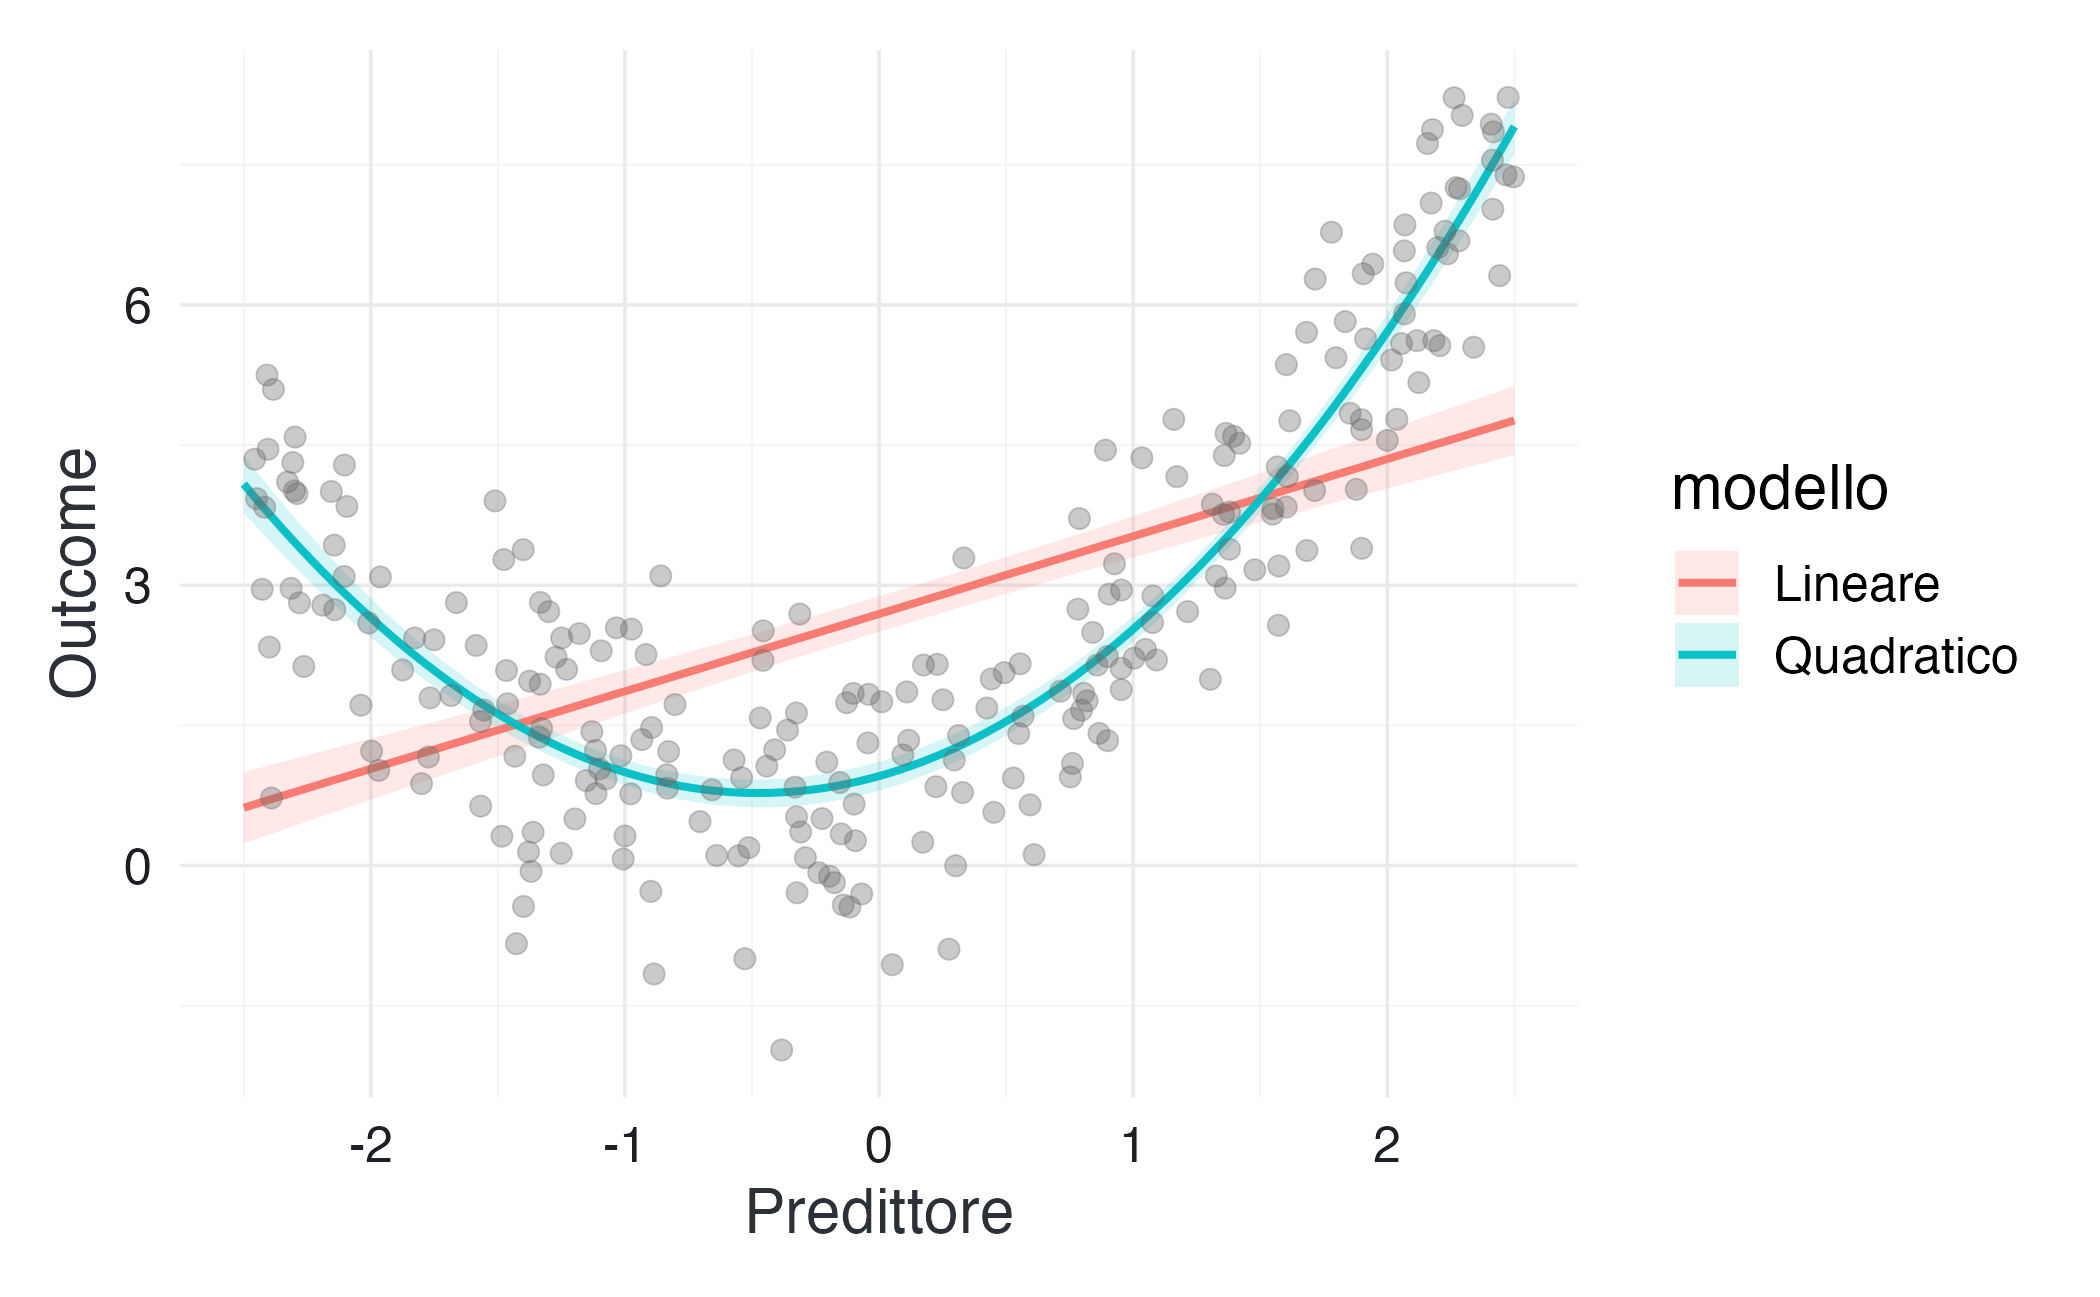
\includegraphics[width=0.85\linewidth,height=\textheight,keepaspectratio]{chapters/linear_models/09_quando_il_modello_sbaglia_files/figure-pdf/fig-nonlinearity-check-1.png}

}

\caption{\label{fig-nonlinearity-check}Dati simulati e medie posteriori
dei modelli lineare e quadratico. Il controllo condizionato al
predittore rivela la curvatura che un controllo marginale potrebbe
nascondere.}

\end{figure}%

La revisione riguarda la componente sistematica \(\mu_i\). Modificare il
prior o aumentare il numero di iterazioni non corregge una media
specificata come retta quando il fenomeno è curvilineo.

\subsection{Dispersione non costante}\label{dispersione-non-costante}

Nel modello gaussiano elementare, \(\sigma\) è comune a tutte le
osservazioni. Se la variabilità aumenta con il predittore, la media può
essere descritta correttamente mentre le previsioni individuali restano
mal calibrate.

\begin{Shaded}
\begin{Highlighting}[]
\FunctionTok{set.seed}\NormalTok{(}\DecValTok{202}\NormalTok{)}

\NormalTok{hetero\_data }\OtherTok{\textless{}{-}} \FunctionTok{tibble}\NormalTok{(}
  \AttributeTok{x =} \FunctionTok{runif}\NormalTok{(}\DecValTok{300}\NormalTok{, }\SpecialCharTok{{-}}\DecValTok{2}\NormalTok{, }\DecValTok{2}\NormalTok{),}
  \AttributeTok{mu =} \FloatTok{0.5} \SpecialCharTok{+} \FloatTok{1.1} \SpecialCharTok{*}\NormalTok{ x,}
  \AttributeTok{sigma =} \FunctionTok{exp}\NormalTok{(}\SpecialCharTok{{-}}\FloatTok{0.1} \SpecialCharTok{+} \FloatTok{0.45} \SpecialCharTok{*}\NormalTok{ x),}
  \AttributeTok{y =} \FunctionTok{rnorm}\NormalTok{(}\DecValTok{300}\NormalTok{, mu, sigma)}
\NormalTok{)}
\end{Highlighting}
\end{Shaded}

In \texttt{brms}, media e deviazione standard possono avere formule
distinte:

\begin{Shaded}
\begin{Highlighting}[]
\NormalTok{fit\_variable\_sigma }\OtherTok{\textless{}{-}} \FunctionTok{brm}\NormalTok{(}
  \FunctionTok{bf}\NormalTok{(y }\SpecialCharTok{\textasciitilde{}}\NormalTok{ x, sigma }\SpecialCharTok{\textasciitilde{}}\NormalTok{ x),}
  \AttributeTok{data =}\NormalTok{ hetero\_data,}
  \AttributeTok{family =} \FunctionTok{gaussian}\NormalTok{(),}
  \AttributeTok{prior =} \FunctionTok{c}\NormalTok{(}
    \FunctionTok{prior}\NormalTok{(}\FunctionTok{normal}\NormalTok{(}\DecValTok{0}\NormalTok{, }\DecValTok{2}\NormalTok{), }\AttributeTok{class =}\NormalTok{ Intercept),}
    \FunctionTok{prior}\NormalTok{(}\FunctionTok{normal}\NormalTok{(}\DecValTok{0}\NormalTok{, }\FloatTok{1.5}\NormalTok{), }\AttributeTok{class =}\NormalTok{ b),}
    \FunctionTok{prior}\NormalTok{(}\FunctionTok{normal}\NormalTok{(}\DecValTok{0}\NormalTok{, }\FloatTok{0.7}\NormalTok{), }\AttributeTok{class =}\NormalTok{ Intercept, }\AttributeTok{dpar =}\NormalTok{ sigma),}
    \FunctionTok{prior}\NormalTok{(}\FunctionTok{normal}\NormalTok{(}\DecValTok{0}\NormalTok{, }\FloatTok{0.5}\NormalTok{), }\AttributeTok{class =}\NormalTok{ b, }\AttributeTok{dpar =}\NormalTok{ sigma)}
\NormalTok{  )}
\NormalTok{)}
\end{Highlighting}
\end{Shaded}

Un controllo utile consiste nel confrontare la dispersione osservata e
quella replicata in intervalli del predittore. La revisione riguarda la
componente di dispersione e non necessariamente la relazione con la
media.

\subsection{Code pesanti e osservazioni
estreme}\label{code-pesanti-e-osservazioni-estreme-1}

Una verosimiglianza normale assegna una probabilità molto bassa alle
osservazioni lontane dalla media. Se i dati presentano code più pesanti,
poche osservazioni possono influenzare in modo significativo la pendenza
e la dispersione. Una verosimiglianza Student-\(t\) rappresenta una
possibile revisione:

\begin{Shaded}
\begin{Highlighting}[]
\NormalTok{fit\_student }\OtherTok{\textless{}{-}} \FunctionTok{brm}\NormalTok{(}
\NormalTok{  y }\SpecialCharTok{\textasciitilde{}}\NormalTok{ x,}
  \AttributeTok{data =}\NormalTok{ data,}
  \AttributeTok{family =} \FunctionTok{student}\NormalTok{(),}
  \AttributeTok{prior =} \FunctionTok{c}\NormalTok{(}
\NormalTok{    priors,}
    \FunctionTok{prior}\NormalTok{(}\FunctionTok{gamma}\NormalTok{(}\DecValTok{2}\NormalTok{, }\FloatTok{0.1}\NormalTok{), }\AttributeTok{class =}\NormalTok{ nu)}
\NormalTok{  )}
\NormalTok{)}
\end{Highlighting}
\end{Shaded}

Il passaggio a Student-\(t\) non dovrebbe essere una reazione automatica
alla presenza di un punto anomalo. Prima è necessario verificare la
qualità del dato, la plausibilità dell'osservazione, la sua influenza e
l'obiettivo dell'analisi. La revisione riguarda la forma della
distribuzione condizionata.

\subsection{Dipendenza ignorata}\label{dipendenza-ignorata}

Quando più osservazioni provengono dalla stessa persona, scuola o
situazione, l'indipendenza condizionale potrebbe non essere adeguata. Il
problema non può essere risolto scegliendo una distribuzione marginale
più flessibile: è necessario rappresentare la fonte della dipendenza,
per esempio mediante intercette o pendenze variabili, come discusso nel
Capitolo~\ref{sec-multilevel}.

Questi esempi mostrano perché un controllo predittivo generico non è
sufficiente. È necessario cercare la curvatura lungo il predittore,
l'eteroschedasticità nella dispersione condizionata, le code nella
frequenza degli estremi e la dipendenza nelle sequenze o nei
raggruppamenti pertinenti.

\section{La misurazione appartiene al
modello}\label{la-misurazione-appartiene-al-modello}

Una specificazione può essere inadeguata anche quando la funzione della
media, la dispersione e la struttura di dipendenza sono state formulate
correttamente. Ciò accade quando le variabili osservate vengono trattate
come se coincidessero perfettamente con i costrutti di interesse. In
psicologia, invece, i punteggi dei test, dei questionari e le
prestazioni sperimentali dipendono anche dalla precisione dello
strumento utilizzato e dalle condizioni in cui la misurazione è stata
effettuata.

Il principio da ricordare è semplice: \emph{il processo di misurazione
fa parte della storia generativa}. Ignorarlo equivale ad assumere che i
punteggi osservati rappresentino perfettamente le quantità teoriche.
Questa assunzione può modificare le stime, la loro incertezza e le
relazioni tra le variabili; la direzione della distorsione dipende dalla
struttura dell'errore e non è sempre prevedibile con una regola
generale.

Quando la qualità della misura è importante per la domanda scientifica,
il modello può essere ampliato utilizzando informazioni provenienti da
misure replicate, indicatori multipli, studi di affidabilità o dati di
calibrazione. Se queste informazioni non sono disponibili, è spesso più
onesto condurre un'analisi di sensibilità e dichiarare quali conclusioni
dipendono dalle ipotesi sulla misura.
L'Appendice~\ref{sec-measurement-error-method-appendix} sviluppa la
derivazione dell'attenuazione classica, i modelli con predittori
latenti, la correzione per la disattenuazione e la varianza di metodo
condivisa.

\section{Identificazione, sensibilità e
complessità}\label{identificazione-sensibilituxe0-e-complessituxe0}

Un modello più articolato non crea automaticamente nuova informazione.
Prima di aggiungere termini, componenti latenti o parametri di
dispersione, è necessario chiedersi se il disegno consenta di
distinguerli. Le misure replicate possono distinguere la variabilità
stabile dal rumore, più indicatori possono informare un costrutto
latente, metodi differenti possono aiutare a riconoscere una componente
comune di metodo e i dati esterni possono calibrare l'errore di misura.

Quando l'identificazione è debole, i prior contribuiscono in modo
sostanziale alla separazione delle componenti. Questi devono quindi
essere controllati mediante simulazioni predittive e analisi di
sensibilità. La domanda decisiva non è se il modello più complesso si
adatti meglio in assoluto, ma se risolva una discrepanza rilevante per
la quantità di interesse e se le conclusioni restino stabili entro un
insieme plausibile di assunzioni.

La revisione può anche mostrare che i dati non consentono la distinzione
desiderata. Riconoscere questa limitazione è un risultato scientifico
più informativo rispetto alla presentazione di una stima sostenuta
soprattutto dai vincoli del modello.

\section{Dal controllo del modello alla sua
interpretazione}\label{dal-controllo-del-modello-alla-sua-interpretazione}

Un modello predittivamente adeguato non stabilisce ancora come debba
essere interpretato un coefficiente. In particolare, non trasforma
automaticamente un'associazione in un effetto causale. La validità
causale richiede una domanda formulata in termini di intervento, un
estimand, un disegno sperimentale o delle assunzioni di identificazione
e una scelta giustificata delle variabili. Il modello lineare viene
ripreso dal Capitolo~\ref{sec-association-prediction-causality}, che
chiarisce le condizioni aggiuntive necessarie per attribuire un
significato causale alle stime.

\section{Errori frequenti}\label{errori-frequenti-8}

\begin{itemize}
\tightlist
\item
  Confondere la convergenza delle catene con l'adeguatezza del modello.
\item
  Usare un solo controllo predittivo e considerarlo una convalida
  generale.
\item
  Cambiare i prior quando la discrepanza riguarda la forma della media o
  la dipendenza.
\item
  Adottare automaticamente una verosimiglianza robusta senza indagare la
  natura delle osservazioni estreme.
\item
  Aggiungere parametri latenti senza verificare che il disegno li
  identifichi.
\item
  Trattare i punteggi osservati come misure prive di errore senza
  discuterne le conseguenze.
\end{itemize}

\section{Concetti da ricordare}\label{concetti-da-ricordare-7}

La diagnostica MCMC controlla il calcolo, non la validità del modello. I
controlli predittivi forniscono informazioni solo sulle proprietà che
esaminano. Media, dispersione, famiglia distributiva, dipendenza e
misurazione sono componenti distinte della specificazione. Una revisione
deve rispondere a una discrepanza osservabile e rilevante.
L'identificazione dipende sia dal disegno che dai prior. Infine, un
modello ben calibrato dal punto di vista predittivo non acquisisce per
questo un'interpretazione causale.

\section{Esercizi}\label{esercizi-7}

\subsection{1. Controllo mirato della non
linearità}\label{controllo-mirato-della-non-linearituxe0}

Simula una relazione cubica. Adatta un modello lineare e un modello con
termini polinomiali. Costruisci un controllo che renda visibile la
discrepanza lungo il predittore.

\subsection{2. Dispersione variabile}\label{dispersione-variabile}

Modifica la simulazione eteroschedastica affinché la dispersione
diminuisca al crescere di \(X\). Adatta un modello con
\texttt{sigma\ \textasciitilde{}\ x} e interpreta il coefficiente sulla
scala logaritmica.

\subsection{3. Controlli complementari}\label{controlli-complementari}

Per un modello già utilizzato nel Companion, progetta tre controlli
predittivi rivolti a proprietà differenti. Spiega quale fallimento
sarebbe rilevato da ciascuno.

\subsection{4. Misurazione e
sensibilità}\label{misurazione-e-sensibilituxe0}

Scegli una variabile psicologica usata in uno dei capitoli precedenti.
Descrivi quale informazione aggiuntiva sarebbe necessaria per
rappresentarne esplicitamente l'errore di misura e proponi una semplice
analisi di sensibilità quando tale informazione non è disponibile.

\subsection{5. Revisione documentata}\label{revisione-documentata}

Scegli un'analisi già svolta. Identifica un'assunzione potenzialmente
critica, proponi una statistica o un grafico predittivo e descrivi quale
revisione sarebbe giustificata da un eventuale fallimento.

\section*{Riflessioni conclusive}\label{riflessioni-conclusive-26}

\markright{Riflessioni conclusive}

La distribuzione a posteriori quantifica l'incertezza all'interno del
modello scelto, ma non include automaticamente quella relativa a tutte
le strutture alternative. Per questa ragione, il flusso di lavoro
bayesiano non si conclude con l'adattamento del modello e la lettura dei
coefficienti. È necessario un percorso di controllo che distingua i
problemi di calcolo dalle discrepanze predittive e dai limiti
dell'interpretazione.

Una curvatura residua invita a rivedere la funzione della media, una
dispersione variabile in modo sistematico richiede un modello per la
deviazione standard, code più pesanti possono motivare una diversa
verosimiglianza e le osservazioni annidate o ripetute richiedono una
struttura di dipendenza. Quando la misura è imperfetta, è necessario
considerare anche il processo di osservazione, almeno mediante una
verifica di sensibilità o un rinvio a un modello di misura più
esplicito. In tutti questi casi, la domanda da porsi non è quale comando
modificare, ma quale componente del modello è incompatibile con quanto
osservato.

La complessità è giustificata solo quando affronta una discrepanza
rilevante e quando il disegno contiene informazioni sufficienti per
sostenerla. Se questa informazione manca, un'analisi di sensibilità o
una conclusione più prudente possono essere preferibili a un modello
apparentemente sofisticato, ma debolmente identificato. Il capitolo
successivo estende la stessa cautela all'interpretazione dei
coefficienti: una relazione ben stimata rimane associativa finché il
disegno e le assunzioni non giustificano un significato causale.

\begin{tcolorbox}[enhanced jigsaw, arc=.35mm, bottomrule=.15mm, bottomtitle=1mm, breakable, colback=white, colbacktitle=quarto-callout-note-color!10!white, colframe=quarto-callout-note-color-frame, coltitle=black, left=2mm, leftrule=.75mm, opacityback=0, opacitybacktitle=0.6, rightrule=.15mm, title=\textcolor{quarto-callout-note-color}{\faInfo}\hspace{0.5em}{Informazioni sull'ambiente di sviluppo}, titlerule=0mm, toprule=.15mm, toptitle=1mm]

\begin{Shaded}
\begin{Highlighting}[]
\FunctionTok{sessionInfo}\NormalTok{()}
\CommentTok{\#\textgreater{} R version 4.6.1 (2026{-}06{-}24)}
\CommentTok{\#\textgreater{} Platform: aarch64{-}apple{-}darwin23}
\CommentTok{\#\textgreater{} Running under: macOS Tahoe 26.5.2}
\CommentTok{\#\textgreater{} }
\CommentTok{\#\textgreater{} Matrix products: default}
\CommentTok{\#\textgreater{} BLAS:   /Library/Frameworks/R.framework/Versions/4.6/Resources/lib/libRblas.0.dylib }
\CommentTok{\#\textgreater{} LAPACK: /Library/Frameworks/R.framework/Versions/4.6/Resources/lib/libRlapack.dylib;  LAPACK version 3.12.1}
\CommentTok{\#\textgreater{} }
\CommentTok{\#\textgreater{} locale:}
\CommentTok{\#\textgreater{} [1] C.UTF{-}8/UTF{-}8/C.UTF{-}8/C/C.UTF{-}8/C.UTF{-}8}
\CommentTok{\#\textgreater{} }
\CommentTok{\#\textgreater{} time zone: Europe/Zagreb}
\CommentTok{\#\textgreater{} tzcode source: internal}
\CommentTok{\#\textgreater{} }
\CommentTok{\#\textgreater{} attached base packages:}
\CommentTok{\#\textgreater{} [1] stats     graphics  grDevices utils     datasets  methods   base     }
\CommentTok{\#\textgreater{} }
\CommentTok{\#\textgreater{} other attached packages:}
\CommentTok{\#\textgreater{}  [1] broom\_1.0.13          ragg\_1.5.2            tinytable\_0.17.0     }
\CommentTok{\#\textgreater{}  [4] withr\_3.0.3           systemfonts\_1.3.2     patchwork\_1.3.2      }
\CommentTok{\#\textgreater{}  [7] ggdist\_3.3.3          tidybayes\_3.0.7       bayesplot\_1.15.0     }
\CommentTok{\#\textgreater{} [10] ggplot2\_4.0.3         reliabilitydiag\_0.2.1 priorsense\_1.2.0     }
\CommentTok{\#\textgreater{} [13] posterior\_1.7.0       loo\_2.10.0            rstan\_2.32.7         }
\CommentTok{\#\textgreater{} [16] StanHeaders\_2.32.10   brms\_2.23.0           Rcpp\_1.1.2           }
\CommentTok{\#\textgreater{} [19] sessioninfo\_1.2.4     conflicted\_1.2.0      janitor\_2.2.1        }
\CommentTok{\#\textgreater{} [22] matrixStats\_1.5.0     modelr\_0.1.11         tibble\_3.3.1         }
\CommentTok{\#\textgreater{} [25] dplyr\_1.2.1           tidyr\_1.3.2           rio\_1.3.0            }
\CommentTok{\#\textgreater{} [28] here\_1.0.2           }
\CommentTok{\#\textgreater{} }
\CommentTok{\#\textgreater{} loaded via a namespace (and not attached):}
\CommentTok{\#\textgreater{}  [1] svUnit\_1.0.8          tidyselect\_1.2.1      farver\_2.1.2         }
\CommentTok{\#\textgreater{}  [4] S7\_0.2.2              fastmap\_1.2.0         tensorA\_0.36.2.1     }
\CommentTok{\#\textgreater{}  [7] pacman\_0.5.1          digest\_0.6.39         timechange\_0.4.0     }
\CommentTok{\#\textgreater{} [10] estimability\_2.0.0    lifecycle\_1.0.5       processx\_3.9.0       }
\CommentTok{\#\textgreater{} [13] magrittr\_2.0.5        compiler\_4.6.1        rlang\_1.3.0          }
\CommentTok{\#\textgreater{} [16] tools\_4.6.1           yaml\_2.3.12           data.table\_1.18.4    }
\CommentTok{\#\textgreater{} [19] knitr\_1.51            labeling\_0.4.3        bridgesampling\_1.2{-}1 }
\CommentTok{\#\textgreater{} [22] pkgbuild\_1.4.8        curl\_7.1.0            cmdstanr\_0.9.0       }
\CommentTok{\#\textgreater{} [25] RColorBrewer\_1.1{-}3    abind\_1.4{-}8           purrr\_1.2.2          }
\CommentTok{\#\textgreater{} [28] grid\_4.6.1            stats4\_4.6.1          xtable\_1.8{-}8         }
\CommentTok{\#\textgreater{} [31] inline\_0.3.21         emmeans\_2.0.4         scales\_1.4.0         }
\CommentTok{\#\textgreater{} [34] cli\_3.6.6             mvtnorm\_1.4{-}2         rmarkdown\_2.31       }
\CommentTok{\#\textgreater{} [37] generics\_0.1.4        otel\_0.2.0            RcppParallel\_5.1.11{-}2}
\CommentTok{\#\textgreater{} [40] cachem\_1.1.0          stringr\_1.6.0         parallel\_4.6.1       }
\CommentTok{\#\textgreater{} [43] vctrs\_0.7.3           V8\_8.2.0              Matrix\_1.7{-}5         }
\CommentTok{\#\textgreater{} [46] jsonlite\_2.0.0        arrayhelpers\_1.1{-}1    glue\_1.8.1           }
\CommentTok{\#\textgreater{} [49] ps\_1.9.3              codetools\_0.2{-}20      distributional\_0.8.1 }
\CommentTok{\#\textgreater{} [52] lubridate\_1.9.5       stringi\_1.8.7         gtable\_0.3.6         }
\CommentTok{\#\textgreater{} [55] QuickJSR\_1.10.0       pillar\_1.11.1         htmltools\_0.5.9      }
\CommentTok{\#\textgreater{} [58] Brobdingnag\_1.2{-}9     R6\_2.6.1              textshaping\_1.0.5    }
\CommentTok{\#\textgreater{} [61] rprojroot\_2.1.1       evaluate\_1.0.5        lattice\_0.22{-}9       }
\CommentTok{\#\textgreater{} [64] backports\_1.5.1       memoise\_2.0.1         snakecase\_0.11.1     }
\CommentTok{\#\textgreater{} [67] rstantools\_2.6.0      coda\_0.19{-}4.1         gridExtra\_2.3.1      }
\CommentTok{\#\textgreater{} [70] nlme\_3.1{-}170          checkmate\_2.3.4       xfun\_0.60            }
\CommentTok{\#\textgreater{} [73] pkgconfig\_2.0.3}
\end{Highlighting}
\end{Shaded}

\end{tcolorbox}

\section*{Bibliografia}\label{bibliografia-29}

\markright{Bibliografia}

\chapter{Associazione, previsione ed effetto
causale}\label{sec-association-prediction-causality}

Un modello lineare può essere usato per descrivere una relazione
osservata, per prevedere un nuovo valore o per stimare una quantità
causale. La formula statistica può apparire molto simile nei tre casi,
ma la domanda scientifica, la quantità di interesse e le condizioni che
rendono valida la conclusione sono diverse.

Consideriamo, per esempio, una regressione del livello di ansia su un
indicatore di trattamento:

\[
Y_i \sim \operatorname{Normal}(\alpha + \beta A_i,\sigma).
\]

Il coefficiente \(\beta\) può rappresentare:

\begin{itemize}
\tightlist
\item
  una \textbf{differenza osservata} tra persone trattate e non trattate;
\item
  un elemento di una \textbf{regola predittiva} per nuovi individui;
\item
  una stima dell'\textbf{effetto medio del trattamento}, ma soltanto se
  il disegno e le assunzioni causali consentono questa interpretazione.
\end{itemize}

Il modello matematico, da solo, non stabilisce quale delle tre letture
sia corretta. Questo capitolo chiarisce la distinzione e prepara il
passaggio dalla parte \textbf{Modelli} alla parte \textbf{Causalità} del
Companion.

\begin{tcolorbox}[enhanced jigsaw, arc=.35mm, bottomrule=.15mm, breakable, colback=white, colframe=quarto-callout-important-color-frame, left=2mm, leftrule=.75mm, opacityback=0, rightrule=.15mm, toprule=.15mm]

\textbf{Da sapere.} Associazione, previsione ed effetto causale sono
obiettivi inferenziali distinti, anche quando utilizzano la stessa
formula statistica. Una relazione osservata non identifica
automaticamente un effetto causale e una buona capacità predittiva non
garantisce una corretta interpretazione causale. L'inferenza bayesiana
quantifica l'incertezza, ma non sostituisce il disegno dello studio e le
condizioni di identificazione.

\textbf{Da saper fare.} Distinguere domande associative, predittive e
causali; definire per ciascuna la quantità di interesse appropriata;
formulare un effetto causale mediante i potenziali esiti; spiegare il
ruolo della randomizzazione; riconoscere, a livello introduttivo,
confondenti, mediatori, collider e moderatori; formulare conclusioni
coerenti con il disegno e con le assunzioni disponibili.

\textbf{Approfondimento facoltativo.} I dettagli delle simulazioni, la
formalizzazione di consistenza e SUTVA e l'analisi più approfondita
delle strutture causali possono essere rimandati. Nel percorso
essenziale è sufficiente comprendere la distinzione tra i tre obiettivi
inferenziali e riconoscere perché l'identificazione causale precede la
stima. La trattazione completa dei controfattuali, dei DAG e delle
strategie per i dati osservazionali è sviluppata nella successiva parte
\textbf{Causalità}.

\hyperref[sec-percorsi-lettura]{Che cosa significano queste etichette?}

\end{tcolorbox}

\begin{tcolorbox}[enhanced jigsaw, arc=.35mm, bottomrule=.15mm, bottomtitle=1mm, breakable, colback=white, colbacktitle=quarto-callout-note-color!10!white, colframe=quarto-callout-note-color-frame, coltitle=black, left=2mm, leftrule=.75mm, opacityback=0, opacitybacktitle=0.6, rightrule=.15mm, title=\textcolor{quarto-callout-note-color}{\faInfo}\hspace{0.5em}{Obiettivi del capitolo}, titlerule=0mm, toprule=.15mm, toptitle=1mm]

Al termine del capitolo dovresti essere in grado di:

\begin{itemize}
\tightlist
\item
  distinguere una domanda associativa, predittiva e causale;
\item
  identificare la quantità di interesse appropriata per ciascuna
  domanda;
\item
  spiegare perché una buona previsione non implica una corretta
  interpretazione causale;
\item
  definire un effetto causale mediante i potenziali esiti;
\item
  comprendere il ruolo della randomizzazione;
\item
  riconoscere, a livello introduttivo, confondenti, mediatori e
  collider;
\item
  spiegare perché l'inferenza bayesiana quantifica l'incertezza ma non
  risolve automaticamente il problema dell'identificazione causale;
\item
  formulare conclusioni coerenti con il disegno dello studio.
\end{itemize}

\end{tcolorbox}

\begin{tcolorbox}[enhanced jigsaw, arc=.35mm, bottomrule=.15mm, bottomtitle=1mm, breakable, colback=white, colbacktitle=quarto-callout-tip-color!10!white, colframe=quarto-callout-tip-color-frame, coltitle=black, left=2mm, leftrule=.75mm, opacityback=0, opacitybacktitle=0.6, rightrule=.15mm, title=\textcolor{quarto-callout-tip-color}{\faLightbulb}\hspace{0.5em}{Percorsi di lettura}, titlerule=0mm, toprule=.15mm, toptitle=1mm]

Il capitolo appartiene al \textbf{percorso essenziale} e al
\textbf{percorso concettuale}. Le simulazioni costituiscono un supporto
operativo, ma il punto centrale è distinguere le domande inferenziali.
La formalizzazione completa dei controfattuali, dei DAG e delle
strategie per i dati osservazionali è sviluppata nella successiva parte
\textbf{Causalità}, a partire dal
Capitolo~\ref{sec-causality-propedeutics} e dal
Capitolo~\ref{sec-eda-causality}.

\end{tcolorbox}

\begin{tcolorbox}[enhanced jigsaw, arc=.35mm, bottomrule=.15mm, bottomtitle=1mm, breakable, colback=white, colbacktitle=quarto-callout-caution-color!10!white, colframe=quarto-callout-caution-color-frame, coltitle=black, left=2mm, leftrule=.75mm, opacityback=0, opacitybacktitle=0.6, rightrule=.15mm, title=\textcolor{quarto-callout-caution-color}{\faFire}\hspace{0.5em}{Preparazione del Notebook}, titlerule=0mm, toprule=.15mm, toptitle=1mm]

\end{tcolorbox}

\section{Tre domande, tre quantità di
interesse}\label{tre-domande-tre-quantituxe0-di-interesse}

La prima decisione non riguarda il software o il tipo di prior. Riguarda
la domanda alla quale vogliamo rispondere.

{\def\LTcaptype{none} % do not increment counter
\begin{longtable}[]{@{}
  >{\raggedright\arraybackslash}p{(\linewidth - 6\tabcolsep) * \real{0.2500}}
  >{\raggedright\arraybackslash}p{(\linewidth - 6\tabcolsep) * \real{0.2500}}
  >{\raggedright\arraybackslash}p{(\linewidth - 6\tabcolsep) * \real{0.2500}}
  >{\raggedright\arraybackslash}p{(\linewidth - 6\tabcolsep) * \real{0.2500}}@{}}
\toprule\noalign{}
\begin{minipage}[b]{\linewidth}\raggedright
Obiettivo
\end{minipage} & \begin{minipage}[b]{\linewidth}\raggedright
Domanda tipica
\end{minipage} & \begin{minipage}[b]{\linewidth}\raggedright
Quantità di interesse
\end{minipage} & \begin{minipage}[b]{\linewidth}\raggedright
Principale criterio di validità
\end{minipage} \\
\midrule\noalign{}
\endhead
\bottomrule\noalign{}
\endlastfoot
Associazione & Come differisce \(Y\) tra unità con valori diversi di
\(X\)? & \(\mathbb{E}(Y\mid X=x)\) o un contrasto condizionato &
Adeguatezza del modello alla distribuzione osservata \\
Previsione & Quale valore di \(Y\) è plausibile per una nuova unità? &
\(p(\widetilde{Y}\mid X,\mathcal{D})\) & Prestazione predittiva su dati
nuovi e popolazione bersaglio pertinente \\
Causalità & Che cosa accadrebbe a \(Y\) se intervenissimo su \(X\)? &
Contrasto tra potenziali esiti, per esempio \(\mathbb{E}[Y(1)-Y(0)]\) &
Disegno, identificazione e assunzioni causali \\
\end{longtable}
}

Le tre domande possono essere rivolte agli stessi dati. Non sono però
intercambiabili.

\begin{tcolorbox}[enhanced jigsaw, arc=.35mm, bottomrule=.15mm, bottomtitle=1mm, breakable, colback=white, colbacktitle=quarto-callout-important-color!10!white, colframe=quarto-callout-important-color-frame, coltitle=black, left=2mm, leftrule=.75mm, opacityback=0, opacitybacktitle=0.6, rightrule=.15mm, title=\textcolor{quarto-callout-important-color}{\faExclamation}\hspace{0.5em}{L'estimand viene prima del modello}, titlerule=0mm, toprule=.15mm, toptitle=1mm]

Prima di adattare una regressione è utile completare una frase del tipo:

\begin{quote}
Voglio stimare \ldots{} nella popolazione \ldots{} sotto le condizioni
\ldots{}
\end{quote}

Una formula come \texttt{y\ \textasciitilde{}\ x\ +\ z} non specifica da
sola se l'obiettivo sia descrittivo, predittivo o causale.

\end{tcolorbox}

\section{Associazione: descrivere differenze
osservate}\label{associazione-descrivere-differenze-osservate}

Una quantità associativa riguarda la distribuzione osservata. Con un
trattamento binario \(A\), una differenza associativa elementare è

\[
\Delta_{\text{ass}}=
\mathbb{E}(Y\mid A=1)-\mathbb{E}(Y\mid A=0).
\]

Questa quantità confronta due gruppi che esistono nei dati. Se le
persone trattate differiscono da quelle non trattate per gravità
iniziale, motivazione, accesso alle cure o altre caratteristiche, tali
differenze contribuiscono a \(\Delta_{\text{ass}}\).

Una regressione può rendere il confronto condizionato rispetto ad alcune
covariate:

\[
\mathbb{E}(Y\mid A,X)
=
\alpha+\beta_A A+\boldsymbol{\beta}_X^\mathsf{T}X.
\]

Il coefficiente \(\beta_A\) descrive allora una differenza tra unità con
gli stessi valori delle covariate incluse, secondo la forma funzionale
adottata. Anche questa è, in prima istanza, una quantità associativa.
Per leggerla come effetto causale servono condizioni aggiuntive.

\subsection{Un'associazione può essere scientificamente
utile}\label{unassociazione-puuxf2-essere-scientificamente-utile}

Definire una relazione come associativa non la rende poco interessante.
Le associazioni possono:

\begin{itemize}
\tightlist
\item
  descrivere disuguaglianze o pattern rilevanti;
\item
  suggerire ipotesi teoriche;
\item
  individuare gruppi con bisogni diversi;
\item
  contribuire alla previsione;
\item
  mettere in discussione un modello esistente.
\end{itemize}

Il problema nasce quando il linguaggio causale eccede ciò che il disegno
consente di sostenere.

\section{Previsione: anticipare osservazioni
nuove}\label{previsione-anticipare-osservazioni-nuove}

Una domanda predittiva riguarda una nuova osservazione
\(\widetilde{Y}\). Nel quadro bayesiano, la quantità centrale è la
distribuzione predittiva

\[
p(\widetilde{Y}\mid \widetilde{X},\mathcal{D})
=
\int
p(\widetilde{Y}\mid \widetilde{X},\theta)
\,p(\theta\mid\mathcal{D})
\,d\theta.
\]

Questa distribuzione incorpora:

\begin{enumerate}
\def\labelenumi{\arabic{enumi}.}
\tightlist
\item
  l'incertezza sui parametri \(\theta\);
\item
  la variabilità delle nuove osservazioni attorno alla media prevista.
\end{enumerate}

La qualità di una previsione non si valuta osservando soltanto quanto il
modello si adatta ai dati usati per stimarlo. Occorre verificare la
prestazione su dati nuovi o mediante procedure di validazione
appropriate.

\subsection{Previsione e spiegazione possono
divergere}\label{previsione-e-spiegazione-possono-divergere}

Una variabile può migliorare la previsione senza possedere il ruolo
causale che le attribuiamo. Per esempio:

\begin{itemize}
\tightlist
\item
  un indicatore costruito dopo il trattamento può essere molto
  predittivo dell'esito;
\item
  un proxy della gravità può migliorare le previsioni cliniche;
\item
  una variabile di selezione può separare bene casi con esiti
  differenti.
\end{itemize}

Tali variabili non sono per questo cause manipolabili dell'outcome.
Inoltre, includere una variabile post-trattamento o un collider può
migliorare alcuni indici predittivi e, nello stesso tempo, compromettere
la stima dell'effetto causale.

\begin{tcolorbox}[enhanced jigsaw, arc=.35mm, bottomrule=.15mm, bottomtitle=1mm, breakable, colback=white, colbacktitle=quarto-callout-warning-color!10!white, colframe=quarto-callout-warning-color-frame, coltitle=black, left=2mm, leftrule=.75mm, opacityback=0, opacitybacktitle=0.6, rightrule=.15mm, title=\textcolor{quarto-callout-warning-color}{\faExclamationTriangle}\hspace{0.5em}{Buona previsione non significa buona identificazione}, titlerule=0mm, toprule=.15mm, toptitle=1mm]

Un modello può prevedere accuratamente \(Y\) e produrre una stima
distorta dell'effetto di \(A\). In senso opposto, un esperimento
randomizzato di dimensioni limitate può identificare un effetto medio
pur avendo modesta accuratezza nella previsione degli esiti individuali.

\end{tcolorbox}

\section{Effetto causale: confrontare mondi
possibili}\label{effetto-causale-confrontare-mondi-possibili}

Per definire un effetto causale dobbiamo esplicitare un intervento. Sia
\(A_i\in\{0,1\}\) un trattamento. Per l'unità \(i\) definiamo due
potenziali esiti:

\[
Y_i(1)=\text{esito che osserveremmo sotto trattamento},
\]

\[
Y_i(0)=\text{esito che osserveremmo senza trattamento}.
\]

L'effetto causale individuale è

\[
\tau_i=Y_i(1)-Y_i(0).
\]

Non possiamo osservare entrambi i potenziali esiti per la stessa unità
nello stesso momento. Questo è il problema fondamentale dell'inferenza
causale (\citeproc{ref-hernan2020}{Hernán \& Robins, 2020}). Possiamo
però definire effetti medi, per esempio

\begin{equation}\protect\phantomsection\label{eq-average-treatment-effect}{
\tau_{\text{ATE}}
=
\mathbb{E}\left[Y(1)-Y(0)\right].
}\end{equation}

L'ATE non coincide, in generale, con la differenza associativa

\[
\mathbb{E}(Y\mid A=1)-\mathbb{E}(Y\mid A=0).
\]

Le due quantità coincidono soltanto sotto condizioni che rendono
confrontabili i gruppi rispetto ai potenziali esiti.

\subsection{Il ruolo della consistenza e
dell'interferenza}\label{il-ruolo-della-consistenza-e-dellinterferenza}

La notazione dei potenziali esiti richiede che il trattamento sia
definito abbastanza chiaramente da collegare il valore osservato al
corrispondente potenziale esito. Inoltre, l'esito di un'unità non
dovrebbe dipendere, salvo esplicita modellazione, dal trattamento
assegnato ad altre unità. Queste condizioni fanno parte del quadro
sintetizzato dalla nozione di SUTVA e saranno riprese nella parte
causale.

\section{Perché associazione ed effetto possono
differire}\label{perchuxe9-associazione-ed-effetto-possono-differire}

Supponiamo di studiare un intervento per ridurre l'ansia. Le persone con
ansia iniziale più elevata potrebbero avere una probabilità maggiore di
ricevere il trattamento. La gravità iniziale \(U\) influenza quindi sia
l'assegnazione \(A\) sia l'esito \(Y\):

\[
U\longrightarrow A,
\qquad
U\longrightarrow Y,
\qquad
A\longrightarrow Y.
\]

In questa configurazione, \(U\) è un \textbf{confondente}. Il confronto
grezzo tra trattati e non trattati mescola l'effetto del trattamento con
le differenze iniziali tra i gruppi.

\subsection{Una simulazione di
confondimento}\label{una-simulazione-di-confondimento}

Generiamo dati in cui l'effetto causale vero del trattamento è pari a
quattro punti, ma la probabilità di ricevere il trattamento aumenta con
la gravità iniziale.

\begin{Shaded}
\begin{Highlighting}[]
\NormalTok{n }\OtherTok{\textless{}{-}} \DecValTok{1000}
\NormalTok{true\_effect }\OtherTok{\textless{}{-}} \DecValTok{4}

\NormalTok{observational\_data }\OtherTok{\textless{}{-}} \FunctionTok{tibble}\NormalTok{(}
  \AttributeTok{baseline =} \FunctionTok{rnorm}\NormalTok{(n, }\AttributeTok{mean =} \DecValTok{0}\NormalTok{, }\AttributeTok{sd =} \DecValTok{1}\NormalTok{),}
  \AttributeTok{treatment =} \FunctionTok{rbinom}\NormalTok{(}
\NormalTok{    n,}
    \AttributeTok{size =} \DecValTok{1}\NormalTok{,}
    \AttributeTok{prob =} \FunctionTok{plogis}\NormalTok{(}\SpecialCharTok{{-}}\FloatTok{0.3} \SpecialCharTok{+} \FloatTok{1.3} \SpecialCharTok{*}\NormalTok{ baseline)}
\NormalTok{  )}
\NormalTok{) }\SpecialCharTok{|\textgreater{}}
  \FunctionTok{mutate}\NormalTok{(}
    \AttributeTok{outcome =} \DecValTok{50} \SpecialCharTok{+}
\NormalTok{      true\_effect }\SpecialCharTok{*}\NormalTok{ treatment }\SpecialCharTok{+}
      \DecValTok{8} \SpecialCharTok{*}\NormalTok{ baseline }\SpecialCharTok{+}
      \FunctionTok{rnorm}\NormalTok{(n, }\AttributeTok{mean =} \DecValTok{0}\NormalTok{, }\AttributeTok{sd =} \DecValTok{4}\NormalTok{),}
    \AttributeTok{group =} \FunctionTok{if\_else}\NormalTok{(treatment }\SpecialCharTok{==} \DecValTok{1}\NormalTok{, }\StringTok{"Trattamento"}\NormalTok{, }\StringTok{"Controllo"}\NormalTok{)}
\NormalTok{  )}
\end{Highlighting}
\end{Shaded}

Esaminiamo la differenza osservata negli esiti e la differenza nella
gravità iniziale.

\begin{Shaded}
\begin{Highlighting}[]
\NormalTok{observational\_summary }\OtherTok{\textless{}{-}}\NormalTok{ observational\_data }\SpecialCharTok{|\textgreater{}}
  \FunctionTok{group\_by}\NormalTok{(group) }\SpecialCharTok{|\textgreater{}}
  \FunctionTok{summarise}\NormalTok{(}
    \AttributeTok{n =} \FunctionTok{n}\NormalTok{(),}
    \AttributeTok{mean\_baseline =} \FunctionTok{mean}\NormalTok{(baseline),}
    \AttributeTok{mean\_outcome =} \FunctionTok{mean}\NormalTok{(outcome),}
    \AttributeTok{.groups =} \StringTok{"drop"}
\NormalTok{  )}

\NormalTok{observational\_summary}
\CommentTok{\#\textgreater{} \# A tibble: 2 x 4}
\CommentTok{\#\textgreater{}   group           n mean\_baseline mean\_outcome}
\CommentTok{\#\textgreater{}   \textless{}chr\textgreater{}       \textless{}int\textgreater{}         \textless{}dbl\textgreater{}        \textless{}dbl\textgreater{}}
\CommentTok{\#\textgreater{} 1 Controllo     546        {-}0.461         46.4}
\CommentTok{\#\textgreater{} 2 Trattamento   454         0.496         58.1}
\end{Highlighting}
\end{Shaded}

\begin{Shaded}
\begin{Highlighting}[]
\NormalTok{fit\_naive }\OtherTok{\textless{}{-}} \FunctionTok{lm}\NormalTok{(outcome }\SpecialCharTok{\textasciitilde{}}\NormalTok{ treatment, }\AttributeTok{data =}\NormalTok{ observational\_data)}
\NormalTok{fit\_adjusted }\OtherTok{\textless{}{-}} \FunctionTok{lm}\NormalTok{(outcome }\SpecialCharTok{\textasciitilde{}}\NormalTok{ treatment }\SpecialCharTok{+}\NormalTok{ baseline, }\AttributeTok{data =}\NormalTok{ observational\_data)}

\FunctionTok{bind\_rows}\NormalTok{(}
\NormalTok{  broom}\SpecialCharTok{::}\FunctionTok{tidy}\NormalTok{(fit\_naive) }\SpecialCharTok{|\textgreater{}}
    \FunctionTok{filter}\NormalTok{(term }\SpecialCharTok{==} \StringTok{"treatment"}\NormalTok{) }\SpecialCharTok{|\textgreater{}}
    \FunctionTok{mutate}\NormalTok{(}\AttributeTok{model =} \StringTok{"Confronto non aggiustato"}\NormalTok{),}
\NormalTok{  broom}\SpecialCharTok{::}\FunctionTok{tidy}\NormalTok{(fit\_adjusted) }\SpecialCharTok{|\textgreater{}}
    \FunctionTok{filter}\NormalTok{(term }\SpecialCharTok{==} \StringTok{"treatment"}\NormalTok{) }\SpecialCharTok{|\textgreater{}}
    \FunctionTok{mutate}\NormalTok{(}\AttributeTok{model =} \StringTok{"Aggiustamento per baseline"}\NormalTok{)}
\NormalTok{) }\SpecialCharTok{|\textgreater{}}
  \FunctionTok{select}\NormalTok{(model, estimate, std.error)}
\CommentTok{\#\textgreater{} \# A tibble: 2 x 3}
\CommentTok{\#\textgreater{}   model                      estimate std.error}
\CommentTok{\#\textgreater{}   \textless{}chr\textgreater{}                         \textless{}dbl\textgreater{}     \textless{}dbl\textgreater{}}
\CommentTok{\#\textgreater{} 1 Confronto non aggiustato      11.7      0.519}
\CommentTok{\#\textgreater{} 2 Aggiustamento per baseline     4.05     0.299}
\end{Highlighting}
\end{Shaded}

Il modello non aggiustato attribuisce al trattamento anche parte della
differenza dovuta alla gravità iniziale. Il modello che include
\texttt{baseline} si avvicina al valore usato per generare i dati,
perché nella simulazione abbiamo misurato correttamente il confondente e
specificato la relazione nella forma appropriata.

Questo risultato non dimostra che, nei dati reali, sia sufficiente
aggiungere una covariata. Nella simulazione conosciamo il processo
generativo; in un'applicazione osservazionale dobbiamo giustificare
quali variabili siano confondenti, come siano state misurate e quali
assunzioni rendano valido l'aggiustamento. Il bias da variabile omessa
può sovrastimare, sottostimare o perfino invertire una relazione
(\citeproc{ref-wilms2021omitted}{Wilms et al., 2021}).

\begin{Shaded}
\begin{Highlighting}[]
\NormalTok{plot\_observational }\OtherTok{\textless{}{-}}\NormalTok{ observational\_data }\SpecialCharTok{|\textgreater{}}
  \FunctionTok{pivot\_longer}\NormalTok{(}
    \AttributeTok{cols =} \FunctionTok{c}\NormalTok{(baseline, outcome),}
    \AttributeTok{names\_to =} \StringTok{"variable"}\NormalTok{,}
    \AttributeTok{values\_to =} \StringTok{"value"}
\NormalTok{  ) }\SpecialCharTok{|\textgreater{}}
  \FunctionTok{mutate}\NormalTok{(}
    \AttributeTok{variable =} \FunctionTok{recode}\NormalTok{(}
\NormalTok{      variable,}
      \AttributeTok{baseline =} \StringTok{"Gravità iniziale"}\NormalTok{,}
      \AttributeTok{outcome =} \StringTok{"Esito"}
\NormalTok{    )}
\NormalTok{  )}

\NormalTok{plot\_observational }\SpecialCharTok{|\textgreater{}}
  \FunctionTok{ggplot}\NormalTok{(}\FunctionTok{aes}\NormalTok{(}\AttributeTok{x =}\NormalTok{ group, }\AttributeTok{y =}\NormalTok{ value)) }\SpecialCharTok{+}
  \FunctionTok{geom\_boxplot}\NormalTok{(}\AttributeTok{outlier.alpha =} \FloatTok{0.25}\NormalTok{) }\SpecialCharTok{+}
  \FunctionTok{facet\_wrap}\NormalTok{(}\SpecialCharTok{\textasciitilde{}}\NormalTok{variable, }\AttributeTok{scales =} \StringTok{"free\_y"}\NormalTok{) }\SpecialCharTok{+}
  \FunctionTok{labs}\NormalTok{(}\AttributeTok{x =} \ConstantTok{NULL}\NormalTok{, }\AttributeTok{y =} \ConstantTok{NULL}\NormalTok{)}
\end{Highlighting}
\end{Shaded}

\begin{figure}[H]

\centering{

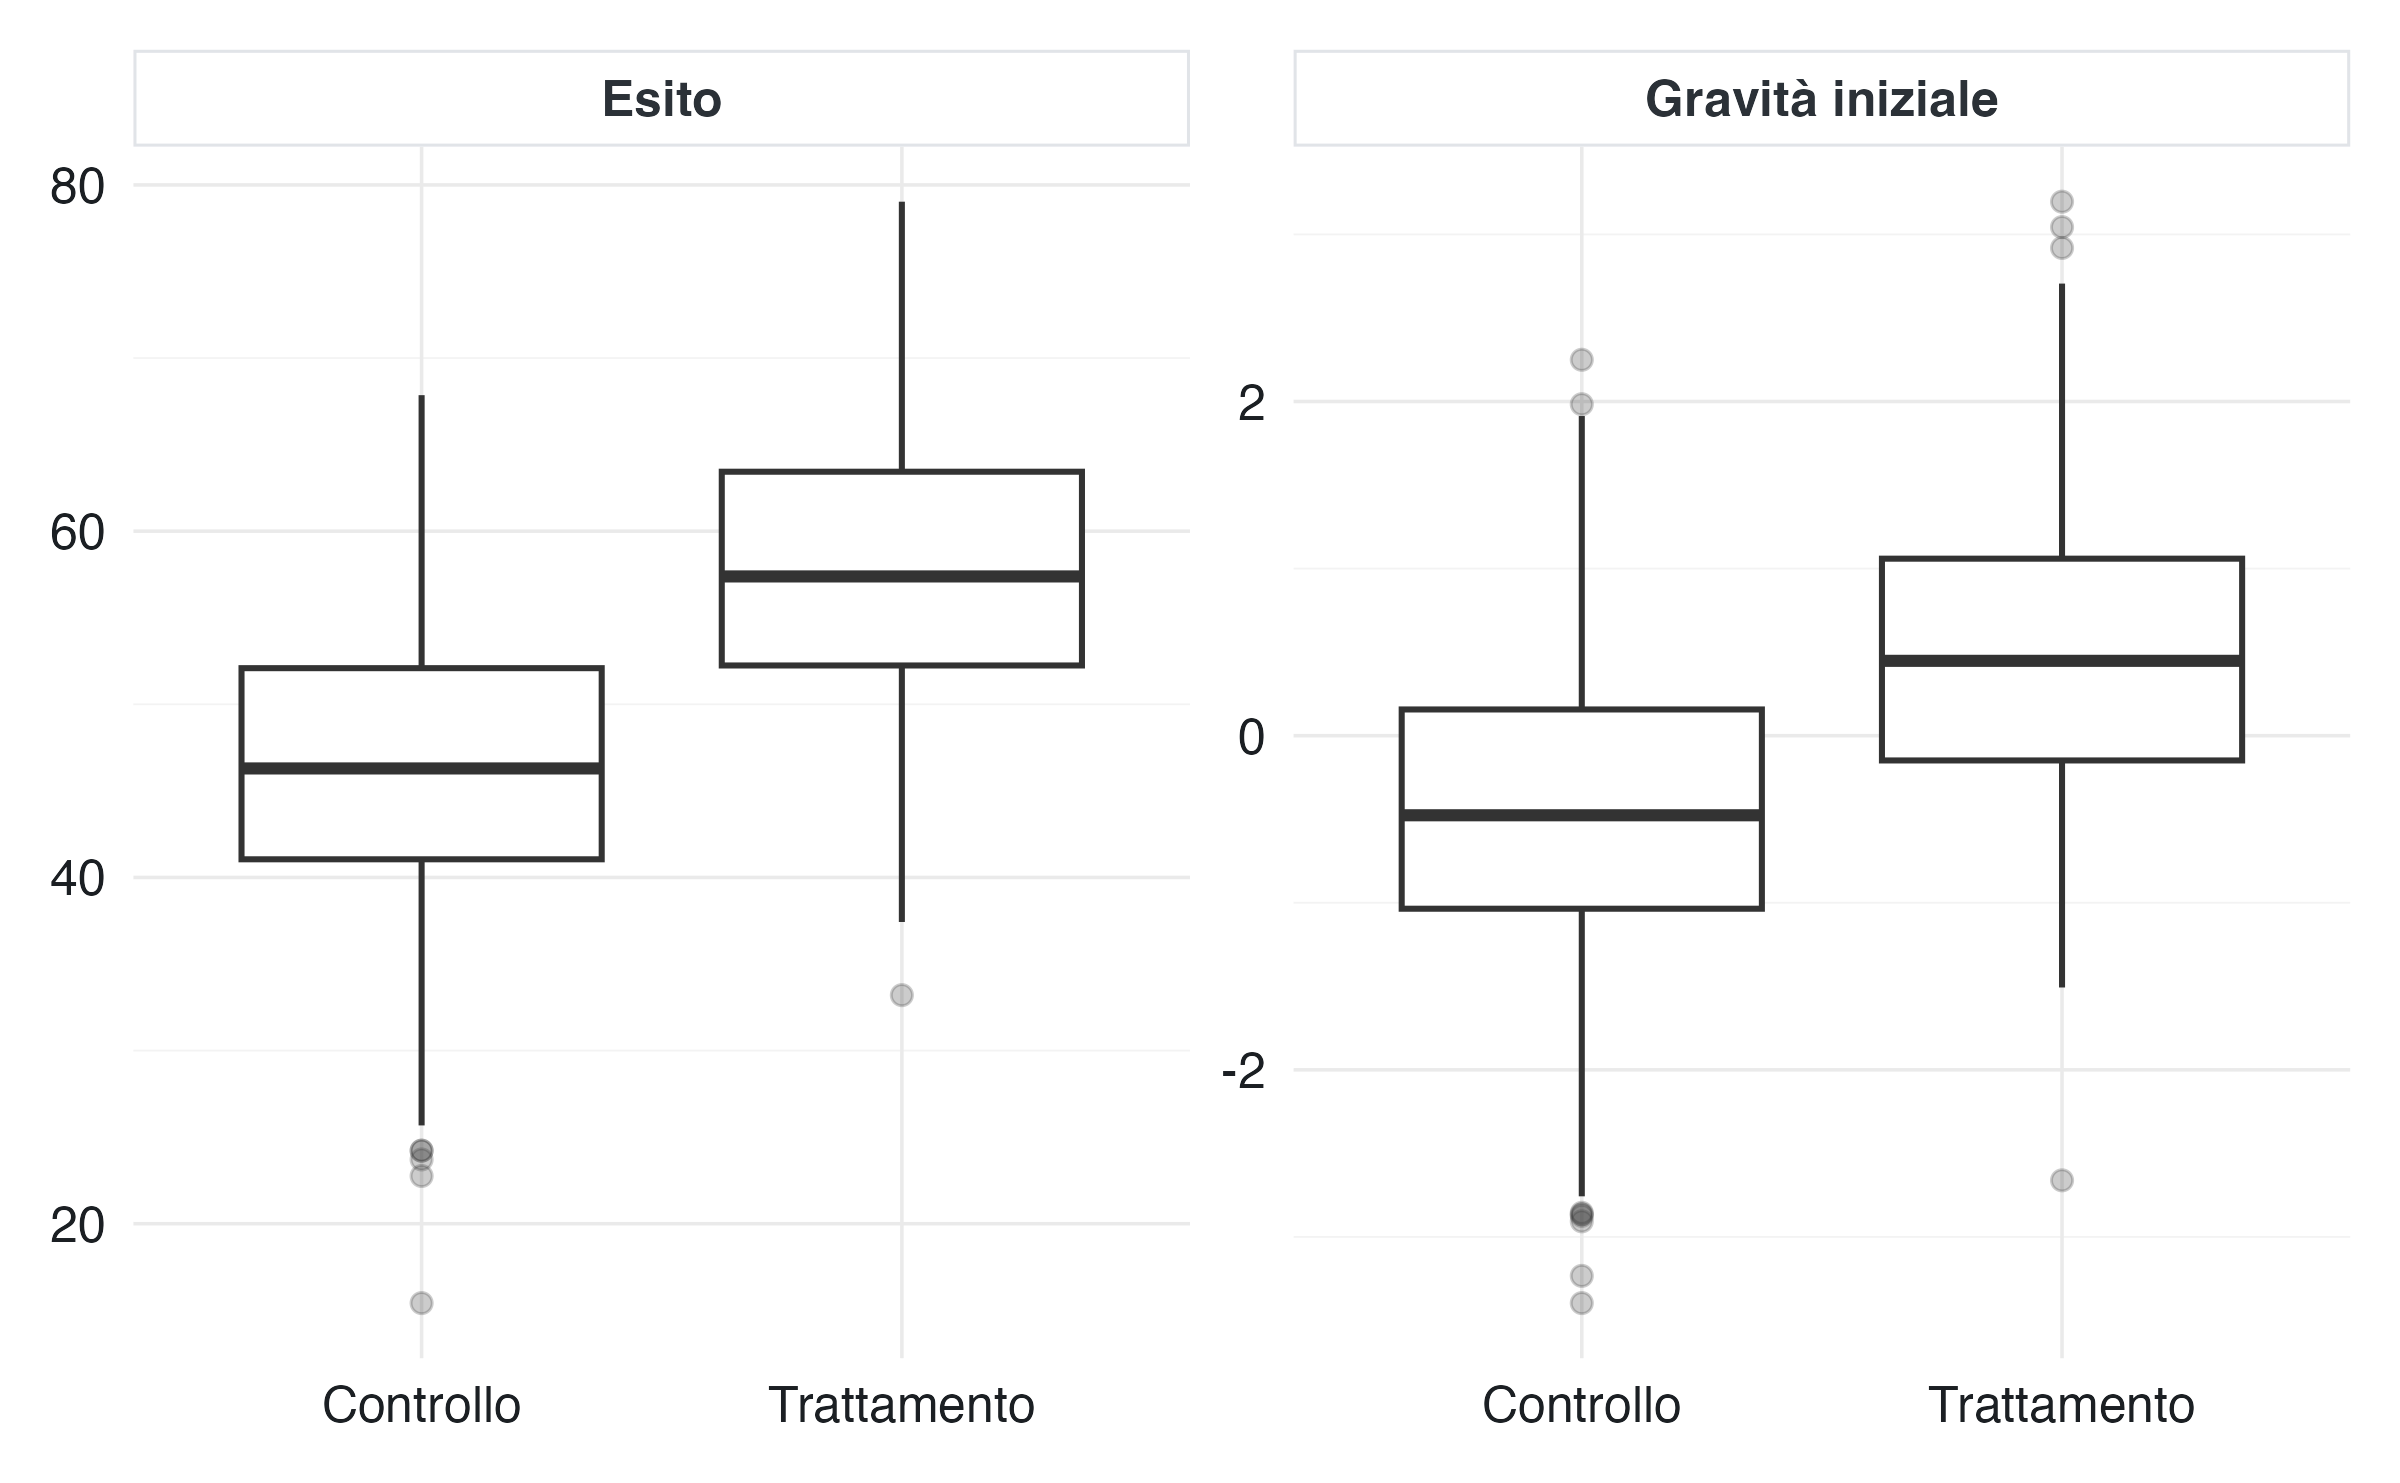
\includegraphics[width=0.85\linewidth,height=\textheight,keepaspectratio]{chapters/linear_models/10_associazione_previsione_effetto_causale_files/figure-pdf/fig-observational-confounding-1.png}

}

\caption{\label{fig-observational-confounding}Nel campione
osservazionale simulato, le persone trattate presentano una gravità
iniziale maggiore. La differenza negli esiti combina quindi effetto del
trattamento e differenze preesistenti.}

\end{figure}%

\section{Randomizzazione: quando il confronto identifica
l'effetto}\label{randomizzazione-quando-il-confronto-identifica-leffetto}

La randomizzazione rende l'assegnazione del trattamento indipendente, in
aspettativa, dai potenziali esiti e dalle caratteristiche
pre-trattamento. Ripetiamo la simulazione assegnando il trattamento
casualmente.

\begin{Shaded}
\begin{Highlighting}[]
\NormalTok{randomized\_data }\OtherTok{\textless{}{-}} \FunctionTok{tibble}\NormalTok{(}
  \AttributeTok{baseline =} \FunctionTok{rnorm}\NormalTok{(n, }\AttributeTok{mean =} \DecValTok{0}\NormalTok{, }\AttributeTok{sd =} \DecValTok{1}\NormalTok{),}
  \AttributeTok{treatment =} \FunctionTok{rbinom}\NormalTok{(n, }\AttributeTok{size =} \DecValTok{1}\NormalTok{, }\AttributeTok{prob =} \FloatTok{0.5}\NormalTok{)}
\NormalTok{) }\SpecialCharTok{|\textgreater{}}
  \FunctionTok{mutate}\NormalTok{(}
    \AttributeTok{outcome =} \DecValTok{50} \SpecialCharTok{+}
\NormalTok{      true\_effect }\SpecialCharTok{*}\NormalTok{ treatment }\SpecialCharTok{+}
      \DecValTok{8} \SpecialCharTok{*}\NormalTok{ baseline }\SpecialCharTok{+}
      \FunctionTok{rnorm}\NormalTok{(n, }\AttributeTok{mean =} \DecValTok{0}\NormalTok{, }\AttributeTok{sd =} \DecValTok{4}\NormalTok{),}
    \AttributeTok{group =} \FunctionTok{if\_else}\NormalTok{(treatment }\SpecialCharTok{==} \DecValTok{1}\NormalTok{, }\StringTok{"Trattamento"}\NormalTok{, }\StringTok{"Controllo"}\NormalTok{)}
\NormalTok{  )}
\end{Highlighting}
\end{Shaded}

\begin{Shaded}
\begin{Highlighting}[]
\NormalTok{randomized\_data }\SpecialCharTok{|\textgreater{}}
  \FunctionTok{group\_by}\NormalTok{(group) }\SpecialCharTok{|\textgreater{}}
  \FunctionTok{summarise}\NormalTok{(}
    \AttributeTok{n =} \FunctionTok{n}\NormalTok{(),}
    \AttributeTok{mean\_baseline =} \FunctionTok{mean}\NormalTok{(baseline),}
    \AttributeTok{mean\_outcome =} \FunctionTok{mean}\NormalTok{(outcome),}
    \AttributeTok{.groups =} \StringTok{"drop"}
\NormalTok{  )}
\CommentTok{\#\textgreater{} \# A tibble: 2 x 4}
\CommentTok{\#\textgreater{}   group           n mean\_baseline mean\_outcome}
\CommentTok{\#\textgreater{}   \textless{}chr\textgreater{}       \textless{}int\textgreater{}         \textless{}dbl\textgreater{}        \textless{}dbl\textgreater{}}
\CommentTok{\#\textgreater{} 1 Controllo     503       0.0464          50.2}
\CommentTok{\#\textgreater{} 2 Trattamento   497       0.00708         54.0}
\end{Highlighting}
\end{Shaded}

\begin{Shaded}
\begin{Highlighting}[]
\NormalTok{fit\_randomized }\OtherTok{\textless{}{-}} \FunctionTok{lm}\NormalTok{(outcome }\SpecialCharTok{\textasciitilde{}}\NormalTok{ treatment, }\AttributeTok{data =}\NormalTok{ randomized\_data)}

\NormalTok{broom}\SpecialCharTok{::}\FunctionTok{tidy}\NormalTok{(fit\_randomized) }\SpecialCharTok{|\textgreater{}}
  \FunctionTok{filter}\NormalTok{(term }\SpecialCharTok{==} \StringTok{"treatment"}\NormalTok{) }\SpecialCharTok{|\textgreater{}}
  \FunctionTok{select}\NormalTok{(estimate, std.error)}
\CommentTok{\#\textgreater{} \# A tibble: 1 x 2}
\CommentTok{\#\textgreater{}   estimate std.error}
\CommentTok{\#\textgreater{}      \textless{}dbl\textgreater{}     \textless{}dbl\textgreater{}}
\CommentTok{\#\textgreater{} 1     3.79     0.556}
\end{Highlighting}
\end{Shaded}

In questo caso, il confronto non aggiustato stima l'effetto medio perché
il trattamento è stato assegnato indipendentemente dalla gravità
iniziale. L'aggiustamento per covariate pre-trattamento può aumentare la
precisione, ma non è ciò che crea l'identificazione causale: è il
disegno randomizzato a giustificare il confronto.

\begin{tcolorbox}[enhanced jigsaw, arc=.35mm, bottomrule=.15mm, bottomtitle=1mm, breakable, colback=white, colbacktitle=quarto-callout-important-color!10!white, colframe=quarto-callout-important-color-frame, coltitle=black, left=2mm, leftrule=.75mm, opacityback=0, opacitybacktitle=0.6, rightrule=.15mm, title=\textcolor{quarto-callout-important-color}{\faExclamation}\hspace{0.5em}{L'identificazione precede la stima}, titlerule=0mm, toprule=.15mm, toptitle=1mm]

La randomizzazione, un esperimento naturale o un insieme esplicito di
assunzioni sui dati osservazionali può identificare una quantità
causale. Soltanto dopo questa fase ha senso scegliere come stimarla e
come rappresentarne l'incertezza.

\end{tcolorbox}

\section{Che cosa aggiunge l'approccio
bayesiano}\label{che-cosa-aggiunge-lapproccio-bayesiano}

Una volta identificato l'estimand, l'approccio bayesiano permette di:

\begin{itemize}
\tightlist
\item
  incorporare conoscenze pregresse mediante prior trasparenti;
\item
  propagare l'incertezza dai parametri alle quantità causali derivate;
\item
  rappresentare l'eterogeneità degli effetti;
\item
  produrre distribuzioni predittive sotto interventi definiti;
\item
  svolgere analisi di sensibilità rispetto a componenti del modello.
\end{itemize}

Il posterior di una quantità causale dipende però sia dal modello
statistico sia dalle assunzioni che collegano i dati osservati ai
potenziali esiti. In forma schematica,

\[
p(\tau\mid\mathcal{D},\mathcal{M},\mathcal{A}),
\]

dove \(\mathcal{M}\) rappresenta il modello probabilistico e
\(\mathcal{A}\) le assunzioni causali e di identificazione.

Una distribuzione a posteriori molto concentrata può quindi descrivere
con grande precisione una quantità associativa distorta. Cambiare
algoritmo, aumentare il numero di iterazioni o usare prior più
sofisticati non corregge automaticamente confondenti non misurati,
collider condizionati o trattamenti definiti in modo ambiguo.

\begin{tcolorbox}[enhanced jigsaw, arc=.35mm, bottomrule=.15mm, bottomtitle=1mm, breakable, colback=white, colbacktitle=quarto-callout-warning-color!10!white, colframe=quarto-callout-warning-color-frame, coltitle=black, left=2mm, leftrule=.75mm, opacityback=0, opacitybacktitle=0.6, rightrule=.15mm, title=\textcolor{quarto-callout-warning-color}{\faExclamationTriangle}\hspace{0.5em}{Bayes non trasforma l'associazione in causalità}, titlerule=0mm, toprule=.15mm, toptitle=1mm]

L'inferenza bayesiana quantifica l'incertezza \textbf{condizionatamente
al modello e alle assunzioni}. Se l'estimand causale non è identificato,
il problema non è risolto da una posterior numericamente stabile.

\end{tcolorbox}

\section{Scegliere le variabili: il ruolo della struttura
causale}\label{scegliere-le-variabili-il-ruolo-della-struttura-causale}

Nel lavoro descrittivo o predittivo, le covariate possono essere
selezionate in base alla domanda e alla capacità di generalizzazione.
Nella stima causale, la scelta deve essere guidata dal ruolo che
ciascuna variabile occupa rispetto al trattamento e all'esito.

\subsection{Confondente}\label{confondente}

Una causa comune di trattamento ed esito:

\[
A\leftarrow U\rightarrow Y.
\]

Se le condizioni necessarie sono soddisfatte, aggiustare per \(U\) può
bloccare il percorso non causale tra \(A\) e \(Y\).

\subsection{Mediatore}\label{mediatore}

Una variabile attraverso cui passa parte dell'effetto:

\[
A\rightarrow M\rightarrow Y.
\]

Se l'obiettivo è l'effetto totale, controllare per \(M\) elimina parte
della quantità che vogliamo stimare. Se l'obiettivo è un effetto
diretto, il ruolo di \(M\) deve essere definito esplicitamente e sono
necessarie assunzioni ulteriori.

\subsection{Collider}\label{collider}

Un effetto comune del trattamento e dell'esito, o di loro cause:

\[
A\rightarrow C\leftarrow Y.
\]

Condizionare su \(C\), o in alcuni casi su un suo discendente, può
creare un'associazione che prima non esisteva.

\subsection{Moderatore}\label{moderatore}

Un moderatore descrive eterogeneità dell'effetto: il contrasto causale
varia in funzione di una caratteristica \(W\). Non è una categoria
alternativa a confondente, mediatore o collider. La stessa variabile può
avere ruoli diversi in differenti teorie causali, e tali ruoli devono
essere specificati nel grafo e nell'estimand.

\begin{tcolorbox}[enhanced jigsaw, arc=.35mm, bottomrule=.15mm, bottomtitle=1mm, breakable, colback=white, colbacktitle=quarto-callout-tip-color!10!white, colframe=quarto-callout-tip-color-frame, coltitle=black, left=2mm, leftrule=.75mm, opacityback=0, opacitybacktitle=0.6, rightrule=.15mm, title=\textcolor{quarto-callout-tip-color}{\faLightbulb}\hspace{0.5em}{Non controllare automaticamente tutto ciò che è disponibile}, titlerule=0mm, toprule=.15mm, toptitle=1mm]

Aumentare \(R^2\), ridurre l'AIC o migliorare la previsione non sono
criteri sufficienti per scegliere un insieme di aggiustamento causale. I
DAG e il criterio \emph{backdoor}, sviluppati nel
Capitolo~\ref{sec-eda-causality}, formalizzano quali percorsi debbano
essere chiusi e quali non debbano essere aperti.

\end{tcolorbox}

\section{Lo stesso coefficiente, significati
diversi}\label{lo-stesso-coefficiente-significati-diversi}

Consideriamo nuovamente

\[
Y_i\sim\operatorname{Normal}(\alpha+\beta A_i,\sigma).
\]

Il significato di \(\beta\) dipende dal contesto:

\begin{itemize}
\tightlist
\item
  \textbf{studio osservazionale non aggiustato:} differenza media
  osservata tra i gruppi;
\item
  \textbf{modello predittivo:} contributo del trattamento alla
  previsione, condizionato alle altre variabili e alla specificazione;
\item
  \textbf{esperimento randomizzato:} stima della differenza media
  causale, sotto consistenza, assenza di interferenza e corretta
  gestione dei dati mancanti;
\item
  \textbf{studio osservazionale aggiustato:} possibile stima causale
  soltanto sotto ipotesi di scambiabilità condizionata, positività,
  consistenza e adeguata specificazione.
\end{itemize}

La formula non contiene l'informazione relativa al meccanismo di
assegnazione. Due dataset con le stesse colonne e lo stesso modello di
regressione possono sostenere conclusioni causali molto diverse.

\section{Linguaggio coerente con
l'evidenza}\label{linguaggio-coerente-con-levidenza}

La formulazione dei risultati dovrebbe riflettere la domanda e il
disegno.

\subsection{Linguaggio associativo}\label{linguaggio-associativo}

\begin{quote}
Nel campione analizzato, il gruppo trattato presenta in media un
punteggio di ansia inferiore di 3.2 punti rispetto al gruppo non
trattato.
\end{quote}

\subsection{Linguaggio predittivo}\label{linguaggio-predittivo}

\begin{quote}
L'inclusione dell'indicatore di trattamento migliora la previsione
dell'ansia in nuovi casi della popolazione considerata.
\end{quote}

\subsection{Linguaggio causale}\label{linguaggio-causale-1}

\begin{quote}
Nell'esperimento randomizzato, l'assegnazione al trattamento riduce in
media il punteggio di ansia di 3.2 punti rispetto al controllo, sotto le
assunzioni dichiarate.
\end{quote}

Nel terzo caso, il verbo causale è sostenuto dal disegno e da un
estimand definito. Non deriva semplicemente dal fatto che il
coefficiente sia diverso da zero.

\section{Collegamento con la parte
Causalità}\label{collegamento-con-la-parte-causalituxe0}

Questo capitolo ha stabilito il confine tra tre obiettivi inferenziali.
Non ha ancora fornito una procedura completa per identificare effetti da
dati osservazionali.

La parte \textbf{Causalità} svilupperà in modo sistematico:

\begin{itemize}
\tightlist
\item
  il quadro controfattuale e gli estimand causali;
\item
  la distinzione tra effetto totale, diretto e condizionato;
\item
  i DAG e le indipendenze implicate;
\item
  catene, cause comuni, collider e discendenti;
\item
  il criterio \emph{backdoor} e la scelta delle variabili di
  aggiustamento;
\item
  strategie sperimentali, quasi-sperimentali e osservazionali;
\item
  limiti dovuti al confondimento non osservato.
\end{itemize}

Il Capitolo~\ref{sec-causality-propedeutics} approfondisce la notazione
dei potenziali esiti e il ruolo della randomizzazione. Il
Capitolo~\ref{sec-eda-causality} introduce gli strumenti operativi per
ragionare sui dati osservazionali. Tra i riferimenti utili per questo
passaggio figurano Hernán \& Robins (\citeproc{ref-hernan2020}{2020}),
McElreath (\citeproc{ref-McElreath_rethinking}{2020}), Byrnes \& Dee
(\citeproc{ref-byrnes2024causal}{2024}), Riederer
(\citeproc{ref-riedererdesignpatterns}{2021}) e Alexander
(\citeproc{ref-alexander2023telling}{2023}).

\section{Errori frequenti}\label{errori-frequenti-9}

\begin{tcolorbox}[enhanced jigsaw, arc=.35mm, bottomrule=.15mm, bottomtitle=1mm, breakable, colback=white, colbacktitle=quarto-callout-caution-color!10!white, colframe=quarto-callout-caution-color-frame, coltitle=black, left=2mm, leftrule=.75mm, opacityback=0, opacitybacktitle=0.6, rightrule=.15mm, title=\textcolor{quarto-callout-caution-color}{\faFire}\hspace{0.5em}{Attenzione}, titlerule=0mm, toprule=.15mm, toptitle=1mm]

\begin{enumerate}
\def\labelenumi{\arabic{enumi}.}
\tightlist
\item
  \textbf{Chiamare effetto ogni coefficiente.} Un coefficiente di
  regressione è inizialmente una quantità del modello associativo;
  l'interpretazione causale richiede identificazione.
\item
  \textbf{Confondere buona previsione e buona spiegazione.} Un
  predittore accurato non è necessariamente una leva causale.
\item
  \textbf{Pensare che l'aggiustamento sia sempre protettivo.}
  Controllare mediatori o collider può cambiare l'estimand o introdurre
  bias.
\item
  \textbf{Usare la significatività o la precisione come prova causale.}
  Un intervallo stretto può concentrarsi attorno a una quantità
  distorta.
\item
  \textbf{Definire il trattamento in modo vago.} Un effetto causale
  richiede un intervento sufficientemente preciso.
\item
  \textbf{Dimenticare la popolazione bersaglio.} Un effetto identificato
  nel campione non si generalizza automaticamente ad altri contesti.
\item
  \textbf{Interpretare l'aggiustamento per covariate come sostituto
  della randomizzazione.} Nei dati osservazionali l'aggiustamento è
  valido soltanto sotto assunzioni sostantive non verificabili
  interamente dai dati.
\end{enumerate}

\end{tcolorbox}

\section{Riflessioni conclusive}\label{riflessioni-conclusive-27}

Associazione, previsione e causalità non sono tre livelli crescenti di
una stessa analisi. Sono obiettivi differenti.

\begin{itemize}
\tightlist
\item
  Una domanda \textbf{associativa} riguarda come le variabili si
  distribuiscono insieme nei dati osservati.
\item
  Una domanda \textbf{predittiva} riguarda la distribuzione di nuove
  osservazioni e richiede validazione fuori campione.
\item
  Una domanda \textbf{causale} riguarda il confronto tra esiti sotto
  interventi alternativi e richiede un estimand, una strategia di
  identificazione e assunzioni sul processo che ha prodotto i dati.
\end{itemize}

L'approccio bayesiano è utile in tutti e tre i casi, perché consente di
rappresentare e propagare l'incertezza. Non elimina però la distinzione
tra essi. La posterior risponde alla domanda codificata dal modello e
dalle assunzioni: non può trasformare retroattivamente una domanda
associativa in una domanda causale.

Con questo capitolo termina la progressione principale della parte
\textbf{Modelli}. Abbiamo costruito il modello lineare, ne abbiamo
esaminato casi particolari ed estensioni, abbiamo modellato
l'eterogeneità e abbiamo visto come controllarne e revisionarne la
specificazione. La parte \textbf{Causalità} aggiungerà ora il livello
necessario per interpretare alcune quantità come conseguenze di
interventi.

\section{Concetti da ricordare}\label{concetti-da-ricordare-8}

\begin{enumerate}
\def\labelenumi{\arabic{enumi}.}
\tightlist
\item
  La stessa formula di regressione può servire a obiettivi associativi,
  predittivi o causali.
\item
  L'estimand deve essere definito prima della procedura di stima.
\item
  Una differenza osservata tra gruppi non coincide generalmente con un
  effetto causale.
\item
  La previsione riguarda nuovi dati; la causalità riguarda interventi
  alternativi.
\item
  La randomizzazione giustifica, in aspettativa, il confronto causale
  tra i gruppi.
\item
  Nei dati osservazionali l'aggiustamento richiede ipotesi sulla
  struttura causale.
\item
  Confondenti, mediatori e collider non devono essere trattati allo
  stesso modo.
\item
  Un moderatore descrive eterogeneità dell'effetto e non è, di per sé,
  una variabile da aggiustare.
\item
  La posterior quantifica l'incertezza condizionatamente al modello e
  alle assunzioni.
\item
  Una stima precisa può essere causalmente distorta.
\end{enumerate}

\begin{tcolorbox}[enhanced jigsaw, arc=.35mm, bottomrule=.15mm, bottomtitle=1mm, breakable, colback=white, colbacktitle=quarto-callout-important-color!10!white, colframe=quarto-callout-important-color-frame, coltitle=black, left=2mm, leftrule=.75mm, opacityback=0, opacitybacktitle=0.6, rightrule=.15mm, title=\textcolor{quarto-callout-important-color}{\faExclamation}\hspace{0.5em}{Esercizi}, titlerule=0mm, toprule=.15mm, toptitle=1mm]

\subsection{1. Classificare la domanda}\label{classificare-la-domanda}

Classifica ciascuna domanda come associativa, predittiva o causale:

\begin{enumerate}
\def\labelenumi{\arabic{enumi}.}
\tightlist
\item
  Qual è la differenza media nell'ansia tra chi pratica e chi non
  pratica meditazione?
\item
  Quanto accuratamente possiamo prevedere una ricaduta entro sei mesi?
\item
  Di quanto cambierebbe l'ansia se assegnassimo le persone a otto
  settimane di meditazione?
\end{enumerate}

\subsection{2. Definire l'estimand}\label{definire-lestimand-1}

Per uno studio sull'effetto di un programma di tutoraggio sul voto
finale, definisci:

\begin{itemize}
\tightlist
\item
  una quantità associativa;
\item
  una quantità predittiva;
\item
  un ATE causale.
\end{itemize}

\subsection{3. Confondimento}\label{confondimento}

Supponi che gli studenti con maggiori difficoltà iniziali siano più
propensi a iscriversi al tutoraggio. Disegna verbalmente il DAG minimo e
spiega perché il confronto grezzo può sottostimare l'efficacia del
programma.

\subsection{4. Mediatore}\label{mediatore-1}

Il tutoraggio aumenta le ore di studio, che a loro volta migliorano il
voto. Spiega perché controllare per le ore di studio cambia la domanda
dall'effetto totale a una forma di effetto diretto.

\subsection{5. Collider}\label{collider-1}

L'ammissione a un programma selettivo dipende sia dalla motivazione sia
dal rendimento precedente. Spiega perché analizzare soltanto gli
studenti ammessi può creare un'associazione tra motivazione e rendimento
precedente anche se nella popolazione non sono associati.

\subsection{6. Randomizzazione}\label{randomizzazione}

Modifica la simulazione osservazionale sostituendo l'assegnazione
dipendente da \texttt{baseline} con un'assegnazione Bernoulli con
probabilità 0.5. Confronta:

\begin{itemize}
\tightlist
\item
  differenza nella baseline;
\item
  differenza negli esiti;
\item
  coefficiente non aggiustato del trattamento.
\end{itemize}

\subsection{7. Precisione senza
validità}\label{precisione-senza-validituxe0}

Immagina un dataset osservazionale enorme con un confondente non
misurato. Spiega perché l'intervallo di credibilità del coefficiente può
diventare molto stretto senza avvicinarsi all'effetto causale.

\subsection{8. Riscrivere una
conclusione}\label{riscrivere-una-conclusione}

Riscrivi la frase seguente in una forma appropriata per uno studio
osservazionale:

\begin{quote}
La solitudine causa un aumento di 4 punti nella depressione.
\end{quote}

\subsection{9. Predizione e variabili
post-trattamento}\label{predizione-e-variabili-post-trattamento}

Una misura raccolta a metà della terapia migliora fortemente la
previsione dell'esito finale. Spiega perché questa variabile può essere
utile per la previsione ma problematica se l'obiettivo è stimare
l'effetto totale dell'assegnazione alla terapia.

\end{tcolorbox}

\begin{tcolorbox}[enhanced jigsaw, arc=.35mm, bottomrule=.15mm, bottomtitle=1mm, breakable, colback=white, colbacktitle=quarto-callout-tip-color!10!white, colframe=quarto-callout-tip-color-frame, coltitle=black, left=2mm, leftrule=.75mm, opacityback=0, opacitybacktitle=0.6, rightrule=.15mm, title=\textcolor{quarto-callout-tip-color}{\faLightbulb}\hspace{0.5em}{Tracce di soluzione}, titlerule=0mm, toprule=.15mm, toptitle=1mm]

\begin{enumerate}
\def\labelenumi{\arabic{enumi}.}
\tightlist
\item
  Le domande sono, nell'ordine, associativa, predittiva e causale.
\item
  Associazione: differenza osservata tra iscritti e non iscritti.
  Predizione: distribuzione del voto per un nuovo studente date le
  covariate. Causalità: media di \(Y(1)-Y(0)\) nella popolazione
  bersaglio.
\item
  Il DAG minimo è \texttt{difficoltà\ →\ tutoraggio},
  \texttt{difficoltà\ →\ voto}, \texttt{tutoraggio\ →\ voto}. Poiché chi
  riceve il programma parte svantaggiato, il confronto grezzo può
  mascherarne un effetto positivo.
\item
  Le ore di studio appartengono al percorso attraverso cui il programma
  agisce. Condizionarle blocca tale percorso e modifica l'estimand.
\item
  L'ammissione è un effetto comune. Condizionare sull'ammissione apre un
  percorso tra le sue cause e produce dipendenza da selezione.
\item
  Con randomizzazione la baseline è bilanciata in aspettativa e il
  coefficiente non aggiustato oscilla attorno all'effetto generativo
  vero.
\item
  L'aumento di \(n\) riduce l'incertezza campionaria attorno alla
  quantità identificata dal modello, ma non elimina il bias strutturale
  dovuto al confondente omesso.
\item
  Una formulazione appropriata è: «Nel campione analizzato, livelli
  maggiori di solitudine sono associati a punteggi di depressione più
  elevati di circa quattro punti, a parità delle covariate incluse».
\item
  La misura intermedia può incorporare parte della risposta al
  trattamento. Usarla nella previsione è legittimo; condizionarla nella
  stima dell'effetto totale può bloccare un percorso mediato o
  introdurre selezione.
\end{enumerate}

\end{tcolorbox}

\begin{tcolorbox}[enhanced jigsaw, arc=.35mm, bottomrule=.15mm, bottomtitle=1mm, breakable, colback=white, colbacktitle=quarto-callout-note-color!10!white, colframe=quarto-callout-note-color-frame, coltitle=black, left=2mm, leftrule=.75mm, opacityback=0, opacitybacktitle=0.6, rightrule=.15mm, title=\textcolor{quarto-callout-note-color}{\faInfo}\hspace{0.5em}{Informazioni sull'ambiente di sviluppo}, titlerule=0mm, toprule=.15mm, toptitle=1mm]

\begin{Shaded}
\begin{Highlighting}[]
\FunctionTok{sessionInfo}\NormalTok{()}
\CommentTok{\#\textgreater{} R version 4.6.1 (2026{-}06{-}24)}
\CommentTok{\#\textgreater{} Platform: aarch64{-}apple{-}darwin23}
\CommentTok{\#\textgreater{} Running under: macOS Tahoe 26.5.2}
\CommentTok{\#\textgreater{} }
\CommentTok{\#\textgreater{} Matrix products: default}
\CommentTok{\#\textgreater{} BLAS:   /Library/Frameworks/R.framework/Versions/4.6/Resources/lib/libRblas.0.dylib }
\CommentTok{\#\textgreater{} LAPACK: /Library/Frameworks/R.framework/Versions/4.6/Resources/lib/libRlapack.dylib;  LAPACK version 3.12.1}
\CommentTok{\#\textgreater{} }
\CommentTok{\#\textgreater{} locale:}
\CommentTok{\#\textgreater{} [1] C.UTF{-}8/UTF{-}8/C.UTF{-}8/C/C.UTF{-}8/C.UTF{-}8}
\CommentTok{\#\textgreater{} }
\CommentTok{\#\textgreater{} time zone: Europe/Zagreb}
\CommentTok{\#\textgreater{} tzcode source: internal}
\CommentTok{\#\textgreater{} }
\CommentTok{\#\textgreater{} attached base packages:}
\CommentTok{\#\textgreater{} [1] stats     graphics  grDevices utils     datasets  methods   base     }
\CommentTok{\#\textgreater{} }
\CommentTok{\#\textgreater{} other attached packages:}
\CommentTok{\#\textgreater{}  [1] broom\_1.0.13          ragg\_1.5.2            tinytable\_0.17.0     }
\CommentTok{\#\textgreater{}  [4] withr\_3.0.3           systemfonts\_1.3.2     patchwork\_1.3.2      }
\CommentTok{\#\textgreater{}  [7] ggdist\_3.3.3          tidybayes\_3.0.7       bayesplot\_1.15.0     }
\CommentTok{\#\textgreater{} [10] ggplot2\_4.0.3         reliabilitydiag\_0.2.1 priorsense\_1.2.0     }
\CommentTok{\#\textgreater{} [13] posterior\_1.7.0       loo\_2.10.0            rstan\_2.32.7         }
\CommentTok{\#\textgreater{} [16] StanHeaders\_2.32.10   brms\_2.23.0           Rcpp\_1.1.2           }
\CommentTok{\#\textgreater{} [19] sessioninfo\_1.2.4     conflicted\_1.2.0      janitor\_2.2.1        }
\CommentTok{\#\textgreater{} [22] matrixStats\_1.5.0     modelr\_0.1.11         tibble\_3.3.1         }
\CommentTok{\#\textgreater{} [25] dplyr\_1.2.1           tidyr\_1.3.2           rio\_1.3.0            }
\CommentTok{\#\textgreater{} [28] here\_1.0.2           }
\CommentTok{\#\textgreater{} }
\CommentTok{\#\textgreater{} loaded via a namespace (and not attached):}
\CommentTok{\#\textgreater{}  [1] svUnit\_1.0.8          tidyselect\_1.2.1      farver\_2.1.2         }
\CommentTok{\#\textgreater{}  [4] S7\_0.2.2              fastmap\_1.2.0         tensorA\_0.36.2.1     }
\CommentTok{\#\textgreater{}  [7] pacman\_0.5.1          digest\_0.6.39         timechange\_0.4.0     }
\CommentTok{\#\textgreater{} [10] estimability\_2.0.0    lifecycle\_1.0.5       magrittr\_2.0.5       }
\CommentTok{\#\textgreater{} [13] compiler\_4.6.1        rlang\_1.3.0           tools\_4.6.1          }
\CommentTok{\#\textgreater{} [16] utf8\_1.2.6            yaml\_2.3.12           knitr\_1.51           }
\CommentTok{\#\textgreater{} [19] labeling\_0.4.3        bridgesampling\_1.2{-}1  pkgbuild\_1.4.8       }
\CommentTok{\#\textgreater{} [22] curl\_7.1.0            RColorBrewer\_1.1{-}3    abind\_1.4{-}8          }
\CommentTok{\#\textgreater{} [25] purrr\_1.2.2           grid\_4.6.1            stats4\_4.6.1         }
\CommentTok{\#\textgreater{} [28] xtable\_1.8{-}8          inline\_0.3.21         emmeans\_2.0.4        }
\CommentTok{\#\textgreater{} [31] scales\_1.4.0          cli\_3.6.6             mvtnorm\_1.4{-}2        }
\CommentTok{\#\textgreater{} [34] rmarkdown\_2.31        generics\_0.1.4        otel\_0.2.0           }
\CommentTok{\#\textgreater{} [37] RcppParallel\_5.1.11{-}2 cachem\_1.1.0          stringr\_1.6.0        }
\CommentTok{\#\textgreater{} [40] parallel\_4.6.1        vctrs\_0.7.3           V8\_8.2.0             }
\CommentTok{\#\textgreater{} [43] Matrix\_1.7{-}5          jsonlite\_2.0.0        arrayhelpers\_1.1{-}1   }
\CommentTok{\#\textgreater{} [46] glue\_1.8.1            codetools\_0.2{-}20      distributional\_0.8.1 }
\CommentTok{\#\textgreater{} [49] lubridate\_1.9.5       stringi\_1.8.7         gtable\_0.3.6         }
\CommentTok{\#\textgreater{} [52] QuickJSR\_1.10.0       pillar\_1.11.1         htmltools\_0.5.9      }
\CommentTok{\#\textgreater{} [55] Brobdingnag\_1.2{-}9     R6\_2.6.1              textshaping\_1.0.5    }
\CommentTok{\#\textgreater{} [58] rprojroot\_2.1.1       evaluate\_1.0.5        lattice\_0.22{-}9       }
\CommentTok{\#\textgreater{} [61] backports\_1.5.1       memoise\_2.0.1         snakecase\_0.11.1     }
\CommentTok{\#\textgreater{} [64] rstantools\_2.6.0      coda\_0.19{-}4.1         gridExtra\_2.3.1      }
\CommentTok{\#\textgreater{} [67] nlme\_3.1{-}170          checkmate\_2.3.4       xfun\_0.60            }
\CommentTok{\#\textgreater{} [70] pkgconfig\_2.0.3}
\end{Highlighting}
\end{Shaded}

\end{tcolorbox}

\section*{Bibliografia}\label{bibliografia-30}

\markright{Bibliografia}

\chapter*{Riflessioni conclusive della
sezione}\label{riflessioni-conclusive-della-sezione-1}
\addcontentsline{toc}{chapter}{Riflessioni conclusive della sezione}

\markboth{Riflessioni conclusive della sezione}{Riflessioni conclusive
della sezione}

\begin{tcolorbox}[enhanced jigsaw, arc=.35mm, bottomrule=.15mm, breakable, colback=white, colframe=quarto-callout-note-color-frame, left=2mm, leftrule=.75mm, opacityback=0, rightrule=.15mm, toprule=.15mm]

In questa sezione non abbiamo imparato una successione di test
indipendenti. Abbiamo seguito le trasformazioni di una stessa idea:
rappresentare probabilisticamente il modo in cui un outcome varia in
funzione delle informazioni disponibili, quantificare ciò che rimane
incerto e controllare se le conseguenze del modello sono compatibili con
i dati.

Il modello lineare è stato il filo conduttore. La stima di una media, il
confronto tra gruppi, i contrasti tra più condizioni, la regressione e i
modelli multilivello sono emersi come specificazioni diverse di una
famiglia comune. Ciò che cambia è la struttura del valore atteso e, con
essa, la domanda scientifica alla quale possiamo rispondere.

\end{tcolorbox}

\section*{Dal test al modello}\label{dal-test-al-modello}
\addcontentsline{toc}{section}{Dal test al modello}

\markright{Dal test al modello}

Un'impostazione centrata sui test tende a organizzare l'analisi intorno
alla procedura: test sulla media, test per due gruppi, ANOVA,
regressione. La prospettiva sviluppata in questa sezione parte invece
dalla domanda e dalla struttura dei dati.

Quando il modello contiene soltanto un'intercetta, la quantità centrale
è il livello medio della popolazione. Quando introduciamo un indicatore
di gruppo, la pendenza rappresenta una differenza tra valori attesi. Con
più categorie, la stessa struttura produce medie di cella e contrasti.
Con un predittore continuo, il coefficiente descrive la variazione
attesa dell'outcome. Con dati ripetuti o raggruppati, i parametri di
popolazione vengono affiancati da componenti che rappresentano
l'eterogeneità tra persone e contesti.

Questa unificazione non è soltanto un'eleganza matematica. Consente di
formulare direttamente le quantità che rispondono alla domanda di
ricerca e di evitare che il risultato principale sia determinato dalla
parametrizzazione predefinita del software. Differenze, contrasti,
grandezze standardizzate e probabilità di rilevanza pratica possono
essere calcolati come funzioni dei campioni posteriori, mantenendo
visibile l'incertezza che li accompagna.

\section*{Il modello è una congettura
generativa}\label{il-modello-uxe8-una-congettura-generativa}
\addcontentsline{toc}{section}{Il modello è una congettura generativa}

\markright{Il modello è una congettura generativa}

La retta stimata non esaurisce il modello lineare. Il modello comprende
almeno tre livelli:

\begin{enumerate}
\def\labelenumi{\arabic{enumi}.}
\tightlist
\item
  una struttura per il valore atteso;
\item
  una distribuzione che descrive la variabilità delle osservazioni
  attorno a tale valore;
\item
  distribuzioni a priori che rendono esplicito ciò che consideriamo
  plausibile prima di utilizzare i dati.
\end{enumerate}

Pensare generativamente significa chiedersi quali dati il modello
potrebbe produrre. Questa domanda precede e segue l'adattamento.

Prima dell'analisi, le simulazioni predittive a priori hanno mostrato se
la combinazione di verosimiglianza e prior attribuiva massa a valori
compatibili con il fenomeno. Dopo l'analisi, le simulazioni predittive a
posteriori hanno permesso di verificare quali caratteristiche dei dati
il modello riusciva a riprodurre e dove invece emergevano discrepanze.

La distribuzione a posteriori deve pertanto essere interpretata in modo
condizionato: descrive ciò che è plausibile \textbf{dato il modello, i
prior e i dati osservati}. Non elimina la possibilità che la
rappresentazione adottata sia incompleta o inadeguata.

\section*{Un unico workflow, non una ricetta
automatica}\label{un-unico-workflow-non-una-ricetta-automatica}
\addcontentsline{toc}{section}{Un unico workflow, non una ricetta
automatica}

\markright{Un unico workflow, non una ricetta automatica}

I capitoli hanno applicato un ciclo ricorrente:

\begin{enumerate}
\def\labelenumi{\arabic{enumi}.}
\tightlist
\item
  definire la domanda e l'estimand;
\item
  formulare il modello generativo;
\item
  scegliere prior calibrati sulla scala del problema;
\item
  controllare le implicazioni predittive a priori;
\item
  adattare il modello;
\item
  valutare la qualità del campionamento;
\item
  interpretare la posterior e le quantità derivate;
\item
  controllare le previsioni a posteriori;
\item
  confrontare specificazioni alternative;
\item
  documentare incertezze, limiti e revisioni.
\end{enumerate}

La ripetizione di questo schema non trasforma il workflow in una
procedura meccanica. Ogni passaggio richiede una decisione sostantiva.
Non esiste un prior plausibile indipendentemente dalla scala; non esiste
un controllo predittivo informativo indipendentemente dalla domanda; non
esiste una parametrizzazione migliore in assoluto; non esiste un
coefficiente che mantenga lo stesso significato al cambiare delle
variabili incluse e del processo generativo ipotizzato.

Il workflow rende queste decisioni visibili. È questo, più ancora della
forma dell'output, il principale contributo dell'impostazione bayesiana
alla trasparenza dell'analisi.

\section*{Calcolo, adeguatezza e
interpretazione}\label{calcolo-adeguatezza-e-interpretazione}
\addcontentsline{toc}{section}{Calcolo, adeguatezza e interpretazione}

\markright{Calcolo, adeguatezza e interpretazione}

Una delle distinzioni più importanti riguarda tre livelli di valutazione
che non devono essere confusi.

\subsection*{Il calcolo ha funzionato?}\label{il-calcolo-ha-funzionato}
\addcontentsline{toc}{subsection}{Il calcolo ha funzionato?}

Le diagnostiche MCMC indicano se l'algoritmo ha esplorato in modo
affidabile la distribuzione a posteriori definita dal modello. Valori
adeguati di \(\widehat{R}\), dimensioni campionarie effettive
sufficienti e assenza di divergenze sono condizioni necessarie per usare
i campioni posteriori. Non dicono, però, se il modello rappresenti bene
il fenomeno.

\subsection*{Il modello riproduce aspetti rilevanti dei
dati?}\label{il-modello-riproduce-aspetti-rilevanti-dei-dati}
\addcontentsline{toc}{subsection}{Il modello riproduce aspetti rilevanti
dei dati?}

I controlli predittivi valutano le conseguenze osservabili della
specificazione. Un modello può convergere perfettamente e fallire nel
rappresentare asimmetria, code, osservazioni estreme, varianze
differenti, non linearità o eterogeneità tra individui. Inoltre, un
singolo controllo predittivo può risultare soddisfacente mentre altre
caratteristiche importanti restano mal descritte.

\subsection*{Il parametro ha il significato scientifico
attribuito?}\label{il-parametro-ha-il-significato-scientifico-attribuito}
\addcontentsline{toc}{subsection}{Il parametro ha il significato
scientifico attribuito?}

Anche un modello computazionalmente stabile e predittivamente adeguato
può non identificare la quantità che interessa. La validità delle
misure, il campionamento, le variabili omesse, la selezione dei casi e
il disegno della ricerca determinano quali interpretazioni sono
giustificate. Il significato non viene prodotto automaticamente dal
software.

\begin{tcolorbox}[enhanced jigsaw, arc=.35mm, bottomrule=.15mm, bottomtitle=1mm, breakable, colback=white, colbacktitle=quarto-callout-important-color!10!white, colframe=quarto-callout-important-color-frame, coltitle=black, left=2mm, leftrule=.75mm, opacityback=0, opacitybacktitle=0.6, rightrule=.15mm, title=\textcolor{quarto-callout-important-color}{\faExclamation}\hspace{0.5em}{Una catena di condizioni}, titlerule=0mm, toprule=.15mm, toptitle=1mm]

Per sostenere una conclusione scientifica servono, almeno:

\begin{itemize}
\tightlist
\item
  un calcolo affidabile;
\item
  una specificazione adeguata per gli aspetti rilevanti;
\item
  misure e dati pertinenti;
\item
  un estimand coerente con la domanda;
\item
  assunzioni interpretative difendibili.
\end{itemize}

Il successo a un livello non compensa il fallimento degli altri.

\end{tcolorbox}

\section*{I prior come parte del
modello}\label{i-prior-come-parte-del-modello}
\addcontentsline{toc}{section}{I prior come parte del modello}

\markright{I prior come parte del modello}

In questa sezione i prior non sono stati usati come una correzione
esterna né come un'opzione da attivare solo nei campioni piccoli. Hanno
svolto tre funzioni.

La prima è \textbf{sostantiva}: formalizzano conoscenze precedenti,
vincoli teorici e ordini di grandezza plausibili. La seconda è
\textbf{predittiva}: contribuiscono a determinare quali dati il modello
considera possibili prima dell'osservazione. La terza è
\textbf{regolarizzante}: limitano regioni dello spazio parametrico
scarsamente plausibili o debolmente informate dai dati.

La calibrazione deve avvenire sulla scala del problema. Per questo
motivo centratura, codifica dei predittori e unità di misura non sono
dettagli cosmetici: modificano l'interpretazione dei parametri e, di
conseguenza, il significato dei prior. Un prior numericamente identico
può essere debole, forte o assurdo a seconda della scala.

Le analisi di sensibilità hanno inoltre mostrato che la robustezza non
consiste nell'ottenere sempre lo stesso numero, ma nel comprendere quali
conclusioni rimangono stabili quando si modificano assunzioni
ragionevoli.

\section*{Dalla media
all'eterogeneità}\label{dalla-media-alleterogeneituxe0}
\addcontentsline{toc}{section}{Dalla media all'eterogeneità}

\markright{Dalla media all'eterogeneità}

I modelli multilivello hanno esteso la logica del modello lineare ai
dati nei quali le osservazioni non sono intercambiabili. Misure ripetute
appartengono agli stessi individui; studenti appartengono a classi;
pazienti possono essere trattati da terapeuti o reclutati in cliniche
differenti. In queste situazioni, ignorare la struttura gerarchica
equivale a trattare come indipendenti informazioni che condividono una
storia o un contesto.

Il partial pooling ha offerto una soluzione diversa sia
dall'aggregazione completa sia dalla stima separata di ciascun gruppo.
Le stime specifiche vengono informate dai dati del gruppo e dalla
distribuzione comune, con un grado di shrinkage che dipende dalla
quantità e dalla precisione dell'informazione disponibile.

Questo meccanismo permette di studiare contemporaneamente tendenze
generali ed eterogeneità, ma non autorizza automaticamente una lettura
psicologica delle differenze individuali. Una variazione tra parametri
può riflettere differenze sostantive, errori di misurazione, condizioni
non osservate o una specificazione incompleta. Il modello rappresenta la
variazione; la teoria e il disegno devono contribuire a spiegarla.

\section*{Quando il modello fallisce}\label{quando-il-modello-fallisce}
\addcontentsline{toc}{section}{Quando il modello fallisce}

\markright{Quando il modello fallisce}

Le simulazioni e gli esempi di cattiva specificazione hanno mostrato che
il modello lineare può fornire riassunti fuorvianti quando vengono
ignorati:

\begin{itemize}
\tightlist
\item
  relazioni non lineari;
\item
  varianze differenti tra condizioni;
\item
  osservazioni estreme o distribuzioni con code pesanti;
\item
  interazioni;
\item
  dipendenze tra osservazioni;
\item
  variabili rilevanti per la domanda;
\item
  errori di misurazione;
\item
  strutture gerarchiche.
\end{itemize}

Non tutti questi problemi richiedono un modello più complesso. Talvolta
una trasformazione, una distribuzione più robusta o una
parametrizzazione più interpretabile è sufficiente. La complessità deve
essere motivata dalla domanda e dalle discrepanze osservate, non dalla
disponibilità di opzioni software.

La lezione generale è che il modello non viene ``validato'' una volta
per tutte. Viene sottoposto a tentativi mirati di confutazione e
migliorato quando fallisce in aspetti importanti. Un'analisi credibile
documenta anche le specificazioni abbandonate e le ragioni della
revisione.

\section*{Descrivere, prevedere,
spiegare}\label{descrivere-prevedere-spiegare-1}
\addcontentsline{toc}{section}{Descrivere, prevedere, spiegare}

\markright{Descrivere, prevedere, spiegare}

Lo stesso modello lineare può essere usato in contesti descrittivi,
predittivi o causali, ma le tre finalità pongono domande diverse.

{\def\LTcaptype{none} % do not increment counter
\begin{longtable}[]{@{}
  >{\raggedright\arraybackslash}p{(\linewidth - 4\tabcolsep) * \real{0.3333}}
  >{\raggedright\arraybackslash}p{(\linewidth - 4\tabcolsep) * \real{0.3333}}
  >{\raggedright\arraybackslash}p{(\linewidth - 4\tabcolsep) * \real{0.3333}}@{}}
\toprule\noalign{}
\begin{minipage}[b]{\linewidth}\raggedright
Finalità
\end{minipage} & \begin{minipage}[b]{\linewidth}\raggedright
Domanda centrale
\end{minipage} & \begin{minipage}[b]{\linewidth}\raggedright
Che cosa è necessario oltre alla stima
\end{minipage} \\
\midrule\noalign{}
\endhead
\bottomrule\noalign{}
\endlastfoot
Descrizione & Come varia l'outcome nei dati o nella popolazione di
riferimento? & Campionamento e misure adeguati alla popolazione
descritta \\
Previsione & Quali valori sono plausibili per nuove osservazioni? &
Definizione del dominio di generalizzazione e valutazione su dati
pertinenti \\
Causalità & Come cambierebbe l'outcome sotto interventi alternativi? &
Estimand causale, disegno e assunzioni di identificazione \\
\end{longtable}
}

Un'associazione precisa non è necessariamente causale. Una buona
previsione non identifica necessariamente un meccanismo. Un modello
causale plausibile può avere bisogno di informazioni che non sono
recuperabili dal solo dataset osservato.

La distinzione tra confondenti, mediatori e collider ha mostrato perché
l'indicazione generica di ``controllare per più variabili'' non
costituisca una strategia sicura. L'inclusione delle covariate deve
dipendere dalla domanda causale e da un'ipotesi esplicita sulle
relazioni tra le variabili. L'inferenza bayesiana quantifica
l'incertezza all'interno della struttura scelta; non sostituisce le
condizioni necessarie a identificare l'effetto.

\section*{\texorpdfstring{\texttt{brms} e Stan: due livelli della stessa
rappresentazione}{brms e Stan: due livelli della stessa rappresentazione}}\label{brms-e-stan-due-livelli-della-stessa-rappresentazione}
\addcontentsline{toc}{section}{\texttt{brms} e Stan: due livelli della
stessa rappresentazione}

\markright{\texttt{brms} e Stan: due livelli della stessa
rappresentazione}

La traduzione tra equazioni, matrice del disegno, formule R e programmi
Stan ha reso visibile ciò che una sintassi compatta tende a nascondere.

\texttt{brms} consente di esprimere molti modelli attraverso formule
leggibili, genera il codice Stan e facilita un workflow riproducibile.
Stan rende invece espliciti dati, parametri, trasformazioni e
distribuzioni e permette di costruire modelli che non rientrano nelle
famiglie predefinite.

Non si tratta di due approcci inferenziali diversi. La differenza
riguarda il livello di astrazione. La competenza non consiste nel
preferire sempre lo strumento più esplicito, ma nel sapere quando la
formula standard rappresenta adeguatamente il modello e quando occorre
scendere a un livello nel quale le assunzioni possono essere modificate
direttamente.

\section*{Il laboratorio integrato}\label{il-laboratorio-integrato}
\addcontentsline{toc}{section}{Il laboratorio integrato}

\markright{Il laboratorio integrato}

Nel caso di studio conclusivo, lo stesso problema è stato affrontato
mediante specificazioni progressivamente più articolate. Il modello a
sola intercetta ha descritto il livello medio; l'introduzione di
predittori ha rappresentato differenze e relazioni; i contrasti hanno
tradotto ipotesi specifiche; la struttura multilivello ha separato
variazione media ed eterogeneità individuale; i controlli predittivi
hanno indicato dove una specificazione più realistica era necessaria.

Il valore di questa progressione non consiste nell'arrivare al modello
con il maggior numero di parametri. Consiste nel collegare ogni modifica
a una ragione osservabile o teorica. Un modello più complesso è utile
quando rappresenta una struttura necessaria per rispondere alla domanda,
non quando rende l'analisi più impressionante.

\section*{Dieci idee da conservare}\label{dieci-idee-da-conservare}
\addcontentsline{toc}{section}{Dieci idee da conservare}

\markright{Dieci idee da conservare}

\begin{enumerate}
\def\labelenumi{\arabic{enumi}.}
\tightlist
\item
  Il modello lineare descrive una distribuzione condizionata, non
  soltanto una retta.
\item
  Media, confronto tra gruppi e ANOVA sono casi della stessa famiglia.
\item
  I parametri acquistano significato attraverso codifica, scala e
  quantità di interesse.
\item
  I prior sono componenti sostantive e predittive del modello.
\item
  La diagnostica MCMC controlla il calcolo, non la verità del modello.
\item
  I controlli predittivi devono essere mirati agli aspetti rilevanti
  della domanda.
\item
  Il partial pooling rappresenta l'eterogeneità senza isolare
  completamente i gruppi.
\item
  La revisione della specificazione è parte normale del workflow.
\item
  Associazione, previsione e causalità richiedono giustificazioni
  differenti.
\item
  L'incertezza riportata dalla posterior è condizionata alle assunzioni
  adottate.
\end{enumerate}

\begin{tcolorbox}[enhanced jigsaw, arc=.35mm, bottomrule=.15mm, bottomtitle=1mm, breakable, colback=white, colbacktitle=quarto-callout-tip-color!10!white, colframe=quarto-callout-tip-color-frame, coltitle=black, left=2mm, leftrule=.75mm, opacityback=0, opacitybacktitle=0.6, rightrule=.15mm, title=\textcolor{quarto-callout-tip-color}{\faLightbulb}\hspace{0.5em}{Checklist prima di concludere un'analisi}, titlerule=0mm, toprule=.15mm, toptitle=1mm]

Prima di formulare la conclusione finale, chiediti:

\begin{itemize}
\tightlist
\item
  Ho definito la quantità che risponde realmente alla domanda?
\item
  La scala e la codifica rendono interpretabili parametri e prior?
\item
  Le simulazioni a priori producono dati plausibili?
\item
  Le diagnostiche computazionali sono adeguate?
\item
  Ho controllato le caratteristiche dei dati che contano
  scientificamente?
\item
  Le conclusioni cambiano sotto specificazioni ragionevoli alternative?
\item
  Sto distinguendo il valore atteso da una nuova osservazione?
\item
  Il dominio al quale generalizzo è rappresentato dai dati?
\item
  Sto attribuendo un significato causale a un'associazione?
\item
  Ho documentato le decisioni e le revisioni principali?
\end{itemize}

\end{tcolorbox}

\section*{Oltre il modello lineare}\label{oltre-il-modello-lineare}
\addcontentsline{toc}{section}{Oltre il modello lineare}

\markright{Oltre il modello lineare}

Il modello lineare è una base, non un punto di arrivo. La sua struttura
separa il \textbf{predittore lineare}, che organizza le relazioni
sistematiche, dalla \textbf{distribuzione delle osservazioni}, che
rappresenta il tipo di dato e la sua variabilità. Modificando
quest'ultima componente, la stessa logica si estende a outcome binari,
proporzioni e conteggi attraverso i modelli lineari generalizzati.

Un secondo passaggio riguarda il livello della teoria. I modelli
esaminati in questa sezione sono soprattutto fenomenologici: descrivono
regolarità, differenze e dipendenze senza specificare necessariamente il
processo psicologico che le produce. Possono mostrare che la prestazione
cambia con la privazione del sonno o che l'effetto varia tra individui,
ma non decidono se il cambiamento dipenda da processi attentivi,
percettivi, decisionali o motivazionali.

I modelli processuali affrontano questa domanda costruendo meccanismi
formali che generano il comportamento nel tempo. La continuità con
quanto appreso qui è profonda: anche quei modelli richiedono parametri
interpretabili, prior calibrati, simulazioni, diagnostiche,
distribuzioni predittive e revisione. Cambia l'ambizione teorica, non il
principio del workflow.

La competenza centrale acquisita in questa sezione può essere formulata
così: \textbf{un'analisi non consiste nell'applicare una tecnica ai
dati, ma nel costruire una congettura esplicita, derivarne conseguenze
osservabili e imparare dalle discrepanze}. È questa abitudine a rendere
i modelli strumenti di conoscenza anziché semplici dispositivi di
calcolo.

\part{Causalità}

\chapter*{📍 Dove siamo nel percorso}\label{dove-siamo-nel-percorso-5}

\markboth{📍 Dove siamo nel percorso}{📍 Dove siamo nel percorso}

\begin{tcolorbox}[enhanced jigsaw, arc=.35mm, bottomrule=.15mm, breakable, colback=white, colframe=quarto-callout-note-color-frame, left=2mm, leftrule=.75mm, opacityback=0, rightrule=.15mm, toprule=.15mm]

Nella parte \textbf{Modelli} abbiamo imparato a costruire, stimare,
controllare e rivedere modelli lineari. Abbiamo anche distinto tre
obiettivi che possono usare formule statistiche simili, ma richiedono
criteri di validità diversi: descrivere un'associazione, prevedere una
nuova osservazione e stimare un effetto causale
(Capitolo~\ref{sec-association-prediction-causality}).

Questa parte riprende il percorso esattamente da quel punto. Non ci
chiederemo più soltanto se un modello rappresenti adeguatamente i dati,
ma quale confronto causale vogliamo identificare, quali assunzioni
rendano informativo quel confronto e quali caratteristiche del disegno
permettano di interpretare una stima come effetto di un intervento.

\end{tcolorbox}

\begin{tcolorbox}[enhanced jigsaw, arc=.35mm, bottomrule=.15mm, bottomtitle=1mm, breakable, colback=white, colbacktitle=quarto-callout-tip-color!10!white, colframe=quarto-callout-tip-color-frame, coltitle=black, left=2mm, leftrule=.75mm, opacityback=0, opacitybacktitle=0.6, rightrule=.15mm, title=\textcolor{quarto-callout-tip-color}{\faLightbulb}\hspace{0.5em}{🎯 Cosa faremo in questa sezione}, titlerule=0mm, toprule=.15mm, toptitle=1mm]

\begin{itemize}
\tightlist
\item
  \textbf{Definiremo gli effetti causali} mediante il quadro dei
  potenziali esiti, distinguendo il contrasto osservato tra gruppi dal
  confronto controfattuale che costituisce l'estimand causale
  (Capitolo~\ref{sec-causality-propedeutics}).
\item
  \textbf{Esamineremo il ruolo del disegno}, chiarendo perché la
  randomizzazione consenta, sotto condizioni esplicite, di collegare
  differenze osservate ed effetti causali e perché i dati osservazionali
  richiedano assunzioni ulteriori.
\item
  \textbf{Rappresenteremo le ipotesi causali con i DAG} (\emph{Directed
  Acyclic Graphs}), imparando a distinguere confondenti, mediatori,
  collider e discendenti e a stabilire quali variabili includere --- e
  quali non includere --- in un modello di aggiustamento
  (Capitolo~\ref{sec-eda-causality}).
\item
  \textbf{Confronteremo strategie di identificazione e stima}, dalla
  regressione aggiustata ai disegni quasi-sperimentali, al matching e
  alle variabili strumentali, mettendone in evidenza condizioni, limiti
  e interpretazione.
\end{itemize}

\end{tcolorbox}

\begin{tcolorbox}[enhanced jigsaw, arc=.35mm, bottomrule=.15mm, bottomtitle=1mm, breakable, colback=white, colbacktitle=quarto-callout-important-color!10!white, colframe=quarto-callout-important-color-frame, coltitle=black, left=2mm, leftrule=.75mm, opacityback=0, opacitybacktitle=0.6, rightrule=.15mm, title=\textcolor{quarto-callout-important-color}{\faExclamation}\hspace{0.5em}{🔗 Continuità con la parte \emph{Modelli}}, titlerule=0mm, toprule=.15mm, toptitle=1mm]

L'errore di specificazione, le variabili omesse e i problemi di
misurazione sono già stati affrontati come minacce alla validità del
modello (Capitolo~\ref{sec-model-misspecification}). In questa parte li
rileggeremo da una prospettiva causale.

Una variabile omessa, per esempio, non produce necessariamente bias
causale soltanto perché predice l'esito. Diventa un problema per
l'identificazione quando appartiene a una struttura causale che lascia
aperto un percorso non causale tra esposizione ed esito. Analogamente,
aggiungere covariate non è sempre vantaggioso: controllare un mediatore
può modificare l'estimand, mentre controllare un collider può introdurre
un'associazione che prima non esisteva.

\end{tcolorbox}

\begin{tcolorbox}[enhanced jigsaw, arc=.35mm, bottomrule=.15mm, bottomtitle=1mm, breakable, colback=white, colbacktitle=quarto-callout-warning-color!10!white, colframe=quarto-callout-warning-color-frame, coltitle=black, left=2mm, leftrule=.75mm, opacityback=0, opacitybacktitle=0.6, rightrule=.15mm, title=\textcolor{quarto-callout-warning-color}{\faExclamationTriangle}\hspace{0.5em}{Il modello statistico non identifica da solo l'effetto}, titlerule=0mm, toprule=.15mm, toptitle=1mm]

L'inferenza bayesiana consente di rappresentare l'incertezza sui
parametri e sulle previsioni, ma non trasforma automaticamente
un'associazione in un effetto causale. Una distribuzione a posteriori
può essere molto concentrata attorno a una quantità causalmente distorta
se il disegno, l'insieme di aggiustamento o le assunzioni di
identificazione sono inadeguati.

Per questo, nella modellazione causale l'ordine del ragionamento è:

\[
\text{domanda causale}
\longrightarrow
\text{estimand}
\longrightarrow
\text{ipotesi causali e disegno}
\longrightarrow
\text{identificazione}
\longrightarrow
\text{modello statistico}
\longrightarrow
\text{stima e sensibilità}.
\]

\end{tcolorbox}

\begin{tcolorbox}[enhanced jigsaw, arc=.35mm, bottomrule=.15mm, bottomtitle=1mm, breakable, colback=white, colbacktitle=quarto-callout-important-color!10!white, colframe=quarto-callout-important-color-frame, coltitle=black, left=2mm, leftrule=.75mm, opacityback=0, opacitybacktitle=0.6, rightrule=.15mm, title=\textcolor{quarto-callout-important-color}{\faExclamation}\hspace{0.5em}{📖 Collegamenti con il manuale}, titlerule=0mm, toprule=.15mm, toptitle=1mm]

Questa parte sviluppa in modo operativo quanto il manuale introduce
discutendo i limiti della regressione, la distinzione tra correlazione e
causalità e la differenza tra modelli fenomenologici e modelli
esplicativi. Il Companion rende esplicito il passaggio dalla domanda
scientifica all'estimand causale e aggiunge gli strumenti necessari per
rappresentare e discutere le assunzioni: potenziali esiti, grafi
causali, criteri di aggiustamento e simulazioni.

\end{tcolorbox}

\begin{tcolorbox}[enhanced jigsaw, arc=.35mm, bottomrule=.15mm, breakable, colback=white, colframe=quarto-callout-caution-color-frame, left=2mm, leftrule=.75mm, opacityback=0, rightrule=.15mm, toprule=.15mm]
\begin{minipage}[t]{5.5mm}
\textcolor{quarto-callout-caution-color}{\faFire}
\end{minipage}%
\begin{minipage}[t]{\textwidth - 5.5mm}

🔗 \textbf{Per approfondire}: il quadro dei potenziali esiti segue
l'impostazione di Hernán \& Robins (\citeproc{ref-hernan2020}{2020}).
Per una trattazione accessibile del ragionamento causale e dei DAG sono
particolarmente utili \emph{Statistical Rethinking} di McElreath,
\emph{The Effect} di Huntington-Klein e \emph{Causal Inference: The
Mixtape} di Cunningham. Ulteriori letture operative sono indicate nei
singoli capitoli, tra cui Byrnes \& Dee
(\citeproc{ref-byrnes2024causal}{2024}), Riederer
(\citeproc{ref-riedererdesignpatterns}{2021}) e Alexander
(\citeproc{ref-alexander2023telling}{2023}).

\end{minipage}%
\end{tcolorbox}

\section*{Bibliografia}\label{bibliografia-31}

\markright{Bibliografia}

\chapter{Dal bias da variabile omessa al problema
dell'identificazione}\label{sec-omitted-variable}

Nella parte \emph{Modelli} abbiamo incontrato l'errore di specificazione
come minaccia alla validità di un modello
(Capitolo~\ref{sec-model-misspecification}) e abbiamo distinto tre
obiettivi che condividono la stessa formula statistica ma richiedono
criteri di validità diversi: la descrizione, la previsione e la stima di
un effetto (Capitolo~\ref{sec-association-prediction-causality}).

Questo capitolo riprende il caso più istruttivo, quello della variabile
omessa, e lo usa come ponte verso il ragionamento causale. Il caso è
istruttivo perché possiede una proprietà rara: esiste una formula chiusa
che indica \emph{esattamente} quanto vale la distorsione. Conoscerla ci
permette di avere una visione quantitativa del problema.

Ma è istruttivo soprattutto per il motivo opposto. La stessa formula,
applicata a tre situazioni causali completamente diverse, restituisce lo
stesso numero, e in una di queste situazioni l'uso della parola
``distorsione'' è semplicemente sbagliato. È questo scarto tra ciò che
l'algebra calcola e ciò che vorremmo sapere che apre la sezione: per
decidere quali variabili includere in un modello, infatti, non basta la
statistica, ma serve un linguaggio in cui formulare ipotesi causali
esplicite.

\begin{tcolorbox}[enhanced jigsaw, arc=.35mm, bottomrule=.15mm, breakable, colback=white, colframe=quarto-callout-important-color-frame, left=2mm, leftrule=.75mm, opacityback=0, rightrule=.15mm, toprule=.15mm]

\textbf{Da sapere.} Il bias da variabile omessa nasce quando la
variabile esclusa influenza l'esito ed è correlata con il predittore
incluso; nella forma standardizzata, la distorsione è
\(\gamma_2\rho_{12}\). Tuttavia, la correlazione con predittore ed esito
non basta a stabilire se una variabile debba essere controllata:
includere un confondente è necessario, includere un mediatore cambia
l'\emph{estimand}, mentre includere un collider introduce distorsione.
La scelta delle covariate richiede quindi ipotesi causali e un problema
di identificazione, non soltanto criteri statistici.

\textbf{Da saper fare.} Usare la formula del bias da variabile omessa
per prevederne segno e magnitudo; riconoscere le due condizioni che lo
producono; distinguere confondenti, mediatori e collider; spiegare
perché la stessa operazione di aggiustamento possa essere necessaria,
facoltativa o dannosa; formulare prima l'effetto causale di interesse e
solo successivamente scegliere le variabili e il modello statistico.

\textbf{Approfondimento facoltativo.} La derivazione algebrica completa
della formula, la costruzione della mappa simulata e l'implementazione
delle tre strutture causali possono essere rimandate in una prima
lettura. Nel percorso essenziale è sufficiente comprendere la formula,
interpretare gli esempi e riconoscere perché i soli dati osservati non
determinino quale insieme di covariate sia appropriato.

\hyperref[sec-percorsi-lettura]{Che cosa significano queste etichette?}

\end{tcolorbox}

\section*{Panoramica del capitolo}\label{panoramica-del-capitolo-5}

\markright{Panoramica del capitolo}

\begin{itemize}
\tightlist
\item
  La formula del bias da variabile omessa e le due condizioni che lo
  generano.
\item
  Una mappa simulata: come segno e magnitudo della distorsione dipendono
  dai parametri.
\item
  Il limite decisivo: confondente, mediatore e collider generano dati
  indistinguibili, ma richiedono decisioni opposte.
\item
  Perché questo obbliga a passare dal linguaggio della distorsione a
  quello dell'identificazione.
\end{itemize}

\begin{tcolorbox}[enhanced jigsaw, arc=.35mm, bottomrule=.15mm, bottomtitle=1mm, breakable, colback=white, colbacktitle=quarto-callout-tip-color!10!white, colframe=quarto-callout-tip-color-frame, coltitle=black, left=2mm, leftrule=.75mm, opacityback=0, opacitybacktitle=0.6, rightrule=.15mm, title=\textcolor{quarto-callout-tip-color}{\faLightbulb}\hspace{0.5em}{Prerequisiti}, titlerule=0mm, toprule=.15mm, toptitle=1mm]

\begin{itemize}
\tightlist
\item
  La regressione multipla e l'interpretazione dei coefficienti parziali
  (parte \emph{Modelli}).
\item
  La distinzione tra associazione, previsione ed effetto causale
  (Capitolo~\ref{sec-association-prediction-causality}).
\item
  La discussione sugli errori di specificazione come minacce alla
  validità del modello (Capitolo~\ref{sec-model-misspecification}).
\end{itemize}

\end{tcolorbox}

\begin{tcolorbox}[enhanced jigsaw, arc=.35mm, bottomrule=.15mm, bottomtitle=1mm, breakable, colback=white, colbacktitle=quarto-callout-caution-color!10!white, colframe=quarto-callout-caution-color-frame, coltitle=black, left=2mm, leftrule=.75mm, opacityback=0, opacitybacktitle=0.6, rightrule=.15mm, title=\textcolor{quarto-callout-caution-color}{\faFire}\hspace{0.5em}{Preparazione del Notebook}, titlerule=0mm, toprule=.15mm, toptitle=1mm]

\begin{Shaded}
\begin{Highlighting}[]
\NormalTok{here}\SpecialCharTok{::}\FunctionTok{here}\NormalTok{(}\StringTok{"code"}\NormalTok{, }\StringTok{"\_common.R"}\NormalTok{) }\SpecialCharTok{|\textgreater{}} 
  \FunctionTok{source}\NormalTok{()}
\end{Highlighting}
\end{Shaded}

\end{tcolorbox}

\section{Il problema in forma minima}\label{il-problema-in-forma-minima}

Supponiamo che il processo generatore dei dati sia

\[
Y=\beta_0+\beta_1X_1+\beta_2X_2+\varepsilon,
\qquad \mathbb{E}[\varepsilon\mid X_1,X_2]=0,
\] ma che nel modello si ometta \(X_2\) e si stimi soltanto

\[
Y=\alpha_0+\alpha_1X_1+u .
\]

Lo stimatore \(\hat\alpha_1\) non converge a \(\beta_1\). Converge
invece a

\[
\boxed{\;
\operatorname{plim}\hat\alpha_1
=\beta_1+\beta_2\,\underbrace{\frac{\operatorname{Cov}(X_1,X_2)}{\operatorname{Var}(X_1)}}_{\textstyle \delta}\;}
\] dove \(\delta\) è il coefficiente della regressione di \(X_2\) su
\(X_1\). La distorsione vale dunque \(\beta_2\delta\): nella versione
standardizzata, con \(\gamma_1,\gamma_2\) coefficienti standardizzati e
\(\rho_{12}=\operatorname{Corr}(X_1,X_2)\), essa assume la forma
particolarmente leggibile

\[
\operatorname{plim}\hat\delta_1-\gamma_1=\gamma_2\,\rho_{12}.
\]

Ne derivano immediatamente le due condizioni congiunte del bias: la
variabile omessa deve avere un effetto proprio su \(Y\)
(\(\beta_2\neq0\)) \textbf{e} deve essere correlata con il predittore
incluso (\(\rho_{12}\neq0\)). Se una sola delle due condizioni viene
meno, la distorsione si annulla: omettere una variabile irrilevante per
\(Y\) non provoca alcun danno, così come omettere una variabile che
influenza \(Y\) ma che non è correlata con \(X_1\). È esattamente ciò
che la randomizzazione garantisce, come vedremo nel prossimo capitolo.

\begin{tcolorbox}[enhanced jigsaw, arc=.35mm, bottomrule=.15mm, bottomtitle=1mm, breakable, colback=white, colbacktitle=quarto-callout-note-color!10!white, colframe=quarto-callout-note-color-frame, coltitle=black, left=2mm, leftrule=.75mm, opacityback=0, opacitybacktitle=0.6, rightrule=.15mm, title=\textcolor{quarto-callout-note-color}{\faInfo}\hspace{0.5em}{Derivazione della formula}, titlerule=0mm, toprule=.15mm, toptitle=1mm]

È preferibile lavorare con variabili standardizzate, senza perdere in
generalità. Poniamo

\[
Z_1=\frac{X_1-\mu_1}{\sigma_1},\qquad 
Z_2=\frac{X_2-\mu_2}{\sigma_2},\qquad
Z_Y=\frac{Y-\mu_Y}{\sigma_Y},
\] così che \(\operatorname{Var}(Z_1)=\operatorname{Var}(Z_2)=1\) e
\(\operatorname{Cov}(Z_1,Z_2)=\rho_{12}\). Il modello vero
standardizzato è

\[
Z_Y=\gamma_1 Z_1+\gamma_2 Z_2+\varepsilon_z,
\qquad
\gamma_1=\beta_1\frac{\sigma_1}{\sigma_Y},\quad
\gamma_2=\beta_2\frac{\sigma_2}{\sigma_Y}.
\]

\textbf{Stima con la variabile omessa.} Regredendo \(Z_Y\) sul solo
\(Z_1\), lo stimatore dei minimi quadrati è

\[
\hat\delta_1=\frac{\operatorname{Cov}(Z_1,Z_Y)}{\operatorname{Var}(Z_1)}=\operatorname{Cov}(Z_1,Z_Y),
\]

poiché il denominatore vale 1. Sostituendo l'espressione del modello
vero:

\[
\begin{aligned}
\operatorname{Cov}(Z_1,Z_Y)
&=\operatorname{Cov}\!\big(Z_1,\;\gamma_1Z_1+\gamma_2Z_2+\varepsilon_z\big)\\[2pt]
&=\gamma_1\underbrace{\operatorname{Var}(Z_1)}_{=1}
+\gamma_2\underbrace{\operatorname{Cov}(Z_1,Z_2)}_{=\rho_{12}}
+\underbrace{\operatorname{Cov}(Z_1,\varepsilon_z)}_{=0}
=\gamma_1+\gamma_2\rho_{12}.
\end{aligned}
\]

Lo stimatore univariato non isola l'effetto standardizzato di \(Z_1\),
ma vi somma il termine \(\gamma_2\rho_{12}\), che veicola l'influenza
della variabile omessa attraverso la sua correlazione con il predittore
incluso.

\textbf{Ritorno alla scala originale.} Da
\(\hat\delta_1=(\sigma_1/\sigma_Y)\hat\alpha_1\) e dalle definizioni di
\(\gamma_1,\gamma_2\) si ottiene

\[
\frac{\sigma_1}{\sigma_Y}\hat\alpha_1
=\beta_1\frac{\sigma_1}{\sigma_Y}
+\beta_2\frac{\sigma_2}{\sigma_Y}\rho_{12}.
\]

Moltiplicando per \(\sigma_Y/\sigma_1\) e ricordando che
\(\rho_{12}=\operatorname{Cov}(X_1,X_2)/(\sigma_1\sigma_2)\) si arriva
alla forma non standardizzata riportata sopra.

\end{tcolorbox}

\section{Vedere la distorsione: una
mappa}\label{vedere-la-distorsione-una-mappa}

La formula \(\beta_2\rho_{12}\) prevede che il bias cambi segno
attraversando gli assi \(\rho_{12}=0\) e \(\beta_2=0\) e che aumenti di
valore assoluto allontanandosi da entrambi. Verifichiamo la cosa tramite
simulazione, calcolando lo scarto \(\hat\alpha_1-\beta_1\) su una
griglia di valori.

\begin{Shaded}
\begin{Highlighting}[]
\FunctionTok{set.seed}\NormalTok{(}\DecValTok{1}\NormalTok{)}
\NormalTok{n }\OtherTok{\textless{}{-}} \DecValTok{3000}
\NormalTok{beta1 }\OtherTok{\textless{}{-}} \DecValTok{1}

\NormalTok{griglia }\OtherTok{\textless{}{-}} \FunctionTok{expand.grid}\NormalTok{(}
  \AttributeTok{rho =} \FunctionTok{seq}\NormalTok{(}\SpecialCharTok{{-}}\FloatTok{0.9}\NormalTok{, }\FloatTok{0.9}\NormalTok{, }\AttributeTok{length.out =} \DecValTok{19}\NormalTok{),}
  \AttributeTok{b2  =} \FunctionTok{seq}\NormalTok{(}\SpecialCharTok{{-}}\FloatTok{1.5}\NormalTok{, }\FloatTok{1.5}\NormalTok{, }\AttributeTok{length.out =} \DecValTok{19}\NormalTok{)}
\NormalTok{)}

\NormalTok{sim\_bias }\OtherTok{\textless{}{-}} \ControlFlowTok{function}\NormalTok{(rho, beta2) \{}
\NormalTok{  X1 }\OtherTok{\textless{}{-}} \FunctionTok{rnorm}\NormalTok{(n)}
\NormalTok{  X2 }\OtherTok{\textless{}{-}}\NormalTok{ rho }\SpecialCharTok{*}\NormalTok{ X1 }\SpecialCharTok{+} \FunctionTok{sqrt}\NormalTok{(}\DecValTok{1} \SpecialCharTok{{-}}\NormalTok{ rho}\SpecialCharTok{\^{}}\DecValTok{2}\NormalTok{) }\SpecialCharTok{*} \FunctionTok{rnorm}\NormalTok{(n)}
\NormalTok{  Y  }\OtherTok{\textless{}{-}}\NormalTok{ beta1 }\SpecialCharTok{*}\NormalTok{ X1 }\SpecialCharTok{+}\NormalTok{ beta2 }\SpecialCharTok{*}\NormalTok{ X2 }\SpecialCharTok{+} \FunctionTok{rnorm}\NormalTok{(n)}
  \FunctionTok{unname}\NormalTok{(}\FunctionTok{coef}\NormalTok{(}\FunctionTok{lm}\NormalTok{(Y }\SpecialCharTok{\textasciitilde{}}\NormalTok{ X1))[}\DecValTok{2}\NormalTok{] }\SpecialCharTok{{-}}\NormalTok{ beta1)}
\NormalTok{\}}

\NormalTok{griglia}\SpecialCharTok{$}\NormalTok{bias }\OtherTok{\textless{}{-}} \FunctionTok{mapply}\NormalTok{(sim\_bias, griglia}\SpecialCharTok{$}\NormalTok{rho, griglia}\SpecialCharTok{$}\NormalTok{b2)}

\FunctionTok{ggplot}\NormalTok{(griglia, }\FunctionTok{aes}\NormalTok{(}\AttributeTok{x =}\NormalTok{ rho, }\AttributeTok{y =}\NormalTok{ b2, }\AttributeTok{fill =}\NormalTok{ bias)) }\SpecialCharTok{+}
  \FunctionTok{geom\_tile}\NormalTok{() }\SpecialCharTok{+}
  \FunctionTok{scale\_fill\_gradient2}\NormalTok{() }\SpecialCharTok{+}
  \FunctionTok{labs}\NormalTok{(}
    \AttributeTok{x =} \FunctionTok{expression}\NormalTok{(rho[}\DecValTok{12}\NormalTok{]),}
    \AttributeTok{y =} \FunctionTok{expression}\NormalTok{(beta[}\DecValTok{2}\NormalTok{]),}
    \AttributeTok{fill =} \StringTok{"Distorsione"}
\NormalTok{  )}
\end{Highlighting}
\end{Shaded}

\begin{figure}[H]

\centering{

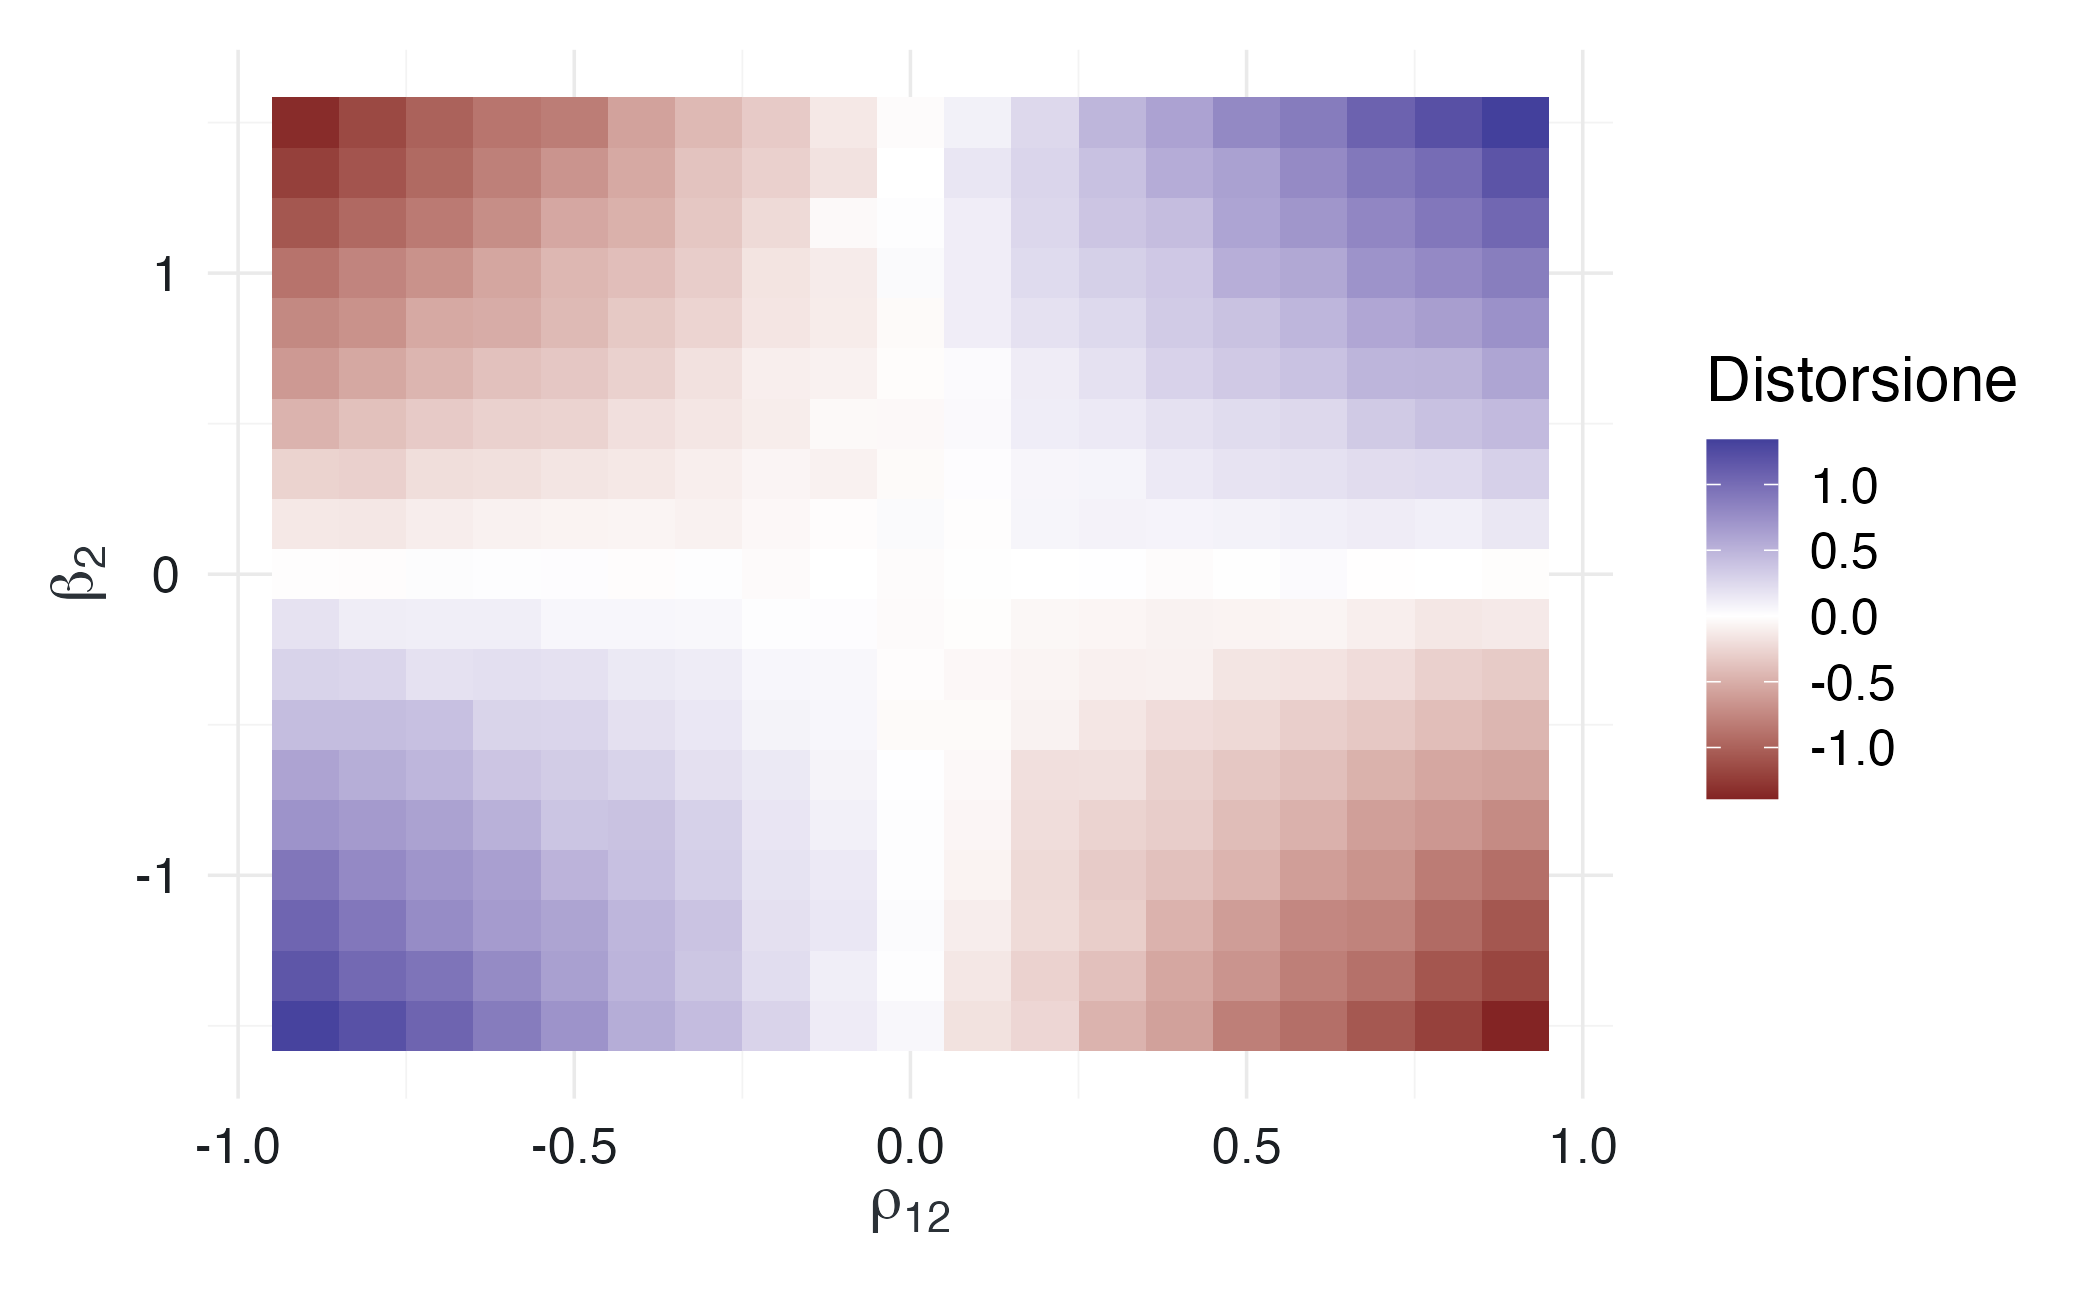
\includegraphics[width=0.85\linewidth,height=\textheight,keepaspectratio]{chapters/causality/01_specification_error_files/figure-pdf/fig-mappa-bias-1.png}

}

\caption{\label{fig-mappa-bias}Distorsione del coefficiente di \(X_1\)
al variare della correlazione tra i predittori e dell'effetto della
variabile omessa. Le zone chiare lungo gli assi sono le regioni in cui
una delle due condizioni del bias non è soddisfatta.}

\end{figure}%

La mappa conferma la previsione analitica. Il bias è positivo quando
\(\beta_2\) e \(\rho_{12}\) hanno lo stesso segno e negativo quando
hanno segni opposti; si annulla lungo gli assi e raggiunge i valori
estremi agli angoli. Le lievi irregolarità sono rumore Monte Carlo. In
pratica, basta che \emph{una} delle due quantità sia prossima a zero
perché il problema sia trascurabile, ma quando entrambe sono lontane da
zero, il coefficiente stimato può non solo essere impreciso, ma anche di
segno opposto rispetto a quello reale.

Fin qui, abbiamo un risultato tecnico solido. Il passo successivo è
chiedersi cosa ci permette di fare.

\section{Perché la formula non
basta}\label{perchuxe9-la-formula-non-basta}

La formula quantifica la differenza tra
\(\operatorname{plim}\hat\alpha_1\) e \(\beta_1\). Tuttavia, per poterla
utilizzare, dobbiamo già conoscere due informazioni che i dati non
contengono: quale sia il ``modello vero'' e quale coefficiente
rappresenti la quantità che vogliamo stimare. Questa non è una
difficoltà marginale. È il problema centrale.

Consideriamo tre situazioni in cui la terza variabile \(X_2\) è
correlata sia con \(X_1\) sia con \(Y\), ma con ruoli causali diversi:

\begin{itemize}
\tightlist
\item
  \textbf{confondente}: \(X_2\) è una causa comune,
  \(X_1 \leftarrow X_2 \rightarrow Y\);
\item
  \textbf{mediatore}: \(X_2\) si trova sul percorso causale,
  \(X_1 \rightarrow X_2 \rightarrow Y\);
\item
  \textbf{collider}: \(X_2\) è un effetto comune,
  \(X_1 \rightarrow X_2 \leftarrow Y\).
\end{itemize}

Simuliamo i tre casi imponendo lo stesso effetto causale diretto di
\(X_1\) su \(Y\), pari a \(0.5\).

\begin{Shaded}
\begin{Highlighting}[]
\FunctionTok{set.seed}\NormalTok{(}\DecValTok{2026}\NormalTok{)}
\NormalTok{n }\OtherTok{\textless{}{-}} \DecValTok{20000}
\NormalTok{a }\OtherTok{\textless{}{-}} \FloatTok{0.8}

\CommentTok{\# (a) Confondente: X2 causa sia X1 sia Y}
\NormalTok{X2\_a }\OtherTok{\textless{}{-}} \FunctionTok{rnorm}\NormalTok{(n)}
\NormalTok{X1\_a }\OtherTok{\textless{}{-}}\NormalTok{ a }\SpecialCharTok{*}\NormalTok{ X2\_a }\SpecialCharTok{+} \FunctionTok{sqrt}\NormalTok{(}\DecValTok{1} \SpecialCharTok{{-}}\NormalTok{ a}\SpecialCharTok{\^{}}\DecValTok{2}\NormalTok{) }\SpecialCharTok{*} \FunctionTok{rnorm}\NormalTok{(n)}
\NormalTok{Y\_a  }\OtherTok{\textless{}{-}} \FloatTok{0.5} \SpecialCharTok{*}\NormalTok{ X1\_a }\SpecialCharTok{+}\NormalTok{ a }\SpecialCharTok{*}\NormalTok{ X2\_a }\SpecialCharTok{+} \FunctionTok{rnorm}\NormalTok{(n)}

\CommentTok{\# (b) Mediatore: X1 causa X2, che a sua volta causa Y}
\NormalTok{X1\_b }\OtherTok{\textless{}{-}} \FunctionTok{rnorm}\NormalTok{(n)}
\NormalTok{X2\_b }\OtherTok{\textless{}{-}}\NormalTok{ a }\SpecialCharTok{*}\NormalTok{ X1\_b }\SpecialCharTok{+} \FunctionTok{sqrt}\NormalTok{(}\DecValTok{1} \SpecialCharTok{{-}}\NormalTok{ a}\SpecialCharTok{\^{}}\DecValTok{2}\NormalTok{) }\SpecialCharTok{*} \FunctionTok{rnorm}\NormalTok{(n)}
\NormalTok{Y\_b  }\OtherTok{\textless{}{-}} \FloatTok{0.5} \SpecialCharTok{*}\NormalTok{ X1\_b }\SpecialCharTok{+}\NormalTok{ a }\SpecialCharTok{*}\NormalTok{ X2\_b }\SpecialCharTok{+} \FunctionTok{rnorm}\NormalTok{(n)}

\CommentTok{\# (c) Collider: X1 e Y causano entrambi X2}
\NormalTok{X1\_c }\OtherTok{\textless{}{-}} \FunctionTok{rnorm}\NormalTok{(n)}
\NormalTok{Y\_c  }\OtherTok{\textless{}{-}} \FloatTok{0.5} \SpecialCharTok{*}\NormalTok{ X1\_c }\SpecialCharTok{+} \FunctionTok{rnorm}\NormalTok{(n)}
\NormalTok{X2\_c }\OtherTok{\textless{}{-}}\NormalTok{ a }\SpecialCharTok{*}\NormalTok{ X1\_c }\SpecialCharTok{+}\NormalTok{ a }\SpecialCharTok{*}\NormalTok{ Y\_c }\SpecialCharTok{+} \FunctionTok{rnorm}\NormalTok{(n)}

\NormalTok{b\_semplice }\OtherTok{\textless{}{-}} \ControlFlowTok{function}\NormalTok{(y, x1) }\FunctionTok{unname}\NormalTok{(}\FunctionTok{coef}\NormalTok{(}\FunctionTok{lm}\NormalTok{(y }\SpecialCharTok{\textasciitilde{}}\NormalTok{ x1))[}\DecValTok{2}\NormalTok{])}
\NormalTok{b\_aggiust  }\OtherTok{\textless{}{-}} \ControlFlowTok{function}\NormalTok{(y, x1, x2) }\FunctionTok{unname}\NormalTok{(}\FunctionTok{coef}\NormalTok{(}\FunctionTok{lm}\NormalTok{(y }\SpecialCharTok{\textasciitilde{}}\NormalTok{ x1 }\SpecialCharTok{+}\NormalTok{ x2))[}\DecValTok{2}\NormalTok{])}

\FunctionTok{data.frame}\NormalTok{(}
  \AttributeTok{struttura =} \FunctionTok{c}\NormalTok{(}\StringTok{"Confondente"}\NormalTok{, }\StringTok{"Mediatore"}\NormalTok{, }\StringTok{"Collider"}\NormalTok{),}
  \AttributeTok{senza\_X2 =} \FunctionTok{c}\NormalTok{(}
    \FunctionTok{b\_semplice}\NormalTok{(Y\_a, X1\_a),}
    \FunctionTok{b\_semplice}\NormalTok{(Y\_b, X1\_b),}
    \FunctionTok{b\_semplice}\NormalTok{(Y\_c, X1\_c)}
\NormalTok{  ),}
  \AttributeTok{con\_X2 =} \FunctionTok{c}\NormalTok{(}
    \FunctionTok{b\_aggiust}\NormalTok{(Y\_a, X1\_a, X2\_a),}
    \FunctionTok{b\_aggiust}\NormalTok{(Y\_b, X1\_b, X2\_b),}
    \FunctionTok{b\_aggiust}\NormalTok{(Y\_c, X1\_c, X2\_c)}
\NormalTok{  )}
\NormalTok{) }\SpecialCharTok{|\textgreater{}}
\NormalTok{  dplyr}\SpecialCharTok{::}\FunctionTok{mutate}\NormalTok{(dplyr}\SpecialCharTok{::}\FunctionTok{across}\NormalTok{(}\FunctionTok{where}\NormalTok{(is.numeric), \textbackslash{}(x) }\FunctionTok{round}\NormalTok{(x, }\DecValTok{3}\NormalTok{)))}
\CommentTok{\#\textgreater{}     struttura senza\_X2 con\_X2}
\CommentTok{\#\textgreater{} 1 Confondente     1.14  0.483}
\CommentTok{\#\textgreater{} 2   Mediatore     1.14  0.495}
\CommentTok{\#\textgreater{} 3    Collider     0.50 {-}0.094}
\end{Highlighting}
\end{Shaded}

Osserviamo prima i primi due casi. I numeri sono \textbf{gli stessi}:
senza \(X_2\) il coefficiente vale circa \(1.14\), con \(X_2\) vale
circa \(0.5\). Non si tratta di una coincidenza numerica: nei due casi
la matrice di covarianza congiunta di \((X_1,X_2,Y)\) è identica nei due
casi per costruzione. Nessuna analisi dei dati osservati, per quanto
sofisticata, può distinguere i due scenari, in quanto generano la stessa
distribuzione.

Eppure la conclusione che ne traiamo è opposta:

\begin{itemize}
\tightlist
\item
  nel caso del \textbf{confondente}, il coefficiente senza \(X_2\) è
  distorto e quello aggiustato stima l'effetto causale: l'aggiustamento
  è \textbf{necessario};
\item
  nel caso del \textbf{mediatore}, il coefficiente senza \(X_2\) stima
  l'effetto \emph{totale} di \(X_1\) su \(Y\) --- che è spesso proprio
  la quantità di interesse --- mentre quello aggiustato stima l'effetto
  \emph{diretto}. Nessuno dei due è distorto: rispondono a domande
  diverse. In questo caso, la parola \emph{distorsione} è fuori luogo;
  ciò che cambia è l'\textbf{estimand}.
\end{itemize}

Il terzo caso ribalta ulteriormente la situazione. Con il
\textbf{collider}, il coefficiente senza \(X_2\) recupera correttamente
l'effetto causale \(0.5\), mentre l'aggiustamento lo distorce.
Condizionare su un effetto comune crea un'associazione tra le sue cause
che nella popolazione non esisteva: aggiustare è \textbf{dannoso}.

La stessa operazione tecnica, ``includere la terza variabile nel
modello'', è dunque obbligatoria, facoltativa o vietata a seconda della
struttura causale. E la struttura causale non è leggibile nei dati.

\begin{tcolorbox}[enhanced jigsaw, arc=.35mm, bottomrule=.15mm, bottomtitle=1mm, breakable, colback=white, colbacktitle=quarto-callout-warning-color!10!white, colframe=quarto-callout-warning-color-frame, coltitle=black, left=2mm, leftrule=.75mm, opacityback=0, opacitybacktitle=0.6, rightrule=.15mm, title=\textcolor{quarto-callout-warning-color}{\faExclamationTriangle}\hspace{0.5em}{La conseguenza pratica}, titlerule=0mm, toprule=.15mm, toptitle=1mm]

Da ciò deriva una regola controintuitiva, ma essenziale, che ritroveremo
formalizzata nel capitolo sui DAG: \textbf{controllare più variabili non
è più prudente}. La pratica diffusa di inserire in un modello tutte le
covariate disponibili ``per essere conservativi'' non ha alcuna
giustificazione causale e, in presenza di collider o dei loro
discendenti, introduce distorsioni laddove non ce n'erano.

\end{tcolorbox}

\section{Dal bias
all'identificazione}\label{dal-bias-allidentificazione}

Cosa manca, dunque, per uscire da questa situazione di stallo? Due
strumenti che i prossimi due capitoli introducono nell'ordine in cui
sono necessari.

Il primo è un linguaggio che ci permette di esprimere \textbf{che cosa}
vogliamo stimare, prima e indipendentemente da come lo stimeremo. Il
quadro dei potenziali esiti (Capitolo~\ref{sec-causality-propedeutics})
definisce l'effetto causale come il confronto tra mondi alternativi per
la stessa unità e chiarisce perché il contrasto osservato tra i gruppi
non corrisponda, in generale, a tale confronto. È anche il quadro in cui
si comprende perché la randomizzazione risolva il problema: non perché
elimina le variabili omesse, ma perché ne annulla la correlazione con il
trattamento, ovvero annulla il valore di \(\rho_{12}\) nella formula di
partenza.

Il secondo è un linguaggio per rappresentare le ipotesi causali e
derivare quali variabili includere. I grafi orientati aciclici
(Capitolo~\ref{sec-eda-causality}) forniscono criteri espliciti per
distinguere i confondenti, i mediatori, i collider e i discendenti e per
stabilire quale insieme di aggiustamento renda identificabile l'effetto
di interesse.

L'ordine del ragionamento, anticipato nell'introduzione a questa parte,
acquista ora un significato preciso: si parte dalla domanda causale, si
definisce l'estimand, si dichiarano le ipotesi causali, si verifica
l'identificazione e \emph{solo alla fine} si sceglie il modello
statistico. La formula del bias da variabile omessa non rappresenta
l'ultimo passo di questo percorso, ma la dimostrazione quantitativamente
ineccepibile che tale percorso è necessario.

\section*{Riflessioni conclusive}\label{riflessioni-conclusive-28}

\markright{Riflessioni conclusive}

Il bias da variabile omessa mostra che la validità di una stima di
regressione dipende da assunzioni riguardanti ciò che il modello
\emph{non} contiene. La formula \(\beta_2\rho_{12}\) ne fornisce la
misura esatta e la simulazione ne chiarisce segno e magnitudo.

Il limite della formula, però, è più interessante del suo contenuto.
Applicata meccanicamente, suggerisce che ogni variabile correlata al
predittore e all'esito debba essere inclusa nel modello. La simulazione
delle tre strutture causali mostra che questa regola è errata: nel caso
del mediatore, l'inclusione modifica la domanda anziché correggere una
distorsione; nel caso del collider, invece, la introduce. Poiché le tre
strutture possono generare dati identici, nessun criterio puramente
statistico può guidare la scelta.

È questa la ragione per cui l'inferenza causale non è un'estensione
tecnica della regressione, ma un modo diverso di impostare il problema:
prima si dichiara ciò che si vuole stimare e le ipotesi causali che si è
disposti a difendere, poi si stabilisce se i dati a disposizione
permettono di identificare tale quantità e, infine, si procede con la
stima.

\section*{Esercizi}\label{esercizi-8}
\addcontentsline{toc}{section}{Esercizi}

\markright{Esercizi}

\begin{tcolorbox}[enhanced jigsaw, arc=.35mm, bottomrule=.15mm, bottomtitle=1mm, breakable, colback=white, colbacktitle=quarto-callout-tip-color!10!white, colframe=quarto-callout-tip-color-frame, coltitle=black, left=2mm, leftrule=.75mm, opacityback=0, opacitybacktitle=0.6, rightrule=.15mm, title=\textcolor{quarto-callout-tip-color}{\faLightbulb}\hspace{0.5em}{Esercizio 1 --- Comprendere}, titlerule=0mm, toprule=.15mm, toptitle=1mm]

Spiega con parole tue perché la randomizzazione del trattamento rende
irrilevante il bias da variabile omessa, anche quando esistono numerose
variabili non misurate che influenzano l'esito. Quale dei due fattori
della formula \(\beta_2\rho_{12}\) viene annullato, e quale invece resta
diverso da zero?

\end{tcolorbox}

\begin{tcolorbox}[enhanced jigsaw, arc=.35mm, bottomrule=.15mm, bottomtitle=1mm, breakable, colback=white, colbacktitle=quarto-callout-tip-color!10!white, colframe=quarto-callout-tip-color-frame, coltitle=black, left=2mm, leftrule=.75mm, opacityback=0, opacitybacktitle=0.6, rightrule=.15mm, title=\textcolor{quarto-callout-tip-color}{\faLightbulb}\hspace{0.5em}{Esercizio 2 --- Prevedere}, titlerule=0mm, toprule=.15mm, toptitle=1mm]

Nella simulazione delle tre strutture, prevedi che cosa accadrebbe al
caso del collider se l'effetto causale di \(X_1\) su \(Y\) fosse
esattamente nullo. Il coefficiente aggiustato risulterebbe positivo,
negativo o nullo? Formula la previsione, poi verificala modificando il
codice.

\textbf{Suggerimento.} Ragiona su che cosa comporta selezionare unità
con un valore simile di \(X_2\): se \(X_2\) è alto, quali combinazioni
di \(X_1\) e \(Y\) sono compatibili con quel valore?

\end{tcolorbox}

\begin{tcolorbox}[enhanced jigsaw, arc=.35mm, bottomrule=.15mm, bottomtitle=1mm, breakable, colback=white, colbacktitle=quarto-callout-tip-color!10!white, colframe=quarto-callout-tip-color-frame, coltitle=black, left=2mm, leftrule=.75mm, opacityback=0, opacitybacktitle=0.6, rightrule=.15mm, title=\textcolor{quarto-callout-tip-color}{\faLightbulb}\hspace{0.5em}{Esercizio 3 --- Modificare}, titlerule=0mm, toprule=.15mm, toptitle=1mm]

Nel caso del mediatore, il coefficiente non aggiustato stima l'effetto
totale e quello aggiustato l'effetto diretto. Modifica la simulazione
ponendo a zero l'effetto diretto di \(X_1\) su \(Y\) (mantenendo il
percorso \(X_1 \rightarrow X_2 \rightarrow Y\)). Che cosa restituiscono
ora i due coefficienti? In quale situazione di ricerca la stima
dell'effetto totale sarebbe la risposta corretta, e in quale lo sarebbe
quella dell'effetto diretto?

\end{tcolorbox}

\begin{tcolorbox}[enhanced jigsaw, arc=.35mm, bottomrule=.15mm, bottomtitle=1mm, breakable, colback=white, colbacktitle=quarto-callout-tip-color!10!white, colframe=quarto-callout-tip-color-frame, coltitle=black, left=2mm, leftrule=.75mm, opacityback=0, opacitybacktitle=0.6, rightrule=.15mm, title=\textcolor{quarto-callout-tip-color}{\faLightbulb}\hspace{0.5em}{Esercizio 4 --- Criticare}, titlerule=0mm, toprule=.15mm, toptitle=1mm]

Uno studio osservazionale riporta: «Abbiamo controllato per tutte le
variabili demografiche e cliniche disponibili, ottenendo una stima
conservativa dell'effetto del trattamento». Individua le assunzioni
causali implicite in questa affermazione e spiega in quali condizioni la
strategia descritta potrebbe produrre una stima \emph{meno} accurata di
un modello con meno covariate.

\end{tcolorbox}

\begin{tcolorbox}[enhanced jigsaw, arc=.35mm, bottomrule=.15mm, bottomtitle=1mm, breakable, colback=white, colbacktitle=quarto-callout-note-color!10!white, colframe=quarto-callout-note-color-frame, coltitle=black, left=2mm, leftrule=.75mm, opacityback=0, opacitybacktitle=0.6, rightrule=.15mm, title=\textcolor{quarto-callout-note-color}{\faInfo}\hspace{0.5em}{Informazioni sull'ambiente di sviluppo}, titlerule=0mm, toprule=.15mm, toptitle=1mm]

\begin{Shaded}
\begin{Highlighting}[]
\FunctionTok{sessionInfo}\NormalTok{()}
\CommentTok{\#\textgreater{} R version 4.6.1 (2026{-}06{-}24)}
\CommentTok{\#\textgreater{} Platform: aarch64{-}apple{-}darwin23}
\CommentTok{\#\textgreater{} Running under: macOS Tahoe 26.5.2}
\CommentTok{\#\textgreater{} }
\CommentTok{\#\textgreater{} Matrix products: default}
\CommentTok{\#\textgreater{} BLAS:   /Library/Frameworks/R.framework/Versions/4.6/Resources/lib/libRblas.0.dylib }
\CommentTok{\#\textgreater{} LAPACK: /Library/Frameworks/R.framework/Versions/4.6/Resources/lib/libRlapack.dylib;  LAPACK version 3.12.1}
\CommentTok{\#\textgreater{} }
\CommentTok{\#\textgreater{} locale:}
\CommentTok{\#\textgreater{} [1] C.UTF{-}8/UTF{-}8/C.UTF{-}8/C/C.UTF{-}8/C.UTF{-}8}
\CommentTok{\#\textgreater{} }
\CommentTok{\#\textgreater{} time zone: Europe/Zagreb}
\CommentTok{\#\textgreater{} tzcode source: internal}
\CommentTok{\#\textgreater{} }
\CommentTok{\#\textgreater{} attached base packages:}
\CommentTok{\#\textgreater{} [1] stats     graphics  grDevices utils     datasets  methods   base     }
\CommentTok{\#\textgreater{} }
\CommentTok{\#\textgreater{} other attached packages:}
\CommentTok{\#\textgreater{}  [1] ragg\_1.5.2            tinytable\_0.17.0      withr\_3.0.3          }
\CommentTok{\#\textgreater{}  [4] systemfonts\_1.3.2     patchwork\_1.3.2       ggdist\_3.3.3         }
\CommentTok{\#\textgreater{}  [7] tidybayes\_3.0.7       bayesplot\_1.15.0      ggplot2\_4.0.3        }
\CommentTok{\#\textgreater{} [10] reliabilitydiag\_0.2.1 priorsense\_1.2.0      posterior\_1.7.0      }
\CommentTok{\#\textgreater{} [13] loo\_2.10.0            rstan\_2.32.7          StanHeaders\_2.32.10  }
\CommentTok{\#\textgreater{} [16] brms\_2.23.0           Rcpp\_1.1.2            sessioninfo\_1.2.4    }
\CommentTok{\#\textgreater{} [19] conflicted\_1.2.0      janitor\_2.2.1         matrixStats\_1.5.0    }
\CommentTok{\#\textgreater{} [22] modelr\_0.1.11         tibble\_3.3.1          dplyr\_1.2.1          }
\CommentTok{\#\textgreater{} [25] tidyr\_1.3.2           rio\_1.3.0             here\_1.0.2           }
\CommentTok{\#\textgreater{} }
\CommentTok{\#\textgreater{} loaded via a namespace (and not attached):}
\CommentTok{\#\textgreater{}  [1] svUnit\_1.0.8          tidyselect\_1.2.1      farver\_2.1.2         }
\CommentTok{\#\textgreater{}  [4] S7\_0.2.2              fastmap\_1.2.0         tensorA\_0.36.2.1     }
\CommentTok{\#\textgreater{}  [7] digest\_0.6.39         timechange\_0.4.0      estimability\_2.0.0   }
\CommentTok{\#\textgreater{} [10] lifecycle\_1.0.5       magrittr\_2.0.5        compiler\_4.6.1       }
\CommentTok{\#\textgreater{} [13] rlang\_1.3.0           tools\_4.6.1           yaml\_2.3.12          }
\CommentTok{\#\textgreater{} [16] knitr\_1.51            labeling\_0.4.3        bridgesampling\_1.2{-}1 }
\CommentTok{\#\textgreater{} [19] pkgbuild\_1.4.8        curl\_7.1.0            RColorBrewer\_1.1{-}3   }
\CommentTok{\#\textgreater{} [22] abind\_1.4{-}8           purrr\_1.2.2           grid\_4.6.1           }
\CommentTok{\#\textgreater{} [25] stats4\_4.6.1          xtable\_1.8{-}8          inline\_0.3.21        }
\CommentTok{\#\textgreater{} [28] emmeans\_2.0.4         scales\_1.4.0          cli\_3.6.6            }
\CommentTok{\#\textgreater{} [31] mvtnorm\_1.4{-}2         rmarkdown\_2.31        generics\_0.1.4       }
\CommentTok{\#\textgreater{} [34] otel\_0.2.0            RcppParallel\_5.1.11{-}2 cachem\_1.1.0         }
\CommentTok{\#\textgreater{} [37] stringr\_1.6.0         parallel\_4.6.1        vctrs\_0.7.3          }
\CommentTok{\#\textgreater{} [40] V8\_8.2.0              Matrix\_1.7{-}5          jsonlite\_2.0.0       }
\CommentTok{\#\textgreater{} [43] arrayhelpers\_1.1{-}1    glue\_1.8.1            codetools\_0.2{-}20     }
\CommentTok{\#\textgreater{} [46] distributional\_0.8.1  lubridate\_1.9.5       stringi\_1.8.7        }
\CommentTok{\#\textgreater{} [49] gtable\_0.3.6          QuickJSR\_1.10.0       pillar\_1.11.1        }
\CommentTok{\#\textgreater{} [52] htmltools\_0.5.9       Brobdingnag\_1.2{-}9     R6\_2.6.1             }
\CommentTok{\#\textgreater{} [55] textshaping\_1.0.5     rprojroot\_2.1.1       evaluate\_1.0.5       }
\CommentTok{\#\textgreater{} [58] lattice\_0.22{-}9        backports\_1.5.1       memoise\_2.0.1        }
\CommentTok{\#\textgreater{} [61] broom\_1.0.13          snakecase\_0.11.1      rstantools\_2.6.0     }
\CommentTok{\#\textgreater{} [64] coda\_0.19{-}4.1         gridExtra\_2.3.1       nlme\_3.1{-}170         }
\CommentTok{\#\textgreater{} [67] checkmate\_2.3.4       xfun\_0.60             pkgconfig\_2.0.3}
\end{Highlighting}
\end{Shaded}

\end{tcolorbox}

\section*{Bibliografia}\label{bibliografia-32}

\markright{Bibliografia}

\chapter{Causalità: intuizioni, controfattuali e perché l'associazione
non basta}\label{sec-causality-propedeutics}

\begin{tcolorbox}[enhanced jigsaw, arc=.35mm, bottomrule=.15mm, breakable, colback=white, colframe=quarto-callout-note-color-frame, left=2mm, leftrule=.75mm, opacityback=0, rightrule=.15mm, toprule=.15mm]

Nel capitolo precedente abbiamo analizzato in dettaglio l'\emph{errore
di specificazione} nei modelli di regressione. Abbiamo visto come
omissioni rilevanti, scelte improprie delle variabili di controllo o
forme funzionali inadeguate possano alterare le stime e rendere
fuorviante l'interpretazione dei coefficienti. In quel contesto, la
regressione è stata considerata uno strumento descrittivo potente, ma
fragile, la cui affidabilità dipende dalle ipotesi formulate sul
processo che genera i dati.

Questo capitolo riprende il discorso, ma compie un passo ulteriore: si
chiede \emph{perché} certi errori di specificazione producono bias
sistematici e \emph{in quali condizioni} un coefficiente di regressione
può essere interpretato come qualcosa di più di una semplice
associazione. La questione centrale non è più soltanto \emph{quali
variabili includere nel modello}, ma \emph{che tipo di relazione stiamo
cercando di stimare}.

Il punto cruciale è che, anche in assenza di evidenti problemi di
specificazione statistica, i coefficienti di regressione rimangono, in
generale, \emph{quantificazioni di associazioni} e non di effetti
causali. Una relazione stimata correttamente dal punto di vista formale
può comunque fallire nel rispondere a domande come: ``\emph{Che cosa
accadrebbe se intervenissimo su (X)?}'' oppure ``\emph{Qual è l'effetto
di \(X\) su \(Y\), a parità di tutto il resto?}''. In questa
prospettiva, l'errore di specificazione non è un semplice problema
tecnico, ma il sintomo di un problema più profondo: \emph{l'assenza di
un esplicito riferimento causale}.\footnotemark{}

Questo capitolo introduce quindi il \emph{quadro concettuale
controfattuale della causalità}, che fornisce il linguaggio e le
categorie necessarie per formulare con precisione tali domande.
L'obiettivo non è ancora mostrare \emph{come} stimare effetti causali
dai dati, ma chiarire \emph{che cosa} si intende per effetto causale,
\emph{perché} l'endogeneità emerge e \emph{in che senso} il bias da
variabile omessa può essere interpretato come una violazione di ipotesi
causali implicite.

In questo senso, il capitolo funge da ponte: rilegge i problemi di
specificazione discussi in precedenza alla luce della causalità e
prepara il terreno per il capitolo successivo
(Capitolo~\ref{sec-eda-causality}), in cui verranno introdotti gli
strumenti operativi --- DAG, criterio del backdoor, propensity score,
matching, pesatura e regressione --- necessari per affrontare tali
problemi in modo sistematico. Il riferimento concettuale principale è il
primo capitolo di Hernán \& Robins (\citeproc{ref-hernan2020}{2020}), da
cui riprendiamo l'impostazione e la notazione essenziale.

\end{tcolorbox}

\footnotetext{Le correlazioni spurie sono estremamente comuni. Un
modello di regressione può descrivere formalmente e accuratamente una
relazione spuria, ma ciò non ci fornisce alcuna informazione utile sul
funzionamento dei fenomeni psicologici. Il sito
\href{https://www.tylervigen.com/spurious-correlations}{Spurious
Correlations} documenta numerose associazioni statisticamente forti ma
del tutto accidentali --- mostrando, con ironia, che anche correlazioni
bizzarre potrebbero dar vita a pubblicazioni scientifiche prive di
significato. Il messaggio fondamentale rimane: una correlazione, di per
sé, non ci informa sui meccanismi sottostanti un fenomeno. Comprendere
il funzionamento dei processi psicologici non è un problema meramente
statistico: non basta descrivere accuratamente le associazioni tra
variabili. Si tratta piuttosto di un problema di \textbf{modellazione
teorica}: è necessario formulare modelli validi delle relazioni causali
che generano i dati osservati.}

\begin{tcolorbox}[enhanced jigsaw, arc=.35mm, bottomrule=.15mm, breakable, colback=white, colframe=quarto-callout-important-color-frame, left=2mm, leftrule=.75mm, opacityback=0, rightrule=.15mm, toprule=.15mm]

\textbf{Da sapere.} Un effetto causale confronta esiti potenziali in
scenari alternativi e non coincide con l'associazione osservata tra
trattati e non trattati. L'effetto causale individuale non è
direttamente osservabile; a livello di popolazione si può definire
l'effetto causale medio. La randomizzazione rende i gruppi comparabili
in media, mentre nei dati osservazionali il confondimento può separare
radicalmente associazione ed effetto causale. Consistenza e SUTVA sono
condizioni necessarie per attribuire un significato preciso
all'intervento.

\textbf{Da saper fare.} Distinguere associazione ed effetto causale;
formulare un effetto mediante gli esiti potenziali e definire l'ACE;
spiegare il problema fondamentale dell'inferenza causale; riconoscere il
ruolo del confondimento e della randomizzazione; scegliere e
interpretare una misura dell'effetto sulla scala additiva o
moltiplicativa; usare semplici simulazioni per mostrare perché un
confronto osservato possa essere causalmente fuorviante.

\textbf{Approfondimento facoltativo.} Le implementazioni complete delle
simulazioni, il paradosso di Simpson, il confronto dettagliato tra
diverse scale dell'effetto e i micro-esercizi possono essere rimandati
in una prima lettura. Nel percorso essenziale è sufficiente
padroneggiare il linguaggio controfattuale, comprendere la differenza
tra associazione e causalità e riconoscere le condizioni che rendono
identificabile un effetto causale.

\hyperref[sec-percorsi-lettura]{Che cosa significano queste etichette?}

\end{tcolorbox}

\begin{tcolorbox}[enhanced jigsaw, arc=.35mm, bottomrule=.15mm, bottomtitle=1mm, breakable, colback=white, colbacktitle=quarto-callout-tip-color!10!white, colframe=quarto-callout-tip-color-frame, coltitle=black, left=2mm, leftrule=.75mm, opacityback=0, opacitybacktitle=0.6, rightrule=.15mm, title=\textcolor{quarto-callout-tip-color}{\faLightbulb}\hspace{0.5em}{Take‑home (in 3 righe)}, titlerule=0mm, toprule=.15mm, toptitle=1mm]

\begin{itemize}
\tightlist
\item
  \textbf{Effetto causale medio (ACE)} = differenza tra due mondi: se
  \emph{tutti} ricevessero il trattamento vs se \emph{nessuno} lo
  ricevesse.
\item
  \textbf{Associazione} = differenza tra \emph{trattati} e \emph{non
  trattati} nel mondo osservato: può essere fuorviante per via del
  \textbf{confondimento}.
\item
  La \textbf{randomizzazione} rende i gruppi comparabili ``in media'' →
  associazione ≈ causalità (se SUTVA regge).
\end{itemize}

\end{tcolorbox}

\begin{tcolorbox}[enhanced jigsaw, arc=.35mm, bottomrule=.15mm, bottomtitle=1mm, breakable, colback=white, colbacktitle=quarto-callout-caution-color!10!white, colframe=quarto-callout-caution-color-frame, coltitle=black, left=2mm, leftrule=.75mm, opacityback=0, opacitybacktitle=0.6, rightrule=.15mm, title=\textcolor{quarto-callout-caution-color}{\faFire}\hspace{0.5em}{Preparazione del Notebook}, titlerule=0mm, toprule=.15mm, toptitle=1mm]

\begin{Shaded}
\begin{Highlighting}[]
\NormalTok{here}\SpecialCharTok{::}\FunctionTok{here}\NormalTok{(}\StringTok{"code"}\NormalTok{, }\StringTok{"\_common.R"}\NormalTok{) }\SpecialCharTok{|\textgreater{}} 
  \FunctionTok{source}\NormalTok{()}

\CommentTok{\# Load packages}
\ControlFlowTok{if}\NormalTok{ (}\SpecialCharTok{!}\FunctionTok{requireNamespace}\NormalTok{(}\StringTok{"pacman"}\NormalTok{)) }\FunctionTok{install.packages}\NormalTok{(}\StringTok{"pacman"}\NormalTok{)}
\NormalTok{pacman}\SpecialCharTok{::}\FunctionTok{p\_load}\NormalTok{(patchwork)}
\end{Highlighting}
\end{Shaded}

\end{tcolorbox}

\section{Dalla regressione alla causalità: perché serve un nuovo
framework}\label{dalla-regressione-alla-causalituxe0-perchuxe9-serve-un-nuovo-framework}

Nel modello di regressione standard, esprimiamo una relazione nella
forma \(y = \alpha + \beta x + \varepsilon\) e spesso interpretiamo
\(\beta\) come ``l'effetto di \(x\) su \(y\)''. Tuttavia, questa
interpretazione è valida solo in condizioni molto restrittive, che si
verificano raramente nella ricerca osservazionale. Per comprenderne il
motivo, consideriamo un esempio classico della psicologia.

Immaginiamo di osservare che gli studenti che dormono meno ore a notte
tendono a riportare livelli più elevati di ansia. Una regressione
lineare potrebbe restituire un coefficiente \(\beta > 0\), suggerendo
un'associazione positiva tra privazione di sonno e ansia. Cosa possiamo
concludere? Almeno tre spiegazioni causali sono compatibili con questo
stesso dato osservativo:

\begin{enumerate}
\def\labelenumi{\arabic{enumi}.}
\tightlist
\item
  \textbf{Il sonno causa l'ansia}: la carenza di sonno altera i
  meccanismi neurofisiologici che regolano la risposta emotiva e lo
  stress.
\item
  \textbf{L'ansia causa il sonno}: gli stati ansiosi ostacolano
  l'addormentamento, frammentano il riposo e riducono la durata
  complessiva del sonno.
\item
  \textbf{Una terza variabile causa entrambe}: periodi di elevato carico
  accademico, ad esempio, aumentano contemporaneamente l'ansia e
  riducono il tempo dedicato al sonno.
\end{enumerate}

Il coefficiente di regressione, da solo, non permette di discriminare
tra queste possibilità. Ci informa soltanto della \emph{covariazione}
tra \(x\) e \(y\), ma rimane muto riguardo ai \emph{meccanismi} che la
generano. Per rispondere alla domanda ``Perché?'' dobbiamo quindi
abbandonare il linguaggio puramente associativo della regressione e
adottare un \emph{framework causale}.

\subsection{Cosa cambia con il pensiero
causale}\label{cosa-cambia-con-il-pensiero-causale}

Il pensiero causale impone un cambiamento di prospettiva: invece di
limitarci a descrivere relazioni osservate, ci chiediamo cosa accadrebbe
in scenari \emph{non} osservati. La domanda centrale diventa:
\textbf{``Se intervenissimo modificando \(x\), come cambierebbe
\(y\)?''}. Questa non è una domanda descrittiva, ma ipotetica e
interventista.

La formalizzazione di questa intuizione si basa sul concetto di
\textbf{esito controfattuale}, ovvero il valore che \(y\) assumerebbe in
una situazione alternativa a quella effettivamente verificatasi. Si
tratta di un'idea che utilizziamo quotidianamente nel ragionamento
comune (``Se avessi preso quel treno, sarei arrivato in orario''), ma
che richiede una notazione precisa e assunzioni identificabili per poter
essere tradotta in inferenza statistica.

Nei prossimi paragrafi introdurremo gli strumenti fondamentali di questo
approccio: la notazione dei potenziali esiti, la definizione formale
dell'effetto causale individuale e medio e le condizioni (tra cui
l'assegnazione casuale del trattamento) sotto le quali l'associazione
osservata può essere interpretata come effetto causale.

\section{Fondamenti dell'inferenza causale: controfattuali, effetto
medio e
SUTVA}\label{fondamenti-dellinferenza-causale-controfattuali-effetto-medio-e-sutva}

Tutti noi, nella vita di tutti i giorni, formuliamo continuamente
domande causali. Uno studente, per esempio, potrebbe chiedersi: ``Se
applicassi una tecnica di ristrutturazione cognitiva prima dell'esame,
riuscirei a gestire meglio l'ansia?'' Questa semplice domanda racchiude
già l'essenza del problema: esiste un'azione possibile, il
\emph{trattamento}, il cui effetto su un \emph{esito} desideriamo
comprendere.

La statistica formalizza questa intuizione attraverso il concetto di
\textbf{esito potenziale} (o controfattuale). Per ogni individuo,
possiamo immaginare due scenari alternativi e ben definiti:

\begin{itemize}
\tightlist
\item
  uno scenario in cui l'individuo riceve il trattamento (ad esempio,
  applica la tecnica di \emph{reappraisal}); in questo caso l'esito è
  indicato con \(Y^{(1)}\);
\item
  uno scenario in cui lo stesso individuo non riceve il trattamento e
  l'esito corrispondente è indicato con \(Y^{(0)}\).
\end{itemize}

Nella realtà, osserviamo solo uno dei due scenari: se lo studente decide
di applicare la tecnica di \emph{reappraisal}, misureremo \(Y^{(1)}\);
l'altro esito, \(Y^{(0)}\), rimane non osservato: è l'esito potenziale.
Il legame tra ciò che osserviamo e ciò che ipotizziamo è sancito
dall'assunzione di \textbf{consistenza}: se il trattamento
effettivamente ricevuto è \(A = a\), allora l'esito osservato \(Y\)
coincide con l'esito potenziale corrispondente, ovvero \(Y = Y^{(a)}\).

Da questa struttura logica deriva la definizione dell'effetto causale. A
livello individuale, l'effetto è la differenza tra i due esiti
potenziali: \[
\tau_i = Y_i^{(1)} - Y_i^{(0)}.
\] Tuttavia, poiché per ciascun individuo osserviamo solo uno dei due
valori, \(\tau_i\) non è mai direttamente misurabile.

Possiamo però spostare l'attenzione a livello di popolazione, definendo
l'\textbf{effetto causale medio} (\emph{Average Causal Effect}, ACE): \[
\text{ACE} = \mathbb{E}[Y^{(1)}] - \mathbb{E}[Y^{(0)}].
\] In altre parole, l'ACE corrisponde alla differenza attesa negli esiti
tra uno scenario in cui tutti ricevono il trattamento e uno in cui
nessuno lo riceve. Si tratta della risposta formale alla domanda:
\emph{``Se intervenissimo sull'intera popolazione, quale sarebbe, in
media, la differenza nell'esito?''}.

Per poter definire l'ACE in modo corretto e interpretabile, è necessario
introdurre un'assunzione fondamentale: la \textbf{SUTVA} (\emph{Stable
Unit Treatment Value Assumption}). Nonostante il nome tecnico, il suo
significato concettuale è intuitivo e si articola in due parti:

\begin{enumerate}
\def\labelenumi{\arabic{enumi}.}
\item
  \textbf{Assenza di interferenza}: il trattamento assegnato a un
  individuo non influenza gli esiti degli altri individui. Nel nostro
  esempio, il fatto che uno studente applichi la tecnica del
  \emph{reappraisal} non dovrebbe alterare il livello di ansia dei suoi
  compagni. Questa ipotesi è plausibile in molti contesti psicologici
  individuali, ma può non essere valida in contesti di gruppo, come
  classi o comunità.
\item
  \textbf{Unicità della versione del trattamento}: esiste una sola
  modalità ben definita di ``ricevere il trattamento''. Se la tecnica di
  ristrutturazione cognitiva venisse applicata in modi sostanzialmente
  diversi tra i partecipanti, queste diverse modalità dovrebbero essere
  considerate come trattamenti distinti.
\end{enumerate}

Queste nozioni, ovvero esiti potenziali, consistenza, effetto causale
medio e SUTVA, costituiscono i fondamenti del ragionamento causale
moderno. Pur richiedendo un linguaggio più formale, queste nozioni non
fanno altro che esplicitare e rendere più precise le intuizioni causali
che guidano il nostro pensiero quotidiano.

\section{Causale vs associativo: perché
differiscono?}\label{causale-vs-associativo-perchuxe9-differiscono}

Quando parliamo di effetto \textbf{causale}, ci riferiamo a un confronto
ipotetico tra due mondi alternativi. Nel primo mondo immaginiamo che
tutti ricevano il trattamento, nel secondo che nessuno lo riceva. La
domanda è: quanto cambia, in media, l'esito se passiamo da un mondo
all'altro? Questo è l'effetto causale medio (ACE), espresso come la
differenza tra \(\mathbb{E}[Y^{(1)}]\) e \(\mathbb{E}[Y^{(0)}]\).

Il ragionamento \textbf{associativo}, invece, si concentra su ciò che
osserviamo direttamente nei dati: confronta due gruppi reali, ovvero chi
ha ricevuto il trattamento e chi non lo ha ricevuto, e guarda la
differenza tra \(\mathbb{E}[Y \,|\, A=1]\) e
\(\mathbb{E}[Y \,|\, A=0]\).

La differenza tra i due approcci è sostanziale. Il confronto causale
presuppone che \textbf{la stessa popolazione} viva due scenari
alternativi e paralleli. Il confronto associativo, al contrario, mette a
confronto \textbf{due gruppi distinti}, che potrebbero differire per
molteplici caratteristiche già prima dell'assegnazione del trattamento.

Questa distinzione è cruciale. Consideriamo l'esempio dello studente
ansioso: se solo gli studenti con un livello alto di ansia di tratto
decidono di applicare una tecnica di rilassamento, i gruppi ``trattati''
e ``non trattati'' non saranno confrontabili sin dall'inizio. La
differenza osservata
\(\mathbb{E}[Y \,|\, A=1] - \mathbb{E}[Y \,|\, A=0]\) rifletterà quindi
non solo l'eventuale efficacia della tecnica, ma anche il divario
preesistente nei livelli di ansia tra i due gruppi.

Questa discrepanza tra associazione e causalità prende il nome di
\textbf{confondimento}: si verifica quando esiste una variabile (o un
insieme di variabili) che influenza sia la probabilità di ricevere il
trattamento sia l'esito stesso. In presenza di confondimento, la
differenza osservata può essere:

\begin{itemize}
\tightlist
\item
  \textbf{ingannevolmente ampia} (se, ad esempio, chi riceve il
  trattamento parte già svantaggiato),
\item
  \textbf{ingannevolmente attenuata} (se il trattamento viene assegnato
  a chi è già avvantaggiato),
\item
  \textbf{aersino di segno opposto} rispetto all'effetto causale vero.
\end{itemize}

Il confondimento rappresenta dunque il principale ostacolo all'inferenza
causale nei dati osservazionali, in quanto ci impedisce di interpretare
la semplice differenza tra i gruppi come una stima dell'effetto del
trattamento. Nei prossimi paragrafi esploreremo come il disegno
sperimentale, e in particolare la randomizzazione, possano risolvere
questo problema, rendendo il confronto associativo un'approssimazione
valida del confronto causale.

\subsection{La regressione non risolve automaticamente il
problema}\label{la-regressione-non-risolve-automaticamente-il-problema}

A questo punto potremmo chiederci: ``Ma la regressione multipla non
serve proprio a questo? Se includo le variabili confondenti nel modello,
posso stimare l'effetto `al netto' di queste variabili''. Questa
intuizione coglie un aspetto importante, ma è incompleta e in alcuni
casi pericolosamente fuorviante.

Il problema fondamentale è che \textbf{il controllo statistico non è
neutrale}: includere una variabile nel modello non sempre migliora la
stima causale. Come vedremo nel Capitolo~\ref{sec-eda-causality},
esistono configurazioni di relazioni tra variabili --- in particolare i
\emph{collider} --- in cui controllare per una variabile
\textbf{introduce distorsione} anziché eliminarla. Più in generale, ogni
decisione su cosa includere o escludere da un modello richiede una
comprensione della struttura causale sottostante, e non può essere
automatizzata mediante criteri puramente statistici come la correlazione
osservata o algoritmi di selezione delle variabili.

Il pericolo sta proprio qui: \textbf{il controllo mal posto può produrre
distorsioni più gravi dell'omissione stessa}. Una regressione che
include variabili inappropriate può darci l'illusione del rigore (``ho
controllato per tutto'') mentre in realtà stima una quantità che non
corrisponde a nessun effetto causale ben definito.

Per questo motivo, è essenziale distinguere tra due obiettivi distinti:

\begin{itemize}
\tightlist
\item
  \textbf{stimare associazioni}, cioè descrivere le relazioni presenti
  nei dati osservati;
\item
  \textbf{stimare effetti causali}, cioè rispondere a domande del tipo
  ``cosa accadrebbe se intervenissimo?''.
\end{itemize}

È proprio il divario tra questi due obiettivi che rende necessario
adottare un \textbf{framework causale esplicito} e affiancare
all'analisi statistica un'attenta riflessione sul disegno dello studio e
sulla struttura delle relazioni tra le variabili. Le strategie che
esploreremo nei prossimi capitoli, dal disegno sperimentale randomizzato
ai metodi per dati osservazionali, nascono tutte dalla necessità di
colmare questo divario in modo rigoroso e trasparente.

\section{Quale misura di effetto? Additiva o
moltiplicativa}\label{quale-misura-di-effetto-additiva-o-moltiplicativa}

Una volta chiarito il concetto di effetto causale medio, resta da
definire come quantificarlo. Non esiste una misura universalmente
migliore: la scelta deve essere guidata dalla domanda di ricerca e dal
modo in cui intendiamo comunicare l'impatto dell'intervento.

Se l'esito è dicotomico, come ad esempio ``aver avuto un attacco di
panico (sì/no)'', possiamo calcolare la \textbf{differenza di rischi}:
\[
\text{RD} = P(Y^{(1)} = 1) - P(Y^{(0)} = 1).
\] Questa misura additiva risponde a una domanda di salute pubblica:
\emph{``Quanti casi in più o in meno possiamo attenderci se tutti
ricevessero il trattamento?''}. Il risultato è immediatamente
interpretabile in termini di impatto concreto sul numero di persone
affette.

Un'alternativa è il \textbf{rapporto di rischi} (\emph{risk ratio}): \[
\text{RR} = \frac{P(Y^{(1)} = 1)}{P(Y^{(0)} = 1)}.
\] Questo approccio moltiplicativo è utile quando vogliamo esprimere il
rischio relativo: \emph{``Chi non applica il reappraisal ha un rischio
doppio di avere un attacco di panico''}. In ambito psicologico clinico,
l'odds ratio viene spesso utilizzato per i modelli logistici e per
descrivere le associazioni negli studi caso-controllo, anche se la sua
interpretazione diretta come moltiplicatore del rischio è meno
intuitiva.

Se l'esito è continuo --- come un punteggio su una scala di ansia ---
l'effetto più naturale è la differenza tra le medie dei potenziali
esiti: \[
\text{ACE} = \mathbb{E}[Y^{(1)}] - \mathbb{E}[Y^{(0)}],
\] che ci dice di quanto, in media, il punteggio cambierebbe se tutti
ricevessero il trattamento.

La scelta della misura non è dunque neutra: ognuna \textbf{racconta una
parte diversa della stessa storia}. La differenza di rischi enfatizza
l'impatto assoluto e la rilevanza pratica in termini di numero di casi,
mentre il rapporto di rischi mette in luce la forza relativa
dell'associazione e può essere più adatto per confrontare gli effetti
tra sottogruppi con rischi di base diversi. È importante evitare gli
automatismi e selezionare consapevolmente la scala che meglio si adatta
alla domanda di ricerca e al pubblico a cui ci rivolgiamo.

\subsection{Due fonti di variabilità}\label{due-fonti-di-variabilituxe0}

Quando stimiamo un effetto causale, dobbiamo riconoscere che i valori
ottenuti sono sempre accompagnati da un margine di incertezza. Tale
incertezza può avere almeno due origini distinte, che spesso vengono
confuse ma che è importante distinguere concettualmente.

La prima è la \textbf{variabilità da campionamento}. Nella ricerca
empirica non osserviamo mai l'intera popolazione, ma solo un
sottoinsieme di individui, il campione, estratto da essa. Se ripetessimo
lo studio con campioni diversi provenienti dalla stessa popolazione,
otterremmo stime leggermente diverse. Questa oscillazione riflette il
fatto che ogni campione rappresenta una possibile ``fotografia'' della
realtà e che la nostra stima attuale è solo una di queste. È la
variabilità che la statistica inferenziale tradizionale cattura
attraverso l'errore standard e gli intervalli di confidenza.

La seconda fonte di variabilità riguarda la \textbf{eterogeneità degli
effetti stessi}. Anche se potessimo osservare l'intera popolazione,
l'effetto del trattamento non sarebbe identico per tutti gli individui.
Le differenze nelle caratteristiche di base (età, genere, tratti della
personalità, contesto sociale) interagiscono con l'intervento,
producendo risposte diverse. Questo fenomeno, noto come \emph{effetto
causale individuale}, implica che, anche a parità di trattamento, gli
esiti possono variare considerevolmente da persona a persona.

Per quantificare e comunicare entrambi i tipi di incertezza, in questo
manuale ci affideremo agli strumenti della statistica bayesiana. In
particolare, faremo ampio uso degli \textbf{intervalli di credibilità}
che ci permettono di rappresentare in modo intuitivo e probabilistico il
grado di fiducia nelle nostre stime. Ad esempio, affermeremo che c'è il
95\% di probabilità che l'effetto causale reale si collochi all'interno
di un determinato intervallo. Questo approccio non solo integra
naturalmente l'incertezza derivante dal campionamento, ma può anche
essere esteso per modellare esplicitamente l'eterogeneità degli effetti
tra individui o sottogruppi.

\section{Mini-simulazioni: confondimento e
randomizzazione}\label{mini-simulazioni-confondimento-e-randomizzazione}

Per chiarire meglio i concetti, è utile ricorrere a una simulazione che
mostri cosa succede in presenza di confondimento e cosa, invece, quando
il trattamento viene assegnato in modo casuale. Le simulazioni proposte
di seguito sono volutamente semplificate: non hanno lo scopo di produrre
risultati realistici, ma di rendere evidente la logica alla base delle
nozioni che stiamo esaminando.

\subsection{Il caso del confondimento: quando i trattati sono già
diversi
all'inizio}\label{il-caso-del-confondimento-quando-i-trattati-sono-giuxe0-diversi-allinizio}

Immaginiamo una situazione in cui il trattamento --- per esempio, l'uso
di una strategia di \emph{reappraisal} per ridurre l'ansia --- viene
scelto soprattutto da chi è già più ansioso per natura. In questo caso,
stiamo assumendo che il trattamento, di per sé, \textbf{non abbia alcun
effetto causale} sull'esito; tuttavia, poiché le persone con un'elevata
ansia tendono a sottoporsi a più trattamenti, il confronto tra i
trattati e i non trattati sarà inevitabilmente distorto. Si noterà
infatti una differenza nei livelli di ansia osservati, ma questa
differenza non sarà dovuta al trattamento, bensì al confondimento.

Il codice seguente genera questo scenario. Inizialmente, creiamo una
variabile che rappresenta l'ansia di tratto a livello di base. Poi,
costruiamo una probabilità di ricevere il trattamento che aumenta con
l'aumentare dell'ansia di partenza. Infine, si simula l'esito che
dipende solo dall'ansia di tratto e dal caso, ma non dal trattamento.

\begin{figure}[H]

{\centering 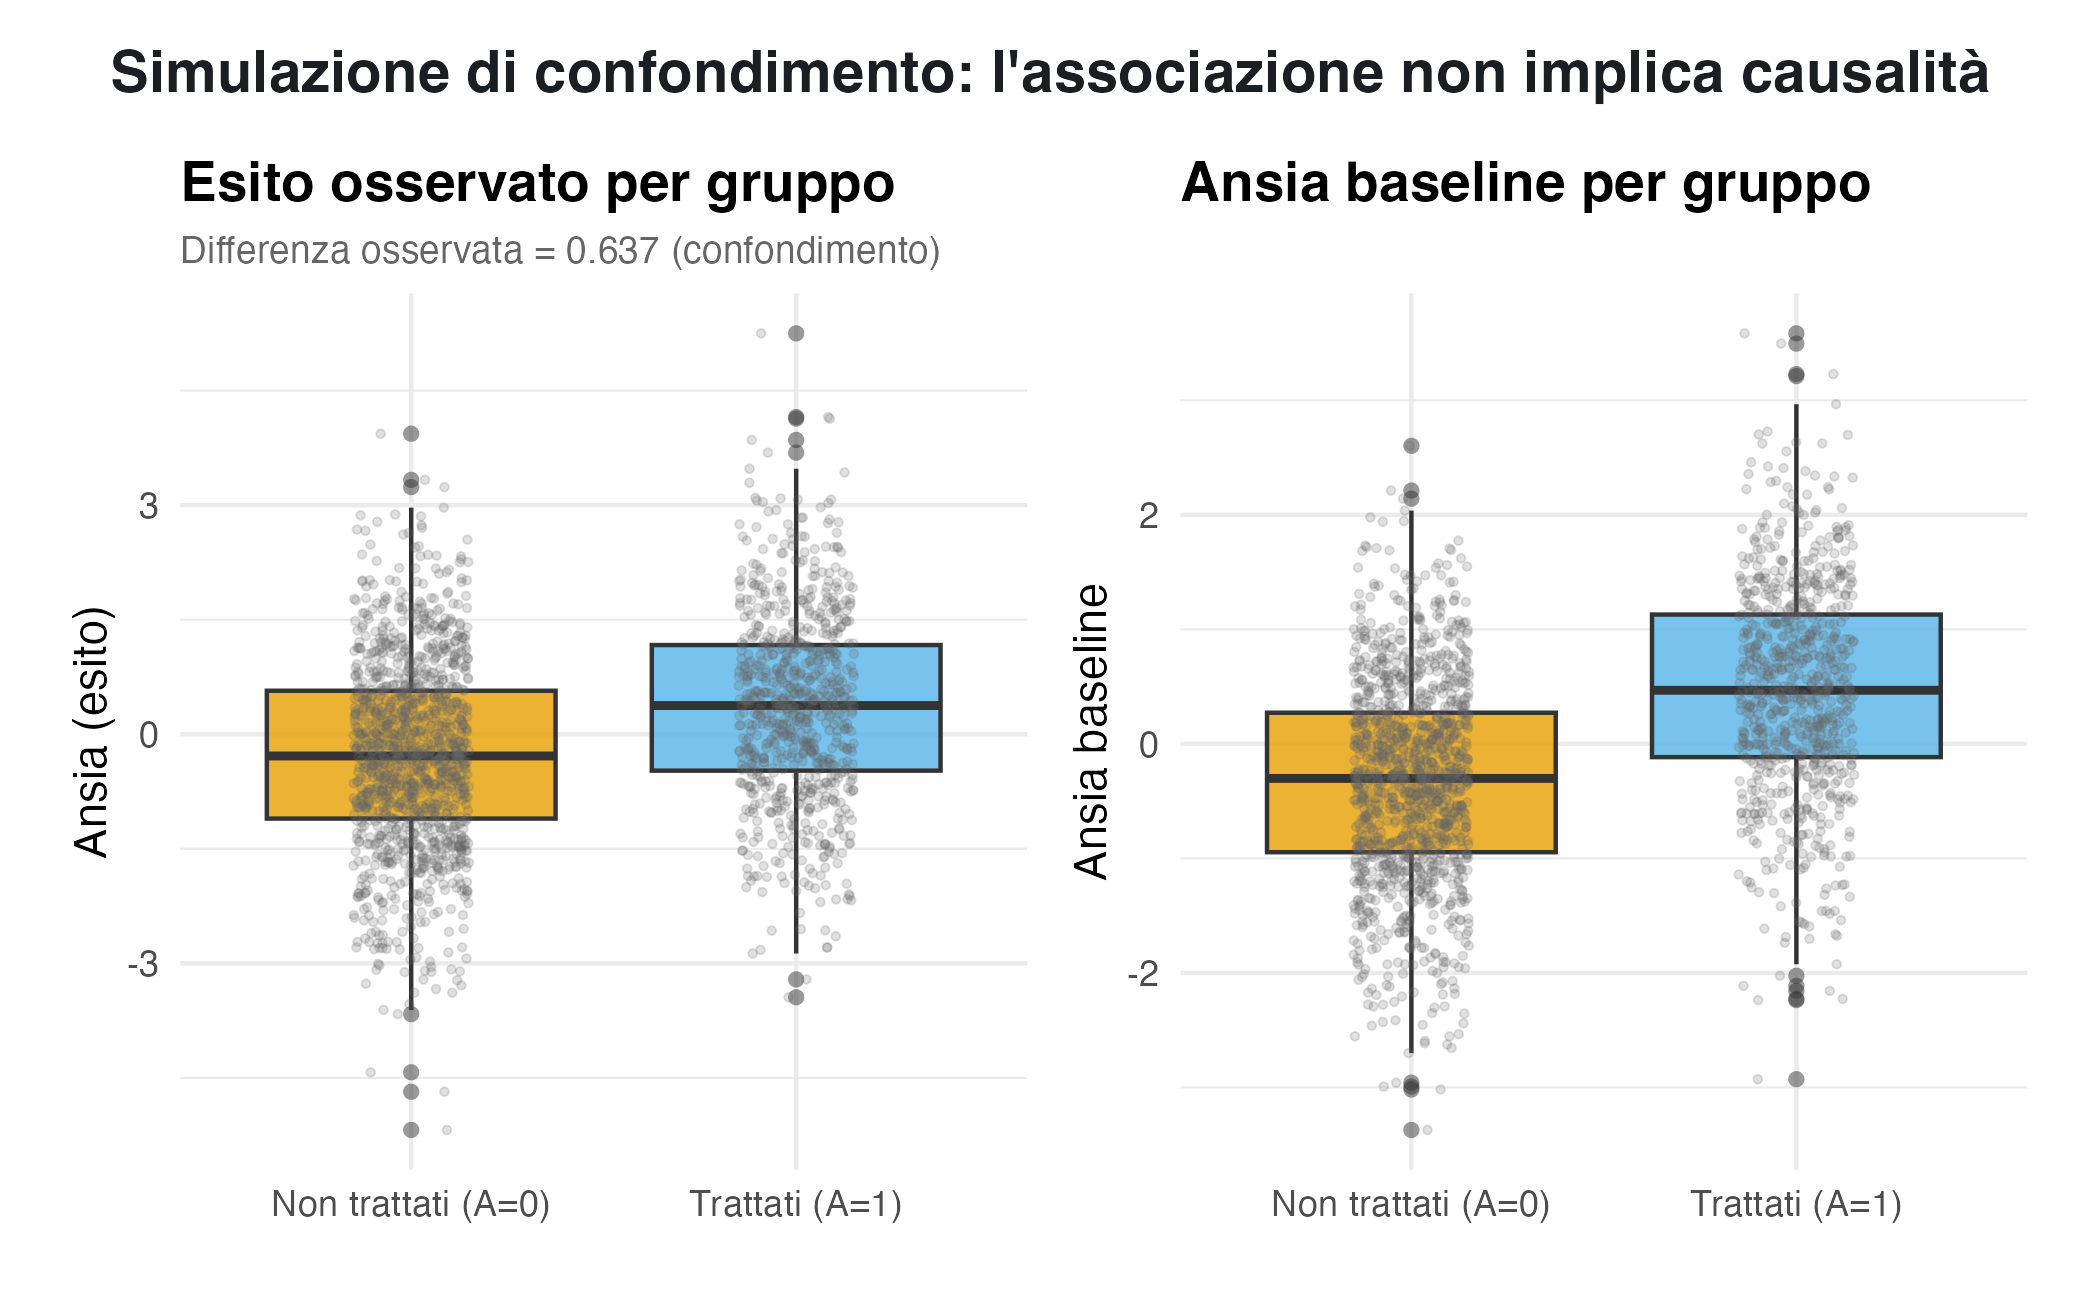
\includegraphics[width=0.85\linewidth,height=\textheight,keepaspectratio]{chapters/causality/02_propedeutic_causality_files/figure-pdf/sim-confounding-1.png}

}

\caption{Confondimento: il gruppo trattato appare peggiore anche senza
effetto causale.}

\end{figure}%

I grafici illustrano chiaramente il fenomeno. Il primo mostra che il
gruppo trattato presenta in media livelli di ansia più elevati, quasi
come se il trattamento avesse sortito un effetto negativo. Tuttavia, ed
è questo il punto cruciale, in questa simulazione il trattamento non ha
alcun effetto causale reale. Il secondo grafico rivela il motivo: i
soggetti assegnati al gruppo di trattamento presentavano già livelli di
ansia basale significativamente più alti.

Questa simulazione dimostra chiaramente come l'associazione osservata
tra trattamento ed esito possa divergere radicalmente dal suo effetto
causale. In questo caso, la differenza apparente è interamente
attribuibile al confondimento: una variabile non controllata (l'ansia di
base) influenza sia la probabilità di ricevere il trattamento sia
l'esito finale, creando un'illusione di causalità laddove non esiste.

\subsection{Randomizzazione: quando associazione e causalità coincidono
(se ACE =
0)}\label{randomizzazione-quando-associazione-e-causalituxe0-coincidono-se-ace-0}

Riprendiamo lo stesso scenario della simulazione precedente, ma con una
modifica decisiva: invece di consentire che il trattamento venga scelto
in base al livello di ansia di base, lo \textbf{assegniamo in modo
casuale}. Questo equivale a lanciare una moneta bilanciata: ogni
individuo ha la stessa probabilità (50\%) di ricevere l'intervento.

In questo nuovo contesto, l'effetto causale del trattamento rimane
nullo, in quanto non abbiamo alterato il meccanismo che lega l'ansia di
tratto all'esito. La differenza cruciale sta nel fatto che, grazie alla
randomizzazione, i gruppi dei trattati e dei non trattati risultano
statisticamente equivalenti in media per tutte le caratteristiche
osservabili e non osservabili, comprese le variabili di confondimento.

Ecco il codice R che implementa questa simulazione:

\begin{figure}[H]

{\centering 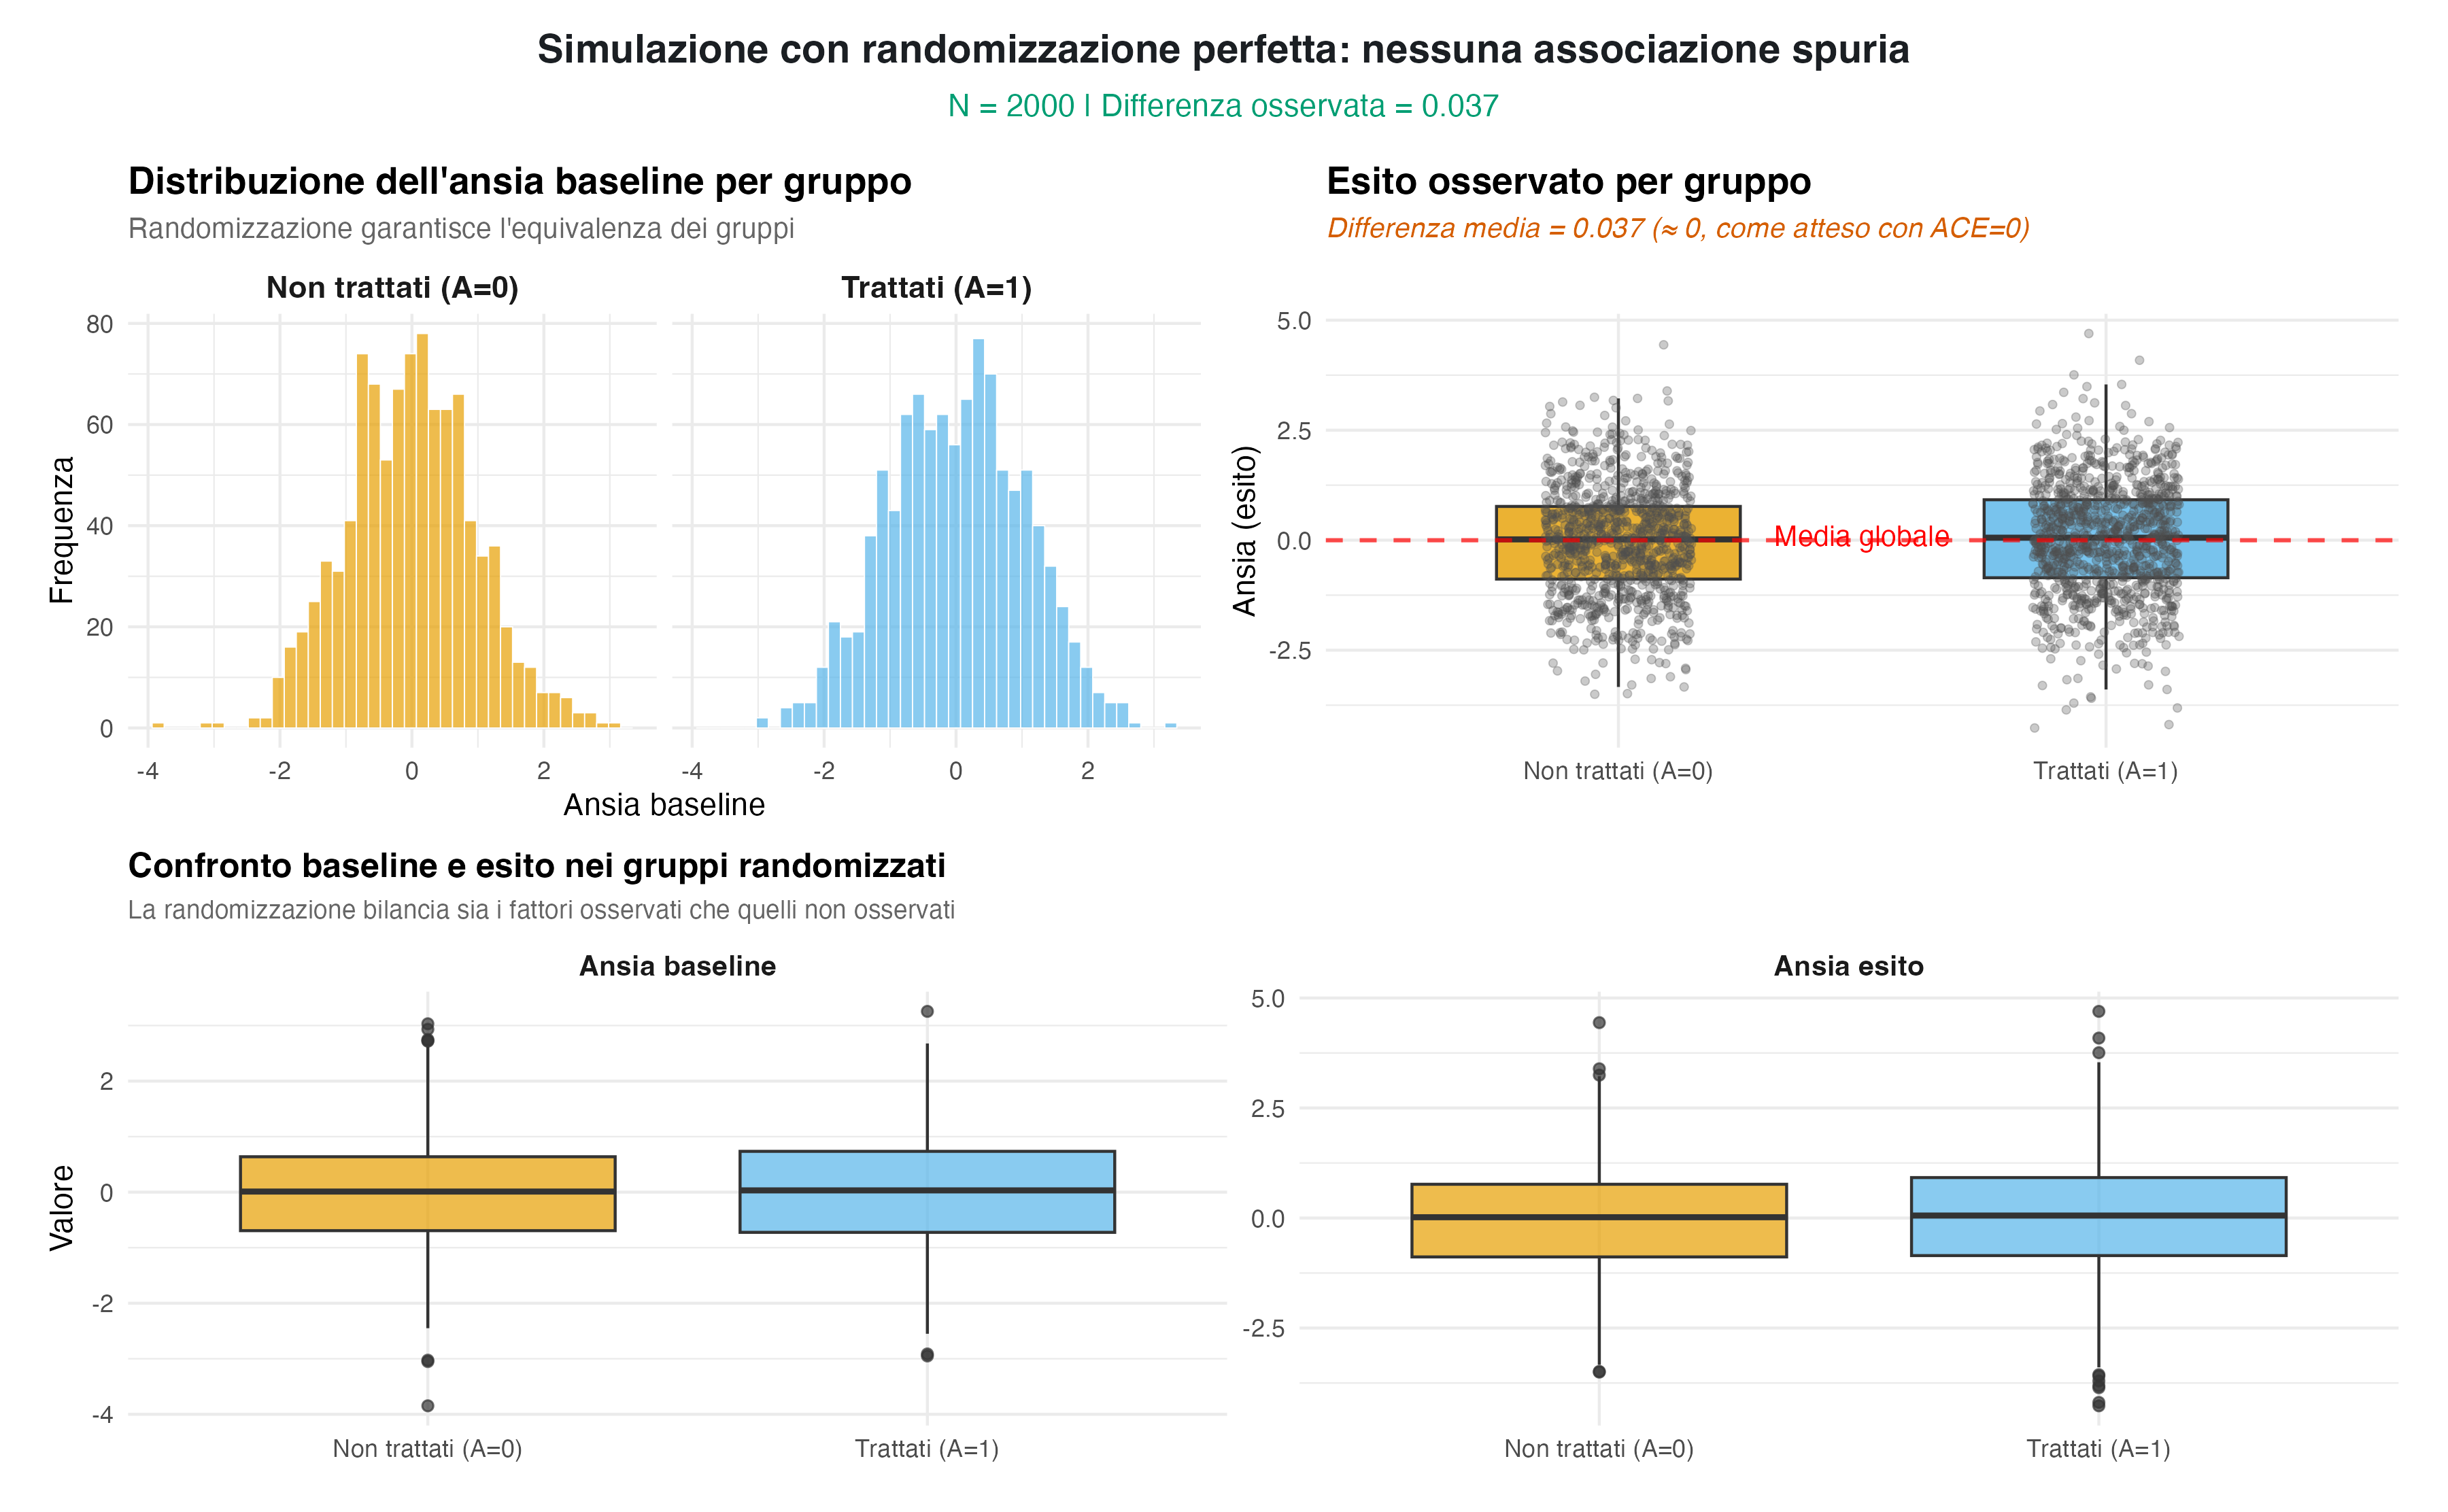
\includegraphics[width=0.85\linewidth,height=\textheight,keepaspectratio]{chapters/causality/02_propedeutic_causality_files/figure-pdf/sim-randomization-null-1.png}

}

\caption{Randomizzazione con ACE=0: l'associazione torna ≈ 0.}

\end{figure}%

\begin{verbatim}
#> Differenza media osservata (randomized) = 0.037
\end{verbatim}

Questa volta, confrontando i due gruppi, notiamo che le distribuzioni
dell'ansia di tratto sono simili. Infatti, la differenza media osservata
negli esiti si avvicina a zero, proprio come il vero effetto causale. In
questo esempio, associazione e causalità coincidono, perché
l'assegnazione casuale ha eliminato il legame spurio con i confondenti.

\section{Quando l'effetto causale c'è
davvero}\label{quando-leffetto-causale-cuxe8-davvero}

Finora abbiamo simulato scenari in cui il trattamento non produceva
alcun effetto reale. Ma cosa accadrebbe se introducessimo un vero
effetto causale? Supponiamo, ad esempio, che l'applicazione della
tecnica di \emph{reappraisal} riduca il livello di ansia di 0.4 punti in
media sulla scala di misurazione.

In questo caso, grazie alla randomizzazione, la differenza media
osservata tra i soggetti trattati e quelli non trattati riflette
fedelmente, almeno in media, questo effetto causale. La randomizzazione
garantisce che i gruppi siano comparabili all'inizio, quindi qualsiasi
differenza sistematica osservata nell'esito può essere plausibilmente
attribuita al trattamento.

La simulazione che segue implementa proprio questo scenario:

\begin{figure}[H]

{\centering 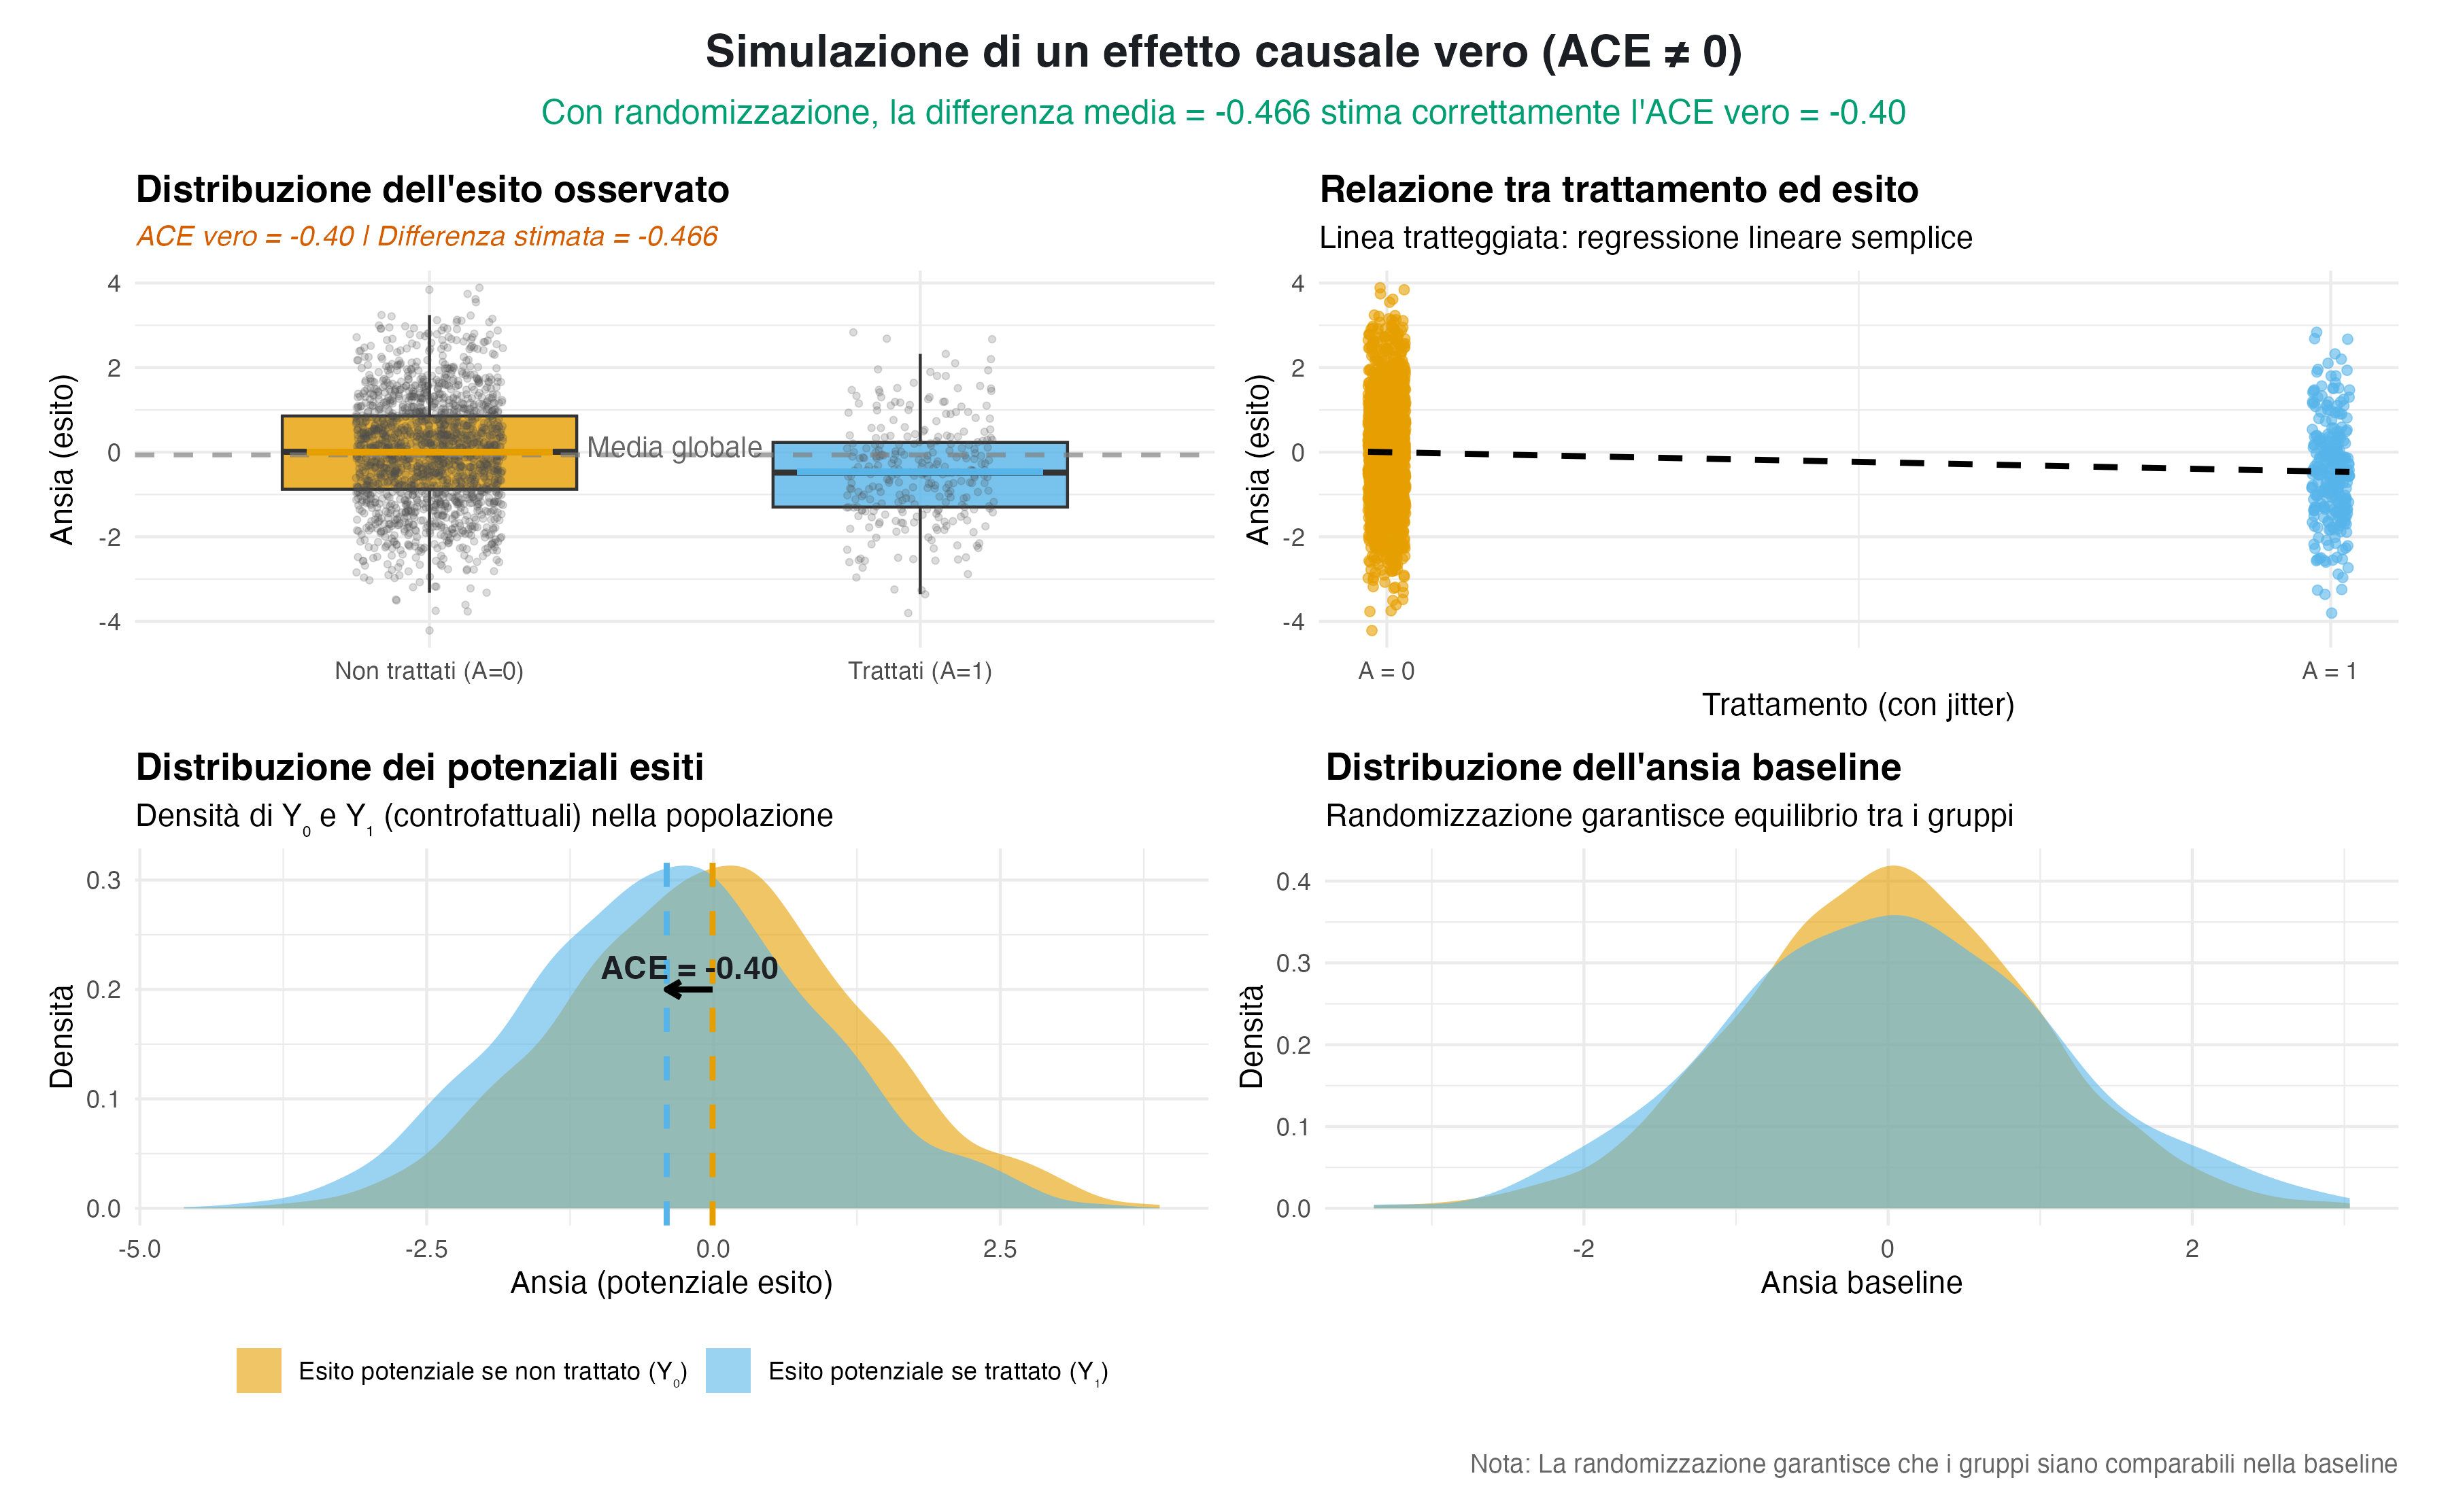
\includegraphics[width=0.85\linewidth,height=\textheight,keepaspectratio]{chapters/causality/02_propedeutic_causality_files/figure-pdf/sim-true-effect-1.png}

}

\caption{Randomizzazione con ACE ≠ 0: la differenza media stima
l'effetto causale.}

\end{figure}%

\begin{verbatim}
#> Differenza media osservata = -0.466 (vero effetto = -0.400)
\end{verbatim}

Il risultato è chiaro: quando esiste un vero effetto causale e i gruppi
sono stati resi comparabili mediante la randomizzazione, la differenza
media osservata diventa una buona stima dell'ACE. In altre parole,
l'esperimento controllato ci permette di trasformare un'associazione in
un'inferenza causale credibile.

\subsection{Domande guida per l'inferenza
causale}\label{domande-guida-per-linferenza-causale}

Lavorare con dati osservazionali in psicologia richiede un cambio di
prospettiva: da un approccio meramente associativo a uno che, con metodo
e cautela, si avvicini al ``cosa sarebbe successo se''. Il seguente kit
di domande guida fornisce una bussola metodologica per navigare questa
complessità in modo rigoroso (questi argomenti saranno sviluppati nel
Capitolo~\ref{sec-eda-causality}).

\textbf{1. La domanda causale è definita con precisione?} L'inferenza
causale inizia con una domanda ben definita. Questo richiede di
specificare con esattezza quattro elementi: - \textbf{Trattamento}: che
cosa costituisce l'esposizione o l'intervento (ad esempio, ``applicare
la tecnica di \emph{reappraisal} secondo il protocollo X per almeno 15
minuti al giorno'')? - \textbf{Esito}: qual è la variabile di risultato
e come viene operazionalizzata e misurata (ad esempio, ``punteggio
totale alla scala di ansia di stato Y, misurato subito dopo la
sessione'')? - \textbf{Popolazione}: a quale gruppo specifico di
individui ci si riferisce (ad esempio, ``studenti universitari di corsi
umanistici, di età compresa tra 20 e 25 anni'')? - \textbf{Contesto
temporale}: in quale finestra temporale ci si aspetta che l'effetto si
manifesti (ad esempio, ``effetto immediato post-intervento'')? Un
problema definito in modo vago porta inevitabilmente a conclusioni
altrettanto vaghe.

\textbf{2. Quali sono le possibili variabili di confondimento?} Il
confondimento rappresenta la minaccia principale alla validità causale.
Una variabile di confondimento influenza sia la probabilità di ricevere
il trattamento che l'esito stesso, creando un'associazione spuria tra i
due. Identificarla richiede un esercizio di teoria e conoscenza del
dominio. Ad esempio, studiando l'effetto dell'uso dei social media
(\texttt{Trattamento}) sul benessere psicologico (\texttt{Esito}), la
\textbf{solitudine} è un forte candidato confondente: può spingere sia a
un uso maggiore dei social sia a un minore benessere.

\textbf{3. Le assunzioni SUTVA sono plausibili nel mio contesto?}
L'assunzione SUTVA (\emph{Stable Unit Treatment Value Assumption}) è
spesso data per scontata, ma deve essere esplicitamente verificata.
Comprende due parti: (1) \textbf{assenza di interferenza} -- il
trattamento assegnato a un individuo influenza solo il suo esito, non
quello di altri (un'ipotesi che può essere violata in contesti di gruppo
o comunitari); e (2) \textbf{unicità del trattamento} -- esiste una sola
versione ben definita del trattamento (in psicologia, gli ``interventi''
spesso variano nella loro implementazione pratica). Valutare la
plausibilità di SUTVA guida la scelta del disegno di ricerca e
l'interpretazione dei risultati.

\textbf{4. Su quale scala è più significativo misurare l'effetto?} La
scelta della misura d'effetto deve rispondere alla domanda di ricerca e
agli scopi pratici dello studio, non seguire una regola universale. - La
\textbf{differenza di rischi} (o di medie per esiti continui) risponde a
una domanda di impatto assoluto: ``Quanti casi in più/meno possiamo
attenderci?''. - Il \textbf{rapporto di rischi} (o \emph{odds ratio})
risponde a una domanda di rischio relativo: ``Quante volte è più (o
meno) probabile l'esito?''. La scelta influenza l'interpretazione
pratica e la comunicazione dei risultati verso clinici, pazienti o
decisori pubblici.

\textbf{5. Come posso avvicinarmi al controfattuale con i dati che ho?}
In assenza di randomizzazione, il ricercatore deve ``ricreare'' le
condizioni di comparabilità tramite l'analisi, affidandosi a strumenti
specifici. \textbf{I Grafici Causali (DAG)} rappresentano visivamente le
ipotesi sulle relazioni tra variabili e sono fondamentali per
distinguere confonditori, mediatori e \emph{collider} (configurazioni
che, se controllate, introducono distorsione invece di rimuoverla). Una
volta definito il DAG, il \textbf{criterio \emph{backdoor}} indica
formalmente quale insieme minimo di variabili è necessario controllare
(ad esempio, tramite regressione o stratificazione) per bloccare i
percorsi di confondimento. Infine, si applicano i \textbf{metodi
statistici appropriati} (come la regressione multivariata o il
\emph{propensity score matching}) per stimare l'effetto una volta
isolate le variabili chiave.

\begin{tcolorbox}[enhanced jigsaw, arc=.35mm, bottomrule=.15mm, bottomtitle=1mm, breakable, colback=white, colbacktitle=quarto-callout-tip-color!10!white, colframe=quarto-callout-tip-color-frame, coltitle=black, left=2mm, leftrule=.75mm, opacityback=0, opacitybacktitle=0.6, rightrule=.15mm, title=\textcolor{quarto-callout-tip-color}{\faLightbulb}\hspace{0.5em}{Take-home (riepilogo)}, titlerule=0mm, toprule=.15mm, toptitle=1mm]

In sintesi, l'effetto causale è un confronto controfattuale su tutta la
popolazione, in cui si considerano due mondi: uno con il trattamento e
uno senza. L'associazione, invece, è un confronto osservazionale tra
gruppi reali che può essere distorto dai fattori confondenti. La
randomizzazione rende i gruppi comparabili e, in media, elimina il
confondimento. Con i dati osservazionali, invece, dobbiamo affidarci a
ipotesi e metodi appropriati per avvicinarci il più possibile a uno
scenario controfattuale.

\end{tcolorbox}

\section{Micro-esercizi}\label{micro-esercizi}

Per consolidare le idee fin qui introdotte, proponiamo due semplici
esercizi. Non hanno la pretesa di esaurire la complessità
dell'argomento, ma vogliono offrire l'opportunità di ``toccare con
mano'' alcuni concetti che ritroveremo più avanti nel manuale.

\subsection{Il paradosso di Simpson}\label{il-paradosso-di-simpson}

Il paradosso di Simpson rappresenta un esempio paradigmatico di come le
associazioni aggregate possano condurre a conclusioni fuorvianti
sull'effetto di un trattamento. Si verifica quando una tendenza
osservata in un'intera popolazione scompare o si inverte quando si
esaminano i sottogruppi che la compongono.

Consideriamo due sottogruppi di individui: uno con bassa ansia di tratto
e uno con alta ansia di tratto. Supponiamo che \emph{all'interno di
ciascun sottogruppo} l'effetto causale del trattamento sia identico e
negativo, ovvero riduca l'ansia di una quantità fissa. Il paradosso
emerge quando la probabilità di ricevere il trattamento non è omogenea
tra i gruppi. Ad esempio, se gli individui con un'alta ansia di tratto
cercano attivamente il trattamento con maggiore frequenza, il gruppo dei
trattati sarà composto in modo sproporzionato da persone già più
ansiose.

Di conseguenza, quando si confrontano semplicemente le medie dell'intero
gruppo trattato con quelle dell'intero gruppo di controllo
(\emph{confronto marginale}), la differenza osservata sarà una miscela
confusa di due elementi: il vero effetto del trattamento e il divario
preesistente nei livelli di ansia tra i sottogruppi. Questo può produrre
una stima aggregata che è nulla, attenuata o, in casi estremi, di segno
opposto rispetto all'effetto reale presente in ogni sottogruppo.

La simulazione seguente illustra questo meccanismo in azione, mostrando
come un trattamento che si è rivelato efficace in ogni sottogruppo possa
apparire inefficace o addirittura dannoso quando i dati vengono
analizzati senza considerare la struttura dei sottogruppi.

\begin{figure}[H]

{\centering 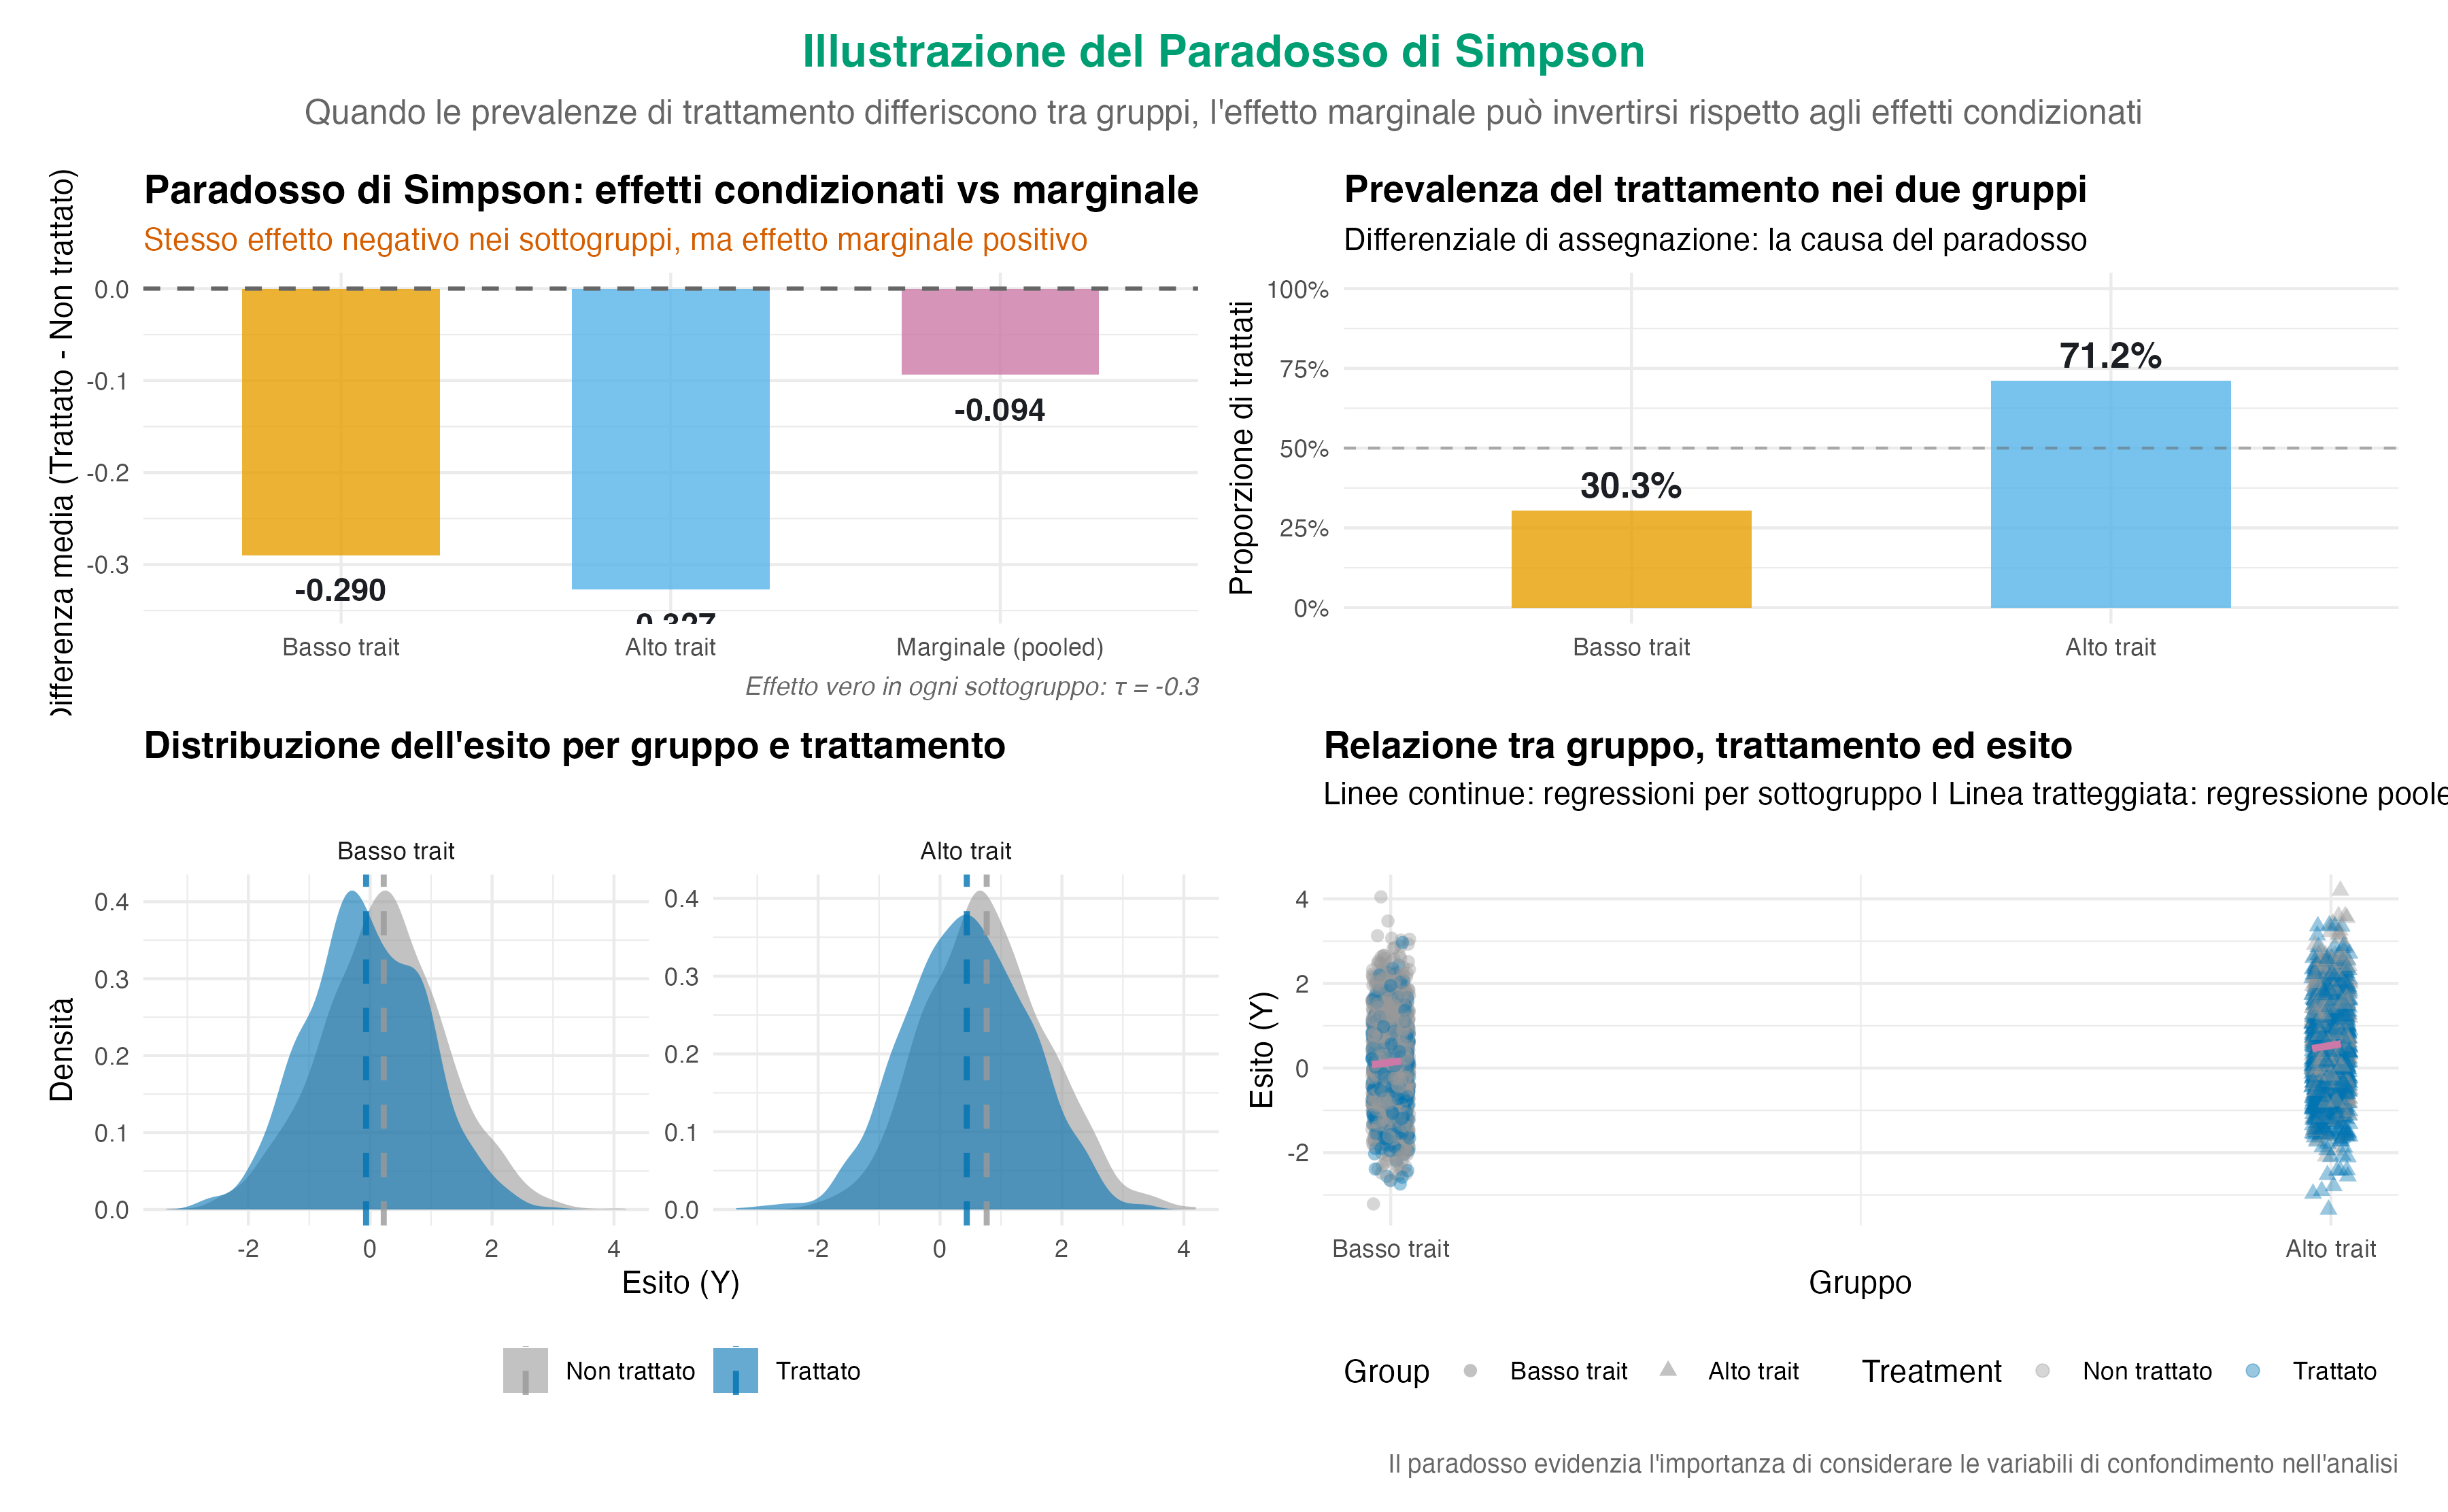
\includegraphics[width=0.85\linewidth,height=\textheight,keepaspectratio]{chapters/causality/02_propedeutic_causality_files/figure-pdf/exercise-simpson-1.png}

}

\caption{Paradosso di Simpson: stesso effetto nei sottogruppi, ma segno
opposto nell'effetto marginale.}

\end{figure}%

I due grafici a barre relativi ai sottogruppi mostrano un effetto
coerente e negativo, come previsto dall'ipotesi di partenza. Tuttavia,
il barplot ``marginale'', che ignora la distinzione tra alto e basso
tratto, racconta un'altra storia, ovvero quella di un effetto prossimo a
zero.

Questa discrepanza descrive il \textbf{Paradosso di Simpson}. Dimostra
come una conclusione basata su dati aggregati possa essere
diametralmente opposta a quella che emerge dall'analisi stratificata. Il
meccanismo alla base di questa discrepanza è il \emph{confondimento}: la
variabile ``ansia di tratto'' distorce l'associazione osservata perché
influenza sia la probabilità di ricevere il trattamento sia l'esito
stesso.

Pertanto, per risalire all'effetto causale vero, è necessario
\emph{aggiustare} per questo fattore confondente. Non si tratta di
includere meccanicamente ogni covariata correlata in una regressione, ma
di un'operazione concettuale precisa: dobbiamo \emph{condizionare}
sull'ansia di tratto, in modo da confrontare individui che, a parità di
livello di tratto, differiscono solo per lo stato di trattamento.

È proprio questa operazione di ragionamento sui fattori confondenti e
sugli aggiustamenti necessari che i \textbf{DAG (Directed Acyclic
Graphs)} formalizzano e guidano, e che affronteremo nel
Capitolo~\ref{sec-eda-causality}.

\subsection{Effetto causale espresso su scale diverse: una questione di
comunicazione e
interpretazione}\label{effetto-causale-espresso-su-scale-diverse-una-questione-di-comunicazione-e-interpretazione}

Un secondo esercizio ci permette di confrontare direttamente le diverse
scale su cui è possibile esprimere un effetto causale. Supponiamo che la
probabilità di un certo esito (ad esempio, un attacco d'ansia) sia del
20\% tra i soggetti trattati e del 10\% tra i soggetti non trattati. Da
qui è possibile calcolare tre misure diverse: la differenza di rischi
(RD), il rapporto di rischi (RR) e l'odds ratio (OR).

\begin{Shaded}
\begin{Highlighting}[]
\FunctionTok{set.seed}\NormalTok{(}\DecValTok{7}\NormalTok{)}
\NormalTok{n }\OtherTok{\textless{}{-}} \DecValTok{10000}
\NormalTok{p1 }\OtherTok{\textless{}{-}} \FloatTok{0.20}\NormalTok{; p0 }\OtherTok{\textless{}{-}} \FloatTok{0.10}
\NormalTok{A }\OtherTok{\textless{}{-}} \FunctionTok{rbinom}\NormalTok{(n, }\DecValTok{1}\NormalTok{, }\FloatTok{0.5}\NormalTok{)}
\NormalTok{Y }\OtherTok{\textless{}{-}} \FunctionTok{ifelse}\NormalTok{(A}\SpecialCharTok{==}\DecValTok{1}\NormalTok{, }\FunctionTok{rbinom}\NormalTok{(n,}\DecValTok{1}\NormalTok{,p1), }\FunctionTok{rbinom}\NormalTok{(n,}\DecValTok{1}\NormalTok{,p0))}

\NormalTok{p\_hat1 }\OtherTok{\textless{}{-}} \FunctionTok{mean}\NormalTok{(Y[A}\SpecialCharTok{==}\DecValTok{1}\NormalTok{]}\SpecialCharTok{==}\DecValTok{1}\NormalTok{)}
\NormalTok{p\_hat0 }\OtherTok{\textless{}{-}} \FunctionTok{mean}\NormalTok{(Y[A}\SpecialCharTok{==}\DecValTok{0}\NormalTok{]}\SpecialCharTok{==}\DecValTok{1}\NormalTok{)}

\NormalTok{RD }\OtherTok{\textless{}{-}}\NormalTok{ p\_hat1 }\SpecialCharTok{{-}}\NormalTok{ p\_hat0}
\NormalTok{RR }\OtherTok{\textless{}{-}}\NormalTok{ p\_hat1 }\SpecialCharTok{/}\NormalTok{ p\_hat0}
\NormalTok{OR }\OtherTok{\textless{}{-}}\NormalTok{ (p\_hat1}\SpecialCharTok{/}\NormalTok{(}\DecValTok{1}\SpecialCharTok{{-}}\NormalTok{p\_hat1)) }\SpecialCharTok{/}\NormalTok{ (p\_hat0}\SpecialCharTok{/}\NormalTok{(}\DecValTok{1}\SpecialCharTok{{-}}\NormalTok{p\_hat0))}
\end{Highlighting}
\end{Shaded}

\begin{verbatim}
#> RD = 0.095; RR = 1.91; OR = 2.13
\end{verbatim}

\textbf{Ciascuna di queste misure racconta la stessa storia con un
linguaggio diverso, rispondendo a domande distinte:}

{\def\LTcaptype{none} % do not increment counter
\begin{longtable}[]{@{}
  >{\raggedright\arraybackslash}p{(\linewidth - 6\tabcolsep) * \real{0.2500}}
  >{\raggedright\arraybackslash}p{(\linewidth - 6\tabcolsep) * \real{0.2500}}
  >{\raggedright\arraybackslash}p{(\linewidth - 6\tabcolsep) * \real{0.2500}}
  >{\raggedright\arraybackslash}p{(\linewidth - 6\tabcolsep) * \real{0.2500}}@{}}
\toprule\noalign{}
\begin{minipage}[b]{\linewidth}\raggedright
Misura
\end{minipage} & \begin{minipage}[b]{\linewidth}\raggedright
Formula
\end{minipage} & \begin{minipage}[b]{\linewidth}\raggedright
Domanda a cui risponde
\end{minipage} & \begin{minipage}[b]{\linewidth}\raggedright
Interpretazione concreta
\end{minipage} \\
\midrule\noalign{}
\endhead
\bottomrule\noalign{}
\endlastfoot
\textbf{Differenza di Rischi (RD)} & \texttt{p1\ -\ p0} & ``Quanti casi
in più si osservano?'' & Su 100 persone trattate, ci attendiamo
\textbf{10 casi in più} di attacco d'ansia rispetto a 100 non trattate.
Risponde a una domanda di \textbf{impatto assoluto}. \\
\textbf{Rapporto di Rischi (RR)} & \texttt{p1\ /\ p0} & ``Di quante
volte è più probabile?'' & Il rischio di un attacco d'ansia è \textbf{2
volte superiore} nel gruppo trattato. Risponde a una domanda di
\textbf{rischio relativo}. \\
\textbf{Odds Ratio (OR)} & \texttt{(p1/(1-p1))\ /\ (p0/(1-p0))} &
``Quanto cambiano le probabilità relative?'' & Le \emph{odds}
(probabilità relativa) di un attacco d'ansia sono circa \textbf{2.25
volte maggiori} nei trattati. È meno intuitiva, ma essenziale per i
modelli statistici. \\
\end{longtable}
}

La scelta della scala non è una questione tecnica neutra, ma una
decisione di natura comunicativa e interpretativa. Per uno psicologo che
opera nel settore della sanità pubblica e che è interessato all'impatto
reale di un intervento, la RD (10\% di casi in più) è fondamentale per
la pianificazione delle risorse e dei servizi. Per uno psicologo clinico
o un ricercatore che valuta la forza di un fattore di rischio, il RR
(rischio doppio) potrebbe invece essere più rilevante. L'OR, pur essendo
una misura meno intuitiva, è lo strumento statistico di elezione per i
modelli logistici e le analisi complesse.

Il messaggio finale è che non esiste una scala ``corretta'' in assoluto:
tutto dipende dalla domanda di ricerca specifica e dal contesto in cui
vengono comunicati i risultati. Una discussione completa richiede spesso
di considerare più di una misura, evitando di presentare un singolo
numero isolato dal suo significato pratico.

\section{Riflessioni conclusive}\label{riflessioni-conclusive-29}

Attraverso le simulazioni e gli esercizi presentati, abbiamo illustrato
quanto sia facile confondere l'associazione con la causalità e quanto
sia invece necessario, nonché fondamentale per il metodo scientifico,
separare le due prospettive.

Abbiamo visto come il semplice confronto statistico tra due gruppi
(l'associazione) possa essere gravemente distorto da fattori
confondenti, arrivando persino a suggerire un effetto opposto a quello
reale, come nel paradosso di Simpson. Abbiamo compreso che la
randomizzazione sperimentale risolve questo problema creando due gruppi
paragonabili e consentendo di attribuire le differenze osservate al
trattamento stesso. Abbiamo anche esplorato come un unico effetto
causale possa essere comunicato su scale diverse: la differenza assoluta
o il rischio relativo, ognuna delle quali risponde a una domanda diversa
e serve uno scopo comunicativo diverso.

Questi concetti non sono semplici cavilli teorici, ma costituiscono la
premessa per una ricerca quantitativa rigorosa. Tuttavia, nella ricerca
psicologica osservazionale, in cui non è possibile assegnare casualmente
ansia, tratti di personalità o esperienze di vita, il problema rimane
irrisolto. Come possiamo estrarre un segnale causale da dati
intrinsecamente confusi?

È a questa domanda pratica che risponderemo nel
Capitolo~\ref{sec-eda-causality}. In quel capitolo trasformeremo
l'intuizione in una metodologia operativa, imparando a:

\begin{itemize}
\tightlist
\item
  formalizzare le nostre ipotesi causali attraverso i \textbf{DAG}
  (\emph{Directed Acyclic Graphs});
\item
  identificare in modo sistematico, mediante il \textbf{criterio di
  backdoor}, l'insieme minimo di variabili da controllare per isolare
  l'effetto del trattamento;
\item
  applicare gli strumenti statistici appropriati, come il
  \emph{matching}, la pesatura, la regressione multivariata e l'uso dei
  \textbf{propensity score}, per implementare tale controllo.
\end{itemize}

L'obiettivo finale sarà dotarci di un protocollo chiaro per avvicinare
il più possibile l'analisi dei dati osservazionali all'ideale
dell'esperimento randomizzato, trasformando i limiti dei nostri dati in
una riflessione esplicita e rigorosa sulla struttura causale del
fenomeno che stiamo studiando.

\begin{tcolorbox}[enhanced jigsaw, arc=.35mm, bottomrule=.15mm, bottomtitle=1mm, breakable, colback=white, colbacktitle=quarto-callout-tip-color!10!white, colframe=quarto-callout-tip-color-frame, coltitle=black, left=2mm, leftrule=.75mm, opacityback=0, opacitybacktitle=0.6, rightrule=.15mm, title=\textcolor{quarto-callout-tip-color}{\faLightbulb}\hspace{0.5em}{Informazioni sull'ambiente di sviluppo}, titlerule=0mm, toprule=.15mm, toptitle=1mm]

\begin{Shaded}
\begin{Highlighting}[]
\FunctionTok{sessionInfo}\NormalTok{()}
\CommentTok{\#\textgreater{} R version 4.6.1 (2026{-}06{-}24)}
\CommentTok{\#\textgreater{} Platform: aarch64{-}apple{-}darwin23}
\CommentTok{\#\textgreater{} Running under: macOS Tahoe 26.5.2}
\CommentTok{\#\textgreater{} }
\CommentTok{\#\textgreater{} Matrix products: default}
\CommentTok{\#\textgreater{} BLAS:   /Library/Frameworks/R.framework/Versions/4.6/Resources/lib/libRblas.0.dylib }
\CommentTok{\#\textgreater{} LAPACK: /Library/Frameworks/R.framework/Versions/4.6/Resources/lib/libRlapack.dylib;  LAPACK version 3.12.1}
\CommentTok{\#\textgreater{} }
\CommentTok{\#\textgreater{} locale:}
\CommentTok{\#\textgreater{} [1] C.UTF{-}8/UTF{-}8/C.UTF{-}8/C/C.UTF{-}8/C.UTF{-}8}
\CommentTok{\#\textgreater{} }
\CommentTok{\#\textgreater{} time zone: Europe/Zagreb}
\CommentTok{\#\textgreater{} tzcode source: internal}
\CommentTok{\#\textgreater{} }
\CommentTok{\#\textgreater{} attached base packages:}
\CommentTok{\#\textgreater{} [1] stats     graphics  grDevices utils     datasets  methods   base     }
\CommentTok{\#\textgreater{} }
\CommentTok{\#\textgreater{} other attached packages:}
\CommentTok{\#\textgreater{}  [1] ragg\_1.5.2            tinytable\_0.17.0      withr\_3.0.3          }
\CommentTok{\#\textgreater{}  [4] systemfonts\_1.3.2     patchwork\_1.3.2       ggdist\_3.3.3         }
\CommentTok{\#\textgreater{}  [7] tidybayes\_3.0.7       bayesplot\_1.15.0      ggplot2\_4.0.3        }
\CommentTok{\#\textgreater{} [10] reliabilitydiag\_0.2.1 priorsense\_1.2.0      posterior\_1.7.0      }
\CommentTok{\#\textgreater{} [13] loo\_2.10.0            rstan\_2.32.7          StanHeaders\_2.32.10  }
\CommentTok{\#\textgreater{} [16] brms\_2.23.0           Rcpp\_1.1.2            sessioninfo\_1.2.4    }
\CommentTok{\#\textgreater{} [19] conflicted\_1.2.0      janitor\_2.2.1         matrixStats\_1.5.0    }
\CommentTok{\#\textgreater{} [22] modelr\_0.1.11         tibble\_3.3.1          dplyr\_1.2.1          }
\CommentTok{\#\textgreater{} [25] tidyr\_1.3.2           rio\_1.3.0             here\_1.0.2           }
\CommentTok{\#\textgreater{} }
\CommentTok{\#\textgreater{} loaded via a namespace (and not attached):}
\CommentTok{\#\textgreater{}  [1] svUnit\_1.0.8          tidyselect\_1.2.1      farver\_2.1.2         }
\CommentTok{\#\textgreater{}  [4] S7\_0.2.2              fastmap\_1.2.0         tensorA\_0.36.2.1     }
\CommentTok{\#\textgreater{}  [7] pacman\_0.5.1          digest\_0.6.39         timechange\_0.4.0     }
\CommentTok{\#\textgreater{} [10] estimability\_2.0.0    lifecycle\_1.0.5       magrittr\_2.0.5       }
\CommentTok{\#\textgreater{} [13] compiler\_4.6.1        rlang\_1.3.0           tools\_4.6.1          }
\CommentTok{\#\textgreater{} [16] yaml\_2.3.12           knitr\_1.51            labeling\_0.4.3       }
\CommentTok{\#\textgreater{} [19] bridgesampling\_1.2{-}1  pkgbuild\_1.4.8        curl\_7.1.0           }
\CommentTok{\#\textgreater{} [22] RColorBrewer\_1.1{-}3    abind\_1.4{-}8           purrr\_1.2.2          }
\CommentTok{\#\textgreater{} [25] grid\_4.6.1            stats4\_4.6.1          xtable\_1.8{-}8         }
\CommentTok{\#\textgreater{} [28] inline\_0.3.21         emmeans\_2.0.4         scales\_1.4.0         }
\CommentTok{\#\textgreater{} [31] cli\_3.6.6             mvtnorm\_1.4{-}2         rmarkdown\_2.31       }
\CommentTok{\#\textgreater{} [34] generics\_0.1.4        otel\_0.2.0            RcppParallel\_5.1.11{-}2}
\CommentTok{\#\textgreater{} [37] cachem\_1.1.0          stringr\_1.6.0         splines\_4.6.1        }
\CommentTok{\#\textgreater{} [40] parallel\_4.6.1        vctrs\_0.7.3           V8\_8.2.0             }
\CommentTok{\#\textgreater{} [43] Matrix\_1.7{-}5          jsonlite\_2.0.0        arrayhelpers\_1.1{-}1   }
\CommentTok{\#\textgreater{} [46] glue\_1.8.1            codetools\_0.2{-}20      distributional\_0.8.1 }
\CommentTok{\#\textgreater{} [49] lubridate\_1.9.5       stringi\_1.8.7         gtable\_0.3.6         }
\CommentTok{\#\textgreater{} [52] QuickJSR\_1.10.0       pillar\_1.11.1         htmltools\_0.5.9      }
\CommentTok{\#\textgreater{} [55] Brobdingnag\_1.2{-}9     R6\_2.6.1              textshaping\_1.0.5    }
\CommentTok{\#\textgreater{} [58] rprojroot\_2.1.1       evaluate\_1.0.5        lattice\_0.22{-}9       }
\CommentTok{\#\textgreater{} [61] backports\_1.5.1       memoise\_2.0.1         broom\_1.0.13         }
\CommentTok{\#\textgreater{} [64] snakecase\_0.11.1      rstantools\_2.6.0      coda\_0.19{-}4.1        }
\CommentTok{\#\textgreater{} [67] gridExtra\_2.3.1       nlme\_3.1{-}170          checkmate\_2.3.4      }
\CommentTok{\#\textgreater{} [70] mgcv\_1.9{-}4            xfun\_0.60             pkgconfig\_2.0.3}
\end{Highlighting}
\end{Shaded}

\end{tcolorbox}

\section*{Bibliografia}\label{bibliografia-33}

\markright{Bibliografia}

\chapter{Causalità dai dati osservazionali}\label{sec-eda-causality}

Nel Capitolo~\ref{sec-causality-propedeutics} abbiamo introdotto il
framework controfattuale e dimostrato come la randomizzazione, ovvero
l'assegnazione casuale del trattamento, permetta di interpretare le
differenze osservate tra i gruppi come effetti causali diretti.
Tuttavia, nella realtà della ricerca psicologica, questo ideale
sperimentale è difficile da raggiungere: non è possibile assegnare
casualmente traumi infantili, tratti di personalità o esperienze di vita
stressanti.

In questo capitolo, ci si chiede: ``Come possiamo procedere verso
un'inferenza causale quando abbiamo solo dati osservazionali?'' La
risposta non risiede in formule statistiche automatiche, ma in una
capacità di ragionamento esplicito sulle strutture causali sottostanti.
A tale scopo, introduciamo i DAG (\emph{Directed Acyclic Graphs}) come
strumento fondamentale. Un DAG traduce visivamente le nostre ipotesi
teoriche in un insieme strutturato di relazioni causali tra variabili,
mappando percorsi diretti, confondenti e mediatori.

Questo formalismo grafico non è un semplice diagramma, ma la chiave per
prendere decisioni analitiche rigorose. Ci permette di determinare,
attraverso il \emph{criterio backdoor}, quali variabili includere in un
modello per bloccare i percorsi di confondimento e isolare l'effetto di
interesse e, altrettanto importante, quali variabili \emph{escludere}
per evitare di introdurre nuovi bias, come avviene nel controllo di una
variabile \emph{collider}.

In questo contesto, il modello di regressione standard assume una nuova
funzione. Non è più solo uno strumento per descrivere associazioni, ma
può diventare un mezzo per l'inferenza causale. Tale trasformazione,
tuttavia, è subordinata a una premessa: la regressione deve essere
guidata da un ragionamento causale esplicito. La scelta dei predittori
da includere (e di quelli da escludere) non può quindi essere risolta
con criteri puramente statistici, come la massimizzazione della bontà di
adattamento del modello, ma richiede un'attenta riflessione teorica che
renda esplicite e giustifichi le nostre ipotesi sul processo che ha
generato i dati osservati.

\begin{tcolorbox}[enhanced jigsaw, arc=.35mm, bottomrule=.15mm, breakable, colback=white, colframe=quarto-callout-important-color-frame, left=2mm, leftrule=.75mm, opacityback=0, rightrule=.15mm, toprule=.15mm]

\textbf{Da sapere.} Nei dati osservazionali, un'associazione può essere
interpretata causalmente solo sulla base di ipotesi esplicite sul
processo generativo. I DAG rappresentano tali ipotesi e permettono di
distinguere percorsi causali, confondenti, mediatori, collider e
discendenti. Il criterio \emph{backdoor} indica quali variabili
controllare per bloccare i percorsi di confondimento; controllare un
collider o un suo discendente può invece introdurre nuove associazioni
spurie.

\textbf{Da saper fare.} Leggere e costruire semplici DAG; riconoscere
catene, biforcazioni e collider; distinguere confondimento, mediazione e
moderazione; individuare percorsi aperti e bloccati mediante la
\emph{d-separation}; scegliere un insieme di aggiustamento coerente con
l'effetto causale di interesse; spiegare perché la selezione delle
covariate non può basarsi soltanto sulla significatività statistica o
sull'aumento di \(R^2\).

\textbf{Approfondimento facoltativo.} La verifica empirica delle
indipendenze condizionali, il confronto dettagliato tra esperimenti,
quasi-esperimenti e studi osservazionali, nonché le sezioni su
\emph{matching}, variabili strumentali e simulazioni numeriche del
confondimento, possono essere rimandati in una prima lettura. Nel
percorso essenziale è sufficiente comprendere il ruolo dei DAG e usare
le configurazioni causali fondamentali per motivare quali variabili
includere o escludere dal modello.

\hyperref[sec-percorsi-lettura]{Che cosa significano queste etichette?}

\end{tcolorbox}

\section*{Panoramica del capitolo}\label{panoramica-del-capitolo-6}

\markright{Panoramica del capitolo}

\begin{itemize}
\tightlist
\item
  Il problema della causalità in assenza di esperimenti.
\item
  I quattro confondenti fondamentali (catena, biforcazione, collider,
  discendente).
\item
  Le inferenze dai dati osservazionali.
\end{itemize}

\begin{tcolorbox}[enhanced jigsaw, arc=.35mm, bottomrule=.15mm, bottomtitle=1mm, breakable, colback=white, colbacktitle=quarto-callout-tip-color!10!white, colframe=quarto-callout-tip-color-frame, coltitle=black, left=2mm, leftrule=.75mm, opacityback=0, opacitybacktitle=0.6, rightrule=.15mm, title=\textcolor{quarto-callout-tip-color}{\faLightbulb}\hspace{0.5em}{Prerequisiti}, titlerule=0mm, toprule=.15mm, toptitle=1mm]

\begin{itemize}
\tightlist
\item
  Leggere
  \href{https://xcelab.net/rm/statistical-rethinking/}{Statistical
  Rethinking}. Focalizzati sul capitolo 1 \emph{The Golem of Prague}.
\item
  Leggere \emph{Causal inference with observational data and unobserved
  confounding variables} di Byrnes \& Dee
  (\citeproc{ref-byrnes2024causal}{2024}).
\item
  Leggere \emph{Causal design patterns for data analysts}
  (\citeproc{ref-riedererdesignpatterns}{Riederer, 2021}). Questo post
  sul blog fornisce una panoramica di diversi approcci per fare
  affermazioni causali dai dati osservazionali.
\item
  Leggere \href{https://theeffectbook.net}{The Effect: An Introduction
  to Research Design and Causality}. Focalizzati sul capitolo 10
  \emph{Treatment Effects}.
\item
  Leggere
  \href{https://mixtape.scunning.com/03-directed_acyclical_graphs}{Causal
  Inference} di Scott Cunningham. Focalizzati sul capitolo 3
  \emph{Directed Acyclic Graphs}.
\item
  Leggere \emph{Telling Stories with Data}
  (\citeproc{ref-alexander2023telling}{Alexander, 2023}). Concentrati
  sul capitolo 15 \emph{Causality from observational data}.
\end{itemize}

\end{tcolorbox}

\begin{tcolorbox}[enhanced jigsaw, arc=.35mm, bottomrule=.15mm, bottomtitle=1mm, breakable, colback=white, colbacktitle=quarto-callout-tip-color!10!white, colframe=quarto-callout-tip-color-frame, coltitle=black, left=2mm, leftrule=.75mm, opacityback=0, opacitybacktitle=0.6, rightrule=.15mm, title=\textcolor{quarto-callout-tip-color}{\faLightbulb}\hspace{0.5em}{Preparazione del Notebook}, titlerule=0mm, toprule=.15mm, toptitle=1mm]

\begin{Shaded}
\begin{Highlighting}[]
\NormalTok{here}\SpecialCharTok{::}\FunctionTok{here}\NormalTok{(}\StringTok{"code"}\NormalTok{, }\StringTok{"\_common.R"}\NormalTok{) }\SpecialCharTok{|\textgreater{}} 
  \FunctionTok{source}\NormalTok{()}
\FunctionTok{conflicts\_prefer}\NormalTok{(ggplot2}\SpecialCharTok{::}\NormalTok{theme\_void)}
\end{Highlighting}
\end{Shaded}

\end{tcolorbox}

\section{Il ruolo dei modelli}\label{il-ruolo-dei-modelli}

Osservare che gli studenti che dormono poco mostrano livelli più elevati
di ansia non è sufficiente per stabilire un rapporto di causa ed
effetto. La relazione potrebbe essere inversa, bidirezionale o dipendere
da una terza variabile, come la pressione legata agli esami. Se ci
limitassimo ai dati osservati, dovremmo fermarci al livello delle
associazioni, ovvero a una fotografia della realtà priva di indicazioni
sul meccanismo che la genera.

La possibilità di formulare inferenze causali dipende invece da un
elemento aggiuntivo: la presenza di un \emph{modello teorico esplicito}.
Sono i modelli, intesi come rappresentazioni di ipotesi sul
funzionamento psicologico, a permetterci di interpretare i dati come il
risultato di processi sottostanti e non solo come covariazioni
superficiali.pretare i dati come risultati di processi sottostanti e non
soltanto come covariazioni superficiali.

In questo capitolo vedremo come i diversi tipi di modelli svolgono
funzioni differenti:

\begin{itemize}
\tightlist
\item
  i modelli \textbf{descrittivi} quantificano le relazioni osservate,
  senza specificare meccanismi causali;
\item
  i modelli \textbf{causali} integrano invece ipotesi sul modo in cui le
  variabili interagiscono, permettendo di distinguere spiegazioni
  alternative.
\end{itemize}

In altre parole, non considereremo la causalità come una proprietà ``che
emerge'' dai dati, ma come un'ipotesi strutturata che riguarda il
processo generativo che sta dietro ai dati stessi.

\section{Correlazione e causalità: perché i dati non
bastano}\label{correlazione-e-causalituxe0-perchuxe9-i-dati-non-bastano}

Il fatto che due variabili varino insieme non implica necessariamente
che una sia la causa dell'altra. Questa nozione è familiare anche ai non
specialisti, ma nella pratica psicologica rimane fonte di
fraintendimenti ricorrenti. Il motivo è che, quando osserviamo
covariazioni robuste e replicabili, l'interpretazione causale risulta
intuitiva: la mente umana tende a cercare spiegazioni direzionali.

Tuttavia, una stessa correlazione può essere compatibile con più scenari
causali. Nel caso dello stress accademico e dei disturbi del sonno, per
esempio, si possono avanzare almeno tre spiegazioni plausibili:

\begin{enumerate}
\def\labelenumi{\arabic{enumi}.}
\tightlist
\item
  lo stress compromette la qualità del sonno;
\item
  la deprivazione di sonno aumenta lo stress;
\item
  un fattore comune (come gli esami) influenza entrambe le variabili.
\end{enumerate}

Tutte e tre producono un'associazione statistica, ma ciascuna postula un
processo causale diverso.

Questa ambiguità non è un dettaglio metodologico: se si inverte la
direzione causale, cambiano sia le interpretazioni teoriche sia le
implicazioni pratiche (interventi clinici, programmi di prevenzione,
politiche educative, ecc.).

La presenza di fattori comuni non osservati, il cosiddetto
``confondimento'', è uno dei motivi per cui la correlazione da sola non
può supportare conclusioni causali. Anche associazioni molto stabili nel
tempo o riscontrate su campioni indipendenti possono essere spiegate da
variabili latenti non misurate.

Il messaggio chiave è che il dato associativo è necessario, ma non
sufficiente: suggerisce ipotesi causali possibili senza identificarne
una come vera.

\section{Perché i modelli diventano
indispensabili}\label{perchuxe9-i-modelli-diventano-indispensabili}

Per affrontare questa ambiguità concettuale, abbiamo bisogno di
strumenti che rendano esplicite le ipotesi sul modo in cui le variabili
interagiscono. In psicologia sperimentale, clinica e sociale, questa
formalizzazione è particolarmente importante: la maggior parte delle
variabili rilevanti sono di natura psicologica, non direttamente
osservabili e spesso influenzate da strutture latenti, difficili da
manipolare.

I modelli causali consentono di:

\begin{itemize}
\tightlist
\item
  rappresentare ipotesi direzionali;
\item
  valutare quali relazioni sono compatibili con i dati e quali no;
\item
  individuare condizioni che permettono di discriminare tra spiegazioni
  alternative;
\item
  progettare studi che massimizzano l'identificabilità causale.
\end{itemize}

Senza questa struttura, si rischia di confondere spiegazioni plausibili
con spiegazioni dimostrate.

\section{Rappresentare le ipotesi causali: Una guida visiva al
ragionamento
scientifico}\label{rappresentare-le-ipotesi-causali-una-guida-visiva-al-ragionamento-scientifico}

Per sviluppare e testare ipotesi causali in modo rigoroso è necessario
un linguaggio formale. I \textbf{grafi causali} (o diagrammi causali)
sono lo strumento moderno più diffuso per questo scopo. Si tratta di
strutture composte da nodi (variabili) e archi direzionati (relazioni
causali dirette ipotizzate).

\subsection{La natura operativa dei grafi
causali}\label{la-natura-operativa-dei-grafi-causali}

Queste rappresentazioni non sono semplici illustrazioni, ma
\textbf{modelli operativi} con due funzioni fondamentali:

\begin{enumerate}
\def\labelenumi{\arabic{enumi}.}
\tightlist
\item
  \textbf{chiarezza espositiva:} rendono immediatamente visibile la
  struttura causale assunta, esplicitando quali relazioni dirette sono
  ipotizzate e, altrettanto cruciale, quali sono assenti;
\item
  \textbf{potere deduttivo:} forniscono un calcolo per derivare le
  conseguenze verificabili del modello. Attraverso regole formali (come
  le \emph{regole di d-separazione}), permettono di dedurre quali
  relazioni di indipendenza condizionale ci si aspetterebbe di osservare
  nei dati se il modello fosse corretto.
\end{enumerate}

In sintesi, i grafi sono strumenti per il \emph{ragionamento}. Offrono
criteri precisi per stabilire quando un'associazione osservata tra due
variabili può essere interpretata come potenzialmente causale e quando,
invece, è compatibile con la presenza di fattori confondenti o altri
fenomeni.

\subsection{Anatomia di un grafo
causale}\label{anatomia-di-un-grafo-causale}

Un grafo causale è un diagramma costituito da:

\begin{itemize}
\tightlist
\item
  \textbf{nodi (vertici):} rappresentano le variabili misurabili o
  latenti di interesse (es.: livello di stress, sintomi d'ansia, qualità
  del sonno).
\item
  \textbf{archi diretti (frecce →):} indicano un'influenza causale
  diretta ipotizzata dalla variabile di origine verso quella di
  destinazione.
\end{itemize}

L'assenza di un arco diretto tra due nodi implica che non esiste un
effetto causale diretto tra le due variabili.

\subsection{Un esempio nel contesto
psicologico}\label{un-esempio-nel-contesto-psicologico}

Consideriamo uno studio sul legame tra Stress percepito e Rendimento
accademico. Un'ipotesi plausibile può essere rappresentata dal seguente
grafo:

\texttt{Stress\ Percepito} → \texttt{Qualità\ del\ Sonno} →
\texttt{Rendimento\ Accademico}

In questo modello:

\begin{itemize}
\tightlist
\item
  Lo Stress influenza direttamente (e negativamente) la Qualità del
  Sonno.
\item
  La Qualità del Sonno influenza direttamente il Rendimento Accademico.
\item
  Lo Stress influisce sul Rendimento \textbf{solo indirettamente},
  attraverso la mediazione del Sonno.
\item
  \textbf{Assunzione cruciale:} non esiste un effetto causale diretto
  dello Stress sul Rendimento (nessuna freccia diretta). Questa ipotesi
  può essere messa verificata empiricamente.
\end{itemize}

\subsection{Valore pratico nell'indagine
scientifica}\label{valore-pratico-nellindagine-scientifica}

Esplicitare visivamente le ipotesi consente di:

\begin{enumerate}
\def\labelenumi{\arabic{enumi}.}
\tightlist
\item
  \textbf{identificare le vie causali:} distinguere chiaramente effetti
  diretti, indiretti e totali tra le variabili;
\item
  \textbf{Identificare confonditori:} visualizzare variabili comuni che,
  se non misurate o controllate, creano associazioni spurie (es.: un
  fattore ambientale che causa sia stress che peggiora il sonno).
\item
  \textbf{Guidare la progettazione dello studio:} definire quali
  variabili misurare, controllare o randomizzare per testare una
  relazione specifica. Ad esempio, per testare l'effetto diretto del
  sonno sul rendimento, bisognerebbe controllare statisticamente lo
  stress.
\item
  \textbf{Prevenire errori analitici:} il grafo chiarisce se e quando è
  lecito ``controllare per'' una certa variabile. Controllare
  inappropriatamente una variabile mediatrice o una \emph{collider} può
  introdurre bias invece che rimuoverlo.
\end{enumerate}

\subsection{Un chiaro avvertimento
epistemologico}\label{un-chiaro-avvertimento-epistemologico}

Un grafo causale è un'\emph{ipotesi strutturata}, non una verità
rivelata. Non determina automaticamente la causalità, ma formalizza ciò
che \emph{riteniamo plausibile} in base alla teoria e alla conoscenza
pregressa. Il suo valore risiede nella sua capacità di generare
\emph{predizioni verificabili} (sulle indipendenze condizionali) che i
dati possono confermare o falsificare. In questo senso, il grafo
rappresenta il punto di partenza per un dialogo rigoroso tra teoria ed
evidenza empirica.

\section{Confondimento, mediazione e moderazione: i ruoli delle
variabili nei modelli
causali}\label{confondimento-mediazione-e-moderazione-i-ruoli-delle-variabili-nei-modelli-causali}

Nei modelli causali, non tutte le variabili svolgono la stessa funzione.
È fondamentale distinguere i diversi ruoli causali, in quanto ciascuno
richiede approcci analitici differenti e porta a interpretazioni
sostanzialmente diverse dei risultati osservati.

\subsection{Variabili di confondimento: la fonte delle associazioni
spurie}\label{variabili-di-confondimento-la-fonte-delle-associazioni-spurie}

Una \textbf{variabile di confondimento} è un fattore che influenza in
modo causale sia la presunta causa che l'effetto. Se non viene misurata
e controllata adeguatamente, crea un'associazione statistica tra le due
variabili, anche in assenza di una relazione causale diretta tra di
esse.

\textbf{Esempio.} In un campione di studenti si osserva una correlazione
positiva tra l'uso intensivo dei social media e i sintomi depressivi.
Un'interpretazione ingenua porterebbe a concludere che l'uso dei social
media causi la depressione.

Tuttavia, altre ipotesi sono possibili. Ad esempio, la \emph{solitudine
percepita} potrebbe fungere da variabile confondente:

\begin{itemize}
\tightlist
\item
  gli studenti con livelli più elevati di solitudine tendono a un uso
  più frequente dei social media, spesso come tentativo di connessione
  sociale;
\item
  la solitudine è, di per sé, un fattore di rischio per i sintomi
  depressivi.
\end{itemize}

Il grafo causale corrispondente include i percorsi
\texttt{Solitudine\ →\ Uso\ Social\ Media} e
\texttt{Solitudine\ →\ Sintomi\ Depressivi}, ma nessun arco diretto da
Uso Social Media a Sintomi Depressivi. Se questa ipotesi fosse corretta
e la solitudine non venisse controllata, l'associazione tra uso dei
social media e depressione risulterebbe spuria e condurrebbe a inferenze
causali errate.

\subsection{Variabili mediatrici: il meccanismo della
causalità}\label{variabili-mediatrici-il-meccanismo-della-causalituxe0}

Una \textbf{variabile mediatrice} trasmette l'effetto di una variabile
indipendente su una variabile dipendente. Non è una fonte di
distorsione, ma il \textbf{meccanismo} attraverso il quale opera la
relazione causale.

\textbf{Esempio.} Si consideri il percorso causale Stress → Qualità del
sonno → Sintomi d'ansia.

\begin{itemize}
\tightlist
\item
  Lo stress cronico compromette la regolarità e la profondità del sonno.
\item
  Una scarsa qualità del sonno altera la regolazione emotiva e
  incrementa i sintomi ansiosi.
\end{itemize}

In questa struttura la qualità del sonno opera da variabile mediatrice,
spiegando il meccanismo attraverso cui lo stress favorisce l'ansia.
L'effetto causale totale dello stress sui sintomi d'ansia si scompone in
tre componenti:

\begin{itemize}
\tightlist
\item
  \textbf{effetto indiretto}, trasmesso tramite la qualità del sonno;
\item
  \textbf{effetto diretto}, che corrisponde all'eventuale percorso
  residuo non mediato (freccia Stress → Sintomi d'ansia);
\item
  \textbf{effetto totale}, somma dell'effetto diretto e di quello
  indiretto.
\end{itemize}

\subsection{\texorpdfstring{Variabili moderatrici: il ``dipende
da\ldots{}''}{Variabili moderatrici: il ``dipende da\ldots''}}\label{variabili-moderatrici-il-dipende-da}

Una \textbf{variabile moderatrice} modifica la forza, la direzione o
l'esistenza stessa della relazione causale tra due altre variabili.
Risponde alla domanda: ``Per chi o in quali condizioni l'effetto è più
forte o più debole?''

\textbf{Esempio:} supponiamo che lo stress accademico influenzi i
sintomi d'ansia. Questa relazione potrebbe essere moderata dal supporto
sociale percepito.

Nel grafo, la variabile moderatrice si rappresenta con una freccia che
punta alla relazione stessa: \texttt{Stress\ →\ Ansia} con una freccia
da \texttt{Supporto\ Sociale} che punta alla freccia tra Stress e Ansia.

Interpretazione:

\begin{itemize}
\tightlist
\item
  per gli studenti con un \textbf{basso} supporto sociale, l'effetto
  dello Stress sull'Ansia è \textbf{forte};
\item
  per gli studenti con un \textbf{alto} supporto sociale, l'effetto
  dello Stress sull'Ansia è \textbf{attenuato} o persino assente.
\end{itemize}

\subsection{Una distinzione cruciale per la
ricerca}\label{una-distinzione-cruciale-per-la-ricerca}

Comprendere se una variabile è un confonditore, un mediatore o un
moderatore è essenziale per:

\begin{enumerate}
\def\labelenumi{\arabic{enumi}.}
\item
  \textbf{progettare lo studio:} un confonditore va misurato e
  controllato per ottenere stime non distorte dal punto di vista
  causale. Un mediatore va misurato per testare il meccanismo. Un
  moderatore viene incluso per esplorare le differenze tra i
  sottogruppi.
\item
  \textbf{scegliere l'analisi statistica:} il controllo per un
  confonditore (per esempio, mediante la regressione multipla) è diverso
  dalla verifica di mediazione (per esempio, mediante un analisi di
  percorso) o moderazione (per esempio, mediante un'analisi di
  regressione che include termini di interazione).
\item
  \textbf{interpretare i risultati in modo corretto:} scambiare un
  confonditore per un mediatore porta a conclusioni completamente errate
  sulla direzione e sulla natura della causalità.
\end{enumerate}

\textbf{Sintesi visiva:}

\begin{itemize}
\tightlist
\item
  \textbf{confonditore:} \texttt{Z\ →\ X} e \texttt{Z\ →\ Y} (crea un
  falso legame tra \texttt{X} e \texttt{Y});
\item
  \textbf{mediatore:} \texttt{X\ →\ M\ →\ Y} (spiega il legame tra
  \texttt{X} e \texttt{Y});
\item
  \textbf{moderatore:} \texttt{W} modifica la forza di \texttt{X\ →\ Y}.
\end{itemize}

Questa chiarezza concettuale è fondamentale per costruire modelli
causali realistici e testabili nelle scienze psicologiche.

\subsection{Le quattro configurazioni fondamentali nei
DAG}\label{le-quattro-configurazioni-fondamentali-nei-dag}

Per comprendere appieno il funzionamento dei grafi causali, è utile
conoscere le \emph{quattro strutture di base} con cui due variabili
possono essere collegate attraverso una terza.

\begin{enumerate}
\def\labelenumi{\arabic{enumi}.}
\tightlist
\item
  \textbf{Catena (o percorso mediato)}\\
  \[X \rightarrow Z \rightarrow Y\]\\
  In questa configurazione, \(Z\) funge da \emph{mediatore},
  trasmettendo l'effetto causale da \(X\) a \(Y\).

  \begin{itemize}
  \tightlist
  \item
    Se non si controlla per \(Z\), \(X\) e \(Y\) appaiono associati.
  \item
    Controllando per \(Z\), l'associazione tra \(X\) e \(Y\) si
    interrompe, poiché si blocca il percorso causale.
  \end{itemize}
\item
  \textbf{Biforcazione (confondimento)}\\
  \[X \leftarrow Z \rightarrow Y\]\\
  Qui \(Z\) è un \emph{confondente}: causa comune sia di \(X\) che di
  \(Y\).

  \begin{itemize}
  \tightlist
  \item
    Senza controllo per \(Z\): si osserva una correlazione spuria tra
    \(X\) e \(Y\).\\
  \item
    Controllando per \(Z\): l'associazione spuria viene eliminata.
  \end{itemize}
\item
  \textbf{Collider}\\
  \[X \rightarrow Z \leftarrow Y\]\\
  In questa struttura, \(Z\) è un \emph{collider}, ovvero un
  \emph{effetto comune} di \(X\) e \(Y\).

  \begin{itemize}
  \tightlist
  \item
    Senza controllo per \(Z\): \(X\) e \(Y\) sono \emph{d-separati} e
    quindi indipendenti.
  \item
    Controllando per \(Z\) (o un suo discendente): si introduce un
    \emph{bias di collider}, creando un'associazione condizionale spuria
    tra \(X\) e \(Y\).
  \end{itemize}
\item
  \textbf{Discendente}\\
  \[X \rightarrow Y \rightarrow Z\]\\
  In questo caso, \(Z\) è un \emph{discendente} di \(Y\).

  \begin{itemize}
  \tightlist
  \item
    Ruolo nell'analisi: un discendente fornisce informazioni indirette
    su un suo antenato, ma \emph{non è un confondente}. Controllare
    statisticamente per un discendente equivale a condizionare, almeno
    parzialmente, la variabile genitore. Questo può aprire percorsi
    collider a monte, introducendo potenzialmente un \emph{bias di
    selezione} e alterando la stima causale d'interesse.
  \end{itemize}
\end{enumerate}

\subsubsection{L'importanza delle configurazioni
fondamentali}\label{limportanza-delle-configurazioni-fondamentali}

Queste quattro strutture costituiscono le \textbf{componenti elementari}
da cui sono costruiti tutti i DAG complessi. La capacità di identificare
ciascuna configurazione e di applicare le corrette regole di controllo
statistico è fondamentale per un'inferenza causale valida. In sintesi:

\begin{itemize}
\tightlist
\item
  è \textbf{necessario controllare} per le variabili in configurazione
  di \textbf{mediatore} (catena) se si vuole stimare un effetto diretto,
  e per i \textbf{confondenti} (biforcazione) per eliminare le
  associazioni spurie;
\item
  è invece \textbf{cruciale non controllare} per le variabili in
  posizione di \textbf{collider} (o per i loro discendenti), poiché ciò
  aprirebbe percorsi di associazione artificiale e introdurrebbe bias;
\item
  analogamente, \textbf{controllare un discendente} può aprire percorsi
  collider indiretti ed è generalmente da evitare, a meno che non sia
  esplicitamente giustificato dal disegno dello studio.
\end{itemize}

Distinguere tra questi casi non è una semplice scelta tecnica, ma
rappresenta la differenza tra stimare una relazione causale vera e
produrre una stima distorta da associazioni spurie.

\begin{tcolorbox}[enhanced jigsaw, arc=.35mm, bottomrule=.15mm, bottomtitle=1mm, breakable, colback=white, colbacktitle=quarto-callout-important-color!10!white, colframe=quarto-callout-important-color-frame, coltitle=black, left=2mm, leftrule=.75mm, opacityback=0, opacitybacktitle=0.6, rightrule=.15mm, title=\textcolor{quarto-callout-important-color}{\faExclamation}\hspace{0.5em}{Implicazioni per la regressione lineare}, titlerule=0mm, toprule=.15mm, toptitle=1mm]

Questa distinzione ha conseguenze operative dirette sull'applicazione
dei modelli di regressione. Nei capitoli precedenti abbiamo visto che
aggiungere predittori a un modello aumenta la varianza spiegata
\((R^2)\). Tuttavia, la prospettiva causale dimostra che la scelta delle
variabili da includere non può essere motivata esclusivamente dal
criterio di ``aumentare la varianza spiegata''. Includere una variabile
errata (ad esempio un \emph{collider} o un discendente di un
\emph{collider}) può introdurre \emph{bias} nelle stime degli effetti di
interesse, \textbf{peggiorando} la validità inferenziale anziché
migliorarla.

Pertanto, la regressione multipla può essere uno strumento affidabile
per l'inferenza causale solo se guidata da un DAG che formalizzi le
ipotesi teoriche sui meccanismi causali sottostanti. Senza questa guida
teorica, il modello di regressione rischia di produrre stime che, seppur
``statisticamente significative'', possono essere fuorvianti dal punto
di vista causale.

\end{tcolorbox}

\section{Dai grafi causali all'inferenza
statistica}\label{dai-grafi-causali-allinferenza-statistica}

Finora abbiamo visto che i grafi causali servono a rappresentare le
nostre ipotesi. Ma come possiamo collegarli ai dati e verificare se un
modello causale è plausibile?

\subsection{Indipendenze e dipendenze}\label{indipendenze-e-dipendenze}

Un'idea chiave è che un grafo causale non descrive solo ``chi influenza
chi'', ma implica anche certe \emph{relazioni di indipendenza} tra le
variabili. Queste relazioni sono importanti perché ci permettono di
confrontare il grafo con i dati: se le indipendenze predette non si
verificano, il grafo non può essere corretto.

\subsubsection{Esempio 1: Catena
(mediazione)}\label{esempio-1-catena-mediazione}

Supponiamo di ipotizzare la seguente relazione causale:\\
\textbf{Stress → Sonno → Ansia}.

In questa struttura, \textbf{Sonno} è un \textbf{mediatore}, in quanto
trasmette parzialmente o totalmente l'effetto dello Stress sull'Ansia.
Se non misuriamo il livello di Sonno, Stress e Ansia appariranno
associati a causa del percorso causale attivo. Tuttavia, una volta che
\textbf{condizioniamo sul Sonno}, l'associazione tra Stress e Ansia si
interrompe, poiché blocchiamo il meccanismo di trasmissione. Da un punto
di vista inferenziale, conoscendo il livello di Sonno, lo Stress non
fornisce ulteriori informazioni sull'Ansia.

Questa relazione è espressa formalmente dalla condizione di
\textbf{indipendenza condizionale}:

\[
\text{Ansia} \; \perp\!\!\!\perp \; \text{Stress} \mid \text{Sonno}
\]

\subsubsection{Esempio 2: Fork (causa
comune)}\label{esempio-2-fork-causa-comune}

Consideriamo ora la seguente struttura causale: \textbf{Sonno} →
\textbf{Stress}; \textbf{Sonno} → \textbf{Ansia}.

In questo caso, \textbf{Sonno} agisce da \emph{confondente} (o causa
comune) per Stress e Ansia. Se non controlliamo statisticamente per il
Sonno, Stress e Ansia appariranno associati, generando una
\textbf{correlazione spuria}. Condizionando sul Sonno, invece,
l'associazione tra Stress e Ansia scompare, poiché viene bloccato
l'unico percorso (non causale) che le collega.

Formalmente, ciò si esprime tramite la condizione di indipendenza
condizionale:

\[
\text{Ansia} \; \perp\!\!\!\perp \; \text{Stress} \mid \text{Sonno}
\]

Questa notazione indica che, dato il livello di Sonno, Stress e Ansia
sono statisticamente indipendenti.

\subsubsection{Esempio 3: Collider (effetto
comune)}\label{esempio-3-collider-effetto-comune}

Consideriamo ora la struttura opposta:\\
\textbf{Stress → Ansia ← Sonno}.

In questo caso, \textbf{Ansia} agisce come un \textbf{collider}: è un
effetto comune di due cause potenzialmente indipendenti, Stress e Sonno.
Il comportamento statistico di questa configurazione è controintuitivo:

\begin{itemize}
\tightlist
\item
  \textbf{Senza condizionare su Ansia}, le due cause (Stress e Sonno)
  sono \textbf{d-separate} e quindi statisticamente indipendenti nella
  popolazione.
\item
  \textbf{Condizionando su Ansia} (o su una qualsiasi sua conseguenza),
  si \textbf{apre artificialmente un percorso di associazione} tra
  Stress e Sonno. Questo fenomeno, noto come \textbf{bias di collider} o
  bias da condizionamento, genera una correlazione spuria tra le due
  variabili originariamente indipendenti.
\end{itemize}

Questa proprietà fondamentale è espressa formalmente come:

\[
\text{Stress} \; \perp\!\!\!\perp \; \text{Sonno} \quad \text{ma} \quad \text{Stress} \; \cancel{\perp\!\!\!\perp} \; \text{Sonno} \mid \text{Ansia}
\]

Dove il simbolo \(\cancel{\perp\!\!\!\perp}\) indica la violazione
dell'indipendenza condizionale.

\subsection{Tabella riassuntiva delle strutture causali
elementari}\label{tabella-riassuntiva-delle-strutture-causali-elementari}

{\def\LTcaptype{none} % do not increment counter
\begin{longtable}[]{@{}
  >{\raggedright\arraybackslash}p{(\linewidth - 8\tabcolsep) * \real{0.0866}}
  >{\raggedright\arraybackslash}p{(\linewidth - 8\tabcolsep) * \real{0.0551}}
  >{\raggedright\arraybackslash}p{(\linewidth - 8\tabcolsep) * \real{0.3543}}
  >{\raggedright\arraybackslash}p{(\linewidth - 8\tabcolsep) * \real{0.3937}}
  >{\raggedright\arraybackslash}p{(\linewidth - 8\tabcolsep) * \real{0.1102}}@{}}
\toprule\noalign{}
\begin{minipage}[b]{\linewidth}\raggedright
Struttura
\end{minipage} & \begin{minipage}[b]{\linewidth}\raggedright
Forma
\end{minipage} & \begin{minipage}[b]{\linewidth}\raggedright
Relazione tra \(X\) e \(Y\) (senza controllo)
\end{minipage} & \begin{minipage}[b]{\linewidth}\raggedright
Relazione tra \(X\) e \(Y\) (dopo controllo su \(Z\))
\end{minipage} & \begin{minipage}[b]{\linewidth}\raggedright
Ruolo di \(Z\)
\end{minipage} \\
\midrule\noalign{}
\endhead
\bottomrule\noalign{}
\endlastfoot
\textbf{Catena} (Mediazione) & \(X \to Z \to Y\) & Dipendenti (percorso
aperto) & Indipendenti (percorso bloccato) & \textbf{Mediatore} \\
\textbf{Fork} (Causa comune) & \(X \leftarrow Z \to Y\) & Dipendenti
(associazione spuria) & Indipendenti (confondimento rimosso) &
\textbf{Confondente} \\
\textbf{Collider} (Effetto comune) & \(X \to Z \leftarrow Y\) &
Indipendenti (nessun percorso attivo) & Dipendenti (associazione spuria
indotta) & \textbf{Collider} \\
\end{longtable}
}

\textbf{Legenda:}

\begin{itemize}
\tightlist
\item
  \textbf{Percorso aperto/bloccato:} riferimento al criterio di
  \emph{d-separation} nei DAG.\\
\item
  \textbf{Controllo:} include qualsiasi condizionamento statistico
  (stratificazione, aggiustamento in regressione).\\
\item
  \textbf{Dipendenza spuria:} associazione statistica non corrispondente
  a un effetto causale diretto.
\end{itemize}

\subsection{Le quattro strutture causali elementari nei
DAG}\label{le-quattro-strutture-causali-elementari-nei-dag}

Di seguito sono illustrate le \textbf{quattro configurazioni minime} che
definiscono le relazioni causali fondamentali all'interno di un DAG:
\emph{Catena}, \emph{Fork}, \emph{Collider} e \emph{Discendente}.
Ciascuna struttura segue regole precise di \emph{d-separation} che
determinano quando due variabili sono condizionatamente indipendenti,
guidando così le scelte critiche di controllo statistico nell'inferenza
causale.

\begin{figure}

\centering{

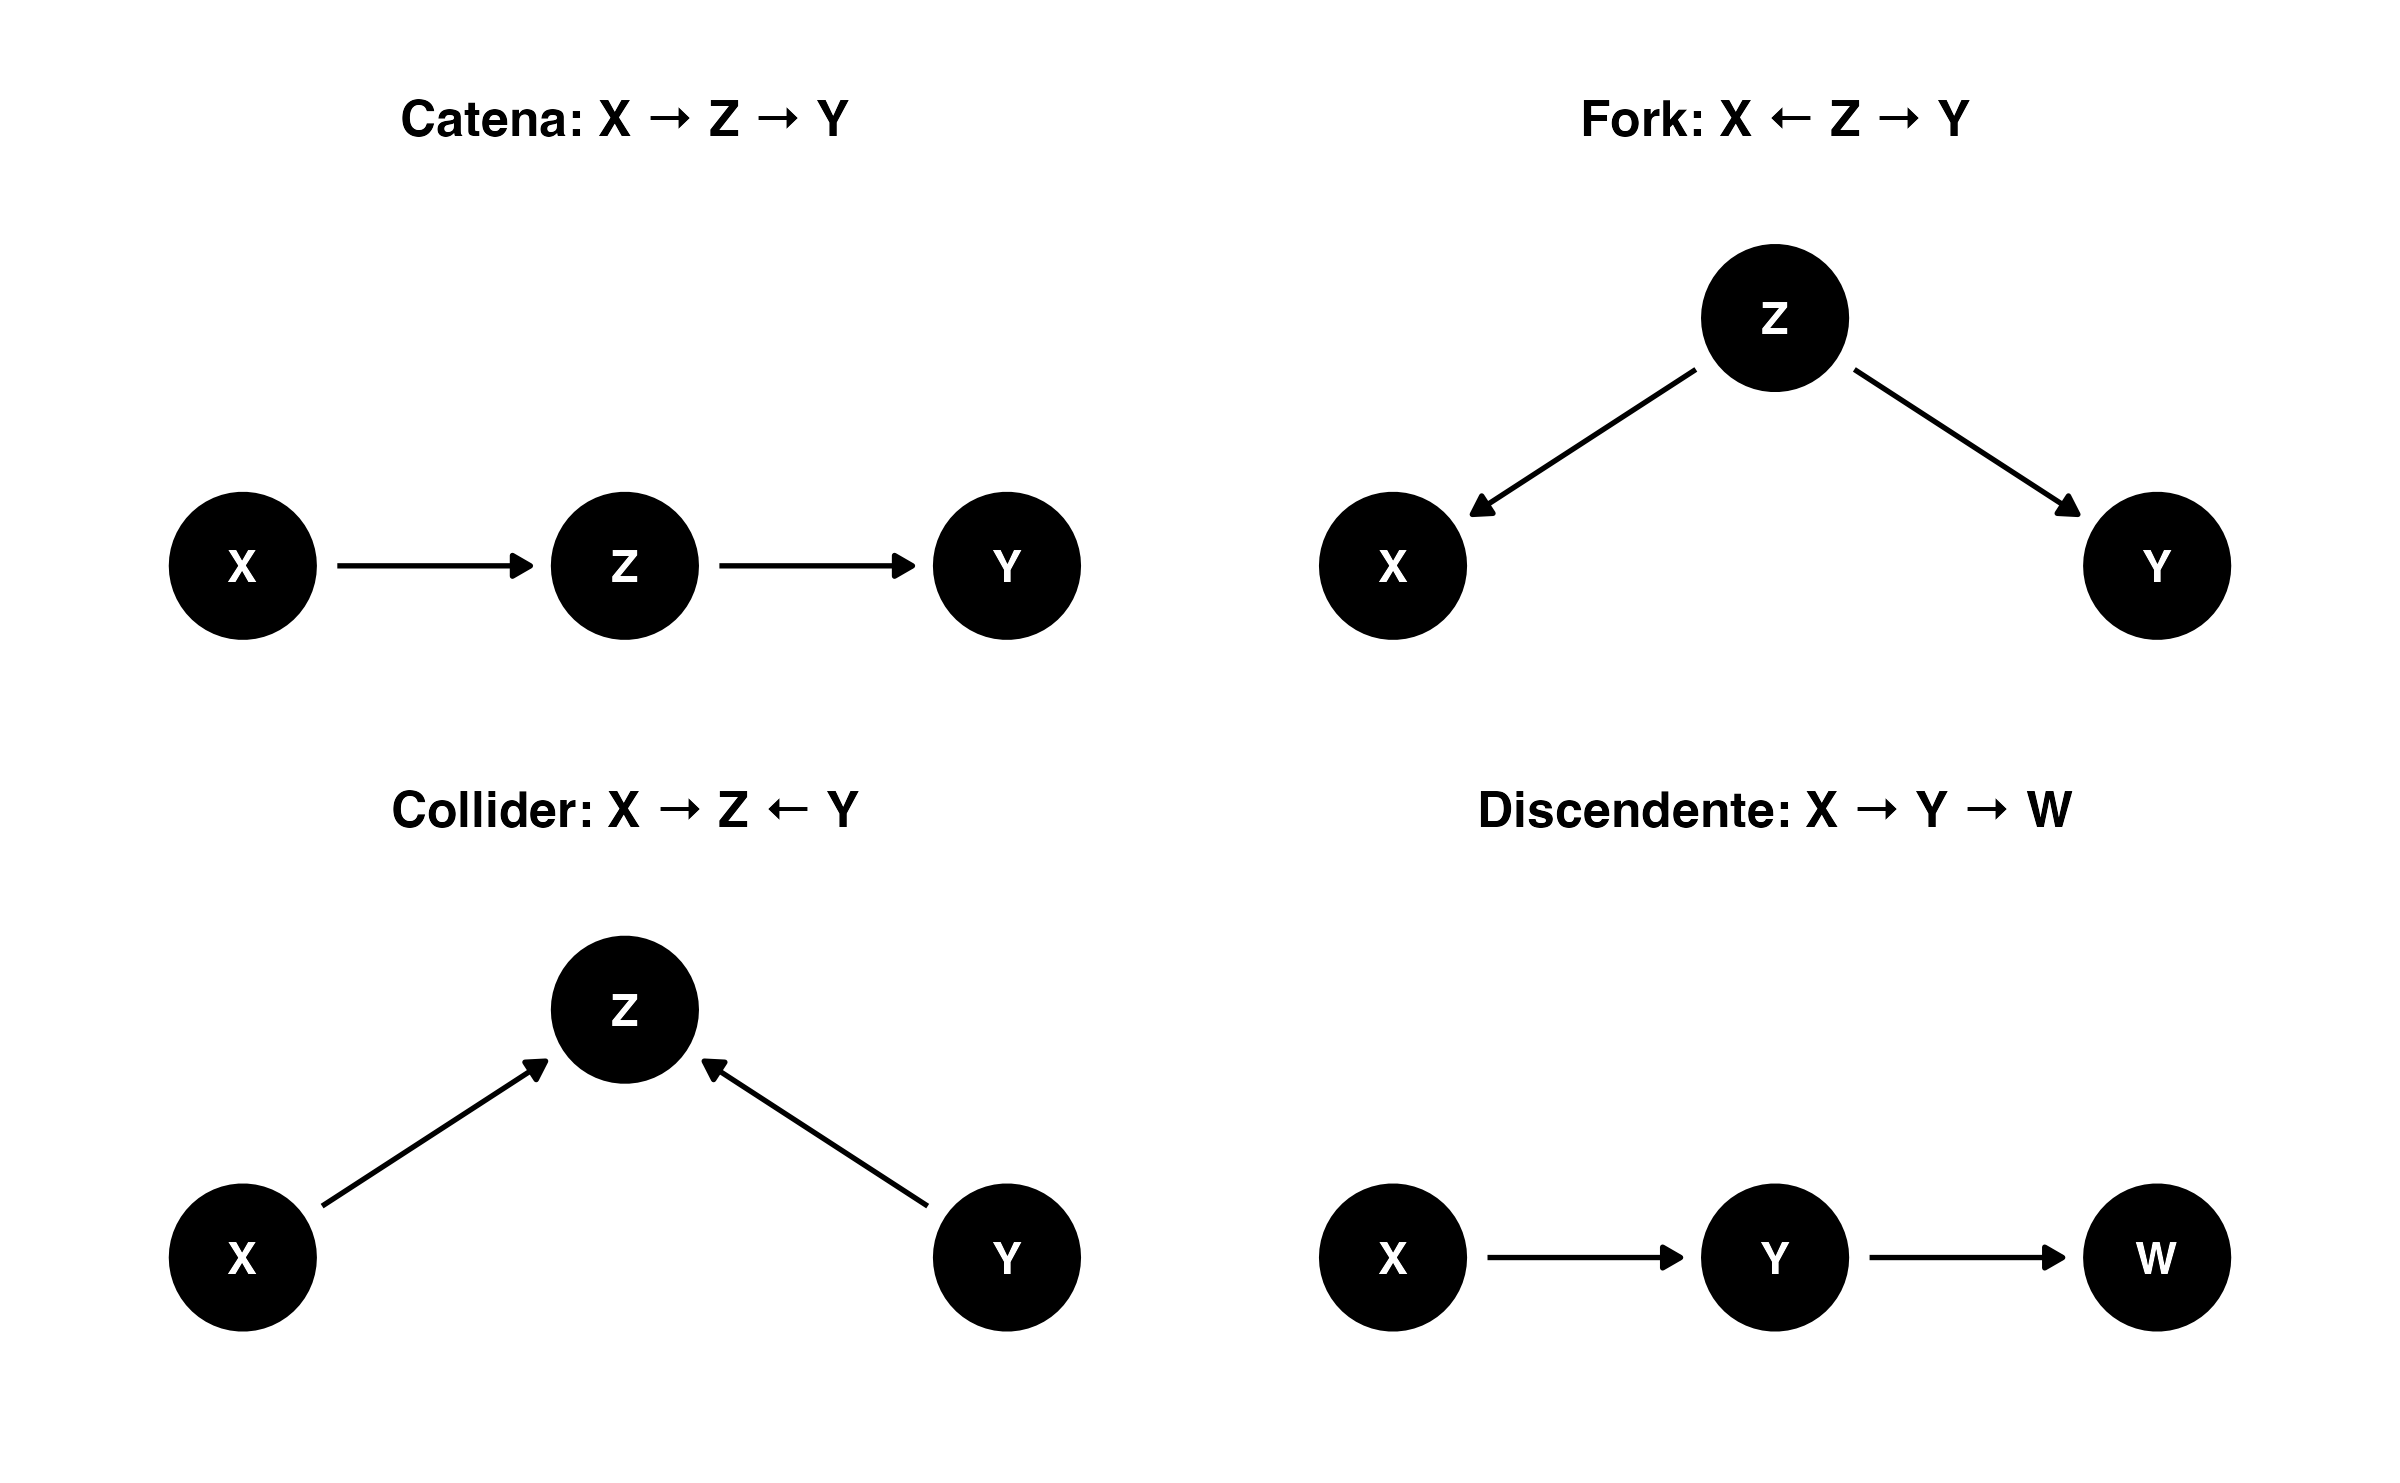
\includegraphics[width=0.85\linewidth,height=\textheight,keepaspectratio]{chapters/causality/03_causality_files/figure-pdf/fig-dag-quad-1.png}

}

\caption{\label{fig-dag-quad}Quattro configurazioni base dei DAG:
Catena, Fork, Collider, Discendente.}

\end{figure}%

\begin{tcolorbox}[enhanced jigsaw, arc=.35mm, bottomrule=.15mm, bottomtitle=1mm, breakable, colback=white, colbacktitle=quarto-callout-tip-color!10!white, colframe=quarto-callout-tip-color-frame, coltitle=black, left=2mm, leftrule=.75mm, opacityback=0, opacitybacktitle=0.6, rightrule=.15mm, title=\textcolor{quarto-callout-tip-color}{\faLightbulb}\hspace{0.5em}{Errore comune: il condizionamento sui collider}, titlerule=0mm, toprule=.15mm, toptitle=1mm]

\begin{itemize}
\tightlist
\item
  \textbf{Struttura Collider}: \(X \to Z \leftarrow Y\)

  \begin{itemize}
  \tightlist
  \item
    \textbf{Senza condizionare su \(Z\)}: \(X\) e \(Y\) sono
    statisticamente indipendenti.\\
  \item
    \textbf{Condizionando su \(Z\) (o un suo discendente)}: si introduce
    artificialmente una \textbf{correlazione condizionale spuriosa} tra
    \(X\) e \(Y\) (bias di collider o bias da selezione).
  \end{itemize}
\end{itemize}

\textbf{Linea guida pratica}:\\
- \textbf{Controllare è appropriato} per \emph{confondenti} (fork) e
\emph{mediatori} (catena) per ottenere stime causali non distorte.\\
- \textbf{Non controllare} mai un \emph{collider} o un suo discendente
se l'obiettivo è stimare l'effetto totale o diretto tra \(X\) e \(Y\):
il condizionamento creerebbe un'associazione dove non esiste alcun
legame causale diretto.

\end{tcolorbox}

\subsection{Significato e rilevanza}\label{significato-e-rilevanza}

Questi esempi dimostrano come il concetto di \textbf{indipendenza
condizionata} sia intrinsecamente legato alla struttura causale del
grafo. La sua interpretazione, pertanto, non è puramente statistica, ma
causale:

\begin{itemize}
\tightlist
\item
  nelle strutture di \textbf{catena} e \textbf{fork}, condizionare sulla
  variabile intermedia \emph{interrompe} l'associazione tra le variabili
  estreme;
\item
  nella struttura di \textbf{collider}, condizionare sulla variabile
  centrale \emph{genera} artificialmente un'associazione dove prima non
  ne esisteva.
\end{itemize}

La capacità di distinguere tra queste situazioni è fondamentale per
evitare errori sistematici e per \textbf{selezionare il set di controllo
appropriato} nell'inferenza causale.

\subsection{Verifica empirica dell'indipendenza
condizionata}\label{verifica-empirica-dellindipendenza-condizionata}

Dato un modello causale (DAG) e dati osservati, è possibile verificare
empiricamente le previsioni di indipendenza condizionata mediante
diversi strumenti statistici:

\begin{itemize}
\tightlist
\item
  \textbf{Correlazioni parziali}: si calcola la correlazione tra Stress
  e Ansia dopo aver rimosso statisticamente l'influenza lineare del
  Sonno. Una correlazione parziale prossima allo zero supporta l'ipotesi
  di indipendenza condizionata;
\item
  \textbf{Regressione multipla}: si stima un modello in cui l'Ansia è
  predetta sia dallo Stress che dal Sonno. Se la struttura a catena è
  corretta, il coefficiente di Stress dovrebbe diventare statisticamente
  nullo una volta incluso il Sonno nel modello;
\item
  \textbf{Test di indipendenza condizionale}: metodi statistici formali
  (come ad esempio i test basati sul rapporto di verosimiglianza o sulle
  reti bayesiane) permettono di verificare direttamente l'ipotesi
  \(\text{Ansia} \perp\!\!\!\perp \text{Stress} \mid \text{Sonno}\).
\end{itemize}

\subsection{Il legame fondamentale tra teoria e
dati}\label{il-legame-fondamentale-tra-teoria-e-dati}

Il ponte tra \textbf{modelli teorici} e \textbf{verifica empirica}
costituisce il nucleo dell'inferenza causale moderna:

\begin{itemize}
\tightlist
\item
  i \textbf{DAG} formalizzano le nostre ipotesi causali a priori,
  derivanti dalla teoria e dalla conoscenza del dominio;
\item
  le \textbf{indipendenze condizionali} osservate (o non osservate) nei
  dati forniscono un test per la validità di tali ipotesi.
\end{itemize}

Questo crea un ciclo virtuoso di affinamento della conoscenza: se i dati
contraddicono l'indipendenza prevista dal grafo, il modello causale deve
essere rivisto o integrato. In questo modo, l'analisi statistica diventa
uno strumento non solo per una stima quantitativa, ma anche per
\textbf{testare e perfezionare la teoria causale} sottostante.

\subsection{Punti chiave da ricordare}\label{punti-chiave-da-ricordare}

Quando si afferma che l'inferenza causale richiede \textbf{metodi
statistici appropriati}, ci si riferisce proprio a questo insieme di
strumenti, ovvero correlazioni parziali, regressioni multiple e modelli
strutturali, che permettono di verificare se i dati osservati sono
coerenti con le previsioni di indipendenza condizionale derivanti da un
DAG. In altre parole, questi metodi traducono in pratica il principio
fondamentale secondo cui \textbf{ogni ipotesi causale implica specifiche
restrizioni statistiche sui dati}.

Il linguaggio dei DAG, quindi, non è un esercizio puramente teorico, ma
costituisce un \textbf{ponte operativo} tra la teoria psicologica e
l'evidenza empirica. Per il ricercatore in psicologia, ciò significa
integrare nella propria cassetta degli attrezzi metodologici tecniche
quali:

\begin{itemize}
\tightlist
\item
  la \textbf{regressione multipla} per il controllo dei confondenti e la
  verifica di mediazione;
\item
  le \textbf{correlazioni parziali e semiparziali} per testare le
  indipendenze condizionate;
\item
  i \textbf{modelli di equazioni strutturali (SEM)} per rappresentare e
  stimare direttamente reti causali complesse.
\end{itemize}

Tutti questi approcci condividono l'obiettivo di \textbf{mettere alla
prova le implicazioni testabili dei nostri modelli causali},
trasformando le ipotesi teoriche in affermazioni empiricamente
falsificabili. In questo modo, l'analisi statistica non è solo uno
strumento descrittivo, ma diventa un mezzo attivo per costruire e
validare la conoscenza causale in psicologia.

\section{Strategie per lo studio della causalità in
psicologia}\label{strategie-per-lo-studio-della-causalituxe0-in-psicologia}

I DAG forniscono un linguaggio formale per esplicitare le ipotesi
causali e derivarne le implicazioni empiriche. Ma come si traduce questo
quadro teorico nella pratica della ricerca psicologica?

\subsection{1. Esperimenti controllati randomizzati
(RCT)}\label{esperimenti-controllati-randomizzati-rct}

Il metodo più diretto e robusto per stabilire una relazione causale è
l'\textbf{esperimento controllato randomizzato}. In questo disegno:

\begin{itemize}
\tightlist
\item
  i partecipanti vengono assegnati \textbf{casualmente} a due o più
  gruppi (ad esempio, trattamento vs.~controllo);
\item
  un gruppo riceve una \textbf{manipolazione sperimentale} (ad esempio,
  un training di mindfulness), mentre l'altro funge da gruppo di
  controllo;
\item
  si confrontano i risultati tra i gruppi dopo l'intervento.
\end{itemize}

La randomizzazione garantisce, in media, l'equivalenza pre-trattamento
tra i gruppi rispetto a tutti i possibili fattori \textbf{confondenti},
noti e ignoti. Qualsiasi differenza sistematica osservata nell'esito può
quindi essere attribuita con un alto grado di fiducia alla manipolazione
sperimentale.

\subsection{2. Quasi-esperimenti}\label{quasi-esperimenti}

In molti contesti psicologici, la randomizzazione è impraticabile o non
etica (ad esempio, quando si studiano gli effetti di un trauma, di un
evento di vita o di fattori demografici). In questi casi si ricorre a
\textbf{disegni quasi-sperimentali}, che cercano di emulare la logica
causale dell'esperimento attraverso:

\begin{itemize}
\tightlist
\item
  il confronto tra gruppi \textbf{pre-selezionati ma comparabili} (ad
  esempio, scuole con programmi diversi);
\item
  misure longitudinali \textbf{pre- e post-evento} (disegni interrotti a
  serie temporali);
\item
  tecniche statistiche come \textbf{l'abbinamento (matching)} o l'uso di
  \textbf{variabili strumentali} per ridurre il bias da confondimento.
\end{itemize}

Sebbene non siano così robusti come gli RCT, i quasi-esperimenti possono
fornire prove causali convincenti, a condizione che il disegno sia ben
strutturato e che i limiti interpretativi siano chiaramente
riconosciuti.

\subsection{3. Studi osservazionali e modelli di controllo
statistico}\label{studi-osservazionali-e-modelli-di-controllo-statistico}

La maggior parte dei dati in psicologia proviene da \textbf{studi
osservazionali}, in cui i ricercatori misurano le variabili senza
manipolarle. In questi contesti, il rischio di \textbf{confondimento} è
massimo. Per avvicinarsi a un'interpretazione causale, è essenziale:

\begin{itemize}
\tightlist
\item
  specificare un \textbf{DAG} a priori, basato sulla teoria, per
  identificare i confondenti chiave;
\item
  utilizzare \textbf{modelli statistici} (come la regressione multipla o
  i modelli strutturali) per controllare per i confondenti identificati;
\item
  valutare la robustezza dei risultati attraverso \textbf{analisi di
  sensibilità} che quantifica quanto un confondente non misurato
  dovrebbe essere forte per invalidare le conclusioni.
\end{itemize}

\subsection{Sintesi: una gerarchia di evidenza
causale}\label{sintesi-una-gerarchia-di-evidenza-causale}

In psicologia, la forza dell'inferenza causale può essere concepita come
un continuum:

\begin{itemize}
\tightlist
\item
  \textbf{evidenza più forte}: \textbf{esperimenti randomizzati}, in cui
  la manipolazione e la randomizzazione garantiscono la validità
  interna;
\item
  \textbf{evidenza intermedia}: \textbf{quasi-esperimenti} ben
  progettati, che approssimano la logica sperimentale in contesti
  naturali;
\item
  \textbf{evidenza più debole ma informativa}: \textbf{studi
  osservazionali} supportati da DAG espliciti e metodi statistici
  avanzati (ad esempio, modelli di regressione con controllo dei fattori
  confondenti e analisi di mediazione), la cui interpretazione causale è
  condizionata alle assunzioni non testabili del modello.
\end{itemize}

La scelta del disegno dipende dalla domanda di ricerca, dal contesto
etico e dalla fattibilità. In ogni caso, l'uso esplicito di
\textbf{grafi causali} e di \textbf{metodi statistici appropriati}
rimane cruciale per strutturare il ragionamento, comunicare le
assunzioni e trarre conclusioni che vadano oltre la mera descrizione
delle associazioni.

\section{Strategie statistiche per il controllo del
confondimento}\label{strategie-statistiche-per-il-controllo-del-confondimento}

Quando non è possibile ricorrere alla randomizzazione sperimentale, è
necessario utilizzare approcci statistici che, se applicati
correttamente, permettono di \emph{stimare} l'effetto causale mimando le
condizioni di un esperimento controllato. Queste tecniche non
garantiscono la certezza causale come un RCT, ma, sulla base di ipotesi
esplicite, permettono di ridurre sistematicamente il bias dovuto ai
confondenti osservati.

\subsection{1. Regressione multipla con
aggiustamento}\label{regressione-multipla-con-aggiustamento}

La strategia più comune è l'uso della \textbf{regressione multipla} per
il controllo statistico. Inserendo nel modello le variabili che si
presume agiscano da confondenti, è possibile stimare l'effetto della
variabile d'interesse \emph{condizionatamente} ai livelli degli altri
predittori, ovvero \emph{a parità di} valori delle variabili di
controllo.

\textbf{Esempio applicativo.} Per stimare l'effetto dell'\textbf{uso dei
social media} sul \textbf{benessere psicologico}, si può includere la
solitudine come variabile di controllo nel modello. Il coefficiente
associato all'uso dei social media rappresenterà quindi l'effetto
stimato \emph{al netto} delle differenze individuali nella solitudine, a
condizione che la solitudine sia misurata in modo adeguato, che il
modello lineare sia specificato in modo appropriato e che non esistano
altri fattori confondenti rilevanti non inclusi nel modello.

\textbf{Limitazione fondamentale}: la regressione controlla solo per i
\textbf{confondenti osservati e inclusi} nel modello. Se un confondente
rilevante viene omesso (\textbf{confondimento residuo}), la stima
risulterà distorta. Questo rende cruciale la fase di specificazione del
modello, che dovrebbe essere guidata idealmente da un DAG.

\begin{tcolorbox}[enhanced jigsaw, arc=.35mm, bottomrule=.15mm, bottomtitle=1mm, breakable, colback=white, colbacktitle=quarto-callout-warning-color!10!white, colframe=quarto-callout-warning-color-frame, coltitle=black, left=2mm, leftrule=.75mm, opacityback=0, opacitybacktitle=0.6, rightrule=.15mm, title=\textcolor{quarto-callout-warning-color}{\faExclamationTriangle}\hspace{0.5em}{Attenzione: la regressione non è una bacchetta magica}, titlerule=0mm, toprule=.15mm, toptitle=1mm]

La regressione multipla consente un'inferenza causale valida
\textbf{solo sotto specifiche e forti assunzioni}, spesso non testabili
direttamente dai dati. La correttezza della stima dipende criticamente
da:

\begin{enumerate}
\def\labelenumi{\arabic{enumi}.}
\tightlist
\item
  \textbf{identificazione corretta dei confondenti}: il set di variabili
  incluso nel modello deve bloccare tutti i percorsi di confondimento
  tra il trattamento e l'esito, come indicato da un DAG formalizzato.
  L'omissione di un confondente rilevante (\textbf{bias da variabile
  omessa}) compromette la stima.
\item
  \textbf{misurazione accurata dei confondenti}: le variabili di
  controllo devono essere misurate senza \textbf{errore sistematico}. Un
  errore di misurazione dei confondenti può lasciare residui di
  confondimento non controllato, vanificando parzialmente
  l'aggiustamento.
\item
  \textbf{assenza di condizionamento su collider}: il modello
  \textbf{non deve includere} variabili che sono effetti comuni
  (collider) del trattamento e dell'esito o di altri percorsi.
  Condizionare su un collider apre percorsi di backdoor artificiali,
  introducendo un \textbf{bias di collider}.
\item
  \textbf{corretta specificazione funzionale}: la forma del modello (ad
  esempio, linearità, additività) deve riflettere fedelmente le vere
  relazioni funzionali nella popolazione. Specificazioni errate (come
  l'omissione di interazioni o forme non lineari rilevanti) portano a un
  \textbf{bias da modello mal specificato}.
\end{enumerate}

Queste condizioni costituiscono problemi di \textbf{specificazione del
modello} la cui violazione può invalidare le conclusioni causali. La
regressione è quindi uno strumento potente ma il suo impiego a fini
causali non è meccanico: richiede una \textbf{giustificazione teorica
esplicita} per ogni scelta di specificazione, tipicamente basata sulla
conoscenza sostanziale e rappresentata in un DAG.

\end{tcolorbox}

\subsection{Matching}\label{matching}

Un'alternativa è la tecnica del \textbf{matching}, che mira a costruire
un gruppo di controllo comparabile al gruppo di trattamento rendendoli
simili per tutte le caratteristiche osservate. In pratica, per ogni
individuo esposto alla condizione di interesse (per esempio, l'uso
intensivo dei social media), se ne identifica uno o più non esposti con
caratteristiche simili (per esempio, età, genere, rendimento scolastico
e livello di solitudine). Confrontando gli esiti di questi gruppi
appaiati, si riduce il bias da confondimento osservato, imitando la
comparabilità garantita dalla randomizzazione.

\subsection{Variabili strumentali}\label{variabili-strumentali}

Quando un confondente rilevante non è osservabile o non può essere
misurato adeguatamente, gli approcci di regressione standard falliscono.
In tali situazioni, la metodologia delle \textbf{variabili strumentali}
offre una possibile soluzione.

\subsubsection{Concetto di variabile
strumentale}\label{concetto-di-variabile-strumentale}

Una variabile \(Z\) è uno \textbf{strumento valido} per stimare
l'effetto causale di \(X\) su \(Y\) se soddisfa due condizioni critiche.
In primo luogo, la rilevanza: \(Z\) deve essere correlata alla variabile
di trattamento \(X\). In secondo luogo, deve soddisfare la condizione di
esogeneità: \(Z\) deve influenzare \$Y solo attraverso \(X\); non deve
avere, cioè, un effetto diretto su \(Y\) né deve essere associata a
fattori confondenti non misurati di \(X\) e \(Y\). In pratica, lo
strumento agisce come una fonte esogena di variazione per \(X\), che può
essere sfruttata per isolare la componente puramente causale
dell'effetto di \(X\) su \(Y\).

\subsubsection{Esempio applicativo}\label{esempio-applicativo}

Si consideri il problema di stimare l'effetto delle \textbf{ore di
sonno} (\(X\)) sul \textbf{rendimento accademico} (\(Y\)). La
\textbf{motivazione} (\(U\)) è un potente confondente non osservato: gli
studenti più motivati tendono sia a dormire di più sia a ottenere voti
migliori. Senza una misura di \(U\), la regressione standard produce
stime distorte.

\subsubsection{Il ruolo dello strumento}\label{il-ruolo-dello-strumento}

Si supponga che il rumore notturno vicino alla residenza universitaria
(\(Z\)) influenzi la durata del sonno degli studenti, ma non abbia alcun
effetto diretto sul loro rendimento (ad esempio, non causando stress
diurno) e non sia correlato alla loro motivazione. In questo scenario, Z
è un candidato plausibile per lo strumento. La variazione di \(Z\)
(rumore) causa una variazione di \(X\) (sonno). L'unico percorso
attraverso cui Z influenza Y (rendimento) è quello mediato da X.

L'approccio alle variabili strumentali utilizza quindi la variazione
``indotta dal rumore'' delle ore di sonno per stimare l'effetto causale
del sonno sul rendimento, aggirando il problema del confondimento dovuto
alla motivazione non misurata.

\subsubsection{Da ricordare}\label{da-ricordare}

Le variabili strumentali sono molto potenti, ma difficili da trovare: è
necessaria una variabile che influenzi solo la causa e non l'effetto.
Quando si riesce a trovarle, però, ci permettono di ``simulare'' un
esperimento naturale, isolando una fonte di variazione quasi casuale
nella variabile di interesse.

Nella pratica psicologica strumenti così puliti sono rari, ma l'idea è
utile per capire il principio piuttosto che per trovare uno strumento
perfetto. Queste tecniche non sostituiscono l'esperimento, ma
rappresentano strumenti preziosi per trarre conclusioni causali quando i
dati osservazionali sono l'unica fonte a nostra disposizione.

\section{Un esempio numerico di
confondimento}\label{un-esempio-numerico-di-confondimento}

Supponiamo di voler stimare se lo \emph{studio pomeridiano} (\(X\))
migliori il \emph{rendimento a un test} (\(Y\)). Supponiamo però che
esista una variabile di confondimento: la \emph{motivazione} (\(U\)).

\begin{itemize}
\tightlist
\item
  Gli studenti molto motivati tendono sia a studiare più spesso nel
  pomeriggio (\(X\)) e ad avere voti più alti (\(Y\)).\\
\item
  Se non teniamo conto della motivazione, potremmo erroneamente
  concludere che lo studio pomeridiano causi voti migliori.
\end{itemize}

Ecco dei dati simulati:

\begin{Shaded}
\begin{Highlighting}[]
\FunctionTok{set.seed}\NormalTok{(}\DecValTok{123}\NormalTok{)}
\NormalTok{n }\OtherTok{\textless{}{-}} \DecValTok{200}
\NormalTok{motivazione }\OtherTok{\textless{}{-}} \FunctionTok{rbinom}\NormalTok{(n, }\DecValTok{1}\NormalTok{, }\FloatTok{0.5}\NormalTok{) }\CommentTok{\# 0 = bassa, 1 = alta}
\NormalTok{studio }\OtherTok{\textless{}{-}} \FunctionTok{rbinom}\NormalTok{(n, }\DecValTok{1}\NormalTok{, }\FloatTok{0.3} \SpecialCharTok{+} \FloatTok{0.4}\SpecialCharTok{*}\NormalTok{motivazione) }\CommentTok{\# più motivati studiano più spesso}
\NormalTok{rendimento }\OtherTok{\textless{}{-}} \FunctionTok{rbinom}\NormalTok{(n, }\DecValTok{1}\NormalTok{, }\FloatTok{0.2} \SpecialCharTok{+} \FloatTok{0.5}\SpecialCharTok{*}\NormalTok{motivazione) }\CommentTok{\# motivazione influenza il voto}

\FunctionTok{table}\NormalTok{(studio, rendimento)}
\CommentTok{\#\textgreater{}       rendimento}
\CommentTok{\#\textgreater{} studio  0  1}
\CommentTok{\#\textgreater{}      0 52 43}
\CommentTok{\#\textgreater{}      1 45 60}
\end{Highlighting}
\end{Shaded}

Se confrontiamo il rendimento \emph{senza considerare la motivazione},
otteniamo:

\begin{Shaded}
\begin{Highlighting}[]
\FunctionTok{prop.table}\NormalTok{(}\FunctionTok{table}\NormalTok{(studio, rendimento), }\DecValTok{1}\NormalTok{)}
\CommentTok{\#\textgreater{}       rendimento}
\CommentTok{\#\textgreater{} studio     0     1}
\CommentTok{\#\textgreater{}      0 0.547 0.453}
\CommentTok{\#\textgreater{}      1 0.429 0.571}
\end{Highlighting}
\end{Shaded}

Sembra che chi studia nel pomeriggio ottenga risultati migliori. In
realtà, però, l'effetto non dipende dallo studio, ma dalla
\textbf{motivazione}, che è il vero fattore causale. Per separare
l'effetto reale da quello spurio, è necessario controllare per \(U\) (ad
esempio, con una regressione).

\subsection{Cosa impariamo}\label{cosa-impariamo-1}

Questo esempio numerico chiarisce in modo concreto ciò che i \emph{DAG}
permettono di rendere visibile: quando è presente una \emph{variabile di
confondimento}, come la motivazione, si apre un percorso indiretto tra
la causa ipotizzata (\(X\), lo studio) e l'esito (\(Y\), il rendimento).
Tale percorso può generare l'apparenza di un effetto causale anche in
assenza di un legame diretto tra \(X\) e \(Y\).

In letteratura, questi collegamenti indesiderati sono noti come
\textbf{percorsi back-door}: percorsi che partono \emph{a monte} della
variabile di interesse e raggiungono l'esito passando attraverso
un'altra variabile. Se non vengono adeguatamente considerati, questi
percorsi compromettono l'interpretazione causale dei dati.

Per ottenere una stima corretta dell'effetto causale, è quindi
necessario \textbf{bloccare} i percorsi backdoor, ossia tenere conto
delle variabili che li generano nell'analisi empirica. Ciò può avvenire,
ad esempio, includendo il confondente in una regressione, costruendo
gruppi di confronto comparabili tramite tecniche di matching o, nel caso
ideale, ricorrendo alla randomizzazione sperimentale che rende i gruppi
equivalenti anche rispetto a fattori non osservabili.

In definitiva, se la motivazione non viene controllata, i dati possono
risultare fuorvianti; includendola nell'analisi, invece, diventa
possibile distinguere una \emph{correlazione spuria} da una
\emph{relazione causale autentica}.

\section*{Riflessioni conclusive}\label{riflessioni-conclusive-30}

\markright{Riflessioni conclusive}

Lo studio della causalità non è un esercizio puramente teorico. Ogni
volta che uno psicologo legge un articolo scientifico, progetta un
esperimento o valuta l'efficacia di un trattamento, è chiamato a porsi
una domanda fondamentale: la relazione osservata riflette un vero legame
causale o è il risultato di un confondimento non riconosciuto? Saper
operare questa distinzione è una competenza fondamentale per produrre
una scienza psicologica più rigorosa, affidabile e realmente utile.

In questo capitolo è emerso che l'analisi causale in psicologia è
intrinsecamente complessa, ma non irraggiungibile. Abbiamo chiarito la
differenza tra correlazione e causalità, mostrato come i grafi causali
consentano di esplicitare e comunicare le ipotesi teoriche e
approfondito il ruolo di concetti chiave quali confondimento, mediazione
e moderazione nel determinare il significato delle relazioni empiriche
osservate.

Sono stati inoltre discussi i principali approcci empirici per valutare
le ipotesi causali, evidenziando che gli esperimenti controllati
rappresentano lo standard di riferimento, che i quasi-esperimenti
offrono soluzioni pragmatiche quando la randomizzazione non è possibile
e che gli studi osservazionali richiedono un uso particolarmente attento
di modelli e tecniche statistiche per evitare interpretazioni
fuorvianti.

Il messaggio conclusivo è che i dati, da soli, non ``parlano''. Essi
acquistano significato solo all'interno di un modello teorico esplicito
che guidi l'analisi e l'interpretazione. Anche le procedure statistiche
più sofisticate non possono produrre inferenze causali valide se non
sono guidate da ipotesi chiare sui meccanismi sottostanti che si
intendono studiare.

\begin{tcolorbox}[enhanced jigsaw, arc=.35mm, bottomrule=.15mm, bottomtitle=1mm, breakable, colback=white, colbacktitle=quarto-callout-note-color!10!white, colframe=quarto-callout-note-color-frame, coltitle=black, left=2mm, leftrule=.75mm, opacityback=0, opacitybacktitle=0.6, rightrule=.15mm, title=\textcolor{quarto-callout-note-color}{\faInfo}\hspace{0.5em}{Il messaggio per chi usa la regressione}, titlerule=0mm, toprule=.15mm, toptitle=1mm]

Il modello di regressione che abbiamo studiato nei capitoli precedenti è
uno strumento descrittivo potente. Tuttavia, i suoi coefficienti non
hanno automaticamente un'interpretazione causale. Per passare
dall'associazione alla causalità sono necessari:

\begin{enumerate}
\def\labelenumi{\arabic{enumi}.}
\tightlist
\item
  un DAG che espliciti le nostre assunzioni sul processo generativo dei
  dati;
\item
  la verifica che le variabili controllate siano quelle giuste
  (confondenti sì, collider no);
\item
  un'attenzione all'errore di misurazione, che può distorcere le stime;
\item
  la consapevolezza che, con dati osservazionali, le conclusioni causali
  rimangono sempre condizionate dalle assunzioni del modello.
\end{enumerate}

Questo è il senso profondo dell'\textbf{insalata causale} di cui parla
McElreath: aggiungere variabili a una regressione senza un ragionamento
causale esplicito può causare più danni che benefici
(\citeproc{ref-McElreath_rethinking}{McElreath, 2020}).

\end{tcolorbox}

\begin{tcolorbox}[enhanced jigsaw, arc=.35mm, bottomrule=.15mm, bottomtitle=1mm, breakable, colback=white, colbacktitle=quarto-callout-tip-color!10!white, colframe=quarto-callout-tip-color-frame, coltitle=black, left=2mm, leftrule=.75mm, opacityback=0, opacitybacktitle=0.6, rightrule=.15mm, title=\textcolor{quarto-callout-tip-color}{\faLightbulb}\hspace{0.5em}{Informazioni sull'ambiente di sviluppo}, titlerule=0mm, toprule=.15mm, toptitle=1mm]

\begin{Shaded}
\begin{Highlighting}[]
\FunctionTok{sessionInfo}\NormalTok{()}
\CommentTok{\#\textgreater{} R version 4.6.1 (2026{-}06{-}24)}
\CommentTok{\#\textgreater{} Platform: aarch64{-}apple{-}darwin23}
\CommentTok{\#\textgreater{} Running under: macOS Tahoe 26.5.2}
\CommentTok{\#\textgreater{} }
\CommentTok{\#\textgreater{} Matrix products: default}
\CommentTok{\#\textgreater{} BLAS:   /Library/Frameworks/R.framework/Versions/4.6/Resources/lib/libRblas.0.dylib }
\CommentTok{\#\textgreater{} LAPACK: /Library/Frameworks/R.framework/Versions/4.6/Resources/lib/libRlapack.dylib;  LAPACK version 3.12.1}
\CommentTok{\#\textgreater{} }
\CommentTok{\#\textgreater{} locale:}
\CommentTok{\#\textgreater{} [1] C.UTF{-}8/UTF{-}8/C.UTF{-}8/C/C.UTF{-}8/C.UTF{-}8}
\CommentTok{\#\textgreater{} }
\CommentTok{\#\textgreater{} time zone: Europe/Zagreb}
\CommentTok{\#\textgreater{} tzcode source: internal}
\CommentTok{\#\textgreater{} }
\CommentTok{\#\textgreater{} attached base packages:}
\CommentTok{\#\textgreater{} [1] grid      stats     graphics  grDevices utils     datasets  methods  }
\CommentTok{\#\textgreater{} [8] base     }
\CommentTok{\#\textgreater{} }
\CommentTok{\#\textgreater{} other attached packages:}
\CommentTok{\#\textgreater{}  [1] ggdag\_0.2.13          ragg\_1.5.2            tinytable\_0.17.0     }
\CommentTok{\#\textgreater{}  [4] withr\_3.0.3           systemfonts\_1.3.2     patchwork\_1.3.2      }
\CommentTok{\#\textgreater{}  [7] ggdist\_3.3.3          tidybayes\_3.0.7       bayesplot\_1.15.0     }
\CommentTok{\#\textgreater{} [10] ggplot2\_4.0.3         reliabilitydiag\_0.2.1 priorsense\_1.2.0     }
\CommentTok{\#\textgreater{} [13] posterior\_1.7.0       loo\_2.10.0            rstan\_2.32.7         }
\CommentTok{\#\textgreater{} [16] StanHeaders\_2.32.10   brms\_2.23.0           Rcpp\_1.1.2           }
\CommentTok{\#\textgreater{} [19] sessioninfo\_1.2.4     conflicted\_1.2.0      janitor\_2.2.1        }
\CommentTok{\#\textgreater{} [22] matrixStats\_1.5.0     modelr\_0.1.11         tibble\_3.3.1         }
\CommentTok{\#\textgreater{} [25] dplyr\_1.2.1           tidyr\_1.3.2           rio\_1.3.0            }
\CommentTok{\#\textgreater{} [28] here\_1.0.2           }
\CommentTok{\#\textgreater{} }
\CommentTok{\#\textgreater{} loaded via a namespace (and not attached):}
\CommentTok{\#\textgreater{}  [1] gridExtra\_2.3.1       inline\_0.3.21         rlang\_1.3.0          }
\CommentTok{\#\textgreater{}  [4] magrittr\_2.0.5        snakecase\_0.11.1      otel\_0.2.0           }
\CommentTok{\#\textgreater{}  [7] compiler\_4.6.1        vctrs\_0.7.3           stringr\_1.6.0        }
\CommentTok{\#\textgreater{} [10] pkgconfig\_2.0.3       arrayhelpers\_1.1{-}1    fastmap\_1.2.0        }
\CommentTok{\#\textgreater{} [13] backports\_1.5.1       labeling\_0.4.3        ggraph\_2.2.2         }
\CommentTok{\#\textgreater{} [16] rmarkdown\_2.31        purrr\_1.2.2           xfun\_0.60            }
\CommentTok{\#\textgreater{} [19] cachem\_1.1.0          jsonlite\_2.0.0        tweenr\_2.0.3         }
\CommentTok{\#\textgreater{} [22] broom\_1.0.13          parallel\_4.6.1        R6\_2.6.1             }
\CommentTok{\#\textgreater{} [25] stringi\_1.8.7         RColorBrewer\_1.1{-}3    boot\_1.3{-}32          }
\CommentTok{\#\textgreater{} [28] lubridate\_1.9.5       estimability\_2.0.0    knitr\_1.51           }
\CommentTok{\#\textgreater{} [31] Matrix\_1.7{-}5          igraph\_2.3.3          timechange\_0.4.0     }
\CommentTok{\#\textgreater{} [34] tidyselect\_1.2.1      viridis\_0.6.5         abind\_1.4{-}8          }
\CommentTok{\#\textgreater{} [37] yaml\_2.3.12           codetools\_0.2{-}20      curl\_7.1.0           }
\CommentTok{\#\textgreater{} [40] dagitty\_0.3{-}4         pkgbuild\_1.4.8        lattice\_0.22{-}9       }
\CommentTok{\#\textgreater{} [43] bridgesampling\_1.2{-}1  S7\_0.2.2              coda\_0.19{-}4.1        }
\CommentTok{\#\textgreater{} [46] evaluate\_1.0.5        RcppParallel\_5.1.11{-}2 polyclip\_1.10{-}7      }
\CommentTok{\#\textgreater{} [49] pillar\_1.11.1         tensorA\_0.36.2.1      checkmate\_2.3.4      }
\CommentTok{\#\textgreater{} [52] stats4\_4.6.1          distributional\_0.8.1  generics\_0.1.4       }
\CommentTok{\#\textgreater{} [55] rprojroot\_2.1.1       rstantools\_2.6.0      scales\_1.4.0         }
\CommentTok{\#\textgreater{} [58] xtable\_1.8{-}8          glue\_1.8.1            emmeans\_2.0.4        }
\CommentTok{\#\textgreater{} [61] tools\_4.6.1           graphlayouts\_1.2.4    mvtnorm\_1.4{-}2        }
\CommentTok{\#\textgreater{} [64] tidygraph\_1.3.1       QuickJSR\_1.10.0       nlme\_3.1{-}170         }
\CommentTok{\#\textgreater{} [67] ggforce\_0.5.0         cli\_3.6.6             textshaping\_1.0.5    }
\CommentTok{\#\textgreater{} [70] svUnit\_1.0.8          viridisLite\_0.4.3     Brobdingnag\_1.2{-}9    }
\CommentTok{\#\textgreater{} [73] V8\_8.2.0              gtable\_0.3.6          digest\_0.6.39        }
\CommentTok{\#\textgreater{} [76] ggrepel\_0.9.8         farver\_2.1.2          memoise\_2.0.1        }
\CommentTok{\#\textgreater{} [79] htmltools\_0.5.9       lifecycle\_1.0.5       MASS\_7.3{-}66}
\end{Highlighting}
\end{Shaded}

\end{tcolorbox}

\section*{Bibliografia}\label{bibliografia-34}

\markright{Bibliografia}

\chapter*{Riflessioni conclusive della
sezione}\label{riflessioni-conclusive-della-sezione-2}

\markboth{Riflessioni conclusive della sezione}{Riflessioni conclusive
della sezione}

Questa sezione ha affrontato la domanda più impegnativa che si possa
rivolgere a un'analisi di regressione: che cosa possiamo davvero
concludere dai suoi coefficienti? La risposta, come sottolineano
McElreath e altri, è che la regressione descrive \emph{associazioni},
non relazioni causali. La correlazione tra due variabili può emergere
per ragioni molto diverse: perché una causa l'altra, perché condividono
una causa comune, o perché abbiamo controllato una variabile che non
avremmo dovuto toccare.

\subsection*{Dagli errori di specificazione al ragionamento
causale}\label{dagli-errori-di-specificazione-al-ragionamento-causale}
\addcontentsline{toc}{subsection}{Dagli errori di specificazione al
ragionamento causale}

Siamo partiti dal bias da variabile omessa, mostrando come l'esclusione
di un predittore rilevante alteri sistematicamente le stime: un problema
che appare tecnico, ma che è in realtà il sintomo dell'assenza di un
riferimento causale esplicito. Il quadro controfattuale ha poi chiarito
\emph{che cosa} intendiamo per effetto causale --- la differenza tra due
mondi possibili --- e perché la randomizzazione, quando praticabile,
renda l'associazione osservata leggibile come effetto.

\subsection*{DAG, confondenti e
collider}\label{dag-confondenti-e-collider}
\addcontentsline{toc}{subsection}{DAG, confondenti e collider}

Il framework dei DAG (\emph{Directed Acyclic Graphs}) ci ha fornito gli
strumenti per pensare in modo sistematico a queste possibilità. Le
quattro configurazioni fondamentali --- catena, biforcazione, collider e
discendente --- sono i ``mattoni'' con cui si costruiscono tutti i
modelli causali più complessi. La distinzione tra confondenti (che vanno
controllati), mediatori (che trasmettono l'effetto) e \emph{collider}
(che non vanno mai controllati) è essenziale per evitare errori
nell'inferenza. Abbiamo visto che inserire variabili in una regressione
``perché disponibili'' o ``per essere conservativi'' può introdurre
distorsioni invece di correggerle: un messaggio controintuitivo ma
cruciale.

\subsection*{La lezione metodologica}\label{la-lezione-metodologica}
\addcontentsline{toc}{subsection}{La lezione metodologica}

Due lezioni emergono con particolare chiarezza:

\begin{enumerate}
\def\labelenumi{\arabic{enumi}.}
\item
  \textbf{I dati da soli non ``parlano'': hanno bisogno di un modello
  teorico.} Un'analisi statistica, per quanto sofisticata, non può dirci
  nulla di causale se prima non abbiamo formulato ipotesi chiare sul
  meccanismo che vogliamo studiare.
\item
  \textbf{Controllare ``di più'' non è sempre meglio.} La scelta delle
  variabili da includere richiede un ragionamento causale esplicito, non
  automatismi: controllare un \emph{collider} introduce una distorsione
  invece di rimuoverla.
\end{enumerate}

Queste considerazioni non rendono la regressione uno strumento meno
utile, ma uno strumento da usare con consapevolezza critica. Resta però
una constatazione di fondo: anche l'inferenza causale meglio condotta
descrive \emph{quali} variabili influenzano quali, non \emph{come} ---
attraverso quali processi --- un effetto si produca. Nel prosieguo del
percorso vedremo come andare oltre, introducendo modelli più ricchi e
\emph{meccanicistici}, capaci non solo di descrivere e stimare effetti,
ma di simulare e spiegare i processi cognitivi e affettivi che generano
i dati psicologici.

\part{Estensioni}

\chapter*{Dove siamo nel percorso}\label{dove-siamo-nel-percorso-6}

\markboth{Dove siamo nel percorso}{Dove siamo nel percorso}

\begin{tcolorbox}[enhanced jigsaw, arc=.35mm, bottomrule=.15mm, breakable, colback=white, colframe=quarto-callout-note-color-frame, left=2mm, leftrule=.75mm, opacityback=0, rightrule=.15mm, toprule=.15mm]

Nella parte precedente abbiamo studiato il modello lineare come una
distribuzione condizionata: il predittore lineare descrive come cambia
il valore atteso dell'outcome, mentre la distribuzione normale
rappresenta la variabilità delle osservazioni attorno a quel valore.
Questa costruzione è molto generale, ma non è adatta a ogni tipo di
dato. Una risposta corretta o errata può assumere soltanto i valori 0 e
1; una proporzione è vincolata tra 0 e 1; un conteggio non può essere
negativo e presenta spesso una variabilità che cresce con il suo livello
medio.

La parte \emph{Estensioni} mostra come conservare la logica del modello
lineare adattando la componente osservazionale al tipo di outcome.
L'obiettivo non è introdurre una nuova collezione di tecniche, ma
riconoscere una struttura comune dietro modelli apparentemente diversi.

\end{tcolorbox}

\section*{Dal modello lineare al modello lineare
generalizzato}\label{dal-modello-lineare-al-modello-lineare-generalizzato}
\addcontentsline{toc}{section}{Dal modello lineare al modello lineare
generalizzato}

\markright{Dal modello lineare al modello lineare generalizzato}

Nel modello lineare gaussiano, la media condizionata è collegata
direttamente ai predittori:

\[
Y_i \sim \operatorname{Normal}(\mu_i, \sigma),
\qquad
\mu_i = \alpha + \mathbf{x}_i^\top\boldsymbol\beta.
\]

Questa formulazione permette a \(\mu_i\) di assumere qualsiasi valore
reale. Il vincolo è appropriato per molti outcome continui, ma non per
una probabilità o un tasso, che devono rimanere rispettivamente
nell'intervallo \((0,1)\) e nell'intervallo positivo.

Un modello lineare generalizzato separa tre componenti:

\[
Y_i \sim \mathcal F(\theta_i),
\qquad
g(\theta_i)=\eta_i,
\qquad
\eta_i=\alpha+\mathbf{x}_i^\top\boldsymbol\beta.
\]

La distribuzione \(\mathcal F\) rappresenta il tipo di osservazione;
\(\theta_i\) è il parametro della distribuzione che varia con i
predittori; \(g\) è la funzione di collegamento; \(\eta_i\) è il
predittore lineare. La funzione di collegamento consente di modellare
una quantità vincolata mediante una combinazione lineare non vincolata.

{\def\LTcaptype{none} % do not increment counter
\begin{longtable}[]{@{}
  >{\raggedright\arraybackslash}p{(\linewidth - 6\tabcolsep) * \real{0.2500}}
  >{\raggedright\arraybackslash}p{(\linewidth - 6\tabcolsep) * \real{0.2500}}
  >{\raggedright\arraybackslash}p{(\linewidth - 6\tabcolsep) * \real{0.2500}}
  >{\raggedright\arraybackslash}p{(\linewidth - 6\tabcolsep) * \real{0.2500}}@{}}
\toprule\noalign{}
\begin{minipage}[b]{\linewidth}\raggedright
Tipo di outcome
\end{minipage} & \begin{minipage}[b]{\linewidth}\raggedright
Distribuzione osservazionale
\end{minipage} & \begin{minipage}[b]{\linewidth}\raggedright
Parametro modellato
\end{minipage} & \begin{minipage}[b]{\linewidth}\raggedright
Collegamento tipico
\end{minipage} \\
\midrule\noalign{}
\endhead
\bottomrule\noalign{}
\endlastfoot
continuo & normale & media \(\mu\) & identità \\
binario & Bernoulli & probabilità \(p\) & logit \\
successi su \(n\) prove & binomiale & probabilità \(p\) & logit \\
conteggio & Poisson & valore atteso \(\lambda\) & log \\
\end{longtable}
}

Questa tabella non va letta come un elenco di procedure indipendenti. In
tutti i casi, il predittore lineare organizza le relazioni sistematiche;
ciò che cambia è il modo in cui esso viene trasformato nel parametro di
una distribuzione plausibile per i dati.

\section*{Che cosa rimane invariato}\label{che-cosa-rimane-invariato}
\addcontentsline{toc}{section}{Che cosa rimane invariato}

\markright{Che cosa rimane invariato}

Il passaggio ai GLM non modifica il workflow bayesiano. La domanda di
ricerca e la quantità di interesse devono essere definite prima del
modello; i prior devono essere esaminati attraverso le loro conseguenze
predittive; la stima richiede diagnostiche computazionali; l'adeguatezza
della specificazione viene valutata confrontando dati osservati e dati
replicati.

Ciò che cambia è soprattutto la scala dell'interpretazione. In una
regressione logistica, i coefficienti sono additivi sulla scala dei
log-odds, ma le domande sostantive riguardano spesso probabilità,
differenze di probabilità o rapporti tra rischi. In una regressione di
Poisson, i coefficienti sono additivi sulla scala logaritmica, ma
diventano moltiplicativi sulla scala dei conteggi attesi. Per comunicare
i risultati sarà quindi spesso necessario trasformare i campioni
posteriori e costruire quantità derivate sulla scala dell'outcome.

La non linearità introdotta dalla funzione di collegamento rende
particolarmente importante il controllo predittivo a priori. Un prior
apparentemente moderato sulla scala del coefficiente può generare
probabilità quasi sempre prossime a 0 o 1, oppure conteggi
irrealisticamente grandi. La plausibilità dei prior deve perciò essere
valutata nella scala in cui i dati vengono osservati.

\section*{Il percorso della parte}\label{il-percorso-della-parte}
\addcontentsline{toc}{section}{Il percorso della parte}

\markright{Il percorso della parte}

Il primo capitolo, Capitolo~\ref{sec-reg-logistic-stan}, introduce la
regressione logistica come esempio fondamentale di GLM. La probabilità
di un esito binario viene collegata ai predittori attraverso la funzione
logit. L'attenzione sarà rivolta non soltanto ai coefficienti, ma
soprattutto alle probabilità predette e ai confronti sostantivi
costruiti a partire dalla posterior.

Il capitolo successivo riunisce l'inferenza su una proporzione e il
confronto tra due proporzioni. Questi problemi non richiedono metodi
separati: una proporzione è un modello binomiale a sola intercetta,
mentre il confronto tra proporzioni aggiunge un predittore di gruppo. La
differenza di rischio, il rapporto di rischio e l'odds ratio emergeranno
come diverse funzioni degli stessi campioni posteriori.

Il modello di Poisson, discusso in Capitolo~\ref{sec-poisson-model},
estende la stessa architettura ai conteggi. Il collegamento logaritmico
garantisce valori attesi positivi e rende i coefficienti interpretabili
in termini moltiplicativi. Il confronto con il modello binomiale
negativo mostrerà inoltre che scegliere una famiglia distributiva non è
un atto definitivo: la specificazione deve essere rivista quando le
repliche del modello non riproducono la dispersione osservata.

L'ultimo capitolo, Capitolo~\ref{sec-ar1}, svolge una funzione diversa.
Parte da un outcome binario, ma introduce una dipendenza temporale e uno
stato latente. Il suo scopo è mostrare il confine tra un GLM statico,
che descrive una distribuzione condizionata delle risposte, e un modello
processuale, che ipotizza come uno stato interno evolva nel tempo e
generi il comportamento osservato.

\section*{Una precisazione sul significato
dell'estensione}\label{una-precisazione-sul-significato-dellestensione}
\addcontentsline{toc}{section}{Una precisazione sul significato
dell'estensione}

\markright{Una precisazione sul significato dell'estensione}

Ampliare la distribuzione osservazionale rende il modello più adatto
alla struttura dei dati, ma non ne modifica automaticamente l'ambizione
teorica. Una regressione logistica può descrivere accuratamente come la
probabilità di una risposta vari con un predittore; una regressione di
Poisson può rappresentare come cambia un tasso di eventi. Questi
risultati sono scientificamente utili, ma non identificano
necessariamente il processo psicologico che produce le risposte o gli
eventi.

La distinzione sarà importante per il seguito del Companion. In questa
parte impariamo a costruire modelli più adeguati per differenti tipi di
outcome. Nella parte \emph{Applicazione} useremo la stessa logica
generativa per una domanda più ambiziosa: specificare stati, regole di
aggiornamento e modelli osservazionali che rappresentino possibili
processi psicologici.

\chapter{Regressione logistica: dal predittore lineare alla
probabilità}\label{sec-reg-logistic-stan}

La regressione logistica è utile quando la variabile risposta può
assumere soltanto due valori: per esempio risposta corretta o errata,
presenza o assenza di un sintomo, scelta A o scelta B. In questi casi la
domanda non riguarda una media su una scala continua, ma la
\emph{probabilità} che si verifichi uno dei due esiti.

Non è possibile applicare una regressione lineare senza apportare
modifiche: una retta può produrre valori inferiori a 0 o superiori a 1,
che non sono probabilità valide. La regressione logistica risolve il
problema in tre passaggi: descrive l'esito con una distribuzione di
Bernoulli, costruisce un predittore lineare e lo trasforma in una
probabilità mediante il link logit.

Questo capitolo introduce l'architettura dei modelli lineari
generalizzati a partire da questa idea intuitiva. Il caso
Bernoulli-logit verrà poi seguito attraverso l'intero flusso di lavoro
bayesiano: formulazione generativa, scelta dei prior, controllo
predittivo a priori, stima, diagnostica, interpretazione e controllo
predittivo a posteriori. Nei capitoli successivi, la stessa struttura
verrà riutilizzata per proporzioni e conteggi.

\begin{tcolorbox}[enhanced jigsaw, arc=.35mm, bottomrule=.15mm, breakable, colback=white, colframe=quarto-callout-important-color-frame, left=2mm, leftrule=.75mm, opacityback=0, rightrule=.15mm, toprule=.15mm]

\textbf{Da sapere.} La regressione logistica descrive come cambia la
probabilità di un esito binario. Il modello combina una distribuzione
Bernoulli, un predittore lineare e il link logit. La linearità riguarda
i log-odds, non direttamente le probabilità: per questo probabilità,
odds e log-odds devono essere distinti con cura.

\textbf{Da saper fare.} Interpretare l'intercetta come livello di base e
la pendenza come variazione dei log-odds; trasformare una pendenza in
odds ratio mediante \(\exp(\beta)\); ricavare probabilità predette per
valori sostantivamente significativi del predittore; spiegare perché lo
stesso coefficiente non produce ovunque la stessa differenza di
probabilità.

\textbf{Approfondimento facoltativo.} La derivata della curva logistica,
la specificazione e il controllo dei prior, l'esecuzione completa del
modello con \texttt{brms}, le diagnostiche MCMC e i controlli predittivi
possono essere rimandati in una prima lettura. Nel percorso essenziale è
sufficiente comprendere l'architettura del modello e interpretarne
correttamente i coefficienti sulle scale dei log-odds, degli odds e
delle probabilità.

\hyperref[sec-percorsi-lettura]{Che cosa significano queste etichette?}

\end{tcolorbox}

\begin{tcolorbox}[enhanced jigsaw, arc=.35mm, bottomrule=.15mm, bottomtitle=1mm, breakable, colback=white, colbacktitle=quarto-callout-tip-color!10!white, colframe=quarto-callout-tip-color-frame, coltitle=black, left=2mm, leftrule=.75mm, opacityback=0, opacitybacktitle=0.6, rightrule=.15mm, title=\textcolor{quarto-callout-tip-color}{\faLightbulb}\hspace{0.5em}{Prerequisiti}, titlerule=0mm, toprule=.15mm, toptitle=1mm]

È utile conoscere l'idea di base del modello lineare --- una quantità
attesa descritta mediante intercetta e pendenza --- ma i concetti
specifici della regressione logistica vengono introdotti qui. Il
workflow bayesiano riprende quello sviluppato nella parte precedente.
Per un trattamento più ampio della regressione e dei modelli lineari
generalizzati si può consultare Fox
(\citeproc{ref-fox2015applied}{2015}).

\end{tcolorbox}

\begin{tcolorbox}[enhanced jigsaw, arc=.35mm, bottomrule=.15mm, bottomtitle=1mm, breakable, colback=white, colbacktitle=quarto-callout-caution-color!10!white, colframe=quarto-callout-caution-color-frame, coltitle=black, left=2mm, leftrule=.75mm, opacityback=0, opacitybacktitle=0.6, rightrule=.15mm, title=\textcolor{quarto-callout-caution-color}{\faFire}\hspace{0.5em}{Preparazione del notebook}, titlerule=0mm, toprule=.15mm, toptitle=1mm]

\begin{Shaded}
\begin{Highlighting}[]
\NormalTok{here}\SpecialCharTok{::}\FunctionTok{here}\NormalTok{(}\StringTok{"code"}\NormalTok{, }\StringTok{"\_common.R"}\NormalTok{) }\SpecialCharTok{|\textgreater{}}
  \FunctionTok{source}\NormalTok{()}

\ControlFlowTok{if}\NormalTok{ (}\SpecialCharTok{!}\FunctionTok{requireNamespace}\NormalTok{(}\StringTok{"pacman"}\NormalTok{, }\AttributeTok{quietly =} \ConstantTok{TRUE}\NormalTok{)) \{}
  \FunctionTok{install.packages}\NormalTok{(}\StringTok{"pacman"}\NormalTok{)}
\NormalTok{\}}

\NormalTok{pacman}\SpecialCharTok{::}\FunctionTok{p\_load}\NormalTok{(}
\NormalTok{  brms,}
\NormalTok{  posterior,}
\NormalTok{  bayesplot,}
\NormalTok{  dplyr,}
\NormalTok{  tidyr,}
\NormalTok{  tibble,}
\NormalTok{  ggplot2}
\NormalTok{)}

\FunctionTok{set.seed}\NormalTok{(}\DecValTok{2026}\NormalTok{)}
\end{Highlighting}
\end{Shaded}

\end{tcolorbox}

\section{Dal modello lineare al modello lineare
generalizzato}\label{dal-modello-lineare-al-modello-lineare-generalizzato-1}

Nel modello lineare gaussiano, una variabile continua viene descritta
mediante una media che cambia linearmente con il predittore:

\[
Y_i \sim \operatorname{Normal}(\mu_i, \sigma),
\qquad
\mu_i = \alpha + \beta x_i.
\]

Qui \(\alpha+\beta x_i\) può assumere qualsiasi valore reale, proprio
come una media di altezza, tempo di risposta o punteggio. Con un esito
binario, invece, ogni osservazione può assumere solo due valori: 0
oppure 1. In questo caso, la distribuzione adatta è la Bernoulli:

\[
Y_i \sim \operatorname{Bernoulli}(p_i),
\]

che significa: l'osservazione \(i\) vale 1 con probabilità \(p_i\) e 0
con probabilità \(1-p_i\). In una Bernoulli, \(p_i\) è anche il valore
medio atteso dell'esito.

La difficoltà è che una probabilità deve rimanere compresa tra 0 e 1,
mentre una retta non ha questi limiti. Per collegare i due oggetti
trasformiamo la probabilità in una quantità che può assumere qualsiasi
valore reale. Si parte dagli \textbf{odds}

\[
\operatorname{odds}(p)=\frac{p}{1-p},
\]

e se ne prende il logaritmo. Il risultato è il \textbf{logit}, o
log-odds:

\[
\operatorname{logit}(p_i)
=
\log\!\left(\frac{p_i}{1-p_i}\right).
\]

Tre valori possono aiutare a orientarsi: \(p=0.5\) corrisponde a odds
pari a 1 e log-odds pari a 0; \(p=0.8\) corrisponde a odds pari a 4;
\(p=0.2\) corrisponde a odds pari a 0.25. Le probabilità superiori 0.5
hanno log-odds positivi, quelle inferiori a 0.5 hanno log-odds negativi.

La regressione logistica pone quindi una relazione lineare sulla scala
dei log-odds:

\[
\operatorname{logit}(p_i)=\alpha+\beta x_i.
\]

La trasformazione inversa riporta il risultato sulla scala più intuitiva
delle probabilità:

\[
p_i
=
\operatorname{logit}^{-1}(\alpha+\beta x_i)
=
\frac{1}{1+\exp[-(\alpha+\beta x_i)]}.
\]

Questa formulazione mostra le tre componenti di un modello lineare
generalizzato: una distribuzione per i dati (Bernoulli), un predittore
lineare (\(\eta_i=\alpha+\beta x_i\)) e una funzione di collegamento
(logit). Il link non aggiunge un nuovo elemento ma rappresenta il ponte
matematico che consente alla retta di descrivere probabilità valide.

\section{Un caso di studio simulato}\label{un-caso-di-studio-simulato}

Consideriamo un compito in cui ogni partecipante risponde correttamente
o in modo errato a una prova. Supponiamo che \(x_i\) rappresenti un
indicatore standardizzato di preparazione: il valore 0 indica la
preparazione media, 1 una deviazione standard sopra la media e \(-1\)
una deviazione standard sotto la media. L'esito è codificato come 1 per
una risposta corretta e 0 per una risposta errata.

La domanda scientifica è: \emph{Come varia la probabilità di risposta
corretta al variare della preparazione?} La quantità centrale non è
direttamente il coefficiente \(\beta\), ma la funzione

\[
p(x)=\Pr(Y=1\mid x),
\]

e, quando serve un confronto specifico, la differenza tra due
probabilità è data da \(p(x_b)-p(x_a)\).

Generiamo i dati da un modello noto:

\begin{Shaded}
\begin{Highlighting}[]
\NormalTok{n }\OtherTok{\textless{}{-}} \DecValTok{400}

\NormalTok{alpha\_true }\OtherTok{\textless{}{-}} \SpecialCharTok{{-}}\FloatTok{0.50}
\NormalTok{beta\_true  }\OtherTok{\textless{}{-}}  \FloatTok{1.20}

\NormalTok{logistic\_data }\OtherTok{\textless{}{-}} \FunctionTok{tibble}\NormalTok{(}
  \AttributeTok{preparation =} \FunctionTok{rnorm}\NormalTok{(n),}
  \AttributeTok{eta =}\NormalTok{ alpha\_true }\SpecialCharTok{+}\NormalTok{ beta\_true }\SpecialCharTok{*}\NormalTok{ preparation,}
  \AttributeTok{p\_correct =} \FunctionTok{plogis}\NormalTok{(eta),}
  \AttributeTok{correct =} \FunctionTok{rbinom}\NormalTok{(n, }\AttributeTok{size =} \DecValTok{1}\NormalTok{, }\AttributeTok{prob =}\NormalTok{ p\_correct)}
\NormalTok{)}

\FunctionTok{glimpse}\NormalTok{(logistic\_data)}
\CommentTok{\#\textgreater{} Rows: 400}
\CommentTok{\#\textgreater{} Columns: 4}
\CommentTok{\#\textgreater{} $ preparation \textless{}dbl\textgreater{} 0.5206, {-}1.0797, 0.1392, {-}0.0847, {-}0.6666, {-}2.5161, {-}0.735\textasciitilde{}}
\CommentTok{\#\textgreater{} $ eta         \textless{}dbl\textgreater{} 0.125, {-}1.796, {-}0.333, {-}0.602, {-}1.300, {-}3.519, {-}1.382, {-}1.\textasciitilde{}}
\CommentTok{\#\textgreater{} $ p\_correct   \textless{}dbl\textgreater{} 0.5311, 0.1424, 0.4175, 0.3540, 0.2142, 0.0288, 0.2007, 0.\textasciitilde{}}
\CommentTok{\#\textgreater{} $ correct     \textless{}int\textgreater{} 0, 0, 1, 1, 0, 0, 0, 1, 0, 1, 0, 1, 1, 1, 0, 0, 1, 0, 0, 0\textasciitilde{}}
\end{Highlighting}
\end{Shaded}

Una prima rappresentazione può raggruppare il predittore in intervalli e
mostrare la proporzione di risposte corrette osservate. Questo grafico è
descrittivo e serve a comprendere i dati, ma non sostituisce il modello
probabilistico.

\begin{Shaded}
\begin{Highlighting}[]
\NormalTok{observed\_bins }\OtherTok{\textless{}{-}}\NormalTok{ logistic\_data }\SpecialCharTok{|\textgreater{}}
  \FunctionTok{mutate}\NormalTok{(}\AttributeTok{bin =} \FunctionTok{cut}\NormalTok{(preparation, }\AttributeTok{breaks =} \FunctionTok{quantile}\NormalTok{(preparation, }\AttributeTok{probs =} \FunctionTok{seq}\NormalTok{(}\DecValTok{0}\NormalTok{, }\DecValTok{1}\NormalTok{, }\FloatTok{0.1}\NormalTok{)),}
                   \AttributeTok{include.lowest =} \ConstantTok{TRUE}\NormalTok{)) }\SpecialCharTok{|\textgreater{}}
  \FunctionTok{group\_by}\NormalTok{(bin) }\SpecialCharTok{|\textgreater{}}
  \FunctionTok{summarise}\NormalTok{(}
    \AttributeTok{preparation =} \FunctionTok{mean}\NormalTok{(preparation),}
    \AttributeTok{proportion\_correct =} \FunctionTok{mean}\NormalTok{(correct),}
    \AttributeTok{n =} \FunctionTok{n}\NormalTok{(),}
    \AttributeTok{.groups =} \StringTok{"drop"}
\NormalTok{  )}

\FunctionTok{ggplot}\NormalTok{(observed\_bins, }\FunctionTok{aes}\NormalTok{(preparation, proportion\_correct)) }\SpecialCharTok{+}
  \FunctionTok{geom\_point}\NormalTok{(}\FunctionTok{aes}\NormalTok{(}\AttributeTok{size =}\NormalTok{ n)) }\SpecialCharTok{+}
  \FunctionTok{scale\_y\_continuous}\NormalTok{(}\AttributeTok{limits =} \FunctionTok{c}\NormalTok{(}\DecValTok{0}\NormalTok{, }\DecValTok{1}\NormalTok{)) }\SpecialCharTok{+}
  \FunctionTok{labs}\NormalTok{(}
    \AttributeTok{x =} \StringTok{"Preparazione standardizzata"}\NormalTok{,}
    \AttributeTok{y =} \StringTok{"Proporzione di risposte corrette"}
\NormalTok{  )}
\end{Highlighting}
\end{Shaded}

\begin{center}
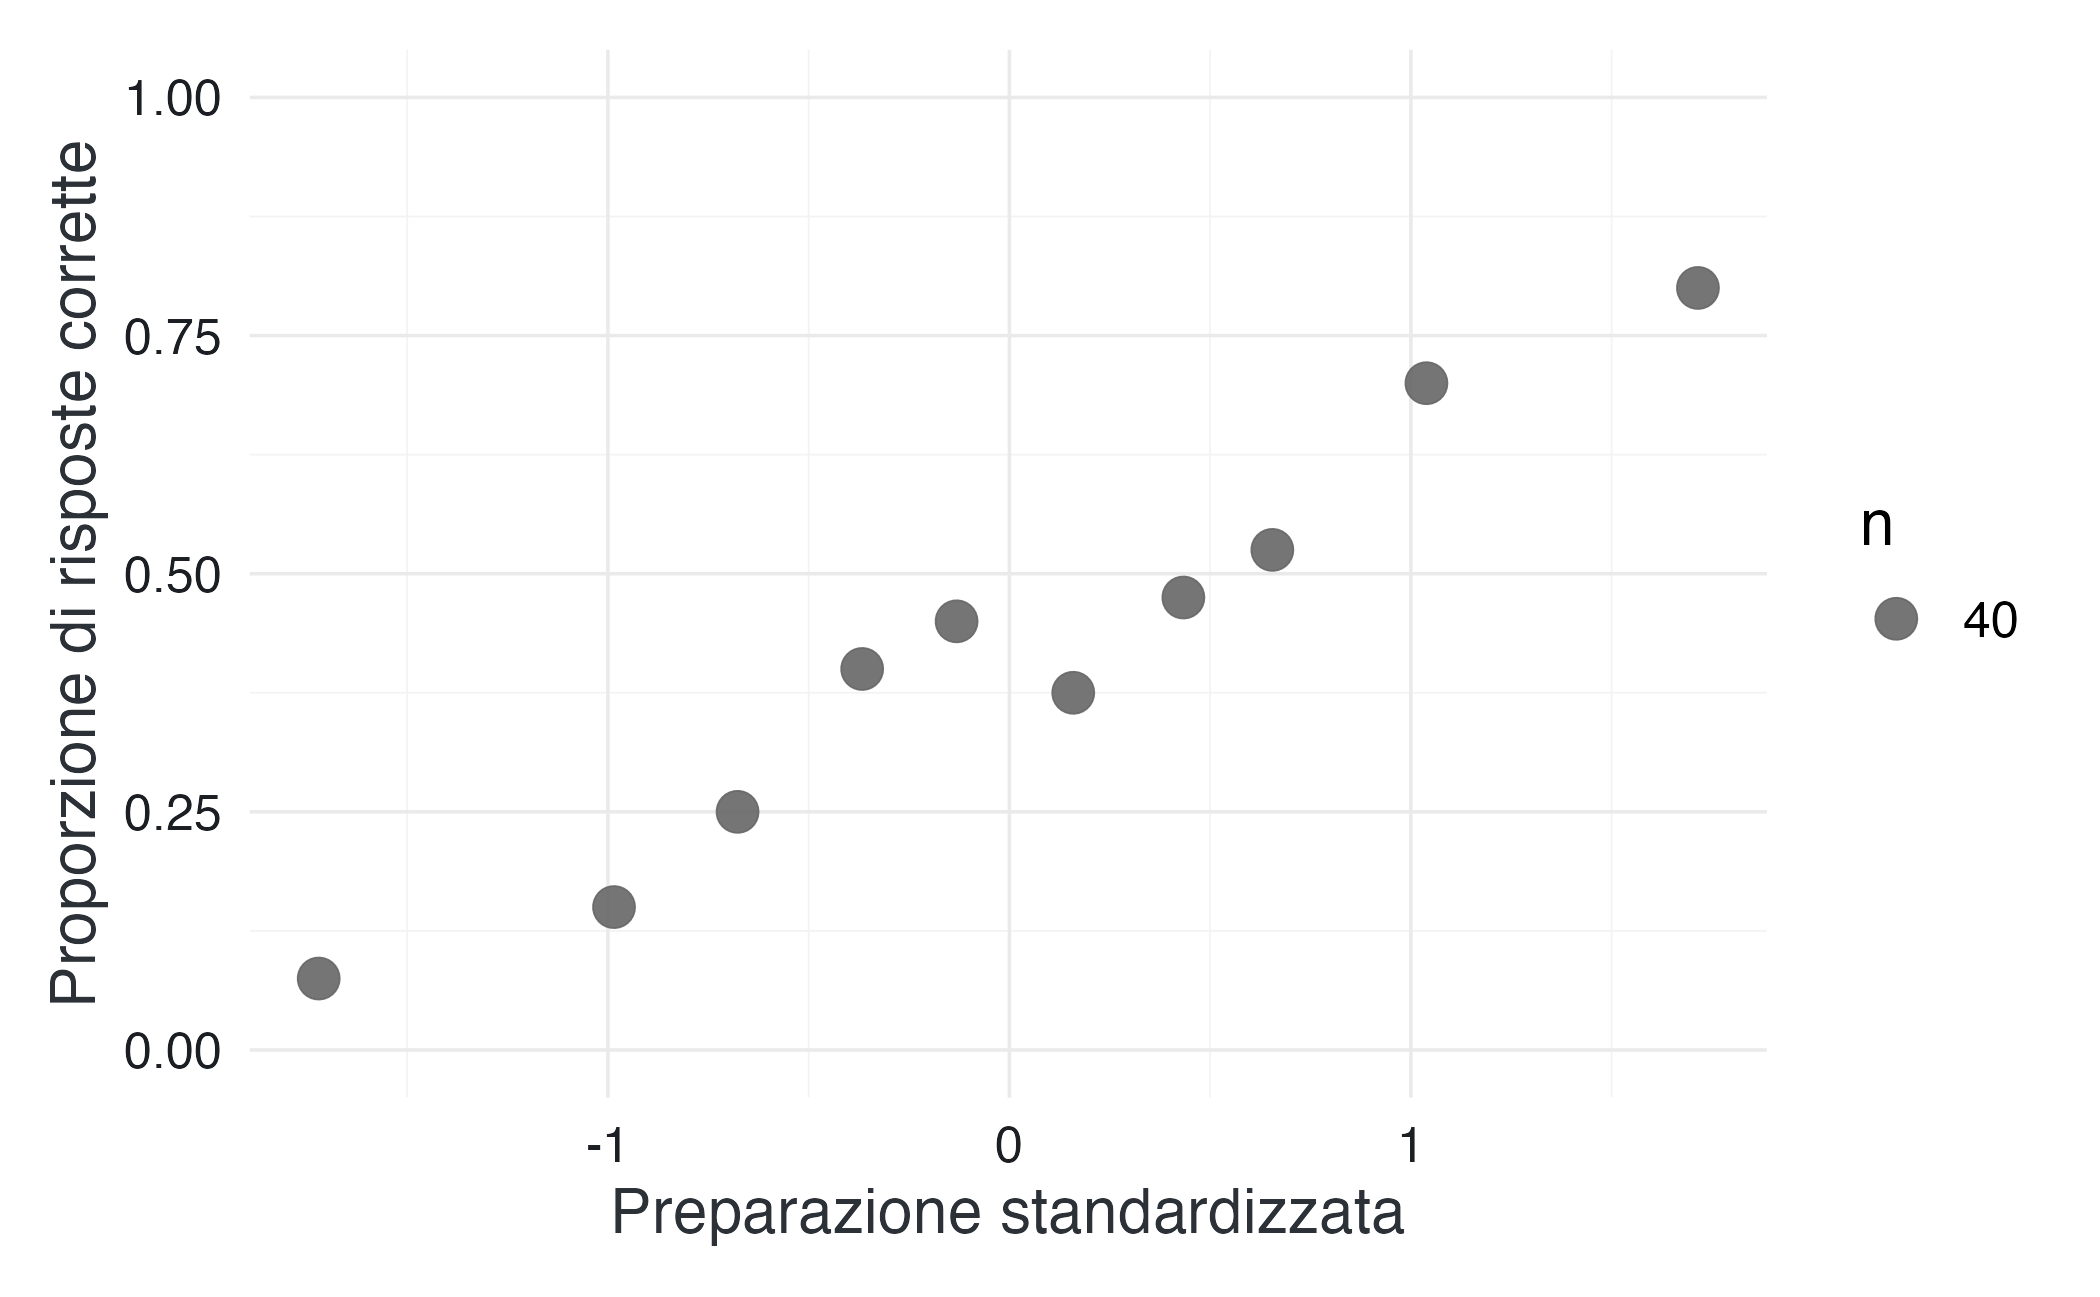
\includegraphics[width=0.85\linewidth,height=\textheight,keepaspectratio]{chapters/glm/01_regressione_logistica_files/figure-pdf/unnamed-chunk-3-1.png}
\end{center}

\section{Come interpretare i
coefficienti}\label{come-interpretare-i-coefficienti}

L'intercetta \(\alpha\) rappresenta i log-odds dell'esito quando
\(x=0\). Nel nostro esempio, poiché il predittore è standardizzato, esso
descrive una persona con un livello di preparazione medio. La pendenza
\(\beta\) indica invece di quanto cambiano i log-odds per un incremento
unitario di \(x\), ovvero per una deviazione standard di preparazione.

Questa è l'interpretazione più diretta del modello, ma non sempre la più
intuitiva. È utile procedere per gradi:

\begin{enumerate}
\def\labelenumi{\arabic{enumi}.}
\tightlist
\item
  \(\beta\) è una differenza di log-odds;
\item
  \(\exp(\beta)\) è un rapporto tra odds;
\item
  le probabilità predette si ottengono trasformando \(\alpha+\beta x\)
  con la funzione logistica.
\end{enumerate}

Il coefficiente \(\beta\) è costante sulla scala del logit. Un
incremento unitario di \(x\) modifica i log-odds di \(\beta\):

\[
\operatorname{logit}[p(x+1)]-
\operatorname{logit}[p(x)]
=
\beta.
\]

Esponenziando il coefficiente, si ottiene l'odds ratio associato a un
incremento unitario:

\[
\frac{\operatorname{odds}(x+1)}{\operatorname{odds}(x)}
=
\exp(\beta),
\qquad
\operatorname{odds}(x)=\frac{p(x)}{1-p(x)}.
\]

Nel modello logistico senza interazioni, l'odds ratio per un incremento
fisso del predittore è costante. Il cambiamento della probabilità,
invece, dipende dal punto di partenza. Passare da 0.10 a 0.20 e passare
da 0.50 a 0.60 significa in entrambi i casi aumentare la probabilità di
0.10, ma non produce lo stesso cambiamento negli odds. Simmetricamente,
lo stesso odds ratio può corrispondere a differenze di probabilità molto
diverse.

La curva logistica è infatti più ripida nella regione centrale e più
piatta quando la probabilità si avvicina a 0 o a 1:

\[
\frac{dp(x)}{dx}
=
\beta\,p(x)[1-p(x)].
\]

La derivata raggiunge il valore massimo quando \(p(x)=0.5\); in quel
punto vale \(\beta/4\). La cosiddetta regola del ``dividere per
quattro'' è dunque un'approssimazione del \emph{massimo cambiamento
locale}, non un metodo generale per trasformare un coefficiente
logistico in una differenza di probabilità.

Per comunicare un risultato è spesso preferibile non fermarsi a
\(\beta\) o all'odds ratio. Si scelgono due valori sostantivamente
interpretabili del predittore, si calcolano le probabilità
corrispondenti e si costruisce il confronto di interesse. Dati due
valori \(x_a\) e \(x_b\), possiamo ottenere

\[
\operatorname{RD}=p(x_b)-p(x_a),
\]

\[
\operatorname{RR}=\frac{p(x_b)}{p(x_a)},
\]

\[
\operatorname{OR}
=
\frac{p(x_b)/[1-p(x_b)]}{p(x_a)/[1-p(x_a)]}
=
\exp[\beta(x_b-x_a)].
\]

Queste quantità rispondono a domande diverse. La differenza di
probabilità descrive un cambiamento assoluto; il risk ratio descrive un
cambiamento relativo della probabilità; l'odds ratio descrive un
cambiamento relativo degli odds. Nessuna delle tre è universalmente
preferibile. La scelta dipende dal contesto e dal pubblico a cui il
risultato deve essere comunicato.

\section{Specificazione dei prior}\label{specificazione-dei-prior}

Poiché il predittore è standardizzato, \(\alpha\) rappresenta il logit
della probabilità per una persona con un livello di preparazione medio.
Un prior come

\[
\alpha \sim \operatorname{Normal}(0,1.5)
\]

attribuisce maggiore plausibilità alle probabilità di base non troppo
prossime agli estremi, senza escluderle completamente. Per la pendenza
possiamo usare

\[
\beta \sim \operatorname{Normal}(0,1),
\]

che ammette relazioni positive e negative e rende meno plausibili
variazioni eccezionalmente grandi dei log-odds per una deviazione
standard del predittore.

\begin{Shaded}
\begin{Highlighting}[]
\NormalTok{logistic\_priors }\OtherTok{\textless{}{-}} \FunctionTok{c}\NormalTok{(}
  \FunctionTok{prior}\NormalTok{(}\FunctionTok{normal}\NormalTok{(}\DecValTok{0}\NormalTok{, }\FloatTok{1.5}\NormalTok{), }\AttributeTok{class =}\NormalTok{ Intercept),}
  \FunctionTok{prior}\NormalTok{(}\FunctionTok{normal}\NormalTok{(}\DecValTok{0}\NormalTok{, }\DecValTok{1}\NormalTok{), }\AttributeTok{class =}\NormalTok{ b)}
\NormalTok{)}
\end{Highlighting}
\end{Shaded}

I prior sui coefficienti non sono immediatamente intuitivi sulla scala
dei log-odds. Il controllo predittivo a priori consente di valutarne le
implicazioni sulla scala osservabile.

\begin{Shaded}
\begin{Highlighting}[]
\NormalTok{fit\_logistic\_prior }\OtherTok{\textless{}{-}} \FunctionTok{brm}\NormalTok{(}
\NormalTok{  correct }\SpecialCharTok{\textasciitilde{}} \DecValTok{1} \SpecialCharTok{+}\NormalTok{ preparation,}
  \AttributeTok{data =}\NormalTok{ logistic\_data,}
  \AttributeTok{family =} \FunctionTok{bernoulli}\NormalTok{(}\AttributeTok{link =} \StringTok{"logit"}\NormalTok{),}
  \AttributeTok{prior =}\NormalTok{ logistic\_priors,}
  \AttributeTok{sample\_prior =} \StringTok{"only"}\NormalTok{,}
  \AttributeTok{chains =} \DecValTok{4}\NormalTok{,}
  \AttributeTok{iter =} \DecValTok{2000}\NormalTok{,}
  \AttributeTok{seed =} \DecValTok{2026}\NormalTok{,}
  \AttributeTok{refresh =} \DecValTok{0}
\NormalTok{)}
\CommentTok{\#\textgreater{} Running MCMC with 4 chains, at most 10 in parallel...}
\CommentTok{\#\textgreater{} }
\CommentTok{\#\textgreater{} Chain 1 finished in 0.0 seconds.}
\CommentTok{\#\textgreater{} Chain 2 finished in 0.0 seconds.}
\CommentTok{\#\textgreater{} Chain 3 finished in 0.0 seconds.}
\CommentTok{\#\textgreater{} Chain 4 finished in 0.0 seconds.}
\CommentTok{\#\textgreater{} }
\CommentTok{\#\textgreater{} All 4 chains finished successfully.}
\CommentTok{\#\textgreater{} Mean chain execution time: 0.0 seconds.}
\CommentTok{\#\textgreater{} Total execution time: 0.3 seconds.}
\end{Highlighting}
\end{Shaded}

Possiamo esaminare la distribuzione della proporzione complessiva di
risposte corrette generata dal prior:

\begin{Shaded}
\begin{Highlighting}[]
\FunctionTok{pp\_check}\NormalTok{(fit\_logistic\_prior, }\AttributeTok{type =} \StringTok{"stat"}\NormalTok{, }\AttributeTok{stat =} \StringTok{"mean"}\NormalTok{, }\AttributeTok{ndraws =} \DecValTok{100}\NormalTok{)}
\end{Highlighting}
\end{Shaded}

\begin{center}
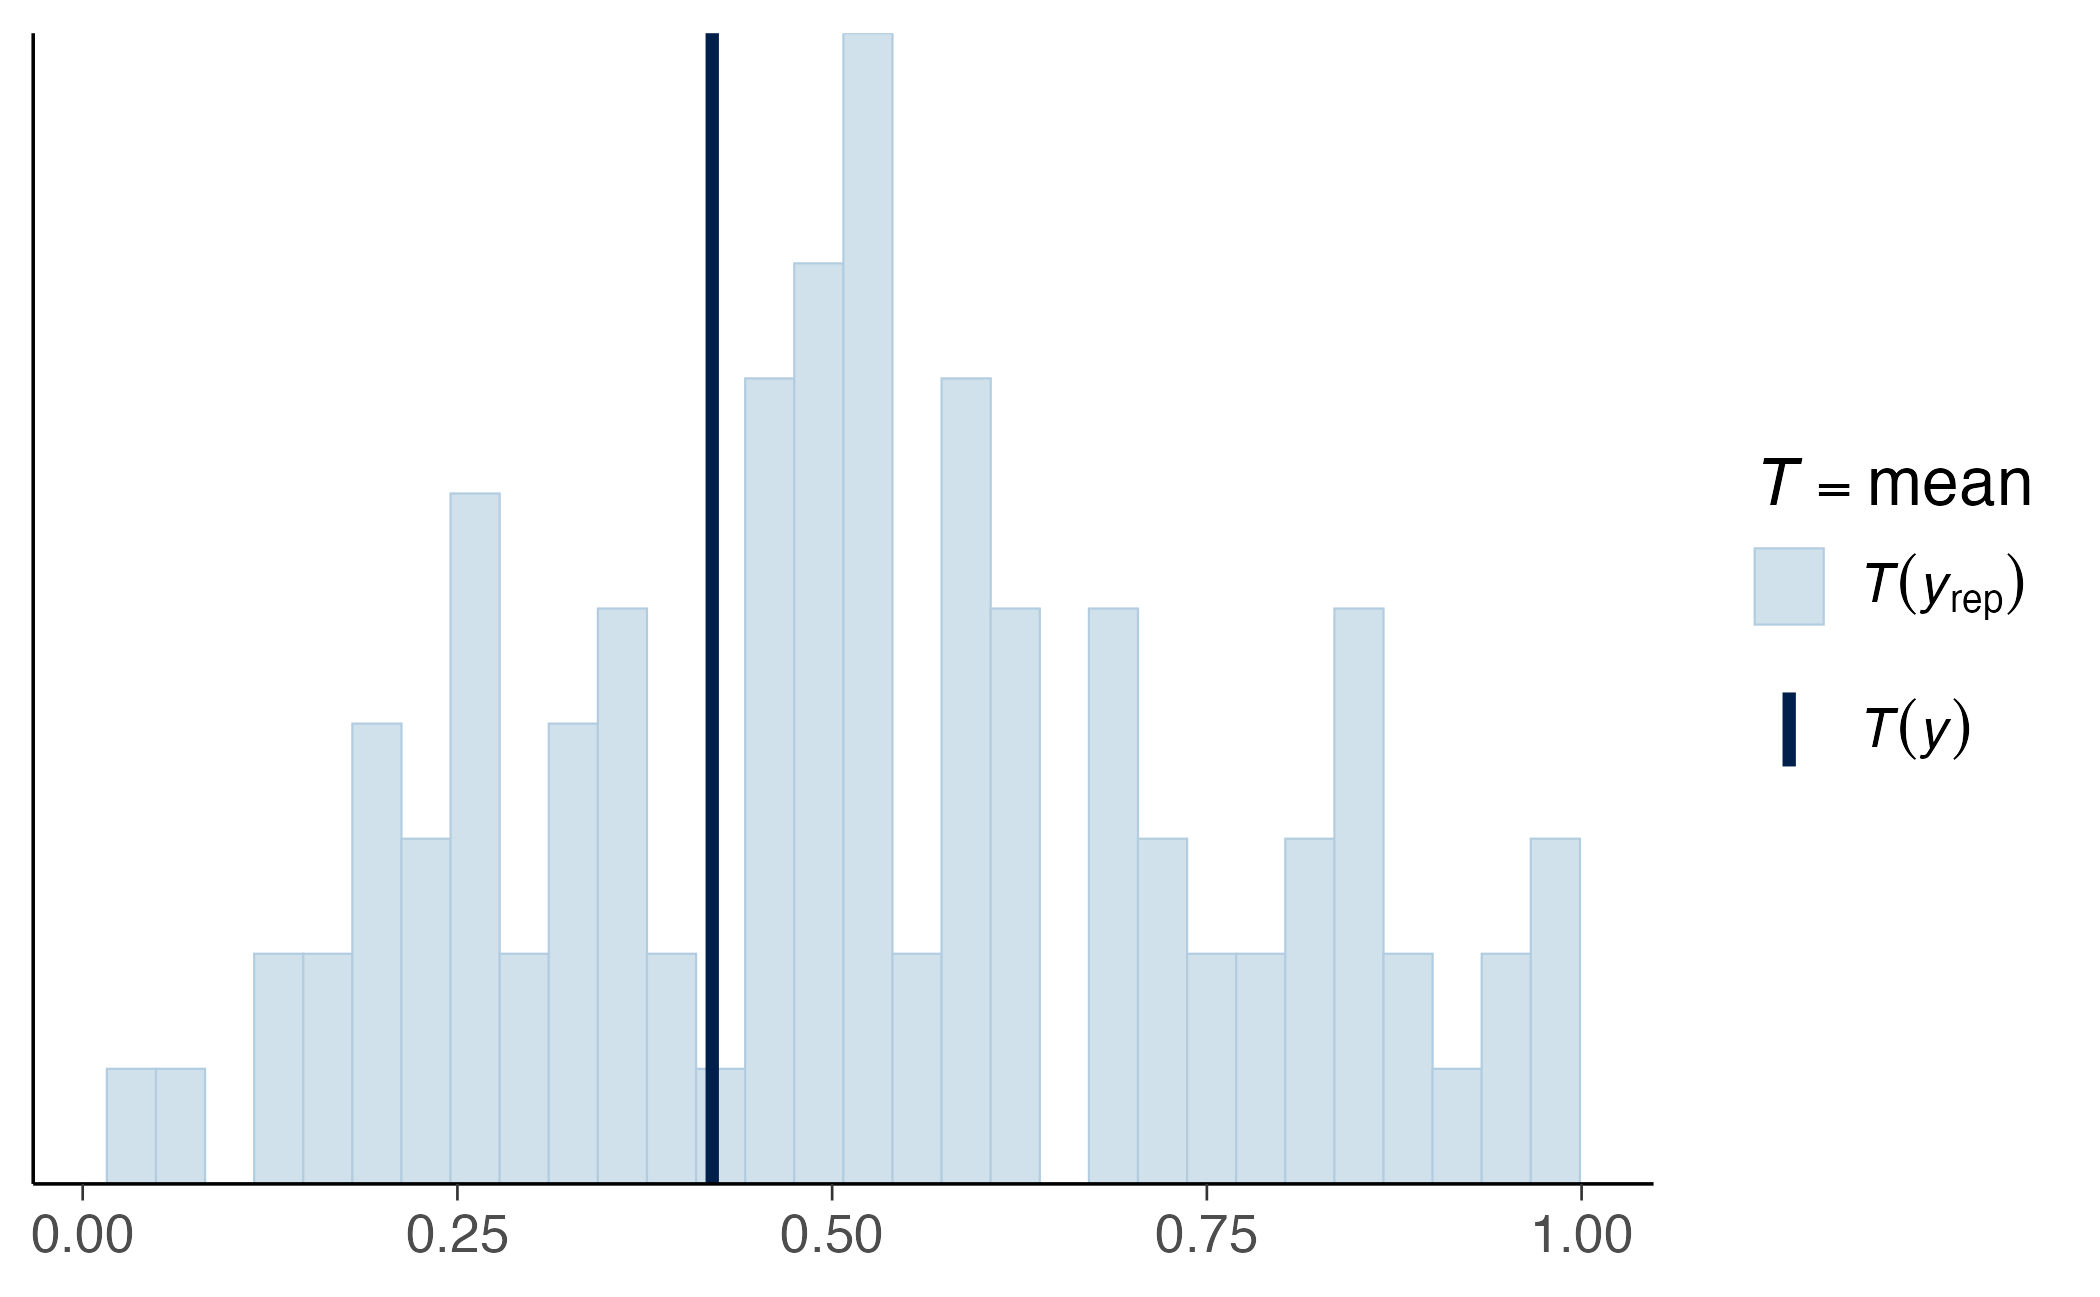
\includegraphics[width=0.85\linewidth,height=\textheight,keepaspectratio]{chapters/glm/01_regressione_logistica_files/figure-pdf/unnamed-chunk-6-1.png}
\end{center}

Questo controllo non deve produrre dati identici a quelli osservati.
Deve piuttosto verificare che il prior generi scenari compatibili con
quanto riteniamo possibile prima di utilizzare il campione corrente.

\section{\texorpdfstring{Stima con
\texttt{brms}}{Stima con brms}}\label{stima-con-brms}

Adattiamo lo stesso modello ai dati osservati:

\begin{Shaded}
\begin{Highlighting}[]
\NormalTok{fit\_logistic }\OtherTok{\textless{}{-}} \FunctionTok{brm}\NormalTok{(}
\NormalTok{  correct }\SpecialCharTok{\textasciitilde{}} \DecValTok{1} \SpecialCharTok{+}\NormalTok{ preparation,}
  \AttributeTok{data =}\NormalTok{ logistic\_data,}
  \AttributeTok{family =} \FunctionTok{bernoulli}\NormalTok{(}\AttributeTok{link =} \StringTok{"logit"}\NormalTok{),}
  \AttributeTok{prior =}\NormalTok{ logistic\_priors,}
  \AttributeTok{chains =} \DecValTok{4}\NormalTok{,}
  \AttributeTok{iter =} \DecValTok{3000}\NormalTok{,}
  \AttributeTok{warmup =} \DecValTok{1000}\NormalTok{,}
  \AttributeTok{seed =} \DecValTok{2026}\NormalTok{,}
  \AttributeTok{refresh =} \DecValTok{0}
\NormalTok{)}
\CommentTok{\#\textgreater{} Running MCMC with 4 chains, at most 10 in parallel...}
\CommentTok{\#\textgreater{} }
\CommentTok{\#\textgreater{} Chain 1 finished in 0.1 seconds.}
\CommentTok{\#\textgreater{} Chain 2 finished in 0.1 seconds.}
\CommentTok{\#\textgreater{} Chain 3 finished in 0.1 seconds.}
\CommentTok{\#\textgreater{} Chain 4 finished in 0.1 seconds.}
\CommentTok{\#\textgreater{} }
\CommentTok{\#\textgreater{} All 4 chains finished successfully.}
\CommentTok{\#\textgreater{} Mean chain execution time: 0.1 seconds.}
\CommentTok{\#\textgreater{} Total execution time: 0.3 seconds.}
\end{Highlighting}
\end{Shaded}

La sintesi dei parametri fornisce l'intercetta e la pendenza sulla scala
dei log-odds:

\begin{Shaded}
\begin{Highlighting}[]
\FunctionTok{summary}\NormalTok{(fit\_logistic)}
\CommentTok{\#\textgreater{}  Family: bernoulli }
\CommentTok{\#\textgreater{}   Links: mu = logit }
\CommentTok{\#\textgreater{} Formula: correct \textasciitilde{} 1 + preparation }
\CommentTok{\#\textgreater{}    Data: logistic\_data (Number of observations: 400) }
\CommentTok{\#\textgreater{}   Draws: 4 chains, each with iter = 3000; warmup = 1000; thin = 1;}
\CommentTok{\#\textgreater{}          total post{-}warmup draws = 8000}
\CommentTok{\#\textgreater{} }
\CommentTok{\#\textgreater{} Regression Coefficients:}
\CommentTok{\#\textgreater{}             Estimate Est.Error l{-}95\% CI u{-}95\% CI Rhat Bulk\_ESS Tail\_ESS}
\CommentTok{\#\textgreater{} Intercept      {-}0.41      0.11    {-}0.64    {-}0.18 1.00     6104     5262}
\CommentTok{\#\textgreater{} preparation     1.08      0.14     0.82     1.37 1.00     5864     4749}
\CommentTok{\#\textgreater{} }
\CommentTok{\#\textgreater{} Draws were sampled using sample(hmc). For each parameter, Bulk\_ESS}
\CommentTok{\#\textgreater{} and Tail\_ESS are effective sample size measures, and Rhat is the potential}
\CommentTok{\#\textgreater{} scale reduction factor on split chains (at convergence, Rhat = 1).}
\end{Highlighting}
\end{Shaded}

Prima di interpretare la posterior è necessario verificare il
campionamento. I valori di \(\widehat R\), le dimensioni campionarie
effettive, le catene e l'eventuale presenza di divergenze riguardano
l'affidabilità del calcolo, non l'adeguatezza scientifica del modello.

\begin{Shaded}
\begin{Highlighting}[]
\FunctionTok{plot}\NormalTok{(fit\_logistic)}
\end{Highlighting}
\end{Shaded}

\begin{center}
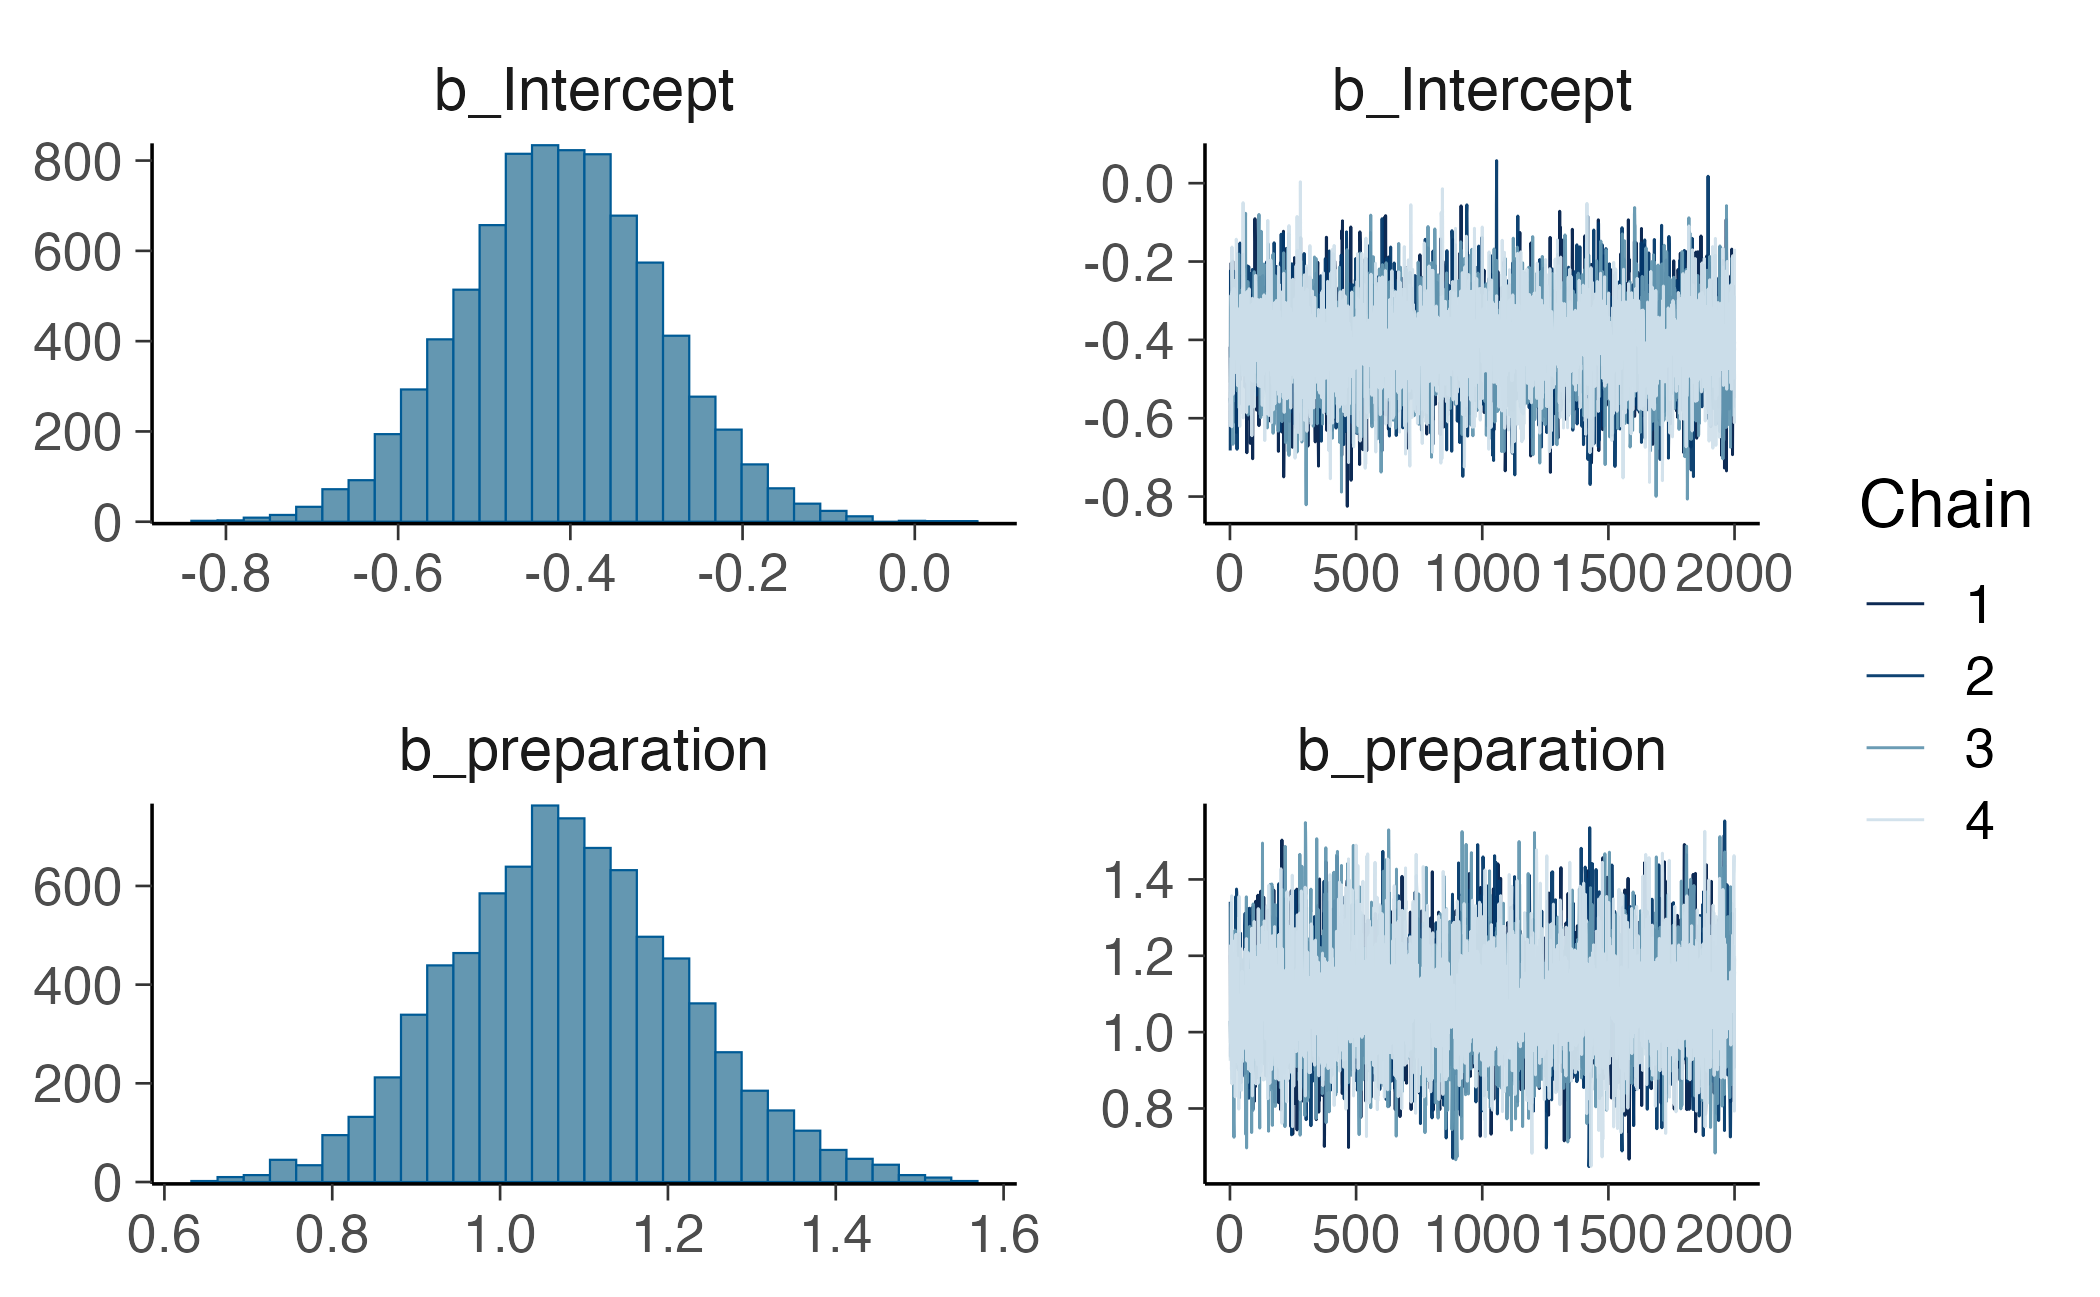
\includegraphics[width=0.85\linewidth,height=\textheight,keepaspectratio]{chapters/glm/01_regressione_logistica_files/figure-pdf/unnamed-chunk-9-1.png}
\end{center}

\begin{Shaded}
\begin{Highlighting}[]
\FunctionTok{nuts\_params}\NormalTok{(fit\_logistic) }\SpecialCharTok{|\textgreater{}}
\NormalTok{  dplyr}\SpecialCharTok{::}\FunctionTok{count}\NormalTok{(Parameter, Value)}
\CommentTok{\#\textgreater{}           Parameter   Value    n}
\CommentTok{\#\textgreater{} 1     accept\_stat\_\_   0.204    1}
\CommentTok{\#\textgreater{} 2     accept\_stat\_\_   0.336    1}
\CommentTok{\#\textgreater{} 3     accept\_stat\_\_   0.340    1}
\CommentTok{\#\textgreater{} 4     accept\_stat\_\_   0.343    1}
\CommentTok{\#\textgreater{} 5     accept\_stat\_\_   0.358    1}
\CommentTok{\#\textgreater{} 6     accept\_stat\_\_   0.366    1}
\CommentTok{\#\textgreater{} 7     accept\_stat\_\_   0.368    1}
\CommentTok{\#\textgreater{} 8     accept\_stat\_\_   0.376    1}
\CommentTok{\#\textgreater{} 9     accept\_stat\_\_   0.382    1}
\CommentTok{\#\textgreater{} 10    accept\_stat\_\_   0.384    1}
\CommentTok{\#\textgreater{} 11    accept\_stat\_\_   0.394    1}
\CommentTok{\#\textgreater{} 12    accept\_stat\_\_   0.405    1}
\CommentTok{\#\textgreater{} 13    accept\_stat\_\_   0.411    1}
\CommentTok{\#\textgreater{} 14    accept\_stat\_\_   0.411    1}
\CommentTok{\#\textgreater{} 15    accept\_stat\_\_   0.411    1}
\CommentTok{\#\textgreater{} 16    accept\_stat\_\_   0.424    1}
\CommentTok{\#\textgreater{} 17    accept\_stat\_\_   0.430    1}
\CommentTok{\#\textgreater{} 18    accept\_stat\_\_   0.431    1}
\CommentTok{\#\textgreater{} 19    accept\_stat\_\_   0.434    1}
\CommentTok{\#\textgreater{} 20    accept\_stat\_\_   0.435    1}
\CommentTok{\#\textgreater{} 21    accept\_stat\_\_   0.437    1}
\CommentTok{\#\textgreater{} 22    accept\_stat\_\_   0.438    1}
\CommentTok{\#\textgreater{} 23    accept\_stat\_\_   0.439    1}
\CommentTok{\#\textgreater{} 24    accept\_stat\_\_   0.441    1}
\CommentTok{\#\textgreater{} 25    accept\_stat\_\_   0.444    1}
\CommentTok{\#\textgreater{} 26    accept\_stat\_\_   0.455    1}
\CommentTok{\#\textgreater{} 27    accept\_stat\_\_   0.455    1}
\CommentTok{\#\textgreater{} 28    accept\_stat\_\_   0.455    1}
\CommentTok{\#\textgreater{} 29    accept\_stat\_\_   0.456    1}
\CommentTok{\#\textgreater{} 30    accept\_stat\_\_   0.461    1}
\CommentTok{\#\textgreater{} 31    accept\_stat\_\_   0.464    1}
\CommentTok{\#\textgreater{} 32    accept\_stat\_\_   0.467    1}
\CommentTok{\#\textgreater{} 33    accept\_stat\_\_   0.471    1}
\CommentTok{\#\textgreater{} 34    accept\_stat\_\_   0.473    1}
\CommentTok{\#\textgreater{} 35    accept\_stat\_\_   0.476    1}
\CommentTok{\#\textgreater{} 36    accept\_stat\_\_   0.482    1}
\CommentTok{\#\textgreater{} 37    accept\_stat\_\_   0.485    1}
\CommentTok{\#\textgreater{} 38    accept\_stat\_\_   0.487    1}
\CommentTok{\#\textgreater{} 39    accept\_stat\_\_   0.489    1}
\CommentTok{\#\textgreater{} 40    accept\_stat\_\_   0.490    1}
\CommentTok{\#\textgreater{} 41    accept\_stat\_\_   0.491    1}
\CommentTok{\#\textgreater{} 42    accept\_stat\_\_   0.492    1}
\CommentTok{\#\textgreater{} 43    accept\_stat\_\_   0.494    1}
\CommentTok{\#\textgreater{} 44    accept\_stat\_\_   0.494    1}
\CommentTok{\#\textgreater{} 45    accept\_stat\_\_   0.495    1}
\CommentTok{\#\textgreater{} 46    accept\_stat\_\_   0.496    1}
\CommentTok{\#\textgreater{} 47    accept\_stat\_\_   0.496    1}
\CommentTok{\#\textgreater{} 48    accept\_stat\_\_   0.496    1}
\CommentTok{\#\textgreater{} 49    accept\_stat\_\_   0.497    1}
\CommentTok{\#\textgreater{} 50    accept\_stat\_\_   0.501    1}
\CommentTok{\#\textgreater{} 51    accept\_stat\_\_   0.503    1}
\CommentTok{\#\textgreater{} 52    accept\_stat\_\_   0.503    1}
\CommentTok{\#\textgreater{} 53    accept\_stat\_\_   0.504    1}
\CommentTok{\#\textgreater{} 54    accept\_stat\_\_   0.505    1}
\CommentTok{\#\textgreater{} 55    accept\_stat\_\_   0.506    1}
\CommentTok{\#\textgreater{} 56    accept\_stat\_\_   0.508    1}
\CommentTok{\#\textgreater{} 57    accept\_stat\_\_   0.508    1}
\CommentTok{\#\textgreater{} 58    accept\_stat\_\_   0.509    1}
\CommentTok{\#\textgreater{} 59    accept\_stat\_\_   0.511    1}
\CommentTok{\#\textgreater{} 60    accept\_stat\_\_   0.513    1}
\CommentTok{\#\textgreater{} 61    accept\_stat\_\_   0.516    1}
\CommentTok{\#\textgreater{} 62    accept\_stat\_\_   0.518    1}
\CommentTok{\#\textgreater{} 63    accept\_stat\_\_   0.518    1}
\CommentTok{\#\textgreater{} 64    accept\_stat\_\_   0.519    1}
\CommentTok{\#\textgreater{} 65    accept\_stat\_\_   0.520    1}
\CommentTok{\#\textgreater{} 66    accept\_stat\_\_   0.520    1}
\CommentTok{\#\textgreater{} 67    accept\_stat\_\_   0.521    1}
\CommentTok{\#\textgreater{} 68    accept\_stat\_\_   0.525    1}
\CommentTok{\#\textgreater{} 69    accept\_stat\_\_   0.525    1}
\CommentTok{\#\textgreater{} 70    accept\_stat\_\_   0.526    1}
\CommentTok{\#\textgreater{} 71    accept\_stat\_\_   0.526    1}
\CommentTok{\#\textgreater{} 72    accept\_stat\_\_   0.526    1}
\CommentTok{\#\textgreater{} 73    accept\_stat\_\_   0.528    1}
\CommentTok{\#\textgreater{} 74    accept\_stat\_\_   0.529    1}
\CommentTok{\#\textgreater{} 75    accept\_stat\_\_   0.531    1}
\CommentTok{\#\textgreater{} 76    accept\_stat\_\_   0.531    1}
\CommentTok{\#\textgreater{} 77    accept\_stat\_\_   0.533    1}
\CommentTok{\#\textgreater{} 78    accept\_stat\_\_   0.535    1}
\CommentTok{\#\textgreater{} 79    accept\_stat\_\_   0.536    1}
\CommentTok{\#\textgreater{} 80    accept\_stat\_\_   0.536    1}
\CommentTok{\#\textgreater{} 81    accept\_stat\_\_   0.536    1}
\CommentTok{\#\textgreater{} 82    accept\_stat\_\_   0.537    1}
\CommentTok{\#\textgreater{} 83    accept\_stat\_\_   0.538    1}
\CommentTok{\#\textgreater{} 84    accept\_stat\_\_   0.539    1}
\CommentTok{\#\textgreater{} 85    accept\_stat\_\_   0.539    1}
\CommentTok{\#\textgreater{} 86    accept\_stat\_\_   0.545    1}
\CommentTok{\#\textgreater{} 87    accept\_stat\_\_   0.550    1}
\CommentTok{\#\textgreater{} 88    accept\_stat\_\_   0.553    1}
\CommentTok{\#\textgreater{} 89    accept\_stat\_\_   0.554    1}
\CommentTok{\#\textgreater{} 90    accept\_stat\_\_   0.554    1}
\CommentTok{\#\textgreater{} 91    accept\_stat\_\_   0.555    1}
\CommentTok{\#\textgreater{} 92    accept\_stat\_\_   0.557    1}
\CommentTok{\#\textgreater{} 93    accept\_stat\_\_   0.560    1}
\CommentTok{\#\textgreater{} 94    accept\_stat\_\_   0.560    1}
\CommentTok{\#\textgreater{} 95    accept\_stat\_\_   0.561    1}
\CommentTok{\#\textgreater{} 96    accept\_stat\_\_   0.566    1}
\CommentTok{\#\textgreater{} 97    accept\_stat\_\_   0.567    1}
\CommentTok{\#\textgreater{} 98    accept\_stat\_\_   0.568    1}
\CommentTok{\#\textgreater{} 99    accept\_stat\_\_   0.569    1}
\CommentTok{\#\textgreater{} 100   accept\_stat\_\_   0.570    1}
\CommentTok{\#\textgreater{} 101   accept\_stat\_\_   0.571    1}
\CommentTok{\#\textgreater{} 102   accept\_stat\_\_   0.572    1}
\CommentTok{\#\textgreater{} 103   accept\_stat\_\_   0.572    1}
\CommentTok{\#\textgreater{} 104   accept\_stat\_\_   0.573    1}
\CommentTok{\#\textgreater{} 105   accept\_stat\_\_   0.573    1}
\CommentTok{\#\textgreater{} 106   accept\_stat\_\_   0.575    1}
\CommentTok{\#\textgreater{} 107   accept\_stat\_\_   0.577    1}
\CommentTok{\#\textgreater{} 108   accept\_stat\_\_   0.578    1}
\CommentTok{\#\textgreater{} 109   accept\_stat\_\_   0.579    1}
\CommentTok{\#\textgreater{} 110   accept\_stat\_\_   0.579    1}
\CommentTok{\#\textgreater{} 111   accept\_stat\_\_   0.580    1}
\CommentTok{\#\textgreater{} 112   accept\_stat\_\_   0.581    1}
\CommentTok{\#\textgreater{} 113   accept\_stat\_\_   0.581    1}
\CommentTok{\#\textgreater{} 114   accept\_stat\_\_   0.582    1}
\CommentTok{\#\textgreater{} 115   accept\_stat\_\_   0.582    1}
\CommentTok{\#\textgreater{} 116   accept\_stat\_\_   0.583    1}
\CommentTok{\#\textgreater{} 117   accept\_stat\_\_   0.584    1}
\CommentTok{\#\textgreater{} 118   accept\_stat\_\_   0.585    1}
\CommentTok{\#\textgreater{} 119   accept\_stat\_\_   0.587    1}
\CommentTok{\#\textgreater{} 120   accept\_stat\_\_   0.589    1}
\CommentTok{\#\textgreater{} 121   accept\_stat\_\_   0.589    1}
\CommentTok{\#\textgreater{} 122   accept\_stat\_\_   0.591    1}
\CommentTok{\#\textgreater{} 123   accept\_stat\_\_   0.592    1}
\CommentTok{\#\textgreater{} 124   accept\_stat\_\_   0.593    1}
\CommentTok{\#\textgreater{} 125   accept\_stat\_\_   0.593    1}
\CommentTok{\#\textgreater{} 126   accept\_stat\_\_   0.595    1}
\CommentTok{\#\textgreater{} 127   accept\_stat\_\_   0.596    1}
\CommentTok{\#\textgreater{} 128   accept\_stat\_\_   0.597    1}
\CommentTok{\#\textgreater{} 129   accept\_stat\_\_   0.597    1}
\CommentTok{\#\textgreater{} 130   accept\_stat\_\_   0.599    1}
\CommentTok{\#\textgreater{} 131   accept\_stat\_\_   0.602    1}
\CommentTok{\#\textgreater{} 132   accept\_stat\_\_   0.602    1}
\CommentTok{\#\textgreater{} 133   accept\_stat\_\_   0.603    1}
\CommentTok{\#\textgreater{} 134   accept\_stat\_\_   0.603    1}
\CommentTok{\#\textgreater{} 135   accept\_stat\_\_   0.604    1}
\CommentTok{\#\textgreater{} 136   accept\_stat\_\_   0.604    1}
\CommentTok{\#\textgreater{} 137   accept\_stat\_\_   0.605    1}
\CommentTok{\#\textgreater{} 138   accept\_stat\_\_   0.606    1}
\CommentTok{\#\textgreater{} 139   accept\_stat\_\_   0.607    1}
\CommentTok{\#\textgreater{} 140   accept\_stat\_\_   0.608    1}
\CommentTok{\#\textgreater{} 141   accept\_stat\_\_   0.609    1}
\CommentTok{\#\textgreater{} 142   accept\_stat\_\_   0.609    1}
\CommentTok{\#\textgreater{} 143   accept\_stat\_\_   0.609    1}
\CommentTok{\#\textgreater{} 144   accept\_stat\_\_   0.609    1}
\CommentTok{\#\textgreater{} 145   accept\_stat\_\_   0.610    1}
\CommentTok{\#\textgreater{} 146   accept\_stat\_\_   0.611    1}
\CommentTok{\#\textgreater{} 147   accept\_stat\_\_   0.611    1}
\CommentTok{\#\textgreater{} 148   accept\_stat\_\_   0.611    1}
\CommentTok{\#\textgreater{} 149   accept\_stat\_\_   0.611    1}
\CommentTok{\#\textgreater{} 150   accept\_stat\_\_   0.612    1}
\CommentTok{\#\textgreater{} 151   accept\_stat\_\_   0.614    1}
\CommentTok{\#\textgreater{} 152   accept\_stat\_\_   0.614    1}
\CommentTok{\#\textgreater{} 153   accept\_stat\_\_   0.615    1}
\CommentTok{\#\textgreater{} 154   accept\_stat\_\_   0.615    1}
\CommentTok{\#\textgreater{} 155   accept\_stat\_\_   0.616    1}
\CommentTok{\#\textgreater{} 156   accept\_stat\_\_   0.618    1}
\CommentTok{\#\textgreater{} 157   accept\_stat\_\_   0.618    1}
\CommentTok{\#\textgreater{} 158   accept\_stat\_\_   0.620    1}
\CommentTok{\#\textgreater{} 159   accept\_stat\_\_   0.620    1}
\CommentTok{\#\textgreater{} 160   accept\_stat\_\_   0.622    1}
\CommentTok{\#\textgreater{} 161   accept\_stat\_\_   0.622    1}
\CommentTok{\#\textgreater{} 162   accept\_stat\_\_   0.622    1}
\CommentTok{\#\textgreater{} 163   accept\_stat\_\_   0.623    1}
\CommentTok{\#\textgreater{} 164   accept\_stat\_\_   0.623    1}
\CommentTok{\#\textgreater{} 165   accept\_stat\_\_   0.623    1}
\CommentTok{\#\textgreater{} 166   accept\_stat\_\_   0.623    1}
\CommentTok{\#\textgreater{} 167   accept\_stat\_\_   0.624    1}
\CommentTok{\#\textgreater{} 168   accept\_stat\_\_   0.624    1}
\CommentTok{\#\textgreater{} 169   accept\_stat\_\_   0.624    1}
\CommentTok{\#\textgreater{} 170   accept\_stat\_\_   0.626    1}
\CommentTok{\#\textgreater{} 171   accept\_stat\_\_   0.626    1}
\CommentTok{\#\textgreater{} 172   accept\_stat\_\_   0.627    1}
\CommentTok{\#\textgreater{} 173   accept\_stat\_\_   0.627    1}
\CommentTok{\#\textgreater{} 174   accept\_stat\_\_   0.628    1}
\CommentTok{\#\textgreater{} 175   accept\_stat\_\_   0.629    1}
\CommentTok{\#\textgreater{} 176   accept\_stat\_\_   0.630    1}
\CommentTok{\#\textgreater{} 177   accept\_stat\_\_   0.632    1}
\CommentTok{\#\textgreater{} 178   accept\_stat\_\_   0.632    1}
\CommentTok{\#\textgreater{} 179   accept\_stat\_\_   0.633    1}
\CommentTok{\#\textgreater{} 180   accept\_stat\_\_   0.633    1}
\CommentTok{\#\textgreater{} 181   accept\_stat\_\_   0.634    1}
\CommentTok{\#\textgreater{} 182   accept\_stat\_\_   0.636    1}
\CommentTok{\#\textgreater{} 183   accept\_stat\_\_   0.636    1}
\CommentTok{\#\textgreater{} 184   accept\_stat\_\_   0.637    1}
\CommentTok{\#\textgreater{} 185   accept\_stat\_\_   0.637    1}
\CommentTok{\#\textgreater{} 186   accept\_stat\_\_   0.637    1}
\CommentTok{\#\textgreater{} 187   accept\_stat\_\_   0.638    1}
\CommentTok{\#\textgreater{} 188   accept\_stat\_\_   0.638    1}
\CommentTok{\#\textgreater{} 189   accept\_stat\_\_   0.638    1}
\CommentTok{\#\textgreater{} 190   accept\_stat\_\_   0.638    1}
\CommentTok{\#\textgreater{} 191   accept\_stat\_\_   0.639    1}
\CommentTok{\#\textgreater{} 192   accept\_stat\_\_   0.639    1}
\CommentTok{\#\textgreater{} 193   accept\_stat\_\_   0.640    1}
\CommentTok{\#\textgreater{} 194   accept\_stat\_\_   0.640    1}
\CommentTok{\#\textgreater{} 195   accept\_stat\_\_   0.640    1}
\CommentTok{\#\textgreater{} 196   accept\_stat\_\_   0.640    1}
\CommentTok{\#\textgreater{} 197   accept\_stat\_\_   0.641    1}
\CommentTok{\#\textgreater{} 198   accept\_stat\_\_   0.641    1}
\CommentTok{\#\textgreater{} 199   accept\_stat\_\_   0.642    1}
\CommentTok{\#\textgreater{} 200   accept\_stat\_\_   0.642    1}
\CommentTok{\#\textgreater{} 201   accept\_stat\_\_   0.643    1}
\CommentTok{\#\textgreater{} 202   accept\_stat\_\_   0.643    1}
\CommentTok{\#\textgreater{} 203   accept\_stat\_\_   0.643    1}
\CommentTok{\#\textgreater{} 204   accept\_stat\_\_   0.645    1}
\CommentTok{\#\textgreater{} 205   accept\_stat\_\_   0.645    1}
\CommentTok{\#\textgreater{} 206   accept\_stat\_\_   0.646    1}
\CommentTok{\#\textgreater{} 207   accept\_stat\_\_   0.646    1}
\CommentTok{\#\textgreater{} 208   accept\_stat\_\_   0.646    1}
\CommentTok{\#\textgreater{} 209   accept\_stat\_\_   0.647    1}
\CommentTok{\#\textgreater{} 210   accept\_stat\_\_   0.647    1}
\CommentTok{\#\textgreater{} 211   accept\_stat\_\_   0.647    1}
\CommentTok{\#\textgreater{} 212   accept\_stat\_\_   0.648    1}
\CommentTok{\#\textgreater{} 213   accept\_stat\_\_   0.648    1}
\CommentTok{\#\textgreater{} 214   accept\_stat\_\_   0.648    1}
\CommentTok{\#\textgreater{} 215   accept\_stat\_\_   0.649    1}
\CommentTok{\#\textgreater{} 216   accept\_stat\_\_   0.649    1}
\CommentTok{\#\textgreater{} 217   accept\_stat\_\_   0.649    1}
\CommentTok{\#\textgreater{} 218   accept\_stat\_\_   0.650    1}
\CommentTok{\#\textgreater{} 219   accept\_stat\_\_   0.652    1}
\CommentTok{\#\textgreater{} 220   accept\_stat\_\_   0.652    1}
\CommentTok{\#\textgreater{} 221   accept\_stat\_\_   0.652    1}
\CommentTok{\#\textgreater{} 222   accept\_stat\_\_   0.652    1}
\CommentTok{\#\textgreater{} 223   accept\_stat\_\_   0.653    1}
\CommentTok{\#\textgreater{} 224   accept\_stat\_\_   0.653    1}
\CommentTok{\#\textgreater{} 225   accept\_stat\_\_   0.653    1}
\CommentTok{\#\textgreater{} 226   accept\_stat\_\_   0.653    1}
\CommentTok{\#\textgreater{} 227   accept\_stat\_\_   0.653    1}
\CommentTok{\#\textgreater{} 228   accept\_stat\_\_   0.654    1}
\CommentTok{\#\textgreater{} 229   accept\_stat\_\_   0.654    1}
\CommentTok{\#\textgreater{} 230   accept\_stat\_\_   0.654    1}
\CommentTok{\#\textgreater{} 231   accept\_stat\_\_   0.655    1}
\CommentTok{\#\textgreater{} 232   accept\_stat\_\_   0.655    1}
\CommentTok{\#\textgreater{} 233   accept\_stat\_\_   0.655    1}
\CommentTok{\#\textgreater{} 234   accept\_stat\_\_   0.655    1}
\CommentTok{\#\textgreater{} 235   accept\_stat\_\_   0.656    1}
\CommentTok{\#\textgreater{} 236   accept\_stat\_\_   0.656    1}
\CommentTok{\#\textgreater{} 237   accept\_stat\_\_   0.657    1}
\CommentTok{\#\textgreater{} 238   accept\_stat\_\_   0.657    1}
\CommentTok{\#\textgreater{} 239   accept\_stat\_\_   0.659    1}
\CommentTok{\#\textgreater{} 240   accept\_stat\_\_   0.659    1}
\CommentTok{\#\textgreater{} 241   accept\_stat\_\_   0.660    1}
\CommentTok{\#\textgreater{} 242   accept\_stat\_\_   0.661    1}
\CommentTok{\#\textgreater{} 243   accept\_stat\_\_   0.661    1}
\CommentTok{\#\textgreater{} 244   accept\_stat\_\_   0.661    1}
\CommentTok{\#\textgreater{} 245   accept\_stat\_\_   0.662    1}
\CommentTok{\#\textgreater{} 246   accept\_stat\_\_   0.663    1}
\CommentTok{\#\textgreater{} 247   accept\_stat\_\_   0.664    1}
\CommentTok{\#\textgreater{} 248   accept\_stat\_\_   0.664    1}
\CommentTok{\#\textgreater{} 249   accept\_stat\_\_   0.664    1}
\CommentTok{\#\textgreater{} 250   accept\_stat\_\_   0.665    1}
\CommentTok{\#\textgreater{} 251   accept\_stat\_\_   0.665    1}
\CommentTok{\#\textgreater{} 252   accept\_stat\_\_   0.666    1}
\CommentTok{\#\textgreater{} 253   accept\_stat\_\_   0.666    1}
\CommentTok{\#\textgreater{} 254   accept\_stat\_\_   0.666    1}
\CommentTok{\#\textgreater{} 255   accept\_stat\_\_   0.666    1}
\CommentTok{\#\textgreater{} 256   accept\_stat\_\_   0.666    1}
\CommentTok{\#\textgreater{} 257   accept\_stat\_\_   0.668    1}
\CommentTok{\#\textgreater{} 258   accept\_stat\_\_   0.669    1}
\CommentTok{\#\textgreater{} 259   accept\_stat\_\_   0.669    1}
\CommentTok{\#\textgreater{} 260   accept\_stat\_\_   0.669    1}
\CommentTok{\#\textgreater{} 261   accept\_stat\_\_   0.670    1}
\CommentTok{\#\textgreater{} 262   accept\_stat\_\_   0.670    1}
\CommentTok{\#\textgreater{} 263   accept\_stat\_\_   0.670    1}
\CommentTok{\#\textgreater{} 264   accept\_stat\_\_   0.670    1}
\CommentTok{\#\textgreater{} 265   accept\_stat\_\_   0.671    1}
\CommentTok{\#\textgreater{} 266   accept\_stat\_\_   0.671    1}
\CommentTok{\#\textgreater{} 267   accept\_stat\_\_   0.671    1}
\CommentTok{\#\textgreater{} 268   accept\_stat\_\_   0.672    1}
\CommentTok{\#\textgreater{} 269   accept\_stat\_\_   0.673    1}
\CommentTok{\#\textgreater{} 270   accept\_stat\_\_   0.674    1}
\CommentTok{\#\textgreater{} 271   accept\_stat\_\_   0.674    1}
\CommentTok{\#\textgreater{} 272   accept\_stat\_\_   0.674    1}
\CommentTok{\#\textgreater{} 273   accept\_stat\_\_   0.674    1}
\CommentTok{\#\textgreater{} 274   accept\_stat\_\_   0.674    1}
\CommentTok{\#\textgreater{} 275   accept\_stat\_\_   0.676    1}
\CommentTok{\#\textgreater{} 276   accept\_stat\_\_   0.677    1}
\CommentTok{\#\textgreater{} 277   accept\_stat\_\_   0.677    1}
\CommentTok{\#\textgreater{} 278   accept\_stat\_\_   0.677    1}
\CommentTok{\#\textgreater{} 279   accept\_stat\_\_   0.678    1}
\CommentTok{\#\textgreater{} 280   accept\_stat\_\_   0.679    1}
\CommentTok{\#\textgreater{} 281   accept\_stat\_\_   0.679    1}
\CommentTok{\#\textgreater{} 282   accept\_stat\_\_   0.679    1}
\CommentTok{\#\textgreater{} 283   accept\_stat\_\_   0.679    1}
\CommentTok{\#\textgreater{} 284   accept\_stat\_\_   0.679    1}
\CommentTok{\#\textgreater{} 285   accept\_stat\_\_   0.680    1}
\CommentTok{\#\textgreater{} 286   accept\_stat\_\_   0.680    1}
\CommentTok{\#\textgreater{} 287   accept\_stat\_\_   0.680    1}
\CommentTok{\#\textgreater{} 288   accept\_stat\_\_   0.680    1}
\CommentTok{\#\textgreater{} 289   accept\_stat\_\_   0.680    1}
\CommentTok{\#\textgreater{} 290   accept\_stat\_\_   0.680    1}
\CommentTok{\#\textgreater{} 291   accept\_stat\_\_   0.681    1}
\CommentTok{\#\textgreater{} 292   accept\_stat\_\_   0.681    1}
\CommentTok{\#\textgreater{} 293   accept\_stat\_\_   0.682    1}
\CommentTok{\#\textgreater{} 294   accept\_stat\_\_   0.682    1}
\CommentTok{\#\textgreater{} 295   accept\_stat\_\_   0.682    1}
\CommentTok{\#\textgreater{} 296   accept\_stat\_\_   0.682    1}
\CommentTok{\#\textgreater{} 297   accept\_stat\_\_   0.682    1}
\CommentTok{\#\textgreater{} 298   accept\_stat\_\_   0.683    1}
\CommentTok{\#\textgreater{} 299   accept\_stat\_\_   0.683    1}
\CommentTok{\#\textgreater{} 300   accept\_stat\_\_   0.683    1}
\CommentTok{\#\textgreater{} 301   accept\_stat\_\_   0.683    1}
\CommentTok{\#\textgreater{} 302   accept\_stat\_\_   0.683    1}
\CommentTok{\#\textgreater{} 303   accept\_stat\_\_   0.683    1}
\CommentTok{\#\textgreater{} 304   accept\_stat\_\_   0.684    1}
\CommentTok{\#\textgreater{} 305   accept\_stat\_\_   0.684    1}
\CommentTok{\#\textgreater{} 306   accept\_stat\_\_   0.684    1}
\CommentTok{\#\textgreater{} 307   accept\_stat\_\_   0.685    1}
\CommentTok{\#\textgreater{} 308   accept\_stat\_\_   0.685    1}
\CommentTok{\#\textgreater{} 309   accept\_stat\_\_   0.685    1}
\CommentTok{\#\textgreater{} 310   accept\_stat\_\_   0.685    1}
\CommentTok{\#\textgreater{} 311   accept\_stat\_\_   0.686    1}
\CommentTok{\#\textgreater{} 312   accept\_stat\_\_   0.686    1}
\CommentTok{\#\textgreater{} 313   accept\_stat\_\_   0.686    1}
\CommentTok{\#\textgreater{} 314   accept\_stat\_\_   0.687    1}
\CommentTok{\#\textgreater{} 315   accept\_stat\_\_   0.688    1}
\CommentTok{\#\textgreater{} 316   accept\_stat\_\_   0.688    1}
\CommentTok{\#\textgreater{} 317   accept\_stat\_\_   0.689    1}
\CommentTok{\#\textgreater{} 318   accept\_stat\_\_   0.689    1}
\CommentTok{\#\textgreater{} 319   accept\_stat\_\_   0.689    1}
\CommentTok{\#\textgreater{} 320   accept\_stat\_\_   0.689    1}
\CommentTok{\#\textgreater{} 321   accept\_stat\_\_   0.689    1}
\CommentTok{\#\textgreater{} 322   accept\_stat\_\_   0.690    1}
\CommentTok{\#\textgreater{} 323   accept\_stat\_\_   0.690    1}
\CommentTok{\#\textgreater{} 324   accept\_stat\_\_   0.690    1}
\CommentTok{\#\textgreater{} 325   accept\_stat\_\_   0.690    1}
\CommentTok{\#\textgreater{} 326   accept\_stat\_\_   0.690    1}
\CommentTok{\#\textgreater{} 327   accept\_stat\_\_   0.691    1}
\CommentTok{\#\textgreater{} 328   accept\_stat\_\_   0.691    1}
\CommentTok{\#\textgreater{} 329   accept\_stat\_\_   0.692    1}
\CommentTok{\#\textgreater{} 330   accept\_stat\_\_   0.692    1}
\CommentTok{\#\textgreater{} 331   accept\_stat\_\_   0.692    1}
\CommentTok{\#\textgreater{} 332   accept\_stat\_\_   0.692    1}
\CommentTok{\#\textgreater{} 333   accept\_stat\_\_   0.694    1}
\CommentTok{\#\textgreater{} 334   accept\_stat\_\_   0.694    1}
\CommentTok{\#\textgreater{} 335   accept\_stat\_\_   0.694    1}
\CommentTok{\#\textgreater{} 336   accept\_stat\_\_   0.695    1}
\CommentTok{\#\textgreater{} 337   accept\_stat\_\_   0.695    1}
\CommentTok{\#\textgreater{} 338   accept\_stat\_\_   0.695    1}
\CommentTok{\#\textgreater{} 339   accept\_stat\_\_   0.696    1}
\CommentTok{\#\textgreater{} 340   accept\_stat\_\_   0.696    1}
\CommentTok{\#\textgreater{} 341   accept\_stat\_\_   0.696    1}
\CommentTok{\#\textgreater{} 342   accept\_stat\_\_   0.696    1}
\CommentTok{\#\textgreater{} 343   accept\_stat\_\_   0.697    1}
\CommentTok{\#\textgreater{} 344   accept\_stat\_\_   0.698    1}
\CommentTok{\#\textgreater{} 345   accept\_stat\_\_   0.698    1}
\CommentTok{\#\textgreater{} 346   accept\_stat\_\_   0.698    1}
\CommentTok{\#\textgreater{} 347   accept\_stat\_\_   0.699    1}
\CommentTok{\#\textgreater{} 348   accept\_stat\_\_   0.699    1}
\CommentTok{\#\textgreater{} 349   accept\_stat\_\_   0.699    1}
\CommentTok{\#\textgreater{} 350   accept\_stat\_\_   0.700    1}
\CommentTok{\#\textgreater{} 351   accept\_stat\_\_   0.700    1}
\CommentTok{\#\textgreater{} 352   accept\_stat\_\_   0.700    1}
\CommentTok{\#\textgreater{} 353   accept\_stat\_\_   0.700    1}
\CommentTok{\#\textgreater{} 354   accept\_stat\_\_   0.700    1}
\CommentTok{\#\textgreater{} 355   accept\_stat\_\_   0.701    1}
\CommentTok{\#\textgreater{} 356   accept\_stat\_\_   0.701    1}
\CommentTok{\#\textgreater{} 357   accept\_stat\_\_   0.701    1}
\CommentTok{\#\textgreater{} 358   accept\_stat\_\_   0.701    1}
\CommentTok{\#\textgreater{} 359   accept\_stat\_\_   0.702    1}
\CommentTok{\#\textgreater{} 360   accept\_stat\_\_   0.702    1}
\CommentTok{\#\textgreater{} 361   accept\_stat\_\_   0.702    1}
\CommentTok{\#\textgreater{} 362   accept\_stat\_\_   0.702    1}
\CommentTok{\#\textgreater{} 363   accept\_stat\_\_   0.702    1}
\CommentTok{\#\textgreater{} 364   accept\_stat\_\_   0.703    1}
\CommentTok{\#\textgreater{} 365   accept\_stat\_\_   0.703    1}
\CommentTok{\#\textgreater{} 366   accept\_stat\_\_   0.703    1}
\CommentTok{\#\textgreater{} 367   accept\_stat\_\_   0.703    1}
\CommentTok{\#\textgreater{} 368   accept\_stat\_\_   0.704    1}
\CommentTok{\#\textgreater{} 369   accept\_stat\_\_   0.704    1}
\CommentTok{\#\textgreater{} 370   accept\_stat\_\_   0.704    1}
\CommentTok{\#\textgreater{} 371   accept\_stat\_\_   0.704    1}
\CommentTok{\#\textgreater{} 372   accept\_stat\_\_   0.705    1}
\CommentTok{\#\textgreater{} 373   accept\_stat\_\_   0.705    1}
\CommentTok{\#\textgreater{} 374   accept\_stat\_\_   0.705    1}
\CommentTok{\#\textgreater{} 375   accept\_stat\_\_   0.705    1}
\CommentTok{\#\textgreater{} 376   accept\_stat\_\_   0.706    1}
\CommentTok{\#\textgreater{} 377   accept\_stat\_\_   0.706    1}
\CommentTok{\#\textgreater{} 378   accept\_stat\_\_   0.706    1}
\CommentTok{\#\textgreater{} 379   accept\_stat\_\_   0.707    1}
\CommentTok{\#\textgreater{} 380   accept\_stat\_\_   0.707    1}
\CommentTok{\#\textgreater{} 381   accept\_stat\_\_   0.707    1}
\CommentTok{\#\textgreater{} 382   accept\_stat\_\_   0.708    1}
\CommentTok{\#\textgreater{} 383   accept\_stat\_\_   0.708    1}
\CommentTok{\#\textgreater{} 384   accept\_stat\_\_   0.708    1}
\CommentTok{\#\textgreater{} 385   accept\_stat\_\_   0.708    1}
\CommentTok{\#\textgreater{} 386   accept\_stat\_\_   0.708    1}
\CommentTok{\#\textgreater{} 387   accept\_stat\_\_   0.709    1}
\CommentTok{\#\textgreater{} 388   accept\_stat\_\_   0.709    1}
\CommentTok{\#\textgreater{} 389   accept\_stat\_\_   0.710    1}
\CommentTok{\#\textgreater{} 390   accept\_stat\_\_   0.710    1}
\CommentTok{\#\textgreater{} 391   accept\_stat\_\_   0.710    1}
\CommentTok{\#\textgreater{} 392   accept\_stat\_\_   0.710    1}
\CommentTok{\#\textgreater{} 393   accept\_stat\_\_   0.710    1}
\CommentTok{\#\textgreater{} 394   accept\_stat\_\_   0.711    1}
\CommentTok{\#\textgreater{} 395   accept\_stat\_\_   0.711    1}
\CommentTok{\#\textgreater{} 396   accept\_stat\_\_   0.711    1}
\CommentTok{\#\textgreater{} 397   accept\_stat\_\_   0.711    1}
\CommentTok{\#\textgreater{} 398   accept\_stat\_\_   0.712    1}
\CommentTok{\#\textgreater{} 399   accept\_stat\_\_   0.712    1}
\CommentTok{\#\textgreater{} 400   accept\_stat\_\_   0.712    1}
\CommentTok{\#\textgreater{} 401   accept\_stat\_\_   0.713    1}
\CommentTok{\#\textgreater{} 402   accept\_stat\_\_   0.713    1}
\CommentTok{\#\textgreater{} 403   accept\_stat\_\_   0.713    1}
\CommentTok{\#\textgreater{} 404   accept\_stat\_\_   0.714    1}
\CommentTok{\#\textgreater{} 405   accept\_stat\_\_   0.714    1}
\CommentTok{\#\textgreater{} 406   accept\_stat\_\_   0.714    1}
\CommentTok{\#\textgreater{} 407   accept\_stat\_\_   0.714    1}
\CommentTok{\#\textgreater{} 408   accept\_stat\_\_   0.715    1}
\CommentTok{\#\textgreater{} 409   accept\_stat\_\_   0.715    1}
\CommentTok{\#\textgreater{} 410   accept\_stat\_\_   0.715    1}
\CommentTok{\#\textgreater{} 411   accept\_stat\_\_   0.715    1}
\CommentTok{\#\textgreater{} 412   accept\_stat\_\_   0.715    1}
\CommentTok{\#\textgreater{} 413   accept\_stat\_\_   0.716    1}
\CommentTok{\#\textgreater{} 414   accept\_stat\_\_   0.716    1}
\CommentTok{\#\textgreater{} 415   accept\_stat\_\_   0.716    1}
\CommentTok{\#\textgreater{} 416   accept\_stat\_\_   0.716    1}
\CommentTok{\#\textgreater{} 417   accept\_stat\_\_   0.716    1}
\CommentTok{\#\textgreater{} 418   accept\_stat\_\_   0.716    1}
\CommentTok{\#\textgreater{} 419   accept\_stat\_\_   0.716    1}
\CommentTok{\#\textgreater{} 420   accept\_stat\_\_   0.717    1}
\CommentTok{\#\textgreater{} 421   accept\_stat\_\_   0.717    1}
\CommentTok{\#\textgreater{} 422   accept\_stat\_\_   0.718    1}
\CommentTok{\#\textgreater{} 423   accept\_stat\_\_   0.718    1}
\CommentTok{\#\textgreater{} 424   accept\_stat\_\_   0.718    1}
\CommentTok{\#\textgreater{} 425   accept\_stat\_\_   0.718    1}
\CommentTok{\#\textgreater{} 426   accept\_stat\_\_   0.718    1}
\CommentTok{\#\textgreater{} 427   accept\_stat\_\_   0.718    1}
\CommentTok{\#\textgreater{} 428   accept\_stat\_\_   0.718    1}
\CommentTok{\#\textgreater{} 429   accept\_stat\_\_   0.719    1}
\CommentTok{\#\textgreater{} 430   accept\_stat\_\_   0.719    1}
\CommentTok{\#\textgreater{} 431   accept\_stat\_\_   0.719    1}
\CommentTok{\#\textgreater{} 432   accept\_stat\_\_   0.720    1}
\CommentTok{\#\textgreater{} 433   accept\_stat\_\_   0.720    1}
\CommentTok{\#\textgreater{} 434   accept\_stat\_\_   0.720    1}
\CommentTok{\#\textgreater{} 435   accept\_stat\_\_   0.720    1}
\CommentTok{\#\textgreater{} 436   accept\_stat\_\_   0.721    1}
\CommentTok{\#\textgreater{} 437   accept\_stat\_\_   0.721    1}
\CommentTok{\#\textgreater{} 438   accept\_stat\_\_   0.721    1}
\CommentTok{\#\textgreater{} 439   accept\_stat\_\_   0.721    1}
\CommentTok{\#\textgreater{} 440   accept\_stat\_\_   0.722    1}
\CommentTok{\#\textgreater{} 441   accept\_stat\_\_   0.722    1}
\CommentTok{\#\textgreater{} 442   accept\_stat\_\_   0.722    1}
\CommentTok{\#\textgreater{} 443   accept\_stat\_\_   0.722    1}
\CommentTok{\#\textgreater{} 444   accept\_stat\_\_   0.723    1}
\CommentTok{\#\textgreater{} 445   accept\_stat\_\_   0.723    1}
\CommentTok{\#\textgreater{} 446   accept\_stat\_\_   0.723    1}
\CommentTok{\#\textgreater{} 447   accept\_stat\_\_   0.724    1}
\CommentTok{\#\textgreater{} 448   accept\_stat\_\_   0.724    1}
\CommentTok{\#\textgreater{} 449   accept\_stat\_\_   0.724    1}
\CommentTok{\#\textgreater{} 450   accept\_stat\_\_   0.724    1}
\CommentTok{\#\textgreater{} 451   accept\_stat\_\_   0.725    1}
\CommentTok{\#\textgreater{} 452   accept\_stat\_\_   0.725    1}
\CommentTok{\#\textgreater{} 453   accept\_stat\_\_   0.725    1}
\CommentTok{\#\textgreater{} 454   accept\_stat\_\_   0.725    1}
\CommentTok{\#\textgreater{} 455   accept\_stat\_\_   0.725    1}
\CommentTok{\#\textgreater{} 456   accept\_stat\_\_   0.725    1}
\CommentTok{\#\textgreater{} 457   accept\_stat\_\_   0.725    1}
\CommentTok{\#\textgreater{} 458   accept\_stat\_\_   0.726    1}
\CommentTok{\#\textgreater{} 459   accept\_stat\_\_   0.726    1}
\CommentTok{\#\textgreater{} 460   accept\_stat\_\_   0.726    1}
\CommentTok{\#\textgreater{} 461   accept\_stat\_\_   0.726    1}
\CommentTok{\#\textgreater{} 462   accept\_stat\_\_   0.726    1}
\CommentTok{\#\textgreater{} 463   accept\_stat\_\_   0.727    1}
\CommentTok{\#\textgreater{} 464   accept\_stat\_\_   0.727    1}
\CommentTok{\#\textgreater{} 465   accept\_stat\_\_   0.727    1}
\CommentTok{\#\textgreater{} 466   accept\_stat\_\_   0.727    1}
\CommentTok{\#\textgreater{} 467   accept\_stat\_\_   0.727    1}
\CommentTok{\#\textgreater{} 468   accept\_stat\_\_   0.728    1}
\CommentTok{\#\textgreater{} 469   accept\_stat\_\_   0.728    1}
\CommentTok{\#\textgreater{} 470   accept\_stat\_\_   0.728    1}
\CommentTok{\#\textgreater{} 471   accept\_stat\_\_   0.728    1}
\CommentTok{\#\textgreater{} 472   accept\_stat\_\_   0.728    1}
\CommentTok{\#\textgreater{} 473   accept\_stat\_\_   0.729    1}
\CommentTok{\#\textgreater{} 474   accept\_stat\_\_   0.729    1}
\CommentTok{\#\textgreater{} 475   accept\_stat\_\_   0.729    1}
\CommentTok{\#\textgreater{} 476   accept\_stat\_\_   0.729    1}
\CommentTok{\#\textgreater{} 477   accept\_stat\_\_   0.730    1}
\CommentTok{\#\textgreater{} 478   accept\_stat\_\_   0.730    1}
\CommentTok{\#\textgreater{} 479   accept\_stat\_\_   0.730    1}
\CommentTok{\#\textgreater{} 480   accept\_stat\_\_   0.730    1}
\CommentTok{\#\textgreater{} 481   accept\_stat\_\_   0.730    1}
\CommentTok{\#\textgreater{} 482   accept\_stat\_\_   0.731    1}
\CommentTok{\#\textgreater{} 483   accept\_stat\_\_   0.731    1}
\CommentTok{\#\textgreater{} 484   accept\_stat\_\_   0.731    1}
\CommentTok{\#\textgreater{} 485   accept\_stat\_\_   0.731    1}
\CommentTok{\#\textgreater{} 486   accept\_stat\_\_   0.731    1}
\CommentTok{\#\textgreater{} 487   accept\_stat\_\_   0.731    1}
\CommentTok{\#\textgreater{} 488   accept\_stat\_\_   0.732    1}
\CommentTok{\#\textgreater{} 489   accept\_stat\_\_   0.733    1}
\CommentTok{\#\textgreater{} 490   accept\_stat\_\_   0.733    1}
\CommentTok{\#\textgreater{} 491   accept\_stat\_\_   0.733    1}
\CommentTok{\#\textgreater{} 492   accept\_stat\_\_   0.733    1}
\CommentTok{\#\textgreater{} 493   accept\_stat\_\_   0.734    1}
\CommentTok{\#\textgreater{} 494   accept\_stat\_\_   0.734    1}
\CommentTok{\#\textgreater{} 495   accept\_stat\_\_   0.735    1}
\CommentTok{\#\textgreater{} 496   accept\_stat\_\_   0.736    1}
\CommentTok{\#\textgreater{} 497   accept\_stat\_\_   0.736    1}
\CommentTok{\#\textgreater{} 498   accept\_stat\_\_   0.736    1}
\CommentTok{\#\textgreater{} 499   accept\_stat\_\_   0.736    1}
\CommentTok{\#\textgreater{} 500   accept\_stat\_\_   0.737    1}
\CommentTok{\#\textgreater{} 501   accept\_stat\_\_   0.737    1}
\CommentTok{\#\textgreater{} 502   accept\_stat\_\_   0.737    1}
\CommentTok{\#\textgreater{} 503   accept\_stat\_\_   0.737    1}
\CommentTok{\#\textgreater{} 504   accept\_stat\_\_   0.738    1}
\CommentTok{\#\textgreater{} 505   accept\_stat\_\_   0.738    1}
\CommentTok{\#\textgreater{} 506   accept\_stat\_\_   0.739    1}
\CommentTok{\#\textgreater{} 507   accept\_stat\_\_   0.739    1}
\CommentTok{\#\textgreater{} 508   accept\_stat\_\_   0.739    1}
\CommentTok{\#\textgreater{} 509   accept\_stat\_\_   0.739    1}
\CommentTok{\#\textgreater{} 510   accept\_stat\_\_   0.739    1}
\CommentTok{\#\textgreater{} 511   accept\_stat\_\_   0.739    1}
\CommentTok{\#\textgreater{} 512   accept\_stat\_\_   0.740    1}
\CommentTok{\#\textgreater{} 513   accept\_stat\_\_   0.740    1}
\CommentTok{\#\textgreater{} 514   accept\_stat\_\_   0.740    1}
\CommentTok{\#\textgreater{} 515   accept\_stat\_\_   0.740    1}
\CommentTok{\#\textgreater{} 516   accept\_stat\_\_   0.740    1}
\CommentTok{\#\textgreater{} 517   accept\_stat\_\_   0.740    1}
\CommentTok{\#\textgreater{} 518   accept\_stat\_\_   0.741    1}
\CommentTok{\#\textgreater{} 519   accept\_stat\_\_   0.741    1}
\CommentTok{\#\textgreater{} 520   accept\_stat\_\_   0.741    1}
\CommentTok{\#\textgreater{} 521   accept\_stat\_\_   0.741    1}
\CommentTok{\#\textgreater{} 522   accept\_stat\_\_   0.741    1}
\CommentTok{\#\textgreater{} 523   accept\_stat\_\_   0.741    1}
\CommentTok{\#\textgreater{} 524   accept\_stat\_\_   0.741    1}
\CommentTok{\#\textgreater{} 525   accept\_stat\_\_   0.742    1}
\CommentTok{\#\textgreater{} 526   accept\_stat\_\_   0.742    1}
\CommentTok{\#\textgreater{} 527   accept\_stat\_\_   0.742    1}
\CommentTok{\#\textgreater{} 528   accept\_stat\_\_   0.743    1}
\CommentTok{\#\textgreater{} 529   accept\_stat\_\_   0.743    1}
\CommentTok{\#\textgreater{} 530   accept\_stat\_\_   0.744    1}
\CommentTok{\#\textgreater{} 531   accept\_stat\_\_   0.745    1}
\CommentTok{\#\textgreater{} 532   accept\_stat\_\_   0.745    1}
\CommentTok{\#\textgreater{} 533   accept\_stat\_\_   0.745    1}
\CommentTok{\#\textgreater{} 534   accept\_stat\_\_   0.745    1}
\CommentTok{\#\textgreater{} 535   accept\_stat\_\_   0.746    1}
\CommentTok{\#\textgreater{} 536   accept\_stat\_\_   0.746    1}
\CommentTok{\#\textgreater{} 537   accept\_stat\_\_   0.746    1}
\CommentTok{\#\textgreater{} 538   accept\_stat\_\_   0.746    1}
\CommentTok{\#\textgreater{} 539   accept\_stat\_\_   0.747    1}
\CommentTok{\#\textgreater{} 540   accept\_stat\_\_   0.747    1}
\CommentTok{\#\textgreater{} 541   accept\_stat\_\_   0.748    1}
\CommentTok{\#\textgreater{} 542   accept\_stat\_\_   0.748    1}
\CommentTok{\#\textgreater{} 543   accept\_stat\_\_   0.748    1}
\CommentTok{\#\textgreater{} 544   accept\_stat\_\_   0.748    1}
\CommentTok{\#\textgreater{} 545   accept\_stat\_\_   0.748    1}
\CommentTok{\#\textgreater{} 546   accept\_stat\_\_   0.748    1}
\CommentTok{\#\textgreater{} 547   accept\_stat\_\_   0.748    1}
\CommentTok{\#\textgreater{} 548   accept\_stat\_\_   0.748    1}
\CommentTok{\#\textgreater{} 549   accept\_stat\_\_   0.749    1}
\CommentTok{\#\textgreater{} 550   accept\_stat\_\_   0.749    1}
\CommentTok{\#\textgreater{} 551   accept\_stat\_\_   0.749    1}
\CommentTok{\#\textgreater{} 552   accept\_stat\_\_   0.749    1}
\CommentTok{\#\textgreater{} 553   accept\_stat\_\_   0.749    1}
\CommentTok{\#\textgreater{} 554   accept\_stat\_\_   0.750    1}
\CommentTok{\#\textgreater{} 555   accept\_stat\_\_   0.750    1}
\CommentTok{\#\textgreater{} 556   accept\_stat\_\_   0.750    1}
\CommentTok{\#\textgreater{} 557   accept\_stat\_\_   0.750    1}
\CommentTok{\#\textgreater{} 558   accept\_stat\_\_   0.750    1}
\CommentTok{\#\textgreater{} 559   accept\_stat\_\_   0.751    1}
\CommentTok{\#\textgreater{} 560   accept\_stat\_\_   0.751    1}
\CommentTok{\#\textgreater{} 561   accept\_stat\_\_   0.751    1}
\CommentTok{\#\textgreater{} 562   accept\_stat\_\_   0.751    1}
\CommentTok{\#\textgreater{} 563   accept\_stat\_\_   0.751    1}
\CommentTok{\#\textgreater{} 564   accept\_stat\_\_   0.752    1}
\CommentTok{\#\textgreater{} 565   accept\_stat\_\_   0.752    1}
\CommentTok{\#\textgreater{} 566   accept\_stat\_\_   0.752    1}
\CommentTok{\#\textgreater{} 567   accept\_stat\_\_   0.752    1}
\CommentTok{\#\textgreater{} 568   accept\_stat\_\_   0.753    1}
\CommentTok{\#\textgreater{} 569   accept\_stat\_\_   0.753    1}
\CommentTok{\#\textgreater{} 570   accept\_stat\_\_   0.753    1}
\CommentTok{\#\textgreater{} 571   accept\_stat\_\_   0.753    1}
\CommentTok{\#\textgreater{} 572   accept\_stat\_\_   0.753    1}
\CommentTok{\#\textgreater{} 573   accept\_stat\_\_   0.753    1}
\CommentTok{\#\textgreater{} 574   accept\_stat\_\_   0.753    1}
\CommentTok{\#\textgreater{} 575   accept\_stat\_\_   0.753    1}
\CommentTok{\#\textgreater{} 576   accept\_stat\_\_   0.754    1}
\CommentTok{\#\textgreater{} 577   accept\_stat\_\_   0.754    1}
\CommentTok{\#\textgreater{} 578   accept\_stat\_\_   0.754    1}
\CommentTok{\#\textgreater{} 579   accept\_stat\_\_   0.754    1}
\CommentTok{\#\textgreater{} 580   accept\_stat\_\_   0.755    1}
\CommentTok{\#\textgreater{} 581   accept\_stat\_\_   0.755    1}
\CommentTok{\#\textgreater{} 582   accept\_stat\_\_   0.755    1}
\CommentTok{\#\textgreater{} 583   accept\_stat\_\_   0.755    1}
\CommentTok{\#\textgreater{} 584   accept\_stat\_\_   0.755    1}
\CommentTok{\#\textgreater{} 585   accept\_stat\_\_   0.755    1}
\CommentTok{\#\textgreater{} 586   accept\_stat\_\_   0.755    1}
\CommentTok{\#\textgreater{} 587   accept\_stat\_\_   0.755    1}
\CommentTok{\#\textgreater{} 588   accept\_stat\_\_   0.756    1}
\CommentTok{\#\textgreater{} 589   accept\_stat\_\_   0.756    1}
\CommentTok{\#\textgreater{} 590   accept\_stat\_\_   0.756    1}
\CommentTok{\#\textgreater{} 591   accept\_stat\_\_   0.756    1}
\CommentTok{\#\textgreater{} 592   accept\_stat\_\_   0.756    1}
\CommentTok{\#\textgreater{} 593   accept\_stat\_\_   0.756    1}
\CommentTok{\#\textgreater{} 594   accept\_stat\_\_   0.757    1}
\CommentTok{\#\textgreater{} 595   accept\_stat\_\_   0.757    1}
\CommentTok{\#\textgreater{} 596   accept\_stat\_\_   0.757    1}
\CommentTok{\#\textgreater{} 597   accept\_stat\_\_   0.757    1}
\CommentTok{\#\textgreater{} 598   accept\_stat\_\_   0.757    1}
\CommentTok{\#\textgreater{} 599   accept\_stat\_\_   0.757    1}
\CommentTok{\#\textgreater{} 600   accept\_stat\_\_   0.758    1}
\CommentTok{\#\textgreater{} 601   accept\_stat\_\_   0.758    1}
\CommentTok{\#\textgreater{} 602   accept\_stat\_\_   0.758    1}
\CommentTok{\#\textgreater{} 603   accept\_stat\_\_   0.758    1}
\CommentTok{\#\textgreater{} 604   accept\_stat\_\_   0.758    1}
\CommentTok{\#\textgreater{} 605   accept\_stat\_\_   0.758    1}
\CommentTok{\#\textgreater{} 606   accept\_stat\_\_   0.759    1}
\CommentTok{\#\textgreater{} 607   accept\_stat\_\_   0.759    1}
\CommentTok{\#\textgreater{} 608   accept\_stat\_\_   0.759    1}
\CommentTok{\#\textgreater{} 609   accept\_stat\_\_   0.759    1}
\CommentTok{\#\textgreater{} 610   accept\_stat\_\_   0.759    1}
\CommentTok{\#\textgreater{} 611   accept\_stat\_\_   0.759    1}
\CommentTok{\#\textgreater{} 612   accept\_stat\_\_   0.759    1}
\CommentTok{\#\textgreater{} 613   accept\_stat\_\_   0.760    1}
\CommentTok{\#\textgreater{} 614   accept\_stat\_\_   0.760    1}
\CommentTok{\#\textgreater{} 615   accept\_stat\_\_   0.760    1}
\CommentTok{\#\textgreater{} 616   accept\_stat\_\_   0.760    1}
\CommentTok{\#\textgreater{} 617   accept\_stat\_\_   0.760    1}
\CommentTok{\#\textgreater{} 618   accept\_stat\_\_   0.760    1}
\CommentTok{\#\textgreater{} 619   accept\_stat\_\_   0.760    1}
\CommentTok{\#\textgreater{} 620   accept\_stat\_\_   0.760    1}
\CommentTok{\#\textgreater{} 621   accept\_stat\_\_   0.761    1}
\CommentTok{\#\textgreater{} 622   accept\_stat\_\_   0.761    1}
\CommentTok{\#\textgreater{} 623   accept\_stat\_\_   0.762    1}
\CommentTok{\#\textgreater{} 624   accept\_stat\_\_   0.762    1}
\CommentTok{\#\textgreater{} 625   accept\_stat\_\_   0.762    1}
\CommentTok{\#\textgreater{} 626   accept\_stat\_\_   0.762    1}
\CommentTok{\#\textgreater{} 627   accept\_stat\_\_   0.762    1}
\CommentTok{\#\textgreater{} 628   accept\_stat\_\_   0.763    1}
\CommentTok{\#\textgreater{} 629   accept\_stat\_\_   0.763    1}
\CommentTok{\#\textgreater{} 630   accept\_stat\_\_   0.763    1}
\CommentTok{\#\textgreater{} 631   accept\_stat\_\_   0.763    1}
\CommentTok{\#\textgreater{} 632   accept\_stat\_\_   0.763    1}
\CommentTok{\#\textgreater{} 633   accept\_stat\_\_   0.763    1}
\CommentTok{\#\textgreater{} 634   accept\_stat\_\_   0.763    1}
\CommentTok{\#\textgreater{} 635   accept\_stat\_\_   0.763    1}
\CommentTok{\#\textgreater{} 636   accept\_stat\_\_   0.763    1}
\CommentTok{\#\textgreater{} 637   accept\_stat\_\_   0.763    1}
\CommentTok{\#\textgreater{} 638   accept\_stat\_\_   0.764    1}
\CommentTok{\#\textgreater{} 639   accept\_stat\_\_   0.764    1}
\CommentTok{\#\textgreater{} 640   accept\_stat\_\_   0.764    1}
\CommentTok{\#\textgreater{} 641   accept\_stat\_\_   0.764    1}
\CommentTok{\#\textgreater{} 642   accept\_stat\_\_   0.764    1}
\CommentTok{\#\textgreater{} 643   accept\_stat\_\_   0.765    1}
\CommentTok{\#\textgreater{} 644   accept\_stat\_\_   0.765    1}
\CommentTok{\#\textgreater{} 645   accept\_stat\_\_   0.765    1}
\CommentTok{\#\textgreater{} 646   accept\_stat\_\_   0.765    1}
\CommentTok{\#\textgreater{} 647   accept\_stat\_\_   0.765    1}
\CommentTok{\#\textgreater{} 648   accept\_stat\_\_   0.766    1}
\CommentTok{\#\textgreater{} 649   accept\_stat\_\_   0.766    1}
\CommentTok{\#\textgreater{} 650   accept\_stat\_\_   0.766    1}
\CommentTok{\#\textgreater{} 651   accept\_stat\_\_   0.766    1}
\CommentTok{\#\textgreater{} 652   accept\_stat\_\_   0.766    1}
\CommentTok{\#\textgreater{} 653   accept\_stat\_\_   0.767    1}
\CommentTok{\#\textgreater{} 654   accept\_stat\_\_   0.767    1}
\CommentTok{\#\textgreater{} 655   accept\_stat\_\_   0.767    1}
\CommentTok{\#\textgreater{} 656   accept\_stat\_\_   0.767    1}
\CommentTok{\#\textgreater{} 657   accept\_stat\_\_   0.767    1}
\CommentTok{\#\textgreater{} 658   accept\_stat\_\_   0.767    1}
\CommentTok{\#\textgreater{} 659   accept\_stat\_\_   0.768    1}
\CommentTok{\#\textgreater{} 660   accept\_stat\_\_   0.768    1}
\CommentTok{\#\textgreater{} 661   accept\_stat\_\_   0.768    1}
\CommentTok{\#\textgreater{} 662   accept\_stat\_\_   0.768    1}
\CommentTok{\#\textgreater{} 663   accept\_stat\_\_   0.768    1}
\CommentTok{\#\textgreater{} 664   accept\_stat\_\_   0.768    1}
\CommentTok{\#\textgreater{} 665   accept\_stat\_\_   0.768    1}
\CommentTok{\#\textgreater{} 666   accept\_stat\_\_   0.768    1}
\CommentTok{\#\textgreater{} 667   accept\_stat\_\_   0.768    1}
\CommentTok{\#\textgreater{} 668   accept\_stat\_\_   0.768    1}
\CommentTok{\#\textgreater{} 669   accept\_stat\_\_   0.768    1}
\CommentTok{\#\textgreater{} 670   accept\_stat\_\_   0.768    1}
\CommentTok{\#\textgreater{} 671   accept\_stat\_\_   0.769    1}
\CommentTok{\#\textgreater{} 672   accept\_stat\_\_   0.769    1}
\CommentTok{\#\textgreater{} 673   accept\_stat\_\_   0.769    1}
\CommentTok{\#\textgreater{} 674   accept\_stat\_\_   0.769    1}
\CommentTok{\#\textgreater{} 675   accept\_stat\_\_   0.769    1}
\CommentTok{\#\textgreater{} 676   accept\_stat\_\_   0.769    1}
\CommentTok{\#\textgreater{} 677   accept\_stat\_\_   0.769    1}
\CommentTok{\#\textgreater{} 678   accept\_stat\_\_   0.770    1}
\CommentTok{\#\textgreater{} 679   accept\_stat\_\_   0.770    1}
\CommentTok{\#\textgreater{} 680   accept\_stat\_\_   0.770    1}
\CommentTok{\#\textgreater{} 681   accept\_stat\_\_   0.770    1}
\CommentTok{\#\textgreater{} 682   accept\_stat\_\_   0.770    1}
\CommentTok{\#\textgreater{} 683   accept\_stat\_\_   0.770    1}
\CommentTok{\#\textgreater{} 684   accept\_stat\_\_   0.770    1}
\CommentTok{\#\textgreater{} 685   accept\_stat\_\_   0.771    1}
\CommentTok{\#\textgreater{} 686   accept\_stat\_\_   0.771    1}
\CommentTok{\#\textgreater{} 687   accept\_stat\_\_   0.771    1}
\CommentTok{\#\textgreater{} 688   accept\_stat\_\_   0.771    1}
\CommentTok{\#\textgreater{} 689   accept\_stat\_\_   0.771    1}
\CommentTok{\#\textgreater{} 690   accept\_stat\_\_   0.771    1}
\CommentTok{\#\textgreater{} 691   accept\_stat\_\_   0.771    1}
\CommentTok{\#\textgreater{} 692   accept\_stat\_\_   0.771    1}
\CommentTok{\#\textgreater{} 693   accept\_stat\_\_   0.771    1}
\CommentTok{\#\textgreater{} 694   accept\_stat\_\_   0.772    1}
\CommentTok{\#\textgreater{} 695   accept\_stat\_\_   0.772    1}
\CommentTok{\#\textgreater{} 696   accept\_stat\_\_   0.772    1}
\CommentTok{\#\textgreater{} 697   accept\_stat\_\_   0.772    1}
\CommentTok{\#\textgreater{} 698   accept\_stat\_\_   0.772    1}
\CommentTok{\#\textgreater{} 699   accept\_stat\_\_   0.773    1}
\CommentTok{\#\textgreater{} 700   accept\_stat\_\_   0.773    1}
\CommentTok{\#\textgreater{} 701   accept\_stat\_\_   0.773    1}
\CommentTok{\#\textgreater{} 702   accept\_stat\_\_   0.773    1}
\CommentTok{\#\textgreater{} 703   accept\_stat\_\_   0.773    1}
\CommentTok{\#\textgreater{} 704   accept\_stat\_\_   0.773    1}
\CommentTok{\#\textgreater{} 705   accept\_stat\_\_   0.773    1}
\CommentTok{\#\textgreater{} 706   accept\_stat\_\_   0.773    1}
\CommentTok{\#\textgreater{} 707   accept\_stat\_\_   0.773    1}
\CommentTok{\#\textgreater{} 708   accept\_stat\_\_   0.773    1}
\CommentTok{\#\textgreater{} 709   accept\_stat\_\_   0.773    1}
\CommentTok{\#\textgreater{} 710   accept\_stat\_\_   0.774    1}
\CommentTok{\#\textgreater{} 711   accept\_stat\_\_   0.774    1}
\CommentTok{\#\textgreater{} 712   accept\_stat\_\_   0.774    1}
\CommentTok{\#\textgreater{} 713   accept\_stat\_\_   0.774    1}
\CommentTok{\#\textgreater{} 714   accept\_stat\_\_   0.774    1}
\CommentTok{\#\textgreater{} 715   accept\_stat\_\_   0.774    1}
\CommentTok{\#\textgreater{} 716   accept\_stat\_\_   0.775    1}
\CommentTok{\#\textgreater{} 717   accept\_stat\_\_   0.775    1}
\CommentTok{\#\textgreater{} 718   accept\_stat\_\_   0.775    1}
\CommentTok{\#\textgreater{} 719   accept\_stat\_\_   0.775    1}
\CommentTok{\#\textgreater{} 720   accept\_stat\_\_   0.775    1}
\CommentTok{\#\textgreater{} 721   accept\_stat\_\_   0.776    1}
\CommentTok{\#\textgreater{} 722   accept\_stat\_\_   0.776    1}
\CommentTok{\#\textgreater{} 723   accept\_stat\_\_   0.776    1}
\CommentTok{\#\textgreater{} 724   accept\_stat\_\_   0.777    1}
\CommentTok{\#\textgreater{} 725   accept\_stat\_\_   0.777    1}
\CommentTok{\#\textgreater{} 726   accept\_stat\_\_   0.777    1}
\CommentTok{\#\textgreater{} 727   accept\_stat\_\_   0.777    1}
\CommentTok{\#\textgreater{} 728   accept\_stat\_\_   0.778    1}
\CommentTok{\#\textgreater{} 729   accept\_stat\_\_   0.778    1}
\CommentTok{\#\textgreater{} 730   accept\_stat\_\_   0.778    1}
\CommentTok{\#\textgreater{} 731   accept\_stat\_\_   0.778    1}
\CommentTok{\#\textgreater{} 732   accept\_stat\_\_   0.778    1}
\CommentTok{\#\textgreater{} 733   accept\_stat\_\_   0.778    1}
\CommentTok{\#\textgreater{} 734   accept\_stat\_\_   0.779    1}
\CommentTok{\#\textgreater{} 735   accept\_stat\_\_   0.779    1}
\CommentTok{\#\textgreater{} 736   accept\_stat\_\_   0.779    1}
\CommentTok{\#\textgreater{} 737   accept\_stat\_\_   0.779    1}
\CommentTok{\#\textgreater{} 738   accept\_stat\_\_   0.779    1}
\CommentTok{\#\textgreater{} 739   accept\_stat\_\_   0.779    1}
\CommentTok{\#\textgreater{} 740   accept\_stat\_\_   0.779    1}
\CommentTok{\#\textgreater{} 741   accept\_stat\_\_   0.779    1}
\CommentTok{\#\textgreater{} 742   accept\_stat\_\_   0.780    1}
\CommentTok{\#\textgreater{} 743   accept\_stat\_\_   0.780    1}
\CommentTok{\#\textgreater{} 744   accept\_stat\_\_   0.780    1}
\CommentTok{\#\textgreater{} 745   accept\_stat\_\_   0.780    1}
\CommentTok{\#\textgreater{} 746   accept\_stat\_\_   0.780    1}
\CommentTok{\#\textgreater{} 747   accept\_stat\_\_   0.780    1}
\CommentTok{\#\textgreater{} 748   accept\_stat\_\_   0.780    1}
\CommentTok{\#\textgreater{} 749   accept\_stat\_\_   0.780    1}
\CommentTok{\#\textgreater{} 750   accept\_stat\_\_   0.780    1}
\CommentTok{\#\textgreater{} 751   accept\_stat\_\_   0.780    1}
\CommentTok{\#\textgreater{} 752   accept\_stat\_\_   0.780    1}
\CommentTok{\#\textgreater{} 753   accept\_stat\_\_   0.780    1}
\CommentTok{\#\textgreater{} 754   accept\_stat\_\_   0.781    1}
\CommentTok{\#\textgreater{} 755   accept\_stat\_\_   0.781    1}
\CommentTok{\#\textgreater{} 756   accept\_stat\_\_   0.781    1}
\CommentTok{\#\textgreater{} 757   accept\_stat\_\_   0.781    1}
\CommentTok{\#\textgreater{} 758   accept\_stat\_\_   0.781    1}
\CommentTok{\#\textgreater{} 759   accept\_stat\_\_   0.781    1}
\CommentTok{\#\textgreater{} 760   accept\_stat\_\_   0.781    1}
\CommentTok{\#\textgreater{} 761   accept\_stat\_\_   0.781    1}
\CommentTok{\#\textgreater{} 762   accept\_stat\_\_   0.781    1}
\CommentTok{\#\textgreater{} 763   accept\_stat\_\_   0.781    1}
\CommentTok{\#\textgreater{} 764   accept\_stat\_\_   0.781    1}
\CommentTok{\#\textgreater{} 765   accept\_stat\_\_   0.782    1}
\CommentTok{\#\textgreater{} 766   accept\_stat\_\_   0.782    1}
\CommentTok{\#\textgreater{} 767   accept\_stat\_\_   0.782    1}
\CommentTok{\#\textgreater{} 768   accept\_stat\_\_   0.782    1}
\CommentTok{\#\textgreater{} 769   accept\_stat\_\_   0.783    1}
\CommentTok{\#\textgreater{} 770   accept\_stat\_\_   0.783    1}
\CommentTok{\#\textgreater{} 771   accept\_stat\_\_   0.783    1}
\CommentTok{\#\textgreater{} 772   accept\_stat\_\_   0.783    1}
\CommentTok{\#\textgreater{} 773   accept\_stat\_\_   0.783    1}
\CommentTok{\#\textgreater{} 774   accept\_stat\_\_   0.784    1}
\CommentTok{\#\textgreater{} 775   accept\_stat\_\_   0.784    1}
\CommentTok{\#\textgreater{} 776   accept\_stat\_\_   0.784    1}
\CommentTok{\#\textgreater{} 777   accept\_stat\_\_   0.784    1}
\CommentTok{\#\textgreater{} 778   accept\_stat\_\_   0.784    1}
\CommentTok{\#\textgreater{} 779   accept\_stat\_\_   0.784    1}
\CommentTok{\#\textgreater{} 780   accept\_stat\_\_   0.784    1}
\CommentTok{\#\textgreater{} 781   accept\_stat\_\_   0.784    1}
\CommentTok{\#\textgreater{} 782   accept\_stat\_\_   0.785    1}
\CommentTok{\#\textgreater{} 783   accept\_stat\_\_   0.785    1}
\CommentTok{\#\textgreater{} 784   accept\_stat\_\_   0.785    1}
\CommentTok{\#\textgreater{} 785   accept\_stat\_\_   0.785    1}
\CommentTok{\#\textgreater{} 786   accept\_stat\_\_   0.785    1}
\CommentTok{\#\textgreater{} 787   accept\_stat\_\_   0.785    1}
\CommentTok{\#\textgreater{} 788   accept\_stat\_\_   0.785    1}
\CommentTok{\#\textgreater{} 789   accept\_stat\_\_   0.786    1}
\CommentTok{\#\textgreater{} 790   accept\_stat\_\_   0.786    1}
\CommentTok{\#\textgreater{} 791   accept\_stat\_\_   0.786    1}
\CommentTok{\#\textgreater{} 792   accept\_stat\_\_   0.786    1}
\CommentTok{\#\textgreater{} 793   accept\_stat\_\_   0.786    1}
\CommentTok{\#\textgreater{} 794   accept\_stat\_\_   0.786    1}
\CommentTok{\#\textgreater{} 795   accept\_stat\_\_   0.786    1}
\CommentTok{\#\textgreater{} 796   accept\_stat\_\_   0.786    1}
\CommentTok{\#\textgreater{} 797   accept\_stat\_\_   0.786    1}
\CommentTok{\#\textgreater{} 798   accept\_stat\_\_   0.787    1}
\CommentTok{\#\textgreater{} 799   accept\_stat\_\_   0.787    1}
\CommentTok{\#\textgreater{} 800   accept\_stat\_\_   0.787    1}
\CommentTok{\#\textgreater{} 801   accept\_stat\_\_   0.787    1}
\CommentTok{\#\textgreater{} 802   accept\_stat\_\_   0.788    1}
\CommentTok{\#\textgreater{} 803   accept\_stat\_\_   0.788    1}
\CommentTok{\#\textgreater{} 804   accept\_stat\_\_   0.788    1}
\CommentTok{\#\textgreater{} 805   accept\_stat\_\_   0.788    1}
\CommentTok{\#\textgreater{} 806   accept\_stat\_\_   0.788    1}
\CommentTok{\#\textgreater{} 807   accept\_stat\_\_   0.788    1}
\CommentTok{\#\textgreater{} 808   accept\_stat\_\_   0.788    1}
\CommentTok{\#\textgreater{} 809   accept\_stat\_\_   0.788    1}
\CommentTok{\#\textgreater{} 810   accept\_stat\_\_   0.789    1}
\CommentTok{\#\textgreater{} 811   accept\_stat\_\_   0.789    1}
\CommentTok{\#\textgreater{} 812   accept\_stat\_\_   0.789    1}
\CommentTok{\#\textgreater{} 813   accept\_stat\_\_   0.789    1}
\CommentTok{\#\textgreater{} 814   accept\_stat\_\_   0.789    1}
\CommentTok{\#\textgreater{} 815   accept\_stat\_\_   0.789    1}
\CommentTok{\#\textgreater{} 816   accept\_stat\_\_   0.789    1}
\CommentTok{\#\textgreater{} 817   accept\_stat\_\_   0.790    1}
\CommentTok{\#\textgreater{} 818   accept\_stat\_\_   0.790    1}
\CommentTok{\#\textgreater{} 819   accept\_stat\_\_   0.790    1}
\CommentTok{\#\textgreater{} 820   accept\_stat\_\_   0.790    1}
\CommentTok{\#\textgreater{} 821   accept\_stat\_\_   0.790    1}
\CommentTok{\#\textgreater{} 822   accept\_stat\_\_   0.790    1}
\CommentTok{\#\textgreater{} 823   accept\_stat\_\_   0.791    1}
\CommentTok{\#\textgreater{} 824   accept\_stat\_\_   0.791    1}
\CommentTok{\#\textgreater{} 825   accept\_stat\_\_   0.791    1}
\CommentTok{\#\textgreater{} 826   accept\_stat\_\_   0.791    1}
\CommentTok{\#\textgreater{} 827   accept\_stat\_\_   0.791    1}
\CommentTok{\#\textgreater{} 828   accept\_stat\_\_   0.792    1}
\CommentTok{\#\textgreater{} 829   accept\_stat\_\_   0.792    1}
\CommentTok{\#\textgreater{} 830   accept\_stat\_\_   0.792    1}
\CommentTok{\#\textgreater{} 831   accept\_stat\_\_   0.792    1}
\CommentTok{\#\textgreater{} 832   accept\_stat\_\_   0.792    1}
\CommentTok{\#\textgreater{} 833   accept\_stat\_\_   0.792    1}
\CommentTok{\#\textgreater{} 834   accept\_stat\_\_   0.792    1}
\CommentTok{\#\textgreater{} 835   accept\_stat\_\_   0.792    1}
\CommentTok{\#\textgreater{} 836   accept\_stat\_\_   0.793    1}
\CommentTok{\#\textgreater{} 837   accept\_stat\_\_   0.793    1}
\CommentTok{\#\textgreater{} 838   accept\_stat\_\_   0.793    1}
\CommentTok{\#\textgreater{} 839   accept\_stat\_\_   0.793    1}
\CommentTok{\#\textgreater{} 840   accept\_stat\_\_   0.793    1}
\CommentTok{\#\textgreater{} 841   accept\_stat\_\_   0.794    1}
\CommentTok{\#\textgreater{} 842   accept\_stat\_\_   0.794    1}
\CommentTok{\#\textgreater{} 843   accept\_stat\_\_   0.794    1}
\CommentTok{\#\textgreater{} 844   accept\_stat\_\_   0.794    1}
\CommentTok{\#\textgreater{} 845   accept\_stat\_\_   0.795    1}
\CommentTok{\#\textgreater{} 846   accept\_stat\_\_   0.795    1}
\CommentTok{\#\textgreater{} 847   accept\_stat\_\_   0.795    1}
\CommentTok{\#\textgreater{} 848   accept\_stat\_\_   0.795    1}
\CommentTok{\#\textgreater{} 849   accept\_stat\_\_   0.795    1}
\CommentTok{\#\textgreater{} 850   accept\_stat\_\_   0.795    1}
\CommentTok{\#\textgreater{} 851   accept\_stat\_\_   0.796    1}
\CommentTok{\#\textgreater{} 852   accept\_stat\_\_   0.796    1}
\CommentTok{\#\textgreater{} 853   accept\_stat\_\_   0.797    1}
\CommentTok{\#\textgreater{} 854   accept\_stat\_\_   0.797    1}
\CommentTok{\#\textgreater{} 855   accept\_stat\_\_   0.797    1}
\CommentTok{\#\textgreater{} 856   accept\_stat\_\_   0.797    1}
\CommentTok{\#\textgreater{} 857   accept\_stat\_\_   0.798    1}
\CommentTok{\#\textgreater{} 858   accept\_stat\_\_   0.798    1}
\CommentTok{\#\textgreater{} 859   accept\_stat\_\_   0.798    1}
\CommentTok{\#\textgreater{} 860   accept\_stat\_\_   0.798    1}
\CommentTok{\#\textgreater{} 861   accept\_stat\_\_   0.798    1}
\CommentTok{\#\textgreater{} 862   accept\_stat\_\_   0.798    1}
\CommentTok{\#\textgreater{} 863   accept\_stat\_\_   0.798    1}
\CommentTok{\#\textgreater{} 864   accept\_stat\_\_   0.798    1}
\CommentTok{\#\textgreater{} 865   accept\_stat\_\_   0.798    1}
\CommentTok{\#\textgreater{} 866   accept\_stat\_\_   0.799    1}
\CommentTok{\#\textgreater{} 867   accept\_stat\_\_   0.799    1}
\CommentTok{\#\textgreater{} 868   accept\_stat\_\_   0.799    1}
\CommentTok{\#\textgreater{} 869   accept\_stat\_\_   0.799    1}
\CommentTok{\#\textgreater{} 870   accept\_stat\_\_   0.799    1}
\CommentTok{\#\textgreater{} 871   accept\_stat\_\_   0.799    1}
\CommentTok{\#\textgreater{} 872   accept\_stat\_\_   0.799    1}
\CommentTok{\#\textgreater{} 873   accept\_stat\_\_   0.800    1}
\CommentTok{\#\textgreater{} 874   accept\_stat\_\_   0.800    1}
\CommentTok{\#\textgreater{} 875   accept\_stat\_\_   0.800    1}
\CommentTok{\#\textgreater{} 876   accept\_stat\_\_   0.800    1}
\CommentTok{\#\textgreater{} 877   accept\_stat\_\_   0.800    1}
\CommentTok{\#\textgreater{} 878   accept\_stat\_\_   0.800    1}
\CommentTok{\#\textgreater{} 879   accept\_stat\_\_   0.801    1}
\CommentTok{\#\textgreater{} 880   accept\_stat\_\_   0.801    1}
\CommentTok{\#\textgreater{} 881   accept\_stat\_\_   0.801    1}
\CommentTok{\#\textgreater{} 882   accept\_stat\_\_   0.801    1}
\CommentTok{\#\textgreater{} 883   accept\_stat\_\_   0.801    1}
\CommentTok{\#\textgreater{} 884   accept\_stat\_\_   0.801    1}
\CommentTok{\#\textgreater{} 885   accept\_stat\_\_   0.801    1}
\CommentTok{\#\textgreater{} 886   accept\_stat\_\_   0.801    1}
\CommentTok{\#\textgreater{} 887   accept\_stat\_\_   0.802    1}
\CommentTok{\#\textgreater{} 888   accept\_stat\_\_   0.802    1}
\CommentTok{\#\textgreater{} 889   accept\_stat\_\_   0.802    1}
\CommentTok{\#\textgreater{} 890   accept\_stat\_\_   0.802    1}
\CommentTok{\#\textgreater{} 891   accept\_stat\_\_   0.802    1}
\CommentTok{\#\textgreater{} 892   accept\_stat\_\_   0.802    1}
\CommentTok{\#\textgreater{} 893   accept\_stat\_\_   0.802    1}
\CommentTok{\#\textgreater{} 894   accept\_stat\_\_   0.802    1}
\CommentTok{\#\textgreater{} 895   accept\_stat\_\_   0.802    1}
\CommentTok{\#\textgreater{} 896   accept\_stat\_\_   0.803    1}
\CommentTok{\#\textgreater{} 897   accept\_stat\_\_   0.803    1}
\CommentTok{\#\textgreater{} 898   accept\_stat\_\_   0.803    1}
\CommentTok{\#\textgreater{} 899   accept\_stat\_\_   0.803    1}
\CommentTok{\#\textgreater{} 900   accept\_stat\_\_   0.803    1}
\CommentTok{\#\textgreater{} 901   accept\_stat\_\_   0.804    1}
\CommentTok{\#\textgreater{} 902   accept\_stat\_\_   0.804    1}
\CommentTok{\#\textgreater{} 903   accept\_stat\_\_   0.804    1}
\CommentTok{\#\textgreater{} 904   accept\_stat\_\_   0.804    1}
\CommentTok{\#\textgreater{} 905   accept\_stat\_\_   0.804    1}
\CommentTok{\#\textgreater{} 906   accept\_stat\_\_   0.804    1}
\CommentTok{\#\textgreater{} 907   accept\_stat\_\_   0.804    1}
\CommentTok{\#\textgreater{} 908   accept\_stat\_\_   0.805    1}
\CommentTok{\#\textgreater{} 909   accept\_stat\_\_   0.805    1}
\CommentTok{\#\textgreater{} 910   accept\_stat\_\_   0.806    1}
\CommentTok{\#\textgreater{} 911   accept\_stat\_\_   0.806    1}
\CommentTok{\#\textgreater{} 912   accept\_stat\_\_   0.806    1}
\CommentTok{\#\textgreater{} 913   accept\_stat\_\_   0.806    1}
\CommentTok{\#\textgreater{} 914   accept\_stat\_\_   0.806    1}
\CommentTok{\#\textgreater{} 915   accept\_stat\_\_   0.806    1}
\CommentTok{\#\textgreater{} 916   accept\_stat\_\_   0.806    1}
\CommentTok{\#\textgreater{} 917   accept\_stat\_\_   0.806    1}
\CommentTok{\#\textgreater{} 918   accept\_stat\_\_   0.806    1}
\CommentTok{\#\textgreater{} 919   accept\_stat\_\_   0.806    1}
\CommentTok{\#\textgreater{} 920   accept\_stat\_\_   0.807    1}
\CommentTok{\#\textgreater{} 921   accept\_stat\_\_   0.807    1}
\CommentTok{\#\textgreater{} 922   accept\_stat\_\_   0.807    1}
\CommentTok{\#\textgreater{} 923   accept\_stat\_\_   0.807    1}
\CommentTok{\#\textgreater{} 924   accept\_stat\_\_   0.807    1}
\CommentTok{\#\textgreater{} 925   accept\_stat\_\_   0.807    1}
\CommentTok{\#\textgreater{} 926   accept\_stat\_\_   0.807    1}
\CommentTok{\#\textgreater{} 927   accept\_stat\_\_   0.807    1}
\CommentTok{\#\textgreater{} 928   accept\_stat\_\_   0.807    1}
\CommentTok{\#\textgreater{} 929   accept\_stat\_\_   0.807    1}
\CommentTok{\#\textgreater{} 930   accept\_stat\_\_   0.807    1}
\CommentTok{\#\textgreater{} 931   accept\_stat\_\_   0.807    1}
\CommentTok{\#\textgreater{} 932   accept\_stat\_\_   0.807    1}
\CommentTok{\#\textgreater{} 933   accept\_stat\_\_   0.808    1}
\CommentTok{\#\textgreater{} 934   accept\_stat\_\_   0.808    1}
\CommentTok{\#\textgreater{} 935   accept\_stat\_\_   0.808    1}
\CommentTok{\#\textgreater{} 936   accept\_stat\_\_   0.808    1}
\CommentTok{\#\textgreater{} 937   accept\_stat\_\_   0.808    1}
\CommentTok{\#\textgreater{} 938   accept\_stat\_\_   0.808    1}
\CommentTok{\#\textgreater{} 939   accept\_stat\_\_   0.808    1}
\CommentTok{\#\textgreater{} 940   accept\_stat\_\_   0.808    1}
\CommentTok{\#\textgreater{} 941   accept\_stat\_\_   0.808    1}
\CommentTok{\#\textgreater{} 942   accept\_stat\_\_   0.808    1}
\CommentTok{\#\textgreater{} 943   accept\_stat\_\_   0.809    1}
\CommentTok{\#\textgreater{} 944   accept\_stat\_\_   0.809    1}
\CommentTok{\#\textgreater{} 945   accept\_stat\_\_   0.809    1}
\CommentTok{\#\textgreater{} 946   accept\_stat\_\_   0.809    1}
\CommentTok{\#\textgreater{} 947   accept\_stat\_\_   0.809    1}
\CommentTok{\#\textgreater{} 948   accept\_stat\_\_   0.809    1}
\CommentTok{\#\textgreater{} 949   accept\_stat\_\_   0.809    1}
\CommentTok{\#\textgreater{} 950   accept\_stat\_\_   0.809    1}
\CommentTok{\#\textgreater{} 951   accept\_stat\_\_   0.809    1}
\CommentTok{\#\textgreater{} 952   accept\_stat\_\_   0.809    1}
\CommentTok{\#\textgreater{} 953   accept\_stat\_\_   0.809    1}
\CommentTok{\#\textgreater{} 954   accept\_stat\_\_   0.810    1}
\CommentTok{\#\textgreater{} 955   accept\_stat\_\_   0.810    1}
\CommentTok{\#\textgreater{} 956   accept\_stat\_\_   0.810    1}
\CommentTok{\#\textgreater{} 957   accept\_stat\_\_   0.810    1}
\CommentTok{\#\textgreater{} 958   accept\_stat\_\_   0.810    1}
\CommentTok{\#\textgreater{} 959   accept\_stat\_\_   0.811    1}
\CommentTok{\#\textgreater{} 960   accept\_stat\_\_   0.811    1}
\CommentTok{\#\textgreater{} 961   accept\_stat\_\_   0.811    1}
\CommentTok{\#\textgreater{} 962   accept\_stat\_\_   0.811    1}
\CommentTok{\#\textgreater{} 963   accept\_stat\_\_   0.811    1}
\CommentTok{\#\textgreater{} 964   accept\_stat\_\_   0.811    1}
\CommentTok{\#\textgreater{} 965   accept\_stat\_\_   0.811    1}
\CommentTok{\#\textgreater{} 966   accept\_stat\_\_   0.812    1}
\CommentTok{\#\textgreater{} 967   accept\_stat\_\_   0.812    1}
\CommentTok{\#\textgreater{} 968   accept\_stat\_\_   0.812    1}
\CommentTok{\#\textgreater{} 969   accept\_stat\_\_   0.813    1}
\CommentTok{\#\textgreater{} 970   accept\_stat\_\_   0.813    1}
\CommentTok{\#\textgreater{} 971   accept\_stat\_\_   0.813    1}
\CommentTok{\#\textgreater{} 972   accept\_stat\_\_   0.813    1}
\CommentTok{\#\textgreater{} 973   accept\_stat\_\_   0.813    1}
\CommentTok{\#\textgreater{} 974   accept\_stat\_\_   0.813    1}
\CommentTok{\#\textgreater{} 975   accept\_stat\_\_   0.813    1}
\CommentTok{\#\textgreater{} 976   accept\_stat\_\_   0.813    1}
\CommentTok{\#\textgreater{} 977   accept\_stat\_\_   0.813    1}
\CommentTok{\#\textgreater{} 978   accept\_stat\_\_   0.813    1}
\CommentTok{\#\textgreater{} 979   accept\_stat\_\_   0.813    1}
\CommentTok{\#\textgreater{} 980   accept\_stat\_\_   0.813    1}
\CommentTok{\#\textgreater{} 981   accept\_stat\_\_   0.814    1}
\CommentTok{\#\textgreater{} 982   accept\_stat\_\_   0.814    1}
\CommentTok{\#\textgreater{} 983   accept\_stat\_\_   0.814    1}
\CommentTok{\#\textgreater{} 984   accept\_stat\_\_   0.814    1}
\CommentTok{\#\textgreater{} 985   accept\_stat\_\_   0.814    1}
\CommentTok{\#\textgreater{} 986   accept\_stat\_\_   0.814    1}
\CommentTok{\#\textgreater{} 987   accept\_stat\_\_   0.814    1}
\CommentTok{\#\textgreater{} 988   accept\_stat\_\_   0.814    1}
\CommentTok{\#\textgreater{} 989   accept\_stat\_\_   0.814    1}
\CommentTok{\#\textgreater{} 990   accept\_stat\_\_   0.815    1}
\CommentTok{\#\textgreater{} 991   accept\_stat\_\_   0.815    1}
\CommentTok{\#\textgreater{} 992   accept\_stat\_\_   0.815    1}
\CommentTok{\#\textgreater{} 993   accept\_stat\_\_   0.815    1}
\CommentTok{\#\textgreater{} 994   accept\_stat\_\_   0.815    1}
\CommentTok{\#\textgreater{} 995   accept\_stat\_\_   0.815    1}
\CommentTok{\#\textgreater{} 996   accept\_stat\_\_   0.815    1}
\CommentTok{\#\textgreater{} 997   accept\_stat\_\_   0.815    1}
\CommentTok{\#\textgreater{} 998   accept\_stat\_\_   0.815    1}
\CommentTok{\#\textgreater{} 999   accept\_stat\_\_   0.815    1}
\CommentTok{\#\textgreater{} 1000  accept\_stat\_\_   0.815    1}
\CommentTok{\#\textgreater{} 1001  accept\_stat\_\_   0.816    1}
\CommentTok{\#\textgreater{} 1002  accept\_stat\_\_   0.816    1}
\CommentTok{\#\textgreater{} 1003  accept\_stat\_\_   0.816    1}
\CommentTok{\#\textgreater{} 1004  accept\_stat\_\_   0.816    1}
\CommentTok{\#\textgreater{} 1005  accept\_stat\_\_   0.816    1}
\CommentTok{\#\textgreater{} 1006  accept\_stat\_\_   0.816    1}
\CommentTok{\#\textgreater{} 1007  accept\_stat\_\_   0.816    1}
\CommentTok{\#\textgreater{} 1008  accept\_stat\_\_   0.817    1}
\CommentTok{\#\textgreater{} 1009  accept\_stat\_\_   0.817    1}
\CommentTok{\#\textgreater{} 1010  accept\_stat\_\_   0.817    1}
\CommentTok{\#\textgreater{} 1011  accept\_stat\_\_   0.817    1}
\CommentTok{\#\textgreater{} 1012  accept\_stat\_\_   0.817    1}
\CommentTok{\#\textgreater{} 1013  accept\_stat\_\_   0.817    1}
\CommentTok{\#\textgreater{} 1014  accept\_stat\_\_   0.817    1}
\CommentTok{\#\textgreater{} 1015  accept\_stat\_\_   0.817    1}
\CommentTok{\#\textgreater{} 1016  accept\_stat\_\_   0.817    1}
\CommentTok{\#\textgreater{} 1017  accept\_stat\_\_   0.817    1}
\CommentTok{\#\textgreater{} 1018  accept\_stat\_\_   0.817    1}
\CommentTok{\#\textgreater{} 1019  accept\_stat\_\_   0.817    1}
\CommentTok{\#\textgreater{} 1020  accept\_stat\_\_   0.818    1}
\CommentTok{\#\textgreater{} 1021  accept\_stat\_\_   0.818    1}
\CommentTok{\#\textgreater{} 1022  accept\_stat\_\_   0.818    1}
\CommentTok{\#\textgreater{} 1023  accept\_stat\_\_   0.818    1}
\CommentTok{\#\textgreater{} 1024  accept\_stat\_\_   0.818    1}
\CommentTok{\#\textgreater{} 1025  accept\_stat\_\_   0.818    1}
\CommentTok{\#\textgreater{} 1026  accept\_stat\_\_   0.818    1}
\CommentTok{\#\textgreater{} 1027  accept\_stat\_\_   0.818    1}
\CommentTok{\#\textgreater{} 1028  accept\_stat\_\_   0.818    1}
\CommentTok{\#\textgreater{} 1029  accept\_stat\_\_   0.818    1}
\CommentTok{\#\textgreater{} 1030  accept\_stat\_\_   0.819    1}
\CommentTok{\#\textgreater{} 1031  accept\_stat\_\_   0.819    1}
\CommentTok{\#\textgreater{} 1032  accept\_stat\_\_   0.819    1}
\CommentTok{\#\textgreater{} 1033  accept\_stat\_\_   0.819    1}
\CommentTok{\#\textgreater{} 1034  accept\_stat\_\_   0.819    1}
\CommentTok{\#\textgreater{} 1035  accept\_stat\_\_   0.819    1}
\CommentTok{\#\textgreater{} 1036  accept\_stat\_\_   0.819    1}
\CommentTok{\#\textgreater{} 1037  accept\_stat\_\_   0.820    1}
\CommentTok{\#\textgreater{} 1038  accept\_stat\_\_   0.820    1}
\CommentTok{\#\textgreater{} 1039  accept\_stat\_\_   0.820    1}
\CommentTok{\#\textgreater{} 1040  accept\_stat\_\_   0.820    1}
\CommentTok{\#\textgreater{} 1041  accept\_stat\_\_   0.820    1}
\CommentTok{\#\textgreater{} 1042  accept\_stat\_\_   0.820    1}
\CommentTok{\#\textgreater{} 1043  accept\_stat\_\_   0.820    1}
\CommentTok{\#\textgreater{} 1044  accept\_stat\_\_   0.820    1}
\CommentTok{\#\textgreater{} 1045  accept\_stat\_\_   0.820    1}
\CommentTok{\#\textgreater{} 1046  accept\_stat\_\_   0.820    1}
\CommentTok{\#\textgreater{} 1047  accept\_stat\_\_   0.820    1}
\CommentTok{\#\textgreater{} 1048  accept\_stat\_\_   0.820    1}
\CommentTok{\#\textgreater{} 1049  accept\_stat\_\_   0.820    1}
\CommentTok{\#\textgreater{} 1050  accept\_stat\_\_   0.821    1}
\CommentTok{\#\textgreater{} 1051  accept\_stat\_\_   0.821    1}
\CommentTok{\#\textgreater{} 1052  accept\_stat\_\_   0.821    1}
\CommentTok{\#\textgreater{} 1053  accept\_stat\_\_   0.821    1}
\CommentTok{\#\textgreater{} 1054  accept\_stat\_\_   0.821    1}
\CommentTok{\#\textgreater{} 1055  accept\_stat\_\_   0.821    1}
\CommentTok{\#\textgreater{} 1056  accept\_stat\_\_   0.821    1}
\CommentTok{\#\textgreater{} 1057  accept\_stat\_\_   0.822    1}
\CommentTok{\#\textgreater{} 1058  accept\_stat\_\_   0.822    1}
\CommentTok{\#\textgreater{} 1059  accept\_stat\_\_   0.822    1}
\CommentTok{\#\textgreater{} 1060  accept\_stat\_\_   0.822    1}
\CommentTok{\#\textgreater{} 1061  accept\_stat\_\_   0.822    1}
\CommentTok{\#\textgreater{} 1062  accept\_stat\_\_   0.822    1}
\CommentTok{\#\textgreater{} 1063  accept\_stat\_\_   0.822    1}
\CommentTok{\#\textgreater{} 1064  accept\_stat\_\_   0.822    1}
\CommentTok{\#\textgreater{} 1065  accept\_stat\_\_   0.822    1}
\CommentTok{\#\textgreater{} 1066  accept\_stat\_\_   0.822    1}
\CommentTok{\#\textgreater{} 1067  accept\_stat\_\_   0.822    1}
\CommentTok{\#\textgreater{} 1068  accept\_stat\_\_   0.822    1}
\CommentTok{\#\textgreater{} 1069  accept\_stat\_\_   0.823    1}
\CommentTok{\#\textgreater{} 1070  accept\_stat\_\_   0.823    1}
\CommentTok{\#\textgreater{} 1071  accept\_stat\_\_   0.823    1}
\CommentTok{\#\textgreater{} 1072  accept\_stat\_\_   0.823    1}
\CommentTok{\#\textgreater{} 1073  accept\_stat\_\_   0.823    1}
\CommentTok{\#\textgreater{} 1074  accept\_stat\_\_   0.823    1}
\CommentTok{\#\textgreater{} 1075  accept\_stat\_\_   0.823    1}
\CommentTok{\#\textgreater{} 1076  accept\_stat\_\_   0.823    1}
\CommentTok{\#\textgreater{} 1077  accept\_stat\_\_   0.823    1}
\CommentTok{\#\textgreater{} 1078  accept\_stat\_\_   0.823    1}
\CommentTok{\#\textgreater{} 1079  accept\_stat\_\_   0.823    1}
\CommentTok{\#\textgreater{} 1080  accept\_stat\_\_   0.823    1}
\CommentTok{\#\textgreater{} 1081  accept\_stat\_\_   0.823    1}
\CommentTok{\#\textgreater{} 1082  accept\_stat\_\_   0.824    1}
\CommentTok{\#\textgreater{} 1083  accept\_stat\_\_   0.824    1}
\CommentTok{\#\textgreater{} 1084  accept\_stat\_\_   0.824    1}
\CommentTok{\#\textgreater{} 1085  accept\_stat\_\_   0.824    1}
\CommentTok{\#\textgreater{} 1086  accept\_stat\_\_   0.824    1}
\CommentTok{\#\textgreater{} 1087  accept\_stat\_\_   0.824    1}
\CommentTok{\#\textgreater{} 1088  accept\_stat\_\_   0.824    1}
\CommentTok{\#\textgreater{} 1089  accept\_stat\_\_   0.824    1}
\CommentTok{\#\textgreater{} 1090  accept\_stat\_\_   0.824    1}
\CommentTok{\#\textgreater{} 1091  accept\_stat\_\_   0.824    1}
\CommentTok{\#\textgreater{} 1092  accept\_stat\_\_   0.824    1}
\CommentTok{\#\textgreater{} 1093  accept\_stat\_\_   0.824    1}
\CommentTok{\#\textgreater{} 1094  accept\_stat\_\_   0.824    1}
\CommentTok{\#\textgreater{} 1095  accept\_stat\_\_   0.824    1}
\CommentTok{\#\textgreater{} 1096  accept\_stat\_\_   0.825    1}
\CommentTok{\#\textgreater{} 1097  accept\_stat\_\_   0.825    1}
\CommentTok{\#\textgreater{} 1098  accept\_stat\_\_   0.825    1}
\CommentTok{\#\textgreater{} 1099  accept\_stat\_\_   0.825    1}
\CommentTok{\#\textgreater{} 1100  accept\_stat\_\_   0.825    1}
\CommentTok{\#\textgreater{} 1101  accept\_stat\_\_   0.825    1}
\CommentTok{\#\textgreater{} 1102  accept\_stat\_\_   0.826    1}
\CommentTok{\#\textgreater{} 1103  accept\_stat\_\_   0.826    1}
\CommentTok{\#\textgreater{} 1104  accept\_stat\_\_   0.826    1}
\CommentTok{\#\textgreater{} 1105  accept\_stat\_\_   0.826    1}
\CommentTok{\#\textgreater{} 1106  accept\_stat\_\_   0.826    1}
\CommentTok{\#\textgreater{} 1107  accept\_stat\_\_   0.826    1}
\CommentTok{\#\textgreater{} 1108  accept\_stat\_\_   0.826    1}
\CommentTok{\#\textgreater{} 1109  accept\_stat\_\_   0.826    1}
\CommentTok{\#\textgreater{} 1110  accept\_stat\_\_   0.826    1}
\CommentTok{\#\textgreater{} 1111  accept\_stat\_\_   0.826    1}
\CommentTok{\#\textgreater{} 1112  accept\_stat\_\_   0.826    1}
\CommentTok{\#\textgreater{} 1113  accept\_stat\_\_   0.826    1}
\CommentTok{\#\textgreater{} 1114  accept\_stat\_\_   0.826    1}
\CommentTok{\#\textgreater{} 1115  accept\_stat\_\_   0.826    1}
\CommentTok{\#\textgreater{} 1116  accept\_stat\_\_   0.826    1}
\CommentTok{\#\textgreater{} 1117  accept\_stat\_\_   0.827    1}
\CommentTok{\#\textgreater{} 1118  accept\_stat\_\_   0.827    1}
\CommentTok{\#\textgreater{} 1119  accept\_stat\_\_   0.827    1}
\CommentTok{\#\textgreater{} 1120  accept\_stat\_\_   0.827    1}
\CommentTok{\#\textgreater{} 1121  accept\_stat\_\_   0.827    1}
\CommentTok{\#\textgreater{} 1122  accept\_stat\_\_   0.827    1}
\CommentTok{\#\textgreater{} 1123  accept\_stat\_\_   0.827    1}
\CommentTok{\#\textgreater{} 1124  accept\_stat\_\_   0.827    1}
\CommentTok{\#\textgreater{} 1125  accept\_stat\_\_   0.827    1}
\CommentTok{\#\textgreater{} 1126  accept\_stat\_\_   0.828    1}
\CommentTok{\#\textgreater{} 1127  accept\_stat\_\_   0.828    1}
\CommentTok{\#\textgreater{} 1128  accept\_stat\_\_   0.828    1}
\CommentTok{\#\textgreater{} 1129  accept\_stat\_\_   0.828    1}
\CommentTok{\#\textgreater{} 1130  accept\_stat\_\_   0.828    1}
\CommentTok{\#\textgreater{} 1131  accept\_stat\_\_   0.829    1}
\CommentTok{\#\textgreater{} 1132  accept\_stat\_\_   0.829    1}
\CommentTok{\#\textgreater{} 1133  accept\_stat\_\_   0.829    1}
\CommentTok{\#\textgreater{} 1134  accept\_stat\_\_   0.829    1}
\CommentTok{\#\textgreater{} 1135  accept\_stat\_\_   0.829    1}
\CommentTok{\#\textgreater{} 1136  accept\_stat\_\_   0.829    1}
\CommentTok{\#\textgreater{} 1137  accept\_stat\_\_   0.830    1}
\CommentTok{\#\textgreater{} 1138  accept\_stat\_\_   0.830    1}
\CommentTok{\#\textgreater{} 1139  accept\_stat\_\_   0.830    1}
\CommentTok{\#\textgreater{} 1140  accept\_stat\_\_   0.830    1}
\CommentTok{\#\textgreater{} 1141  accept\_stat\_\_   0.830    1}
\CommentTok{\#\textgreater{} 1142  accept\_stat\_\_   0.830    1}
\CommentTok{\#\textgreater{} 1143  accept\_stat\_\_   0.830    1}
\CommentTok{\#\textgreater{} 1144  accept\_stat\_\_   0.830    1}
\CommentTok{\#\textgreater{} 1145  accept\_stat\_\_   0.830    1}
\CommentTok{\#\textgreater{} 1146  accept\_stat\_\_   0.830    1}
\CommentTok{\#\textgreater{} 1147  accept\_stat\_\_   0.830    1}
\CommentTok{\#\textgreater{} 1148  accept\_stat\_\_   0.830    1}
\CommentTok{\#\textgreater{} 1149  accept\_stat\_\_   0.830    1}
\CommentTok{\#\textgreater{} 1150  accept\_stat\_\_   0.831    1}
\CommentTok{\#\textgreater{} 1151  accept\_stat\_\_   0.831    1}
\CommentTok{\#\textgreater{} 1152  accept\_stat\_\_   0.831    1}
\CommentTok{\#\textgreater{} 1153  accept\_stat\_\_   0.831    1}
\CommentTok{\#\textgreater{} 1154  accept\_stat\_\_   0.831    1}
\CommentTok{\#\textgreater{} 1155  accept\_stat\_\_   0.831    1}
\CommentTok{\#\textgreater{} 1156  accept\_stat\_\_   0.831    1}
\CommentTok{\#\textgreater{} 1157  accept\_stat\_\_   0.831    1}
\CommentTok{\#\textgreater{} 1158  accept\_stat\_\_   0.831    1}
\CommentTok{\#\textgreater{} 1159  accept\_stat\_\_   0.831    1}
\CommentTok{\#\textgreater{} 1160  accept\_stat\_\_   0.831    1}
\CommentTok{\#\textgreater{} 1161  accept\_stat\_\_   0.831    1}
\CommentTok{\#\textgreater{} 1162  accept\_stat\_\_   0.831    1}
\CommentTok{\#\textgreater{} 1163  accept\_stat\_\_   0.831    1}
\CommentTok{\#\textgreater{} 1164  accept\_stat\_\_   0.832    1}
\CommentTok{\#\textgreater{} 1165  accept\_stat\_\_   0.832    1}
\CommentTok{\#\textgreater{} 1166  accept\_stat\_\_   0.832    1}
\CommentTok{\#\textgreater{} 1167  accept\_stat\_\_   0.832    1}
\CommentTok{\#\textgreater{} 1168  accept\_stat\_\_   0.832    1}
\CommentTok{\#\textgreater{} 1169  accept\_stat\_\_   0.832    1}
\CommentTok{\#\textgreater{} 1170  accept\_stat\_\_   0.832    1}
\CommentTok{\#\textgreater{} 1171  accept\_stat\_\_   0.832    1}
\CommentTok{\#\textgreater{} 1172  accept\_stat\_\_   0.832    1}
\CommentTok{\#\textgreater{} 1173  accept\_stat\_\_   0.832    1}
\CommentTok{\#\textgreater{} 1174  accept\_stat\_\_   0.832    1}
\CommentTok{\#\textgreater{} 1175  accept\_stat\_\_   0.832    1}
\CommentTok{\#\textgreater{} 1176  accept\_stat\_\_   0.832    1}
\CommentTok{\#\textgreater{} 1177  accept\_stat\_\_   0.832    1}
\CommentTok{\#\textgreater{} 1178  accept\_stat\_\_   0.833    1}
\CommentTok{\#\textgreater{} 1179  accept\_stat\_\_   0.833    1}
\CommentTok{\#\textgreater{} 1180  accept\_stat\_\_   0.833    1}
\CommentTok{\#\textgreater{} 1181  accept\_stat\_\_   0.833    1}
\CommentTok{\#\textgreater{} 1182  accept\_stat\_\_   0.833    1}
\CommentTok{\#\textgreater{} 1183  accept\_stat\_\_   0.833    1}
\CommentTok{\#\textgreater{} 1184  accept\_stat\_\_   0.833    1}
\CommentTok{\#\textgreater{} 1185  accept\_stat\_\_   0.833    1}
\CommentTok{\#\textgreater{} 1186  accept\_stat\_\_   0.834    1}
\CommentTok{\#\textgreater{} 1187  accept\_stat\_\_   0.834    1}
\CommentTok{\#\textgreater{} 1188  accept\_stat\_\_   0.834    1}
\CommentTok{\#\textgreater{} 1189  accept\_stat\_\_   0.834    1}
\CommentTok{\#\textgreater{} 1190  accept\_stat\_\_   0.834    1}
\CommentTok{\#\textgreater{} 1191  accept\_stat\_\_   0.834    1}
\CommentTok{\#\textgreater{} 1192  accept\_stat\_\_   0.834    1}
\CommentTok{\#\textgreater{} 1193  accept\_stat\_\_   0.834    1}
\CommentTok{\#\textgreater{} 1194  accept\_stat\_\_   0.834    1}
\CommentTok{\#\textgreater{} 1195  accept\_stat\_\_   0.834    1}
\CommentTok{\#\textgreater{} 1196  accept\_stat\_\_   0.834    1}
\CommentTok{\#\textgreater{} 1197  accept\_stat\_\_   0.834    1}
\CommentTok{\#\textgreater{} 1198  accept\_stat\_\_   0.834    1}
\CommentTok{\#\textgreater{} 1199  accept\_stat\_\_   0.834    1}
\CommentTok{\#\textgreater{} 1200  accept\_stat\_\_   0.834    1}
\CommentTok{\#\textgreater{} 1201  accept\_stat\_\_   0.835    1}
\CommentTok{\#\textgreater{} 1202  accept\_stat\_\_   0.835    1}
\CommentTok{\#\textgreater{} 1203  accept\_stat\_\_   0.835    1}
\CommentTok{\#\textgreater{} 1204  accept\_stat\_\_   0.835    1}
\CommentTok{\#\textgreater{} 1205  accept\_stat\_\_   0.835    1}
\CommentTok{\#\textgreater{} 1206  accept\_stat\_\_   0.835    1}
\CommentTok{\#\textgreater{} 1207  accept\_stat\_\_   0.835    1}
\CommentTok{\#\textgreater{} 1208  accept\_stat\_\_   0.835    1}
\CommentTok{\#\textgreater{} 1209  accept\_stat\_\_   0.835    1}
\CommentTok{\#\textgreater{} 1210  accept\_stat\_\_   0.835    1}
\CommentTok{\#\textgreater{} 1211  accept\_stat\_\_   0.835    1}
\CommentTok{\#\textgreater{} 1212  accept\_stat\_\_   0.835    1}
\CommentTok{\#\textgreater{} 1213  accept\_stat\_\_   0.835    1}
\CommentTok{\#\textgreater{} 1214  accept\_stat\_\_   0.835    1}
\CommentTok{\#\textgreater{} 1215  accept\_stat\_\_   0.835    1}
\CommentTok{\#\textgreater{} 1216  accept\_stat\_\_   0.835    1}
\CommentTok{\#\textgreater{} 1217  accept\_stat\_\_   0.835    1}
\CommentTok{\#\textgreater{} 1218  accept\_stat\_\_   0.836    1}
\CommentTok{\#\textgreater{} 1219  accept\_stat\_\_   0.836    1}
\CommentTok{\#\textgreater{} 1220  accept\_stat\_\_   0.836    1}
\CommentTok{\#\textgreater{} 1221  accept\_stat\_\_   0.836    1}
\CommentTok{\#\textgreater{} 1222  accept\_stat\_\_   0.836    1}
\CommentTok{\#\textgreater{} 1223  accept\_stat\_\_   0.836    1}
\CommentTok{\#\textgreater{} 1224  accept\_stat\_\_   0.836    1}
\CommentTok{\#\textgreater{} 1225  accept\_stat\_\_   0.836    1}
\CommentTok{\#\textgreater{} 1226  accept\_stat\_\_   0.836    1}
\CommentTok{\#\textgreater{} 1227  accept\_stat\_\_   0.837    1}
\CommentTok{\#\textgreater{} 1228  accept\_stat\_\_   0.837    1}
\CommentTok{\#\textgreater{} 1229  accept\_stat\_\_   0.837    1}
\CommentTok{\#\textgreater{} 1230  accept\_stat\_\_   0.837    1}
\CommentTok{\#\textgreater{} 1231  accept\_stat\_\_   0.837    1}
\CommentTok{\#\textgreater{} 1232  accept\_stat\_\_   0.837    1}
\CommentTok{\#\textgreater{} 1233  accept\_stat\_\_   0.837    1}
\CommentTok{\#\textgreater{} 1234  accept\_stat\_\_   0.837    1}
\CommentTok{\#\textgreater{} 1235  accept\_stat\_\_   0.838    1}
\CommentTok{\#\textgreater{} 1236  accept\_stat\_\_   0.838    1}
\CommentTok{\#\textgreater{} 1237  accept\_stat\_\_   0.838    1}
\CommentTok{\#\textgreater{} 1238  accept\_stat\_\_   0.838    1}
\CommentTok{\#\textgreater{} 1239  accept\_stat\_\_   0.838    1}
\CommentTok{\#\textgreater{} 1240  accept\_stat\_\_   0.838    1}
\CommentTok{\#\textgreater{} 1241  accept\_stat\_\_   0.838    1}
\CommentTok{\#\textgreater{} 1242  accept\_stat\_\_   0.838    1}
\CommentTok{\#\textgreater{} 1243  accept\_stat\_\_   0.838    1}
\CommentTok{\#\textgreater{} 1244  accept\_stat\_\_   0.838    1}
\CommentTok{\#\textgreater{} 1245  accept\_stat\_\_   0.838    1}
\CommentTok{\#\textgreater{} 1246  accept\_stat\_\_   0.838    1}
\CommentTok{\#\textgreater{} 1247  accept\_stat\_\_   0.838    1}
\CommentTok{\#\textgreater{} 1248  accept\_stat\_\_   0.838    1}
\CommentTok{\#\textgreater{} 1249  accept\_stat\_\_   0.838    1}
\CommentTok{\#\textgreater{} 1250  accept\_stat\_\_   0.838    1}
\CommentTok{\#\textgreater{} 1251  accept\_stat\_\_   0.838    1}
\CommentTok{\#\textgreater{} 1252  accept\_stat\_\_   0.838    1}
\CommentTok{\#\textgreater{} 1253  accept\_stat\_\_   0.838    1}
\CommentTok{\#\textgreater{} 1254  accept\_stat\_\_   0.839    1}
\CommentTok{\#\textgreater{} 1255  accept\_stat\_\_   0.839    1}
\CommentTok{\#\textgreater{} 1256  accept\_stat\_\_   0.839    1}
\CommentTok{\#\textgreater{} 1257  accept\_stat\_\_   0.839    1}
\CommentTok{\#\textgreater{} 1258  accept\_stat\_\_   0.839    1}
\CommentTok{\#\textgreater{} 1259  accept\_stat\_\_   0.839    1}
\CommentTok{\#\textgreater{} 1260  accept\_stat\_\_   0.839    1}
\CommentTok{\#\textgreater{} 1261  accept\_stat\_\_   0.839    1}
\CommentTok{\#\textgreater{} 1262  accept\_stat\_\_   0.839    1}
\CommentTok{\#\textgreater{} 1263  accept\_stat\_\_   0.839    1}
\CommentTok{\#\textgreater{} 1264  accept\_stat\_\_   0.839    1}
\CommentTok{\#\textgreater{} 1265  accept\_stat\_\_   0.840    1}
\CommentTok{\#\textgreater{} 1266  accept\_stat\_\_   0.840    1}
\CommentTok{\#\textgreater{} 1267  accept\_stat\_\_   0.840    1}
\CommentTok{\#\textgreater{} 1268  accept\_stat\_\_   0.840    1}
\CommentTok{\#\textgreater{} 1269  accept\_stat\_\_   0.840    1}
\CommentTok{\#\textgreater{} 1270  accept\_stat\_\_   0.840    1}
\CommentTok{\#\textgreater{} 1271  accept\_stat\_\_   0.840    1}
\CommentTok{\#\textgreater{} 1272  accept\_stat\_\_   0.840    1}
\CommentTok{\#\textgreater{} 1273  accept\_stat\_\_   0.840    1}
\CommentTok{\#\textgreater{} 1274  accept\_stat\_\_   0.840    1}
\CommentTok{\#\textgreater{} 1275  accept\_stat\_\_   0.840    1}
\CommentTok{\#\textgreater{} 1276  accept\_stat\_\_   0.840    1}
\CommentTok{\#\textgreater{} 1277  accept\_stat\_\_   0.840    1}
\CommentTok{\#\textgreater{} 1278  accept\_stat\_\_   0.840    1}
\CommentTok{\#\textgreater{} 1279  accept\_stat\_\_   0.840    1}
\CommentTok{\#\textgreater{} 1280  accept\_stat\_\_   0.840    1}
\CommentTok{\#\textgreater{} 1281  accept\_stat\_\_   0.840    1}
\CommentTok{\#\textgreater{} 1282  accept\_stat\_\_   0.840    1}
\CommentTok{\#\textgreater{} 1283  accept\_stat\_\_   0.840    1}
\CommentTok{\#\textgreater{} 1284  accept\_stat\_\_   0.841    1}
\CommentTok{\#\textgreater{} 1285  accept\_stat\_\_   0.841    1}
\CommentTok{\#\textgreater{} 1286  accept\_stat\_\_   0.841    1}
\CommentTok{\#\textgreater{} 1287  accept\_stat\_\_   0.841    1}
\CommentTok{\#\textgreater{} 1288  accept\_stat\_\_   0.841    1}
\CommentTok{\#\textgreater{} 1289  accept\_stat\_\_   0.841    1}
\CommentTok{\#\textgreater{} 1290  accept\_stat\_\_   0.841    1}
\CommentTok{\#\textgreater{} 1291  accept\_stat\_\_   0.841    1}
\CommentTok{\#\textgreater{} 1292  accept\_stat\_\_   0.842    1}
\CommentTok{\#\textgreater{} 1293  accept\_stat\_\_   0.842    1}
\CommentTok{\#\textgreater{} 1294  accept\_stat\_\_   0.842    1}
\CommentTok{\#\textgreater{} 1295  accept\_stat\_\_   0.842    1}
\CommentTok{\#\textgreater{} 1296  accept\_stat\_\_   0.842    1}
\CommentTok{\#\textgreater{} 1297  accept\_stat\_\_   0.842    1}
\CommentTok{\#\textgreater{} 1298  accept\_stat\_\_   0.842    1}
\CommentTok{\#\textgreater{} 1299  accept\_stat\_\_   0.842    1}
\CommentTok{\#\textgreater{} 1300  accept\_stat\_\_   0.842    1}
\CommentTok{\#\textgreater{} 1301  accept\_stat\_\_   0.842    1}
\CommentTok{\#\textgreater{} 1302  accept\_stat\_\_   0.842    1}
\CommentTok{\#\textgreater{} 1303  accept\_stat\_\_   0.842    1}
\CommentTok{\#\textgreater{} 1304  accept\_stat\_\_   0.842    1}
\CommentTok{\#\textgreater{} 1305  accept\_stat\_\_   0.842    1}
\CommentTok{\#\textgreater{} 1306  accept\_stat\_\_   0.842    1}
\CommentTok{\#\textgreater{} 1307  accept\_stat\_\_   0.842    1}
\CommentTok{\#\textgreater{} 1308  accept\_stat\_\_   0.842    1}
\CommentTok{\#\textgreater{} 1309  accept\_stat\_\_   0.843    1}
\CommentTok{\#\textgreater{} 1310  accept\_stat\_\_   0.843    1}
\CommentTok{\#\textgreater{} 1311  accept\_stat\_\_   0.843    1}
\CommentTok{\#\textgreater{} 1312  accept\_stat\_\_   0.843    1}
\CommentTok{\#\textgreater{} 1313  accept\_stat\_\_   0.843    1}
\CommentTok{\#\textgreater{} 1314  accept\_stat\_\_   0.843    1}
\CommentTok{\#\textgreater{} 1315  accept\_stat\_\_   0.843    1}
\CommentTok{\#\textgreater{} 1316  accept\_stat\_\_   0.843    1}
\CommentTok{\#\textgreater{} 1317  accept\_stat\_\_   0.843    1}
\CommentTok{\#\textgreater{} 1318  accept\_stat\_\_   0.843    1}
\CommentTok{\#\textgreater{} 1319  accept\_stat\_\_   0.843    1}
\CommentTok{\#\textgreater{} 1320  accept\_stat\_\_   0.843    1}
\CommentTok{\#\textgreater{} 1321  accept\_stat\_\_   0.844    1}
\CommentTok{\#\textgreater{} 1322  accept\_stat\_\_   0.844    1}
\CommentTok{\#\textgreater{} 1323  accept\_stat\_\_   0.844    1}
\CommentTok{\#\textgreater{} 1324  accept\_stat\_\_   0.844    1}
\CommentTok{\#\textgreater{} 1325  accept\_stat\_\_   0.844    1}
\CommentTok{\#\textgreater{} 1326  accept\_stat\_\_   0.844    1}
\CommentTok{\#\textgreater{} 1327  accept\_stat\_\_   0.844    1}
\CommentTok{\#\textgreater{} 1328  accept\_stat\_\_   0.844    1}
\CommentTok{\#\textgreater{} 1329  accept\_stat\_\_   0.844    1}
\CommentTok{\#\textgreater{} 1330  accept\_stat\_\_   0.844    1}
\CommentTok{\#\textgreater{} 1331  accept\_stat\_\_   0.844    1}
\CommentTok{\#\textgreater{} 1332  accept\_stat\_\_   0.844    1}
\CommentTok{\#\textgreater{} 1333  accept\_stat\_\_   0.844    1}
\CommentTok{\#\textgreater{} 1334  accept\_stat\_\_   0.844    1}
\CommentTok{\#\textgreater{} 1335  accept\_stat\_\_   0.844    1}
\CommentTok{\#\textgreater{} 1336  accept\_stat\_\_   0.844    1}
\CommentTok{\#\textgreater{} 1337  accept\_stat\_\_   0.844    1}
\CommentTok{\#\textgreater{} 1338  accept\_stat\_\_   0.844    1}
\CommentTok{\#\textgreater{} 1339  accept\_stat\_\_   0.844    1}
\CommentTok{\#\textgreater{} 1340  accept\_stat\_\_   0.844    1}
\CommentTok{\#\textgreater{} 1341  accept\_stat\_\_   0.845    1}
\CommentTok{\#\textgreater{} 1342  accept\_stat\_\_   0.845    1}
\CommentTok{\#\textgreater{} 1343  accept\_stat\_\_   0.845    1}
\CommentTok{\#\textgreater{} 1344  accept\_stat\_\_   0.845    1}
\CommentTok{\#\textgreater{} 1345  accept\_stat\_\_   0.845    1}
\CommentTok{\#\textgreater{} 1346  accept\_stat\_\_   0.845    1}
\CommentTok{\#\textgreater{} 1347  accept\_stat\_\_   0.845    1}
\CommentTok{\#\textgreater{} 1348  accept\_stat\_\_   0.845    1}
\CommentTok{\#\textgreater{} 1349  accept\_stat\_\_   0.845    1}
\CommentTok{\#\textgreater{} 1350  accept\_stat\_\_   0.845    1}
\CommentTok{\#\textgreater{} 1351  accept\_stat\_\_   0.845    1}
\CommentTok{\#\textgreater{} 1352  accept\_stat\_\_   0.846    1}
\CommentTok{\#\textgreater{} 1353  accept\_stat\_\_   0.846    1}
\CommentTok{\#\textgreater{} 1354  accept\_stat\_\_   0.846    1}
\CommentTok{\#\textgreater{} 1355  accept\_stat\_\_   0.846    1}
\CommentTok{\#\textgreater{} 1356  accept\_stat\_\_   0.846    1}
\CommentTok{\#\textgreater{} 1357  accept\_stat\_\_   0.846    1}
\CommentTok{\#\textgreater{} 1358  accept\_stat\_\_   0.846    1}
\CommentTok{\#\textgreater{} 1359  accept\_stat\_\_   0.846    1}
\CommentTok{\#\textgreater{} 1360  accept\_stat\_\_   0.846    1}
\CommentTok{\#\textgreater{} 1361  accept\_stat\_\_   0.846    1}
\CommentTok{\#\textgreater{} 1362  accept\_stat\_\_   0.846    1}
\CommentTok{\#\textgreater{} 1363  accept\_stat\_\_   0.846    1}
\CommentTok{\#\textgreater{} 1364  accept\_stat\_\_   0.846    1}
\CommentTok{\#\textgreater{} 1365  accept\_stat\_\_   0.846    1}
\CommentTok{\#\textgreater{} 1366  accept\_stat\_\_   0.846    1}
\CommentTok{\#\textgreater{} 1367  accept\_stat\_\_   0.846    1}
\CommentTok{\#\textgreater{} 1368  accept\_stat\_\_   0.846    1}
\CommentTok{\#\textgreater{} 1369  accept\_stat\_\_   0.847    1}
\CommentTok{\#\textgreater{} 1370  accept\_stat\_\_   0.847    1}
\CommentTok{\#\textgreater{} 1371  accept\_stat\_\_   0.847    1}
\CommentTok{\#\textgreater{} 1372  accept\_stat\_\_   0.847    1}
\CommentTok{\#\textgreater{} 1373  accept\_stat\_\_   0.847    1}
\CommentTok{\#\textgreater{} 1374  accept\_stat\_\_   0.847    1}
\CommentTok{\#\textgreater{} 1375  accept\_stat\_\_   0.847    1}
\CommentTok{\#\textgreater{} 1376  accept\_stat\_\_   0.847    1}
\CommentTok{\#\textgreater{} 1377  accept\_stat\_\_   0.847    1}
\CommentTok{\#\textgreater{} 1378  accept\_stat\_\_   0.847    1}
\CommentTok{\#\textgreater{} 1379  accept\_stat\_\_   0.848    1}
\CommentTok{\#\textgreater{} 1380  accept\_stat\_\_   0.848    1}
\CommentTok{\#\textgreater{} 1381  accept\_stat\_\_   0.848    1}
\CommentTok{\#\textgreater{} 1382  accept\_stat\_\_   0.848    1}
\CommentTok{\#\textgreater{} 1383  accept\_stat\_\_   0.848    1}
\CommentTok{\#\textgreater{} 1384  accept\_stat\_\_   0.848    1}
\CommentTok{\#\textgreater{} 1385  accept\_stat\_\_   0.848    1}
\CommentTok{\#\textgreater{} 1386  accept\_stat\_\_   0.848    1}
\CommentTok{\#\textgreater{} 1387  accept\_stat\_\_   0.848    1}
\CommentTok{\#\textgreater{} 1388  accept\_stat\_\_   0.848    1}
\CommentTok{\#\textgreater{} 1389  accept\_stat\_\_   0.848    1}
\CommentTok{\#\textgreater{} 1390  accept\_stat\_\_   0.848    1}
\CommentTok{\#\textgreater{} 1391  accept\_stat\_\_   0.848    1}
\CommentTok{\#\textgreater{} 1392  accept\_stat\_\_   0.848    1}
\CommentTok{\#\textgreater{} 1393  accept\_stat\_\_   0.848    1}
\CommentTok{\#\textgreater{} 1394  accept\_stat\_\_   0.848    1}
\CommentTok{\#\textgreater{} 1395  accept\_stat\_\_   0.849    1}
\CommentTok{\#\textgreater{} 1396  accept\_stat\_\_   0.849    1}
\CommentTok{\#\textgreater{} 1397  accept\_stat\_\_   0.849    1}
\CommentTok{\#\textgreater{} 1398  accept\_stat\_\_   0.849    1}
\CommentTok{\#\textgreater{} 1399  accept\_stat\_\_   0.849    1}
\CommentTok{\#\textgreater{} 1400  accept\_stat\_\_   0.849    1}
\CommentTok{\#\textgreater{} 1401  accept\_stat\_\_   0.849    1}
\CommentTok{\#\textgreater{} 1402  accept\_stat\_\_   0.849    1}
\CommentTok{\#\textgreater{} 1403  accept\_stat\_\_   0.849    1}
\CommentTok{\#\textgreater{} 1404  accept\_stat\_\_   0.849    1}
\CommentTok{\#\textgreater{} 1405  accept\_stat\_\_   0.849    1}
\CommentTok{\#\textgreater{} 1406  accept\_stat\_\_   0.850    1}
\CommentTok{\#\textgreater{} 1407  accept\_stat\_\_   0.850    1}
\CommentTok{\#\textgreater{} 1408  accept\_stat\_\_   0.850    1}
\CommentTok{\#\textgreater{} 1409  accept\_stat\_\_   0.850    1}
\CommentTok{\#\textgreater{} 1410  accept\_stat\_\_   0.850    1}
\CommentTok{\#\textgreater{} 1411  accept\_stat\_\_   0.850    1}
\CommentTok{\#\textgreater{} 1412  accept\_stat\_\_   0.850    1}
\CommentTok{\#\textgreater{} 1413  accept\_stat\_\_   0.850    1}
\CommentTok{\#\textgreater{} 1414  accept\_stat\_\_   0.850    1}
\CommentTok{\#\textgreater{} 1415  accept\_stat\_\_   0.850    1}
\CommentTok{\#\textgreater{} 1416  accept\_stat\_\_   0.850    1}
\CommentTok{\#\textgreater{} 1417  accept\_stat\_\_   0.850    1}
\CommentTok{\#\textgreater{} 1418  accept\_stat\_\_   0.850    1}
\CommentTok{\#\textgreater{} 1419  accept\_stat\_\_   0.850    1}
\CommentTok{\#\textgreater{} 1420  accept\_stat\_\_   0.850    1}
\CommentTok{\#\textgreater{} 1421  accept\_stat\_\_   0.850    1}
\CommentTok{\#\textgreater{} 1422  accept\_stat\_\_   0.850    1}
\CommentTok{\#\textgreater{} 1423  accept\_stat\_\_   0.851    1}
\CommentTok{\#\textgreater{} 1424  accept\_stat\_\_   0.851    1}
\CommentTok{\#\textgreater{} 1425  accept\_stat\_\_   0.851    1}
\CommentTok{\#\textgreater{} 1426  accept\_stat\_\_   0.851    1}
\CommentTok{\#\textgreater{} 1427  accept\_stat\_\_   0.851    1}
\CommentTok{\#\textgreater{} 1428  accept\_stat\_\_   0.851    1}
\CommentTok{\#\textgreater{} 1429  accept\_stat\_\_   0.851    1}
\CommentTok{\#\textgreater{} 1430  accept\_stat\_\_   0.851    1}
\CommentTok{\#\textgreater{} 1431  accept\_stat\_\_   0.851    1}
\CommentTok{\#\textgreater{} 1432  accept\_stat\_\_   0.851    1}
\CommentTok{\#\textgreater{} 1433  accept\_stat\_\_   0.851    1}
\CommentTok{\#\textgreater{} 1434  accept\_stat\_\_   0.851    1}
\CommentTok{\#\textgreater{} 1435  accept\_stat\_\_   0.851    1}
\CommentTok{\#\textgreater{} 1436  accept\_stat\_\_   0.851    1}
\CommentTok{\#\textgreater{} 1437  accept\_stat\_\_   0.851    1}
\CommentTok{\#\textgreater{} 1438  accept\_stat\_\_   0.851    1}
\CommentTok{\#\textgreater{} 1439  accept\_stat\_\_   0.851    1}
\CommentTok{\#\textgreater{} 1440  accept\_stat\_\_   0.852    1}
\CommentTok{\#\textgreater{} 1441  accept\_stat\_\_   0.852    1}
\CommentTok{\#\textgreater{} 1442  accept\_stat\_\_   0.852    1}
\CommentTok{\#\textgreater{} 1443  accept\_stat\_\_   0.852    1}
\CommentTok{\#\textgreater{} 1444  accept\_stat\_\_   0.852    1}
\CommentTok{\#\textgreater{} 1445  accept\_stat\_\_   0.852    1}
\CommentTok{\#\textgreater{} 1446  accept\_stat\_\_   0.852    1}
\CommentTok{\#\textgreater{} 1447  accept\_stat\_\_   0.852    1}
\CommentTok{\#\textgreater{} 1448  accept\_stat\_\_   0.852    1}
\CommentTok{\#\textgreater{} 1449  accept\_stat\_\_   0.853    1}
\CommentTok{\#\textgreater{} 1450  accept\_stat\_\_   0.853    1}
\CommentTok{\#\textgreater{} 1451  accept\_stat\_\_   0.853    1}
\CommentTok{\#\textgreater{} 1452  accept\_stat\_\_   0.853    1}
\CommentTok{\#\textgreater{} 1453  accept\_stat\_\_   0.853    1}
\CommentTok{\#\textgreater{} 1454  accept\_stat\_\_   0.853    1}
\CommentTok{\#\textgreater{} 1455  accept\_stat\_\_   0.853    1}
\CommentTok{\#\textgreater{} 1456  accept\_stat\_\_   0.853    1}
\CommentTok{\#\textgreater{} 1457  accept\_stat\_\_   0.853    1}
\CommentTok{\#\textgreater{} 1458  accept\_stat\_\_   0.853    1}
\CommentTok{\#\textgreater{} 1459  accept\_stat\_\_   0.853    1}
\CommentTok{\#\textgreater{} 1460  accept\_stat\_\_   0.854    1}
\CommentTok{\#\textgreater{} 1461  accept\_stat\_\_   0.854    1}
\CommentTok{\#\textgreater{} 1462  accept\_stat\_\_   0.854    1}
\CommentTok{\#\textgreater{} 1463  accept\_stat\_\_   0.854    1}
\CommentTok{\#\textgreater{} 1464  accept\_stat\_\_   0.854    1}
\CommentTok{\#\textgreater{} 1465  accept\_stat\_\_   0.854    1}
\CommentTok{\#\textgreater{} 1466  accept\_stat\_\_   0.854    1}
\CommentTok{\#\textgreater{} 1467  accept\_stat\_\_   0.854    1}
\CommentTok{\#\textgreater{} 1468  accept\_stat\_\_   0.854    1}
\CommentTok{\#\textgreater{} 1469  accept\_stat\_\_   0.854    1}
\CommentTok{\#\textgreater{} 1470  accept\_stat\_\_   0.855    1}
\CommentTok{\#\textgreater{} 1471  accept\_stat\_\_   0.855    1}
\CommentTok{\#\textgreater{} 1472  accept\_stat\_\_   0.855    1}
\CommentTok{\#\textgreater{} 1473  accept\_stat\_\_   0.855    1}
\CommentTok{\#\textgreater{} 1474  accept\_stat\_\_   0.855    1}
\CommentTok{\#\textgreater{} 1475  accept\_stat\_\_   0.855    1}
\CommentTok{\#\textgreater{} 1476  accept\_stat\_\_   0.855    1}
\CommentTok{\#\textgreater{} 1477  accept\_stat\_\_   0.855    1}
\CommentTok{\#\textgreater{} 1478  accept\_stat\_\_   0.855    1}
\CommentTok{\#\textgreater{} 1479  accept\_stat\_\_   0.855    1}
\CommentTok{\#\textgreater{} 1480  accept\_stat\_\_   0.855    1}
\CommentTok{\#\textgreater{} 1481  accept\_stat\_\_   0.855    1}
\CommentTok{\#\textgreater{} 1482  accept\_stat\_\_   0.855    1}
\CommentTok{\#\textgreater{} 1483  accept\_stat\_\_   0.855    1}
\CommentTok{\#\textgreater{} 1484  accept\_stat\_\_   0.855    1}
\CommentTok{\#\textgreater{} 1485  accept\_stat\_\_   0.855    1}
\CommentTok{\#\textgreater{} 1486  accept\_stat\_\_   0.855    1}
\CommentTok{\#\textgreater{} 1487  accept\_stat\_\_   0.855    1}
\CommentTok{\#\textgreater{} 1488  accept\_stat\_\_   0.855    1}
\CommentTok{\#\textgreater{} 1489  accept\_stat\_\_   0.856    1}
\CommentTok{\#\textgreater{} 1490  accept\_stat\_\_   0.856    1}
\CommentTok{\#\textgreater{} 1491  accept\_stat\_\_   0.856    1}
\CommentTok{\#\textgreater{} 1492  accept\_stat\_\_   0.856    1}
\CommentTok{\#\textgreater{} 1493  accept\_stat\_\_   0.856    1}
\CommentTok{\#\textgreater{} 1494  accept\_stat\_\_   0.856    1}
\CommentTok{\#\textgreater{} 1495  accept\_stat\_\_   0.856    1}
\CommentTok{\#\textgreater{} 1496  accept\_stat\_\_   0.856    1}
\CommentTok{\#\textgreater{} 1497  accept\_stat\_\_   0.856    1}
\CommentTok{\#\textgreater{} 1498  accept\_stat\_\_   0.856    1}
\CommentTok{\#\textgreater{} 1499  accept\_stat\_\_   0.856    1}
\CommentTok{\#\textgreater{} 1500  accept\_stat\_\_   0.856    1}
\CommentTok{\#\textgreater{} 1501  accept\_stat\_\_   0.856    1}
\CommentTok{\#\textgreater{} 1502  accept\_stat\_\_   0.856    1}
\CommentTok{\#\textgreater{} 1503  accept\_stat\_\_   0.856    1}
\CommentTok{\#\textgreater{} 1504  accept\_stat\_\_   0.856    1}
\CommentTok{\#\textgreater{} 1505  accept\_stat\_\_   0.856    1}
\CommentTok{\#\textgreater{} 1506  accept\_stat\_\_   0.856    1}
\CommentTok{\#\textgreater{} 1507  accept\_stat\_\_   0.857    1}
\CommentTok{\#\textgreater{} 1508  accept\_stat\_\_   0.857    1}
\CommentTok{\#\textgreater{} 1509  accept\_stat\_\_   0.857    1}
\CommentTok{\#\textgreater{} 1510  accept\_stat\_\_   0.857    1}
\CommentTok{\#\textgreater{} 1511  accept\_stat\_\_   0.857    1}
\CommentTok{\#\textgreater{} 1512  accept\_stat\_\_   0.857    1}
\CommentTok{\#\textgreater{} 1513  accept\_stat\_\_   0.857    1}
\CommentTok{\#\textgreater{} 1514  accept\_stat\_\_   0.857    1}
\CommentTok{\#\textgreater{} 1515  accept\_stat\_\_   0.857    1}
\CommentTok{\#\textgreater{} 1516  accept\_stat\_\_   0.857    1}
\CommentTok{\#\textgreater{} 1517  accept\_stat\_\_   0.857    1}
\CommentTok{\#\textgreater{} 1518  accept\_stat\_\_   0.857    1}
\CommentTok{\#\textgreater{} 1519  accept\_stat\_\_   0.857    1}
\CommentTok{\#\textgreater{} 1520  accept\_stat\_\_   0.857    1}
\CommentTok{\#\textgreater{} 1521  accept\_stat\_\_   0.857    1}
\CommentTok{\#\textgreater{} 1522  accept\_stat\_\_   0.857    1}
\CommentTok{\#\textgreater{} 1523  accept\_stat\_\_   0.857    1}
\CommentTok{\#\textgreater{} 1524  accept\_stat\_\_   0.857    1}
\CommentTok{\#\textgreater{} 1525  accept\_stat\_\_   0.857    1}
\CommentTok{\#\textgreater{} 1526  accept\_stat\_\_   0.858    1}
\CommentTok{\#\textgreater{} 1527  accept\_stat\_\_   0.858    1}
\CommentTok{\#\textgreater{} 1528  accept\_stat\_\_   0.858    1}
\CommentTok{\#\textgreater{} 1529  accept\_stat\_\_   0.858    1}
\CommentTok{\#\textgreater{} 1530  accept\_stat\_\_   0.858    1}
\CommentTok{\#\textgreater{} 1531  accept\_stat\_\_   0.858    1}
\CommentTok{\#\textgreater{} 1532  accept\_stat\_\_   0.858    1}
\CommentTok{\#\textgreater{} 1533  accept\_stat\_\_   0.858    1}
\CommentTok{\#\textgreater{} 1534  accept\_stat\_\_   0.858    1}
\CommentTok{\#\textgreater{} 1535  accept\_stat\_\_   0.858    1}
\CommentTok{\#\textgreater{} 1536  accept\_stat\_\_   0.858    1}
\CommentTok{\#\textgreater{} 1537  accept\_stat\_\_   0.858    1}
\CommentTok{\#\textgreater{} 1538  accept\_stat\_\_   0.859    1}
\CommentTok{\#\textgreater{} 1539  accept\_stat\_\_   0.859    1}
\CommentTok{\#\textgreater{} 1540  accept\_stat\_\_   0.859    1}
\CommentTok{\#\textgreater{} 1541  accept\_stat\_\_   0.859    1}
\CommentTok{\#\textgreater{} 1542  accept\_stat\_\_   0.859    1}
\CommentTok{\#\textgreater{} 1543  accept\_stat\_\_   0.859    1}
\CommentTok{\#\textgreater{} 1544  accept\_stat\_\_   0.859    1}
\CommentTok{\#\textgreater{} 1545  accept\_stat\_\_   0.859    1}
\CommentTok{\#\textgreater{} 1546  accept\_stat\_\_   0.859    1}
\CommentTok{\#\textgreater{} 1547  accept\_stat\_\_   0.859    1}
\CommentTok{\#\textgreater{} 1548  accept\_stat\_\_   0.859    1}
\CommentTok{\#\textgreater{} 1549  accept\_stat\_\_   0.859    1}
\CommentTok{\#\textgreater{} 1550  accept\_stat\_\_   0.859    1}
\CommentTok{\#\textgreater{} 1551  accept\_stat\_\_   0.859    1}
\CommentTok{\#\textgreater{} 1552  accept\_stat\_\_   0.859    1}
\CommentTok{\#\textgreater{} 1553  accept\_stat\_\_   0.859    1}
\CommentTok{\#\textgreater{} 1554  accept\_stat\_\_   0.859    1}
\CommentTok{\#\textgreater{} 1555  accept\_stat\_\_   0.860    1}
\CommentTok{\#\textgreater{} 1556  accept\_stat\_\_   0.860    1}
\CommentTok{\#\textgreater{} 1557  accept\_stat\_\_   0.860    1}
\CommentTok{\#\textgreater{} 1558  accept\_stat\_\_   0.860    1}
\CommentTok{\#\textgreater{} 1559  accept\_stat\_\_   0.860    1}
\CommentTok{\#\textgreater{} 1560  accept\_stat\_\_   0.860    1}
\CommentTok{\#\textgreater{} 1561  accept\_stat\_\_   0.860    1}
\CommentTok{\#\textgreater{} 1562  accept\_stat\_\_   0.860    1}
\CommentTok{\#\textgreater{} 1563  accept\_stat\_\_   0.860    1}
\CommentTok{\#\textgreater{} 1564  accept\_stat\_\_   0.860    1}
\CommentTok{\#\textgreater{} 1565  accept\_stat\_\_   0.860    1}
\CommentTok{\#\textgreater{} 1566  accept\_stat\_\_   0.860    1}
\CommentTok{\#\textgreater{} 1567  accept\_stat\_\_   0.860    1}
\CommentTok{\#\textgreater{} 1568  accept\_stat\_\_   0.860    1}
\CommentTok{\#\textgreater{} 1569  accept\_stat\_\_   0.860    1}
\CommentTok{\#\textgreater{} 1570  accept\_stat\_\_   0.860    1}
\CommentTok{\#\textgreater{} 1571  accept\_stat\_\_   0.860    1}
\CommentTok{\#\textgreater{} 1572  accept\_stat\_\_   0.860    1}
\CommentTok{\#\textgreater{} 1573  accept\_stat\_\_   0.860    1}
\CommentTok{\#\textgreater{} 1574  accept\_stat\_\_   0.861    1}
\CommentTok{\#\textgreater{} 1575  accept\_stat\_\_   0.861    1}
\CommentTok{\#\textgreater{} 1576  accept\_stat\_\_   0.861    1}
\CommentTok{\#\textgreater{} 1577  accept\_stat\_\_   0.861    1}
\CommentTok{\#\textgreater{} 1578  accept\_stat\_\_   0.861    1}
\CommentTok{\#\textgreater{} 1579  accept\_stat\_\_   0.861    1}
\CommentTok{\#\textgreater{} 1580  accept\_stat\_\_   0.861    1}
\CommentTok{\#\textgreater{} 1581  accept\_stat\_\_   0.861    1}
\CommentTok{\#\textgreater{} 1582  accept\_stat\_\_   0.861    1}
\CommentTok{\#\textgreater{} 1583  accept\_stat\_\_   0.861    1}
\CommentTok{\#\textgreater{} 1584  accept\_stat\_\_   0.861    1}
\CommentTok{\#\textgreater{} 1585  accept\_stat\_\_   0.861    1}
\CommentTok{\#\textgreater{} 1586  accept\_stat\_\_   0.861    1}
\CommentTok{\#\textgreater{} 1587  accept\_stat\_\_   0.861    1}
\CommentTok{\#\textgreater{} 1588  accept\_stat\_\_   0.861    1}
\CommentTok{\#\textgreater{} 1589  accept\_stat\_\_   0.862    1}
\CommentTok{\#\textgreater{} 1590  accept\_stat\_\_   0.862    1}
\CommentTok{\#\textgreater{} 1591  accept\_stat\_\_   0.862    1}
\CommentTok{\#\textgreater{} 1592  accept\_stat\_\_   0.862    1}
\CommentTok{\#\textgreater{} 1593  accept\_stat\_\_   0.862    1}
\CommentTok{\#\textgreater{} 1594  accept\_stat\_\_   0.862    1}
\CommentTok{\#\textgreater{} 1595  accept\_stat\_\_   0.862    1}
\CommentTok{\#\textgreater{} 1596  accept\_stat\_\_   0.862    1}
\CommentTok{\#\textgreater{} 1597  accept\_stat\_\_   0.862    1}
\CommentTok{\#\textgreater{} 1598  accept\_stat\_\_   0.862    1}
\CommentTok{\#\textgreater{} 1599  accept\_stat\_\_   0.862    1}
\CommentTok{\#\textgreater{} 1600  accept\_stat\_\_   0.862    1}
\CommentTok{\#\textgreater{} 1601  accept\_stat\_\_   0.862    1}
\CommentTok{\#\textgreater{} 1602  accept\_stat\_\_   0.862    1}
\CommentTok{\#\textgreater{} 1603  accept\_stat\_\_   0.863    1}
\CommentTok{\#\textgreater{} 1604  accept\_stat\_\_   0.863    1}
\CommentTok{\#\textgreater{} 1605  accept\_stat\_\_   0.863    1}
\CommentTok{\#\textgreater{} 1606  accept\_stat\_\_   0.863    1}
\CommentTok{\#\textgreater{} 1607  accept\_stat\_\_   0.863    1}
\CommentTok{\#\textgreater{} 1608  accept\_stat\_\_   0.863    1}
\CommentTok{\#\textgreater{} 1609  accept\_stat\_\_   0.863    1}
\CommentTok{\#\textgreater{} 1610  accept\_stat\_\_   0.863    1}
\CommentTok{\#\textgreater{} 1611  accept\_stat\_\_   0.863    1}
\CommentTok{\#\textgreater{} 1612  accept\_stat\_\_   0.863    1}
\CommentTok{\#\textgreater{} 1613  accept\_stat\_\_   0.863    1}
\CommentTok{\#\textgreater{} 1614  accept\_stat\_\_   0.863    1}
\CommentTok{\#\textgreater{} 1615  accept\_stat\_\_   0.863    1}
\CommentTok{\#\textgreater{} 1616  accept\_stat\_\_   0.863    1}
\CommentTok{\#\textgreater{} 1617  accept\_stat\_\_   0.863    1}
\CommentTok{\#\textgreater{} 1618  accept\_stat\_\_   0.864    1}
\CommentTok{\#\textgreater{} 1619  accept\_stat\_\_   0.864    1}
\CommentTok{\#\textgreater{} 1620  accept\_stat\_\_   0.864    1}
\CommentTok{\#\textgreater{} 1621  accept\_stat\_\_   0.864    1}
\CommentTok{\#\textgreater{} 1622  accept\_stat\_\_   0.864    1}
\CommentTok{\#\textgreater{} 1623  accept\_stat\_\_   0.864    1}
\CommentTok{\#\textgreater{} 1624  accept\_stat\_\_   0.864    1}
\CommentTok{\#\textgreater{} 1625  accept\_stat\_\_   0.864    1}
\CommentTok{\#\textgreater{} 1626  accept\_stat\_\_   0.864    1}
\CommentTok{\#\textgreater{} 1627  accept\_stat\_\_   0.864    1}
\CommentTok{\#\textgreater{} 1628  accept\_stat\_\_   0.864    1}
\CommentTok{\#\textgreater{} 1629  accept\_stat\_\_   0.864    1}
\CommentTok{\#\textgreater{} 1630  accept\_stat\_\_   0.864    1}
\CommentTok{\#\textgreater{} 1631  accept\_stat\_\_   0.864    1}
\CommentTok{\#\textgreater{} 1632  accept\_stat\_\_   0.864    1}
\CommentTok{\#\textgreater{} 1633  accept\_stat\_\_   0.864    1}
\CommentTok{\#\textgreater{} 1634  accept\_stat\_\_   0.865    1}
\CommentTok{\#\textgreater{} 1635  accept\_stat\_\_   0.865    1}
\CommentTok{\#\textgreater{} 1636  accept\_stat\_\_   0.865    1}
\CommentTok{\#\textgreater{} 1637  accept\_stat\_\_   0.865    1}
\CommentTok{\#\textgreater{} 1638  accept\_stat\_\_   0.865    1}
\CommentTok{\#\textgreater{} 1639  accept\_stat\_\_   0.865    1}
\CommentTok{\#\textgreater{} 1640  accept\_stat\_\_   0.865    1}
\CommentTok{\#\textgreater{} 1641  accept\_stat\_\_   0.865    1}
\CommentTok{\#\textgreater{} 1642  accept\_stat\_\_   0.865    1}
\CommentTok{\#\textgreater{} 1643  accept\_stat\_\_   0.865    1}
\CommentTok{\#\textgreater{} 1644  accept\_stat\_\_   0.865    1}
\CommentTok{\#\textgreater{} 1645  accept\_stat\_\_   0.865    1}
\CommentTok{\#\textgreater{} 1646  accept\_stat\_\_   0.865    1}
\CommentTok{\#\textgreater{} 1647  accept\_stat\_\_   0.865    1}
\CommentTok{\#\textgreater{} 1648  accept\_stat\_\_   0.865    1}
\CommentTok{\#\textgreater{} 1649  accept\_stat\_\_   0.865    1}
\CommentTok{\#\textgreater{} 1650  accept\_stat\_\_   0.866    1}
\CommentTok{\#\textgreater{} 1651  accept\_stat\_\_   0.866    1}
\CommentTok{\#\textgreater{} 1652  accept\_stat\_\_   0.866    1}
\CommentTok{\#\textgreater{} 1653  accept\_stat\_\_   0.866    1}
\CommentTok{\#\textgreater{} 1654  accept\_stat\_\_   0.866    1}
\CommentTok{\#\textgreater{} 1655  accept\_stat\_\_   0.866    1}
\CommentTok{\#\textgreater{} 1656  accept\_stat\_\_   0.866    1}
\CommentTok{\#\textgreater{} 1657  accept\_stat\_\_   0.866    1}
\CommentTok{\#\textgreater{} 1658  accept\_stat\_\_   0.866    1}
\CommentTok{\#\textgreater{} 1659  accept\_stat\_\_   0.866    1}
\CommentTok{\#\textgreater{} 1660  accept\_stat\_\_   0.866    1}
\CommentTok{\#\textgreater{} 1661  accept\_stat\_\_   0.866    1}
\CommentTok{\#\textgreater{} 1662  accept\_stat\_\_   0.867    1}
\CommentTok{\#\textgreater{} 1663  accept\_stat\_\_   0.867    1}
\CommentTok{\#\textgreater{} 1664  accept\_stat\_\_   0.867    1}
\CommentTok{\#\textgreater{} 1665  accept\_stat\_\_   0.867    1}
\CommentTok{\#\textgreater{} 1666  accept\_stat\_\_   0.867    1}
\CommentTok{\#\textgreater{} 1667  accept\_stat\_\_   0.867    1}
\CommentTok{\#\textgreater{} 1668  accept\_stat\_\_   0.867    1}
\CommentTok{\#\textgreater{} 1669  accept\_stat\_\_   0.867    1}
\CommentTok{\#\textgreater{} 1670  accept\_stat\_\_   0.867    1}
\CommentTok{\#\textgreater{} 1671  accept\_stat\_\_   0.867    1}
\CommentTok{\#\textgreater{} 1672  accept\_stat\_\_   0.867    1}
\CommentTok{\#\textgreater{} 1673  accept\_stat\_\_   0.867    1}
\CommentTok{\#\textgreater{} 1674  accept\_stat\_\_   0.868    1}
\CommentTok{\#\textgreater{} 1675  accept\_stat\_\_   0.868    1}
\CommentTok{\#\textgreater{} 1676  accept\_stat\_\_   0.868    1}
\CommentTok{\#\textgreater{} 1677  accept\_stat\_\_   0.868    1}
\CommentTok{\#\textgreater{} 1678  accept\_stat\_\_   0.868    1}
\CommentTok{\#\textgreater{} 1679  accept\_stat\_\_   0.868    1}
\CommentTok{\#\textgreater{} 1680  accept\_stat\_\_   0.868    1}
\CommentTok{\#\textgreater{} 1681  accept\_stat\_\_   0.868    1}
\CommentTok{\#\textgreater{} 1682  accept\_stat\_\_   0.868    1}
\CommentTok{\#\textgreater{} 1683  accept\_stat\_\_   0.868    1}
\CommentTok{\#\textgreater{} 1684  accept\_stat\_\_   0.868    1}
\CommentTok{\#\textgreater{} 1685  accept\_stat\_\_   0.868    1}
\CommentTok{\#\textgreater{} 1686  accept\_stat\_\_   0.868    1}
\CommentTok{\#\textgreater{} 1687  accept\_stat\_\_   0.869    1}
\CommentTok{\#\textgreater{} 1688  accept\_stat\_\_   0.869    1}
\CommentTok{\#\textgreater{} 1689  accept\_stat\_\_   0.869    1}
\CommentTok{\#\textgreater{} 1690  accept\_stat\_\_   0.869    1}
\CommentTok{\#\textgreater{} 1691  accept\_stat\_\_   0.869    1}
\CommentTok{\#\textgreater{} 1692  accept\_stat\_\_   0.869    1}
\CommentTok{\#\textgreater{} 1693  accept\_stat\_\_   0.869    1}
\CommentTok{\#\textgreater{} 1694  accept\_stat\_\_   0.869    1}
\CommentTok{\#\textgreater{} 1695  accept\_stat\_\_   0.870    1}
\CommentTok{\#\textgreater{} 1696  accept\_stat\_\_   0.870    1}
\CommentTok{\#\textgreater{} 1697  accept\_stat\_\_   0.870    1}
\CommentTok{\#\textgreater{} 1698  accept\_stat\_\_   0.870    1}
\CommentTok{\#\textgreater{} 1699  accept\_stat\_\_   0.870    1}
\CommentTok{\#\textgreater{} 1700  accept\_stat\_\_   0.870    1}
\CommentTok{\#\textgreater{} 1701  accept\_stat\_\_   0.870    1}
\CommentTok{\#\textgreater{} 1702  accept\_stat\_\_   0.870    1}
\CommentTok{\#\textgreater{} 1703  accept\_stat\_\_   0.870    1}
\CommentTok{\#\textgreater{} 1704  accept\_stat\_\_   0.870    1}
\CommentTok{\#\textgreater{} 1705  accept\_stat\_\_   0.870    1}
\CommentTok{\#\textgreater{} 1706  accept\_stat\_\_   0.870    1}
\CommentTok{\#\textgreater{} 1707  accept\_stat\_\_   0.870    1}
\CommentTok{\#\textgreater{} 1708  accept\_stat\_\_   0.870    1}
\CommentTok{\#\textgreater{} 1709  accept\_stat\_\_   0.871    1}
\CommentTok{\#\textgreater{} 1710  accept\_stat\_\_   0.871    1}
\CommentTok{\#\textgreater{} 1711  accept\_stat\_\_   0.871    1}
\CommentTok{\#\textgreater{} 1712  accept\_stat\_\_   0.871    1}
\CommentTok{\#\textgreater{} 1713  accept\_stat\_\_   0.871    1}
\CommentTok{\#\textgreater{} 1714  accept\_stat\_\_   0.871    1}
\CommentTok{\#\textgreater{} 1715  accept\_stat\_\_   0.871    1}
\CommentTok{\#\textgreater{} 1716  accept\_stat\_\_   0.871    1}
\CommentTok{\#\textgreater{} 1717  accept\_stat\_\_   0.871    1}
\CommentTok{\#\textgreater{} 1718  accept\_stat\_\_   0.871    1}
\CommentTok{\#\textgreater{} 1719  accept\_stat\_\_   0.871    1}
\CommentTok{\#\textgreater{} 1720  accept\_stat\_\_   0.871    1}
\CommentTok{\#\textgreater{} 1721  accept\_stat\_\_   0.871    1}
\CommentTok{\#\textgreater{} 1722  accept\_stat\_\_   0.871    1}
\CommentTok{\#\textgreater{} 1723  accept\_stat\_\_   0.871    1}
\CommentTok{\#\textgreater{} 1724  accept\_stat\_\_   0.871    1}
\CommentTok{\#\textgreater{} 1725  accept\_stat\_\_   0.871    1}
\CommentTok{\#\textgreater{} 1726  accept\_stat\_\_   0.871    1}
\CommentTok{\#\textgreater{} 1727  accept\_stat\_\_   0.871    1}
\CommentTok{\#\textgreater{} 1728  accept\_stat\_\_   0.872    1}
\CommentTok{\#\textgreater{} 1729  accept\_stat\_\_   0.872    1}
\CommentTok{\#\textgreater{} 1730  accept\_stat\_\_   0.872    1}
\CommentTok{\#\textgreater{} 1731  accept\_stat\_\_   0.872    1}
\CommentTok{\#\textgreater{} 1732  accept\_stat\_\_   0.872    1}
\CommentTok{\#\textgreater{} 1733  accept\_stat\_\_   0.872    1}
\CommentTok{\#\textgreater{} 1734  accept\_stat\_\_   0.872    1}
\CommentTok{\#\textgreater{} 1735  accept\_stat\_\_   0.872    1}
\CommentTok{\#\textgreater{} 1736  accept\_stat\_\_   0.872    1}
\CommentTok{\#\textgreater{} 1737  accept\_stat\_\_   0.872    1}
\CommentTok{\#\textgreater{} 1738  accept\_stat\_\_   0.872    1}
\CommentTok{\#\textgreater{} 1739  accept\_stat\_\_   0.872    1}
\CommentTok{\#\textgreater{} 1740  accept\_stat\_\_   0.872    1}
\CommentTok{\#\textgreater{} 1741  accept\_stat\_\_   0.872    1}
\CommentTok{\#\textgreater{} 1742  accept\_stat\_\_   0.872    1}
\CommentTok{\#\textgreater{} 1743  accept\_stat\_\_   0.872    1}
\CommentTok{\#\textgreater{} 1744  accept\_stat\_\_   0.872    1}
\CommentTok{\#\textgreater{} 1745  accept\_stat\_\_   0.873    1}
\CommentTok{\#\textgreater{} 1746  accept\_stat\_\_   0.873    1}
\CommentTok{\#\textgreater{} 1747  accept\_stat\_\_   0.873    1}
\CommentTok{\#\textgreater{} 1748  accept\_stat\_\_   0.873    1}
\CommentTok{\#\textgreater{} 1749  accept\_stat\_\_   0.873    1}
\CommentTok{\#\textgreater{} 1750  accept\_stat\_\_   0.873    1}
\CommentTok{\#\textgreater{} 1751  accept\_stat\_\_   0.873    1}
\CommentTok{\#\textgreater{} 1752  accept\_stat\_\_   0.873    1}
\CommentTok{\#\textgreater{} 1753  accept\_stat\_\_   0.873    1}
\CommentTok{\#\textgreater{} 1754  accept\_stat\_\_   0.873    1}
\CommentTok{\#\textgreater{} 1755  accept\_stat\_\_   0.873    1}
\CommentTok{\#\textgreater{} 1756  accept\_stat\_\_   0.873    1}
\CommentTok{\#\textgreater{} 1757  accept\_stat\_\_   0.873    1}
\CommentTok{\#\textgreater{} 1758  accept\_stat\_\_   0.873    1}
\CommentTok{\#\textgreater{} 1759  accept\_stat\_\_   0.873    1}
\CommentTok{\#\textgreater{} 1760  accept\_stat\_\_   0.873    1}
\CommentTok{\#\textgreater{} 1761  accept\_stat\_\_   0.873    1}
\CommentTok{\#\textgreater{} 1762  accept\_stat\_\_   0.874    1}
\CommentTok{\#\textgreater{} 1763  accept\_stat\_\_   0.874    1}
\CommentTok{\#\textgreater{} 1764  accept\_stat\_\_   0.874    1}
\CommentTok{\#\textgreater{} 1765  accept\_stat\_\_   0.874    1}
\CommentTok{\#\textgreater{} 1766  accept\_stat\_\_   0.874    1}
\CommentTok{\#\textgreater{} 1767  accept\_stat\_\_   0.874    1}
\CommentTok{\#\textgreater{} 1768  accept\_stat\_\_   0.874    1}
\CommentTok{\#\textgreater{} 1769  accept\_stat\_\_   0.874    1}
\CommentTok{\#\textgreater{} 1770  accept\_stat\_\_   0.874    1}
\CommentTok{\#\textgreater{} 1771  accept\_stat\_\_   0.874    1}
\CommentTok{\#\textgreater{} 1772  accept\_stat\_\_   0.874    1}
\CommentTok{\#\textgreater{} 1773  accept\_stat\_\_   0.874    1}
\CommentTok{\#\textgreater{} 1774  accept\_stat\_\_   0.874    1}
\CommentTok{\#\textgreater{} 1775  accept\_stat\_\_   0.874    1}
\CommentTok{\#\textgreater{} 1776  accept\_stat\_\_   0.874    1}
\CommentTok{\#\textgreater{} 1777  accept\_stat\_\_   0.874    1}
\CommentTok{\#\textgreater{} 1778  accept\_stat\_\_   0.874    1}
\CommentTok{\#\textgreater{} 1779  accept\_stat\_\_   0.874    1}
\CommentTok{\#\textgreater{} 1780  accept\_stat\_\_   0.874    1}
\CommentTok{\#\textgreater{} 1781  accept\_stat\_\_   0.874    1}
\CommentTok{\#\textgreater{} 1782  accept\_stat\_\_   0.875    1}
\CommentTok{\#\textgreater{} 1783  accept\_stat\_\_   0.875    1}
\CommentTok{\#\textgreater{} 1784  accept\_stat\_\_   0.875    1}
\CommentTok{\#\textgreater{} 1785  accept\_stat\_\_   0.875    1}
\CommentTok{\#\textgreater{} 1786  accept\_stat\_\_   0.875    1}
\CommentTok{\#\textgreater{} 1787  accept\_stat\_\_   0.875    1}
\CommentTok{\#\textgreater{} 1788  accept\_stat\_\_   0.875    1}
\CommentTok{\#\textgreater{} 1789  accept\_stat\_\_   0.875    1}
\CommentTok{\#\textgreater{} 1790  accept\_stat\_\_   0.875    1}
\CommentTok{\#\textgreater{} 1791  accept\_stat\_\_   0.875    1}
\CommentTok{\#\textgreater{} 1792  accept\_stat\_\_   0.875    1}
\CommentTok{\#\textgreater{} 1793  accept\_stat\_\_   0.875    1}
\CommentTok{\#\textgreater{} 1794  accept\_stat\_\_   0.875    1}
\CommentTok{\#\textgreater{} 1795  accept\_stat\_\_   0.875    1}
\CommentTok{\#\textgreater{} 1796  accept\_stat\_\_   0.875    1}
\CommentTok{\#\textgreater{} 1797  accept\_stat\_\_   0.875    1}
\CommentTok{\#\textgreater{} 1798  accept\_stat\_\_   0.875    1}
\CommentTok{\#\textgreater{} 1799  accept\_stat\_\_   0.875    1}
\CommentTok{\#\textgreater{} 1800  accept\_stat\_\_   0.876    1}
\CommentTok{\#\textgreater{} 1801  accept\_stat\_\_   0.876    1}
\CommentTok{\#\textgreater{} 1802  accept\_stat\_\_   0.876    1}
\CommentTok{\#\textgreater{} 1803  accept\_stat\_\_   0.876    1}
\CommentTok{\#\textgreater{} 1804  accept\_stat\_\_   0.876    1}
\CommentTok{\#\textgreater{} 1805  accept\_stat\_\_   0.876    1}
\CommentTok{\#\textgreater{} 1806  accept\_stat\_\_   0.876    1}
\CommentTok{\#\textgreater{} 1807  accept\_stat\_\_   0.876    1}
\CommentTok{\#\textgreater{} 1808  accept\_stat\_\_   0.876    1}
\CommentTok{\#\textgreater{} 1809  accept\_stat\_\_   0.876    1}
\CommentTok{\#\textgreater{} 1810  accept\_stat\_\_   0.876    1}
\CommentTok{\#\textgreater{} 1811  accept\_stat\_\_   0.876    1}
\CommentTok{\#\textgreater{} 1812  accept\_stat\_\_   0.876    1}
\CommentTok{\#\textgreater{} 1813  accept\_stat\_\_   0.876    1}
\CommentTok{\#\textgreater{} 1814  accept\_stat\_\_   0.877    1}
\CommentTok{\#\textgreater{} 1815  accept\_stat\_\_   0.877    1}
\CommentTok{\#\textgreater{} 1816  accept\_stat\_\_   0.877    1}
\CommentTok{\#\textgreater{} 1817  accept\_stat\_\_   0.877    1}
\CommentTok{\#\textgreater{} 1818  accept\_stat\_\_   0.877    1}
\CommentTok{\#\textgreater{} 1819  accept\_stat\_\_   0.877    1}
\CommentTok{\#\textgreater{} 1820  accept\_stat\_\_   0.877    1}
\CommentTok{\#\textgreater{} 1821  accept\_stat\_\_   0.877    1}
\CommentTok{\#\textgreater{} 1822  accept\_stat\_\_   0.877    1}
\CommentTok{\#\textgreater{} 1823  accept\_stat\_\_   0.877    1}
\CommentTok{\#\textgreater{} 1824  accept\_stat\_\_   0.877    1}
\CommentTok{\#\textgreater{} 1825  accept\_stat\_\_   0.877    1}
\CommentTok{\#\textgreater{} 1826  accept\_stat\_\_   0.877    1}
\CommentTok{\#\textgreater{} 1827  accept\_stat\_\_   0.877    1}
\CommentTok{\#\textgreater{} 1828  accept\_stat\_\_   0.877    1}
\CommentTok{\#\textgreater{} 1829  accept\_stat\_\_   0.877    1}
\CommentTok{\#\textgreater{} 1830  accept\_stat\_\_   0.877    1}
\CommentTok{\#\textgreater{} 1831  accept\_stat\_\_   0.878    1}
\CommentTok{\#\textgreater{} 1832  accept\_stat\_\_   0.878    1}
\CommentTok{\#\textgreater{} 1833  accept\_stat\_\_   0.878    1}
\CommentTok{\#\textgreater{} 1834  accept\_stat\_\_   0.878    1}
\CommentTok{\#\textgreater{} 1835  accept\_stat\_\_   0.878    1}
\CommentTok{\#\textgreater{} 1836  accept\_stat\_\_   0.878    1}
\CommentTok{\#\textgreater{} 1837  accept\_stat\_\_   0.878    1}
\CommentTok{\#\textgreater{} 1838  accept\_stat\_\_   0.878    1}
\CommentTok{\#\textgreater{} 1839  accept\_stat\_\_   0.878    1}
\CommentTok{\#\textgreater{} 1840  accept\_stat\_\_   0.878    1}
\CommentTok{\#\textgreater{} 1841  accept\_stat\_\_   0.878    1}
\CommentTok{\#\textgreater{} 1842  accept\_stat\_\_   0.878    1}
\CommentTok{\#\textgreater{} 1843  accept\_stat\_\_   0.878    1}
\CommentTok{\#\textgreater{} 1844  accept\_stat\_\_   0.878    1}
\CommentTok{\#\textgreater{} 1845  accept\_stat\_\_   0.878    1}
\CommentTok{\#\textgreater{} 1846  accept\_stat\_\_   0.878    1}
\CommentTok{\#\textgreater{} 1847  accept\_stat\_\_   0.878    1}
\CommentTok{\#\textgreater{} 1848  accept\_stat\_\_   0.878    1}
\CommentTok{\#\textgreater{} 1849  accept\_stat\_\_   0.878    1}
\CommentTok{\#\textgreater{} 1850  accept\_stat\_\_   0.878    1}
\CommentTok{\#\textgreater{} 1851  accept\_stat\_\_   0.878    1}
\CommentTok{\#\textgreater{} 1852  accept\_stat\_\_   0.879    1}
\CommentTok{\#\textgreater{} 1853  accept\_stat\_\_   0.879    1}
\CommentTok{\#\textgreater{} 1854  accept\_stat\_\_   0.879    1}
\CommentTok{\#\textgreater{} 1855  accept\_stat\_\_   0.879    1}
\CommentTok{\#\textgreater{} 1856  accept\_stat\_\_   0.879    1}
\CommentTok{\#\textgreater{} 1857  accept\_stat\_\_   0.879    1}
\CommentTok{\#\textgreater{} 1858  accept\_stat\_\_   0.879    1}
\CommentTok{\#\textgreater{} 1859  accept\_stat\_\_   0.879    1}
\CommentTok{\#\textgreater{} 1860  accept\_stat\_\_   0.879    1}
\CommentTok{\#\textgreater{} 1861  accept\_stat\_\_   0.879    1}
\CommentTok{\#\textgreater{} 1862  accept\_stat\_\_   0.879    1}
\CommentTok{\#\textgreater{} 1863  accept\_stat\_\_   0.879    1}
\CommentTok{\#\textgreater{} 1864  accept\_stat\_\_   0.879    1}
\CommentTok{\#\textgreater{} 1865  accept\_stat\_\_   0.879    1}
\CommentTok{\#\textgreater{} 1866  accept\_stat\_\_   0.879    1}
\CommentTok{\#\textgreater{} 1867  accept\_stat\_\_   0.879    1}
\CommentTok{\#\textgreater{} 1868  accept\_stat\_\_   0.879    1}
\CommentTok{\#\textgreater{} 1869  accept\_stat\_\_   0.879    1}
\CommentTok{\#\textgreater{} 1870  accept\_stat\_\_   0.879    1}
\CommentTok{\#\textgreater{} 1871  accept\_stat\_\_   0.880    1}
\CommentTok{\#\textgreater{} 1872  accept\_stat\_\_   0.880    1}
\CommentTok{\#\textgreater{} 1873  accept\_stat\_\_   0.880    1}
\CommentTok{\#\textgreater{} 1874  accept\_stat\_\_   0.880    1}
\CommentTok{\#\textgreater{} 1875  accept\_stat\_\_   0.880    1}
\CommentTok{\#\textgreater{} 1876  accept\_stat\_\_   0.880    1}
\CommentTok{\#\textgreater{} 1877  accept\_stat\_\_   0.880    1}
\CommentTok{\#\textgreater{} 1878  accept\_stat\_\_   0.880    1}
\CommentTok{\#\textgreater{} 1879  accept\_stat\_\_   0.880    1}
\CommentTok{\#\textgreater{} 1880  accept\_stat\_\_   0.880    1}
\CommentTok{\#\textgreater{} 1881  accept\_stat\_\_   0.880    1}
\CommentTok{\#\textgreater{} 1882  accept\_stat\_\_   0.880    1}
\CommentTok{\#\textgreater{} 1883  accept\_stat\_\_   0.880    1}
\CommentTok{\#\textgreater{} 1884  accept\_stat\_\_   0.880    1}
\CommentTok{\#\textgreater{} 1885  accept\_stat\_\_   0.880    1}
\CommentTok{\#\textgreater{} 1886  accept\_stat\_\_   0.881    1}
\CommentTok{\#\textgreater{} 1887  accept\_stat\_\_   0.881    1}
\CommentTok{\#\textgreater{} 1888  accept\_stat\_\_   0.881    1}
\CommentTok{\#\textgreater{} 1889  accept\_stat\_\_   0.881    1}
\CommentTok{\#\textgreater{} 1890  accept\_stat\_\_   0.881    1}
\CommentTok{\#\textgreater{} 1891  accept\_stat\_\_   0.881    1}
\CommentTok{\#\textgreater{} 1892  accept\_stat\_\_   0.881    1}
\CommentTok{\#\textgreater{} 1893  accept\_stat\_\_   0.881    1}
\CommentTok{\#\textgreater{} 1894  accept\_stat\_\_   0.881    1}
\CommentTok{\#\textgreater{} 1895  accept\_stat\_\_   0.881    1}
\CommentTok{\#\textgreater{} 1896  accept\_stat\_\_   0.881    1}
\CommentTok{\#\textgreater{} 1897  accept\_stat\_\_   0.881    1}
\CommentTok{\#\textgreater{} 1898  accept\_stat\_\_   0.881    1}
\CommentTok{\#\textgreater{} 1899  accept\_stat\_\_   0.881    1}
\CommentTok{\#\textgreater{} 1900  accept\_stat\_\_   0.881    1}
\CommentTok{\#\textgreater{} 1901  accept\_stat\_\_   0.881    1}
\CommentTok{\#\textgreater{} 1902  accept\_stat\_\_   0.881    1}
\CommentTok{\#\textgreater{} 1903  accept\_stat\_\_   0.881    1}
\CommentTok{\#\textgreater{} 1904  accept\_stat\_\_   0.881    1}
\CommentTok{\#\textgreater{} 1905  accept\_stat\_\_   0.881    1}
\CommentTok{\#\textgreater{} 1906  accept\_stat\_\_   0.881    1}
\CommentTok{\#\textgreater{} 1907  accept\_stat\_\_   0.881    1}
\CommentTok{\#\textgreater{} 1908  accept\_stat\_\_   0.882    1}
\CommentTok{\#\textgreater{} 1909  accept\_stat\_\_   0.882    1}
\CommentTok{\#\textgreater{} 1910  accept\_stat\_\_   0.882    1}
\CommentTok{\#\textgreater{} 1911  accept\_stat\_\_   0.882    1}
\CommentTok{\#\textgreater{} 1912  accept\_stat\_\_   0.882    1}
\CommentTok{\#\textgreater{} 1913  accept\_stat\_\_   0.882    1}
\CommentTok{\#\textgreater{} 1914  accept\_stat\_\_   0.882    1}
\CommentTok{\#\textgreater{} 1915  accept\_stat\_\_   0.882    1}
\CommentTok{\#\textgreater{} 1916  accept\_stat\_\_   0.882    1}
\CommentTok{\#\textgreater{} 1917  accept\_stat\_\_   0.882    1}
\CommentTok{\#\textgreater{} 1918  accept\_stat\_\_   0.882    1}
\CommentTok{\#\textgreater{} 1919  accept\_stat\_\_   0.882    1}
\CommentTok{\#\textgreater{} 1920  accept\_stat\_\_   0.882    1}
\CommentTok{\#\textgreater{} 1921  accept\_stat\_\_   0.882    1}
\CommentTok{\#\textgreater{} 1922  accept\_stat\_\_   0.882    1}
\CommentTok{\#\textgreater{} 1923  accept\_stat\_\_   0.882    1}
\CommentTok{\#\textgreater{} 1924  accept\_stat\_\_   0.882    1}
\CommentTok{\#\textgreater{} 1925  accept\_stat\_\_   0.882    1}
\CommentTok{\#\textgreater{} 1926  accept\_stat\_\_   0.883    1}
\CommentTok{\#\textgreater{} 1927  accept\_stat\_\_   0.883    1}
\CommentTok{\#\textgreater{} 1928  accept\_stat\_\_   0.883    1}
\CommentTok{\#\textgreater{} 1929  accept\_stat\_\_   0.883    1}
\CommentTok{\#\textgreater{} 1930  accept\_stat\_\_   0.883    1}
\CommentTok{\#\textgreater{} 1931  accept\_stat\_\_   0.883    1}
\CommentTok{\#\textgreater{} 1932  accept\_stat\_\_   0.883    1}
\CommentTok{\#\textgreater{} 1933  accept\_stat\_\_   0.883    1}
\CommentTok{\#\textgreater{} 1934  accept\_stat\_\_   0.883    1}
\CommentTok{\#\textgreater{} 1935  accept\_stat\_\_   0.883    1}
\CommentTok{\#\textgreater{} 1936  accept\_stat\_\_   0.883    1}
\CommentTok{\#\textgreater{} 1937  accept\_stat\_\_   0.883    1}
\CommentTok{\#\textgreater{} 1938  accept\_stat\_\_   0.883    1}
\CommentTok{\#\textgreater{} 1939  accept\_stat\_\_   0.883    1}
\CommentTok{\#\textgreater{} 1940  accept\_stat\_\_   0.883    1}
\CommentTok{\#\textgreater{} 1941  accept\_stat\_\_   0.883    1}
\CommentTok{\#\textgreater{} 1942  accept\_stat\_\_   0.883    1}
\CommentTok{\#\textgreater{} 1943  accept\_stat\_\_   0.883    1}
\CommentTok{\#\textgreater{} 1944  accept\_stat\_\_   0.883    1}
\CommentTok{\#\textgreater{} 1945  accept\_stat\_\_   0.884    1}
\CommentTok{\#\textgreater{} 1946  accept\_stat\_\_   0.884    1}
\CommentTok{\#\textgreater{} 1947  accept\_stat\_\_   0.884    1}
\CommentTok{\#\textgreater{} 1948  accept\_stat\_\_   0.884    1}
\CommentTok{\#\textgreater{} 1949  accept\_stat\_\_   0.884    1}
\CommentTok{\#\textgreater{} 1950  accept\_stat\_\_   0.884    1}
\CommentTok{\#\textgreater{} 1951  accept\_stat\_\_   0.884    1}
\CommentTok{\#\textgreater{} 1952  accept\_stat\_\_   0.884    1}
\CommentTok{\#\textgreater{} 1953  accept\_stat\_\_   0.884    1}
\CommentTok{\#\textgreater{} 1954  accept\_stat\_\_   0.884    1}
\CommentTok{\#\textgreater{} 1955  accept\_stat\_\_   0.884    1}
\CommentTok{\#\textgreater{} 1956  accept\_stat\_\_   0.884    1}
\CommentTok{\#\textgreater{} 1957  accept\_stat\_\_   0.884    1}
\CommentTok{\#\textgreater{} 1958  accept\_stat\_\_   0.884    1}
\CommentTok{\#\textgreater{} 1959  accept\_stat\_\_   0.885    1}
\CommentTok{\#\textgreater{} 1960  accept\_stat\_\_   0.885    1}
\CommentTok{\#\textgreater{} 1961  accept\_stat\_\_   0.885    1}
\CommentTok{\#\textgreater{} 1962  accept\_stat\_\_   0.885    1}
\CommentTok{\#\textgreater{} 1963  accept\_stat\_\_   0.885    1}
\CommentTok{\#\textgreater{} 1964  accept\_stat\_\_   0.885    1}
\CommentTok{\#\textgreater{} 1965  accept\_stat\_\_   0.885    1}
\CommentTok{\#\textgreater{} 1966  accept\_stat\_\_   0.885    1}
\CommentTok{\#\textgreater{} 1967  accept\_stat\_\_   0.885    1}
\CommentTok{\#\textgreater{} 1968  accept\_stat\_\_   0.885    1}
\CommentTok{\#\textgreater{} 1969  accept\_stat\_\_   0.885    1}
\CommentTok{\#\textgreater{} 1970  accept\_stat\_\_   0.885    1}
\CommentTok{\#\textgreater{} 1971  accept\_stat\_\_   0.885    1}
\CommentTok{\#\textgreater{} 1972  accept\_stat\_\_   0.885    1}
\CommentTok{\#\textgreater{} 1973  accept\_stat\_\_   0.885    1}
\CommentTok{\#\textgreater{} 1974  accept\_stat\_\_   0.885    1}
\CommentTok{\#\textgreater{} 1975  accept\_stat\_\_   0.885    1}
\CommentTok{\#\textgreater{} 1976  accept\_stat\_\_   0.885    1}
\CommentTok{\#\textgreater{} 1977  accept\_stat\_\_   0.886    1}
\CommentTok{\#\textgreater{} 1978  accept\_stat\_\_   0.886    1}
\CommentTok{\#\textgreater{} 1979  accept\_stat\_\_   0.886    1}
\CommentTok{\#\textgreater{} 1980  accept\_stat\_\_   0.886    1}
\CommentTok{\#\textgreater{} 1981  accept\_stat\_\_   0.886    1}
\CommentTok{\#\textgreater{} 1982  accept\_stat\_\_   0.886    1}
\CommentTok{\#\textgreater{} 1983  accept\_stat\_\_   0.886    1}
\CommentTok{\#\textgreater{} 1984  accept\_stat\_\_   0.886    1}
\CommentTok{\#\textgreater{} 1985  accept\_stat\_\_   0.886    1}
\CommentTok{\#\textgreater{} 1986  accept\_stat\_\_   0.886    1}
\CommentTok{\#\textgreater{} 1987  accept\_stat\_\_   0.886    1}
\CommentTok{\#\textgreater{} 1988  accept\_stat\_\_   0.886    1}
\CommentTok{\#\textgreater{} 1989  accept\_stat\_\_   0.886    1}
\CommentTok{\#\textgreater{} 1990  accept\_stat\_\_   0.886    1}
\CommentTok{\#\textgreater{} 1991  accept\_stat\_\_   0.886    1}
\CommentTok{\#\textgreater{} 1992  accept\_stat\_\_   0.886    1}
\CommentTok{\#\textgreater{} 1993  accept\_stat\_\_   0.886    1}
\CommentTok{\#\textgreater{} 1994  accept\_stat\_\_   0.886    1}
\CommentTok{\#\textgreater{} 1995  accept\_stat\_\_   0.886    1}
\CommentTok{\#\textgreater{} 1996  accept\_stat\_\_   0.886    1}
\CommentTok{\#\textgreater{} 1997  accept\_stat\_\_   0.887    1}
\CommentTok{\#\textgreater{} 1998  accept\_stat\_\_   0.887    1}
\CommentTok{\#\textgreater{} 1999  accept\_stat\_\_   0.887    1}
\CommentTok{\#\textgreater{} 2000  accept\_stat\_\_   0.887    1}
\CommentTok{\#\textgreater{} 2001  accept\_stat\_\_   0.887    1}
\CommentTok{\#\textgreater{} 2002  accept\_stat\_\_   0.887    1}
\CommentTok{\#\textgreater{} 2003  accept\_stat\_\_   0.887    1}
\CommentTok{\#\textgreater{} 2004  accept\_stat\_\_   0.887    1}
\CommentTok{\#\textgreater{} 2005  accept\_stat\_\_   0.887    1}
\CommentTok{\#\textgreater{} 2006  accept\_stat\_\_   0.887    1}
\CommentTok{\#\textgreater{} 2007  accept\_stat\_\_   0.887    1}
\CommentTok{\#\textgreater{} 2008  accept\_stat\_\_   0.887    1}
\CommentTok{\#\textgreater{} 2009  accept\_stat\_\_   0.887    1}
\CommentTok{\#\textgreater{} 2010  accept\_stat\_\_   0.887    1}
\CommentTok{\#\textgreater{} 2011  accept\_stat\_\_   0.887    1}
\CommentTok{\#\textgreater{} 2012  accept\_stat\_\_   0.887    1}
\CommentTok{\#\textgreater{} 2013  accept\_stat\_\_   0.888    1}
\CommentTok{\#\textgreater{} 2014  accept\_stat\_\_   0.888    1}
\CommentTok{\#\textgreater{} 2015  accept\_stat\_\_   0.888    1}
\CommentTok{\#\textgreater{} 2016  accept\_stat\_\_   0.888    1}
\CommentTok{\#\textgreater{} 2017  accept\_stat\_\_   0.888    1}
\CommentTok{\#\textgreater{} 2018  accept\_stat\_\_   0.888    1}
\CommentTok{\#\textgreater{} 2019  accept\_stat\_\_   0.888    1}
\CommentTok{\#\textgreater{} 2020  accept\_stat\_\_   0.888    1}
\CommentTok{\#\textgreater{} 2021  accept\_stat\_\_   0.888    1}
\CommentTok{\#\textgreater{} 2022  accept\_stat\_\_   0.888    1}
\CommentTok{\#\textgreater{} 2023  accept\_stat\_\_   0.888    1}
\CommentTok{\#\textgreater{} 2024  accept\_stat\_\_   0.888    1}
\CommentTok{\#\textgreater{} 2025  accept\_stat\_\_   0.888    1}
\CommentTok{\#\textgreater{} 2026  accept\_stat\_\_   0.888    1}
\CommentTok{\#\textgreater{} 2027  accept\_stat\_\_   0.888    1}
\CommentTok{\#\textgreater{} 2028  accept\_stat\_\_   0.888    1}
\CommentTok{\#\textgreater{} 2029  accept\_stat\_\_   0.888    1}
\CommentTok{\#\textgreater{} 2030  accept\_stat\_\_   0.888    1}
\CommentTok{\#\textgreater{} 2031  accept\_stat\_\_   0.888    1}
\CommentTok{\#\textgreater{} 2032  accept\_stat\_\_   0.888    1}
\CommentTok{\#\textgreater{} 2033  accept\_stat\_\_   0.888    1}
\CommentTok{\#\textgreater{} 2034  accept\_stat\_\_   0.888    1}
\CommentTok{\#\textgreater{} 2035  accept\_stat\_\_   0.888    1}
\CommentTok{\#\textgreater{} 2036  accept\_stat\_\_   0.888    1}
\CommentTok{\#\textgreater{} 2037  accept\_stat\_\_   0.889    1}
\CommentTok{\#\textgreater{} 2038  accept\_stat\_\_   0.889    1}
\CommentTok{\#\textgreater{} 2039  accept\_stat\_\_   0.889    1}
\CommentTok{\#\textgreater{} 2040  accept\_stat\_\_   0.889    1}
\CommentTok{\#\textgreater{} 2041  accept\_stat\_\_   0.889    1}
\CommentTok{\#\textgreater{} 2042  accept\_stat\_\_   0.889    1}
\CommentTok{\#\textgreater{} 2043  accept\_stat\_\_   0.889    1}
\CommentTok{\#\textgreater{} 2044  accept\_stat\_\_   0.889    1}
\CommentTok{\#\textgreater{} 2045  accept\_stat\_\_   0.889    1}
\CommentTok{\#\textgreater{} 2046  accept\_stat\_\_   0.889    1}
\CommentTok{\#\textgreater{} 2047  accept\_stat\_\_   0.889    1}
\CommentTok{\#\textgreater{} 2048  accept\_stat\_\_   0.889    1}
\CommentTok{\#\textgreater{} 2049  accept\_stat\_\_   0.889    1}
\CommentTok{\#\textgreater{} 2050  accept\_stat\_\_   0.889    1}
\CommentTok{\#\textgreater{} 2051  accept\_stat\_\_   0.889    1}
\CommentTok{\#\textgreater{} 2052  accept\_stat\_\_   0.889    1}
\CommentTok{\#\textgreater{} 2053  accept\_stat\_\_   0.889    1}
\CommentTok{\#\textgreater{} 2054  accept\_stat\_\_   0.890    1}
\CommentTok{\#\textgreater{} 2055  accept\_stat\_\_   0.890    1}
\CommentTok{\#\textgreater{} 2056  accept\_stat\_\_   0.890    1}
\CommentTok{\#\textgreater{} 2057  accept\_stat\_\_   0.890    1}
\CommentTok{\#\textgreater{} 2058  accept\_stat\_\_   0.890    1}
\CommentTok{\#\textgreater{} 2059  accept\_stat\_\_   0.890    1}
\CommentTok{\#\textgreater{} 2060  accept\_stat\_\_   0.890    1}
\CommentTok{\#\textgreater{} 2061  accept\_stat\_\_   0.890    1}
\CommentTok{\#\textgreater{} 2062  accept\_stat\_\_   0.890    1}
\CommentTok{\#\textgreater{} 2063  accept\_stat\_\_   0.890    1}
\CommentTok{\#\textgreater{} 2064  accept\_stat\_\_   0.890    1}
\CommentTok{\#\textgreater{} 2065  accept\_stat\_\_   0.891    1}
\CommentTok{\#\textgreater{} 2066  accept\_stat\_\_   0.891    1}
\CommentTok{\#\textgreater{} 2067  accept\_stat\_\_   0.891    1}
\CommentTok{\#\textgreater{} 2068  accept\_stat\_\_   0.891    1}
\CommentTok{\#\textgreater{} 2069  accept\_stat\_\_   0.891    1}
\CommentTok{\#\textgreater{} 2070  accept\_stat\_\_   0.891    1}
\CommentTok{\#\textgreater{} 2071  accept\_stat\_\_   0.891    1}
\CommentTok{\#\textgreater{} 2072  accept\_stat\_\_   0.891    1}
\CommentTok{\#\textgreater{} 2073  accept\_stat\_\_   0.891    1}
\CommentTok{\#\textgreater{} 2074  accept\_stat\_\_   0.891    1}
\CommentTok{\#\textgreater{} 2075  accept\_stat\_\_   0.891    1}
\CommentTok{\#\textgreater{} 2076  accept\_stat\_\_   0.891    1}
\CommentTok{\#\textgreater{} 2077  accept\_stat\_\_   0.891    1}
\CommentTok{\#\textgreater{} 2078  accept\_stat\_\_   0.891    1}
\CommentTok{\#\textgreater{} 2079  accept\_stat\_\_   0.891    1}
\CommentTok{\#\textgreater{} 2080  accept\_stat\_\_   0.891    1}
\CommentTok{\#\textgreater{} 2081  accept\_stat\_\_   0.891    1}
\CommentTok{\#\textgreater{} 2082  accept\_stat\_\_   0.891    1}
\CommentTok{\#\textgreater{} 2083  accept\_stat\_\_   0.891    1}
\CommentTok{\#\textgreater{} 2084  accept\_stat\_\_   0.892    1}
\CommentTok{\#\textgreater{} 2085  accept\_stat\_\_   0.892    1}
\CommentTok{\#\textgreater{} 2086  accept\_stat\_\_   0.892    1}
\CommentTok{\#\textgreater{} 2087  accept\_stat\_\_   0.892    1}
\CommentTok{\#\textgreater{} 2088  accept\_stat\_\_   0.892    1}
\CommentTok{\#\textgreater{} 2089  accept\_stat\_\_   0.892    1}
\CommentTok{\#\textgreater{} 2090  accept\_stat\_\_   0.892    1}
\CommentTok{\#\textgreater{} 2091  accept\_stat\_\_   0.892    1}
\CommentTok{\#\textgreater{} 2092  accept\_stat\_\_   0.892    1}
\CommentTok{\#\textgreater{} 2093  accept\_stat\_\_   0.892    1}
\CommentTok{\#\textgreater{} 2094  accept\_stat\_\_   0.892    1}
\CommentTok{\#\textgreater{} 2095  accept\_stat\_\_   0.892    1}
\CommentTok{\#\textgreater{} 2096  accept\_stat\_\_   0.892    1}
\CommentTok{\#\textgreater{} 2097  accept\_stat\_\_   0.892    1}
\CommentTok{\#\textgreater{} 2098  accept\_stat\_\_   0.892    1}
\CommentTok{\#\textgreater{} 2099  accept\_stat\_\_   0.892    1}
\CommentTok{\#\textgreater{} 2100  accept\_stat\_\_   0.892    1}
\CommentTok{\#\textgreater{} 2101  accept\_stat\_\_   0.892    1}
\CommentTok{\#\textgreater{} 2102  accept\_stat\_\_   0.892    1}
\CommentTok{\#\textgreater{} 2103  accept\_stat\_\_   0.892    1}
\CommentTok{\#\textgreater{} 2104  accept\_stat\_\_   0.892    1}
\CommentTok{\#\textgreater{} 2105  accept\_stat\_\_   0.892    1}
\CommentTok{\#\textgreater{} 2106  accept\_stat\_\_   0.892    1}
\CommentTok{\#\textgreater{} 2107  accept\_stat\_\_   0.892    1}
\CommentTok{\#\textgreater{} 2108  accept\_stat\_\_   0.892    1}
\CommentTok{\#\textgreater{} 2109  accept\_stat\_\_   0.892    1}
\CommentTok{\#\textgreater{} 2110  accept\_stat\_\_   0.892    1}
\CommentTok{\#\textgreater{} 2111  accept\_stat\_\_   0.892    1}
\CommentTok{\#\textgreater{} 2112  accept\_stat\_\_   0.892    1}
\CommentTok{\#\textgreater{} 2113  accept\_stat\_\_   0.893    1}
\CommentTok{\#\textgreater{} 2114  accept\_stat\_\_   0.893    1}
\CommentTok{\#\textgreater{} 2115  accept\_stat\_\_   0.893    1}
\CommentTok{\#\textgreater{} 2116  accept\_stat\_\_   0.893    1}
\CommentTok{\#\textgreater{} 2117  accept\_stat\_\_   0.893    1}
\CommentTok{\#\textgreater{} 2118  accept\_stat\_\_   0.893    1}
\CommentTok{\#\textgreater{} 2119  accept\_stat\_\_   0.893    1}
\CommentTok{\#\textgreater{} 2120  accept\_stat\_\_   0.893    1}
\CommentTok{\#\textgreater{} 2121  accept\_stat\_\_   0.893    1}
\CommentTok{\#\textgreater{} 2122  accept\_stat\_\_   0.893    1}
\CommentTok{\#\textgreater{} 2123  accept\_stat\_\_   0.893    1}
\CommentTok{\#\textgreater{} 2124  accept\_stat\_\_   0.893    1}
\CommentTok{\#\textgreater{} 2125  accept\_stat\_\_   0.893    1}
\CommentTok{\#\textgreater{} 2126  accept\_stat\_\_   0.893    1}
\CommentTok{\#\textgreater{} 2127  accept\_stat\_\_   0.893    1}
\CommentTok{\#\textgreater{} 2128  accept\_stat\_\_   0.893    1}
\CommentTok{\#\textgreater{} 2129  accept\_stat\_\_   0.893    1}
\CommentTok{\#\textgreater{} 2130  accept\_stat\_\_   0.893    1}
\CommentTok{\#\textgreater{} 2131  accept\_stat\_\_   0.893    1}
\CommentTok{\#\textgreater{} 2132  accept\_stat\_\_   0.893    1}
\CommentTok{\#\textgreater{} 2133  accept\_stat\_\_   0.893    1}
\CommentTok{\#\textgreater{} 2134  accept\_stat\_\_   0.893    1}
\CommentTok{\#\textgreater{} 2135  accept\_stat\_\_   0.894    1}
\CommentTok{\#\textgreater{} 2136  accept\_stat\_\_   0.894    1}
\CommentTok{\#\textgreater{} 2137  accept\_stat\_\_   0.894    1}
\CommentTok{\#\textgreater{} 2138  accept\_stat\_\_   0.894    1}
\CommentTok{\#\textgreater{} 2139  accept\_stat\_\_   0.894    1}
\CommentTok{\#\textgreater{} 2140  accept\_stat\_\_   0.894    1}
\CommentTok{\#\textgreater{} 2141  accept\_stat\_\_   0.894    1}
\CommentTok{\#\textgreater{} 2142  accept\_stat\_\_   0.894    1}
\CommentTok{\#\textgreater{} 2143  accept\_stat\_\_   0.894    1}
\CommentTok{\#\textgreater{} 2144  accept\_stat\_\_   0.894    1}
\CommentTok{\#\textgreater{} 2145  accept\_stat\_\_   0.894    1}
\CommentTok{\#\textgreater{} 2146  accept\_stat\_\_   0.894    1}
\CommentTok{\#\textgreater{} 2147  accept\_stat\_\_   0.894    1}
\CommentTok{\#\textgreater{} 2148  accept\_stat\_\_   0.894    1}
\CommentTok{\#\textgreater{} 2149  accept\_stat\_\_   0.894    1}
\CommentTok{\#\textgreater{} 2150  accept\_stat\_\_   0.894    1}
\CommentTok{\#\textgreater{} 2151  accept\_stat\_\_   0.895    1}
\CommentTok{\#\textgreater{} 2152  accept\_stat\_\_   0.895    1}
\CommentTok{\#\textgreater{} 2153  accept\_stat\_\_   0.895    1}
\CommentTok{\#\textgreater{} 2154  accept\_stat\_\_   0.895    1}
\CommentTok{\#\textgreater{} 2155  accept\_stat\_\_   0.895    1}
\CommentTok{\#\textgreater{} 2156  accept\_stat\_\_   0.895    1}
\CommentTok{\#\textgreater{} 2157  accept\_stat\_\_   0.895    1}
\CommentTok{\#\textgreater{} 2158  accept\_stat\_\_   0.895    1}
\CommentTok{\#\textgreater{} 2159  accept\_stat\_\_   0.895    1}
\CommentTok{\#\textgreater{} 2160  accept\_stat\_\_   0.895    1}
\CommentTok{\#\textgreater{} 2161  accept\_stat\_\_   0.895    1}
\CommentTok{\#\textgreater{} 2162  accept\_stat\_\_   0.895    1}
\CommentTok{\#\textgreater{} 2163  accept\_stat\_\_   0.895    1}
\CommentTok{\#\textgreater{} 2164  accept\_stat\_\_   0.895    1}
\CommentTok{\#\textgreater{} 2165  accept\_stat\_\_   0.895    1}
\CommentTok{\#\textgreater{} 2166  accept\_stat\_\_   0.895    1}
\CommentTok{\#\textgreater{} 2167  accept\_stat\_\_   0.895    1}
\CommentTok{\#\textgreater{} 2168  accept\_stat\_\_   0.895    1}
\CommentTok{\#\textgreater{} 2169  accept\_stat\_\_   0.895    1}
\CommentTok{\#\textgreater{} 2170  accept\_stat\_\_   0.895    1}
\CommentTok{\#\textgreater{} 2171  accept\_stat\_\_   0.895    1}
\CommentTok{\#\textgreater{} 2172  accept\_stat\_\_   0.896    1}
\CommentTok{\#\textgreater{} 2173  accept\_stat\_\_   0.896    1}
\CommentTok{\#\textgreater{} 2174  accept\_stat\_\_   0.896    1}
\CommentTok{\#\textgreater{} 2175  accept\_stat\_\_   0.896    1}
\CommentTok{\#\textgreater{} 2176  accept\_stat\_\_   0.896    1}
\CommentTok{\#\textgreater{} 2177  accept\_stat\_\_   0.896    1}
\CommentTok{\#\textgreater{} 2178  accept\_stat\_\_   0.896    1}
\CommentTok{\#\textgreater{} 2179  accept\_stat\_\_   0.896    1}
\CommentTok{\#\textgreater{} 2180  accept\_stat\_\_   0.896    1}
\CommentTok{\#\textgreater{} 2181  accept\_stat\_\_   0.896    1}
\CommentTok{\#\textgreater{} 2182  accept\_stat\_\_   0.896    1}
\CommentTok{\#\textgreater{} 2183  accept\_stat\_\_   0.896    1}
\CommentTok{\#\textgreater{} 2184  accept\_stat\_\_   0.896    1}
\CommentTok{\#\textgreater{} 2185  accept\_stat\_\_   0.896    1}
\CommentTok{\#\textgreater{} 2186  accept\_stat\_\_   0.896    1}
\CommentTok{\#\textgreater{} 2187  accept\_stat\_\_   0.897    1}
\CommentTok{\#\textgreater{} 2188  accept\_stat\_\_   0.897    1}
\CommentTok{\#\textgreater{} 2189  accept\_stat\_\_   0.897    1}
\CommentTok{\#\textgreater{} 2190  accept\_stat\_\_   0.897    1}
\CommentTok{\#\textgreater{} 2191  accept\_stat\_\_   0.897    1}
\CommentTok{\#\textgreater{} 2192  accept\_stat\_\_   0.897    1}
\CommentTok{\#\textgreater{} 2193  accept\_stat\_\_   0.897    1}
\CommentTok{\#\textgreater{} 2194  accept\_stat\_\_   0.897    1}
\CommentTok{\#\textgreater{} 2195  accept\_stat\_\_   0.897    1}
\CommentTok{\#\textgreater{} 2196  accept\_stat\_\_   0.897    1}
\CommentTok{\#\textgreater{} 2197  accept\_stat\_\_   0.897    1}
\CommentTok{\#\textgreater{} 2198  accept\_stat\_\_   0.897    1}
\CommentTok{\#\textgreater{} 2199  accept\_stat\_\_   0.897    1}
\CommentTok{\#\textgreater{} 2200  accept\_stat\_\_   0.897    1}
\CommentTok{\#\textgreater{} 2201  accept\_stat\_\_   0.897    1}
\CommentTok{\#\textgreater{} 2202  accept\_stat\_\_   0.897    1}
\CommentTok{\#\textgreater{} 2203  accept\_stat\_\_   0.897    1}
\CommentTok{\#\textgreater{} 2204  accept\_stat\_\_   0.897    1}
\CommentTok{\#\textgreater{} 2205  accept\_stat\_\_   0.897    1}
\CommentTok{\#\textgreater{} 2206  accept\_stat\_\_   0.897    1}
\CommentTok{\#\textgreater{} 2207  accept\_stat\_\_   0.897    1}
\CommentTok{\#\textgreater{} 2208  accept\_stat\_\_   0.898    1}
\CommentTok{\#\textgreater{} 2209  accept\_stat\_\_   0.898    1}
\CommentTok{\#\textgreater{} 2210  accept\_stat\_\_   0.898    1}
\CommentTok{\#\textgreater{} 2211  accept\_stat\_\_   0.898    1}
\CommentTok{\#\textgreater{} 2212  accept\_stat\_\_   0.898    1}
\CommentTok{\#\textgreater{} 2213  accept\_stat\_\_   0.898    1}
\CommentTok{\#\textgreater{} 2214  accept\_stat\_\_   0.898    1}
\CommentTok{\#\textgreater{} 2215  accept\_stat\_\_   0.898    1}
\CommentTok{\#\textgreater{} 2216  accept\_stat\_\_   0.898    1}
\CommentTok{\#\textgreater{} 2217  accept\_stat\_\_   0.898    1}
\CommentTok{\#\textgreater{} 2218  accept\_stat\_\_   0.898    1}
\CommentTok{\#\textgreater{} 2219  accept\_stat\_\_   0.898    1}
\CommentTok{\#\textgreater{} 2220  accept\_stat\_\_   0.898    1}
\CommentTok{\#\textgreater{} 2221  accept\_stat\_\_   0.898    1}
\CommentTok{\#\textgreater{} 2222  accept\_stat\_\_   0.898    1}
\CommentTok{\#\textgreater{} 2223  accept\_stat\_\_   0.898    1}
\CommentTok{\#\textgreater{} 2224  accept\_stat\_\_   0.898    1}
\CommentTok{\#\textgreater{} 2225  accept\_stat\_\_   0.898    1}
\CommentTok{\#\textgreater{} 2226  accept\_stat\_\_   0.898    1}
\CommentTok{\#\textgreater{} 2227  accept\_stat\_\_   0.898    1}
\CommentTok{\#\textgreater{} 2228  accept\_stat\_\_   0.898    1}
\CommentTok{\#\textgreater{} 2229  accept\_stat\_\_   0.898    1}
\CommentTok{\#\textgreater{} 2230  accept\_stat\_\_   0.898    1}
\CommentTok{\#\textgreater{} 2231  accept\_stat\_\_   0.899    1}
\CommentTok{\#\textgreater{} 2232  accept\_stat\_\_   0.899    1}
\CommentTok{\#\textgreater{} 2233  accept\_stat\_\_   0.899    1}
\CommentTok{\#\textgreater{} 2234  accept\_stat\_\_   0.899    1}
\CommentTok{\#\textgreater{} 2235  accept\_stat\_\_   0.899    1}
\CommentTok{\#\textgreater{} 2236  accept\_stat\_\_   0.899    1}
\CommentTok{\#\textgreater{} 2237  accept\_stat\_\_   0.899    1}
\CommentTok{\#\textgreater{} 2238  accept\_stat\_\_   0.899    1}
\CommentTok{\#\textgreater{} 2239  accept\_stat\_\_   0.899    1}
\CommentTok{\#\textgreater{} 2240  accept\_stat\_\_   0.899    1}
\CommentTok{\#\textgreater{} 2241  accept\_stat\_\_   0.899    1}
\CommentTok{\#\textgreater{} 2242  accept\_stat\_\_   0.899    1}
\CommentTok{\#\textgreater{} 2243  accept\_stat\_\_   0.899    1}
\CommentTok{\#\textgreater{} 2244  accept\_stat\_\_   0.899    1}
\CommentTok{\#\textgreater{} 2245  accept\_stat\_\_   0.899    1}
\CommentTok{\#\textgreater{} 2246  accept\_stat\_\_   0.899    1}
\CommentTok{\#\textgreater{} 2247  accept\_stat\_\_   0.899    1}
\CommentTok{\#\textgreater{} 2248  accept\_stat\_\_   0.899    1}
\CommentTok{\#\textgreater{} 2249  accept\_stat\_\_   0.899    1}
\CommentTok{\#\textgreater{} 2250  accept\_stat\_\_   0.899    1}
\CommentTok{\#\textgreater{} 2251  accept\_stat\_\_   0.900    1}
\CommentTok{\#\textgreater{} 2252  accept\_stat\_\_   0.900    1}
\CommentTok{\#\textgreater{} 2253  accept\_stat\_\_   0.900    1}
\CommentTok{\#\textgreater{} 2254  accept\_stat\_\_   0.900    1}
\CommentTok{\#\textgreater{} 2255  accept\_stat\_\_   0.900    1}
\CommentTok{\#\textgreater{} 2256  accept\_stat\_\_   0.900    1}
\CommentTok{\#\textgreater{} 2257  accept\_stat\_\_   0.900    1}
\CommentTok{\#\textgreater{} 2258  accept\_stat\_\_   0.900    1}
\CommentTok{\#\textgreater{} 2259  accept\_stat\_\_   0.900    1}
\CommentTok{\#\textgreater{} 2260  accept\_stat\_\_   0.900    1}
\CommentTok{\#\textgreater{} 2261  accept\_stat\_\_   0.900    1}
\CommentTok{\#\textgreater{} 2262  accept\_stat\_\_   0.900    1}
\CommentTok{\#\textgreater{} 2263  accept\_stat\_\_   0.900    1}
\CommentTok{\#\textgreater{} 2264  accept\_stat\_\_   0.900    1}
\CommentTok{\#\textgreater{} 2265  accept\_stat\_\_   0.900    1}
\CommentTok{\#\textgreater{} 2266  accept\_stat\_\_   0.900    1}
\CommentTok{\#\textgreater{} 2267  accept\_stat\_\_   0.900    1}
\CommentTok{\#\textgreater{} 2268  accept\_stat\_\_   0.900    1}
\CommentTok{\#\textgreater{} 2269  accept\_stat\_\_   0.900    1}
\CommentTok{\#\textgreater{} 2270  accept\_stat\_\_   0.900    1}
\CommentTok{\#\textgreater{} 2271  accept\_stat\_\_   0.900    1}
\CommentTok{\#\textgreater{} 2272  accept\_stat\_\_   0.900    1}
\CommentTok{\#\textgreater{} 2273  accept\_stat\_\_   0.900    1}
\CommentTok{\#\textgreater{} 2274  accept\_stat\_\_   0.900    1}
\CommentTok{\#\textgreater{} 2275  accept\_stat\_\_   0.900    1}
\CommentTok{\#\textgreater{} 2276  accept\_stat\_\_   0.900    1}
\CommentTok{\#\textgreater{} 2277  accept\_stat\_\_   0.900    1}
\CommentTok{\#\textgreater{} 2278  accept\_stat\_\_   0.900    1}
\CommentTok{\#\textgreater{} 2279  accept\_stat\_\_   0.901    1}
\CommentTok{\#\textgreater{} 2280  accept\_stat\_\_   0.901    1}
\CommentTok{\#\textgreater{} 2281  accept\_stat\_\_   0.901    1}
\CommentTok{\#\textgreater{} 2282  accept\_stat\_\_   0.901    1}
\CommentTok{\#\textgreater{} 2283  accept\_stat\_\_   0.901    1}
\CommentTok{\#\textgreater{} 2284  accept\_stat\_\_   0.901    1}
\CommentTok{\#\textgreater{} 2285  accept\_stat\_\_   0.901    1}
\CommentTok{\#\textgreater{} 2286  accept\_stat\_\_   0.901    1}
\CommentTok{\#\textgreater{} 2287  accept\_stat\_\_   0.901    1}
\CommentTok{\#\textgreater{} 2288  accept\_stat\_\_   0.901    1}
\CommentTok{\#\textgreater{} 2289  accept\_stat\_\_   0.901    1}
\CommentTok{\#\textgreater{} 2290  accept\_stat\_\_   0.901    1}
\CommentTok{\#\textgreater{} 2291  accept\_stat\_\_   0.901    1}
\CommentTok{\#\textgreater{} 2292  accept\_stat\_\_   0.901    1}
\CommentTok{\#\textgreater{} 2293  accept\_stat\_\_   0.901    1}
\CommentTok{\#\textgreater{} 2294  accept\_stat\_\_   0.901    1}
\CommentTok{\#\textgreater{} 2295  accept\_stat\_\_   0.901    1}
\CommentTok{\#\textgreater{} 2296  accept\_stat\_\_   0.901    1}
\CommentTok{\#\textgreater{} 2297  accept\_stat\_\_   0.901    1}
\CommentTok{\#\textgreater{} 2298  accept\_stat\_\_   0.902    1}
\CommentTok{\#\textgreater{} 2299  accept\_stat\_\_   0.902    1}
\CommentTok{\#\textgreater{} 2300  accept\_stat\_\_   0.902    1}
\CommentTok{\#\textgreater{} 2301  accept\_stat\_\_   0.902    1}
\CommentTok{\#\textgreater{} 2302  accept\_stat\_\_   0.902    1}
\CommentTok{\#\textgreater{} 2303  accept\_stat\_\_   0.902    1}
\CommentTok{\#\textgreater{} 2304  accept\_stat\_\_   0.902    1}
\CommentTok{\#\textgreater{} 2305  accept\_stat\_\_   0.902    1}
\CommentTok{\#\textgreater{} 2306  accept\_stat\_\_   0.902    1}
\CommentTok{\#\textgreater{} 2307  accept\_stat\_\_   0.902    1}
\CommentTok{\#\textgreater{} 2308  accept\_stat\_\_   0.902    1}
\CommentTok{\#\textgreater{} 2309  accept\_stat\_\_   0.902    1}
\CommentTok{\#\textgreater{} 2310  accept\_stat\_\_   0.902    1}
\CommentTok{\#\textgreater{} 2311  accept\_stat\_\_   0.902    1}
\CommentTok{\#\textgreater{} 2312  accept\_stat\_\_   0.902    1}
\CommentTok{\#\textgreater{} 2313  accept\_stat\_\_   0.902    1}
\CommentTok{\#\textgreater{} 2314  accept\_stat\_\_   0.902    1}
\CommentTok{\#\textgreater{} 2315  accept\_stat\_\_   0.902    1}
\CommentTok{\#\textgreater{} 2316  accept\_stat\_\_   0.902    1}
\CommentTok{\#\textgreater{} 2317  accept\_stat\_\_   0.902    1}
\CommentTok{\#\textgreater{} 2318  accept\_stat\_\_   0.902    1}
\CommentTok{\#\textgreater{} 2319  accept\_stat\_\_   0.902    1}
\CommentTok{\#\textgreater{} 2320  accept\_stat\_\_   0.903    1}
\CommentTok{\#\textgreater{} 2321  accept\_stat\_\_   0.903    1}
\CommentTok{\#\textgreater{} 2322  accept\_stat\_\_   0.903    1}
\CommentTok{\#\textgreater{} 2323  accept\_stat\_\_   0.903    1}
\CommentTok{\#\textgreater{} 2324  accept\_stat\_\_   0.903    1}
\CommentTok{\#\textgreater{} 2325  accept\_stat\_\_   0.903    1}
\CommentTok{\#\textgreater{} 2326  accept\_stat\_\_   0.903    1}
\CommentTok{\#\textgreater{} 2327  accept\_stat\_\_   0.903    1}
\CommentTok{\#\textgreater{} 2328  accept\_stat\_\_   0.903    1}
\CommentTok{\#\textgreater{} 2329  accept\_stat\_\_   0.903    1}
\CommentTok{\#\textgreater{} 2330  accept\_stat\_\_   0.903    1}
\CommentTok{\#\textgreater{} 2331  accept\_stat\_\_   0.903    1}
\CommentTok{\#\textgreater{} 2332  accept\_stat\_\_   0.903    1}
\CommentTok{\#\textgreater{} 2333  accept\_stat\_\_   0.903    1}
\CommentTok{\#\textgreater{} 2334  accept\_stat\_\_   0.903    1}
\CommentTok{\#\textgreater{} 2335  accept\_stat\_\_   0.903    1}
\CommentTok{\#\textgreater{} 2336  accept\_stat\_\_   0.904    1}
\CommentTok{\#\textgreater{} 2337  accept\_stat\_\_   0.904    1}
\CommentTok{\#\textgreater{} 2338  accept\_stat\_\_   0.904    1}
\CommentTok{\#\textgreater{} 2339  accept\_stat\_\_   0.904    1}
\CommentTok{\#\textgreater{} 2340  accept\_stat\_\_   0.904    1}
\CommentTok{\#\textgreater{} 2341  accept\_stat\_\_   0.904    1}
\CommentTok{\#\textgreater{} 2342  accept\_stat\_\_   0.904    1}
\CommentTok{\#\textgreater{} 2343  accept\_stat\_\_   0.904    1}
\CommentTok{\#\textgreater{} 2344  accept\_stat\_\_   0.904    1}
\CommentTok{\#\textgreater{} 2345  accept\_stat\_\_   0.904    1}
\CommentTok{\#\textgreater{} 2346  accept\_stat\_\_   0.904    1}
\CommentTok{\#\textgreater{} 2347  accept\_stat\_\_   0.904    1}
\CommentTok{\#\textgreater{} 2348  accept\_stat\_\_   0.904    1}
\CommentTok{\#\textgreater{} 2349  accept\_stat\_\_   0.904    1}
\CommentTok{\#\textgreater{} 2350  accept\_stat\_\_   0.904    1}
\CommentTok{\#\textgreater{} 2351  accept\_stat\_\_   0.904    1}
\CommentTok{\#\textgreater{} 2352  accept\_stat\_\_   0.904    1}
\CommentTok{\#\textgreater{} 2353  accept\_stat\_\_   0.904    1}
\CommentTok{\#\textgreater{} 2354  accept\_stat\_\_   0.904    1}
\CommentTok{\#\textgreater{} 2355  accept\_stat\_\_   0.904    1}
\CommentTok{\#\textgreater{} 2356  accept\_stat\_\_   0.904    1}
\CommentTok{\#\textgreater{} 2357  accept\_stat\_\_   0.904    1}
\CommentTok{\#\textgreater{} 2358  accept\_stat\_\_   0.904    1}
\CommentTok{\#\textgreater{} 2359  accept\_stat\_\_   0.905    1}
\CommentTok{\#\textgreater{} 2360  accept\_stat\_\_   0.905    1}
\CommentTok{\#\textgreater{} 2361  accept\_stat\_\_   0.905    1}
\CommentTok{\#\textgreater{} 2362  accept\_stat\_\_   0.905    1}
\CommentTok{\#\textgreater{} 2363  accept\_stat\_\_   0.905    1}
\CommentTok{\#\textgreater{} 2364  accept\_stat\_\_   0.905    1}
\CommentTok{\#\textgreater{} 2365  accept\_stat\_\_   0.905    1}
\CommentTok{\#\textgreater{} 2366  accept\_stat\_\_   0.905    1}
\CommentTok{\#\textgreater{} 2367  accept\_stat\_\_   0.905    1}
\CommentTok{\#\textgreater{} 2368  accept\_stat\_\_   0.905    1}
\CommentTok{\#\textgreater{} 2369  accept\_stat\_\_   0.905    1}
\CommentTok{\#\textgreater{} 2370  accept\_stat\_\_   0.905    1}
\CommentTok{\#\textgreater{} 2371  accept\_stat\_\_   0.905    1}
\CommentTok{\#\textgreater{} 2372  accept\_stat\_\_   0.905    1}
\CommentTok{\#\textgreater{} 2373  accept\_stat\_\_   0.905    1}
\CommentTok{\#\textgreater{} 2374  accept\_stat\_\_   0.905    1}
\CommentTok{\#\textgreater{} 2375  accept\_stat\_\_   0.905    1}
\CommentTok{\#\textgreater{} 2376  accept\_stat\_\_   0.905    1}
\CommentTok{\#\textgreater{} 2377  accept\_stat\_\_   0.905    1}
\CommentTok{\#\textgreater{} 2378  accept\_stat\_\_   0.905    1}
\CommentTok{\#\textgreater{} 2379  accept\_stat\_\_   0.905    1}
\CommentTok{\#\textgreater{} 2380  accept\_stat\_\_   0.905    1}
\CommentTok{\#\textgreater{} 2381  accept\_stat\_\_   0.905    1}
\CommentTok{\#\textgreater{} 2382  accept\_stat\_\_   0.905    1}
\CommentTok{\#\textgreater{} 2383  accept\_stat\_\_   0.905    1}
\CommentTok{\#\textgreater{} 2384  accept\_stat\_\_   0.905    1}
\CommentTok{\#\textgreater{} 2385  accept\_stat\_\_   0.906    1}
\CommentTok{\#\textgreater{} 2386  accept\_stat\_\_   0.906    1}
\CommentTok{\#\textgreater{} 2387  accept\_stat\_\_   0.906    1}
\CommentTok{\#\textgreater{} 2388  accept\_stat\_\_   0.906    1}
\CommentTok{\#\textgreater{} 2389  accept\_stat\_\_   0.906    1}
\CommentTok{\#\textgreater{} 2390  accept\_stat\_\_   0.906    1}
\CommentTok{\#\textgreater{} 2391  accept\_stat\_\_   0.906    1}
\CommentTok{\#\textgreater{} 2392  accept\_stat\_\_   0.906    1}
\CommentTok{\#\textgreater{} 2393  accept\_stat\_\_   0.906    1}
\CommentTok{\#\textgreater{} 2394  accept\_stat\_\_   0.906    1}
\CommentTok{\#\textgreater{} 2395  accept\_stat\_\_   0.906    1}
\CommentTok{\#\textgreater{} 2396  accept\_stat\_\_   0.906    1}
\CommentTok{\#\textgreater{} 2397  accept\_stat\_\_   0.906    1}
\CommentTok{\#\textgreater{} 2398  accept\_stat\_\_   0.906    1}
\CommentTok{\#\textgreater{} 2399  accept\_stat\_\_   0.906    1}
\CommentTok{\#\textgreater{} 2400  accept\_stat\_\_   0.906    1}
\CommentTok{\#\textgreater{} 2401  accept\_stat\_\_   0.906    1}
\CommentTok{\#\textgreater{} 2402  accept\_stat\_\_   0.906    1}
\CommentTok{\#\textgreater{} 2403  accept\_stat\_\_   0.906    1}
\CommentTok{\#\textgreater{} 2404  accept\_stat\_\_   0.906    1}
\CommentTok{\#\textgreater{} 2405  accept\_stat\_\_   0.906    1}
\CommentTok{\#\textgreater{} 2406  accept\_stat\_\_   0.906    1}
\CommentTok{\#\textgreater{} 2407  accept\_stat\_\_   0.906    1}
\CommentTok{\#\textgreater{} 2408  accept\_stat\_\_   0.906    1}
\CommentTok{\#\textgreater{} 2409  accept\_stat\_\_   0.907    1}
\CommentTok{\#\textgreater{} 2410  accept\_stat\_\_   0.907    1}
\CommentTok{\#\textgreater{} 2411  accept\_stat\_\_   0.907    1}
\CommentTok{\#\textgreater{} 2412  accept\_stat\_\_   0.907    1}
\CommentTok{\#\textgreater{} 2413  accept\_stat\_\_   0.907    1}
\CommentTok{\#\textgreater{} 2414  accept\_stat\_\_   0.907    1}
\CommentTok{\#\textgreater{} 2415  accept\_stat\_\_   0.907    1}
\CommentTok{\#\textgreater{} 2416  accept\_stat\_\_   0.907    1}
\CommentTok{\#\textgreater{} 2417  accept\_stat\_\_   0.907    1}
\CommentTok{\#\textgreater{} 2418  accept\_stat\_\_   0.907    1}
\CommentTok{\#\textgreater{} 2419  accept\_stat\_\_   0.907    1}
\CommentTok{\#\textgreater{} 2420  accept\_stat\_\_   0.907    1}
\CommentTok{\#\textgreater{} 2421  accept\_stat\_\_   0.907    1}
\CommentTok{\#\textgreater{} 2422  accept\_stat\_\_   0.907    1}
\CommentTok{\#\textgreater{} 2423  accept\_stat\_\_   0.907    1}
\CommentTok{\#\textgreater{} 2424  accept\_stat\_\_   0.908    1}
\CommentTok{\#\textgreater{} 2425  accept\_stat\_\_   0.908    1}
\CommentTok{\#\textgreater{} 2426  accept\_stat\_\_   0.908    1}
\CommentTok{\#\textgreater{} 2427  accept\_stat\_\_   0.908    1}
\CommentTok{\#\textgreater{} 2428  accept\_stat\_\_   0.908    1}
\CommentTok{\#\textgreater{} 2429  accept\_stat\_\_   0.908    1}
\CommentTok{\#\textgreater{} 2430  accept\_stat\_\_   0.908    1}
\CommentTok{\#\textgreater{} 2431  accept\_stat\_\_   0.908    1}
\CommentTok{\#\textgreater{} 2432  accept\_stat\_\_   0.908    1}
\CommentTok{\#\textgreater{} 2433  accept\_stat\_\_   0.908    1}
\CommentTok{\#\textgreater{} 2434  accept\_stat\_\_   0.908    1}
\CommentTok{\#\textgreater{} 2435  accept\_stat\_\_   0.908    1}
\CommentTok{\#\textgreater{} 2436  accept\_stat\_\_   0.908    1}
\CommentTok{\#\textgreater{} 2437  accept\_stat\_\_   0.908    1}
\CommentTok{\#\textgreater{} 2438  accept\_stat\_\_   0.908    1}
\CommentTok{\#\textgreater{} 2439  accept\_stat\_\_   0.908    1}
\CommentTok{\#\textgreater{} 2440  accept\_stat\_\_   0.908    1}
\CommentTok{\#\textgreater{} 2441  accept\_stat\_\_   0.908    1}
\CommentTok{\#\textgreater{} 2442  accept\_stat\_\_   0.908    1}
\CommentTok{\#\textgreater{} 2443  accept\_stat\_\_   0.908    1}
\CommentTok{\#\textgreater{} 2444  accept\_stat\_\_   0.908    1}
\CommentTok{\#\textgreater{} 2445  accept\_stat\_\_   0.908    1}
\CommentTok{\#\textgreater{} 2446  accept\_stat\_\_   0.909    1}
\CommentTok{\#\textgreater{} 2447  accept\_stat\_\_   0.909    1}
\CommentTok{\#\textgreater{} 2448  accept\_stat\_\_   0.909    1}
\CommentTok{\#\textgreater{} 2449  accept\_stat\_\_   0.909    1}
\CommentTok{\#\textgreater{} 2450  accept\_stat\_\_   0.909    1}
\CommentTok{\#\textgreater{} 2451  accept\_stat\_\_   0.909    1}
\CommentTok{\#\textgreater{} 2452  accept\_stat\_\_   0.909    1}
\CommentTok{\#\textgreater{} 2453  accept\_stat\_\_   0.909    1}
\CommentTok{\#\textgreater{} 2454  accept\_stat\_\_   0.909    1}
\CommentTok{\#\textgreater{} 2455  accept\_stat\_\_   0.909    1}
\CommentTok{\#\textgreater{} 2456  accept\_stat\_\_   0.909    1}
\CommentTok{\#\textgreater{} 2457  accept\_stat\_\_   0.909    1}
\CommentTok{\#\textgreater{} 2458  accept\_stat\_\_   0.909    1}
\CommentTok{\#\textgreater{} 2459  accept\_stat\_\_   0.909    1}
\CommentTok{\#\textgreater{} 2460  accept\_stat\_\_   0.909    1}
\CommentTok{\#\textgreater{} 2461  accept\_stat\_\_   0.909    1}
\CommentTok{\#\textgreater{} 2462  accept\_stat\_\_   0.909    1}
\CommentTok{\#\textgreater{} 2463  accept\_stat\_\_   0.909    1}
\CommentTok{\#\textgreater{} 2464  accept\_stat\_\_   0.909    1}
\CommentTok{\#\textgreater{} 2465  accept\_stat\_\_   0.909    1}
\CommentTok{\#\textgreater{} 2466  accept\_stat\_\_   0.909    1}
\CommentTok{\#\textgreater{} 2467  accept\_stat\_\_   0.909    1}
\CommentTok{\#\textgreater{} 2468  accept\_stat\_\_   0.909    1}
\CommentTok{\#\textgreater{} 2469  accept\_stat\_\_   0.909    1}
\CommentTok{\#\textgreater{} 2470  accept\_stat\_\_   0.909    1}
\CommentTok{\#\textgreater{} 2471  accept\_stat\_\_   0.909    1}
\CommentTok{\#\textgreater{} 2472  accept\_stat\_\_   0.909    1}
\CommentTok{\#\textgreater{} 2473  accept\_stat\_\_   0.910    1}
\CommentTok{\#\textgreater{} 2474  accept\_stat\_\_   0.910    1}
\CommentTok{\#\textgreater{} 2475  accept\_stat\_\_   0.910    1}
\CommentTok{\#\textgreater{} 2476  accept\_stat\_\_   0.910    1}
\CommentTok{\#\textgreater{} 2477  accept\_stat\_\_   0.910    1}
\CommentTok{\#\textgreater{} 2478  accept\_stat\_\_   0.910    1}
\CommentTok{\#\textgreater{} 2479  accept\_stat\_\_   0.910    1}
\CommentTok{\#\textgreater{} 2480  accept\_stat\_\_   0.910    1}
\CommentTok{\#\textgreater{} 2481  accept\_stat\_\_   0.910    1}
\CommentTok{\#\textgreater{} 2482  accept\_stat\_\_   0.910    1}
\CommentTok{\#\textgreater{} 2483  accept\_stat\_\_   0.910    1}
\CommentTok{\#\textgreater{} 2484  accept\_stat\_\_   0.910    1}
\CommentTok{\#\textgreater{} 2485  accept\_stat\_\_   0.910    1}
\CommentTok{\#\textgreater{} 2486  accept\_stat\_\_   0.910    1}
\CommentTok{\#\textgreater{} 2487  accept\_stat\_\_   0.910    1}
\CommentTok{\#\textgreater{} 2488  accept\_stat\_\_   0.910    1}
\CommentTok{\#\textgreater{} 2489  accept\_stat\_\_   0.910    1}
\CommentTok{\#\textgreater{} 2490  accept\_stat\_\_   0.910    1}
\CommentTok{\#\textgreater{} 2491  accept\_stat\_\_   0.910    1}
\CommentTok{\#\textgreater{} 2492  accept\_stat\_\_   0.911    1}
\CommentTok{\#\textgreater{} 2493  accept\_stat\_\_   0.911    1}
\CommentTok{\#\textgreater{} 2494  accept\_stat\_\_   0.911    1}
\CommentTok{\#\textgreater{} 2495  accept\_stat\_\_   0.911    1}
\CommentTok{\#\textgreater{} 2496  accept\_stat\_\_   0.911    1}
\CommentTok{\#\textgreater{} 2497  accept\_stat\_\_   0.911    1}
\CommentTok{\#\textgreater{} 2498  accept\_stat\_\_   0.911    1}
\CommentTok{\#\textgreater{} 2499  accept\_stat\_\_   0.911    1}
\CommentTok{\#\textgreater{} 2500  accept\_stat\_\_   0.911    1}
\CommentTok{\#\textgreater{} 2501  accept\_stat\_\_   0.911    1}
\CommentTok{\#\textgreater{} 2502  accept\_stat\_\_   0.911    1}
\CommentTok{\#\textgreater{} 2503  accept\_stat\_\_   0.911    1}
\CommentTok{\#\textgreater{} 2504  accept\_stat\_\_   0.911    1}
\CommentTok{\#\textgreater{} 2505  accept\_stat\_\_   0.911    1}
\CommentTok{\#\textgreater{} 2506  accept\_stat\_\_   0.911    1}
\CommentTok{\#\textgreater{} 2507  accept\_stat\_\_   0.911    1}
\CommentTok{\#\textgreater{} 2508  accept\_stat\_\_   0.911    1}
\CommentTok{\#\textgreater{} 2509  accept\_stat\_\_   0.911    1}
\CommentTok{\#\textgreater{} 2510  accept\_stat\_\_   0.911    1}
\CommentTok{\#\textgreater{} 2511  accept\_stat\_\_   0.911    1}
\CommentTok{\#\textgreater{} 2512  accept\_stat\_\_   0.911    1}
\CommentTok{\#\textgreater{} 2513  accept\_stat\_\_   0.911    1}
\CommentTok{\#\textgreater{} 2514  accept\_stat\_\_   0.911    1}
\CommentTok{\#\textgreater{} 2515  accept\_stat\_\_   0.911    1}
\CommentTok{\#\textgreater{} 2516  accept\_stat\_\_   0.911    1}
\CommentTok{\#\textgreater{} 2517  accept\_stat\_\_   0.912    1}
\CommentTok{\#\textgreater{} 2518  accept\_stat\_\_   0.912    1}
\CommentTok{\#\textgreater{} 2519  accept\_stat\_\_   0.912    1}
\CommentTok{\#\textgreater{} 2520  accept\_stat\_\_   0.912    1}
\CommentTok{\#\textgreater{} 2521  accept\_stat\_\_   0.912    1}
\CommentTok{\#\textgreater{} 2522  accept\_stat\_\_   0.912    1}
\CommentTok{\#\textgreater{} 2523  accept\_stat\_\_   0.912    1}
\CommentTok{\#\textgreater{} 2524  accept\_stat\_\_   0.912    1}
\CommentTok{\#\textgreater{} 2525  accept\_stat\_\_   0.912    1}
\CommentTok{\#\textgreater{} 2526  accept\_stat\_\_   0.912    1}
\CommentTok{\#\textgreater{} 2527  accept\_stat\_\_   0.912    1}
\CommentTok{\#\textgreater{} 2528  accept\_stat\_\_   0.912    1}
\CommentTok{\#\textgreater{} 2529  accept\_stat\_\_   0.912    1}
\CommentTok{\#\textgreater{} 2530  accept\_stat\_\_   0.913    1}
\CommentTok{\#\textgreater{} 2531  accept\_stat\_\_   0.913    1}
\CommentTok{\#\textgreater{} 2532  accept\_stat\_\_   0.913    1}
\CommentTok{\#\textgreater{} 2533  accept\_stat\_\_   0.913    1}
\CommentTok{\#\textgreater{} 2534  accept\_stat\_\_   0.913    1}
\CommentTok{\#\textgreater{} 2535  accept\_stat\_\_   0.913    1}
\CommentTok{\#\textgreater{} 2536  accept\_stat\_\_   0.913    1}
\CommentTok{\#\textgreater{} 2537  accept\_stat\_\_   0.913    1}
\CommentTok{\#\textgreater{} 2538  accept\_stat\_\_   0.913    1}
\CommentTok{\#\textgreater{} 2539  accept\_stat\_\_   0.913    1}
\CommentTok{\#\textgreater{} 2540  accept\_stat\_\_   0.913    1}
\CommentTok{\#\textgreater{} 2541  accept\_stat\_\_   0.913    1}
\CommentTok{\#\textgreater{} 2542  accept\_stat\_\_   0.913    1}
\CommentTok{\#\textgreater{} 2543  accept\_stat\_\_   0.913    1}
\CommentTok{\#\textgreater{} 2544  accept\_stat\_\_   0.913    1}
\CommentTok{\#\textgreater{} 2545  accept\_stat\_\_   0.913    1}
\CommentTok{\#\textgreater{} 2546  accept\_stat\_\_   0.913    1}
\CommentTok{\#\textgreater{} 2547  accept\_stat\_\_   0.913    1}
\CommentTok{\#\textgreater{} 2548  accept\_stat\_\_   0.913    1}
\CommentTok{\#\textgreater{} 2549  accept\_stat\_\_   0.913    1}
\CommentTok{\#\textgreater{} 2550  accept\_stat\_\_   0.913    1}
\CommentTok{\#\textgreater{} 2551  accept\_stat\_\_   0.913    1}
\CommentTok{\#\textgreater{} 2552  accept\_stat\_\_   0.913    1}
\CommentTok{\#\textgreater{} 2553  accept\_stat\_\_   0.913    1}
\CommentTok{\#\textgreater{} 2554  accept\_stat\_\_   0.913    1}
\CommentTok{\#\textgreater{} 2555  accept\_stat\_\_   0.913    1}
\CommentTok{\#\textgreater{} 2556  accept\_stat\_\_   0.914    1}
\CommentTok{\#\textgreater{} 2557  accept\_stat\_\_   0.914    1}
\CommentTok{\#\textgreater{} 2558  accept\_stat\_\_   0.914    1}
\CommentTok{\#\textgreater{} 2559  accept\_stat\_\_   0.914    1}
\CommentTok{\#\textgreater{} 2560  accept\_stat\_\_   0.914    1}
\CommentTok{\#\textgreater{} 2561  accept\_stat\_\_   0.914    1}
\CommentTok{\#\textgreater{} 2562  accept\_stat\_\_   0.914    1}
\CommentTok{\#\textgreater{} 2563  accept\_stat\_\_   0.914    1}
\CommentTok{\#\textgreater{} 2564  accept\_stat\_\_   0.914    1}
\CommentTok{\#\textgreater{} 2565  accept\_stat\_\_   0.914    1}
\CommentTok{\#\textgreater{} 2566  accept\_stat\_\_   0.914    1}
\CommentTok{\#\textgreater{} 2567  accept\_stat\_\_   0.914    1}
\CommentTok{\#\textgreater{} 2568  accept\_stat\_\_   0.914    1}
\CommentTok{\#\textgreater{} 2569  accept\_stat\_\_   0.914    1}
\CommentTok{\#\textgreater{} 2570  accept\_stat\_\_   0.914    1}
\CommentTok{\#\textgreater{} 2571  accept\_stat\_\_   0.914    1}
\CommentTok{\#\textgreater{} 2572  accept\_stat\_\_   0.914    1}
\CommentTok{\#\textgreater{} 2573  accept\_stat\_\_   0.914    1}
\CommentTok{\#\textgreater{} 2574  accept\_stat\_\_   0.914    1}
\CommentTok{\#\textgreater{} 2575  accept\_stat\_\_   0.915    1}
\CommentTok{\#\textgreater{} 2576  accept\_stat\_\_   0.915    1}
\CommentTok{\#\textgreater{} 2577  accept\_stat\_\_   0.915    1}
\CommentTok{\#\textgreater{} 2578  accept\_stat\_\_   0.915    1}
\CommentTok{\#\textgreater{} 2579  accept\_stat\_\_   0.915    1}
\CommentTok{\#\textgreater{} 2580  accept\_stat\_\_   0.915    1}
\CommentTok{\#\textgreater{} 2581  accept\_stat\_\_   0.915    1}
\CommentTok{\#\textgreater{} 2582  accept\_stat\_\_   0.915    1}
\CommentTok{\#\textgreater{} 2583  accept\_stat\_\_   0.915    1}
\CommentTok{\#\textgreater{} 2584  accept\_stat\_\_   0.915    1}
\CommentTok{\#\textgreater{} 2585  accept\_stat\_\_   0.915    1}
\CommentTok{\#\textgreater{} 2586  accept\_stat\_\_   0.915    1}
\CommentTok{\#\textgreater{} 2587  accept\_stat\_\_   0.915    1}
\CommentTok{\#\textgreater{} 2588  accept\_stat\_\_   0.915    1}
\CommentTok{\#\textgreater{} 2589  accept\_stat\_\_   0.915    1}
\CommentTok{\#\textgreater{} 2590  accept\_stat\_\_   0.915    1}
\CommentTok{\#\textgreater{} 2591  accept\_stat\_\_   0.915    1}
\CommentTok{\#\textgreater{} 2592  accept\_stat\_\_   0.915    1}
\CommentTok{\#\textgreater{} 2593  accept\_stat\_\_   0.915    1}
\CommentTok{\#\textgreater{} 2594  accept\_stat\_\_   0.915    1}
\CommentTok{\#\textgreater{} 2595  accept\_stat\_\_   0.915    1}
\CommentTok{\#\textgreater{} 2596  accept\_stat\_\_   0.915    1}
\CommentTok{\#\textgreater{} 2597  accept\_stat\_\_   0.915    1}
\CommentTok{\#\textgreater{} 2598  accept\_stat\_\_   0.915    1}
\CommentTok{\#\textgreater{} 2599  accept\_stat\_\_   0.915    1}
\CommentTok{\#\textgreater{} 2600  accept\_stat\_\_   0.916    1}
\CommentTok{\#\textgreater{} 2601  accept\_stat\_\_   0.916    1}
\CommentTok{\#\textgreater{} 2602  accept\_stat\_\_   0.916    1}
\CommentTok{\#\textgreater{} 2603  accept\_stat\_\_   0.916    1}
\CommentTok{\#\textgreater{} 2604  accept\_stat\_\_   0.916    1}
\CommentTok{\#\textgreater{} 2605  accept\_stat\_\_   0.916    1}
\CommentTok{\#\textgreater{} 2606  accept\_stat\_\_   0.916    1}
\CommentTok{\#\textgreater{} 2607  accept\_stat\_\_   0.916    1}
\CommentTok{\#\textgreater{} 2608  accept\_stat\_\_   0.916    1}
\CommentTok{\#\textgreater{} 2609  accept\_stat\_\_   0.916    1}
\CommentTok{\#\textgreater{} 2610  accept\_stat\_\_   0.916    1}
\CommentTok{\#\textgreater{} 2611  accept\_stat\_\_   0.916    1}
\CommentTok{\#\textgreater{} 2612  accept\_stat\_\_   0.916    1}
\CommentTok{\#\textgreater{} 2613  accept\_stat\_\_   0.916    1}
\CommentTok{\#\textgreater{} 2614  accept\_stat\_\_   0.916    1}
\CommentTok{\#\textgreater{} 2615  accept\_stat\_\_   0.916    1}
\CommentTok{\#\textgreater{} 2616  accept\_stat\_\_   0.916    1}
\CommentTok{\#\textgreater{} 2617  accept\_stat\_\_   0.916    1}
\CommentTok{\#\textgreater{} 2618  accept\_stat\_\_   0.916    1}
\CommentTok{\#\textgreater{} 2619  accept\_stat\_\_   0.916    1}
\CommentTok{\#\textgreater{} 2620  accept\_stat\_\_   0.916    1}
\CommentTok{\#\textgreater{} 2621  accept\_stat\_\_   0.916    1}
\CommentTok{\#\textgreater{} 2622  accept\_stat\_\_   0.916    1}
\CommentTok{\#\textgreater{} 2623  accept\_stat\_\_   0.916    1}
\CommentTok{\#\textgreater{} 2624  accept\_stat\_\_   0.916    1}
\CommentTok{\#\textgreater{} 2625  accept\_stat\_\_   0.916    1}
\CommentTok{\#\textgreater{} 2626  accept\_stat\_\_   0.916    1}
\CommentTok{\#\textgreater{} 2627  accept\_stat\_\_   0.916    1}
\CommentTok{\#\textgreater{} 2628  accept\_stat\_\_   0.916    1}
\CommentTok{\#\textgreater{} 2629  accept\_stat\_\_   0.916    1}
\CommentTok{\#\textgreater{} 2630  accept\_stat\_\_   0.917    1}
\CommentTok{\#\textgreater{} 2631  accept\_stat\_\_   0.917    1}
\CommentTok{\#\textgreater{} 2632  accept\_stat\_\_   0.917    1}
\CommentTok{\#\textgreater{} 2633  accept\_stat\_\_   0.917    1}
\CommentTok{\#\textgreater{} 2634  accept\_stat\_\_   0.917    1}
\CommentTok{\#\textgreater{} 2635  accept\_stat\_\_   0.917    1}
\CommentTok{\#\textgreater{} 2636  accept\_stat\_\_   0.917    1}
\CommentTok{\#\textgreater{} 2637  accept\_stat\_\_   0.917    1}
\CommentTok{\#\textgreater{} 2638  accept\_stat\_\_   0.917    1}
\CommentTok{\#\textgreater{} 2639  accept\_stat\_\_   0.917    1}
\CommentTok{\#\textgreater{} 2640  accept\_stat\_\_   0.917    1}
\CommentTok{\#\textgreater{} 2641  accept\_stat\_\_   0.917    1}
\CommentTok{\#\textgreater{} 2642  accept\_stat\_\_   0.917    1}
\CommentTok{\#\textgreater{} 2643  accept\_stat\_\_   0.917    1}
\CommentTok{\#\textgreater{} 2644  accept\_stat\_\_   0.917    1}
\CommentTok{\#\textgreater{} 2645  accept\_stat\_\_   0.917    1}
\CommentTok{\#\textgreater{} 2646  accept\_stat\_\_   0.917    1}
\CommentTok{\#\textgreater{} 2647  accept\_stat\_\_   0.917    1}
\CommentTok{\#\textgreater{} 2648  accept\_stat\_\_   0.917    1}
\CommentTok{\#\textgreater{} 2649  accept\_stat\_\_   0.917    1}
\CommentTok{\#\textgreater{} 2650  accept\_stat\_\_   0.917    1}
\CommentTok{\#\textgreater{} 2651  accept\_stat\_\_   0.917    1}
\CommentTok{\#\textgreater{} 2652  accept\_stat\_\_   0.917    1}
\CommentTok{\#\textgreater{} 2653  accept\_stat\_\_   0.917    1}
\CommentTok{\#\textgreater{} 2654  accept\_stat\_\_   0.917    1}
\CommentTok{\#\textgreater{} 2655  accept\_stat\_\_   0.917    1}
\CommentTok{\#\textgreater{} 2656  accept\_stat\_\_   0.917    1}
\CommentTok{\#\textgreater{} 2657  accept\_stat\_\_   0.917    1}
\CommentTok{\#\textgreater{} 2658  accept\_stat\_\_   0.917    1}
\CommentTok{\#\textgreater{} 2659  accept\_stat\_\_   0.917    1}
\CommentTok{\#\textgreater{} 2660  accept\_stat\_\_   0.917    1}
\CommentTok{\#\textgreater{} 2661  accept\_stat\_\_   0.918    1}
\CommentTok{\#\textgreater{} 2662  accept\_stat\_\_   0.918    1}
\CommentTok{\#\textgreater{} 2663  accept\_stat\_\_   0.918    1}
\CommentTok{\#\textgreater{} 2664  accept\_stat\_\_   0.918    1}
\CommentTok{\#\textgreater{} 2665  accept\_stat\_\_   0.918    1}
\CommentTok{\#\textgreater{} 2666  accept\_stat\_\_   0.918    1}
\CommentTok{\#\textgreater{} 2667  accept\_stat\_\_   0.918    1}
\CommentTok{\#\textgreater{} 2668  accept\_stat\_\_   0.918    1}
\CommentTok{\#\textgreater{} 2669  accept\_stat\_\_   0.918    1}
\CommentTok{\#\textgreater{} 2670  accept\_stat\_\_   0.918    1}
\CommentTok{\#\textgreater{} 2671  accept\_stat\_\_   0.918    1}
\CommentTok{\#\textgreater{} 2672  accept\_stat\_\_   0.918    1}
\CommentTok{\#\textgreater{} 2673  accept\_stat\_\_   0.918    1}
\CommentTok{\#\textgreater{} 2674  accept\_stat\_\_   0.918    1}
\CommentTok{\#\textgreater{} 2675  accept\_stat\_\_   0.918    1}
\CommentTok{\#\textgreater{} 2676  accept\_stat\_\_   0.918    1}
\CommentTok{\#\textgreater{} 2677  accept\_stat\_\_   0.918    1}
\CommentTok{\#\textgreater{} 2678  accept\_stat\_\_   0.919    1}
\CommentTok{\#\textgreater{} 2679  accept\_stat\_\_   0.919    1}
\CommentTok{\#\textgreater{} 2680  accept\_stat\_\_   0.919    1}
\CommentTok{\#\textgreater{} 2681  accept\_stat\_\_   0.919    1}
\CommentTok{\#\textgreater{} 2682  accept\_stat\_\_   0.919    1}
\CommentTok{\#\textgreater{} 2683  accept\_stat\_\_   0.919    1}
\CommentTok{\#\textgreater{} 2684  accept\_stat\_\_   0.919    1}
\CommentTok{\#\textgreater{} 2685  accept\_stat\_\_   0.919    1}
\CommentTok{\#\textgreater{} 2686  accept\_stat\_\_   0.919    1}
\CommentTok{\#\textgreater{} 2687  accept\_stat\_\_   0.919    1}
\CommentTok{\#\textgreater{} 2688  accept\_stat\_\_   0.919    1}
\CommentTok{\#\textgreater{} 2689  accept\_stat\_\_   0.919    1}
\CommentTok{\#\textgreater{} 2690  accept\_stat\_\_   0.919    1}
\CommentTok{\#\textgreater{} 2691  accept\_stat\_\_   0.919    1}
\CommentTok{\#\textgreater{} 2692  accept\_stat\_\_   0.919    1}
\CommentTok{\#\textgreater{} 2693  accept\_stat\_\_   0.919    1}
\CommentTok{\#\textgreater{} 2694  accept\_stat\_\_   0.919    1}
\CommentTok{\#\textgreater{} 2695  accept\_stat\_\_   0.919    1}
\CommentTok{\#\textgreater{} 2696  accept\_stat\_\_   0.919    1}
\CommentTok{\#\textgreater{} 2697  accept\_stat\_\_   0.919    1}
\CommentTok{\#\textgreater{} 2698  accept\_stat\_\_   0.919    1}
\CommentTok{\#\textgreater{} 2699  accept\_stat\_\_   0.919    1}
\CommentTok{\#\textgreater{} 2700  accept\_stat\_\_   0.919    1}
\CommentTok{\#\textgreater{} 2701  accept\_stat\_\_   0.919    1}
\CommentTok{\#\textgreater{} 2702  accept\_stat\_\_   0.919    1}
\CommentTok{\#\textgreater{} 2703  accept\_stat\_\_   0.919    1}
\CommentTok{\#\textgreater{} 2704  accept\_stat\_\_   0.919    1}
\CommentTok{\#\textgreater{} 2705  accept\_stat\_\_   0.920    1}
\CommentTok{\#\textgreater{} 2706  accept\_stat\_\_   0.920    1}
\CommentTok{\#\textgreater{} 2707  accept\_stat\_\_   0.920    1}
\CommentTok{\#\textgreater{} 2708  accept\_stat\_\_   0.920    1}
\CommentTok{\#\textgreater{} 2709  accept\_stat\_\_   0.920    1}
\CommentTok{\#\textgreater{} 2710  accept\_stat\_\_   0.920    1}
\CommentTok{\#\textgreater{} 2711  accept\_stat\_\_   0.920    1}
\CommentTok{\#\textgreater{} 2712  accept\_stat\_\_   0.920    1}
\CommentTok{\#\textgreater{} 2713  accept\_stat\_\_   0.920    1}
\CommentTok{\#\textgreater{} 2714  accept\_stat\_\_   0.920    1}
\CommentTok{\#\textgreater{} 2715  accept\_stat\_\_   0.920    1}
\CommentTok{\#\textgreater{} 2716  accept\_stat\_\_   0.920    1}
\CommentTok{\#\textgreater{} 2717  accept\_stat\_\_   0.920    1}
\CommentTok{\#\textgreater{} 2718  accept\_stat\_\_   0.920    1}
\CommentTok{\#\textgreater{} 2719  accept\_stat\_\_   0.920    1}
\CommentTok{\#\textgreater{} 2720  accept\_stat\_\_   0.920    1}
\CommentTok{\#\textgreater{} 2721  accept\_stat\_\_   0.920    1}
\CommentTok{\#\textgreater{} 2722  accept\_stat\_\_   0.920    1}
\CommentTok{\#\textgreater{} 2723  accept\_stat\_\_   0.920    1}
\CommentTok{\#\textgreater{} 2724  accept\_stat\_\_   0.920    1}
\CommentTok{\#\textgreater{} 2725  accept\_stat\_\_   0.920    1}
\CommentTok{\#\textgreater{} 2726  accept\_stat\_\_   0.920    1}
\CommentTok{\#\textgreater{} 2727  accept\_stat\_\_   0.920    1}
\CommentTok{\#\textgreater{} 2728  accept\_stat\_\_   0.920    1}
\CommentTok{\#\textgreater{} 2729  accept\_stat\_\_   0.920    1}
\CommentTok{\#\textgreater{} 2730  accept\_stat\_\_   0.920    1}
\CommentTok{\#\textgreater{} 2731  accept\_stat\_\_   0.921    1}
\CommentTok{\#\textgreater{} 2732  accept\_stat\_\_   0.921    1}
\CommentTok{\#\textgreater{} 2733  accept\_stat\_\_   0.921    1}
\CommentTok{\#\textgreater{} 2734  accept\_stat\_\_   0.921    1}
\CommentTok{\#\textgreater{} 2735  accept\_stat\_\_   0.921    1}
\CommentTok{\#\textgreater{} 2736  accept\_stat\_\_   0.921    1}
\CommentTok{\#\textgreater{} 2737  accept\_stat\_\_   0.921    1}
\CommentTok{\#\textgreater{} 2738  accept\_stat\_\_   0.921    1}
\CommentTok{\#\textgreater{} 2739  accept\_stat\_\_   0.921    1}
\CommentTok{\#\textgreater{} 2740  accept\_stat\_\_   0.921    1}
\CommentTok{\#\textgreater{} 2741  accept\_stat\_\_   0.921    1}
\CommentTok{\#\textgreater{} 2742  accept\_stat\_\_   0.921    1}
\CommentTok{\#\textgreater{} 2743  accept\_stat\_\_   0.921    1}
\CommentTok{\#\textgreater{} 2744  accept\_stat\_\_   0.921    1}
\CommentTok{\#\textgreater{} 2745  accept\_stat\_\_   0.921    1}
\CommentTok{\#\textgreater{} 2746  accept\_stat\_\_   0.921    1}
\CommentTok{\#\textgreater{} 2747  accept\_stat\_\_   0.921    1}
\CommentTok{\#\textgreater{} 2748  accept\_stat\_\_   0.921    1}
\CommentTok{\#\textgreater{} 2749  accept\_stat\_\_   0.921    1}
\CommentTok{\#\textgreater{} 2750  accept\_stat\_\_   0.921    1}
\CommentTok{\#\textgreater{} 2751  accept\_stat\_\_   0.921    1}
\CommentTok{\#\textgreater{} 2752  accept\_stat\_\_   0.921    1}
\CommentTok{\#\textgreater{} 2753  accept\_stat\_\_   0.922    1}
\CommentTok{\#\textgreater{} 2754  accept\_stat\_\_   0.922    1}
\CommentTok{\#\textgreater{} 2755  accept\_stat\_\_   0.922    1}
\CommentTok{\#\textgreater{} 2756  accept\_stat\_\_   0.922    1}
\CommentTok{\#\textgreater{} 2757  accept\_stat\_\_   0.922    1}
\CommentTok{\#\textgreater{} 2758  accept\_stat\_\_   0.922    1}
\CommentTok{\#\textgreater{} 2759  accept\_stat\_\_   0.922    1}
\CommentTok{\#\textgreater{} 2760  accept\_stat\_\_   0.922    1}
\CommentTok{\#\textgreater{} 2761  accept\_stat\_\_   0.922    1}
\CommentTok{\#\textgreater{} 2762  accept\_stat\_\_   0.922    1}
\CommentTok{\#\textgreater{} 2763  accept\_stat\_\_   0.922    1}
\CommentTok{\#\textgreater{} 2764  accept\_stat\_\_   0.922    1}
\CommentTok{\#\textgreater{} 2765  accept\_stat\_\_   0.922    1}
\CommentTok{\#\textgreater{} 2766  accept\_stat\_\_   0.922    1}
\CommentTok{\#\textgreater{} 2767  accept\_stat\_\_   0.922    1}
\CommentTok{\#\textgreater{} 2768  accept\_stat\_\_   0.922    1}
\CommentTok{\#\textgreater{} 2769  accept\_stat\_\_   0.922    1}
\CommentTok{\#\textgreater{} 2770  accept\_stat\_\_   0.922    1}
\CommentTok{\#\textgreater{} 2771  accept\_stat\_\_   0.922    1}
\CommentTok{\#\textgreater{} 2772  accept\_stat\_\_   0.922    1}
\CommentTok{\#\textgreater{} 2773  accept\_stat\_\_   0.923    1}
\CommentTok{\#\textgreater{} 2774  accept\_stat\_\_   0.923    1}
\CommentTok{\#\textgreater{} 2775  accept\_stat\_\_   0.923    1}
\CommentTok{\#\textgreater{} 2776  accept\_stat\_\_   0.923    1}
\CommentTok{\#\textgreater{} 2777  accept\_stat\_\_   0.923    1}
\CommentTok{\#\textgreater{} 2778  accept\_stat\_\_   0.923    1}
\CommentTok{\#\textgreater{} 2779  accept\_stat\_\_   0.923    1}
\CommentTok{\#\textgreater{} 2780  accept\_stat\_\_   0.923    1}
\CommentTok{\#\textgreater{} 2781  accept\_stat\_\_   0.923    1}
\CommentTok{\#\textgreater{} 2782  accept\_stat\_\_   0.923    1}
\CommentTok{\#\textgreater{} 2783  accept\_stat\_\_   0.923    1}
\CommentTok{\#\textgreater{} 2784  accept\_stat\_\_   0.923    1}
\CommentTok{\#\textgreater{} 2785  accept\_stat\_\_   0.923    1}
\CommentTok{\#\textgreater{} 2786  accept\_stat\_\_   0.923    1}
\CommentTok{\#\textgreater{} 2787  accept\_stat\_\_   0.923    1}
\CommentTok{\#\textgreater{} 2788  accept\_stat\_\_   0.923    1}
\CommentTok{\#\textgreater{} 2789  accept\_stat\_\_   0.923    1}
\CommentTok{\#\textgreater{} 2790  accept\_stat\_\_   0.923    1}
\CommentTok{\#\textgreater{} 2791  accept\_stat\_\_   0.923    1}
\CommentTok{\#\textgreater{} 2792  accept\_stat\_\_   0.923    1}
\CommentTok{\#\textgreater{} 2793  accept\_stat\_\_   0.923    1}
\CommentTok{\#\textgreater{} 2794  accept\_stat\_\_   0.923    1}
\CommentTok{\#\textgreater{} 2795  accept\_stat\_\_   0.923    1}
\CommentTok{\#\textgreater{} 2796  accept\_stat\_\_   0.923    1}
\CommentTok{\#\textgreater{} 2797  accept\_stat\_\_   0.923    1}
\CommentTok{\#\textgreater{} 2798  accept\_stat\_\_   0.923    1}
\CommentTok{\#\textgreater{} 2799  accept\_stat\_\_   0.923    1}
\CommentTok{\#\textgreater{} 2800  accept\_stat\_\_   0.924    1}
\CommentTok{\#\textgreater{} 2801  accept\_stat\_\_   0.924    1}
\CommentTok{\#\textgreater{} 2802  accept\_stat\_\_   0.924    1}
\CommentTok{\#\textgreater{} 2803  accept\_stat\_\_   0.924    1}
\CommentTok{\#\textgreater{} 2804  accept\_stat\_\_   0.924    1}
\CommentTok{\#\textgreater{} 2805  accept\_stat\_\_   0.924    1}
\CommentTok{\#\textgreater{} 2806  accept\_stat\_\_   0.924    1}
\CommentTok{\#\textgreater{} 2807  accept\_stat\_\_   0.924    1}
\CommentTok{\#\textgreater{} 2808  accept\_stat\_\_   0.924    1}
\CommentTok{\#\textgreater{} 2809  accept\_stat\_\_   0.924    1}
\CommentTok{\#\textgreater{} 2810  accept\_stat\_\_   0.924    1}
\CommentTok{\#\textgreater{} 2811  accept\_stat\_\_   0.924    1}
\CommentTok{\#\textgreater{} 2812  accept\_stat\_\_   0.924    1}
\CommentTok{\#\textgreater{} 2813  accept\_stat\_\_   0.924    1}
\CommentTok{\#\textgreater{} 2814  accept\_stat\_\_   0.924    1}
\CommentTok{\#\textgreater{} 2815  accept\_stat\_\_   0.924    1}
\CommentTok{\#\textgreater{} 2816  accept\_stat\_\_   0.924    1}
\CommentTok{\#\textgreater{} 2817  accept\_stat\_\_   0.924    1}
\CommentTok{\#\textgreater{} 2818  accept\_stat\_\_   0.924    1}
\CommentTok{\#\textgreater{} 2819  accept\_stat\_\_   0.924    1}
\CommentTok{\#\textgreater{} 2820  accept\_stat\_\_   0.924    1}
\CommentTok{\#\textgreater{} 2821  accept\_stat\_\_   0.924    1}
\CommentTok{\#\textgreater{} 2822  accept\_stat\_\_   0.924    1}
\CommentTok{\#\textgreater{} 2823  accept\_stat\_\_   0.924    1}
\CommentTok{\#\textgreater{} 2824  accept\_stat\_\_   0.924    1}
\CommentTok{\#\textgreater{} 2825  accept\_stat\_\_   0.925    1}
\CommentTok{\#\textgreater{} 2826  accept\_stat\_\_   0.925    1}
\CommentTok{\#\textgreater{} 2827  accept\_stat\_\_   0.925    1}
\CommentTok{\#\textgreater{} 2828  accept\_stat\_\_   0.925    1}
\CommentTok{\#\textgreater{} 2829  accept\_stat\_\_   0.925    1}
\CommentTok{\#\textgreater{} 2830  accept\_stat\_\_   0.925    1}
\CommentTok{\#\textgreater{} 2831  accept\_stat\_\_   0.925    1}
\CommentTok{\#\textgreater{} 2832  accept\_stat\_\_   0.925    1}
\CommentTok{\#\textgreater{} 2833  accept\_stat\_\_   0.925    1}
\CommentTok{\#\textgreater{} 2834  accept\_stat\_\_   0.925    1}
\CommentTok{\#\textgreater{} 2835  accept\_stat\_\_   0.925    1}
\CommentTok{\#\textgreater{} 2836  accept\_stat\_\_   0.925    1}
\CommentTok{\#\textgreater{} 2837  accept\_stat\_\_   0.925    1}
\CommentTok{\#\textgreater{} 2838  accept\_stat\_\_   0.925    1}
\CommentTok{\#\textgreater{} 2839  accept\_stat\_\_   0.925    1}
\CommentTok{\#\textgreater{} 2840  accept\_stat\_\_   0.925    1}
\CommentTok{\#\textgreater{} 2841  accept\_stat\_\_   0.925    1}
\CommentTok{\#\textgreater{} 2842  accept\_stat\_\_   0.925    1}
\CommentTok{\#\textgreater{} 2843  accept\_stat\_\_   0.925    1}
\CommentTok{\#\textgreater{} 2844  accept\_stat\_\_   0.925    1}
\CommentTok{\#\textgreater{} 2845  accept\_stat\_\_   0.925    1}
\CommentTok{\#\textgreater{} 2846  accept\_stat\_\_   0.925    1}
\CommentTok{\#\textgreater{} 2847  accept\_stat\_\_   0.925    1}
\CommentTok{\#\textgreater{} 2848  accept\_stat\_\_   0.925    1}
\CommentTok{\#\textgreater{} 2849  accept\_stat\_\_   0.925    1}
\CommentTok{\#\textgreater{} 2850  accept\_stat\_\_   0.926    1}
\CommentTok{\#\textgreater{} 2851  accept\_stat\_\_   0.926    1}
\CommentTok{\#\textgreater{} 2852  accept\_stat\_\_   0.926    1}
\CommentTok{\#\textgreater{} 2853  accept\_stat\_\_   0.926    1}
\CommentTok{\#\textgreater{} 2854  accept\_stat\_\_   0.926    1}
\CommentTok{\#\textgreater{} 2855  accept\_stat\_\_   0.926    1}
\CommentTok{\#\textgreater{} 2856  accept\_stat\_\_   0.926    1}
\CommentTok{\#\textgreater{} 2857  accept\_stat\_\_   0.926    1}
\CommentTok{\#\textgreater{} 2858  accept\_stat\_\_   0.926    1}
\CommentTok{\#\textgreater{} 2859  accept\_stat\_\_   0.926    1}
\CommentTok{\#\textgreater{} 2860  accept\_stat\_\_   0.926    1}
\CommentTok{\#\textgreater{} 2861  accept\_stat\_\_   0.926    1}
\CommentTok{\#\textgreater{} 2862  accept\_stat\_\_   0.926    1}
\CommentTok{\#\textgreater{} 2863  accept\_stat\_\_   0.926    1}
\CommentTok{\#\textgreater{} 2864  accept\_stat\_\_   0.926    1}
\CommentTok{\#\textgreater{} 2865  accept\_stat\_\_   0.926    1}
\CommentTok{\#\textgreater{} 2866  accept\_stat\_\_   0.926    1}
\CommentTok{\#\textgreater{} 2867  accept\_stat\_\_   0.926    1}
\CommentTok{\#\textgreater{} 2868  accept\_stat\_\_   0.926    1}
\CommentTok{\#\textgreater{} 2869  accept\_stat\_\_   0.926    1}
\CommentTok{\#\textgreater{} 2870  accept\_stat\_\_   0.926    1}
\CommentTok{\#\textgreater{} 2871  accept\_stat\_\_   0.926    1}
\CommentTok{\#\textgreater{} 2872  accept\_stat\_\_   0.926    1}
\CommentTok{\#\textgreater{} 2873  accept\_stat\_\_   0.926    1}
\CommentTok{\#\textgreater{} 2874  accept\_stat\_\_   0.926    1}
\CommentTok{\#\textgreater{} 2875  accept\_stat\_\_   0.926    1}
\CommentTok{\#\textgreater{} 2876  accept\_stat\_\_   0.926    1}
\CommentTok{\#\textgreater{} 2877  accept\_stat\_\_   0.926    1}
\CommentTok{\#\textgreater{} 2878  accept\_stat\_\_   0.927    1}
\CommentTok{\#\textgreater{} 2879  accept\_stat\_\_   0.927    1}
\CommentTok{\#\textgreater{} 2880  accept\_stat\_\_   0.927    1}
\CommentTok{\#\textgreater{} 2881  accept\_stat\_\_   0.927    1}
\CommentTok{\#\textgreater{} 2882  accept\_stat\_\_   0.927    1}
\CommentTok{\#\textgreater{} 2883  accept\_stat\_\_   0.927    1}
\CommentTok{\#\textgreater{} 2884  accept\_stat\_\_   0.927    1}
\CommentTok{\#\textgreater{} 2885  accept\_stat\_\_   0.927    1}
\CommentTok{\#\textgreater{} 2886  accept\_stat\_\_   0.927    1}
\CommentTok{\#\textgreater{} 2887  accept\_stat\_\_   0.927    1}
\CommentTok{\#\textgreater{} 2888  accept\_stat\_\_   0.927    1}
\CommentTok{\#\textgreater{} 2889  accept\_stat\_\_   0.927    1}
\CommentTok{\#\textgreater{} 2890  accept\_stat\_\_   0.927    1}
\CommentTok{\#\textgreater{} 2891  accept\_stat\_\_   0.927    1}
\CommentTok{\#\textgreater{} 2892  accept\_stat\_\_   0.927    1}
\CommentTok{\#\textgreater{} 2893  accept\_stat\_\_   0.927    1}
\CommentTok{\#\textgreater{} 2894  accept\_stat\_\_   0.927    1}
\CommentTok{\#\textgreater{} 2895  accept\_stat\_\_   0.927    1}
\CommentTok{\#\textgreater{} 2896  accept\_stat\_\_   0.927    1}
\CommentTok{\#\textgreater{} 2897  accept\_stat\_\_   0.927    1}
\CommentTok{\#\textgreater{} 2898  accept\_stat\_\_   0.927    1}
\CommentTok{\#\textgreater{} 2899  accept\_stat\_\_   0.927    1}
\CommentTok{\#\textgreater{} 2900  accept\_stat\_\_   0.927    1}
\CommentTok{\#\textgreater{} 2901  accept\_stat\_\_   0.927    1}
\CommentTok{\#\textgreater{} 2902  accept\_stat\_\_   0.927    1}
\CommentTok{\#\textgreater{} 2903  accept\_stat\_\_   0.927    1}
\CommentTok{\#\textgreater{} 2904  accept\_stat\_\_   0.927    1}
\CommentTok{\#\textgreater{} 2905  accept\_stat\_\_   0.927    1}
\CommentTok{\#\textgreater{} 2906  accept\_stat\_\_   0.927    1}
\CommentTok{\#\textgreater{} 2907  accept\_stat\_\_   0.928    1}
\CommentTok{\#\textgreater{} 2908  accept\_stat\_\_   0.928    1}
\CommentTok{\#\textgreater{} 2909  accept\_stat\_\_   0.928    1}
\CommentTok{\#\textgreater{} 2910  accept\_stat\_\_   0.928    1}
\CommentTok{\#\textgreater{} 2911  accept\_stat\_\_   0.928    1}
\CommentTok{\#\textgreater{} 2912  accept\_stat\_\_   0.928    1}
\CommentTok{\#\textgreater{} 2913  accept\_stat\_\_   0.928    1}
\CommentTok{\#\textgreater{} 2914  accept\_stat\_\_   0.928    1}
\CommentTok{\#\textgreater{} 2915  accept\_stat\_\_   0.928    1}
\CommentTok{\#\textgreater{} 2916  accept\_stat\_\_   0.928    1}
\CommentTok{\#\textgreater{} 2917  accept\_stat\_\_   0.928    1}
\CommentTok{\#\textgreater{} 2918  accept\_stat\_\_   0.928    1}
\CommentTok{\#\textgreater{} 2919  accept\_stat\_\_   0.928    1}
\CommentTok{\#\textgreater{} 2920  accept\_stat\_\_   0.928    1}
\CommentTok{\#\textgreater{} 2921  accept\_stat\_\_   0.928    1}
\CommentTok{\#\textgreater{} 2922  accept\_stat\_\_   0.928    1}
\CommentTok{\#\textgreater{} 2923  accept\_stat\_\_   0.928    1}
\CommentTok{\#\textgreater{} 2924  accept\_stat\_\_   0.928    1}
\CommentTok{\#\textgreater{} 2925  accept\_stat\_\_   0.928    1}
\CommentTok{\#\textgreater{} 2926  accept\_stat\_\_   0.928    1}
\CommentTok{\#\textgreater{} 2927  accept\_stat\_\_   0.928    1}
\CommentTok{\#\textgreater{} 2928  accept\_stat\_\_   0.928    1}
\CommentTok{\#\textgreater{} 2929  accept\_stat\_\_   0.928    1}
\CommentTok{\#\textgreater{} 2930  accept\_stat\_\_   0.928    1}
\CommentTok{\#\textgreater{} 2931  accept\_stat\_\_   0.928    1}
\CommentTok{\#\textgreater{} 2932  accept\_stat\_\_   0.928    1}
\CommentTok{\#\textgreater{} 2933  accept\_stat\_\_   0.928    1}
\CommentTok{\#\textgreater{} 2934  accept\_stat\_\_   0.929    1}
\CommentTok{\#\textgreater{} 2935  accept\_stat\_\_   0.929    1}
\CommentTok{\#\textgreater{} 2936  accept\_stat\_\_   0.929    1}
\CommentTok{\#\textgreater{} 2937  accept\_stat\_\_   0.929    1}
\CommentTok{\#\textgreater{} 2938  accept\_stat\_\_   0.929    1}
\CommentTok{\#\textgreater{} 2939  accept\_stat\_\_   0.929    1}
\CommentTok{\#\textgreater{} 2940  accept\_stat\_\_   0.929    1}
\CommentTok{\#\textgreater{} 2941  accept\_stat\_\_   0.929    1}
\CommentTok{\#\textgreater{} 2942  accept\_stat\_\_   0.929    1}
\CommentTok{\#\textgreater{} 2943  accept\_stat\_\_   0.929    1}
\CommentTok{\#\textgreater{} 2944  accept\_stat\_\_   0.929    1}
\CommentTok{\#\textgreater{} 2945  accept\_stat\_\_   0.929    1}
\CommentTok{\#\textgreater{} 2946  accept\_stat\_\_   0.929    1}
\CommentTok{\#\textgreater{} 2947  accept\_stat\_\_   0.929    1}
\CommentTok{\#\textgreater{} 2948  accept\_stat\_\_   0.929    1}
\CommentTok{\#\textgreater{} 2949  accept\_stat\_\_   0.929    1}
\CommentTok{\#\textgreater{} 2950  accept\_stat\_\_   0.929    1}
\CommentTok{\#\textgreater{} 2951  accept\_stat\_\_   0.929    1}
\CommentTok{\#\textgreater{} 2952  accept\_stat\_\_   0.929    1}
\CommentTok{\#\textgreater{} 2953  accept\_stat\_\_   0.929    1}
\CommentTok{\#\textgreater{} 2954  accept\_stat\_\_   0.930    1}
\CommentTok{\#\textgreater{} 2955  accept\_stat\_\_   0.930    1}
\CommentTok{\#\textgreater{} 2956  accept\_stat\_\_   0.930    1}
\CommentTok{\#\textgreater{} 2957  accept\_stat\_\_   0.930    1}
\CommentTok{\#\textgreater{} 2958  accept\_stat\_\_   0.930    1}
\CommentTok{\#\textgreater{} 2959  accept\_stat\_\_   0.930    1}
\CommentTok{\#\textgreater{} 2960  accept\_stat\_\_   0.930    1}
\CommentTok{\#\textgreater{} 2961  accept\_stat\_\_   0.930    1}
\CommentTok{\#\textgreater{} 2962  accept\_stat\_\_   0.930    1}
\CommentTok{\#\textgreater{} 2963  accept\_stat\_\_   0.930    1}
\CommentTok{\#\textgreater{} 2964  accept\_stat\_\_   0.930    1}
\CommentTok{\#\textgreater{} 2965  accept\_stat\_\_   0.930    1}
\CommentTok{\#\textgreater{} 2966  accept\_stat\_\_   0.930    1}
\CommentTok{\#\textgreater{} 2967  accept\_stat\_\_   0.930    1}
\CommentTok{\#\textgreater{} 2968  accept\_stat\_\_   0.930    1}
\CommentTok{\#\textgreater{} 2969  accept\_stat\_\_   0.930    1}
\CommentTok{\#\textgreater{} 2970  accept\_stat\_\_   0.930    1}
\CommentTok{\#\textgreater{} 2971  accept\_stat\_\_   0.930    1}
\CommentTok{\#\textgreater{} 2972  accept\_stat\_\_   0.930    1}
\CommentTok{\#\textgreater{} 2973  accept\_stat\_\_   0.931    1}
\CommentTok{\#\textgreater{} 2974  accept\_stat\_\_   0.931    1}
\CommentTok{\#\textgreater{} 2975  accept\_stat\_\_   0.931    1}
\CommentTok{\#\textgreater{} 2976  accept\_stat\_\_   0.931    1}
\CommentTok{\#\textgreater{} 2977  accept\_stat\_\_   0.931    1}
\CommentTok{\#\textgreater{} 2978  accept\_stat\_\_   0.931    1}
\CommentTok{\#\textgreater{} 2979  accept\_stat\_\_   0.931    1}
\CommentTok{\#\textgreater{} 2980  accept\_stat\_\_   0.931    1}
\CommentTok{\#\textgreater{} 2981  accept\_stat\_\_   0.931    1}
\CommentTok{\#\textgreater{} 2982  accept\_stat\_\_   0.931    1}
\CommentTok{\#\textgreater{} 2983  accept\_stat\_\_   0.931    1}
\CommentTok{\#\textgreater{} 2984  accept\_stat\_\_   0.931    1}
\CommentTok{\#\textgreater{} 2985  accept\_stat\_\_   0.931    1}
\CommentTok{\#\textgreater{} 2986  accept\_stat\_\_   0.931    1}
\CommentTok{\#\textgreater{} 2987  accept\_stat\_\_   0.931    1}
\CommentTok{\#\textgreater{} 2988  accept\_stat\_\_   0.931    1}
\CommentTok{\#\textgreater{} 2989  accept\_stat\_\_   0.931    1}
\CommentTok{\#\textgreater{} 2990  accept\_stat\_\_   0.931    1}
\CommentTok{\#\textgreater{} 2991  accept\_stat\_\_   0.931    1}
\CommentTok{\#\textgreater{} 2992  accept\_stat\_\_   0.931    1}
\CommentTok{\#\textgreater{} 2993  accept\_stat\_\_   0.931    1}
\CommentTok{\#\textgreater{} 2994  accept\_stat\_\_   0.931    1}
\CommentTok{\#\textgreater{} 2995  accept\_stat\_\_   0.931    1}
\CommentTok{\#\textgreater{} 2996  accept\_stat\_\_   0.931    1}
\CommentTok{\#\textgreater{} 2997  accept\_stat\_\_   0.931    1}
\CommentTok{\#\textgreater{} 2998  accept\_stat\_\_   0.931    1}
\CommentTok{\#\textgreater{} 2999  accept\_stat\_\_   0.931    1}
\CommentTok{\#\textgreater{} 3000  accept\_stat\_\_   0.931    1}
\CommentTok{\#\textgreater{} 3001  accept\_stat\_\_   0.931    1}
\CommentTok{\#\textgreater{} 3002  accept\_stat\_\_   0.931    1}
\CommentTok{\#\textgreater{} 3003  accept\_stat\_\_   0.931    1}
\CommentTok{\#\textgreater{} 3004  accept\_stat\_\_   0.932    1}
\CommentTok{\#\textgreater{} 3005  accept\_stat\_\_   0.932    1}
\CommentTok{\#\textgreater{} 3006  accept\_stat\_\_   0.932    1}
\CommentTok{\#\textgreater{} 3007  accept\_stat\_\_   0.932    1}
\CommentTok{\#\textgreater{} 3008  accept\_stat\_\_   0.932    1}
\CommentTok{\#\textgreater{} 3009  accept\_stat\_\_   0.932    1}
\CommentTok{\#\textgreater{} 3010  accept\_stat\_\_   0.932    1}
\CommentTok{\#\textgreater{} 3011  accept\_stat\_\_   0.932    1}
\CommentTok{\#\textgreater{} 3012  accept\_stat\_\_   0.932    1}
\CommentTok{\#\textgreater{} 3013  accept\_stat\_\_   0.932    1}
\CommentTok{\#\textgreater{} 3014  accept\_stat\_\_   0.932    1}
\CommentTok{\#\textgreater{} 3015  accept\_stat\_\_   0.932    1}
\CommentTok{\#\textgreater{} 3016  accept\_stat\_\_   0.932    1}
\CommentTok{\#\textgreater{} 3017  accept\_stat\_\_   0.932    1}
\CommentTok{\#\textgreater{} 3018  accept\_stat\_\_   0.932    1}
\CommentTok{\#\textgreater{} 3019  accept\_stat\_\_   0.932    1}
\CommentTok{\#\textgreater{} 3020  accept\_stat\_\_   0.932    1}
\CommentTok{\#\textgreater{} 3021  accept\_stat\_\_   0.932    1}
\CommentTok{\#\textgreater{} 3022  accept\_stat\_\_   0.932    1}
\CommentTok{\#\textgreater{} 3023  accept\_stat\_\_   0.932    1}
\CommentTok{\#\textgreater{} 3024  accept\_stat\_\_   0.932    1}
\CommentTok{\#\textgreater{} 3025  accept\_stat\_\_   0.932    1}
\CommentTok{\#\textgreater{} 3026  accept\_stat\_\_   0.932    1}
\CommentTok{\#\textgreater{} 3027  accept\_stat\_\_   0.932    1}
\CommentTok{\#\textgreater{} 3028  accept\_stat\_\_   0.932    1}
\CommentTok{\#\textgreater{} 3029  accept\_stat\_\_   0.932    1}
\CommentTok{\#\textgreater{} 3030  accept\_stat\_\_   0.932    1}
\CommentTok{\#\textgreater{} 3031  accept\_stat\_\_   0.932    1}
\CommentTok{\#\textgreater{} 3032  accept\_stat\_\_   0.932    1}
\CommentTok{\#\textgreater{} 3033  accept\_stat\_\_   0.932    1}
\CommentTok{\#\textgreater{} 3034  accept\_stat\_\_   0.932    1}
\CommentTok{\#\textgreater{} 3035  accept\_stat\_\_   0.932    1}
\CommentTok{\#\textgreater{} 3036  accept\_stat\_\_   0.932    1}
\CommentTok{\#\textgreater{} 3037  accept\_stat\_\_   0.932    1}
\CommentTok{\#\textgreater{} 3038  accept\_stat\_\_   0.932    1}
\CommentTok{\#\textgreater{} 3039  accept\_stat\_\_   0.932    1}
\CommentTok{\#\textgreater{} 3040  accept\_stat\_\_   0.932    1}
\CommentTok{\#\textgreater{} 3041  accept\_stat\_\_   0.932    1}
\CommentTok{\#\textgreater{} 3042  accept\_stat\_\_   0.933    1}
\CommentTok{\#\textgreater{} 3043  accept\_stat\_\_   0.933    1}
\CommentTok{\#\textgreater{} 3044  accept\_stat\_\_   0.933    1}
\CommentTok{\#\textgreater{} 3045  accept\_stat\_\_   0.933    1}
\CommentTok{\#\textgreater{} 3046  accept\_stat\_\_   0.933    1}
\CommentTok{\#\textgreater{} 3047  accept\_stat\_\_   0.933    1}
\CommentTok{\#\textgreater{} 3048  accept\_stat\_\_   0.933    1}
\CommentTok{\#\textgreater{} 3049  accept\_stat\_\_   0.933    1}
\CommentTok{\#\textgreater{} 3050  accept\_stat\_\_   0.933    1}
\CommentTok{\#\textgreater{} 3051  accept\_stat\_\_   0.933    1}
\CommentTok{\#\textgreater{} 3052  accept\_stat\_\_   0.933    1}
\CommentTok{\#\textgreater{} 3053  accept\_stat\_\_   0.933    1}
\CommentTok{\#\textgreater{} 3054  accept\_stat\_\_   0.933    1}
\CommentTok{\#\textgreater{} 3055  accept\_stat\_\_   0.933    1}
\CommentTok{\#\textgreater{} 3056  accept\_stat\_\_   0.933    1}
\CommentTok{\#\textgreater{} 3057  accept\_stat\_\_   0.933    1}
\CommentTok{\#\textgreater{} 3058  accept\_stat\_\_   0.933    1}
\CommentTok{\#\textgreater{} 3059  accept\_stat\_\_   0.933    1}
\CommentTok{\#\textgreater{} 3060  accept\_stat\_\_   0.933    1}
\CommentTok{\#\textgreater{} 3061  accept\_stat\_\_   0.933    1}
\CommentTok{\#\textgreater{} 3062  accept\_stat\_\_   0.933    1}
\CommentTok{\#\textgreater{} 3063  accept\_stat\_\_   0.933    1}
\CommentTok{\#\textgreater{} 3064  accept\_stat\_\_   0.933    1}
\CommentTok{\#\textgreater{} 3065  accept\_stat\_\_   0.933    1}
\CommentTok{\#\textgreater{} 3066  accept\_stat\_\_   0.933    1}
\CommentTok{\#\textgreater{} 3067  accept\_stat\_\_   0.933    1}
\CommentTok{\#\textgreater{} 3068  accept\_stat\_\_   0.933    1}
\CommentTok{\#\textgreater{} 3069  accept\_stat\_\_   0.933    1}
\CommentTok{\#\textgreater{} 3070  accept\_stat\_\_   0.933    1}
\CommentTok{\#\textgreater{} 3071  accept\_stat\_\_   0.933    1}
\CommentTok{\#\textgreater{} 3072  accept\_stat\_\_   0.934    1}
\CommentTok{\#\textgreater{} 3073  accept\_stat\_\_   0.934    1}
\CommentTok{\#\textgreater{} 3074  accept\_stat\_\_   0.934    1}
\CommentTok{\#\textgreater{} 3075  accept\_stat\_\_   0.934    1}
\CommentTok{\#\textgreater{} 3076  accept\_stat\_\_   0.934    1}
\CommentTok{\#\textgreater{} 3077  accept\_stat\_\_   0.934    1}
\CommentTok{\#\textgreater{} 3078  accept\_stat\_\_   0.934    1}
\CommentTok{\#\textgreater{} 3079  accept\_stat\_\_   0.934    1}
\CommentTok{\#\textgreater{} 3080  accept\_stat\_\_   0.934    1}
\CommentTok{\#\textgreater{} 3081  accept\_stat\_\_   0.934    1}
\CommentTok{\#\textgreater{} 3082  accept\_stat\_\_   0.934    1}
\CommentTok{\#\textgreater{} 3083  accept\_stat\_\_   0.934    1}
\CommentTok{\#\textgreater{} 3084  accept\_stat\_\_   0.934    1}
\CommentTok{\#\textgreater{} 3085  accept\_stat\_\_   0.934    1}
\CommentTok{\#\textgreater{} 3086  accept\_stat\_\_   0.934    1}
\CommentTok{\#\textgreater{} 3087  accept\_stat\_\_   0.934    1}
\CommentTok{\#\textgreater{} 3088  accept\_stat\_\_   0.934    1}
\CommentTok{\#\textgreater{} 3089  accept\_stat\_\_   0.934    1}
\CommentTok{\#\textgreater{} 3090  accept\_stat\_\_   0.934    1}
\CommentTok{\#\textgreater{} 3091  accept\_stat\_\_   0.934    1}
\CommentTok{\#\textgreater{} 3092  accept\_stat\_\_   0.934    1}
\CommentTok{\#\textgreater{} 3093  accept\_stat\_\_   0.934    1}
\CommentTok{\#\textgreater{} 3094  accept\_stat\_\_   0.934    1}
\CommentTok{\#\textgreater{} 3095  accept\_stat\_\_   0.935    1}
\CommentTok{\#\textgreater{} 3096  accept\_stat\_\_   0.935    1}
\CommentTok{\#\textgreater{} 3097  accept\_stat\_\_   0.935    1}
\CommentTok{\#\textgreater{} 3098  accept\_stat\_\_   0.935    1}
\CommentTok{\#\textgreater{} 3099  accept\_stat\_\_   0.935    1}
\CommentTok{\#\textgreater{} 3100  accept\_stat\_\_   0.935    1}
\CommentTok{\#\textgreater{} 3101  accept\_stat\_\_   0.935    1}
\CommentTok{\#\textgreater{} 3102  accept\_stat\_\_   0.935    1}
\CommentTok{\#\textgreater{} 3103  accept\_stat\_\_   0.935    1}
\CommentTok{\#\textgreater{} 3104  accept\_stat\_\_   0.935    1}
\CommentTok{\#\textgreater{} 3105  accept\_stat\_\_   0.935    1}
\CommentTok{\#\textgreater{} 3106  accept\_stat\_\_   0.935    1}
\CommentTok{\#\textgreater{} 3107  accept\_stat\_\_   0.935    1}
\CommentTok{\#\textgreater{} 3108  accept\_stat\_\_   0.935    1}
\CommentTok{\#\textgreater{} 3109  accept\_stat\_\_   0.935    1}
\CommentTok{\#\textgreater{} 3110  accept\_stat\_\_   0.935    1}
\CommentTok{\#\textgreater{} 3111  accept\_stat\_\_   0.935    1}
\CommentTok{\#\textgreater{} 3112  accept\_stat\_\_   0.935    1}
\CommentTok{\#\textgreater{} 3113  accept\_stat\_\_   0.935    1}
\CommentTok{\#\textgreater{} 3114  accept\_stat\_\_   0.935    1}
\CommentTok{\#\textgreater{} 3115  accept\_stat\_\_   0.935    1}
\CommentTok{\#\textgreater{} 3116  accept\_stat\_\_   0.935    1}
\CommentTok{\#\textgreater{} 3117  accept\_stat\_\_   0.935    1}
\CommentTok{\#\textgreater{} 3118  accept\_stat\_\_   0.935    1}
\CommentTok{\#\textgreater{} 3119  accept\_stat\_\_   0.935    1}
\CommentTok{\#\textgreater{} 3120  accept\_stat\_\_   0.935    1}
\CommentTok{\#\textgreater{} 3121  accept\_stat\_\_   0.935    1}
\CommentTok{\#\textgreater{} 3122  accept\_stat\_\_   0.935    1}
\CommentTok{\#\textgreater{} 3123  accept\_stat\_\_   0.935    1}
\CommentTok{\#\textgreater{} 3124  accept\_stat\_\_   0.935    1}
\CommentTok{\#\textgreater{} 3125  accept\_stat\_\_   0.935    1}
\CommentTok{\#\textgreater{} 3126  accept\_stat\_\_   0.935    1}
\CommentTok{\#\textgreater{} 3127  accept\_stat\_\_   0.935    1}
\CommentTok{\#\textgreater{} 3128  accept\_stat\_\_   0.935    1}
\CommentTok{\#\textgreater{} 3129  accept\_stat\_\_   0.936    1}
\CommentTok{\#\textgreater{} 3130  accept\_stat\_\_   0.936    1}
\CommentTok{\#\textgreater{} 3131  accept\_stat\_\_   0.936    1}
\CommentTok{\#\textgreater{} 3132  accept\_stat\_\_   0.936    1}
\CommentTok{\#\textgreater{} 3133  accept\_stat\_\_   0.936    1}
\CommentTok{\#\textgreater{} 3134  accept\_stat\_\_   0.936    1}
\CommentTok{\#\textgreater{} 3135  accept\_stat\_\_   0.936    1}
\CommentTok{\#\textgreater{} 3136  accept\_stat\_\_   0.936    1}
\CommentTok{\#\textgreater{} 3137  accept\_stat\_\_   0.936    1}
\CommentTok{\#\textgreater{} 3138  accept\_stat\_\_   0.936    1}
\CommentTok{\#\textgreater{} 3139  accept\_stat\_\_   0.936    1}
\CommentTok{\#\textgreater{} 3140  accept\_stat\_\_   0.936    1}
\CommentTok{\#\textgreater{} 3141  accept\_stat\_\_   0.936    1}
\CommentTok{\#\textgreater{} 3142  accept\_stat\_\_   0.936    1}
\CommentTok{\#\textgreater{} 3143  accept\_stat\_\_   0.936    1}
\CommentTok{\#\textgreater{} 3144  accept\_stat\_\_   0.936    1}
\CommentTok{\#\textgreater{} 3145  accept\_stat\_\_   0.936    1}
\CommentTok{\#\textgreater{} 3146  accept\_stat\_\_   0.936    1}
\CommentTok{\#\textgreater{} 3147  accept\_stat\_\_   0.936    1}
\CommentTok{\#\textgreater{} 3148  accept\_stat\_\_   0.936    1}
\CommentTok{\#\textgreater{} 3149  accept\_stat\_\_   0.936    1}
\CommentTok{\#\textgreater{} 3150  accept\_stat\_\_   0.936    1}
\CommentTok{\#\textgreater{} 3151  accept\_stat\_\_   0.936    1}
\CommentTok{\#\textgreater{} 3152  accept\_stat\_\_   0.936    1}
\CommentTok{\#\textgreater{} 3153  accept\_stat\_\_   0.936    1}
\CommentTok{\#\textgreater{} 3154  accept\_stat\_\_   0.936    1}
\CommentTok{\#\textgreater{} 3155  accept\_stat\_\_   0.936    1}
\CommentTok{\#\textgreater{} 3156  accept\_stat\_\_   0.936    1}
\CommentTok{\#\textgreater{} 3157  accept\_stat\_\_   0.936    1}
\CommentTok{\#\textgreater{} 3158  accept\_stat\_\_   0.936    1}
\CommentTok{\#\textgreater{} 3159  accept\_stat\_\_   0.936    1}
\CommentTok{\#\textgreater{} 3160  accept\_stat\_\_   0.936    1}
\CommentTok{\#\textgreater{} 3161  accept\_stat\_\_   0.936    1}
\CommentTok{\#\textgreater{} 3162  accept\_stat\_\_   0.936    1}
\CommentTok{\#\textgreater{} 3163  accept\_stat\_\_   0.937    1}
\CommentTok{\#\textgreater{} 3164  accept\_stat\_\_   0.937    1}
\CommentTok{\#\textgreater{} 3165  accept\_stat\_\_   0.937    1}
\CommentTok{\#\textgreater{} 3166  accept\_stat\_\_   0.937    1}
\CommentTok{\#\textgreater{} 3167  accept\_stat\_\_   0.937    1}
\CommentTok{\#\textgreater{} 3168  accept\_stat\_\_   0.937    1}
\CommentTok{\#\textgreater{} 3169  accept\_stat\_\_   0.937    1}
\CommentTok{\#\textgreater{} 3170  accept\_stat\_\_   0.937    1}
\CommentTok{\#\textgreater{} 3171  accept\_stat\_\_   0.937    1}
\CommentTok{\#\textgreater{} 3172  accept\_stat\_\_   0.937    1}
\CommentTok{\#\textgreater{} 3173  accept\_stat\_\_   0.937    1}
\CommentTok{\#\textgreater{} 3174  accept\_stat\_\_   0.937    1}
\CommentTok{\#\textgreater{} 3175  accept\_stat\_\_   0.937    1}
\CommentTok{\#\textgreater{} 3176  accept\_stat\_\_   0.937    1}
\CommentTok{\#\textgreater{} 3177  accept\_stat\_\_   0.937    1}
\CommentTok{\#\textgreater{} 3178  accept\_stat\_\_   0.937    1}
\CommentTok{\#\textgreater{} 3179  accept\_stat\_\_   0.937    1}
\CommentTok{\#\textgreater{} 3180  accept\_stat\_\_   0.937    1}
\CommentTok{\#\textgreater{} 3181  accept\_stat\_\_   0.937    1}
\CommentTok{\#\textgreater{} 3182  accept\_stat\_\_   0.937    1}
\CommentTok{\#\textgreater{} 3183  accept\_stat\_\_   0.937    1}
\CommentTok{\#\textgreater{} 3184  accept\_stat\_\_   0.937    1}
\CommentTok{\#\textgreater{} 3185  accept\_stat\_\_   0.937    1}
\CommentTok{\#\textgreater{} 3186  accept\_stat\_\_   0.937    1}
\CommentTok{\#\textgreater{} 3187  accept\_stat\_\_   0.937    1}
\CommentTok{\#\textgreater{} 3188  accept\_stat\_\_   0.938    1}
\CommentTok{\#\textgreater{} 3189  accept\_stat\_\_   0.938    1}
\CommentTok{\#\textgreater{} 3190  accept\_stat\_\_   0.938    1}
\CommentTok{\#\textgreater{} 3191  accept\_stat\_\_   0.938    1}
\CommentTok{\#\textgreater{} 3192  accept\_stat\_\_   0.938    1}
\CommentTok{\#\textgreater{} 3193  accept\_stat\_\_   0.938    1}
\CommentTok{\#\textgreater{} 3194  accept\_stat\_\_   0.938    1}
\CommentTok{\#\textgreater{} 3195  accept\_stat\_\_   0.938    1}
\CommentTok{\#\textgreater{} 3196  accept\_stat\_\_   0.938    1}
\CommentTok{\#\textgreater{} 3197  accept\_stat\_\_   0.938    1}
\CommentTok{\#\textgreater{} 3198  accept\_stat\_\_   0.938    1}
\CommentTok{\#\textgreater{} 3199  accept\_stat\_\_   0.938    1}
\CommentTok{\#\textgreater{} 3200  accept\_stat\_\_   0.938    1}
\CommentTok{\#\textgreater{} 3201  accept\_stat\_\_   0.938    1}
\CommentTok{\#\textgreater{} 3202  accept\_stat\_\_   0.938    1}
\CommentTok{\#\textgreater{} 3203  accept\_stat\_\_   0.938    1}
\CommentTok{\#\textgreater{} 3204  accept\_stat\_\_   0.938    1}
\CommentTok{\#\textgreater{} 3205  accept\_stat\_\_   0.938    1}
\CommentTok{\#\textgreater{} 3206  accept\_stat\_\_   0.938    1}
\CommentTok{\#\textgreater{} 3207  accept\_stat\_\_   0.938    1}
\CommentTok{\#\textgreater{} 3208  accept\_stat\_\_   0.938    1}
\CommentTok{\#\textgreater{} 3209  accept\_stat\_\_   0.938    1}
\CommentTok{\#\textgreater{} 3210  accept\_stat\_\_   0.938    1}
\CommentTok{\#\textgreater{} 3211  accept\_stat\_\_   0.938    1}
\CommentTok{\#\textgreater{} 3212  accept\_stat\_\_   0.938    1}
\CommentTok{\#\textgreater{} 3213  accept\_stat\_\_   0.938    1}
\CommentTok{\#\textgreater{} 3214  accept\_stat\_\_   0.938    1}
\CommentTok{\#\textgreater{} 3215  accept\_stat\_\_   0.938    1}
\CommentTok{\#\textgreater{} 3216  accept\_stat\_\_   0.938    1}
\CommentTok{\#\textgreater{} 3217  accept\_stat\_\_   0.938    1}
\CommentTok{\#\textgreater{} 3218  accept\_stat\_\_   0.939    1}
\CommentTok{\#\textgreater{} 3219  accept\_stat\_\_   0.939    1}
\CommentTok{\#\textgreater{} 3220  accept\_stat\_\_   0.939    1}
\CommentTok{\#\textgreater{} 3221  accept\_stat\_\_   0.939    1}
\CommentTok{\#\textgreater{} 3222  accept\_stat\_\_   0.939    1}
\CommentTok{\#\textgreater{} 3223  accept\_stat\_\_   0.939    1}
\CommentTok{\#\textgreater{} 3224  accept\_stat\_\_   0.939    1}
\CommentTok{\#\textgreater{} 3225  accept\_stat\_\_   0.939    1}
\CommentTok{\#\textgreater{} 3226  accept\_stat\_\_   0.939    1}
\CommentTok{\#\textgreater{} 3227  accept\_stat\_\_   0.939    1}
\CommentTok{\#\textgreater{} 3228  accept\_stat\_\_   0.939    1}
\CommentTok{\#\textgreater{} 3229  accept\_stat\_\_   0.939    1}
\CommentTok{\#\textgreater{} 3230  accept\_stat\_\_   0.939    1}
\CommentTok{\#\textgreater{} 3231  accept\_stat\_\_   0.939    1}
\CommentTok{\#\textgreater{} 3232  accept\_stat\_\_   0.939    1}
\CommentTok{\#\textgreater{} 3233  accept\_stat\_\_   0.939    1}
\CommentTok{\#\textgreater{} 3234  accept\_stat\_\_   0.939    1}
\CommentTok{\#\textgreater{} 3235  accept\_stat\_\_   0.939    1}
\CommentTok{\#\textgreater{} 3236  accept\_stat\_\_   0.939    1}
\CommentTok{\#\textgreater{} 3237  accept\_stat\_\_   0.939    1}
\CommentTok{\#\textgreater{} 3238  accept\_stat\_\_   0.939    1}
\CommentTok{\#\textgreater{} 3239  accept\_stat\_\_   0.939    1}
\CommentTok{\#\textgreater{} 3240  accept\_stat\_\_   0.939    1}
\CommentTok{\#\textgreater{} 3241  accept\_stat\_\_   0.939    1}
\CommentTok{\#\textgreater{} 3242  accept\_stat\_\_   0.939    1}
\CommentTok{\#\textgreater{} 3243  accept\_stat\_\_   0.939    1}
\CommentTok{\#\textgreater{} 3244  accept\_stat\_\_   0.939    1}
\CommentTok{\#\textgreater{} 3245  accept\_stat\_\_   0.939    1}
\CommentTok{\#\textgreater{} 3246  accept\_stat\_\_   0.939    1}
\CommentTok{\#\textgreater{} 3247  accept\_stat\_\_   0.939    1}
\CommentTok{\#\textgreater{} 3248  accept\_stat\_\_   0.939    1}
\CommentTok{\#\textgreater{} 3249  accept\_stat\_\_   0.939    1}
\CommentTok{\#\textgreater{} 3250  accept\_stat\_\_   0.940    1}
\CommentTok{\#\textgreater{} 3251  accept\_stat\_\_   0.940    1}
\CommentTok{\#\textgreater{} 3252  accept\_stat\_\_   0.940    1}
\CommentTok{\#\textgreater{} 3253  accept\_stat\_\_   0.940    1}
\CommentTok{\#\textgreater{} 3254  accept\_stat\_\_   0.940    1}
\CommentTok{\#\textgreater{} 3255  accept\_stat\_\_   0.940    1}
\CommentTok{\#\textgreater{} 3256  accept\_stat\_\_   0.940    1}
\CommentTok{\#\textgreater{} 3257  accept\_stat\_\_   0.940    1}
\CommentTok{\#\textgreater{} 3258  accept\_stat\_\_   0.940    1}
\CommentTok{\#\textgreater{} 3259  accept\_stat\_\_   0.940    1}
\CommentTok{\#\textgreater{} 3260  accept\_stat\_\_   0.940    1}
\CommentTok{\#\textgreater{} 3261  accept\_stat\_\_   0.940    1}
\CommentTok{\#\textgreater{} 3262  accept\_stat\_\_   0.940    1}
\CommentTok{\#\textgreater{} 3263  accept\_stat\_\_   0.940    1}
\CommentTok{\#\textgreater{} 3264  accept\_stat\_\_   0.940    1}
\CommentTok{\#\textgreater{} 3265  accept\_stat\_\_   0.940    1}
\CommentTok{\#\textgreater{} 3266  accept\_stat\_\_   0.940    1}
\CommentTok{\#\textgreater{} 3267  accept\_stat\_\_   0.940    1}
\CommentTok{\#\textgreater{} 3268  accept\_stat\_\_   0.940    1}
\CommentTok{\#\textgreater{} 3269  accept\_stat\_\_   0.940    1}
\CommentTok{\#\textgreater{} 3270  accept\_stat\_\_   0.940    1}
\CommentTok{\#\textgreater{} 3271  accept\_stat\_\_   0.940    1}
\CommentTok{\#\textgreater{} 3272  accept\_stat\_\_   0.940    1}
\CommentTok{\#\textgreater{} 3273  accept\_stat\_\_   0.940    1}
\CommentTok{\#\textgreater{} 3274  accept\_stat\_\_   0.940    1}
\CommentTok{\#\textgreater{} 3275  accept\_stat\_\_   0.940    1}
\CommentTok{\#\textgreater{} 3276  accept\_stat\_\_   0.940    1}
\CommentTok{\#\textgreater{} 3277  accept\_stat\_\_   0.940    1}
\CommentTok{\#\textgreater{} 3278  accept\_stat\_\_   0.940    1}
\CommentTok{\#\textgreater{} 3279  accept\_stat\_\_   0.940    1}
\CommentTok{\#\textgreater{} 3280  accept\_stat\_\_   0.940    1}
\CommentTok{\#\textgreater{} 3281  accept\_stat\_\_   0.940    1}
\CommentTok{\#\textgreater{} 3282  accept\_stat\_\_   0.940    1}
\CommentTok{\#\textgreater{} 3283  accept\_stat\_\_   0.940    1}
\CommentTok{\#\textgreater{} 3284  accept\_stat\_\_   0.940    1}
\CommentTok{\#\textgreater{} 3285  accept\_stat\_\_   0.941    1}
\CommentTok{\#\textgreater{} 3286  accept\_stat\_\_   0.941    1}
\CommentTok{\#\textgreater{} 3287  accept\_stat\_\_   0.941    1}
\CommentTok{\#\textgreater{} 3288  accept\_stat\_\_   0.941    1}
\CommentTok{\#\textgreater{} 3289  accept\_stat\_\_   0.941    1}
\CommentTok{\#\textgreater{} 3290  accept\_stat\_\_   0.941    1}
\CommentTok{\#\textgreater{} 3291  accept\_stat\_\_   0.941    1}
\CommentTok{\#\textgreater{} 3292  accept\_stat\_\_   0.941    1}
\CommentTok{\#\textgreater{} 3293  accept\_stat\_\_   0.941    1}
\CommentTok{\#\textgreater{} 3294  accept\_stat\_\_   0.941    1}
\CommentTok{\#\textgreater{} 3295  accept\_stat\_\_   0.941    1}
\CommentTok{\#\textgreater{} 3296  accept\_stat\_\_   0.941    1}
\CommentTok{\#\textgreater{} 3297  accept\_stat\_\_   0.941    1}
\CommentTok{\#\textgreater{} 3298  accept\_stat\_\_   0.941    1}
\CommentTok{\#\textgreater{} 3299  accept\_stat\_\_   0.941    1}
\CommentTok{\#\textgreater{} 3300  accept\_stat\_\_   0.941    1}
\CommentTok{\#\textgreater{} 3301  accept\_stat\_\_   0.941    1}
\CommentTok{\#\textgreater{} 3302  accept\_stat\_\_   0.941    1}
\CommentTok{\#\textgreater{} 3303  accept\_stat\_\_   0.941    1}
\CommentTok{\#\textgreater{} 3304  accept\_stat\_\_   0.941    1}
\CommentTok{\#\textgreater{} 3305  accept\_stat\_\_   0.941    1}
\CommentTok{\#\textgreater{} 3306  accept\_stat\_\_   0.941    1}
\CommentTok{\#\textgreater{} 3307  accept\_stat\_\_   0.941    1}
\CommentTok{\#\textgreater{} 3308  accept\_stat\_\_   0.941    1}
\CommentTok{\#\textgreater{} 3309  accept\_stat\_\_   0.941    1}
\CommentTok{\#\textgreater{} 3310  accept\_stat\_\_   0.941    1}
\CommentTok{\#\textgreater{} 3311  accept\_stat\_\_   0.941    1}
\CommentTok{\#\textgreater{} 3312  accept\_stat\_\_   0.942    1}
\CommentTok{\#\textgreater{} 3313  accept\_stat\_\_   0.942    1}
\CommentTok{\#\textgreater{} 3314  accept\_stat\_\_   0.942    1}
\CommentTok{\#\textgreater{} 3315  accept\_stat\_\_   0.942    1}
\CommentTok{\#\textgreater{} 3316  accept\_stat\_\_   0.942    1}
\CommentTok{\#\textgreater{} 3317  accept\_stat\_\_   0.942    1}
\CommentTok{\#\textgreater{} 3318  accept\_stat\_\_   0.942    1}
\CommentTok{\#\textgreater{} 3319  accept\_stat\_\_   0.942    1}
\CommentTok{\#\textgreater{} 3320  accept\_stat\_\_   0.942    1}
\CommentTok{\#\textgreater{} 3321  accept\_stat\_\_   0.942    1}
\CommentTok{\#\textgreater{} 3322  accept\_stat\_\_   0.942    1}
\CommentTok{\#\textgreater{} 3323  accept\_stat\_\_   0.942    1}
\CommentTok{\#\textgreater{} 3324  accept\_stat\_\_   0.942    1}
\CommentTok{\#\textgreater{} 3325  accept\_stat\_\_   0.942    1}
\CommentTok{\#\textgreater{} 3326  accept\_stat\_\_   0.942    1}
\CommentTok{\#\textgreater{} 3327  accept\_stat\_\_   0.942    1}
\CommentTok{\#\textgreater{} 3328  accept\_stat\_\_   0.942    1}
\CommentTok{\#\textgreater{} 3329  accept\_stat\_\_   0.942    1}
\CommentTok{\#\textgreater{} 3330  accept\_stat\_\_   0.942    1}
\CommentTok{\#\textgreater{} 3331  accept\_stat\_\_   0.942    1}
\CommentTok{\#\textgreater{} 3332  accept\_stat\_\_   0.942    1}
\CommentTok{\#\textgreater{} 3333  accept\_stat\_\_   0.942    1}
\CommentTok{\#\textgreater{} 3334  accept\_stat\_\_   0.942    1}
\CommentTok{\#\textgreater{} 3335  accept\_stat\_\_   0.942    1}
\CommentTok{\#\textgreater{} 3336  accept\_stat\_\_   0.943    1}
\CommentTok{\#\textgreater{} 3337  accept\_stat\_\_   0.943    1}
\CommentTok{\#\textgreater{} 3338  accept\_stat\_\_   0.943    1}
\CommentTok{\#\textgreater{} 3339  accept\_stat\_\_   0.943    1}
\CommentTok{\#\textgreater{} 3340  accept\_stat\_\_   0.943    1}
\CommentTok{\#\textgreater{} 3341  accept\_stat\_\_   0.943    1}
\CommentTok{\#\textgreater{} 3342  accept\_stat\_\_   0.943    1}
\CommentTok{\#\textgreater{} 3343  accept\_stat\_\_   0.943    1}
\CommentTok{\#\textgreater{} 3344  accept\_stat\_\_   0.943    1}
\CommentTok{\#\textgreater{} 3345  accept\_stat\_\_   0.943    1}
\CommentTok{\#\textgreater{} 3346  accept\_stat\_\_   0.943    1}
\CommentTok{\#\textgreater{} 3347  accept\_stat\_\_   0.943    1}
\CommentTok{\#\textgreater{} 3348  accept\_stat\_\_   0.943    1}
\CommentTok{\#\textgreater{} 3349  accept\_stat\_\_   0.943    1}
\CommentTok{\#\textgreater{} 3350  accept\_stat\_\_   0.943    1}
\CommentTok{\#\textgreater{} 3351  accept\_stat\_\_   0.943    1}
\CommentTok{\#\textgreater{} 3352  accept\_stat\_\_   0.943    1}
\CommentTok{\#\textgreater{} 3353  accept\_stat\_\_   0.943    1}
\CommentTok{\#\textgreater{} 3354  accept\_stat\_\_   0.943    1}
\CommentTok{\#\textgreater{} 3355  accept\_stat\_\_   0.943    1}
\CommentTok{\#\textgreater{} 3356  accept\_stat\_\_   0.943    1}
\CommentTok{\#\textgreater{} 3357  accept\_stat\_\_   0.943    1}
\CommentTok{\#\textgreater{} 3358  accept\_stat\_\_   0.944    1}
\CommentTok{\#\textgreater{} 3359  accept\_stat\_\_   0.944    1}
\CommentTok{\#\textgreater{} 3360  accept\_stat\_\_   0.944    1}
\CommentTok{\#\textgreater{} 3361  accept\_stat\_\_   0.944    1}
\CommentTok{\#\textgreater{} 3362  accept\_stat\_\_   0.944    1}
\CommentTok{\#\textgreater{} 3363  accept\_stat\_\_   0.944    1}
\CommentTok{\#\textgreater{} 3364  accept\_stat\_\_   0.944    1}
\CommentTok{\#\textgreater{} 3365  accept\_stat\_\_   0.944    1}
\CommentTok{\#\textgreater{} 3366  accept\_stat\_\_   0.944    1}
\CommentTok{\#\textgreater{} 3367  accept\_stat\_\_   0.944    1}
\CommentTok{\#\textgreater{} 3368  accept\_stat\_\_   0.944    1}
\CommentTok{\#\textgreater{} 3369  accept\_stat\_\_   0.944    1}
\CommentTok{\#\textgreater{} 3370  accept\_stat\_\_   0.944    1}
\CommentTok{\#\textgreater{} 3371  accept\_stat\_\_   0.944    1}
\CommentTok{\#\textgreater{} 3372  accept\_stat\_\_   0.944    1}
\CommentTok{\#\textgreater{} 3373  accept\_stat\_\_   0.944    1}
\CommentTok{\#\textgreater{} 3374  accept\_stat\_\_   0.944    1}
\CommentTok{\#\textgreater{} 3375  accept\_stat\_\_   0.944    1}
\CommentTok{\#\textgreater{} 3376  accept\_stat\_\_   0.944    1}
\CommentTok{\#\textgreater{} 3377  accept\_stat\_\_   0.944    1}
\CommentTok{\#\textgreater{} 3378  accept\_stat\_\_   0.944    1}
\CommentTok{\#\textgreater{} 3379  accept\_stat\_\_   0.944    1}
\CommentTok{\#\textgreater{} 3380  accept\_stat\_\_   0.944    1}
\CommentTok{\#\textgreater{} 3381  accept\_stat\_\_   0.944    1}
\CommentTok{\#\textgreater{} 3382  accept\_stat\_\_   0.944    1}
\CommentTok{\#\textgreater{} 3383  accept\_stat\_\_   0.944    1}
\CommentTok{\#\textgreater{} 3384  accept\_stat\_\_   0.944    1}
\CommentTok{\#\textgreater{} 3385  accept\_stat\_\_   0.944    1}
\CommentTok{\#\textgreater{} 3386  accept\_stat\_\_   0.944    1}
\CommentTok{\#\textgreater{} 3387  accept\_stat\_\_   0.944    1}
\CommentTok{\#\textgreater{} 3388  accept\_stat\_\_   0.944    1}
\CommentTok{\#\textgreater{} 3389  accept\_stat\_\_   0.944    1}
\CommentTok{\#\textgreater{} 3390  accept\_stat\_\_   0.944    1}
\CommentTok{\#\textgreater{} 3391  accept\_stat\_\_   0.944    1}
\CommentTok{\#\textgreater{} 3392  accept\_stat\_\_   0.944    1}
\CommentTok{\#\textgreater{} 3393  accept\_stat\_\_   0.944    1}
\CommentTok{\#\textgreater{} 3394  accept\_stat\_\_   0.944    1}
\CommentTok{\#\textgreater{} 3395  accept\_stat\_\_   0.944    1}
\CommentTok{\#\textgreater{} 3396  accept\_stat\_\_   0.945    1}
\CommentTok{\#\textgreater{} 3397  accept\_stat\_\_   0.945    1}
\CommentTok{\#\textgreater{} 3398  accept\_stat\_\_   0.945    1}
\CommentTok{\#\textgreater{} 3399  accept\_stat\_\_   0.945    1}
\CommentTok{\#\textgreater{} 3400  accept\_stat\_\_   0.945    1}
\CommentTok{\#\textgreater{} 3401  accept\_stat\_\_   0.945    1}
\CommentTok{\#\textgreater{} 3402  accept\_stat\_\_   0.945    1}
\CommentTok{\#\textgreater{} 3403  accept\_stat\_\_   0.945    1}
\CommentTok{\#\textgreater{} 3404  accept\_stat\_\_   0.945    1}
\CommentTok{\#\textgreater{} 3405  accept\_stat\_\_   0.945    1}
\CommentTok{\#\textgreater{} 3406  accept\_stat\_\_   0.945    1}
\CommentTok{\#\textgreater{} 3407  accept\_stat\_\_   0.945    1}
\CommentTok{\#\textgreater{} 3408  accept\_stat\_\_   0.945    1}
\CommentTok{\#\textgreater{} 3409  accept\_stat\_\_   0.945    1}
\CommentTok{\#\textgreater{} 3410  accept\_stat\_\_   0.945    1}
\CommentTok{\#\textgreater{} 3411  accept\_stat\_\_   0.945    1}
\CommentTok{\#\textgreater{} 3412  accept\_stat\_\_   0.945    1}
\CommentTok{\#\textgreater{} 3413  accept\_stat\_\_   0.945    1}
\CommentTok{\#\textgreater{} 3414  accept\_stat\_\_   0.945    1}
\CommentTok{\#\textgreater{} 3415  accept\_stat\_\_   0.945    1}
\CommentTok{\#\textgreater{} 3416  accept\_stat\_\_   0.945    1}
\CommentTok{\#\textgreater{} 3417  accept\_stat\_\_   0.945    1}
\CommentTok{\#\textgreater{} 3418  accept\_stat\_\_   0.945    1}
\CommentTok{\#\textgreater{} 3419  accept\_stat\_\_   0.945    1}
\CommentTok{\#\textgreater{} 3420  accept\_stat\_\_   0.945    1}
\CommentTok{\#\textgreater{} 3421  accept\_stat\_\_   0.945    1}
\CommentTok{\#\textgreater{} 3422  accept\_stat\_\_   0.945    1}
\CommentTok{\#\textgreater{} 3423  accept\_stat\_\_   0.946    1}
\CommentTok{\#\textgreater{} 3424  accept\_stat\_\_   0.946    1}
\CommentTok{\#\textgreater{} 3425  accept\_stat\_\_   0.946    1}
\CommentTok{\#\textgreater{} 3426  accept\_stat\_\_   0.946    1}
\CommentTok{\#\textgreater{} 3427  accept\_stat\_\_   0.946    1}
\CommentTok{\#\textgreater{} 3428  accept\_stat\_\_   0.946    1}
\CommentTok{\#\textgreater{} 3429  accept\_stat\_\_   0.946    1}
\CommentTok{\#\textgreater{} 3430  accept\_stat\_\_   0.946    1}
\CommentTok{\#\textgreater{} 3431  accept\_stat\_\_   0.946    1}
\CommentTok{\#\textgreater{} 3432  accept\_stat\_\_   0.946    1}
\CommentTok{\#\textgreater{} 3433  accept\_stat\_\_   0.946    1}
\CommentTok{\#\textgreater{} 3434  accept\_stat\_\_   0.946    1}
\CommentTok{\#\textgreater{} 3435  accept\_stat\_\_   0.946    1}
\CommentTok{\#\textgreater{} 3436  accept\_stat\_\_   0.946    1}
\CommentTok{\#\textgreater{} 3437  accept\_stat\_\_   0.946    1}
\CommentTok{\#\textgreater{} 3438  accept\_stat\_\_   0.946    1}
\CommentTok{\#\textgreater{} 3439  accept\_stat\_\_   0.946    1}
\CommentTok{\#\textgreater{} 3440  accept\_stat\_\_   0.946    1}
\CommentTok{\#\textgreater{} 3441  accept\_stat\_\_   0.946    1}
\CommentTok{\#\textgreater{} 3442  accept\_stat\_\_   0.946    1}
\CommentTok{\#\textgreater{} 3443  accept\_stat\_\_   0.946    1}
\CommentTok{\#\textgreater{} 3444  accept\_stat\_\_   0.946    1}
\CommentTok{\#\textgreater{} 3445  accept\_stat\_\_   0.946    1}
\CommentTok{\#\textgreater{} 3446  accept\_stat\_\_   0.946    1}
\CommentTok{\#\textgreater{} 3447  accept\_stat\_\_   0.946    1}
\CommentTok{\#\textgreater{} 3448  accept\_stat\_\_   0.946    1}
\CommentTok{\#\textgreater{} 3449  accept\_stat\_\_   0.946    1}
\CommentTok{\#\textgreater{} 3450  accept\_stat\_\_   0.946    1}
\CommentTok{\#\textgreater{} 3451  accept\_stat\_\_   0.946    1}
\CommentTok{\#\textgreater{} 3452  accept\_stat\_\_   0.946    1}
\CommentTok{\#\textgreater{} 3453  accept\_stat\_\_   0.946    1}
\CommentTok{\#\textgreater{} 3454  accept\_stat\_\_   0.947    1}
\CommentTok{\#\textgreater{} 3455  accept\_stat\_\_   0.947    1}
\CommentTok{\#\textgreater{} 3456  accept\_stat\_\_   0.947    1}
\CommentTok{\#\textgreater{} 3457  accept\_stat\_\_   0.947    1}
\CommentTok{\#\textgreater{} 3458  accept\_stat\_\_   0.947    1}
\CommentTok{\#\textgreater{} 3459  accept\_stat\_\_   0.947    1}
\CommentTok{\#\textgreater{} 3460  accept\_stat\_\_   0.947    1}
\CommentTok{\#\textgreater{} 3461  accept\_stat\_\_   0.947    1}
\CommentTok{\#\textgreater{} 3462  accept\_stat\_\_   0.947    1}
\CommentTok{\#\textgreater{} 3463  accept\_stat\_\_   0.947    1}
\CommentTok{\#\textgreater{} 3464  accept\_stat\_\_   0.947    1}
\CommentTok{\#\textgreater{} 3465  accept\_stat\_\_   0.947    1}
\CommentTok{\#\textgreater{} 3466  accept\_stat\_\_   0.947    1}
\CommentTok{\#\textgreater{} 3467  accept\_stat\_\_   0.947    1}
\CommentTok{\#\textgreater{} 3468  accept\_stat\_\_   0.947    1}
\CommentTok{\#\textgreater{} 3469  accept\_stat\_\_   0.947    1}
\CommentTok{\#\textgreater{} 3470  accept\_stat\_\_   0.947    1}
\CommentTok{\#\textgreater{} 3471  accept\_stat\_\_   0.947    1}
\CommentTok{\#\textgreater{} 3472  accept\_stat\_\_   0.947    1}
\CommentTok{\#\textgreater{} 3473  accept\_stat\_\_   0.947    1}
\CommentTok{\#\textgreater{} 3474  accept\_stat\_\_   0.947    1}
\CommentTok{\#\textgreater{} 3475  accept\_stat\_\_   0.947    1}
\CommentTok{\#\textgreater{} 3476  accept\_stat\_\_   0.947    1}
\CommentTok{\#\textgreater{} 3477  accept\_stat\_\_   0.947    1}
\CommentTok{\#\textgreater{} 3478  accept\_stat\_\_   0.947    1}
\CommentTok{\#\textgreater{} 3479  accept\_stat\_\_   0.947    1}
\CommentTok{\#\textgreater{} 3480  accept\_stat\_\_   0.947    1}
\CommentTok{\#\textgreater{} 3481  accept\_stat\_\_   0.947    1}
\CommentTok{\#\textgreater{} 3482  accept\_stat\_\_   0.947    1}
\CommentTok{\#\textgreater{} 3483  accept\_stat\_\_   0.947    1}
\CommentTok{\#\textgreater{} 3484  accept\_stat\_\_   0.947    1}
\CommentTok{\#\textgreater{} 3485  accept\_stat\_\_   0.947    1}
\CommentTok{\#\textgreater{} 3486  accept\_stat\_\_   0.947    1}
\CommentTok{\#\textgreater{} 3487  accept\_stat\_\_   0.947    1}
\CommentTok{\#\textgreater{} 3488  accept\_stat\_\_   0.947    1}
\CommentTok{\#\textgreater{} 3489  accept\_stat\_\_   0.947    1}
\CommentTok{\#\textgreater{} 3490  accept\_stat\_\_   0.947    1}
\CommentTok{\#\textgreater{} 3491  accept\_stat\_\_   0.948    1}
\CommentTok{\#\textgreater{} 3492  accept\_stat\_\_   0.948    1}
\CommentTok{\#\textgreater{} 3493  accept\_stat\_\_   0.948    1}
\CommentTok{\#\textgreater{} 3494  accept\_stat\_\_   0.948    1}
\CommentTok{\#\textgreater{} 3495  accept\_stat\_\_   0.948    1}
\CommentTok{\#\textgreater{} 3496  accept\_stat\_\_   0.948    1}
\CommentTok{\#\textgreater{} 3497  accept\_stat\_\_   0.948    1}
\CommentTok{\#\textgreater{} 3498  accept\_stat\_\_   0.948    1}
\CommentTok{\#\textgreater{} 3499  accept\_stat\_\_   0.948    1}
\CommentTok{\#\textgreater{} 3500  accept\_stat\_\_   0.948    1}
\CommentTok{\#\textgreater{} 3501  accept\_stat\_\_   0.948    1}
\CommentTok{\#\textgreater{} 3502  accept\_stat\_\_   0.948    1}
\CommentTok{\#\textgreater{} 3503  accept\_stat\_\_   0.948    1}
\CommentTok{\#\textgreater{} 3504  accept\_stat\_\_   0.948    1}
\CommentTok{\#\textgreater{} 3505  accept\_stat\_\_   0.948    1}
\CommentTok{\#\textgreater{} 3506  accept\_stat\_\_   0.948    1}
\CommentTok{\#\textgreater{} 3507  accept\_stat\_\_   0.948    1}
\CommentTok{\#\textgreater{} 3508  accept\_stat\_\_   0.948    1}
\CommentTok{\#\textgreater{} 3509  accept\_stat\_\_   0.948    1}
\CommentTok{\#\textgreater{} 3510  accept\_stat\_\_   0.948    1}
\CommentTok{\#\textgreater{} 3511  accept\_stat\_\_   0.948    1}
\CommentTok{\#\textgreater{} 3512  accept\_stat\_\_   0.948    1}
\CommentTok{\#\textgreater{} 3513  accept\_stat\_\_   0.948    1}
\CommentTok{\#\textgreater{} 3514  accept\_stat\_\_   0.948    1}
\CommentTok{\#\textgreater{} 3515  accept\_stat\_\_   0.948    1}
\CommentTok{\#\textgreater{} 3516  accept\_stat\_\_   0.948    1}
\CommentTok{\#\textgreater{} 3517  accept\_stat\_\_   0.948    1}
\CommentTok{\#\textgreater{} 3518  accept\_stat\_\_   0.948    1}
\CommentTok{\#\textgreater{} 3519  accept\_stat\_\_   0.948    1}
\CommentTok{\#\textgreater{} 3520  accept\_stat\_\_   0.948    1}
\CommentTok{\#\textgreater{} 3521  accept\_stat\_\_   0.948    1}
\CommentTok{\#\textgreater{} 3522  accept\_stat\_\_   0.949    1}
\CommentTok{\#\textgreater{} 3523  accept\_stat\_\_   0.949    1}
\CommentTok{\#\textgreater{} 3524  accept\_stat\_\_   0.949    1}
\CommentTok{\#\textgreater{} 3525  accept\_stat\_\_   0.949    1}
\CommentTok{\#\textgreater{} 3526  accept\_stat\_\_   0.949    1}
\CommentTok{\#\textgreater{} 3527  accept\_stat\_\_   0.949    1}
\CommentTok{\#\textgreater{} 3528  accept\_stat\_\_   0.949    1}
\CommentTok{\#\textgreater{} 3529  accept\_stat\_\_   0.949    1}
\CommentTok{\#\textgreater{} 3530  accept\_stat\_\_   0.949    1}
\CommentTok{\#\textgreater{} 3531  accept\_stat\_\_   0.949    1}
\CommentTok{\#\textgreater{} 3532  accept\_stat\_\_   0.949    1}
\CommentTok{\#\textgreater{} 3533  accept\_stat\_\_   0.949    1}
\CommentTok{\#\textgreater{} 3534  accept\_stat\_\_   0.949    1}
\CommentTok{\#\textgreater{} 3535  accept\_stat\_\_   0.949    1}
\CommentTok{\#\textgreater{} 3536  accept\_stat\_\_   0.949    1}
\CommentTok{\#\textgreater{} 3537  accept\_stat\_\_   0.949    1}
\CommentTok{\#\textgreater{} 3538  accept\_stat\_\_   0.949    1}
\CommentTok{\#\textgreater{} 3539  accept\_stat\_\_   0.949    1}
\CommentTok{\#\textgreater{} 3540  accept\_stat\_\_   0.949    1}
\CommentTok{\#\textgreater{} 3541  accept\_stat\_\_   0.949    1}
\CommentTok{\#\textgreater{} 3542  accept\_stat\_\_   0.949    1}
\CommentTok{\#\textgreater{} 3543  accept\_stat\_\_   0.949    1}
\CommentTok{\#\textgreater{} 3544  accept\_stat\_\_   0.949    1}
\CommentTok{\#\textgreater{} 3545  accept\_stat\_\_   0.949    1}
\CommentTok{\#\textgreater{} 3546  accept\_stat\_\_   0.949    1}
\CommentTok{\#\textgreater{} 3547  accept\_stat\_\_   0.949    1}
\CommentTok{\#\textgreater{} 3548  accept\_stat\_\_   0.949    1}
\CommentTok{\#\textgreater{} 3549  accept\_stat\_\_   0.949    1}
\CommentTok{\#\textgreater{} 3550  accept\_stat\_\_   0.949    1}
\CommentTok{\#\textgreater{} 3551  accept\_stat\_\_   0.949    1}
\CommentTok{\#\textgreater{} 3552  accept\_stat\_\_   0.949    1}
\CommentTok{\#\textgreater{} 3553  accept\_stat\_\_   0.949    1}
\CommentTok{\#\textgreater{} 3554  accept\_stat\_\_   0.950    1}
\CommentTok{\#\textgreater{} 3555  accept\_stat\_\_   0.950    1}
\CommentTok{\#\textgreater{} 3556  accept\_stat\_\_   0.950    1}
\CommentTok{\#\textgreater{} 3557  accept\_stat\_\_   0.950    1}
\CommentTok{\#\textgreater{} 3558  accept\_stat\_\_   0.950    1}
\CommentTok{\#\textgreater{} 3559  accept\_stat\_\_   0.950    1}
\CommentTok{\#\textgreater{} 3560  accept\_stat\_\_   0.950    1}
\CommentTok{\#\textgreater{} 3561  accept\_stat\_\_   0.950    1}
\CommentTok{\#\textgreater{} 3562  accept\_stat\_\_   0.950    1}
\CommentTok{\#\textgreater{} 3563  accept\_stat\_\_   0.950    1}
\CommentTok{\#\textgreater{} 3564  accept\_stat\_\_   0.950    1}
\CommentTok{\#\textgreater{} 3565  accept\_stat\_\_   0.950    1}
\CommentTok{\#\textgreater{} 3566  accept\_stat\_\_   0.950    1}
\CommentTok{\#\textgreater{} 3567  accept\_stat\_\_   0.950    1}
\CommentTok{\#\textgreater{} 3568  accept\_stat\_\_   0.950    1}
\CommentTok{\#\textgreater{} 3569  accept\_stat\_\_   0.950    1}
\CommentTok{\#\textgreater{} 3570  accept\_stat\_\_   0.950    1}
\CommentTok{\#\textgreater{} 3571  accept\_stat\_\_   0.950    1}
\CommentTok{\#\textgreater{} 3572  accept\_stat\_\_   0.950    1}
\CommentTok{\#\textgreater{} 3573  accept\_stat\_\_   0.950    1}
\CommentTok{\#\textgreater{} 3574  accept\_stat\_\_   0.950    1}
\CommentTok{\#\textgreater{} 3575  accept\_stat\_\_   0.950    1}
\CommentTok{\#\textgreater{} 3576  accept\_stat\_\_   0.950    1}
\CommentTok{\#\textgreater{} 3577  accept\_stat\_\_   0.950    1}
\CommentTok{\#\textgreater{} 3578  accept\_stat\_\_   0.950    1}
\CommentTok{\#\textgreater{} 3579  accept\_stat\_\_   0.950    1}
\CommentTok{\#\textgreater{} 3580  accept\_stat\_\_   0.950    1}
\CommentTok{\#\textgreater{} 3581  accept\_stat\_\_   0.950    1}
\CommentTok{\#\textgreater{} 3582  accept\_stat\_\_   0.950    1}
\CommentTok{\#\textgreater{} 3583  accept\_stat\_\_   0.950    1}
\CommentTok{\#\textgreater{} 3584  accept\_stat\_\_   0.950    1}
\CommentTok{\#\textgreater{} 3585  accept\_stat\_\_   0.950    1}
\CommentTok{\#\textgreater{} 3586  accept\_stat\_\_   0.950    1}
\CommentTok{\#\textgreater{} 3587  accept\_stat\_\_   0.950    1}
\CommentTok{\#\textgreater{} 3588  accept\_stat\_\_   0.950    1}
\CommentTok{\#\textgreater{} 3589  accept\_stat\_\_   0.951    1}
\CommentTok{\#\textgreater{} 3590  accept\_stat\_\_   0.951    1}
\CommentTok{\#\textgreater{} 3591  accept\_stat\_\_   0.951    1}
\CommentTok{\#\textgreater{} 3592  accept\_stat\_\_   0.951    1}
\CommentTok{\#\textgreater{} 3593  accept\_stat\_\_   0.951    1}
\CommentTok{\#\textgreater{} 3594  accept\_stat\_\_   0.951    1}
\CommentTok{\#\textgreater{} 3595  accept\_stat\_\_   0.951    1}
\CommentTok{\#\textgreater{} 3596  accept\_stat\_\_   0.951    1}
\CommentTok{\#\textgreater{} 3597  accept\_stat\_\_   0.951    1}
\CommentTok{\#\textgreater{} 3598  accept\_stat\_\_   0.951    1}
\CommentTok{\#\textgreater{} 3599  accept\_stat\_\_   0.951    1}
\CommentTok{\#\textgreater{} 3600  accept\_stat\_\_   0.951    1}
\CommentTok{\#\textgreater{} 3601  accept\_stat\_\_   0.951    1}
\CommentTok{\#\textgreater{} 3602  accept\_stat\_\_   0.951    1}
\CommentTok{\#\textgreater{} 3603  accept\_stat\_\_   0.951    1}
\CommentTok{\#\textgreater{} 3604  accept\_stat\_\_   0.951    1}
\CommentTok{\#\textgreater{} 3605  accept\_stat\_\_   0.951    1}
\CommentTok{\#\textgreater{} 3606  accept\_stat\_\_   0.951    1}
\CommentTok{\#\textgreater{} 3607  accept\_stat\_\_   0.951    1}
\CommentTok{\#\textgreater{} 3608  accept\_stat\_\_   0.951    1}
\CommentTok{\#\textgreater{} 3609  accept\_stat\_\_   0.951    1}
\CommentTok{\#\textgreater{} 3610  accept\_stat\_\_   0.951    1}
\CommentTok{\#\textgreater{} 3611  accept\_stat\_\_   0.951    1}
\CommentTok{\#\textgreater{} 3612  accept\_stat\_\_   0.951    1}
\CommentTok{\#\textgreater{} 3613  accept\_stat\_\_   0.951    1}
\CommentTok{\#\textgreater{} 3614  accept\_stat\_\_   0.951    1}
\CommentTok{\#\textgreater{} 3615  accept\_stat\_\_   0.951    1}
\CommentTok{\#\textgreater{} 3616  accept\_stat\_\_   0.951    1}
\CommentTok{\#\textgreater{} 3617  accept\_stat\_\_   0.951    1}
\CommentTok{\#\textgreater{} 3618  accept\_stat\_\_   0.951    1}
\CommentTok{\#\textgreater{} 3619  accept\_stat\_\_   0.951    1}
\CommentTok{\#\textgreater{} 3620  accept\_stat\_\_   0.951    1}
\CommentTok{\#\textgreater{} 3621  accept\_stat\_\_   0.951    1}
\CommentTok{\#\textgreater{} 3622  accept\_stat\_\_   0.951    1}
\CommentTok{\#\textgreater{} 3623  accept\_stat\_\_   0.951    1}
\CommentTok{\#\textgreater{} 3624  accept\_stat\_\_   0.951    1}
\CommentTok{\#\textgreater{} 3625  accept\_stat\_\_   0.951    1}
\CommentTok{\#\textgreater{} 3626  accept\_stat\_\_   0.952    1}
\CommentTok{\#\textgreater{} 3627  accept\_stat\_\_   0.952    1}
\CommentTok{\#\textgreater{} 3628  accept\_stat\_\_   0.952    1}
\CommentTok{\#\textgreater{} 3629  accept\_stat\_\_   0.952    1}
\CommentTok{\#\textgreater{} 3630  accept\_stat\_\_   0.952    1}
\CommentTok{\#\textgreater{} 3631  accept\_stat\_\_   0.952    1}
\CommentTok{\#\textgreater{} 3632  accept\_stat\_\_   0.952    1}
\CommentTok{\#\textgreater{} 3633  accept\_stat\_\_   0.952    1}
\CommentTok{\#\textgreater{} 3634  accept\_stat\_\_   0.952    1}
\CommentTok{\#\textgreater{} 3635  accept\_stat\_\_   0.952    1}
\CommentTok{\#\textgreater{} 3636  accept\_stat\_\_   0.952    1}
\CommentTok{\#\textgreater{} 3637  accept\_stat\_\_   0.952    1}
\CommentTok{\#\textgreater{} 3638  accept\_stat\_\_   0.952    1}
\CommentTok{\#\textgreater{} 3639  accept\_stat\_\_   0.952    1}
\CommentTok{\#\textgreater{} 3640  accept\_stat\_\_   0.952    1}
\CommentTok{\#\textgreater{} 3641  accept\_stat\_\_   0.952    1}
\CommentTok{\#\textgreater{} 3642  accept\_stat\_\_   0.952    1}
\CommentTok{\#\textgreater{} 3643  accept\_stat\_\_   0.952    1}
\CommentTok{\#\textgreater{} 3644  accept\_stat\_\_   0.952    1}
\CommentTok{\#\textgreater{} 3645  accept\_stat\_\_   0.952    1}
\CommentTok{\#\textgreater{} 3646  accept\_stat\_\_   0.952    1}
\CommentTok{\#\textgreater{} 3647  accept\_stat\_\_   0.952    1}
\CommentTok{\#\textgreater{} 3648  accept\_stat\_\_   0.952    1}
\CommentTok{\#\textgreater{} 3649  accept\_stat\_\_   0.952    1}
\CommentTok{\#\textgreater{} 3650  accept\_stat\_\_   0.952    1}
\CommentTok{\#\textgreater{} 3651  accept\_stat\_\_   0.952    1}
\CommentTok{\#\textgreater{} 3652  accept\_stat\_\_   0.952    1}
\CommentTok{\#\textgreater{} 3653  accept\_stat\_\_   0.952    1}
\CommentTok{\#\textgreater{} 3654  accept\_stat\_\_   0.952    1}
\CommentTok{\#\textgreater{} 3655  accept\_stat\_\_   0.952    1}
\CommentTok{\#\textgreater{} 3656  accept\_stat\_\_   0.952    1}
\CommentTok{\#\textgreater{} 3657  accept\_stat\_\_   0.952    1}
\CommentTok{\#\textgreater{} 3658  accept\_stat\_\_   0.952    1}
\CommentTok{\#\textgreater{} 3659  accept\_stat\_\_   0.952    1}
\CommentTok{\#\textgreater{} 3660  accept\_stat\_\_   0.952    1}
\CommentTok{\#\textgreater{} 3661  accept\_stat\_\_   0.953    1}
\CommentTok{\#\textgreater{} 3662  accept\_stat\_\_   0.953    1}
\CommentTok{\#\textgreater{} 3663  accept\_stat\_\_   0.953    1}
\CommentTok{\#\textgreater{} 3664  accept\_stat\_\_   0.953    1}
\CommentTok{\#\textgreater{} 3665  accept\_stat\_\_   0.953    1}
\CommentTok{\#\textgreater{} 3666  accept\_stat\_\_   0.953    1}
\CommentTok{\#\textgreater{} 3667  accept\_stat\_\_   0.953    1}
\CommentTok{\#\textgreater{} 3668  accept\_stat\_\_   0.953    1}
\CommentTok{\#\textgreater{} 3669  accept\_stat\_\_   0.953    1}
\CommentTok{\#\textgreater{} 3670  accept\_stat\_\_   0.953    1}
\CommentTok{\#\textgreater{} 3671  accept\_stat\_\_   0.953    1}
\CommentTok{\#\textgreater{} 3672  accept\_stat\_\_   0.953    1}
\CommentTok{\#\textgreater{} 3673  accept\_stat\_\_   0.953    1}
\CommentTok{\#\textgreater{} 3674  accept\_stat\_\_   0.953    1}
\CommentTok{\#\textgreater{} 3675  accept\_stat\_\_   0.953    1}
\CommentTok{\#\textgreater{} 3676  accept\_stat\_\_   0.953    1}
\CommentTok{\#\textgreater{} 3677  accept\_stat\_\_   0.953    1}
\CommentTok{\#\textgreater{} 3678  accept\_stat\_\_   0.953    1}
\CommentTok{\#\textgreater{} 3679  accept\_stat\_\_   0.953    1}
\CommentTok{\#\textgreater{} 3680  accept\_stat\_\_   0.953    1}
\CommentTok{\#\textgreater{} 3681  accept\_stat\_\_   0.953    1}
\CommentTok{\#\textgreater{} 3682  accept\_stat\_\_   0.953    1}
\CommentTok{\#\textgreater{} 3683  accept\_stat\_\_   0.953    1}
\CommentTok{\#\textgreater{} 3684  accept\_stat\_\_   0.953    1}
\CommentTok{\#\textgreater{} 3685  accept\_stat\_\_   0.953    1}
\CommentTok{\#\textgreater{} 3686  accept\_stat\_\_   0.953    1}
\CommentTok{\#\textgreater{} 3687  accept\_stat\_\_   0.953    1}
\CommentTok{\#\textgreater{} 3688  accept\_stat\_\_   0.953    1}
\CommentTok{\#\textgreater{} 3689  accept\_stat\_\_   0.953    1}
\CommentTok{\#\textgreater{} 3690  accept\_stat\_\_   0.953    1}
\CommentTok{\#\textgreater{} 3691  accept\_stat\_\_   0.953    1}
\CommentTok{\#\textgreater{} 3692  accept\_stat\_\_   0.953    1}
\CommentTok{\#\textgreater{} 3693  accept\_stat\_\_   0.953    1}
\CommentTok{\#\textgreater{} 3694  accept\_stat\_\_   0.954    1}
\CommentTok{\#\textgreater{} 3695  accept\_stat\_\_   0.954    1}
\CommentTok{\#\textgreater{} 3696  accept\_stat\_\_   0.954    1}
\CommentTok{\#\textgreater{} 3697  accept\_stat\_\_   0.954    1}
\CommentTok{\#\textgreater{} 3698  accept\_stat\_\_   0.954    1}
\CommentTok{\#\textgreater{} 3699  accept\_stat\_\_   0.954    1}
\CommentTok{\#\textgreater{} 3700  accept\_stat\_\_   0.954    1}
\CommentTok{\#\textgreater{} 3701  accept\_stat\_\_   0.954    1}
\CommentTok{\#\textgreater{} 3702  accept\_stat\_\_   0.954    1}
\CommentTok{\#\textgreater{} 3703  accept\_stat\_\_   0.954    1}
\CommentTok{\#\textgreater{} 3704  accept\_stat\_\_   0.954    1}
\CommentTok{\#\textgreater{} 3705  accept\_stat\_\_   0.954    1}
\CommentTok{\#\textgreater{} 3706  accept\_stat\_\_   0.954    1}
\CommentTok{\#\textgreater{} 3707  accept\_stat\_\_   0.954    1}
\CommentTok{\#\textgreater{} 3708  accept\_stat\_\_   0.954    1}
\CommentTok{\#\textgreater{} 3709  accept\_stat\_\_   0.954    1}
\CommentTok{\#\textgreater{} 3710  accept\_stat\_\_   0.954    1}
\CommentTok{\#\textgreater{} 3711  accept\_stat\_\_   0.954    1}
\CommentTok{\#\textgreater{} 3712  accept\_stat\_\_   0.954    1}
\CommentTok{\#\textgreater{} 3713  accept\_stat\_\_   0.954    1}
\CommentTok{\#\textgreater{} 3714  accept\_stat\_\_   0.954    1}
\CommentTok{\#\textgreater{} 3715  accept\_stat\_\_   0.954    1}
\CommentTok{\#\textgreater{} 3716  accept\_stat\_\_   0.954    1}
\CommentTok{\#\textgreater{} 3717  accept\_stat\_\_   0.954    1}
\CommentTok{\#\textgreater{} 3718  accept\_stat\_\_   0.954    1}
\CommentTok{\#\textgreater{} 3719  accept\_stat\_\_   0.954    1}
\CommentTok{\#\textgreater{} 3720  accept\_stat\_\_   0.954    1}
\CommentTok{\#\textgreater{} 3721  accept\_stat\_\_   0.954    1}
\CommentTok{\#\textgreater{} 3722  accept\_stat\_\_   0.954    1}
\CommentTok{\#\textgreater{} 3723  accept\_stat\_\_   0.954    1}
\CommentTok{\#\textgreater{} 3724  accept\_stat\_\_   0.954    1}
\CommentTok{\#\textgreater{} 3725  accept\_stat\_\_   0.954    1}
\CommentTok{\#\textgreater{} 3726  accept\_stat\_\_   0.954    1}
\CommentTok{\#\textgreater{} 3727  accept\_stat\_\_   0.954    1}
\CommentTok{\#\textgreater{} 3728  accept\_stat\_\_   0.954    1}
\CommentTok{\#\textgreater{} 3729  accept\_stat\_\_   0.954    1}
\CommentTok{\#\textgreater{} 3730  accept\_stat\_\_   0.954    1}
\CommentTok{\#\textgreater{} 3731  accept\_stat\_\_   0.954    1}
\CommentTok{\#\textgreater{} 3732  accept\_stat\_\_   0.954    1}
\CommentTok{\#\textgreater{} 3733  accept\_stat\_\_   0.954    1}
\CommentTok{\#\textgreater{} 3734  accept\_stat\_\_   0.954    1}
\CommentTok{\#\textgreater{} 3735  accept\_stat\_\_   0.954    1}
\CommentTok{\#\textgreater{} 3736  accept\_stat\_\_   0.954    1}
\CommentTok{\#\textgreater{} 3737  accept\_stat\_\_   0.954    1}
\CommentTok{\#\textgreater{} 3738  accept\_stat\_\_   0.954    1}
\CommentTok{\#\textgreater{} 3739  accept\_stat\_\_   0.954    1}
\CommentTok{\#\textgreater{} 3740  accept\_stat\_\_   0.955    1}
\CommentTok{\#\textgreater{} 3741  accept\_stat\_\_   0.955    1}
\CommentTok{\#\textgreater{} 3742  accept\_stat\_\_   0.955    1}
\CommentTok{\#\textgreater{} 3743  accept\_stat\_\_   0.955    1}
\CommentTok{\#\textgreater{} 3744  accept\_stat\_\_   0.955    1}
\CommentTok{\#\textgreater{} 3745  accept\_stat\_\_   0.955    1}
\CommentTok{\#\textgreater{} 3746  accept\_stat\_\_   0.955    1}
\CommentTok{\#\textgreater{} 3747  accept\_stat\_\_   0.955    1}
\CommentTok{\#\textgreater{} 3748  accept\_stat\_\_   0.955    1}
\CommentTok{\#\textgreater{} 3749  accept\_stat\_\_   0.955    1}
\CommentTok{\#\textgreater{} 3750  accept\_stat\_\_   0.955    1}
\CommentTok{\#\textgreater{} 3751  accept\_stat\_\_   0.955    1}
\CommentTok{\#\textgreater{} 3752  accept\_stat\_\_   0.955    1}
\CommentTok{\#\textgreater{} 3753  accept\_stat\_\_   0.955    1}
\CommentTok{\#\textgreater{} 3754  accept\_stat\_\_   0.955    1}
\CommentTok{\#\textgreater{} 3755  accept\_stat\_\_   0.955    1}
\CommentTok{\#\textgreater{} 3756  accept\_stat\_\_   0.955    1}
\CommentTok{\#\textgreater{} 3757  accept\_stat\_\_   0.955    1}
\CommentTok{\#\textgreater{} 3758  accept\_stat\_\_   0.955    1}
\CommentTok{\#\textgreater{} 3759  accept\_stat\_\_   0.955    1}
\CommentTok{\#\textgreater{} 3760  accept\_stat\_\_   0.955    1}
\CommentTok{\#\textgreater{} 3761  accept\_stat\_\_   0.955    1}
\CommentTok{\#\textgreater{} 3762  accept\_stat\_\_   0.955    1}
\CommentTok{\#\textgreater{} 3763  accept\_stat\_\_   0.955    1}
\CommentTok{\#\textgreater{} 3764  accept\_stat\_\_   0.955    1}
\CommentTok{\#\textgreater{} 3765  accept\_stat\_\_   0.955    1}
\CommentTok{\#\textgreater{} 3766  accept\_stat\_\_   0.955    1}
\CommentTok{\#\textgreater{} 3767  accept\_stat\_\_   0.955    1}
\CommentTok{\#\textgreater{} 3768  accept\_stat\_\_   0.955    1}
\CommentTok{\#\textgreater{} 3769  accept\_stat\_\_   0.956    1}
\CommentTok{\#\textgreater{} 3770  accept\_stat\_\_   0.956    1}
\CommentTok{\#\textgreater{} 3771  accept\_stat\_\_   0.956    1}
\CommentTok{\#\textgreater{} 3772  accept\_stat\_\_   0.956    1}
\CommentTok{\#\textgreater{} 3773  accept\_stat\_\_   0.956    1}
\CommentTok{\#\textgreater{} 3774  accept\_stat\_\_   0.956    1}
\CommentTok{\#\textgreater{} 3775  accept\_stat\_\_   0.956    1}
\CommentTok{\#\textgreater{} 3776  accept\_stat\_\_   0.956    1}
\CommentTok{\#\textgreater{} 3777  accept\_stat\_\_   0.956    1}
\CommentTok{\#\textgreater{} 3778  accept\_stat\_\_   0.956    1}
\CommentTok{\#\textgreater{} 3779  accept\_stat\_\_   0.956    1}
\CommentTok{\#\textgreater{} 3780  accept\_stat\_\_   0.956    1}
\CommentTok{\#\textgreater{} 3781  accept\_stat\_\_   0.956    1}
\CommentTok{\#\textgreater{} 3782  accept\_stat\_\_   0.956    1}
\CommentTok{\#\textgreater{} 3783  accept\_stat\_\_   0.956    1}
\CommentTok{\#\textgreater{} 3784  accept\_stat\_\_   0.956    1}
\CommentTok{\#\textgreater{} 3785  accept\_stat\_\_   0.956    1}
\CommentTok{\#\textgreater{} 3786  accept\_stat\_\_   0.956    1}
\CommentTok{\#\textgreater{} 3787  accept\_stat\_\_   0.956    1}
\CommentTok{\#\textgreater{} 3788  accept\_stat\_\_   0.956    1}
\CommentTok{\#\textgreater{} 3789  accept\_stat\_\_   0.956    1}
\CommentTok{\#\textgreater{} 3790  accept\_stat\_\_   0.956    1}
\CommentTok{\#\textgreater{} 3791  accept\_stat\_\_   0.956    1}
\CommentTok{\#\textgreater{} 3792  accept\_stat\_\_   0.956    1}
\CommentTok{\#\textgreater{} 3793  accept\_stat\_\_   0.956    1}
\CommentTok{\#\textgreater{} 3794  accept\_stat\_\_   0.956    1}
\CommentTok{\#\textgreater{} 3795  accept\_stat\_\_   0.956    1}
\CommentTok{\#\textgreater{} 3796  accept\_stat\_\_   0.956    1}
\CommentTok{\#\textgreater{} 3797  accept\_stat\_\_   0.956    1}
\CommentTok{\#\textgreater{} 3798  accept\_stat\_\_   0.956    1}
\CommentTok{\#\textgreater{} 3799  accept\_stat\_\_   0.956    1}
\CommentTok{\#\textgreater{} 3800  accept\_stat\_\_   0.956    1}
\CommentTok{\#\textgreater{} 3801  accept\_stat\_\_   0.956    1}
\CommentTok{\#\textgreater{} 3802  accept\_stat\_\_   0.956    1}
\CommentTok{\#\textgreater{} 3803  accept\_stat\_\_   0.956    1}
\CommentTok{\#\textgreater{} 3804  accept\_stat\_\_   0.956    1}
\CommentTok{\#\textgreater{} 3805  accept\_stat\_\_   0.956    1}
\CommentTok{\#\textgreater{} 3806  accept\_stat\_\_   0.956    1}
\CommentTok{\#\textgreater{} 3807  accept\_stat\_\_   0.956    1}
\CommentTok{\#\textgreater{} 3808  accept\_stat\_\_   0.956    1}
\CommentTok{\#\textgreater{} 3809  accept\_stat\_\_   0.957    1}
\CommentTok{\#\textgreater{} 3810  accept\_stat\_\_   0.957    1}
\CommentTok{\#\textgreater{} 3811  accept\_stat\_\_   0.957    1}
\CommentTok{\#\textgreater{} 3812  accept\_stat\_\_   0.957    1}
\CommentTok{\#\textgreater{} 3813  accept\_stat\_\_   0.957    1}
\CommentTok{\#\textgreater{} 3814  accept\_stat\_\_   0.957    1}
\CommentTok{\#\textgreater{} 3815  accept\_stat\_\_   0.957    1}
\CommentTok{\#\textgreater{} 3816  accept\_stat\_\_   0.957    1}
\CommentTok{\#\textgreater{} 3817  accept\_stat\_\_   0.957    1}
\CommentTok{\#\textgreater{} 3818  accept\_stat\_\_   0.957    1}
\CommentTok{\#\textgreater{} 3819  accept\_stat\_\_   0.957    1}
\CommentTok{\#\textgreater{} 3820  accept\_stat\_\_   0.957    1}
\CommentTok{\#\textgreater{} 3821  accept\_stat\_\_   0.957    1}
\CommentTok{\#\textgreater{} 3822  accept\_stat\_\_   0.957    1}
\CommentTok{\#\textgreater{} 3823  accept\_stat\_\_   0.957    1}
\CommentTok{\#\textgreater{} 3824  accept\_stat\_\_   0.957    1}
\CommentTok{\#\textgreater{} 3825  accept\_stat\_\_   0.957    1}
\CommentTok{\#\textgreater{} 3826  accept\_stat\_\_   0.957    1}
\CommentTok{\#\textgreater{} 3827  accept\_stat\_\_   0.957    1}
\CommentTok{\#\textgreater{} 3828  accept\_stat\_\_   0.957    1}
\CommentTok{\#\textgreater{} 3829  accept\_stat\_\_   0.957    1}
\CommentTok{\#\textgreater{} 3830  accept\_stat\_\_   0.957    1}
\CommentTok{\#\textgreater{} 3831  accept\_stat\_\_   0.957    1}
\CommentTok{\#\textgreater{} 3832  accept\_stat\_\_   0.957    1}
\CommentTok{\#\textgreater{} 3833  accept\_stat\_\_   0.957    1}
\CommentTok{\#\textgreater{} 3834  accept\_stat\_\_   0.957    1}
\CommentTok{\#\textgreater{} 3835  accept\_stat\_\_   0.957    1}
\CommentTok{\#\textgreater{} 3836  accept\_stat\_\_   0.957    1}
\CommentTok{\#\textgreater{} 3837  accept\_stat\_\_   0.957    1}
\CommentTok{\#\textgreater{} 3838  accept\_stat\_\_   0.957    1}
\CommentTok{\#\textgreater{} 3839  accept\_stat\_\_   0.957    1}
\CommentTok{\#\textgreater{} 3840  accept\_stat\_\_   0.957    1}
\CommentTok{\#\textgreater{} 3841  accept\_stat\_\_   0.957    1}
\CommentTok{\#\textgreater{} 3842  accept\_stat\_\_   0.957    1}
\CommentTok{\#\textgreater{} 3843  accept\_stat\_\_   0.957    1}
\CommentTok{\#\textgreater{} 3844  accept\_stat\_\_   0.957    1}
\CommentTok{\#\textgreater{} 3845  accept\_stat\_\_   0.957    1}
\CommentTok{\#\textgreater{} 3846  accept\_stat\_\_   0.957    1}
\CommentTok{\#\textgreater{} 3847  accept\_stat\_\_   0.957    1}
\CommentTok{\#\textgreater{} 3848  accept\_stat\_\_   0.957    1}
\CommentTok{\#\textgreater{} 3849  accept\_stat\_\_   0.957    1}
\CommentTok{\#\textgreater{} 3850  accept\_stat\_\_   0.957    1}
\CommentTok{\#\textgreater{} 3851  accept\_stat\_\_   0.957    1}
\CommentTok{\#\textgreater{} 3852  accept\_stat\_\_   0.957    1}
\CommentTok{\#\textgreater{} 3853  accept\_stat\_\_   0.957    1}
\CommentTok{\#\textgreater{} 3854  accept\_stat\_\_   0.958    1}
\CommentTok{\#\textgreater{} 3855  accept\_stat\_\_   0.958    1}
\CommentTok{\#\textgreater{} 3856  accept\_stat\_\_   0.958    1}
\CommentTok{\#\textgreater{} 3857  accept\_stat\_\_   0.958    1}
\CommentTok{\#\textgreater{} 3858  accept\_stat\_\_   0.958    1}
\CommentTok{\#\textgreater{} 3859  accept\_stat\_\_   0.958    1}
\CommentTok{\#\textgreater{} 3860  accept\_stat\_\_   0.958    1}
\CommentTok{\#\textgreater{} 3861  accept\_stat\_\_   0.958    1}
\CommentTok{\#\textgreater{} 3862  accept\_stat\_\_   0.958    1}
\CommentTok{\#\textgreater{} 3863  accept\_stat\_\_   0.958    1}
\CommentTok{\#\textgreater{} 3864  accept\_stat\_\_   0.958    1}
\CommentTok{\#\textgreater{} 3865  accept\_stat\_\_   0.958    1}
\CommentTok{\#\textgreater{} 3866  accept\_stat\_\_   0.958    1}
\CommentTok{\#\textgreater{} 3867  accept\_stat\_\_   0.958    1}
\CommentTok{\#\textgreater{} 3868  accept\_stat\_\_   0.958    1}
\CommentTok{\#\textgreater{} 3869  accept\_stat\_\_   0.958    1}
\CommentTok{\#\textgreater{} 3870  accept\_stat\_\_   0.958    1}
\CommentTok{\#\textgreater{} 3871  accept\_stat\_\_   0.958    1}
\CommentTok{\#\textgreater{} 3872  accept\_stat\_\_   0.958    1}
\CommentTok{\#\textgreater{} 3873  accept\_stat\_\_   0.958    1}
\CommentTok{\#\textgreater{} 3874  accept\_stat\_\_   0.958    1}
\CommentTok{\#\textgreater{} 3875  accept\_stat\_\_   0.958    1}
\CommentTok{\#\textgreater{} 3876  accept\_stat\_\_   0.958    1}
\CommentTok{\#\textgreater{} 3877  accept\_stat\_\_   0.958    1}
\CommentTok{\#\textgreater{} 3878  accept\_stat\_\_   0.958    1}
\CommentTok{\#\textgreater{} 3879  accept\_stat\_\_   0.958    1}
\CommentTok{\#\textgreater{} 3880  accept\_stat\_\_   0.958    1}
\CommentTok{\#\textgreater{} 3881  accept\_stat\_\_   0.958    1}
\CommentTok{\#\textgreater{} 3882  accept\_stat\_\_   0.958    1}
\CommentTok{\#\textgreater{} 3883  accept\_stat\_\_   0.958    1}
\CommentTok{\#\textgreater{} 3884  accept\_stat\_\_   0.958    1}
\CommentTok{\#\textgreater{} 3885  accept\_stat\_\_   0.958    1}
\CommentTok{\#\textgreater{} 3886  accept\_stat\_\_   0.958    1}
\CommentTok{\#\textgreater{} 3887  accept\_stat\_\_   0.958    1}
\CommentTok{\#\textgreater{} 3888  accept\_stat\_\_   0.958    1}
\CommentTok{\#\textgreater{} 3889  accept\_stat\_\_   0.958    1}
\CommentTok{\#\textgreater{} 3890  accept\_stat\_\_   0.958    1}
\CommentTok{\#\textgreater{} 3891  accept\_stat\_\_   0.958    1}
\CommentTok{\#\textgreater{} 3892  accept\_stat\_\_   0.958    1}
\CommentTok{\#\textgreater{} 3893  accept\_stat\_\_   0.959    1}
\CommentTok{\#\textgreater{} 3894  accept\_stat\_\_   0.959    1}
\CommentTok{\#\textgreater{} 3895  accept\_stat\_\_   0.959    1}
\CommentTok{\#\textgreater{} 3896  accept\_stat\_\_   0.959    1}
\CommentTok{\#\textgreater{} 3897  accept\_stat\_\_   0.959    1}
\CommentTok{\#\textgreater{} 3898  accept\_stat\_\_   0.959    1}
\CommentTok{\#\textgreater{} 3899  accept\_stat\_\_   0.959    1}
\CommentTok{\#\textgreater{} 3900  accept\_stat\_\_   0.959    1}
\CommentTok{\#\textgreater{} 3901  accept\_stat\_\_   0.959    1}
\CommentTok{\#\textgreater{} 3902  accept\_stat\_\_   0.959    1}
\CommentTok{\#\textgreater{} 3903  accept\_stat\_\_   0.959    1}
\CommentTok{\#\textgreater{} 3904  accept\_stat\_\_   0.959    1}
\CommentTok{\#\textgreater{} 3905  accept\_stat\_\_   0.959    1}
\CommentTok{\#\textgreater{} 3906  accept\_stat\_\_   0.959    1}
\CommentTok{\#\textgreater{} 3907  accept\_stat\_\_   0.959    1}
\CommentTok{\#\textgreater{} 3908  accept\_stat\_\_   0.959    1}
\CommentTok{\#\textgreater{} 3909  accept\_stat\_\_   0.959    1}
\CommentTok{\#\textgreater{} 3910  accept\_stat\_\_   0.959    1}
\CommentTok{\#\textgreater{} 3911  accept\_stat\_\_   0.959    1}
\CommentTok{\#\textgreater{} 3912  accept\_stat\_\_   0.959    1}
\CommentTok{\#\textgreater{} 3913  accept\_stat\_\_   0.959    1}
\CommentTok{\#\textgreater{} 3914  accept\_stat\_\_   0.959    1}
\CommentTok{\#\textgreater{} 3915  accept\_stat\_\_   0.959    1}
\CommentTok{\#\textgreater{} 3916  accept\_stat\_\_   0.959    1}
\CommentTok{\#\textgreater{} 3917  accept\_stat\_\_   0.959    1}
\CommentTok{\#\textgreater{} 3918  accept\_stat\_\_   0.959    1}
\CommentTok{\#\textgreater{} 3919  accept\_stat\_\_   0.959    1}
\CommentTok{\#\textgreater{} 3920  accept\_stat\_\_   0.959    1}
\CommentTok{\#\textgreater{} 3921  accept\_stat\_\_   0.959    1}
\CommentTok{\#\textgreater{} 3922  accept\_stat\_\_   0.959    1}
\CommentTok{\#\textgreater{} 3923  accept\_stat\_\_   0.959    1}
\CommentTok{\#\textgreater{} 3924  accept\_stat\_\_   0.959    1}
\CommentTok{\#\textgreater{} 3925  accept\_stat\_\_   0.960    1}
\CommentTok{\#\textgreater{} 3926  accept\_stat\_\_   0.960    1}
\CommentTok{\#\textgreater{} 3927  accept\_stat\_\_   0.960    1}
\CommentTok{\#\textgreater{} 3928  accept\_stat\_\_   0.960    1}
\CommentTok{\#\textgreater{} 3929  accept\_stat\_\_   0.960    1}
\CommentTok{\#\textgreater{} 3930  accept\_stat\_\_   0.960    1}
\CommentTok{\#\textgreater{} 3931  accept\_stat\_\_   0.960    1}
\CommentTok{\#\textgreater{} 3932  accept\_stat\_\_   0.960    1}
\CommentTok{\#\textgreater{} 3933  accept\_stat\_\_   0.960    1}
\CommentTok{\#\textgreater{} 3934  accept\_stat\_\_   0.960    1}
\CommentTok{\#\textgreater{} 3935  accept\_stat\_\_   0.960    1}
\CommentTok{\#\textgreater{} 3936  accept\_stat\_\_   0.960    1}
\CommentTok{\#\textgreater{} 3937  accept\_stat\_\_   0.960    1}
\CommentTok{\#\textgreater{} 3938  accept\_stat\_\_   0.960    1}
\CommentTok{\#\textgreater{} 3939  accept\_stat\_\_   0.960    1}
\CommentTok{\#\textgreater{} 3940  accept\_stat\_\_   0.960    1}
\CommentTok{\#\textgreater{} 3941  accept\_stat\_\_   0.960    1}
\CommentTok{\#\textgreater{} 3942  accept\_stat\_\_   0.960    1}
\CommentTok{\#\textgreater{} 3943  accept\_stat\_\_   0.960    1}
\CommentTok{\#\textgreater{} 3944  accept\_stat\_\_   0.960    1}
\CommentTok{\#\textgreater{} 3945  accept\_stat\_\_   0.960    1}
\CommentTok{\#\textgreater{} 3946  accept\_stat\_\_   0.960    1}
\CommentTok{\#\textgreater{} 3947  accept\_stat\_\_   0.960    1}
\CommentTok{\#\textgreater{} 3948  accept\_stat\_\_   0.960    1}
\CommentTok{\#\textgreater{} 3949  accept\_stat\_\_   0.960    1}
\CommentTok{\#\textgreater{} 3950  accept\_stat\_\_   0.960    1}
\CommentTok{\#\textgreater{} 3951  accept\_stat\_\_   0.960    1}
\CommentTok{\#\textgreater{} 3952  accept\_stat\_\_   0.960    1}
\CommentTok{\#\textgreater{} 3953  accept\_stat\_\_   0.960    1}
\CommentTok{\#\textgreater{} 3954  accept\_stat\_\_   0.960    1}
\CommentTok{\#\textgreater{} 3955  accept\_stat\_\_   0.960    1}
\CommentTok{\#\textgreater{} 3956  accept\_stat\_\_   0.960    1}
\CommentTok{\#\textgreater{} 3957  accept\_stat\_\_   0.960    1}
\CommentTok{\#\textgreater{} 3958  accept\_stat\_\_   0.960    1}
\CommentTok{\#\textgreater{} 3959  accept\_stat\_\_   0.960    1}
\CommentTok{\#\textgreater{} 3960  accept\_stat\_\_   0.960    1}
\CommentTok{\#\textgreater{} 3961  accept\_stat\_\_   0.960    1}
\CommentTok{\#\textgreater{} 3962  accept\_stat\_\_   0.961    1}
\CommentTok{\#\textgreater{} 3963  accept\_stat\_\_   0.961    1}
\CommentTok{\#\textgreater{} 3964  accept\_stat\_\_   0.961    1}
\CommentTok{\#\textgreater{} 3965  accept\_stat\_\_   0.961    1}
\CommentTok{\#\textgreater{} 3966  accept\_stat\_\_   0.961    1}
\CommentTok{\#\textgreater{} 3967  accept\_stat\_\_   0.961    1}
\CommentTok{\#\textgreater{} 3968  accept\_stat\_\_   0.961    1}
\CommentTok{\#\textgreater{} 3969  accept\_stat\_\_   0.961    1}
\CommentTok{\#\textgreater{} 3970  accept\_stat\_\_   0.961    1}
\CommentTok{\#\textgreater{} 3971  accept\_stat\_\_   0.961    1}
\CommentTok{\#\textgreater{} 3972  accept\_stat\_\_   0.961    1}
\CommentTok{\#\textgreater{} 3973  accept\_stat\_\_   0.961    1}
\CommentTok{\#\textgreater{} 3974  accept\_stat\_\_   0.961    1}
\CommentTok{\#\textgreater{} 3975  accept\_stat\_\_   0.961    1}
\CommentTok{\#\textgreater{} 3976  accept\_stat\_\_   0.961    1}
\CommentTok{\#\textgreater{} 3977  accept\_stat\_\_   0.961    1}
\CommentTok{\#\textgreater{} 3978  accept\_stat\_\_   0.961    1}
\CommentTok{\#\textgreater{} 3979  accept\_stat\_\_   0.961    1}
\CommentTok{\#\textgreater{} 3980  accept\_stat\_\_   0.961    1}
\CommentTok{\#\textgreater{} 3981  accept\_stat\_\_   0.961    1}
\CommentTok{\#\textgreater{} 3982  accept\_stat\_\_   0.961    1}
\CommentTok{\#\textgreater{} 3983  accept\_stat\_\_   0.961    1}
\CommentTok{\#\textgreater{} 3984  accept\_stat\_\_   0.961    1}
\CommentTok{\#\textgreater{} 3985  accept\_stat\_\_   0.961    1}
\CommentTok{\#\textgreater{} 3986  accept\_stat\_\_   0.961    1}
\CommentTok{\#\textgreater{} 3987  accept\_stat\_\_   0.961    1}
\CommentTok{\#\textgreater{} 3988  accept\_stat\_\_   0.961    1}
\CommentTok{\#\textgreater{} 3989  accept\_stat\_\_   0.961    1}
\CommentTok{\#\textgreater{} 3990  accept\_stat\_\_   0.961    1}
\CommentTok{\#\textgreater{} 3991  accept\_stat\_\_   0.961    1}
\CommentTok{\#\textgreater{} 3992  accept\_stat\_\_   0.961    1}
\CommentTok{\#\textgreater{} 3993  accept\_stat\_\_   0.961    1}
\CommentTok{\#\textgreater{} 3994  accept\_stat\_\_   0.961    1}
\CommentTok{\#\textgreater{} 3995  accept\_stat\_\_   0.961    1}
\CommentTok{\#\textgreater{} 3996  accept\_stat\_\_   0.961    1}
\CommentTok{\#\textgreater{} 3997  accept\_stat\_\_   0.961    1}
\CommentTok{\#\textgreater{} 3998  accept\_stat\_\_   0.961    1}
\CommentTok{\#\textgreater{} 3999  accept\_stat\_\_   0.961    1}
\CommentTok{\#\textgreater{} 4000  accept\_stat\_\_   0.961    1}
\CommentTok{\#\textgreater{} 4001  accept\_stat\_\_   0.962    1}
\CommentTok{\#\textgreater{} 4002  accept\_stat\_\_   0.962    1}
\CommentTok{\#\textgreater{} 4003  accept\_stat\_\_   0.962    1}
\CommentTok{\#\textgreater{} 4004  accept\_stat\_\_   0.962    1}
\CommentTok{\#\textgreater{} 4005  accept\_stat\_\_   0.962    1}
\CommentTok{\#\textgreater{} 4006  accept\_stat\_\_   0.962    1}
\CommentTok{\#\textgreater{} 4007  accept\_stat\_\_   0.962    1}
\CommentTok{\#\textgreater{} 4008  accept\_stat\_\_   0.962    1}
\CommentTok{\#\textgreater{} 4009  accept\_stat\_\_   0.962    1}
\CommentTok{\#\textgreater{} 4010  accept\_stat\_\_   0.962    1}
\CommentTok{\#\textgreater{} 4011  accept\_stat\_\_   0.962    1}
\CommentTok{\#\textgreater{} 4012  accept\_stat\_\_   0.962    1}
\CommentTok{\#\textgreater{} 4013  accept\_stat\_\_   0.962    1}
\CommentTok{\#\textgreater{} 4014  accept\_stat\_\_   0.962    1}
\CommentTok{\#\textgreater{} 4015  accept\_stat\_\_   0.962    1}
\CommentTok{\#\textgreater{} 4016  accept\_stat\_\_   0.962    1}
\CommentTok{\#\textgreater{} 4017  accept\_stat\_\_   0.962    1}
\CommentTok{\#\textgreater{} 4018  accept\_stat\_\_   0.962    1}
\CommentTok{\#\textgreater{} 4019  accept\_stat\_\_   0.962    1}
\CommentTok{\#\textgreater{} 4020  accept\_stat\_\_   0.962    1}
\CommentTok{\#\textgreater{} 4021  accept\_stat\_\_   0.962    1}
\CommentTok{\#\textgreater{} 4022  accept\_stat\_\_   0.962    1}
\CommentTok{\#\textgreater{} 4023  accept\_stat\_\_   0.962    1}
\CommentTok{\#\textgreater{} 4024  accept\_stat\_\_   0.962    1}
\CommentTok{\#\textgreater{} 4025  accept\_stat\_\_   0.962    1}
\CommentTok{\#\textgreater{} 4026  accept\_stat\_\_   0.962    1}
\CommentTok{\#\textgreater{} 4027  accept\_stat\_\_   0.962    1}
\CommentTok{\#\textgreater{} 4028  accept\_stat\_\_   0.962    1}
\CommentTok{\#\textgreater{} 4029  accept\_stat\_\_   0.962    1}
\CommentTok{\#\textgreater{} 4030  accept\_stat\_\_   0.962    1}
\CommentTok{\#\textgreater{} 4031  accept\_stat\_\_   0.962    1}
\CommentTok{\#\textgreater{} 4032  accept\_stat\_\_   0.962    1}
\CommentTok{\#\textgreater{} 4033  accept\_stat\_\_   0.962    1}
\CommentTok{\#\textgreater{} 4034  accept\_stat\_\_   0.962    1}
\CommentTok{\#\textgreater{} 4035  accept\_stat\_\_   0.962    1}
\CommentTok{\#\textgreater{} 4036  accept\_stat\_\_   0.962    1}
\CommentTok{\#\textgreater{} 4037  accept\_stat\_\_   0.962    1}
\CommentTok{\#\textgreater{} 4038  accept\_stat\_\_   0.962    1}
\CommentTok{\#\textgreater{} 4039  accept\_stat\_\_   0.962    1}
\CommentTok{\#\textgreater{} 4040  accept\_stat\_\_   0.962    1}
\CommentTok{\#\textgreater{} 4041  accept\_stat\_\_   0.963    1}
\CommentTok{\#\textgreater{} 4042  accept\_stat\_\_   0.963    1}
\CommentTok{\#\textgreater{} 4043  accept\_stat\_\_   0.963    1}
\CommentTok{\#\textgreater{} 4044  accept\_stat\_\_   0.963    1}
\CommentTok{\#\textgreater{} 4045  accept\_stat\_\_   0.963    1}
\CommentTok{\#\textgreater{} 4046  accept\_stat\_\_   0.963    1}
\CommentTok{\#\textgreater{} 4047  accept\_stat\_\_   0.963    1}
\CommentTok{\#\textgreater{} 4048  accept\_stat\_\_   0.963    1}
\CommentTok{\#\textgreater{} 4049  accept\_stat\_\_   0.963    1}
\CommentTok{\#\textgreater{} 4050  accept\_stat\_\_   0.963    1}
\CommentTok{\#\textgreater{} 4051  accept\_stat\_\_   0.963    1}
\CommentTok{\#\textgreater{} 4052  accept\_stat\_\_   0.963    1}
\CommentTok{\#\textgreater{} 4053  accept\_stat\_\_   0.963    1}
\CommentTok{\#\textgreater{} 4054  accept\_stat\_\_   0.963    1}
\CommentTok{\#\textgreater{} 4055  accept\_stat\_\_   0.963    1}
\CommentTok{\#\textgreater{} 4056  accept\_stat\_\_   0.963    1}
\CommentTok{\#\textgreater{} 4057  accept\_stat\_\_   0.963    1}
\CommentTok{\#\textgreater{} 4058  accept\_stat\_\_   0.963    1}
\CommentTok{\#\textgreater{} 4059  accept\_stat\_\_   0.963    1}
\CommentTok{\#\textgreater{} 4060  accept\_stat\_\_   0.963    1}
\CommentTok{\#\textgreater{} 4061  accept\_stat\_\_   0.963    1}
\CommentTok{\#\textgreater{} 4062  accept\_stat\_\_   0.963    1}
\CommentTok{\#\textgreater{} 4063  accept\_stat\_\_   0.963    1}
\CommentTok{\#\textgreater{} 4064  accept\_stat\_\_   0.963    1}
\CommentTok{\#\textgreater{} 4065  accept\_stat\_\_   0.963    1}
\CommentTok{\#\textgreater{} 4066  accept\_stat\_\_   0.963    1}
\CommentTok{\#\textgreater{} 4067  accept\_stat\_\_   0.963    1}
\CommentTok{\#\textgreater{} 4068  accept\_stat\_\_   0.963    1}
\CommentTok{\#\textgreater{} 4069  accept\_stat\_\_   0.963    1}
\CommentTok{\#\textgreater{} 4070  accept\_stat\_\_   0.963    1}
\CommentTok{\#\textgreater{} 4071  accept\_stat\_\_   0.963    1}
\CommentTok{\#\textgreater{} 4072  accept\_stat\_\_   0.963    1}
\CommentTok{\#\textgreater{} 4073  accept\_stat\_\_   0.964    1}
\CommentTok{\#\textgreater{} 4074  accept\_stat\_\_   0.964    1}
\CommentTok{\#\textgreater{} 4075  accept\_stat\_\_   0.964    1}
\CommentTok{\#\textgreater{} 4076  accept\_stat\_\_   0.964    1}
\CommentTok{\#\textgreater{} 4077  accept\_stat\_\_   0.964    1}
\CommentTok{\#\textgreater{} 4078  accept\_stat\_\_   0.964    1}
\CommentTok{\#\textgreater{} 4079  accept\_stat\_\_   0.964    1}
\CommentTok{\#\textgreater{} 4080  accept\_stat\_\_   0.964    1}
\CommentTok{\#\textgreater{} 4081  accept\_stat\_\_   0.964    1}
\CommentTok{\#\textgreater{} 4082  accept\_stat\_\_   0.964    1}
\CommentTok{\#\textgreater{} 4083  accept\_stat\_\_   0.964    1}
\CommentTok{\#\textgreater{} 4084  accept\_stat\_\_   0.964    1}
\CommentTok{\#\textgreater{} 4085  accept\_stat\_\_   0.964    1}
\CommentTok{\#\textgreater{} 4086  accept\_stat\_\_   0.964    1}
\CommentTok{\#\textgreater{} 4087  accept\_stat\_\_   0.964    1}
\CommentTok{\#\textgreater{} 4088  accept\_stat\_\_   0.964    1}
\CommentTok{\#\textgreater{} 4089  accept\_stat\_\_   0.964    1}
\CommentTok{\#\textgreater{} 4090  accept\_stat\_\_   0.964    1}
\CommentTok{\#\textgreater{} 4091  accept\_stat\_\_   0.964    1}
\CommentTok{\#\textgreater{} 4092  accept\_stat\_\_   0.964    1}
\CommentTok{\#\textgreater{} 4093  accept\_stat\_\_   0.964    1}
\CommentTok{\#\textgreater{} 4094  accept\_stat\_\_   0.964    1}
\CommentTok{\#\textgreater{} 4095  accept\_stat\_\_   0.964    1}
\CommentTok{\#\textgreater{} 4096  accept\_stat\_\_   0.964    1}
\CommentTok{\#\textgreater{} 4097  accept\_stat\_\_   0.964    1}
\CommentTok{\#\textgreater{} 4098  accept\_stat\_\_   0.964    1}
\CommentTok{\#\textgreater{} 4099  accept\_stat\_\_   0.964    1}
\CommentTok{\#\textgreater{} 4100  accept\_stat\_\_   0.964    1}
\CommentTok{\#\textgreater{} 4101  accept\_stat\_\_   0.964    1}
\CommentTok{\#\textgreater{} 4102  accept\_stat\_\_   0.964    1}
\CommentTok{\#\textgreater{} 4103  accept\_stat\_\_   0.964    1}
\CommentTok{\#\textgreater{} 4104  accept\_stat\_\_   0.964    1}
\CommentTok{\#\textgreater{} 4105  accept\_stat\_\_   0.964    1}
\CommentTok{\#\textgreater{} 4106  accept\_stat\_\_   0.964    1}
\CommentTok{\#\textgreater{} 4107  accept\_stat\_\_   0.964    1}
\CommentTok{\#\textgreater{} 4108  accept\_stat\_\_   0.964    1}
\CommentTok{\#\textgreater{} 4109  accept\_stat\_\_   0.964    1}
\CommentTok{\#\textgreater{} 4110  accept\_stat\_\_   0.964    1}
\CommentTok{\#\textgreater{} 4111  accept\_stat\_\_   0.964    1}
\CommentTok{\#\textgreater{} 4112  accept\_stat\_\_   0.964    1}
\CommentTok{\#\textgreater{} 4113  accept\_stat\_\_   0.964    1}
\CommentTok{\#\textgreater{} 4114  accept\_stat\_\_   0.964    1}
\CommentTok{\#\textgreater{} 4115  accept\_stat\_\_   0.964    1}
\CommentTok{\#\textgreater{} 4116  accept\_stat\_\_   0.964    1}
\CommentTok{\#\textgreater{} 4117  accept\_stat\_\_   0.964    1}
\CommentTok{\#\textgreater{} 4118  accept\_stat\_\_   0.964    1}
\CommentTok{\#\textgreater{} 4119  accept\_stat\_\_   0.964    1}
\CommentTok{\#\textgreater{} 4120  accept\_stat\_\_   0.964    1}
\CommentTok{\#\textgreater{} 4121  accept\_stat\_\_   0.965    1}
\CommentTok{\#\textgreater{} 4122  accept\_stat\_\_   0.965    1}
\CommentTok{\#\textgreater{} 4123  accept\_stat\_\_   0.965    1}
\CommentTok{\#\textgreater{} 4124  accept\_stat\_\_   0.965    1}
\CommentTok{\#\textgreater{} 4125  accept\_stat\_\_   0.965    1}
\CommentTok{\#\textgreater{} 4126  accept\_stat\_\_   0.965    1}
\CommentTok{\#\textgreater{} 4127  accept\_stat\_\_   0.965    1}
\CommentTok{\#\textgreater{} 4128  accept\_stat\_\_   0.965    1}
\CommentTok{\#\textgreater{} 4129  accept\_stat\_\_   0.965    1}
\CommentTok{\#\textgreater{} 4130  accept\_stat\_\_   0.965    1}
\CommentTok{\#\textgreater{} 4131  accept\_stat\_\_   0.965    1}
\CommentTok{\#\textgreater{} 4132  accept\_stat\_\_   0.965    1}
\CommentTok{\#\textgreater{} 4133  accept\_stat\_\_   0.965    1}
\CommentTok{\#\textgreater{} 4134  accept\_stat\_\_   0.965    1}
\CommentTok{\#\textgreater{} 4135  accept\_stat\_\_   0.965    1}
\CommentTok{\#\textgreater{} 4136  accept\_stat\_\_   0.965    1}
\CommentTok{\#\textgreater{} 4137  accept\_stat\_\_   0.965    1}
\CommentTok{\#\textgreater{} 4138  accept\_stat\_\_   0.965    1}
\CommentTok{\#\textgreater{} 4139  accept\_stat\_\_   0.965    1}
\CommentTok{\#\textgreater{} 4140  accept\_stat\_\_   0.965    1}
\CommentTok{\#\textgreater{} 4141  accept\_stat\_\_   0.965    1}
\CommentTok{\#\textgreater{} 4142  accept\_stat\_\_   0.965    1}
\CommentTok{\#\textgreater{} 4143  accept\_stat\_\_   0.965    1}
\CommentTok{\#\textgreater{} 4144  accept\_stat\_\_   0.965    1}
\CommentTok{\#\textgreater{} 4145  accept\_stat\_\_   0.965    1}
\CommentTok{\#\textgreater{} 4146  accept\_stat\_\_   0.965    1}
\CommentTok{\#\textgreater{} 4147  accept\_stat\_\_   0.965    1}
\CommentTok{\#\textgreater{} 4148  accept\_stat\_\_   0.965    1}
\CommentTok{\#\textgreater{} 4149  accept\_stat\_\_   0.965    1}
\CommentTok{\#\textgreater{} 4150  accept\_stat\_\_   0.965    1}
\CommentTok{\#\textgreater{} 4151  accept\_stat\_\_   0.965    1}
\CommentTok{\#\textgreater{} 4152  accept\_stat\_\_   0.965    1}
\CommentTok{\#\textgreater{} 4153  accept\_stat\_\_   0.965    1}
\CommentTok{\#\textgreater{} 4154  accept\_stat\_\_   0.965    1}
\CommentTok{\#\textgreater{} 4155  accept\_stat\_\_   0.966    1}
\CommentTok{\#\textgreater{} 4156  accept\_stat\_\_   0.966    1}
\CommentTok{\#\textgreater{} 4157  accept\_stat\_\_   0.966    1}
\CommentTok{\#\textgreater{} 4158  accept\_stat\_\_   0.966    1}
\CommentTok{\#\textgreater{} 4159  accept\_stat\_\_   0.966    1}
\CommentTok{\#\textgreater{} 4160  accept\_stat\_\_   0.966    1}
\CommentTok{\#\textgreater{} 4161  accept\_stat\_\_   0.966    1}
\CommentTok{\#\textgreater{} 4162  accept\_stat\_\_   0.966    1}
\CommentTok{\#\textgreater{} 4163  accept\_stat\_\_   0.966    1}
\CommentTok{\#\textgreater{} 4164  accept\_stat\_\_   0.966    1}
\CommentTok{\#\textgreater{} 4165  accept\_stat\_\_   0.966    1}
\CommentTok{\#\textgreater{} 4166  accept\_stat\_\_   0.966    1}
\CommentTok{\#\textgreater{} 4167  accept\_stat\_\_   0.966    1}
\CommentTok{\#\textgreater{} 4168  accept\_stat\_\_   0.966    1}
\CommentTok{\#\textgreater{} 4169  accept\_stat\_\_   0.966    1}
\CommentTok{\#\textgreater{} 4170  accept\_stat\_\_   0.966    1}
\CommentTok{\#\textgreater{} 4171  accept\_stat\_\_   0.966    1}
\CommentTok{\#\textgreater{} 4172  accept\_stat\_\_   0.966    1}
\CommentTok{\#\textgreater{} 4173  accept\_stat\_\_   0.966    1}
\CommentTok{\#\textgreater{} 4174  accept\_stat\_\_   0.966    1}
\CommentTok{\#\textgreater{} 4175  accept\_stat\_\_   0.966    1}
\CommentTok{\#\textgreater{} 4176  accept\_stat\_\_   0.966    1}
\CommentTok{\#\textgreater{} 4177  accept\_stat\_\_   0.966    1}
\CommentTok{\#\textgreater{} 4178  accept\_stat\_\_   0.966    1}
\CommentTok{\#\textgreater{} 4179  accept\_stat\_\_   0.966    1}
\CommentTok{\#\textgreater{} 4180  accept\_stat\_\_   0.966    1}
\CommentTok{\#\textgreater{} 4181  accept\_stat\_\_   0.966    1}
\CommentTok{\#\textgreater{} 4182  accept\_stat\_\_   0.966    1}
\CommentTok{\#\textgreater{} 4183  accept\_stat\_\_   0.966    1}
\CommentTok{\#\textgreater{} 4184  accept\_stat\_\_   0.966    1}
\CommentTok{\#\textgreater{} 4185  accept\_stat\_\_   0.966    1}
\CommentTok{\#\textgreater{} 4186  accept\_stat\_\_   0.966    1}
\CommentTok{\#\textgreater{} 4187  accept\_stat\_\_   0.966    1}
\CommentTok{\#\textgreater{} 4188  accept\_stat\_\_   0.966    1}
\CommentTok{\#\textgreater{} 4189  accept\_stat\_\_   0.966    1}
\CommentTok{\#\textgreater{} 4190  accept\_stat\_\_   0.966    1}
\CommentTok{\#\textgreater{} 4191  accept\_stat\_\_   0.966    1}
\CommentTok{\#\textgreater{} 4192  accept\_stat\_\_   0.966    1}
\CommentTok{\#\textgreater{} 4193  accept\_stat\_\_   0.966    1}
\CommentTok{\#\textgreater{} 4194  accept\_stat\_\_   0.966    1}
\CommentTok{\#\textgreater{} 4195  accept\_stat\_\_   0.966    1}
\CommentTok{\#\textgreater{} 4196  accept\_stat\_\_   0.966    1}
\CommentTok{\#\textgreater{} 4197  accept\_stat\_\_   0.966    1}
\CommentTok{\#\textgreater{} 4198  accept\_stat\_\_   0.966    1}
\CommentTok{\#\textgreater{} 4199  accept\_stat\_\_   0.966    1}
\CommentTok{\#\textgreater{} 4200  accept\_stat\_\_   0.966    1}
\CommentTok{\#\textgreater{} 4201  accept\_stat\_\_   0.966    1}
\CommentTok{\#\textgreater{} 4202  accept\_stat\_\_   0.966    1}
\CommentTok{\#\textgreater{} 4203  accept\_stat\_\_   0.966    1}
\CommentTok{\#\textgreater{} 4204  accept\_stat\_\_   0.967    1}
\CommentTok{\#\textgreater{} 4205  accept\_stat\_\_   0.967    1}
\CommentTok{\#\textgreater{} 4206  accept\_stat\_\_   0.967    1}
\CommentTok{\#\textgreater{} 4207  accept\_stat\_\_   0.967    1}
\CommentTok{\#\textgreater{} 4208  accept\_stat\_\_   0.967    1}
\CommentTok{\#\textgreater{} 4209  accept\_stat\_\_   0.967    1}
\CommentTok{\#\textgreater{} 4210  accept\_stat\_\_   0.967    1}
\CommentTok{\#\textgreater{} 4211  accept\_stat\_\_   0.967    1}
\CommentTok{\#\textgreater{} 4212  accept\_stat\_\_   0.967    1}
\CommentTok{\#\textgreater{} 4213  accept\_stat\_\_   0.967    1}
\CommentTok{\#\textgreater{} 4214  accept\_stat\_\_   0.967    1}
\CommentTok{\#\textgreater{} 4215  accept\_stat\_\_   0.967    1}
\CommentTok{\#\textgreater{} 4216  accept\_stat\_\_   0.967    1}
\CommentTok{\#\textgreater{} 4217  accept\_stat\_\_   0.967    1}
\CommentTok{\#\textgreater{} 4218  accept\_stat\_\_   0.967    1}
\CommentTok{\#\textgreater{} 4219  accept\_stat\_\_   0.967    1}
\CommentTok{\#\textgreater{} 4220  accept\_stat\_\_   0.967    1}
\CommentTok{\#\textgreater{} 4221  accept\_stat\_\_   0.967    1}
\CommentTok{\#\textgreater{} 4222  accept\_stat\_\_   0.967    1}
\CommentTok{\#\textgreater{} 4223  accept\_stat\_\_   0.967    1}
\CommentTok{\#\textgreater{} 4224  accept\_stat\_\_   0.967    1}
\CommentTok{\#\textgreater{} 4225  accept\_stat\_\_   0.967    1}
\CommentTok{\#\textgreater{} 4226  accept\_stat\_\_   0.967    1}
\CommentTok{\#\textgreater{} 4227  accept\_stat\_\_   0.967    1}
\CommentTok{\#\textgreater{} 4228  accept\_stat\_\_   0.967    1}
\CommentTok{\#\textgreater{} 4229  accept\_stat\_\_   0.967    1}
\CommentTok{\#\textgreater{} 4230  accept\_stat\_\_   0.967    1}
\CommentTok{\#\textgreater{} 4231  accept\_stat\_\_   0.967    1}
\CommentTok{\#\textgreater{} 4232  accept\_stat\_\_   0.967    1}
\CommentTok{\#\textgreater{} 4233  accept\_stat\_\_   0.967    1}
\CommentTok{\#\textgreater{} 4234  accept\_stat\_\_   0.967    1}
\CommentTok{\#\textgreater{} 4235  accept\_stat\_\_   0.967    1}
\CommentTok{\#\textgreater{} 4236  accept\_stat\_\_   0.967    1}
\CommentTok{\#\textgreater{} 4237  accept\_stat\_\_   0.967    1}
\CommentTok{\#\textgreater{} 4238  accept\_stat\_\_   0.967    1}
\CommentTok{\#\textgreater{} 4239  accept\_stat\_\_   0.967    1}
\CommentTok{\#\textgreater{} 4240  accept\_stat\_\_   0.967    1}
\CommentTok{\#\textgreater{} 4241  accept\_stat\_\_   0.967    1}
\CommentTok{\#\textgreater{} 4242  accept\_stat\_\_   0.967    1}
\CommentTok{\#\textgreater{} 4243  accept\_stat\_\_   0.967    1}
\CommentTok{\#\textgreater{} 4244  accept\_stat\_\_   0.967    1}
\CommentTok{\#\textgreater{} 4245  accept\_stat\_\_   0.967    1}
\CommentTok{\#\textgreater{} 4246  accept\_stat\_\_   0.967    1}
\CommentTok{\#\textgreater{} 4247  accept\_stat\_\_   0.967    1}
\CommentTok{\#\textgreater{} 4248  accept\_stat\_\_   0.967    1}
\CommentTok{\#\textgreater{} 4249  accept\_stat\_\_   0.967    1}
\CommentTok{\#\textgreater{} 4250  accept\_stat\_\_   0.967    1}
\CommentTok{\#\textgreater{} 4251  accept\_stat\_\_   0.967    1}
\CommentTok{\#\textgreater{} 4252  accept\_stat\_\_   0.967    1}
\CommentTok{\#\textgreater{} 4253  accept\_stat\_\_   0.967    1}
\CommentTok{\#\textgreater{} 4254  accept\_stat\_\_   0.967    1}
\CommentTok{\#\textgreater{} 4255  accept\_stat\_\_   0.967    1}
\CommentTok{\#\textgreater{} 4256  accept\_stat\_\_   0.967    1}
\CommentTok{\#\textgreater{} 4257  accept\_stat\_\_   0.968    1}
\CommentTok{\#\textgreater{} 4258  accept\_stat\_\_   0.968    1}
\CommentTok{\#\textgreater{} 4259  accept\_stat\_\_   0.968    1}
\CommentTok{\#\textgreater{} 4260  accept\_stat\_\_   0.968    1}
\CommentTok{\#\textgreater{} 4261  accept\_stat\_\_   0.968    1}
\CommentTok{\#\textgreater{} 4262  accept\_stat\_\_   0.968    1}
\CommentTok{\#\textgreater{} 4263  accept\_stat\_\_   0.968    1}
\CommentTok{\#\textgreater{} 4264  accept\_stat\_\_   0.968    1}
\CommentTok{\#\textgreater{} 4265  accept\_stat\_\_   0.968    1}
\CommentTok{\#\textgreater{} 4266  accept\_stat\_\_   0.968    1}
\CommentTok{\#\textgreater{} 4267  accept\_stat\_\_   0.968    1}
\CommentTok{\#\textgreater{} 4268  accept\_stat\_\_   0.968    1}
\CommentTok{\#\textgreater{} 4269  accept\_stat\_\_   0.968    1}
\CommentTok{\#\textgreater{} 4270  accept\_stat\_\_   0.968    1}
\CommentTok{\#\textgreater{} 4271  accept\_stat\_\_   0.968    1}
\CommentTok{\#\textgreater{} 4272  accept\_stat\_\_   0.968    1}
\CommentTok{\#\textgreater{} 4273  accept\_stat\_\_   0.968    1}
\CommentTok{\#\textgreater{} 4274  accept\_stat\_\_   0.968    1}
\CommentTok{\#\textgreater{} 4275  accept\_stat\_\_   0.968    1}
\CommentTok{\#\textgreater{} 4276  accept\_stat\_\_   0.968    1}
\CommentTok{\#\textgreater{} 4277  accept\_stat\_\_   0.968    1}
\CommentTok{\#\textgreater{} 4278  accept\_stat\_\_   0.968    1}
\CommentTok{\#\textgreater{} 4279  accept\_stat\_\_   0.968    1}
\CommentTok{\#\textgreater{} 4280  accept\_stat\_\_   0.968    1}
\CommentTok{\#\textgreater{} 4281  accept\_stat\_\_   0.968    1}
\CommentTok{\#\textgreater{} 4282  accept\_stat\_\_   0.968    1}
\CommentTok{\#\textgreater{} 4283  accept\_stat\_\_   0.968    1}
\CommentTok{\#\textgreater{} 4284  accept\_stat\_\_   0.968    1}
\CommentTok{\#\textgreater{} 4285  accept\_stat\_\_   0.968    1}
\CommentTok{\#\textgreater{} 4286  accept\_stat\_\_   0.968    1}
\CommentTok{\#\textgreater{} 4287  accept\_stat\_\_   0.968    1}
\CommentTok{\#\textgreater{} 4288  accept\_stat\_\_   0.968    1}
\CommentTok{\#\textgreater{} 4289  accept\_stat\_\_   0.968    1}
\CommentTok{\#\textgreater{} 4290  accept\_stat\_\_   0.968    1}
\CommentTok{\#\textgreater{} 4291  accept\_stat\_\_   0.968    1}
\CommentTok{\#\textgreater{} 4292  accept\_stat\_\_   0.968    1}
\CommentTok{\#\textgreater{} 4293  accept\_stat\_\_   0.968    1}
\CommentTok{\#\textgreater{} 4294  accept\_stat\_\_   0.968    1}
\CommentTok{\#\textgreater{} 4295  accept\_stat\_\_   0.968    1}
\CommentTok{\#\textgreater{} 4296  accept\_stat\_\_   0.968    1}
\CommentTok{\#\textgreater{} 4297  accept\_stat\_\_   0.968    1}
\CommentTok{\#\textgreater{} 4298  accept\_stat\_\_   0.968    1}
\CommentTok{\#\textgreater{} 4299  accept\_stat\_\_   0.968    1}
\CommentTok{\#\textgreater{} 4300  accept\_stat\_\_   0.968    1}
\CommentTok{\#\textgreater{} 4301  accept\_stat\_\_   0.968    1}
\CommentTok{\#\textgreater{} 4302  accept\_stat\_\_   0.968    1}
\CommentTok{\#\textgreater{} 4303  accept\_stat\_\_   0.968    1}
\CommentTok{\#\textgreater{} 4304  accept\_stat\_\_   0.968    1}
\CommentTok{\#\textgreater{} 4305  accept\_stat\_\_   0.968    1}
\CommentTok{\#\textgreater{} 4306  accept\_stat\_\_   0.968    1}
\CommentTok{\#\textgreater{} 4307  accept\_stat\_\_   0.968    1}
\CommentTok{\#\textgreater{} 4308  accept\_stat\_\_   0.969    1}
\CommentTok{\#\textgreater{} 4309  accept\_stat\_\_   0.969    1}
\CommentTok{\#\textgreater{} 4310  accept\_stat\_\_   0.969    1}
\CommentTok{\#\textgreater{} 4311  accept\_stat\_\_   0.969    1}
\CommentTok{\#\textgreater{} 4312  accept\_stat\_\_   0.969    1}
\CommentTok{\#\textgreater{} 4313  accept\_stat\_\_   0.969    1}
\CommentTok{\#\textgreater{} 4314  accept\_stat\_\_   0.969    1}
\CommentTok{\#\textgreater{} 4315  accept\_stat\_\_   0.969    1}
\CommentTok{\#\textgreater{} 4316  accept\_stat\_\_   0.969    1}
\CommentTok{\#\textgreater{} 4317  accept\_stat\_\_   0.969    1}
\CommentTok{\#\textgreater{} 4318  accept\_stat\_\_   0.969    1}
\CommentTok{\#\textgreater{} 4319  accept\_stat\_\_   0.969    1}
\CommentTok{\#\textgreater{} 4320  accept\_stat\_\_   0.969    1}
\CommentTok{\#\textgreater{} 4321  accept\_stat\_\_   0.969    1}
\CommentTok{\#\textgreater{} 4322  accept\_stat\_\_   0.969    1}
\CommentTok{\#\textgreater{} 4323  accept\_stat\_\_   0.969    1}
\CommentTok{\#\textgreater{} 4324  accept\_stat\_\_   0.969    1}
\CommentTok{\#\textgreater{} 4325  accept\_stat\_\_   0.969    1}
\CommentTok{\#\textgreater{} 4326  accept\_stat\_\_   0.969    1}
\CommentTok{\#\textgreater{} 4327  accept\_stat\_\_   0.969    1}
\CommentTok{\#\textgreater{} 4328  accept\_stat\_\_   0.969    1}
\CommentTok{\#\textgreater{} 4329  accept\_stat\_\_   0.969    1}
\CommentTok{\#\textgreater{} 4330  accept\_stat\_\_   0.969    1}
\CommentTok{\#\textgreater{} 4331  accept\_stat\_\_   0.969    1}
\CommentTok{\#\textgreater{} 4332  accept\_stat\_\_   0.969    1}
\CommentTok{\#\textgreater{} 4333  accept\_stat\_\_   0.969    1}
\CommentTok{\#\textgreater{} 4334  accept\_stat\_\_   0.969    1}
\CommentTok{\#\textgreater{} 4335  accept\_stat\_\_   0.969    1}
\CommentTok{\#\textgreater{} 4336  accept\_stat\_\_   0.969    1}
\CommentTok{\#\textgreater{} 4337  accept\_stat\_\_   0.969    1}
\CommentTok{\#\textgreater{} 4338  accept\_stat\_\_   0.969    1}
\CommentTok{\#\textgreater{} 4339  accept\_stat\_\_   0.969    1}
\CommentTok{\#\textgreater{} 4340  accept\_stat\_\_   0.969    1}
\CommentTok{\#\textgreater{} 4341  accept\_stat\_\_   0.969    1}
\CommentTok{\#\textgreater{} 4342  accept\_stat\_\_   0.969    1}
\CommentTok{\#\textgreater{} 4343  accept\_stat\_\_   0.969    1}
\CommentTok{\#\textgreater{} 4344  accept\_stat\_\_   0.969    1}
\CommentTok{\#\textgreater{} 4345  accept\_stat\_\_   0.969    1}
\CommentTok{\#\textgreater{} 4346  accept\_stat\_\_   0.969    1}
\CommentTok{\#\textgreater{} 4347  accept\_stat\_\_   0.969    1}
\CommentTok{\#\textgreater{} 4348  accept\_stat\_\_   0.970    1}
\CommentTok{\#\textgreater{} 4349  accept\_stat\_\_   0.970    1}
\CommentTok{\#\textgreater{} 4350  accept\_stat\_\_   0.970    1}
\CommentTok{\#\textgreater{} 4351  accept\_stat\_\_   0.970    1}
\CommentTok{\#\textgreater{} 4352  accept\_stat\_\_   0.970    1}
\CommentTok{\#\textgreater{} 4353  accept\_stat\_\_   0.970    1}
\CommentTok{\#\textgreater{} 4354  accept\_stat\_\_   0.970    1}
\CommentTok{\#\textgreater{} 4355  accept\_stat\_\_   0.970    1}
\CommentTok{\#\textgreater{} 4356  accept\_stat\_\_   0.970    1}
\CommentTok{\#\textgreater{} 4357  accept\_stat\_\_   0.970    1}
\CommentTok{\#\textgreater{} 4358  accept\_stat\_\_   0.970    1}
\CommentTok{\#\textgreater{} 4359  accept\_stat\_\_   0.970    1}
\CommentTok{\#\textgreater{} 4360  accept\_stat\_\_   0.970    1}
\CommentTok{\#\textgreater{} 4361  accept\_stat\_\_   0.970    1}
\CommentTok{\#\textgreater{} 4362  accept\_stat\_\_   0.970    1}
\CommentTok{\#\textgreater{} 4363  accept\_stat\_\_   0.970    1}
\CommentTok{\#\textgreater{} 4364  accept\_stat\_\_   0.970    1}
\CommentTok{\#\textgreater{} 4365  accept\_stat\_\_   0.970    1}
\CommentTok{\#\textgreater{} 4366  accept\_stat\_\_   0.970    1}
\CommentTok{\#\textgreater{} 4367  accept\_stat\_\_   0.970    1}
\CommentTok{\#\textgreater{} 4368  accept\_stat\_\_   0.970    1}
\CommentTok{\#\textgreater{} 4369  accept\_stat\_\_   0.970    1}
\CommentTok{\#\textgreater{} 4370  accept\_stat\_\_   0.970    1}
\CommentTok{\#\textgreater{} 4371  accept\_stat\_\_   0.970    1}
\CommentTok{\#\textgreater{} 4372  accept\_stat\_\_   0.970    1}
\CommentTok{\#\textgreater{} 4373  accept\_stat\_\_   0.970    1}
\CommentTok{\#\textgreater{} 4374  accept\_stat\_\_   0.970    1}
\CommentTok{\#\textgreater{} 4375  accept\_stat\_\_   0.970    1}
\CommentTok{\#\textgreater{} 4376  accept\_stat\_\_   0.970    1}
\CommentTok{\#\textgreater{} 4377  accept\_stat\_\_   0.970    1}
\CommentTok{\#\textgreater{} 4378  accept\_stat\_\_   0.970    1}
\CommentTok{\#\textgreater{} 4379  accept\_stat\_\_   0.970    1}
\CommentTok{\#\textgreater{} 4380  accept\_stat\_\_   0.970    1}
\CommentTok{\#\textgreater{} 4381  accept\_stat\_\_   0.970    1}
\CommentTok{\#\textgreater{} 4382  accept\_stat\_\_   0.970    1}
\CommentTok{\#\textgreater{} 4383  accept\_stat\_\_   0.970    1}
\CommentTok{\#\textgreater{} 4384  accept\_stat\_\_   0.970    1}
\CommentTok{\#\textgreater{} 4385  accept\_stat\_\_   0.970    1}
\CommentTok{\#\textgreater{} 4386  accept\_stat\_\_   0.970    1}
\CommentTok{\#\textgreater{} 4387  accept\_stat\_\_   0.970    1}
\CommentTok{\#\textgreater{} 4388  accept\_stat\_\_   0.970    1}
\CommentTok{\#\textgreater{} 4389  accept\_stat\_\_   0.970    1}
\CommentTok{\#\textgreater{} 4390  accept\_stat\_\_   0.970    1}
\CommentTok{\#\textgreater{} 4391  accept\_stat\_\_   0.970    1}
\CommentTok{\#\textgreater{} 4392  accept\_stat\_\_   0.970    1}
\CommentTok{\#\textgreater{} 4393  accept\_stat\_\_   0.970    1}
\CommentTok{\#\textgreater{} 4394  accept\_stat\_\_   0.970    1}
\CommentTok{\#\textgreater{} 4395  accept\_stat\_\_   0.970    1}
\CommentTok{\#\textgreater{} 4396  accept\_stat\_\_   0.970    1}
\CommentTok{\#\textgreater{} 4397  accept\_stat\_\_   0.970    1}
\CommentTok{\#\textgreater{} 4398  accept\_stat\_\_   0.970    1}
\CommentTok{\#\textgreater{} 4399  accept\_stat\_\_   0.970    1}
\CommentTok{\#\textgreater{} 4400  accept\_stat\_\_   0.970    1}
\CommentTok{\#\textgreater{} 4401  accept\_stat\_\_   0.970    1}
\CommentTok{\#\textgreater{} 4402  accept\_stat\_\_   0.970    1}
\CommentTok{\#\textgreater{} 4403  accept\_stat\_\_   0.970    1}
\CommentTok{\#\textgreater{} 4404  accept\_stat\_\_   0.970    1}
\CommentTok{\#\textgreater{} 4405  accept\_stat\_\_   0.970    1}
\CommentTok{\#\textgreater{} 4406  accept\_stat\_\_   0.970    1}
\CommentTok{\#\textgreater{} 4407  accept\_stat\_\_   0.970    1}
\CommentTok{\#\textgreater{} 4408  accept\_stat\_\_   0.970    1}
\CommentTok{\#\textgreater{} 4409  accept\_stat\_\_   0.971    1}
\CommentTok{\#\textgreater{} 4410  accept\_stat\_\_   0.971    1}
\CommentTok{\#\textgreater{} 4411  accept\_stat\_\_   0.971    1}
\CommentTok{\#\textgreater{} 4412  accept\_stat\_\_   0.971    1}
\CommentTok{\#\textgreater{} 4413  accept\_stat\_\_   0.971    1}
\CommentTok{\#\textgreater{} 4414  accept\_stat\_\_   0.971    1}
\CommentTok{\#\textgreater{} 4415  accept\_stat\_\_   0.971    1}
\CommentTok{\#\textgreater{} 4416  accept\_stat\_\_   0.971    1}
\CommentTok{\#\textgreater{} 4417  accept\_stat\_\_   0.971    1}
\CommentTok{\#\textgreater{} 4418  accept\_stat\_\_   0.971    1}
\CommentTok{\#\textgreater{} 4419  accept\_stat\_\_   0.971    1}
\CommentTok{\#\textgreater{} 4420  accept\_stat\_\_   0.971    1}
\CommentTok{\#\textgreater{} 4421  accept\_stat\_\_   0.971    1}
\CommentTok{\#\textgreater{} 4422  accept\_stat\_\_   0.971    1}
\CommentTok{\#\textgreater{} 4423  accept\_stat\_\_   0.971    1}
\CommentTok{\#\textgreater{} 4424  accept\_stat\_\_   0.971    1}
\CommentTok{\#\textgreater{} 4425  accept\_stat\_\_   0.971    1}
\CommentTok{\#\textgreater{} 4426  accept\_stat\_\_   0.971    1}
\CommentTok{\#\textgreater{} 4427  accept\_stat\_\_   0.971    1}
\CommentTok{\#\textgreater{} 4428  accept\_stat\_\_   0.971    1}
\CommentTok{\#\textgreater{} 4429  accept\_stat\_\_   0.971    1}
\CommentTok{\#\textgreater{} 4430  accept\_stat\_\_   0.971    1}
\CommentTok{\#\textgreater{} 4431  accept\_stat\_\_   0.971    1}
\CommentTok{\#\textgreater{} 4432  accept\_stat\_\_   0.971    1}
\CommentTok{\#\textgreater{} 4433  accept\_stat\_\_   0.971    1}
\CommentTok{\#\textgreater{} 4434  accept\_stat\_\_   0.971    1}
\CommentTok{\#\textgreater{} 4435  accept\_stat\_\_   0.971    1}
\CommentTok{\#\textgreater{} 4436  accept\_stat\_\_   0.971    1}
\CommentTok{\#\textgreater{} 4437  accept\_stat\_\_   0.971    1}
\CommentTok{\#\textgreater{} 4438  accept\_stat\_\_   0.971    1}
\CommentTok{\#\textgreater{} 4439  accept\_stat\_\_   0.971    1}
\CommentTok{\#\textgreater{} 4440  accept\_stat\_\_   0.971    1}
\CommentTok{\#\textgreater{} 4441  accept\_stat\_\_   0.971    1}
\CommentTok{\#\textgreater{} 4442  accept\_stat\_\_   0.971    1}
\CommentTok{\#\textgreater{} 4443  accept\_stat\_\_   0.971    1}
\CommentTok{\#\textgreater{} 4444  accept\_stat\_\_   0.971    1}
\CommentTok{\#\textgreater{} 4445  accept\_stat\_\_   0.971    1}
\CommentTok{\#\textgreater{} 4446  accept\_stat\_\_   0.971    1}
\CommentTok{\#\textgreater{} 4447  accept\_stat\_\_   0.971    1}
\CommentTok{\#\textgreater{} 4448  accept\_stat\_\_   0.971    1}
\CommentTok{\#\textgreater{} 4449  accept\_stat\_\_   0.971    1}
\CommentTok{\#\textgreater{} 4450  accept\_stat\_\_   0.971    1}
\CommentTok{\#\textgreater{} 4451  accept\_stat\_\_   0.971    1}
\CommentTok{\#\textgreater{} 4452  accept\_stat\_\_   0.971    1}
\CommentTok{\#\textgreater{} 4453  accept\_stat\_\_   0.971    1}
\CommentTok{\#\textgreater{} 4454  accept\_stat\_\_   0.971    1}
\CommentTok{\#\textgreater{} 4455  accept\_stat\_\_   0.971    1}
\CommentTok{\#\textgreater{} 4456  accept\_stat\_\_   0.972    1}
\CommentTok{\#\textgreater{} 4457  accept\_stat\_\_   0.972    1}
\CommentTok{\#\textgreater{} 4458  accept\_stat\_\_   0.972    1}
\CommentTok{\#\textgreater{} 4459  accept\_stat\_\_   0.972    1}
\CommentTok{\#\textgreater{} 4460  accept\_stat\_\_   0.972    1}
\CommentTok{\#\textgreater{} 4461  accept\_stat\_\_   0.972    1}
\CommentTok{\#\textgreater{} 4462  accept\_stat\_\_   0.972    1}
\CommentTok{\#\textgreater{} 4463  accept\_stat\_\_   0.972    1}
\CommentTok{\#\textgreater{} 4464  accept\_stat\_\_   0.972    1}
\CommentTok{\#\textgreater{} 4465  accept\_stat\_\_   0.972    1}
\CommentTok{\#\textgreater{} 4466  accept\_stat\_\_   0.972    1}
\CommentTok{\#\textgreater{} 4467  accept\_stat\_\_   0.972    1}
\CommentTok{\#\textgreater{} 4468  accept\_stat\_\_   0.972    1}
\CommentTok{\#\textgreater{} 4469  accept\_stat\_\_   0.972    1}
\CommentTok{\#\textgreater{} 4470  accept\_stat\_\_   0.972    1}
\CommentTok{\#\textgreater{} 4471  accept\_stat\_\_   0.972    1}
\CommentTok{\#\textgreater{} 4472  accept\_stat\_\_   0.972    1}
\CommentTok{\#\textgreater{} 4473  accept\_stat\_\_   0.972    1}
\CommentTok{\#\textgreater{} 4474  accept\_stat\_\_   0.972    1}
\CommentTok{\#\textgreater{} 4475  accept\_stat\_\_   0.972    1}
\CommentTok{\#\textgreater{} 4476  accept\_stat\_\_   0.972    1}
\CommentTok{\#\textgreater{} 4477  accept\_stat\_\_   0.972    1}
\CommentTok{\#\textgreater{} 4478  accept\_stat\_\_   0.972    1}
\CommentTok{\#\textgreater{} 4479  accept\_stat\_\_   0.972    1}
\CommentTok{\#\textgreater{} 4480  accept\_stat\_\_   0.972    1}
\CommentTok{\#\textgreater{} 4481  accept\_stat\_\_   0.972    1}
\CommentTok{\#\textgreater{} 4482  accept\_stat\_\_   0.972    1}
\CommentTok{\#\textgreater{} 4483  accept\_stat\_\_   0.972    1}
\CommentTok{\#\textgreater{} 4484  accept\_stat\_\_   0.972    1}
\CommentTok{\#\textgreater{} 4485  accept\_stat\_\_   0.972    1}
\CommentTok{\#\textgreater{} 4486  accept\_stat\_\_   0.972    1}
\CommentTok{\#\textgreater{} 4487  accept\_stat\_\_   0.972    1}
\CommentTok{\#\textgreater{} 4488  accept\_stat\_\_   0.972    1}
\CommentTok{\#\textgreater{} 4489  accept\_stat\_\_   0.972    1}
\CommentTok{\#\textgreater{} 4490  accept\_stat\_\_   0.972    1}
\CommentTok{\#\textgreater{} 4491  accept\_stat\_\_   0.972    1}
\CommentTok{\#\textgreater{} 4492  accept\_stat\_\_   0.972    1}
\CommentTok{\#\textgreater{} 4493  accept\_stat\_\_   0.972    1}
\CommentTok{\#\textgreater{} 4494  accept\_stat\_\_   0.972    1}
\CommentTok{\#\textgreater{} 4495  accept\_stat\_\_   0.972    1}
\CommentTok{\#\textgreater{} 4496  accept\_stat\_\_   0.972    1}
\CommentTok{\#\textgreater{} 4497  accept\_stat\_\_   0.972    1}
\CommentTok{\#\textgreater{} 4498  accept\_stat\_\_   0.972    1}
\CommentTok{\#\textgreater{} 4499  accept\_stat\_\_   0.972    1}
\CommentTok{\#\textgreater{} 4500  accept\_stat\_\_   0.972    1}
\CommentTok{\#\textgreater{} 4501  accept\_stat\_\_   0.972    1}
\CommentTok{\#\textgreater{} 4502  accept\_stat\_\_   0.972    1}
\CommentTok{\#\textgreater{} 4503  accept\_stat\_\_   0.972    1}
\CommentTok{\#\textgreater{} 4504  accept\_stat\_\_   0.972    1}
\CommentTok{\#\textgreater{} 4505  accept\_stat\_\_   0.972    1}
\CommentTok{\#\textgreater{} 4506  accept\_stat\_\_   0.972    1}
\CommentTok{\#\textgreater{} 4507  accept\_stat\_\_   0.972    1}
\CommentTok{\#\textgreater{} 4508  accept\_stat\_\_   0.972    1}
\CommentTok{\#\textgreater{} 4509  accept\_stat\_\_   0.972    1}
\CommentTok{\#\textgreater{} 4510  accept\_stat\_\_   0.972    1}
\CommentTok{\#\textgreater{} 4511  accept\_stat\_\_   0.972    1}
\CommentTok{\#\textgreater{} 4512  accept\_stat\_\_   0.972    1}
\CommentTok{\#\textgreater{} 4513  accept\_stat\_\_   0.972    1}
\CommentTok{\#\textgreater{} 4514  accept\_stat\_\_   0.972    1}
\CommentTok{\#\textgreater{} 4515  accept\_stat\_\_   0.972    1}
\CommentTok{\#\textgreater{} 4516  accept\_stat\_\_   0.973    1}
\CommentTok{\#\textgreater{} 4517  accept\_stat\_\_   0.973    1}
\CommentTok{\#\textgreater{} 4518  accept\_stat\_\_   0.973    1}
\CommentTok{\#\textgreater{} 4519  accept\_stat\_\_   0.973    1}
\CommentTok{\#\textgreater{} 4520  accept\_stat\_\_   0.973    1}
\CommentTok{\#\textgreater{} 4521  accept\_stat\_\_   0.973    1}
\CommentTok{\#\textgreater{} 4522  accept\_stat\_\_   0.973    1}
\CommentTok{\#\textgreater{} 4523  accept\_stat\_\_   0.973    1}
\CommentTok{\#\textgreater{} 4524  accept\_stat\_\_   0.973    1}
\CommentTok{\#\textgreater{} 4525  accept\_stat\_\_   0.973    1}
\CommentTok{\#\textgreater{} 4526  accept\_stat\_\_   0.973    1}
\CommentTok{\#\textgreater{} 4527  accept\_stat\_\_   0.973    1}
\CommentTok{\#\textgreater{} 4528  accept\_stat\_\_   0.973    1}
\CommentTok{\#\textgreater{} 4529  accept\_stat\_\_   0.973    1}
\CommentTok{\#\textgreater{} 4530  accept\_stat\_\_   0.973    1}
\CommentTok{\#\textgreater{} 4531  accept\_stat\_\_   0.973    1}
\CommentTok{\#\textgreater{} 4532  accept\_stat\_\_   0.973    1}
\CommentTok{\#\textgreater{} 4533  accept\_stat\_\_   0.973    1}
\CommentTok{\#\textgreater{} 4534  accept\_stat\_\_   0.973    1}
\CommentTok{\#\textgreater{} 4535  accept\_stat\_\_   0.973    1}
\CommentTok{\#\textgreater{} 4536  accept\_stat\_\_   0.973    1}
\CommentTok{\#\textgreater{} 4537  accept\_stat\_\_   0.973    1}
\CommentTok{\#\textgreater{} 4538  accept\_stat\_\_   0.973    1}
\CommentTok{\#\textgreater{} 4539  accept\_stat\_\_   0.973    1}
\CommentTok{\#\textgreater{} 4540  accept\_stat\_\_   0.973    1}
\CommentTok{\#\textgreater{} 4541  accept\_stat\_\_   0.973    1}
\CommentTok{\#\textgreater{} 4542  accept\_stat\_\_   0.973    1}
\CommentTok{\#\textgreater{} 4543  accept\_stat\_\_   0.973    1}
\CommentTok{\#\textgreater{} 4544  accept\_stat\_\_   0.973    1}
\CommentTok{\#\textgreater{} 4545  accept\_stat\_\_   0.973    1}
\CommentTok{\#\textgreater{} 4546  accept\_stat\_\_   0.973    1}
\CommentTok{\#\textgreater{} 4547  accept\_stat\_\_   0.973    1}
\CommentTok{\#\textgreater{} 4548  accept\_stat\_\_   0.973    1}
\CommentTok{\#\textgreater{} 4549  accept\_stat\_\_   0.973    1}
\CommentTok{\#\textgreater{} 4550  accept\_stat\_\_   0.973    1}
\CommentTok{\#\textgreater{} 4551  accept\_stat\_\_   0.973    1}
\CommentTok{\#\textgreater{} 4552  accept\_stat\_\_   0.973    1}
\CommentTok{\#\textgreater{} 4553  accept\_stat\_\_   0.973    1}
\CommentTok{\#\textgreater{} 4554  accept\_stat\_\_   0.974    1}
\CommentTok{\#\textgreater{} 4555  accept\_stat\_\_   0.974    1}
\CommentTok{\#\textgreater{} 4556  accept\_stat\_\_   0.974    1}
\CommentTok{\#\textgreater{} 4557  accept\_stat\_\_   0.974    1}
\CommentTok{\#\textgreater{} 4558  accept\_stat\_\_   0.974    1}
\CommentTok{\#\textgreater{} 4559  accept\_stat\_\_   0.974    1}
\CommentTok{\#\textgreater{} 4560  accept\_stat\_\_   0.974    1}
\CommentTok{\#\textgreater{} 4561  accept\_stat\_\_   0.974    1}
\CommentTok{\#\textgreater{} 4562  accept\_stat\_\_   0.974    1}
\CommentTok{\#\textgreater{} 4563  accept\_stat\_\_   0.974    1}
\CommentTok{\#\textgreater{} 4564  accept\_stat\_\_   0.974    1}
\CommentTok{\#\textgreater{} 4565  accept\_stat\_\_   0.974    1}
\CommentTok{\#\textgreater{} 4566  accept\_stat\_\_   0.974    1}
\CommentTok{\#\textgreater{} 4567  accept\_stat\_\_   0.974    1}
\CommentTok{\#\textgreater{} 4568  accept\_stat\_\_   0.974    1}
\CommentTok{\#\textgreater{} 4569  accept\_stat\_\_   0.974    1}
\CommentTok{\#\textgreater{} 4570  accept\_stat\_\_   0.974    1}
\CommentTok{\#\textgreater{} 4571  accept\_stat\_\_   0.974    1}
\CommentTok{\#\textgreater{} 4572  accept\_stat\_\_   0.974    1}
\CommentTok{\#\textgreater{} 4573  accept\_stat\_\_   0.974    1}
\CommentTok{\#\textgreater{} 4574  accept\_stat\_\_   0.974    1}
\CommentTok{\#\textgreater{} 4575  accept\_stat\_\_   0.974    1}
\CommentTok{\#\textgreater{} 4576  accept\_stat\_\_   0.974    1}
\CommentTok{\#\textgreater{} 4577  accept\_stat\_\_   0.974    1}
\CommentTok{\#\textgreater{} 4578  accept\_stat\_\_   0.974    1}
\CommentTok{\#\textgreater{} 4579  accept\_stat\_\_   0.974    1}
\CommentTok{\#\textgreater{} 4580  accept\_stat\_\_   0.974    1}
\CommentTok{\#\textgreater{} 4581  accept\_stat\_\_   0.974    1}
\CommentTok{\#\textgreater{} 4582  accept\_stat\_\_   0.974    1}
\CommentTok{\#\textgreater{} 4583  accept\_stat\_\_   0.974    1}
\CommentTok{\#\textgreater{} 4584  accept\_stat\_\_   0.974    1}
\CommentTok{\#\textgreater{} 4585  accept\_stat\_\_   0.974    1}
\CommentTok{\#\textgreater{} 4586  accept\_stat\_\_   0.974    1}
\CommentTok{\#\textgreater{} 4587  accept\_stat\_\_   0.974    1}
\CommentTok{\#\textgreater{} 4588  accept\_stat\_\_   0.974    1}
\CommentTok{\#\textgreater{} 4589  accept\_stat\_\_   0.974    1}
\CommentTok{\#\textgreater{} 4590  accept\_stat\_\_   0.974    1}
\CommentTok{\#\textgreater{} 4591  accept\_stat\_\_   0.974    1}
\CommentTok{\#\textgreater{} 4592  accept\_stat\_\_   0.974    1}
\CommentTok{\#\textgreater{} 4593  accept\_stat\_\_   0.974    1}
\CommentTok{\#\textgreater{} 4594  accept\_stat\_\_   0.974    1}
\CommentTok{\#\textgreater{} 4595  accept\_stat\_\_   0.974    1}
\CommentTok{\#\textgreater{} 4596  accept\_stat\_\_   0.974    1}
\CommentTok{\#\textgreater{} 4597  accept\_stat\_\_   0.974    1}
\CommentTok{\#\textgreater{} 4598  accept\_stat\_\_   0.974    1}
\CommentTok{\#\textgreater{} 4599  accept\_stat\_\_   0.974    1}
\CommentTok{\#\textgreater{} 4600  accept\_stat\_\_   0.974    1}
\CommentTok{\#\textgreater{} 4601  accept\_stat\_\_   0.974    1}
\CommentTok{\#\textgreater{} 4602  accept\_stat\_\_   0.974    1}
\CommentTok{\#\textgreater{} 4603  accept\_stat\_\_   0.974    1}
\CommentTok{\#\textgreater{} 4604  accept\_stat\_\_   0.974    1}
\CommentTok{\#\textgreater{} 4605  accept\_stat\_\_   0.974    1}
\CommentTok{\#\textgreater{} 4606  accept\_stat\_\_   0.974    1}
\CommentTok{\#\textgreater{} 4607  accept\_stat\_\_   0.974    1}
\CommentTok{\#\textgreater{} 4608  accept\_stat\_\_   0.974    1}
\CommentTok{\#\textgreater{} 4609  accept\_stat\_\_   0.974    1}
\CommentTok{\#\textgreater{} 4610  accept\_stat\_\_   0.974    1}
\CommentTok{\#\textgreater{} 4611  accept\_stat\_\_   0.975    1}
\CommentTok{\#\textgreater{} 4612  accept\_stat\_\_   0.975    1}
\CommentTok{\#\textgreater{} 4613  accept\_stat\_\_   0.975    1}
\CommentTok{\#\textgreater{} 4614  accept\_stat\_\_   0.975    1}
\CommentTok{\#\textgreater{} 4615  accept\_stat\_\_   0.975    1}
\CommentTok{\#\textgreater{} 4616  accept\_stat\_\_   0.975    1}
\CommentTok{\#\textgreater{} 4617  accept\_stat\_\_   0.975    1}
\CommentTok{\#\textgreater{} 4618  accept\_stat\_\_   0.975    1}
\CommentTok{\#\textgreater{} 4619  accept\_stat\_\_   0.975    1}
\CommentTok{\#\textgreater{} 4620  accept\_stat\_\_   0.975    1}
\CommentTok{\#\textgreater{} 4621  accept\_stat\_\_   0.975    1}
\CommentTok{\#\textgreater{} 4622  accept\_stat\_\_   0.975    1}
\CommentTok{\#\textgreater{} 4623  accept\_stat\_\_   0.975    1}
\CommentTok{\#\textgreater{} 4624  accept\_stat\_\_   0.975    1}
\CommentTok{\#\textgreater{} 4625  accept\_stat\_\_   0.975    1}
\CommentTok{\#\textgreater{} 4626  accept\_stat\_\_   0.975    1}
\CommentTok{\#\textgreater{} 4627  accept\_stat\_\_   0.975    1}
\CommentTok{\#\textgreater{} 4628  accept\_stat\_\_   0.975    1}
\CommentTok{\#\textgreater{} 4629  accept\_stat\_\_   0.975    1}
\CommentTok{\#\textgreater{} 4630  accept\_stat\_\_   0.975    1}
\CommentTok{\#\textgreater{} 4631  accept\_stat\_\_   0.975    1}
\CommentTok{\#\textgreater{} 4632  accept\_stat\_\_   0.975    1}
\CommentTok{\#\textgreater{} 4633  accept\_stat\_\_   0.975    1}
\CommentTok{\#\textgreater{} 4634  accept\_stat\_\_   0.975    1}
\CommentTok{\#\textgreater{} 4635  accept\_stat\_\_   0.975    1}
\CommentTok{\#\textgreater{} 4636  accept\_stat\_\_   0.975    1}
\CommentTok{\#\textgreater{} 4637  accept\_stat\_\_   0.975    1}
\CommentTok{\#\textgreater{} 4638  accept\_stat\_\_   0.975    1}
\CommentTok{\#\textgreater{} 4639  accept\_stat\_\_   0.975    1}
\CommentTok{\#\textgreater{} 4640  accept\_stat\_\_   0.975    1}
\CommentTok{\#\textgreater{} 4641  accept\_stat\_\_   0.975    1}
\CommentTok{\#\textgreater{} 4642  accept\_stat\_\_   0.975    1}
\CommentTok{\#\textgreater{} 4643  accept\_stat\_\_   0.975    1}
\CommentTok{\#\textgreater{} 4644  accept\_stat\_\_   0.975    1}
\CommentTok{\#\textgreater{} 4645  accept\_stat\_\_   0.975    1}
\CommentTok{\#\textgreater{} 4646  accept\_stat\_\_   0.975    1}
\CommentTok{\#\textgreater{} 4647  accept\_stat\_\_   0.975    1}
\CommentTok{\#\textgreater{} 4648  accept\_stat\_\_   0.975    1}
\CommentTok{\#\textgreater{} 4649  accept\_stat\_\_   0.975    1}
\CommentTok{\#\textgreater{} 4650  accept\_stat\_\_   0.975    1}
\CommentTok{\#\textgreater{} 4651  accept\_stat\_\_   0.975    1}
\CommentTok{\#\textgreater{} 4652  accept\_stat\_\_   0.975    1}
\CommentTok{\#\textgreater{} 4653  accept\_stat\_\_   0.975    1}
\CommentTok{\#\textgreater{} 4654  accept\_stat\_\_   0.975    1}
\CommentTok{\#\textgreater{} 4655  accept\_stat\_\_   0.975    1}
\CommentTok{\#\textgreater{} 4656  accept\_stat\_\_   0.975    1}
\CommentTok{\#\textgreater{} 4657  accept\_stat\_\_   0.975    1}
\CommentTok{\#\textgreater{} 4658  accept\_stat\_\_   0.975    1}
\CommentTok{\#\textgreater{} 4659  accept\_stat\_\_   0.975    1}
\CommentTok{\#\textgreater{} 4660  accept\_stat\_\_   0.975    1}
\CommentTok{\#\textgreater{} 4661  accept\_stat\_\_   0.975    1}
\CommentTok{\#\textgreater{} 4662  accept\_stat\_\_   0.976    1}
\CommentTok{\#\textgreater{} 4663  accept\_stat\_\_   0.976    1}
\CommentTok{\#\textgreater{} 4664  accept\_stat\_\_   0.976    1}
\CommentTok{\#\textgreater{} 4665  accept\_stat\_\_   0.976    1}
\CommentTok{\#\textgreater{} 4666  accept\_stat\_\_   0.976    1}
\CommentTok{\#\textgreater{} 4667  accept\_stat\_\_   0.976    1}
\CommentTok{\#\textgreater{} 4668  accept\_stat\_\_   0.976    1}
\CommentTok{\#\textgreater{} 4669  accept\_stat\_\_   0.976    1}
\CommentTok{\#\textgreater{} 4670  accept\_stat\_\_   0.976    1}
\CommentTok{\#\textgreater{} 4671  accept\_stat\_\_   0.976    1}
\CommentTok{\#\textgreater{} 4672  accept\_stat\_\_   0.976    1}
\CommentTok{\#\textgreater{} 4673  accept\_stat\_\_   0.976    1}
\CommentTok{\#\textgreater{} 4674  accept\_stat\_\_   0.976    1}
\CommentTok{\#\textgreater{} 4675  accept\_stat\_\_   0.976    1}
\CommentTok{\#\textgreater{} 4676  accept\_stat\_\_   0.976    1}
\CommentTok{\#\textgreater{} 4677  accept\_stat\_\_   0.976    1}
\CommentTok{\#\textgreater{} 4678  accept\_stat\_\_   0.976    1}
\CommentTok{\#\textgreater{} 4679  accept\_stat\_\_   0.976    1}
\CommentTok{\#\textgreater{} 4680  accept\_stat\_\_   0.976    1}
\CommentTok{\#\textgreater{} 4681  accept\_stat\_\_   0.976    1}
\CommentTok{\#\textgreater{} 4682  accept\_stat\_\_   0.976    1}
\CommentTok{\#\textgreater{} 4683  accept\_stat\_\_   0.976    1}
\CommentTok{\#\textgreater{} 4684  accept\_stat\_\_   0.976    1}
\CommentTok{\#\textgreater{} 4685  accept\_stat\_\_   0.976    1}
\CommentTok{\#\textgreater{} 4686  accept\_stat\_\_   0.976    1}
\CommentTok{\#\textgreater{} 4687  accept\_stat\_\_   0.976    1}
\CommentTok{\#\textgreater{} 4688  accept\_stat\_\_   0.976    1}
\CommentTok{\#\textgreater{} 4689  accept\_stat\_\_   0.976    1}
\CommentTok{\#\textgreater{} 4690  accept\_stat\_\_   0.976    1}
\CommentTok{\#\textgreater{} 4691  accept\_stat\_\_   0.976    1}
\CommentTok{\#\textgreater{} 4692  accept\_stat\_\_   0.976    1}
\CommentTok{\#\textgreater{} 4693  accept\_stat\_\_   0.976    1}
\CommentTok{\#\textgreater{} 4694  accept\_stat\_\_   0.976    1}
\CommentTok{\#\textgreater{} 4695  accept\_stat\_\_   0.976    1}
\CommentTok{\#\textgreater{} 4696  accept\_stat\_\_   0.976    1}
\CommentTok{\#\textgreater{} 4697  accept\_stat\_\_   0.976    1}
\CommentTok{\#\textgreater{} 4698  accept\_stat\_\_   0.976    1}
\CommentTok{\#\textgreater{} 4699  accept\_stat\_\_   0.976    1}
\CommentTok{\#\textgreater{} 4700  accept\_stat\_\_   0.976    1}
\CommentTok{\#\textgreater{} 4701  accept\_stat\_\_   0.976    1}
\CommentTok{\#\textgreater{} 4702  accept\_stat\_\_   0.976    1}
\CommentTok{\#\textgreater{} 4703  accept\_stat\_\_   0.976    1}
\CommentTok{\#\textgreater{} 4704  accept\_stat\_\_   0.976    1}
\CommentTok{\#\textgreater{} 4705  accept\_stat\_\_   0.976    1}
\CommentTok{\#\textgreater{} 4706  accept\_stat\_\_   0.976    1}
\CommentTok{\#\textgreater{} 4707  accept\_stat\_\_   0.976    1}
\CommentTok{\#\textgreater{} 4708  accept\_stat\_\_   0.976    1}
\CommentTok{\#\textgreater{} 4709  accept\_stat\_\_   0.976    1}
\CommentTok{\#\textgreater{} 4710  accept\_stat\_\_   0.976    1}
\CommentTok{\#\textgreater{} 4711  accept\_stat\_\_   0.976    1}
\CommentTok{\#\textgreater{} 4712  accept\_stat\_\_   0.976    1}
\CommentTok{\#\textgreater{} 4713  accept\_stat\_\_   0.976    1}
\CommentTok{\#\textgreater{} 4714  accept\_stat\_\_   0.976    1}
\CommentTok{\#\textgreater{} 4715  accept\_stat\_\_   0.976    1}
\CommentTok{\#\textgreater{} 4716  accept\_stat\_\_   0.976    1}
\CommentTok{\#\textgreater{} 4717  accept\_stat\_\_   0.976    1}
\CommentTok{\#\textgreater{} 4718  accept\_stat\_\_   0.976    1}
\CommentTok{\#\textgreater{} 4719  accept\_stat\_\_   0.976    1}
\CommentTok{\#\textgreater{} 4720  accept\_stat\_\_   0.976    1}
\CommentTok{\#\textgreater{} 4721  accept\_stat\_\_   0.976    1}
\CommentTok{\#\textgreater{} 4722  accept\_stat\_\_   0.976    1}
\CommentTok{\#\textgreater{} 4723  accept\_stat\_\_   0.977    1}
\CommentTok{\#\textgreater{} 4724  accept\_stat\_\_   0.977    1}
\CommentTok{\#\textgreater{} 4725  accept\_stat\_\_   0.977    1}
\CommentTok{\#\textgreater{} 4726  accept\_stat\_\_   0.977    1}
\CommentTok{\#\textgreater{} 4727  accept\_stat\_\_   0.977    1}
\CommentTok{\#\textgreater{} 4728  accept\_stat\_\_   0.977    1}
\CommentTok{\#\textgreater{} 4729  accept\_stat\_\_   0.977    1}
\CommentTok{\#\textgreater{} 4730  accept\_stat\_\_   0.977    1}
\CommentTok{\#\textgreater{} 4731  accept\_stat\_\_   0.977    1}
\CommentTok{\#\textgreater{} 4732  accept\_stat\_\_   0.977    1}
\CommentTok{\#\textgreater{} 4733  accept\_stat\_\_   0.977    1}
\CommentTok{\#\textgreater{} 4734  accept\_stat\_\_   0.977    1}
\CommentTok{\#\textgreater{} 4735  accept\_stat\_\_   0.977    1}
\CommentTok{\#\textgreater{} 4736  accept\_stat\_\_   0.977    1}
\CommentTok{\#\textgreater{} 4737  accept\_stat\_\_   0.977    1}
\CommentTok{\#\textgreater{} 4738  accept\_stat\_\_   0.977    1}
\CommentTok{\#\textgreater{} 4739  accept\_stat\_\_   0.977    1}
\CommentTok{\#\textgreater{} 4740  accept\_stat\_\_   0.977    1}
\CommentTok{\#\textgreater{} 4741  accept\_stat\_\_   0.977    1}
\CommentTok{\#\textgreater{} 4742  accept\_stat\_\_   0.977    1}
\CommentTok{\#\textgreater{} 4743  accept\_stat\_\_   0.977    1}
\CommentTok{\#\textgreater{} 4744  accept\_stat\_\_   0.977    1}
\CommentTok{\#\textgreater{} 4745  accept\_stat\_\_   0.977    1}
\CommentTok{\#\textgreater{} 4746  accept\_stat\_\_   0.977    1}
\CommentTok{\#\textgreater{} 4747  accept\_stat\_\_   0.977    1}
\CommentTok{\#\textgreater{} 4748  accept\_stat\_\_   0.977    1}
\CommentTok{\#\textgreater{} 4749  accept\_stat\_\_   0.977    1}
\CommentTok{\#\textgreater{} 4750  accept\_stat\_\_   0.977    1}
\CommentTok{\#\textgreater{} 4751  accept\_stat\_\_   0.977    1}
\CommentTok{\#\textgreater{} 4752  accept\_stat\_\_   0.977    1}
\CommentTok{\#\textgreater{} 4753  accept\_stat\_\_   0.977    1}
\CommentTok{\#\textgreater{} 4754  accept\_stat\_\_   0.977    1}
\CommentTok{\#\textgreater{} 4755  accept\_stat\_\_   0.977    1}
\CommentTok{\#\textgreater{} 4756  accept\_stat\_\_   0.977    1}
\CommentTok{\#\textgreater{} 4757  accept\_stat\_\_   0.977    1}
\CommentTok{\#\textgreater{} 4758  accept\_stat\_\_   0.977    1}
\CommentTok{\#\textgreater{} 4759  accept\_stat\_\_   0.977    1}
\CommentTok{\#\textgreater{} 4760  accept\_stat\_\_   0.977    1}
\CommentTok{\#\textgreater{} 4761  accept\_stat\_\_   0.977    1}
\CommentTok{\#\textgreater{} 4762  accept\_stat\_\_   0.977    1}
\CommentTok{\#\textgreater{} 4763  accept\_stat\_\_   0.977    1}
\CommentTok{\#\textgreater{} 4764  accept\_stat\_\_   0.977    1}
\CommentTok{\#\textgreater{} 4765  accept\_stat\_\_   0.977    1}
\CommentTok{\#\textgreater{} 4766  accept\_stat\_\_   0.977    1}
\CommentTok{\#\textgreater{} 4767  accept\_stat\_\_   0.977    1}
\CommentTok{\#\textgreater{} 4768  accept\_stat\_\_   0.977    1}
\CommentTok{\#\textgreater{} 4769  accept\_stat\_\_   0.977    1}
\CommentTok{\#\textgreater{} 4770  accept\_stat\_\_   0.977    1}
\CommentTok{\#\textgreater{} 4771  accept\_stat\_\_   0.977    1}
\CommentTok{\#\textgreater{} 4772  accept\_stat\_\_   0.977    1}
\CommentTok{\#\textgreater{} 4773  accept\_stat\_\_   0.978    1}
\CommentTok{\#\textgreater{} 4774  accept\_stat\_\_   0.978    1}
\CommentTok{\#\textgreater{} 4775  accept\_stat\_\_   0.978    1}
\CommentTok{\#\textgreater{} 4776  accept\_stat\_\_   0.978    1}
\CommentTok{\#\textgreater{} 4777  accept\_stat\_\_   0.978    1}
\CommentTok{\#\textgreater{} 4778  accept\_stat\_\_   0.978    1}
\CommentTok{\#\textgreater{} 4779  accept\_stat\_\_   0.978    1}
\CommentTok{\#\textgreater{} 4780  accept\_stat\_\_   0.978    1}
\CommentTok{\#\textgreater{} 4781  accept\_stat\_\_   0.978    1}
\CommentTok{\#\textgreater{} 4782  accept\_stat\_\_   0.978    1}
\CommentTok{\#\textgreater{} 4783  accept\_stat\_\_   0.978    1}
\CommentTok{\#\textgreater{} 4784  accept\_stat\_\_   0.978    1}
\CommentTok{\#\textgreater{} 4785  accept\_stat\_\_   0.978    1}
\CommentTok{\#\textgreater{} 4786  accept\_stat\_\_   0.978    1}
\CommentTok{\#\textgreater{} 4787  accept\_stat\_\_   0.978    1}
\CommentTok{\#\textgreater{} 4788  accept\_stat\_\_   0.978    1}
\CommentTok{\#\textgreater{} 4789  accept\_stat\_\_   0.978    1}
\CommentTok{\#\textgreater{} 4790  accept\_stat\_\_   0.978    1}
\CommentTok{\#\textgreater{} 4791  accept\_stat\_\_   0.978    1}
\CommentTok{\#\textgreater{} 4792  accept\_stat\_\_   0.978    1}
\CommentTok{\#\textgreater{} 4793  accept\_stat\_\_   0.978    1}
\CommentTok{\#\textgreater{} 4794  accept\_stat\_\_   0.978    1}
\CommentTok{\#\textgreater{} 4795  accept\_stat\_\_   0.978    1}
\CommentTok{\#\textgreater{} 4796  accept\_stat\_\_   0.978    1}
\CommentTok{\#\textgreater{} 4797  accept\_stat\_\_   0.978    1}
\CommentTok{\#\textgreater{} 4798  accept\_stat\_\_   0.978    1}
\CommentTok{\#\textgreater{} 4799  accept\_stat\_\_   0.978    1}
\CommentTok{\#\textgreater{} 4800  accept\_stat\_\_   0.978    1}
\CommentTok{\#\textgreater{} 4801  accept\_stat\_\_   0.978    1}
\CommentTok{\#\textgreater{} 4802  accept\_stat\_\_   0.978    1}
\CommentTok{\#\textgreater{} 4803  accept\_stat\_\_   0.978    1}
\CommentTok{\#\textgreater{} 4804  accept\_stat\_\_   0.978    1}
\CommentTok{\#\textgreater{} 4805  accept\_stat\_\_   0.978    1}
\CommentTok{\#\textgreater{} 4806  accept\_stat\_\_   0.978    1}
\CommentTok{\#\textgreater{} 4807  accept\_stat\_\_   0.978    1}
\CommentTok{\#\textgreater{} 4808  accept\_stat\_\_   0.978    1}
\CommentTok{\#\textgreater{} 4809  accept\_stat\_\_   0.978    1}
\CommentTok{\#\textgreater{} 4810  accept\_stat\_\_   0.978    1}
\CommentTok{\#\textgreater{} 4811  accept\_stat\_\_   0.978    1}
\CommentTok{\#\textgreater{} 4812  accept\_stat\_\_   0.978    1}
\CommentTok{\#\textgreater{} 4813  accept\_stat\_\_   0.978    1}
\CommentTok{\#\textgreater{} 4814  accept\_stat\_\_   0.978    1}
\CommentTok{\#\textgreater{} 4815  accept\_stat\_\_   0.978    1}
\CommentTok{\#\textgreater{} 4816  accept\_stat\_\_   0.978    1}
\CommentTok{\#\textgreater{} 4817  accept\_stat\_\_   0.978    1}
\CommentTok{\#\textgreater{} 4818  accept\_stat\_\_   0.978    1}
\CommentTok{\#\textgreater{} 4819  accept\_stat\_\_   0.978    1}
\CommentTok{\#\textgreater{} 4820  accept\_stat\_\_   0.978    1}
\CommentTok{\#\textgreater{} 4821  accept\_stat\_\_   0.978    1}
\CommentTok{\#\textgreater{} 4822  accept\_stat\_\_   0.978    1}
\CommentTok{\#\textgreater{} 4823  accept\_stat\_\_   0.978    1}
\CommentTok{\#\textgreater{} 4824  accept\_stat\_\_   0.978    1}
\CommentTok{\#\textgreater{} 4825  accept\_stat\_\_   0.978    1}
\CommentTok{\#\textgreater{} 4826  accept\_stat\_\_   0.978    1}
\CommentTok{\#\textgreater{} 4827  accept\_stat\_\_   0.978    1}
\CommentTok{\#\textgreater{} 4828  accept\_stat\_\_   0.979    1}
\CommentTok{\#\textgreater{} 4829  accept\_stat\_\_   0.979    1}
\CommentTok{\#\textgreater{} 4830  accept\_stat\_\_   0.979    1}
\CommentTok{\#\textgreater{} 4831  accept\_stat\_\_   0.979    1}
\CommentTok{\#\textgreater{} 4832  accept\_stat\_\_   0.979    1}
\CommentTok{\#\textgreater{} 4833  accept\_stat\_\_   0.979    1}
\CommentTok{\#\textgreater{} 4834  accept\_stat\_\_   0.979    1}
\CommentTok{\#\textgreater{} 4835  accept\_stat\_\_   0.979    1}
\CommentTok{\#\textgreater{} 4836  accept\_stat\_\_   0.979    1}
\CommentTok{\#\textgreater{} 4837  accept\_stat\_\_   0.979    1}
\CommentTok{\#\textgreater{} 4838  accept\_stat\_\_   0.979    1}
\CommentTok{\#\textgreater{} 4839  accept\_stat\_\_   0.979    1}
\CommentTok{\#\textgreater{} 4840  accept\_stat\_\_   0.979    1}
\CommentTok{\#\textgreater{} 4841  accept\_stat\_\_   0.979    1}
\CommentTok{\#\textgreater{} 4842  accept\_stat\_\_   0.979    1}
\CommentTok{\#\textgreater{} 4843  accept\_stat\_\_   0.979    1}
\CommentTok{\#\textgreater{} 4844  accept\_stat\_\_   0.979    1}
\CommentTok{\#\textgreater{} 4845  accept\_stat\_\_   0.979    1}
\CommentTok{\#\textgreater{} 4846  accept\_stat\_\_   0.979    1}
\CommentTok{\#\textgreater{} 4847  accept\_stat\_\_   0.979    1}
\CommentTok{\#\textgreater{} 4848  accept\_stat\_\_   0.979    1}
\CommentTok{\#\textgreater{} 4849  accept\_stat\_\_   0.979    1}
\CommentTok{\#\textgreater{} 4850  accept\_stat\_\_   0.979    1}
\CommentTok{\#\textgreater{} 4851  accept\_stat\_\_   0.979    1}
\CommentTok{\#\textgreater{} 4852  accept\_stat\_\_   0.979    1}
\CommentTok{\#\textgreater{} 4853  accept\_stat\_\_   0.979    1}
\CommentTok{\#\textgreater{} 4854  accept\_stat\_\_   0.979    1}
\CommentTok{\#\textgreater{} 4855  accept\_stat\_\_   0.979    1}
\CommentTok{\#\textgreater{} 4856  accept\_stat\_\_   0.979    1}
\CommentTok{\#\textgreater{} 4857  accept\_stat\_\_   0.979    1}
\CommentTok{\#\textgreater{} 4858  accept\_stat\_\_   0.979    1}
\CommentTok{\#\textgreater{} 4859  accept\_stat\_\_   0.979    1}
\CommentTok{\#\textgreater{} 4860  accept\_stat\_\_   0.979    1}
\CommentTok{\#\textgreater{} 4861  accept\_stat\_\_   0.979    1}
\CommentTok{\#\textgreater{} 4862  accept\_stat\_\_   0.979    1}
\CommentTok{\#\textgreater{} 4863  accept\_stat\_\_   0.979    1}
\CommentTok{\#\textgreater{} 4864  accept\_stat\_\_   0.979    1}
\CommentTok{\#\textgreater{} 4865  accept\_stat\_\_   0.979    1}
\CommentTok{\#\textgreater{} 4866  accept\_stat\_\_   0.979    1}
\CommentTok{\#\textgreater{} 4867  accept\_stat\_\_   0.979    1}
\CommentTok{\#\textgreater{} 4868  accept\_stat\_\_   0.979    1}
\CommentTok{\#\textgreater{} 4869  accept\_stat\_\_   0.979    1}
\CommentTok{\#\textgreater{} 4870  accept\_stat\_\_   0.979    1}
\CommentTok{\#\textgreater{} 4871  accept\_stat\_\_   0.979    1}
\CommentTok{\#\textgreater{} 4872  accept\_stat\_\_   0.979    1}
\CommentTok{\#\textgreater{} 4873  accept\_stat\_\_   0.979    1}
\CommentTok{\#\textgreater{} 4874  accept\_stat\_\_   0.979    1}
\CommentTok{\#\textgreater{} 4875  accept\_stat\_\_   0.979    1}
\CommentTok{\#\textgreater{} 4876  accept\_stat\_\_   0.979    1}
\CommentTok{\#\textgreater{} 4877  accept\_stat\_\_   0.979    1}
\CommentTok{\#\textgreater{} 4878  accept\_stat\_\_   0.979    1}
\CommentTok{\#\textgreater{} 4879  accept\_stat\_\_   0.979    1}
\CommentTok{\#\textgreater{} 4880  accept\_stat\_\_   0.979    1}
\CommentTok{\#\textgreater{} 4881  accept\_stat\_\_   0.979    1}
\CommentTok{\#\textgreater{} 4882  accept\_stat\_\_   0.979    1}
\CommentTok{\#\textgreater{} 4883  accept\_stat\_\_   0.979    1}
\CommentTok{\#\textgreater{} 4884  accept\_stat\_\_   0.980    1}
\CommentTok{\#\textgreater{} 4885  accept\_stat\_\_   0.980    1}
\CommentTok{\#\textgreater{} 4886  accept\_stat\_\_   0.980    1}
\CommentTok{\#\textgreater{} 4887  accept\_stat\_\_   0.980    1}
\CommentTok{\#\textgreater{} 4888  accept\_stat\_\_   0.980    1}
\CommentTok{\#\textgreater{} 4889  accept\_stat\_\_   0.980    1}
\CommentTok{\#\textgreater{} 4890  accept\_stat\_\_   0.980    1}
\CommentTok{\#\textgreater{} 4891  accept\_stat\_\_   0.980    1}
\CommentTok{\#\textgreater{} 4892  accept\_stat\_\_   0.980    1}
\CommentTok{\#\textgreater{} 4893  accept\_stat\_\_   0.980    1}
\CommentTok{\#\textgreater{} 4894  accept\_stat\_\_   0.980    1}
\CommentTok{\#\textgreater{} 4895  accept\_stat\_\_   0.980    1}
\CommentTok{\#\textgreater{} 4896  accept\_stat\_\_   0.980    1}
\CommentTok{\#\textgreater{} 4897  accept\_stat\_\_   0.980    1}
\CommentTok{\#\textgreater{} 4898  accept\_stat\_\_   0.980    1}
\CommentTok{\#\textgreater{} 4899  accept\_stat\_\_   0.980    1}
\CommentTok{\#\textgreater{} 4900  accept\_stat\_\_   0.980    1}
\CommentTok{\#\textgreater{} 4901  accept\_stat\_\_   0.980    1}
\CommentTok{\#\textgreater{} 4902  accept\_stat\_\_   0.980    1}
\CommentTok{\#\textgreater{} 4903  accept\_stat\_\_   0.980    1}
\CommentTok{\#\textgreater{} 4904  accept\_stat\_\_   0.980    1}
\CommentTok{\#\textgreater{} 4905  accept\_stat\_\_   0.980    1}
\CommentTok{\#\textgreater{} 4906  accept\_stat\_\_   0.980    1}
\CommentTok{\#\textgreater{} 4907  accept\_stat\_\_   0.980    1}
\CommentTok{\#\textgreater{} 4908  accept\_stat\_\_   0.980    1}
\CommentTok{\#\textgreater{} 4909  accept\_stat\_\_   0.980    1}
\CommentTok{\#\textgreater{} 4910  accept\_stat\_\_   0.980    1}
\CommentTok{\#\textgreater{} 4911  accept\_stat\_\_   0.980    1}
\CommentTok{\#\textgreater{} 4912  accept\_stat\_\_   0.980    1}
\CommentTok{\#\textgreater{} 4913  accept\_stat\_\_   0.980    1}
\CommentTok{\#\textgreater{} 4914  accept\_stat\_\_   0.980    1}
\CommentTok{\#\textgreater{} 4915  accept\_stat\_\_   0.980    1}
\CommentTok{\#\textgreater{} 4916  accept\_stat\_\_   0.980    1}
\CommentTok{\#\textgreater{} 4917  accept\_stat\_\_   0.980    1}
\CommentTok{\#\textgreater{} 4918  accept\_stat\_\_   0.980    1}
\CommentTok{\#\textgreater{} 4919  accept\_stat\_\_   0.980    1}
\CommentTok{\#\textgreater{} 4920  accept\_stat\_\_   0.980    1}
\CommentTok{\#\textgreater{} 4921  accept\_stat\_\_   0.980    1}
\CommentTok{\#\textgreater{} 4922  accept\_stat\_\_   0.980    1}
\CommentTok{\#\textgreater{} 4923  accept\_stat\_\_   0.980    1}
\CommentTok{\#\textgreater{} 4924  accept\_stat\_\_   0.980    1}
\CommentTok{\#\textgreater{} 4925  accept\_stat\_\_   0.980    1}
\CommentTok{\#\textgreater{} 4926  accept\_stat\_\_   0.980    1}
\CommentTok{\#\textgreater{} 4927  accept\_stat\_\_   0.980    1}
\CommentTok{\#\textgreater{} 4928  accept\_stat\_\_   0.980    1}
\CommentTok{\#\textgreater{} 4929  accept\_stat\_\_   0.980    1}
\CommentTok{\#\textgreater{} 4930  accept\_stat\_\_   0.980    1}
\CommentTok{\#\textgreater{} 4931  accept\_stat\_\_   0.980    1}
\CommentTok{\#\textgreater{} 4932  accept\_stat\_\_   0.980    1}
\CommentTok{\#\textgreater{} 4933  accept\_stat\_\_   0.980    1}
\CommentTok{\#\textgreater{} 4934  accept\_stat\_\_   0.980    1}
\CommentTok{\#\textgreater{} 4935  accept\_stat\_\_   0.980    1}
\CommentTok{\#\textgreater{} 4936  accept\_stat\_\_   0.980    1}
\CommentTok{\#\textgreater{} 4937  accept\_stat\_\_   0.980    1}
\CommentTok{\#\textgreater{} 4938  accept\_stat\_\_   0.980    1}
\CommentTok{\#\textgreater{} 4939  accept\_stat\_\_   0.980    1}
\CommentTok{\#\textgreater{} 4940  accept\_stat\_\_   0.981    1}
\CommentTok{\#\textgreater{} 4941  accept\_stat\_\_   0.981    1}
\CommentTok{\#\textgreater{} 4942  accept\_stat\_\_   0.981    1}
\CommentTok{\#\textgreater{} 4943  accept\_stat\_\_   0.981    1}
\CommentTok{\#\textgreater{} 4944  accept\_stat\_\_   0.981    1}
\CommentTok{\#\textgreater{} 4945  accept\_stat\_\_   0.981    1}
\CommentTok{\#\textgreater{} 4946  accept\_stat\_\_   0.981    1}
\CommentTok{\#\textgreater{} 4947  accept\_stat\_\_   0.981    1}
\CommentTok{\#\textgreater{} 4948  accept\_stat\_\_   0.981    1}
\CommentTok{\#\textgreater{} 4949  accept\_stat\_\_   0.981    1}
\CommentTok{\#\textgreater{} 4950  accept\_stat\_\_   0.981    1}
\CommentTok{\#\textgreater{} 4951  accept\_stat\_\_   0.981    1}
\CommentTok{\#\textgreater{} 4952  accept\_stat\_\_   0.981    1}
\CommentTok{\#\textgreater{} 4953  accept\_stat\_\_   0.981    1}
\CommentTok{\#\textgreater{} 4954  accept\_stat\_\_   0.981    1}
\CommentTok{\#\textgreater{} 4955  accept\_stat\_\_   0.981    1}
\CommentTok{\#\textgreater{} 4956  accept\_stat\_\_   0.981    1}
\CommentTok{\#\textgreater{} 4957  accept\_stat\_\_   0.981    1}
\CommentTok{\#\textgreater{} 4958  accept\_stat\_\_   0.981    1}
\CommentTok{\#\textgreater{} 4959  accept\_stat\_\_   0.981    1}
\CommentTok{\#\textgreater{} 4960  accept\_stat\_\_   0.981    1}
\CommentTok{\#\textgreater{} 4961  accept\_stat\_\_   0.981    1}
\CommentTok{\#\textgreater{} 4962  accept\_stat\_\_   0.981    1}
\CommentTok{\#\textgreater{} 4963  accept\_stat\_\_   0.981    1}
\CommentTok{\#\textgreater{} 4964  accept\_stat\_\_   0.981    1}
\CommentTok{\#\textgreater{} 4965  accept\_stat\_\_   0.981    1}
\CommentTok{\#\textgreater{} 4966  accept\_stat\_\_   0.981    1}
\CommentTok{\#\textgreater{} 4967  accept\_stat\_\_   0.981    1}
\CommentTok{\#\textgreater{} 4968  accept\_stat\_\_   0.981    1}
\CommentTok{\#\textgreater{} 4969  accept\_stat\_\_   0.981    1}
\CommentTok{\#\textgreater{} 4970  accept\_stat\_\_   0.981    1}
\CommentTok{\#\textgreater{} 4971  accept\_stat\_\_   0.981    1}
\CommentTok{\#\textgreater{} 4972  accept\_stat\_\_   0.981    1}
\CommentTok{\#\textgreater{} 4973  accept\_stat\_\_   0.981    1}
\CommentTok{\#\textgreater{} 4974  accept\_stat\_\_   0.981    1}
\CommentTok{\#\textgreater{} 4975  accept\_stat\_\_   0.981    1}
\CommentTok{\#\textgreater{} 4976  accept\_stat\_\_   0.981    1}
\CommentTok{\#\textgreater{} 4977  accept\_stat\_\_   0.981    1}
\CommentTok{\#\textgreater{} 4978  accept\_stat\_\_   0.981    1}
\CommentTok{\#\textgreater{} 4979  accept\_stat\_\_   0.981    1}
\CommentTok{\#\textgreater{} 4980  accept\_stat\_\_   0.981    1}
\CommentTok{\#\textgreater{} 4981  accept\_stat\_\_   0.981    1}
\CommentTok{\#\textgreater{} 4982  accept\_stat\_\_   0.981    1}
\CommentTok{\#\textgreater{} 4983  accept\_stat\_\_   0.981    1}
\CommentTok{\#\textgreater{} 4984  accept\_stat\_\_   0.981    1}
\CommentTok{\#\textgreater{} 4985  accept\_stat\_\_   0.981    1}
\CommentTok{\#\textgreater{} 4986  accept\_stat\_\_   0.981    1}
\CommentTok{\#\textgreater{} 4987  accept\_stat\_\_   0.981    1}
\CommentTok{\#\textgreater{} 4988  accept\_stat\_\_   0.981    1}
\CommentTok{\#\textgreater{} 4989  accept\_stat\_\_   0.981    1}
\CommentTok{\#\textgreater{} 4990  accept\_stat\_\_   0.981    1}
\CommentTok{\#\textgreater{} 4991  accept\_stat\_\_   0.981    1}
\CommentTok{\#\textgreater{} 4992  accept\_stat\_\_   0.981    1}
\CommentTok{\#\textgreater{} 4993  accept\_stat\_\_   0.981    1}
\CommentTok{\#\textgreater{} 4994  accept\_stat\_\_   0.981    1}
\CommentTok{\#\textgreater{} 4995  accept\_stat\_\_   0.981    1}
\CommentTok{\#\textgreater{} 4996  accept\_stat\_\_   0.981    1}
\CommentTok{\#\textgreater{} 4997  accept\_stat\_\_   0.981    1}
\CommentTok{\#\textgreater{} 4998  accept\_stat\_\_   0.981    1}
\CommentTok{\#\textgreater{} 4999  accept\_stat\_\_   0.981    1}
\CommentTok{\#\textgreater{} 5000  accept\_stat\_\_   0.981    1}
\CommentTok{\#\textgreater{} 5001  accept\_stat\_\_   0.981    1}
\CommentTok{\#\textgreater{} 5002  accept\_stat\_\_   0.981    1}
\CommentTok{\#\textgreater{} 5003  accept\_stat\_\_   0.981    1}
\CommentTok{\#\textgreater{} 5004  accept\_stat\_\_   0.982    1}
\CommentTok{\#\textgreater{} 5005  accept\_stat\_\_   0.982    1}
\CommentTok{\#\textgreater{} 5006  accept\_stat\_\_   0.982    1}
\CommentTok{\#\textgreater{} 5007  accept\_stat\_\_   0.982    1}
\CommentTok{\#\textgreater{} 5008  accept\_stat\_\_   0.982    1}
\CommentTok{\#\textgreater{} 5009  accept\_stat\_\_   0.982    1}
\CommentTok{\#\textgreater{} 5010  accept\_stat\_\_   0.982    1}
\CommentTok{\#\textgreater{} 5011  accept\_stat\_\_   0.982    1}
\CommentTok{\#\textgreater{} 5012  accept\_stat\_\_   0.982    1}
\CommentTok{\#\textgreater{} 5013  accept\_stat\_\_   0.982    1}
\CommentTok{\#\textgreater{} 5014  accept\_stat\_\_   0.982    1}
\CommentTok{\#\textgreater{} 5015  accept\_stat\_\_   0.982    1}
\CommentTok{\#\textgreater{} 5016  accept\_stat\_\_   0.982    1}
\CommentTok{\#\textgreater{} 5017  accept\_stat\_\_   0.982    1}
\CommentTok{\#\textgreater{} 5018  accept\_stat\_\_   0.982    1}
\CommentTok{\#\textgreater{} 5019  accept\_stat\_\_   0.982    1}
\CommentTok{\#\textgreater{} 5020  accept\_stat\_\_   0.982    1}
\CommentTok{\#\textgreater{} 5021  accept\_stat\_\_   0.982    1}
\CommentTok{\#\textgreater{} 5022  accept\_stat\_\_   0.982    1}
\CommentTok{\#\textgreater{} 5023  accept\_stat\_\_   0.982    1}
\CommentTok{\#\textgreater{} 5024  accept\_stat\_\_   0.982    1}
\CommentTok{\#\textgreater{} 5025  accept\_stat\_\_   0.982    1}
\CommentTok{\#\textgreater{} 5026  accept\_stat\_\_   0.982    1}
\CommentTok{\#\textgreater{} 5027  accept\_stat\_\_   0.982    1}
\CommentTok{\#\textgreater{} 5028  accept\_stat\_\_   0.982    1}
\CommentTok{\#\textgreater{} 5029  accept\_stat\_\_   0.982    1}
\CommentTok{\#\textgreater{} 5030  accept\_stat\_\_   0.982    1}
\CommentTok{\#\textgreater{} 5031  accept\_stat\_\_   0.982    1}
\CommentTok{\#\textgreater{} 5032  accept\_stat\_\_   0.982    1}
\CommentTok{\#\textgreater{} 5033  accept\_stat\_\_   0.982    1}
\CommentTok{\#\textgreater{} 5034  accept\_stat\_\_   0.982    1}
\CommentTok{\#\textgreater{} 5035  accept\_stat\_\_   0.982    1}
\CommentTok{\#\textgreater{} 5036  accept\_stat\_\_   0.982    1}
\CommentTok{\#\textgreater{} 5037  accept\_stat\_\_   0.982    1}
\CommentTok{\#\textgreater{} 5038  accept\_stat\_\_   0.982    1}
\CommentTok{\#\textgreater{} 5039  accept\_stat\_\_   0.982    1}
\CommentTok{\#\textgreater{} 5040  accept\_stat\_\_   0.982    1}
\CommentTok{\#\textgreater{} 5041  accept\_stat\_\_   0.982    1}
\CommentTok{\#\textgreater{} 5042  accept\_stat\_\_   0.982    1}
\CommentTok{\#\textgreater{} 5043  accept\_stat\_\_   0.982    1}
\CommentTok{\#\textgreater{} 5044  accept\_stat\_\_   0.982    1}
\CommentTok{\#\textgreater{} 5045  accept\_stat\_\_   0.982    1}
\CommentTok{\#\textgreater{} 5046  accept\_stat\_\_   0.982    1}
\CommentTok{\#\textgreater{} 5047  accept\_stat\_\_   0.982    1}
\CommentTok{\#\textgreater{} 5048  accept\_stat\_\_   0.982    1}
\CommentTok{\#\textgreater{} 5049  accept\_stat\_\_   0.982    1}
\CommentTok{\#\textgreater{} 5050  accept\_stat\_\_   0.982    1}
\CommentTok{\#\textgreater{} 5051  accept\_stat\_\_   0.982    1}
\CommentTok{\#\textgreater{} 5052  accept\_stat\_\_   0.982    1}
\CommentTok{\#\textgreater{} 5053  accept\_stat\_\_   0.982    1}
\CommentTok{\#\textgreater{} 5054  accept\_stat\_\_   0.982    1}
\CommentTok{\#\textgreater{} 5055  accept\_stat\_\_   0.982    1}
\CommentTok{\#\textgreater{} 5056  accept\_stat\_\_   0.982    1}
\CommentTok{\#\textgreater{} 5057  accept\_stat\_\_   0.983    1}
\CommentTok{\#\textgreater{} 5058  accept\_stat\_\_   0.983    1}
\CommentTok{\#\textgreater{} 5059  accept\_stat\_\_   0.983    1}
\CommentTok{\#\textgreater{} 5060  accept\_stat\_\_   0.983    1}
\CommentTok{\#\textgreater{} 5061  accept\_stat\_\_   0.983    1}
\CommentTok{\#\textgreater{} 5062  accept\_stat\_\_   0.983    1}
\CommentTok{\#\textgreater{} 5063  accept\_stat\_\_   0.983    1}
\CommentTok{\#\textgreater{} 5064  accept\_stat\_\_   0.983    1}
\CommentTok{\#\textgreater{} 5065  accept\_stat\_\_   0.983    1}
\CommentTok{\#\textgreater{} 5066  accept\_stat\_\_   0.983    1}
\CommentTok{\#\textgreater{} 5067  accept\_stat\_\_   0.983    1}
\CommentTok{\#\textgreater{} 5068  accept\_stat\_\_   0.983    1}
\CommentTok{\#\textgreater{} 5069  accept\_stat\_\_   0.983    1}
\CommentTok{\#\textgreater{} 5070  accept\_stat\_\_   0.983    1}
\CommentTok{\#\textgreater{} 5071  accept\_stat\_\_   0.983    1}
\CommentTok{\#\textgreater{} 5072  accept\_stat\_\_   0.983    1}
\CommentTok{\#\textgreater{} 5073  accept\_stat\_\_   0.983    1}
\CommentTok{\#\textgreater{} 5074  accept\_stat\_\_   0.983    1}
\CommentTok{\#\textgreater{} 5075  accept\_stat\_\_   0.983    1}
\CommentTok{\#\textgreater{} 5076  accept\_stat\_\_   0.983    1}
\CommentTok{\#\textgreater{} 5077  accept\_stat\_\_   0.983    1}
\CommentTok{\#\textgreater{} 5078  accept\_stat\_\_   0.983    1}
\CommentTok{\#\textgreater{} 5079  accept\_stat\_\_   0.983    1}
\CommentTok{\#\textgreater{} 5080  accept\_stat\_\_   0.983    1}
\CommentTok{\#\textgreater{} 5081  accept\_stat\_\_   0.983    1}
\CommentTok{\#\textgreater{} 5082  accept\_stat\_\_   0.983    1}
\CommentTok{\#\textgreater{} 5083  accept\_stat\_\_   0.983    1}
\CommentTok{\#\textgreater{} 5084  accept\_stat\_\_   0.983    1}
\CommentTok{\#\textgreater{} 5085  accept\_stat\_\_   0.983    1}
\CommentTok{\#\textgreater{} 5086  accept\_stat\_\_   0.983    1}
\CommentTok{\#\textgreater{} 5087  accept\_stat\_\_   0.983    1}
\CommentTok{\#\textgreater{} 5088  accept\_stat\_\_   0.983    1}
\CommentTok{\#\textgreater{} 5089  accept\_stat\_\_   0.983    1}
\CommentTok{\#\textgreater{} 5090  accept\_stat\_\_   0.983    1}
\CommentTok{\#\textgreater{} 5091  accept\_stat\_\_   0.983    1}
\CommentTok{\#\textgreater{} 5092  accept\_stat\_\_   0.983    1}
\CommentTok{\#\textgreater{} 5093  accept\_stat\_\_   0.983    1}
\CommentTok{\#\textgreater{} 5094  accept\_stat\_\_   0.983    1}
\CommentTok{\#\textgreater{} 5095  accept\_stat\_\_   0.983    1}
\CommentTok{\#\textgreater{} 5096  accept\_stat\_\_   0.983    1}
\CommentTok{\#\textgreater{} 5097  accept\_stat\_\_   0.983    1}
\CommentTok{\#\textgreater{} 5098  accept\_stat\_\_   0.983    1}
\CommentTok{\#\textgreater{} 5099  accept\_stat\_\_   0.983    1}
\CommentTok{\#\textgreater{} 5100  accept\_stat\_\_   0.983    1}
\CommentTok{\#\textgreater{} 5101  accept\_stat\_\_   0.983    1}
\CommentTok{\#\textgreater{} 5102  accept\_stat\_\_   0.983    1}
\CommentTok{\#\textgreater{} 5103  accept\_stat\_\_   0.983    1}
\CommentTok{\#\textgreater{} 5104  accept\_stat\_\_   0.983    1}
\CommentTok{\#\textgreater{} 5105  accept\_stat\_\_   0.983    1}
\CommentTok{\#\textgreater{} 5106  accept\_stat\_\_   0.983    1}
\CommentTok{\#\textgreater{} 5107  accept\_stat\_\_   0.983    1}
\CommentTok{\#\textgreater{} 5108  accept\_stat\_\_   0.983    1}
\CommentTok{\#\textgreater{} 5109  accept\_stat\_\_   0.983    1}
\CommentTok{\#\textgreater{} 5110  accept\_stat\_\_   0.983    1}
\CommentTok{\#\textgreater{} 5111  accept\_stat\_\_   0.983    1}
\CommentTok{\#\textgreater{} 5112  accept\_stat\_\_   0.983    1}
\CommentTok{\#\textgreater{} 5113  accept\_stat\_\_   0.983    1}
\CommentTok{\#\textgreater{} 5114  accept\_stat\_\_   0.983    1}
\CommentTok{\#\textgreater{} 5115  accept\_stat\_\_   0.983    1}
\CommentTok{\#\textgreater{} 5116  accept\_stat\_\_   0.984    1}
\CommentTok{\#\textgreater{} 5117  accept\_stat\_\_   0.984    1}
\CommentTok{\#\textgreater{} 5118  accept\_stat\_\_   0.984    1}
\CommentTok{\#\textgreater{} 5119  accept\_stat\_\_   0.984    1}
\CommentTok{\#\textgreater{} 5120  accept\_stat\_\_   0.984    1}
\CommentTok{\#\textgreater{} 5121  accept\_stat\_\_   0.984    1}
\CommentTok{\#\textgreater{} 5122  accept\_stat\_\_   0.984    1}
\CommentTok{\#\textgreater{} 5123  accept\_stat\_\_   0.984    1}
\CommentTok{\#\textgreater{} 5124  accept\_stat\_\_   0.984    1}
\CommentTok{\#\textgreater{} 5125  accept\_stat\_\_   0.984    1}
\CommentTok{\#\textgreater{} 5126  accept\_stat\_\_   0.984    1}
\CommentTok{\#\textgreater{} 5127  accept\_stat\_\_   0.984    1}
\CommentTok{\#\textgreater{} 5128  accept\_stat\_\_   0.984    1}
\CommentTok{\#\textgreater{} 5129  accept\_stat\_\_   0.984    1}
\CommentTok{\#\textgreater{} 5130  accept\_stat\_\_   0.984    1}
\CommentTok{\#\textgreater{} 5131  accept\_stat\_\_   0.984    1}
\CommentTok{\#\textgreater{} 5132  accept\_stat\_\_   0.984    1}
\CommentTok{\#\textgreater{} 5133  accept\_stat\_\_   0.984    1}
\CommentTok{\#\textgreater{} 5134  accept\_stat\_\_   0.984    1}
\CommentTok{\#\textgreater{} 5135  accept\_stat\_\_   0.984    1}
\CommentTok{\#\textgreater{} 5136  accept\_stat\_\_   0.984    1}
\CommentTok{\#\textgreater{} 5137  accept\_stat\_\_   0.984    1}
\CommentTok{\#\textgreater{} 5138  accept\_stat\_\_   0.984    1}
\CommentTok{\#\textgreater{} 5139  accept\_stat\_\_   0.984    1}
\CommentTok{\#\textgreater{} 5140  accept\_stat\_\_   0.984    1}
\CommentTok{\#\textgreater{} 5141  accept\_stat\_\_   0.984    1}
\CommentTok{\#\textgreater{} 5142  accept\_stat\_\_   0.984    1}
\CommentTok{\#\textgreater{} 5143  accept\_stat\_\_   0.984    1}
\CommentTok{\#\textgreater{} 5144  accept\_stat\_\_   0.984    1}
\CommentTok{\#\textgreater{} 5145  accept\_stat\_\_   0.984    1}
\CommentTok{\#\textgreater{} 5146  accept\_stat\_\_   0.984    1}
\CommentTok{\#\textgreater{} 5147  accept\_stat\_\_   0.984    1}
\CommentTok{\#\textgreater{} 5148  accept\_stat\_\_   0.984    1}
\CommentTok{\#\textgreater{} 5149  accept\_stat\_\_   0.984    1}
\CommentTok{\#\textgreater{} 5150  accept\_stat\_\_   0.984    1}
\CommentTok{\#\textgreater{} 5151  accept\_stat\_\_   0.984    1}
\CommentTok{\#\textgreater{} 5152  accept\_stat\_\_   0.984    1}
\CommentTok{\#\textgreater{} 5153  accept\_stat\_\_   0.984    1}
\CommentTok{\#\textgreater{} 5154  accept\_stat\_\_   0.984    1}
\CommentTok{\#\textgreater{} 5155  accept\_stat\_\_   0.984    1}
\CommentTok{\#\textgreater{} 5156  accept\_stat\_\_   0.984    1}
\CommentTok{\#\textgreater{} 5157  accept\_stat\_\_   0.984    1}
\CommentTok{\#\textgreater{} 5158  accept\_stat\_\_   0.984    1}
\CommentTok{\#\textgreater{} 5159  accept\_stat\_\_   0.984    1}
\CommentTok{\#\textgreater{} 5160  accept\_stat\_\_   0.984    1}
\CommentTok{\#\textgreater{} 5161  accept\_stat\_\_   0.984    1}
\CommentTok{\#\textgreater{} 5162  accept\_stat\_\_   0.984    1}
\CommentTok{\#\textgreater{} 5163  accept\_stat\_\_   0.984    1}
\CommentTok{\#\textgreater{} 5164  accept\_stat\_\_   0.984    1}
\CommentTok{\#\textgreater{} 5165  accept\_stat\_\_   0.984    1}
\CommentTok{\#\textgreater{} 5166  accept\_stat\_\_   0.984    1}
\CommentTok{\#\textgreater{} 5167  accept\_stat\_\_   0.984    1}
\CommentTok{\#\textgreater{} 5168  accept\_stat\_\_   0.984    1}
\CommentTok{\#\textgreater{} 5169  accept\_stat\_\_   0.984    1}
\CommentTok{\#\textgreater{} 5170  accept\_stat\_\_   0.984    1}
\CommentTok{\#\textgreater{} 5171  accept\_stat\_\_   0.984    1}
\CommentTok{\#\textgreater{} 5172  accept\_stat\_\_   0.984    1}
\CommentTok{\#\textgreater{} 5173  accept\_stat\_\_   0.984    1}
\CommentTok{\#\textgreater{} 5174  accept\_stat\_\_   0.984    1}
\CommentTok{\#\textgreater{} 5175  accept\_stat\_\_   0.984    1}
\CommentTok{\#\textgreater{} 5176  accept\_stat\_\_   0.984    1}
\CommentTok{\#\textgreater{} 5177  accept\_stat\_\_   0.984    1}
\CommentTok{\#\textgreater{} 5178  accept\_stat\_\_   0.984    1}
\CommentTok{\#\textgreater{} 5179  accept\_stat\_\_   0.984    1}
\CommentTok{\#\textgreater{} 5180  accept\_stat\_\_   0.984    1}
\CommentTok{\#\textgreater{} 5181  accept\_stat\_\_   0.984    1}
\CommentTok{\#\textgreater{} 5182  accept\_stat\_\_   0.984    1}
\CommentTok{\#\textgreater{} 5183  accept\_stat\_\_   0.984    1}
\CommentTok{\#\textgreater{} 5184  accept\_stat\_\_   0.984    1}
\CommentTok{\#\textgreater{} 5185  accept\_stat\_\_   0.984    1}
\CommentTok{\#\textgreater{} 5186  accept\_stat\_\_   0.984    1}
\CommentTok{\#\textgreater{} 5187  accept\_stat\_\_   0.984    1}
\CommentTok{\#\textgreater{} 5188  accept\_stat\_\_   0.984    1}
\CommentTok{\#\textgreater{} 5189  accept\_stat\_\_   0.985    1}
\CommentTok{\#\textgreater{} 5190  accept\_stat\_\_   0.985    1}
\CommentTok{\#\textgreater{} 5191  accept\_stat\_\_   0.985    1}
\CommentTok{\#\textgreater{} 5192  accept\_stat\_\_   0.985    1}
\CommentTok{\#\textgreater{} 5193  accept\_stat\_\_   0.985    1}
\CommentTok{\#\textgreater{} 5194  accept\_stat\_\_   0.985    1}
\CommentTok{\#\textgreater{} 5195  accept\_stat\_\_   0.985    1}
\CommentTok{\#\textgreater{} 5196  accept\_stat\_\_   0.985    1}
\CommentTok{\#\textgreater{} 5197  accept\_stat\_\_   0.985    1}
\CommentTok{\#\textgreater{} 5198  accept\_stat\_\_   0.985    1}
\CommentTok{\#\textgreater{} 5199  accept\_stat\_\_   0.985    1}
\CommentTok{\#\textgreater{} 5200  accept\_stat\_\_   0.985    1}
\CommentTok{\#\textgreater{} 5201  accept\_stat\_\_   0.985    1}
\CommentTok{\#\textgreater{} 5202  accept\_stat\_\_   0.985    1}
\CommentTok{\#\textgreater{} 5203  accept\_stat\_\_   0.985    1}
\CommentTok{\#\textgreater{} 5204  accept\_stat\_\_   0.985    1}
\CommentTok{\#\textgreater{} 5205  accept\_stat\_\_   0.985    1}
\CommentTok{\#\textgreater{} 5206  accept\_stat\_\_   0.985    1}
\CommentTok{\#\textgreater{} 5207  accept\_stat\_\_   0.985    1}
\CommentTok{\#\textgreater{} 5208  accept\_stat\_\_   0.985    1}
\CommentTok{\#\textgreater{} 5209  accept\_stat\_\_   0.985    1}
\CommentTok{\#\textgreater{} 5210  accept\_stat\_\_   0.985    1}
\CommentTok{\#\textgreater{} 5211  accept\_stat\_\_   0.985    1}
\CommentTok{\#\textgreater{} 5212  accept\_stat\_\_   0.985    1}
\CommentTok{\#\textgreater{} 5213  accept\_stat\_\_   0.985    1}
\CommentTok{\#\textgreater{} 5214  accept\_stat\_\_   0.985    1}
\CommentTok{\#\textgreater{} 5215  accept\_stat\_\_   0.985    1}
\CommentTok{\#\textgreater{} 5216  accept\_stat\_\_   0.985    1}
\CommentTok{\#\textgreater{} 5217  accept\_stat\_\_   0.985    1}
\CommentTok{\#\textgreater{} 5218  accept\_stat\_\_   0.985    1}
\CommentTok{\#\textgreater{} 5219  accept\_stat\_\_   0.985    1}
\CommentTok{\#\textgreater{} 5220  accept\_stat\_\_   0.985    1}
\CommentTok{\#\textgreater{} 5221  accept\_stat\_\_   0.985    1}
\CommentTok{\#\textgreater{} 5222  accept\_stat\_\_   0.985    1}
\CommentTok{\#\textgreater{} 5223  accept\_stat\_\_   0.985    1}
\CommentTok{\#\textgreater{} 5224  accept\_stat\_\_   0.985    1}
\CommentTok{\#\textgreater{} 5225  accept\_stat\_\_   0.985    1}
\CommentTok{\#\textgreater{} 5226  accept\_stat\_\_   0.985    1}
\CommentTok{\#\textgreater{} 5227  accept\_stat\_\_   0.985    1}
\CommentTok{\#\textgreater{} 5228  accept\_stat\_\_   0.985    1}
\CommentTok{\#\textgreater{} 5229  accept\_stat\_\_   0.985    1}
\CommentTok{\#\textgreater{} 5230  accept\_stat\_\_   0.985    1}
\CommentTok{\#\textgreater{} 5231  accept\_stat\_\_   0.985    1}
\CommentTok{\#\textgreater{} 5232  accept\_stat\_\_   0.985    1}
\CommentTok{\#\textgreater{} 5233  accept\_stat\_\_   0.985    1}
\CommentTok{\#\textgreater{} 5234  accept\_stat\_\_   0.985    1}
\CommentTok{\#\textgreater{} 5235  accept\_stat\_\_   0.985    1}
\CommentTok{\#\textgreater{} 5236  accept\_stat\_\_   0.985    1}
\CommentTok{\#\textgreater{} 5237  accept\_stat\_\_   0.985    1}
\CommentTok{\#\textgreater{} 5238  accept\_stat\_\_   0.985    1}
\CommentTok{\#\textgreater{} 5239  accept\_stat\_\_   0.985    1}
\CommentTok{\#\textgreater{} 5240  accept\_stat\_\_   0.985    1}
\CommentTok{\#\textgreater{} 5241  accept\_stat\_\_   0.985    1}
\CommentTok{\#\textgreater{} 5242  accept\_stat\_\_   0.985    1}
\CommentTok{\#\textgreater{} 5243  accept\_stat\_\_   0.985    1}
\CommentTok{\#\textgreater{} 5244  accept\_stat\_\_   0.985    1}
\CommentTok{\#\textgreater{} 5245  accept\_stat\_\_   0.985    1}
\CommentTok{\#\textgreater{} 5246  accept\_stat\_\_   0.985    1}
\CommentTok{\#\textgreater{} 5247  accept\_stat\_\_   0.985    1}
\CommentTok{\#\textgreater{} 5248  accept\_stat\_\_   0.985    1}
\CommentTok{\#\textgreater{} 5249  accept\_stat\_\_   0.985    1}
\CommentTok{\#\textgreater{} 5250  accept\_stat\_\_   0.985    1}
\CommentTok{\#\textgreater{} 5251  accept\_stat\_\_   0.985    1}
\CommentTok{\#\textgreater{} 5252  accept\_stat\_\_   0.985    1}
\CommentTok{\#\textgreater{} 5253  accept\_stat\_\_   0.985    1}
\CommentTok{\#\textgreater{} 5254  accept\_stat\_\_   0.985    1}
\CommentTok{\#\textgreater{} 5255  accept\_stat\_\_   0.985    1}
\CommentTok{\#\textgreater{} 5256  accept\_stat\_\_   0.986    1}
\CommentTok{\#\textgreater{} 5257  accept\_stat\_\_   0.986    1}
\CommentTok{\#\textgreater{} 5258  accept\_stat\_\_   0.986    1}
\CommentTok{\#\textgreater{} 5259  accept\_stat\_\_   0.986    1}
\CommentTok{\#\textgreater{} 5260  accept\_stat\_\_   0.986    1}
\CommentTok{\#\textgreater{} 5261  accept\_stat\_\_   0.986    1}
\CommentTok{\#\textgreater{} 5262  accept\_stat\_\_   0.986    1}
\CommentTok{\#\textgreater{} 5263  accept\_stat\_\_   0.986    1}
\CommentTok{\#\textgreater{} 5264  accept\_stat\_\_   0.986    1}
\CommentTok{\#\textgreater{} 5265  accept\_stat\_\_   0.986    1}
\CommentTok{\#\textgreater{} 5266  accept\_stat\_\_   0.986    1}
\CommentTok{\#\textgreater{} 5267  accept\_stat\_\_   0.986    1}
\CommentTok{\#\textgreater{} 5268  accept\_stat\_\_   0.986    1}
\CommentTok{\#\textgreater{} 5269  accept\_stat\_\_   0.986    1}
\CommentTok{\#\textgreater{} 5270  accept\_stat\_\_   0.986    1}
\CommentTok{\#\textgreater{} 5271  accept\_stat\_\_   0.986    1}
\CommentTok{\#\textgreater{} 5272  accept\_stat\_\_   0.986    1}
\CommentTok{\#\textgreater{} 5273  accept\_stat\_\_   0.986    1}
\CommentTok{\#\textgreater{} 5274  accept\_stat\_\_   0.986    1}
\CommentTok{\#\textgreater{} 5275  accept\_stat\_\_   0.986    1}
\CommentTok{\#\textgreater{} 5276  accept\_stat\_\_   0.986    1}
\CommentTok{\#\textgreater{} 5277  accept\_stat\_\_   0.986    1}
\CommentTok{\#\textgreater{} 5278  accept\_stat\_\_   0.986    1}
\CommentTok{\#\textgreater{} 5279  accept\_stat\_\_   0.986    1}
\CommentTok{\#\textgreater{} 5280  accept\_stat\_\_   0.986    1}
\CommentTok{\#\textgreater{} 5281  accept\_stat\_\_   0.986    1}
\CommentTok{\#\textgreater{} 5282  accept\_stat\_\_   0.986    1}
\CommentTok{\#\textgreater{} 5283  accept\_stat\_\_   0.986    1}
\CommentTok{\#\textgreater{} 5284  accept\_stat\_\_   0.986    1}
\CommentTok{\#\textgreater{} 5285  accept\_stat\_\_   0.986    1}
\CommentTok{\#\textgreater{} 5286  accept\_stat\_\_   0.986    1}
\CommentTok{\#\textgreater{} 5287  accept\_stat\_\_   0.986    1}
\CommentTok{\#\textgreater{} 5288  accept\_stat\_\_   0.986    1}
\CommentTok{\#\textgreater{} 5289  accept\_stat\_\_   0.986    1}
\CommentTok{\#\textgreater{} 5290  accept\_stat\_\_   0.986    1}
\CommentTok{\#\textgreater{} 5291  accept\_stat\_\_   0.986    1}
\CommentTok{\#\textgreater{} 5292  accept\_stat\_\_   0.986    1}
\CommentTok{\#\textgreater{} 5293  accept\_stat\_\_   0.986    1}
\CommentTok{\#\textgreater{} 5294  accept\_stat\_\_   0.986    1}
\CommentTok{\#\textgreater{} 5295  accept\_stat\_\_   0.986    1}
\CommentTok{\#\textgreater{} 5296  accept\_stat\_\_   0.986    1}
\CommentTok{\#\textgreater{} 5297  accept\_stat\_\_   0.986    1}
\CommentTok{\#\textgreater{} 5298  accept\_stat\_\_   0.986    1}
\CommentTok{\#\textgreater{} 5299  accept\_stat\_\_   0.986    1}
\CommentTok{\#\textgreater{} 5300  accept\_stat\_\_   0.986    1}
\CommentTok{\#\textgreater{} 5301  accept\_stat\_\_   0.986    1}
\CommentTok{\#\textgreater{} 5302  accept\_stat\_\_   0.986    1}
\CommentTok{\#\textgreater{} 5303  accept\_stat\_\_   0.986    1}
\CommentTok{\#\textgreater{} 5304  accept\_stat\_\_   0.986    1}
\CommentTok{\#\textgreater{} 5305  accept\_stat\_\_   0.986    1}
\CommentTok{\#\textgreater{} 5306  accept\_stat\_\_   0.986    1}
\CommentTok{\#\textgreater{} 5307  accept\_stat\_\_   0.986    1}
\CommentTok{\#\textgreater{} 5308  accept\_stat\_\_   0.986    1}
\CommentTok{\#\textgreater{} 5309  accept\_stat\_\_   0.986    1}
\CommentTok{\#\textgreater{} 5310  accept\_stat\_\_   0.986    1}
\CommentTok{\#\textgreater{} 5311  accept\_stat\_\_   0.986    1}
\CommentTok{\#\textgreater{} 5312  accept\_stat\_\_   0.986    1}
\CommentTok{\#\textgreater{} 5313  accept\_stat\_\_   0.986    1}
\CommentTok{\#\textgreater{} 5314  accept\_stat\_\_   0.986    1}
\CommentTok{\#\textgreater{} 5315  accept\_stat\_\_   0.986    1}
\CommentTok{\#\textgreater{} 5316  accept\_stat\_\_   0.986    1}
\CommentTok{\#\textgreater{} 5317  accept\_stat\_\_   0.986    1}
\CommentTok{\#\textgreater{} 5318  accept\_stat\_\_   0.986    1}
\CommentTok{\#\textgreater{} 5319  accept\_stat\_\_   0.986    1}
\CommentTok{\#\textgreater{} 5320  accept\_stat\_\_   0.986    1}
\CommentTok{\#\textgreater{} 5321  accept\_stat\_\_   0.986    1}
\CommentTok{\#\textgreater{} 5322  accept\_stat\_\_   0.986    1}
\CommentTok{\#\textgreater{} 5323  accept\_stat\_\_   0.986    1}
\CommentTok{\#\textgreater{} 5324  accept\_stat\_\_   0.986    1}
\CommentTok{\#\textgreater{} 5325  accept\_stat\_\_   0.986    1}
\CommentTok{\#\textgreater{} 5326  accept\_stat\_\_   0.986    1}
\CommentTok{\#\textgreater{} 5327  accept\_stat\_\_   0.987    1}
\CommentTok{\#\textgreater{} 5328  accept\_stat\_\_   0.987    1}
\CommentTok{\#\textgreater{} 5329  accept\_stat\_\_   0.987    1}
\CommentTok{\#\textgreater{} 5330  accept\_stat\_\_   0.987    1}
\CommentTok{\#\textgreater{} 5331  accept\_stat\_\_   0.987    1}
\CommentTok{\#\textgreater{} 5332  accept\_stat\_\_   0.987    1}
\CommentTok{\#\textgreater{} 5333  accept\_stat\_\_   0.987    1}
\CommentTok{\#\textgreater{} 5334  accept\_stat\_\_   0.987    1}
\CommentTok{\#\textgreater{} 5335  accept\_stat\_\_   0.987    1}
\CommentTok{\#\textgreater{} 5336  accept\_stat\_\_   0.987    1}
\CommentTok{\#\textgreater{} 5337  accept\_stat\_\_   0.987    1}
\CommentTok{\#\textgreater{} 5338  accept\_stat\_\_   0.987    1}
\CommentTok{\#\textgreater{} 5339  accept\_stat\_\_   0.987    1}
\CommentTok{\#\textgreater{} 5340  accept\_stat\_\_   0.987    1}
\CommentTok{\#\textgreater{} 5341  accept\_stat\_\_   0.987    1}
\CommentTok{\#\textgreater{} 5342  accept\_stat\_\_   0.987    1}
\CommentTok{\#\textgreater{} 5343  accept\_stat\_\_   0.987    1}
\CommentTok{\#\textgreater{} 5344  accept\_stat\_\_   0.987    1}
\CommentTok{\#\textgreater{} 5345  accept\_stat\_\_   0.987    1}
\CommentTok{\#\textgreater{} 5346  accept\_stat\_\_   0.987    1}
\CommentTok{\#\textgreater{} 5347  accept\_stat\_\_   0.987    1}
\CommentTok{\#\textgreater{} 5348  accept\_stat\_\_   0.987    1}
\CommentTok{\#\textgreater{} 5349  accept\_stat\_\_   0.987    1}
\CommentTok{\#\textgreater{} 5350  accept\_stat\_\_   0.987    1}
\CommentTok{\#\textgreater{} 5351  accept\_stat\_\_   0.987    1}
\CommentTok{\#\textgreater{} 5352  accept\_stat\_\_   0.987    1}
\CommentTok{\#\textgreater{} 5353  accept\_stat\_\_   0.987    1}
\CommentTok{\#\textgreater{} 5354  accept\_stat\_\_   0.987    1}
\CommentTok{\#\textgreater{} 5355  accept\_stat\_\_   0.987    1}
\CommentTok{\#\textgreater{} 5356  accept\_stat\_\_   0.987    1}
\CommentTok{\#\textgreater{} 5357  accept\_stat\_\_   0.987    1}
\CommentTok{\#\textgreater{} 5358  accept\_stat\_\_   0.987    1}
\CommentTok{\#\textgreater{} 5359  accept\_stat\_\_   0.987    1}
\CommentTok{\#\textgreater{} 5360  accept\_stat\_\_   0.987    1}
\CommentTok{\#\textgreater{} 5361  accept\_stat\_\_   0.987    1}
\CommentTok{\#\textgreater{} 5362  accept\_stat\_\_   0.987    1}
\CommentTok{\#\textgreater{} 5363  accept\_stat\_\_   0.987    1}
\CommentTok{\#\textgreater{} 5364  accept\_stat\_\_   0.987    1}
\CommentTok{\#\textgreater{} 5365  accept\_stat\_\_   0.987    1}
\CommentTok{\#\textgreater{} 5366  accept\_stat\_\_   0.987    1}
\CommentTok{\#\textgreater{} 5367  accept\_stat\_\_   0.987    1}
\CommentTok{\#\textgreater{} 5368  accept\_stat\_\_   0.987    1}
\CommentTok{\#\textgreater{} 5369  accept\_stat\_\_   0.987    1}
\CommentTok{\#\textgreater{} 5370  accept\_stat\_\_   0.987    1}
\CommentTok{\#\textgreater{} 5371  accept\_stat\_\_   0.987    1}
\CommentTok{\#\textgreater{} 5372  accept\_stat\_\_   0.987    1}
\CommentTok{\#\textgreater{} 5373  accept\_stat\_\_   0.987    1}
\CommentTok{\#\textgreater{} 5374  accept\_stat\_\_   0.987    1}
\CommentTok{\#\textgreater{} 5375  accept\_stat\_\_   0.987    1}
\CommentTok{\#\textgreater{} 5376  accept\_stat\_\_   0.987    1}
\CommentTok{\#\textgreater{} 5377  accept\_stat\_\_   0.987    1}
\CommentTok{\#\textgreater{} 5378  accept\_stat\_\_   0.987    1}
\CommentTok{\#\textgreater{} 5379  accept\_stat\_\_   0.987    1}
\CommentTok{\#\textgreater{} 5380  accept\_stat\_\_   0.987    1}
\CommentTok{\#\textgreater{} 5381  accept\_stat\_\_   0.987    1}
\CommentTok{\#\textgreater{} 5382  accept\_stat\_\_   0.987    1}
\CommentTok{\#\textgreater{} 5383  accept\_stat\_\_   0.988    1}
\CommentTok{\#\textgreater{} 5384  accept\_stat\_\_   0.988    1}
\CommentTok{\#\textgreater{} 5385  accept\_stat\_\_   0.988    1}
\CommentTok{\#\textgreater{} 5386  accept\_stat\_\_   0.988    1}
\CommentTok{\#\textgreater{} 5387  accept\_stat\_\_   0.988    1}
\CommentTok{\#\textgreater{} 5388  accept\_stat\_\_   0.988    1}
\CommentTok{\#\textgreater{} 5389  accept\_stat\_\_   0.988    1}
\CommentTok{\#\textgreater{} 5390  accept\_stat\_\_   0.988    1}
\CommentTok{\#\textgreater{} 5391  accept\_stat\_\_   0.988    1}
\CommentTok{\#\textgreater{} 5392  accept\_stat\_\_   0.988    1}
\CommentTok{\#\textgreater{} 5393  accept\_stat\_\_   0.988    1}
\CommentTok{\#\textgreater{} 5394  accept\_stat\_\_   0.988    1}
\CommentTok{\#\textgreater{} 5395  accept\_stat\_\_   0.988    1}
\CommentTok{\#\textgreater{} 5396  accept\_stat\_\_   0.988    1}
\CommentTok{\#\textgreater{} 5397  accept\_stat\_\_   0.988    1}
\CommentTok{\#\textgreater{} 5398  accept\_stat\_\_   0.988    1}
\CommentTok{\#\textgreater{} 5399  accept\_stat\_\_   0.988    1}
\CommentTok{\#\textgreater{} 5400  accept\_stat\_\_   0.988    1}
\CommentTok{\#\textgreater{} 5401  accept\_stat\_\_   0.988    1}
\CommentTok{\#\textgreater{} 5402  accept\_stat\_\_   0.988    1}
\CommentTok{\#\textgreater{} 5403  accept\_stat\_\_   0.988    1}
\CommentTok{\#\textgreater{} 5404  accept\_stat\_\_   0.988    2}
\CommentTok{\#\textgreater{} 5405  accept\_stat\_\_   0.988    1}
\CommentTok{\#\textgreater{} 5406  accept\_stat\_\_   0.988    1}
\CommentTok{\#\textgreater{} 5407  accept\_stat\_\_   0.988    1}
\CommentTok{\#\textgreater{} 5408  accept\_stat\_\_   0.988    1}
\CommentTok{\#\textgreater{} 5409  accept\_stat\_\_   0.988    1}
\CommentTok{\#\textgreater{} 5410  accept\_stat\_\_   0.988    1}
\CommentTok{\#\textgreater{} 5411  accept\_stat\_\_   0.988    1}
\CommentTok{\#\textgreater{} 5412  accept\_stat\_\_   0.988    1}
\CommentTok{\#\textgreater{} 5413  accept\_stat\_\_   0.988    1}
\CommentTok{\#\textgreater{} 5414  accept\_stat\_\_   0.988    1}
\CommentTok{\#\textgreater{} 5415  accept\_stat\_\_   0.988    1}
\CommentTok{\#\textgreater{} 5416  accept\_stat\_\_   0.988    1}
\CommentTok{\#\textgreater{} 5417  accept\_stat\_\_   0.988    1}
\CommentTok{\#\textgreater{} 5418  accept\_stat\_\_   0.988    1}
\CommentTok{\#\textgreater{} 5419  accept\_stat\_\_   0.988    1}
\CommentTok{\#\textgreater{} 5420  accept\_stat\_\_   0.988    1}
\CommentTok{\#\textgreater{} 5421  accept\_stat\_\_   0.988    1}
\CommentTok{\#\textgreater{} 5422  accept\_stat\_\_   0.988    1}
\CommentTok{\#\textgreater{} 5423  accept\_stat\_\_   0.988    1}
\CommentTok{\#\textgreater{} 5424  accept\_stat\_\_   0.988    1}
\CommentTok{\#\textgreater{} 5425  accept\_stat\_\_   0.988    1}
\CommentTok{\#\textgreater{} 5426  accept\_stat\_\_   0.988    1}
\CommentTok{\#\textgreater{} 5427  accept\_stat\_\_   0.988    1}
\CommentTok{\#\textgreater{} 5428  accept\_stat\_\_   0.988    1}
\CommentTok{\#\textgreater{} 5429  accept\_stat\_\_   0.988    1}
\CommentTok{\#\textgreater{} 5430  accept\_stat\_\_   0.988    1}
\CommentTok{\#\textgreater{} 5431  accept\_stat\_\_   0.988    1}
\CommentTok{\#\textgreater{} 5432  accept\_stat\_\_   0.988    1}
\CommentTok{\#\textgreater{} 5433  accept\_stat\_\_   0.988    1}
\CommentTok{\#\textgreater{} 5434  accept\_stat\_\_   0.988    1}
\CommentTok{\#\textgreater{} 5435  accept\_stat\_\_   0.988    1}
\CommentTok{\#\textgreater{} 5436  accept\_stat\_\_   0.988    1}
\CommentTok{\#\textgreater{} 5437  accept\_stat\_\_   0.988    1}
\CommentTok{\#\textgreater{} 5438  accept\_stat\_\_   0.988    1}
\CommentTok{\#\textgreater{} 5439  accept\_stat\_\_   0.988    1}
\CommentTok{\#\textgreater{} 5440  accept\_stat\_\_   0.988    1}
\CommentTok{\#\textgreater{} 5441  accept\_stat\_\_   0.988    1}
\CommentTok{\#\textgreater{} 5442  accept\_stat\_\_   0.988    1}
\CommentTok{\#\textgreater{} 5443  accept\_stat\_\_   0.988    1}
\CommentTok{\#\textgreater{} 5444  accept\_stat\_\_   0.988    1}
\CommentTok{\#\textgreater{} 5445  accept\_stat\_\_   0.988    1}
\CommentTok{\#\textgreater{} 5446  accept\_stat\_\_   0.988    1}
\CommentTok{\#\textgreater{} 5447  accept\_stat\_\_   0.988    1}
\CommentTok{\#\textgreater{} 5448  accept\_stat\_\_   0.989    1}
\CommentTok{\#\textgreater{} 5449  accept\_stat\_\_   0.989    1}
\CommentTok{\#\textgreater{} 5450  accept\_stat\_\_   0.989    1}
\CommentTok{\#\textgreater{} 5451  accept\_stat\_\_   0.989    1}
\CommentTok{\#\textgreater{} 5452  accept\_stat\_\_   0.989    1}
\CommentTok{\#\textgreater{} 5453  accept\_stat\_\_   0.989    1}
\CommentTok{\#\textgreater{} 5454  accept\_stat\_\_   0.989    1}
\CommentTok{\#\textgreater{} 5455  accept\_stat\_\_   0.989    1}
\CommentTok{\#\textgreater{} 5456  accept\_stat\_\_   0.989    1}
\CommentTok{\#\textgreater{} 5457  accept\_stat\_\_   0.989    1}
\CommentTok{\#\textgreater{} 5458  accept\_stat\_\_   0.989    1}
\CommentTok{\#\textgreater{} 5459  accept\_stat\_\_   0.989    1}
\CommentTok{\#\textgreater{} 5460  accept\_stat\_\_   0.989    1}
\CommentTok{\#\textgreater{} 5461  accept\_stat\_\_   0.989    1}
\CommentTok{\#\textgreater{} 5462  accept\_stat\_\_   0.989    1}
\CommentTok{\#\textgreater{} 5463  accept\_stat\_\_   0.989    1}
\CommentTok{\#\textgreater{} 5464  accept\_stat\_\_   0.989    1}
\CommentTok{\#\textgreater{} 5465  accept\_stat\_\_   0.989    1}
\CommentTok{\#\textgreater{} 5466  accept\_stat\_\_   0.989    1}
\CommentTok{\#\textgreater{} 5467  accept\_stat\_\_   0.989    1}
\CommentTok{\#\textgreater{} 5468  accept\_stat\_\_   0.989    1}
\CommentTok{\#\textgreater{} 5469  accept\_stat\_\_   0.989    1}
\CommentTok{\#\textgreater{} 5470  accept\_stat\_\_   0.989    1}
\CommentTok{\#\textgreater{} 5471  accept\_stat\_\_   0.989    1}
\CommentTok{\#\textgreater{} 5472  accept\_stat\_\_   0.989    1}
\CommentTok{\#\textgreater{} 5473  accept\_stat\_\_   0.989    1}
\CommentTok{\#\textgreater{} 5474  accept\_stat\_\_   0.989    1}
\CommentTok{\#\textgreater{} 5475  accept\_stat\_\_   0.989    1}
\CommentTok{\#\textgreater{} 5476  accept\_stat\_\_   0.989    1}
\CommentTok{\#\textgreater{} 5477  accept\_stat\_\_   0.989    1}
\CommentTok{\#\textgreater{} 5478  accept\_stat\_\_   0.989    1}
\CommentTok{\#\textgreater{} 5479  accept\_stat\_\_   0.989    1}
\CommentTok{\#\textgreater{} 5480  accept\_stat\_\_   0.989    1}
\CommentTok{\#\textgreater{} 5481  accept\_stat\_\_   0.989    1}
\CommentTok{\#\textgreater{} 5482  accept\_stat\_\_   0.989    1}
\CommentTok{\#\textgreater{} 5483  accept\_stat\_\_   0.989    1}
\CommentTok{\#\textgreater{} 5484  accept\_stat\_\_   0.989    1}
\CommentTok{\#\textgreater{} 5485  accept\_stat\_\_   0.989    1}
\CommentTok{\#\textgreater{} 5486  accept\_stat\_\_   0.989    1}
\CommentTok{\#\textgreater{} 5487  accept\_stat\_\_   0.989    1}
\CommentTok{\#\textgreater{} 5488  accept\_stat\_\_   0.989    1}
\CommentTok{\#\textgreater{} 5489  accept\_stat\_\_   0.989    1}
\CommentTok{\#\textgreater{} 5490  accept\_stat\_\_   0.989    1}
\CommentTok{\#\textgreater{} 5491  accept\_stat\_\_   0.989    1}
\CommentTok{\#\textgreater{} 5492  accept\_stat\_\_   0.989    1}
\CommentTok{\#\textgreater{} 5493  accept\_stat\_\_   0.989    1}
\CommentTok{\#\textgreater{} 5494  accept\_stat\_\_   0.989    1}
\CommentTok{\#\textgreater{} 5495  accept\_stat\_\_   0.989    1}
\CommentTok{\#\textgreater{} 5496  accept\_stat\_\_   0.989    1}
\CommentTok{\#\textgreater{} 5497  accept\_stat\_\_   0.989    1}
\CommentTok{\#\textgreater{} 5498  accept\_stat\_\_   0.989    1}
\CommentTok{\#\textgreater{} 5499  accept\_stat\_\_   0.989    1}
\CommentTok{\#\textgreater{} 5500  accept\_stat\_\_   0.989    1}
\CommentTok{\#\textgreater{} 5501  accept\_stat\_\_   0.989    1}
\CommentTok{\#\textgreater{} 5502  accept\_stat\_\_   0.989    1}
\CommentTok{\#\textgreater{} 5503  accept\_stat\_\_   0.989    1}
\CommentTok{\#\textgreater{} 5504  accept\_stat\_\_   0.989    1}
\CommentTok{\#\textgreater{} 5505  accept\_stat\_\_   0.989    1}
\CommentTok{\#\textgreater{} 5506  accept\_stat\_\_   0.989    1}
\CommentTok{\#\textgreater{} 5507  accept\_stat\_\_   0.989    1}
\CommentTok{\#\textgreater{} 5508  accept\_stat\_\_   0.989    1}
\CommentTok{\#\textgreater{} 5509  accept\_stat\_\_   0.989    1}
\CommentTok{\#\textgreater{} 5510  accept\_stat\_\_   0.989    1}
\CommentTok{\#\textgreater{} 5511  accept\_stat\_\_   0.989    1}
\CommentTok{\#\textgreater{} 5512  accept\_stat\_\_   0.989    1}
\CommentTok{\#\textgreater{} 5513  accept\_stat\_\_   0.989    1}
\CommentTok{\#\textgreater{} 5514  accept\_stat\_\_   0.989    1}
\CommentTok{\#\textgreater{} 5515  accept\_stat\_\_   0.989    1}
\CommentTok{\#\textgreater{} 5516  accept\_stat\_\_   0.989    1}
\CommentTok{\#\textgreater{} 5517  accept\_stat\_\_   0.989    1}
\CommentTok{\#\textgreater{} 5518  accept\_stat\_\_   0.990    1}
\CommentTok{\#\textgreater{} 5519  accept\_stat\_\_   0.990    1}
\CommentTok{\#\textgreater{} 5520  accept\_stat\_\_   0.990    1}
\CommentTok{\#\textgreater{} 5521  accept\_stat\_\_   0.990    1}
\CommentTok{\#\textgreater{} 5522  accept\_stat\_\_   0.990    1}
\CommentTok{\#\textgreater{} 5523  accept\_stat\_\_   0.990    1}
\CommentTok{\#\textgreater{} 5524  accept\_stat\_\_   0.990    1}
\CommentTok{\#\textgreater{} 5525  accept\_stat\_\_   0.990    1}
\CommentTok{\#\textgreater{} 5526  accept\_stat\_\_   0.990    1}
\CommentTok{\#\textgreater{} 5527  accept\_stat\_\_   0.990    1}
\CommentTok{\#\textgreater{} 5528  accept\_stat\_\_   0.990    1}
\CommentTok{\#\textgreater{} 5529  accept\_stat\_\_   0.990    1}
\CommentTok{\#\textgreater{} 5530  accept\_stat\_\_   0.990    1}
\CommentTok{\#\textgreater{} 5531  accept\_stat\_\_   0.990    1}
\CommentTok{\#\textgreater{} 5532  accept\_stat\_\_   0.990    1}
\CommentTok{\#\textgreater{} 5533  accept\_stat\_\_   0.990    1}
\CommentTok{\#\textgreater{} 5534  accept\_stat\_\_   0.990    1}
\CommentTok{\#\textgreater{} 5535  accept\_stat\_\_   0.990    1}
\CommentTok{\#\textgreater{} 5536  accept\_stat\_\_   0.990    1}
\CommentTok{\#\textgreater{} 5537  accept\_stat\_\_   0.990    1}
\CommentTok{\#\textgreater{} 5538  accept\_stat\_\_   0.990    1}
\CommentTok{\#\textgreater{} 5539  accept\_stat\_\_   0.990    1}
\CommentTok{\#\textgreater{} 5540  accept\_stat\_\_   0.990    1}
\CommentTok{\#\textgreater{} 5541  accept\_stat\_\_   0.990    1}
\CommentTok{\#\textgreater{} 5542  accept\_stat\_\_   0.990    1}
\CommentTok{\#\textgreater{} 5543  accept\_stat\_\_   0.990    1}
\CommentTok{\#\textgreater{} 5544  accept\_stat\_\_   0.990    1}
\CommentTok{\#\textgreater{} 5545  accept\_stat\_\_   0.990    1}
\CommentTok{\#\textgreater{} 5546  accept\_stat\_\_   0.990    1}
\CommentTok{\#\textgreater{} 5547  accept\_stat\_\_   0.990    1}
\CommentTok{\#\textgreater{} 5548  accept\_stat\_\_   0.990    1}
\CommentTok{\#\textgreater{} 5549  accept\_stat\_\_   0.990    1}
\CommentTok{\#\textgreater{} 5550  accept\_stat\_\_   0.990    1}
\CommentTok{\#\textgreater{} 5551  accept\_stat\_\_   0.990    1}
\CommentTok{\#\textgreater{} 5552  accept\_stat\_\_   0.990    1}
\CommentTok{\#\textgreater{} 5553  accept\_stat\_\_   0.990    1}
\CommentTok{\#\textgreater{} 5554  accept\_stat\_\_   0.990    1}
\CommentTok{\#\textgreater{} 5555  accept\_stat\_\_   0.990    1}
\CommentTok{\#\textgreater{} 5556  accept\_stat\_\_   0.990    1}
\CommentTok{\#\textgreater{} 5557  accept\_stat\_\_   0.990    1}
\CommentTok{\#\textgreater{} 5558  accept\_stat\_\_   0.990    1}
\CommentTok{\#\textgreater{} 5559  accept\_stat\_\_   0.990    1}
\CommentTok{\#\textgreater{} 5560  accept\_stat\_\_   0.990    1}
\CommentTok{\#\textgreater{} 5561  accept\_stat\_\_   0.990    1}
\CommentTok{\#\textgreater{} 5562  accept\_stat\_\_   0.990    1}
\CommentTok{\#\textgreater{} 5563  accept\_stat\_\_   0.990    1}
\CommentTok{\#\textgreater{} 5564  accept\_stat\_\_   0.990    1}
\CommentTok{\#\textgreater{} 5565  accept\_stat\_\_   0.990    1}
\CommentTok{\#\textgreater{} 5566  accept\_stat\_\_   0.990    1}
\CommentTok{\#\textgreater{} 5567  accept\_stat\_\_   0.990    1}
\CommentTok{\#\textgreater{} 5568  accept\_stat\_\_   0.990    1}
\CommentTok{\#\textgreater{} 5569  accept\_stat\_\_   0.990    1}
\CommentTok{\#\textgreater{} 5570  accept\_stat\_\_   0.990    1}
\CommentTok{\#\textgreater{} 5571  accept\_stat\_\_   0.990    1}
\CommentTok{\#\textgreater{} 5572  accept\_stat\_\_   0.990    1}
\CommentTok{\#\textgreater{} 5573  accept\_stat\_\_   0.990    1}
\CommentTok{\#\textgreater{} 5574  accept\_stat\_\_   0.990    1}
\CommentTok{\#\textgreater{} 5575  accept\_stat\_\_   0.990    1}
\CommentTok{\#\textgreater{} 5576  accept\_stat\_\_   0.990    1}
\CommentTok{\#\textgreater{} 5577  accept\_stat\_\_   0.990    1}
\CommentTok{\#\textgreater{} 5578  accept\_stat\_\_   0.990    1}
\CommentTok{\#\textgreater{} 5579  accept\_stat\_\_   0.990    1}
\CommentTok{\#\textgreater{} 5580  accept\_stat\_\_   0.990    1}
\CommentTok{\#\textgreater{} 5581  accept\_stat\_\_   0.990    1}
\CommentTok{\#\textgreater{} 5582  accept\_stat\_\_   0.990    1}
\CommentTok{\#\textgreater{} 5583  accept\_stat\_\_   0.990    1}
\CommentTok{\#\textgreater{} 5584  accept\_stat\_\_   0.990    1}
\CommentTok{\#\textgreater{} 5585  accept\_stat\_\_   0.990    1}
\CommentTok{\#\textgreater{} 5586  accept\_stat\_\_   0.990    1}
\CommentTok{\#\textgreater{} 5587  accept\_stat\_\_   0.990    1}
\CommentTok{\#\textgreater{} 5588  accept\_stat\_\_   0.990    1}
\CommentTok{\#\textgreater{} 5589  accept\_stat\_\_   0.990    1}
\CommentTok{\#\textgreater{} 5590  accept\_stat\_\_   0.990    1}
\CommentTok{\#\textgreater{} 5591  accept\_stat\_\_   0.990    1}
\CommentTok{\#\textgreater{} 5592  accept\_stat\_\_   0.990    1}
\CommentTok{\#\textgreater{} 5593  accept\_stat\_\_   0.990    1}
\CommentTok{\#\textgreater{} 5594  accept\_stat\_\_   0.990    1}
\CommentTok{\#\textgreater{} 5595  accept\_stat\_\_   0.990    1}
\CommentTok{\#\textgreater{} 5596  accept\_stat\_\_   0.990    1}
\CommentTok{\#\textgreater{} 5597  accept\_stat\_\_   0.990    1}
\CommentTok{\#\textgreater{} 5598  accept\_stat\_\_   0.990    1}
\CommentTok{\#\textgreater{} 5599  accept\_stat\_\_   0.990    1}
\CommentTok{\#\textgreater{} 5600  accept\_stat\_\_   0.990    1}
\CommentTok{\#\textgreater{} 5601  accept\_stat\_\_   0.990    1}
\CommentTok{\#\textgreater{} 5602  accept\_stat\_\_   0.990    1}
\CommentTok{\#\textgreater{} 5603  accept\_stat\_\_   0.990    1}
\CommentTok{\#\textgreater{} 5604  accept\_stat\_\_   0.990    1}
\CommentTok{\#\textgreater{} 5605  accept\_stat\_\_   0.990    1}
\CommentTok{\#\textgreater{} 5606  accept\_stat\_\_   0.990    1}
\CommentTok{\#\textgreater{} 5607  accept\_stat\_\_   0.990    1}
\CommentTok{\#\textgreater{} 5608  accept\_stat\_\_   0.990    1}
\CommentTok{\#\textgreater{} 5609  accept\_stat\_\_   0.990    1}
\CommentTok{\#\textgreater{} 5610  accept\_stat\_\_   0.990    1}
\CommentTok{\#\textgreater{} 5611  accept\_stat\_\_   0.990    1}
\CommentTok{\#\textgreater{} 5612  accept\_stat\_\_   0.990    1}
\CommentTok{\#\textgreater{} 5613  accept\_stat\_\_   0.990    1}
\CommentTok{\#\textgreater{} 5614  accept\_stat\_\_   0.990    1}
\CommentTok{\#\textgreater{} 5615  accept\_stat\_\_   0.990    1}
\CommentTok{\#\textgreater{} 5616  accept\_stat\_\_   0.990    1}
\CommentTok{\#\textgreater{} 5617  accept\_stat\_\_   0.990    1}
\CommentTok{\#\textgreater{} 5618  accept\_stat\_\_   0.990    1}
\CommentTok{\#\textgreater{} 5619  accept\_stat\_\_   0.991    1}
\CommentTok{\#\textgreater{} 5620  accept\_stat\_\_   0.991    1}
\CommentTok{\#\textgreater{} 5621  accept\_stat\_\_   0.991    1}
\CommentTok{\#\textgreater{} 5622  accept\_stat\_\_   0.991    1}
\CommentTok{\#\textgreater{} 5623  accept\_stat\_\_   0.991    1}
\CommentTok{\#\textgreater{} 5624  accept\_stat\_\_   0.991    1}
\CommentTok{\#\textgreater{} 5625  accept\_stat\_\_   0.991    1}
\CommentTok{\#\textgreater{} 5626  accept\_stat\_\_   0.991    1}
\CommentTok{\#\textgreater{} 5627  accept\_stat\_\_   0.991    1}
\CommentTok{\#\textgreater{} 5628  accept\_stat\_\_   0.991    1}
\CommentTok{\#\textgreater{} 5629  accept\_stat\_\_   0.991    1}
\CommentTok{\#\textgreater{} 5630  accept\_stat\_\_   0.991    1}
\CommentTok{\#\textgreater{} 5631  accept\_stat\_\_   0.991    1}
\CommentTok{\#\textgreater{} 5632  accept\_stat\_\_   0.991    1}
\CommentTok{\#\textgreater{} 5633  accept\_stat\_\_   0.991    1}
\CommentTok{\#\textgreater{} 5634  accept\_stat\_\_   0.991    1}
\CommentTok{\#\textgreater{} 5635  accept\_stat\_\_   0.991    1}
\CommentTok{\#\textgreater{} 5636  accept\_stat\_\_   0.991    1}
\CommentTok{\#\textgreater{} 5637  accept\_stat\_\_   0.991    1}
\CommentTok{\#\textgreater{} 5638  accept\_stat\_\_   0.991    1}
\CommentTok{\#\textgreater{} 5639  accept\_stat\_\_   0.991    1}
\CommentTok{\#\textgreater{} 5640  accept\_stat\_\_   0.991    1}
\CommentTok{\#\textgreater{} 5641  accept\_stat\_\_   0.991    1}
\CommentTok{\#\textgreater{} 5642  accept\_stat\_\_   0.991    1}
\CommentTok{\#\textgreater{} 5643  accept\_stat\_\_   0.991    1}
\CommentTok{\#\textgreater{} 5644  accept\_stat\_\_   0.991    1}
\CommentTok{\#\textgreater{} 5645  accept\_stat\_\_   0.991    1}
\CommentTok{\#\textgreater{} 5646  accept\_stat\_\_   0.991    1}
\CommentTok{\#\textgreater{} 5647  accept\_stat\_\_   0.991    1}
\CommentTok{\#\textgreater{} 5648  accept\_stat\_\_   0.991    1}
\CommentTok{\#\textgreater{} 5649  accept\_stat\_\_   0.991    1}
\CommentTok{\#\textgreater{} 5650  accept\_stat\_\_   0.991    1}
\CommentTok{\#\textgreater{} 5651  accept\_stat\_\_   0.991    1}
\CommentTok{\#\textgreater{} 5652  accept\_stat\_\_   0.991    1}
\CommentTok{\#\textgreater{} 5653  accept\_stat\_\_   0.991    1}
\CommentTok{\#\textgreater{} 5654  accept\_stat\_\_   0.991    1}
\CommentTok{\#\textgreater{} 5655  accept\_stat\_\_   0.991    1}
\CommentTok{\#\textgreater{} 5656  accept\_stat\_\_   0.991    1}
\CommentTok{\#\textgreater{} 5657  accept\_stat\_\_   0.991    1}
\CommentTok{\#\textgreater{} 5658  accept\_stat\_\_   0.991    1}
\CommentTok{\#\textgreater{} 5659  accept\_stat\_\_   0.991    1}
\CommentTok{\#\textgreater{} 5660  accept\_stat\_\_   0.991    1}
\CommentTok{\#\textgreater{} 5661  accept\_stat\_\_   0.991    1}
\CommentTok{\#\textgreater{} 5662  accept\_stat\_\_   0.991    1}
\CommentTok{\#\textgreater{} 5663  accept\_stat\_\_   0.991    1}
\CommentTok{\#\textgreater{} 5664  accept\_stat\_\_   0.991    1}
\CommentTok{\#\textgreater{} 5665  accept\_stat\_\_   0.991    1}
\CommentTok{\#\textgreater{} 5666  accept\_stat\_\_   0.991    1}
\CommentTok{\#\textgreater{} 5667  accept\_stat\_\_   0.991    1}
\CommentTok{\#\textgreater{} 5668  accept\_stat\_\_   0.991    1}
\CommentTok{\#\textgreater{} 5669  accept\_stat\_\_   0.991    1}
\CommentTok{\#\textgreater{} 5670  accept\_stat\_\_   0.991    1}
\CommentTok{\#\textgreater{} 5671  accept\_stat\_\_   0.991    1}
\CommentTok{\#\textgreater{} 5672  accept\_stat\_\_   0.991    1}
\CommentTok{\#\textgreater{} 5673  accept\_stat\_\_   0.991    1}
\CommentTok{\#\textgreater{} 5674  accept\_stat\_\_   0.991    1}
\CommentTok{\#\textgreater{} 5675  accept\_stat\_\_   0.991    1}
\CommentTok{\#\textgreater{} 5676  accept\_stat\_\_   0.991    1}
\CommentTok{\#\textgreater{} 5677  accept\_stat\_\_   0.991    1}
\CommentTok{\#\textgreater{} 5678  accept\_stat\_\_   0.991    1}
\CommentTok{\#\textgreater{} 5679  accept\_stat\_\_   0.991    1}
\CommentTok{\#\textgreater{} 5680  accept\_stat\_\_   0.991    1}
\CommentTok{\#\textgreater{} 5681  accept\_stat\_\_   0.991    1}
\CommentTok{\#\textgreater{} 5682  accept\_stat\_\_   0.991    1}
\CommentTok{\#\textgreater{} 5683  accept\_stat\_\_   0.991    1}
\CommentTok{\#\textgreater{} 5684  accept\_stat\_\_   0.991    1}
\CommentTok{\#\textgreater{} 5685  accept\_stat\_\_   0.991    1}
\CommentTok{\#\textgreater{} 5686  accept\_stat\_\_   0.991    1}
\CommentTok{\#\textgreater{} 5687  accept\_stat\_\_   0.991    1}
\CommentTok{\#\textgreater{} 5688  accept\_stat\_\_   0.991    1}
\CommentTok{\#\textgreater{} 5689  accept\_stat\_\_   0.991    1}
\CommentTok{\#\textgreater{} 5690  accept\_stat\_\_   0.991    1}
\CommentTok{\#\textgreater{} 5691  accept\_stat\_\_   0.991    1}
\CommentTok{\#\textgreater{} 5692  accept\_stat\_\_   0.991    1}
\CommentTok{\#\textgreater{} 5693  accept\_stat\_\_   0.991    1}
\CommentTok{\#\textgreater{} 5694  accept\_stat\_\_   0.991    1}
\CommentTok{\#\textgreater{} 5695  accept\_stat\_\_   0.991    1}
\CommentTok{\#\textgreater{} 5696  accept\_stat\_\_   0.991    1}
\CommentTok{\#\textgreater{} 5697  accept\_stat\_\_   0.991    1}
\CommentTok{\#\textgreater{} 5698  accept\_stat\_\_   0.991    1}
\CommentTok{\#\textgreater{} 5699  accept\_stat\_\_   0.991    1}
\CommentTok{\#\textgreater{} 5700  accept\_stat\_\_   0.991    1}
\CommentTok{\#\textgreater{} 5701  accept\_stat\_\_   0.991    1}
\CommentTok{\#\textgreater{} 5702  accept\_stat\_\_   0.991    1}
\CommentTok{\#\textgreater{} 5703  accept\_stat\_\_   0.992    1}
\CommentTok{\#\textgreater{} 5704  accept\_stat\_\_   0.992    1}
\CommentTok{\#\textgreater{} 5705  accept\_stat\_\_   0.992    1}
\CommentTok{\#\textgreater{} 5706  accept\_stat\_\_   0.992    1}
\CommentTok{\#\textgreater{} 5707  accept\_stat\_\_   0.992    1}
\CommentTok{\#\textgreater{} 5708  accept\_stat\_\_   0.992    1}
\CommentTok{\#\textgreater{} 5709  accept\_stat\_\_   0.992    1}
\CommentTok{\#\textgreater{} 5710  accept\_stat\_\_   0.992    1}
\CommentTok{\#\textgreater{} 5711  accept\_stat\_\_   0.992    1}
\CommentTok{\#\textgreater{} 5712  accept\_stat\_\_   0.992    1}
\CommentTok{\#\textgreater{} 5713  accept\_stat\_\_   0.992    1}
\CommentTok{\#\textgreater{} 5714  accept\_stat\_\_   0.992    1}
\CommentTok{\#\textgreater{} 5715  accept\_stat\_\_   0.992    1}
\CommentTok{\#\textgreater{} 5716  accept\_stat\_\_   0.992    1}
\CommentTok{\#\textgreater{} 5717  accept\_stat\_\_   0.992    1}
\CommentTok{\#\textgreater{} 5718  accept\_stat\_\_   0.992    1}
\CommentTok{\#\textgreater{} 5719  accept\_stat\_\_   0.992    1}
\CommentTok{\#\textgreater{} 5720  accept\_stat\_\_   0.992    1}
\CommentTok{\#\textgreater{} 5721  accept\_stat\_\_   0.992    1}
\CommentTok{\#\textgreater{} 5722  accept\_stat\_\_   0.992    1}
\CommentTok{\#\textgreater{} 5723  accept\_stat\_\_   0.992    1}
\CommentTok{\#\textgreater{} 5724  accept\_stat\_\_   0.992    1}
\CommentTok{\#\textgreater{} 5725  accept\_stat\_\_   0.992    1}
\CommentTok{\#\textgreater{} 5726  accept\_stat\_\_   0.992    1}
\CommentTok{\#\textgreater{} 5727  accept\_stat\_\_   0.992    1}
\CommentTok{\#\textgreater{} 5728  accept\_stat\_\_   0.992    1}
\CommentTok{\#\textgreater{} 5729  accept\_stat\_\_   0.992    1}
\CommentTok{\#\textgreater{} 5730  accept\_stat\_\_   0.992    1}
\CommentTok{\#\textgreater{} 5731  accept\_stat\_\_   0.992    1}
\CommentTok{\#\textgreater{} 5732  accept\_stat\_\_   0.992    1}
\CommentTok{\#\textgreater{} 5733  accept\_stat\_\_   0.992    1}
\CommentTok{\#\textgreater{} 5734  accept\_stat\_\_   0.992    1}
\CommentTok{\#\textgreater{} 5735  accept\_stat\_\_   0.992    1}
\CommentTok{\#\textgreater{} 5736  accept\_stat\_\_   0.992    1}
\CommentTok{\#\textgreater{} 5737  accept\_stat\_\_   0.992    1}
\CommentTok{\#\textgreater{} 5738  accept\_stat\_\_   0.992    1}
\CommentTok{\#\textgreater{} 5739  accept\_stat\_\_   0.992    1}
\CommentTok{\#\textgreater{} 5740  accept\_stat\_\_   0.992    1}
\CommentTok{\#\textgreater{} 5741  accept\_stat\_\_   0.992    1}
\CommentTok{\#\textgreater{} 5742  accept\_stat\_\_   0.992    1}
\CommentTok{\#\textgreater{} 5743  accept\_stat\_\_   0.992    1}
\CommentTok{\#\textgreater{} 5744  accept\_stat\_\_   0.992    1}
\CommentTok{\#\textgreater{} 5745  accept\_stat\_\_   0.992    1}
\CommentTok{\#\textgreater{} 5746  accept\_stat\_\_   0.992    1}
\CommentTok{\#\textgreater{} 5747  accept\_stat\_\_   0.992    1}
\CommentTok{\#\textgreater{} 5748  accept\_stat\_\_   0.992    1}
\CommentTok{\#\textgreater{} 5749  accept\_stat\_\_   0.992    1}
\CommentTok{\#\textgreater{} 5750  accept\_stat\_\_   0.992    1}
\CommentTok{\#\textgreater{} 5751  accept\_stat\_\_   0.992    1}
\CommentTok{\#\textgreater{} 5752  accept\_stat\_\_   0.992    1}
\CommentTok{\#\textgreater{} 5753  accept\_stat\_\_   0.992    1}
\CommentTok{\#\textgreater{} 5754  accept\_stat\_\_   0.992    1}
\CommentTok{\#\textgreater{} 5755  accept\_stat\_\_   0.992    1}
\CommentTok{\#\textgreater{} 5756  accept\_stat\_\_   0.992    1}
\CommentTok{\#\textgreater{} 5757  accept\_stat\_\_   0.992    1}
\CommentTok{\#\textgreater{} 5758  accept\_stat\_\_   0.992    1}
\CommentTok{\#\textgreater{} 5759  accept\_stat\_\_   0.992    1}
\CommentTok{\#\textgreater{} 5760  accept\_stat\_\_   0.992    1}
\CommentTok{\#\textgreater{} 5761  accept\_stat\_\_   0.992    1}
\CommentTok{\#\textgreater{} 5762  accept\_stat\_\_   0.992    1}
\CommentTok{\#\textgreater{} 5763  accept\_stat\_\_   0.992    1}
\CommentTok{\#\textgreater{} 5764  accept\_stat\_\_   0.992    1}
\CommentTok{\#\textgreater{} 5765  accept\_stat\_\_   0.992    1}
\CommentTok{\#\textgreater{} 5766  accept\_stat\_\_   0.992    1}
\CommentTok{\#\textgreater{} 5767  accept\_stat\_\_   0.992    1}
\CommentTok{\#\textgreater{} 5768  accept\_stat\_\_   0.992    1}
\CommentTok{\#\textgreater{} 5769  accept\_stat\_\_   0.992    1}
\CommentTok{\#\textgreater{} 5770  accept\_stat\_\_   0.992    1}
\CommentTok{\#\textgreater{} 5771  accept\_stat\_\_   0.992    1}
\CommentTok{\#\textgreater{} 5772  accept\_stat\_\_   0.992    1}
\CommentTok{\#\textgreater{} 5773  accept\_stat\_\_   0.992    1}
\CommentTok{\#\textgreater{} 5774  accept\_stat\_\_   0.992    1}
\CommentTok{\#\textgreater{} 5775  accept\_stat\_\_   0.992    1}
\CommentTok{\#\textgreater{} 5776  accept\_stat\_\_   0.992    1}
\CommentTok{\#\textgreater{} 5777  accept\_stat\_\_   0.992    1}
\CommentTok{\#\textgreater{} 5778  accept\_stat\_\_   0.992    1}
\CommentTok{\#\textgreater{} 5779  accept\_stat\_\_   0.992    1}
\CommentTok{\#\textgreater{} 5780  accept\_stat\_\_   0.992    1}
\CommentTok{\#\textgreater{} 5781  accept\_stat\_\_   0.992    1}
\CommentTok{\#\textgreater{} 5782  accept\_stat\_\_   0.992    1}
\CommentTok{\#\textgreater{} 5783  accept\_stat\_\_   0.992    1}
\CommentTok{\#\textgreater{} 5784  accept\_stat\_\_   0.992    1}
\CommentTok{\#\textgreater{} 5785  accept\_stat\_\_   0.993    1}
\CommentTok{\#\textgreater{} 5786  accept\_stat\_\_   0.993    1}
\CommentTok{\#\textgreater{} 5787  accept\_stat\_\_   0.993    1}
\CommentTok{\#\textgreater{} 5788  accept\_stat\_\_   0.993    1}
\CommentTok{\#\textgreater{} 5789  accept\_stat\_\_   0.993    1}
\CommentTok{\#\textgreater{} 5790  accept\_stat\_\_   0.993    1}
\CommentTok{\#\textgreater{} 5791  accept\_stat\_\_   0.993    1}
\CommentTok{\#\textgreater{} 5792  accept\_stat\_\_   0.993    1}
\CommentTok{\#\textgreater{} 5793  accept\_stat\_\_   0.993    1}
\CommentTok{\#\textgreater{} 5794  accept\_stat\_\_   0.993    1}
\CommentTok{\#\textgreater{} 5795  accept\_stat\_\_   0.993    1}
\CommentTok{\#\textgreater{} 5796  accept\_stat\_\_   0.993    1}
\CommentTok{\#\textgreater{} 5797  accept\_stat\_\_   0.993    1}
\CommentTok{\#\textgreater{} 5798  accept\_stat\_\_   0.993    1}
\CommentTok{\#\textgreater{} 5799  accept\_stat\_\_   0.993    1}
\CommentTok{\#\textgreater{} 5800  accept\_stat\_\_   0.993    1}
\CommentTok{\#\textgreater{} 5801  accept\_stat\_\_   0.993    1}
\CommentTok{\#\textgreater{} 5802  accept\_stat\_\_   0.993    1}
\CommentTok{\#\textgreater{} 5803  accept\_stat\_\_   0.993    1}
\CommentTok{\#\textgreater{} 5804  accept\_stat\_\_   0.993    1}
\CommentTok{\#\textgreater{} 5805  accept\_stat\_\_   0.993    1}
\CommentTok{\#\textgreater{} 5806  accept\_stat\_\_   0.993    1}
\CommentTok{\#\textgreater{} 5807  accept\_stat\_\_   0.993    1}
\CommentTok{\#\textgreater{} 5808  accept\_stat\_\_   0.993    1}
\CommentTok{\#\textgreater{} 5809  accept\_stat\_\_   0.993    1}
\CommentTok{\#\textgreater{} 5810  accept\_stat\_\_   0.993    1}
\CommentTok{\#\textgreater{} 5811  accept\_stat\_\_   0.993    1}
\CommentTok{\#\textgreater{} 5812  accept\_stat\_\_   0.993    1}
\CommentTok{\#\textgreater{} 5813  accept\_stat\_\_   0.993    1}
\CommentTok{\#\textgreater{} 5814  accept\_stat\_\_   0.993    1}
\CommentTok{\#\textgreater{} 5815  accept\_stat\_\_   0.993    1}
\CommentTok{\#\textgreater{} 5816  accept\_stat\_\_   0.993    1}
\CommentTok{\#\textgreater{} 5817  accept\_stat\_\_   0.993    1}
\CommentTok{\#\textgreater{} 5818  accept\_stat\_\_   0.993    1}
\CommentTok{\#\textgreater{} 5819  accept\_stat\_\_   0.993    1}
\CommentTok{\#\textgreater{} 5820  accept\_stat\_\_   0.993    1}
\CommentTok{\#\textgreater{} 5821  accept\_stat\_\_   0.993    1}
\CommentTok{\#\textgreater{} 5822  accept\_stat\_\_   0.993    1}
\CommentTok{\#\textgreater{} 5823  accept\_stat\_\_   0.993    1}
\CommentTok{\#\textgreater{} 5824  accept\_stat\_\_   0.993    1}
\CommentTok{\#\textgreater{} 5825  accept\_stat\_\_   0.993    1}
\CommentTok{\#\textgreater{} 5826  accept\_stat\_\_   0.993    1}
\CommentTok{\#\textgreater{} 5827  accept\_stat\_\_   0.993    1}
\CommentTok{\#\textgreater{} 5828  accept\_stat\_\_   0.993    1}
\CommentTok{\#\textgreater{} 5829  accept\_stat\_\_   0.993    1}
\CommentTok{\#\textgreater{} 5830  accept\_stat\_\_   0.993    1}
\CommentTok{\#\textgreater{} 5831  accept\_stat\_\_   0.993    1}
\CommentTok{\#\textgreater{} 5832  accept\_stat\_\_   0.993    1}
\CommentTok{\#\textgreater{} 5833  accept\_stat\_\_   0.993    1}
\CommentTok{\#\textgreater{} 5834  accept\_stat\_\_   0.993    1}
\CommentTok{\#\textgreater{} 5835  accept\_stat\_\_   0.993    1}
\CommentTok{\#\textgreater{} 5836  accept\_stat\_\_   0.993    1}
\CommentTok{\#\textgreater{} 5837  accept\_stat\_\_   0.993    1}
\CommentTok{\#\textgreater{} 5838  accept\_stat\_\_   0.993    1}
\CommentTok{\#\textgreater{} 5839  accept\_stat\_\_   0.993    1}
\CommentTok{\#\textgreater{} 5840  accept\_stat\_\_   0.993    1}
\CommentTok{\#\textgreater{} 5841  accept\_stat\_\_   0.993    1}
\CommentTok{\#\textgreater{} 5842  accept\_stat\_\_   0.993    1}
\CommentTok{\#\textgreater{} 5843  accept\_stat\_\_   0.993    1}
\CommentTok{\#\textgreater{} 5844  accept\_stat\_\_   0.993    1}
\CommentTok{\#\textgreater{} 5845  accept\_stat\_\_   0.993    1}
\CommentTok{\#\textgreater{} 5846  accept\_stat\_\_   0.993    1}
\CommentTok{\#\textgreater{} 5847  accept\_stat\_\_   0.993    1}
\CommentTok{\#\textgreater{} 5848  accept\_stat\_\_   0.993    1}
\CommentTok{\#\textgreater{} 5849  accept\_stat\_\_   0.993    1}
\CommentTok{\#\textgreater{} 5850  accept\_stat\_\_   0.993    1}
\CommentTok{\#\textgreater{} 5851  accept\_stat\_\_   0.993    1}
\CommentTok{\#\textgreater{} 5852  accept\_stat\_\_   0.993    1}
\CommentTok{\#\textgreater{} 5853  accept\_stat\_\_   0.993    1}
\CommentTok{\#\textgreater{} 5854  accept\_stat\_\_   0.993    1}
\CommentTok{\#\textgreater{} 5855  accept\_stat\_\_   0.993    1}
\CommentTok{\#\textgreater{} 5856  accept\_stat\_\_   0.993    1}
\CommentTok{\#\textgreater{} 5857  accept\_stat\_\_   0.993    1}
\CommentTok{\#\textgreater{} 5858  accept\_stat\_\_   0.993    1}
\CommentTok{\#\textgreater{} 5859  accept\_stat\_\_   0.993    1}
\CommentTok{\#\textgreater{} 5860  accept\_stat\_\_   0.993    1}
\CommentTok{\#\textgreater{} 5861  accept\_stat\_\_   0.993    1}
\CommentTok{\#\textgreater{} 5862  accept\_stat\_\_   0.993    1}
\CommentTok{\#\textgreater{} 5863  accept\_stat\_\_   0.993    1}
\CommentTok{\#\textgreater{} 5864  accept\_stat\_\_   0.993    1}
\CommentTok{\#\textgreater{} 5865  accept\_stat\_\_   0.993    1}
\CommentTok{\#\textgreater{} 5866  accept\_stat\_\_   0.993    1}
\CommentTok{\#\textgreater{} 5867  accept\_stat\_\_   0.993    1}
\CommentTok{\#\textgreater{} 5868  accept\_stat\_\_   0.993    1}
\CommentTok{\#\textgreater{} 5869  accept\_stat\_\_   0.994    1}
\CommentTok{\#\textgreater{} 5870  accept\_stat\_\_   0.994    1}
\CommentTok{\#\textgreater{} 5871  accept\_stat\_\_   0.994    1}
\CommentTok{\#\textgreater{} 5872  accept\_stat\_\_   0.994    1}
\CommentTok{\#\textgreater{} 5873  accept\_stat\_\_   0.994    1}
\CommentTok{\#\textgreater{} 5874  accept\_stat\_\_   0.994    1}
\CommentTok{\#\textgreater{} 5875  accept\_stat\_\_   0.994    1}
\CommentTok{\#\textgreater{} 5876  accept\_stat\_\_   0.994    1}
\CommentTok{\#\textgreater{} 5877  accept\_stat\_\_   0.994    1}
\CommentTok{\#\textgreater{} 5878  accept\_stat\_\_   0.994    1}
\CommentTok{\#\textgreater{} 5879  accept\_stat\_\_   0.994    1}
\CommentTok{\#\textgreater{} 5880  accept\_stat\_\_   0.994    1}
\CommentTok{\#\textgreater{} 5881  accept\_stat\_\_   0.994    1}
\CommentTok{\#\textgreater{} 5882  accept\_stat\_\_   0.994    1}
\CommentTok{\#\textgreater{} 5883  accept\_stat\_\_   0.994    1}
\CommentTok{\#\textgreater{} 5884  accept\_stat\_\_   0.994    1}
\CommentTok{\#\textgreater{} 5885  accept\_stat\_\_   0.994    1}
\CommentTok{\#\textgreater{} 5886  accept\_stat\_\_   0.994    1}
\CommentTok{\#\textgreater{} 5887  accept\_stat\_\_   0.994    1}
\CommentTok{\#\textgreater{} 5888  accept\_stat\_\_   0.994    1}
\CommentTok{\#\textgreater{} 5889  accept\_stat\_\_   0.994    1}
\CommentTok{\#\textgreater{} 5890  accept\_stat\_\_   0.994    1}
\CommentTok{\#\textgreater{} 5891  accept\_stat\_\_   0.994    1}
\CommentTok{\#\textgreater{} 5892  accept\_stat\_\_   0.994    1}
\CommentTok{\#\textgreater{} 5893  accept\_stat\_\_   0.994    1}
\CommentTok{\#\textgreater{} 5894  accept\_stat\_\_   0.994    1}
\CommentTok{\#\textgreater{} 5895  accept\_stat\_\_   0.994    1}
\CommentTok{\#\textgreater{} 5896  accept\_stat\_\_   0.994    1}
\CommentTok{\#\textgreater{} 5897  accept\_stat\_\_   0.994    1}
\CommentTok{\#\textgreater{} 5898  accept\_stat\_\_   0.994    1}
\CommentTok{\#\textgreater{} 5899  accept\_stat\_\_   0.994    1}
\CommentTok{\#\textgreater{} 5900  accept\_stat\_\_   0.994    1}
\CommentTok{\#\textgreater{} 5901  accept\_stat\_\_   0.994    1}
\CommentTok{\#\textgreater{} 5902  accept\_stat\_\_   0.994    1}
\CommentTok{\#\textgreater{} 5903  accept\_stat\_\_   0.994    1}
\CommentTok{\#\textgreater{} 5904  accept\_stat\_\_   0.994    1}
\CommentTok{\#\textgreater{} 5905  accept\_stat\_\_   0.994    1}
\CommentTok{\#\textgreater{} 5906  accept\_stat\_\_   0.994    1}
\CommentTok{\#\textgreater{} 5907  accept\_stat\_\_   0.994    1}
\CommentTok{\#\textgreater{} 5908  accept\_stat\_\_   0.994    1}
\CommentTok{\#\textgreater{} 5909  accept\_stat\_\_   0.994    1}
\CommentTok{\#\textgreater{} 5910  accept\_stat\_\_   0.994    1}
\CommentTok{\#\textgreater{} 5911  accept\_stat\_\_   0.994    1}
\CommentTok{\#\textgreater{} 5912  accept\_stat\_\_   0.994    1}
\CommentTok{\#\textgreater{} 5913  accept\_stat\_\_   0.994    1}
\CommentTok{\#\textgreater{} 5914  accept\_stat\_\_   0.994    1}
\CommentTok{\#\textgreater{} 5915  accept\_stat\_\_   0.994    1}
\CommentTok{\#\textgreater{} 5916  accept\_stat\_\_   0.994    1}
\CommentTok{\#\textgreater{} 5917  accept\_stat\_\_   0.994    1}
\CommentTok{\#\textgreater{} 5918  accept\_stat\_\_   0.994    1}
\CommentTok{\#\textgreater{} 5919  accept\_stat\_\_   0.994    1}
\CommentTok{\#\textgreater{} 5920  accept\_stat\_\_   0.994    1}
\CommentTok{\#\textgreater{} 5921  accept\_stat\_\_   0.994    1}
\CommentTok{\#\textgreater{} 5922  accept\_stat\_\_   0.994    1}
\CommentTok{\#\textgreater{} 5923  accept\_stat\_\_   0.994    1}
\CommentTok{\#\textgreater{} 5924  accept\_stat\_\_   0.994    1}
\CommentTok{\#\textgreater{} 5925  accept\_stat\_\_   0.994    1}
\CommentTok{\#\textgreater{} 5926  accept\_stat\_\_   0.994    1}
\CommentTok{\#\textgreater{} 5927  accept\_stat\_\_   0.994    1}
\CommentTok{\#\textgreater{} 5928  accept\_stat\_\_   0.994    1}
\CommentTok{\#\textgreater{} 5929  accept\_stat\_\_   0.994    1}
\CommentTok{\#\textgreater{} 5930  accept\_stat\_\_   0.994    1}
\CommentTok{\#\textgreater{} 5931  accept\_stat\_\_   0.994    1}
\CommentTok{\#\textgreater{} 5932  accept\_stat\_\_   0.994    1}
\CommentTok{\#\textgreater{} 5933  accept\_stat\_\_   0.994    1}
\CommentTok{\#\textgreater{} 5934  accept\_stat\_\_   0.994    1}
\CommentTok{\#\textgreater{} 5935  accept\_stat\_\_   0.994    1}
\CommentTok{\#\textgreater{} 5936  accept\_stat\_\_   0.994    1}
\CommentTok{\#\textgreater{} 5937  accept\_stat\_\_   0.994    1}
\CommentTok{\#\textgreater{} 5938  accept\_stat\_\_   0.994    1}
\CommentTok{\#\textgreater{} 5939  accept\_stat\_\_   0.994    1}
\CommentTok{\#\textgreater{} 5940  accept\_stat\_\_   0.994    1}
\CommentTok{\#\textgreater{} 5941  accept\_stat\_\_   0.994    1}
\CommentTok{\#\textgreater{} 5942  accept\_stat\_\_   0.994    1}
\CommentTok{\#\textgreater{} 5943  accept\_stat\_\_   0.994    1}
\CommentTok{\#\textgreater{} 5944  accept\_stat\_\_   0.994    1}
\CommentTok{\#\textgreater{} 5945  accept\_stat\_\_   0.994    1}
\CommentTok{\#\textgreater{} 5946  accept\_stat\_\_   0.994    1}
\CommentTok{\#\textgreater{} 5947  accept\_stat\_\_   0.994    1}
\CommentTok{\#\textgreater{} 5948  accept\_stat\_\_   0.994    1}
\CommentTok{\#\textgreater{} 5949  accept\_stat\_\_   0.994    1}
\CommentTok{\#\textgreater{} 5950  accept\_stat\_\_   0.994    1}
\CommentTok{\#\textgreater{} 5951  accept\_stat\_\_   0.994    1}
\CommentTok{\#\textgreater{} 5952  accept\_stat\_\_   0.994    1}
\CommentTok{\#\textgreater{} 5953  accept\_stat\_\_   0.994    1}
\CommentTok{\#\textgreater{} 5954  accept\_stat\_\_   0.994    1}
\CommentTok{\#\textgreater{} 5955  accept\_stat\_\_   0.994    1}
\CommentTok{\#\textgreater{} 5956  accept\_stat\_\_   0.994    1}
\CommentTok{\#\textgreater{} 5957  accept\_stat\_\_   0.994    1}
\CommentTok{\#\textgreater{} 5958  accept\_stat\_\_   0.994    1}
\CommentTok{\#\textgreater{} 5959  accept\_stat\_\_   0.994    1}
\CommentTok{\#\textgreater{} 5960  accept\_stat\_\_   0.994    1}
\CommentTok{\#\textgreater{} 5961  accept\_stat\_\_   0.994    1}
\CommentTok{\#\textgreater{} 5962  accept\_stat\_\_   0.994    1}
\CommentTok{\#\textgreater{} 5963  accept\_stat\_\_   0.994    1}
\CommentTok{\#\textgreater{} 5964  accept\_stat\_\_   0.994    1}
\CommentTok{\#\textgreater{} 5965  accept\_stat\_\_   0.994    1}
\CommentTok{\#\textgreater{} 5966  accept\_stat\_\_   0.994    1}
\CommentTok{\#\textgreater{} 5967  accept\_stat\_\_   0.994    1}
\CommentTok{\#\textgreater{} 5968  accept\_stat\_\_   0.995    1}
\CommentTok{\#\textgreater{} 5969  accept\_stat\_\_   0.995    1}
\CommentTok{\#\textgreater{} 5970  accept\_stat\_\_   0.995    1}
\CommentTok{\#\textgreater{} 5971  accept\_stat\_\_   0.995    1}
\CommentTok{\#\textgreater{} 5972  accept\_stat\_\_   0.995    1}
\CommentTok{\#\textgreater{} 5973  accept\_stat\_\_   0.995    1}
\CommentTok{\#\textgreater{} 5974  accept\_stat\_\_   0.995    1}
\CommentTok{\#\textgreater{} 5975  accept\_stat\_\_   0.995    1}
\CommentTok{\#\textgreater{} 5976  accept\_stat\_\_   0.995    1}
\CommentTok{\#\textgreater{} 5977  accept\_stat\_\_   0.995    1}
\CommentTok{\#\textgreater{} 5978  accept\_stat\_\_   0.995    1}
\CommentTok{\#\textgreater{} 5979  accept\_stat\_\_   0.995    1}
\CommentTok{\#\textgreater{} 5980  accept\_stat\_\_   0.995    1}
\CommentTok{\#\textgreater{} 5981  accept\_stat\_\_   0.995    1}
\CommentTok{\#\textgreater{} 5982  accept\_stat\_\_   0.995    1}
\CommentTok{\#\textgreater{} 5983  accept\_stat\_\_   0.995    1}
\CommentTok{\#\textgreater{} 5984  accept\_stat\_\_   0.995    1}
\CommentTok{\#\textgreater{} 5985  accept\_stat\_\_   0.995    1}
\CommentTok{\#\textgreater{} 5986  accept\_stat\_\_   0.995    1}
\CommentTok{\#\textgreater{} 5987  accept\_stat\_\_   0.995    1}
\CommentTok{\#\textgreater{} 5988  accept\_stat\_\_   0.995    1}
\CommentTok{\#\textgreater{} 5989  accept\_stat\_\_   0.995    1}
\CommentTok{\#\textgreater{} 5990  accept\_stat\_\_   0.995    1}
\CommentTok{\#\textgreater{} 5991  accept\_stat\_\_   0.995    1}
\CommentTok{\#\textgreater{} 5992  accept\_stat\_\_   0.995    1}
\CommentTok{\#\textgreater{} 5993  accept\_stat\_\_   0.995    1}
\CommentTok{\#\textgreater{} 5994  accept\_stat\_\_   0.995    1}
\CommentTok{\#\textgreater{} 5995  accept\_stat\_\_   0.995    1}
\CommentTok{\#\textgreater{} 5996  accept\_stat\_\_   0.995    1}
\CommentTok{\#\textgreater{} 5997  accept\_stat\_\_   0.995    1}
\CommentTok{\#\textgreater{} 5998  accept\_stat\_\_   0.995    1}
\CommentTok{\#\textgreater{} 5999  accept\_stat\_\_   0.995    1}
\CommentTok{\#\textgreater{} 6000  accept\_stat\_\_   0.995    1}
\CommentTok{\#\textgreater{} 6001  accept\_stat\_\_   0.995    1}
\CommentTok{\#\textgreater{} 6002  accept\_stat\_\_   0.995    1}
\CommentTok{\#\textgreater{} 6003  accept\_stat\_\_   0.995    1}
\CommentTok{\#\textgreater{} 6004  accept\_stat\_\_   0.995    1}
\CommentTok{\#\textgreater{} 6005  accept\_stat\_\_   0.995    1}
\CommentTok{\#\textgreater{} 6006  accept\_stat\_\_   0.995    1}
\CommentTok{\#\textgreater{} 6007  accept\_stat\_\_   0.995    1}
\CommentTok{\#\textgreater{} 6008  accept\_stat\_\_   0.995    1}
\CommentTok{\#\textgreater{} 6009  accept\_stat\_\_   0.995    1}
\CommentTok{\#\textgreater{} 6010  accept\_stat\_\_   0.995    1}
\CommentTok{\#\textgreater{} 6011  accept\_stat\_\_   0.995    1}
\CommentTok{\#\textgreater{} 6012  accept\_stat\_\_   0.995    1}
\CommentTok{\#\textgreater{} 6013  accept\_stat\_\_   0.995    1}
\CommentTok{\#\textgreater{} 6014  accept\_stat\_\_   0.995    1}
\CommentTok{\#\textgreater{} 6015  accept\_stat\_\_   0.995    1}
\CommentTok{\#\textgreater{} 6016  accept\_stat\_\_   0.995    1}
\CommentTok{\#\textgreater{} 6017  accept\_stat\_\_   0.995    1}
\CommentTok{\#\textgreater{} 6018  accept\_stat\_\_   0.995    1}
\CommentTok{\#\textgreater{} 6019  accept\_stat\_\_   0.995    1}
\CommentTok{\#\textgreater{} 6020  accept\_stat\_\_   0.995    1}
\CommentTok{\#\textgreater{} 6021  accept\_stat\_\_   0.995    1}
\CommentTok{\#\textgreater{} 6022  accept\_stat\_\_   0.995    1}
\CommentTok{\#\textgreater{} 6023  accept\_stat\_\_   0.995    1}
\CommentTok{\#\textgreater{} 6024  accept\_stat\_\_   0.995    1}
\CommentTok{\#\textgreater{} 6025  accept\_stat\_\_   0.995    1}
\CommentTok{\#\textgreater{} 6026  accept\_stat\_\_   0.995    1}
\CommentTok{\#\textgreater{} 6027  accept\_stat\_\_   0.995    1}
\CommentTok{\#\textgreater{} 6028  accept\_stat\_\_   0.995    1}
\CommentTok{\#\textgreater{} 6029  accept\_stat\_\_   0.995    1}
\CommentTok{\#\textgreater{} 6030  accept\_stat\_\_   0.995    1}
\CommentTok{\#\textgreater{} 6031  accept\_stat\_\_   0.995    1}
\CommentTok{\#\textgreater{} 6032  accept\_stat\_\_   0.995    1}
\CommentTok{\#\textgreater{} 6033  accept\_stat\_\_   0.995    1}
\CommentTok{\#\textgreater{} 6034  accept\_stat\_\_   0.995    1}
\CommentTok{\#\textgreater{} 6035  accept\_stat\_\_   0.995    1}
\CommentTok{\#\textgreater{} 6036  accept\_stat\_\_   0.995    1}
\CommentTok{\#\textgreater{} 6037  accept\_stat\_\_   0.995    1}
\CommentTok{\#\textgreater{} 6038  accept\_stat\_\_   0.995    1}
\CommentTok{\#\textgreater{} 6039  accept\_stat\_\_   0.995    1}
\CommentTok{\#\textgreater{} 6040  accept\_stat\_\_   0.995    1}
\CommentTok{\#\textgreater{} 6041  accept\_stat\_\_   0.995    1}
\CommentTok{\#\textgreater{} 6042  accept\_stat\_\_   0.995    1}
\CommentTok{\#\textgreater{} 6043  accept\_stat\_\_   0.995    1}
\CommentTok{\#\textgreater{} 6044  accept\_stat\_\_   0.995    1}
\CommentTok{\#\textgreater{} 6045  accept\_stat\_\_   0.995    1}
\CommentTok{\#\textgreater{} 6046  accept\_stat\_\_   0.995    1}
\CommentTok{\#\textgreater{} 6047  accept\_stat\_\_   0.995    1}
\CommentTok{\#\textgreater{} 6048  accept\_stat\_\_   0.995    1}
\CommentTok{\#\textgreater{} 6049  accept\_stat\_\_   0.995    1}
\CommentTok{\#\textgreater{} 6050  accept\_stat\_\_   0.995    1}
\CommentTok{\#\textgreater{} 6051  accept\_stat\_\_   0.995    1}
\CommentTok{\#\textgreater{} 6052  accept\_stat\_\_   0.995    1}
\CommentTok{\#\textgreater{} 6053  accept\_stat\_\_   0.995    1}
\CommentTok{\#\textgreater{} 6054  accept\_stat\_\_   0.996    1}
\CommentTok{\#\textgreater{} 6055  accept\_stat\_\_   0.996    1}
\CommentTok{\#\textgreater{} 6056  accept\_stat\_\_   0.996    1}
\CommentTok{\#\textgreater{} 6057  accept\_stat\_\_   0.996    1}
\CommentTok{\#\textgreater{} 6058  accept\_stat\_\_   0.996    1}
\CommentTok{\#\textgreater{} 6059  accept\_stat\_\_   0.996    1}
\CommentTok{\#\textgreater{} 6060  accept\_stat\_\_   0.996    1}
\CommentTok{\#\textgreater{} 6061  accept\_stat\_\_   0.996    1}
\CommentTok{\#\textgreater{} 6062  accept\_stat\_\_   0.996    1}
\CommentTok{\#\textgreater{} 6063  accept\_stat\_\_   0.996    1}
\CommentTok{\#\textgreater{} 6064  accept\_stat\_\_   0.996    1}
\CommentTok{\#\textgreater{} 6065  accept\_stat\_\_   0.996    1}
\CommentTok{\#\textgreater{} 6066  accept\_stat\_\_   0.996    1}
\CommentTok{\#\textgreater{} 6067  accept\_stat\_\_   0.996    1}
\CommentTok{\#\textgreater{} 6068  accept\_stat\_\_   0.996    1}
\CommentTok{\#\textgreater{} 6069  accept\_stat\_\_   0.996    1}
\CommentTok{\#\textgreater{} 6070  accept\_stat\_\_   0.996    1}
\CommentTok{\#\textgreater{} 6071  accept\_stat\_\_   0.996    1}
\CommentTok{\#\textgreater{} 6072  accept\_stat\_\_   0.996    1}
\CommentTok{\#\textgreater{} 6073  accept\_stat\_\_   0.996    1}
\CommentTok{\#\textgreater{} 6074  accept\_stat\_\_   0.996    1}
\CommentTok{\#\textgreater{} 6075  accept\_stat\_\_   0.996    1}
\CommentTok{\#\textgreater{} 6076  accept\_stat\_\_   0.996    1}
\CommentTok{\#\textgreater{} 6077  accept\_stat\_\_   0.996    1}
\CommentTok{\#\textgreater{} 6078  accept\_stat\_\_   0.996    1}
\CommentTok{\#\textgreater{} 6079  accept\_stat\_\_   0.996    1}
\CommentTok{\#\textgreater{} 6080  accept\_stat\_\_   0.996    1}
\CommentTok{\#\textgreater{} 6081  accept\_stat\_\_   0.996    1}
\CommentTok{\#\textgreater{} 6082  accept\_stat\_\_   0.996    1}
\CommentTok{\#\textgreater{} 6083  accept\_stat\_\_   0.996    1}
\CommentTok{\#\textgreater{} 6084  accept\_stat\_\_   0.996    1}
\CommentTok{\#\textgreater{} 6085  accept\_stat\_\_   0.996    1}
\CommentTok{\#\textgreater{} 6086  accept\_stat\_\_   0.996    1}
\CommentTok{\#\textgreater{} 6087  accept\_stat\_\_   0.996    1}
\CommentTok{\#\textgreater{} 6088  accept\_stat\_\_   0.996    1}
\CommentTok{\#\textgreater{} 6089  accept\_stat\_\_   0.996    1}
\CommentTok{\#\textgreater{} 6090  accept\_stat\_\_   0.996    1}
\CommentTok{\#\textgreater{} 6091  accept\_stat\_\_   0.996    1}
\CommentTok{\#\textgreater{} 6092  accept\_stat\_\_   0.996    1}
\CommentTok{\#\textgreater{} 6093  accept\_stat\_\_   0.996    1}
\CommentTok{\#\textgreater{} 6094  accept\_stat\_\_   0.996    1}
\CommentTok{\#\textgreater{} 6095  accept\_stat\_\_   0.996    1}
\CommentTok{\#\textgreater{} 6096  accept\_stat\_\_   0.996    1}
\CommentTok{\#\textgreater{} 6097  accept\_stat\_\_   0.996    1}
\CommentTok{\#\textgreater{} 6098  accept\_stat\_\_   0.996    1}
\CommentTok{\#\textgreater{} 6099  accept\_stat\_\_   0.996    1}
\CommentTok{\#\textgreater{} 6100  accept\_stat\_\_   0.996    1}
\CommentTok{\#\textgreater{} 6101  accept\_stat\_\_   0.996    1}
\CommentTok{\#\textgreater{} 6102  accept\_stat\_\_   0.996    1}
\CommentTok{\#\textgreater{} 6103  accept\_stat\_\_   0.996    1}
\CommentTok{\#\textgreater{} 6104  accept\_stat\_\_   0.996    1}
\CommentTok{\#\textgreater{} 6105  accept\_stat\_\_   0.996    1}
\CommentTok{\#\textgreater{} 6106  accept\_stat\_\_   0.996    1}
\CommentTok{\#\textgreater{} 6107  accept\_stat\_\_   0.996    1}
\CommentTok{\#\textgreater{} 6108  accept\_stat\_\_   0.996    1}
\CommentTok{\#\textgreater{} 6109  accept\_stat\_\_   0.996    1}
\CommentTok{\#\textgreater{} 6110  accept\_stat\_\_   0.996    1}
\CommentTok{\#\textgreater{} 6111  accept\_stat\_\_   0.996    1}
\CommentTok{\#\textgreater{} 6112  accept\_stat\_\_   0.996    1}
\CommentTok{\#\textgreater{} 6113  accept\_stat\_\_   0.996    1}
\CommentTok{\#\textgreater{} 6114  accept\_stat\_\_   0.996    1}
\CommentTok{\#\textgreater{} 6115  accept\_stat\_\_   0.996    1}
\CommentTok{\#\textgreater{} 6116  accept\_stat\_\_   0.996    1}
\CommentTok{\#\textgreater{} 6117  accept\_stat\_\_   0.996    1}
\CommentTok{\#\textgreater{} 6118  accept\_stat\_\_   0.996    1}
\CommentTok{\#\textgreater{} 6119  accept\_stat\_\_   0.996    1}
\CommentTok{\#\textgreater{} 6120  accept\_stat\_\_   0.996    1}
\CommentTok{\#\textgreater{} 6121  accept\_stat\_\_   0.996    1}
\CommentTok{\#\textgreater{} 6122  accept\_stat\_\_   0.996    1}
\CommentTok{\#\textgreater{} 6123  accept\_stat\_\_   0.996    1}
\CommentTok{\#\textgreater{} 6124  accept\_stat\_\_   0.996    1}
\CommentTok{\#\textgreater{} 6125  accept\_stat\_\_   0.996    1}
\CommentTok{\#\textgreater{} 6126  accept\_stat\_\_   0.996    1}
\CommentTok{\#\textgreater{} 6127  accept\_stat\_\_   0.996    1}
\CommentTok{\#\textgreater{} 6128  accept\_stat\_\_   0.996    1}
\CommentTok{\#\textgreater{} 6129  accept\_stat\_\_   0.996    1}
\CommentTok{\#\textgreater{} 6130  accept\_stat\_\_   0.996    1}
\CommentTok{\#\textgreater{} 6131  accept\_stat\_\_   0.996    1}
\CommentTok{\#\textgreater{} 6132  accept\_stat\_\_   0.996    1}
\CommentTok{\#\textgreater{} 6133  accept\_stat\_\_   0.996    1}
\CommentTok{\#\textgreater{} 6134  accept\_stat\_\_   0.996    1}
\CommentTok{\#\textgreater{} 6135  accept\_stat\_\_   0.996    1}
\CommentTok{\#\textgreater{} 6136  accept\_stat\_\_   0.996    1}
\CommentTok{\#\textgreater{} 6137  accept\_stat\_\_   0.996    1}
\CommentTok{\#\textgreater{} 6138  accept\_stat\_\_   0.996    1}
\CommentTok{\#\textgreater{} 6139  accept\_stat\_\_   0.996    1}
\CommentTok{\#\textgreater{} 6140  accept\_stat\_\_   0.996    1}
\CommentTok{\#\textgreater{} 6141  accept\_stat\_\_   0.996    1}
\CommentTok{\#\textgreater{} 6142  accept\_stat\_\_   0.996    1}
\CommentTok{\#\textgreater{} 6143  accept\_stat\_\_   0.996    1}
\CommentTok{\#\textgreater{} 6144  accept\_stat\_\_   0.996    1}
\CommentTok{\#\textgreater{} 6145  accept\_stat\_\_   0.996    1}
\CommentTok{\#\textgreater{} 6146  accept\_stat\_\_   0.996    1}
\CommentTok{\#\textgreater{} 6147  accept\_stat\_\_   0.996    1}
\CommentTok{\#\textgreater{} 6148  accept\_stat\_\_   0.996    1}
\CommentTok{\#\textgreater{} 6149  accept\_stat\_\_   0.996    1}
\CommentTok{\#\textgreater{} 6150  accept\_stat\_\_   0.996    1}
\CommentTok{\#\textgreater{} 6151  accept\_stat\_\_   0.996    1}
\CommentTok{\#\textgreater{} 6152  accept\_stat\_\_   0.996    1}
\CommentTok{\#\textgreater{} 6153  accept\_stat\_\_   0.996    1}
\CommentTok{\#\textgreater{} 6154  accept\_stat\_\_   0.996    1}
\CommentTok{\#\textgreater{} 6155  accept\_stat\_\_   0.996    1}
\CommentTok{\#\textgreater{} 6156  accept\_stat\_\_   0.996    1}
\CommentTok{\#\textgreater{} 6157  accept\_stat\_\_   0.997    1}
\CommentTok{\#\textgreater{} 6158  accept\_stat\_\_   0.997    1}
\CommentTok{\#\textgreater{} 6159  accept\_stat\_\_   0.997    1}
\CommentTok{\#\textgreater{} 6160  accept\_stat\_\_   0.997    1}
\CommentTok{\#\textgreater{} 6161  accept\_stat\_\_   0.997    1}
\CommentTok{\#\textgreater{} 6162  accept\_stat\_\_   0.997    1}
\CommentTok{\#\textgreater{} 6163  accept\_stat\_\_   0.997    1}
\CommentTok{\#\textgreater{} 6164  accept\_stat\_\_   0.997    1}
\CommentTok{\#\textgreater{} 6165  accept\_stat\_\_   0.997    1}
\CommentTok{\#\textgreater{} 6166  accept\_stat\_\_   0.997    1}
\CommentTok{\#\textgreater{} 6167  accept\_stat\_\_   0.997    1}
\CommentTok{\#\textgreater{} 6168  accept\_stat\_\_   0.997    1}
\CommentTok{\#\textgreater{} 6169  accept\_stat\_\_   0.997    1}
\CommentTok{\#\textgreater{} 6170  accept\_stat\_\_   0.997    1}
\CommentTok{\#\textgreater{} 6171  accept\_stat\_\_   0.997    1}
\CommentTok{\#\textgreater{} 6172  accept\_stat\_\_   0.997    1}
\CommentTok{\#\textgreater{} 6173  accept\_stat\_\_   0.997    1}
\CommentTok{\#\textgreater{} 6174  accept\_stat\_\_   0.997    1}
\CommentTok{\#\textgreater{} 6175  accept\_stat\_\_   0.997    1}
\CommentTok{\#\textgreater{} 6176  accept\_stat\_\_   0.997    1}
\CommentTok{\#\textgreater{} 6177  accept\_stat\_\_   0.997    1}
\CommentTok{\#\textgreater{} 6178  accept\_stat\_\_   0.997    1}
\CommentTok{\#\textgreater{} 6179  accept\_stat\_\_   0.997    1}
\CommentTok{\#\textgreater{} 6180  accept\_stat\_\_   0.997    1}
\CommentTok{\#\textgreater{} 6181  accept\_stat\_\_   0.997    1}
\CommentTok{\#\textgreater{} 6182  accept\_stat\_\_   0.997    1}
\CommentTok{\#\textgreater{} 6183  accept\_stat\_\_   0.997    1}
\CommentTok{\#\textgreater{} 6184  accept\_stat\_\_   0.997    1}
\CommentTok{\#\textgreater{} 6185  accept\_stat\_\_   0.997    1}
\CommentTok{\#\textgreater{} 6186  accept\_stat\_\_   0.997    1}
\CommentTok{\#\textgreater{} 6187  accept\_stat\_\_   0.997    1}
\CommentTok{\#\textgreater{} 6188  accept\_stat\_\_   0.997    1}
\CommentTok{\#\textgreater{} 6189  accept\_stat\_\_   0.997    1}
\CommentTok{\#\textgreater{} 6190  accept\_stat\_\_   0.997    1}
\CommentTok{\#\textgreater{} 6191  accept\_stat\_\_   0.997    1}
\CommentTok{\#\textgreater{} 6192  accept\_stat\_\_   0.997    1}
\CommentTok{\#\textgreater{} 6193  accept\_stat\_\_   0.997    1}
\CommentTok{\#\textgreater{} 6194  accept\_stat\_\_   0.997    1}
\CommentTok{\#\textgreater{} 6195  accept\_stat\_\_   0.997    1}
\CommentTok{\#\textgreater{} 6196  accept\_stat\_\_   0.997    1}
\CommentTok{\#\textgreater{} 6197  accept\_stat\_\_   0.997    1}
\CommentTok{\#\textgreater{} 6198  accept\_stat\_\_   0.997    1}
\CommentTok{\#\textgreater{} 6199  accept\_stat\_\_   0.997    1}
\CommentTok{\#\textgreater{} 6200  accept\_stat\_\_   0.997    1}
\CommentTok{\#\textgreater{} 6201  accept\_stat\_\_   0.997    1}
\CommentTok{\#\textgreater{} 6202  accept\_stat\_\_   0.997    1}
\CommentTok{\#\textgreater{} 6203  accept\_stat\_\_   0.997    1}
\CommentTok{\#\textgreater{} 6204  accept\_stat\_\_   0.997    1}
\CommentTok{\#\textgreater{} 6205  accept\_stat\_\_   0.997    1}
\CommentTok{\#\textgreater{} 6206  accept\_stat\_\_   0.997    1}
\CommentTok{\#\textgreater{} 6207  accept\_stat\_\_   0.997    1}
\CommentTok{\#\textgreater{} 6208  accept\_stat\_\_   0.997    1}
\CommentTok{\#\textgreater{} 6209  accept\_stat\_\_   0.997    1}
\CommentTok{\#\textgreater{} 6210  accept\_stat\_\_   0.997    1}
\CommentTok{\#\textgreater{} 6211  accept\_stat\_\_   0.997    1}
\CommentTok{\#\textgreater{} 6212  accept\_stat\_\_   0.997    1}
\CommentTok{\#\textgreater{} 6213  accept\_stat\_\_   0.997    1}
\CommentTok{\#\textgreater{} 6214  accept\_stat\_\_   0.997    1}
\CommentTok{\#\textgreater{} 6215  accept\_stat\_\_   0.997    1}
\CommentTok{\#\textgreater{} 6216  accept\_stat\_\_   0.997    1}
\CommentTok{\#\textgreater{} 6217  accept\_stat\_\_   0.997    1}
\CommentTok{\#\textgreater{} 6218  accept\_stat\_\_   0.997    1}
\CommentTok{\#\textgreater{} 6219  accept\_stat\_\_   0.997    1}
\CommentTok{\#\textgreater{} 6220  accept\_stat\_\_   0.997    1}
\CommentTok{\#\textgreater{} 6221  accept\_stat\_\_   0.997    1}
\CommentTok{\#\textgreater{} 6222  accept\_stat\_\_   0.997    1}
\CommentTok{\#\textgreater{} 6223  accept\_stat\_\_   0.997    1}
\CommentTok{\#\textgreater{} 6224  accept\_stat\_\_   0.997    1}
\CommentTok{\#\textgreater{} 6225  accept\_stat\_\_   0.997    1}
\CommentTok{\#\textgreater{} 6226  accept\_stat\_\_   0.997    1}
\CommentTok{\#\textgreater{} 6227  accept\_stat\_\_   0.997    1}
\CommentTok{\#\textgreater{} 6228  accept\_stat\_\_   0.997    1}
\CommentTok{\#\textgreater{} 6229  accept\_stat\_\_   0.997    1}
\CommentTok{\#\textgreater{} 6230  accept\_stat\_\_   0.997    1}
\CommentTok{\#\textgreater{} 6231  accept\_stat\_\_   0.997    1}
\CommentTok{\#\textgreater{} 6232  accept\_stat\_\_   0.997    1}
\CommentTok{\#\textgreater{} 6233  accept\_stat\_\_   0.997    1}
\CommentTok{\#\textgreater{} 6234  accept\_stat\_\_   0.997    1}
\CommentTok{\#\textgreater{} 6235  accept\_stat\_\_   0.997    1}
\CommentTok{\#\textgreater{} 6236  accept\_stat\_\_   0.997    1}
\CommentTok{\#\textgreater{} 6237  accept\_stat\_\_   0.997    1}
\CommentTok{\#\textgreater{} 6238  accept\_stat\_\_   0.997    1}
\CommentTok{\#\textgreater{} 6239  accept\_stat\_\_   0.997    1}
\CommentTok{\#\textgreater{} 6240  accept\_stat\_\_   0.997    1}
\CommentTok{\#\textgreater{} 6241  accept\_stat\_\_   0.997    1}
\CommentTok{\#\textgreater{} 6242  accept\_stat\_\_   0.997    1}
\CommentTok{\#\textgreater{} 6243  accept\_stat\_\_   0.997    1}
\CommentTok{\#\textgreater{} 6244  accept\_stat\_\_   0.997    1}
\CommentTok{\#\textgreater{} 6245  accept\_stat\_\_   0.997    1}
\CommentTok{\#\textgreater{} 6246  accept\_stat\_\_   0.997    1}
\CommentTok{\#\textgreater{} 6247  accept\_stat\_\_   0.997    1}
\CommentTok{\#\textgreater{} 6248  accept\_stat\_\_   0.997    1}
\CommentTok{\#\textgreater{} 6249  accept\_stat\_\_   0.997    1}
\CommentTok{\#\textgreater{} 6250  accept\_stat\_\_   0.997    1}
\CommentTok{\#\textgreater{} 6251  accept\_stat\_\_   0.997    1}
\CommentTok{\#\textgreater{} 6252  accept\_stat\_\_   0.997    1}
\CommentTok{\#\textgreater{} 6253  accept\_stat\_\_   0.997    1}
\CommentTok{\#\textgreater{} 6254  accept\_stat\_\_   0.997    1}
\CommentTok{\#\textgreater{} 6255  accept\_stat\_\_   0.997    1}
\CommentTok{\#\textgreater{} 6256  accept\_stat\_\_   0.997    1}
\CommentTok{\#\textgreater{} 6257  accept\_stat\_\_   0.997    1}
\CommentTok{\#\textgreater{} 6258  accept\_stat\_\_   0.997    1}
\CommentTok{\#\textgreater{} 6259  accept\_stat\_\_   0.997    1}
\CommentTok{\#\textgreater{} 6260  accept\_stat\_\_   0.997    1}
\CommentTok{\#\textgreater{} 6261  accept\_stat\_\_   0.997    1}
\CommentTok{\#\textgreater{} 6262  accept\_stat\_\_   0.997    1}
\CommentTok{\#\textgreater{} 6263  accept\_stat\_\_   0.997    1}
\CommentTok{\#\textgreater{} 6264  accept\_stat\_\_   0.997    1}
\CommentTok{\#\textgreater{} 6265  accept\_stat\_\_   0.997    1}
\CommentTok{\#\textgreater{} 6266  accept\_stat\_\_   0.997    1}
\CommentTok{\#\textgreater{} 6267  accept\_stat\_\_   0.997    1}
\CommentTok{\#\textgreater{} 6268  accept\_stat\_\_   0.997    1}
\CommentTok{\#\textgreater{} 6269  accept\_stat\_\_   0.997    1}
\CommentTok{\#\textgreater{} 6270  accept\_stat\_\_   0.997    1}
\CommentTok{\#\textgreater{} 6271  accept\_stat\_\_   0.997    1}
\CommentTok{\#\textgreater{} 6272  accept\_stat\_\_   0.997    1}
\CommentTok{\#\textgreater{} 6273  accept\_stat\_\_   0.998    1}
\CommentTok{\#\textgreater{} 6274  accept\_stat\_\_   0.998    1}
\CommentTok{\#\textgreater{} 6275  accept\_stat\_\_   0.998    1}
\CommentTok{\#\textgreater{} 6276  accept\_stat\_\_   0.998    1}
\CommentTok{\#\textgreater{} 6277  accept\_stat\_\_   0.998    1}
\CommentTok{\#\textgreater{} 6278  accept\_stat\_\_   0.998    1}
\CommentTok{\#\textgreater{} 6279  accept\_stat\_\_   0.998    1}
\CommentTok{\#\textgreater{} 6280  accept\_stat\_\_   0.998    1}
\CommentTok{\#\textgreater{} 6281  accept\_stat\_\_   0.998    1}
\CommentTok{\#\textgreater{} 6282  accept\_stat\_\_   0.998    1}
\CommentTok{\#\textgreater{} 6283  accept\_stat\_\_   0.998    1}
\CommentTok{\#\textgreater{} 6284  accept\_stat\_\_   0.998    1}
\CommentTok{\#\textgreater{} 6285  accept\_stat\_\_   0.998    1}
\CommentTok{\#\textgreater{} 6286  accept\_stat\_\_   0.998    1}
\CommentTok{\#\textgreater{} 6287  accept\_stat\_\_   0.998    1}
\CommentTok{\#\textgreater{} 6288  accept\_stat\_\_   0.998    1}
\CommentTok{\#\textgreater{} 6289  accept\_stat\_\_   0.998    1}
\CommentTok{\#\textgreater{} 6290  accept\_stat\_\_   0.998    1}
\CommentTok{\#\textgreater{} 6291  accept\_stat\_\_   0.998    1}
\CommentTok{\#\textgreater{} 6292  accept\_stat\_\_   0.998    1}
\CommentTok{\#\textgreater{} 6293  accept\_stat\_\_   0.998    1}
\CommentTok{\#\textgreater{} 6294  accept\_stat\_\_   0.998    1}
\CommentTok{\#\textgreater{} 6295  accept\_stat\_\_   0.998    1}
\CommentTok{\#\textgreater{} 6296  accept\_stat\_\_   0.998    1}
\CommentTok{\#\textgreater{} 6297  accept\_stat\_\_   0.998    1}
\CommentTok{\#\textgreater{} 6298  accept\_stat\_\_   0.998    1}
\CommentTok{\#\textgreater{} 6299  accept\_stat\_\_   0.998    1}
\CommentTok{\#\textgreater{} 6300  accept\_stat\_\_   0.998    1}
\CommentTok{\#\textgreater{} 6301  accept\_stat\_\_   0.998    1}
\CommentTok{\#\textgreater{} 6302  accept\_stat\_\_   0.998    1}
\CommentTok{\#\textgreater{} 6303  accept\_stat\_\_   0.998    1}
\CommentTok{\#\textgreater{} 6304  accept\_stat\_\_   0.998    1}
\CommentTok{\#\textgreater{} 6305  accept\_stat\_\_   0.998    1}
\CommentTok{\#\textgreater{} 6306  accept\_stat\_\_   0.998    1}
\CommentTok{\#\textgreater{} 6307  accept\_stat\_\_   0.998    1}
\CommentTok{\#\textgreater{} 6308  accept\_stat\_\_   0.998    1}
\CommentTok{\#\textgreater{} 6309  accept\_stat\_\_   0.998    1}
\CommentTok{\#\textgreater{} 6310  accept\_stat\_\_   0.998    1}
\CommentTok{\#\textgreater{} 6311  accept\_stat\_\_   0.998    1}
\CommentTok{\#\textgreater{} 6312  accept\_stat\_\_   0.998    1}
\CommentTok{\#\textgreater{} 6313  accept\_stat\_\_   0.998    1}
\CommentTok{\#\textgreater{} 6314  accept\_stat\_\_   0.998    1}
\CommentTok{\#\textgreater{} 6315  accept\_stat\_\_   0.998    1}
\CommentTok{\#\textgreater{} 6316  accept\_stat\_\_   0.998    1}
\CommentTok{\#\textgreater{} 6317  accept\_stat\_\_   0.998    1}
\CommentTok{\#\textgreater{} 6318  accept\_stat\_\_   0.998    1}
\CommentTok{\#\textgreater{} 6319  accept\_stat\_\_   0.998    1}
\CommentTok{\#\textgreater{} 6320  accept\_stat\_\_   0.998    1}
\CommentTok{\#\textgreater{} 6321  accept\_stat\_\_   0.998    1}
\CommentTok{\#\textgreater{} 6322  accept\_stat\_\_   0.998    1}
\CommentTok{\#\textgreater{} 6323  accept\_stat\_\_   0.998    1}
\CommentTok{\#\textgreater{} 6324  accept\_stat\_\_   0.998    1}
\CommentTok{\#\textgreater{} 6325  accept\_stat\_\_   0.998    1}
\CommentTok{\#\textgreater{} 6326  accept\_stat\_\_   0.998    1}
\CommentTok{\#\textgreater{} 6327  accept\_stat\_\_   0.998    1}
\CommentTok{\#\textgreater{} 6328  accept\_stat\_\_   0.998    1}
\CommentTok{\#\textgreater{} 6329  accept\_stat\_\_   0.998    1}
\CommentTok{\#\textgreater{} 6330  accept\_stat\_\_   0.998    1}
\CommentTok{\#\textgreater{} 6331  accept\_stat\_\_   0.998    1}
\CommentTok{\#\textgreater{} 6332  accept\_stat\_\_   0.998    1}
\CommentTok{\#\textgreater{} 6333  accept\_stat\_\_   0.998    1}
\CommentTok{\#\textgreater{} 6334  accept\_stat\_\_   0.998    1}
\CommentTok{\#\textgreater{} 6335  accept\_stat\_\_   0.998    1}
\CommentTok{\#\textgreater{} 6336  accept\_stat\_\_   0.998    1}
\CommentTok{\#\textgreater{} 6337  accept\_stat\_\_   0.998    1}
\CommentTok{\#\textgreater{} 6338  accept\_stat\_\_   0.998    1}
\CommentTok{\#\textgreater{} 6339  accept\_stat\_\_   0.998    1}
\CommentTok{\#\textgreater{} 6340  accept\_stat\_\_   0.998    1}
\CommentTok{\#\textgreater{} 6341  accept\_stat\_\_   0.998    1}
\CommentTok{\#\textgreater{} 6342  accept\_stat\_\_   0.998    1}
\CommentTok{\#\textgreater{} 6343  accept\_stat\_\_   0.998    1}
\CommentTok{\#\textgreater{} 6344  accept\_stat\_\_   0.998    1}
\CommentTok{\#\textgreater{} 6345  accept\_stat\_\_   0.998    1}
\CommentTok{\#\textgreater{} 6346  accept\_stat\_\_   0.998    1}
\CommentTok{\#\textgreater{} 6347  accept\_stat\_\_   0.998    1}
\CommentTok{\#\textgreater{} 6348  accept\_stat\_\_   0.998    1}
\CommentTok{\#\textgreater{} 6349  accept\_stat\_\_   0.998    1}
\CommentTok{\#\textgreater{} 6350  accept\_stat\_\_   0.998    1}
\CommentTok{\#\textgreater{} 6351  accept\_stat\_\_   0.998    1}
\CommentTok{\#\textgreater{} 6352  accept\_stat\_\_   0.998    1}
\CommentTok{\#\textgreater{} 6353  accept\_stat\_\_   0.998    1}
\CommentTok{\#\textgreater{} 6354  accept\_stat\_\_   0.998    1}
\CommentTok{\#\textgreater{} 6355  accept\_stat\_\_   0.998    1}
\CommentTok{\#\textgreater{} 6356  accept\_stat\_\_   0.998    1}
\CommentTok{\#\textgreater{} 6357  accept\_stat\_\_   0.998    1}
\CommentTok{\#\textgreater{} 6358  accept\_stat\_\_   0.998    1}
\CommentTok{\#\textgreater{} 6359  accept\_stat\_\_   0.998    1}
\CommentTok{\#\textgreater{} 6360  accept\_stat\_\_   0.998    1}
\CommentTok{\#\textgreater{} 6361  accept\_stat\_\_   0.998    1}
\CommentTok{\#\textgreater{} 6362  accept\_stat\_\_   0.998    1}
\CommentTok{\#\textgreater{} 6363  accept\_stat\_\_   0.998    1}
\CommentTok{\#\textgreater{} 6364  accept\_stat\_\_   0.998    1}
\CommentTok{\#\textgreater{} 6365  accept\_stat\_\_   0.998    1}
\CommentTok{\#\textgreater{} 6366  accept\_stat\_\_   0.998    1}
\CommentTok{\#\textgreater{} 6367  accept\_stat\_\_   0.998    1}
\CommentTok{\#\textgreater{} 6368  accept\_stat\_\_   0.999    1}
\CommentTok{\#\textgreater{} 6369  accept\_stat\_\_   0.999    1}
\CommentTok{\#\textgreater{} 6370  accept\_stat\_\_   0.999    1}
\CommentTok{\#\textgreater{} 6371  accept\_stat\_\_   0.999    1}
\CommentTok{\#\textgreater{} 6372  accept\_stat\_\_   0.999    1}
\CommentTok{\#\textgreater{} 6373  accept\_stat\_\_   0.999    1}
\CommentTok{\#\textgreater{} 6374  accept\_stat\_\_   0.999    1}
\CommentTok{\#\textgreater{} 6375  accept\_stat\_\_   0.999    1}
\CommentTok{\#\textgreater{} 6376  accept\_stat\_\_   0.999    1}
\CommentTok{\#\textgreater{} 6377  accept\_stat\_\_   0.999    1}
\CommentTok{\#\textgreater{} 6378  accept\_stat\_\_   0.999    1}
\CommentTok{\#\textgreater{} 6379  accept\_stat\_\_   0.999    1}
\CommentTok{\#\textgreater{} 6380  accept\_stat\_\_   0.999    1}
\CommentTok{\#\textgreater{} 6381  accept\_stat\_\_   0.999    1}
\CommentTok{\#\textgreater{} 6382  accept\_stat\_\_   0.999    1}
\CommentTok{\#\textgreater{} 6383  accept\_stat\_\_   0.999    1}
\CommentTok{\#\textgreater{} 6384  accept\_stat\_\_   0.999    1}
\CommentTok{\#\textgreater{} 6385  accept\_stat\_\_   0.999    1}
\CommentTok{\#\textgreater{} 6386  accept\_stat\_\_   0.999    1}
\CommentTok{\#\textgreater{} 6387  accept\_stat\_\_   0.999    1}
\CommentTok{\#\textgreater{} 6388  accept\_stat\_\_   0.999    1}
\CommentTok{\#\textgreater{} 6389  accept\_stat\_\_   0.999    1}
\CommentTok{\#\textgreater{} 6390  accept\_stat\_\_   0.999    1}
\CommentTok{\#\textgreater{} 6391  accept\_stat\_\_   0.999    1}
\CommentTok{\#\textgreater{} 6392  accept\_stat\_\_   0.999    1}
\CommentTok{\#\textgreater{} 6393  accept\_stat\_\_   0.999    1}
\CommentTok{\#\textgreater{} 6394  accept\_stat\_\_   0.999    1}
\CommentTok{\#\textgreater{} 6395  accept\_stat\_\_   0.999    1}
\CommentTok{\#\textgreater{} 6396  accept\_stat\_\_   0.999    1}
\CommentTok{\#\textgreater{} 6397  accept\_stat\_\_   0.999    1}
\CommentTok{\#\textgreater{} 6398  accept\_stat\_\_   0.999    1}
\CommentTok{\#\textgreater{} 6399  accept\_stat\_\_   0.999    1}
\CommentTok{\#\textgreater{} 6400  accept\_stat\_\_   0.999    1}
\CommentTok{\#\textgreater{} 6401  accept\_stat\_\_   0.999    1}
\CommentTok{\#\textgreater{} 6402  accept\_stat\_\_   0.999    1}
\CommentTok{\#\textgreater{} 6403  accept\_stat\_\_   0.999    1}
\CommentTok{\#\textgreater{} 6404  accept\_stat\_\_   0.999    1}
\CommentTok{\#\textgreater{} 6405  accept\_stat\_\_   0.999    1}
\CommentTok{\#\textgreater{} 6406  accept\_stat\_\_   0.999    1}
\CommentTok{\#\textgreater{} 6407  accept\_stat\_\_   0.999    1}
\CommentTok{\#\textgreater{} 6408  accept\_stat\_\_   0.999    1}
\CommentTok{\#\textgreater{} 6409  accept\_stat\_\_   0.999    1}
\CommentTok{\#\textgreater{} 6410  accept\_stat\_\_   0.999    1}
\CommentTok{\#\textgreater{} 6411  accept\_stat\_\_   0.999    1}
\CommentTok{\#\textgreater{} 6412  accept\_stat\_\_   0.999    1}
\CommentTok{\#\textgreater{} 6413  accept\_stat\_\_   0.999    1}
\CommentTok{\#\textgreater{} 6414  accept\_stat\_\_   0.999    1}
\CommentTok{\#\textgreater{} 6415  accept\_stat\_\_   0.999    1}
\CommentTok{\#\textgreater{} 6416  accept\_stat\_\_   0.999    1}
\CommentTok{\#\textgreater{} 6417  accept\_stat\_\_   0.999    1}
\CommentTok{\#\textgreater{} 6418  accept\_stat\_\_   0.999    1}
\CommentTok{\#\textgreater{} 6419  accept\_stat\_\_   0.999    1}
\CommentTok{\#\textgreater{} 6420  accept\_stat\_\_   0.999    1}
\CommentTok{\#\textgreater{} 6421  accept\_stat\_\_   0.999    1}
\CommentTok{\#\textgreater{} 6422  accept\_stat\_\_   0.999    1}
\CommentTok{\#\textgreater{} 6423  accept\_stat\_\_   0.999    1}
\CommentTok{\#\textgreater{} 6424  accept\_stat\_\_   0.999    1}
\CommentTok{\#\textgreater{} 6425  accept\_stat\_\_   0.999    1}
\CommentTok{\#\textgreater{} 6426  accept\_stat\_\_   0.999    1}
\CommentTok{\#\textgreater{} 6427  accept\_stat\_\_   0.999    1}
\CommentTok{\#\textgreater{} 6428  accept\_stat\_\_   0.999    1}
\CommentTok{\#\textgreater{} 6429  accept\_stat\_\_   0.999    1}
\CommentTok{\#\textgreater{} 6430  accept\_stat\_\_   0.999    1}
\CommentTok{\#\textgreater{} 6431  accept\_stat\_\_   0.999    1}
\CommentTok{\#\textgreater{} 6432  accept\_stat\_\_   0.999    1}
\CommentTok{\#\textgreater{} 6433  accept\_stat\_\_   0.999    1}
\CommentTok{\#\textgreater{} 6434  accept\_stat\_\_   0.999    1}
\CommentTok{\#\textgreater{} 6435  accept\_stat\_\_   0.999    1}
\CommentTok{\#\textgreater{} 6436  accept\_stat\_\_   0.999    1}
\CommentTok{\#\textgreater{} 6437  accept\_stat\_\_   0.999    1}
\CommentTok{\#\textgreater{} 6438  accept\_stat\_\_   0.999    1}
\CommentTok{\#\textgreater{} 6439  accept\_stat\_\_   0.999    1}
\CommentTok{\#\textgreater{} 6440  accept\_stat\_\_   0.999    1}
\CommentTok{\#\textgreater{} 6441  accept\_stat\_\_   0.999    1}
\CommentTok{\#\textgreater{} 6442  accept\_stat\_\_   0.999    1}
\CommentTok{\#\textgreater{} 6443  accept\_stat\_\_   0.999    1}
\CommentTok{\#\textgreater{} 6444  accept\_stat\_\_   0.999    1}
\CommentTok{\#\textgreater{} 6445  accept\_stat\_\_   0.999    1}
\CommentTok{\#\textgreater{} 6446  accept\_stat\_\_   0.999    1}
\CommentTok{\#\textgreater{} 6447  accept\_stat\_\_   0.999    1}
\CommentTok{\#\textgreater{} 6448  accept\_stat\_\_   0.999    1}
\CommentTok{\#\textgreater{} 6449  accept\_stat\_\_   0.999    1}
\CommentTok{\#\textgreater{} 6450  accept\_stat\_\_   0.999    1}
\CommentTok{\#\textgreater{} 6451  accept\_stat\_\_   0.999    1}
\CommentTok{\#\textgreater{} 6452  accept\_stat\_\_   0.999    1}
\CommentTok{\#\textgreater{} 6453  accept\_stat\_\_   0.999    1}
\CommentTok{\#\textgreater{} 6454  accept\_stat\_\_   0.999    1}
\CommentTok{\#\textgreater{} 6455  accept\_stat\_\_   0.999    1}
\CommentTok{\#\textgreater{} 6456  accept\_stat\_\_   0.999    1}
\CommentTok{\#\textgreater{} 6457  accept\_stat\_\_   0.999    1}
\CommentTok{\#\textgreater{} 6458  accept\_stat\_\_   0.999    1}
\CommentTok{\#\textgreater{} 6459  accept\_stat\_\_   0.999    1}
\CommentTok{\#\textgreater{} 6460  accept\_stat\_\_   0.999    1}
\CommentTok{\#\textgreater{} 6461  accept\_stat\_\_   0.999    1}
\CommentTok{\#\textgreater{} 6462  accept\_stat\_\_   0.999    1}
\CommentTok{\#\textgreater{} 6463  accept\_stat\_\_   0.999    1}
\CommentTok{\#\textgreater{} 6464  accept\_stat\_\_   0.999    1}
\CommentTok{\#\textgreater{} 6465  accept\_stat\_\_   0.999    1}
\CommentTok{\#\textgreater{} 6466  accept\_stat\_\_   0.999    1}
\CommentTok{\#\textgreater{} 6467  accept\_stat\_\_   0.999    1}
\CommentTok{\#\textgreater{} 6468  accept\_stat\_\_   0.999    1}
\CommentTok{\#\textgreater{} 6469  accept\_stat\_\_   0.999    1}
\CommentTok{\#\textgreater{} 6470  accept\_stat\_\_   0.999    1}
\CommentTok{\#\textgreater{} 6471  accept\_stat\_\_   0.999    1}
\CommentTok{\#\textgreater{} 6472  accept\_stat\_\_   0.999    1}
\CommentTok{\#\textgreater{} 6473  accept\_stat\_\_   0.999    1}
\CommentTok{\#\textgreater{} 6474  accept\_stat\_\_   0.999    1}
\CommentTok{\#\textgreater{} 6475  accept\_stat\_\_   0.999    1}
\CommentTok{\#\textgreater{} 6476  accept\_stat\_\_   0.999    1}
\CommentTok{\#\textgreater{} 6477  accept\_stat\_\_   0.999    1}
\CommentTok{\#\textgreater{} 6478  accept\_stat\_\_   1.000    1}
\CommentTok{\#\textgreater{} 6479  accept\_stat\_\_   1.000    1}
\CommentTok{\#\textgreater{} 6480  accept\_stat\_\_   1.000    1}
\CommentTok{\#\textgreater{} 6481  accept\_stat\_\_   1.000    1}
\CommentTok{\#\textgreater{} 6482  accept\_stat\_\_   1.000    1}
\CommentTok{\#\textgreater{} 6483  accept\_stat\_\_   1.000    1}
\CommentTok{\#\textgreater{} 6484  accept\_stat\_\_   1.000    1}
\CommentTok{\#\textgreater{} 6485  accept\_stat\_\_   1.000    1}
\CommentTok{\#\textgreater{} 6486  accept\_stat\_\_   1.000    1}
\CommentTok{\#\textgreater{} 6487  accept\_stat\_\_   1.000    1}
\CommentTok{\#\textgreater{} 6488  accept\_stat\_\_   1.000    1}
\CommentTok{\#\textgreater{} 6489  accept\_stat\_\_   1.000    1}
\CommentTok{\#\textgreater{} 6490  accept\_stat\_\_   1.000    1}
\CommentTok{\#\textgreater{} 6491  accept\_stat\_\_   1.000    1}
\CommentTok{\#\textgreater{} 6492  accept\_stat\_\_   1.000    1}
\CommentTok{\#\textgreater{} 6493  accept\_stat\_\_   1.000    1}
\CommentTok{\#\textgreater{} 6494  accept\_stat\_\_   1.000    1}
\CommentTok{\#\textgreater{} 6495  accept\_stat\_\_   1.000    1}
\CommentTok{\#\textgreater{} 6496  accept\_stat\_\_   1.000    1}
\CommentTok{\#\textgreater{} 6497  accept\_stat\_\_   1.000    1}
\CommentTok{\#\textgreater{} 6498  accept\_stat\_\_   1.000    1}
\CommentTok{\#\textgreater{} 6499  accept\_stat\_\_   1.000    1}
\CommentTok{\#\textgreater{} 6500  accept\_stat\_\_   1.000    1}
\CommentTok{\#\textgreater{} 6501  accept\_stat\_\_   1.000    1}
\CommentTok{\#\textgreater{} 6502  accept\_stat\_\_   1.000    1}
\CommentTok{\#\textgreater{} 6503  accept\_stat\_\_   1.000    1}
\CommentTok{\#\textgreater{} 6504  accept\_stat\_\_   1.000    1}
\CommentTok{\#\textgreater{} 6505  accept\_stat\_\_   1.000    1}
\CommentTok{\#\textgreater{} 6506  accept\_stat\_\_   1.000    1}
\CommentTok{\#\textgreater{} 6507  accept\_stat\_\_   1.000    1}
\CommentTok{\#\textgreater{} 6508  accept\_stat\_\_   1.000    1}
\CommentTok{\#\textgreater{} 6509  accept\_stat\_\_   1.000    1}
\CommentTok{\#\textgreater{} 6510  accept\_stat\_\_   1.000    1}
\CommentTok{\#\textgreater{} 6511  accept\_stat\_\_   1.000    1}
\CommentTok{\#\textgreater{} 6512  accept\_stat\_\_   1.000    1}
\CommentTok{\#\textgreater{} 6513  accept\_stat\_\_   1.000    1}
\CommentTok{\#\textgreater{} 6514  accept\_stat\_\_   1.000    1}
\CommentTok{\#\textgreater{} 6515  accept\_stat\_\_   1.000    1}
\CommentTok{\#\textgreater{} 6516  accept\_stat\_\_   1.000    1}
\CommentTok{\#\textgreater{} 6517  accept\_stat\_\_   1.000    1}
\CommentTok{\#\textgreater{} 6518  accept\_stat\_\_   1.000    1}
\CommentTok{\#\textgreater{} 6519  accept\_stat\_\_   1.000    1}
\CommentTok{\#\textgreater{} 6520  accept\_stat\_\_   1.000    1}
\CommentTok{\#\textgreater{} 6521  accept\_stat\_\_   1.000    1}
\CommentTok{\#\textgreater{} 6522  accept\_stat\_\_   1.000    1}
\CommentTok{\#\textgreater{} 6523  accept\_stat\_\_   1.000    1}
\CommentTok{\#\textgreater{} 6524  accept\_stat\_\_   1.000    1}
\CommentTok{\#\textgreater{} 6525  accept\_stat\_\_   1.000    1}
\CommentTok{\#\textgreater{} 6526  accept\_stat\_\_   1.000    1}
\CommentTok{\#\textgreater{} 6527  accept\_stat\_\_   1.000    1}
\CommentTok{\#\textgreater{} 6528  accept\_stat\_\_   1.000    1}
\CommentTok{\#\textgreater{} 6529  accept\_stat\_\_   1.000    1}
\CommentTok{\#\textgreater{} 6530  accept\_stat\_\_   1.000    1}
\CommentTok{\#\textgreater{} 6531  accept\_stat\_\_   1.000    1}
\CommentTok{\#\textgreater{} 6532  accept\_stat\_\_   1.000    1}
\CommentTok{\#\textgreater{} 6533  accept\_stat\_\_   1.000    1}
\CommentTok{\#\textgreater{} 6534  accept\_stat\_\_   1.000    1}
\CommentTok{\#\textgreater{} 6535  accept\_stat\_\_   1.000    1}
\CommentTok{\#\textgreater{} 6536  accept\_stat\_\_   1.000    1}
\CommentTok{\#\textgreater{} 6537  accept\_stat\_\_   1.000    1}
\CommentTok{\#\textgreater{} 6538  accept\_stat\_\_   1.000    1}
\CommentTok{\#\textgreater{} 6539  accept\_stat\_\_   1.000    1}
\CommentTok{\#\textgreater{} 6540  accept\_stat\_\_   1.000    1}
\CommentTok{\#\textgreater{} 6541  accept\_stat\_\_   1.000 1459}
\CommentTok{\#\textgreater{} 6542    treedepth\_\_   1.000 1436}
\CommentTok{\#\textgreater{} 6543    treedepth\_\_   2.000 5216}
\CommentTok{\#\textgreater{} 6544    treedepth\_\_   3.000 1348}
\CommentTok{\#\textgreater{} 6545     stepsize\_\_   0.729 2000}
\CommentTok{\#\textgreater{} 6546     stepsize\_\_   0.772 2000}
\CommentTok{\#\textgreater{} 6547     stepsize\_\_   0.891 2000}
\CommentTok{\#\textgreater{} 6548     stepsize\_\_   0.965 2000}
\CommentTok{\#\textgreater{} 6549    divergent\_\_   0.000 8000}
\CommentTok{\#\textgreater{} 6550   n\_leapfrog\_\_   1.000  635}
\CommentTok{\#\textgreater{} 6551   n\_leapfrog\_\_   3.000 5144}
\CommentTok{\#\textgreater{} 6552   n\_leapfrog\_\_   5.000   67}
\CommentTok{\#\textgreater{} 6553   n\_leapfrog\_\_   7.000 2154}
\CommentTok{\#\textgreater{} 6554       energy\_\_ 234.359    1}
\CommentTok{\#\textgreater{} 6555       energy\_\_ 234.365    1}
\CommentTok{\#\textgreater{} 6556       energy\_\_ 234.377    1}
\CommentTok{\#\textgreater{} 6557       energy\_\_ 234.385    1}
\CommentTok{\#\textgreater{} 6558       energy\_\_ 234.388    1}
\CommentTok{\#\textgreater{} 6559       energy\_\_ 234.389    1}
\CommentTok{\#\textgreater{} 6560       energy\_\_ 234.390    1}
\CommentTok{\#\textgreater{} 6561       energy\_\_ 234.391    1}
\CommentTok{\#\textgreater{} 6562       energy\_\_ 234.393    1}
\CommentTok{\#\textgreater{} 6563       energy\_\_ 234.398    1}
\CommentTok{\#\textgreater{} 6564       energy\_\_ 234.398    1}
\CommentTok{\#\textgreater{} 6565       energy\_\_ 234.399    1}
\CommentTok{\#\textgreater{} 6566       energy\_\_ 234.400    1}
\CommentTok{\#\textgreater{} 6567       energy\_\_ 234.401    1}
\CommentTok{\#\textgreater{} 6568       energy\_\_ 234.405    1}
\CommentTok{\#\textgreater{} 6569       energy\_\_ 234.414    1}
\CommentTok{\#\textgreater{} 6570       energy\_\_ 234.416    1}
\CommentTok{\#\textgreater{} 6571       energy\_\_ 234.418    1}
\CommentTok{\#\textgreater{} 6572       energy\_\_ 234.418    1}
\CommentTok{\#\textgreater{} 6573       energy\_\_ 234.420    1}
\CommentTok{\#\textgreater{} 6574       energy\_\_ 234.423    1}
\CommentTok{\#\textgreater{} 6575       energy\_\_ 234.424    1}
\CommentTok{\#\textgreater{} 6576       energy\_\_ 234.427    1}
\CommentTok{\#\textgreater{} 6577       energy\_\_ 234.428    1}
\CommentTok{\#\textgreater{} 6578       energy\_\_ 234.430    1}
\CommentTok{\#\textgreater{} 6579       energy\_\_ 234.432    1}
\CommentTok{\#\textgreater{} 6580       energy\_\_ 234.434    1}
\CommentTok{\#\textgreater{} 6581       energy\_\_ 234.438    1}
\CommentTok{\#\textgreater{} 6582       energy\_\_ 234.438    1}
\CommentTok{\#\textgreater{} 6583       energy\_\_ 234.441    1}
\CommentTok{\#\textgreater{} 6584       energy\_\_ 234.443    1}
\CommentTok{\#\textgreater{} 6585       energy\_\_ 234.443    1}
\CommentTok{\#\textgreater{} 6586       energy\_\_ 234.443    1}
\CommentTok{\#\textgreater{} 6587       energy\_\_ 234.444    1}
\CommentTok{\#\textgreater{} 6588       energy\_\_ 234.445    1}
\CommentTok{\#\textgreater{} 6589       energy\_\_ 234.446    1}
\CommentTok{\#\textgreater{} 6590       energy\_\_ 234.447    1}
\CommentTok{\#\textgreater{} 6591       energy\_\_ 234.449    1}
\CommentTok{\#\textgreater{} 6592       energy\_\_ 234.449    1}
\CommentTok{\#\textgreater{} 6593       energy\_\_ 234.451    1}
\CommentTok{\#\textgreater{} 6594       energy\_\_ 234.454    1}
\CommentTok{\#\textgreater{} 6595       energy\_\_ 234.456    1}
\CommentTok{\#\textgreater{} 6596       energy\_\_ 234.456    1}
\CommentTok{\#\textgreater{} 6597       energy\_\_ 234.456    1}
\CommentTok{\#\textgreater{} 6598       energy\_\_ 234.458    1}
\CommentTok{\#\textgreater{} 6599       energy\_\_ 234.460    1}
\CommentTok{\#\textgreater{} 6600       energy\_\_ 234.463    1}
\CommentTok{\#\textgreater{} 6601       energy\_\_ 234.463    1}
\CommentTok{\#\textgreater{} 6602       energy\_\_ 234.463    1}
\CommentTok{\#\textgreater{} 6603       energy\_\_ 234.465    1}
\CommentTok{\#\textgreater{} 6604       energy\_\_ 234.469    1}
\CommentTok{\#\textgreater{} 6605       energy\_\_ 234.472    1}
\CommentTok{\#\textgreater{} 6606       energy\_\_ 234.472    1}
\CommentTok{\#\textgreater{} 6607       energy\_\_ 234.473    1}
\CommentTok{\#\textgreater{} 6608       energy\_\_ 234.474    1}
\CommentTok{\#\textgreater{} 6609       energy\_\_ 234.475    1}
\CommentTok{\#\textgreater{} 6610       energy\_\_ 234.476    1}
\CommentTok{\#\textgreater{} 6611       energy\_\_ 234.477    1}
\CommentTok{\#\textgreater{} 6612       energy\_\_ 234.478    1}
\CommentTok{\#\textgreater{} 6613       energy\_\_ 234.479    1}
\CommentTok{\#\textgreater{} 6614       energy\_\_ 234.480    1}
\CommentTok{\#\textgreater{} 6615       energy\_\_ 234.482    1}
\CommentTok{\#\textgreater{} 6616       energy\_\_ 234.483    1}
\CommentTok{\#\textgreater{} 6617       energy\_\_ 234.487    1}
\CommentTok{\#\textgreater{} 6618       energy\_\_ 234.488    1}
\CommentTok{\#\textgreater{} 6619       energy\_\_ 234.489    1}
\CommentTok{\#\textgreater{} 6620       energy\_\_ 234.490    1}
\CommentTok{\#\textgreater{} 6621       energy\_\_ 234.492    1}
\CommentTok{\#\textgreater{} 6622       energy\_\_ 234.496    1}
\CommentTok{\#\textgreater{} 6623       energy\_\_ 234.496    1}
\CommentTok{\#\textgreater{} 6624       energy\_\_ 234.498    1}
\CommentTok{\#\textgreater{} 6625       energy\_\_ 234.500    1}
\CommentTok{\#\textgreater{} 6626       energy\_\_ 234.501    1}
\CommentTok{\#\textgreater{} 6627       energy\_\_ 234.501    1}
\CommentTok{\#\textgreater{} 6628       energy\_\_ 234.501    1}
\CommentTok{\#\textgreater{} 6629       energy\_\_ 234.502    1}
\CommentTok{\#\textgreater{} 6630       energy\_\_ 234.502    1}
\CommentTok{\#\textgreater{} 6631       energy\_\_ 234.502    1}
\CommentTok{\#\textgreater{} 6632       energy\_\_ 234.502    1}
\CommentTok{\#\textgreater{} 6633       energy\_\_ 234.503    1}
\CommentTok{\#\textgreater{} 6634       energy\_\_ 234.503    1}
\CommentTok{\#\textgreater{} 6635       energy\_\_ 234.503    1}
\CommentTok{\#\textgreater{} 6636       energy\_\_ 234.505    1}
\CommentTok{\#\textgreater{} 6637       energy\_\_ 234.506    1}
\CommentTok{\#\textgreater{} 6638       energy\_\_ 234.507    1}
\CommentTok{\#\textgreater{} 6639       energy\_\_ 234.507    1}
\CommentTok{\#\textgreater{} 6640       energy\_\_ 234.508    1}
\CommentTok{\#\textgreater{} 6641       energy\_\_ 234.508    1}
\CommentTok{\#\textgreater{} 6642       energy\_\_ 234.509    1}
\CommentTok{\#\textgreater{} 6643       energy\_\_ 234.510    1}
\CommentTok{\#\textgreater{} 6644       energy\_\_ 234.511    1}
\CommentTok{\#\textgreater{} 6645       energy\_\_ 234.512    1}
\CommentTok{\#\textgreater{} 6646       energy\_\_ 234.512    1}
\CommentTok{\#\textgreater{} 6647       energy\_\_ 234.513    1}
\CommentTok{\#\textgreater{} 6648       energy\_\_ 234.514    1}
\CommentTok{\#\textgreater{} 6649       energy\_\_ 234.516    1}
\CommentTok{\#\textgreater{} 6650       energy\_\_ 234.517    1}
\CommentTok{\#\textgreater{} 6651       energy\_\_ 234.518    1}
\CommentTok{\#\textgreater{} 6652       energy\_\_ 234.518    1}
\CommentTok{\#\textgreater{} 6653       energy\_\_ 234.518    1}
\CommentTok{\#\textgreater{} 6654       energy\_\_ 234.519    1}
\CommentTok{\#\textgreater{} 6655       energy\_\_ 234.519    1}
\CommentTok{\#\textgreater{} 6656       energy\_\_ 234.520    1}
\CommentTok{\#\textgreater{} 6657       energy\_\_ 234.521    1}
\CommentTok{\#\textgreater{} 6658       energy\_\_ 234.521    1}
\CommentTok{\#\textgreater{} 6659       energy\_\_ 234.521    1}
\CommentTok{\#\textgreater{} 6660       energy\_\_ 234.522    1}
\CommentTok{\#\textgreater{} 6661       energy\_\_ 234.524    1}
\CommentTok{\#\textgreater{} 6662       energy\_\_ 234.524    1}
\CommentTok{\#\textgreater{} 6663       energy\_\_ 234.525    1}
\CommentTok{\#\textgreater{} 6664       energy\_\_ 234.526    1}
\CommentTok{\#\textgreater{} 6665       energy\_\_ 234.528    1}
\CommentTok{\#\textgreater{} 6666       energy\_\_ 234.530    1}
\CommentTok{\#\textgreater{} 6667       energy\_\_ 234.532    1}
\CommentTok{\#\textgreater{} 6668       energy\_\_ 234.532    1}
\CommentTok{\#\textgreater{} 6669       energy\_\_ 234.533    1}
\CommentTok{\#\textgreater{} 6670       energy\_\_ 234.533    1}
\CommentTok{\#\textgreater{} 6671       energy\_\_ 234.535    1}
\CommentTok{\#\textgreater{} 6672       energy\_\_ 234.535    1}
\CommentTok{\#\textgreater{} 6673       energy\_\_ 234.535    1}
\CommentTok{\#\textgreater{} 6674       energy\_\_ 234.536    1}
\CommentTok{\#\textgreater{} 6675       energy\_\_ 234.537    1}
\CommentTok{\#\textgreater{} 6676       energy\_\_ 234.541    1}
\CommentTok{\#\textgreater{} 6677       energy\_\_ 234.542    1}
\CommentTok{\#\textgreater{} 6678       energy\_\_ 234.542    1}
\CommentTok{\#\textgreater{} 6679       energy\_\_ 234.544    1}
\CommentTok{\#\textgreater{} 6680       energy\_\_ 234.544    1}
\CommentTok{\#\textgreater{} 6681       energy\_\_ 234.547    1}
\CommentTok{\#\textgreater{} 6682       energy\_\_ 234.548    1}
\CommentTok{\#\textgreater{} 6683       energy\_\_ 234.548    1}
\CommentTok{\#\textgreater{} 6684       energy\_\_ 234.548    1}
\CommentTok{\#\textgreater{} 6685       energy\_\_ 234.550    1}
\CommentTok{\#\textgreater{} 6686       energy\_\_ 234.550    1}
\CommentTok{\#\textgreater{} 6687       energy\_\_ 234.550    1}
\CommentTok{\#\textgreater{} 6688       energy\_\_ 234.550    1}
\CommentTok{\#\textgreater{} 6689       energy\_\_ 234.551    1}
\CommentTok{\#\textgreater{} 6690       energy\_\_ 234.552    1}
\CommentTok{\#\textgreater{} 6691       energy\_\_ 234.552    1}
\CommentTok{\#\textgreater{} 6692       energy\_\_ 234.553    1}
\CommentTok{\#\textgreater{} 6693       energy\_\_ 234.554    1}
\CommentTok{\#\textgreater{} 6694       energy\_\_ 234.554    1}
\CommentTok{\#\textgreater{} 6695       energy\_\_ 234.555    1}
\CommentTok{\#\textgreater{} 6696       energy\_\_ 234.556    1}
\CommentTok{\#\textgreater{} 6697       energy\_\_ 234.558    1}
\CommentTok{\#\textgreater{} 6698       energy\_\_ 234.559    1}
\CommentTok{\#\textgreater{} 6699       energy\_\_ 234.559    1}
\CommentTok{\#\textgreater{} 6700       energy\_\_ 234.560    1}
\CommentTok{\#\textgreater{} 6701       energy\_\_ 234.561    1}
\CommentTok{\#\textgreater{} 6702       energy\_\_ 234.561    1}
\CommentTok{\#\textgreater{} 6703       energy\_\_ 234.562    1}
\CommentTok{\#\textgreater{} 6704       energy\_\_ 234.562    1}
\CommentTok{\#\textgreater{} 6705       energy\_\_ 234.563    1}
\CommentTok{\#\textgreater{} 6706       energy\_\_ 234.563    1}
\CommentTok{\#\textgreater{} 6707       energy\_\_ 234.564    1}
\CommentTok{\#\textgreater{} 6708       energy\_\_ 234.564    1}
\CommentTok{\#\textgreater{} 6709       energy\_\_ 234.568    1}
\CommentTok{\#\textgreater{} 6710       energy\_\_ 234.569    1}
\CommentTok{\#\textgreater{} 6711       energy\_\_ 234.570    1}
\CommentTok{\#\textgreater{} 6712       energy\_\_ 234.570    1}
\CommentTok{\#\textgreater{} 6713       energy\_\_ 234.571    1}
\CommentTok{\#\textgreater{} 6714       energy\_\_ 234.574    1}
\CommentTok{\#\textgreater{} 6715       energy\_\_ 234.574    1}
\CommentTok{\#\textgreater{} 6716       energy\_\_ 234.574    1}
\CommentTok{\#\textgreater{} 6717       energy\_\_ 234.574    1}
\CommentTok{\#\textgreater{} 6718       energy\_\_ 234.574    1}
\CommentTok{\#\textgreater{} 6719       energy\_\_ 234.574    1}
\CommentTok{\#\textgreater{} 6720       energy\_\_ 234.575    1}
\CommentTok{\#\textgreater{} 6721       energy\_\_ 234.575    1}
\CommentTok{\#\textgreater{} 6722       energy\_\_ 234.575    1}
\CommentTok{\#\textgreater{} 6723       energy\_\_ 234.575    1}
\CommentTok{\#\textgreater{} 6724       energy\_\_ 234.576    1}
\CommentTok{\#\textgreater{} 6725       energy\_\_ 234.576    1}
\CommentTok{\#\textgreater{} 6726       energy\_\_ 234.577    1}
\CommentTok{\#\textgreater{} 6727       energy\_\_ 234.577    1}
\CommentTok{\#\textgreater{} 6728       energy\_\_ 234.578    1}
\CommentTok{\#\textgreater{} 6729       energy\_\_ 234.579    1}
\CommentTok{\#\textgreater{} 6730       energy\_\_ 234.580    1}
\CommentTok{\#\textgreater{} 6731       energy\_\_ 234.580    1}
\CommentTok{\#\textgreater{} 6732       energy\_\_ 234.580    1}
\CommentTok{\#\textgreater{} 6733       energy\_\_ 234.587    1}
\CommentTok{\#\textgreater{} 6734       energy\_\_ 234.588    1}
\CommentTok{\#\textgreater{} 6735       energy\_\_ 234.589    1}
\CommentTok{\#\textgreater{} 6736       energy\_\_ 234.589    1}
\CommentTok{\#\textgreater{} 6737       energy\_\_ 234.590    1}
\CommentTok{\#\textgreater{} 6738       energy\_\_ 234.591    1}
\CommentTok{\#\textgreater{} 6739       energy\_\_ 234.591    1}
\CommentTok{\#\textgreater{} 6740       energy\_\_ 234.593    1}
\CommentTok{\#\textgreater{} 6741       energy\_\_ 234.594    1}
\CommentTok{\#\textgreater{} 6742       energy\_\_ 234.595    1}
\CommentTok{\#\textgreater{} 6743       energy\_\_ 234.597    1}
\CommentTok{\#\textgreater{} 6744       energy\_\_ 234.597    1}
\CommentTok{\#\textgreater{} 6745       energy\_\_ 234.597    1}
\CommentTok{\#\textgreater{} 6746       energy\_\_ 234.598    1}
\CommentTok{\#\textgreater{} 6747       energy\_\_ 234.599    1}
\CommentTok{\#\textgreater{} 6748       energy\_\_ 234.599    1}
\CommentTok{\#\textgreater{} 6749       energy\_\_ 234.600    1}
\CommentTok{\#\textgreater{} 6750       energy\_\_ 234.600    1}
\CommentTok{\#\textgreater{} 6751       energy\_\_ 234.600    1}
\CommentTok{\#\textgreater{} 6752       energy\_\_ 234.601    1}
\CommentTok{\#\textgreater{} 6753       energy\_\_ 234.604    1}
\CommentTok{\#\textgreater{} 6754       energy\_\_ 234.605    1}
\CommentTok{\#\textgreater{} 6755       energy\_\_ 234.606    1}
\CommentTok{\#\textgreater{} 6756       energy\_\_ 234.607    1}
\CommentTok{\#\textgreater{} 6757       energy\_\_ 234.607    1}
\CommentTok{\#\textgreater{} 6758       energy\_\_ 234.611    1}
\CommentTok{\#\textgreater{} 6759       energy\_\_ 234.612    1}
\CommentTok{\#\textgreater{} 6760       energy\_\_ 234.612    1}
\CommentTok{\#\textgreater{} 6761       energy\_\_ 234.613    1}
\CommentTok{\#\textgreater{} 6762       energy\_\_ 234.613    1}
\CommentTok{\#\textgreater{} 6763       energy\_\_ 234.614    1}
\CommentTok{\#\textgreater{} 6764       energy\_\_ 234.615    1}
\CommentTok{\#\textgreater{} 6765       energy\_\_ 234.615    1}
\CommentTok{\#\textgreater{} 6766       energy\_\_ 234.617    1}
\CommentTok{\#\textgreater{} 6767       energy\_\_ 234.619    1}
\CommentTok{\#\textgreater{} 6768       energy\_\_ 234.619    1}
\CommentTok{\#\textgreater{} 6769       energy\_\_ 234.619    1}
\CommentTok{\#\textgreater{} 6770       energy\_\_ 234.621    1}
\CommentTok{\#\textgreater{} 6771       energy\_\_ 234.621    1}
\CommentTok{\#\textgreater{} 6772       energy\_\_ 234.621    1}
\CommentTok{\#\textgreater{} 6773       energy\_\_ 234.621    1}
\CommentTok{\#\textgreater{} 6774       energy\_\_ 234.621    1}
\CommentTok{\#\textgreater{} 6775       energy\_\_ 234.621    1}
\CommentTok{\#\textgreater{} 6776       energy\_\_ 234.622    1}
\CommentTok{\#\textgreater{} 6777       energy\_\_ 234.623    1}
\CommentTok{\#\textgreater{} 6778       energy\_\_ 234.623    1}
\CommentTok{\#\textgreater{} 6779       energy\_\_ 234.624    1}
\CommentTok{\#\textgreater{} 6780       energy\_\_ 234.624    1}
\CommentTok{\#\textgreater{} 6781       energy\_\_ 234.624    1}
\CommentTok{\#\textgreater{} 6782       energy\_\_ 234.625    1}
\CommentTok{\#\textgreater{} 6783       energy\_\_ 234.625    1}
\CommentTok{\#\textgreater{} 6784       energy\_\_ 234.625    1}
\CommentTok{\#\textgreater{} 6785       energy\_\_ 234.626    1}
\CommentTok{\#\textgreater{} 6786       energy\_\_ 234.627    1}
\CommentTok{\#\textgreater{} 6787       energy\_\_ 234.628    1}
\CommentTok{\#\textgreater{} 6788       energy\_\_ 234.628    1}
\CommentTok{\#\textgreater{} 6789       energy\_\_ 234.629    1}
\CommentTok{\#\textgreater{} 6790       energy\_\_ 234.629    1}
\CommentTok{\#\textgreater{} 6791       energy\_\_ 234.629    1}
\CommentTok{\#\textgreater{} 6792       energy\_\_ 234.629    1}
\CommentTok{\#\textgreater{} 6793       energy\_\_ 234.630    1}
\CommentTok{\#\textgreater{} 6794       energy\_\_ 234.631    1}
\CommentTok{\#\textgreater{} 6795       energy\_\_ 234.633    1}
\CommentTok{\#\textgreater{} 6796       energy\_\_ 234.633    1}
\CommentTok{\#\textgreater{} 6797       energy\_\_ 234.634    1}
\CommentTok{\#\textgreater{} 6798       energy\_\_ 234.634    1}
\CommentTok{\#\textgreater{} 6799       energy\_\_ 234.635    1}
\CommentTok{\#\textgreater{} 6800       energy\_\_ 234.636    1}
\CommentTok{\#\textgreater{} 6801       energy\_\_ 234.636    1}
\CommentTok{\#\textgreater{} 6802       energy\_\_ 234.636    1}
\CommentTok{\#\textgreater{} 6803       energy\_\_ 234.637    1}
\CommentTok{\#\textgreater{} 6804       energy\_\_ 234.639    1}
\CommentTok{\#\textgreater{} 6805       energy\_\_ 234.639    1}
\CommentTok{\#\textgreater{} 6806       energy\_\_ 234.639    1}
\CommentTok{\#\textgreater{} 6807       energy\_\_ 234.639    1}
\CommentTok{\#\textgreater{} 6808       energy\_\_ 234.640    1}
\CommentTok{\#\textgreater{} 6809       energy\_\_ 234.640    1}
\CommentTok{\#\textgreater{} 6810       energy\_\_ 234.640    1}
\CommentTok{\#\textgreater{} 6811       energy\_\_ 234.641    1}
\CommentTok{\#\textgreater{} 6812       energy\_\_ 234.641    1}
\CommentTok{\#\textgreater{} 6813       energy\_\_ 234.642    1}
\CommentTok{\#\textgreater{} 6814       energy\_\_ 234.642    1}
\CommentTok{\#\textgreater{} 6815       energy\_\_ 234.642    1}
\CommentTok{\#\textgreater{} 6816       energy\_\_ 234.643    1}
\CommentTok{\#\textgreater{} 6817       energy\_\_ 234.644    1}
\CommentTok{\#\textgreater{} 6818       energy\_\_ 234.644    1}
\CommentTok{\#\textgreater{} 6819       energy\_\_ 234.644    1}
\CommentTok{\#\textgreater{} 6820       energy\_\_ 234.646    1}
\CommentTok{\#\textgreater{} 6821       energy\_\_ 234.647    1}
\CommentTok{\#\textgreater{} 6822       energy\_\_ 234.648    1}
\CommentTok{\#\textgreater{} 6823       energy\_\_ 234.649    1}
\CommentTok{\#\textgreater{} 6824       energy\_\_ 234.649    1}
\CommentTok{\#\textgreater{} 6825       energy\_\_ 234.650    1}
\CommentTok{\#\textgreater{} 6826       energy\_\_ 234.651    1}
\CommentTok{\#\textgreater{} 6827       energy\_\_ 234.652    1}
\CommentTok{\#\textgreater{} 6828       energy\_\_ 234.652    1}
\CommentTok{\#\textgreater{} 6829       energy\_\_ 234.653    1}
\CommentTok{\#\textgreater{} 6830       energy\_\_ 234.653    1}
\CommentTok{\#\textgreater{} 6831       energy\_\_ 234.653    1}
\CommentTok{\#\textgreater{} 6832       energy\_\_ 234.654    1}
\CommentTok{\#\textgreater{} 6833       energy\_\_ 234.654    1}
\CommentTok{\#\textgreater{} 6834       energy\_\_ 234.654    1}
\CommentTok{\#\textgreater{} 6835       energy\_\_ 234.655    1}
\CommentTok{\#\textgreater{} 6836       energy\_\_ 234.655    1}
\CommentTok{\#\textgreater{} 6837       energy\_\_ 234.655    1}
\CommentTok{\#\textgreater{} 6838       energy\_\_ 234.656    1}
\CommentTok{\#\textgreater{} 6839       energy\_\_ 234.656    1}
\CommentTok{\#\textgreater{} 6840       energy\_\_ 234.656    1}
\CommentTok{\#\textgreater{} 6841       energy\_\_ 234.656    1}
\CommentTok{\#\textgreater{} 6842       energy\_\_ 234.656    1}
\CommentTok{\#\textgreater{} 6843       energy\_\_ 234.657    1}
\CommentTok{\#\textgreater{} 6844       energy\_\_ 234.657    1}
\CommentTok{\#\textgreater{} 6845       energy\_\_ 234.658    1}
\CommentTok{\#\textgreater{} 6846       energy\_\_ 234.658    1}
\CommentTok{\#\textgreater{} 6847       energy\_\_ 234.659    1}
\CommentTok{\#\textgreater{} 6848       energy\_\_ 234.659    1}
\CommentTok{\#\textgreater{} 6849       energy\_\_ 234.661    1}
\CommentTok{\#\textgreater{} 6850       energy\_\_ 234.661    1}
\CommentTok{\#\textgreater{} 6851       energy\_\_ 234.661    1}
\CommentTok{\#\textgreater{} 6852       energy\_\_ 234.662    1}
\CommentTok{\#\textgreater{} 6853       energy\_\_ 234.662    1}
\CommentTok{\#\textgreater{} 6854       energy\_\_ 234.662    1}
\CommentTok{\#\textgreater{} 6855       energy\_\_ 234.663    1}
\CommentTok{\#\textgreater{} 6856       energy\_\_ 234.665    1}
\CommentTok{\#\textgreater{} 6857       energy\_\_ 234.665    1}
\CommentTok{\#\textgreater{} 6858       energy\_\_ 234.665    1}
\CommentTok{\#\textgreater{} 6859       energy\_\_ 234.667    1}
\CommentTok{\#\textgreater{} 6860       energy\_\_ 234.668    1}
\CommentTok{\#\textgreater{} 6861       energy\_\_ 234.668    1}
\CommentTok{\#\textgreater{} 6862       energy\_\_ 234.669    1}
\CommentTok{\#\textgreater{} 6863       energy\_\_ 234.669    1}
\CommentTok{\#\textgreater{} 6864       energy\_\_ 234.669    1}
\CommentTok{\#\textgreater{} 6865       energy\_\_ 234.670    1}
\CommentTok{\#\textgreater{} 6866       energy\_\_ 234.670    1}
\CommentTok{\#\textgreater{} 6867       energy\_\_ 234.670    1}
\CommentTok{\#\textgreater{} 6868       energy\_\_ 234.670    1}
\CommentTok{\#\textgreater{} 6869       energy\_\_ 234.671    1}
\CommentTok{\#\textgreater{} 6870       energy\_\_ 234.671    1}
\CommentTok{\#\textgreater{} 6871       energy\_\_ 234.671    1}
\CommentTok{\#\textgreater{} 6872       energy\_\_ 234.672    1}
\CommentTok{\#\textgreater{} 6873       energy\_\_ 234.672    1}
\CommentTok{\#\textgreater{} 6874       energy\_\_ 234.672    1}
\CommentTok{\#\textgreater{} 6875       energy\_\_ 234.673    1}
\CommentTok{\#\textgreater{} 6876       energy\_\_ 234.674    1}
\CommentTok{\#\textgreater{} 6877       energy\_\_ 234.675    1}
\CommentTok{\#\textgreater{} 6878       energy\_\_ 234.675    1}
\CommentTok{\#\textgreater{} 6879       energy\_\_ 234.675    1}
\CommentTok{\#\textgreater{} 6880       energy\_\_ 234.675    1}
\CommentTok{\#\textgreater{} 6881       energy\_\_ 234.676    1}
\CommentTok{\#\textgreater{} 6882       energy\_\_ 234.676    1}
\CommentTok{\#\textgreater{} 6883       energy\_\_ 234.677    1}
\CommentTok{\#\textgreater{} 6884       energy\_\_ 234.677    1}
\CommentTok{\#\textgreater{} 6885       energy\_\_ 234.678    1}
\CommentTok{\#\textgreater{} 6886       energy\_\_ 234.678    1}
\CommentTok{\#\textgreater{} 6887       energy\_\_ 234.679    1}
\CommentTok{\#\textgreater{} 6888       energy\_\_ 234.680    1}
\CommentTok{\#\textgreater{} 6889       energy\_\_ 234.681    1}
\CommentTok{\#\textgreater{} 6890       energy\_\_ 234.681    1}
\CommentTok{\#\textgreater{} 6891       energy\_\_ 234.681    1}
\CommentTok{\#\textgreater{} 6892       energy\_\_ 234.681    1}
\CommentTok{\#\textgreater{} 6893       energy\_\_ 234.681    1}
\CommentTok{\#\textgreater{} 6894       energy\_\_ 234.681    1}
\CommentTok{\#\textgreater{} 6895       energy\_\_ 234.682    1}
\CommentTok{\#\textgreater{} 6896       energy\_\_ 234.683    1}
\CommentTok{\#\textgreater{} 6897       energy\_\_ 234.684    1}
\CommentTok{\#\textgreater{} 6898       energy\_\_ 234.685    1}
\CommentTok{\#\textgreater{} 6899       energy\_\_ 234.685    1}
\CommentTok{\#\textgreater{} 6900       energy\_\_ 234.686    1}
\CommentTok{\#\textgreater{} 6901       energy\_\_ 234.686    1}
\CommentTok{\#\textgreater{} 6902       energy\_\_ 234.686    1}
\CommentTok{\#\textgreater{} 6903       energy\_\_ 234.687    1}
\CommentTok{\#\textgreater{} 6904       energy\_\_ 234.687    1}
\CommentTok{\#\textgreater{} 6905       energy\_\_ 234.688    1}
\CommentTok{\#\textgreater{} 6906       energy\_\_ 234.690    1}
\CommentTok{\#\textgreater{} 6907       energy\_\_ 234.690    1}
\CommentTok{\#\textgreater{} 6908       energy\_\_ 234.691    1}
\CommentTok{\#\textgreater{} 6909       energy\_\_ 234.692    1}
\CommentTok{\#\textgreater{} 6910       energy\_\_ 234.692    1}
\CommentTok{\#\textgreater{} 6911       energy\_\_ 234.692    1}
\CommentTok{\#\textgreater{} 6912       energy\_\_ 234.693    1}
\CommentTok{\#\textgreater{} 6913       energy\_\_ 234.695    1}
\CommentTok{\#\textgreater{} 6914       energy\_\_ 234.695    1}
\CommentTok{\#\textgreater{} 6915       energy\_\_ 234.697    1}
\CommentTok{\#\textgreater{} 6916       energy\_\_ 234.697    1}
\CommentTok{\#\textgreater{} 6917       energy\_\_ 234.697    1}
\CommentTok{\#\textgreater{} 6918       energy\_\_ 234.697    1}
\CommentTok{\#\textgreater{} 6919       energy\_\_ 234.697    1}
\CommentTok{\#\textgreater{} 6920       energy\_\_ 234.697    1}
\CommentTok{\#\textgreater{} 6921       energy\_\_ 234.698    1}
\CommentTok{\#\textgreater{} 6922       energy\_\_ 234.698    1}
\CommentTok{\#\textgreater{} 6923       energy\_\_ 234.698    1}
\CommentTok{\#\textgreater{} 6924       energy\_\_ 234.699    1}
\CommentTok{\#\textgreater{} 6925       energy\_\_ 234.699    1}
\CommentTok{\#\textgreater{} 6926       energy\_\_ 234.700    1}
\CommentTok{\#\textgreater{} 6927       energy\_\_ 234.700    1}
\CommentTok{\#\textgreater{} 6928       energy\_\_ 234.700    1}
\CommentTok{\#\textgreater{} 6929       energy\_\_ 234.701    1}
\CommentTok{\#\textgreater{} 6930       energy\_\_ 234.701    1}
\CommentTok{\#\textgreater{} 6931       energy\_\_ 234.701    1}
\CommentTok{\#\textgreater{} 6932       energy\_\_ 234.701    1}
\CommentTok{\#\textgreater{} 6933       energy\_\_ 234.701    1}
\CommentTok{\#\textgreater{} 6934       energy\_\_ 234.701    1}
\CommentTok{\#\textgreater{} 6935       energy\_\_ 234.702    1}
\CommentTok{\#\textgreater{} 6936       energy\_\_ 234.702    1}
\CommentTok{\#\textgreater{} 6937       energy\_\_ 234.702    1}
\CommentTok{\#\textgreater{} 6938       energy\_\_ 234.703    1}
\CommentTok{\#\textgreater{} 6939       energy\_\_ 234.703    1}
\CommentTok{\#\textgreater{} 6940       energy\_\_ 234.703    1}
\CommentTok{\#\textgreater{} 6941       energy\_\_ 234.704    1}
\CommentTok{\#\textgreater{} 6942       energy\_\_ 234.704    1}
\CommentTok{\#\textgreater{} 6943       energy\_\_ 234.704    1}
\CommentTok{\#\textgreater{} 6944       energy\_\_ 234.704    1}
\CommentTok{\#\textgreater{} 6945       energy\_\_ 234.705    1}
\CommentTok{\#\textgreater{} 6946       energy\_\_ 234.705    1}
\CommentTok{\#\textgreater{} 6947       energy\_\_ 234.707    1}
\CommentTok{\#\textgreater{} 6948       energy\_\_ 234.707    1}
\CommentTok{\#\textgreater{} 6949       energy\_\_ 234.707    1}
\CommentTok{\#\textgreater{} 6950       energy\_\_ 234.708    2}
\CommentTok{\#\textgreater{} 6951       energy\_\_ 234.708    1}
\CommentTok{\#\textgreater{} 6952       energy\_\_ 234.708    1}
\CommentTok{\#\textgreater{} 6953       energy\_\_ 234.708    1}
\CommentTok{\#\textgreater{} 6954       energy\_\_ 234.709    1}
\CommentTok{\#\textgreater{} 6955       energy\_\_ 234.710    1}
\CommentTok{\#\textgreater{} 6956       energy\_\_ 234.710    1}
\CommentTok{\#\textgreater{} 6957       energy\_\_ 234.711    1}
\CommentTok{\#\textgreater{} 6958       energy\_\_ 234.711    1}
\CommentTok{\#\textgreater{} 6959       energy\_\_ 234.711    1}
\CommentTok{\#\textgreater{} 6960       energy\_\_ 234.712    1}
\CommentTok{\#\textgreater{} 6961       energy\_\_ 234.712    1}
\CommentTok{\#\textgreater{} 6962       energy\_\_ 234.712    1}
\CommentTok{\#\textgreater{} 6963       energy\_\_ 234.712    1}
\CommentTok{\#\textgreater{} 6964       energy\_\_ 234.713    1}
\CommentTok{\#\textgreater{} 6965       energy\_\_ 234.713    1}
\CommentTok{\#\textgreater{} 6966       energy\_\_ 234.713    1}
\CommentTok{\#\textgreater{} 6967       energy\_\_ 234.714    1}
\CommentTok{\#\textgreater{} 6968       energy\_\_ 234.714    1}
\CommentTok{\#\textgreater{} 6969       energy\_\_ 234.714    1}
\CommentTok{\#\textgreater{} 6970       energy\_\_ 234.715    1}
\CommentTok{\#\textgreater{} 6971       energy\_\_ 234.715    1}
\CommentTok{\#\textgreater{} 6972       energy\_\_ 234.716    1}
\CommentTok{\#\textgreater{} 6973       energy\_\_ 234.718    1}
\CommentTok{\#\textgreater{} 6974       energy\_\_ 234.719    1}
\CommentTok{\#\textgreater{} 6975       energy\_\_ 234.719    1}
\CommentTok{\#\textgreater{} 6976       energy\_\_ 234.719    1}
\CommentTok{\#\textgreater{} 6977       energy\_\_ 234.720    1}
\CommentTok{\#\textgreater{} 6978       energy\_\_ 234.721    1}
\CommentTok{\#\textgreater{} 6979       energy\_\_ 234.721    1}
\CommentTok{\#\textgreater{} 6980       energy\_\_ 234.721    1}
\CommentTok{\#\textgreater{} 6981       energy\_\_ 234.721    1}
\CommentTok{\#\textgreater{} 6982       energy\_\_ 234.721    1}
\CommentTok{\#\textgreater{} 6983       energy\_\_ 234.723    1}
\CommentTok{\#\textgreater{} 6984       energy\_\_ 234.723    1}
\CommentTok{\#\textgreater{} 6985       energy\_\_ 234.724    1}
\CommentTok{\#\textgreater{} 6986       energy\_\_ 234.725    1}
\CommentTok{\#\textgreater{} 6987       energy\_\_ 234.725    1}
\CommentTok{\#\textgreater{} 6988       energy\_\_ 234.726    1}
\CommentTok{\#\textgreater{} 6989       energy\_\_ 234.726    1}
\CommentTok{\#\textgreater{} 6990       energy\_\_ 234.727    1}
\CommentTok{\#\textgreater{} 6991       energy\_\_ 234.727    1}
\CommentTok{\#\textgreater{} 6992       energy\_\_ 234.727    1}
\CommentTok{\#\textgreater{} 6993       energy\_\_ 234.727    1}
\CommentTok{\#\textgreater{} 6994       energy\_\_ 234.728    1}
\CommentTok{\#\textgreater{} 6995       energy\_\_ 234.728    1}
\CommentTok{\#\textgreater{} 6996       energy\_\_ 234.728    1}
\CommentTok{\#\textgreater{} 6997       energy\_\_ 234.728    1}
\CommentTok{\#\textgreater{} 6998       energy\_\_ 234.729    1}
\CommentTok{\#\textgreater{} 6999       energy\_\_ 234.729    1}
\CommentTok{\#\textgreater{} 7000       energy\_\_ 234.730    1}
\CommentTok{\#\textgreater{} 7001       energy\_\_ 234.730    1}
\CommentTok{\#\textgreater{} 7002       energy\_\_ 234.731    1}
\CommentTok{\#\textgreater{} 7003       energy\_\_ 234.732    1}
\CommentTok{\#\textgreater{} 7004       energy\_\_ 234.732    1}
\CommentTok{\#\textgreater{} 7005       energy\_\_ 234.732    1}
\CommentTok{\#\textgreater{} 7006       energy\_\_ 234.732    1}
\CommentTok{\#\textgreater{} 7007       energy\_\_ 234.734    1}
\CommentTok{\#\textgreater{} 7008       energy\_\_ 234.735    1}
\CommentTok{\#\textgreater{} 7009       energy\_\_ 234.736    1}
\CommentTok{\#\textgreater{} 7010       energy\_\_ 234.736    1}
\CommentTok{\#\textgreater{} 7011       energy\_\_ 234.736    1}
\CommentTok{\#\textgreater{} 7012       energy\_\_ 234.738    1}
\CommentTok{\#\textgreater{} 7013       energy\_\_ 234.738    1}
\CommentTok{\#\textgreater{} 7014       energy\_\_ 234.738    1}
\CommentTok{\#\textgreater{} 7015       energy\_\_ 234.740    1}
\CommentTok{\#\textgreater{} 7016       energy\_\_ 234.740    1}
\CommentTok{\#\textgreater{} 7017       energy\_\_ 234.740    1}
\CommentTok{\#\textgreater{} 7018       energy\_\_ 234.740    1}
\CommentTok{\#\textgreater{} 7019       energy\_\_ 234.740    1}
\CommentTok{\#\textgreater{} 7020       energy\_\_ 234.741    1}
\CommentTok{\#\textgreater{} 7021       energy\_\_ 234.741    1}
\CommentTok{\#\textgreater{} 7022       energy\_\_ 234.741    1}
\CommentTok{\#\textgreater{} 7023       energy\_\_ 234.741    1}
\CommentTok{\#\textgreater{} 7024       energy\_\_ 234.742    1}
\CommentTok{\#\textgreater{} 7025       energy\_\_ 234.742    1}
\CommentTok{\#\textgreater{} 7026       energy\_\_ 234.742    1}
\CommentTok{\#\textgreater{} 7027       energy\_\_ 234.742    1}
\CommentTok{\#\textgreater{} 7028       energy\_\_ 234.743    1}
\CommentTok{\#\textgreater{} 7029       energy\_\_ 234.744    1}
\CommentTok{\#\textgreater{} 7030       energy\_\_ 234.745    1}
\CommentTok{\#\textgreater{} 7031       energy\_\_ 234.745    1}
\CommentTok{\#\textgreater{} 7032       energy\_\_ 234.745    1}
\CommentTok{\#\textgreater{} 7033       energy\_\_ 234.745    1}
\CommentTok{\#\textgreater{} 7034       energy\_\_ 234.745    1}
\CommentTok{\#\textgreater{} 7035       energy\_\_ 234.746    1}
\CommentTok{\#\textgreater{} 7036       energy\_\_ 234.747    1}
\CommentTok{\#\textgreater{} 7037       energy\_\_ 234.747    1}
\CommentTok{\#\textgreater{} 7038       energy\_\_ 234.748    1}
\CommentTok{\#\textgreater{} 7039       energy\_\_ 234.748    1}
\CommentTok{\#\textgreater{} 7040       energy\_\_ 234.748    1}
\CommentTok{\#\textgreater{} 7041       energy\_\_ 234.750    1}
\CommentTok{\#\textgreater{} 7042       energy\_\_ 234.750    1}
\CommentTok{\#\textgreater{} 7043       energy\_\_ 234.750    1}
\CommentTok{\#\textgreater{} 7044       energy\_\_ 234.750    1}
\CommentTok{\#\textgreater{} 7045       energy\_\_ 234.751    1}
\CommentTok{\#\textgreater{} 7046       energy\_\_ 234.751    1}
\CommentTok{\#\textgreater{} 7047       energy\_\_ 234.752    1}
\CommentTok{\#\textgreater{} 7048       energy\_\_ 234.753    1}
\CommentTok{\#\textgreater{} 7049       energy\_\_ 234.753    1}
\CommentTok{\#\textgreater{} 7050       energy\_\_ 234.754    1}
\CommentTok{\#\textgreater{} 7051       energy\_\_ 234.754    1}
\CommentTok{\#\textgreater{} 7052       energy\_\_ 234.754    1}
\CommentTok{\#\textgreater{} 7053       energy\_\_ 234.755    1}
\CommentTok{\#\textgreater{} 7054       energy\_\_ 234.755    1}
\CommentTok{\#\textgreater{} 7055       energy\_\_ 234.757    1}
\CommentTok{\#\textgreater{} 7056       energy\_\_ 234.757    1}
\CommentTok{\#\textgreater{} 7057       energy\_\_ 234.758    1}
\CommentTok{\#\textgreater{} 7058       energy\_\_ 234.758    1}
\CommentTok{\#\textgreater{} 7059       energy\_\_ 234.759    1}
\CommentTok{\#\textgreater{} 7060       energy\_\_ 234.759    1}
\CommentTok{\#\textgreater{} 7061       energy\_\_ 234.759    1}
\CommentTok{\#\textgreater{} 7062       energy\_\_ 234.761    1}
\CommentTok{\#\textgreater{} 7063       energy\_\_ 234.761    1}
\CommentTok{\#\textgreater{} 7064       energy\_\_ 234.762    1}
\CommentTok{\#\textgreater{} 7065       energy\_\_ 234.762    1}
\CommentTok{\#\textgreater{} 7066       energy\_\_ 234.763    1}
\CommentTok{\#\textgreater{} 7067       energy\_\_ 234.764    1}
\CommentTok{\#\textgreater{} 7068       energy\_\_ 234.764    1}
\CommentTok{\#\textgreater{} 7069       energy\_\_ 234.764    1}
\CommentTok{\#\textgreater{} 7070       energy\_\_ 234.765    1}
\CommentTok{\#\textgreater{} 7071       energy\_\_ 234.766    1}
\CommentTok{\#\textgreater{} 7072       energy\_\_ 234.766    1}
\CommentTok{\#\textgreater{} 7073       energy\_\_ 234.766    1}
\CommentTok{\#\textgreater{} 7074       energy\_\_ 234.767    1}
\CommentTok{\#\textgreater{} 7075       energy\_\_ 234.767    1}
\CommentTok{\#\textgreater{} 7076       energy\_\_ 234.768    1}
\CommentTok{\#\textgreater{} 7077       energy\_\_ 234.768    2}
\CommentTok{\#\textgreater{} 7078       energy\_\_ 234.769    1}
\CommentTok{\#\textgreater{} 7079       energy\_\_ 234.769    1}
\CommentTok{\#\textgreater{} 7080       energy\_\_ 234.769    1}
\CommentTok{\#\textgreater{} 7081       energy\_\_ 234.770    1}
\CommentTok{\#\textgreater{} 7082       energy\_\_ 234.770    1}
\CommentTok{\#\textgreater{} 7083       energy\_\_ 234.770    1}
\CommentTok{\#\textgreater{} 7084       energy\_\_ 234.771    1}
\CommentTok{\#\textgreater{} 7085       energy\_\_ 234.771    1}
\CommentTok{\#\textgreater{} 7086       energy\_\_ 234.772    1}
\CommentTok{\#\textgreater{} 7087       energy\_\_ 234.772    1}
\CommentTok{\#\textgreater{} 7088       energy\_\_ 234.773    1}
\CommentTok{\#\textgreater{} 7089       energy\_\_ 234.773    1}
\CommentTok{\#\textgreater{} 7090       energy\_\_ 234.774    1}
\CommentTok{\#\textgreater{} 7091       energy\_\_ 234.774    1}
\CommentTok{\#\textgreater{} 7092       energy\_\_ 234.774    1}
\CommentTok{\#\textgreater{} 7093       energy\_\_ 234.775    1}
\CommentTok{\#\textgreater{} 7094       energy\_\_ 234.776    1}
\CommentTok{\#\textgreater{} 7095       energy\_\_ 234.776    1}
\CommentTok{\#\textgreater{} 7096       energy\_\_ 234.777    1}
\CommentTok{\#\textgreater{} 7097       energy\_\_ 234.777    1}
\CommentTok{\#\textgreater{} 7098       energy\_\_ 234.777    1}
\CommentTok{\#\textgreater{} 7099       energy\_\_ 234.777    1}
\CommentTok{\#\textgreater{} 7100       energy\_\_ 234.778    1}
\CommentTok{\#\textgreater{} 7101       energy\_\_ 234.778    1}
\CommentTok{\#\textgreater{} 7102       energy\_\_ 234.778    1}
\CommentTok{\#\textgreater{} 7103       energy\_\_ 234.778    1}
\CommentTok{\#\textgreater{} 7104       energy\_\_ 234.779    1}
\CommentTok{\#\textgreater{} 7105       energy\_\_ 234.779    1}
\CommentTok{\#\textgreater{} 7106       energy\_\_ 234.779    1}
\CommentTok{\#\textgreater{} 7107       energy\_\_ 234.779    1}
\CommentTok{\#\textgreater{} 7108       energy\_\_ 234.780    1}
\CommentTok{\#\textgreater{} 7109       energy\_\_ 234.780    1}
\CommentTok{\#\textgreater{} 7110       energy\_\_ 234.781    1}
\CommentTok{\#\textgreater{} 7111       energy\_\_ 234.781    1}
\CommentTok{\#\textgreater{} 7112       energy\_\_ 234.781    1}
\CommentTok{\#\textgreater{} 7113       energy\_\_ 234.781    1}
\CommentTok{\#\textgreater{} 7114       energy\_\_ 234.782    1}
\CommentTok{\#\textgreater{} 7115       energy\_\_ 234.782    1}
\CommentTok{\#\textgreater{} 7116       energy\_\_ 234.782    1}
\CommentTok{\#\textgreater{} 7117       energy\_\_ 234.782    1}
\CommentTok{\#\textgreater{} 7118       energy\_\_ 234.782    1}
\CommentTok{\#\textgreater{} 7119       energy\_\_ 234.783    1}
\CommentTok{\#\textgreater{} 7120       energy\_\_ 234.783    1}
\CommentTok{\#\textgreater{} 7121       energy\_\_ 234.783    1}
\CommentTok{\#\textgreater{} 7122       energy\_\_ 234.785    1}
\CommentTok{\#\textgreater{} 7123       energy\_\_ 234.785    1}
\CommentTok{\#\textgreater{} 7124       energy\_\_ 234.785    1}
\CommentTok{\#\textgreater{} 7125       energy\_\_ 234.785    1}
\CommentTok{\#\textgreater{} 7126       energy\_\_ 234.786    1}
\CommentTok{\#\textgreater{} 7127       energy\_\_ 234.786    1}
\CommentTok{\#\textgreater{} 7128       energy\_\_ 234.786    1}
\CommentTok{\#\textgreater{} 7129       energy\_\_ 234.787    1}
\CommentTok{\#\textgreater{} 7130       energy\_\_ 234.787    1}
\CommentTok{\#\textgreater{} 7131       energy\_\_ 234.788    1}
\CommentTok{\#\textgreater{} 7132       energy\_\_ 234.788    1}
\CommentTok{\#\textgreater{} 7133       energy\_\_ 234.789    1}
\CommentTok{\#\textgreater{} 7134       energy\_\_ 234.791    1}
\CommentTok{\#\textgreater{} 7135       energy\_\_ 234.792    1}
\CommentTok{\#\textgreater{} 7136       energy\_\_ 234.793    1}
\CommentTok{\#\textgreater{} 7137       energy\_\_ 234.793    1}
\CommentTok{\#\textgreater{} 7138       energy\_\_ 234.793    1}
\CommentTok{\#\textgreater{} 7139       energy\_\_ 234.794    1}
\CommentTok{\#\textgreater{} 7140       energy\_\_ 234.795    1}
\CommentTok{\#\textgreater{} 7141       energy\_\_ 234.795    1}
\CommentTok{\#\textgreater{} 7142       energy\_\_ 234.795    1}
\CommentTok{\#\textgreater{} 7143       energy\_\_ 234.795    1}
\CommentTok{\#\textgreater{} 7144       energy\_\_ 234.797    1}
\CommentTok{\#\textgreater{} 7145       energy\_\_ 234.797    1}
\CommentTok{\#\textgreater{} 7146       energy\_\_ 234.798    1}
\CommentTok{\#\textgreater{} 7147       energy\_\_ 234.798    1}
\CommentTok{\#\textgreater{} 7148       energy\_\_ 234.799    1}
\CommentTok{\#\textgreater{} 7149       energy\_\_ 234.799    1}
\CommentTok{\#\textgreater{} 7150       energy\_\_ 234.800    1}
\CommentTok{\#\textgreater{} 7151       energy\_\_ 234.800    1}
\CommentTok{\#\textgreater{} 7152       energy\_\_ 234.800    1}
\CommentTok{\#\textgreater{} 7153       energy\_\_ 234.801    1}
\CommentTok{\#\textgreater{} 7154       energy\_\_ 234.801    1}
\CommentTok{\#\textgreater{} 7155       energy\_\_ 234.802    1}
\CommentTok{\#\textgreater{} 7156       energy\_\_ 234.802    1}
\CommentTok{\#\textgreater{} 7157       energy\_\_ 234.802    1}
\CommentTok{\#\textgreater{} 7158       energy\_\_ 234.803    1}
\CommentTok{\#\textgreater{} 7159       energy\_\_ 234.803    1}
\CommentTok{\#\textgreater{} 7160       energy\_\_ 234.804    1}
\CommentTok{\#\textgreater{} 7161       energy\_\_ 234.805    1}
\CommentTok{\#\textgreater{} 7162       energy\_\_ 234.806    1}
\CommentTok{\#\textgreater{} 7163       energy\_\_ 234.807    1}
\CommentTok{\#\textgreater{} 7164       energy\_\_ 234.807    1}
\CommentTok{\#\textgreater{} 7165       energy\_\_ 234.807    1}
\CommentTok{\#\textgreater{} 7166       energy\_\_ 234.808    1}
\CommentTok{\#\textgreater{} 7167       energy\_\_ 234.809    1}
\CommentTok{\#\textgreater{} 7168       energy\_\_ 234.809    1}
\CommentTok{\#\textgreater{} 7169       energy\_\_ 234.809    1}
\CommentTok{\#\textgreater{} 7170       energy\_\_ 234.809    1}
\CommentTok{\#\textgreater{} 7171       energy\_\_ 234.810    1}
\CommentTok{\#\textgreater{} 7172       energy\_\_ 234.810    1}
\CommentTok{\#\textgreater{} 7173       energy\_\_ 234.810    1}
\CommentTok{\#\textgreater{} 7174       energy\_\_ 234.810    1}
\CommentTok{\#\textgreater{} 7175       energy\_\_ 234.810    1}
\CommentTok{\#\textgreater{} 7176       energy\_\_ 234.810    1}
\CommentTok{\#\textgreater{} 7177       energy\_\_ 234.811    1}
\CommentTok{\#\textgreater{} 7178       energy\_\_ 234.812    1}
\CommentTok{\#\textgreater{} 7179       energy\_\_ 234.813    1}
\CommentTok{\#\textgreater{} 7180       energy\_\_ 234.814    1}
\CommentTok{\#\textgreater{} 7181       energy\_\_ 234.814    1}
\CommentTok{\#\textgreater{} 7182       energy\_\_ 234.814    1}
\CommentTok{\#\textgreater{} 7183       energy\_\_ 234.815    1}
\CommentTok{\#\textgreater{} 7184       energy\_\_ 234.815    1}
\CommentTok{\#\textgreater{} 7185       energy\_\_ 234.816    1}
\CommentTok{\#\textgreater{} 7186       energy\_\_ 234.816    1}
\CommentTok{\#\textgreater{} 7187       energy\_\_ 234.816    1}
\CommentTok{\#\textgreater{} 7188       energy\_\_ 234.817    1}
\CommentTok{\#\textgreater{} 7189       energy\_\_ 234.817    1}
\CommentTok{\#\textgreater{} 7190       energy\_\_ 234.817    1}
\CommentTok{\#\textgreater{} 7191       energy\_\_ 234.817    1}
\CommentTok{\#\textgreater{} 7192       energy\_\_ 234.818    1}
\CommentTok{\#\textgreater{} 7193       energy\_\_ 234.818    1}
\CommentTok{\#\textgreater{} 7194       energy\_\_ 234.818    1}
\CommentTok{\#\textgreater{} 7195       energy\_\_ 234.818    1}
\CommentTok{\#\textgreater{} 7196       energy\_\_ 234.820    1}
\CommentTok{\#\textgreater{} 7197       energy\_\_ 234.820    1}
\CommentTok{\#\textgreater{} 7198       energy\_\_ 234.820    1}
\CommentTok{\#\textgreater{} 7199       energy\_\_ 234.820    1}
\CommentTok{\#\textgreater{} 7200       energy\_\_ 234.821    1}
\CommentTok{\#\textgreater{} 7201       energy\_\_ 234.821    1}
\CommentTok{\#\textgreater{} 7202       energy\_\_ 234.822    1}
\CommentTok{\#\textgreater{} 7203       energy\_\_ 234.822    1}
\CommentTok{\#\textgreater{} 7204       energy\_\_ 234.822    1}
\CommentTok{\#\textgreater{} 7205       energy\_\_ 234.823    1}
\CommentTok{\#\textgreater{} 7206       energy\_\_ 234.823    1}
\CommentTok{\#\textgreater{} 7207       energy\_\_ 234.824    1}
\CommentTok{\#\textgreater{} 7208       energy\_\_ 234.824    1}
\CommentTok{\#\textgreater{} 7209       energy\_\_ 234.826    1}
\CommentTok{\#\textgreater{} 7210       energy\_\_ 234.826    1}
\CommentTok{\#\textgreater{} 7211       energy\_\_ 234.826    1}
\CommentTok{\#\textgreater{} 7212       energy\_\_ 234.826    1}
\CommentTok{\#\textgreater{} 7213       energy\_\_ 234.827    1}
\CommentTok{\#\textgreater{} 7214       energy\_\_ 234.827    1}
\CommentTok{\#\textgreater{} 7215       energy\_\_ 234.828    1}
\CommentTok{\#\textgreater{} 7216       energy\_\_ 234.828    1}
\CommentTok{\#\textgreater{} 7217       energy\_\_ 234.828    1}
\CommentTok{\#\textgreater{} 7218       energy\_\_ 234.829    1}
\CommentTok{\#\textgreater{} 7219       energy\_\_ 234.829    1}
\CommentTok{\#\textgreater{} 7220       energy\_\_ 234.829    1}
\CommentTok{\#\textgreater{} 7221       energy\_\_ 234.829    1}
\CommentTok{\#\textgreater{} 7222       energy\_\_ 234.830    1}
\CommentTok{\#\textgreater{} 7223       energy\_\_ 234.830    1}
\CommentTok{\#\textgreater{} 7224       energy\_\_ 234.830    1}
\CommentTok{\#\textgreater{} 7225       energy\_\_ 234.831    1}
\CommentTok{\#\textgreater{} 7226       energy\_\_ 234.831    1}
\CommentTok{\#\textgreater{} 7227       energy\_\_ 234.831    1}
\CommentTok{\#\textgreater{} 7228       energy\_\_ 234.831    1}
\CommentTok{\#\textgreater{} 7229       energy\_\_ 234.832    1}
\CommentTok{\#\textgreater{} 7230       energy\_\_ 234.833    1}
\CommentTok{\#\textgreater{} 7231       energy\_\_ 234.833    1}
\CommentTok{\#\textgreater{} 7232       energy\_\_ 234.835    1}
\CommentTok{\#\textgreater{} 7233       energy\_\_ 234.835    1}
\CommentTok{\#\textgreater{} 7234       energy\_\_ 234.835    1}
\CommentTok{\#\textgreater{} 7235       energy\_\_ 234.837    1}
\CommentTok{\#\textgreater{} 7236       energy\_\_ 234.837    1}
\CommentTok{\#\textgreater{} 7237       energy\_\_ 234.837    1}
\CommentTok{\#\textgreater{} 7238       energy\_\_ 234.838    1}
\CommentTok{\#\textgreater{} 7239       energy\_\_ 234.838    1}
\CommentTok{\#\textgreater{} 7240       energy\_\_ 234.838    1}
\CommentTok{\#\textgreater{} 7241       energy\_\_ 234.838    2}
\CommentTok{\#\textgreater{} 7242       energy\_\_ 234.838    1}
\CommentTok{\#\textgreater{} 7243       energy\_\_ 234.839    1}
\CommentTok{\#\textgreater{} 7244       energy\_\_ 234.839    1}
\CommentTok{\#\textgreater{} 7245       energy\_\_ 234.839    1}
\CommentTok{\#\textgreater{} 7246       energy\_\_ 234.840    1}
\CommentTok{\#\textgreater{} 7247       energy\_\_ 234.841    1}
\CommentTok{\#\textgreater{} 7248       energy\_\_ 234.842    1}
\CommentTok{\#\textgreater{} 7249       energy\_\_ 234.843    1}
\CommentTok{\#\textgreater{} 7250       energy\_\_ 234.843    1}
\CommentTok{\#\textgreater{} 7251       energy\_\_ 234.844    1}
\CommentTok{\#\textgreater{} 7252       energy\_\_ 234.844    1}
\CommentTok{\#\textgreater{} 7253       energy\_\_ 234.844    1}
\CommentTok{\#\textgreater{} 7254       energy\_\_ 234.844    1}
\CommentTok{\#\textgreater{} 7255       energy\_\_ 234.845    1}
\CommentTok{\#\textgreater{} 7256       energy\_\_ 234.845    1}
\CommentTok{\#\textgreater{} 7257       energy\_\_ 234.845    1}
\CommentTok{\#\textgreater{} 7258       energy\_\_ 234.846    1}
\CommentTok{\#\textgreater{} 7259       energy\_\_ 234.847    1}
\CommentTok{\#\textgreater{} 7260       energy\_\_ 234.847    1}
\CommentTok{\#\textgreater{} 7261       energy\_\_ 234.847    1}
\CommentTok{\#\textgreater{} 7262       energy\_\_ 234.847    1}
\CommentTok{\#\textgreater{} 7263       energy\_\_ 234.847    1}
\CommentTok{\#\textgreater{} 7264       energy\_\_ 234.847    1}
\CommentTok{\#\textgreater{} 7265       energy\_\_ 234.848    1}
\CommentTok{\#\textgreater{} 7266       energy\_\_ 234.848    1}
\CommentTok{\#\textgreater{} 7267       energy\_\_ 234.848    1}
\CommentTok{\#\textgreater{} 7268       energy\_\_ 234.848    1}
\CommentTok{\#\textgreater{} 7269       energy\_\_ 234.849    1}
\CommentTok{\#\textgreater{} 7270       energy\_\_ 234.849    1}
\CommentTok{\#\textgreater{} 7271       energy\_\_ 234.850    1}
\CommentTok{\#\textgreater{} 7272       energy\_\_ 234.850    1}
\CommentTok{\#\textgreater{} 7273       energy\_\_ 234.850    1}
\CommentTok{\#\textgreater{} 7274       energy\_\_ 234.850    1}
\CommentTok{\#\textgreater{} 7275       energy\_\_ 234.851    1}
\CommentTok{\#\textgreater{} 7276       energy\_\_ 234.852    1}
\CommentTok{\#\textgreater{} 7277       energy\_\_ 234.853    1}
\CommentTok{\#\textgreater{} 7278       energy\_\_ 234.853    1}
\CommentTok{\#\textgreater{} 7279       energy\_\_ 234.854    1}
\CommentTok{\#\textgreater{} 7280       energy\_\_ 234.854    1}
\CommentTok{\#\textgreater{} 7281       energy\_\_ 234.854    1}
\CommentTok{\#\textgreater{} 7282       energy\_\_ 234.855    1}
\CommentTok{\#\textgreater{} 7283       energy\_\_ 234.855    1}
\CommentTok{\#\textgreater{} 7284       energy\_\_ 234.855    1}
\CommentTok{\#\textgreater{} 7285       energy\_\_ 234.856    1}
\CommentTok{\#\textgreater{} 7286       energy\_\_ 234.856    1}
\CommentTok{\#\textgreater{} 7287       energy\_\_ 234.856    1}
\CommentTok{\#\textgreater{} 7288       energy\_\_ 234.857    1}
\CommentTok{\#\textgreater{} 7289       energy\_\_ 234.857    1}
\CommentTok{\#\textgreater{} 7290       energy\_\_ 234.858    1}
\CommentTok{\#\textgreater{} 7291       energy\_\_ 234.858    2}
\CommentTok{\#\textgreater{} 7292       energy\_\_ 234.859    1}
\CommentTok{\#\textgreater{} 7293       energy\_\_ 234.859    1}
\CommentTok{\#\textgreater{} 7294       energy\_\_ 234.860    1}
\CommentTok{\#\textgreater{} 7295       energy\_\_ 234.860    1}
\CommentTok{\#\textgreater{} 7296       energy\_\_ 234.860    1}
\CommentTok{\#\textgreater{} 7297       energy\_\_ 234.861    1}
\CommentTok{\#\textgreater{} 7298       energy\_\_ 234.861    1}
\CommentTok{\#\textgreater{} 7299       energy\_\_ 234.862    1}
\CommentTok{\#\textgreater{} 7300       energy\_\_ 234.862    1}
\CommentTok{\#\textgreater{} 7301       energy\_\_ 234.862    1}
\CommentTok{\#\textgreater{} 7302       energy\_\_ 234.862    1}
\CommentTok{\#\textgreater{} 7303       energy\_\_ 234.863    1}
\CommentTok{\#\textgreater{} 7304       energy\_\_ 234.863    1}
\CommentTok{\#\textgreater{} 7305       energy\_\_ 234.863    1}
\CommentTok{\#\textgreater{} 7306       energy\_\_ 234.863    1}
\CommentTok{\#\textgreater{} 7307       energy\_\_ 234.863    1}
\CommentTok{\#\textgreater{} 7308       energy\_\_ 234.864    1}
\CommentTok{\#\textgreater{} 7309       energy\_\_ 234.864    1}
\CommentTok{\#\textgreater{} 7310       energy\_\_ 234.865    1}
\CommentTok{\#\textgreater{} 7311       energy\_\_ 234.865    1}
\CommentTok{\#\textgreater{} 7312       energy\_\_ 234.866    1}
\CommentTok{\#\textgreater{} 7313       energy\_\_ 234.866    1}
\CommentTok{\#\textgreater{} 7314       energy\_\_ 234.866    1}
\CommentTok{\#\textgreater{} 7315       energy\_\_ 234.866    1}
\CommentTok{\#\textgreater{} 7316       energy\_\_ 234.867    1}
\CommentTok{\#\textgreater{} 7317       energy\_\_ 234.868    1}
\CommentTok{\#\textgreater{} 7318       energy\_\_ 234.869    1}
\CommentTok{\#\textgreater{} 7319       energy\_\_ 234.869    1}
\CommentTok{\#\textgreater{} 7320       energy\_\_ 234.870    1}
\CommentTok{\#\textgreater{} 7321       energy\_\_ 234.870    1}
\CommentTok{\#\textgreater{} 7322       energy\_\_ 234.871    1}
\CommentTok{\#\textgreater{} 7323       energy\_\_ 234.871    1}
\CommentTok{\#\textgreater{} 7324       energy\_\_ 234.872    1}
\CommentTok{\#\textgreater{} 7325       energy\_\_ 234.872    1}
\CommentTok{\#\textgreater{} 7326       energy\_\_ 234.872    1}
\CommentTok{\#\textgreater{} 7327       energy\_\_ 234.873    1}
\CommentTok{\#\textgreater{} 7328       energy\_\_ 234.873    1}
\CommentTok{\#\textgreater{} 7329       energy\_\_ 234.873    1}
\CommentTok{\#\textgreater{} 7330       energy\_\_ 234.874    1}
\CommentTok{\#\textgreater{} 7331       energy\_\_ 234.874    1}
\CommentTok{\#\textgreater{} 7332       energy\_\_ 234.874    1}
\CommentTok{\#\textgreater{} 7333       energy\_\_ 234.874    1}
\CommentTok{\#\textgreater{} 7334       energy\_\_ 234.875    1}
\CommentTok{\#\textgreater{} 7335       energy\_\_ 234.876    1}
\CommentTok{\#\textgreater{} 7336       energy\_\_ 234.877    1}
\CommentTok{\#\textgreater{} 7337       energy\_\_ 234.877    1}
\CommentTok{\#\textgreater{} 7338       energy\_\_ 234.877    1}
\CommentTok{\#\textgreater{} 7339       energy\_\_ 234.878    1}
\CommentTok{\#\textgreater{} 7340       energy\_\_ 234.878    1}
\CommentTok{\#\textgreater{} 7341       energy\_\_ 234.879    1}
\CommentTok{\#\textgreater{} 7342       energy\_\_ 234.879    1}
\CommentTok{\#\textgreater{} 7343       energy\_\_ 234.879    1}
\CommentTok{\#\textgreater{} 7344       energy\_\_ 234.879    1}
\CommentTok{\#\textgreater{} 7345       energy\_\_ 234.880    1}
\CommentTok{\#\textgreater{} 7346       energy\_\_ 234.880    1}
\CommentTok{\#\textgreater{} 7347       energy\_\_ 234.880    1}
\CommentTok{\#\textgreater{} 7348       energy\_\_ 234.881    1}
\CommentTok{\#\textgreater{} 7349       energy\_\_ 234.881    1}
\CommentTok{\#\textgreater{} 7350       energy\_\_ 234.881    1}
\CommentTok{\#\textgreater{} 7351       energy\_\_ 234.882    1}
\CommentTok{\#\textgreater{} 7352       energy\_\_ 234.883    1}
\CommentTok{\#\textgreater{} 7353       energy\_\_ 234.884    1}
\CommentTok{\#\textgreater{} 7354       energy\_\_ 234.884    2}
\CommentTok{\#\textgreater{} 7355       energy\_\_ 234.885    1}
\CommentTok{\#\textgreater{} 7356       energy\_\_ 234.885    1}
\CommentTok{\#\textgreater{} 7357       energy\_\_ 234.885    1}
\CommentTok{\#\textgreater{} 7358       energy\_\_ 234.885    1}
\CommentTok{\#\textgreater{} 7359       energy\_\_ 234.885    1}
\CommentTok{\#\textgreater{} 7360       energy\_\_ 234.886    1}
\CommentTok{\#\textgreater{} 7361       energy\_\_ 234.886    1}
\CommentTok{\#\textgreater{} 7362       energy\_\_ 234.887    1}
\CommentTok{\#\textgreater{} 7363       energy\_\_ 234.887    1}
\CommentTok{\#\textgreater{} 7364       energy\_\_ 234.887    1}
\CommentTok{\#\textgreater{} 7365       energy\_\_ 234.887    1}
\CommentTok{\#\textgreater{} 7366       energy\_\_ 234.887    1}
\CommentTok{\#\textgreater{} 7367       energy\_\_ 234.888    1}
\CommentTok{\#\textgreater{} 7368       energy\_\_ 234.889    1}
\CommentTok{\#\textgreater{} 7369       energy\_\_ 234.890    1}
\CommentTok{\#\textgreater{} 7370       energy\_\_ 234.891    1}
\CommentTok{\#\textgreater{} 7371       energy\_\_ 234.891    1}
\CommentTok{\#\textgreater{} 7372       energy\_\_ 234.891    1}
\CommentTok{\#\textgreater{} 7373       energy\_\_ 234.891    2}
\CommentTok{\#\textgreater{} 7374       energy\_\_ 234.892    1}
\CommentTok{\#\textgreater{} 7375       energy\_\_ 234.892    1}
\CommentTok{\#\textgreater{} 7376       energy\_\_ 234.892    1}
\CommentTok{\#\textgreater{} 7377       energy\_\_ 234.893    1}
\CommentTok{\#\textgreater{} 7378       energy\_\_ 234.893    1}
\CommentTok{\#\textgreater{} 7379       energy\_\_ 234.894    1}
\CommentTok{\#\textgreater{} 7380       energy\_\_ 234.894    1}
\CommentTok{\#\textgreater{} 7381       energy\_\_ 234.895    1}
\CommentTok{\#\textgreater{} 7382       energy\_\_ 234.895    1}
\CommentTok{\#\textgreater{} 7383       energy\_\_ 234.896    1}
\CommentTok{\#\textgreater{} 7384       energy\_\_ 234.896    1}
\CommentTok{\#\textgreater{} 7385       energy\_\_ 234.897    1}
\CommentTok{\#\textgreater{} 7386       energy\_\_ 234.898    2}
\CommentTok{\#\textgreater{} 7387       energy\_\_ 234.899    1}
\CommentTok{\#\textgreater{} 7388       energy\_\_ 234.900    1}
\CommentTok{\#\textgreater{} 7389       energy\_\_ 234.901    1}
\CommentTok{\#\textgreater{} 7390       energy\_\_ 234.901    1}
\CommentTok{\#\textgreater{} 7391       energy\_\_ 234.901    1}
\CommentTok{\#\textgreater{} 7392       energy\_\_ 234.901    1}
\CommentTok{\#\textgreater{} 7393       energy\_\_ 234.902    1}
\CommentTok{\#\textgreater{} 7394       energy\_\_ 234.903    1}
\CommentTok{\#\textgreater{} 7395       energy\_\_ 234.903    1}
\CommentTok{\#\textgreater{} 7396       energy\_\_ 234.903    1}
\CommentTok{\#\textgreater{} 7397       energy\_\_ 234.904    1}
\CommentTok{\#\textgreater{} 7398       energy\_\_ 234.905    1}
\CommentTok{\#\textgreater{} 7399       energy\_\_ 234.905    1}
\CommentTok{\#\textgreater{} 7400       energy\_\_ 234.905    1}
\CommentTok{\#\textgreater{} 7401       energy\_\_ 234.906    1}
\CommentTok{\#\textgreater{} 7402       energy\_\_ 234.906    1}
\CommentTok{\#\textgreater{} 7403       energy\_\_ 234.907    1}
\CommentTok{\#\textgreater{} 7404       energy\_\_ 234.907    1}
\CommentTok{\#\textgreater{} 7405       energy\_\_ 234.907    1}
\CommentTok{\#\textgreater{} 7406       energy\_\_ 234.907    2}
\CommentTok{\#\textgreater{} 7407       energy\_\_ 234.907    1}
\CommentTok{\#\textgreater{} 7408       energy\_\_ 234.907    1}
\CommentTok{\#\textgreater{} 7409       energy\_\_ 234.907    1}
\CommentTok{\#\textgreater{} 7410       energy\_\_ 234.907    1}
\CommentTok{\#\textgreater{} 7411       energy\_\_ 234.907    1}
\CommentTok{\#\textgreater{} 7412       energy\_\_ 234.908    1}
\CommentTok{\#\textgreater{} 7413       energy\_\_ 234.908    1}
\CommentTok{\#\textgreater{} 7414       energy\_\_ 234.909    1}
\CommentTok{\#\textgreater{} 7415       energy\_\_ 234.910    1}
\CommentTok{\#\textgreater{} 7416       energy\_\_ 234.911    1}
\CommentTok{\#\textgreater{} 7417       energy\_\_ 234.911    1}
\CommentTok{\#\textgreater{} 7418       energy\_\_ 234.911    1}
\CommentTok{\#\textgreater{} 7419       energy\_\_ 234.911    1}
\CommentTok{\#\textgreater{} 7420       energy\_\_ 234.912    1}
\CommentTok{\#\textgreater{} 7421       energy\_\_ 234.912    1}
\CommentTok{\#\textgreater{} 7422       energy\_\_ 234.913    1}
\CommentTok{\#\textgreater{} 7423       energy\_\_ 234.914    1}
\CommentTok{\#\textgreater{} 7424       energy\_\_ 234.915    1}
\CommentTok{\#\textgreater{} 7425       energy\_\_ 234.915    1}
\CommentTok{\#\textgreater{} 7426       energy\_\_ 234.916    1}
\CommentTok{\#\textgreater{} 7427       energy\_\_ 234.916    1}
\CommentTok{\#\textgreater{} 7428       energy\_\_ 234.917    1}
\CommentTok{\#\textgreater{} 7429       energy\_\_ 234.917    1}
\CommentTok{\#\textgreater{} 7430       energy\_\_ 234.917    1}
\CommentTok{\#\textgreater{} 7431       energy\_\_ 234.918    1}
\CommentTok{\#\textgreater{} 7432       energy\_\_ 234.918    1}
\CommentTok{\#\textgreater{} 7433       energy\_\_ 234.918    1}
\CommentTok{\#\textgreater{} 7434       energy\_\_ 234.919    1}
\CommentTok{\#\textgreater{} 7435       energy\_\_ 234.920    1}
\CommentTok{\#\textgreater{} 7436       energy\_\_ 234.920    1}
\CommentTok{\#\textgreater{} 7437       energy\_\_ 234.921    1}
\CommentTok{\#\textgreater{} 7438       energy\_\_ 234.921    1}
\CommentTok{\#\textgreater{} 7439       energy\_\_ 234.922    1}
\CommentTok{\#\textgreater{} 7440       energy\_\_ 234.922    1}
\CommentTok{\#\textgreater{} 7441       energy\_\_ 234.923    1}
\CommentTok{\#\textgreater{} 7442       energy\_\_ 234.923    1}
\CommentTok{\#\textgreater{} 7443       energy\_\_ 234.923    1}
\CommentTok{\#\textgreater{} 7444       energy\_\_ 234.923    1}
\CommentTok{\#\textgreater{} 7445       energy\_\_ 234.924    1}
\CommentTok{\#\textgreater{} 7446       energy\_\_ 234.924    1}
\CommentTok{\#\textgreater{} 7447       energy\_\_ 234.924    1}
\CommentTok{\#\textgreater{} 7448       energy\_\_ 234.924    1}
\CommentTok{\#\textgreater{} 7449       energy\_\_ 234.924    1}
\CommentTok{\#\textgreater{} 7450       energy\_\_ 234.925    1}
\CommentTok{\#\textgreater{} 7451       energy\_\_ 234.925    1}
\CommentTok{\#\textgreater{} 7452       energy\_\_ 234.925    1}
\CommentTok{\#\textgreater{} 7453       energy\_\_ 234.925    1}
\CommentTok{\#\textgreater{} 7454       energy\_\_ 234.925    1}
\CommentTok{\#\textgreater{} 7455       energy\_\_ 234.926    1}
\CommentTok{\#\textgreater{} 7456       energy\_\_ 234.927    1}
\CommentTok{\#\textgreater{} 7457       energy\_\_ 234.927    1}
\CommentTok{\#\textgreater{} 7458       energy\_\_ 234.927    1}
\CommentTok{\#\textgreater{} 7459       energy\_\_ 234.928    1}
\CommentTok{\#\textgreater{} 7460       energy\_\_ 234.928    1}
\CommentTok{\#\textgreater{} 7461       energy\_\_ 234.928    1}
\CommentTok{\#\textgreater{} 7462       energy\_\_ 234.929    1}
\CommentTok{\#\textgreater{} 7463       energy\_\_ 234.929    1}
\CommentTok{\#\textgreater{} 7464       energy\_\_ 234.929    1}
\CommentTok{\#\textgreater{} 7465       energy\_\_ 234.930    1}
\CommentTok{\#\textgreater{} 7466       energy\_\_ 234.930    1}
\CommentTok{\#\textgreater{} 7467       energy\_\_ 234.931    1}
\CommentTok{\#\textgreater{} 7468       energy\_\_ 234.931    1}
\CommentTok{\#\textgreater{} 7469       energy\_\_ 234.931    1}
\CommentTok{\#\textgreater{} 7470       energy\_\_ 234.931    1}
\CommentTok{\#\textgreater{} 7471       energy\_\_ 234.932    1}
\CommentTok{\#\textgreater{} 7472       energy\_\_ 234.933    1}
\CommentTok{\#\textgreater{} 7473       energy\_\_ 234.933    1}
\CommentTok{\#\textgreater{} 7474       energy\_\_ 234.933    1}
\CommentTok{\#\textgreater{} 7475       energy\_\_ 234.934    1}
\CommentTok{\#\textgreater{} 7476       energy\_\_ 234.934    1}
\CommentTok{\#\textgreater{} 7477       energy\_\_ 234.935    1}
\CommentTok{\#\textgreater{} 7478       energy\_\_ 234.936    1}
\CommentTok{\#\textgreater{} 7479       energy\_\_ 234.936    1}
\CommentTok{\#\textgreater{} 7480       energy\_\_ 234.936    1}
\CommentTok{\#\textgreater{} 7481       energy\_\_ 234.937    1}
\CommentTok{\#\textgreater{} 7482       energy\_\_ 234.937    1}
\CommentTok{\#\textgreater{} 7483       energy\_\_ 234.937    1}
\CommentTok{\#\textgreater{} 7484       energy\_\_ 234.937    1}
\CommentTok{\#\textgreater{} 7485       energy\_\_ 234.938    1}
\CommentTok{\#\textgreater{} 7486       energy\_\_ 234.938    1}
\CommentTok{\#\textgreater{} 7487       energy\_\_ 234.940    1}
\CommentTok{\#\textgreater{} 7488       energy\_\_ 234.941    1}
\CommentTok{\#\textgreater{} 7489       energy\_\_ 234.941    1}
\CommentTok{\#\textgreater{} 7490       energy\_\_ 234.941    1}
\CommentTok{\#\textgreater{} 7491       energy\_\_ 234.942    1}
\CommentTok{\#\textgreater{} 7492       energy\_\_ 234.943    1}
\CommentTok{\#\textgreater{} 7493       energy\_\_ 234.943    1}
\CommentTok{\#\textgreater{} 7494       energy\_\_ 234.944    1}
\CommentTok{\#\textgreater{} 7495       energy\_\_ 234.944    1}
\CommentTok{\#\textgreater{} 7496       energy\_\_ 234.944    1}
\CommentTok{\#\textgreater{} 7497       energy\_\_ 234.945    1}
\CommentTok{\#\textgreater{} 7498       energy\_\_ 234.946    1}
\CommentTok{\#\textgreater{} 7499       energy\_\_ 234.946    1}
\CommentTok{\#\textgreater{} 7500       energy\_\_ 234.946    1}
\CommentTok{\#\textgreater{} 7501       energy\_\_ 234.946    1}
\CommentTok{\#\textgreater{} 7502       energy\_\_ 234.947    1}
\CommentTok{\#\textgreater{} 7503       energy\_\_ 234.947    1}
\CommentTok{\#\textgreater{} 7504       energy\_\_ 234.947    1}
\CommentTok{\#\textgreater{} 7505       energy\_\_ 234.948    1}
\CommentTok{\#\textgreater{} 7506       energy\_\_ 234.949    1}
\CommentTok{\#\textgreater{} 7507       energy\_\_ 234.949    1}
\CommentTok{\#\textgreater{} 7508       energy\_\_ 234.951    1}
\CommentTok{\#\textgreater{} 7509       energy\_\_ 234.951    1}
\CommentTok{\#\textgreater{} 7510       energy\_\_ 234.953    1}
\CommentTok{\#\textgreater{} 7511       energy\_\_ 234.953    1}
\CommentTok{\#\textgreater{} 7512       energy\_\_ 234.954    1}
\CommentTok{\#\textgreater{} 7513       energy\_\_ 234.955    1}
\CommentTok{\#\textgreater{} 7514       energy\_\_ 234.955    1}
\CommentTok{\#\textgreater{} 7515       energy\_\_ 234.955    1}
\CommentTok{\#\textgreater{} 7516       energy\_\_ 234.956    1}
\CommentTok{\#\textgreater{} 7517       energy\_\_ 234.956    1}
\CommentTok{\#\textgreater{} 7518       energy\_\_ 234.957    1}
\CommentTok{\#\textgreater{} 7519       energy\_\_ 234.957    1}
\CommentTok{\#\textgreater{} 7520       energy\_\_ 234.957    1}
\CommentTok{\#\textgreater{} 7521       energy\_\_ 234.958    1}
\CommentTok{\#\textgreater{} 7522       energy\_\_ 234.958    1}
\CommentTok{\#\textgreater{} 7523       energy\_\_ 234.959    1}
\CommentTok{\#\textgreater{} 7524       energy\_\_ 234.959    1}
\CommentTok{\#\textgreater{} 7525       energy\_\_ 234.959    1}
\CommentTok{\#\textgreater{} 7526       energy\_\_ 234.959    1}
\CommentTok{\#\textgreater{} 7527       energy\_\_ 234.960    1}
\CommentTok{\#\textgreater{} 7528       energy\_\_ 234.961    1}
\CommentTok{\#\textgreater{} 7529       energy\_\_ 234.961    1}
\CommentTok{\#\textgreater{} 7530       energy\_\_ 234.961    1}
\CommentTok{\#\textgreater{} 7531       energy\_\_ 234.962    1}
\CommentTok{\#\textgreater{} 7532       energy\_\_ 234.962    1}
\CommentTok{\#\textgreater{} 7533       energy\_\_ 234.963    1}
\CommentTok{\#\textgreater{} 7534       energy\_\_ 234.963    1}
\CommentTok{\#\textgreater{} 7535       energy\_\_ 234.963    1}
\CommentTok{\#\textgreater{} 7536       energy\_\_ 234.963    1}
\CommentTok{\#\textgreater{} 7537       energy\_\_ 234.964    1}
\CommentTok{\#\textgreater{} 7538       energy\_\_ 234.964    1}
\CommentTok{\#\textgreater{} 7539       energy\_\_ 234.965    1}
\CommentTok{\#\textgreater{} 7540       energy\_\_ 234.965    1}
\CommentTok{\#\textgreater{} 7541       energy\_\_ 234.965    1}
\CommentTok{\#\textgreater{} 7542       energy\_\_ 234.966    1}
\CommentTok{\#\textgreater{} 7543       energy\_\_ 234.966    1}
\CommentTok{\#\textgreater{} 7544       energy\_\_ 234.966    1}
\CommentTok{\#\textgreater{} 7545       energy\_\_ 234.966    1}
\CommentTok{\#\textgreater{} 7546       energy\_\_ 234.966    1}
\CommentTok{\#\textgreater{} 7547       energy\_\_ 234.967    1}
\CommentTok{\#\textgreater{} 7548       energy\_\_ 234.967    1}
\CommentTok{\#\textgreater{} 7549       energy\_\_ 234.968    1}
\CommentTok{\#\textgreater{} 7550       energy\_\_ 234.968    1}
\CommentTok{\#\textgreater{} 7551       energy\_\_ 234.968    1}
\CommentTok{\#\textgreater{} 7552       energy\_\_ 234.968    1}
\CommentTok{\#\textgreater{} 7553       energy\_\_ 234.970    1}
\CommentTok{\#\textgreater{} 7554       energy\_\_ 234.970    1}
\CommentTok{\#\textgreater{} 7555       energy\_\_ 234.971    1}
\CommentTok{\#\textgreater{} 7556       energy\_\_ 234.972    1}
\CommentTok{\#\textgreater{} 7557       energy\_\_ 234.972    1}
\CommentTok{\#\textgreater{} 7558       energy\_\_ 234.972    1}
\CommentTok{\#\textgreater{} 7559       energy\_\_ 234.973    1}
\CommentTok{\#\textgreater{} 7560       energy\_\_ 234.973    1}
\CommentTok{\#\textgreater{} 7561       energy\_\_ 234.973    1}
\CommentTok{\#\textgreater{} 7562       energy\_\_ 234.973    1}
\CommentTok{\#\textgreater{} 7563       energy\_\_ 234.973    1}
\CommentTok{\#\textgreater{} 7564       energy\_\_ 234.975    1}
\CommentTok{\#\textgreater{} 7565       energy\_\_ 234.975    1}
\CommentTok{\#\textgreater{} 7566       energy\_\_ 234.975    1}
\CommentTok{\#\textgreater{} 7567       energy\_\_ 234.975    1}
\CommentTok{\#\textgreater{} 7568       energy\_\_ 234.975    1}
\CommentTok{\#\textgreater{} 7569       energy\_\_ 234.976    1}
\CommentTok{\#\textgreater{} 7570       energy\_\_ 234.976    1}
\CommentTok{\#\textgreater{} 7571       energy\_\_ 234.976    2}
\CommentTok{\#\textgreater{} 7572       energy\_\_ 234.976    1}
\CommentTok{\#\textgreater{} 7573       energy\_\_ 234.977    2}
\CommentTok{\#\textgreater{} 7574       energy\_\_ 234.977    1}
\CommentTok{\#\textgreater{} 7575       energy\_\_ 234.978    1}
\CommentTok{\#\textgreater{} 7576       energy\_\_ 234.978    1}
\CommentTok{\#\textgreater{} 7577       energy\_\_ 234.978    1}
\CommentTok{\#\textgreater{} 7578       energy\_\_ 234.978    1}
\CommentTok{\#\textgreater{} 7579       energy\_\_ 234.978    1}
\CommentTok{\#\textgreater{} 7580       energy\_\_ 234.979    1}
\CommentTok{\#\textgreater{} 7581       energy\_\_ 234.979    1}
\CommentTok{\#\textgreater{} 7582       energy\_\_ 234.980    1}
\CommentTok{\#\textgreater{} 7583       energy\_\_ 234.980    1}
\CommentTok{\#\textgreater{} 7584       energy\_\_ 234.980    1}
\CommentTok{\#\textgreater{} 7585       energy\_\_ 234.981    1}
\CommentTok{\#\textgreater{} 7586       energy\_\_ 234.981    1}
\CommentTok{\#\textgreater{} 7587       energy\_\_ 234.981    1}
\CommentTok{\#\textgreater{} 7588       energy\_\_ 234.981    1}
\CommentTok{\#\textgreater{} 7589       energy\_\_ 234.981    1}
\CommentTok{\#\textgreater{} 7590       energy\_\_ 234.982    1}
\CommentTok{\#\textgreater{} 7591       energy\_\_ 234.982    1}
\CommentTok{\#\textgreater{} 7592       energy\_\_ 234.982    1}
\CommentTok{\#\textgreater{} 7593       energy\_\_ 234.982    1}
\CommentTok{\#\textgreater{} 7594       energy\_\_ 234.983    1}
\CommentTok{\#\textgreater{} 7595       energy\_\_ 234.983    1}
\CommentTok{\#\textgreater{} 7596       energy\_\_ 234.984    1}
\CommentTok{\#\textgreater{} 7597       energy\_\_ 234.984    1}
\CommentTok{\#\textgreater{} 7598       energy\_\_ 234.984    1}
\CommentTok{\#\textgreater{} 7599       energy\_\_ 234.984    1}
\CommentTok{\#\textgreater{} 7600       energy\_\_ 234.985    1}
\CommentTok{\#\textgreater{} 7601       energy\_\_ 234.985    1}
\CommentTok{\#\textgreater{} 7602       energy\_\_ 234.985    1}
\CommentTok{\#\textgreater{} 7603       energy\_\_ 234.985    1}
\CommentTok{\#\textgreater{} 7604       energy\_\_ 234.986    1}
\CommentTok{\#\textgreater{} 7605       energy\_\_ 234.986    1}
\CommentTok{\#\textgreater{} 7606       energy\_\_ 234.986    1}
\CommentTok{\#\textgreater{} 7607       energy\_\_ 234.986    1}
\CommentTok{\#\textgreater{} 7608       energy\_\_ 234.987    1}
\CommentTok{\#\textgreater{} 7609       energy\_\_ 234.987    1}
\CommentTok{\#\textgreater{} 7610       energy\_\_ 234.987    1}
\CommentTok{\#\textgreater{} 7611       energy\_\_ 234.988    1}
\CommentTok{\#\textgreater{} 7612       energy\_\_ 234.988    1}
\CommentTok{\#\textgreater{} 7613       energy\_\_ 234.988    1}
\CommentTok{\#\textgreater{} 7614       energy\_\_ 234.989    1}
\CommentTok{\#\textgreater{} 7615       energy\_\_ 234.990    1}
\CommentTok{\#\textgreater{} 7616       energy\_\_ 234.992    1}
\CommentTok{\#\textgreater{} 7617       energy\_\_ 234.993    1}
\CommentTok{\#\textgreater{} 7618       energy\_\_ 234.994    1}
\CommentTok{\#\textgreater{} 7619       energy\_\_ 234.994    1}
\CommentTok{\#\textgreater{} 7620       energy\_\_ 234.995    1}
\CommentTok{\#\textgreater{} 7621       energy\_\_ 234.996    1}
\CommentTok{\#\textgreater{} 7622       energy\_\_ 234.996    1}
\CommentTok{\#\textgreater{} 7623       energy\_\_ 234.997    1}
\CommentTok{\#\textgreater{} 7624       energy\_\_ 234.997    1}
\CommentTok{\#\textgreater{} 7625       energy\_\_ 234.997    1}
\CommentTok{\#\textgreater{} 7626       energy\_\_ 234.998    1}
\CommentTok{\#\textgreater{} 7627       energy\_\_ 234.998    1}
\CommentTok{\#\textgreater{} 7628       energy\_\_ 234.998    1}
\CommentTok{\#\textgreater{} 7629       energy\_\_ 234.998    1}
\CommentTok{\#\textgreater{} 7630       energy\_\_ 234.998    1}
\CommentTok{\#\textgreater{} 7631       energy\_\_ 234.999    1}
\CommentTok{\#\textgreater{} 7632       energy\_\_ 234.999    1}
\CommentTok{\#\textgreater{} 7633       energy\_\_ 235.000    1}
\CommentTok{\#\textgreater{} 7634       energy\_\_ 235.000    1}
\CommentTok{\#\textgreater{} 7635       energy\_\_ 235.000    1}
\CommentTok{\#\textgreater{} 7636       energy\_\_ 235.000    1}
\CommentTok{\#\textgreater{} 7637       energy\_\_ 235.001    1}
\CommentTok{\#\textgreater{} 7638       energy\_\_ 235.002    1}
\CommentTok{\#\textgreater{} 7639       energy\_\_ 235.002    1}
\CommentTok{\#\textgreater{} 7640       energy\_\_ 235.002    1}
\CommentTok{\#\textgreater{} 7641       energy\_\_ 235.002    1}
\CommentTok{\#\textgreater{} 7642       energy\_\_ 235.002    1}
\CommentTok{\#\textgreater{} 7643       energy\_\_ 235.002    1}
\CommentTok{\#\textgreater{} 7644       energy\_\_ 235.003    1}
\CommentTok{\#\textgreater{} 7645       energy\_\_ 235.003    1}
\CommentTok{\#\textgreater{} 7646       energy\_\_ 235.003    1}
\CommentTok{\#\textgreater{} 7647       energy\_\_ 235.003    1}
\CommentTok{\#\textgreater{} 7648       energy\_\_ 235.003    1}
\CommentTok{\#\textgreater{} 7649       energy\_\_ 235.003    1}
\CommentTok{\#\textgreater{} 7650       energy\_\_ 235.004    1}
\CommentTok{\#\textgreater{} 7651       energy\_\_ 235.005    1}
\CommentTok{\#\textgreater{} 7652       energy\_\_ 235.005    1}
\CommentTok{\#\textgreater{} 7653       energy\_\_ 235.006    1}
\CommentTok{\#\textgreater{} 7654       energy\_\_ 235.006    1}
\CommentTok{\#\textgreater{} 7655       energy\_\_ 235.007    1}
\CommentTok{\#\textgreater{} 7656       energy\_\_ 235.007    1}
\CommentTok{\#\textgreater{} 7657       energy\_\_ 235.009    1}
\CommentTok{\#\textgreater{} 7658       energy\_\_ 235.009    1}
\CommentTok{\#\textgreater{} 7659       energy\_\_ 235.009    1}
\CommentTok{\#\textgreater{} 7660       energy\_\_ 235.010    1}
\CommentTok{\#\textgreater{} 7661       energy\_\_ 235.010    1}
\CommentTok{\#\textgreater{} 7662       energy\_\_ 235.011    1}
\CommentTok{\#\textgreater{} 7663       energy\_\_ 235.011    1}
\CommentTok{\#\textgreater{} 7664       energy\_\_ 235.012    1}
\CommentTok{\#\textgreater{} 7665       energy\_\_ 235.013    1}
\CommentTok{\#\textgreater{} 7666       energy\_\_ 235.014    1}
\CommentTok{\#\textgreater{} 7667       energy\_\_ 235.015    1}
\CommentTok{\#\textgreater{} 7668       energy\_\_ 235.015    1}
\CommentTok{\#\textgreater{} 7669       energy\_\_ 235.016    1}
\CommentTok{\#\textgreater{} 7670       energy\_\_ 235.016    1}
\CommentTok{\#\textgreater{} 7671       energy\_\_ 235.017    1}
\CommentTok{\#\textgreater{} 7672       energy\_\_ 235.017    1}
\CommentTok{\#\textgreater{} 7673       energy\_\_ 235.018    1}
\CommentTok{\#\textgreater{} 7674       energy\_\_ 235.018    1}
\CommentTok{\#\textgreater{} 7675       energy\_\_ 235.018    1}
\CommentTok{\#\textgreater{} 7676       energy\_\_ 235.019    1}
\CommentTok{\#\textgreater{} 7677       energy\_\_ 235.019    1}
\CommentTok{\#\textgreater{} 7678       energy\_\_ 235.019    1}
\CommentTok{\#\textgreater{} 7679       energy\_\_ 235.019    1}
\CommentTok{\#\textgreater{} 7680       energy\_\_ 235.019    1}
\CommentTok{\#\textgreater{} 7681       energy\_\_ 235.020    1}
\CommentTok{\#\textgreater{} 7682       energy\_\_ 235.020    1}
\CommentTok{\#\textgreater{} 7683       energy\_\_ 235.021    1}
\CommentTok{\#\textgreater{} 7684       energy\_\_ 235.021    1}
\CommentTok{\#\textgreater{} 7685       energy\_\_ 235.021    1}
\CommentTok{\#\textgreater{} 7686       energy\_\_ 235.021    1}
\CommentTok{\#\textgreater{} 7687       energy\_\_ 235.023    1}
\CommentTok{\#\textgreater{} 7688       energy\_\_ 235.023    1}
\CommentTok{\#\textgreater{} 7689       energy\_\_ 235.023    1}
\CommentTok{\#\textgreater{} 7690       energy\_\_ 235.023    1}
\CommentTok{\#\textgreater{} 7691       energy\_\_ 235.024    1}
\CommentTok{\#\textgreater{} 7692       energy\_\_ 235.024    1}
\CommentTok{\#\textgreater{} 7693       energy\_\_ 235.025    1}
\CommentTok{\#\textgreater{} 7694       energy\_\_ 235.027    1}
\CommentTok{\#\textgreater{} 7695       energy\_\_ 235.027    1}
\CommentTok{\#\textgreater{} 7696       energy\_\_ 235.027    1}
\CommentTok{\#\textgreater{} 7697       energy\_\_ 235.027    1}
\CommentTok{\#\textgreater{} 7698       energy\_\_ 235.028    1}
\CommentTok{\#\textgreater{} 7699       energy\_\_ 235.028    1}
\CommentTok{\#\textgreater{} 7700       energy\_\_ 235.029    1}
\CommentTok{\#\textgreater{} 7701       energy\_\_ 235.029    1}
\CommentTok{\#\textgreater{} 7702       energy\_\_ 235.029    1}
\CommentTok{\#\textgreater{} 7703       energy\_\_ 235.030    1}
\CommentTok{\#\textgreater{} 7704       energy\_\_ 235.030    1}
\CommentTok{\#\textgreater{} 7705       energy\_\_ 235.030    1}
\CommentTok{\#\textgreater{} 7706       energy\_\_ 235.031    1}
\CommentTok{\#\textgreater{} 7707       energy\_\_ 235.031    1}
\CommentTok{\#\textgreater{} 7708       energy\_\_ 235.032    1}
\CommentTok{\#\textgreater{} 7709       energy\_\_ 235.032    1}
\CommentTok{\#\textgreater{} 7710       energy\_\_ 235.033    1}
\CommentTok{\#\textgreater{} 7711       energy\_\_ 235.033    1}
\CommentTok{\#\textgreater{} 7712       energy\_\_ 235.033    1}
\CommentTok{\#\textgreater{} 7713       energy\_\_ 235.034    1}
\CommentTok{\#\textgreater{} 7714       energy\_\_ 235.034    1}
\CommentTok{\#\textgreater{} 7715       energy\_\_ 235.034    1}
\CommentTok{\#\textgreater{} 7716       energy\_\_ 235.035    1}
\CommentTok{\#\textgreater{} 7717       energy\_\_ 235.035    1}
\CommentTok{\#\textgreater{} 7718       energy\_\_ 235.036    1}
\CommentTok{\#\textgreater{} 7719       energy\_\_ 235.036    1}
\CommentTok{\#\textgreater{} 7720       energy\_\_ 235.036    1}
\CommentTok{\#\textgreater{} 7721       energy\_\_ 235.037    1}
\CommentTok{\#\textgreater{} 7722       energy\_\_ 235.037    1}
\CommentTok{\#\textgreater{} 7723       energy\_\_ 235.037    1}
\CommentTok{\#\textgreater{} 7724       energy\_\_ 235.038    1}
\CommentTok{\#\textgreater{} 7725       energy\_\_ 235.038    1}
\CommentTok{\#\textgreater{} 7726       energy\_\_ 235.039    1}
\CommentTok{\#\textgreater{} 7727       energy\_\_ 235.039    1}
\CommentTok{\#\textgreater{} 7728       energy\_\_ 235.039    1}
\CommentTok{\#\textgreater{} 7729       energy\_\_ 235.040    1}
\CommentTok{\#\textgreater{} 7730       energy\_\_ 235.040    1}
\CommentTok{\#\textgreater{} 7731       energy\_\_ 235.040    1}
\CommentTok{\#\textgreater{} 7732       energy\_\_ 235.041    1}
\CommentTok{\#\textgreater{} 7733       energy\_\_ 235.041    1}
\CommentTok{\#\textgreater{} 7734       energy\_\_ 235.041    1}
\CommentTok{\#\textgreater{} 7735       energy\_\_ 235.041    1}
\CommentTok{\#\textgreater{} 7736       energy\_\_ 235.041    1}
\CommentTok{\#\textgreater{} 7737       energy\_\_ 235.042    1}
\CommentTok{\#\textgreater{} 7738       energy\_\_ 235.042    1}
\CommentTok{\#\textgreater{} 7739       energy\_\_ 235.042    1}
\CommentTok{\#\textgreater{} 7740       energy\_\_ 235.042    1}
\CommentTok{\#\textgreater{} 7741       energy\_\_ 235.043    1}
\CommentTok{\#\textgreater{} 7742       energy\_\_ 235.044    1}
\CommentTok{\#\textgreater{} 7743       energy\_\_ 235.044    1}
\CommentTok{\#\textgreater{} 7744       energy\_\_ 235.044    1}
\CommentTok{\#\textgreater{} 7745       energy\_\_ 235.045    1}
\CommentTok{\#\textgreater{} 7746       energy\_\_ 235.045    1}
\CommentTok{\#\textgreater{} 7747       energy\_\_ 235.045    1}
\CommentTok{\#\textgreater{} 7748       energy\_\_ 235.046    1}
\CommentTok{\#\textgreater{} 7749       energy\_\_ 235.046    1}
\CommentTok{\#\textgreater{} 7750       energy\_\_ 235.047    1}
\CommentTok{\#\textgreater{} 7751       energy\_\_ 235.048    1}
\CommentTok{\#\textgreater{} 7752       energy\_\_ 235.048    1}
\CommentTok{\#\textgreater{} 7753       energy\_\_ 235.048    1}
\CommentTok{\#\textgreater{} 7754       energy\_\_ 235.048    1}
\CommentTok{\#\textgreater{} 7755       energy\_\_ 235.048    1}
\CommentTok{\#\textgreater{} 7756       energy\_\_ 235.048    1}
\CommentTok{\#\textgreater{} 7757       energy\_\_ 235.048    1}
\CommentTok{\#\textgreater{} 7758       energy\_\_ 235.049    1}
\CommentTok{\#\textgreater{} 7759       energy\_\_ 235.049    1}
\CommentTok{\#\textgreater{} 7760       energy\_\_ 235.050    1}
\CommentTok{\#\textgreater{} 7761       energy\_\_ 235.051    1}
\CommentTok{\#\textgreater{} 7762       energy\_\_ 235.052    1}
\CommentTok{\#\textgreater{} 7763       energy\_\_ 235.052    1}
\CommentTok{\#\textgreater{} 7764       energy\_\_ 235.052    1}
\CommentTok{\#\textgreater{} 7765       energy\_\_ 235.053    1}
\CommentTok{\#\textgreater{} 7766       energy\_\_ 235.053    1}
\CommentTok{\#\textgreater{} 7767       energy\_\_ 235.053    1}
\CommentTok{\#\textgreater{} 7768       energy\_\_ 235.054    1}
\CommentTok{\#\textgreater{} 7769       energy\_\_ 235.054    1}
\CommentTok{\#\textgreater{} 7770       energy\_\_ 235.055    1}
\CommentTok{\#\textgreater{} 7771       energy\_\_ 235.057    1}
\CommentTok{\#\textgreater{} 7772       energy\_\_ 235.057    1}
\CommentTok{\#\textgreater{} 7773       energy\_\_ 235.057    1}
\CommentTok{\#\textgreater{} 7774       energy\_\_ 235.057    1}
\CommentTok{\#\textgreater{} 7775       energy\_\_ 235.057    1}
\CommentTok{\#\textgreater{} 7776       energy\_\_ 235.058    1}
\CommentTok{\#\textgreater{} 7777       energy\_\_ 235.058    1}
\CommentTok{\#\textgreater{} 7778       energy\_\_ 235.058    1}
\CommentTok{\#\textgreater{} 7779       energy\_\_ 235.058    1}
\CommentTok{\#\textgreater{} 7780       energy\_\_ 235.059    1}
\CommentTok{\#\textgreater{} 7781       energy\_\_ 235.059    1}
\CommentTok{\#\textgreater{} 7782       energy\_\_ 235.060    1}
\CommentTok{\#\textgreater{} 7783       energy\_\_ 235.060    1}
\CommentTok{\#\textgreater{} 7784       energy\_\_ 235.061    1}
\CommentTok{\#\textgreater{} 7785       energy\_\_ 235.062    1}
\CommentTok{\#\textgreater{} 7786       energy\_\_ 235.062    1}
\CommentTok{\#\textgreater{} 7787       energy\_\_ 235.062    1}
\CommentTok{\#\textgreater{} 7788       energy\_\_ 235.062    1}
\CommentTok{\#\textgreater{} 7789       energy\_\_ 235.062    1}
\CommentTok{\#\textgreater{} 7790       energy\_\_ 235.063    1}
\CommentTok{\#\textgreater{} 7791       energy\_\_ 235.063    1}
\CommentTok{\#\textgreater{} 7792       energy\_\_ 235.063    1}
\CommentTok{\#\textgreater{} 7793       energy\_\_ 235.063    1}
\CommentTok{\#\textgreater{} 7794       energy\_\_ 235.063    1}
\CommentTok{\#\textgreater{} 7795       energy\_\_ 235.064    1}
\CommentTok{\#\textgreater{} 7796       energy\_\_ 235.064    1}
\CommentTok{\#\textgreater{} 7797       energy\_\_ 235.064    1}
\CommentTok{\#\textgreater{} 7798       energy\_\_ 235.065    1}
\CommentTok{\#\textgreater{} 7799       energy\_\_ 235.065    1}
\CommentTok{\#\textgreater{} 7800       energy\_\_ 235.065    1}
\CommentTok{\#\textgreater{} 7801       energy\_\_ 235.066    1}
\CommentTok{\#\textgreater{} 7802       energy\_\_ 235.066    1}
\CommentTok{\#\textgreater{} 7803       energy\_\_ 235.066    1}
\CommentTok{\#\textgreater{} 7804       energy\_\_ 235.066    1}
\CommentTok{\#\textgreater{} 7805       energy\_\_ 235.069    1}
\CommentTok{\#\textgreater{} 7806       energy\_\_ 235.069    1}
\CommentTok{\#\textgreater{} 7807       energy\_\_ 235.070    1}
\CommentTok{\#\textgreater{} 7808       energy\_\_ 235.070    1}
\CommentTok{\#\textgreater{} 7809       energy\_\_ 235.070    1}
\CommentTok{\#\textgreater{} 7810       energy\_\_ 235.071    1}
\CommentTok{\#\textgreater{} 7811       energy\_\_ 235.071    1}
\CommentTok{\#\textgreater{} 7812       energy\_\_ 235.071    2}
\CommentTok{\#\textgreater{} 7813       energy\_\_ 235.072    1}
\CommentTok{\#\textgreater{} 7814       energy\_\_ 235.072    1}
\CommentTok{\#\textgreater{} 7815       energy\_\_ 235.073    1}
\CommentTok{\#\textgreater{} 7816       energy\_\_ 235.073    1}
\CommentTok{\#\textgreater{} 7817       energy\_\_ 235.074    1}
\CommentTok{\#\textgreater{} 7818       energy\_\_ 235.074    1}
\CommentTok{\#\textgreater{} 7819       energy\_\_ 235.074    1}
\CommentTok{\#\textgreater{} 7820       energy\_\_ 235.074    1}
\CommentTok{\#\textgreater{} 7821       energy\_\_ 235.075    1}
\CommentTok{\#\textgreater{} 7822       energy\_\_ 235.077    1}
\CommentTok{\#\textgreater{} 7823       energy\_\_ 235.078    1}
\CommentTok{\#\textgreater{} 7824       energy\_\_ 235.078    1}
\CommentTok{\#\textgreater{} 7825       energy\_\_ 235.078    1}
\CommentTok{\#\textgreater{} 7826       energy\_\_ 235.078    1}
\CommentTok{\#\textgreater{} 7827       energy\_\_ 235.079    1}
\CommentTok{\#\textgreater{} 7828       energy\_\_ 235.079    1}
\CommentTok{\#\textgreater{} 7829       energy\_\_ 235.079    1}
\CommentTok{\#\textgreater{} 7830       energy\_\_ 235.079    1}
\CommentTok{\#\textgreater{} 7831       energy\_\_ 235.079    1}
\CommentTok{\#\textgreater{} 7832       energy\_\_ 235.080    1}
\CommentTok{\#\textgreater{} 7833       energy\_\_ 235.080    1}
\CommentTok{\#\textgreater{} 7834       energy\_\_ 235.081    1}
\CommentTok{\#\textgreater{} 7835       energy\_\_ 235.081    1}
\CommentTok{\#\textgreater{} 7836       energy\_\_ 235.083    1}
\CommentTok{\#\textgreater{} 7837       energy\_\_ 235.083    1}
\CommentTok{\#\textgreater{} 7838       energy\_\_ 235.084    1}
\CommentTok{\#\textgreater{} 7839       energy\_\_ 235.084    1}
\CommentTok{\#\textgreater{} 7840       energy\_\_ 235.084    1}
\CommentTok{\#\textgreater{} 7841       energy\_\_ 235.084    1}
\CommentTok{\#\textgreater{} 7842       energy\_\_ 235.084    1}
\CommentTok{\#\textgreater{} 7843       energy\_\_ 235.085    1}
\CommentTok{\#\textgreater{} 7844       energy\_\_ 235.085    1}
\CommentTok{\#\textgreater{} 7845       energy\_\_ 235.086    1}
\CommentTok{\#\textgreater{} 7846       energy\_\_ 235.086    1}
\CommentTok{\#\textgreater{} 7847       energy\_\_ 235.087    1}
\CommentTok{\#\textgreater{} 7848       energy\_\_ 235.087    1}
\CommentTok{\#\textgreater{} 7849       energy\_\_ 235.087    1}
\CommentTok{\#\textgreater{} 7850       energy\_\_ 235.088    1}
\CommentTok{\#\textgreater{} 7851       energy\_\_ 235.088    1}
\CommentTok{\#\textgreater{} 7852       energy\_\_ 235.089    1}
\CommentTok{\#\textgreater{} 7853       energy\_\_ 235.090    1}
\CommentTok{\#\textgreater{} 7854       energy\_\_ 235.090    1}
\CommentTok{\#\textgreater{} 7855       energy\_\_ 235.090    1}
\CommentTok{\#\textgreater{} 7856       energy\_\_ 235.090    1}
\CommentTok{\#\textgreater{} 7857       energy\_\_ 235.090    1}
\CommentTok{\#\textgreater{} 7858       energy\_\_ 235.090    1}
\CommentTok{\#\textgreater{} 7859       energy\_\_ 235.091    1}
\CommentTok{\#\textgreater{} 7860       energy\_\_ 235.091    1}
\CommentTok{\#\textgreater{} 7861       energy\_\_ 235.091    1}
\CommentTok{\#\textgreater{} 7862       energy\_\_ 235.092    1}
\CommentTok{\#\textgreater{} 7863       energy\_\_ 235.092    1}
\CommentTok{\#\textgreater{} 7864       energy\_\_ 235.092    1}
\CommentTok{\#\textgreater{} 7865       energy\_\_ 235.092    1}
\CommentTok{\#\textgreater{} 7866       energy\_\_ 235.092    1}
\CommentTok{\#\textgreater{} 7867       energy\_\_ 235.093    1}
\CommentTok{\#\textgreater{} 7868       energy\_\_ 235.093    1}
\CommentTok{\#\textgreater{} 7869       energy\_\_ 235.095    1}
\CommentTok{\#\textgreater{} 7870       energy\_\_ 235.095    1}
\CommentTok{\#\textgreater{} 7871       energy\_\_ 235.095    1}
\CommentTok{\#\textgreater{} 7872       energy\_\_ 235.095    1}
\CommentTok{\#\textgreater{} 7873       energy\_\_ 235.096    1}
\CommentTok{\#\textgreater{} 7874       energy\_\_ 235.096    1}
\CommentTok{\#\textgreater{} 7875       energy\_\_ 235.096    1}
\CommentTok{\#\textgreater{} 7876       energy\_\_ 235.096    1}
\CommentTok{\#\textgreater{} 7877       energy\_\_ 235.096    1}
\CommentTok{\#\textgreater{} 7878       energy\_\_ 235.096    1}
\CommentTok{\#\textgreater{} 7879       energy\_\_ 235.096    1}
\CommentTok{\#\textgreater{} 7880       energy\_\_ 235.096    1}
\CommentTok{\#\textgreater{} 7881       energy\_\_ 235.097    1}
\CommentTok{\#\textgreater{} 7882       energy\_\_ 235.097    1}
\CommentTok{\#\textgreater{} 7883       energy\_\_ 235.098    1}
\CommentTok{\#\textgreater{} 7884       energy\_\_ 235.098    1}
\CommentTok{\#\textgreater{} 7885       energy\_\_ 235.098    1}
\CommentTok{\#\textgreater{} 7886       energy\_\_ 235.098    1}
\CommentTok{\#\textgreater{} 7887       energy\_\_ 235.099    1}
\CommentTok{\#\textgreater{} 7888       energy\_\_ 235.101    1}
\CommentTok{\#\textgreater{} 7889       energy\_\_ 235.101    1}
\CommentTok{\#\textgreater{} 7890       energy\_\_ 235.102    1}
\CommentTok{\#\textgreater{} 7891       energy\_\_ 235.102    1}
\CommentTok{\#\textgreater{} 7892       energy\_\_ 235.102    1}
\CommentTok{\#\textgreater{} 7893       energy\_\_ 235.103    1}
\CommentTok{\#\textgreater{} 7894       energy\_\_ 235.103    1}
\CommentTok{\#\textgreater{} 7895       energy\_\_ 235.103    1}
\CommentTok{\#\textgreater{} 7896       energy\_\_ 235.103    1}
\CommentTok{\#\textgreater{} 7897       energy\_\_ 235.105    1}
\CommentTok{\#\textgreater{} 7898       energy\_\_ 235.105    1}
\CommentTok{\#\textgreater{} 7899       energy\_\_ 235.105    1}
\CommentTok{\#\textgreater{} 7900       energy\_\_ 235.105    1}
\CommentTok{\#\textgreater{} 7901       energy\_\_ 235.106    1}
\CommentTok{\#\textgreater{} 7902       energy\_\_ 235.106    1}
\CommentTok{\#\textgreater{} 7903       energy\_\_ 235.106    1}
\CommentTok{\#\textgreater{} 7904       energy\_\_ 235.107    1}
\CommentTok{\#\textgreater{} 7905       energy\_\_ 235.107    1}
\CommentTok{\#\textgreater{} 7906       energy\_\_ 235.107    1}
\CommentTok{\#\textgreater{} 7907       energy\_\_ 235.108    1}
\CommentTok{\#\textgreater{} 7908       energy\_\_ 235.108    1}
\CommentTok{\#\textgreater{} 7909       energy\_\_ 235.108    1}
\CommentTok{\#\textgreater{} 7910       energy\_\_ 235.108    1}
\CommentTok{\#\textgreater{} 7911       energy\_\_ 235.108    1}
\CommentTok{\#\textgreater{} 7912       energy\_\_ 235.108    1}
\CommentTok{\#\textgreater{} 7913       energy\_\_ 235.108    1}
\CommentTok{\#\textgreater{} 7914       energy\_\_ 235.109    1}
\CommentTok{\#\textgreater{} 7915       energy\_\_ 235.109    1}
\CommentTok{\#\textgreater{} 7916       energy\_\_ 235.110    1}
\CommentTok{\#\textgreater{} 7917       energy\_\_ 235.111    1}
\CommentTok{\#\textgreater{} 7918       energy\_\_ 235.111    1}
\CommentTok{\#\textgreater{} 7919       energy\_\_ 235.111    1}
\CommentTok{\#\textgreater{} 7920       energy\_\_ 235.111    1}
\CommentTok{\#\textgreater{} 7921       energy\_\_ 235.112    1}
\CommentTok{\#\textgreater{} 7922       energy\_\_ 235.113    1}
\CommentTok{\#\textgreater{} 7923       energy\_\_ 235.114    1}
\CommentTok{\#\textgreater{} 7924       energy\_\_ 235.114    1}
\CommentTok{\#\textgreater{} 7925       energy\_\_ 235.114    1}
\CommentTok{\#\textgreater{} 7926       energy\_\_ 235.115    1}
\CommentTok{\#\textgreater{} 7927       energy\_\_ 235.115    1}
\CommentTok{\#\textgreater{} 7928       energy\_\_ 235.115    1}
\CommentTok{\#\textgreater{} 7929       energy\_\_ 235.116    1}
\CommentTok{\#\textgreater{} 7930       energy\_\_ 235.116    1}
\CommentTok{\#\textgreater{} 7931       energy\_\_ 235.116    1}
\CommentTok{\#\textgreater{} 7932       energy\_\_ 235.116    1}
\CommentTok{\#\textgreater{} 7933       energy\_\_ 235.117    1}
\CommentTok{\#\textgreater{} 7934       energy\_\_ 235.117    1}
\CommentTok{\#\textgreater{} 7935       energy\_\_ 235.118    1}
\CommentTok{\#\textgreater{} 7936       energy\_\_ 235.118    1}
\CommentTok{\#\textgreater{} 7937       energy\_\_ 235.118    1}
\CommentTok{\#\textgreater{} 7938       energy\_\_ 235.119    1}
\CommentTok{\#\textgreater{} 7939       energy\_\_ 235.121    1}
\CommentTok{\#\textgreater{} 7940       energy\_\_ 235.121    1}
\CommentTok{\#\textgreater{} 7941       energy\_\_ 235.121    1}
\CommentTok{\#\textgreater{} 7942       energy\_\_ 235.121    1}
\CommentTok{\#\textgreater{} 7943       energy\_\_ 235.121    1}
\CommentTok{\#\textgreater{} 7944       energy\_\_ 235.121    1}
\CommentTok{\#\textgreater{} 7945       energy\_\_ 235.121    1}
\CommentTok{\#\textgreater{} 7946       energy\_\_ 235.121    1}
\CommentTok{\#\textgreater{} 7947       energy\_\_ 235.122    1}
\CommentTok{\#\textgreater{} 7948       energy\_\_ 235.122    2}
\CommentTok{\#\textgreater{} 7949       energy\_\_ 235.122    1}
\CommentTok{\#\textgreater{} 7950       energy\_\_ 235.122    1}
\CommentTok{\#\textgreater{} 7951       energy\_\_ 235.123    1}
\CommentTok{\#\textgreater{} 7952       energy\_\_ 235.123    1}
\CommentTok{\#\textgreater{} 7953       energy\_\_ 235.123    1}
\CommentTok{\#\textgreater{} 7954       energy\_\_ 235.123    1}
\CommentTok{\#\textgreater{} 7955       energy\_\_ 235.124    1}
\CommentTok{\#\textgreater{} 7956       energy\_\_ 235.124    1}
\CommentTok{\#\textgreater{} 7957       energy\_\_ 235.124    1}
\CommentTok{\#\textgreater{} 7958       energy\_\_ 235.124    1}
\CommentTok{\#\textgreater{} 7959       energy\_\_ 235.125    1}
\CommentTok{\#\textgreater{} 7960       energy\_\_ 235.125    1}
\CommentTok{\#\textgreater{} 7961       energy\_\_ 235.126    1}
\CommentTok{\#\textgreater{} 7962       energy\_\_ 235.126    1}
\CommentTok{\#\textgreater{} 7963       energy\_\_ 235.126    1}
\CommentTok{\#\textgreater{} 7964       energy\_\_ 235.126    1}
\CommentTok{\#\textgreater{} 7965       energy\_\_ 235.127    1}
\CommentTok{\#\textgreater{} 7966       energy\_\_ 235.127    1}
\CommentTok{\#\textgreater{} 7967       energy\_\_ 235.128    1}
\CommentTok{\#\textgreater{} 7968       energy\_\_ 235.128    1}
\CommentTok{\#\textgreater{} 7969       energy\_\_ 235.128    1}
\CommentTok{\#\textgreater{} 7970       energy\_\_ 235.129    1}
\CommentTok{\#\textgreater{} 7971       energy\_\_ 235.129    1}
\CommentTok{\#\textgreater{} 7972       energy\_\_ 235.130    1}
\CommentTok{\#\textgreater{} 7973       energy\_\_ 235.131    1}
\CommentTok{\#\textgreater{} 7974       energy\_\_ 235.131    1}
\CommentTok{\#\textgreater{} 7975       energy\_\_ 235.131    1}
\CommentTok{\#\textgreater{} 7976       energy\_\_ 235.131    1}
\CommentTok{\#\textgreater{} 7977       energy\_\_ 235.132    1}
\CommentTok{\#\textgreater{} 7978       energy\_\_ 235.132    1}
\CommentTok{\#\textgreater{} 7979       energy\_\_ 235.132    1}
\CommentTok{\#\textgreater{} 7980       energy\_\_ 235.132    1}
\CommentTok{\#\textgreater{} 7981       energy\_\_ 235.133    1}
\CommentTok{\#\textgreater{} 7982       energy\_\_ 235.133    1}
\CommentTok{\#\textgreater{} 7983       energy\_\_ 235.134    1}
\CommentTok{\#\textgreater{} 7984       energy\_\_ 235.135    1}
\CommentTok{\#\textgreater{} 7985       energy\_\_ 235.135    1}
\CommentTok{\#\textgreater{} 7986       energy\_\_ 235.135    2}
\CommentTok{\#\textgreater{} 7987       energy\_\_ 235.135    1}
\CommentTok{\#\textgreater{} 7988       energy\_\_ 235.136    1}
\CommentTok{\#\textgreater{} 7989       energy\_\_ 235.136    1}
\CommentTok{\#\textgreater{} 7990       energy\_\_ 235.136    1}
\CommentTok{\#\textgreater{} 7991       energy\_\_ 235.137    1}
\CommentTok{\#\textgreater{} 7992       energy\_\_ 235.137    1}
\CommentTok{\#\textgreater{} 7993       energy\_\_ 235.138    1}
\CommentTok{\#\textgreater{} 7994       energy\_\_ 235.138    1}
\CommentTok{\#\textgreater{} 7995       energy\_\_ 235.138    1}
\CommentTok{\#\textgreater{} 7996       energy\_\_ 235.138    1}
\CommentTok{\#\textgreater{} 7997       energy\_\_ 235.139    1}
\CommentTok{\#\textgreater{} 7998       energy\_\_ 235.139    1}
\CommentTok{\#\textgreater{} 7999       energy\_\_ 235.139    1}
\CommentTok{\#\textgreater{} 8000       energy\_\_ 235.139    1}
\CommentTok{\#\textgreater{} 8001       energy\_\_ 235.140    1}
\CommentTok{\#\textgreater{} 8002       energy\_\_ 235.140    1}
\CommentTok{\#\textgreater{} 8003       energy\_\_ 235.140    1}
\CommentTok{\#\textgreater{} 8004       energy\_\_ 235.141    1}
\CommentTok{\#\textgreater{} 8005       energy\_\_ 235.141    1}
\CommentTok{\#\textgreater{} 8006       energy\_\_ 235.142    1}
\CommentTok{\#\textgreater{} 8007       energy\_\_ 235.142    1}
\CommentTok{\#\textgreater{} 8008       energy\_\_ 235.142    1}
\CommentTok{\#\textgreater{} 8009       energy\_\_ 235.143    1}
\CommentTok{\#\textgreater{} 8010       energy\_\_ 235.143    1}
\CommentTok{\#\textgreater{} 8011       energy\_\_ 235.143    1}
\CommentTok{\#\textgreater{} 8012       energy\_\_ 235.144    1}
\CommentTok{\#\textgreater{} 8013       energy\_\_ 235.144    1}
\CommentTok{\#\textgreater{} 8014       energy\_\_ 235.144    1}
\CommentTok{\#\textgreater{} 8015       energy\_\_ 235.144    1}
\CommentTok{\#\textgreater{} 8016       energy\_\_ 235.145    1}
\CommentTok{\#\textgreater{} 8017       energy\_\_ 235.145    1}
\CommentTok{\#\textgreater{} 8018       energy\_\_ 235.145    1}
\CommentTok{\#\textgreater{} 8019       energy\_\_ 235.145    1}
\CommentTok{\#\textgreater{} 8020       energy\_\_ 235.146    1}
\CommentTok{\#\textgreater{} 8021       energy\_\_ 235.147    1}
\CommentTok{\#\textgreater{} 8022       energy\_\_ 235.147    1}
\CommentTok{\#\textgreater{} 8023       energy\_\_ 235.148    1}
\CommentTok{\#\textgreater{} 8024       energy\_\_ 235.148    1}
\CommentTok{\#\textgreater{} 8025       energy\_\_ 235.148    1}
\CommentTok{\#\textgreater{} 8026       energy\_\_ 235.148    1}
\CommentTok{\#\textgreater{} 8027       energy\_\_ 235.149    1}
\CommentTok{\#\textgreater{} 8028       energy\_\_ 235.149    1}
\CommentTok{\#\textgreater{} 8029       energy\_\_ 235.150    1}
\CommentTok{\#\textgreater{} 8030       energy\_\_ 235.150    1}
\CommentTok{\#\textgreater{} 8031       energy\_\_ 235.151    1}
\CommentTok{\#\textgreater{} 8032       energy\_\_ 235.151    1}
\CommentTok{\#\textgreater{} 8033       energy\_\_ 235.151    1}
\CommentTok{\#\textgreater{} 8034       energy\_\_ 235.153    1}
\CommentTok{\#\textgreater{} 8035       energy\_\_ 235.153    1}
\CommentTok{\#\textgreater{} 8036       energy\_\_ 235.153    1}
\CommentTok{\#\textgreater{} 8037       energy\_\_ 235.154    1}
\CommentTok{\#\textgreater{} 8038       energy\_\_ 235.154    1}
\CommentTok{\#\textgreater{} 8039       energy\_\_ 235.154    1}
\CommentTok{\#\textgreater{} 8040       energy\_\_ 235.154    1}
\CommentTok{\#\textgreater{} 8041       energy\_\_ 235.155    1}
\CommentTok{\#\textgreater{} 8042       energy\_\_ 235.155    1}
\CommentTok{\#\textgreater{} 8043       energy\_\_ 235.155    1}
\CommentTok{\#\textgreater{} 8044       energy\_\_ 235.155    1}
\CommentTok{\#\textgreater{} 8045       energy\_\_ 235.156    1}
\CommentTok{\#\textgreater{} 8046       energy\_\_ 235.157    1}
\CommentTok{\#\textgreater{} 8047       energy\_\_ 235.157    1}
\CommentTok{\#\textgreater{} 8048       energy\_\_ 235.158    1}
\CommentTok{\#\textgreater{} 8049       energy\_\_ 235.158    1}
\CommentTok{\#\textgreater{} 8050       energy\_\_ 235.158    1}
\CommentTok{\#\textgreater{} 8051       energy\_\_ 235.159    1}
\CommentTok{\#\textgreater{} 8052       energy\_\_ 235.160    1}
\CommentTok{\#\textgreater{} 8053       energy\_\_ 235.160    1}
\CommentTok{\#\textgreater{} 8054       energy\_\_ 235.160    1}
\CommentTok{\#\textgreater{} 8055       energy\_\_ 235.160    2}
\CommentTok{\#\textgreater{} 8056       energy\_\_ 235.161    1}
\CommentTok{\#\textgreater{} 8057       energy\_\_ 235.161    1}
\CommentTok{\#\textgreater{} 8058       energy\_\_ 235.162    1}
\CommentTok{\#\textgreater{} 8059       energy\_\_ 235.163    1}
\CommentTok{\#\textgreater{} 8060       energy\_\_ 235.163    1}
\CommentTok{\#\textgreater{} 8061       energy\_\_ 235.164    1}
\CommentTok{\#\textgreater{} 8062       energy\_\_ 235.164    1}
\CommentTok{\#\textgreater{} 8063       energy\_\_ 235.165    1}
\CommentTok{\#\textgreater{} 8064       energy\_\_ 235.165    1}
\CommentTok{\#\textgreater{} 8065       energy\_\_ 235.166    1}
\CommentTok{\#\textgreater{} 8066       energy\_\_ 235.166    1}
\CommentTok{\#\textgreater{} 8067       energy\_\_ 235.166    1}
\CommentTok{\#\textgreater{} 8068       energy\_\_ 235.166    1}
\CommentTok{\#\textgreater{} 8069       energy\_\_ 235.166    1}
\CommentTok{\#\textgreater{} 8070       energy\_\_ 235.167    1}
\CommentTok{\#\textgreater{} 8071       energy\_\_ 235.167    1}
\CommentTok{\#\textgreater{} 8072       energy\_\_ 235.167    1}
\CommentTok{\#\textgreater{} 8073       energy\_\_ 235.168    1}
\CommentTok{\#\textgreater{} 8074       energy\_\_ 235.168    1}
\CommentTok{\#\textgreater{} 8075       energy\_\_ 235.168    1}
\CommentTok{\#\textgreater{} 8076       energy\_\_ 235.169    1}
\CommentTok{\#\textgreater{} 8077       energy\_\_ 235.169    1}
\CommentTok{\#\textgreater{} 8078       energy\_\_ 235.169    1}
\CommentTok{\#\textgreater{} 8079       energy\_\_ 235.169    1}
\CommentTok{\#\textgreater{} 8080       energy\_\_ 235.170    1}
\CommentTok{\#\textgreater{} 8081       energy\_\_ 235.170    1}
\CommentTok{\#\textgreater{} 8082       energy\_\_ 235.171    1}
\CommentTok{\#\textgreater{} 8083       energy\_\_ 235.171    1}
\CommentTok{\#\textgreater{} 8084       energy\_\_ 235.171    1}
\CommentTok{\#\textgreater{} 8085       energy\_\_ 235.172    1}
\CommentTok{\#\textgreater{} 8086       energy\_\_ 235.172    1}
\CommentTok{\#\textgreater{} 8087       energy\_\_ 235.172    1}
\CommentTok{\#\textgreater{} 8088       energy\_\_ 235.172    1}
\CommentTok{\#\textgreater{} 8089       energy\_\_ 235.173    1}
\CommentTok{\#\textgreater{} 8090       energy\_\_ 235.174    1}
\CommentTok{\#\textgreater{} 8091       energy\_\_ 235.174    1}
\CommentTok{\#\textgreater{} 8092       energy\_\_ 235.174    1}
\CommentTok{\#\textgreater{} 8093       energy\_\_ 235.174    1}
\CommentTok{\#\textgreater{} 8094       energy\_\_ 235.174    1}
\CommentTok{\#\textgreater{} 8095       energy\_\_ 235.174    1}
\CommentTok{\#\textgreater{} 8096       energy\_\_ 235.174    1}
\CommentTok{\#\textgreater{} 8097       energy\_\_ 235.175    1}
\CommentTok{\#\textgreater{} 8098       energy\_\_ 235.176    1}
\CommentTok{\#\textgreater{} 8099       energy\_\_ 235.177    1}
\CommentTok{\#\textgreater{} 8100       energy\_\_ 235.177    1}
\CommentTok{\#\textgreater{} 8101       energy\_\_ 235.177    1}
\CommentTok{\#\textgreater{} 8102       energy\_\_ 235.177    1}
\CommentTok{\#\textgreater{} 8103       energy\_\_ 235.177    1}
\CommentTok{\#\textgreater{} 8104       energy\_\_ 235.177    1}
\CommentTok{\#\textgreater{} 8105       energy\_\_ 235.178    1}
\CommentTok{\#\textgreater{} 8106       energy\_\_ 235.178    1}
\CommentTok{\#\textgreater{} 8107       energy\_\_ 235.179    1}
\CommentTok{\#\textgreater{} 8108       energy\_\_ 235.179    1}
\CommentTok{\#\textgreater{} 8109       energy\_\_ 235.179    1}
\CommentTok{\#\textgreater{} 8110       energy\_\_ 235.180    1}
\CommentTok{\#\textgreater{} 8111       energy\_\_ 235.180    1}
\CommentTok{\#\textgreater{} 8112       energy\_\_ 235.181    1}
\CommentTok{\#\textgreater{} 8113       energy\_\_ 235.181    1}
\CommentTok{\#\textgreater{} 8114       energy\_\_ 235.181    1}
\CommentTok{\#\textgreater{} 8115       energy\_\_ 235.182    1}
\CommentTok{\#\textgreater{} 8116       energy\_\_ 235.183    1}
\CommentTok{\#\textgreater{} 8117       energy\_\_ 235.183    1}
\CommentTok{\#\textgreater{} 8118       energy\_\_ 235.183    1}
\CommentTok{\#\textgreater{} 8119       energy\_\_ 235.184    1}
\CommentTok{\#\textgreater{} 8120       energy\_\_ 235.185    1}
\CommentTok{\#\textgreater{} 8121       energy\_\_ 235.185    1}
\CommentTok{\#\textgreater{} 8122       energy\_\_ 235.185    1}
\CommentTok{\#\textgreater{} 8123       energy\_\_ 235.185    1}
\CommentTok{\#\textgreater{} 8124       energy\_\_ 235.185    1}
\CommentTok{\#\textgreater{} 8125       energy\_\_ 235.185    1}
\CommentTok{\#\textgreater{} 8126       energy\_\_ 235.186    1}
\CommentTok{\#\textgreater{} 8127       energy\_\_ 235.186    1}
\CommentTok{\#\textgreater{} 8128       energy\_\_ 235.187    1}
\CommentTok{\#\textgreater{} 8129       energy\_\_ 235.187    1}
\CommentTok{\#\textgreater{} 8130       energy\_\_ 235.188    1}
\CommentTok{\#\textgreater{} 8131       energy\_\_ 235.188    1}
\CommentTok{\#\textgreater{} 8132       energy\_\_ 235.188    1}
\CommentTok{\#\textgreater{} 8133       energy\_\_ 235.188    1}
\CommentTok{\#\textgreater{} 8134       energy\_\_ 235.188    1}
\CommentTok{\#\textgreater{} 8135       energy\_\_ 235.189    1}
\CommentTok{\#\textgreater{} 8136       energy\_\_ 235.189    1}
\CommentTok{\#\textgreater{} 8137       energy\_\_ 235.190    1}
\CommentTok{\#\textgreater{} 8138       energy\_\_ 235.190    1}
\CommentTok{\#\textgreater{} 8139       energy\_\_ 235.190    1}
\CommentTok{\#\textgreater{} 8140       energy\_\_ 235.190    1}
\CommentTok{\#\textgreater{} 8141       energy\_\_ 235.190    1}
\CommentTok{\#\textgreater{} 8142       energy\_\_ 235.191    1}
\CommentTok{\#\textgreater{} 8143       energy\_\_ 235.191    1}
\CommentTok{\#\textgreater{} 8144       energy\_\_ 235.192    1}
\CommentTok{\#\textgreater{} 8145       energy\_\_ 235.192    1}
\CommentTok{\#\textgreater{} 8146       energy\_\_ 235.192    1}
\CommentTok{\#\textgreater{} 8147       energy\_\_ 235.194    1}
\CommentTok{\#\textgreater{} 8148       energy\_\_ 235.194    1}
\CommentTok{\#\textgreater{} 8149       energy\_\_ 235.194    1}
\CommentTok{\#\textgreater{} 8150       energy\_\_ 235.194    1}
\CommentTok{\#\textgreater{} 8151       energy\_\_ 235.195    1}
\CommentTok{\#\textgreater{} 8152       energy\_\_ 235.195    1}
\CommentTok{\#\textgreater{} 8153       energy\_\_ 235.196    1}
\CommentTok{\#\textgreater{} 8154       energy\_\_ 235.196    1}
\CommentTok{\#\textgreater{} 8155       energy\_\_ 235.196    1}
\CommentTok{\#\textgreater{} 8156       energy\_\_ 235.196    1}
\CommentTok{\#\textgreater{} 8157       energy\_\_ 235.196    1}
\CommentTok{\#\textgreater{} 8158       energy\_\_ 235.196    1}
\CommentTok{\#\textgreater{} 8159       energy\_\_ 235.197    1}
\CommentTok{\#\textgreater{} 8160       energy\_\_ 235.197    1}
\CommentTok{\#\textgreater{} 8161       energy\_\_ 235.197    1}
\CommentTok{\#\textgreater{} 8162       energy\_\_ 235.198    1}
\CommentTok{\#\textgreater{} 8163       energy\_\_ 235.198    1}
\CommentTok{\#\textgreater{} 8164       energy\_\_ 235.198    1}
\CommentTok{\#\textgreater{} 8165       energy\_\_ 235.198    1}
\CommentTok{\#\textgreater{} 8166       energy\_\_ 235.199    1}
\CommentTok{\#\textgreater{} 8167       energy\_\_ 235.199    1}
\CommentTok{\#\textgreater{} 8168       energy\_\_ 235.200    1}
\CommentTok{\#\textgreater{} 8169       energy\_\_ 235.200    1}
\CommentTok{\#\textgreater{} 8170       energy\_\_ 235.201    1}
\CommentTok{\#\textgreater{} 8171       energy\_\_ 235.201    1}
\CommentTok{\#\textgreater{} 8172       energy\_\_ 235.201    1}
\CommentTok{\#\textgreater{} 8173       energy\_\_ 235.201    1}
\CommentTok{\#\textgreater{} 8174       energy\_\_ 235.201    1}
\CommentTok{\#\textgreater{} 8175       energy\_\_ 235.201    1}
\CommentTok{\#\textgreater{} 8176       energy\_\_ 235.202    1}
\CommentTok{\#\textgreater{} 8177       energy\_\_ 235.202    1}
\CommentTok{\#\textgreater{} 8178       energy\_\_ 235.202    1}
\CommentTok{\#\textgreater{} 8179       energy\_\_ 235.202    1}
\CommentTok{\#\textgreater{} 8180       energy\_\_ 235.203    1}
\CommentTok{\#\textgreater{} 8181       energy\_\_ 235.203    1}
\CommentTok{\#\textgreater{} 8182       energy\_\_ 235.203    1}
\CommentTok{\#\textgreater{} 8183       energy\_\_ 235.203    1}
\CommentTok{\#\textgreater{} 8184       energy\_\_ 235.204    1}
\CommentTok{\#\textgreater{} 8185       energy\_\_ 235.204    1}
\CommentTok{\#\textgreater{} 8186       energy\_\_ 235.204    1}
\CommentTok{\#\textgreater{} 8187       energy\_\_ 235.205    1}
\CommentTok{\#\textgreater{} 8188       energy\_\_ 235.205    1}
\CommentTok{\#\textgreater{} 8189       energy\_\_ 235.205    1}
\CommentTok{\#\textgreater{} 8190       energy\_\_ 235.205    1}
\CommentTok{\#\textgreater{} 8191       energy\_\_ 235.205    1}
\CommentTok{\#\textgreater{} 8192       energy\_\_ 235.207    1}
\CommentTok{\#\textgreater{} 8193       energy\_\_ 235.207    1}
\CommentTok{\#\textgreater{} 8194       energy\_\_ 235.207    1}
\CommentTok{\#\textgreater{} 8195       energy\_\_ 235.208    1}
\CommentTok{\#\textgreater{} 8196       energy\_\_ 235.208    1}
\CommentTok{\#\textgreater{} 8197       energy\_\_ 235.208    1}
\CommentTok{\#\textgreater{} 8198       energy\_\_ 235.208    1}
\CommentTok{\#\textgreater{} 8199       energy\_\_ 235.209    1}
\CommentTok{\#\textgreater{} 8200       energy\_\_ 235.210    1}
\CommentTok{\#\textgreater{} 8201       energy\_\_ 235.210    1}
\CommentTok{\#\textgreater{} 8202       energy\_\_ 235.210    1}
\CommentTok{\#\textgreater{} 8203       energy\_\_ 235.211    1}
\CommentTok{\#\textgreater{} 8204       energy\_\_ 235.211    1}
\CommentTok{\#\textgreater{} 8205       energy\_\_ 235.211    1}
\CommentTok{\#\textgreater{} 8206       energy\_\_ 235.212    1}
\CommentTok{\#\textgreater{} 8207       energy\_\_ 235.212    1}
\CommentTok{\#\textgreater{} 8208       energy\_\_ 235.212    1}
\CommentTok{\#\textgreater{} 8209       energy\_\_ 235.212    1}
\CommentTok{\#\textgreater{} 8210       energy\_\_ 235.212    1}
\CommentTok{\#\textgreater{} 8211       energy\_\_ 235.212    1}
\CommentTok{\#\textgreater{} 8212       energy\_\_ 235.213    1}
\CommentTok{\#\textgreater{} 8213       energy\_\_ 235.213    1}
\CommentTok{\#\textgreater{} 8214       energy\_\_ 235.213    1}
\CommentTok{\#\textgreater{} 8215       energy\_\_ 235.214    1}
\CommentTok{\#\textgreater{} 8216       energy\_\_ 235.214    1}
\CommentTok{\#\textgreater{} 8217       energy\_\_ 235.214    1}
\CommentTok{\#\textgreater{} 8218       energy\_\_ 235.215    1}
\CommentTok{\#\textgreater{} 8219       energy\_\_ 235.215    1}
\CommentTok{\#\textgreater{} 8220       energy\_\_ 235.215    1}
\CommentTok{\#\textgreater{} 8221       energy\_\_ 235.216    1}
\CommentTok{\#\textgreater{} 8222       energy\_\_ 235.216    1}
\CommentTok{\#\textgreater{} 8223       energy\_\_ 235.216    1}
\CommentTok{\#\textgreater{} 8224       energy\_\_ 235.216    1}
\CommentTok{\#\textgreater{} 8225       energy\_\_ 235.216    1}
\CommentTok{\#\textgreater{} 8226       energy\_\_ 235.217    1}
\CommentTok{\#\textgreater{} 8227       energy\_\_ 235.217    1}
\CommentTok{\#\textgreater{} 8228       energy\_\_ 235.217    1}
\CommentTok{\#\textgreater{} 8229       energy\_\_ 235.217    2}
\CommentTok{\#\textgreater{} 8230       energy\_\_ 235.218    1}
\CommentTok{\#\textgreater{} 8231       energy\_\_ 235.218    1}
\CommentTok{\#\textgreater{} 8232       energy\_\_ 235.218    1}
\CommentTok{\#\textgreater{} 8233       energy\_\_ 235.219    1}
\CommentTok{\#\textgreater{} 8234       energy\_\_ 235.220    1}
\CommentTok{\#\textgreater{} 8235       energy\_\_ 235.220    1}
\CommentTok{\#\textgreater{} 8236       energy\_\_ 235.220    1}
\CommentTok{\#\textgreater{} 8237       energy\_\_ 235.221    1}
\CommentTok{\#\textgreater{} 8238       energy\_\_ 235.221    1}
\CommentTok{\#\textgreater{} 8239       energy\_\_ 235.221    1}
\CommentTok{\#\textgreater{} 8240       energy\_\_ 235.221    1}
\CommentTok{\#\textgreater{} 8241       energy\_\_ 235.222    1}
\CommentTok{\#\textgreater{} 8242       energy\_\_ 235.222    1}
\CommentTok{\#\textgreater{} 8243       energy\_\_ 235.223    1}
\CommentTok{\#\textgreater{} 8244       energy\_\_ 235.223    1}
\CommentTok{\#\textgreater{} 8245       energy\_\_ 235.223    1}
\CommentTok{\#\textgreater{} 8246       energy\_\_ 235.224    1}
\CommentTok{\#\textgreater{} 8247       energy\_\_ 235.224    1}
\CommentTok{\#\textgreater{} 8248       energy\_\_ 235.224    1}
\CommentTok{\#\textgreater{} 8249       energy\_\_ 235.225    1}
\CommentTok{\#\textgreater{} 8250       energy\_\_ 235.225    1}
\CommentTok{\#\textgreater{} 8251       energy\_\_ 235.226    1}
\CommentTok{\#\textgreater{} 8252       energy\_\_ 235.226    1}
\CommentTok{\#\textgreater{} 8253       energy\_\_ 235.227    1}
\CommentTok{\#\textgreater{} 8254       energy\_\_ 235.227    1}
\CommentTok{\#\textgreater{} 8255       energy\_\_ 235.227    1}
\CommentTok{\#\textgreater{} 8256       energy\_\_ 235.227    1}
\CommentTok{\#\textgreater{} 8257       energy\_\_ 235.228    1}
\CommentTok{\#\textgreater{} 8258       energy\_\_ 235.228    1}
\CommentTok{\#\textgreater{} 8259       energy\_\_ 235.229    1}
\CommentTok{\#\textgreater{} 8260       energy\_\_ 235.229    1}
\CommentTok{\#\textgreater{} 8261       energy\_\_ 235.229    1}
\CommentTok{\#\textgreater{} 8262       energy\_\_ 235.229    1}
\CommentTok{\#\textgreater{} 8263       energy\_\_ 235.229    2}
\CommentTok{\#\textgreater{} 8264       energy\_\_ 235.230    1}
\CommentTok{\#\textgreater{} 8265       energy\_\_ 235.230    1}
\CommentTok{\#\textgreater{} 8266       energy\_\_ 235.231    1}
\CommentTok{\#\textgreater{} 8267       energy\_\_ 235.232    1}
\CommentTok{\#\textgreater{} 8268       energy\_\_ 235.232    1}
\CommentTok{\#\textgreater{} 8269       energy\_\_ 235.233    1}
\CommentTok{\#\textgreater{} 8270       energy\_\_ 235.233    1}
\CommentTok{\#\textgreater{} 8271       energy\_\_ 235.233    1}
\CommentTok{\#\textgreater{} 8272       energy\_\_ 235.234    1}
\CommentTok{\#\textgreater{} 8273       energy\_\_ 235.234    1}
\CommentTok{\#\textgreater{} 8274       energy\_\_ 235.234    1}
\CommentTok{\#\textgreater{} 8275       energy\_\_ 235.234    1}
\CommentTok{\#\textgreater{} 8276       energy\_\_ 235.236    1}
\CommentTok{\#\textgreater{} 8277       energy\_\_ 235.237    1}
\CommentTok{\#\textgreater{} 8278       energy\_\_ 235.237    1}
\CommentTok{\#\textgreater{} 8279       energy\_\_ 235.238    1}
\CommentTok{\#\textgreater{} 8280       energy\_\_ 235.238    1}
\CommentTok{\#\textgreater{} 8281       energy\_\_ 235.238    1}
\CommentTok{\#\textgreater{} 8282       energy\_\_ 235.238    1}
\CommentTok{\#\textgreater{} 8283       energy\_\_ 235.239    1}
\CommentTok{\#\textgreater{} 8284       energy\_\_ 235.239    1}
\CommentTok{\#\textgreater{} 8285       energy\_\_ 235.240    1}
\CommentTok{\#\textgreater{} 8286       energy\_\_ 235.240    1}
\CommentTok{\#\textgreater{} 8287       energy\_\_ 235.240    1}
\CommentTok{\#\textgreater{} 8288       energy\_\_ 235.240    1}
\CommentTok{\#\textgreater{} 8289       energy\_\_ 235.240    1}
\CommentTok{\#\textgreater{} 8290       energy\_\_ 235.241    1}
\CommentTok{\#\textgreater{} 8291       energy\_\_ 235.242    1}
\CommentTok{\#\textgreater{} 8292       energy\_\_ 235.242    1}
\CommentTok{\#\textgreater{} 8293       energy\_\_ 235.242    1}
\CommentTok{\#\textgreater{} 8294       energy\_\_ 235.243    1}
\CommentTok{\#\textgreater{} 8295       energy\_\_ 235.243    1}
\CommentTok{\#\textgreater{} 8296       energy\_\_ 235.244    1}
\CommentTok{\#\textgreater{} 8297       energy\_\_ 235.244    1}
\CommentTok{\#\textgreater{} 8298       energy\_\_ 235.245    1}
\CommentTok{\#\textgreater{} 8299       energy\_\_ 235.245    1}
\CommentTok{\#\textgreater{} 8300       energy\_\_ 235.246    1}
\CommentTok{\#\textgreater{} 8301       energy\_\_ 235.246    1}
\CommentTok{\#\textgreater{} 8302       energy\_\_ 235.247    1}
\CommentTok{\#\textgreater{} 8303       energy\_\_ 235.247    1}
\CommentTok{\#\textgreater{} 8304       energy\_\_ 235.247    1}
\CommentTok{\#\textgreater{} 8305       energy\_\_ 235.247    1}
\CommentTok{\#\textgreater{} 8306       energy\_\_ 235.247    1}
\CommentTok{\#\textgreater{} 8307       energy\_\_ 235.248    1}
\CommentTok{\#\textgreater{} 8308       energy\_\_ 235.248    1}
\CommentTok{\#\textgreater{} 8309       energy\_\_ 235.249    1}
\CommentTok{\#\textgreater{} 8310       energy\_\_ 235.249    1}
\CommentTok{\#\textgreater{} 8311       energy\_\_ 235.249    1}
\CommentTok{\#\textgreater{} 8312       energy\_\_ 235.250    1}
\CommentTok{\#\textgreater{} 8313       energy\_\_ 235.250    1}
\CommentTok{\#\textgreater{} 8314       energy\_\_ 235.251    1}
\CommentTok{\#\textgreater{} 8315       energy\_\_ 235.251    1}
\CommentTok{\#\textgreater{} 8316       energy\_\_ 235.251    1}
\CommentTok{\#\textgreater{} 8317       energy\_\_ 235.252    1}
\CommentTok{\#\textgreater{} 8318       energy\_\_ 235.252    1}
\CommentTok{\#\textgreater{} 8319       energy\_\_ 235.254    1}
\CommentTok{\#\textgreater{} 8320       energy\_\_ 235.254    1}
\CommentTok{\#\textgreater{} 8321       energy\_\_ 235.254    1}
\CommentTok{\#\textgreater{} 8322       energy\_\_ 235.254    1}
\CommentTok{\#\textgreater{} 8323       energy\_\_ 235.255    1}
\CommentTok{\#\textgreater{} 8324       energy\_\_ 235.255    1}
\CommentTok{\#\textgreater{} 8325       energy\_\_ 235.255    1}
\CommentTok{\#\textgreater{} 8326       energy\_\_ 235.256    1}
\CommentTok{\#\textgreater{} 8327       energy\_\_ 235.256    1}
\CommentTok{\#\textgreater{} 8328       energy\_\_ 235.256    1}
\CommentTok{\#\textgreater{} 8329       energy\_\_ 235.256    1}
\CommentTok{\#\textgreater{} 8330       energy\_\_ 235.256    1}
\CommentTok{\#\textgreater{} 8331       energy\_\_ 235.257    1}
\CommentTok{\#\textgreater{} 8332       energy\_\_ 235.258    1}
\CommentTok{\#\textgreater{} 8333       energy\_\_ 235.258    1}
\CommentTok{\#\textgreater{} 8334       energy\_\_ 235.259    1}
\CommentTok{\#\textgreater{} 8335       energy\_\_ 235.259    1}
\CommentTok{\#\textgreater{} 8336       energy\_\_ 235.259    1}
\CommentTok{\#\textgreater{} 8337       energy\_\_ 235.259    1}
\CommentTok{\#\textgreater{} 8338       energy\_\_ 235.259    1}
\CommentTok{\#\textgreater{} 8339       energy\_\_ 235.260    1}
\CommentTok{\#\textgreater{} 8340       energy\_\_ 235.260    1}
\CommentTok{\#\textgreater{} 8341       energy\_\_ 235.261    1}
\CommentTok{\#\textgreater{} 8342       energy\_\_ 235.261    1}
\CommentTok{\#\textgreater{} 8343       energy\_\_ 235.262    1}
\CommentTok{\#\textgreater{} 8344       energy\_\_ 235.262    1}
\CommentTok{\#\textgreater{} 8345       energy\_\_ 235.262    1}
\CommentTok{\#\textgreater{} 8346       energy\_\_ 235.262    2}
\CommentTok{\#\textgreater{} 8347       energy\_\_ 235.263    1}
\CommentTok{\#\textgreater{} 8348       energy\_\_ 235.263    1}
\CommentTok{\#\textgreater{} 8349       energy\_\_ 235.263    1}
\CommentTok{\#\textgreater{} 8350       energy\_\_ 235.264    1}
\CommentTok{\#\textgreater{} 8351       energy\_\_ 235.264    1}
\CommentTok{\#\textgreater{} 8352       energy\_\_ 235.265    1}
\CommentTok{\#\textgreater{} 8353       energy\_\_ 235.265    1}
\CommentTok{\#\textgreater{} 8354       energy\_\_ 235.265    1}
\CommentTok{\#\textgreater{} 8355       energy\_\_ 235.266    1}
\CommentTok{\#\textgreater{} 8356       energy\_\_ 235.267    1}
\CommentTok{\#\textgreater{} 8357       energy\_\_ 235.267    1}
\CommentTok{\#\textgreater{} 8358       energy\_\_ 235.267    1}
\CommentTok{\#\textgreater{} 8359       energy\_\_ 235.267    1}
\CommentTok{\#\textgreater{} 8360       energy\_\_ 235.268    1}
\CommentTok{\#\textgreater{} 8361       energy\_\_ 235.268    1}
\CommentTok{\#\textgreater{} 8362       energy\_\_ 235.268    1}
\CommentTok{\#\textgreater{} 8363       energy\_\_ 235.269    1}
\CommentTok{\#\textgreater{} 8364       energy\_\_ 235.269    1}
\CommentTok{\#\textgreater{} 8365       energy\_\_ 235.269    1}
\CommentTok{\#\textgreater{} 8366       energy\_\_ 235.269    1}
\CommentTok{\#\textgreater{} 8367       energy\_\_ 235.270    1}
\CommentTok{\#\textgreater{} 8368       energy\_\_ 235.271    1}
\CommentTok{\#\textgreater{} 8369       energy\_\_ 235.271    1}
\CommentTok{\#\textgreater{} 8370       energy\_\_ 235.272    1}
\CommentTok{\#\textgreater{} 8371       energy\_\_ 235.272    1}
\CommentTok{\#\textgreater{} 8372       energy\_\_ 235.272    1}
\CommentTok{\#\textgreater{} 8373       energy\_\_ 235.272    1}
\CommentTok{\#\textgreater{} 8374       energy\_\_ 235.272    1}
\CommentTok{\#\textgreater{} 8375       energy\_\_ 235.273    1}
\CommentTok{\#\textgreater{} 8376       energy\_\_ 235.273    1}
\CommentTok{\#\textgreater{} 8377       energy\_\_ 235.273    1}
\CommentTok{\#\textgreater{} 8378       energy\_\_ 235.274    1}
\CommentTok{\#\textgreater{} 8379       energy\_\_ 235.274    1}
\CommentTok{\#\textgreater{} 8380       energy\_\_ 235.274    1}
\CommentTok{\#\textgreater{} 8381       energy\_\_ 235.274    1}
\CommentTok{\#\textgreater{} 8382       energy\_\_ 235.274    1}
\CommentTok{\#\textgreater{} 8383       energy\_\_ 235.275    1}
\CommentTok{\#\textgreater{} 8384       energy\_\_ 235.275    1}
\CommentTok{\#\textgreater{} 8385       energy\_\_ 235.275    1}
\CommentTok{\#\textgreater{} 8386       energy\_\_ 235.276    1}
\CommentTok{\#\textgreater{} 8387       energy\_\_ 235.276    1}
\CommentTok{\#\textgreater{} 8388       energy\_\_ 235.277    1}
\CommentTok{\#\textgreater{} 8389       energy\_\_ 235.278    1}
\CommentTok{\#\textgreater{} 8390       energy\_\_ 235.279    1}
\CommentTok{\#\textgreater{} 8391       energy\_\_ 235.279    1}
\CommentTok{\#\textgreater{} 8392       energy\_\_ 235.279    1}
\CommentTok{\#\textgreater{} 8393       energy\_\_ 235.279    1}
\CommentTok{\#\textgreater{} 8394       energy\_\_ 235.280    1}
\CommentTok{\#\textgreater{} 8395       energy\_\_ 235.280    1}
\CommentTok{\#\textgreater{} 8396       energy\_\_ 235.280    1}
\CommentTok{\#\textgreater{} 8397       energy\_\_ 235.281    1}
\CommentTok{\#\textgreater{} 8398       energy\_\_ 235.281    1}
\CommentTok{\#\textgreater{} 8399       energy\_\_ 235.281    1}
\CommentTok{\#\textgreater{} 8400       energy\_\_ 235.282    1}
\CommentTok{\#\textgreater{} 8401       energy\_\_ 235.282    1}
\CommentTok{\#\textgreater{} 8402       energy\_\_ 235.282    1}
\CommentTok{\#\textgreater{} 8403       energy\_\_ 235.282    1}
\CommentTok{\#\textgreater{} 8404       energy\_\_ 235.283    1}
\CommentTok{\#\textgreater{} 8405       energy\_\_ 235.283    1}
\CommentTok{\#\textgreater{} 8406       energy\_\_ 235.283    1}
\CommentTok{\#\textgreater{} 8407       energy\_\_ 235.283    1}
\CommentTok{\#\textgreater{} 8408       energy\_\_ 235.283    1}
\CommentTok{\#\textgreater{} 8409       energy\_\_ 235.284    1}
\CommentTok{\#\textgreater{} 8410       energy\_\_ 235.284    1}
\CommentTok{\#\textgreater{} 8411       energy\_\_ 235.284    1}
\CommentTok{\#\textgreater{} 8412       energy\_\_ 235.284    1}
\CommentTok{\#\textgreater{} 8413       energy\_\_ 235.285    1}
\CommentTok{\#\textgreater{} 8414       energy\_\_ 235.285    1}
\CommentTok{\#\textgreater{} 8415       energy\_\_ 235.286    1}
\CommentTok{\#\textgreater{} 8416       energy\_\_ 235.286    1}
\CommentTok{\#\textgreater{} 8417       energy\_\_ 235.286    1}
\CommentTok{\#\textgreater{} 8418       energy\_\_ 235.286    1}
\CommentTok{\#\textgreater{} 8419       energy\_\_ 235.287    1}
\CommentTok{\#\textgreater{} 8420       energy\_\_ 235.287    1}
\CommentTok{\#\textgreater{} 8421       energy\_\_ 235.287    1}
\CommentTok{\#\textgreater{} 8422       energy\_\_ 235.287    1}
\CommentTok{\#\textgreater{} 8423       energy\_\_ 235.289    1}
\CommentTok{\#\textgreater{} 8424       energy\_\_ 235.290    1}
\CommentTok{\#\textgreater{} 8425       energy\_\_ 235.291    1}
\CommentTok{\#\textgreater{} 8426       energy\_\_ 235.291    1}
\CommentTok{\#\textgreater{} 8427       energy\_\_ 235.291    1}
\CommentTok{\#\textgreater{} 8428       energy\_\_ 235.291    1}
\CommentTok{\#\textgreater{} 8429       energy\_\_ 235.291    1}
\CommentTok{\#\textgreater{} 8430       energy\_\_ 235.292    1}
\CommentTok{\#\textgreater{} 8431       energy\_\_ 235.292    1}
\CommentTok{\#\textgreater{} 8432       energy\_\_ 235.292    1}
\CommentTok{\#\textgreater{} 8433       energy\_\_ 235.292    1}
\CommentTok{\#\textgreater{} 8434       energy\_\_ 235.292    1}
\CommentTok{\#\textgreater{} 8435       energy\_\_ 235.292    1}
\CommentTok{\#\textgreater{} 8436       energy\_\_ 235.293    1}
\CommentTok{\#\textgreater{} 8437       energy\_\_ 235.293    1}
\CommentTok{\#\textgreater{} 8438       energy\_\_ 235.294    1}
\CommentTok{\#\textgreater{} 8439       energy\_\_ 235.294    1}
\CommentTok{\#\textgreater{} 8440       energy\_\_ 235.294    1}
\CommentTok{\#\textgreater{} 8441       energy\_\_ 235.294    1}
\CommentTok{\#\textgreater{} 8442       energy\_\_ 235.295    1}
\CommentTok{\#\textgreater{} 8443       energy\_\_ 235.295    1}
\CommentTok{\#\textgreater{} 8444       energy\_\_ 235.296    1}
\CommentTok{\#\textgreater{} 8445       energy\_\_ 235.296    1}
\CommentTok{\#\textgreater{} 8446       energy\_\_ 235.296    1}
\CommentTok{\#\textgreater{} 8447       energy\_\_ 235.297    1}
\CommentTok{\#\textgreater{} 8448       energy\_\_ 235.298    1}
\CommentTok{\#\textgreater{} 8449       energy\_\_ 235.298    1}
\CommentTok{\#\textgreater{} 8450       energy\_\_ 235.298    1}
\CommentTok{\#\textgreater{} 8451       energy\_\_ 235.298    1}
\CommentTok{\#\textgreater{} 8452       energy\_\_ 235.298    1}
\CommentTok{\#\textgreater{} 8453       energy\_\_ 235.299    1}
\CommentTok{\#\textgreater{} 8454       energy\_\_ 235.299    1}
\CommentTok{\#\textgreater{} 8455       energy\_\_ 235.299    1}
\CommentTok{\#\textgreater{} 8456       energy\_\_ 235.300    1}
\CommentTok{\#\textgreater{} 8457       energy\_\_ 235.300    1}
\CommentTok{\#\textgreater{} 8458       energy\_\_ 235.300    1}
\CommentTok{\#\textgreater{} 8459       energy\_\_ 235.300    1}
\CommentTok{\#\textgreater{} 8460       energy\_\_ 235.301    1}
\CommentTok{\#\textgreater{} 8461       energy\_\_ 235.302    1}
\CommentTok{\#\textgreater{} 8462       energy\_\_ 235.302    1}
\CommentTok{\#\textgreater{} 8463       energy\_\_ 235.303    1}
\CommentTok{\#\textgreater{} 8464       energy\_\_ 235.303    1}
\CommentTok{\#\textgreater{} 8465       energy\_\_ 235.304    1}
\CommentTok{\#\textgreater{} 8466       energy\_\_ 235.304    1}
\CommentTok{\#\textgreater{} 8467       energy\_\_ 235.304    1}
\CommentTok{\#\textgreater{} 8468       energy\_\_ 235.304    1}
\CommentTok{\#\textgreater{} 8469       energy\_\_ 235.305    1}
\CommentTok{\#\textgreater{} 8470       energy\_\_ 235.305    1}
\CommentTok{\#\textgreater{} 8471       energy\_\_ 235.305    1}
\CommentTok{\#\textgreater{} 8472       energy\_\_ 235.305    1}
\CommentTok{\#\textgreater{} 8473       energy\_\_ 235.305    1}
\CommentTok{\#\textgreater{} 8474       energy\_\_ 235.305    1}
\CommentTok{\#\textgreater{} 8475       energy\_\_ 235.306    1}
\CommentTok{\#\textgreater{} 8476       energy\_\_ 235.306    1}
\CommentTok{\#\textgreater{} 8477       energy\_\_ 235.307    1}
\CommentTok{\#\textgreater{} 8478       energy\_\_ 235.307    1}
\CommentTok{\#\textgreater{} 8479       energy\_\_ 235.307    1}
\CommentTok{\#\textgreater{} 8480       energy\_\_ 235.308    1}
\CommentTok{\#\textgreater{} 8481       energy\_\_ 235.309    1}
\CommentTok{\#\textgreater{} 8482       energy\_\_ 235.309    1}
\CommentTok{\#\textgreater{} 8483       energy\_\_ 235.310    1}
\CommentTok{\#\textgreater{} 8484       energy\_\_ 235.310    1}
\CommentTok{\#\textgreater{} 8485       energy\_\_ 235.311    1}
\CommentTok{\#\textgreater{} 8486       energy\_\_ 235.311    1}
\CommentTok{\#\textgreater{} 8487       energy\_\_ 235.311    1}
\CommentTok{\#\textgreater{} 8488       energy\_\_ 235.312    1}
\CommentTok{\#\textgreater{} 8489       energy\_\_ 235.312    1}
\CommentTok{\#\textgreater{} 8490       energy\_\_ 235.312    1}
\CommentTok{\#\textgreater{} 8491       energy\_\_ 235.312    1}
\CommentTok{\#\textgreater{} 8492       energy\_\_ 235.313    1}
\CommentTok{\#\textgreater{} 8493       energy\_\_ 235.313    1}
\CommentTok{\#\textgreater{} 8494       energy\_\_ 235.314    1}
\CommentTok{\#\textgreater{} 8495       energy\_\_ 235.314    1}
\CommentTok{\#\textgreater{} 8496       energy\_\_ 235.314    1}
\CommentTok{\#\textgreater{} 8497       energy\_\_ 235.314    1}
\CommentTok{\#\textgreater{} 8498       energy\_\_ 235.314    1}
\CommentTok{\#\textgreater{} 8499       energy\_\_ 235.315    1}
\CommentTok{\#\textgreater{} 8500       energy\_\_ 235.315    1}
\CommentTok{\#\textgreater{} 8501       energy\_\_ 235.315    1}
\CommentTok{\#\textgreater{} 8502       energy\_\_ 235.315    1}
\CommentTok{\#\textgreater{} 8503       energy\_\_ 235.315    1}
\CommentTok{\#\textgreater{} 8504       energy\_\_ 235.315    1}
\CommentTok{\#\textgreater{} 8505       energy\_\_ 235.315    1}
\CommentTok{\#\textgreater{} 8506       energy\_\_ 235.316    1}
\CommentTok{\#\textgreater{} 8507       energy\_\_ 235.316    1}
\CommentTok{\#\textgreater{} 8508       energy\_\_ 235.317    1}
\CommentTok{\#\textgreater{} 8509       energy\_\_ 235.317    1}
\CommentTok{\#\textgreater{} 8510       energy\_\_ 235.317    1}
\CommentTok{\#\textgreater{} 8511       energy\_\_ 235.317    1}
\CommentTok{\#\textgreater{} 8512       energy\_\_ 235.317    1}
\CommentTok{\#\textgreater{} 8513       energy\_\_ 235.318    1}
\CommentTok{\#\textgreater{} 8514       energy\_\_ 235.318    1}
\CommentTok{\#\textgreater{} 8515       energy\_\_ 235.318    1}
\CommentTok{\#\textgreater{} 8516       energy\_\_ 235.318    1}
\CommentTok{\#\textgreater{} 8517       energy\_\_ 235.319    1}
\CommentTok{\#\textgreater{} 8518       energy\_\_ 235.319    1}
\CommentTok{\#\textgreater{} 8519       energy\_\_ 235.320    1}
\CommentTok{\#\textgreater{} 8520       energy\_\_ 235.320    1}
\CommentTok{\#\textgreater{} 8521       energy\_\_ 235.320    1}
\CommentTok{\#\textgreater{} 8522       energy\_\_ 235.321    1}
\CommentTok{\#\textgreater{} 8523       energy\_\_ 235.321    1}
\CommentTok{\#\textgreater{} 8524       energy\_\_ 235.321    1}
\CommentTok{\#\textgreater{} 8525       energy\_\_ 235.322    1}
\CommentTok{\#\textgreater{} 8526       energy\_\_ 235.322    1}
\CommentTok{\#\textgreater{} 8527       energy\_\_ 235.323    1}
\CommentTok{\#\textgreater{} 8528       energy\_\_ 235.323    1}
\CommentTok{\#\textgreater{} 8529       energy\_\_ 235.323    1}
\CommentTok{\#\textgreater{} 8530       energy\_\_ 235.323    1}
\CommentTok{\#\textgreater{} 8531       energy\_\_ 235.323    1}
\CommentTok{\#\textgreater{} 8532       energy\_\_ 235.324    1}
\CommentTok{\#\textgreater{} 8533       energy\_\_ 235.324    1}
\CommentTok{\#\textgreater{} 8534       energy\_\_ 235.324    1}
\CommentTok{\#\textgreater{} 8535       energy\_\_ 235.325    1}
\CommentTok{\#\textgreater{} 8536       energy\_\_ 235.325    1}
\CommentTok{\#\textgreater{} 8537       energy\_\_ 235.326    1}
\CommentTok{\#\textgreater{} 8538       energy\_\_ 235.326    1}
\CommentTok{\#\textgreater{} 8539       energy\_\_ 235.326    1}
\CommentTok{\#\textgreater{} 8540       energy\_\_ 235.326    1}
\CommentTok{\#\textgreater{} 8541       energy\_\_ 235.326    1}
\CommentTok{\#\textgreater{} 8542       energy\_\_ 235.327    1}
\CommentTok{\#\textgreater{} 8543       energy\_\_ 235.327    1}
\CommentTok{\#\textgreater{} 8544       energy\_\_ 235.328    1}
\CommentTok{\#\textgreater{} 8545       energy\_\_ 235.328    1}
\CommentTok{\#\textgreater{} 8546       energy\_\_ 235.328    1}
\CommentTok{\#\textgreater{} 8547       energy\_\_ 235.329    1}
\CommentTok{\#\textgreater{} 8548       energy\_\_ 235.329    1}
\CommentTok{\#\textgreater{} 8549       energy\_\_ 235.329    1}
\CommentTok{\#\textgreater{} 8550       energy\_\_ 235.330    1}
\CommentTok{\#\textgreater{} 8551       energy\_\_ 235.330    1}
\CommentTok{\#\textgreater{} 8552       energy\_\_ 235.331    1}
\CommentTok{\#\textgreater{} 8553       energy\_\_ 235.331    1}
\CommentTok{\#\textgreater{} 8554       energy\_\_ 235.332    1}
\CommentTok{\#\textgreater{} 8555       energy\_\_ 235.332    1}
\CommentTok{\#\textgreater{} 8556       energy\_\_ 235.332    1}
\CommentTok{\#\textgreater{} 8557       energy\_\_ 235.333    1}
\CommentTok{\#\textgreater{} 8558       energy\_\_ 235.334    1}
\CommentTok{\#\textgreater{} 8559       energy\_\_ 235.334    1}
\CommentTok{\#\textgreater{} 8560       energy\_\_ 235.334    1}
\CommentTok{\#\textgreater{} 8561       energy\_\_ 235.334    1}
\CommentTok{\#\textgreater{} 8562       energy\_\_ 235.334    1}
\CommentTok{\#\textgreater{} 8563       energy\_\_ 235.335    1}
\CommentTok{\#\textgreater{} 8564       energy\_\_ 235.335    1}
\CommentTok{\#\textgreater{} 8565       energy\_\_ 235.336    1}
\CommentTok{\#\textgreater{} 8566       energy\_\_ 235.336    1}
\CommentTok{\#\textgreater{} 8567       energy\_\_ 235.337    1}
\CommentTok{\#\textgreater{} 8568       energy\_\_ 235.337    1}
\CommentTok{\#\textgreater{} 8569       energy\_\_ 235.337    1}
\CommentTok{\#\textgreater{} 8570       energy\_\_ 235.337    1}
\CommentTok{\#\textgreater{} 8571       energy\_\_ 235.337    1}
\CommentTok{\#\textgreater{} 8572       energy\_\_ 235.338    1}
\CommentTok{\#\textgreater{} 8573       energy\_\_ 235.338    1}
\CommentTok{\#\textgreater{} 8574       energy\_\_ 235.338    1}
\CommentTok{\#\textgreater{} 8575       energy\_\_ 235.339    1}
\CommentTok{\#\textgreater{} 8576       energy\_\_ 235.339    1}
\CommentTok{\#\textgreater{} 8577       energy\_\_ 235.339    1}
\CommentTok{\#\textgreater{} 8578       energy\_\_ 235.339    1}
\CommentTok{\#\textgreater{} 8579       energy\_\_ 235.339    1}
\CommentTok{\#\textgreater{} 8580       energy\_\_ 235.340    1}
\CommentTok{\#\textgreater{} 8581       energy\_\_ 235.340    1}
\CommentTok{\#\textgreater{} 8582       energy\_\_ 235.340    1}
\CommentTok{\#\textgreater{} 8583       energy\_\_ 235.340    1}
\CommentTok{\#\textgreater{} 8584       energy\_\_ 235.340    1}
\CommentTok{\#\textgreater{} 8585       energy\_\_ 235.341    1}
\CommentTok{\#\textgreater{} 8586       energy\_\_ 235.341    1}
\CommentTok{\#\textgreater{} 8587       energy\_\_ 235.342    1}
\CommentTok{\#\textgreater{} 8588       energy\_\_ 235.342    1}
\CommentTok{\#\textgreater{} 8589       energy\_\_ 235.342    1}
\CommentTok{\#\textgreater{} 8590       energy\_\_ 235.342    1}
\CommentTok{\#\textgreater{} 8591       energy\_\_ 235.342    1}
\CommentTok{\#\textgreater{} 8592       energy\_\_ 235.342    1}
\CommentTok{\#\textgreater{} 8593       energy\_\_ 235.342    1}
\CommentTok{\#\textgreater{} 8594       energy\_\_ 235.343    1}
\CommentTok{\#\textgreater{} 8595       energy\_\_ 235.345    1}
\CommentTok{\#\textgreater{} 8596       energy\_\_ 235.345    1}
\CommentTok{\#\textgreater{} 8597       energy\_\_ 235.345    1}
\CommentTok{\#\textgreater{} 8598       energy\_\_ 235.345    1}
\CommentTok{\#\textgreater{} 8599       energy\_\_ 235.345    1}
\CommentTok{\#\textgreater{} 8600       energy\_\_ 235.345    1}
\CommentTok{\#\textgreater{} 8601       energy\_\_ 235.346    1}
\CommentTok{\#\textgreater{} 8602       energy\_\_ 235.346    1}
\CommentTok{\#\textgreater{} 8603       energy\_\_ 235.346    1}
\CommentTok{\#\textgreater{} 8604       energy\_\_ 235.347    1}
\CommentTok{\#\textgreater{} 8605       energy\_\_ 235.347    1}
\CommentTok{\#\textgreater{} 8606       energy\_\_ 235.348    1}
\CommentTok{\#\textgreater{} 8607       energy\_\_ 235.348    1}
\CommentTok{\#\textgreater{} 8608       energy\_\_ 235.348    1}
\CommentTok{\#\textgreater{} 8609       energy\_\_ 235.348    1}
\CommentTok{\#\textgreater{} 8610       energy\_\_ 235.349    1}
\CommentTok{\#\textgreater{} 8611       energy\_\_ 235.350    1}
\CommentTok{\#\textgreater{} 8612       energy\_\_ 235.350    1}
\CommentTok{\#\textgreater{} 8613       energy\_\_ 235.350    1}
\CommentTok{\#\textgreater{} 8614       energy\_\_ 235.351    1}
\CommentTok{\#\textgreater{} 8615       energy\_\_ 235.351    1}
\CommentTok{\#\textgreater{} 8616       energy\_\_ 235.351    1}
\CommentTok{\#\textgreater{} 8617       energy\_\_ 235.352    1}
\CommentTok{\#\textgreater{} 8618       energy\_\_ 235.352    1}
\CommentTok{\#\textgreater{} 8619       energy\_\_ 235.352    1}
\CommentTok{\#\textgreater{} 8620       energy\_\_ 235.353    1}
\CommentTok{\#\textgreater{} 8621       energy\_\_ 235.354    1}
\CommentTok{\#\textgreater{} 8622       energy\_\_ 235.356    1}
\CommentTok{\#\textgreater{} 8623       energy\_\_ 235.356    1}
\CommentTok{\#\textgreater{} 8624       energy\_\_ 235.356    1}
\CommentTok{\#\textgreater{} 8625       energy\_\_ 235.356    1}
\CommentTok{\#\textgreater{} 8626       energy\_\_ 235.356    1}
\CommentTok{\#\textgreater{} 8627       energy\_\_ 235.357    1}
\CommentTok{\#\textgreater{} 8628       energy\_\_ 235.357    1}
\CommentTok{\#\textgreater{} 8629       energy\_\_ 235.357    1}
\CommentTok{\#\textgreater{} 8630       energy\_\_ 235.358    1}
\CommentTok{\#\textgreater{} 8631       energy\_\_ 235.358    1}
\CommentTok{\#\textgreater{} 8632       energy\_\_ 235.359    1}
\CommentTok{\#\textgreater{} 8633       energy\_\_ 235.359    1}
\CommentTok{\#\textgreater{} 8634       energy\_\_ 235.359    1}
\CommentTok{\#\textgreater{} 8635       energy\_\_ 235.360    1}
\CommentTok{\#\textgreater{} 8636       energy\_\_ 235.361    1}
\CommentTok{\#\textgreater{} 8637       energy\_\_ 235.361    1}
\CommentTok{\#\textgreater{} 8638       energy\_\_ 235.361    1}
\CommentTok{\#\textgreater{} 8639       energy\_\_ 235.362    1}
\CommentTok{\#\textgreater{} 8640       energy\_\_ 235.362    1}
\CommentTok{\#\textgreater{} 8641       energy\_\_ 235.363    1}
\CommentTok{\#\textgreater{} 8642       energy\_\_ 235.363    1}
\CommentTok{\#\textgreater{} 8643       energy\_\_ 235.363    1}
\CommentTok{\#\textgreater{} 8644       energy\_\_ 235.364    1}
\CommentTok{\#\textgreater{} 8645       energy\_\_ 235.364    1}
\CommentTok{\#\textgreater{} 8646       energy\_\_ 235.364    1}
\CommentTok{\#\textgreater{} 8647       energy\_\_ 235.365    1}
\CommentTok{\#\textgreater{} 8648       energy\_\_ 235.365    1}
\CommentTok{\#\textgreater{} 8649       energy\_\_ 235.365    1}
\CommentTok{\#\textgreater{} 8650       energy\_\_ 235.366    1}
\CommentTok{\#\textgreater{} 8651       energy\_\_ 235.366    1}
\CommentTok{\#\textgreater{} 8652       energy\_\_ 235.366    1}
\CommentTok{\#\textgreater{} 8653       energy\_\_ 235.367    1}
\CommentTok{\#\textgreater{} 8654       energy\_\_ 235.367    1}
\CommentTok{\#\textgreater{} 8655       energy\_\_ 235.367    1}
\CommentTok{\#\textgreater{} 8656       energy\_\_ 235.368    1}
\CommentTok{\#\textgreater{} 8657       energy\_\_ 235.369    1}
\CommentTok{\#\textgreater{} 8658       energy\_\_ 235.369    1}
\CommentTok{\#\textgreater{} 8659       energy\_\_ 235.369    1}
\CommentTok{\#\textgreater{} 8660       energy\_\_ 235.370    1}
\CommentTok{\#\textgreater{} 8661       energy\_\_ 235.370    1}
\CommentTok{\#\textgreater{} 8662       energy\_\_ 235.370    1}
\CommentTok{\#\textgreater{} 8663       energy\_\_ 235.370    1}
\CommentTok{\#\textgreater{} 8664       energy\_\_ 235.370    1}
\CommentTok{\#\textgreater{} 8665       energy\_\_ 235.371    1}
\CommentTok{\#\textgreater{} 8666       energy\_\_ 235.371    1}
\CommentTok{\#\textgreater{} 8667       energy\_\_ 235.371    1}
\CommentTok{\#\textgreater{} 8668       energy\_\_ 235.371    1}
\CommentTok{\#\textgreater{} 8669       energy\_\_ 235.371    1}
\CommentTok{\#\textgreater{} 8670       energy\_\_ 235.371    1}
\CommentTok{\#\textgreater{} 8671       energy\_\_ 235.372    1}
\CommentTok{\#\textgreater{} 8672       energy\_\_ 235.372    1}
\CommentTok{\#\textgreater{} 8673       energy\_\_ 235.373    1}
\CommentTok{\#\textgreater{} 8674       energy\_\_ 235.373    1}
\CommentTok{\#\textgreater{} 8675       energy\_\_ 235.374    1}
\CommentTok{\#\textgreater{} 8676       energy\_\_ 235.374    1}
\CommentTok{\#\textgreater{} 8677       energy\_\_ 235.374    1}
\CommentTok{\#\textgreater{} 8678       energy\_\_ 235.375    1}
\CommentTok{\#\textgreater{} 8679       energy\_\_ 235.376    1}
\CommentTok{\#\textgreater{} 8680       energy\_\_ 235.376    1}
\CommentTok{\#\textgreater{} 8681       energy\_\_ 235.376    1}
\CommentTok{\#\textgreater{} 8682       energy\_\_ 235.376    1}
\CommentTok{\#\textgreater{} 8683       energy\_\_ 235.377    1}
\CommentTok{\#\textgreater{} 8684       energy\_\_ 235.378    1}
\CommentTok{\#\textgreater{} 8685       energy\_\_ 235.378    1}
\CommentTok{\#\textgreater{} 8686       energy\_\_ 235.378    1}
\CommentTok{\#\textgreater{} 8687       energy\_\_ 235.378    2}
\CommentTok{\#\textgreater{} 8688       energy\_\_ 235.379    1}
\CommentTok{\#\textgreater{} 8689       energy\_\_ 235.379    1}
\CommentTok{\#\textgreater{} 8690       energy\_\_ 235.379    1}
\CommentTok{\#\textgreater{} 8691       energy\_\_ 235.379    1}
\CommentTok{\#\textgreater{} 8692       energy\_\_ 235.379    1}
\CommentTok{\#\textgreater{} 8693       energy\_\_ 235.380    1}
\CommentTok{\#\textgreater{} 8694       energy\_\_ 235.380    1}
\CommentTok{\#\textgreater{} 8695       energy\_\_ 235.381    1}
\CommentTok{\#\textgreater{} 8696       energy\_\_ 235.382    1}
\CommentTok{\#\textgreater{} 8697       energy\_\_ 235.383    1}
\CommentTok{\#\textgreater{} 8698       energy\_\_ 235.383    1}
\CommentTok{\#\textgreater{} 8699       energy\_\_ 235.383    1}
\CommentTok{\#\textgreater{} 8700       energy\_\_ 235.384    1}
\CommentTok{\#\textgreater{} 8701       energy\_\_ 235.384    1}
\CommentTok{\#\textgreater{} 8702       energy\_\_ 235.385    1}
\CommentTok{\#\textgreater{} 8703       energy\_\_ 235.385    1}
\CommentTok{\#\textgreater{} 8704       energy\_\_ 235.385    1}
\CommentTok{\#\textgreater{} 8705       energy\_\_ 235.386    1}
\CommentTok{\#\textgreater{} 8706       energy\_\_ 235.387    1}
\CommentTok{\#\textgreater{} 8707       energy\_\_ 235.387    1}
\CommentTok{\#\textgreater{} 8708       energy\_\_ 235.387    1}
\CommentTok{\#\textgreater{} 8709       energy\_\_ 235.387    1}
\CommentTok{\#\textgreater{} 8710       energy\_\_ 235.388    1}
\CommentTok{\#\textgreater{} 8711       energy\_\_ 235.389    1}
\CommentTok{\#\textgreater{} 8712       energy\_\_ 235.389    1}
\CommentTok{\#\textgreater{} 8713       energy\_\_ 235.389    1}
\CommentTok{\#\textgreater{} 8714       energy\_\_ 235.390    1}
\CommentTok{\#\textgreater{} 8715       energy\_\_ 235.390    1}
\CommentTok{\#\textgreater{} 8716       energy\_\_ 235.390    1}
\CommentTok{\#\textgreater{} 8717       energy\_\_ 235.390    1}
\CommentTok{\#\textgreater{} 8718       energy\_\_ 235.391    1}
\CommentTok{\#\textgreater{} 8719       energy\_\_ 235.391    1}
\CommentTok{\#\textgreater{} 8720       energy\_\_ 235.391    1}
\CommentTok{\#\textgreater{} 8721       energy\_\_ 235.391    1}
\CommentTok{\#\textgreater{} 8722       energy\_\_ 235.392    1}
\CommentTok{\#\textgreater{} 8723       energy\_\_ 235.392    1}
\CommentTok{\#\textgreater{} 8724       energy\_\_ 235.393    1}
\CommentTok{\#\textgreater{} 8725       energy\_\_ 235.393    1}
\CommentTok{\#\textgreater{} 8726       energy\_\_ 235.393    1}
\CommentTok{\#\textgreater{} 8727       energy\_\_ 235.394    1}
\CommentTok{\#\textgreater{} 8728       energy\_\_ 235.394    1}
\CommentTok{\#\textgreater{} 8729       energy\_\_ 235.394    1}
\CommentTok{\#\textgreater{} 8730       energy\_\_ 235.395    1}
\CommentTok{\#\textgreater{} 8731       energy\_\_ 235.395    1}
\CommentTok{\#\textgreater{} 8732       energy\_\_ 235.395    1}
\CommentTok{\#\textgreater{} 8733       energy\_\_ 235.396    1}
\CommentTok{\#\textgreater{} 8734       energy\_\_ 235.396    1}
\CommentTok{\#\textgreater{} 8735       energy\_\_ 235.397    1}
\CommentTok{\#\textgreater{} 8736       energy\_\_ 235.397    1}
\CommentTok{\#\textgreater{} 8737       energy\_\_ 235.397    1}
\CommentTok{\#\textgreater{} 8738       energy\_\_ 235.398    1}
\CommentTok{\#\textgreater{} 8739       energy\_\_ 235.398    1}
\CommentTok{\#\textgreater{} 8740       energy\_\_ 235.398    1}
\CommentTok{\#\textgreater{} 8741       energy\_\_ 235.399    2}
\CommentTok{\#\textgreater{} 8742       energy\_\_ 235.399    1}
\CommentTok{\#\textgreater{} 8743       energy\_\_ 235.399    1}
\CommentTok{\#\textgreater{} 8744       energy\_\_ 235.399    1}
\CommentTok{\#\textgreater{} 8745       energy\_\_ 235.399    1}
\CommentTok{\#\textgreater{} 8746       energy\_\_ 235.400    1}
\CommentTok{\#\textgreater{} 8747       energy\_\_ 235.400    1}
\CommentTok{\#\textgreater{} 8748       energy\_\_ 235.400    1}
\CommentTok{\#\textgreater{} 8749       energy\_\_ 235.400    1}
\CommentTok{\#\textgreater{} 8750       energy\_\_ 235.400    1}
\CommentTok{\#\textgreater{} 8751       energy\_\_ 235.400    1}
\CommentTok{\#\textgreater{} 8752       energy\_\_ 235.401    1}
\CommentTok{\#\textgreater{} 8753       energy\_\_ 235.401    1}
\CommentTok{\#\textgreater{} 8754       energy\_\_ 235.401    1}
\CommentTok{\#\textgreater{} 8755       energy\_\_ 235.401    1}
\CommentTok{\#\textgreater{} 8756       energy\_\_ 235.402    1}
\CommentTok{\#\textgreater{} 8757       energy\_\_ 235.402    1}
\CommentTok{\#\textgreater{} 8758       energy\_\_ 235.402    1}
\CommentTok{\#\textgreater{} 8759       energy\_\_ 235.403    1}
\CommentTok{\#\textgreater{} 8760       energy\_\_ 235.403    1}
\CommentTok{\#\textgreater{} 8761       energy\_\_ 235.403    1}
\CommentTok{\#\textgreater{} 8762       energy\_\_ 235.403    1}
\CommentTok{\#\textgreater{} 8763       energy\_\_ 235.403    1}
\CommentTok{\#\textgreater{} 8764       energy\_\_ 235.404    1}
\CommentTok{\#\textgreater{} 8765       energy\_\_ 235.404    1}
\CommentTok{\#\textgreater{} 8766       energy\_\_ 235.404    1}
\CommentTok{\#\textgreater{} 8767       energy\_\_ 235.404    1}
\CommentTok{\#\textgreater{} 8768       energy\_\_ 235.404    1}
\CommentTok{\#\textgreater{} 8769       energy\_\_ 235.405    1}
\CommentTok{\#\textgreater{} 8770       energy\_\_ 235.405    1}
\CommentTok{\#\textgreater{} 8771       energy\_\_ 235.405    1}
\CommentTok{\#\textgreater{} 8772       energy\_\_ 235.405    1}
\CommentTok{\#\textgreater{} 8773       energy\_\_ 235.406    1}
\CommentTok{\#\textgreater{} 8774       energy\_\_ 235.406    1}
\CommentTok{\#\textgreater{} 8775       energy\_\_ 235.406    1}
\CommentTok{\#\textgreater{} 8776       energy\_\_ 235.407    1}
\CommentTok{\#\textgreater{} 8777       energy\_\_ 235.407    1}
\CommentTok{\#\textgreater{} 8778       energy\_\_ 235.407    1}
\CommentTok{\#\textgreater{} 8779       energy\_\_ 235.408    1}
\CommentTok{\#\textgreater{} 8780       energy\_\_ 235.409    1}
\CommentTok{\#\textgreater{} 8781       energy\_\_ 235.409    1}
\CommentTok{\#\textgreater{} 8782       energy\_\_ 235.409    1}
\CommentTok{\#\textgreater{} 8783       energy\_\_ 235.409    1}
\CommentTok{\#\textgreater{} 8784       energy\_\_ 235.409    1}
\CommentTok{\#\textgreater{} 8785       energy\_\_ 235.410    1}
\CommentTok{\#\textgreater{} 8786       energy\_\_ 235.410    1}
\CommentTok{\#\textgreater{} 8787       energy\_\_ 235.411    1}
\CommentTok{\#\textgreater{} 8788       energy\_\_ 235.411    1}
\CommentTok{\#\textgreater{} 8789       energy\_\_ 235.412    1}
\CommentTok{\#\textgreater{} 8790       energy\_\_ 235.412    1}
\CommentTok{\#\textgreater{} 8791       energy\_\_ 235.414    1}
\CommentTok{\#\textgreater{} 8792       energy\_\_ 235.414    1}
\CommentTok{\#\textgreater{} 8793       energy\_\_ 235.414    1}
\CommentTok{\#\textgreater{} 8794       energy\_\_ 235.415    1}
\CommentTok{\#\textgreater{} 8795       energy\_\_ 235.415    1}
\CommentTok{\#\textgreater{} 8796       energy\_\_ 235.415    1}
\CommentTok{\#\textgreater{} 8797       energy\_\_ 235.415    1}
\CommentTok{\#\textgreater{} 8798       energy\_\_ 235.415    1}
\CommentTok{\#\textgreater{} 8799       energy\_\_ 235.415    1}
\CommentTok{\#\textgreater{} 8800       energy\_\_ 235.416    1}
\CommentTok{\#\textgreater{} 8801       energy\_\_ 235.416    1}
\CommentTok{\#\textgreater{} 8802       energy\_\_ 235.416    1}
\CommentTok{\#\textgreater{} 8803       energy\_\_ 235.417    1}
\CommentTok{\#\textgreater{} 8804       energy\_\_ 235.418    1}
\CommentTok{\#\textgreater{} 8805       energy\_\_ 235.418    1}
\CommentTok{\#\textgreater{} 8806       energy\_\_ 235.418    1}
\CommentTok{\#\textgreater{} 8807       energy\_\_ 235.418    1}
\CommentTok{\#\textgreater{} 8808       energy\_\_ 235.419    1}
\CommentTok{\#\textgreater{} 8809       energy\_\_ 235.419    1}
\CommentTok{\#\textgreater{} 8810       energy\_\_ 235.420    1}
\CommentTok{\#\textgreater{} 8811       energy\_\_ 235.420    1}
\CommentTok{\#\textgreater{} 8812       energy\_\_ 235.420    1}
\CommentTok{\#\textgreater{} 8813       energy\_\_ 235.421    1}
\CommentTok{\#\textgreater{} 8814       energy\_\_ 235.421    1}
\CommentTok{\#\textgreater{} 8815       energy\_\_ 235.422    1}
\CommentTok{\#\textgreater{} 8816       energy\_\_ 235.423    1}
\CommentTok{\#\textgreater{} 8817       energy\_\_ 235.423    1}
\CommentTok{\#\textgreater{} 8818       energy\_\_ 235.423    1}
\CommentTok{\#\textgreater{} 8819       energy\_\_ 235.424    1}
\CommentTok{\#\textgreater{} 8820       energy\_\_ 235.424    1}
\CommentTok{\#\textgreater{} 8821       energy\_\_ 235.424    1}
\CommentTok{\#\textgreater{} 8822       energy\_\_ 235.424    1}
\CommentTok{\#\textgreater{} 8823       energy\_\_ 235.425    1}
\CommentTok{\#\textgreater{} 8824       energy\_\_ 235.426    1}
\CommentTok{\#\textgreater{} 8825       energy\_\_ 235.426    1}
\CommentTok{\#\textgreater{} 8826       energy\_\_ 235.427    1}
\CommentTok{\#\textgreater{} 8827       energy\_\_ 235.427    1}
\CommentTok{\#\textgreater{} 8828       energy\_\_ 235.428    1}
\CommentTok{\#\textgreater{} 8829       energy\_\_ 235.428    1}
\CommentTok{\#\textgreater{} 8830       energy\_\_ 235.428    1}
\CommentTok{\#\textgreater{} 8831       energy\_\_ 235.428    1}
\CommentTok{\#\textgreater{} 8832       energy\_\_ 235.429    1}
\CommentTok{\#\textgreater{} 8833       energy\_\_ 235.430    1}
\CommentTok{\#\textgreater{} 8834       energy\_\_ 235.430    1}
\CommentTok{\#\textgreater{} 8835       energy\_\_ 235.430    1}
\CommentTok{\#\textgreater{} 8836       energy\_\_ 235.430    1}
\CommentTok{\#\textgreater{} 8837       energy\_\_ 235.431    1}
\CommentTok{\#\textgreater{} 8838       energy\_\_ 235.431    1}
\CommentTok{\#\textgreater{} 8839       energy\_\_ 235.432    1}
\CommentTok{\#\textgreater{} 8840       energy\_\_ 235.432    1}
\CommentTok{\#\textgreater{} 8841       energy\_\_ 235.432    1}
\CommentTok{\#\textgreater{} 8842       energy\_\_ 235.432    1}
\CommentTok{\#\textgreater{} 8843       energy\_\_ 235.432    1}
\CommentTok{\#\textgreater{} 8844       energy\_\_ 235.433    1}
\CommentTok{\#\textgreater{} 8845       energy\_\_ 235.433    1}
\CommentTok{\#\textgreater{} 8846       energy\_\_ 235.433    1}
\CommentTok{\#\textgreater{} 8847       energy\_\_ 235.433    2}
\CommentTok{\#\textgreater{} 8848       energy\_\_ 235.433    1}
\CommentTok{\#\textgreater{} 8849       energy\_\_ 235.433    1}
\CommentTok{\#\textgreater{} 8850       energy\_\_ 235.433    1}
\CommentTok{\#\textgreater{} 8851       energy\_\_ 235.434    1}
\CommentTok{\#\textgreater{} 8852       energy\_\_ 235.434    1}
\CommentTok{\#\textgreater{} 8853       energy\_\_ 235.434    1}
\CommentTok{\#\textgreater{} 8854       energy\_\_ 235.434    1}
\CommentTok{\#\textgreater{} 8855       energy\_\_ 235.435    1}
\CommentTok{\#\textgreater{} 8856       energy\_\_ 235.435    1}
\CommentTok{\#\textgreater{} 8857       energy\_\_ 235.436    1}
\CommentTok{\#\textgreater{} 8858       energy\_\_ 235.436    1}
\CommentTok{\#\textgreater{} 8859       energy\_\_ 235.436    1}
\CommentTok{\#\textgreater{} 8860       energy\_\_ 235.437    1}
\CommentTok{\#\textgreater{} 8861       energy\_\_ 235.437    2}
\CommentTok{\#\textgreater{} 8862       energy\_\_ 235.438    1}
\CommentTok{\#\textgreater{} 8863       energy\_\_ 235.438    1}
\CommentTok{\#\textgreater{} 8864       energy\_\_ 235.439    1}
\CommentTok{\#\textgreater{} 8865       energy\_\_ 235.439    1}
\CommentTok{\#\textgreater{} 8866       energy\_\_ 235.439    1}
\CommentTok{\#\textgreater{} 8867       energy\_\_ 235.439    1}
\CommentTok{\#\textgreater{} 8868       energy\_\_ 235.439    1}
\CommentTok{\#\textgreater{} 8869       energy\_\_ 235.439    1}
\CommentTok{\#\textgreater{} 8870       energy\_\_ 235.440    1}
\CommentTok{\#\textgreater{} 8871       energy\_\_ 235.440    1}
\CommentTok{\#\textgreater{} 8872       energy\_\_ 235.440    1}
\CommentTok{\#\textgreater{} 8873       energy\_\_ 235.441    1}
\CommentTok{\#\textgreater{} 8874       energy\_\_ 235.441    1}
\CommentTok{\#\textgreater{} 8875       energy\_\_ 235.442    1}
\CommentTok{\#\textgreater{} 8876       energy\_\_ 235.442    1}
\CommentTok{\#\textgreater{} 8877       energy\_\_ 235.443    1}
\CommentTok{\#\textgreater{} 8878       energy\_\_ 235.443    1}
\CommentTok{\#\textgreater{} 8879       energy\_\_ 235.444    1}
\CommentTok{\#\textgreater{} 8880       energy\_\_ 235.444    1}
\CommentTok{\#\textgreater{} 8881       energy\_\_ 235.444    3}
\CommentTok{\#\textgreater{} 8882       energy\_\_ 235.445    1}
\CommentTok{\#\textgreater{} 8883       energy\_\_ 235.445    1}
\CommentTok{\#\textgreater{} 8884       energy\_\_ 235.445    1}
\CommentTok{\#\textgreater{} 8885       energy\_\_ 235.445    1}
\CommentTok{\#\textgreater{} 8886       energy\_\_ 235.446    1}
\CommentTok{\#\textgreater{} 8887       energy\_\_ 235.446    1}
\CommentTok{\#\textgreater{} 8888       energy\_\_ 235.447    1}
\CommentTok{\#\textgreater{} 8889       energy\_\_ 235.447    1}
\CommentTok{\#\textgreater{} 8890       energy\_\_ 235.448    1}
\CommentTok{\#\textgreater{} 8891       energy\_\_ 235.448    1}
\CommentTok{\#\textgreater{} 8892       energy\_\_ 235.448    2}
\CommentTok{\#\textgreater{} 8893       energy\_\_ 235.449    1}
\CommentTok{\#\textgreater{} 8894       energy\_\_ 235.449    1}
\CommentTok{\#\textgreater{} 8895       energy\_\_ 235.449    1}
\CommentTok{\#\textgreater{} 8896       energy\_\_ 235.449    1}
\CommentTok{\#\textgreater{} 8897       energy\_\_ 235.449    1}
\CommentTok{\#\textgreater{} 8898       energy\_\_ 235.450    1}
\CommentTok{\#\textgreater{} 8899       energy\_\_ 235.450    1}
\CommentTok{\#\textgreater{} 8900       energy\_\_ 235.451    1}
\CommentTok{\#\textgreater{} 8901       energy\_\_ 235.451    1}
\CommentTok{\#\textgreater{} 8902       energy\_\_ 235.452    1}
\CommentTok{\#\textgreater{} 8903       energy\_\_ 235.452    1}
\CommentTok{\#\textgreater{} 8904       energy\_\_ 235.453    1}
\CommentTok{\#\textgreater{} 8905       energy\_\_ 235.453    1}
\CommentTok{\#\textgreater{} 8906       energy\_\_ 235.454    1}
\CommentTok{\#\textgreater{} 8907       energy\_\_ 235.454    1}
\CommentTok{\#\textgreater{} 8908       energy\_\_ 235.454    1}
\CommentTok{\#\textgreater{} 8909       energy\_\_ 235.454    1}
\CommentTok{\#\textgreater{} 8910       energy\_\_ 235.454    1}
\CommentTok{\#\textgreater{} 8911       energy\_\_ 235.454    1}
\CommentTok{\#\textgreater{} 8912       energy\_\_ 235.455    1}
\CommentTok{\#\textgreater{} 8913       energy\_\_ 235.455    1}
\CommentTok{\#\textgreater{} 8914       energy\_\_ 235.455    1}
\CommentTok{\#\textgreater{} 8915       energy\_\_ 235.455    1}
\CommentTok{\#\textgreater{} 8916       energy\_\_ 235.455    1}
\CommentTok{\#\textgreater{} 8917       energy\_\_ 235.455    1}
\CommentTok{\#\textgreater{} 8918       energy\_\_ 235.455    1}
\CommentTok{\#\textgreater{} 8919       energy\_\_ 235.456    1}
\CommentTok{\#\textgreater{} 8920       energy\_\_ 235.456    1}
\CommentTok{\#\textgreater{} 8921       energy\_\_ 235.456    1}
\CommentTok{\#\textgreater{} 8922       energy\_\_ 235.457    1}
\CommentTok{\#\textgreater{} 8923       energy\_\_ 235.458    1}
\CommentTok{\#\textgreater{} 8924       energy\_\_ 235.458    1}
\CommentTok{\#\textgreater{} 8925       energy\_\_ 235.459    1}
\CommentTok{\#\textgreater{} 8926       energy\_\_ 235.459    1}
\CommentTok{\#\textgreater{} 8927       energy\_\_ 235.459    1}
\CommentTok{\#\textgreater{} 8928       energy\_\_ 235.459    1}
\CommentTok{\#\textgreater{} 8929       energy\_\_ 235.460    1}
\CommentTok{\#\textgreater{} 8930       energy\_\_ 235.460    1}
\CommentTok{\#\textgreater{} 8931       energy\_\_ 235.460    1}
\CommentTok{\#\textgreater{} 8932       energy\_\_ 235.461    1}
\CommentTok{\#\textgreater{} 8933       energy\_\_ 235.461    1}
\CommentTok{\#\textgreater{} 8934       energy\_\_ 235.462    1}
\CommentTok{\#\textgreater{} 8935       energy\_\_ 235.462    1}
\CommentTok{\#\textgreater{} 8936       energy\_\_ 235.462    1}
\CommentTok{\#\textgreater{} 8937       energy\_\_ 235.462    1}
\CommentTok{\#\textgreater{} 8938       energy\_\_ 235.463    1}
\CommentTok{\#\textgreater{} 8939       energy\_\_ 235.463    1}
\CommentTok{\#\textgreater{} 8940       energy\_\_ 235.463    1}
\CommentTok{\#\textgreater{} 8941       energy\_\_ 235.464    1}
\CommentTok{\#\textgreater{} 8942       energy\_\_ 235.464    1}
\CommentTok{\#\textgreater{} 8943       energy\_\_ 235.465    1}
\CommentTok{\#\textgreater{} 8944       energy\_\_ 235.465    1}
\CommentTok{\#\textgreater{} 8945       energy\_\_ 235.465    1}
\CommentTok{\#\textgreater{} 8946       energy\_\_ 235.465    1}
\CommentTok{\#\textgreater{} 8947       energy\_\_ 235.465    1}
\CommentTok{\#\textgreater{} 8948       energy\_\_ 235.466    1}
\CommentTok{\#\textgreater{} 8949       energy\_\_ 235.467    1}
\CommentTok{\#\textgreater{} 8950       energy\_\_ 235.467    1}
\CommentTok{\#\textgreater{} 8951       energy\_\_ 235.468    1}
\CommentTok{\#\textgreater{} 8952       energy\_\_ 235.468    1}
\CommentTok{\#\textgreater{} 8953       energy\_\_ 235.468    1}
\CommentTok{\#\textgreater{} 8954       energy\_\_ 235.468    1}
\CommentTok{\#\textgreater{} 8955       energy\_\_ 235.469    1}
\CommentTok{\#\textgreater{} 8956       energy\_\_ 235.469    1}
\CommentTok{\#\textgreater{} 8957       energy\_\_ 235.469    1}
\CommentTok{\#\textgreater{} 8958       energy\_\_ 235.470    1}
\CommentTok{\#\textgreater{} 8959       energy\_\_ 235.471    1}
\CommentTok{\#\textgreater{} 8960       energy\_\_ 235.471    1}
\CommentTok{\#\textgreater{} 8961       energy\_\_ 235.472    1}
\CommentTok{\#\textgreater{} 8962       energy\_\_ 235.472    1}
\CommentTok{\#\textgreater{} 8963       energy\_\_ 235.473    1}
\CommentTok{\#\textgreater{} 8964       energy\_\_ 235.473    1}
\CommentTok{\#\textgreater{} 8965       energy\_\_ 235.473    1}
\CommentTok{\#\textgreater{} 8966       energy\_\_ 235.473    1}
\CommentTok{\#\textgreater{} 8967       energy\_\_ 235.473    1}
\CommentTok{\#\textgreater{} 8968       energy\_\_ 235.473    1}
\CommentTok{\#\textgreater{} 8969       energy\_\_ 235.473    1}
\CommentTok{\#\textgreater{} 8970       energy\_\_ 235.474    1}
\CommentTok{\#\textgreater{} 8971       energy\_\_ 235.474    1}
\CommentTok{\#\textgreater{} 8972       energy\_\_ 235.474    1}
\CommentTok{\#\textgreater{} 8973       energy\_\_ 235.474    1}
\CommentTok{\#\textgreater{} 8974       energy\_\_ 235.475    1}
\CommentTok{\#\textgreater{} 8975       energy\_\_ 235.475    1}
\CommentTok{\#\textgreater{} 8976       energy\_\_ 235.476    1}
\CommentTok{\#\textgreater{} 8977       energy\_\_ 235.476    1}
\CommentTok{\#\textgreater{} 8978       energy\_\_ 235.477    1}
\CommentTok{\#\textgreater{} 8979       energy\_\_ 235.477    1}
\CommentTok{\#\textgreater{} 8980       energy\_\_ 235.477    1}
\CommentTok{\#\textgreater{} 8981       energy\_\_ 235.477    1}
\CommentTok{\#\textgreater{} 8982       energy\_\_ 235.477    1}
\CommentTok{\#\textgreater{} 8983       energy\_\_ 235.477    1}
\CommentTok{\#\textgreater{} 8984       energy\_\_ 235.477    1}
\CommentTok{\#\textgreater{} 8985       energy\_\_ 235.477    1}
\CommentTok{\#\textgreater{} 8986       energy\_\_ 235.478    1}
\CommentTok{\#\textgreater{} 8987       energy\_\_ 235.478    1}
\CommentTok{\#\textgreater{} 8988       energy\_\_ 235.478    1}
\CommentTok{\#\textgreater{} 8989       energy\_\_ 235.478    1}
\CommentTok{\#\textgreater{} 8990       energy\_\_ 235.478    1}
\CommentTok{\#\textgreater{} 8991       energy\_\_ 235.479    1}
\CommentTok{\#\textgreater{} 8992       energy\_\_ 235.479    1}
\CommentTok{\#\textgreater{} 8993       energy\_\_ 235.480    1}
\CommentTok{\#\textgreater{} 8994       energy\_\_ 235.480    1}
\CommentTok{\#\textgreater{} 8995       energy\_\_ 235.480    1}
\CommentTok{\#\textgreater{} 8996       energy\_\_ 235.481    1}
\CommentTok{\#\textgreater{} 8997       energy\_\_ 235.482    1}
\CommentTok{\#\textgreater{} 8998       energy\_\_ 235.482    1}
\CommentTok{\#\textgreater{} 8999       energy\_\_ 235.482    1}
\CommentTok{\#\textgreater{} 9000       energy\_\_ 235.483    1}
\CommentTok{\#\textgreater{} 9001       energy\_\_ 235.483    1}
\CommentTok{\#\textgreater{} 9002       energy\_\_ 235.484    1}
\CommentTok{\#\textgreater{} 9003       energy\_\_ 235.484    1}
\CommentTok{\#\textgreater{} 9004       energy\_\_ 235.485    1}
\CommentTok{\#\textgreater{} 9005       energy\_\_ 235.485    1}
\CommentTok{\#\textgreater{} 9006       energy\_\_ 235.485    1}
\CommentTok{\#\textgreater{} 9007       energy\_\_ 235.485    1}
\CommentTok{\#\textgreater{} 9008       energy\_\_ 235.485    1}
\CommentTok{\#\textgreater{} 9009       energy\_\_ 235.486    1}
\CommentTok{\#\textgreater{} 9010       energy\_\_ 235.487    1}
\CommentTok{\#\textgreater{} 9011       energy\_\_ 235.487    1}
\CommentTok{\#\textgreater{} 9012       energy\_\_ 235.487    1}
\CommentTok{\#\textgreater{} 9013       energy\_\_ 235.487    1}
\CommentTok{\#\textgreater{} 9014       energy\_\_ 235.488    1}
\CommentTok{\#\textgreater{} 9015       energy\_\_ 235.489    1}
\CommentTok{\#\textgreater{} 9016       energy\_\_ 235.489    1}
\CommentTok{\#\textgreater{} 9017       energy\_\_ 235.489    1}
\CommentTok{\#\textgreater{} 9018       energy\_\_ 235.489    1}
\CommentTok{\#\textgreater{} 9019       energy\_\_ 235.489    1}
\CommentTok{\#\textgreater{} 9020       energy\_\_ 235.490    1}
\CommentTok{\#\textgreater{} 9021       energy\_\_ 235.490    1}
\CommentTok{\#\textgreater{} 9022       energy\_\_ 235.490    1}
\CommentTok{\#\textgreater{} 9023       energy\_\_ 235.490    1}
\CommentTok{\#\textgreater{} 9024       energy\_\_ 235.491    1}
\CommentTok{\#\textgreater{} 9025       energy\_\_ 235.491    1}
\CommentTok{\#\textgreater{} 9026       energy\_\_ 235.492    1}
\CommentTok{\#\textgreater{} 9027       energy\_\_ 235.493    1}
\CommentTok{\#\textgreater{} 9028       energy\_\_ 235.493    1}
\CommentTok{\#\textgreater{} 9029       energy\_\_ 235.493    1}
\CommentTok{\#\textgreater{} 9030       energy\_\_ 235.493    1}
\CommentTok{\#\textgreater{} 9031       energy\_\_ 235.493    1}
\CommentTok{\#\textgreater{} 9032       energy\_\_ 235.493    1}
\CommentTok{\#\textgreater{} 9033       energy\_\_ 235.493    1}
\CommentTok{\#\textgreater{} 9034       energy\_\_ 235.494    1}
\CommentTok{\#\textgreater{} 9035       energy\_\_ 235.494    1}
\CommentTok{\#\textgreater{} 9036       energy\_\_ 235.495    1}
\CommentTok{\#\textgreater{} 9037       energy\_\_ 235.495    1}
\CommentTok{\#\textgreater{} 9038       energy\_\_ 235.495    1}
\CommentTok{\#\textgreater{} 9039       energy\_\_ 235.495    1}
\CommentTok{\#\textgreater{} 9040       energy\_\_ 235.496    1}
\CommentTok{\#\textgreater{} 9041       energy\_\_ 235.496    1}
\CommentTok{\#\textgreater{} 9042       energy\_\_ 235.496    1}
\CommentTok{\#\textgreater{} 9043       energy\_\_ 235.497    1}
\CommentTok{\#\textgreater{} 9044       energy\_\_ 235.497    1}
\CommentTok{\#\textgreater{} 9045       energy\_\_ 235.497    1}
\CommentTok{\#\textgreater{} 9046       energy\_\_ 235.497    1}
\CommentTok{\#\textgreater{} 9047       energy\_\_ 235.498    1}
\CommentTok{\#\textgreater{} 9048       energy\_\_ 235.498    1}
\CommentTok{\#\textgreater{} 9049       energy\_\_ 235.499    1}
\CommentTok{\#\textgreater{} 9050       energy\_\_ 235.499    1}
\CommentTok{\#\textgreater{} 9051       energy\_\_ 235.499    1}
\CommentTok{\#\textgreater{} 9052       energy\_\_ 235.499    1}
\CommentTok{\#\textgreater{} 9053       energy\_\_ 235.500    1}
\CommentTok{\#\textgreater{} 9054       energy\_\_ 235.500    1}
\CommentTok{\#\textgreater{} 9055       energy\_\_ 235.500    1}
\CommentTok{\#\textgreater{} 9056       energy\_\_ 235.500    1}
\CommentTok{\#\textgreater{} 9057       energy\_\_ 235.500    1}
\CommentTok{\#\textgreater{} 9058       energy\_\_ 235.500    1}
\CommentTok{\#\textgreater{} 9059       energy\_\_ 235.500    1}
\CommentTok{\#\textgreater{} 9060       energy\_\_ 235.500    1}
\CommentTok{\#\textgreater{} 9061       energy\_\_ 235.501    1}
\CommentTok{\#\textgreater{} 9062       energy\_\_ 235.501    1}
\CommentTok{\#\textgreater{} 9063       energy\_\_ 235.502    1}
\CommentTok{\#\textgreater{} 9064       energy\_\_ 235.503    1}
\CommentTok{\#\textgreater{} 9065       energy\_\_ 235.503    1}
\CommentTok{\#\textgreater{} 9066       energy\_\_ 235.503    1}
\CommentTok{\#\textgreater{} 9067       energy\_\_ 235.503    1}
\CommentTok{\#\textgreater{} 9068       energy\_\_ 235.504    1}
\CommentTok{\#\textgreater{} 9069       energy\_\_ 235.504    1}
\CommentTok{\#\textgreater{} 9070       energy\_\_ 235.504    1}
\CommentTok{\#\textgreater{} 9071       energy\_\_ 235.505    1}
\CommentTok{\#\textgreater{} 9072       energy\_\_ 235.505    1}
\CommentTok{\#\textgreater{} 9073       energy\_\_ 235.505    1}
\CommentTok{\#\textgreater{} 9074       energy\_\_ 235.505    1}
\CommentTok{\#\textgreater{} 9075       energy\_\_ 235.505    1}
\CommentTok{\#\textgreater{} 9076       energy\_\_ 235.506    1}
\CommentTok{\#\textgreater{} 9077       energy\_\_ 235.506    1}
\CommentTok{\#\textgreater{} 9078       energy\_\_ 235.506    1}
\CommentTok{\#\textgreater{} 9079       energy\_\_ 235.506    1}
\CommentTok{\#\textgreater{} 9080       energy\_\_ 235.506    1}
\CommentTok{\#\textgreater{} 9081       energy\_\_ 235.507    1}
\CommentTok{\#\textgreater{} 9082       energy\_\_ 235.508    1}
\CommentTok{\#\textgreater{} 9083       energy\_\_ 235.508    1}
\CommentTok{\#\textgreater{} 9084       energy\_\_ 235.509    1}
\CommentTok{\#\textgreater{} 9085       energy\_\_ 235.509    1}
\CommentTok{\#\textgreater{} 9086       energy\_\_ 235.509    1}
\CommentTok{\#\textgreater{} 9087       energy\_\_ 235.509    1}
\CommentTok{\#\textgreater{} 9088       energy\_\_ 235.510    1}
\CommentTok{\#\textgreater{} 9089       energy\_\_ 235.510    1}
\CommentTok{\#\textgreater{} 9090       energy\_\_ 235.511    1}
\CommentTok{\#\textgreater{} 9091       energy\_\_ 235.511    1}
\CommentTok{\#\textgreater{} 9092       energy\_\_ 235.511    1}
\CommentTok{\#\textgreater{} 9093       energy\_\_ 235.511    1}
\CommentTok{\#\textgreater{} 9094       energy\_\_ 235.513    1}
\CommentTok{\#\textgreater{} 9095       energy\_\_ 235.513    1}
\CommentTok{\#\textgreater{} 9096       energy\_\_ 235.513    1}
\CommentTok{\#\textgreater{} 9097       energy\_\_ 235.513    1}
\CommentTok{\#\textgreater{} 9098       energy\_\_ 235.513    1}
\CommentTok{\#\textgreater{} 9099       energy\_\_ 235.514    1}
\CommentTok{\#\textgreater{} 9100       energy\_\_ 235.514    1}
\CommentTok{\#\textgreater{} 9101       energy\_\_ 235.514    1}
\CommentTok{\#\textgreater{} 9102       energy\_\_ 235.515    1}
\CommentTok{\#\textgreater{} 9103       energy\_\_ 235.515    1}
\CommentTok{\#\textgreater{} 9104       energy\_\_ 235.515    1}
\CommentTok{\#\textgreater{} 9105       energy\_\_ 235.516    1}
\CommentTok{\#\textgreater{} 9106       energy\_\_ 235.516    1}
\CommentTok{\#\textgreater{} 9107       energy\_\_ 235.516    1}
\CommentTok{\#\textgreater{} 9108       energy\_\_ 235.517    1}
\CommentTok{\#\textgreater{} 9109       energy\_\_ 235.517    1}
\CommentTok{\#\textgreater{} 9110       energy\_\_ 235.517    1}
\CommentTok{\#\textgreater{} 9111       energy\_\_ 235.517    1}
\CommentTok{\#\textgreater{} 9112       energy\_\_ 235.517    1}
\CommentTok{\#\textgreater{} 9113       energy\_\_ 235.518    1}
\CommentTok{\#\textgreater{} 9114       energy\_\_ 235.518    1}
\CommentTok{\#\textgreater{} 9115       energy\_\_ 235.518    1}
\CommentTok{\#\textgreater{} 9116       energy\_\_ 235.518    1}
\CommentTok{\#\textgreater{} 9117       energy\_\_ 235.519    1}
\CommentTok{\#\textgreater{} 9118       energy\_\_ 235.519    1}
\CommentTok{\#\textgreater{} 9119       energy\_\_ 235.520    1}
\CommentTok{\#\textgreater{} 9120       energy\_\_ 235.520    1}
\CommentTok{\#\textgreater{} 9121       energy\_\_ 235.520    1}
\CommentTok{\#\textgreater{} 9122       energy\_\_ 235.521    1}
\CommentTok{\#\textgreater{} 9123       energy\_\_ 235.521    1}
\CommentTok{\#\textgreater{} 9124       energy\_\_ 235.522    1}
\CommentTok{\#\textgreater{} 9125       energy\_\_ 235.522    1}
\CommentTok{\#\textgreater{} 9126       energy\_\_ 235.522    1}
\CommentTok{\#\textgreater{} 9127       energy\_\_ 235.523    1}
\CommentTok{\#\textgreater{} 9128       energy\_\_ 235.523    1}
\CommentTok{\#\textgreater{} 9129       energy\_\_ 235.524    1}
\CommentTok{\#\textgreater{} 9130       energy\_\_ 235.524    1}
\CommentTok{\#\textgreater{} 9131       energy\_\_ 235.524    1}
\CommentTok{\#\textgreater{} 9132       energy\_\_ 235.525    1}
\CommentTok{\#\textgreater{} 9133       energy\_\_ 235.526    1}
\CommentTok{\#\textgreater{} 9134       energy\_\_ 235.527    1}
\CommentTok{\#\textgreater{} 9135       energy\_\_ 235.527    1}
\CommentTok{\#\textgreater{} 9136       energy\_\_ 235.528    1}
\CommentTok{\#\textgreater{} 9137       energy\_\_ 235.528    1}
\CommentTok{\#\textgreater{} 9138       energy\_\_ 235.529    1}
\CommentTok{\#\textgreater{} 9139       energy\_\_ 235.529    1}
\CommentTok{\#\textgreater{} 9140       energy\_\_ 235.530    1}
\CommentTok{\#\textgreater{} 9141       energy\_\_ 235.530    1}
\CommentTok{\#\textgreater{} 9142       energy\_\_ 235.531    1}
\CommentTok{\#\textgreater{} 9143       energy\_\_ 235.532    1}
\CommentTok{\#\textgreater{} 9144       energy\_\_ 235.532    1}
\CommentTok{\#\textgreater{} 9145       energy\_\_ 235.532    1}
\CommentTok{\#\textgreater{} 9146       energy\_\_ 235.533    1}
\CommentTok{\#\textgreater{} 9147       energy\_\_ 235.533    1}
\CommentTok{\#\textgreater{} 9148       energy\_\_ 235.534    1}
\CommentTok{\#\textgreater{} 9149       energy\_\_ 235.534    1}
\CommentTok{\#\textgreater{} 9150       energy\_\_ 235.534    1}
\CommentTok{\#\textgreater{} 9151       energy\_\_ 235.534    1}
\CommentTok{\#\textgreater{} 9152       energy\_\_ 235.535    1}
\CommentTok{\#\textgreater{} 9153       energy\_\_ 235.535    1}
\CommentTok{\#\textgreater{} 9154       energy\_\_ 235.535    1}
\CommentTok{\#\textgreater{} 9155       energy\_\_ 235.536    1}
\CommentTok{\#\textgreater{} 9156       energy\_\_ 235.536    1}
\CommentTok{\#\textgreater{} 9157       energy\_\_ 235.536    1}
\CommentTok{\#\textgreater{} 9158       energy\_\_ 235.536    1}
\CommentTok{\#\textgreater{} 9159       energy\_\_ 235.536    1}
\CommentTok{\#\textgreater{} 9160       energy\_\_ 235.537    1}
\CommentTok{\#\textgreater{} 9161       energy\_\_ 235.537    1}
\CommentTok{\#\textgreater{} 9162       energy\_\_ 235.538    1}
\CommentTok{\#\textgreater{} 9163       energy\_\_ 235.539    1}
\CommentTok{\#\textgreater{} 9164       energy\_\_ 235.539    1}
\CommentTok{\#\textgreater{} 9165       energy\_\_ 235.539    1}
\CommentTok{\#\textgreater{} 9166       energy\_\_ 235.540    1}
\CommentTok{\#\textgreater{} 9167       energy\_\_ 235.541    1}
\CommentTok{\#\textgreater{} 9168       energy\_\_ 235.541    1}
\CommentTok{\#\textgreater{} 9169       energy\_\_ 235.541    1}
\CommentTok{\#\textgreater{} 9170       energy\_\_ 235.541    1}
\CommentTok{\#\textgreater{} 9171       energy\_\_ 235.541    1}
\CommentTok{\#\textgreater{} 9172       energy\_\_ 235.542    1}
\CommentTok{\#\textgreater{} 9173       energy\_\_ 235.542    1}
\CommentTok{\#\textgreater{} 9174       energy\_\_ 235.543    1}
\CommentTok{\#\textgreater{} 9175       energy\_\_ 235.543    1}
\CommentTok{\#\textgreater{} 9176       energy\_\_ 235.544    1}
\CommentTok{\#\textgreater{} 9177       energy\_\_ 235.544    1}
\CommentTok{\#\textgreater{} 9178       energy\_\_ 235.545    1}
\CommentTok{\#\textgreater{} 9179       energy\_\_ 235.545    1}
\CommentTok{\#\textgreater{} 9180       energy\_\_ 235.546    1}
\CommentTok{\#\textgreater{} 9181       energy\_\_ 235.546    1}
\CommentTok{\#\textgreater{} 9182       energy\_\_ 235.547    1}
\CommentTok{\#\textgreater{} 9183       energy\_\_ 235.547    1}
\CommentTok{\#\textgreater{} 9184       energy\_\_ 235.547    1}
\CommentTok{\#\textgreater{} 9185       energy\_\_ 235.547    1}
\CommentTok{\#\textgreater{} 9186       energy\_\_ 235.548    1}
\CommentTok{\#\textgreater{} 9187       energy\_\_ 235.548    1}
\CommentTok{\#\textgreater{} 9188       energy\_\_ 235.548    1}
\CommentTok{\#\textgreater{} 9189       energy\_\_ 235.549    1}
\CommentTok{\#\textgreater{} 9190       energy\_\_ 235.550    1}
\CommentTok{\#\textgreater{} 9191       energy\_\_ 235.550    1}
\CommentTok{\#\textgreater{} 9192       energy\_\_ 235.550    1}
\CommentTok{\#\textgreater{} 9193       energy\_\_ 235.550    1}
\CommentTok{\#\textgreater{} 9194       energy\_\_ 235.551    1}
\CommentTok{\#\textgreater{} 9195       energy\_\_ 235.551    1}
\CommentTok{\#\textgreater{} 9196       energy\_\_ 235.552    1}
\CommentTok{\#\textgreater{} 9197       energy\_\_ 235.552    1}
\CommentTok{\#\textgreater{} 9198       energy\_\_ 235.552    1}
\CommentTok{\#\textgreater{} 9199       energy\_\_ 235.552    2}
\CommentTok{\#\textgreater{} 9200       energy\_\_ 235.553    1}
\CommentTok{\#\textgreater{} 9201       energy\_\_ 235.553    1}
\CommentTok{\#\textgreater{} 9202       energy\_\_ 235.553    1}
\CommentTok{\#\textgreater{} 9203       energy\_\_ 235.553    1}
\CommentTok{\#\textgreater{} 9204       energy\_\_ 235.553    1}
\CommentTok{\#\textgreater{} 9205       energy\_\_ 235.554    1}
\CommentTok{\#\textgreater{} 9206       energy\_\_ 235.554    1}
\CommentTok{\#\textgreater{} 9207       energy\_\_ 235.554    1}
\CommentTok{\#\textgreater{} 9208       energy\_\_ 235.555    1}
\CommentTok{\#\textgreater{} 9209       energy\_\_ 235.555    1}
\CommentTok{\#\textgreater{} 9210       energy\_\_ 235.555    1}
\CommentTok{\#\textgreater{} 9211       energy\_\_ 235.555    1}
\CommentTok{\#\textgreater{} 9212       energy\_\_ 235.555    1}
\CommentTok{\#\textgreater{} 9213       energy\_\_ 235.556    1}
\CommentTok{\#\textgreater{} 9214       energy\_\_ 235.556    1}
\CommentTok{\#\textgreater{} 9215       energy\_\_ 235.556    1}
\CommentTok{\#\textgreater{} 9216       energy\_\_ 235.556    1}
\CommentTok{\#\textgreater{} 9217       energy\_\_ 235.556    1}
\CommentTok{\#\textgreater{} 9218       energy\_\_ 235.557    1}
\CommentTok{\#\textgreater{} 9219       energy\_\_ 235.557    1}
\CommentTok{\#\textgreater{} 9220       energy\_\_ 235.558    1}
\CommentTok{\#\textgreater{} 9221       energy\_\_ 235.558    1}
\CommentTok{\#\textgreater{} 9222       energy\_\_ 235.558    1}
\CommentTok{\#\textgreater{} 9223       energy\_\_ 235.559    1}
\CommentTok{\#\textgreater{} 9224       energy\_\_ 235.560    2}
\CommentTok{\#\textgreater{} 9225       energy\_\_ 235.560    1}
\CommentTok{\#\textgreater{} 9226       energy\_\_ 235.560    1}
\CommentTok{\#\textgreater{} 9227       energy\_\_ 235.560    1}
\CommentTok{\#\textgreater{} 9228       energy\_\_ 235.560    1}
\CommentTok{\#\textgreater{} 9229       energy\_\_ 235.560    1}
\CommentTok{\#\textgreater{} 9230       energy\_\_ 235.561    1}
\CommentTok{\#\textgreater{} 9231       energy\_\_ 235.562    1}
\CommentTok{\#\textgreater{} 9232       energy\_\_ 235.562    1}
\CommentTok{\#\textgreater{} 9233       energy\_\_ 235.562    1}
\CommentTok{\#\textgreater{} 9234       energy\_\_ 235.562    1}
\CommentTok{\#\textgreater{} 9235       energy\_\_ 235.564    1}
\CommentTok{\#\textgreater{} 9236       energy\_\_ 235.564    1}
\CommentTok{\#\textgreater{} 9237       energy\_\_ 235.565    1}
\CommentTok{\#\textgreater{} 9238       energy\_\_ 235.566    1}
\CommentTok{\#\textgreater{} 9239       energy\_\_ 235.567    1}
\CommentTok{\#\textgreater{} 9240       energy\_\_ 235.568    1}
\CommentTok{\#\textgreater{} 9241       energy\_\_ 235.568    1}
\CommentTok{\#\textgreater{} 9242       energy\_\_ 235.568    1}
\CommentTok{\#\textgreater{} 9243       energy\_\_ 235.569    1}
\CommentTok{\#\textgreater{} 9244       energy\_\_ 235.570    1}
\CommentTok{\#\textgreater{} 9245       energy\_\_ 235.570    1}
\CommentTok{\#\textgreater{} 9246       energy\_\_ 235.570    1}
\CommentTok{\#\textgreater{} 9247       energy\_\_ 235.570    1}
\CommentTok{\#\textgreater{} 9248       energy\_\_ 235.570    1}
\CommentTok{\#\textgreater{} 9249       energy\_\_ 235.570    1}
\CommentTok{\#\textgreater{} 9250       energy\_\_ 235.571    1}
\CommentTok{\#\textgreater{} 9251       energy\_\_ 235.571    1}
\CommentTok{\#\textgreater{} 9252       energy\_\_ 235.571    1}
\CommentTok{\#\textgreater{} 9253       energy\_\_ 235.572    1}
\CommentTok{\#\textgreater{} 9254       energy\_\_ 235.572    1}
\CommentTok{\#\textgreater{} 9255       energy\_\_ 235.572    1}
\CommentTok{\#\textgreater{} 9256       energy\_\_ 235.572    1}
\CommentTok{\#\textgreater{} 9257       energy\_\_ 235.573    1}
\CommentTok{\#\textgreater{} 9258       energy\_\_ 235.573    1}
\CommentTok{\#\textgreater{} 9259       energy\_\_ 235.574    1}
\CommentTok{\#\textgreater{} 9260       energy\_\_ 235.574    1}
\CommentTok{\#\textgreater{} 9261       energy\_\_ 235.575    1}
\CommentTok{\#\textgreater{} 9262       energy\_\_ 235.576    1}
\CommentTok{\#\textgreater{} 9263       energy\_\_ 235.576    1}
\CommentTok{\#\textgreater{} 9264       energy\_\_ 235.576    1}
\CommentTok{\#\textgreater{} 9265       energy\_\_ 235.577    1}
\CommentTok{\#\textgreater{} 9266       energy\_\_ 235.577    1}
\CommentTok{\#\textgreater{} 9267       energy\_\_ 235.578    1}
\CommentTok{\#\textgreater{} 9268       energy\_\_ 235.578    1}
\CommentTok{\#\textgreater{} 9269       energy\_\_ 235.578    1}
\CommentTok{\#\textgreater{} 9270       energy\_\_ 235.579    1}
\CommentTok{\#\textgreater{} 9271       energy\_\_ 235.580    1}
\CommentTok{\#\textgreater{} 9272       energy\_\_ 235.580    1}
\CommentTok{\#\textgreater{} 9273       energy\_\_ 235.580    1}
\CommentTok{\#\textgreater{} 9274       energy\_\_ 235.580    1}
\CommentTok{\#\textgreater{} 9275       energy\_\_ 235.581    1}
\CommentTok{\#\textgreater{} 9276       energy\_\_ 235.581    1}
\CommentTok{\#\textgreater{} 9277       energy\_\_ 235.581    1}
\CommentTok{\#\textgreater{} 9278       energy\_\_ 235.581    1}
\CommentTok{\#\textgreater{} 9279       energy\_\_ 235.582    1}
\CommentTok{\#\textgreater{} 9280       energy\_\_ 235.582    1}
\CommentTok{\#\textgreater{} 9281       energy\_\_ 235.582    1}
\CommentTok{\#\textgreater{} 9282       energy\_\_ 235.583    1}
\CommentTok{\#\textgreater{} 9283       energy\_\_ 235.583    1}
\CommentTok{\#\textgreater{} 9284       energy\_\_ 235.584    1}
\CommentTok{\#\textgreater{} 9285       energy\_\_ 235.585    1}
\CommentTok{\#\textgreater{} 9286       energy\_\_ 235.585    1}
\CommentTok{\#\textgreater{} 9287       energy\_\_ 235.585    1}
\CommentTok{\#\textgreater{} 9288       energy\_\_ 235.585    1}
\CommentTok{\#\textgreater{} 9289       energy\_\_ 235.585    1}
\CommentTok{\#\textgreater{} 9290       energy\_\_ 235.586    1}
\CommentTok{\#\textgreater{} 9291       energy\_\_ 235.586    1}
\CommentTok{\#\textgreater{} 9292       energy\_\_ 235.586    1}
\CommentTok{\#\textgreater{} 9293       energy\_\_ 235.587    1}
\CommentTok{\#\textgreater{} 9294       energy\_\_ 235.587    1}
\CommentTok{\#\textgreater{} 9295       energy\_\_ 235.588    1}
\CommentTok{\#\textgreater{} 9296       energy\_\_ 235.588    1}
\CommentTok{\#\textgreater{} 9297       energy\_\_ 235.588    1}
\CommentTok{\#\textgreater{} 9298       energy\_\_ 235.588    1}
\CommentTok{\#\textgreater{} 9299       energy\_\_ 235.589    1}
\CommentTok{\#\textgreater{} 9300       energy\_\_ 235.589    1}
\CommentTok{\#\textgreater{} 9301       energy\_\_ 235.590    1}
\CommentTok{\#\textgreater{} 9302       energy\_\_ 235.590    1}
\CommentTok{\#\textgreater{} 9303       energy\_\_ 235.590    1}
\CommentTok{\#\textgreater{} 9304       energy\_\_ 235.590    1}
\CommentTok{\#\textgreater{} 9305       energy\_\_ 235.590    1}
\CommentTok{\#\textgreater{} 9306       energy\_\_ 235.590    1}
\CommentTok{\#\textgreater{} 9307       energy\_\_ 235.590    1}
\CommentTok{\#\textgreater{} 9308       energy\_\_ 235.591    1}
\CommentTok{\#\textgreater{} 9309       energy\_\_ 235.591    1}
\CommentTok{\#\textgreater{} 9310       energy\_\_ 235.591    1}
\CommentTok{\#\textgreater{} 9311       energy\_\_ 235.591    1}
\CommentTok{\#\textgreater{} 9312       energy\_\_ 235.591    1}
\CommentTok{\#\textgreater{} 9313       energy\_\_ 235.591    1}
\CommentTok{\#\textgreater{} 9314       energy\_\_ 235.591    1}
\CommentTok{\#\textgreater{} 9315       energy\_\_ 235.592    1}
\CommentTok{\#\textgreater{} 9316       energy\_\_ 235.592    1}
\CommentTok{\#\textgreater{} 9317       energy\_\_ 235.592    1}
\CommentTok{\#\textgreater{} 9318       energy\_\_ 235.592    1}
\CommentTok{\#\textgreater{} 9319       energy\_\_ 235.593    1}
\CommentTok{\#\textgreater{} 9320       energy\_\_ 235.593    1}
\CommentTok{\#\textgreater{} 9321       energy\_\_ 235.593    1}
\CommentTok{\#\textgreater{} 9322       energy\_\_ 235.595    1}
\CommentTok{\#\textgreater{} 9323       energy\_\_ 235.595    1}
\CommentTok{\#\textgreater{} 9324       energy\_\_ 235.595    1}
\CommentTok{\#\textgreater{} 9325       energy\_\_ 235.595    1}
\CommentTok{\#\textgreater{} 9326       energy\_\_ 235.595    1}
\CommentTok{\#\textgreater{} 9327       energy\_\_ 235.595    1}
\CommentTok{\#\textgreater{} 9328       energy\_\_ 235.596    1}
\CommentTok{\#\textgreater{} 9329       energy\_\_ 235.596    1}
\CommentTok{\#\textgreater{} 9330       energy\_\_ 235.596    1}
\CommentTok{\#\textgreater{} 9331       energy\_\_ 235.597    1}
\CommentTok{\#\textgreater{} 9332       energy\_\_ 235.597    1}
\CommentTok{\#\textgreater{} 9333       energy\_\_ 235.597    1}
\CommentTok{\#\textgreater{} 9334       energy\_\_ 235.598    1}
\CommentTok{\#\textgreater{} 9335       energy\_\_ 235.598    1}
\CommentTok{\#\textgreater{} 9336       energy\_\_ 235.598    1}
\CommentTok{\#\textgreater{} 9337       energy\_\_ 235.599    1}
\CommentTok{\#\textgreater{} 9338       energy\_\_ 235.600    1}
\CommentTok{\#\textgreater{} 9339       energy\_\_ 235.600    1}
\CommentTok{\#\textgreater{} 9340       energy\_\_ 235.601    1}
\CommentTok{\#\textgreater{} 9341       energy\_\_ 235.601    1}
\CommentTok{\#\textgreater{} 9342       energy\_\_ 235.603    1}
\CommentTok{\#\textgreater{} 9343       energy\_\_ 235.603    1}
\CommentTok{\#\textgreater{} 9344       energy\_\_ 235.603    1}
\CommentTok{\#\textgreater{} 9345       energy\_\_ 235.604    1}
\CommentTok{\#\textgreater{} 9346       energy\_\_ 235.604    1}
\CommentTok{\#\textgreater{} 9347       energy\_\_ 235.604    1}
\CommentTok{\#\textgreater{} 9348       energy\_\_ 235.605    1}
\CommentTok{\#\textgreater{} 9349       energy\_\_ 235.605    1}
\CommentTok{\#\textgreater{} 9350       energy\_\_ 235.605    1}
\CommentTok{\#\textgreater{} 9351       energy\_\_ 235.606    1}
\CommentTok{\#\textgreater{} 9352       energy\_\_ 235.606    1}
\CommentTok{\#\textgreater{} 9353       energy\_\_ 235.607    1}
\CommentTok{\#\textgreater{} 9354       energy\_\_ 235.607    1}
\CommentTok{\#\textgreater{} 9355       energy\_\_ 235.607    1}
\CommentTok{\#\textgreater{} 9356       energy\_\_ 235.607    1}
\CommentTok{\#\textgreater{} 9357       energy\_\_ 235.608    1}
\CommentTok{\#\textgreater{} 9358       energy\_\_ 235.608    1}
\CommentTok{\#\textgreater{} 9359       energy\_\_ 235.608    1}
\CommentTok{\#\textgreater{} 9360       energy\_\_ 235.608    1}
\CommentTok{\#\textgreater{} 9361       energy\_\_ 235.608    1}
\CommentTok{\#\textgreater{} 9362       energy\_\_ 235.609    1}
\CommentTok{\#\textgreater{} 9363       energy\_\_ 235.609    2}
\CommentTok{\#\textgreater{} 9364       energy\_\_ 235.609    2}
\CommentTok{\#\textgreater{} 9365       energy\_\_ 235.609    1}
\CommentTok{\#\textgreater{} 9366       energy\_\_ 235.610    1}
\CommentTok{\#\textgreater{} 9367       energy\_\_ 235.610    1}
\CommentTok{\#\textgreater{} 9368       energy\_\_ 235.610    1}
\CommentTok{\#\textgreater{} 9369       energy\_\_ 235.610    1}
\CommentTok{\#\textgreater{} 9370       energy\_\_ 235.610    1}
\CommentTok{\#\textgreater{} 9371       energy\_\_ 235.611    1}
\CommentTok{\#\textgreater{} 9372       energy\_\_ 235.611    1}
\CommentTok{\#\textgreater{} 9373       energy\_\_ 235.611    1}
\CommentTok{\#\textgreater{} 9374       energy\_\_ 235.612    1}
\CommentTok{\#\textgreater{} 9375       energy\_\_ 235.612    1}
\CommentTok{\#\textgreater{} 9376       energy\_\_ 235.612    1}
\CommentTok{\#\textgreater{} 9377       energy\_\_ 235.612    1}
\CommentTok{\#\textgreater{} 9378       energy\_\_ 235.613    1}
\CommentTok{\#\textgreater{} 9379       energy\_\_ 235.613    1}
\CommentTok{\#\textgreater{} 9380       energy\_\_ 235.613    1}
\CommentTok{\#\textgreater{} 9381       energy\_\_ 235.614    1}
\CommentTok{\#\textgreater{} 9382       energy\_\_ 235.614    1}
\CommentTok{\#\textgreater{} 9383       energy\_\_ 235.614    1}
\CommentTok{\#\textgreater{} 9384       energy\_\_ 235.615    1}
\CommentTok{\#\textgreater{} 9385       energy\_\_ 235.615    1}
\CommentTok{\#\textgreater{} 9386       energy\_\_ 235.615    1}
\CommentTok{\#\textgreater{} 9387       energy\_\_ 235.615    1}
\CommentTok{\#\textgreater{} 9388       energy\_\_ 235.615    1}
\CommentTok{\#\textgreater{} 9389       energy\_\_ 235.616    1}
\CommentTok{\#\textgreater{} 9390       energy\_\_ 235.616    1}
\CommentTok{\#\textgreater{} 9391       energy\_\_ 235.616    1}
\CommentTok{\#\textgreater{} 9392       energy\_\_ 235.617    1}
\CommentTok{\#\textgreater{} 9393       energy\_\_ 235.617    1}
\CommentTok{\#\textgreater{} 9394       energy\_\_ 235.617    1}
\CommentTok{\#\textgreater{} 9395       energy\_\_ 235.617    1}
\CommentTok{\#\textgreater{} 9396       energy\_\_ 235.617    1}
\CommentTok{\#\textgreater{} 9397       energy\_\_ 235.617    1}
\CommentTok{\#\textgreater{} 9398       energy\_\_ 235.618    1}
\CommentTok{\#\textgreater{} 9399       energy\_\_ 235.619    1}
\CommentTok{\#\textgreater{} 9400       energy\_\_ 235.619    1}
\CommentTok{\#\textgreater{} 9401       energy\_\_ 235.619    1}
\CommentTok{\#\textgreater{} 9402       energy\_\_ 235.619    1}
\CommentTok{\#\textgreater{} 9403       energy\_\_ 235.620    1}
\CommentTok{\#\textgreater{} 9404       energy\_\_ 235.620    1}
\CommentTok{\#\textgreater{} 9405       energy\_\_ 235.620    1}
\CommentTok{\#\textgreater{} 9406       energy\_\_ 235.622    1}
\CommentTok{\#\textgreater{} 9407       energy\_\_ 235.622    1}
\CommentTok{\#\textgreater{} 9408       energy\_\_ 235.622    1}
\CommentTok{\#\textgreater{} 9409       energy\_\_ 235.622    1}
\CommentTok{\#\textgreater{} 9410       energy\_\_ 235.623    1}
\CommentTok{\#\textgreater{} 9411       energy\_\_ 235.623    1}
\CommentTok{\#\textgreater{} 9412       energy\_\_ 235.623    1}
\CommentTok{\#\textgreater{} 9413       energy\_\_ 235.623    1}
\CommentTok{\#\textgreater{} 9414       energy\_\_ 235.623    1}
\CommentTok{\#\textgreater{} 9415       energy\_\_ 235.623    1}
\CommentTok{\#\textgreater{} 9416       energy\_\_ 235.624    1}
\CommentTok{\#\textgreater{} 9417       energy\_\_ 235.624    1}
\CommentTok{\#\textgreater{} 9418       energy\_\_ 235.625    1}
\CommentTok{\#\textgreater{} 9419       energy\_\_ 235.625    1}
\CommentTok{\#\textgreater{} 9420       energy\_\_ 235.625    1}
\CommentTok{\#\textgreater{} 9421       energy\_\_ 235.625    1}
\CommentTok{\#\textgreater{} 9422       energy\_\_ 235.626    1}
\CommentTok{\#\textgreater{} 9423       energy\_\_ 235.626    1}
\CommentTok{\#\textgreater{} 9424       energy\_\_ 235.626    1}
\CommentTok{\#\textgreater{} 9425       energy\_\_ 235.626    1}
\CommentTok{\#\textgreater{} 9426       energy\_\_ 235.626    1}
\CommentTok{\#\textgreater{} 9427       energy\_\_ 235.627    1}
\CommentTok{\#\textgreater{} 9428       energy\_\_ 235.627    1}
\CommentTok{\#\textgreater{} 9429       energy\_\_ 235.627    1}
\CommentTok{\#\textgreater{} 9430       energy\_\_ 235.628    1}
\CommentTok{\#\textgreater{} 9431       energy\_\_ 235.629    1}
\CommentTok{\#\textgreater{} 9432       energy\_\_ 235.629    1}
\CommentTok{\#\textgreater{} 9433       energy\_\_ 235.629    1}
\CommentTok{\#\textgreater{} 9434       energy\_\_ 235.629    1}
\CommentTok{\#\textgreater{} 9435       energy\_\_ 235.630    1}
\CommentTok{\#\textgreater{} 9436       energy\_\_ 235.631    1}
\CommentTok{\#\textgreater{} 9437       energy\_\_ 235.632    1}
\CommentTok{\#\textgreater{} 9438       energy\_\_ 235.632    1}
\CommentTok{\#\textgreater{} 9439       energy\_\_ 235.632    1}
\CommentTok{\#\textgreater{} 9440       energy\_\_ 235.632    1}
\CommentTok{\#\textgreater{} 9441       energy\_\_ 235.632    1}
\CommentTok{\#\textgreater{} 9442       energy\_\_ 235.632    1}
\CommentTok{\#\textgreater{} 9443       energy\_\_ 235.633    1}
\CommentTok{\#\textgreater{} 9444       energy\_\_ 235.633    1}
\CommentTok{\#\textgreater{} 9445       energy\_\_ 235.634    1}
\CommentTok{\#\textgreater{} 9446       energy\_\_ 235.634    1}
\CommentTok{\#\textgreater{} 9447       energy\_\_ 235.634    1}
\CommentTok{\#\textgreater{} 9448       energy\_\_ 235.634    1}
\CommentTok{\#\textgreater{} 9449       energy\_\_ 235.634    1}
\CommentTok{\#\textgreater{} 9450       energy\_\_ 235.634    1}
\CommentTok{\#\textgreater{} 9451       energy\_\_ 235.635    1}
\CommentTok{\#\textgreater{} 9452       energy\_\_ 235.635    1}
\CommentTok{\#\textgreater{} 9453       energy\_\_ 235.635    1}
\CommentTok{\#\textgreater{} 9454       energy\_\_ 235.635    1}
\CommentTok{\#\textgreater{} 9455       energy\_\_ 235.635    1}
\CommentTok{\#\textgreater{} 9456       energy\_\_ 235.635    1}
\CommentTok{\#\textgreater{} 9457       energy\_\_ 235.636    1}
\CommentTok{\#\textgreater{} 9458       energy\_\_ 235.636    1}
\CommentTok{\#\textgreater{} 9459       energy\_\_ 235.636    1}
\CommentTok{\#\textgreater{} 9460       energy\_\_ 235.637    1}
\CommentTok{\#\textgreater{} 9461       energy\_\_ 235.638    1}
\CommentTok{\#\textgreater{} 9462       energy\_\_ 235.638    1}
\CommentTok{\#\textgreater{} 9463       energy\_\_ 235.640    1}
\CommentTok{\#\textgreater{} 9464       energy\_\_ 235.640    1}
\CommentTok{\#\textgreater{} 9465       energy\_\_ 235.640    1}
\CommentTok{\#\textgreater{} 9466       energy\_\_ 235.641    1}
\CommentTok{\#\textgreater{} 9467       energy\_\_ 235.642    1}
\CommentTok{\#\textgreater{} 9468       energy\_\_ 235.642    1}
\CommentTok{\#\textgreater{} 9469       energy\_\_ 235.642    1}
\CommentTok{\#\textgreater{} 9470       energy\_\_ 235.643    1}
\CommentTok{\#\textgreater{} 9471       energy\_\_ 235.643    1}
\CommentTok{\#\textgreater{} 9472       energy\_\_ 235.643    1}
\CommentTok{\#\textgreater{} 9473       energy\_\_ 235.643    1}
\CommentTok{\#\textgreater{} 9474       energy\_\_ 235.644    1}
\CommentTok{\#\textgreater{} 9475       energy\_\_ 235.644    1}
\CommentTok{\#\textgreater{} 9476       energy\_\_ 235.645    1}
\CommentTok{\#\textgreater{} 9477       energy\_\_ 235.646    1}
\CommentTok{\#\textgreater{} 9478       energy\_\_ 235.646    1}
\CommentTok{\#\textgreater{} 9479       energy\_\_ 235.647    1}
\CommentTok{\#\textgreater{} 9480       energy\_\_ 235.647    1}
\CommentTok{\#\textgreater{} 9481       energy\_\_ 235.647    1}
\CommentTok{\#\textgreater{} 9482       energy\_\_ 235.647    1}
\CommentTok{\#\textgreater{} 9483       energy\_\_ 235.648    1}
\CommentTok{\#\textgreater{} 9484       energy\_\_ 235.648    1}
\CommentTok{\#\textgreater{} 9485       energy\_\_ 235.648    1}
\CommentTok{\#\textgreater{} 9486       energy\_\_ 235.648    1}
\CommentTok{\#\textgreater{} 9487       energy\_\_ 235.648    1}
\CommentTok{\#\textgreater{} 9488       energy\_\_ 235.649    1}
\CommentTok{\#\textgreater{} 9489       energy\_\_ 235.649    1}
\CommentTok{\#\textgreater{} 9490       energy\_\_ 235.649    1}
\CommentTok{\#\textgreater{} 9491       energy\_\_ 235.649    1}
\CommentTok{\#\textgreater{} 9492       energy\_\_ 235.650    1}
\CommentTok{\#\textgreater{} 9493       energy\_\_ 235.650    1}
\CommentTok{\#\textgreater{} 9494       energy\_\_ 235.651    1}
\CommentTok{\#\textgreater{} 9495       energy\_\_ 235.651    1}
\CommentTok{\#\textgreater{} 9496       energy\_\_ 235.651    1}
\CommentTok{\#\textgreater{} 9497       energy\_\_ 235.651    1}
\CommentTok{\#\textgreater{} 9498       energy\_\_ 235.651    1}
\CommentTok{\#\textgreater{} 9499       energy\_\_ 235.652    1}
\CommentTok{\#\textgreater{} 9500       energy\_\_ 235.652    1}
\CommentTok{\#\textgreater{} 9501       energy\_\_ 235.654    1}
\CommentTok{\#\textgreater{} 9502       energy\_\_ 235.654    1}
\CommentTok{\#\textgreater{} 9503       energy\_\_ 235.654    1}
\CommentTok{\#\textgreater{} 9504       energy\_\_ 235.654    1}
\CommentTok{\#\textgreater{} 9505       energy\_\_ 235.654    1}
\CommentTok{\#\textgreater{} 9506       energy\_\_ 235.655    1}
\CommentTok{\#\textgreater{} 9507       energy\_\_ 235.655    1}
\CommentTok{\#\textgreater{} 9508       energy\_\_ 235.656    1}
\CommentTok{\#\textgreater{} 9509       energy\_\_ 235.656    1}
\CommentTok{\#\textgreater{} 9510       energy\_\_ 235.656    1}
\CommentTok{\#\textgreater{} 9511       energy\_\_ 235.656    1}
\CommentTok{\#\textgreater{} 9512       energy\_\_ 235.657    1}
\CommentTok{\#\textgreater{} 9513       energy\_\_ 235.658    1}
\CommentTok{\#\textgreater{} 9514       energy\_\_ 235.658    1}
\CommentTok{\#\textgreater{} 9515       energy\_\_ 235.658    1}
\CommentTok{\#\textgreater{} 9516       energy\_\_ 235.659    1}
\CommentTok{\#\textgreater{} 9517       energy\_\_ 235.659    1}
\CommentTok{\#\textgreater{} 9518       energy\_\_ 235.659    1}
\CommentTok{\#\textgreater{} 9519       energy\_\_ 235.659    1}
\CommentTok{\#\textgreater{} 9520       energy\_\_ 235.659    1}
\CommentTok{\#\textgreater{} 9521       energy\_\_ 235.660    1}
\CommentTok{\#\textgreater{} 9522       energy\_\_ 235.660    1}
\CommentTok{\#\textgreater{} 9523       energy\_\_ 235.661    1}
\CommentTok{\#\textgreater{} 9524       energy\_\_ 235.662    1}
\CommentTok{\#\textgreater{} 9525       energy\_\_ 235.663    1}
\CommentTok{\#\textgreater{} 9526       energy\_\_ 235.663    1}
\CommentTok{\#\textgreater{} 9527       energy\_\_ 235.663    1}
\CommentTok{\#\textgreater{} 9528       energy\_\_ 235.663    1}
\CommentTok{\#\textgreater{} 9529       energy\_\_ 235.663    1}
\CommentTok{\#\textgreater{} 9530       energy\_\_ 235.663    1}
\CommentTok{\#\textgreater{} 9531       energy\_\_ 235.665    1}
\CommentTok{\#\textgreater{} 9532       energy\_\_ 235.666    1}
\CommentTok{\#\textgreater{} 9533       energy\_\_ 235.666    1}
\CommentTok{\#\textgreater{} 9534       energy\_\_ 235.667    1}
\CommentTok{\#\textgreater{} 9535       energy\_\_ 235.668    1}
\CommentTok{\#\textgreater{} 9536       energy\_\_ 235.668    1}
\CommentTok{\#\textgreater{} 9537       energy\_\_ 235.668    1}
\CommentTok{\#\textgreater{} 9538       energy\_\_ 235.669    1}
\CommentTok{\#\textgreater{} 9539       energy\_\_ 235.669    1}
\CommentTok{\#\textgreater{} 9540       energy\_\_ 235.670    1}
\CommentTok{\#\textgreater{} 9541       energy\_\_ 235.670    1}
\CommentTok{\#\textgreater{} 9542       energy\_\_ 235.670    1}
\CommentTok{\#\textgreater{} 9543       energy\_\_ 235.671    1}
\CommentTok{\#\textgreater{} 9544       energy\_\_ 235.671    1}
\CommentTok{\#\textgreater{} 9545       energy\_\_ 235.671    1}
\CommentTok{\#\textgreater{} 9546       energy\_\_ 235.672    1}
\CommentTok{\#\textgreater{} 9547       energy\_\_ 235.672    1}
\CommentTok{\#\textgreater{} 9548       energy\_\_ 235.672    1}
\CommentTok{\#\textgreater{} 9549       energy\_\_ 235.673    1}
\CommentTok{\#\textgreater{} 9550       energy\_\_ 235.673    1}
\CommentTok{\#\textgreater{} 9551       energy\_\_ 235.674    1}
\CommentTok{\#\textgreater{} 9552       energy\_\_ 235.674    1}
\CommentTok{\#\textgreater{} 9553       energy\_\_ 235.675    1}
\CommentTok{\#\textgreater{} 9554       energy\_\_ 235.675    1}
\CommentTok{\#\textgreater{} 9555       energy\_\_ 235.676    1}
\CommentTok{\#\textgreater{} 9556       energy\_\_ 235.676    1}
\CommentTok{\#\textgreater{} 9557       energy\_\_ 235.676    1}
\CommentTok{\#\textgreater{} 9558       energy\_\_ 235.676    1}
\CommentTok{\#\textgreater{} 9559       energy\_\_ 235.676    1}
\CommentTok{\#\textgreater{} 9560       energy\_\_ 235.676    1}
\CommentTok{\#\textgreater{} 9561       energy\_\_ 235.677    1}
\CommentTok{\#\textgreater{} 9562       energy\_\_ 235.677    1}
\CommentTok{\#\textgreater{} 9563       energy\_\_ 235.677    1}
\CommentTok{\#\textgreater{} 9564       energy\_\_ 235.677    1}
\CommentTok{\#\textgreater{} 9565       energy\_\_ 235.677    1}
\CommentTok{\#\textgreater{} 9566       energy\_\_ 235.679    1}
\CommentTok{\#\textgreater{} 9567       energy\_\_ 235.679    1}
\CommentTok{\#\textgreater{} 9568       energy\_\_ 235.679    1}
\CommentTok{\#\textgreater{} 9569       energy\_\_ 235.679    1}
\CommentTok{\#\textgreater{} 9570       energy\_\_ 235.680    1}
\CommentTok{\#\textgreater{} 9571       energy\_\_ 235.681    1}
\CommentTok{\#\textgreater{} 9572       energy\_\_ 235.682    1}
\CommentTok{\#\textgreater{} 9573       energy\_\_ 235.682    1}
\CommentTok{\#\textgreater{} 9574       energy\_\_ 235.682    1}
\CommentTok{\#\textgreater{} 9575       energy\_\_ 235.683    1}
\CommentTok{\#\textgreater{} 9576       energy\_\_ 235.683    1}
\CommentTok{\#\textgreater{} 9577       energy\_\_ 235.683    1}
\CommentTok{\#\textgreater{} 9578       energy\_\_ 235.684    1}
\CommentTok{\#\textgreater{} 9579       energy\_\_ 235.684    1}
\CommentTok{\#\textgreater{} 9580       energy\_\_ 235.684    1}
\CommentTok{\#\textgreater{} 9581       energy\_\_ 235.685    1}
\CommentTok{\#\textgreater{} 9582       energy\_\_ 235.685    1}
\CommentTok{\#\textgreater{} 9583       energy\_\_ 235.685    1}
\CommentTok{\#\textgreater{} 9584       energy\_\_ 235.685    1}
\CommentTok{\#\textgreater{} 9585       energy\_\_ 235.686    1}
\CommentTok{\#\textgreater{} 9586       energy\_\_ 235.686    1}
\CommentTok{\#\textgreater{} 9587       energy\_\_ 235.686    1}
\CommentTok{\#\textgreater{} 9588       energy\_\_ 235.686    1}
\CommentTok{\#\textgreater{} 9589       energy\_\_ 235.686    1}
\CommentTok{\#\textgreater{} 9590       energy\_\_ 235.687    2}
\CommentTok{\#\textgreater{} 9591       energy\_\_ 235.687    1}
\CommentTok{\#\textgreater{} 9592       energy\_\_ 235.688    1}
\CommentTok{\#\textgreater{} 9593       energy\_\_ 235.688    1}
\CommentTok{\#\textgreater{} 9594       energy\_\_ 235.689    1}
\CommentTok{\#\textgreater{} 9595       energy\_\_ 235.690    1}
\CommentTok{\#\textgreater{} 9596       energy\_\_ 235.690    1}
\CommentTok{\#\textgreater{} 9597       energy\_\_ 235.691    1}
\CommentTok{\#\textgreater{} 9598       energy\_\_ 235.691    1}
\CommentTok{\#\textgreater{} 9599       energy\_\_ 235.691    1}
\CommentTok{\#\textgreater{} 9600       energy\_\_ 235.692    1}
\CommentTok{\#\textgreater{} 9601       energy\_\_ 235.692    1}
\CommentTok{\#\textgreater{} 9602       energy\_\_ 235.692    1}
\CommentTok{\#\textgreater{} 9603       energy\_\_ 235.693    1}
\CommentTok{\#\textgreater{} 9604       energy\_\_ 235.693    1}
\CommentTok{\#\textgreater{} 9605       energy\_\_ 235.694    1}
\CommentTok{\#\textgreater{} 9606       energy\_\_ 235.694    1}
\CommentTok{\#\textgreater{} 9607       energy\_\_ 235.694    1}
\CommentTok{\#\textgreater{} 9608       energy\_\_ 235.695    1}
\CommentTok{\#\textgreater{} 9609       energy\_\_ 235.695    1}
\CommentTok{\#\textgreater{} 9610       energy\_\_ 235.695    1}
\CommentTok{\#\textgreater{} 9611       energy\_\_ 235.696    1}
\CommentTok{\#\textgreater{} 9612       energy\_\_ 235.696    1}
\CommentTok{\#\textgreater{} 9613       energy\_\_ 235.696    1}
\CommentTok{\#\textgreater{} 9614       energy\_\_ 235.696    1}
\CommentTok{\#\textgreater{} 9615       energy\_\_ 235.696    1}
\CommentTok{\#\textgreater{} 9616       energy\_\_ 235.697    1}
\CommentTok{\#\textgreater{} 9617       energy\_\_ 235.698    1}
\CommentTok{\#\textgreater{} 9618       energy\_\_ 235.699    1}
\CommentTok{\#\textgreater{} 9619       energy\_\_ 235.699    1}
\CommentTok{\#\textgreater{} 9620       energy\_\_ 235.699    1}
\CommentTok{\#\textgreater{} 9621       energy\_\_ 235.700    1}
\CommentTok{\#\textgreater{} 9622       energy\_\_ 235.701    1}
\CommentTok{\#\textgreater{} 9623       energy\_\_ 235.701    1}
\CommentTok{\#\textgreater{} 9624       energy\_\_ 235.702    1}
\CommentTok{\#\textgreater{} 9625       energy\_\_ 235.702    1}
\CommentTok{\#\textgreater{} 9626       energy\_\_ 235.702    1}
\CommentTok{\#\textgreater{} 9627       energy\_\_ 235.702    1}
\CommentTok{\#\textgreater{} 9628       energy\_\_ 235.702    1}
\CommentTok{\#\textgreater{} 9629       energy\_\_ 235.703    1}
\CommentTok{\#\textgreater{} 9630       energy\_\_ 235.703    1}
\CommentTok{\#\textgreater{} 9631       energy\_\_ 235.703    1}
\CommentTok{\#\textgreater{} 9632       energy\_\_ 235.704    1}
\CommentTok{\#\textgreater{} 9633       energy\_\_ 235.704    1}
\CommentTok{\#\textgreater{} 9634       energy\_\_ 235.704    1}
\CommentTok{\#\textgreater{} 9635       energy\_\_ 235.705    1}
\CommentTok{\#\textgreater{} 9636       energy\_\_ 235.705    1}
\CommentTok{\#\textgreater{} 9637       energy\_\_ 235.706    1}
\CommentTok{\#\textgreater{} 9638       energy\_\_ 235.706    1}
\CommentTok{\#\textgreater{} 9639       energy\_\_ 235.706    1}
\CommentTok{\#\textgreater{} 9640       energy\_\_ 235.706    1}
\CommentTok{\#\textgreater{} 9641       energy\_\_ 235.706    1}
\CommentTok{\#\textgreater{} 9642       energy\_\_ 235.706    1}
\CommentTok{\#\textgreater{} 9643       energy\_\_ 235.707    1}
\CommentTok{\#\textgreater{} 9644       energy\_\_ 235.707    1}
\CommentTok{\#\textgreater{} 9645       energy\_\_ 235.707    1}
\CommentTok{\#\textgreater{} 9646       energy\_\_ 235.707    1}
\CommentTok{\#\textgreater{} 9647       energy\_\_ 235.708    1}
\CommentTok{\#\textgreater{} 9648       energy\_\_ 235.709    1}
\CommentTok{\#\textgreater{} 9649       energy\_\_ 235.709    1}
\CommentTok{\#\textgreater{} 9650       energy\_\_ 235.709    1}
\CommentTok{\#\textgreater{} 9651       energy\_\_ 235.709    1}
\CommentTok{\#\textgreater{} 9652       energy\_\_ 235.710    1}
\CommentTok{\#\textgreater{} 9653       energy\_\_ 235.711    1}
\CommentTok{\#\textgreater{} 9654       energy\_\_ 235.712    1}
\CommentTok{\#\textgreater{} 9655       energy\_\_ 235.713    1}
\CommentTok{\#\textgreater{} 9656       energy\_\_ 235.713    2}
\CommentTok{\#\textgreater{} 9657       energy\_\_ 235.713    1}
\CommentTok{\#\textgreater{} 9658       energy\_\_ 235.713    1}
\CommentTok{\#\textgreater{} 9659       energy\_\_ 235.714    1}
\CommentTok{\#\textgreater{} 9660       energy\_\_ 235.714    1}
\CommentTok{\#\textgreater{} 9661       energy\_\_ 235.714    1}
\CommentTok{\#\textgreater{} 9662       energy\_\_ 235.714    1}
\CommentTok{\#\textgreater{} 9663       energy\_\_ 235.715    1}
\CommentTok{\#\textgreater{} 9664       energy\_\_ 235.715    1}
\CommentTok{\#\textgreater{} 9665       energy\_\_ 235.715    1}
\CommentTok{\#\textgreater{} 9666       energy\_\_ 235.716    1}
\CommentTok{\#\textgreater{} 9667       energy\_\_ 235.716    1}
\CommentTok{\#\textgreater{} 9668       energy\_\_ 235.716    1}
\CommentTok{\#\textgreater{} 9669       energy\_\_ 235.717    1}
\CommentTok{\#\textgreater{} 9670       energy\_\_ 235.717    1}
\CommentTok{\#\textgreater{} 9671       energy\_\_ 235.717    1}
\CommentTok{\#\textgreater{} 9672       energy\_\_ 235.717    1}
\CommentTok{\#\textgreater{} 9673       energy\_\_ 235.718    1}
\CommentTok{\#\textgreater{} 9674       energy\_\_ 235.718    1}
\CommentTok{\#\textgreater{} 9675       energy\_\_ 235.718    1}
\CommentTok{\#\textgreater{} 9676       energy\_\_ 235.718    1}
\CommentTok{\#\textgreater{} 9677       energy\_\_ 235.719    1}
\CommentTok{\#\textgreater{} 9678       energy\_\_ 235.719    1}
\CommentTok{\#\textgreater{} 9679       energy\_\_ 235.719    1}
\CommentTok{\#\textgreater{} 9680       energy\_\_ 235.719    1}
\CommentTok{\#\textgreater{} 9681       energy\_\_ 235.720    1}
\CommentTok{\#\textgreater{} 9682       energy\_\_ 235.720    1}
\CommentTok{\#\textgreater{} 9683       energy\_\_ 235.720    1}
\CommentTok{\#\textgreater{} 9684       energy\_\_ 235.720    1}
\CommentTok{\#\textgreater{} 9685       energy\_\_ 235.721    1}
\CommentTok{\#\textgreater{} 9686       energy\_\_ 235.721    1}
\CommentTok{\#\textgreater{} 9687       energy\_\_ 235.722    1}
\CommentTok{\#\textgreater{} 9688       energy\_\_ 235.722    1}
\CommentTok{\#\textgreater{} 9689       energy\_\_ 235.723    1}
\CommentTok{\#\textgreater{} 9690       energy\_\_ 235.723    1}
\CommentTok{\#\textgreater{} 9691       energy\_\_ 235.723    1}
\CommentTok{\#\textgreater{} 9692       energy\_\_ 235.723    1}
\CommentTok{\#\textgreater{} 9693       energy\_\_ 235.724    1}
\CommentTok{\#\textgreater{} 9694       energy\_\_ 235.724    1}
\CommentTok{\#\textgreater{} 9695       energy\_\_ 235.724    1}
\CommentTok{\#\textgreater{} 9696       energy\_\_ 235.724    1}
\CommentTok{\#\textgreater{} 9697       energy\_\_ 235.725    1}
\CommentTok{\#\textgreater{} 9698       energy\_\_ 235.725    1}
\CommentTok{\#\textgreater{} 9699       energy\_\_ 235.726    1}
\CommentTok{\#\textgreater{} 9700       energy\_\_ 235.726    1}
\CommentTok{\#\textgreater{} 9701       energy\_\_ 235.727    1}
\CommentTok{\#\textgreater{} 9702       energy\_\_ 235.727    1}
\CommentTok{\#\textgreater{} 9703       energy\_\_ 235.727    1}
\CommentTok{\#\textgreater{} 9704       energy\_\_ 235.729    1}
\CommentTok{\#\textgreater{} 9705       energy\_\_ 235.729    1}
\CommentTok{\#\textgreater{} 9706       energy\_\_ 235.729    1}
\CommentTok{\#\textgreater{} 9707       energy\_\_ 235.729    1}
\CommentTok{\#\textgreater{} 9708       energy\_\_ 235.729    1}
\CommentTok{\#\textgreater{} 9709       energy\_\_ 235.730    1}
\CommentTok{\#\textgreater{} 9710       energy\_\_ 235.730    1}
\CommentTok{\#\textgreater{} 9711       energy\_\_ 235.732    1}
\CommentTok{\#\textgreater{} 9712       energy\_\_ 235.732    1}
\CommentTok{\#\textgreater{} 9713       energy\_\_ 235.732    1}
\CommentTok{\#\textgreater{} 9714       energy\_\_ 235.733    1}
\CommentTok{\#\textgreater{} 9715       energy\_\_ 235.733    1}
\CommentTok{\#\textgreater{} 9716       energy\_\_ 235.733    1}
\CommentTok{\#\textgreater{} 9717       energy\_\_ 235.734    1}
\CommentTok{\#\textgreater{} 9718       energy\_\_ 235.735    1}
\CommentTok{\#\textgreater{} 9719       energy\_\_ 235.735    1}
\CommentTok{\#\textgreater{} 9720       energy\_\_ 235.735    1}
\CommentTok{\#\textgreater{} 9721       energy\_\_ 235.735    1}
\CommentTok{\#\textgreater{} 9722       energy\_\_ 235.736    1}
\CommentTok{\#\textgreater{} 9723       energy\_\_ 235.737    1}
\CommentTok{\#\textgreater{} 9724       energy\_\_ 235.737    1}
\CommentTok{\#\textgreater{} 9725       energy\_\_ 235.737    1}
\CommentTok{\#\textgreater{} 9726       energy\_\_ 235.737    1}
\CommentTok{\#\textgreater{} 9727       energy\_\_ 235.737    2}
\CommentTok{\#\textgreater{} 9728       energy\_\_ 235.737    1}
\CommentTok{\#\textgreater{} 9729       energy\_\_ 235.737    1}
\CommentTok{\#\textgreater{} 9730       energy\_\_ 235.738    1}
\CommentTok{\#\textgreater{} 9731       energy\_\_ 235.739    1}
\CommentTok{\#\textgreater{} 9732       energy\_\_ 235.740    1}
\CommentTok{\#\textgreater{} 9733       energy\_\_ 235.740    1}
\CommentTok{\#\textgreater{} 9734       energy\_\_ 235.740    1}
\CommentTok{\#\textgreater{} 9735       energy\_\_ 235.740    1}
\CommentTok{\#\textgreater{} 9736       energy\_\_ 235.741    1}
\CommentTok{\#\textgreater{} 9737       energy\_\_ 235.741    1}
\CommentTok{\#\textgreater{} 9738       energy\_\_ 235.741    1}
\CommentTok{\#\textgreater{} 9739       energy\_\_ 235.742    1}
\CommentTok{\#\textgreater{} 9740       energy\_\_ 235.742    1}
\CommentTok{\#\textgreater{} 9741       energy\_\_ 235.742    1}
\CommentTok{\#\textgreater{} 9742       energy\_\_ 235.742    1}
\CommentTok{\#\textgreater{} 9743       energy\_\_ 235.743    1}
\CommentTok{\#\textgreater{} 9744       energy\_\_ 235.743    1}
\CommentTok{\#\textgreater{} 9745       energy\_\_ 235.744    1}
\CommentTok{\#\textgreater{} 9746       energy\_\_ 235.744    1}
\CommentTok{\#\textgreater{} 9747       energy\_\_ 235.744    1}
\CommentTok{\#\textgreater{} 9748       energy\_\_ 235.745    1}
\CommentTok{\#\textgreater{} 9749       energy\_\_ 235.745    1}
\CommentTok{\#\textgreater{} 9750       energy\_\_ 235.746    1}
\CommentTok{\#\textgreater{} 9751       energy\_\_ 235.746    2}
\CommentTok{\#\textgreater{} 9752       energy\_\_ 235.746    1}
\CommentTok{\#\textgreater{} 9753       energy\_\_ 235.747    1}
\CommentTok{\#\textgreater{} 9754       energy\_\_ 235.747    1}
\CommentTok{\#\textgreater{} 9755       energy\_\_ 235.747    1}
\CommentTok{\#\textgreater{} 9756       energy\_\_ 235.748    1}
\CommentTok{\#\textgreater{} 9757       energy\_\_ 235.748    1}
\CommentTok{\#\textgreater{} 9758       energy\_\_ 235.749    1}
\CommentTok{\#\textgreater{} 9759       energy\_\_ 235.750    1}
\CommentTok{\#\textgreater{} 9760       energy\_\_ 235.750    1}
\CommentTok{\#\textgreater{} 9761       energy\_\_ 235.751    1}
\CommentTok{\#\textgreater{} 9762       energy\_\_ 235.751    1}
\CommentTok{\#\textgreater{} 9763       energy\_\_ 235.751    1}
\CommentTok{\#\textgreater{} 9764       energy\_\_ 235.751    1}
\CommentTok{\#\textgreater{} 9765       energy\_\_ 235.752    1}
\CommentTok{\#\textgreater{} 9766       energy\_\_ 235.752    1}
\CommentTok{\#\textgreater{} 9767       energy\_\_ 235.752    1}
\CommentTok{\#\textgreater{} 9768       energy\_\_ 235.753    1}
\CommentTok{\#\textgreater{} 9769       energy\_\_ 235.754    1}
\CommentTok{\#\textgreater{} 9770       energy\_\_ 235.754    2}
\CommentTok{\#\textgreater{} 9771       energy\_\_ 235.754    1}
\CommentTok{\#\textgreater{} 9772       energy\_\_ 235.754    1}
\CommentTok{\#\textgreater{} 9773       energy\_\_ 235.755    1}
\CommentTok{\#\textgreater{} 9774       energy\_\_ 235.755    1}
\CommentTok{\#\textgreater{} 9775       energy\_\_ 235.755    1}
\CommentTok{\#\textgreater{} 9776       energy\_\_ 235.755    1}
\CommentTok{\#\textgreater{} 9777       energy\_\_ 235.756    1}
\CommentTok{\#\textgreater{} 9778       energy\_\_ 235.756    1}
\CommentTok{\#\textgreater{} 9779       energy\_\_ 235.758    1}
\CommentTok{\#\textgreater{} 9780       energy\_\_ 235.758    1}
\CommentTok{\#\textgreater{} 9781       energy\_\_ 235.759    1}
\CommentTok{\#\textgreater{} 9782       energy\_\_ 235.759    1}
\CommentTok{\#\textgreater{} 9783       energy\_\_ 235.759    1}
\CommentTok{\#\textgreater{} 9784       energy\_\_ 235.759    1}
\CommentTok{\#\textgreater{} 9785       energy\_\_ 235.759    1}
\CommentTok{\#\textgreater{} 9786       energy\_\_ 235.760    1}
\CommentTok{\#\textgreater{} 9787       energy\_\_ 235.761    1}
\CommentTok{\#\textgreater{} 9788       energy\_\_ 235.761    1}
\CommentTok{\#\textgreater{} 9789       energy\_\_ 235.761    1}
\CommentTok{\#\textgreater{} 9790       energy\_\_ 235.761    1}
\CommentTok{\#\textgreater{} 9791       energy\_\_ 235.762    1}
\CommentTok{\#\textgreater{} 9792       energy\_\_ 235.762    1}
\CommentTok{\#\textgreater{} 9793       energy\_\_ 235.762    1}
\CommentTok{\#\textgreater{} 9794       energy\_\_ 235.763    1}
\CommentTok{\#\textgreater{} 9795       energy\_\_ 235.763    1}
\CommentTok{\#\textgreater{} 9796       energy\_\_ 235.763    1}
\CommentTok{\#\textgreater{} 9797       energy\_\_ 235.763    1}
\CommentTok{\#\textgreater{} 9798       energy\_\_ 235.763    1}
\CommentTok{\#\textgreater{} 9799       energy\_\_ 235.764    1}
\CommentTok{\#\textgreater{} 9800       energy\_\_ 235.764    1}
\CommentTok{\#\textgreater{} 9801       energy\_\_ 235.765    1}
\CommentTok{\#\textgreater{} 9802       energy\_\_ 235.765    1}
\CommentTok{\#\textgreater{} 9803       energy\_\_ 235.765    1}
\CommentTok{\#\textgreater{} 9804       energy\_\_ 235.765    1}
\CommentTok{\#\textgreater{} 9805       energy\_\_ 235.766    1}
\CommentTok{\#\textgreater{} 9806       energy\_\_ 235.766    1}
\CommentTok{\#\textgreater{} 9807       energy\_\_ 235.767    1}
\CommentTok{\#\textgreater{} 9808       energy\_\_ 235.767    1}
\CommentTok{\#\textgreater{} 9809       energy\_\_ 235.768    1}
\CommentTok{\#\textgreater{} 9810       energy\_\_ 235.770    1}
\CommentTok{\#\textgreater{} 9811       energy\_\_ 235.770    1}
\CommentTok{\#\textgreater{} 9812       energy\_\_ 235.770    1}
\CommentTok{\#\textgreater{} 9813       energy\_\_ 235.770    1}
\CommentTok{\#\textgreater{} 9814       energy\_\_ 235.771    1}
\CommentTok{\#\textgreater{} 9815       energy\_\_ 235.772    1}
\CommentTok{\#\textgreater{} 9816       energy\_\_ 235.772    1}
\CommentTok{\#\textgreater{} 9817       energy\_\_ 235.773    1}
\CommentTok{\#\textgreater{} 9818       energy\_\_ 235.773    1}
\CommentTok{\#\textgreater{} 9819       energy\_\_ 235.773    1}
\CommentTok{\#\textgreater{} 9820       energy\_\_ 235.774    1}
\CommentTok{\#\textgreater{} 9821       energy\_\_ 235.775    1}
\CommentTok{\#\textgreater{} 9822       energy\_\_ 235.775    1}
\CommentTok{\#\textgreater{} 9823       energy\_\_ 235.775    1}
\CommentTok{\#\textgreater{} 9824       energy\_\_ 235.776    1}
\CommentTok{\#\textgreater{} 9825       energy\_\_ 235.776    1}
\CommentTok{\#\textgreater{} 9826       energy\_\_ 235.776    1}
\CommentTok{\#\textgreater{} 9827       energy\_\_ 235.776    1}
\CommentTok{\#\textgreater{} 9828       energy\_\_ 235.777    1}
\CommentTok{\#\textgreater{} 9829       energy\_\_ 235.777    1}
\CommentTok{\#\textgreater{} 9830       energy\_\_ 235.779    1}
\CommentTok{\#\textgreater{} 9831       energy\_\_ 235.779    1}
\CommentTok{\#\textgreater{} 9832       energy\_\_ 235.780    1}
\CommentTok{\#\textgreater{} 9833       energy\_\_ 235.780    1}
\CommentTok{\#\textgreater{} 9834       energy\_\_ 235.782    1}
\CommentTok{\#\textgreater{} 9835       energy\_\_ 235.782    1}
\CommentTok{\#\textgreater{} 9836       energy\_\_ 235.782    1}
\CommentTok{\#\textgreater{} 9837       energy\_\_ 235.783    1}
\CommentTok{\#\textgreater{} 9838       energy\_\_ 235.783    1}
\CommentTok{\#\textgreater{} 9839       energy\_\_ 235.784    1}
\CommentTok{\#\textgreater{} 9840       energy\_\_ 235.784    1}
\CommentTok{\#\textgreater{} 9841       energy\_\_ 235.784    1}
\CommentTok{\#\textgreater{} 9842       energy\_\_ 235.784    1}
\CommentTok{\#\textgreater{} 9843       energy\_\_ 235.784    1}
\CommentTok{\#\textgreater{} 9844       energy\_\_ 235.785    1}
\CommentTok{\#\textgreater{} 9845       energy\_\_ 235.785    1}
\CommentTok{\#\textgreater{} 9846       energy\_\_ 235.785    1}
\CommentTok{\#\textgreater{} 9847       energy\_\_ 235.786    1}
\CommentTok{\#\textgreater{} 9848       energy\_\_ 235.786    1}
\CommentTok{\#\textgreater{} 9849       energy\_\_ 235.786    1}
\CommentTok{\#\textgreater{} 9850       energy\_\_ 235.786    1}
\CommentTok{\#\textgreater{} 9851       energy\_\_ 235.786    1}
\CommentTok{\#\textgreater{} 9852       energy\_\_ 235.787    1}
\CommentTok{\#\textgreater{} 9853       energy\_\_ 235.787    1}
\CommentTok{\#\textgreater{} 9854       energy\_\_ 235.787    1}
\CommentTok{\#\textgreater{} 9855       energy\_\_ 235.788    1}
\CommentTok{\#\textgreater{} 9856       energy\_\_ 235.789    1}
\CommentTok{\#\textgreater{} 9857       energy\_\_ 235.789    1}
\CommentTok{\#\textgreater{} 9858       energy\_\_ 235.789    1}
\CommentTok{\#\textgreater{} 9859       energy\_\_ 235.789    1}
\CommentTok{\#\textgreater{} 9860       energy\_\_ 235.790    1}
\CommentTok{\#\textgreater{} 9861       energy\_\_ 235.791    1}
\CommentTok{\#\textgreater{} 9862       energy\_\_ 235.791    1}
\CommentTok{\#\textgreater{} 9863       energy\_\_ 235.791    1}
\CommentTok{\#\textgreater{} 9864       energy\_\_ 235.791    1}
\CommentTok{\#\textgreater{} 9865       energy\_\_ 235.792    1}
\CommentTok{\#\textgreater{} 9866       energy\_\_ 235.792    1}
\CommentTok{\#\textgreater{} 9867       energy\_\_ 235.792    1}
\CommentTok{\#\textgreater{} 9868       energy\_\_ 235.793    1}
\CommentTok{\#\textgreater{} 9869       energy\_\_ 235.794    1}
\CommentTok{\#\textgreater{} 9870       energy\_\_ 235.794    1}
\CommentTok{\#\textgreater{} 9871       energy\_\_ 235.794    1}
\CommentTok{\#\textgreater{} 9872       energy\_\_ 235.794    1}
\CommentTok{\#\textgreater{} 9873       energy\_\_ 235.795    1}
\CommentTok{\#\textgreater{} 9874       energy\_\_ 235.795    1}
\CommentTok{\#\textgreater{} 9875       energy\_\_ 235.795    1}
\CommentTok{\#\textgreater{} 9876       energy\_\_ 235.796    1}
\CommentTok{\#\textgreater{} 9877       energy\_\_ 235.796    1}
\CommentTok{\#\textgreater{} 9878       energy\_\_ 235.796    1}
\CommentTok{\#\textgreater{} 9879       energy\_\_ 235.796    1}
\CommentTok{\#\textgreater{} 9880       energy\_\_ 235.796    1}
\CommentTok{\#\textgreater{} 9881       energy\_\_ 235.797    1}
\CommentTok{\#\textgreater{} 9882       energy\_\_ 235.797    1}
\CommentTok{\#\textgreater{} 9883       energy\_\_ 235.798    1}
\CommentTok{\#\textgreater{} 9884       energy\_\_ 235.799    1}
\CommentTok{\#\textgreater{} 9885       energy\_\_ 235.799    1}
\CommentTok{\#\textgreater{} 9886       energy\_\_ 235.799    1}
\CommentTok{\#\textgreater{} 9887       energy\_\_ 235.800    1}
\CommentTok{\#\textgreater{} 9888       energy\_\_ 235.801    1}
\CommentTok{\#\textgreater{} 9889       energy\_\_ 235.801    1}
\CommentTok{\#\textgreater{} 9890       energy\_\_ 235.801    1}
\CommentTok{\#\textgreater{} 9891       energy\_\_ 235.803    1}
\CommentTok{\#\textgreater{} 9892       energy\_\_ 235.803    1}
\CommentTok{\#\textgreater{} 9893       energy\_\_ 235.803    1}
\CommentTok{\#\textgreater{} 9894       energy\_\_ 235.803    1}
\CommentTok{\#\textgreater{} 9895       energy\_\_ 235.803    1}
\CommentTok{\#\textgreater{} 9896       energy\_\_ 235.804    1}
\CommentTok{\#\textgreater{} 9897       energy\_\_ 235.804    1}
\CommentTok{\#\textgreater{} 9898       energy\_\_ 235.804    1}
\CommentTok{\#\textgreater{} 9899       energy\_\_ 235.804    1}
\CommentTok{\#\textgreater{} 9900       energy\_\_ 235.805    1}
\CommentTok{\#\textgreater{} 9901       energy\_\_ 235.805    1}
\CommentTok{\#\textgreater{} 9902       energy\_\_ 235.805    1}
\CommentTok{\#\textgreater{} 9903       energy\_\_ 235.805    1}
\CommentTok{\#\textgreater{} 9904       energy\_\_ 235.805    1}
\CommentTok{\#\textgreater{} 9905       energy\_\_ 235.807    1}
\CommentTok{\#\textgreater{} 9906       energy\_\_ 235.808    1}
\CommentTok{\#\textgreater{} 9907       energy\_\_ 235.808    1}
\CommentTok{\#\textgreater{} 9908       energy\_\_ 235.808    1}
\CommentTok{\#\textgreater{} 9909       energy\_\_ 235.808    1}
\CommentTok{\#\textgreater{} 9910       energy\_\_ 235.808    1}
\CommentTok{\#\textgreater{} 9911       energy\_\_ 235.808    1}
\CommentTok{\#\textgreater{} 9912       energy\_\_ 235.809    1}
\CommentTok{\#\textgreater{} 9913       energy\_\_ 235.810    1}
\CommentTok{\#\textgreater{} 9914       energy\_\_ 235.810    1}
\CommentTok{\#\textgreater{} 9915       energy\_\_ 235.812    1}
\CommentTok{\#\textgreater{} 9916       energy\_\_ 235.813    1}
\CommentTok{\#\textgreater{} 9917       energy\_\_ 235.813    1}
\CommentTok{\#\textgreater{} 9918       energy\_\_ 235.813    1}
\CommentTok{\#\textgreater{} 9919       energy\_\_ 235.814    1}
\CommentTok{\#\textgreater{} 9920       energy\_\_ 235.814    1}
\CommentTok{\#\textgreater{} 9921       energy\_\_ 235.815    1}
\CommentTok{\#\textgreater{} 9922       energy\_\_ 235.815    1}
\CommentTok{\#\textgreater{} 9923       energy\_\_ 235.815    1}
\CommentTok{\#\textgreater{} 9924       energy\_\_ 235.816    1}
\CommentTok{\#\textgreater{} 9925       energy\_\_ 235.817    1}
\CommentTok{\#\textgreater{} 9926       energy\_\_ 235.817    1}
\CommentTok{\#\textgreater{} 9927       energy\_\_ 235.819    1}
\CommentTok{\#\textgreater{} 9928       energy\_\_ 235.819    1}
\CommentTok{\#\textgreater{} 9929       energy\_\_ 235.819    1}
\CommentTok{\#\textgreater{} 9930       energy\_\_ 235.819    1}
\CommentTok{\#\textgreater{} 9931       energy\_\_ 235.820    1}
\CommentTok{\#\textgreater{} 9932       energy\_\_ 235.820    1}
\CommentTok{\#\textgreater{} 9933       energy\_\_ 235.820    1}
\CommentTok{\#\textgreater{} 9934       energy\_\_ 235.821    1}
\CommentTok{\#\textgreater{} 9935       energy\_\_ 235.821    1}
\CommentTok{\#\textgreater{} 9936       energy\_\_ 235.821    1}
\CommentTok{\#\textgreater{} 9937       energy\_\_ 235.822    1}
\CommentTok{\#\textgreater{} 9938       energy\_\_ 235.822    1}
\CommentTok{\#\textgreater{} 9939       energy\_\_ 235.822    1}
\CommentTok{\#\textgreater{} 9940       energy\_\_ 235.823    1}
\CommentTok{\#\textgreater{} 9941       energy\_\_ 235.823    1}
\CommentTok{\#\textgreater{} 9942       energy\_\_ 235.823    1}
\CommentTok{\#\textgreater{} 9943       energy\_\_ 235.823    1}
\CommentTok{\#\textgreater{} 9944       energy\_\_ 235.823    1}
\CommentTok{\#\textgreater{} 9945       energy\_\_ 235.824    1}
\CommentTok{\#\textgreater{} 9946       energy\_\_ 235.824    1}
\CommentTok{\#\textgreater{} 9947       energy\_\_ 235.824    1}
\CommentTok{\#\textgreater{} 9948       energy\_\_ 235.824    1}
\CommentTok{\#\textgreater{} 9949       energy\_\_ 235.825    1}
\CommentTok{\#\textgreater{} 9950       energy\_\_ 235.825    1}
\CommentTok{\#\textgreater{} 9951       energy\_\_ 235.825    1}
\CommentTok{\#\textgreater{} 9952       energy\_\_ 235.825    1}
\CommentTok{\#\textgreater{} 9953       energy\_\_ 235.826    1}
\CommentTok{\#\textgreater{} 9954       energy\_\_ 235.827    1}
\CommentTok{\#\textgreater{} 9955       energy\_\_ 235.827    1}
\CommentTok{\#\textgreater{} 9956       energy\_\_ 235.827    1}
\CommentTok{\#\textgreater{} 9957       energy\_\_ 235.827    1}
\CommentTok{\#\textgreater{} 9958       energy\_\_ 235.828    1}
\CommentTok{\#\textgreater{} 9959       energy\_\_ 235.828    1}
\CommentTok{\#\textgreater{} 9960       energy\_\_ 235.828    1}
\CommentTok{\#\textgreater{} 9961       energy\_\_ 235.828    1}
\CommentTok{\#\textgreater{} 9962       energy\_\_ 235.829    1}
\CommentTok{\#\textgreater{} 9963       energy\_\_ 235.829    1}
\CommentTok{\#\textgreater{} 9964       energy\_\_ 235.830    1}
\CommentTok{\#\textgreater{} 9965       energy\_\_ 235.830    1}
\CommentTok{\#\textgreater{} 9966       energy\_\_ 235.830    1}
\CommentTok{\#\textgreater{} 9967       energy\_\_ 235.830    1}
\CommentTok{\#\textgreater{} 9968       energy\_\_ 235.831    1}
\CommentTok{\#\textgreater{} 9969       energy\_\_ 235.831    1}
\CommentTok{\#\textgreater{} 9970       energy\_\_ 235.831    1}
\CommentTok{\#\textgreater{} 9971       energy\_\_ 235.832    1}
\CommentTok{\#\textgreater{} 9972       energy\_\_ 235.833    1}
\CommentTok{\#\textgreater{} 9973       energy\_\_ 235.833    1}
\CommentTok{\#\textgreater{} 9974       energy\_\_ 235.833    1}
\CommentTok{\#\textgreater{} 9975       energy\_\_ 235.833    1}
\CommentTok{\#\textgreater{} 9976       energy\_\_ 235.834    1}
\CommentTok{\#\textgreater{} 9977       energy\_\_ 235.834    1}
\CommentTok{\#\textgreater{} 9978       energy\_\_ 235.835    1}
\CommentTok{\#\textgreater{} 9979       energy\_\_ 235.835    1}
\CommentTok{\#\textgreater{} 9980       energy\_\_ 235.835    1}
\CommentTok{\#\textgreater{} 9981       energy\_\_ 235.835    1}
\CommentTok{\#\textgreater{} 9982       energy\_\_ 235.836    1}
\CommentTok{\#\textgreater{} 9983       energy\_\_ 235.836    1}
\CommentTok{\#\textgreater{} 9984       energy\_\_ 235.836    1}
\CommentTok{\#\textgreater{} 9985       energy\_\_ 235.836    1}
\CommentTok{\#\textgreater{} 9986       energy\_\_ 235.836    1}
\CommentTok{\#\textgreater{} 9987       energy\_\_ 235.838    1}
\CommentTok{\#\textgreater{} 9988       energy\_\_ 235.838    1}
\CommentTok{\#\textgreater{} 9989       energy\_\_ 235.838    1}
\CommentTok{\#\textgreater{} 9990       energy\_\_ 235.839    1}
\CommentTok{\#\textgreater{} 9991       energy\_\_ 235.839    1}
\CommentTok{\#\textgreater{} 9992       energy\_\_ 235.839    1}
\CommentTok{\#\textgreater{} 9993       energy\_\_ 235.839    1}
\CommentTok{\#\textgreater{} 9994       energy\_\_ 235.839    1}
\CommentTok{\#\textgreater{} 9995       energy\_\_ 235.841    1}
\CommentTok{\#\textgreater{} 9996       energy\_\_ 235.841    1}
\CommentTok{\#\textgreater{} 9997       energy\_\_ 235.842    1}
\CommentTok{\#\textgreater{} 9998       energy\_\_ 235.842    1}
\CommentTok{\#\textgreater{} 9999       energy\_\_ 235.843    1}
\CommentTok{\#\textgreater{} 10000      energy\_\_ 235.843    1}
\CommentTok{\#\textgreater{} 10001      energy\_\_ 235.843    1}
\CommentTok{\#\textgreater{} 10002      energy\_\_ 235.843    1}
\CommentTok{\#\textgreater{} 10003      energy\_\_ 235.843    1}
\CommentTok{\#\textgreater{} 10004      energy\_\_ 235.845    1}
\CommentTok{\#\textgreater{} 10005      energy\_\_ 235.845    1}
\CommentTok{\#\textgreater{} 10006      energy\_\_ 235.847    1}
\CommentTok{\#\textgreater{} 10007      energy\_\_ 235.847    1}
\CommentTok{\#\textgreater{} 10008      energy\_\_ 235.847    1}
\CommentTok{\#\textgreater{} 10009      energy\_\_ 235.847    1}
\CommentTok{\#\textgreater{} 10010      energy\_\_ 235.847    1}
\CommentTok{\#\textgreater{} 10011      energy\_\_ 235.848    1}
\CommentTok{\#\textgreater{} 10012      energy\_\_ 235.849    1}
\CommentTok{\#\textgreater{} 10013      energy\_\_ 235.849    1}
\CommentTok{\#\textgreater{} 10014      energy\_\_ 235.850    1}
\CommentTok{\#\textgreater{} 10015      energy\_\_ 235.850    1}
\CommentTok{\#\textgreater{} 10016      energy\_\_ 235.851    1}
\CommentTok{\#\textgreater{} 10017      energy\_\_ 235.851    1}
\CommentTok{\#\textgreater{} 10018      energy\_\_ 235.851    1}
\CommentTok{\#\textgreater{} 10019      energy\_\_ 235.852    1}
\CommentTok{\#\textgreater{} 10020      energy\_\_ 235.852    1}
\CommentTok{\#\textgreater{} 10021      energy\_\_ 235.853    1}
\CommentTok{\#\textgreater{} 10022      energy\_\_ 235.853    1}
\CommentTok{\#\textgreater{} 10023      energy\_\_ 235.853    1}
\CommentTok{\#\textgreater{} 10024      energy\_\_ 235.853    1}
\CommentTok{\#\textgreater{} 10025      energy\_\_ 235.854    1}
\CommentTok{\#\textgreater{} 10026      energy\_\_ 235.854    1}
\CommentTok{\#\textgreater{} 10027      energy\_\_ 235.854    1}
\CommentTok{\#\textgreater{} 10028      energy\_\_ 235.855    1}
\CommentTok{\#\textgreater{} 10029      energy\_\_ 235.855    1}
\CommentTok{\#\textgreater{} 10030      energy\_\_ 235.855    1}
\CommentTok{\#\textgreater{} 10031      energy\_\_ 235.856    1}
\CommentTok{\#\textgreater{} 10032      energy\_\_ 235.856    1}
\CommentTok{\#\textgreater{} 10033      energy\_\_ 235.857    1}
\CommentTok{\#\textgreater{} 10034      energy\_\_ 235.857    1}
\CommentTok{\#\textgreater{} 10035      energy\_\_ 235.857    1}
\CommentTok{\#\textgreater{} 10036      energy\_\_ 235.857    1}
\CommentTok{\#\textgreater{} 10037      energy\_\_ 235.857    1}
\CommentTok{\#\textgreater{} 10038      energy\_\_ 235.858    1}
\CommentTok{\#\textgreater{} 10039      energy\_\_ 235.858    1}
\CommentTok{\#\textgreater{} 10040      energy\_\_ 235.858    1}
\CommentTok{\#\textgreater{} 10041      energy\_\_ 235.859    1}
\CommentTok{\#\textgreater{} 10042      energy\_\_ 235.859    1}
\CommentTok{\#\textgreater{} 10043      energy\_\_ 235.859    1}
\CommentTok{\#\textgreater{} 10044      energy\_\_ 235.859    1}
\CommentTok{\#\textgreater{} 10045      energy\_\_ 235.860    1}
\CommentTok{\#\textgreater{} 10046      energy\_\_ 235.860    1}
\CommentTok{\#\textgreater{} 10047      energy\_\_ 235.861    1}
\CommentTok{\#\textgreater{} 10048      energy\_\_ 235.861    1}
\CommentTok{\#\textgreater{} 10049      energy\_\_ 235.861    1}
\CommentTok{\#\textgreater{} 10050      energy\_\_ 235.861    1}
\CommentTok{\#\textgreater{} 10051      energy\_\_ 235.862    1}
\CommentTok{\#\textgreater{} 10052      energy\_\_ 235.862    1}
\CommentTok{\#\textgreater{} 10053      energy\_\_ 235.864    1}
\CommentTok{\#\textgreater{} 10054      energy\_\_ 235.865    1}
\CommentTok{\#\textgreater{} 10055      energy\_\_ 235.865    1}
\CommentTok{\#\textgreater{} 10056      energy\_\_ 235.865    1}
\CommentTok{\#\textgreater{} 10057      energy\_\_ 235.866    1}
\CommentTok{\#\textgreater{} 10058      energy\_\_ 235.866    1}
\CommentTok{\#\textgreater{} 10059      energy\_\_ 235.866    1}
\CommentTok{\#\textgreater{} 10060      energy\_\_ 235.867    1}
\CommentTok{\#\textgreater{} 10061      energy\_\_ 235.868    1}
\CommentTok{\#\textgreater{} 10062      energy\_\_ 235.868    1}
\CommentTok{\#\textgreater{} 10063      energy\_\_ 235.868    1}
\CommentTok{\#\textgreater{} 10064      energy\_\_ 235.868    1}
\CommentTok{\#\textgreater{} 10065      energy\_\_ 235.869    1}
\CommentTok{\#\textgreater{} 10066      energy\_\_ 235.869    1}
\CommentTok{\#\textgreater{} 10067      energy\_\_ 235.869    1}
\CommentTok{\#\textgreater{} 10068      energy\_\_ 235.870    1}
\CommentTok{\#\textgreater{} 10069      energy\_\_ 235.870    1}
\CommentTok{\#\textgreater{} 10070      energy\_\_ 235.870    1}
\CommentTok{\#\textgreater{} 10071      energy\_\_ 235.871    1}
\CommentTok{\#\textgreater{} 10072      energy\_\_ 235.871    1}
\CommentTok{\#\textgreater{} 10073      energy\_\_ 235.871    1}
\CommentTok{\#\textgreater{} 10074      energy\_\_ 235.872    1}
\CommentTok{\#\textgreater{} 10075      energy\_\_ 235.872    1}
\CommentTok{\#\textgreater{} 10076      energy\_\_ 235.873    1}
\CommentTok{\#\textgreater{} 10077      energy\_\_ 235.873    1}
\CommentTok{\#\textgreater{} 10078      energy\_\_ 235.873    1}
\CommentTok{\#\textgreater{} 10079      energy\_\_ 235.873    1}
\CommentTok{\#\textgreater{} 10080      energy\_\_ 235.873    1}
\CommentTok{\#\textgreater{} 10081      energy\_\_ 235.873    1}
\CommentTok{\#\textgreater{} 10082      energy\_\_ 235.873    1}
\CommentTok{\#\textgreater{} 10083      energy\_\_ 235.874    1}
\CommentTok{\#\textgreater{} 10084      energy\_\_ 235.874    1}
\CommentTok{\#\textgreater{} 10085      energy\_\_ 235.874    1}
\CommentTok{\#\textgreater{} 10086      energy\_\_ 235.874    1}
\CommentTok{\#\textgreater{} 10087      energy\_\_ 235.874    1}
\CommentTok{\#\textgreater{} 10088      energy\_\_ 235.875    1}
\CommentTok{\#\textgreater{} 10089      energy\_\_ 235.875    1}
\CommentTok{\#\textgreater{} 10090      energy\_\_ 235.875    1}
\CommentTok{\#\textgreater{} 10091      energy\_\_ 235.875    1}
\CommentTok{\#\textgreater{} 10092      energy\_\_ 235.876    1}
\CommentTok{\#\textgreater{} 10093      energy\_\_ 235.876    1}
\CommentTok{\#\textgreater{} 10094      energy\_\_ 235.876    1}
\CommentTok{\#\textgreater{} 10095      energy\_\_ 235.876    1}
\CommentTok{\#\textgreater{} 10096      energy\_\_ 235.877    1}
\CommentTok{\#\textgreater{} 10097      energy\_\_ 235.877    1}
\CommentTok{\#\textgreater{} 10098      energy\_\_ 235.879    1}
\CommentTok{\#\textgreater{} 10099      energy\_\_ 235.879    1}
\CommentTok{\#\textgreater{} 10100      energy\_\_ 235.879    1}
\CommentTok{\#\textgreater{} 10101      energy\_\_ 235.880    1}
\CommentTok{\#\textgreater{} 10102      energy\_\_ 235.880    1}
\CommentTok{\#\textgreater{} 10103      energy\_\_ 235.880    1}
\CommentTok{\#\textgreater{} 10104      energy\_\_ 235.880    1}
\CommentTok{\#\textgreater{} 10105      energy\_\_ 235.881    1}
\CommentTok{\#\textgreater{} 10106      energy\_\_ 235.881    1}
\CommentTok{\#\textgreater{} 10107      energy\_\_ 235.882    1}
\CommentTok{\#\textgreater{} 10108      energy\_\_ 235.882    1}
\CommentTok{\#\textgreater{} 10109      energy\_\_ 235.882    1}
\CommentTok{\#\textgreater{} 10110      energy\_\_ 235.883    1}
\CommentTok{\#\textgreater{} 10111      energy\_\_ 235.885    1}
\CommentTok{\#\textgreater{} 10112      energy\_\_ 235.886    1}
\CommentTok{\#\textgreater{} 10113      energy\_\_ 235.886    1}
\CommentTok{\#\textgreater{} 10114      energy\_\_ 235.886    1}
\CommentTok{\#\textgreater{} 10115      energy\_\_ 235.886    1}
\CommentTok{\#\textgreater{} 10116      energy\_\_ 235.887    1}
\CommentTok{\#\textgreater{} 10117      energy\_\_ 235.888    1}
\CommentTok{\#\textgreater{} 10118      energy\_\_ 235.889    1}
\CommentTok{\#\textgreater{} 10119      energy\_\_ 235.890    1}
\CommentTok{\#\textgreater{} 10120      energy\_\_ 235.891    1}
\CommentTok{\#\textgreater{} 10121      energy\_\_ 235.892    1}
\CommentTok{\#\textgreater{} 10122      energy\_\_ 235.892    1}
\CommentTok{\#\textgreater{} 10123      energy\_\_ 235.892    1}
\CommentTok{\#\textgreater{} 10124      energy\_\_ 235.892    1}
\CommentTok{\#\textgreater{} 10125      energy\_\_ 235.893    1}
\CommentTok{\#\textgreater{} 10126      energy\_\_ 235.893    1}
\CommentTok{\#\textgreater{} 10127      energy\_\_ 235.893    1}
\CommentTok{\#\textgreater{} 10128      energy\_\_ 235.894    1}
\CommentTok{\#\textgreater{} 10129      energy\_\_ 235.894    1}
\CommentTok{\#\textgreater{} 10130      energy\_\_ 235.894    1}
\CommentTok{\#\textgreater{} 10131      energy\_\_ 235.895    1}
\CommentTok{\#\textgreater{} 10132      energy\_\_ 235.895    1}
\CommentTok{\#\textgreater{} 10133      energy\_\_ 235.896    1}
\CommentTok{\#\textgreater{} 10134      energy\_\_ 235.897    1}
\CommentTok{\#\textgreater{} 10135      energy\_\_ 235.898    1}
\CommentTok{\#\textgreater{} 10136      energy\_\_ 235.900    1}
\CommentTok{\#\textgreater{} 10137      energy\_\_ 235.900    1}
\CommentTok{\#\textgreater{} 10138      energy\_\_ 235.901    1}
\CommentTok{\#\textgreater{} 10139      energy\_\_ 235.901    1}
\CommentTok{\#\textgreater{} 10140      energy\_\_ 235.901    1}
\CommentTok{\#\textgreater{} 10141      energy\_\_ 235.901    1}
\CommentTok{\#\textgreater{} 10142      energy\_\_ 235.902    1}
\CommentTok{\#\textgreater{} 10143      energy\_\_ 235.903    1}
\CommentTok{\#\textgreater{} 10144      energy\_\_ 235.904    1}
\CommentTok{\#\textgreater{} 10145      energy\_\_ 235.904    1}
\CommentTok{\#\textgreater{} 10146      energy\_\_ 235.904    1}
\CommentTok{\#\textgreater{} 10147      energy\_\_ 235.904    1}
\CommentTok{\#\textgreater{} 10148      energy\_\_ 235.904    1}
\CommentTok{\#\textgreater{} 10149      energy\_\_ 235.904    1}
\CommentTok{\#\textgreater{} 10150      energy\_\_ 235.905    1}
\CommentTok{\#\textgreater{} 10151      energy\_\_ 235.905    1}
\CommentTok{\#\textgreater{} 10152      energy\_\_ 235.906    1}
\CommentTok{\#\textgreater{} 10153      energy\_\_ 235.906    1}
\CommentTok{\#\textgreater{} 10154      energy\_\_ 235.906    1}
\CommentTok{\#\textgreater{} 10155      energy\_\_ 235.906    1}
\CommentTok{\#\textgreater{} 10156      energy\_\_ 235.907    1}
\CommentTok{\#\textgreater{} 10157      energy\_\_ 235.907    1}
\CommentTok{\#\textgreater{} 10158      energy\_\_ 235.908    1}
\CommentTok{\#\textgreater{} 10159      energy\_\_ 235.908    2}
\CommentTok{\#\textgreater{} 10160      energy\_\_ 235.908    1}
\CommentTok{\#\textgreater{} 10161      energy\_\_ 235.909    1}
\CommentTok{\#\textgreater{} 10162      energy\_\_ 235.909    1}
\CommentTok{\#\textgreater{} 10163      energy\_\_ 235.909    1}
\CommentTok{\#\textgreater{} 10164      energy\_\_ 235.910    1}
\CommentTok{\#\textgreater{} 10165      energy\_\_ 235.910    1}
\CommentTok{\#\textgreater{} 10166      energy\_\_ 235.910    1}
\CommentTok{\#\textgreater{} 10167      energy\_\_ 235.910    1}
\CommentTok{\#\textgreater{} 10168      energy\_\_ 235.911    1}
\CommentTok{\#\textgreater{} 10169      energy\_\_ 235.912    1}
\CommentTok{\#\textgreater{} 10170      energy\_\_ 235.912    1}
\CommentTok{\#\textgreater{} 10171      energy\_\_ 235.912    1}
\CommentTok{\#\textgreater{} 10172      energy\_\_ 235.913    1}
\CommentTok{\#\textgreater{} 10173      energy\_\_ 235.913    1}
\CommentTok{\#\textgreater{} 10174      energy\_\_ 235.914    1}
\CommentTok{\#\textgreater{} 10175      energy\_\_ 235.915    1}
\CommentTok{\#\textgreater{} 10176      energy\_\_ 235.916    1}
\CommentTok{\#\textgreater{} 10177      energy\_\_ 235.916    1}
\CommentTok{\#\textgreater{} 10178      energy\_\_ 235.916    1}
\CommentTok{\#\textgreater{} 10179      energy\_\_ 235.916    1}
\CommentTok{\#\textgreater{} 10180      energy\_\_ 235.917    1}
\CommentTok{\#\textgreater{} 10181      energy\_\_ 235.917    1}
\CommentTok{\#\textgreater{} 10182      energy\_\_ 235.917    1}
\CommentTok{\#\textgreater{} 10183      energy\_\_ 235.917    1}
\CommentTok{\#\textgreater{} 10184      energy\_\_ 235.917    2}
\CommentTok{\#\textgreater{} 10185      energy\_\_ 235.917    1}
\CommentTok{\#\textgreater{} 10186      energy\_\_ 235.917    1}
\CommentTok{\#\textgreater{} 10187      energy\_\_ 235.918    1}
\CommentTok{\#\textgreater{} 10188      energy\_\_ 235.918    1}
\CommentTok{\#\textgreater{} 10189      energy\_\_ 235.918    1}
\CommentTok{\#\textgreater{} 10190      energy\_\_ 235.918    1}
\CommentTok{\#\textgreater{} 10191      energy\_\_ 235.918    1}
\CommentTok{\#\textgreater{} 10192      energy\_\_ 235.919    1}
\CommentTok{\#\textgreater{} 10193      energy\_\_ 235.919    1}
\CommentTok{\#\textgreater{} 10194      energy\_\_ 235.919    1}
\CommentTok{\#\textgreater{} 10195      energy\_\_ 235.919    1}
\CommentTok{\#\textgreater{} 10196      energy\_\_ 235.919    1}
\CommentTok{\#\textgreater{} 10197      energy\_\_ 235.920    1}
\CommentTok{\#\textgreater{} 10198      energy\_\_ 235.920    1}
\CommentTok{\#\textgreater{} 10199      energy\_\_ 235.920    1}
\CommentTok{\#\textgreater{} 10200      energy\_\_ 235.920    1}
\CommentTok{\#\textgreater{} 10201      energy\_\_ 235.921    1}
\CommentTok{\#\textgreater{} 10202      energy\_\_ 235.921    1}
\CommentTok{\#\textgreater{} 10203      energy\_\_ 235.923    1}
\CommentTok{\#\textgreater{} 10204      energy\_\_ 235.924    1}
\CommentTok{\#\textgreater{} 10205      energy\_\_ 235.924    1}
\CommentTok{\#\textgreater{} 10206      energy\_\_ 235.924    1}
\CommentTok{\#\textgreater{} 10207      energy\_\_ 235.925    1}
\CommentTok{\#\textgreater{} 10208      energy\_\_ 235.925    1}
\CommentTok{\#\textgreater{} 10209      energy\_\_ 235.925    1}
\CommentTok{\#\textgreater{} 10210      energy\_\_ 235.926    1}
\CommentTok{\#\textgreater{} 10211      energy\_\_ 235.926    1}
\CommentTok{\#\textgreater{} 10212      energy\_\_ 235.926    1}
\CommentTok{\#\textgreater{} 10213      energy\_\_ 235.927    1}
\CommentTok{\#\textgreater{} 10214      energy\_\_ 235.927    1}
\CommentTok{\#\textgreater{} 10215      energy\_\_ 235.927    1}
\CommentTok{\#\textgreater{} 10216      energy\_\_ 235.929    1}
\CommentTok{\#\textgreater{} 10217      energy\_\_ 235.929    1}
\CommentTok{\#\textgreater{} 10218      energy\_\_ 235.929    1}
\CommentTok{\#\textgreater{} 10219      energy\_\_ 235.929    1}
\CommentTok{\#\textgreater{} 10220      energy\_\_ 235.930    1}
\CommentTok{\#\textgreater{} 10221      energy\_\_ 235.930    1}
\CommentTok{\#\textgreater{} 10222      energy\_\_ 235.931    1}
\CommentTok{\#\textgreater{} 10223      energy\_\_ 235.931    1}
\CommentTok{\#\textgreater{} 10224      energy\_\_ 235.933    1}
\CommentTok{\#\textgreater{} 10225      energy\_\_ 235.933    1}
\CommentTok{\#\textgreater{} 10226      energy\_\_ 235.935    1}
\CommentTok{\#\textgreater{} 10227      energy\_\_ 235.937    2}
\CommentTok{\#\textgreater{} 10228      energy\_\_ 235.937    1}
\CommentTok{\#\textgreater{} 10229      energy\_\_ 235.937    1}
\CommentTok{\#\textgreater{} 10230      energy\_\_ 235.937    1}
\CommentTok{\#\textgreater{} 10231      energy\_\_ 235.937    1}
\CommentTok{\#\textgreater{} 10232      energy\_\_ 235.938    2}
\CommentTok{\#\textgreater{} 10233      energy\_\_ 235.938    1}
\CommentTok{\#\textgreater{} 10234      energy\_\_ 235.938    1}
\CommentTok{\#\textgreater{} 10235      energy\_\_ 235.939    1}
\CommentTok{\#\textgreater{} 10236      energy\_\_ 235.939    1}
\CommentTok{\#\textgreater{} 10237      energy\_\_ 235.939    1}
\CommentTok{\#\textgreater{} 10238      energy\_\_ 235.939    1}
\CommentTok{\#\textgreater{} 10239      energy\_\_ 235.939    1}
\CommentTok{\#\textgreater{} 10240      energy\_\_ 235.940    1}
\CommentTok{\#\textgreater{} 10241      energy\_\_ 235.940    1}
\CommentTok{\#\textgreater{} 10242      energy\_\_ 235.940    1}
\CommentTok{\#\textgreater{} 10243      energy\_\_ 235.940    1}
\CommentTok{\#\textgreater{} 10244      energy\_\_ 235.940    1}
\CommentTok{\#\textgreater{} 10245      energy\_\_ 235.940    1}
\CommentTok{\#\textgreater{} 10246      energy\_\_ 235.941    1}
\CommentTok{\#\textgreater{} 10247      energy\_\_ 235.941    1}
\CommentTok{\#\textgreater{} 10248      energy\_\_ 235.942    1}
\CommentTok{\#\textgreater{} 10249      energy\_\_ 235.943    1}
\CommentTok{\#\textgreater{} 10250      energy\_\_ 235.943    1}
\CommentTok{\#\textgreater{} 10251      energy\_\_ 235.944    1}
\CommentTok{\#\textgreater{} 10252      energy\_\_ 235.944    1}
\CommentTok{\#\textgreater{} 10253      energy\_\_ 235.944    1}
\CommentTok{\#\textgreater{} 10254      energy\_\_ 235.944    1}
\CommentTok{\#\textgreater{} 10255      energy\_\_ 235.945    1}
\CommentTok{\#\textgreater{} 10256      energy\_\_ 235.945    1}
\CommentTok{\#\textgreater{} 10257      energy\_\_ 235.945    1}
\CommentTok{\#\textgreater{} 10258      energy\_\_ 235.945    1}
\CommentTok{\#\textgreater{} 10259      energy\_\_ 235.946    1}
\CommentTok{\#\textgreater{} 10260      energy\_\_ 235.946    1}
\CommentTok{\#\textgreater{} 10261      energy\_\_ 235.946    1}
\CommentTok{\#\textgreater{} 10262      energy\_\_ 235.946    1}
\CommentTok{\#\textgreater{} 10263      energy\_\_ 235.947    1}
\CommentTok{\#\textgreater{} 10264      energy\_\_ 235.947    1}
\CommentTok{\#\textgreater{} 10265      energy\_\_ 235.948    1}
\CommentTok{\#\textgreater{} 10266      energy\_\_ 235.948    1}
\CommentTok{\#\textgreater{} 10267      energy\_\_ 235.948    1}
\CommentTok{\#\textgreater{} 10268      energy\_\_ 235.948    1}
\CommentTok{\#\textgreater{} 10269      energy\_\_ 235.949    1}
\CommentTok{\#\textgreater{} 10270      energy\_\_ 235.949    1}
\CommentTok{\#\textgreater{} 10271      energy\_\_ 235.949    1}
\CommentTok{\#\textgreater{} 10272      energy\_\_ 235.950    1}
\CommentTok{\#\textgreater{} 10273      energy\_\_ 235.950    1}
\CommentTok{\#\textgreater{} 10274      energy\_\_ 235.950    1}
\CommentTok{\#\textgreater{} 10275      energy\_\_ 235.950    1}
\CommentTok{\#\textgreater{} 10276      energy\_\_ 235.951    1}
\CommentTok{\#\textgreater{} 10277      energy\_\_ 235.952    1}
\CommentTok{\#\textgreater{} 10278      energy\_\_ 235.952    1}
\CommentTok{\#\textgreater{} 10279      energy\_\_ 235.952    1}
\CommentTok{\#\textgreater{} 10280      energy\_\_ 235.952    1}
\CommentTok{\#\textgreater{} 10281      energy\_\_ 235.953    1}
\CommentTok{\#\textgreater{} 10282      energy\_\_ 235.953    1}
\CommentTok{\#\textgreater{} 10283      energy\_\_ 235.953    1}
\CommentTok{\#\textgreater{} 10284      energy\_\_ 235.953    1}
\CommentTok{\#\textgreater{} 10285      energy\_\_ 235.953    1}
\CommentTok{\#\textgreater{} 10286      energy\_\_ 235.954    1}
\CommentTok{\#\textgreater{} 10287      energy\_\_ 235.954    1}
\CommentTok{\#\textgreater{} 10288      energy\_\_ 235.954    1}
\CommentTok{\#\textgreater{} 10289      energy\_\_ 235.955    1}
\CommentTok{\#\textgreater{} 10290      energy\_\_ 235.955    1}
\CommentTok{\#\textgreater{} 10291      energy\_\_ 235.956    1}
\CommentTok{\#\textgreater{} 10292      energy\_\_ 235.956    1}
\CommentTok{\#\textgreater{} 10293      energy\_\_ 235.956    1}
\CommentTok{\#\textgreater{} 10294      energy\_\_ 235.957    1}
\CommentTok{\#\textgreater{} 10295      energy\_\_ 235.958    1}
\CommentTok{\#\textgreater{} 10296      energy\_\_ 235.958    1}
\CommentTok{\#\textgreater{} 10297      energy\_\_ 235.960    1}
\CommentTok{\#\textgreater{} 10298      energy\_\_ 235.960    1}
\CommentTok{\#\textgreater{} 10299      energy\_\_ 235.961    1}
\CommentTok{\#\textgreater{} 10300      energy\_\_ 235.962    1}
\CommentTok{\#\textgreater{} 10301      energy\_\_ 235.962    1}
\CommentTok{\#\textgreater{} 10302      energy\_\_ 235.962    1}
\CommentTok{\#\textgreater{} 10303      energy\_\_ 235.963    1}
\CommentTok{\#\textgreater{} 10304      energy\_\_ 235.963    1}
\CommentTok{\#\textgreater{} 10305      energy\_\_ 235.964    1}
\CommentTok{\#\textgreater{} 10306      energy\_\_ 235.964    1}
\CommentTok{\#\textgreater{} 10307      energy\_\_ 235.965    2}
\CommentTok{\#\textgreater{} 10308      energy\_\_ 235.965    1}
\CommentTok{\#\textgreater{} 10309      energy\_\_ 235.965    1}
\CommentTok{\#\textgreater{} 10310      energy\_\_ 235.965    1}
\CommentTok{\#\textgreater{} 10311      energy\_\_ 235.966    1}
\CommentTok{\#\textgreater{} 10312      energy\_\_ 235.967    1}
\CommentTok{\#\textgreater{} 10313      energy\_\_ 235.967    1}
\CommentTok{\#\textgreater{} 10314      energy\_\_ 235.967    1}
\CommentTok{\#\textgreater{} 10315      energy\_\_ 235.968    1}
\CommentTok{\#\textgreater{} 10316      energy\_\_ 235.968    1}
\CommentTok{\#\textgreater{} 10317      energy\_\_ 235.969    1}
\CommentTok{\#\textgreater{} 10318      energy\_\_ 235.969    1}
\CommentTok{\#\textgreater{} 10319      energy\_\_ 235.969    1}
\CommentTok{\#\textgreater{} 10320      energy\_\_ 235.970    1}
\CommentTok{\#\textgreater{} 10321      energy\_\_ 235.970    1}
\CommentTok{\#\textgreater{} 10322      energy\_\_ 235.970    1}
\CommentTok{\#\textgreater{} 10323      energy\_\_ 235.971    1}
\CommentTok{\#\textgreater{} 10324      energy\_\_ 235.972    1}
\CommentTok{\#\textgreater{} 10325      energy\_\_ 235.972    1}
\CommentTok{\#\textgreater{} 10326      energy\_\_ 235.973    1}
\CommentTok{\#\textgreater{} 10327      energy\_\_ 235.973    1}
\CommentTok{\#\textgreater{} 10328      energy\_\_ 235.973    1}
\CommentTok{\#\textgreater{} 10329      energy\_\_ 235.974    1}
\CommentTok{\#\textgreater{} 10330      energy\_\_ 235.974    1}
\CommentTok{\#\textgreater{} 10331      energy\_\_ 235.974    1}
\CommentTok{\#\textgreater{} 10332      energy\_\_ 235.974    1}
\CommentTok{\#\textgreater{} 10333      energy\_\_ 235.974    1}
\CommentTok{\#\textgreater{} 10334      energy\_\_ 235.975    1}
\CommentTok{\#\textgreater{} 10335      energy\_\_ 235.975    1}
\CommentTok{\#\textgreater{} 10336      energy\_\_ 235.975    1}
\CommentTok{\#\textgreater{} 10337      energy\_\_ 235.976    1}
\CommentTok{\#\textgreater{} 10338      energy\_\_ 235.976    1}
\CommentTok{\#\textgreater{} 10339      energy\_\_ 235.976    1}
\CommentTok{\#\textgreater{} 10340      energy\_\_ 235.976    1}
\CommentTok{\#\textgreater{} 10341      energy\_\_ 235.976    1}
\CommentTok{\#\textgreater{} 10342      energy\_\_ 235.976    1}
\CommentTok{\#\textgreater{} 10343      energy\_\_ 235.977    1}
\CommentTok{\#\textgreater{} 10344      energy\_\_ 235.977    1}
\CommentTok{\#\textgreater{} 10345      energy\_\_ 235.978    1}
\CommentTok{\#\textgreater{} 10346      energy\_\_ 235.978    1}
\CommentTok{\#\textgreater{} 10347      energy\_\_ 235.979    1}
\CommentTok{\#\textgreater{} 10348      energy\_\_ 235.979    1}
\CommentTok{\#\textgreater{} 10349      energy\_\_ 235.980    1}
\CommentTok{\#\textgreater{} 10350      energy\_\_ 235.980    1}
\CommentTok{\#\textgreater{} 10351      energy\_\_ 235.980    1}
\CommentTok{\#\textgreater{} 10352      energy\_\_ 235.980    1}
\CommentTok{\#\textgreater{} 10353      energy\_\_ 235.981    1}
\CommentTok{\#\textgreater{} 10354      energy\_\_ 235.981    1}
\CommentTok{\#\textgreater{} 10355      energy\_\_ 235.981    1}
\CommentTok{\#\textgreater{} 10356      energy\_\_ 235.981    1}
\CommentTok{\#\textgreater{} 10357      energy\_\_ 235.981    1}
\CommentTok{\#\textgreater{} 10358      energy\_\_ 235.981    1}
\CommentTok{\#\textgreater{} 10359      energy\_\_ 235.981    1}
\CommentTok{\#\textgreater{} 10360      energy\_\_ 235.982    1}
\CommentTok{\#\textgreater{} 10361      energy\_\_ 235.982    1}
\CommentTok{\#\textgreater{} 10362      energy\_\_ 235.982    1}
\CommentTok{\#\textgreater{} 10363      energy\_\_ 235.982    1}
\CommentTok{\#\textgreater{} 10364      energy\_\_ 235.983    1}
\CommentTok{\#\textgreater{} 10365      energy\_\_ 235.983    1}
\CommentTok{\#\textgreater{} 10366      energy\_\_ 235.984    1}
\CommentTok{\#\textgreater{} 10367      energy\_\_ 235.984    1}
\CommentTok{\#\textgreater{} 10368      energy\_\_ 235.984    1}
\CommentTok{\#\textgreater{} 10369      energy\_\_ 235.984    1}
\CommentTok{\#\textgreater{} 10370      energy\_\_ 235.985    1}
\CommentTok{\#\textgreater{} 10371      energy\_\_ 235.986    1}
\CommentTok{\#\textgreater{} 10372      energy\_\_ 235.987    1}
\CommentTok{\#\textgreater{} 10373      energy\_\_ 235.987    1}
\CommentTok{\#\textgreater{} 10374      energy\_\_ 235.988    1}
\CommentTok{\#\textgreater{} 10375      energy\_\_ 235.989    1}
\CommentTok{\#\textgreater{} 10376      energy\_\_ 235.989    1}
\CommentTok{\#\textgreater{} 10377      energy\_\_ 235.991    1}
\CommentTok{\#\textgreater{} 10378      energy\_\_ 235.993    1}
\CommentTok{\#\textgreater{} 10379      energy\_\_ 235.994    1}
\CommentTok{\#\textgreater{} 10380      energy\_\_ 235.994    1}
\CommentTok{\#\textgreater{} 10381      energy\_\_ 235.995    1}
\CommentTok{\#\textgreater{} 10382      energy\_\_ 235.995    1}
\CommentTok{\#\textgreater{} 10383      energy\_\_ 235.995    1}
\CommentTok{\#\textgreater{} 10384      energy\_\_ 235.996    1}
\CommentTok{\#\textgreater{} 10385      energy\_\_ 235.996    1}
\CommentTok{\#\textgreater{} 10386      energy\_\_ 235.996    1}
\CommentTok{\#\textgreater{} 10387      energy\_\_ 235.997    1}
\CommentTok{\#\textgreater{} 10388      energy\_\_ 235.997    1}
\CommentTok{\#\textgreater{} 10389      energy\_\_ 235.998    1}
\CommentTok{\#\textgreater{} 10390      energy\_\_ 235.998    1}
\CommentTok{\#\textgreater{} 10391      energy\_\_ 235.998    1}
\CommentTok{\#\textgreater{} 10392      energy\_\_ 235.999    1}
\CommentTok{\#\textgreater{} 10393      energy\_\_ 235.999    1}
\CommentTok{\#\textgreater{} 10394      energy\_\_ 235.999    1}
\CommentTok{\#\textgreater{} 10395      energy\_\_ 236.000    1}
\CommentTok{\#\textgreater{} 10396      energy\_\_ 236.000    1}
\CommentTok{\#\textgreater{} 10397      energy\_\_ 236.000    1}
\CommentTok{\#\textgreater{} 10398      energy\_\_ 236.000    1}
\CommentTok{\#\textgreater{} 10399      energy\_\_ 236.001    1}
\CommentTok{\#\textgreater{} 10400      energy\_\_ 236.001    1}
\CommentTok{\#\textgreater{} 10401      energy\_\_ 236.001    1}
\CommentTok{\#\textgreater{} 10402      energy\_\_ 236.002    1}
\CommentTok{\#\textgreater{} 10403      energy\_\_ 236.002    1}
\CommentTok{\#\textgreater{} 10404      energy\_\_ 236.002    1}
\CommentTok{\#\textgreater{} 10405      energy\_\_ 236.003    1}
\CommentTok{\#\textgreater{} 10406      energy\_\_ 236.004    1}
\CommentTok{\#\textgreater{} 10407      energy\_\_ 236.004    1}
\CommentTok{\#\textgreater{} 10408      energy\_\_ 236.004    1}
\CommentTok{\#\textgreater{} 10409      energy\_\_ 236.005    1}
\CommentTok{\#\textgreater{} 10410      energy\_\_ 236.005    1}
\CommentTok{\#\textgreater{} 10411      energy\_\_ 236.005    1}
\CommentTok{\#\textgreater{} 10412      energy\_\_ 236.006    1}
\CommentTok{\#\textgreater{} 10413      energy\_\_ 236.007    1}
\CommentTok{\#\textgreater{} 10414      energy\_\_ 236.007    1}
\CommentTok{\#\textgreater{} 10415      energy\_\_ 236.007    1}
\CommentTok{\#\textgreater{} 10416      energy\_\_ 236.008    1}
\CommentTok{\#\textgreater{} 10417      energy\_\_ 236.009    1}
\CommentTok{\#\textgreater{} 10418      energy\_\_ 236.010    1}
\CommentTok{\#\textgreater{} 10419      energy\_\_ 236.010    1}
\CommentTok{\#\textgreater{} 10420      energy\_\_ 236.011    1}
\CommentTok{\#\textgreater{} 10421      energy\_\_ 236.011    1}
\CommentTok{\#\textgreater{} 10422      energy\_\_ 236.012    1}
\CommentTok{\#\textgreater{} 10423      energy\_\_ 236.012    1}
\CommentTok{\#\textgreater{} 10424      energy\_\_ 236.013    1}
\CommentTok{\#\textgreater{} 10425      energy\_\_ 236.013    1}
\CommentTok{\#\textgreater{} 10426      energy\_\_ 236.014    1}
\CommentTok{\#\textgreater{} 10427      energy\_\_ 236.014    1}
\CommentTok{\#\textgreater{} 10428      energy\_\_ 236.014    1}
\CommentTok{\#\textgreater{} 10429      energy\_\_ 236.014    1}
\CommentTok{\#\textgreater{} 10430      energy\_\_ 236.014    1}
\CommentTok{\#\textgreater{} 10431      energy\_\_ 236.015    1}
\CommentTok{\#\textgreater{} 10432      energy\_\_ 236.015    1}
\CommentTok{\#\textgreater{} 10433      energy\_\_ 236.015    1}
\CommentTok{\#\textgreater{} 10434      energy\_\_ 236.015    2}
\CommentTok{\#\textgreater{} 10435      energy\_\_ 236.015    1}
\CommentTok{\#\textgreater{} 10436      energy\_\_ 236.016    1}
\CommentTok{\#\textgreater{} 10437      energy\_\_ 236.016    1}
\CommentTok{\#\textgreater{} 10438      energy\_\_ 236.016    1}
\CommentTok{\#\textgreater{} 10439      energy\_\_ 236.016    1}
\CommentTok{\#\textgreater{} 10440      energy\_\_ 236.018    1}
\CommentTok{\#\textgreater{} 10441      energy\_\_ 236.018    1}
\CommentTok{\#\textgreater{} 10442      energy\_\_ 236.018    1}
\CommentTok{\#\textgreater{} 10443      energy\_\_ 236.018    1}
\CommentTok{\#\textgreater{} 10444      energy\_\_ 236.019    1}
\CommentTok{\#\textgreater{} 10445      energy\_\_ 236.020    1}
\CommentTok{\#\textgreater{} 10446      energy\_\_ 236.020    1}
\CommentTok{\#\textgreater{} 10447      energy\_\_ 236.020    1}
\CommentTok{\#\textgreater{} 10448      energy\_\_ 236.020    1}
\CommentTok{\#\textgreater{} 10449      energy\_\_ 236.021    1}
\CommentTok{\#\textgreater{} 10450      energy\_\_ 236.021    1}
\CommentTok{\#\textgreater{} 10451      energy\_\_ 236.021    1}
\CommentTok{\#\textgreater{} 10452      energy\_\_ 236.021    1}
\CommentTok{\#\textgreater{} 10453      energy\_\_ 236.021    1}
\CommentTok{\#\textgreater{} 10454      energy\_\_ 236.022    1}
\CommentTok{\#\textgreater{} 10455      energy\_\_ 236.022    1}
\CommentTok{\#\textgreater{} 10456      energy\_\_ 236.023    1}
\CommentTok{\#\textgreater{} 10457      energy\_\_ 236.023    1}
\CommentTok{\#\textgreater{} 10458      energy\_\_ 236.023    1}
\CommentTok{\#\textgreater{} 10459      energy\_\_ 236.024    1}
\CommentTok{\#\textgreater{} 10460      energy\_\_ 236.024    1}
\CommentTok{\#\textgreater{} 10461      energy\_\_ 236.025    1}
\CommentTok{\#\textgreater{} 10462      energy\_\_ 236.025    1}
\CommentTok{\#\textgreater{} 10463      energy\_\_ 236.025    1}
\CommentTok{\#\textgreater{} 10464      energy\_\_ 236.025    1}
\CommentTok{\#\textgreater{} 10465      energy\_\_ 236.026    1}
\CommentTok{\#\textgreater{} 10466      energy\_\_ 236.026    1}
\CommentTok{\#\textgreater{} 10467      energy\_\_ 236.026    1}
\CommentTok{\#\textgreater{} 10468      energy\_\_ 236.027    1}
\CommentTok{\#\textgreater{} 10469      energy\_\_ 236.027    1}
\CommentTok{\#\textgreater{} 10470      energy\_\_ 236.027    1}
\CommentTok{\#\textgreater{} 10471      energy\_\_ 236.030    1}
\CommentTok{\#\textgreater{} 10472      energy\_\_ 236.032    1}
\CommentTok{\#\textgreater{} 10473      energy\_\_ 236.033    1}
\CommentTok{\#\textgreater{} 10474      energy\_\_ 236.033    1}
\CommentTok{\#\textgreater{} 10475      energy\_\_ 236.033    1}
\CommentTok{\#\textgreater{} 10476      energy\_\_ 236.034    1}
\CommentTok{\#\textgreater{} 10477      energy\_\_ 236.034    1}
\CommentTok{\#\textgreater{} 10478      energy\_\_ 236.034    1}
\CommentTok{\#\textgreater{} 10479      energy\_\_ 236.034    1}
\CommentTok{\#\textgreater{} 10480      energy\_\_ 236.035    1}
\CommentTok{\#\textgreater{} 10481      energy\_\_ 236.035    1}
\CommentTok{\#\textgreater{} 10482      energy\_\_ 236.035    1}
\CommentTok{\#\textgreater{} 10483      energy\_\_ 236.036    1}
\CommentTok{\#\textgreater{} 10484      energy\_\_ 236.036    1}
\CommentTok{\#\textgreater{} 10485      energy\_\_ 236.036    1}
\CommentTok{\#\textgreater{} 10486      energy\_\_ 236.036    1}
\CommentTok{\#\textgreater{} 10487      energy\_\_ 236.036    1}
\CommentTok{\#\textgreater{} 10488      energy\_\_ 236.036    1}
\CommentTok{\#\textgreater{} 10489      energy\_\_ 236.037    1}
\CommentTok{\#\textgreater{} 10490      energy\_\_ 236.037    1}
\CommentTok{\#\textgreater{} 10491      energy\_\_ 236.038    1}
\CommentTok{\#\textgreater{} 10492      energy\_\_ 236.038    1}
\CommentTok{\#\textgreater{} 10493      energy\_\_ 236.038    1}
\CommentTok{\#\textgreater{} 10494      energy\_\_ 236.039    1}
\CommentTok{\#\textgreater{} 10495      energy\_\_ 236.039    1}
\CommentTok{\#\textgreater{} 10496      energy\_\_ 236.039    1}
\CommentTok{\#\textgreater{} 10497      energy\_\_ 236.039    1}
\CommentTok{\#\textgreater{} 10498      energy\_\_ 236.039    1}
\CommentTok{\#\textgreater{} 10499      energy\_\_ 236.039    1}
\CommentTok{\#\textgreater{} 10500      energy\_\_ 236.040    1}
\CommentTok{\#\textgreater{} 10501      energy\_\_ 236.040    1}
\CommentTok{\#\textgreater{} 10502      energy\_\_ 236.040    1}
\CommentTok{\#\textgreater{} 10503      energy\_\_ 236.041    1}
\CommentTok{\#\textgreater{} 10504      energy\_\_ 236.041    1}
\CommentTok{\#\textgreater{} 10505      energy\_\_ 236.042    1}
\CommentTok{\#\textgreater{} 10506      energy\_\_ 236.042    1}
\CommentTok{\#\textgreater{} 10507      energy\_\_ 236.044    1}
\CommentTok{\#\textgreater{} 10508      energy\_\_ 236.044    1}
\CommentTok{\#\textgreater{} 10509      energy\_\_ 236.044    1}
\CommentTok{\#\textgreater{} 10510      energy\_\_ 236.046    1}
\CommentTok{\#\textgreater{} 10511      energy\_\_ 236.046    1}
\CommentTok{\#\textgreater{} 10512      energy\_\_ 236.046    1}
\CommentTok{\#\textgreater{} 10513      energy\_\_ 236.047    1}
\CommentTok{\#\textgreater{} 10514      energy\_\_ 236.047    1}
\CommentTok{\#\textgreater{} 10515      energy\_\_ 236.047    1}
\CommentTok{\#\textgreater{} 10516      energy\_\_ 236.047    1}
\CommentTok{\#\textgreater{} 10517      energy\_\_ 236.048    1}
\CommentTok{\#\textgreater{} 10518      energy\_\_ 236.048    1}
\CommentTok{\#\textgreater{} 10519      energy\_\_ 236.048    1}
\CommentTok{\#\textgreater{} 10520      energy\_\_ 236.048    1}
\CommentTok{\#\textgreater{} 10521      energy\_\_ 236.050    1}
\CommentTok{\#\textgreater{} 10522      energy\_\_ 236.050    1}
\CommentTok{\#\textgreater{} 10523      energy\_\_ 236.050    1}
\CommentTok{\#\textgreater{} 10524      energy\_\_ 236.051    1}
\CommentTok{\#\textgreater{} 10525      energy\_\_ 236.052    1}
\CommentTok{\#\textgreater{} 10526      energy\_\_ 236.052    1}
\CommentTok{\#\textgreater{} 10527      energy\_\_ 236.054    1}
\CommentTok{\#\textgreater{} 10528      energy\_\_ 236.054    1}
\CommentTok{\#\textgreater{} 10529      energy\_\_ 236.054    1}
\CommentTok{\#\textgreater{} 10530      energy\_\_ 236.055    1}
\CommentTok{\#\textgreater{} 10531      energy\_\_ 236.055    1}
\CommentTok{\#\textgreater{} 10532      energy\_\_ 236.055    1}
\CommentTok{\#\textgreater{} 10533      energy\_\_ 236.055    1}
\CommentTok{\#\textgreater{} 10534      energy\_\_ 236.056    1}
\CommentTok{\#\textgreater{} 10535      energy\_\_ 236.056    1}
\CommentTok{\#\textgreater{} 10536      energy\_\_ 236.056    1}
\CommentTok{\#\textgreater{} 10537      energy\_\_ 236.057    1}
\CommentTok{\#\textgreater{} 10538      energy\_\_ 236.057    1}
\CommentTok{\#\textgreater{} 10539      energy\_\_ 236.057    1}
\CommentTok{\#\textgreater{} 10540      energy\_\_ 236.057    1}
\CommentTok{\#\textgreater{} 10541      energy\_\_ 236.058    1}
\CommentTok{\#\textgreater{} 10542      energy\_\_ 236.058    1}
\CommentTok{\#\textgreater{} 10543      energy\_\_ 236.058    1}
\CommentTok{\#\textgreater{} 10544      energy\_\_ 236.059    1}
\CommentTok{\#\textgreater{} 10545      energy\_\_ 236.059    1}
\CommentTok{\#\textgreater{} 10546      energy\_\_ 236.059    1}
\CommentTok{\#\textgreater{} 10547      energy\_\_ 236.059    1}
\CommentTok{\#\textgreater{} 10548      energy\_\_ 236.060    1}
\CommentTok{\#\textgreater{} 10549      energy\_\_ 236.060    1}
\CommentTok{\#\textgreater{} 10550      energy\_\_ 236.061    1}
\CommentTok{\#\textgreater{} 10551      energy\_\_ 236.061    1}
\CommentTok{\#\textgreater{} 10552      energy\_\_ 236.062    1}
\CommentTok{\#\textgreater{} 10553      energy\_\_ 236.062    1}
\CommentTok{\#\textgreater{} 10554      energy\_\_ 236.062    1}
\CommentTok{\#\textgreater{} 10555      energy\_\_ 236.062    1}
\CommentTok{\#\textgreater{} 10556      energy\_\_ 236.063    1}
\CommentTok{\#\textgreater{} 10557      energy\_\_ 236.063    1}
\CommentTok{\#\textgreater{} 10558      energy\_\_ 236.064    1}
\CommentTok{\#\textgreater{} 10559      energy\_\_ 236.064    1}
\CommentTok{\#\textgreater{} 10560      energy\_\_ 236.064    1}
\CommentTok{\#\textgreater{} 10561      energy\_\_ 236.065    1}
\CommentTok{\#\textgreater{} 10562      energy\_\_ 236.066    1}
\CommentTok{\#\textgreater{} 10563      energy\_\_ 236.067    1}
\CommentTok{\#\textgreater{} 10564      energy\_\_ 236.069    1}
\CommentTok{\#\textgreater{} 10565      energy\_\_ 236.069    1}
\CommentTok{\#\textgreater{} 10566      energy\_\_ 236.069    1}
\CommentTok{\#\textgreater{} 10567      energy\_\_ 236.069    2}
\CommentTok{\#\textgreater{} 10568      energy\_\_ 236.070    1}
\CommentTok{\#\textgreater{} 10569      energy\_\_ 236.070    1}
\CommentTok{\#\textgreater{} 10570      energy\_\_ 236.070    1}
\CommentTok{\#\textgreater{} 10571      energy\_\_ 236.071    1}
\CommentTok{\#\textgreater{} 10572      energy\_\_ 236.071    1}
\CommentTok{\#\textgreater{} 10573      energy\_\_ 236.071    1}
\CommentTok{\#\textgreater{} 10574      energy\_\_ 236.072    1}
\CommentTok{\#\textgreater{} 10575      energy\_\_ 236.072    1}
\CommentTok{\#\textgreater{} 10576      energy\_\_ 236.072    1}
\CommentTok{\#\textgreater{} 10577      energy\_\_ 236.072    1}
\CommentTok{\#\textgreater{} 10578      energy\_\_ 236.073    1}
\CommentTok{\#\textgreater{} 10579      energy\_\_ 236.073    1}
\CommentTok{\#\textgreater{} 10580      energy\_\_ 236.073    1}
\CommentTok{\#\textgreater{} 10581      energy\_\_ 236.073    1}
\CommentTok{\#\textgreater{} 10582      energy\_\_ 236.073    1}
\CommentTok{\#\textgreater{} 10583      energy\_\_ 236.074    1}
\CommentTok{\#\textgreater{} 10584      energy\_\_ 236.074    1}
\CommentTok{\#\textgreater{} 10585      energy\_\_ 236.074    1}
\CommentTok{\#\textgreater{} 10586      energy\_\_ 236.075    1}
\CommentTok{\#\textgreater{} 10587      energy\_\_ 236.075    1}
\CommentTok{\#\textgreater{} 10588      energy\_\_ 236.076    1}
\CommentTok{\#\textgreater{} 10589      energy\_\_ 236.077    1}
\CommentTok{\#\textgreater{} 10590      energy\_\_ 236.077    1}
\CommentTok{\#\textgreater{} 10591      energy\_\_ 236.077    1}
\CommentTok{\#\textgreater{} 10592      energy\_\_ 236.077    1}
\CommentTok{\#\textgreater{} 10593      energy\_\_ 236.077    1}
\CommentTok{\#\textgreater{} 10594      energy\_\_ 236.078    1}
\CommentTok{\#\textgreater{} 10595      energy\_\_ 236.078    1}
\CommentTok{\#\textgreater{} 10596      energy\_\_ 236.078    1}
\CommentTok{\#\textgreater{} 10597      energy\_\_ 236.079    1}
\CommentTok{\#\textgreater{} 10598      energy\_\_ 236.081    1}
\CommentTok{\#\textgreater{} 10599      energy\_\_ 236.082    1}
\CommentTok{\#\textgreater{} 10600      energy\_\_ 236.082    1}
\CommentTok{\#\textgreater{} 10601      energy\_\_ 236.082    1}
\CommentTok{\#\textgreater{} 10602      energy\_\_ 236.082    1}
\CommentTok{\#\textgreater{} 10603      energy\_\_ 236.084    1}
\CommentTok{\#\textgreater{} 10604      energy\_\_ 236.084    1}
\CommentTok{\#\textgreater{} 10605      energy\_\_ 236.084    1}
\CommentTok{\#\textgreater{} 10606      energy\_\_ 236.085    1}
\CommentTok{\#\textgreater{} 10607      energy\_\_ 236.085    1}
\CommentTok{\#\textgreater{} 10608      energy\_\_ 236.085    1}
\CommentTok{\#\textgreater{} 10609      energy\_\_ 236.085    1}
\CommentTok{\#\textgreater{} 10610      energy\_\_ 236.085    1}
\CommentTok{\#\textgreater{} 10611      energy\_\_ 236.085    1}
\CommentTok{\#\textgreater{} 10612      energy\_\_ 236.086    1}
\CommentTok{\#\textgreater{} 10613      energy\_\_ 236.086    1}
\CommentTok{\#\textgreater{} 10614      energy\_\_ 236.087    1}
\CommentTok{\#\textgreater{} 10615      energy\_\_ 236.088    1}
\CommentTok{\#\textgreater{} 10616      energy\_\_ 236.089    1}
\CommentTok{\#\textgreater{} 10617      energy\_\_ 236.089    1}
\CommentTok{\#\textgreater{} 10618      energy\_\_ 236.090    1}
\CommentTok{\#\textgreater{} 10619      energy\_\_ 236.090    1}
\CommentTok{\#\textgreater{} 10620      energy\_\_ 236.090    1}
\CommentTok{\#\textgreater{} 10621      energy\_\_ 236.090    1}
\CommentTok{\#\textgreater{} 10622      energy\_\_ 236.090    1}
\CommentTok{\#\textgreater{} 10623      energy\_\_ 236.090    1}
\CommentTok{\#\textgreater{} 10624      energy\_\_ 236.091    1}
\CommentTok{\#\textgreater{} 10625      energy\_\_ 236.092    1}
\CommentTok{\#\textgreater{} 10626      energy\_\_ 236.092    1}
\CommentTok{\#\textgreater{} 10627      energy\_\_ 236.092    1}
\CommentTok{\#\textgreater{} 10628      energy\_\_ 236.092    1}
\CommentTok{\#\textgreater{} 10629      energy\_\_ 236.092    1}
\CommentTok{\#\textgreater{} 10630      energy\_\_ 236.092    1}
\CommentTok{\#\textgreater{} 10631      energy\_\_ 236.093    1}
\CommentTok{\#\textgreater{} 10632      energy\_\_ 236.093    1}
\CommentTok{\#\textgreater{} 10633      energy\_\_ 236.093    1}
\CommentTok{\#\textgreater{} 10634      energy\_\_ 236.093    1}
\CommentTok{\#\textgreater{} 10635      energy\_\_ 236.093    1}
\CommentTok{\#\textgreater{} 10636      energy\_\_ 236.094    1}
\CommentTok{\#\textgreater{} 10637      energy\_\_ 236.095    1}
\CommentTok{\#\textgreater{} 10638      energy\_\_ 236.095    1}
\CommentTok{\#\textgreater{} 10639      energy\_\_ 236.095    1}
\CommentTok{\#\textgreater{} 10640      energy\_\_ 236.095    1}
\CommentTok{\#\textgreater{} 10641      energy\_\_ 236.098    1}
\CommentTok{\#\textgreater{} 10642      energy\_\_ 236.099    1}
\CommentTok{\#\textgreater{} 10643      energy\_\_ 236.099    1}
\CommentTok{\#\textgreater{} 10644      energy\_\_ 236.099    1}
\CommentTok{\#\textgreater{} 10645      energy\_\_ 236.100    1}
\CommentTok{\#\textgreater{} 10646      energy\_\_ 236.101    1}
\CommentTok{\#\textgreater{} 10647      energy\_\_ 236.101    1}
\CommentTok{\#\textgreater{} 10648      energy\_\_ 236.101    1}
\CommentTok{\#\textgreater{} 10649      energy\_\_ 236.102    1}
\CommentTok{\#\textgreater{} 10650      energy\_\_ 236.102    1}
\CommentTok{\#\textgreater{} 10651      energy\_\_ 236.103    2}
\CommentTok{\#\textgreater{} 10652      energy\_\_ 236.103    1}
\CommentTok{\#\textgreater{} 10653      energy\_\_ 236.103    1}
\CommentTok{\#\textgreater{} 10654      energy\_\_ 236.103    1}
\CommentTok{\#\textgreater{} 10655      energy\_\_ 236.104    1}
\CommentTok{\#\textgreater{} 10656      energy\_\_ 236.104    1}
\CommentTok{\#\textgreater{} 10657      energy\_\_ 236.104    1}
\CommentTok{\#\textgreater{} 10658      energy\_\_ 236.104    1}
\CommentTok{\#\textgreater{} 10659      energy\_\_ 236.104    1}
\CommentTok{\#\textgreater{} 10660      energy\_\_ 236.105    1}
\CommentTok{\#\textgreater{} 10661      energy\_\_ 236.106    1}
\CommentTok{\#\textgreater{} 10662      energy\_\_ 236.106    1}
\CommentTok{\#\textgreater{} 10663      energy\_\_ 236.106    1}
\CommentTok{\#\textgreater{} 10664      energy\_\_ 236.106    1}
\CommentTok{\#\textgreater{} 10665      energy\_\_ 236.108    1}
\CommentTok{\#\textgreater{} 10666      energy\_\_ 236.108    1}
\CommentTok{\#\textgreater{} 10667      energy\_\_ 236.108    1}
\CommentTok{\#\textgreater{} 10668      energy\_\_ 236.108    1}
\CommentTok{\#\textgreater{} 10669      energy\_\_ 236.108    1}
\CommentTok{\#\textgreater{} 10670      energy\_\_ 236.109    1}
\CommentTok{\#\textgreater{} 10671      energy\_\_ 236.109    1}
\CommentTok{\#\textgreater{} 10672      energy\_\_ 236.109    1}
\CommentTok{\#\textgreater{} 10673      energy\_\_ 236.109    1}
\CommentTok{\#\textgreater{} 10674      energy\_\_ 236.109    1}
\CommentTok{\#\textgreater{} 10675      energy\_\_ 236.110    1}
\CommentTok{\#\textgreater{} 10676      energy\_\_ 236.111    2}
\CommentTok{\#\textgreater{} 10677      energy\_\_ 236.111    1}
\CommentTok{\#\textgreater{} 10678      energy\_\_ 236.112    1}
\CommentTok{\#\textgreater{} 10679      energy\_\_ 236.112    1}
\CommentTok{\#\textgreater{} 10680      energy\_\_ 236.112    1}
\CommentTok{\#\textgreater{} 10681      energy\_\_ 236.112    1}
\CommentTok{\#\textgreater{} 10682      energy\_\_ 236.113    1}
\CommentTok{\#\textgreater{} 10683      energy\_\_ 236.113    1}
\CommentTok{\#\textgreater{} 10684      energy\_\_ 236.113    1}
\CommentTok{\#\textgreater{} 10685      energy\_\_ 236.114    1}
\CommentTok{\#\textgreater{} 10686      energy\_\_ 236.114    1}
\CommentTok{\#\textgreater{} 10687      energy\_\_ 236.114    1}
\CommentTok{\#\textgreater{} 10688      energy\_\_ 236.115    1}
\CommentTok{\#\textgreater{} 10689      energy\_\_ 236.116    1}
\CommentTok{\#\textgreater{} 10690      energy\_\_ 236.116    1}
\CommentTok{\#\textgreater{} 10691      energy\_\_ 236.116    1}
\CommentTok{\#\textgreater{} 10692      energy\_\_ 236.116    1}
\CommentTok{\#\textgreater{} 10693      energy\_\_ 236.117    1}
\CommentTok{\#\textgreater{} 10694      energy\_\_ 236.117    1}
\CommentTok{\#\textgreater{} 10695      energy\_\_ 236.117    1}
\CommentTok{\#\textgreater{} 10696      energy\_\_ 236.118    1}
\CommentTok{\#\textgreater{} 10697      energy\_\_ 236.119    1}
\CommentTok{\#\textgreater{} 10698      energy\_\_ 236.119    1}
\CommentTok{\#\textgreater{} 10699      energy\_\_ 236.119    1}
\CommentTok{\#\textgreater{} 10700      energy\_\_ 236.120    1}
\CommentTok{\#\textgreater{} 10701      energy\_\_ 236.120    1}
\CommentTok{\#\textgreater{} 10702      energy\_\_ 236.121    1}
\CommentTok{\#\textgreater{} 10703      energy\_\_ 236.121    1}
\CommentTok{\#\textgreater{} 10704      energy\_\_ 236.122    1}
\CommentTok{\#\textgreater{} 10705      energy\_\_ 236.122    1}
\CommentTok{\#\textgreater{} 10706      energy\_\_ 236.123    1}
\CommentTok{\#\textgreater{} 10707      energy\_\_ 236.123    1}
\CommentTok{\#\textgreater{} 10708      energy\_\_ 236.125    1}
\CommentTok{\#\textgreater{} 10709      energy\_\_ 236.125    1}
\CommentTok{\#\textgreater{} 10710      energy\_\_ 236.126    1}
\CommentTok{\#\textgreater{} 10711      energy\_\_ 236.126    1}
\CommentTok{\#\textgreater{} 10712      energy\_\_ 236.127    1}
\CommentTok{\#\textgreater{} 10713      energy\_\_ 236.127    1}
\CommentTok{\#\textgreater{} 10714      energy\_\_ 236.128    1}
\CommentTok{\#\textgreater{} 10715      energy\_\_ 236.129    1}
\CommentTok{\#\textgreater{} 10716      energy\_\_ 236.129    1}
\CommentTok{\#\textgreater{} 10717      energy\_\_ 236.129    1}
\CommentTok{\#\textgreater{} 10718      energy\_\_ 236.129    1}
\CommentTok{\#\textgreater{} 10719      energy\_\_ 236.130    1}
\CommentTok{\#\textgreater{} 10720      energy\_\_ 236.130    1}
\CommentTok{\#\textgreater{} 10721      energy\_\_ 236.131    1}
\CommentTok{\#\textgreater{} 10722      energy\_\_ 236.131    1}
\CommentTok{\#\textgreater{} 10723      energy\_\_ 236.132    1}
\CommentTok{\#\textgreater{} 10724      energy\_\_ 236.133    1}
\CommentTok{\#\textgreater{} 10725      energy\_\_ 236.133    1}
\CommentTok{\#\textgreater{} 10726      energy\_\_ 236.134    1}
\CommentTok{\#\textgreater{} 10727      energy\_\_ 236.134    1}
\CommentTok{\#\textgreater{} 10728      energy\_\_ 236.136    1}
\CommentTok{\#\textgreater{} 10729      energy\_\_ 236.138    1}
\CommentTok{\#\textgreater{} 10730      energy\_\_ 236.138    1}
\CommentTok{\#\textgreater{} 10731      energy\_\_ 236.140    1}
\CommentTok{\#\textgreater{} 10732      energy\_\_ 236.140    1}
\CommentTok{\#\textgreater{} 10733      energy\_\_ 236.140    2}
\CommentTok{\#\textgreater{} 10734      energy\_\_ 236.140    1}
\CommentTok{\#\textgreater{} 10735      energy\_\_ 236.140    1}
\CommentTok{\#\textgreater{} 10736      energy\_\_ 236.141    1}
\CommentTok{\#\textgreater{} 10737      energy\_\_ 236.142    1}
\CommentTok{\#\textgreater{} 10738      energy\_\_ 236.142    1}
\CommentTok{\#\textgreater{} 10739      energy\_\_ 236.142    1}
\CommentTok{\#\textgreater{} 10740      energy\_\_ 236.142    1}
\CommentTok{\#\textgreater{} 10741      energy\_\_ 236.142    1}
\CommentTok{\#\textgreater{} 10742      energy\_\_ 236.143    1}
\CommentTok{\#\textgreater{} 10743      energy\_\_ 236.143    1}
\CommentTok{\#\textgreater{} 10744      energy\_\_ 236.143    1}
\CommentTok{\#\textgreater{} 10745      energy\_\_ 236.145    1}
\CommentTok{\#\textgreater{} 10746      energy\_\_ 236.146    1}
\CommentTok{\#\textgreater{} 10747      energy\_\_ 236.147    1}
\CommentTok{\#\textgreater{} 10748      energy\_\_ 236.147    1}
\CommentTok{\#\textgreater{} 10749      energy\_\_ 236.147    2}
\CommentTok{\#\textgreater{} 10750      energy\_\_ 236.147    1}
\CommentTok{\#\textgreater{} 10751      energy\_\_ 236.147    1}
\CommentTok{\#\textgreater{} 10752      energy\_\_ 236.147    1}
\CommentTok{\#\textgreater{} 10753      energy\_\_ 236.147    1}
\CommentTok{\#\textgreater{} 10754      energy\_\_ 236.148    1}
\CommentTok{\#\textgreater{} 10755      energy\_\_ 236.148    1}
\CommentTok{\#\textgreater{} 10756      energy\_\_ 236.149    1}
\CommentTok{\#\textgreater{} 10757      energy\_\_ 236.149    1}
\CommentTok{\#\textgreater{} 10758      energy\_\_ 236.149    1}
\CommentTok{\#\textgreater{} 10759      energy\_\_ 236.150    1}
\CommentTok{\#\textgreater{} 10760      energy\_\_ 236.150    1}
\CommentTok{\#\textgreater{} 10761      energy\_\_ 236.150    1}
\CommentTok{\#\textgreater{} 10762      energy\_\_ 236.150    1}
\CommentTok{\#\textgreater{} 10763      energy\_\_ 236.150    1}
\CommentTok{\#\textgreater{} 10764      energy\_\_ 236.150    1}
\CommentTok{\#\textgreater{} 10765      energy\_\_ 236.151    1}
\CommentTok{\#\textgreater{} 10766      energy\_\_ 236.151    1}
\CommentTok{\#\textgreater{} 10767      energy\_\_ 236.151    1}
\CommentTok{\#\textgreater{} 10768      energy\_\_ 236.151    1}
\CommentTok{\#\textgreater{} 10769      energy\_\_ 236.152    1}
\CommentTok{\#\textgreater{} 10770      energy\_\_ 236.152    1}
\CommentTok{\#\textgreater{} 10771      energy\_\_ 236.155    1}
\CommentTok{\#\textgreater{} 10772      energy\_\_ 236.155    1}
\CommentTok{\#\textgreater{} 10773      energy\_\_ 236.155    1}
\CommentTok{\#\textgreater{} 10774      energy\_\_ 236.155    1}
\CommentTok{\#\textgreater{} 10775      energy\_\_ 236.155    1}
\CommentTok{\#\textgreater{} 10776      energy\_\_ 236.155    1}
\CommentTok{\#\textgreater{} 10777      energy\_\_ 236.155    1}
\CommentTok{\#\textgreater{} 10778      energy\_\_ 236.156    1}
\CommentTok{\#\textgreater{} 10779      energy\_\_ 236.156    1}
\CommentTok{\#\textgreater{} 10780      energy\_\_ 236.156    1}
\CommentTok{\#\textgreater{} 10781      energy\_\_ 236.156    1}
\CommentTok{\#\textgreater{} 10782      energy\_\_ 236.156    1}
\CommentTok{\#\textgreater{} 10783      energy\_\_ 236.156    1}
\CommentTok{\#\textgreater{} 10784      energy\_\_ 236.157    1}
\CommentTok{\#\textgreater{} 10785      energy\_\_ 236.157    1}
\CommentTok{\#\textgreater{} 10786      energy\_\_ 236.158    1}
\CommentTok{\#\textgreater{} 10787      energy\_\_ 236.158    1}
\CommentTok{\#\textgreater{} 10788      energy\_\_ 236.158    1}
\CommentTok{\#\textgreater{} 10789      energy\_\_ 236.159    1}
\CommentTok{\#\textgreater{} 10790      energy\_\_ 236.159    1}
\CommentTok{\#\textgreater{} 10791      energy\_\_ 236.159    1}
\CommentTok{\#\textgreater{} 10792      energy\_\_ 236.160    1}
\CommentTok{\#\textgreater{} 10793      energy\_\_ 236.160    1}
\CommentTok{\#\textgreater{} 10794      energy\_\_ 236.160    1}
\CommentTok{\#\textgreater{} 10795      energy\_\_ 236.160    1}
\CommentTok{\#\textgreater{} 10796      energy\_\_ 236.161    1}
\CommentTok{\#\textgreater{} 10797      energy\_\_ 236.162    1}
\CommentTok{\#\textgreater{} 10798      energy\_\_ 236.162    1}
\CommentTok{\#\textgreater{} 10799      energy\_\_ 236.163    1}
\CommentTok{\#\textgreater{} 10800      energy\_\_ 236.163    1}
\CommentTok{\#\textgreater{} 10801      energy\_\_ 236.163    1}
\CommentTok{\#\textgreater{} 10802      energy\_\_ 236.163    1}
\CommentTok{\#\textgreater{} 10803      energy\_\_ 236.164    1}
\CommentTok{\#\textgreater{} 10804      energy\_\_ 236.164    1}
\CommentTok{\#\textgreater{} 10805      energy\_\_ 236.164    1}
\CommentTok{\#\textgreater{} 10806      energy\_\_ 236.165    1}
\CommentTok{\#\textgreater{} 10807      energy\_\_ 236.165    1}
\CommentTok{\#\textgreater{} 10808      energy\_\_ 236.165    1}
\CommentTok{\#\textgreater{} 10809      energy\_\_ 236.166    1}
\CommentTok{\#\textgreater{} 10810      energy\_\_ 236.167    1}
\CommentTok{\#\textgreater{} 10811      energy\_\_ 236.167    1}
\CommentTok{\#\textgreater{} 10812      energy\_\_ 236.168    1}
\CommentTok{\#\textgreater{} 10813      energy\_\_ 236.168    1}
\CommentTok{\#\textgreater{} 10814      energy\_\_ 236.168    1}
\CommentTok{\#\textgreater{} 10815      energy\_\_ 236.169    1}
\CommentTok{\#\textgreater{} 10816      energy\_\_ 236.169    1}
\CommentTok{\#\textgreater{} 10817      energy\_\_ 236.169    1}
\CommentTok{\#\textgreater{} 10818      energy\_\_ 236.170    1}
\CommentTok{\#\textgreater{} 10819      energy\_\_ 236.171    1}
\CommentTok{\#\textgreater{} 10820      energy\_\_ 236.171    1}
\CommentTok{\#\textgreater{} 10821      energy\_\_ 236.172    1}
\CommentTok{\#\textgreater{} 10822      energy\_\_ 236.173    1}
\CommentTok{\#\textgreater{} 10823      energy\_\_ 236.173    1}
\CommentTok{\#\textgreater{} 10824      energy\_\_ 236.173    1}
\CommentTok{\#\textgreater{} 10825      energy\_\_ 236.173    1}
\CommentTok{\#\textgreater{} 10826      energy\_\_ 236.173    1}
\CommentTok{\#\textgreater{} 10827      energy\_\_ 236.173    1}
\CommentTok{\#\textgreater{} 10828      energy\_\_ 236.174    1}
\CommentTok{\#\textgreater{} 10829      energy\_\_ 236.174    1}
\CommentTok{\#\textgreater{} 10830      energy\_\_ 236.174    1}
\CommentTok{\#\textgreater{} 10831      energy\_\_ 236.174    1}
\CommentTok{\#\textgreater{} 10832      energy\_\_ 236.175    1}
\CommentTok{\#\textgreater{} 10833      energy\_\_ 236.176    1}
\CommentTok{\#\textgreater{} 10834      energy\_\_ 236.177    1}
\CommentTok{\#\textgreater{} 10835      energy\_\_ 236.177    1}
\CommentTok{\#\textgreater{} 10836      energy\_\_ 236.177    1}
\CommentTok{\#\textgreater{} 10837      energy\_\_ 236.177    1}
\CommentTok{\#\textgreater{} 10838      energy\_\_ 236.178    1}
\CommentTok{\#\textgreater{} 10839      energy\_\_ 236.179    1}
\CommentTok{\#\textgreater{} 10840      energy\_\_ 236.179    1}
\CommentTok{\#\textgreater{} 10841      energy\_\_ 236.179    1}
\CommentTok{\#\textgreater{} 10842      energy\_\_ 236.180    1}
\CommentTok{\#\textgreater{} 10843      energy\_\_ 236.181    1}
\CommentTok{\#\textgreater{} 10844      energy\_\_ 236.182    1}
\CommentTok{\#\textgreater{} 10845      energy\_\_ 236.183    1}
\CommentTok{\#\textgreater{} 10846      energy\_\_ 236.183    1}
\CommentTok{\#\textgreater{} 10847      energy\_\_ 236.183    1}
\CommentTok{\#\textgreater{} 10848      energy\_\_ 236.183    1}
\CommentTok{\#\textgreater{} 10849      energy\_\_ 236.183    1}
\CommentTok{\#\textgreater{} 10850      energy\_\_ 236.184    1}
\CommentTok{\#\textgreater{} 10851      energy\_\_ 236.184    1}
\CommentTok{\#\textgreater{} 10852      energy\_\_ 236.185    1}
\CommentTok{\#\textgreater{} 10853      energy\_\_ 236.186    1}
\CommentTok{\#\textgreater{} 10854      energy\_\_ 236.186    1}
\CommentTok{\#\textgreater{} 10855      energy\_\_ 236.186    1}
\CommentTok{\#\textgreater{} 10856      energy\_\_ 236.187    1}
\CommentTok{\#\textgreater{} 10857      energy\_\_ 236.187    1}
\CommentTok{\#\textgreater{} 10858      energy\_\_ 236.187    1}
\CommentTok{\#\textgreater{} 10859      energy\_\_ 236.187    1}
\CommentTok{\#\textgreater{} 10860      energy\_\_ 236.188    1}
\CommentTok{\#\textgreater{} 10861      energy\_\_ 236.190    1}
\CommentTok{\#\textgreater{} 10862      energy\_\_ 236.192    1}
\CommentTok{\#\textgreater{} 10863      energy\_\_ 236.192    1}
\CommentTok{\#\textgreater{} 10864      energy\_\_ 236.192    1}
\CommentTok{\#\textgreater{} 10865      energy\_\_ 236.192    1}
\CommentTok{\#\textgreater{} 10866      energy\_\_ 236.193    1}
\CommentTok{\#\textgreater{} 10867      energy\_\_ 236.193    1}
\CommentTok{\#\textgreater{} 10868      energy\_\_ 236.193    1}
\CommentTok{\#\textgreater{} 10869      energy\_\_ 236.194    1}
\CommentTok{\#\textgreater{} 10870      energy\_\_ 236.194    1}
\CommentTok{\#\textgreater{} 10871      energy\_\_ 236.195    1}
\CommentTok{\#\textgreater{} 10872      energy\_\_ 236.195    1}
\CommentTok{\#\textgreater{} 10873      energy\_\_ 236.196    1}
\CommentTok{\#\textgreater{} 10874      energy\_\_ 236.196    1}
\CommentTok{\#\textgreater{} 10875      energy\_\_ 236.196    1}
\CommentTok{\#\textgreater{} 10876      energy\_\_ 236.197    1}
\CommentTok{\#\textgreater{} 10877      energy\_\_ 236.198    1}
\CommentTok{\#\textgreater{} 10878      energy\_\_ 236.198    1}
\CommentTok{\#\textgreater{} 10879      energy\_\_ 236.198    1}
\CommentTok{\#\textgreater{} 10880      energy\_\_ 236.198    1}
\CommentTok{\#\textgreater{} 10881      energy\_\_ 236.199    1}
\CommentTok{\#\textgreater{} 10882      energy\_\_ 236.200    1}
\CommentTok{\#\textgreater{} 10883      energy\_\_ 236.200    1}
\CommentTok{\#\textgreater{} 10884      energy\_\_ 236.200    1}
\CommentTok{\#\textgreater{} 10885      energy\_\_ 236.200    1}
\CommentTok{\#\textgreater{} 10886      energy\_\_ 236.201    1}
\CommentTok{\#\textgreater{} 10887      energy\_\_ 236.202    1}
\CommentTok{\#\textgreater{} 10888      energy\_\_ 236.202    1}
\CommentTok{\#\textgreater{} 10889      energy\_\_ 236.202    1}
\CommentTok{\#\textgreater{} 10890      energy\_\_ 236.203    1}
\CommentTok{\#\textgreater{} 10891      energy\_\_ 236.203    1}
\CommentTok{\#\textgreater{} 10892      energy\_\_ 236.203    1}
\CommentTok{\#\textgreater{} 10893      energy\_\_ 236.204    1}
\CommentTok{\#\textgreater{} 10894      energy\_\_ 236.204    1}
\CommentTok{\#\textgreater{} 10895      energy\_\_ 236.204    1}
\CommentTok{\#\textgreater{} 10896      energy\_\_ 236.204    1}
\CommentTok{\#\textgreater{} 10897      energy\_\_ 236.205    1}
\CommentTok{\#\textgreater{} 10898      energy\_\_ 236.206    1}
\CommentTok{\#\textgreater{} 10899      energy\_\_ 236.207    1}
\CommentTok{\#\textgreater{} 10900      energy\_\_ 236.207    1}
\CommentTok{\#\textgreater{} 10901      energy\_\_ 236.208    1}
\CommentTok{\#\textgreater{} 10902      energy\_\_ 236.208    1}
\CommentTok{\#\textgreater{} 10903      energy\_\_ 236.208    1}
\CommentTok{\#\textgreater{} 10904      energy\_\_ 236.208    1}
\CommentTok{\#\textgreater{} 10905      energy\_\_ 236.209    1}
\CommentTok{\#\textgreater{} 10906      energy\_\_ 236.210    1}
\CommentTok{\#\textgreater{} 10907      energy\_\_ 236.211    1}
\CommentTok{\#\textgreater{} 10908      energy\_\_ 236.211    1}
\CommentTok{\#\textgreater{} 10909      energy\_\_ 236.211    1}
\CommentTok{\#\textgreater{} 10910      energy\_\_ 236.212    1}
\CommentTok{\#\textgreater{} 10911      energy\_\_ 236.212    1}
\CommentTok{\#\textgreater{} 10912      energy\_\_ 236.213    1}
\CommentTok{\#\textgreater{} 10913      energy\_\_ 236.213    1}
\CommentTok{\#\textgreater{} 10914      energy\_\_ 236.214    1}
\CommentTok{\#\textgreater{} 10915      energy\_\_ 236.214    1}
\CommentTok{\#\textgreater{} 10916      energy\_\_ 236.214    1}
\CommentTok{\#\textgreater{} 10917      energy\_\_ 236.214    1}
\CommentTok{\#\textgreater{} 10918      energy\_\_ 236.214    1}
\CommentTok{\#\textgreater{} 10919      energy\_\_ 236.215    1}
\CommentTok{\#\textgreater{} 10920      energy\_\_ 236.215    1}
\CommentTok{\#\textgreater{} 10921      energy\_\_ 236.216    1}
\CommentTok{\#\textgreater{} 10922      energy\_\_ 236.216    1}
\CommentTok{\#\textgreater{} 10923      energy\_\_ 236.216    1}
\CommentTok{\#\textgreater{} 10924      energy\_\_ 236.217    1}
\CommentTok{\#\textgreater{} 10925      energy\_\_ 236.218    1}
\CommentTok{\#\textgreater{} 10926      energy\_\_ 236.219    1}
\CommentTok{\#\textgreater{} 10927      energy\_\_ 236.219    1}
\CommentTok{\#\textgreater{} 10928      energy\_\_ 236.220    1}
\CommentTok{\#\textgreater{} 10929      energy\_\_ 236.221    1}
\CommentTok{\#\textgreater{} 10930      energy\_\_ 236.222    1}
\CommentTok{\#\textgreater{} 10931      energy\_\_ 236.222    1}
\CommentTok{\#\textgreater{} 10932      energy\_\_ 236.222    1}
\CommentTok{\#\textgreater{} 10933      energy\_\_ 236.223    1}
\CommentTok{\#\textgreater{} 10934      energy\_\_ 236.223    1}
\CommentTok{\#\textgreater{} 10935      energy\_\_ 236.224    1}
\CommentTok{\#\textgreater{} 10936      energy\_\_ 236.226    1}
\CommentTok{\#\textgreater{} 10937      energy\_\_ 236.226    1}
\CommentTok{\#\textgreater{} 10938      energy\_\_ 236.226    1}
\CommentTok{\#\textgreater{} 10939      energy\_\_ 236.227    1}
\CommentTok{\#\textgreater{} 10940      energy\_\_ 236.227    1}
\CommentTok{\#\textgreater{} 10941      energy\_\_ 236.227    1}
\CommentTok{\#\textgreater{} 10942      energy\_\_ 236.227    1}
\CommentTok{\#\textgreater{} 10943      energy\_\_ 236.228    1}
\CommentTok{\#\textgreater{} 10944      energy\_\_ 236.228    1}
\CommentTok{\#\textgreater{} 10945      energy\_\_ 236.229    1}
\CommentTok{\#\textgreater{} 10946      energy\_\_ 236.229    1}
\CommentTok{\#\textgreater{} 10947      energy\_\_ 236.229    1}
\CommentTok{\#\textgreater{} 10948      energy\_\_ 236.230    1}
\CommentTok{\#\textgreater{} 10949      energy\_\_ 236.230    1}
\CommentTok{\#\textgreater{} 10950      energy\_\_ 236.230    1}
\CommentTok{\#\textgreater{} 10951      energy\_\_ 236.230    1}
\CommentTok{\#\textgreater{} 10952      energy\_\_ 236.230    1}
\CommentTok{\#\textgreater{} 10953      energy\_\_ 236.232    1}
\CommentTok{\#\textgreater{} 10954      energy\_\_ 236.233    1}
\CommentTok{\#\textgreater{} 10955      energy\_\_ 236.233    1}
\CommentTok{\#\textgreater{} 10956      energy\_\_ 236.233    1}
\CommentTok{\#\textgreater{} 10957      energy\_\_ 236.234    1}
\CommentTok{\#\textgreater{} 10958      energy\_\_ 236.234    1}
\CommentTok{\#\textgreater{} 10959      energy\_\_ 236.234    1}
\CommentTok{\#\textgreater{} 10960      energy\_\_ 236.234    1}
\CommentTok{\#\textgreater{} 10961      energy\_\_ 236.235    2}
\CommentTok{\#\textgreater{} 10962      energy\_\_ 236.235    1}
\CommentTok{\#\textgreater{} 10963      energy\_\_ 236.235    1}
\CommentTok{\#\textgreater{} 10964      energy\_\_ 236.235    1}
\CommentTok{\#\textgreater{} 10965      energy\_\_ 236.236    1}
\CommentTok{\#\textgreater{} 10966      energy\_\_ 236.236    1}
\CommentTok{\#\textgreater{} 10967      energy\_\_ 236.236    1}
\CommentTok{\#\textgreater{} 10968      energy\_\_ 236.237    1}
\CommentTok{\#\textgreater{} 10969      energy\_\_ 236.237    1}
\CommentTok{\#\textgreater{} 10970      energy\_\_ 236.239    1}
\CommentTok{\#\textgreater{} 10971      energy\_\_ 236.239    1}
\CommentTok{\#\textgreater{} 10972      energy\_\_ 236.241    1}
\CommentTok{\#\textgreater{} 10973      energy\_\_ 236.241    1}
\CommentTok{\#\textgreater{} 10974      energy\_\_ 236.241    1}
\CommentTok{\#\textgreater{} 10975      energy\_\_ 236.241    1}
\CommentTok{\#\textgreater{} 10976      energy\_\_ 236.242    1}
\CommentTok{\#\textgreater{} 10977      energy\_\_ 236.242    1}
\CommentTok{\#\textgreater{} 10978      energy\_\_ 236.242    1}
\CommentTok{\#\textgreater{} 10979      energy\_\_ 236.242    1}
\CommentTok{\#\textgreater{} 10980      energy\_\_ 236.243    1}
\CommentTok{\#\textgreater{} 10981      energy\_\_ 236.243    1}
\CommentTok{\#\textgreater{} 10982      energy\_\_ 236.243    1}
\CommentTok{\#\textgreater{} 10983      energy\_\_ 236.244    1}
\CommentTok{\#\textgreater{} 10984      energy\_\_ 236.244    1}
\CommentTok{\#\textgreater{} 10985      energy\_\_ 236.244    1}
\CommentTok{\#\textgreater{} 10986      energy\_\_ 236.245    1}
\CommentTok{\#\textgreater{} 10987      energy\_\_ 236.245    1}
\CommentTok{\#\textgreater{} 10988      energy\_\_ 236.245    1}
\CommentTok{\#\textgreater{} 10989      energy\_\_ 236.245    1}
\CommentTok{\#\textgreater{} 10990      energy\_\_ 236.246    1}
\CommentTok{\#\textgreater{} 10991      energy\_\_ 236.246    1}
\CommentTok{\#\textgreater{} 10992      energy\_\_ 236.248    1}
\CommentTok{\#\textgreater{} 10993      energy\_\_ 236.249    1}
\CommentTok{\#\textgreater{} 10994      energy\_\_ 236.249    1}
\CommentTok{\#\textgreater{} 10995      energy\_\_ 236.250    1}
\CommentTok{\#\textgreater{} 10996      energy\_\_ 236.250    1}
\CommentTok{\#\textgreater{} 10997      energy\_\_ 236.251    1}
\CommentTok{\#\textgreater{} 10998      energy\_\_ 236.251    1}
\CommentTok{\#\textgreater{} 10999      energy\_\_ 236.251    1}
\CommentTok{\#\textgreater{} 11000      energy\_\_ 236.252    1}
\CommentTok{\#\textgreater{} 11001      energy\_\_ 236.252    1}
\CommentTok{\#\textgreater{} 11002      energy\_\_ 236.252    1}
\CommentTok{\#\textgreater{} 11003      energy\_\_ 236.252    1}
\CommentTok{\#\textgreater{} 11004      energy\_\_ 236.253    1}
\CommentTok{\#\textgreater{} 11005      energy\_\_ 236.253    1}
\CommentTok{\#\textgreater{} 11006      energy\_\_ 236.253    1}
\CommentTok{\#\textgreater{} 11007      energy\_\_ 236.254    1}
\CommentTok{\#\textgreater{} 11008      energy\_\_ 236.254    1}
\CommentTok{\#\textgreater{} 11009      energy\_\_ 236.255    1}
\CommentTok{\#\textgreater{} 11010      energy\_\_ 236.256    1}
\CommentTok{\#\textgreater{} 11011      energy\_\_ 236.256    1}
\CommentTok{\#\textgreater{} 11012      energy\_\_ 236.257    1}
\CommentTok{\#\textgreater{} 11013      energy\_\_ 236.257    1}
\CommentTok{\#\textgreater{} 11014      energy\_\_ 236.257    1}
\CommentTok{\#\textgreater{} 11015      energy\_\_ 236.257    1}
\CommentTok{\#\textgreater{} 11016      energy\_\_ 236.257    1}
\CommentTok{\#\textgreater{} 11017      energy\_\_ 236.257    1}
\CommentTok{\#\textgreater{} 11018      energy\_\_ 236.260    1}
\CommentTok{\#\textgreater{} 11019      energy\_\_ 236.261    1}
\CommentTok{\#\textgreater{} 11020      energy\_\_ 236.262    1}
\CommentTok{\#\textgreater{} 11021      energy\_\_ 236.262    1}
\CommentTok{\#\textgreater{} 11022      energy\_\_ 236.262    1}
\CommentTok{\#\textgreater{} 11023      energy\_\_ 236.263    1}
\CommentTok{\#\textgreater{} 11024      energy\_\_ 236.263    1}
\CommentTok{\#\textgreater{} 11025      energy\_\_ 236.263    2}
\CommentTok{\#\textgreater{} 11026      energy\_\_ 236.263    1}
\CommentTok{\#\textgreater{} 11027      energy\_\_ 236.264    1}
\CommentTok{\#\textgreater{} 11028      energy\_\_ 236.265    1}
\CommentTok{\#\textgreater{} 11029      energy\_\_ 236.266    1}
\CommentTok{\#\textgreater{} 11030      energy\_\_ 236.266    1}
\CommentTok{\#\textgreater{} 11031      energy\_\_ 236.266    1}
\CommentTok{\#\textgreater{} 11032      energy\_\_ 236.267    1}
\CommentTok{\#\textgreater{} 11033      energy\_\_ 236.269    1}
\CommentTok{\#\textgreater{} 11034      energy\_\_ 236.271    1}
\CommentTok{\#\textgreater{} 11035      energy\_\_ 236.271    1}
\CommentTok{\#\textgreater{} 11036      energy\_\_ 236.271    1}
\CommentTok{\#\textgreater{} 11037      energy\_\_ 236.272    1}
\CommentTok{\#\textgreater{} 11038      energy\_\_ 236.272    1}
\CommentTok{\#\textgreater{} 11039      energy\_\_ 236.272    1}
\CommentTok{\#\textgreater{} 11040      energy\_\_ 236.273    1}
\CommentTok{\#\textgreater{} 11041      energy\_\_ 236.273    1}
\CommentTok{\#\textgreater{} 11042      energy\_\_ 236.273    1}
\CommentTok{\#\textgreater{} 11043      energy\_\_ 236.273    1}
\CommentTok{\#\textgreater{} 11044      energy\_\_ 236.273    1}
\CommentTok{\#\textgreater{} 11045      energy\_\_ 236.273    1}
\CommentTok{\#\textgreater{} 11046      energy\_\_ 236.274    1}
\CommentTok{\#\textgreater{} 11047      energy\_\_ 236.274    1}
\CommentTok{\#\textgreater{} 11048      energy\_\_ 236.274    1}
\CommentTok{\#\textgreater{} 11049      energy\_\_ 236.275    1}
\CommentTok{\#\textgreater{} 11050      energy\_\_ 236.275    1}
\CommentTok{\#\textgreater{} 11051      energy\_\_ 236.275    1}
\CommentTok{\#\textgreater{} 11052      energy\_\_ 236.275    1}
\CommentTok{\#\textgreater{} 11053      energy\_\_ 236.276    1}
\CommentTok{\#\textgreater{} 11054      energy\_\_ 236.276    1}
\CommentTok{\#\textgreater{} 11055      energy\_\_ 236.276    1}
\CommentTok{\#\textgreater{} 11056      energy\_\_ 236.277    1}
\CommentTok{\#\textgreater{} 11057      energy\_\_ 236.277    1}
\CommentTok{\#\textgreater{} 11058      energy\_\_ 236.278    1}
\CommentTok{\#\textgreater{} 11059      energy\_\_ 236.278    1}
\CommentTok{\#\textgreater{} 11060      energy\_\_ 236.279    1}
\CommentTok{\#\textgreater{} 11061      energy\_\_ 236.280    1}
\CommentTok{\#\textgreater{} 11062      energy\_\_ 236.281    1}
\CommentTok{\#\textgreater{} 11063      energy\_\_ 236.281    1}
\CommentTok{\#\textgreater{} 11064      energy\_\_ 236.281    1}
\CommentTok{\#\textgreater{} 11065      energy\_\_ 236.282    1}
\CommentTok{\#\textgreater{} 11066      energy\_\_ 236.284    1}
\CommentTok{\#\textgreater{} 11067      energy\_\_ 236.284    1}
\CommentTok{\#\textgreater{} 11068      energy\_\_ 236.285    1}
\CommentTok{\#\textgreater{} 11069      energy\_\_ 236.286    1}
\CommentTok{\#\textgreater{} 11070      energy\_\_ 236.286    1}
\CommentTok{\#\textgreater{} 11071      energy\_\_ 236.286    1}
\CommentTok{\#\textgreater{} 11072      energy\_\_ 236.286    1}
\CommentTok{\#\textgreater{} 11073      energy\_\_ 236.287    1}
\CommentTok{\#\textgreater{} 11074      energy\_\_ 236.288    1}
\CommentTok{\#\textgreater{} 11075      energy\_\_ 236.288    1}
\CommentTok{\#\textgreater{} 11076      energy\_\_ 236.288    1}
\CommentTok{\#\textgreater{} 11077      energy\_\_ 236.289    1}
\CommentTok{\#\textgreater{} 11078      energy\_\_ 236.289    1}
\CommentTok{\#\textgreater{} 11079      energy\_\_ 236.289    1}
\CommentTok{\#\textgreater{} 11080      energy\_\_ 236.289    1}
\CommentTok{\#\textgreater{} 11081      energy\_\_ 236.289    1}
\CommentTok{\#\textgreater{} 11082      energy\_\_ 236.290    1}
\CommentTok{\#\textgreater{} 11083      energy\_\_ 236.290    1}
\CommentTok{\#\textgreater{} 11084      energy\_\_ 236.290    1}
\CommentTok{\#\textgreater{} 11085      energy\_\_ 236.292    1}
\CommentTok{\#\textgreater{} 11086      energy\_\_ 236.292    1}
\CommentTok{\#\textgreater{} 11087      energy\_\_ 236.292    1}
\CommentTok{\#\textgreater{} 11088      energy\_\_ 236.292    1}
\CommentTok{\#\textgreater{} 11089      energy\_\_ 236.292    1}
\CommentTok{\#\textgreater{} 11090      energy\_\_ 236.293    1}
\CommentTok{\#\textgreater{} 11091      energy\_\_ 236.293    1}
\CommentTok{\#\textgreater{} 11092      energy\_\_ 236.293    1}
\CommentTok{\#\textgreater{} 11093      energy\_\_ 236.294    1}
\CommentTok{\#\textgreater{} 11094      energy\_\_ 236.295    1}
\CommentTok{\#\textgreater{} 11095      energy\_\_ 236.296    1}
\CommentTok{\#\textgreater{} 11096      energy\_\_ 236.296    1}
\CommentTok{\#\textgreater{} 11097      energy\_\_ 236.297    1}
\CommentTok{\#\textgreater{} 11098      energy\_\_ 236.297    1}
\CommentTok{\#\textgreater{} 11099      energy\_\_ 236.298    1}
\CommentTok{\#\textgreater{} 11100      energy\_\_ 236.300    1}
\CommentTok{\#\textgreater{} 11101      energy\_\_ 236.300    1}
\CommentTok{\#\textgreater{} 11102      energy\_\_ 236.301    1}
\CommentTok{\#\textgreater{} 11103      energy\_\_ 236.302    1}
\CommentTok{\#\textgreater{} 11104      energy\_\_ 236.302    1}
\CommentTok{\#\textgreater{} 11105      energy\_\_ 236.302    1}
\CommentTok{\#\textgreater{} 11106      energy\_\_ 236.303    1}
\CommentTok{\#\textgreater{} 11107      energy\_\_ 236.303    1}
\CommentTok{\#\textgreater{} 11108      energy\_\_ 236.303    1}
\CommentTok{\#\textgreater{} 11109      energy\_\_ 236.303    1}
\CommentTok{\#\textgreater{} 11110      energy\_\_ 236.303    1}
\CommentTok{\#\textgreater{} 11111      energy\_\_ 236.305    1}
\CommentTok{\#\textgreater{} 11112      energy\_\_ 236.305    1}
\CommentTok{\#\textgreater{} 11113      energy\_\_ 236.305    1}
\CommentTok{\#\textgreater{} 11114      energy\_\_ 236.305    1}
\CommentTok{\#\textgreater{} 11115      energy\_\_ 236.305    1}
\CommentTok{\#\textgreater{} 11116      energy\_\_ 236.305    1}
\CommentTok{\#\textgreater{} 11117      energy\_\_ 236.305    1}
\CommentTok{\#\textgreater{} 11118      energy\_\_ 236.306    1}
\CommentTok{\#\textgreater{} 11119      energy\_\_ 236.306    1}
\CommentTok{\#\textgreater{} 11120      energy\_\_ 236.307    1}
\CommentTok{\#\textgreater{} 11121      energy\_\_ 236.307    1}
\CommentTok{\#\textgreater{} 11122      energy\_\_ 236.307    1}
\CommentTok{\#\textgreater{} 11123      energy\_\_ 236.308    1}
\CommentTok{\#\textgreater{} 11124      energy\_\_ 236.309    1}
\CommentTok{\#\textgreater{} 11125      energy\_\_ 236.309    1}
\CommentTok{\#\textgreater{} 11126      energy\_\_ 236.310    1}
\CommentTok{\#\textgreater{} 11127      energy\_\_ 236.310    2}
\CommentTok{\#\textgreater{} 11128      energy\_\_ 236.311    1}
\CommentTok{\#\textgreater{} 11129      energy\_\_ 236.311    1}
\CommentTok{\#\textgreater{} 11130      energy\_\_ 236.311    1}
\CommentTok{\#\textgreater{} 11131      energy\_\_ 236.311    1}
\CommentTok{\#\textgreater{} 11132      energy\_\_ 236.312    1}
\CommentTok{\#\textgreater{} 11133      energy\_\_ 236.312    1}
\CommentTok{\#\textgreater{} 11134      energy\_\_ 236.312    1}
\CommentTok{\#\textgreater{} 11135      energy\_\_ 236.312    1}
\CommentTok{\#\textgreater{} 11136      energy\_\_ 236.313    1}
\CommentTok{\#\textgreater{} 11137      energy\_\_ 236.313    1}
\CommentTok{\#\textgreater{} 11138      energy\_\_ 236.313    1}
\CommentTok{\#\textgreater{} 11139      energy\_\_ 236.313    1}
\CommentTok{\#\textgreater{} 11140      energy\_\_ 236.315    1}
\CommentTok{\#\textgreater{} 11141      energy\_\_ 236.316    1}
\CommentTok{\#\textgreater{} 11142      energy\_\_ 236.316    1}
\CommentTok{\#\textgreater{} 11143      energy\_\_ 236.316    1}
\CommentTok{\#\textgreater{} 11144      energy\_\_ 236.317    1}
\CommentTok{\#\textgreater{} 11145      energy\_\_ 236.318    1}
\CommentTok{\#\textgreater{} 11146      energy\_\_ 236.319    1}
\CommentTok{\#\textgreater{} 11147      energy\_\_ 236.319    1}
\CommentTok{\#\textgreater{} 11148      energy\_\_ 236.320    1}
\CommentTok{\#\textgreater{} 11149      energy\_\_ 236.320    1}
\CommentTok{\#\textgreater{} 11150      energy\_\_ 236.320    1}
\CommentTok{\#\textgreater{} 11151      energy\_\_ 236.320    1}
\CommentTok{\#\textgreater{} 11152      energy\_\_ 236.321    1}
\CommentTok{\#\textgreater{} 11153      energy\_\_ 236.321    1}
\CommentTok{\#\textgreater{} 11154      energy\_\_ 236.321    1}
\CommentTok{\#\textgreater{} 11155      energy\_\_ 236.322    1}
\CommentTok{\#\textgreater{} 11156      energy\_\_ 236.323    1}
\CommentTok{\#\textgreater{} 11157      energy\_\_ 236.323    1}
\CommentTok{\#\textgreater{} 11158      energy\_\_ 236.323    1}
\CommentTok{\#\textgreater{} 11159      energy\_\_ 236.324    1}
\CommentTok{\#\textgreater{} 11160      energy\_\_ 236.325    1}
\CommentTok{\#\textgreater{} 11161      energy\_\_ 236.325    1}
\CommentTok{\#\textgreater{} 11162      energy\_\_ 236.326    1}
\CommentTok{\#\textgreater{} 11163      energy\_\_ 236.326    1}
\CommentTok{\#\textgreater{} 11164      energy\_\_ 236.326    1}
\CommentTok{\#\textgreater{} 11165      energy\_\_ 236.328    1}
\CommentTok{\#\textgreater{} 11166      energy\_\_ 236.329    1}
\CommentTok{\#\textgreater{} 11167      energy\_\_ 236.329    1}
\CommentTok{\#\textgreater{} 11168      energy\_\_ 236.329    1}
\CommentTok{\#\textgreater{} 11169      energy\_\_ 236.331    1}
\CommentTok{\#\textgreater{} 11170      energy\_\_ 236.331    1}
\CommentTok{\#\textgreater{} 11171      energy\_\_ 236.331    1}
\CommentTok{\#\textgreater{} 11172      energy\_\_ 236.332    1}
\CommentTok{\#\textgreater{} 11173      energy\_\_ 236.332    1}
\CommentTok{\#\textgreater{} 11174      energy\_\_ 236.333    1}
\CommentTok{\#\textgreater{} 11175      energy\_\_ 236.334    1}
\CommentTok{\#\textgreater{} 11176      energy\_\_ 236.334    1}
\CommentTok{\#\textgreater{} 11177      energy\_\_ 236.334    1}
\CommentTok{\#\textgreater{} 11178      energy\_\_ 236.334    1}
\CommentTok{\#\textgreater{} 11179      energy\_\_ 236.335    1}
\CommentTok{\#\textgreater{} 11180      energy\_\_ 236.335    1}
\CommentTok{\#\textgreater{} 11181      energy\_\_ 236.335    1}
\CommentTok{\#\textgreater{} 11182      energy\_\_ 236.336    1}
\CommentTok{\#\textgreater{} 11183      energy\_\_ 236.336    1}
\CommentTok{\#\textgreater{} 11184      energy\_\_ 236.337    1}
\CommentTok{\#\textgreater{} 11185      energy\_\_ 236.337    1}
\CommentTok{\#\textgreater{} 11186      energy\_\_ 236.338    1}
\CommentTok{\#\textgreater{} 11187      energy\_\_ 236.339    1}
\CommentTok{\#\textgreater{} 11188      energy\_\_ 236.339    1}
\CommentTok{\#\textgreater{} 11189      energy\_\_ 236.340    1}
\CommentTok{\#\textgreater{} 11190      energy\_\_ 236.342    1}
\CommentTok{\#\textgreater{} 11191      energy\_\_ 236.342    1}
\CommentTok{\#\textgreater{} 11192      energy\_\_ 236.343    1}
\CommentTok{\#\textgreater{} 11193      energy\_\_ 236.343    1}
\CommentTok{\#\textgreater{} 11194      energy\_\_ 236.344    1}
\CommentTok{\#\textgreater{} 11195      energy\_\_ 236.344    1}
\CommentTok{\#\textgreater{} 11196      energy\_\_ 236.344    1}
\CommentTok{\#\textgreater{} 11197      energy\_\_ 236.344    1}
\CommentTok{\#\textgreater{} 11198      energy\_\_ 236.344    2}
\CommentTok{\#\textgreater{} 11199      energy\_\_ 236.345    1}
\CommentTok{\#\textgreater{} 11200      energy\_\_ 236.345    1}
\CommentTok{\#\textgreater{} 11201      energy\_\_ 236.345    1}
\CommentTok{\#\textgreater{} 11202      energy\_\_ 236.346    1}
\CommentTok{\#\textgreater{} 11203      energy\_\_ 236.346    1}
\CommentTok{\#\textgreater{} 11204      energy\_\_ 236.346    1}
\CommentTok{\#\textgreater{} 11205      energy\_\_ 236.346    1}
\CommentTok{\#\textgreater{} 11206      energy\_\_ 236.347    1}
\CommentTok{\#\textgreater{} 11207      energy\_\_ 236.347    1}
\CommentTok{\#\textgreater{} 11208      energy\_\_ 236.348    1}
\CommentTok{\#\textgreater{} 11209      energy\_\_ 236.348    1}
\CommentTok{\#\textgreater{} 11210      energy\_\_ 236.348    1}
\CommentTok{\#\textgreater{} 11211      energy\_\_ 236.348    1}
\CommentTok{\#\textgreater{} 11212      energy\_\_ 236.349    1}
\CommentTok{\#\textgreater{} 11213      energy\_\_ 236.349    1}
\CommentTok{\#\textgreater{} 11214      energy\_\_ 236.350    1}
\CommentTok{\#\textgreater{} 11215      energy\_\_ 236.350    1}
\CommentTok{\#\textgreater{} 11216      energy\_\_ 236.350    1}
\CommentTok{\#\textgreater{} 11217      energy\_\_ 236.350    1}
\CommentTok{\#\textgreater{} 11218      energy\_\_ 236.351    1}
\CommentTok{\#\textgreater{} 11219      energy\_\_ 236.351    1}
\CommentTok{\#\textgreater{} 11220      energy\_\_ 236.352    1}
\CommentTok{\#\textgreater{} 11221      energy\_\_ 236.353    1}
\CommentTok{\#\textgreater{} 11222      energy\_\_ 236.354    1}
\CommentTok{\#\textgreater{} 11223      energy\_\_ 236.354    1}
\CommentTok{\#\textgreater{} 11224      energy\_\_ 236.355    1}
\CommentTok{\#\textgreater{} 11225      energy\_\_ 236.355    1}
\CommentTok{\#\textgreater{} 11226      energy\_\_ 236.355    1}
\CommentTok{\#\textgreater{} 11227      energy\_\_ 236.355    1}
\CommentTok{\#\textgreater{} 11228      energy\_\_ 236.356    1}
\CommentTok{\#\textgreater{} 11229      energy\_\_ 236.356    1}
\CommentTok{\#\textgreater{} 11230      energy\_\_ 236.357    1}
\CommentTok{\#\textgreater{} 11231      energy\_\_ 236.357    1}
\CommentTok{\#\textgreater{} 11232      energy\_\_ 236.357    1}
\CommentTok{\#\textgreater{} 11233      energy\_\_ 236.358    1}
\CommentTok{\#\textgreater{} 11234      energy\_\_ 236.358    1}
\CommentTok{\#\textgreater{} 11235      energy\_\_ 236.358    1}
\CommentTok{\#\textgreater{} 11236      energy\_\_ 236.358    1}
\CommentTok{\#\textgreater{} 11237      energy\_\_ 236.358    1}
\CommentTok{\#\textgreater{} 11238      energy\_\_ 236.359    1}
\CommentTok{\#\textgreater{} 11239      energy\_\_ 236.359    1}
\CommentTok{\#\textgreater{} 11240      energy\_\_ 236.360    1}
\CommentTok{\#\textgreater{} 11241      energy\_\_ 236.360    1}
\CommentTok{\#\textgreater{} 11242      energy\_\_ 236.360    1}
\CommentTok{\#\textgreater{} 11243      energy\_\_ 236.360    1}
\CommentTok{\#\textgreater{} 11244      energy\_\_ 236.360    1}
\CommentTok{\#\textgreater{} 11245      energy\_\_ 236.361    1}
\CommentTok{\#\textgreater{} 11246      energy\_\_ 236.361    1}
\CommentTok{\#\textgreater{} 11247      energy\_\_ 236.362    1}
\CommentTok{\#\textgreater{} 11248      energy\_\_ 236.362    1}
\CommentTok{\#\textgreater{} 11249      energy\_\_ 236.363    1}
\CommentTok{\#\textgreater{} 11250      energy\_\_ 236.363    1}
\CommentTok{\#\textgreater{} 11251      energy\_\_ 236.363    1}
\CommentTok{\#\textgreater{} 11252      energy\_\_ 236.363    1}
\CommentTok{\#\textgreater{} 11253      energy\_\_ 236.363    1}
\CommentTok{\#\textgreater{} 11254      energy\_\_ 236.364    1}
\CommentTok{\#\textgreater{} 11255      energy\_\_ 236.364    1}
\CommentTok{\#\textgreater{} 11256      energy\_\_ 236.364    1}
\CommentTok{\#\textgreater{} 11257      energy\_\_ 236.366    1}
\CommentTok{\#\textgreater{} 11258      energy\_\_ 236.366    1}
\CommentTok{\#\textgreater{} 11259      energy\_\_ 236.366    1}
\CommentTok{\#\textgreater{} 11260      energy\_\_ 236.366    1}
\CommentTok{\#\textgreater{} 11261      energy\_\_ 236.367    1}
\CommentTok{\#\textgreater{} 11262      energy\_\_ 236.369    1}
\CommentTok{\#\textgreater{} 11263      energy\_\_ 236.369    1}
\CommentTok{\#\textgreater{} 11264      energy\_\_ 236.370    1}
\CommentTok{\#\textgreater{} 11265      energy\_\_ 236.371    2}
\CommentTok{\#\textgreater{} 11266      energy\_\_ 236.372    1}
\CommentTok{\#\textgreater{} 11267      energy\_\_ 236.373    1}
\CommentTok{\#\textgreater{} 11268      energy\_\_ 236.374    1}
\CommentTok{\#\textgreater{} 11269      energy\_\_ 236.374    1}
\CommentTok{\#\textgreater{} 11270      energy\_\_ 236.374    1}
\CommentTok{\#\textgreater{} 11271      energy\_\_ 236.375    1}
\CommentTok{\#\textgreater{} 11272      energy\_\_ 236.375    1}
\CommentTok{\#\textgreater{} 11273      energy\_\_ 236.375    1}
\CommentTok{\#\textgreater{} 11274      energy\_\_ 236.376    1}
\CommentTok{\#\textgreater{} 11275      energy\_\_ 236.376    1}
\CommentTok{\#\textgreater{} 11276      energy\_\_ 236.377    1}
\CommentTok{\#\textgreater{} 11277      energy\_\_ 236.378    1}
\CommentTok{\#\textgreater{} 11278      energy\_\_ 236.378    1}
\CommentTok{\#\textgreater{} 11279      energy\_\_ 236.380    1}
\CommentTok{\#\textgreater{} 11280      energy\_\_ 236.380    1}
\CommentTok{\#\textgreater{} 11281      energy\_\_ 236.381    1}
\CommentTok{\#\textgreater{} 11282      energy\_\_ 236.381    1}
\CommentTok{\#\textgreater{} 11283      energy\_\_ 236.382    1}
\CommentTok{\#\textgreater{} 11284      energy\_\_ 236.382    1}
\CommentTok{\#\textgreater{} 11285      energy\_\_ 236.382    1}
\CommentTok{\#\textgreater{} 11286      energy\_\_ 236.383    1}
\CommentTok{\#\textgreater{} 11287      energy\_\_ 236.383    1}
\CommentTok{\#\textgreater{} 11288      energy\_\_ 236.384    1}
\CommentTok{\#\textgreater{} 11289      energy\_\_ 236.384    1}
\CommentTok{\#\textgreater{} 11290      energy\_\_ 236.384    1}
\CommentTok{\#\textgreater{} 11291      energy\_\_ 236.385    1}
\CommentTok{\#\textgreater{} 11292      energy\_\_ 236.385    1}
\CommentTok{\#\textgreater{} 11293      energy\_\_ 236.386    1}
\CommentTok{\#\textgreater{} 11294      energy\_\_ 236.386    1}
\CommentTok{\#\textgreater{} 11295      energy\_\_ 236.387    1}
\CommentTok{\#\textgreater{} 11296      energy\_\_ 236.387    1}
\CommentTok{\#\textgreater{} 11297      energy\_\_ 236.387    1}
\CommentTok{\#\textgreater{} 11298      energy\_\_ 236.387    1}
\CommentTok{\#\textgreater{} 11299      energy\_\_ 236.388    1}
\CommentTok{\#\textgreater{} 11300      energy\_\_ 236.388    1}
\CommentTok{\#\textgreater{} 11301      energy\_\_ 236.389    1}
\CommentTok{\#\textgreater{} 11302      energy\_\_ 236.389    1}
\CommentTok{\#\textgreater{} 11303      energy\_\_ 236.390    1}
\CommentTok{\#\textgreater{} 11304      energy\_\_ 236.390    1}
\CommentTok{\#\textgreater{} 11305      energy\_\_ 236.391    1}
\CommentTok{\#\textgreater{} 11306      energy\_\_ 236.391    1}
\CommentTok{\#\textgreater{} 11307      energy\_\_ 236.392    1}
\CommentTok{\#\textgreater{} 11308      energy\_\_ 236.392    1}
\CommentTok{\#\textgreater{} 11309      energy\_\_ 236.393    1}
\CommentTok{\#\textgreater{} 11310      energy\_\_ 236.393    1}
\CommentTok{\#\textgreater{} 11311      energy\_\_ 236.394    1}
\CommentTok{\#\textgreater{} 11312      energy\_\_ 236.394    1}
\CommentTok{\#\textgreater{} 11313      energy\_\_ 236.395    1}
\CommentTok{\#\textgreater{} 11314      energy\_\_ 236.396    1}
\CommentTok{\#\textgreater{} 11315      energy\_\_ 236.396    1}
\CommentTok{\#\textgreater{} 11316      energy\_\_ 236.398    1}
\CommentTok{\#\textgreater{} 11317      energy\_\_ 236.398    1}
\CommentTok{\#\textgreater{} 11318      energy\_\_ 236.398    1}
\CommentTok{\#\textgreater{} 11319      energy\_\_ 236.399    1}
\CommentTok{\#\textgreater{} 11320      energy\_\_ 236.399    1}
\CommentTok{\#\textgreater{} 11321      energy\_\_ 236.399    1}
\CommentTok{\#\textgreater{} 11322      energy\_\_ 236.399    1}
\CommentTok{\#\textgreater{} 11323      energy\_\_ 236.400    1}
\CommentTok{\#\textgreater{} 11324      energy\_\_ 236.400    1}
\CommentTok{\#\textgreater{} 11325      energy\_\_ 236.402    1}
\CommentTok{\#\textgreater{} 11326      energy\_\_ 236.402    1}
\CommentTok{\#\textgreater{} 11327      energy\_\_ 236.402    1}
\CommentTok{\#\textgreater{} 11328      energy\_\_ 236.405    1}
\CommentTok{\#\textgreater{} 11329      energy\_\_ 236.405    1}
\CommentTok{\#\textgreater{} 11330      energy\_\_ 236.405    1}
\CommentTok{\#\textgreater{} 11331      energy\_\_ 236.406    1}
\CommentTok{\#\textgreater{} 11332      energy\_\_ 236.406    1}
\CommentTok{\#\textgreater{} 11333      energy\_\_ 236.407    1}
\CommentTok{\#\textgreater{} 11334      energy\_\_ 236.407    1}
\CommentTok{\#\textgreater{} 11335      energy\_\_ 236.408    1}
\CommentTok{\#\textgreater{} 11336      energy\_\_ 236.409    1}
\CommentTok{\#\textgreater{} 11337      energy\_\_ 236.409    1}
\CommentTok{\#\textgreater{} 11338      energy\_\_ 236.411    1}
\CommentTok{\#\textgreater{} 11339      energy\_\_ 236.411    1}
\CommentTok{\#\textgreater{} 11340      energy\_\_ 236.411    1}
\CommentTok{\#\textgreater{} 11341      energy\_\_ 236.411    1}
\CommentTok{\#\textgreater{} 11342      energy\_\_ 236.412    1}
\CommentTok{\#\textgreater{} 11343      energy\_\_ 236.413    1}
\CommentTok{\#\textgreater{} 11344      energy\_\_ 236.413    1}
\CommentTok{\#\textgreater{} 11345      energy\_\_ 236.414    1}
\CommentTok{\#\textgreater{} 11346      energy\_\_ 236.414    1}
\CommentTok{\#\textgreater{} 11347      energy\_\_ 236.414    1}
\CommentTok{\#\textgreater{} 11348      energy\_\_ 236.414    1}
\CommentTok{\#\textgreater{} 11349      energy\_\_ 236.415    1}
\CommentTok{\#\textgreater{} 11350      energy\_\_ 236.415    1}
\CommentTok{\#\textgreater{} 11351      energy\_\_ 236.415    1}
\CommentTok{\#\textgreater{} 11352      energy\_\_ 236.416    1}
\CommentTok{\#\textgreater{} 11353      energy\_\_ 236.417    1}
\CommentTok{\#\textgreater{} 11354      energy\_\_ 236.418    1}
\CommentTok{\#\textgreater{} 11355      energy\_\_ 236.419    1}
\CommentTok{\#\textgreater{} 11356      energy\_\_ 236.419    1}
\CommentTok{\#\textgreater{} 11357      energy\_\_ 236.420    1}
\CommentTok{\#\textgreater{} 11358      energy\_\_ 236.420    1}
\CommentTok{\#\textgreater{} 11359      energy\_\_ 236.421    1}
\CommentTok{\#\textgreater{} 11360      energy\_\_ 236.424    1}
\CommentTok{\#\textgreater{} 11361      energy\_\_ 236.424    1}
\CommentTok{\#\textgreater{} 11362      energy\_\_ 236.426    1}
\CommentTok{\#\textgreater{} 11363      energy\_\_ 236.426    1}
\CommentTok{\#\textgreater{} 11364      energy\_\_ 236.426    1}
\CommentTok{\#\textgreater{} 11365      energy\_\_ 236.427    1}
\CommentTok{\#\textgreater{} 11366      energy\_\_ 236.427    1}
\CommentTok{\#\textgreater{} 11367      energy\_\_ 236.429    1}
\CommentTok{\#\textgreater{} 11368      energy\_\_ 236.429    1}
\CommentTok{\#\textgreater{} 11369      energy\_\_ 236.429    1}
\CommentTok{\#\textgreater{} 11370      energy\_\_ 236.430    1}
\CommentTok{\#\textgreater{} 11371      energy\_\_ 236.430    1}
\CommentTok{\#\textgreater{} 11372      energy\_\_ 236.430    1}
\CommentTok{\#\textgreater{} 11373      energy\_\_ 236.431    1}
\CommentTok{\#\textgreater{} 11374      energy\_\_ 236.432    1}
\CommentTok{\#\textgreater{} 11375      energy\_\_ 236.432    1}
\CommentTok{\#\textgreater{} 11376      energy\_\_ 236.432    1}
\CommentTok{\#\textgreater{} 11377      energy\_\_ 236.433    1}
\CommentTok{\#\textgreater{} 11378      energy\_\_ 236.433    1}
\CommentTok{\#\textgreater{} 11379      energy\_\_ 236.434    1}
\CommentTok{\#\textgreater{} 11380      energy\_\_ 236.435    1}
\CommentTok{\#\textgreater{} 11381      energy\_\_ 236.435    1}
\CommentTok{\#\textgreater{} 11382      energy\_\_ 236.435    1}
\CommentTok{\#\textgreater{} 11383      energy\_\_ 236.435    1}
\CommentTok{\#\textgreater{} 11384      energy\_\_ 236.436    1}
\CommentTok{\#\textgreater{} 11385      energy\_\_ 236.436    1}
\CommentTok{\#\textgreater{} 11386      energy\_\_ 236.436    2}
\CommentTok{\#\textgreater{} 11387      energy\_\_ 236.437    1}
\CommentTok{\#\textgreater{} 11388      energy\_\_ 236.437    1}
\CommentTok{\#\textgreater{} 11389      energy\_\_ 236.437    1}
\CommentTok{\#\textgreater{} 11390      energy\_\_ 236.437    1}
\CommentTok{\#\textgreater{} 11391      energy\_\_ 236.438    1}
\CommentTok{\#\textgreater{} 11392      energy\_\_ 236.438    1}
\CommentTok{\#\textgreater{} 11393      energy\_\_ 236.438    1}
\CommentTok{\#\textgreater{} 11394      energy\_\_ 236.439    1}
\CommentTok{\#\textgreater{} 11395      energy\_\_ 236.439    1}
\CommentTok{\#\textgreater{} 11396      energy\_\_ 236.439    1}
\CommentTok{\#\textgreater{} 11397      energy\_\_ 236.440    1}
\CommentTok{\#\textgreater{} 11398      energy\_\_ 236.440    1}
\CommentTok{\#\textgreater{} 11399      energy\_\_ 236.440    1}
\CommentTok{\#\textgreater{} 11400      energy\_\_ 236.440    1}
\CommentTok{\#\textgreater{} 11401      energy\_\_ 236.440    1}
\CommentTok{\#\textgreater{} 11402      energy\_\_ 236.440    1}
\CommentTok{\#\textgreater{} 11403      energy\_\_ 236.441    1}
\CommentTok{\#\textgreater{} 11404      energy\_\_ 236.443    1}
\CommentTok{\#\textgreater{} 11405      energy\_\_ 236.444    1}
\CommentTok{\#\textgreater{} 11406      energy\_\_ 236.444    1}
\CommentTok{\#\textgreater{} 11407      energy\_\_ 236.445    1}
\CommentTok{\#\textgreater{} 11408      energy\_\_ 236.446    1}
\CommentTok{\#\textgreater{} 11409      energy\_\_ 236.447    1}
\CommentTok{\#\textgreater{} 11410      energy\_\_ 236.447    1}
\CommentTok{\#\textgreater{} 11411      energy\_\_ 236.453    1}
\CommentTok{\#\textgreater{} 11412      energy\_\_ 236.453    1}
\CommentTok{\#\textgreater{} 11413      energy\_\_ 236.454    1}
\CommentTok{\#\textgreater{} 11414      energy\_\_ 236.454    1}
\CommentTok{\#\textgreater{} 11415      energy\_\_ 236.455    1}
\CommentTok{\#\textgreater{} 11416      energy\_\_ 236.455    1}
\CommentTok{\#\textgreater{} 11417      energy\_\_ 236.455    1}
\CommentTok{\#\textgreater{} 11418      energy\_\_ 236.455    1}
\CommentTok{\#\textgreater{} 11419      energy\_\_ 236.455    1}
\CommentTok{\#\textgreater{} 11420      energy\_\_ 236.455    1}
\CommentTok{\#\textgreater{} 11421      energy\_\_ 236.456    1}
\CommentTok{\#\textgreater{} 11422      energy\_\_ 236.456    1}
\CommentTok{\#\textgreater{} 11423      energy\_\_ 236.457    1}
\CommentTok{\#\textgreater{} 11424      energy\_\_ 236.458    1}
\CommentTok{\#\textgreater{} 11425      energy\_\_ 236.459    1}
\CommentTok{\#\textgreater{} 11426      energy\_\_ 236.459    1}
\CommentTok{\#\textgreater{} 11427      energy\_\_ 236.460    1}
\CommentTok{\#\textgreater{} 11428      energy\_\_ 236.461    1}
\CommentTok{\#\textgreater{} 11429      energy\_\_ 236.461    1}
\CommentTok{\#\textgreater{} 11430      energy\_\_ 236.461    1}
\CommentTok{\#\textgreater{} 11431      energy\_\_ 236.461    1}
\CommentTok{\#\textgreater{} 11432      energy\_\_ 236.462    1}
\CommentTok{\#\textgreater{} 11433      energy\_\_ 236.462    1}
\CommentTok{\#\textgreater{} 11434      energy\_\_ 236.462    1}
\CommentTok{\#\textgreater{} 11435      energy\_\_ 236.463    1}
\CommentTok{\#\textgreater{} 11436      energy\_\_ 236.465    1}
\CommentTok{\#\textgreater{} 11437      energy\_\_ 236.466    1}
\CommentTok{\#\textgreater{} 11438      energy\_\_ 236.466    1}
\CommentTok{\#\textgreater{} 11439      energy\_\_ 236.466    1}
\CommentTok{\#\textgreater{} 11440      energy\_\_ 236.467    1}
\CommentTok{\#\textgreater{} 11441      energy\_\_ 236.467    1}
\CommentTok{\#\textgreater{} 11442      energy\_\_ 236.468    1}
\CommentTok{\#\textgreater{} 11443      energy\_\_ 236.469    1}
\CommentTok{\#\textgreater{} 11444      energy\_\_ 236.469    1}
\CommentTok{\#\textgreater{} 11445      energy\_\_ 236.469    1}
\CommentTok{\#\textgreater{} 11446      energy\_\_ 236.469    1}
\CommentTok{\#\textgreater{} 11447      energy\_\_ 236.470    1}
\CommentTok{\#\textgreater{} 11448      energy\_\_ 236.471    1}
\CommentTok{\#\textgreater{} 11449      energy\_\_ 236.472    1}
\CommentTok{\#\textgreater{} 11450      energy\_\_ 236.472    1}
\CommentTok{\#\textgreater{} 11451      energy\_\_ 236.472    1}
\CommentTok{\#\textgreater{} 11452      energy\_\_ 236.473    1}
\CommentTok{\#\textgreater{} 11453      energy\_\_ 236.473    1}
\CommentTok{\#\textgreater{} 11454      energy\_\_ 236.474    1}
\CommentTok{\#\textgreater{} 11455      energy\_\_ 236.474    1}
\CommentTok{\#\textgreater{} 11456      energy\_\_ 236.474    1}
\CommentTok{\#\textgreater{} 11457      energy\_\_ 236.475    1}
\CommentTok{\#\textgreater{} 11458      energy\_\_ 236.475    1}
\CommentTok{\#\textgreater{} 11459      energy\_\_ 236.477    1}
\CommentTok{\#\textgreater{} 11460      energy\_\_ 236.477    1}
\CommentTok{\#\textgreater{} 11461      energy\_\_ 236.478    1}
\CommentTok{\#\textgreater{} 11462      energy\_\_ 236.479    1}
\CommentTok{\#\textgreater{} 11463      energy\_\_ 236.479    1}
\CommentTok{\#\textgreater{} 11464      energy\_\_ 236.480    1}
\CommentTok{\#\textgreater{} 11465      energy\_\_ 236.481    1}
\CommentTok{\#\textgreater{} 11466      energy\_\_ 236.482    1}
\CommentTok{\#\textgreater{} 11467      energy\_\_ 236.482    1}
\CommentTok{\#\textgreater{} 11468      energy\_\_ 236.483    1}
\CommentTok{\#\textgreater{} 11469      energy\_\_ 236.484    1}
\CommentTok{\#\textgreater{} 11470      energy\_\_ 236.484    1}
\CommentTok{\#\textgreater{} 11471      energy\_\_ 236.484    1}
\CommentTok{\#\textgreater{} 11472      energy\_\_ 236.485    1}
\CommentTok{\#\textgreater{} 11473      energy\_\_ 236.485    1}
\CommentTok{\#\textgreater{} 11474      energy\_\_ 236.485    1}
\CommentTok{\#\textgreater{} 11475      energy\_\_ 236.485    1}
\CommentTok{\#\textgreater{} 11476      energy\_\_ 236.486    1}
\CommentTok{\#\textgreater{} 11477      energy\_\_ 236.487    1}
\CommentTok{\#\textgreater{} 11478      energy\_\_ 236.487    1}
\CommentTok{\#\textgreater{} 11479      energy\_\_ 236.488    1}
\CommentTok{\#\textgreater{} 11480      energy\_\_ 236.488    1}
\CommentTok{\#\textgreater{} 11481      energy\_\_ 236.488    1}
\CommentTok{\#\textgreater{} 11482      energy\_\_ 236.488    1}
\CommentTok{\#\textgreater{} 11483      energy\_\_ 236.489    1}
\CommentTok{\#\textgreater{} 11484      energy\_\_ 236.489    1}
\CommentTok{\#\textgreater{} 11485      energy\_\_ 236.489    1}
\CommentTok{\#\textgreater{} 11486      energy\_\_ 236.490    1}
\CommentTok{\#\textgreater{} 11487      energy\_\_ 236.490    1}
\CommentTok{\#\textgreater{} 11488      energy\_\_ 236.490    1}
\CommentTok{\#\textgreater{} 11489      energy\_\_ 236.490    1}
\CommentTok{\#\textgreater{} 11490      energy\_\_ 236.491    1}
\CommentTok{\#\textgreater{} 11491      energy\_\_ 236.491    1}
\CommentTok{\#\textgreater{} 11492      energy\_\_ 236.493    1}
\CommentTok{\#\textgreater{} 11493      energy\_\_ 236.493    1}
\CommentTok{\#\textgreater{} 11494      energy\_\_ 236.493    1}
\CommentTok{\#\textgreater{} 11495      energy\_\_ 236.494    1}
\CommentTok{\#\textgreater{} 11496      energy\_\_ 236.494    1}
\CommentTok{\#\textgreater{} 11497      energy\_\_ 236.495    1}
\CommentTok{\#\textgreater{} 11498      energy\_\_ 236.496    1}
\CommentTok{\#\textgreater{} 11499      energy\_\_ 236.496    1}
\CommentTok{\#\textgreater{} 11500      energy\_\_ 236.497    1}
\CommentTok{\#\textgreater{} 11501      energy\_\_ 236.498    1}
\CommentTok{\#\textgreater{} 11502      energy\_\_ 236.498    1}
\CommentTok{\#\textgreater{} 11503      energy\_\_ 236.498    1}
\CommentTok{\#\textgreater{} 11504      energy\_\_ 236.498    1}
\CommentTok{\#\textgreater{} 11505      energy\_\_ 236.499    1}
\CommentTok{\#\textgreater{} 11506      energy\_\_ 236.501    1}
\CommentTok{\#\textgreater{} 11507      energy\_\_ 236.502    1}
\CommentTok{\#\textgreater{} 11508      energy\_\_ 236.502    1}
\CommentTok{\#\textgreater{} 11509      energy\_\_ 236.502    1}
\CommentTok{\#\textgreater{} 11510      energy\_\_ 236.503    1}
\CommentTok{\#\textgreater{} 11511      energy\_\_ 236.504    1}
\CommentTok{\#\textgreater{} 11512      energy\_\_ 236.504    1}
\CommentTok{\#\textgreater{} 11513      energy\_\_ 236.504    1}
\CommentTok{\#\textgreater{} 11514      energy\_\_ 236.504    1}
\CommentTok{\#\textgreater{} 11515      energy\_\_ 236.504    1}
\CommentTok{\#\textgreater{} 11516      energy\_\_ 236.504    1}
\CommentTok{\#\textgreater{} 11517      energy\_\_ 236.505    1}
\CommentTok{\#\textgreater{} 11518      energy\_\_ 236.506    1}
\CommentTok{\#\textgreater{} 11519      energy\_\_ 236.506    1}
\CommentTok{\#\textgreater{} 11520      energy\_\_ 236.507    1}
\CommentTok{\#\textgreater{} 11521      energy\_\_ 236.508    1}
\CommentTok{\#\textgreater{} 11522      energy\_\_ 236.509    1}
\CommentTok{\#\textgreater{} 11523      energy\_\_ 236.510    1}
\CommentTok{\#\textgreater{} 11524      energy\_\_ 236.510    1}
\CommentTok{\#\textgreater{} 11525      energy\_\_ 236.512    1}
\CommentTok{\#\textgreater{} 11526      energy\_\_ 236.512    1}
\CommentTok{\#\textgreater{} 11527      energy\_\_ 236.512    1}
\CommentTok{\#\textgreater{} 11528      energy\_\_ 236.513    1}
\CommentTok{\#\textgreater{} 11529      energy\_\_ 236.514    1}
\CommentTok{\#\textgreater{} 11530      energy\_\_ 236.514    1}
\CommentTok{\#\textgreater{} 11531      energy\_\_ 236.516    1}
\CommentTok{\#\textgreater{} 11532      energy\_\_ 236.517    1}
\CommentTok{\#\textgreater{} 11533      energy\_\_ 236.517    1}
\CommentTok{\#\textgreater{} 11534      energy\_\_ 236.517    1}
\CommentTok{\#\textgreater{} 11535      energy\_\_ 236.517    1}
\CommentTok{\#\textgreater{} 11536      energy\_\_ 236.518    1}
\CommentTok{\#\textgreater{} 11537      energy\_\_ 236.518    1}
\CommentTok{\#\textgreater{} 11538      energy\_\_ 236.518    1}
\CommentTok{\#\textgreater{} 11539      energy\_\_ 236.518    1}
\CommentTok{\#\textgreater{} 11540      energy\_\_ 236.518    1}
\CommentTok{\#\textgreater{} 11541      energy\_\_ 236.518    1}
\CommentTok{\#\textgreater{} 11542      energy\_\_ 236.519    1}
\CommentTok{\#\textgreater{} 11543      energy\_\_ 236.521    1}
\CommentTok{\#\textgreater{} 11544      energy\_\_ 236.521    1}
\CommentTok{\#\textgreater{} 11545      energy\_\_ 236.521    1}
\CommentTok{\#\textgreater{} 11546      energy\_\_ 236.522    1}
\CommentTok{\#\textgreater{} 11547      energy\_\_ 236.523    1}
\CommentTok{\#\textgreater{} 11548      energy\_\_ 236.523    1}
\CommentTok{\#\textgreater{} 11549      energy\_\_ 236.523    1}
\CommentTok{\#\textgreater{} 11550      energy\_\_ 236.523    1}
\CommentTok{\#\textgreater{} 11551      energy\_\_ 236.524    1}
\CommentTok{\#\textgreater{} 11552      energy\_\_ 236.524    1}
\CommentTok{\#\textgreater{} 11553      energy\_\_ 236.524    1}
\CommentTok{\#\textgreater{} 11554      energy\_\_ 236.525    1}
\CommentTok{\#\textgreater{} 11555      energy\_\_ 236.526    1}
\CommentTok{\#\textgreater{} 11556      energy\_\_ 236.526    1}
\CommentTok{\#\textgreater{} 11557      energy\_\_ 236.526    1}
\CommentTok{\#\textgreater{} 11558      energy\_\_ 236.526    1}
\CommentTok{\#\textgreater{} 11559      energy\_\_ 236.526    1}
\CommentTok{\#\textgreater{} 11560      energy\_\_ 236.526    1}
\CommentTok{\#\textgreater{} 11561      energy\_\_ 236.527    1}
\CommentTok{\#\textgreater{} 11562      energy\_\_ 236.527    1}
\CommentTok{\#\textgreater{} 11563      energy\_\_ 236.528    1}
\CommentTok{\#\textgreater{} 11564      energy\_\_ 236.528    1}
\CommentTok{\#\textgreater{} 11565      energy\_\_ 236.529    1}
\CommentTok{\#\textgreater{} 11566      energy\_\_ 236.529    1}
\CommentTok{\#\textgreater{} 11567      energy\_\_ 236.530    1}
\CommentTok{\#\textgreater{} 11568      energy\_\_ 236.530    2}
\CommentTok{\#\textgreater{} 11569      energy\_\_ 236.530    1}
\CommentTok{\#\textgreater{} 11570      energy\_\_ 236.531    1}
\CommentTok{\#\textgreater{} 11571      energy\_\_ 236.532    1}
\CommentTok{\#\textgreater{} 11572      energy\_\_ 236.534    1}
\CommentTok{\#\textgreater{} 11573      energy\_\_ 236.535    1}
\CommentTok{\#\textgreater{} 11574      energy\_\_ 236.536    1}
\CommentTok{\#\textgreater{} 11575      energy\_\_ 236.536    1}
\CommentTok{\#\textgreater{} 11576      energy\_\_ 236.537    1}
\CommentTok{\#\textgreater{} 11577      energy\_\_ 236.538    1}
\CommentTok{\#\textgreater{} 11578      energy\_\_ 236.538    1}
\CommentTok{\#\textgreater{} 11579      energy\_\_ 236.539    1}
\CommentTok{\#\textgreater{} 11580      energy\_\_ 236.540    1}
\CommentTok{\#\textgreater{} 11581      energy\_\_ 236.540    1}
\CommentTok{\#\textgreater{} 11582      energy\_\_ 236.542    1}
\CommentTok{\#\textgreater{} 11583      energy\_\_ 236.542    1}
\CommentTok{\#\textgreater{} 11584      energy\_\_ 236.542    1}
\CommentTok{\#\textgreater{} 11585      energy\_\_ 236.543    1}
\CommentTok{\#\textgreater{} 11586      energy\_\_ 236.543    1}
\CommentTok{\#\textgreater{} 11587      energy\_\_ 236.544    1}
\CommentTok{\#\textgreater{} 11588      energy\_\_ 236.544    1}
\CommentTok{\#\textgreater{} 11589      energy\_\_ 236.544    1}
\CommentTok{\#\textgreater{} 11590      energy\_\_ 236.546    1}
\CommentTok{\#\textgreater{} 11591      energy\_\_ 236.547    1}
\CommentTok{\#\textgreater{} 11592      energy\_\_ 236.548    1}
\CommentTok{\#\textgreater{} 11593      energy\_\_ 236.548    1}
\CommentTok{\#\textgreater{} 11594      energy\_\_ 236.549    2}
\CommentTok{\#\textgreater{} 11595      energy\_\_ 236.549    1}
\CommentTok{\#\textgreater{} 11596      energy\_\_ 236.549    1}
\CommentTok{\#\textgreater{} 11597      energy\_\_ 236.549    1}
\CommentTok{\#\textgreater{} 11598      energy\_\_ 236.549    1}
\CommentTok{\#\textgreater{} 11599      energy\_\_ 236.551    1}
\CommentTok{\#\textgreater{} 11600      energy\_\_ 236.551    1}
\CommentTok{\#\textgreater{} 11601      energy\_\_ 236.551    1}
\CommentTok{\#\textgreater{} 11602      energy\_\_ 236.552    2}
\CommentTok{\#\textgreater{} 11603      energy\_\_ 236.555    1}
\CommentTok{\#\textgreater{} 11604      energy\_\_ 236.555    1}
\CommentTok{\#\textgreater{} 11605      energy\_\_ 236.555    1}
\CommentTok{\#\textgreater{} 11606      energy\_\_ 236.556    1}
\CommentTok{\#\textgreater{} 11607      energy\_\_ 236.556    1}
\CommentTok{\#\textgreater{} 11608      energy\_\_ 236.557    1}
\CommentTok{\#\textgreater{} 11609      energy\_\_ 236.557    1}
\CommentTok{\#\textgreater{} 11610      energy\_\_ 236.557    1}
\CommentTok{\#\textgreater{} 11611      energy\_\_ 236.558    1}
\CommentTok{\#\textgreater{} 11612      energy\_\_ 236.558    1}
\CommentTok{\#\textgreater{} 11613      energy\_\_ 236.560    1}
\CommentTok{\#\textgreater{} 11614      energy\_\_ 236.560    1}
\CommentTok{\#\textgreater{} 11615      energy\_\_ 236.560    1}
\CommentTok{\#\textgreater{} 11616      energy\_\_ 236.560    1}
\CommentTok{\#\textgreater{} 11617      energy\_\_ 236.561    1}
\CommentTok{\#\textgreater{} 11618      energy\_\_ 236.562    1}
\CommentTok{\#\textgreater{} 11619      energy\_\_ 236.562    1}
\CommentTok{\#\textgreater{} 11620      energy\_\_ 236.563    1}
\CommentTok{\#\textgreater{} 11621      energy\_\_ 236.564    1}
\CommentTok{\#\textgreater{} 11622      energy\_\_ 236.565    1}
\CommentTok{\#\textgreater{} 11623      energy\_\_ 236.565    1}
\CommentTok{\#\textgreater{} 11624      energy\_\_ 236.566    1}
\CommentTok{\#\textgreater{} 11625      energy\_\_ 236.567    1}
\CommentTok{\#\textgreater{} 11626      energy\_\_ 236.568    1}
\CommentTok{\#\textgreater{} 11627      energy\_\_ 236.568    1}
\CommentTok{\#\textgreater{} 11628      energy\_\_ 236.571    1}
\CommentTok{\#\textgreater{} 11629      energy\_\_ 236.571    1}
\CommentTok{\#\textgreater{} 11630      energy\_\_ 236.571    1}
\CommentTok{\#\textgreater{} 11631      energy\_\_ 236.572    1}
\CommentTok{\#\textgreater{} 11632      energy\_\_ 236.573    1}
\CommentTok{\#\textgreater{} 11633      energy\_\_ 236.573    1}
\CommentTok{\#\textgreater{} 11634      energy\_\_ 236.573    1}
\CommentTok{\#\textgreater{} 11635      energy\_\_ 236.575    1}
\CommentTok{\#\textgreater{} 11636      energy\_\_ 236.575    1}
\CommentTok{\#\textgreater{} 11637      energy\_\_ 236.576    1}
\CommentTok{\#\textgreater{} 11638      energy\_\_ 236.577    1}
\CommentTok{\#\textgreater{} 11639      energy\_\_ 236.577    1}
\CommentTok{\#\textgreater{} 11640      energy\_\_ 236.577    1}
\CommentTok{\#\textgreater{} 11641      energy\_\_ 236.577    1}
\CommentTok{\#\textgreater{} 11642      energy\_\_ 236.578    1}
\CommentTok{\#\textgreater{} 11643      energy\_\_ 236.578    1}
\CommentTok{\#\textgreater{} 11644      energy\_\_ 236.578    1}
\CommentTok{\#\textgreater{} 11645      energy\_\_ 236.579    1}
\CommentTok{\#\textgreater{} 11646      energy\_\_ 236.580    1}
\CommentTok{\#\textgreater{} 11647      energy\_\_ 236.580    1}
\CommentTok{\#\textgreater{} 11648      energy\_\_ 236.580    1}
\CommentTok{\#\textgreater{} 11649      energy\_\_ 236.581    1}
\CommentTok{\#\textgreater{} 11650      energy\_\_ 236.581    1}
\CommentTok{\#\textgreater{} 11651      energy\_\_ 236.582    1}
\CommentTok{\#\textgreater{} 11652      energy\_\_ 236.582    1}
\CommentTok{\#\textgreater{} 11653      energy\_\_ 236.582    1}
\CommentTok{\#\textgreater{} 11654      energy\_\_ 236.583    1}
\CommentTok{\#\textgreater{} 11655      energy\_\_ 236.583    1}
\CommentTok{\#\textgreater{} 11656      energy\_\_ 236.584    1}
\CommentTok{\#\textgreater{} 11657      energy\_\_ 236.584    1}
\CommentTok{\#\textgreater{} 11658      energy\_\_ 236.585    1}
\CommentTok{\#\textgreater{} 11659      energy\_\_ 236.585    1}
\CommentTok{\#\textgreater{} 11660      energy\_\_ 236.585    2}
\CommentTok{\#\textgreater{} 11661      energy\_\_ 236.585    1}
\CommentTok{\#\textgreater{} 11662      energy\_\_ 236.587    1}
\CommentTok{\#\textgreater{} 11663      energy\_\_ 236.588    1}
\CommentTok{\#\textgreater{} 11664      energy\_\_ 236.588    1}
\CommentTok{\#\textgreater{} 11665      energy\_\_ 236.589    1}
\CommentTok{\#\textgreater{} 11666      energy\_\_ 236.589    1}
\CommentTok{\#\textgreater{} 11667      energy\_\_ 236.590    1}
\CommentTok{\#\textgreater{} 11668      energy\_\_ 236.590    1}
\CommentTok{\#\textgreater{} 11669      energy\_\_ 236.590    1}
\CommentTok{\#\textgreater{} 11670      energy\_\_ 236.590    1}
\CommentTok{\#\textgreater{} 11671      energy\_\_ 236.591    1}
\CommentTok{\#\textgreater{} 11672      energy\_\_ 236.591    1}
\CommentTok{\#\textgreater{} 11673      energy\_\_ 236.592    1}
\CommentTok{\#\textgreater{} 11674      energy\_\_ 236.592    1}
\CommentTok{\#\textgreater{} 11675      energy\_\_ 236.592    1}
\CommentTok{\#\textgreater{} 11676      energy\_\_ 236.595    1}
\CommentTok{\#\textgreater{} 11677      energy\_\_ 236.597    1}
\CommentTok{\#\textgreater{} 11678      energy\_\_ 236.597    1}
\CommentTok{\#\textgreater{} 11679      energy\_\_ 236.597    1}
\CommentTok{\#\textgreater{} 11680      energy\_\_ 236.598    1}
\CommentTok{\#\textgreater{} 11681      energy\_\_ 236.598    1}
\CommentTok{\#\textgreater{} 11682      energy\_\_ 236.598    1}
\CommentTok{\#\textgreater{} 11683      energy\_\_ 236.598    1}
\CommentTok{\#\textgreater{} 11684      energy\_\_ 236.599    1}
\CommentTok{\#\textgreater{} 11685      energy\_\_ 236.599    1}
\CommentTok{\#\textgreater{} 11686      energy\_\_ 236.599    1}
\CommentTok{\#\textgreater{} 11687      energy\_\_ 236.600    1}
\CommentTok{\#\textgreater{} 11688      energy\_\_ 236.602    1}
\CommentTok{\#\textgreater{} 11689      energy\_\_ 236.602    1}
\CommentTok{\#\textgreater{} 11690      energy\_\_ 236.603    1}
\CommentTok{\#\textgreater{} 11691      energy\_\_ 236.603    1}
\CommentTok{\#\textgreater{} 11692      energy\_\_ 236.604    1}
\CommentTok{\#\textgreater{} 11693      energy\_\_ 236.605    1}
\CommentTok{\#\textgreater{} 11694      energy\_\_ 236.606    1}
\CommentTok{\#\textgreater{} 11695      energy\_\_ 236.606    1}
\CommentTok{\#\textgreater{} 11696      energy\_\_ 236.607    1}
\CommentTok{\#\textgreater{} 11697      energy\_\_ 236.608    1}
\CommentTok{\#\textgreater{} 11698      energy\_\_ 236.609    1}
\CommentTok{\#\textgreater{} 11699      energy\_\_ 236.610    1}
\CommentTok{\#\textgreater{} 11700      energy\_\_ 236.610    1}
\CommentTok{\#\textgreater{} 11701      energy\_\_ 236.611    1}
\CommentTok{\#\textgreater{} 11702      energy\_\_ 236.611    1}
\CommentTok{\#\textgreater{} 11703      energy\_\_ 236.611    1}
\CommentTok{\#\textgreater{} 11704      energy\_\_ 236.611    1}
\CommentTok{\#\textgreater{} 11705      energy\_\_ 236.611    1}
\CommentTok{\#\textgreater{} 11706      energy\_\_ 236.612    1}
\CommentTok{\#\textgreater{} 11707      energy\_\_ 236.612    1}
\CommentTok{\#\textgreater{} 11708      energy\_\_ 236.614    1}
\CommentTok{\#\textgreater{} 11709      energy\_\_ 236.616    1}
\CommentTok{\#\textgreater{} 11710      energy\_\_ 236.616    1}
\CommentTok{\#\textgreater{} 11711      energy\_\_ 236.616    1}
\CommentTok{\#\textgreater{} 11712      energy\_\_ 236.617    1}
\CommentTok{\#\textgreater{} 11713      energy\_\_ 236.617    1}
\CommentTok{\#\textgreater{} 11714      energy\_\_ 236.619    1}
\CommentTok{\#\textgreater{} 11715      energy\_\_ 236.619    1}
\CommentTok{\#\textgreater{} 11716      energy\_\_ 236.619    1}
\CommentTok{\#\textgreater{} 11717      energy\_\_ 236.620    1}
\CommentTok{\#\textgreater{} 11718      energy\_\_ 236.620    1}
\CommentTok{\#\textgreater{} 11719      energy\_\_ 236.621    1}
\CommentTok{\#\textgreater{} 11720      energy\_\_ 236.622    1}
\CommentTok{\#\textgreater{} 11721      energy\_\_ 236.623    1}
\CommentTok{\#\textgreater{} 11722      energy\_\_ 236.624    1}
\CommentTok{\#\textgreater{} 11723      energy\_\_ 236.624    1}
\CommentTok{\#\textgreater{} 11724      energy\_\_ 236.625    1}
\CommentTok{\#\textgreater{} 11725      energy\_\_ 236.625    1}
\CommentTok{\#\textgreater{} 11726      energy\_\_ 236.625    1}
\CommentTok{\#\textgreater{} 11727      energy\_\_ 236.625    1}
\CommentTok{\#\textgreater{} 11728      energy\_\_ 236.625    1}
\CommentTok{\#\textgreater{} 11729      energy\_\_ 236.626    1}
\CommentTok{\#\textgreater{} 11730      energy\_\_ 236.627    1}
\CommentTok{\#\textgreater{} 11731      energy\_\_ 236.627    1}
\CommentTok{\#\textgreater{} 11732      energy\_\_ 236.627    1}
\CommentTok{\#\textgreater{} 11733      energy\_\_ 236.628    1}
\CommentTok{\#\textgreater{} 11734      energy\_\_ 236.628    1}
\CommentTok{\#\textgreater{} 11735      energy\_\_ 236.629    1}
\CommentTok{\#\textgreater{} 11736      energy\_\_ 236.629    1}
\CommentTok{\#\textgreater{} 11737      energy\_\_ 236.629    1}
\CommentTok{\#\textgreater{} 11738      energy\_\_ 236.629    1}
\CommentTok{\#\textgreater{} 11739      energy\_\_ 236.629    1}
\CommentTok{\#\textgreater{} 11740      energy\_\_ 236.629    1}
\CommentTok{\#\textgreater{} 11741      energy\_\_ 236.630    1}
\CommentTok{\#\textgreater{} 11742      energy\_\_ 236.631    1}
\CommentTok{\#\textgreater{} 11743      energy\_\_ 236.631    1}
\CommentTok{\#\textgreater{} 11744      energy\_\_ 236.631    1}
\CommentTok{\#\textgreater{} 11745      energy\_\_ 236.632    1}
\CommentTok{\#\textgreater{} 11746      energy\_\_ 236.633    1}
\CommentTok{\#\textgreater{} 11747      energy\_\_ 236.634    1}
\CommentTok{\#\textgreater{} 11748      energy\_\_ 236.634    1}
\CommentTok{\#\textgreater{} 11749      energy\_\_ 236.634    1}
\CommentTok{\#\textgreater{} 11750      energy\_\_ 236.635    1}
\CommentTok{\#\textgreater{} 11751      energy\_\_ 236.635    1}
\CommentTok{\#\textgreater{} 11752      energy\_\_ 236.635    1}
\CommentTok{\#\textgreater{} 11753      energy\_\_ 236.636    1}
\CommentTok{\#\textgreater{} 11754      energy\_\_ 236.636    1}
\CommentTok{\#\textgreater{} 11755      energy\_\_ 236.638    1}
\CommentTok{\#\textgreater{} 11756      energy\_\_ 236.639    1}
\CommentTok{\#\textgreater{} 11757      energy\_\_ 236.639    1}
\CommentTok{\#\textgreater{} 11758      energy\_\_ 236.639    1}
\CommentTok{\#\textgreater{} 11759      energy\_\_ 236.639    1}
\CommentTok{\#\textgreater{} 11760      energy\_\_ 236.639    1}
\CommentTok{\#\textgreater{} 11761      energy\_\_ 236.640    1}
\CommentTok{\#\textgreater{} 11762      energy\_\_ 236.640    1}
\CommentTok{\#\textgreater{} 11763      energy\_\_ 236.641    1}
\CommentTok{\#\textgreater{} 11764      energy\_\_ 236.642    1}
\CommentTok{\#\textgreater{} 11765      energy\_\_ 236.642    1}
\CommentTok{\#\textgreater{} 11766      energy\_\_ 236.642    1}
\CommentTok{\#\textgreater{} 11767      energy\_\_ 236.643    1}
\CommentTok{\#\textgreater{} 11768      energy\_\_ 236.643    1}
\CommentTok{\#\textgreater{} 11769      energy\_\_ 236.644    1}
\CommentTok{\#\textgreater{} 11770      energy\_\_ 236.645    1}
\CommentTok{\#\textgreater{} 11771      energy\_\_ 236.645    1}
\CommentTok{\#\textgreater{} 11772      energy\_\_ 236.646    1}
\CommentTok{\#\textgreater{} 11773      energy\_\_ 236.647    1}
\CommentTok{\#\textgreater{} 11774      energy\_\_ 236.648    1}
\CommentTok{\#\textgreater{} 11775      energy\_\_ 236.649    1}
\CommentTok{\#\textgreater{} 11776      energy\_\_ 236.649    1}
\CommentTok{\#\textgreater{} 11777      energy\_\_ 236.649    1}
\CommentTok{\#\textgreater{} 11778      energy\_\_ 236.650    1}
\CommentTok{\#\textgreater{} 11779      energy\_\_ 236.651    1}
\CommentTok{\#\textgreater{} 11780      energy\_\_ 236.651    1}
\CommentTok{\#\textgreater{} 11781      energy\_\_ 236.651    1}
\CommentTok{\#\textgreater{} 11782      energy\_\_ 236.651    1}
\CommentTok{\#\textgreater{} 11783      energy\_\_ 236.652    1}
\CommentTok{\#\textgreater{} 11784      energy\_\_ 236.652    1}
\CommentTok{\#\textgreater{} 11785      energy\_\_ 236.652    1}
\CommentTok{\#\textgreater{} 11786      energy\_\_ 236.654    1}
\CommentTok{\#\textgreater{} 11787      energy\_\_ 236.656    1}
\CommentTok{\#\textgreater{} 11788      energy\_\_ 236.657    1}
\CommentTok{\#\textgreater{} 11789      energy\_\_ 236.657    1}
\CommentTok{\#\textgreater{} 11790      energy\_\_ 236.657    1}
\CommentTok{\#\textgreater{} 11791      energy\_\_ 236.658    1}
\CommentTok{\#\textgreater{} 11792      energy\_\_ 236.658    1}
\CommentTok{\#\textgreater{} 11793      energy\_\_ 236.660    1}
\CommentTok{\#\textgreater{} 11794      energy\_\_ 236.662    1}
\CommentTok{\#\textgreater{} 11795      energy\_\_ 236.662    1}
\CommentTok{\#\textgreater{} 11796      energy\_\_ 236.662    1}
\CommentTok{\#\textgreater{} 11797      energy\_\_ 236.662    1}
\CommentTok{\#\textgreater{} 11798      energy\_\_ 236.663    1}
\CommentTok{\#\textgreater{} 11799      energy\_\_ 236.663    1}
\CommentTok{\#\textgreater{} 11800      energy\_\_ 236.663    1}
\CommentTok{\#\textgreater{} 11801      energy\_\_ 236.664    1}
\CommentTok{\#\textgreater{} 11802      energy\_\_ 236.665    1}
\CommentTok{\#\textgreater{} 11803      energy\_\_ 236.665    1}
\CommentTok{\#\textgreater{} 11804      energy\_\_ 236.666    1}
\CommentTok{\#\textgreater{} 11805      energy\_\_ 236.668    1}
\CommentTok{\#\textgreater{} 11806      energy\_\_ 236.669    1}
\CommentTok{\#\textgreater{} 11807      energy\_\_ 236.669    1}
\CommentTok{\#\textgreater{} 11808      energy\_\_ 236.670    1}
\CommentTok{\#\textgreater{} 11809      energy\_\_ 236.670    1}
\CommentTok{\#\textgreater{} 11810      energy\_\_ 236.670    1}
\CommentTok{\#\textgreater{} 11811      energy\_\_ 236.671    1}
\CommentTok{\#\textgreater{} 11812      energy\_\_ 236.671    1}
\CommentTok{\#\textgreater{} 11813      energy\_\_ 236.673    1}
\CommentTok{\#\textgreater{} 11814      energy\_\_ 236.673    1}
\CommentTok{\#\textgreater{} 11815      energy\_\_ 236.673    1}
\CommentTok{\#\textgreater{} 11816      energy\_\_ 236.674    1}
\CommentTok{\#\textgreater{} 11817      energy\_\_ 236.674    1}
\CommentTok{\#\textgreater{} 11818      energy\_\_ 236.675    1}
\CommentTok{\#\textgreater{} 11819      energy\_\_ 236.675    1}
\CommentTok{\#\textgreater{} 11820      energy\_\_ 236.675    1}
\CommentTok{\#\textgreater{} 11821      energy\_\_ 236.676    1}
\CommentTok{\#\textgreater{} 11822      energy\_\_ 236.676    1}
\CommentTok{\#\textgreater{} 11823      energy\_\_ 236.677    1}
\CommentTok{\#\textgreater{} 11824      energy\_\_ 236.677    1}
\CommentTok{\#\textgreater{} 11825      energy\_\_ 236.677    1}
\CommentTok{\#\textgreater{} 11826      energy\_\_ 236.677    1}
\CommentTok{\#\textgreater{} 11827      energy\_\_ 236.678    1}
\CommentTok{\#\textgreater{} 11828      energy\_\_ 236.679    1}
\CommentTok{\#\textgreater{} 11829      energy\_\_ 236.680    1}
\CommentTok{\#\textgreater{} 11830      energy\_\_ 236.681    1}
\CommentTok{\#\textgreater{} 11831      energy\_\_ 236.682    1}
\CommentTok{\#\textgreater{} 11832      energy\_\_ 236.682    1}
\CommentTok{\#\textgreater{} 11833      energy\_\_ 236.682    1}
\CommentTok{\#\textgreater{} 11834      energy\_\_ 236.682    1}
\CommentTok{\#\textgreater{} 11835      energy\_\_ 236.682    1}
\CommentTok{\#\textgreater{} 11836      energy\_\_ 236.683    1}
\CommentTok{\#\textgreater{} 11837      energy\_\_ 236.683    1}
\CommentTok{\#\textgreater{} 11838      energy\_\_ 236.684    1}
\CommentTok{\#\textgreater{} 11839      energy\_\_ 236.685    1}
\CommentTok{\#\textgreater{} 11840      energy\_\_ 236.685    1}
\CommentTok{\#\textgreater{} 11841      energy\_\_ 236.687    1}
\CommentTok{\#\textgreater{} 11842      energy\_\_ 236.687    1}
\CommentTok{\#\textgreater{} 11843      energy\_\_ 236.687    1}
\CommentTok{\#\textgreater{} 11844      energy\_\_ 236.688    1}
\CommentTok{\#\textgreater{} 11845      energy\_\_ 236.688    1}
\CommentTok{\#\textgreater{} 11846      energy\_\_ 236.689    1}
\CommentTok{\#\textgreater{} 11847      energy\_\_ 236.689    1}
\CommentTok{\#\textgreater{} 11848      energy\_\_ 236.690    1}
\CommentTok{\#\textgreater{} 11849      energy\_\_ 236.690    1}
\CommentTok{\#\textgreater{} 11850      energy\_\_ 236.690    1}
\CommentTok{\#\textgreater{} 11851      energy\_\_ 236.690    1}
\CommentTok{\#\textgreater{} 11852      energy\_\_ 236.693    1}
\CommentTok{\#\textgreater{} 11853      energy\_\_ 236.694    1}
\CommentTok{\#\textgreater{} 11854      energy\_\_ 236.694    1}
\CommentTok{\#\textgreater{} 11855      energy\_\_ 236.695    1}
\CommentTok{\#\textgreater{} 11856      energy\_\_ 236.695    1}
\CommentTok{\#\textgreater{} 11857      energy\_\_ 236.696    1}
\CommentTok{\#\textgreater{} 11858      energy\_\_ 236.696    1}
\CommentTok{\#\textgreater{} 11859      energy\_\_ 236.697    1}
\CommentTok{\#\textgreater{} 11860      energy\_\_ 236.697    1}
\CommentTok{\#\textgreater{} 11861      energy\_\_ 236.698    1}
\CommentTok{\#\textgreater{} 11862      energy\_\_ 236.699    1}
\CommentTok{\#\textgreater{} 11863      energy\_\_ 236.699    1}
\CommentTok{\#\textgreater{} 11864      energy\_\_ 236.700    1}
\CommentTok{\#\textgreater{} 11865      energy\_\_ 236.700    1}
\CommentTok{\#\textgreater{} 11866      energy\_\_ 236.700    1}
\CommentTok{\#\textgreater{} 11867      energy\_\_ 236.700    1}
\CommentTok{\#\textgreater{} 11868      energy\_\_ 236.701    1}
\CommentTok{\#\textgreater{} 11869      energy\_\_ 236.702    1}
\CommentTok{\#\textgreater{} 11870      energy\_\_ 236.702    1}
\CommentTok{\#\textgreater{} 11871      energy\_\_ 236.702    1}
\CommentTok{\#\textgreater{} 11872      energy\_\_ 236.703    1}
\CommentTok{\#\textgreater{} 11873      energy\_\_ 236.703    1}
\CommentTok{\#\textgreater{} 11874      energy\_\_ 236.704    1}
\CommentTok{\#\textgreater{} 11875      energy\_\_ 236.705    1}
\CommentTok{\#\textgreater{} 11876      energy\_\_ 236.705    1}
\CommentTok{\#\textgreater{} 11877      energy\_\_ 236.706    1}
\CommentTok{\#\textgreater{} 11878      energy\_\_ 236.706    1}
\CommentTok{\#\textgreater{} 11879      energy\_\_ 236.708    1}
\CommentTok{\#\textgreater{} 11880      energy\_\_ 236.708    1}
\CommentTok{\#\textgreater{} 11881      energy\_\_ 236.711    1}
\CommentTok{\#\textgreater{} 11882      energy\_\_ 236.711    1}
\CommentTok{\#\textgreater{} 11883      energy\_\_ 236.712    1}
\CommentTok{\#\textgreater{} 11884      energy\_\_ 236.712    1}
\CommentTok{\#\textgreater{} 11885      energy\_\_ 236.713    1}
\CommentTok{\#\textgreater{} 11886      energy\_\_ 236.713    1}
\CommentTok{\#\textgreater{} 11887      energy\_\_ 236.714    1}
\CommentTok{\#\textgreater{} 11888      energy\_\_ 236.714    1}
\CommentTok{\#\textgreater{} 11889      energy\_\_ 236.715    1}
\CommentTok{\#\textgreater{} 11890      energy\_\_ 236.715    1}
\CommentTok{\#\textgreater{} 11891      energy\_\_ 236.715    1}
\CommentTok{\#\textgreater{} 11892      energy\_\_ 236.716    1}
\CommentTok{\#\textgreater{} 11893      energy\_\_ 236.717    1}
\CommentTok{\#\textgreater{} 11894      energy\_\_ 236.718    1}
\CommentTok{\#\textgreater{} 11895      energy\_\_ 236.719    1}
\CommentTok{\#\textgreater{} 11896      energy\_\_ 236.719    1}
\CommentTok{\#\textgreater{} 11897      energy\_\_ 236.720    1}
\CommentTok{\#\textgreater{} 11898      energy\_\_ 236.720    1}
\CommentTok{\#\textgreater{} 11899      energy\_\_ 236.720    1}
\CommentTok{\#\textgreater{} 11900      energy\_\_ 236.721    1}
\CommentTok{\#\textgreater{} 11901      energy\_\_ 236.722    1}
\CommentTok{\#\textgreater{} 11902      energy\_\_ 236.723    1}
\CommentTok{\#\textgreater{} 11903      energy\_\_ 236.723    1}
\CommentTok{\#\textgreater{} 11904      energy\_\_ 236.724    1}
\CommentTok{\#\textgreater{} 11905      energy\_\_ 236.724    1}
\CommentTok{\#\textgreater{} 11906      energy\_\_ 236.724    1}
\CommentTok{\#\textgreater{} 11907      energy\_\_ 236.725    1}
\CommentTok{\#\textgreater{} 11908      energy\_\_ 236.726    1}
\CommentTok{\#\textgreater{} 11909      energy\_\_ 236.727    1}
\CommentTok{\#\textgreater{} 11910      energy\_\_ 236.729    1}
\CommentTok{\#\textgreater{} 11911      energy\_\_ 236.729    1}
\CommentTok{\#\textgreater{} 11912      energy\_\_ 236.729    1}
\CommentTok{\#\textgreater{} 11913      energy\_\_ 236.729    1}
\CommentTok{\#\textgreater{} 11914      energy\_\_ 236.729    1}
\CommentTok{\#\textgreater{} 11915      energy\_\_ 236.730    1}
\CommentTok{\#\textgreater{} 11916      energy\_\_ 236.731    1}
\CommentTok{\#\textgreater{} 11917      energy\_\_ 236.731    1}
\CommentTok{\#\textgreater{} 11918      energy\_\_ 236.731    1}
\CommentTok{\#\textgreater{} 11919      energy\_\_ 236.732    1}
\CommentTok{\#\textgreater{} 11920      energy\_\_ 236.732    1}
\CommentTok{\#\textgreater{} 11921      energy\_\_ 236.732    1}
\CommentTok{\#\textgreater{} 11922      energy\_\_ 236.733    1}
\CommentTok{\#\textgreater{} 11923      energy\_\_ 236.734    1}
\CommentTok{\#\textgreater{} 11924      energy\_\_ 236.734    1}
\CommentTok{\#\textgreater{} 11925      energy\_\_ 236.735    1}
\CommentTok{\#\textgreater{} 11926      energy\_\_ 236.735    1}
\CommentTok{\#\textgreater{} 11927      energy\_\_ 236.736    1}
\CommentTok{\#\textgreater{} 11928      energy\_\_ 236.736    1}
\CommentTok{\#\textgreater{} 11929      energy\_\_ 236.736    1}
\CommentTok{\#\textgreater{} 11930      energy\_\_ 236.736    1}
\CommentTok{\#\textgreater{} 11931      energy\_\_ 236.738    1}
\CommentTok{\#\textgreater{} 11932      energy\_\_ 236.738    1}
\CommentTok{\#\textgreater{} 11933      energy\_\_ 236.739    1}
\CommentTok{\#\textgreater{} 11934      energy\_\_ 236.739    1}
\CommentTok{\#\textgreater{} 11935      energy\_\_ 236.741    1}
\CommentTok{\#\textgreater{} 11936      energy\_\_ 236.743    1}
\CommentTok{\#\textgreater{} 11937      energy\_\_ 236.743    1}
\CommentTok{\#\textgreater{} 11938      energy\_\_ 236.744    1}
\CommentTok{\#\textgreater{} 11939      energy\_\_ 236.745    1}
\CommentTok{\#\textgreater{} 11940      energy\_\_ 236.746    1}
\CommentTok{\#\textgreater{} 11941      energy\_\_ 236.746    1}
\CommentTok{\#\textgreater{} 11942      energy\_\_ 236.746    1}
\CommentTok{\#\textgreater{} 11943      energy\_\_ 236.747    1}
\CommentTok{\#\textgreater{} 11944      energy\_\_ 236.749    1}
\CommentTok{\#\textgreater{} 11945      energy\_\_ 236.750    2}
\CommentTok{\#\textgreater{} 11946      energy\_\_ 236.751    1}
\CommentTok{\#\textgreater{} 11947      energy\_\_ 236.752    1}
\CommentTok{\#\textgreater{} 11948      energy\_\_ 236.752    1}
\CommentTok{\#\textgreater{} 11949      energy\_\_ 236.752    1}
\CommentTok{\#\textgreater{} 11950      energy\_\_ 236.752    1}
\CommentTok{\#\textgreater{} 11951      energy\_\_ 236.752    1}
\CommentTok{\#\textgreater{} 11952      energy\_\_ 236.753    1}
\CommentTok{\#\textgreater{} 11953      energy\_\_ 236.753    1}
\CommentTok{\#\textgreater{} 11954      energy\_\_ 236.754    1}
\CommentTok{\#\textgreater{} 11955      energy\_\_ 236.754    1}
\CommentTok{\#\textgreater{} 11956      energy\_\_ 236.754    1}
\CommentTok{\#\textgreater{} 11957      energy\_\_ 236.756    1}
\CommentTok{\#\textgreater{} 11958      energy\_\_ 236.756    1}
\CommentTok{\#\textgreater{} 11959      energy\_\_ 236.756    1}
\CommentTok{\#\textgreater{} 11960      energy\_\_ 236.756    1}
\CommentTok{\#\textgreater{} 11961      energy\_\_ 236.757    1}
\CommentTok{\#\textgreater{} 11962      energy\_\_ 236.757    1}
\CommentTok{\#\textgreater{} 11963      energy\_\_ 236.757    1}
\CommentTok{\#\textgreater{} 11964      energy\_\_ 236.758    1}
\CommentTok{\#\textgreater{} 11965      energy\_\_ 236.759    1}
\CommentTok{\#\textgreater{} 11966      energy\_\_ 236.759    1}
\CommentTok{\#\textgreater{} 11967      energy\_\_ 236.759    1}
\CommentTok{\#\textgreater{} 11968      energy\_\_ 236.760    1}
\CommentTok{\#\textgreater{} 11969      energy\_\_ 236.760    1}
\CommentTok{\#\textgreater{} 11970      energy\_\_ 236.760    1}
\CommentTok{\#\textgreater{} 11971      energy\_\_ 236.760    1}
\CommentTok{\#\textgreater{} 11972      energy\_\_ 236.761    1}
\CommentTok{\#\textgreater{} 11973      energy\_\_ 236.762    1}
\CommentTok{\#\textgreater{} 11974      energy\_\_ 236.762    1}
\CommentTok{\#\textgreater{} 11975      energy\_\_ 236.762    1}
\CommentTok{\#\textgreater{} 11976      energy\_\_ 236.763    1}
\CommentTok{\#\textgreater{} 11977      energy\_\_ 236.763    1}
\CommentTok{\#\textgreater{} 11978      energy\_\_ 236.764    1}
\CommentTok{\#\textgreater{} 11979      energy\_\_ 236.765    1}
\CommentTok{\#\textgreater{} 11980      energy\_\_ 236.765    1}
\CommentTok{\#\textgreater{} 11981      energy\_\_ 236.767    1}
\CommentTok{\#\textgreater{} 11982      energy\_\_ 236.768    1}
\CommentTok{\#\textgreater{} 11983      energy\_\_ 236.768    1}
\CommentTok{\#\textgreater{} 11984      energy\_\_ 236.769    1}
\CommentTok{\#\textgreater{} 11985      energy\_\_ 236.769    1}
\CommentTok{\#\textgreater{} 11986      energy\_\_ 236.769    1}
\CommentTok{\#\textgreater{} 11987      energy\_\_ 236.771    1}
\CommentTok{\#\textgreater{} 11988      energy\_\_ 236.771    1}
\CommentTok{\#\textgreater{} 11989      energy\_\_ 236.772    1}
\CommentTok{\#\textgreater{} 11990      energy\_\_ 236.773    1}
\CommentTok{\#\textgreater{} 11991      energy\_\_ 236.773    1}
\CommentTok{\#\textgreater{} 11992      energy\_\_ 236.773    1}
\CommentTok{\#\textgreater{} 11993      energy\_\_ 236.774    1}
\CommentTok{\#\textgreater{} 11994      energy\_\_ 236.774    1}
\CommentTok{\#\textgreater{} 11995      energy\_\_ 236.775    1}
\CommentTok{\#\textgreater{} 11996      energy\_\_ 236.775    1}
\CommentTok{\#\textgreater{} 11997      energy\_\_ 236.776    1}
\CommentTok{\#\textgreater{} 11998      energy\_\_ 236.776    1}
\CommentTok{\#\textgreater{} 11999      energy\_\_ 236.777    1}
\CommentTok{\#\textgreater{} 12000      energy\_\_ 236.777    1}
\CommentTok{\#\textgreater{} 12001      energy\_\_ 236.778    1}
\CommentTok{\#\textgreater{} 12002      energy\_\_ 236.778    1}
\CommentTok{\#\textgreater{} 12003      energy\_\_ 236.778    1}
\CommentTok{\#\textgreater{} 12004      energy\_\_ 236.778    1}
\CommentTok{\#\textgreater{} 12005      energy\_\_ 236.779    1}
\CommentTok{\#\textgreater{} 12006      energy\_\_ 236.780    1}
\CommentTok{\#\textgreater{} 12007      energy\_\_ 236.780    1}
\CommentTok{\#\textgreater{} 12008      energy\_\_ 236.780    1}
\CommentTok{\#\textgreater{} 12009      energy\_\_ 236.780    1}
\CommentTok{\#\textgreater{} 12010      energy\_\_ 236.781    1}
\CommentTok{\#\textgreater{} 12011      energy\_\_ 236.781    1}
\CommentTok{\#\textgreater{} 12012      energy\_\_ 236.782    1}
\CommentTok{\#\textgreater{} 12013      energy\_\_ 236.782    1}
\CommentTok{\#\textgreater{} 12014      energy\_\_ 236.783    1}
\CommentTok{\#\textgreater{} 12015      energy\_\_ 236.784    1}
\CommentTok{\#\textgreater{} 12016      energy\_\_ 236.784    1}
\CommentTok{\#\textgreater{} 12017      energy\_\_ 236.785    1}
\CommentTok{\#\textgreater{} 12018      energy\_\_ 236.786    1}
\CommentTok{\#\textgreater{} 12019      energy\_\_ 236.787    1}
\CommentTok{\#\textgreater{} 12020      energy\_\_ 236.788    1}
\CommentTok{\#\textgreater{} 12021      energy\_\_ 236.788    1}
\CommentTok{\#\textgreater{} 12022      energy\_\_ 236.789    1}
\CommentTok{\#\textgreater{} 12023      energy\_\_ 236.790    1}
\CommentTok{\#\textgreater{} 12024      energy\_\_ 236.790    1}
\CommentTok{\#\textgreater{} 12025      energy\_\_ 236.791    1}
\CommentTok{\#\textgreater{} 12026      energy\_\_ 236.792    1}
\CommentTok{\#\textgreater{} 12027      energy\_\_ 236.793    1}
\CommentTok{\#\textgreater{} 12028      energy\_\_ 236.793    1}
\CommentTok{\#\textgreater{} 12029      energy\_\_ 236.793    1}
\CommentTok{\#\textgreater{} 12030      energy\_\_ 236.793    1}
\CommentTok{\#\textgreater{} 12031      energy\_\_ 236.795    1}
\CommentTok{\#\textgreater{} 12032      energy\_\_ 236.795    1}
\CommentTok{\#\textgreater{} 12033      energy\_\_ 236.797    1}
\CommentTok{\#\textgreater{} 12034      energy\_\_ 236.798    1}
\CommentTok{\#\textgreater{} 12035      energy\_\_ 236.798    1}
\CommentTok{\#\textgreater{} 12036      energy\_\_ 236.799    1}
\CommentTok{\#\textgreater{} 12037      energy\_\_ 236.799    1}
\CommentTok{\#\textgreater{} 12038      energy\_\_ 236.799    1}
\CommentTok{\#\textgreater{} 12039      energy\_\_ 236.800    1}
\CommentTok{\#\textgreater{} 12040      energy\_\_ 236.800    1}
\CommentTok{\#\textgreater{} 12041      energy\_\_ 236.801    1}
\CommentTok{\#\textgreater{} 12042      energy\_\_ 236.801    1}
\CommentTok{\#\textgreater{} 12043      energy\_\_ 236.802    1}
\CommentTok{\#\textgreater{} 12044      energy\_\_ 236.802    1}
\CommentTok{\#\textgreater{} 12045      energy\_\_ 236.803    1}
\CommentTok{\#\textgreater{} 12046      energy\_\_ 236.804    1}
\CommentTok{\#\textgreater{} 12047      energy\_\_ 236.804    1}
\CommentTok{\#\textgreater{} 12048      energy\_\_ 236.804    1}
\CommentTok{\#\textgreater{} 12049      energy\_\_ 236.804    1}
\CommentTok{\#\textgreater{} 12050      energy\_\_ 236.805    1}
\CommentTok{\#\textgreater{} 12051      energy\_\_ 236.806    1}
\CommentTok{\#\textgreater{} 12052      energy\_\_ 236.807    1}
\CommentTok{\#\textgreater{} 12053      energy\_\_ 236.808    1}
\CommentTok{\#\textgreater{} 12054      energy\_\_ 236.809    1}
\CommentTok{\#\textgreater{} 12055      energy\_\_ 236.809    1}
\CommentTok{\#\textgreater{} 12056      energy\_\_ 236.810    1}
\CommentTok{\#\textgreater{} 12057      energy\_\_ 236.811    1}
\CommentTok{\#\textgreater{} 12058      energy\_\_ 236.811    1}
\CommentTok{\#\textgreater{} 12059      energy\_\_ 236.811    1}
\CommentTok{\#\textgreater{} 12060      energy\_\_ 236.812    1}
\CommentTok{\#\textgreater{} 12061      energy\_\_ 236.812    1}
\CommentTok{\#\textgreater{} 12062      energy\_\_ 236.813    1}
\CommentTok{\#\textgreater{} 12063      energy\_\_ 236.813    1}
\CommentTok{\#\textgreater{} 12064      energy\_\_ 236.814    1}
\CommentTok{\#\textgreater{} 12065      energy\_\_ 236.814    1}
\CommentTok{\#\textgreater{} 12066      energy\_\_ 236.814    1}
\CommentTok{\#\textgreater{} 12067      energy\_\_ 236.815    1}
\CommentTok{\#\textgreater{} 12068      energy\_\_ 236.816    1}
\CommentTok{\#\textgreater{} 12069      energy\_\_ 236.816    1}
\CommentTok{\#\textgreater{} 12070      energy\_\_ 236.817    1}
\CommentTok{\#\textgreater{} 12071      energy\_\_ 236.817    1}
\CommentTok{\#\textgreater{} 12072      energy\_\_ 236.817    1}
\CommentTok{\#\textgreater{} 12073      energy\_\_ 236.818    1}
\CommentTok{\#\textgreater{} 12074      energy\_\_ 236.818    1}
\CommentTok{\#\textgreater{} 12075      energy\_\_ 236.819    1}
\CommentTok{\#\textgreater{} 12076      energy\_\_ 236.820    1}
\CommentTok{\#\textgreater{} 12077      energy\_\_ 236.820    1}
\CommentTok{\#\textgreater{} 12078      energy\_\_ 236.820    1}
\CommentTok{\#\textgreater{} 12079      energy\_\_ 236.821    1}
\CommentTok{\#\textgreater{} 12080      energy\_\_ 236.821    1}
\CommentTok{\#\textgreater{} 12081      energy\_\_ 236.822    1}
\CommentTok{\#\textgreater{} 12082      energy\_\_ 236.822    1}
\CommentTok{\#\textgreater{} 12083      energy\_\_ 236.823    1}
\CommentTok{\#\textgreater{} 12084      energy\_\_ 236.825    1}
\CommentTok{\#\textgreater{} 12085      energy\_\_ 236.827    1}
\CommentTok{\#\textgreater{} 12086      energy\_\_ 236.827    1}
\CommentTok{\#\textgreater{} 12087      energy\_\_ 236.827    1}
\CommentTok{\#\textgreater{} 12088      energy\_\_ 236.828    1}
\CommentTok{\#\textgreater{} 12089      energy\_\_ 236.828    1}
\CommentTok{\#\textgreater{} 12090      energy\_\_ 236.830    1}
\CommentTok{\#\textgreater{} 12091      energy\_\_ 236.831    1}
\CommentTok{\#\textgreater{} 12092      energy\_\_ 236.831    1}
\CommentTok{\#\textgreater{} 12093      energy\_\_ 236.831    1}
\CommentTok{\#\textgreater{} 12094      energy\_\_ 236.832    1}
\CommentTok{\#\textgreater{} 12095      energy\_\_ 236.832    1}
\CommentTok{\#\textgreater{} 12096      energy\_\_ 236.832    1}
\CommentTok{\#\textgreater{} 12097      energy\_\_ 236.833    1}
\CommentTok{\#\textgreater{} 12098      energy\_\_ 236.833    1}
\CommentTok{\#\textgreater{} 12099      energy\_\_ 236.833    1}
\CommentTok{\#\textgreater{} 12100      energy\_\_ 236.833    1}
\CommentTok{\#\textgreater{} 12101      energy\_\_ 236.834    1}
\CommentTok{\#\textgreater{} 12102      energy\_\_ 236.835    1}
\CommentTok{\#\textgreater{} 12103      energy\_\_ 236.838    1}
\CommentTok{\#\textgreater{} 12104      energy\_\_ 236.839    1}
\CommentTok{\#\textgreater{} 12105      energy\_\_ 236.840    1}
\CommentTok{\#\textgreater{} 12106      energy\_\_ 236.840    1}
\CommentTok{\#\textgreater{} 12107      energy\_\_ 236.842    1}
\CommentTok{\#\textgreater{} 12108      energy\_\_ 236.842    1}
\CommentTok{\#\textgreater{} 12109      energy\_\_ 236.845    1}
\CommentTok{\#\textgreater{} 12110      energy\_\_ 236.846    1}
\CommentTok{\#\textgreater{} 12111      energy\_\_ 236.846    1}
\CommentTok{\#\textgreater{} 12112      energy\_\_ 236.847    1}
\CommentTok{\#\textgreater{} 12113      energy\_\_ 236.847    1}
\CommentTok{\#\textgreater{} 12114      energy\_\_ 236.849    1}
\CommentTok{\#\textgreater{} 12115      energy\_\_ 236.849    1}
\CommentTok{\#\textgreater{} 12116      energy\_\_ 236.850    1}
\CommentTok{\#\textgreater{} 12117      energy\_\_ 236.850    1}
\CommentTok{\#\textgreater{} 12118      energy\_\_ 236.851    1}
\CommentTok{\#\textgreater{} 12119      energy\_\_ 236.851    1}
\CommentTok{\#\textgreater{} 12120      energy\_\_ 236.852    1}
\CommentTok{\#\textgreater{} 12121      energy\_\_ 236.852    1}
\CommentTok{\#\textgreater{} 12122      energy\_\_ 236.852    1}
\CommentTok{\#\textgreater{} 12123      energy\_\_ 236.853    1}
\CommentTok{\#\textgreater{} 12124      energy\_\_ 236.856    1}
\CommentTok{\#\textgreater{} 12125      energy\_\_ 236.856    1}
\CommentTok{\#\textgreater{} 12126      energy\_\_ 236.856    1}
\CommentTok{\#\textgreater{} 12127      energy\_\_ 236.857    1}
\CommentTok{\#\textgreater{} 12128      energy\_\_ 236.857    1}
\CommentTok{\#\textgreater{} 12129      energy\_\_ 236.857    1}
\CommentTok{\#\textgreater{} 12130      energy\_\_ 236.860    1}
\CommentTok{\#\textgreater{} 12131      energy\_\_ 236.860    1}
\CommentTok{\#\textgreater{} 12132      energy\_\_ 236.860    1}
\CommentTok{\#\textgreater{} 12133      energy\_\_ 236.861    1}
\CommentTok{\#\textgreater{} 12134      energy\_\_ 236.862    1}
\CommentTok{\#\textgreater{} 12135      energy\_\_ 236.862    1}
\CommentTok{\#\textgreater{} 12136      energy\_\_ 236.862    1}
\CommentTok{\#\textgreater{} 12137      energy\_\_ 236.863    1}
\CommentTok{\#\textgreater{} 12138      energy\_\_ 236.863    1}
\CommentTok{\#\textgreater{} 12139      energy\_\_ 236.864    1}
\CommentTok{\#\textgreater{} 12140      energy\_\_ 236.866    1}
\CommentTok{\#\textgreater{} 12141      energy\_\_ 236.867    1}
\CommentTok{\#\textgreater{} 12142      energy\_\_ 236.868    1}
\CommentTok{\#\textgreater{} 12143      energy\_\_ 236.868    1}
\CommentTok{\#\textgreater{} 12144      energy\_\_ 236.868    1}
\CommentTok{\#\textgreater{} 12145      energy\_\_ 236.870    1}
\CommentTok{\#\textgreater{} 12146      energy\_\_ 236.871    1}
\CommentTok{\#\textgreater{} 12147      energy\_\_ 236.871    1}
\CommentTok{\#\textgreater{} 12148      energy\_\_ 236.872    1}
\CommentTok{\#\textgreater{} 12149      energy\_\_ 236.873    1}
\CommentTok{\#\textgreater{} 12150      energy\_\_ 236.874    1}
\CommentTok{\#\textgreater{} 12151      energy\_\_ 236.877    1}
\CommentTok{\#\textgreater{} 12152      energy\_\_ 236.878    1}
\CommentTok{\#\textgreater{} 12153      energy\_\_ 236.878    1}
\CommentTok{\#\textgreater{} 12154      energy\_\_ 236.879    1}
\CommentTok{\#\textgreater{} 12155      energy\_\_ 236.880    1}
\CommentTok{\#\textgreater{} 12156      energy\_\_ 236.880    1}
\CommentTok{\#\textgreater{} 12157      energy\_\_ 236.881    1}
\CommentTok{\#\textgreater{} 12158      energy\_\_ 236.881    1}
\CommentTok{\#\textgreater{} 12159      energy\_\_ 236.881    1}
\CommentTok{\#\textgreater{} 12160      energy\_\_ 236.882    1}
\CommentTok{\#\textgreater{} 12161      energy\_\_ 236.882    1}
\CommentTok{\#\textgreater{} 12162      energy\_\_ 236.883    1}
\CommentTok{\#\textgreater{} 12163      energy\_\_ 236.883    1}
\CommentTok{\#\textgreater{} 12164      energy\_\_ 236.884    1}
\CommentTok{\#\textgreater{} 12165      energy\_\_ 236.885    1}
\CommentTok{\#\textgreater{} 12166      energy\_\_ 236.886    1}
\CommentTok{\#\textgreater{} 12167      energy\_\_ 236.886    1}
\CommentTok{\#\textgreater{} 12168      energy\_\_ 236.886    1}
\CommentTok{\#\textgreater{} 12169      energy\_\_ 236.887    1}
\CommentTok{\#\textgreater{} 12170      energy\_\_ 236.888    1}
\CommentTok{\#\textgreater{} 12171      energy\_\_ 236.888    1}
\CommentTok{\#\textgreater{} 12172      energy\_\_ 236.888    1}
\CommentTok{\#\textgreater{} 12173      energy\_\_ 236.889    1}
\CommentTok{\#\textgreater{} 12174      energy\_\_ 236.891    1}
\CommentTok{\#\textgreater{} 12175      energy\_\_ 236.892    1}
\CommentTok{\#\textgreater{} 12176      energy\_\_ 236.893    1}
\CommentTok{\#\textgreater{} 12177      energy\_\_ 236.894    1}
\CommentTok{\#\textgreater{} 12178      energy\_\_ 236.896    1}
\CommentTok{\#\textgreater{} 12179      energy\_\_ 236.896    1}
\CommentTok{\#\textgreater{} 12180      energy\_\_ 236.897    1}
\CommentTok{\#\textgreater{} 12181      energy\_\_ 236.900    1}
\CommentTok{\#\textgreater{} 12182      energy\_\_ 236.901    1}
\CommentTok{\#\textgreater{} 12183      energy\_\_ 236.903    1}
\CommentTok{\#\textgreater{} 12184      energy\_\_ 236.904    1}
\CommentTok{\#\textgreater{} 12185      energy\_\_ 236.904    1}
\CommentTok{\#\textgreater{} 12186      energy\_\_ 236.904    1}
\CommentTok{\#\textgreater{} 12187      energy\_\_ 236.904    1}
\CommentTok{\#\textgreater{} 12188      energy\_\_ 236.904    1}
\CommentTok{\#\textgreater{} 12189      energy\_\_ 236.905    1}
\CommentTok{\#\textgreater{} 12190      energy\_\_ 236.905    1}
\CommentTok{\#\textgreater{} 12191      energy\_\_ 236.906    1}
\CommentTok{\#\textgreater{} 12192      energy\_\_ 236.906    1}
\CommentTok{\#\textgreater{} 12193      energy\_\_ 236.907    1}
\CommentTok{\#\textgreater{} 12194      energy\_\_ 236.908    1}
\CommentTok{\#\textgreater{} 12195      energy\_\_ 236.910    1}
\CommentTok{\#\textgreater{} 12196      energy\_\_ 236.910    1}
\CommentTok{\#\textgreater{} 12197      energy\_\_ 236.910    1}
\CommentTok{\#\textgreater{} 12198      energy\_\_ 236.911    1}
\CommentTok{\#\textgreater{} 12199      energy\_\_ 236.911    1}
\CommentTok{\#\textgreater{} 12200      energy\_\_ 236.912    1}
\CommentTok{\#\textgreater{} 12201      energy\_\_ 236.913    1}
\CommentTok{\#\textgreater{} 12202      energy\_\_ 236.913    1}
\CommentTok{\#\textgreater{} 12203      energy\_\_ 236.913    1}
\CommentTok{\#\textgreater{} 12204      energy\_\_ 236.914    1}
\CommentTok{\#\textgreater{} 12205      energy\_\_ 236.914    1}
\CommentTok{\#\textgreater{} 12206      energy\_\_ 236.914    1}
\CommentTok{\#\textgreater{} 12207      energy\_\_ 236.915    1}
\CommentTok{\#\textgreater{} 12208      energy\_\_ 236.915    1}
\CommentTok{\#\textgreater{} 12209      energy\_\_ 236.915    1}
\CommentTok{\#\textgreater{} 12210      energy\_\_ 236.915    1}
\CommentTok{\#\textgreater{} 12211      energy\_\_ 236.916    1}
\CommentTok{\#\textgreater{} 12212      energy\_\_ 236.918    1}
\CommentTok{\#\textgreater{} 12213      energy\_\_ 236.919    1}
\CommentTok{\#\textgreater{} 12214      energy\_\_ 236.919    1}
\CommentTok{\#\textgreater{} 12215      energy\_\_ 236.920    1}
\CommentTok{\#\textgreater{} 12216      energy\_\_ 236.920    1}
\CommentTok{\#\textgreater{} 12217      energy\_\_ 236.921    1}
\CommentTok{\#\textgreater{} 12218      energy\_\_ 236.921    1}
\CommentTok{\#\textgreater{} 12219      energy\_\_ 236.924    1}
\CommentTok{\#\textgreater{} 12220      energy\_\_ 236.924    1}
\CommentTok{\#\textgreater{} 12221      energy\_\_ 236.925    1}
\CommentTok{\#\textgreater{} 12222      energy\_\_ 236.926    1}
\CommentTok{\#\textgreater{} 12223      energy\_\_ 236.927    1}
\CommentTok{\#\textgreater{} 12224      energy\_\_ 236.927    1}
\CommentTok{\#\textgreater{} 12225      energy\_\_ 236.927    1}
\CommentTok{\#\textgreater{} 12226      energy\_\_ 236.928    1}
\CommentTok{\#\textgreater{} 12227      energy\_\_ 236.929    1}
\CommentTok{\#\textgreater{} 12228      energy\_\_ 236.930    1}
\CommentTok{\#\textgreater{} 12229      energy\_\_ 236.931    1}
\CommentTok{\#\textgreater{} 12230      energy\_\_ 236.932    1}
\CommentTok{\#\textgreater{} 12231      energy\_\_ 236.934    1}
\CommentTok{\#\textgreater{} 12232      energy\_\_ 236.935    1}
\CommentTok{\#\textgreater{} 12233      energy\_\_ 236.936    1}
\CommentTok{\#\textgreater{} 12234      energy\_\_ 236.936    1}
\CommentTok{\#\textgreater{} 12235      energy\_\_ 236.937    1}
\CommentTok{\#\textgreater{} 12236      energy\_\_ 236.937    1}
\CommentTok{\#\textgreater{} 12237      energy\_\_ 236.937    1}
\CommentTok{\#\textgreater{} 12238      energy\_\_ 236.937    1}
\CommentTok{\#\textgreater{} 12239      energy\_\_ 236.938    1}
\CommentTok{\#\textgreater{} 12240      energy\_\_ 236.938    1}
\CommentTok{\#\textgreater{} 12241      energy\_\_ 236.939    1}
\CommentTok{\#\textgreater{} 12242      energy\_\_ 236.939    2}
\CommentTok{\#\textgreater{} 12243      energy\_\_ 236.940    1}
\CommentTok{\#\textgreater{} 12244      energy\_\_ 236.940    1}
\CommentTok{\#\textgreater{} 12245      energy\_\_ 236.941    1}
\CommentTok{\#\textgreater{} 12246      energy\_\_ 236.943    1}
\CommentTok{\#\textgreater{} 12247      energy\_\_ 236.943    1}
\CommentTok{\#\textgreater{} 12248      energy\_\_ 236.944    1}
\CommentTok{\#\textgreater{} 12249      energy\_\_ 236.945    1}
\CommentTok{\#\textgreater{} 12250      energy\_\_ 236.946    1}
\CommentTok{\#\textgreater{} 12251      energy\_\_ 236.947    1}
\CommentTok{\#\textgreater{} 12252      energy\_\_ 236.947    1}
\CommentTok{\#\textgreater{} 12253      energy\_\_ 236.948    1}
\CommentTok{\#\textgreater{} 12254      energy\_\_ 236.948    1}
\CommentTok{\#\textgreater{} 12255      energy\_\_ 236.949    1}
\CommentTok{\#\textgreater{} 12256      energy\_\_ 236.949    1}
\CommentTok{\#\textgreater{} 12257      energy\_\_ 236.949    1}
\CommentTok{\#\textgreater{} 12258      energy\_\_ 236.950    1}
\CommentTok{\#\textgreater{} 12259      energy\_\_ 236.950    1}
\CommentTok{\#\textgreater{} 12260      energy\_\_ 236.951    1}
\CommentTok{\#\textgreater{} 12261      energy\_\_ 236.952    1}
\CommentTok{\#\textgreater{} 12262      energy\_\_ 236.953    1}
\CommentTok{\#\textgreater{} 12263      energy\_\_ 236.953    1}
\CommentTok{\#\textgreater{} 12264      energy\_\_ 236.953    1}
\CommentTok{\#\textgreater{} 12265      energy\_\_ 236.953    1}
\CommentTok{\#\textgreater{} 12266      energy\_\_ 236.954    1}
\CommentTok{\#\textgreater{} 12267      energy\_\_ 236.954    1}
\CommentTok{\#\textgreater{} 12268      energy\_\_ 236.954    1}
\CommentTok{\#\textgreater{} 12269      energy\_\_ 236.955    1}
\CommentTok{\#\textgreater{} 12270      energy\_\_ 236.955    1}
\CommentTok{\#\textgreater{} 12271      energy\_\_ 236.956    1}
\CommentTok{\#\textgreater{} 12272      energy\_\_ 236.956    1}
\CommentTok{\#\textgreater{} 12273      energy\_\_ 236.956    2}
\CommentTok{\#\textgreater{} 12274      energy\_\_ 236.958    1}
\CommentTok{\#\textgreater{} 12275      energy\_\_ 236.958    1}
\CommentTok{\#\textgreater{} 12276      energy\_\_ 236.959    1}
\CommentTok{\#\textgreater{} 12277      energy\_\_ 236.959    1}
\CommentTok{\#\textgreater{} 12278      energy\_\_ 236.959    1}
\CommentTok{\#\textgreater{} 12279      energy\_\_ 236.961    1}
\CommentTok{\#\textgreater{} 12280      energy\_\_ 236.961    1}
\CommentTok{\#\textgreater{} 12281      energy\_\_ 236.962    1}
\CommentTok{\#\textgreater{} 12282      energy\_\_ 236.962    1}
\CommentTok{\#\textgreater{} 12283      energy\_\_ 236.962    1}
\CommentTok{\#\textgreater{} 12284      energy\_\_ 236.963    1}
\CommentTok{\#\textgreater{} 12285      energy\_\_ 236.963    1}
\CommentTok{\#\textgreater{} 12286      energy\_\_ 236.965    1}
\CommentTok{\#\textgreater{} 12287      energy\_\_ 236.966    1}
\CommentTok{\#\textgreater{} 12288      energy\_\_ 236.968    1}
\CommentTok{\#\textgreater{} 12289      energy\_\_ 236.969    1}
\CommentTok{\#\textgreater{} 12290      energy\_\_ 236.969    1}
\CommentTok{\#\textgreater{} 12291      energy\_\_ 236.969    1}
\CommentTok{\#\textgreater{} 12292      energy\_\_ 236.970    1}
\CommentTok{\#\textgreater{} 12293      energy\_\_ 236.970    1}
\CommentTok{\#\textgreater{} 12294      energy\_\_ 236.970    1}
\CommentTok{\#\textgreater{} 12295      energy\_\_ 236.971    1}
\CommentTok{\#\textgreater{} 12296      energy\_\_ 236.971    1}
\CommentTok{\#\textgreater{} 12297      energy\_\_ 236.971    1}
\CommentTok{\#\textgreater{} 12298      energy\_\_ 236.972    1}
\CommentTok{\#\textgreater{} 12299      energy\_\_ 236.972    1}
\CommentTok{\#\textgreater{} 12300      energy\_\_ 236.973    1}
\CommentTok{\#\textgreater{} 12301      energy\_\_ 236.974    1}
\CommentTok{\#\textgreater{} 12302      energy\_\_ 236.976    1}
\CommentTok{\#\textgreater{} 12303      energy\_\_ 236.976    1}
\CommentTok{\#\textgreater{} 12304      energy\_\_ 236.977    1}
\CommentTok{\#\textgreater{} 12305      energy\_\_ 236.978    1}
\CommentTok{\#\textgreater{} 12306      energy\_\_ 236.979    1}
\CommentTok{\#\textgreater{} 12307      energy\_\_ 236.979    1}
\CommentTok{\#\textgreater{} 12308      energy\_\_ 236.980    1}
\CommentTok{\#\textgreater{} 12309      energy\_\_ 236.981    1}
\CommentTok{\#\textgreater{} 12310      energy\_\_ 236.983    1}
\CommentTok{\#\textgreater{} 12311      energy\_\_ 236.983    1}
\CommentTok{\#\textgreater{} 12312      energy\_\_ 236.983    1}
\CommentTok{\#\textgreater{} 12313      energy\_\_ 236.984    1}
\CommentTok{\#\textgreater{} 12314      energy\_\_ 236.985    1}
\CommentTok{\#\textgreater{} 12315      energy\_\_ 236.986    1}
\CommentTok{\#\textgreater{} 12316      energy\_\_ 236.986    1}
\CommentTok{\#\textgreater{} 12317      energy\_\_ 236.986    1}
\CommentTok{\#\textgreater{} 12318      energy\_\_ 236.987    1}
\CommentTok{\#\textgreater{} 12319      energy\_\_ 236.988    1}
\CommentTok{\#\textgreater{} 12320      energy\_\_ 236.989    1}
\CommentTok{\#\textgreater{} 12321      energy\_\_ 236.989    1}
\CommentTok{\#\textgreater{} 12322      energy\_\_ 236.989    1}
\CommentTok{\#\textgreater{} 12323      energy\_\_ 236.991    1}
\CommentTok{\#\textgreater{} 12324      energy\_\_ 236.991    1}
\CommentTok{\#\textgreater{} 12325      energy\_\_ 236.991    1}
\CommentTok{\#\textgreater{} 12326      energy\_\_ 236.992    1}
\CommentTok{\#\textgreater{} 12327      energy\_\_ 236.993    1}
\CommentTok{\#\textgreater{} 12328      energy\_\_ 236.993    1}
\CommentTok{\#\textgreater{} 12329      energy\_\_ 236.993    1}
\CommentTok{\#\textgreater{} 12330      energy\_\_ 236.994    1}
\CommentTok{\#\textgreater{} 12331      energy\_\_ 236.994    1}
\CommentTok{\#\textgreater{} 12332      energy\_\_ 236.996    1}
\CommentTok{\#\textgreater{} 12333      energy\_\_ 236.996    1}
\CommentTok{\#\textgreater{} 12334      energy\_\_ 236.996    1}
\CommentTok{\#\textgreater{} 12335      energy\_\_ 236.996    1}
\CommentTok{\#\textgreater{} 12336      energy\_\_ 236.996    1}
\CommentTok{\#\textgreater{} 12337      energy\_\_ 236.996    1}
\CommentTok{\#\textgreater{} 12338      energy\_\_ 236.997    1}
\CommentTok{\#\textgreater{} 12339      energy\_\_ 236.998    1}
\CommentTok{\#\textgreater{} 12340      energy\_\_ 236.999    1}
\CommentTok{\#\textgreater{} 12341      energy\_\_ 236.999    1}
\CommentTok{\#\textgreater{} 12342      energy\_\_ 236.999    1}
\CommentTok{\#\textgreater{} 12343      energy\_\_ 237.001    1}
\CommentTok{\#\textgreater{} 12344      energy\_\_ 237.002    1}
\CommentTok{\#\textgreater{} 12345      energy\_\_ 237.002    1}
\CommentTok{\#\textgreater{} 12346      energy\_\_ 237.002    1}
\CommentTok{\#\textgreater{} 12347      energy\_\_ 237.002    1}
\CommentTok{\#\textgreater{} 12348      energy\_\_ 237.003    1}
\CommentTok{\#\textgreater{} 12349      energy\_\_ 237.003    1}
\CommentTok{\#\textgreater{} 12350      energy\_\_ 237.004    1}
\CommentTok{\#\textgreater{} 12351      energy\_\_ 237.004    1}
\CommentTok{\#\textgreater{} 12352      energy\_\_ 237.006    1}
\CommentTok{\#\textgreater{} 12353      energy\_\_ 237.007    1}
\CommentTok{\#\textgreater{} 12354      energy\_\_ 237.008    1}
\CommentTok{\#\textgreater{} 12355      energy\_\_ 237.009    1}
\CommentTok{\#\textgreater{} 12356      energy\_\_ 237.010    1}
\CommentTok{\#\textgreater{} 12357      energy\_\_ 237.011    1}
\CommentTok{\#\textgreater{} 12358      energy\_\_ 237.011    1}
\CommentTok{\#\textgreater{} 12359      energy\_\_ 237.012    1}
\CommentTok{\#\textgreater{} 12360      energy\_\_ 237.012    1}
\CommentTok{\#\textgreater{} 12361      energy\_\_ 237.012    1}
\CommentTok{\#\textgreater{} 12362      energy\_\_ 237.013    1}
\CommentTok{\#\textgreater{} 12363      energy\_\_ 237.013    1}
\CommentTok{\#\textgreater{} 12364      energy\_\_ 237.014    1}
\CommentTok{\#\textgreater{} 12365      energy\_\_ 237.014    1}
\CommentTok{\#\textgreater{} 12366      energy\_\_ 237.014    1}
\CommentTok{\#\textgreater{} 12367      energy\_\_ 237.014    1}
\CommentTok{\#\textgreater{} 12368      energy\_\_ 237.015    1}
\CommentTok{\#\textgreater{} 12369      energy\_\_ 237.017    1}
\CommentTok{\#\textgreater{} 12370      energy\_\_ 237.019    1}
\CommentTok{\#\textgreater{} 12371      energy\_\_ 237.019    1}
\CommentTok{\#\textgreater{} 12372      energy\_\_ 237.020    1}
\CommentTok{\#\textgreater{} 12373      energy\_\_ 237.022    1}
\CommentTok{\#\textgreater{} 12374      energy\_\_ 237.022    1}
\CommentTok{\#\textgreater{} 12375      energy\_\_ 237.023    1}
\CommentTok{\#\textgreater{} 12376      energy\_\_ 237.023    1}
\CommentTok{\#\textgreater{} 12377      energy\_\_ 237.025    1}
\CommentTok{\#\textgreater{} 12378      energy\_\_ 237.026    1}
\CommentTok{\#\textgreater{} 12379      energy\_\_ 237.026    1}
\CommentTok{\#\textgreater{} 12380      energy\_\_ 237.027    1}
\CommentTok{\#\textgreater{} 12381      energy\_\_ 237.027    1}
\CommentTok{\#\textgreater{} 12382      energy\_\_ 237.027    1}
\CommentTok{\#\textgreater{} 12383      energy\_\_ 237.028    1}
\CommentTok{\#\textgreater{} 12384      energy\_\_ 237.029    1}
\CommentTok{\#\textgreater{} 12385      energy\_\_ 237.030    1}
\CommentTok{\#\textgreater{} 12386      energy\_\_ 237.030    1}
\CommentTok{\#\textgreater{} 12387      energy\_\_ 237.031    1}
\CommentTok{\#\textgreater{} 12388      energy\_\_ 237.031    1}
\CommentTok{\#\textgreater{} 12389      energy\_\_ 237.032    1}
\CommentTok{\#\textgreater{} 12390      energy\_\_ 237.033    1}
\CommentTok{\#\textgreater{} 12391      energy\_\_ 237.034    1}
\CommentTok{\#\textgreater{} 12392      energy\_\_ 237.034    1}
\CommentTok{\#\textgreater{} 12393      energy\_\_ 237.035    1}
\CommentTok{\#\textgreater{} 12394      energy\_\_ 237.037    1}
\CommentTok{\#\textgreater{} 12395      energy\_\_ 237.037    1}
\CommentTok{\#\textgreater{} 12396      energy\_\_ 237.037    1}
\CommentTok{\#\textgreater{} 12397      energy\_\_ 237.037    2}
\CommentTok{\#\textgreater{} 12398      energy\_\_ 237.038    1}
\CommentTok{\#\textgreater{} 12399      energy\_\_ 237.038    1}
\CommentTok{\#\textgreater{} 12400      energy\_\_ 237.038    1}
\CommentTok{\#\textgreater{} 12401      energy\_\_ 237.039    1}
\CommentTok{\#\textgreater{} 12402      energy\_\_ 237.039    1}
\CommentTok{\#\textgreater{} 12403      energy\_\_ 237.040    1}
\CommentTok{\#\textgreater{} 12404      energy\_\_ 237.041    1}
\CommentTok{\#\textgreater{} 12405      energy\_\_ 237.041    1}
\CommentTok{\#\textgreater{} 12406      energy\_\_ 237.041    1}
\CommentTok{\#\textgreater{} 12407      energy\_\_ 237.042    1}
\CommentTok{\#\textgreater{} 12408      energy\_\_ 237.042    1}
\CommentTok{\#\textgreater{} 12409      energy\_\_ 237.043    1}
\CommentTok{\#\textgreater{} 12410      energy\_\_ 237.046    1}
\CommentTok{\#\textgreater{} 12411      energy\_\_ 237.046    1}
\CommentTok{\#\textgreater{} 12412      energy\_\_ 237.046    1}
\CommentTok{\#\textgreater{} 12413      energy\_\_ 237.048    1}
\CommentTok{\#\textgreater{} 12414      energy\_\_ 237.048    1}
\CommentTok{\#\textgreater{} 12415      energy\_\_ 237.049    1}
\CommentTok{\#\textgreater{} 12416      energy\_\_ 237.051    1}
\CommentTok{\#\textgreater{} 12417      energy\_\_ 237.054    1}
\CommentTok{\#\textgreater{} 12418      energy\_\_ 237.057    1}
\CommentTok{\#\textgreater{} 12419      energy\_\_ 237.057    1}
\CommentTok{\#\textgreater{} 12420      energy\_\_ 237.059    1}
\CommentTok{\#\textgreater{} 12421      energy\_\_ 237.060    1}
\CommentTok{\#\textgreater{} 12422      energy\_\_ 237.060    1}
\CommentTok{\#\textgreater{} 12423      energy\_\_ 237.060    1}
\CommentTok{\#\textgreater{} 12424      energy\_\_ 237.061    1}
\CommentTok{\#\textgreater{} 12425      energy\_\_ 237.061    1}
\CommentTok{\#\textgreater{} 12426      energy\_\_ 237.062    1}
\CommentTok{\#\textgreater{} 12427      energy\_\_ 237.062    1}
\CommentTok{\#\textgreater{} 12428      energy\_\_ 237.063    1}
\CommentTok{\#\textgreater{} 12429      energy\_\_ 237.064    1}
\CommentTok{\#\textgreater{} 12430      energy\_\_ 237.064    1}
\CommentTok{\#\textgreater{} 12431      energy\_\_ 237.064    1}
\CommentTok{\#\textgreater{} 12432      energy\_\_ 237.064    1}
\CommentTok{\#\textgreater{} 12433      energy\_\_ 237.067    1}
\CommentTok{\#\textgreater{} 12434      energy\_\_ 237.069    1}
\CommentTok{\#\textgreater{} 12435      energy\_\_ 237.069    1}
\CommentTok{\#\textgreater{} 12436      energy\_\_ 237.069    1}
\CommentTok{\#\textgreater{} 12437      energy\_\_ 237.069    1}
\CommentTok{\#\textgreater{} 12438      energy\_\_ 237.069    1}
\CommentTok{\#\textgreater{} 12439      energy\_\_ 237.070    1}
\CommentTok{\#\textgreater{} 12440      energy\_\_ 237.072    1}
\CommentTok{\#\textgreater{} 12441      energy\_\_ 237.072    1}
\CommentTok{\#\textgreater{} 12442      energy\_\_ 237.072    1}
\CommentTok{\#\textgreater{} 12443      energy\_\_ 237.073    1}
\CommentTok{\#\textgreater{} 12444      energy\_\_ 237.073    1}
\CommentTok{\#\textgreater{} 12445      energy\_\_ 237.073    1}
\CommentTok{\#\textgreater{} 12446      energy\_\_ 237.073    1}
\CommentTok{\#\textgreater{} 12447      energy\_\_ 237.073    1}
\CommentTok{\#\textgreater{} 12448      energy\_\_ 237.075    1}
\CommentTok{\#\textgreater{} 12449      energy\_\_ 237.075    1}
\CommentTok{\#\textgreater{} 12450      energy\_\_ 237.076    1}
\CommentTok{\#\textgreater{} 12451      energy\_\_ 237.076    1}
\CommentTok{\#\textgreater{} 12452      energy\_\_ 237.076    1}
\CommentTok{\#\textgreater{} 12453      energy\_\_ 237.076    1}
\CommentTok{\#\textgreater{} 12454      energy\_\_ 237.077    1}
\CommentTok{\#\textgreater{} 12455      energy\_\_ 237.078    1}
\CommentTok{\#\textgreater{} 12456      energy\_\_ 237.080    1}
\CommentTok{\#\textgreater{} 12457      energy\_\_ 237.080    1}
\CommentTok{\#\textgreater{} 12458      energy\_\_ 237.080    1}
\CommentTok{\#\textgreater{} 12459      energy\_\_ 237.081    1}
\CommentTok{\#\textgreater{} 12460      energy\_\_ 237.081    1}
\CommentTok{\#\textgreater{} 12461      energy\_\_ 237.083    1}
\CommentTok{\#\textgreater{} 12462      energy\_\_ 237.085    1}
\CommentTok{\#\textgreater{} 12463      energy\_\_ 237.087    1}
\CommentTok{\#\textgreater{} 12464      energy\_\_ 237.087    1}
\CommentTok{\#\textgreater{} 12465      energy\_\_ 237.087    1}
\CommentTok{\#\textgreater{} 12466      energy\_\_ 237.087    1}
\CommentTok{\#\textgreater{} 12467      energy\_\_ 237.088    1}
\CommentTok{\#\textgreater{} 12468      energy\_\_ 237.088    1}
\CommentTok{\#\textgreater{} 12469      energy\_\_ 237.088    1}
\CommentTok{\#\textgreater{} 12470      energy\_\_ 237.089    1}
\CommentTok{\#\textgreater{} 12471      energy\_\_ 237.089    1}
\CommentTok{\#\textgreater{} 12472      energy\_\_ 237.091    1}
\CommentTok{\#\textgreater{} 12473      energy\_\_ 237.093    1}
\CommentTok{\#\textgreater{} 12474      energy\_\_ 237.093    1}
\CommentTok{\#\textgreater{} 12475      energy\_\_ 237.093    1}
\CommentTok{\#\textgreater{} 12476      energy\_\_ 237.094    1}
\CommentTok{\#\textgreater{} 12477      energy\_\_ 237.094    1}
\CommentTok{\#\textgreater{} 12478      energy\_\_ 237.094    1}
\CommentTok{\#\textgreater{} 12479      energy\_\_ 237.095    1}
\CommentTok{\#\textgreater{} 12480      energy\_\_ 237.095    1}
\CommentTok{\#\textgreater{} 12481      energy\_\_ 237.096    1}
\CommentTok{\#\textgreater{} 12482      energy\_\_ 237.096    1}
\CommentTok{\#\textgreater{} 12483      energy\_\_ 237.097    1}
\CommentTok{\#\textgreater{} 12484      energy\_\_ 237.097    1}
\CommentTok{\#\textgreater{} 12485      energy\_\_ 237.098    1}
\CommentTok{\#\textgreater{} 12486      energy\_\_ 237.099    1}
\CommentTok{\#\textgreater{} 12487      energy\_\_ 237.100    1}
\CommentTok{\#\textgreater{} 12488      energy\_\_ 237.101    1}
\CommentTok{\#\textgreater{} 12489      energy\_\_ 237.102    1}
\CommentTok{\#\textgreater{} 12490      energy\_\_ 237.103    1}
\CommentTok{\#\textgreater{} 12491      energy\_\_ 237.103    1}
\CommentTok{\#\textgreater{} 12492      energy\_\_ 237.103    1}
\CommentTok{\#\textgreater{} 12493      energy\_\_ 237.104    1}
\CommentTok{\#\textgreater{} 12494      energy\_\_ 237.104    1}
\CommentTok{\#\textgreater{} 12495      energy\_\_ 237.105    1}
\CommentTok{\#\textgreater{} 12496      energy\_\_ 237.105    1}
\CommentTok{\#\textgreater{} 12497      energy\_\_ 237.107    1}
\CommentTok{\#\textgreater{} 12498      energy\_\_ 237.107    1}
\CommentTok{\#\textgreater{} 12499      energy\_\_ 237.111    1}
\CommentTok{\#\textgreater{} 12500      energy\_\_ 237.112    1}
\CommentTok{\#\textgreater{} 12501      energy\_\_ 237.112    1}
\CommentTok{\#\textgreater{} 12502      energy\_\_ 237.113    1}
\CommentTok{\#\textgreater{} 12503      energy\_\_ 237.113    1}
\CommentTok{\#\textgreater{} 12504      energy\_\_ 237.113    1}
\CommentTok{\#\textgreater{} 12505      energy\_\_ 237.114    1}
\CommentTok{\#\textgreater{} 12506      energy\_\_ 237.114    1}
\CommentTok{\#\textgreater{} 12507      energy\_\_ 237.115    1}
\CommentTok{\#\textgreater{} 12508      energy\_\_ 237.115    1}
\CommentTok{\#\textgreater{} 12509      energy\_\_ 237.119    1}
\CommentTok{\#\textgreater{} 12510      energy\_\_ 237.119    1}
\CommentTok{\#\textgreater{} 12511      energy\_\_ 237.119    1}
\CommentTok{\#\textgreater{} 12512      energy\_\_ 237.120    1}
\CommentTok{\#\textgreater{} 12513      energy\_\_ 237.120    1}
\CommentTok{\#\textgreater{} 12514      energy\_\_ 237.121    1}
\CommentTok{\#\textgreater{} 12515      energy\_\_ 237.121    1}
\CommentTok{\#\textgreater{} 12516      energy\_\_ 237.122    1}
\CommentTok{\#\textgreater{} 12517      energy\_\_ 237.122    1}
\CommentTok{\#\textgreater{} 12518      energy\_\_ 237.123    1}
\CommentTok{\#\textgreater{} 12519      energy\_\_ 237.124    1}
\CommentTok{\#\textgreater{} 12520      energy\_\_ 237.124    1}
\CommentTok{\#\textgreater{} 12521      energy\_\_ 237.124    1}
\CommentTok{\#\textgreater{} 12522      energy\_\_ 237.127    1}
\CommentTok{\#\textgreater{} 12523      energy\_\_ 237.127    1}
\CommentTok{\#\textgreater{} 12524      energy\_\_ 237.128    1}
\CommentTok{\#\textgreater{} 12525      energy\_\_ 237.129    1}
\CommentTok{\#\textgreater{} 12526      energy\_\_ 237.129    1}
\CommentTok{\#\textgreater{} 12527      energy\_\_ 237.129    1}
\CommentTok{\#\textgreater{} 12528      energy\_\_ 237.131    1}
\CommentTok{\#\textgreater{} 12529      energy\_\_ 237.131    1}
\CommentTok{\#\textgreater{} 12530      energy\_\_ 237.132    1}
\CommentTok{\#\textgreater{} 12531      energy\_\_ 237.133    1}
\CommentTok{\#\textgreater{} 12532      energy\_\_ 237.134    1}
\CommentTok{\#\textgreater{} 12533      energy\_\_ 237.134    1}
\CommentTok{\#\textgreater{} 12534      energy\_\_ 237.134    1}
\CommentTok{\#\textgreater{} 12535      energy\_\_ 237.134    1}
\CommentTok{\#\textgreater{} 12536      energy\_\_ 237.134    1}
\CommentTok{\#\textgreater{} 12537      energy\_\_ 237.135    1}
\CommentTok{\#\textgreater{} 12538      energy\_\_ 237.135    1}
\CommentTok{\#\textgreater{} 12539      energy\_\_ 237.136    1}
\CommentTok{\#\textgreater{} 12540      energy\_\_ 237.138    1}
\CommentTok{\#\textgreater{} 12541      energy\_\_ 237.138    1}
\CommentTok{\#\textgreater{} 12542      energy\_\_ 237.139    1}
\CommentTok{\#\textgreater{} 12543      energy\_\_ 237.140    1}
\CommentTok{\#\textgreater{} 12544      energy\_\_ 237.143    1}
\CommentTok{\#\textgreater{} 12545      energy\_\_ 237.143    1}
\CommentTok{\#\textgreater{} 12546      energy\_\_ 237.144    1}
\CommentTok{\#\textgreater{} 12547      energy\_\_ 237.144    1}
\CommentTok{\#\textgreater{} 12548      energy\_\_ 237.144    1}
\CommentTok{\#\textgreater{} 12549      energy\_\_ 237.146    1}
\CommentTok{\#\textgreater{} 12550      energy\_\_ 237.146    1}
\CommentTok{\#\textgreater{} 12551      energy\_\_ 237.147    1}
\CommentTok{\#\textgreater{} 12552      energy\_\_ 237.149    1}
\CommentTok{\#\textgreater{} 12553      energy\_\_ 237.150    1}
\CommentTok{\#\textgreater{} 12554      energy\_\_ 237.151    1}
\CommentTok{\#\textgreater{} 12555      energy\_\_ 237.153    1}
\CommentTok{\#\textgreater{} 12556      energy\_\_ 237.155    1}
\CommentTok{\#\textgreater{} 12557      energy\_\_ 237.155    1}
\CommentTok{\#\textgreater{} 12558      energy\_\_ 237.156    1}
\CommentTok{\#\textgreater{} 12559      energy\_\_ 237.156    1}
\CommentTok{\#\textgreater{} 12560      energy\_\_ 237.157    1}
\CommentTok{\#\textgreater{} 12561      energy\_\_ 237.158    1}
\CommentTok{\#\textgreater{} 12562      energy\_\_ 237.158    1}
\CommentTok{\#\textgreater{} 12563      energy\_\_ 237.159    1}
\CommentTok{\#\textgreater{} 12564      energy\_\_ 237.159    1}
\CommentTok{\#\textgreater{} 12565      energy\_\_ 237.160    1}
\CommentTok{\#\textgreater{} 12566      energy\_\_ 237.160    1}
\CommentTok{\#\textgreater{} 12567      energy\_\_ 237.161    1}
\CommentTok{\#\textgreater{} 12568      energy\_\_ 237.161    1}
\CommentTok{\#\textgreater{} 12569      energy\_\_ 237.162    1}
\CommentTok{\#\textgreater{} 12570      energy\_\_ 237.162    1}
\CommentTok{\#\textgreater{} 12571      energy\_\_ 237.163    1}
\CommentTok{\#\textgreater{} 12572      energy\_\_ 237.163    1}
\CommentTok{\#\textgreater{} 12573      energy\_\_ 237.164    1}
\CommentTok{\#\textgreater{} 12574      energy\_\_ 237.164    1}
\CommentTok{\#\textgreater{} 12575      energy\_\_ 237.164    1}
\CommentTok{\#\textgreater{} 12576      energy\_\_ 237.165    2}
\CommentTok{\#\textgreater{} 12577      energy\_\_ 237.165    1}
\CommentTok{\#\textgreater{} 12578      energy\_\_ 237.165    1}
\CommentTok{\#\textgreater{} 12579      energy\_\_ 237.166    1}
\CommentTok{\#\textgreater{} 12580      energy\_\_ 237.167    1}
\CommentTok{\#\textgreater{} 12581      energy\_\_ 237.168    1}
\CommentTok{\#\textgreater{} 12582      energy\_\_ 237.168    1}
\CommentTok{\#\textgreater{} 12583      energy\_\_ 237.168    1}
\CommentTok{\#\textgreater{} 12584      energy\_\_ 237.169    1}
\CommentTok{\#\textgreater{} 12585      energy\_\_ 237.171    1}
\CommentTok{\#\textgreater{} 12586      energy\_\_ 237.171    1}
\CommentTok{\#\textgreater{} 12587      energy\_\_ 237.172    1}
\CommentTok{\#\textgreater{} 12588      energy\_\_ 237.172    1}
\CommentTok{\#\textgreater{} 12589      energy\_\_ 237.173    2}
\CommentTok{\#\textgreater{} 12590      energy\_\_ 237.175    1}
\CommentTok{\#\textgreater{} 12591      energy\_\_ 237.175    1}
\CommentTok{\#\textgreater{} 12592      energy\_\_ 237.175    1}
\CommentTok{\#\textgreater{} 12593      energy\_\_ 237.180    1}
\CommentTok{\#\textgreater{} 12594      energy\_\_ 237.180    1}
\CommentTok{\#\textgreater{} 12595      energy\_\_ 237.181    1}
\CommentTok{\#\textgreater{} 12596      energy\_\_ 237.181    1}
\CommentTok{\#\textgreater{} 12597      energy\_\_ 237.182    1}
\CommentTok{\#\textgreater{} 12598      energy\_\_ 237.183    1}
\CommentTok{\#\textgreater{} 12599      energy\_\_ 237.183    1}
\CommentTok{\#\textgreater{} 12600      energy\_\_ 237.183    1}
\CommentTok{\#\textgreater{} 12601      energy\_\_ 237.183    1}
\CommentTok{\#\textgreater{} 12602      energy\_\_ 237.183    1}
\CommentTok{\#\textgreater{} 12603      energy\_\_ 237.184    1}
\CommentTok{\#\textgreater{} 12604      energy\_\_ 237.184    1}
\CommentTok{\#\textgreater{} 12605      energy\_\_ 237.184    1}
\CommentTok{\#\textgreater{} 12606      energy\_\_ 237.184    1}
\CommentTok{\#\textgreater{} 12607      energy\_\_ 237.184    1}
\CommentTok{\#\textgreater{} 12608      energy\_\_ 237.184    1}
\CommentTok{\#\textgreater{} 12609      energy\_\_ 237.184    1}
\CommentTok{\#\textgreater{} 12610      energy\_\_ 237.185    1}
\CommentTok{\#\textgreater{} 12611      energy\_\_ 237.187    1}
\CommentTok{\#\textgreater{} 12612      energy\_\_ 237.188    1}
\CommentTok{\#\textgreater{} 12613      energy\_\_ 237.188    1}
\CommentTok{\#\textgreater{} 12614      energy\_\_ 237.189    1}
\CommentTok{\#\textgreater{} 12615      energy\_\_ 237.189    1}
\CommentTok{\#\textgreater{} 12616      energy\_\_ 237.189    1}
\CommentTok{\#\textgreater{} 12617      energy\_\_ 237.191    1}
\CommentTok{\#\textgreater{} 12618      energy\_\_ 237.191    1}
\CommentTok{\#\textgreater{} 12619      energy\_\_ 237.192    1}
\CommentTok{\#\textgreater{} 12620      energy\_\_ 237.192    1}
\CommentTok{\#\textgreater{} 12621      energy\_\_ 237.193    1}
\CommentTok{\#\textgreater{} 12622      energy\_\_ 237.193    1}
\CommentTok{\#\textgreater{} 12623      energy\_\_ 237.193    1}
\CommentTok{\#\textgreater{} 12624      energy\_\_ 237.194    1}
\CommentTok{\#\textgreater{} 12625      energy\_\_ 237.194    1}
\CommentTok{\#\textgreater{} 12626      energy\_\_ 237.194    1}
\CommentTok{\#\textgreater{} 12627      energy\_\_ 237.195    1}
\CommentTok{\#\textgreater{} 12628      energy\_\_ 237.195    1}
\CommentTok{\#\textgreater{} 12629      energy\_\_ 237.197    1}
\CommentTok{\#\textgreater{} 12630      energy\_\_ 237.197    1}
\CommentTok{\#\textgreater{} 12631      energy\_\_ 237.198    1}
\CommentTok{\#\textgreater{} 12632      energy\_\_ 237.201    1}
\CommentTok{\#\textgreater{} 12633      energy\_\_ 237.202    1}
\CommentTok{\#\textgreater{} 12634      energy\_\_ 237.203    1}
\CommentTok{\#\textgreater{} 12635      energy\_\_ 237.203    1}
\CommentTok{\#\textgreater{} 12636      energy\_\_ 237.204    1}
\CommentTok{\#\textgreater{} 12637      energy\_\_ 237.206    1}
\CommentTok{\#\textgreater{} 12638      energy\_\_ 237.206    1}
\CommentTok{\#\textgreater{} 12639      energy\_\_ 237.206    1}
\CommentTok{\#\textgreater{} 12640      energy\_\_ 237.208    1}
\CommentTok{\#\textgreater{} 12641      energy\_\_ 237.208    1}
\CommentTok{\#\textgreater{} 12642      energy\_\_ 237.209    1}
\CommentTok{\#\textgreater{} 12643      energy\_\_ 237.209    1}
\CommentTok{\#\textgreater{} 12644      energy\_\_ 237.210    1}
\CommentTok{\#\textgreater{} 12645      energy\_\_ 237.211    1}
\CommentTok{\#\textgreater{} 12646      energy\_\_ 237.212    1}
\CommentTok{\#\textgreater{} 12647      energy\_\_ 237.212    1}
\CommentTok{\#\textgreater{} 12648      energy\_\_ 237.213    1}
\CommentTok{\#\textgreater{} 12649      energy\_\_ 237.213    1}
\CommentTok{\#\textgreater{} 12650      energy\_\_ 237.215    1}
\CommentTok{\#\textgreater{} 12651      energy\_\_ 237.215    1}
\CommentTok{\#\textgreater{} 12652      energy\_\_ 237.215    1}
\CommentTok{\#\textgreater{} 12653      energy\_\_ 237.216    1}
\CommentTok{\#\textgreater{} 12654      energy\_\_ 237.216    1}
\CommentTok{\#\textgreater{} 12655      energy\_\_ 237.219    1}
\CommentTok{\#\textgreater{} 12656      energy\_\_ 237.220    1}
\CommentTok{\#\textgreater{} 12657      energy\_\_ 237.224    1}
\CommentTok{\#\textgreater{} 12658      energy\_\_ 237.224    1}
\CommentTok{\#\textgreater{} 12659      energy\_\_ 237.226    1}
\CommentTok{\#\textgreater{} 12660      energy\_\_ 237.227    1}
\CommentTok{\#\textgreater{} 12661      energy\_\_ 237.229    1}
\CommentTok{\#\textgreater{} 12662      energy\_\_ 237.229    1}
\CommentTok{\#\textgreater{} 12663      energy\_\_ 237.229    1}
\CommentTok{\#\textgreater{} 12664      energy\_\_ 237.230    1}
\CommentTok{\#\textgreater{} 12665      energy\_\_ 237.230    1}
\CommentTok{\#\textgreater{} 12666      energy\_\_ 237.231    1}
\CommentTok{\#\textgreater{} 12667      energy\_\_ 237.231    1}
\CommentTok{\#\textgreater{} 12668      energy\_\_ 237.232    1}
\CommentTok{\#\textgreater{} 12669      energy\_\_ 237.232    1}
\CommentTok{\#\textgreater{} 12670      energy\_\_ 237.233    1}
\CommentTok{\#\textgreater{} 12671      energy\_\_ 237.235    1}
\CommentTok{\#\textgreater{} 12672      energy\_\_ 237.235    1}
\CommentTok{\#\textgreater{} 12673      energy\_\_ 237.237    1}
\CommentTok{\#\textgreater{} 12674      energy\_\_ 237.238    1}
\CommentTok{\#\textgreater{} 12675      energy\_\_ 237.239    1}
\CommentTok{\#\textgreater{} 12676      energy\_\_ 237.241    1}
\CommentTok{\#\textgreater{} 12677      energy\_\_ 237.241    1}
\CommentTok{\#\textgreater{} 12678      energy\_\_ 237.241    1}
\CommentTok{\#\textgreater{} 12679      energy\_\_ 237.241    1}
\CommentTok{\#\textgreater{} 12680      energy\_\_ 237.244    1}
\CommentTok{\#\textgreater{} 12681      energy\_\_ 237.244    1}
\CommentTok{\#\textgreater{} 12682      energy\_\_ 237.244    1}
\CommentTok{\#\textgreater{} 12683      energy\_\_ 237.245    1}
\CommentTok{\#\textgreater{} 12684      energy\_\_ 237.245    1}
\CommentTok{\#\textgreater{} 12685      energy\_\_ 237.245    1}
\CommentTok{\#\textgreater{} 12686      energy\_\_ 237.245    1}
\CommentTok{\#\textgreater{} 12687      energy\_\_ 237.245    1}
\CommentTok{\#\textgreater{} 12688      energy\_\_ 237.247    1}
\CommentTok{\#\textgreater{} 12689      energy\_\_ 237.248    1}
\CommentTok{\#\textgreater{} 12690      energy\_\_ 237.249    1}
\CommentTok{\#\textgreater{} 12691      energy\_\_ 237.250    1}
\CommentTok{\#\textgreater{} 12692      energy\_\_ 237.252    1}
\CommentTok{\#\textgreater{} 12693      energy\_\_ 237.252    1}
\CommentTok{\#\textgreater{} 12694      energy\_\_ 237.253    1}
\CommentTok{\#\textgreater{} 12695      energy\_\_ 237.254    1}
\CommentTok{\#\textgreater{} 12696      energy\_\_ 237.255    1}
\CommentTok{\#\textgreater{} 12697      energy\_\_ 237.257    1}
\CommentTok{\#\textgreater{} 12698      energy\_\_ 237.258    1}
\CommentTok{\#\textgreater{} 12699      energy\_\_ 237.258    1}
\CommentTok{\#\textgreater{} 12700      energy\_\_ 237.259    1}
\CommentTok{\#\textgreater{} 12701      energy\_\_ 237.262    1}
\CommentTok{\#\textgreater{} 12702      energy\_\_ 237.262    1}
\CommentTok{\#\textgreater{} 12703      energy\_\_ 237.262    1}
\CommentTok{\#\textgreater{} 12704      energy\_\_ 237.263    1}
\CommentTok{\#\textgreater{} 12705      energy\_\_ 237.264    1}
\CommentTok{\#\textgreater{} 12706      energy\_\_ 237.264    1}
\CommentTok{\#\textgreater{} 12707      energy\_\_ 237.265    1}
\CommentTok{\#\textgreater{} 12708      energy\_\_ 237.265    1}
\CommentTok{\#\textgreater{} 12709      energy\_\_ 237.265    1}
\CommentTok{\#\textgreater{} 12710      energy\_\_ 237.266    1}
\CommentTok{\#\textgreater{} 12711      energy\_\_ 237.267    1}
\CommentTok{\#\textgreater{} 12712      energy\_\_ 237.268    1}
\CommentTok{\#\textgreater{} 12713      energy\_\_ 237.269    1}
\CommentTok{\#\textgreater{} 12714      energy\_\_ 237.270    1}
\CommentTok{\#\textgreater{} 12715      energy\_\_ 237.271    1}
\CommentTok{\#\textgreater{} 12716      energy\_\_ 237.271    1}
\CommentTok{\#\textgreater{} 12717      energy\_\_ 237.272    1}
\CommentTok{\#\textgreater{} 12718      energy\_\_ 237.272    1}
\CommentTok{\#\textgreater{} 12719      energy\_\_ 237.272    1}
\CommentTok{\#\textgreater{} 12720      energy\_\_ 237.272    1}
\CommentTok{\#\textgreater{} 12721      energy\_\_ 237.273    1}
\CommentTok{\#\textgreater{} 12722      energy\_\_ 237.273    1}
\CommentTok{\#\textgreater{} 12723      energy\_\_ 237.273    1}
\CommentTok{\#\textgreater{} 12724      energy\_\_ 237.274    1}
\CommentTok{\#\textgreater{} 12725      energy\_\_ 237.275    1}
\CommentTok{\#\textgreater{} 12726      energy\_\_ 237.275    1}
\CommentTok{\#\textgreater{} 12727      energy\_\_ 237.276    1}
\CommentTok{\#\textgreater{} 12728      energy\_\_ 237.276    1}
\CommentTok{\#\textgreater{} 12729      energy\_\_ 237.276    1}
\CommentTok{\#\textgreater{} 12730      energy\_\_ 237.277    1}
\CommentTok{\#\textgreater{} 12731      energy\_\_ 237.278    1}
\CommentTok{\#\textgreater{} 12732      energy\_\_ 237.279    1}
\CommentTok{\#\textgreater{} 12733      energy\_\_ 237.279    1}
\CommentTok{\#\textgreater{} 12734      energy\_\_ 237.280    1}
\CommentTok{\#\textgreater{} 12735      energy\_\_ 237.280    1}
\CommentTok{\#\textgreater{} 12736      energy\_\_ 237.281    1}
\CommentTok{\#\textgreater{} 12737      energy\_\_ 237.281    1}
\CommentTok{\#\textgreater{} 12738      energy\_\_ 237.282    1}
\CommentTok{\#\textgreater{} 12739      energy\_\_ 237.282    1}
\CommentTok{\#\textgreater{} 12740      energy\_\_ 237.283    1}
\CommentTok{\#\textgreater{} 12741      energy\_\_ 237.284    1}
\CommentTok{\#\textgreater{} 12742      energy\_\_ 237.285    1}
\CommentTok{\#\textgreater{} 12743      energy\_\_ 237.285    1}
\CommentTok{\#\textgreater{} 12744      energy\_\_ 237.285    1}
\CommentTok{\#\textgreater{} 12745      energy\_\_ 237.286    1}
\CommentTok{\#\textgreater{} 12746      energy\_\_ 237.288    1}
\CommentTok{\#\textgreater{} 12747      energy\_\_ 237.288    1}
\CommentTok{\#\textgreater{} 12748      energy\_\_ 237.288    1}
\CommentTok{\#\textgreater{} 12749      energy\_\_ 237.289    1}
\CommentTok{\#\textgreater{} 12750      energy\_\_ 237.290    1}
\CommentTok{\#\textgreater{} 12751      energy\_\_ 237.292    1}
\CommentTok{\#\textgreater{} 12752      energy\_\_ 237.292    1}
\CommentTok{\#\textgreater{} 12753      energy\_\_ 237.292    1}
\CommentTok{\#\textgreater{} 12754      energy\_\_ 237.292    1}
\CommentTok{\#\textgreater{} 12755      energy\_\_ 237.293    1}
\CommentTok{\#\textgreater{} 12756      energy\_\_ 237.293    1}
\CommentTok{\#\textgreater{} 12757      energy\_\_ 237.293    1}
\CommentTok{\#\textgreater{} 12758      energy\_\_ 237.293    1}
\CommentTok{\#\textgreater{} 12759      energy\_\_ 237.293    1}
\CommentTok{\#\textgreater{} 12760      energy\_\_ 237.294    1}
\CommentTok{\#\textgreater{} 12761      energy\_\_ 237.294    1}
\CommentTok{\#\textgreater{} 12762      energy\_\_ 237.295    1}
\CommentTok{\#\textgreater{} 12763      energy\_\_ 237.297    1}
\CommentTok{\#\textgreater{} 12764      energy\_\_ 237.298    1}
\CommentTok{\#\textgreater{} 12765      energy\_\_ 237.299    1}
\CommentTok{\#\textgreater{} 12766      energy\_\_ 237.299    1}
\CommentTok{\#\textgreater{} 12767      energy\_\_ 237.300    1}
\CommentTok{\#\textgreater{} 12768      energy\_\_ 237.301    1}
\CommentTok{\#\textgreater{} 12769      energy\_\_ 237.302    1}
\CommentTok{\#\textgreater{} 12770      energy\_\_ 237.302    1}
\CommentTok{\#\textgreater{} 12771      energy\_\_ 237.303    1}
\CommentTok{\#\textgreater{} 12772      energy\_\_ 237.304    1}
\CommentTok{\#\textgreater{} 12773      energy\_\_ 237.304    1}
\CommentTok{\#\textgreater{} 12774      energy\_\_ 237.304    1}
\CommentTok{\#\textgreater{} 12775      energy\_\_ 237.305    1}
\CommentTok{\#\textgreater{} 12776      energy\_\_ 237.306    1}
\CommentTok{\#\textgreater{} 12777      energy\_\_ 237.306    1}
\CommentTok{\#\textgreater{} 12778      energy\_\_ 237.310    1}
\CommentTok{\#\textgreater{} 12779      energy\_\_ 237.310    1}
\CommentTok{\#\textgreater{} 12780      energy\_\_ 237.311    1}
\CommentTok{\#\textgreater{} 12781      energy\_\_ 237.311    1}
\CommentTok{\#\textgreater{} 12782      energy\_\_ 237.312    1}
\CommentTok{\#\textgreater{} 12783      energy\_\_ 237.312    1}
\CommentTok{\#\textgreater{} 12784      energy\_\_ 237.313    1}
\CommentTok{\#\textgreater{} 12785      energy\_\_ 237.313    1}
\CommentTok{\#\textgreater{} 12786      energy\_\_ 237.314    1}
\CommentTok{\#\textgreater{} 12787      energy\_\_ 237.315    1}
\CommentTok{\#\textgreater{} 12788      energy\_\_ 237.315    1}
\CommentTok{\#\textgreater{} 12789      energy\_\_ 237.316    1}
\CommentTok{\#\textgreater{} 12790      energy\_\_ 237.317    1}
\CommentTok{\#\textgreater{} 12791      energy\_\_ 237.317    1}
\CommentTok{\#\textgreater{} 12792      energy\_\_ 237.319    1}
\CommentTok{\#\textgreater{} 12793      energy\_\_ 237.319    1}
\CommentTok{\#\textgreater{} 12794      energy\_\_ 237.321    1}
\CommentTok{\#\textgreater{} 12795      energy\_\_ 237.321    1}
\CommentTok{\#\textgreater{} 12796      energy\_\_ 237.322    1}
\CommentTok{\#\textgreater{} 12797      energy\_\_ 237.322    1}
\CommentTok{\#\textgreater{} 12798      energy\_\_ 237.324    1}
\CommentTok{\#\textgreater{} 12799      energy\_\_ 237.325    1}
\CommentTok{\#\textgreater{} 12800      energy\_\_ 237.328    1}
\CommentTok{\#\textgreater{} 12801      energy\_\_ 237.330    1}
\CommentTok{\#\textgreater{} 12802      energy\_\_ 237.331    1}
\CommentTok{\#\textgreater{} 12803      energy\_\_ 237.332    1}
\CommentTok{\#\textgreater{} 12804      energy\_\_ 237.332    1}
\CommentTok{\#\textgreater{} 12805      energy\_\_ 237.334    1}
\CommentTok{\#\textgreater{} 12806      energy\_\_ 237.334    1}
\CommentTok{\#\textgreater{} 12807      energy\_\_ 237.335    1}
\CommentTok{\#\textgreater{} 12808      energy\_\_ 237.336    1}
\CommentTok{\#\textgreater{} 12809      energy\_\_ 237.336    1}
\CommentTok{\#\textgreater{} 12810      energy\_\_ 237.337    1}
\CommentTok{\#\textgreater{} 12811      energy\_\_ 237.338    1}
\CommentTok{\#\textgreater{} 12812      energy\_\_ 237.338    1}
\CommentTok{\#\textgreater{} 12813      energy\_\_ 237.339    1}
\CommentTok{\#\textgreater{} 12814      energy\_\_ 237.339    1}
\CommentTok{\#\textgreater{} 12815      energy\_\_ 237.340    1}
\CommentTok{\#\textgreater{} 12816      energy\_\_ 237.340    1}
\CommentTok{\#\textgreater{} 12817      energy\_\_ 237.341    1}
\CommentTok{\#\textgreater{} 12818      energy\_\_ 237.341    1}
\CommentTok{\#\textgreater{} 12819      energy\_\_ 237.341    1}
\CommentTok{\#\textgreater{} 12820      energy\_\_ 237.342    1}
\CommentTok{\#\textgreater{} 12821      energy\_\_ 237.342    1}
\CommentTok{\#\textgreater{} 12822      energy\_\_ 237.343    1}
\CommentTok{\#\textgreater{} 12823      energy\_\_ 237.345    1}
\CommentTok{\#\textgreater{} 12824      energy\_\_ 237.346    1}
\CommentTok{\#\textgreater{} 12825      energy\_\_ 237.349    1}
\CommentTok{\#\textgreater{} 12826      energy\_\_ 237.351    1}
\CommentTok{\#\textgreater{} 12827      energy\_\_ 237.351    1}
\CommentTok{\#\textgreater{} 12828      energy\_\_ 237.351    1}
\CommentTok{\#\textgreater{} 12829      energy\_\_ 237.353    1}
\CommentTok{\#\textgreater{} 12830      energy\_\_ 237.354    1}
\CommentTok{\#\textgreater{} 12831      energy\_\_ 237.357    1}
\CommentTok{\#\textgreater{} 12832      energy\_\_ 237.359    1}
\CommentTok{\#\textgreater{} 12833      energy\_\_ 237.359    1}
\CommentTok{\#\textgreater{} 12834      energy\_\_ 237.361    1}
\CommentTok{\#\textgreater{} 12835      energy\_\_ 237.362    1}
\CommentTok{\#\textgreater{} 12836      energy\_\_ 237.362    1}
\CommentTok{\#\textgreater{} 12837      energy\_\_ 237.363    1}
\CommentTok{\#\textgreater{} 12838      energy\_\_ 237.364    1}
\CommentTok{\#\textgreater{} 12839      energy\_\_ 237.364    1}
\CommentTok{\#\textgreater{} 12840      energy\_\_ 237.365    1}
\CommentTok{\#\textgreater{} 12841      energy\_\_ 237.366    1}
\CommentTok{\#\textgreater{} 12842      energy\_\_ 237.366    1}
\CommentTok{\#\textgreater{} 12843      energy\_\_ 237.366    1}
\CommentTok{\#\textgreater{} 12844      energy\_\_ 237.366    1}
\CommentTok{\#\textgreater{} 12845      energy\_\_ 237.367    1}
\CommentTok{\#\textgreater{} 12846      energy\_\_ 237.368    1}
\CommentTok{\#\textgreater{} 12847      energy\_\_ 237.369    1}
\CommentTok{\#\textgreater{} 12848      energy\_\_ 237.372    1}
\CommentTok{\#\textgreater{} 12849      energy\_\_ 237.372    1}
\CommentTok{\#\textgreater{} 12850      energy\_\_ 237.374    1}
\CommentTok{\#\textgreater{} 12851      energy\_\_ 237.374    1}
\CommentTok{\#\textgreater{} 12852      energy\_\_ 237.376    1}
\CommentTok{\#\textgreater{} 12853      energy\_\_ 237.377    1}
\CommentTok{\#\textgreater{} 12854      energy\_\_ 237.379    1}
\CommentTok{\#\textgreater{} 12855      energy\_\_ 237.380    1}
\CommentTok{\#\textgreater{} 12856      energy\_\_ 237.380    1}
\CommentTok{\#\textgreater{} 12857      energy\_\_ 237.380    1}
\CommentTok{\#\textgreater{} 12858      energy\_\_ 237.381    1}
\CommentTok{\#\textgreater{} 12859      energy\_\_ 237.385    1}
\CommentTok{\#\textgreater{} 12860      energy\_\_ 237.386    1}
\CommentTok{\#\textgreater{} 12861      energy\_\_ 237.386    1}
\CommentTok{\#\textgreater{} 12862      energy\_\_ 237.386    1}
\CommentTok{\#\textgreater{} 12863      energy\_\_ 237.387    1}
\CommentTok{\#\textgreater{} 12864      energy\_\_ 237.388    1}
\CommentTok{\#\textgreater{} 12865      energy\_\_ 237.388    1}
\CommentTok{\#\textgreater{} 12866      energy\_\_ 237.391    1}
\CommentTok{\#\textgreater{} 12867      energy\_\_ 237.393    1}
\CommentTok{\#\textgreater{} 12868      energy\_\_ 237.394    1}
\CommentTok{\#\textgreater{} 12869      energy\_\_ 237.395    1}
\CommentTok{\#\textgreater{} 12870      energy\_\_ 237.396    1}
\CommentTok{\#\textgreater{} 12871      energy\_\_ 237.396    1}
\CommentTok{\#\textgreater{} 12872      energy\_\_ 237.396    1}
\CommentTok{\#\textgreater{} 12873      energy\_\_ 237.397    1}
\CommentTok{\#\textgreater{} 12874      energy\_\_ 237.398    1}
\CommentTok{\#\textgreater{} 12875      energy\_\_ 237.399    2}
\CommentTok{\#\textgreater{} 12876      energy\_\_ 237.399    1}
\CommentTok{\#\textgreater{} 12877      energy\_\_ 237.400    1}
\CommentTok{\#\textgreater{} 12878      energy\_\_ 237.401    1}
\CommentTok{\#\textgreater{} 12879      energy\_\_ 237.403    1}
\CommentTok{\#\textgreater{} 12880      energy\_\_ 237.404    1}
\CommentTok{\#\textgreater{} 12881      energy\_\_ 237.405    2}
\CommentTok{\#\textgreater{} 12882      energy\_\_ 237.406    1}
\CommentTok{\#\textgreater{} 12883      energy\_\_ 237.406    1}
\CommentTok{\#\textgreater{} 12884      energy\_\_ 237.407    1}
\CommentTok{\#\textgreater{} 12885      energy\_\_ 237.411    1}
\CommentTok{\#\textgreater{} 12886      energy\_\_ 237.411    1}
\CommentTok{\#\textgreater{} 12887      energy\_\_ 237.412    1}
\CommentTok{\#\textgreater{} 12888      energy\_\_ 237.412    1}
\CommentTok{\#\textgreater{} 12889      energy\_\_ 237.413    1}
\CommentTok{\#\textgreater{} 12890      energy\_\_ 237.414    1}
\CommentTok{\#\textgreater{} 12891      energy\_\_ 237.414    1}
\CommentTok{\#\textgreater{} 12892      energy\_\_ 237.417    1}
\CommentTok{\#\textgreater{} 12893      energy\_\_ 237.419    1}
\CommentTok{\#\textgreater{} 12894      energy\_\_ 237.420    1}
\CommentTok{\#\textgreater{} 12895      energy\_\_ 237.424    1}
\CommentTok{\#\textgreater{} 12896      energy\_\_ 237.426    1}
\CommentTok{\#\textgreater{} 12897      energy\_\_ 237.427    1}
\CommentTok{\#\textgreater{} 12898      energy\_\_ 237.428    1}
\CommentTok{\#\textgreater{} 12899      energy\_\_ 237.428    1}
\CommentTok{\#\textgreater{} 12900      energy\_\_ 237.429    1}
\CommentTok{\#\textgreater{} 12901      energy\_\_ 237.429    1}
\CommentTok{\#\textgreater{} 12902      energy\_\_ 237.431    1}
\CommentTok{\#\textgreater{} 12903      energy\_\_ 237.431    1}
\CommentTok{\#\textgreater{} 12904      energy\_\_ 237.434    1}
\CommentTok{\#\textgreater{} 12905      energy\_\_ 237.436    1}
\CommentTok{\#\textgreater{} 12906      energy\_\_ 237.438    1}
\CommentTok{\#\textgreater{} 12907      energy\_\_ 237.440    1}
\CommentTok{\#\textgreater{} 12908      energy\_\_ 237.440    1}
\CommentTok{\#\textgreater{} 12909      energy\_\_ 237.441    1}
\CommentTok{\#\textgreater{} 12910      energy\_\_ 237.441    1}
\CommentTok{\#\textgreater{} 12911      energy\_\_ 237.441    1}
\CommentTok{\#\textgreater{} 12912      energy\_\_ 237.442    1}
\CommentTok{\#\textgreater{} 12913      energy\_\_ 237.442    1}
\CommentTok{\#\textgreater{} 12914      energy\_\_ 237.442    1}
\CommentTok{\#\textgreater{} 12915      energy\_\_ 237.444    1}
\CommentTok{\#\textgreater{} 12916      energy\_\_ 237.444    1}
\CommentTok{\#\textgreater{} 12917      energy\_\_ 237.446    1}
\CommentTok{\#\textgreater{} 12918      energy\_\_ 237.447    1}
\CommentTok{\#\textgreater{} 12919      energy\_\_ 237.448    1}
\CommentTok{\#\textgreater{} 12920      energy\_\_ 237.449    1}
\CommentTok{\#\textgreater{} 12921      energy\_\_ 237.451    1}
\CommentTok{\#\textgreater{} 12922      energy\_\_ 237.451    1}
\CommentTok{\#\textgreater{} 12923      energy\_\_ 237.453    1}
\CommentTok{\#\textgreater{} 12924      energy\_\_ 237.453    1}
\CommentTok{\#\textgreater{} 12925      energy\_\_ 237.457    1}
\CommentTok{\#\textgreater{} 12926      energy\_\_ 237.458    1}
\CommentTok{\#\textgreater{} 12927      energy\_\_ 237.459    1}
\CommentTok{\#\textgreater{} 12928      energy\_\_ 237.459    1}
\CommentTok{\#\textgreater{} 12929      energy\_\_ 237.460    1}
\CommentTok{\#\textgreater{} 12930      energy\_\_ 237.460    1}
\CommentTok{\#\textgreater{} 12931      energy\_\_ 237.461    1}
\CommentTok{\#\textgreater{} 12932      energy\_\_ 237.462    1}
\CommentTok{\#\textgreater{} 12933      energy\_\_ 237.462    1}
\CommentTok{\#\textgreater{} 12934      energy\_\_ 237.462    1}
\CommentTok{\#\textgreater{} 12935      energy\_\_ 237.463    1}
\CommentTok{\#\textgreater{} 12936      energy\_\_ 237.464    1}
\CommentTok{\#\textgreater{} 12937      energy\_\_ 237.464    1}
\CommentTok{\#\textgreater{} 12938      energy\_\_ 237.465    1}
\CommentTok{\#\textgreater{} 12939      energy\_\_ 237.466    1}
\CommentTok{\#\textgreater{} 12940      energy\_\_ 237.466    1}
\CommentTok{\#\textgreater{} 12941      energy\_\_ 237.466    1}
\CommentTok{\#\textgreater{} 12942      energy\_\_ 237.467    1}
\CommentTok{\#\textgreater{} 12943      energy\_\_ 237.470    1}
\CommentTok{\#\textgreater{} 12944      energy\_\_ 237.471    1}
\CommentTok{\#\textgreater{} 12945      energy\_\_ 237.471    1}
\CommentTok{\#\textgreater{} 12946      energy\_\_ 237.472    1}
\CommentTok{\#\textgreater{} 12947      energy\_\_ 237.472    1}
\CommentTok{\#\textgreater{} 12948      energy\_\_ 237.472    1}
\CommentTok{\#\textgreater{} 12949      energy\_\_ 237.472    1}
\CommentTok{\#\textgreater{} 12950      energy\_\_ 237.473    1}
\CommentTok{\#\textgreater{} 12951      energy\_\_ 237.473    1}
\CommentTok{\#\textgreater{} 12952      energy\_\_ 237.474    1}
\CommentTok{\#\textgreater{} 12953      energy\_\_ 237.474    1}
\CommentTok{\#\textgreater{} 12954      energy\_\_ 237.474    1}
\CommentTok{\#\textgreater{} 12955      energy\_\_ 237.476    1}
\CommentTok{\#\textgreater{} 12956      energy\_\_ 237.476    1}
\CommentTok{\#\textgreater{} 12957      energy\_\_ 237.479    1}
\CommentTok{\#\textgreater{} 12958      energy\_\_ 237.479    1}
\CommentTok{\#\textgreater{} 12959      energy\_\_ 237.479    1}
\CommentTok{\#\textgreater{} 12960      energy\_\_ 237.480    1}
\CommentTok{\#\textgreater{} 12961      energy\_\_ 237.480    1}
\CommentTok{\#\textgreater{} 12962      energy\_\_ 237.480    1}
\CommentTok{\#\textgreater{} 12963      energy\_\_ 237.481    1}
\CommentTok{\#\textgreater{} 12964      energy\_\_ 237.482    1}
\CommentTok{\#\textgreater{} 12965      energy\_\_ 237.482    1}
\CommentTok{\#\textgreater{} 12966      energy\_\_ 237.484    1}
\CommentTok{\#\textgreater{} 12967      energy\_\_ 237.484    1}
\CommentTok{\#\textgreater{} 12968      energy\_\_ 237.485    1}
\CommentTok{\#\textgreater{} 12969      energy\_\_ 237.485    1}
\CommentTok{\#\textgreater{} 12970      energy\_\_ 237.487    1}
\CommentTok{\#\textgreater{} 12971      energy\_\_ 237.488    1}
\CommentTok{\#\textgreater{} 12972      energy\_\_ 237.490    1}
\CommentTok{\#\textgreater{} 12973      energy\_\_ 237.491    1}
\CommentTok{\#\textgreater{} 12974      energy\_\_ 237.493    1}
\CommentTok{\#\textgreater{} 12975      energy\_\_ 237.493    1}
\CommentTok{\#\textgreater{} 12976      energy\_\_ 237.493    1}
\CommentTok{\#\textgreater{} 12977      energy\_\_ 237.496    1}
\CommentTok{\#\textgreater{} 12978      energy\_\_ 237.498    1}
\CommentTok{\#\textgreater{} 12979      energy\_\_ 237.502    1}
\CommentTok{\#\textgreater{} 12980      energy\_\_ 237.502    1}
\CommentTok{\#\textgreater{} 12981      energy\_\_ 237.503    1}
\CommentTok{\#\textgreater{} 12982      energy\_\_ 237.503    1}
\CommentTok{\#\textgreater{} 12983      energy\_\_ 237.504    1}
\CommentTok{\#\textgreater{} 12984      energy\_\_ 237.505    1}
\CommentTok{\#\textgreater{} 12985      energy\_\_ 237.505    1}
\CommentTok{\#\textgreater{} 12986      energy\_\_ 237.506    1}
\CommentTok{\#\textgreater{} 12987      energy\_\_ 237.506    1}
\CommentTok{\#\textgreater{} 12988      energy\_\_ 237.506    1}
\CommentTok{\#\textgreater{} 12989      energy\_\_ 237.507    1}
\CommentTok{\#\textgreater{} 12990      energy\_\_ 237.507    1}
\CommentTok{\#\textgreater{} 12991      energy\_\_ 237.507    1}
\CommentTok{\#\textgreater{} 12992      energy\_\_ 237.507    1}
\CommentTok{\#\textgreater{} 12993      energy\_\_ 237.507    1}
\CommentTok{\#\textgreater{} 12994      energy\_\_ 237.507    1}
\CommentTok{\#\textgreater{} 12995      energy\_\_ 237.508    1}
\CommentTok{\#\textgreater{} 12996      energy\_\_ 237.509    1}
\CommentTok{\#\textgreater{} 12997      energy\_\_ 237.510    1}
\CommentTok{\#\textgreater{} 12998      energy\_\_ 237.512    1}
\CommentTok{\#\textgreater{} 12999      energy\_\_ 237.512    1}
\CommentTok{\#\textgreater{} 13000      energy\_\_ 237.512    1}
\CommentTok{\#\textgreater{} 13001      energy\_\_ 237.513    1}
\CommentTok{\#\textgreater{} 13002      energy\_\_ 237.515    1}
\CommentTok{\#\textgreater{} 13003      energy\_\_ 237.515    1}
\CommentTok{\#\textgreater{} 13004      energy\_\_ 237.516    1}
\CommentTok{\#\textgreater{} 13005      energy\_\_ 237.516    1}
\CommentTok{\#\textgreater{} 13006      energy\_\_ 237.516    1}
\CommentTok{\#\textgreater{} 13007      energy\_\_ 237.518    1}
\CommentTok{\#\textgreater{} 13008      energy\_\_ 237.519    1}
\CommentTok{\#\textgreater{} 13009      energy\_\_ 237.519    1}
\CommentTok{\#\textgreater{} 13010      energy\_\_ 237.520    1}
\CommentTok{\#\textgreater{} 13011      energy\_\_ 237.521    1}
\CommentTok{\#\textgreater{} 13012      energy\_\_ 237.521    1}
\CommentTok{\#\textgreater{} 13013      energy\_\_ 237.521    1}
\CommentTok{\#\textgreater{} 13014      energy\_\_ 237.521    1}
\CommentTok{\#\textgreater{} 13015      energy\_\_ 237.522    1}
\CommentTok{\#\textgreater{} 13016      energy\_\_ 237.522    1}
\CommentTok{\#\textgreater{} 13017      energy\_\_ 237.522    1}
\CommentTok{\#\textgreater{} 13018      energy\_\_ 237.523    1}
\CommentTok{\#\textgreater{} 13019      energy\_\_ 237.524    1}
\CommentTok{\#\textgreater{} 13020      energy\_\_ 237.526    1}
\CommentTok{\#\textgreater{} 13021      energy\_\_ 237.527    1}
\CommentTok{\#\textgreater{} 13022      energy\_\_ 237.528    1}
\CommentTok{\#\textgreater{} 13023      energy\_\_ 237.529    1}
\CommentTok{\#\textgreater{} 13024      energy\_\_ 237.530    1}
\CommentTok{\#\textgreater{} 13025      energy\_\_ 237.530    1}
\CommentTok{\#\textgreater{} 13026      energy\_\_ 237.530    1}
\CommentTok{\#\textgreater{} 13027      energy\_\_ 237.530    1}
\CommentTok{\#\textgreater{} 13028      energy\_\_ 237.533    1}
\CommentTok{\#\textgreater{} 13029      energy\_\_ 237.533    1}
\CommentTok{\#\textgreater{} 13030      energy\_\_ 237.534    1}
\CommentTok{\#\textgreater{} 13031      energy\_\_ 237.535    1}
\CommentTok{\#\textgreater{} 13032      energy\_\_ 237.538    1}
\CommentTok{\#\textgreater{} 13033      energy\_\_ 237.539    1}
\CommentTok{\#\textgreater{} 13034      energy\_\_ 237.543    1}
\CommentTok{\#\textgreater{} 13035      energy\_\_ 237.543    1}
\CommentTok{\#\textgreater{} 13036      energy\_\_ 237.545    1}
\CommentTok{\#\textgreater{} 13037      energy\_\_ 237.545    1}
\CommentTok{\#\textgreater{} 13038      energy\_\_ 237.546    1}
\CommentTok{\#\textgreater{} 13039      energy\_\_ 237.547    1}
\CommentTok{\#\textgreater{} 13040      energy\_\_ 237.549    1}
\CommentTok{\#\textgreater{} 13041      energy\_\_ 237.549    1}
\CommentTok{\#\textgreater{} 13042      energy\_\_ 237.551    1}
\CommentTok{\#\textgreater{} 13043      energy\_\_ 237.552    1}
\CommentTok{\#\textgreater{} 13044      energy\_\_ 237.554    1}
\CommentTok{\#\textgreater{} 13045      energy\_\_ 237.554    1}
\CommentTok{\#\textgreater{} 13046      energy\_\_ 237.556    1}
\CommentTok{\#\textgreater{} 13047      energy\_\_ 237.558    1}
\CommentTok{\#\textgreater{} 13048      energy\_\_ 237.558    1}
\CommentTok{\#\textgreater{} 13049      energy\_\_ 237.560    1}
\CommentTok{\#\textgreater{} 13050      energy\_\_ 237.560    1}
\CommentTok{\#\textgreater{} 13051      energy\_\_ 237.560    1}
\CommentTok{\#\textgreater{} 13052      energy\_\_ 237.560    1}
\CommentTok{\#\textgreater{} 13053      energy\_\_ 237.562    1}
\CommentTok{\#\textgreater{} 13054      energy\_\_ 237.562    1}
\CommentTok{\#\textgreater{} 13055      energy\_\_ 237.564    1}
\CommentTok{\#\textgreater{} 13056      energy\_\_ 237.565    1}
\CommentTok{\#\textgreater{} 13057      energy\_\_ 237.566    1}
\CommentTok{\#\textgreater{} 13058      energy\_\_ 237.567    1}
\CommentTok{\#\textgreater{} 13059      energy\_\_ 237.568    1}
\CommentTok{\#\textgreater{} 13060      energy\_\_ 237.568    1}
\CommentTok{\#\textgreater{} 13061      energy\_\_ 237.569    1}
\CommentTok{\#\textgreater{} 13062      energy\_\_ 237.571    1}
\CommentTok{\#\textgreater{} 13063      energy\_\_ 237.572    1}
\CommentTok{\#\textgreater{} 13064      energy\_\_ 237.573    1}
\CommentTok{\#\textgreater{} 13065      energy\_\_ 237.573    1}
\CommentTok{\#\textgreater{} 13066      energy\_\_ 237.573    1}
\CommentTok{\#\textgreater{} 13067      energy\_\_ 237.573    1}
\CommentTok{\#\textgreater{} 13068      energy\_\_ 237.574    1}
\CommentTok{\#\textgreater{} 13069      energy\_\_ 237.574    1}
\CommentTok{\#\textgreater{} 13070      energy\_\_ 237.574    1}
\CommentTok{\#\textgreater{} 13071      energy\_\_ 237.574    1}
\CommentTok{\#\textgreater{} 13072      energy\_\_ 237.575    1}
\CommentTok{\#\textgreater{} 13073      energy\_\_ 237.576    1}
\CommentTok{\#\textgreater{} 13074      energy\_\_ 237.576    1}
\CommentTok{\#\textgreater{} 13075      energy\_\_ 237.576    1}
\CommentTok{\#\textgreater{} 13076      energy\_\_ 237.577    1}
\CommentTok{\#\textgreater{} 13077      energy\_\_ 237.577    1}
\CommentTok{\#\textgreater{} 13078      energy\_\_ 237.578    1}
\CommentTok{\#\textgreater{} 13079      energy\_\_ 237.579    1}
\CommentTok{\#\textgreater{} 13080      energy\_\_ 237.580    1}
\CommentTok{\#\textgreater{} 13081      energy\_\_ 237.580    1}
\CommentTok{\#\textgreater{} 13082      energy\_\_ 237.580    1}
\CommentTok{\#\textgreater{} 13083      energy\_\_ 237.580    1}
\CommentTok{\#\textgreater{} 13084      energy\_\_ 237.582    1}
\CommentTok{\#\textgreater{} 13085      energy\_\_ 237.582    1}
\CommentTok{\#\textgreater{} 13086      energy\_\_ 237.582    1}
\CommentTok{\#\textgreater{} 13087      energy\_\_ 237.584    1}
\CommentTok{\#\textgreater{} 13088      energy\_\_ 237.584    1}
\CommentTok{\#\textgreater{} 13089      energy\_\_ 237.584    1}
\CommentTok{\#\textgreater{} 13090      energy\_\_ 237.585    1}
\CommentTok{\#\textgreater{} 13091      energy\_\_ 237.585    1}
\CommentTok{\#\textgreater{} 13092      energy\_\_ 237.586    1}
\CommentTok{\#\textgreater{} 13093      energy\_\_ 237.587    1}
\CommentTok{\#\textgreater{} 13094      energy\_\_ 237.587    1}
\CommentTok{\#\textgreater{} 13095      energy\_\_ 237.587    1}
\CommentTok{\#\textgreater{} 13096      energy\_\_ 237.588    1}
\CommentTok{\#\textgreater{} 13097      energy\_\_ 237.589    1}
\CommentTok{\#\textgreater{} 13098      energy\_\_ 237.591    1}
\CommentTok{\#\textgreater{} 13099      energy\_\_ 237.592    1}
\CommentTok{\#\textgreater{} 13100      energy\_\_ 237.593    1}
\CommentTok{\#\textgreater{} 13101      energy\_\_ 237.594    1}
\CommentTok{\#\textgreater{} 13102      energy\_\_ 237.594    1}
\CommentTok{\#\textgreater{} 13103      energy\_\_ 237.595    1}
\CommentTok{\#\textgreater{} 13104      energy\_\_ 237.596    1}
\CommentTok{\#\textgreater{} 13105      energy\_\_ 237.597    1}
\CommentTok{\#\textgreater{} 13106      energy\_\_ 237.598    1}
\CommentTok{\#\textgreater{} 13107      energy\_\_ 237.600    1}
\CommentTok{\#\textgreater{} 13108      energy\_\_ 237.600    1}
\CommentTok{\#\textgreater{} 13109      energy\_\_ 237.601    1}
\CommentTok{\#\textgreater{} 13110      energy\_\_ 237.603    1}
\CommentTok{\#\textgreater{} 13111      energy\_\_ 237.603    1}
\CommentTok{\#\textgreater{} 13112      energy\_\_ 237.605    1}
\CommentTok{\#\textgreater{} 13113      energy\_\_ 237.606    1}
\CommentTok{\#\textgreater{} 13114      energy\_\_ 237.607    1}
\CommentTok{\#\textgreater{} 13115      energy\_\_ 237.607    1}
\CommentTok{\#\textgreater{} 13116      energy\_\_ 237.609    1}
\CommentTok{\#\textgreater{} 13117      energy\_\_ 237.611    1}
\CommentTok{\#\textgreater{} 13118      energy\_\_ 237.612    1}
\CommentTok{\#\textgreater{} 13119      energy\_\_ 237.614    1}
\CommentTok{\#\textgreater{} 13120      energy\_\_ 237.614    2}
\CommentTok{\#\textgreater{} 13121      energy\_\_ 237.615    1}
\CommentTok{\#\textgreater{} 13122      energy\_\_ 237.617    1}
\CommentTok{\#\textgreater{} 13123      energy\_\_ 237.618    1}
\CommentTok{\#\textgreater{} 13124      energy\_\_ 237.619    1}
\CommentTok{\#\textgreater{} 13125      energy\_\_ 237.619    1}
\CommentTok{\#\textgreater{} 13126      energy\_\_ 237.621    1}
\CommentTok{\#\textgreater{} 13127      energy\_\_ 237.621    1}
\CommentTok{\#\textgreater{} 13128      energy\_\_ 237.623    1}
\CommentTok{\#\textgreater{} 13129      energy\_\_ 237.625    1}
\CommentTok{\#\textgreater{} 13130      energy\_\_ 237.625    1}
\CommentTok{\#\textgreater{} 13131      energy\_\_ 237.626    1}
\CommentTok{\#\textgreater{} 13132      energy\_\_ 237.627    1}
\CommentTok{\#\textgreater{} 13133      energy\_\_ 237.627    1}
\CommentTok{\#\textgreater{} 13134      energy\_\_ 237.628    1}
\CommentTok{\#\textgreater{} 13135      energy\_\_ 237.628    1}
\CommentTok{\#\textgreater{} 13136      energy\_\_ 237.629    1}
\CommentTok{\#\textgreater{} 13137      energy\_\_ 237.630    1}
\CommentTok{\#\textgreater{} 13138      energy\_\_ 237.632    1}
\CommentTok{\#\textgreater{} 13139      energy\_\_ 237.633    1}
\CommentTok{\#\textgreater{} 13140      energy\_\_ 237.633    1}
\CommentTok{\#\textgreater{} 13141      energy\_\_ 237.633    1}
\CommentTok{\#\textgreater{} 13142      energy\_\_ 237.634    1}
\CommentTok{\#\textgreater{} 13143      energy\_\_ 237.634    1}
\CommentTok{\#\textgreater{} 13144      energy\_\_ 237.635    1}
\CommentTok{\#\textgreater{} 13145      energy\_\_ 237.635    1}
\CommentTok{\#\textgreater{} 13146      energy\_\_ 237.636    1}
\CommentTok{\#\textgreater{} 13147      energy\_\_ 237.637    1}
\CommentTok{\#\textgreater{} 13148      energy\_\_ 237.638    1}
\CommentTok{\#\textgreater{} 13149      energy\_\_ 237.638    1}
\CommentTok{\#\textgreater{} 13150      energy\_\_ 237.640    1}
\CommentTok{\#\textgreater{} 13151      energy\_\_ 237.640    1}
\CommentTok{\#\textgreater{} 13152      energy\_\_ 237.641    1}
\CommentTok{\#\textgreater{} 13153      energy\_\_ 237.641    1}
\CommentTok{\#\textgreater{} 13154      energy\_\_ 237.641    1}
\CommentTok{\#\textgreater{} 13155      energy\_\_ 237.642    1}
\CommentTok{\#\textgreater{} 13156      energy\_\_ 237.643    1}
\CommentTok{\#\textgreater{} 13157      energy\_\_ 237.645    1}
\CommentTok{\#\textgreater{} 13158      energy\_\_ 237.645    1}
\CommentTok{\#\textgreater{} 13159      energy\_\_ 237.645    1}
\CommentTok{\#\textgreater{} 13160      energy\_\_ 237.650    1}
\CommentTok{\#\textgreater{} 13161      energy\_\_ 237.650    1}
\CommentTok{\#\textgreater{} 13162      energy\_\_ 237.651    1}
\CommentTok{\#\textgreater{} 13163      energy\_\_ 237.651    1}
\CommentTok{\#\textgreater{} 13164      energy\_\_ 237.653    1}
\CommentTok{\#\textgreater{} 13165      energy\_\_ 237.653    1}
\CommentTok{\#\textgreater{} 13166      energy\_\_ 237.654    1}
\CommentTok{\#\textgreater{} 13167      energy\_\_ 237.654    1}
\CommentTok{\#\textgreater{} 13168      energy\_\_ 237.655    1}
\CommentTok{\#\textgreater{} 13169      energy\_\_ 237.660    1}
\CommentTok{\#\textgreater{} 13170      energy\_\_ 237.661    1}
\CommentTok{\#\textgreater{} 13171      energy\_\_ 237.662    1}
\CommentTok{\#\textgreater{} 13172      energy\_\_ 237.662    1}
\CommentTok{\#\textgreater{} 13173      energy\_\_ 237.663    1}
\CommentTok{\#\textgreater{} 13174      energy\_\_ 237.663    1}
\CommentTok{\#\textgreater{} 13175      energy\_\_ 237.663    1}
\CommentTok{\#\textgreater{} 13176      energy\_\_ 237.664    1}
\CommentTok{\#\textgreater{} 13177      energy\_\_ 237.666    1}
\CommentTok{\#\textgreater{} 13178      energy\_\_ 237.666    1}
\CommentTok{\#\textgreater{} 13179      energy\_\_ 237.667    1}
\CommentTok{\#\textgreater{} 13180      energy\_\_ 237.668    1}
\CommentTok{\#\textgreater{} 13181      energy\_\_ 237.668    1}
\CommentTok{\#\textgreater{} 13182      energy\_\_ 237.669    1}
\CommentTok{\#\textgreater{} 13183      energy\_\_ 237.669    1}
\CommentTok{\#\textgreater{} 13184      energy\_\_ 237.669    1}
\CommentTok{\#\textgreater{} 13185      energy\_\_ 237.669    1}
\CommentTok{\#\textgreater{} 13186      energy\_\_ 237.669    1}
\CommentTok{\#\textgreater{} 13187      energy\_\_ 237.670    1}
\CommentTok{\#\textgreater{} 13188      energy\_\_ 237.670    1}
\CommentTok{\#\textgreater{} 13189      energy\_\_ 237.670    1}
\CommentTok{\#\textgreater{} 13190      energy\_\_ 237.672    1}
\CommentTok{\#\textgreater{} 13191      energy\_\_ 237.673    1}
\CommentTok{\#\textgreater{} 13192      energy\_\_ 237.674    1}
\CommentTok{\#\textgreater{} 13193      energy\_\_ 237.675    1}
\CommentTok{\#\textgreater{} 13194      energy\_\_ 237.676    1}
\CommentTok{\#\textgreater{} 13195      energy\_\_ 237.678    1}
\CommentTok{\#\textgreater{} 13196      energy\_\_ 237.679    1}
\CommentTok{\#\textgreater{} 13197      energy\_\_ 237.679    1}
\CommentTok{\#\textgreater{} 13198      energy\_\_ 237.683    1}
\CommentTok{\#\textgreater{} 13199      energy\_\_ 237.686    1}
\CommentTok{\#\textgreater{} 13200      energy\_\_ 237.686    1}
\CommentTok{\#\textgreater{} 13201      energy\_\_ 237.686    1}
\CommentTok{\#\textgreater{} 13202      energy\_\_ 237.686    1}
\CommentTok{\#\textgreater{} 13203      energy\_\_ 237.687    1}
\CommentTok{\#\textgreater{} 13204      energy\_\_ 237.687    1}
\CommentTok{\#\textgreater{} 13205      energy\_\_ 237.689    1}
\CommentTok{\#\textgreater{} 13206      energy\_\_ 237.690    1}
\CommentTok{\#\textgreater{} 13207      energy\_\_ 237.692    1}
\CommentTok{\#\textgreater{} 13208      energy\_\_ 237.693    1}
\CommentTok{\#\textgreater{} 13209      energy\_\_ 237.694    1}
\CommentTok{\#\textgreater{} 13210      energy\_\_ 237.695    1}
\CommentTok{\#\textgreater{} 13211      energy\_\_ 237.698    1}
\CommentTok{\#\textgreater{} 13212      energy\_\_ 237.698    1}
\CommentTok{\#\textgreater{} 13213      energy\_\_ 237.699    1}
\CommentTok{\#\textgreater{} 13214      energy\_\_ 237.701    1}
\CommentTok{\#\textgreater{} 13215      energy\_\_ 237.701    1}
\CommentTok{\#\textgreater{} 13216      energy\_\_ 237.702    1}
\CommentTok{\#\textgreater{} 13217      energy\_\_ 237.703    1}
\CommentTok{\#\textgreater{} 13218      energy\_\_ 237.704    1}
\CommentTok{\#\textgreater{} 13219      energy\_\_ 237.704    1}
\CommentTok{\#\textgreater{} 13220      energy\_\_ 237.705    1}
\CommentTok{\#\textgreater{} 13221      energy\_\_ 237.706    1}
\CommentTok{\#\textgreater{} 13222      energy\_\_ 237.707    1}
\CommentTok{\#\textgreater{} 13223      energy\_\_ 237.708    1}
\CommentTok{\#\textgreater{} 13224      energy\_\_ 237.708    1}
\CommentTok{\#\textgreater{} 13225      energy\_\_ 237.708    1}
\CommentTok{\#\textgreater{} 13226      energy\_\_ 237.711    1}
\CommentTok{\#\textgreater{} 13227      energy\_\_ 237.713    1}
\CommentTok{\#\textgreater{} 13228      energy\_\_ 237.713    1}
\CommentTok{\#\textgreater{} 13229      energy\_\_ 237.714    1}
\CommentTok{\#\textgreater{} 13230      energy\_\_ 237.714    1}
\CommentTok{\#\textgreater{} 13231      energy\_\_ 237.716    1}
\CommentTok{\#\textgreater{} 13232      energy\_\_ 237.717    1}
\CommentTok{\#\textgreater{} 13233      energy\_\_ 237.718    1}
\CommentTok{\#\textgreater{} 13234      energy\_\_ 237.718    1}
\CommentTok{\#\textgreater{} 13235      energy\_\_ 237.719    1}
\CommentTok{\#\textgreater{} 13236      energy\_\_ 237.721    1}
\CommentTok{\#\textgreater{} 13237      energy\_\_ 237.722    1}
\CommentTok{\#\textgreater{} 13238      energy\_\_ 237.723    1}
\CommentTok{\#\textgreater{} 13239      energy\_\_ 237.724    1}
\CommentTok{\#\textgreater{} 13240      energy\_\_ 237.725    1}
\CommentTok{\#\textgreater{} 13241      energy\_\_ 237.725    1}
\CommentTok{\#\textgreater{} 13242      energy\_\_ 237.725    1}
\CommentTok{\#\textgreater{} 13243      energy\_\_ 237.727    1}
\CommentTok{\#\textgreater{} 13244      energy\_\_ 237.727    1}
\CommentTok{\#\textgreater{} 13245      energy\_\_ 237.729    1}
\CommentTok{\#\textgreater{} 13246      energy\_\_ 237.732    1}
\CommentTok{\#\textgreater{} 13247      energy\_\_ 237.733    1}
\CommentTok{\#\textgreater{} 13248      energy\_\_ 237.733    1}
\CommentTok{\#\textgreater{} 13249      energy\_\_ 237.733    1}
\CommentTok{\#\textgreater{} 13250      energy\_\_ 237.735    1}
\CommentTok{\#\textgreater{} 13251      energy\_\_ 237.738    1}
\CommentTok{\#\textgreater{} 13252      energy\_\_ 237.740    1}
\CommentTok{\#\textgreater{} 13253      energy\_\_ 237.741    1}
\CommentTok{\#\textgreater{} 13254      energy\_\_ 237.743    1}
\CommentTok{\#\textgreater{} 13255      energy\_\_ 237.743    1}
\CommentTok{\#\textgreater{} 13256      energy\_\_ 237.744    1}
\CommentTok{\#\textgreater{} 13257      energy\_\_ 237.744    1}
\CommentTok{\#\textgreater{} 13258      energy\_\_ 237.746    1}
\CommentTok{\#\textgreater{} 13259      energy\_\_ 237.746    1}
\CommentTok{\#\textgreater{} 13260      energy\_\_ 237.747    1}
\CommentTok{\#\textgreater{} 13261      energy\_\_ 237.747    1}
\CommentTok{\#\textgreater{} 13262      energy\_\_ 237.749    1}
\CommentTok{\#\textgreater{} 13263      energy\_\_ 237.749    1}
\CommentTok{\#\textgreater{} 13264      energy\_\_ 237.750    1}
\CommentTok{\#\textgreater{} 13265      energy\_\_ 237.750    1}
\CommentTok{\#\textgreater{} 13266      energy\_\_ 237.751    1}
\CommentTok{\#\textgreater{} 13267      energy\_\_ 237.752    1}
\CommentTok{\#\textgreater{} 13268      energy\_\_ 237.752    1}
\CommentTok{\#\textgreater{} 13269      energy\_\_ 237.753    1}
\CommentTok{\#\textgreater{} 13270      energy\_\_ 237.755    1}
\CommentTok{\#\textgreater{} 13271      energy\_\_ 237.757    1}
\CommentTok{\#\textgreater{} 13272      energy\_\_ 237.757    1}
\CommentTok{\#\textgreater{} 13273      energy\_\_ 237.759    1}
\CommentTok{\#\textgreater{} 13274      energy\_\_ 237.761    1}
\CommentTok{\#\textgreater{} 13275      energy\_\_ 237.761    1}
\CommentTok{\#\textgreater{} 13276      energy\_\_ 237.761    1}
\CommentTok{\#\textgreater{} 13277      energy\_\_ 237.762    1}
\CommentTok{\#\textgreater{} 13278      energy\_\_ 237.764    1}
\CommentTok{\#\textgreater{} 13279      energy\_\_ 237.764    1}
\CommentTok{\#\textgreater{} 13280      energy\_\_ 237.765    1}
\CommentTok{\#\textgreater{} 13281      energy\_\_ 237.765    1}
\CommentTok{\#\textgreater{} 13282      energy\_\_ 237.767    1}
\CommentTok{\#\textgreater{} 13283      energy\_\_ 237.769    1}
\CommentTok{\#\textgreater{} 13284      energy\_\_ 237.769    1}
\CommentTok{\#\textgreater{} 13285      energy\_\_ 237.772    1}
\CommentTok{\#\textgreater{} 13286      energy\_\_ 237.773    1}
\CommentTok{\#\textgreater{} 13287      energy\_\_ 237.776    1}
\CommentTok{\#\textgreater{} 13288      energy\_\_ 237.778    1}
\CommentTok{\#\textgreater{} 13289      energy\_\_ 237.781    1}
\CommentTok{\#\textgreater{} 13290      energy\_\_ 237.782    1}
\CommentTok{\#\textgreater{} 13291      energy\_\_ 237.783    1}
\CommentTok{\#\textgreater{} 13292      energy\_\_ 237.788    1}
\CommentTok{\#\textgreater{} 13293      energy\_\_ 237.788    1}
\CommentTok{\#\textgreater{} 13294      energy\_\_ 237.790    1}
\CommentTok{\#\textgreater{} 13295      energy\_\_ 237.790    1}
\CommentTok{\#\textgreater{} 13296      energy\_\_ 237.791    1}
\CommentTok{\#\textgreater{} 13297      energy\_\_ 237.792    1}
\CommentTok{\#\textgreater{} 13298      energy\_\_ 237.792    1}
\CommentTok{\#\textgreater{} 13299      energy\_\_ 237.794    1}
\CommentTok{\#\textgreater{} 13300      energy\_\_ 237.796    1}
\CommentTok{\#\textgreater{} 13301      energy\_\_ 237.801    1}
\CommentTok{\#\textgreater{} 13302      energy\_\_ 237.801    1}
\CommentTok{\#\textgreater{} 13303      energy\_\_ 237.804    1}
\CommentTok{\#\textgreater{} 13304      energy\_\_ 237.804    1}
\CommentTok{\#\textgreater{} 13305      energy\_\_ 237.805    1}
\CommentTok{\#\textgreater{} 13306      energy\_\_ 237.811    1}
\CommentTok{\#\textgreater{} 13307      energy\_\_ 237.812    1}
\CommentTok{\#\textgreater{} 13308      energy\_\_ 237.812    1}
\CommentTok{\#\textgreater{} 13309      energy\_\_ 237.813    1}
\CommentTok{\#\textgreater{} 13310      energy\_\_ 237.813    1}
\CommentTok{\#\textgreater{} 13311      energy\_\_ 237.817    1}
\CommentTok{\#\textgreater{} 13312      energy\_\_ 237.818    1}
\CommentTok{\#\textgreater{} 13313      energy\_\_ 237.819    1}
\CommentTok{\#\textgreater{} 13314      energy\_\_ 237.821    1}
\CommentTok{\#\textgreater{} 13315      energy\_\_ 237.822    1}
\CommentTok{\#\textgreater{} 13316      energy\_\_ 237.822    1}
\CommentTok{\#\textgreater{} 13317      energy\_\_ 237.825    1}
\CommentTok{\#\textgreater{} 13318      energy\_\_ 237.826    1}
\CommentTok{\#\textgreater{} 13319      energy\_\_ 237.827    1}
\CommentTok{\#\textgreater{} 13320      energy\_\_ 237.827    1}
\CommentTok{\#\textgreater{} 13321      energy\_\_ 237.827    1}
\CommentTok{\#\textgreater{} 13322      energy\_\_ 237.827    1}
\CommentTok{\#\textgreater{} 13323      energy\_\_ 237.836    1}
\CommentTok{\#\textgreater{} 13324      energy\_\_ 237.837    1}
\CommentTok{\#\textgreater{} 13325      energy\_\_ 237.838    1}
\CommentTok{\#\textgreater{} 13326      energy\_\_ 237.839    1}
\CommentTok{\#\textgreater{} 13327      energy\_\_ 237.840    1}
\CommentTok{\#\textgreater{} 13328      energy\_\_ 237.840    1}
\CommentTok{\#\textgreater{} 13329      energy\_\_ 237.845    1}
\CommentTok{\#\textgreater{} 13330      energy\_\_ 237.846    1}
\CommentTok{\#\textgreater{} 13331      energy\_\_ 237.846    1}
\CommentTok{\#\textgreater{} 13332      energy\_\_ 237.848    1}
\CommentTok{\#\textgreater{} 13333      energy\_\_ 237.848    1}
\CommentTok{\#\textgreater{} 13334      energy\_\_ 237.848    1}
\CommentTok{\#\textgreater{} 13335      energy\_\_ 237.848    1}
\CommentTok{\#\textgreater{} 13336      energy\_\_ 237.849    1}
\CommentTok{\#\textgreater{} 13337      energy\_\_ 237.849    1}
\CommentTok{\#\textgreater{} 13338      energy\_\_ 237.849    1}
\CommentTok{\#\textgreater{} 13339      energy\_\_ 237.850    1}
\CommentTok{\#\textgreater{} 13340      energy\_\_ 237.851    1}
\CommentTok{\#\textgreater{} 13341      energy\_\_ 237.853    1}
\CommentTok{\#\textgreater{} 13342      energy\_\_ 237.855    1}
\CommentTok{\#\textgreater{} 13343      energy\_\_ 237.855    1}
\CommentTok{\#\textgreater{} 13344      energy\_\_ 237.861    1}
\CommentTok{\#\textgreater{} 13345      energy\_\_ 237.863    1}
\CommentTok{\#\textgreater{} 13346      energy\_\_ 237.865    1}
\CommentTok{\#\textgreater{} 13347      energy\_\_ 237.866    1}
\CommentTok{\#\textgreater{} 13348      energy\_\_ 237.866    2}
\CommentTok{\#\textgreater{} 13349      energy\_\_ 237.866    1}
\CommentTok{\#\textgreater{} 13350      energy\_\_ 237.867    1}
\CommentTok{\#\textgreater{} 13351      energy\_\_ 237.867    2}
\CommentTok{\#\textgreater{} 13352      energy\_\_ 237.868    1}
\CommentTok{\#\textgreater{} 13353      energy\_\_ 237.869    1}
\CommentTok{\#\textgreater{} 13354      energy\_\_ 237.869    1}
\CommentTok{\#\textgreater{} 13355      energy\_\_ 237.871    1}
\CommentTok{\#\textgreater{} 13356      energy\_\_ 237.871    1}
\CommentTok{\#\textgreater{} 13357      energy\_\_ 237.872    1}
\CommentTok{\#\textgreater{} 13358      energy\_\_ 237.872    2}
\CommentTok{\#\textgreater{} 13359      energy\_\_ 237.874    1}
\CommentTok{\#\textgreater{} 13360      energy\_\_ 237.874    1}
\CommentTok{\#\textgreater{} 13361      energy\_\_ 237.875    1}
\CommentTok{\#\textgreater{} 13362      energy\_\_ 237.879    1}
\CommentTok{\#\textgreater{} 13363      energy\_\_ 237.879    2}
\CommentTok{\#\textgreater{} 13364      energy\_\_ 237.880    2}
\CommentTok{\#\textgreater{} 13365      energy\_\_ 237.881    1}
\CommentTok{\#\textgreater{} 13366      energy\_\_ 237.882    1}
\CommentTok{\#\textgreater{} 13367      energy\_\_ 237.886    1}
\CommentTok{\#\textgreater{} 13368      energy\_\_ 237.886    1}
\CommentTok{\#\textgreater{} 13369      energy\_\_ 237.886    1}
\CommentTok{\#\textgreater{} 13370      energy\_\_ 237.889    1}
\CommentTok{\#\textgreater{} 13371      energy\_\_ 237.890    1}
\CommentTok{\#\textgreater{} 13372      energy\_\_ 237.890    1}
\CommentTok{\#\textgreater{} 13373      energy\_\_ 237.891    1}
\CommentTok{\#\textgreater{} 13374      energy\_\_ 237.893    1}
\CommentTok{\#\textgreater{} 13375      energy\_\_ 237.894    1}
\CommentTok{\#\textgreater{} 13376      energy\_\_ 237.895    1}
\CommentTok{\#\textgreater{} 13377      energy\_\_ 237.896    1}
\CommentTok{\#\textgreater{} 13378      energy\_\_ 237.897    1}
\CommentTok{\#\textgreater{} 13379      energy\_\_ 237.898    1}
\CommentTok{\#\textgreater{} 13380      energy\_\_ 237.899    1}
\CommentTok{\#\textgreater{} 13381      energy\_\_ 237.900    1}
\CommentTok{\#\textgreater{} 13382      energy\_\_ 237.901    1}
\CommentTok{\#\textgreater{} 13383      energy\_\_ 237.903    1}
\CommentTok{\#\textgreater{} 13384      energy\_\_ 237.903    1}
\CommentTok{\#\textgreater{} 13385      energy\_\_ 237.904    1}
\CommentTok{\#\textgreater{} 13386      energy\_\_ 237.904    1}
\CommentTok{\#\textgreater{} 13387      energy\_\_ 237.908    1}
\CommentTok{\#\textgreater{} 13388      energy\_\_ 237.909    1}
\CommentTok{\#\textgreater{} 13389      energy\_\_ 237.910    1}
\CommentTok{\#\textgreater{} 13390      energy\_\_ 237.911    1}
\CommentTok{\#\textgreater{} 13391      energy\_\_ 237.912    1}
\CommentTok{\#\textgreater{} 13392      energy\_\_ 237.913    1}
\CommentTok{\#\textgreater{} 13393      energy\_\_ 237.914    1}
\CommentTok{\#\textgreater{} 13394      energy\_\_ 237.917    1}
\CommentTok{\#\textgreater{} 13395      energy\_\_ 237.918    1}
\CommentTok{\#\textgreater{} 13396      energy\_\_ 237.918    1}
\CommentTok{\#\textgreater{} 13397      energy\_\_ 237.918    1}
\CommentTok{\#\textgreater{} 13398      energy\_\_ 237.918    1}
\CommentTok{\#\textgreater{} 13399      energy\_\_ 237.919    1}
\CommentTok{\#\textgreater{} 13400      energy\_\_ 237.920    1}
\CommentTok{\#\textgreater{} 13401      energy\_\_ 237.920    1}
\CommentTok{\#\textgreater{} 13402      energy\_\_ 237.921    1}
\CommentTok{\#\textgreater{} 13403      energy\_\_ 237.922    1}
\CommentTok{\#\textgreater{} 13404      energy\_\_ 237.923    1}
\CommentTok{\#\textgreater{} 13405      energy\_\_ 237.924    1}
\CommentTok{\#\textgreater{} 13406      energy\_\_ 237.924    1}
\CommentTok{\#\textgreater{} 13407      energy\_\_ 237.926    1}
\CommentTok{\#\textgreater{} 13408      energy\_\_ 237.927    1}
\CommentTok{\#\textgreater{} 13409      energy\_\_ 237.927    1}
\CommentTok{\#\textgreater{} 13410      energy\_\_ 237.932    1}
\CommentTok{\#\textgreater{} 13411      energy\_\_ 237.932    1}
\CommentTok{\#\textgreater{} 13412      energy\_\_ 237.935    1}
\CommentTok{\#\textgreater{} 13413      energy\_\_ 237.945    1}
\CommentTok{\#\textgreater{} 13414      energy\_\_ 237.946    1}
\CommentTok{\#\textgreater{} 13415      energy\_\_ 237.947    1}
\CommentTok{\#\textgreater{} 13416      energy\_\_ 237.947    1}
\CommentTok{\#\textgreater{} 13417      energy\_\_ 237.948    1}
\CommentTok{\#\textgreater{} 13418      energy\_\_ 237.948    1}
\CommentTok{\#\textgreater{} 13419      energy\_\_ 237.949    1}
\CommentTok{\#\textgreater{} 13420      energy\_\_ 237.950    1}
\CommentTok{\#\textgreater{} 13421      energy\_\_ 237.950    1}
\CommentTok{\#\textgreater{} 13422      energy\_\_ 237.951    1}
\CommentTok{\#\textgreater{} 13423      energy\_\_ 237.952    1}
\CommentTok{\#\textgreater{} 13424      energy\_\_ 237.954    1}
\CommentTok{\#\textgreater{} 13425      energy\_\_ 237.954    1}
\CommentTok{\#\textgreater{} 13426      energy\_\_ 237.955    1}
\CommentTok{\#\textgreater{} 13427      energy\_\_ 237.956    1}
\CommentTok{\#\textgreater{} 13428      energy\_\_ 237.958    1}
\CommentTok{\#\textgreater{} 13429      energy\_\_ 237.959    1}
\CommentTok{\#\textgreater{} 13430      energy\_\_ 237.959    1}
\CommentTok{\#\textgreater{} 13431      energy\_\_ 237.961    1}
\CommentTok{\#\textgreater{} 13432      energy\_\_ 237.962    1}
\CommentTok{\#\textgreater{} 13433      energy\_\_ 237.964    1}
\CommentTok{\#\textgreater{} 13434      energy\_\_ 237.964    1}
\CommentTok{\#\textgreater{} 13435      energy\_\_ 237.966    1}
\CommentTok{\#\textgreater{} 13436      energy\_\_ 237.967    1}
\CommentTok{\#\textgreater{} 13437      energy\_\_ 237.970    1}
\CommentTok{\#\textgreater{} 13438      energy\_\_ 237.971    1}
\CommentTok{\#\textgreater{} 13439      energy\_\_ 237.971    1}
\CommentTok{\#\textgreater{} 13440      energy\_\_ 237.971    1}
\CommentTok{\#\textgreater{} 13441      energy\_\_ 237.973    1}
\CommentTok{\#\textgreater{} 13442      energy\_\_ 237.976    1}
\CommentTok{\#\textgreater{} 13443      energy\_\_ 237.977    1}
\CommentTok{\#\textgreater{} 13444      energy\_\_ 237.978    1}
\CommentTok{\#\textgreater{} 13445      energy\_\_ 237.980    1}
\CommentTok{\#\textgreater{} 13446      energy\_\_ 237.982    1}
\CommentTok{\#\textgreater{} 13447      energy\_\_ 237.985    1}
\CommentTok{\#\textgreater{} 13448      energy\_\_ 237.986    1}
\CommentTok{\#\textgreater{} 13449      energy\_\_ 237.987    1}
\CommentTok{\#\textgreater{} 13450      energy\_\_ 237.988    1}
\CommentTok{\#\textgreater{} 13451      energy\_\_ 237.988    1}
\CommentTok{\#\textgreater{} 13452      energy\_\_ 237.990    1}
\CommentTok{\#\textgreater{} 13453      energy\_\_ 237.990    1}
\CommentTok{\#\textgreater{} 13454      energy\_\_ 237.993    1}
\CommentTok{\#\textgreater{} 13455      energy\_\_ 237.993    1}
\CommentTok{\#\textgreater{} 13456      energy\_\_ 237.993    1}
\CommentTok{\#\textgreater{} 13457      energy\_\_ 237.996    1}
\CommentTok{\#\textgreater{} 13458      energy\_\_ 237.997    1}
\CommentTok{\#\textgreater{} 13459      energy\_\_ 237.998    1}
\CommentTok{\#\textgreater{} 13460      energy\_\_ 237.999    1}
\CommentTok{\#\textgreater{} 13461      energy\_\_ 238.001    1}
\CommentTok{\#\textgreater{} 13462      energy\_\_ 238.003    1}
\CommentTok{\#\textgreater{} 13463      energy\_\_ 238.003    1}
\CommentTok{\#\textgreater{} 13464      energy\_\_ 238.004    1}
\CommentTok{\#\textgreater{} 13465      energy\_\_ 238.006    1}
\CommentTok{\#\textgreater{} 13466      energy\_\_ 238.007    1}
\CommentTok{\#\textgreater{} 13467      energy\_\_ 238.008    1}
\CommentTok{\#\textgreater{} 13468      energy\_\_ 238.009    1}
\CommentTok{\#\textgreater{} 13469      energy\_\_ 238.010    1}
\CommentTok{\#\textgreater{} 13470      energy\_\_ 238.011    1}
\CommentTok{\#\textgreater{} 13471      energy\_\_ 238.011    1}
\CommentTok{\#\textgreater{} 13472      energy\_\_ 238.012    1}
\CommentTok{\#\textgreater{} 13473      energy\_\_ 238.013    1}
\CommentTok{\#\textgreater{} 13474      energy\_\_ 238.013    1}
\CommentTok{\#\textgreater{} 13475      energy\_\_ 238.015    1}
\CommentTok{\#\textgreater{} 13476      energy\_\_ 238.015    1}
\CommentTok{\#\textgreater{} 13477      energy\_\_ 238.016    1}
\CommentTok{\#\textgreater{} 13478      energy\_\_ 238.016    1}
\CommentTok{\#\textgreater{} 13479      energy\_\_ 238.023    1}
\CommentTok{\#\textgreater{} 13480      energy\_\_ 238.024    1}
\CommentTok{\#\textgreater{} 13481      energy\_\_ 238.025    1}
\CommentTok{\#\textgreater{} 13482      energy\_\_ 238.026    1}
\CommentTok{\#\textgreater{} 13483      energy\_\_ 238.026    1}
\CommentTok{\#\textgreater{} 13484      energy\_\_ 238.029    1}
\CommentTok{\#\textgreater{} 13485      energy\_\_ 238.032    1}
\CommentTok{\#\textgreater{} 13486      energy\_\_ 238.033    1}
\CommentTok{\#\textgreater{} 13487      energy\_\_ 238.034    1}
\CommentTok{\#\textgreater{} 13488      energy\_\_ 238.035    1}
\CommentTok{\#\textgreater{} 13489      energy\_\_ 238.037    1}
\CommentTok{\#\textgreater{} 13490      energy\_\_ 238.041    1}
\CommentTok{\#\textgreater{} 13491      energy\_\_ 238.041    1}
\CommentTok{\#\textgreater{} 13492      energy\_\_ 238.041    1}
\CommentTok{\#\textgreater{} 13493      energy\_\_ 238.041    1}
\CommentTok{\#\textgreater{} 13494      energy\_\_ 238.043    1}
\CommentTok{\#\textgreater{} 13495      energy\_\_ 238.043    1}
\CommentTok{\#\textgreater{} 13496      energy\_\_ 238.049    1}
\CommentTok{\#\textgreater{} 13497      energy\_\_ 238.051    1}
\CommentTok{\#\textgreater{} 13498      energy\_\_ 238.052    1}
\CommentTok{\#\textgreater{} 13499      energy\_\_ 238.052    1}
\CommentTok{\#\textgreater{} 13500      energy\_\_ 238.053    1}
\CommentTok{\#\textgreater{} 13501      energy\_\_ 238.055    1}
\CommentTok{\#\textgreater{} 13502      energy\_\_ 238.059    1}
\CommentTok{\#\textgreater{} 13503      energy\_\_ 238.060    1}
\CommentTok{\#\textgreater{} 13504      energy\_\_ 238.060    1}
\CommentTok{\#\textgreater{} 13505      energy\_\_ 238.061    1}
\CommentTok{\#\textgreater{} 13506      energy\_\_ 238.064    1}
\CommentTok{\#\textgreater{} 13507      energy\_\_ 238.065    1}
\CommentTok{\#\textgreater{} 13508      energy\_\_ 238.065    1}
\CommentTok{\#\textgreater{} 13509      energy\_\_ 238.068    1}
\CommentTok{\#\textgreater{} 13510      energy\_\_ 238.070    1}
\CommentTok{\#\textgreater{} 13511      energy\_\_ 238.072    1}
\CommentTok{\#\textgreater{} 13512      energy\_\_ 238.072    1}
\CommentTok{\#\textgreater{} 13513      energy\_\_ 238.072    1}
\CommentTok{\#\textgreater{} 13514      energy\_\_ 238.074    1}
\CommentTok{\#\textgreater{} 13515      energy\_\_ 238.075    1}
\CommentTok{\#\textgreater{} 13516      energy\_\_ 238.077    1}
\CommentTok{\#\textgreater{} 13517      energy\_\_ 238.077    1}
\CommentTok{\#\textgreater{} 13518      energy\_\_ 238.078    1}
\CommentTok{\#\textgreater{} 13519      energy\_\_ 238.085    1}
\CommentTok{\#\textgreater{} 13520      energy\_\_ 238.090    1}
\CommentTok{\#\textgreater{} 13521      energy\_\_ 238.090    1}
\CommentTok{\#\textgreater{} 13522      energy\_\_ 238.091    1}
\CommentTok{\#\textgreater{} 13523      energy\_\_ 238.091    1}
\CommentTok{\#\textgreater{} 13524      energy\_\_ 238.092    1}
\CommentTok{\#\textgreater{} 13525      energy\_\_ 238.092    1}
\CommentTok{\#\textgreater{} 13526      energy\_\_ 238.094    1}
\CommentTok{\#\textgreater{} 13527      energy\_\_ 238.095    1}
\CommentTok{\#\textgreater{} 13528      energy\_\_ 238.096    1}
\CommentTok{\#\textgreater{} 13529      energy\_\_ 238.096    1}
\CommentTok{\#\textgreater{} 13530      energy\_\_ 238.098    1}
\CommentTok{\#\textgreater{} 13531      energy\_\_ 238.099    1}
\CommentTok{\#\textgreater{} 13532      energy\_\_ 238.101    1}
\CommentTok{\#\textgreater{} 13533      energy\_\_ 238.103    1}
\CommentTok{\#\textgreater{} 13534      energy\_\_ 238.105    1}
\CommentTok{\#\textgreater{} 13535      energy\_\_ 238.106    1}
\CommentTok{\#\textgreater{} 13536      energy\_\_ 238.108    1}
\CommentTok{\#\textgreater{} 13537      energy\_\_ 238.110    1}
\CommentTok{\#\textgreater{} 13538      energy\_\_ 238.110    1}
\CommentTok{\#\textgreater{} 13539      energy\_\_ 238.113    1}
\CommentTok{\#\textgreater{} 13540      energy\_\_ 238.113    1}
\CommentTok{\#\textgreater{} 13541      energy\_\_ 238.113    1}
\CommentTok{\#\textgreater{} 13542      energy\_\_ 238.121    1}
\CommentTok{\#\textgreater{} 13543      energy\_\_ 238.121    1}
\CommentTok{\#\textgreater{} 13544      energy\_\_ 238.121    1}
\CommentTok{\#\textgreater{} 13545      energy\_\_ 238.121    1}
\CommentTok{\#\textgreater{} 13546      energy\_\_ 238.121    1}
\CommentTok{\#\textgreater{} 13547      energy\_\_ 238.124    1}
\CommentTok{\#\textgreater{} 13548      energy\_\_ 238.125    1}
\CommentTok{\#\textgreater{} 13549      energy\_\_ 238.129    1}
\CommentTok{\#\textgreater{} 13550      energy\_\_ 238.133    1}
\CommentTok{\#\textgreater{} 13551      energy\_\_ 238.136    1}
\CommentTok{\#\textgreater{} 13552      energy\_\_ 238.140    1}
\CommentTok{\#\textgreater{} 13553      energy\_\_ 238.143    1}
\CommentTok{\#\textgreater{} 13554      energy\_\_ 238.143    1}
\CommentTok{\#\textgreater{} 13555      energy\_\_ 238.144    1}
\CommentTok{\#\textgreater{} 13556      energy\_\_ 238.150    1}
\CommentTok{\#\textgreater{} 13557      energy\_\_ 238.152    1}
\CommentTok{\#\textgreater{} 13558      energy\_\_ 238.154    1}
\CommentTok{\#\textgreater{} 13559      energy\_\_ 238.154    1}
\CommentTok{\#\textgreater{} 13560      energy\_\_ 238.158    1}
\CommentTok{\#\textgreater{} 13561      energy\_\_ 238.158    1}
\CommentTok{\#\textgreater{} 13562      energy\_\_ 238.159    1}
\CommentTok{\#\textgreater{} 13563      energy\_\_ 238.159    1}
\CommentTok{\#\textgreater{} 13564      energy\_\_ 238.159    1}
\CommentTok{\#\textgreater{} 13565      energy\_\_ 238.160    1}
\CommentTok{\#\textgreater{} 13566      energy\_\_ 238.161    1}
\CommentTok{\#\textgreater{} 13567      energy\_\_ 238.163    1}
\CommentTok{\#\textgreater{} 13568      energy\_\_ 238.165    1}
\CommentTok{\#\textgreater{} 13569      energy\_\_ 238.167    1}
\CommentTok{\#\textgreater{} 13570      energy\_\_ 238.170    1}
\CommentTok{\#\textgreater{} 13571      energy\_\_ 238.172    1}
\CommentTok{\#\textgreater{} 13572      energy\_\_ 238.174    1}
\CommentTok{\#\textgreater{} 13573      energy\_\_ 238.175    1}
\CommentTok{\#\textgreater{} 13574      energy\_\_ 238.177    1}
\CommentTok{\#\textgreater{} 13575      energy\_\_ 238.180    1}
\CommentTok{\#\textgreater{} 13576      energy\_\_ 238.180    1}
\CommentTok{\#\textgreater{} 13577      energy\_\_ 238.180    1}
\CommentTok{\#\textgreater{} 13578      energy\_\_ 238.183    1}
\CommentTok{\#\textgreater{} 13579      energy\_\_ 238.185    1}
\CommentTok{\#\textgreater{} 13580      energy\_\_ 238.186    1}
\CommentTok{\#\textgreater{} 13581      energy\_\_ 238.186    1}
\CommentTok{\#\textgreater{} 13582      energy\_\_ 238.187    1}
\CommentTok{\#\textgreater{} 13583      energy\_\_ 238.187    1}
\CommentTok{\#\textgreater{} 13584      energy\_\_ 238.193    1}
\CommentTok{\#\textgreater{} 13585      energy\_\_ 238.193    1}
\CommentTok{\#\textgreater{} 13586      energy\_\_ 238.193    1}
\CommentTok{\#\textgreater{} 13587      energy\_\_ 238.193    1}
\CommentTok{\#\textgreater{} 13588      energy\_\_ 238.194    1}
\CommentTok{\#\textgreater{} 13589      energy\_\_ 238.197    1}
\CommentTok{\#\textgreater{} 13590      energy\_\_ 238.200    1}
\CommentTok{\#\textgreater{} 13591      energy\_\_ 238.202    1}
\CommentTok{\#\textgreater{} 13592      energy\_\_ 238.208    1}
\CommentTok{\#\textgreater{} 13593      energy\_\_ 238.208    1}
\CommentTok{\#\textgreater{} 13594      energy\_\_ 238.210    1}
\CommentTok{\#\textgreater{} 13595      energy\_\_ 238.211    1}
\CommentTok{\#\textgreater{} 13596      energy\_\_ 238.215    1}
\CommentTok{\#\textgreater{} 13597      energy\_\_ 238.216    1}
\CommentTok{\#\textgreater{} 13598      energy\_\_ 238.219    1}
\CommentTok{\#\textgreater{} 13599      energy\_\_ 238.220    1}
\CommentTok{\#\textgreater{} 13600      energy\_\_ 238.221    1}
\CommentTok{\#\textgreater{} 13601      energy\_\_ 238.224    1}
\CommentTok{\#\textgreater{} 13602      energy\_\_ 238.225    1}
\CommentTok{\#\textgreater{} 13603      energy\_\_ 238.226    1}
\CommentTok{\#\textgreater{} 13604      energy\_\_ 238.228    1}
\CommentTok{\#\textgreater{} 13605      energy\_\_ 238.228    1}
\CommentTok{\#\textgreater{} 13606      energy\_\_ 238.229    1}
\CommentTok{\#\textgreater{} 13607      energy\_\_ 238.230    1}
\CommentTok{\#\textgreater{} 13608      energy\_\_ 238.232    1}
\CommentTok{\#\textgreater{} 13609      energy\_\_ 238.235    1}
\CommentTok{\#\textgreater{} 13610      energy\_\_ 238.236    1}
\CommentTok{\#\textgreater{} 13611      energy\_\_ 238.237    1}
\CommentTok{\#\textgreater{} 13612      energy\_\_ 238.238    1}
\CommentTok{\#\textgreater{} 13613      energy\_\_ 238.238    1}
\CommentTok{\#\textgreater{} 13614      energy\_\_ 238.239    1}
\CommentTok{\#\textgreater{} 13615      energy\_\_ 238.241    1}
\CommentTok{\#\textgreater{} 13616      energy\_\_ 238.246    1}
\CommentTok{\#\textgreater{} 13617      energy\_\_ 238.251    1}
\CommentTok{\#\textgreater{} 13618      energy\_\_ 238.251    1}
\CommentTok{\#\textgreater{} 13619      energy\_\_ 238.251    1}
\CommentTok{\#\textgreater{} 13620      energy\_\_ 238.252    1}
\CommentTok{\#\textgreater{} 13621      energy\_\_ 238.255    1}
\CommentTok{\#\textgreater{} 13622      energy\_\_ 238.257    1}
\CommentTok{\#\textgreater{} 13623      energy\_\_ 238.257    1}
\CommentTok{\#\textgreater{} 13624      energy\_\_ 238.260    1}
\CommentTok{\#\textgreater{} 13625      energy\_\_ 238.261    1}
\CommentTok{\#\textgreater{} 13626      energy\_\_ 238.262    1}
\CommentTok{\#\textgreater{} 13627      energy\_\_ 238.262    1}
\CommentTok{\#\textgreater{} 13628      energy\_\_ 238.262    1}
\CommentTok{\#\textgreater{} 13629      energy\_\_ 238.262    1}
\CommentTok{\#\textgreater{} 13630      energy\_\_ 238.262    1}
\CommentTok{\#\textgreater{} 13631      energy\_\_ 238.265    1}
\CommentTok{\#\textgreater{} 13632      energy\_\_ 238.265    1}
\CommentTok{\#\textgreater{} 13633      energy\_\_ 238.266    1}
\CommentTok{\#\textgreater{} 13634      energy\_\_ 238.271    1}
\CommentTok{\#\textgreater{} 13635      energy\_\_ 238.271    1}
\CommentTok{\#\textgreater{} 13636      energy\_\_ 238.272    1}
\CommentTok{\#\textgreater{} 13637      energy\_\_ 238.273    1}
\CommentTok{\#\textgreater{} 13638      energy\_\_ 238.273    1}
\CommentTok{\#\textgreater{} 13639      energy\_\_ 238.273    1}
\CommentTok{\#\textgreater{} 13640      energy\_\_ 238.274    1}
\CommentTok{\#\textgreater{} 13641      energy\_\_ 238.275    1}
\CommentTok{\#\textgreater{} 13642      energy\_\_ 238.276    1}
\CommentTok{\#\textgreater{} 13643      energy\_\_ 238.281    2}
\CommentTok{\#\textgreater{} 13644      energy\_\_ 238.282    1}
\CommentTok{\#\textgreater{} 13645      energy\_\_ 238.283    1}
\CommentTok{\#\textgreater{} 13646      energy\_\_ 238.284    1}
\CommentTok{\#\textgreater{} 13647      energy\_\_ 238.284    1}
\CommentTok{\#\textgreater{} 13648      energy\_\_ 238.285    1}
\CommentTok{\#\textgreater{} 13649      energy\_\_ 238.286    1}
\CommentTok{\#\textgreater{} 13650      energy\_\_ 238.286    1}
\CommentTok{\#\textgreater{} 13651      energy\_\_ 238.287    1}
\CommentTok{\#\textgreater{} 13652      energy\_\_ 238.289    1}
\CommentTok{\#\textgreater{} 13653      energy\_\_ 238.294    1}
\CommentTok{\#\textgreater{} 13654      energy\_\_ 238.296    1}
\CommentTok{\#\textgreater{} 13655      energy\_\_ 238.299    1}
\CommentTok{\#\textgreater{} 13656      energy\_\_ 238.300    1}
\CommentTok{\#\textgreater{} 13657      energy\_\_ 238.301    1}
\CommentTok{\#\textgreater{} 13658      energy\_\_ 238.302    1}
\CommentTok{\#\textgreater{} 13659      energy\_\_ 238.303    1}
\CommentTok{\#\textgreater{} 13660      energy\_\_ 238.306    1}
\CommentTok{\#\textgreater{} 13661      energy\_\_ 238.310    1}
\CommentTok{\#\textgreater{} 13662      energy\_\_ 238.311    1}
\CommentTok{\#\textgreater{} 13663      energy\_\_ 238.315    1}
\CommentTok{\#\textgreater{} 13664      energy\_\_ 238.315    1}
\CommentTok{\#\textgreater{} 13665      energy\_\_ 238.317    1}
\CommentTok{\#\textgreater{} 13666      energy\_\_ 238.317    1}
\CommentTok{\#\textgreater{} 13667      energy\_\_ 238.318    1}
\CommentTok{\#\textgreater{} 13668      energy\_\_ 238.320    1}
\CommentTok{\#\textgreater{} 13669      energy\_\_ 238.321    1}
\CommentTok{\#\textgreater{} 13670      energy\_\_ 238.325    1}
\CommentTok{\#\textgreater{} 13671      energy\_\_ 238.326    1}
\CommentTok{\#\textgreater{} 13672      energy\_\_ 238.327    1}
\CommentTok{\#\textgreater{} 13673      energy\_\_ 238.328    1}
\CommentTok{\#\textgreater{} 13674      energy\_\_ 238.335    1}
\CommentTok{\#\textgreater{} 13675      energy\_\_ 238.336    1}
\CommentTok{\#\textgreater{} 13676      energy\_\_ 238.337    1}
\CommentTok{\#\textgreater{} 13677      energy\_\_ 238.338    1}
\CommentTok{\#\textgreater{} 13678      energy\_\_ 238.339    1}
\CommentTok{\#\textgreater{} 13679      energy\_\_ 238.342    1}
\CommentTok{\#\textgreater{} 13680      energy\_\_ 238.344    1}
\CommentTok{\#\textgreater{} 13681      energy\_\_ 238.348    1}
\CommentTok{\#\textgreater{} 13682      energy\_\_ 238.349    1}
\CommentTok{\#\textgreater{} 13683      energy\_\_ 238.349    1}
\CommentTok{\#\textgreater{} 13684      energy\_\_ 238.350    1}
\CommentTok{\#\textgreater{} 13685      energy\_\_ 238.351    1}
\CommentTok{\#\textgreater{} 13686      energy\_\_ 238.352    1}
\CommentTok{\#\textgreater{} 13687      energy\_\_ 238.353    1}
\CommentTok{\#\textgreater{} 13688      energy\_\_ 238.353    1}
\CommentTok{\#\textgreater{} 13689      energy\_\_ 238.354    1}
\CommentTok{\#\textgreater{} 13690      energy\_\_ 238.355    1}
\CommentTok{\#\textgreater{} 13691      energy\_\_ 238.357    1}
\CommentTok{\#\textgreater{} 13692      energy\_\_ 238.360    1}
\CommentTok{\#\textgreater{} 13693      energy\_\_ 238.363    1}
\CommentTok{\#\textgreater{} 13694      energy\_\_ 238.364    1}
\CommentTok{\#\textgreater{} 13695      energy\_\_ 238.368    1}
\CommentTok{\#\textgreater{} 13696      energy\_\_ 238.371    1}
\CommentTok{\#\textgreater{} 13697      energy\_\_ 238.372    1}
\CommentTok{\#\textgreater{} 13698      energy\_\_ 238.373    1}
\CommentTok{\#\textgreater{} 13699      energy\_\_ 238.374    1}
\CommentTok{\#\textgreater{} 13700      energy\_\_ 238.376    1}
\CommentTok{\#\textgreater{} 13701      energy\_\_ 238.376    1}
\CommentTok{\#\textgreater{} 13702      energy\_\_ 238.377    1}
\CommentTok{\#\textgreater{} 13703      energy\_\_ 238.377    1}
\CommentTok{\#\textgreater{} 13704      energy\_\_ 238.380    1}
\CommentTok{\#\textgreater{} 13705      energy\_\_ 238.380    1}
\CommentTok{\#\textgreater{} 13706      energy\_\_ 238.380    1}
\CommentTok{\#\textgreater{} 13707      energy\_\_ 238.381    1}
\CommentTok{\#\textgreater{} 13708      energy\_\_ 238.382    1}
\CommentTok{\#\textgreater{} 13709      energy\_\_ 238.384    1}
\CommentTok{\#\textgreater{} 13710      energy\_\_ 238.386    1}
\CommentTok{\#\textgreater{} 13711      energy\_\_ 238.387    1}
\CommentTok{\#\textgreater{} 13712      energy\_\_ 238.388    1}
\CommentTok{\#\textgreater{} 13713      energy\_\_ 238.388    1}
\CommentTok{\#\textgreater{} 13714      energy\_\_ 238.390    1}
\CommentTok{\#\textgreater{} 13715      energy\_\_ 238.391    1}
\CommentTok{\#\textgreater{} 13716      energy\_\_ 238.392    1}
\CommentTok{\#\textgreater{} 13717      energy\_\_ 238.393    1}
\CommentTok{\#\textgreater{} 13718      energy\_\_ 238.395    1}
\CommentTok{\#\textgreater{} 13719      energy\_\_ 238.395    1}
\CommentTok{\#\textgreater{} 13720      energy\_\_ 238.398    1}
\CommentTok{\#\textgreater{} 13721      energy\_\_ 238.399    1}
\CommentTok{\#\textgreater{} 13722      energy\_\_ 238.402    1}
\CommentTok{\#\textgreater{} 13723      energy\_\_ 238.402    1}
\CommentTok{\#\textgreater{} 13724      energy\_\_ 238.402    1}
\CommentTok{\#\textgreater{} 13725      energy\_\_ 238.404    1}
\CommentTok{\#\textgreater{} 13726      energy\_\_ 238.411    1}
\CommentTok{\#\textgreater{} 13727      energy\_\_ 238.412    1}
\CommentTok{\#\textgreater{} 13728      energy\_\_ 238.412    1}
\CommentTok{\#\textgreater{} 13729      energy\_\_ 238.413    1}
\CommentTok{\#\textgreater{} 13730      energy\_\_ 238.413    1}
\CommentTok{\#\textgreater{} 13731      energy\_\_ 238.414    1}
\CommentTok{\#\textgreater{} 13732      energy\_\_ 238.415    1}
\CommentTok{\#\textgreater{} 13733      energy\_\_ 238.416    1}
\CommentTok{\#\textgreater{} 13734      energy\_\_ 238.417    1}
\CommentTok{\#\textgreater{} 13735      energy\_\_ 238.421    1}
\CommentTok{\#\textgreater{} 13736      energy\_\_ 238.422    1}
\CommentTok{\#\textgreater{} 13737      energy\_\_ 238.426    1}
\CommentTok{\#\textgreater{} 13738      energy\_\_ 238.427    1}
\CommentTok{\#\textgreater{} 13739      energy\_\_ 238.428    1}
\CommentTok{\#\textgreater{} 13740      energy\_\_ 238.431    1}
\CommentTok{\#\textgreater{} 13741      energy\_\_ 238.436    1}
\CommentTok{\#\textgreater{} 13742      energy\_\_ 238.437    1}
\CommentTok{\#\textgreater{} 13743      energy\_\_ 238.437    1}
\CommentTok{\#\textgreater{} 13744      energy\_\_ 238.438    1}
\CommentTok{\#\textgreater{} 13745      energy\_\_ 238.438    1}
\CommentTok{\#\textgreater{} 13746      energy\_\_ 238.441    1}
\CommentTok{\#\textgreater{} 13747      energy\_\_ 238.444    1}
\CommentTok{\#\textgreater{} 13748      energy\_\_ 238.452    1}
\CommentTok{\#\textgreater{} 13749      energy\_\_ 238.454    1}
\CommentTok{\#\textgreater{} 13750      energy\_\_ 238.456    1}
\CommentTok{\#\textgreater{} 13751      energy\_\_ 238.459    1}
\CommentTok{\#\textgreater{} 13752      energy\_\_ 238.461    1}
\CommentTok{\#\textgreater{} 13753      energy\_\_ 238.467    1}
\CommentTok{\#\textgreater{} 13754      energy\_\_ 238.467    1}
\CommentTok{\#\textgreater{} 13755      energy\_\_ 238.467    1}
\CommentTok{\#\textgreater{} 13756      energy\_\_ 238.470    1}
\CommentTok{\#\textgreater{} 13757      energy\_\_ 238.471    1}
\CommentTok{\#\textgreater{} 13758      energy\_\_ 238.472    1}
\CommentTok{\#\textgreater{} 13759      energy\_\_ 238.473    1}
\CommentTok{\#\textgreater{} 13760      energy\_\_ 238.474    1}
\CommentTok{\#\textgreater{} 13761      energy\_\_ 238.475    1}
\CommentTok{\#\textgreater{} 13762      energy\_\_ 238.476    1}
\CommentTok{\#\textgreater{} 13763      energy\_\_ 238.476    1}
\CommentTok{\#\textgreater{} 13764      energy\_\_ 238.477    1}
\CommentTok{\#\textgreater{} 13765      energy\_\_ 238.478    1}
\CommentTok{\#\textgreater{} 13766      energy\_\_ 238.479    1}
\CommentTok{\#\textgreater{} 13767      energy\_\_ 238.480    1}
\CommentTok{\#\textgreater{} 13768      energy\_\_ 238.489    1}
\CommentTok{\#\textgreater{} 13769      energy\_\_ 238.495    1}
\CommentTok{\#\textgreater{} 13770      energy\_\_ 238.496    1}
\CommentTok{\#\textgreater{} 13771      energy\_\_ 238.499    1}
\CommentTok{\#\textgreater{} 13772      energy\_\_ 238.501    1}
\CommentTok{\#\textgreater{} 13773      energy\_\_ 238.504    1}
\CommentTok{\#\textgreater{} 13774      energy\_\_ 238.507    1}
\CommentTok{\#\textgreater{} 13775      energy\_\_ 238.509    1}
\CommentTok{\#\textgreater{} 13776      energy\_\_ 238.510    1}
\CommentTok{\#\textgreater{} 13777      energy\_\_ 238.510    1}
\CommentTok{\#\textgreater{} 13778      energy\_\_ 238.512    1}
\CommentTok{\#\textgreater{} 13779      energy\_\_ 238.515    1}
\CommentTok{\#\textgreater{} 13780      energy\_\_ 238.516    1}
\CommentTok{\#\textgreater{} 13781      energy\_\_ 238.517    1}
\CommentTok{\#\textgreater{} 13782      energy\_\_ 238.517    1}
\CommentTok{\#\textgreater{} 13783      energy\_\_ 238.523    1}
\CommentTok{\#\textgreater{} 13784      energy\_\_ 238.523    1}
\CommentTok{\#\textgreater{} 13785      energy\_\_ 238.523    1}
\CommentTok{\#\textgreater{} 13786      energy\_\_ 238.526    1}
\CommentTok{\#\textgreater{} 13787      energy\_\_ 238.527    1}
\CommentTok{\#\textgreater{} 13788      energy\_\_ 238.532    1}
\CommentTok{\#\textgreater{} 13789      energy\_\_ 238.536    1}
\CommentTok{\#\textgreater{} 13790      energy\_\_ 238.538    1}
\CommentTok{\#\textgreater{} 13791      energy\_\_ 238.538    1}
\CommentTok{\#\textgreater{} 13792      energy\_\_ 238.539    1}
\CommentTok{\#\textgreater{} 13793      energy\_\_ 238.540    1}
\CommentTok{\#\textgreater{} 13794      energy\_\_ 238.543    1}
\CommentTok{\#\textgreater{} 13795      energy\_\_ 238.546    1}
\CommentTok{\#\textgreater{} 13796      energy\_\_ 238.550    1}
\CommentTok{\#\textgreater{} 13797      energy\_\_ 238.552    1}
\CommentTok{\#\textgreater{} 13798      energy\_\_ 238.553    1}
\CommentTok{\#\textgreater{} 13799      energy\_\_ 238.555    1}
\CommentTok{\#\textgreater{} 13800      energy\_\_ 238.559    1}
\CommentTok{\#\textgreater{} 13801      energy\_\_ 238.561    1}
\CommentTok{\#\textgreater{} 13802      energy\_\_ 238.561    1}
\CommentTok{\#\textgreater{} 13803      energy\_\_ 238.563    1}
\CommentTok{\#\textgreater{} 13804      energy\_\_ 238.563    1}
\CommentTok{\#\textgreater{} 13805      energy\_\_ 238.564    1}
\CommentTok{\#\textgreater{} 13806      energy\_\_ 238.566    1}
\CommentTok{\#\textgreater{} 13807      energy\_\_ 238.566    1}
\CommentTok{\#\textgreater{} 13808      energy\_\_ 238.566    1}
\CommentTok{\#\textgreater{} 13809      energy\_\_ 238.568    1}
\CommentTok{\#\textgreater{} 13810      energy\_\_ 238.568    1}
\CommentTok{\#\textgreater{} 13811      energy\_\_ 238.570    1}
\CommentTok{\#\textgreater{} 13812      energy\_\_ 238.572    1}
\CommentTok{\#\textgreater{} 13813      energy\_\_ 238.574    1}
\CommentTok{\#\textgreater{} 13814      energy\_\_ 238.575    1}
\CommentTok{\#\textgreater{} 13815      energy\_\_ 238.576    1}
\CommentTok{\#\textgreater{} 13816      energy\_\_ 238.578    1}
\CommentTok{\#\textgreater{} 13817      energy\_\_ 238.579    1}
\CommentTok{\#\textgreater{} 13818      energy\_\_ 238.579    1}
\CommentTok{\#\textgreater{} 13819      energy\_\_ 238.581    1}
\CommentTok{\#\textgreater{} 13820      energy\_\_ 238.581    1}
\CommentTok{\#\textgreater{} 13821      energy\_\_ 238.583    1}
\CommentTok{\#\textgreater{} 13822      energy\_\_ 238.583    1}
\CommentTok{\#\textgreater{} 13823      energy\_\_ 238.584    1}
\CommentTok{\#\textgreater{} 13824      energy\_\_ 238.585    1}
\CommentTok{\#\textgreater{} 13825      energy\_\_ 238.589    1}
\CommentTok{\#\textgreater{} 13826      energy\_\_ 238.593    1}
\CommentTok{\#\textgreater{} 13827      energy\_\_ 238.594    1}
\CommentTok{\#\textgreater{} 13828      energy\_\_ 238.594    1}
\CommentTok{\#\textgreater{} 13829      energy\_\_ 238.595    1}
\CommentTok{\#\textgreater{} 13830      energy\_\_ 238.595    1}
\CommentTok{\#\textgreater{} 13831      energy\_\_ 238.596    1}
\CommentTok{\#\textgreater{} 13832      energy\_\_ 238.597    1}
\CommentTok{\#\textgreater{} 13833      energy\_\_ 238.600    1}
\CommentTok{\#\textgreater{} 13834      energy\_\_ 238.600    1}
\CommentTok{\#\textgreater{} 13835      energy\_\_ 238.606    1}
\CommentTok{\#\textgreater{} 13836      energy\_\_ 238.610    1}
\CommentTok{\#\textgreater{} 13837      energy\_\_ 238.611    1}
\CommentTok{\#\textgreater{} 13838      energy\_\_ 238.611    1}
\CommentTok{\#\textgreater{} 13839      energy\_\_ 238.612    1}
\CommentTok{\#\textgreater{} 13840      energy\_\_ 238.612    1}
\CommentTok{\#\textgreater{} 13841      energy\_\_ 238.612    1}
\CommentTok{\#\textgreater{} 13842      energy\_\_ 238.613    1}
\CommentTok{\#\textgreater{} 13843      energy\_\_ 238.615    1}
\CommentTok{\#\textgreater{} 13844      energy\_\_ 238.615    1}
\CommentTok{\#\textgreater{} 13845      energy\_\_ 238.617    1}
\CommentTok{\#\textgreater{} 13846      energy\_\_ 238.621    1}
\CommentTok{\#\textgreater{} 13847      energy\_\_ 238.622    1}
\CommentTok{\#\textgreater{} 13848      energy\_\_ 238.623    1}
\CommentTok{\#\textgreater{} 13849      energy\_\_ 238.623    1}
\CommentTok{\#\textgreater{} 13850      energy\_\_ 238.632    1}
\CommentTok{\#\textgreater{} 13851      energy\_\_ 238.636    1}
\CommentTok{\#\textgreater{} 13852      energy\_\_ 238.636    1}
\CommentTok{\#\textgreater{} 13853      energy\_\_ 238.646    1}
\CommentTok{\#\textgreater{} 13854      energy\_\_ 238.648    1}
\CommentTok{\#\textgreater{} 13855      energy\_\_ 238.648    1}
\CommentTok{\#\textgreater{} 13856      energy\_\_ 238.651    1}
\CommentTok{\#\textgreater{} 13857      energy\_\_ 238.657    1}
\CommentTok{\#\textgreater{} 13858      energy\_\_ 238.658    1}
\CommentTok{\#\textgreater{} 13859      energy\_\_ 238.660    1}
\CommentTok{\#\textgreater{} 13860      energy\_\_ 238.662    1}
\CommentTok{\#\textgreater{} 13861      energy\_\_ 238.664    1}
\CommentTok{\#\textgreater{} 13862      energy\_\_ 238.664    1}
\CommentTok{\#\textgreater{} 13863      energy\_\_ 238.665    1}
\CommentTok{\#\textgreater{} 13864      energy\_\_ 238.668    1}
\CommentTok{\#\textgreater{} 13865      energy\_\_ 238.669    1}
\CommentTok{\#\textgreater{} 13866      energy\_\_ 238.670    1}
\CommentTok{\#\textgreater{} 13867      energy\_\_ 238.672    1}
\CommentTok{\#\textgreater{} 13868      energy\_\_ 238.674    1}
\CommentTok{\#\textgreater{} 13869      energy\_\_ 238.674    1}
\CommentTok{\#\textgreater{} 13870      energy\_\_ 238.676    1}
\CommentTok{\#\textgreater{} 13871      energy\_\_ 238.684    1}
\CommentTok{\#\textgreater{} 13872      energy\_\_ 238.688    1}
\CommentTok{\#\textgreater{} 13873      energy\_\_ 238.693    1}
\CommentTok{\#\textgreater{} 13874      energy\_\_ 238.694    1}
\CommentTok{\#\textgreater{} 13875      energy\_\_ 238.696    1}
\CommentTok{\#\textgreater{} 13876      energy\_\_ 238.703    1}
\CommentTok{\#\textgreater{} 13877      energy\_\_ 238.703    1}
\CommentTok{\#\textgreater{} 13878      energy\_\_ 238.707    1}
\CommentTok{\#\textgreater{} 13879      energy\_\_ 238.716    1}
\CommentTok{\#\textgreater{} 13880      energy\_\_ 238.719    1}
\CommentTok{\#\textgreater{} 13881      energy\_\_ 238.725    1}
\CommentTok{\#\textgreater{} 13882      energy\_\_ 238.728    1}
\CommentTok{\#\textgreater{} 13883      energy\_\_ 238.730    1}
\CommentTok{\#\textgreater{} 13884      energy\_\_ 238.733    1}
\CommentTok{\#\textgreater{} 13885      energy\_\_ 238.735    1}
\CommentTok{\#\textgreater{} 13886      energy\_\_ 238.735    2}
\CommentTok{\#\textgreater{} 13887      energy\_\_ 238.740    1}
\CommentTok{\#\textgreater{} 13888      energy\_\_ 238.740    1}
\CommentTok{\#\textgreater{} 13889      energy\_\_ 238.743    1}
\CommentTok{\#\textgreater{} 13890      energy\_\_ 238.743    1}
\CommentTok{\#\textgreater{} 13891      energy\_\_ 238.743    1}
\CommentTok{\#\textgreater{} 13892      energy\_\_ 238.748    1}
\CommentTok{\#\textgreater{} 13893      energy\_\_ 238.753    1}
\CommentTok{\#\textgreater{} 13894      energy\_\_ 238.753    1}
\CommentTok{\#\textgreater{} 13895      energy\_\_ 238.756    1}
\CommentTok{\#\textgreater{} 13896      energy\_\_ 238.756    1}
\CommentTok{\#\textgreater{} 13897      energy\_\_ 238.757    1}
\CommentTok{\#\textgreater{} 13898      energy\_\_ 238.757    1}
\CommentTok{\#\textgreater{} 13899      energy\_\_ 238.757    1}
\CommentTok{\#\textgreater{} 13900      energy\_\_ 238.764    1}
\CommentTok{\#\textgreater{} 13901      energy\_\_ 238.764    1}
\CommentTok{\#\textgreater{} 13902      energy\_\_ 238.767    1}
\CommentTok{\#\textgreater{} 13903      energy\_\_ 238.770    1}
\CommentTok{\#\textgreater{} 13904      energy\_\_ 238.770    1}
\CommentTok{\#\textgreater{} 13905      energy\_\_ 238.771    1}
\CommentTok{\#\textgreater{} 13906      energy\_\_ 238.774    1}
\CommentTok{\#\textgreater{} 13907      energy\_\_ 238.774    1}
\CommentTok{\#\textgreater{} 13908      energy\_\_ 238.776    1}
\CommentTok{\#\textgreater{} 13909      energy\_\_ 238.776    1}
\CommentTok{\#\textgreater{} 13910      energy\_\_ 238.776    1}
\CommentTok{\#\textgreater{} 13911      energy\_\_ 238.779    1}
\CommentTok{\#\textgreater{} 13912      energy\_\_ 238.780    1}
\CommentTok{\#\textgreater{} 13913      energy\_\_ 238.781    1}
\CommentTok{\#\textgreater{} 13914      energy\_\_ 238.792    1}
\CommentTok{\#\textgreater{} 13915      energy\_\_ 238.795    1}
\CommentTok{\#\textgreater{} 13916      energy\_\_ 238.796    1}
\CommentTok{\#\textgreater{} 13917      energy\_\_ 238.797    1}
\CommentTok{\#\textgreater{} 13918      energy\_\_ 238.804    1}
\CommentTok{\#\textgreater{} 13919      energy\_\_ 238.811    1}
\CommentTok{\#\textgreater{} 13920      energy\_\_ 238.812    1}
\CommentTok{\#\textgreater{} 13921      energy\_\_ 238.813    1}
\CommentTok{\#\textgreater{} 13922      energy\_\_ 238.818    1}
\CommentTok{\#\textgreater{} 13923      energy\_\_ 238.821    1}
\CommentTok{\#\textgreater{} 13924      energy\_\_ 238.824    1}
\CommentTok{\#\textgreater{} 13925      energy\_\_ 238.825    1}
\CommentTok{\#\textgreater{} 13926      energy\_\_ 238.826    1}
\CommentTok{\#\textgreater{} 13927      energy\_\_ 238.827    1}
\CommentTok{\#\textgreater{} 13928      energy\_\_ 238.828    1}
\CommentTok{\#\textgreater{} 13929      energy\_\_ 238.829    1}
\CommentTok{\#\textgreater{} 13930      energy\_\_ 238.829    1}
\CommentTok{\#\textgreater{} 13931      energy\_\_ 238.837    1}
\CommentTok{\#\textgreater{} 13932      energy\_\_ 238.838    1}
\CommentTok{\#\textgreater{} 13933      energy\_\_ 238.839    1}
\CommentTok{\#\textgreater{} 13934      energy\_\_ 238.839    1}
\CommentTok{\#\textgreater{} 13935      energy\_\_ 238.841    1}
\CommentTok{\#\textgreater{} 13936      energy\_\_ 238.844    1}
\CommentTok{\#\textgreater{} 13937      energy\_\_ 238.847    1}
\CommentTok{\#\textgreater{} 13938      energy\_\_ 238.848    1}
\CommentTok{\#\textgreater{} 13939      energy\_\_ 238.848    1}
\CommentTok{\#\textgreater{} 13940      energy\_\_ 238.851    1}
\CommentTok{\#\textgreater{} 13941      energy\_\_ 238.854    1}
\CommentTok{\#\textgreater{} 13942      energy\_\_ 238.854    1}
\CommentTok{\#\textgreater{} 13943      energy\_\_ 238.855    2}
\CommentTok{\#\textgreater{} 13944      energy\_\_ 238.856    1}
\CommentTok{\#\textgreater{} 13945      energy\_\_ 238.859    1}
\CommentTok{\#\textgreater{} 13946      energy\_\_ 238.859    1}
\CommentTok{\#\textgreater{} 13947      energy\_\_ 238.863    1}
\CommentTok{\#\textgreater{} 13948      energy\_\_ 238.865    1}
\CommentTok{\#\textgreater{} 13949      energy\_\_ 238.865    1}
\CommentTok{\#\textgreater{} 13950      energy\_\_ 238.866    1}
\CommentTok{\#\textgreater{} 13951      energy\_\_ 238.866    1}
\CommentTok{\#\textgreater{} 13952      energy\_\_ 238.868    1}
\CommentTok{\#\textgreater{} 13953      energy\_\_ 238.869    1}
\CommentTok{\#\textgreater{} 13954      energy\_\_ 238.873    1}
\CommentTok{\#\textgreater{} 13955      energy\_\_ 238.877    1}
\CommentTok{\#\textgreater{} 13956      energy\_\_ 238.879    1}
\CommentTok{\#\textgreater{} 13957      energy\_\_ 238.885    1}
\CommentTok{\#\textgreater{} 13958      energy\_\_ 238.893    1}
\CommentTok{\#\textgreater{} 13959      energy\_\_ 238.894    1}
\CommentTok{\#\textgreater{} 13960      energy\_\_ 238.894    1}
\CommentTok{\#\textgreater{} 13961      energy\_\_ 238.901    1}
\CommentTok{\#\textgreater{} 13962      energy\_\_ 238.902    1}
\CommentTok{\#\textgreater{} 13963      energy\_\_ 238.905    1}
\CommentTok{\#\textgreater{} 13964      energy\_\_ 238.908    1}
\CommentTok{\#\textgreater{} 13965      energy\_\_ 238.908    1}
\CommentTok{\#\textgreater{} 13966      energy\_\_ 238.910    1}
\CommentTok{\#\textgreater{} 13967      energy\_\_ 238.913    1}
\CommentTok{\#\textgreater{} 13968      energy\_\_ 238.915    1}
\CommentTok{\#\textgreater{} 13969      energy\_\_ 238.917    1}
\CommentTok{\#\textgreater{} 13970      energy\_\_ 238.917    1}
\CommentTok{\#\textgreater{} 13971      energy\_\_ 238.918    1}
\CommentTok{\#\textgreater{} 13972      energy\_\_ 238.920    1}
\CommentTok{\#\textgreater{} 13973      energy\_\_ 238.923    1}
\CommentTok{\#\textgreater{} 13974      energy\_\_ 238.924    1}
\CommentTok{\#\textgreater{} 13975      energy\_\_ 238.933    1}
\CommentTok{\#\textgreater{} 13976      energy\_\_ 238.941    1}
\CommentTok{\#\textgreater{} 13977      energy\_\_ 238.942    1}
\CommentTok{\#\textgreater{} 13978      energy\_\_ 238.942    1}
\CommentTok{\#\textgreater{} 13979      energy\_\_ 238.944    1}
\CommentTok{\#\textgreater{} 13980      energy\_\_ 238.948    1}
\CommentTok{\#\textgreater{} 13981      energy\_\_ 238.950    1}
\CommentTok{\#\textgreater{} 13982      energy\_\_ 238.961    1}
\CommentTok{\#\textgreater{} 13983      energy\_\_ 238.961    1}
\CommentTok{\#\textgreater{} 13984      energy\_\_ 238.966    1}
\CommentTok{\#\textgreater{} 13985      energy\_\_ 238.966    1}
\CommentTok{\#\textgreater{} 13986      energy\_\_ 238.968    1}
\CommentTok{\#\textgreater{} 13987      energy\_\_ 238.980    1}
\CommentTok{\#\textgreater{} 13988      energy\_\_ 238.980    1}
\CommentTok{\#\textgreater{} 13989      energy\_\_ 238.981    1}
\CommentTok{\#\textgreater{} 13990      energy\_\_ 238.981    1}
\CommentTok{\#\textgreater{} 13991      energy\_\_ 238.982    1}
\CommentTok{\#\textgreater{} 13992      energy\_\_ 238.985    1}
\CommentTok{\#\textgreater{} 13993      energy\_\_ 238.985    1}
\CommentTok{\#\textgreater{} 13994      energy\_\_ 238.990    1}
\CommentTok{\#\textgreater{} 13995      energy\_\_ 238.994    1}
\CommentTok{\#\textgreater{} 13996      energy\_\_ 238.998    1}
\CommentTok{\#\textgreater{} 13997      energy\_\_ 239.002    1}
\CommentTok{\#\textgreater{} 13998      energy\_\_ 239.005    1}
\CommentTok{\#\textgreater{} 13999      energy\_\_ 239.009    1}
\CommentTok{\#\textgreater{} 14000      energy\_\_ 239.010    1}
\CommentTok{\#\textgreater{} 14001      energy\_\_ 239.011    1}
\CommentTok{\#\textgreater{} 14002      energy\_\_ 239.013    1}
\CommentTok{\#\textgreater{} 14003      energy\_\_ 239.015    1}
\CommentTok{\#\textgreater{} 14004      energy\_\_ 239.018    1}
\CommentTok{\#\textgreater{} 14005      energy\_\_ 239.018    1}
\CommentTok{\#\textgreater{} 14006      energy\_\_ 239.019    1}
\CommentTok{\#\textgreater{} 14007      energy\_\_ 239.019    1}
\CommentTok{\#\textgreater{} 14008      energy\_\_ 239.027    1}
\CommentTok{\#\textgreater{} 14009      energy\_\_ 239.028    1}
\CommentTok{\#\textgreater{} 14010      energy\_\_ 239.033    1}
\CommentTok{\#\textgreater{} 14011      energy\_\_ 239.035    1}
\CommentTok{\#\textgreater{} 14012      energy\_\_ 239.037    1}
\CommentTok{\#\textgreater{} 14013      energy\_\_ 239.039    1}
\CommentTok{\#\textgreater{} 14014      energy\_\_ 239.039    1}
\CommentTok{\#\textgreater{} 14015      energy\_\_ 239.041    1}
\CommentTok{\#\textgreater{} 14016      energy\_\_ 239.044    1}
\CommentTok{\#\textgreater{} 14017      energy\_\_ 239.050    1}
\CommentTok{\#\textgreater{} 14018      energy\_\_ 239.050    1}
\CommentTok{\#\textgreater{} 14019      energy\_\_ 239.053    1}
\CommentTok{\#\textgreater{} 14020      energy\_\_ 239.055    1}
\CommentTok{\#\textgreater{} 14021      energy\_\_ 239.056    1}
\CommentTok{\#\textgreater{} 14022      energy\_\_ 239.056    1}
\CommentTok{\#\textgreater{} 14023      energy\_\_ 239.057    1}
\CommentTok{\#\textgreater{} 14024      energy\_\_ 239.060    1}
\CommentTok{\#\textgreater{} 14025      energy\_\_ 239.064    1}
\CommentTok{\#\textgreater{} 14026      energy\_\_ 239.066    1}
\CommentTok{\#\textgreater{} 14027      energy\_\_ 239.068    1}
\CommentTok{\#\textgreater{} 14028      energy\_\_ 239.070    1}
\CommentTok{\#\textgreater{} 14029      energy\_\_ 239.071    1}
\CommentTok{\#\textgreater{} 14030      energy\_\_ 239.073    1}
\CommentTok{\#\textgreater{} 14031      energy\_\_ 239.074    1}
\CommentTok{\#\textgreater{} 14032      energy\_\_ 239.080    1}
\CommentTok{\#\textgreater{} 14033      energy\_\_ 239.081    1}
\CommentTok{\#\textgreater{} 14034      energy\_\_ 239.082    1}
\CommentTok{\#\textgreater{} 14035      energy\_\_ 239.085    1}
\CommentTok{\#\textgreater{} 14036      energy\_\_ 239.087    1}
\CommentTok{\#\textgreater{} 14037      energy\_\_ 239.090    1}
\CommentTok{\#\textgreater{} 14038      energy\_\_ 239.092    1}
\CommentTok{\#\textgreater{} 14039      energy\_\_ 239.094    1}
\CommentTok{\#\textgreater{} 14040      energy\_\_ 239.095    1}
\CommentTok{\#\textgreater{} 14041      energy\_\_ 239.096    1}
\CommentTok{\#\textgreater{} 14042      energy\_\_ 239.099    1}
\CommentTok{\#\textgreater{} 14043      energy\_\_ 239.106    1}
\CommentTok{\#\textgreater{} 14044      energy\_\_ 239.108    1}
\CommentTok{\#\textgreater{} 14045      energy\_\_ 239.109    1}
\CommentTok{\#\textgreater{} 14046      energy\_\_ 239.110    1}
\CommentTok{\#\textgreater{} 14047      energy\_\_ 239.113    1}
\CommentTok{\#\textgreater{} 14048      energy\_\_ 239.121    1}
\CommentTok{\#\textgreater{} 14049      energy\_\_ 239.124    1}
\CommentTok{\#\textgreater{} 14050      energy\_\_ 239.130    1}
\CommentTok{\#\textgreater{} 14051      energy\_\_ 239.130    1}
\CommentTok{\#\textgreater{} 14052      energy\_\_ 239.135    1}
\CommentTok{\#\textgreater{} 14053      energy\_\_ 239.136    1}
\CommentTok{\#\textgreater{} 14054      energy\_\_ 239.138    1}
\CommentTok{\#\textgreater{} 14055      energy\_\_ 239.141    1}
\CommentTok{\#\textgreater{} 14056      energy\_\_ 239.150    1}
\CommentTok{\#\textgreater{} 14057      energy\_\_ 239.154    1}
\CommentTok{\#\textgreater{} 14058      energy\_\_ 239.154    1}
\CommentTok{\#\textgreater{} 14059      energy\_\_ 239.157    1}
\CommentTok{\#\textgreater{} 14060      energy\_\_ 239.159    1}
\CommentTok{\#\textgreater{} 14061      energy\_\_ 239.159    1}
\CommentTok{\#\textgreater{} 14062      energy\_\_ 239.169    1}
\CommentTok{\#\textgreater{} 14063      energy\_\_ 239.173    1}
\CommentTok{\#\textgreater{} 14064      energy\_\_ 239.174    1}
\CommentTok{\#\textgreater{} 14065      energy\_\_ 239.176    1}
\CommentTok{\#\textgreater{} 14066      energy\_\_ 239.177    1}
\CommentTok{\#\textgreater{} 14067      energy\_\_ 239.182    1}
\CommentTok{\#\textgreater{} 14068      energy\_\_ 239.182    1}
\CommentTok{\#\textgreater{} 14069      energy\_\_ 239.184    1}
\CommentTok{\#\textgreater{} 14070      energy\_\_ 239.186    1}
\CommentTok{\#\textgreater{} 14071      energy\_\_ 239.188    1}
\CommentTok{\#\textgreater{} 14072      energy\_\_ 239.189    1}
\CommentTok{\#\textgreater{} 14073      energy\_\_ 239.190    1}
\CommentTok{\#\textgreater{} 14074      energy\_\_ 239.191    1}
\CommentTok{\#\textgreater{} 14075      energy\_\_ 239.193    1}
\CommentTok{\#\textgreater{} 14076      energy\_\_ 239.196    1}
\CommentTok{\#\textgreater{} 14077      energy\_\_ 239.199    1}
\CommentTok{\#\textgreater{} 14078      energy\_\_ 239.199    1}
\CommentTok{\#\textgreater{} 14079      energy\_\_ 239.200    1}
\CommentTok{\#\textgreater{} 14080      energy\_\_ 239.205    1}
\CommentTok{\#\textgreater{} 14081      energy\_\_ 239.207    1}
\CommentTok{\#\textgreater{} 14082      energy\_\_ 239.208    1}
\CommentTok{\#\textgreater{} 14083      energy\_\_ 239.210    1}
\CommentTok{\#\textgreater{} 14084      energy\_\_ 239.211    1}
\CommentTok{\#\textgreater{} 14085      energy\_\_ 239.215    1}
\CommentTok{\#\textgreater{} 14086      energy\_\_ 239.219    1}
\CommentTok{\#\textgreater{} 14087      energy\_\_ 239.230    1}
\CommentTok{\#\textgreater{} 14088      energy\_\_ 239.231    1}
\CommentTok{\#\textgreater{} 14089      energy\_\_ 239.233    1}
\CommentTok{\#\textgreater{} 14090      energy\_\_ 239.235    1}
\CommentTok{\#\textgreater{} 14091      energy\_\_ 239.237    1}
\CommentTok{\#\textgreater{} 14092      energy\_\_ 239.243    1}
\CommentTok{\#\textgreater{} 14093      energy\_\_ 239.251    1}
\CommentTok{\#\textgreater{} 14094      energy\_\_ 239.255    1}
\CommentTok{\#\textgreater{} 14095      energy\_\_ 239.256    1}
\CommentTok{\#\textgreater{} 14096      energy\_\_ 239.258    1}
\CommentTok{\#\textgreater{} 14097      energy\_\_ 239.261    1}
\CommentTok{\#\textgreater{} 14098      energy\_\_ 239.262    1}
\CommentTok{\#\textgreater{} 14099      energy\_\_ 239.262    1}
\CommentTok{\#\textgreater{} 14100      energy\_\_ 239.265    1}
\CommentTok{\#\textgreater{} 14101      energy\_\_ 239.266    1}
\CommentTok{\#\textgreater{} 14102      energy\_\_ 239.266    1}
\CommentTok{\#\textgreater{} 14103      energy\_\_ 239.268    1}
\CommentTok{\#\textgreater{} 14104      energy\_\_ 239.269    1}
\CommentTok{\#\textgreater{} 14105      energy\_\_ 239.270    1}
\CommentTok{\#\textgreater{} 14106      energy\_\_ 239.272    1}
\CommentTok{\#\textgreater{} 14107      energy\_\_ 239.276    1}
\CommentTok{\#\textgreater{} 14108      energy\_\_ 239.278    1}
\CommentTok{\#\textgreater{} 14109      energy\_\_ 239.278    1}
\CommentTok{\#\textgreater{} 14110      energy\_\_ 239.282    1}
\CommentTok{\#\textgreater{} 14111      energy\_\_ 239.282    1}
\CommentTok{\#\textgreater{} 14112      energy\_\_ 239.286    1}
\CommentTok{\#\textgreater{} 14113      energy\_\_ 239.290    1}
\CommentTok{\#\textgreater{} 14114      energy\_\_ 239.292    1}
\CommentTok{\#\textgreater{} 14115      energy\_\_ 239.292    1}
\CommentTok{\#\textgreater{} 14116      energy\_\_ 239.293    1}
\CommentTok{\#\textgreater{} 14117      energy\_\_ 239.293    1}
\CommentTok{\#\textgreater{} 14118      energy\_\_ 239.295    1}
\CommentTok{\#\textgreater{} 14119      energy\_\_ 239.295    1}
\CommentTok{\#\textgreater{} 14120      energy\_\_ 239.304    1}
\CommentTok{\#\textgreater{} 14121      energy\_\_ 239.304    1}
\CommentTok{\#\textgreater{} 14122      energy\_\_ 239.311    1}
\CommentTok{\#\textgreater{} 14123      energy\_\_ 239.317    1}
\CommentTok{\#\textgreater{} 14124      energy\_\_ 239.322    1}
\CommentTok{\#\textgreater{} 14125      energy\_\_ 239.335    1}
\CommentTok{\#\textgreater{} 14126      energy\_\_ 239.335    1}
\CommentTok{\#\textgreater{} 14127      energy\_\_ 239.337    1}
\CommentTok{\#\textgreater{} 14128      energy\_\_ 239.347    1}
\CommentTok{\#\textgreater{} 14129      energy\_\_ 239.350    1}
\CommentTok{\#\textgreater{} 14130      energy\_\_ 239.352    1}
\CommentTok{\#\textgreater{} 14131      energy\_\_ 239.356    1}
\CommentTok{\#\textgreater{} 14132      energy\_\_ 239.357    1}
\CommentTok{\#\textgreater{} 14133      energy\_\_ 239.362    1}
\CommentTok{\#\textgreater{} 14134      energy\_\_ 239.366    1}
\CommentTok{\#\textgreater{} 14135      energy\_\_ 239.367    1}
\CommentTok{\#\textgreater{} 14136      energy\_\_ 239.372    1}
\CommentTok{\#\textgreater{} 14137      energy\_\_ 239.372    1}
\CommentTok{\#\textgreater{} 14138      energy\_\_ 239.373    1}
\CommentTok{\#\textgreater{} 14139      energy\_\_ 239.376    1}
\CommentTok{\#\textgreater{} 14140      energy\_\_ 239.377    1}
\CommentTok{\#\textgreater{} 14141      energy\_\_ 239.379    1}
\CommentTok{\#\textgreater{} 14142      energy\_\_ 239.380    1}
\CommentTok{\#\textgreater{} 14143      energy\_\_ 239.381    1}
\CommentTok{\#\textgreater{} 14144      energy\_\_ 239.381    1}
\CommentTok{\#\textgreater{} 14145      energy\_\_ 239.383    1}
\CommentTok{\#\textgreater{} 14146      energy\_\_ 239.384    1}
\CommentTok{\#\textgreater{} 14147      energy\_\_ 239.385    1}
\CommentTok{\#\textgreater{} 14148      energy\_\_ 239.386    1}
\CommentTok{\#\textgreater{} 14149      energy\_\_ 239.387    1}
\CommentTok{\#\textgreater{} 14150      energy\_\_ 239.388    1}
\CommentTok{\#\textgreater{} 14151      energy\_\_ 239.392    1}
\CommentTok{\#\textgreater{} 14152      energy\_\_ 239.409    1}
\CommentTok{\#\textgreater{} 14153      energy\_\_ 239.411    1}
\CommentTok{\#\textgreater{} 14154      energy\_\_ 239.412    1}
\CommentTok{\#\textgreater{} 14155      energy\_\_ 239.421    1}
\CommentTok{\#\textgreater{} 14156      energy\_\_ 239.422    1}
\CommentTok{\#\textgreater{} 14157      energy\_\_ 239.422    1}
\CommentTok{\#\textgreater{} 14158      energy\_\_ 239.424    1}
\CommentTok{\#\textgreater{} 14159      energy\_\_ 239.426    1}
\CommentTok{\#\textgreater{} 14160      energy\_\_ 239.429    1}
\CommentTok{\#\textgreater{} 14161      energy\_\_ 239.430    1}
\CommentTok{\#\textgreater{} 14162      energy\_\_ 239.432    1}
\CommentTok{\#\textgreater{} 14163      energy\_\_ 239.439    1}
\CommentTok{\#\textgreater{} 14164      energy\_\_ 239.451    1}
\CommentTok{\#\textgreater{} 14165      energy\_\_ 239.453    1}
\CommentTok{\#\textgreater{} 14166      energy\_\_ 239.455    1}
\CommentTok{\#\textgreater{} 14167      energy\_\_ 239.462    1}
\CommentTok{\#\textgreater{} 14168      energy\_\_ 239.474    1}
\CommentTok{\#\textgreater{} 14169      energy\_\_ 239.476    1}
\CommentTok{\#\textgreater{} 14170      energy\_\_ 239.478    1}
\CommentTok{\#\textgreater{} 14171      energy\_\_ 239.484    1}
\CommentTok{\#\textgreater{} 14172      energy\_\_ 239.489    1}
\CommentTok{\#\textgreater{} 14173      energy\_\_ 239.498    1}
\CommentTok{\#\textgreater{} 14174      energy\_\_ 239.507    1}
\CommentTok{\#\textgreater{} 14175      energy\_\_ 239.516    1}
\CommentTok{\#\textgreater{} 14176      energy\_\_ 239.524    1}
\CommentTok{\#\textgreater{} 14177      energy\_\_ 239.524    1}
\CommentTok{\#\textgreater{} 14178      energy\_\_ 239.538    1}
\CommentTok{\#\textgreater{} 14179      energy\_\_ 239.543    1}
\CommentTok{\#\textgreater{} 14180      energy\_\_ 239.547    1}
\CommentTok{\#\textgreater{} 14181      energy\_\_ 239.548    1}
\CommentTok{\#\textgreater{} 14182      energy\_\_ 239.564    1}
\CommentTok{\#\textgreater{} 14183      energy\_\_ 239.572    1}
\CommentTok{\#\textgreater{} 14184      energy\_\_ 239.574    1}
\CommentTok{\#\textgreater{} 14185      energy\_\_ 239.576    1}
\CommentTok{\#\textgreater{} 14186      energy\_\_ 239.582    1}
\CommentTok{\#\textgreater{} 14187      energy\_\_ 239.582    1}
\CommentTok{\#\textgreater{} 14188      energy\_\_ 239.583    1}
\CommentTok{\#\textgreater{} 14189      energy\_\_ 239.594    1}
\CommentTok{\#\textgreater{} 14190      energy\_\_ 239.601    1}
\CommentTok{\#\textgreater{} 14191      energy\_\_ 239.602    1}
\CommentTok{\#\textgreater{} 14192      energy\_\_ 239.603    1}
\CommentTok{\#\textgreater{} 14193      energy\_\_ 239.607    1}
\CommentTok{\#\textgreater{} 14194      energy\_\_ 239.624    1}
\CommentTok{\#\textgreater{} 14195      energy\_\_ 239.630    1}
\CommentTok{\#\textgreater{} 14196      energy\_\_ 239.630    1}
\CommentTok{\#\textgreater{} 14197      energy\_\_ 239.630    1}
\CommentTok{\#\textgreater{} 14198      energy\_\_ 239.637    1}
\CommentTok{\#\textgreater{} 14199      energy\_\_ 239.642    1}
\CommentTok{\#\textgreater{} 14200      energy\_\_ 239.643    1}
\CommentTok{\#\textgreater{} 14201      energy\_\_ 239.646    1}
\CommentTok{\#\textgreater{} 14202      energy\_\_ 239.652    1}
\CommentTok{\#\textgreater{} 14203      energy\_\_ 239.655    1}
\CommentTok{\#\textgreater{} 14204      energy\_\_ 239.656    1}
\CommentTok{\#\textgreater{} 14205      energy\_\_ 239.659    1}
\CommentTok{\#\textgreater{} 14206      energy\_\_ 239.662    1}
\CommentTok{\#\textgreater{} 14207      energy\_\_ 239.666    1}
\CommentTok{\#\textgreater{} 14208      energy\_\_ 239.675    1}
\CommentTok{\#\textgreater{} 14209      energy\_\_ 239.679    1}
\CommentTok{\#\textgreater{} 14210      energy\_\_ 239.680    1}
\CommentTok{\#\textgreater{} 14211      energy\_\_ 239.684    1}
\CommentTok{\#\textgreater{} 14212      energy\_\_ 239.686    1}
\CommentTok{\#\textgreater{} 14213      energy\_\_ 239.687    1}
\CommentTok{\#\textgreater{} 14214      energy\_\_ 239.691    1}
\CommentTok{\#\textgreater{} 14215      energy\_\_ 239.693    1}
\CommentTok{\#\textgreater{} 14216      energy\_\_ 239.704    1}
\CommentTok{\#\textgreater{} 14217      energy\_\_ 239.712    1}
\CommentTok{\#\textgreater{} 14218      energy\_\_ 239.723    1}
\CommentTok{\#\textgreater{} 14219      energy\_\_ 239.725    1}
\CommentTok{\#\textgreater{} 14220      energy\_\_ 239.726    1}
\CommentTok{\#\textgreater{} 14221      energy\_\_ 239.737    1}
\CommentTok{\#\textgreater{} 14222      energy\_\_ 239.741    1}
\CommentTok{\#\textgreater{} 14223      energy\_\_ 239.741    1}
\CommentTok{\#\textgreater{} 14224      energy\_\_ 239.741    1}
\CommentTok{\#\textgreater{} 14225      energy\_\_ 239.743    1}
\CommentTok{\#\textgreater{} 14226      energy\_\_ 239.750    1}
\CommentTok{\#\textgreater{} 14227      energy\_\_ 239.751    1}
\CommentTok{\#\textgreater{} 14228      energy\_\_ 239.752    1}
\CommentTok{\#\textgreater{} 14229      energy\_\_ 239.755    1}
\CommentTok{\#\textgreater{} 14230      energy\_\_ 239.755    1}
\CommentTok{\#\textgreater{} 14231      energy\_\_ 239.759    1}
\CommentTok{\#\textgreater{} 14232      energy\_\_ 239.772    1}
\CommentTok{\#\textgreater{} 14233      energy\_\_ 239.776    1}
\CommentTok{\#\textgreater{} 14234      energy\_\_ 239.788    1}
\CommentTok{\#\textgreater{} 14235      energy\_\_ 239.790    1}
\CommentTok{\#\textgreater{} 14236      energy\_\_ 239.803    1}
\CommentTok{\#\textgreater{} 14237      energy\_\_ 239.808    1}
\CommentTok{\#\textgreater{} 14238      energy\_\_ 239.814    1}
\CommentTok{\#\textgreater{} 14239      energy\_\_ 239.817    1}
\CommentTok{\#\textgreater{} 14240      energy\_\_ 239.821    1}
\CommentTok{\#\textgreater{} 14241      energy\_\_ 239.825    1}
\CommentTok{\#\textgreater{} 14242      energy\_\_ 239.826    1}
\CommentTok{\#\textgreater{} 14243      energy\_\_ 239.829    1}
\CommentTok{\#\textgreater{} 14244      energy\_\_ 239.834    1}
\CommentTok{\#\textgreater{} 14245      energy\_\_ 239.837    1}
\CommentTok{\#\textgreater{} 14246      energy\_\_ 239.842    1}
\CommentTok{\#\textgreater{} 14247      energy\_\_ 239.845    1}
\CommentTok{\#\textgreater{} 14248      energy\_\_ 239.850    1}
\CommentTok{\#\textgreater{} 14249      energy\_\_ 239.852    1}
\CommentTok{\#\textgreater{} 14250      energy\_\_ 239.863    1}
\CommentTok{\#\textgreater{} 14251      energy\_\_ 239.866    1}
\CommentTok{\#\textgreater{} 14252      energy\_\_ 239.867    1}
\CommentTok{\#\textgreater{} 14253      energy\_\_ 239.872    1}
\CommentTok{\#\textgreater{} 14254      energy\_\_ 239.880    1}
\CommentTok{\#\textgreater{} 14255      energy\_\_ 239.887    1}
\CommentTok{\#\textgreater{} 14256      energy\_\_ 239.895    1}
\CommentTok{\#\textgreater{} 14257      energy\_\_ 239.896    1}
\CommentTok{\#\textgreater{} 14258      energy\_\_ 239.897    1}
\CommentTok{\#\textgreater{} 14259      energy\_\_ 239.900    1}
\CommentTok{\#\textgreater{} 14260      energy\_\_ 239.909    1}
\CommentTok{\#\textgreater{} 14261      energy\_\_ 239.915    1}
\CommentTok{\#\textgreater{} 14262      energy\_\_ 239.924    1}
\CommentTok{\#\textgreater{} 14263      energy\_\_ 239.935    1}
\CommentTok{\#\textgreater{} 14264      energy\_\_ 239.938    1}
\CommentTok{\#\textgreater{} 14265      energy\_\_ 239.940    1}
\CommentTok{\#\textgreater{} 14266      energy\_\_ 239.941    1}
\CommentTok{\#\textgreater{} 14267      energy\_\_ 239.942    1}
\CommentTok{\#\textgreater{} 14268      energy\_\_ 239.943    1}
\CommentTok{\#\textgreater{} 14269      energy\_\_ 239.944    1}
\CommentTok{\#\textgreater{} 14270      energy\_\_ 239.946    1}
\CommentTok{\#\textgreater{} 14271      energy\_\_ 239.950    1}
\CommentTok{\#\textgreater{} 14272      energy\_\_ 239.956    1}
\CommentTok{\#\textgreater{} 14273      energy\_\_ 239.968    1}
\CommentTok{\#\textgreater{} 14274      energy\_\_ 239.979    1}
\CommentTok{\#\textgreater{} 14275      energy\_\_ 239.980    1}
\CommentTok{\#\textgreater{} 14276      energy\_\_ 239.980    1}
\CommentTok{\#\textgreater{} 14277      energy\_\_ 239.984    1}
\CommentTok{\#\textgreater{} 14278      energy\_\_ 240.003    1}
\CommentTok{\#\textgreater{} 14279      energy\_\_ 240.006    1}
\CommentTok{\#\textgreater{} 14280      energy\_\_ 240.009    1}
\CommentTok{\#\textgreater{} 14281      energy\_\_ 240.019    1}
\CommentTok{\#\textgreater{} 14282      energy\_\_ 240.030    1}
\CommentTok{\#\textgreater{} 14283      energy\_\_ 240.032    1}
\CommentTok{\#\textgreater{} 14284      energy\_\_ 240.045    1}
\CommentTok{\#\textgreater{} 14285      energy\_\_ 240.050    1}
\CommentTok{\#\textgreater{} 14286      energy\_\_ 240.050    1}
\CommentTok{\#\textgreater{} 14287      energy\_\_ 240.062    1}
\CommentTok{\#\textgreater{} 14288      energy\_\_ 240.064    1}
\CommentTok{\#\textgreater{} 14289      energy\_\_ 240.072    1}
\CommentTok{\#\textgreater{} 14290      energy\_\_ 240.073    1}
\CommentTok{\#\textgreater{} 14291      energy\_\_ 240.073    1}
\CommentTok{\#\textgreater{} 14292      energy\_\_ 240.076    1}
\CommentTok{\#\textgreater{} 14293      energy\_\_ 240.078    1}
\CommentTok{\#\textgreater{} 14294      energy\_\_ 240.079    1}
\CommentTok{\#\textgreater{} 14295      energy\_\_ 240.081    1}
\CommentTok{\#\textgreater{} 14296      energy\_\_ 240.102    1}
\CommentTok{\#\textgreater{} 14297      energy\_\_ 240.104    1}
\CommentTok{\#\textgreater{} 14298      energy\_\_ 240.114    1}
\CommentTok{\#\textgreater{} 14299      energy\_\_ 240.120    1}
\CommentTok{\#\textgreater{} 14300      energy\_\_ 240.123    1}
\CommentTok{\#\textgreater{} 14301      energy\_\_ 240.131    1}
\CommentTok{\#\textgreater{} 14302      energy\_\_ 240.132    1}
\CommentTok{\#\textgreater{} 14303      energy\_\_ 240.140    1}
\CommentTok{\#\textgreater{} 14304      energy\_\_ 240.151    1}
\CommentTok{\#\textgreater{} 14305      energy\_\_ 240.158    1}
\CommentTok{\#\textgreater{} 14306      energy\_\_ 240.160    1}
\CommentTok{\#\textgreater{} 14307      energy\_\_ 240.167    1}
\CommentTok{\#\textgreater{} 14308      energy\_\_ 240.170    1}
\CommentTok{\#\textgreater{} 14309      energy\_\_ 240.182    1}
\CommentTok{\#\textgreater{} 14310      energy\_\_ 240.192    1}
\CommentTok{\#\textgreater{} 14311      energy\_\_ 240.194    1}
\CommentTok{\#\textgreater{} 14312      energy\_\_ 240.194    1}
\CommentTok{\#\textgreater{} 14313      energy\_\_ 240.196    1}
\CommentTok{\#\textgreater{} 14314      energy\_\_ 240.211    1}
\CommentTok{\#\textgreater{} 14315      energy\_\_ 240.216    1}
\CommentTok{\#\textgreater{} 14316      energy\_\_ 240.231    1}
\CommentTok{\#\textgreater{} 14317      energy\_\_ 240.244    1}
\CommentTok{\#\textgreater{} 14318      energy\_\_ 240.249    1}
\CommentTok{\#\textgreater{} 14319      energy\_\_ 240.253    1}
\CommentTok{\#\textgreater{} 14320      energy\_\_ 240.265    1}
\CommentTok{\#\textgreater{} 14321      energy\_\_ 240.265    1}
\CommentTok{\#\textgreater{} 14322      energy\_\_ 240.277    1}
\CommentTok{\#\textgreater{} 14323      energy\_\_ 240.301    1}
\CommentTok{\#\textgreater{} 14324      energy\_\_ 240.318    1}
\CommentTok{\#\textgreater{} 14325      energy\_\_ 240.329    1}
\CommentTok{\#\textgreater{} 14326      energy\_\_ 240.329    1}
\CommentTok{\#\textgreater{} 14327      energy\_\_ 240.333    1}
\CommentTok{\#\textgreater{} 14328      energy\_\_ 240.350    1}
\CommentTok{\#\textgreater{} 14329      energy\_\_ 240.352    1}
\CommentTok{\#\textgreater{} 14330      energy\_\_ 240.354    1}
\CommentTok{\#\textgreater{} 14331      energy\_\_ 240.360    1}
\CommentTok{\#\textgreater{} 14332      energy\_\_ 240.367    1}
\CommentTok{\#\textgreater{} 14333      energy\_\_ 240.371    1}
\CommentTok{\#\textgreater{} 14334      energy\_\_ 240.376    1}
\CommentTok{\#\textgreater{} 14335      energy\_\_ 240.382    1}
\CommentTok{\#\textgreater{} 14336      energy\_\_ 240.386    1}
\CommentTok{\#\textgreater{} 14337      energy\_\_ 240.396    1}
\CommentTok{\#\textgreater{} 14338      energy\_\_ 240.402    1}
\CommentTok{\#\textgreater{} 14339      energy\_\_ 240.412    1}
\CommentTok{\#\textgreater{} 14340      energy\_\_ 240.421    1}
\CommentTok{\#\textgreater{} 14341      energy\_\_ 240.428    1}
\CommentTok{\#\textgreater{} 14342      energy\_\_ 240.428    1}
\CommentTok{\#\textgreater{} 14343      energy\_\_ 240.429    1}
\CommentTok{\#\textgreater{} 14344      energy\_\_ 240.431    1}
\CommentTok{\#\textgreater{} 14345      energy\_\_ 240.436    1}
\CommentTok{\#\textgreater{} 14346      energy\_\_ 240.448    1}
\CommentTok{\#\textgreater{} 14347      energy\_\_ 240.456    1}
\CommentTok{\#\textgreater{} 14348      energy\_\_ 240.456    1}
\CommentTok{\#\textgreater{} 14349      energy\_\_ 240.465    1}
\CommentTok{\#\textgreater{} 14350      energy\_\_ 240.477    1}
\CommentTok{\#\textgreater{} 14351      energy\_\_ 240.477    1}
\CommentTok{\#\textgreater{} 14352      energy\_\_ 240.478    1}
\CommentTok{\#\textgreater{} 14353      energy\_\_ 240.478    1}
\CommentTok{\#\textgreater{} 14354      energy\_\_ 240.496    1}
\CommentTok{\#\textgreater{} 14355      energy\_\_ 240.503    1}
\CommentTok{\#\textgreater{} 14356      energy\_\_ 240.507    1}
\CommentTok{\#\textgreater{} 14357      energy\_\_ 240.507    1}
\CommentTok{\#\textgreater{} 14358      energy\_\_ 240.514    1}
\CommentTok{\#\textgreater{} 14359      energy\_\_ 240.522    1}
\CommentTok{\#\textgreater{} 14360      energy\_\_ 240.531    1}
\CommentTok{\#\textgreater{} 14361      energy\_\_ 240.531    1}
\CommentTok{\#\textgreater{} 14362      energy\_\_ 240.545    1}
\CommentTok{\#\textgreater{} 14363      energy\_\_ 240.551    1}
\CommentTok{\#\textgreater{} 14364      energy\_\_ 240.551    1}
\CommentTok{\#\textgreater{} 14365      energy\_\_ 240.554    1}
\CommentTok{\#\textgreater{} 14366      energy\_\_ 240.565    1}
\CommentTok{\#\textgreater{} 14367      energy\_\_ 240.581    1}
\CommentTok{\#\textgreater{} 14368      energy\_\_ 240.584    1}
\CommentTok{\#\textgreater{} 14369      energy\_\_ 240.592    1}
\CommentTok{\#\textgreater{} 14370      energy\_\_ 240.613    1}
\CommentTok{\#\textgreater{} 14371      energy\_\_ 240.613    1}
\CommentTok{\#\textgreater{} 14372      energy\_\_ 240.618    1}
\CommentTok{\#\textgreater{} 14373      energy\_\_ 240.627    1}
\CommentTok{\#\textgreater{} 14374      energy\_\_ 240.629    1}
\CommentTok{\#\textgreater{} 14375      energy\_\_ 240.641    1}
\CommentTok{\#\textgreater{} 14376      energy\_\_ 240.650    1}
\CommentTok{\#\textgreater{} 14377      energy\_\_ 240.654    1}
\CommentTok{\#\textgreater{} 14378      energy\_\_ 240.683    1}
\CommentTok{\#\textgreater{} 14379      energy\_\_ 240.695    1}
\CommentTok{\#\textgreater{} 14380      energy\_\_ 240.700    1}
\CommentTok{\#\textgreater{} 14381      energy\_\_ 240.710    1}
\CommentTok{\#\textgreater{} 14382      energy\_\_ 240.715    1}
\CommentTok{\#\textgreater{} 14383      energy\_\_ 240.723    1}
\CommentTok{\#\textgreater{} 14384      energy\_\_ 240.727    1}
\CommentTok{\#\textgreater{} 14385      energy\_\_ 240.758    1}
\CommentTok{\#\textgreater{} 14386      energy\_\_ 240.786    1}
\CommentTok{\#\textgreater{} 14387      energy\_\_ 240.837    1}
\CommentTok{\#\textgreater{} 14388      energy\_\_ 240.865    1}
\CommentTok{\#\textgreater{} 14389      energy\_\_ 240.867    1}
\CommentTok{\#\textgreater{} 14390      energy\_\_ 240.912    1}
\CommentTok{\#\textgreater{} 14391      energy\_\_ 240.915    1}
\CommentTok{\#\textgreater{} 14392      energy\_\_ 240.925    1}
\CommentTok{\#\textgreater{} 14393      energy\_\_ 240.935    1}
\CommentTok{\#\textgreater{} 14394      energy\_\_ 240.936    1}
\CommentTok{\#\textgreater{} 14395      energy\_\_ 240.937    1}
\CommentTok{\#\textgreater{} 14396      energy\_\_ 240.977    1}
\CommentTok{\#\textgreater{} 14397      energy\_\_ 240.990    1}
\CommentTok{\#\textgreater{} 14398      energy\_\_ 240.992    1}
\CommentTok{\#\textgreater{} 14399      energy\_\_ 241.017    1}
\CommentTok{\#\textgreater{} 14400      energy\_\_ 241.043    1}
\CommentTok{\#\textgreater{} 14401      energy\_\_ 241.047    1}
\CommentTok{\#\textgreater{} 14402      energy\_\_ 241.051    1}
\CommentTok{\#\textgreater{} 14403      energy\_\_ 241.052    1}
\CommentTok{\#\textgreater{} 14404      energy\_\_ 241.057    1}
\CommentTok{\#\textgreater{} 14405      energy\_\_ 241.073    1}
\CommentTok{\#\textgreater{} 14406      energy\_\_ 241.084    1}
\CommentTok{\#\textgreater{} 14407      energy\_\_ 241.086    1}
\CommentTok{\#\textgreater{} 14408      energy\_\_ 241.096    1}
\CommentTok{\#\textgreater{} 14409      energy\_\_ 241.112    1}
\CommentTok{\#\textgreater{} 14410      energy\_\_ 241.118    1}
\CommentTok{\#\textgreater{} 14411      energy\_\_ 241.147    1}
\CommentTok{\#\textgreater{} 14412      energy\_\_ 241.172    1}
\CommentTok{\#\textgreater{} 14413      energy\_\_ 241.187    1}
\CommentTok{\#\textgreater{} 14414      energy\_\_ 241.213    1}
\CommentTok{\#\textgreater{} 14415      energy\_\_ 241.221    1}
\CommentTok{\#\textgreater{} 14416      energy\_\_ 241.222    1}
\CommentTok{\#\textgreater{} 14417      energy\_\_ 241.230    1}
\CommentTok{\#\textgreater{} 14418      energy\_\_ 241.264    1}
\CommentTok{\#\textgreater{} 14419      energy\_\_ 241.296    1}
\CommentTok{\#\textgreater{} 14420      energy\_\_ 241.347    1}
\CommentTok{\#\textgreater{} 14421      energy\_\_ 241.387    1}
\CommentTok{\#\textgreater{} 14422      energy\_\_ 241.413    1}
\CommentTok{\#\textgreater{} 14423      energy\_\_ 241.441    1}
\CommentTok{\#\textgreater{} 14424      energy\_\_ 241.482    1}
\CommentTok{\#\textgreater{} 14425      energy\_\_ 241.491    1}
\CommentTok{\#\textgreater{} 14426      energy\_\_ 241.493    1}
\CommentTok{\#\textgreater{} 14427      energy\_\_ 241.499    1}
\CommentTok{\#\textgreater{} 14428      energy\_\_ 241.509    1}
\CommentTok{\#\textgreater{} 14429      energy\_\_ 241.513    1}
\CommentTok{\#\textgreater{} 14430      energy\_\_ 241.520    1}
\CommentTok{\#\textgreater{} 14431      energy\_\_ 241.531    1}
\CommentTok{\#\textgreater{} 14432      energy\_\_ 241.581    1}
\CommentTok{\#\textgreater{} 14433      energy\_\_ 241.591    1}
\CommentTok{\#\textgreater{} 14434      energy\_\_ 241.598    1}
\CommentTok{\#\textgreater{} 14435      energy\_\_ 241.605    1}
\CommentTok{\#\textgreater{} 14436      energy\_\_ 241.619    1}
\CommentTok{\#\textgreater{} 14437      energy\_\_ 241.620    1}
\CommentTok{\#\textgreater{} 14438      energy\_\_ 241.629    1}
\CommentTok{\#\textgreater{} 14439      energy\_\_ 241.659    1}
\CommentTok{\#\textgreater{} 14440      energy\_\_ 241.660    1}
\CommentTok{\#\textgreater{} 14441      energy\_\_ 241.661    1}
\CommentTok{\#\textgreater{} 14442      energy\_\_ 241.676    1}
\CommentTok{\#\textgreater{} 14443      energy\_\_ 241.699    1}
\CommentTok{\#\textgreater{} 14444      energy\_\_ 241.719    1}
\CommentTok{\#\textgreater{} 14445      energy\_\_ 241.745    1}
\CommentTok{\#\textgreater{} 14446      energy\_\_ 241.748    1}
\CommentTok{\#\textgreater{} 14447      energy\_\_ 241.769    1}
\CommentTok{\#\textgreater{} 14448      energy\_\_ 241.824    1}
\CommentTok{\#\textgreater{} 14449      energy\_\_ 241.874    1}
\CommentTok{\#\textgreater{} 14450      energy\_\_ 241.935    1}
\CommentTok{\#\textgreater{} 14451      energy\_\_ 241.958    1}
\CommentTok{\#\textgreater{} 14452      energy\_\_ 242.123    1}
\CommentTok{\#\textgreater{} 14453      energy\_\_ 242.155    1}
\CommentTok{\#\textgreater{} 14454      energy\_\_ 242.166    1}
\CommentTok{\#\textgreater{} 14455      energy\_\_ 242.168    1}
\CommentTok{\#\textgreater{} 14456      energy\_\_ 242.247    1}
\CommentTok{\#\textgreater{} 14457      energy\_\_ 242.356    1}
\CommentTok{\#\textgreater{} 14458      energy\_\_ 242.397    1}
\CommentTok{\#\textgreater{} 14459      energy\_\_ 242.412    1}
\CommentTok{\#\textgreater{} 14460      energy\_\_ 242.445    1}
\CommentTok{\#\textgreater{} 14461      energy\_\_ 242.467    1}
\CommentTok{\#\textgreater{} 14462      energy\_\_ 242.499    1}
\CommentTok{\#\textgreater{} 14463      energy\_\_ 242.506    1}
\CommentTok{\#\textgreater{} 14464      energy\_\_ 242.585    1}
\CommentTok{\#\textgreater{} 14465      energy\_\_ 242.685    1}
\CommentTok{\#\textgreater{} 14466      energy\_\_ 242.708    1}
\CommentTok{\#\textgreater{} 14467      energy\_\_ 242.931    1}
\CommentTok{\#\textgreater{} 14468      energy\_\_ 242.973    1}
\CommentTok{\#\textgreater{} 14469      energy\_\_ 242.977    1}
\CommentTok{\#\textgreater{} 14470      energy\_\_ 243.079    1}
\CommentTok{\#\textgreater{} 14471      energy\_\_ 243.181    1}
\CommentTok{\#\textgreater{} 14472      energy\_\_ 243.214    1}
\CommentTok{\#\textgreater{} 14473      energy\_\_ 243.342    1}
\CommentTok{\#\textgreater{} 14474      energy\_\_ 243.369    1}
\CommentTok{\#\textgreater{} 14475      energy\_\_ 243.463    1}
\CommentTok{\#\textgreater{} 14476      energy\_\_ 243.603    1}
\CommentTok{\#\textgreater{} 14477      energy\_\_ 243.822    1}
\CommentTok{\#\textgreater{} 14478      energy\_\_ 244.271    1}
\CommentTok{\#\textgreater{} 14479      energy\_\_ 244.283    1}
\CommentTok{\#\textgreater{} 14480      energy\_\_ 244.750    1}
\CommentTok{\#\textgreater{} 14481      energy\_\_ 244.783    1}
\CommentTok{\#\textgreater{} 14482      energy\_\_ 245.253    1}
\end{Highlighting}
\end{Shaded}

\begin{tcolorbox}[enhanced jigsaw, arc=.35mm, bottomrule=.15mm, bottomtitle=1mm, breakable, colback=white, colbacktitle=quarto-callout-note-color!10!white, colframe=quarto-callout-note-color-frame, coltitle=black, left=2mm, leftrule=.75mm, opacityback=0, opacitybacktitle=0.6, rightrule=.15mm, title=\textcolor{quarto-callout-note-color}{\faInfo}\hspace{0.5em}{La traduzione in Stan}, titlerule=0mm, toprule=.15mm, toptitle=1mm]

\texttt{brms} costruisce e compila un programma Stan a partire dalla
formula, dalla famiglia, dai prior e dai dati. Il codice può essere
ispezionato senza trasformare questo capitolo in una seconda
introduzione a Stan:

\begin{Shaded}
\begin{Highlighting}[]
\FunctionTok{make\_stancode}\NormalTok{(}
\NormalTok{  correct }\SpecialCharTok{\textasciitilde{}} \DecValTok{1} \SpecialCharTok{+}\NormalTok{ preparation,}
  \AttributeTok{data =}\NormalTok{ logistic\_data,}
  \AttributeTok{family =} \FunctionTok{bernoulli}\NormalTok{(}\AttributeTok{link =} \StringTok{"logit"}\NormalTok{),}
  \AttributeTok{prior =}\NormalTok{ logistic\_priors}
\NormalTok{)}
\end{Highlighting}
\end{Shaded}

Il modello computazionale sottostante è lo stesso: una verosimiglianza
Bernoulli con predittore logit-lineare.

\end{tcolorbox}

\section{Dalla posterior alle
probabilità}\label{dalla-posterior-alle-probabilituxe0}

Ogni campione della posterior contiene un possibile valore di \(\alpha\)
e \(\beta\) compatibile con modello e dati. Trasformando ciascuna coppia
di coefficienti otteniamo una distribuzione di probabilità predette, non
una singola curva priva di incertezza. Consideriamo tre livelli del
predittore: una deviazione standard sotto la media, la media e una
deviazione standard sopra la media.

\begin{Shaded}
\begin{Highlighting}[]
\NormalTok{comparison\_grid }\OtherTok{\textless{}{-}} \FunctionTok{tibble}\NormalTok{(}
  \AttributeTok{preparation =} \FunctionTok{c}\NormalTok{(}\SpecialCharTok{{-}}\DecValTok{1}\NormalTok{, }\DecValTok{0}\NormalTok{, }\DecValTok{1}\NormalTok{)}
\NormalTok{)}

\NormalTok{prob\_draws }\OtherTok{\textless{}{-}} \FunctionTok{posterior\_epred}\NormalTok{(}
\NormalTok{  fit\_logistic,}
  \AttributeTok{newdata =}\NormalTok{ comparison\_grid}
\NormalTok{)}

\NormalTok{prob\_summary }\OtherTok{\textless{}{-}} \FunctionTok{tibble}\NormalTok{(}
  \AttributeTok{preparation =}\NormalTok{ comparison\_grid}\SpecialCharTok{$}\NormalTok{preparation,}
  \AttributeTok{estimate =} \FunctionTok{apply}\NormalTok{(prob\_draws, }\DecValTok{2}\NormalTok{, median),}
  \AttributeTok{lower =} \FunctionTok{apply}\NormalTok{(prob\_draws, }\DecValTok{2}\NormalTok{, quantile, }\AttributeTok{probs =} \FloatTok{0.025}\NormalTok{),}
  \AttributeTok{upper =} \FunctionTok{apply}\NormalTok{(prob\_draws, }\DecValTok{2}\NormalTok{, quantile, }\AttributeTok{probs =} \FloatTok{0.975}\NormalTok{)}
\NormalTok{)}

\NormalTok{prob\_summary}
\CommentTok{\#\textgreater{} \# A tibble: 3 x 4}
\CommentTok{\#\textgreater{}   preparation estimate lower upper}
\CommentTok{\#\textgreater{}         \textless{}dbl\textgreater{}    \textless{}dbl\textgreater{} \textless{}dbl\textgreater{} \textless{}dbl\textgreater{}}
\CommentTok{\#\textgreater{} 1          {-}1    0.184 0.131 0.246}
\CommentTok{\#\textgreater{} 2           0    0.398 0.346 0.454}
\CommentTok{\#\textgreater{} 3           1    0.661 0.587 0.733}
\end{Highlighting}
\end{Shaded}

Per confrontare \(x=-1\) e \(x=1\), deriviamo le quantità draw per draw:

\begin{Shaded}
\begin{Highlighting}[]
\NormalTok{p\_low  }\OtherTok{\textless{}{-}}\NormalTok{ prob\_draws[, }\DecValTok{1}\NormalTok{]}
\NormalTok{p\_high }\OtherTok{\textless{}{-}}\NormalTok{ prob\_draws[, }\DecValTok{3}\NormalTok{]}

\NormalTok{contrast\_draws }\OtherTok{\textless{}{-}} \FunctionTok{tibble}\NormalTok{(}
  \AttributeTok{risk\_difference =}\NormalTok{ p\_high }\SpecialCharTok{{-}}\NormalTok{ p\_low,}
  \AttributeTok{risk\_ratio =}\NormalTok{ p\_high }\SpecialCharTok{/}\NormalTok{ p\_low,}
  \AttributeTok{odds\_ratio =}\NormalTok{ (p\_high }\SpecialCharTok{/}\NormalTok{ (}\DecValTok{1} \SpecialCharTok{{-}}\NormalTok{ p\_high)) }\SpecialCharTok{/}
\NormalTok{    (p\_low }\SpecialCharTok{/}\NormalTok{ (}\DecValTok{1} \SpecialCharTok{{-}}\NormalTok{ p\_low))}
\NormalTok{)}

\FunctionTok{summarise}\NormalTok{(}
\NormalTok{  contrast\_draws,}
  \FunctionTok{across}\NormalTok{(}
    \FunctionTok{everything}\NormalTok{(),}
    \FunctionTok{list}\NormalTok{(}
      \AttributeTok{median =}\NormalTok{ median,}
      \AttributeTok{lower =} \SpecialCharTok{\textasciitilde{}} \FunctionTok{quantile}\NormalTok{(.x, }\FloatTok{0.025}\NormalTok{),}
      \AttributeTok{upper =} \SpecialCharTok{\textasciitilde{}} \FunctionTok{quantile}\NormalTok{(.x, }\FloatTok{0.975}\NormalTok{)}
\NormalTok{    )}
\NormalTok{  )}
\NormalTok{)}
\CommentTok{\#\textgreater{} \# A tibble: 1 x 9}
\CommentTok{\#\textgreater{}   risk\_difference\_median risk\_difference\_lower risk\_difference\_upper}
\CommentTok{\#\textgreater{}                    \textless{}dbl\textgreater{}                 \textless{}dbl\textgreater{}                 \textless{}dbl\textgreater{}}
\CommentTok{\#\textgreater{} 1                  0.476                 0.374                 0.576}
\CommentTok{\#\textgreater{}   risk\_ratio\_median risk\_ratio\_lower risk\_ratio\_upper odds\_ratio\_median}
\CommentTok{\#\textgreater{}               \textless{}dbl\textgreater{}            \textless{}dbl\textgreater{}            \textless{}dbl\textgreater{}             \textless{}dbl\textgreater{}}
\CommentTok{\#\textgreater{} 1              3.59             2.58             5.24              8.68}
\CommentTok{\#\textgreater{}   odds\_ratio\_lower odds\_ratio\_upper}
\CommentTok{\#\textgreater{}              \textless{}dbl\textgreater{}            \textless{}dbl\textgreater{}}
\CommentTok{\#\textgreater{} 1             5.15             15.5}
\end{Highlighting}
\end{Shaded}

L'odds ratio per il passaggio da \(-1\) a \(1\) corrisponde a
\(\exp(2\beta)\), perché i due valori distano due unità. La differenza e
il rapporto tra probabilità dipendono invece anche dall'intercetta,
ovvero dal livello di base della probabilità.

\section{Visualizzare la relazione
stimata}\label{visualizzare-la-relazione-stimata}

Per rappresentare l'incertezza sulla probabilità media costruiamo una
griglia di valori del predittore e utilizziamo la funzione
\texttt{posterior\_epred()}. Questa funzione restituisce la probabilità
attesa di successo. Non genera nuove risposte binarie.

\begin{Shaded}
\begin{Highlighting}[]
\NormalTok{prediction\_grid }\OtherTok{\textless{}{-}} \FunctionTok{tibble}\NormalTok{(}
  \AttributeTok{preparation =} \FunctionTok{seq}\NormalTok{(}\SpecialCharTok{{-}}\DecValTok{3}\NormalTok{, }\DecValTok{3}\NormalTok{, }\AttributeTok{length.out =} \DecValTok{121}\NormalTok{)}
\NormalTok{)}

\NormalTok{epred }\OtherTok{\textless{}{-}} \FunctionTok{posterior\_epred}\NormalTok{(}
\NormalTok{  fit\_logistic,}
  \AttributeTok{newdata =}\NormalTok{ prediction\_grid}
\NormalTok{)}

\NormalTok{prediction\_summary }\OtherTok{\textless{}{-}}\NormalTok{ prediction\_grid }\SpecialCharTok{|\textgreater{}}
  \FunctionTok{mutate}\NormalTok{(}
    \AttributeTok{estimate =} \FunctionTok{apply}\NormalTok{(epred, }\DecValTok{2}\NormalTok{, median),}
    \AttributeTok{lower =} \FunctionTok{apply}\NormalTok{(epred, }\DecValTok{2}\NormalTok{, quantile, }\AttributeTok{probs =} \FloatTok{0.025}\NormalTok{),}
    \AttributeTok{upper =} \FunctionTok{apply}\NormalTok{(epred, }\DecValTok{2}\NormalTok{, quantile, }\AttributeTok{probs =} \FloatTok{0.975}\NormalTok{)}
\NormalTok{  )}

\FunctionTok{ggplot}\NormalTok{(prediction\_summary, }\FunctionTok{aes}\NormalTok{(preparation, estimate)) }\SpecialCharTok{+}
  \FunctionTok{geom\_ribbon}\NormalTok{(}\FunctionTok{aes}\NormalTok{(}\AttributeTok{ymin =}\NormalTok{ lower, }\AttributeTok{ymax =}\NormalTok{ upper), }\AttributeTok{alpha =} \FloatTok{0.25}\NormalTok{) }\SpecialCharTok{+}
  \FunctionTok{geom\_line}\NormalTok{(}\AttributeTok{linewidth =} \FloatTok{0.9}\NormalTok{) }\SpecialCharTok{+}
  \FunctionTok{geom\_point}\NormalTok{(}
    \AttributeTok{data =}\NormalTok{ observed\_bins,}
    \FunctionTok{aes}\NormalTok{(preparation, proportion\_correct, }\AttributeTok{size =}\NormalTok{ n),}
    \AttributeTok{inherit.aes =} \ConstantTok{FALSE}
\NormalTok{  ) }\SpecialCharTok{+}
  \FunctionTok{scale\_y\_continuous}\NormalTok{(}\AttributeTok{limits =} \FunctionTok{c}\NormalTok{(}\DecValTok{0}\NormalTok{, }\DecValTok{1}\NormalTok{)) }\SpecialCharTok{+}
  \FunctionTok{guides}\NormalTok{(}\AttributeTok{size =} \StringTok{"none"}\NormalTok{) }\SpecialCharTok{+}
  \FunctionTok{labs}\NormalTok{(}
    \AttributeTok{x =} \StringTok{"Preparazione standardizzata"}\NormalTok{,}
    \AttributeTok{y =} \StringTok{"Probabilità di risposta corretta"}
\NormalTok{  )}
\end{Highlighting}
\end{Shaded}

\begin{center}
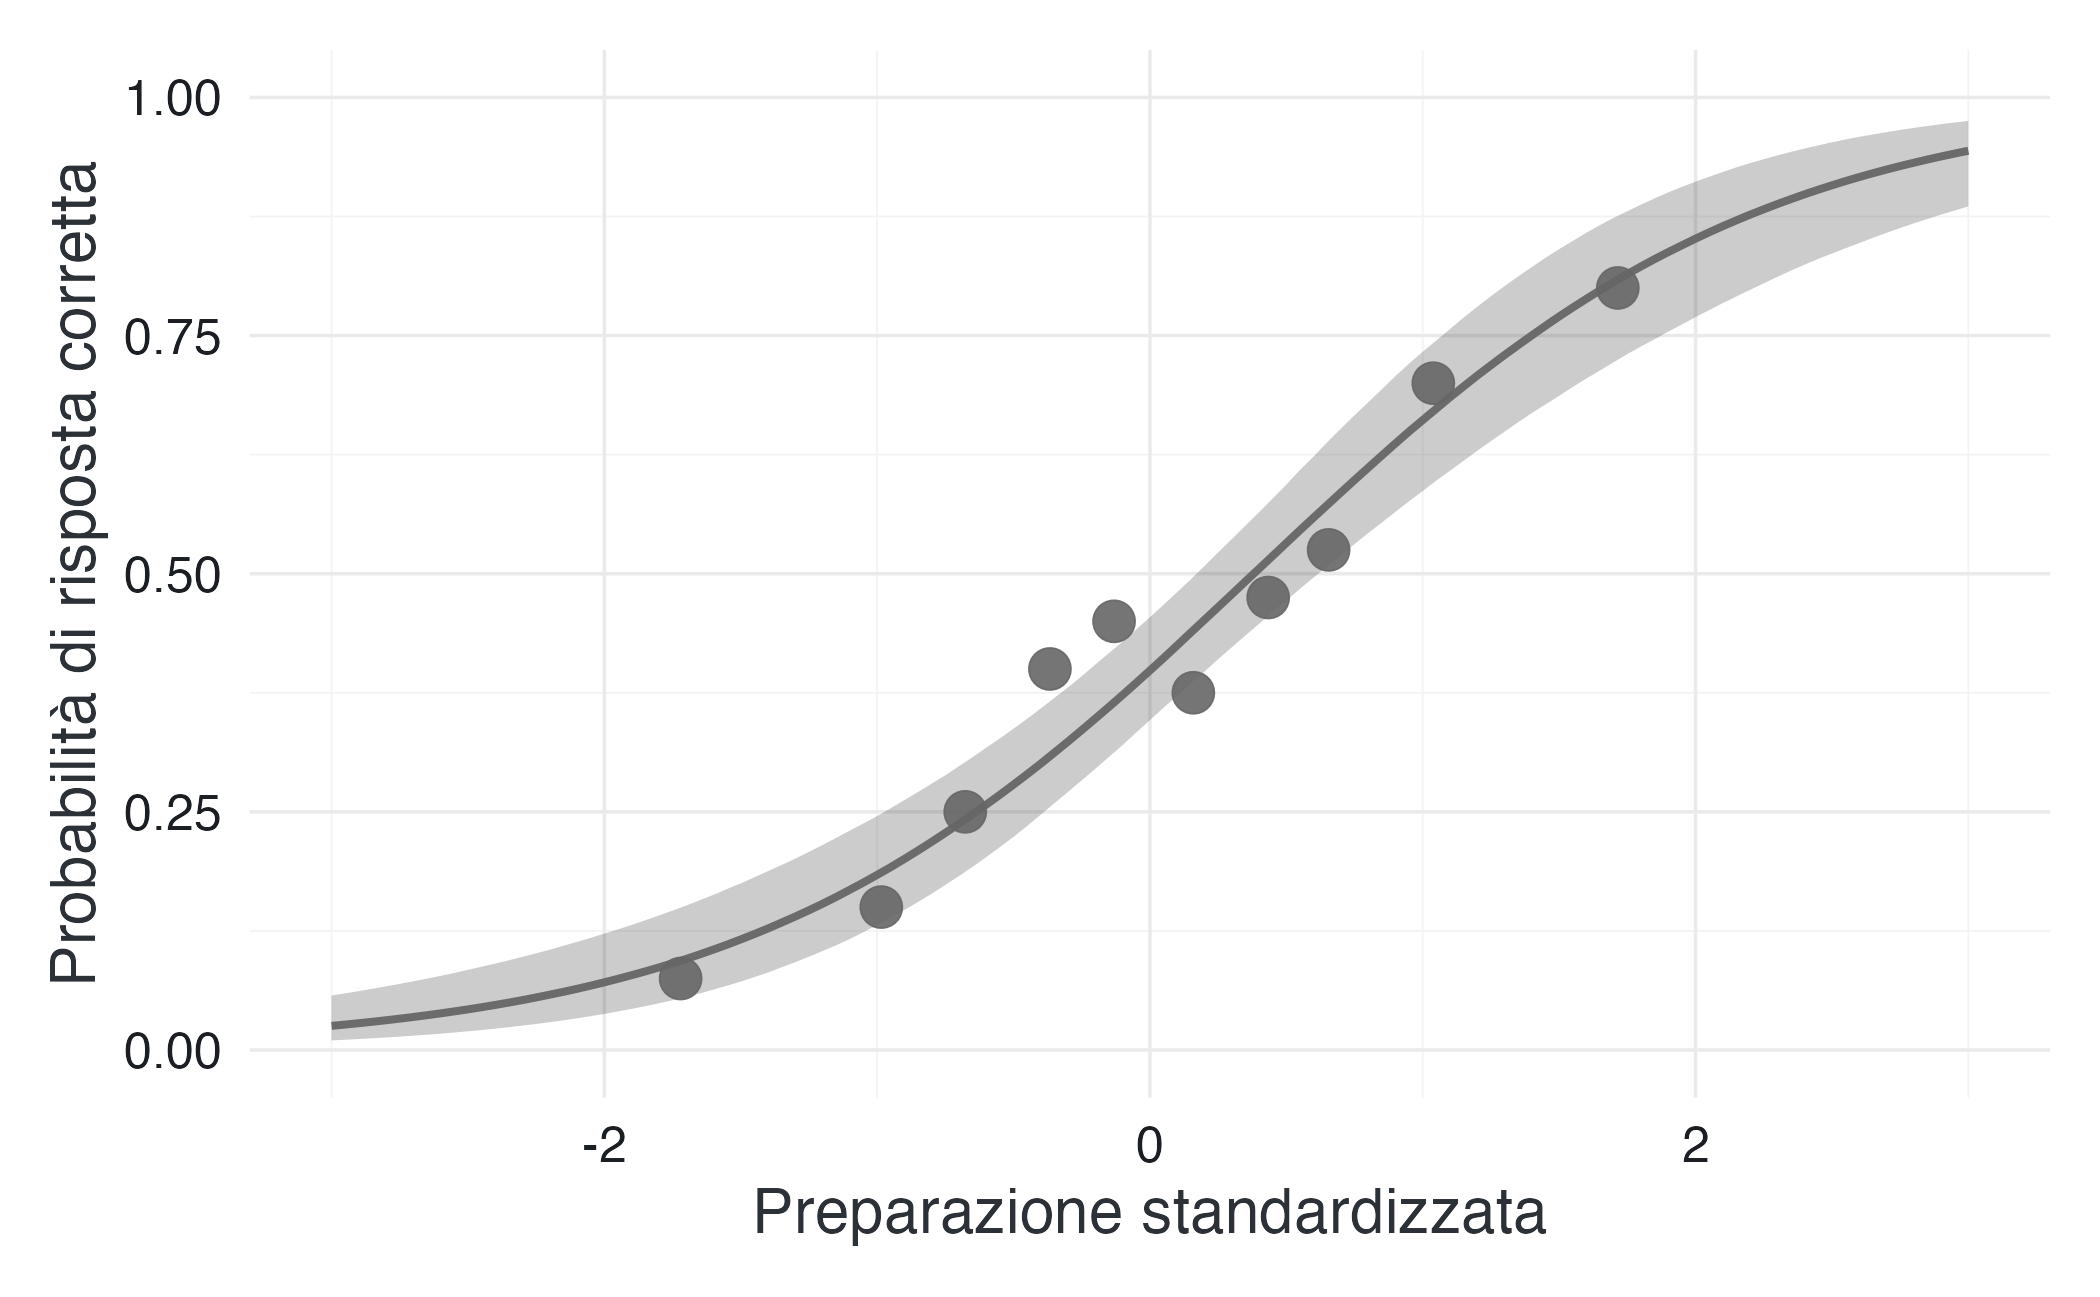
\includegraphics[width=0.85\linewidth,height=\textheight,keepaspectratio]{chapters/glm/01_regressione_logistica_files/figure-pdf/unnamed-chunk-14-1.png}
\end{center}

La fascia rappresenta l'incertezza sulla probabilità media condizionata.
Per simulare nuove risposte individuali, invece, si usa la funzione
\texttt{posterior\_predict()}, che aggiunge la variabilità Bernoulli:

\begin{Shaded}
\begin{Highlighting}[]
\NormalTok{y\_rep }\OtherTok{\textless{}{-}} \FunctionTok{posterior\_predict}\NormalTok{(}
\NormalTok{  fit\_logistic,}
  \AttributeTok{newdata =}\NormalTok{ prediction\_grid}
\NormalTok{)}
\end{Highlighting}
\end{Shaded}

A ogni valore del predittore, una nuova risposta resta 0 oppure 1. La
curva descrive la probabilità della risposta, non una risposta
individuale frazionaria.

\section{Controlli predittivi a
posteriori}\label{controlli-predittivi-a-posteriori-1}

Un primo controllo confronta la proporzione complessiva osservata con
quella delle repliche posteriori:

\begin{Shaded}
\begin{Highlighting}[]
\FunctionTok{pp\_check}\NormalTok{(fit\_logistic, }\AttributeTok{type =} \StringTok{"stat"}\NormalTok{, }\AttributeTok{stat =} \StringTok{"mean"}\NormalTok{, }\AttributeTok{ndraws =} \DecValTok{100}\NormalTok{)}
\end{Highlighting}
\end{Shaded}

\begin{center}
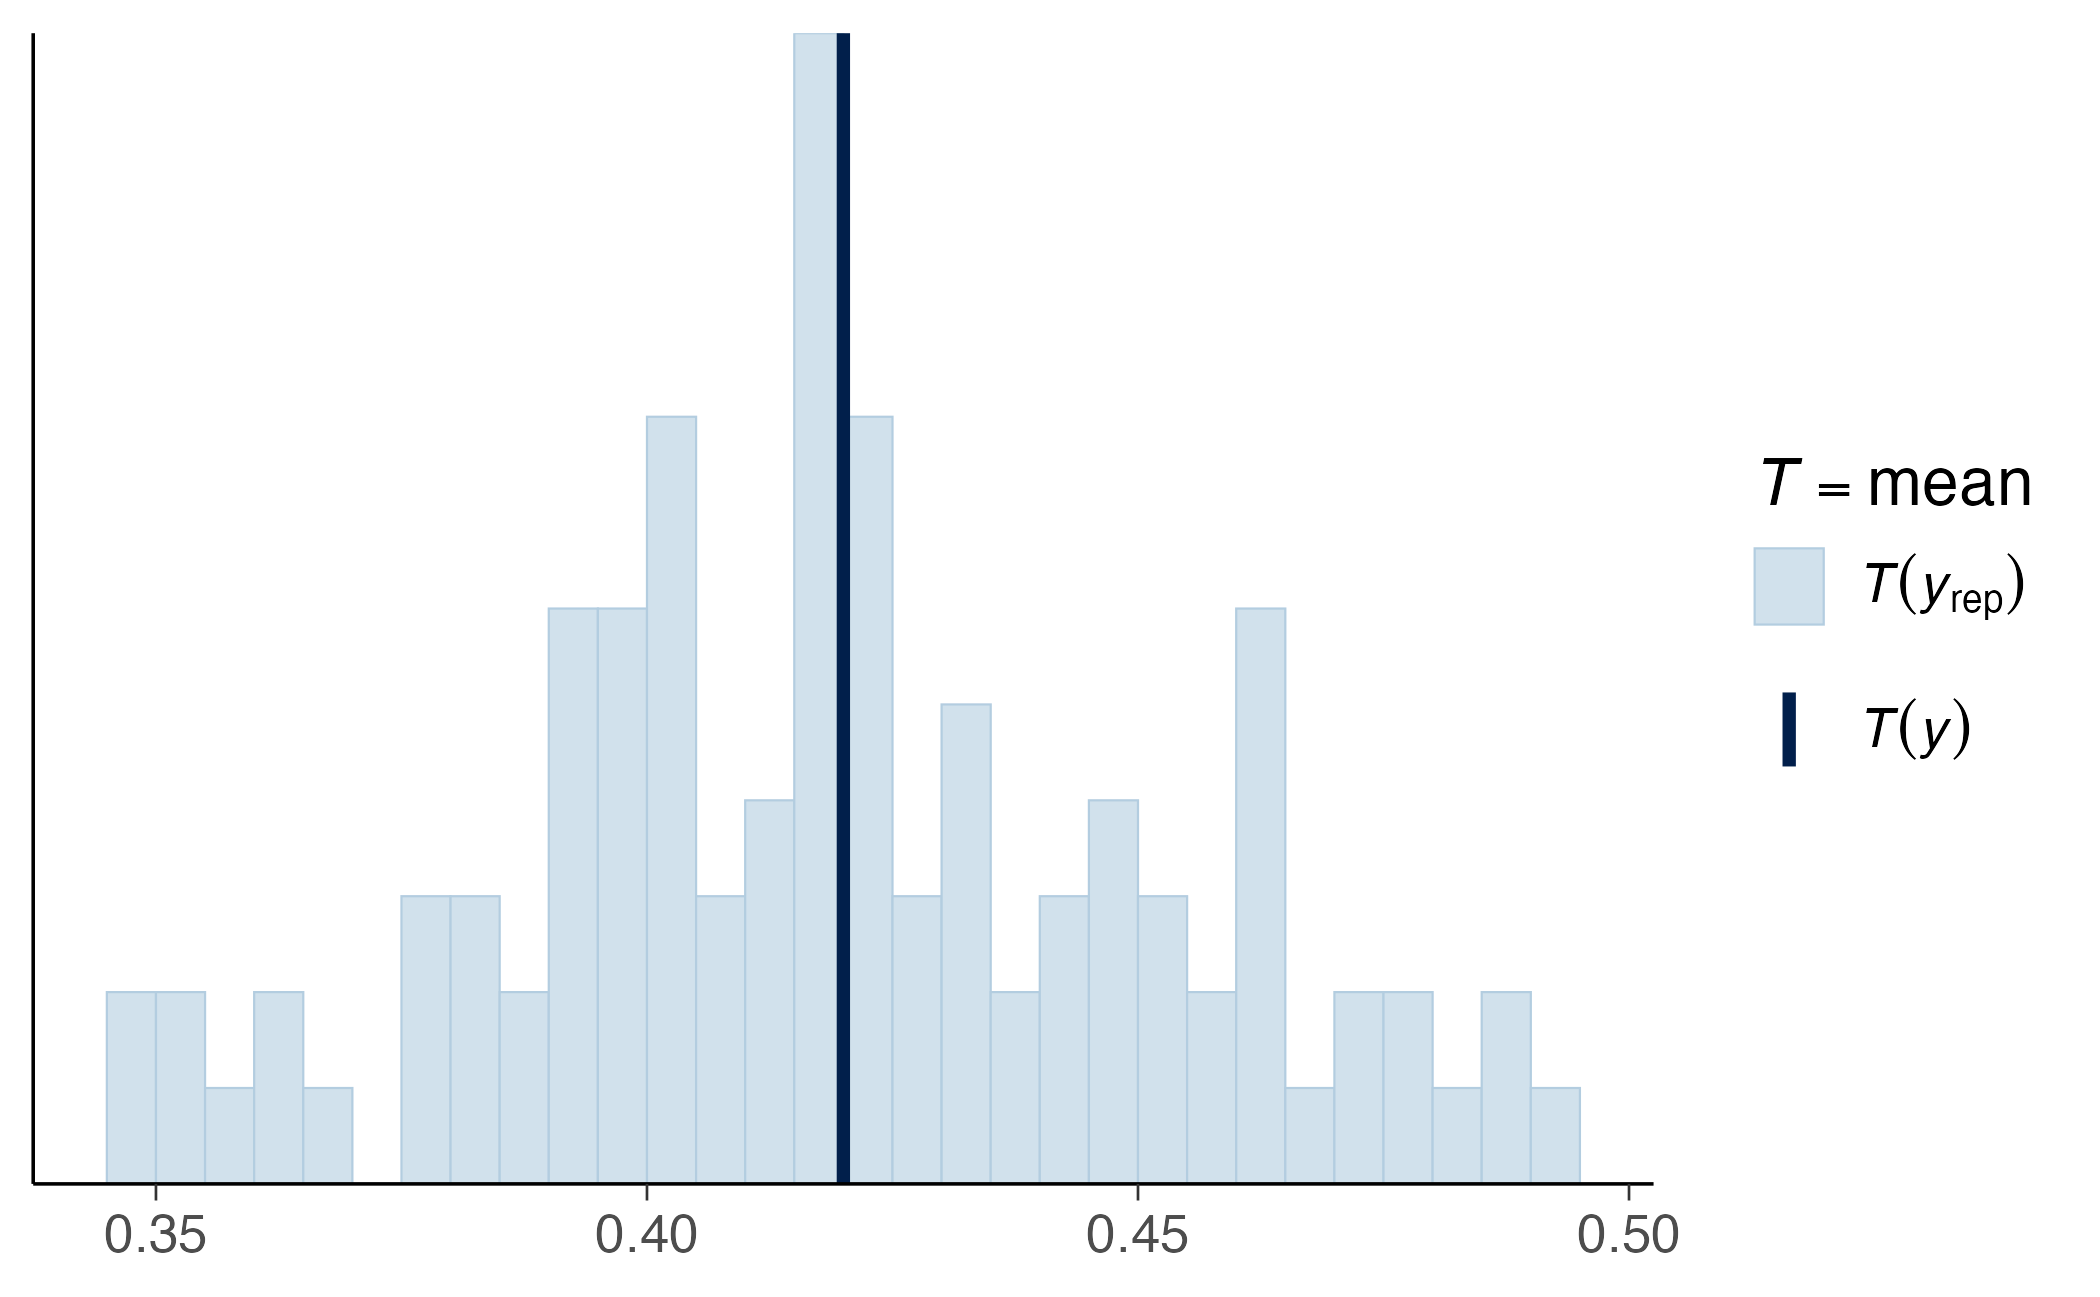
\includegraphics[width=0.85\linewidth,height=\textheight,keepaspectratio]{chapters/glm/01_regressione_logistica_files/figure-pdf/unnamed-chunk-16-1.png}
\end{center}

Tale controllo può però risultare soddisfacente anche se il modello non
rappresenta bene la relazione con il predittore. Per questo motivo, è
consigliabile confrontare, per intervalli di preparazione, le
proporzioni osservate con quelle previste.

\begin{Shaded}
\begin{Highlighting}[]
\NormalTok{posterior\_probabilities }\OtherTok{\textless{}{-}} \FunctionTok{posterior\_epred}\NormalTok{(fit\_logistic)}

\NormalTok{bin\_index }\OtherTok{\textless{}{-}} \FunctionTok{as.integer}\NormalTok{(}
  \FunctionTok{cut}\NormalTok{(}
\NormalTok{    logistic\_data}\SpecialCharTok{$}\NormalTok{preparation,}
    \AttributeTok{breaks =} \FunctionTok{quantile}\NormalTok{(logistic\_data}\SpecialCharTok{$}\NormalTok{preparation, }\AttributeTok{probs =} \FunctionTok{seq}\NormalTok{(}\DecValTok{0}\NormalTok{, }\DecValTok{1}\NormalTok{, }\FloatTok{0.1}\NormalTok{)),}
    \AttributeTok{include.lowest =} \ConstantTok{TRUE}
\NormalTok{  )}
\NormalTok{)}

\NormalTok{predicted\_bins }\OtherTok{\textless{}{-}} \FunctionTok{lapply}\NormalTok{(}\FunctionTok{seq\_len}\NormalTok{(}\FunctionTok{nrow}\NormalTok{(posterior\_probabilities)), }\ControlFlowTok{function}\NormalTok{(draw\_id) \{}
  \FunctionTok{tibble}\NormalTok{(}
    \AttributeTok{bin =}\NormalTok{ bin\_index,}
    \AttributeTok{predicted =}\NormalTok{ posterior\_probabilities[draw\_id, ]}
\NormalTok{  ) }\SpecialCharTok{|\textgreater{}}
    \FunctionTok{group\_by}\NormalTok{(bin) }\SpecialCharTok{|\textgreater{}}
    \FunctionTok{summarise}\NormalTok{(}\AttributeTok{predicted =} \FunctionTok{mean}\NormalTok{(predicted), }\AttributeTok{.groups =} \StringTok{"drop"}\NormalTok{) }\SpecialCharTok{|\textgreater{}}
    \FunctionTok{mutate}\NormalTok{(}\AttributeTok{.draw =}\NormalTok{ draw\_id)}
\NormalTok{\}) }\SpecialCharTok{|\textgreater{}}
  \FunctionTok{bind\_rows}\NormalTok{() }\SpecialCharTok{|\textgreater{}}
  \FunctionTok{group\_by}\NormalTok{(bin) }\SpecialCharTok{|\textgreater{}}
  \FunctionTok{summarise}\NormalTok{(}
    \AttributeTok{predicted =} \FunctionTok{median}\NormalTok{(predicted),}
    \AttributeTok{lower =} \FunctionTok{quantile}\NormalTok{(predicted, }\FloatTok{0.025}\NormalTok{),}
    \AttributeTok{upper =} \FunctionTok{quantile}\NormalTok{(predicted, }\FloatTok{0.975}\NormalTok{),}
    \AttributeTok{.groups =} \StringTok{"drop"}
\NormalTok{  )}

\NormalTok{observed\_for\_check }\OtherTok{\textless{}{-}}\NormalTok{ logistic\_data }\SpecialCharTok{|\textgreater{}}
  \FunctionTok{mutate}\NormalTok{(}\AttributeTok{bin =}\NormalTok{ bin\_index) }\SpecialCharTok{|\textgreater{}}
  \FunctionTok{group\_by}\NormalTok{(bin) }\SpecialCharTok{|\textgreater{}}
  \FunctionTok{summarise}\NormalTok{(}
    \AttributeTok{preparation =} \FunctionTok{mean}\NormalTok{(preparation),}
    \AttributeTok{observed =} \FunctionTok{mean}\NormalTok{(correct),}
    \AttributeTok{.groups =} \StringTok{"drop"}
\NormalTok{  )}

\NormalTok{model\_check }\OtherTok{\textless{}{-}} \FunctionTok{left\_join}\NormalTok{(observed\_for\_check, predicted\_bins, }\AttributeTok{by =} \StringTok{"bin"}\NormalTok{)}

\FunctionTok{ggplot}\NormalTok{(model\_check, }\FunctionTok{aes}\NormalTok{(preparation, predicted)) }\SpecialCharTok{+}
  \FunctionTok{geom\_ribbon}\NormalTok{(}\FunctionTok{aes}\NormalTok{(}\AttributeTok{ymin =}\NormalTok{ lower, }\AttributeTok{ymax =}\NormalTok{ upper), }\AttributeTok{alpha =} \FloatTok{0.25}\NormalTok{) }\SpecialCharTok{+}
  \FunctionTok{geom\_line}\NormalTok{() }\SpecialCharTok{+}
  \FunctionTok{geom\_point}\NormalTok{(}\FunctionTok{aes}\NormalTok{(}\AttributeTok{y =}\NormalTok{ observed)) }\SpecialCharTok{+}
  \FunctionTok{scale\_y\_continuous}\NormalTok{(}\AttributeTok{limits =} \FunctionTok{c}\NormalTok{(}\DecValTok{0}\NormalTok{, }\DecValTok{1}\NormalTok{)) }\SpecialCharTok{+}
  \FunctionTok{labs}\NormalTok{(}
    \AttributeTok{x =} \StringTok{"Preparazione standardizzata"}\NormalTok{,}
    \AttributeTok{y =} \StringTok{"Proporzione osservata e probabilità prevista"}
\NormalTok{  )}
\end{Highlighting}
\end{Shaded}

\begin{center}
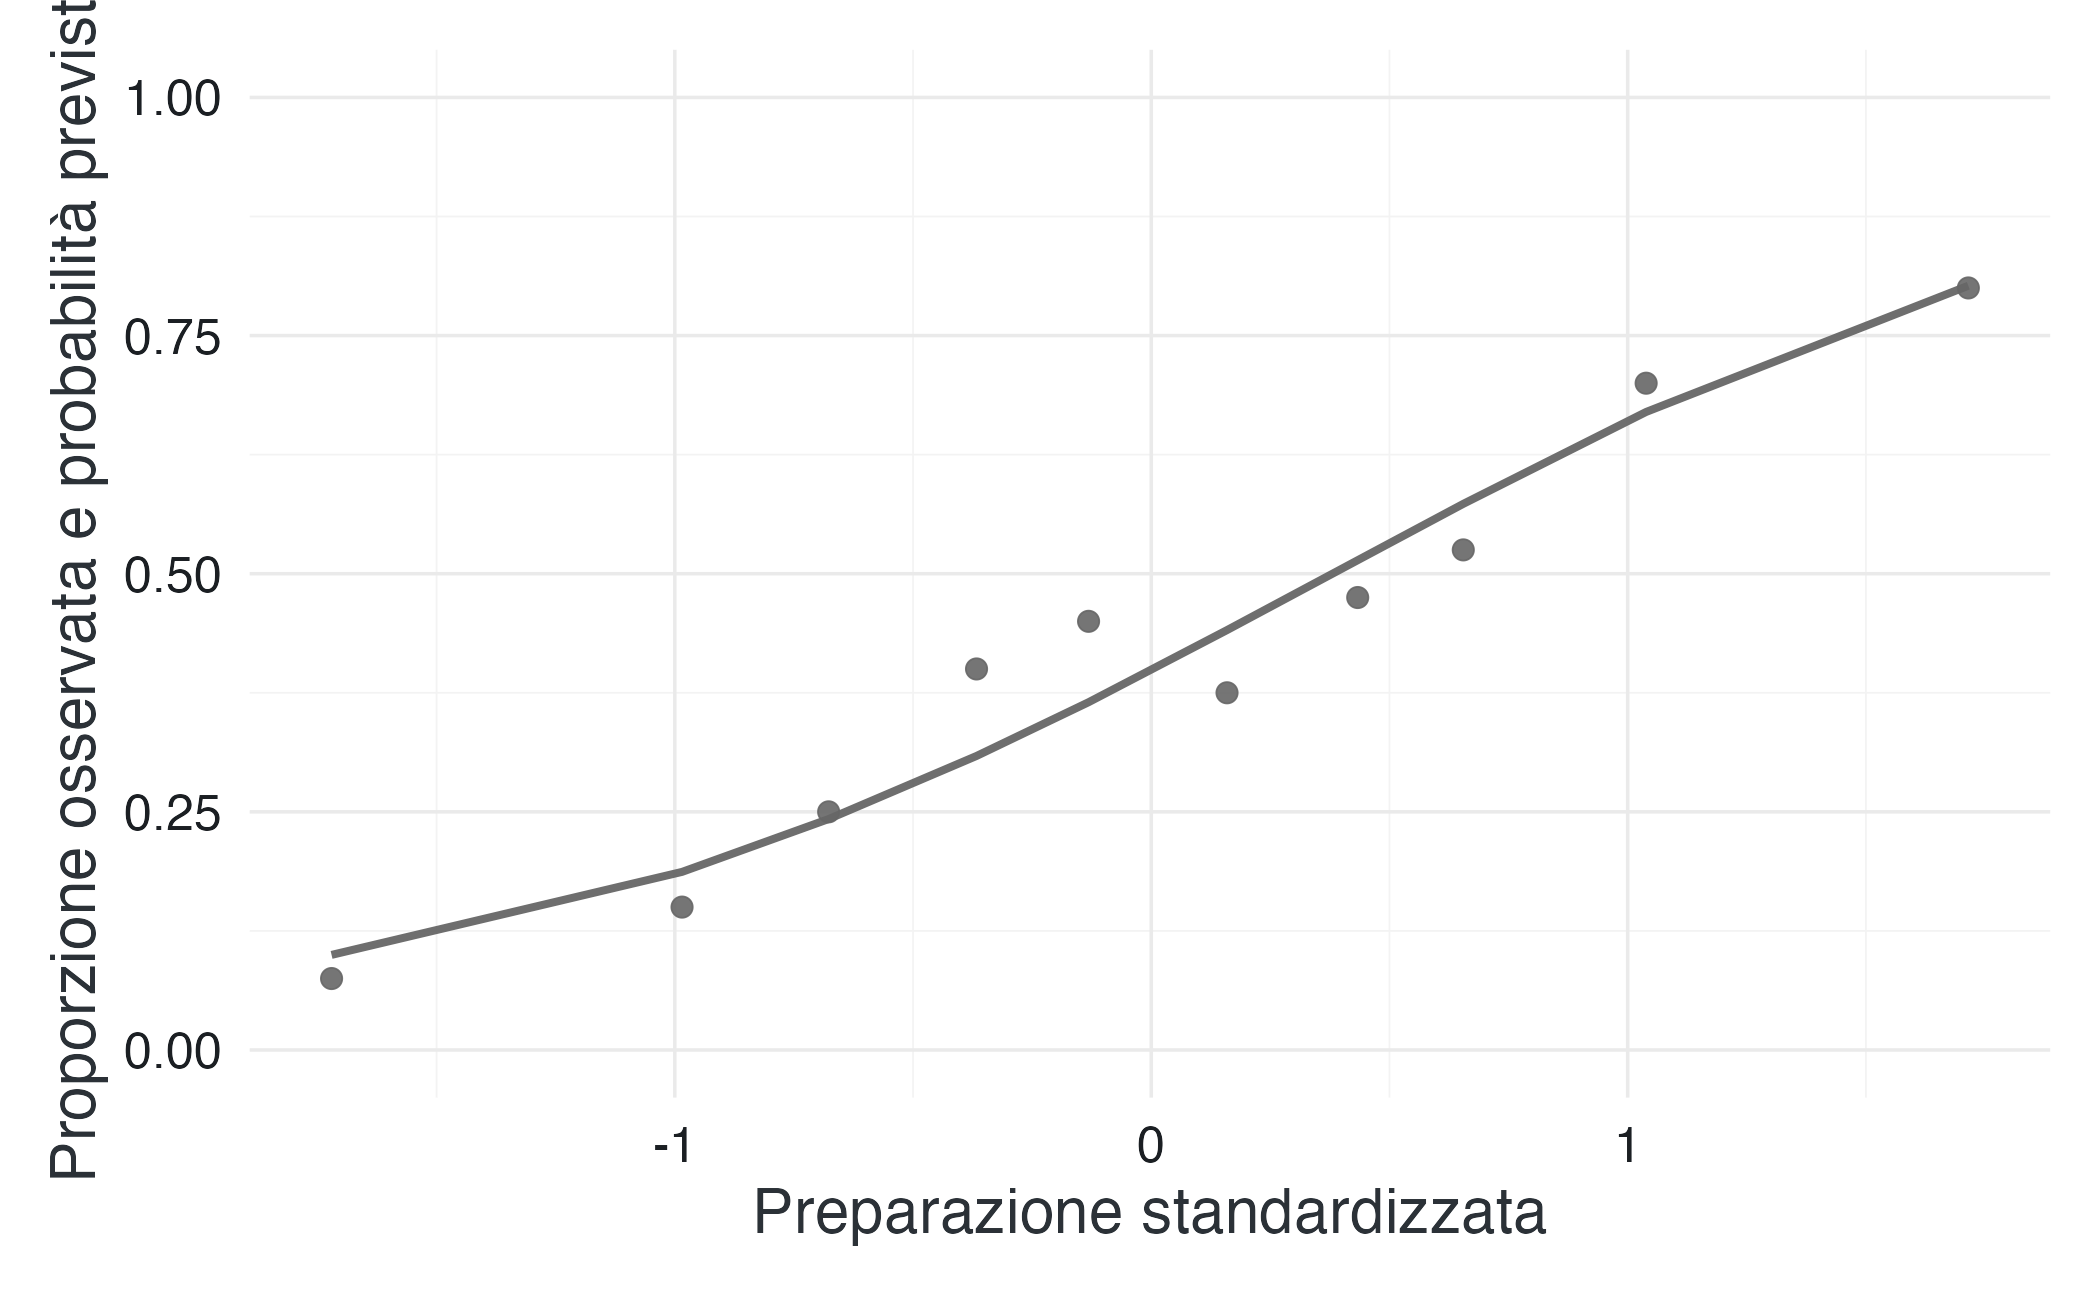
\includegraphics[width=0.85\linewidth,height=\textheight,keepaspectratio]{chapters/glm/01_regressione_logistica_files/figure-pdf/unnamed-chunk-17-1.png}
\end{center}

Tuttavia, il controllo non dimostra che il modello sia vero. Può invece
rivelare curvature non rappresentate, sottogruppi differenti, dipendenze
tra le osservazioni o altre caratteristiche che richiedono una
descrizione più dettagliata.

\section{Quando il predittore è
categoriale}\label{quando-il-predittore-uxe8-categoriale}

Se \(x\) assume i valori 0 e 1, la regressione logistica confronta due
probabilità:

\[
p_0=\operatorname{logit}^{-1}(\alpha),
\qquad
p_1=\operatorname{logit}^{-1}(\alpha+\beta).
\]

In questo caso \(\exp(\beta)\) rappresenta l'odds ratio tra i due
gruppi, mentre \(p_1-p_0\) e \(p_1/p_0\) indicano rispettivamente la
differenza e il rapporto tra le probabilità. Il confronto tra due
proporzioni non richiede quindi una tecnica nuova, ma è un caso
particolare dello stesso GLM. Il capitolo successivo sfrutterà questa
equivalenza per collegare il modello a sola intercetta, il confronto tra
gruppi e le diverse scale di effetto.

\section{Assunzioni e limiti}\label{assunzioni-e-limiti}

La regressione logistica non richiede errori gaussiani né varianza
costante, ma non è priva di assunzioni. Il link logit impone una
relazione lineare tra i predittori e i log-odds, considera le
osservazioni come indipendenti condizionatamente, richiede una codifica
coerente dell'esito e dei predittori e la rappresentazione esplicita di
eventuali strutture gerarchiche o temporali.

Un problema particolare è la \emph{separazione}: può accadere che un
predittore distingua quasi perfettamente gli 0 dagli 1. In quel caso i
coefficienti possono diventare estremamente grandi e instabili; prior
regolarizzanti aiutano a mantenere la stima in regioni plausibili.

Anche l'interpretazione causale richiede cautela. Il coefficiente
logistico descrive un'associazione condizionata al modello e alle
variabili incluse. La randomizzazione, l'ipotesi di identificazione e il
disegno dello studio determinano se tale associazione possa essere
interpretata come effetto causale.

Infine, una regressione logistica rimane un modello della distribuzione
condizionata della risposta. Può descrivere e prevedere come cambia una
probabilità, ma non specifica necessariamente il processo psicologico
che produce le scelte o le risposte nel tempo. Questa distinzione sarà
centrale nel capitolo conclusivo della parte.

\section{Errori interpretativi
ricorrenti}\label{errori-interpretativi-ricorrenti}

\textbf{Confondere probabilità e odds.} Un odds ratio pari a 2 non
implica che la probabilità raddoppi. Il cambiamento sulla scala della
probabilità dipende dal rischio di base.

\textbf{Interpretare \(\beta\) come differenza costante di probabilità.}
Il coefficiente è costante sulla scala dei log-odds. La differenza di
probabilità varia lungo la curva.

\textbf{Riportare soltanto l'odds ratio.} In molti contesti una coppia
di probabilità predette o una differenza assoluta è più comprensibile e
più vicina alla domanda sostantiva.

\textbf{Confondere la probabilità media con una nuova risposta.}
\texttt{posterior\_epred()} descrive la probabilità attesa;
\texttt{posterior\_predict()} genera nuovi esiti binari.

\textbf{Considerare un buon campionamento come prova di adeguatezza.}
Catene ben miscelate indicano che la posterior specificata è stata
esplorata in modo affidabile, non che il modello rappresenti bene il
fenomeno.

\section*{Riflessioni conclusive}\label{riflessioni-conclusive-31}

\markright{Riflessioni conclusive}

La regressione logistica mantiene la struttura essenziale del modello
lineare, ma la adatta a un esito binario. La distribuzione di Bernoulli
descrive le risposte osservate, il predittore lineare sintetizza
l'associazione con le variabili indipendenti e il logit trasforma una
quantità non vincolata in una probabilità compresa tra 0 e 1.

La linearità del modello riguarda i log-odds e non la probabilità. Per
questo motivo, l'interpretazione non dovrebbe limitarsi ai coefficienti.
La distribuzione posteriore può essere trasformata in probabilità
predette, differenze assolute, rapporti di probabilità e odds ratio,
scegliendo la quantità più adatta alla domanda scientifica. Il flusso di
lavoro bayesiano rimane lo stesso già sviluppato per il modello lineare:
i prior devono essere controllati sulla scala osservabile, il calcolo
deve essere diagnosticato e l'adeguatezza deve essere valutata mediante
repliche posteriori mirate.

Il capitolo fornisce la struttura di base dei GLM. Una proporzione
corrisponde a una regressione logistica con sola intercetta, mentre il
confronto tra due proporzioni corrisponde a una regressione con un
predittore binario. Il modello di Poisson applica la stessa architettura
ai conteggi. L'estensione della distribuzione osservazionale amplia le
domande a cui il modello può rispondere, ma non lo trasforma ancora in
una teoria del processo che genera il comportamento.

\begin{tcolorbox}[enhanced jigsaw, arc=.35mm, bottomrule=.15mm, bottomtitle=1mm, breakable, colback=white, colbacktitle=quarto-callout-note-color!10!white, colframe=quarto-callout-note-color-frame, coltitle=black, left=2mm, leftrule=.75mm, opacityback=0, opacitybacktitle=0.6, rightrule=.15mm, title=\textcolor{quarto-callout-note-color}{\faInfo}\hspace{0.5em}{Informazioni sull'ambiente di sviluppo}, titlerule=0mm, toprule=.15mm, toptitle=1mm]

\begin{Shaded}
\begin{Highlighting}[]
\FunctionTok{sessionInfo}\NormalTok{()}
\CommentTok{\#\textgreater{} R version 4.6.1 (2026{-}06{-}24)}
\CommentTok{\#\textgreater{} Platform: aarch64{-}apple{-}darwin23}
\CommentTok{\#\textgreater{} Running under: macOS Tahoe 26.5.2}
\CommentTok{\#\textgreater{} }
\CommentTok{\#\textgreater{} Matrix products: default}
\CommentTok{\#\textgreater{} BLAS:   /Library/Frameworks/R.framework/Versions/4.6/Resources/lib/libRblas.0.dylib }
\CommentTok{\#\textgreater{} LAPACK: /Library/Frameworks/R.framework/Versions/4.6/Resources/lib/libRlapack.dylib;  LAPACK version 3.12.1}
\CommentTok{\#\textgreater{} }
\CommentTok{\#\textgreater{} locale:}
\CommentTok{\#\textgreater{} [1] C.UTF{-}8/UTF{-}8/C.UTF{-}8/C/C.UTF{-}8/C.UTF{-}8}
\CommentTok{\#\textgreater{} }
\CommentTok{\#\textgreater{} time zone: Europe/Zagreb}
\CommentTok{\#\textgreater{} tzcode source: internal}
\CommentTok{\#\textgreater{} }
\CommentTok{\#\textgreater{} attached base packages:}
\CommentTok{\#\textgreater{} [1] stats     graphics  grDevices utils     datasets  methods   base     }
\CommentTok{\#\textgreater{} }
\CommentTok{\#\textgreater{} other attached packages:}
\CommentTok{\#\textgreater{}  [1] ragg\_1.5.2            tinytable\_0.17.0      withr\_3.0.3          }
\CommentTok{\#\textgreater{}  [4] systemfonts\_1.3.2     patchwork\_1.3.2       ggdist\_3.3.3         }
\CommentTok{\#\textgreater{}  [7] tidybayes\_3.0.7       bayesplot\_1.15.0      ggplot2\_4.0.3        }
\CommentTok{\#\textgreater{} [10] reliabilitydiag\_0.2.1 priorsense\_1.2.0      posterior\_1.7.0      }
\CommentTok{\#\textgreater{} [13] loo\_2.10.0            rstan\_2.32.7          StanHeaders\_2.32.10  }
\CommentTok{\#\textgreater{} [16] brms\_2.23.0           Rcpp\_1.1.2            sessioninfo\_1.2.4    }
\CommentTok{\#\textgreater{} [19] conflicted\_1.2.0      janitor\_2.2.1         matrixStats\_1.5.0    }
\CommentTok{\#\textgreater{} [22] modelr\_0.1.11         tibble\_3.3.1          dplyr\_1.2.1          }
\CommentTok{\#\textgreater{} [25] tidyr\_1.3.2           rio\_1.3.0             here\_1.0.2           }
\CommentTok{\#\textgreater{} }
\CommentTok{\#\textgreater{} loaded via a namespace (and not attached):}
\CommentTok{\#\textgreater{}  [1] svUnit\_1.0.8          tidyselect\_1.2.1      farver\_2.1.2         }
\CommentTok{\#\textgreater{}  [4] S7\_0.2.2              fastmap\_1.2.0         tensorA\_0.36.2.1     }
\CommentTok{\#\textgreater{}  [7] pacman\_0.5.1          digest\_0.6.39         timechange\_0.4.0     }
\CommentTok{\#\textgreater{} [10] estimability\_2.0.0    lifecycle\_1.0.5       processx\_3.9.0       }
\CommentTok{\#\textgreater{} [13] magrittr\_2.0.5        compiler\_4.6.1        rlang\_1.3.0          }
\CommentTok{\#\textgreater{} [16] tools\_4.6.1           yaml\_2.3.12           data.table\_1.18.4    }
\CommentTok{\#\textgreater{} [19] knitr\_1.51            labeling\_0.4.3        bridgesampling\_1.2{-}1 }
\CommentTok{\#\textgreater{} [22] pkgbuild\_1.4.8        curl\_7.1.0            plyr\_1.8.9           }
\CommentTok{\#\textgreater{} [25] cmdstanr\_0.9.0        RColorBrewer\_1.1{-}3    abind\_1.4{-}8          }
\CommentTok{\#\textgreater{} [28] purrr\_1.2.2           grid\_4.6.1            stats4\_4.6.1         }
\CommentTok{\#\textgreater{} [31] xtable\_1.8{-}8          inline\_0.3.21         emmeans\_2.0.4        }
\CommentTok{\#\textgreater{} [34] scales\_1.4.0          cli\_3.6.6             mvtnorm\_1.4{-}2        }
\CommentTok{\#\textgreater{} [37] rmarkdown\_2.31        generics\_0.1.4        otel\_0.2.0           }
\CommentTok{\#\textgreater{} [40] RcppParallel\_5.1.11{-}2 reshape2\_1.4.5        cachem\_1.1.0         }
\CommentTok{\#\textgreater{} [43] stringr\_1.6.0         parallel\_4.6.1        vctrs\_0.7.3          }
\CommentTok{\#\textgreater{} [46] V8\_8.2.0              Matrix\_1.7{-}5          jsonlite\_2.0.0       }
\CommentTok{\#\textgreater{} [49] arrayhelpers\_1.1{-}1    glue\_1.8.1            ps\_1.9.3             }
\CommentTok{\#\textgreater{} [52] codetools\_0.2{-}20      distributional\_0.8.1  lubridate\_1.9.5      }
\CommentTok{\#\textgreater{} [55] stringi\_1.8.7         gtable\_0.3.6          QuickJSR\_1.10.0      }
\CommentTok{\#\textgreater{} [58] pillar\_1.11.1         htmltools\_0.5.9       Brobdingnag\_1.2{-}9    }
\CommentTok{\#\textgreater{} [61] R6\_2.6.1              textshaping\_1.0.5     rprojroot\_2.1.1      }
\CommentTok{\#\textgreater{} [64] evaluate\_1.0.5        lattice\_0.22{-}9        backports\_1.5.1      }
\CommentTok{\#\textgreater{} [67] memoise\_2.0.1         broom\_1.0.13          snakecase\_0.11.1     }
\CommentTok{\#\textgreater{} [70] rstantools\_2.6.0      coda\_0.19{-}4.1         gridExtra\_2.3.1      }
\CommentTok{\#\textgreater{} [73] nlme\_3.1{-}170          checkmate\_2.3.4       xfun\_0.60            }
\CommentTok{\#\textgreater{} [76] pkgconfig\_2.0.3}
\end{Highlighting}
\end{Shaded}

\end{tcolorbox}

\section*{Bibliografia}\label{bibliografia-35}

\markright{Bibliografia}

\chapter{Una e due proporzioni come casi della regressione
logistica}\label{sec-bayes-inference-proportions}

Una proporzione non richiede una nuova famiglia di metodi. Se osserviamo
il numero di successi su un numero noto di prove, possiamo usare un
modello binomiale. Con una sola popolazione, il modello contiene
soltanto l'intercetta; con due popolazioni, aggiungiamo un predittore
binario. Entrambi i casi sono quindi forme particolarmente semplici
della regressione logistica introdotta nel capitolo precedente.

Il vantaggio di questa formulazione è duplice. Da un lato, consente di
interpretare direttamente le probabilità e i loro contrasti. Dall'altro,
prepara l'estensione a modelli con più gruppi, covariate, interazioni e
strutture gerarchiche, senza cambiare linguaggio statistico.

\section*{Orientamento}\label{orientamento}

\markright{Orientamento}

Il capitolo sviluppa due domande collegate. La prima riguarda la
probabilità di un evento in una singola popolazione; la seconda riguarda
la differenza tra le probabilità dell'evento in due popolazioni. In
entrambi i casi partiremo dalla quantità sostantiva di interesse e non
da un test dell'ipotesi nulla.

Come esempio useremo i dati discussi da Brückner \& Bearman
(\citeproc{ref-bruckner2005after}{2005}) e ripresi in un'analisi
bayesiana da Wagenmakers et al.
(\citeproc{ref-wagenmakers2010bayesian}{2010}). Gli autori
considerarono, tra gli altri aspetti, l'uso del preservativo durante il
primo rapporto sessuale tra giovani adulti che avevano o non avevano
sottoscritto un \emph{virginity pledge}. Nel gruppo dei \emph{pledgers},
424 persone su 777 dichiararono di aver usato il preservativo; nel
gruppo dei \emph{non-pledgers}, i successi furono 5416 su 9072.

L'obiettivo didattico non è stabilire se una delle proporzioni sia
``significativamente diversa'' da un valore convenzionale. Vogliamo
invece stimare le probabilità, quantificarne l'incertezza e ricavare
contrasti interpretabili sulla scala dell'outcome.

\begin{tcolorbox}[enhanced jigsaw, arc=.35mm, bottomrule=.15mm, breakable, colback=white, colframe=quarto-callout-important-color-frame, left=2mm, leftrule=.75mm, opacityback=0, rightrule=.15mm, toprule=.15mm]

\textbf{Da sapere.} Una proporzione può essere rappresentata mediante
una regressione logistica: con una sola popolazione il modello contiene
soltanto l'intercetta; con due popolazioni aggiunge un predittore
binario. L'intercetta determina la probabilità del gruppo di
riferimento, mentre il coefficiente del gruppo rappresenta la differenza
tra i log-odds. Dalla distribuzione a posteriori si ricavano quantità
più direttamente interpretabili, come le probabilità dei gruppi, la
differenza di rischio, il \emph{risk ratio} e l'odds ratio.

\textbf{Da saper fare.} Stimare con \texttt{brms} una o due proporzioni
mediante il modello binomiale; trasformare i coefficienti logistici in
probabilità; interpretare l'intercetta e il coefficiente di gruppo;
calcolare dai campioni posteriori differenza di rischio, \emph{risk
ratio} e odds ratio; valutare direzione, incertezza e rilevanza pratica
del contrasto ed eseguire i principali controlli predittivi.

\textbf{Approfondimento facoltativo.} Il confronto con la soluzione
coniugata Beta--Binomiale, i dettagli computazionali dei controlli
predittivi, l'uso di SESOI e ROPE e le estensioni a modelli gerarchici o
sovradispersi possono essere rimandati. Nel percorso essenziale è
sufficiente comprendere la relazione tra regressione logistica e
proporzioni e interpretare correttamente le probabilità e i principali
contrasti posteriori.

\hyperref[sec-percorsi-lettura]{Che cosa significano queste etichette?}

\end{tcolorbox}

\begin{tcolorbox}[enhanced jigsaw, arc=.35mm, bottomrule=.15mm, bottomtitle=1mm, breakable, colback=white, colbacktitle=quarto-callout-tip-color!10!white, colframe=quarto-callout-tip-color-frame, coltitle=black, left=2mm, leftrule=.75mm, opacityback=0, opacitybacktitle=0.6, rightrule=.15mm, title=\textcolor{quarto-callout-tip-color}{\faLightbulb}\hspace{0.5em}{Prerequisiti}, titlerule=0mm, toprule=.15mm, toptitle=1mm]

Il capitolo presuppone la regressione logistica sviluppata in
Capitolo~\ref{sec-reg-logistic-stan}. La coniugazione Beta--Binomiale è
stata discussa nella parte dedicata all'aggiornamento bayesiano; per
un'introduzione applicata si può consultare anche Albert \& Hu
(\citeproc{ref-albert_2019prob}{2019}).

\end{tcolorbox}

\begin{tcolorbox}[enhanced jigsaw, arc=.35mm, bottomrule=.15mm, bottomtitle=1mm, breakable, colback=white, colbacktitle=quarto-callout-caution-color!10!white, colframe=quarto-callout-caution-color-frame, coltitle=black, left=2mm, leftrule=.75mm, opacityback=0, opacitybacktitle=0.6, rightrule=.15mm, title=\textcolor{quarto-callout-caution-color}{\faFire}\hspace{0.5em}{Preparazione del notebook}, titlerule=0mm, toprule=.15mm, toptitle=1mm]

\begin{Shaded}
\begin{Highlighting}[]
\NormalTok{here}\SpecialCharTok{::}\FunctionTok{here}\NormalTok{(}\StringTok{"code"}\NormalTok{, }\StringTok{"\_common.R"}\NormalTok{) }\SpecialCharTok{|\textgreater{}}
  \FunctionTok{source}\NormalTok{()}

\ControlFlowTok{if}\NormalTok{ (}\SpecialCharTok{!}\FunctionTok{requireNamespace}\NormalTok{(}\StringTok{"pacman"}\NormalTok{, }\AttributeTok{quietly =} \ConstantTok{TRUE}\NormalTok{)) \{}
  \FunctionTok{install.packages}\NormalTok{(}\StringTok{"pacman"}\NormalTok{)}
\NormalTok{\}}

\NormalTok{pacman}\SpecialCharTok{::}\FunctionTok{p\_load}\NormalTok{(}
\NormalTok{  brms,}
\NormalTok{  posterior,}
\NormalTok{  dplyr,}
\NormalTok{  tidyr,}
\NormalTok{  tibble,}
\NormalTok{  ggplot2,}
\NormalTok{  scales}
\NormalTok{)}

\FunctionTok{set.seed}\NormalTok{(}\DecValTok{2026}\NormalTok{)}
\end{Highlighting}
\end{Shaded}

\end{tcolorbox}

\section{Una proporzione come modello a sola
intercetta}\label{una-proporzione-come-modello-a-sola-intercetta}

Supponiamo di osservare \(y\) successi su \(n\) prove. Il modello
binomiale è

\[
Y \sim \operatorname{Binomial}(n,p),
\]

dove \(p\) è la probabilità di successo nella popolazione modellata. Per
collegare questo caso alla regressione logistica scriviamo

\[
\operatorname{logit}(p)=\alpha.
\]

L'intercetta \(\alpha\) è il logit della probabilità; la trasformazione
inversa restituisce

\[
p=\operatorname{logit}^{-1}(\alpha).
\]

Il modello è dunque una regressione logistica senza predittori. La
formula \texttt{\textasciitilde{}\ 1} non indica assenza di modello:
indica che tutte le osservazioni condividono la stessa probabilità,
salvo la variabilità binomiale.

\subsection{Dati e quantità di
interesse}\label{dati-e-quantituxe0-di-interesse}

Per il gruppo dei \emph{pledgers} osserviamo:

\begin{Shaded}
\begin{Highlighting}[]
\NormalTok{pledge\_data }\OtherTok{\textless{}{-}} \FunctionTok{tibble}\NormalTok{(}
  \AttributeTok{successes =} \DecValTok{424}\NormalTok{,}
  \AttributeTok{trials =} \DecValTok{777}
\NormalTok{)}

\NormalTok{pledge\_data }\SpecialCharTok{|\textgreater{}}
  \FunctionTok{mutate}\NormalTok{(}\AttributeTok{observed\_proportion =}\NormalTok{ successes }\SpecialCharTok{/}\NormalTok{ trials)}
\CommentTok{\#\textgreater{} \# A tibble: 1 x 3}
\CommentTok{\#\textgreater{}   successes trials observed\_proportion}
\CommentTok{\#\textgreater{}       \textless{}dbl\textgreater{}  \textless{}dbl\textgreater{}               \textless{}dbl\textgreater{}}
\CommentTok{\#\textgreater{} 1       424    777               0.546}
\end{Highlighting}
\end{Shaded}

La quantità principale è \(p_{\text{pledge}}\), la probabilità di uso
del preservativo nella popolazione alla quale intendiamo generalizzare.
Prima di interpretarla, è necessario ricordare che la validità della
generalizzazione dipende dal disegno, dalla qualità della misura e dal
meccanismo di campionamento, non soltanto dal modello binomiale.

\subsection{Prior sulla scala della
probabilità}\label{prior-sulla-scala-della-probabilituxe0}

Nel modello logit il prior viene assegnato a \(\alpha\), ma le sue
implicazioni devono essere comprese sulla scala di \(p\). Consideriamo

\[
\alpha\sim\operatorname{Normal}(0,1.5).
\]

Il prior è centrato su \(p=0.5\) e ammette un intervallo ampio di
probabilità. Possiamo verificarlo simulando direttamente dalla
distribuzione a priori:

\begin{Shaded}
\begin{Highlighting}[]
\NormalTok{prior\_one }\OtherTok{\textless{}{-}} \FunctionTok{tibble}\NormalTok{(}
  \AttributeTok{alpha =} \FunctionTok{rnorm}\NormalTok{(}\DecValTok{5000}\NormalTok{, }\DecValTok{0}\NormalTok{, }\FloatTok{1.5}\NormalTok{),}
  \AttributeTok{p =} \FunctionTok{plogis}\NormalTok{(alpha),}
  \AttributeTok{successes\_rep =} \FunctionTok{rbinom}\NormalTok{(}\DecValTok{5000}\NormalTok{, }\AttributeTok{size =}\NormalTok{ pledge\_data}\SpecialCharTok{$}\NormalTok{trials, }\AttributeTok{prob =}\NormalTok{ p),}
  \AttributeTok{proportion\_rep =}\NormalTok{ successes\_rep }\SpecialCharTok{/}\NormalTok{ pledge\_data}\SpecialCharTok{$}\NormalTok{trials}
\NormalTok{)}

\FunctionTok{ggplot}\NormalTok{(prior\_one, }\FunctionTok{aes}\NormalTok{(p)) }\SpecialCharTok{+}
  \FunctionTok{geom\_density}\NormalTok{(}\AttributeTok{fill =} \StringTok{"grey80"}\NormalTok{) }\SpecialCharTok{+}
  \FunctionTok{scale\_x\_continuous}\NormalTok{(}\AttributeTok{labels =} \FunctionTok{label\_percent}\NormalTok{()) }\SpecialCharTok{+}
  \FunctionTok{labs}\NormalTok{(}
    \AttributeTok{x =} \StringTok{"Probabilità a priori di uso del preservativo"}\NormalTok{,}
    \AttributeTok{y =} \StringTok{"Densità"}
\NormalTok{  )}
\end{Highlighting}
\end{Shaded}

\begin{center}
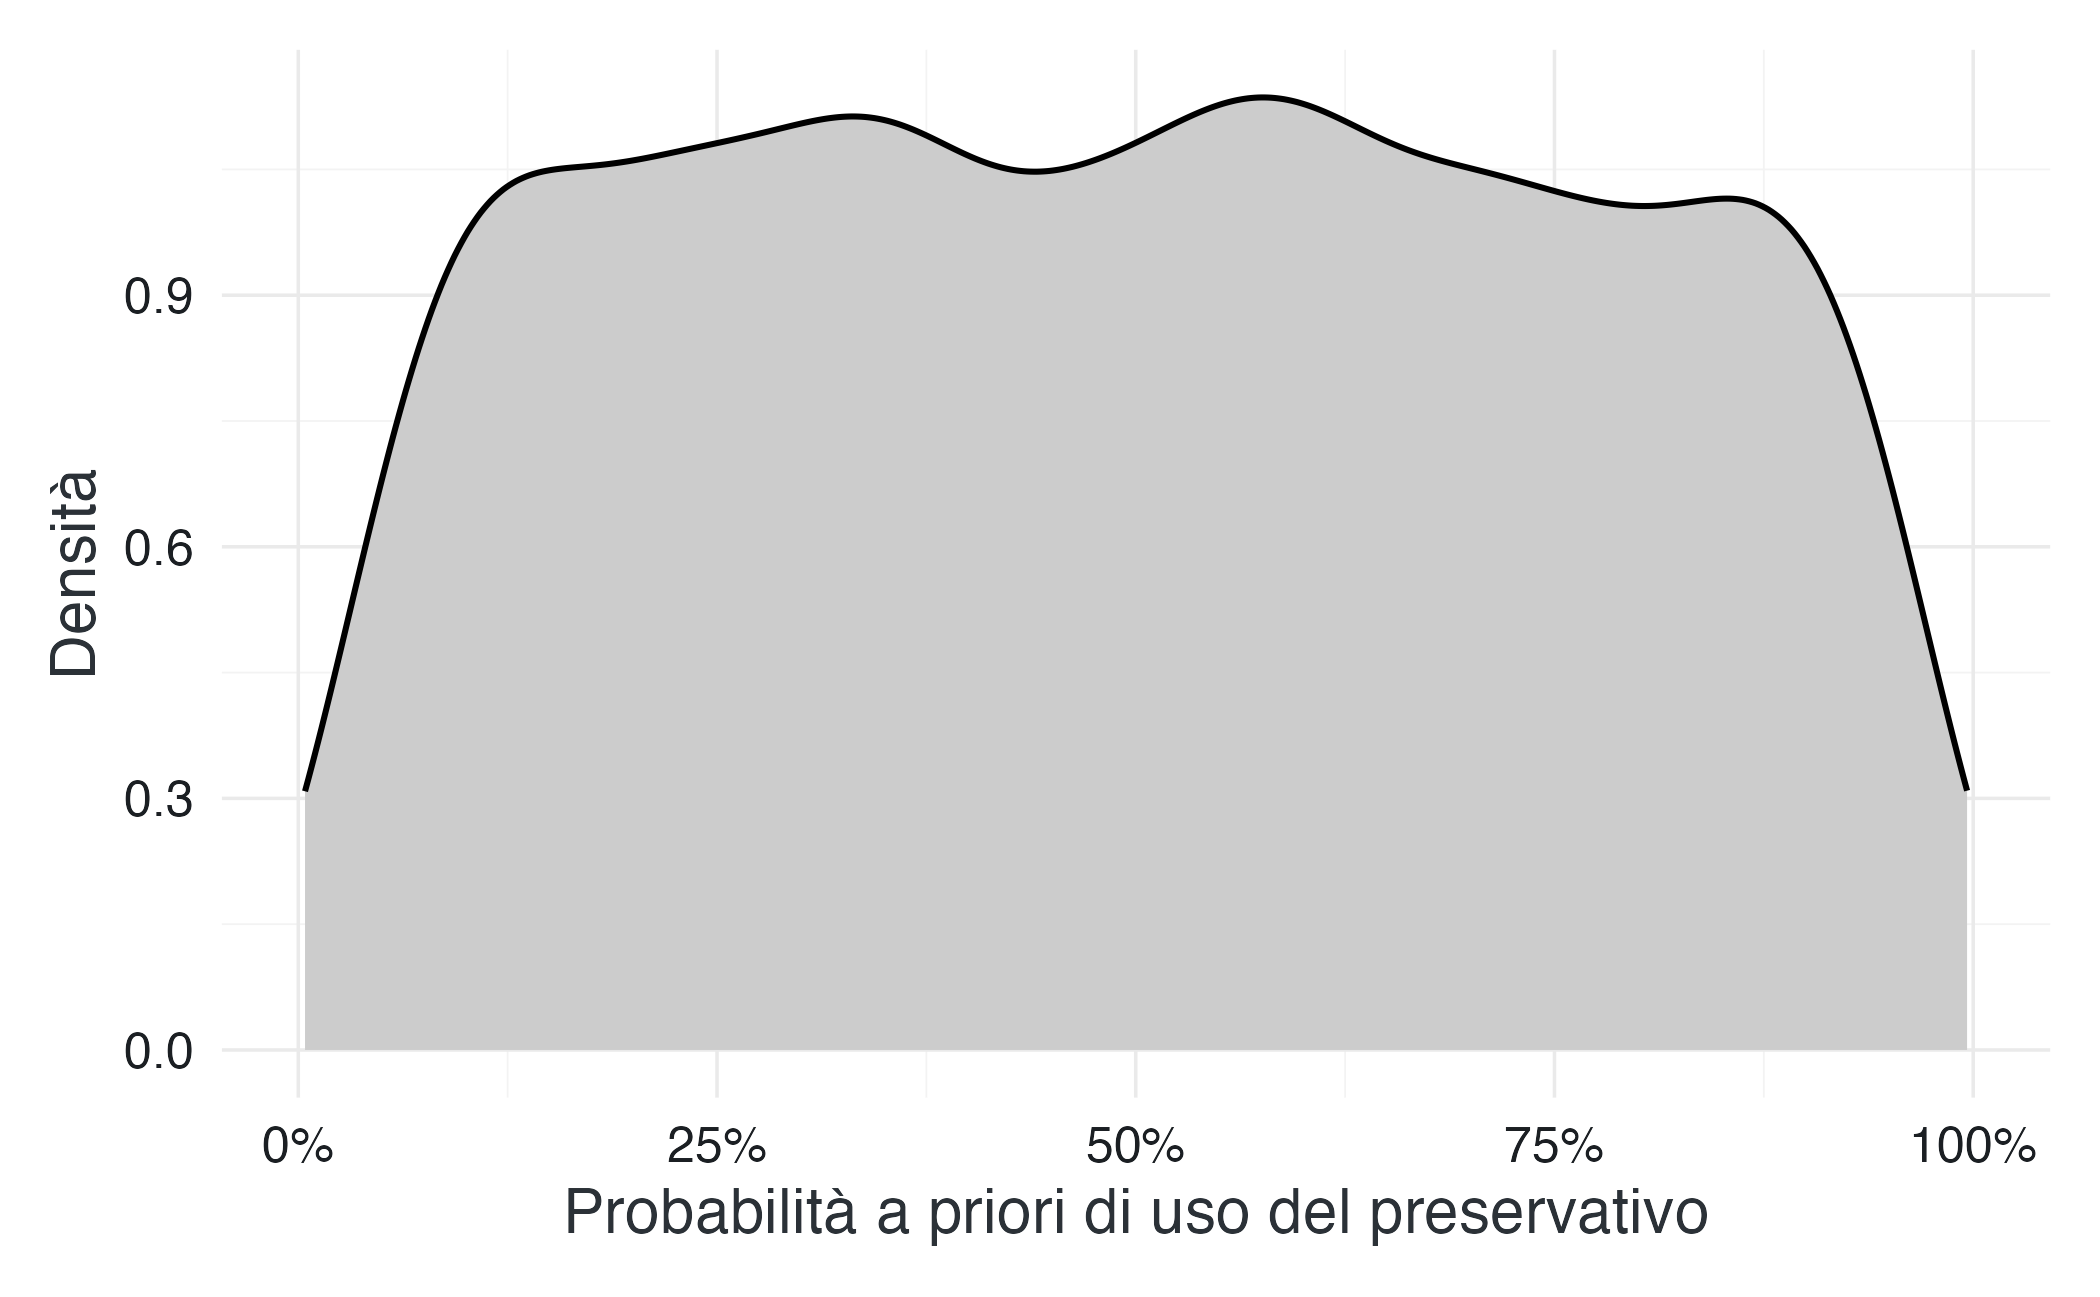
\includegraphics[width=0.85\linewidth,height=\textheight,keepaspectratio]{chapters/glm/02_proporzioni_files/figure-pdf/unnamed-chunk-3-1.png}
\end{center}

Il controllo serve a valutare se il prior ammetta scenari che riteniamo
plausibili prima di usare i dati. Non deve essere calibrato in modo da
anticipare la proporzione osservata.

\subsection{\texorpdfstring{Stima con
\texttt{brms}}{Stima con brms}}\label{stima-con-brms-1}

Adattiamo il modello binomiale a sola intercetta:

\begin{Shaded}
\begin{Highlighting}[]
\NormalTok{fit\_one\_proportion }\OtherTok{\textless{}{-}} \FunctionTok{brm}\NormalTok{(}
\NormalTok{  successes }\SpecialCharTok{|} \FunctionTok{trials}\NormalTok{(trials) }\SpecialCharTok{\textasciitilde{}} \DecValTok{1}\NormalTok{,}
  \AttributeTok{data =}\NormalTok{ pledge\_data,}
  \AttributeTok{family =} \FunctionTok{binomial}\NormalTok{(}\AttributeTok{link =} \StringTok{"logit"}\NormalTok{),}
  \AttributeTok{prior =} \FunctionTok{prior}\NormalTok{(}\FunctionTok{normal}\NormalTok{(}\DecValTok{0}\NormalTok{, }\FloatTok{1.5}\NormalTok{), }\AttributeTok{class =}\NormalTok{ Intercept),}
  \AttributeTok{chains =} \DecValTok{4}\NormalTok{,}
  \AttributeTok{iter =} \DecValTok{3000}\NormalTok{,}
  \AttributeTok{warmup =} \DecValTok{1000}\NormalTok{,}
  \AttributeTok{seed =} \DecValTok{2026}\NormalTok{,}
  \AttributeTok{refresh =} \DecValTok{0}
\NormalTok{)}
\CommentTok{\#\textgreater{} Running MCMC with 4 chains, at most 10 in parallel...}
\CommentTok{\#\textgreater{} }
\CommentTok{\#\textgreater{} Chain 1 finished in 0.0 seconds.}
\CommentTok{\#\textgreater{} Chain 2 finished in 0.0 seconds.}
\CommentTok{\#\textgreater{} Chain 3 finished in 0.0 seconds.}
\CommentTok{\#\textgreater{} Chain 4 finished in 0.0 seconds.}
\CommentTok{\#\textgreater{} }
\CommentTok{\#\textgreater{} All 4 chains finished successfully.}
\CommentTok{\#\textgreater{} Mean chain execution time: 0.0 seconds.}
\CommentTok{\#\textgreater{} Total execution time: 0.3 seconds.}
\end{Highlighting}
\end{Shaded}

La sintesi standard riporta l'intercetta sulla scala dei log-odds:

\begin{Shaded}
\begin{Highlighting}[]
\FunctionTok{summary}\NormalTok{(fit\_one\_proportion)}
\CommentTok{\#\textgreater{}  Family: binomial }
\CommentTok{\#\textgreater{}   Links: mu = logit }
\CommentTok{\#\textgreater{} Formula: successes | trials(trials) \textasciitilde{} 1 }
\CommentTok{\#\textgreater{}    Data: pledge\_data (Number of observations: 1) }
\CommentTok{\#\textgreater{}   Draws: 4 chains, each with iter = 3000; warmup = 1000; thin = 1;}
\CommentTok{\#\textgreater{}          total post{-}warmup draws = 8000}
\CommentTok{\#\textgreater{} }
\CommentTok{\#\textgreater{} Regression Coefficients:}
\CommentTok{\#\textgreater{}           Estimate Est.Error l{-}95\% CI u{-}95\% CI Rhat Bulk\_ESS Tail\_ESS}
\CommentTok{\#\textgreater{} Intercept     0.18      0.07     0.04     0.32 1.00     2819     3711}
\CommentTok{\#\textgreater{} }
\CommentTok{\#\textgreater{} Draws were sampled using sample(hmc). For each parameter, Bulk\_ESS}
\CommentTok{\#\textgreater{} and Tail\_ESS are effective sample size measures, and Rhat is the potential}
\CommentTok{\#\textgreater{} scale reduction factor on split chains (at convergence, Rhat = 1).}
\end{Highlighting}
\end{Shaded}

Per ottenere la quantità sostantiva trasformiamo ogni draw:

\begin{Shaded}
\begin{Highlighting}[]
\NormalTok{one\_draws }\OtherTok{\textless{}{-}} \FunctionTok{as\_draws\_df}\NormalTok{(fit\_one\_proportion) }\SpecialCharTok{|\textgreater{}}
  \FunctionTok{transmute}\NormalTok{(}
    \AttributeTok{p\_pledge =} \FunctionTok{plogis}\NormalTok{(b\_Intercept)}
\NormalTok{  )}

\NormalTok{one\_summary }\OtherTok{\textless{}{-}}\NormalTok{ one\_draws }\SpecialCharTok{|\textgreater{}}
  \FunctionTok{summarise}\NormalTok{(}
    \AttributeTok{median =} \FunctionTok{median}\NormalTok{(p\_pledge),}
    \AttributeTok{lower =} \FunctionTok{quantile}\NormalTok{(p\_pledge, }\FloatTok{0.025}\NormalTok{),}
    \AttributeTok{upper =} \FunctionTok{quantile}\NormalTok{(p\_pledge, }\FloatTok{0.975}\NormalTok{)}
\NormalTok{  )}

\NormalTok{one\_summary}
\CommentTok{\#\textgreater{} \# A tibble: 1 x 3}
\CommentTok{\#\textgreater{}   median lower upper}
\CommentTok{\#\textgreater{}    \textless{}dbl\textgreater{} \textless{}dbl\textgreater{} \textless{}dbl\textgreater{}}
\CommentTok{\#\textgreater{} 1  0.546 0.510 0.580}
\end{Highlighting}
\end{Shaded}

L'intervallo descrive l'incertezza su \(p_{\text{pledge}}\)
condizionatamente al modello, al prior e ai dati. Non è una regione che
contiene il parametro perché la procedura possiede una certa frequenza
di copertura: è un'affermazione probabilistica sulla quantità incerta
nel modello bayesiano.

\subsection{Confronti con valori di
riferimento}\label{confronti-con-valori-di-riferimento}

Una distribuzione posteriore permette di calcolare la probabilità che
\(p\) superi una soglia sostantiva. Per esempio:

\begin{Shaded}
\begin{Highlighting}[]
\NormalTok{one\_draws }\SpecialCharTok{|\textgreater{}}
  \FunctionTok{summarise}\NormalTok{(}
    \AttributeTok{Pr\_p\_gt\_50 =} \FunctionTok{mean}\NormalTok{(p\_pledge }\SpecialCharTok{\textgreater{}} \FloatTok{0.50}\NormalTok{),}
    \AttributeTok{Pr\_p\_gt\_55 =} \FunctionTok{mean}\NormalTok{(p\_pledge }\SpecialCharTok{\textgreater{}} \FloatTok{0.55}\NormalTok{)}
\NormalTok{  )}
\CommentTok{\#\textgreater{} \# A tibble: 1 x 2}
\CommentTok{\#\textgreater{}   Pr\_p\_gt\_50 Pr\_p\_gt\_55}
\CommentTok{\#\textgreater{}        \textless{}dbl\textgreater{}      \textless{}dbl\textgreater{}}
\CommentTok{\#\textgreater{} 1      0.994      0.402}
\end{Highlighting}
\end{Shaded}

La scelta della soglia deve essere giustificata. Nel caso di un
comportamento sociale, il valore 0.5 non rappresenta automaticamente il
``caso'' nel senso di una risposta casuale. È soltanto un valore di
riferimento, la cui rilevanza dipende dalla domanda scientifica.

Quando esiste un intervallo di valori considerati sostanzialmente
equivalenti al riferimento, possiamo calcolare la massa posteriore che
vi ricade. Seguendo la logica della ROPE discussa da Kruschke \& Liddell
(\citeproc{ref-kruschke2018bayesian}{2018}), tale intervallo deve essere
definito in base al dominio applicativo e, preferibilmente, prima
dell'analisi. Non dovrebbe essere ricavato dalla deviazione standard
della posterior, perché in quel modo la soglia di rilevanza dipenderebbe
dalla precisione del campione.

A scopo puramente illustrativo, consideriamo come praticamente vicine a
0.5 le probabilità comprese tra 0.48 e 0.52:

\begin{Shaded}
\begin{Highlighting}[]
\NormalTok{one\_draws }\SpecialCharTok{|\textgreater{}}
  \FunctionTok{summarise}\NormalTok{(}
    \AttributeTok{Pr\_practically\_close\_to\_50 =} \FunctionTok{mean}\NormalTok{(}
\NormalTok{      p\_pledge }\SpecialCharTok{\textgreater{}=} \FloatTok{0.48} \SpecialCharTok{\&}\NormalTok{ p\_pledge }\SpecialCharTok{\textless{}=} \FloatTok{0.52}
\NormalTok{    )}
\NormalTok{  )}
\CommentTok{\#\textgreater{} \# A tibble: 1 x 1}
\CommentTok{\#\textgreater{}   Pr\_practically\_close\_to\_50}
\CommentTok{\#\textgreater{}                        \textless{}dbl\textgreater{}}
\CommentTok{\#\textgreater{} 1                     0.0755}
\end{Highlighting}
\end{Shaded}

L'interpretazione riguarda la definizione sostantiva scelta, non un
criterio universale di decisione.

\subsection{Controllo predittivo a
posteriori}\label{controllo-predittivo-a-posteriori}

Nel modello aggregato una replica consiste nel generare un nuovo numero
di successi su 777 prove. Usiamo \texttt{posterior\_predict()} e
trasformiamo i conteggi in proporzioni:

\begin{Shaded}
\begin{Highlighting}[]
\NormalTok{y\_rep\_one }\OtherTok{\textless{}{-}} \FunctionTok{posterior\_predict}\NormalTok{(fit\_one\_proportion)}

\NormalTok{one\_ppc }\OtherTok{\textless{}{-}} \FunctionTok{tibble}\NormalTok{(}
  \AttributeTok{proportion\_rep =}\NormalTok{ y\_rep\_one[, }\DecValTok{1}\NormalTok{] }\SpecialCharTok{/}\NormalTok{ pledge\_data}\SpecialCharTok{$}\NormalTok{trials}
\NormalTok{)}

\FunctionTok{ggplot}\NormalTok{(one\_ppc, }\FunctionTok{aes}\NormalTok{(proportion\_rep)) }\SpecialCharTok{+}
  \FunctionTok{geom\_density}\NormalTok{(}\AttributeTok{fill =} \StringTok{"grey80"}\NormalTok{) }\SpecialCharTok{+}
  \FunctionTok{geom\_vline}\NormalTok{(}
    \AttributeTok{xintercept =}\NormalTok{ pledge\_data}\SpecialCharTok{$}\NormalTok{successes }\SpecialCharTok{/}\NormalTok{ pledge\_data}\SpecialCharTok{$}\NormalTok{trials,}
    \AttributeTok{linetype =} \StringTok{"dashed"}
\NormalTok{  ) }\SpecialCharTok{+}
  \FunctionTok{scale\_x\_continuous}\NormalTok{(}\AttributeTok{labels =} \FunctionTok{label\_percent}\NormalTok{()) }\SpecialCharTok{+}
  \FunctionTok{labs}\NormalTok{(}
    \AttributeTok{x =} \StringTok{"Proporzione replicata"}\NormalTok{,}
    \AttributeTok{y =} \StringTok{"Densità"}
\NormalTok{  )}
\end{Highlighting}
\end{Shaded}

\begin{center}
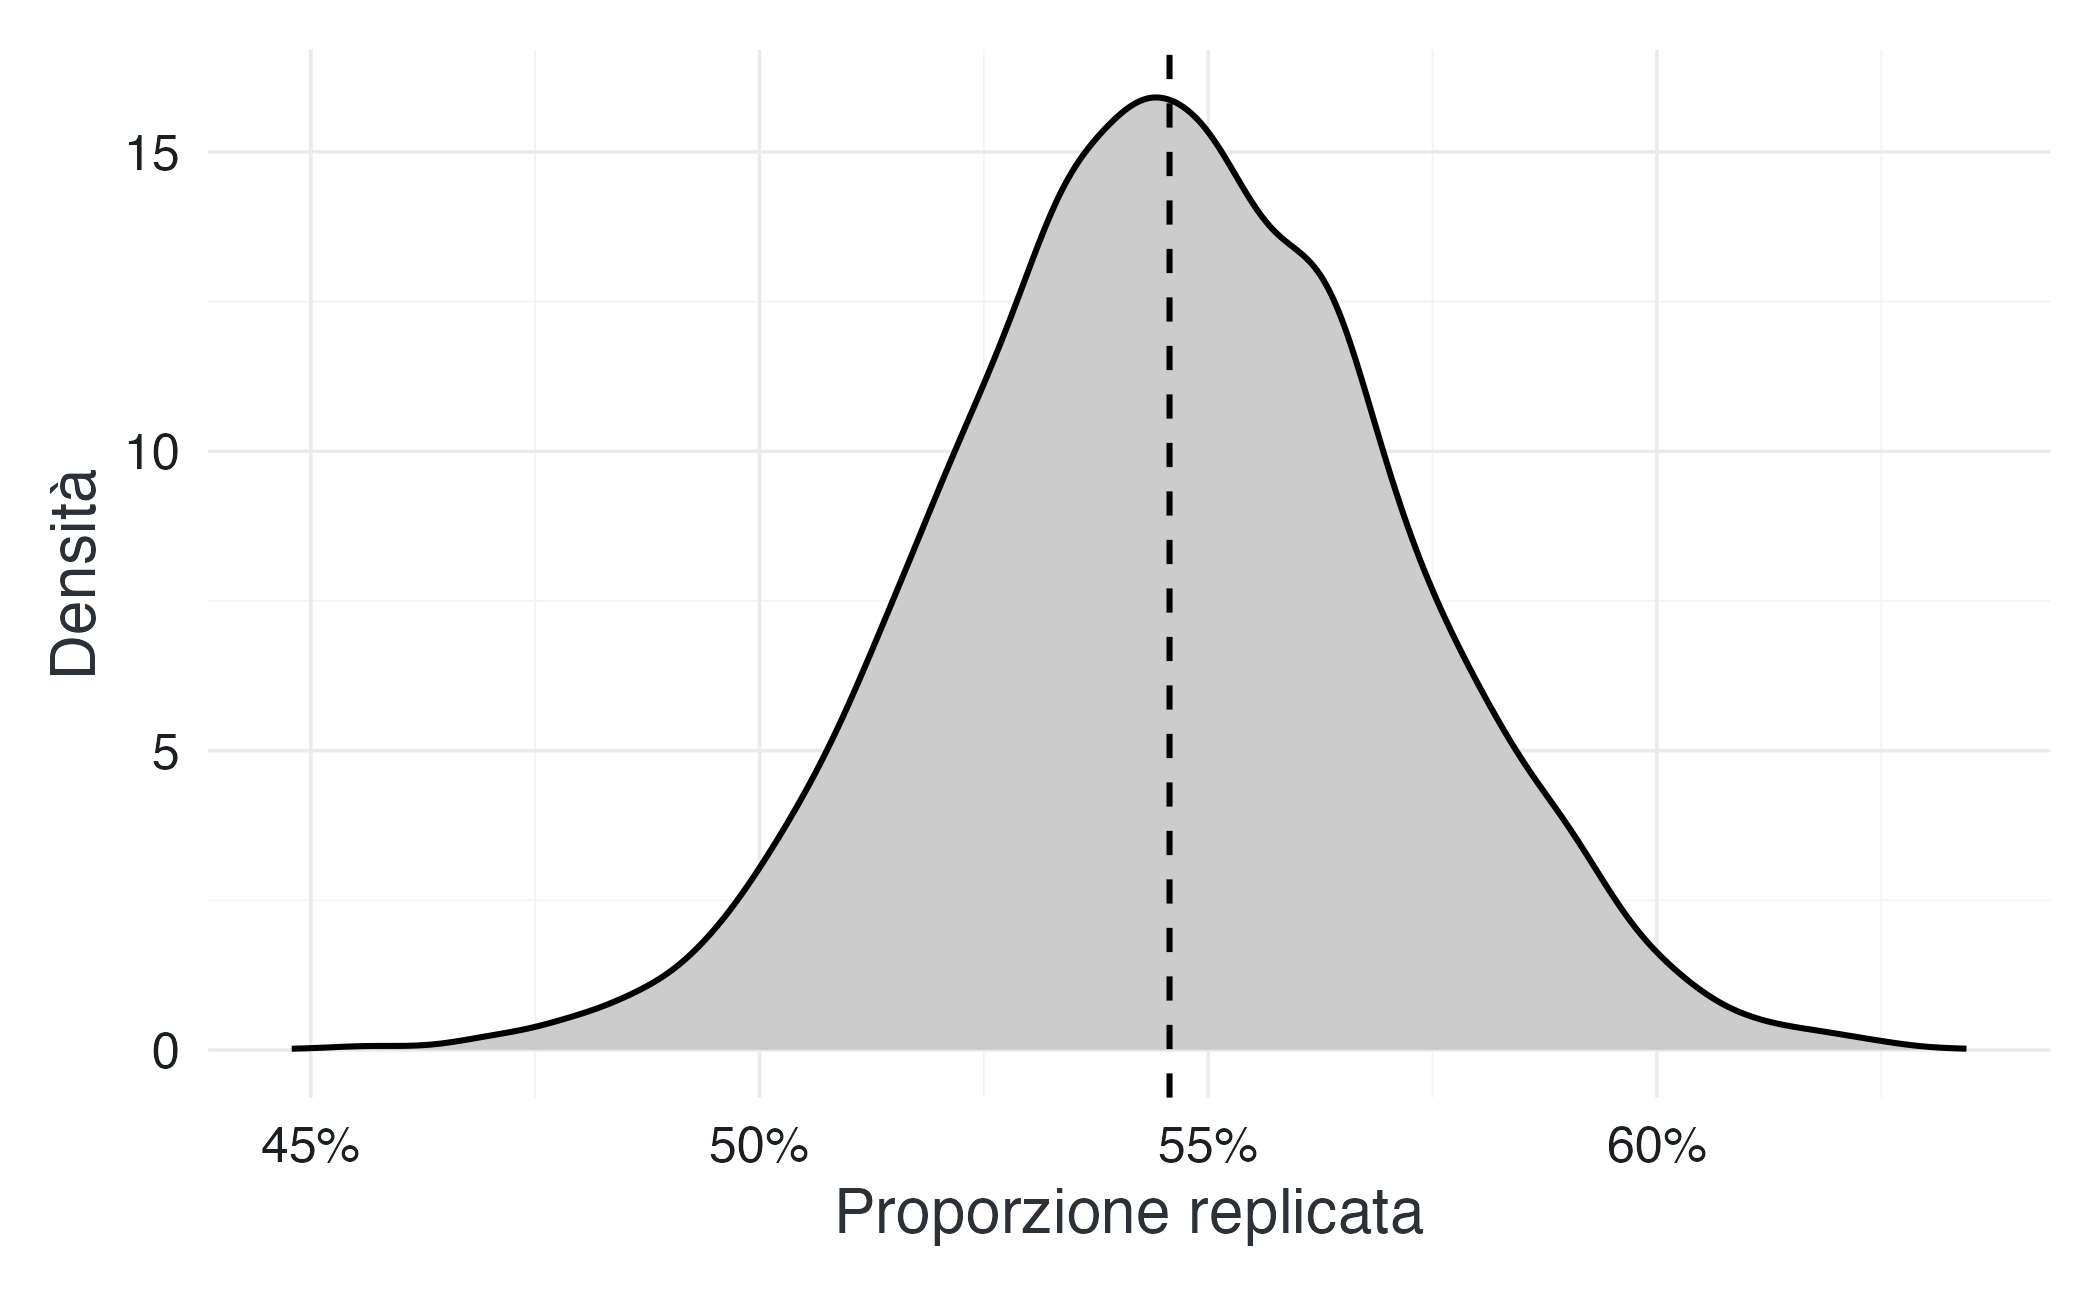
\includegraphics[width=0.85\linewidth,height=\textheight,keepaspectratio]{chapters/glm/02_proporzioni_files/figure-pdf/unnamed-chunk-9-1.png}
\end{center}

La linea tratteggiata rappresenta la proporzione osservata. Con una sola
statistica aggregata il controllo ha inevitabilmente una capacità
diagnostica limitata: il modello binomiale riproduce il numero
complessivo di successi, ma non può rivelare eterogeneità tra persone,
dipendenze tra risposte o differenze tra sottogruppi non rappresentati
nei dati.

\subsection{Il collegamento con il modello
Beta--Binomiale}\label{il-collegamento-con-il-modello-betabinomiale}

Se assegniamo direttamente

\[
p\sim\operatorname{Beta}(a,b),
\]

la coniugazione produce la soluzione analitica

\[
p\mid y,n
\sim
\operatorname{Beta}(a+y,b+n-y).
\]

Questa formulazione è utile per comprendere l'aggiornamento e per
risolvere rapidamente problemi semplici. In questa parte del Companion
utilizziamo però la parametrizzazione logit, perché consente di passare
senza cambiamenti concettuali dalla singola proporzione alla regressione
con predittori. Le due formulazioni non assegnano necessariamente lo
stesso prior a \(p\): un prior normale sul logit e un prior Beta sulla
probabilità devono essere confrontati attraverso le distribuzioni che
inducono sulla scala osservabile.

\section{Due proporzioni come regressione
logistica}\label{sec-linear-models-two-proportions}

Passiamo ora al confronto tra \emph{pledgers} e \emph{non-pledgers}.
Indichiamo con \(G_i=0\) il gruppo di riferimento e con \(G_i=1\) il
gruppo dei \emph{pledgers}. Il modello è

\[
Y_g\sim\operatorname{Binomial}(n_g,p_g),
\]

\[
\operatorname{logit}(p_g)=\alpha+\beta G_g.
\]

Da questa parametrizzazione otteniamo

\[
p_0=\operatorname{logit}^{-1}(\alpha),
\qquad
p_1=\operatorname{logit}^{-1}(\alpha+\beta).
\]

L'esponenziale di \(\beta\) è l'odds ratio tra i gruppi. Tuttavia,
l'odds ratio non esaurisce l'interpretazione. Dalle probabilità
posteriori possiamo ricavare anche la differenza assoluta

\[
\operatorname{RD}=p_1-p_0,
\]

il risk ratio

\[
\operatorname{RR}=\frac{p_1}{p_0},
\]

e l'odds ratio

\[
\operatorname{OR}
=
\frac{p_1/(1-p_1)}{p_0/(1-p_0)}.
\]

Queste quantità rispondono a domande diverse. La differenza di rischio
comunica lo scarto assoluto in punti percentuali; il risk ratio
confronta direttamente le probabilità; l'odds ratio confronta gli odds.
In molti contesti applicativi la differenza assoluta è la misura più
immediata, mentre l'odds ratio è la quantità direttamente associata al
coefficiente logistico.

\subsection{Preparare i dati}\label{preparare-i-dati}

\begin{Shaded}
\begin{Highlighting}[]
\NormalTok{condom\_data }\OtherTok{\textless{}{-}} \FunctionTok{tibble}\NormalTok{(}
  \AttributeTok{group =} \FunctionTok{factor}\NormalTok{(}
    \FunctionTok{c}\NormalTok{(}\StringTok{"Non{-}pledgers"}\NormalTok{, }\StringTok{"Pledgers"}\NormalTok{),}
    \AttributeTok{levels =} \FunctionTok{c}\NormalTok{(}\StringTok{"Non{-}pledgers"}\NormalTok{, }\StringTok{"Pledgers"}\NormalTok{)}
\NormalTok{  ),}
  \AttributeTok{successes =} \FunctionTok{c}\NormalTok{(}\DecValTok{5416}\NormalTok{, }\DecValTok{424}\NormalTok{),}
  \AttributeTok{trials =} \FunctionTok{c}\NormalTok{(}\DecValTok{9072}\NormalTok{, }\DecValTok{777}\NormalTok{)}
\NormalTok{) }\SpecialCharTok{|\textgreater{}}
  \FunctionTok{mutate}\NormalTok{(}\AttributeTok{observed\_proportion =}\NormalTok{ successes }\SpecialCharTok{/}\NormalTok{ trials)}

\NormalTok{condom\_data}
\CommentTok{\#\textgreater{} \# A tibble: 2 x 4}
\CommentTok{\#\textgreater{}   group        successes trials observed\_proportion}
\CommentTok{\#\textgreater{}   \textless{}fct\textgreater{}            \textless{}dbl\textgreater{}  \textless{}dbl\textgreater{}               \textless{}dbl\textgreater{}}
\CommentTok{\#\textgreater{} 1 Non{-}pledgers      5416   9072               0.597}
\CommentTok{\#\textgreater{} 2 Pledgers           424    777               0.546}
\end{Highlighting}
\end{Shaded}

Le proporzioni osservate costituiscono una descrizione del campione. Il
modello quantifica l'incertezza sulle probabilità e sui loro contrasti.

\subsection{Prior e controllo predittivo a
priori}\label{prior-e-controllo-predittivo-a-priori}

Usiamo un prior moderatamente ampio sull'intercetta e un prior
regolarizzante sulla differenza di log-odds:

\[
\alpha\sim\operatorname{Normal}(0,1.5),
\qquad
\beta\sim\operatorname{Normal}(0,1).
\]

Per comprenderne le implicazioni simuliamo le probabilità dei due
gruppi:

\begin{Shaded}
\begin{Highlighting}[]
\NormalTok{prior\_two }\OtherTok{\textless{}{-}} \FunctionTok{tibble}\NormalTok{(}
  \AttributeTok{alpha =} \FunctionTok{rnorm}\NormalTok{(}\DecValTok{5000}\NormalTok{, }\DecValTok{0}\NormalTok{, }\FloatTok{1.5}\NormalTok{),}
  \AttributeTok{beta =} \FunctionTok{rnorm}\NormalTok{(}\DecValTok{5000}\NormalTok{, }\DecValTok{0}\NormalTok{, }\DecValTok{1}\NormalTok{),}
  \AttributeTok{p\_non\_pledge =} \FunctionTok{plogis}\NormalTok{(alpha),}
  \AttributeTok{p\_pledge =} \FunctionTok{plogis}\NormalTok{(alpha }\SpecialCharTok{+}\NormalTok{ beta),}
  \AttributeTok{risk\_difference =}\NormalTok{ p\_pledge }\SpecialCharTok{{-}}\NormalTok{ p\_non\_pledge}
\NormalTok{)}

\NormalTok{prior\_two }\SpecialCharTok{|\textgreater{}}
  \FunctionTok{select}\NormalTok{(p\_non\_pledge, p\_pledge) }\SpecialCharTok{|\textgreater{}}
  \FunctionTok{pivot\_longer}\NormalTok{(}
    \FunctionTok{everything}\NormalTok{(),}
    \AttributeTok{names\_to =} \StringTok{"group"}\NormalTok{,}
    \AttributeTok{values\_to =} \StringTok{"probability"}
\NormalTok{  ) }\SpecialCharTok{|\textgreater{}}
  \FunctionTok{ggplot}\NormalTok{(}\FunctionTok{aes}\NormalTok{(probability, }\AttributeTok{fill =}\NormalTok{ group)) }\SpecialCharTok{+}
  \FunctionTok{geom\_density}\NormalTok{(}\AttributeTok{alpha =} \FloatTok{0.45}\NormalTok{) }\SpecialCharTok{+}
  \FunctionTok{scale\_x\_continuous}\NormalTok{(}\AttributeTok{labels =} \FunctionTok{label\_percent}\NormalTok{()) }\SpecialCharTok{+}
  \FunctionTok{labs}\NormalTok{(}
    \AttributeTok{x =} \StringTok{"Probabilità a priori"}\NormalTok{,}
    \AttributeTok{y =} \StringTok{"Densità"}\NormalTok{,}
    \AttributeTok{fill =} \ConstantTok{NULL}
\NormalTok{  )}
\end{Highlighting}
\end{Shaded}

\begin{center}
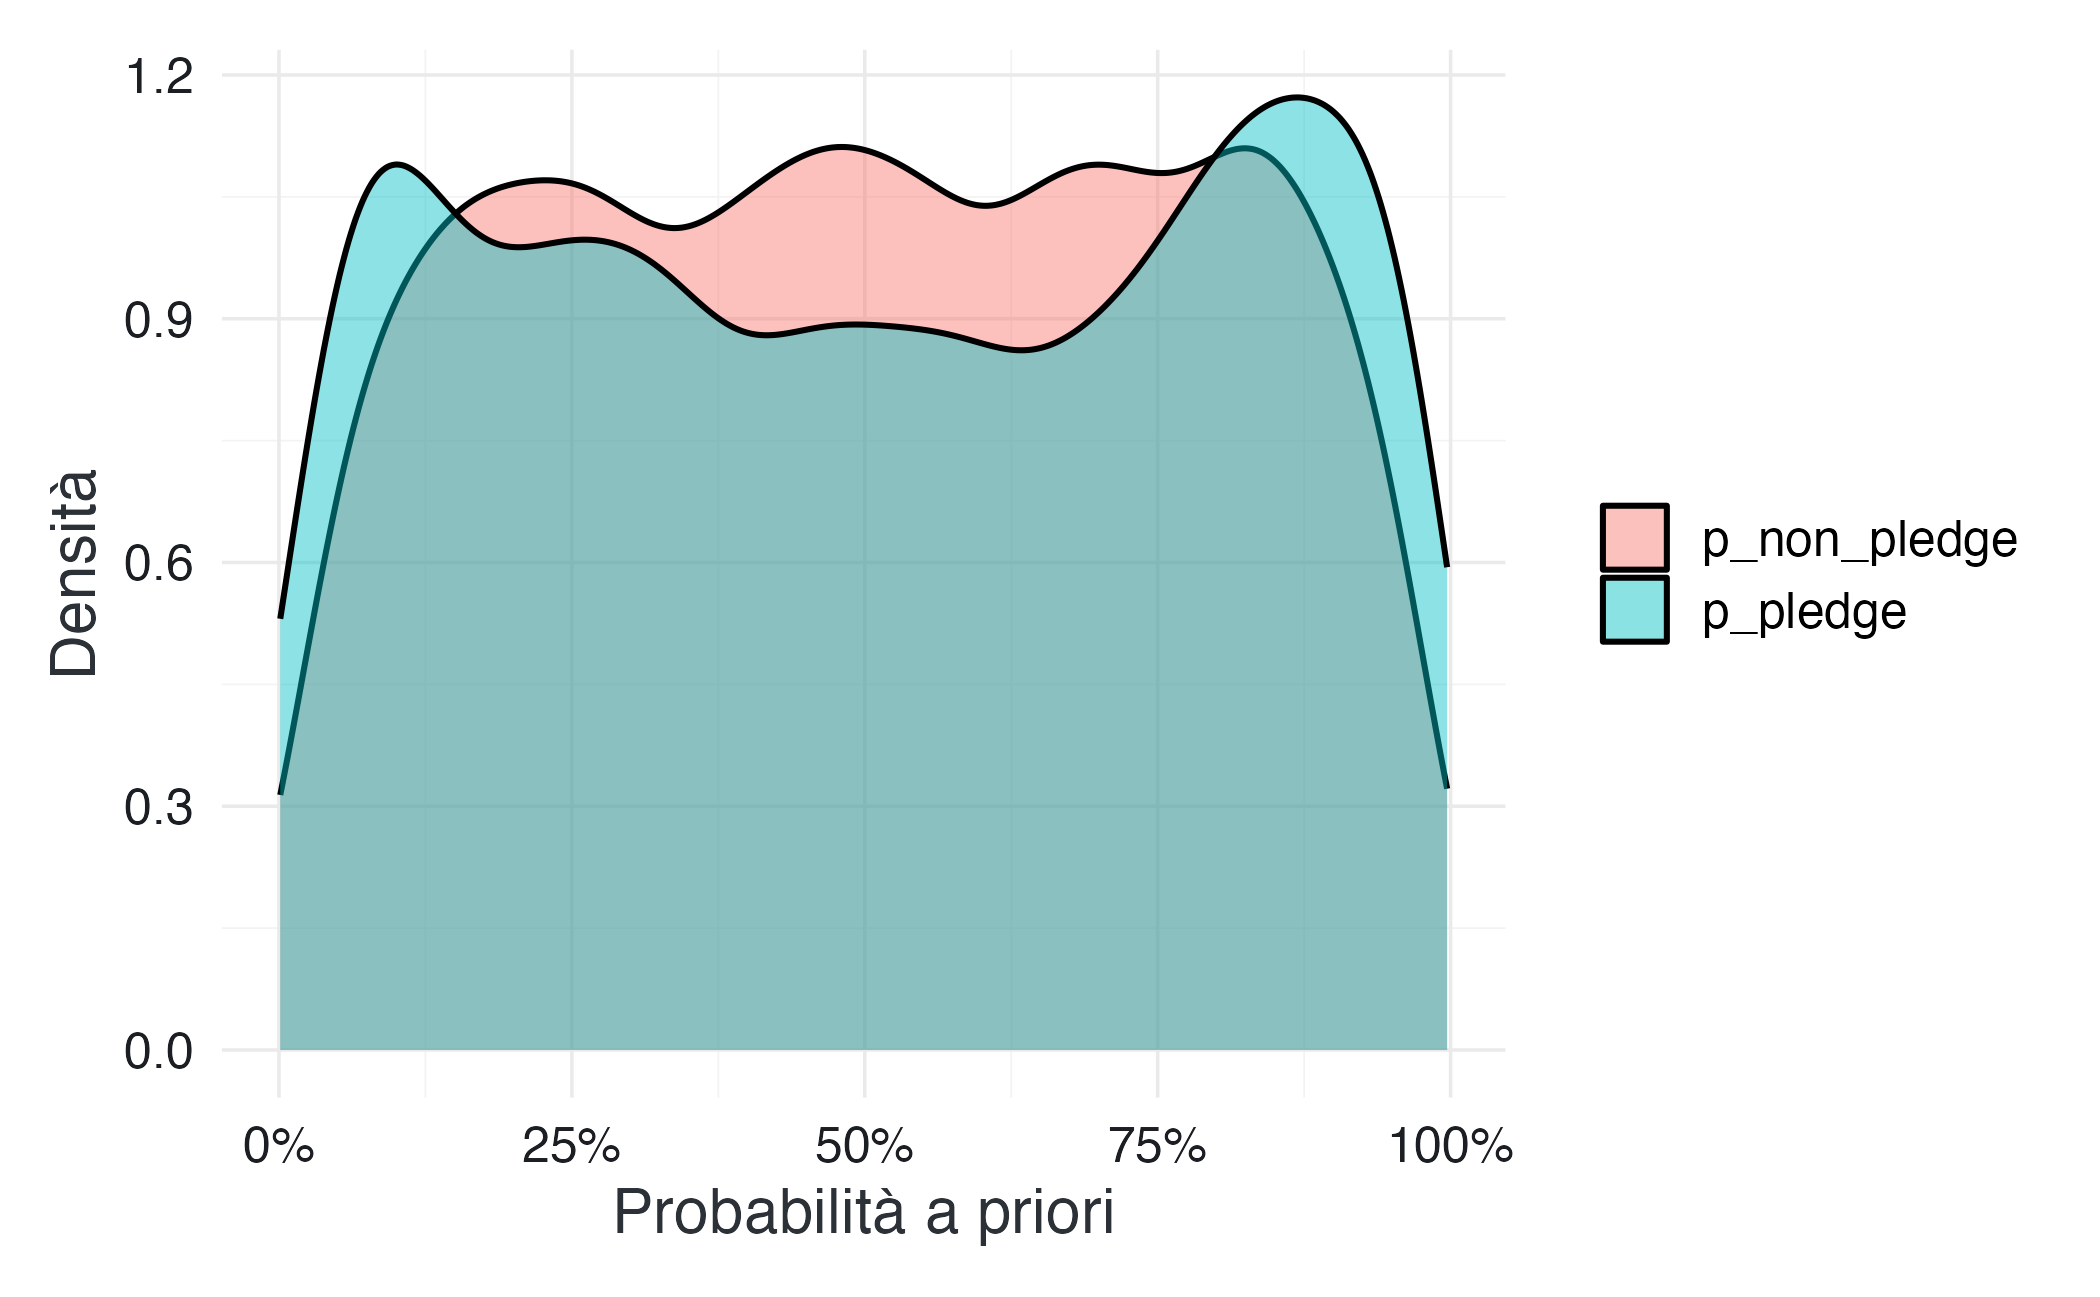
\includegraphics[width=0.85\linewidth,height=\textheight,keepaspectratio]{chapters/glm/02_proporzioni_files/figure-pdf/unnamed-chunk-11-1.png}
\end{center}

Il controllo mostra quali probabilità e quali differenze il modello
considera plausibili prima dei dati. Se la conoscenza disponibile
escludesse differenze molto grandi, il prior su \(\beta\) dovrebbe
essere più concentrato.

\subsection{Stima del modello}\label{stima-del-modello}

\begin{Shaded}
\begin{Highlighting}[]
\NormalTok{two\_priors }\OtherTok{\textless{}{-}} \FunctionTok{c}\NormalTok{(}
  \FunctionTok{prior}\NormalTok{(}\FunctionTok{normal}\NormalTok{(}\DecValTok{0}\NormalTok{, }\FloatTok{1.5}\NormalTok{), }\AttributeTok{class =}\NormalTok{ Intercept),}
  \FunctionTok{prior}\NormalTok{(}\FunctionTok{normal}\NormalTok{(}\DecValTok{0}\NormalTok{, }\DecValTok{1}\NormalTok{), }\AttributeTok{class =}\NormalTok{ b)}
\NormalTok{)}

\NormalTok{fit\_two\_proportions }\OtherTok{\textless{}{-}} \FunctionTok{brm}\NormalTok{(}
\NormalTok{  successes }\SpecialCharTok{|} \FunctionTok{trials}\NormalTok{(trials) }\SpecialCharTok{\textasciitilde{}}\NormalTok{ group,}
  \AttributeTok{data =}\NormalTok{ condom\_data,}
  \AttributeTok{family =} \FunctionTok{binomial}\NormalTok{(}\AttributeTok{link =} \StringTok{"logit"}\NormalTok{),}
  \AttributeTok{prior =}\NormalTok{ two\_priors,}
  \AttributeTok{chains =} \DecValTok{4}\NormalTok{,}
  \AttributeTok{iter =} \DecValTok{3000}\NormalTok{,}
  \AttributeTok{warmup =} \DecValTok{1000}\NormalTok{,}
  \AttributeTok{seed =} \DecValTok{2026}\NormalTok{,}
  \AttributeTok{refresh =} \DecValTok{0}
\NormalTok{)}
\CommentTok{\#\textgreater{} Running MCMC with 4 chains, at most 10 in parallel...}
\CommentTok{\#\textgreater{} }
\CommentTok{\#\textgreater{} Chain 1 finished in 0.0 seconds.}
\CommentTok{\#\textgreater{} Chain 2 finished in 0.1 seconds.}
\CommentTok{\#\textgreater{} Chain 3 finished in 0.1 seconds.}
\CommentTok{\#\textgreater{} Chain 4 finished in 0.0 seconds.}
\CommentTok{\#\textgreater{} }
\CommentTok{\#\textgreater{} All 4 chains finished successfully.}
\CommentTok{\#\textgreater{} Mean chain execution time: 0.0 seconds.}
\CommentTok{\#\textgreater{} Total execution time: 0.2 seconds.}
\end{Highlighting}
\end{Shaded}

La sintesi del modello riporta l'intercetta e il contrasto tra gruppi
sulla scala dei log-odds:

\begin{Shaded}
\begin{Highlighting}[]
\FunctionTok{summary}\NormalTok{(fit\_two\_proportions)}
\CommentTok{\#\textgreater{}  Family: binomial }
\CommentTok{\#\textgreater{}   Links: mu = logit }
\CommentTok{\#\textgreater{} Formula: successes | trials(trials) \textasciitilde{} group }
\CommentTok{\#\textgreater{}    Data: condom\_data (Number of observations: 2) }
\CommentTok{\#\textgreater{}   Draws: 4 chains, each with iter = 3000; warmup = 1000; thin = 1;}
\CommentTok{\#\textgreater{}          total post{-}warmup draws = 8000}
\CommentTok{\#\textgreater{} }
\CommentTok{\#\textgreater{} Regression Coefficients:}
\CommentTok{\#\textgreater{}               Estimate Est.Error l{-}95\% CI u{-}95\% CI Rhat Bulk\_ESS Tail\_ESS}
\CommentTok{\#\textgreater{} Intercept         0.39      0.02     0.35     0.44 1.00     9979     6344}
\CommentTok{\#\textgreater{} groupPledgers    {-}0.21      0.07    {-}0.35    {-}0.06 1.00     2436     2362}
\CommentTok{\#\textgreater{} }
\CommentTok{\#\textgreater{} Draws were sampled using sample(hmc). For each parameter, Bulk\_ESS}
\CommentTok{\#\textgreater{} and Tail\_ESS are effective sample size measures, and Rhat is the potential}
\CommentTok{\#\textgreater{} scale reduction factor on split chains (at convergence, Rhat = 1).}
\end{Highlighting}
\end{Shaded}

La diagnostica del campionamento deve precedere l'interpretazione:

\begin{Shaded}
\begin{Highlighting}[]
\FunctionTok{plot}\NormalTok{(fit\_two\_proportions)}
\end{Highlighting}
\end{Shaded}

\begin{center}
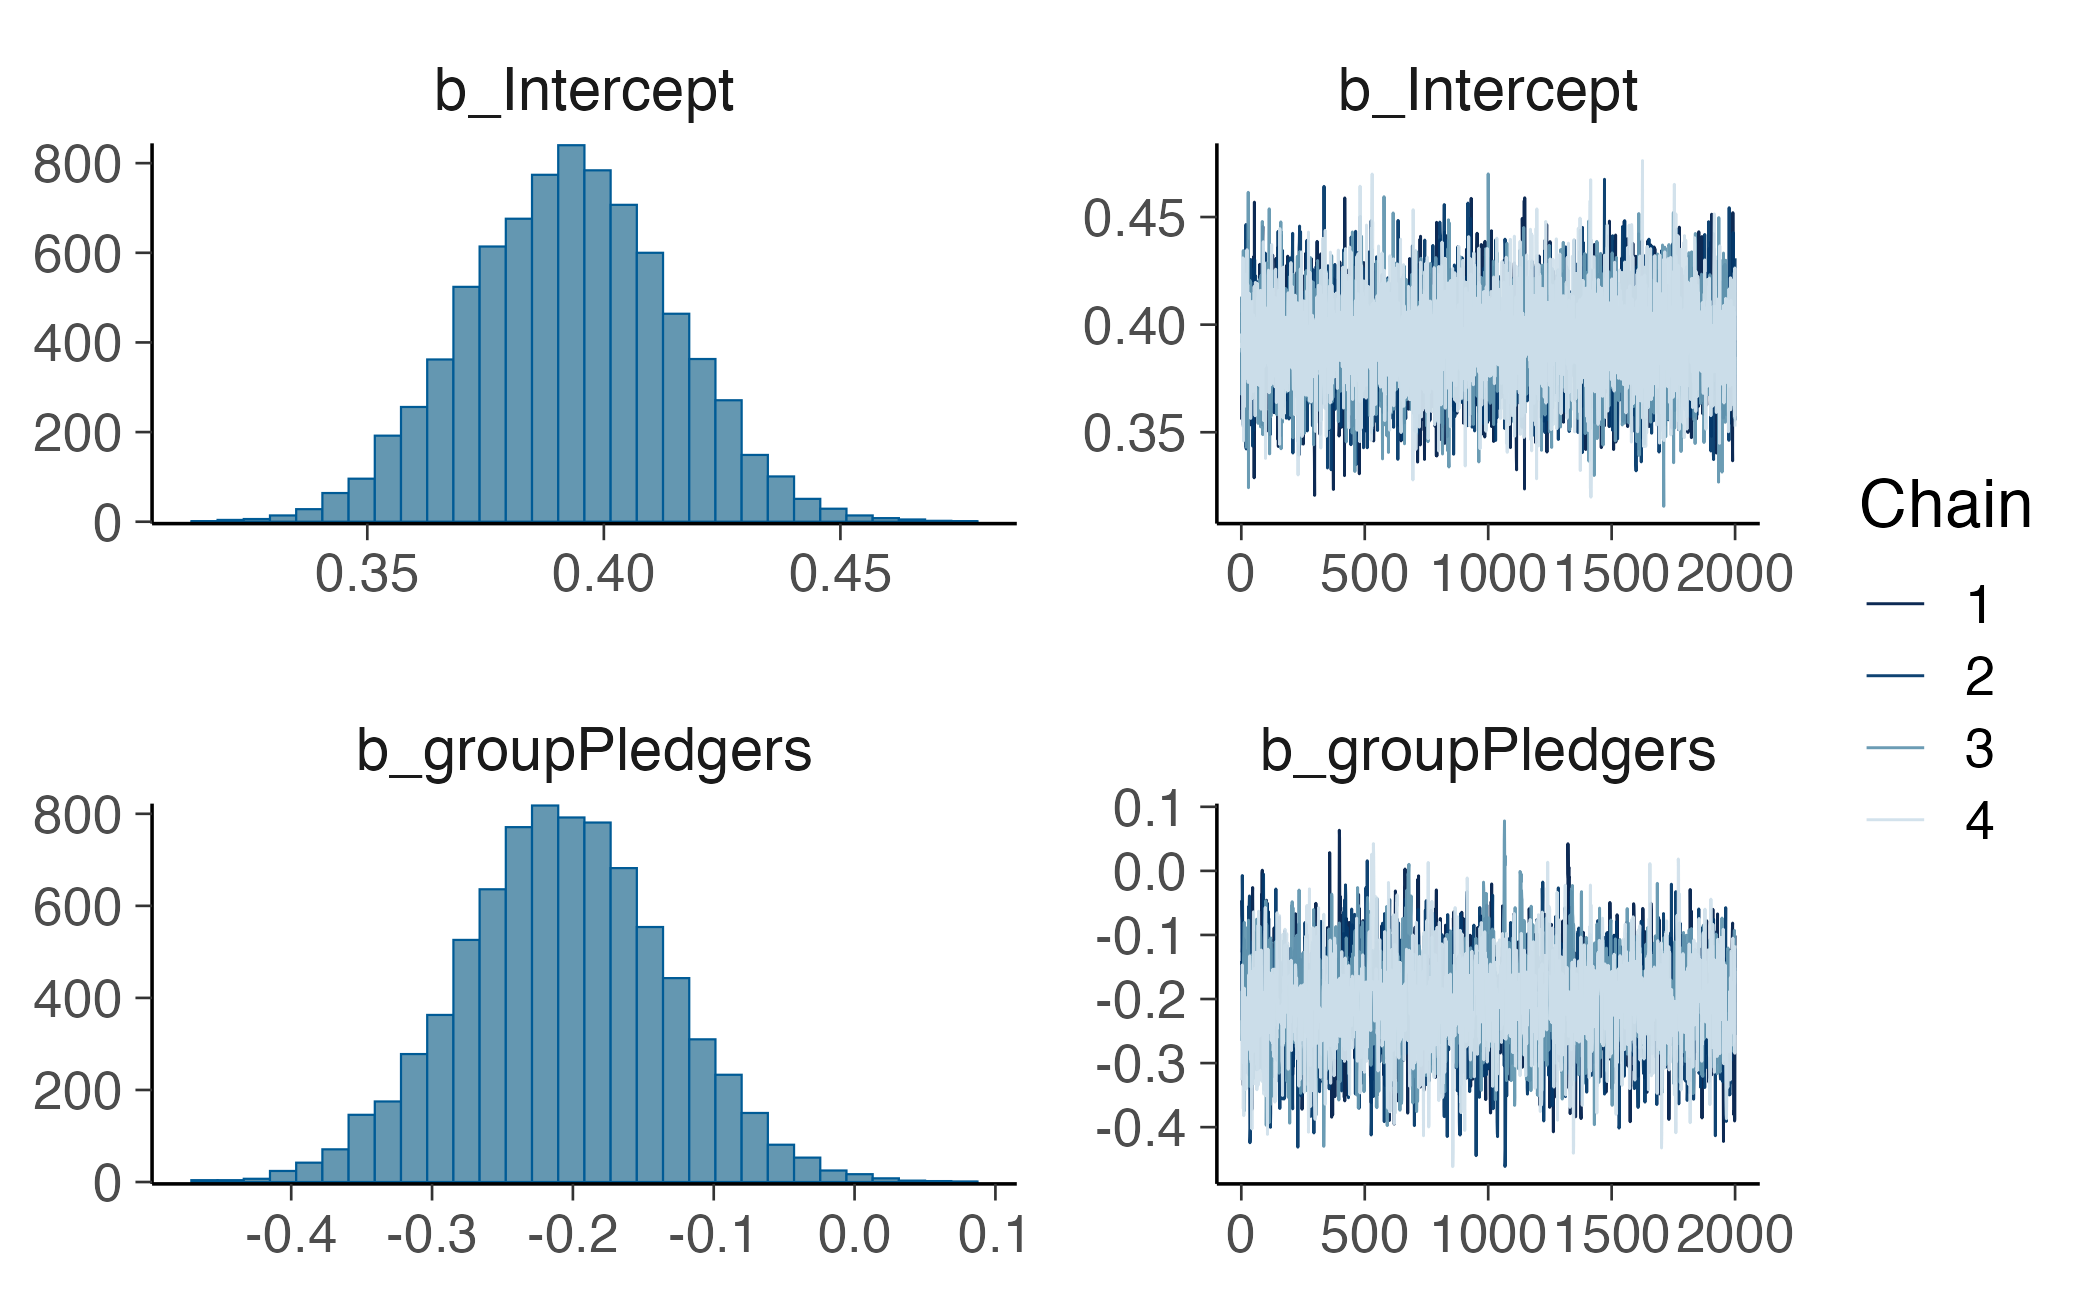
\includegraphics[width=0.85\linewidth,height=\textheight,keepaspectratio]{chapters/glm/02_proporzioni_files/figure-pdf/unnamed-chunk-14-1.png}
\end{center}

Con due conteggi aggregati il modello è semplice; ciò non elimina la
necessità di verificare \(\widehat R\), dimensioni campionarie effettive
e possibili problemi del campionatore.

\subsection{Probabilità e contrasti
posteriori}\label{probabilituxe0-e-contrasti-posteriori}

Costruiamo una griglia con i due livelli del gruppo e trasformiamo il
predittore lineare sulla scala della probabilità:

\begin{Shaded}
\begin{Highlighting}[]
\NormalTok{group\_grid }\OtherTok{\textless{}{-}} \FunctionTok{tibble}\NormalTok{(}
  \AttributeTok{group =} \FunctionTok{factor}\NormalTok{(}
    \FunctionTok{c}\NormalTok{(}\StringTok{"Non{-}pledgers"}\NormalTok{, }\StringTok{"Pledgers"}\NormalTok{),}
    \AttributeTok{levels =} \FunctionTok{levels}\NormalTok{(condom\_data}\SpecialCharTok{$}\NormalTok{group)}
\NormalTok{  ),}
  \AttributeTok{trials =}\NormalTok{ condom\_data}\SpecialCharTok{$}\NormalTok{trials   }\CommentTok{\# Assumendo che l\textquotesingle{}ordine sia Non{-}pledgers, Pledgers}
\NormalTok{)}

\NormalTok{p\_draws }\OtherTok{\textless{}{-}} \FunctionTok{posterior\_linpred}\NormalTok{(}
\NormalTok{  fit\_two\_proportions,}
  \AttributeTok{newdata =}\NormalTok{ group\_grid,}
  \AttributeTok{transform =} \ConstantTok{TRUE}
\NormalTok{)}

\NormalTok{two\_draws }\OtherTok{\textless{}{-}} \FunctionTok{tibble}\NormalTok{(}
  \AttributeTok{p\_non\_pledge =}\NormalTok{ p\_draws[, }\DecValTok{1}\NormalTok{],}
  \AttributeTok{p\_pledge =}\NormalTok{ p\_draws[, }\DecValTok{2}\NormalTok{]}
\NormalTok{) }\SpecialCharTok{|\textgreater{}}
  \FunctionTok{mutate}\NormalTok{(}
    \AttributeTok{risk\_difference =}\NormalTok{ p\_pledge }\SpecialCharTok{{-}}\NormalTok{ p\_non\_pledge,}
    \AttributeTok{risk\_ratio =}\NormalTok{ p\_pledge }\SpecialCharTok{/}\NormalTok{ p\_non\_pledge,}
    \AttributeTok{odds\_ratio =}
\NormalTok{      (p\_pledge }\SpecialCharTok{/}\NormalTok{ (}\DecValTok{1} \SpecialCharTok{{-}}\NormalTok{ p\_pledge)) }\SpecialCharTok{/}
\NormalTok{      (p\_non\_pledge }\SpecialCharTok{/}\NormalTok{ (}\DecValTok{1} \SpecialCharTok{{-}}\NormalTok{ p\_non\_pledge))}
\NormalTok{  )}
\end{Highlighting}
\end{Shaded}

Riassumiamo le probabilità e i contrasti:

\begin{Shaded}
\begin{Highlighting}[]
\NormalTok{two\_summary }\OtherTok{\textless{}{-}}\NormalTok{ two\_draws }\SpecialCharTok{|\textgreater{}}
  \FunctionTok{summarise}\NormalTok{(}
    \FunctionTok{across}\NormalTok{(}
      \FunctionTok{everything}\NormalTok{(),}
      \FunctionTok{list}\NormalTok{(}
        \AttributeTok{median =}\NormalTok{ median,}
        \AttributeTok{lower =} \SpecialCharTok{\textasciitilde{}} \FunctionTok{quantile}\NormalTok{(.x, }\FloatTok{0.025}\NormalTok{),}
        \AttributeTok{upper =} \SpecialCharTok{\textasciitilde{}} \FunctionTok{quantile}\NormalTok{(.x, }\FloatTok{0.975}\NormalTok{)}
\NormalTok{      )}
\NormalTok{    )}
\NormalTok{  )}

\NormalTok{two\_summary}
\CommentTok{\#\textgreater{} \# A tibble: 1 x 15}
\CommentTok{\#\textgreater{}   p\_non\_pledge\_median p\_non\_pledge\_lower p\_non\_pledge\_upper p\_pledge\_median}
\CommentTok{\#\textgreater{}                 \textless{}dbl\textgreater{}              \textless{}dbl\textgreater{}              \textless{}dbl\textgreater{}           \textless{}dbl\textgreater{}}
\CommentTok{\#\textgreater{} 1               0.597              0.587              0.607           0.546}
\CommentTok{\#\textgreater{}   p\_pledge\_lower p\_pledge\_upper risk\_difference\_median risk\_difference\_lower}
\CommentTok{\#\textgreater{}            \textless{}dbl\textgreater{}          \textless{}dbl\textgreater{}                  \textless{}dbl\textgreater{}                 \textless{}dbl\textgreater{}}
\CommentTok{\#\textgreater{} 1          0.512          0.581                {-}0.0507               {-}0.0865}
\CommentTok{\#\textgreater{}   risk\_difference\_upper risk\_ratio\_median risk\_ratio\_lower risk\_ratio\_upper}
\CommentTok{\#\textgreater{}                   \textless{}dbl\textgreater{}             \textless{}dbl\textgreater{}            \textless{}dbl\textgreater{}            \textless{}dbl\textgreater{}}
\CommentTok{\#\textgreater{} 1               {-}0.0154             0.915            0.855            0.974}
\CommentTok{\#\textgreater{}   odds\_ratio\_median odds\_ratio\_lower odds\_ratio\_upper}
\CommentTok{\#\textgreater{}               \textless{}dbl\textgreater{}            \textless{}dbl\textgreater{}            \textless{}dbl\textgreater{}}
\CommentTok{\#\textgreater{} 1             0.813            0.703            0.938}
\end{Highlighting}
\end{Shaded}

L'odds ratio può essere ricavato anche come \(\exp(\beta)\). Calcolarlo
dalle probabilità draw per draw rende però evidente che tutte le
quantità derivano dalla stessa distribuzione posteriore congiunta.

\subsection{Direzione, rilevanza pratica ed
equivalenza}\label{direzione-rilevanza-pratica-ed-equivalenza}

La posterior consente di separare tre domande. La prima riguarda la
direzione del contrasto; la seconda chiede se la differenza superi una
soglia sostantiva; la terza valuta se le due probabilità siano
abbastanza vicine da essere considerate praticamente equivalenti.

Supponiamo, a scopo illustrativo, che una differenza assoluta di tre
punti percentuali sia considerata la minima differenza sostantivamente
rilevante. Questa soglia non deve essere scelta perché produce una
conclusione conveniente: dovrebbe riflettere conoscenze e conseguenze
proprie del dominio.

\begin{Shaded}
\begin{Highlighting}[]
\NormalTok{sesoi }\OtherTok{\textless{}{-}} \FloatTok{0.03}

\NormalTok{two\_draws }\SpecialCharTok{|\textgreater{}}
  \FunctionTok{summarise}\NormalTok{(}
    \AttributeTok{Pr\_pledge\_lower =} \FunctionTok{mean}\NormalTok{(risk\_difference }\SpecialCharTok{\textless{}} \DecValTok{0}\NormalTok{),}
    \AttributeTok{Pr\_difference\_below\_minus\_SESOI =} \FunctionTok{mean}\NormalTok{(risk\_difference }\SpecialCharTok{\textless{}} \SpecialCharTok{{-}}\NormalTok{sesoi),}
    \AttributeTok{Pr\_practical\_equivalence =} \FunctionTok{mean}\NormalTok{(}\FunctionTok{abs}\NormalTok{(risk\_difference) }\SpecialCharTok{\textless{}}\NormalTok{ sesoi)}
\NormalTok{  )}
\CommentTok{\#\textgreater{} \# A tibble: 1 x 3}
\CommentTok{\#\textgreater{}   Pr\_pledge\_lower Pr\_difference\_below\_minus\_SESOI Pr\_practical\_equivalence}
\CommentTok{\#\textgreater{}             \textless{}dbl\textgreater{}                           \textless{}dbl\textgreater{}                    \textless{}dbl\textgreater{}}
\CommentTok{\#\textgreater{} 1           0.997                           0.875                    0.125}
\end{Highlighting}
\end{Shaded}

SESOI e ROPE sono due modi collegati di formalizzare la stessa idea
sostantiva. La SESOI esprime la minima differenza considerata
importante; la ROPE è l'intervallo di differenze considerate
trascurabili, in questo caso \([-0.03,0.03]\). Non sono due procedure
indipendenti e non sostituiscono la valutazione del contesto.

\subsection{Visualizzare le quantità
principali}\label{visualizzare-le-quantituxe0-principali}

\begin{Shaded}
\begin{Highlighting}[]
\NormalTok{probability\_plot\_data }\OtherTok{\textless{}{-}}\NormalTok{ two\_draws }\SpecialCharTok{|\textgreater{}}
  \FunctionTok{select}\NormalTok{(p\_non\_pledge, p\_pledge) }\SpecialCharTok{|\textgreater{}}
  \FunctionTok{pivot\_longer}\NormalTok{(}
    \FunctionTok{everything}\NormalTok{(),}
    \AttributeTok{names\_to =} \StringTok{"group"}\NormalTok{,}
    \AttributeTok{values\_to =} \StringTok{"probability"}
\NormalTok{  ) }\SpecialCharTok{|\textgreater{}}
  \FunctionTok{mutate}\NormalTok{(}
    \AttributeTok{group =} \FunctionTok{recode}\NormalTok{(}
\NormalTok{      group,}
      \AttributeTok{p\_non\_pledge =} \StringTok{"Non{-}pledgers"}\NormalTok{,}
      \AttributeTok{p\_pledge =} \StringTok{"Pledgers"}
\NormalTok{    )}
\NormalTok{  )}

\FunctionTok{ggplot}\NormalTok{(probability\_plot\_data, }\FunctionTok{aes}\NormalTok{(probability, group)) }\SpecialCharTok{+}
  \FunctionTok{stat\_summary}\NormalTok{(}
    \AttributeTok{fun =}\NormalTok{ median,}
    \AttributeTok{fun.min =} \SpecialCharTok{\textasciitilde{}} \FunctionTok{quantile}\NormalTok{(.x, }\FloatTok{0.025}\NormalTok{),}
    \AttributeTok{fun.max =} \SpecialCharTok{\textasciitilde{}} \FunctionTok{quantile}\NormalTok{(.x, }\FloatTok{0.975}\NormalTok{),}
    \AttributeTok{geom =} \StringTok{"pointrange"}
\NormalTok{  ) }\SpecialCharTok{+}
  \FunctionTok{scale\_x\_continuous}\NormalTok{(}\AttributeTok{labels =} \FunctionTok{label\_percent}\NormalTok{()) }\SpecialCharTok{+}
  \FunctionTok{labs}\NormalTok{(}
    \AttributeTok{x =} \StringTok{"Probabilità posteriore di uso del preservativo"}\NormalTok{,}
    \AttributeTok{y =} \ConstantTok{NULL}
\NormalTok{  )}
\end{Highlighting}
\end{Shaded}

\begin{center}
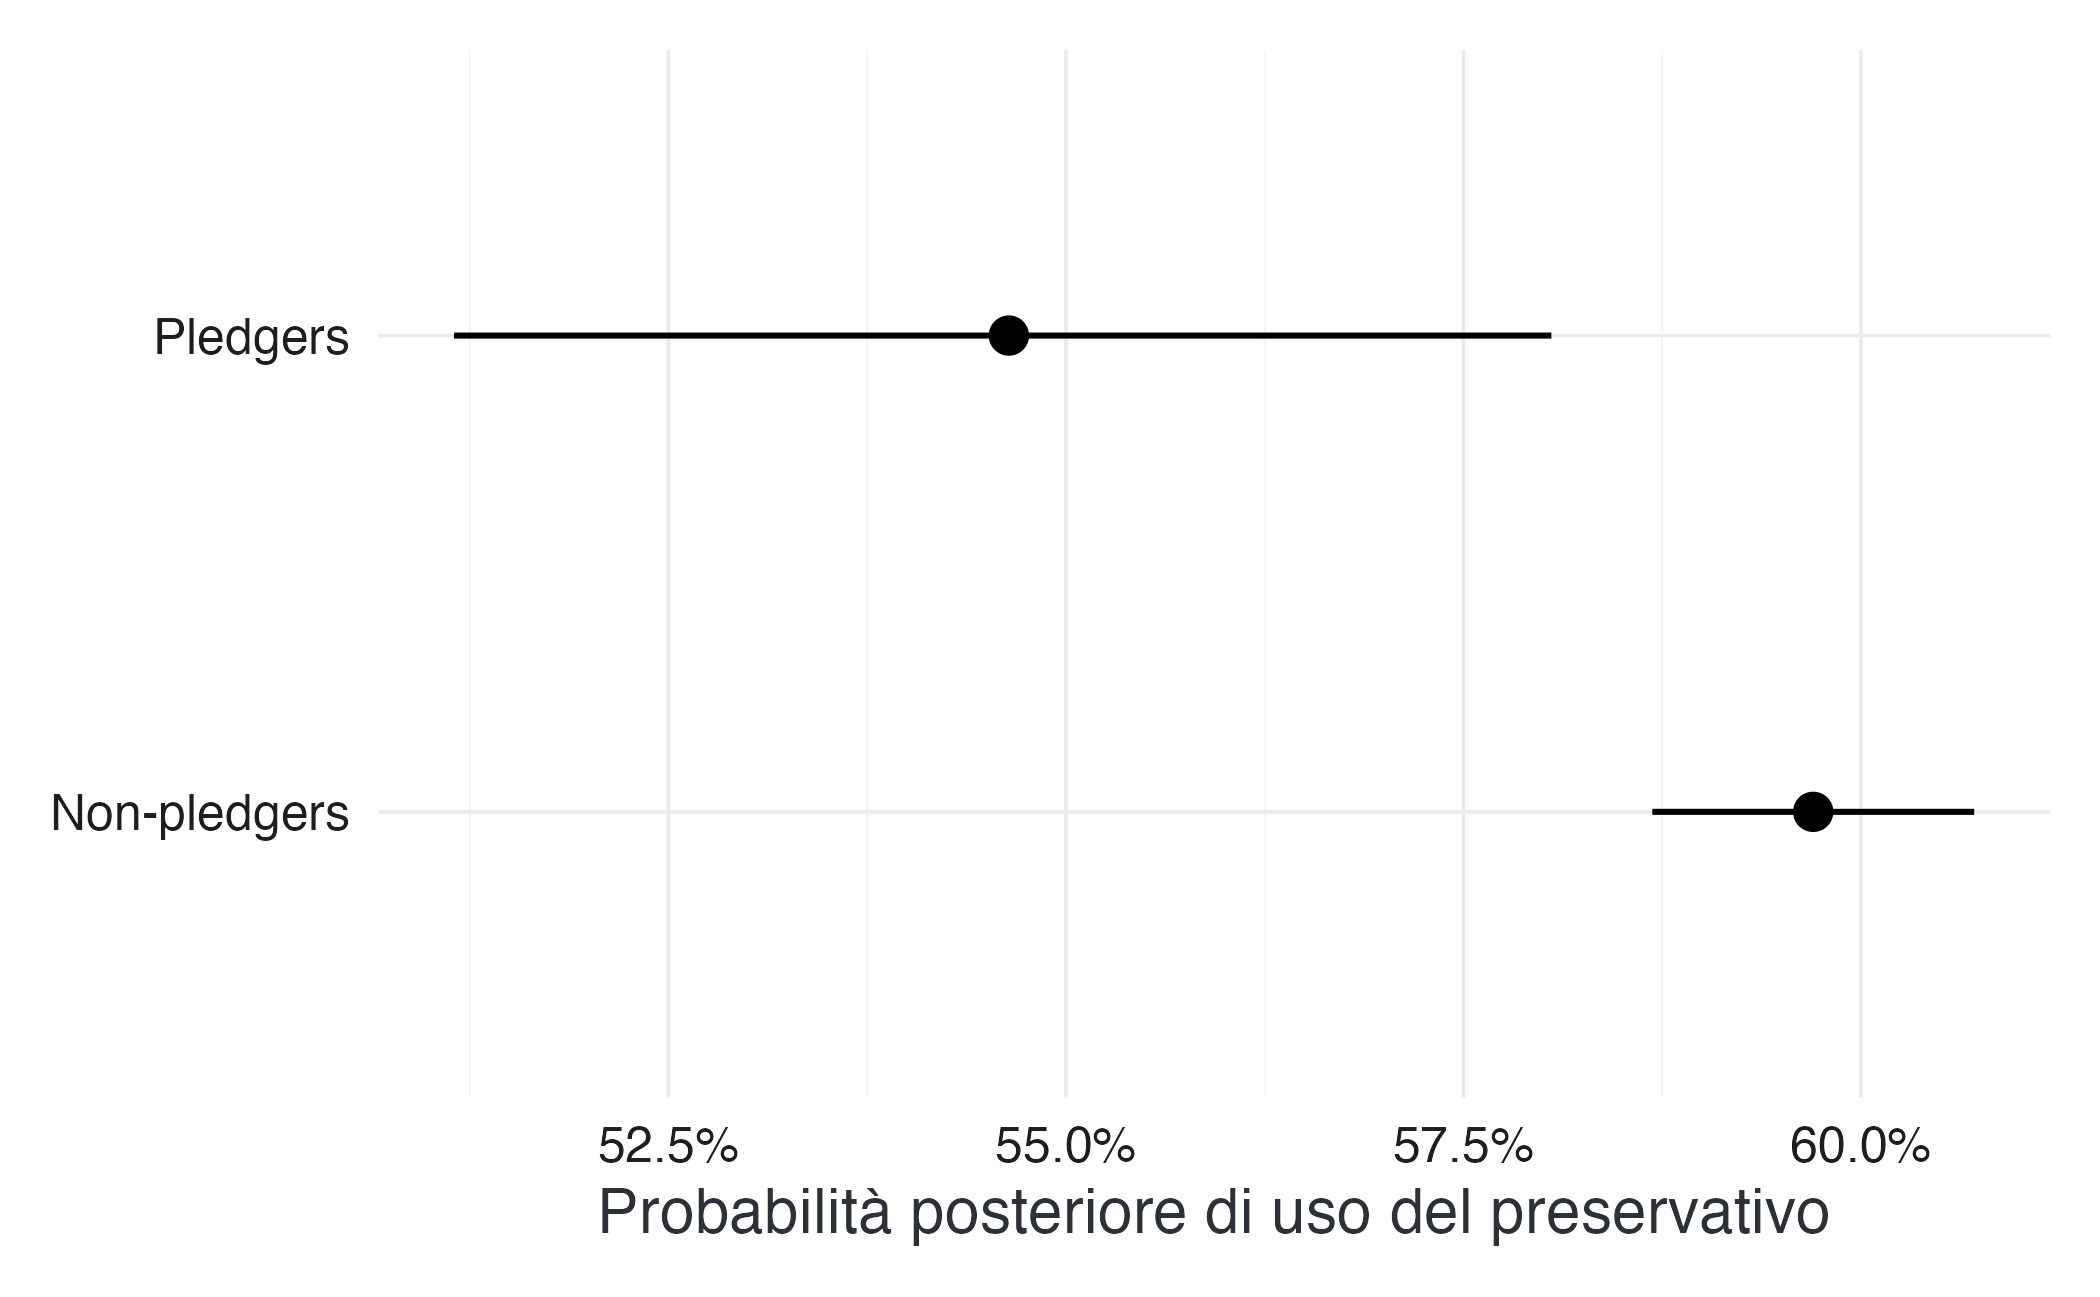
\includegraphics[width=0.85\linewidth,height=\textheight,keepaspectratio]{chapters/glm/02_proporzioni_files/figure-pdf/unnamed-chunk-18-1.png}
\end{center}

La rappresentazione delle probabilità rende immediata la differenza
assoluta. Per esaminare direttamente il contrasto possiamo visualizzare
la posterior della risk difference:

\begin{Shaded}
\begin{Highlighting}[]
\FunctionTok{ggplot}\NormalTok{(two\_draws, }\FunctionTok{aes}\NormalTok{(risk\_difference)) }\SpecialCharTok{+}
  \FunctionTok{geom\_density}\NormalTok{(}\AttributeTok{fill =} \StringTok{"grey80"}\NormalTok{) }\SpecialCharTok{+}
  \FunctionTok{geom\_vline}\NormalTok{(}\AttributeTok{xintercept =} \DecValTok{0}\NormalTok{, }\AttributeTok{linetype =} \StringTok{"dashed"}\NormalTok{) }\SpecialCharTok{+}
  \FunctionTok{annotate}\NormalTok{(}
    \StringTok{"rect"}\NormalTok{,}
    \AttributeTok{xmin =} \SpecialCharTok{{-}}\NormalTok{sesoi,}
    \AttributeTok{xmax =}\NormalTok{ sesoi,}
    \AttributeTok{ymin =} \DecValTok{0}\NormalTok{,}
    \AttributeTok{ymax =} \ConstantTok{Inf}\NormalTok{,}
    \AttributeTok{alpha =} \FloatTok{0.15}
\NormalTok{  ) }\SpecialCharTok{+}
  \FunctionTok{scale\_x\_continuous}\NormalTok{(}\AttributeTok{labels =} \FunctionTok{label\_percent}\NormalTok{()) }\SpecialCharTok{+}
  \FunctionTok{labs}\NormalTok{(}
    \AttributeTok{x =} \StringTok{"Differenza di probabilità: pledgers − non{-}pledgers"}\NormalTok{,}
    \AttributeTok{y =} \StringTok{"Densità"}
\NormalTok{  )}
\end{Highlighting}
\end{Shaded}

\begin{center}
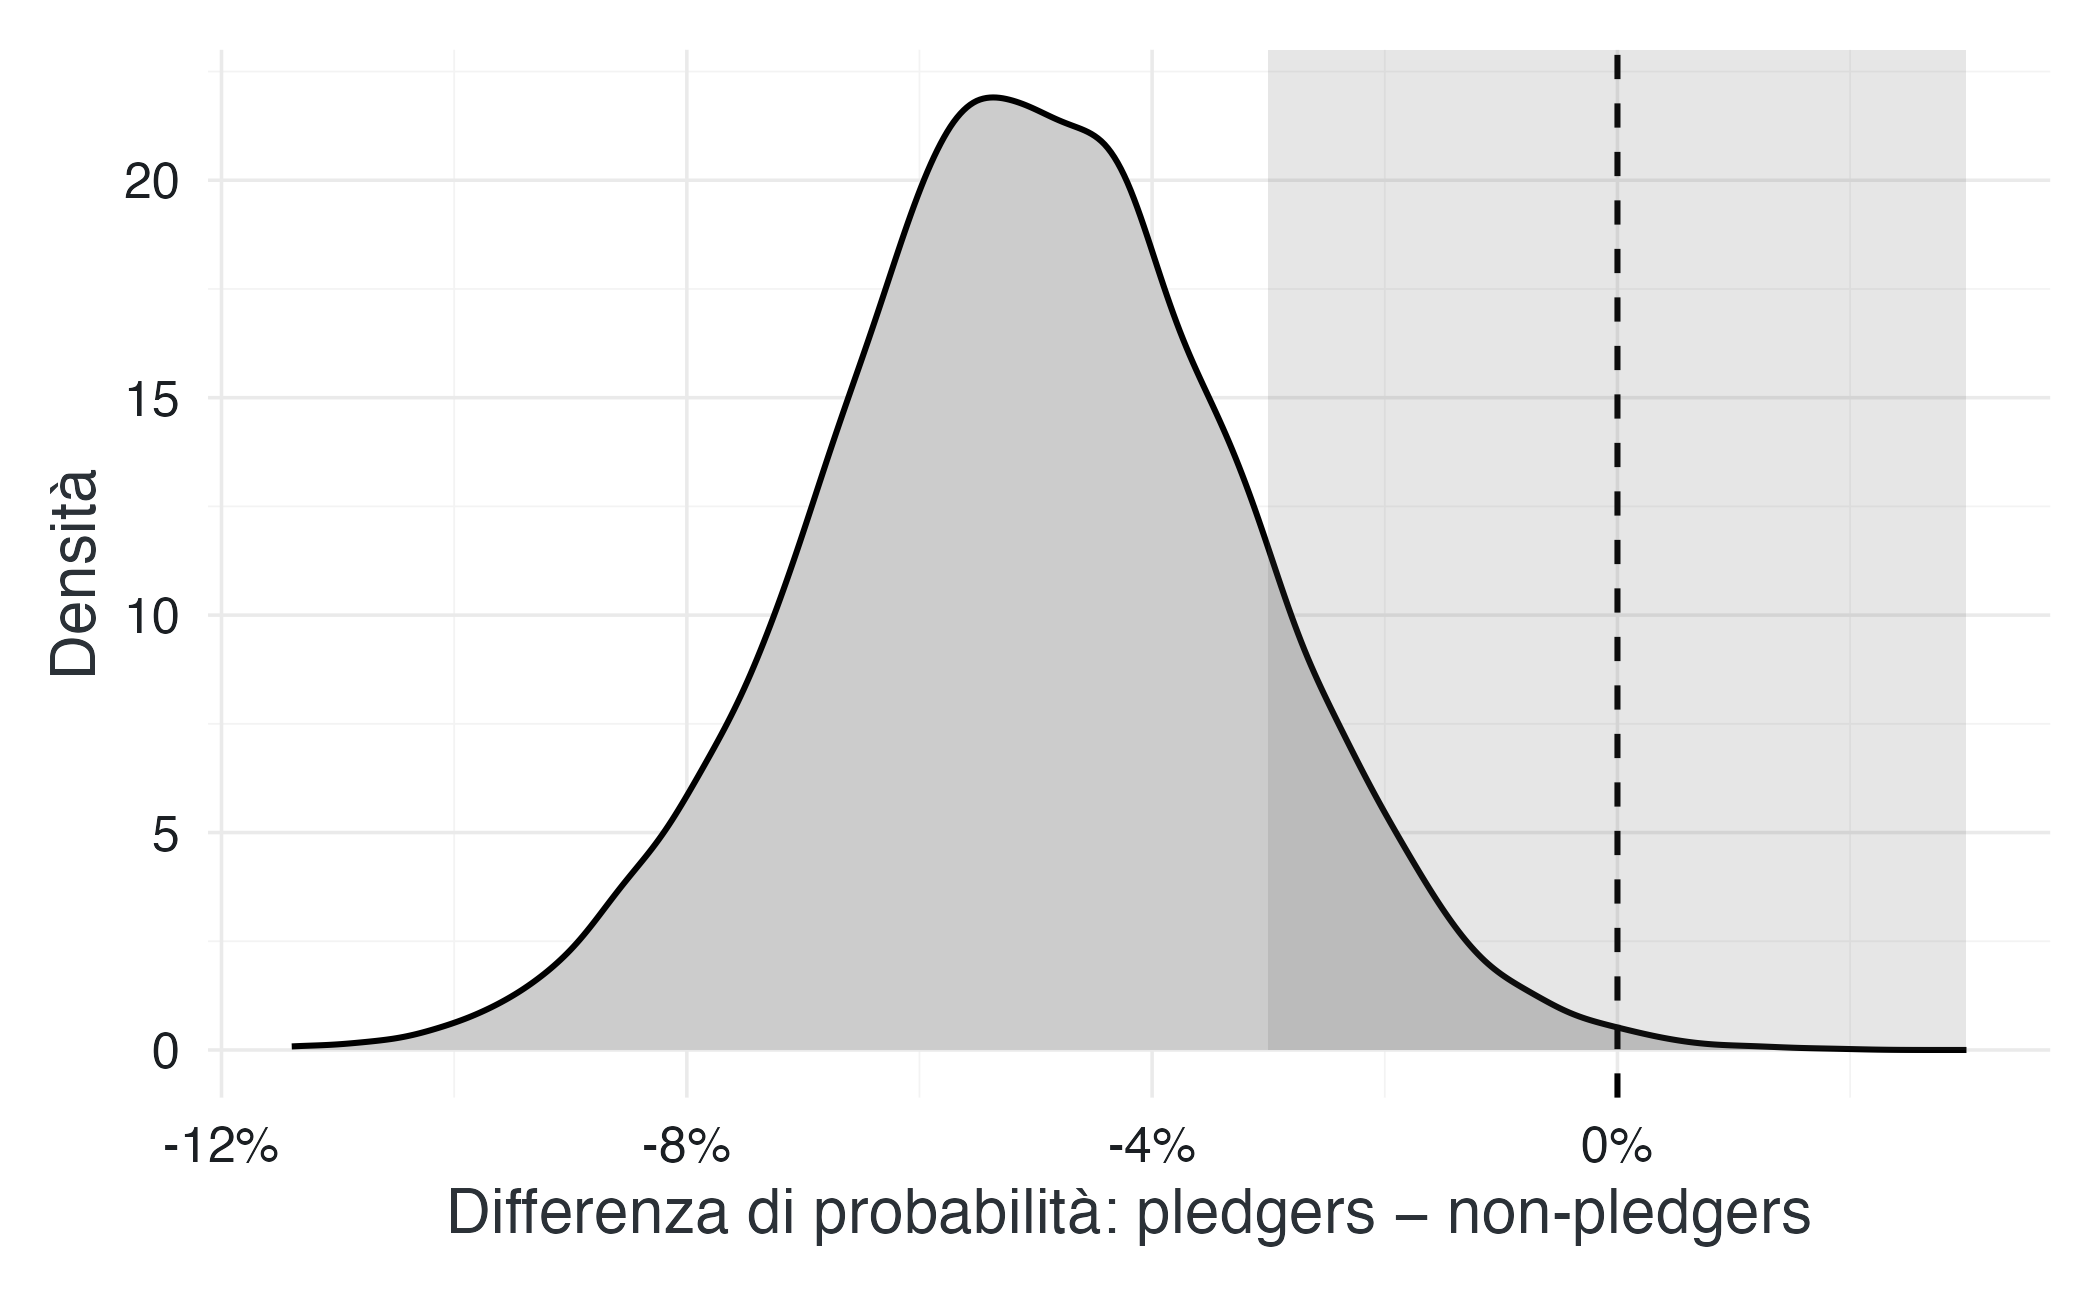
\includegraphics[width=0.85\linewidth,height=\textheight,keepaspectratio]{chapters/glm/02_proporzioni_files/figure-pdf/unnamed-chunk-19-1.png}
\end{center}

La zona evidenziata rappresenta la regione di equivalenza pratica scelta
per l'esempio.

\subsection{Controllo predittivo a
posteriori}\label{controllo-predittivo-a-posteriori-1}

Generiamo nuovi conteggi per i due gruppi e confrontiamo le proporzioni
replicate con quelle osservate:

\begin{Shaded}
\begin{Highlighting}[]
\NormalTok{y\_rep\_two }\OtherTok{\textless{}{-}} \FunctionTok{posterior\_predict}\NormalTok{(fit\_two\_proportions)}

\NormalTok{ppc\_two }\OtherTok{\textless{}{-}} \FunctionTok{tibble}\NormalTok{(}
  \AttributeTok{non\_pledgers =}\NormalTok{ y\_rep\_two[, }\DecValTok{1}\NormalTok{] }\SpecialCharTok{/}\NormalTok{ condom\_data}\SpecialCharTok{$}\NormalTok{trials[}\DecValTok{1}\NormalTok{],}
  \AttributeTok{pledgers =}\NormalTok{ y\_rep\_two[, }\DecValTok{2}\NormalTok{] }\SpecialCharTok{/}\NormalTok{ condom\_data}\SpecialCharTok{$}\NormalTok{trials[}\DecValTok{2}\NormalTok{]}
\NormalTok{) }\SpecialCharTok{|\textgreater{}}
  \FunctionTok{pivot\_longer}\NormalTok{(}
    \FunctionTok{everything}\NormalTok{(),}
    \AttributeTok{names\_to =} \StringTok{"group"}\NormalTok{,}
    \AttributeTok{values\_to =} \StringTok{"proportion\_rep"}
\NormalTok{  ) }\SpecialCharTok{|\textgreater{}}
  \FunctionTok{mutate}\NormalTok{(}
    \AttributeTok{observed =} \FunctionTok{if\_else}\NormalTok{(}
\NormalTok{      group }\SpecialCharTok{==} \StringTok{"non\_pledgers"}\NormalTok{,}
\NormalTok{      condom\_data}\SpecialCharTok{$}\NormalTok{observed\_proportion[}\DecValTok{1}\NormalTok{],}
\NormalTok{      condom\_data}\SpecialCharTok{$}\NormalTok{observed\_proportion[}\DecValTok{2}\NormalTok{]}
\NormalTok{    ),}
    \AttributeTok{group =} \FunctionTok{recode}\NormalTok{(}
\NormalTok{      group,}
      \AttributeTok{non\_pledgers =} \StringTok{"Non{-}pledgers"}\NormalTok{,}
      \AttributeTok{pledgers =} \StringTok{"Pledgers"}
\NormalTok{    )}
\NormalTok{  )}

\FunctionTok{ggplot}\NormalTok{(ppc\_two, }\FunctionTok{aes}\NormalTok{(proportion\_rep)) }\SpecialCharTok{+}
  \FunctionTok{geom\_density}\NormalTok{(}\AttributeTok{fill =} \StringTok{"grey80"}\NormalTok{) }\SpecialCharTok{+}
  \FunctionTok{geom\_vline}\NormalTok{(}\FunctionTok{aes}\NormalTok{(}\AttributeTok{xintercept =}\NormalTok{ observed), }\AttributeTok{linetype =} \StringTok{"dashed"}\NormalTok{) }\SpecialCharTok{+}
  \FunctionTok{facet\_wrap}\NormalTok{(}\SpecialCharTok{\textasciitilde{}}\NormalTok{ group, }\AttributeTok{scales =} \StringTok{"free"}\NormalTok{) }\SpecialCharTok{+}
  \FunctionTok{scale\_x\_continuous}\NormalTok{(}\AttributeTok{labels =} \FunctionTok{label\_percent}\NormalTok{()) }\SpecialCharTok{+}
  \FunctionTok{labs}\NormalTok{(}
    \AttributeTok{x =} \StringTok{"Proporzione replicata"}\NormalTok{,}
    \AttributeTok{y =} \StringTok{"Densità"}
\NormalTok{  )}
\end{Highlighting}
\end{Shaded}

\begin{center}
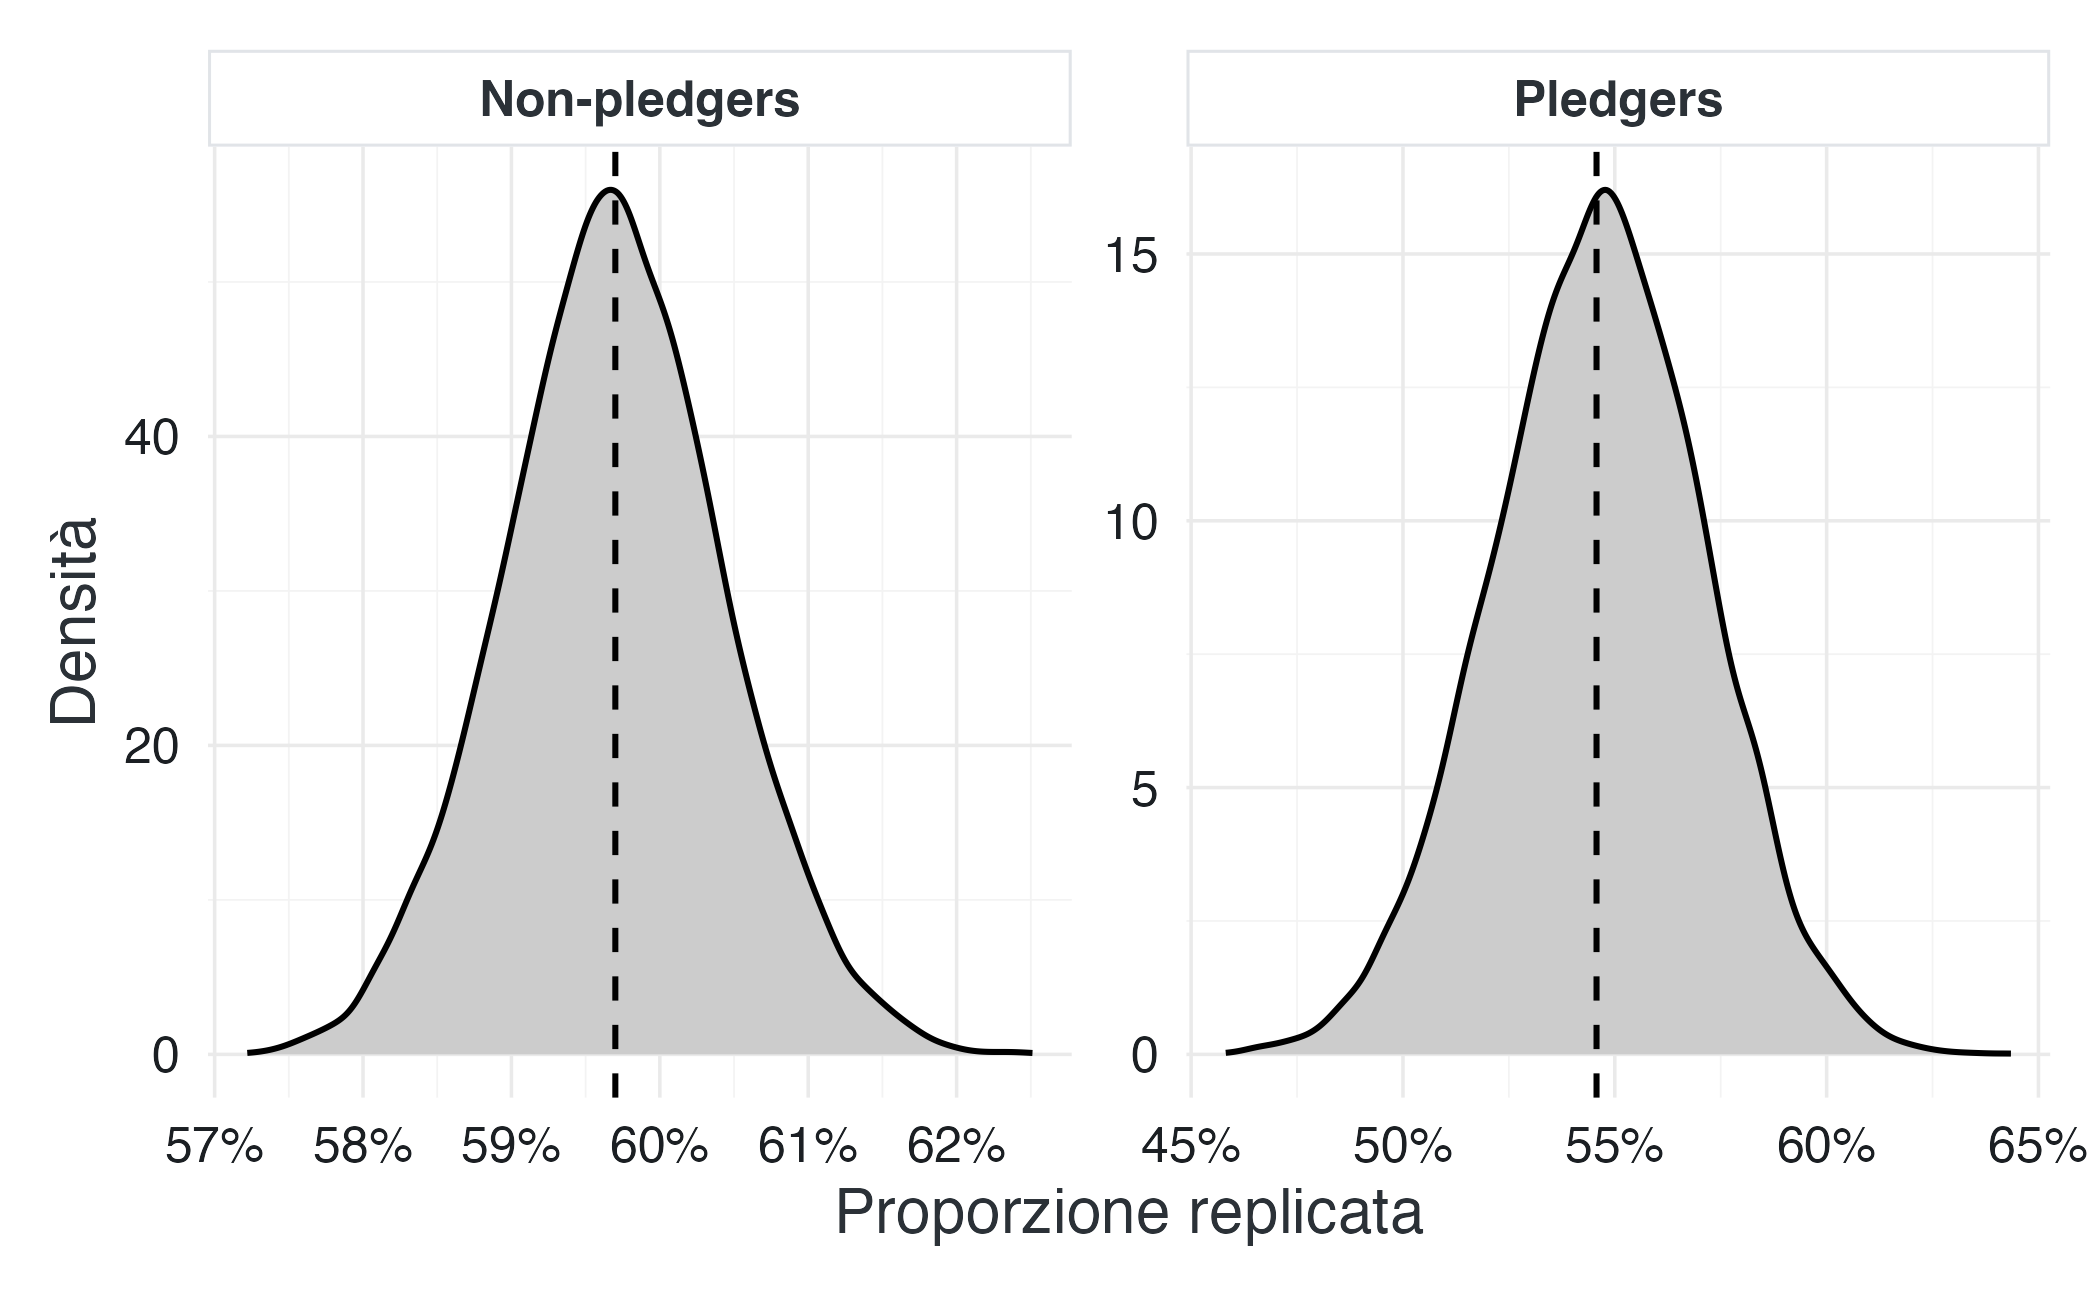
\includegraphics[width=0.85\linewidth,height=\textheight,keepaspectratio]{chapters/glm/02_proporzioni_files/figure-pdf/unnamed-chunk-20-1.png}
\end{center}

Con un conteggio per gruppo, il modello riproduce essenzialmente le due
proporzioni aggregate. Il controllo non verifica l'indipendenza delle
singole prove né la stabilità della probabilità tra persone e contesti.
Se ogni partecipante contribuisce con più risposte, trattare tutte le
prove come indipendenti può produrre un'incertezza troppo ridotta; in
quel caso è necessario rappresentare la struttura gerarchica.

\section{Trasferire il modello a un nuovo
problema}\label{trasferire-il-modello-a-un-nuovo-problema}

Lo stesso modello può essere applicato ai dati di Banerjee et al.
(\citeproc{ref-banerjee2025children}{2025}) sulle abilità matematiche di
bambini che lavoravano nei mercati e bambini scolarizzati. Nei problemi
astratti furono osservati 670 successi su 1488 prove tra i bambini
lavoratori e 320 su 542 tra gli scolarizzati; nei problemi di mercato,
134 successi su 373 e 3 su 271. Il confronto può essere costruito
sostituendo i conteggi nel data frame e calcolando nuovamente
probabilità, risk difference, risk ratio e odds ratio.

Questo esempio mette però in evidenza un limite importante. Le prove
sono raggruppate entro i bambini e probabilmente entro i problemi. Un
modello basato soltanto sui conteggi aggregati non rappresenta queste
dipendenze. La regressione logistica con effetti gerarchici sarebbe più
adatta se fossero disponibili i dati a livello di singola risposta. Il
principio generale rimane lo stesso, ma la struttura del predittore e
della variabilità deve seguire il disegno dello studio.

\section{Assunzioni e limiti}\label{assunzioni-e-limiti-1}

Il modello binomiale assume un numero noto di prove e, condizionatamente
ai parametri, una probabilità comune per le prove raccolte nella stessa
unità. Questa assunzione può risultare inadeguata quando esiste
eterogeneità non modellata, dipendenza tra prove o sovradispersione
rispetto alla binomiale. In tali casi possono essere necessari effetti
gerarchici, una distribuzione Beta--Binomiale come modello di
eterogeneità, o una diversa rappresentazione del processo
osservazionale.

Anche il confronto tra gruppi non possiede automaticamente un
significato causale. Nei dati osservazionali, la differenza tra \(p_1\)
e \(p_0\) è un'associazione tra appartenenza al gruppo e outcome.
L'interpretazione causale richiede un disegno e ipotesi di
identificazione adeguati.

Infine, le probabilità stimate dipendono dalla definizione dell'evento.
Cambiare la codifica del successo modifica intercetta, segno dei
coefficienti e rapporti derivati, pur lasciando invariata l'informazione
contenuta nei dati. La codifica deve quindi essere dichiarata e
mantenuta coerente.

\section{Errori interpretativi
ricorrenti}\label{errori-interpretativi-ricorrenti-1}

\textbf{Trattare una proporzione osservata come se fosse il parametro.}
Il rapporto \(y/n\) è una descrizione del campione; \(p\) è la
probabilità della popolazione rappresentata nel modello.

\textbf{Interpretare 0.5 come ``caso'' senza una giustificazione.} Il
significato di una probabilità di riferimento dipende dal meccanismo che
genera l'evento.

\textbf{Confondere odds ratio e risk ratio.} Le due quantità possono
differire molto quando l'evento è comune. È opportuno riportare anche le
probabilità dei gruppi o la differenza assoluta.

\textbf{Definire la rilevanza pratica mediante la precisione della
posterior.} Una ROPE costruita a partire dalla deviazione standard
posteriore cambia con la dimensione del campione e non rappresenta una
soglia sostantiva indipendente dai dati.

\textbf{Ignorare la struttura delle prove.} Conteggi aggregati possono
nascondere dipendenze tra risposte, differenze individuali e variazioni
tra item.

\textbf{Attribuire un significato causale al coefficiente di gruppo.}
Senza randomizzazione o adeguate ipotesi di identificazione, il
contrasto resta associativo.

\section*{Riflessioni conclusive}\label{riflessioni-conclusive-32}

\markright{Riflessioni conclusive}

La stima di una proporzione e il confronto tra due proporzioni
appartengono alla stessa architettura della regressione logistica. Nel
primo caso il modello contiene soltanto l'intercetta; nel secondo, un
predittore binario modifica i log-odds e produce due probabilità
condizionate. Non è quindi necessario apprendere tecniche separate:
cambia la matrice del disegno, mentre la distribuzione binomiale, il
link logit e il workflow bayesiano rimangono gli stessi.

La posterior dei coefficienti è un punto di partenza, non il risultato
finale. Trasformando i draw otteniamo le probabilità dei gruppi e
contrasti come differenza di rischio, risk ratio e odds ratio. La scelta
della quantità da comunicare deve essere guidata dalla domanda
scientifica e dalla comprensibilità sostantiva. Quando si vuole
distinguere una differenza trascurabile da una rilevante, la soglia deve
essere definita in base al dominio, non derivata dalla precisione
ottenuta nel campione.

I modelli aggregati sono utili per rendere visibile la struttura
essenziale, ma possono essere troppo semplici quando le osservazioni
sono ripetute o raggruppate. Questo limite anticipa un principio
generale dei GLM: la distribuzione osservazionale deve rispettare non
soltanto il tipo di outcome, ma anche il modo in cui i dati sono stati
generati. Nel capitolo successivo la stessa logica verrà applicata ai
conteggi, sostituendo la distribuzione binomiale con la distribuzione di
Poisson e il link logit con il link logaritmico.

\begin{tcolorbox}[enhanced jigsaw, arc=.35mm, bottomrule=.15mm, bottomtitle=1mm, breakable, colback=white, colbacktitle=quarto-callout-note-color!10!white, colframe=quarto-callout-note-color-frame, coltitle=black, left=2mm, leftrule=.75mm, opacityback=0, opacitybacktitle=0.6, rightrule=.15mm, title=\textcolor{quarto-callout-note-color}{\faInfo}\hspace{0.5em}{Informazioni sull'ambiente di sviluppo}, titlerule=0mm, toprule=.15mm, toptitle=1mm]

\begin{Shaded}
\begin{Highlighting}[]
\FunctionTok{sessionInfo}\NormalTok{()}
\CommentTok{\#\textgreater{} R version 4.6.1 (2026{-}06{-}24)}
\CommentTok{\#\textgreater{} Platform: aarch64{-}apple{-}darwin23}
\CommentTok{\#\textgreater{} Running under: macOS Tahoe 26.5.2}
\CommentTok{\#\textgreater{} }
\CommentTok{\#\textgreater{} Matrix products: default}
\CommentTok{\#\textgreater{} BLAS:   /Library/Frameworks/R.framework/Versions/4.6/Resources/lib/libRblas.0.dylib }
\CommentTok{\#\textgreater{} LAPACK: /Library/Frameworks/R.framework/Versions/4.6/Resources/lib/libRlapack.dylib;  LAPACK version 3.12.1}
\CommentTok{\#\textgreater{} }
\CommentTok{\#\textgreater{} locale:}
\CommentTok{\#\textgreater{} [1] C.UTF{-}8/UTF{-}8/C.UTF{-}8/C/C.UTF{-}8/C.UTF{-}8}
\CommentTok{\#\textgreater{} }
\CommentTok{\#\textgreater{} time zone: Europe/Zagreb}
\CommentTok{\#\textgreater{} tzcode source: internal}
\CommentTok{\#\textgreater{} }
\CommentTok{\#\textgreater{} attached base packages:}
\CommentTok{\#\textgreater{} [1] stats     graphics  grDevices utils     datasets  methods   base     }
\CommentTok{\#\textgreater{} }
\CommentTok{\#\textgreater{} other attached packages:}
\CommentTok{\#\textgreater{}  [1] scales\_1.4.0          ragg\_1.5.2            tinytable\_0.17.0     }
\CommentTok{\#\textgreater{}  [4] withr\_3.0.3           systemfonts\_1.3.2     patchwork\_1.3.2      }
\CommentTok{\#\textgreater{}  [7] ggdist\_3.3.3          tidybayes\_3.0.7       bayesplot\_1.15.0     }
\CommentTok{\#\textgreater{} [10] ggplot2\_4.0.3         reliabilitydiag\_0.2.1 priorsense\_1.2.0     }
\CommentTok{\#\textgreater{} [13] posterior\_1.7.0       loo\_2.10.0            rstan\_2.32.7         }
\CommentTok{\#\textgreater{} [16] StanHeaders\_2.32.10   brms\_2.23.0           Rcpp\_1.1.2           }
\CommentTok{\#\textgreater{} [19] sessioninfo\_1.2.4     conflicted\_1.2.0      janitor\_2.2.1        }
\CommentTok{\#\textgreater{} [22] matrixStats\_1.5.0     modelr\_0.1.11         tibble\_3.3.1         }
\CommentTok{\#\textgreater{} [25] dplyr\_1.2.1           tidyr\_1.3.2           rio\_1.3.0            }
\CommentTok{\#\textgreater{} [28] here\_1.0.2           }
\CommentTok{\#\textgreater{} }
\CommentTok{\#\textgreater{} loaded via a namespace (and not attached):}
\CommentTok{\#\textgreater{}  [1] svUnit\_1.0.8          tidyselect\_1.2.1      farver\_2.1.2         }
\CommentTok{\#\textgreater{}  [4] S7\_0.2.2              fastmap\_1.2.0         tensorA\_0.36.2.1     }
\CommentTok{\#\textgreater{}  [7] pacman\_0.5.1          digest\_0.6.39         timechange\_0.4.0     }
\CommentTok{\#\textgreater{} [10] estimability\_2.0.0    lifecycle\_1.0.5       processx\_3.9.0       }
\CommentTok{\#\textgreater{} [13] magrittr\_2.0.5        compiler\_4.6.1        rlang\_1.3.0          }
\CommentTok{\#\textgreater{} [16] tools\_4.6.1           utf8\_1.2.6            yaml\_2.3.12          }
\CommentTok{\#\textgreater{} [19] data.table\_1.18.4     knitr\_1.51            labeling\_0.4.3       }
\CommentTok{\#\textgreater{} [22] bridgesampling\_1.2{-}1  pkgbuild\_1.4.8        curl\_7.1.0           }
\CommentTok{\#\textgreater{} [25] plyr\_1.8.9            cmdstanr\_0.9.0        RColorBrewer\_1.1{-}3   }
\CommentTok{\#\textgreater{} [28] abind\_1.4{-}8           purrr\_1.2.2           grid\_4.6.1           }
\CommentTok{\#\textgreater{} [31] stats4\_4.6.1          xtable\_1.8{-}8          inline\_0.3.21        }
\CommentTok{\#\textgreater{} [34] emmeans\_2.0.4         cli\_3.6.6             mvtnorm\_1.4{-}2        }
\CommentTok{\#\textgreater{} [37] rmarkdown\_2.31        generics\_0.1.4        otel\_0.2.0           }
\CommentTok{\#\textgreater{} [40] RcppParallel\_5.1.11{-}2 reshape2\_1.4.5        cachem\_1.1.0         }
\CommentTok{\#\textgreater{} [43] stringr\_1.6.0         parallel\_4.6.1        vctrs\_0.7.3          }
\CommentTok{\#\textgreater{} [46] V8\_8.2.0              Matrix\_1.7{-}5          jsonlite\_2.0.0       }
\CommentTok{\#\textgreater{} [49] arrayhelpers\_1.1{-}1    glue\_1.8.1            ps\_1.9.3             }
\CommentTok{\#\textgreater{} [52] codetools\_0.2{-}20      distributional\_0.8.1  lubridate\_1.9.5      }
\CommentTok{\#\textgreater{} [55] stringi\_1.8.7         gtable\_0.3.6          QuickJSR\_1.10.0      }
\CommentTok{\#\textgreater{} [58] pillar\_1.11.1         htmltools\_0.5.9       Brobdingnag\_1.2{-}9    }
\CommentTok{\#\textgreater{} [61] R6\_2.6.1              textshaping\_1.0.5     rprojroot\_2.1.1      }
\CommentTok{\#\textgreater{} [64] evaluate\_1.0.5        lattice\_0.22{-}9        backports\_1.5.1      }
\CommentTok{\#\textgreater{} [67] memoise\_2.0.1         broom\_1.0.13          snakecase\_0.11.1     }
\CommentTok{\#\textgreater{} [70] rstantools\_2.6.0      coda\_0.19{-}4.1         gridExtra\_2.3.1      }
\CommentTok{\#\textgreater{} [73] nlme\_3.1{-}170          checkmate\_2.3.4       xfun\_0.60            }
\CommentTok{\#\textgreater{} [76] pkgconfig\_2.0.3}
\end{Highlighting}
\end{Shaded}

\end{tcolorbox}

\section*{Bibliografia}\label{bibliografia-36}

\markright{Bibliografia}

\chapter{Dati di conteggio: Poisson e
sovradispersione}\label{sec-poisson-model}

La regressione di Poisson estende il modello lineare generalizzato agli
outcome che rappresentano conteggi: numero di errori, episodi
sintomatici, accessi a un servizio o eventi osservati in un intervallo
definito. La struttura del modello rimane quella già incontrata nella
regressione logistica. Cambiano la distribuzione osservazionale e la
funzione di collegamento.

Il modello di Poisson è semplice e spesso utile, ma impone una relazione
precisa tra media e variabilità. Per questo motivo costituisce anche un
buon esempio del workflow di revisione: si specifica il modello, se ne
controllano le implicazioni predittive e, quando risulta troppo rigido,
si considera una distribuzione più flessibile, come la binomiale
negativa.

\section*{Orientamento}\label{orientamento-1}

\markright{Orientamento}

Nel modello lineare gaussiano l'outcome può assumere valori continui e
la sua media è collegata direttamente al predittore lineare. Nel modello
di Poisson l'outcome assume valori interi non negativi e il valore
atteso deve essere positivo. Il link logaritmico consente di rispettare
questo vincolo:

\[
Y_i \sim \operatorname{Poisson}(\lambda_i),
\qquad
\log(\lambda_i)=\eta_i,
\qquad
\eta_i=\alpha+\mathbf{x}_i^\top\boldsymbol\beta.
\]

Al termine del capitolo il lettore dovrebbe saper distinguere un
conteggio da un tasso, interpretare i coefficienti sulla scala
moltiplicativa, usare un offset quando le unità hanno esposizioni
differenti e riconoscere i segnali che rendono opportuno sostituire il
modello di Poisson con una distribuzione binomiale negativa.

\begin{tcolorbox}[enhanced jigsaw, arc=.35mm, bottomrule=.15mm, breakable, colback=white, colframe=quarto-callout-important-color-frame, left=2mm, leftrule=.75mm, opacityback=0, rightrule=.15mm, toprule=.15mm]

\textbf{Da sapere.} I dati di conteggio assumono valori interi non
negativi e richiedono una distribuzione coerente con questa struttura.
Nel modello di Poisson, il logaritmo del conteggio atteso è espresso
come funzione lineare dei predittori. I coefficienti hanno quindi
un'interpretazione moltiplicativa: \(\exp(\beta)\) rappresenta il
rapporto tra conteggi attesi, a parità delle altre condizioni. Quando le
unità hanno esposizioni differenti, un \emph{offset} permette di
modellare un tasso anziché il conteggio complessivo.

\textbf{Da saper fare.} Distinguere conteggi e tassi; interpretare
intercetta e coefficienti sulla scala dei conteggi attesi, degli
\emph{incidence rate ratio} e delle variazioni percentuali; specificare
e stimare con \texttt{brms} un modello di Poisson, includendo un offset
quando necessario; eseguire controlli predittivi a priori e a
posteriori; riconoscere una variabilità condizionata incompatibile con
il modello e valutare il passaggio alla binomiale negativa.

\textbf{Approfondimento facoltativo.} Il calcolo della discrepanza di
Pearson, il confronto computazionale tra Poisson e binomiale negativa e
l'interpretazione dettagliata del parametro di dispersione possono
essere rimandati. Nel percorso essenziale è sufficiente comprendere il
link logaritmico, interpretare correttamente i coefficienti e usare i
controlli predittivi per riconoscere quando il modello di Poisson è
troppo rigido.

\hyperref[sec-percorsi-lettura]{Che cosa significano queste etichette?}

\end{tcolorbox}

\begin{tcolorbox}[enhanced jigsaw, arc=.35mm, bottomrule=.15mm, bottomtitle=1mm, breakable, colback=white, colbacktitle=quarto-callout-tip-color!10!white, colframe=quarto-callout-tip-color-frame, coltitle=black, left=2mm, leftrule=.75mm, opacityback=0, opacitybacktitle=0.6, rightrule=.15mm, title=\textcolor{quarto-callout-tip-color}{\faLightbulb}\hspace{0.5em}{Prerequisiti}, titlerule=0mm, toprule=.15mm, toptitle=1mm]

Il capitolo presuppone la conoscenza dell'architettura dei GLM
introdotta in Capitolo~\ref{sec-reg-logistic-stan} e del workflow
bayesiano sviluppato nella parte dedicata ai modelli lineari. Il
contesto sostantivo dell'esempio è discusso, da una prospettiva più
ampia, da Ross et al. (\citeproc{ref-ross2021racial}{2021}).

\end{tcolorbox}

\begin{tcolorbox}[enhanced jigsaw, arc=.35mm, bottomrule=.15mm, bottomtitle=1mm, breakable, colback=white, colbacktitle=quarto-callout-caution-color!10!white, colframe=quarto-callout-caution-color-frame, coltitle=black, left=2mm, leftrule=.75mm, opacityback=0, opacitybacktitle=0.6, rightrule=.15mm, title=\textcolor{quarto-callout-caution-color}{\faFire}\hspace{0.5em}{Preparazione del notebook}, titlerule=0mm, toprule=.15mm, toptitle=1mm]

\begin{Shaded}
\begin{Highlighting}[]
\NormalTok{here}\SpecialCharTok{::}\FunctionTok{here}\NormalTok{(}\StringTok{"code"}\NormalTok{, }\StringTok{"\_common.R"}\NormalTok{) }\SpecialCharTok{|\textgreater{}}
  \FunctionTok{source}\NormalTok{()}

\ControlFlowTok{if}\NormalTok{ (}\SpecialCharTok{!}\FunctionTok{requireNamespace}\NormalTok{(}\StringTok{"pacman"}\NormalTok{, }\AttributeTok{quietly =} \ConstantTok{TRUE}\NormalTok{)) \{}
  \FunctionTok{install.packages}\NormalTok{(}\StringTok{"pacman"}\NormalTok{)}
\NormalTok{\}}

\NormalTok{pacman}\SpecialCharTok{::}\FunctionTok{p\_load}\NormalTok{(}
\NormalTok{  brms,}
\NormalTok{  posterior,}
\NormalTok{  bayesplot,}
\NormalTok{  dplyr,}
\NormalTok{  tidyr,}
\NormalTok{  tibble,}
\NormalTok{  ggplot2,}
\NormalTok{  scales,}
\NormalTok{  readr}
\NormalTok{)}

\FunctionTok{set.seed}\NormalTok{(}\DecValTok{2026}\NormalTok{)}
\end{Highlighting}
\end{Shaded}

\end{tcolorbox}

\section{Perché non usare un modello
gaussiano}\label{perchuxe9-non-usare-un-modello-gaussiano}

Un conteggio appartiene all'insieme \(\{0,1,2,\ldots\}\). Un modello
normale può invece assegnare probabilità anche a valori negativi e
presuppone una variabilità simmetrica attorno alla media. Queste
proprietà possono essere innocue quando i conteggi sono molto grandi e
lontani da zero, ma diventano problematiche per eventi rari,
distribuzioni asimmetriche o numerosi zeri.

La distribuzione di Poisson descrive il numero di eventi osservati in
una determinata unità di esposizione:

\[
\Pr(Y=y\mid\lambda)
=
\frac{\lambda^y e^{-\lambda}}{y!},
\qquad y=0,1,2,\ldots,
\]

dove \(\lambda>0\) è il valore atteso del conteggio. Nel modello di
Poisson elementare vale anche

\[
\mathbb E(Y\mid\lambda)=\lambda,
\qquad
\operatorname{Var}(Y\mid\lambda)=\lambda.
\]

L'uguaglianza tra media e varianza riguarda la distribuzione
\textbf{condizionata} a uno stesso valore di \(\lambda\). Non deve
essere verificata confrontando meccanicamente la media e la varianza
grezze di osservazioni che hanno valori attesi differenti. Se
\(\lambda_i\) cambia al variare dei predittori, anche la dispersione
marginale dei dati può essere molto maggiore della loro media senza che
ciò dimostri, da solo, la presenza di sovradispersione.

\section{Il link logaritmico}\label{il-link-logaritmico}

Poiché il valore atteso deve rimanere positivo, il predittore lineare
non viene collegato direttamente a \(\lambda_i\). Si modella invece il
suo logaritmo:

\[
\log(\lambda_i)
=
\alpha+\mathbf{x}_i^\top\boldsymbol\beta.
\]

Applicando la funzione inversa otteniamo

\[
\lambda_i
=
\exp\!\left(\alpha+\mathbf{x}_i^\top\boldsymbol\beta\right).
\]

Il link è dunque la funzione logaritmica; l'esponenziale è il link
inverso. Questa distinzione terminologica aiuta a riconoscere la stessa
architettura nei diversi GLM.

\subsection{Interpretazione dei
coefficienti}\label{interpretazione-dei-coefficienti}

Consideriamo un solo predittore continuo:

\[
\log(\lambda_i)=\alpha+\beta x_i.
\]

Per un incremento unitario di \(x\), il rapporto tra i valori attesi è

\[
\frac{\lambda(x+1)}{\lambda(x)}
=
\exp(\beta).
\]

La quantità \(\exp(\beta)\) è quindi un \emph{incidence rate ratio} o,
più in generale, un rapporto tra conteggi attesi a parità di
esposizione. Un valore pari a 1 indica assenza di variazione
moltiplicativa; un valore pari a 1.10 corrisponde a un aumento atteso
del 10\%; un valore pari a 0.80 corrisponde a una riduzione attesa del
20\%.

L'intercetta ha un'interpretazione analoga:

\[
\exp(\alpha)=\lambda(0).
\]

Per renderla informativa conviene centrare i predittori, così che
\(x=0\) rappresenti una condizione osservata e sostantivamente
comprensibile.

\section{Conteggi ed esposizione}\label{conteggi-ed-esposizione}

Un conteggio non è sempre confrontabile direttamente tra unità. Due
persone osservate per durate diverse, due ospedali con bacini di utenza
differenti o due anni con popolazioni diverse non hanno la stessa
opportunità di produrre eventi. In questi casi l'interesse riguarda un
\textbf{tasso}, cioè un conteggio per unità di esposizione.

Indichiamo con \(E_i\) l'esposizione nota. Il modello diventa

\[
Y_i \sim \operatorname{Poisson}(E_i r_i),
\]

dove \(r_i\) è il tasso atteso per unità di esposizione. Usando il link
logaritmico:

\[
\log \mathbb E(Y_i)
=
\log(E_i)+\alpha+\mathbf{x}_i^\top\boldsymbol\beta.
\]

Il termine \(\log(E_i)\) è un \textbf{offset}: il suo coefficiente è
fissato a 1 e non viene stimato. In \texttt{brms} si scrive, per
esempio,

\begin{Shaded}
\begin{Highlighting}[]
\NormalTok{count }\SpecialCharTok{\textasciitilde{}}\NormalTok{ predictor }\SpecialCharTok{+} \FunctionTok{offset}\NormalTok{(}\FunctionTok{log}\NormalTok{(exposure))}
\end{Highlighting}
\end{Shaded}

Senza offset il modello descrive differenze nei conteggi complessivi.
Con l'offset descrive differenze nel tasso, assumendo che l'esposizione
sia misurata correttamente. La scelta non è un dettaglio tecnico, ma
dipende dalla domanda scientifica.

\section{Caso di studio: conteggi
annuali}\label{caso-di-studio-conteggi-annuali}

Consideriamo il numero annuale di sparatorie fatali da parte della
polizia registrate negli Stati Uniti dal 2015 al 2024. I valori sono
utilizzati qui per illustrare il modello, non per fornire una
spiegazione causale del fenomeno. Il conteggio può dipendere da molte
componenti non incluse nell'analisi, tra cui procedure di registrazione,
dimensione della popolazione, esposizione al rischio e trasformazioni
istituzionali. Per una discussione sostantiva delle disparità e delle
scelte di denominatore si veda Ross et al.
(\citeproc{ref-ross2021racial}{2021}).

Usiamo i conteggi riportati nel capitolo originario e centriamo l'anno
sul 2019:

\begin{Shaded}
\begin{Highlighting}[]
\NormalTok{shooting\_counts }\OtherTok{\textless{}{-}} \FunctionTok{tibble}\NormalTok{(}
  \AttributeTok{year =} \DecValTok{2015}\SpecialCharTok{:}\DecValTok{2024}\NormalTok{,}
  \AttributeTok{events =} \FunctionTok{c}\NormalTok{(}\DecValTok{995}\NormalTok{, }\DecValTok{959}\NormalTok{, }\DecValTok{984}\NormalTok{, }\DecValTok{992}\NormalTok{, }\DecValTok{993}\NormalTok{, }\DecValTok{1021}\NormalTok{, }\DecValTok{1050}\NormalTok{, }\DecValTok{1097}\NormalTok{, }\DecValTok{1164}\NormalTok{, }\DecValTok{1175}\NormalTok{)}
\NormalTok{) }\SpecialCharTok{|\textgreater{}}
  \FunctionTok{mutate}\NormalTok{(}\AttributeTok{year\_c =}\NormalTok{ year }\SpecialCharTok{{-}} \DecValTok{2019}\NormalTok{)}

\NormalTok{shooting\_counts}
\CommentTok{\#\textgreater{} \# A tibble: 10 x 3}
\CommentTok{\#\textgreater{}     year events year\_c}
\CommentTok{\#\textgreater{}    \textless{}int\textgreater{}  \textless{}dbl\textgreater{}  \textless{}dbl\textgreater{}}
\CommentTok{\#\textgreater{}  1  2015    995     {-}4}
\CommentTok{\#\textgreater{}  2  2016    959     {-}3}
\CommentTok{\#\textgreater{}  3  2017    984     {-}2}
\CommentTok{\#\textgreater{}  4  2018    992     {-}1}
\CommentTok{\#\textgreater{}  5  2019    993      0}
\CommentTok{\#\textgreater{}  6  2020   1021      1}
\CommentTok{\#\textgreater{}  7  2021   1050      2}
\CommentTok{\#\textgreater{}  8  2022   1097      3}
\CommentTok{\#\textgreater{}  9  2023   1164      4}
\CommentTok{\#\textgreater{} 10  2024   1175      5}
\end{Highlighting}
\end{Shaded}

La domanda descrittiva è: \textbf{come varia il numero annuale atteso di
eventi nel periodo osservato?} Il modello è

\[
Y_t \sim \operatorname{Poisson}(\lambda_t),
\qquad
\log(\lambda_t)=\alpha+\beta\,\text{year}_{c,t}.
\]

L'intercetta rappresenta il logaritmo del conteggio atteso nel 2019. La
quantità \(\exp(\beta)\) descrive il fattore moltiplicativo associato al
passaggio da un anno al successivo.

Questa specificazione assume una tendenza log-lineare regolare e
indipendenza condizionale tra gli anni. Con sole dieci osservazioni non
possiamo esaminare in profondità forme temporali più complesse; il
modello deve quindi essere interpretato come una sintesi descrittiva del
periodo, non come una legge stabile o una previsione di lungo termine.

\section{Specificazione dei prior}\label{specificazione-dei-prior-1}

Un conteggio annuale vicino a 1000 corrisponde a un'intercetta sulla
scala logaritmica vicina a \(\log(1000)\approx6.9\). Possiamo usare

\[
\alpha\sim\operatorname{Normal}(\log 1000,0.30),
\]

che ammette un intervallo ampio di conteggi plausibili per il 2019. Per
la pendenza scegliamo

\[
\beta\sim\operatorname{Normal}(0,0.05).
\]

Questo prior assegna maggiore plausibilità a variazioni annuali
moderate, positive o negative. Poiché \(\exp(0.05)\approx1.05\), una
deviazione standard del prior corrisponde a una variazione
moltiplicativa di circa il 5\% per anno.

\begin{Shaded}
\begin{Highlighting}[]
\NormalTok{poisson\_priors }\OtherTok{\textless{}{-}} \FunctionTok{c}\NormalTok{(}
  \FunctionTok{prior}\NormalTok{(}\FunctionTok{normal}\NormalTok{(}\FunctionTok{log}\NormalTok{(}\DecValTok{1000}\NormalTok{), }\FloatTok{0.30}\NormalTok{), }\AttributeTok{class =}\NormalTok{ Intercept),}
  \FunctionTok{prior}\NormalTok{(}\FunctionTok{normal}\NormalTok{(}\DecValTok{0}\NormalTok{, }\FloatTok{0.05}\NormalTok{), }\AttributeTok{class =}\NormalTok{ b)}
\NormalTok{)}
\end{Highlighting}
\end{Shaded}

\subsection{Controllo predittivo a
priori}\label{controllo-predittivo-a-priori-3}

Le implicazioni dei prior sono più facili da valutare sulla scala dei
conteggi. Adattiamo il modello senza usare la verosimiglianza dei dati e
generiamo traiettorie annuali:

\begin{Shaded}
\begin{Highlighting}[]
\NormalTok{fit\_poisson\_prior }\OtherTok{\textless{}{-}} \FunctionTok{brm}\NormalTok{(}
\NormalTok{  events }\SpecialCharTok{\textasciitilde{}} \DecValTok{1} \SpecialCharTok{+}\NormalTok{ year\_c,}
  \AttributeTok{data =}\NormalTok{ shooting\_counts,}
  \AttributeTok{family =} \FunctionTok{poisson}\NormalTok{(}\AttributeTok{link =} \StringTok{"log"}\NormalTok{),}
  \AttributeTok{prior =}\NormalTok{ poisson\_priors,}
  \AttributeTok{sample\_prior =} \StringTok{"only"}\NormalTok{,}
  \AttributeTok{chains =} \DecValTok{4}\NormalTok{,}
  \AttributeTok{iter =} \DecValTok{2000}\NormalTok{,}
  \AttributeTok{seed =} \DecValTok{2026}\NormalTok{,}
  \AttributeTok{refresh =} \DecValTok{0}
\NormalTok{)}
\CommentTok{\#\textgreater{} Running MCMC with 4 chains, at most 10 in parallel...}
\CommentTok{\#\textgreater{} }
\CommentTok{\#\textgreater{} Chain 1 finished in 0.0 seconds.}
\CommentTok{\#\textgreater{} Chain 2 finished in 0.0 seconds.}
\CommentTok{\#\textgreater{} Chain 3 finished in 0.0 seconds.}
\CommentTok{\#\textgreater{} Chain 4 finished in 0.0 seconds.}
\CommentTok{\#\textgreater{} }
\CommentTok{\#\textgreater{} All 4 chains finished successfully.}
\CommentTok{\#\textgreater{} Mean chain execution time: 0.0 seconds.}
\CommentTok{\#\textgreater{} Total execution time: 0.3 seconds.}

\NormalTok{prior\_epred }\OtherTok{\textless{}{-}} \FunctionTok{posterior\_epred}\NormalTok{(fit\_poisson\_prior, }\AttributeTok{ndraws =} \DecValTok{200}\NormalTok{)}

\NormalTok{prior\_lines }\OtherTok{\textless{}{-}} \FunctionTok{as\_tibble}\NormalTok{(prior\_epred) }\SpecialCharTok{|\textgreater{}}
  \FunctionTok{mutate}\NormalTok{(}\AttributeTok{.draw =} \FunctionTok{row\_number}\NormalTok{()) }\SpecialCharTok{|\textgreater{}}
  \FunctionTok{pivot\_longer}\NormalTok{(}\SpecialCharTok{{-}}\NormalTok{.draw, }\AttributeTok{names\_to =} \StringTok{"row"}\NormalTok{, }\AttributeTok{values\_to =} \StringTok{"lambda"}\NormalTok{) }\SpecialCharTok{|\textgreater{}}
  \FunctionTok{mutate}\NormalTok{(}
    \AttributeTok{row =}\NormalTok{ readr}\SpecialCharTok{::}\FunctionTok{parse\_number}\NormalTok{(row),}
    \AttributeTok{year =}\NormalTok{ shooting\_counts}\SpecialCharTok{$}\NormalTok{year[row]}
\NormalTok{  )}

\FunctionTok{ggplot}\NormalTok{(prior\_lines, }\FunctionTok{aes}\NormalTok{(year, lambda, }\AttributeTok{group =}\NormalTok{ .draw)) }\SpecialCharTok{+}
  \FunctionTok{geom\_line}\NormalTok{(}\AttributeTok{alpha =} \FloatTok{0.08}\NormalTok{) }\SpecialCharTok{+}
  \FunctionTok{labs}\NormalTok{(}
    \AttributeTok{x =} \StringTok{"Anno"}\NormalTok{,}
    \AttributeTok{y =} \StringTok{"Conteggio atteso a priori"}
\NormalTok{  )}
\end{Highlighting}
\end{Shaded}

\begin{center}
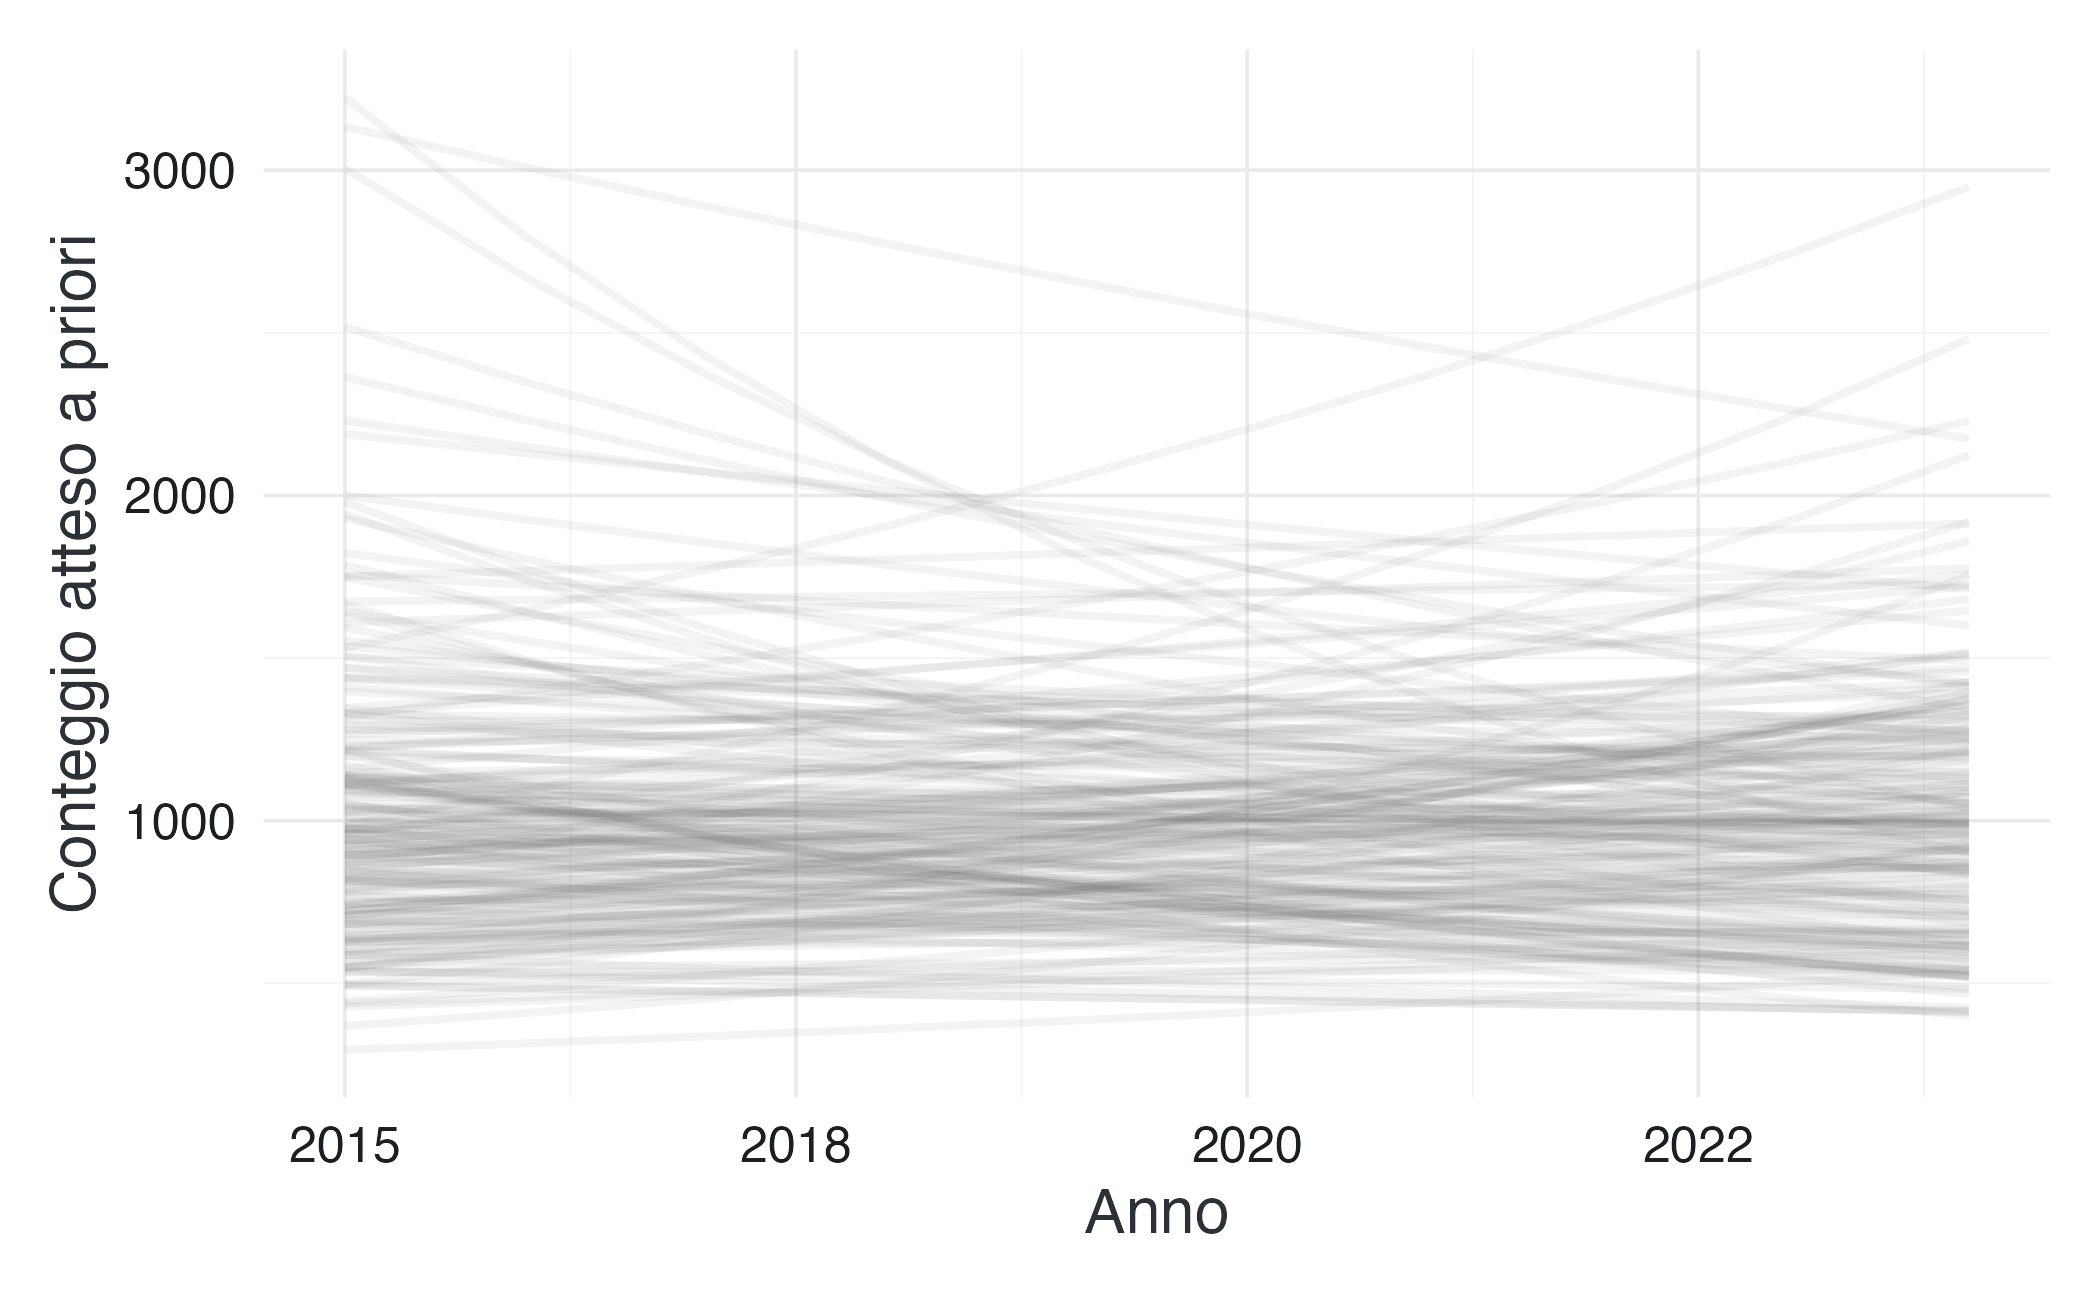
\includegraphics[width=0.85\linewidth,height=\textheight,keepaspectratio]{chapters/glm/03_modelli_conteggio_files/figure-pdf/unnamed-chunk-4-1.png}
\end{center}

Il grafico non deve riprodurre i dati osservati. Serve a verificare che
il modello ammetta livelli e variazioni temporali plausibili senza
generare sistematicamente conteggi incompatibili con il dominio.

\section{Stima del modello di
Poisson}\label{stima-del-modello-di-poisson}

\begin{Shaded}
\begin{Highlighting}[]
\NormalTok{fit\_poisson }\OtherTok{\textless{}{-}} \FunctionTok{brm}\NormalTok{(}
\NormalTok{  events }\SpecialCharTok{\textasciitilde{}} \DecValTok{1} \SpecialCharTok{+}\NormalTok{ year\_c,}
  \AttributeTok{data =}\NormalTok{ shooting\_counts,}
  \AttributeTok{family =} \FunctionTok{poisson}\NormalTok{(}\AttributeTok{link =} \StringTok{"log"}\NormalTok{),}
  \AttributeTok{prior =}\NormalTok{ poisson\_priors,}
  \AttributeTok{chains =} \DecValTok{4}\NormalTok{,}
  \AttributeTok{iter =} \DecValTok{3000}\NormalTok{,}
  \AttributeTok{warmup =} \DecValTok{1000}\NormalTok{,}
  \AttributeTok{seed =} \DecValTok{2026}\NormalTok{,}
  \AttributeTok{refresh =} \DecValTok{0}
\NormalTok{)}
\CommentTok{\#\textgreater{} Running MCMC with 4 chains, at most 10 in parallel...}
\CommentTok{\#\textgreater{} }
\CommentTok{\#\textgreater{} Chain 1 finished in 0.0 seconds.}
\CommentTok{\#\textgreater{} Chain 2 finished in 0.0 seconds.}
\CommentTok{\#\textgreater{} Chain 3 finished in 0.0 seconds.}
\CommentTok{\#\textgreater{} Chain 4 finished in 0.0 seconds.}
\CommentTok{\#\textgreater{} }
\CommentTok{\#\textgreater{} All 4 chains finished successfully.}
\CommentTok{\#\textgreater{} Mean chain execution time: 0.0 seconds.}
\CommentTok{\#\textgreater{} Total execution time: 0.3 seconds.}

\FunctionTok{summary}\NormalTok{(fit\_poisson)}
\CommentTok{\#\textgreater{}  Family: poisson }
\CommentTok{\#\textgreater{}   Links: mu = log }
\CommentTok{\#\textgreater{} Formula: events \textasciitilde{} 1 + year\_c }
\CommentTok{\#\textgreater{}    Data: shooting\_counts (Number of observations: 10) }
\CommentTok{\#\textgreater{}   Draws: 4 chains, each with iter = 3000; warmup = 1000; thin = 1;}
\CommentTok{\#\textgreater{}          total post{-}warmup draws = 8000}
\CommentTok{\#\textgreater{} }
\CommentTok{\#\textgreater{} Regression Coefficients:}
\CommentTok{\#\textgreater{}           Estimate Est.Error l{-}95\% CI u{-}95\% CI Rhat Bulk\_ESS Tail\_ESS}
\CommentTok{\#\textgreater{} Intercept     6.94      0.01     6.92     6.96 1.00     4657     4768}
\CommentTok{\#\textgreater{} year\_c        0.02      0.00     0.02     0.03 1.00     7789     5610}
\CommentTok{\#\textgreater{} }
\CommentTok{\#\textgreater{} Draws were sampled using sample(hmc). For each parameter, Bulk\_ESS}
\CommentTok{\#\textgreater{} and Tail\_ESS are effective sample size measures, and Rhat is the potential}
\CommentTok{\#\textgreater{} scale reduction factor on split chains (at convergence, Rhat = 1).}
\end{Highlighting}
\end{Shaded}

Prima dell'interpretazione controlliamo che il campionamento sia
affidabile:

\begin{Shaded}
\begin{Highlighting}[]
\FunctionTok{plot}\NormalTok{(fit\_poisson)}
\end{Highlighting}
\end{Shaded}

\begin{center}
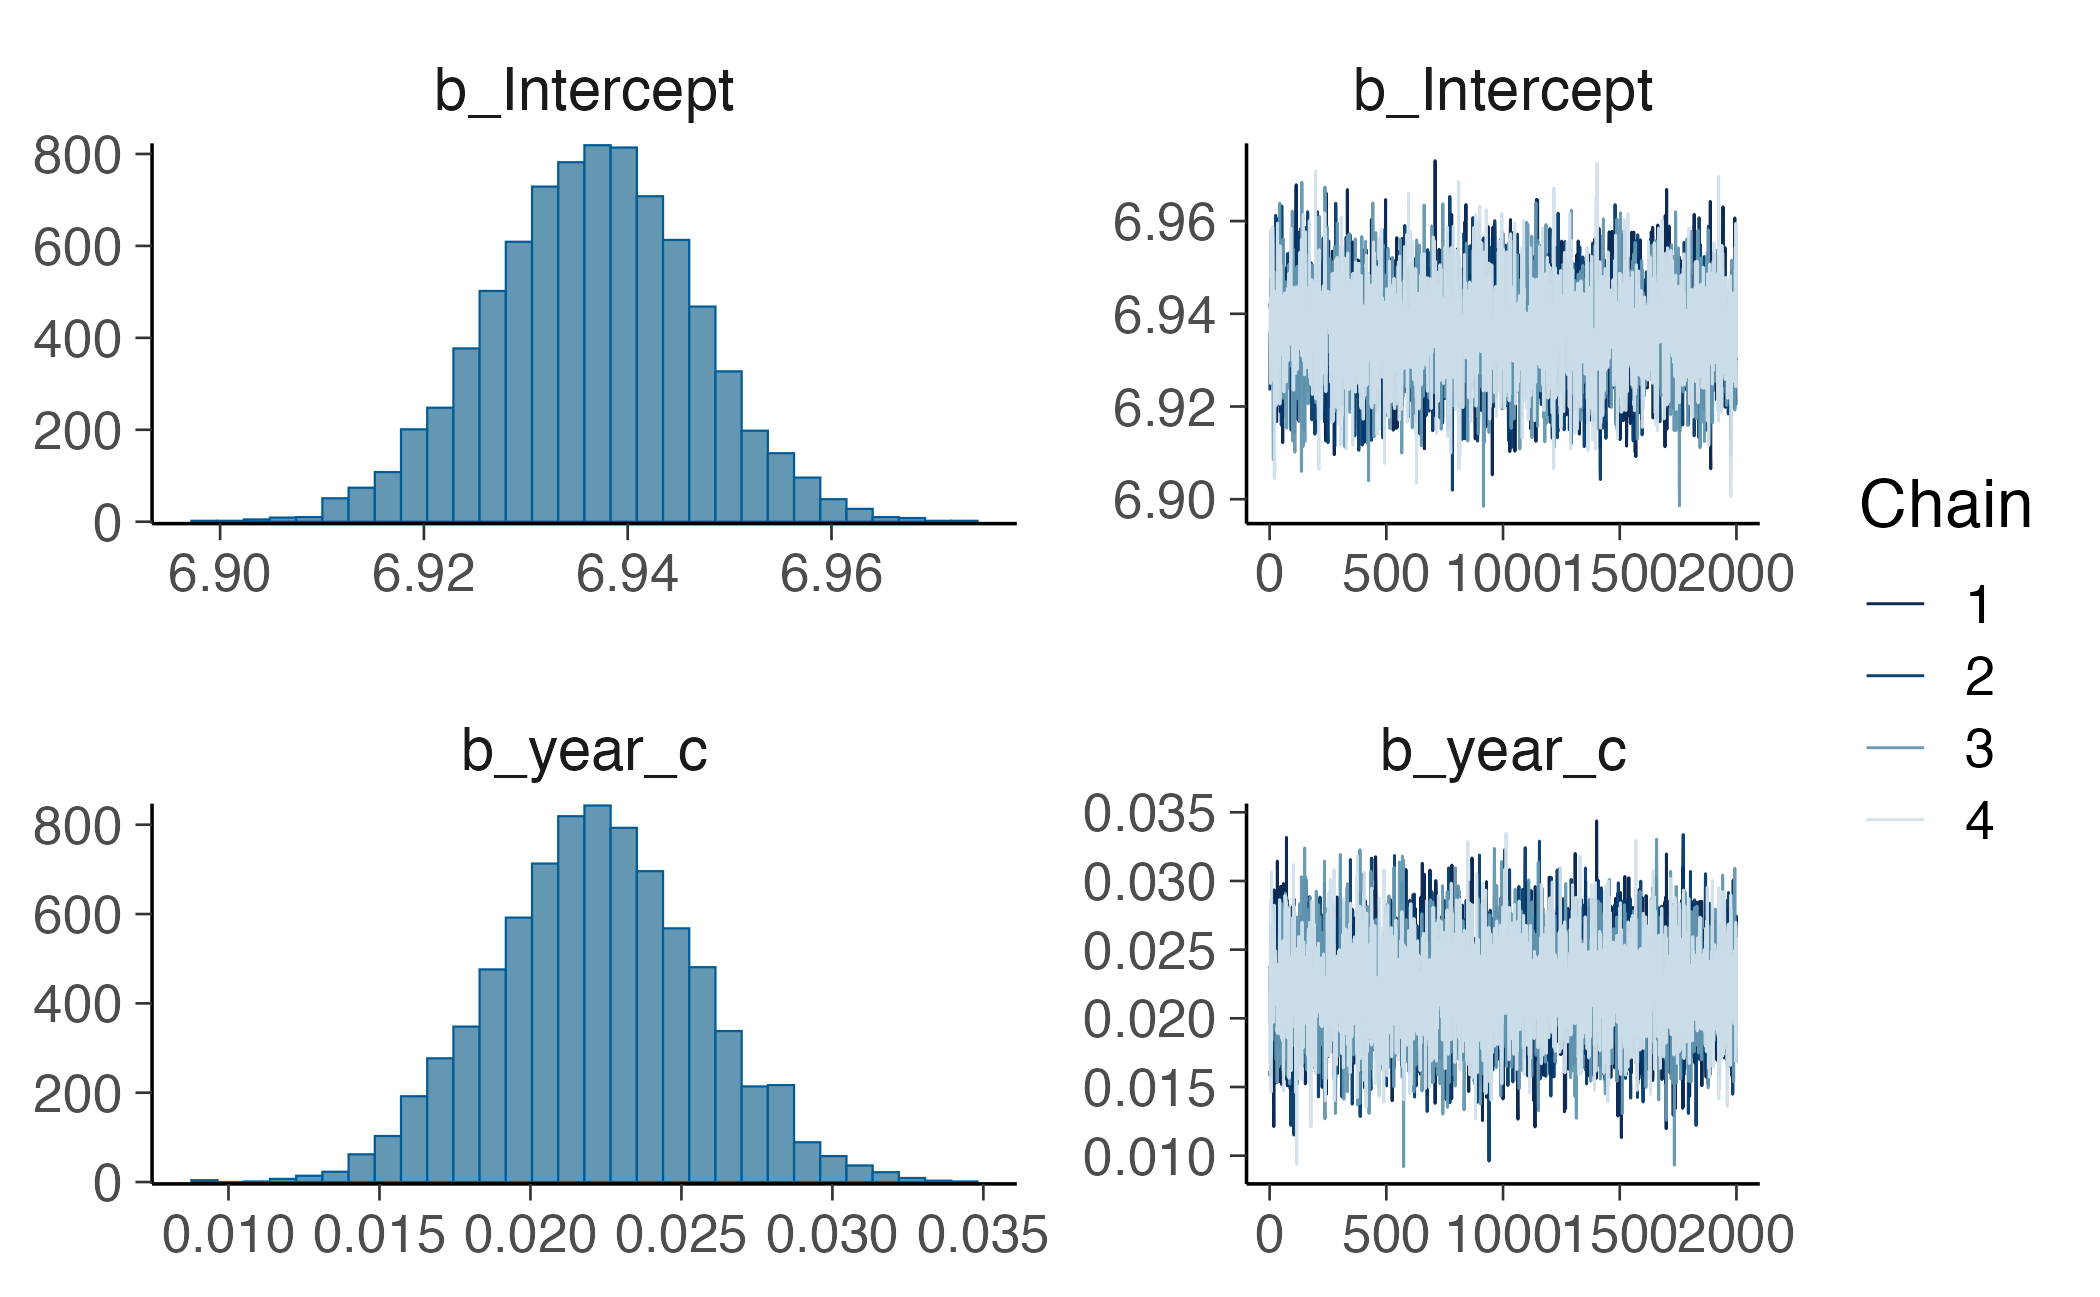
\includegraphics[width=0.85\linewidth,height=\textheight,keepaspectratio]{chapters/glm/03_modelli_conteggio_files/figure-pdf/unnamed-chunk-6-1.png}
\end{center}

Valori di \(\widehat R\) prossimi a 1, dimensioni campionarie effettive
adeguate e assenza di divergenze rendono credibile l'approssimazione
numerica della posterior. Non dimostrano però che la distribuzione di
Poisson o la tendenza lineare siano adeguate.

\section{Interpretazione sulla scala dei
conteggi}\label{interpretazione-sulla-scala-dei-conteggi}

Estraiamo i draw dei coefficienti e li trasformiamo:

\begin{Shaded}
\begin{Highlighting}[]
\NormalTok{poisson\_draws }\OtherTok{\textless{}{-}} \FunctionTok{as\_draws\_df}\NormalTok{(fit\_poisson) }\SpecialCharTok{|\textgreater{}}
  \FunctionTok{transmute}\NormalTok{(}
    \AttributeTok{alpha =}\NormalTok{ b\_Intercept,}
    \AttributeTok{beta =}\NormalTok{ b\_year\_c,}
    \AttributeTok{expected\_2019 =} \FunctionTok{exp}\NormalTok{(alpha),}
    \AttributeTok{IRR\_year =} \FunctionTok{exp}\NormalTok{(beta),}
    \AttributeTok{percent\_change =} \DecValTok{100} \SpecialCharTok{*}\NormalTok{ (IRR\_year }\SpecialCharTok{{-}} \DecValTok{1}\NormalTok{)}
\NormalTok{  )}

\NormalTok{poisson\_draws }\SpecialCharTok{|\textgreater{}}
  \FunctionTok{summarise}\NormalTok{(}
    \AttributeTok{expected\_2019 =} \FunctionTok{median}\NormalTok{(expected\_2019),}
    \AttributeTok{expected\_2019\_low =} \FunctionTok{quantile}\NormalTok{(expected\_2019, }\FloatTok{0.025}\NormalTok{),}
    \AttributeTok{expected\_2019\_high =} \FunctionTok{quantile}\NormalTok{(expected\_2019, }\FloatTok{0.975}\NormalTok{),}
    \AttributeTok{IRR\_year =} \FunctionTok{median}\NormalTok{(IRR\_year),}
    \AttributeTok{IRR\_low =} \FunctionTok{quantile}\NormalTok{(IRR\_year, }\FloatTok{0.025}\NormalTok{),}
    \AttributeTok{IRR\_high =} \FunctionTok{quantile}\NormalTok{(IRR\_year, }\FloatTok{0.975}\NormalTok{),}
    \AttributeTok{Pr\_increase =} \FunctionTok{mean}\NormalTok{(beta }\SpecialCharTok{\textgreater{}} \DecValTok{0}\NormalTok{)}
\NormalTok{  )}
\CommentTok{\#\textgreater{} \# A tibble: 1 x 7}
\CommentTok{\#\textgreater{}   expected\_2019 expected\_2019\_low expected\_2019\_high IRR\_year IRR\_low IRR\_high}
\CommentTok{\#\textgreater{}           \textless{}dbl\textgreater{}             \textless{}dbl\textgreater{}              \textless{}dbl\textgreater{}    \textless{}dbl\textgreater{}   \textless{}dbl\textgreater{}    \textless{}dbl\textgreater{}}
\CommentTok{\#\textgreater{} 1         1029.             1029.              1029.     1.02    1.02     1.02}
\CommentTok{\#\textgreater{}   Pr\_increase}
\CommentTok{\#\textgreater{}         \textless{}dbl\textgreater{}}
\CommentTok{\#\textgreater{} 1           1}
\end{Highlighting}
\end{Shaded}

La trasformazione \(\exp(\alpha)\) restituisce il conteggio atteso nel
2019. La trasformazione \(\exp(\beta)\) restituisce il rapporto tra i
conteggi attesi di due anni consecutivi. La variazione percentuale è

\[
100\,[\exp(\beta)-1].
\]

Questa percentuale è costante nel modello, mentre la variazione assoluta
non lo è. Se il conteggio atteso cresce, la stessa variazione
percentuale corrisponde a un numero assoluto di eventi sempre maggiore.
Per comunicare il risultato è quindi utile mostrare le predizioni
annuali, non soltanto l'IRR.

\begin{Shaded}
\begin{Highlighting}[]
\NormalTok{year\_grid }\OtherTok{\textless{}{-}} \FunctionTok{tibble}\NormalTok{(}
  \AttributeTok{year =} \DecValTok{2015}\SpecialCharTok{:}\DecValTok{2024}\NormalTok{,}
  \AttributeTok{year\_c =}\NormalTok{ year }\SpecialCharTok{{-}} \DecValTok{2019}
\NormalTok{)}

\NormalTok{expected\_draws }\OtherTok{\textless{}{-}} \FunctionTok{posterior\_epred}\NormalTok{(}
\NormalTok{  fit\_poisson,}
  \AttributeTok{newdata =}\NormalTok{ year\_grid}
\NormalTok{)}

\NormalTok{expected\_summary }\OtherTok{\textless{}{-}}\NormalTok{ expected\_draws }\SpecialCharTok{|\textgreater{}}
  \FunctionTok{as\_tibble}\NormalTok{() }\SpecialCharTok{|\textgreater{}}
  \FunctionTok{mutate}\NormalTok{(}\AttributeTok{.draw =} \FunctionTok{row\_number}\NormalTok{()) }\SpecialCharTok{|\textgreater{}}
  \FunctionTok{pivot\_longer}\NormalTok{(}\SpecialCharTok{{-}}\NormalTok{.draw, }\AttributeTok{names\_to =} \StringTok{"row"}\NormalTok{, }\AttributeTok{values\_to =} \StringTok{"lambda"}\NormalTok{) }\SpecialCharTok{|\textgreater{}}
  \FunctionTok{mutate}\NormalTok{(}
    \AttributeTok{row =}\NormalTok{ readr}\SpecialCharTok{::}\FunctionTok{parse\_number}\NormalTok{(row),}
    \AttributeTok{year =}\NormalTok{ year\_grid}\SpecialCharTok{$}\NormalTok{year[row]}
\NormalTok{  ) }\SpecialCharTok{|\textgreater{}}
  \FunctionTok{group\_by}\NormalTok{(year) }\SpecialCharTok{|\textgreater{}}
  \FunctionTok{summarise}\NormalTok{(}
    \AttributeTok{median =} \FunctionTok{median}\NormalTok{(lambda),}
    \AttributeTok{lower =} \FunctionTok{quantile}\NormalTok{(lambda, }\FloatTok{0.025}\NormalTok{),}
    \AttributeTok{upper =} \FunctionTok{quantile}\NormalTok{(lambda, }\FloatTok{0.975}\NormalTok{),}
    \AttributeTok{.groups =} \StringTok{"drop"}
\NormalTok{  )}

\FunctionTok{ggplot}\NormalTok{(expected\_summary, }\FunctionTok{aes}\NormalTok{(year, median)) }\SpecialCharTok{+}
  \FunctionTok{geom\_ribbon}\NormalTok{(}\FunctionTok{aes}\NormalTok{(}\AttributeTok{ymin =}\NormalTok{ lower, }\AttributeTok{ymax =}\NormalTok{ upper), }\AttributeTok{alpha =} \FloatTok{0.20}\NormalTok{) }\SpecialCharTok{+}
  \FunctionTok{geom\_line}\NormalTok{() }\SpecialCharTok{+}
  \FunctionTok{geom\_point}\NormalTok{(}
    \AttributeTok{data =}\NormalTok{ shooting\_counts,}
    \FunctionTok{aes}\NormalTok{(}\AttributeTok{y =}\NormalTok{ events)}
\NormalTok{  ) }\SpecialCharTok{+}
  \FunctionTok{labs}\NormalTok{(}
    \AttributeTok{x =} \StringTok{"Anno"}\NormalTok{,}
    \AttributeTok{y =} \StringTok{"Conteggio annuale atteso"}
\NormalTok{  )}
\end{Highlighting}
\end{Shaded}

\begin{center}
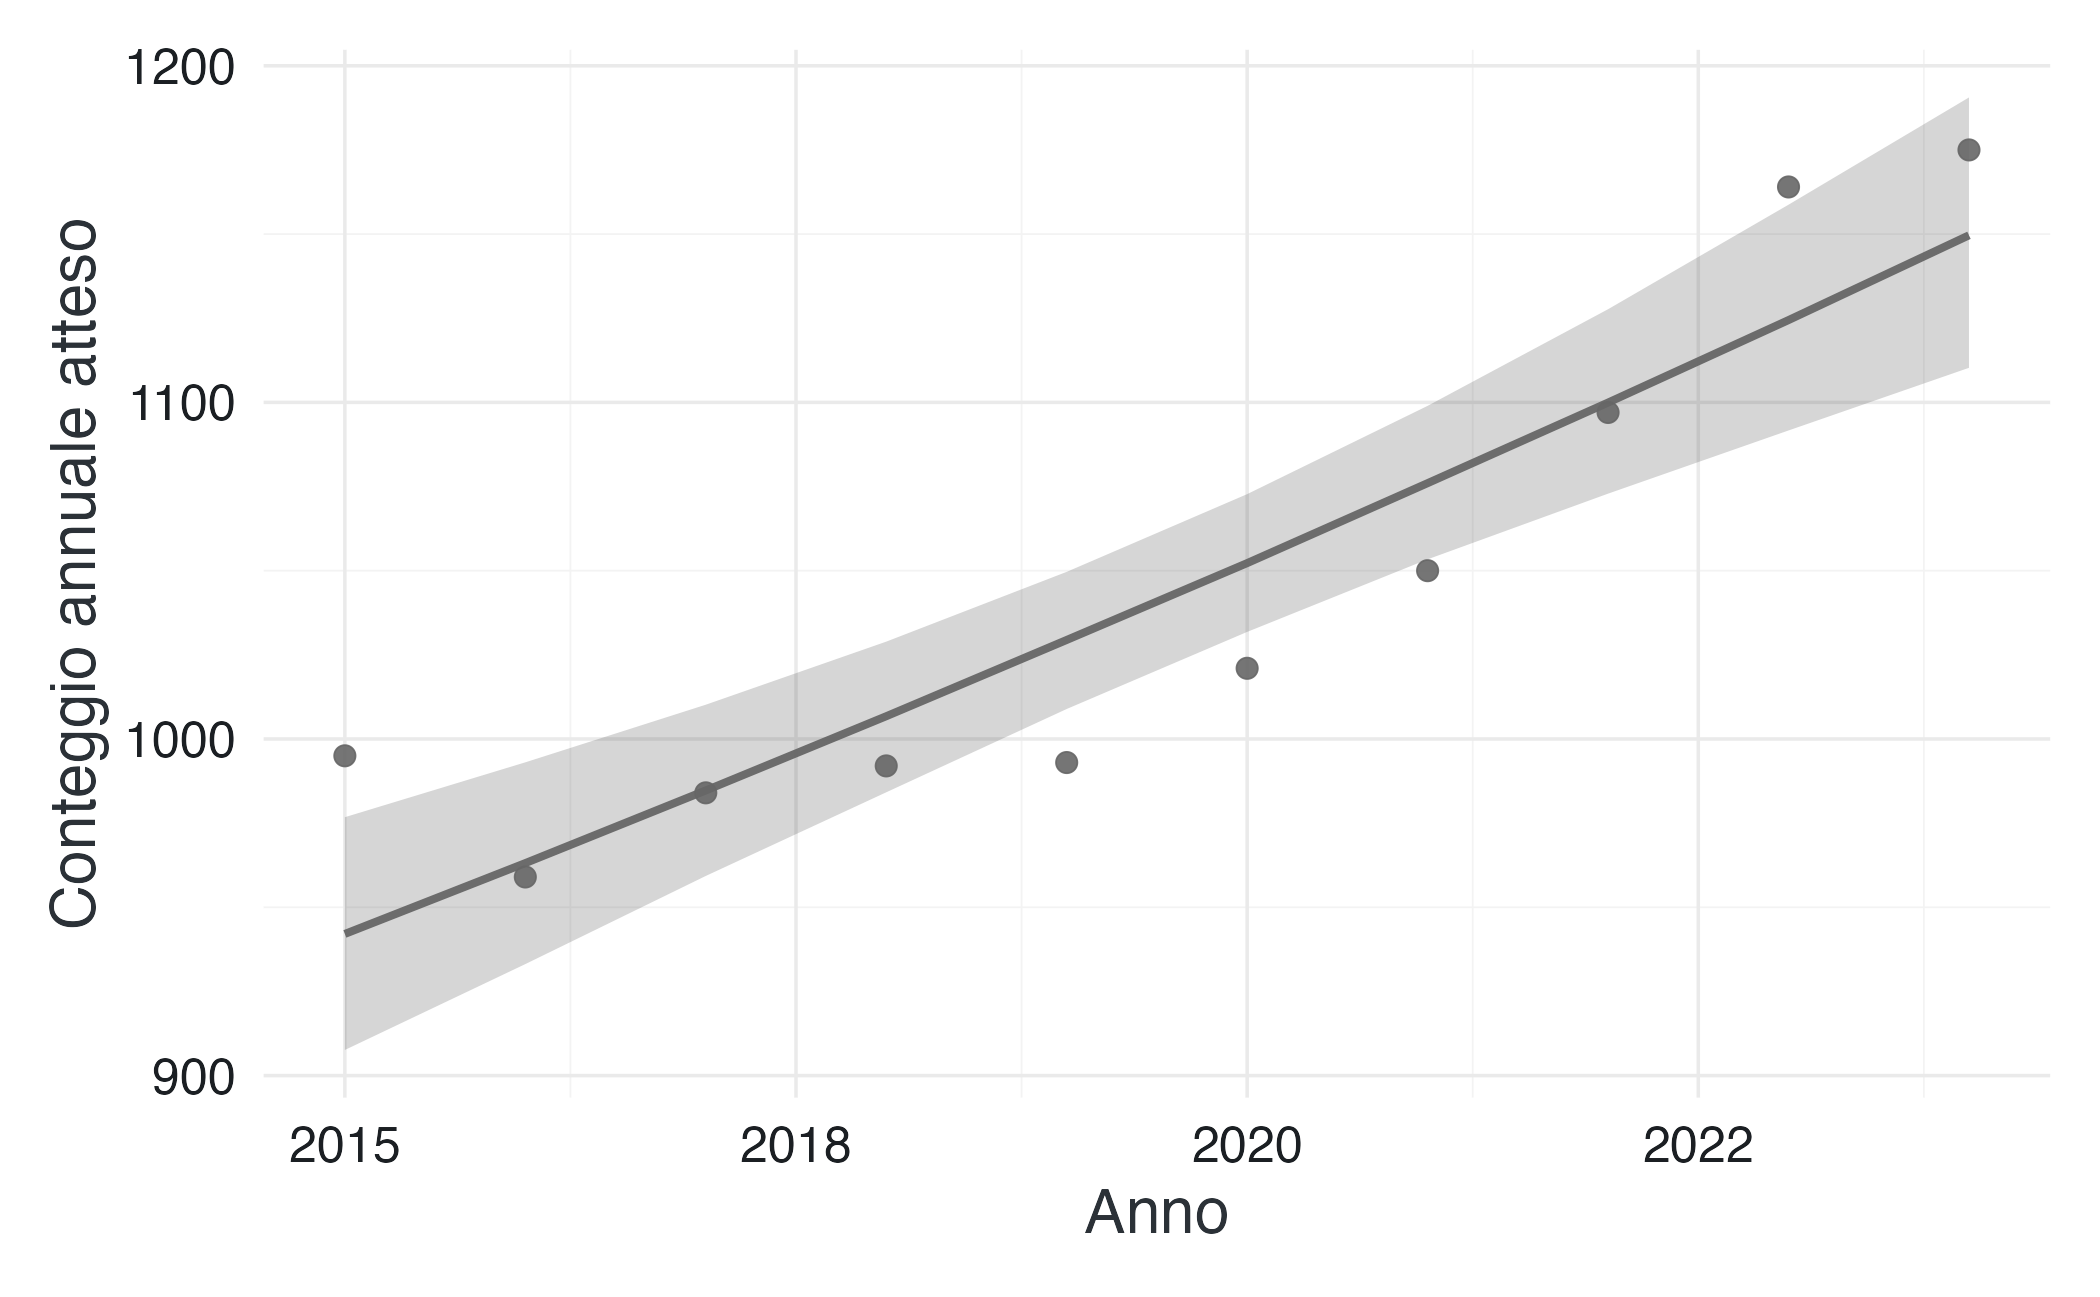
\includegraphics[width=0.85\linewidth,height=\textheight,keepaspectratio]{chapters/glm/03_modelli_conteggio_files/figure-pdf/unnamed-chunk-8-1.png}
\end{center}

La banda rappresenta l'incertezza sulla media condizionata
\(\lambda_t\). Non rappresenta ancora la variabilità di un nuovo
conteggio annuale, che comprende anche la variabilità di Poisson.

\section{Controllo predittivo a
posteriori}\label{controllo-predittivo-a-posteriori-2}

Per controllare il modello generiamo nuovi conteggi dalla distribuzione
predittiva:

\begin{Shaded}
\begin{Highlighting}[]
\NormalTok{y\_rep\_poisson }\OtherTok{\textless{}{-}} \FunctionTok{posterior\_predict}\NormalTok{(fit\_poisson)}

\NormalTok{predicted\_intervals }\OtherTok{\textless{}{-}} \FunctionTok{as\_tibble}\NormalTok{(y\_rep\_poisson) }\SpecialCharTok{|\textgreater{}}
  \FunctionTok{mutate}\NormalTok{(}\AttributeTok{.draw =} \FunctionTok{row\_number}\NormalTok{()) }\SpecialCharTok{|\textgreater{}}
  \FunctionTok{pivot\_longer}\NormalTok{(}\SpecialCharTok{{-}}\NormalTok{.draw, }\AttributeTok{names\_to =} \StringTok{"row"}\NormalTok{, }\AttributeTok{values\_to =} \StringTok{"events\_rep"}\NormalTok{) }\SpecialCharTok{|\textgreater{}}
  \FunctionTok{mutate}\NormalTok{(}
    \AttributeTok{row =}\NormalTok{ readr}\SpecialCharTok{::}\FunctionTok{parse\_number}\NormalTok{(row),}
    \AttributeTok{year =}\NormalTok{ shooting\_counts}\SpecialCharTok{$}\NormalTok{year[row]}
\NormalTok{  ) }\SpecialCharTok{|\textgreater{}}
  \FunctionTok{group\_by}\NormalTok{(year) }\SpecialCharTok{|\textgreater{}}
  \FunctionTok{summarise}\NormalTok{(}
    \AttributeTok{median =} \FunctionTok{median}\NormalTok{(events\_rep),}
    \AttributeTok{lower =} \FunctionTok{quantile}\NormalTok{(events\_rep, }\FloatTok{0.025}\NormalTok{),}
    \AttributeTok{upper =} \FunctionTok{quantile}\NormalTok{(events\_rep, }\FloatTok{0.975}\NormalTok{),}
    \AttributeTok{.groups =} \StringTok{"drop"}
\NormalTok{  )}

\FunctionTok{ggplot}\NormalTok{(predicted\_intervals, }\FunctionTok{aes}\NormalTok{(year, median)) }\SpecialCharTok{+}
  \FunctionTok{geom\_ribbon}\NormalTok{(}\FunctionTok{aes}\NormalTok{(}\AttributeTok{ymin =}\NormalTok{ lower, }\AttributeTok{ymax =}\NormalTok{ upper), }\AttributeTok{alpha =} \FloatTok{0.20}\NormalTok{) }\SpecialCharTok{+}
  \FunctionTok{geom\_line}\NormalTok{() }\SpecialCharTok{+}
  \FunctionTok{geom\_point}\NormalTok{(}
    \AttributeTok{data =}\NormalTok{ shooting\_counts,}
    \FunctionTok{aes}\NormalTok{(}\AttributeTok{y =}\NormalTok{ events)}
\NormalTok{  ) }\SpecialCharTok{+}
  \FunctionTok{labs}\NormalTok{(}
    \AttributeTok{x =} \StringTok{"Anno"}\NormalTok{,}
    \AttributeTok{y =} \StringTok{"Conteggio annuale"}
\NormalTok{  )}
\end{Highlighting}
\end{Shaded}

\begin{center}
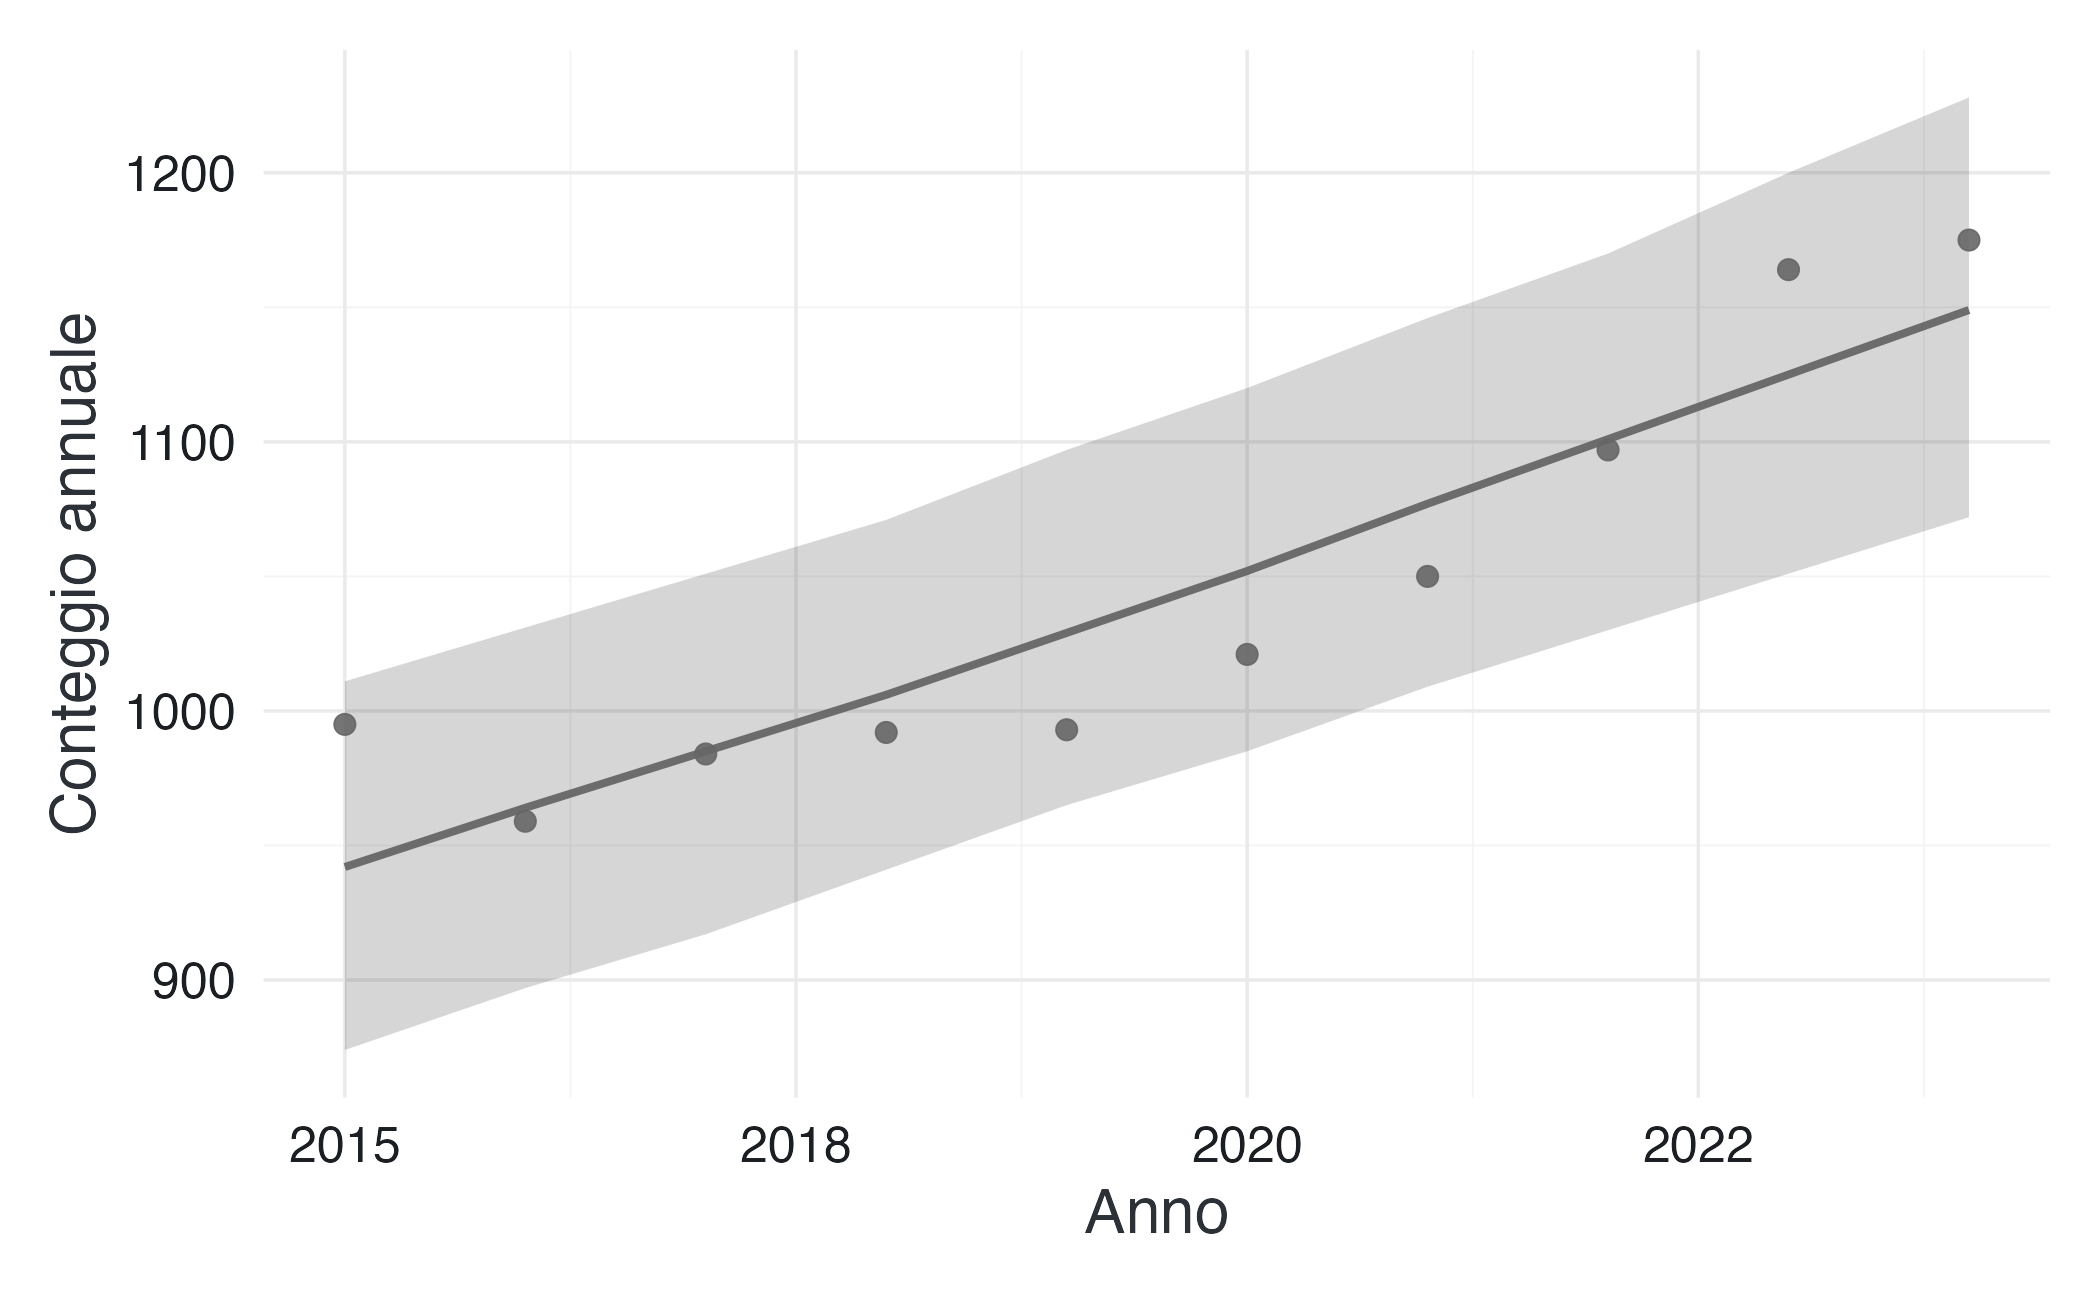
\includegraphics[width=0.85\linewidth,height=\textheight,keepaspectratio]{chapters/glm/03_modelli_conteggio_files/figure-pdf/unnamed-chunk-9-1.png}
\end{center}

Questo controllo mostra se i singoli conteggi osservati appaiano
plausibili rispetto alle repliche del modello. È utile affiancarlo a una
statistica sensibile alla dispersione condizionata. Per ogni draw
calcoliamo una discrepanza di Pearson:

\[
T(\mathbf y,\boldsymbol\lambda)
=
\sum_i\frac{(y_i-\lambda_i)^2}{\lambda_i}.
\]

\begin{Shaded}
\begin{Highlighting}[]
\NormalTok{mu\_poisson }\OtherTok{\textless{}{-}} \FunctionTok{posterior\_epred}\NormalTok{(fit\_poisson)}
\NormalTok{y\_obs }\OtherTok{\textless{}{-}}\NormalTok{ shooting\_counts}\SpecialCharTok{$}\NormalTok{events}

\NormalTok{T\_obs }\OtherTok{\textless{}{-}} \FunctionTok{vapply}\NormalTok{(}
  \FunctionTok{seq\_len}\NormalTok{(}\FunctionTok{nrow}\NormalTok{(mu\_poisson)),}
  \ControlFlowTok{function}\NormalTok{(s) }\FunctionTok{sum}\NormalTok{((y\_obs }\SpecialCharTok{{-}}\NormalTok{ mu\_poisson[s, ])}\SpecialCharTok{\^{}}\DecValTok{2} \SpecialCharTok{/}\NormalTok{ mu\_poisson[s, ]),}
  \FunctionTok{numeric}\NormalTok{(}\DecValTok{1}\NormalTok{)}
\NormalTok{)}

\NormalTok{T\_rep }\OtherTok{\textless{}{-}} \FunctionTok{vapply}\NormalTok{(}
  \FunctionTok{seq\_len}\NormalTok{(}\FunctionTok{nrow}\NormalTok{(mu\_poisson)),}
  \ControlFlowTok{function}\NormalTok{(s) }\FunctionTok{sum}\NormalTok{((y\_rep\_poisson[s, ] }\SpecialCharTok{{-}}\NormalTok{ mu\_poisson[s, ])}\SpecialCharTok{\^{}}\DecValTok{2} \SpecialCharTok{/}\NormalTok{ mu\_poisson[s, ]),}
  \FunctionTok{numeric}\NormalTok{(}\DecValTok{1}\NormalTok{)}
\NormalTok{)}

\NormalTok{dispersion\_check }\OtherTok{\textless{}{-}} \FunctionTok{bind\_rows}\NormalTok{(}
  \FunctionTok{tibble}\NormalTok{(}\AttributeTok{discrepancy =}\NormalTok{ T\_obs, }\AttributeTok{source =} \StringTok{"Dati osservati"}\NormalTok{),}
  \FunctionTok{tibble}\NormalTok{(}\AttributeTok{discrepancy =}\NormalTok{ T\_rep, }\AttributeTok{source =} \StringTok{"Repliche posteriori"}\NormalTok{)}
\NormalTok{)}

\FunctionTok{ggplot}\NormalTok{(dispersion\_check, }\FunctionTok{aes}\NormalTok{(discrepancy, }\AttributeTok{fill =}\NormalTok{ source)) }\SpecialCharTok{+}
  \FunctionTok{geom\_density}\NormalTok{(}\AttributeTok{alpha =} \FloatTok{0.35}\NormalTok{) }\SpecialCharTok{+}
  \FunctionTok{labs}\NormalTok{(}
    \AttributeTok{x =} \StringTok{"Discrepanza di Pearson"}\NormalTok{,}
    \AttributeTok{y =} \StringTok{"Densità"}\NormalTok{,}
    \AttributeTok{fill =} \ConstantTok{NULL}
\NormalTok{  )}

\FunctionTok{mean}\NormalTok{(T\_rep }\SpecialCharTok{\textgreater{}=}\NormalTok{ T\_obs)}
\CommentTok{\#\textgreater{} [1] 0.453}
\end{Highlighting}
\end{Shaded}

\begin{center}
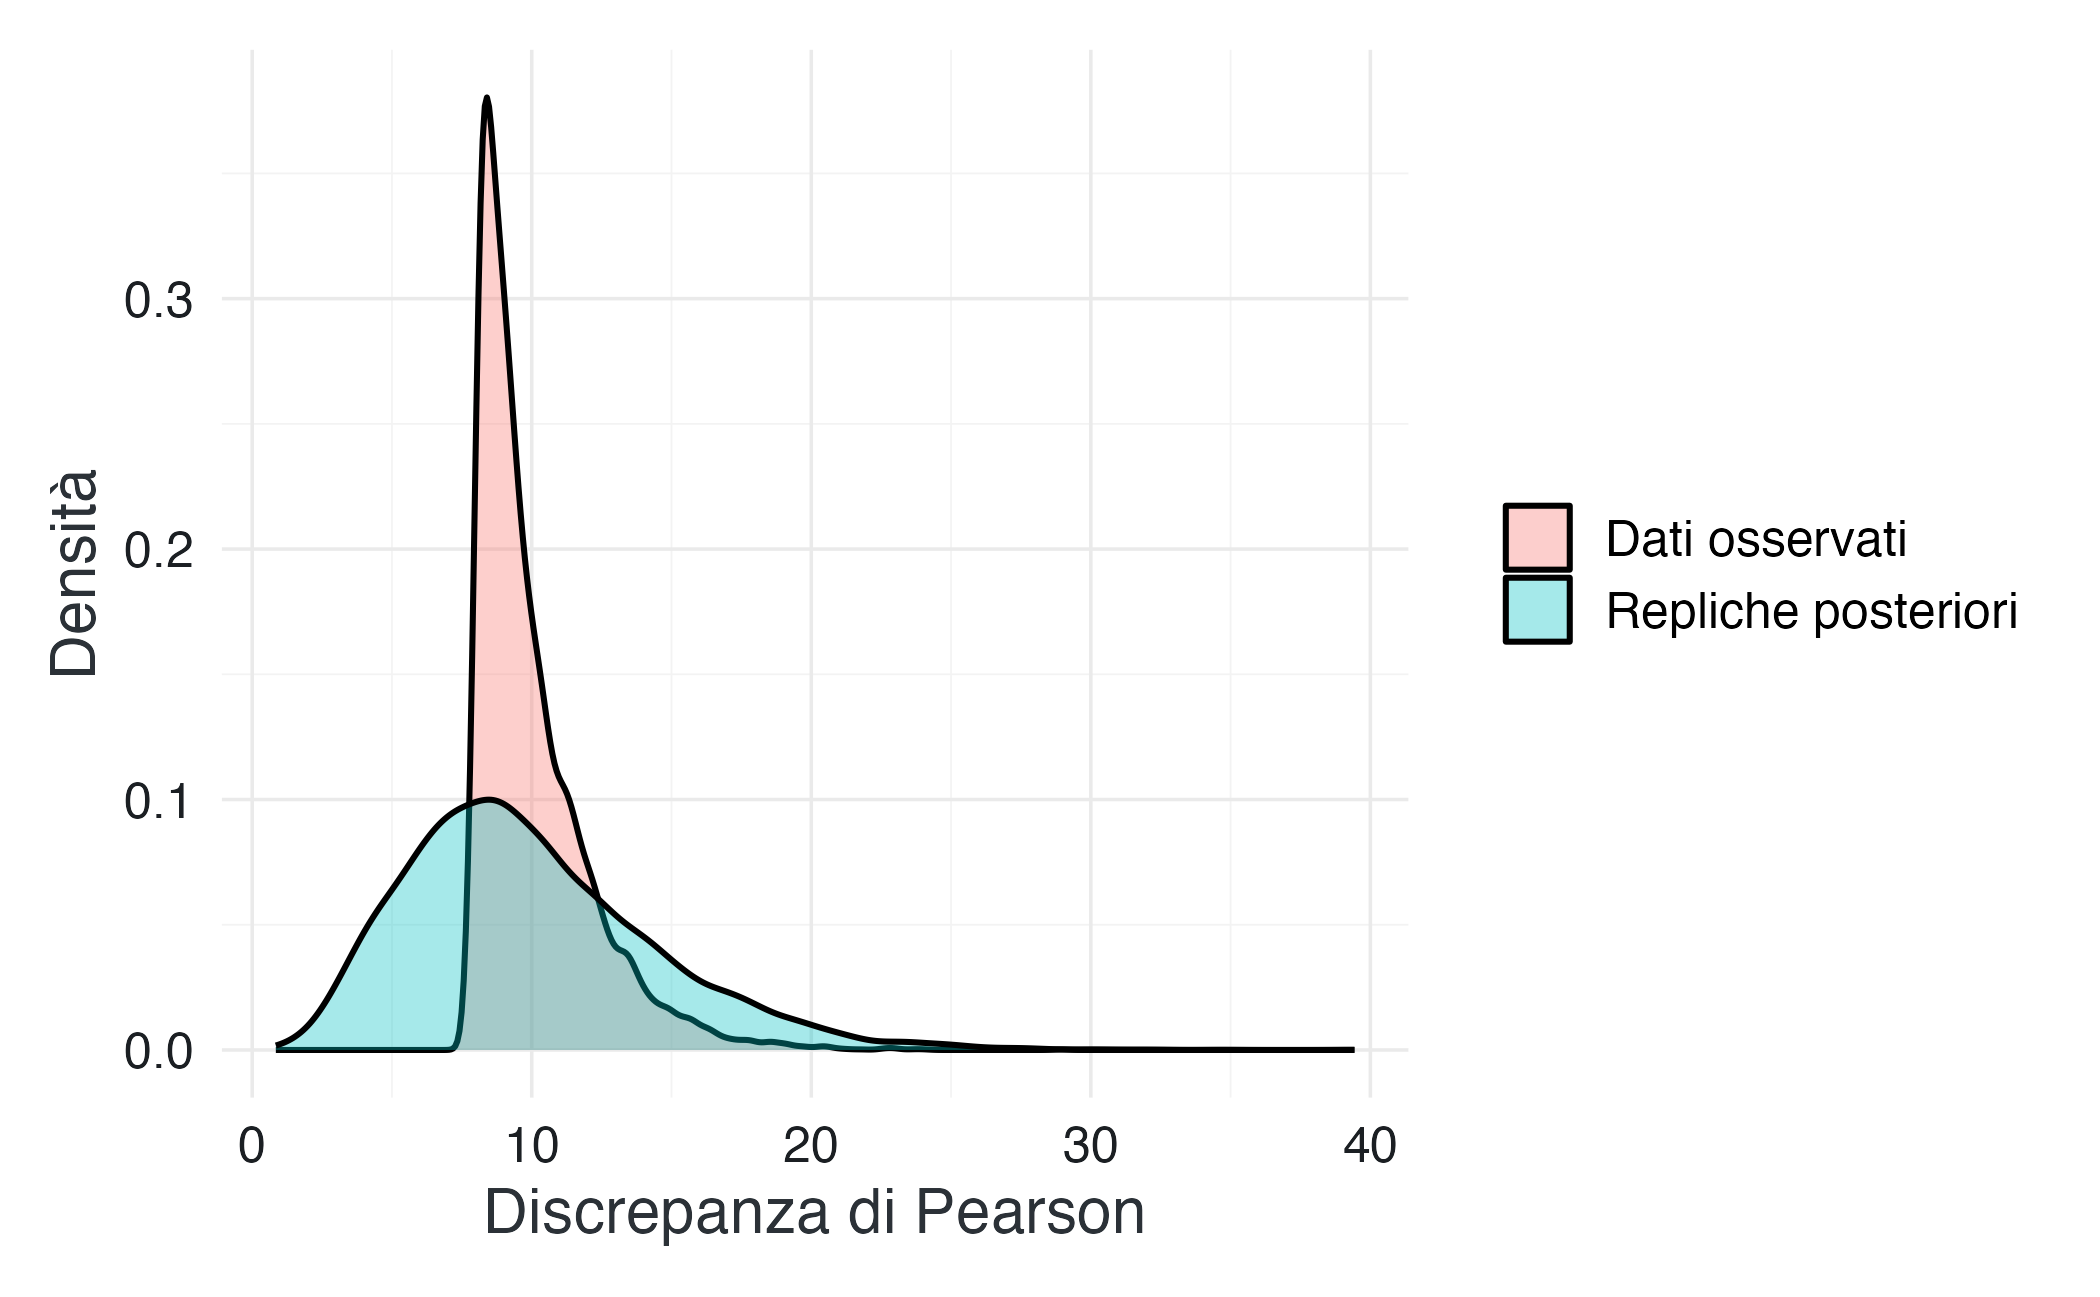
\includegraphics[width=0.85\linewidth,height=\textheight,keepaspectratio]{chapters/glm/03_modelli_conteggio_files/figure-pdf/unnamed-chunk-10-1.png}
\end{center}

Più che affidarsi a una soglia automatica, occorre osservare se la
discrepanza dei dati reali sia sistematicamente maggiore di quella delle
repliche. Un tale pattern suggerirebbe che la distribuzione di Poisson
produce dati troppo regolari. Il controllo deve comunque essere
interpretato insieme ai grafici temporali: una discrepanza elevata
potrebbe derivare anche da non linearità, cambiamenti strutturali o
dipendenza seriale.

\section{Quando il Poisson è troppo
rigido}\label{quando-il-poisson-uxe8-troppo-rigido}

Nel modello di Poisson la varianza condizionata è determinata
interamente dalla media. Molti fenomeni psicologici e sociali presentano
invece eterogeneità non osservata: persone, periodi o contesti con lo
stesso valore dei predittori possono avere propensioni differenti a
produrre eventi. Questa eterogeneità genera spesso
\textbf{sovradispersione}, cioè una variabilità condizionata maggiore di
quella ammessa dal Poisson.

Una soluzione comune è il modello binomiale negativo. Una
parametrizzazione usata da \texttt{brms} è

\[
Y_i\sim\operatorname{NegBinomial}(\mu_i,\phi),
\]

con

\[
\mathbb E(Y_i)=\mu_i,
\qquad
\operatorname{Var}(Y_i)
=
\mu_i+\frac{\mu_i^2}{\phi}.
\]

Il parametro \(\phi>0\) controlla la dispersione supplementare. Quando
\(\phi\) è grande, la varianza si avvicina a quella di Poisson; quando è
piccolo, il modello ammette una variabilità maggiore.

Adattiamo il modello alternativo mantenendo lo stesso predittore
lineare:

\begin{Shaded}
\begin{Highlighting}[]
\NormalTok{negative\_binomial\_priors }\OtherTok{\textless{}{-}} \FunctionTok{c}\NormalTok{(}
\NormalTok{  poisson\_priors,}
  \FunctionTok{prior}\NormalTok{(}\FunctionTok{gamma}\NormalTok{(}\DecValTok{2}\NormalTok{, }\FloatTok{0.1}\NormalTok{), }\AttributeTok{class =}\NormalTok{ shape)}
\NormalTok{)}

\NormalTok{fit\_negative\_binomial }\OtherTok{\textless{}{-}} \FunctionTok{brm}\NormalTok{(}
\NormalTok{  events }\SpecialCharTok{\textasciitilde{}} \DecValTok{1} \SpecialCharTok{+}\NormalTok{ year\_c,}
  \AttributeTok{data =}\NormalTok{ shooting\_counts,}
  \AttributeTok{family =} \FunctionTok{negbinomial}\NormalTok{(}\AttributeTok{link =} \StringTok{"log"}\NormalTok{),}
  \AttributeTok{prior =}\NormalTok{ negative\_binomial\_priors,}
  \AttributeTok{chains =} \DecValTok{4}\NormalTok{,}
  \AttributeTok{iter =} \DecValTok{3000}\NormalTok{,}
  \AttributeTok{warmup =} \DecValTok{1000}\NormalTok{,}
  \AttributeTok{seed =} \DecValTok{2026}\NormalTok{,}
  \AttributeTok{refresh =} \DecValTok{0}
\NormalTok{)}
\CommentTok{\#\textgreater{} Running MCMC with 4 chains, at most 10 in parallel...}
\CommentTok{\#\textgreater{} }
\CommentTok{\#\textgreater{} Chain 1 finished in 0.1 seconds.}
\CommentTok{\#\textgreater{} Chain 2 finished in 0.1 seconds.}
\CommentTok{\#\textgreater{} Chain 3 finished in 0.1 seconds.}
\CommentTok{\#\textgreater{} Chain 4 finished in 0.0 seconds.}
\CommentTok{\#\textgreater{} }
\CommentTok{\#\textgreater{} All 4 chains finished successfully.}
\CommentTok{\#\textgreater{} Mean chain execution time: 0.1 seconds.}
\CommentTok{\#\textgreater{} Total execution time: 0.3 seconds.}

\FunctionTok{summary}\NormalTok{(fit\_negative\_binomial)}
\CommentTok{\#\textgreater{}  Family: negbinomial }
\CommentTok{\#\textgreater{}   Links: mu = log }
\CommentTok{\#\textgreater{} Formula: events \textasciitilde{} 1 + year\_c }
\CommentTok{\#\textgreater{}    Data: shooting\_counts (Number of observations: 10) }
\CommentTok{\#\textgreater{}   Draws: 4 chains, each with iter = 3000; warmup = 1000; thin = 1;}
\CommentTok{\#\textgreater{}          total post{-}warmup draws = 8000}
\CommentTok{\#\textgreater{} }
\CommentTok{\#\textgreater{} Regression Coefficients:}
\CommentTok{\#\textgreater{}           Estimate Est.Error l{-}95\% CI u{-}95\% CI Rhat Bulk\_ESS Tail\_ESS}
\CommentTok{\#\textgreater{} Intercept     6.94      0.05     6.85     7.03 1.00     5969     4089}
\CommentTok{\#\textgreater{} year\_c        0.02      0.02    {-}0.01     0.05 1.00     5563     4312}
\CommentTok{\#\textgreater{} }
\CommentTok{\#\textgreater{} Further Distributional Parameters:}
\CommentTok{\#\textgreater{}       Estimate Est.Error l{-}95\% CI u{-}95\% CI Rhat Bulk\_ESS Tail\_ESS}
\CommentTok{\#\textgreater{} shape    57.09     23.13    20.93   111.01 1.00     4983     4407}
\CommentTok{\#\textgreater{} }
\CommentTok{\#\textgreater{} Draws were sampled using sample(hmc). For each parameter, Bulk\_ESS}
\CommentTok{\#\textgreater{} and Tail\_ESS are effective sample size measures, and Rhat is the potential}
\CommentTok{\#\textgreater{} scale reduction factor on split chains (at convergence, Rhat = 1).}
\end{Highlighting}
\end{Shaded}

La scelta tra Poisson e binomiale negativo non dovrebbe dipendere dal
fatto che il secondo modello sia più flessibile in astratto. Dovrebbe
essere guidata dalle implicazioni predittive. Ripetiamo quindi il
controllo sulla dispersione e osserviamo se il modello alternativo
riproduce meglio la variabilità senza introdurre un'incertezza
inutilmente ampia.

\begin{Shaded}
\begin{Highlighting}[]
\NormalTok{y\_rep\_nb }\OtherTok{\textless{}{-}} \FunctionTok{posterior\_predict}\NormalTok{(fit\_negative\_binomial)}
\NormalTok{mu\_nb }\OtherTok{\textless{}{-}} \FunctionTok{posterior\_epred}\NormalTok{(fit\_negative\_binomial)}

\NormalTok{T\_obs\_nb }\OtherTok{\textless{}{-}} \FunctionTok{vapply}\NormalTok{(}
  \FunctionTok{seq\_len}\NormalTok{(}\FunctionTok{nrow}\NormalTok{(mu\_nb)),}
  \ControlFlowTok{function}\NormalTok{(s) }\FunctionTok{sum}\NormalTok{((y\_obs }\SpecialCharTok{{-}}\NormalTok{ mu\_nb[s, ])}\SpecialCharTok{\^{}}\DecValTok{2} \SpecialCharTok{/} \FunctionTok{pmax}\NormalTok{(mu\_nb[s, ], }\FloatTok{1e{-}8}\NormalTok{)),}
  \FunctionTok{numeric}\NormalTok{(}\DecValTok{1}\NormalTok{)}
\NormalTok{)}

\NormalTok{T\_rep\_nb }\OtherTok{\textless{}{-}} \FunctionTok{vapply}\NormalTok{(}
  \FunctionTok{seq\_len}\NormalTok{(}\FunctionTok{nrow}\NormalTok{(mu\_nb)),}
  \ControlFlowTok{function}\NormalTok{(s) }\FunctionTok{sum}\NormalTok{((y\_rep\_nb[s, ] }\SpecialCharTok{{-}}\NormalTok{ mu\_nb[s, ])}\SpecialCharTok{\^{}}\DecValTok{2} \SpecialCharTok{/} \FunctionTok{pmax}\NormalTok{(mu\_nb[s, ], }\FloatTok{1e{-}8}\NormalTok{)),}
  \FunctionTok{numeric}\NormalTok{(}\DecValTok{1}\NormalTok{)}
\NormalTok{)}

\FunctionTok{tibble}\NormalTok{(}
  \AttributeTok{model =} \FunctionTok{c}\NormalTok{(}\StringTok{"Poisson"}\NormalTok{, }\StringTok{"Binomiale negativa"}\NormalTok{),}
  \AttributeTok{posterior\_predictive\_probability =} \FunctionTok{c}\NormalTok{(}
    \FunctionTok{mean}\NormalTok{(T\_rep }\SpecialCharTok{\textgreater{}=}\NormalTok{ T\_obs),}
    \FunctionTok{mean}\NormalTok{(T\_rep\_nb }\SpecialCharTok{\textgreater{}=}\NormalTok{ T\_obs\_nb)}
\NormalTok{  )}
\NormalTok{)}
\CommentTok{\#\textgreater{} \# A tibble: 2 x 2}
\CommentTok{\#\textgreater{}   model              posterior\_predictive\_probability}
\CommentTok{\#\textgreater{}   \textless{}chr\textgreater{}                                         \textless{}dbl\textgreater{}}
\CommentTok{\#\textgreater{} 1 Poisson                                       0.453}
\CommentTok{\#\textgreater{} 2 Binomiale negativa                            0.964}
\end{Highlighting}
\end{Shaded}

Questa sintesi è soltanto diagnostica. Non stabilisce quale modello sia
``vero'' e non sostituisce l'ispezione dei pattern che ciascun modello
riesce o non riesce a riprodurre. Con pochi anni di osservazione,
inoltre, il parametro di dispersione può risultare debolmente
identificato. In tal caso è preferibile comunicare l'incertezza e non
attribuire un significato sostantivo eccessivo alla scelta tra le due
famiglie.

\section{Che cosa il modello non
dice}\label{che-cosa-il-modello-non-dice}

Una pendenza temporale positiva descrive un'associazione tra anno e
conteggio atteso nel periodo analizzato. Non identifica le cause della
variazione e non consente, da sola, di distinguere cambiamenti reali da
cambiamenti nella popolazione esposta, nella registrazione degli eventi
o in altre condizioni storiche.

Il modello non rappresenta neppure un processo temporale completo. Gli
anni vengono trattati come osservazioni condizionalmente indipendenti
attorno a una tendenza regolare. Se il fenomeno presenta
autocorrelazione, discontinuità o dinamiche di feedback, occorre una
struttura diversa. Questa limitazione prepara il passaggio dal GLM, che
specifica una distribuzione condizionata dell'outcome, ai modelli
processuali sviluppati nella parte \textbf{Applicazione}.

\section*{Riflessioni conclusive}\label{riflessioni-conclusive-33}

\markright{Riflessioni conclusive}

Il modello di Poisson conserva l'architettura già incontrata nei GLM
binari. La distribuzione osservazionale descrive ora un conteggio, il
link logaritmico mantiene positivo il valore atteso e i coefficienti
assumono un'interpretazione moltiplicativa. Questa continuità è il punto
didattico centrale: non occorre imparare una procedura completamente
nuova, ma riconoscere come cambia il modello generativo quando cambia lo
spazio dei possibili outcome.

La semplicità del Poisson è anche il suo limite. Il vincolo che lega
media e varianza condizionate può risultare troppo restrittivo. I
controlli predittivi permettono di valutare questa ipotesi e, quando
necessario, di passare a una distribuzione binomiale negativa.
L'estensione non deve però diventare automatica: una variabilità
inattesa può indicare sovradispersione, ma anche una relazione non
lineare, dipendenza tra osservazioni, esposizioni differenti o covariate
omesse.

Il capitolo mostra quindi due livelli di estensione. Il primo porta dal
modello gaussiano a una distribuzione adatta ai conteggi. Il secondo
porta da una prima specificazione semplice a una versione più flessibile
quando le repliche del modello non riproducono aspetti rilevanti dei
dati. Nel prossimo capitolo compiremo un passaggio diverso: dalla
modellazione della distribuzione delle risposte alla rappresentazione di
un processo che evolve nel tempo e genera quelle risposte.

\begin{tcolorbox}[enhanced jigsaw, arc=.35mm, bottomrule=.15mm, bottomtitle=1mm, breakable, colback=white, colbacktitle=quarto-callout-note-color!10!white, colframe=quarto-callout-note-color-frame, coltitle=black, left=2mm, leftrule=.75mm, opacityback=0, opacitybacktitle=0.6, rightrule=.15mm, title=\textcolor{quarto-callout-note-color}{\faInfo}\hspace{0.5em}{Informazioni sull'ambiente di sviluppo}, titlerule=0mm, toprule=.15mm, toptitle=1mm]

\begin{Shaded}
\begin{Highlighting}[]
\FunctionTok{sessionInfo}\NormalTok{()}
\CommentTok{\#\textgreater{} R version 4.6.1 (2026{-}06{-}24)}
\CommentTok{\#\textgreater{} Platform: aarch64{-}apple{-}darwin23}
\CommentTok{\#\textgreater{} Running under: macOS Tahoe 26.5.2}
\CommentTok{\#\textgreater{} }
\CommentTok{\#\textgreater{} Matrix products: default}
\CommentTok{\#\textgreater{} BLAS:   /Library/Frameworks/R.framework/Versions/4.6/Resources/lib/libRblas.0.dylib }
\CommentTok{\#\textgreater{} LAPACK: /Library/Frameworks/R.framework/Versions/4.6/Resources/lib/libRlapack.dylib;  LAPACK version 3.12.1}
\CommentTok{\#\textgreater{} }
\CommentTok{\#\textgreater{} locale:}
\CommentTok{\#\textgreater{} [1] C.UTF{-}8/UTF{-}8/C.UTF{-}8/C/C.UTF{-}8/C.UTF{-}8}
\CommentTok{\#\textgreater{} }
\CommentTok{\#\textgreater{} time zone: Europe/Zagreb}
\CommentTok{\#\textgreater{} tzcode source: internal}
\CommentTok{\#\textgreater{} }
\CommentTok{\#\textgreater{} attached base packages:}
\CommentTok{\#\textgreater{} [1] stats     graphics  grDevices utils     datasets  methods   base     }
\CommentTok{\#\textgreater{} }
\CommentTok{\#\textgreater{} other attached packages:}
\CommentTok{\#\textgreater{}  [1] readr\_2.2.0           scales\_1.4.0          ragg\_1.5.2           }
\CommentTok{\#\textgreater{}  [4] tinytable\_0.17.0      withr\_3.0.3           systemfonts\_1.3.2    }
\CommentTok{\#\textgreater{}  [7] patchwork\_1.3.2       ggdist\_3.3.3          tidybayes\_3.0.7      }
\CommentTok{\#\textgreater{} [10] bayesplot\_1.15.0      ggplot2\_4.0.3         reliabilitydiag\_0.2.1}
\CommentTok{\#\textgreater{} [13] priorsense\_1.2.0      posterior\_1.7.0       loo\_2.10.0           }
\CommentTok{\#\textgreater{} [16] rstan\_2.32.7          StanHeaders\_2.32.10   brms\_2.23.0          }
\CommentTok{\#\textgreater{} [19] Rcpp\_1.1.2            sessioninfo\_1.2.4     conflicted\_1.2.0     }
\CommentTok{\#\textgreater{} [22] janitor\_2.2.1         matrixStats\_1.5.0     modelr\_0.1.11        }
\CommentTok{\#\textgreater{} [25] tibble\_3.3.1          dplyr\_1.2.1           tidyr\_1.3.2          }
\CommentTok{\#\textgreater{} [28] rio\_1.3.0             here\_1.0.2           }
\CommentTok{\#\textgreater{} }
\CommentTok{\#\textgreater{} loaded via a namespace (and not attached):}
\CommentTok{\#\textgreater{}  [1] gridExtra\_2.3.1       inline\_0.3.21         rlang\_1.3.0          }
\CommentTok{\#\textgreater{}  [4] magrittr\_2.0.5        snakecase\_0.11.1      otel\_0.2.0           }
\CommentTok{\#\textgreater{}  [7] compiler\_4.6.1        vctrs\_0.7.3           reshape2\_1.4.5       }
\CommentTok{\#\textgreater{} [10] stringr\_1.6.0         pkgconfig\_2.0.3       arrayhelpers\_1.1{-}1   }
\CommentTok{\#\textgreater{} [13] fastmap\_1.2.0         backports\_1.5.1       labeling\_0.4.3       }
\CommentTok{\#\textgreater{} [16] utf8\_1.2.6            cmdstanr\_0.9.0        rmarkdown\_2.31       }
\CommentTok{\#\textgreater{} [19] tzdb\_0.5.0            ps\_1.9.3              purrr\_1.2.2          }
\CommentTok{\#\textgreater{} [22] xfun\_0.60             cachem\_1.1.0          jsonlite\_2.0.0       }
\CommentTok{\#\textgreater{} [25] broom\_1.0.13          parallel\_4.6.1        R6\_2.6.1             }
\CommentTok{\#\textgreater{} [28] stringi\_1.8.7         RColorBrewer\_1.1{-}3    lubridate\_1.9.5      }
\CommentTok{\#\textgreater{} [31] estimability\_2.0.0    knitr\_1.51            pacman\_0.5.1         }
\CommentTok{\#\textgreater{} [34] Matrix\_1.7{-}5          timechange\_0.4.0      tidyselect\_1.2.1     }
\CommentTok{\#\textgreater{} [37] abind\_1.4{-}8           yaml\_2.3.12           codetools\_0.2{-}20     }
\CommentTok{\#\textgreater{} [40] curl\_7.1.0            processx\_3.9.0        pkgbuild\_1.4.8       }
\CommentTok{\#\textgreater{} [43] plyr\_1.8.9            lattice\_0.22{-}9        bridgesampling\_1.2{-}1 }
\CommentTok{\#\textgreater{} [46] S7\_0.2.2              coda\_0.19{-}4.1         evaluate\_1.0.5       }
\CommentTok{\#\textgreater{} [49] RcppParallel\_5.1.11{-}2 pillar\_1.11.1         tensorA\_0.36.2.1     }
\CommentTok{\#\textgreater{} [52] checkmate\_2.3.4       stats4\_4.6.1          distributional\_0.8.1 }
\CommentTok{\#\textgreater{} [55] generics\_0.1.4        rprojroot\_2.1.1       hms\_1.1.4            }
\CommentTok{\#\textgreater{} [58] rstantools\_2.6.0      xtable\_1.8{-}8          glue\_1.8.1           }
\CommentTok{\#\textgreater{} [61] emmeans\_2.0.4         tools\_4.6.1           data.table\_1.18.4    }
\CommentTok{\#\textgreater{} [64] mvtnorm\_1.4{-}2         grid\_4.6.1            QuickJSR\_1.10.0      }
\CommentTok{\#\textgreater{} [67] nlme\_3.1{-}170          cli\_3.6.6             textshaping\_1.0.5    }
\CommentTok{\#\textgreater{} [70] svUnit\_1.0.8          Brobdingnag\_1.2{-}9     V8\_8.2.0             }
\CommentTok{\#\textgreater{} [73] gtable\_0.3.6          digest\_0.6.39         farver\_2.1.2         }
\CommentTok{\#\textgreater{} [76] memoise\_2.0.1         htmltools\_0.5.9       lifecycle\_1.0.5}
\end{Highlighting}
\end{Shaded}

\end{tcolorbox}

\section*{Bibliografia}\label{bibliografia-37}

\markright{Bibliografia}

\chapter{Dal GLM al modello di processo: risposte binarie nel
tempo}\label{sec-ar1}

I capitoli precedenti hanno mostrato come descrivere una risposta
binaria mediante una distribuzione Bernoulli e un predittore lineare
collegato alla probabilità attraverso il logit. Questa struttura è
sufficiente quando la domanda riguarda una probabilità media
condizionata ai predittori. Diventa invece incompleta quando l'ordine
delle risposte contiene informazione: una scelta può dipendere da ciò
che è accaduto poco prima, uno stato emotivo può persistere nel tempo e
l'esperienza accumulata può modificare le decisioni successive.

Questo capitolo introduce il passaggio da un GLM statico a un modello
dinamico con stato latente. L'obiettivo non è offrire una trattazione
generale delle serie temporali, ma mostrare come una probabilità
osservabile possa diventare l'uscita di un processo che evolve nel
tempo. È questa la cerniera concettuale tra la parte \emph{Estensioni} e
la successiva parte \emph{Applicazione}.

\section*{Orientamento}\label{orientamento-2}

\markright{Orientamento}

Una regressione logistica risponde a una domanda del tipo:

\[
\Pr(Y_{it}=1\mid x_{it}).
\]

Il modello descrive come la probabilità di risposta vari al cambiare dei
predittori. Se le osservazioni sono ripetute, possiamo aggiungere
intercette o pendenze individuali, ma la struttura rimane essenzialmente
statica: una volta condizionato sui parametri e sui predittori, il
modello non attribuisce un ruolo specifico alla sequenza temporale.

Un modello processuale formula una domanda ulteriore. Suppone che tra i
predittori osservati e la risposta esista uno stato interno che cambia
nel tempo:

\[
\text{input}_{it}
\longrightarrow
\text{stato}_{it}
\longrightarrow
\Pr(Y_{it}=1).
\]

Nel seguito useremo un processo autoregressivo di primo ordine come
esempio minimo. I modelli AR(1) sono un punto di partenza classico per
rappresentare persistenza e dipendenza temporale
(\citeproc{ref-chatfield2019analysis}{Chatfield \& Xing, 2019}). Non
interpreteremo però automaticamente lo stato latente come attenzione,
motivazione o fiducia. Esso è anzitutto un costrutto del modello;
un'interpretazione psicologica richiede teoria, misure e controlli
ulteriori.

\begin{tcolorbox}[enhanced jigsaw, arc=.35mm, bottomrule=.15mm, breakable, colback=white, colframe=quarto-callout-important-color-frame, left=2mm, leftrule=.75mm, opacityback=0, rightrule=.15mm, toprule=.15mm]

\textbf{Da sapere.} Un GLM statico descrive come la probabilità media di
una risposta binaria varia con i predittori, ma non rappresenta
necessariamente l'ordine delle osservazioni. Quando la sequenza contiene
informazione, si può introdurre uno stato latente che evolve nel tempo.
Nel modello AR(1), \(\phi\) descrive la persistenza dello stato e
\(\sigma_z\) la nuova variabilità introdotta a ogni passo. Lo stato
latente non possiede automaticamente un significato psicologico:
collegarlo a attenzione, fiducia o apprendimento richiede una teoria e
verifiche ulteriori.

\textbf{Da saper fare.} Riconoscere quando una domanda richiede un
modello dinamico anziché un GLM statico; interpretare \(\phi\),
\(\sigma_z\) e i principali casi limite del modello; distinguere
differenze stabili tra persone e variazioni temporanee dello stato;
confrontare modelli statici e dinamici mediante controlli predittivi che
considerino sia proprietà marginali sia proprietà sequenziali; spiegare
la differenza tra descrivere dipendenza temporale e proporre un
meccanismo psicologico.

\textbf{Approfondimento facoltativo.} La preparazione degli indici
temporali, la compilazione e l'esecuzione del programma Stan con
\texttt{cmdstanr}, lo studio sistematico del recupero dei parametri e
l'analisi delle dipendenze posteriori tra \(\phi\) e \(\sigma_z\)
possono essere rimandati. Nel percorso essenziale è sufficiente
comprendere il passaggio dal GLM al modello di stato, interpretarne i
parametri e valutare perché la proporzione complessiva delle risposte
non descriva adeguatamente una sequenza temporale.

\hyperref[sec-percorsi-lettura]{Che cosa significano queste etichette?}

\end{tcolorbox}

\begin{tcolorbox}[enhanced jigsaw, arc=.35mm, bottomrule=.15mm, bottomtitle=1mm, breakable, colback=white, colbacktitle=quarto-callout-tip-color!10!white, colframe=quarto-callout-tip-color-frame, coltitle=black, left=2mm, leftrule=.75mm, opacityback=0, opacitybacktitle=0.6, rightrule=.15mm, title=\textcolor{quarto-callout-tip-color}{\faLightbulb}\hspace{0.5em}{Prerequisiti}, titlerule=0mm, toprule=.15mm, toptitle=1mm]

Sono sufficienti la regressione logistica e i concetti di modello
multilivello, distribuzione predittiva e diagnostica MCMC. La parte
\emph{Applicazione} svilupperà in modo più sostantivo i modelli dinamici
e computazionali.

\end{tcolorbox}

\begin{tcolorbox}[enhanced jigsaw, arc=.35mm, bottomrule=.15mm, bottomtitle=1mm, breakable, colback=white, colbacktitle=quarto-callout-caution-color!10!white, colframe=quarto-callout-caution-color-frame, coltitle=black, left=2mm, leftrule=.75mm, opacityback=0, opacitybacktitle=0.6, rightrule=.15mm, title=\textcolor{quarto-callout-caution-color}{\faFire}\hspace{0.5em}{Preparazione del notebook}, titlerule=0mm, toprule=.15mm, toptitle=1mm]

\begin{Shaded}
\begin{Highlighting}[]
\NormalTok{here}\SpecialCharTok{::}\FunctionTok{here}\NormalTok{(}\StringTok{"code"}\NormalTok{, }\StringTok{"\_common.R"}\NormalTok{) }\SpecialCharTok{|\textgreater{}}
  \FunctionTok{source}\NormalTok{()}

\ControlFlowTok{if}\NormalTok{ (}\SpecialCharTok{!}\FunctionTok{requireNamespace}\NormalTok{(}\StringTok{"pacman"}\NormalTok{, }\AttributeTok{quietly =} \ConstantTok{TRUE}\NormalTok{)) \{}
  \FunctionTok{install.packages}\NormalTok{(}\StringTok{"pacman"}\NormalTok{)}
\NormalTok{\}}

\NormalTok{pacman}\SpecialCharTok{::}\FunctionTok{p\_load}\NormalTok{(}
\NormalTok{  brms,}
\NormalTok{  cmdstanr,}
\NormalTok{  posterior,}
\NormalTok{  bayesplot,}
\NormalTok{  dplyr,}
\NormalTok{  tidyr,}
\NormalTok{  tibble,}
\NormalTok{  ggplot2,}
\NormalTok{  purrr}
\NormalTok{)}

\FunctionTok{set.seed}\NormalTok{(}\DecValTok{2026}\NormalTok{)}
\end{Highlighting}
\end{Shaded}

\end{tcolorbox}

\section{Che cosa non vede un GLM
statico}\label{che-cosa-non-vede-un-glm-statico}

Consideriamo una sequenza di risposte corrette e scorrette. Due persone
possono avere la stessa proporzione complessiva di risposte corrette, ma
produrre sequenze molto diverse. La prima può alternare frequentemente
tra 0 e 1; la seconda può mostrare lunghi periodi di risposte uguali.
Una regressione logistica che modella soltanto la probabilità media può
rappresentare correttamente la proporzione complessiva e tuttavia non
riprodurre l'organizzazione temporale delle risposte.

Il punto non è che il GLM sia errato. È adeguato alla domanda per la
quale è stato costruito. Se la domanda riguarda la probabilità media
condizionata a un predittore, la sequenza può essere irrilevante. Se
invece vogliamo studiare persistenza, adattamento o memoria, l'ordine
temporale diventa parte dell'oggetto scientifico.

Un modello logistico gerarchico può essere scritto come

\[
Y_{it}\sim\operatorname{Bernoulli}(p_{it}),
\qquad
\operatorname{logit}(p_{it})=\alpha_i+\beta x_{it}.
\]

L'intercetta \(\alpha_i\) descrive differenze stabili tra persone;
\(\beta\) descrive l'associazione tra il predittore e la probabilità di
risposta. Condizionatamente a questi termini, le osservazioni della
stessa persona sono trattate come indipendenti. La dipendenza seriale
non è rappresentata.

\section{Aggiungere uno stato
latente}\label{aggiungere-uno-stato-latente}

Introduciamo uno stato \(z_{it}\) che rappresenta una deviazione
temporanea dalla propensione media prevista dal GLM:

\[
\begin{aligned}
z_{i1}
&\sim
\operatorname{Normal}\!\left(
0,
\frac{\sigma_z}{\sqrt{1-\phi^2}}
\right),\\
z_{it}
&\sim
\operatorname{Normal}(\phi z_{i,t-1},\sigma_z),
\qquad t>1,\\
Y_{it}
&\sim
\operatorname{Bernoulli}(p_{it}),\\
\operatorname{logit}(p_{it})
&=
\alpha_i+\beta x_{it}+z_{it}.
\end{aligned}
\]

Questa formulazione separa tre componenti. La parte
\(\alpha_i+\beta x_{it}\) svolge la funzione già nota del GLM: descrive
differenze stabili tra persone e associazioni con predittori osservati.
Lo stato \(z_{it}\) introduce una deviazione che evolve nel tempo. La
distribuzione Bernoulli traduce infine la propensione sulla scala logit
in una risposta osservabile pari a 0 o 1.

Il parametro \(\phi\) regola la persistenza. Quando è positivo, uno
stato temporaneamente elevato tende a rimanere elevato nel passo
successivo; quando è vicino a zero, la deviazione corrente conserva poca
memoria di quella precedente. Il parametro \(\sigma_z\) controlla la
quantità di nuova variabilità che entra nel processo a ogni passo. La
condizione \(|\phi|<1\) rende stazionaria la componente autoregressiva
utilizzata in questo esempio.

È utile distinguere due casi limite. Porre \(\phi=0\) elimina la
dipendenza temporale, ma lascia una deviazione latente indipendente a
ogni prova. Porre anche \(\sigma_z=0\) elimina lo stato dinamico e
riconduce il modello al GLM gerarchico statico.

\section{Simulare prima di stimare}\label{simulare-prima-di-stimare}

Prima di applicare il modello, osserviamo quali sequenze produce.
Simuliamo sessanta persone, ciascuna impegnata in quaranta prove. Il
predittore binario \texttt{x} può rappresentare, per esempio, una
condizione sperimentale più favorevole alla risposta corretta.

\begin{Shaded}
\begin{Highlighting}[]
\NormalTok{simulate\_binary\_state }\OtherTok{\textless{}{-}} \ControlFlowTok{function}\NormalTok{(}
  \AttributeTok{n\_person =} \DecValTok{60}\NormalTok{,}
  \AttributeTok{n\_trial =} \DecValTok{40}\NormalTok{,}
  \AttributeTok{alpha\_mu =} \SpecialCharTok{{-}}\FloatTok{0.40}\NormalTok{,}
  \AttributeTok{alpha\_sd =} \FloatTok{0.60}\NormalTok{,}
  \AttributeTok{beta =} \FloatTok{0.80}\NormalTok{,}
  \AttributeTok{phi =} \FloatTok{0.65}\NormalTok{,}
  \AttributeTok{sigma\_z =} \FloatTok{0.45}\NormalTok{,}
  \AttributeTok{seed =} \DecValTok{2026}
\NormalTok{) \{}
  \FunctionTok{set.seed}\NormalTok{(seed)}

\NormalTok{  alpha\_i }\OtherTok{\textless{}{-}} \FunctionTok{rnorm}\NormalTok{(n\_person, alpha\_mu, alpha\_sd)}
\NormalTok{  records }\OtherTok{\textless{}{-}} \FunctionTok{vector}\NormalTok{(}\StringTok{"list"}\NormalTok{, n\_person)}

  \ControlFlowTok{for}\NormalTok{ (i }\ControlFlowTok{in} \FunctionTok{seq\_len}\NormalTok{(n\_person)) \{}
\NormalTok{    z\_prev }\OtherTok{\textless{}{-}} \FunctionTok{rnorm}\NormalTok{(}\DecValTok{1}\NormalTok{, }\DecValTok{0}\NormalTok{, sigma\_z }\SpecialCharTok{/} \FunctionTok{sqrt}\NormalTok{(}\DecValTok{1} \SpecialCharTok{{-}}\NormalTok{ phi}\SpecialCharTok{\^{}}\DecValTok{2}\NormalTok{))}
\NormalTok{    person\_rows }\OtherTok{\textless{}{-}} \FunctionTok{vector}\NormalTok{(}\StringTok{"list"}\NormalTok{, n\_trial)}

    \ControlFlowTok{for}\NormalTok{ (trial }\ControlFlowTok{in} \FunctionTok{seq\_len}\NormalTok{(n\_trial)) \{}
\NormalTok{      x\_it }\OtherTok{\textless{}{-}} \FunctionTok{rbinom}\NormalTok{(}\DecValTok{1}\NormalTok{, }\DecValTok{1}\NormalTok{, }\FloatTok{0.50}\NormalTok{)}

      \ControlFlowTok{if}\NormalTok{ (trial }\SpecialCharTok{==} \DecValTok{1}\NormalTok{) \{}
\NormalTok{        z\_it }\OtherTok{\textless{}{-}}\NormalTok{ z\_prev}
\NormalTok{      \} }\ControlFlowTok{else}\NormalTok{ \{}
\NormalTok{        z\_it }\OtherTok{\textless{}{-}} \FunctionTok{rnorm}\NormalTok{(}\DecValTok{1}\NormalTok{, phi }\SpecialCharTok{*}\NormalTok{ z\_prev, sigma\_z)}
\NormalTok{      \}}

\NormalTok{      eta\_it }\OtherTok{\textless{}{-}}\NormalTok{ alpha\_i[i] }\SpecialCharTok{+}\NormalTok{ beta }\SpecialCharTok{*}\NormalTok{ x\_it }\SpecialCharTok{+}\NormalTok{ z\_it}
\NormalTok{      p\_it }\OtherTok{\textless{}{-}} \FunctionTok{plogis}\NormalTok{(eta\_it)}
\NormalTok{      y\_it }\OtherTok{\textless{}{-}} \FunctionTok{rbinom}\NormalTok{(}\DecValTok{1}\NormalTok{, }\DecValTok{1}\NormalTok{, p\_it)}

\NormalTok{      person\_rows[[trial]] }\OtherTok{\textless{}{-}} \FunctionTok{tibble}\NormalTok{(}
        \AttributeTok{id =}\NormalTok{ i,}
        \AttributeTok{trial =}\NormalTok{ trial,}
        \AttributeTok{x =}\NormalTok{ x\_it,}
        \AttributeTok{z =}\NormalTok{ z\_it,}
        \AttributeTok{eta =}\NormalTok{ eta\_it,}
        \AttributeTok{p =}\NormalTok{ p\_it,}
        \AttributeTok{y =}\NormalTok{ y\_it}
\NormalTok{      )}

\NormalTok{      z\_prev }\OtherTok{\textless{}{-}}\NormalTok{ z\_it}
\NormalTok{    \}}

\NormalTok{    records[[i]] }\OtherTok{\textless{}{-}} \FunctionTok{bind\_rows}\NormalTok{(person\_rows)}
\NormalTok{  \}}

  \FunctionTok{bind\_rows}\NormalTok{(records)}
\NormalTok{\}}

\NormalTok{binary\_data }\OtherTok{\textless{}{-}} \FunctionTok{simulate\_binary\_state}\NormalTok{()}

\FunctionTok{glimpse}\NormalTok{(binary\_data)}
\CommentTok{\#\textgreater{} Rows: 2,400}
\CommentTok{\#\textgreater{} Columns: 7}
\CommentTok{\#\textgreater{} $ id    \textless{}int\textgreater{} 1, 1, 1, 1, 1, 1, 1, 1, 1, 1, 1, 1, 1, 1, 1, 1, 1, 1, 1, 1, 1, 1\textasciitilde{}}
\CommentTok{\#\textgreater{} $ trial \textless{}int\textgreater{} 1, 2, 3, 4, 5, 6, 7, 8, 9, 10, 11, 12, 13, 14, 15, 16, 17, 18, 1\textasciitilde{}}
\CommentTok{\#\textgreater{} $ x     \textless{}int\textgreater{} 1, 0, 0, 0, 0, 1, 1, 1, 1, 0, 0, 0, 0, 0, 1, 0, 0, 0, 0, 0, 1, 0\textasciitilde{}}
\CommentTok{\#\textgreater{} $ z     \textless{}dbl\textgreater{} {-}0.0838, {-}0.7510, {-}0.5897, {-}0.9783, {-}0.6266, {-}0.6633, {-}1.0798, {-}\textasciitilde{}}
\CommentTok{\#\textgreater{} $ eta   \textless{}dbl\textgreater{} 0.6286, {-}0.8386, {-}0.6773, {-}1.0660, {-}0.7143, 0.0491, {-}0.3675, {-}0.\textasciitilde{}}
\CommentTok{\#\textgreater{} $ p     \textless{}dbl\textgreater{} 0.652, 0.302, 0.337, 0.256, 0.329, 0.512, 0.409, 0.331, 0.458, 0\textasciitilde{}}
\CommentTok{\#\textgreater{} $ y     \textless{}int\textgreater{} 0, 0, 0, 0, 0, 0, 1, 0, 1, 0, 0, 0, 1, 1, 1, 0, 0, 0, 1, 1, 0, 0\textasciitilde{}}
\end{Highlighting}
\end{Shaded}

La figura seguente mostra alcune traiettorie. La probabilità varia sia
quando cambia il predittore sia perché lo stato latente conserva memoria
del passato.

\begin{Shaded}
\begin{Highlighting}[]
\NormalTok{binary\_data }\SpecialCharTok{|\textgreater{}}
  \FunctionTok{filter}\NormalTok{(id }\SpecialCharTok{\textless{}=} \DecValTok{6}\NormalTok{) }\SpecialCharTok{|\textgreater{}}
  \FunctionTok{ggplot}\NormalTok{(}\FunctionTok{aes}\NormalTok{(trial, p)) }\SpecialCharTok{+}
  \FunctionTok{geom\_line}\NormalTok{() }\SpecialCharTok{+}
  \FunctionTok{geom\_point}\NormalTok{(}\FunctionTok{aes}\NormalTok{(}\AttributeTok{y =}\NormalTok{ y), }\AttributeTok{alpha =} \FloatTok{0.55}\NormalTok{) }\SpecialCharTok{+}
  \FunctionTok{facet\_wrap}\NormalTok{(}\SpecialCharTok{\textasciitilde{}}\NormalTok{ id, }\AttributeTok{ncol =} \DecValTok{2}\NormalTok{) }\SpecialCharTok{+}
  \FunctionTok{scale\_y\_continuous}\NormalTok{(}\AttributeTok{limits =} \FunctionTok{c}\NormalTok{(}\DecValTok{0}\NormalTok{, }\DecValTok{1}\NormalTok{)) }\SpecialCharTok{+}
  \FunctionTok{labs}\NormalTok{(}
    \AttributeTok{x =} \StringTok{"Prova"}\NormalTok{,}
    \AttributeTok{y =} \StringTok{"Probabilità latente e risposta osservata"}
\NormalTok{  )}
\end{Highlighting}
\end{Shaded}

\begin{center}
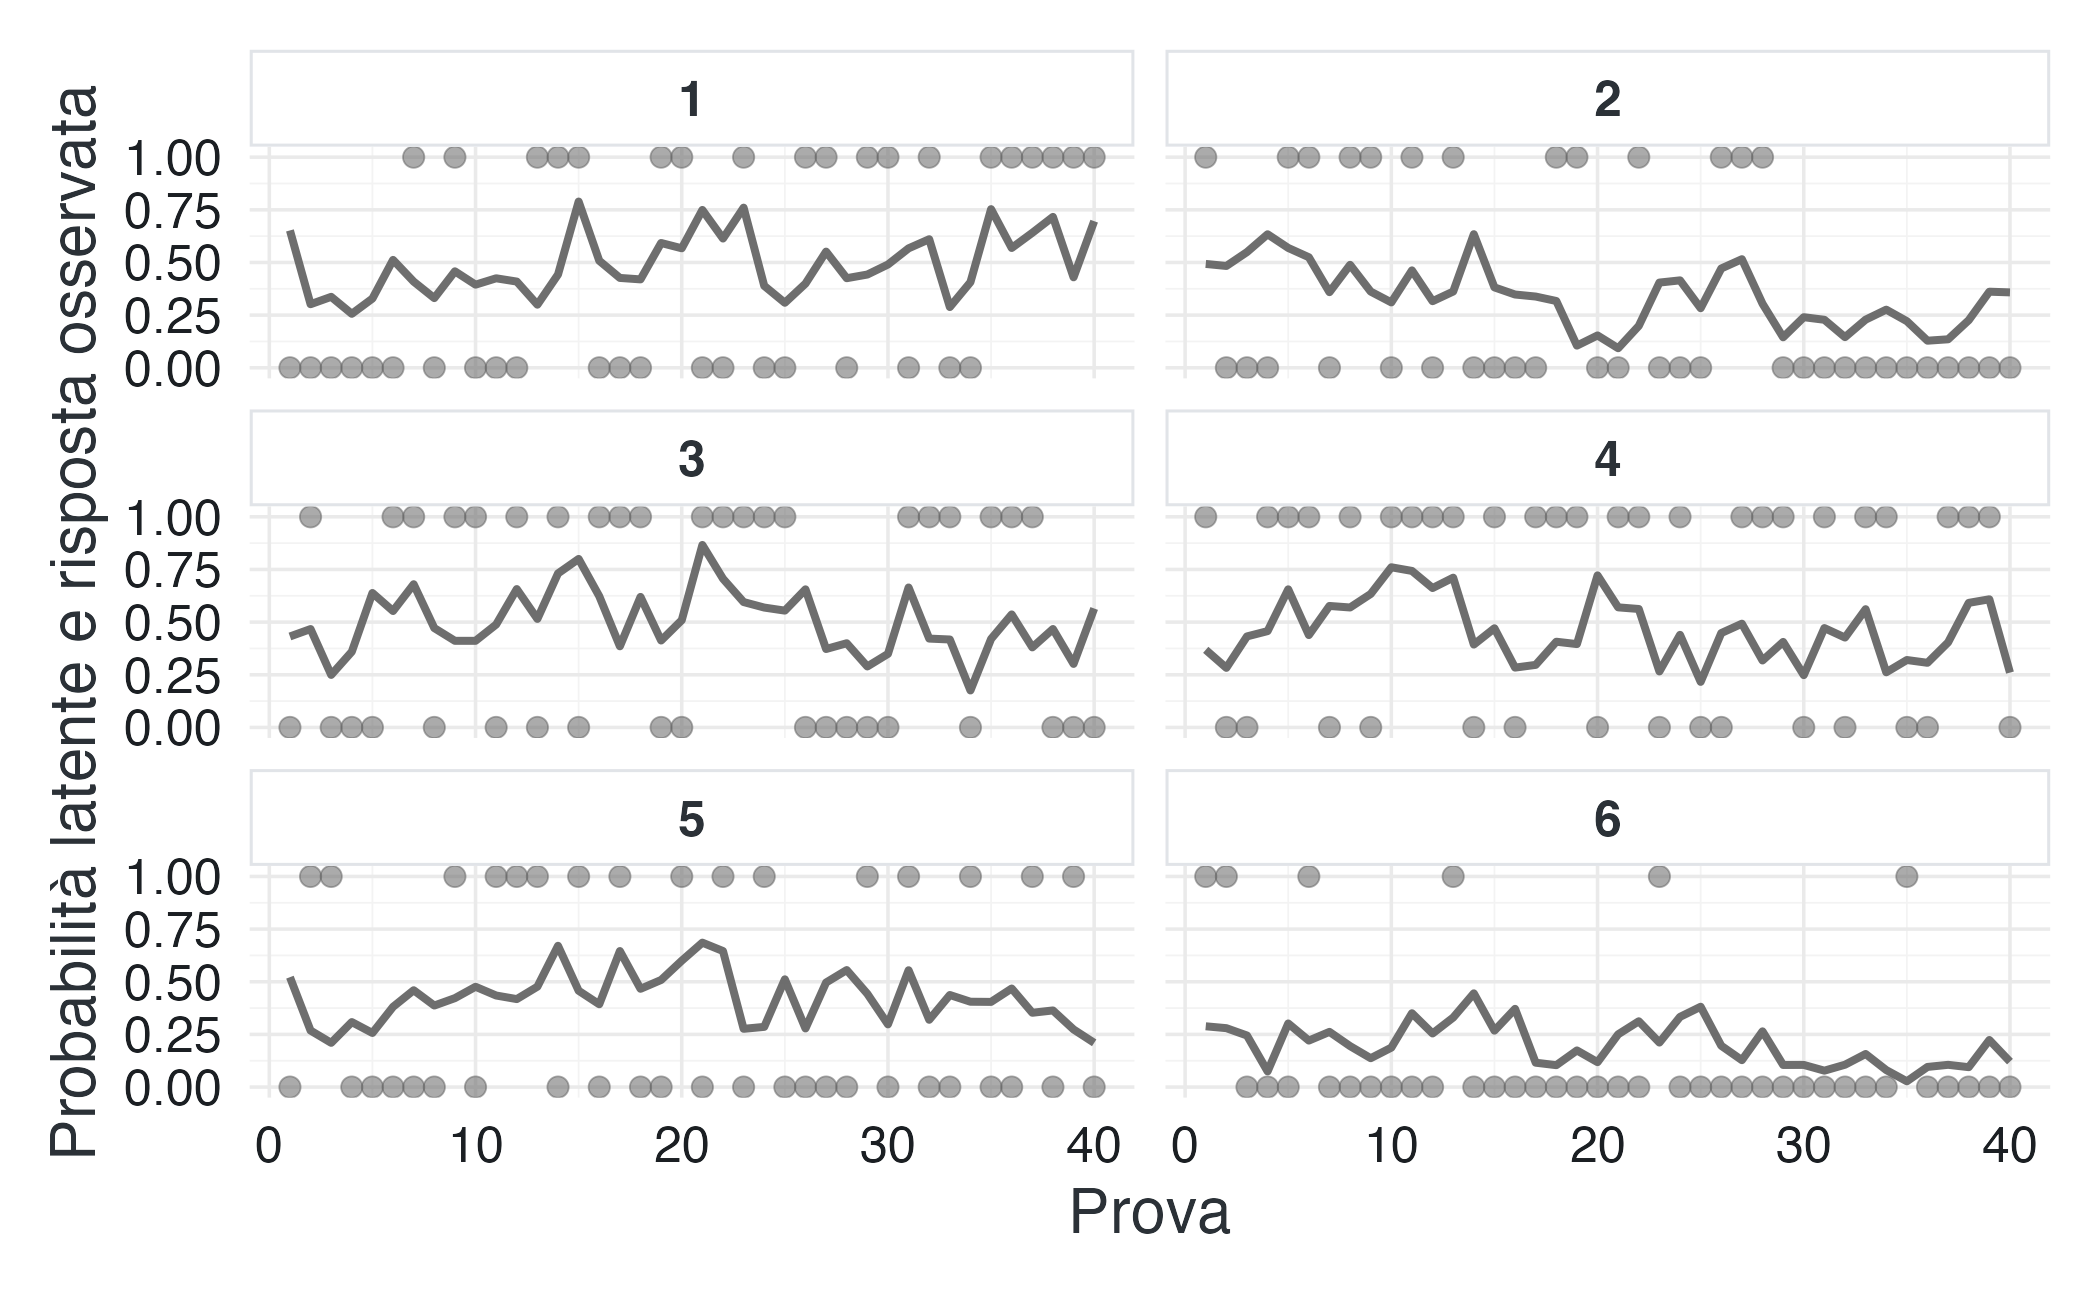
\includegraphics[width=0.85\linewidth,height=\textheight,keepaspectratio]{chapters/glm/04_dal_glm_al_modello_processuale_files/figure-pdf/unnamed-chunk-3-1.png}
\end{center}

La proporzione di risposte positive non descrive completamente queste
sequenze. Una statistica semplice che conserva informazione temporale è
il \textbf{tasso di cambiamento}, cioè la proporzione di passaggi nei
quali la risposta differisce da quella precedente.

\begin{Shaded}
\begin{Highlighting}[]
\NormalTok{sequence\_summary }\OtherTok{\textless{}{-}}\NormalTok{ binary\_data }\SpecialCharTok{|\textgreater{}}
  \FunctionTok{group\_by}\NormalTok{(id) }\SpecialCharTok{|\textgreater{}}
  \FunctionTok{summarise}\NormalTok{(}
    \AttributeTok{proportion\_one =} \FunctionTok{mean}\NormalTok{(y),}
    \AttributeTok{switch\_rate =} \FunctionTok{mean}\NormalTok{(y[}\SpecialCharTok{{-}}\DecValTok{1}\NormalTok{] }\SpecialCharTok{!=}\NormalTok{ y[}\SpecialCharTok{{-}}\FunctionTok{n}\NormalTok{()]),}
    \AttributeTok{.groups =} \StringTok{"drop"}
\NormalTok{  )}

\FunctionTok{summary}\NormalTok{(sequence\_summary)}
\CommentTok{\#\textgreater{}        id       proportion\_one   switch\_rate   }
\CommentTok{\#\textgreater{}  Min.   : 1.0   Min.   :0.150   Min.   :0.205  }
\CommentTok{\#\textgreater{}  1st Qu.:15.8   1st Qu.:0.394   1st Qu.:0.410  }
\CommentTok{\#\textgreater{}  Median :30.5   Median :0.525   Median :0.462  }
\CommentTok{\#\textgreater{}  Mean   :30.5   Mean   :0.492   Mean   :0.462  }
\CommentTok{\#\textgreater{}  3rd Qu.:45.2   3rd Qu.:0.575   3rd Qu.:0.513  }
\CommentTok{\#\textgreater{}  Max.   :60.0   Max.   :0.850   Max.   :0.692}
\end{Highlighting}
\end{Shaded}

Questa statistica non identifica da sola un processo psicologico. Serve
però a illustrare un principio generale: quando il modello contiene una
dinamica, i controlli predittivi devono riguardare anche le proprietà
della sequenza, non soltanto la distribuzione marginale di 0 e 1.

\section{Preparare i dati
sequenziali}\label{preparare-i-dati-sequenziali}

Stan deve sapere quale osservazione precede ogni prova all'interno della
stessa persona. Ordiniamo quindi i dati e costruiamo un indice
\texttt{prev}. Il valore 0 indica l'inizio di una nuova sequenza.

\begin{Shaded}
\begin{Highlighting}[]
\NormalTok{binary\_data }\OtherTok{\textless{}{-}}\NormalTok{ binary\_data }\SpecialCharTok{|\textgreater{}}
  \FunctionTok{arrange}\NormalTok{(id, trial) }\SpecialCharTok{|\textgreater{}}
  \FunctionTok{mutate}\NormalTok{(}\AttributeTok{row\_id =} \FunctionTok{row\_number}\NormalTok{()) }\SpecialCharTok{|\textgreater{}}
  \FunctionTok{group\_by}\NormalTok{(id) }\SpecialCharTok{|\textgreater{}}
  \FunctionTok{mutate}\NormalTok{(}\AttributeTok{prev =}\NormalTok{ dplyr}\SpecialCharTok{::}\FunctionTok{lag}\NormalTok{(row\_id, }\AttributeTok{default =} \DecValTok{0}\NormalTok{L)) }\SpecialCharTok{|\textgreater{}}
  \FunctionTok{ungroup}\NormalTok{()}

\FunctionTok{stopifnot}\NormalTok{(}
  \FunctionTok{all}\NormalTok{(binary\_data}\SpecialCharTok{$}\NormalTok{prev[binary\_data}\SpecialCharTok{$}\NormalTok{trial }\SpecialCharTok{==} \DecValTok{1}\NormalTok{] }\SpecialCharTok{==} \DecValTok{0}\NormalTok{L),}
  \FunctionTok{all}\NormalTok{(binary\_data}\SpecialCharTok{$}\NormalTok{prev[binary\_data}\SpecialCharTok{$}\NormalTok{trial }\SpecialCharTok{\textgreater{}} \DecValTok{1}\NormalTok{] }\SpecialCharTok{\textgreater{}} \DecValTok{0}\NormalTok{L)}
\NormalTok{)}
\end{Highlighting}
\end{Shaded}

L'indice temporale non è un dettaglio informatico. Esprime una parte del
modello: stabilisce quali osservazioni appartengono alla stessa storia e
quale stato precedente può influenzare quello corrente.

\section{Prior e controllo predittivo a
priori}\label{prior-e-controllo-predittivo-a-priori-1}

I prior devono produrre sia probabilità marginali plausibili sia
sequenze plausibili. Usiamo prior moderatamente regolarizzanti per la
propensione media, l'effetto del predittore, la variabilità tra persone,
la persistenza e l'innovazione dello stato.

\[
\begin{aligned}
\mu_\alpha &\sim \operatorname{Normal}(0,1.5),\\
\sigma_\alpha &\sim \operatorname{HalfNormal}(0,0.8),\\
\beta &\sim \operatorname{Normal}(0,1),\\
\phi &\sim \operatorname{Normal}(0,0.4),\quad -0.98<\phi<0.98,\\
\sigma_z &\sim \operatorname{HalfNormal}(0,0.6).
\end{aligned}
\]

Il modello Stan è contenuto nel file esterno
\texttt{binary\_state\_process.stan}. La separazione rende più leggibile
il capitolo e permette di riutilizzare il programma senza duplicarlo.

\begin{Shaded}
\begin{Highlighting}[]
\NormalTok{stan\_data }\OtherTok{\textless{}{-}} \FunctionTok{list}\NormalTok{(}
  \AttributeTok{N =} \FunctionTok{nrow}\NormalTok{(binary\_data),}
  \AttributeTok{J =} \FunctionTok{n\_distinct}\NormalTok{(binary\_data}\SpecialCharTok{$}\NormalTok{id),}
  \AttributeTok{id =} \FunctionTok{as.integer}\NormalTok{(binary\_data}\SpecialCharTok{$}\NormalTok{id),}
  \AttributeTok{x =} \FunctionTok{as.vector}\NormalTok{(binary\_data}\SpecialCharTok{$}\NormalTok{x),}
  \AttributeTok{y =} \FunctionTok{as.integer}\NormalTok{(binary\_data}\SpecialCharTok{$}\NormalTok{y),}
  \AttributeTok{prev =} \FunctionTok{as.integer}\NormalTok{(binary\_data}\SpecialCharTok{$}\NormalTok{prev),}
  \AttributeTok{prior\_only =} \DecValTok{1}\NormalTok{L}
\NormalTok{)}

\NormalTok{state\_model }\OtherTok{\textless{}{-}} \FunctionTok{cmdstan\_model}\NormalTok{(}
\NormalTok{  here}\SpecialCharTok{::}\FunctionTok{here}\NormalTok{(}\StringTok{"chapters"}\NormalTok{, }\StringTok{"glm"}\NormalTok{, }\StringTok{"binary\_state\_process.stan"}\NormalTok{)}
\NormalTok{)}
\end{Highlighting}
\end{Shaded}

\begin{Shaded}
\begin{Highlighting}[]
\NormalTok{fit\_state\_prior }\OtherTok{\textless{}{-}}\NormalTok{ state\_model}\SpecialCharTok{$}\FunctionTok{sample}\NormalTok{(}
  \AttributeTok{data =}\NormalTok{ stan\_data,}
  \AttributeTok{seed =} \DecValTok{2026}\NormalTok{,}
  \AttributeTok{chains =} \DecValTok{4}\NormalTok{,}
  \AttributeTok{parallel\_chains =} \DecValTok{4}\NormalTok{,}
  \AttributeTok{iter\_warmup =} \DecValTok{500}\NormalTok{,}
  \AttributeTok{iter\_sampling =} \DecValTok{500}\NormalTok{,}
  \AttributeTok{refresh =} \DecValTok{0}
\NormalTok{)}
\end{Highlighting}
\end{Shaded}

Per giudicare i prior consideriamo la proporzione complessiva di
risposte positive e il tasso di cambiamento tra risposte consecutive.

\begin{Shaded}
\begin{Highlighting}[]
\NormalTok{switch\_rate }\OtherTok{\textless{}{-}} \ControlFlowTok{function}\NormalTok{(y, prev) \{}
\NormalTok{  idx }\OtherTok{\textless{}{-}} \FunctionTok{which}\NormalTok{(prev }\SpecialCharTok{\textgreater{}} \DecValTok{0}\NormalTok{)}
  \FunctionTok{mean}\NormalTok{(y[idx] }\SpecialCharTok{!=}\NormalTok{ y[prev[idx]])}
\NormalTok{\}}

\NormalTok{prior\_yrep }\OtherTok{\textless{}{-}} \FunctionTok{as\_draws\_matrix}\NormalTok{(fit\_state\_prior}\SpecialCharTok{$}\FunctionTok{draws}\NormalTok{(}\StringTok{"y\_rep"}\NormalTok{))}
\NormalTok{prior\_yrep }\OtherTok{\textless{}{-}}\NormalTok{ prior\_yrep[}
  \FunctionTok{sample}\NormalTok{(}\FunctionTok{seq\_len}\NormalTok{(}\FunctionTok{nrow}\NormalTok{(prior\_yrep)), }\AttributeTok{size =} \FunctionTok{min}\NormalTok{(}\DecValTok{400}\NormalTok{, }\FunctionTok{nrow}\NormalTok{(prior\_yrep))),}
\NormalTok{  ,}
\NormalTok{  drop }\OtherTok{=} \ConstantTok{FALSE}
\NormalTok{]}

\NormalTok{prior\_checks }\OtherTok{\textless{}{-}} \FunctionTok{tibble}\NormalTok{(}
  \AttributeTok{proportion\_one =} \FunctionTok{rowMeans}\NormalTok{(prior\_yrep),}
  \AttributeTok{switch\_rate =} \FunctionTok{apply}\NormalTok{(}
\NormalTok{    prior\_yrep,}
    \DecValTok{1}\NormalTok{,}
\NormalTok{    switch\_rate,}
    \AttributeTok{prev =}\NormalTok{ stan\_data}\SpecialCharTok{$}\NormalTok{prev}
\NormalTok{  )}
\NormalTok{)}

\NormalTok{prior\_checks }\SpecialCharTok{|\textgreater{}}
  \FunctionTok{pivot\_longer}\NormalTok{(}\FunctionTok{everything}\NormalTok{(), }\AttributeTok{names\_to =} \StringTok{"statistic"}\NormalTok{, }\AttributeTok{values\_to =} \StringTok{"value"}\NormalTok{) }\SpecialCharTok{|\textgreater{}}
  \FunctionTok{ggplot}\NormalTok{(}\FunctionTok{aes}\NormalTok{(value)) }\SpecialCharTok{+}
  \FunctionTok{geom\_density}\NormalTok{() }\SpecialCharTok{+}
  \FunctionTok{facet\_wrap}\NormalTok{(}\SpecialCharTok{\textasciitilde{}}\NormalTok{ statistic, }\AttributeTok{scales =} \StringTok{"free"}\NormalTok{) }\SpecialCharTok{+}
  \FunctionTok{labs}\NormalTok{(}\AttributeTok{x =} \ConstantTok{NULL}\NormalTok{, }\AttributeTok{y =} \StringTok{"Densità predittiva a priori"}\NormalTok{)}
\end{Highlighting}
\end{Shaded}

\begin{center}
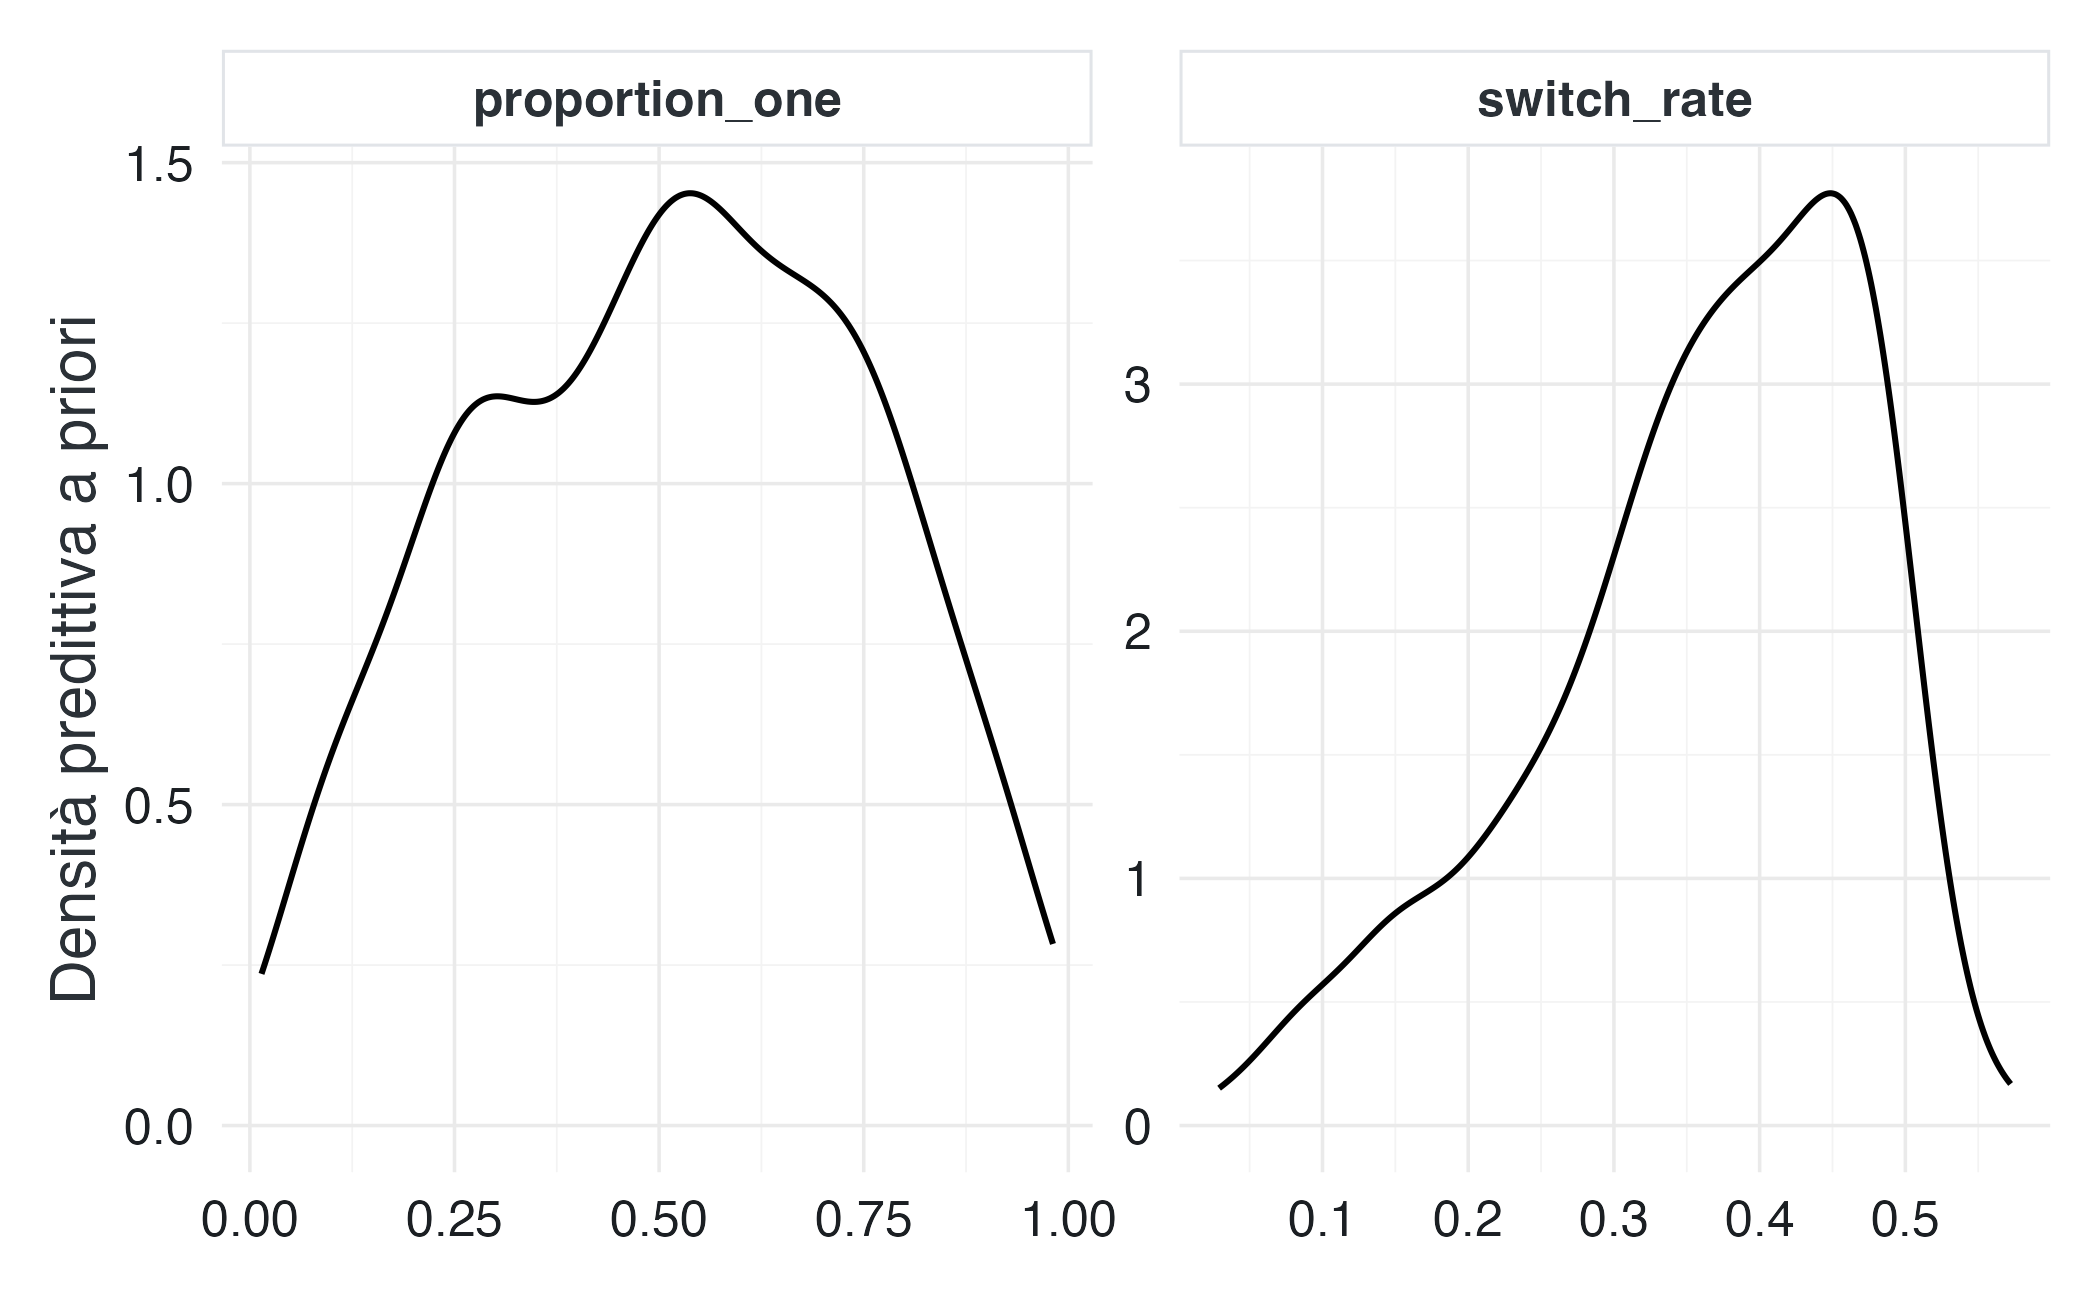
\includegraphics[width=0.85\linewidth,height=\textheight,keepaspectratio]{chapters/glm/04_dal_glm_al_modello_processuale_files/figure-pdf/unnamed-chunk-8-1.png}
\end{center}

Il controllo può rivelare prior che producono quasi sempre sequenze
costanti oppure alternanze troppo rapide. In tal caso non basta
ricalibrare l'intercetta: occorre intervenire sui prior di \(\phi\) e
\(\sigma_z\), perché sono questi parametri a governare la struttura
temporale.

\section{Stimare il modello dinamico}\label{stimare-il-modello-dinamico}

Per passare dal controllo a priori all'inferenza impostiamo
\texttt{prior\_only\ =\ 0}.

\begin{Shaded}
\begin{Highlighting}[]
\NormalTok{stan\_data}\SpecialCharTok{$}\NormalTok{prior\_only }\OtherTok{\textless{}{-}} \DecValTok{0}\NormalTok{L}
\end{Highlighting}
\end{Shaded}

\begin{Shaded}
\begin{Highlighting}[]
\NormalTok{fit\_state }\OtherTok{\textless{}{-}}\NormalTok{ state\_model}\SpecialCharTok{$}\FunctionTok{sample}\NormalTok{(}
  \AttributeTok{data =}\NormalTok{ stan\_data,}
  \AttributeTok{seed =} \DecValTok{2026}\NormalTok{,}
  \AttributeTok{chains =} \DecValTok{4}\NormalTok{,}
  \AttributeTok{parallel\_chains =} \DecValTok{4}\NormalTok{,}
  \AttributeTok{iter\_warmup =} \DecValTok{1000}\NormalTok{,}
  \AttributeTok{iter\_sampling =} \DecValTok{1000}\NormalTok{,}
  \AttributeTok{adapt\_delta =} \FloatTok{0.95}\NormalTok{,}
  \AttributeTok{max\_treedepth =} \DecValTok{12}\NormalTok{,}
  \AttributeTok{refresh =} \DecValTok{0}
\NormalTok{)}
\end{Highlighting}
\end{Shaded}

\begin{Shaded}
\begin{Highlighting}[]
\NormalTok{fit\_state}\SpecialCharTok{$}\FunctionTok{summary}\NormalTok{(}
  \AttributeTok{variables =} \FunctionTok{c}\NormalTok{(}\StringTok{"alpha\_mu"}\NormalTok{, }\StringTok{"alpha\_sd"}\NormalTok{, }\StringTok{"beta"}\NormalTok{, }\StringTok{"phi"}\NormalTok{, }\StringTok{"sigma\_z"}\NormalTok{)}
\NormalTok{)}
\CommentTok{\#\textgreater{} \# A tibble: 5 x 10}
\CommentTok{\#\textgreater{}   variable    mean  median     sd    mad      q5    q95  rhat ess\_bulk ess\_tail}
\CommentTok{\#\textgreater{}   \textless{}chr\textgreater{}      \textless{}dbl\textgreater{}   \textless{}dbl\textgreater{}  \textless{}dbl\textgreater{}  \textless{}dbl\textgreater{}   \textless{}dbl\textgreater{}  \textless{}dbl\textgreater{} \textless{}dbl\textgreater{}    \textless{}dbl\textgreater{}    \textless{}dbl\textgreater{}}
\CommentTok{\#\textgreater{} 1 alpha\_mu {-}0.333  {-}0.331  0.101  0.101  {-}0.505  {-}0.170  1.00    1632.   1906. }
\CommentTok{\#\textgreater{} 2 alpha\_sd  0.588   0.580  0.0827 0.0788  0.463   0.730  1.01     352.    645. }
\CommentTok{\#\textgreater{} 3 beta      0.585   0.582  0.0961 0.0916  0.433   0.744  1.01     710.    867. }
\CommentTok{\#\textgreater{} 4 phi       0.0792  0.0799 0.295  0.286  {-}0.419   0.575  1.01    1093.   1043. }
\CommentTok{\#\textgreater{} 5 sigma\_z   0.374   0.324  0.273  0.259   0.0344  0.888  1.04     114.     66.2}
\end{Highlighting}
\end{Shaded}

Poiché i dati sono simulati, conosciamo i valori generativi:
\(\mu_\alpha=-0.40\), \(\sigma_\alpha=0.60\), \(\beta=0.80\),
\(\phi=0.65\) e \(\sigma_z=0.45\). La concordanza tra posterior e valori
noti costituisce un primo controllo di recuperabilità. Non è però una
dimostrazione generale: un vero studio di \emph{parameter recovery}
richiede molte simulazioni, diverse combinazioni di parametri e una
valutazione sistematica di bias, precisione e copertura.

È inoltre necessario controllare convergenza, dimensione campionaria
effettiva, divergenze e possibili dipendenze posteriori tra \(\phi\) e
\(\sigma_z\). Una sequenza relativamente breve può rendere difficile
distinguere una persistenza elevata con innovazioni piccole da una
persistenza più moderata con innovazioni maggiori.

\section{Un modello statico come
riferimento}\label{un-modello-statico-come-riferimento}

Stimiamo ora un modello logistico gerarchico che rappresenta le
differenze stabili tra persone, ma non introduce uno stato dinamico.

\begin{Shaded}
\begin{Highlighting}[]
\NormalTok{static\_priors }\OtherTok{\textless{}{-}} \FunctionTok{c}\NormalTok{(}
  \FunctionTok{prior}\NormalTok{(}\FunctionTok{normal}\NormalTok{(}\DecValTok{0}\NormalTok{, }\FloatTok{1.5}\NormalTok{), }\AttributeTok{class =}\NormalTok{ Intercept),}
  \FunctionTok{prior}\NormalTok{(}\FunctionTok{normal}\NormalTok{(}\DecValTok{0}\NormalTok{, }\DecValTok{1}\NormalTok{), }\AttributeTok{class =}\NormalTok{ b),}
  \FunctionTok{prior}\NormalTok{(}\FunctionTok{normal}\NormalTok{(}\DecValTok{0}\NormalTok{, }\FloatTok{0.8}\NormalTok{), }\AttributeTok{class =}\NormalTok{ sd)}
\NormalTok{)}

\NormalTok{fit\_static }\OtherTok{\textless{}{-}} \FunctionTok{brm}\NormalTok{(}
\NormalTok{  y }\SpecialCharTok{\textasciitilde{}} \DecValTok{1} \SpecialCharTok{+}\NormalTok{ x }\SpecialCharTok{+}\NormalTok{ (}\DecValTok{1} \SpecialCharTok{|}\NormalTok{ id),}
  \AttributeTok{data =}\NormalTok{ binary\_data,}
  \AttributeTok{family =} \FunctionTok{bernoulli}\NormalTok{(}\AttributeTok{link =} \StringTok{"logit"}\NormalTok{),}
  \AttributeTok{prior =}\NormalTok{ static\_priors,}
  \AttributeTok{chains =} \DecValTok{4}\NormalTok{,}
  \AttributeTok{iter =} \DecValTok{2000}\NormalTok{,}
  \AttributeTok{warmup =} \DecValTok{1000}\NormalTok{,}
  \AttributeTok{seed =} \DecValTok{2026}\NormalTok{,}
  \AttributeTok{backend =} \StringTok{"cmdstanr"}\NormalTok{,}
  \AttributeTok{refresh =} \DecValTok{0}
\NormalTok{)}
\CommentTok{\#\textgreater{} Running MCMC with 4 chains, at most 10 in parallel...}
\CommentTok{\#\textgreater{} }
\CommentTok{\#\textgreater{} Chain 1 finished in 3.6 seconds.}
\CommentTok{\#\textgreater{} Chain 2 finished in 3.7 seconds.}
\CommentTok{\#\textgreater{} Chain 3 finished in 3.8 seconds.}
\CommentTok{\#\textgreater{} Chain 4 finished in 3.8 seconds.}
\CommentTok{\#\textgreater{} }
\CommentTok{\#\textgreater{} All 4 chains finished successfully.}
\CommentTok{\#\textgreater{} Mean chain execution time: 3.7 seconds.}
\CommentTok{\#\textgreater{} Total execution time: 4.0 seconds.}
\end{Highlighting}
\end{Shaded}

Il modello statico non deve essere giudicato soltanto osservando se il
coefficiente di \texttt{x} è vicino a quello generativo. La domanda
decisiva è quale aspetto dei dati intendiamo riprodurre. Entrambi i
modelli possono descrivere bene la proporzione complessiva di risposte
positive; soltanto il modello di stato è costruito per riprodurre la
persistenza sequenziale.

\section{Controlli predittivi mirati al
processo}\label{controlli-predittivi-mirati-al-processo}

Confrontiamo i due modelli mediante la proporzione di risposte positive
e il tasso di cambiamento. Queste statistiche rappresentano
rispettivamente una proprietà marginale e una proprietà sequenziale.

\begin{Shaded}
\begin{Highlighting}[]
\FunctionTok{set.seed}\NormalTok{(}\DecValTok{2026}\NormalTok{)}

\NormalTok{static\_yrep }\OtherTok{\textless{}{-}} \FunctionTok{posterior\_predict}\NormalTok{(fit\_static, }\AttributeTok{ndraws =} \DecValTok{400}\NormalTok{)}

\NormalTok{state\_yrep }\OtherTok{\textless{}{-}} \FunctionTok{as\_draws\_matrix}\NormalTok{(fit\_state}\SpecialCharTok{$}\FunctionTok{draws}\NormalTok{(}\StringTok{"y\_rep"}\NormalTok{))}
\NormalTok{state\_yrep }\OtherTok{\textless{}{-}}\NormalTok{ state\_yrep[}
  \FunctionTok{sample}\NormalTok{(}\FunctionTok{seq\_len}\NormalTok{(}\FunctionTok{nrow}\NormalTok{(state\_yrep)), }\AttributeTok{size =} \FunctionTok{min}\NormalTok{(}\DecValTok{400}\NormalTok{, }\FunctionTok{nrow}\NormalTok{(state\_yrep))),}
\NormalTok{  ,}
\NormalTok{  drop }\OtherTok{=} \ConstantTok{FALSE}
\NormalTok{]}

\NormalTok{observed\_stats }\OtherTok{\textless{}{-}} \FunctionTok{tibble}\NormalTok{(}
  \AttributeTok{model =} \StringTok{"Dati osservati"}\NormalTok{,}
  \AttributeTok{proportion\_one =} \FunctionTok{mean}\NormalTok{(stan\_data}\SpecialCharTok{$}\NormalTok{y),}
  \AttributeTok{switch\_rate =} \FunctionTok{switch\_rate}\NormalTok{(stan\_data}\SpecialCharTok{$}\NormalTok{y, stan\_data}\SpecialCharTok{$}\NormalTok{prev)}
\NormalTok{)}

\NormalTok{replicated\_stats }\OtherTok{\textless{}{-}} \FunctionTok{bind\_rows}\NormalTok{(}
  \FunctionTok{tibble}\NormalTok{(}
    \AttributeTok{model =} \StringTok{"GLM gerarchico statico"}\NormalTok{,}
    \AttributeTok{proportion\_one =} \FunctionTok{rowMeans}\NormalTok{(static\_yrep),}
    \AttributeTok{switch\_rate =} \FunctionTok{apply}\NormalTok{(}
\NormalTok{      static\_yrep,}
      \DecValTok{1}\NormalTok{,}
\NormalTok{      switch\_rate,}
      \AttributeTok{prev =}\NormalTok{ stan\_data}\SpecialCharTok{$}\NormalTok{prev}
\NormalTok{    )}
\NormalTok{  ),}
  \FunctionTok{tibble}\NormalTok{(}
    \AttributeTok{model =} \StringTok{"Modello dinamico"}\NormalTok{,}
    \AttributeTok{proportion\_one =} \FunctionTok{rowMeans}\NormalTok{(state\_yrep),}
    \AttributeTok{switch\_rate =} \FunctionTok{apply}\NormalTok{(}
\NormalTok{      state\_yrep,}
      \DecValTok{1}\NormalTok{,}
\NormalTok{      switch\_rate,}
      \AttributeTok{prev =}\NormalTok{ stan\_data}\SpecialCharTok{$}\NormalTok{prev}
\NormalTok{    )}
\NormalTok{  )}
\NormalTok{)}
\end{Highlighting}
\end{Shaded}

\begin{Shaded}
\begin{Highlighting}[]
\NormalTok{replicated\_stats }\SpecialCharTok{|\textgreater{}}
  \FunctionTok{pivot\_longer}\NormalTok{(}
    \AttributeTok{cols =} \FunctionTok{c}\NormalTok{(proportion\_one, switch\_rate),}
    \AttributeTok{names\_to =} \StringTok{"statistic"}\NormalTok{,}
    \AttributeTok{values\_to =} \StringTok{"value"}
\NormalTok{  ) }\SpecialCharTok{|\textgreater{}}
  \FunctionTok{ggplot}\NormalTok{(}\FunctionTok{aes}\NormalTok{(value, }\AttributeTok{fill =}\NormalTok{ model)) }\SpecialCharTok{+}
  \FunctionTok{geom\_density}\NormalTok{(}\AttributeTok{alpha =} \FloatTok{0.35}\NormalTok{) }\SpecialCharTok{+}
  \FunctionTok{geom\_vline}\NormalTok{(}
    \AttributeTok{data =}\NormalTok{ observed\_stats }\SpecialCharTok{|\textgreater{}}
      \FunctionTok{pivot\_longer}\NormalTok{(}
        \AttributeTok{cols =} \FunctionTok{c}\NormalTok{(proportion\_one, switch\_rate),}
        \AttributeTok{names\_to =} \StringTok{"statistic"}\NormalTok{,}
        \AttributeTok{values\_to =} \StringTok{"value"}
\NormalTok{      ),}
    \FunctionTok{aes}\NormalTok{(}\AttributeTok{xintercept =}\NormalTok{ value),}
    \AttributeTok{inherit.aes =} \ConstantTok{FALSE}\NormalTok{,}
    \AttributeTok{linetype =} \StringTok{"dashed"}
\NormalTok{  ) }\SpecialCharTok{+}
  \FunctionTok{facet\_wrap}\NormalTok{(}\SpecialCharTok{\textasciitilde{}}\NormalTok{ statistic, }\AttributeTok{scales =} \StringTok{"free"}\NormalTok{) }\SpecialCharTok{+}
  \FunctionTok{labs}\NormalTok{(}\AttributeTok{x =} \ConstantTok{NULL}\NormalTok{, }\AttributeTok{y =} \StringTok{"Densità predittiva a posteriori"}\NormalTok{, }\AttributeTok{fill =} \ConstantTok{NULL}\NormalTok{)}
\end{Highlighting}
\end{Shaded}

\begin{center}
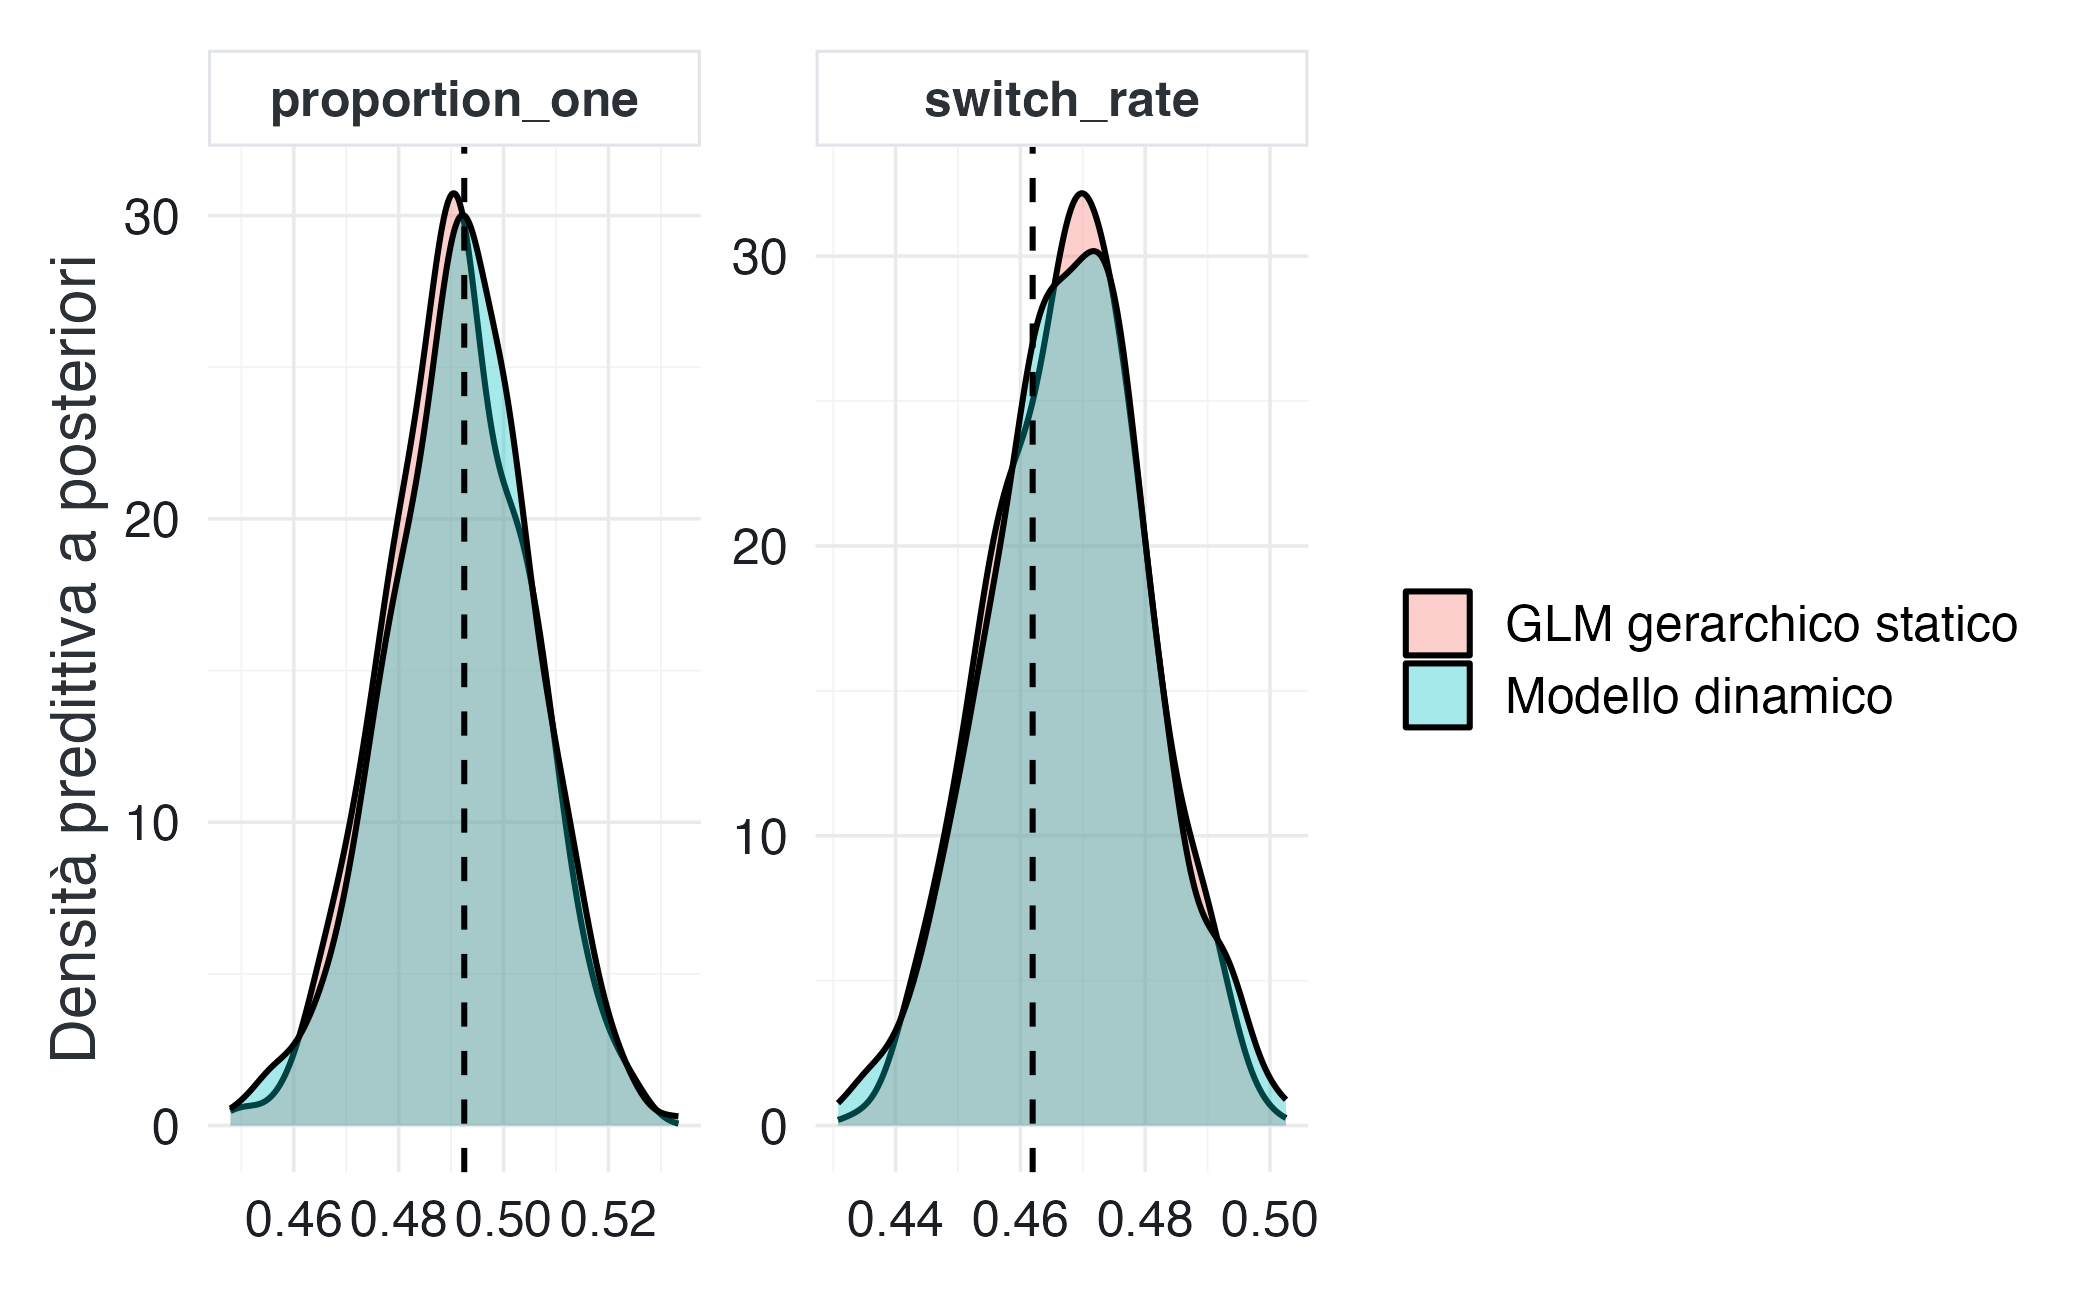
\includegraphics[width=0.85\linewidth,height=\textheight,keepaspectratio]{chapters/glm/04_dal_glm_al_modello_processuale_files/figure-pdf/unnamed-chunk-14-1.png}
\end{center}

Il risultato atteso è istruttivo. Il GLM statico può riprodurre la
proporzione media, perché è stato costruito per descrivere probabilità
condizionate. Può invece generare troppi cambiamenti consecutivi, perché
non conserva uno stato. Il modello dinamico ha la possibilità di
riprodurre entrambe le proprietà.

Questo confronto non dimostra che il processo AR(1) sia il meccanismo
psicologico corretto. Mostra soltanto che una specifica proprietà dei
dati richiede una rappresentazione della memoria. Altri modelli
potrebbero produrre una persistenza simile: una dipendenza diretta dalla
risposta precedente, un cambiamento lento dell'attenzione, una strategia
di perseverazione oppure un processo di apprendimento. La distinzione
tra queste spiegazioni richiede manipolazioni sperimentali, misure
aggiuntive e modelli rivali.

\section{Dal modello dinamico alla teoria
psicologica}\label{dal-modello-dinamico-alla-teoria-psicologica}

Lo stato \(z_{it}\) è una variabile latente utile, ma non possiede da
solo un significato psicologico univoco. Il modello afferma che esiste
una componente persistente non spiegata dai predittori osservati. Non
stabilisce se tale componente rappresenti fiducia, umore, fatica,
attenzione o una miscela di processi.

Per trasformare un modello dinamico in un modello processuale sostantivo
occorre specificare almeno tre elementi. Il primo è \textbf{che cosa
aggiorna lo stato}: un esito, un errore di previsione, una discrepanza o
l'evidenza sensoriale. Il secondo è \textbf{secondo quale regola lo
stato cambia}. Il terzo è \textbf{come lo stato produce la risposta
osservata}. Questi passaggi possono essere rappresentati come

\[
S_{t+1}=f(S_t,I_t;\theta),
\qquad
Y_t\sim p(Y_t\mid S_t;\psi),
\]

dove \(S_t\) è lo stato, \(I_t\) l'input, \(f\) la regola di
aggiornamento e \(p(Y_t\mid S_t)\) il modello osservazionale.

L'AR(1) usato in questo capitolo specifica una regola di persistenza
molto generale. La parte \emph{Applicazione} introdurrà regole
teoricamente più informative. Nel modello di revisione degli obiettivi,
lo stato cambia in funzione della discrepanza tra prestazione e
obiettivo Capitolo~\ref{sec-dynamic-models-goal-updating}. Nel modello
di Rescorla--Wagner, il valore atteso viene aggiornato mediante l'errore
di previsione Capitolo~\ref{sec-dynamic-models-rescorla-wagner}. In
entrambi i casi, la dinamica non serve soltanto a descrivere
autocorrelazione: formalizza un'ipotesi sul processo che genera il
comportamento.

\section{Che cosa abbiamo guadagnato, e che cosa
no}\label{che-cosa-abbiamo-guadagnato-e-che-cosa-no}

Il passaggio dal GLM statico al modello di stato produce un guadagno
preciso. La probabilità di risposta non è più una funzione soltanto dei
predittori osservati e delle differenze stabili tra persone; dipende
anche da una storia latente. Di conseguenza, il modello genera intere
sequenze e può essere criticato sulla base di proprietà temporali.

Non abbiamo però identificato automaticamente un meccanismo psicologico.
Un modello più complesso può adattarsi meglio perché dispone di maggiore
flessibilità. Per sostenere un'interpretazione processuale occorrono
recuperabilità dei parametri, predizioni che distinguano modelli rivali,
validazione su dati nuovi e una corrispondenza teoricamente giustificata
tra parametri e costrutti. Questi temi costituiscono il centro della
parte successiva, a partire dalla distinzione tra funzioni descrittive,
generative e meccanicistiche dei modelli
Capitolo~\ref{sec-bayes-stat-models}.

\section*{Riflessioni conclusive}\label{riflessioni-conclusive-34}

\markright{Riflessioni conclusive}

I modelli lineari generalizzati estendono il modello lineare a nuovi
tipi di outcome, ma conservano una struttura essenzialmente
condizionata: specificano come la distribuzione della risposta cambi al
variare dei predittori. Questo capitolo ha mostrato un passaggio
ulteriore. Quando l'ordine delle osservazioni è informativo, possiamo
introdurre uno stato latente che evolve nel tempo e collega la storia
passata alla probabilità presente.

La differenza non riguarda soltanto il numero dei parametri. Cambia
l'unità della previsione. Un GLM statico genera osservazioni individuali
condizionate ai predittori; un modello dinamico genera sequenze. Per
questo la sua adeguatezza deve essere valutata mediante statistiche che
conservano la struttura temporale. Riprodurre la proporzione media di
risposte positive non basta se il fenomeno di interesse riguarda
persistenza, alternanza o adattamento.

Lo stato autoregressivo rimane tuttavia una rappresentazione generale.
Esso segnala che il passato conta, ma non specifica necessariamente
\emph{perché} conti. La modellazione processuale in senso più forte
inizia quando la dinamica viene collegata a una teoria: uno stato ha un
significato definito, un input produce un aggiornamento secondo una
regola esplicita e il modello osservazionale collega quello stato al
comportamento. La parte \emph{Applicazione} svilupperà precisamente
questo passaggio, trasformando la probabilità di risposta nell'esito
osservabile di una teoria eseguibile.

\section*{Domande di lavoro}\label{domande-di-lavoro}

\markright{Domande di lavoro}

\begin{enumerate}
\def\labelenumi{\arabic{enumi}.}
\tightlist
\item
  Simulare dati mantenendo fissi \(\beta\) e \(\sigma_z\) e facendo
  variare \(\phi\). In che modo cambiano il tasso di risposta e il tasso
  di cambiamento?
\item
  Porre \(\phi=0\) lasciando \(\sigma_z>0\). Quale dipendenza rimane e
  quale scompare?
\item
  Aggiungere una dipendenza diretta dalla risposta precedente. Quali
  dati potrebbero distinguere questo modello da uno stato AR(1)?
\item
  Ripetere il parameter recovery con sequenze di 15, 40 e 100 prove.
  Come cambia l'incertezza su \(\phi\) e \(\sigma_z\)?
\item
  Proporre un'interpretazione psicologica di \(z_{it}\) e indicare
  almeno una manipolazione sperimentale che potrebbe metterla alla
  prova.
\end{enumerate}

\begin{tcolorbox}[enhanced jigsaw, arc=.35mm, bottomrule=.15mm, bottomtitle=1mm, breakable, colback=white, colbacktitle=quarto-callout-note-color!10!white, colframe=quarto-callout-note-color-frame, coltitle=black, left=2mm, leftrule=.75mm, opacityback=0, opacitybacktitle=0.6, rightrule=.15mm, title=\textcolor{quarto-callout-note-color}{\faInfo}\hspace{0.5em}{Informazioni sull'ambiente di sviluppo}, titlerule=0mm, toprule=.15mm, toptitle=1mm]

\begin{Shaded}
\begin{Highlighting}[]
\FunctionTok{sessionInfo}\NormalTok{()}
\CommentTok{\#\textgreater{} R version 4.6.1 (2026{-}06{-}24)}
\CommentTok{\#\textgreater{} Platform: aarch64{-}apple{-}darwin23}
\CommentTok{\#\textgreater{} Running under: macOS Tahoe 26.5.2}
\CommentTok{\#\textgreater{} }
\CommentTok{\#\textgreater{} Matrix products: default}
\CommentTok{\#\textgreater{} BLAS:   /Library/Frameworks/R.framework/Versions/4.6/Resources/lib/libRblas.0.dylib }
\CommentTok{\#\textgreater{} LAPACK: /Library/Frameworks/R.framework/Versions/4.6/Resources/lib/libRlapack.dylib;  LAPACK version 3.12.1}
\CommentTok{\#\textgreater{} }
\CommentTok{\#\textgreater{} locale:}
\CommentTok{\#\textgreater{} [1] C.UTF{-}8/UTF{-}8/C.UTF{-}8/C/C.UTF{-}8/C.UTF{-}8}
\CommentTok{\#\textgreater{} }
\CommentTok{\#\textgreater{} time zone: Europe/Zagreb}
\CommentTok{\#\textgreater{} tzcode source: internal}
\CommentTok{\#\textgreater{} }
\CommentTok{\#\textgreater{} attached base packages:}
\CommentTok{\#\textgreater{} [1] stats     graphics  grDevices utils     datasets  methods   base     }
\CommentTok{\#\textgreater{} }
\CommentTok{\#\textgreater{} other attached packages:}
\CommentTok{\#\textgreater{}  [1] purrr\_1.2.2           cmdstanr\_0.9.0        ragg\_1.5.2           }
\CommentTok{\#\textgreater{}  [4] tinytable\_0.17.0      withr\_3.0.3           systemfonts\_1.3.2    }
\CommentTok{\#\textgreater{}  [7] patchwork\_1.3.2       ggdist\_3.3.3          tidybayes\_3.0.7      }
\CommentTok{\#\textgreater{} [10] bayesplot\_1.15.0      ggplot2\_4.0.3         reliabilitydiag\_0.2.1}
\CommentTok{\#\textgreater{} [13] priorsense\_1.2.0      posterior\_1.7.0       loo\_2.10.0           }
\CommentTok{\#\textgreater{} [16] rstan\_2.32.7          StanHeaders\_2.32.10   brms\_2.23.0          }
\CommentTok{\#\textgreater{} [19] Rcpp\_1.1.2            sessioninfo\_1.2.4     conflicted\_1.2.0     }
\CommentTok{\#\textgreater{} [22] janitor\_2.2.1         matrixStats\_1.5.0     modelr\_0.1.11        }
\CommentTok{\#\textgreater{} [25] tibble\_3.3.1          dplyr\_1.2.1           tidyr\_1.3.2          }
\CommentTok{\#\textgreater{} [28] rio\_1.3.0             here\_1.0.2           }
\CommentTok{\#\textgreater{} }
\CommentTok{\#\textgreater{} loaded via a namespace (and not attached):}
\CommentTok{\#\textgreater{}  [1] svUnit\_1.0.8          tidyselect\_1.2.1      farver\_2.1.2         }
\CommentTok{\#\textgreater{}  [4] S7\_0.2.2              fastmap\_1.2.0         tensorA\_0.36.2.1     }
\CommentTok{\#\textgreater{}  [7] pacman\_0.5.1          digest\_0.6.39         timechange\_0.4.0     }
\CommentTok{\#\textgreater{} [10] estimability\_2.0.0    lifecycle\_1.0.5       processx\_3.9.0       }
\CommentTok{\#\textgreater{} [13] magrittr\_2.0.5        compiler\_4.6.1        rlang\_1.3.0          }
\CommentTok{\#\textgreater{} [16] tools\_4.6.1           utf8\_1.2.6            yaml\_2.3.12          }
\CommentTok{\#\textgreater{} [19] data.table\_1.18.4     knitr\_1.51            labeling\_0.4.3       }
\CommentTok{\#\textgreater{} [22] bridgesampling\_1.2{-}1  pkgbuild\_1.4.8        curl\_7.1.0           }
\CommentTok{\#\textgreater{} [25] RColorBrewer\_1.1{-}3    abind\_1.4{-}8           grid\_4.6.1           }
\CommentTok{\#\textgreater{} [28] stats4\_4.6.1          xtable\_1.8{-}8          inline\_0.3.21        }
\CommentTok{\#\textgreater{} [31] emmeans\_2.0.4         scales\_1.4.0          cli\_3.6.6            }
\CommentTok{\#\textgreater{} [34] mvtnorm\_1.4{-}2         rmarkdown\_2.31        generics\_0.1.4       }
\CommentTok{\#\textgreater{} [37] otel\_0.2.0            RcppParallel\_5.1.11{-}2 cachem\_1.1.0         }
\CommentTok{\#\textgreater{} [40] stringr\_1.6.0         parallel\_4.6.1        vctrs\_0.7.3          }
\CommentTok{\#\textgreater{} [43] V8\_8.2.0              Matrix\_1.7{-}5          jsonlite\_2.0.0       }
\CommentTok{\#\textgreater{} [46] arrayhelpers\_1.1{-}1    glue\_1.8.1            ps\_1.9.3             }
\CommentTok{\#\textgreater{} [49] codetools\_0.2{-}20      distributional\_0.8.1  lubridate\_1.9.5      }
\CommentTok{\#\textgreater{} [52] stringi\_1.8.7         gtable\_0.3.6          QuickJSR\_1.10.0      }
\CommentTok{\#\textgreater{} [55] pillar\_1.11.1         htmltools\_0.5.9       Brobdingnag\_1.2{-}9    }
\CommentTok{\#\textgreater{} [58] R6\_2.6.1              textshaping\_1.0.5     rprojroot\_2.1.1      }
\CommentTok{\#\textgreater{} [61] evaluate\_1.0.5        lattice\_0.22{-}9        backports\_1.5.1      }
\CommentTok{\#\textgreater{} [64] memoise\_2.0.1         broom\_1.0.13          snakecase\_0.11.1     }
\CommentTok{\#\textgreater{} [67] rstantools\_2.6.0      coda\_0.19{-}4.1         gridExtra\_2.3.1      }
\CommentTok{\#\textgreater{} [70] nlme\_3.1{-}170          checkmate\_2.3.4       xfun\_0.60            }
\CommentTok{\#\textgreater{} [73] pkgconfig\_2.0.3}
\end{Highlighting}
\end{Shaded}

\end{tcolorbox}

\section*{Bibliografia}\label{bibliografia-38}

\markright{Bibliografia}

\chapter*{Riflessioni conclusive della
sezione}\label{riflessioni-conclusive-della-sezione-3}

\markboth{Riflessioni conclusive della sezione}{Riflessioni conclusive
della sezione}

\begin{tcolorbox}[enhanced jigsaw, arc=.35mm, bottomrule=.15mm, breakable, colback=white, colframe=quarto-callout-note-color-frame, left=2mm, leftrule=.75mm, opacityback=0, rightrule=.15mm, toprule=.15mm]

La parte \emph{Estensioni} ha mostrato che il modello lineare non
dipende dalla distribuzione normale. La sua idea centrale può essere
conservata anche quando l'outcome è binario, rappresenta un numero di
successi o consiste in un conteggio. Cambiano la distribuzione
osservazionale e la funzione di collegamento; rimangono il predittore
lineare e il workflow bayesiano con cui il modello viene costruito,
stimato e criticato.

\end{tcolorbox}

\section*{Una struttura comune dietro modelli
diversi}\label{una-struttura-comune-dietro-modelli-diversi}
\addcontentsline{toc}{section}{Una struttura comune dietro modelli
diversi}

\markright{Una struttura comune dietro modelli diversi}

La regressione logistica, i modelli binomiali e la regressione di
Poisson possono sembrare strumenti distinti perché rispondono a tipi di
dati differenti. In realtà condividono la stessa architettura:

\[
Y_i \sim \mathcal F(\theta_i),
\qquad
g(\theta_i)=\alpha+\mathbf{x}_i^\top\boldsymbol\beta.
\]

La scelta della famiglia \(\mathcal F\) specifica quali valori possano
assumere le osservazioni e come vari la loro dispersione. La funzione
\(g\) collega il parametro della distribuzione a una combinazione
lineare dei predittori. Questa separazione consente di modificare il
modello osservazionale senza abbandonare il linguaggio appreso nella
parte dedicata ai modelli lineari.

La regressione logistica ha mostrato come una quantità non vincolata
sulla scala dei log-odds possa essere trasformata in una probabilità. Il
modello binomiale a sola intercetta ha ricondotto la stima di una
proporzione alla stessa struttura; l'aggiunta di un predittore di gruppo
ha trasformato il problema nel confronto tra due probabilità. Il modello
di Poisson ha applicato il predittore lineare a un valore atteso
positivo, rendendo naturale un'interpretazione moltiplicativa dei
coefficienti.

Il vantaggio dell'impostazione unitaria non è soltanto formale. Permette
di affrontare problemi diversi con le stesse domande: qual è la quantità
di interesse? Quale processo generativo è plausibile? Quali dati
producono i prior? Il campionamento è affidabile? Le repliche posteriori
riproducono gli aspetti rilevanti delle osservazioni? Le conclusioni
cambiano sotto specificazioni ragionevoli alternative?

\section*{Interpretare sulla scala della
domanda}\label{interpretare-sulla-scala-della-domanda}
\addcontentsline{toc}{section}{Interpretare sulla scala della domanda}

\markright{Interpretare sulla scala della domanda}

Nei GLM, la scala sulla quale il modello è lineare non coincide
normalmente con quella sulla quale il fenomeno viene compreso. Una
variazione costante nei log-odds non produce una variazione costante
della probabilità; uno stesso odds ratio può corrispondere a differenze
di probabilità molto diverse quando cambia il rischio di base.
Analogamente, un coefficiente di Poisson descrive un cambiamento
additivo nel logaritmo del tasso, ma un cambiamento moltiplicativo nel
conteggio atteso.

Per questa ragione, l'interpretazione non dovrebbe arrestarsi ai
coefficienti. Le probabilità predette, le differenze di rischio, i
rapporti di rischio, gli odds ratio e gli incidence rate ratio sono
quantità derivate dalla posterior e rispondono a domande differenti.
Nessuna di esse è universalmente preferibile: la scelta dipende dal
fenomeno, dal confronto scientifico e dal pubblico al quale il risultato
viene comunicato.

Questo principio riguarda anche i prior. Specificare una distribuzione
plausibile per un coefficiente non è sufficiente se non se ne
comprendono le conseguenze sulla scala delle risposte. Nei modelli non
lineari, il controllo predittivo a priori è il passaggio che traduce una
scelta astratta sui parametri in probabilità e conteggi osservabili.

\section*{La famiglia distributiva è un'ipotesi da
controllare}\label{la-famiglia-distributiva-uxe8-unipotesi-da-controllare}
\addcontentsline{toc}{section}{La famiglia distributiva è un'ipotesi da
controllare}

\markright{La famiglia distributiva è un'ipotesi da controllare}

La distribuzione Bernoulli impedisce di prevedere valori diversi da 0 e
1; la binomiale rappresenta un numero di successi su un totale noto; la
Poisson produce conteggi non negativi e lega media e varianza. Queste
proprietà rendono i modelli coerenti con la struttura dell'outcome, ma
sono anche assunzioni empiriche.

Il caso della sovradispersione ha mostrato in modo particolarmente
chiaro questo punto. Un modello di Poisson può riprodurre il livello
medio dei conteggi e fallire nel rappresentarne la variabilità. Il
passaggio alla distribuzione binomiale negativa non è allora un'aggiunta
cosmetica, ma una revisione motivata da una discrepanza predittiva. Come
nella parte \emph{Modelli}, il modello non viene accettato perché ha
prodotto una posterior; viene sottoposto a controlli mirati e modificato
quando non rappresenta caratteristiche importanti dei dati.

\section*{Dal modello statico al
processo}\label{dal-modello-statico-al-processo}
\addcontentsline{toc}{section}{Dal modello statico al processo}

\markright{Dal modello statico al processo}

Il capitolo conclusivo ha introdotto una dipendenza temporale tra
risposte binarie. In un GLM statico, la probabilità al tempo \(t\) è
descritta come funzione dei predittori osservati. In un modello
dinamico, essa può dipendere anche da uno stato latente che conserva una
traccia del passato:

\[
\text{stato}_{t-1}
\longrightarrow
\text{stato}_{t}
\longrightarrow
\Pr(Y_t=1).
\]

Questo passaggio modifica la natura della domanda. Non ci si limita più
a descrivere come una probabilità vari con le covariate; si propone una
possibile dinamica capace di generare dipendenza, persistenza o
cambiamento nel tempo.

La presenza di uno stato latente o di un'equazione ricorsiva non
garantisce tuttavia una spiegazione meccanicistica. Il significato del
processo dipende dalla relazione con la teoria psicologica, dal disegno,
dalla misurazione, dall'identificabilità dei parametri e dal confronto
con alternative plausibili. Un modello dinamico è una congettura più
esplicita, non una certificazione automatica del meccanismo.

\section*{Il raccordo con
Applicazione}\label{il-raccordo-con-applicazione}
\addcontentsline{toc}{section}{Il raccordo con Applicazione}

\markright{Il raccordo con Applicazione}

La funzione di questa parte era deliberatamente limitata. Abbiamo esteso
il modello lineare a differenti tipi di outcome e visto che la stessa
logica inferenziale può essere mantenuta attraverso famiglie
distributive e funzioni di collegamento diverse. Non abbiamo ancora
costruito teorie complete dei processi psicologici.

La parte \emph{Applicazione} riparte proprio da questo limite. Il
modello osservazionale rimarrà necessario: anche una teoria
dell'apprendimento o della decisione deve specificare come stati non
osservati producano risposte misurabili. A esso verranno però aggiunti
stati interni, condizioni iniziali, regole di aggiornamento e parametri
processuali. Il percorso può essere riassunto così:

\[
\text{distribuzione condizionata delle risposte}
\longrightarrow
\text{processo che genera le risposte nel tempo}.
\]

La continuità tra le due parti è altrettanto importante della
differenza. I modelli processuali richiederanno ancora prior calibrati,
simulazioni, diagnostiche, controlli predittivi e revisione. Cambierà
l'ambizione teorica: non soltanto rappresentare la forma della
distribuzione osservata, ma formulare una teoria eseguibile del processo
che potrebbe averla prodotta.

\part{Applicazione}

\chapter*{Dove siamo nel percorso}\label{dove-siamo-nel-percorso-7}

\markboth{Dove siamo nel percorso}{Dove siamo nel percorso}

\begin{tcolorbox}[enhanced jigsaw, arc=.35mm, bottomrule=.15mm, breakable, colback=white, colframe=quarto-callout-note-color-frame, left=2mm, leftrule=.75mm, opacityback=0, rightrule=.15mm, toprule=.15mm]

Le parti precedenti hanno costruito un percorso progressivo. Abbiamo
esaminato le difficoltà che hanno contribuito alla crisi di
replicabilità, introdotto l'inferenza bayesiana, sviluppato un workflow
computazionale, studiato il modello lineare e le sue estensioni e
distinto associazione, previsione ed effetto causale.

Questi strumenti permettono di stimare con maggiore trasparenza le
regolarità presenti nei dati. Rimane però una domanda più ambiziosa:
\textbf{quale processo psicologico potrebbe avere generato quelle
regolarità?}

La parte \emph{Applicazione} affronta questo passaggio. Non introduce
soltanto modelli più complessi: mostra come trasformare una teoria
verbale in una struttura formale che possa essere simulata, confrontata
con i dati, criticata e revisionata.

\end{tcolorbox}

\section*{Dalla crisi empirica alla debolezza
teorica}\label{dalla-crisi-empirica-alla-debolezza-teorica}
\addcontentsline{toc}{section}{Dalla crisi empirica alla debolezza
teorica}

\markright{Dalla crisi empirica alla debolezza teorica}

La crisi di replicabilità non è riconducibile a una sola causa. Campioni
piccoli, selezione dei risultati, flessibilità analitica, errori di
misurazione e incentivi distorti hanno certamente avuto un ruolo.
Tuttavia, anche una ricerca perfettamente trasparente e statisticamente
rigorosa può produrre conoscenze fragili quando le teorie rimangono
vaghe.

Una teoria formulata soltanto in termini verbali può spesso adattarsi,
dopo il fatto, a risultati molto diversi. Se non specifica quali
osservazioni dovrebbero verificarsi, in quali condizioni e attraverso
quale processo, diventa difficile stabilire che cosa la metterebbe
realmente in difficoltà. La replicazione di un'associazione è
importante, ma non identifica da sola il meccanismo che l'ha prodotta.

Anche un effetto causale identificato mediante un esperimento
controllato può lasciare aperta la questione del processo. Sapere che un
intervento modifica un outcome non equivale ancora a sapere \emph{come}
produca quel cambiamento, perché l'effetto vari tra persone o contesti e
quali componenti dell'intervento siano necessarie. Gli effetti
«black-box» sono utili, ma una scienza cumulativa richiede anche modelli
che colleghino interventi, stati interni e comportamento osservabile
(\citeproc{ref-gelman2021regression}{Gelman et al., 2021}).

La risposta positiva proposta in questa parte consiste nella
\textbf{modellazione formale dei processi psicologici}. L'obiettivo non
è sostituire tutte le analisi statistiche con modelli computazionali, ma
rendere più stringente il rapporto tra teoria ed evidenza.

\section*{Dalla regolarità osservata al processo
generativo}\label{dalla-regolarituxe0-osservata-al-processo-generativo}
\addcontentsline{toc}{section}{Dalla regolarità osservata al processo
generativo}

\markright{Dalla regolarità osservata al processo generativo}

Un modello lineare può rappresentare, per esempio, come la prestazione
media cambi al variare delle ore di sonno. Un modello processuale pone
una domanda ulteriore: quali stati e trasformazioni potrebbero produrre
quella variazione?

La differenza può essere schematizzata così:

\[
\text{predittori osservati}
\longrightarrow
\text{distribuzione dell'outcome}
\]

rispetto a

\[
\text{input}
\longrightarrow
\text{stati interni}
\longrightarrow
\text{regole di aggiornamento}
\longrightarrow
\text{risposte osservabili}.
\]

Nel secondo caso, il modello non si limita a rappresentare una relazione
tra variabili. Propone una possibile organizzazione del processo che
genera il comportamento nel tempo.

\begin{tcolorbox}[enhanced jigsaw, arc=.35mm, bottomrule=.15mm, bottomtitle=1mm, breakable, colback=white, colbacktitle=quarto-callout-important-color!10!white, colframe=quarto-callout-important-color-frame, coltitle=black, left=2mm, leftrule=.75mm, opacityback=0, opacitybacktitle=0.6, rightrule=.15mm, title=\textcolor{quarto-callout-important-color}{\faExclamation}\hspace{0.5em}{Le equazioni non garantiscono una spiegazione}, titlerule=0mm, toprule=.15mm, toptitle=1mm]

Un modello non diventa meccanicistico soltanto perché contiene variabili
latenti, equazioni ricorsive o parametri con nomi psicologici. Il
significato esplicativo dipende dal collegamento tra:

\begin{itemize}
\tightlist
\item
  struttura matematica;
\item
  teoria sostantiva;
\item
  disegno sperimentale;
\item
  modello di misura;
\item
  predizioni che distinguono il modello da alternative plausibili.
\end{itemize}

Un parametro chiamato \emph{tasso di apprendimento} non costituisce
automaticamente una misura valida dell'apprendimento. Questa
interpretazione deve essere sostenuta dal comportamento generativo del
modello, dall'identificabilità e dalla validazione empirica.

\end{tcolorbox}

\section*{Cinque funzioni dei
modelli}\label{cinque-funzioni-dei-modelli}
\addcontentsline{toc}{section}{Cinque funzioni dei modelli}

\markright{Cinque funzioni dei modelli}

Nel linguaggio corrente, termini come \emph{statistico},
\emph{generativo}, \emph{processuale}, \emph{meccanicistico} e
\emph{normativo} vengono talvolta usati come sinonimi. In questa parte
li distingueremo in base alla funzione svolta.

{\def\LTcaptype{none} % do not increment counter
\begin{longtable}[]{@{}
  >{\raggedright\arraybackslash}p{(\linewidth - 4\tabcolsep) * \real{0.3333}}
  >{\raggedright\arraybackslash}p{(\linewidth - 4\tabcolsep) * \real{0.3333}}
  >{\raggedright\arraybackslash}p{(\linewidth - 4\tabcolsep) * \real{0.3333}}@{}}
\toprule\noalign{}
\begin{minipage}[b]{\linewidth}\raggedright
Tipo di modello
\end{minipage} & \begin{minipage}[b]{\linewidth}\raggedright
Domanda principale
\end{minipage} & \begin{minipage}[b]{\linewidth}\raggedright
Esempio di funzione
\end{minipage} \\
\midrule\noalign{}
\endhead
\bottomrule\noalign{}
\endlastfoot
\textbf{Statistico} & Quali regolarità descrivono la distribuzione dei
dati? & Rappresentare una relazione, una differenza o una dipendenza \\
\textbf{Generativo} & Attraverso quale processo probabilistico
potrebbero essere prodotti i dati? & Simulare osservazioni date certe
assunzioni e certi parametri \\
\textbf{Processuale} & Come evolvono stati o rappresentazioni interne? &
Descrivere apprendimento, aggiornamento o accumulo nel tempo \\
\textbf{Meccanicistico} & Quale organizzazione causale potrebbe produrre
il fenomeno? & Collegare componenti teoriche a predizioni
discriminanti \\
\textbf{Normativo} & Quale azione sarebbe preferibile dati obiettivi,
informazioni e costi? & Massimizzare l'utilità attesa sotto
incertezza \\
\end{longtable}
}

Queste categorie possono sovrapporsi. Un modello processuale è
normalmente generativo; può ricevere un'interpretazione meccanicistica,
ma non la possiede automaticamente. Un modello normativo descrive un
criterio di scelta ottimale, non necessariamente il processo
effettivamente seguito dalle persone.

\section*{Il workflow della modellazione
formale}\label{il-workflow-della-modellazione-formale}
\addcontentsline{toc}{section}{Il workflow della modellazione formale}

\markright{Il workflow della modellazione formale}

I capitoli di questa parte applicano un ciclo comune:

\[
\text{teoria verbale}
\longrightarrow
\text{formalizzazione}
\longrightarrow
\text{simulazione}
\longrightarrow
\text{modello osservazionale}
\longrightarrow
\text{inferenza}
\longrightarrow
\text{controllo e confronto}
\longrightarrow
\text{revisione della teoria}.
\]

\subsection*{1. Delimitare il fenomeno}\label{delimitare-il-fenomeno}
\addcontentsline{toc}{subsection}{1. Delimitare il fenomeno}

Prima di scrivere un'equazione occorre chiarire che cosa il modello
dovrebbe spiegare. Un modello non rappresenta «la memoria»,
«l'apprendimento» o «la decisione» in generale: rappresenta aspetti
specifici di un fenomeno, in condizioni definite.

\subsection*{2. Formalizzare stati e
trasformazioni}\label{formalizzare-stati-e-trasformazioni}
\addcontentsline{toc}{subsection}{2. Formalizzare stati e
trasformazioni}

La teoria deve specificare quali quantità cambiano, quali informazioni
le modificano, quali parametri regolano il cambiamento e quali
condizioni iniziali vengono assunte. Questo passaggio rende visibili
ambiguità che una formulazione puramente verbale può nascondere.

\subsection*{3. Simulare prima di
stimare}\label{simulare-prima-di-stimare-1}
\addcontentsline{toc}{subsection}{3. Simulare prima di stimare}

Prima di confrontare il modello con dati reali, è necessario
comprenderne le conseguenze. Simuleremo traiettorie e risposte per
verificare:

\begin{itemize}
\tightlist
\item
  quali pattern il modello può generare;
\item
  come cambiano al variare dei parametri;
\item
  quali pattern non può generare;
\item
  se parametri diversi producono conseguenze distinguibili.
\end{itemize}

La simulazione non è una decorazione grafica. È il primo controllo della
teoria formalizzata (\citeproc{ref-McElreath_rethinking}{McElreath,
2020}).

\subsection*{4. Collegare stati latenti e
osservazioni}\label{collegare-stati-latenti-e-osservazioni}
\addcontentsline{toc}{subsection}{4. Collegare stati latenti e
osservazioni}

Gli stati interni non vengono osservati direttamente. È quindi
necessario un \textbf{modello osservazionale} che descriva come essi
producano scelte, punteggi, tempi di risposta o altre misure. Separare
processo e osservazione evita di attribuire al meccanismo psicologico
tutta la variabilità che appartiene invece alla misura o alla risposta.

\subsection*{5. Risolvere il problema
inverso}\label{risolvere-il-problema-inverso}
\addcontentsline{toc}{subsection}{5. Risolvere il problema inverso}

Una volta specificato come i parametri generano i dati, l'inferenza
procede nella direzione opposta: dai dati osservati alle distribuzioni
plausibili dei parametri. L'approccio bayesiano è particolarmente adatto
a questo compito perché permette di incorporare vincoli sostantivi,
rappresentare l'incertezza e costruire modelli gerarchici.

\subsection*{6. Verificare recuperabilità e
identificabilità}\label{verificare-recuperabilituxe0-e-identificabilituxe0}
\addcontentsline{toc}{subsection}{6. Verificare recuperabilità e
identificabilità}

Un modello può adattarsi ai dati senza permettere una stima affidabile
dei parametri. Per questo useremo, quando possibile, simulazioni di
\textbf{parameter recovery}: genereremo dati con parametri noti e
controlleremo se la procedura inferenziale riesca a recuperarli.

\subsection*{7. Controllare, confrontare e
revisionare}\label{controllare-confrontare-e-revisionare}
\addcontentsline{toc}{subsection}{7. Controllare, confrontare e
revisionare}

Il modello verrà valutato attraverso controlli predittivi, confronto con
modelli rivali e verifica delle predizioni qualitative. Lo scopo non è
dimostrare che il modello sia «vero», ma individuare ciò che rappresenta
bene, ciò che non riesce a spiegare e quali revisioni risultino
necessarie.

\section*{Il percorso della parte}\label{il-percorso-della-parte-1}
\addcontentsline{toc}{section}{Il percorso della parte}

\markright{Il percorso della parte}

\subsection*{Dalla descrizione alla
spiegazione}\label{dalla-descrizione-alla-spiegazione}
\addcontentsline{toc}{subsection}{Dalla descrizione alla spiegazione}

Nel Capitolo~\ref{sec-bayes-stat-models} distingueremo le diverse
funzioni dei modelli e chiariremo perché buon adattamento, buona
previsione e buona spiegazione non coincidano. Il capitolo introdurrà
anche il problema dell'equivalenza osservazionale: meccanismi differenti
possono produrre pattern empirici simili.

\subsection*{Costruire un processo
dinamico}\label{costruire-un-processo-dinamico}
\addcontentsline{toc}{subsection}{Costruire un processo dinamico}

Nel Capitolo~\ref{sec-dynamic-models-goal-updating} trasformeremo una
teoria verbale sulla revisione degli obiettivi in una regola dinamica.
Vedremo come stati precedenti, discrepanze e parametri producano una
traiettoria e come il modello teorico venga collegato alle osservazioni
mediante un modello probabilistico (\citeproc{ref-hayes2019role}{Hayes
et al., 2019}; \citeproc{ref-knight2023tutorial}{Knight et al., 2023}).

\subsection*{Rappresentare
l'eterogeneità}\label{rappresentare-leterogeneituxe0}
\addcontentsline{toc}{subsection}{Rappresentare l'eterogeneità}

Nel Capitolo~\ref{sec-formal-models-developments} estenderemo lo stesso
processo agli individui e alle condizioni. I modelli gerarchici
permetteranno di distinguere la variabilità dei parametri processuali
dall'incertezza con cui vengono stimati e di integrare informazione
individuale e di popolazione.

\subsection*{Apprendere dall'errore di
previsione}\label{apprendere-dallerrore-di-previsione}
\addcontentsline{toc}{subsection}{Apprendere dall'errore di previsione}

Nel Capitolo~\ref{sec-dynamic-models-rescorla-wagner} studieremo il
modello di Rescorla--Wagner, nel quale le aspettative vengono aggiornate
in funzione della discrepanza tra esito atteso ed esito osservato
(\citeproc{ref-rescorla1972theory}{Rescorla \& Wagner, 1972}). Il
modello mostrerà come separare regola di apprendimento e regola di
scelta e come passare dalla simulazione all'inferenza sui parametri
latenti.

\subsection*{Dall'inferenza alla
decisione}\label{dallinferenza-alla-decisione}
\addcontentsline{toc}{subsection}{Dall'inferenza alla decisione}

Nel Capitolo~\ref{sec-decision-analysis} useremo distribuzioni
predittive e funzioni di utilità per confrontare azioni alternative.
Questo ultimo passaggio chiarirà la differenza tra descrivere il
comportamento, modellare il processo decisionale e stabilire quale
scelta sia ottimale date certe preferenze e certi costi
(\citeproc{ref-gelman1995bayesian}{Gelman et al., 2013b}).

\section*{Tre livelli di lettura}\label{tre-livelli-di-lettura}
\addcontentsline{toc}{section}{Tre livelli di lettura}

\markright{Tre livelli di lettura}

\begin{tcolorbox}[enhanced jigsaw, arc=.35mm, bottomrule=.15mm, bottomtitle=1mm, breakable, colback=white, colbacktitle=quarto-callout-tip-color!10!white, colframe=quarto-callout-tip-color-frame, coltitle=black, left=2mm, leftrule=.75mm, opacityback=0, opacitybacktitle=0.6, rightrule=.15mm, title=\textcolor{quarto-callout-tip-color}{\faLightbulb}\hspace{0.5em}{Percorsi possibili}, titlerule=0mm, toprule=.15mm, toptitle=1mm]

La parte può essere letta a tre livelli complementari.

\textbf{Percorso concettuale.} Concentrarsi su teoria, simulazioni,
interpretazione dei parametri e limiti esplicativi.

\textbf{Percorso applicativo.} Seguire il workflow completo, eseguire il
codice e interpretare le distribuzioni a posteriori e predittive.

\textbf{Percorso computazionale.} Esaminare i programmi Stan, i modelli
gerarchici, il recupero dei parametri e le scelte di implementazione.

\end{tcolorbox}

\section*{Un cambiamento di
ambizione}\label{un-cambiamento-di-ambizione}
\addcontentsline{toc}{section}{Un cambiamento di ambizione}

\markright{Un cambiamento di ambizione}

Nelle parti precedenti abbiamo imparato a formulare modelli trasparenti
delle associazioni, delle differenze e delle distribuzioni osservate.
Qui l'ambizione cambia: useremo i modelli per rendere le teorie
\textbf{eseguibili}.

Una teoria eseguibile deve specificare abbastanza da poter generare
dati. Proprio per questo può fallire in modi informativi. La
formalizzazione non elimina l'incertezza né sostituisce l'evidenza
empirica; rende più chiaro che cosa stiamo assumendo, quali conseguenze
ne derivano e quali osservazioni dovrebbero indurci a cambiare idea.

Questo è il contributo più importante della modellazione formale alla
riforma della psicologia: non fornire una nuova procedura automatica, ma
trasformare la teoria in una congettura precisa, controllabile e
migliorabile.

\section*{Bibliografia}\label{bibliografia-39}

\markright{Bibliografia}

\chapter{Dalla descrizione alla spiegazione: funzioni e limiti dei
modelli}\label{sec-bayes-stat-models}

Una risposta alla debolezza teorica della psicologia non consiste nel
sostituire una tecnica statistica con un'altra. Richiede modelli che
rendano esplicite le assunzioni, generino conseguenze osservabili e
possano essere messi in difficoltà dai dati.

In questo capitolo costruiremo il vocabolario usato nell'intera parte
\textbf{Applicazione}. Distingueremo le diverse funzioni di un modello
senza trasformarle in una gerarchia rigida: un modello statistico può
essere generativo; un modello processuale è anche probabilistico; un
modello formalmente complesso non è automaticamente una spiegazione
meccanicistica.

\begin{tcolorbox}[enhanced jigsaw, arc=.35mm, bottomrule=.15mm, breakable, colback=white, colframe=quarto-callout-important-color-frame, left=2mm, leftrule=.75mm, opacityback=0, rightrule=.15mm, toprule=.15mm]

\textbf{Da sapere.} I modelli statistici, generativi, processuali,
meccanicistici e normativi svolgono funzioni diverse, ma non
costituiscono categorie mutuamente esclusive né una gerarchia di valore.
Un modello processuale distingue il processo latente dal modello
osservazionale; la presenza di stati latenti, equazioni o parametri con
nomi psicologici non basta però a dimostrare che il modello rappresenti
un meccanismo reale. Adattamento, previsione e spiegazione sono criteri
distinti, e processi differenti possono produrre dati osservazionalmente
equivalenti.

\textbf{Da saper fare.} Riconoscere le diverse funzioni di un modello;
distinguere processo latente e processo osservazionale; separare
adattamento, previsione e spiegazione; indicare quali evidenze servono
prima di attribuire un significato psicologico a un parametro; spiegare
perché simulazione, recupero dei parametri, controlli predittivi,
confronto con modelli rivali e generalizzazione siano componenti
complementari della valutazione.

\textbf{Approfondimento facoltativo.} I dettagli delle simulazioni, la
formulazione matematica congiunta del processo e del modello
osservazionale e gli esercizi sull'equivalenza osservazionale possono
essere rimandati. Nel percorso essenziale è necessario padroneggiare il
vocabolario del capitolo e il workflow che collega teoria verbale,
formalizzazione, simulazione, stima, controllo e interpretazione cauta.

\hyperref[sec-percorsi-lettura]{Che cosa significano queste etichette?}

\end{tcolorbox}

\begin{tcolorbox}[enhanced jigsaw, arc=.35mm, bottomrule=.15mm, bottomtitle=1mm, breakable, colback=white, colbacktitle=quarto-callout-note-color!10!white, colframe=quarto-callout-note-color-frame, coltitle=black, left=2mm, leftrule=.75mm, opacityback=0, opacitybacktitle=0.6, rightrule=.15mm, title=\textcolor{quarto-callout-note-color}{\faInfo}\hspace{0.5em}{Obiettivi del capitolo}, titlerule=0mm, toprule=.15mm, toptitle=1mm]

Al termine del capitolo dovresti essere in grado di:

\begin{itemize}
\tightlist
\item
  distinguere modello statistico, generativo, processuale,
  meccanicistico e normativo;
\item
  riconoscere che queste categorie possono sovrapporsi;
\item
  separare il processo latente dal modello osservazionale;
\item
  distinguere adattamento, previsione e spiegazione;
\item
  comprendere il problema dell'equivalenza osservazionale;
\item
  indicare quali controlli sono necessari prima di interpretare
  psicologicamente un parametro;
\item
  descrivere il workflow che verrà applicato nei capitoli successivi.
\end{itemize}

\end{tcolorbox}

\begin{tcolorbox}[enhanced jigsaw, arc=.35mm, bottomrule=.15mm, bottomtitle=1mm, breakable, colback=white, colbacktitle=quarto-callout-tip-color!10!white, colframe=quarto-callout-tip-color-frame, coltitle=black, left=2mm, leftrule=.75mm, opacityback=0, opacitybacktitle=0.6, rightrule=.15mm, title=\textcolor{quarto-callout-tip-color}{\faLightbulb}\hspace{0.5em}{Prerequisiti}, titlerule=0mm, toprule=.15mm, toptitle=1mm]

\begin{itemize}
\tightlist
\item
  La parte \textbf{Modelli}, in particolare la distinzione tra
  associazione, previsione ed effetto causale.
\item
  La parte \textbf{Calcolo}, per il workflow bayesiano e i controlli
  predittivi.
\item
  Come lettura facoltativa, il capitolo \emph{Common Statistical Models}
  di Chan \& Kroese (\citeproc{ref-kroese2025statistical}{2025}).
\end{itemize}

\end{tcolorbox}

\begin{tcolorbox}[enhanced jigsaw, arc=.35mm, bottomrule=.15mm, bottomtitle=1mm, breakable, colback=white, colbacktitle=quarto-callout-caution-color!10!white, colframe=quarto-callout-caution-color-frame, coltitle=black, left=2mm, leftrule=.75mm, opacityback=0, opacitybacktitle=0.6, rightrule=.15mm, title=\textcolor{quarto-callout-caution-color}{\faFire}\hspace{0.5em}{Preparazione del Notebook}, titlerule=0mm, toprule=.15mm, toptitle=1mm]

\end{tcolorbox}

\section{Perché serve un vocabolario più
preciso}\label{perchuxe9-serve-un-vocabolario-piuxf9-preciso}

Nella ricerca psicologica si usano spesso espressioni come \emph{modello
statistico}, \emph{modello generativo}, \emph{modello computazionale} e
\emph{modello meccanicistico} senza chiarire se indichino proprietà
matematiche, funzioni scientifiche o ambizioni teoriche.

Questa ambiguità può produrre due errori opposti.

Il primo consiste nel trattare un modello di regressione come una
semplice procedura descrittiva priva di contenuto generativo. In realtà,
una regressione probabilistica specifica come potrebbero essere prodotti
i dati date certe variabili e certi parametri.

Il secondo consiste nell'attribuire automaticamente valore esplicativo a
un modello perché contiene equazioni ricorsive, variabili latenti o
parametri con nomi psicologici. Una formalizzazione può essere elegante
e adattarsi bene ai dati senza identificare il processo psicologico che
pretende di rappresentare.

Per evitare questi errori, distingueremo i modelli in base alla domanda
che aiutano a formulare e alle assunzioni che rendono esplicite.

\section{Cinque funzioni dei
modelli}\label{cinque-funzioni-dei-modelli-1}

{\def\LTcaptype{none} % do not increment counter
\begin{longtable}[]{@{}
  >{\raggedright\arraybackslash}p{(\linewidth - 4\tabcolsep) * \real{0.3333}}
  >{\raggedright\arraybackslash}p{(\linewidth - 4\tabcolsep) * \real{0.3333}}
  >{\raggedright\arraybackslash}p{(\linewidth - 4\tabcolsep) * \real{0.3333}}@{}}
\toprule\noalign{}
\begin{minipage}[b]{\linewidth}\raggedright
Tipo di modello
\end{minipage} & \begin{minipage}[b]{\linewidth}\raggedright
Domanda principale
\end{minipage} & \begin{minipage}[b]{\linewidth}\raggedright
Caratteristica distintiva
\end{minipage} \\
\midrule\noalign{}
\endhead
\bottomrule\noalign{}
\endlastfoot
\textbf{Statistico} & Quale distribuzione rappresenta i dati e le loro
dipendenze? & Specifica relazioni probabilistiche tra quantità osservate
o latenti \\
\textbf{Generativo} & Come potremmo simulare dati sotto le assunzioni
del modello? & Definisce un processo probabilistico diretto dai
parametri ai dati \\
\textbf{Processuale} & Come evolvono nel tempo stati o rappresentazioni
interne? & Introduce stati, input e regole di trasformazione \\
\textbf{Meccanicistico} & Quale organizzazione causale potrebbe produrre
il fenomeno? & Collega componenti teoriche a predizioni discriminanti e
interventi \\
\textbf{Normativo} & Quale azione sarebbe preferibile dati obiettivi,
informazioni e costi? & Definisce un criterio di ottimalità o una
funzione di utilità \\
\end{longtable}
}

Le categorie non si escludono a vicenda.

\begin{itemize}
\tightlist
\item
  Un modello lineare gaussiano è un modello statistico e generativo:
  dati i parametri, possiamo simulare nuove osservazioni.
\item
  Un modello di apprendimento è processuale e generativo: specifica come
  uno stato cambia e come produce risposte.
\item
  Un modello processuale può ricevere un'interpretazione meccanicistica,
  ma questa interpretazione richiede evidenze aggiuntive.
\item
  Un modello normativo può descrivere la scelta ottimale senza
  rappresentare il processo effettivamente seguito da una persona.
\end{itemize}

\begin{tcolorbox}[enhanced jigsaw, arc=.35mm, bottomrule=.15mm, bottomtitle=1mm, breakable, colback=white, colbacktitle=quarto-callout-important-color!10!white, colframe=quarto-callout-important-color-frame, coltitle=black, left=2mm, leftrule=.75mm, opacityback=0, opacitybacktitle=0.6, rightrule=.15mm, title=\textcolor{quarto-callout-important-color}{\faExclamation}\hspace{0.5em}{Non è una classifica di valore}, titlerule=0mm, toprule=.15mm, toptitle=1mm]

Un modello semplice non è inferiore per definizione a un modello
processuale. La scelta dipende dalla domanda.

\begin{itemize}
\tightlist
\item
  Per stimare una differenza media può bastare un modello statistico
  semplice.
\item
  Per prevedere un esito può essere preferibile un modello flessibile
  anche se poco interpretabile.
\item
  Per spiegare una dinamica di apprendimento occorre rappresentare
  almeno alcuni stati e trasformazioni nel tempo.
\end{itemize}

La complessità deve essere giustificata da ciò che il modello consente
di apprendere, non dal prestigio dell'etichetta usata per descriverlo.

\end{tcolorbox}

\section{Due modi di generare dati}\label{due-modi-di-generare-dati}

Consideriamo due modelli molto diversi.

Nel primo, ogni osservazione viene generata dalla stessa distribuzione:

\[
Y_i \sim \operatorname{Normal}(\mu,\sigma).
\]

Nel secondo, le osservazioni dipendono da uno stato che evolve nel
tempo:

\[
V_{t+1}=V_t+\alpha(R_t-V_t),
\]

\[
Y_t \sim \operatorname{Normal}(V_t,\sigma_y).
\]

Il primo modello rappresenta una distribuzione relativamente stabile. Il
secondo rappresenta un processo dinamico: l'osservazione al tempo \(t\)
dipende indirettamente dalla storia precedente attraverso lo stato
\(V_t\).

Entrambi sono però \textbf{modelli generativi}. In entrambi i casi
possiamo fissare i parametri e simulare dati.

\subsection{Un modello distributivo}\label{un-modello-distributivo}

\begin{Shaded}
\begin{Highlighting}[]
\NormalTok{n\_iid }\OtherTok{\textless{}{-}} \DecValTok{400}
\NormalTok{mu\_iid }\OtherTok{\textless{}{-}} \DecValTok{0}
\NormalTok{sigma\_iid }\OtherTok{\textless{}{-}} \DecValTok{1}

\NormalTok{iid\_data }\OtherTok{\textless{}{-}} \FunctionTok{tibble}\NormalTok{(}
  \AttributeTok{id =} \FunctionTok{seq\_len}\NormalTok{(n\_iid),}
  \AttributeTok{y =} \FunctionTok{rnorm}\NormalTok{(n\_iid, mu\_iid, sigma\_iid)}
\NormalTok{)}
\end{Highlighting}
\end{Shaded}

\begin{figure}

\centering{

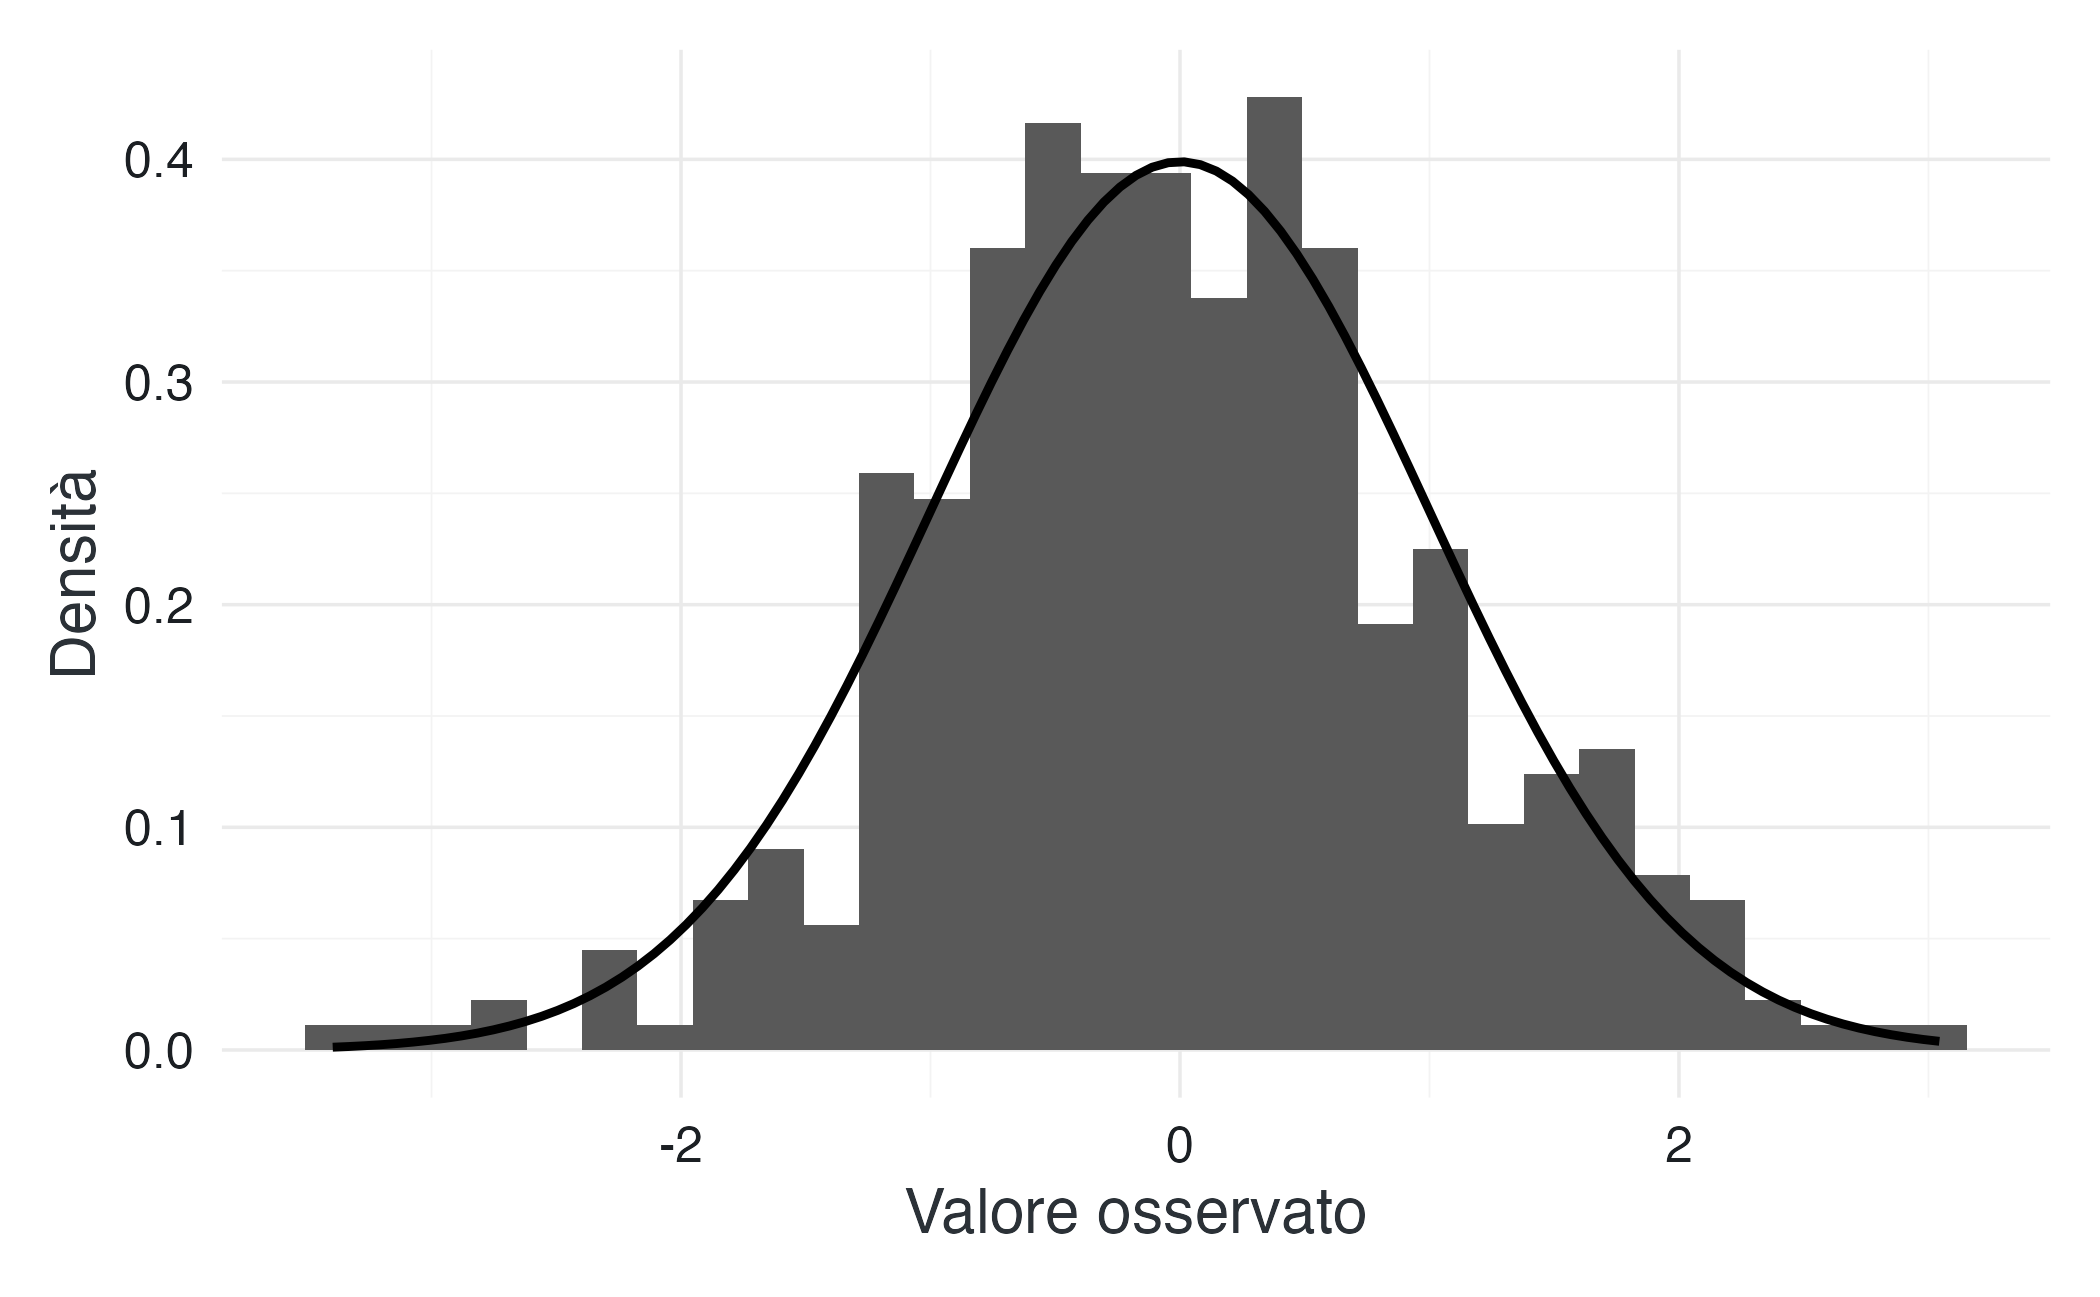
\includegraphics[width=0.85\linewidth,height=\textheight,keepaspectratio]{chapters/formal_models/01_dalla_descrizione_alla_spiegazione_files/figure-pdf/fig-fixed-distribution-1.png}

}

\caption{\label{fig-fixed-distribution}Osservazioni simulate
indipendentemente dalla stessa distribuzione normale. Il modello
rappresenta la distribuzione, ma non propone una dinamica temporale
specifica.}

\end{figure}%

\subsection{Un modello dinamico}\label{un-modello-dinamico}

\begin{Shaded}
\begin{Highlighting}[]
\NormalTok{n\_trials }\OtherTok{\textless{}{-}} \DecValTok{120}
\NormalTok{alpha }\OtherTok{\textless{}{-}} \FloatTok{0.15}
\NormalTok{reward\_probability }\OtherTok{\textless{}{-}} \FloatTok{0.70}
\NormalTok{sigma\_observation }\OtherTok{\textless{}{-}} \FloatTok{0.15}

\NormalTok{reward }\OtherTok{\textless{}{-}} \FunctionTok{rbinom}\NormalTok{(n\_trials, }\AttributeTok{size =} \DecValTok{1}\NormalTok{, }\AttributeTok{prob =}\NormalTok{ reward\_probability)}
\NormalTok{value }\OtherTok{\textless{}{-}} \FunctionTok{numeric}\NormalTok{(n\_trials)}
\NormalTok{y }\OtherTok{\textless{}{-}} \FunctionTok{numeric}\NormalTok{(n\_trials)}

\NormalTok{value[}\DecValTok{1}\NormalTok{] }\OtherTok{\textless{}{-}} \FloatTok{0.20}
\NormalTok{y[}\DecValTok{1}\NormalTok{] }\OtherTok{\textless{}{-}} \FunctionTok{rnorm}\NormalTok{(}\DecValTok{1}\NormalTok{, }\AttributeTok{mean =}\NormalTok{ value[}\DecValTok{1}\NormalTok{], }\AttributeTok{sd =}\NormalTok{ sigma\_observation)}

\ControlFlowTok{for}\NormalTok{ (trial }\ControlFlowTok{in} \DecValTok{1}\SpecialCharTok{:}\NormalTok{(n\_trials }\SpecialCharTok{{-}} \DecValTok{1}\NormalTok{)) \{}
\NormalTok{  prediction\_error }\OtherTok{\textless{}{-}}\NormalTok{ reward[trial] }\SpecialCharTok{{-}}\NormalTok{ value[trial]}
\NormalTok{  value[trial }\SpecialCharTok{+} \DecValTok{1}\NormalTok{] }\OtherTok{\textless{}{-}}\NormalTok{ value[trial] }\SpecialCharTok{+}\NormalTok{ alpha }\SpecialCharTok{*}\NormalTok{ prediction\_error}
\NormalTok{  y[trial }\SpecialCharTok{+} \DecValTok{1}\NormalTok{] }\OtherTok{\textless{}{-}} \FunctionTok{rnorm}\NormalTok{(}
    \DecValTok{1}\NormalTok{,}
    \AttributeTok{mean =}\NormalTok{ value[trial }\SpecialCharTok{+} \DecValTok{1}\NormalTok{],}
    \AttributeTok{sd =}\NormalTok{ sigma\_observation}
\NormalTok{  )}
\NormalTok{\}}

\NormalTok{process\_data }\OtherTok{\textless{}{-}} \FunctionTok{tibble}\NormalTok{(}
  \AttributeTok{trial =} \FunctionTok{seq\_len}\NormalTok{(n\_trials),}
  \AttributeTok{reward =}\NormalTok{ reward,}
  \AttributeTok{value =}\NormalTok{ value,}
  \AttributeTok{y =}\NormalTok{ y}
\NormalTok{)}
\end{Highlighting}
\end{Shaded}

\begin{figure}

\centering{

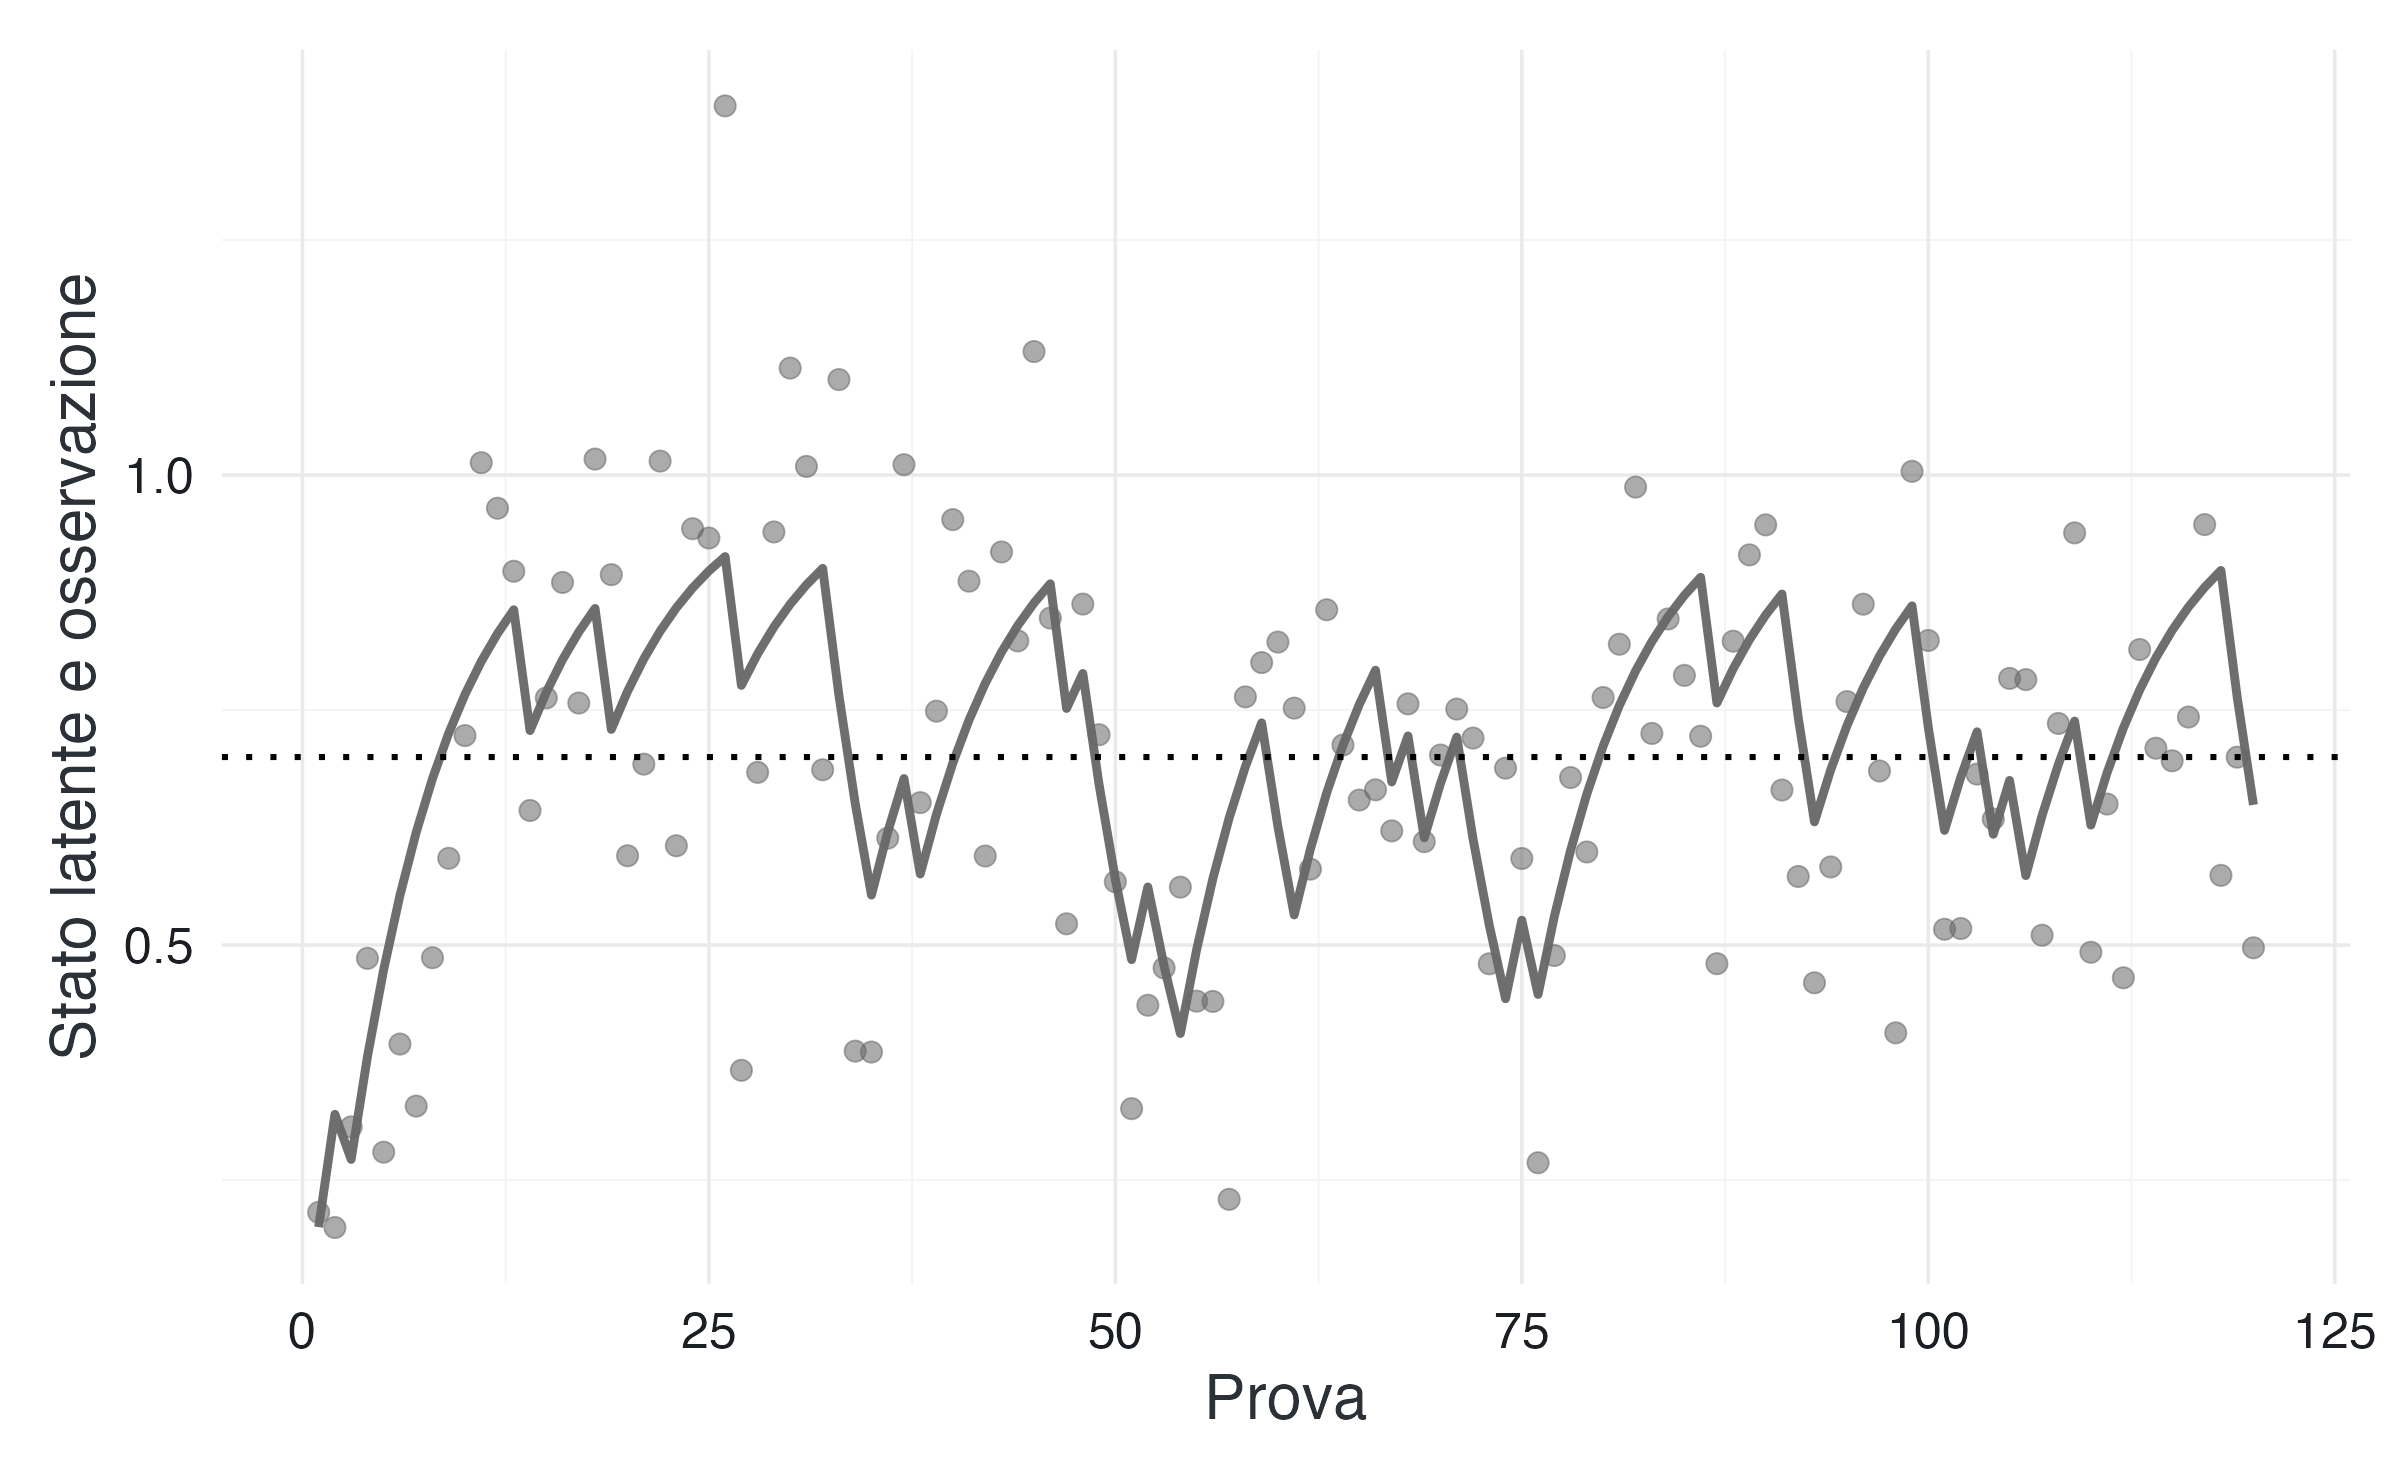
\includegraphics[width=0.85\linewidth,height=\textheight,keepaspectratio]{chapters/formal_models/01_dalla_descrizione_alla_spiegazione_files/figure-pdf/fig-dynamic-process-1.png}

}

\caption{\label{fig-dynamic-process}Stato latente e osservazioni
simulate da un semplice processo di aggiornamento. La dipendenza
temporale nasce dalla regola che collega lo stato corrente alla storia
degli esiti.}

\end{figure}%

\begin{tcolorbox}[enhanced jigsaw, arc=.35mm, bottomrule=.15mm, bottomtitle=1mm, breakable, colback=white, colbacktitle=quarto-callout-note-color!10!white, colframe=quarto-callout-note-color-frame, coltitle=black, left=2mm, leftrule=.75mm, opacityback=0, opacitybacktitle=0.6, rightrule=.15mm, title=\textcolor{quarto-callout-note-color}{\faInfo}\hspace{0.5em}{La differenza non è probabilistico contro non probabilistico}, titlerule=0mm, toprule=.15mm, toptitle=1mm]

Il contrasto corretto non è tra un modello statistico e un modello privo
di statistica. Anche il modello dinamico richiede una distribuzione
probabilistica delle osservazioni.

La differenza è tra:

\begin{itemize}
\tightlist
\item
  un modello che rappresenta direttamente la distribuzione osservata;
\item
  un modello che scompone la generazione dei dati in uno stato dinamico
  e in un processo osservazionale.
\end{itemize}

\end{tcolorbox}

\section{Processo latente e modello
osservazionale}\label{processo-latente-e-modello-osservazionale}

Nei modelli processuali è utile separare due componenti.

\subsection{Il modello del processo}\label{il-modello-del-processo}

Il modello del processo specifica come cambia lo stato latente:

\[
z_t=f(z_{t-1},u_t;\theta_{\text{processo}}),
\]

dove:

\begin{itemize}
\tightlist
\item
  \(z_t\) è uno stato non direttamente osservato;
\item
  \(u_t\) rappresenta l'informazione disponibile al tempo \(t\);
\item
  \(\theta_{\text{processo}}\) contiene i parametri che regolano la
  trasformazione.
\end{itemize}

Nel modello precedente, \(z_t\) corrisponde a \(V_t\), l'input è il
rinforzo \(R_t\) e \(\alpha\) regola la velocità di aggiornamento.

\subsection{Il modello osservazionale}\label{il-modello-osservazionale}

Il modello osservazionale specifica come lo stato produce la misura:

\[
y_t \sim p(y_t\mid z_t,\theta_{\text{osservazione}}).
\]

La scelta del modello osservazionale dipende dalla natura dei dati. Uno
stato latente può produrre:

\begin{itemize}
\tightlist
\item
  un punteggio continuo rumoroso;
\item
  una risposta corretta o errata;
\item
  una scelta tra alternative;
\item
  un tempo di risposta;
\item
  un conteggio.
\end{itemize}

La distribuzione complessiva può essere scritta schematicamente come:

\[
p(\mathbf y,\mathbf z\mid\boldsymbol\theta)
=
p(\mathbf y\mid\mathbf z,\boldsymbol\theta_{\text{oss}})
  p(\mathbf z\mid\boldsymbol\theta_{\text{proc}}).
\]

\begin{tcolorbox}[enhanced jigsaw, arc=.35mm, bottomrule=.15mm, bottomtitle=1mm, breakable, colback=white, colbacktitle=quarto-callout-warning-color!10!white, colframe=quarto-callout-warning-color-frame, coltitle=black, left=2mm, leftrule=.75mm, opacityback=0, opacitybacktitle=0.6, rightrule=.15mm, title=\textcolor{quarto-callout-warning-color}{\faExclamationTriangle}\hspace{0.5em}{Non attribuire al processo ciò che appartiene alla misura}, titlerule=0mm, toprule=.15mm, toptitle=1mm]

Se il modello osservazionale è troppo semplice, il modello del processo
può assorbire rumore, bias di risposta o errori di misurazione. Un
parametro processuale può allora sembrare variabile tra persone non
perché il processo differisca realmente, ma perché il collegamento tra
stato e risposta è stato specificato male.

\end{tcolorbox}

\section{Quando un modello può essere chiamato
meccanicistico}\label{quando-un-modello-puuxf2-essere-chiamato-meccanicistico}

Un modello processuale propone una dinamica. Non per questo ha già
identificato un meccanismo psicologico.

Un'interpretazione meccanicistica diventa più credibile quando
convergono più elementi:

\begin{enumerate}
\def\labelenumi{\arabic{enumi}.}
\tightlist
\item
  \textbf{Corrispondenza teorica.} Stati e parametri devono derivare da
  una teoria sostantiva, non soltanto migliorare il fit.
\item
  \textbf{Predizioni discriminanti.} Il modello deve produrre
  conseguenze differenti da quelle di alternative plausibili.
\item
  \textbf{Manipolazioni informative.} Interventi sul sistema dovrebbero
  modificare il comportamento nel modo previsto dal modello.
\item
  \textbf{Validità del modello osservazionale.} Le misure devono essere
  collegate in modo plausibile agli stati ipotizzati.
\item
  \textbf{Recuperabilità dei parametri.} Dati generati con parametri
  noti dovrebbero consentirne una stima sufficientemente accurata.
\item
  \textbf{Generalizzazione.} Le predizioni dovrebbero mantenersi in
  nuovi individui, compiti o condizioni pertinenti.
\end{enumerate}

\begin{tcolorbox}[enhanced jigsaw, arc=.35mm, bottomrule=.15mm, bottomtitle=1mm, breakable, colback=white, colbacktitle=quarto-callout-important-color!10!white, colframe=quarto-callout-important-color-frame, coltitle=black, left=2mm, leftrule=.75mm, opacityback=0, opacitybacktitle=0.6, rightrule=.15mm, title=\textcolor{quarto-callout-important-color}{\faExclamation}\hspace{0.5em}{Le etichette dei parametri non sono evidenza}, titlerule=0mm, toprule=.15mm, toptitle=1mm]

Chiamare un parametro \emph{tasso di apprendimento}, \emph{sensibilità
alla ricompensa} o \emph{controllo cognitivo} non dimostra che esso
misuri quel costrutto. Il significato psicologico deve essere sostenuto
dal comportamento generativo del modello, dal disegno, dalla
recuperabilità e dalla capacità di distinguere ipotesi rivali
(\citeproc{ref-McElreath_rethinking}{McElreath, 2020}).

\end{tcolorbox}

\section{Equivalenza osservazionale}\label{equivalenza-osservazionale}

Processi differenti possono produrre dati molto simili, soprattutto in
un intervallo limitato o in presenza di rumore. Questo problema è
chiamato \textbf{equivalenza osservazionale}.

Nel seguente esempio confrontiamo:

\begin{itemize}
\tightlist
\item
  un processo asintotico, che rallenta avvicinandosi a un limite;
\item
  una tendenza lineare scelta per approssimarlo nell'intervallo
  osservato.
\end{itemize}

\begin{Shaded}
\begin{Highlighting}[]
\NormalTok{trial\_short }\OtherTok{\textless{}{-}} \DecValTok{0}\SpecialCharTok{:}\DecValTok{12}
\NormalTok{asymptotic\_mean }\OtherTok{\textless{}{-}} \FloatTok{0.15} \SpecialCharTok{+} \FloatTok{0.75} \SpecialCharTok{*}\NormalTok{ (}\DecValTok{1} \SpecialCharTok{{-}} \FunctionTok{exp}\NormalTok{(}\SpecialCharTok{{-}}\FloatTok{0.10} \SpecialCharTok{*}\NormalTok{ trial\_short))}
\NormalTok{linear\_fit\_to\_asymptote }\OtherTok{\textless{}{-}} \FunctionTok{lm}\NormalTok{(asymptotic\_mean }\SpecialCharTok{\textasciitilde{}}\NormalTok{ trial\_short)}
\NormalTok{linear\_mean }\OtherTok{\textless{}{-}} \FunctionTok{fitted}\NormalTok{(linear\_fit\_to\_asymptote)}
\NormalTok{observed\_short }\OtherTok{\textless{}{-}} \FunctionTok{rnorm}\NormalTok{(}
  \FunctionTok{length}\NormalTok{(trial\_short),}
  \AttributeTok{mean =}\NormalTok{ asymptotic\_mean,}
  \AttributeTok{sd =} \FloatTok{0.07}
\NormalTok{)}

\NormalTok{equivalence\_data }\OtherTok{\textless{}{-}} \FunctionTok{tibble}\NormalTok{(}
  \AttributeTok{trial =}\NormalTok{ trial\_short,}
  \AttributeTok{observed =}\NormalTok{ observed\_short,}
  \AttributeTok{asymptotic =}\NormalTok{ asymptotic\_mean,}
  \AttributeTok{linear =}\NormalTok{ linear\_mean}
\NormalTok{)}
\end{Highlighting}
\end{Shaded}

\begin{figure}

\centering{

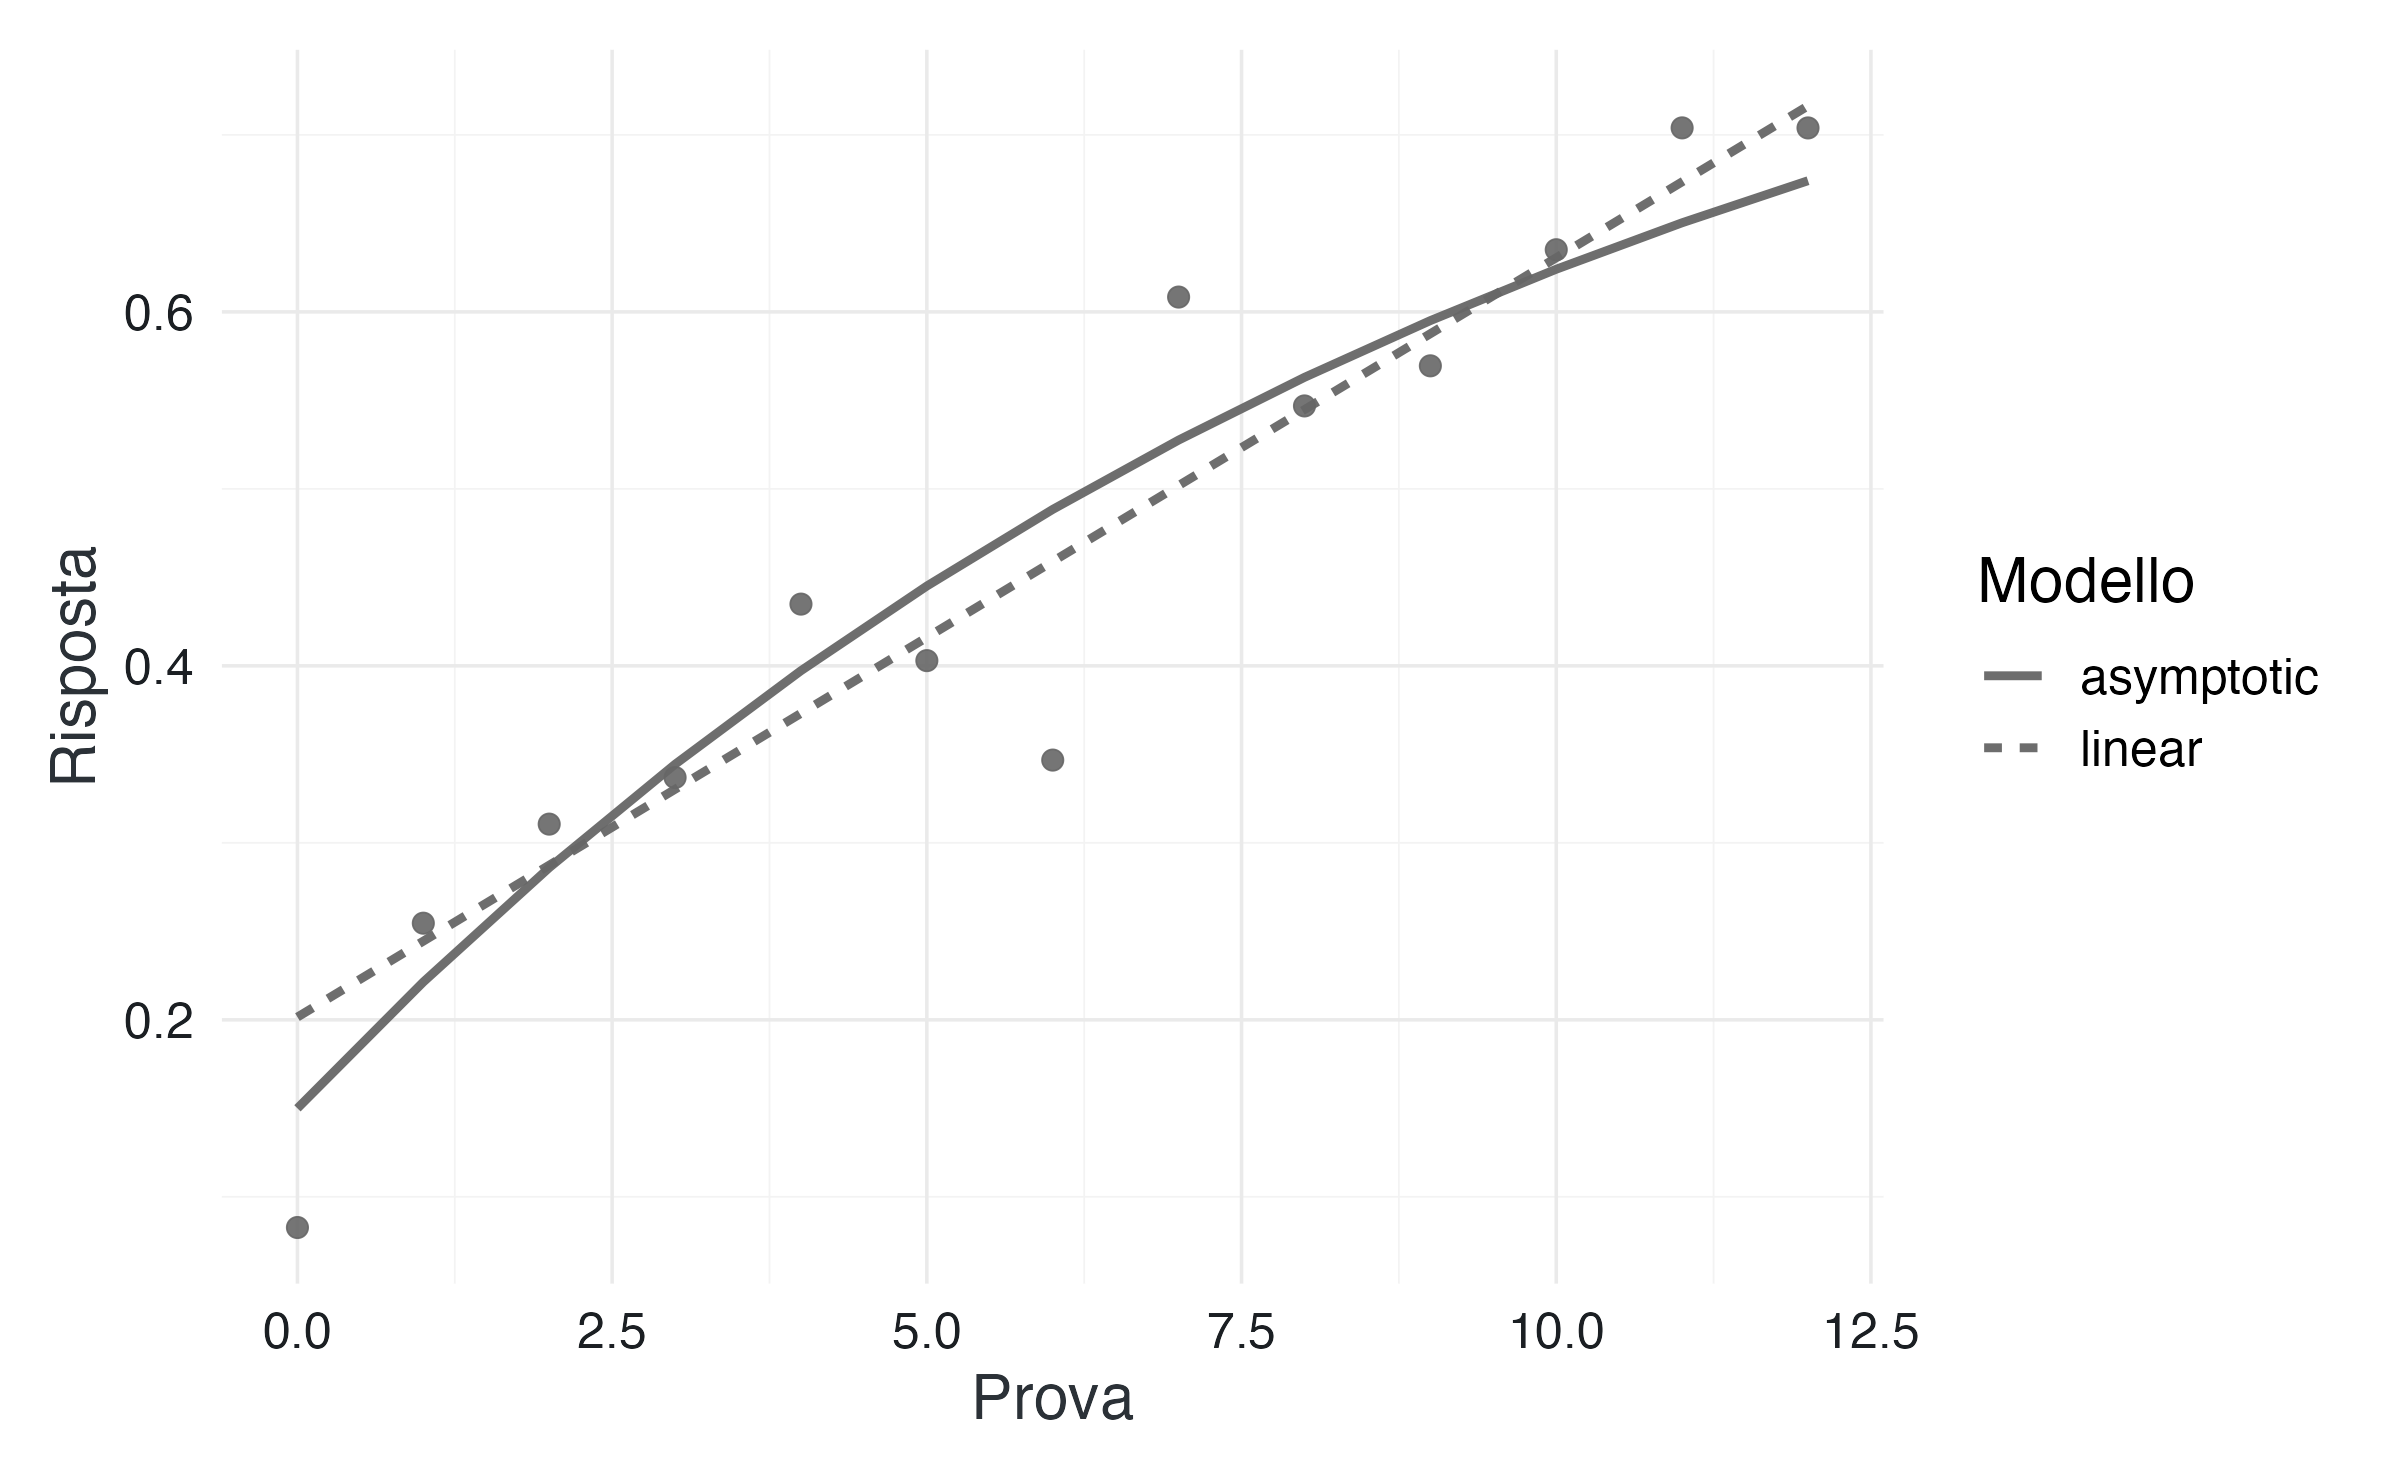
\includegraphics[width=0.85\linewidth,height=\textheight,keepaspectratio]{chapters/formal_models/01_dalla_descrizione_alla_spiegazione_files/figure-pdf/fig-observational-equivalence-1.png}

}

\caption{\label{fig-observational-equivalence}Due modelli generano
traiettorie simili nell'intervallo osservato. Un buon adattamento locale
non basta a identificare il processo che ha prodotto i dati.}

\end{figure}%

Nell'intervallo osservato, entrambi i modelli possono sembrare adeguati.
Le loro differenze diventano più evidenti extrapolando a prove
successive o progettando condizioni nelle quali il processo asintotico e
quello lineare producano predizioni divergenti.

\begin{tcolorbox}[enhanced jigsaw, arc=.35mm, bottomrule=.15mm, bottomtitle=1mm, breakable, colback=white, colbacktitle=quarto-callout-note-color!10!white, colframe=quarto-callout-note-color-frame, coltitle=black, left=2mm, leftrule=.75mm, opacityback=0, opacitybacktitle=0.6, rightrule=.15mm, title=\textcolor{quarto-callout-note-color}{\faInfo}\hspace{0.5em}{Conseguenza metodologica}, titlerule=0mm, toprule=.15mm, toptitle=1mm]

Non basta chiedere quale modello si adatti meglio ai dati disponibili.
Occorre chiedere quali osservazioni, tempi di misura o manipolazioni
permetterebbero di distinguere i modelli.

\end{tcolorbox}

\section{Adattamento, previsione e
spiegazione}\label{adattamento-previsione-e-spiegazione}

Questi tre criteri sono collegati, ma non equivalenti.

\subsection{Adattamento ai dati
osservati}\label{adattamento-ai-dati-osservati}

L'adattamento riguarda quanto bene il modello riproduca le osservazioni
usate per stimarlo. Può essere studiato attraverso:

\begin{itemize}
\tightlist
\item
  residui;
\item
  controlli predittivi a posteriori;
\item
  discrepanze tra statistiche osservate e replicate;
\item
  log-verosimiglianza sui dati di stima.
\end{itemize}

Un adattamento insufficiente è un segnale chiaro di inadeguatezza. Un
buon adattamento, invece, è soltanto una condizione necessaria: modelli
molto diversi possono adattarsi agli stessi dati.

\subsection{Previsione}\label{previsione}

La previsione riguarda dati non utilizzati per adattare il modello:

\begin{itemize}
\tightlist
\item
  nuove osservazioni degli stessi individui;
\item
  nuovi individui;
\item
  nuove condizioni sperimentali;
\item
  nuovi compiti o nuovi contesti.
\end{itemize}

La validazione fuori campione protegge dall'eccessivo adattamento, ma
una buona previsione non identifica automaticamente il meccanismo. Un
modello puramente predittivo può generalizzare bene senza rappresentare
il processo psicologico effettivo.

\subsection{Spiegazione}\label{spiegazione}

La spiegazione richiede un collegamento tra struttura formale e teoria.
Un modello esplicativo dovrebbe chiarire:

\begin{itemize}
\tightlist
\item
  quali entità o stati vengono ipotizzati;
\item
  come interagiscono;
\item
  quali trasformazioni producono il comportamento;
\item
  quali evidenze sarebbero incompatibili con il modello;
\item
  perché il modello è preferibile ad alternative plausibili.
\end{itemize}

\begin{tcolorbox}[enhanced jigsaw, arc=.35mm, bottomrule=.15mm, bottomtitle=1mm, breakable, colback=white, colbacktitle=quarto-callout-caution-color!10!white, colframe=quarto-callout-caution-color-frame, coltitle=black, left=2mm, leftrule=.75mm, opacityback=0, opacitybacktitle=0.6, rightrule=.15mm, title=\textcolor{quarto-callout-caution-color}{\faFire}\hspace{0.5em}{Fit non significa spiegazione}, titlerule=0mm, toprule=.15mm, toptitle=1mm]

Nel linguaggio statistico, \emph{fit} indica adattamento. Non dovrebbe
essere chiamato «adeguatezza esplicativa». Un modello può adattarsi
molto bene e offrire una spiegazione debole, oppure adattarsi in modo
imperfetto ma rivelare un errore teorico informativo.

\end{tcolorbox}

\section{Un esempio: scelte
alimentari}\label{un-esempio-scelte-alimentari}

Immaginiamo di osservare le scelte tra uno snack salutare e uno non
salutare.

\subsection{Un modello di regressione}\label{un-modello-di-regressione}

Una regressione logistica può rappresentare la probabilità della scelta
salutare in funzione di stress e disponibilità economica:

\[
\operatorname{logit}\Pr(Y_i=1)
=
\alpha+\beta_1\text{Stress}_i+\beta_2\text{Risorse}_i.
\]

Il modello risponde a domande come:

\begin{itemize}
\tightlist
\item
  quanto cambia la probabilità della scelta al variare dello stress;
\item
  quali individui hanno maggiore probabilità di scegliere lo snack
  salutare;
\item
  quanto bene la combinazione dei predittori anticipa nuove scelte.
\end{itemize}

\subsection{Un modello di
apprendimento}\label{un-modello-di-apprendimento}

Se le persone ricevono esiti ripetuti, possiamo ipotizzare che
aggiornino il valore atteso delle alternative:

\[
V_{a,t+1}=V_{a,t}+\alpha(R_t-V_{a,t}),
\]

per poi trasformare i valori in probabilità di scelta attraverso una
regola come la Softmax.

Il modello risponde a domande differenti:

\begin{itemize}
\tightlist
\item
  con quale velocità vengono aggiornate le aspettative;
\item
  quanto le differenze di valore influenzano la scelta;
\item
  come cambia il comportamento dopo un esito inatteso.
\end{itemize}

I due modelli non sono necessariamente concorrenti. Stress e risorse
potrebbero influire sul tasso di apprendimento, sul valore delle
alternative o sulla sensibilità della scelta. La regressione può
descrivere covariate rilevanti; il modello processuale può rappresentare
la dinamica che le collega alle risposte.

\begin{tcolorbox}[enhanced jigsaw, arc=.35mm, bottomrule=.15mm, bottomtitle=1mm, breakable, colback=white, colbacktitle=quarto-callout-note-color!10!white, colframe=quarto-callout-note-color-frame, coltitle=black, left=2mm, leftrule=.75mm, opacityback=0, opacitybacktitle=0.6, rightrule=.15mm, title=\textcolor{quarto-callout-note-color}{\faInfo}\hspace{0.5em}{La domanda determina il modello}, titlerule=0mm, toprule=.15mm, toptitle=1mm]

Non dobbiamo scegliere tra regressione e modello processuale in
astratto. Dobbiamo stabilire quale quantità vogliamo conoscere e quale
struttura dei dati può informarla.

\end{tcolorbox}

\section{Come valutare un modello
formale}\label{come-valutare-un-modello-formale}

Nessun singolo indice decide se un modello sia scientificamente
adeguato. Sono necessarie verifiche complementari.

{\def\LTcaptype{none} % do not increment counter
\begin{longtable}[]{@{}
  >{\raggedright\arraybackslash}p{(\linewidth - 4\tabcolsep) * \real{0.3333}}
  >{\raggedright\arraybackslash}p{(\linewidth - 4\tabcolsep) * \real{0.3333}}
  >{\raggedright\arraybackslash}p{(\linewidth - 4\tabcolsep) * \real{0.3333}}@{}}
\toprule\noalign{}
\begin{minipage}[b]{\linewidth}\raggedright
Domanda
\end{minipage} & \begin{minipage}[b]{\linewidth}\raggedright
Controllo utile
\end{minipage} & \begin{minipage}[b]{\linewidth}\raggedright
Limite del controllo
\end{minipage} \\
\midrule\noalign{}
\endhead
\bottomrule\noalign{}
\endlastfoot
Il campionamento è affidabile? & \(\widehat R\), ESS, divergenze,
diagnostica delle catene & Non verifica la correttezza teorica \\
Il modello riproduce i dati? & Prior e posterior predictive checks & Può
non distinguere modelli rivali \\
Il modello generalizza? & Validazione fuori campione o tra studi & Buona
previsione non implica meccanismo corretto \\
I parametri sono recuperabili? & Parameter recovery & Il recupero
dipende dal disegno simulato \\
Il modello è discriminabile? & Confronto con modelli rivali e predizioni
divergenti & Il migliore tra i modelli può essere comunque inadeguato \\
L'interpretazione è robusta? & Analisi di sensibilità, nuovi compiti e
manipolazioni & Non elimina tutte le assunzioni sostantive \\
\end{longtable}
}

La valutazione dovrebbe quindi combinare:

\begin{enumerate}
\def\labelenumi{\arabic{enumi}.}
\tightlist
\item
  simulazione a priori;
\item
  controllo del calcolo;
\item
  controllo predittivo;
\item
  recupero dei parametri;
\item
  confronto con alternative;
\item
  verifica in condizioni nuove;
\item
  revisione del modello.
\end{enumerate}

La parte \textbf{Valutazione} svilupperà gli strumenti quantitativi per
il confronto predittivo. In questa parte l'attenzione rimane sul
rapporto tra teoria, comportamento generativo e interpretazione.

\section{Il workflow dei capitoli
successivi}\label{il-workflow-dei-capitoli-successivi}

Nei capitoli processuali seguiremo una struttura ricorrente.

\subsection{1. Delimitare il fenomeno}\label{delimitare-il-fenomeno-1}

Quale regolarità o comportamento deve essere spiegato? In quali
condizioni?

\subsection{2. Formulare la teoria
verbale}\label{formulare-la-teoria-verbale}

Quali stati, informazioni e trasformazioni vengono ipotizzati?

\subsection{3. Tradurre la teoria in
equazioni}\label{tradurre-la-teoria-in-equazioni}

Quali parametri regolano il processo? Quali condizioni iniziali sono
necessarie?

\subsection{4. Simulare prima di
stimare}\label{simulare-prima-di-stimare-2}

Quali traiettorie produce il modello? Come cambiano al variare dei
parametri? Quali pattern non può generare?

\subsection{5. Specificare il modello
osservazionale}\label{specificare-il-modello-osservazionale}

Come gli stati latenti producono le risposte misurate?

\subsection{6. Risolvere il problema
inverso}\label{risolvere-il-problema-inverso-1}

Quali valori dei parametri sono plausibili dati i dati osservati?

\subsection{7. Verificare identificabilità e
recuperabilità}\label{verificare-identificabilituxe0-e-recuperabilituxe0}

Parametri diversi producono dati distinguibili? La procedura riesce a
recuperare parametri noti?

\subsection{8. Controllare e
confrontare}\label{controllare-e-confrontare}

Il modello riproduce gli aspetti rilevanti dei dati? Un modello rivale
produce previsioni migliori o qualitativamente diverse?

\subsection{9. Interpretare con cautela}\label{interpretare-con-cautela}

Quale parte della conclusione deriva dai dati e quale dalle assunzioni
teoriche, osservative e gerarchiche?

Questo workflow è coerente con l'idea di trattare il modello come una
teoria eseguibile e modificabile
(\citeproc{ref-gelman2021regression}{Gelman et al., 2021};
\citeproc{ref-McElreath_rethinking}{McElreath, 2020}).

\section{Errori frequenti}\label{errori-frequenti-10}

\begin{tcolorbox}[enhanced jigsaw, arc=.35mm, bottomrule=.15mm, bottomtitle=1mm, breakable, colback=white, colbacktitle=quarto-callout-caution-color!10!white, colframe=quarto-callout-caution-color-frame, coltitle=black, left=2mm, leftrule=.75mm, opacityback=0, opacitybacktitle=0.6, rightrule=.15mm, title=\textcolor{quarto-callout-caution-color}{\faFire}\hspace{0.5em}{Attenzione}, titlerule=0mm, toprule=.15mm, toptitle=1mm]

\begin{itemize}
\tightlist
\item
  Considerare ogni regressione come priva di contenuto generativo.
\item
  Chiamare \emph{meccanicistico} qualsiasi modello con variabili
  latenti.
\item
  Interpretare il nome di un parametro come prova della sua validità
  psicologica.
\item
  Confondere un buon fit con una buona spiegazione.
\item
  Confondere una buona previsione con l'identificazione del processo.
\item
  Valutare un modello senza confrontarlo con alternative plausibili.
\item
  Stimare i parametri prima di studiare mediante simulazione ciò che il
  modello può generare.
\item
  Ignorare il modello osservazionale e attribuire tutto il rumore al
  processo cognitivo.
\item
  Interpretare differenze individuali senza verificare la recuperabilità
  dei parametri.
\item
  Scegliere il modello più complesso soltanto perché appare più
  realistico.
\end{itemize}

\end{tcolorbox}

\section{Riflessioni conclusive}\label{riflessioni-conclusive-35}

La psicologia non deve scegliere tra modelli statistici e modelli
processuali come se appartenessero a programmi scientifici
incompatibili. I modelli processuali sono anche modelli statistici:
devono descrivere come gli stati latenti producono osservazioni
variabili e devono essere stimati e controllati con strumenti
probabilistici.

Il cambiamento importante riguarda l'ambizione teorica. Un modello che
rappresenta una distribuzione o un'associazione può rispondere in modo
adeguato a molte domande. Quando vogliamo spiegare una dinamica, però,
dobbiamo specificare stati, trasformazioni, condizioni iniziali e
modello osservazionale. Questa specificazione rende la teoria
eseguibile: possiamo simularla, confrontarla con alternative e
individuare i modi in cui fallisce.

La formalizzazione non garantisce automaticamente una spiegazione.
Processi differenti possono essere osservazionalmente equivalenti;
parametri con nomi psicologici possono essere scarsamente identificati;
un modello può prevedere bene per ragioni diverse da quelle suggerite
dalla sua interpretazione. La forza scientifica nasce dalla combinazione
di teoria, simulazione, disegno, inferenza, confronto e revisione.

Nel Capitolo~\ref{sec-dynamic-models-goal-updating} applicheremo questo
vocabolario a un primo modello dinamico. Partiremo da una teoria verbale
sulla revisione degli obiettivi, ne studieremo le conseguenze generative
e costruiremo il collegamento tra processo latente e dati osservati
(\citeproc{ref-hayes2019role}{Hayes et al., 2019};
\citeproc{ref-knight2023tutorial}{Knight et al., 2023}).

\section{Concetti da ricordare}\label{concetti-da-ricordare-9}

\begin{enumerate}
\def\labelenumi{\arabic{enumi}.}
\tightlist
\item
  Un modello statistico specifica una distribuzione probabilistica; può
  essere anche generativo.
\item
  Un modello generativo permette di simulare dati a partire da parametri
  e assunzioni.
\item
  Un modello processuale rappresenta stati e trasformazioni, spesso nel
  tempo.
\item
  Un'interpretazione meccanicistica richiede più della presenza di
  equazioni.
\item
  Un modello normativo specifica un criterio di scelta ottimale, non
  necessariamente il processo reale.
\item
  Processo latente e modello osservazionale sono componenti distinte.
\item
  Processi differenti possono produrre osservazioni simili.
\item
  Adattamento, previsione e spiegazione rispondono a domande differenti.
\item
  Il nome di un parametro non ne garantisce il significato psicologico.
\item
  Simulazione, parameter recovery e confronto tra modelli sono parti del
  controllo teorico.
\end{enumerate}

\begin{tcolorbox}[enhanced jigsaw, arc=.35mm, bottomrule=.15mm, bottomtitle=1mm, breakable, colback=white, colbacktitle=quarto-callout-important-color!10!white, colframe=quarto-callout-important-color-frame, coltitle=black, left=2mm, leftrule=.75mm, opacityback=0, opacitybacktitle=0.6, rightrule=.15mm, title=\textcolor{quarto-callout-important-color}{\faExclamation}\hspace{0.5em}{Esercizi}, titlerule=0mm, toprule=.15mm, toptitle=1mm]

\subsection{1. Classificare un modello}\label{classificare-un-modello}

Considera un modello logistico che predice la probabilità di abbandono
scolastico da assenze e rendimento. In quali sensi è statistico e
generativo? Che cosa mancherebbe per considerarlo processuale?

\subsection{2. Separare processo e
osservazione}\label{separare-processo-e-osservazione}

Immagina un modello nel quale la motivazione cambia ogni settimana e
viene misurata mediante un questionario. Proponi:

\begin{itemize}
\tightlist
\item
  una semplice regola di aggiornamento della motivazione;
\item
  un modello osservazionale per il punteggio del questionario.
\end{itemize}

\subsection{3. Modificare la
simulazione}\label{modificare-la-simulazione}

Nel modello dinamico del capitolo, confronta \(\alpha=0.05\), \(0.20\) e
\(0.80\). Descrivi come cambia la traiettoria dello stato latente.

\subsection{4. Equivalenza
osservazionale}\label{equivalenza-osservazionale-1}

Proponi una raccolta dati o una manipolazione che distingua meglio la
traiettoria lineare da quella asintotica mostrate nel capitolo.

\subsection{5. Fit e spiegazione}\label{fit-e-spiegazione}

Fornisci un esempio nel quale un modello possa adattarsi bene ai dati
pur avendo un'interpretazione psicologica poco credibile.

\subsection{6. Previsione e meccanismo}\label{previsione-e-meccanismo}

Perché una previsione accurata su nuovi dati non dimostra
necessariamente che il modello abbia identificato il processo causale
corretto?

\subsection{7. Validità dei parametri}\label{validituxe0-dei-parametri}

Quali evidenze richiederesti prima di interpretare un parametro come
«tasso di apprendimento»?

\subsection{8. Modelli complementari}\label{modelli-complementari}

Descrivi un problema psicologico nel quale una regressione e un modello
processuale possano essere usati insieme anziché come alternative.

\subsection{9. Modello normativo}\label{modello-normativo}

Costruisci un esempio nel quale l'azione normativamente ottimale
differisca dal comportamento osservato. Indica almeno due possibili
ragioni della discrepanza.

\subsection{10. Criticare un modello}\label{criticare-un-modello}

Scegli un modello psicologico che conosci e specifica:

\begin{itemize}
\tightlist
\item
  ciò che descrive;
\item
  ciò che tenta di spiegare;
\item
  una previsione che potrebbe metterlo in difficoltà;
\item
  un modello rivale plausibile.
\end{itemize}

\end{tcolorbox}

\begin{tcolorbox}[enhanced jigsaw, arc=.35mm, bottomrule=.15mm, bottomtitle=1mm, breakable, colback=white, colbacktitle=quarto-callout-tip-color!10!white, colframe=quarto-callout-tip-color-frame, coltitle=black, left=2mm, leftrule=.75mm, opacityback=0, opacitybacktitle=0.6, rightrule=.15mm, title=\textcolor{quarto-callout-tip-color}{\faLightbulb}\hspace{0.5em}{Tracce di soluzione}, titlerule=0mm, toprule=.15mm, toptitle=1mm]

\begin{enumerate}
\def\labelenumi{\arabic{enumi}.}
\tightlist
\item
  Il modello è statistico perché specifica una distribuzione
  condizionata ed è generativo perché permette di simulare esiti. Per
  essere processuale dovrebbe rappresentare come stati o decisioni
  evolvono nel tempo.
\item
  Una possibile regola è \(M_t=M_{t-1}+\alpha(I_t-M_{t-1})\); il
  punteggio potrebbe seguire
  \(Y_t\sim\operatorname{Normal}(M_t,\sigma_y)\).
\item
  Valori piccoli producono aggiornamenti lenti e regolari; valori grandi
  rendono lo stato molto sensibile all'ultimo esito.
\item
  Si possono estendere le osservazioni nel tempo o introdurre una
  condizione che modifichi il limite asintotico.
\item
  Un modello molto flessibile può interpolare i dati senza che i suoi
  parametri corrispondano a processi plausibili.
\item
  Processi diversi possono produrre le stesse previsioni nell'ambito
  osservato.
\item
  Servono almeno simulazione, recupero, predizioni discriminanti,
  stabilità e validazione rispetto a manipolazioni pertinenti.
\item
  Le covariate della regressione possono spiegare variazioni nei
  parametri del modello processuale.
\item
  La discrepanza può derivare da informazioni diverse, costi cognitivi,
  preferenze non modellate o limiti del processo decisionale.
\item
  La risposta deve distinguere adeguatezza descrittiva, pretesa
  esplicativa e condizioni di falsificazione.
\end{enumerate}

\end{tcolorbox}

\begin{tcolorbox}[enhanced jigsaw, arc=.35mm, bottomrule=.15mm, bottomtitle=1mm, breakable, colback=white, colbacktitle=quarto-callout-note-color!10!white, colframe=quarto-callout-note-color-frame, coltitle=black, left=2mm, leftrule=.75mm, opacityback=0, opacitybacktitle=0.6, rightrule=.15mm, title=\textcolor{quarto-callout-note-color}{\faInfo}\hspace{0.5em}{Informazioni sull'ambiente di sviluppo}, titlerule=0mm, toprule=.15mm, toptitle=1mm]

\begin{Shaded}
\begin{Highlighting}[]
\FunctionTok{sessionInfo}\NormalTok{()}
\CommentTok{\#\textgreater{} R version 4.6.1 (2026{-}06{-}24)}
\CommentTok{\#\textgreater{} Platform: aarch64{-}apple{-}darwin23}
\CommentTok{\#\textgreater{} Running under: macOS Tahoe 26.5.2}
\CommentTok{\#\textgreater{} }
\CommentTok{\#\textgreater{} Matrix products: default}
\CommentTok{\#\textgreater{} BLAS:   /Library/Frameworks/R.framework/Versions/4.6/Resources/lib/libRblas.0.dylib }
\CommentTok{\#\textgreater{} LAPACK: /Library/Frameworks/R.framework/Versions/4.6/Resources/lib/libRlapack.dylib;  LAPACK version 3.12.1}
\CommentTok{\#\textgreater{} }
\CommentTok{\#\textgreater{} locale:}
\CommentTok{\#\textgreater{} [1] C.UTF{-}8/UTF{-}8/C.UTF{-}8/C/C.UTF{-}8/C.UTF{-}8}
\CommentTok{\#\textgreater{} }
\CommentTok{\#\textgreater{} time zone: Europe/Zagreb}
\CommentTok{\#\textgreater{} tzcode source: internal}
\CommentTok{\#\textgreater{} }
\CommentTok{\#\textgreater{} attached base packages:}
\CommentTok{\#\textgreater{} [1] stats     graphics  grDevices utils     datasets  methods   base     }
\CommentTok{\#\textgreater{} }
\CommentTok{\#\textgreater{} other attached packages:}
\CommentTok{\#\textgreater{}  [1] ragg\_1.5.2            tinytable\_0.17.0      withr\_3.0.3          }
\CommentTok{\#\textgreater{}  [4] systemfonts\_1.3.2     patchwork\_1.3.2       ggdist\_3.3.3         }
\CommentTok{\#\textgreater{}  [7] tidybayes\_3.0.7       bayesplot\_1.15.0      ggplot2\_4.0.3        }
\CommentTok{\#\textgreater{} [10] reliabilitydiag\_0.2.1 priorsense\_1.2.0      posterior\_1.7.0      }
\CommentTok{\#\textgreater{} [13] loo\_2.10.0            rstan\_2.32.7          StanHeaders\_2.32.10  }
\CommentTok{\#\textgreater{} [16] brms\_2.23.0           Rcpp\_1.1.2            sessioninfo\_1.2.4    }
\CommentTok{\#\textgreater{} [19] conflicted\_1.2.0      janitor\_2.2.1         matrixStats\_1.5.0    }
\CommentTok{\#\textgreater{} [22] modelr\_0.1.11         tibble\_3.3.1          dplyr\_1.2.1          }
\CommentTok{\#\textgreater{} [25] tidyr\_1.3.2           rio\_1.3.0             here\_1.0.2           }
\CommentTok{\#\textgreater{} }
\CommentTok{\#\textgreater{} loaded via a namespace (and not attached):}
\CommentTok{\#\textgreater{}  [1] svUnit\_1.0.8          tidyselect\_1.2.1      farver\_2.1.2         }
\CommentTok{\#\textgreater{}  [4] S7\_0.2.2              fastmap\_1.2.0         tensorA\_0.36.2.1     }
\CommentTok{\#\textgreater{}  [7] digest\_0.6.39         timechange\_0.4.0      estimability\_2.0.0   }
\CommentTok{\#\textgreater{} [10] lifecycle\_1.0.5       magrittr\_2.0.5        compiler\_4.6.1       }
\CommentTok{\#\textgreater{} [13] rlang\_1.3.0           tools\_4.6.1           yaml\_2.3.12          }
\CommentTok{\#\textgreater{} [16] knitr\_1.51            labeling\_0.4.3        bridgesampling\_1.2{-}1 }
\CommentTok{\#\textgreater{} [19] pkgbuild\_1.4.8        curl\_7.1.0            RColorBrewer\_1.1{-}3   }
\CommentTok{\#\textgreater{} [22] abind\_1.4{-}8           purrr\_1.2.2           grid\_4.6.1           }
\CommentTok{\#\textgreater{} [25] stats4\_4.6.1          xtable\_1.8{-}8          inline\_0.3.21        }
\CommentTok{\#\textgreater{} [28] emmeans\_2.0.4         scales\_1.4.0          cli\_3.6.6            }
\CommentTok{\#\textgreater{} [31] mvtnorm\_1.4{-}2         rmarkdown\_2.31        generics\_0.1.4       }
\CommentTok{\#\textgreater{} [34] otel\_0.2.0            RcppParallel\_5.1.11{-}2 cachem\_1.1.0         }
\CommentTok{\#\textgreater{} [37] stringr\_1.6.0         parallel\_4.6.1        vctrs\_0.7.3          }
\CommentTok{\#\textgreater{} [40] V8\_8.2.0              Matrix\_1.7{-}5          jsonlite\_2.0.0       }
\CommentTok{\#\textgreater{} [43] arrayhelpers\_1.1{-}1    glue\_1.8.1            codetools\_0.2{-}20     }
\CommentTok{\#\textgreater{} [46] distributional\_0.8.1  lubridate\_1.9.5       stringi\_1.8.7        }
\CommentTok{\#\textgreater{} [49] gtable\_0.3.6          QuickJSR\_1.10.0       pillar\_1.11.1        }
\CommentTok{\#\textgreater{} [52] htmltools\_0.5.9       Brobdingnag\_1.2{-}9     R6\_2.6.1             }
\CommentTok{\#\textgreater{} [55] textshaping\_1.0.5     rprojroot\_2.1.1       evaluate\_1.0.5       }
\CommentTok{\#\textgreater{} [58] lattice\_0.22{-}9        backports\_1.5.1       memoise\_2.0.1        }
\CommentTok{\#\textgreater{} [61] broom\_1.0.13          snakecase\_0.11.1      rstantools\_2.6.0     }
\CommentTok{\#\textgreater{} [64] coda\_0.19{-}4.1         gridExtra\_2.3.1       nlme\_3.1{-}170         }
\CommentTok{\#\textgreater{} [67] checkmate\_2.3.4       xfun\_0.60             pkgconfig\_2.0.3}
\end{Highlighting}
\end{Shaded}

\end{tcolorbox}

\section*{Bibliografia}\label{bibliografia-40}

\markright{Bibliografia}

\chapter{Costruire un modello dinamico: la revisione degli
obiettivi}\label{sec-dynamic-models-goal-updating}

Molti fenomeni psicologici non sono fotografie, ma processi. Un
obiettivo personale, un'aspettativa o un sintomo osservato in un dato
momento dipendono anche da ciò che è accaduto prima.

In questo capitolo traduciamo una teoria verbale della regolazione degli
obiettivi in una regola di aggiornamento eseguibile. Seguiremo l'ordine
appropriato per un modello processuale: prima ne studieremo le
conseguenze mediante simulazione; soltanto dopo collegheremo il processo
ai dati e ne stimeremo i parametri.

\begin{tcolorbox}[enhanced jigsaw, arc=.35mm, bottomrule=.15mm, breakable, colback=white, colframe=quarto-callout-important-color-frame, left=2mm, leftrule=.75mm, opacityback=0, rightrule=.15mm, toprule=.15mm]

\textbf{Da sapere.} Un modello dinamico descrive un processo nel quale
lo stato corrente dipende dalla storia precedente. Nel modello di
revisione degli obiettivi, \(\alpha\) determina quanta parte della
discrepanza tra prestazione e obiettivo viene incorporata
nell'aggiornamento, mentre \(\beta\) rappresenta una deriva sistematica.
Lo stato latente del processo deve essere distinto dall'osservazione
rumorosa, e i parametri non possono essere interpretati automaticamente
come tratti psicologici validati.

\textbf{Da saper fare.} Scomporre il modello in stato, input, errore di
previsione e regola di aggiornamento; interpretare gli effetti di
\(\alpha\), \(\beta\) e \(\sigma\); distinguere processo latente e
modello osservazionale; leggere il programma Stan fornito e collegarne
le istruzioni alla ricorsione matematica; valutare prior, diagnostica,
traiettorie simulate e controlli predittivi rispettando la struttura
temporale dei dati.

\textbf{Approfondimento facoltativo.} La scrittura autonoma del
programma Stan, i dettagli della compilazione con \texttt{cmdstanr} e
l'esercizio completo di recupero dei parametri possono essere rimandati.
In questo capitolo Stan è però parte costitutiva dell'analisi: non
esiste un percorso equivalente basato soltanto su \texttt{brms}. Nel
percorso essenziale è richiesto saper leggere e utilizzare il modello
fornito, non programmarlo da zero.

\hyperref[sec-percorsi-lettura]{Che cosa significano queste etichette?}

\end{tcolorbox}

\begin{tcolorbox}[enhanced jigsaw, arc=.35mm, bottomrule=.15mm, bottomtitle=1mm, breakable, colback=white, colbacktitle=quarto-callout-note-color!10!white, colframe=quarto-callout-note-color-frame, coltitle=black, left=2mm, leftrule=.75mm, opacityback=0, opacitybacktitle=0.6, rightrule=.15mm, title=\textcolor{quarto-callout-note-color}{\faInfo}\hspace{0.5em}{Obiettivi del capitolo}, titlerule=0mm, toprule=.15mm, toptitle=1mm]

Al termine del capitolo dovresti essere in grado di:

\begin{itemize}
\tightlist
\item
  riconoscere stato, input, errore di previsione e regola di
  aggiornamento;
\item
  interpretare i parametri del modello senza trasformarli
  automaticamente in tratti psicologici;
\item
  simulare traiettorie prima di osservare o analizzare dati;
\item
  distinguere il modello del processo dal modello osservazionale;
\item
  comprendere quali informazioni fornisce un modello con parametri
  condivisi dall'intero campione;
\item
  specificare e stimare il modello in Stan;
\item
  eseguire controlli predittivi e un semplice esercizio di recupero dei
  parametri;
\item
  individuare le principali assunzioni e i limiti della specificazione.
\end{itemize}

\end{tcolorbox}

\begin{tcolorbox}[enhanced jigsaw, arc=.35mm, bottomrule=.15mm, bottomtitle=1mm, breakable, colback=white, colbacktitle=quarto-callout-tip-color!10!white, colframe=quarto-callout-tip-color-frame, coltitle=black, left=2mm, leftrule=.75mm, opacityback=0, opacitybacktitle=0.6, rightrule=.15mm, title=\textcolor{quarto-callout-tip-color}{\faLightbulb}\hspace{0.5em}{Percorsi di lettura}, titlerule=0mm, toprule=.15mm, toptitle=1mm]

\textbf{Percorso concettuale.} Concentrati sulla regola di
aggiornamento, sulle simulazioni e sulla distinzione tra processo e
osservazione.

\textbf{Percorso applicativo.} Esegui le funzioni di simulazione, il
controllo predittivo a priori e l'analisi del dataset.

\textbf{Percorso computazionale.} Studia la traduzione della ricorsione
nel programma Stan e il controllo di recuperabilità.

\end{tcolorbox}

\begin{tcolorbox}[enhanced jigsaw, arc=.35mm, bottomrule=.15mm, bottomtitle=1mm, breakable, colback=white, colbacktitle=quarto-callout-tip-color!10!white, colframe=quarto-callout-tip-color-frame, coltitle=black, left=2mm, leftrule=.75mm, opacityback=0, opacitybacktitle=0.6, rightrule=.15mm, title=\textcolor{quarto-callout-tip-color}{\faLightbulb}\hspace{0.5em}{Prerequisiti}, titlerule=0mm, toprule=.15mm, toptitle=1mm]

\begin{itemize}
\tightlist
\item
  Il capitolo Capitolo~\ref{sec-bayes-stat-models}, per il vocabolario
  dei modelli formali.
\item
  La parte \textbf{Calcolo}, per campionamento MCMC e controlli
  predittivi.
\item
  Come lettura facoltativa, \emph{The role of the individual in the
  coming era of process-based therapy}
  (\citeproc{ref-hayes2019role}{Hayes et al., 2019}).
\end{itemize}

\end{tcolorbox}

\begin{tcolorbox}[enhanced jigsaw, arc=.35mm, bottomrule=.15mm, bottomtitle=1mm, breakable, colback=white, colbacktitle=quarto-callout-caution-color!10!white, colframe=quarto-callout-caution-color-frame, coltitle=black, left=2mm, leftrule=.75mm, opacityback=0, opacitybacktitle=0.6, rightrule=.15mm, title=\textcolor{quarto-callout-caution-color}{\faFire}\hspace{0.5em}{Preparazione del Notebook}, titlerule=0mm, toprule=.15mm, toptitle=1mm]

\end{tcolorbox}

\section{Dalla teoria verbale a una regola di
cambiamento}\label{dalla-teoria-verbale-a-una-regola-di-cambiamento}

Consideriamo un compito ripetuto nel quale, prima di ogni prova, una
persona dichiara il risultato che intende raggiungere. Dopo la prova
osserva la propria prestazione e può modificare l'obiettivo successivo.

Una teoria verbale minima potrebbe essere formulata così:

\begin{quote}
Le persone confrontano la prestazione ottenuta con l'obiettivo
precedente. Se la prestazione supera l'obiettivo, tendono ad alzarlo; se
è inferiore, tendono ad abbassarlo. Può inoltre esistere una deriva
sistematica verso obiettivi più alti o più bassi.
\end{quote}

Seguendo l'esempio discusso da Knight et al.
(\citeproc{ref-knight2023tutorial}{2023}), formalizziamo questa idea
mediante:

\begin{equation}\protect\phantomsection\label{eq-knight2023}{
G_t
=
G_{t-1}
+
\alpha\left(P_{t-1}-G_{t-1}\right)
+
\beta,
}\end{equation}

dove:

\begin{itemize}
\tightlist
\item
  \(G_t\) è lo stato dell'obiettivo al trial \(t\);
\item
  \(P_{t-1}\) è la prestazione osservata al trial precedente;
\item
  \(P_{t-1}-G_{t-1}\) è la discrepanza, o errore di previsione;
\item
  \(\alpha\) determina quanto della discrepanza viene incorporato
  nell'obiettivo successivo;
\item
  \(\beta\) rappresenta uno spostamento sistematico per trial non
  spiegato dalla discrepanza.
\end{itemize}

Il modello contiene quindi quattro componenti.

{\def\LTcaptype{none} % do not increment counter
\begin{longtable}[]{@{}
  >{\raggedright\arraybackslash}p{(\linewidth - 2\tabcolsep) * \real{0.5000}}
  >{\raggedright\arraybackslash}p{(\linewidth - 2\tabcolsep) * \real{0.5000}}@{}}
\toprule\noalign{}
\begin{minipage}[b]{\linewidth}\raggedright
Componente
\end{minipage} & \begin{minipage}[b]{\linewidth}\raggedright
Ruolo nel modello
\end{minipage} \\
\midrule\noalign{}
\endhead
\bottomrule\noalign{}
\endlastfoot
\textbf{Stato} \(G_t\) & quantità che conserva la memoria del
processo \\
\textbf{Input} \(P_t\) & informazione esterna che può modificare lo
stato \\
\textbf{Errore} \(P_t-G_t\) & segnale che indica direzione e ampiezza
della revisione \\
\textbf{Regola di aggiornamento} & trasforma lo stato corrente nello
stato successivo \\
\end{longtable}
}

\begin{tcolorbox}[enhanced jigsaw, arc=.35mm, bottomrule=.15mm, bottomtitle=1mm, breakable, colback=white, colbacktitle=quarto-callout-important-color!10!white, colframe=quarto-callout-important-color-frame, coltitle=black, left=2mm, leftrule=.75mm, opacityback=0, opacitybacktitle=0.6, rightrule=.15mm, title=\textcolor{quarto-callout-important-color}{\faExclamation}\hspace{0.5em}{Il parametro non è ancora un costrutto validato}, titlerule=0mm, toprule=.15mm, toptitle=1mm]

È utile descrivere \(\alpha\) come \emph{sensibilità alla discrepanza} e
\(\beta\) come \emph{deriva}. Non possiamo però concludere, soltanto dal
nome dei parametri, che \(\alpha\) misuri un tratto stabile di
adattabilità o che \(\beta\) misuri direttamente motivazione, ottimismo
o resilienza.

Queste interpretazioni richiedono validazione: recuperabilità,
stabilità, capacità predittiva e relazione con misure esterne.

\end{tcolorbox}

\section{Comprendere un singolo
aggiornamento}\label{comprendere-un-singolo-aggiornamento}

Supponiamo che l'obiettivo precedente sia 50, la prestazione sia 60,
\(\alpha=0.5\) e \(\beta=2\):

\[
G_t=50+0.5(60-50)+2=57.
\]

La discrepanza positiva produce un incremento di 5 punti; la deriva
aggiunge altri 2 punti.

Se, con gli stessi parametri, la prestazione fosse 40:

\[
G_t=50+0.5(40-50)+2=47.
\]

La revisione dovuta al feedback sarebbe pari a \(-5\), parzialmente
compensata dalla deriva positiva.

Questi esempi chiariscono la scomposizione matematica, ma una dinamica
non si comprende davvero osservando un solo passaggio. Occorre simulare
l'intera sequenza.

\section{Simulare prima di stimare}\label{simulare-prima-di-stimare-3}

Definiamo una funzione che genera lo stato previsto e, facoltativamente,
osservazioni rumorose.

\begin{Shaded}
\begin{Highlighting}[]
\NormalTok{simulate\_goal\_path }\OtherTok{\textless{}{-}} \ControlFlowTok{function}\NormalTok{(}
\NormalTok{    performance,}
\NormalTok{    initial\_goal,}
\NormalTok{    alpha,}
\NormalTok{    beta,}
    \AttributeTok{sigma =} \DecValTok{0}
\NormalTok{) \{}
\NormalTok{  n\_trials }\OtherTok{\textless{}{-}} \FunctionTok{length}\NormalTok{(performance)}
\NormalTok{  state }\OtherTok{\textless{}{-}} \FunctionTok{numeric}\NormalTok{(n\_trials)}
\NormalTok{  observed }\OtherTok{\textless{}{-}} \FunctionTok{numeric}\NormalTok{(n\_trials)}

\NormalTok{  state[}\DecValTok{1}\NormalTok{] }\OtherTok{\textless{}{-}}\NormalTok{ initial\_goal}
\NormalTok{  observed[}\DecValTok{1}\NormalTok{] }\OtherTok{\textless{}{-}}\NormalTok{ initial\_goal}

  \ControlFlowTok{if}\NormalTok{ (n\_trials }\SpecialCharTok{\textgreater{}} \DecValTok{1}\NormalTok{) \{}
    \ControlFlowTok{for}\NormalTok{ (t }\ControlFlowTok{in} \DecValTok{2}\SpecialCharTok{:}\NormalTok{n\_trials) \{}
\NormalTok{      state[t] }\OtherTok{\textless{}{-}}\NormalTok{ state[t }\SpecialCharTok{{-}} \DecValTok{1}\NormalTok{] }\SpecialCharTok{+}
\NormalTok{        alpha }\SpecialCharTok{*}\NormalTok{ (performance[t }\SpecialCharTok{{-}} \DecValTok{1}\NormalTok{] }\SpecialCharTok{{-}}\NormalTok{ state[t }\SpecialCharTok{{-}} \DecValTok{1}\NormalTok{]) }\SpecialCharTok{+}
\NormalTok{        beta}

\NormalTok{      observed[t] }\OtherTok{\textless{}{-}} \FunctionTok{rnorm}\NormalTok{(}\DecValTok{1}\NormalTok{, }\AttributeTok{mean =}\NormalTok{ state[t], }\AttributeTok{sd =}\NormalTok{ sigma)}
\NormalTok{    \}}
\NormalTok{  \}}

  \FunctionTok{tibble}\NormalTok{(}
    \AttributeTok{trial =} \FunctionTok{seq\_len}\NormalTok{(n\_trials),}
    \AttributeTok{performance =}\NormalTok{ performance,}
    \AttributeTok{state =}\NormalTok{ state,}
    \AttributeTok{observed =}\NormalTok{ observed}
\NormalTok{  )}
\NormalTok{\}}
\end{Highlighting}
\end{Shaded}

Costruiamo una sequenza di prestazioni che prima migliora, poi peggiora
e infine si stabilizza.

\begin{Shaded}
\begin{Highlighting}[]
\NormalTok{performance\_example }\OtherTok{\textless{}{-}} \FunctionTok{c}\NormalTok{(}\DecValTok{4}\NormalTok{, }\DecValTok{5}\NormalTok{, }\DecValTok{6}\NormalTok{, }\DecValTok{7}\NormalTok{, }\DecValTok{8}\NormalTok{, }\DecValTok{5}\NormalTok{, }\DecValTok{4}\NormalTok{, }\DecValTok{6}\NormalTok{, }\DecValTok{7}\NormalTok{, }\DecValTok{7}\NormalTok{, }\DecValTok{8}\NormalTok{, }\DecValTok{8}\NormalTok{)}

\NormalTok{parameter\_scenarios }\OtherTok{\textless{}{-}} \FunctionTok{tribble}\NormalTok{(}
  \SpecialCharTok{\textasciitilde{}}\NormalTok{scenario, }\SpecialCharTok{\textasciitilde{}}\NormalTok{alpha, }\SpecialCharTok{\textasciitilde{}}\NormalTok{beta,}
  \StringTok{"Revisione lenta"}\NormalTok{, }\FloatTok{0.15}\NormalTok{, }\FloatTok{0.00}\NormalTok{,}
  \StringTok{"Revisione rapida"}\NormalTok{, }\FloatTok{0.75}\NormalTok{, }\FloatTok{0.00}\NormalTok{,}
  \StringTok{"Revisione con deriva"}\NormalTok{, }\FloatTok{0.45}\NormalTok{, }\FloatTok{0.20}
\NormalTok{)}

\NormalTok{simulated\_paths }\OtherTok{\textless{}{-}}\NormalTok{ parameter\_scenarios }\SpecialCharTok{|\textgreater{}}
  \FunctionTok{mutate}\NormalTok{(}
    \AttributeTok{simulation =}\NormalTok{ purrr}\SpecialCharTok{::}\FunctionTok{pmap}\NormalTok{(}
      \FunctionTok{list}\NormalTok{(alpha, beta),}
      \SpecialCharTok{\textasciitilde{}} \FunctionTok{simulate\_goal\_path}\NormalTok{(}
        \AttributeTok{performance =}\NormalTok{ performance\_example,}
        \AttributeTok{initial\_goal =} \DecValTok{5}\NormalTok{,}
        \AttributeTok{alpha =}\NormalTok{ ..}\DecValTok{1}\NormalTok{,}
        \AttributeTok{beta =}\NormalTok{ ..}\DecValTok{2}
\NormalTok{      )}
\NormalTok{    )}
\NormalTok{  ) }\SpecialCharTok{|\textgreater{}}
  \FunctionTok{select}\NormalTok{(scenario, simulation) }\SpecialCharTok{|\textgreater{}}
\NormalTok{  tidyr}\SpecialCharTok{::}\FunctionTok{unnest}\NormalTok{(simulation)}
\end{Highlighting}
\end{Shaded}

\begin{figure}

\centering{

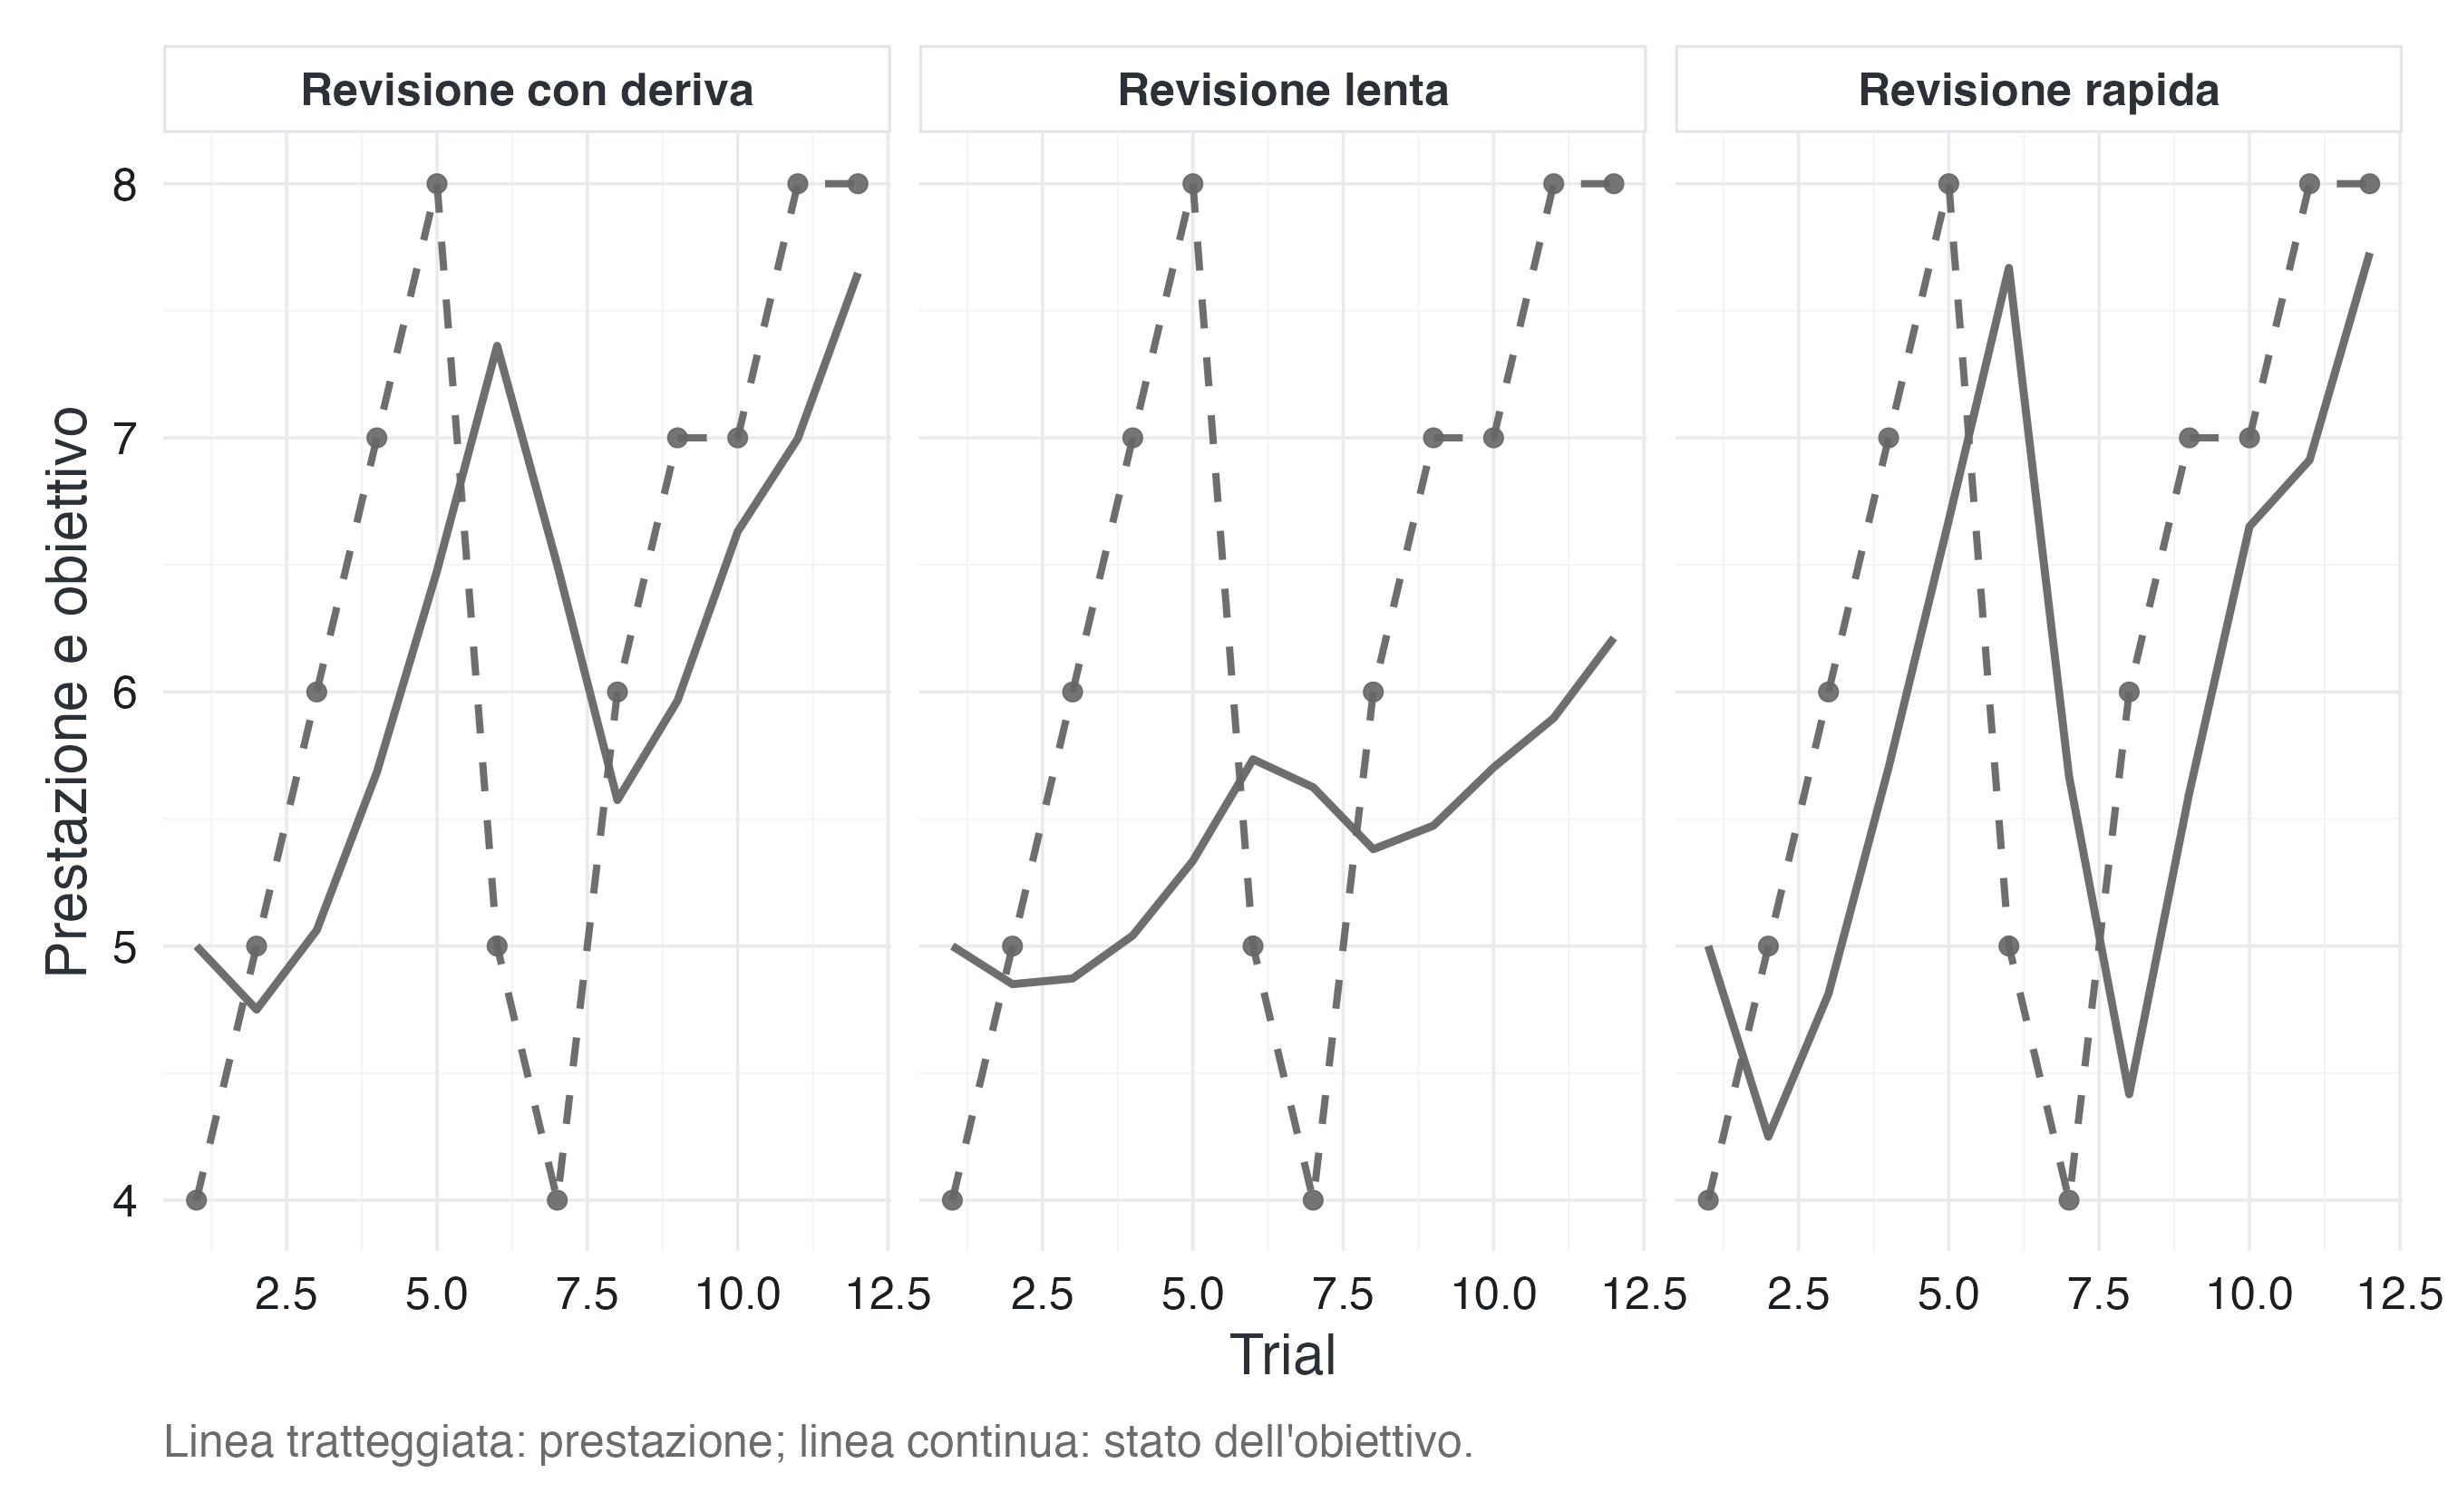
\includegraphics[width=0.85\linewidth,height=\textheight,keepaspectratio]{chapters/formal_models/02_costruire_modello_dinamico_files/figure-pdf/fig-goal-parameter-scenarios-1.png}

}

\caption{\label{fig-goal-parameter-scenarios}Traiettorie generate dallo
stesso input di prestazione con tre combinazioni dei parametri. Il
parametro alpha regola la rapidità della revisione; beta introduce uno
spostamento sistematico per trial.}

\end{figure}%

Le simulazioni permettono di leggere i parametri attraverso le
conseguenze che producono.

\begin{itemize}
\tightlist
\item
  Con \(\alpha\) basso, lo stato conserva maggiormente la memoria del
  passato.
\item
  Con \(\alpha\) alto, l'obiettivo si avvicina rapidamente alla
  prestazione recente.
\item
  Un \(\beta\) positivo può produrre una crescita anche quando la
  discrepanza è piccola.
\end{itemize}

\subsection{Stabilità e comportamento di lungo
periodo}\label{stabilituxe0-e-comportamento-di-lungo-periodo}

Se la prestazione rimane costante, \(P_t=P\), e \(\alpha>0\), il punto
di equilibrio soddisfa:

\[
G^*=G^*+\alpha(P-G^*)+\beta.
\]

Da cui:

\[
G^*=P+\frac{\beta}{\alpha}.
\]

Il risultato rende evidente che \(\alpha\) e \(\beta\) interagiscono.
Uno stesso valore di \(\beta\) produce una deviazione di equilibrio più
ampia quando \(\alpha\) è piccolo.

Nel seguito poniamo \(0<\alpha<1\). Questo vincolo rende
l'interpretazione particolarmente semplice: a ogni trial viene
incorporata una frazione della discrepanza. Non è una legge psicologica
universale; è una scelta di specificazione che dovrà essere
riconsiderata se i dati richiedono inerzia negativa, sovracorrezione o
oscillazioni.

\section{Il caso di studio}\label{il-caso-di-studio}

Il dataset contiene 60 partecipanti, ciascuno osservato in 10 trial. I
partecipanti appartengono a due condizioni, \emph{approach} e
\emph{avoidance}. In questo capitolo ignoriamo temporaneamente la
condizione e assumiamo che l'intero campione condivida gli stessi
parametri. L'eterogeneità sarà introdotta nel capitolo
Capitolo~\ref{sec-formal-models-developments}.

\begin{Shaded}
\begin{Highlighting}[]
\NormalTok{goal\_data }\OtherTok{\textless{}{-}}\NormalTok{ rio}\SpecialCharTok{::}\FunctionTok{import}\NormalTok{(here}\SpecialCharTok{::}\FunctionTok{here}\NormalTok{(}\StringTok{"data"}\NormalTok{, }\StringTok{"goal\_data.csv"}\NormalTok{)) }\SpecialCharTok{|\textgreater{}}
  \FunctionTok{as\_tibble}\NormalTok{() }\SpecialCharTok{|\textgreater{}}
  \FunctionTok{mutate}\NormalTok{(}
    \AttributeTok{subject =} \FunctionTok{as.integer}\NormalTok{(}\FunctionTok{factor}\NormalTok{(subject)),}
    \AttributeTok{condition =} \FunctionTok{factor}\NormalTok{(condition, }\AttributeTok{levels =} \FunctionTok{c}\NormalTok{(}\StringTok{"approach"}\NormalTok{, }\StringTok{"avoidance"}\NormalTok{))}
\NormalTok{  ) }\SpecialCharTok{|\textgreater{}}
  \FunctionTok{arrange}\NormalTok{(subject, trial) }\SpecialCharTok{|\textgreater{}}
  \FunctionTok{mutate}\NormalTok{(}\AttributeTok{row\_id =} \FunctionTok{row\_number}\NormalTok{())}

\NormalTok{trial\_check }\OtherTok{\textless{}{-}}\NormalTok{ goal\_data }\SpecialCharTok{|\textgreater{}}
  \FunctionTok{group\_by}\NormalTok{(subject) }\SpecialCharTok{|\textgreater{}}
  \FunctionTok{summarise}\NormalTok{(}
    \AttributeTok{sequence\_ok =} \FunctionTok{all}\NormalTok{(trial }\SpecialCharTok{==} \FunctionTok{seq\_len}\NormalTok{(}\FunctionTok{n}\NormalTok{())),}
    \AttributeTok{.groups =} \StringTok{"drop"}
\NormalTok{  )}

\FunctionTok{stopifnot}\NormalTok{(}\FunctionTok{all}\NormalTok{(trial\_check}\SpecialCharTok{$}\NormalTok{sequence\_ok))}

\NormalTok{goal\_data }\SpecialCharTok{|\textgreater{}}
  \FunctionTok{summarise}\NormalTok{(}
    \AttributeTok{partecipanti =} \FunctionTok{n\_distinct}\NormalTok{(subject),}
    \AttributeTok{osservazioni =} \FunctionTok{n}\NormalTok{(),}
    \AttributeTok{trial\_minimi =} \FunctionTok{min}\NormalTok{(trial),}
    \AttributeTok{trial\_massimi =} \FunctionTok{max}\NormalTok{(trial)}
\NormalTok{  )}
\CommentTok{\#\textgreater{} \# A tibble: 1 x 4}
\CommentTok{\#\textgreater{}   partecipanti osservazioni trial\_minimi trial\_massimi}
\CommentTok{\#\textgreater{}          \textless{}int\textgreater{}        \textless{}int\textgreater{}        \textless{}int\textgreater{}         \textless{}int\textgreater{}}
\CommentTok{\#\textgreater{} 1           60          600            1            10}
\end{Highlighting}
\end{Shaded}

Prima di stimare il modello osserviamo alcune traiettorie.

\begin{figure}

\centering{

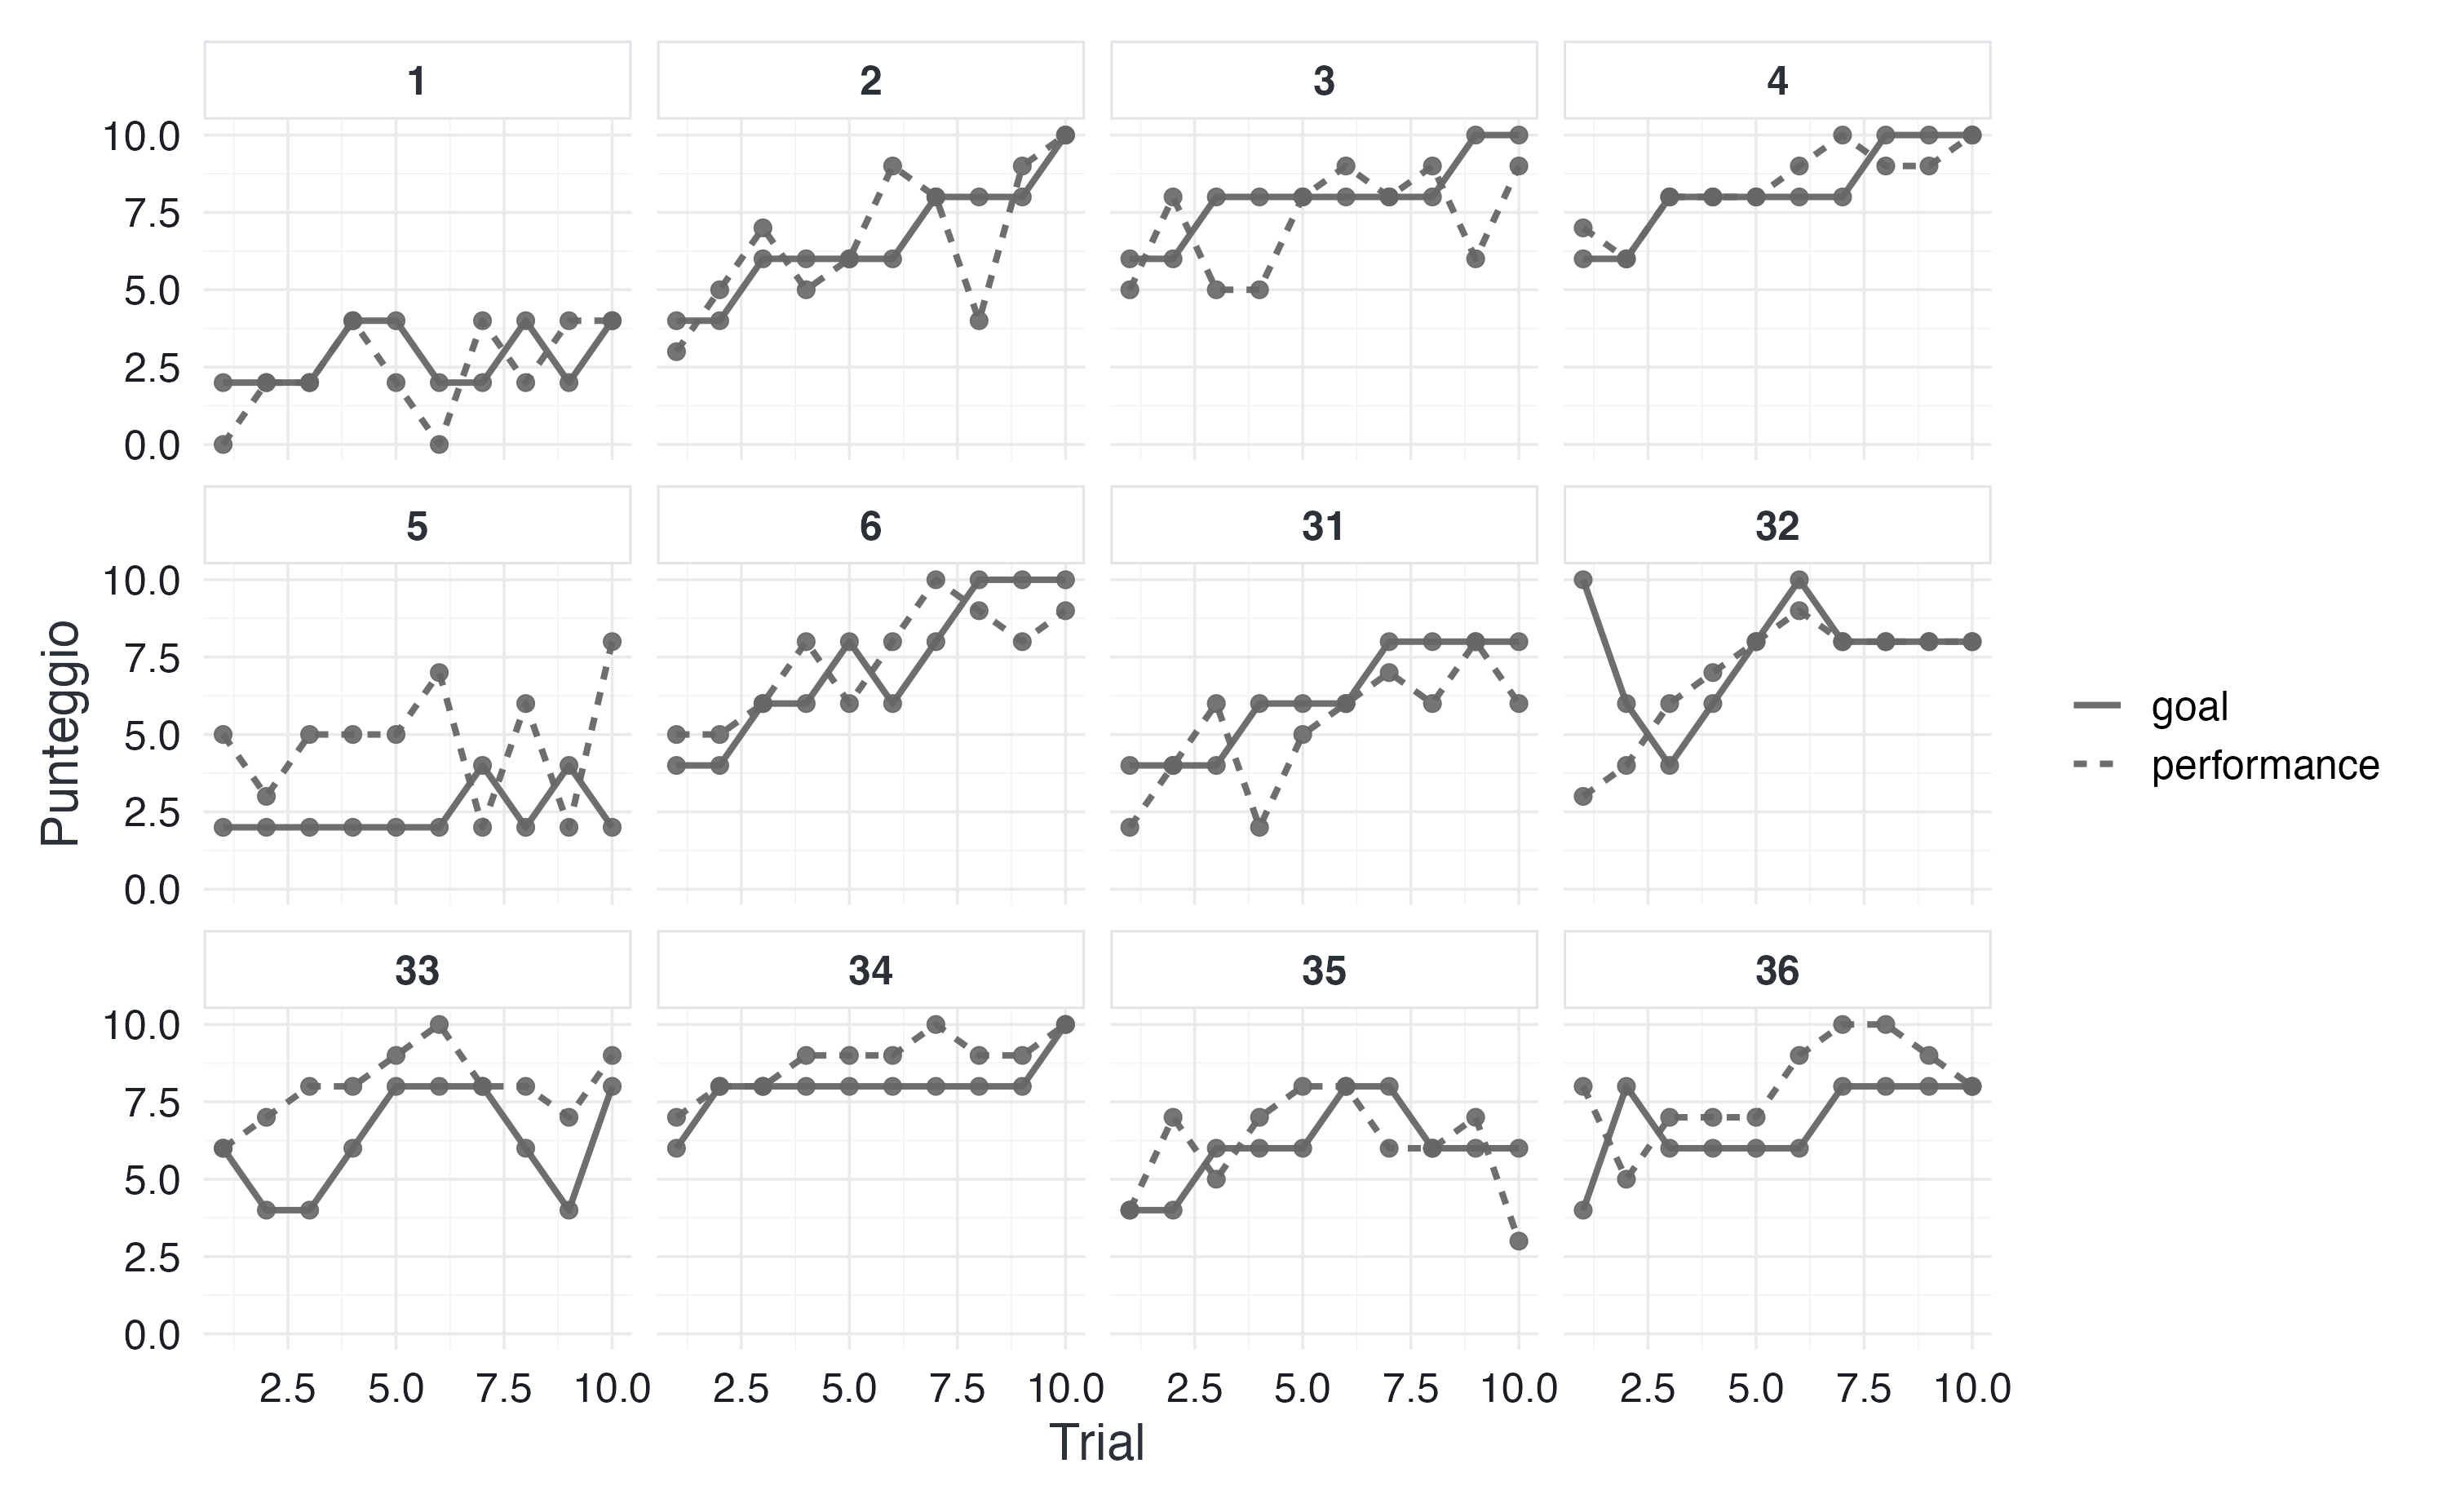
\includegraphics[width=0.85\linewidth,height=\textheight,keepaspectratio]{chapters/formal_models/02_costruire_modello_dinamico_files/figure-pdf/fig-observed-goal-trajectories-1.png}

}

\caption{\label{fig-observed-goal-trajectories}Obiettivi e prestazioni
osservati per dodici partecipanti. Le traiettorie rendono visibile sia
la dipendenza temporale sia la variabilità tra persone.}

\end{figure}%

La figura suggerisce che una dinamica comune può essere una prima
approssimazione utile, ma non garantisce che tutti i partecipanti
reagiscano nello stesso modo.

\section{Dal processo alle
osservazioni}\label{dal-processo-alle-osservazioni}

L'Equazione Equazione~\ref{eq-knight2023} definisce lo stato atteso. I
dati osservati non coincidono necessariamente con tale stato.
Introduciamo quindi un modello osservazionale:

\begin{equation}\protect\phantomsection\label{eq-knight-stat}{
Y_{s,t}\sim
\operatorname{Normal}(G_{s,t},\sigma),
\qquad t>1,
}\end{equation}

dove \(Y_{s,t}\) è l'obiettivo dichiarato dal soggetto \(s\) e
\(G_{s,t}\) è lo stato previsto dalla ricorsione.

Il primo obiettivo di ciascun partecipante viene trattato come
\textbf{condizione iniziale osservata}. Il modello descrive quindi le
transizioni dal secondo trial in avanti; non propone una teoria della
formazione del primo obiettivo.

\begin{tcolorbox}[enhanced jigsaw, arc=.35mm, bottomrule=.15mm, bottomtitle=1mm, breakable, colback=white, colbacktitle=quarto-callout-important-color!10!white, colframe=quarto-callout-important-color-frame, coltitle=black, left=2mm, leftrule=.75mm, opacityback=0, opacitybacktitle=0.6, rightrule=.15mm, title=\textcolor{quarto-callout-important-color}{\faExclamation}\hspace{0.5em}{Processo e misura non sono la stessa cosa}, titlerule=0mm, toprule=.15mm, toptitle=1mm]

La deviazione standard \(\sigma\) raccoglie tutte le differenze tra
stato previsto e obiettivo osservato: variabilità decisionale,
approssimazione della scala di risposta, errori di misura e componenti
del processo non incluse nella regola.

Per questa ragione \(\sigma\) non deve essere interpretata come un unico
meccanismo psicologico.

\end{tcolorbox}

\section{La quantità di interesse}\label{la-quantituxe0-di-interesse}

Il modello di questo capitolo stima tre quantità condivise:

\begin{itemize}
\tightlist
\item
  \(\alpha\): sensibilità media alla discrepanza sotto l'ipotesi di
  omogeneità;
\item
  \(\beta\): deriva media per trial;
\item
  \(\sigma\): dispersione delle osservazioni attorno alla traiettoria
  prevista.
\end{itemize}

Queste quantità descrivono una dinamica comune all'intero campione. Non
forniscono parametri individuali e non quantificano la variabilità tra
persone.

\section{Specificare i prior}\label{specificare-i-prior-1}

Per garantire \(0<\alpha<1\), introduciamo un parametro non vincolato:

\[
\alpha=\operatorname{logit}^{-1}(\alpha_{\text{logit}}),
\qquad
\alpha_{\text{logit}}\sim\operatorname{Normal}(0,1).
\]

Questo prior assegna maggiore plausibilità a valori intermedi, senza
escludere revisioni lente o rapide.

Sulla scala originale dei dati usiamo inoltre:

\[
\beta\sim\operatorname{Normal}(0,0.25),
\]

\[
\sigma\sim\operatorname{HalfNormal}(0,0.75).
\]

La scelta implica che derive superiori a circa mezzo punto per trial e
deviazioni residue molto grandi siano possibili, ma non considerate
ordinarie.

\section{Controllo predittivo a
priori}\label{controllo-predittivo-a-priori-4}

Usiamo le prestazioni osservate di un partecipante come sequenza di
input, ma generiamo i parametri dai prior.

\begin{Shaded}
\begin{Highlighting}[]
\NormalTok{prior\_draws\_goal }\OtherTok{\textless{}{-}} \FunctionTok{tibble}\NormalTok{(}
  \AttributeTok{draw =} \FunctionTok{seq\_len}\NormalTok{(}\DecValTok{200}\NormalTok{),}
  \AttributeTok{alpha =} \FunctionTok{plogis}\NormalTok{(}\FunctionTok{rnorm}\NormalTok{(}\DecValTok{200}\NormalTok{, }\DecValTok{0}\NormalTok{, }\DecValTok{1}\NormalTok{)),}
  \AttributeTok{beta =} \FunctionTok{rnorm}\NormalTok{(}\DecValTok{200}\NormalTok{, }\DecValTok{0}\NormalTok{, }\FloatTok{0.25}\NormalTok{),}
  \AttributeTok{sigma =} \FunctionTok{abs}\NormalTok{(}\FunctionTok{rnorm}\NormalTok{(}\DecValTok{200}\NormalTok{, }\DecValTok{0}\NormalTok{, }\FloatTok{0.75}\NormalTok{))}
\NormalTok{)}

\NormalTok{reference\_subject }\OtherTok{\textless{}{-}}\NormalTok{ goal\_data }\SpecialCharTok{|\textgreater{}}
  \FunctionTok{filter}\NormalTok{(subject }\SpecialCharTok{==} \DecValTok{1}\NormalTok{)}

\NormalTok{prior\_paths\_goal }\OtherTok{\textless{}{-}}\NormalTok{ prior\_draws\_goal }\SpecialCharTok{|\textgreater{}}
  \FunctionTok{slice\_sample}\NormalTok{(}\AttributeTok{n =} \DecValTok{80}\NormalTok{) }\SpecialCharTok{|\textgreater{}}
  \FunctionTok{mutate}\NormalTok{(}
    \AttributeTok{simulation =}\NormalTok{ purrr}\SpecialCharTok{::}\FunctionTok{pmap}\NormalTok{(}
      \FunctionTok{list}\NormalTok{(alpha, beta, sigma),}
      \SpecialCharTok{\textasciitilde{}} \FunctionTok{simulate\_goal\_path}\NormalTok{(}
        \AttributeTok{performance =}\NormalTok{ reference\_subject}\SpecialCharTok{$}\NormalTok{performance,}
        \AttributeTok{initial\_goal =}\NormalTok{ reference\_subject}\SpecialCharTok{$}\NormalTok{goal[}\DecValTok{1}\NormalTok{],}
        \AttributeTok{alpha =}\NormalTok{ ..}\DecValTok{1}\NormalTok{,}
        \AttributeTok{beta =}\NormalTok{ ..}\DecValTok{2}\NormalTok{,}
        \AttributeTok{sigma =}\NormalTok{ ..}\DecValTok{3}
\NormalTok{      )}
\NormalTok{    )}
\NormalTok{  ) }\SpecialCharTok{|\textgreater{}}
  \FunctionTok{select}\NormalTok{(draw, simulation) }\SpecialCharTok{|\textgreater{}}
\NormalTok{  tidyr}\SpecialCharTok{::}\FunctionTok{unnest}\NormalTok{(simulation)}
\end{Highlighting}
\end{Shaded}

\begin{figure}

\centering{

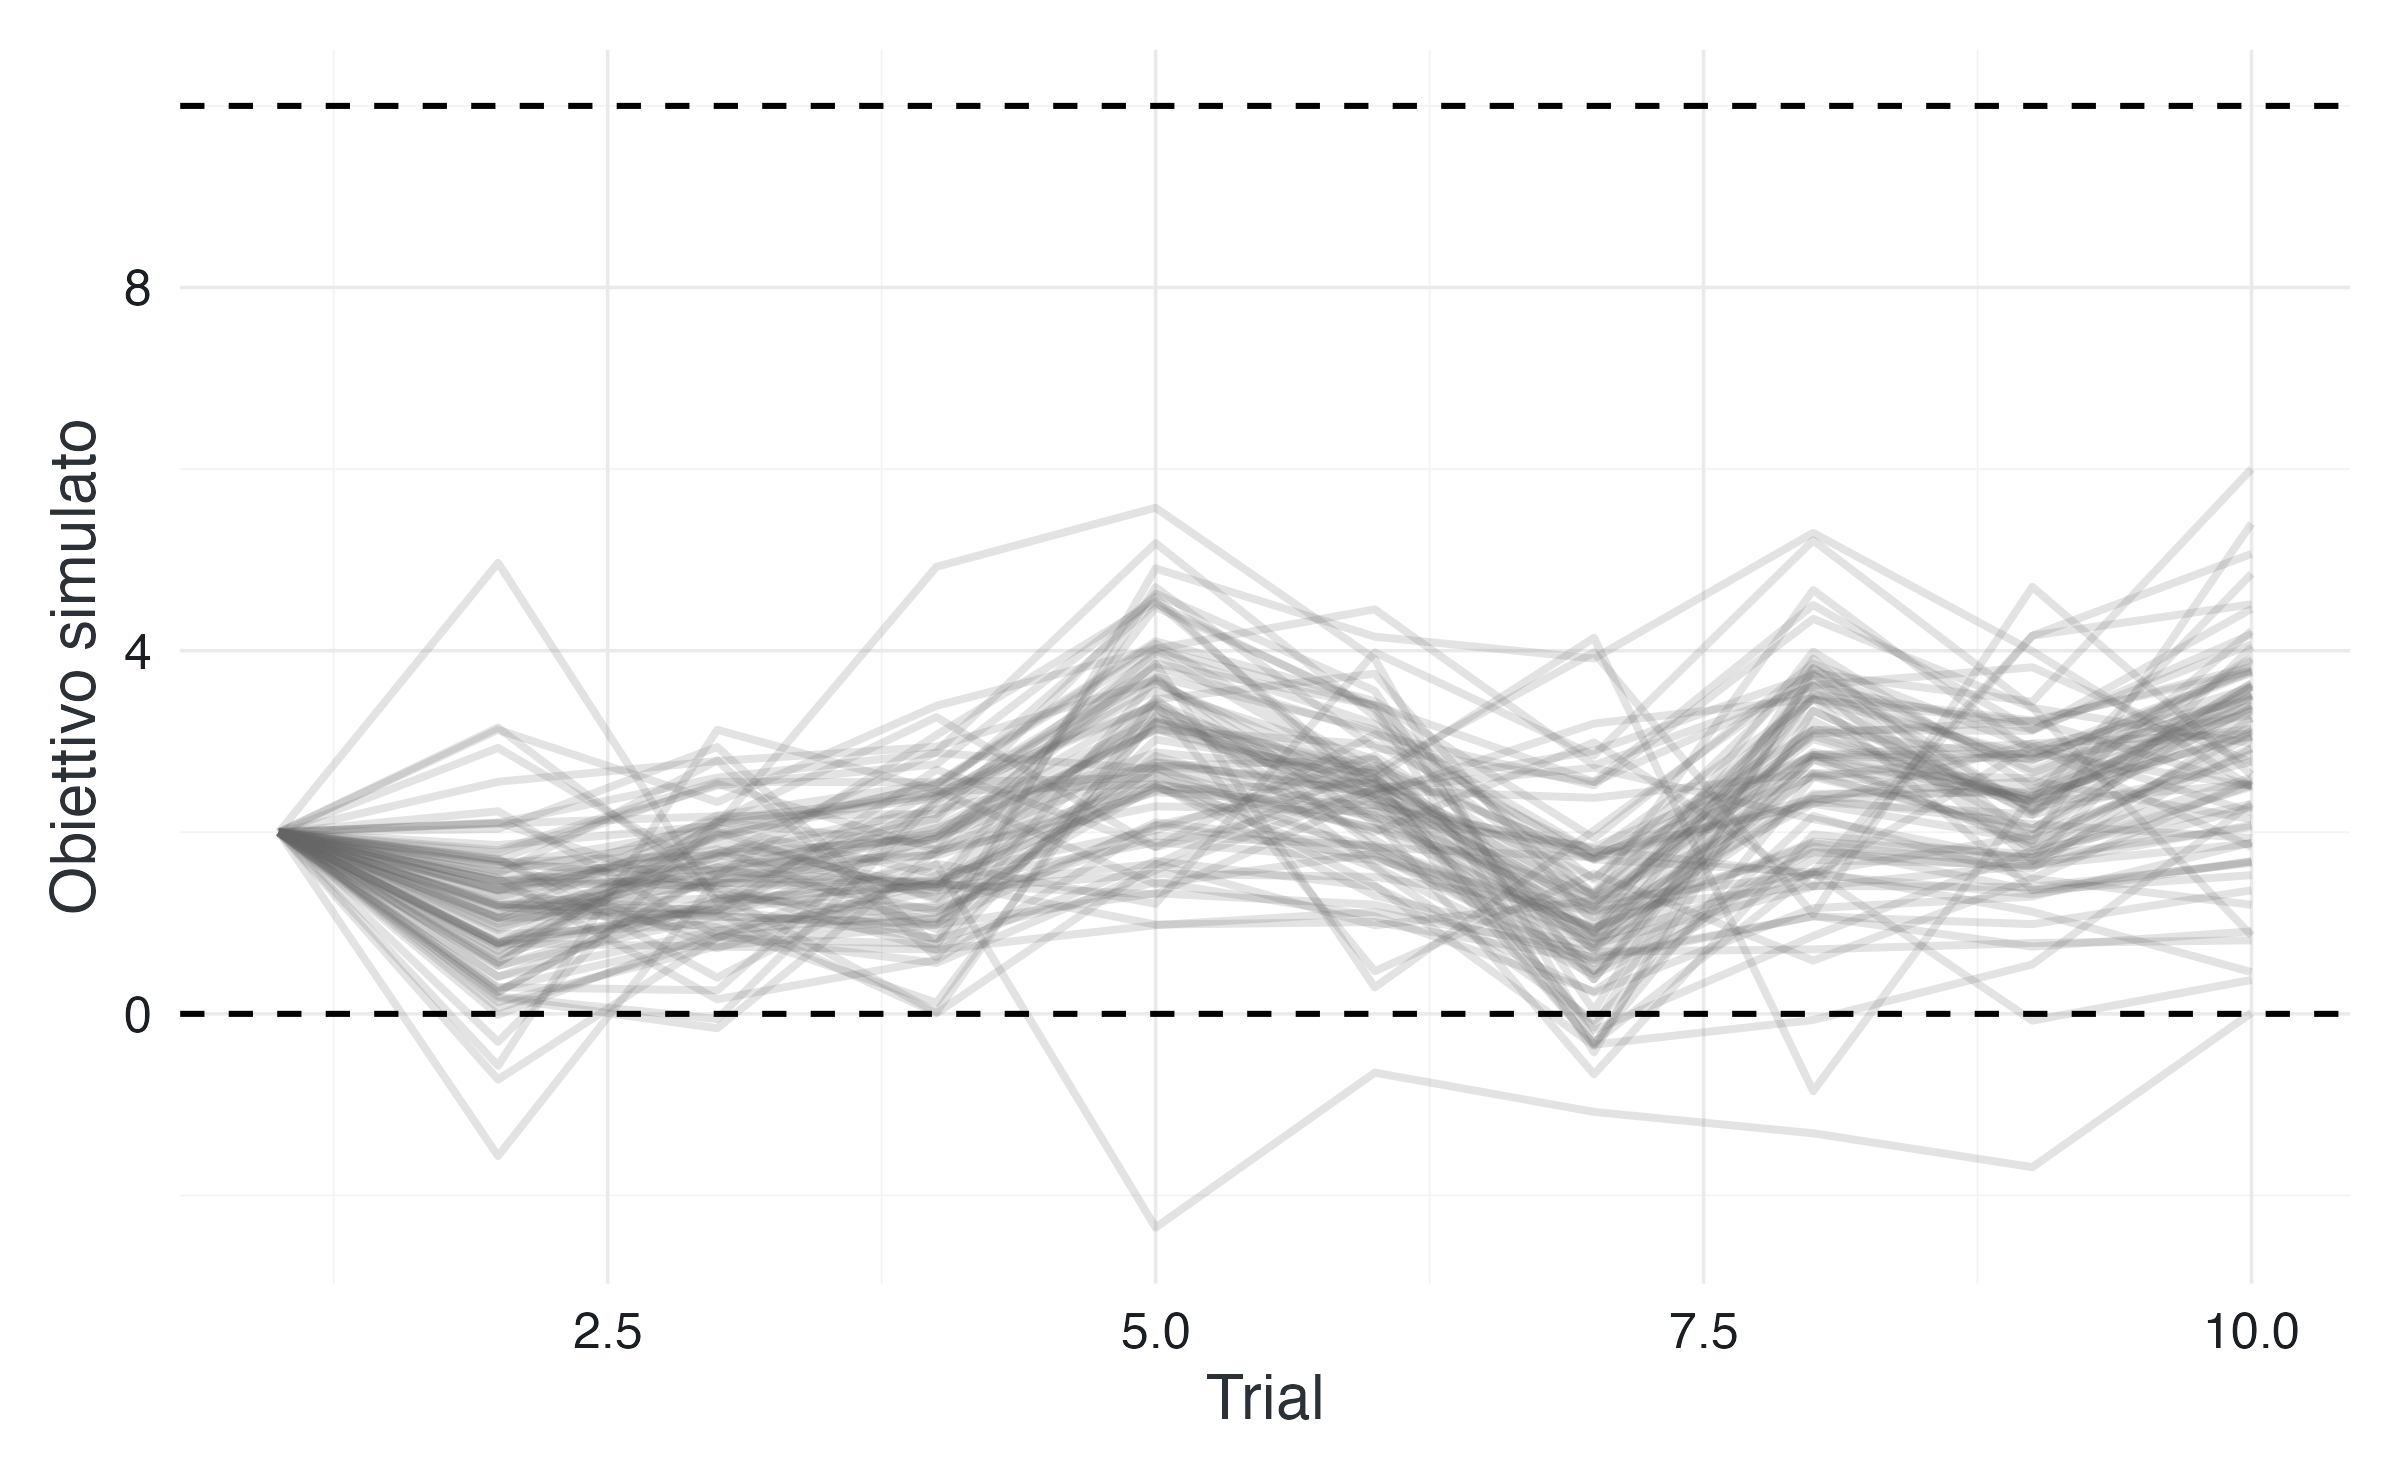
\includegraphics[width=0.85\linewidth,height=\textheight,keepaspectratio]{chapters/formal_models/02_costruire_modello_dinamico_files/figure-pdf/fig-prior-predictive-goal-sample-1.png}

}

\caption{\label{fig-prior-predictive-goal-sample}Traiettorie simulate
prima di usare i dati per l'inferenza. Il controllo serve a valutare se
i prior permettono comportamenti plausibili sulla scala degli
obiettivi.}

\end{figure}%

Le linee orizzontali non sono vincoli del modello: ricordano soltanto
l'intervallo osservato nel compito. Se una quota eccessiva delle
simulazioni producesse valori incompatibili con la scala, dovremmo
restringere i prior o adottare un modello osservazionale che rispetti
esplicitamente i limiti della risposta.

\section{Implementazione in Stan}\label{implementazione-in-stan-2}

Il programma seguente condiziona sul primo obiettivo di ogni
partecipante e applica la stessa coppia di parametri a tutte le
traiettorie.

\begin{Shaded}
\begin{Highlighting}[]
\NormalTok{stan\_code\_goal\_sample }\OtherTok{\textless{}{-}} \StringTok{"}
\StringTok{data \{}
\StringTok{  int\textless{}lower=1\textgreater{} Ntotal;}
\StringTok{  int\textless{}lower=1\textgreater{} Nsubj;}
\StringTok{  array[Ntotal] int\textless{}lower=1, upper=Nsubj\textgreater{} subject;}
\StringTok{  array[Ntotal] int\textless{}lower=1\textgreater{} trial;}
\StringTok{  vector[Ntotal] goal;}
\StringTok{  vector[Ntotal] performance;}
\StringTok{\}}

\StringTok{parameters \{}
\StringTok{  real alpha\_logit;}
\StringTok{  real beta;}
\StringTok{  real\textless{}lower=0\textgreater{} sigma;}
\StringTok{\}}

\StringTok{transformed parameters \{}
\StringTok{  real\textless{}lower=0, upper=1\textgreater{} alpha = inv\_logit(alpha\_logit);}
\StringTok{  vector[Ntotal] mu;}

\StringTok{  for (i in 1:Ntotal) \{}
\StringTok{    if (trial[i] == 1) \{}
\StringTok{      mu[i] = goal[i];}
\StringTok{    \} else \{}
\StringTok{      mu[i] = mu[i {-} 1]}
\StringTok{              + alpha * (performance[i {-} 1] {-} mu[i {-} 1])}
\StringTok{              + beta;}
\StringTok{    \}}
\StringTok{  \}}
\StringTok{\}}

\StringTok{model \{}
\StringTok{  alpha\_logit \textasciitilde{} normal(0, 1);}
\StringTok{  beta \textasciitilde{} normal(0, 0.25);}
\StringTok{  sigma \textasciitilde{} normal(0, 0.75);}

\StringTok{  for (i in 1:Ntotal) \{}
\StringTok{    if (trial[i] \textgreater{} 1) \{}
\StringTok{      goal[i] \textasciitilde{} normal(mu[i], sigma);}
\StringTok{    \}}
\StringTok{  \}}
\StringTok{\}}

\StringTok{generated quantities \{}
\StringTok{  vector[Ntotal] y\_rep;}
\StringTok{  vector[Ntotal] log\_lik;}

\StringTok{  for (i in 1:Ntotal) \{}
\StringTok{    if (trial[i] == 1) \{}
\StringTok{      y\_rep[i] = goal[i];}
\StringTok{      log\_lik[i] = 0;}
\StringTok{    \} else \{}
\StringTok{      y\_rep[i] = normal\_rng(mu[i], sigma);}
\StringTok{      log\_lik[i] = normal\_lpdf(goal[i] | mu[i], sigma);}
\StringTok{    \}}
\StringTok{  \}}
\StringTok{\}}
\StringTok{"}
\end{Highlighting}
\end{Shaded}

Prepariamo i dati nel formato richiesto da Stan.

\begin{Shaded}
\begin{Highlighting}[]
\NormalTok{stan\_data\_goal\_sample }\OtherTok{\textless{}{-}} \FunctionTok{list}\NormalTok{(}
  \AttributeTok{Ntotal =} \FunctionTok{nrow}\NormalTok{(goal\_data),}
  \AttributeTok{Nsubj =} \FunctionTok{n\_distinct}\NormalTok{(goal\_data}\SpecialCharTok{$}\NormalTok{subject),}
  \AttributeTok{subject =}\NormalTok{ goal\_data}\SpecialCharTok{$}\NormalTok{subject,}
  \AttributeTok{trial =}\NormalTok{ goal\_data}\SpecialCharTok{$}\NormalTok{trial,}
  \AttributeTok{goal =}\NormalTok{ goal\_data}\SpecialCharTok{$}\NormalTok{goal,}
  \AttributeTok{performance =}\NormalTok{ goal\_data}\SpecialCharTok{$}\NormalTok{performance}
\NormalTok{)}
\end{Highlighting}
\end{Shaded}

\begin{Shaded}
\begin{Highlighting}[]
\NormalTok{model\_goal\_sample }\OtherTok{\textless{}{-}} \FunctionTok{cmdstan\_model}\NormalTok{(}
  \FunctionTok{write\_stan\_file}\NormalTok{(stan\_code\_goal\_sample)}
\NormalTok{)}

\NormalTok{fit\_goal\_sample }\OtherTok{\textless{}{-}}\NormalTok{ model\_goal\_sample}\SpecialCharTok{$}\FunctionTok{sample}\NormalTok{(}
  \AttributeTok{data =}\NormalTok{ stan\_data\_goal\_sample,}
  \AttributeTok{seed =} \DecValTok{4817}\NormalTok{,}
  \AttributeTok{chains =} \DecValTok{4}\NormalTok{,}
  \AttributeTok{parallel\_chains =} \DecValTok{4}\NormalTok{,}
  \AttributeTok{iter\_warmup =} \DecValTok{1000}\NormalTok{,}
  \AttributeTok{iter\_sampling =} \DecValTok{2000}\NormalTok{,}
  \AttributeTok{refresh =} \DecValTok{500}
\NormalTok{)}
\end{Highlighting}
\end{Shaded}

\section{Diagnostica computazionale}\label{diagnostica-computazionale-1}

\begin{Shaded}
\begin{Highlighting}[]
\NormalTok{fit\_goal\_sample}\SpecialCharTok{$}\FunctionTok{summary}\NormalTok{(}
  \AttributeTok{variables =} \FunctionTok{c}\NormalTok{(}\StringTok{"alpha"}\NormalTok{, }\StringTok{"beta"}\NormalTok{, }\StringTok{"sigma"}\NormalTok{)}
\NormalTok{) }\SpecialCharTok{|\textgreater{}}
  \FunctionTok{select}\NormalTok{(variable, mean, median, sd, q5, q95, rhat, ess\_bulk, ess\_tail)}
\CommentTok{\#\textgreater{} \# A tibble: 3 x 9}
\CommentTok{\#\textgreater{}   variable  mean median     sd    q5   q95  rhat ess\_bulk ess\_tail}
\CommentTok{\#\textgreater{}   \textless{}chr\textgreater{}    \textless{}dbl\textgreater{}  \textless{}dbl\textgreater{}  \textless{}dbl\textgreater{} \textless{}dbl\textgreater{} \textless{}dbl\textgreater{} \textless{}dbl\textgreater{}    \textless{}dbl\textgreater{}    \textless{}dbl\textgreater{}}
\CommentTok{\#\textgreater{} 1 alpha    0.513  0.512 0.0334 0.458 0.568 1.00     6793.    6221.}
\CommentTok{\#\textgreater{} 2 beta     0.171  0.171 0.0336 0.116 0.226 1.000    6334.    5590.}
\CommentTok{\#\textgreater{} 3 sigma    1.36   1.36  0.0411 1.29  1.43  1.00     7046.    5308.}
\end{Highlighting}
\end{Shaded}

\begin{figure}

\centering{

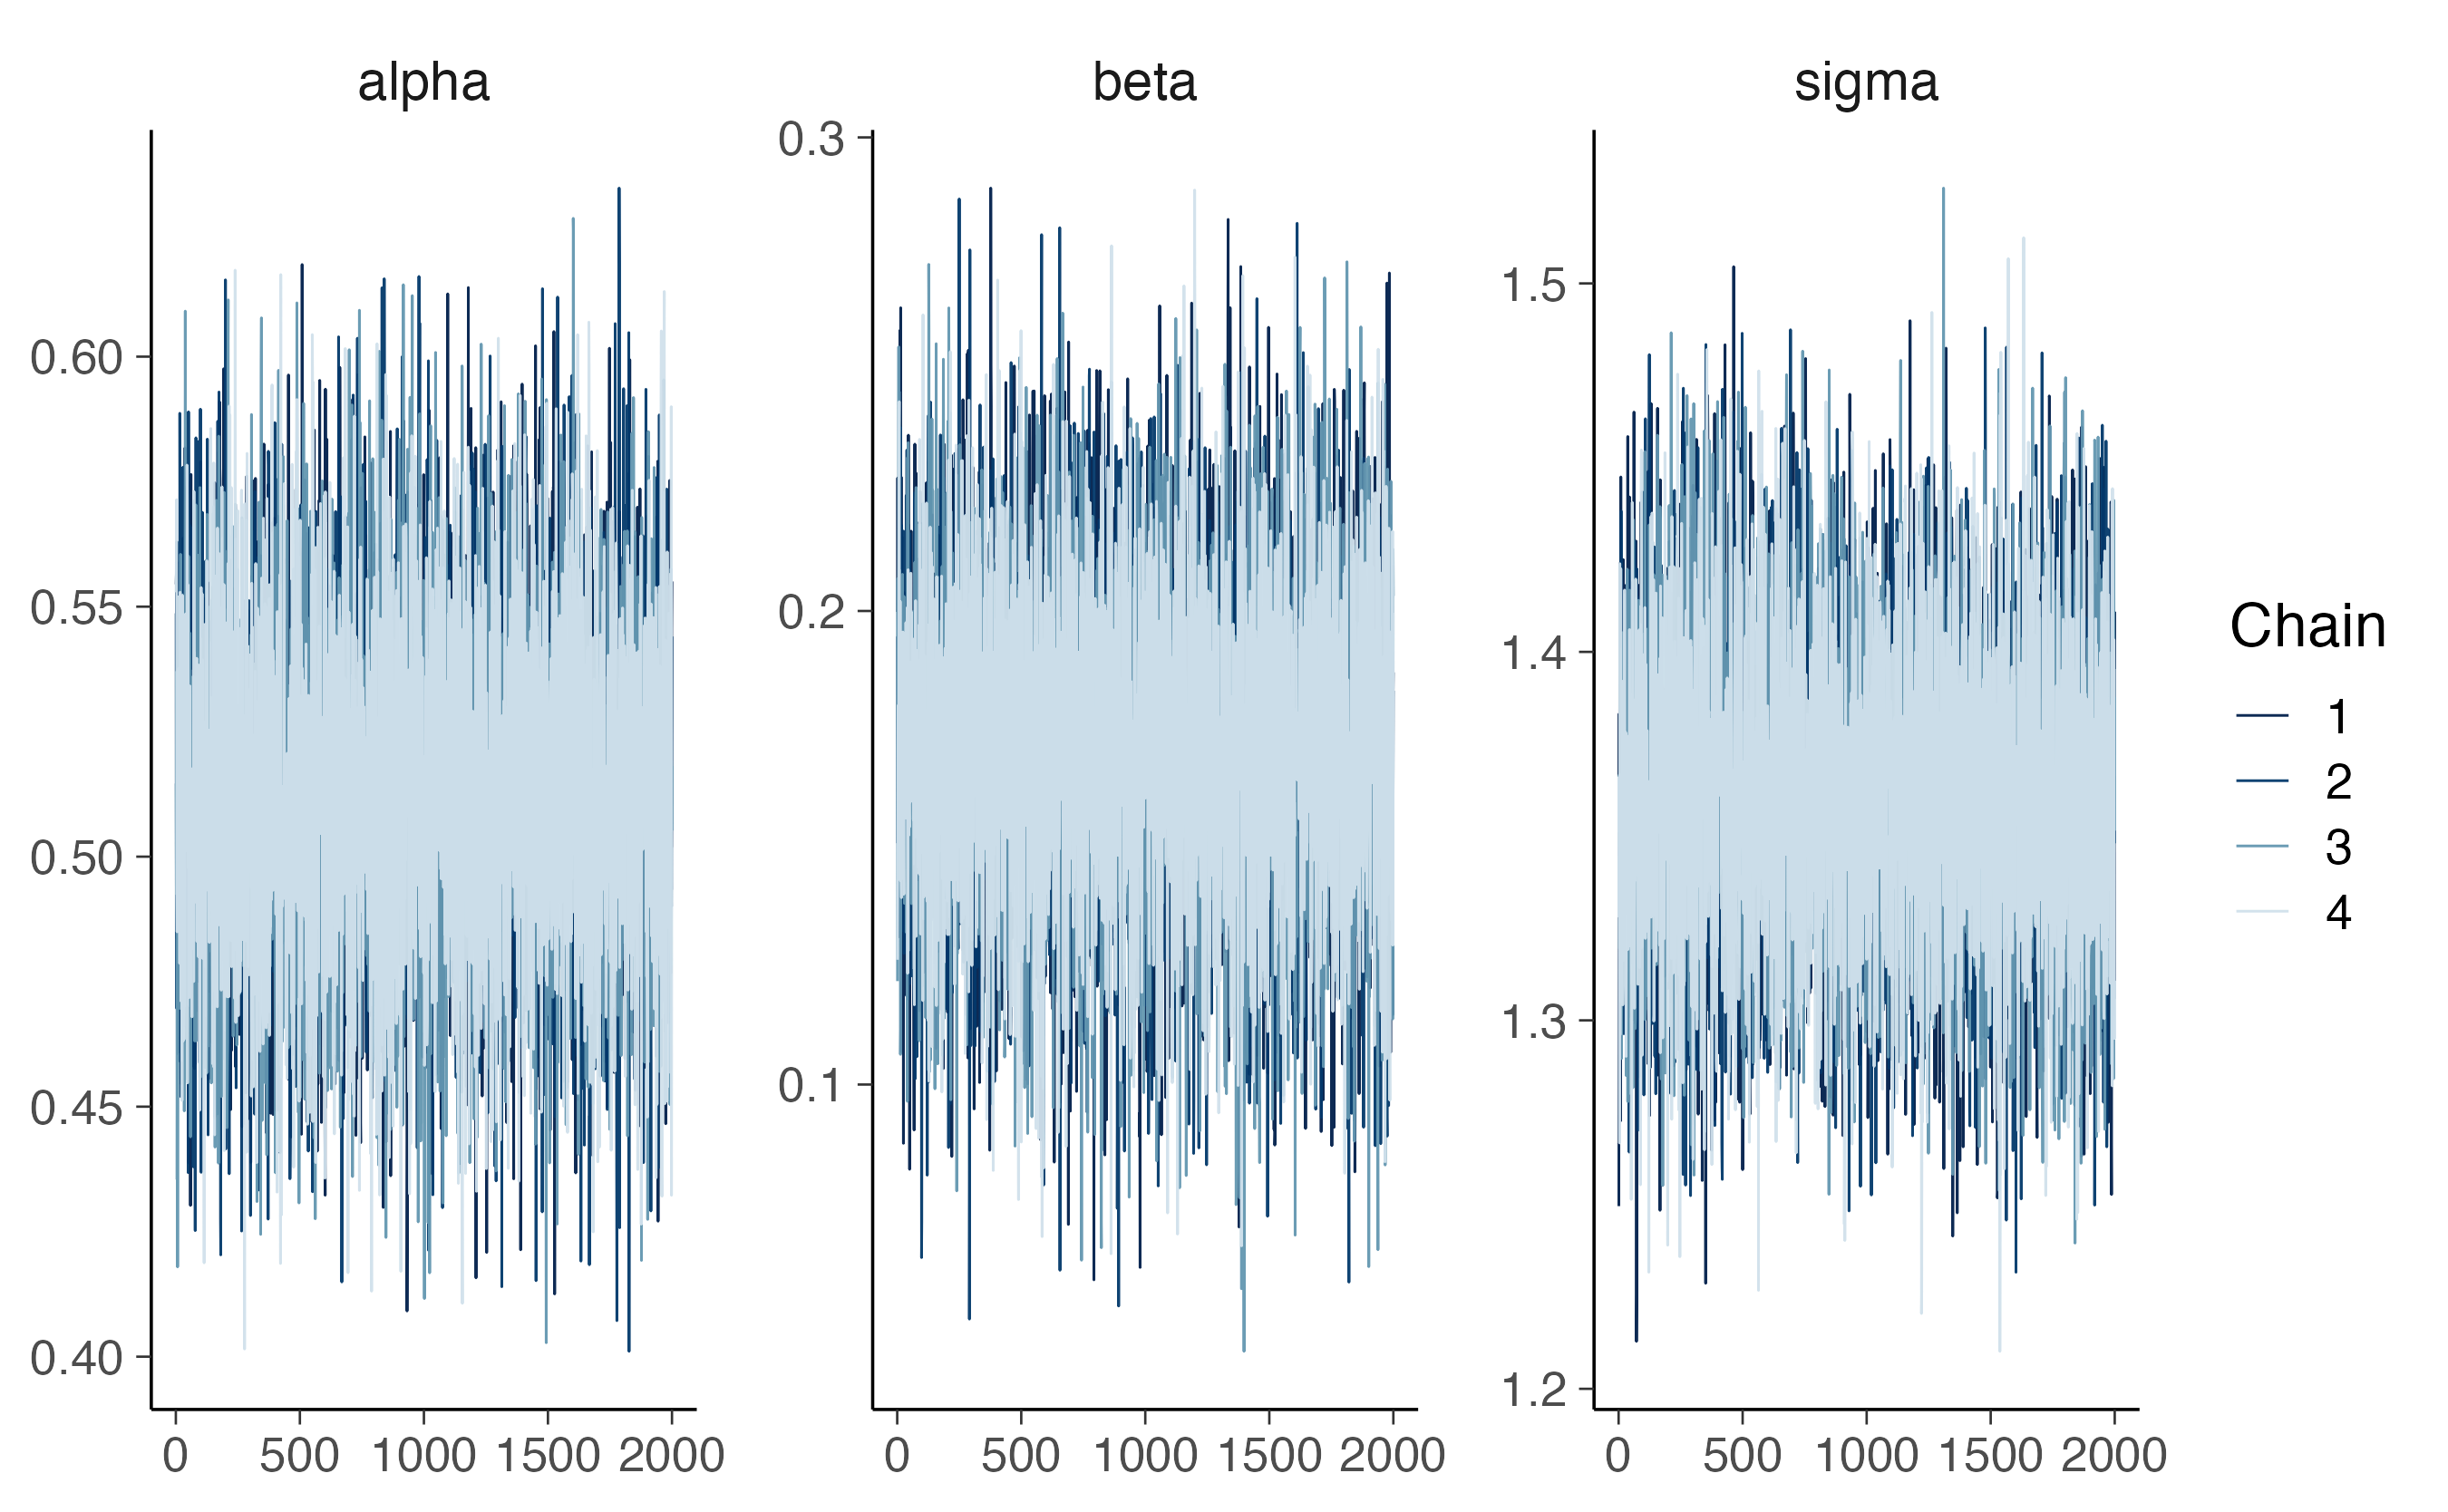
\includegraphics[width=0.85\linewidth,height=\textheight,keepaspectratio]{chapters/formal_models/02_costruire_modello_dinamico_files/figure-pdf/fig-trace-goal-sample-1.png}

}

\caption{\label{fig-trace-goal-sample}Trace plot dei parametri condivisi
del modello dinamico.}

\end{figure}%

Una buona diagnostica MCMC indica che il campionatore ha esplorato in
modo affidabile la distribuzione a posteriori. Non dimostra che la
regola psicologica o il modello osservazionale siano adeguati.

\section{Interpretare la posterior}\label{interpretare-la-posterior}

\begin{Shaded}
\begin{Highlighting}[]
\NormalTok{fit\_goal\_sample}\SpecialCharTok{$}\FunctionTok{draws}\NormalTok{(}\FunctionTok{c}\NormalTok{(}\StringTok{"alpha"}\NormalTok{, }\StringTok{"beta"}\NormalTok{, }\StringTok{"sigma"}\NormalTok{)) }\SpecialCharTok{|\textgreater{}}
\NormalTok{  posterior}\SpecialCharTok{::}\FunctionTok{summarise\_draws}\NormalTok{(}
\NormalTok{    mean,}
\NormalTok{    median,}
    \SpecialCharTok{\textasciitilde{}}\FunctionTok{quantile}\NormalTok{(.x, }\AttributeTok{probs =} \FunctionTok{c}\NormalTok{(}\FloatTok{0.025}\NormalTok{, }\FloatTok{0.975}\NormalTok{))}
\NormalTok{  )}
\CommentTok{\#\textgreater{} \# A tibble: 3 x 5}
\CommentTok{\#\textgreater{}   variable  mean median \textasciigrave{}2.5\%\textasciigrave{} \textasciigrave{}97.5\%\textasciigrave{}}
\CommentTok{\#\textgreater{}   \textless{}chr\textgreater{}    \textless{}dbl\textgreater{}  \textless{}dbl\textgreater{}  \textless{}dbl\textgreater{}   \textless{}dbl\textgreater{}}
\CommentTok{\#\textgreater{} 1 alpha    0.513  0.512  0.448   0.579}
\CommentTok{\#\textgreater{} 2 beta     0.171  0.171  0.103   0.236}
\CommentTok{\#\textgreater{} 3 sigma    1.36   1.36   1.28    1.44}
\end{Highlighting}
\end{Shaded}

L'interpretazione deve restare condizionata alla specificazione:

\begin{itemize}
\tightlist
\item
  la posterior di \(\alpha\) descrive la frazione della discrepanza
  incorporata dalla dinamica comune;
\item
  la posterior di \(\beta\) descrive la deriva media residua per trial;
\item
  la posterior di \(\sigma\) descrive quanto le osservazioni si
  discostano dalla traiettoria prodotta dalla regola.
\end{itemize}

Non possiamo ancora concludere che tutti i partecipanti condividano
davvero questi valori. L'ipotesi di omogeneità è precisamente ciò che
verrà rilassato nel capitolo successivo.

\section{Traiettorie attese e
osservate}\label{traiettorie-attese-e-osservate}

\begin{Shaded}
\begin{Highlighting}[]
\NormalTok{mu\_goal\_summary }\OtherTok{\textless{}{-}}\NormalTok{ fit\_goal\_sample }\SpecialCharTok{|\textgreater{}}
  \FunctionTok{spread\_draws}\NormalTok{(mu[row\_id]) }\SpecialCharTok{|\textgreater{}}
  \FunctionTok{median\_qi}\NormalTok{(mu, }\AttributeTok{.width =} \FloatTok{0.90}\NormalTok{) }\SpecialCharTok{|\textgreater{}}
  \FunctionTok{left\_join}\NormalTok{(}
\NormalTok{    goal\_data }\SpecialCharTok{|\textgreater{}}
      \FunctionTok{select}\NormalTok{(row\_id, subject, trial, goal),}
    \AttributeTok{by =} \StringTok{"row\_id"}
\NormalTok{  )}
\end{Highlighting}
\end{Shaded}

\begin{figure}

\centering{

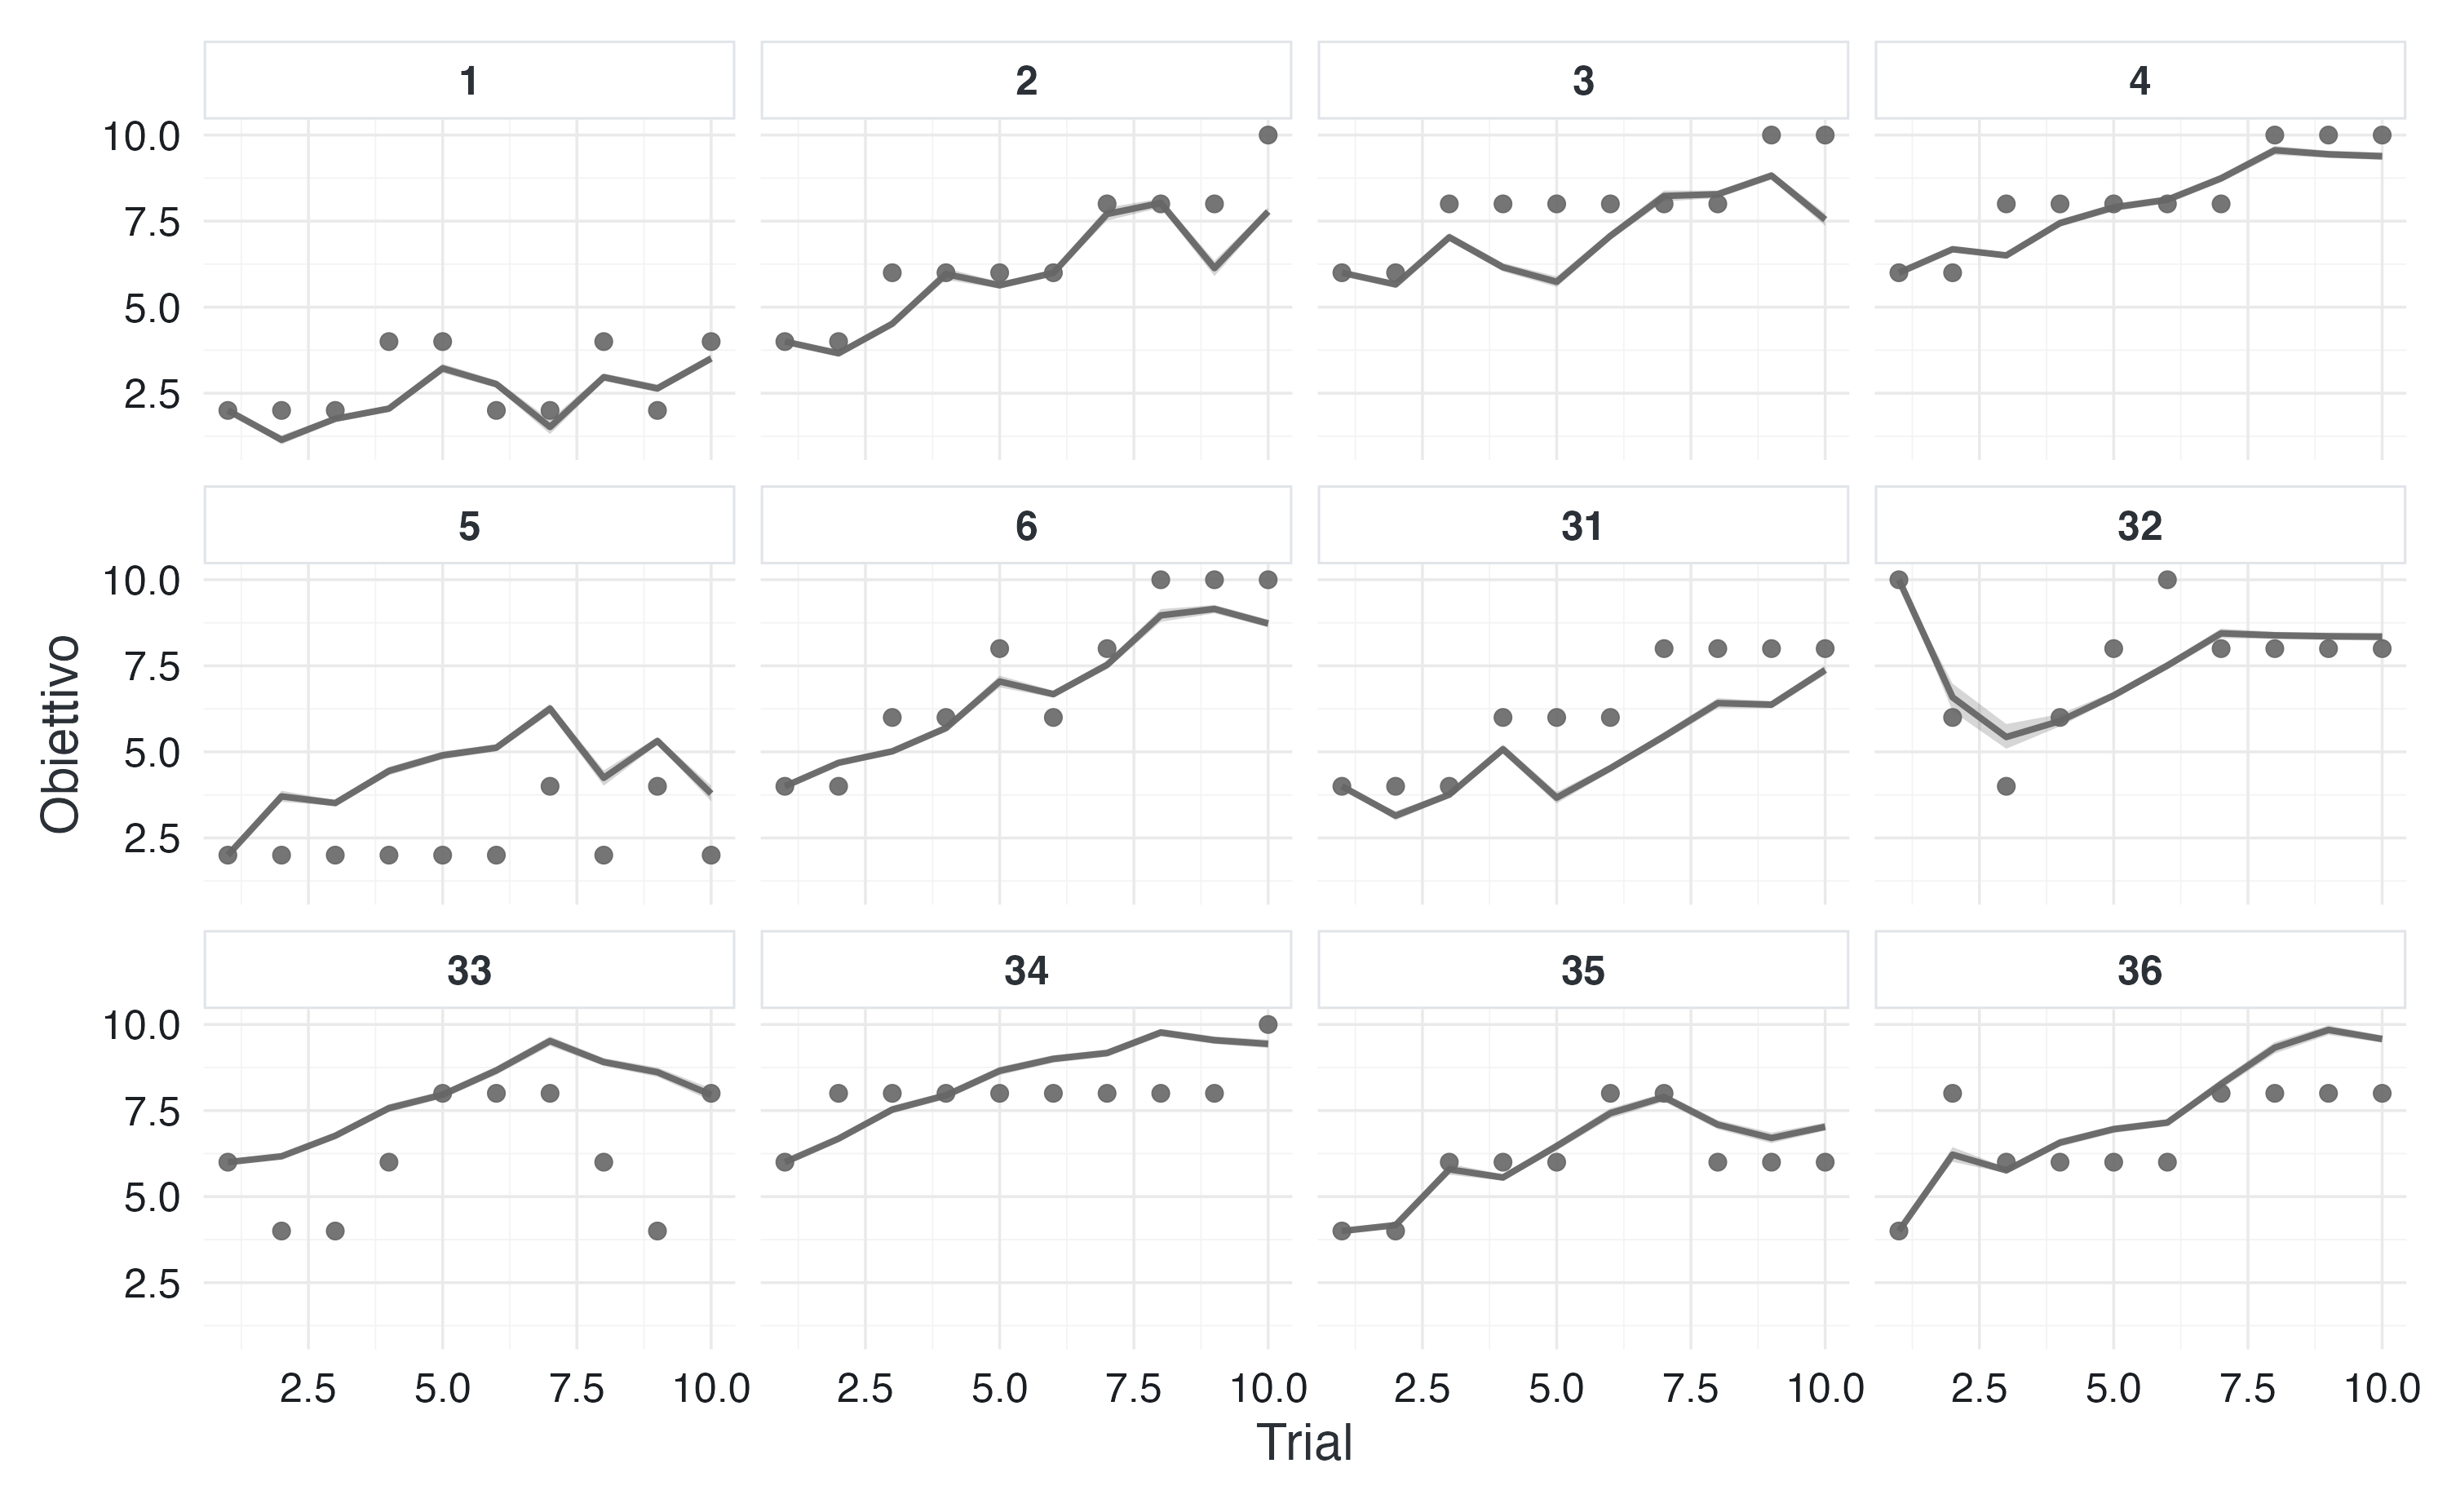
\includegraphics[width=0.85\linewidth,height=\textheight,keepaspectratio]{chapters/formal_models/02_costruire_modello_dinamico_files/figure-pdf/fig-posterior-trajectories-goal-sample-1.png}

}

\caption{\label{fig-posterior-trajectories-goal-sample}Traiettorie
osservate e traiettorie attese dal modello con parametri condivisi per
dodici partecipanti.}

\end{figure}%

Discrepanze sistematiche per alcuni partecipanti suggeriscono che il
modello comune potrebbe essere troppo rigido, anche quando la
distribuzione aggregata viene riprodotta ragionevolmente.

\section{Controlli predittivi a
posteriori}\label{controlli-predittivi-a-posteriori-2}

\begin{Shaded}
\begin{Highlighting}[]
\NormalTok{transition\_rows }\OtherTok{\textless{}{-}} \FunctionTok{which}\NormalTok{(goal\_data}\SpecialCharTok{$}\NormalTok{trial }\SpecialCharTok{\textgreater{}} \DecValTok{1}\NormalTok{)}
\NormalTok{y\_rep\_goal\_sample }\OtherTok{\textless{}{-}}\NormalTok{ fit\_goal\_sample}\SpecialCharTok{$}\FunctionTok{draws}\NormalTok{(}
  \AttributeTok{variables =} \StringTok{"y\_rep"}\NormalTok{,}
  \AttributeTok{format =} \StringTok{"matrix"}
\NormalTok{)}

\FunctionTok{set.seed}\NormalTok{(}\DecValTok{4817}\NormalTok{)}
\NormalTok{y\_rep\_goal\_sample\_small }\OtherTok{\textless{}{-}}\NormalTok{ y\_rep\_goal\_sample[}
  \FunctionTok{sample}\NormalTok{(}\FunctionTok{seq\_len}\NormalTok{(}\FunctionTok{nrow}\NormalTok{(y\_rep\_goal\_sample)), }\DecValTok{100}\NormalTok{),}
\NormalTok{  transition\_rows,}
\NormalTok{  drop }\OtherTok{=} \ConstantTok{FALSE}
\NormalTok{]}
\end{Highlighting}
\end{Shaded}

\begin{figure}

\centering{

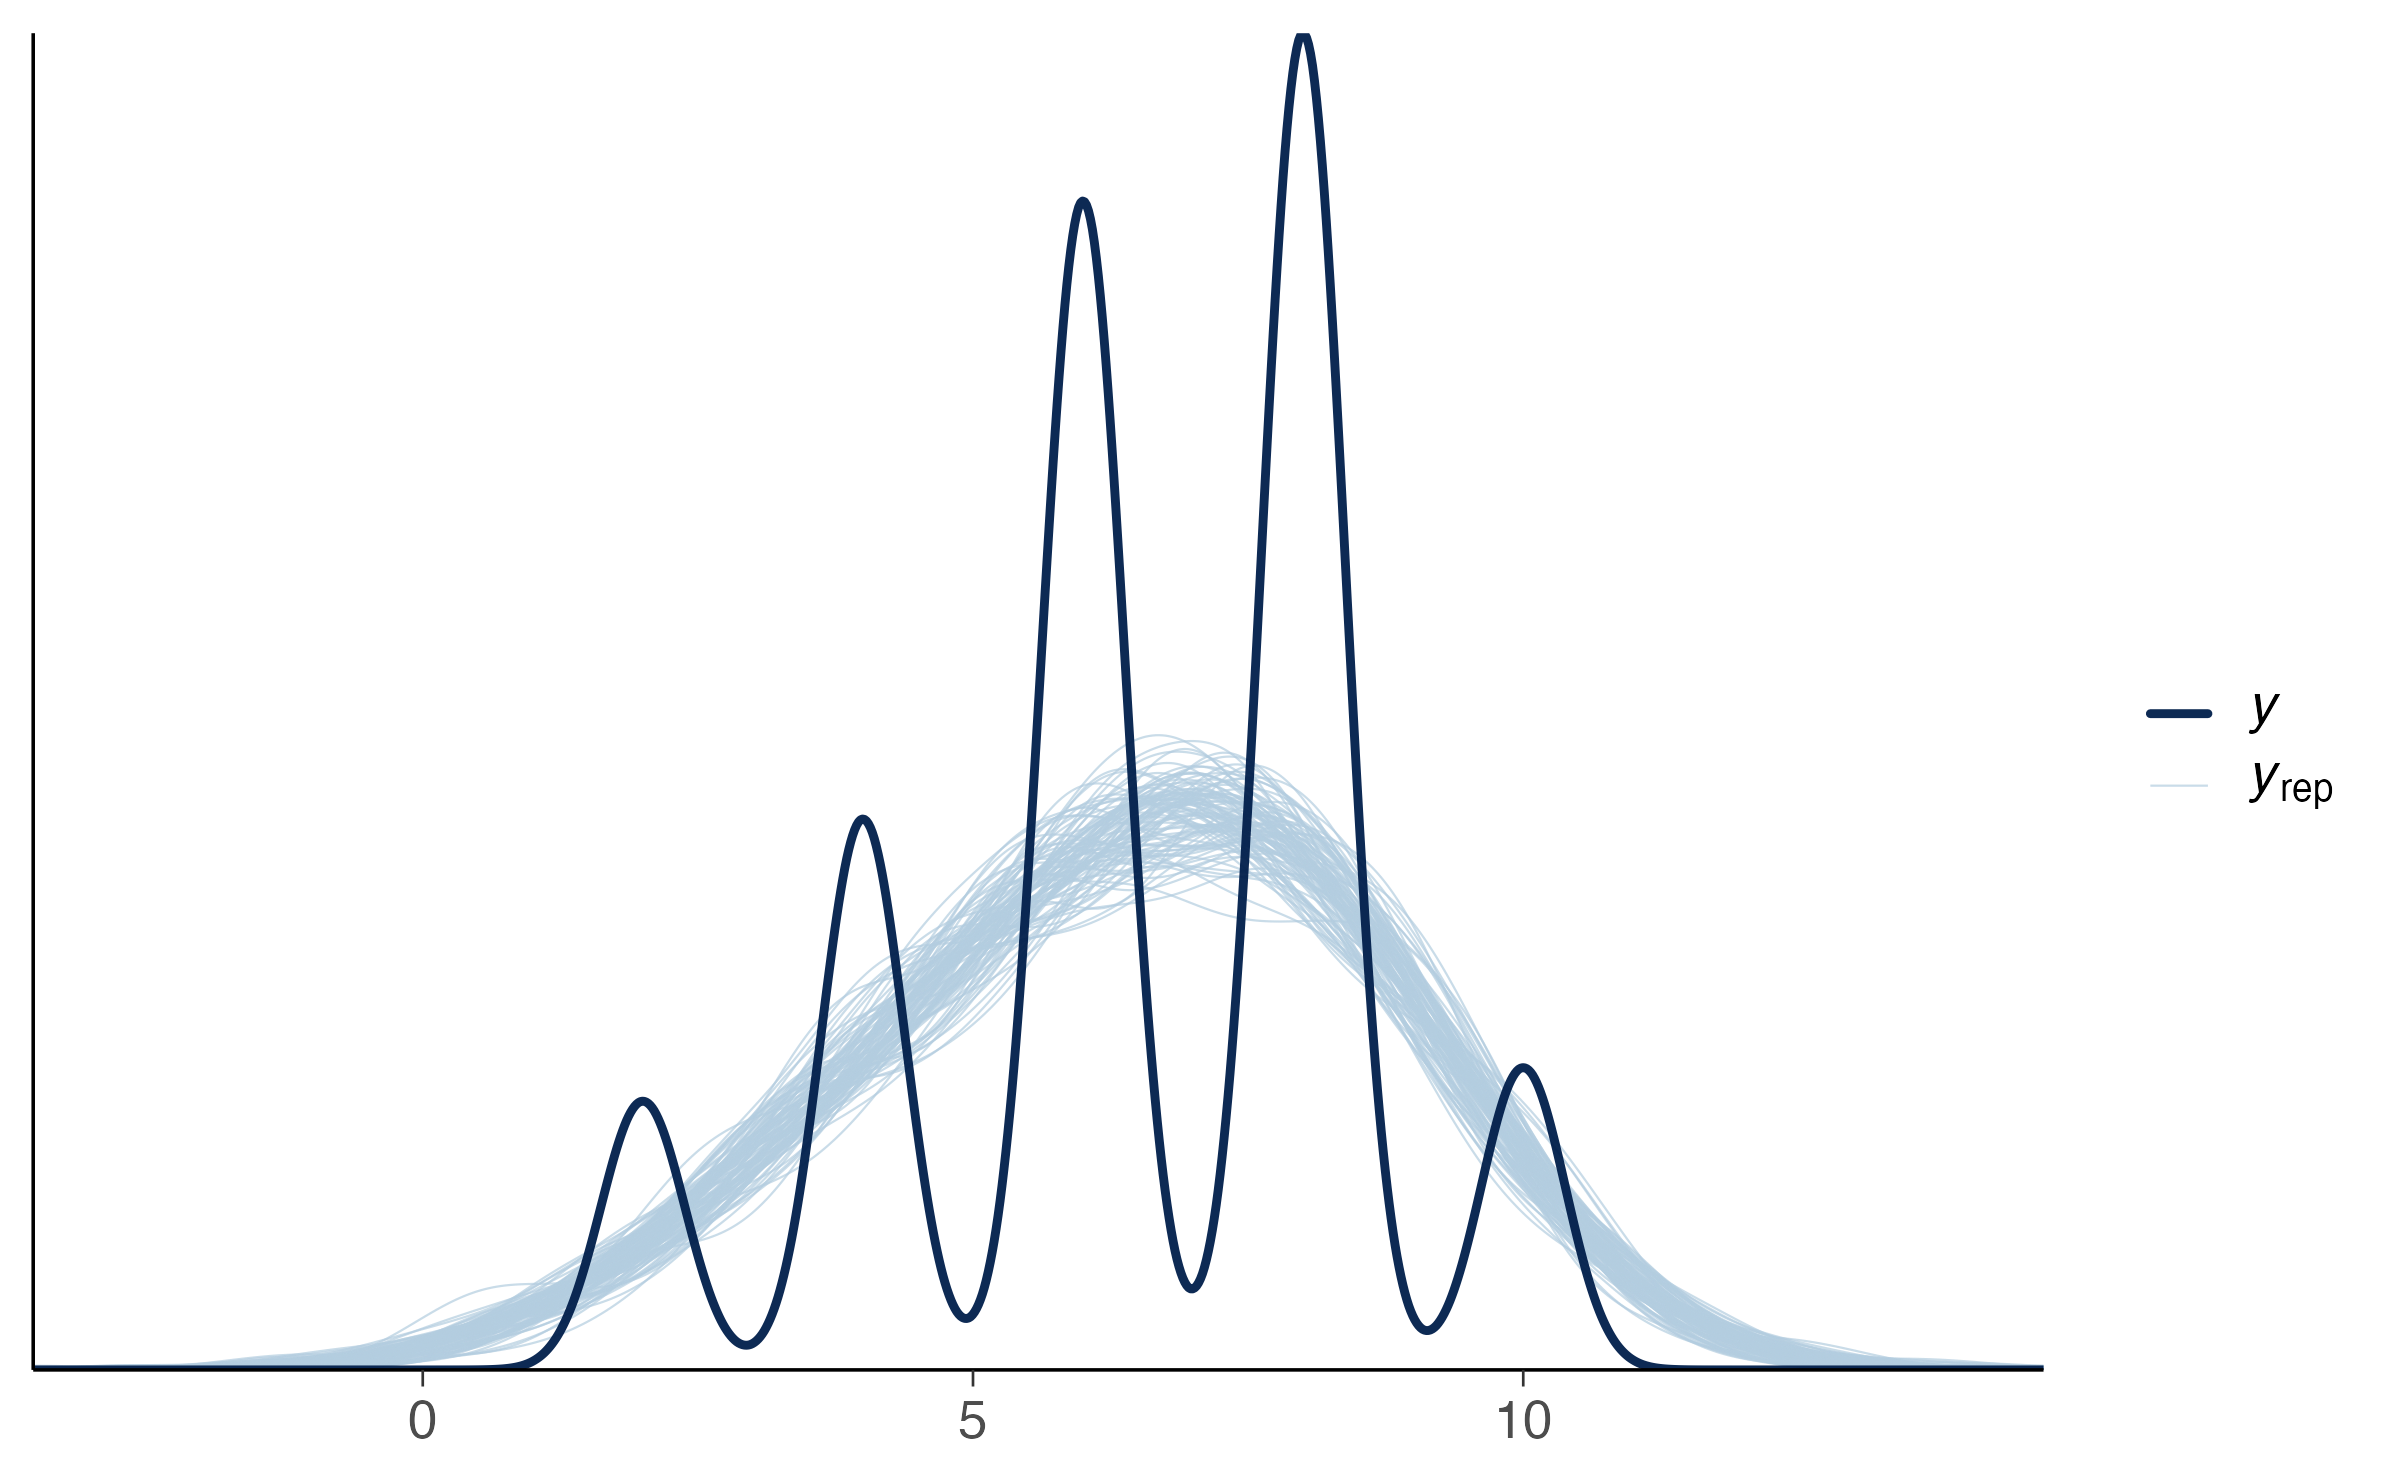
\includegraphics[width=0.85\linewidth,height=\textheight,keepaspectratio]{chapters/formal_models/02_costruire_modello_dinamico_files/figure-pdf/fig-ppc-density-goal-sample-1.png}

}

\caption{\label{fig-ppc-density-goal-sample}Confronto tra la
distribuzione degli obiettivi osservati, esclusi i valori iniziali
condizionati, e repliche posteriori del modello.}

\end{figure}%

Il controllo marginale è necessario ma non sufficiente. Poiché il
modello è dinamico, dobbiamo anche verificare se riproduce traiettorie,
autocorrelazione, ampiezza delle revisioni e differenze tra
partecipanti.

\begin{tcolorbox}[enhanced jigsaw, arc=.35mm, bottomrule=.15mm, bottomtitle=1mm, breakable, colback=white, colbacktitle=quarto-callout-warning-color!10!white, colframe=quarto-callout-warning-color-frame, coltitle=black, left=2mm, leftrule=.75mm, opacityback=0, opacitybacktitle=0.6, rightrule=.15mm, title=\textcolor{quarto-callout-warning-color}{\faExclamationTriangle}\hspace{0.5em}{Un buon controllo aggregato può nascondere fallimenti individuali}, titlerule=0mm, toprule=.15mm, toptitle=1mm]

Un modello con parametri comuni può riprodurre la distribuzione
complessiva degli obiettivi e, nello stesso tempo, rappresentare male
molte traiettorie individuali. Nei dati longitudinali i controlli devono
rispettare la struttura temporale e il livello al quale verranno
formulate le conclusioni.

\end{tcolorbox}

\section{Recuperare parametri noti}\label{recuperare-parametri-noti}

Prima di interpretare parametri stimati su dati reali è utile verificare
se, quando il modello è vero, la procedura riesca a recuperare valori
conosciuti.

Il codice seguente usa le sequenze di prestazione reali come input,
genera obiettivi da parametri fissati e riadatta lo stesso modello.

\begin{tcolorbox}[enhanced jigsaw, arc=.35mm, bottomrule=.15mm, bottomtitle=1mm, breakable, colback=white, colbacktitle=quarto-callout-tip-color!10!white, colframe=quarto-callout-tip-color-frame, coltitle=black, left=2mm, leftrule=.75mm, opacityback=0, opacitybacktitle=0.6, rightrule=.15mm, title=\textcolor{quarto-callout-tip-color}{\faLightbulb}\hspace{0.5em}{Esercizio computazionale: parameter recovery}, titlerule=0mm, toprule=.15mm, toptitle=1mm]

\begin{Shaded}
\begin{Highlighting}[]
\NormalTok{simulate\_goal\_dataset }\OtherTok{\textless{}{-}} \ControlFlowTok{function}\NormalTok{(data, alpha, beta, sigma) \{}
\NormalTok{  data }\SpecialCharTok{|\textgreater{}}
    \FunctionTok{group\_by}\NormalTok{(subject) }\SpecialCharTok{|\textgreater{}}
    \FunctionTok{group\_modify}\NormalTok{(}
      \SpecialCharTok{\textasciitilde{}}\NormalTok{ \{}
\NormalTok{        simulation }\OtherTok{\textless{}{-}} \FunctionTok{simulate\_goal\_path}\NormalTok{(}
          \AttributeTok{performance =}\NormalTok{ .x}\SpecialCharTok{$}\NormalTok{performance,}
          \AttributeTok{initial\_goal =}\NormalTok{ .x}\SpecialCharTok{$}\NormalTok{goal[}\DecValTok{1}\NormalTok{],}
          \AttributeTok{alpha =}\NormalTok{ alpha,}
          \AttributeTok{beta =}\NormalTok{ beta,}
          \AttributeTok{sigma =}\NormalTok{ sigma}
\NormalTok{        )}

        \FunctionTok{mutate}\NormalTok{(.x, }\AttributeTok{goal\_simulated =}\NormalTok{ simulation}\SpecialCharTok{$}\NormalTok{observed)}
\NormalTok{      \}}
\NormalTok{    ) }\SpecialCharTok{|\textgreater{}}
    \FunctionTok{ungroup}\NormalTok{()}
\NormalTok{\}}

\NormalTok{recovery\_data }\OtherTok{\textless{}{-}} \FunctionTok{simulate\_goal\_dataset}\NormalTok{(}
\NormalTok{  goal\_data,}
  \AttributeTok{alpha =} \FloatTok{0.55}\NormalTok{,}
  \AttributeTok{beta =} \FloatTok{0.15}\NormalTok{,}
  \AttributeTok{sigma =} \FloatTok{0.60}
\NormalTok{)}

\NormalTok{stan\_data\_recovery }\OtherTok{\textless{}{-}}\NormalTok{ stan\_data\_goal\_sample}
\NormalTok{stan\_data\_recovery}\SpecialCharTok{$}\NormalTok{goal }\OtherTok{\textless{}{-}}\NormalTok{ recovery\_data}\SpecialCharTok{$}\NormalTok{goal\_simulated}

\NormalTok{fit\_goal\_recovery }\OtherTok{\textless{}{-}}\NormalTok{ model\_goal\_sample}\SpecialCharTok{$}\FunctionTok{sample}\NormalTok{(}
  \AttributeTok{data =}\NormalTok{ stan\_data\_recovery,}
  \AttributeTok{seed =} \DecValTok{911}\NormalTok{,}
  \AttributeTok{chains =} \DecValTok{4}\NormalTok{,}
  \AttributeTok{parallel\_chains =} \DecValTok{4}\NormalTok{,}
  \AttributeTok{iter\_warmup =} \DecValTok{1000}\NormalTok{,}
  \AttributeTok{iter\_sampling =} \DecValTok{2000}
\NormalTok{)}

\NormalTok{fit\_goal\_recovery}\SpecialCharTok{$}\FunctionTok{summary}\NormalTok{(}\FunctionTok{c}\NormalTok{(}\StringTok{"alpha"}\NormalTok{, }\StringTok{"beta"}\NormalTok{, }\StringTok{"sigma"}\NormalTok{))}
\end{Highlighting}
\end{Shaded}

Il recupero dei valori noti è una condizione necessaria, non
sufficiente. Qui dati e modello generatore coincidono; nei dati reali il
processo potrebbe seguire regole diverse.

\end{tcolorbox}

\section{Che cosa assume il modello}\label{che-cosa-assume-il-modello}

La specificazione contiene almeno sei ipotesi sostantive.

\begin{enumerate}
\def\labelenumi{\arabic{enumi}.}
\tightlist
\item
  \textbf{Memoria di primo ordine.} L'aggiornamento usa soltanto lo
  stato e la prestazione immediatamente precedenti.
\item
  \textbf{Sensibilità costante.} \(\alpha\) non cambia tra trial,
  persone o tipo di feedback.
\item
  \textbf{Deriva costante.} \(\beta\) opera nello stesso modo per tutta
  la sequenza.
\item
  \textbf{Prestazione trattata come input noto.} Non viene modellata la
  sua incertezza né la possibile influenza dell'obiettivo sulla
  prestazione futura.
\item
  \textbf{Rumore normale e costante.} La variabilità osservazionale non
  dipende dal trial o dal livello dell'obiettivo.
\item
  \textbf{Parametri comuni.} Tutti i partecipanti condividono la stessa
  dinamica.
\end{enumerate}

Inoltre, la scala osservata è limitata, mentre la distribuzione normale
consente valori arbitrariamente bassi o alti. Se i controlli predittivi
mostrassero un problema rilevante, sarebbe opportuno adottare una
distribuzione o una trasformazione coerente con i limiti della risposta.

\section{Errori frequenti}\label{errori-frequenti-11}

\begin{itemize}
\tightlist
\item
  Stimare il modello prima di averne simulato il comportamento.
\item
  Chiamare \(\alpha\) ``apprendimento'' o \(\beta\) ``motivazione''
  senza una validazione indipendente.
\item
  Includere il primo trial nella verosimiglianza dopo averlo usato per
  inizializzare lo stato.
\item
  Confondere la traiettoria latente \(G_t\) con il valore osservato
  \(Y_t\).
\item
  Interpretare una buona convergenza MCMC come prova della correttezza
  teorica.
\item
  Valutare il modello soltanto mediante la distribuzione marginale dei
  dati.
\item
  Dimenticare che le righe devono essere ordinate per soggetto e trial.
\item
  Generalizzare i parametri comuni ai singoli partecipanti.
\end{itemize}

\section{Riflessioni conclusive}\label{riflessioni-conclusive-36}

Il modello di revisione degli obiettivi mostra come una teoria verbale
possa diventare una teoria eseguibile. La formalizzazione obbliga a
dichiarare quale stato conserva la memoria, quale informazione produce
l'aggiornamento, come agiscono i parametri e in che modo il processo
genera osservazioni.

La simulazione ha preceduto la stima perché un parametro è
interpretabile soltanto attraverso le conseguenze che produce nel
modello. L'implementazione bayesiana ha poi trasformato il problema
diretto --- generare dati da parametri noti --- nel problema inverso di
inferire parametri plausibili da traiettorie osservate.

La specificazione resta intenzionalmente semplice. Il suo limite
principale è l'ipotesi che tutte le persone condividano \(\alpha\) e
\(\beta\). Nel prossimo capitolo conserveremo la stessa regola di
aggiornamento, ma modelleremo esplicitamente la distribuzione dei
parametri tra individui e condizioni.

\section{Concetti da ricordare}\label{concetti-da-ricordare-10}

\begin{enumerate}
\def\labelenumi{\arabic{enumi}.}
\tightlist
\item
  Un modello dinamico contiene almeno uno stato che dipende dalla storia
  precedente.
\item
  La regola di aggiornamento deve essere studiata mediante simulazione
  prima della stima.
\item
  \(\alpha\) controlla la quota di discrepanza incorporata; \(\beta\)
  introduce una deriva per trial.
\item
  Processo latente e osservazione sono componenti differenti.
\item
  Il primo obiettivo è qui una condizione iniziale, non un dato spiegato
  dal modello.
\item
  Un parametro con un nome psicologico non è automaticamente una misura
  valida del costrutto.
\item
  I prior devono essere valutati attraverso le traiettorie che generano.
\item
  Diagnostica MCMC e adeguatezza del modello rispondono a domande
  diverse.
\item
  I controlli predittivi devono rispettare la struttura temporale.
\item
  Il recupero dei parametri è necessario prima di attribuire loro
  significato individuale.
\end{enumerate}

\begin{tcolorbox}[enhanced jigsaw, arc=.35mm, bottomrule=.15mm, bottomtitle=1mm, breakable, colback=white, colbacktitle=quarto-callout-note-color!10!white, colframe=quarto-callout-note-color-frame, coltitle=black, left=2mm, leftrule=.75mm, opacityback=0, opacitybacktitle=0.6, rightrule=.15mm, title=\textcolor{quarto-callout-note-color}{\faInfo}\hspace{0.5em}{Esercizi}, titlerule=0mm, toprule=.15mm, toptitle=1mm]

\subsection{1. Cambiare la
sensibilità}\label{cambiare-la-sensibilituxe0}

Mantieni costanti prestazione e \(\beta\), quindi simula
\(\alpha=0.05\), \(0.50\) e \(0.95\). Descrivi memoria, rapidità e
variabilità delle tre traiettorie.

\subsection{2. Cambiare la deriva}\label{cambiare-la-deriva}

Simula \(\beta=-0.25\), \(0\) e \(0.25\). Verifica come cambia il punto
di equilibrio quando la prestazione è costante.

\subsection{3. Condizione iniziale}\label{condizione-iniziale}

Ripeti la simulazione usando tre obiettivi iniziali differenti. Dopo
quanti trial le traiettorie diventano simili?

\subsection{4. Modello osservazionale}\label{modello-osservazionale}

Mantieni invariato lo stato latente e varia \(\sigma\). Quali aspetti
della traiettoria cambiano e quali restano identici?

\subsection{5. Prior predittivi}\label{prior-predittivi}

Raddoppia la deviazione standard del prior di \(\beta\). Valuta se le
traiettorie generate restano plausibili sulla scala del compito.

\subsection{6. Memoria più lunga}\label{memoria-piuxf9-lunga}

Proponi una modifica della regola nella quale l'aggiornamento dipenda
dalla media delle ultime tre prestazioni.

\subsection{7. Recuperabilità}\label{recuperabilituxe0}

Esegui il controllo di parameter recovery con \(\alpha=0.15\) e
\(\alpha=0.90\). In quale scenario la stima di \(\beta\) è più
difficile?

\subsection{8. Critica del modello}\label{critica-del-modello}

Indica almeno due pattern empirici che il modello con \(\alpha\) e
\(\beta\) costanti non potrebbe riprodurre adeguatamente.

\begin{quote}
\textbf{Tracce di soluzione}

\begin{enumerate}
\def\labelenumi{\arabic{enumi}.}
\tightlist
\item
  Valori bassi di \(\alpha\) conservano più a lungo lo stato precedente;
  valori alti seguono rapidamente la prestazione.
\item
  Con prestazione costante, \(G^*=P+\beta/\alpha\) quando \(\alpha>0\).
\item
  La distanza tra condizioni iniziali si riduce più rapidamente quando
  \(\alpha\) è alto.
\item
  \(\sigma\) modifica le osservazioni, non la traiettoria latente
  deterministica.
\item
  Un prior più ampio su \(\beta\) può produrre derive cumulative
  estreme.
\item
  Occorre definire un input filtrato, per esempio la media mobile delle
  prestazioni recenti.
\item
  La risposta dipende dalla sequenza di input e dal trade-off tra deriva
  e correzione; il confronto deve essere empirico.
\item
  Esempi: sensibilità diversa ai successi e ai fallimenti, cambiamenti
  improvvisi di strategia, effetti di saturazione o differenze
  individuali persistenti.
\end{enumerate}
\end{quote}

\end{tcolorbox}

\begin{tcolorbox}[enhanced jigsaw, arc=.35mm, bottomrule=.15mm, bottomtitle=1mm, breakable, colback=white, colbacktitle=quarto-callout-note-color!10!white, colframe=quarto-callout-note-color-frame, coltitle=black, left=2mm, leftrule=.75mm, opacityback=0, opacitybacktitle=0.6, rightrule=.15mm, title=\textcolor{quarto-callout-note-color}{\faInfo}\hspace{0.5em}{Informazioni sull'ambiente di sviluppo}, titlerule=0mm, toprule=.15mm, toptitle=1mm]

\begin{Shaded}
\begin{Highlighting}[]
\FunctionTok{sessionInfo}\NormalTok{()}
\CommentTok{\#\textgreater{} R version 4.6.1 (2026{-}06{-}24)}
\CommentTok{\#\textgreater{} Platform: aarch64{-}apple{-}darwin23}
\CommentTok{\#\textgreater{} Running under: macOS Tahoe 26.5.2}
\CommentTok{\#\textgreater{} }
\CommentTok{\#\textgreater{} Matrix products: default}
\CommentTok{\#\textgreater{} BLAS:   /Library/Frameworks/R.framework/Versions/4.6/Resources/lib/libRblas.0.dylib }
\CommentTok{\#\textgreater{} LAPACK: /Library/Frameworks/R.framework/Versions/4.6/Resources/lib/libRlapack.dylib;  LAPACK version 3.12.1}
\CommentTok{\#\textgreater{} }
\CommentTok{\#\textgreater{} locale:}
\CommentTok{\#\textgreater{} [1] C.UTF{-}8/UTF{-}8/C.UTF{-}8/C/C.UTF{-}8/C.UTF{-}8}
\CommentTok{\#\textgreater{} }
\CommentTok{\#\textgreater{} time zone: Europe/Zagreb}
\CommentTok{\#\textgreater{} tzcode source: internal}
\CommentTok{\#\textgreater{} }
\CommentTok{\#\textgreater{} attached base packages:}
\CommentTok{\#\textgreater{} [1] stats     graphics  grDevices utils     datasets  methods   base     }
\CommentTok{\#\textgreater{} }
\CommentTok{\#\textgreater{} other attached packages:}
\CommentTok{\#\textgreater{}  [1] cmdstanr\_0.9.0        ragg\_1.5.2            tinytable\_0.17.0     }
\CommentTok{\#\textgreater{}  [4] withr\_3.0.3           systemfonts\_1.3.2     patchwork\_1.3.2      }
\CommentTok{\#\textgreater{}  [7] ggdist\_3.3.3          tidybayes\_3.0.7       bayesplot\_1.15.0     }
\CommentTok{\#\textgreater{} [10] ggplot2\_4.0.3         reliabilitydiag\_0.2.1 priorsense\_1.2.0     }
\CommentTok{\#\textgreater{} [13] posterior\_1.7.0       loo\_2.10.0            rstan\_2.32.7         }
\CommentTok{\#\textgreater{} [16] StanHeaders\_2.32.10   brms\_2.23.0           Rcpp\_1.1.2           }
\CommentTok{\#\textgreater{} [19] sessioninfo\_1.2.4     conflicted\_1.2.0      janitor\_2.2.1        }
\CommentTok{\#\textgreater{} [22] matrixStats\_1.5.0     modelr\_0.1.11         tibble\_3.3.1         }
\CommentTok{\#\textgreater{} [25] dplyr\_1.2.1           tidyr\_1.3.2           rio\_1.3.0            }
\CommentTok{\#\textgreater{} [28] here\_1.0.2           }
\CommentTok{\#\textgreater{} }
\CommentTok{\#\textgreater{} loaded via a namespace (and not attached):}
\CommentTok{\#\textgreater{}  [1] gridExtra\_2.3.1       inline\_0.3.21         rlang\_1.3.0          }
\CommentTok{\#\textgreater{}  [4] magrittr\_2.0.5        snakecase\_0.11.1      otel\_0.2.0           }
\CommentTok{\#\textgreater{}  [7] compiler\_4.6.1        vctrs\_0.7.3           reshape2\_1.4.5       }
\CommentTok{\#\textgreater{} [10] stringr\_1.6.0         pkgconfig\_2.0.3       arrayhelpers\_1.1{-}1   }
\CommentTok{\#\textgreater{} [13] fastmap\_1.2.0         backports\_1.5.1       labeling\_0.4.3       }
\CommentTok{\#\textgreater{} [16] utf8\_1.2.6            rmarkdown\_2.31        ps\_1.9.3             }
\CommentTok{\#\textgreater{} [19] purrr\_1.2.2           xfun\_0.60             cachem\_1.1.0         }
\CommentTok{\#\textgreater{} [22] jsonlite\_2.0.0        broom\_1.0.13          parallel\_4.6.1       }
\CommentTok{\#\textgreater{} [25] R6\_2.6.1              stringi\_1.8.7         RColorBrewer\_1.1{-}3   }
\CommentTok{\#\textgreater{} [28] lubridate\_1.9.5       estimability\_2.0.0    knitr\_1.51           }
\CommentTok{\#\textgreater{} [31] R.utils\_2.13.0        Matrix\_1.7{-}5          timechange\_0.4.0     }
\CommentTok{\#\textgreater{} [34] tidyselect\_1.2.1      abind\_1.4{-}8           yaml\_2.3.12          }
\CommentTok{\#\textgreater{} [37] codetools\_0.2{-}20      curl\_7.1.0            processx\_3.9.0       }
\CommentTok{\#\textgreater{} [40] pkgbuild\_1.4.8        plyr\_1.8.9            lattice\_0.22{-}9       }
\CommentTok{\#\textgreater{} [43] bridgesampling\_1.2{-}1  S7\_0.2.2              coda\_0.19{-}4.1        }
\CommentTok{\#\textgreater{} [46] evaluate\_1.0.5        RcppParallel\_5.1.11{-}2 pillar\_1.11.1        }
\CommentTok{\#\textgreater{} [49] tensorA\_0.36.2.1      checkmate\_2.3.4       stats4\_4.6.1         }
\CommentTok{\#\textgreater{} [52] distributional\_0.8.1  generics\_0.1.4        rprojroot\_2.1.1      }
\CommentTok{\#\textgreater{} [55] rstantools\_2.6.0      scales\_1.4.0          xtable\_1.8{-}8         }
\CommentTok{\#\textgreater{} [58] glue\_1.8.1            emmeans\_2.0.4         tools\_4.6.1          }
\CommentTok{\#\textgreater{} [61] data.table\_1.18.4     mvtnorm\_1.4{-}2         grid\_4.6.1           }
\CommentTok{\#\textgreater{} [64] QuickJSR\_1.10.0       nlme\_3.1{-}170          cli\_3.6.6            }
\CommentTok{\#\textgreater{} [67] textshaping\_1.0.5     svUnit\_1.0.8          Brobdingnag\_1.2{-}9    }
\CommentTok{\#\textgreater{} [70] V8\_8.2.0              gtable\_0.3.6          R.methodsS3\_1.8.2    }
\CommentTok{\#\textgreater{} [73] digest\_0.6.39         farver\_2.1.2          memoise\_2.0.1        }
\CommentTok{\#\textgreater{} [76] htmltools\_0.5.9       R.oo\_1.27.1           lifecycle\_1.0.5}
\end{Highlighting}
\end{Shaded}

\end{tcolorbox}

\section*{Bibliografia}\label{bibliografia-41}

\markright{Bibliografia}

\chapter{Dall'individuo alla popolazione: eterogeneità nei modelli
dinamici}\label{sec-formal-models-developments}

\begin{tcolorbox}[enhanced jigsaw, arc=.35mm, bottomrule=.15mm, breakable, colback=white, colframe=quarto-callout-note-color-frame, left=2mm, leftrule=.75mm, opacityback=0, rightrule=.15mm, toprule=.15mm]

Nel capitolo Capitolo~\ref{sec-dynamic-models-goal-updating} abbiamo
rappresentato l'intero campione mediante un'unica sensibilità alla
discrepanza, \(\alpha\), e un'unica deriva, \(\beta\). Questa
specificazione è utile come punto di partenza, ma non consente di
distinguere una dinamica comune da differenze persistenti tra persone.

In questo capitolo manteniamo invariata la regola di aggiornamento e
modifichiamo la struttura della popolazione. Confronteremo complete
pooling, no pooling e partial pooling; distingueremo eterogeneità e
incertezza; estenderemo il modello alle condizioni sperimentali; infine
discuteremo recuperabilità e previsione per nuovi individui.

\end{tcolorbox}

\begin{tcolorbox}[enhanced jigsaw, arc=.35mm, bottomrule=.15mm, bottomtitle=1mm, breakable, colback=white, colbacktitle=quarto-callout-note-color!10!white, colframe=quarto-callout-note-color-frame, coltitle=black, left=2mm, leftrule=.75mm, opacityback=0, opacitybacktitle=0.6, rightrule=.15mm, title=\textcolor{quarto-callout-note-color}{\faInfo}\hspace{0.5em}{Obiettivi del capitolo}, titlerule=0mm, toprule=.15mm, toptitle=1mm]

Al termine del capitolo dovresti essere in grado di:

\begin{itemize}
\tightlist
\item
  distinguere complete pooling, no pooling e partial pooling nei
  parametri di un modello processuale;
\item
  interpretare parametri individuali, iperparametri e dispersioni di
  popolazione;
\item
  comprendere perché variabilità tra stime individuali e vera
  eterogeneità non coincidono;
\item
  specificare un modello gerarchico non centrato in Stan;
\item
  visualizzare lo shrinkage dei parametri processuali;
\item
  distinguere previsioni per persone osservate e per persone nuove;
\item
  stimare contrasti tra condizioni a livello di popolazione;
\item
  progettare un controllo di parameter recovery gerarchico;
\item
  evitare confronti predittivi che ignorino la dipendenza temporale.
\end{itemize}

\end{tcolorbox}

\begin{tcolorbox}[enhanced jigsaw, arc=.35mm, bottomrule=.15mm, bottomtitle=1mm, breakable, colback=white, colbacktitle=quarto-callout-tip-color!10!white, colframe=quarto-callout-tip-color-frame, coltitle=black, left=2mm, leftrule=.75mm, opacityback=0, opacitybacktitle=0.6, rightrule=.15mm, title=\textcolor{quarto-callout-tip-color}{\faLightbulb}\hspace{0.5em}{Percorsi di lettura}, titlerule=0mm, toprule=.15mm, toptitle=1mm]

\textbf{Percorso concettuale.} Segui il confronto tra pooling,
l'interpretazione dell'eterogeneità e le sezioni sulle previsioni.

\textbf{Percorso applicativo.} Esegui il modello gerarchico, i grafici
di shrinkage e i contrasti tra condizioni.

\textbf{Percorso computazionale.} Studia la parametrizzazione non
centrata, il controllo di recuperabilità e la simulazione di un nuovo
individuo.

\end{tcolorbox}

\begin{tcolorbox}[enhanced jigsaw, arc=.35mm, bottomrule=.15mm, bottomtitle=1mm, breakable, colback=white, colbacktitle=quarto-callout-tip-color!10!white, colframe=quarto-callout-tip-color-frame, coltitle=black, left=2mm, leftrule=.75mm, opacityback=0, opacitybacktitle=0.6, rightrule=.15mm, title=\textcolor{quarto-callout-tip-color}{\faLightbulb}\hspace{0.5em}{Prerequisiti}, titlerule=0mm, toprule=.15mm, toptitle=1mm]

\begin{itemize}
\tightlist
\item
  Il modello di revisione degli obiettivi sviluppato in
  Capitolo~\ref{sec-dynamic-models-goal-updating}.
\item
  Il capitolo sui modelli multilivello nella parte \textbf{Modelli}.
\item
  Il workflow dei modelli formali descritto in
  Capitolo~\ref{sec-bayes-stat-models}.
\end{itemize}

\end{tcolorbox}

\begin{tcolorbox}[enhanced jigsaw, arc=.35mm, bottomrule=.15mm, bottomtitle=1mm, breakable, colback=white, colbacktitle=quarto-callout-caution-color!10!white, colframe=quarto-callout-caution-color-frame, coltitle=black, left=2mm, leftrule=.75mm, opacityback=0, opacitybacktitle=0.6, rightrule=.15mm, title=\textcolor{quarto-callout-caution-color}{\faFire}\hspace{0.5em}{Preparazione del Notebook}, titlerule=0mm, toprule=.15mm, toptitle=1mm]

\end{tcolorbox}

\section{Lo stesso processo, tre strutture di
popolazione}\label{lo-stesso-processo-tre-strutture-di-popolazione}

La regola individuale resta:

\[
G_{s,t}
=
G_{s,t-1}
+
\alpha_s\left(P_{s,t-1}-G_{s,t-1}\right)
+
\beta_s.
\]

Ciò che cambia è il modo in cui rappresentiamo \(\alpha_s\) e
\(\beta_s\).

\subsection{Complete pooling}\label{complete-pooling-1}

Il modello del capitolo precedente impone:

\[
\alpha_s=\alpha,
\qquad
\beta_s=\beta
\]

per tutti i soggetti. Tutte le osservazioni informano la stessa coppia
di parametri.

Questo approccio è parsimonioso e può essere appropriato quando le
differenze individuali sono trascurabili rispetto al rumore. Se
l'eterogeneità è sostanziale, tuttavia, il parametro comune descrive una
media che potrebbe non rappresentare bene nessuna persona.

\subsection{No pooling}\label{no-pooling-1}

All'estremo opposto possiamo stimare ogni persona separatamente:

\[
\alpha_s,\beta_s
\quad\text{indipendenti tra soggetti.}
\]

Il modello è molto flessibile, ma ogni stima usa soltanto i pochi trial
della persona corrispondente. Differenze apparenti tra partecipanti
possono quindi riflettere principalmente rumore e scarsa informazione.

\subsection{Partial pooling}\label{partial-pooling-1}

Il modello gerarchico rappresenta i parametri individuali come
estrazioni da distribuzioni di popolazione:

\[
\operatorname{logit}(\alpha_s)
\sim
\operatorname{Normal}(\mu_\alpha,\tau_\alpha),
\]

\[
\beta_s
\sim
\operatorname{Normal}(\mu_\beta,\tau_\beta).
\]

Le stime individuali sono informate sia dai trial della persona sia
dalla distribuzione condivisa. È questo scambio di informazione che
produce partial pooling e shrinkage.

{\def\LTcaptype{none} % do not increment counter
\begin{longtable}[]{@{}
  >{\raggedright\arraybackslash}p{(\linewidth - 6\tabcolsep) * \real{0.2500}}
  >{\raggedright\arraybackslash}p{(\linewidth - 6\tabcolsep) * \real{0.2500}}
  >{\raggedright\arraybackslash}p{(\linewidth - 6\tabcolsep) * \real{0.2500}}
  >{\raggedright\arraybackslash}p{(\linewidth - 6\tabcolsep) * \real{0.2500}}@{}}
\toprule\noalign{}
\begin{minipage}[b]{\linewidth}\raggedright
Strategia
\end{minipage} & \begin{minipage}[b]{\linewidth}\raggedright
Informazione usata per la persona
\end{minipage} & \begin{minipage}[b]{\linewidth}\raggedright
Vantaggio
\end{minipage} & \begin{minipage}[b]{\linewidth}\raggedright
Limite principale
\end{minipage} \\
\midrule\noalign{}
\endhead
\bottomrule\noalign{}
\endlastfoot
Complete pooling & tutti i dati, ma nessuna differenza individuale &
stabilità & può mascherare eterogeneità \\
No pooling & soltanto i dati individuali & massima flessibilità & stime
fragili con pochi trial \\
Partial pooling & dati individuali e popolazione & equilibrio tra
stabilità e specificità & dipende dalla struttura gerarchica assunta \\
\end{longtable}
}

\begin{tcolorbox}[enhanced jigsaw, arc=.35mm, bottomrule=.15mm, bottomtitle=1mm, breakable, colback=white, colbacktitle=quarto-callout-important-color!10!white, colframe=quarto-callout-important-color-frame, coltitle=black, left=2mm, leftrule=.75mm, opacityback=0, opacitybacktitle=0.6, rightrule=.15mm, title=\textcolor{quarto-callout-important-color}{\faExclamation}\hspace{0.5em}{Eterogeneità e incertezza non sono la stessa cosa}, titlerule=0mm, toprule=.15mm, toptitle=1mm]

Un intervallo individuale ampio indica che conosciamo poco il parametro
di quella persona. Una dispersione di popolazione elevata indica invece
che il modello attribuisce differenze sistematiche tra persone.

Le due quantità possono coesistere, ma non devono essere confuse.

\end{tcolorbox}

\section{Il dataset e la struttura del
disegno}\label{il-dataset-e-la-struttura-del-disegno}

Il caso di studio continua a seguire Knight et al.
(\citeproc{ref-knight2023tutorial}{2023}). Sono presenti 60
partecipanti, 30 nella condizione \emph{approach} e 30 nella condizione
\emph{avoidance}, con 10 trial per persona.

\begin{Shaded}
\begin{Highlighting}[]
\NormalTok{goal\_data }\OtherTok{\textless{}{-}}\NormalTok{ rio}\SpecialCharTok{::}\FunctionTok{import}\NormalTok{(here}\SpecialCharTok{::}\FunctionTok{here}\NormalTok{(}\StringTok{"data"}\NormalTok{, }\StringTok{"goal\_data.csv"}\NormalTok{)) }\SpecialCharTok{|\textgreater{}}
  \FunctionTok{as\_tibble}\NormalTok{() }\SpecialCharTok{|\textgreater{}}
  \FunctionTok{mutate}\NormalTok{(}
    \AttributeTok{subject =} \FunctionTok{as.integer}\NormalTok{(}\FunctionTok{factor}\NormalTok{(subject)),}
    \AttributeTok{condition =} \FunctionTok{factor}\NormalTok{(condition, }\AttributeTok{levels =} \FunctionTok{c}\NormalTok{(}\StringTok{"approach"}\NormalTok{, }\StringTok{"avoidance"}\NormalTok{)),}
    \AttributeTok{condition\_id =} \FunctionTok{as.integer}\NormalTok{(condition)}
\NormalTok{  ) }\SpecialCharTok{|\textgreater{}}
  \FunctionTok{arrange}\NormalTok{(subject, trial) }\SpecialCharTok{|\textgreater{}}
  \FunctionTok{mutate}\NormalTok{(}\AttributeTok{row\_id =} \FunctionTok{row\_number}\NormalTok{())}

\NormalTok{subject\_structure }\OtherTok{\textless{}{-}}\NormalTok{ goal\_data }\SpecialCharTok{|\textgreater{}}
  \FunctionTok{distinct}\NormalTok{(subject, condition, condition\_id) }\SpecialCharTok{|\textgreater{}}
  \FunctionTok{arrange}\NormalTok{(subject)}

\FunctionTok{stopifnot}\NormalTok{(}
  \FunctionTok{nrow}\NormalTok{(subject\_structure) }\SpecialCharTok{==} \FunctionTok{n\_distinct}\NormalTok{(goal\_data}\SpecialCharTok{$}\NormalTok{subject),}
  \FunctionTok{all}\NormalTok{(}
\NormalTok{    goal\_data }\SpecialCharTok{|\textgreater{}}
      \FunctionTok{group\_by}\NormalTok{(subject) }\SpecialCharTok{|\textgreater{}}
      \FunctionTok{summarise}\NormalTok{(}\AttributeTok{ok =} \FunctionTok{all}\NormalTok{(trial }\SpecialCharTok{==} \FunctionTok{seq\_len}\NormalTok{(}\FunctionTok{n}\NormalTok{())), }\AttributeTok{.groups =} \StringTok{"drop"}\NormalTok{) }\SpecialCharTok{|\textgreater{}}
      \FunctionTok{pull}\NormalTok{(ok)}
\NormalTok{  )}
\NormalTok{)}

\NormalTok{goal\_data }\SpecialCharTok{|\textgreater{}}
\NormalTok{  dplyr}\SpecialCharTok{::}\FunctionTok{count}\NormalTok{(condition, }\AttributeTok{name =} \StringTok{"osservazioni"}\NormalTok{) }\SpecialCharTok{|\textgreater{}}
\NormalTok{  dplyr}\SpecialCharTok{::}\FunctionTok{left\_join}\NormalTok{(}
\NormalTok{    subject\_structure }\SpecialCharTok{|\textgreater{}}
\NormalTok{      dplyr}\SpecialCharTok{::}\FunctionTok{count}\NormalTok{(condition, }\AttributeTok{name =} \StringTok{"partecipanti"}\NormalTok{),}
    \AttributeTok{by =} \StringTok{"condition"}
\NormalTok{  )}
\CommentTok{\#\textgreater{} \# A tibble: 2 x 3}
\CommentTok{\#\textgreater{}   condition osservazioni partecipanti}
\CommentTok{\#\textgreater{}   \textless{}fct\textgreater{}            \textless{}int\textgreater{}        \textless{}int\textgreater{}}
\CommentTok{\#\textgreater{} 1 approach           300           30}
\CommentTok{\#\textgreater{} 2 avoidance          300           30}
\end{Highlighting}
\end{Shaded}

Manteniamo la scala originale. In questo modo \(\beta_s\) è espresso in
punti della scala dell'obiettivo per trial e \(\sigma\) nella stessa
unità dei dati.

\section{Un benchmark no pooling}\label{un-benchmark-no-pooling}

Per rendere visibile il problema, otteniamo stime separate mediante
minimizzazione della somma degli errori quadratici. Queste stime non
costituiscono il modello inferenziale finale: servono come benchmark
privo di condivisione dell'informazione.

\begin{Shaded}
\begin{Highlighting}[]
\NormalTok{predict\_goal\_path }\OtherTok{\textless{}{-}} \ControlFlowTok{function}\NormalTok{(goal, performance, alpha, beta) \{}
\NormalTok{  mu }\OtherTok{\textless{}{-}} \FunctionTok{numeric}\NormalTok{(}\FunctionTok{length}\NormalTok{(goal))}
\NormalTok{  mu[}\DecValTok{1}\NormalTok{] }\OtherTok{\textless{}{-}}\NormalTok{ goal[}\DecValTok{1}\NormalTok{]}

  \ControlFlowTok{if}\NormalTok{ (}\FunctionTok{length}\NormalTok{(goal) }\SpecialCharTok{\textgreater{}} \DecValTok{1}\NormalTok{) \{}
    \ControlFlowTok{for}\NormalTok{ (t }\ControlFlowTok{in} \DecValTok{2}\SpecialCharTok{:}\FunctionTok{length}\NormalTok{(goal)) \{}
\NormalTok{      mu[t] }\OtherTok{\textless{}{-}}\NormalTok{ mu[t }\SpecialCharTok{{-}} \DecValTok{1}\NormalTok{] }\SpecialCharTok{+}
\NormalTok{        alpha }\SpecialCharTok{*}\NormalTok{ (performance[t }\SpecialCharTok{{-}} \DecValTok{1}\NormalTok{] }\SpecialCharTok{{-}}\NormalTok{ mu[t }\SpecialCharTok{{-}} \DecValTok{1}\NormalTok{]) }\SpecialCharTok{+}
\NormalTok{        beta}
\NormalTok{    \}}
\NormalTok{  \}}

\NormalTok{  mu}
\NormalTok{\}}

\NormalTok{estimate\_no\_pool\_subject }\OtherTok{\textless{}{-}} \ControlFlowTok{function}\NormalTok{(goal, performance) \{}
\NormalTok{  objective }\OtherTok{\textless{}{-}} \ControlFlowTok{function}\NormalTok{(theta) \{}
\NormalTok{    alpha }\OtherTok{\textless{}{-}} \FunctionTok{plogis}\NormalTok{(theta[}\DecValTok{1}\NormalTok{])}
\NormalTok{    beta }\OtherTok{\textless{}{-}}\NormalTok{ theta[}\DecValTok{2}\NormalTok{]}
\NormalTok{    mu }\OtherTok{\textless{}{-}} \FunctionTok{predict\_goal\_path}\NormalTok{(goal, performance, alpha, beta)}
    \FunctionTok{sum}\NormalTok{((goal[}\SpecialCharTok{{-}}\DecValTok{1}\NormalTok{] }\SpecialCharTok{{-}}\NormalTok{ mu[}\SpecialCharTok{{-}}\DecValTok{1}\NormalTok{])}\SpecialCharTok{\^{}}\DecValTok{2}\NormalTok{)}
\NormalTok{  \}}

\NormalTok{  estimate }\OtherTok{\textless{}{-}} \FunctionTok{optim}\NormalTok{(}
    \AttributeTok{par =} \FunctionTok{c}\NormalTok{(}\FunctionTok{qlogis}\NormalTok{(}\FloatTok{0.50}\NormalTok{), }\DecValTok{0}\NormalTok{),}
    \AttributeTok{fn =}\NormalTok{ objective,}
    \AttributeTok{method =} \StringTok{"BFGS"}
\NormalTok{  )}

  \FunctionTok{tibble}\NormalTok{(}
    \AttributeTok{alpha\_no\_pool =} \FunctionTok{plogis}\NormalTok{(estimate}\SpecialCharTok{$}\NormalTok{par[}\DecValTok{1}\NormalTok{]),}
    \AttributeTok{beta\_no\_pool =}\NormalTok{ estimate}\SpecialCharTok{$}\NormalTok{par[}\DecValTok{2}\NormalTok{],}
    \AttributeTok{residual\_ss =}\NormalTok{ estimate}\SpecialCharTok{$}\NormalTok{value}
\NormalTok{  )}
\NormalTok{\}}

\NormalTok{no\_pool\_estimates }\OtherTok{\textless{}{-}}\NormalTok{ goal\_data }\SpecialCharTok{|\textgreater{}}
  \FunctionTok{group\_by}\NormalTok{(subject, condition) }\SpecialCharTok{|\textgreater{}}
  \FunctionTok{group\_modify}\NormalTok{(}
    \SpecialCharTok{\textasciitilde{}} \FunctionTok{estimate\_no\_pool\_subject}\NormalTok{(}
      \AttributeTok{goal =}\NormalTok{ .x}\SpecialCharTok{$}\NormalTok{goal,}
      \AttributeTok{performance =}\NormalTok{ .x}\SpecialCharTok{$}\NormalTok{performance}
\NormalTok{    )}
\NormalTok{  ) }\SpecialCharTok{|\textgreater{}}
  \FunctionTok{ungroup}\NormalTok{()}
\end{Highlighting}
\end{Shaded}

\begin{figure}

\centering{

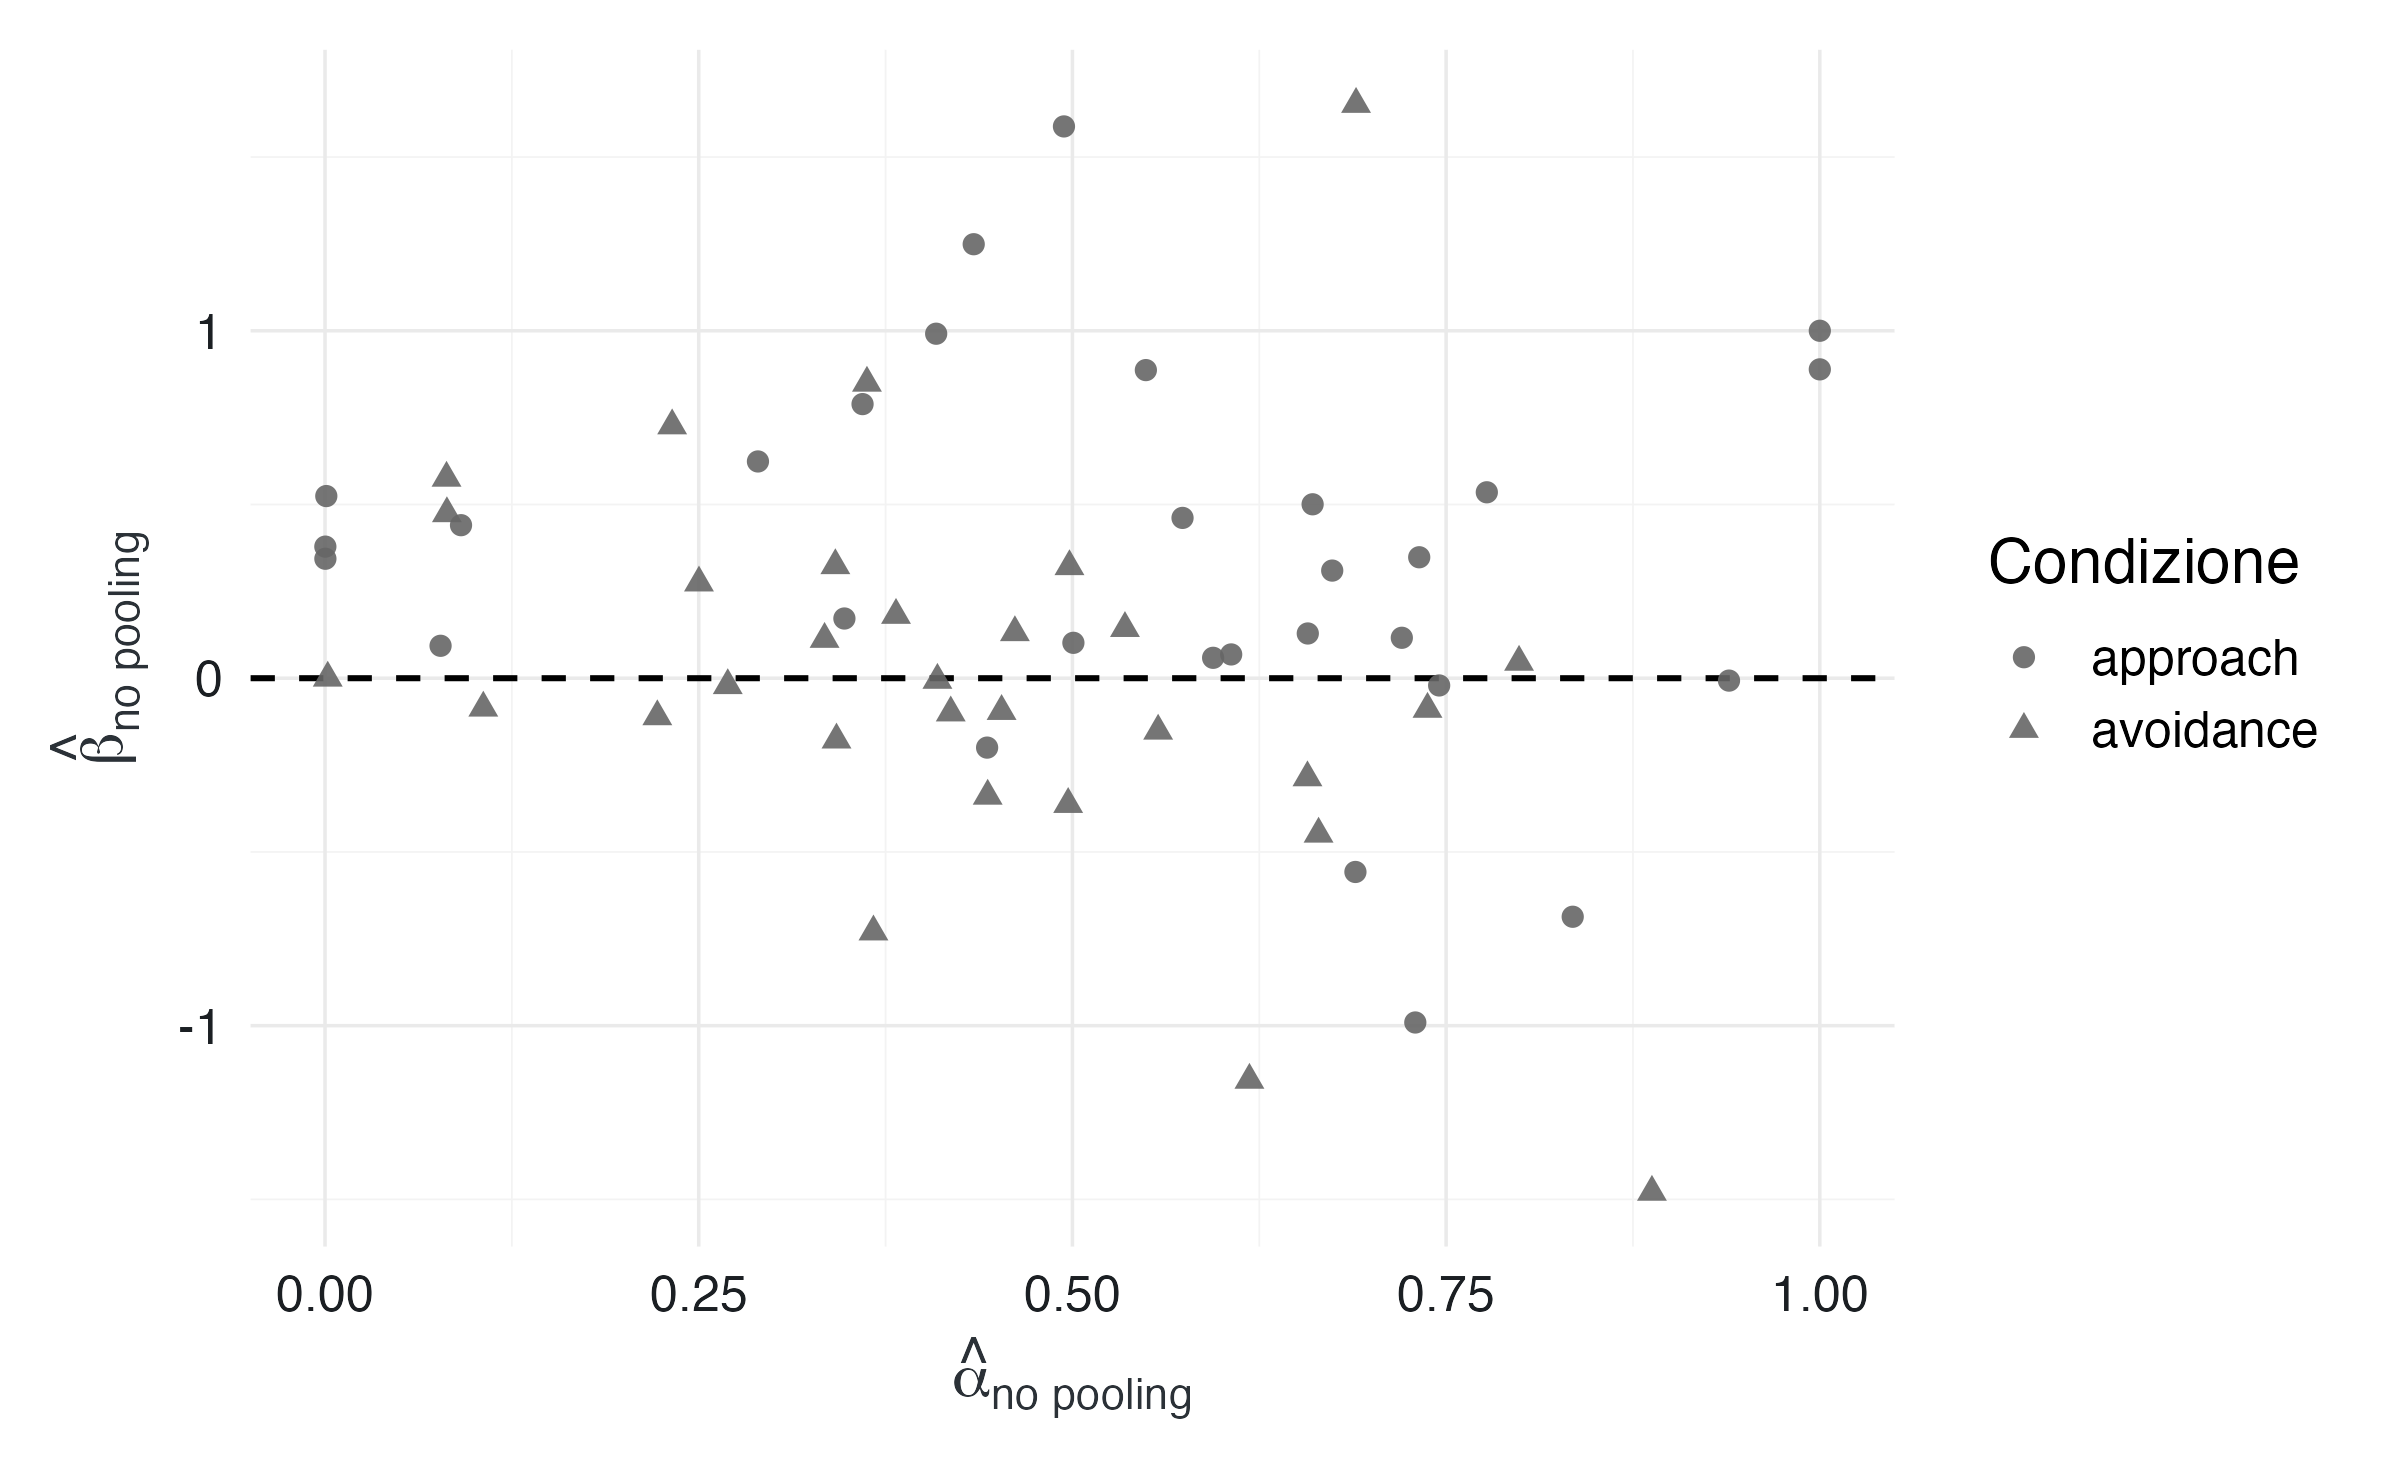
\includegraphics[width=0.85\linewidth,height=\textheight,keepaspectratio]{chapters/formal_models/03_eterogeneita_modelli_dinamici_files/figure-pdf/fig-no-pooling-goal-estimates-1.png}

}

\caption{\label{fig-no-pooling-goal-estimates}Stime separate dei
parametri per ciascun partecipante. La dispersione combina differenze
reali e instabilità dovuta ai soli nove aggiornamenti informativi
disponibili per persona.}

\end{figure}%

La variabilità dei punti non è una stima pura dell'eterogeneità
psicologica. Ogni punto è influenzato anche dal rumore, dalla sequenza
di prestazioni e dalla dipendenza tra \(\alpha_s\) e \(\beta_s\).

\section{Il modello gerarchico}\label{il-modello-gerarchico}

Usiamo una parametrizzazione non centrata:

\[
z_{\alpha,s},z_{\beta,s}\sim\operatorname{Normal}(0,1),
\]

\[
\operatorname{logit}(\alpha_s)
=
\mu_\alpha+\tau_\alpha z_{\alpha,s},
\]

\[
\beta_s
=
\mu_\beta+\tau_\beta z_{\beta,s}.
\]

Questa formulazione separa la posizione della popolazione, la sua
dispersione e la deviazione standardizzata di ciascun individuo.

\begin{tcolorbox}[enhanced jigsaw, arc=.35mm, bottomrule=.15mm, bottomtitle=1mm, breakable, colback=white, colbacktitle=quarto-callout-note-color!10!white, colframe=quarto-callout-note-color-frame, coltitle=black, left=2mm, leftrule=.75mm, opacityback=0, opacitybacktitle=0.6, rightrule=.15mm, title=\textcolor{quarto-callout-note-color}{\faInfo}\hspace{0.5em}{Che cosa descrivono gli iperparametri}, titlerule=0mm, toprule=.15mm, toptitle=1mm]

\begin{itemize}
\tightlist
\item
  \(\operatorname{logit}^{-1}(\mu_\alpha)\) è il valore mediano, o
  \emph{tipico}, della distribuzione individuale di \(\alpha\).
\item
  \(\tau_\alpha\) descrive la dispersione sulla scala logit, non la
  deviazione standard di \(\alpha\) sulla scala \(0\)--\(1\).
\item
  \(\mu_\beta\) è la deriva media della popolazione.
\item
  \(\tau_\beta\) quantifica l'eterogeneità delle derive individuali.
\end{itemize}

\end{tcolorbox}

\section{Prior gerarchici e controllo
predittivo}\label{prior-gerarchici-e-controllo-predittivo}

Adottiamo:

\[
\mu_\alpha\sim\operatorname{Normal}(0,1),
\qquad
\tau_\alpha\sim\operatorname{HalfNormal}(0,0.75),
\]

\[
\mu_\beta\sim\operatorname{Normal}(0,0.25),
\qquad
\tau_\beta\sim\operatorname{HalfNormal}(0,0.25),
\]

\[
\sigma\sim\operatorname{HalfNormal}(0,0.75).
\]

Il controllo a priori deve esaminare sia la distribuzione dei parametri
individuali sia le traiettorie da essi generate.

\begin{Shaded}
\begin{Highlighting}[]
\NormalTok{simulate\_goal\_path }\OtherTok{\textless{}{-}} \ControlFlowTok{function}\NormalTok{(}
\NormalTok{    performance,}
\NormalTok{    initial\_goal,}
\NormalTok{    alpha,}
\NormalTok{    beta,}
    \AttributeTok{sigma =} \DecValTok{0}
\NormalTok{) \{}
\NormalTok{  n\_trials }\OtherTok{\textless{}{-}} \FunctionTok{length}\NormalTok{(performance)}
\NormalTok{  state }\OtherTok{\textless{}{-}} \FunctionTok{numeric}\NormalTok{(n\_trials)}
\NormalTok{  observed }\OtherTok{\textless{}{-}} \FunctionTok{numeric}\NormalTok{(n\_trials)}

\NormalTok{  state[}\DecValTok{1}\NormalTok{] }\OtherTok{\textless{}{-}}\NormalTok{ initial\_goal}
\NormalTok{  observed[}\DecValTok{1}\NormalTok{] }\OtherTok{\textless{}{-}}\NormalTok{ initial\_goal}

  \ControlFlowTok{if}\NormalTok{ (n\_trials }\SpecialCharTok{\textgreater{}} \DecValTok{1}\NormalTok{) \{}
    \ControlFlowTok{for}\NormalTok{ (t }\ControlFlowTok{in} \DecValTok{2}\SpecialCharTok{:}\NormalTok{n\_trials) \{}
\NormalTok{      state[t] }\OtherTok{\textless{}{-}}\NormalTok{ state[t }\SpecialCharTok{{-}} \DecValTok{1}\NormalTok{] }\SpecialCharTok{+}
\NormalTok{        alpha }\SpecialCharTok{*}\NormalTok{ (performance[t }\SpecialCharTok{{-}} \DecValTok{1}\NormalTok{] }\SpecialCharTok{{-}}\NormalTok{ state[t }\SpecialCharTok{{-}} \DecValTok{1}\NormalTok{]) }\SpecialCharTok{+}
\NormalTok{        beta}
\NormalTok{      observed[t] }\OtherTok{\textless{}{-}} \FunctionTok{rnorm}\NormalTok{(}\DecValTok{1}\NormalTok{, state[t], sigma)}
\NormalTok{    \}}
\NormalTok{  \}}

  \FunctionTok{tibble}\NormalTok{(}
    \AttributeTok{trial =} \FunctionTok{seq\_len}\NormalTok{(n\_trials),}
    \AttributeTok{state =}\NormalTok{ state,}
    \AttributeTok{observed =}\NormalTok{ observed}
\NormalTok{  )}
\NormalTok{\}}

\NormalTok{n\_prior\_populations }\OtherTok{\textless{}{-}} \DecValTok{80}

\NormalTok{prior\_population\_draws }\OtherTok{\textless{}{-}} \FunctionTok{tibble}\NormalTok{(}
  \AttributeTok{draw =} \FunctionTok{seq\_len}\NormalTok{(n\_prior\_populations),}
  \AttributeTok{mu\_alpha\_logit =} \FunctionTok{rnorm}\NormalTok{(n\_prior\_populations, }\DecValTok{0}\NormalTok{, }\DecValTok{1}\NormalTok{),}
  \AttributeTok{tau\_alpha\_logit =} \FunctionTok{abs}\NormalTok{(}\FunctionTok{rnorm}\NormalTok{(n\_prior\_populations, }\DecValTok{0}\NormalTok{, }\FloatTok{0.75}\NormalTok{)),}
  \AttributeTok{mu\_beta =} \FunctionTok{rnorm}\NormalTok{(n\_prior\_populations, }\DecValTok{0}\NormalTok{, }\FloatTok{0.25}\NormalTok{),}
  \AttributeTok{tau\_beta =} \FunctionTok{abs}\NormalTok{(}\FunctionTok{rnorm}\NormalTok{(n\_prior\_populations, }\DecValTok{0}\NormalTok{, }\FloatTok{0.25}\NormalTok{)),}
  \AttributeTok{sigma =} \FunctionTok{abs}\NormalTok{(}\FunctionTok{rnorm}\NormalTok{(n\_prior\_populations, }\DecValTok{0}\NormalTok{, }\FloatTok{0.75}\NormalTok{)),}
  \AttributeTok{z\_alpha =} \FunctionTok{rnorm}\NormalTok{(n\_prior\_populations),}
  \AttributeTok{z\_beta =} \FunctionTok{rnorm}\NormalTok{(n\_prior\_populations)}
\NormalTok{) }\SpecialCharTok{|\textgreater{}}
  \FunctionTok{mutate}\NormalTok{(}
    \AttributeTok{alpha =} \FunctionTok{plogis}\NormalTok{(mu\_alpha\_logit }\SpecialCharTok{+}\NormalTok{ tau\_alpha\_logit }\SpecialCharTok{*}\NormalTok{ z\_alpha),}
    \AttributeTok{beta =}\NormalTok{ mu\_beta }\SpecialCharTok{+}\NormalTok{ tau\_beta }\SpecialCharTok{*}\NormalTok{ z\_beta}
\NormalTok{  )}

\NormalTok{reference\_subject }\OtherTok{\textless{}{-}}\NormalTok{ goal\_data }\SpecialCharTok{|\textgreater{}}
  \FunctionTok{filter}\NormalTok{(subject }\SpecialCharTok{==} \DecValTok{1}\NormalTok{)}

\NormalTok{prior\_hierarchical\_paths }\OtherTok{\textless{}{-}}\NormalTok{ prior\_population\_draws }\SpecialCharTok{|\textgreater{}}
  \FunctionTok{mutate}\NormalTok{(}
    \AttributeTok{simulation =}\NormalTok{ purrr}\SpecialCharTok{::}\FunctionTok{pmap}\NormalTok{(}
      \FunctionTok{list}\NormalTok{(alpha, beta, sigma),}
      \SpecialCharTok{\textasciitilde{}} \FunctionTok{simulate\_goal\_path}\NormalTok{(}
        \AttributeTok{performance =}\NormalTok{ reference\_subject}\SpecialCharTok{$}\NormalTok{performance,}
        \AttributeTok{initial\_goal =}\NormalTok{ reference\_subject}\SpecialCharTok{$}\NormalTok{goal[}\DecValTok{1}\NormalTok{],}
        \AttributeTok{alpha =}\NormalTok{ ..}\DecValTok{1}\NormalTok{,}
        \AttributeTok{beta =}\NormalTok{ ..}\DecValTok{2}\NormalTok{,}
        \AttributeTok{sigma =}\NormalTok{ ..}\DecValTok{3}
\NormalTok{      )}
\NormalTok{    )}
\NormalTok{  ) }\SpecialCharTok{|\textgreater{}}
  \FunctionTok{select}\NormalTok{(draw, alpha, beta, simulation) }\SpecialCharTok{|\textgreater{}}
\NormalTok{  tidyr}\SpecialCharTok{::}\FunctionTok{unnest}\NormalTok{(simulation)}
\end{Highlighting}
\end{Shaded}

\begin{figure}

\centering{

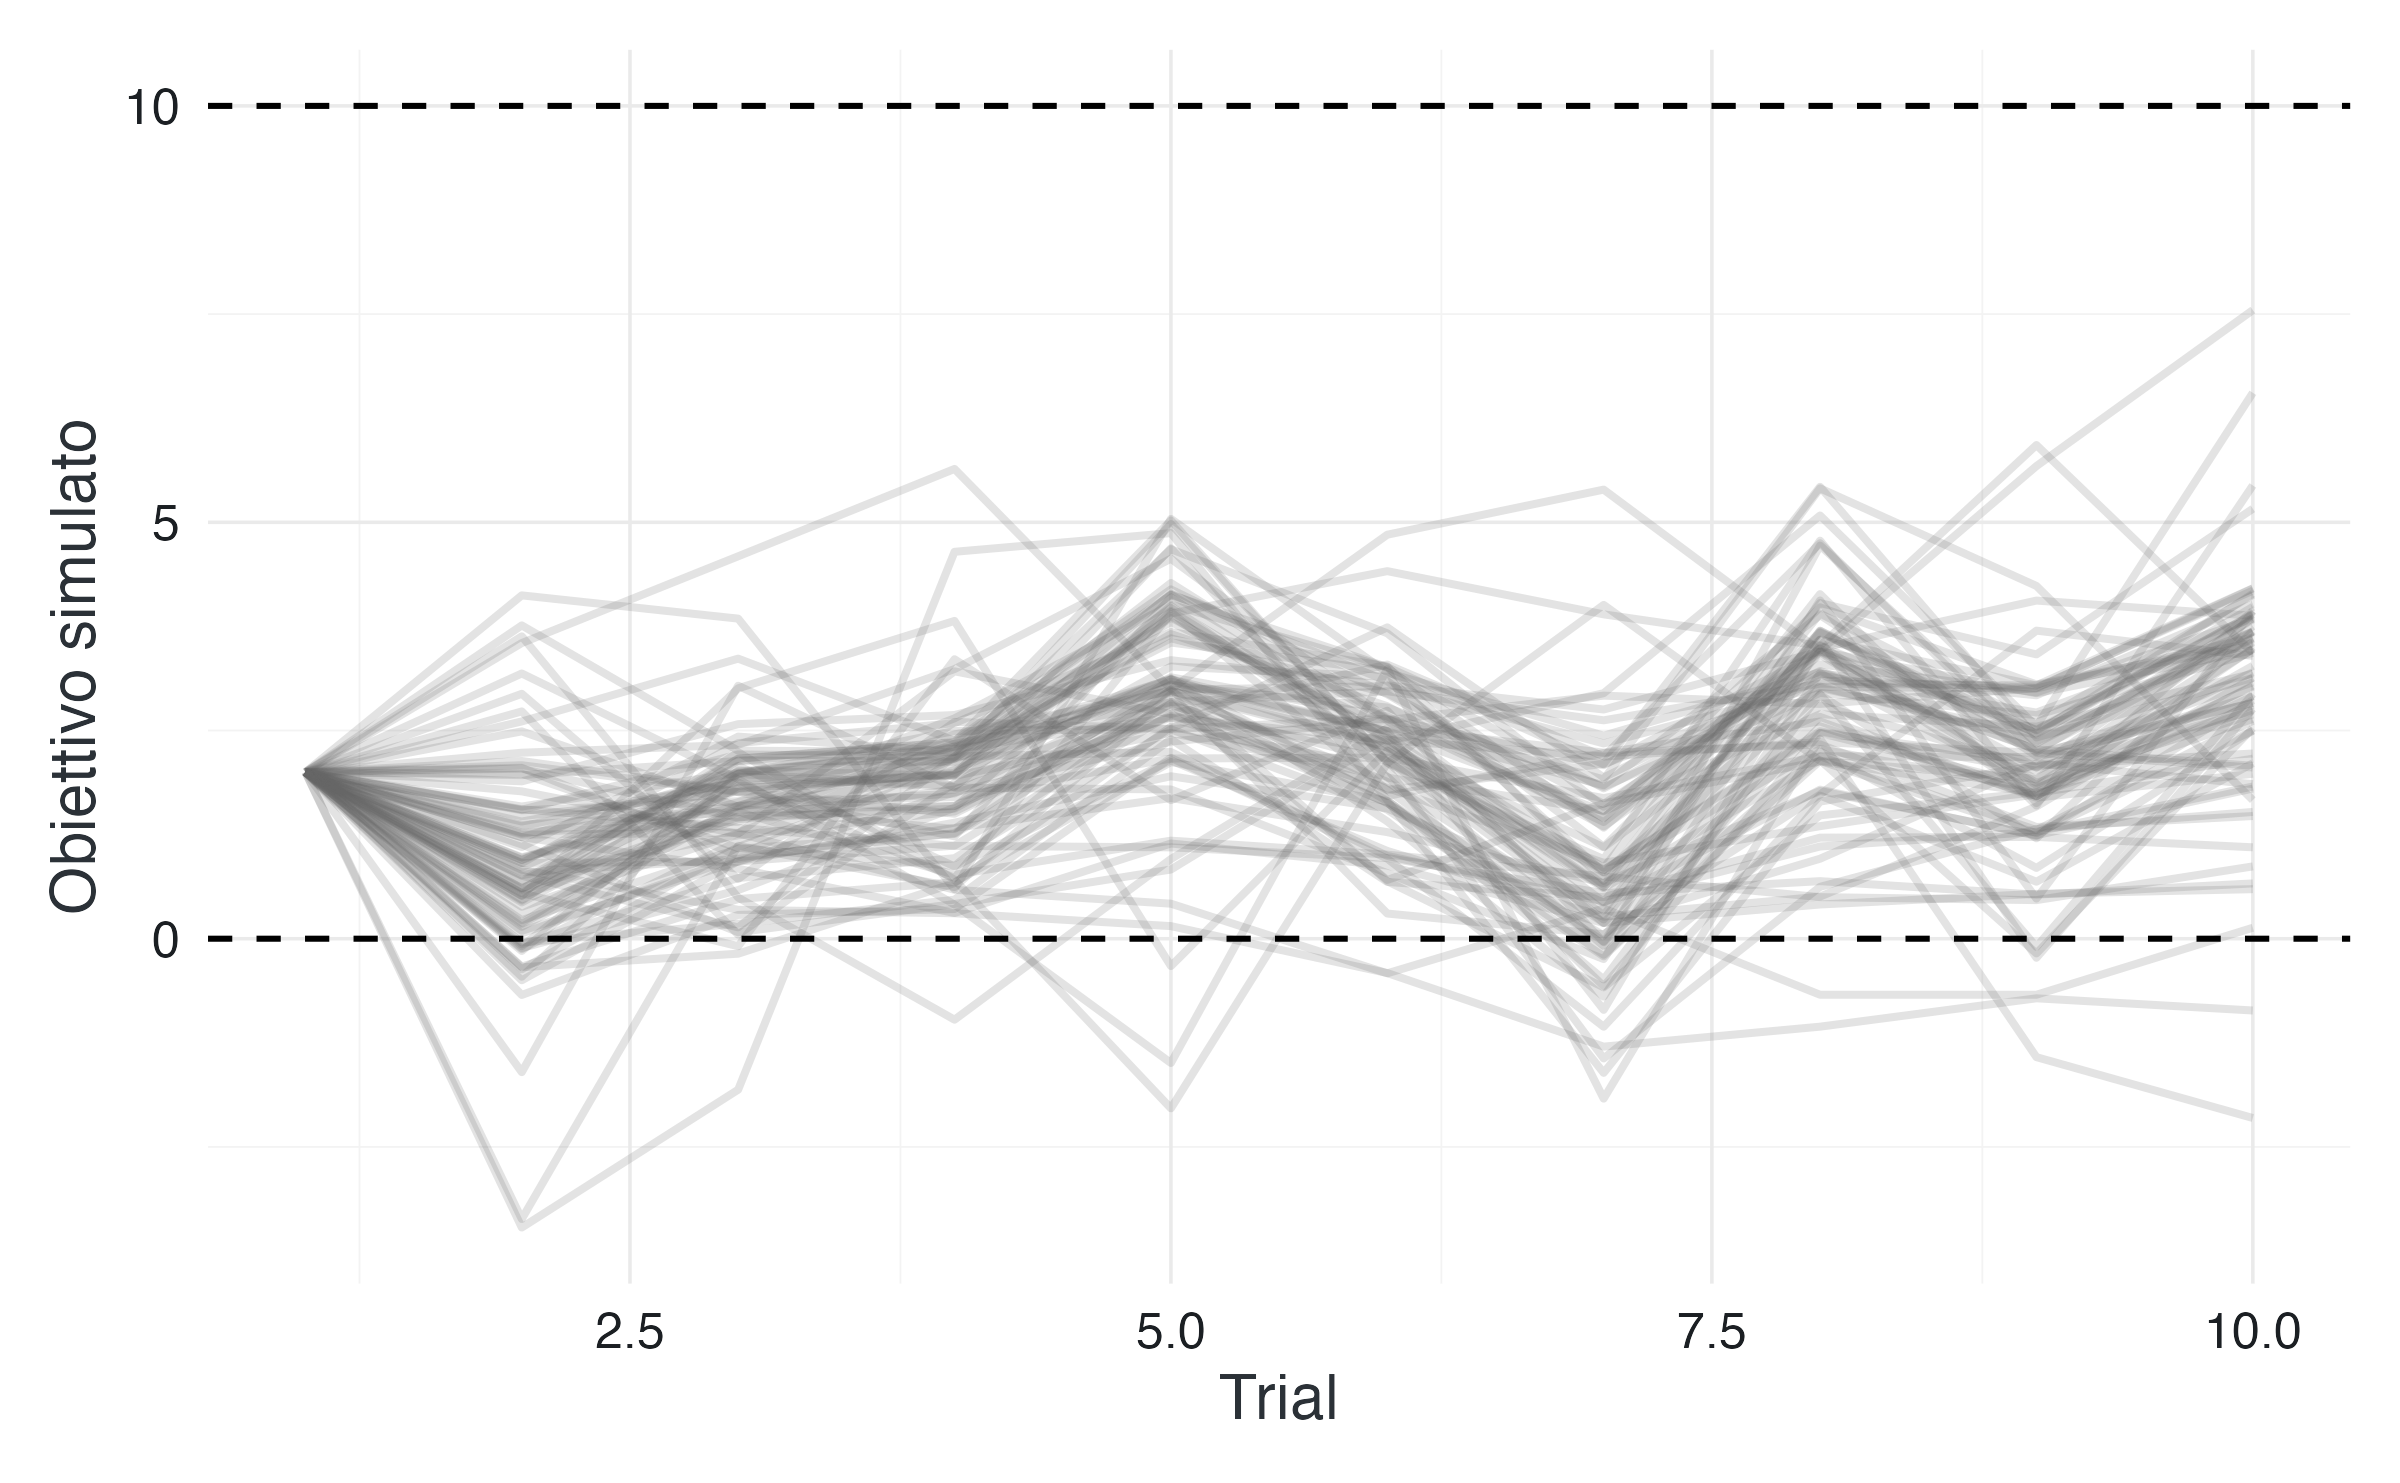
\includegraphics[width=0.85\linewidth,height=\textheight,keepaspectratio]{chapters/formal_models/03_eterogeneita_modelli_dinamici_files/figure-pdf/fig-prior-predictive-goal-hierarchical-1.png}

}

\caption{\label{fig-prior-predictive-goal-hierarchical}Traiettorie di
individui generati da popolazioni simulate dai prior gerarchici. Il
controllo valuta contemporaneamente valori individuali e conseguenze
dinamiche.}

\end{figure}%

\section{Implementazione gerarchica in
Stan}\label{implementazione-gerarchica-in-stan}

\begin{Shaded}
\begin{Highlighting}[]
\NormalTok{stan\_code\_goal\_hierarchical }\OtherTok{\textless{}{-}} \StringTok{"}
\StringTok{data \{}
\StringTok{  int\textless{}lower=1\textgreater{} Ntotal;}
\StringTok{  int\textless{}lower=1\textgreater{} Nsubj;}
\StringTok{  array[Ntotal] int\textless{}lower=1, upper=Nsubj\textgreater{} subject;}
\StringTok{  array[Ntotal] int\textless{}lower=1\textgreater{} trial;}
\StringTok{  vector[Ntotal] goal;}
\StringTok{  vector[Ntotal] performance;}
\StringTok{\}}

\StringTok{parameters \{}
\StringTok{  real mu\_alpha\_logit;}
\StringTok{  real\textless{}lower=0\textgreater{} tau\_alpha\_logit;}
\StringTok{  vector[Nsubj] z\_alpha;}

\StringTok{  real mu\_beta;}
\StringTok{  real\textless{}lower=0\textgreater{} tau\_beta;}
\StringTok{  vector[Nsubj] z\_beta;}

\StringTok{  real\textless{}lower=0\textgreater{} sigma;}
\StringTok{\}}

\StringTok{transformed parameters \{}
\StringTok{  vector[Nsubj] alpha\_logit =}
\StringTok{    mu\_alpha\_logit + tau\_alpha\_logit * z\_alpha;}
\StringTok{  vector\textless{}lower=0, upper=1\textgreater{}[Nsubj] alpha = inv\_logit(alpha\_logit);}
\StringTok{  vector[Nsubj] beta = mu\_beta + tau\_beta * z\_beta;}
\StringTok{  vector[Ntotal] mu;}

\StringTok{  for (i in 1:Ntotal) \{}
\StringTok{    if (trial[i] == 1) \{}
\StringTok{      mu[i] = goal[i];}
\StringTok{    \} else \{}
\StringTok{      int s = subject[i];}
\StringTok{      mu[i] = mu[i {-} 1]}
\StringTok{              + alpha[s] * (performance[i {-} 1] {-} mu[i {-} 1])}
\StringTok{              + beta[s];}
\StringTok{    \}}
\StringTok{  \}}
\StringTok{\}}

\StringTok{model \{}
\StringTok{  mu\_alpha\_logit \textasciitilde{} normal(0, 1);}
\StringTok{  tau\_alpha\_logit \textasciitilde{} normal(0, 0.75);}
\StringTok{  z\_alpha \textasciitilde{} std\_normal();}

\StringTok{  mu\_beta \textasciitilde{} normal(0, 0.25);}
\StringTok{  tau\_beta \textasciitilde{} normal(0, 0.25);}
\StringTok{  z\_beta \textasciitilde{} std\_normal();}

\StringTok{  sigma \textasciitilde{} normal(0, 0.75);}

\StringTok{  for (i in 1:Ntotal) \{}
\StringTok{    if (trial[i] \textgreater{} 1) \{}
\StringTok{      goal[i] \textasciitilde{} normal(mu[i], sigma);}
\StringTok{    \}}
\StringTok{  \}}
\StringTok{\}}

\StringTok{generated quantities \{}
\StringTok{  real\textless{}lower=0, upper=1\textgreater{} alpha\_typical = inv\_logit(mu\_alpha\_logit);}
\StringTok{  vector[Ntotal] y\_rep;}

\StringTok{  for (i in 1:Ntotal) \{}
\StringTok{    if (trial[i] == 1) \{}
\StringTok{      y\_rep[i] = goal[i];}
\StringTok{    \} else \{}
\StringTok{      y\_rep[i] = normal\_rng(mu[i], sigma);}
\StringTok{    \}}
\StringTok{  \}}
\StringTok{\}}
\StringTok{"}
\end{Highlighting}
\end{Shaded}

\begin{Shaded}
\begin{Highlighting}[]
\NormalTok{make\_goal\_stan\_data }\OtherTok{\textless{}{-}} \ControlFlowTok{function}\NormalTok{(data) \{}
\NormalTok{  data }\OtherTok{\textless{}{-}}\NormalTok{ data }\SpecialCharTok{|\textgreater{}}
    \FunctionTok{arrange}\NormalTok{(subject, trial)}

  \FunctionTok{list}\NormalTok{(}
    \AttributeTok{Ntotal =} \FunctionTok{nrow}\NormalTok{(data),}
    \AttributeTok{Nsubj =} \FunctionTok{n\_distinct}\NormalTok{(data}\SpecialCharTok{$}\NormalTok{subject),}
    \AttributeTok{subject =}\NormalTok{ data}\SpecialCharTok{$}\NormalTok{subject,}
    \AttributeTok{trial =}\NormalTok{ data}\SpecialCharTok{$}\NormalTok{trial,}
    \AttributeTok{goal =}\NormalTok{ data}\SpecialCharTok{$}\NormalTok{goal,}
    \AttributeTok{performance =}\NormalTok{ data}\SpecialCharTok{$}\NormalTok{performance}
\NormalTok{  )}
\NormalTok{\}}

\NormalTok{stan\_data\_goal\_hierarchical }\OtherTok{\textless{}{-}} \FunctionTok{make\_goal\_stan\_data}\NormalTok{(goal\_data)}
\end{Highlighting}
\end{Shaded}

\begin{Shaded}
\begin{Highlighting}[]
\NormalTok{model\_goal\_hierarchical }\OtherTok{\textless{}{-}} \FunctionTok{cmdstan\_model}\NormalTok{(}
  \FunctionTok{write\_stan\_file}\NormalTok{(stan\_code\_goal\_hierarchical)}
\NormalTok{)}

\NormalTok{fit\_goal\_hierarchical }\OtherTok{\textless{}{-}}\NormalTok{ model\_goal\_hierarchical}\SpecialCharTok{$}\FunctionTok{sample}\NormalTok{(}
  \AttributeTok{data =}\NormalTok{ stan\_data\_goal\_hierarchical,}
  \AttributeTok{seed =} \DecValTok{8061}\NormalTok{,}
  \AttributeTok{chains =} \DecValTok{4}\NormalTok{,}
  \AttributeTok{parallel\_chains =} \DecValTok{4}\NormalTok{,}
  \AttributeTok{iter\_warmup =} \DecValTok{1500}\NormalTok{,}
  \AttributeTok{iter\_sampling =} \DecValTok{2000}\NormalTok{,}
  \AttributeTok{adapt\_delta =} \FloatTok{0.95}\NormalTok{,}
  \AttributeTok{refresh =} \DecValTok{500}
\NormalTok{)}
\end{Highlighting}
\end{Shaded}

\section{Diagnostica computazionale}\label{diagnostica-computazionale-2}

\begin{Shaded}
\begin{Highlighting}[]
\NormalTok{fit\_goal\_hierarchical}\SpecialCharTok{$}\FunctionTok{summary}\NormalTok{(}
  \AttributeTok{variables =} \FunctionTok{c}\NormalTok{(}
    \StringTok{"alpha\_typical"}\NormalTok{,}
    \StringTok{"mu\_beta"}\NormalTok{,}
    \StringTok{"tau\_alpha\_logit"}\NormalTok{,}
    \StringTok{"tau\_beta"}\NormalTok{,}
    \StringTok{"sigma"}
\NormalTok{  )}
\NormalTok{) }\SpecialCharTok{|\textgreater{}}
  \FunctionTok{select}\NormalTok{(variable, mean, median, sd, q5, q95, rhat, ess\_bulk, ess\_tail)}
\CommentTok{\#\textgreater{} \# A tibble: 5 x 9}
\CommentTok{\#\textgreater{}   variable         mean median     sd     q5   q95  rhat ess\_bulk ess\_tail}
\CommentTok{\#\textgreater{}   \textless{}chr\textgreater{}           \textless{}dbl\textgreater{}  \textless{}dbl\textgreater{}  \textless{}dbl\textgreater{}  \textless{}dbl\textgreater{} \textless{}dbl\textgreater{} \textless{}dbl\textgreater{}    \textless{}dbl\textgreater{}    \textless{}dbl\textgreater{}}
\CommentTok{\#\textgreater{} 1 alpha\_typical   0.485  0.485 0.0362 0.423  0.544 1.00     5384.    5536.}
\CommentTok{\#\textgreater{} 2 mu\_beta         0.168  0.169 0.0649 0.0592 0.273 1.00     2026.    3625.}
\CommentTok{\#\textgreater{} 3 tau\_alpha\_logit 0.655  0.651 0.170  0.389  0.940 1.00     2352.    2994.}
\CommentTok{\#\textgreater{} 4 tau\_beta        0.468  0.465 0.0542 0.384  0.563 1.00     2819.    4906.}
\CommentTok{\#\textgreater{} 5 sigma           0.960  0.958 0.0331 0.906  1.02  1.000    7533.    5658.}
\end{Highlighting}
\end{Shaded}

\begin{figure}

\centering{

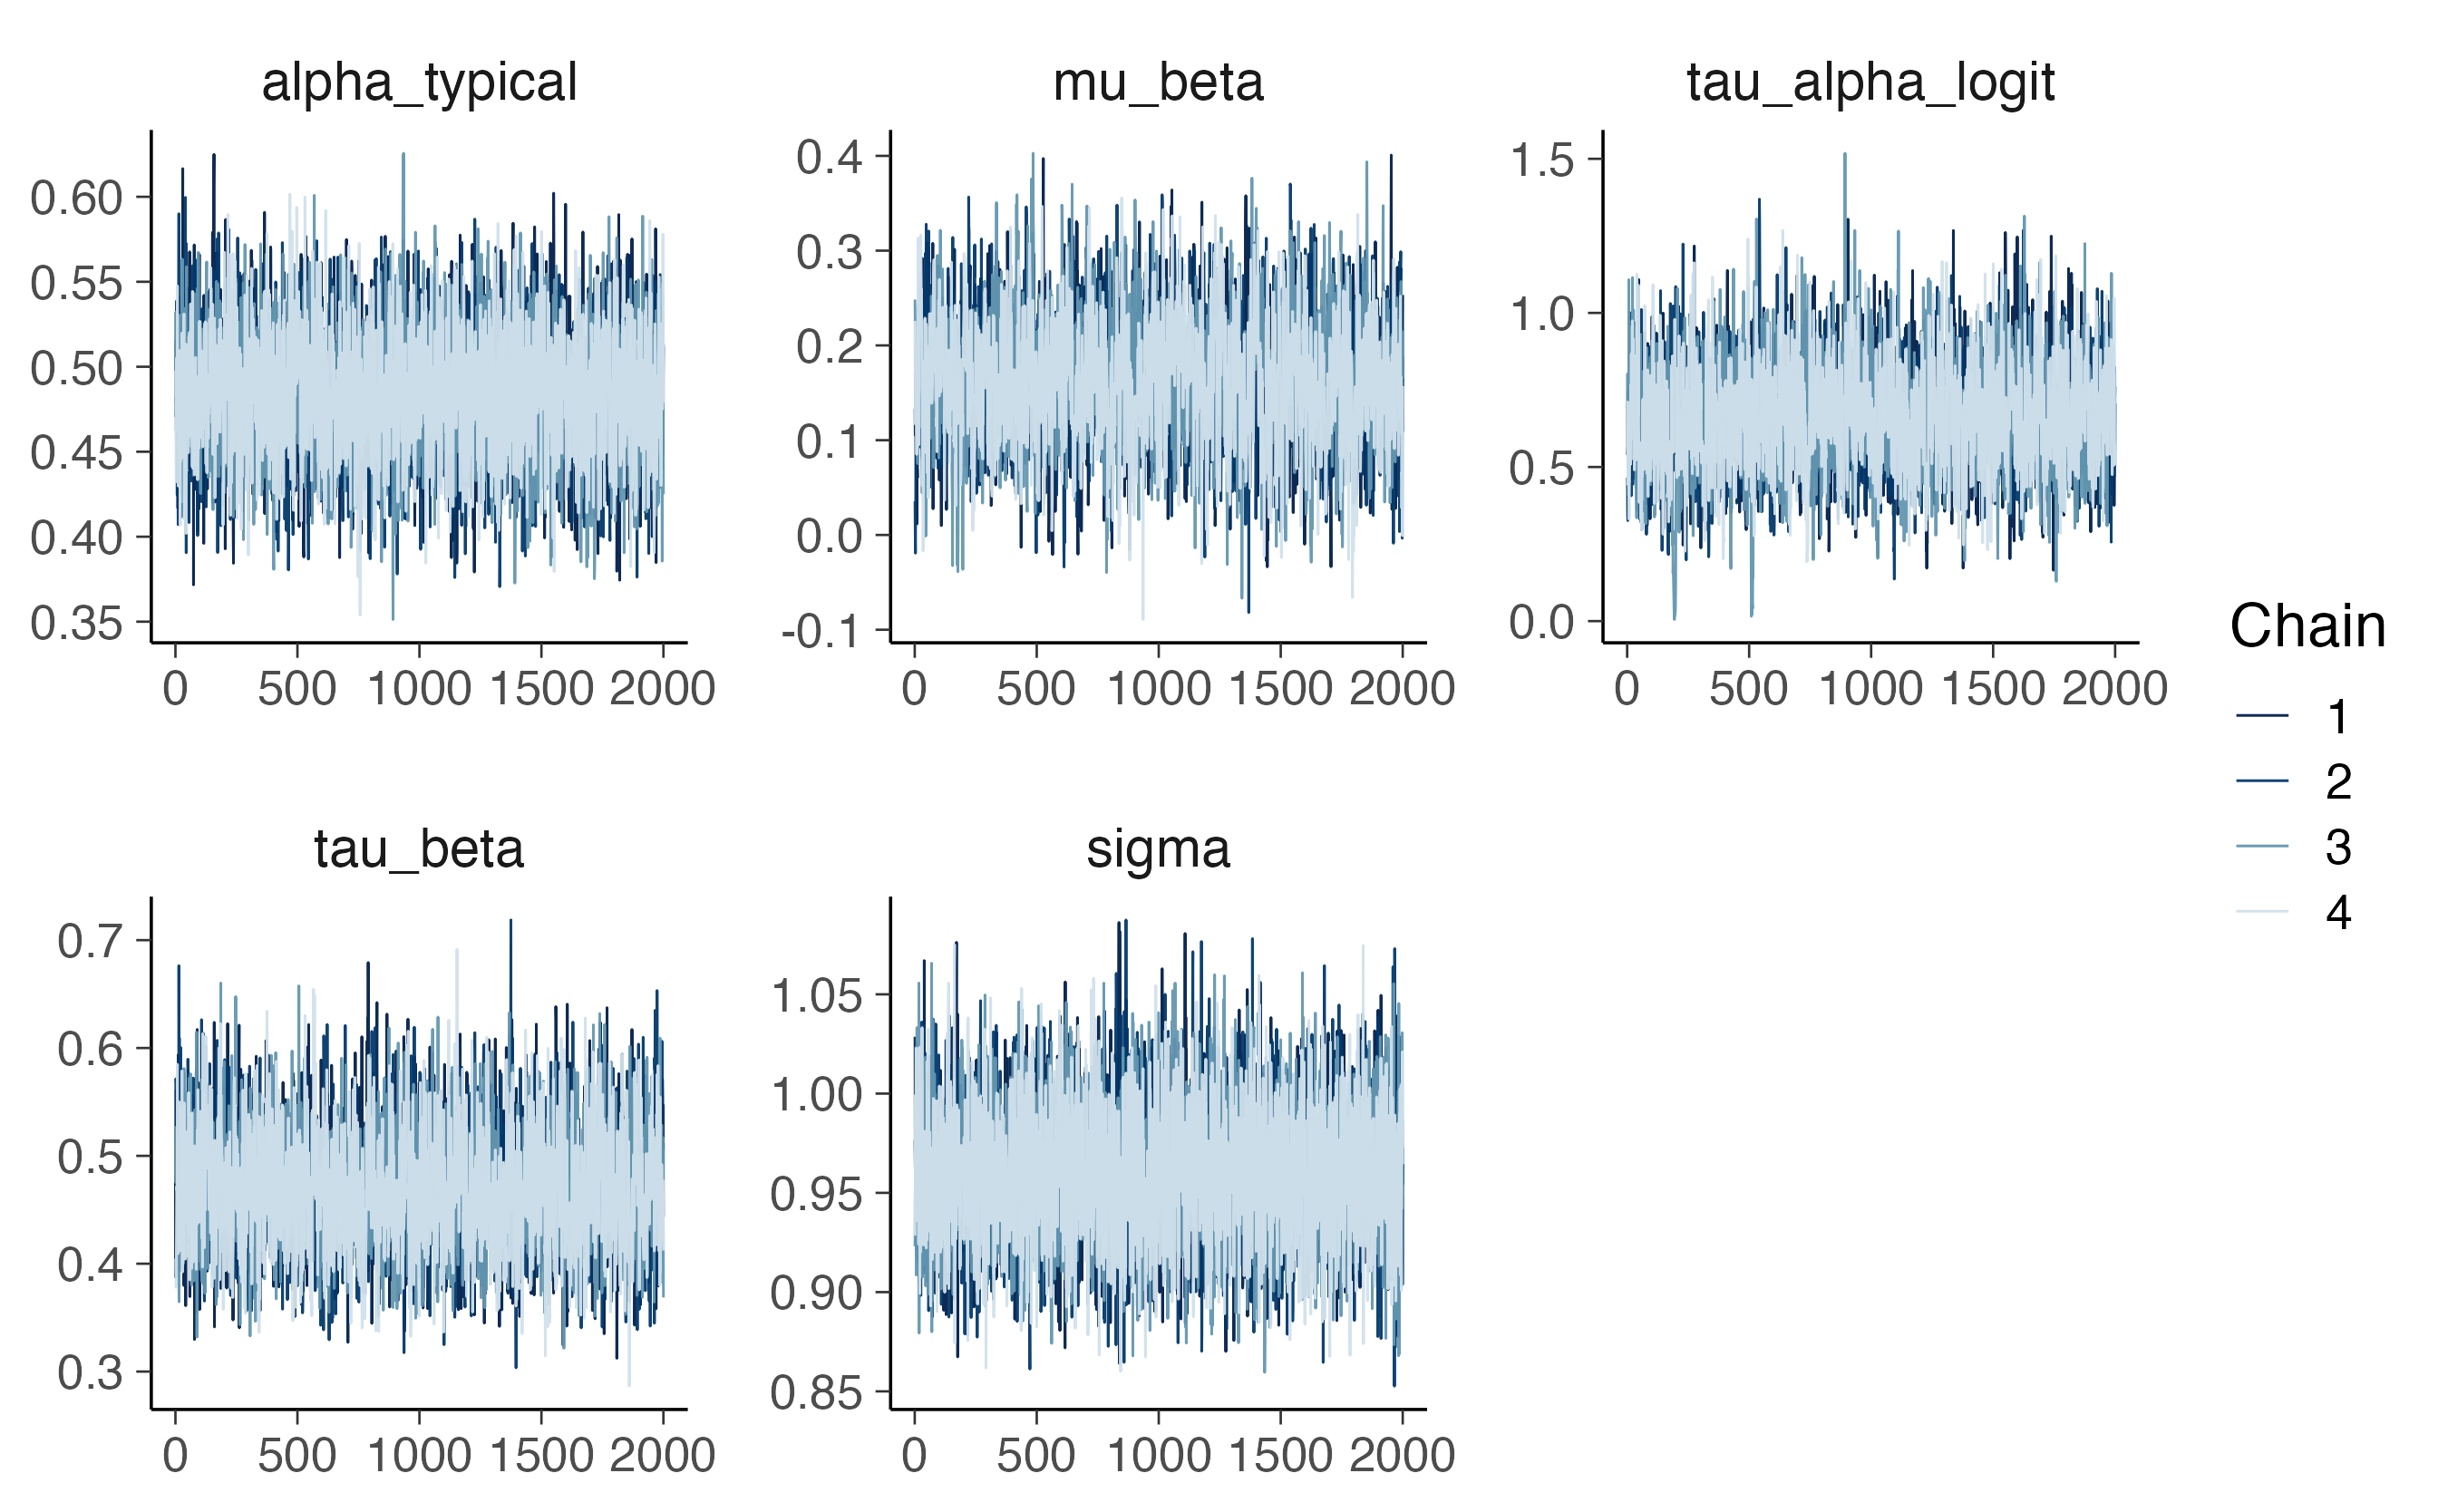
\includegraphics[width=0.85\linewidth,height=\textheight,keepaspectratio]{chapters/formal_models/03_eterogeneita_modelli_dinamici_files/figure-pdf/fig-trace-goal-hierarchical-1.png}

}

\caption{\label{fig-trace-goal-hierarchical}Trace plot dei principali
iperparametri del modello gerarchico.}

\end{figure}%

Oltre a \(\widehat R\) ed ESS, occorre controllare divergenze, energia e
geometria della posterior. La parametrizzazione non centrata riduce
spesso le difficoltà quando l'eterogeneità è piccola o poco informata,
ma non garantisce automaticamente un campionamento adeguato.

\section{Inferenza a livello di
popolazione}\label{inferenza-a-livello-di-popolazione}

\begin{Shaded}
\begin{Highlighting}[]
\NormalTok{fit\_goal\_hierarchical}\SpecialCharTok{$}\FunctionTok{draws}\NormalTok{(}
  \FunctionTok{c}\NormalTok{(}
    \StringTok{"alpha\_typical"}\NormalTok{,}
    \StringTok{"mu\_beta"}\NormalTok{,}
    \StringTok{"tau\_alpha\_logit"}\NormalTok{,}
    \StringTok{"tau\_beta"}\NormalTok{,}
    \StringTok{"sigma"}
\NormalTok{  )}
\NormalTok{) }\SpecialCharTok{|\textgreater{}}
\NormalTok{  posterior}\SpecialCharTok{::}\FunctionTok{summarise\_draws}\NormalTok{(}
\NormalTok{    mean,}
\NormalTok{    median,}
    \SpecialCharTok{\textasciitilde{}}\FunctionTok{quantile}\NormalTok{(.x, }\AttributeTok{probs =} \FunctionTok{c}\NormalTok{(}\FloatTok{0.025}\NormalTok{, }\FloatTok{0.975}\NormalTok{))}
\NormalTok{  )}
\CommentTok{\#\textgreater{} \# A tibble: 5 x 5}
\CommentTok{\#\textgreater{}   variable         mean median \textasciigrave{}2.5\%\textasciigrave{} \textasciigrave{}97.5\%\textasciigrave{}}
\CommentTok{\#\textgreater{}   \textless{}chr\textgreater{}           \textless{}dbl\textgreater{}  \textless{}dbl\textgreater{}  \textless{}dbl\textgreater{}   \textless{}dbl\textgreater{}}
\CommentTok{\#\textgreater{} 1 alpha\_typical   0.485  0.485 0.413    0.556}
\CommentTok{\#\textgreater{} 2 mu\_beta         0.168  0.169 0.0369   0.294}
\CommentTok{\#\textgreater{} 3 tau\_alpha\_logit 0.655  0.651 0.342    1.00 }
\CommentTok{\#\textgreater{} 4 tau\_beta        0.468  0.465 0.371    0.582}
\CommentTok{\#\textgreater{} 5 sigma           0.960  0.958 0.897    1.03}
\end{Highlighting}
\end{Shaded}

L'interpretazione deve distinguere posizione e dispersione:

\begin{itemize}
\tightlist
\item
  \texttt{alpha\_typical} descrive il centro della popolazione sulla
  scala interpretabile \(0\)--\(1\);
\item
  \texttt{mu\_beta} descrive la deriva media;
\item
  \texttt{tau\_alpha\_logit} e \texttt{tau\_beta} quantificano
  l'eterogeneità supportata dal modello;
\item
  \texttt{sigma} rappresenta la variabilità entro persona non spiegata
  dalla dinamica.
\end{itemize}

Una posterior di \texttt{tau\_beta} concentrata vicino a zero
suggerirebbe poca eterogeneità rilevabile nella deriva, non l'identità
perfetta di tutte le persone.

\section{Inferenza individuale}\label{inferenza-individuale}

\begin{Shaded}
\begin{Highlighting}[]
\NormalTok{individual\_alpha }\OtherTok{\textless{}{-}}\NormalTok{ fit\_goal\_hierarchical }\SpecialCharTok{|\textgreater{}}
  \FunctionTok{spread\_draws}\NormalTok{(alpha[subject]) }\SpecialCharTok{|\textgreater{}}
  \FunctionTok{median\_qi}\NormalTok{(alpha, }\AttributeTok{.width =} \FloatTok{0.90}\NormalTok{) }\SpecialCharTok{|\textgreater{}}
  \FunctionTok{rename}\NormalTok{(}
    \AttributeTok{alpha\_lower =}\NormalTok{ .lower,}
    \AttributeTok{alpha\_upper =}\NormalTok{ .upper}
\NormalTok{  )}

\NormalTok{individual\_beta }\OtherTok{\textless{}{-}}\NormalTok{ fit\_goal\_hierarchical }\SpecialCharTok{|\textgreater{}}
  \FunctionTok{spread\_draws}\NormalTok{(beta[subject]) }\SpecialCharTok{|\textgreater{}}
  \FunctionTok{median\_qi}\NormalTok{(beta, }\AttributeTok{.width =} \FloatTok{0.90}\NormalTok{) }\SpecialCharTok{|\textgreater{}}
  \FunctionTok{rename}\NormalTok{(}
    \AttributeTok{beta\_lower =}\NormalTok{ .lower,}
    \AttributeTok{beta\_upper =}\NormalTok{ .upper}
\NormalTok{  )}

\NormalTok{individual\_goal\_parameters }\OtherTok{\textless{}{-}}\NormalTok{ individual\_alpha }\SpecialCharTok{|\textgreater{}}
  \FunctionTok{select}\NormalTok{(subject, alpha, alpha\_lower, alpha\_upper) }\SpecialCharTok{|\textgreater{}}
  \FunctionTok{left\_join}\NormalTok{(}
\NormalTok{    individual\_beta }\SpecialCharTok{|\textgreater{}}
      \FunctionTok{select}\NormalTok{(subject, beta, beta\_lower, beta\_upper),}
    \AttributeTok{by =} \StringTok{"subject"}
\NormalTok{  ) }\SpecialCharTok{|\textgreater{}}
  \FunctionTok{left\_join}\NormalTok{(subject\_structure, }\AttributeTok{by =} \StringTok{"subject"}\NormalTok{)}
\end{Highlighting}
\end{Shaded}

\begin{figure}

\centering{

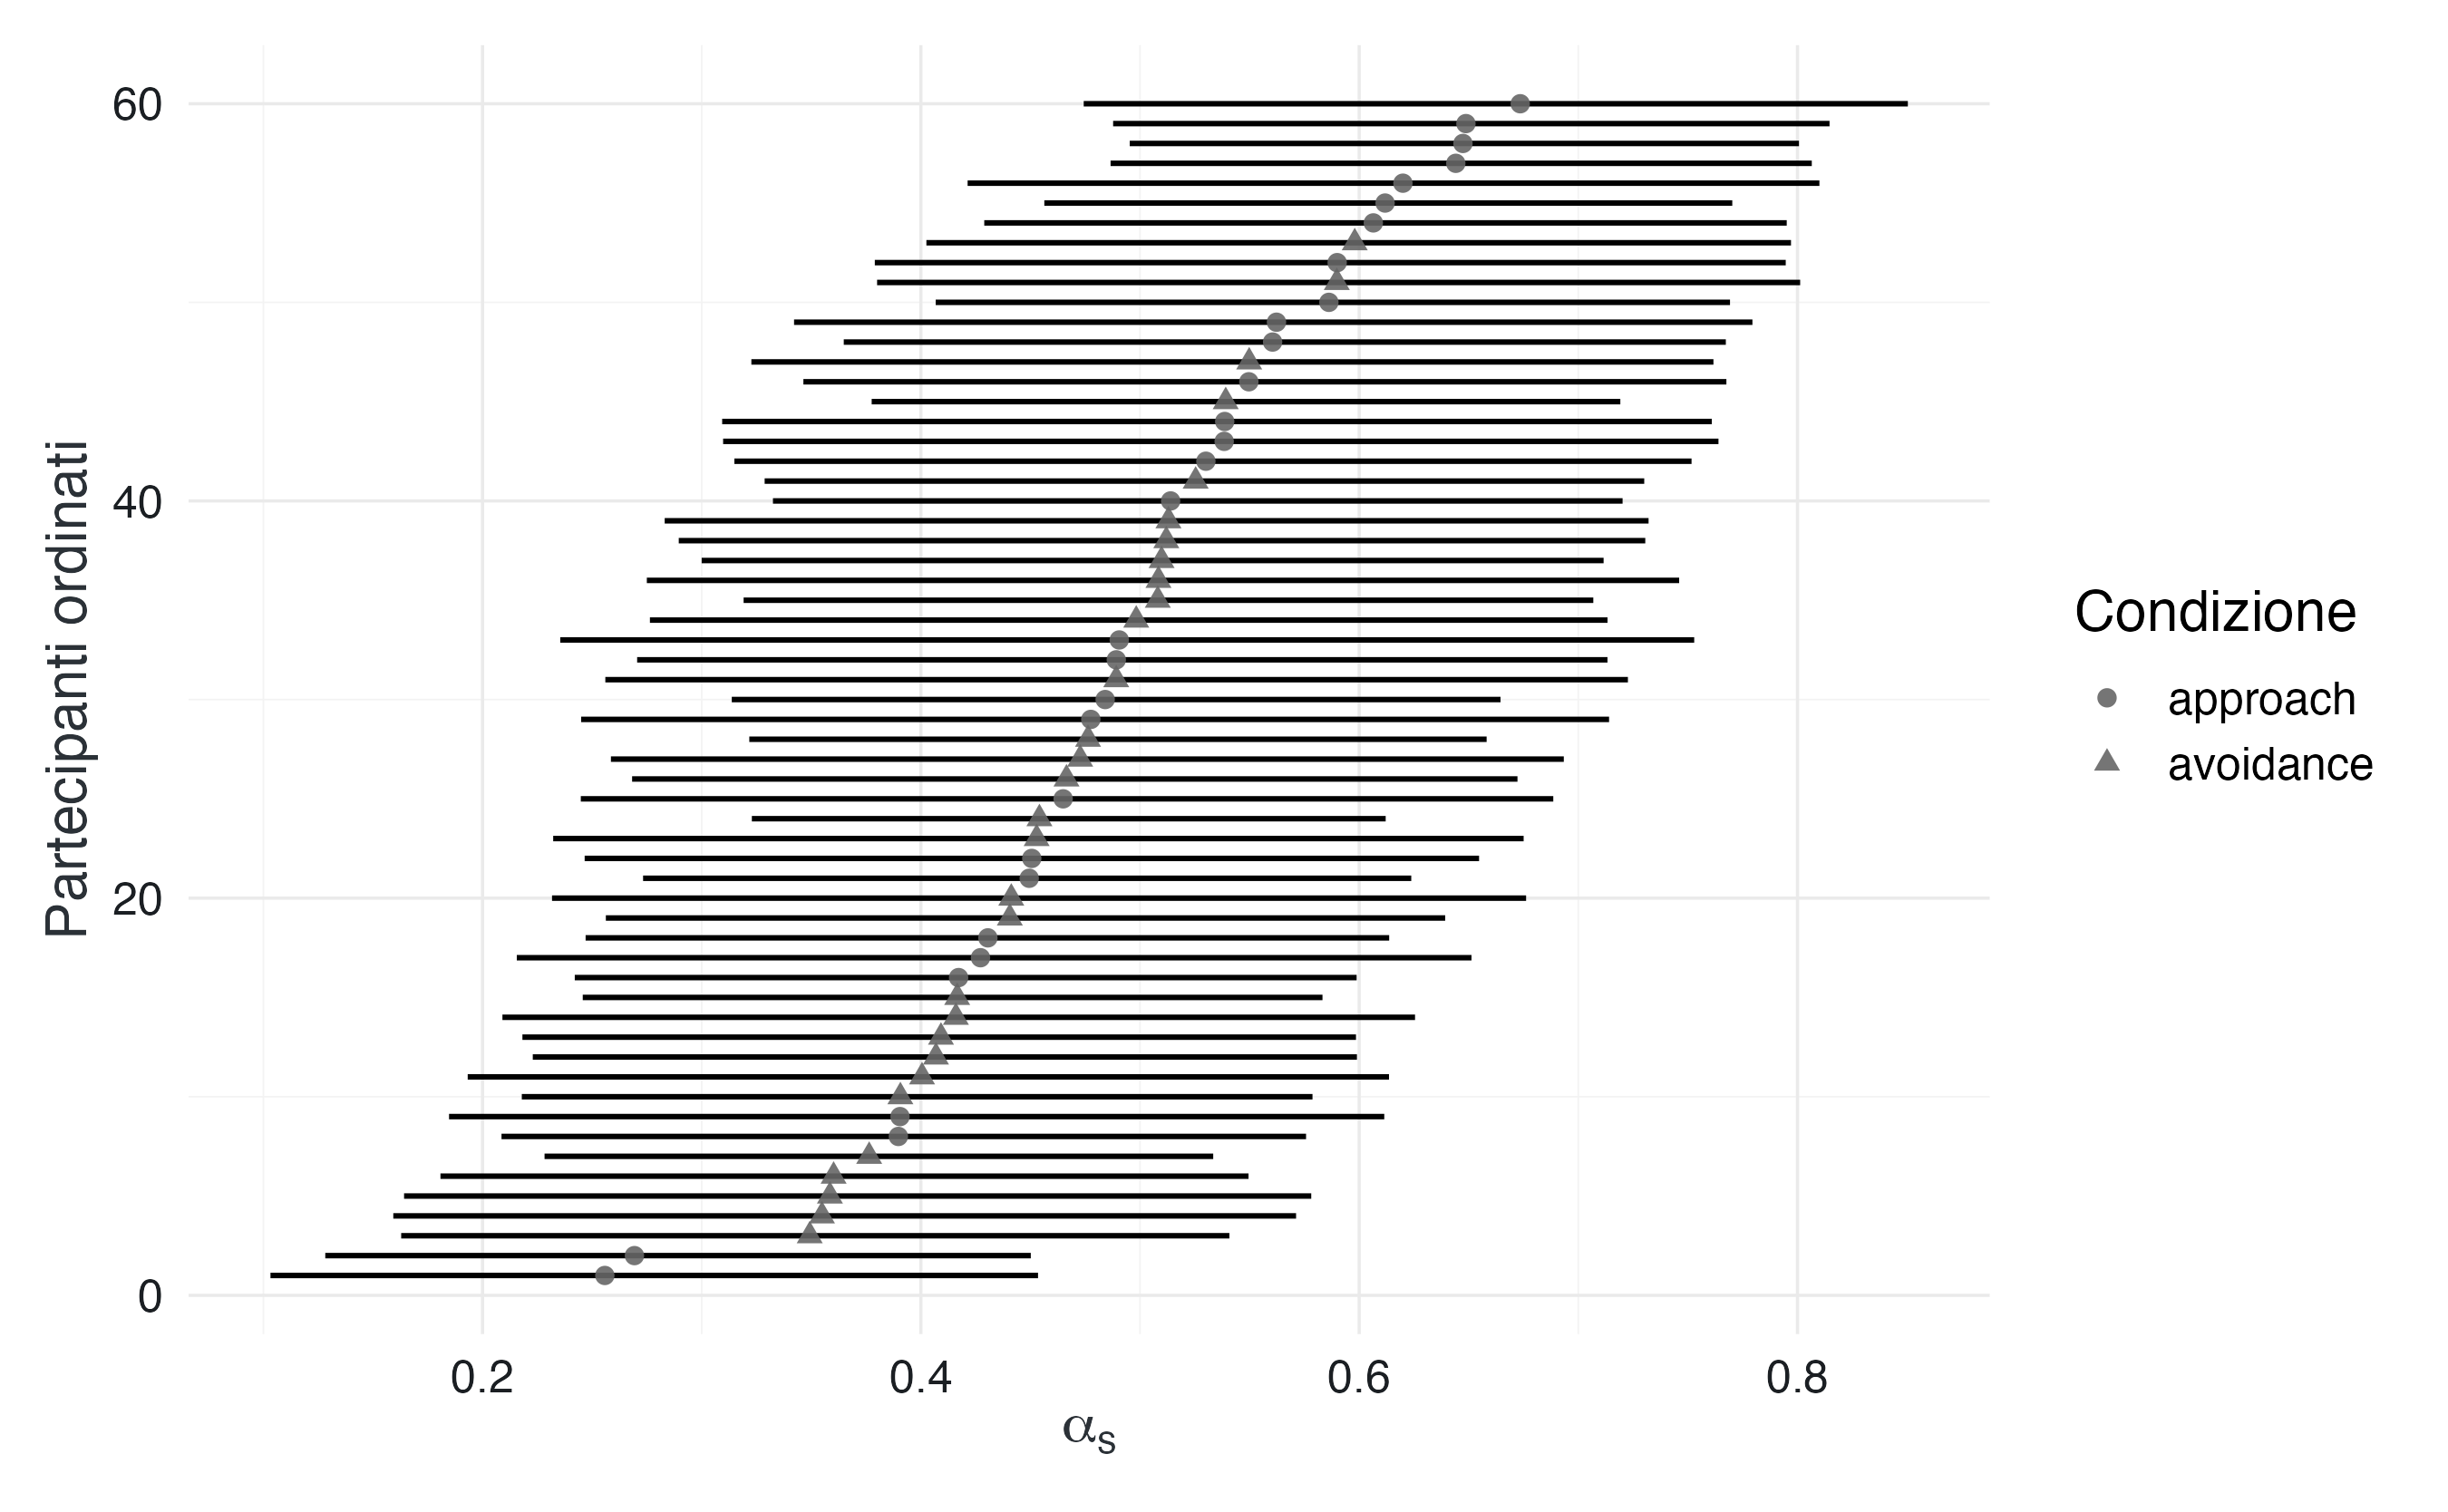
\includegraphics[width=0.85\linewidth,height=\textheight,keepaspectratio]{chapters/formal_models/03_eterogeneita_modelli_dinamici_files/figure-pdf/fig-individual-alpha-goal-hierarchical-1.png}

}

\caption{\label{fig-individual-alpha-goal-hierarchical}Posterior
individuali di alpha nel modello gerarchico. Gli intervalli descrivono
incertezza sulla persona; la dispersione dei centri descrive solo
parzialmente l'eterogeneità di popolazione.}

\end{figure}%

\begin{figure}

\centering{

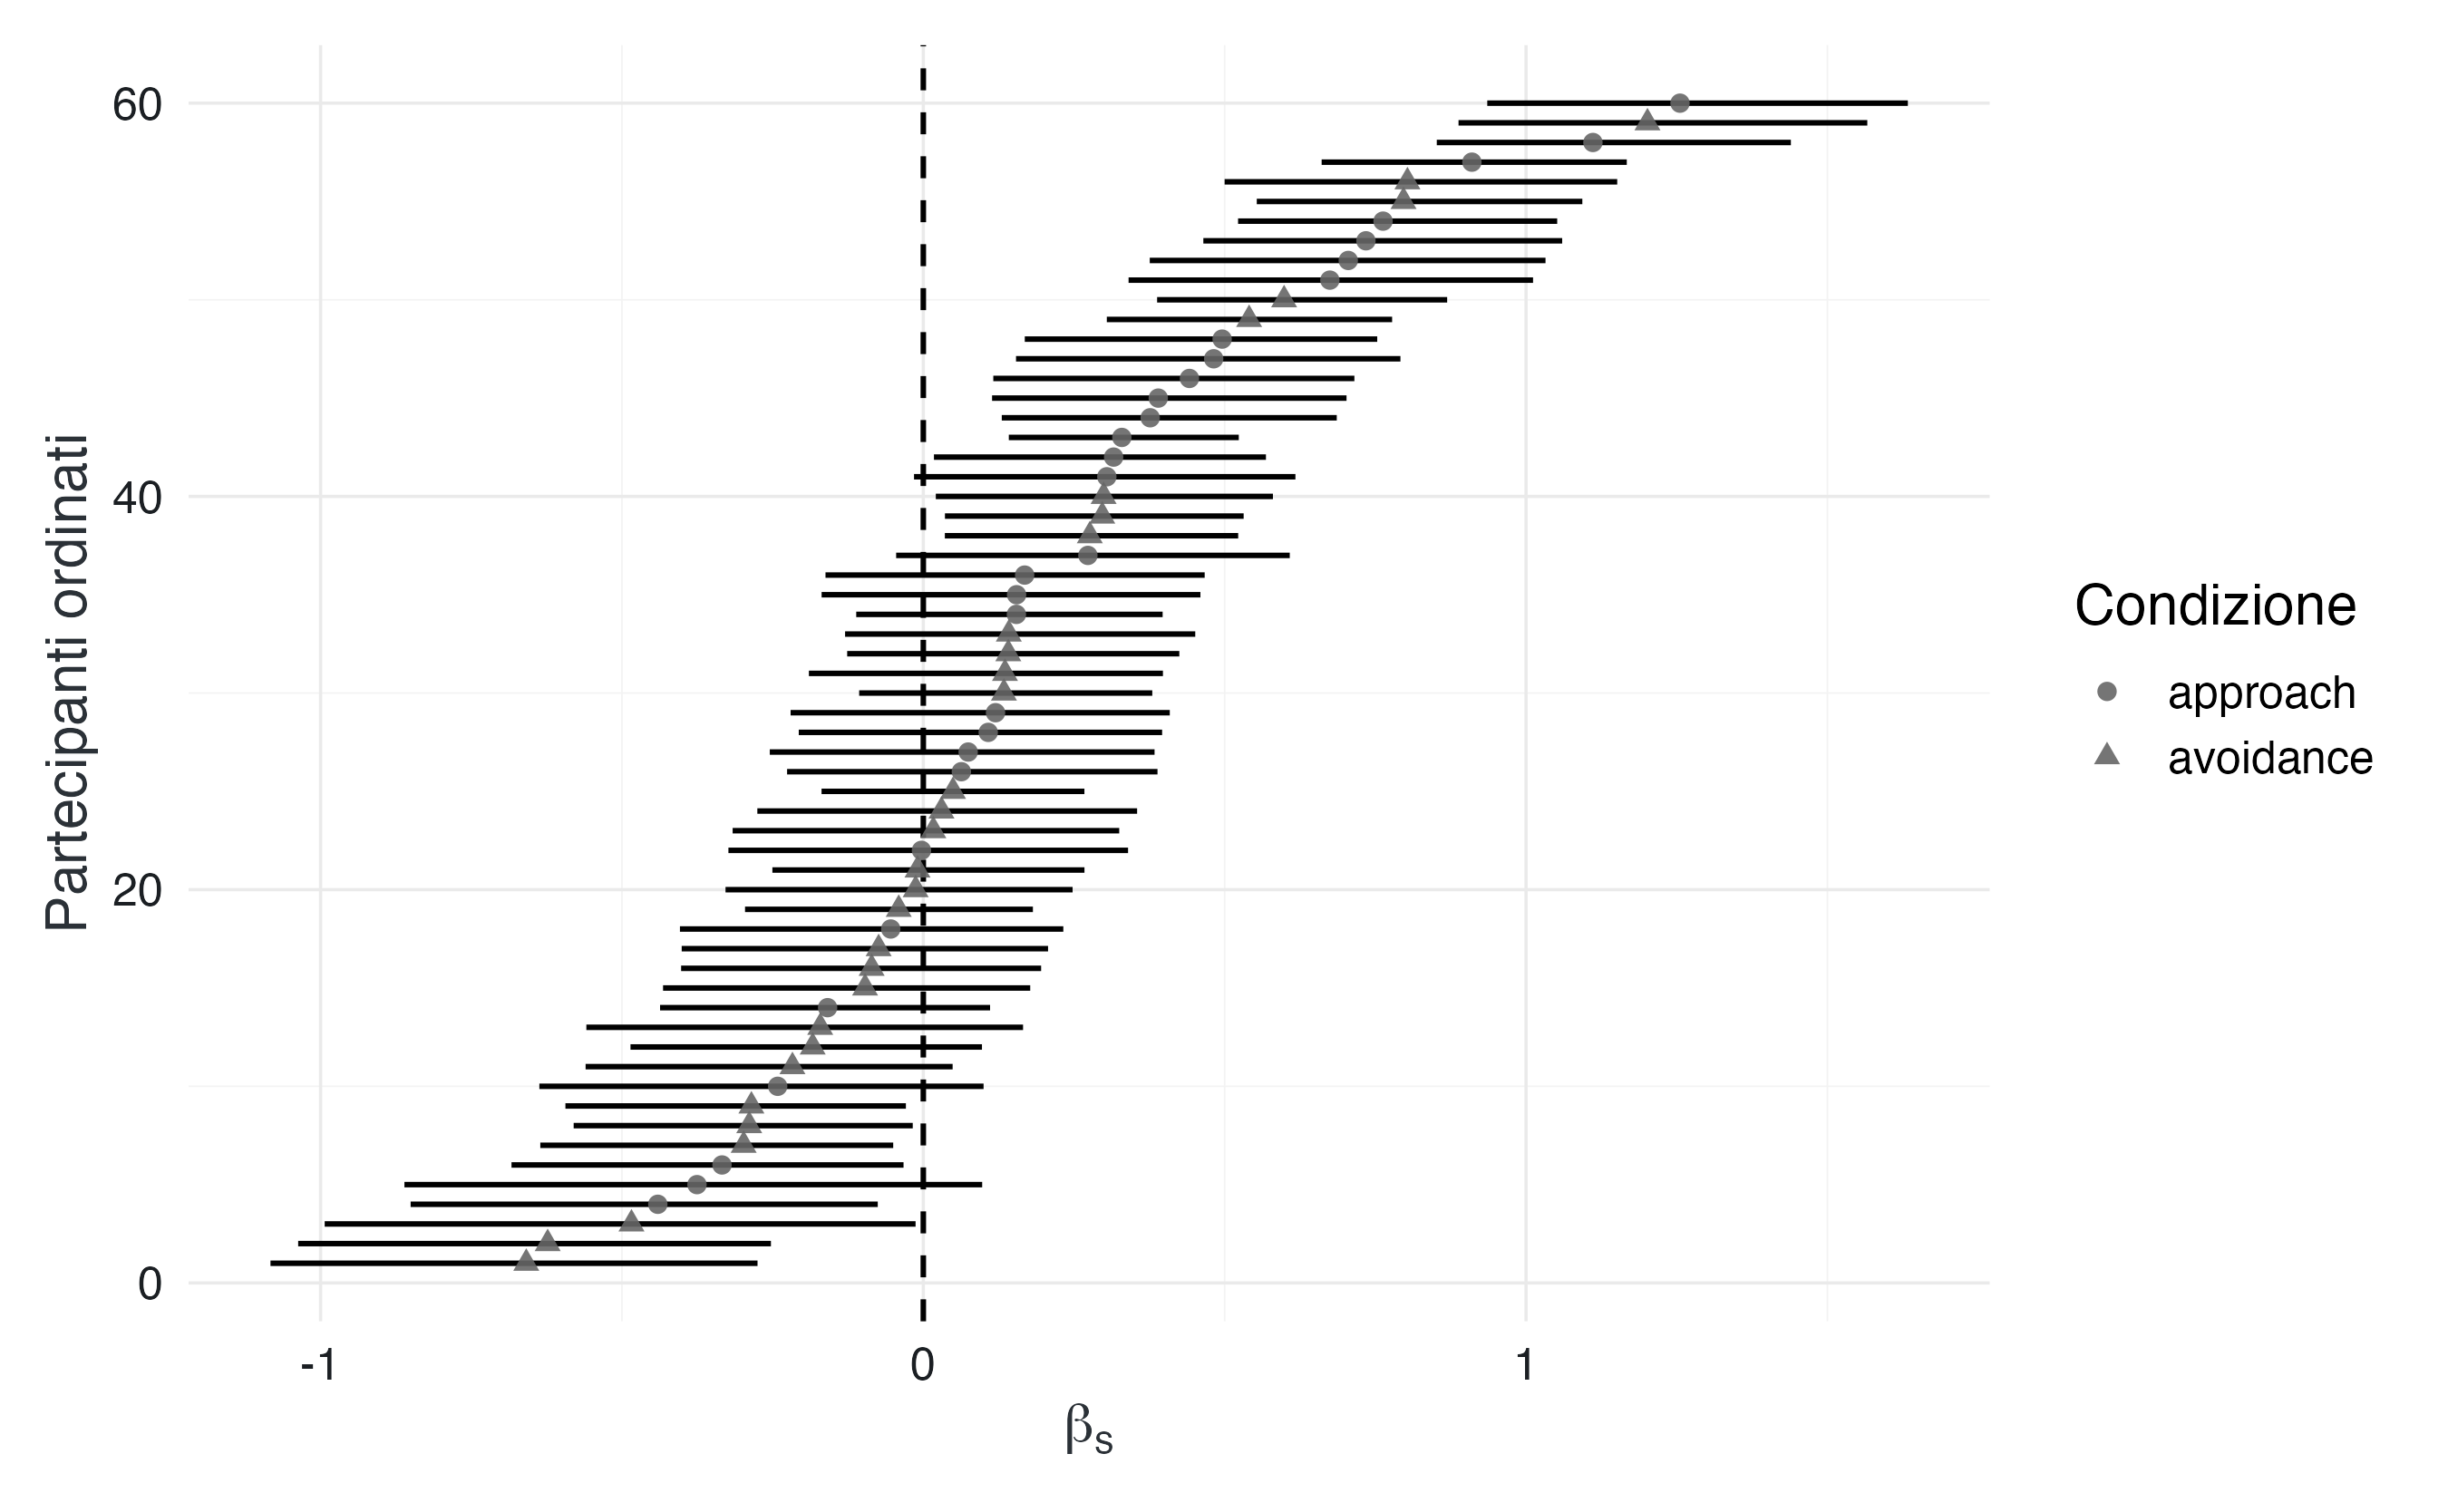
\includegraphics[width=0.85\linewidth,height=\textheight,keepaspectratio]{chapters/formal_models/03_eterogeneita_modelli_dinamici_files/figure-pdf/fig-individual-beta-goal-hierarchical-1.png}

}

\caption{\label{fig-individual-beta-goal-hierarchical}Posterior
individuali di beta nel modello gerarchico.}

\end{figure}%

Gli intervalli sono parte integrante del risultato. Ordinare o
classificare i partecipanti usando soltanto le mediane posteriori può
trasformare piccole differenze rumorose in profili psicologici
apparentemente netti.

\section{Visualizzare lo shrinkage}\label{visualizzare-lo-shrinkage}

Confrontiamo le stime separate con i centri posteriori gerarchici.

\begin{Shaded}
\begin{Highlighting}[]
\NormalTok{shrinkage\_goal }\OtherTok{\textless{}{-}}\NormalTok{ no\_pool\_estimates }\SpecialCharTok{|\textgreater{}}
  \FunctionTok{left\_join}\NormalTok{(}
\NormalTok{    individual\_goal\_parameters }\SpecialCharTok{|\textgreater{}}
      \FunctionTok{select}\NormalTok{(subject, }\AttributeTok{alpha\_hier =}\NormalTok{ alpha, }\AttributeTok{beta\_hier =}\NormalTok{ beta),}
    \AttributeTok{by =} \StringTok{"subject"}
\NormalTok{  ) }\SpecialCharTok{|\textgreater{}}
  \FunctionTok{select}\NormalTok{(}
\NormalTok{    subject,}
\NormalTok{    condition,}
\NormalTok{    alpha\_no\_pool,}
\NormalTok{    alpha\_hier,}
\NormalTok{    beta\_no\_pool,}
\NormalTok{    beta\_hier}
\NormalTok{  ) }\SpecialCharTok{|\textgreater{}}
  \FunctionTok{pivot\_longer}\NormalTok{(}
    \AttributeTok{cols =} \FunctionTok{c}\NormalTok{(alpha\_no\_pool, alpha\_hier, beta\_no\_pool, beta\_hier),}
    \AttributeTok{names\_to =} \FunctionTok{c}\NormalTok{(}\StringTok{"parameter"}\NormalTok{, }\StringTok{"model"}\NormalTok{),}
    \AttributeTok{names\_pattern =} \StringTok{"(alpha|beta)\_(no\_pool|hier)"}\NormalTok{,}
    \AttributeTok{values\_to =} \StringTok{"estimate"}
\NormalTok{  ) }\SpecialCharTok{|\textgreater{}}
  \FunctionTok{pivot\_wider}\NormalTok{(}\AttributeTok{names\_from =}\NormalTok{ model, }\AttributeTok{values\_from =}\NormalTok{ estimate)}
\end{Highlighting}
\end{Shaded}

\begin{figure}

\centering{

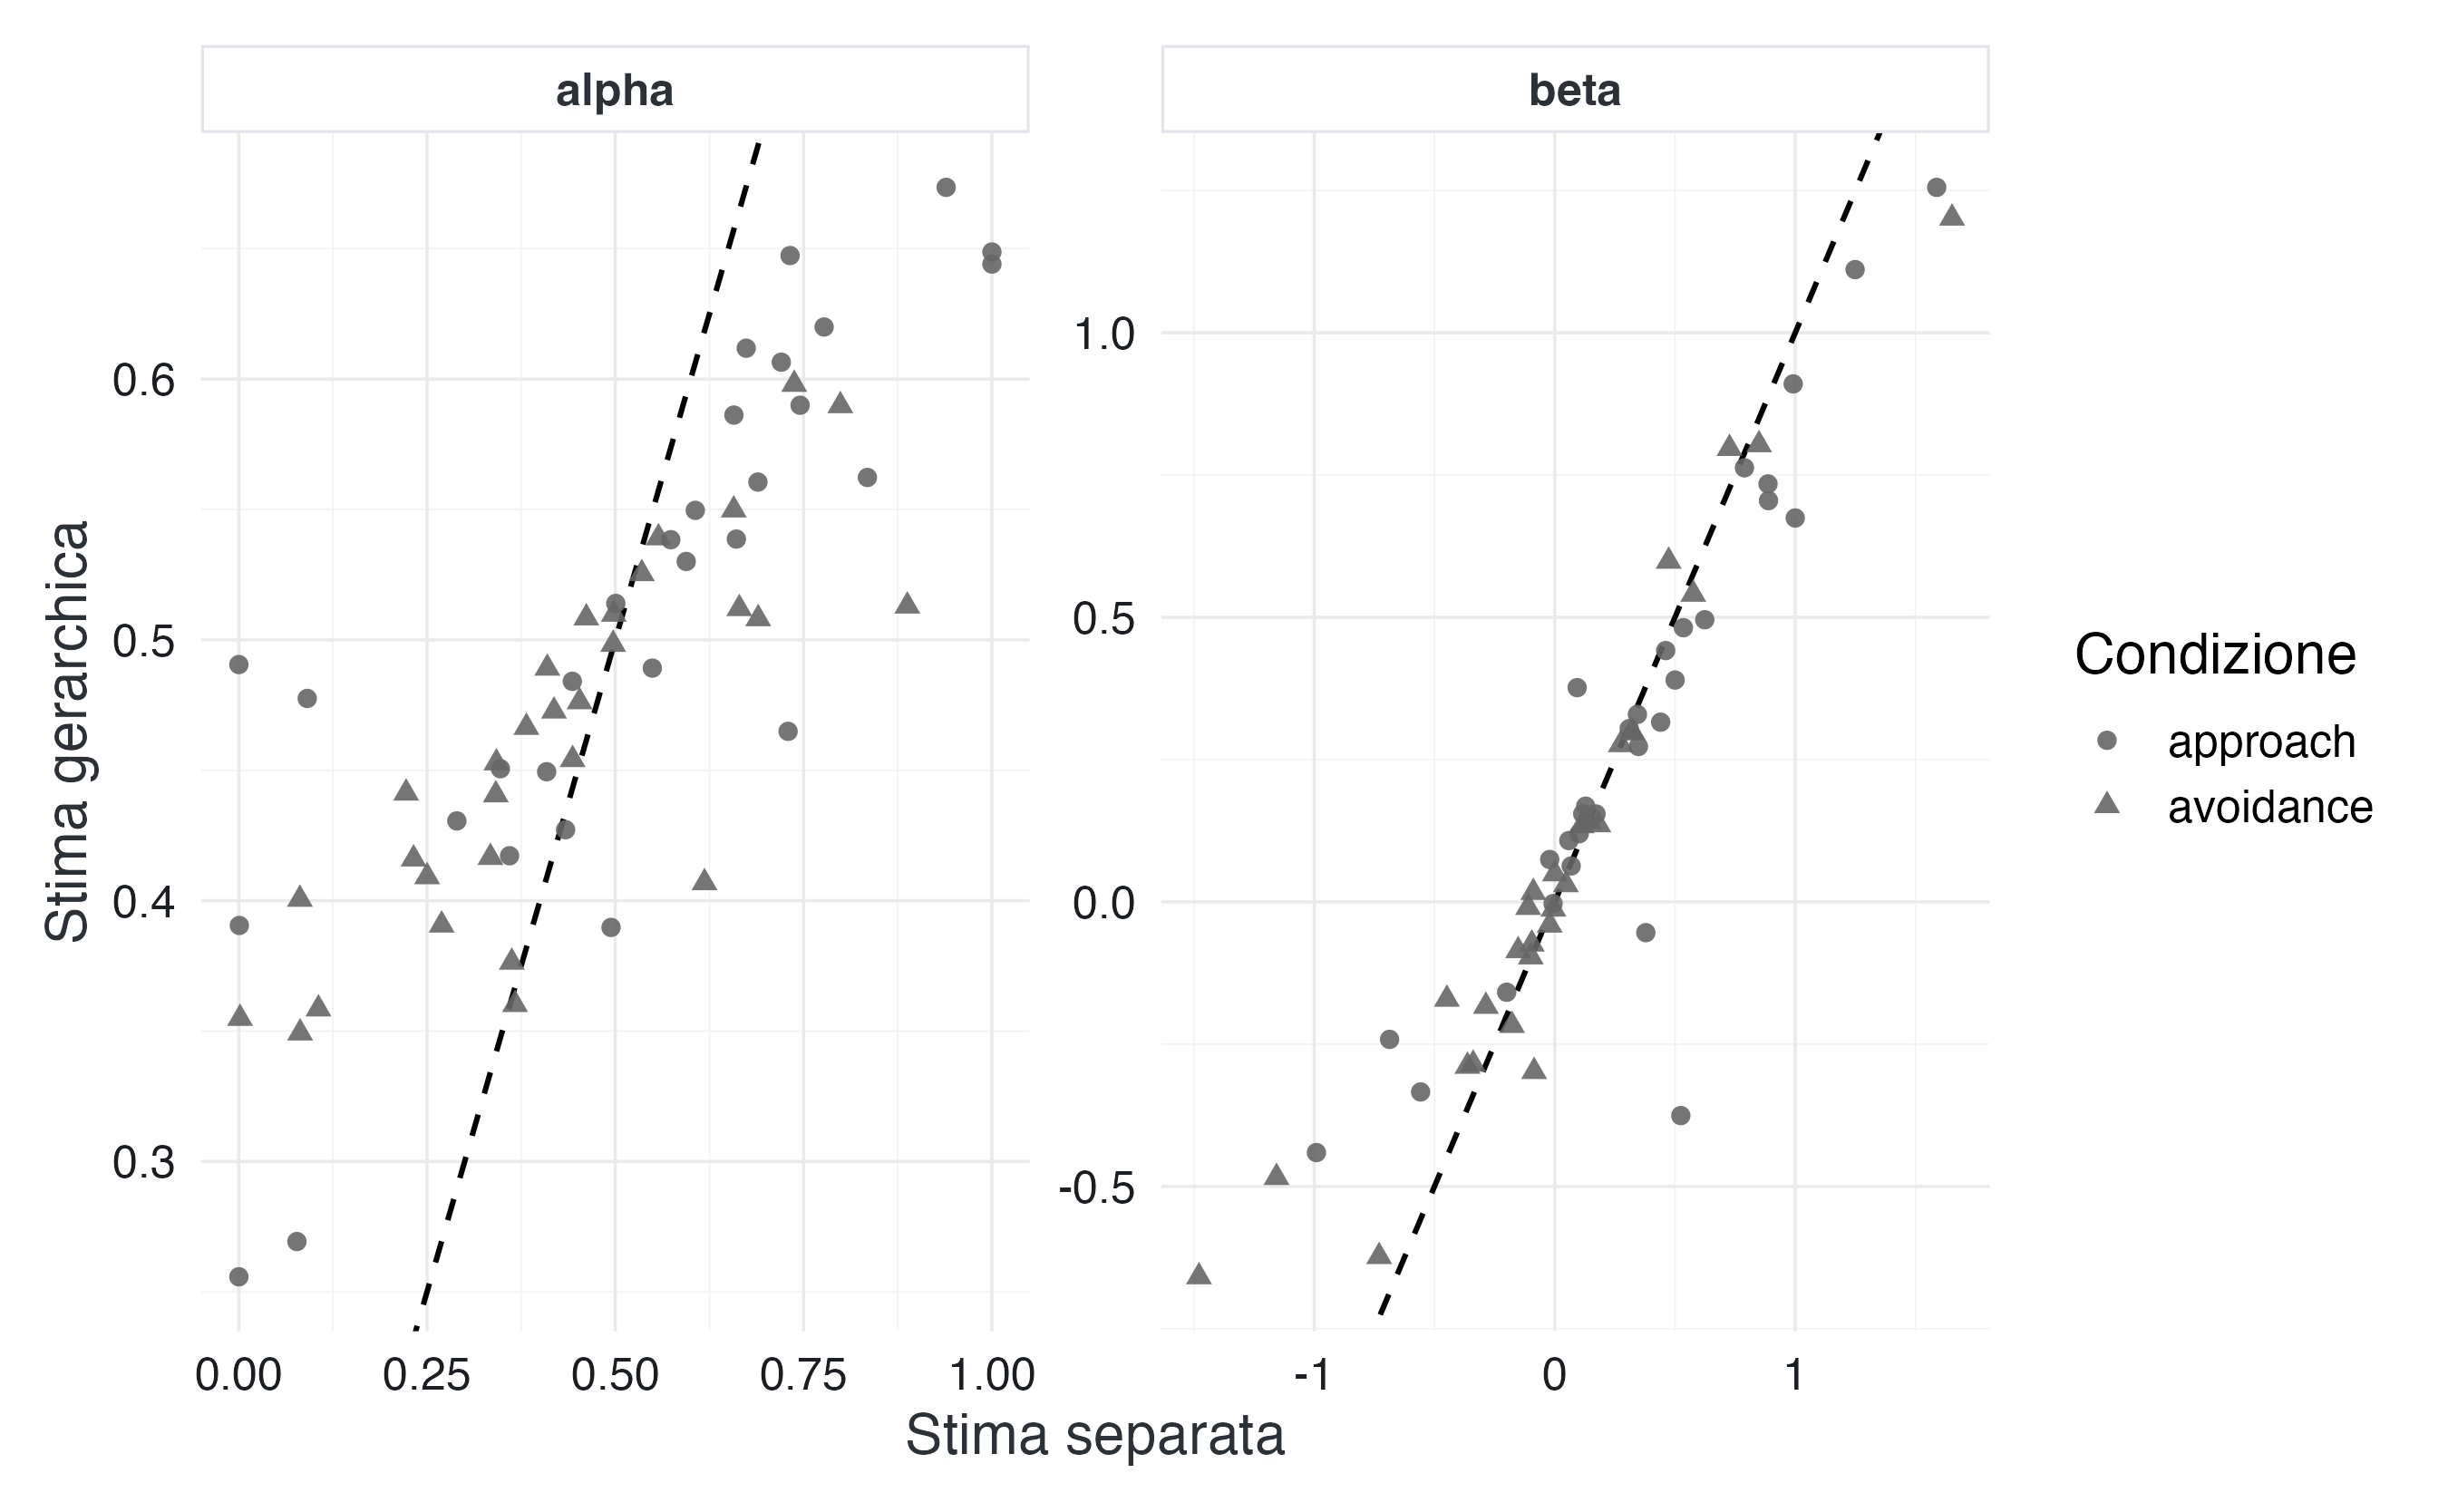
\includegraphics[width=0.85\linewidth,height=\textheight,keepaspectratio]{chapters/formal_models/03_eterogeneita_modelli_dinamici_files/figure-pdf/fig-shrinkage-goal-hierarchical-1.png}

}

\caption{\label{fig-shrinkage-goal-hierarchical}Confronto tra stime
separate e centri posteriori gerarchici. I punti estremi tendono a
essere maggiormente regolarizzati, ma l'entità dello shrinkage dipende
dall'informazione individuale e dall'eterogeneità stimata.}

\end{figure}%

Lo shrinkage non è una correzione applicata dopo la stima. È una
conseguenza della distribuzione congiunta del modello.

Inoltre, non tutte le stime devono contrarsi della stessa quantità. La
contrazione dipende da:

\begin{itemize}
\tightlist
\item
  numero e qualità dei trial individuali;
\item
  compatibilità dei dati della persona con la popolazione;
\item
  dispersione di popolazione;
\item
  prior sugli iperparametri;
\item
  trade-off tra parametri del processo.
\end{itemize}

\section{Controlli predittivi per
persona}\label{controlli-predittivi-per-persona}

\begin{Shaded}
\begin{Highlighting}[]
\NormalTok{posterior\_goal\_trajectories }\OtherTok{\textless{}{-}}\NormalTok{ fit\_goal\_hierarchical }\SpecialCharTok{|\textgreater{}}
  \FunctionTok{spread\_draws}\NormalTok{(mu[row\_id]) }\SpecialCharTok{|\textgreater{}}
  \FunctionTok{median\_qi}\NormalTok{(mu, }\AttributeTok{.width =} \FloatTok{0.90}\NormalTok{) }\SpecialCharTok{|\textgreater{}}
  \FunctionTok{left\_join}\NormalTok{(}
\NormalTok{    goal\_data }\SpecialCharTok{|\textgreater{}}
      \FunctionTok{select}\NormalTok{(row\_id, subject, condition, trial, goal),}
    \AttributeTok{by =} \StringTok{"row\_id"}
\NormalTok{  )}
\end{Highlighting}
\end{Shaded}

\begin{figure}

\centering{

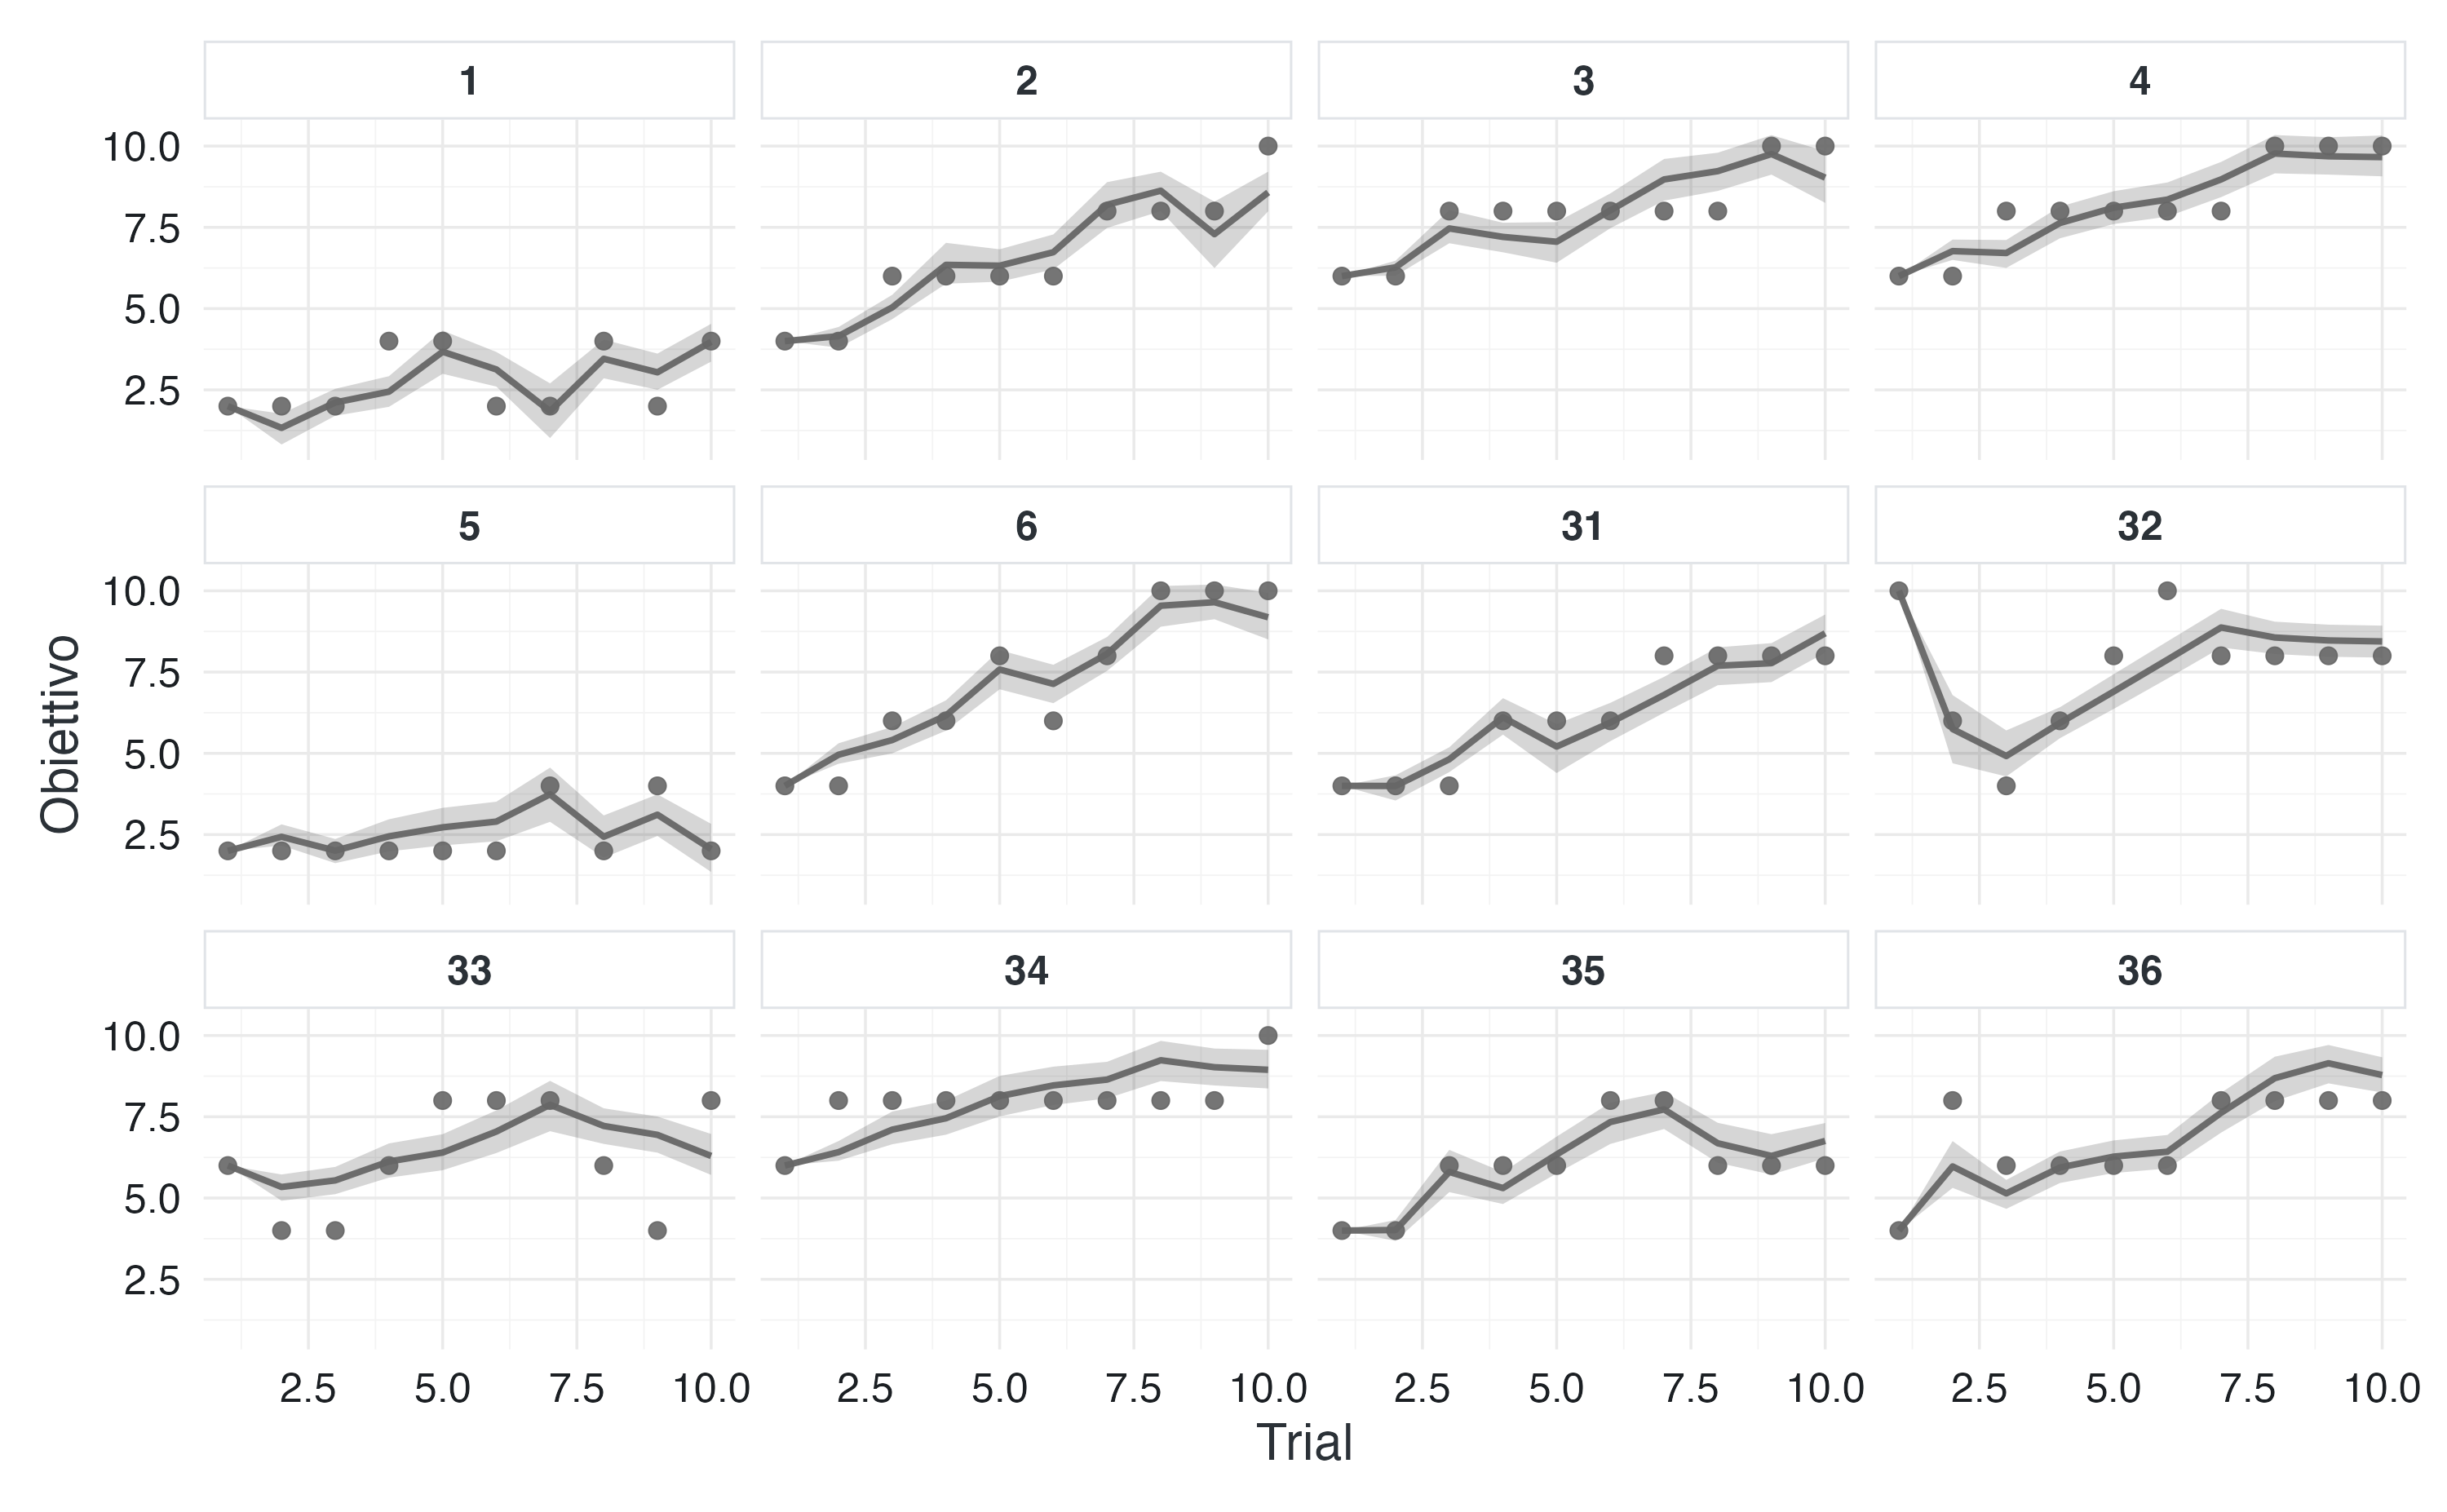
\includegraphics[width=0.85\linewidth,height=\textheight,keepaspectratio]{chapters/formal_models/03_eterogeneita_modelli_dinamici_files/figure-pdf/fig-posterior-trajectories-goal-hierarchical-1.png}

}

\caption{\label{fig-posterior-trajectories-goal-hierarchical}Traiettorie
osservate e attese per partecipanti selezionati nel modello gerarchico.
Il controllo individuale può rivelare fallimenti nascosti dalle
statistiche aggregate.}

\end{figure}%

Un modello gerarchico può stimare bene la distribuzione dei parametri e
fallire comunque aspetti temporali importanti: cambi di strategia,
asimmetrie tra feedback positivo e negativo, saturazione o shock
contestuali.

\section{Prevedere una persona osservata e una persona
nuova}\label{prevedere-una-persona-osservata-e-una-persona-nuova}

Le due domande non sono equivalenti.

\subsection{Persona già osservata}\label{persona-giuxe0-osservata}

Per una persona già inclusa nel campione, la previsione usa la posterior
di \(\alpha_s\) e \(\beta_s\). La distribuzione beneficia sia dei suoi
trial sia del partial pooling.

\subsection{Persona nuova}\label{persona-nuova}

Per una persona non osservata dobbiamo generare nuovi parametri dalla
distribuzione di popolazione:

\[
\alpha_{\text{new}}
=
\operatorname{logit}^{-1}
\left(
\mu_\alpha+ au_\alpha z_{\alpha,\text{new}}
\right),
\]

\[
\beta_{\text{new}}
=
\mu_\beta+  au_\beta z_{\beta,\text{new}}.
\]

\begin{Shaded}
\begin{Highlighting}[]
\NormalTok{hyper\_draws\_goal }\OtherTok{\textless{}{-}}\NormalTok{ fit\_goal\_hierarchical}\SpecialCharTok{$}\FunctionTok{draws}\NormalTok{(}
  \FunctionTok{c}\NormalTok{(}
    \StringTok{"mu\_alpha\_logit"}\NormalTok{,}
    \StringTok{"tau\_alpha\_logit"}\NormalTok{,}
    \StringTok{"mu\_beta"}\NormalTok{,}
    \StringTok{"tau\_beta"}\NormalTok{,}
    \StringTok{"sigma"}
\NormalTok{  )}
\NormalTok{) }\SpecialCharTok{|\textgreater{}}
\NormalTok{  posterior}\SpecialCharTok{::}\FunctionTok{as\_draws\_df}\NormalTok{() }\SpecialCharTok{|\textgreater{}}
  \FunctionTok{as\_tibble}\NormalTok{() }\SpecialCharTok{|\textgreater{}}
  \FunctionTok{slice\_sample}\NormalTok{(}\AttributeTok{n =} \DecValTok{200}\NormalTok{) }\SpecialCharTok{|\textgreater{}}
  \FunctionTok{mutate}\NormalTok{(}
    \AttributeTok{alpha\_new =} \FunctionTok{plogis}\NormalTok{(}
\NormalTok{      mu\_alpha\_logit }\SpecialCharTok{+}\NormalTok{ tau\_alpha\_logit }\SpecialCharTok{*} \FunctionTok{rnorm}\NormalTok{(}\FunctionTok{n}\NormalTok{())}
\NormalTok{    ),}
    \AttributeTok{beta\_new =}\NormalTok{ mu\_beta }\SpecialCharTok{+}\NormalTok{ tau\_beta }\SpecialCharTok{*} \FunctionTok{rnorm}\NormalTok{(}\FunctionTok{n}\NormalTok{())}
\NormalTok{  )}

\NormalTok{new\_performance }\OtherTok{\textless{}{-}} \FunctionTok{c}\NormalTok{(}\DecValTok{5}\NormalTok{, }\DecValTok{6}\NormalTok{, }\DecValTok{7}\NormalTok{, }\DecValTok{7}\NormalTok{, }\DecValTok{5}\NormalTok{, }\DecValTok{4}\NormalTok{, }\DecValTok{6}\NormalTok{, }\DecValTok{7}\NormalTok{, }\DecValTok{8}\NormalTok{, }\DecValTok{8}\NormalTok{)}

\NormalTok{new\_person\_paths }\OtherTok{\textless{}{-}}\NormalTok{ hyper\_draws\_goal }\SpecialCharTok{|\textgreater{}}
  \FunctionTok{mutate}\NormalTok{(}
    \AttributeTok{simulation =}\NormalTok{ purrr}\SpecialCharTok{::}\FunctionTok{pmap}\NormalTok{(}
      \FunctionTok{list}\NormalTok{(alpha\_new, beta\_new, sigma),}
      \SpecialCharTok{\textasciitilde{}} \FunctionTok{simulate\_goal\_path}\NormalTok{(}
        \AttributeTok{performance =}\NormalTok{ new\_performance,}
        \AttributeTok{initial\_goal =} \DecValTok{5}\NormalTok{,}
        \AttributeTok{alpha =}\NormalTok{ ..}\DecValTok{1}\NormalTok{,}
        \AttributeTok{beta =}\NormalTok{ ..}\DecValTok{2}\NormalTok{,}
        \AttributeTok{sigma =}\NormalTok{ ..}\DecValTok{3}
\NormalTok{      )}
\NormalTok{    )}
\NormalTok{  ) }\SpecialCharTok{|\textgreater{}}
  \FunctionTok{select}\NormalTok{(.draw, simulation) }\SpecialCharTok{|\textgreater{}}
\NormalTok{  tidyr}\SpecialCharTok{::}\FunctionTok{unnest}\NormalTok{(simulation)}
\end{Highlighting}
\end{Shaded}

\begin{figure}

\centering{

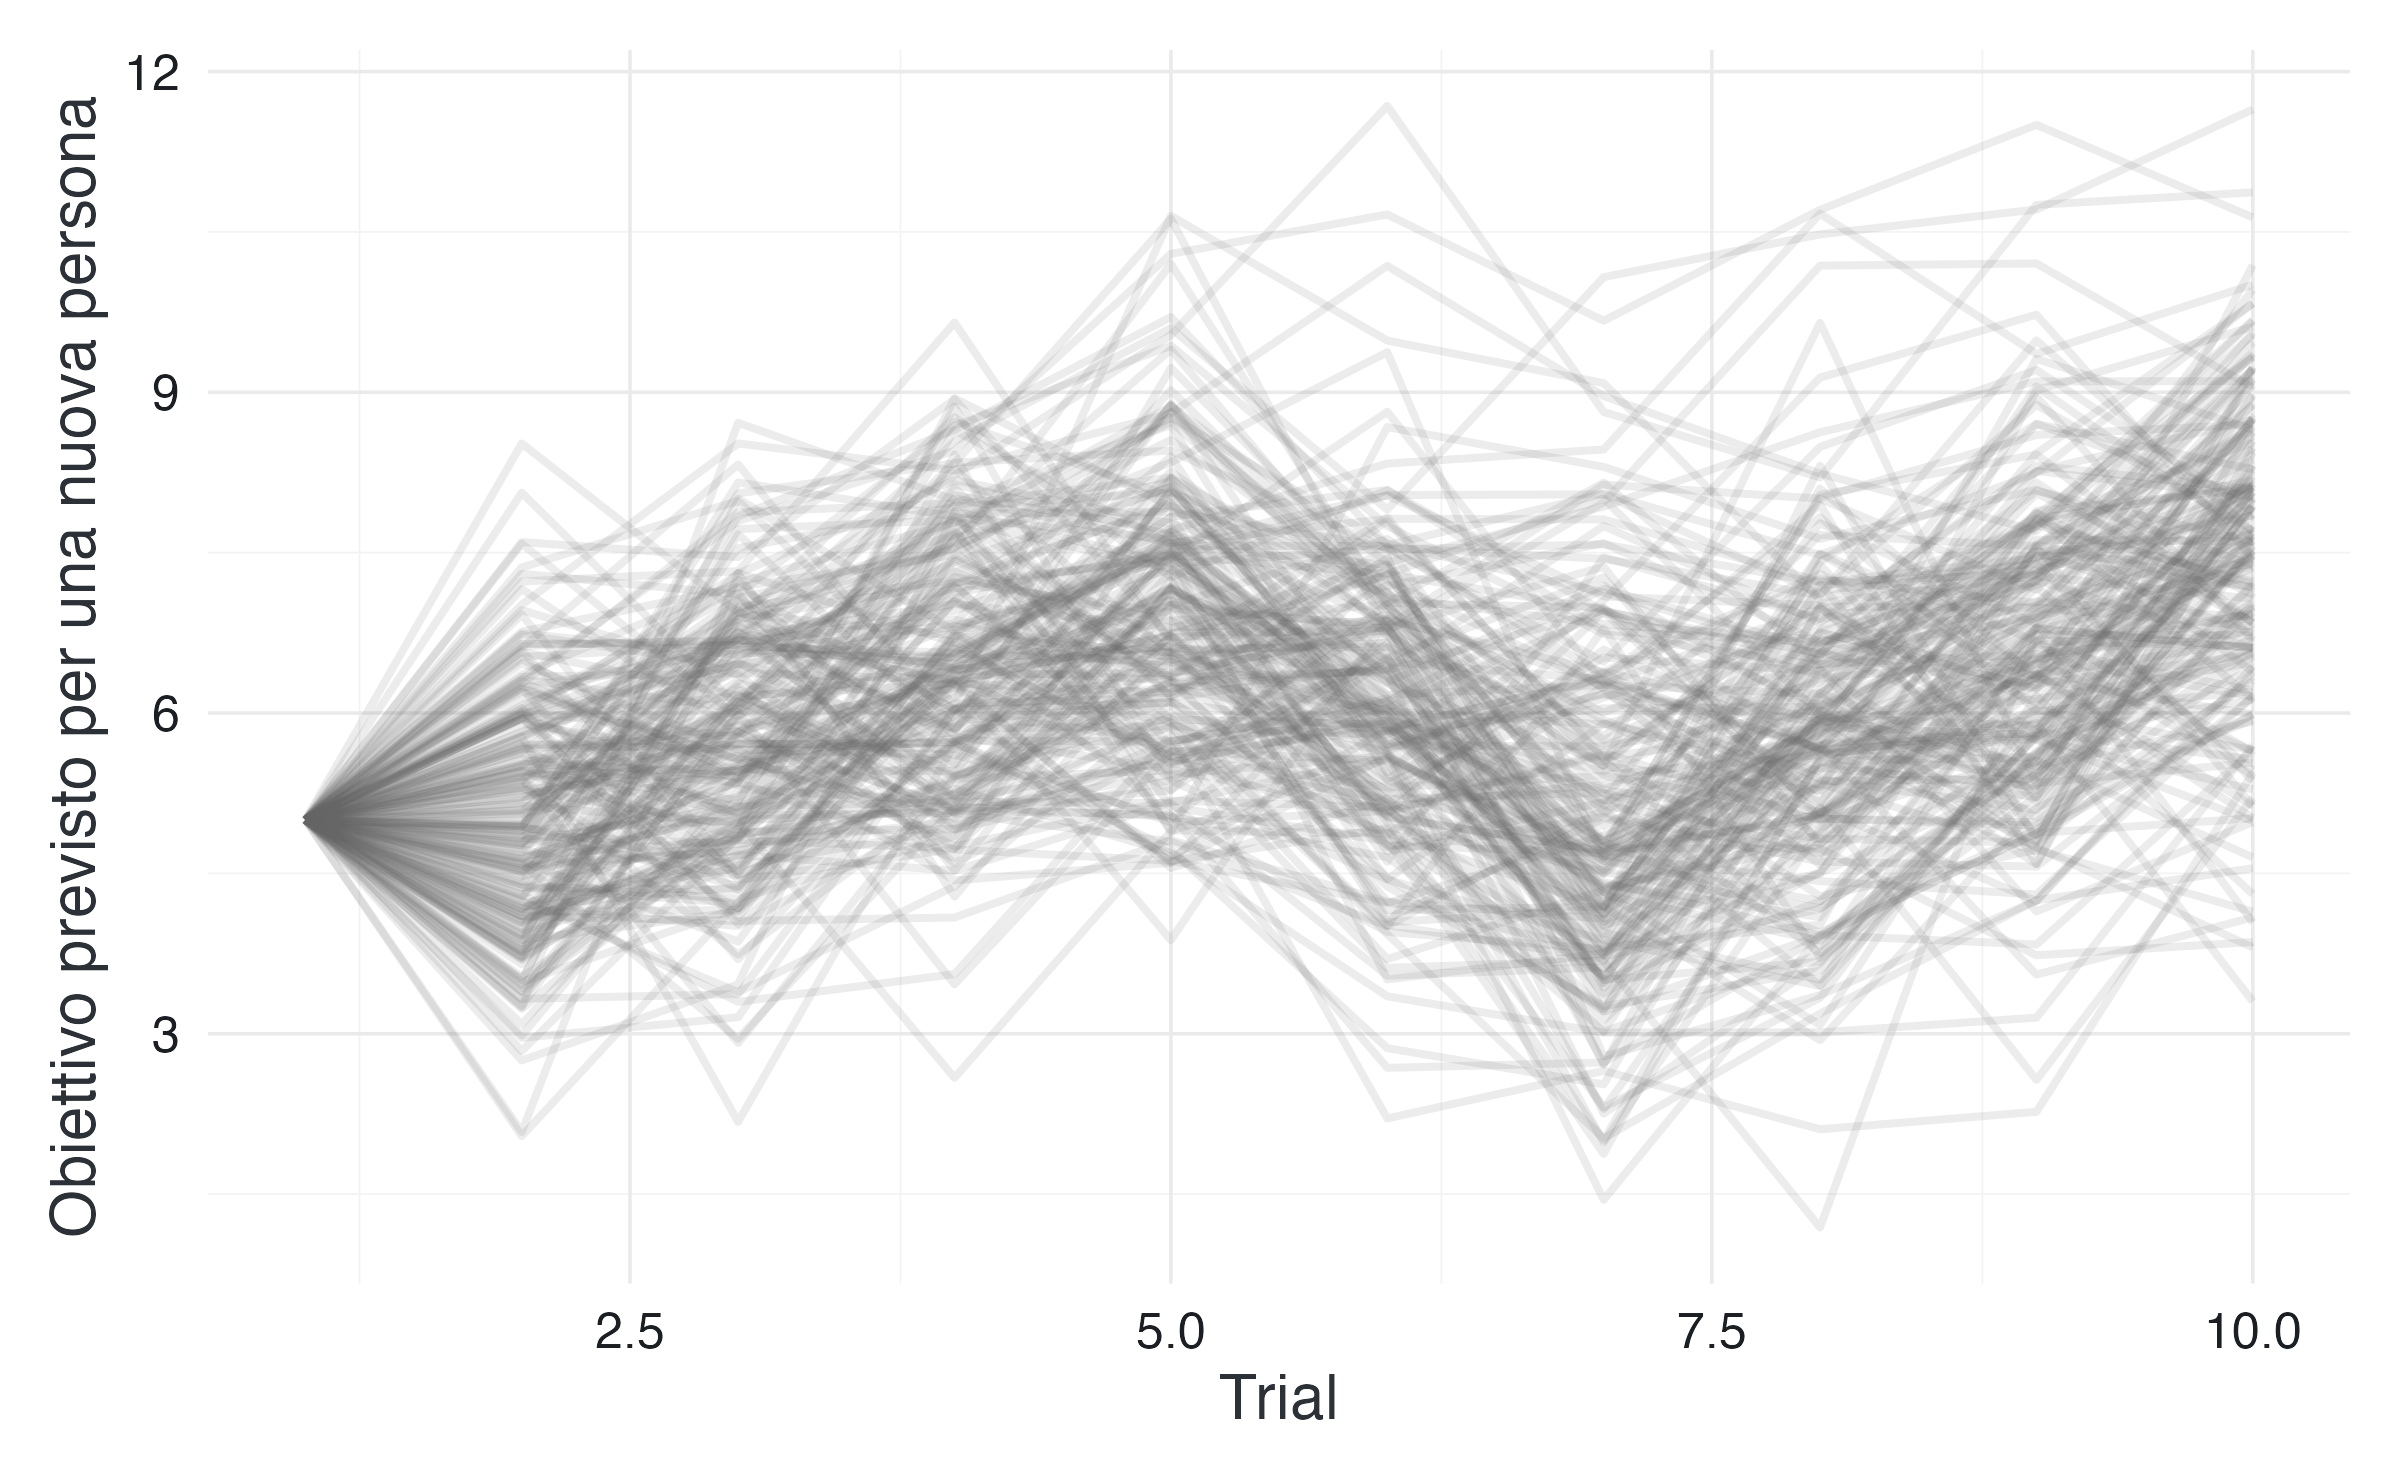
\includegraphics[width=0.85\linewidth,height=\textheight,keepaspectratio]{chapters/formal_models/03_eterogeneita_modelli_dinamici_files/figure-pdf/fig-new-person-goal-hierarchical-1.png}

}

\caption{\label{fig-new-person-goal-hierarchical}Distribuzione
predittiva di traiettorie per un nuovo individuo estratto dalla
popolazione modellata.}

\end{figure}%

La previsione per un nuovo individuo è normalmente più incerta di quella
per una persona già osservata, perché include anche l'eterogeneità di
popolazione.

\section{Estendere il modello alle condizioni
sperimentali}\label{estendere-il-modello-alle-condizioni-sperimentali}

Finora \emph{approach} e \emph{avoidance} hanno condiviso la stessa
distribuzione di popolazione. Per esaminare differenze sistematiche
introduciamo ipermedie specifiche per condizione, mantenendo comuni le
dispersioni individuali:

\[
\operatorname{logit}(\alpha_s)
\sim
\operatorname{Normal}(\mu_{\alpha,c[s]},\tau_\alpha),
\]

\[
\beta_s
\sim
\operatorname{Normal}(\mu_{\beta,c[s]},\tau_\beta).
\]

Questa specificazione chiede se la persona tipica delle due condizioni
differisca nella sensibilità alla discrepanza o nella deriva.

\begin{Shaded}
\begin{Highlighting}[]
\NormalTok{stan\_code\_goal\_conditions }\OtherTok{\textless{}{-}} \StringTok{"}
\StringTok{data \{}
\StringTok{  int\textless{}lower=1\textgreater{} Ntotal;}
\StringTok{  int\textless{}lower=1\textgreater{} Nsubj;}
\StringTok{  int\textless{}lower=1\textgreater{} C;}
\StringTok{  array[Ntotal] int\textless{}lower=1, upper=Nsubj\textgreater{} subject;}
\StringTok{  array[Ntotal] int\textless{}lower=1\textgreater{} trial;}
\StringTok{  array[Nsubj] int\textless{}lower=1, upper=C\textgreater{} subject\_condition;}
\StringTok{  vector[Ntotal] goal;}
\StringTok{  vector[Ntotal] performance;}
\StringTok{\}}

\StringTok{parameters \{}
\StringTok{  vector[C] mu\_alpha\_logit;}
\StringTok{  real\textless{}lower=0\textgreater{} tau\_alpha\_logit;}
\StringTok{  vector[Nsubj] z\_alpha;}

\StringTok{  vector[C] mu\_beta;}
\StringTok{  real\textless{}lower=0\textgreater{} tau\_beta;}
\StringTok{  vector[Nsubj] z\_beta;}

\StringTok{  real\textless{}lower=0\textgreater{} sigma;}
\StringTok{\}}

\StringTok{transformed parameters \{}
\StringTok{  vector[Nsubj] alpha\_logit;}
\StringTok{  vector\textless{}lower=0, upper=1\textgreater{}[Nsubj] alpha;}
\StringTok{  vector[Nsubj] beta;}
\StringTok{  vector[Ntotal] mu;}

\StringTok{  for (s in 1:Nsubj) \{}
\StringTok{    int c = subject\_condition[s];}
\StringTok{    alpha\_logit[s] =}
\StringTok{      mu\_alpha\_logit[c] + tau\_alpha\_logit * z\_alpha[s];}
\StringTok{    alpha[s] = inv\_logit(alpha\_logit[s]);}
\StringTok{    beta[s] = mu\_beta[c] + tau\_beta * z\_beta[s];}
\StringTok{  \}}

\StringTok{  for (i in 1:Ntotal) \{}
\StringTok{    if (trial[i] == 1) \{}
\StringTok{      mu[i] = goal[i];}
\StringTok{    \} else \{}
\StringTok{      int s = subject[i];}
\StringTok{      mu[i] = mu[i {-} 1]}
\StringTok{              + alpha[s] * (performance[i {-} 1] {-} mu[i {-} 1])}
\StringTok{              + beta[s];}
\StringTok{    \}}
\StringTok{  \}}
\StringTok{\}}

\StringTok{model \{}
\StringTok{  mu\_alpha\_logit \textasciitilde{} normal(0, 1);}
\StringTok{  tau\_alpha\_logit \textasciitilde{} normal(0, 0.75);}
\StringTok{  z\_alpha \textasciitilde{} std\_normal();}

\StringTok{  mu\_beta \textasciitilde{} normal(0, 0.25);}
\StringTok{  tau\_beta \textasciitilde{} normal(0, 0.25);}
\StringTok{  z\_beta \textasciitilde{} std\_normal();}

\StringTok{  sigma \textasciitilde{} normal(0, 0.75);}

\StringTok{  for (i in 1:Ntotal) \{}
\StringTok{    if (trial[i] \textgreater{} 1) \{}
\StringTok{      goal[i] \textasciitilde{} normal(mu[i], sigma);}
\StringTok{    \}}
\StringTok{  \}}
\StringTok{\}}

\StringTok{generated quantities \{}
\StringTok{  vector\textless{}lower=0, upper=1\textgreater{}[C] alpha\_typical;}
\StringTok{  real delta\_alpha\_typical;}
\StringTok{  real delta\_beta;}
\StringTok{  vector[Ntotal] y\_rep;}

\StringTok{  for (c in 1:C) \{}
\StringTok{    alpha\_typical[c] = inv\_logit(mu\_alpha\_logit[c]);}
\StringTok{  \}}

\StringTok{  delta\_alpha\_typical = alpha\_typical[2] {-} alpha\_typical[1];}
\StringTok{  delta\_beta = mu\_beta[2] {-} mu\_beta[1];}

\StringTok{  for (i in 1:Ntotal) \{}
\StringTok{    if (trial[i] == 1) \{}
\StringTok{      y\_rep[i] = goal[i];}
\StringTok{    \} else \{}
\StringTok{      y\_rep[i] = normal\_rng(mu[i], sigma);}
\StringTok{    \}}
\StringTok{  \}}
\StringTok{\}}
\StringTok{"}
\end{Highlighting}
\end{Shaded}

\begin{Shaded}
\begin{Highlighting}[]
\NormalTok{stan\_data\_goal\_conditions }\OtherTok{\textless{}{-}} \FunctionTok{list}\NormalTok{(}
  \AttributeTok{Ntotal =} \FunctionTok{nrow}\NormalTok{(goal\_data),}
  \AttributeTok{Nsubj =} \FunctionTok{n\_distinct}\NormalTok{(goal\_data}\SpecialCharTok{$}\NormalTok{subject),}
  \AttributeTok{C =} \FunctionTok{nlevels}\NormalTok{(goal\_data}\SpecialCharTok{$}\NormalTok{condition),}
  \AttributeTok{subject =}\NormalTok{ goal\_data}\SpecialCharTok{$}\NormalTok{subject,}
  \AttributeTok{trial =}\NormalTok{ goal\_data}\SpecialCharTok{$}\NormalTok{trial,}
  \AttributeTok{subject\_condition =}\NormalTok{ subject\_structure}\SpecialCharTok{$}\NormalTok{condition\_id,}
  \AttributeTok{goal =}\NormalTok{ goal\_data}\SpecialCharTok{$}\NormalTok{goal,}
  \AttributeTok{performance =}\NormalTok{ goal\_data}\SpecialCharTok{$}\NormalTok{performance}
\NormalTok{)}
\end{Highlighting}
\end{Shaded}

\begin{Shaded}
\begin{Highlighting}[]
\NormalTok{model\_goal\_conditions }\OtherTok{\textless{}{-}} \FunctionTok{cmdstan\_model}\NormalTok{(}
  \FunctionTok{write\_stan\_file}\NormalTok{(stan\_code\_goal\_conditions)}
\NormalTok{)}

\NormalTok{fit\_goal\_conditions }\OtherTok{\textless{}{-}}\NormalTok{ model\_goal\_conditions}\SpecialCharTok{$}\FunctionTok{sample}\NormalTok{(}
  \AttributeTok{data =}\NormalTok{ stan\_data\_goal\_conditions,}
  \AttributeTok{seed =} \DecValTok{4192}\NormalTok{,}
  \AttributeTok{chains =} \DecValTok{4}\NormalTok{,}
  \AttributeTok{parallel\_chains =} \DecValTok{4}\NormalTok{,}
  \AttributeTok{iter\_warmup =} \DecValTok{1500}\NormalTok{,}
  \AttributeTok{iter\_sampling =} \DecValTok{2000}\NormalTok{,}
  \AttributeTok{adapt\_delta =} \FloatTok{0.95}\NormalTok{,}
  \AttributeTok{refresh =} \DecValTok{500}
\NormalTok{)}
\end{Highlighting}
\end{Shaded}

\section{Contrasti tra condizioni}\label{contrasti-tra-condizioni}

\begin{Shaded}
\begin{Highlighting}[]
\NormalTok{fit\_goal\_conditions}\SpecialCharTok{$}\FunctionTok{draws}\NormalTok{(}
  \FunctionTok{c}\NormalTok{(}
    \StringTok{"alpha\_typical"}\NormalTok{,}
    \StringTok{"mu\_beta"}\NormalTok{,}
    \StringTok{"delta\_alpha\_typical"}\NormalTok{,}
    \StringTok{"delta\_beta"}
\NormalTok{  )}
\NormalTok{) }\SpecialCharTok{|\textgreater{}}
\NormalTok{  posterior}\SpecialCharTok{::}\FunctionTok{summarise\_draws}\NormalTok{(}
\NormalTok{    mean,}
\NormalTok{    median,}
    \SpecialCharTok{\textasciitilde{}}\FunctionTok{quantile}\NormalTok{(.x, }\AttributeTok{probs =} \FunctionTok{c}\NormalTok{(}\FloatTok{0.025}\NormalTok{, }\FloatTok{0.975}\NormalTok{))}
\NormalTok{  )}
\CommentTok{\#\textgreater{} \# A tibble: 6 x 5}
\CommentTok{\#\textgreater{}   variable               mean  median \textasciigrave{}2.5\%\textasciigrave{}  \textasciigrave{}97.5\%\textasciigrave{}}
\CommentTok{\#\textgreater{}   \textless{}chr\textgreater{}                 \textless{}dbl\textgreater{}   \textless{}dbl\textgreater{}  \textless{}dbl\textgreater{}    \textless{}dbl\textgreater{}}
\CommentTok{\#\textgreater{} 1 alpha\_typical[1]     0.547   0.548   0.453 0.637   }
\CommentTok{\#\textgreater{} 2 alpha\_typical[2]     0.419   0.419   0.328 0.511   }
\CommentTok{\#\textgreater{} 3 mu\_beta[1]           0.277   0.277   0.103 0.452   }
\CommentTok{\#\textgreater{} 4 mu\_beta[2]           0.0534  0.0531 {-}0.115 0.221   }
\CommentTok{\#\textgreater{} 5 delta\_alpha\_typical {-}0.128  {-}0.129  {-}0.255 0.000956}
\CommentTok{\#\textgreater{} 6 delta\_beta          {-}0.223  {-}0.222  {-}0.468 0.0149}
\end{Highlighting}
\end{Shaded}

\begin{Shaded}
\begin{Highlighting}[]
\NormalTok{condition\_contrasts }\OtherTok{\textless{}{-}}\NormalTok{ fit\_goal\_conditions}\SpecialCharTok{$}\FunctionTok{draws}\NormalTok{(}
  \FunctionTok{c}\NormalTok{(}\StringTok{"delta\_alpha\_typical"}\NormalTok{, }\StringTok{"delta\_beta"}\NormalTok{)}
\NormalTok{) }\SpecialCharTok{|\textgreater{}}
\NormalTok{  posterior}\SpecialCharTok{::}\FunctionTok{as\_draws\_df}\NormalTok{() }\SpecialCharTok{|\textgreater{}}
  \FunctionTok{as\_tibble}\NormalTok{()}

\NormalTok{condition\_contrasts }\SpecialCharTok{|\textgreater{}}
  \FunctionTok{summarise}\NormalTok{(}
    \AttributeTok{p\_delta\_alpha\_below\_zero =} \FunctionTok{mean}\NormalTok{(delta\_alpha\_typical }\SpecialCharTok{\textless{}} \DecValTok{0}\NormalTok{),}
    \AttributeTok{p\_delta\_beta\_below\_zero =} \FunctionTok{mean}\NormalTok{(delta\_beta }\SpecialCharTok{\textless{}} \DecValTok{0}\NormalTok{)}
\NormalTok{  )}
\CommentTok{\#\textgreater{} \# A tibble: 1 x 2}
\CommentTok{\#\textgreater{}   p\_delta\_alpha\_below\_zero p\_delta\_beta\_below\_zero}
\CommentTok{\#\textgreater{}                      \textless{}dbl\textgreater{}                   \textless{}dbl\textgreater{}}
\CommentTok{\#\textgreater{} 1                    0.974                   0.968}
\end{Highlighting}
\end{Shaded}

\begin{figure}

\centering{

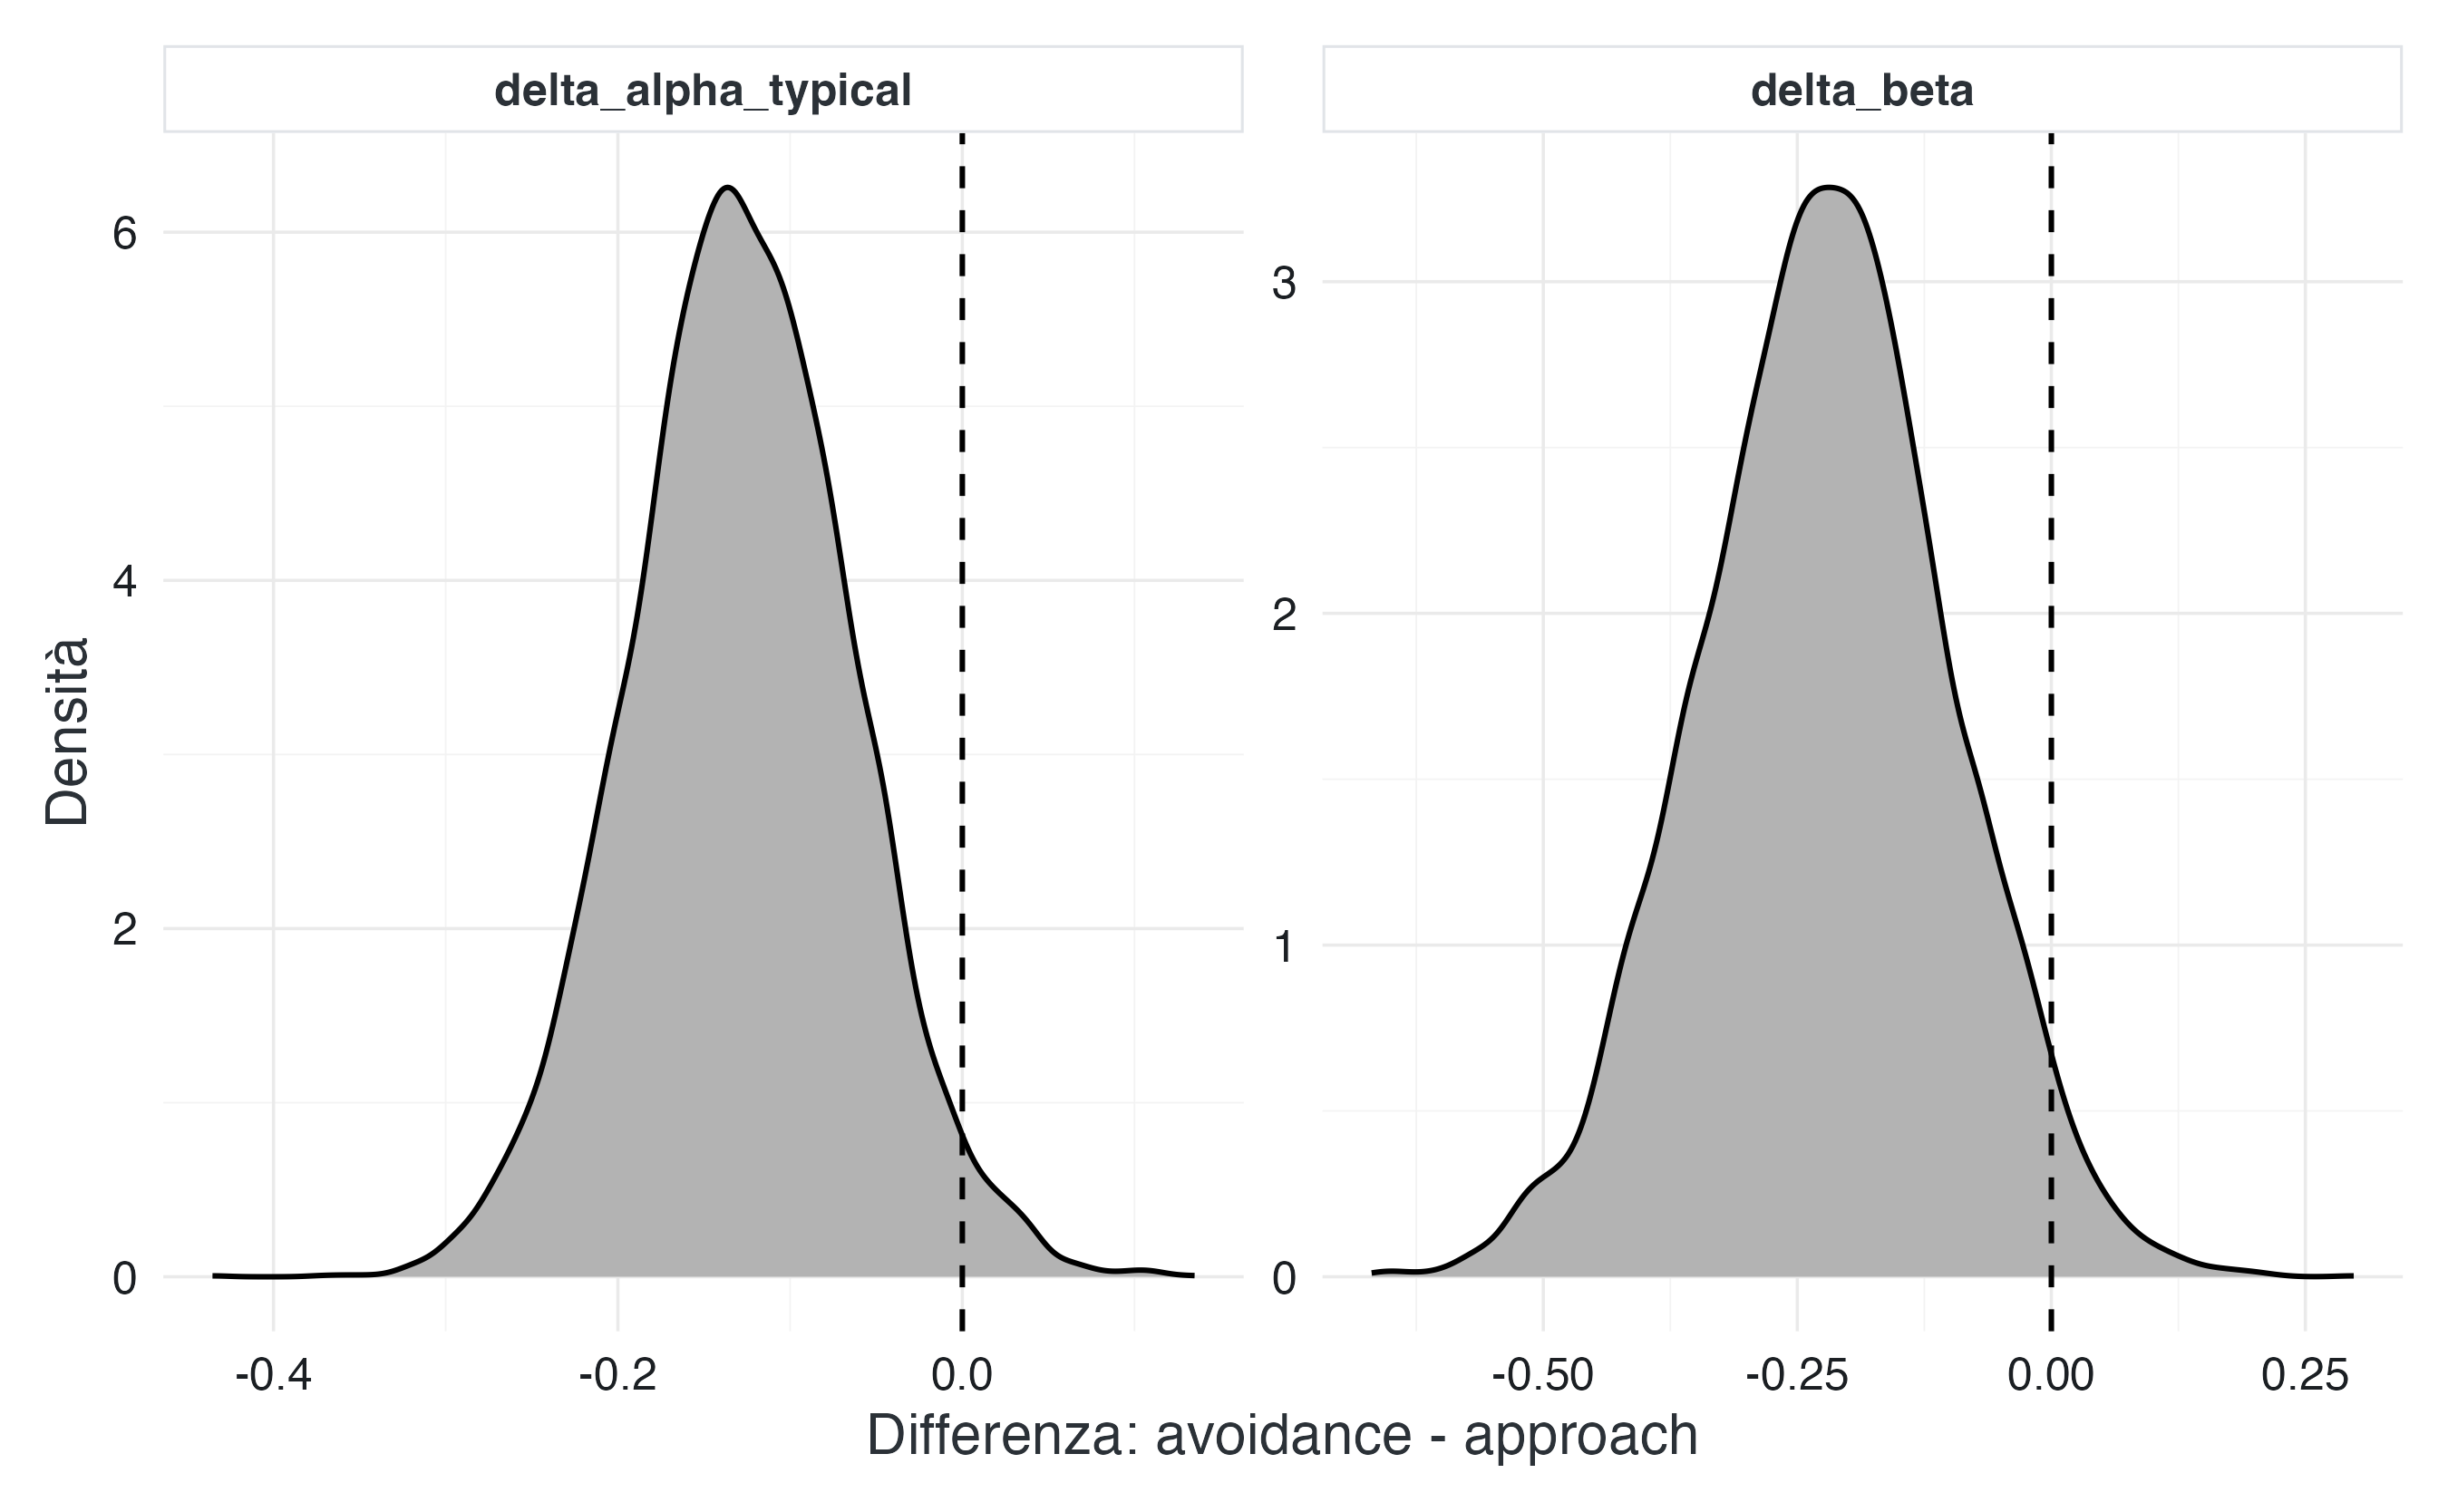
\includegraphics[width=0.85\linewidth,height=\textheight,keepaspectratio]{chapters/formal_models/03_eterogeneita_modelli_dinamici_files/figure-pdf/fig-condition-contrasts-goal-1.png}

}

\caption{\label{fig-condition-contrasts-goal}Distribuzioni posteriori
dei contrasti avoidance meno approach per il valore tipico di alpha e
per la deriva media beta.}

\end{figure}%

Il contrasto su \(\alpha\) viene calcolato sulla scala interpretabile
\(0\)--\(1\), non sulla scala logit. Il contrasto su \(\beta\) rimane
espresso in punti dell'obiettivo per trial.

\begin{tcolorbox}[enhanced jigsaw, arc=.35mm, bottomrule=.15mm, bottomtitle=1mm, breakable, colback=white, colbacktitle=quarto-callout-warning-color!10!white, colframe=quarto-callout-warning-color-frame, coltitle=black, left=2mm, leftrule=.75mm, opacityback=0, opacitybacktitle=0.6, rightrule=.15mm, title=\textcolor{quarto-callout-warning-color}{\faExclamationTriangle}\hspace{0.5em}{Differenza tra condizioni ed effetto causale}, titlerule=0mm, toprule=.15mm, toptitle=1mm]

Una differenza tra iperparametri riceve un'interpretazione causale
soltanto se la condizione è stata assegnata mediante un disegno che
identifica l'effetto e se le altre assunzioni causali sono plausibili.
Il modello gerarchico quantifica la differenza; non crea da solo
l'identificazione.

\end{tcolorbox}

\section{Recuperabilità nel modello
gerarchico}\label{recuperabilituxe0-nel-modello-gerarchico}

Quando il numero di trial per persona è piccolo, i parametri individuali
possono risultare fortemente correlati o scarsamente identificati. Un
buon adattamento aggregato non garantisce che \(\alpha_s\) e \(\beta_s\)
siano recuperabili.

\begin{tcolorbox}[enhanced jigsaw, arc=.35mm, bottomrule=.15mm, bottomtitle=1mm, breakable, colback=white, colbacktitle=quarto-callout-tip-color!10!white, colframe=quarto-callout-tip-color-frame, coltitle=black, left=2mm, leftrule=.75mm, opacityback=0, opacitybacktitle=0.6, rightrule=.15mm, title=\textcolor{quarto-callout-tip-color}{\faLightbulb}\hspace{0.5em}{Esercizio computazionale: recupero dei parametri individuali}, titlerule=0mm, toprule=.15mm, toptitle=1mm]

\begin{Shaded}
\begin{Highlighting}[]
\NormalTok{simulate\_hierarchical\_goal\_data }\OtherTok{\textless{}{-}} \ControlFlowTok{function}\NormalTok{(}
\NormalTok{    data,}
    \AttributeTok{mu\_alpha\_logit =} \DecValTok{0}\NormalTok{,}
    \AttributeTok{tau\_alpha\_logit =} \FloatTok{0.60}\NormalTok{,}
    \AttributeTok{mu\_beta =} \FloatTok{0.10}\NormalTok{,}
    \AttributeTok{tau\_beta =} \FloatTok{0.20}\NormalTok{,}
    \AttributeTok{sigma =} \FloatTok{0.60}\NormalTok{,}
    \AttributeTok{seed =} \DecValTok{775}
\NormalTok{) \{}
  \FunctionTok{set.seed}\NormalTok{(seed)}

\NormalTok{  subject\_parameters }\OtherTok{\textless{}{-}}\NormalTok{ data }\SpecialCharTok{|\textgreater{}}
    \FunctionTok{distinct}\NormalTok{(subject) }\SpecialCharTok{|\textgreater{}}
    \FunctionTok{arrange}\NormalTok{(subject) }\SpecialCharTok{|\textgreater{}}
    \FunctionTok{mutate}\NormalTok{(}
      \AttributeTok{alpha\_true =} \FunctionTok{plogis}\NormalTok{(}
        \FunctionTok{rnorm}\NormalTok{(}\FunctionTok{n}\NormalTok{(), mu\_alpha\_logit, tau\_alpha\_logit)}
\NormalTok{      ),}
      \AttributeTok{beta\_true =} \FunctionTok{rnorm}\NormalTok{(}\FunctionTok{n}\NormalTok{(), mu\_beta, tau\_beta)}
\NormalTok{    )}

\NormalTok{  simulated }\OtherTok{\textless{}{-}}\NormalTok{ data }\SpecialCharTok{|\textgreater{}}
    \FunctionTok{left\_join}\NormalTok{(subject\_parameters, }\AttributeTok{by =} \StringTok{"subject"}\NormalTok{) }\SpecialCharTok{|\textgreater{}}
    \FunctionTok{group\_by}\NormalTok{(subject) }\SpecialCharTok{|\textgreater{}}
    \FunctionTok{group\_modify}\NormalTok{(}
      \SpecialCharTok{\textasciitilde{}}\NormalTok{ \{}
\NormalTok{        path }\OtherTok{\textless{}{-}} \FunctionTok{simulate\_goal\_path}\NormalTok{(}
          \AttributeTok{performance =}\NormalTok{ .x}\SpecialCharTok{$}\NormalTok{performance,}
          \AttributeTok{initial\_goal =}\NormalTok{ .x}\SpecialCharTok{$}\NormalTok{goal[}\DecValTok{1}\NormalTok{],}
          \AttributeTok{alpha =}\NormalTok{ .x}\SpecialCharTok{$}\NormalTok{alpha\_true[}\DecValTok{1}\NormalTok{],}
          \AttributeTok{beta =}\NormalTok{ .x}\SpecialCharTok{$}\NormalTok{beta\_true[}\DecValTok{1}\NormalTok{],}
          \AttributeTok{sigma =}\NormalTok{ sigma}
\NormalTok{        )}

        \FunctionTok{mutate}\NormalTok{(.x, }\AttributeTok{goal\_simulated =}\NormalTok{ path}\SpecialCharTok{$}\NormalTok{observed)}
\NormalTok{      \}}
\NormalTok{    ) }\SpecialCharTok{|\textgreater{}}
    \FunctionTok{ungroup}\NormalTok{()}

  \FunctionTok{list}\NormalTok{(}\AttributeTok{data =}\NormalTok{ simulated, }\AttributeTok{parameters =}\NormalTok{ subject\_parameters)}
\NormalTok{\}}

\NormalTok{recovery }\OtherTok{\textless{}{-}} \FunctionTok{simulate\_hierarchical\_goal\_data}\NormalTok{(goal\_data)}

\NormalTok{recovery\_data }\OtherTok{\textless{}{-}}\NormalTok{ recovery}\SpecialCharTok{$}\NormalTok{data }\SpecialCharTok{|\textgreater{}}
  \FunctionTok{mutate}\NormalTok{(}\AttributeTok{goal =}\NormalTok{ goal\_simulated)}

\NormalTok{fit\_goal\_hierarchical\_recovery }\OtherTok{\textless{}{-}}\NormalTok{ model\_goal\_hierarchical}\SpecialCharTok{$}\FunctionTok{sample}\NormalTok{(}
  \AttributeTok{data =} \FunctionTok{make\_goal\_stan\_data}\NormalTok{(recovery\_data),}
  \AttributeTok{seed =} \DecValTok{775}\NormalTok{,}
  \AttributeTok{chains =} \DecValTok{4}\NormalTok{,}
  \AttributeTok{parallel\_chains =} \DecValTok{4}\NormalTok{,}
  \AttributeTok{iter\_warmup =} \DecValTok{1500}\NormalTok{,}
  \AttributeTok{iter\_sampling =} \DecValTok{2000}\NormalTok{,}
  \AttributeTok{adapt\_delta =} \FloatTok{0.95}
\NormalTok{)}

\NormalTok{recovered\_parameters }\OtherTok{\textless{}{-}}\NormalTok{ fit\_goal\_hierarchical\_recovery }\SpecialCharTok{|\textgreater{}}
  \FunctionTok{spread\_draws}\NormalTok{(alpha[subject], beta[subject]) }\SpecialCharTok{|\textgreater{}}
  \FunctionTok{summarise}\NormalTok{(}
    \AttributeTok{alpha\_estimated =} \FunctionTok{mean}\NormalTok{(alpha),}
    \AttributeTok{beta\_estimated =} \FunctionTok{mean}\NormalTok{(beta),}
    \AttributeTok{.by =}\NormalTok{ subject}
\NormalTok{  ) }\SpecialCharTok{|\textgreater{}}
  \FunctionTok{left\_join}\NormalTok{(recovery}\SpecialCharTok{$}\NormalTok{parameters, }\AttributeTok{by =} \StringTok{"subject"}\NormalTok{)}

\NormalTok{recovered\_parameters }\SpecialCharTok{|\textgreater{}}
  \FunctionTok{select}\NormalTok{(}
\NormalTok{    subject,}
\NormalTok{    alpha\_true,}
\NormalTok{    alpha\_estimated,}
\NormalTok{    beta\_true,}
\NormalTok{    beta\_estimated}
\NormalTok{  )}
\end{Highlighting}
\end{Shaded}

Occorre esaminare bias, correlazione tra valori veri e stimati,
copertura degli intervalli e dipendenza tra errori di recupero. Una
correlazione elevata, da sola, non esclude bias sistematico.

\end{tcolorbox}

\section{Confrontare modelli dinamici: quale unità lasciare
fuori?}\label{confrontare-modelli-dinamici-quale-unituxe0-lasciare-fuori}

Nei dati sequenziali non è corretto applicare meccanicamente una
leave-one-out cross-validation a singole righe come se i trial fossero
scambiabili e indipendenti.

La strategia dipende dalla domanda predittiva.

\begin{itemize}
\tightlist
\item
  \textbf{Nuovo trial futuro della stessa persona:} è appropriata una
  validazione temporale, nella quale si stimano i parametri sui trial
  iniziali e si prevedono quelli successivi.
\item
  \textbf{Nuova persona della stessa popolazione:} occorre lasciare
  fuori interi individui e integrare sui loro parametri non osservati.
\item
  \textbf{Nuova condizione o nuovo contesto:} serve una validazione che
  rispetti tale livello di generalizzazione.
\end{itemize}

La parte \textbf{Valutazione} svilupperà sistematicamente il confronto
predittivo. Qui il punto essenziale è che l'unità lasciata fuori deve
corrispondere all'enunciato di generalizzazione che intendiamo
formulare.

\section{Limiti della specificazione
gerarchica}\label{limiti-della-specificazione-gerarchica}

Il modello rappresenta differenze quantitative tra persone, ma conserva
assunzioni forti.

\begin{itemize}
\tightlist
\item
  \(\alpha_s\) e \(\beta_s\) sono costanti nel tempo.
\item
  Le distribuzioni individuali sono unimodali.
\item
  \(\alpha_s\) e \(\beta_s\) sono a priori indipendenti date le
  rispettive popolazioni.
\item
  La dispersione residua è uguale per tutti.
\item
  La condizione modifica le ipermedie, non la forma della regola.
\item
  Le persone differiscono lungo gli stessi parametri; non sono
  rappresentate strategie qualitativamente differenti.
\end{itemize}

Un modello di mistura, un modello a stati nascosti o una dinamica con
parametri variabili nel tempo potrebbero essere necessari se i controlli
mostrassero sottogruppi o cambi di strategia.

\section{Errori frequenti}\label{errori-frequenti-12}

\begin{itemize}
\tightlist
\item
  Interpretare la dispersione delle stime no pooling come eterogeneità
  vera.
\item
  Presentare le mediane individuali senza intervalli di incertezza.
\item
  Descrivere lo shrinkage come un'aggiustamento arbitrario verso la
  media.
\item
  Confondere \texttt{tau\_alpha\_logit} con la deviazione standard di
  \(\alpha\) sulla scala \(0\)--\(1\).
\item
  Classificare le persone in profili usando parametri scarsamente
  recuperabili.
\item
  Concludere che un parametro sia un tratto stabile perché varia tra
  soggetti.
\item
  Usare la previsione condizionata su una persona osservata come
  previsione per una persona nuova.
\item
  Applicare LOO a singoli trial ignorando dipendenza temporale e
  struttura gerarchica.
\item
  Interpretare una differenza tra condizioni come causale senza
  considerare il disegno.
\item
  Aumentare la complessità gerarchica senza controlli predittivi e di
  recuperabilità.
\end{itemize}

\section{Riflessioni conclusive}\label{riflessioni-conclusive-37}

Il passaggio dal parametro comune ai parametri individuali non è
soltanto un aumento del numero di coefficienti. Cambia l'oggetto
dell'inferenza: vogliamo conoscere contemporaneamente la distribuzione
dei processi nella popolazione, l'incertezza sui singoli e la relazione
tra i due livelli.

Il no pooling rende visibili le differenze, ma confonde facilmente
eterogeneità e rumore. Il partial pooling stabilizza le stime facendo
dipendere i parametri individuali da una struttura condivisa. Questa
dipendenza produce shrinkage e permette di generare previsioni per
persone non ancora osservate.

L'estensione alle condizioni sperimentali mostra inoltre come una
manipolazione possa essere formulata come differenza tra distribuzioni
di parametri processuali, anziché soltanto come differenza tra medie
osservate. La forza teorica di questa interpretazione dipende però da
recuperabilità, adeguatezza del modello, validità del disegno e capacità
di generalizzare.

Nel prossimo capitolo applicheremo lo stesso workflow a un modello
canonico dell'apprendimento: Rescorla--Wagner. Lo stato non sarà più un
obiettivo dichiarato, ma il valore atteso di un esito; il modello
osservazionale collegherà tale stato alle scelte trial per trial.

\section{Concetti da ricordare}\label{concetti-da-ricordare-11}

\begin{enumerate}
\def\labelenumi{\arabic{enumi}.}
\tightlist
\item
  Complete pooling, no pooling e partial pooling rappresentano ipotesi
  differenti sulla popolazione.
\item
  La variabilità delle stime individuali contiene eterogeneità e
  incertezza.
\item
  Il modello gerarchico stima simultaneamente parametri individuali e
  distribuzioni di popolazione.
\item
  Lo shrinkage è una conseguenza del modello congiunto, non una
  correzione esterna.
\item
  La dispersione di \(\alpha\) deve essere interpretata considerando la
  scala logit.
\item
  Una persona nuova richiede parametri generati dalla distribuzione di
  popolazione.
\item
  Parametri individuali interpretabili richiedono controlli di
  recuperabilità.
\item
  Le differenze tra condizioni devono essere costruite sulla scala
  sostantiva appropriata.
\item
  La validazione deve lasciare fuori l'unità alla quale si intende
  generalizzare.
\item
  Una struttura gerarchica non trasforma automaticamente un parametro in
  un tratto psicologico stabile.
\end{enumerate}

\begin{tcolorbox}[enhanced jigsaw, arc=.35mm, bottomrule=.15mm, bottomtitle=1mm, breakable, colback=white, colbacktitle=quarto-callout-note-color!10!white, colframe=quarto-callout-note-color-frame, coltitle=black, left=2mm, leftrule=.75mm, opacityback=0, opacitybacktitle=0.6, rightrule=.15mm, title=\textcolor{quarto-callout-note-color}{\faInfo}\hspace{0.5em}{Esercizi}, titlerule=0mm, toprule=.15mm, toptitle=1mm]

\subsection{1. Tre strategie di pooling}\label{tre-strategie-di-pooling}

Descrivi quale strategia useresti per stimare i parametri di cinque
persone con cento trial ciascuna e quale per cento persone con cinque
trial ciascuna.

\subsection{2. Shrinkage}\label{shrinkage}

Individua nel grafico le persone che subiscono la contrazione maggiore.
Quali caratteristiche delle loro stime no pooling potrebbero spiegarlo?

\subsection{3. Scala logit}\label{scala-logit}

Calcola \(\operatorname{logit}^{-1}(\mu_\alpha)\) per
\(\mu_\alpha=-2,0,2\). Spiega perché differenze uguali sulla scala logit
non corrispondono a differenze uguali sulla scala di \(\alpha\).

\subsection{4. Eterogeneità o
incertezza}\label{eterogeneituxe0-o-incertezza}

Costruisci due scenari: uno con elevata eterogeneità e posterior
individuali precise; uno con bassa eterogeneità e posterior individuali
ampie.

\subsection{5. Nuovo individuo}\label{nuovo-individuo}

Modifica il codice predittivo aumentando \texttt{tau\_alpha\_logit}.
Come cambia la dispersione delle traiettorie di una nuova persona?

\subsection{6. Condizioni}\label{condizioni}

Definisci una SESOI per la differenza tra i valori tipici di \(\alpha\)
nelle due condizioni e calcola la probabilità che il contrasto la
superi.

\subsection{7. Recuperabilità}\label{recuperabilituxe0-1}

Riduci il dataset simulato da dieci a cinque trial per persona. Valuta
come cambia il recupero di \(\alpha_s\) e \(\beta_s\).

\subsection{8. Correlazione tra
parametri}\label{correlazione-tra-parametri}

Proponi un'estensione che consenta correlazione di popolazione tra
\(\operatorname{logit}(\alpha_s)\) e \(\beta_s\).

\subsection{9. Validazione}\label{validazione}

Spiega perché lasciare fuori un singolo trial non risponde alla domanda
``il modello generalizza a nuove persone?''.

\subsection{10. Strategie qualitative}\label{strategie-qualitative}

Descrivi un pattern che suggerirebbe la presenza di due strategie
qualitative, anziché una distribuzione unimodale degli stessi parametri.

\begin{quote}
\textbf{Tracce di soluzione}

\begin{enumerate}
\def\labelenumi{\arabic{enumi}.}
\tightlist
\item
  La risposta dipende anche dall'obiettivo, ma molti trial individuali
  rendono più sostenibile il no pooling; pochi trial per persona rendono
  particolarmente utile il partial pooling.
\item
  In genere le stime più estreme o meno informative vengono
  regolarizzate maggiormente.
\item
  I valori sono circa 0.12, 0.50 e 0.88; la funzione logistica è non
  lineare.
\item
  Occorre distinguere dispersione delle distribuzioni individuali e
  larghezza delle posterior delle singole persone.
\item
  Aumenta l'eterogeneità predittiva tra nuovi individui.
\item
  La soglia deve derivare dal contesto sostantivo, non dalla sola
  posterior.
\item
  Con meno trial aumentano incertezza, shrinkage e possibili trade-off
  tra parametri.
\item
  Si può usare una distribuzione normale multivariata con matrice di
  correlazione LKJ.
\item
  La persona e i suoi parametri restano inclusi nella stima; la prova
  non valuta un nuovo livello gerarchico.
\item
  Esempi: cluster distinti, cambiamenti bruschi, segni opposti o pattern
  che una singola distribuzione continua non riesce a riprodurre.
\end{enumerate}
\end{quote}

\end{tcolorbox}

\begin{tcolorbox}[enhanced jigsaw, arc=.35mm, bottomrule=.15mm, bottomtitle=1mm, breakable, colback=white, colbacktitle=quarto-callout-note-color!10!white, colframe=quarto-callout-note-color-frame, coltitle=black, left=2mm, leftrule=.75mm, opacityback=0, opacitybacktitle=0.6, rightrule=.15mm, title=\textcolor{quarto-callout-note-color}{\faInfo}\hspace{0.5em}{Informazioni sull'ambiente di sviluppo}, titlerule=0mm, toprule=.15mm, toptitle=1mm]

\begin{Shaded}
\begin{Highlighting}[]
\FunctionTok{sessionInfo}\NormalTok{()}
\CommentTok{\#\textgreater{} R version 4.6.1 (2026{-}06{-}24)}
\CommentTok{\#\textgreater{} Platform: aarch64{-}apple{-}darwin23}
\CommentTok{\#\textgreater{} Running under: macOS Tahoe 26.5.2}
\CommentTok{\#\textgreater{} }
\CommentTok{\#\textgreater{} Matrix products: default}
\CommentTok{\#\textgreater{} BLAS:   /Library/Frameworks/R.framework/Versions/4.6/Resources/lib/libRblas.0.dylib }
\CommentTok{\#\textgreater{} LAPACK: /Library/Frameworks/R.framework/Versions/4.6/Resources/lib/libRlapack.dylib;  LAPACK version 3.12.1}
\CommentTok{\#\textgreater{} }
\CommentTok{\#\textgreater{} locale:}
\CommentTok{\#\textgreater{} [1] C.UTF{-}8/UTF{-}8/C.UTF{-}8/C/C.UTF{-}8/C.UTF{-}8}
\CommentTok{\#\textgreater{} }
\CommentTok{\#\textgreater{} time zone: Europe/Zagreb}
\CommentTok{\#\textgreater{} tzcode source: internal}
\CommentTok{\#\textgreater{} }
\CommentTok{\#\textgreater{} attached base packages:}
\CommentTok{\#\textgreater{} [1] stats     graphics  grDevices utils     datasets  methods   base     }
\CommentTok{\#\textgreater{} }
\CommentTok{\#\textgreater{} other attached packages:}
\CommentTok{\#\textgreater{}  [1] cmdstanr\_0.9.0        ragg\_1.5.2            tinytable\_0.17.0     }
\CommentTok{\#\textgreater{}  [4] withr\_3.0.3           systemfonts\_1.3.2     patchwork\_1.3.2      }
\CommentTok{\#\textgreater{}  [7] ggdist\_3.3.3          tidybayes\_3.0.7       bayesplot\_1.15.0     }
\CommentTok{\#\textgreater{} [10] ggplot2\_4.0.3         reliabilitydiag\_0.2.1 priorsense\_1.2.0     }
\CommentTok{\#\textgreater{} [13] posterior\_1.7.0       loo\_2.10.0            rstan\_2.32.7         }
\CommentTok{\#\textgreater{} [16] StanHeaders\_2.32.10   brms\_2.23.0           Rcpp\_1.1.2           }
\CommentTok{\#\textgreater{} [19] sessioninfo\_1.2.4     conflicted\_1.2.0      janitor\_2.2.1        }
\CommentTok{\#\textgreater{} [22] matrixStats\_1.5.0     modelr\_0.1.11         tibble\_3.3.1         }
\CommentTok{\#\textgreater{} [25] dplyr\_1.2.1           tidyr\_1.3.2           rio\_1.3.0            }
\CommentTok{\#\textgreater{} [28] here\_1.0.2           }
\CommentTok{\#\textgreater{} }
\CommentTok{\#\textgreater{} loaded via a namespace (and not attached):}
\CommentTok{\#\textgreater{}  [1] gridExtra\_2.3.1       inline\_0.3.21         rlang\_1.3.0          }
\CommentTok{\#\textgreater{}  [4] magrittr\_2.0.5        snakecase\_0.11.1      otel\_0.2.0           }
\CommentTok{\#\textgreater{}  [7] compiler\_4.6.1        vctrs\_0.7.3           reshape2\_1.4.5       }
\CommentTok{\#\textgreater{} [10] stringr\_1.6.0         pkgconfig\_2.0.3       arrayhelpers\_1.1{-}1   }
\CommentTok{\#\textgreater{} [13] fastmap\_1.2.0         backports\_1.5.1       labeling\_0.4.3       }
\CommentTok{\#\textgreater{} [16] utf8\_1.2.6            rmarkdown\_2.31        ps\_1.9.3             }
\CommentTok{\#\textgreater{} [19] purrr\_1.2.2           xfun\_0.60             cachem\_1.1.0         }
\CommentTok{\#\textgreater{} [22] jsonlite\_2.0.0        broom\_1.0.13          parallel\_4.6.1       }
\CommentTok{\#\textgreater{} [25] R6\_2.6.1              stringi\_1.8.7         RColorBrewer\_1.1{-}3   }
\CommentTok{\#\textgreater{} [28] lubridate\_1.9.5       estimability\_2.0.0    knitr\_1.51           }
\CommentTok{\#\textgreater{} [31] R.utils\_2.13.0        Matrix\_1.7{-}5          timechange\_0.4.0     }
\CommentTok{\#\textgreater{} [34] tidyselect\_1.2.1      abind\_1.4{-}8           yaml\_2.3.12          }
\CommentTok{\#\textgreater{} [37] codetools\_0.2{-}20      curl\_7.1.0            processx\_3.9.0       }
\CommentTok{\#\textgreater{} [40] pkgbuild\_1.4.8        plyr\_1.8.9            lattice\_0.22{-}9       }
\CommentTok{\#\textgreater{} [43] bridgesampling\_1.2{-}1  S7\_0.2.2              coda\_0.19{-}4.1        }
\CommentTok{\#\textgreater{} [46] evaluate\_1.0.5        RcppParallel\_5.1.11{-}2 pillar\_1.11.1        }
\CommentTok{\#\textgreater{} [49] tensorA\_0.36.2.1      checkmate\_2.3.4       stats4\_4.6.1         }
\CommentTok{\#\textgreater{} [52] distributional\_0.8.1  generics\_0.1.4        rprojroot\_2.1.1      }
\CommentTok{\#\textgreater{} [55] rstantools\_2.6.0      scales\_1.4.0          xtable\_1.8{-}8         }
\CommentTok{\#\textgreater{} [58] glue\_1.8.1            emmeans\_2.0.4         tools\_4.6.1          }
\CommentTok{\#\textgreater{} [61] data.table\_1.18.4     mvtnorm\_1.4{-}2         grid\_4.6.1           }
\CommentTok{\#\textgreater{} [64] QuickJSR\_1.10.0       nlme\_3.1{-}170          cli\_3.6.6            }
\CommentTok{\#\textgreater{} [67] textshaping\_1.0.5     svUnit\_1.0.8          Brobdingnag\_1.2{-}9    }
\CommentTok{\#\textgreater{} [70] V8\_8.2.0              gtable\_0.3.6          R.methodsS3\_1.8.2    }
\CommentTok{\#\textgreater{} [73] digest\_0.6.39         farver\_2.1.2          memoise\_2.0.1        }
\CommentTok{\#\textgreater{} [76] htmltools\_0.5.9       R.oo\_1.27.1           lifecycle\_1.0.5}
\end{Highlighting}
\end{Shaded}

\end{tcolorbox}

\section*{Bibliografia}\label{bibliografia-42}

\markright{Bibliografia}

\chapter{Rescorla--Wagner: dall'errore di previsione alla
scelta}\label{sec-dynamic-models-rescorla-wagner}

Il modello di Rescorla--Wagner costituisce un caso paradigmatico di
modellazione processuale. Una teoria verbale dell'apprendimento viene
tradotta in una regola di aggiornamento; gli stati latenti prodotti da
tale regola vengono collegati alle scelte mediante un modello
osservazionale; i parametri vengono quindi inferiti dal comportamento e
sottoposti a controlli di recuperabilità e adeguatezza.

Il valore didattico del modello non risiede soltanto nella sua
semplicità. Esso rende visibile l'intero percorso che distingue una
teoria formale da una regressione sulle risposte osservate:

\[
\begin{array}{c}
\text{feedback} \\
\downarrow \\
\text{errore di previsione} \\
\downarrow \\
\text{aggiornamento del valore} \\
\downarrow \\
\text{probabilità di scelta} \\
\downarrow \\
\text{comportamento}
\end{array}
\]

\begin{tcolorbox}[enhanced jigsaw, arc=.35mm, bottomrule=.15mm, breakable, colback=white, colframe=quarto-callout-important-color-frame, left=2mm, leftrule=.75mm, opacityback=0, rightrule=.15mm, toprule=.15mm]

\textbf{Da sapere.} Il modello di Rescorla--Wagner separa tre
componenti: una regola di apprendimento che aggiorna valori latenti
attraverso l'errore di previsione, un modello osservazionale che
trasforma le differenze di valore in probabilità di scelta e una
distribuzione per le risposte osservate. Il parametro \(\alpha\) regola
la velocità di aggiornamento, mentre \(\tau\) regola quanto
coerentemente le scelte seguono i valori appresi. I due parametri
possono compensarsi e dipendono dalla scala dei rinforzi: non devono
quindi essere interpretati come misure psicologiche dirette senza
simulazioni, controlli predittivi e verifiche di recuperabilità.

\textbf{Da saper fare.} Simulare il processo e spiegare come \(\alpha\)
e \(\tau\) modificano apprendimento e scelta; leggere il programma Stan
fornito collegandone le istruzioni alla regola ricorsiva e al modello
osservazionale; interpretare le distribuzioni a posteriori dei parametri
e le traiettorie degli stati latenti; controllare diagnostica del
campionamento, previsioni posteriori e recuperabilità dei parametri;
riconoscere quando discrepanze sequenziali suggeriscono che il modello
di base è incompleto.

\textbf{Approfondimento facoltativo.} La scrittura autonoma del
programma Stan, l'implementazione completa del modello rivale con
perseverazione, il confronto formale tra modelli e le estensioni con
apprendimento asimmetrico, decadimento o \emph{lapse} possono essere
rimandati. In questo capitolo, tuttavia, Stan è costitutivo
dell'analisi: non esiste un percorso applicativo equivalente basato
soltanto su \texttt{brms}. Nel percorso essenziale è richiesto saper
leggere e utilizzare in modo guidato il programma fornito, non scriverlo
da zero.

\hyperref[sec-percorsi-lettura]{Che cosa significano queste etichette?}

\end{tcolorbox}

\begin{tcolorbox}[enhanced jigsaw, arc=.35mm, bottomrule=.15mm, bottomtitle=1mm, breakable, colback=white, colbacktitle=quarto-callout-tip-color!10!white, colframe=quarto-callout-tip-color-frame, coltitle=black, left=2mm, leftrule=.75mm, opacityback=0, opacitybacktitle=0.6, rightrule=.15mm, title=\textcolor{quarto-callout-tip-color}{\faLightbulb}\hspace{0.5em}{Prerequisiti}, titlerule=0mm, toprule=.15mm, toptitle=1mm]

\begin{itemize}
\tightlist
\item
  Il capitolo Capitolo~\ref{sec-bayes-stat-models}, per il vocabolario
  dei modelli formali.
\item
  I capitoli Capitolo~\ref{sec-dynamic-models-goal-updating} e
  Capitolo~\ref{sec-formal-models-developments}, per regole ricorsive,
  modello osservazionale ed eterogeneità.
\item
  La parte \textbf{Calcolo}, per diagnostica MCMC e controlli
  predittivi.
\end{itemize}

\end{tcolorbox}

\begin{tcolorbox}[enhanced jigsaw, arc=.35mm, bottomrule=.15mm, bottomtitle=1mm, breakable, colback=white, colbacktitle=quarto-callout-caution-color!10!white, colframe=quarto-callout-caution-color-frame, coltitle=black, left=2mm, leftrule=.75mm, opacityback=0, opacitybacktitle=0.6, rightrule=.15mm, title=\textcolor{quarto-callout-caution-color}{\faFire}\hspace{0.5em}{Preparazione del Notebook}, titlerule=0mm, toprule=.15mm, toptitle=1mm]

\end{tcolorbox}

\section{Perché questo modello è
paradigmatico}\label{perchuxe9-questo-modello-uxe8-paradigmatico}

Il modello di Rescorla--Wagner nasce come teoria dell'apprendimento
associativo (\citeproc{ref-rescorla1972theory}{Rescorla \& Wagner,
1972}). La sua idea centrale è che l'apprendimento non dipenda
semplicemente dalla presenza congiunta di uno stimolo e di un esito, ma
dalla discrepanza tra l'esito ottenuto e quello atteso.

La versione usata nei compiti di scelta ripetuta contiene due componenti
distinte:

\begin{enumerate}
\def\labelenumi{\arabic{enumi}.}
\tightlist
\item
  un \textbf{modello di apprendimento}, che aggiorna il valore delle
  alternative;
\item
  un \textbf{modello di scelta}, che trasforma le differenze di valore
  in probabilità di risposta.
\end{enumerate}

Questa separazione è essenziale. Due persone possono mostrare una
percentuale simile di scelte corrette per ragioni differenti: una può
aggiornare lentamente i valori ma seguirli con grande coerenza; un'altra
può apprendere rapidamente ma scegliere in modo più variabile.

\begin{tcolorbox}[enhanced jigsaw, arc=.35mm, bottomrule=.15mm, bottomtitle=1mm, breakable, colback=white, colbacktitle=quarto-callout-important-color!10!white, colframe=quarto-callout-important-color-frame, coltitle=black, left=2mm, leftrule=.75mm, opacityback=0, opacitybacktitle=0.6, rightrule=.15mm, title=\textcolor{quarto-callout-important-color}{\faExclamation}\hspace{0.5em}{Una precisazione terminologica}, titlerule=0mm, toprule=.15mm, toptitle=1mm]

Il modello originale di Rescorla--Wagner descrive l'aggiornamento della
forza associativa di uno o più indizi. Nei compiti a due opzioni si usa
spesso una regola delta strettamente affine, applicata al valore
dell'opzione scelta.

Nel seguito useremo l'espressione \emph{modello Rescorla--Wagner} nel
senso ampio comune nella modellazione cognitiva, ma è utile ricordare
che la versione trial-by-trial impiegata qui non coincide in ogni
dettaglio con la formulazione originaria.

\end{tcolorbox}

\section{Il modello del processo}\label{il-modello-del-processo-1}

\subsection{Stati latenti e feedback}\label{stati-latenti-e-feedback}

Indichiamo con \(Q_t(A)\) e \(Q_t(B)\) i valori attribuiti alle due
alternative immediatamente prima del trial \(t\). Questi valori non sono
osservati direttamente: costituiscono gli stati latenti del modello.

Dopo aver scelto l'alternativa \(a_t\) e osservato il rinforzo \(R_t\),
il modello calcola l'errore di previsione:

\[
\delta_t = R_t-Q_t(a_t).
\]

Il valore dell'alternativa scelta viene quindi aggiornato secondo:

\[
Q_{t+1}(a_t)
=
Q_t(a_t)+\alpha\delta_t,
\]

mentre il valore dell'alternativa non scelta rimane invariato.

Il parametro

\[
0<\alpha<1
\]

è il \textbf{tasso di apprendimento}.

\begin{itemize}
\tightlist
\item
  Con \(\alpha\) vicino a zero, ciascun feedback modifica poco il valore
  e la storia passata conserva a lungo la propria influenza.
\item
  Con \(\alpha\) elevato, il valore risponde rapidamente agli esiti
  recenti.
\item
  Un valore elevato non è necessariamente ``migliore'': in un ambiente
  rumoroso può produrre stime instabili.
\item
  Un valore basso non implica automaticamente un deficit: può essere
  appropriato quando le contingenze sono stabili e i singoli feedback
  sono poco affidabili.
\end{itemize}

\begin{tcolorbox}[enhanced jigsaw, arc=.35mm, bottomrule=.15mm, bottomtitle=1mm, breakable, colback=white, colbacktitle=quarto-callout-note-color!10!white, colframe=quarto-callout-note-color-frame, coltitle=black, left=2mm, leftrule=.75mm, opacityback=0, opacitybacktitle=0.6, rightrule=.15mm, title=\textcolor{quarto-callout-note-color}{\faInfo}\hspace{0.5em}{Tassi diversi per esiti positivi e negativi}, titlerule=0mm, toprule=.15mm, toptitle=1mm]

Un'estensione comune usa due parametri:

\[
\alpha^+
\quad\text{e}\quad
\alpha^-,
\]

applicati rispettivamente quando \(\delta_t\geq 0\) e quando
\(\delta_t<0\).

Questa estensione è sostantiva soltanto se il disegno contiene
abbastanza errori di previsione di entrambi i segni da distinguere i due
parametri. Aggiungere parametri senza informazione sufficiente può
aumentare l'incertezza e creare nuove compensazioni.

\end{tcolorbox}

\section{Il modello osservazionale}\label{il-modello-osservazionale-1}

Gli stati \(Q_t(A)\) e \(Q_t(B)\) non sono scelte. Per collegare il
processo latente al comportamento osservato occorre una regola
probabilistica.

Con due alternative, la funzione Softmax si riduce a una regressione
logistica sulla differenza di valore:

\[
\Pr(Y_t=B)
=
\operatorname{logit}^{-1}
\left[
\tau\left\{Q_t(B)-Q_t(A)\right\}
\right],
\]

dove \(\tau>0\) è l'\textbf{inverse temperature}.

\begin{itemize}
\tightlist
\item
  Con \(\tau\) basso, anche una grande differenza tra i valori produce
  una preferenza moderata.
\item
  Con \(\tau\) alto, piccole differenze possono generare scelte quasi
  deterministiche.
\end{itemize}

La verosimiglianza delle scelte è quindi:

\[
Y_t
\sim
\operatorname{Bernoulli}(p_t),
\qquad
p_t
=
\operatorname{logit}^{-1}
\left[
\tau\left\{Q_t(B)-Q_t(A)\right\}
\right].
\]

\begin{tcolorbox}[enhanced jigsaw, arc=.35mm, bottomrule=.15mm, bottomtitle=1mm, breakable, colback=white, colbacktitle=quarto-callout-important-color!10!white, colframe=quarto-callout-important-color-frame, coltitle=black, left=2mm, leftrule=.75mm, opacityback=0, opacitybacktitle=0.6, rightrule=.15mm, title=\textcolor{quarto-callout-important-color}{\faExclamation}\hspace{0.5em}{Apprendimento e scelta non sono la stessa cosa}, titlerule=0mm, toprule=.15mm, toptitle=1mm]

Il parametro \(\alpha\) governa il cambiamento degli stati latenti dopo
il feedback. Il parametro \(\tau\) governa la relazione tra stati
latenti e risposta.

Una scelta apparentemente casuale può dipendere da valori poco
differenziati, da un \(\tau\) basso, da una tendenza a perseverare, da
distrazione o da una regola di scelta inadeguata. Per questo motivo non
è corretto interpretare direttamente la percentuale di risposte ottimali
come misura pura dell'apprendimento.

\end{tcolorbox}

\section{Scala, condizioni iniziali e
identificabilità}\label{scala-condizioni-iniziali-e-identificabilituxe0}

La scala dei valori \(Q\), la codifica del rinforzo e il parametro
\(\tau\) sono collegati.

Se tutti i valori e i rinforzi vengono moltiplicati per una costante
\(c\), la stessa probabilità di scelta può essere ottenuta dividendo
\(\tau\) per \(c\). L'inverse temperature non possiede quindi un
significato assoluto indipendente dalla scala del compito.

Nel seguito ci atteniamo a convenzioni esplicite: i rinforzi sono
codificati come \(0\) e \(1\), i valori iniziali delle due opzioni sono
\(Q_1(A)=Q_1(B)=0.5\), viene impiegato un unico tasso di apprendimento,
l'aggiornamento riguarda esclusivamente l'opzione scelta e il parametro
\(\tau\) è definito come \emph{temperatura inversa} (\emph{inverse
temperature}).

Fissare i valori iniziali evita di chiedere ai dati di distinguere
simultaneamente condizioni iniziali, tasso di apprendimento e
sensibilità di scelta. In altri contesti \(Q_0\) può essere stimato, ma
ciò richiede una motivazione e dati iniziali sufficientemente
informativi.

\section{Simulare prima di stimare}\label{simulare-prima-di-stimare-4}

\subsection{Un compito di probabilistic reversal
learning}\label{un-compito-di-probabilistic-reversal-learning}

Consideriamo un compito con due alternative. Nella prima fase, \(A\)
produce una ricompensa con probabilità \(0.7\) e \(B\) con probabilità
\(0.3\). Dopo il trial 80 le contingenze si invertono.

Definiamo un simulatore che separa ambiente, processo di apprendimento e
modello di scelta. Il parametro opzionale \texttt{kappa} rappresenta una
tendenza a ripetere la scelta precedente indipendentemente dai valori.
Per ora lo manterremo uguale a zero; lo useremo in seguito per criticare
il modello di base.

\begin{Shaded}
\begin{Highlighting}[]
\NormalTok{simulate\_prl\_rw }\OtherTok{\textless{}{-}} \ControlFlowTok{function}\NormalTok{(}
    \AttributeTok{n\_trials =} \DecValTok{160}\NormalTok{,}
    \AttributeTok{p\_reward\_rich =} \FloatTok{0.70}\NormalTok{,}
    \AttributeTok{reversal\_trial =} \DecValTok{80}\NormalTok{,}
    \AttributeTok{alpha =} \FloatTok{0.20}\NormalTok{,}
    \AttributeTok{tau =} \DecValTok{3}\NormalTok{,}
    \AttributeTok{kappa =} \DecValTok{0}\NormalTok{,}
    \AttributeTok{q0 =} \FloatTok{0.50}\NormalTok{,}
    \AttributeTok{seed =} \ConstantTok{NULL}
\NormalTok{) \{}
  \ControlFlowTok{if}\NormalTok{ (}\SpecialCharTok{!}\FunctionTok{is.null}\NormalTok{(seed)) \{}
    \FunctionTok{set.seed}\NormalTok{(seed)}
\NormalTok{  \}}

\NormalTok{  rich\_is\_A }\OtherTok{\textless{}{-}} \FunctionTok{rep}\NormalTok{(}\DecValTok{1}\NormalTok{L, n\_trials)}
  \ControlFlowTok{if}\NormalTok{ (}\SpecialCharTok{!}\FunctionTok{is.null}\NormalTok{(reversal\_trial) }\SpecialCharTok{\&\&}\NormalTok{ reversal\_trial }\SpecialCharTok{\textless{}}\NormalTok{ n\_trials) \{}
\NormalTok{    rich\_is\_A[(reversal\_trial }\SpecialCharTok{+} \DecValTok{1}\NormalTok{)}\SpecialCharTok{:}\NormalTok{n\_trials] }\OtherTok{\textless{}{-}} \DecValTok{0}\NormalTok{L}
\NormalTok{  \}}

\NormalTok{  q }\OtherTok{\textless{}{-}} \FunctionTok{c}\NormalTok{(}\AttributeTok{A =}\NormalTok{ q0, }\AttributeTok{B =}\NormalTok{ q0)}
\NormalTok{  previous\_choice }\OtherTok{\textless{}{-}} \ConstantTok{NA\_integer\_}

\NormalTok{  output }\OtherTok{\textless{}{-}} \FunctionTok{vector}\NormalTok{(}\StringTok{"list"}\NormalTok{, n\_trials)}

  \ControlFlowTok{for}\NormalTok{ (t }\ControlFlowTok{in} \FunctionTok{seq\_len}\NormalTok{(n\_trials)) \{}
\NormalTok{    q\_pre }\OtherTok{\textless{}{-}}\NormalTok{ q}

\NormalTok{    previous\_signed }\OtherTok{\textless{}{-}} \ControlFlowTok{if}\NormalTok{ (}\FunctionTok{is.na}\NormalTok{(previous\_choice)) \{}
      \DecValTok{0}
\NormalTok{    \} }\ControlFlowTok{else}\NormalTok{ \{}
      \DecValTok{2} \SpecialCharTok{*}\NormalTok{ previous\_choice }\SpecialCharTok{{-}} \DecValTok{1}
\NormalTok{    \}}

\NormalTok{    eta }\OtherTok{\textless{}{-}}\NormalTok{ tau }\SpecialCharTok{*}\NormalTok{ (q[}\StringTok{"B"}\NormalTok{] }\SpecialCharTok{{-}}\NormalTok{ q[}\StringTok{"A"}\NormalTok{]) }\SpecialCharTok{+}
\NormalTok{      kappa }\SpecialCharTok{*}\NormalTok{ previous\_signed}

\NormalTok{    p\_choose\_B }\OtherTok{\textless{}{-}} \FunctionTok{plogis}\NormalTok{(eta)}
\NormalTok{    choice }\OtherTok{\textless{}{-}} \FunctionTok{rbinom}\NormalTok{(}\DecValTok{1}\NormalTok{, }\AttributeTok{size =} \DecValTok{1}\NormalTok{, }\AttributeTok{prob =}\NormalTok{ p\_choose\_B)}

\NormalTok{    chosen\_is\_rich }\OtherTok{\textless{}{-}}
\NormalTok{      (choice }\SpecialCharTok{==} \DecValTok{0}\NormalTok{L }\SpecialCharTok{\&\&}\NormalTok{ rich\_is\_A[t] }\SpecialCharTok{==} \DecValTok{1}\NormalTok{L) }\SpecialCharTok{||}
\NormalTok{      (choice }\SpecialCharTok{==} \DecValTok{1}\NormalTok{L }\SpecialCharTok{\&\&}\NormalTok{ rich\_is\_A[t] }\SpecialCharTok{==} \DecValTok{0}\NormalTok{L)}

\NormalTok{    reward\_probability }\OtherTok{\textless{}{-}} \ControlFlowTok{if}\NormalTok{ (chosen\_is\_rich) \{}
\NormalTok{      p\_reward\_rich}
\NormalTok{    \} }\ControlFlowTok{else}\NormalTok{ \{}
      \DecValTok{1} \SpecialCharTok{{-}}\NormalTok{ p\_reward\_rich}
\NormalTok{    \}}

\NormalTok{    reward }\OtherTok{\textless{}{-}} \FunctionTok{rbinom}\NormalTok{(}\DecValTok{1}\NormalTok{, }\AttributeTok{size =} \DecValTok{1}\NormalTok{, }\AttributeTok{prob =}\NormalTok{ reward\_probability)}

\NormalTok{    chosen\_index }\OtherTok{\textless{}{-}}\NormalTok{ choice }\SpecialCharTok{+} \DecValTok{1}\NormalTok{L}
\NormalTok{    prediction\_error }\OtherTok{\textless{}{-}}\NormalTok{ reward }\SpecialCharTok{{-}}\NormalTok{ q[chosen\_index]}
\NormalTok{    q[chosen\_index] }\OtherTok{\textless{}{-}}\NormalTok{ q[chosen\_index] }\SpecialCharTok{+}
\NormalTok{      alpha }\SpecialCharTok{*}\NormalTok{ prediction\_error}

\NormalTok{    optimal\_choice }\OtherTok{\textless{}{-}} \FunctionTok{ifelse}\NormalTok{(rich\_is\_A[t] }\SpecialCharTok{==} \DecValTok{1}\NormalTok{L, }\DecValTok{0}\NormalTok{L, }\DecValTok{1}\NormalTok{L)}

\NormalTok{    output[[t]] }\OtherTok{\textless{}{-}} \FunctionTok{tibble}\NormalTok{(}
      \AttributeTok{trial =}\NormalTok{ t,}
      \AttributeTok{rich\_is\_A =}\NormalTok{ rich\_is\_A[t],}
      \AttributeTok{optimal\_choice =}\NormalTok{ optimal\_choice,}
      \AttributeTok{choice =}\NormalTok{ choice,}
      \AttributeTok{reward =}\NormalTok{ reward,}
      \AttributeTok{reward\_probability =}\NormalTok{ reward\_probability,}
      \AttributeTok{q\_A\_pre =}\NormalTok{ q\_pre[}\StringTok{"A"}\NormalTok{],}
      \AttributeTok{q\_B\_pre =}\NormalTok{ q\_pre[}\StringTok{"B"}\NormalTok{],}
      \AttributeTok{q\_A\_post =}\NormalTok{ q[}\StringTok{"A"}\NormalTok{],}
      \AttributeTok{q\_B\_post =}\NormalTok{ q[}\StringTok{"B"}\NormalTok{],}
      \AttributeTok{p\_choose\_B =}\NormalTok{ p\_choose\_B,}
      \AttributeTok{prediction\_error =}\NormalTok{ prediction\_error}
\NormalTok{    )}

\NormalTok{    previous\_choice }\OtherTok{\textless{}{-}}\NormalTok{ choice}
\NormalTok{  \}}

  \FunctionTok{bind\_rows}\NormalTok{(output)}
\NormalTok{\}}
\end{Highlighting}
\end{Shaded}

\subsection{Che cosa fanno i
parametri?}\label{che-cosa-fanno-i-parametri}

Simuliamo quattro combinazioni di \(\alpha\) e \(\tau\).

\begin{Shaded}
\begin{Highlighting}[]
\NormalTok{rw\_scenarios }\OtherTok{\textless{}{-}} \FunctionTok{tribble}\NormalTok{(}
  \SpecialCharTok{\textasciitilde{}}\NormalTok{scenario, }\SpecialCharTok{\textasciitilde{}}\NormalTok{alpha, }\SpecialCharTok{\textasciitilde{}}\NormalTok{tau,}
  \StringTok{"Apprendimento lento, scelta variabile"}\NormalTok{, }\FloatTok{0.08}\NormalTok{, }\FloatTok{1.0}\NormalTok{,}
  \StringTok{"Apprendimento lento, scelta coerente"}\NormalTok{, }\FloatTok{0.08}\NormalTok{, }\FloatTok{5.0}\NormalTok{,}
  \StringTok{"Apprendimento rapido, scelta variabile"}\NormalTok{, }\FloatTok{0.55}\NormalTok{, }\FloatTok{1.0}\NormalTok{,}
  \StringTok{"Apprendimento rapido, scelta coerente"}\NormalTok{, }\FloatTok{0.55}\NormalTok{, }\FloatTok{5.0}
\NormalTok{)}

\NormalTok{rw\_scenario\_data }\OtherTok{\textless{}{-}}\NormalTok{ rw\_scenarios }\SpecialCharTok{|\textgreater{}}
  \FunctionTok{mutate}\NormalTok{(}
    \AttributeTok{simulation\_seed =} \DecValTok{900} \SpecialCharTok{+} \FunctionTok{row\_number}\NormalTok{(),}
    \AttributeTok{simulation =}\NormalTok{ purrr}\SpecialCharTok{::}\FunctionTok{pmap}\NormalTok{(}
      \FunctionTok{list}\NormalTok{(alpha, tau, simulation\_seed),}
      \SpecialCharTok{\textasciitilde{}} \FunctionTok{simulate\_prl\_rw}\NormalTok{(}
        \AttributeTok{alpha =}\NormalTok{ ..}\DecValTok{1}\NormalTok{,}
        \AttributeTok{tau =}\NormalTok{ ..}\DecValTok{2}\NormalTok{,}
        \AttributeTok{seed =}\NormalTok{ ..}\DecValTok{3}
\NormalTok{      )}
\NormalTok{    )}
\NormalTok{  ) }\SpecialCharTok{|\textgreater{}}
  \FunctionTok{select}\NormalTok{(scenario, simulation) }\SpecialCharTok{|\textgreater{}}
\NormalTok{  tidyr}\SpecialCharTok{::}\FunctionTok{unnest}\NormalTok{(simulation) }\SpecialCharTok{|\textgreater{}}
  \FunctionTok{group\_by}\NormalTok{(scenario) }\SpecialCharTok{|\textgreater{}}
  \FunctionTok{mutate}\NormalTok{(}
    \AttributeTok{rolling\_optimal =}\NormalTok{ slider}\SpecialCharTok{::}\FunctionTok{slide\_dbl}\NormalTok{(}
\NormalTok{      choice }\SpecialCharTok{==}\NormalTok{ optimal\_choice,}
\NormalTok{      mean,}
      \AttributeTok{.before =} \DecValTok{9}\NormalTok{,}
      \AttributeTok{.complete =} \ConstantTok{FALSE}
\NormalTok{    )}
\NormalTok{  ) }\SpecialCharTok{|\textgreater{}}
  \FunctionTok{ungroup}\NormalTok{()}
\end{Highlighting}
\end{Shaded}

\begin{figure}

\centering{

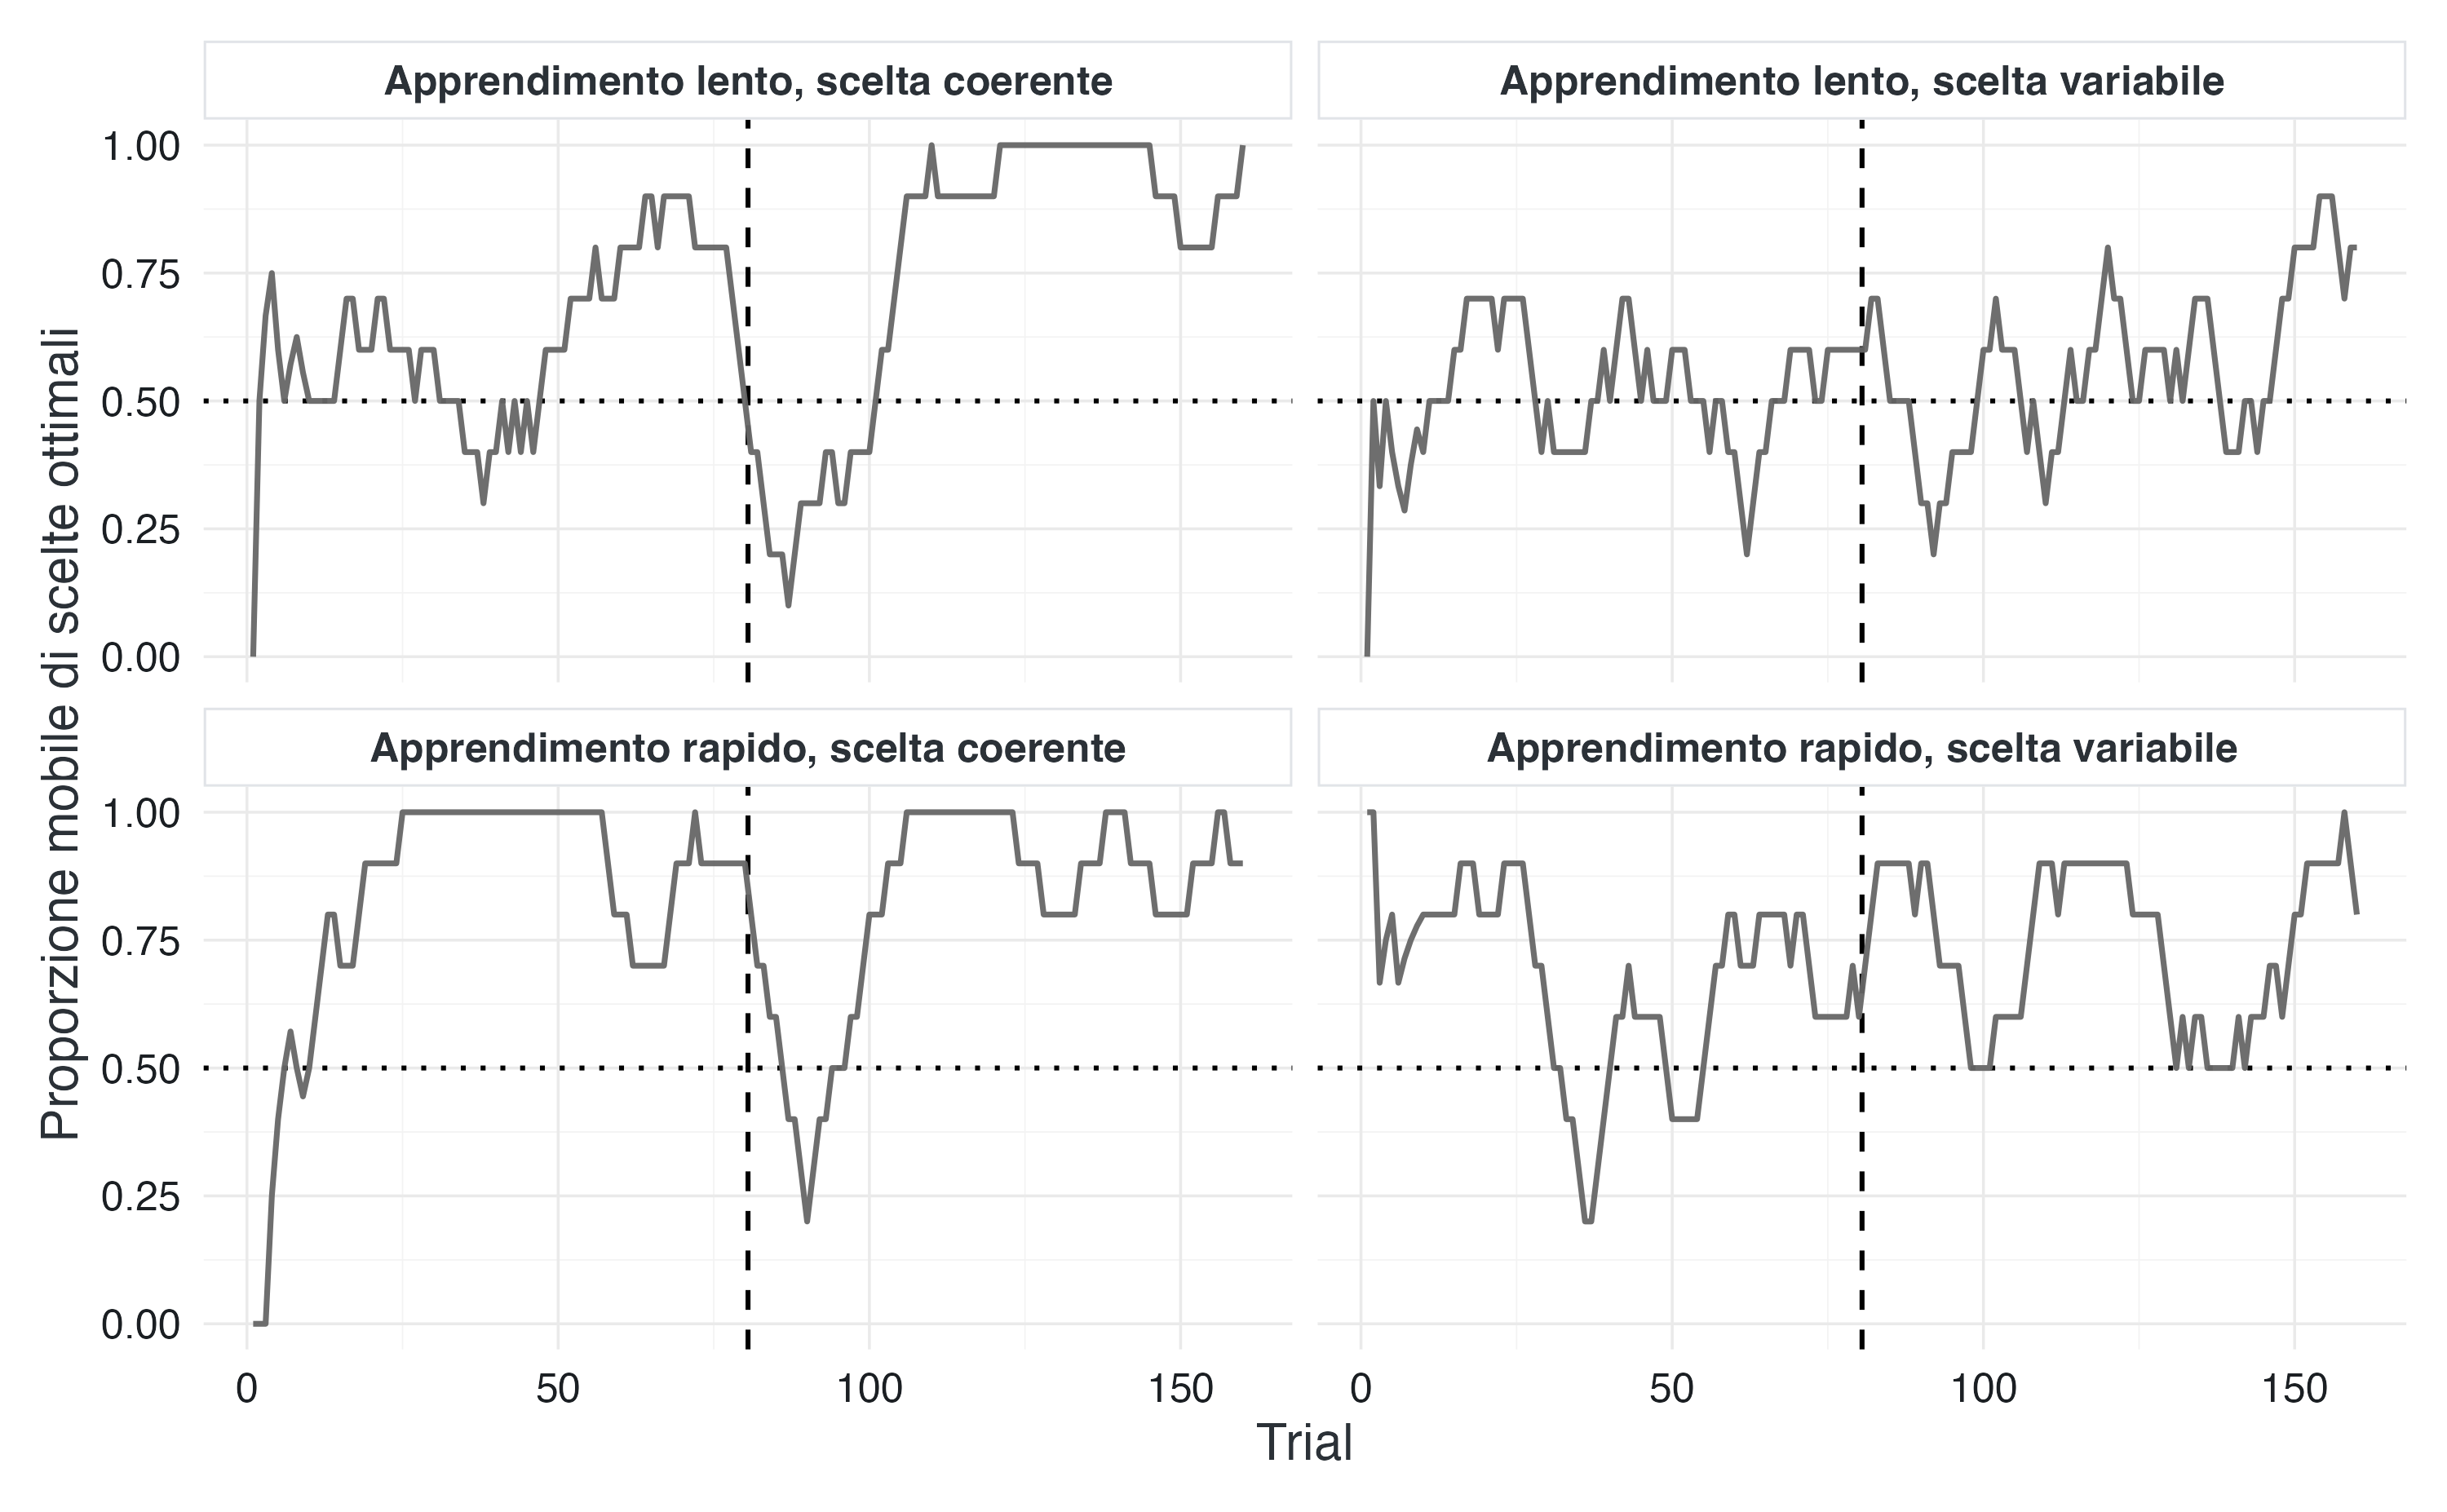
\includegraphics[width=0.85\linewidth,height=\textheight,keepaspectratio]{chapters/formal_models/04_rescorla_wagner_files/figure-pdf/fig-rw-parameter-grid-1.png}

}

\caption{\label{fig-rw-parameter-grid}Proporzione mobile di scelte
dell'alternativa attualmente più ricca, generata da quattro combinazioni
di tasso di apprendimento e inverse temperature.}

\end{figure}%

Le quattro traiettorie non si ordinano lungo una sola dimensione di
``prestazione''.

\begin{itemize}
\tightlist
\item
  Un \(\alpha\) elevato facilita l'adattamento dopo il reversal, ma può
  amplificare la reazione a ricompense casuali.
\item
  Un \(\tau\) elevato rende il comportamento coerente con i valori
  correnti, anche quando tali valori sono ancora errati.
\item
  Un \(\tau\) basso produce maggiore variabilità nelle scelte e può
  rallentare la manifestazione comportamentale di ciò che è stato
  appreso.
\item
  La stessa accuratezza media può nascondere combinazioni di parametri
  differenti.
\end{itemize}

\subsection{Una traiettoria di
riferimento}\label{una-traiettoria-di-riferimento}

Generiamo ora dati da un partecipante simulato con:

\[
\alpha=0.20,
\qquad
\tau=3.
\]

\begin{Shaded}
\begin{Highlighting}[]
\NormalTok{sim\_rw }\OtherTok{\textless{}{-}} \FunctionTok{simulate\_prl\_rw}\NormalTok{(}
  \AttributeTok{alpha =} \FloatTok{0.20}\NormalTok{,}
  \AttributeTok{tau =} \DecValTok{3}\NormalTok{,}
  \AttributeTok{kappa =} \DecValTok{0}\NormalTok{,}
  \AttributeTok{seed =} \DecValTok{2026}
\NormalTok{)}
\end{Highlighting}
\end{Shaded}

\begin{figure}

\centering{

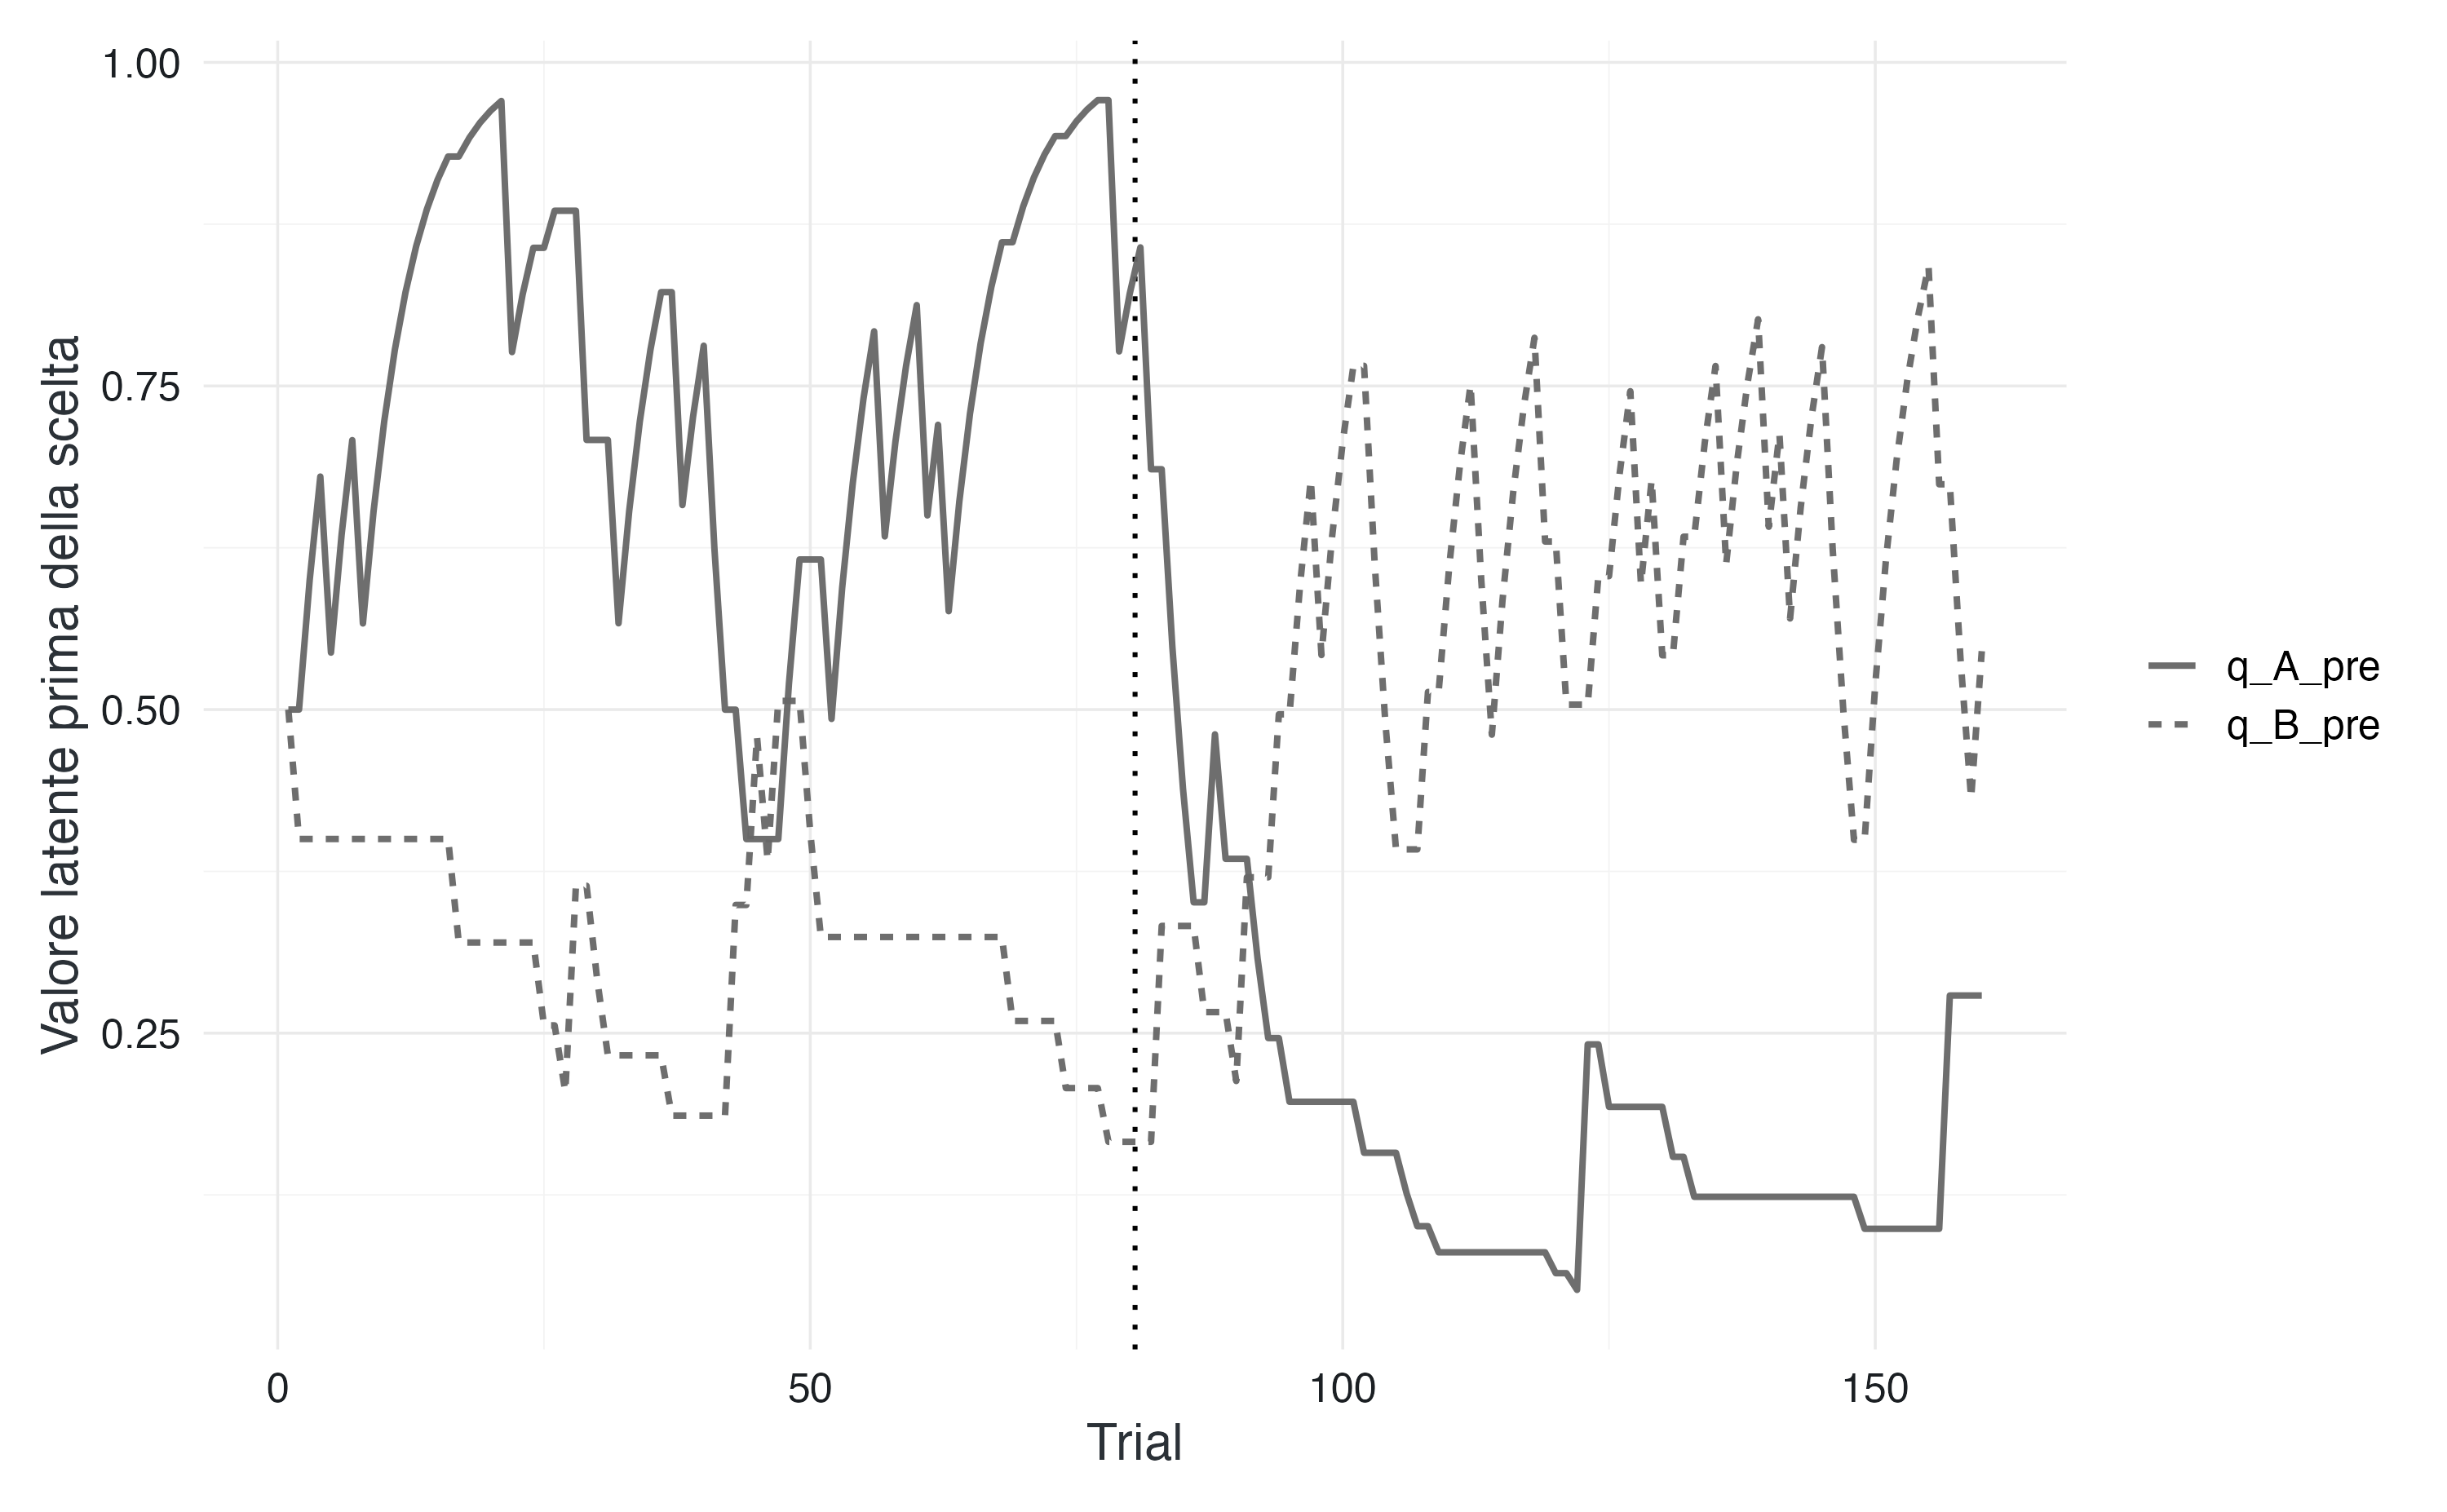
\includegraphics[width=0.85\linewidth,height=\textheight,keepaspectratio]{chapters/formal_models/04_rescorla_wagner_files/figure-pdf/fig-rw-reference-values-1.png}

}

\caption{\label{fig-rw-reference-values}Valori latenti prima della
scelta e scelte osservate nel dataset simulato. La linea verticale
indica il reversal.}

\end{figure}%

L'ambiente genera il feedback, il feedback modifica i valori e i valori
influenzano le scelte. Questa è una specificazione generativa completa
del compito.

\section{Dalla simulazione all'inferenza
inversa}\label{dalla-simulazione-allinferenza-inversa}

Nella simulazione conosciamo \(\alpha\), \(\tau\) e l'intera sequenza
degli stati. Nei dati reali osserviamo soltanto scelte e feedback.

L'inferenza procede quindi nella direzione opposta:

\[
\text{scelte e feedback}
\longrightarrow
\text{posterior di }\alpha,\tau
\longrightarrow
\text{posterior degli stati }Q_t.
\]

Questa operazione è possibile soltanto perché abbiamo specificato sia la
dinamica dell'apprendimento sia il modello osservazionale.

\section{Prior e controllo predittivo a
priori}\label{prior-e-controllo-predittivo-a-priori-2}

\subsection{Prior sui parametri
trasformati}\label{prior-sui-parametri-trasformati}

Per evitare limiti rigidi durante il campionamento, lavoriamo con
parametri non vincolati:

\[
\alpha=\operatorname{logit}^{-1}(\alpha_{\mathrm{raw}}),
\qquad
\tau=\exp(\log\tau).
\]

Usiamo:

\[
\alpha_{\mathrm{raw}}
\sim
\operatorname{Normal}
\left(
\operatorname{logit}(0.20),1
\right),
\]

\[
\log\tau
\sim
\operatorname{Normal}
\left(
\log 2,0.6
\right).
\]

Questi prior sono propri e relativamente ampi. Non dichiarano che valori
specifici siano ``tipici'' in assoluto: la plausibilità di \(\tau\)
dipende dalla scala dei valori e dal compito.

\subsection{Controllare le implicazioni del
prior}\label{controllare-le-implicazioni-del-prior}

Un prior sui parametri deve essere valutato attraverso il comportamento
che genera.

\begin{Shaded}
\begin{Highlighting}[]
\NormalTok{n\_prior\_draws }\OtherTok{\textless{}{-}} \DecValTok{250}

\NormalTok{rw\_prior\_draws }\OtherTok{\textless{}{-}} \FunctionTok{tibble}\NormalTok{(}
  \AttributeTok{draw =} \FunctionTok{seq\_len}\NormalTok{(n\_prior\_draws),}
  \AttributeTok{alpha =} \FunctionTok{plogis}\NormalTok{(}
    \FunctionTok{rnorm}\NormalTok{(}
\NormalTok{      n\_prior\_draws,}
      \AttributeTok{mean =} \FunctionTok{qlogis}\NormalTok{(}\FloatTok{0.20}\NormalTok{),}
      \AttributeTok{sd =} \DecValTok{1}
\NormalTok{    )}
\NormalTok{  ),}
  \AttributeTok{tau =} \FunctionTok{rlnorm}\NormalTok{(}
\NormalTok{    n\_prior\_draws,}
    \AttributeTok{meanlog =} \FunctionTok{log}\NormalTok{(}\DecValTok{2}\NormalTok{),}
    \AttributeTok{sdlog =} \FloatTok{0.6}
\NormalTok{  )}
\NormalTok{)}

\NormalTok{behavioral\_statistics }\OtherTok{\textless{}{-}} \ControlFlowTok{function}\NormalTok{(}
\NormalTok{    choice,}
\NormalTok{    reward,}
\NormalTok{    rich\_is\_A,}
    \AttributeTok{reversal\_trial =} \DecValTok{80}
\NormalTok{) \{}
\NormalTok{  optimal\_choice }\OtherTok{\textless{}{-}} \FunctionTok{ifelse}\NormalTok{(rich\_is\_A }\SpecialCharTok{==} \DecValTok{1}\NormalTok{L, }\DecValTok{0}\NormalTok{L, }\DecValTok{1}\NormalTok{L)}
\NormalTok{  stay }\OtherTok{\textless{}{-}}\NormalTok{ choice[}\SpecialCharTok{{-}}\DecValTok{1}\NormalTok{] }\SpecialCharTok{==}\NormalTok{ choice[}\SpecialCharTok{{-}}\FunctionTok{length}\NormalTok{(choice)]}
\NormalTok{  previous\_reward }\OtherTok{\textless{}{-}}\NormalTok{ reward[}\SpecialCharTok{{-}}\FunctionTok{length}\NormalTok{(reward)]}

\NormalTok{  early\_reversal }\OtherTok{\textless{}{-}} \FunctionTok{seq.int}\NormalTok{(}
\NormalTok{    reversal\_trial }\SpecialCharTok{+} \DecValTok{1}\NormalTok{,}
    \FunctionTok{min}\NormalTok{(reversal\_trial }\SpecialCharTok{+} \DecValTok{20}\NormalTok{, }\FunctionTok{length}\NormalTok{(choice))}
\NormalTok{  )}

  \FunctionTok{tibble}\NormalTok{(}
    \AttributeTok{optimal\_rate =} \FunctionTok{mean}\NormalTok{(choice }\SpecialCharTok{==}\NormalTok{ optimal\_choice),}
    \AttributeTok{early\_reversal\_optimal =} \FunctionTok{mean}\NormalTok{(}
\NormalTok{      choice[early\_reversal] }\SpecialCharTok{==}\NormalTok{ optimal\_choice[early\_reversal]}
\NormalTok{    ),}
    \AttributeTok{switch\_rate =} \FunctionTok{mean}\NormalTok{(}\SpecialCharTok{!}\NormalTok{stay),}
    \AttributeTok{stay\_after\_reward =} \FunctionTok{mean}\NormalTok{(stay[previous\_reward }\SpecialCharTok{==} \DecValTok{1}\NormalTok{]),}
    \AttributeTok{stay\_after\_no\_reward =} \FunctionTok{mean}\NormalTok{(stay[previous\_reward }\SpecialCharTok{==} \DecValTok{0}\NormalTok{])}
\NormalTok{  )}
\NormalTok{\}}

\NormalTok{rw\_prior\_stats }\OtherTok{\textless{}{-}}\NormalTok{ rw\_prior\_draws }\SpecialCharTok{|\textgreater{}}
  \FunctionTok{mutate}\NormalTok{(}
    \AttributeTok{simulation =}\NormalTok{ purrr}\SpecialCharTok{::}\FunctionTok{pmap}\NormalTok{(}
      \FunctionTok{list}\NormalTok{(alpha, tau, draw),}
      \SpecialCharTok{\textasciitilde{}} \FunctionTok{simulate\_prl\_rw}\NormalTok{(}
        \AttributeTok{alpha =}\NormalTok{ ..}\DecValTok{1}\NormalTok{,}
        \AttributeTok{tau =}\NormalTok{ ..}\DecValTok{2}\NormalTok{,}
        \AttributeTok{seed =} \DecValTok{5000} \SpecialCharTok{+}\NormalTok{ ..}\DecValTok{3}
\NormalTok{      )}
\NormalTok{    ),}
    \AttributeTok{statistics =}\NormalTok{ purrr}\SpecialCharTok{::}\FunctionTok{map}\NormalTok{(}
\NormalTok{      simulation,}
      \SpecialCharTok{\textasciitilde{}} \FunctionTok{behavioral\_statistics}\NormalTok{(}
        \AttributeTok{choice =}\NormalTok{ .x}\SpecialCharTok{$}\NormalTok{choice,}
        \AttributeTok{reward =}\NormalTok{ .x}\SpecialCharTok{$}\NormalTok{reward,}
        \AttributeTok{rich\_is\_A =}\NormalTok{ .x}\SpecialCharTok{$}\NormalTok{rich\_is\_A}
\NormalTok{      )}
\NormalTok{    )}
\NormalTok{  ) }\SpecialCharTok{|\textgreater{}}
  \FunctionTok{select}\NormalTok{(draw, alpha, tau, statistics) }\SpecialCharTok{|\textgreater{}}
\NormalTok{  tidyr}\SpecialCharTok{::}\FunctionTok{unnest}\NormalTok{(statistics)}
\end{Highlighting}
\end{Shaded}

\begin{figure}

\centering{

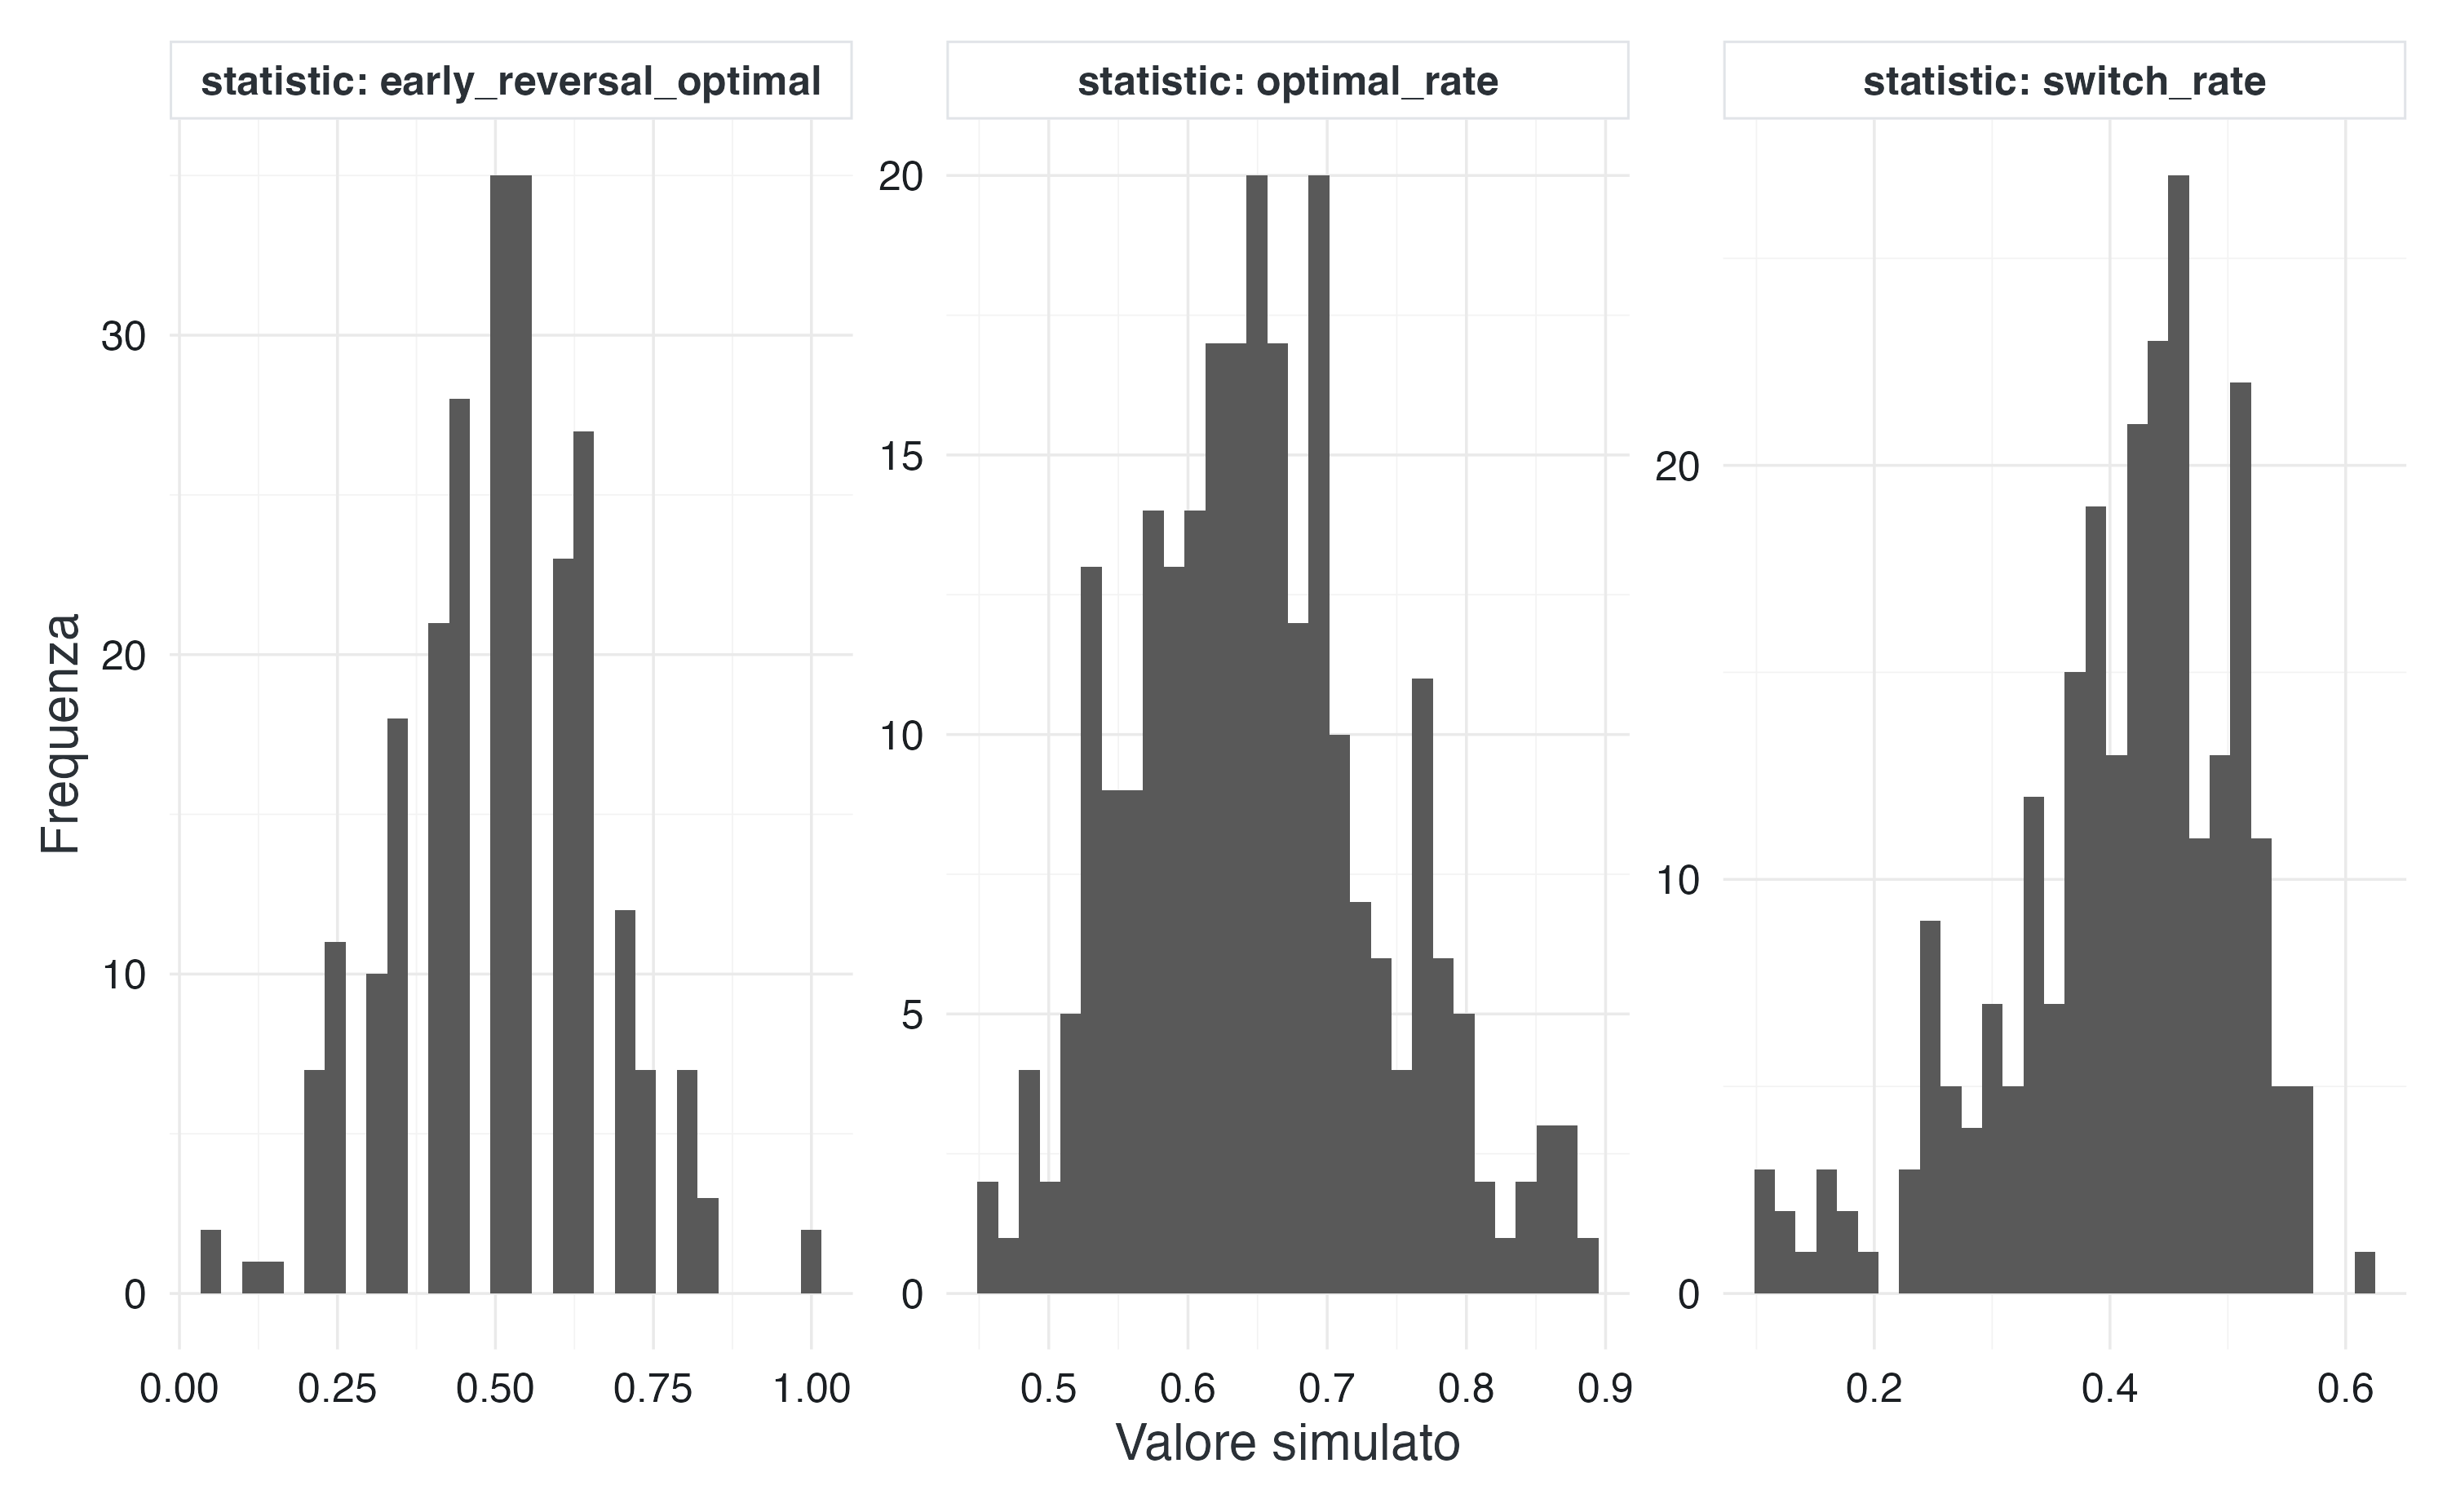
\includegraphics[width=0.85\linewidth,height=\textheight,keepaspectratio]{chapters/formal_models/04_rescorla_wagner_files/figure-pdf/fig-rw-prior-predictive-1.png}

}

\caption{\label{fig-rw-prior-predictive}Distribuzioni predittive a
priori di tre statistiche comportamentali. Il controllo valuta le
conseguenze congiunte dei prior e del compito.}

\end{figure}%

Il controllo predittivo a priori consente di chiedere:

\begin{itemize}
\tightlist
\item
  il modello genera quasi sempre scelte casuali?
\item
  produce comportamenti quasi deterministici?
\item
  contempla adattamenti rapidi e lenti al reversal?
\item
  attribuisce massa a sequenze psicologicamente o sperimentalmente
  implausibili?
\end{itemize}

Se la risposta è insoddisfacente, i prior devono essere rivisti prima di
osservare la posterior.

\section{Implementazione in Stan}\label{sec-rw-stan}

\begin{tcolorbox}[enhanced jigsaw, arc=.35mm, bottomrule=.15mm, breakable, colback=white, colframe=quarto-callout-important-color-frame, left=2mm, leftrule=.75mm, opacityback=0, rightrule=.15mm, toprule=.15mm]

\textbf{Passaggio costitutivo.} In questo capitolo Stan non è una
variante più tecnica di un'analisi disponibile in \texttt{brms}: serve a
esprimere l'aggiornamento ricorsivo trial per trial. Non è richiesto
scrivere il programma da zero, ma occorre saperne seguire la logica,
eseguire il codice fornito e collegare output, stati latenti e controlli
predittivi.

\end{tcolorbox}

Il programma seguente:

\begin{itemize}
\tightlist
\item
  calcola la probabilità della scelta usando i valori prima del
  feedback;
\item
  aggiorna soltanto l'opzione scelta;
\item
  ricostruisce gli stati latenti;
\item
  calcola la log-verosimiglianza condizionata delle scelte;
\item
  genera nuove sequenze complete di scelte e ricompense nello stesso
  ambiente.
\end{itemize}

\begin{Shaded}
\begin{Highlighting}[]
\NormalTok{stancode\_rw }\OtherTok{\textless{}{-}} \StringTok{"}
\StringTok{data \{}
\StringTok{  int\textless{}lower=1\textgreater{} T;}
\StringTok{  array[T] int\textless{}lower=0, upper=1\textgreater{} choice;}
\StringTok{  array[T] int\textless{}lower=0, upper=1\textgreater{} reward;}
\StringTok{  array[T] int\textless{}lower=0, upper=1\textgreater{} rich\_is\_A;}
\StringTok{  real\textless{}lower=0.5, upper=1\textgreater{} p\_reward\_rich;}
\StringTok{\}}

\StringTok{parameters \{}
\StringTok{  real alpha\_raw;}
\StringTok{  real log\_tau;}
\StringTok{\}}

\StringTok{transformed parameters \{}
\StringTok{  real\textless{}lower=0, upper=1\textgreater{} alpha = inv\_logit(alpha\_raw);}
\StringTok{  real\textless{}lower=0\textgreater{} tau = exp(log\_tau);}
\StringTok{\}}

\StringTok{model \{}
\StringTok{  vector[2] q = rep\_vector(0.5, 2);}

\StringTok{  alpha\_raw \textasciitilde{} normal(logit(0.20), 1);}
\StringTok{  log\_tau \textasciitilde{} normal(log(2), 0.6);}

\StringTok{  for (t in 1:T) \{}
\StringTok{    int a = choice[t] + 1;}
\StringTok{    real eta = tau * (q[2] {-} q[1]);}

\StringTok{    choice[t] \textasciitilde{} bernoulli\_logit(eta);}
\StringTok{    q[a] += alpha * (reward[t] {-} q[a]);}
\StringTok{  \}}
\StringTok{\}}

\StringTok{generated quantities \{}
\StringTok{  array[T] int choice\_rep;}
\StringTok{  array[T] int reward\_rep;}
\StringTok{  vector[T] log\_lik;}
\StringTok{  vector[T] q\_A\_obs;}
\StringTok{  vector[T] q\_B\_obs;}
\StringTok{  vector[T] prediction\_error\_obs;}

\StringTok{  \{}
\StringTok{    vector[2] q\_obs = rep\_vector(0.5, 2);}
\StringTok{    vector[2] q\_rep = rep\_vector(0.5, 2);}

\StringTok{    for (t in 1:T) \{}
\StringTok{      int a\_obs;}
\StringTok{      int a\_rep;}
\StringTok{      int chosen\_is\_rich;}
\StringTok{      real eta\_obs;}
\StringTok{      real eta\_rep;}
\StringTok{      real reward\_probability;}

\StringTok{      q\_A\_obs[t] = q\_obs[1];}
\StringTok{      q\_B\_obs[t] = q\_obs[2];}

\StringTok{      eta\_obs = tau * (q\_obs[2] {-} q\_obs[1]);}
\StringTok{      log\_lik[t] = bernoulli\_logit\_lpmf(}
\StringTok{        choice[t] | eta\_obs}
\StringTok{      );}

\StringTok{      a\_obs = choice[t] + 1;}
\StringTok{      prediction\_error\_obs[t] =}
\StringTok{        reward[t] {-} q\_obs[a\_obs];}
\StringTok{      q\_obs[a\_obs] +=}
\StringTok{        alpha * prediction\_error\_obs[t];}

\StringTok{      eta\_rep = tau * (q\_rep[2] {-} q\_rep[1]);}
\StringTok{      choice\_rep[t] =}
\StringTok{        bernoulli\_logit\_rng(eta\_rep);}
\StringTok{      a\_rep = choice\_rep[t] + 1;}

\StringTok{      chosen\_is\_rich =}
\StringTok{        (}
\StringTok{          (choice\_rep[t] == 0 \&\&}
\StringTok{           rich\_is\_A[t] == 1) ||}
\StringTok{          (choice\_rep[t] == 1 \&\&}
\StringTok{           rich\_is\_A[t] == 0)}
\StringTok{        ) ? 1 : 0;}

\StringTok{      reward\_probability =}
\StringTok{        chosen\_is\_rich == 1}
\StringTok{        ? p\_reward\_rich}
\StringTok{        : 1 {-} p\_reward\_rich;}

\StringTok{      reward\_rep[t] =}
\StringTok{        bernoulli\_rng(reward\_probability);}

\StringTok{      q\_rep[a\_rep] += alpha *}
\StringTok{        (reward\_rep[t] {-} q\_rep[a\_rep]);}
\StringTok{    \}}
\StringTok{  \}}
\StringTok{\}}
\StringTok{"}
\end{Highlighting}
\end{Shaded}

\begin{tcolorbox}[enhanced jigsaw, arc=.35mm, bottomrule=.15mm, bottomtitle=1mm, breakable, colback=white, colbacktitle=quarto-callout-note-color!10!white, colframe=quarto-callout-note-color-frame, coltitle=black, left=2mm, leftrule=.75mm, opacityback=0, opacitybacktitle=0.6, rightrule=.15mm, title=\textcolor{quarto-callout-note-color}{\faInfo}\hspace{0.5em}{Che cosa viene trattato come casuale?}, titlerule=0mm, toprule=.15mm, toptitle=1mm]

Nella verosimiglianza stimiamo il modello delle \textbf{scelte
condizionate ai feedback osservati}. La distribuzione dell'ambiente non
contribuisce alla posterior di \(\alpha\) e \(\tau\).

Nelle quantità generate simuliamo invece anche i feedback, usando le
probabilità note del compito. Questo produce repliche complete del
comportamento nello stesso ambiente e permette controlli predittivi su
adattamento, switching e ricompense.

\end{tcolorbox}

\subsection{Compilazione e
campionamento}\label{compilazione-e-campionamento}

\begin{Shaded}
\begin{Highlighting}[]
\NormalTok{rw\_stan\_data }\OtherTok{\textless{}{-}} \FunctionTok{list}\NormalTok{(}
  \AttributeTok{T =} \FunctionTok{nrow}\NormalTok{(sim\_rw),}
  \AttributeTok{choice =} \FunctionTok{as.integer}\NormalTok{(sim\_rw}\SpecialCharTok{$}\NormalTok{choice),}
  \AttributeTok{reward =} \FunctionTok{as.integer}\NormalTok{(sim\_rw}\SpecialCharTok{$}\NormalTok{reward),}
  \AttributeTok{rich\_is\_A =} \FunctionTok{as.integer}\NormalTok{(sim\_rw}\SpecialCharTok{$}\NormalTok{rich\_is\_A),}
  \AttributeTok{p\_reward\_rich =} \FloatTok{0.70}
\NormalTok{)}

\NormalTok{rw\_model\_file }\OtherTok{\textless{}{-}} \FunctionTok{write\_stan\_file}\NormalTok{(stancode\_rw)}
\NormalTok{rw\_model }\OtherTok{\textless{}{-}} \FunctionTok{cmdstan\_model}\NormalTok{(rw\_model\_file)}

\NormalTok{fit\_rw }\OtherTok{\textless{}{-}}\NormalTok{ rw\_model}\SpecialCharTok{$}\FunctionTok{sample}\NormalTok{(}
  \AttributeTok{data =}\NormalTok{ rw\_stan\_data,}
  \AttributeTok{seed =} \DecValTok{8127}\NormalTok{,}
  \AttributeTok{chains =} \DecValTok{4}\NormalTok{,}
  \AttributeTok{parallel\_chains =} \DecValTok{4}\NormalTok{,}
  \AttributeTok{iter\_warmup =} \DecValTok{1000}\NormalTok{,}
  \AttributeTok{iter\_sampling =} \DecValTok{1500}\NormalTok{,}
  \AttributeTok{refresh =} \DecValTok{0}
\NormalTok{)}
\end{Highlighting}
\end{Shaded}

\section{Diagnostica del calcolo}\label{diagnostica-del-calcolo}

\begin{Shaded}
\begin{Highlighting}[]
\NormalTok{fit\_rw}\SpecialCharTok{$}\FunctionTok{cmdstan\_diagnose}\NormalTok{()}
\CommentTok{\#\textgreater{} Checking sampler transitions treedepth.}
\CommentTok{\#\textgreater{} Treedepth satisfactory for all transitions.}
\CommentTok{\#\textgreater{} }
\CommentTok{\#\textgreater{} Checking sampler transitions for divergences.}
\CommentTok{\#\textgreater{} No divergent transitions found.}
\CommentTok{\#\textgreater{} }
\CommentTok{\#\textgreater{} Checking E{-}BFMI {-} sampler transitions HMC potential energy.}
\CommentTok{\#\textgreater{} E{-}BFMI satisfactory.}
\CommentTok{\#\textgreater{} }
\CommentTok{\#\textgreater{} Rank{-}normalized split effective sample size satisfactory for all parameters.}
\CommentTok{\#\textgreater{} }
\CommentTok{\#\textgreater{} Rank{-}normalized split R{-}hat values satisfactory for all parameters.}
\CommentTok{\#\textgreater{} }
\CommentTok{\#\textgreater{} Processing complete, no problems detected.}

\NormalTok{fit\_rw}\SpecialCharTok{$}\FunctionTok{summary}\NormalTok{(}
  \AttributeTok{variables =} \FunctionTok{c}\NormalTok{(}\StringTok{"alpha"}\NormalTok{, }\StringTok{"tau"}\NormalTok{),}
\NormalTok{  mean,}
\NormalTok{  sd,}
  \SpecialCharTok{\textasciitilde{}}\FunctionTok{quantile}\NormalTok{(.x, }\AttributeTok{probs =} \FunctionTok{c}\NormalTok{(}\FloatTok{0.05}\NormalTok{, }\FloatTok{0.50}\NormalTok{, }\FloatTok{0.95}\NormalTok{))}
\NormalTok{)}
\CommentTok{\#\textgreater{} \# A tibble: 2 x 6}
\CommentTok{\#\textgreater{}   variable  mean     sd  \textasciigrave{}5\%\textasciigrave{} \textasciigrave{}50\%\textasciigrave{} \textasciigrave{}95\%\textasciigrave{}}
\CommentTok{\#\textgreater{}   \textless{}chr\textgreater{}    \textless{}dbl\textgreater{}  \textless{}dbl\textgreater{} \textless{}dbl\textgreater{} \textless{}dbl\textgreater{} \textless{}dbl\textgreater{}}
\CommentTok{\#\textgreater{} 1 alpha    0.253 0.0874 0.131 0.242 0.411}
\CommentTok{\#\textgreater{} 2 tau      2.81  0.504  2.03  2.79  3.67}
\end{Highlighting}
\end{Shaded}

\begin{figure}

\centering{

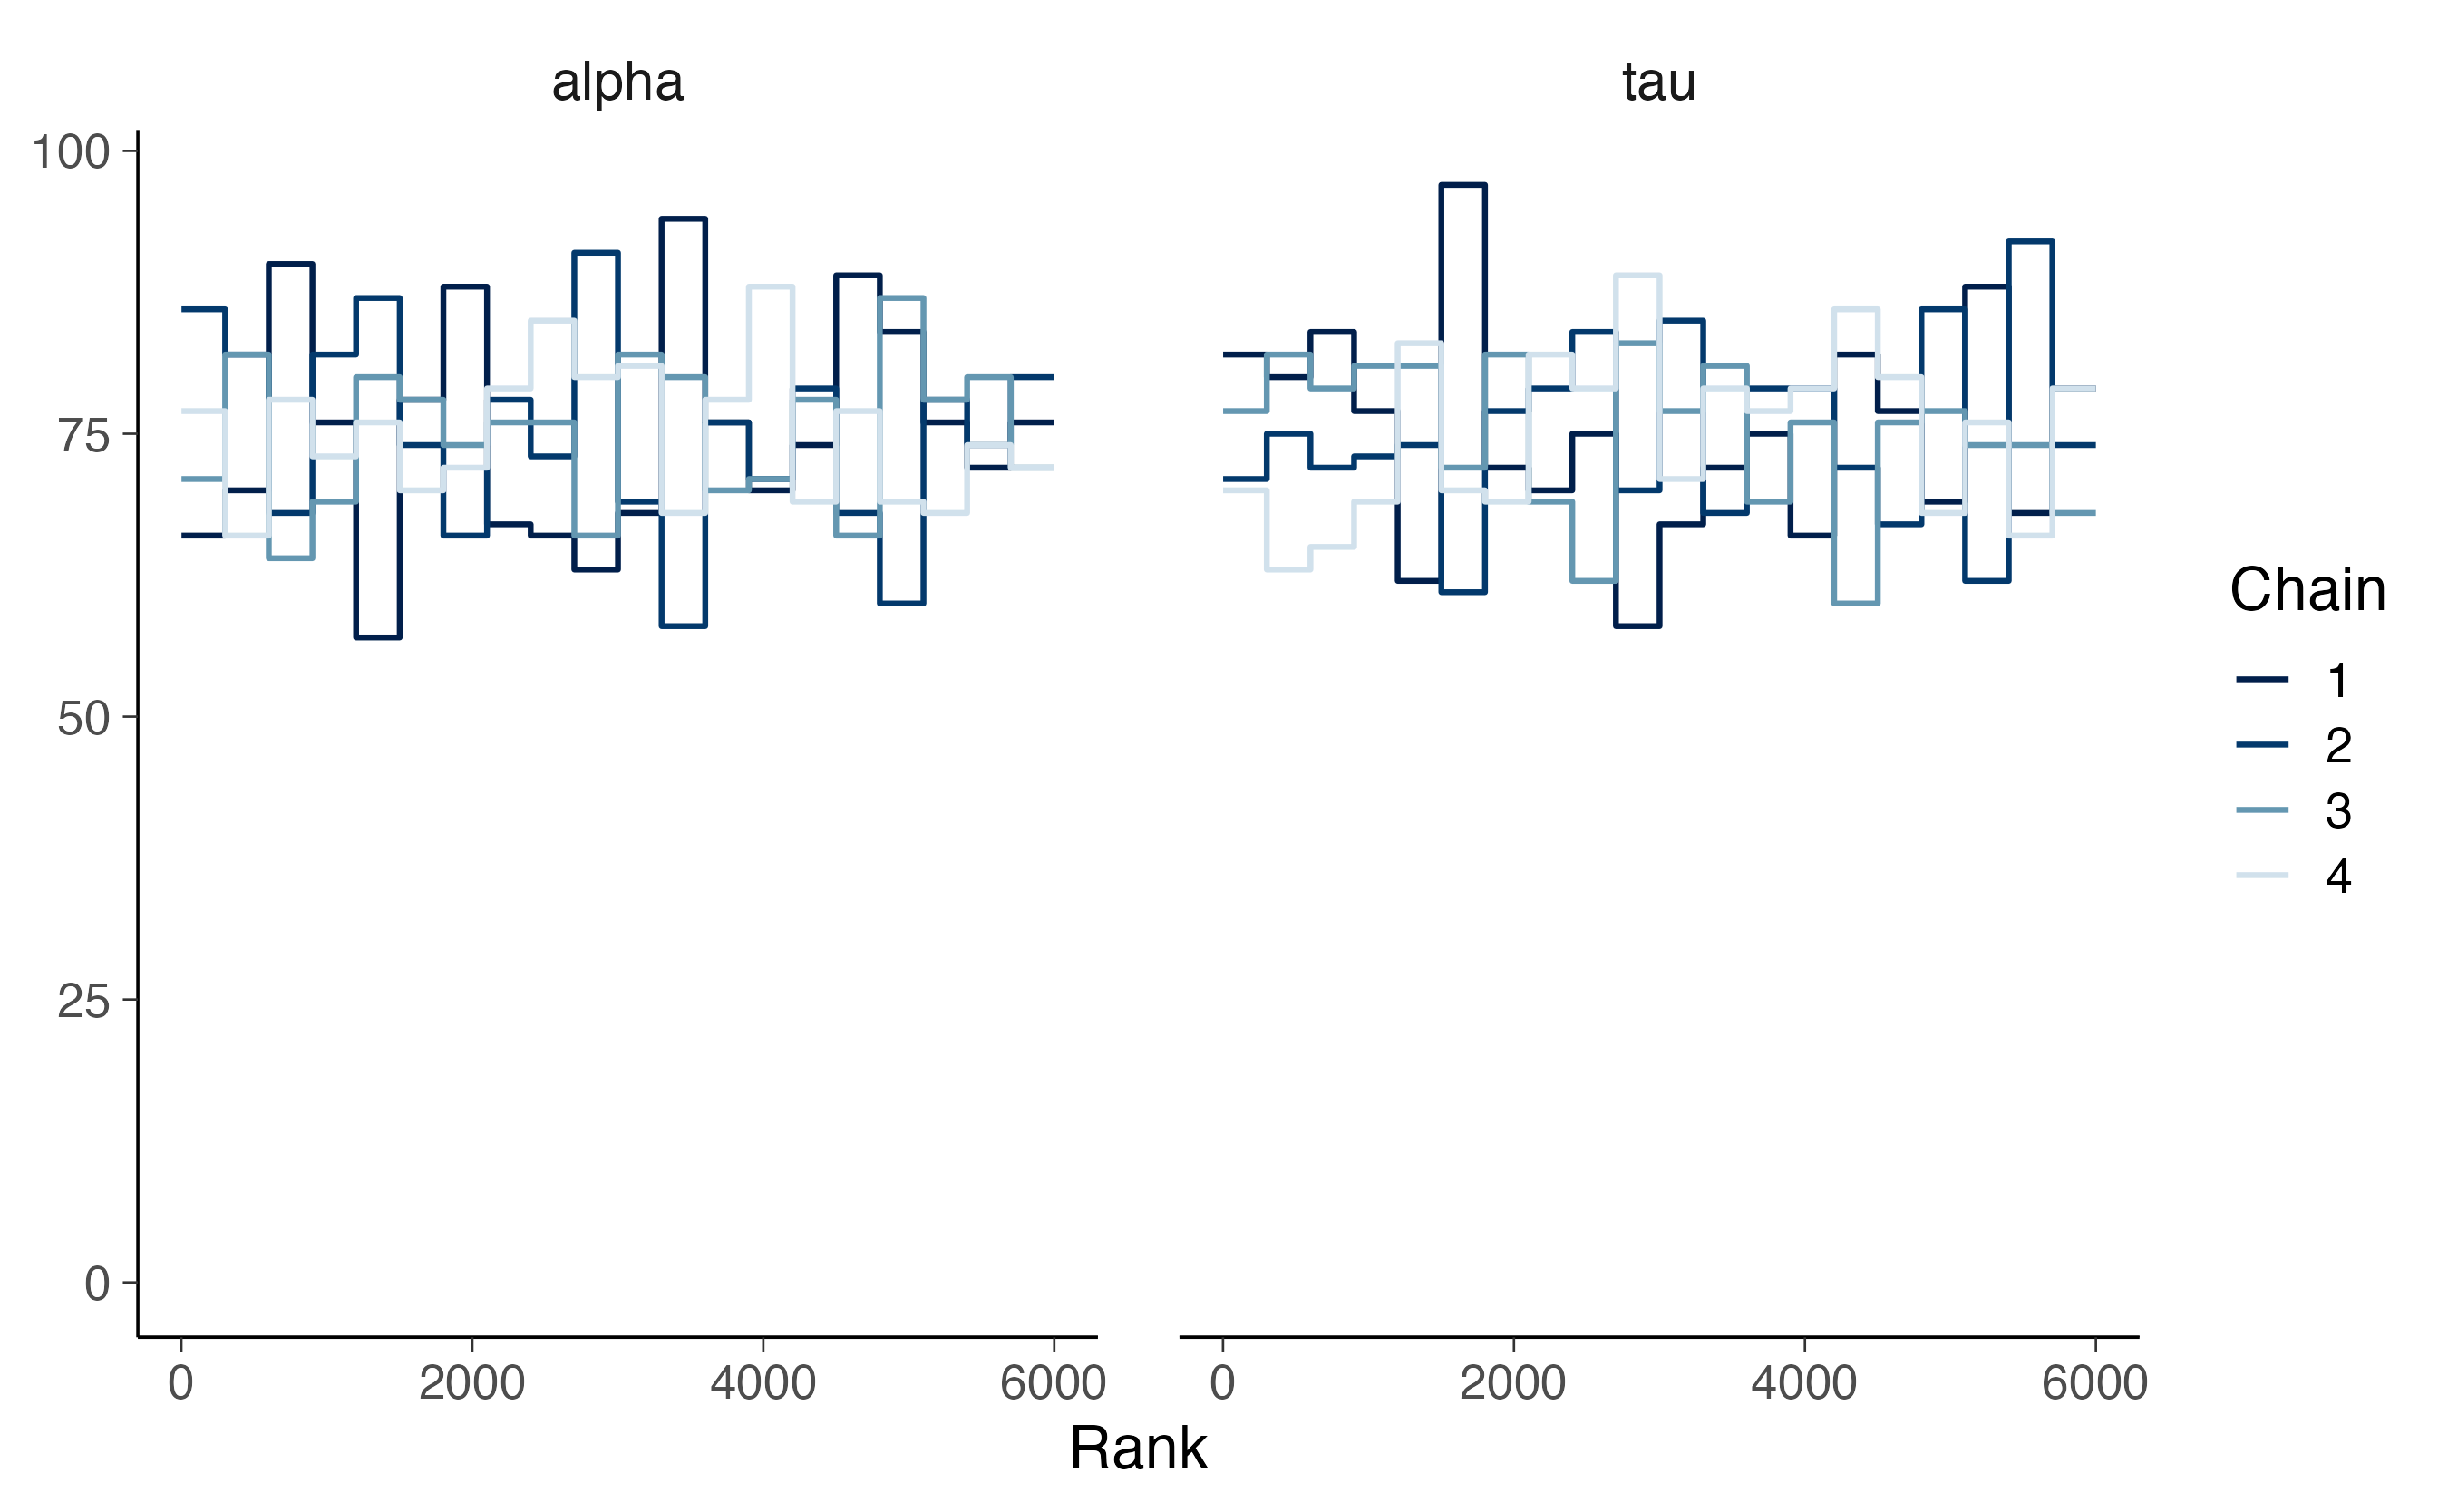
\includegraphics[width=0.85\linewidth,height=\textheight,keepaspectratio]{chapters/formal_models/04_rescorla_wagner_files/figure-pdf/fig-rw-rank-plots-1.png}

}

\caption{\label{fig-rw-rank-plots}Rank plot delle catene per il tasso di
apprendimento e l'inverse temperature.}

\end{figure}%

Questi controlli rispondono alla domanda: \emph{il campionatore ha
esplorato adeguatamente la posterior specificata?} Non dimostrano che il
modello cognitivo sia corretto.

\section{Posterior dei parametri}\label{posterior-dei-parametri}

\begin{Shaded}
\begin{Highlighting}[]
\NormalTok{rw\_draws }\OtherTok{\textless{}{-}}\NormalTok{ fit\_rw}\SpecialCharTok{$}\FunctionTok{draws}\NormalTok{(}
  \AttributeTok{variables =} \FunctionTok{c}\NormalTok{(}\StringTok{"alpha"}\NormalTok{, }\StringTok{"tau"}\NormalTok{)}
\NormalTok{) }\SpecialCharTok{|\textgreater{}}
  \FunctionTok{as\_draws\_df}\NormalTok{() }\SpecialCharTok{|\textgreater{}}
  \FunctionTok{as\_tibble}\NormalTok{()}
\end{Highlighting}
\end{Shaded}

\begin{figure}

\centering{

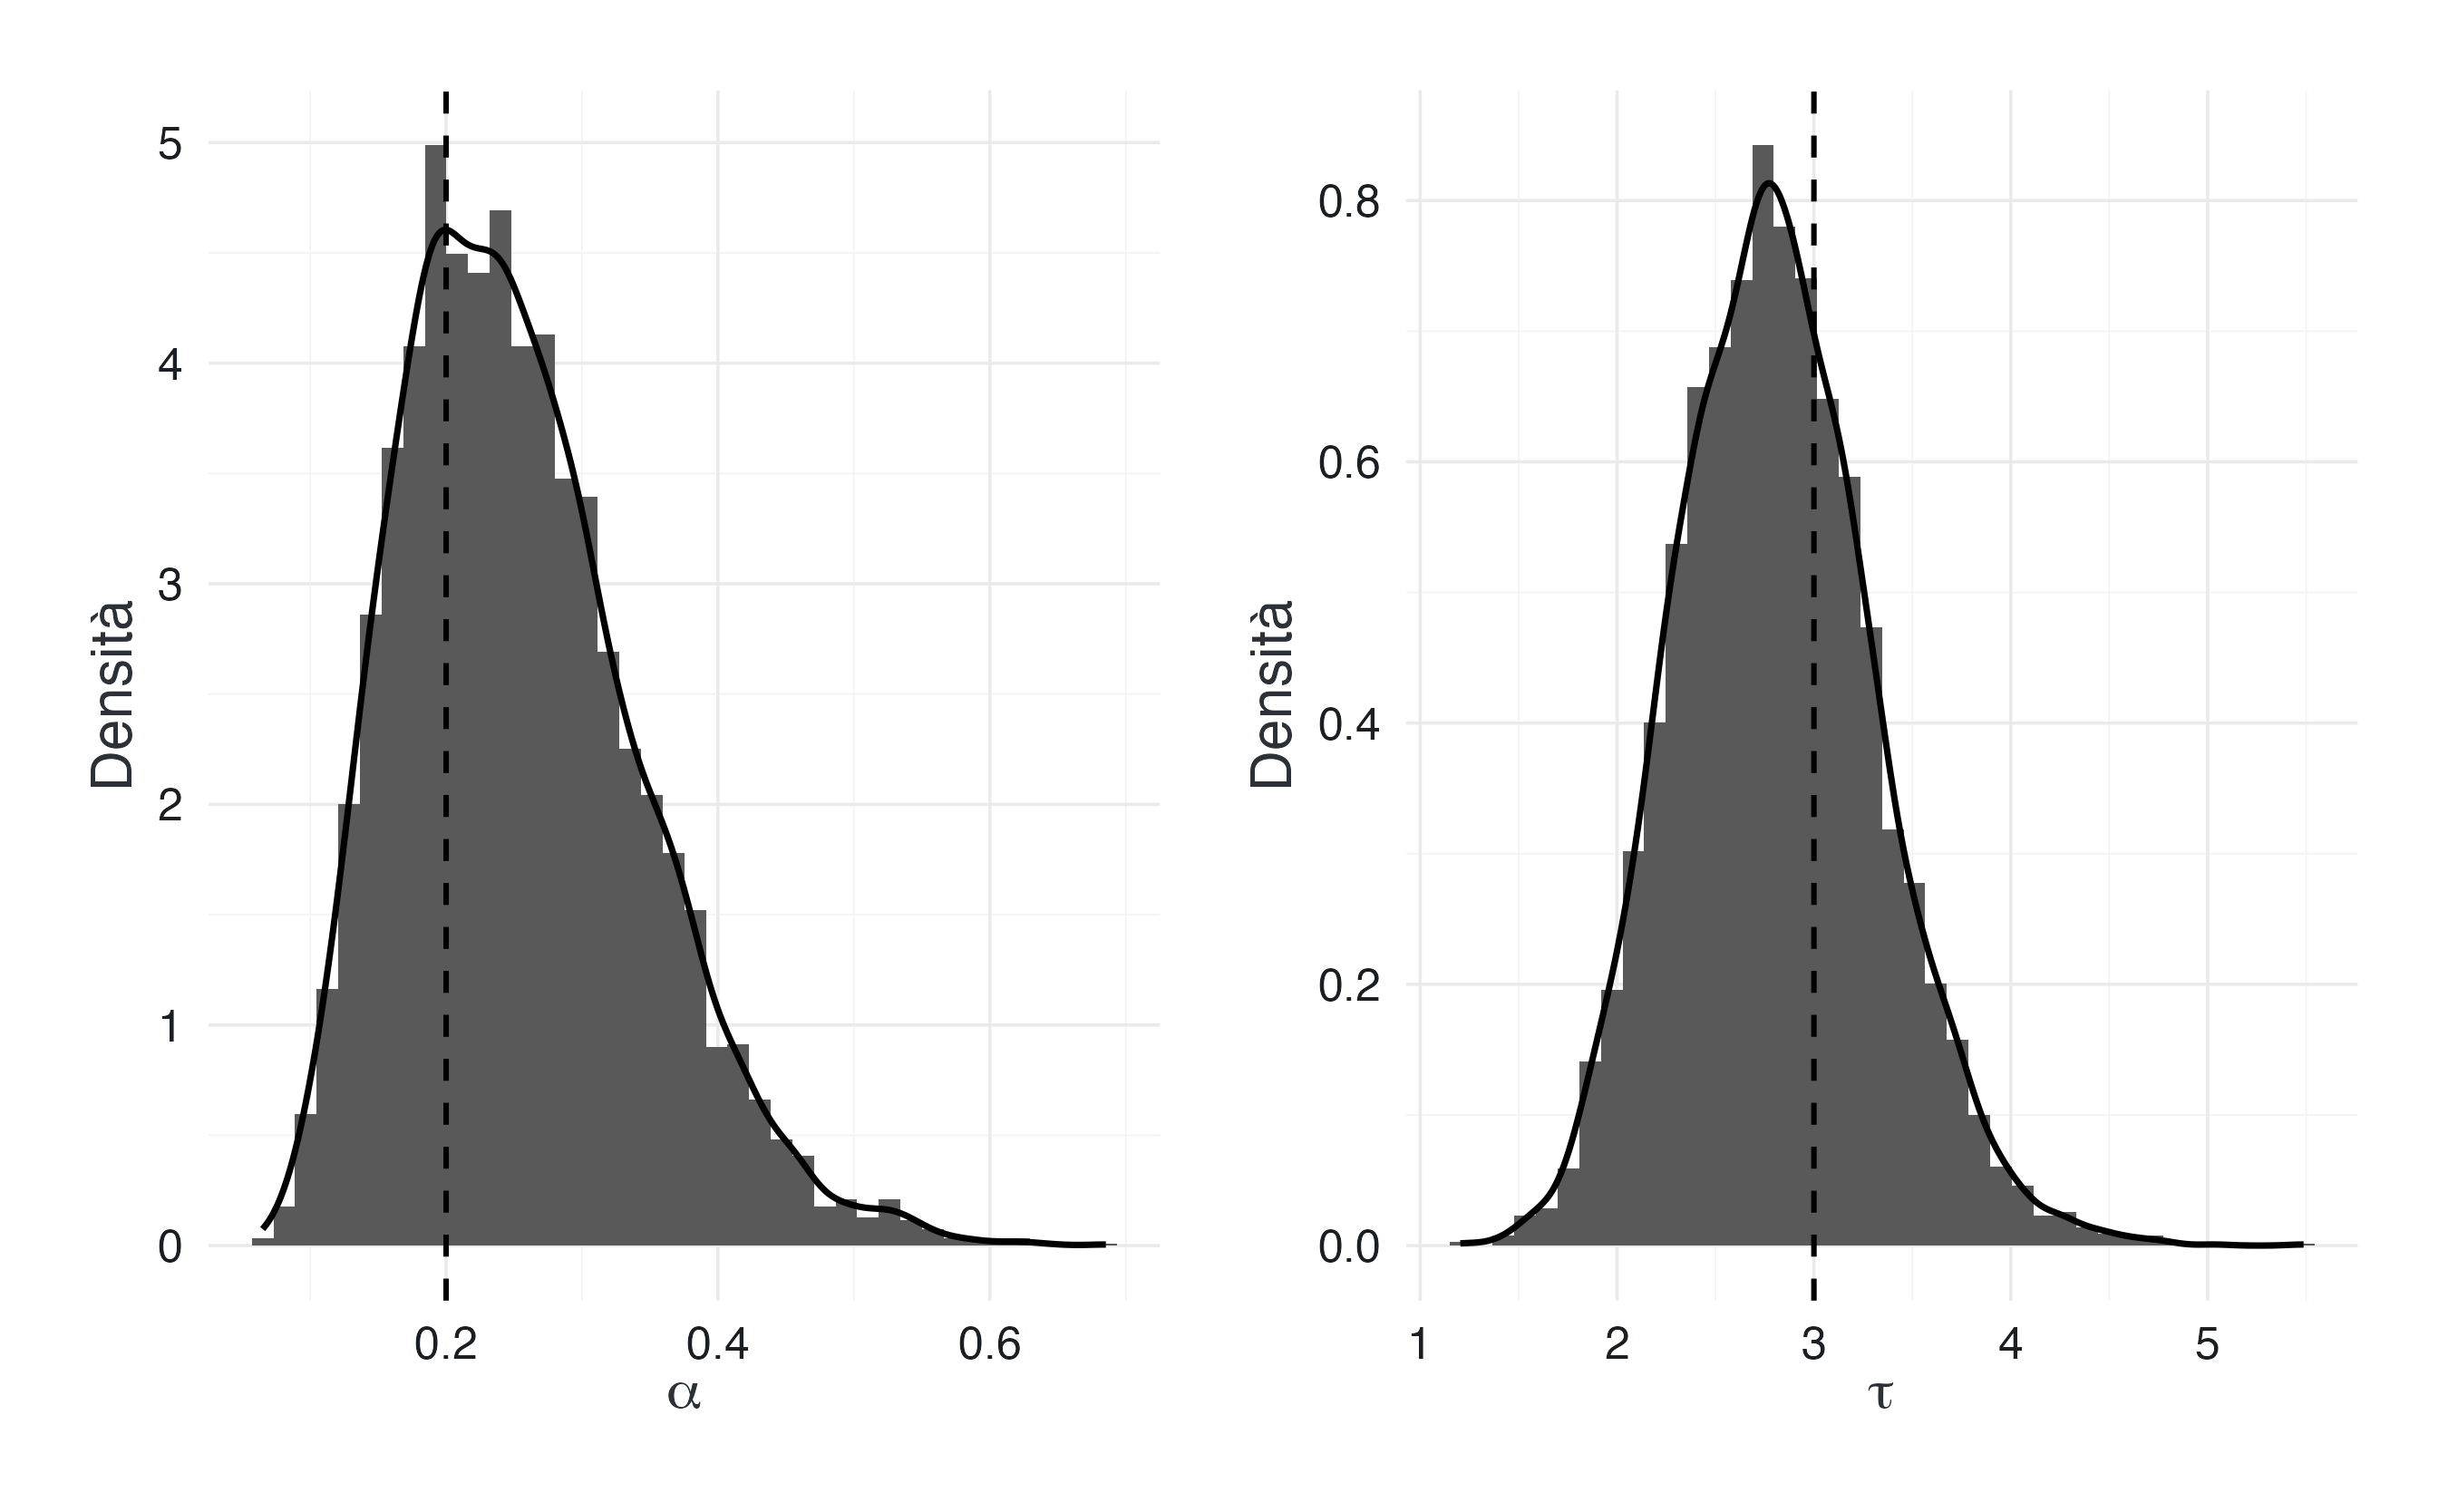
\includegraphics[width=0.85\linewidth,height=\textheight,keepaspectratio]{chapters/formal_models/04_rescorla_wagner_files/figure-pdf/fig-rw-parameter-posteriors-1.png}

}

\caption{\label{fig-rw-parameter-posteriors}Distribuzioni a posteriori
dei parametri. Le linee tratteggiate indicano i valori usati per
generare i dati.}

\end{figure}%

La vicinanza tra posterior e valori generativi è utile, ma una singola
simulazione non dimostra la recuperabilità generale. Occorre valutare il
comportamento del metodo su molti dataset e su più combinazioni dei
parametri.

\subsection{Dipendenza posteriore}\label{dipendenza-posteriore}

\begin{figure}

\centering{

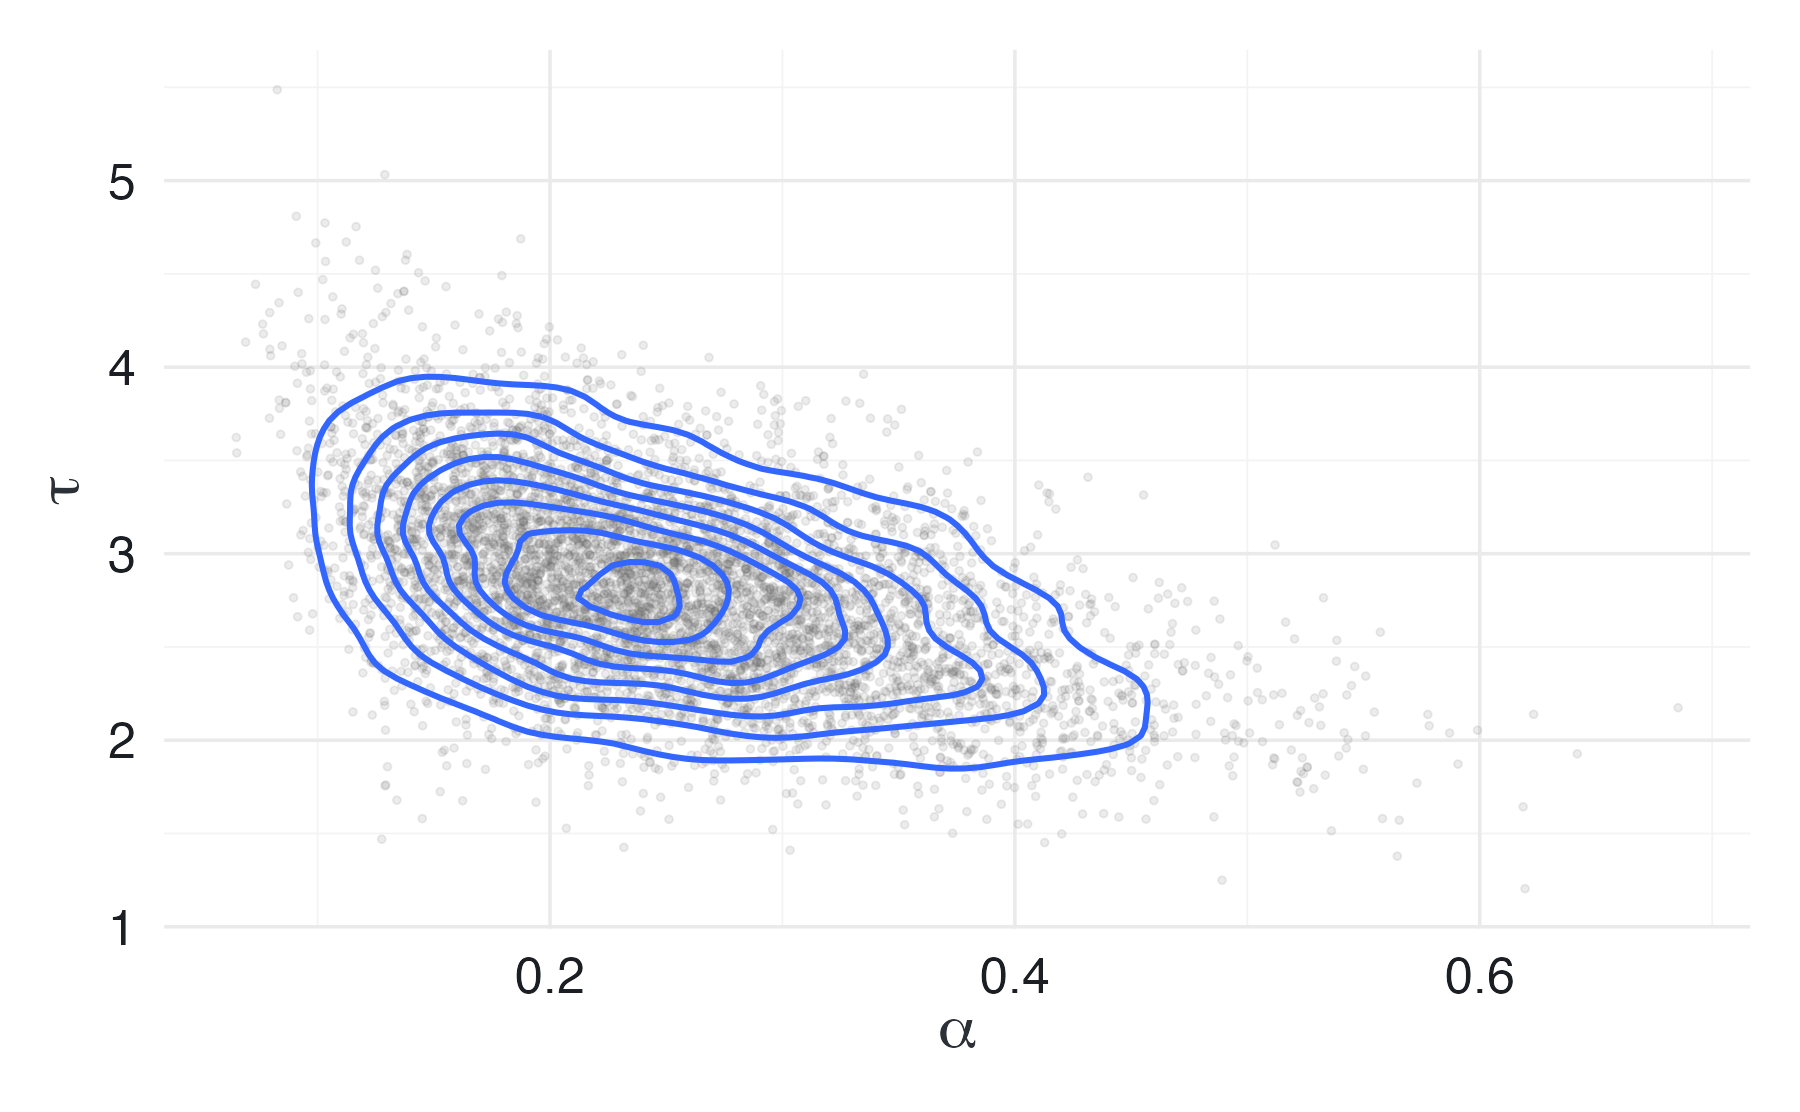
\includegraphics[width=0.85\linewidth,height=\textheight,keepaspectratio]{chapters/formal_models/04_rescorla_wagner_files/figure-pdf/fig-rw-posterior-dependence-1.png}

}

\caption{\label{fig-rw-posterior-dependence}Distribuzione congiunta dei
parametri. Una dipendenza posteriore indica che combinazioni diverse
possono produrre sequenze di scelta simili.}

\end{figure}%

Una dipendenza tra i parametri non è un errore del campionatore. Può
riflettere una compensazione reale: un tasso di apprendimento diverso
può essere parzialmente controbilanciato da una diversa sensibilità
della scelta.

\section{Ricostruire gli stati
latenti}\label{ricostruire-gli-stati-latenti}

Le quantità generate contengono, per ogni draw, i valori \(Q_t(A)\) e
\(Q_t(B)\) coerenti con scelte e feedback osservati.

\begin{Shaded}
\begin{Highlighting}[]
\NormalTok{summarize\_stan\_array }\OtherTok{\textless{}{-}} \ControlFlowTok{function}\NormalTok{(fit, variable) \{}
\NormalTok{  draws\_matrix }\OtherTok{\textless{}{-}}\NormalTok{ fit}\SpecialCharTok{$}\FunctionTok{draws}\NormalTok{(}
\NormalTok{    variable,}
    \AttributeTok{format =} \StringTok{"draws\_matrix"}
\NormalTok{  ) }\SpecialCharTok{|\textgreater{}}
    \FunctionTok{as.matrix}\NormalTok{()}

  \FunctionTok{tibble}\NormalTok{(}
    \AttributeTok{trial =} \FunctionTok{seq\_len}\NormalTok{(}\FunctionTok{ncol}\NormalTok{(draws\_matrix)),}
    \AttributeTok{median =} \FunctionTok{apply}\NormalTok{(draws\_matrix, }\DecValTok{2}\NormalTok{, median),}
    \AttributeTok{lower =} \FunctionTok{apply}\NormalTok{(}
\NormalTok{      draws\_matrix,}
      \DecValTok{2}\NormalTok{,}
\NormalTok{      quantile,}
      \AttributeTok{probs =} \FloatTok{0.05}
\NormalTok{    ),}
    \AttributeTok{upper =} \FunctionTok{apply}\NormalTok{(}
\NormalTok{      draws\_matrix,}
      \DecValTok{2}\NormalTok{,}
\NormalTok{      quantile,}
      \AttributeTok{probs =} \FloatTok{0.95}
\NormalTok{    )}
\NormalTok{  )}
\NormalTok{\}}

\NormalTok{q\_A\_posterior }\OtherTok{\textless{}{-}} \FunctionTok{summarize\_stan\_array}\NormalTok{(}
\NormalTok{  fit\_rw,}
  \StringTok{"q\_A\_obs"}
\NormalTok{) }\SpecialCharTok{|\textgreater{}}
  \FunctionTok{mutate}\NormalTok{(}\AttributeTok{option =} \StringTok{"A"}\NormalTok{)}

\NormalTok{q\_B\_posterior }\OtherTok{\textless{}{-}} \FunctionTok{summarize\_stan\_array}\NormalTok{(}
\NormalTok{  fit\_rw,}
  \StringTok{"q\_B\_obs"}
\NormalTok{) }\SpecialCharTok{|\textgreater{}}
  \FunctionTok{mutate}\NormalTok{(}\AttributeTok{option =} \StringTok{"B"}\NormalTok{)}

\NormalTok{q\_posterior }\OtherTok{\textless{}{-}} \FunctionTok{bind\_rows}\NormalTok{(}
\NormalTok{  q\_A\_posterior,}
\NormalTok{  q\_B\_posterior}
\NormalTok{)}
\end{Highlighting}
\end{Shaded}

\begin{figure}

\centering{

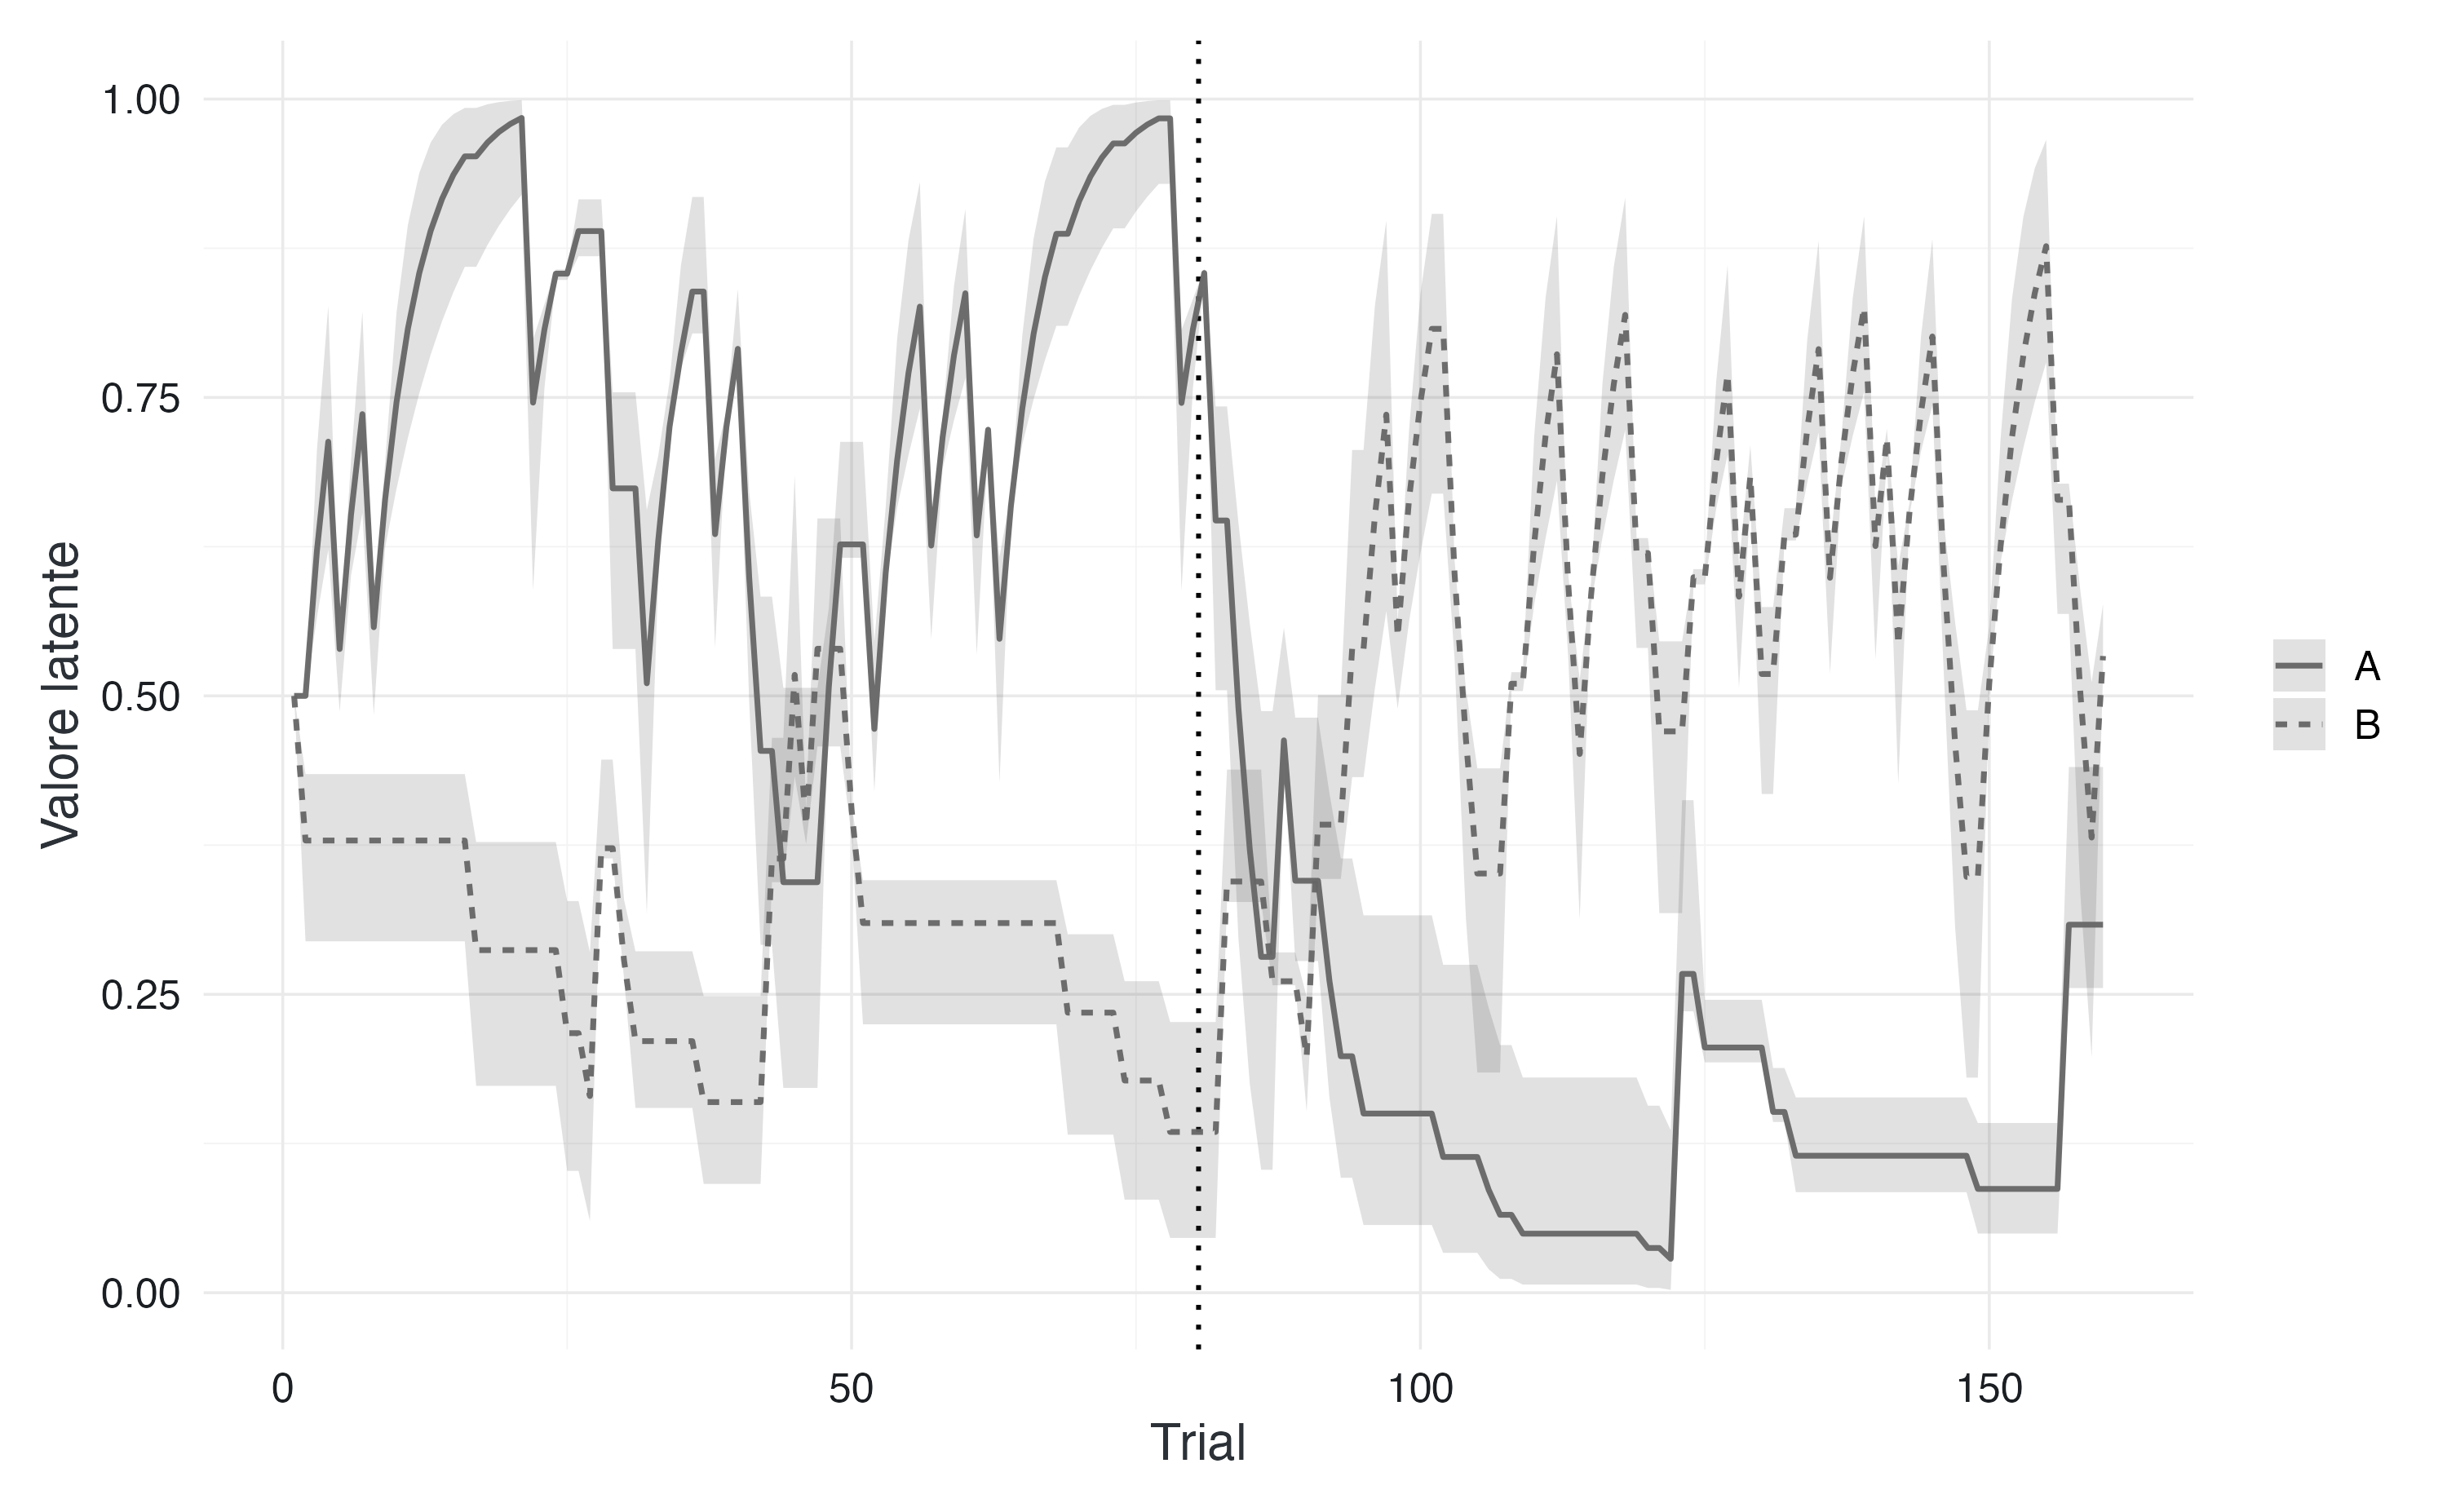
\includegraphics[width=0.85\linewidth,height=\textheight,keepaspectratio]{chapters/formal_models/04_rescorla_wagner_files/figure-pdf/fig-rw-latent-trajectories-1.png}

}

\caption{\label{fig-rw-latent-trajectories}Traiettorie posteriori dei
valori latenti prima della scelta. Le bande rappresentano intervalli
posteriori al 90\%.}

\end{figure}%

Le traiettorie ricostruite non sono misure dirette dell'aspettativa del
partecipante. Sono stati latenti inferiti sotto le assunzioni del
modello.

\section{Controlli predittivi a
posteriori}\label{controlli-predittivi-a-posteriori-3}

Un buon controllo deve concentrarsi su caratteristiche che il modello
intende spiegare.

\begin{Shaded}
\begin{Highlighting}[]
\NormalTok{replicated\_statistics }\OtherTok{\textless{}{-}} \ControlFlowTok{function}\NormalTok{(}
\NormalTok{    fit,}
\NormalTok{    rich\_is\_A,}
    \AttributeTok{n\_replications =} \DecValTok{300}
\NormalTok{) \{}
\NormalTok{  choice\_matrix }\OtherTok{\textless{}{-}}\NormalTok{ fit}\SpecialCharTok{$}\FunctionTok{draws}\NormalTok{(}
    \StringTok{"choice\_rep"}\NormalTok{,}
    \AttributeTok{format =} \StringTok{"draws\_matrix"}
\NormalTok{  ) }\SpecialCharTok{|\textgreater{}}
    \FunctionTok{as.matrix}\NormalTok{()}

\NormalTok{  reward\_matrix }\OtherTok{\textless{}{-}}\NormalTok{ fit}\SpecialCharTok{$}\FunctionTok{draws}\NormalTok{(}
    \StringTok{"reward\_rep"}\NormalTok{,}
    \AttributeTok{format =} \StringTok{"draws\_matrix"}
\NormalTok{  ) }\SpecialCharTok{|\textgreater{}}
    \FunctionTok{as.matrix}\NormalTok{()}

\NormalTok{  selected }\OtherTok{\textless{}{-}} \FunctionTok{sample}\NormalTok{(}
    \FunctionTok{seq\_len}\NormalTok{(}\FunctionTok{nrow}\NormalTok{(choice\_matrix)),}
    \AttributeTok{size =} \FunctionTok{min}\NormalTok{(n\_replications, }\FunctionTok{nrow}\NormalTok{(choice\_matrix))}
\NormalTok{  )}

\NormalTok{  purrr}\SpecialCharTok{::}\FunctionTok{map\_dfr}\NormalTok{(}
\NormalTok{    selected,}
    \SpecialCharTok{\textasciitilde{}} \FunctionTok{behavioral\_statistics}\NormalTok{(}
      \AttributeTok{choice =} \FunctionTok{as.integer}\NormalTok{(choice\_matrix[.x, ]),}
      \AttributeTok{reward =} \FunctionTok{as.integer}\NormalTok{(reward\_matrix[.x, ]),}
      \AttributeTok{rich\_is\_A =}\NormalTok{ rich\_is\_A}
\NormalTok{    ),}
    \AttributeTok{.id =} \StringTok{"replication"}
\NormalTok{  )}
\NormalTok{\}}

\NormalTok{rw\_rep\_stats }\OtherTok{\textless{}{-}} \FunctionTok{replicated\_statistics}\NormalTok{(}
  \AttributeTok{fit =}\NormalTok{ fit\_rw,}
  \AttributeTok{rich\_is\_A =}\NormalTok{ sim\_rw}\SpecialCharTok{$}\NormalTok{rich\_is\_A}
\NormalTok{)}

\NormalTok{rw\_observed\_stats }\OtherTok{\textless{}{-}} \FunctionTok{behavioral\_statistics}\NormalTok{(}
  \AttributeTok{choice =}\NormalTok{ sim\_rw}\SpecialCharTok{$}\NormalTok{choice,}
  \AttributeTok{reward =}\NormalTok{ sim\_rw}\SpecialCharTok{$}\NormalTok{reward,}
  \AttributeTok{rich\_is\_A =}\NormalTok{ sim\_rw}\SpecialCharTok{$}\NormalTok{rich\_is\_A}
\NormalTok{)}
\end{Highlighting}
\end{Shaded}

\begin{figure}

\centering{

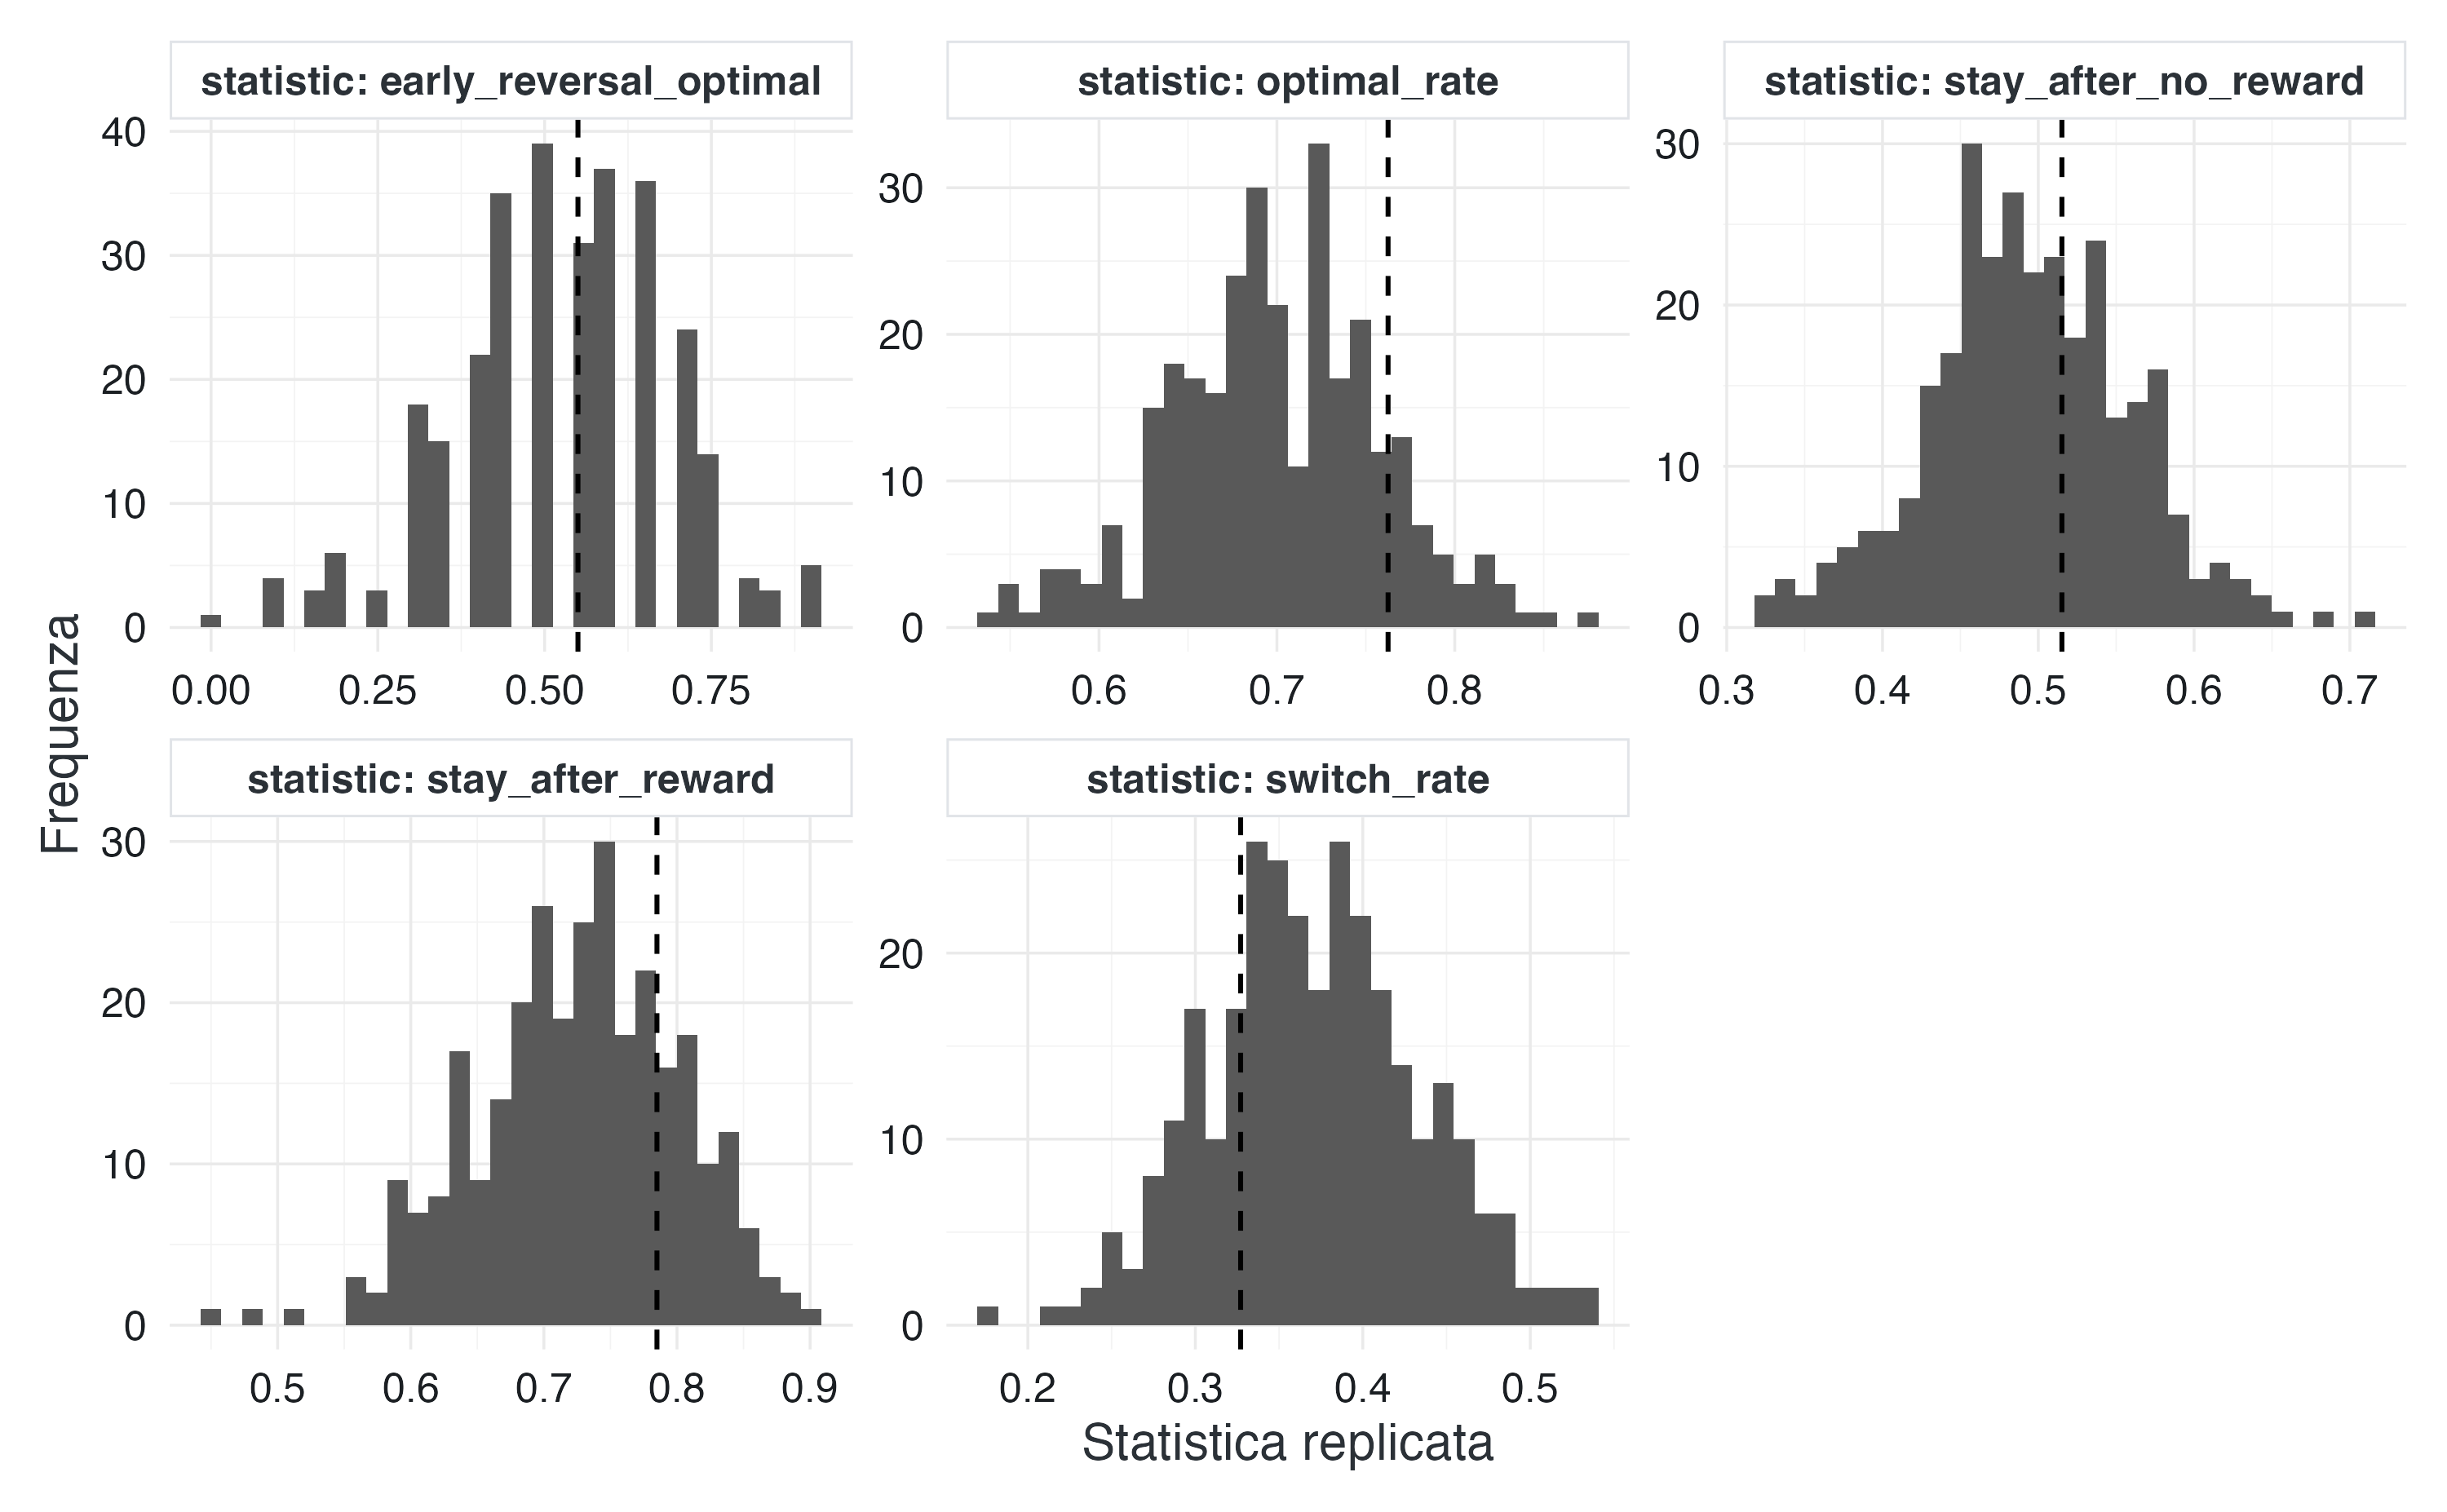
\includegraphics[width=0.85\linewidth,height=\textheight,keepaspectratio]{chapters/formal_models/04_rescorla_wagner_files/figure-pdf/fig-rw-posterior-predictive-statistics-1.png}

}

\caption{\label{fig-rw-posterior-predictive-statistics}Distribuzioni
posteriori predittive di statistiche dinamiche. Le linee tratteggiate
indicano i valori osservati.}

\end{figure}%

Questi controlli chiedono se il modello riproduce:

\begin{itemize}
\tightlist
\item
  la scelta dell'alternativa attualmente più vantaggiosa;
\item
  l'adattamento immediatamente successivo al reversal;
\item
  la frequenza dei cambi di risposta;
\item
  la tendenza a restare dopo un esito positivo;
\item
  la tendenza a restare dopo un esito negativo.
\end{itemize}

Un istogramma marginale delle scelte non sarebbe sufficiente a
controllare una teoria dinamica.

\section{Recuperabilità dei
parametri}\label{recuperabilituxe0-dei-parametri}

La simulazione precedente costituisce un primo esercizio di recupero: il
modello viene applicato a dati generati da se stesso e la posterior
viene confrontata con i valori noti.

Una valutazione più informativa ripete l'operazione su una griglia di
parametri e su molti dataset.

\begin{tcolorbox}[enhanced jigsaw, arc=.35mm, bottomrule=.15mm, bottomtitle=1mm, breakable, colback=white, colbacktitle=quarto-callout-note-color!10!white, colframe=quarto-callout-note-color-frame, coltitle=black, left=2mm, leftrule=.75mm, opacityback=0, opacitybacktitle=0.6, rightrule=.15mm, title=\textcolor{quarto-callout-note-color}{\faInfo}\hspace{0.5em}{Schema per un esperimento di parameter recovery}, titlerule=0mm, toprule=.15mm, toptitle=1mm]

\begin{Shaded}
\begin{Highlighting}[]
\NormalTok{recovery\_grid }\OtherTok{\textless{}{-}}\NormalTok{ tidyr}\SpecialCharTok{::}\FunctionTok{crossing}\NormalTok{(}
  \AttributeTok{alpha\_true =} \FunctionTok{c}\NormalTok{(}\FloatTok{0.08}\NormalTok{, }\FloatTok{0.20}\NormalTok{, }\FloatTok{0.50}\NormalTok{),}
  \AttributeTok{tau\_true =} \FunctionTok{c}\NormalTok{(}\FloatTok{0.8}\NormalTok{, }\DecValTok{2}\NormalTok{, }\DecValTok{5}\NormalTok{),}
  \AttributeTok{replication =} \FunctionTok{seq\_len}\NormalTok{(}\DecValTok{20}\NormalTok{)}
\NormalTok{)}

\CommentTok{\# Per ciascuna riga:}
\CommentTok{\# 1. simulare un dataset;}
\CommentTok{\# 2. adattare il modello;}
\CommentTok{\# 3. salvare mediana e intervallo posteriori;}
\CommentTok{\# 4. confrontare stima e valore generativo;}
\CommentTok{\# 5. esaminare bias, RMSE e copertura.}
\end{Highlighting}
\end{Shaded}

\end{tcolorbox}

\begin{tcolorbox}[enhanced jigsaw, arc=.35mm, bottomrule=.15mm, bottomtitle=1mm, breakable, colback=white, colbacktitle=quarto-callout-important-color!10!white, colframe=quarto-callout-important-color-frame, coltitle=black, left=2mm, leftrule=.75mm, opacityback=0, opacitybacktitle=0.6, rightrule=.15mm, title=\textcolor{quarto-callout-important-color}{\faExclamation}\hspace{0.5em}{Fit e recuperabilità sono domande differenti}, titlerule=0mm, toprule=.15mm, toptitle=1mm]

Un modello può adattarsi bene alle scelte e tuttavia non distinguere
accuratamente \(\alpha\) da \(\tau\). In tal caso le previsioni
aggregate possono essere adeguate, mentre le interpretazioni individuali
dei parametri rimangono fragili.

\end{tcolorbox}

\section{Quando il modello di base
fallisce}\label{quando-il-modello-di-base-fallisce}

Il modello RW con scelta logistica assume che, condizionatamente ai
valori appresi, la scelta corrente non dipenda dalla risposta
precedente.

Molti partecipanti potrebbero invece mostrare perseverazione (tendenza a
ripetere la risposta), alternanza sistematica, lapse occasionali,
apprendimento asimmetrico da rinforzi positivi e negativi, o decadimento
dei valori delle opzioni non scelte.

Per illustrare il processo di raffinamento del modello, generiamo un
secondo dataset in cui è presente un effetto di perseverazione positiva:

\[
\kappa=0.9.
\]

\begin{Shaded}
\begin{Highlighting}[]
\NormalTok{sim\_rw\_perseveration }\OtherTok{\textless{}{-}} \FunctionTok{simulate\_prl\_rw}\NormalTok{(}
  \AttributeTok{alpha =} \FloatTok{0.20}\NormalTok{,}
  \AttributeTok{tau =} \DecValTok{3}\NormalTok{,}
  \AttributeTok{kappa =} \FloatTok{0.90}\NormalTok{,}
  \AttributeTok{seed =} \DecValTok{989}
\NormalTok{)}

\NormalTok{rw\_perseveration\_data }\OtherTok{\textless{}{-}} \FunctionTok{list}\NormalTok{(}
  \AttributeTok{T =} \FunctionTok{nrow}\NormalTok{(sim\_rw\_perseveration),}
  \AttributeTok{choice =} \FunctionTok{as.integer}\NormalTok{(}
\NormalTok{    sim\_rw\_perseveration}\SpecialCharTok{$}\NormalTok{choice}
\NormalTok{  ),}
  \AttributeTok{reward =} \FunctionTok{as.integer}\NormalTok{(}
\NormalTok{    sim\_rw\_perseveration}\SpecialCharTok{$}\NormalTok{reward}
\NormalTok{  ),}
  \AttributeTok{rich\_is\_A =} \FunctionTok{as.integer}\NormalTok{(}
\NormalTok{    sim\_rw\_perseveration}\SpecialCharTok{$}\NormalTok{rich\_is\_A}
\NormalTok{  ),}
  \AttributeTok{p\_reward\_rich =} \FloatTok{0.70}
\NormalTok{)}
\end{Highlighting}
\end{Shaded}

Adattiamo dapprima il modello di base, che non contiene \(\kappa\).

\begin{Shaded}
\begin{Highlighting}[]
\NormalTok{fit\_rw\_misspecified }\OtherTok{\textless{}{-}}\NormalTok{ rw\_model}\SpecialCharTok{$}\FunctionTok{sample}\NormalTok{(}
  \AttributeTok{data =}\NormalTok{ rw\_perseveration\_data,}
  \AttributeTok{seed =} \DecValTok{615}\NormalTok{,}
  \AttributeTok{chains =} \DecValTok{4}\NormalTok{,}
  \AttributeTok{parallel\_chains =} \DecValTok{4}\NormalTok{,}
  \AttributeTok{iter\_warmup =} \DecValTok{1000}\NormalTok{,}
  \AttributeTok{iter\_sampling =} \DecValTok{1500}\NormalTok{,}
  \AttributeTok{refresh =} \DecValTok{0}
\NormalTok{)}
\end{Highlighting}
\end{Shaded}

Il modello può compensare in parte la perseverazione modificando
\(\alpha\) e \(\tau\), ma tale compensazione non garantisce che
riproduca le dipendenze seriali rilevanti.

\subsection{Un modello rivale con
perseverazione}\label{un-modello-rivale-con-perseverazione}

Introduciamo:

\[
\Pr(Y_t=B)
=
\operatorname{logit}^{-1}
\left[
\tau\{Q_t(B)-Q_t(A)\}
+
\kappa S_{t-1}
\right],
\]

dove:

\[
S_{t-1}
=
\begin{cases}
+1, & \text{se la scelta precedente è }B,\\
-1, & \text{se la scelta precedente è }A,\\
0, & \text{al primo trial.}
\end{cases}
\]

Con \(\kappa>0\), la risposta precedente tende a essere ripetuta; con
\(\kappa<0\), il modello favorisce l'alternanza.

\begin{Shaded}
\begin{Highlighting}[]
\NormalTok{stancode\_rw\_perseveration }\OtherTok{\textless{}{-}} \StringTok{"}
\StringTok{data \{}
\StringTok{  int\textless{}lower=1\textgreater{} T;}
\StringTok{  array[T] int\textless{}lower=0, upper=1\textgreater{} choice;}
\StringTok{  array[T] int\textless{}lower=0, upper=1\textgreater{} reward;}
\StringTok{  array[T] int\textless{}lower=0, upper=1\textgreater{} rich\_is\_A;}
\StringTok{  real\textless{}lower=0.5, upper=1\textgreater{} p\_reward\_rich;}
\StringTok{\}}

\StringTok{parameters \{}
\StringTok{  real alpha\_raw;}
\StringTok{  real log\_tau;}
\StringTok{  real kappa;}
\StringTok{\}}

\StringTok{transformed parameters \{}
\StringTok{  real\textless{}lower=0, upper=1\textgreater{} alpha = inv\_logit(alpha\_raw);}
\StringTok{  real\textless{}lower=0\textgreater{} tau = exp(log\_tau);}
\StringTok{\}}

\StringTok{model \{}
\StringTok{  vector[2] q = rep\_vector(0.5, 2);}

\StringTok{  alpha\_raw \textasciitilde{} normal(logit(0.20), 1);}
\StringTok{  log\_tau \textasciitilde{} normal(log(2), 0.6);}
\StringTok{  kappa \textasciitilde{} normal(0, 1);}

\StringTok{  for (t in 1:T) \{}
\StringTok{    int a = choice[t] + 1;}
\StringTok{    real previous\_signed =}
\StringTok{      t == 1 ? 0 : 2 * choice[t {-} 1] {-} 1;}
\StringTok{    real eta =}
\StringTok{      tau * (q[2] {-} q[1]) +}
\StringTok{      kappa * previous\_signed;}

\StringTok{    choice[t] \textasciitilde{} bernoulli\_logit(eta);}
\StringTok{    q[a] += alpha * (reward[t] {-} q[a]);}
\StringTok{  \}}
\StringTok{\}}

\StringTok{generated quantities \{}
\StringTok{  array[T] int choice\_rep;}
\StringTok{  array[T] int reward\_rep;}
\StringTok{  vector[T] log\_lik;}

\StringTok{  \{}
\StringTok{    vector[2] q\_obs = rep\_vector(0.5, 2);}
\StringTok{    vector[2] q\_rep = rep\_vector(0.5, 2);}
\StringTok{    int previous\_rep\_signed = 0;}

\StringTok{    for (t in 1:T) \{}
\StringTok{      int a\_obs;}
\StringTok{      int a\_rep;}
\StringTok{      int chosen\_is\_rich;}
\StringTok{      real previous\_obs\_signed;}
\StringTok{      real eta\_obs;}
\StringTok{      real eta\_rep;}
\StringTok{      real reward\_probability;}

\StringTok{      previous\_obs\_signed =}
\StringTok{        t == 1 ? 0 : 2 * choice[t {-} 1] {-} 1;}

\StringTok{      eta\_obs =}
\StringTok{        tau * (q\_obs[2] {-} q\_obs[1]) +}
\StringTok{        kappa * previous\_obs\_signed;}

\StringTok{      log\_lik[t] = bernoulli\_logit\_lpmf(}
\StringTok{        choice[t] | eta\_obs}
\StringTok{      );}

\StringTok{      a\_obs = choice[t] + 1;}
\StringTok{      q\_obs[a\_obs] += alpha *}
\StringTok{        (reward[t] {-} q\_obs[a\_obs]);}

\StringTok{      eta\_rep =}
\StringTok{        tau * (q\_rep[2] {-} q\_rep[1]) +}
\StringTok{        kappa * previous\_rep\_signed;}

\StringTok{      choice\_rep[t] =}
\StringTok{        bernoulli\_logit\_rng(eta\_rep);}
\StringTok{      a\_rep = choice\_rep[t] + 1;}

\StringTok{      chosen\_is\_rich =}
\StringTok{        (}
\StringTok{          (choice\_rep[t] == 0 \&\&}
\StringTok{           rich\_is\_A[t] == 1) ||}
\StringTok{          (choice\_rep[t] == 1 \&\&}
\StringTok{           rich\_is\_A[t] == 0)}
\StringTok{        ) ? 1 : 0;}

\StringTok{      reward\_probability =}
\StringTok{        chosen\_is\_rich == 1}
\StringTok{        ? p\_reward\_rich}
\StringTok{        : 1 {-} p\_reward\_rich;}

\StringTok{      reward\_rep[t] =}
\StringTok{        bernoulli\_rng(reward\_probability);}

\StringTok{      q\_rep[a\_rep] += alpha *}
\StringTok{        (reward\_rep[t] {-} q\_rep[a\_rep]);}

\StringTok{      previous\_rep\_signed =}
\StringTok{        2 * choice\_rep[t] {-} 1;}
\StringTok{    \}}
\StringTok{  \}}
\StringTok{\}}
\StringTok{"}
\end{Highlighting}
\end{Shaded}

\begin{Shaded}
\begin{Highlighting}[]
\NormalTok{rw\_perseveration\_file }\OtherTok{\textless{}{-}} \FunctionTok{write\_stan\_file}\NormalTok{(}
\NormalTok{  stancode\_rw\_perseveration}
\NormalTok{)}

\NormalTok{rw\_perseveration\_model }\OtherTok{\textless{}{-}} \FunctionTok{cmdstan\_model}\NormalTok{(}
\NormalTok{  rw\_perseveration\_file}
\NormalTok{)}

\NormalTok{fit\_rw\_perseveration }\OtherTok{\textless{}{-}}\NormalTok{ rw\_perseveration\_model}\SpecialCharTok{$}\FunctionTok{sample}\NormalTok{(}
  \AttributeTok{data =}\NormalTok{ rw\_perseveration\_data,}
  \AttributeTok{seed =} \DecValTok{771}\NormalTok{,}
  \AttributeTok{chains =} \DecValTok{4}\NormalTok{,}
  \AttributeTok{parallel\_chains =} \DecValTok{4}\NormalTok{,}
  \AttributeTok{iter\_warmup =} \DecValTok{1000}\NormalTok{,}
  \AttributeTok{iter\_sampling =} \DecValTok{1500}\NormalTok{,}
  \AttributeTok{refresh =} \DecValTok{0}
\NormalTok{)}
\end{Highlighting}
\end{Shaded}

\subsection{Confrontare i modelli attraverso le
discrepanze}\label{confrontare-i-modelli-attraverso-le-discrepanze}

\begin{Shaded}
\begin{Highlighting}[]
\NormalTok{base\_rep\_stats }\OtherTok{\textless{}{-}} \FunctionTok{replicated\_statistics}\NormalTok{(}
  \AttributeTok{fit =}\NormalTok{ fit\_rw\_misspecified,}
  \AttributeTok{rich\_is\_A =}\NormalTok{ sim\_rw\_perseveration}\SpecialCharTok{$}\NormalTok{rich\_is\_A}
\NormalTok{) }\SpecialCharTok{|\textgreater{}}
  \FunctionTok{mutate}\NormalTok{(}\AttributeTok{model =} \StringTok{"RW di base"}\NormalTok{)}

\NormalTok{perseveration\_rep\_stats }\OtherTok{\textless{}{-}} \FunctionTok{replicated\_statistics}\NormalTok{(}
  \AttributeTok{fit =}\NormalTok{ fit\_rw\_perseveration,}
  \AttributeTok{rich\_is\_A =}\NormalTok{ sim\_rw\_perseveration}\SpecialCharTok{$}\NormalTok{rich\_is\_A}
\NormalTok{) }\SpecialCharTok{|\textgreater{}}
  \FunctionTok{mutate}\NormalTok{(}\AttributeTok{model =} \StringTok{"RW + perseverazione"}\NormalTok{)}

\NormalTok{observed\_perseveration\_stats }\OtherTok{\textless{}{-}} \FunctionTok{behavioral\_statistics}\NormalTok{(}
  \AttributeTok{choice =}\NormalTok{ sim\_rw\_perseveration}\SpecialCharTok{$}\NormalTok{choice,}
  \AttributeTok{reward =}\NormalTok{ sim\_rw\_perseveration}\SpecialCharTok{$}\NormalTok{reward,}
  \AttributeTok{rich\_is\_A =}\NormalTok{ sim\_rw\_perseveration}\SpecialCharTok{$}\NormalTok{rich\_is\_A}
\NormalTok{)}
\end{Highlighting}
\end{Shaded}

\begin{figure}

\centering{

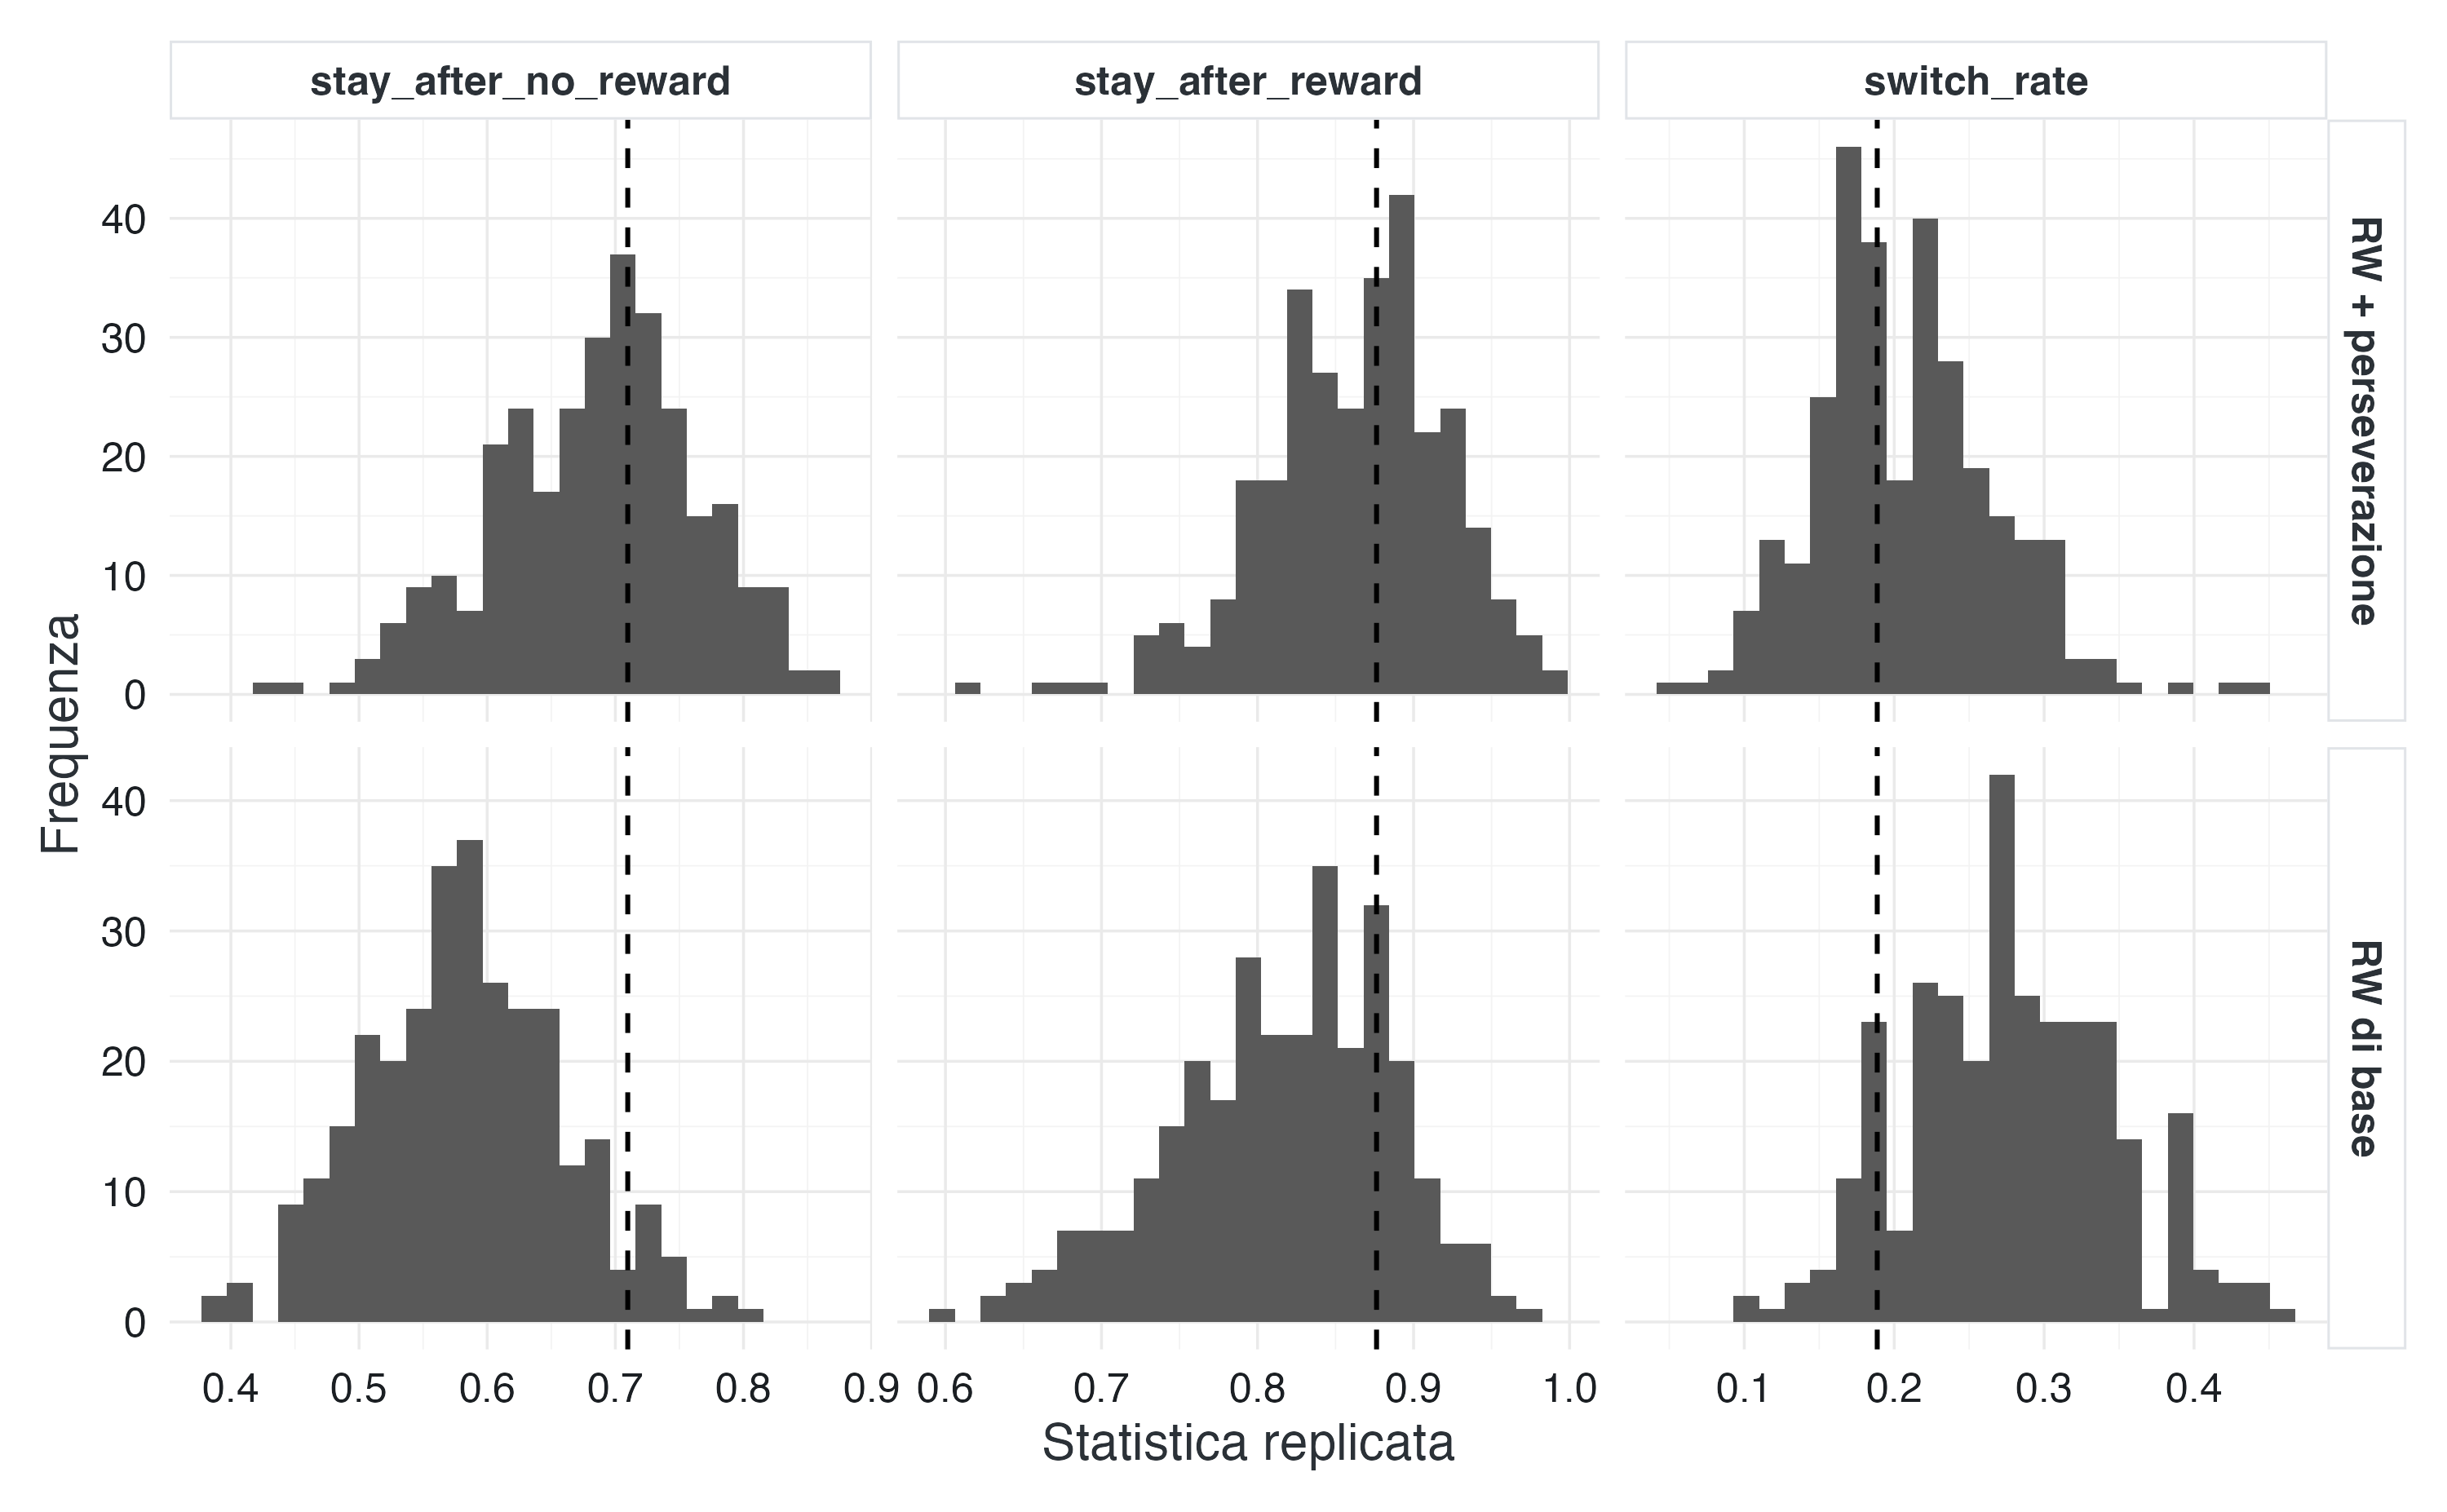
\includegraphics[width=0.85\linewidth,height=\textheight,keepaspectratio]{chapters/formal_models/04_rescorla_wagner_files/figure-pdf/fig-rw-model-comparison-ppc-1.png}

}

\caption{\label{fig-rw-model-comparison-ppc}Confronto predittivo tra il
modello RW di base e l'estensione con perseverazione. Le linee
tratteggiate indicano i dati osservati.}

\end{figure}%

\begin{Shaded}
\begin{Highlighting}[]
\NormalTok{fit\_rw\_perseveration}\SpecialCharTok{$}\FunctionTok{summary}\NormalTok{(}
  \AttributeTok{variables =} \FunctionTok{c}\NormalTok{(}\StringTok{"alpha"}\NormalTok{, }\StringTok{"tau"}\NormalTok{, }\StringTok{"kappa"}\NormalTok{),}
\NormalTok{  mean,}
\NormalTok{  sd,}
  \SpecialCharTok{\textasciitilde{}}\FunctionTok{quantile}\NormalTok{(.x, }\AttributeTok{probs =} \FunctionTok{c}\NormalTok{(}\FloatTok{0.05}\NormalTok{, }\FloatTok{0.50}\NormalTok{, }\FloatTok{0.95}\NormalTok{))}
\NormalTok{)}
\CommentTok{\#\textgreater{} \# A tibble: 3 x 6}
\CommentTok{\#\textgreater{}   variable  mean     sd  \textasciigrave{}5\%\textasciigrave{} \textasciigrave{}50\%\textasciigrave{} \textasciigrave{}95\%\textasciigrave{}}
\CommentTok{\#\textgreater{}   \textless{}chr\textgreater{}    \textless{}dbl\textgreater{}  \textless{}dbl\textgreater{} \textless{}dbl\textgreater{} \textless{}dbl\textgreater{} \textless{}dbl\textgreater{}}
\CommentTok{\#\textgreater{} 1 alpha    0.187 0.0555 0.112 0.180 0.288}
\CommentTok{\#\textgreater{} 2 tau      3.91  0.845  2.59  3.88  5.38 }
\CommentTok{\#\textgreater{} 3 kappa    0.671 0.250  0.254 0.673 1.08}
\end{Highlighting}
\end{Shaded}

Se il modello esteso riproduce meglio le statistiche seriali e recupera
un \(\kappa\) positivo, abbiamo evidenza che la perseverazione è una
componente utile della specificazione per questi dati simulati.

Non abbiamo però dimostrato che la perseverazione sia il vero meccanismo
psicologico. Altri modelli potrebbero produrre pattern simili.

\begin{tcolorbox}[enhanced jigsaw, arc=.35mm, bottomrule=.15mm, bottomtitle=1mm, breakable, colback=white, colbacktitle=quarto-callout-warning-color!10!white, colframe=quarto-callout-warning-color-frame, coltitle=black, left=2mm, leftrule=.75mm, opacityback=0, opacitybacktitle=0.6, rightrule=.15mm, title=\textcolor{quarto-callout-warning-color}{\faExclamationTriangle}\hspace{0.5em}{Non usare automaticamente la LOO trial per trial}, titlerule=0mm, toprule=.15mm, toptitle=1mm]

La log-verosimiglianza di ciascun trial dipende dagli stati costruiti
usando i trial precedenti. Lasciare fuori un singolo trial come se le
osservazioni fossero scambiabili può quindi non rappresentare la domanda
predittiva di interesse.

Per processi temporali sono spesso più appropriate:

\begin{itemize}
\tightlist
\item
  validazione prequenziale;
\item
  separazione tra blocchi iniziali e successivi;
\item
  previsione di un nuovo reversal;
\item
  leave-one-subject-out nei modelli gerarchici;
\item
  validazione in un nuovo compito o contesto.
\end{itemize}

L'unità lasciata fuori deve corrispondere alla generalizzazione
scientifica desiderata.

\end{tcolorbox}

\section{Estensioni teoricamente motivate}\label{sec-rw-extensions}

Le estensioni illustrate in questa sezione sono facoltative: non sono
necessarie per comprendere la struttura generativa del modello di base,
stimarne i parametri né valutarne l'adeguatezza. Chi legge può dunque
limitarsi al modello Rescorla-Wagner e tornare a queste pagine in un
secondo momento.

Tra le estensioni più comuni rientrano:

\begin{itemize}
\tightlist
\item
  \textbf{apprendimento asimmetrico}, che distingue tassi di
  aggiornamento \(\alpha^+\) e \(\alpha^-\) per errori di previsione
  positivi e negativi;
\item
  \textbf{decadimento dei valori}, per cui i valori delle alternative
  non scelte convergono gradualmente verso un livello di riferimento;
\item
  \textbf{parametro di \emph{lapse}}, che separa una piccola probabilità
  di scelta casuale dalla sensibilità alle differenze di valore;
\item
  \textbf{generalizzazione a più di due alternative}: con \(K>2\) la
  regola di scelta diventa
  \[\Pr(Y_t=k) = \frac{\exp\{\tau\, Q_t(k)\}}{\sum_{j=1}^{K} \exp\{\tau\, Q_t(j)\}};\]
\item
  \textbf{parametri dipendenti dal contesto}, che consentono di far
  variare \(\alpha_c\), \(\tau_c\), \(\kappa_c\) tra condizioni
  sperimentali o categorie di stimoli.
\end{itemize}

Quest'ultima possibilità è stata impiegata, ad esempio, per verificare
se i parametri di apprendimento differiscano tra contesti alimentari e
neutri ({Colpizzi et al.} (\citeproc{ref-colpizzi2025food}{2025})). Il
valore dell'estensione non risiede soltanto nell'individuare una
differenza, ma nel formulare e sottoporre a controllo l'ipotesi che la
dinamica del processo cambi selettivamente con il contesto.

Quando persone e condizioni si ripetono, la stima separata di ogni
parametro produce stime rumorose e confronti instabili. In tali
situazioni è opportuno adottare un modello gerarchico che descriva: le
distribuzioni nella popolazione, le deviazioni individuali, le
differenze tra contesti, le correlazioni tra parametri e l'incertezza
sulle quantità sia individuali sia di gruppo.

\section{Rescorla--Wagner è un modello
bayesiano?}\label{rescorlawagner-uxe8-un-modello-bayesiano}

La regola:

\[
Q_{t+1}
=
Q_t+\alpha(R_t-Q_t)
\]

ha la forma di un aggiornamento guidato da un errore di previsione.
Questa somiglianza permette un utile collegamento intuitivo con
l'apprendimento bayesiano.

L'identità, tuttavia, non è completa.

Il modello RW standard:

\begin{itemize}
\tightlist
\item
  mantiene un valore puntuale, non una distribuzione di incertezza;
\item
  usa spesso un tasso \(\alpha\) costante;
\item
  non deriva automaticamente \(\alpha\) dalla precisione relativa di
  prior e dati;
\item
  non rappresenta esplicitamente l'incertezza sull'ambiente.
\end{itemize}

Modelli come il filtro di Kalman o altri modelli di apprendimento
bayesiano aggiornano invece sia la stima sia la sua incertezza e possono
modificare dinamicamente il peso attribuito ai nuovi esiti.

È quindi più accurato descrivere RW come una regola delta che condivide
con l'aggiornamento bayesiano la logica della correzione tramite errore
di previsione, non come un'inferenza bayesiana completa.

\section{Interpretare e comunicare i
parametri}\label{interpretare-e-comunicare-i-parametri}

Una formulazione prudente àncora il discorso al modello, alla scala e
all'incertezza, come mostra l'esempio seguente:

\begin{quote}
Nel modello specificato, la posterior del tasso di apprendimento
descrive quanto rapidamente i valori latenti vengono aggiornati dopo i
feedback, mentre la posterior dell'inverse temperature descrive quanto
fortemente le scelte dipendono dalle differenze tra tali valori. I
controlli predittivi indicano se questa scomposizione riproduce le
dinamiche comportamentali considerate. L'interpretazione dei parametri
come caratteristiche psicologiche richiede ulteriori evidenze di
recuperabilità, stabilità e validità esterna.
\end{quote}

È preferibile evitare affermazioni che attribuiscono ai parametri un
significato psicologico o neurale senza le necessarie cautele (ad
esempio: ``il partecipante ha un deficit di apprendimento'', ``\(\tau\)
misura direttamente l'esplorazione'', ``il parametro dimostra il
meccanismo neurale'', ``il modello ha scoperto lo stile cognitivo della
persona''). Una comunicazione corretta deve invece specificare sempre:
(1) il modello adottato, (2) la scala e il compito, (3) l'incertezza
associata alle stime, (4) i controlli predittivi condotti e (5) le
interpretazioni concorrenti plausibili.

\section{Errori frequenti}\label{errori-frequenti-13}

\begin{itemize}
\item
  \textbf{Interpretare la percentuale di risposte corrette come
  apprendimento puro.}\\
  La prestazione osservata dipende congiuntamente dalla dinamica di
  aggiornamento, dalla regola di scelta, dalla struttura dell'ambiente e
  dalla specificazione del modello.
\item
  \textbf{Usare \(\tau\) come ``temperatura'' senza distinguere le
  convenzioni.}\\
  Le convenzioni di temperatura e temperatura inversa hanno direzioni
  opposte. Testo, formule e codice devono adottare coerentemente la
  stessa convenzione.
\item
  \textbf{Ignorare la scala dei rinforzi.}\\
  Modificare la scala dei valori \(Q\) altera l'interpretazione del
  parametro \(\tau\).
\item
  \textbf{Stimare troppi parametri con poche prove.}\\
  Un buon adattamento non garantisce che \emph{learning rate},
  sensibilità, perseverazione e parametro di \emph{lapse} siano
  separatamente recuperabili.
\item
  \textbf{Controllare soltanto le distribuzioni marginali.}\\
  Un modello dinamico deve riprodurre anche adattamento nel tempo,
  dipendenze seriali e risposta ai cambiamenti delle contingenze.
\item
  \textbf{Limitarsi a un solo modello.}\\
  Un parametro apparentemente interpretabile può assorbire un meccanismo
  omesso, producendo inferenze fuorvianti.
\item
  \textbf{Trattare gli stati latenti come misure osservate.}\\
  Le traiettorie \(Q_t\) sono inferenze condizionate alla specificazione
  del modello, non grandezze direttamente misurate.
\item
  \textbf{Usare la \emph{leave-one-out} trial per trial senza definire
  la generalizzazione.}\\
  La dipendenza temporale rende inadeguata l'assunzione di osservazioni
  scambiabili.
\item
  \textbf{Interpretare un parametro come tratto stabile senza
  verifica.}\\
  La stabilità tra sessioni, compiti e contesti va dimostrata
  empiricamente, non presupposta.
\item
  \textbf{Chiamare meccanicistico qualsiasi modello ricorsivo.}\\
  La plausibilità meccanicistica richiede un ancoraggio teorico
  esplicito e controlli indipendenti, non la semplice forma ricorsiva.
\end{itemize}

\section*{Riflessioni conclusive}\label{riflessioni-conclusive-38}

\markright{Riflessioni conclusive}

Il modello Rescorla--Wagner mostra in forma compatta che cosa aggiunge
una teoria processuale.

La regola di aggiornamento specifica come il feedback modifica uno stato
latente. Il modello di scelta specifica come tale stato produce
comportamento osservabile. L'inferenza bayesiana permette di procedere
all'indietro, dalle scelte ai parametri e alle traiettorie latenti,
mantenendo esplicita l'incertezza.

Questo passaggio non rende però automatica l'interpretazione
psicologica. Learning rate e inverse temperature sono parametri di una
specificazione. Possono essere confusi tra loro, possono assorbire
perseverazione o lapse omessi e possono dipendere dal compito, dalla
scala e dal contesto.

Per questo motivo il workflow completo comprende:

\[
\text{teoria}
\rightarrow
\text{simulazione}
\rightarrow
\text{modello osservazionale}
\rightarrow
\text{prior}
\rightarrow
\text{stima}
\rightarrow
\text{recovery}
\rightarrow
\text{controllo predittivo}
\rightarrow
\text{modello rivale}
\rightarrow
\text{revisione}.
\]

Il risultato più importante non è una singola stima di \(\alpha\) o
\(\tau\), ma una teoria sufficientemente precisa da produrre dati,
fallire controlli mirati ed essere modificata quando le sue predizioni
non sono adeguate.

\section{Concetti da ricordare}\label{concetti-da-ricordare-12}

\begin{enumerate}
\def\labelenumi{\arabic{enumi}.}
\tightlist
\item
  Il modello contiene una componente di apprendimento e una componente
  di scelta.
\item
  I valori \(Q_t\) sono stati latenti, non osservazioni.
\item
  L'errore di previsione è la differenza tra esito e valore atteso.
\item
  \(\alpha\) regola la rapidità dell'aggiornamento.
\item
  \(\tau\) regola la sensibilità delle scelte alle differenze di valore.
\item
  La scala dei rinforzi determina la scala dei valori e influenza
  l'interpretazione di \(\tau\).
\item
  Simulare prima della stima chiarisce le conseguenze dei parametri.
\item
  Un buon fit non garantisce recuperabilità.
\item
  I controlli predittivi devono esaminare statistiche dinamiche.
\item
  Un modello rivale può rivelare che un parametro assorbiva un
  meccanismo omesso.
\item
  La validazione temporale deve rispettare la dipendenza tra trial.
\item
  Un parametro processuale non diventa automaticamente un costrutto
  psicologico validato.
\end{enumerate}

\section{Esercizi}\label{esercizi-9}

\subsection{1. Velocità di
adattamento}\label{velocituxe0-di-adattamento}

Simula il compito con \(\alpha=0.05\), \(0.20\) e \(0.80\), mantenendo
fisso \(\tau=3\). Confronta il numero di trial necessario per preferire
la nuova opzione ricca dopo il reversal.

\subsection{2. Sensibilità della
scelta}\label{sensibilituxe0-della-scelta}

Mantieni \(\alpha=0.20\) e varia \(\tau\). Confronta accuratezza,
frequenza di switching e ricompensa totale.

\subsection{3. Condizioni iniziali}\label{condizioni-iniziali}

Ripeti la simulazione con \(Q_0=0\), \(0.5\) e \(1\). In quale parte del
compito le differenze sono più visibili?

\subsection{4. Prior predictive check}\label{prior-predictive-check-2}

Sostituisci il prior di \(\log\tau\) con una distribuzione molto più
ampia. Quali comportamenti estremi compaiono?

\subsection{5. Recupero dei parametri}\label{recupero-dei-parametri}

Costruisci un piccolo esperimento di recovery per tre valori di
\(\alpha\) e tre valori di \(\tau\). In quali regioni i parametri sono
più difficili da distinguere?

\subsection{6. Perseverazione omessa}\label{perseverazione-omessa}

Genera dati con \(\kappa>0\), adatta il modello di base e descrivi come
cambiano le posterior di \(\alpha\) e \(\tau\).

\subsection{7. Apprendimento
asimmetrico}\label{apprendimento-asimmetrico}

Modifica il simulatore introducendo \(\alpha^+\) e \(\alpha^-\). Quale
disegno rende i due parametri informativi?

\subsection{8. Modello senza
apprendimento}\label{modello-senza-apprendimento}

Costruisci un modello rivale con probabilità di scelta costante. Quali
statistiche predittive lo distinguono dal modello RW?

\subsection{9. Validazione}\label{validazione-1}

Progetta una procedura che adatti il modello alla prima fase e valuti la
previsione dopo il reversal. Quale informazione può essere usata durante
l'aggiornamento nella fase di test?

\subsection{10. Interpretazione}\label{interpretazione-4}

Scrivi un paragrafo di risultati che descriva un \(\alpha\) più basso in
un gruppo clinico senza trasformarlo automaticamente in prova di un
deficit generale di apprendimento.

\begin{tcolorbox}[enhanced jigsaw, arc=.35mm, bottomrule=.15mm, bottomtitle=1mm, breakable, colback=white, colbacktitle=quarto-callout-note-color!10!white, colframe=quarto-callout-note-color-frame, coltitle=black, left=2mm, leftrule=.75mm, opacityback=0, opacitybacktitle=0.6, rightrule=.15mm, title=\textcolor{quarto-callout-note-color}{\faInfo}\hspace{0.5em}{Tracce di soluzione}, titlerule=0mm, toprule=.15mm, toptitle=1mm]

\begin{enumerate}
\def\labelenumi{\arabic{enumi}.}
\tightlist
\item
  \(\alpha\) elevato tende a ridurre il ritardo dopo il reversal, ma
  aumenta la sensibilità a feedback casuali.
\item
  \(\tau\) elevato riduce le scelte dell'opzione momentaneamente
  inferiore; può però rendere più persistenti scelte sbagliate se i
  valori sono ancora inaccurati.
\item
  Le differenze di \(Q_0\) sono soprattutto iniziali; con un numero
  sufficiente di feedback l'influenza tende a ridursi.
\item
  Un prior molto ampio su \(\tau\) può generare sia scelte quasi casuali
  sia sequenze quasi deterministiche.
\item
  La recuperabilità può essere peggiore quando le scelte sono quasi
  casuali, quasi deterministiche o il numero di trial è ridotto.
\item
  Il modello di base può compensare la perseverazione alterando la
  sensibilità o la velocità di aggiornamento.
\item
  Servono abbastanza errori di previsione positivi e negativi in diverse
  fasi e alternative.
\item
  La dinamica dopo feedback e reversal è più informativa della sola
  percentuale complessiva di scelte.
\item
  Occorre distinguere previsione completamente generativa e previsione
  sequenziale condizionata sui feedback o sulle scelte osservate.
\item
  Il risultato deve essere riferito al modello, al compito e alle
  alternative considerate, includendo incertezza e controlli.
\end{enumerate}

\end{tcolorbox}

\begin{tcolorbox}[enhanced jigsaw, arc=.35mm, bottomrule=.15mm, bottomtitle=1mm, breakable, colback=white, colbacktitle=quarto-callout-note-color!10!white, colframe=quarto-callout-note-color-frame, coltitle=black, left=2mm, leftrule=.75mm, opacityback=0, opacitybacktitle=0.6, rightrule=.15mm, title=\textcolor{quarto-callout-note-color}{\faInfo}\hspace{0.5em}{Informazioni sull'ambiente di sviluppo}, titlerule=0mm, toprule=.15mm, toptitle=1mm]

\begin{Shaded}
\begin{Highlighting}[]
\FunctionTok{sessionInfo}\NormalTok{()}
\CommentTok{\#\textgreater{} R version 4.6.1 (2026{-}06{-}24)}
\CommentTok{\#\textgreater{} Platform: aarch64{-}apple{-}darwin23}
\CommentTok{\#\textgreater{} Running under: macOS Tahoe 26.5.2}
\CommentTok{\#\textgreater{} }
\CommentTok{\#\textgreater{} Matrix products: default}
\CommentTok{\#\textgreater{} BLAS:   /Library/Frameworks/R.framework/Versions/4.6/Resources/lib/libRblas.0.dylib }
\CommentTok{\#\textgreater{} LAPACK: /Library/Frameworks/R.framework/Versions/4.6/Resources/lib/libRlapack.dylib;  LAPACK version 3.12.1}
\CommentTok{\#\textgreater{} }
\CommentTok{\#\textgreater{} locale:}
\CommentTok{\#\textgreater{} [1] C.UTF{-}8/UTF{-}8/C.UTF{-}8/C/C.UTF{-}8/C.UTF{-}8}
\CommentTok{\#\textgreater{} }
\CommentTok{\#\textgreater{} time zone: Europe/Zagreb}
\CommentTok{\#\textgreater{} tzcode source: internal}
\CommentTok{\#\textgreater{} }
\CommentTok{\#\textgreater{} attached base packages:}
\CommentTok{\#\textgreater{} [1] stats     graphics  grDevices utils     datasets  methods   base     }
\CommentTok{\#\textgreater{} }
\CommentTok{\#\textgreater{} other attached packages:}
\CommentTok{\#\textgreater{}  [1] cmdstanr\_0.9.0        ragg\_1.5.2            tinytable\_0.17.0     }
\CommentTok{\#\textgreater{}  [4] withr\_3.0.3           systemfonts\_1.3.2     patchwork\_1.3.2      }
\CommentTok{\#\textgreater{}  [7] ggdist\_3.3.3          tidybayes\_3.0.7       bayesplot\_1.15.0     }
\CommentTok{\#\textgreater{} [10] ggplot2\_4.0.3         reliabilitydiag\_0.2.1 priorsense\_1.2.0     }
\CommentTok{\#\textgreater{} [13] posterior\_1.7.0       loo\_2.10.0            rstan\_2.32.7         }
\CommentTok{\#\textgreater{} [16] StanHeaders\_2.32.10   brms\_2.23.0           Rcpp\_1.1.2           }
\CommentTok{\#\textgreater{} [19] sessioninfo\_1.2.4     conflicted\_1.2.0      janitor\_2.2.1        }
\CommentTok{\#\textgreater{} [22] matrixStats\_1.5.0     modelr\_0.1.11         tibble\_3.3.1         }
\CommentTok{\#\textgreater{} [25] dplyr\_1.2.1           tidyr\_1.3.2           rio\_1.3.0            }
\CommentTok{\#\textgreater{} [28] here\_1.0.2           }
\CommentTok{\#\textgreater{} }
\CommentTok{\#\textgreater{} loaded via a namespace (and not attached):}
\CommentTok{\#\textgreater{}  [1] gridExtra\_2.3.1       inline\_0.3.21         rlang\_1.3.0          }
\CommentTok{\#\textgreater{}  [4] magrittr\_2.0.5        snakecase\_0.11.1      otel\_0.2.0           }
\CommentTok{\#\textgreater{}  [7] compiler\_4.6.1        vctrs\_0.7.3           reshape2\_1.4.5       }
\CommentTok{\#\textgreater{} [10] slider\_0.3.3          stringr\_1.6.0         pkgconfig\_2.0.3      }
\CommentTok{\#\textgreater{} [13] arrayhelpers\_1.1{-}1    fastmap\_1.2.0         backports\_1.5.1      }
\CommentTok{\#\textgreater{} [16] labeling\_0.4.3        utf8\_1.2.6            rmarkdown\_2.31       }
\CommentTok{\#\textgreater{} [19] ps\_1.9.3              purrr\_1.2.2           xfun\_0.60            }
\CommentTok{\#\textgreater{} [22] cachem\_1.1.0          jsonlite\_2.0.0        broom\_1.0.13         }
\CommentTok{\#\textgreater{} [25] parallel\_4.6.1        R6\_2.6.1              stringi\_1.8.7        }
\CommentTok{\#\textgreater{} [28] RColorBrewer\_1.1{-}3    lubridate\_1.9.5       estimability\_2.0.0   }
\CommentTok{\#\textgreater{} [31] knitr\_1.51            warp\_0.2.3            Matrix\_1.7{-}5         }
\CommentTok{\#\textgreater{} [34] timechange\_0.4.0      tidyselect\_1.2.1      abind\_1.4{-}8          }
\CommentTok{\#\textgreater{} [37] yaml\_2.3.12           codetools\_0.2{-}20      curl\_7.1.0           }
\CommentTok{\#\textgreater{} [40] processx\_3.9.0        pkgbuild\_1.4.8        lattice\_0.22{-}9       }
\CommentTok{\#\textgreater{} [43] plyr\_1.8.9            bridgesampling\_1.2{-}1  S7\_0.2.2             }
\CommentTok{\#\textgreater{} [46] coda\_0.19{-}4.1         evaluate\_1.0.5        isoband\_0.3.0        }
\CommentTok{\#\textgreater{} [49] RcppParallel\_5.1.11{-}2 pillar\_1.11.1         tensorA\_0.36.2.1     }
\CommentTok{\#\textgreater{} [52] checkmate\_2.3.4       stats4\_4.6.1          distributional\_0.8.1 }
\CommentTok{\#\textgreater{} [55] generics\_0.1.4        rprojroot\_2.1.1       rstantools\_2.6.0     }
\CommentTok{\#\textgreater{} [58] scales\_1.4.0          xtable\_1.8{-}8          glue\_1.8.1           }
\CommentTok{\#\textgreater{} [61] emmeans\_2.0.4         tools\_4.6.1           data.table\_1.18.4    }
\CommentTok{\#\textgreater{} [64] mvtnorm\_1.4{-}2         grid\_4.6.1            QuickJSR\_1.10.0      }
\CommentTok{\#\textgreater{} [67] nlme\_3.1{-}170          cli\_3.6.6             textshaping\_1.0.5    }
\CommentTok{\#\textgreater{} [70] svUnit\_1.0.8          Brobdingnag\_1.2{-}9     V8\_8.2.0             }
\CommentTok{\#\textgreater{} [73] gtable\_0.3.6          digest\_0.6.39         farver\_2.1.2         }
\CommentTok{\#\textgreater{} [76] memoise\_2.0.1         htmltools\_0.5.9       lifecycle\_1.0.5      }
\CommentTok{\#\textgreater{} [79] MASS\_7.3{-}66}
\end{Highlighting}
\end{Shaded}

\end{tcolorbox}

\section*{Bibliografia}\label{bibliografia-43}

\markright{Bibliografia}

\chapter{Dall'inferenza all'azione: decisione, utilità e
conseguenze}\label{sec-decision-analysis}

Nei capitoli precedenti abbiamo usato modelli formali per descrivere
processi, ricostruire stati latenti e quantificare l'incertezza. Una
decisione richiede un passaggio ulteriore: occorre combinare ciò che
riteniamo plausibile sugli esiti con il valore che attribuiamo alle loro
conseguenze.

L'analisi decisionale bayesiana separa quindi due componenti:

\[
\underbrace{p(\text{esiti}\mid\text{dati, modello})}_{\text{credenze predittive}}
\qquad\text{e}\qquad
\underbrace{U(\text{esiti, decisione})}_{\text{preferenze e conseguenze}}.
\]

La prima componente è empirica e probabilistica; la seconda incorpora
obiettivi, costi e valori. Una raccomandazione è sempre condizionata a
entrambe.

\begin{tcolorbox}[enhanced jigsaw, arc=.35mm, bottomrule=.15mm, breakable, colback=white, colframe=quarto-callout-important-color-frame, left=2mm, leftrule=.75mm, opacityback=0, rightrule=.15mm, toprule=.15mm]

\textbf{Da sapere.} Una decisione richiede di combinare due elementi
distinti: la distribuzione predittiva degli esiti, che rappresenta ciò
che potrebbe accadere, e la funzione di utilità, che esprime il valore
attribuito alle conseguenze. Un'alternativa non è quindi ottimale in
assoluto, ma rispetto a specifiche opzioni, credenze predittive,
preferenze e vincoli. La massimizzazione dell'utilità attesa è inoltre
diversa dalla probabilità che un'alternativa risulti la migliore.

\textbf{Da saper fare.} Distinguere inferenza, previsione e decisione;
formulare alternative, esiti e conseguenze; calcolare l'utilità attesa a
partire da simulazioni predittive congiunte; confrontare utilità attesa
e probabilità di essere l'alternativa migliore; eseguire un'analisi di
sensibilità rispetto alle preferenze; comunicare una raccomandazione
rendendo espliciti modello, funzione di utilità, incertezza e condizioni
causali del confronto.

\textbf{Approfondimento facoltativo.} La compilazione e l'esecuzione
autonoma del programma Stan, i controlli congiunti più dettagliati,
l'inversione del modello per stimare le ore necessarie a raggiungere un
voto e le funzioni di utilità non lineari possono essere rimandati. Nel
percorso essenziale è sufficiente comprendere il ruolo del modello Stan
fornito, usare le simulazioni predittive e applicare correttamente il
criterio dell'utilità attesa; non è richiesto scrivere il programma da
zero.

\hyperref[sec-percorsi-lettura]{Che cosa significano queste etichette?}

\end{tcolorbox}

\begin{tcolorbox}[enhanced jigsaw, arc=.35mm, bottomrule=.15mm, bottomtitle=1mm, breakable, colback=white, colbacktitle=quarto-callout-note-color!10!white, colframe=quarto-callout-note-color-frame, coltitle=black, left=2mm, leftrule=.75mm, opacityback=0, opacitybacktitle=0.6, rightrule=.15mm, title=\textcolor{quarto-callout-note-color}{\faInfo}\hspace{0.5em}{Obiettivi del capitolo}, titlerule=0mm, toprule=.15mm, toptitle=1mm]

Al termine del capitolo dovresti essere in grado di:

\begin{itemize}
\tightlist
\item
  distinguere inferenza, previsione e decisione;
\item
  formulare alternative, esiti, stati d'incertezza e conseguenze;
\item
  separare il modello probabilistico degli esiti dalla funzione di
  utilità;
\item
  costruire una distribuzione predittiva congiunta di più conseguenze;
\item
  calcolare utilità attesa e perdita attesa propagando l'incertezza;
\item
  distinguere la massimizzazione dell'utilità attesa dalla probabilità
  di risultare l'alternativa migliore;
\item
  eseguire un'analisi di sensibilità rispetto alle preferenze;
\item
  confrontare alternative a parità di risorse o di obiettivo;
\item
  riconoscere la differenza tra modello descrittivo, processuale e
  normativo;
\item
  comunicare una raccomandazione senza presentarla come universalmente
  ottimale.
\end{itemize}

\end{tcolorbox}

\begin{tcolorbox}[enhanced jigsaw, arc=.35mm, bottomrule=.15mm, bottomtitle=1mm, breakable, colback=white, colbacktitle=quarto-callout-tip-color!10!white, colframe=quarto-callout-tip-color-frame, coltitle=black, left=2mm, leftrule=.75mm, opacityback=0, opacitybacktitle=0.6, rightrule=.15mm, title=\textcolor{quarto-callout-tip-color}{\faLightbulb}\hspace{0.5em}{Percorsi di lettura}, titlerule=0mm, toprule=.15mm, toptitle=1mm]

\textbf{Percorso concettuale.} Concentrati sulla separazione tra
credenze e preferenze, sull'utilità attesa e sui limiti normativi della
raccomandazione.

\textbf{Percorso applicativo.} Esegui la simulazione, il modello Stan,
le distribuzioni predittive e l'analisi di sensibilità.

\textbf{Percorso computazionale.} Esamina il file Stan esterno, le
quantità generate e il modo in cui le simulazioni congiunte preservano
la dipendenza tra ore e voto.

\end{tcolorbox}

\begin{tcolorbox}[enhanced jigsaw, arc=.35mm, bottomrule=.15mm, bottomtitle=1mm, breakable, colback=white, colbacktitle=quarto-callout-tip-color!10!white, colframe=quarto-callout-tip-color-frame, coltitle=black, left=2mm, leftrule=.75mm, opacityback=0, opacitybacktitle=0.6, rightrule=.15mm, title=\textcolor{quarto-callout-tip-color}{\faLightbulb}\hspace{0.5em}{Prerequisiti}, titlerule=0mm, toprule=.15mm, toptitle=1mm]

\begin{itemize}
\tightlist
\item
  Il capitolo Capitolo~\ref{sec-bayes-stat-models}, per il vocabolario
  dei modelli formali.
\item
  Il capitolo Capitolo~\ref{sec-linmod-bayesian-reg}, per distribuzioni
  predittive e workflow bayesiano.
\item
  La parte \textbf{Calcolo}, per la diagnostica MCMC.
\item
  Per un'introduzione alle funzioni di perdita e alla decisione
  bayesiana, si veda anche McElreath
  (\citeproc{ref-McElreath_rethinking}{2020}).
\end{itemize}

\end{tcolorbox}

\begin{tcolorbox}[enhanced jigsaw, arc=.35mm, bottomrule=.15mm, bottomtitle=1mm, breakable, colback=white, colbacktitle=quarto-callout-caution-color!10!white, colframe=quarto-callout-caution-color-frame, coltitle=black, left=2mm, leftrule=.75mm, opacityback=0, opacitybacktitle=0.6, rightrule=.15mm, title=\textcolor{quarto-callout-caution-color}{\faFire}\hspace{0.5em}{Preparazione del Notebook}, titlerule=0mm, toprule=.15mm, toptitle=1mm]

\end{tcolorbox}

\section{Dalla conoscenza alla
scelta}\label{dalla-conoscenza-alla-scelta}

Un modello probabilistico può rispondere a domande come:

\begin{itemize}
\tightlist
\item
  quale voto è plausibile usando un certo metodo di studio?
\item
  quante ore potrebbe richiedere?
\item
  quanto sono variabili gli esiti tra studenti?
\end{itemize}

Nessuna di queste domande stabilisce, da sola, quale metodo debba essere
scelto. Per decidere occorre specificare anche quali conseguenze sono
desiderabili e quali costose.

Seguendo l'impostazione generale della teoria della decisione bayesiana
(\citeproc{ref-gelman1995bayesian}{Gelman et al., 2013b}), distinguiamo
quattro elementi:

\begin{enumerate}
\def\labelenumi{\arabic{enumi}.}
\tightlist
\item
  \textbf{alternative}: le azioni disponibili;
\item
  \textbf{esiti incerti}: ciò che può accadere dopo ciascuna azione;
\item
  \textbf{utilità o perdita}: il valore attribuito agli esiti;
\item
  \textbf{regola decisionale}: il criterio con cui scegliere.
\end{enumerate}

Indichiamo con \(d\) una decisione e con \(y\) un possibile esito. Se il
modello produce la distribuzione predittiva

\[
p(y\mid d,\mathcal D),
\]

l'utilità attesa della decisione è

\[
\operatorname{EU}(d)
=
\int U(y,d)\,p(y\mid d,\mathcal D)\,dy.
\]

Nel caso discreto, l'integrale viene sostituito da una somma. In
pratica, useremo simulazioni posteriori:

\[
y_d^{(s)}\sim p(y\mid d,\mathcal D),
\qquad
\widehat{\operatorname{EU}}(d)
=
\frac{1}{S}\sum_{s=1}^{S}U\!\left(y_d^{(s)},d\right).
\]

La decisione prescritta dal criterio dell'utilità attesa è

\[
d^*=\arg\max_d \operatorname{EU}(d).
\]

\begin{tcolorbox}[enhanced jigsaw, arc=.35mm, bottomrule=.15mm, bottomtitle=1mm, breakable, colback=white, colbacktitle=quarto-callout-important-color!10!white, colframe=quarto-callout-important-color-frame, coltitle=black, left=2mm, leftrule=.75mm, opacityback=0, opacitybacktitle=0.6, rightrule=.15mm, title=\textcolor{quarto-callout-important-color}{\faExclamation}\hspace{0.5em}{Il modello probabilistico non contiene le preferenze}, titlerule=0mm, toprule=.15mm, toptitle=1mm]

La distribuzione predittiva descrive ciò che potrebbe accadere. La
funzione di utilità specifica come valutiamo ciò che potrebbe accadere.

Questa separazione è metodologicamente importante: nuovi dati possono
modificare le credenze sugli esiti; una diversa persona o istituzione
può attribuire valori diversi agli stessi esiti. Non è necessario
ristimare il modello probabilistico ogni volta che cambia la funzione di
utilità.

\end{tcolorbox}

\section{Caso di studio: scegliere un metodo di
studio}\label{caso-di-studio-scegliere-un-metodo-di-studio}

Consideriamo tre alternative:

\begin{enumerate}
\def\labelenumi{\arabic{enumi}.}
\tightlist
\item
  \textbf{metodo classico}: studio individuale su testi ed esercizi;
\item
  \textbf{AI tutor}: studio con spiegazioni interattive ed esercizi
  adattivi;
\item
  \textbf{studio di gruppo}: studio accompagnato da discussione e
  confronto tra pari.
\end{enumerate}

Per ogni metodo consideriamo due conseguenze:

\begin{itemize}
\tightlist
\item
  il voto d'esame \(G\);
\item
  le ore di studio \(H\).
\end{itemize}

Il problema non consiste nello stabilire quale metodo abbia il voto
medio più alto in astratto. Uno studente può preferire un incremento
modesto del voto se richiede molto meno tempo; un altro può attribuire
priorità quasi esclusiva alla performance.

Per iniziare useremo la funzione lineare

\[
U(g,h;\lambda)=g-\lambda h,
\qquad \lambda\geq 0,
\]

dove \(\lambda\) rappresenta il costo di un'ora di studio espresso in
punti di voto equivalenti.

\begin{itemize}
\tightlist
\item
  Se \(\lambda=0\), conta soltanto il voto.
\item
  Se \(\lambda=0.5\), due ore hanno un costo equivalente a un punto di
  voto.
\item
  Se \(\lambda\) è elevato, il tempo diventa una componente dominante.
\end{itemize}

La funzione è volutamente semplice. Il suo valore didattico consiste nel
rendere esplicito un trade-off che altrimenti rimarrebbe implicito.

\begin{tcolorbox}[enhanced jigsaw, arc=.35mm, bottomrule=.15mm, bottomtitle=1mm, breakable, colback=white, colbacktitle=quarto-callout-warning-color!10!white, colframe=quarto-callout-warning-color-frame, coltitle=black, left=2mm, leftrule=.75mm, opacityback=0, opacitybacktitle=0.6, rightrule=.15mm, title=\textcolor{quarto-callout-warning-color}{\faExclamationTriangle}\hspace{0.5em}{L'utilità non è una proprietà naturale degli esiti}, titlerule=0mm, toprule=.15mm, toptitle=1mm]

Il valore di \(\lambda\) non può essere ricavato automaticamente dai
dati sui voti e sulle ore. Esprime una preferenza, un vincolo o una
scelta di valore.

Una raccomandazione valida per \(\lambda=0.5\) non è necessariamente
valida per \(\lambda=1.5\). Per questo l'analisi di sensibilità non è
un'aggiunta facoltativa, ma una parte dell'analisi decisionale.

\end{tcolorbox}

\section{Il modello generativo degli
esiti}\label{il-modello-generativo-degli-esiti}

Per ciascun metodo \(k\), modelliamo dapprima le ore:

\[
H_i\mid d_i=k
\sim
\operatorname{Lognormal}(\mu_{H,k},\sigma_{H,k}).
\]

La distribuzione lognormale garantisce ore positive e permette una coda
destra.

Il voto dipende quindi dal metodo e dalle ore osservate:

\[
G_i\mid H_i,d_i=k
\sim
\operatorname{Normal}
\left[
\alpha_k+\beta_k\log(1+H_i),
\sigma_G
\right].
\]

La trasformazione \(\log(1+H)\) rappresenta rendimenti decrescenti: le
prime ore possono produrre incrementi maggiori delle ore aggiunte dopo
una preparazione già intensa.

La fattorizzazione congiunta è

\[
p(h,g\mid d=k)
=
p(h\mid d=k)\,p(g\mid h,d=k).
\]

Questo ordine è sostantivo: il metodo influenza il tempo di studio; il
voto dipende dal metodo e dal tempo investito.

\begin{tcolorbox}[enhanced jigsaw, arc=.35mm, bottomrule=.15mm, bottomtitle=1mm, breakable, colback=white, colbacktitle=quarto-callout-note-color!10!white, colframe=quarto-callout-note-color-frame, coltitle=black, left=2mm, leftrule=.75mm, opacityback=0, opacitybacktitle=0.6, rightrule=.15mm, title=\textcolor{quarto-callout-note-color}{\faInfo}\hspace{0.5em}{Un modello decisionale non è necessariamente un modello causale}, titlerule=0mm, toprule=.15mm, toptitle=1mm]

Per confrontare ciò che accadrebbe scegliendo metodi diversi, la
distribuzione predittiva deve avere un'interpretazione pertinente alla
decisione. Se i dati sono osservazionali e gli studenti scelgono
autonomamente il metodo, le differenze possono riflettere motivazione,
abilità o altri confondenti.

Nel caso simulato useremo un'assegnazione casuale. In un'applicazione
reale, la giustificazione causale dipenderebbe dal disegno e dalle
assunzioni discusse nella parte \textbf{Causalità}.

\end{tcolorbox}

\section{Simulare prima di stimare}\label{simulare-prima-di-stimare-5}

Costruiamo un mondo simulato in cui conosciamo i parametri. Questo
consente di verificare se il modello genera esiti plausibili e se il
codice riesce a recuperare la struttura usata per produrli.

\begin{Shaded}
\begin{Highlighting}[]
\NormalTok{N }\OtherTok{\textless{}{-}} \DecValTok{300}
\NormalTok{method\_names }\OtherTok{\textless{}{-}} \FunctionTok{c}\NormalTok{(}\StringTok{"Classico"}\NormalTok{, }\StringTok{"AI tutor"}\NormalTok{, }\StringTok{"Gruppo"}\NormalTok{)}
\NormalTok{K }\OtherTok{\textless{}{-}} \FunctionTok{length}\NormalTok{(method\_names)}

\NormalTok{method }\OtherTok{\textless{}{-}} \FunctionTok{sample}\NormalTok{(}\FunctionTok{seq\_len}\NormalTok{(K), N, }\AttributeTok{replace =} \ConstantTok{TRUE}\NormalTok{)}

\NormalTok{mu\_log\_h\_true }\OtherTok{\textless{}{-}} \FunctionTok{log}\NormalTok{(}\FunctionTok{c}\NormalTok{(}\DecValTok{10}\NormalTok{, }\DecValTok{12}\NormalTok{, }\DecValTok{16}\NormalTok{))}
\NormalTok{sigma\_log\_h\_true }\OtherTok{\textless{}{-}} \FunctionTok{c}\NormalTok{(}\FloatTok{0.30}\NormalTok{, }\FloatTok{0.36}\NormalTok{, }\FloatTok{0.45}\NormalTok{)}

\NormalTok{alpha\_true }\OtherTok{\textless{}{-}} \FunctionTok{c}\NormalTok{(}\DecValTok{55}\NormalTok{, }\DecValTok{62}\NormalTok{, }\DecValTok{60}\NormalTok{)}
\NormalTok{beta\_true }\OtherTok{\textless{}{-}} \FunctionTok{c}\NormalTok{(}\FloatTok{5.5}\NormalTok{, }\FloatTok{7.5}\NormalTok{, }\FloatTok{6.5}\NormalTok{)}
\NormalTok{sigma\_g\_true }\OtherTok{\textless{}{-}} \DecValTok{7}

\NormalTok{h }\OtherTok{\textless{}{-}} \FunctionTok{rlnorm}\NormalTok{(}
\NormalTok{  N,}
  \AttributeTok{meanlog =}\NormalTok{ mu\_log\_h\_true[method],}
  \AttributeTok{sdlog =}\NormalTok{ sigma\_log\_h\_true[method]}
\NormalTok{)}

\NormalTok{mu\_g }\OtherTok{\textless{}{-}}\NormalTok{ alpha\_true[method] }\SpecialCharTok{+}\NormalTok{ beta\_true[method] }\SpecialCharTok{*} \FunctionTok{log1p}\NormalTok{(h)}
\NormalTok{g }\OtherTok{\textless{}{-}} \FunctionTok{rnorm}\NormalTok{(N, mu\_g, sigma\_g\_true)}

\NormalTok{study\_dat }\OtherTok{\textless{}{-}} \FunctionTok{tibble}\NormalTok{(}
  \AttributeTok{method\_id =}\NormalTok{ method,}
  \AttributeTok{method =} \FunctionTok{factor}\NormalTok{(method\_names[method], }\AttributeTok{levels =}\NormalTok{ method\_names),}
  \AttributeTok{hours =}\NormalTok{ h,}
  \AttributeTok{grade =}\NormalTok{ g}
\NormalTok{)}
\end{Highlighting}
\end{Shaded}

Esaminiamo le conseguenze simulate.

\begin{Shaded}
\begin{Highlighting}[]
\NormalTok{p\_hours }\OtherTok{\textless{}{-}} \FunctionTok{ggplot}\NormalTok{(study\_dat, }\FunctionTok{aes}\NormalTok{(hours, }\AttributeTok{fill =}\NormalTok{ method)) }\SpecialCharTok{+}
  \FunctionTok{geom\_density}\NormalTok{(}\AttributeTok{alpha =} \FloatTok{0.35}\NormalTok{) }\SpecialCharTok{+}
  \FunctionTok{labs}\NormalTok{(}\AttributeTok{x =} \StringTok{"Ore di studio"}\NormalTok{, }\AttributeTok{y =} \StringTok{"Densità"}\NormalTok{, }\AttributeTok{fill =} \StringTok{"Metodo"}\NormalTok{)}

\NormalTok{p\_grade }\OtherTok{\textless{}{-}} \FunctionTok{ggplot}\NormalTok{(study\_dat, }\FunctionTok{aes}\NormalTok{(hours, grade, }\AttributeTok{color =}\NormalTok{ method)) }\SpecialCharTok{+}
  \FunctionTok{geom\_point}\NormalTok{(}\AttributeTok{alpha =} \FloatTok{0.45}\NormalTok{) }\SpecialCharTok{+}
  \FunctionTok{geom\_smooth}\NormalTok{(}\AttributeTok{method =} \StringTok{"lm"}\NormalTok{, }\AttributeTok{formula =}\NormalTok{ y }\SpecialCharTok{\textasciitilde{}} \FunctionTok{log1p}\NormalTok{(x), }\AttributeTok{se =} \ConstantTok{FALSE}\NormalTok{) }\SpecialCharTok{+}
  \FunctionTok{labs}\NormalTok{(}\AttributeTok{x =} \StringTok{"Ore di studio"}\NormalTok{, }\AttributeTok{y =} \StringTok{"Voto"}\NormalTok{, }\AttributeTok{color =} \StringTok{"Metodo"}\NormalTok{)}

\NormalTok{p\_hours}
\NormalTok{p\_grade}
\end{Highlighting}
\end{Shaded}

\begin{figure}[H]

{\centering 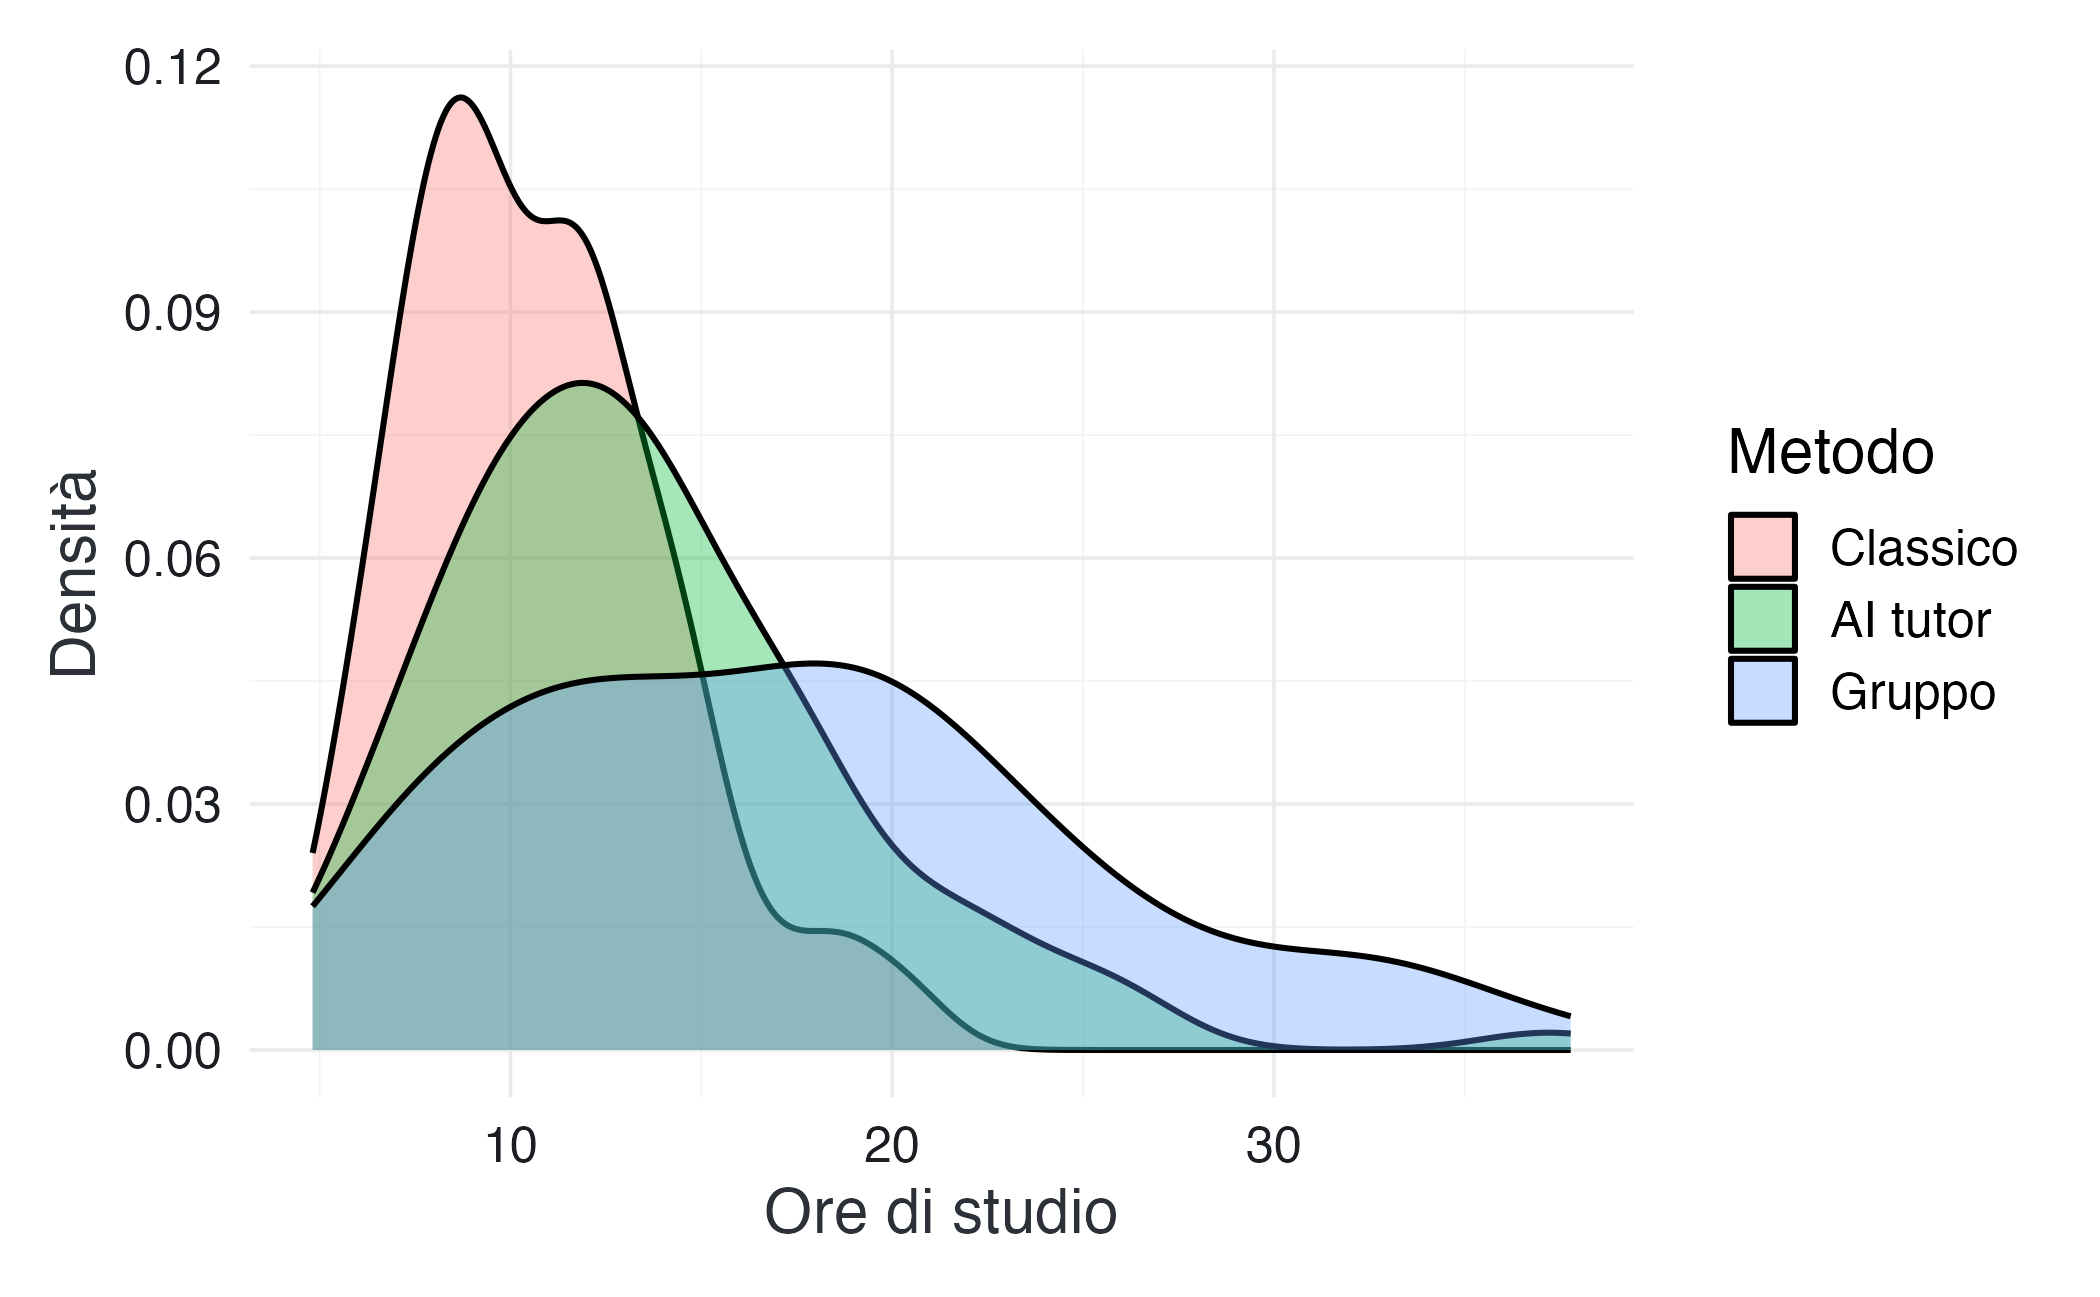
\includegraphics[width=0.85\linewidth,height=\textheight,keepaspectratio]{chapters/formal_models/05_decisione_ottimale_files/figure-pdf/plot-simulated-outcomes-1.png}

}

\caption{Distribuzioni simulate delle ore e relazione tra ore e voto nei
tre metodi.}

\end{figure}%

\begin{figure}[H]

{\centering 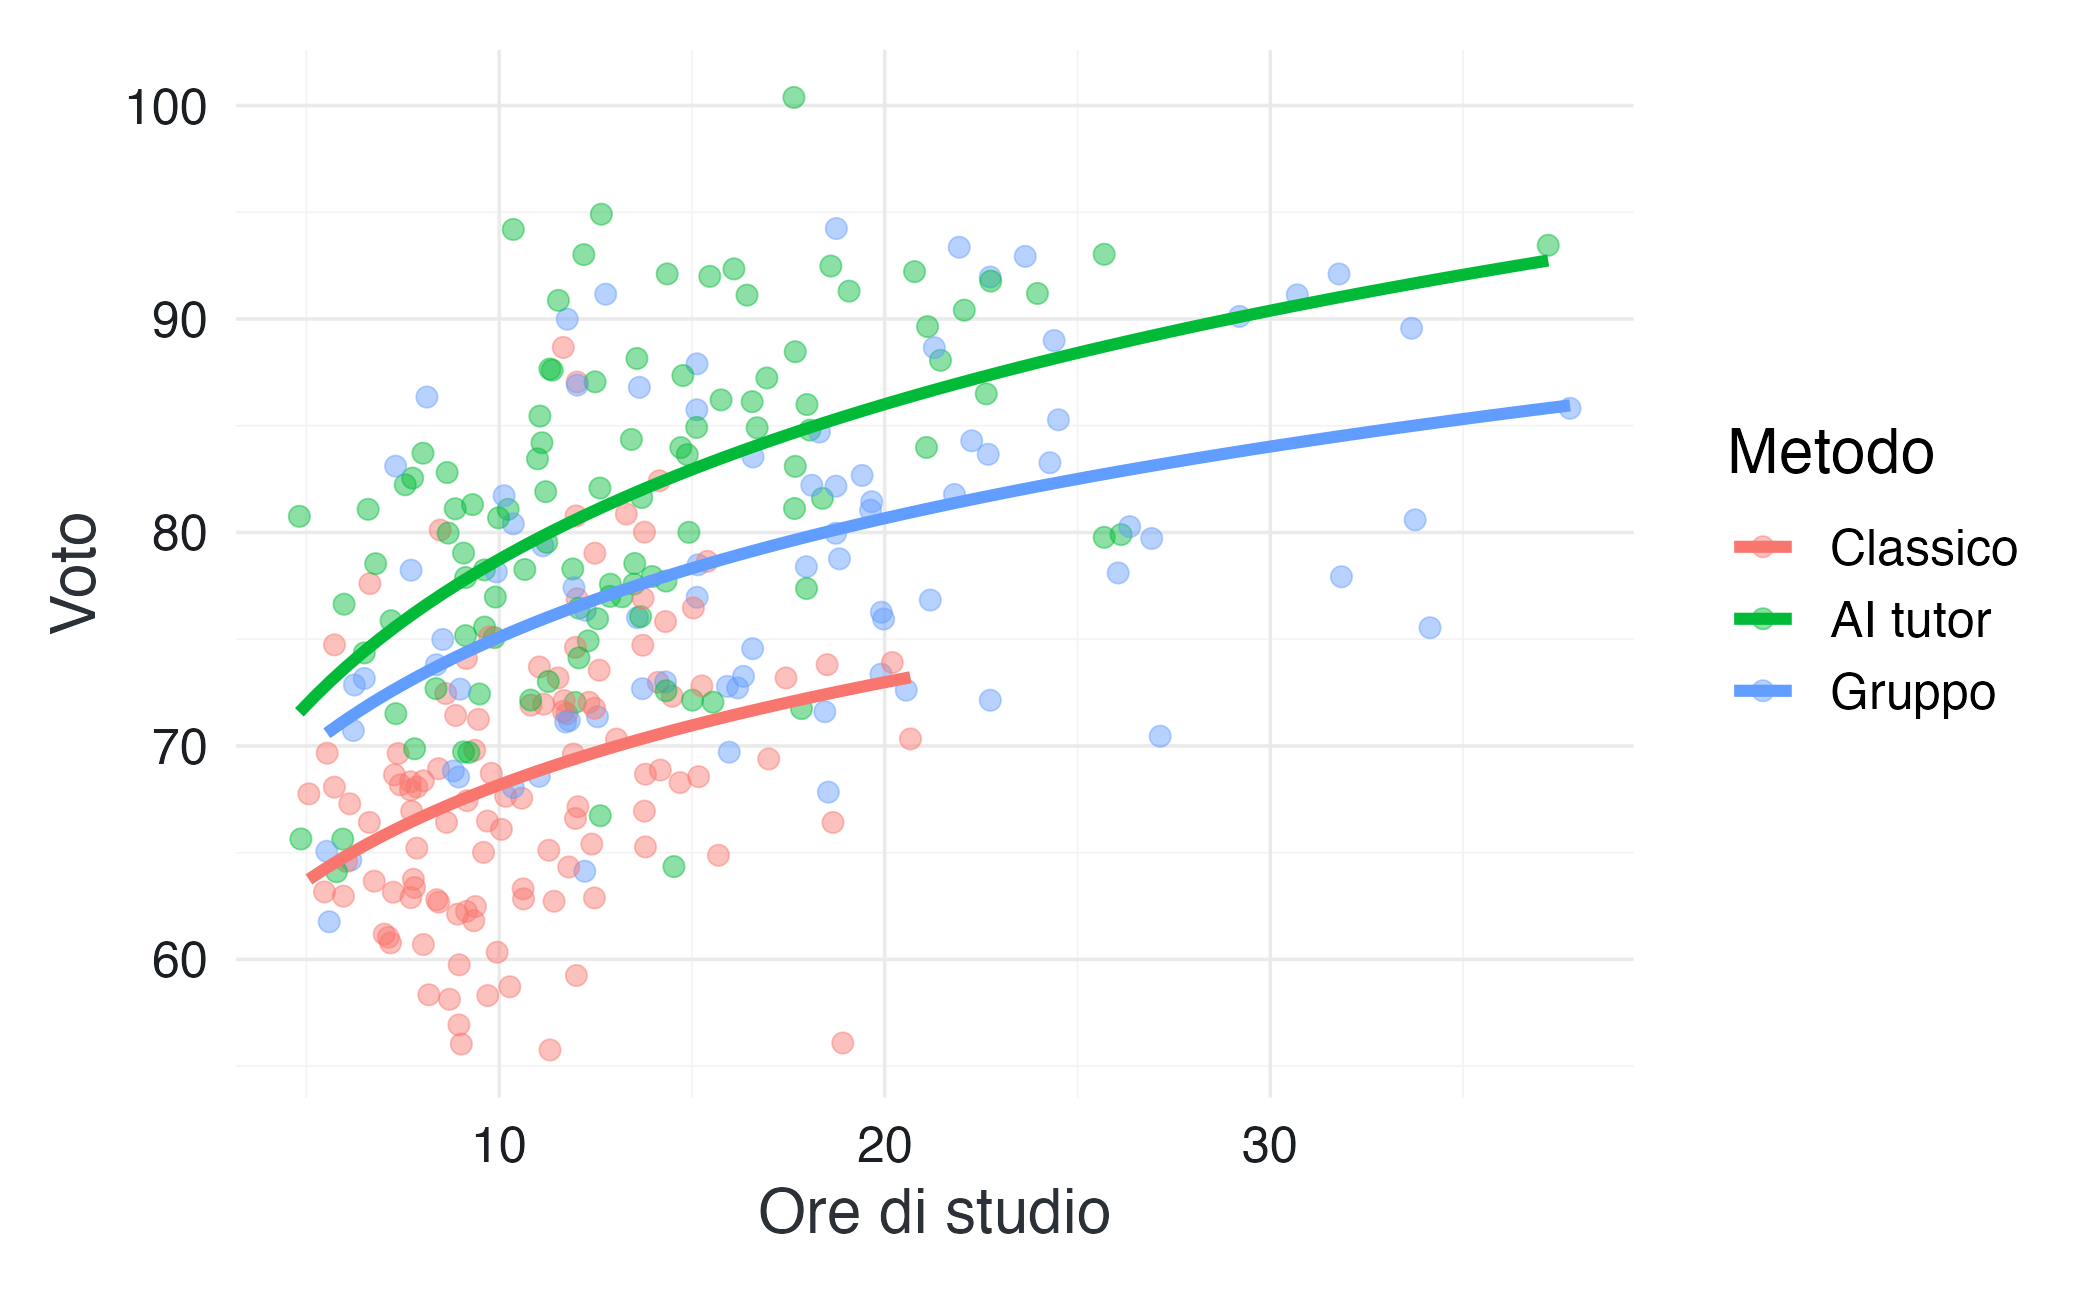
\includegraphics[width=0.85\linewidth,height=\textheight,keepaspectratio]{chapters/formal_models/05_decisione_ottimale_files/figure-pdf/plot-simulated-outcomes-2.png}

}

\caption{Distribuzioni simulate delle ore e relazione tra ore e voto nei
tre metodi.}

\end{figure}%

La simulazione permette di controllare tre aspetti:

\begin{itemize}
\tightlist
\item
  le ore sono positive e asimmetriche;
\item
  i metodi differiscono nella distribuzione del tempo richiesto;
\item
  il voto cresce con le ore, ma con rendimenti decrescenti.
\end{itemize}

\begin{tcolorbox}[enhanced jigsaw, arc=.35mm, bottomrule=.15mm, bottomtitle=1mm, breakable, colback=white, colbacktitle=quarto-callout-caution-color!10!white, colframe=quarto-callout-caution-color-frame, coltitle=black, left=2mm, leftrule=.75mm, opacityback=0, opacitybacktitle=0.6, rightrule=.15mm, title=\textcolor{quarto-callout-caution-color}{\faFire}\hspace{0.5em}{La scala del voto}, titlerule=0mm, toprule=.15mm, toptitle=1mm]

Il modello normale non impone formalmente i limiti 0--100. Nel mondo
simulato i parametri rendono poco frequenti valori impossibili, ma in
dati reali occorre controllare le repliche predittive. Se la probabilità
fuori scala è rilevante, serve un modello osservazionale diverso, non un
semplice taglio dei valori simulati.

\end{tcolorbox}

\section{Il programma Stan esterno}\label{il-programma-stan-esterno}

Il modello è contenuto nel file:

\begin{Shaded}
\begin{Highlighting}[]
\NormalTok{chapters/formal\_models/study\_method\_decision.stan}
\end{Highlighting}
\end{Shaded}

Separare il programma dal capitolo offre tre vantaggi:

\begin{itemize}
\tightlist
\item
  evita di duplicare il codice;
\item
  permette di testare e versionare il modello indipendentemente dal
  testo;
\item
  mantiene distinta la specificazione probabilistica dalla successiva
  analisi delle preferenze.
\end{itemize}

Il file Stan non contiene \(\lambda\). Stima soltanto la distribuzione
congiunta di ore e voto. La funzione di utilità verrà applicata alle
simulazioni predittive in R.

\begin{Shaded}
\begin{Highlighting}[]
\NormalTok{stan\_file }\OtherTok{\textless{}{-}}\NormalTok{ here}\SpecialCharTok{::}\FunctionTok{here}\NormalTok{(}
  \StringTok{"chapters"}\NormalTok{, }\StringTok{"formal\_models"}\NormalTok{, }\StringTok{"study\_method\_decision.stan"}
\NormalTok{)}

\NormalTok{study\_model }\OtherTok{\textless{}{-}} \FunctionTok{cmdstan\_model}\NormalTok{(stan\_file)}
\end{Highlighting}
\end{Shaded}

Prepariamo i dati. Il flag \texttt{prior\_only} consente di usare lo
stesso programma per il controllo predittivo a priori e per la stima.

\begin{Shaded}
\begin{Highlighting}[]
\NormalTok{stan\_data }\OtherTok{\textless{}{-}} \FunctionTok{list}\NormalTok{(}
  \AttributeTok{N =} \FunctionTok{nrow}\NormalTok{(study\_dat),}
  \AttributeTok{K =}\NormalTok{ K,}
  \AttributeTok{method =}\NormalTok{ study\_dat}\SpecialCharTok{$}\NormalTok{method\_id,}
  \AttributeTok{h =}\NormalTok{ study\_dat}\SpecialCharTok{$}\NormalTok{hours,}
  \AttributeTok{g =}\NormalTok{ study\_dat}\SpecialCharTok{$}\NormalTok{grade,}
  \AttributeTok{prior\_only =} \DecValTok{0}\NormalTok{L}
\NormalTok{)}
\end{Highlighting}
\end{Shaded}

\section{Controllo predittivo a
priori}\label{controllo-predittivo-a-priori-5}

Prima di usare i dati, campioniamo dai prior.

\begin{Shaded}
\begin{Highlighting}[]
\NormalTok{prior\_fit }\OtherTok{\textless{}{-}}\NormalTok{ study\_model}\SpecialCharTok{$}\FunctionTok{sample}\NormalTok{(}
  \AttributeTok{data =} \FunctionTok{within}\NormalTok{(stan\_data, prior\_only }\OtherTok{\textless{}{-}} \DecValTok{1}\NormalTok{L),}
  \AttributeTok{seed =} \DecValTok{2026}\NormalTok{,}
  \AttributeTok{chains =} \DecValTok{4}\NormalTok{,}
  \AttributeTok{parallel\_chains =} \DecValTok{4}\NormalTok{,}
  \AttributeTok{iter\_warmup =} \DecValTok{500}\NormalTok{,}
  \AttributeTok{iter\_sampling =} \DecValTok{500}\NormalTok{,}
  \AttributeTok{refresh =} \DecValTok{0}
\NormalTok{)}
\end{Highlighting}
\end{Shaded}

Le quantità \texttt{h\_new{[}k{]}} e \texttt{g\_new{[}k{]}}
rappresentano un nuovo esito predittivo per ciascun metodo.

\begin{Shaded}
\begin{Highlighting}[]
\NormalTok{prior\_draws }\OtherTok{\textless{}{-}}\NormalTok{ prior\_fit}\SpecialCharTok{$}\FunctionTok{draws}\NormalTok{(}
  \AttributeTok{variables =} \FunctionTok{c}\NormalTok{(}\StringTok{"h\_new"}\NormalTok{, }\StringTok{"g\_new"}\NormalTok{),}
  \AttributeTok{format =} \StringTok{"draws\_matrix"}
\NormalTok{)}

\NormalTok{prior\_h }\OtherTok{\textless{}{-}}\NormalTok{ prior\_draws[, }\FunctionTok{paste0}\NormalTok{(}\StringTok{"h\_new["}\NormalTok{, }\FunctionTok{seq\_len}\NormalTok{(K), }\StringTok{"]"}\NormalTok{), drop }\OtherTok{=} \ConstantTok{FALSE}\NormalTok{]}
\NormalTok{prior\_g }\OtherTok{\textless{}{-}}\NormalTok{ prior\_draws[, }\FunctionTok{paste0}\NormalTok{(}\StringTok{"g\_new["}\NormalTok{, }\FunctionTok{seq\_len}\NormalTok{(K), }\StringTok{"]"}\NormalTok{), drop }\OtherTok{=} \ConstantTok{FALSE}\NormalTok{]}

\FunctionTok{colnames}\NormalTok{(prior\_h) }\OtherTok{\textless{}{-}}\NormalTok{ method\_names}
\FunctionTok{colnames}\NormalTok{(prior\_g) }\OtherTok{\textless{}{-}}\NormalTok{ method\_names}

\FunctionTok{apply}\NormalTok{(prior\_h, }\DecValTok{2}\NormalTok{, quantile, }\AttributeTok{probs =} \FunctionTok{c}\NormalTok{(.}\DecValTok{01}\NormalTok{, .}\DecValTok{5}\NormalTok{, .}\DecValTok{99}\NormalTok{))}
\CommentTok{\#\textgreater{}      variable}
\CommentTok{\#\textgreater{}       Classico AI tutor Gruppo}
\CommentTok{\#\textgreater{}   1\%      1.88     1.84    1.7}
\CommentTok{\#\textgreater{}   50\%    11.71    11.75   11.9}
\CommentTok{\#\textgreater{}   99\%    90.32    75.65   87.3}
\FunctionTok{apply}\NormalTok{(prior\_g, }\DecValTok{2}\NormalTok{, quantile, }\AttributeTok{probs =} \FunctionTok{c}\NormalTok{(.}\DecValTok{01}\NormalTok{, .}\DecValTok{5}\NormalTok{, .}\DecValTok{99}\NormalTok{))}
\CommentTok{\#\textgreater{}      variable}
\CommentTok{\#\textgreater{}       Classico AI tutor Gruppo}
\CommentTok{\#\textgreater{}   1\%      20.5     19.4   24.6}
\CommentTok{\#\textgreater{}   50\%     70.1     69.6   70.7}
\CommentTok{\#\textgreater{}   99\%    122.0    116.7  123.4}
\end{Highlighting}
\end{Shaded}

Il controllo deve chiedere se i prior attribuiscono massa sostanziale a
ore o voti implausibili. Non basta che ciascun prior sembri ragionevole
separatamente: occorre verificare le conseguenze congiunte del modello.

\section{Adattamento e diagnostica}\label{adattamento-e-diagnostica}

\begin{Shaded}
\begin{Highlighting}[]
\NormalTok{fit }\OtherTok{\textless{}{-}}\NormalTok{ study\_model}\SpecialCharTok{$}\FunctionTok{sample}\NormalTok{(}
  \AttributeTok{data =}\NormalTok{ stan\_data,}
  \AttributeTok{seed =} \DecValTok{2027}\NormalTok{,}
  \AttributeTok{chains =} \DecValTok{4}\NormalTok{,}
  \AttributeTok{parallel\_chains =} \DecValTok{4}\NormalTok{,}
  \AttributeTok{iter\_warmup =} \DecValTok{1000}\NormalTok{,}
  \AttributeTok{iter\_sampling =} \DecValTok{1500}\NormalTok{,}
  \AttributeTok{refresh =} \DecValTok{200}
\NormalTok{)}
\end{Highlighting}
\end{Shaded}

\begin{Shaded}
\begin{Highlighting}[]
\NormalTok{fit}\SpecialCharTok{$}\FunctionTok{diagnostic\_summary}\NormalTok{()}
\CommentTok{\#\textgreater{} $num\_divergent}
\CommentTok{\#\textgreater{} [1] 0 0 0 0}
\CommentTok{\#\textgreater{} }
\CommentTok{\#\textgreater{} $num\_max\_treedepth}
\CommentTok{\#\textgreater{} [1] 0 0 0 0}
\CommentTok{\#\textgreater{} }
\CommentTok{\#\textgreater{} $ebfmi}
\CommentTok{\#\textgreater{} [1] 1.02 1.07 1.03 1.08}

\NormalTok{fit}\SpecialCharTok{$}\FunctionTok{summary}\NormalTok{(}
  \AttributeTok{variables =} \FunctionTok{c}\NormalTok{(}\StringTok{"mu\_log\_h"}\NormalTok{, }\StringTok{"sigma\_log\_h"}\NormalTok{, }\StringTok{"alpha"}\NormalTok{, }\StringTok{"beta"}\NormalTok{, }\StringTok{"sigma\_g"}\NormalTok{)}
\NormalTok{)}
\CommentTok{\#\textgreater{} \# A tibble: 13 x 10}
\CommentTok{\#\textgreater{}    variable         mean median     sd    mad     q5    q95  rhat ess\_bulk}
\CommentTok{\#\textgreater{}    \textless{}chr\textgreater{}           \textless{}dbl\textgreater{}  \textless{}dbl\textgreater{}  \textless{}dbl\textgreater{}  \textless{}dbl\textgreater{}  \textless{}dbl\textgreater{}  \textless{}dbl\textgreater{} \textless{}dbl\textgreater{}    \textless{}dbl\textgreater{}}
\CommentTok{\#\textgreater{}  1 mu\_log\_h[1]     2.33   2.33  0.0296 0.0298  2.28   2.38  1.00     7823.}
\CommentTok{\#\textgreater{}  2 mu\_log\_h[2]     2.53   2.53  0.0372 0.0359  2.47   2.59  1.00     6987.}
\CommentTok{\#\textgreater{}  3 mu\_log\_h[3]     2.75   2.75  0.0525 0.0532  2.66   2.83  1.00     7849.}
\CommentTok{\#\textgreater{}  4 sigma\_log\_h[1]  0.313  0.312 0.0208 0.0205  0.281  0.349 1.00     7372.}
\CommentTok{\#\textgreater{}  5 sigma\_log\_h[2]  0.390  0.388 0.0267 0.0265  0.349  0.435 1.00     7595.}
\CommentTok{\#\textgreater{}  6 sigma\_log\_h[3]  0.475  0.472 0.0372 0.0364  0.417  0.539 1.00     7934.}
\CommentTok{\#\textgreater{}  7 alpha[1]       51.5   51.5   4.48   4.40   44.3   58.9   1.00     5066.}
\CommentTok{\#\textgreater{}  8 alpha[2]       54.0   54.0   4.20   4.16   47.2   60.9   1.00     4684.}
\CommentTok{\#\textgreater{}  9 alpha[3]       55.5   55.5   4.10   4.02   48.6   62.3   1.00     5358.}
\CommentTok{\#\textgreater{} 10 beta[1]         6.95   6.97  1.83   1.81    3.90   9.95  1.00     5052.}
\CommentTok{\#\textgreater{} 11 beta[2]        10.4   10.4   1.59   1.56    7.76  13.0   1.00     4659.}
\CommentTok{\#\textgreater{} 12 beta[3]         8.26   8.25  1.44   1.40    5.87  10.6   1.00     5328.}
\CommentTok{\#\textgreater{} 13 sigma\_g         6.49   6.48  0.267  0.266   6.06   6.94  1.000    8896.}
\CommentTok{\#\textgreater{}    ess\_tail}
\CommentTok{\#\textgreater{}       \textless{}dbl\textgreater{}}
\CommentTok{\#\textgreater{}  1    4147.}
\CommentTok{\#\textgreater{}  2    4184.}
\CommentTok{\#\textgreater{}  3    4466.}
\CommentTok{\#\textgreater{}  4    3909.}
\CommentTok{\#\textgreater{}  5    4439.}
\CommentTok{\#\textgreater{}  6    3856.}
\CommentTok{\#\textgreater{}  7    3228.}
\CommentTok{\#\textgreater{}  8    3972.}
\CommentTok{\#\textgreater{}  9    4348.}
\CommentTok{\#\textgreater{} 10    3821.}
\CommentTok{\#\textgreater{} 11    3991.}
\CommentTok{\#\textgreater{} 12    4242.}
\CommentTok{\#\textgreater{} 13    4266.}
\end{Highlighting}
\end{Shaded}

Un buon campionamento non dimostra che il modello sia adeguato, ma è una
condizione necessaria per interpretare i draw.

\section{Controlli predittivi a
posteriori}\label{controlli-predittivi-a-posteriori-4}

Il programma genera repliche congiunte delle ore e dei voti. Per ogni
osservazione, prima simula nuove ore e poi un nuovo voto condizionato a
quelle ore.

\begin{Shaded}
\begin{Highlighting}[]
\NormalTok{h\_rep }\OtherTok{\textless{}{-}} \FunctionTok{as\_draws\_matrix}\NormalTok{(fit}\SpecialCharTok{$}\FunctionTok{draws}\NormalTok{(}\StringTok{"h\_rep"}\NormalTok{))}
\NormalTok{g\_rep }\OtherTok{\textless{}{-}} \FunctionTok{as\_draws\_matrix}\NormalTok{(fit}\SpecialCharTok{$}\FunctionTok{draws}\NormalTok{(}\StringTok{"g\_rep"}\NormalTok{))}

\NormalTok{bayesplot}\SpecialCharTok{::}\FunctionTok{ppc\_dens\_overlay}\NormalTok{(}
  \AttributeTok{y =} \FunctionTok{log}\NormalTok{(study\_dat}\SpecialCharTok{$}\NormalTok{hours),}
  \AttributeTok{yrep =} \FunctionTok{log}\NormalTok{(h\_rep[}\DecValTok{1}\SpecialCharTok{:}\DecValTok{100}\NormalTok{, , }\AttributeTok{drop =} \ConstantTok{FALSE}\NormalTok{])}
\NormalTok{)}

\NormalTok{bayesplot}\SpecialCharTok{::}\FunctionTok{ppc\_dens\_overlay}\NormalTok{(}
  \AttributeTok{y =}\NormalTok{ study\_dat}\SpecialCharTok{$}\NormalTok{grade,}
  \AttributeTok{yrep =}\NormalTok{ g\_rep[}\DecValTok{1}\SpecialCharTok{:}\DecValTok{100}\NormalTok{, , }\AttributeTok{drop =} \ConstantTok{FALSE}\NormalTok{]}
\NormalTok{)}
\end{Highlighting}
\end{Shaded}

\begin{center}
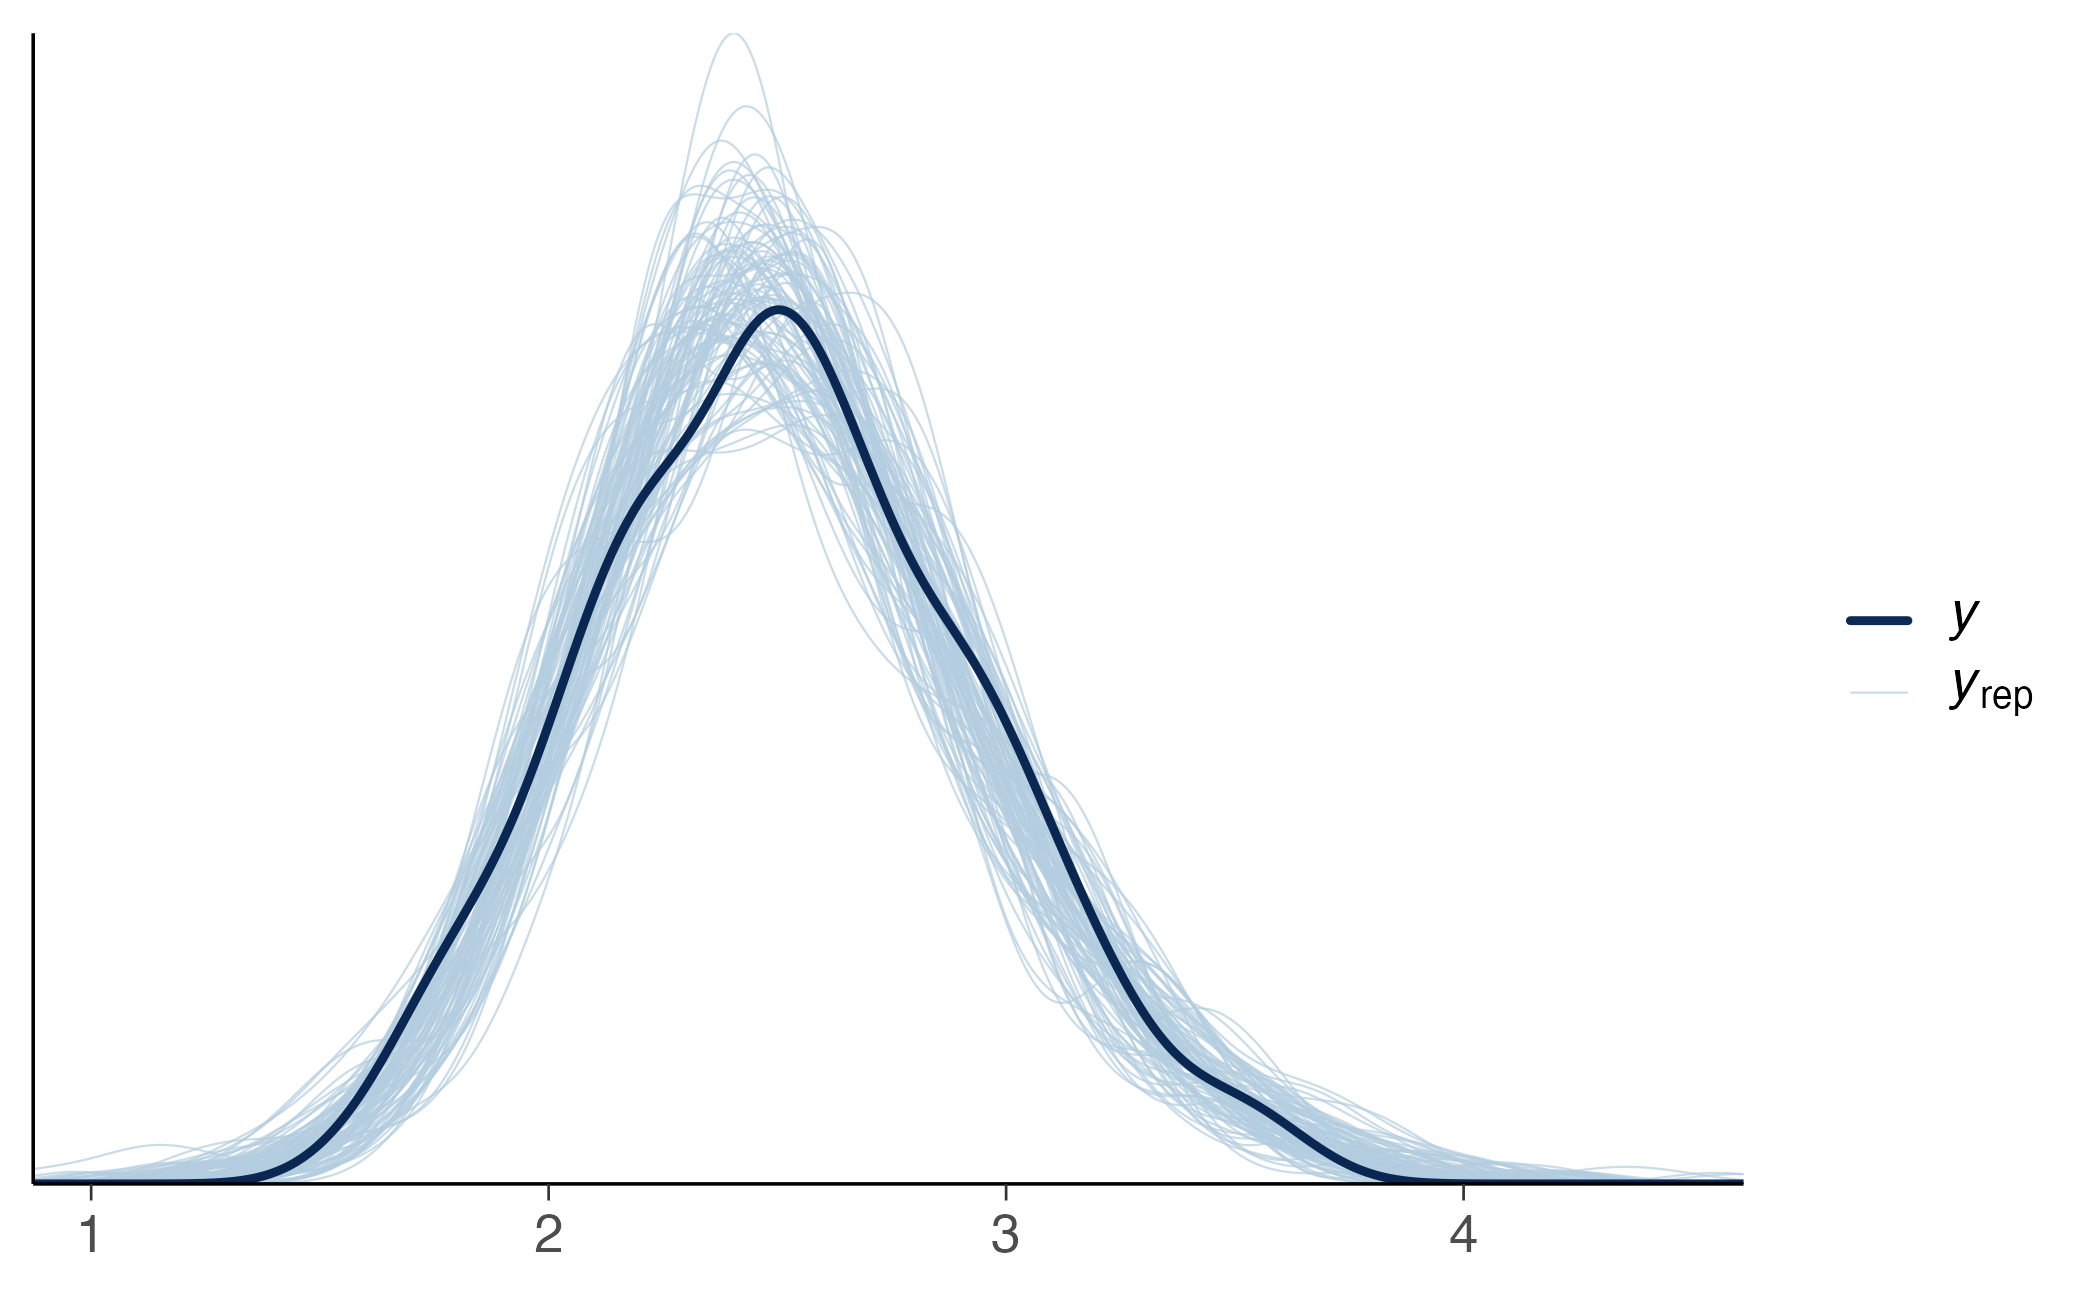
\includegraphics[width=0.85\linewidth,height=\textheight,keepaspectratio]{chapters/formal_models/05_decisione_ottimale_files/figure-pdf/posterior-predictive-study-decision-1.png}
\end{center}

\begin{center}
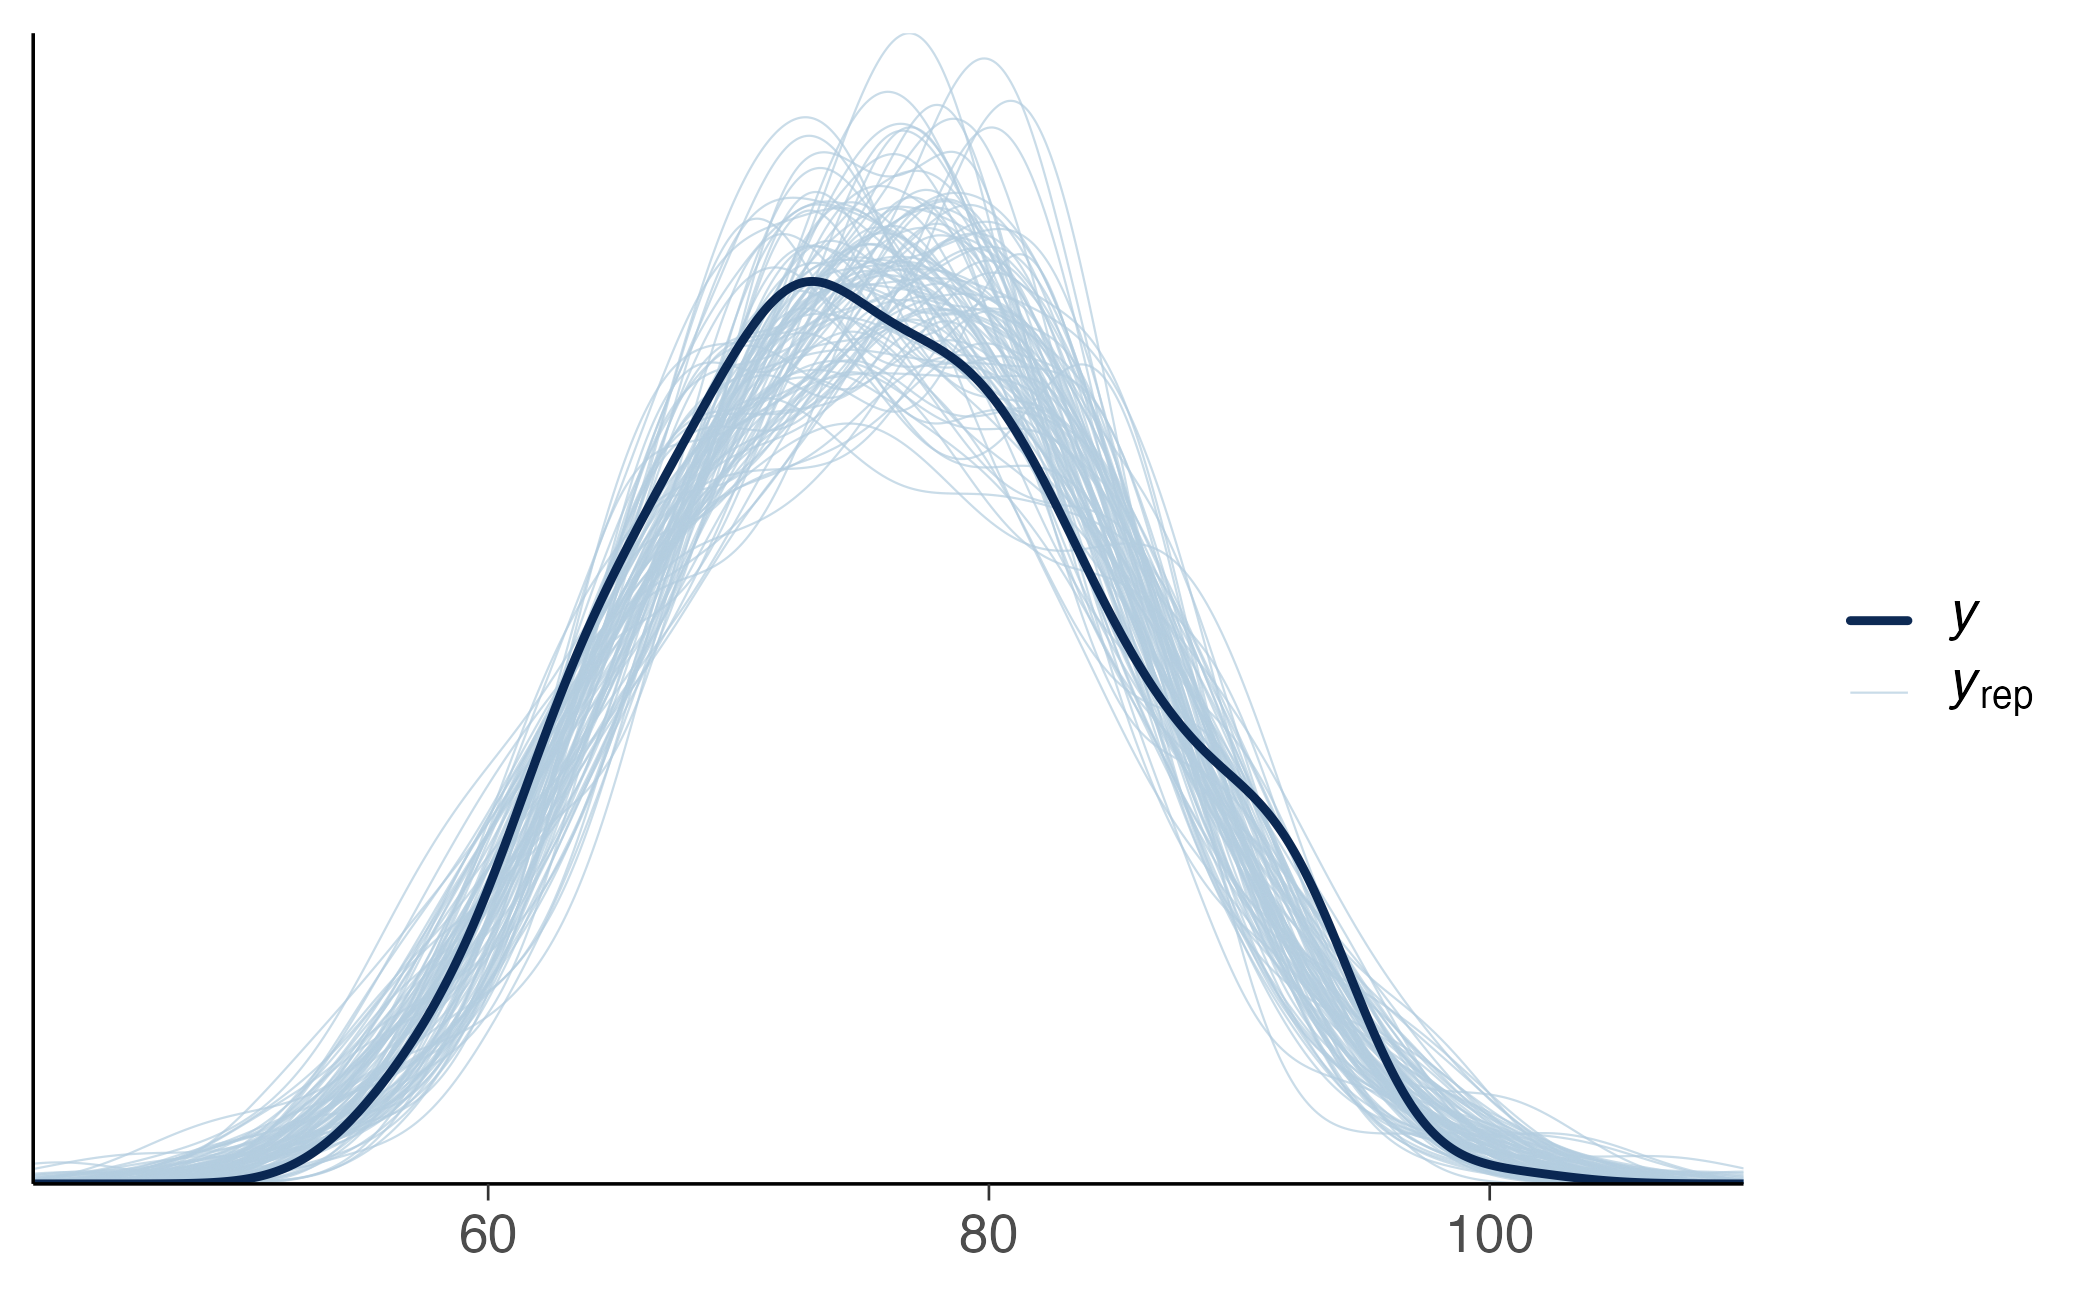
\includegraphics[width=0.85\linewidth,height=\textheight,keepaspectratio]{chapters/formal_models/05_decisione_ottimale_files/figure-pdf/posterior-predictive-study-decision-2.png}
\end{center}

Questi controlli marginali sono solo il primo livello. Poiché il
problema decisionale dipende dalla relazione tra ore e voto, dobbiamo
controllare anche statistiche congiunte e specifiche per metodo.

\begin{Shaded}
\begin{Highlighting}[]
\NormalTok{obs\_stats }\OtherTok{\textless{}{-}}\NormalTok{ study\_dat }\SpecialCharTok{|\textgreater{}}
  \FunctionTok{group\_by}\NormalTok{(method) }\SpecialCharTok{|\textgreater{}}
  \FunctionTok{summarize}\NormalTok{(}
    \AttributeTok{mean\_hours =} \FunctionTok{mean}\NormalTok{(hours),}
    \AttributeTok{sd\_hours =} \FunctionTok{sd}\NormalTok{(hours),}
    \AttributeTok{mean\_grade =} \FunctionTok{mean}\NormalTok{(grade),}
    \AttributeTok{cor\_h\_g =} \FunctionTok{cor}\NormalTok{(hours, grade),}
    \AttributeTok{.groups =} \StringTok{"drop"}
\NormalTok{  )}

\NormalTok{obs\_stats}
\CommentTok{\#\textgreater{} \# A tibble: 3 x 5}
\CommentTok{\#\textgreater{}   method   mean\_hours sd\_hours mean\_grade cor\_h\_g}
\CommentTok{\#\textgreater{}   \textless{}fct\textgreater{}         \textless{}dbl\textgreater{}    \textless{}dbl\textgreater{}      \textless{}dbl\textgreater{}   \textless{}dbl\textgreater{}}
\CommentTok{\#\textgreater{} 1 Classico       10.7     3.36       68.4   0.315}
\CommentTok{\#\textgreater{} 2 AI tutor       13.5     5.35       81.2   0.512}
\CommentTok{\#\textgreater{} 3 Gruppo         17.3     7.63       78.7   0.465}
\end{Highlighting}
\end{Shaded}

Un'estensione utile consiste nel calcolare le stesse statistiche su ogni
replica e verificare se i valori osservati occupano regioni plausibili
delle distribuzioni replicate.

\section{Distribuzione predittiva congiunta per una nuova
persona}\label{distribuzione-predittiva-congiunta-per-una-nuova-persona}

Estraiamo le simulazioni \texttt{h\_new} e \texttt{g\_new}. Ogni riga
contiene esiti congiunti prodotti dallo stesso draw posteriore.

\begin{Shaded}
\begin{Highlighting}[]
\NormalTok{pred\_draws }\OtherTok{\textless{}{-}}\NormalTok{ fit}\SpecialCharTok{$}\FunctionTok{draws}\NormalTok{(}
  \AttributeTok{variables =} \FunctionTok{c}\NormalTok{(}\StringTok{"h\_new"}\NormalTok{, }\StringTok{"g\_new"}\NormalTok{),}
  \AttributeTok{format =} \StringTok{"draws\_matrix"}
\NormalTok{)}

\NormalTok{H\_new }\OtherTok{\textless{}{-}}\NormalTok{ pred\_draws[, }\FunctionTok{paste0}\NormalTok{(}\StringTok{"h\_new["}\NormalTok{, }\FunctionTok{seq\_len}\NormalTok{(K), }\StringTok{"]"}\NormalTok{), drop }\OtherTok{=} \ConstantTok{FALSE}\NormalTok{]}
\NormalTok{G\_new }\OtherTok{\textless{}{-}}\NormalTok{ pred\_draws[, }\FunctionTok{paste0}\NormalTok{(}\StringTok{"g\_new["}\NormalTok{, }\FunctionTok{seq\_len}\NormalTok{(K), }\StringTok{"]"}\NormalTok{), drop }\OtherTok{=} \ConstantTok{FALSE}\NormalTok{]}

\FunctionTok{colnames}\NormalTok{(H\_new) }\OtherTok{\textless{}{-}}\NormalTok{ method\_names}
\FunctionTok{colnames}\NormalTok{(G\_new) }\OtherTok{\textless{}{-}}\NormalTok{ method\_names}
\end{Highlighting}
\end{Shaded}

Queste simulazioni propagano:

\begin{itemize}
\tightlist
\item
  l'incertezza sui parametri;
\item
  la variabilità tra studenti nelle ore;
\item
  la variabilità residua del voto;
\item
  la dipendenza del voto dalle ore simulate.
\end{itemize}

\section{Dalla previsione
all'utilità}\label{dalla-previsione-allutilituxe0}

Applichiamo la funzione di utilità a ogni draw congiunto.

\begin{Shaded}
\begin{Highlighting}[]
\NormalTok{lambda }\OtherTok{\textless{}{-}} \FloatTok{0.65}
\NormalTok{U }\OtherTok{\textless{}{-}}\NormalTok{ G\_new }\SpecialCharTok{{-}}\NormalTok{ lambda }\SpecialCharTok{*}\NormalTok{ H\_new}

\NormalTok{expected\_utility }\OtherTok{\textless{}{-}} \FunctionTok{colMeans}\NormalTok{(U)}
\NormalTok{expected\_utility}
\CommentTok{\#\textgreater{} Classico AI tutor   Gruppo }
\CommentTok{\#\textgreater{}     61.4     72.3     67.3}

\NormalTok{recommended\_method }\OtherTok{\textless{}{-}} \FunctionTok{names}\NormalTok{(}\FunctionTok{which.max}\NormalTok{(expected\_utility))}
\NormalTok{recommended\_method}
\CommentTok{\#\textgreater{} [1] "AI tutor"}
\end{Highlighting}
\end{Shaded}

Il metodo raccomandato è quello con la maggiore utilità attesa.

\subsection{Distribuzioni di utilità}\label{distribuzioni-di-utilituxe0}

\begin{Shaded}
\begin{Highlighting}[]
\NormalTok{utility\_long }\OtherTok{\textless{}{-}} \FunctionTok{as\_tibble}\NormalTok{(U) }\SpecialCharTok{|\textgreater{}}
  \FunctionTok{mutate}\NormalTok{(}\AttributeTok{.draw =} \FunctionTok{row\_number}\NormalTok{()) }\SpecialCharTok{|\textgreater{}}
  \FunctionTok{pivot\_longer}\NormalTok{(}
    \SpecialCharTok{{-}}\NormalTok{ .draw,}
    \AttributeTok{names\_to =} \StringTok{"method"}\NormalTok{,}
    \AttributeTok{values\_to =} \StringTok{"utility"}
\NormalTok{  )}

\FunctionTok{ggplot}\NormalTok{(utility\_long, }\FunctionTok{aes}\NormalTok{(utility, }\AttributeTok{fill =}\NormalTok{ method)) }\SpecialCharTok{+}
  \FunctionTok{geom\_density}\NormalTok{(}\AttributeTok{alpha =} \FloatTok{0.35}\NormalTok{) }\SpecialCharTok{+}
  \FunctionTok{labs}\NormalTok{(}\AttributeTok{x =} \StringTok{"Utilità"}\NormalTok{, }\AttributeTok{y =} \StringTok{"Densità"}\NormalTok{, }\AttributeTok{fill =} \StringTok{"Metodo"}\NormalTok{)}
\end{Highlighting}
\end{Shaded}

\begin{figure}[H]

{\centering 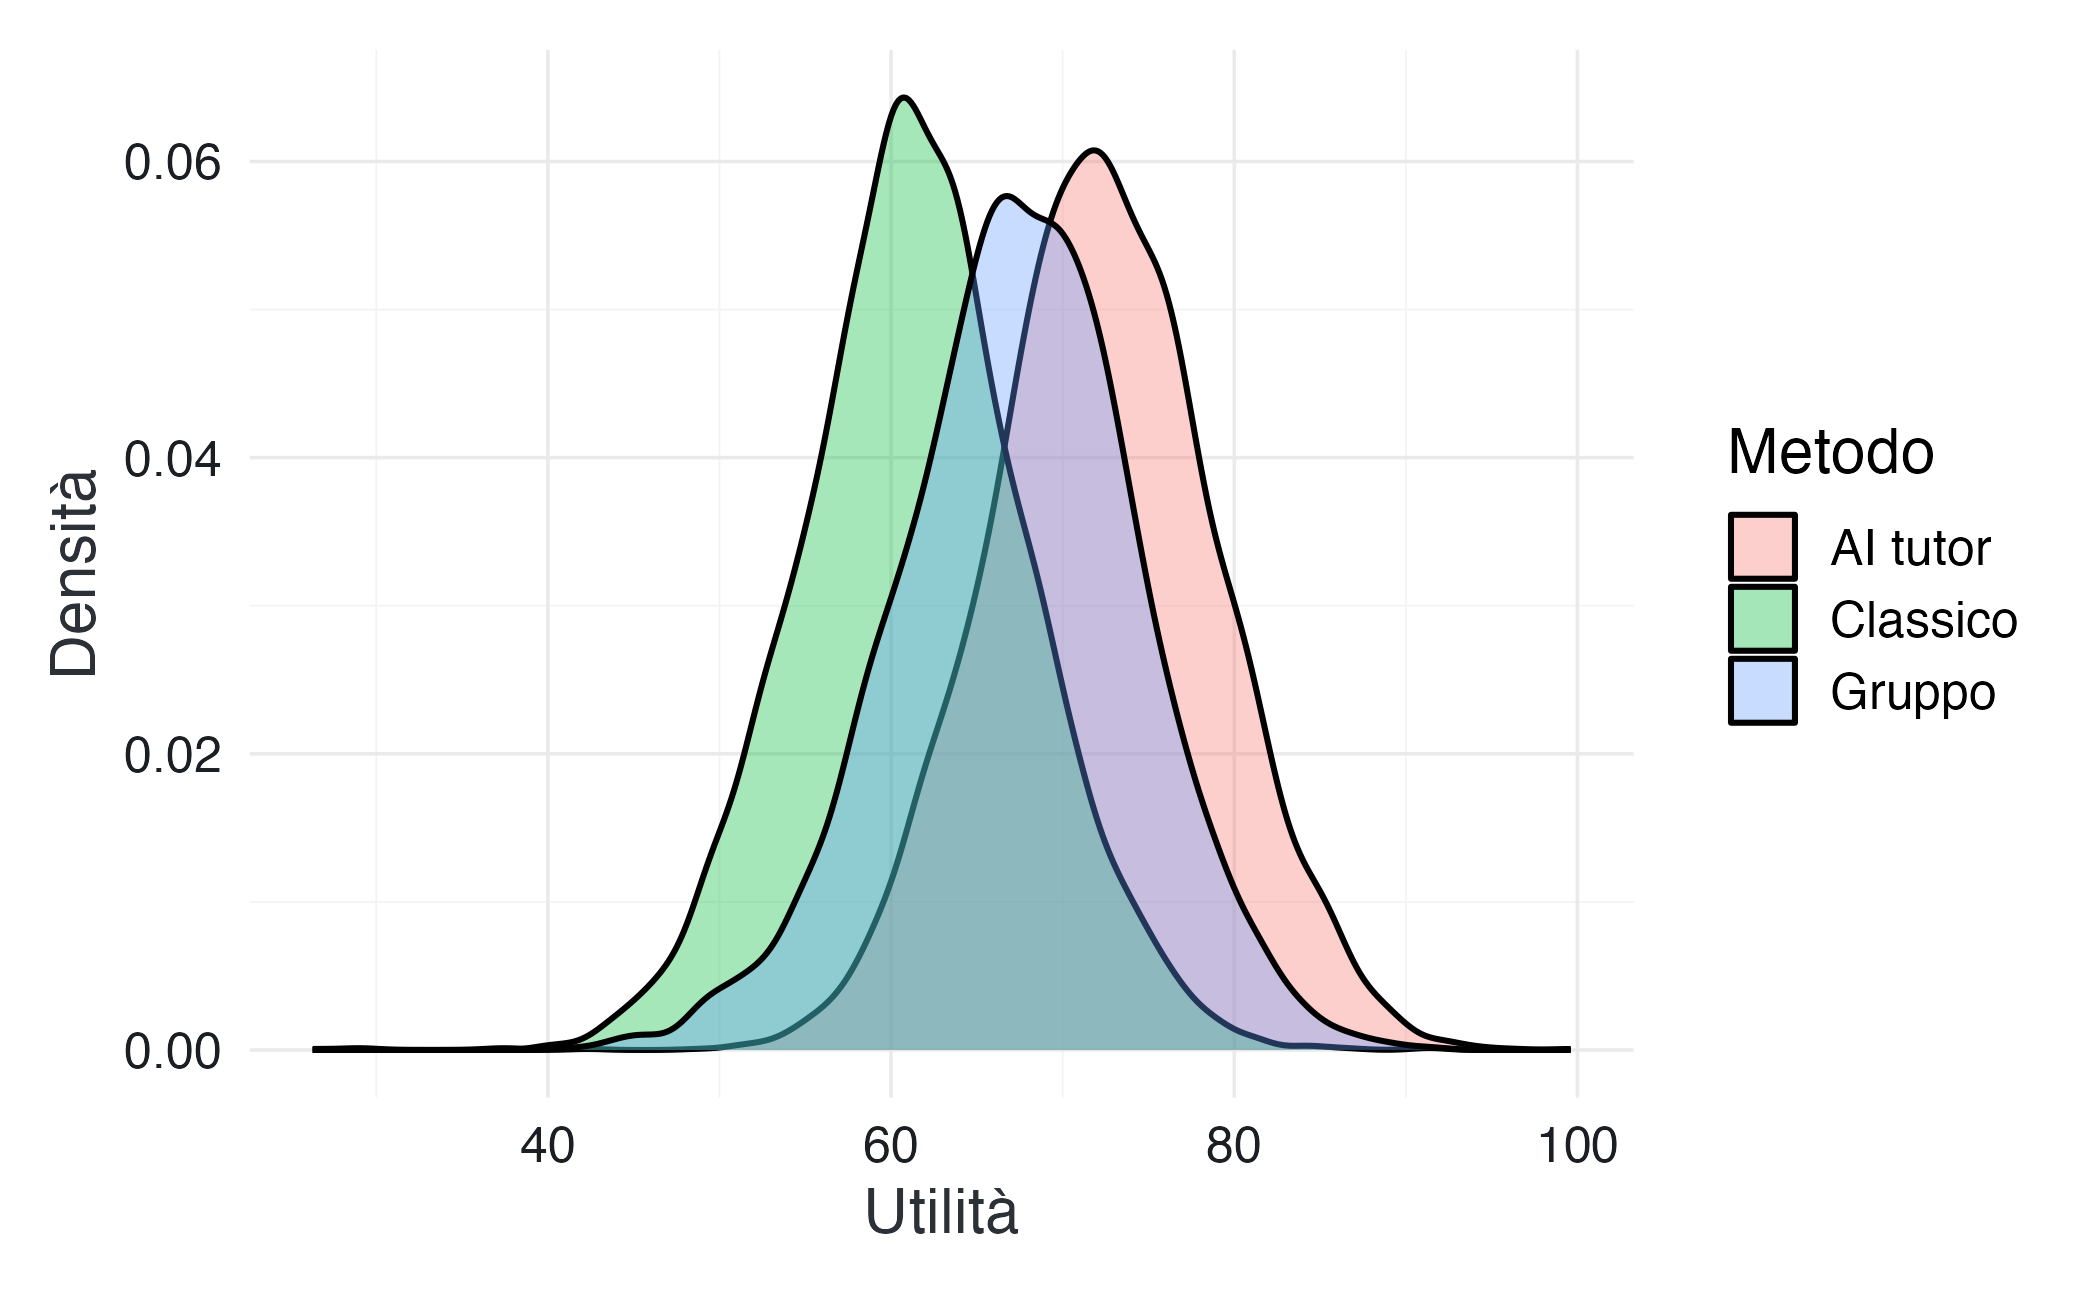
\includegraphics[width=0.85\linewidth,height=\textheight,keepaspectratio]{chapters/formal_models/05_decisione_ottimale_files/figure-pdf/plot-utility-study-1.png}

}

\caption{Distribuzioni predittive dell'utilità per i tre metodi di
studio.}

\end{figure}%

La dispersione della distribuzione descrive la variabilità delle
conseguenze, ma non implica automaticamente avversione al rischio. Con
utilità lineare, la regola usa la media dell'utilità. Per rappresentare
avversione al rischio occorre una funzione di utilità concava o un
criterio decisionale diverso.

\subsection{Probabilità di risultare il metodo
migliore}\label{probabilituxe0-di-risultare-il-metodo-migliore}

Per ogni draw possiamo anche individuare l'alternativa con l'utilità più
alta.

\begin{Shaded}
\begin{Highlighting}[]
\NormalTok{best\_draw }\OtherTok{\textless{}{-}} \FunctionTok{max.col}\NormalTok{(U, }\AttributeTok{ties.method =} \StringTok{"random"}\NormalTok{)}

\NormalTok{prob\_best }\OtherTok{\textless{}{-}} \FunctionTok{prop.table}\NormalTok{(}
  \FunctionTok{table}\NormalTok{(}\FunctionTok{factor}\NormalTok{(best\_draw, }\AttributeTok{levels =} \FunctionTok{seq\_len}\NormalTok{(K), }\AttributeTok{labels =}\NormalTok{ method\_names))}
\NormalTok{)}

\NormalTok{prob\_best}
\CommentTok{\#\textgreater{} }
\CommentTok{\#\textgreater{} Classico AI tutor   Gruppo }
\CommentTok{\#\textgreater{}    0.067    0.645    0.287}
\end{Highlighting}
\end{Shaded}

\begin{tcolorbox}[enhanced jigsaw, arc=.35mm, bottomrule=.15mm, bottomtitle=1mm, breakable, colback=white, colbacktitle=quarto-callout-important-color!10!white, colframe=quarto-callout-important-color-frame, coltitle=black, left=2mm, leftrule=.75mm, opacityback=0, opacitybacktitle=0.6, rightrule=.15mm, title=\textcolor{quarto-callout-important-color}{\faExclamation}\hspace{0.5em}{Due quantità diverse}, titlerule=0mm, toprule=.15mm, toptitle=1mm]

La decisione che massimizza l'utilità attesa e l'alternativa con la
maggiore probabilità di essere la migliore non devono coincidere.

\begin{itemize}
\tightlist
\item
  \textbf{Utilità attesa}: media quanto è desiderabile ciascuna
  alternativa, includendo l'ampiezza di vantaggi e svantaggi.
\item
  \textbf{Probabilità di essere migliore}: conta in quale proporzione
  dei draw un'alternativa supera tutte le altre, senza considerare
  quanto grande sia il margine.
\end{itemize}

Nel quadro standard dell'utilità attesa, il criterio normativo è il
primo. La probabilità di essere migliore è una sintesi supplementare,
non una regola sostitutiva.

\end{tcolorbox}

\section{Sensibilità rispetto al costo del
tempo}\label{sensibilituxe0-rispetto-al-costo-del-tempo}

Ripetiamo il calcolo per una griglia di valori di \(\lambda\), senza
ristimare il modello.

\begin{Shaded}
\begin{Highlighting}[]
\NormalTok{lambda\_grid }\OtherTok{\textless{}{-}} \FunctionTok{seq}\NormalTok{(}\DecValTok{0}\NormalTok{, }\DecValTok{2}\NormalTok{, }\AttributeTok{by =} \FloatTok{0.05}\NormalTok{)}

\NormalTok{sensitivity }\OtherTok{\textless{}{-}} \FunctionTok{map\_dfr}\NormalTok{(lambda\_grid, }\ControlFlowTok{function}\NormalTok{(lam) \{}
\NormalTok{  U\_lam }\OtherTok{\textless{}{-}}\NormalTok{ G\_new }\SpecialCharTok{{-}}\NormalTok{ lam }\SpecialCharTok{*}\NormalTok{ H\_new}

  \FunctionTok{tibble}\NormalTok{(}
    \AttributeTok{lambda =}\NormalTok{ lam,}
    \AttributeTok{method =}\NormalTok{ method\_names,}
    \AttributeTok{expected\_utility =} \FunctionTok{colMeans}\NormalTok{(U\_lam),}
    \AttributeTok{probability\_best =} \FunctionTok{as.numeric}\NormalTok{(}
      \FunctionTok{prop.table}\NormalTok{(}
        \FunctionTok{table}\NormalTok{(}
          \FunctionTok{factor}\NormalTok{(}
            \FunctionTok{max.col}\NormalTok{(U\_lam, }\AttributeTok{ties.method =} \StringTok{"random"}\NormalTok{),}
            \AttributeTok{levels =} \FunctionTok{seq\_len}\NormalTok{(K)}
\NormalTok{          )}
\NormalTok{        )}
\NormalTok{      )}
\NormalTok{    )}
\NormalTok{  )}
\NormalTok{\})}
\end{Highlighting}
\end{Shaded}

\begin{Shaded}
\begin{Highlighting}[]
\FunctionTok{ggplot}\NormalTok{(sensitivity, }\FunctionTok{aes}\NormalTok{(lambda, expected\_utility, }\AttributeTok{color =}\NormalTok{ method)) }\SpecialCharTok{+}
  \FunctionTok{geom\_line}\NormalTok{(}\AttributeTok{linewidth =} \DecValTok{1}\NormalTok{) }\SpecialCharTok{+}
  \FunctionTok{labs}\NormalTok{(}
    \AttributeTok{x =} \FunctionTok{expression}\NormalTok{(lambda),}
    \AttributeTok{y =} \StringTok{"Utilità attesa"}\NormalTok{,}
    \AttributeTok{color =} \StringTok{"Metodo"}
\NormalTok{  )}
\end{Highlighting}
\end{Shaded}

\begin{figure}[H]

{\centering 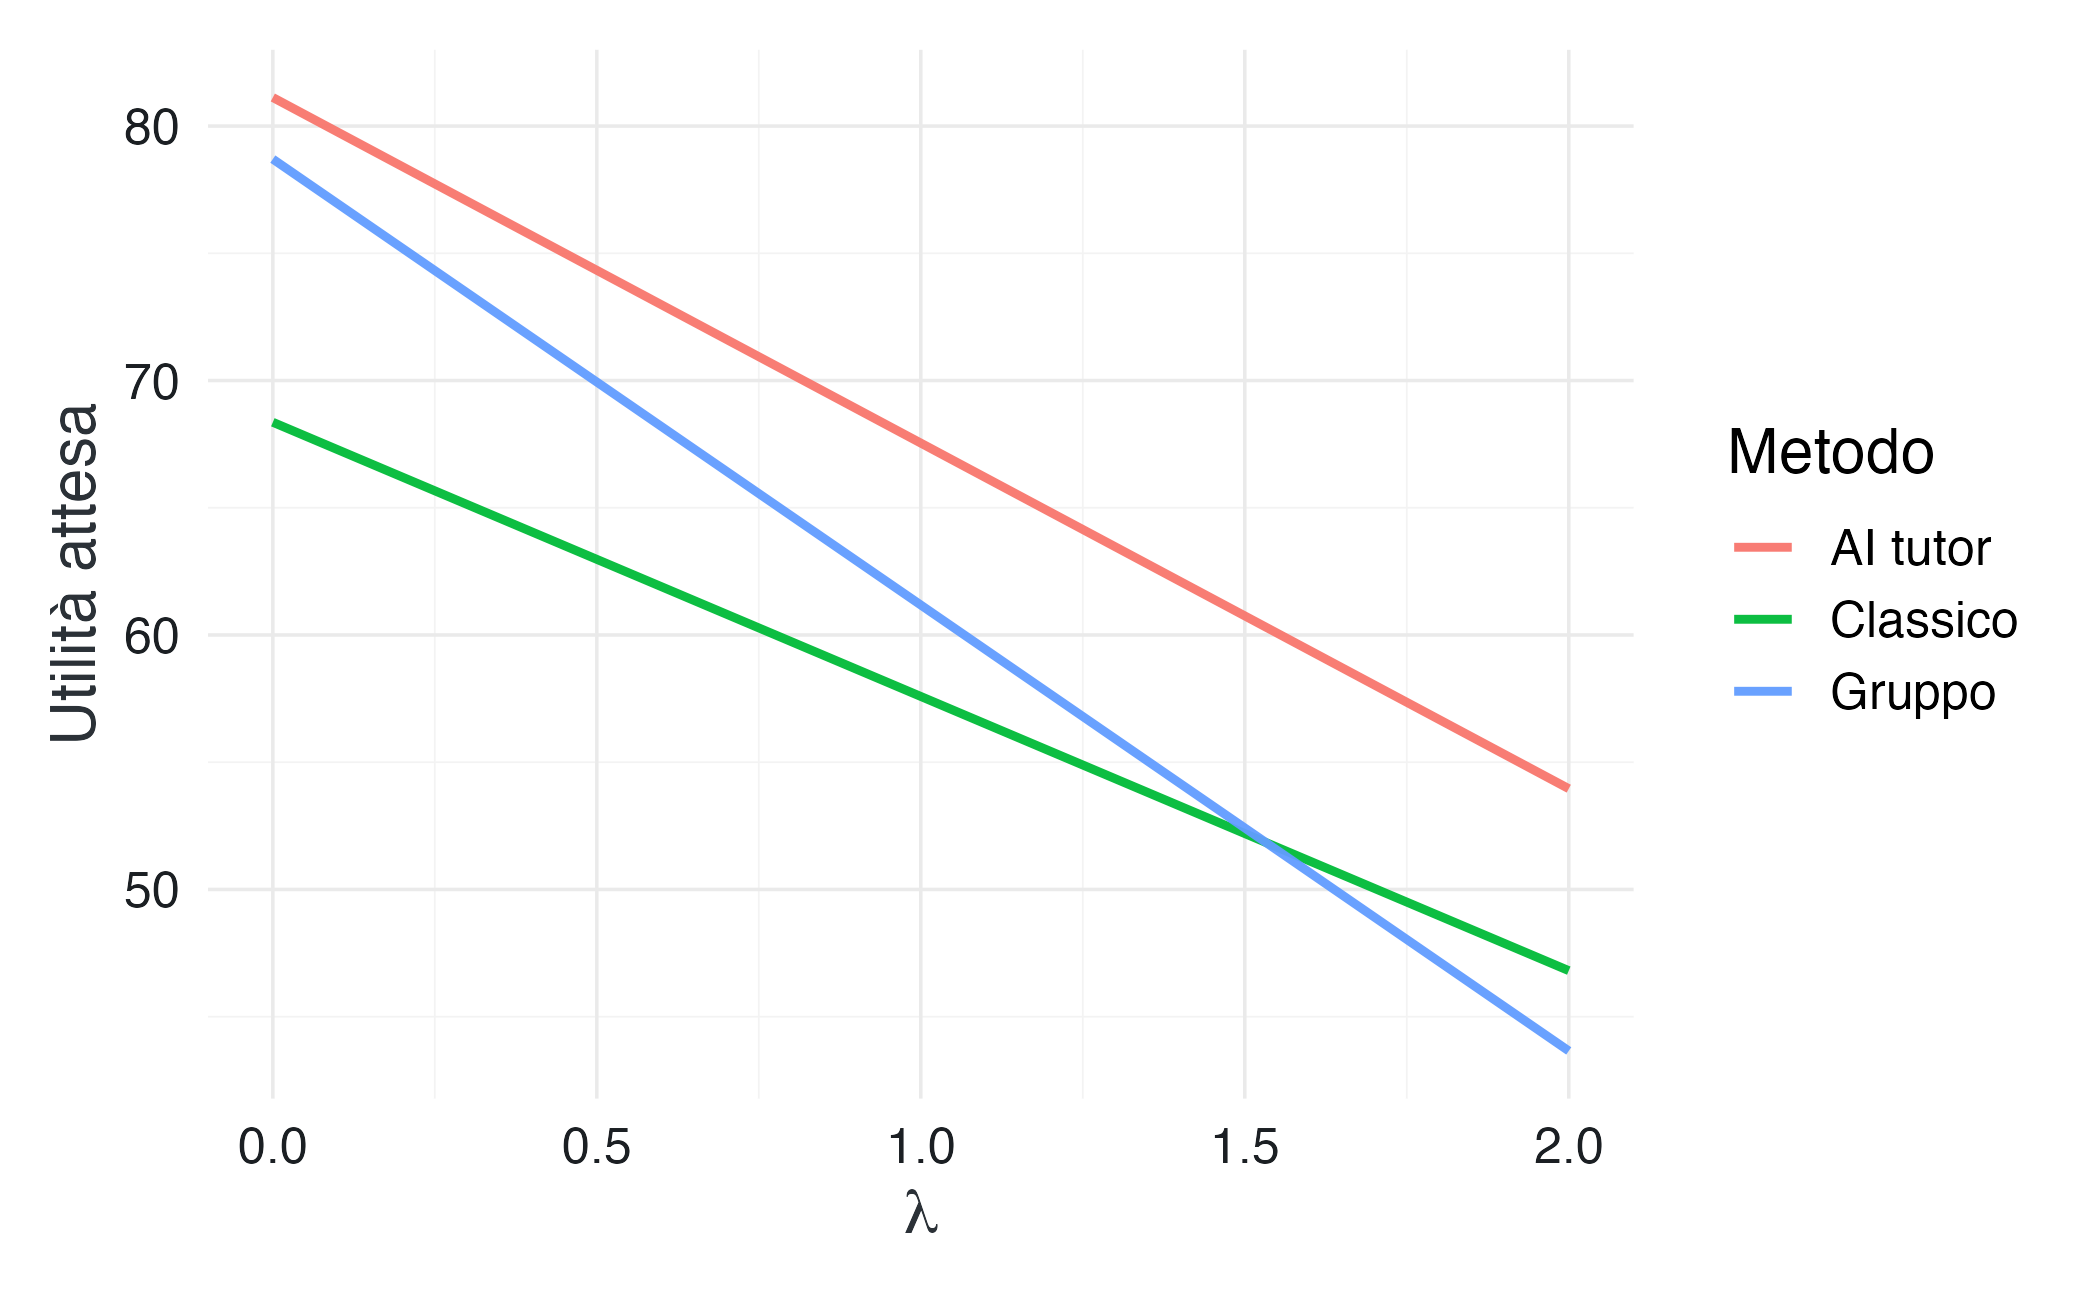
\includegraphics[width=0.85\linewidth,height=\textheight,keepaspectratio]{chapters/formal_models/05_decisione_ottimale_files/figure-pdf/plot-lambda-sensitivity-1.png}

}

\caption{Utilità attesa dei metodi al variare del costo attribuito al
tempo.}

\end{figure}%

I punti d'incrocio indicano valori delle preferenze per i quali cambia
la raccomandazione. Se lo stesso metodo domina su un intervallo ampio,
la decisione è relativamente robusta rispetto a quella componente della
funzione di utilità.

\begin{tcolorbox}[enhanced jigsaw, arc=.35mm, bottomrule=.15mm, bottomtitle=1mm, breakable, colback=white, colbacktitle=quarto-callout-note-color!10!white, colframe=quarto-callout-note-color-frame, coltitle=black, left=2mm, leftrule=.75mm, opacityback=0, opacitybacktitle=0.6, rightrule=.15mm, title=\textcolor{quarto-callout-note-color}{\faInfo}\hspace{0.5em}{Incertezza sulle preferenze}, titlerule=0mm, toprule=.15mm, toptitle=1mm]

Finora \(\lambda\) è trattato come valore fissato dal decisore. Se la
persona non riesce a esprimere una preferenza precisa, si possono:

\begin{itemize}
\tightlist
\item
  esplorare scenari;
\item
  definire un intervallo plausibile;
\item
  modellare \(\lambda\) con una distribuzione;
\item
  usare tecniche di elicitation.
\end{itemize}

L'incertezza sulle preferenze è concettualmente diversa dall'incertezza
empirica sui risultati, anche se entrambe possono essere propagate nella
decisione.

\end{tcolorbox}

\section{Confronti condizionati a un
vincolo}\label{confronti-condizionati-a-un-vincolo}

La funzione di utilità aggrega voto e tempo. Talvolta la domanda è più
semplice e riguarda un vincolo esplicito.

\subsection{Voto a parità di ore}\label{voto-a-parituxe0-di-ore}

Supponiamo di avere un budget di 15 ore. Per ciascun draw posteriore
calcoliamo il voto predittivo sotto ogni metodo.

\begin{Shaded}
\begin{Highlighting}[]
\NormalTok{H\_fixed }\OtherTok{\textless{}{-}} \DecValTok{15}
\NormalTok{pars }\OtherTok{\textless{}{-}}\NormalTok{ fit}\SpecialCharTok{$}\FunctionTok{draws}\NormalTok{(}
  \AttributeTok{variables =} \FunctionTok{c}\NormalTok{(}\StringTok{"alpha"}\NormalTok{, }\StringTok{"beta"}\NormalTok{, }\StringTok{"sigma\_g"}\NormalTok{),}
  \AttributeTok{format =} \StringTok{"draws\_matrix"}
\NormalTok{)}

\NormalTok{alpha\_draws }\OtherTok{\textless{}{-}}\NormalTok{ pars[, }\FunctionTok{paste0}\NormalTok{(}\StringTok{"alpha["}\NormalTok{, }\FunctionTok{seq\_len}\NormalTok{(K), }\StringTok{"]"}\NormalTok{), drop }\OtherTok{=} \ConstantTok{FALSE}\NormalTok{]}
\NormalTok{beta\_draws }\OtherTok{\textless{}{-}}\NormalTok{ pars[, }\FunctionTok{paste0}\NormalTok{(}\StringTok{"beta["}\NormalTok{, }\FunctionTok{seq\_len}\NormalTok{(K), }\StringTok{"]"}\NormalTok{), drop }\OtherTok{=} \ConstantTok{FALSE}\NormalTok{]}
\NormalTok{sigma\_draws }\OtherTok{\textless{}{-}}\NormalTok{ pars[, }\StringTok{"sigma\_g"}\NormalTok{]}

\NormalTok{G\_at\_H }\OtherTok{\textless{}{-}} \FunctionTok{sapply}\NormalTok{(}\FunctionTok{seq\_len}\NormalTok{(K), }\ControlFlowTok{function}\NormalTok{(k) \{}
\NormalTok{  mu }\OtherTok{\textless{}{-}}\NormalTok{ alpha\_draws[, k] }\SpecialCharTok{+}\NormalTok{ beta\_draws[, k] }\SpecialCharTok{*} \FunctionTok{log1p}\NormalTok{(H\_fixed)}
  \FunctionTok{rnorm}\NormalTok{(}\FunctionTok{length}\NormalTok{(mu), mu, sigma\_draws)}
\NormalTok{\})}

\FunctionTok{colnames}\NormalTok{(G\_at\_H) }\OtherTok{\textless{}{-}}\NormalTok{ method\_names}
\FunctionTok{apply}\NormalTok{(G\_at\_H, }\DecValTok{2}\NormalTok{, quantile, }\AttributeTok{probs =} \FunctionTok{c}\NormalTok{(.}\DecValTok{05}\NormalTok{, .}\DecValTok{5}\NormalTok{, .}\DecValTok{95}\NormalTok{))}
\CommentTok{\#\textgreater{}     Classico AI tutor Gruppo}
\CommentTok{\#\textgreater{} 5\%      59.9     71.9   67.6}
\CommentTok{\#\textgreater{} 50\%     70.7     82.8   78.4}
\CommentTok{\#\textgreater{} 95\%     81.7     93.2   89.0}
\end{Highlighting}
\end{Shaded}

Questa quantità risponde alla domanda: \emph{dato lo stesso investimento
temporale, quale distribuzione dei voti prevede il modello?}

\subsection{Ore richieste per un voto
obiettivo}\label{ore-richieste-per-un-voto-obiettivo}

Possiamo invertire la relazione media

\[
G_0=\alpha_k+\beta_k\log(1+H)
\]

ottenendo

\[
H_k(G_0)
=
\exp\left(\frac{G_0-\alpha_k}{\beta_k}\right)-1.
\]

\begin{Shaded}
\begin{Highlighting}[]
\NormalTok{G\_targets }\OtherTok{\textless{}{-}} \FunctionTok{c}\NormalTok{(}\DecValTok{75}\NormalTok{, }\DecValTok{80}\NormalTok{, }\DecValTok{85}\NormalTok{)}

\NormalTok{hours\_for\_target }\OtherTok{\textless{}{-}} \FunctionTok{map\_dfr}\NormalTok{(G\_targets, }\ControlFlowTok{function}\NormalTok{(target) \{}
  \FunctionTok{map\_dfr}\NormalTok{(}\FunctionTok{seq\_len}\NormalTok{(K), }\ControlFlowTok{function}\NormalTok{(k) \{}
\NormalTok{    beta\_k }\OtherTok{\textless{}{-}}\NormalTok{ beta\_draws[, k]}
\NormalTok{    h\_req }\OtherTok{\textless{}{-}} \FunctionTok{ifelse}\NormalTok{(}
\NormalTok{      beta\_k }\SpecialCharTok{\textgreater{}} \DecValTok{0}\NormalTok{,}
      \FunctionTok{pmax}\NormalTok{(}\FunctionTok{exp}\NormalTok{((target }\SpecialCharTok{{-}}\NormalTok{ alpha\_draws[, k]) }\SpecialCharTok{/}\NormalTok{ beta\_k) }\SpecialCharTok{{-}} \DecValTok{1}\NormalTok{, }\DecValTok{0}\NormalTok{),}
      \ConstantTok{NA\_real\_}
\NormalTok{    )}

    \FunctionTok{tibble}\NormalTok{(}
      \AttributeTok{target =}\NormalTok{ target,}
      \AttributeTok{method =}\NormalTok{ method\_names[k],}
      \AttributeTok{hours =}\NormalTok{ h\_req}
\NormalTok{    )}
\NormalTok{  \})}
\NormalTok{\})}

\NormalTok{hours\_for\_target }\SpecialCharTok{|\textgreater{}}
  \FunctionTok{group\_by}\NormalTok{(target, method) }\SpecialCharTok{|\textgreater{}}
  \FunctionTok{summarize}\NormalTok{(}
    \AttributeTok{median =} \FunctionTok{median}\NormalTok{(hours, }\AttributeTok{na.rm =} \ConstantTok{TRUE}\NormalTok{),}
    \AttributeTok{q05 =} \FunctionTok{quantile}\NormalTok{(hours, .}\DecValTok{05}\NormalTok{, }\AttributeTok{na.rm =} \ConstantTok{TRUE}\NormalTok{),}
    \AttributeTok{q95 =} \FunctionTok{quantile}\NormalTok{(hours, .}\DecValTok{95}\NormalTok{, }\AttributeTok{na.rm =} \ConstantTok{TRUE}\NormalTok{),}
    \AttributeTok{.groups =} \StringTok{"drop"}
\NormalTok{  )}
\CommentTok{\#\textgreater{} \# A tibble: 9 x 5}
\CommentTok{\#\textgreater{}   target method   median   q05    q95}
\CommentTok{\#\textgreater{}    \textless{}dbl\textgreater{} \textless{}chr\textgreater{}     \textless{}dbl\textgreater{} \textless{}dbl\textgreater{}  \textless{}dbl\textgreater{}}
\CommentTok{\#\textgreater{} 1     75 AI tutor   6.54  4.99   7.72}
\CommentTok{\#\textgreater{} 2     75 Classico  28.2  20.4   63.1 }
\CommentTok{\#\textgreater{} 3     75 Gruppo     9.65  7.39  11.6 }
\CommentTok{\#\textgreater{} 4     80 AI tutor  11.2   9.88  12.5 }
\CommentTok{\#\textgreater{} 5     80 Classico  59.0  34.7  228.  }
\CommentTok{\#\textgreater{} 6     80 Gruppo    18.5  15.9   22.1 }
\CommentTok{\#\textgreater{} 7     85 AI tutor  18.8  16.5   22.5 }
\CommentTok{\#\textgreater{} 8     85 Classico 122.   58.2  818.  }
\CommentTok{\#\textgreater{} 9     85 Gruppo    34.9  28.1   49.7}
\end{Highlighting}
\end{Shaded}

\begin{tcolorbox}[enhanced jigsaw, arc=.35mm, bottomrule=.15mm, bottomtitle=1mm, breakable, colback=white, colbacktitle=quarto-callout-warning-color!10!white, colframe=quarto-callout-warning-color-frame, coltitle=black, left=2mm, leftrule=.75mm, opacityback=0, opacitybacktitle=0.6, rightrule=.15mm, title=\textcolor{quarto-callout-warning-color}{\faExclamationTriangle}\hspace{0.5em}{Interpretare con cautela l'inversione}, titlerule=0mm, toprule=.15mm, toptitle=1mm]

Le ore calcolate derivano dalla relazione media stimata. Non
garantiscono che un singolo studente raggiunga il voto obiettivo e
possono richiedere estrapolazione oltre l'intervallo osservato.

Se molti draw hanno \(\beta_k\leq 0\), oppure producono ore enormi, il
target non è ben identificato dal modello e non dovrebbe essere
comunicato come raccomandazione precisa.

\end{tcolorbox}

\section{Modelli descrittivi, processuali e
normativi}\label{modelli-descrittivi-processuali-e-normativi}

Il capitolo combina modelli con funzioni differenti.

\begin{itemize}
\tightlist
\item
  Il modello di ore e voto è \textbf{descrittivo e predittivo}:
  rappresenta la distribuzione degli esiti sotto ciascuna alternativa.
\item
  Una teoria di come lo studente apprende durante le ore di studio
  sarebbe un \textbf{modello processuale}.
\item
  La regola che massimizza l'utilità attesa è \textbf{normativa}:
  stabilisce che cosa scegliere date credenze e preferenze specificate.
\end{itemize}

Una deviazione dalla raccomandazione normativa non dimostra
necessariamente irrazionalità. Può indicare che:

\begin{itemize}
\tightlist
\item
  la funzione di utilità non rappresenta correttamente le preferenze;
\item
  mancano conseguenze importanti;
\item
  il decisore dispone di informazioni differenti;
\item
  esistono costi cognitivi o sociali non modellati;
\item
  il modello predittivo è inadeguato;
\item
  la persona segue un criterio decisionale diverso.
\end{itemize}

\begin{tcolorbox}[enhanced jigsaw, arc=.35mm, bottomrule=.15mm, bottomtitle=1mm, breakable, colback=white, colbacktitle=quarto-callout-important-color!10!white, colframe=quarto-callout-important-color-frame, coltitle=black, left=2mm, leftrule=.75mm, opacityback=0, opacitybacktitle=0.6, rightrule=.15mm, title=\textcolor{quarto-callout-important-color}{\faExclamation}\hspace{0.5em}{Ottimale rispetto a che cosa?}, titlerule=0mm, toprule=.15mm, toptitle=1mm]

Un'alternativa non è ottimale in assoluto. È ottimale rispetto a:

\begin{itemize}
\tightlist
\item
  un insieme di opzioni;
\item
  una distribuzione predittiva;
\item
  una funzione di utilità;
\item
  un orizzonte temporale;
\item
  un decisore o una popolazione;
\item
  vincoli e informazioni specifici.
\end{itemize}

Cambiare uno di questi elementi può cambiare la raccomandazione.

\end{tcolorbox}

\section{Oltre l'utilità lineare}\label{oltre-lutilituxe0-lineare}

La funzione

\[
U(g,h;\lambda)=g-\lambda h
\]

assume valore marginale costante sia per il voto sia per il tempo.
Estensioni possibili includono:

\subsection{Soglie e obiettivi}\label{soglie-e-obiettivi}

Un voto sotto la sufficienza può avere una perdita molto maggiore di una
differenza analoga sopra la soglia.

\[
U(g,h)
=
g-\lambda h-C\,\mathbb I(g<g_{\min}).
\]

\subsection{Fatica crescente}\label{fatica-crescente}

Il costo marginale delle ore può aumentare:

\[
U(g,h)=g-\lambda h^p,
\qquad p>1.
\]

\subsection{Avversione al rischio}\label{avversione-al-rischio}

Una funzione concava del beneficio può rendere meno desiderabili
alternative con esiti molto dispersi, anche quando il valore medio è
elevato.

\subsection{Eterogeneità delle
preferenze}\label{eterogeneituxe0-delle-preferenze}

Il parametro \(\lambda_i\) può variare tra studenti. Questa estensione
richiede dati o elicitation sulle preferenze; non può essere
identificata dai soli voti e dalle sole ore.

\subsection{Conseguenze multiple}\label{conseguenze-multiple}

Benessere, apprendimento a lungo termine, equità, privacy e dipendenza
dallo strumento possono essere conseguenze rilevanti. Includerle rende
il modello più realistico, ma richiede di esplicitare come vengono
valutate e aggregate.

\section{Decisioni assistite e
agency}\label{decisioni-assistite-e-agency}

L'uso di modelli o sistemi di intelligenza artificiale nel supporto
decisionale non elimina la responsabilità del decisore. Una procedura
trasparente dovrebbe rendere verificabili:

\begin{itemize}
\tightlist
\item
  i dati usati per prevedere gli esiti;
\item
  la popolazione alla quale il modello si riferisce;
\item
  le conseguenze incluse ed escluse;
\item
  la funzione di utilità;
\item
  la sensibilità della raccomandazione;
\item
  i gruppi per i quali l'errore predittivo è maggiore;
\item
  chi può contestare o modificare la decisione.
\end{itemize}

La formalizzazione può rafforzare l'agency se rende visibili assunzioni
e trade-off. Può indebolirla se una funzione di utilità scelta da altri
viene presentata come criterio neutrale e inevitabile.

\section{Comunicare la
raccomandazione}\label{comunicare-la-raccomandazione}

Una comunicazione adeguata potrebbe assumere questa forma:

\begin{quote}
Nel modello e nella popolazione considerati, il metodo AI tutor
massimizza l'utilità attesa quando un'ora di studio viene valutata come
\(0.65\) punti di voto. La raccomandazione cambia oltre una certa
regione di \(\lambda\), e le distribuzioni predittive mostrano una
sostanziale variabilità individuale. La conclusione è quindi
condizionata al modello degli esiti, alla funzione di utilità e
all'interpretazione causale del confronto tra metodi.
\end{quote}

È preferibile evitare formulazioni come ``l'AI è il metodo migliore'',
che occultano le condizioni della scelta.

\section{Errori frequenti}\label{errori-frequenti-14}

\begin{tcolorbox}[enhanced jigsaw, arc=.35mm, bottomrule=.15mm, bottomtitle=1mm, breakable, colback=white, colbacktitle=quarto-callout-warning-color!10!white, colframe=quarto-callout-warning-color-frame, coltitle=black, left=2mm, leftrule=.75mm, opacityback=0, opacitybacktitle=0.6, rightrule=.15mm, title=\textcolor{quarto-callout-warning-color}{\faExclamationTriangle}\hspace{0.5em}{Confondere previsione e decisione}, titlerule=0mm, toprule=.15mm, toptitle=1mm]

Un metodo con voto atteso maggiore non è necessariamente preferibile se
richiede più tempo o produce altre conseguenze indesiderate.

\end{tcolorbox}

\begin{tcolorbox}[enhanced jigsaw, arc=.35mm, bottomrule=.15mm, bottomtitle=1mm, breakable, colback=white, colbacktitle=quarto-callout-warning-color!10!white, colframe=quarto-callout-warning-color-frame, coltitle=black, left=2mm, leftrule=.75mm, opacityback=0, opacitybacktitle=0.6, rightrule=.15mm, title=\textcolor{quarto-callout-warning-color}{\faExclamationTriangle}\hspace{0.5em}{Inserire le preferenze nel modello empirico}, titlerule=0mm, toprule=.15mm, toptitle=1mm]

Il parametro \(\lambda\) non appartiene alla verosimiglianza di ore e
voto. Tenerlo separato consente di distinguere evidenza e valori.

\end{tcolorbox}

\begin{tcolorbox}[enhanced jigsaw, arc=.35mm, bottomrule=.15mm, bottomtitle=1mm, breakable, colback=white, colbacktitle=quarto-callout-warning-color!10!white, colframe=quarto-callout-warning-color-frame, coltitle=black, left=2mm, leftrule=.75mm, opacityback=0, opacitybacktitle=0.6, rightrule=.15mm, title=\textcolor{quarto-callout-warning-color}{\faExclamationTriangle}\hspace{0.5em}{Usare la probabilità di essere migliore come unico criterio}, titlerule=0mm, toprule=.15mm, toptitle=1mm]

Questa probabilità ignora l'ampiezza dei vantaggi e delle perdite. Il
criterio standard è la massimizzazione dell'utilità attesa.

\end{tcolorbox}

\begin{tcolorbox}[enhanced jigsaw, arc=.35mm, bottomrule=.15mm, bottomtitle=1mm, breakable, colback=white, colbacktitle=quarto-callout-warning-color!10!white, colframe=quarto-callout-warning-color-frame, coltitle=black, left=2mm, leftrule=.75mm, opacityback=0, opacitybacktitle=0.6, rightrule=.15mm, title=\textcolor{quarto-callout-warning-color}{\faExclamationTriangle}\hspace{0.5em}{Trattare la funzione di utilità come oggettiva}, titlerule=0mm, toprule=.15mm, toptitle=1mm]

La funzione incorpora scelte sostantive e normative. Deve essere
motivata, discussa e sottoposta a sensibilità.

\end{tcolorbox}

\begin{tcolorbox}[enhanced jigsaw, arc=.35mm, bottomrule=.15mm, bottomtitle=1mm, breakable, colback=white, colbacktitle=quarto-callout-warning-color!10!white, colframe=quarto-callout-warning-color-frame, coltitle=black, left=2mm, leftrule=.75mm, opacityback=0, opacitybacktitle=0.6, rightrule=.15mm, title=\textcolor{quarto-callout-warning-color}{\faExclamationTriangle}\hspace{0.5em}{Raccomandare senza identificazione causale}, titlerule=0mm, toprule=.15mm, toptitle=1mm]

Una differenza predittiva osservazionale non equivale necessariamente
alla conseguenza di assegnare una persona a un metodo diverso.

\end{tcolorbox}

\begin{tcolorbox}[enhanced jigsaw, arc=.35mm, bottomrule=.15mm, bottomtitle=1mm, breakable, colback=white, colbacktitle=quarto-callout-warning-color!10!white, colframe=quarto-callout-warning-color-frame, coltitle=black, left=2mm, leftrule=.75mm, opacityback=0, opacitybacktitle=0.6, rightrule=.15mm, title=\textcolor{quarto-callout-warning-color}{\faExclamationTriangle}\hspace{0.5em}{Nascondere l'eterogeneità dietro la media}, titlerule=0mm, toprule=.15mm, toptitle=1mm]

La scelta che massimizza l'utilità media della popolazione può non
essere la migliore per ogni individuo.

\end{tcolorbox}

\section{Concetti da ricordare}\label{concetti-da-ricordare-13}

\begin{enumerate}
\def\labelenumi{\arabic{enumi}.}
\tightlist
\item
  L'inferenza quantifica ciò che è plausibile; la decisione aggiunge il
  valore delle conseguenze.
\item
  Il modello predittivo e la funzione di utilità svolgono ruoli
  distinti.
\item
  La decisione bayesiana massimizza l'utilità attesa, o minimizza la
  perdita attesa.
\item
  Le simulazioni posteriori propagano incertezza parametrica e
  variabilità predittiva.
\item
  La probabilità di essere migliore non coincide con l'utilità attesa.
\item
  Le raccomandazioni dipendono dalle preferenze e richiedono analisi di
  sensibilità.
\item
  Una raccomandazione presuppone che le distribuzioni predittive siano
  pertinenti alle azioni considerate.
\item
  L'ottimalità è sempre relativa a opzioni, modello, utilità, vincoli e
  orizzonte temporale.
\item
  I modelli normativi non descrivono necessariamente come le persone
  decidono.
\item
  Una procedura formale è utile quando rende assunzioni e trade-off
  criticabili.
\end{enumerate}

\section{Esercizi}\label{esercizi-10}

\begin{enumerate}
\def\labelenumi{\arabic{enumi}.}
\tightlist
\item
  Modifica i parametri della simulazione affinché il metodo di gruppo
  produca il voto medio più alto ma richieda molte più ore. Esamina come
  cambia la raccomandazione al variare di \(\lambda\).
\item
  Confronta il metodo che massimizza l'utilità attesa con quello che ha
  la maggiore probabilità di essere migliore. Costruisci un esempio in
  cui non coincidano.
\item
  Definisci una funzione di utilità con una penalità per voti inferiori
  a 60 e ripeti l'analisi.
\item
  Sostituisci il costo lineare del tempo con \(\lambda h^{1.5}\). Quale
  conseguenza ha sui metodi che richiedono molte ore?
\item
  Esegui un prior predictive check più completo sulle percentuali di
  voti fuori dall'intervallo 0--100.
\item
  Simula dati con eteroschedasticità del voto tra metodi e modifica il
  programma Stan.
\item
  Esegui un esperimento di parameter recovery ripetuto per i parametri
  delle ore e del voto.
\item
  Immagina che l'assegnazione ai metodi non sia casuale. Costruisci un
  DAG con motivazione, metodo, ore e voto e discuti quali quantità non
  sono identificate dal modello attuale.
\item
  Definisci una decisione personalizzata per uno studente con un budget
  massimo di 12 ore.
\item
  Elenca tre conseguenze etiche o sociali non rappresentate dalla
  funzione \(g-\lambda h\) e proponi una strategia per includerle senza
  fingere che la loro valutazione sia puramente tecnica.
\end{enumerate}

\begin{tcolorbox}[enhanced jigsaw, arc=.35mm, bottomrule=.15mm, bottomtitle=1mm, breakable, colback=white, colbacktitle=quarto-callout-tip-color!10!white, colframe=quarto-callout-tip-color-frame, coltitle=black, left=2mm, leftrule=.75mm, opacityback=0, opacitybacktitle=0.6, rightrule=.15mm, title=\textcolor{quarto-callout-tip-color}{\faLightbulb}\hspace{0.5em}{Tracce di soluzione}, titlerule=0mm, toprule=.15mm, toptitle=1mm]

\begin{enumerate}
\def\labelenumi{\arabic{enumi}.}
\tightlist
\item
  Aumenta \texttt{alpha\_true} o \texttt{beta\_true} del gruppo e
  contemporaneamente \texttt{mu\_log\_h\_true}; cerca i punti di
  incrocio nella curva di sensibilità.
\item
  Crea un'alternativa che vince spesso di poco e un'altra che vince
  raramente con margini molto grandi.
\item
  Sottrai una costante \texttt{C} quando
  \texttt{G\_new\ \textless{}\ 60} prima di calcolare la media
  dell'utilità.
\item
  Calcola \texttt{G\_new\ -\ lambda\ *\ H\_new\^{}1.5}; il costo
  marginale del tempo aumenta con le ore.
\item
  Per ogni draw calcola la proporzione di \texttt{g\_rep} minore di 0 o
  maggiore di 100.
\item
  Sostituisci \texttt{sigma\_g} con un vettore \texttt{sigma\_g{[}K{]}}
  indicizzato dal metodo.
\item
  Ripeti simulazione e stima su più dataset; riassumi bias, RMSE e
  copertura degli intervalli.
\item
  Se la motivazione influenza sia il metodo sia il voto, il confronto
  non aggiustato è confuso.
\item
  Elimina o penalizza le simulazioni in cui le ore superano il budget,
  dichiarando esplicitamente il criterio.
\item
  Esempi: privacy, accessibilità, apprendimento a lungo termine,
  dipendenza tecnologica. La valutazione richiede elicitation, vincoli o
  analisi multicriterio.
\end{enumerate}

\end{tcolorbox}

\section*{Riflessioni conclusive}\label{riflessioni-conclusive-39}

\markright{Riflessioni conclusive}

L'analisi decisionale completa l'arco della parte \textbf{Applicazione}.
I modelli processuali mostrano come un fenomeno potrebbe essere
generato; i modelli gerarchici rappresentano l'eterogeneità; l'inferenza
bayesiana quantifica l'incertezza; la teoria della decisione collega
infine previsioni e conseguenze.

Questo passaggio non produce una risposta neutrale o universale. Una
raccomandazione dipende dalla qualità del modello empirico, dalla
pertinenza causale delle previsioni, dalle alternative disponibili e
dalla funzione di utilità. Il contributo della formalizzazione consiste
nel rendere questi elementi espliciti e modificabili.

Il criterio dell'utilità attesa è quindi uno strumento normativo, non
una descrizione completa del comportamento umano. Può aiutare a chiarire
il ragionamento, confrontare scenari e individuare le assunzioni dalle
quali dipende una scelta. Non sostituisce la deliberazione sostantiva,
etica o politica; la rende più trasparente.

\begin{tcolorbox}[enhanced jigsaw, arc=.35mm, bottomrule=.15mm, bottomtitle=1mm, breakable, colback=white, colbacktitle=quarto-callout-note-color!10!white, colframe=quarto-callout-note-color-frame, coltitle=black, left=2mm, leftrule=.75mm, opacityback=0, opacitybacktitle=0.6, rightrule=.15mm, title=\textcolor{quarto-callout-note-color}{\faInfo}\hspace{0.5em}{Informazioni sull'ambiente di sviluppo}, titlerule=0mm, toprule=.15mm, toptitle=1mm]

\begin{Shaded}
\begin{Highlighting}[]
\FunctionTok{sessionInfo}\NormalTok{()}
\CommentTok{\#\textgreater{} R version 4.6.1 (2026{-}06{-}24)}
\CommentTok{\#\textgreater{} Platform: aarch64{-}apple{-}darwin23}
\CommentTok{\#\textgreater{} Running under: macOS Tahoe 26.5.2}
\CommentTok{\#\textgreater{} }
\CommentTok{\#\textgreater{} Matrix products: default}
\CommentTok{\#\textgreater{} BLAS:   /Library/Frameworks/R.framework/Versions/4.6/Resources/lib/libRblas.0.dylib }
\CommentTok{\#\textgreater{} LAPACK: /Library/Frameworks/R.framework/Versions/4.6/Resources/lib/libRlapack.dylib;  LAPACK version 3.12.1}
\CommentTok{\#\textgreater{} }
\CommentTok{\#\textgreater{} locale:}
\CommentTok{\#\textgreater{} [1] C.UTF{-}8/UTF{-}8/C.UTF{-}8/C/C.UTF{-}8/C.UTF{-}8}
\CommentTok{\#\textgreater{} }
\CommentTok{\#\textgreater{} time zone: Europe/Zagreb}
\CommentTok{\#\textgreater{} tzcode source: internal}
\CommentTok{\#\textgreater{} }
\CommentTok{\#\textgreater{} attached base packages:}
\CommentTok{\#\textgreater{} [1] stats     graphics  grDevices utils     datasets  methods   base     }
\CommentTok{\#\textgreater{} }
\CommentTok{\#\textgreater{} other attached packages:}
\CommentTok{\#\textgreater{}  [1] purrr\_1.2.2           cmdstanr\_0.9.0        ragg\_1.5.2           }
\CommentTok{\#\textgreater{}  [4] tinytable\_0.17.0      withr\_3.0.3           systemfonts\_1.3.2    }
\CommentTok{\#\textgreater{}  [7] patchwork\_1.3.2       ggdist\_3.3.3          tidybayes\_3.0.7      }
\CommentTok{\#\textgreater{} [10] bayesplot\_1.15.0      ggplot2\_4.0.3         reliabilitydiag\_0.2.1}
\CommentTok{\#\textgreater{} [13] priorsense\_1.2.0      posterior\_1.7.0       loo\_2.10.0           }
\CommentTok{\#\textgreater{} [16] rstan\_2.32.7          StanHeaders\_2.32.10   brms\_2.23.0          }
\CommentTok{\#\textgreater{} [19] Rcpp\_1.1.2            sessioninfo\_1.2.4     conflicted\_1.2.0     }
\CommentTok{\#\textgreater{} [22] janitor\_2.2.1         matrixStats\_1.5.0     modelr\_0.1.11        }
\CommentTok{\#\textgreater{} [25] tibble\_3.3.1          dplyr\_1.2.1           tidyr\_1.3.2          }
\CommentTok{\#\textgreater{} [28] rio\_1.3.0             here\_1.0.2           }
\CommentTok{\#\textgreater{} }
\CommentTok{\#\textgreater{} loaded via a namespace (and not attached):}
\CommentTok{\#\textgreater{}  [1] gridExtra\_2.3.1       inline\_0.3.21         rlang\_1.3.0          }
\CommentTok{\#\textgreater{}  [4] magrittr\_2.0.5        snakecase\_0.11.1      otel\_0.2.0           }
\CommentTok{\#\textgreater{}  [7] compiler\_4.6.1        mgcv\_1.9{-}4            vctrs\_0.7.3          }
\CommentTok{\#\textgreater{} [10] reshape2\_1.4.5        stringr\_1.6.0         pkgconfig\_2.0.3      }
\CommentTok{\#\textgreater{} [13] arrayhelpers\_1.1{-}1    fastmap\_1.2.0         backports\_1.5.1      }
\CommentTok{\#\textgreater{} [16] labeling\_0.4.3        utf8\_1.2.6            rmarkdown\_2.31       }
\CommentTok{\#\textgreater{} [19] ps\_1.9.3              xfun\_0.60             cachem\_1.1.0         }
\CommentTok{\#\textgreater{} [22] jsonlite\_2.0.0        broom\_1.0.13          parallel\_4.6.1       }
\CommentTok{\#\textgreater{} [25] R6\_2.6.1              stringi\_1.8.7         RColorBrewer\_1.1{-}3   }
\CommentTok{\#\textgreater{} [28] lubridate\_1.9.5       estimability\_2.0.0    knitr\_1.51           }
\CommentTok{\#\textgreater{} [31] Matrix\_1.7{-}5          splines\_4.6.1         timechange\_0.4.0     }
\CommentTok{\#\textgreater{} [34] tidyselect\_1.2.1      abind\_1.4{-}8           yaml\_2.3.12          }
\CommentTok{\#\textgreater{} [37] codetools\_0.2{-}20      curl\_7.1.0            processx\_3.9.0       }
\CommentTok{\#\textgreater{} [40] pkgbuild\_1.4.8        lattice\_0.22{-}9        plyr\_1.8.9           }
\CommentTok{\#\textgreater{} [43] bridgesampling\_1.2{-}1  S7\_0.2.2              coda\_0.19{-}4.1        }
\CommentTok{\#\textgreater{} [46] evaluate\_1.0.5        RcppParallel\_5.1.11{-}2 pillar\_1.11.1        }
\CommentTok{\#\textgreater{} [49] tensorA\_0.36.2.1      checkmate\_2.3.4       stats4\_4.6.1         }
\CommentTok{\#\textgreater{} [52] distributional\_0.8.1  generics\_0.1.4        rprojroot\_2.1.1      }
\CommentTok{\#\textgreater{} [55] rstantools\_2.6.0      scales\_1.4.0          xtable\_1.8{-}8         }
\CommentTok{\#\textgreater{} [58] glue\_1.8.1            emmeans\_2.0.4         tools\_4.6.1          }
\CommentTok{\#\textgreater{} [61] data.table\_1.18.4     mvtnorm\_1.4{-}2         grid\_4.6.1           }
\CommentTok{\#\textgreater{} [64] QuickJSR\_1.10.0       nlme\_3.1{-}170          cli\_3.6.6            }
\CommentTok{\#\textgreater{} [67] textshaping\_1.0.5     svUnit\_1.0.8          Brobdingnag\_1.2{-}9    }
\CommentTok{\#\textgreater{} [70] V8\_8.2.0              gtable\_0.3.6          digest\_0.6.39        }
\CommentTok{\#\textgreater{} [73] farver\_2.1.2          memoise\_2.0.1         htmltools\_0.5.9      }
\CommentTok{\#\textgreater{} [76] lifecycle\_1.0.5}
\end{Highlighting}
\end{Shaded}

\end{tcolorbox}

\section*{Bibliografia}\label{bibliografia-44}

\markright{Bibliografia}

\chapter*{Riflessioni conclusive della
sezione}\label{riflessioni-conclusive-della-sezione-4}

\markboth{Riflessioni conclusive della sezione}{Riflessioni conclusive
della sezione}

\begin{tcolorbox}[enhanced jigsaw, arc=.35mm, bottomrule=.15mm, breakable, colback=white, colframe=quarto-callout-note-color-frame, left=2mm, leftrule=.75mm, opacityback=0, rightrule=.15mm, toprule=.15mm]

Questa parte ha proposto una risposta positiva a uno dei problemi messi
in luce dalla crisi di replicabilità: la debolezza del collegamento tra
teoria e dati. Migliorare la trasparenza, la misurazione e l'inferenza è
indispensabile, ma non basta quando le ipotesi psicologiche rimangono
abbastanza vaghe da essere compatibili con quasi ogni risultato.

La modellazione formale rende la teoria più esigente. Obbliga a
specificare quali stati esistano, come cambino, quali osservazioni
producano e quali dati dovrebbero mettere in difficoltà il modello.

\end{tcolorbox}

\section*{Dalla collezione degli effetti a una psicologia
generativa}\label{dalla-collezione-degli-effetti-a-una-psicologia-generativa}
\addcontentsline{toc}{section}{Dalla collezione degli effetti a una
psicologia generativa}

\markright{Dalla collezione degli effetti a una psicologia generativa}

Una parte rilevante della ricerca psicologica è stata organizzata
attorno alla rilevazione di effetti: differenze tra gruppi, associazioni
tra variabili, interazioni e cambiamenti medi. Queste quantità sono
importanti, ma non costituiscono necessariamente una spiegazione.

Due processi differenti possono produrre la stessa differenza media. Lo
stesso processo può produrre effetti diversi al variare del compito,
della misura o della popolazione. Una teoria cumulativa deve quindi
specificare qualcosa di più del segno o della grandezza di
un'associazione: deve proporre un processo capace di generare i dati e
di estendersi a condizioni non ancora osservate.

I modelli formali affrontati in questa parte rappresentano un passo in
tale direzione. Non sostituiscono l'esperimento, la misurazione o il
ragionamento causale. Li collegano in una struttura nella quale le
ipotesi teoriche producono conseguenze quantitative controllabili.

\section*{Un modello come teoria
eseguibile}\label{un-modello-come-teoria-eseguibile}
\addcontentsline{toc}{section}{Un modello come teoria eseguibile}

\markright{Un modello come teoria eseguibile}

Il passaggio fondamentale è stato trasformare formulazioni verbali in
sistemi che possono essere eseguiti. Un modello processuale deve almeno
specificare:

\begin{itemize}
\tightlist
\item
  uno o più stati interni;
\item
  le informazioni disponibili al sistema;
\item
  una regola di trasformazione o aggiornamento;
\item
  parametri che modulano la dinamica;
\item
  condizioni iniziali;
\item
  un modello osservazionale che collega gli stati alle risposte
  misurate.
\end{itemize}

Quando questi elementi sono espliciti, la teoria può essere simulata.
Possiamo chiedere quali traiettorie produca, quali pattern escluda e
quali parametri siano responsabili delle diverse conseguenze
osservabili.

La simulazione ha quindi preceduto logicamente la stima. Prima di usare
i dati per apprendere i parametri, abbiamo dovuto comprendere che cosa
quei parametri facessero nel modello. Questo principio è essenziale: non
è possibile interpretare correttamente una posterior se non si conoscono
le conseguenze generative delle quantità stimate
(\citeproc{ref-McElreath_rethinking}{McElreath, 2020}).

\section*{Dalla generazione all'inferenza
inversa}\label{dalla-generazione-allinferenza-inversa}
\addcontentsline{toc}{section}{Dalla generazione all'inferenza inversa}

\markright{Dalla generazione all'inferenza inversa}

I modelli processuali vengono formulati nella direzione:

\[
\text{parametri e stati}
\longrightarrow
\text{comportamento osservabile}.
\]

L'analisi dei dati procede invece nella direzione inversa:

\[
\text{comportamento osservato}
\longrightarrow
\text{incertezza su parametri e stati}.
\]

Questo problema inverso è spesso difficile. Parametri diversi possono
compensarsi, produrre traiettorie simili o essere scarsamente informati
dal disegno. Un buon adattamento ai dati non garantisce quindi che il
parametro psicologico sia stato identificato.

Per questa ragione, la modellazione formale richiede controlli
aggiuntivi rispetto a una normale analisi descrittiva:

\begin{enumerate}
\def\labelenumi{\arabic{enumi}.}
\tightlist
\item
  simulazione dal modello;
\item
  controllo predittivo a priori;
\item
  recupero dei parametri da dati simulati;
\item
  diagnostica computazionale;
\item
  controllo predittivo a posteriori;
\item
  confronto con modelli rivali;
\item
  verifica su nuovi dati, individui o compiti.
\end{enumerate}

Un parametro acquista significato scientifico soltanto quando il
modello, il disegno e le misure permettono di distinguerne le
conseguenze da quelle di spiegazioni alternative.

\section*{Che cosa abbiamo appreso dai modelli
dinamici}\label{che-cosa-abbiamo-appreso-dai-modelli-dinamici}
\addcontentsline{toc}{section}{Che cosa abbiamo appreso dai modelli
dinamici}

\markright{Che cosa abbiamo appreso dai modelli dinamici}

Il modello di revisione degli obiettivi ha mostrato come una teoria
intuitiva possa essere trasformata in una regola temporale. La
discrepanza tra prestazione e obiettivo non è stata trattata come un
semplice predittore, ma come un'informazione che modifica lo stato
successivo del sistema. Il parametro di aggiornamento ha assunto
significato attraverso la dinamica generata, non attraverso la sola
posizione nella formula (\citeproc{ref-hayes2019role}{Hayes et al.,
2019}; \citeproc{ref-knight2023tutorial}{Knight et al., 2023}).

L'estensione gerarchica ha mostrato che i parametri processuali possono
variare tra individui e condizioni. Questa variazione non deve però
essere confusa con la precisione delle stime. Un individuo può avere una
posterior ampia perché i suoi dati sono poco informativi; ciò non
dimostra che il suo processo sia particolarmente variabile. Il partial
pooling permette di integrare livelli individuali e di popolazione, ma
non trasforma automaticamente stime rumorose in caratteristiche
psicologiche stabili.

La modellazione dell'eterogeneità ha inoltre reso evidente una
condizione della psicologia personalizzata: non basta produrre un
parametro per ogni persona. Occorre dimostrare che quel parametro sia
recuperabile, stabile, predittivo e rilevante oltre il campione nel
quale è stato stimato.

\section*{Rescorla--Wagner come caso
paradigmatico}\label{rescorlawagner-come-caso-paradigmatico}
\addcontentsline{toc}{section}{Rescorla--Wagner come caso paradigmatico}

\markright{Rescorla--Wagner come caso paradigmatico}

Il modello di Rescorla--Wagner ha fornito l'esempio più completo del
passaggio da teoria a processo. L'aspettativa cambia in funzione
dell'errore di previsione, cioè della discrepanza tra ciò che il sistema
si attende e ciò che osserva (\citeproc{ref-rescorla1972theory}{Rescorla
\& Wagner, 1972}).

Questo modello ha permesso di distinguere almeno tre livelli:

\begin{enumerate}
\def\labelenumi{\arabic{enumi}.}
\tightlist
\item
  \textbf{apprendimento}, rappresentato dalla regola di aggiornamento;
\item
  \textbf{stato latente}, rappresentato dal valore appreso;
\item
  \textbf{scelta osservabile}, rappresentata dal modello decisionale.
\end{enumerate}

La separazione è teoricamente importante. Un comportamento
apparentemente rigido può dipendere da un aggiornamento lento, da una
bassa sensibilità alle differenze di valore, da una tendenza a
perseverare o da una combinazione di questi processi. Le medie aggregate
possono nascondere tali alternative.

Allo stesso tempo, Rescorla--Wagner ha mostrato i limiti di ogni
modello. La sua semplicità è una virtù perché genera predizioni chiare,
ma può diventare un limite quando il comportamento richiede tassi di
apprendimento asimmetrici, perseverazione, rappresentazioni contestuali
o incertezza dinamica. Il progresso non consiste nel proteggere il
modello dalle anomalie, ma nel usare le discrepanze per proporre e
confrontare revisioni.

\section*{Dalla spiegazione alla
decisione}\label{dalla-spiegazione-alla-decisione}
\addcontentsline{toc}{section}{Dalla spiegazione alla decisione}

\markright{Dalla spiegazione alla decisione}

L'ultimo capitolo ha ampliato la funzione dei modelli. Una distribuzione
a posteriori o predittiva descrive ciò che è plausibile; non stabilisce
da sola quale azione debba essere scelta. Per passare dall'inferenza
alla decisione è necessario specificare conseguenze, preferenze e costi.

La decisione ottimale è quindi sempre condizionata a una funzione di
utilità. Una scelta può essere ottimale per chi attribuisce grande
valore al risultato e poco costo al tempo, ma non per chi possiede
priorità diverse. Rendere esplicita l'utilità evita di presentare come
neutra una scelta che dipende da assunzioni normative.

Questo passaggio ha chiarito la distinzione tra:

\begin{itemize}
\tightlist
\item
  \textbf{modello descrittivo}, che rappresenta ciò che le persone
  fanno;
\item
  \textbf{modello processuale}, che propone come producano la scelta;
\item
  \textbf{modello normativo}, che stabilisce quale scelta massimizzi un
  criterio dato.
\end{itemize}

Confondere questi livelli può trasformare una raccomandazione
condizionata in una prescrizione ingiustificata. La teoria bayesiana
della decisione mantiene invece separate l'incertezza sulle conseguenze
e la valutazione delle conseguenze stesse
(\citeproc{ref-gelman1995bayesian}{Gelman et al., 2013b}).

\section*{Che cosa i modelli formali non
garantiscono}\label{che-cosa-i-modelli-formali-non-garantiscono}
\addcontentsline{toc}{section}{Che cosa i modelli formali non
garantiscono}

\markright{Che cosa i modelli formali non garantiscono}

La formalizzazione migliora la chiarezza, ma non risolve automaticamente
i problemi teorici.

Un modello può essere:

\begin{itemize}
\tightlist
\item
  matematicamente elegante ma psicologicamente irrilevante;
\item
  ben adattato ma non identificabile;
\item
  predittivo ma privo dell'interpretazione meccanicistica proposta;
\item
  interpretabile nel campione ma instabile tra compiti o popolazioni;
\item
  complesso ma incapace di riprodurre caratteristiche essenziali dei
  dati;
\item
  migliore dei concorrenti considerati ma ancora sostanzialmente
  inadeguato.
\end{itemize}

\begin{tcolorbox}[enhanced jigsaw, arc=.35mm, bottomrule=.15mm, bottomtitle=1mm, breakable, colback=white, colbacktitle=quarto-callout-important-color!10!white, colframe=quarto-callout-important-color-frame, coltitle=black, left=2mm, leftrule=.75mm, opacityback=0, opacitybacktitle=0.6, rightrule=.15mm, title=\textcolor{quarto-callout-important-color}{\faExclamation}\hspace{0.5em}{Il modello migliore può essere ancora sbagliato}, titlerule=0mm, toprule=.15mm, toptitle=1mm]

Il confronto relativo seleziona il modello che funziona meglio tra
quelli considerati. Non dimostra che quel modello rappresenti
adeguatamente il fenomeno. È quindi necessario affiancare al confronto
tra modelli controlli assoluti delle loro conseguenze predittive.

\end{tcolorbox}

Neppure il nome di un parametro ne stabilisce il significato.
Interpretare una quantità come impulsività, sensibilità alla ricompensa
o velocità di apprendimento richiede evidenze convergenti:
recuperabilità, validità rispetto a misure esterne, stabilità quando
prevista dalla teoria e generalizzazione a nuovi contesti.

\section*{Un ciclo scientifico più
esigente}\label{un-ciclo-scientifico-piuxf9-esigente}
\addcontentsline{toc}{section}{Un ciclo scientifico più esigente}

\markright{Un ciclo scientifico più esigente}

Il workflow emerso da questa parte può essere riassunto così:

\[
\text{fenomeno}
\rightarrow
\text{teoria verbale}
\rightarrow
\text{modello formale}
\rightarrow
\text{simulazione}
\rightarrow
\text{disegno e misura}
\rightarrow
\text{inferenza}
\rightarrow
\text{critica}
\rightarrow
\text{revisione}.
\]

Il ciclo non termina con una stima precisa. Una teoria diventa più
informativa quando:

\begin{itemize}
\tightlist
\item
  produce predizioni che potrebbero risultare errate;
\item
  discrimina tra meccanismi rivali;
\item
  mantiene potere predittivo su dati non usati per la stima;
\item
  chiarisce il dominio nel quale dovrebbe funzionare;
\item
  rende visibili le condizioni del proprio fallimento;
\item
  viene modificata in risposta alle discrepanze.
\end{itemize}

Questa concezione è compatibile con una scienza cumulativa. I modelli
possono incorporare risultati precedenti, essere condivisi come codice,
confrontati su dataset comuni e ampliati senza perdere la traccia delle
assunzioni originarie.

\section*{Una risposta positiva alla crisi
teorica}\label{una-risposta-positiva-alla-crisi-teorica}
\addcontentsline{toc}{section}{Una risposta positiva alla crisi teorica}

\markright{Una risposta positiva alla crisi teorica}

La crisi di replicabilità ha mostrato che molte conclusioni erano più
fragili di quanto suggerissero le pubblicazioni originarie. La risposta
metodologica ha promosso trasparenza, preregistrazione, campioni più
informativi e analisi più robuste. La modellazione formale aggiunge un
ulteriore livello: rende le teorie abbastanza precise da poter essere
controllate.

Non si tratta di abbandonare lo studio delle associazioni. Le
associazioni descrivono i fenomeni che una teoria deve spiegare, aiutano
a progettare nuovi studi e costituiscono una componente essenziale dei
modelli osservazionali. Il cambiamento consiste nel non trattarle come
punto di arrivo.

Una psicologia generativa cerca di passare da:

\begin{itemize}
\tightlist
\item
  «quali variabili sono associate?»
\end{itemize}

a:

\begin{itemize}
\tightlist
\item
  «quale processo produce questa associazione?»;
\item
  «quali altre osservazioni dovrebbe generare?»;
\item
  «quale modello rivale produce predizioni diverse?»;
\item
  «in quali persone, compiti e contesti il processo dovrebbe
  generalizzare?».
\end{itemize}

Queste domande non garantiscono una risposta definitiva, ma rendono il
progresso teorico più controllabile.

\section*{Dieci idee da conservare}\label{dieci-idee-da-conservare-1}
\addcontentsline{toc}{section}{Dieci idee da conservare}

\markright{Dieci idee da conservare}

\begin{enumerate}
\def\labelenumi{\arabic{enumi}.}
\tightlist
\item
  Una teoria formale deve specificare abbastanza da poter generare dati.
\item
  Simulare il modello precede logicamente la stima dei parametri.
\item
  Stati latenti e risposte osservate devono essere collegati da un
  modello osservazionale.
\item
  Un buon fit non dimostra che il meccanismo proposto sia corretto.
\item
  I parametri devono essere recuperabili prima di ricevere
  interpretazioni psicologiche forti.
\item
  Eterogeneità tra individui e incertezza individuale sono quantità
  differenti.
\item
  I modelli gerarchici integrano informazione individuale e di
  popolazione, ma non garantiscono validità idiografica.
\item
  I modelli rivali sono indispensabili perché processi diversi possono
  produrre pattern simili.
\item
  Una decisione ottimale dipende sia dalle previsioni sia dalla funzione
  di utilità.
\item
  La revisione del modello è una forma di progresso teorico, non un
  fallimento da nascondere.
\end{enumerate}

\begin{tcolorbox}[enhanced jigsaw, arc=.35mm, bottomrule=.15mm, bottomtitle=1mm, breakable, colback=white, colbacktitle=quarto-callout-tip-color!10!white, colframe=quarto-callout-tip-color-frame, coltitle=black, left=2mm, leftrule=.75mm, opacityback=0, opacitybacktitle=0.6, rightrule=.15mm, title=\textcolor{quarto-callout-tip-color}{\faLightbulb}\hspace{0.5em}{Checklist per un modello processuale}, titlerule=0mm, toprule=.15mm, toptitle=1mm]

Prima di attribuire un significato psicologico ai parametri, chiediti:

\begin{itemize}
\tightlist
\item
  Il fenomeno da spiegare è delimitato con precisione?
\item
  Gli stati e le regole del modello corrispondono a ipotesi teoriche
  esplicite?
\item
  Ho simulato le conseguenze di valori diversi dei parametri?
\item
  Il modello osservazionale è distinto dal processo latente?
\item
  I parametri possono essere recuperati da dati realistici?
\item
  Esistono modelli rivali capaci di produrre pattern simili?
\item
  I controlli predittivi esaminano le caratteristiche teoricamente
  importanti?
\item
  Le conclusioni generalizzano a nuovi individui, compiti o contesti?
\item
  Il significato attribuito ai parametri è sostenuto da evidenze
  esterne?
\item
  Ho documentato quali risultati richiederebbero una revisione del
  modello?
\end{itemize}

\end{tcolorbox}

\section*{Verso la valutazione dei
modelli}\label{verso-la-valutazione-dei-modelli}
\addcontentsline{toc}{section}{Verso la valutazione dei modelli}

\markright{Verso la valutazione dei modelli}

Una volta costruiti modelli espliciti, emerge una nuova domanda:
\textbf{come possiamo stabilire quale rappresenti meglio le informazioni
rilevanti e quanto possa generalizzare?}

Il semplice adattamento ai dati osservati non è sufficiente. Dobbiamo
valutare la capacità predittiva, quantificare la perdita d'informazione,
confrontare modelli di diversa complessità e distinguere il
miglioramento reale dall'overfitting.

La parte successiva svilupperà questi problemi attraverso entropia,
divergenza di Kullback--Leibler e strumenti di valutazione predittiva.
Il passaggio è naturale: la formalizzazione rende i modelli
confrontabili; la valutazione stabilisce in che misura le loro
conseguenze siano sostenute dai dati e trasferibili oltre il campione
osservato.

Il coronamento del percorso non è quindi un singolo modello. È un modo
di fare ricerca nel quale teoria, simulazione, dati e critica rimangono
collegati nello stesso ciclo di apprendimento.

\section*{Bibliografia}\label{bibliografia-45}

\markright{Bibliografia}

\part{Valutazione}

\chapter*{Introduzione alla sezione}\label{introduzione-alla-sezione}

\markboth{Introduzione alla sezione}{Introduzione alla sezione}

\begin{tcolorbox}[enhanced jigsaw, arc=.35mm, bottomrule=.15mm, breakable, colback=white, colframe=quarto-callout-note-color-frame, left=2mm, leftrule=.75mm, opacityback=0, rightrule=.15mm, toprule=.15mm]

\vspace{-3mm}\textbf{Dove siamo nel percorso}\vspace{3mm}

Finora abbiamo imparato a costruire modelli probabilistici, a
specificare i prior, a stimare le distribuzioni a posteriori e a
controllare se un modello genera dati plausibili. Ora affrontiamo una
domanda diversa: \textbf{come confrontare modelli alternativi quando
nessuno di essi può essere considerato letteralmente vero?}

In questa sezione approfondiremo i fondamenti teorici degli strumenti
utilizzati per la validazione predittiva e la generalizzabilità dei
modelli. Il filo conduttore è semplice, ma decisivo: i modelli
probabilistici non sono copie della realtà, ma approssimazioni esplicite
che utilizziamo per rappresentare l'incertezza, fare previsioni e
prendere decisioni.

\end{tcolorbox}

Nel quadro bayesiano, un modello non è soltanto una procedura per
adattare una curva ai dati osservati. È una rappresentazione generativa
che indica quali dati sarebbero plausibili se determinate ipotesi sui
processi psicologici fossero valide. Proprio per questo motivo, la
valutazione di un modello non può limitarsi a verificare quanto bene
esso descriva il campione già osservato. Un modello troppo flessibile,
infatti, può adattarsi molto bene ai dati disponibili, ma prevedere male
i casi nuovi.

La domanda centrale diventa quindi:

\begin{quote}
\textbf{Se tutti i modelli sono approssimazioni, con quale criterio
possiamo dire che un modello è migliore di un altro?}
\end{quote}

La risposta che svilupperemo in questa sezione è di tipo informazionale
e predittivo: un modello è preferibile quando fornisce previsioni
migliori su dati non ancora osservati, ovvero quando riduce la sorpresa
di fronte a nuove osservazioni. Ciò non significa che la previsione
esaurisca il valore scientifico di una teoria. Piuttosto, significa che
la capacità di generalizzare al di là dei dati usati per stimare il
modello è una prova cruciale della sua utilità epistemica.

\section*{Dalla sorpresa alla validazione
predittiva}\label{dalla-sorpresa-alla-validazione-predittiva}

\markright{Dalla sorpresa alla validazione predittiva}

Il percorso della sezione procede per gradi. Ogni passaggio introduce un
concetto tecnico, ma il filo logico rimane lo stesso: misurare quanto un
modello sia in grado di rappresentare l'incertezza in modo utile per la
previsione.

\begin{enumerate}
\def\labelenumi{\arabic{enumi}.}
\item
  \textbf{Sorpresa e log-score.} Un evento che il modello riteneva molto
  improbabile è molto sorprendente. Questa idea si esprime con la
  quantità \(-\log p(y)\): minore è la probabilità assegnata al dato
  osservato, maggiore è la sorpresa.
\item
  \textbf{Entropia di Shannon.} L'entropia misura la sorpresa media
  attesa sotto una distribuzione. È una misura dell'incertezza prima
  dell'osservazione del dato.
\item
  \textbf{Entropia incrociata e divergenza di Kullback--Leibler.} Se
  usiamo un modello approssimato per descrivere un processo generatore
  diverso, paghiamo un costo informativo. La divergenza KL quantifica
  questa perdita: quanta informazione sprechiamo usando una
  distribuzione \(Q\) al posto della distribuzione generatrice \(P\)?
\item
  \textbf{ELPD.} Nella pratica non conosciamo il processo generatore
  vero. Per questo motivo, spostiamo l'attenzione sulla densità
  predittiva attesa: quanto bene il modello si aspetta di predire dati
  futuri?
\item
  \textbf{LOO-CV e PSIS-LOO.} Poiché non disponiamo di infiniti dati
  futuri, stimiamo la capacità predittiva utilizzando strategie di
  validazione incrociata. La leave-one-out cross-validation approssima
  la domanda: che probabilità avrebbe assegnato il modello a
  un'osservazione se quell'osservazione non fosse stata utilizzata per
  stimarlo?
\end{enumerate}

\begin{tcolorbox}[enhanced jigsaw, arc=.35mm, bottomrule=.15mm, bottomtitle=1mm, breakable, colback=white, colbacktitle=quarto-callout-tip-color!10!white, colframe=quarto-callout-tip-color-frame, coltitle=black, left=2mm, leftrule=.75mm, opacityback=0, opacitybacktitle=0.6, rightrule=.15mm, title=\textcolor{quarto-callout-tip-color}{\faLightbulb}\hspace{0.5em}{Cosa imparerai a fare}, titlerule=0mm, toprule=.15mm, toptitle=1mm]

Al termine di questa sezione sarai in grado di:

\begin{itemize}
\tightlist
\item
  interpretare l'entropia come misura dell'incertezza e della sorpresa
  media;
\item
  comprendere la divergenza KL come costo informativo
  dell'approssimazione;
\item
  collegare la KL alla valutazione predittiva dei modelli;
\item
  leggere log-score, ELPD e differenze di ELPD senza ridurli a
  classifiche automatiche;
\item
  usare la LOO-CV come strumento di critica modellistica.
\end{itemize}

\end{tcolorbox}

\section*{Perché serve un po' di
formalismo}\label{perchuxe9-serve-un-po-di-formalismo}

\markright{Perché serve un po' di formalismo}

Questa sezione introduce concetti più astratti rispetto ai capitoli
precedenti. Un certo grado di formalismo è inevitabile, in quanto le
idee di sorpresa, entropia, divergenza e previsione attesa sono
precisamente definite da quantità matematiche. Tuttavia, le formule non
vengono presentate come oggetti autonomi. Ogni formula risponde a una
domanda interpretativa.

{\def\LTcaptype{none} % do not increment counter
\begin{longtable}[]{@{}
  >{\raggedright\arraybackslash}p{(\linewidth - 2\tabcolsep) * \real{0.5000}}
  >{\raggedright\arraybackslash}p{(\linewidth - 2\tabcolsep) * \real{0.5000}}@{}}
\toprule\noalign{}
\begin{minipage}[b]{\linewidth}\raggedright
Quantità
\end{minipage} & \begin{minipage}[b]{\linewidth}\raggedright
Domanda interpretativa
\end{minipage} \\
\midrule\noalign{}
\endhead
\bottomrule\noalign{}
\endlastfoot
\(-\log p(y)\) & Quanto è sorpreso il modello dal dato osservato? \\
\(H(P)\) & Quanta sorpresa ci aspettiamo in media se i dati seguono
\(P\)? \\
\(\mathrm{KL}(P \| Q)\) & Quanta sorpresa extra paghiamo usando \(Q\) al
posto di \(P\)? \\
\(\mathrm{ELPD}\) & Quanto bene il modello prevede dati futuri? \\
\(\Delta\mathrm{ELPD}\) & Quanto è grande, e quanto incerto, il
vantaggio predittivo di un modello rispetto a un altro? \\
\end{longtable}
}

Il punto importante è che queste quantità non sono meri indicatori
tecnici. Queste quantità rendono operativa una concezione della
conoscenza scientifica: una teoria formalizzata diventa più credibile
quando genera previsioni che restano valide anche di fronte a dati non
utilizzati per costruirla.

\begin{tcolorbox}[enhanced jigsaw, arc=.35mm, bottomrule=.15mm, breakable, colback=white, colframe=quarto-callout-caution-color-frame, left=2mm, leftrule=.75mm, opacityback=0, rightrule=.15mm, toprule=.15mm]
\begin{minipage}[t]{5.5mm}
\textcolor{quarto-callout-caution-color}{\faFire}
\end{minipage}%
\begin{minipage}[t]{\textwidth - 5.5mm}

\vspace{-3mm}\textbf{Una cautela epistemologica}\vspace{3mm}

La divergenza KL sembra misurare la distanza tra un modello e la
``vera'' distribuzione dei dati. Nella ricerca psicologica, però, questa
distribuzione ``vera'' non è osservabile direttamente. Per questo
motivo, la KL va intesa come un criterio ideale: ci indica cosa vorremmo
minimizzare se conoscessimo il processo generatore. L'ELPD e la LOO-CV
forniscono il corrispettivo operativo di questa idea nella pratica
empirica.

\end{minipage}%
\end{tcolorbox}

\section*{Il filo epistemologico della
sezione}\label{il-filo-epistemologico-della-sezione}

\markright{Il filo epistemologico della sezione}

Il contributo dell'approccio bayesiano non consiste solo nell'aggiornare
le credenze alla luce dei dati. Consiste anche nel trasformare le
ipotesi psicologiche in modelli generativi esposti al rischio della
previsione. In questa prospettiva, il confronto tra modelli non mira a
incoronare un vincitore definitivo, ma a sottoporre rappresentazioni
alternative del fenomeno a una critica controllata.

Un modello può essere utile anche se è falso in senso letterale, a
condizione che catturi regolarità rilevanti e produca previsioni
adeguate rispetto agli scopi della ricerca. Al contrario, un modello può
essere elegante, teoricamente seducente o adattato in modo eccellente al
dataset osservato, ma poco utile se non è in grado di generalizzare.

Per questo motivo, la selezione dei modelli non deve essere intesa come
una procedura automatica. Le differenze di ELPD, gli errori standard, i
Pareto-\(k\) e gli altri strumenti che incontreremo sono supporti al
giudizio scientifico, non sostituti dello stesso. Devono essere letti
insieme alla teoria, alla qualità della misurazione, alla plausibilità
dei prior, alla struttura del disegno di ricerca e alla domanda
sostanziale.

\section*{Come leggere questa
sezione}\label{come-leggere-questa-sezione}

\markright{Come leggere questa sezione}

La sezione può essere letta a tre livelli.

\begin{itemize}
\tightlist
\item
  Il \textbf{primo livello} è concettuale: seguire il filo che collega
  sorpresa \(\rightarrow\) incertezza \(\rightarrow\) perdita
  informativa \(\rightarrow\) previsione \(\rightarrow\) confronto tra
  modelli.
\item
  Il \textbf{secondo livello} è formale: è necessario comprendere le
  definizioni essenziali di entropia, KL, log-score ed ELPD. Non è
  necessario memorizzare ogni passaggio, ma è importante capire cosa
  misura ciascuna quantità.
\item
  Il \textbf{terzo livello} è operativo: applicare questi strumenti a
  modelli bayesiani reali, interpretando gli output dei pacchetti R
  senza trasformarle in regole meccaniche.
\end{itemize}

\begin{tcolorbox}[enhanced jigsaw, arc=.35mm, bottomrule=.15mm, breakable, colback=white, colframe=quarto-callout-note-color-frame, left=2mm, leftrule=.75mm, opacityback=0, rightrule=.15mm, toprule=.15mm]

\vspace{-3mm}\textbf{Idea guida}\vspace{3mm}

La KL ci dice quale modello sprecherebbe meno informazioni se
conoscessimo il processo generatore reale. L'ELPD e la LOO-CV ci
permettono di approssimare questa idea quando il processo generatore non
è accessibile.

\end{tcolorbox}

\chapter{Entropia, sorpresa e informazione
predittiva}\label{sec-entropy-shannon-information}

\begin{tcolorbox}[enhanced jigsaw, arc=.35mm, bottomrule=.15mm, breakable, colback=white, colframe=quarto-callout-note-color-frame, left=2mm, leftrule=.75mm, opacityback=0, rightrule=.15mm, toprule=.15mm]

Questo capitolo introduce l'entropia non come argomento isolato della
teoria dell'informazione, ma come primo passo verso la valutazione
predittiva dei modelli. La logica è semplice: un modello probabilistico
assegna una probabilità agli eventi; quando osserviamo un dato, possiamo
chiederci quanto il modello fosse preparato a vederlo. Un dato molto
probabile produce poca sorpresa, mentre un dato che il modello riteneva
improbabile ne produce molta.

L'entropia misura la sorpresa media prima dell'osservazione. Nei
capitoli successivi, questa idea verrà estesa: la divergenza di
Kullback-Leibler quantificherà il costo informazionale dell'uso di un
modello al posto del processo generatore dei dati, mentre ELPD e LOO
forniranno strumenti operativi per valutare la capacità predittiva su
nuovi dati.

\end{tcolorbox}

\begin{tcolorbox}[enhanced jigsaw, arc=.35mm, bottomrule=.15mm, breakable, colback=white, colframe=quarto-callout-important-color-frame, left=2mm, leftrule=.75mm, opacityback=0, rightrule=.15mm, toprule=.15mm]

\textbf{Da sapere.} L'informazione di Shannon misura la sorpresa
associata a un evento: quanto minore è la probabilità assegnata
all'evento, tanto maggiore è \(-\log p(y)\). L'entropia estende questa
idea all'intera distribuzione e rappresenta la sorpresa media attesa
prima dell'osservazione. Non misura direttamente la bontà di una
previsione: descrive quanto una distribuzione è incerta. La stessa
logica conduce però al \emph{log-score} e, nei capitoli successivi, alla
valutazione predittiva mediante ELPD e LOO.

\textbf{Da saper fare.} Calcolare e interpretare la sorpresa di un
evento e l'entropia di una semplice distribuzione discreta; spiegare
perché una distribuzione uniforme ha entropia maggiore di una
distribuzione concentrata; distinguere l'entropia teorica dalla sua
stima mediante frequenze campionarie; collegare probabilità predittiva,
sorpresa e log-score, riconoscendo che un buon modello assegna
probabilità elevate ai dati nuovi.

\textbf{Approfondimento facoltativo.} L'entropia differenziale per
variabili continue, la stima \emph{plug-in} e i suoi bias, la codifica
di Huffman e l'applicazione psicologica alla risposta emotiva possono
essere rimandate. Nel percorso essenziale è sufficiente comprendere
sorpresa, entropia discreta e il ponte concettuale verso il confronto
predittivo tra modelli.

\hyperref[sec-percorsi-lettura]{Che cosa significano queste etichette?}

\end{tcolorbox}

\section*{Panoramica del capitolo}\label{panoramica-del-capitolo-7}

\markright{Panoramica del capitolo}

Alla fine del capitolo dovresti sapere:

\begin{itemize}
\tightlist
\item
  interpretare l'informazione di Shannon come \textbf{sorpresa}
  associata a un evento;
\item
  definire l'entropia come \textbf{sorpresa media attesa} di una
  distribuzione;
\item
  distinguere tra entropia teorica di una distribuzione e stima
  campionaria;
\item
  comprendere il legame tra sorpresa, log-score ed ELPD;
\item
  collegare l'entropia alla divergenza KL e al confronto predittivo tra
  modelli.
\end{itemize}

\begin{tcolorbox}[enhanced jigsaw, arc=.35mm, bottomrule=.15mm, bottomtitle=1mm, breakable, colback=white, colbacktitle=quarto-callout-tip-color!10!white, colframe=quarto-callout-tip-color-frame, coltitle=black, left=2mm, leftrule=.75mm, opacityback=0, opacitybacktitle=0.6, rightrule=.15mm, title=\textcolor{quarto-callout-tip-color}{\faLightbulb}\hspace{0.5em}{Prerequisiti}, titlerule=0mm, toprule=.15mm, toptitle=1mm]

Sono utili le nozioni di base sulle distribuzioni di probabilità, sul
valore atteso e sui logaritmi. Per un'introduzione alla teoria
dell'informazione, si può consultare anche Stone
(\citeproc{ref-stone2022information}{2022}). In questo capitolo,
tuttavia, useremo solo il formalismo minimo necessario per collegare
incertezza, sorpresa e previsione.

\end{tcolorbox}

\begin{tcolorbox}[enhanced jigsaw, arc=.35mm, bottomrule=.15mm, bottomtitle=1mm, breakable, colback=white, colbacktitle=quarto-callout-caution-color!10!white, colframe=quarto-callout-caution-color-frame, coltitle=black, left=2mm, leftrule=.75mm, opacityback=0, opacitybacktitle=0.6, rightrule=.15mm, title=\textcolor{quarto-callout-caution-color}{\faFire}\hspace{0.5em}{Preparazione del notebook}, titlerule=0mm, toprule=.15mm, toptitle=1mm]

\end{tcolorbox}

\section{Perché partire
dall'entropia?}\label{perchuxe9-partire-dallentropia}

Nel confronto tra modelli bayesiani, la domanda generale è:

\begin{quote}
Un modello riesce a prevedere bene dati che non ha ancora osservato?
\end{quote}

Questa domanda può sembrare lontana dall'entropia, ma in realtà nasce
dalla stessa intuizione. Ogni modello assegna una distribuzione di
probabilità agli esiti possibili: se un esito osservato riceve un'alta
probabilità, il modello non è sorpreso; se ne riceve una bassa, lo è.
Valutare un modello significa quindi, almeno in parte, valutare quanta
sorpresa produce di fronte ai dati.

L'entropia formalizza questa idea nel caso più elementare --- una
singola distribuzione di probabilità --- e risponde alla domanda:

\begin{quote}
Quanta sorpresa ci aspettiamo, in media, prima di osservare il dato?
\end{quote}

Questa non è ancora una misura della bontà del modello, ma è il
vocabolario che ci servirà per costruirla. Nei prossimi capitoli
passeremo da ``Quanta incertezza c'è in una distribuzione?'' a ``Quanto
spreco informativo produciamo se usiamo il modello sbagliato?'', fino a
``Quale modello predice meglio i dati nuovi?''.

\section{Informazione di un evento: la
sorpresa}\label{informazione-di-un-evento-la-sorpresa}

Consideriamo un evento \(y\) a cui un modello assegna probabilità
\(p(y)\). Se \(p(y)\) è alta, l'evento era atteso; se è bassa, era
inatteso. Shannon formalizza questa intuizione definendo l'informazione,
o \textbf{sorpresa}, dell'evento come

\begin{equation}\protect\phantomsection\label{eq-shannon-surprise}{
I(y) = -\log_2 p(y).
}\end{equation}

La base 2 del logaritmo misura l'informazione in \textbf{bit}. Un evento
con probabilità 0.5 contiene 1 bit di informazione, perché corrisponde
alla risoluzione di un'incertezza binaria perfettamente equilibrata. Se
la probabilità è 0.25, l'evento contiene 2 bit, poiché equivale a
individuare un esito tra quattro alternative equiprobabili; con
probabilità 0.10, la sorpresa sale a circa 3.32 bit.

\begin{Shaded}
\begin{Highlighting}[]
\NormalTok{p\_vals }\OtherTok{\textless{}{-}} \FunctionTok{seq}\NormalTok{(}\FloatTok{0.001}\NormalTok{, }\DecValTok{1}\NormalTok{, }\AttributeTok{length.out =} \DecValTok{1000}\NormalTok{)}
\NormalTok{df\_surprise }\OtherTok{\textless{}{-}} \FunctionTok{data.frame}\NormalTok{(}
  \AttributeTok{p =}\NormalTok{ p\_vals,}
  \AttributeTok{surprise\_bits =} \FunctionTok{surprise}\NormalTok{(p\_vals, }\AttributeTok{base =} \DecValTok{2}\NormalTok{)}
\NormalTok{)}

\FunctionTok{ggplot}\NormalTok{(df\_surprise, }\FunctionTok{aes}\NormalTok{(}\AttributeTok{x =}\NormalTok{ p, }\AttributeTok{y =}\NormalTok{ surprise\_bits)) }\SpecialCharTok{+}
  \FunctionTok{geom\_line}\NormalTok{(}\AttributeTok{linewidth =} \DecValTok{1}\NormalTok{) }\SpecialCharTok{+}
  \FunctionTok{labs}\NormalTok{(}
    \AttributeTok{x =} \StringTok{"Probabilità assegnata all\textquotesingle{}evento, p(y)"}\NormalTok{,}
    \AttributeTok{y =} \StringTok{"Sorpresa, {-}log2 p(y) [bit]"}
\NormalTok{  ) }\SpecialCharTok{+}
  \FunctionTok{theme\_minimal}\NormalTok{()}
\end{Highlighting}
\end{Shaded}

\begin{figure}[H]

\centering{

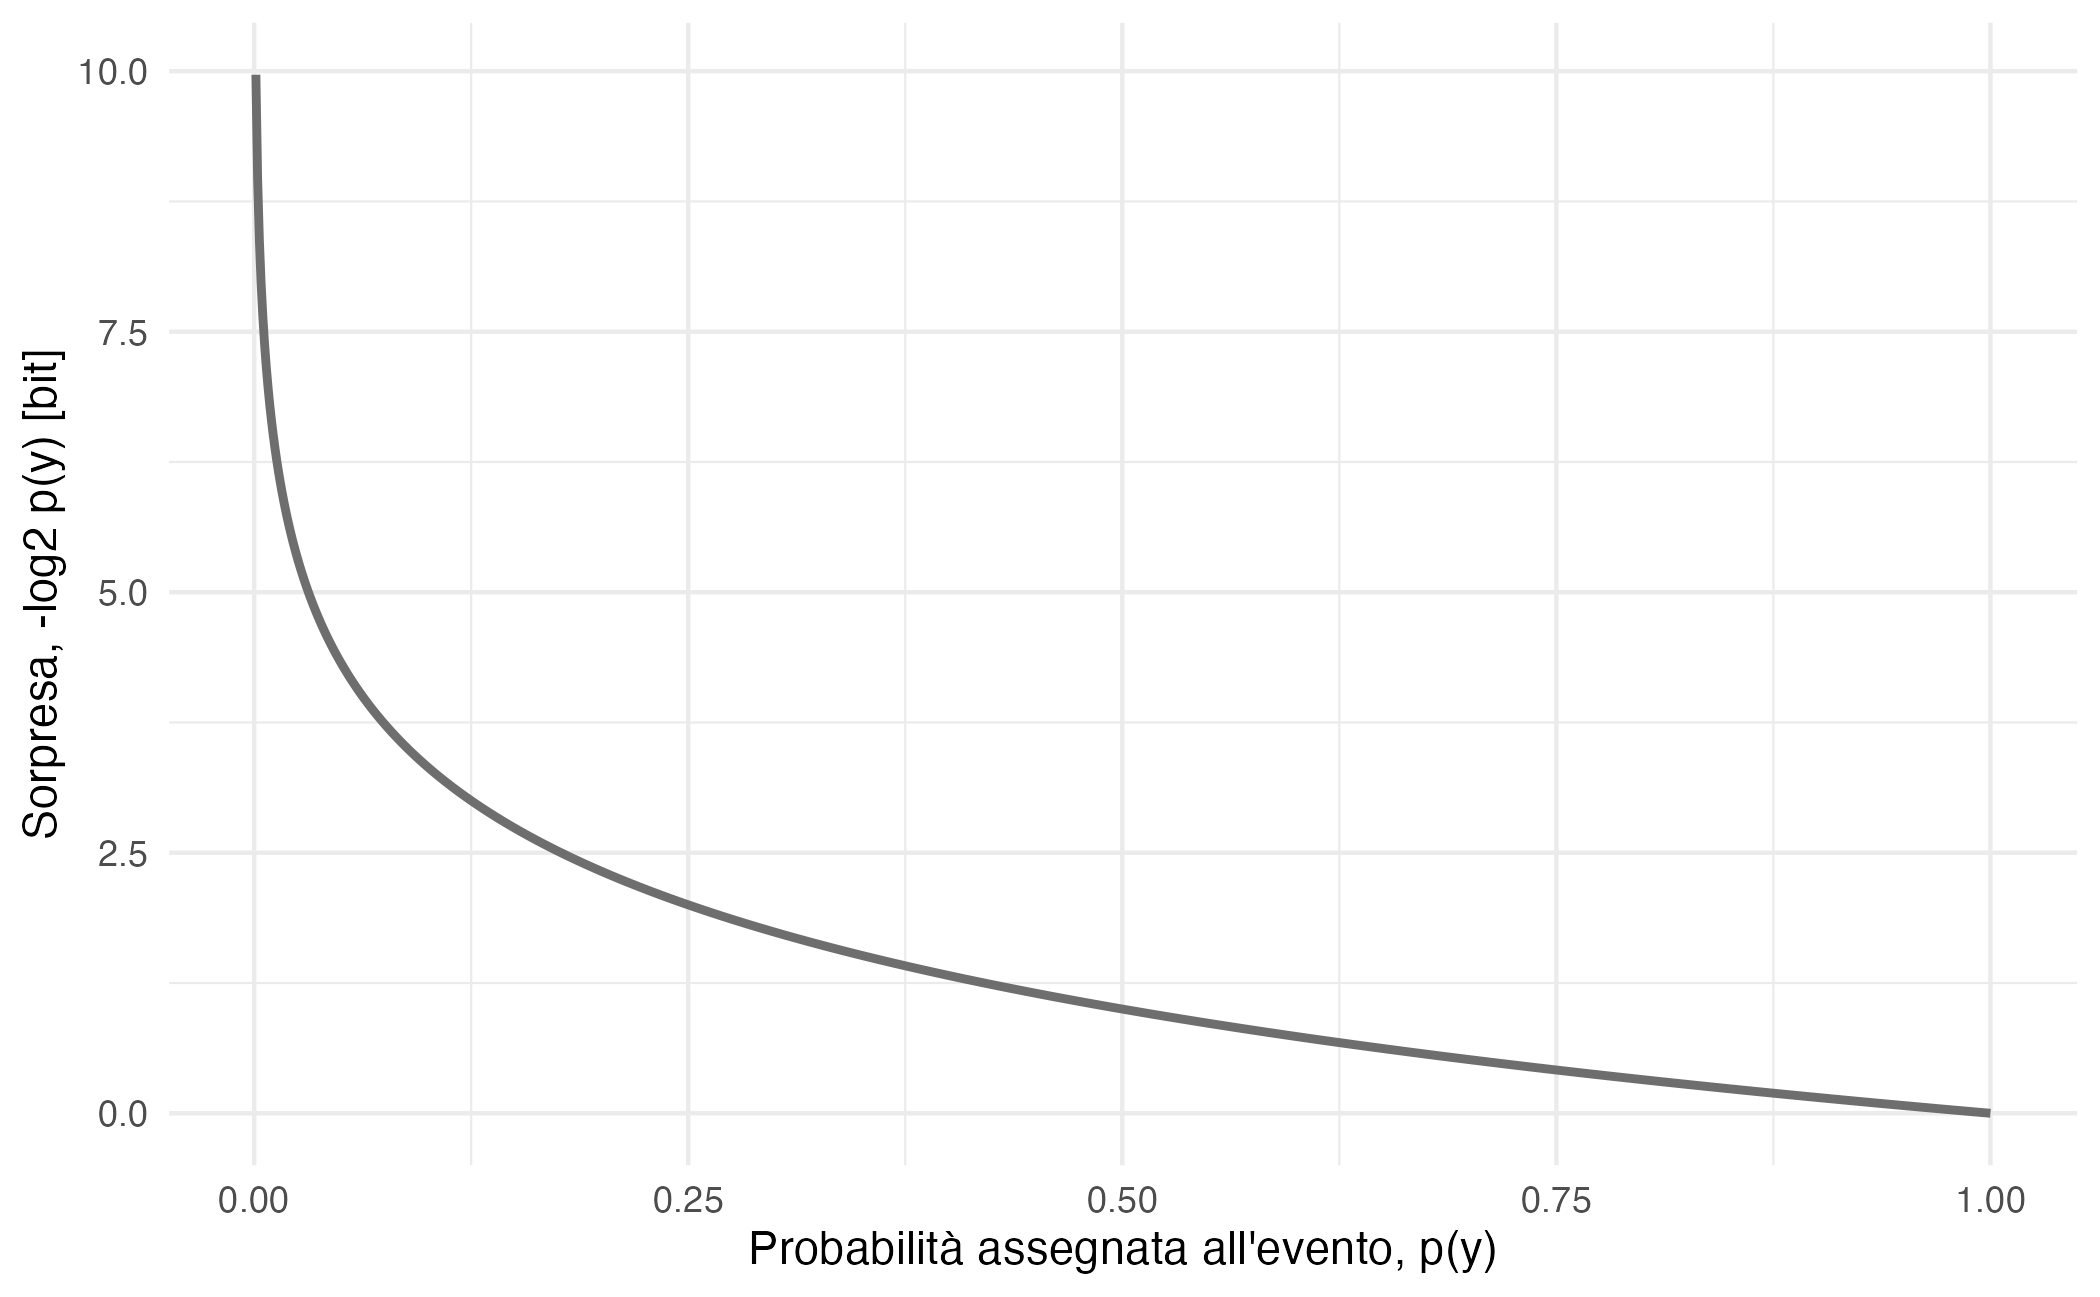
\includegraphics[width=0.85\linewidth,height=\textheight,keepaspectratio]{chapters/entropy/01_entropy_files/figure-pdf/fig-prob-surprise-revised-1.png}

}

\caption{\label{fig-prob-surprise-revised}La sorpresa cresce rapidamente
quando la probabilità assegnata all'evento diminuisce.}

\end{figure}%

Questa formula è importante perché trasforma una valutazione intuitiva
in una quantità misurabile. Se un modello assegna una probabilità molto
bassa a un dato che poi si osserva, quel dato produce molta sorpresa; in
termini predittivi, il modello ha fatto una previsione scadente.

\begin{tcolorbox}[enhanced jigsaw, arc=.35mm, bottomrule=.15mm, bottomtitle=1mm, breakable, colback=white, colbacktitle=quarto-callout-note-color!10!white, colframe=quarto-callout-note-color-frame, coltitle=black, left=2mm, leftrule=.75mm, opacityback=0, opacitybacktitle=0.6, rightrule=.15mm, title=\textcolor{quarto-callout-note-color}{\faInfo}\hspace{0.5em}{Perché il logaritmo?}, titlerule=0mm, toprule=.15mm, toptitle=1mm]

Il logaritmo rende additiva l'informazione di eventi indipendenti. Se
due eventi indipendenti hanno probabilità \(p(a)\) e \(p(b)\), la
probabilità congiunta è \(p(a,b)=p(a)p(b)\). La sorpresa congiunta
diventa

\[
-\log p(a,b) = -\log[p(a)p(b)] = -\log p(a) - \log p(b).
\]

La sorpresa totale di due osservazioni indipendenti è quindi la somma
delle sorprese delle singole osservazioni --- proprietà che sarà
cruciale quando sommeremo i contributi predittivi delle singole
osservazioni nell'ELPD.

\end{tcolorbox}

\section{Dalla sorpresa all'entropia}\label{dalla-sorpresa-allentropia}

La sorpresa riguarda un singolo evento osservato; l'\textbf{entropia},
invece, si riferisce all'intera distribuzione. Prima di osservare il
dato, non sappiamo quale evento si verificherà, ma possiamo calcolare la
sorpresa attesa media, ponderando ciascun evento per la sua probabilità.

Per una variabile discreta \(Y\) con possibili valori
\(y \in \mathcal{Y}\) e probabilità \(p(y)\), l'entropia è

\begin{equation}\protect\phantomsection\label{eq-entropy-def-revised}{
H(Y) = \mathbb{E}_p[-\log_2 p(Y)]
     = -\sum_{y \in \mathcal{Y}} p(y)\log_2 p(y).
}\end{equation}

L'entropia è quindi la \textbf{sorpresa media attesa}. Una distribuzione
uniforme ha entropia elevata, perché nessun esito è più prevedibile
degli altri; una distribuzione concentrata su pochi esiti ha entropia
bassa, perché l'osservazione tende a confermare quanto atteso.

{\def\LTcaptype{none} % do not increment counter
\begin{longtable}[]{@{}
  >{\raggedright\arraybackslash}p{(\linewidth - 4\tabcolsep) * \real{0.3000}}
  >{\raggedleft\arraybackslash}p{(\linewidth - 4\tabcolsep) * \real{0.4000}}
  >{\raggedright\arraybackslash}p{(\linewidth - 4\tabcolsep) * \real{0.3000}}@{}}
\toprule\noalign{}
\begin{minipage}[b]{\linewidth}\raggedright
Quantità
\end{minipage} & \begin{minipage}[b]{\linewidth}\raggedleft
Formula
\end{minipage} & \begin{minipage}[b]{\linewidth}\raggedright
Interpretazione
\end{minipage} \\
\midrule\noalign{}
\endhead
\bottomrule\noalign{}
\endlastfoot
Sorpresa di un evento & \(-\log_2 p(y)\) & Quanto era inatteso l'evento
osservato? \\
Entropia & \(\mathbb{E}_p[-\log_2 p(Y)]\) & Quanta sorpresa ci
aspettiamo in media? \\
Alternative equivalenti & \(2^{H(Y)}\) & A quante alternative
equiprobabili corrisponde la stessa incertezza? \\
\end{longtable}
}

\subsection{Un esempio: risposta a una domanda a scelta
multipla}\label{un-esempio-risposta-a-una-domanda-a-scelta-multipla}

Supponiamo che uno studente risponda a una domanda con quattro
alternative: A, B, C e D. Consideriamo tre possibili distribuzioni
predittive.

\begin{enumerate}
\def\labelenumi{\arabic{enumi}.}
\tightlist
\item
  \textbf{Massima incertezza}: lo studente sceglie a caso, quindi ogni
  risposta ha probabilità \(0.25\).
\item
  \textbf{Preparazione moderata}: la risposta corretta ha probabilità
  \(0.55\) e le altre si dividono il resto.
\item
  \textbf{Preparazione elevata}: la risposta corretta ha probabilità
  \(0.90\).
\end{enumerate}

\begin{Shaded}
\begin{Highlighting}[]
\NormalTok{p\_random }\OtherTok{\textless{}{-}} \FunctionTok{c}\NormalTok{(}\AttributeTok{A =}\NormalTok{ .}\DecValTok{25}\NormalTok{, }\AttributeTok{B =}\NormalTok{ .}\DecValTok{25}\NormalTok{, }\AttributeTok{C =}\NormalTok{ .}\DecValTok{25}\NormalTok{, }\AttributeTok{D =}\NormalTok{ .}\DecValTok{25}\NormalTok{)}
\NormalTok{p\_moderate }\OtherTok{\textless{}{-}} \FunctionTok{c}\NormalTok{(}\AttributeTok{A =}\NormalTok{ .}\DecValTok{55}\NormalTok{, }\AttributeTok{B =}\NormalTok{ .}\DecValTok{15}\NormalTok{, }\AttributeTok{C =}\NormalTok{ .}\DecValTok{15}\NormalTok{, }\AttributeTok{D =}\NormalTok{ .}\DecValTok{15}\NormalTok{)}
\NormalTok{p\_prepared }\OtherTok{\textless{}{-}} \FunctionTok{c}\NormalTok{(}\AttributeTok{A =}\NormalTok{ .}\DecValTok{90}\NormalTok{, }\AttributeTok{B =}\NormalTok{ .}\DecValTok{04}\NormalTok{, }\AttributeTok{C =}\NormalTok{ .}\DecValTok{03}\NormalTok{, }\AttributeTok{D =}\NormalTok{ .}\DecValTok{03}\NormalTok{)}

\NormalTok{entropy\_table }\OtherTok{\textless{}{-}} \FunctionTok{data.frame}\NormalTok{(}
  \AttributeTok{scenario =} \FunctionTok{c}\NormalTok{(}\StringTok{"Scelta casuale"}\NormalTok{, }\StringTok{"Preparazione moderata"}\NormalTok{, }\StringTok{"Preparazione elevata"}\NormalTok{),}
  \AttributeTok{entropy\_bits =} \FunctionTok{c}\NormalTok{(}
    \FunctionTok{entropy\_discrete}\NormalTok{(p\_random),}
    \FunctionTok{entropy\_discrete}\NormalTok{(p\_moderate),}
    \FunctionTok{entropy\_discrete}\NormalTok{(p\_prepared)}
\NormalTok{  )}
\NormalTok{)}

\NormalTok{entropy\_table}\SpecialCharTok{$}\NormalTok{equivalent\_options }\OtherTok{\textless{}{-}} \DecValTok{2}\SpecialCharTok{\^{}}\NormalTok{entropy\_table}\SpecialCharTok{$}\NormalTok{entropy\_bits}
\NormalTok{entropy\_table}\SpecialCharTok{$}\NormalTok{entropy\_bits }\OtherTok{\textless{}{-}} \FunctionTok{round}\NormalTok{(entropy\_table}\SpecialCharTok{$}\NormalTok{entropy\_bits, }\DecValTok{3}\NormalTok{)}
\NormalTok{entropy\_table}\SpecialCharTok{$}\NormalTok{equivalent\_options }\OtherTok{\textless{}{-}} \FunctionTok{round}\NormalTok{(entropy\_table}\SpecialCharTok{$}\NormalTok{equivalent\_options, }\DecValTok{3}\NormalTok{)}
\NormalTok{entropy\_table}
\CommentTok{\#\textgreater{}                scenario entropy\_bits equivalent\_options}
\CommentTok{\#\textgreater{} 1        Scelta casuale        2.000               4.00}
\CommentTok{\#\textgreater{} 2 Preparazione moderata        1.706               3.26}
\CommentTok{\#\textgreater{} 3  Preparazione elevata        0.626               1.54}
\end{Highlighting}
\end{Shaded}

Nel primo caso l'entropia è pari a \(\log_2 4 = 2\) bit: l'incertezza
equivale a scegliere tra quattro alternative equiprobabili. Nel terzo
caso l'entropia è molto più bassa: la distribuzione è concentrata sulla
risposta corretta, quindi l'osservazione attesa produce poca sorpresa.

\begin{Shaded}
\begin{Highlighting}[]
\NormalTok{df\_mcq }\OtherTok{\textless{}{-}} \FunctionTok{rbind}\NormalTok{(}
  \FunctionTok{data.frame}\NormalTok{(}\AttributeTok{scenario =} \StringTok{"Scelta casuale"}\NormalTok{, }\AttributeTok{risposta =} \FunctionTok{names}\NormalTok{(p\_random), }\AttributeTok{p =} \FunctionTok{as.numeric}\NormalTok{(p\_random)),}
  \FunctionTok{data.frame}\NormalTok{(}\AttributeTok{scenario =} \StringTok{"Preparazione moderata"}\NormalTok{, }\AttributeTok{risposta =} \FunctionTok{names}\NormalTok{(p\_moderate), }\AttributeTok{p =} \FunctionTok{as.numeric}\NormalTok{(p\_moderate)),}
  \FunctionTok{data.frame}\NormalTok{(}\AttributeTok{scenario =} \StringTok{"Preparazione elevata"}\NormalTok{, }\AttributeTok{risposta =} \FunctionTok{names}\NormalTok{(p\_prepared), }\AttributeTok{p =} \FunctionTok{as.numeric}\NormalTok{(p\_prepared))}
\NormalTok{)}

\FunctionTok{ggplot}\NormalTok{(df\_mcq, }\FunctionTok{aes}\NormalTok{(}\AttributeTok{x =}\NormalTok{ risposta, }\AttributeTok{y =}\NormalTok{ p)) }\SpecialCharTok{+}
  \FunctionTok{geom\_col}\NormalTok{() }\SpecialCharTok{+}
  \FunctionTok{facet\_wrap}\NormalTok{(}\SpecialCharTok{\textasciitilde{}}\NormalTok{ scenario) }\SpecialCharTok{+}
  \FunctionTok{labs}\NormalTok{(}\AttributeTok{x =} \StringTok{"Risposta"}\NormalTok{, }\AttributeTok{y =} \StringTok{"Probabilità predittiva"}\NormalTok{) }\SpecialCharTok{+}
  \FunctionTok{theme\_minimal}\NormalTok{()}
\end{Highlighting}
\end{Shaded}

\begin{figure}[H]

\centering{

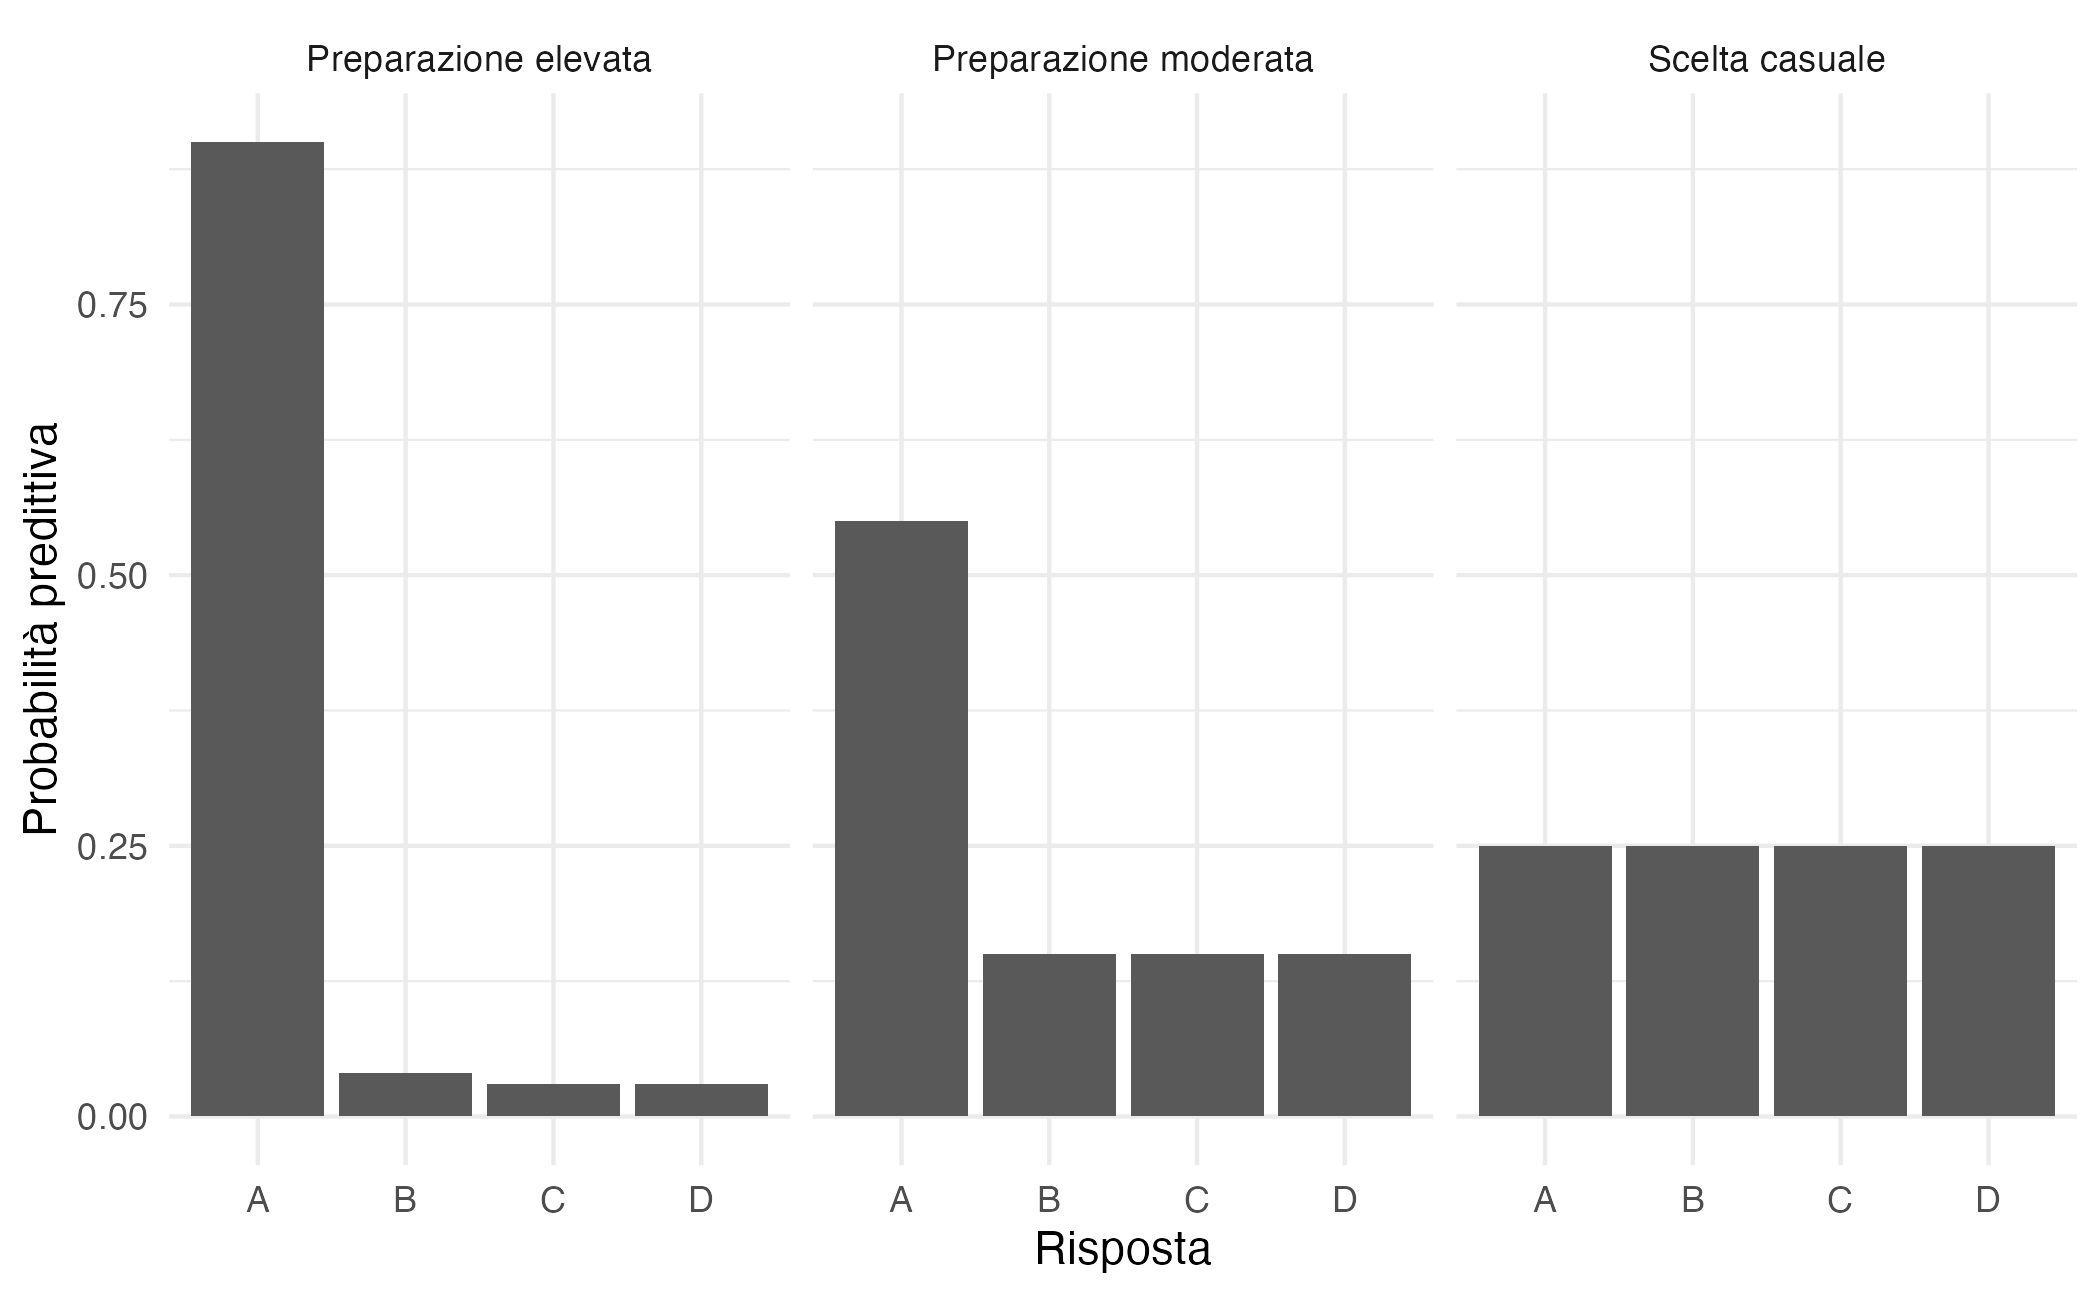
\includegraphics[width=0.85\linewidth,height=\textheight,keepaspectratio]{chapters/entropy/01_entropy_files/figure-pdf/fig-entropy-mcq-1.png}

}

\caption{\label{fig-entropy-mcq}Tre distribuzioni predittive con livelli
diversi di entropia.}

\end{figure}%

Questo esempio chiarisce un punto importante: l'entropia non misura se
la previsione è ``vera'' o ``falsa''. Misura quanto la distribuzione
predittiva sia dispersa. La qualità della previsione emergerà solo
quando la confronteremo con i dati osservati.

\section{Il ponte verso il confronto tra modelli: il
log-score}\label{il-ponte-verso-il-confronto-tra-modelli-il-log-score}

Finora abbiamo usato la base 2 e parlato di bit. Nel confronto tra
modelli statistici si usa spesso il logaritmo naturale; l'unità di
misura diventa il \textbf{nat}, ma il significato non cambia: un dato è
tanto più sorprendente quanto minore è la probabilità che il modello gli
assegna.

Il \textbf{log-score} di un modello \(M\) per un'osservazione \(y\) è

\[
\log p_M(y).
\]

La sorpresa a essa corrispondente è

\[
-\log p_M(y).
\]

Massimizzare il log-score equivale quindi a minimizzare la sorpresa.
Questo è il passaggio concettuale che collega l'entropia all'ELPD.
Quando valuteremo un modello con LOO, sommeremo contributi del tipo

\[
\log p(y_i \mid y_{-i}),
\]

dove \(y_i\) è un'osservazione lasciata fuori e \(y_{-i}\) indica i dati
usati per stimare il modello. In altre parole, chiederemo:
\textbf{quanta probabilità il modello assegna a un dato che non ha usato
per adattarsi?}

\begin{tcolorbox}[enhanced jigsaw, arc=.35mm, bottomrule=.15mm, bottomtitle=1mm, breakable, colback=white, colbacktitle=quarto-callout-important-color!10!white, colframe=quarto-callout-important-color-frame, coltitle=black, left=2mm, leftrule=.75mm, opacityback=0, opacitybacktitle=0.6, rightrule=.15mm, title=\textcolor{quarto-callout-important-color}{\faExclamation}\hspace{0.5em}{Idea chiave}, titlerule=0mm, toprule=.15mm, toptitle=1mm]

L'entropia misura la sorpresa media attesa sotto una distribuzione. Il
confronto predittivo tra modelli usa la stessa logica applicata ai dati
osservati: un buon modello è quello che assegna un'alta probabilità ai
dati nuovi, ovvero che produce poca sorpresa fuori campione.

\end{tcolorbox}

\section{Stimare l'entropia dai dati}\label{stimare-lentropia-dai-dati}

L'entropia è una proprietà di una distribuzione di probabilità; nella
pratica empirica, però, la distribuzione generatrice dei dati non è
nota. Possiamo allora stimare l'entropia usando le frequenze osservate:

\[
\hat p(y) = \frac{n_y}{n},
\]

dove \(n_y\) è il numero di osservazioni nella categoria \(y\) e \(n\) è
la dimensione del campione. La stima plug-in dell'entropia è

\[
\widehat H(Y) = -\sum_y \hat p(y)\log_2 \hat p(y).
\]

\begin{Shaded}
\begin{Highlighting}[]
\NormalTok{x }\OtherTok{\textless{}{-}} \FunctionTok{c}\NormalTok{(}\DecValTok{1}\NormalTok{, }\DecValTok{2}\NormalTok{, }\DecValTok{3}\NormalTok{, }\DecValTok{3}\NormalTok{, }\DecValTok{3}\NormalTok{, }\DecValTok{3}\NormalTok{, }\DecValTok{2}\NormalTok{, }\DecValTok{1}\NormalTok{, }\DecValTok{3}\NormalTok{, }\DecValTok{3}\NormalTok{, }\DecValTok{2}\NormalTok{, }\DecValTok{1}\NormalTok{, }\DecValTok{1}\NormalTok{, }\DecValTok{4}\NormalTok{, }\DecValTok{4}\NormalTok{, }\DecValTok{3}\NormalTok{, }\DecValTok{1}\NormalTok{, }\DecValTok{2}\NormalTok{)}

\NormalTok{tab\_x }\OtherTok{\textless{}{-}} \FunctionTok{table}\NormalTok{(x)}
\NormalTok{p\_hat }\OtherTok{\textless{}{-}} \FunctionTok{as.numeric}\NormalTok{(tab\_x) }\SpecialCharTok{/} \FunctionTok{length}\NormalTok{(x)}

\NormalTok{df\_entropy\_hat }\OtherTok{\textless{}{-}} \FunctionTok{data.frame}\NormalTok{(}
  \AttributeTok{categoria =} \FunctionTok{names}\NormalTok{(tab\_x),}
  \AttributeTok{frequenza =} \FunctionTok{as.numeric}\NormalTok{(tab\_x),}
  \AttributeTok{p\_hat =} \FunctionTok{round}\NormalTok{(p\_hat, }\DecValTok{3}\NormalTok{)}
\NormalTok{)}
\NormalTok{df\_entropy\_hat}
\CommentTok{\#\textgreater{}   categoria frequenza p\_hat}
\CommentTok{\#\textgreater{} 1         1         5 0.278}
\CommentTok{\#\textgreater{} 2         2         4 0.222}
\CommentTok{\#\textgreater{} 3         3         7 0.389}
\CommentTok{\#\textgreater{} 4         4         2 0.111}

\FunctionTok{entropy\_discrete}\NormalTok{(p\_hat)}
\CommentTok{\#\textgreater{} [1] 1.88}
\end{Highlighting}
\end{Shaded}

Questa stima è utile, ma va interpretata con cautela: con campioni
piccoli o con molte categorie rare, alcune possibilità potrebbero non
essere presenti nel campione, e la distribuzione empirica tende a
sottostimare l'incertezza reale. Questo problema anticipa una difficoltà
generale della valutazione dei modelli: non basta misurare il loro
adattamento ai dati osservati, perché un modello può sembrare eccellente
sul campione disponibile e generalizzare male.

\begin{tcolorbox}[enhanced jigsaw, arc=.35mm, bottomrule=.15mm, bottomtitle=1mm, breakable, colback=white, colbacktitle=quarto-callout-note-color!10!white, colframe=quarto-callout-note-color-frame, coltitle=black, left=2mm, leftrule=.75mm, opacityback=0, opacitybacktitle=0.6, rightrule=.15mm, title=\textcolor{quarto-callout-note-color}{\faInfo}\hspace{0.5em}{Stima plug-in e overfitting}, titlerule=0mm, toprule=.15mm, toptitle=1mm]

La stima plug-in tratta le frequenze osservate come se fossero le
probabilità vere. Questo metodo può funzionare bene quando si dispone di
molti dati e poche categorie, ma diventa fragile quando il campione è
piccolo: le categorie non osservate ricevono probabilità zero, anche se
potrebbero verificarsi in futuro.

Il parallelo con il confronto tra modelli è immediato: un modello molto
flessibile può assegnare un'alta probabilità ai dati osservati perché li
descrive in modo troppo dettagliato. Per questo motivo, nei prossimi
capitoli valuteremo la capacità predittiva su dati non ancora osservati
o lasciati fuori.

\end{tcolorbox}

\section{Variabili continue: una cautela
necessaria}\label{variabili-continue-una-cautela-necessaria}

Per le variabili continue si definisce l'\textbf{entropia
differenziale}:

\begin{equation}\protect\phantomsection\label{eq-differential-entropy-revised}{
H(Y) = -\int p(y)\log_2 p(y)\,dy.
}\end{equation}

La forma ricorda quella discreta, ma la sua interpretazione richiede
maggiore cautela. L'entropia differenziale può assumere valori negativi
e dipende dall'unità di misura della variabile; per questo motivo, il
suo valore assoluto non può essere interpretato come una misura di
incertezza nel senso discreto.

Ciò che rimane ben definito e utile soprattutto per il confronto tra
modelli sono le \textbf{differenze} e le quantità relative: entropia
incrociata, divergenza KL e log-density predittiva. Per una
distribuzione normale, ad esempio, l'entropia differenziale aumenta con
la deviazione standard:

\[
H(\mathcal{N}(\mu,\sigma^2))
= \frac{1}{2}\log_2(2\pi e\sigma^2).
\]

\begin{Shaded}
\begin{Highlighting}[]
\NormalTok{h\_norm\_bits }\OtherTok{\textless{}{-}} \ControlFlowTok{function}\NormalTok{(sigma) }\FloatTok{0.5} \SpecialCharTok{*} \FunctionTok{log2}\NormalTok{(}\DecValTok{2} \SpecialCharTok{*}\NormalTok{ pi }\SpecialCharTok{*} \FunctionTok{exp}\NormalTok{(}\DecValTok{1}\NormalTok{) }\SpecialCharTok{*}\NormalTok{ sigma}\SpecialCharTok{\^{}}\DecValTok{2}\NormalTok{)}

\NormalTok{sigmas }\OtherTok{\textless{}{-}} \FunctionTok{c}\NormalTok{(}\FloatTok{0.5}\NormalTok{, }\DecValTok{1}\NormalTok{, }\DecValTok{2}\NormalTok{)}
\NormalTok{x\_grid }\OtherTok{\textless{}{-}} \FunctionTok{seq}\NormalTok{(}\SpecialCharTok{{-}}\DecValTok{6}\NormalTok{, }\DecValTok{6}\NormalTok{, }\AttributeTok{length.out =} \DecValTok{1000}\NormalTok{)}
\NormalTok{df\_norm }\OtherTok{\textless{}{-}} \FunctionTok{data.frame}\NormalTok{(}
  \AttributeTok{x =} \FunctionTok{rep}\NormalTok{(x\_grid, }\AttributeTok{times =} \FunctionTok{length}\NormalTok{(sigmas)),}
  \AttributeTok{sigma =} \FunctionTok{factor}\NormalTok{(}\FunctionTok{rep}\NormalTok{(sigmas, }\AttributeTok{each =} \FunctionTok{length}\NormalTok{(x\_grid)))}
\NormalTok{)}
\NormalTok{df\_norm}\SpecialCharTok{$}\NormalTok{densita }\OtherTok{\textless{}{-}} \FunctionTok{dnorm}\NormalTok{(df\_norm}\SpecialCharTok{$}\NormalTok{x, }\AttributeTok{sd =} \FunctionTok{as.numeric}\NormalTok{(}\FunctionTok{as.character}\NormalTok{(df\_norm}\SpecialCharTok{$}\NormalTok{sigma)))}

\FunctionTok{ggplot}\NormalTok{(df\_norm, }\FunctionTok{aes}\NormalTok{(}\AttributeTok{x =}\NormalTok{ x, }\AttributeTok{y =}\NormalTok{ densita, }\AttributeTok{linetype =}\NormalTok{ sigma)) }\SpecialCharTok{+}
  \FunctionTok{geom\_line}\NormalTok{(}\AttributeTok{linewidth =} \DecValTok{1}\NormalTok{) }\SpecialCharTok{+}
  \FunctionTok{labs}\NormalTok{(}\AttributeTok{x =} \StringTok{"y"}\NormalTok{, }\AttributeTok{y =} \StringTok{"densità"}\NormalTok{, }\AttributeTok{linetype =} \StringTok{"sigma"}\NormalTok{) }\SpecialCharTok{+}
  \FunctionTok{theme\_minimal}\NormalTok{()}

\FunctionTok{round}\NormalTok{(}\FunctionTok{data.frame}\NormalTok{(}\AttributeTok{sigma =}\NormalTok{ sigmas, }\AttributeTok{entropia\_bit =} \FunctionTok{h\_norm\_bits}\NormalTok{(sigmas)), }\DecValTok{3}\NormalTok{)}
\CommentTok{\#\textgreater{}   sigma entropia\_bit}
\CommentTok{\#\textgreater{} 1   0.5         1.05}
\CommentTok{\#\textgreater{} 2   1.0         2.05}
\CommentTok{\#\textgreater{} 3   2.0         3.05}
\end{Highlighting}
\end{Shaded}

\begin{figure}[H]

\centering{

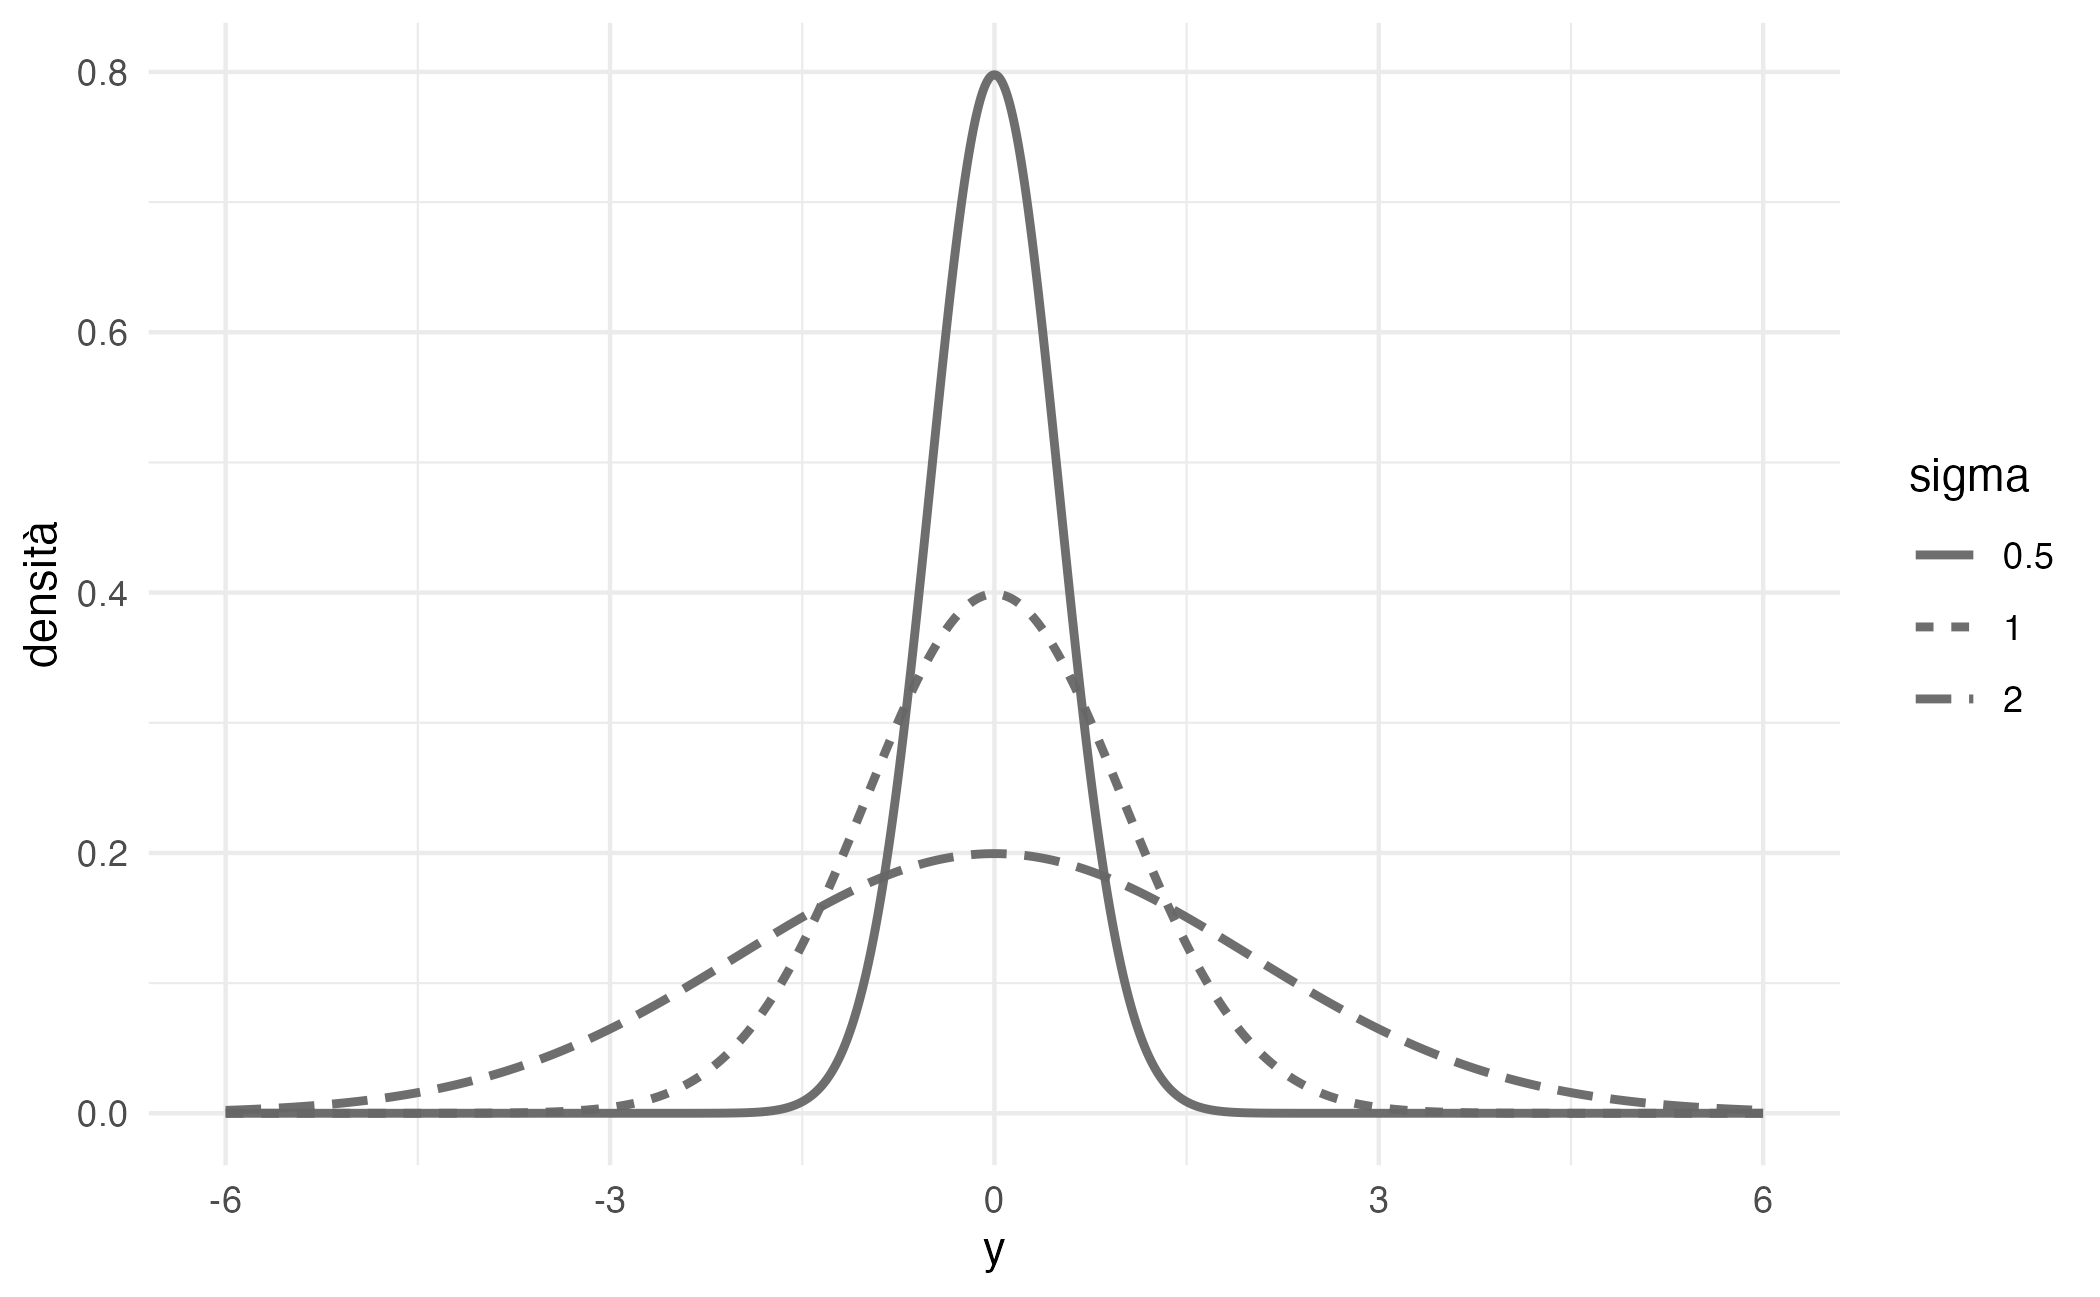
\includegraphics[width=0.85\linewidth,height=\textheight,keepaspectratio]{chapters/entropy/01_entropy_files/figure-pdf/fig-normal-entropy-1.png}

}

\caption{\label{fig-normal-entropy}Distribuzioni normali più disperse
hanno entropia differenziale maggiore, ma il valore assoluto dipende
dalla scala della variabile.}

\end{figure}%

\section{Approfondimento: entropia e codifica
efficiente}\label{approfondimento-entropia-e-codifica-efficiente}

\begin{tcolorbox}[enhanced jigsaw, arc=.35mm, bottomrule=.15mm, bottomtitle=1mm, breakable, colback=white, colbacktitle=quarto-callout-note-color!10!white, colframe=quarto-callout-note-color-frame, coltitle=black, left=2mm, leftrule=.75mm, opacityback=0, opacitybacktitle=0.6, rightrule=.15mm, title=\textcolor{quarto-callout-note-color}{\faInfo}\hspace{0.5em}{Codifica di Huffman e limite di Shannon}, titlerule=0mm, toprule=.15mm, toptitle=1mm]

L'entropia ha anche un'interpretazione operativa nella teoria della
comunicazione: rappresenta il limite inferiore teorico della lunghezza
media di un codice senza perdita. Se una sorgente produce simboli con
distribuzione \(p(y)\), nessun codice binario può descrivere tali
simboli usando in media meno di \(H(Y)\) bit per simbolo.

La codifica di Huffman costruisce un codice prefisso assegnando codici
più brevi ai simboli più frequenti e codici più lunghi a quelli più
rari. Consideriamo, per esempio, la distribuzione

{\def\LTcaptype{none} % do not increment counter
\begin{longtable}[]{@{}lr@{}}
\toprule\noalign{}
Simbolo & Probabilità \\
\midrule\noalign{}
\endhead
\bottomrule\noalign{}
\endlastfoot
A & 0.40 \\
B & 0.30 \\
C & 0.20 \\
D & 0.10 \\
\end{longtable}
}

Un possibile codice di Huffman è:

{\def\LTcaptype{none} % do not increment counter
\begin{longtable}[]{@{}lrr@{}}
\toprule\noalign{}
Simbolo & Codice & Lunghezza \\
\midrule\noalign{}
\endhead
\bottomrule\noalign{}
\endlastfoot
A & \texttt{0} & 1 \\
B & \texttt{10} & 2 \\
C & \texttt{110} & 3 \\
D & \texttt{111} & 3 \\
\end{longtable}
}

La lunghezza media è

\[
L = 0.40\cdot 1 + 0.30\cdot 2 + 0.20\cdot 3 + 0.10\cdot 3 = 1.90
\]

bit per simbolo. L'entropia della distribuzione è

\begin{Shaded}
\begin{Highlighting}[]
\NormalTok{prob\_huffman }\OtherTok{\textless{}{-}} \FunctionTok{c}\NormalTok{(}\AttributeTok{A =}\NormalTok{ .}\DecValTok{4}\NormalTok{, }\AttributeTok{B =}\NormalTok{ .}\DecValTok{3}\NormalTok{, }\AttributeTok{C =}\NormalTok{ .}\DecValTok{2}\NormalTok{, }\AttributeTok{D =}\NormalTok{ .}\DecValTok{1}\NormalTok{)}
\FunctionTok{entropy\_discrete}\NormalTok{(prob\_huffman)}
\CommentTok{\#\textgreater{} [1] 1.85}
\end{Highlighting}
\end{Shaded}

Il codice si avvicina quindi molto al limite teorico. Il punto
concettuale per noi è il seguente: l'uso di una codifica non ottimale
comporta uno spreco di bit. Nel prossimo capitolo, la divergenza KL
generalizzerà questo concetto: utilizzare una distribuzione \(Q\) quando
i dati sono generati da \(P\) comporta uno spreco medio di informazione.

\end{tcolorbox}

\section{Applicazione psicologica: aspettative e risposta
emotiva}\label{applicazione-psicologica-aspettative-e-risposta-emotiva}

L'informazione di Shannon offre un modo semplice per formalizzare il
legame tra aspettative e sorpresa psicologica. Un evento non è
sorprendente di per sé, ma lo è rispetto a una distribuzione di
aspettative. Una promozione inattesa, un feedback negativo improbabile o
un cambiamento improvviso dell'ambiente possono avere un impatto emotivo
maggiore proprio perché violano le attese probabilistiche.

In questa prospettiva, la sorpresa non è solo una metafora: se una
persona assegna probabilità bassa a un evento e quell'evento si
verifica, la quantità

\[
-\log p(\text{evento})
\]

misura quanto l'osservazione contraddiceva le aspettative. Studi
classici sul ruolo delle aspettative nelle risposte affettive, come
Spector (\citeproc{ref-spector1956expectations}{1956}), sono coerenti
con questa intuizione: l'impatto soggettivo di un esito dipende anche da
quanto era atteso.

Naturalmente, la risposta emotiva non dipende solo dalla sorpresa
informazionale: valenza, rilevanza personale, storia individuale e
contesto sociale possono modularla fortemente. L'utilità dell'entropia
non consiste nel ridurre l'emozione a una formula, ma nel rendere
esplicita una componente del problema: la struttura probabilistica delle
aspettative.

\begin{tcolorbox}[enhanced jigsaw, arc=.35mm, bottomrule=.15mm, bottomtitle=1mm, breakable, colback=white, colbacktitle=quarto-callout-tip-color!10!white, colframe=quarto-callout-tip-color-frame, coltitle=black, left=2mm, leftrule=.75mm, opacityback=0, opacitybacktitle=0.6, rightrule=.15mm, title=\textcolor{quarto-callout-tip-color}{\faLightbulb}\hspace{0.5em}{Esempio simulato: sorpresa e variazione dell'umore}, titlerule=0mm, toprule=.15mm, toptitle=1mm]

\begin{Shaded}
\begin{Highlighting}[]
\FunctionTok{set.seed}\NormalTok{(}\DecValTok{123}\NormalTok{)}

\NormalTok{n }\OtherTok{\textless{}{-}} \DecValTok{200}
\NormalTok{p\_event }\OtherTok{\textless{}{-}} \FunctionTok{runif}\NormalTok{(n, }\AttributeTok{min =} \FloatTok{0.05}\NormalTok{, }\AttributeTok{max =} \FloatTok{0.95}\NormalTok{)}
\NormalTok{surprise\_bits }\OtherTok{\textless{}{-}} \SpecialCharTok{{-}}\FunctionTok{log2}\NormalTok{(p\_event)}
\NormalTok{delta\_mood }\OtherTok{\textless{}{-}} \FloatTok{0.45} \SpecialCharTok{*}\NormalTok{ surprise\_bits }\SpecialCharTok{+} \FunctionTok{rnorm}\NormalTok{(n, }\AttributeTok{sd =} \FloatTok{0.5}\NormalTok{)}

\NormalTok{df\_mood }\OtherTok{\textless{}{-}} \FunctionTok{data.frame}\NormalTok{(p\_event, surprise\_bits, delta\_mood)}

\FunctionTok{ggplot}\NormalTok{(df\_mood, }\FunctionTok{aes}\NormalTok{(}\AttributeTok{x =}\NormalTok{ surprise\_bits, }\AttributeTok{y =}\NormalTok{ delta\_mood)) }\SpecialCharTok{+}
  \FunctionTok{geom\_point}\NormalTok{(}\AttributeTok{alpha =} \FloatTok{0.6}\NormalTok{) }\SpecialCharTok{+}
  \FunctionTok{geom\_smooth}\NormalTok{(}\AttributeTok{method =} \StringTok{"lm"}\NormalTok{, }\AttributeTok{se =} \ConstantTok{TRUE}\NormalTok{) }\SpecialCharTok{+}
  \FunctionTok{labs}\NormalTok{(}
    \AttributeTok{x =} \StringTok{"Sorpresa dell\textquotesingle{}evento [bit]"}\NormalTok{,}
    \AttributeTok{y =} \StringTok{"Variazione dell\textquotesingle{}umore"}
\NormalTok{  ) }\SpecialCharTok{+}
  \FunctionTok{theme\_minimal}\NormalTok{()}
\end{Highlighting}
\end{Shaded}

\begin{figure}[H]

\centering{

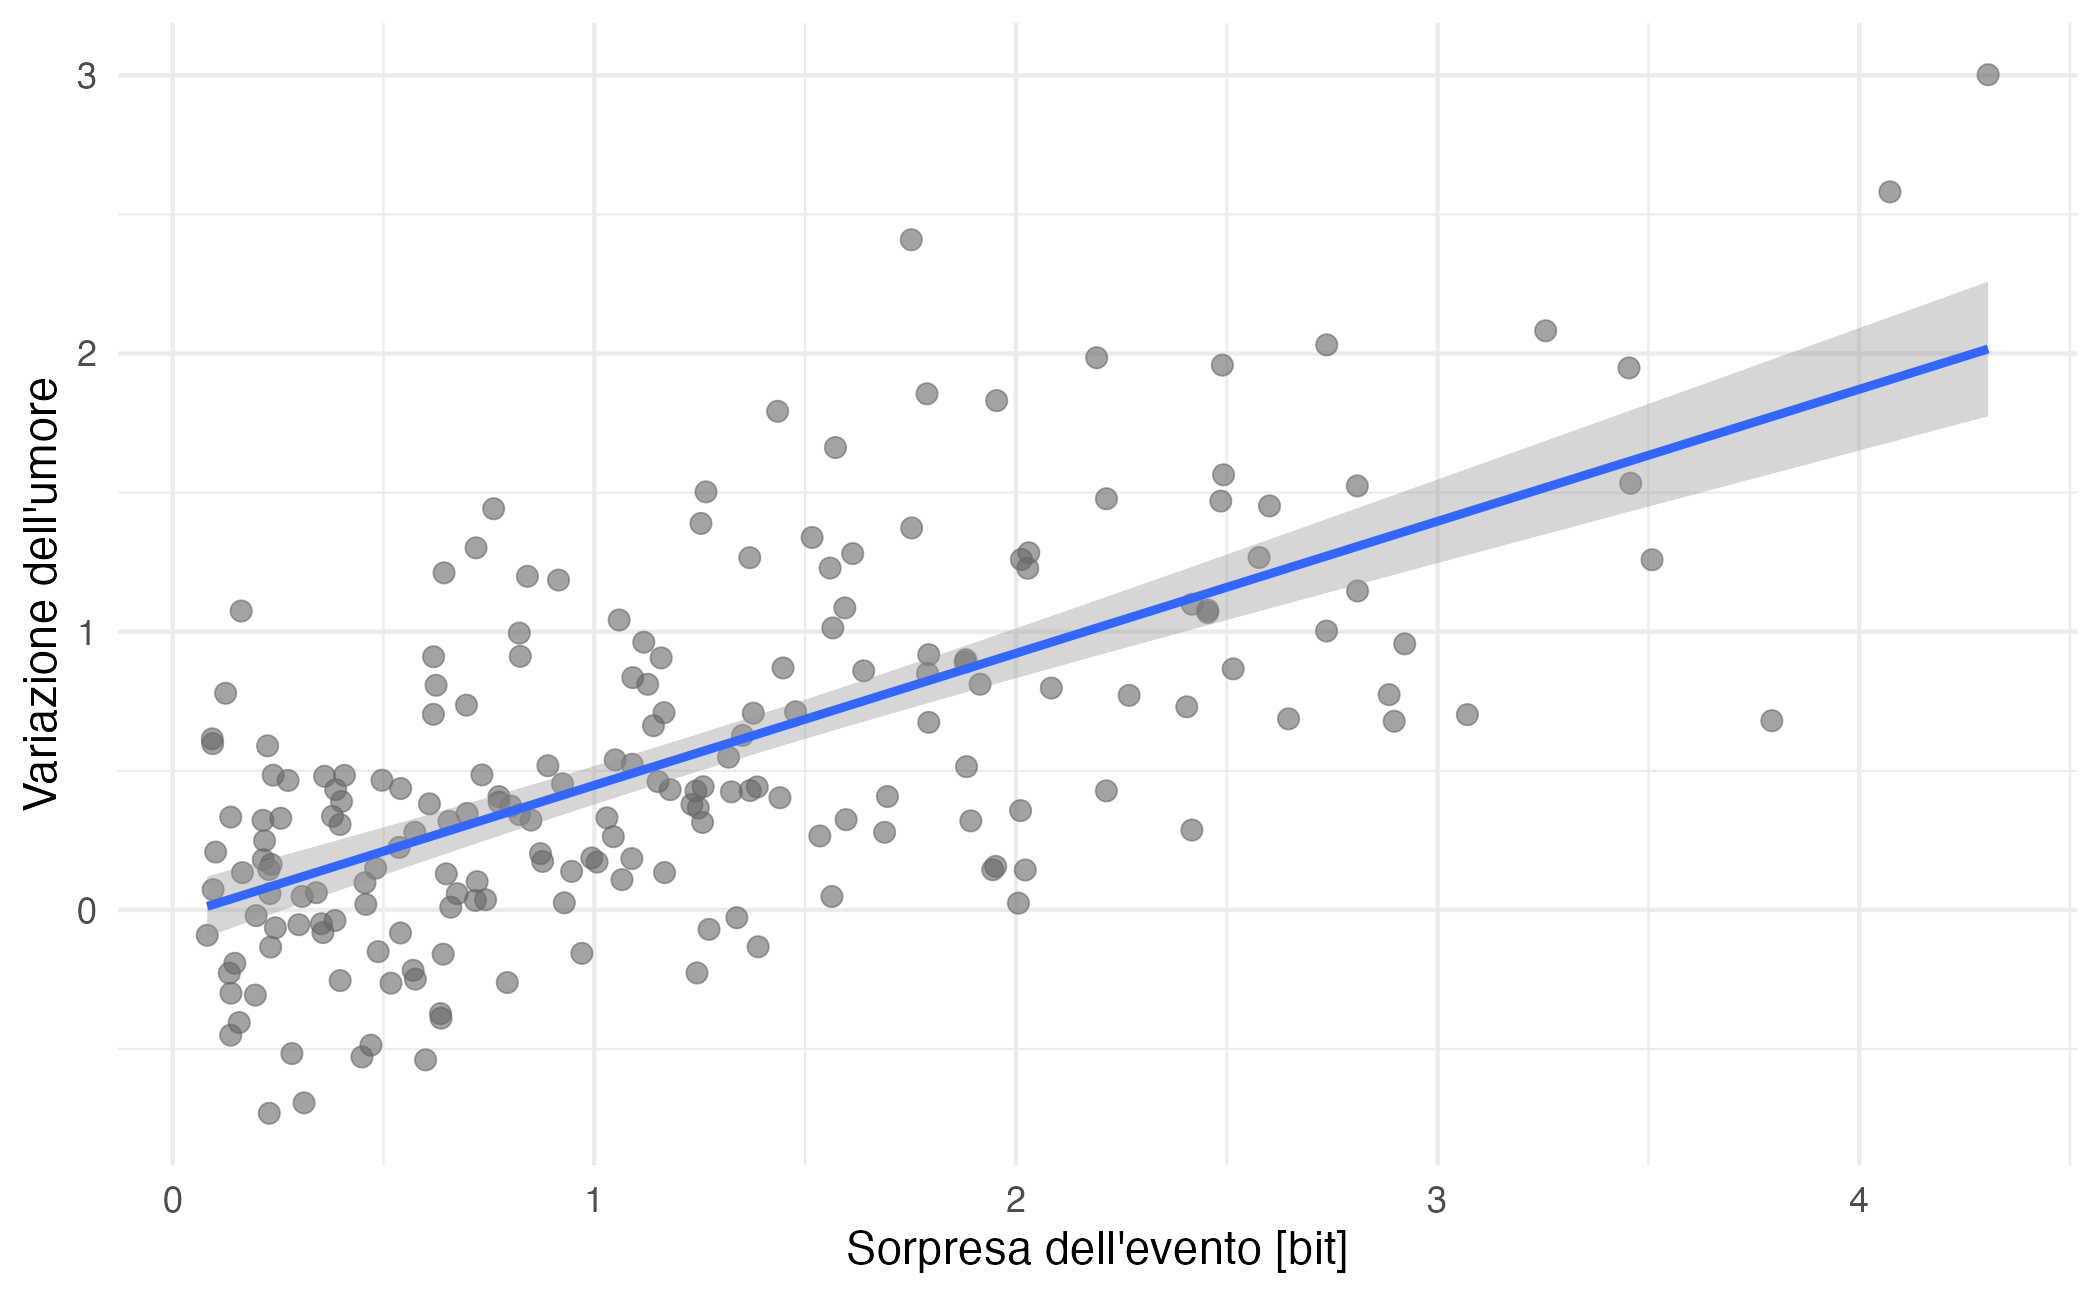
\includegraphics[width=0.85\linewidth,height=\textheight,keepaspectratio]{chapters/entropy/01_entropy_files/figure-pdf/fig-surprise-mood-revised-1.png}

}

\caption{\label{fig-surprise-mood-revised}In questa simulazione, eventi
meno attesi producono variazioni medie più intense dell'umore.}

\end{figure}%

La simulazione non pretende di essere un modello psicologico realistico;
serve solo a illustrare l'idea: se la risposta emotiva è sensibile alla
violazione delle aspettative, allora la sorpresa informazionale può
essere utilizzata come predittore in un modello psicologico.

\end{tcolorbox}

\section*{Riflessioni conclusive}\label{riflessioni-conclusive-40}

\markright{Riflessioni conclusive}

L'entropia ci ha permesso di trasformare un'intuizione qualitativa in
una quantità formale. Affermare che una situazione è incerta significa
aspettarsi, prima ancora di osservare il dato, una certa quantità media
di sorpresa. La formula

\[
H(Y)=\mathbb{E}_p[-\log p(Y)]
\] rende precisa questa idea: l'incertezza di una distribuzione è la
sorpresa media che essa genera.

Il punto cruciale di questa sezione è il legame tra entropia e
previsione. Un modello probabilistico non fornisce solo stime puntuali,
ma assegna anche probabilità agli eventi. Quando osserviamo un dato,
possiamo valutare quanto il modello fosse in grado di prevederlo: questo
è il nucleo del log-score e, più avanti, dell'ELPD.

Il passo successivo sarà confrontare due distribuzioni. Se \(P\)
rappresenta il processo che genera i dati e \(Q\) un modello
approssimato, quanta informazione perdiamo utilizzando \(Q\) al posto di
\(P\)? La risposta è la divergenza di Kullback-Leibler. In questo senso,
l'entropia non è una digressione tecnica, ma il primo gradino di un
ragionamento epistemologico più ampio: valutare i modelli in base alla
loro capacità di ridurre la sorpresa sui dati nuovi.

\begin{tcolorbox}[enhanced jigsaw, arc=.35mm, bottomrule=.15mm, bottomtitle=1mm, breakable, colback=white, colbacktitle=quarto-callout-note-color!10!white, colframe=quarto-callout-note-color-frame, coltitle=black, left=2mm, leftrule=.75mm, opacityback=0, opacitybacktitle=0.6, rightrule=.15mm, title=\textcolor{quarto-callout-note-color}{\faInfo}\hspace{0.5em}{Mappa concettuale: dall'entropia alla valutazione dei modelli}, titlerule=0mm, toprule=.15mm, toptitle=1mm]

\textbf{Entropia}

\begin{itemize}
\tightlist
\item
  misura la sorpresa media attesa sotto una distribuzione;
\item
  formalizza l'incertezza predittiva prima dell'osservazione.
\end{itemize}

\textbf{Divergenza KL}

\begin{itemize}
\tightlist
\item
  misura la sorpresa extra prodotta usando una distribuzione
  approssimata al posto del processo generatore;
\item
  fornisce il criterio ideale di distanza informazionale tra modello e
  realtà.
\end{itemize}

\textbf{ELPD / LOO}

\begin{itemize}
\tightlist
\item
  stima quanto bene un modello assegna probabilità a dati non usati per
  adattarlo;
\item
  traduce l'idea di ridurre la sorpresa in una procedura pratica di
  confronto tra modelli.
\end{itemize}

\textbf{Sintesi:} entropia → sorpresa media; KL → spreco informazionale;
ELPD/LOO → capacità predittiva stimabile.

\end{tcolorbox}

\begin{tcolorbox}[enhanced jigsaw, arc=.35mm, bottomrule=.15mm, bottomtitle=1mm, breakable, colback=white, colbacktitle=quarto-callout-note-color!10!white, colframe=quarto-callout-note-color-frame, coltitle=black, left=2mm, leftrule=.75mm, opacityback=0, opacitybacktitle=0.6, rightrule=.15mm, title=\textcolor{quarto-callout-note-color}{\faInfo}\hspace{0.5em}{Informazioni sull'ambiente di sviluppo}, titlerule=0mm, toprule=.15mm, toptitle=1mm]

\begin{Shaded}
\begin{Highlighting}[]
\FunctionTok{sessionInfo}\NormalTok{()}
\CommentTok{\#\textgreater{} R version 4.6.1 (2026{-}06{-}24)}
\CommentTok{\#\textgreater{} Platform: aarch64{-}apple{-}darwin23}
\CommentTok{\#\textgreater{} Running under: macOS Tahoe 26.5.2}
\CommentTok{\#\textgreater{} }
\CommentTok{\#\textgreater{} Matrix products: default}
\CommentTok{\#\textgreater{} BLAS:   /Library/Frameworks/R.framework/Versions/4.6/Resources/lib/libRblas.0.dylib }
\CommentTok{\#\textgreater{} LAPACK: /Library/Frameworks/R.framework/Versions/4.6/Resources/lib/libRlapack.dylib;  LAPACK version 3.12.1}
\CommentTok{\#\textgreater{} }
\CommentTok{\#\textgreater{} locale:}
\CommentTok{\#\textgreater{} [1] C.UTF{-}8/UTF{-}8/C.UTF{-}8/C/C.UTF{-}8/C.UTF{-}8}
\CommentTok{\#\textgreater{} }
\CommentTok{\#\textgreater{} time zone: Europe/Zagreb}
\CommentTok{\#\textgreater{} tzcode source: internal}
\CommentTok{\#\textgreater{} }
\CommentTok{\#\textgreater{} attached base packages:}
\CommentTok{\#\textgreater{} [1] stats     graphics  grDevices utils     datasets  methods   base     }
\CommentTok{\#\textgreater{} }
\CommentTok{\#\textgreater{} other attached packages:}
\CommentTok{\#\textgreater{}  [1] ragg\_1.5.2            tinytable\_0.17.0      withr\_3.0.3          }
\CommentTok{\#\textgreater{}  [4] systemfonts\_1.3.2     patchwork\_1.3.2       ggdist\_3.3.3         }
\CommentTok{\#\textgreater{}  [7] tidybayes\_3.0.7       bayesplot\_1.15.0      ggplot2\_4.0.3        }
\CommentTok{\#\textgreater{} [10] reliabilitydiag\_0.2.1 priorsense\_1.2.0      posterior\_1.7.0      }
\CommentTok{\#\textgreater{} [13] loo\_2.10.0            rstan\_2.32.7          StanHeaders\_2.32.10  }
\CommentTok{\#\textgreater{} [16] brms\_2.23.0           Rcpp\_1.1.2            sessioninfo\_1.2.4    }
\CommentTok{\#\textgreater{} [19] conflicted\_1.2.0      janitor\_2.2.1         matrixStats\_1.5.0    }
\CommentTok{\#\textgreater{} [22] modelr\_0.1.11         tibble\_3.3.1          dplyr\_1.2.1          }
\CommentTok{\#\textgreater{} [25] tidyr\_1.3.2           rio\_1.3.0             here\_1.0.2           }
\CommentTok{\#\textgreater{} }
\CommentTok{\#\textgreater{} loaded via a namespace (and not attached):}
\CommentTok{\#\textgreater{}  [1] svUnit\_1.0.8          tidyselect\_1.2.1      farver\_2.1.2         }
\CommentTok{\#\textgreater{}  [4] S7\_0.2.2              fastmap\_1.2.0         tensorA\_0.36.2.1     }
\CommentTok{\#\textgreater{}  [7] digest\_0.6.39         timechange\_0.4.0      estimability\_2.0.0   }
\CommentTok{\#\textgreater{} [10] lifecycle\_1.0.5       magrittr\_2.0.5        compiler\_4.6.1       }
\CommentTok{\#\textgreater{} [13] rlang\_1.3.0           tools\_4.6.1           yaml\_2.3.12          }
\CommentTok{\#\textgreater{} [16] knitr\_1.51            labeling\_0.4.3        bridgesampling\_1.2{-}1 }
\CommentTok{\#\textgreater{} [19] pkgbuild\_1.4.8        curl\_7.1.0            RColorBrewer\_1.1{-}3   }
\CommentTok{\#\textgreater{} [22] abind\_1.4{-}8           purrr\_1.2.2           grid\_4.6.1           }
\CommentTok{\#\textgreater{} [25] stats4\_4.6.1          xtable\_1.8{-}8          inline\_0.3.21        }
\CommentTok{\#\textgreater{} [28] emmeans\_2.0.4         scales\_1.4.0          cli\_3.6.6            }
\CommentTok{\#\textgreater{} [31] mvtnorm\_1.4{-}2         rmarkdown\_2.31        generics\_0.1.4       }
\CommentTok{\#\textgreater{} [34] otel\_0.2.0            RcppParallel\_5.1.11{-}2 cachem\_1.1.0         }
\CommentTok{\#\textgreater{} [37] stringr\_1.6.0         splines\_4.6.1         parallel\_4.6.1       }
\CommentTok{\#\textgreater{} [40] vctrs\_0.7.3           V8\_8.2.0              Matrix\_1.7{-}5         }
\CommentTok{\#\textgreater{} [43] jsonlite\_2.0.0        arrayhelpers\_1.1{-}1    glue\_1.8.1           }
\CommentTok{\#\textgreater{} [46] codetools\_0.2{-}20      distributional\_0.8.1  lubridate\_1.9.5      }
\CommentTok{\#\textgreater{} [49] stringi\_1.8.7         gtable\_0.3.6          QuickJSR\_1.10.0      }
\CommentTok{\#\textgreater{} [52] pillar\_1.11.1         htmltools\_0.5.9       Brobdingnag\_1.2{-}9    }
\CommentTok{\#\textgreater{} [55] R6\_2.6.1              textshaping\_1.0.5     rprojroot\_2.1.1      }
\CommentTok{\#\textgreater{} [58] evaluate\_1.0.5        lattice\_0.22{-}9        backports\_1.5.1      }
\CommentTok{\#\textgreater{} [61] memoise\_2.0.1         broom\_1.0.13          snakecase\_0.11.1     }
\CommentTok{\#\textgreater{} [64] rstantools\_2.6.0      coda\_0.19{-}4.1         gridExtra\_2.3.1      }
\CommentTok{\#\textgreater{} [67] nlme\_3.1{-}170          checkmate\_2.3.4       mgcv\_1.9{-}4           }
\CommentTok{\#\textgreater{} [70] xfun\_0.60             pkgconfig\_2.0.3}
\end{Highlighting}
\end{Shaded}

\end{tcolorbox}

\section*{Bibliografia}\label{bibliografia-46}

\markright{Bibliografia}

\chapter{Divergenza KL: il costo informazionale di un
modello}\label{sec-kullback-leibler-divergence}

\begin{tcolorbox}[enhanced jigsaw, arc=.35mm, bottomrule=.15mm, breakable, colback=white, colframe=quarto-callout-note-color-frame, left=2mm, leftrule=.75mm, opacityback=0, rightrule=.15mm, toprule=.15mm]

Nel capitolo precedente abbiamo definito l'entropia come
\textbf{sorpresa attesa} di una distribuzione di probabilità. Facciamo
ora un ulteriore passo avanti: nella pratica empirica, la distribuzione
generativa dei dati, che denoteremo con \(P\), non è mai direttamente
osservabile; ciò che costruiamo sono modelli statistici, ovvero
rappresentazioni parziali e approssimate del fenomeno in esame.

La domanda centrale diviene pertanto:

\begin{quote}
Qual è il costo informazionale atteso che si paga utilizzando un modello
\(Q\) per descrivere osservazioni effettivamente generate da \(P\)?
\end{quote}

La divergenza di Kullback-Leibler (KL) fornisce il quadro formale per
rispondere a questa domanda, quantificando la \textbf{perdita
informativa media}, ovvero l'eccesso di sorpresa causato dall'impiego
della distribuzione approssimante \(Q\) in luogo della vera
distribuzione generatrice \(P.\)

Questo concetto rappresenta il ponte epistemologico tra la teoria
dell'informazione e la selezione predittiva dei modelli: la KL è il
criterio teorico ideale, ma non è direttamente calcolabile in quanto
richiede la conoscenza di \(P\). L'\emph{Expected Log Predictive
Density} (ELPD) e la \emph{Leave-One-Out Cross-Validation} (LOO) -- che
discuteremo nel prossimo capitolo -- ne costituiscono invece la
controparte operativa, fornendo stime empiriche del potere predittivo
atteso su nuovi dati.

\end{tcolorbox}

\begin{tcolorbox}[enhanced jigsaw, arc=.35mm, bottomrule=.15mm, breakable, colback=white, colframe=quarto-callout-important-color-frame, left=2mm, leftrule=.75mm, opacityback=0, rightrule=.15mm, toprule=.15mm]

\textbf{Da sapere.} La divergenza di Kullback--Leibler misura l'eccesso
di sorpresa medio prodotto quando una distribuzione \(Q\) viene usata
per rappresentare dati generati da \(P\). È la differenza tra entropia
incrociata ed entropia di \(P\), è sempre non negativa e non è
simmetrica: \(D_{\mathrm{KL}}(P\parallel Q)\) risponde a una domanda
diversa da \(D_{\mathrm{KL}}(Q\parallel P)\). Poiché il processo vero
\(P\) non è osservabile, la KL costituisce un criterio teorico ideale,
collegato operativamente al log-score atteso, all'ELPD e alla LOO.

\textbf{Da saper fare.} Distinguere entropia, entropia incrociata e
divergenza KL; interpretare \(D_{\mathrm{KL}}(P\parallel Q)\) come costo
informazionale dell'approssimazione; spiegare perché la direzione della
divergenza è importante; confrontare semplici distribuzioni mediante la
KL; mostrare perché minimizzare la KL equivale a massimizzare il
log-score atteso e collegare questo risultato alla valutazione
predittiva dei modelli.

\textbf{Approfondimento facoltativo.} La decomposizione numerica dei
contributi alla KL, la dimostrazione della non negatività mediante la
disuguaglianza di Gibbs, i casi in cui la divergenza diventa infinita e
la conversione tra bit e nat possono essere rimandati. Nel percorso
essenziale è sufficiente comprendere il significato della KL, la sua
asimmetria e il passaggio concettuale dal criterio ideale alla stima
predittiva mediante ELPD e LOO.

\hyperref[sec-percorsi-lettura]{Che cosa significano queste etichette?}

\end{tcolorbox}

\section*{Panoramica del capitolo}\label{panoramica-del-capitolo-8}

\markright{Panoramica del capitolo}

Al termine del capitolo dovresti sapere:

\begin{itemize}
\tightlist
\item
  interpretare l'entropia incrociata come \textbf{sorpresa media
  prodotta da un modello};
\item
  definire la divergenza KL come differenza tra l'entropia incrociata e
  l'entropia vera;
\item
  comprendere perché la KL non è simmetrica e perché questo è importante
  dal punto di vista concettuale;
\item
  spiegare perché minimizzare la KL equivale a massimizzare il log-score
  atteso;
\item
  collegare la KL a ELPD e LOO come strumenti pratici per il confronto
  di modelli bayesiani.
\end{itemize}

\begin{tcolorbox}[enhanced jigsaw, arc=.35mm, bottomrule=.15mm, bottomtitle=1mm, breakable, colback=white, colbacktitle=quarto-callout-tip-color!10!white, colframe=quarto-callout-tip-color-frame, coltitle=black, left=2mm, leftrule=.75mm, opacityback=0, opacitybacktitle=0.6, rightrule=.15mm, title=\textcolor{quarto-callout-tip-color}{\faLightbulb}\hspace{0.5em}{Prerequisiti}, titlerule=0mm, toprule=.15mm, toptitle=1mm]

Sono utili le nozioni introdotte nel capitolo precedente: sorpresa,
entropia e log-score. In particolare, è importante ricordare che un
modello che assegna una bassa probabilità a un dato osservato produce
molta sorpresa, ovvero un valore elevato di \(-\log p(y)\).

\end{tcolorbox}

\begin{tcolorbox}[enhanced jigsaw, arc=.35mm, bottomrule=.15mm, bottomtitle=1mm, breakable, colback=white, colbacktitle=quarto-callout-caution-color!10!white, colframe=quarto-callout-caution-color-frame, coltitle=black, left=2mm, leftrule=.75mm, opacityback=0, opacitybacktitle=0.6, rightrule=.15mm, title=\textcolor{quarto-callout-caution-color}{\faFire}\hspace{0.5em}{Preparazione del notebook}, titlerule=0mm, toprule=.15mm, toptitle=1mm]

\end{tcolorbox}

\section{Il problema: tutti i modelli sono
approssimazioni}\label{il-problema-tutti-i-modelli-sono-approssimazioni}

Un modello statistico non è una copia della realtà, bensì una
rappresentazione selettiva che conserva alcune strutture ritenute
importanti e ne trascura altre --- e questo è inevitabile. In
psicologia, per esempio, un modello dell'ansia, della memoria o della
reattività emotiva non può includere tutte le cause biologiche,
cognitive, contestuali e sociali che concorrono a determinare il
fenomeno.

Ciò non rende i modelli inutili; al contrario, chiarisce quale sia la
domanda scientifica corretta:

\begin{quote}
Dato che nessun modello può essere letteralmente vero in senso assoluto,
quale modello minimizza la perdita informativa attesa rispetto al
processo generatore dei dati?
\end{quote}

Sia \(P\) la distribuzione di probabilità reale, ovvero il meccanismo
generatore non osservabile dei dati, e sia \(Q\) un modello candidato.
La divergenza KL quantifica il costo informazionale atteso -- in termini
di eccesso di sorpresa -- che si paga utilizzando \(Q\) per descrivere
osservazioni generate da \(P\).

Sul piano epistemologico, il confronto tra modelli non va interpretato
come una ricerca del modello ``vero'' (un costrutto spesso
irraggiungibile o mal definito), ma come una valutazione comparativa
della bontà di approssimazione: l'obiettivo è selezionare il modello
che, bilanciando parsimonia strutturale e capacità predittiva, assegni
la massima densità di probabilità alle future osservazioni del fenomeno
in esame.

\section{Dall'entropia all'entropia
incrociata}\label{dallentropia-allentropia-incrociata}

Nel capitolo precedente abbiamo definito l'entropia di una distribuzione
\(P\) come la sorpresa media attesa:

\[
H(P) = \mathbb{E}_{P}[-\log P(Y)].
\]

Nel caso discreto, utilizzando i logaritmi in base 2, questa quantità è

\[
H(P) = -\sum_y p(y)\log_2 p(y).
\]

L'entropia descrive quanto è incerto il processo, se si conosce la
distribuzione vera. Ma nella modellizzazione statistica la situazione è
diversa: i dati sono generati da \(P\), mentre noi li valutiamo
utilizzando un modello \(Q\).

In questo caso la sorpresa media non viene più calcolata utilizzando
\(p(y)\) all'interno del logaritmo, ma \(q(y)\):

\begin{equation}\protect\phantomsection\label{eq-cross-entropy-kl-revised}{
H(P,Q) = \mathbb{E}_{P}[-\log Q(Y)]
       = -\sum_y p(y)\log_2 q(y).
}\end{equation}

Questa quantità si chiama \textbf{entropia incrociata}. La sua struttura
va letta con attenzione:

\begin{itemize}
\tightlist
\item
  \(p(y)\) indica la frequenza con cui gli eventi si verificano nel
  mondo reale;
\item
  \(q(y)\) indica la probabilità assegnata dal modello a quegli eventi;
\item
  \(-\log q(y)\) indica la sorpresa prodotta dal modello quando quegli
  eventi si verificano.
\end{itemize}

Quindi \(H(P,Q)\) risponde alla domanda:

\begin{quote}
Quanta sorpresa produce in media il modello \(Q\), quando i dati sono
generati da \(P\)?
\end{quote}

Se \(Q=P\), il modello utilizza la distribuzione corretta e la sorpresa
media è minima. Se \(Q\) differisce da \(P\), il modello assegna
probabilità non ottimali agli eventi e produce un eccesso di sorpresa.

\begin{Shaded}
\begin{Highlighting}[]
\NormalTok{P }\OtherTok{\textless{}{-}} \FunctionTok{c}\NormalTok{(}\AttributeTok{A =} \FloatTok{0.9}\NormalTok{, }\AttributeTok{B =} \FloatTok{0.1}\NormalTok{)}
\NormalTok{Q\_good }\OtherTok{\textless{}{-}} \FunctionTok{c}\NormalTok{(}\AttributeTok{A =} \FloatTok{0.9}\NormalTok{, }\AttributeTok{B =} \FloatTok{0.1}\NormalTok{)}
\NormalTok{Q\_flat }\OtherTok{\textless{}{-}} \FunctionTok{c}\NormalTok{(}\AttributeTok{A =} \FloatTok{0.5}\NormalTok{, }\AttributeTok{B =} \FloatTok{0.5}\NormalTok{)}

\NormalTok{results\_ce }\OtherTok{\textless{}{-}} \FunctionTok{data.frame}\NormalTok{(}
  \AttributeTok{modello =} \FunctionTok{c}\NormalTok{(}\StringTok{"Q = P"}\NormalTok{, }\StringTok{"Q uniforme"}\NormalTok{),}
  \AttributeTok{entropy\_P =} \FunctionTok{round}\NormalTok{(}\FunctionTok{c}\NormalTok{(}\FunctionTok{entropy\_discrete}\NormalTok{(P), }\FunctionTok{entropy\_discrete}\NormalTok{(P)), }\DecValTok{3}\NormalTok{),}
  \AttributeTok{cross\_entropy =} \FunctionTok{round}\NormalTok{(}\FunctionTok{c}\NormalTok{(}\FunctionTok{cross\_entropy}\NormalTok{(P, Q\_good), }\FunctionTok{cross\_entropy}\NormalTok{(P, Q\_flat)), }\DecValTok{3}\NormalTok{),}
  \AttributeTok{kl =} \FunctionTok{round}\NormalTok{(}\FunctionTok{c}\NormalTok{(}\FunctionTok{kl\_divergence}\NormalTok{(P, Q\_good), }\FunctionTok{kl\_divergence}\NormalTok{(P, Q\_flat)), }\DecValTok{3}\NormalTok{)}
\NormalTok{)}

\NormalTok{results\_ce}
\CommentTok{\#\textgreater{}      modello entropy\_P cross\_entropy    kl}
\CommentTok{\#\textgreater{} 1      Q = P     0.469         0.469 0.000}
\CommentTok{\#\textgreater{} 2 Q uniforme     0.469         1.000 0.531}
\end{Highlighting}
\end{Shaded}

Nel secondo modello gli eventi sono valutati come se fossero
equiprobabili. Ma il processo reale produce quasi sempre A. Il modello
uniforme spreca informazione perché non sfrutta una regolarità
importante del processo generatore.

\section{La divergenza KL}\label{la-divergenza-kl}

La divergenza KL isola precisamente la parte di sorpresa dovuta all'uso
di un modello errato. È definita come la differenza tra l'entropia
incrociata e l'entropia vera:

\begin{equation}\protect\phantomsection\label{eq-kl-as-cross-entropy-minus-entropy}{
D_{\mathrm{KL}}(P \parallel Q) = H(P,Q) - H(P).
}\end{equation}

Sostituendo le definizioni otteniamo la forma più nota:

\begin{equation}\protect\phantomsection\label{eq-kl-definition-revised}{
D_{\mathrm{KL}}(P \parallel Q)
= \sum_y p(y)\log_2\frac{p(y)}{q(y)}.
}\end{equation}

Questa formula ha un'interpretazione concreta:

\begin{quote}
\(D_{\mathrm{KL}}(P \parallel Q)\) è la sorpresa media aggiuntiva che
paghiamo quando usiamo \(Q\) per rappresentare i dati generati da \(P\).
\end{quote}

{\def\LTcaptype{none} % do not increment counter
\begin{longtable}[]{@{}
  >{\raggedright\arraybackslash}p{(\linewidth - 4\tabcolsep) * \real{0.3000}}
  >{\raggedleft\arraybackslash}p{(\linewidth - 4\tabcolsep) * \real{0.4000}}
  >{\raggedright\arraybackslash}p{(\linewidth - 4\tabcolsep) * \real{0.3000}}@{}}
\toprule\noalign{}
\begin{minipage}[b]{\linewidth}\raggedright
Quantità
\end{minipage} & \begin{minipage}[b]{\linewidth}\raggedleft
Formula
\end{minipage} & \begin{minipage}[b]{\linewidth}\raggedright
Interpretazione
\end{minipage} \\
\midrule\noalign{}
\endhead
\bottomrule\noalign{}
\endlastfoot
Entropia vera & \(H(P)=\mathbb{E}_P[-\log P(Y)]\) & Sorpresa minima, se
conoscessimo il processo vero \\
Entropia incrociata & \(H(P,Q)=\mathbb{E}_P[-\log Q(Y)]\) & Sorpresa
prodotta dal modello \(Q\) sui dati generati da \(P\) \\
Divergenza KL & \(D_{\mathrm{KL}}(P\parallel Q)=H(P,Q)-H(P)\) & Sorpresa
extra dovuta all'approssimazione \\
\end{longtable}
}

\begin{tcolorbox}[enhanced jigsaw, arc=.35mm, bottomrule=.15mm, bottomtitle=1mm, breakable, colback=white, colbacktitle=quarto-callout-important-color!10!white, colframe=quarto-callout-important-color-frame, coltitle=black, left=2mm, leftrule=.75mm, opacityback=0, opacitybacktitle=0.6, rightrule=.15mm, title=\textcolor{quarto-callout-important-color}{\faExclamation}\hspace{0.5em}{Idea chiave}, titlerule=0mm, toprule=.15mm, toptitle=1mm]

La KL non misura quanta incertezza c'è nei dati. Misura la quantità di
informazione che perdiamo utilizzando un modello approssimato. Per
questo motivo, è una quantità naturalmente legata alla valutazione dei
modelli.

\end{tcolorbox}

\subsection{Un esempio numerico}\label{un-esempio-numerico-1}

Consideriamo una variabile con tre possibili esiti. Supponiamo che la
distribuzione vera sia

\[
P = [0.50, 0.30, 0.20]
\]

e che un modello proponga

\[
Q = [0.40, 0.40, 0.20].
\]

Il modello sottostima il primo esito, sovrastima il secondo e
rappresenta correttamente il terzo.

\begin{Shaded}
\begin{Highlighting}[]
\NormalTok{P }\OtherTok{\textless{}{-}} \FunctionTok{c}\NormalTok{(}\AttributeTok{A =} \FloatTok{0.50}\NormalTok{, }\AttributeTok{B =} \FloatTok{0.30}\NormalTok{, }\AttributeTok{C =} \FloatTok{0.20}\NormalTok{)}
\NormalTok{Q }\OtherTok{\textless{}{-}} \FunctionTok{c}\NormalTok{(}\AttributeTok{A =} \FloatTok{0.40}\NormalTok{, }\AttributeTok{B =} \FloatTok{0.40}\NormalTok{, }\AttributeTok{C =} \FloatTok{0.20}\NormalTok{)}

\NormalTok{df\_terms }\OtherTok{\textless{}{-}} \FunctionTok{kl\_terms}\NormalTok{(P, Q)}
\NormalTok{df\_terms}\SpecialCharTok{$}\NormalTok{esito }\OtherTok{\textless{}{-}} \FunctionTok{names}\NormalTok{(P)}
\NormalTok{df\_terms}\SpecialCharTok{$}\NormalTok{log\_rapporto }\OtherTok{\textless{}{-}} \FunctionTok{log2}\NormalTok{(df\_terms}\SpecialCharTok{$}\NormalTok{rapporto)}
\NormalTok{df\_terms }\OtherTok{\textless{}{-}}\NormalTok{ df\_terms[, }\FunctionTok{c}\NormalTok{(}\StringTok{"esito"}\NormalTok{, }\StringTok{"p"}\NormalTok{, }\StringTok{"q"}\NormalTok{, }\StringTok{"rapporto"}\NormalTok{, }\StringTok{"log\_rapporto"}\NormalTok{, }\StringTok{"contributo"}\NormalTok{)]}

\NormalTok{df\_terms}
\CommentTok{\#\textgreater{}   esito   p   q rapporto log\_rapporto contributo}
\CommentTok{\#\textgreater{} A     A 0.5 0.4     1.25        0.322      0.161}
\CommentTok{\#\textgreater{} B     B 0.3 0.4     0.75       {-}0.415     {-}0.125}
\CommentTok{\#\textgreater{} C     C 0.2 0.2     1.00        0.000      0.000}

\FunctionTok{cat}\NormalTok{(}\StringTok{"}\SpecialCharTok{\textbackslash{}n}\StringTok{H(P) ="}\NormalTok{, }\FunctionTok{round}\NormalTok{(}\FunctionTok{entropy\_discrete}\NormalTok{(P), }\DecValTok{4}\NormalTok{), }\StringTok{"bit"}\NormalTok{)}
\CommentTok{\#\textgreater{} }
\CommentTok{\#\textgreater{} H(P) = 1.49 bit}
\FunctionTok{cat}\NormalTok{(}\StringTok{"}\SpecialCharTok{\textbackslash{}n}\StringTok{H(P,Q) ="}\NormalTok{, }\FunctionTok{round}\NormalTok{(}\FunctionTok{cross\_entropy}\NormalTok{(P, Q), }\DecValTok{4}\NormalTok{), }\StringTok{"bit"}\NormalTok{)}
\CommentTok{\#\textgreater{} }
\CommentTok{\#\textgreater{} H(P,Q) = 1.52 bit}
\FunctionTok{cat}\NormalTok{(}\StringTok{"}\SpecialCharTok{\textbackslash{}n}\StringTok{D\_KL(P || Q) ="}\NormalTok{, }\FunctionTok{round}\NormalTok{(}\FunctionTok{kl\_divergence}\NormalTok{(P, Q), }\DecValTok{4}\NormalTok{), }\StringTok{"bit}\SpecialCharTok{\textbackslash{}n}\StringTok{"}\NormalTok{)}
\CommentTok{\#\textgreater{} }
\CommentTok{\#\textgreater{} D\_KL(P || Q) = 0.0365 bit}
\end{Highlighting}
\end{Shaded}

I singoli contributi possono essere positivi o negativi. Un contributo
positivo indica che il modello sottostima un evento che si verifica con
una certa frequenza, mentre un contributo negativo indica una sovrastima
locale. Tuttavia, la somma complessiva è sempre non negativa: i risparmi
locali non possono compensare completamente il costo globale
dell'approssimazione.

\begin{tcolorbox}[enhanced jigsaw, arc=.35mm, bottomrule=.15mm, bottomtitle=1mm, breakable, colback=white, colbacktitle=quarto-callout-note-color!10!white, colframe=quarto-callout-note-color-frame, coltitle=black, left=2mm, leftrule=.75mm, opacityback=0, opacitybacktitle=0.6, rightrule=.15mm, title=\textcolor{quarto-callout-note-color}{\faInfo}\hspace{0.5em}{Perché la KL è sempre non negativa?}, titlerule=0mm, toprule=.15mm, toptitle=1mm]

La non negatività della KL è una conseguenza della disuguaglianza di
Gibbs:

\[
D_{\mathrm{KL}}(P \parallel Q) \ge 0,
\]

con uguaglianza se e solo se \(P=Q\) quasi ovunque.

L'interpretazione informazionale è semplice: se conoscessimo davvero
\(P\), potremmo costruire il codice ottimale per gli eventi generati da
\(P\). Qualsiasi codice costruito usando una distribuzione diversa \(Q\)
non può, in media, essere più efficiente del codice ottimale. Può
eguagliarlo solo quando \(Q\) coincide con \(P\).

\end{tcolorbox}

\section{Perché la KL non è una
distanza}\label{perchuxe9-la-kl-non-uxe8-una-distanza}

La divergenza KL viene spesso descritta informalmente come una
``distanza'' tra distribuzioni, ma si tratta solo di una metafora. La KL
non è una distanza matematica, in quanto non è simmetrica:

\[
D_{\mathrm{KL}}(P \parallel Q) \neq D_{\mathrm{KL}}(Q \parallel P).
\]

Questa asimmetria non è un difetto. È il punto concettuale della misura.
Quando scriviamo \(D_{\mathrm{KL}}(P \parallel Q)\) stiamo ponendo una
domanda direzionale:

\begin{quote}
Qual è il costo di usare \(Q\) in un mondo che genera dati secondo
\(P\)?
\end{quote}

Invertire l'ordine significa cambiare la domanda:

\begin{quote}
Qual è il costo di usare \(P\) in un mondo che genera dati secondo
\(Q\)?
\end{quote}

Nella valutazione dei modelli la direzione rilevante è la prima: il
processo vero genera i dati e il modello cerca di approssimarlo.

\begin{Shaded}
\begin{Highlighting}[]
\NormalTok{P }\OtherTok{\textless{}{-}} \FunctionTok{c}\NormalTok{(}\AttributeTok{A =} \FloatTok{0.9}\NormalTok{, }\AttributeTok{B =} \FloatTok{0.1}\NormalTok{)}
\NormalTok{Q }\OtherTok{\textless{}{-}} \FunctionTok{c}\NormalTok{(}\AttributeTok{A =} \FloatTok{0.5}\NormalTok{, }\AttributeTok{B =} \FloatTok{0.5}\NormalTok{)}

\FunctionTok{data.frame}\NormalTok{(}
  \AttributeTok{direzione =} \FunctionTok{c}\NormalTok{(}\StringTok{"D\_KL(P || Q)"}\NormalTok{, }\StringTok{"D\_KL(Q || P)"}\NormalTok{),}
  \AttributeTok{valore\_bit =} \FunctionTok{round}\NormalTok{(}\FunctionTok{c}\NormalTok{(}\FunctionTok{kl\_divergence}\NormalTok{(P, Q), }\FunctionTok{kl\_divergence}\NormalTok{(Q, P)), }\DecValTok{3}\NormalTok{)}
\NormalTok{)}
\CommentTok{\#\textgreater{}      direzione valore\_bit}
\CommentTok{\#\textgreater{} 1 D\_KL(P || Q)      0.531}
\CommentTok{\#\textgreater{} 2 D\_KL(Q || P)      0.737}
\end{Highlighting}
\end{Shaded}

Nel primo caso, il modello \(Q\) sottostima gravemente l'evento A, che
in realtà si verifica spesso. Questo errore si paga quasi sempre. Nel
secondo caso, invece, lo scenario è diverso: il modello \(Q\) ipotetico
produce A e B con la stessa frequenza, mentre il modello \(P\) è troppo
concentrato su A. I due errori non hanno lo stesso costo medio.

\begin{tcolorbox}[enhanced jigsaw, arc=.35mm, bottomrule=.15mm, bottomtitle=1mm, breakable, colback=white, colbacktitle=quarto-callout-note-color!10!white, colframe=quarto-callout-note-color-frame, coltitle=black, left=2mm, leftrule=.75mm, opacityback=0, opacitybacktitle=0.6, rightrule=.15mm, title=\textcolor{quarto-callout-note-color}{\faInfo}\hspace{0.5em}{Casi limite: quando la KL diventa infinita}, titlerule=0mm, toprule=.15mm, toptitle=1mm]

Se un evento ha probabilità positiva sotto \(P\) ma probabilità zero
sotto \(Q\), allora

\[
D_{\mathrm{KL}}(P \parallel Q) = \infty.
\]

Questo risultato è coerente con l'interpretazione predittiva. Se un
modello dichiara impossibile un evento che invece può accadere, quando
quell'evento si verifica la sorpresa è infinita:

\[
-\log 0 = \infty.
\]

In pratica, questa è una ragione per evitare modelli che assegnano
probabilità zero a eventi plausibili. Nei modelli bayesiani, prior
debolmente informative e distribuzioni predittive ben controllate
aiutano a prevenire esclusioni troppo rigide.

\end{tcolorbox}

\begin{tcolorbox}[enhanced jigsaw, arc=.35mm, bottomrule=.15mm, bottomtitle=1mm, breakable, colback=white, colbacktitle=quarto-callout-note-color!10!white, colframe=quarto-callout-note-color-frame, coltitle=black, left=2mm, leftrule=.75mm, opacityback=0, opacitybacktitle=0.6, rightrule=.15mm, title=\textcolor{quarto-callout-note-color}{\faInfo}\hspace{0.5em}{Nota sui logaritmi: bit e nat}, titlerule=0mm, toprule=.15mm, toptitle=1mm]

In questo capitolo usiamo spesso il logaritmo in base 2, quindi la KL è
espressa in \textbf{bit}. Nella statistica bayesiana computazionale, e
in particolare in Stan, \texttt{loo} e \texttt{brms}, si usa quasi
sempre il logaritmo naturale. L'unità di misura è allora il
\textbf{nat}.

La scelta della base cambia solo la scala:

\[
1 \text{ nat} = \log_2(e) \approx 1.443 \text{ bit}.
\]

I confronti tra modelli non cambiano: un modello con KL minore resta
migliore indipendentemente dalla base del logaritmo.

\end{tcolorbox}

\section{KL e confronto tra modelli}\label{kl-e-confronto-tra-modelli}

In linea di principio, se conoscessimo il processo vero \(P\), potremmo
scegliere tra modelli candidati selezionando quello che minimizza la KL:

\[
Q^* = \arg\min_Q D_{\mathrm{KL}}(P \parallel Q).
\]

Questo criterio dice che il miglior modello è quello che spreca meno
informazione rispetto al processo che genera i dati; ma c'è un problema
evidente: \textbf{\(P\) non è nota}. Se conoscessimo già la
distribuzione vera, non avremmo bisogno di fare inferenza. Come può
allora la KL essere utile?

La risposta sta nel decomporre esplicitamente la KL nei suoi due
termini, scrivendola come differenza di valori attesi rispetto a \(P\):

\[
D_{\mathrm{KL}}(P \parallel Q)
= \mathbb{E}_{P}[\log P(Y)] - \mathbb{E}_{P}[\log Q(Y)]
= \underbrace{-H(P)}_{\text{dipende solo da } P} \;-\; \underbrace{\mathbb{E}_{P}[\log Q(Y)]}_{\text{dipende dal modello}}.
\]

I due termini hanno natura diversa. Il primo, \(-H(P)\), dipende
\textbf{soltanto dal processo vero} ed è la sorpresa minima
irriducibile, identica qualunque modello si scelga; il secondo,
\(\mathbb{E}_{P}[\log Q(Y)]\), è l'unica parte che cambia al variare del
modello, ed è il \textbf{log-score atteso} di \(Q\), cioè la
log-probabilità media che il modello assegna ai dati generati da \(P\).

Possiamo quindi riscrivere la relazione in una forma che ne rende
trasparente la conseguenza:

\[
D_{\mathrm{KL}}(P \parallel Q) = \text{costante}(P) \;-\; \mathbb{E}_{P}[\log Q(Y)].
\]

Poiché la costante non dipende dal modello, \textbf{minimizzare la
divergenza KL equivale esattamente a massimizzare il log-score atteso}:

\[
\arg\min_Q D_{\mathrm{KL}}(P \parallel Q) = \arg\max_Q \mathbb{E}_{P}[\log Q(Y)].
\]

Non è un'analogia né un'approssimazione, ma un'identità: il costo
informazionale di usare \(Q\) al posto di \(P\) e la bontà con cui \(Q\)
prevede i dati di \(P\) sono la stessa quantità, vista con segno
opposto, a meno di una costante che riguarda solo il processo vero.

Questo risolve il paradosso di partenza: per \textbf{confrontare} due
modelli \(Q_1\) e \(Q_2\) non serve conoscere \(H(P)\), poiché essendo
identico per entrambi si elide nella differenza,

\[
D_{\mathrm{KL}}(P \parallel Q_1) - D_{\mathrm{KL}}(P \parallel Q_2)
= \mathbb{E}_{P}[\log Q_2(Y)] - \mathbb{E}_{P}[\log Q_1(Y)].
\]

Ciò che resta da stimare è unicamente il log-score atteso di ciascun
modello: quello con log-score più alto è, tra i candidati, quello che
spreca meno informazione (\citeproc{ref-gelman1995bayesian}{Gelman et
al., 2013b}). Nel linguaggio della valutazione predittiva bayesiana,
questa quantità diventerà l'\textbf{Expected Log Predictive Density}.

\begin{tcolorbox}[enhanced jigsaw, arc=.35mm, bottomrule=.15mm, bottomtitle=1mm, breakable, colback=white, colbacktitle=quarto-callout-important-color!10!white, colframe=quarto-callout-important-color-frame, coltitle=black, left=2mm, leftrule=.75mm, opacityback=0, opacitybacktitle=0.6, rightrule=.15mm, title=\textcolor{quarto-callout-important-color}{\faExclamation}\hspace{0.5em}{Dal criterio ideale al criterio operativo}, titlerule=0mm, toprule=.15mm, toptitle=1mm]

La KL indica quale modello sarebbe migliore se potessimo confrontarlo
con il processo vero, e la decomposizione mostra che tale confronto
dipende, del modello, \textbf{solo} dal suo log-score atteso -- poiché
la parte legata a \(P\) è una costante comune. Il processo vero,
tuttavia, non è osservabile; nella pratica stimiamo quindi il log-score
predittivo su dati non usati per l'adattamento. È questo il passaggio
concettuale da KL a ELPD e LOO.

\end{tcolorbox}

\section{Un esempio psicologico: modelli per la reattività
emotiva}\label{un-esempio-psicologico-modelli-per-la-reattivituxe0-emotiva}

Consideriamo un esempio semplificato. Dopo un compito stressante,
classifichiamo la reattività emotiva di ciascun partecipante in tre
categorie: bassa, media, alta. Supponiamo, solo a scopo illustrativo,
che la distribuzione reale nella popolazione sia

\[
P = [0.30, 0.45, 0.25].
\]

Confrontiamo due modelli:

\begin{itemize}
\tightlist
\item
  \textbf{Modello A}: usa solo una misura di stress percepito;
\item
  \textbf{Modello B}: usa stress percepito e regolazione emotiva.
\end{itemize}

Le distribuzioni predittive marginali dei due modelli sono:

\[
Q_A = [0.36, 0.39, 0.25],
\]

\[
Q_B = [0.31, 0.44, 0.25].
\]

\begin{Shaded}
\begin{Highlighting}[]
\NormalTok{P  }\OtherTok{\textless{}{-}} \FunctionTok{c}\NormalTok{(}\AttributeTok{Bassa =} \FloatTok{0.30}\NormalTok{, }\AttributeTok{Media =} \FloatTok{0.45}\NormalTok{, }\AttributeTok{Alta =} \FloatTok{0.25}\NormalTok{)}
\NormalTok{QA }\OtherTok{\textless{}{-}} \FunctionTok{c}\NormalTok{(}\AttributeTok{Bassa =} \FloatTok{0.36}\NormalTok{, }\AttributeTok{Media =} \FloatTok{0.39}\NormalTok{, }\AttributeTok{Alta =} \FloatTok{0.25}\NormalTok{)}
\NormalTok{QB }\OtherTok{\textless{}{-}} \FunctionTok{c}\NormalTok{(}\AttributeTok{Bassa =} \FloatTok{0.31}\NormalTok{, }\AttributeTok{Media =} \FloatTok{0.44}\NormalTok{, }\AttributeTok{Alta =} \FloatTok{0.25}\NormalTok{)}

\NormalTok{kl\_A }\OtherTok{\textless{}{-}} \FunctionTok{kl\_divergence}\NormalTok{(P, QA)}
\NormalTok{kl\_B }\OtherTok{\textless{}{-}} \FunctionTok{kl\_divergence}\NormalTok{(P, QB)}

\NormalTok{comparison }\OtherTok{\textless{}{-}} \FunctionTok{data.frame}\NormalTok{(}
  \AttributeTok{modello =} \FunctionTok{c}\NormalTok{(}\StringTok{"A: stress"}\NormalTok{, }\StringTok{"B: stress + regolazione"}\NormalTok{),}
  \AttributeTok{KL\_bit =} \FunctionTok{round}\NormalTok{(}\FunctionTok{c}\NormalTok{(kl\_A, kl\_B), }\DecValTok{4}\NormalTok{),}
  \AttributeTok{cross\_entropy\_bit =} \FunctionTok{round}\NormalTok{(}\FunctionTok{c}\NormalTok{(}\FunctionTok{cross\_entropy}\NormalTok{(P, QA), }\FunctionTok{cross\_entropy}\NormalTok{(P, QB)), }\DecValTok{4}\NormalTok{)}
\NormalTok{)}

\NormalTok{comparison}
\CommentTok{\#\textgreater{}                   modello KL\_bit cross\_entropy\_bit}
\CommentTok{\#\textgreater{} 1               A: stress 0.0140              1.55}
\CommentTok{\#\textgreater{} 2 B: stress + regolazione 0.0004              1.54}
\end{Highlighting}
\end{Shaded}

Il Modello B ha una KL più bassa -- in questo scenario illustrativo
spreca meno informazione rispetto al processo reale -- sebbene il
vantaggio sia modesto. Questo dettaglio è importante perché anticipa una
domanda pratica:

\begin{quote}
Un miglioramento predittivo molto piccolo giustifica un modello più
complesso?
\end{quote}

La KL fornisce un criterio teorico, ma non risolve da sola il problema
pratico. Nella ricerca reale occorre considerare anche l'incertezza
della stima, la stabilità al di fuori del campione, il rischio di
overfitting e la plausibilità teorica dei predittori.

\begin{Shaded}
\begin{Highlighting}[]
\NormalTok{df\_reactivity }\OtherTok{\textless{}{-}} \FunctionTok{rbind}\NormalTok{(}
  \FunctionTok{data.frame}\NormalTok{(}\AttributeTok{distribuzione =} \StringTok{"P: processo reale"}\NormalTok{, }\AttributeTok{categoria =} \FunctionTok{names}\NormalTok{(P), }\AttributeTok{probabilita =} \FunctionTok{as.numeric}\NormalTok{(P)),}
  \FunctionTok{data.frame}\NormalTok{(}\AttributeTok{distribuzione =} \StringTok{"Q\_A: stress"}\NormalTok{, }\AttributeTok{categoria =} \FunctionTok{names}\NormalTok{(QA), }\AttributeTok{probabilita =} \FunctionTok{as.numeric}\NormalTok{(QA)),}
  \FunctionTok{data.frame}\NormalTok{(}\AttributeTok{distribuzione =} \StringTok{"Q\_B: stress + regolazione"}\NormalTok{, }\AttributeTok{categoria =} \FunctionTok{names}\NormalTok{(QB), }\AttributeTok{probabilita =} \FunctionTok{as.numeric}\NormalTok{(QB))}
\NormalTok{)}

\FunctionTok{ggplot}\NormalTok{(df\_reactivity, }\FunctionTok{aes}\NormalTok{(}\AttributeTok{x =}\NormalTok{ categoria, }\AttributeTok{y =}\NormalTok{ probabilita)) }\SpecialCharTok{+}
  \FunctionTok{geom\_col}\NormalTok{() }\SpecialCharTok{+}
  \FunctionTok{facet\_wrap}\NormalTok{(}\SpecialCharTok{\textasciitilde{}}\NormalTok{ distribuzione) }\SpecialCharTok{+}
  \FunctionTok{labs}\NormalTok{(}\AttributeTok{x =} \StringTok{"Categoria di reattività emotiva"}\NormalTok{, }\AttributeTok{y =} \StringTok{"Probabilità"}\NormalTok{) }\SpecialCharTok{+}
  \FunctionTok{theme\_minimal}\NormalTok{()}
\end{Highlighting}
\end{Shaded}

\begin{figure}[H]

\centering{

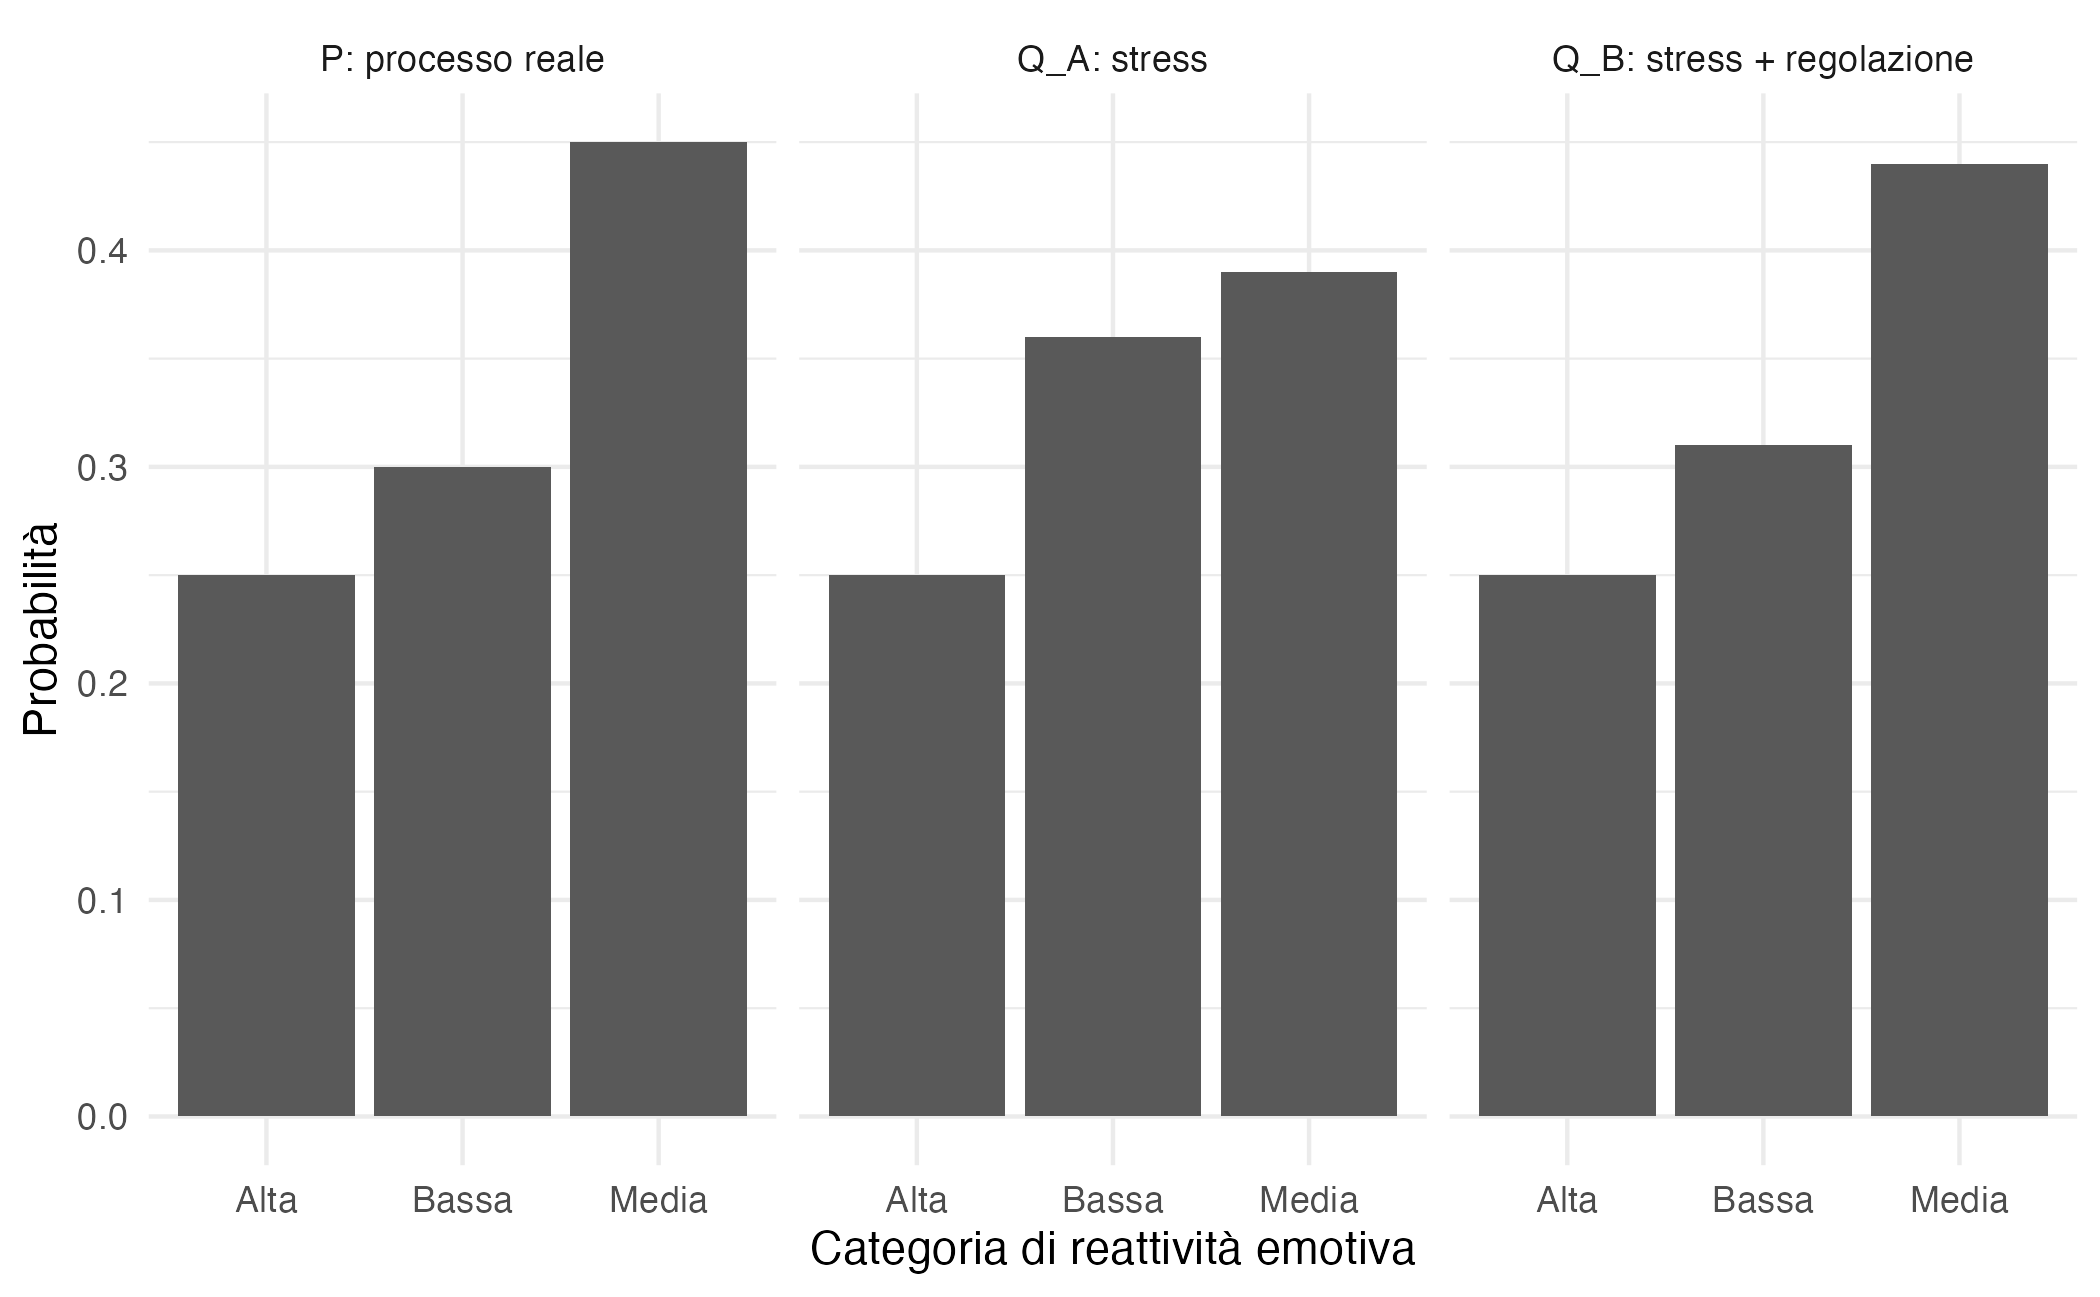
\includegraphics[width=0.85\linewidth,height=\textheight,keepaspectratio]{chapters/entropy/02_kl_files/figure-pdf/fig-kl-emotional-reactivity-1.png}

}

\caption{\label{fig-kl-emotional-reactivity}Esempio illustrativo: il
Modello B è più vicino alla distribuzione reale, ma il vantaggio
informazionale è modesto.}

\end{figure}%

Questo esempio presenta una limitazione deliberata: abbiamo finto di
conoscere \(P\) per rendere evidente il significato della KL. Nella
pratica, però, \(P\) non è disponibile, ed è per questo che si rende
necessario il passo successivo: stimare la performance predittiva su
dati non utilizzati per adattare il modello.

\section{Dalla KL all'ELPD}\label{dalla-kl-allelpd}

Abbiamo stabilito che confrontare i modelli significa massimizzare il
log-score atteso \(\mathbb{E}_{P}[\log Q(Y)]\). Nel contesto bayesiano,
però, \(Q\) non è una singola distribuzione con parametri fissati: dopo
aver osservato i dati \(y\), un modello bayesiano produce una
distribuzione predittiva che integra l'incertezza sui parametri:

\[
p(\tilde y \mid y) = \int p(\tilde y \mid \theta)p(\theta \mid y)\,d\theta.
\]

La domanda predittiva diventa quindi:

\begin{quote}
Quanta probabilità assegna il modello a una nuova osservazione
\(\tilde y\) generata dallo stesso processo?
\end{quote}

L'ELPD, \emph{Expected} Log Predictive Density*, formalizza questa
domanda:

\[
\mathrm{ELPD} = \sum_{i=1}^n \mathbb{E}_{\tilde y_i}\left[\log p(\tilde y_i \mid y)\right].
\]

Il segno è importante: la KL misura un costo da minimizzare, mentre
l'ELPD misura una performance da massimizzare. Un ELPD più alto indica
infatti una minore sorpresa predittiva, ovvero una minore entropia
incrociata stimata.

\section{Perché serve LOO}\label{perchuxe9-serve-loo}

Se valutiamo il modello sugli stessi dati usati per stimarlo, otteniamo
una stima troppo ottimistica: un modello molto flessibile può adattarsi
molto bene al campione osservato ma fallire su osservazioni nuove.
Questo è il problema dell'overfitting
(\citeproc{ref-McElreath_rethinking}{McElreath, 2020}).

La \emph{Leave-One-Out Cross-Validation} affronta il problema con
un'idea semplice: per ogni osservazione \(y_i\), stimiamo quanto bene il
modello la predice usando tutte le altre osservazioni \(y_{-i}\):

\[
\widehat{\mathrm{ELPD}}_{\mathrm{LOO}}
= \sum_{i=1}^n \log p(y_i \mid y_{-i}).
\]

Questa quantità approssima il log-score predittivo fuori campione. In
altre parole, LOO cerca di stimare operativamente il criterio che la KL
definisce teoricamente (\citeproc{ref-vehtari2017practical}{Vehtari et
al., 2017}).

La catena concettuale è quindi:

\[
\text{sorpresa}
\rightarrow
\text{entropia}
\rightarrow
\text{entropia incrociata}
\rightarrow
D_{\mathrm{KL}}
\rightarrow
\text{ELPD}
\rightarrow
\text{LOO}.
\]

\begin{tcolorbox}[enhanced jigsaw, arc=.35mm, bottomrule=.15mm, bottomtitle=1mm, breakable, colback=white, colbacktitle=quarto-callout-note-color!10!white, colframe=quarto-callout-note-color-frame, coltitle=black, left=2mm, leftrule=.75mm, opacityback=0, opacitybacktitle=0.6, rightrule=.15mm, title=\textcolor{quarto-callout-note-color}{\faInfo}\hspace{0.5em}{Una traduzione epistemologica}, titlerule=0mm, toprule=.15mm, toptitle=1mm]

La KL dice: ``quanto costa rappresentare il processo reale con questo
modello?''\\
L'ELPD dice: ``quanto bene il modello assegnerà probabilità a dati
futuri?''\\
LOO dice: ``come possiamo stimare questa capacità predittiva usando i
dati che abbiamo, senza valutare il modello sugli stessi dati con cui è
stato addestrato?''

\end{tcolorbox}

\begin{tcolorbox}[enhanced jigsaw, arc=.35mm, bottomrule=.15mm, bottomtitle=1mm, breakable, colback=white, colbacktitle=quarto-callout-note-color!10!white, colframe=quarto-callout-note-color-frame, coltitle=black, left=2mm, leftrule=.75mm, opacityback=0, opacitybacktitle=0.6, rightrule=.15mm, title=\textcolor{quarto-callout-note-color}{\faInfo}\hspace{0.5em}{Distribuzioni continue: densità, non probabilità puntuali}, titlerule=0mm, toprule=.15mm, toptitle=1mm]

Per variabili continue la KL si scrive come integrale:

\[
D_{\mathrm{KL}}(P \parallel Q)
= \int p(y)\log \frac{p(y)}{q(y)}\,dy.
\]

Qui \(p(y)\) e \(q(y)\) sono densità, non probabilità puntuali. Questo
dettaglio è importante perché una densità può essere maggiore di 1 e
dipende dall'unità di misura. La KL, tuttavia, rimane invariata rispetto
a trasformazioni invertibili della variabile, purché entrambe le densità
siano trasformate coerentemente.

Nel confronto predittivo bayesiano questa distinzione ricompare quando
interpretiamo la \emph{log predictive density}: non stiamo assegnando
una probabilità puntuale a un valore continuo, ma valutando la densità
predittiva del modello nel punto osservato.

\end{tcolorbox}

\section*{Riflessioni conclusive}\label{riflessioni-conclusive-41}

\markright{Riflessioni conclusive}

In questo capitolo abbiamo introdotto la divergenza di Kullback-Leibler
(KL) come una misura quantitativa della \textbf{perdita informativa} ---
o, equivalentemente, dell'eccesso di sorpresa atteso --- che deriva
dall'impiego di una distribuzione approssimante \(Q\) per descrivere
osservazioni generate da \(P\). Il punto di partenza è l'entropia
incrociata \(H(P, Q)\), che esprime la sorpresa attesa del modello \(Q\)
rispetto alla distribuzione generativa \(P\). La KL isola quella
componente della sorpresa che eccede il limite minimo irriducibile,
rappresentato dall'entropia del processo vero \(H(P)\).

Un aspetto centrale è la \textbf{direzionalità} della KL. A differenza
delle metriche simmetriche, la KL non quantifica una distanza reciproca,
ma un costo informazionale orientato. Nel contesto della modellizzazione
scientifica, l'oggetto del confronto non è la prossimità tra
distribuzioni in quanto tali, ma il costo atteso di impiegare
un'approssimazione \(Q\) per descrivere il meccanismo generatore \(P\).
È per questo motivo che \(D_{\mathrm{KL}}(P \parallel Q)\) -- e non
l'inversa -- costituisce la direzione concettualmente rilevante quando
si assume \(P\) come riferimento reale e \(Q\) come modello candidato.

Il risultato teorico più rilevante del capitolo risiede nel nesso che
lega la KL alla valutazione predittiva: minimizzare
\(D_{\mathrm{KL}}(P \parallel Q)\) equivale infatti a massimizzare il
log-score atteso sotto il processo generatore \(P\):

\[
\arg\min_Q D_{\mathrm{KL}}(P \parallel Q) = \arg\max_Q \mathbb{E}_{P}[\log Q(Y)].
\]

Poiché \(P\) è ignota, nella pratica questa quantità non è calcolabile
direttamente e deve essere stimata con procedure di validazione
predittiva. L'ELPD (\emph{Expected Log Predictive Density}) formalizza
la performance predittiva attesa su nuove osservazioni; LOO
(\emph{Leave-One-Out Cross-Validation}) ne fornisce una stima empirica,
mitigando l'ottimismo valutativo, ovvero il rischio di sovradattamento
(\emph{overfitting}), che deriva dalla valutazione \emph{in-sample}
sugli stessi dati utilizzati per l'adattamento.

Nel prossimo capitolo, utilizzeremo questo apparato concettuale per
passare dalla teoria alla pratica computazionale: discuteremo come
calcolare LOO, come interpretare le differenze di ELPD in termini di
errore standard, come incorporare l'incertezza di stima nei confronti
modellistici e, soprattutto, come evitare di ridurre il confronto tra
modelli a un algoritmo di selezione meccanico e acritico, trascurando la
complessità sostanziale del problema scientifico.

\begin{tcolorbox}[enhanced jigsaw, arc=.35mm, bottomrule=.15mm, bottomtitle=1mm, breakable, colback=white, colbacktitle=quarto-callout-important-color!10!white, colframe=quarto-callout-important-color-frame, coltitle=black, left=2mm, leftrule=.75mm, opacityback=0, opacitybacktitle=0.6, rightrule=.15mm, title=\textcolor{quarto-callout-important-color}{\faExclamation}\hspace{0.5em}{Esercizi}, titlerule=0mm, toprule=.15mm, toptitle=1mm]

\begin{enumerate}
\def\labelenumi{\arabic{enumi}.}
\tightlist
\item
  Considera le distribuzioni:
\end{enumerate}

\begin{Shaded}
\begin{Highlighting}[]
\NormalTok{p }\OtherTok{\textless{}{-}} \FunctionTok{c}\NormalTok{(}\FloatTok{0.2}\NormalTok{, }\FloatTok{0.5}\NormalTok{, }\FloatTok{0.3}\NormalTok{)}
\NormalTok{q }\OtherTok{\textless{}{-}} \FunctionTok{c}\NormalTok{(}\FloatTok{0.1}\NormalTok{, }\FloatTok{0.2}\NormalTok{, }\FloatTok{0.7}\NormalTok{)}
\end{Highlighting}
\end{Shaded}

Calcola l'entropia di \(p\), l'entropia incrociata \(H(p,q)\) e la
divergenza \(D_{\mathrm{KL}}(p \parallel q)\).

\begin{enumerate}
\def\labelenumi{\arabic{enumi}.}
\setcounter{enumi}{1}
\tightlist
\item
  Ripeti l'esercizio precedente con:
\end{enumerate}

\begin{Shaded}
\begin{Highlighting}[]
\NormalTok{q2 }\OtherTok{\textless{}{-}} \FunctionTok{c}\NormalTok{(}\FloatTok{0.2}\NormalTok{, }\FloatTok{0.55}\NormalTok{, }\FloatTok{0.25}\NormalTok{)}
\end{Highlighting}
\end{Shaded}

Quale modello spreca meno informazione?

\begin{enumerate}
\def\labelenumi{\arabic{enumi}.}
\setcounter{enumi}{2}
\tightlist
\item
  Mostra numericamente l'asimmetria della KL calcolando
  \(D_{\mathrm{KL}}(P \parallel Q)\) e
  \(D_{\mathrm{KL}}(Q \parallel P)\) per:
\end{enumerate}

\begin{Shaded}
\begin{Highlighting}[]
\NormalTok{P }\OtherTok{\textless{}{-}} \FunctionTok{c}\NormalTok{(}\FloatTok{0.7}\NormalTok{, }\FloatTok{0.2}\NormalTok{, }\FloatTok{0.1}\NormalTok{)}
\NormalTok{Q }\OtherTok{\textless{}{-}} \FunctionTok{c}\NormalTok{(}\FloatTok{0.4}\NormalTok{, }\FloatTok{0.3}\NormalTok{, }\FloatTok{0.3}\NormalTok{)}
\end{Highlighting}
\end{Shaded}

\begin{enumerate}
\def\labelenumi{\arabic{enumi}.}
\setcounter{enumi}{3}
\tightlist
\item
  Spiega in due frasi perché un modello con log-score predittivo più
  alto è preferibile, ma non necessariamente ``vero''.
\end{enumerate}

\end{tcolorbox}

\begin{tcolorbox}[enhanced jigsaw, arc=.35mm, bottomrule=.15mm, bottomtitle=1mm, breakable, colback=white, colbacktitle=quarto-callout-note-color!10!white, colframe=quarto-callout-note-color-frame, coltitle=black, left=2mm, leftrule=.75mm, opacityback=0, opacitybacktitle=0.6, rightrule=.15mm, title=\textcolor{quarto-callout-note-color}{\faInfo}\hspace{0.5em}{Soluzioni essenziali}, titlerule=0mm, toprule=.15mm, toptitle=1mm]

\begin{Shaded}
\begin{Highlighting}[]
\CommentTok{\# Esercizio 1}
\NormalTok{p }\OtherTok{\textless{}{-}} \FunctionTok{c}\NormalTok{(}\FloatTok{0.2}\NormalTok{, }\FloatTok{0.5}\NormalTok{, }\FloatTok{0.3}\NormalTok{)}
\NormalTok{q }\OtherTok{\textless{}{-}} \FunctionTok{c}\NormalTok{(}\FloatTok{0.1}\NormalTok{, }\FloatTok{0.2}\NormalTok{, }\FloatTok{0.7}\NormalTok{)}

\FunctionTok{entropy\_discrete}\NormalTok{(p)}
\CommentTok{\#\textgreater{} [1] 1.49}
\FunctionTok{cross\_entropy}\NormalTok{(p, q)}
\CommentTok{\#\textgreater{} [1] 1.98}
\FunctionTok{kl\_divergence}\NormalTok{(p, q)}
\CommentTok{\#\textgreater{} [1] 0.494}

\CommentTok{\# Esercizio 2}
\NormalTok{q2 }\OtherTok{\textless{}{-}} \FunctionTok{c}\NormalTok{(}\FloatTok{0.2}\NormalTok{, }\FloatTok{0.55}\NormalTok{, }\FloatTok{0.25}\NormalTok{)}
\FunctionTok{kl\_divergence}\NormalTok{(p, q)}
\CommentTok{\#\textgreater{} [1] 0.494}
\FunctionTok{kl\_divergence}\NormalTok{(p, q2)}
\CommentTok{\#\textgreater{} [1] 0.0102}

\CommentTok{\# Esercizio 3}
\NormalTok{P }\OtherTok{\textless{}{-}} \FunctionTok{c}\NormalTok{(}\FloatTok{0.7}\NormalTok{, }\FloatTok{0.2}\NormalTok{, }\FloatTok{0.1}\NormalTok{)}
\NormalTok{Q }\OtherTok{\textless{}{-}} \FunctionTok{c}\NormalTok{(}\FloatTok{0.4}\NormalTok{, }\FloatTok{0.3}\NormalTok{, }\FloatTok{0.3}\NormalTok{)}
\FunctionTok{kl\_divergence}\NormalTok{(P, Q)}
\CommentTok{\#\textgreater{} [1] 0.29}
\FunctionTok{kl\_divergence}\NormalTok{(Q, P)}
\CommentTok{\#\textgreater{} [1] 0.328}
\end{Highlighting}
\end{Shaded}

Un modello con log-score predittivo più alto assegna, in media, maggiore
probabilità ai dati osservati fuori campione. Questo lo rende
predittivamente migliore tra i candidati considerati, ma non implica che
coincida con il processo reale.

\end{tcolorbox}

\begin{tcolorbox}[enhanced jigsaw, arc=.35mm, bottomrule=.15mm, bottomtitle=1mm, breakable, colback=white, colbacktitle=quarto-callout-note-color!10!white, colframe=quarto-callout-note-color-frame, coltitle=black, left=2mm, leftrule=.75mm, opacityback=0, opacitybacktitle=0.6, rightrule=.15mm, title=\textcolor{quarto-callout-note-color}{\faInfo}\hspace{0.5em}{Informazioni sull'ambiente di sviluppo}, titlerule=0mm, toprule=.15mm, toptitle=1mm]

\begin{Shaded}
\begin{Highlighting}[]
\FunctionTok{sessionInfo}\NormalTok{()}
\CommentTok{\#\textgreater{} R version 4.6.1 (2026{-}06{-}24)}
\CommentTok{\#\textgreater{} Platform: aarch64{-}apple{-}darwin23}
\CommentTok{\#\textgreater{} Running under: macOS Tahoe 26.5.2}
\CommentTok{\#\textgreater{} }
\CommentTok{\#\textgreater{} Matrix products: default}
\CommentTok{\#\textgreater{} BLAS:   /Library/Frameworks/R.framework/Versions/4.6/Resources/lib/libRblas.0.dylib }
\CommentTok{\#\textgreater{} LAPACK: /Library/Frameworks/R.framework/Versions/4.6/Resources/lib/libRlapack.dylib;  LAPACK version 3.12.1}
\CommentTok{\#\textgreater{} }
\CommentTok{\#\textgreater{} locale:}
\CommentTok{\#\textgreater{} [1] C.UTF{-}8/UTF{-}8/C.UTF{-}8/C/C.UTF{-}8/C.UTF{-}8}
\CommentTok{\#\textgreater{} }
\CommentTok{\#\textgreater{} time zone: Europe/Zagreb}
\CommentTok{\#\textgreater{} tzcode source: internal}
\CommentTok{\#\textgreater{} }
\CommentTok{\#\textgreater{} attached base packages:}
\CommentTok{\#\textgreater{} [1] stats     graphics  grDevices utils     datasets  methods   base     }
\CommentTok{\#\textgreater{} }
\CommentTok{\#\textgreater{} other attached packages:}
\CommentTok{\#\textgreater{}  [1] ragg\_1.5.2            tinytable\_0.17.0      withr\_3.0.3          }
\CommentTok{\#\textgreater{}  [4] systemfonts\_1.3.2     patchwork\_1.3.2       ggdist\_3.3.3         }
\CommentTok{\#\textgreater{}  [7] tidybayes\_3.0.7       bayesplot\_1.15.0      ggplot2\_4.0.3        }
\CommentTok{\#\textgreater{} [10] reliabilitydiag\_0.2.1 priorsense\_1.2.0      posterior\_1.7.0      }
\CommentTok{\#\textgreater{} [13] loo\_2.10.0            rstan\_2.32.7          StanHeaders\_2.32.10  }
\CommentTok{\#\textgreater{} [16] brms\_2.23.0           Rcpp\_1.1.2            sessioninfo\_1.2.4    }
\CommentTok{\#\textgreater{} [19] conflicted\_1.2.0      janitor\_2.2.1         matrixStats\_1.5.0    }
\CommentTok{\#\textgreater{} [22] modelr\_0.1.11         tibble\_3.3.1          dplyr\_1.2.1          }
\CommentTok{\#\textgreater{} [25] tidyr\_1.3.2           rio\_1.3.0             here\_1.0.2           }
\CommentTok{\#\textgreater{} }
\CommentTok{\#\textgreater{} loaded via a namespace (and not attached):}
\CommentTok{\#\textgreater{}  [1] svUnit\_1.0.8          tidyselect\_1.2.1      farver\_2.1.2         }
\CommentTok{\#\textgreater{}  [4] S7\_0.2.2              fastmap\_1.2.0         tensorA\_0.36.2.1     }
\CommentTok{\#\textgreater{}  [7] digest\_0.6.39         timechange\_0.4.0      estimability\_2.0.0   }
\CommentTok{\#\textgreater{} [10] lifecycle\_1.0.5       magrittr\_2.0.5        compiler\_4.6.1       }
\CommentTok{\#\textgreater{} [13] rlang\_1.3.0           tools\_4.6.1           yaml\_2.3.12          }
\CommentTok{\#\textgreater{} [16] knitr\_1.51            labeling\_0.4.3        bridgesampling\_1.2{-}1 }
\CommentTok{\#\textgreater{} [19] pkgbuild\_1.4.8        curl\_7.1.0            RColorBrewer\_1.1{-}3   }
\CommentTok{\#\textgreater{} [22] abind\_1.4{-}8           purrr\_1.2.2           grid\_4.6.1           }
\CommentTok{\#\textgreater{} [25] stats4\_4.6.1          xtable\_1.8{-}8          inline\_0.3.21        }
\CommentTok{\#\textgreater{} [28] emmeans\_2.0.4         scales\_1.4.0          cli\_3.6.6            }
\CommentTok{\#\textgreater{} [31] mvtnorm\_1.4{-}2         rmarkdown\_2.31        generics\_0.1.4       }
\CommentTok{\#\textgreater{} [34] otel\_0.2.0            RcppParallel\_5.1.11{-}2 cachem\_1.1.0         }
\CommentTok{\#\textgreater{} [37] stringr\_1.6.0         parallel\_4.6.1        vctrs\_0.7.3          }
\CommentTok{\#\textgreater{} [40] V8\_8.2.0              Matrix\_1.7{-}5          jsonlite\_2.0.0       }
\CommentTok{\#\textgreater{} [43] arrayhelpers\_1.1{-}1    glue\_1.8.1            codetools\_0.2{-}20     }
\CommentTok{\#\textgreater{} [46] distributional\_0.8.1  lubridate\_1.9.5       stringi\_1.8.7        }
\CommentTok{\#\textgreater{} [49] gtable\_0.3.6          QuickJSR\_1.10.0       pillar\_1.11.1        }
\CommentTok{\#\textgreater{} [52] htmltools\_0.5.9       Brobdingnag\_1.2{-}9     R6\_2.6.1             }
\CommentTok{\#\textgreater{} [55] textshaping\_1.0.5     rprojroot\_2.1.1       evaluate\_1.0.5       }
\CommentTok{\#\textgreater{} [58] lattice\_0.22{-}9        backports\_1.5.1       memoise\_2.0.1        }
\CommentTok{\#\textgreater{} [61] broom\_1.0.13          snakecase\_0.11.1      rstantools\_2.6.0     }
\CommentTok{\#\textgreater{} [64] coda\_0.19{-}4.1         gridExtra\_2.3.1       nlme\_3.1{-}170         }
\CommentTok{\#\textgreater{} [67] checkmate\_2.3.4       xfun\_0.60             pkgconfig\_2.0.3}
\end{Highlighting}
\end{Shaded}

\end{tcolorbox}

\section*{Bibliografia}\label{bibliografia-47}

\markright{Bibliografia}

\chapter{Valutare i modelli bayesiani}\label{sec-div-kl-lppd-elpd}

\begin{tcolorbox}[enhanced jigsaw, arc=.35mm, bottomrule=.15mm, breakable, colback=white, colframe=quarto-callout-note-color-frame, left=2mm, leftrule=.75mm, opacityback=0, rightrule=.15mm, toprule=.15mm]

I due capitoli precedenti hanno stabilito il \textbf{criterio} con cui
confrontare i modelli: con l'entropia e il log-score abbiamo imparato a
misurare la sorpresa che un modello prova di fronte ai dati
(Capitolo~\ref{sec-entropy-shannon-information}); con la divergenza di
Kullback--Leibler abbiamo visto che confrontare due modelli equivale a
\textbf{massimizzare il log-score atteso} sotto il processo generatore
dei dati (Capitolo~\ref{sec-kullback-leibler-divergence}).

Restava però aperto il problema pratico: quel criterio dipende dal
processo vero \(P\), che non conosciamo. Questo capitolo lo rende
\textbf{operativo}. Vedremo come, nel quadro bayesiano, il log-score si
calcoli propagando l'incertezza sui parametri (la densità predittiva a
posteriori), perché la sua versione \emph{in-sample} sia troppo
ottimista, e come la validazione \emph{leave-one-out} (PSIS-LOO) ne
fornisca una stima \emph{out-of-sample} affidabile. Chiuderemo
applicando l'intero strumentario a un confronto tra modelli reali con
\texttt{brms} e \texttt{loo}.

\end{tcolorbox}

\begin{tcolorbox}[enhanced jigsaw, arc=.35mm, bottomrule=.15mm, breakable, colback=white, colframe=quarto-callout-important-color-frame, left=2mm, leftrule=.75mm, opacityback=0, rightrule=.15mm, toprule=.15mm]

\textbf{Da sapere.} La qualità predittiva di un modello va valutata su
dati che il modello non ha già utilizzato. La LPPD misura l'adattamento
\emph{in-sample} ed è quindi ottimistica; l'ELPD descrive invece la
capacità predittiva attesa su nuove osservazioni. La PSIS-LOO stima
l'ELPD senza ristimare ordinariamente il modello per ogni osservazione.
Il confronto predittivo non individua automaticamente il modello
``vero'' e non sostituisce teoria, adeguatezza sostantiva e controlli
del modello.

\textbf{Da saper fare.} Distinguere LPPD, ELPD e
\(\widehat{\mathrm{ELPD}}_{\mathrm{LOO}}\); spiegare perché la
valutazione \emph{in-sample} favorisce l'overfitting; calcolare la
PSIS-LOO con \texttt{loo()}; interpretare \texttt{elpd\_loo},
\texttt{p\_loo} e i diagnostici Pareto-\(k\); confrontare modelli con
\texttt{loo\_compare()}, valutando la differenza di ELPD insieme al suo
errore standard; preferire il modello più parsimonioso quando le
prestazioni predittive sono sostanzialmente equivalenti.

\textbf{Approfondimento facoltativo.} La derivazione del log-score
bayesiano tramite integrazione sulla distribuzione a posteriori,
l'approssimazione Monte Carlo mediante \emph{log-sum-exp}, i dettagli
dell'\emph{importance sampling} e il ricalcolo esatto delle osservazioni
con Pareto-\(k\) elevato possono essere rimandati. Nel percorso
essenziale è sufficiente comprendere la differenza tra adattamento e
generalizzazione e saper leggere correttamente un confronto PSIS-LOO tra
modelli stimati con \texttt{brms}.

\hyperref[sec-percorsi-lettura]{Che cosa significano queste etichette?}

\end{tcolorbox}

\subsection*{Panoramica del capitolo}\label{panoramica-del-capitolo-9}

Al termine del capitolo dovresti sapere:

\begin{itemize}
\tightlist
\item
  calcolare il \textbf{log-score bayesiano} propagando l'incertezza sui
  parametri;
\item
  riconoscere l'ottimismo della \textbf{LPPD} \emph{in-sample} e il
  rischio di \emph{overfitting};
\item
  stimare l'\textbf{ELPD} \emph{out-of-sample} mediante
  \textbf{PSIS-LOO};
\item
  confrontare modelli con \texttt{loo\_compare()}, leggendo
  \(\Delta\)ELPD, il suo errore standard e i diagnostici Pareto-\(k\);
\item
  decidere tra modelli bilanciando capacità predittiva e parsimonia.
\end{itemize}

\begin{tcolorbox}[enhanced jigsaw, arc=.35mm, bottomrule=.15mm, bottomtitle=1mm, breakable, colback=white, colbacktitle=quarto-callout-tip-color!10!white, colframe=quarto-callout-tip-color-frame, coltitle=black, left=2mm, leftrule=.75mm, opacityback=0, opacitybacktitle=0.6, rightrule=.15mm, title=\textcolor{quarto-callout-tip-color}{\faLightbulb}\hspace{0.5em}{Prerequisiti}, titlerule=0mm, toprule=.15mm, toptitle=1mm]

Oltre ai due capitoli precedenti di questa sezione, è utile la lettura
del capitolo 7, \emph{Ulysses' Compass}, di \emph{Statistical
Rethinking} (\citeproc{ref-McElreath_rethinking}{McElreath, 2020}).

\end{tcolorbox}

\begin{tcolorbox}[enhanced jigsaw, arc=.35mm, bottomrule=.15mm, bottomtitle=1mm, breakable, colback=white, colbacktitle=quarto-callout-caution-color!10!white, colframe=quarto-callout-caution-color-frame, coltitle=black, left=2mm, leftrule=.75mm, opacityback=0, opacitybacktitle=0.6, rightrule=.15mm, title=\textcolor{quarto-callout-caution-color}{\faFire}\hspace{0.5em}{Preparazione del Notebook}, titlerule=0mm, toprule=.15mm, toptitle=1mm]

\begin{Shaded}
\begin{Highlighting}[]
\NormalTok{here}\SpecialCharTok{::}\FunctionTok{here}\NormalTok{(}\StringTok{"code"}\NormalTok{, }\StringTok{"\_common.R"}\NormalTok{) }\SpecialCharTok{|\textgreater{}} 
  \FunctionTok{source}\NormalTok{()}

\ControlFlowTok{if}\NormalTok{ (}\SpecialCharTok{!}\FunctionTok{requireNamespace}\NormalTok{(}\StringTok{"pacman"}\NormalTok{)) }\FunctionTok{install.packages}\NormalTok{(}\StringTok{"pacman"}\NormalTok{)}
\NormalTok{pacman}\SpecialCharTok{::}\FunctionTok{p\_load}\NormalTok{(brms, loo, posterior)}
\end{Highlighting}
\end{Shaded}

\end{tcolorbox}

\section{Dal criterio al calcolo: il log-score
bayesiano}\label{dal-criterio-al-calcolo-il-log-score-bayesiano}

Nei capitoli precedenti il log-score è stato calcolato trattando i
parametri come valori fissati; nel
Capitolo~\ref{sec-entropy-shannon-information} abbiamo visto che sommare
i logaritmi delle probabilità assegnate alle osservazioni fornisce una
misura additiva e numericamente stabile della sorpresa del modello:
valori meno negativi indicano un modello meno sorpreso --- e quindi più
adeguato --- di fronte ai dati. Non ripetiamo qui quella costruzione: la
assumiamo come punto di partenza.

L'inferenza bayesiana introduce però una differenza essenziale: i
parametri non sono valori puntuali da fissare, ma \textbf{quantità
latenti incerte}, descritte prima dei dati dalla distribuzione a priori
\(p(\theta)\) e, dopo i dati, dalla distribuzione a posteriori
\(p(\theta \mid y)\). Se i parametri sono incerti, basare le previsioni
su un singolo valore ``ottimale'' di \(\theta\) (la media o la moda a
posteriori) ignora l'incertezza residua, che può incidere in modo
rilevante sulla distribuzione delle osservazioni future.

Nel quadro bayesiano, dunque, l'incertezza sui parametri va
\textbf{propagata} nel processo predittivo attraverso la distribuzione
predittiva a posteriori:

\[
p(\tilde{y} \mid y) = \int p(\tilde{y} \mid \theta)\, p(\theta \mid y)\, d\theta .
\]

Come discusso in Capitolo~\ref{sec-bayesian-inference-post-pred-distr},
questa distribuzione è una media delle distribuzioni predittive
condizionate ai singoli valori di \(\theta\), ponderata dalla posterior:
ogni valore del parametro contribuisce alla previsione in proporzione
alla sua plausibilità a posteriori.

Il \textbf{log-score bayesiano} di una singola osservazione \(y_i\) è
allora il logaritmo della sua densità predittiva a posteriori:

\begin{equation}\protect\phantomsection\label{eq-log-score-bayesian-single}{
\log p(y_i \mid y) = \log \!\left( \int p(y_i \mid \theta)\, p(\theta \mid y)\, d\theta \right).
}\end{equation}

La sorpresa viene qui calcolata \textbf{marginalizzando} rispetto a
tutta l'incertezza sui parametri, invece di fissare \(\theta\) a un
valore singolo: un log-score alto (cioè meno negativo) indica che il
modello assegna densità predittiva elevata al dato osservato; un
log-score molto negativo indica invece che il dato cade in una regione a
bassa densità. Rispetto alla verosimiglianza condizionata a una stima
puntuale, questa misura incorpora l'incertezza, riducendo
l'\emph{overconfidence} delle previsioni.

\subsection{Dall'integrale alla pratica: l'approssimazione tramite
MCMC}\label{dallintegrale-alla-pratica-lapprossimazione-tramite-mcmc}

L'integrale in (Equazione~\ref{eq-log-score-bayesian-single}) raramente
ha forma chiusa e va approssimato numericamente. Nella pratica bayesiana
moderna si usano i campioni MCMC \(\theta^{(1)}, \dots, \theta^{(S)}\)
prodotti, ad esempio, da Stan: interpretandoli come estrazioni dalla
posterior, si stima l'integrale con una media Monte Carlo,

\[
\log p(y_i \mid y) \approx \log \!\left( \frac{1}{S} \sum_{s=1}^{S} p(y_i \mid \theta^{(s)}) \right).
\]

Per ogni campione \(\theta^{(s)}\) si calcola la densità di \(y_i\)
sotto quell'ipotesi, e la densità predittiva è la media di tali densità
condizionate.\footnote{L'ordine delle operazioni è cruciale: si calcola
  \textbf{il logaritmo della media} delle densità, non la media dei
  logaritmi -- le due quantità differiscono per la disuguaglianza di
  Jensen, essendo il logaritmo concavo:
  \(\log \mathbb{E}[X] \ge \mathbb{E}[\log X]\). Solo
  \(\log\!\left( \tfrac{1}{S}\sum_s p(y_i\mid\theta^{(s)}) \right)\)
  approssima correttamente
  \(\log \int p(y_i\mid\theta)\, p(\theta\mid y)\, d\theta\). Dal punto
  di vista numerico, quando le densità sono molto piccole conviene
  sommare in log-spazio con un'operazione di \emph{log-sum-exp} per
  evitare underflow.}

\section{La LPPD e il problema
dell'overfitting}\label{la-lppd-e-il-problema-delloverfitting}

Sommando i log-score bayesiani di tutte le osservazioni si ottiene la
\textbf{Log Pointwise Predictive Density} (LPPD):

\begin{equation}\protect\phantomsection\label{eq-lppd}{
\text{LPPD} = \sum_{i=1}^N \log p(y_i \mid y).
}\end{equation}

La LPPD misura la plausibilità complessiva dei dati osservati alla luce
del modello, e può quindi essere letta come una misura
dell'\textbf{adattamento al campione disponibile}. Tuttavia,
\textbf{un'elevata LPPD non garantisce una buona capacità predittiva},
poiché è una quantità \emph{in-sample}: ciascun termine
\(\log p(y_i \mid y)\) valuta \(y_i\) rispetto a una distribuzione
predittiva costruita usando \emph{tutti} i dati, incluso lo stesso
\(y_i\).

Questa auto-referenzialità introduce un \textbf{ottimismo predittivo}.
Anche in ambito bayesiano, un modello abbastanza flessibile può
adattarsi non solo alla struttura sistematica del fenomeno, ma anche al
\textbf{rumore idiosincratico} del campione, gonfiando la LPPD senza
migliorare la previsione. La sovrastima cresce con la complessità: più
parametri liberi consentono di assorbire le fluttuazioni casuali del
campione, migliorando l'adattamento \emph{in-sample} a scapito della
generalizzazione. La LPPD descrive quindi bene \emph{quanto il modello
si adatti ai dati osservati}, ma non è una misura affidabile della
qualità predittiva su dati nuovi.

\section{Dall'in-sample all'out-of-sample:
l'ELPD}\label{dallin-sample-allout-of-sample-lelpd}

La quantità progettata per misurare la generalizzazione è
l'\textbf{Expected Log Predictive Density} (ELPD): il valore atteso del
log-score bayesiano su una nuova osservazione \(\tilde{y}\) generata
dallo stesso processo, dove l'attesa è rispetto alla distribuzione vera
e sconosciuta \(p(\tilde{y})\):

\begin{equation}\protect\phantomsection\label{eq-elpd-definition}{
\text{ELPD} = \mathbb{E}_{p(\tilde{y})}\!\left[\log p(\tilde{y} \mid y)\right]
= \int p(\tilde{y}) \, \log p(\tilde{y} \mid y) \, d\tilde{y}.
}\end{equation}

L'ELPD è la controparte operativa del criterio KL: massimizzarlo
equivale a minimizzare la divergenza dal processo generatore. Il
problema, come sappiamo, è che \(p(\tilde{y})\) non è osservabile;
occorre quindi stimarla a partire dai soli dati disponibili, evitando
l'auto-referenzialità della LPPD.

\section{Stimare l'ELPD: la validazione
leave-one-out}\label{stimare-lelpd-la-validazione-leave-one-out}

La \textbf{Leave-One-Out Cross-Validation} (LOO-CV) realizza questa
idea: per ogni osservazione \(y_i\), la si rimuove dal campione, si
ristima il modello sulle rimanenti \(y_{-i}\) e si valuta la densità
predittiva \(p(y_i \mid y_{-i})\) sull'osservazione esclusa. Sommando si
ottiene:

\begin{equation}\protect\phantomsection\label{eq-elpd-loo}{
\widehat{\text{ELPD}}_{\text{LOO}} = \sum_{i=1}^N \log p(y_i \mid y_{-i}).
}\end{equation}

Poiché ogni \(y_i\) è valutata da un modello che \emph{non l'ha vista},
questa stima non soffre dell'ottimismo della LPPD.

Ristimare il modello \(N\) volte è però proibitivo. La soluzione pratica
è \textbf{PSIS-LOO} (\emph{Pareto-Smoothed Importance Sampling}): a
partire da un'unica stima del modello sull'intero campione, si
approssima ciascuna posterior ``senza \(y_i\)'' ripesando i campioni
MCMC tramite \emph{importance sampling}, stabilizzato dal lisciamento di
Pareto (\citeproc{ref-vehtari2017practical}{Vehtari et al., 2017}). Il
metodo fornisce, come sottoprodotto, un diagnostico per osservazione, il
parametro \(\hat{k}\) di Pareto: valori \(\hat{k} < 0.7\) indicano che
l'approsssimazione è affidabile, mentre valori superiori segnalano
osservazioni troppo influenti, per le quali la stima LOO va ricalcolata
in modo esatto.

\section{LOO in pratica}\label{loo-in-pratica}

Vediamo l'intero flusso su un esempio simulato: generiamo dati in cui
l'esito \(y\) dipende da un predittore \(x\), mentre un secondo
predittore \(z\) è del tutto irrilevante (non entra nel processo
generatore).

\begin{Shaded}
\begin{Highlighting}[]
\FunctionTok{set.seed}\NormalTok{(}\DecValTok{123}\NormalTok{)}
\NormalTok{n }\OtherTok{\textless{}{-}} \DecValTok{100}
\NormalTok{x }\OtherTok{\textless{}{-}} \FunctionTok{rnorm}\NormalTok{(n)}
\NormalTok{z }\OtherTok{\textless{}{-}} \FunctionTok{rnorm}\NormalTok{(n)                          }\CommentTok{\# predittore irrilevante}
\NormalTok{y }\OtherTok{\textless{}{-}} \FloatTok{0.3} \SpecialCharTok{+} \FloatTok{0.8} \SpecialCharTok{*}\NormalTok{ x }\SpecialCharTok{+} \FunctionTok{rnorm}\NormalTok{(n, }\DecValTok{0}\NormalTok{, }\DecValTok{1}\NormalTok{)    }\CommentTok{\# z non ha alcun effetto}
\NormalTok{dat }\OtherTok{\textless{}{-}} \FunctionTok{data.frame}\NormalTok{(y, x, z)}
\end{Highlighting}
\end{Shaded}

Stimiamo tre modelli di crescente complessità: un modello nullo (sola
intercetta), il modello corretto (con \(x\)) e un modello
sovra-specificato (con \(x\) e il predittore irrilevante \(z\)).

\begin{Shaded}
\begin{Highlighting}[]
\NormalTok{pr }\OtherTok{\textless{}{-}} \FunctionTok{prior}\NormalTok{(}\FunctionTok{normal}\NormalTok{(}\DecValTok{0}\NormalTok{, }\DecValTok{5}\NormalTok{), }\AttributeTok{class =} \StringTok{"Intercept"}\NormalTok{) }\SpecialCharTok{+}
      \FunctionTok{prior}\NormalTok{(}\FunctionTok{normal}\NormalTok{(}\DecValTok{0}\NormalTok{, }\DecValTok{2}\NormalTok{), }\AttributeTok{class =} \StringTok{"b"}\NormalTok{) }\SpecialCharTok{+}
      \FunctionTok{prior}\NormalTok{(}\FunctionTok{exponential}\NormalTok{(}\DecValTok{1}\NormalTok{), }\AttributeTok{class =} \StringTok{"sigma"}\NormalTok{)}

\NormalTok{m0 }\OtherTok{\textless{}{-}} \FunctionTok{brm}\NormalTok{(y }\SpecialCharTok{\textasciitilde{}} \DecValTok{1}\NormalTok{,     }\AttributeTok{data =}\NormalTok{ dat, }\AttributeTok{family =} \FunctionTok{gaussian}\NormalTok{(),}
          \AttributeTok{prior =} \FunctionTok{prior}\NormalTok{(}\FunctionTok{normal}\NormalTok{(}\DecValTok{0}\NormalTok{, }\DecValTok{5}\NormalTok{), }\AttributeTok{class =} \StringTok{"Intercept"}\NormalTok{) }\SpecialCharTok{+}
                  \FunctionTok{prior}\NormalTok{(}\FunctionTok{exponential}\NormalTok{(}\DecValTok{1}\NormalTok{), }\AttributeTok{class =} \StringTok{"sigma"}\NormalTok{),}
          \AttributeTok{seed =} \DecValTok{1}\NormalTok{, }\AttributeTok{refresh =} \DecValTok{0}\NormalTok{, }\AttributeTok{backend =} \StringTok{"cmdstanr"}\NormalTok{)}

\NormalTok{m1 }\OtherTok{\textless{}{-}} \FunctionTok{brm}\NormalTok{(y }\SpecialCharTok{\textasciitilde{}}\NormalTok{ x,     }\AttributeTok{data =}\NormalTok{ dat, }\AttributeTok{family =} \FunctionTok{gaussian}\NormalTok{(), }\AttributeTok{prior =}\NormalTok{ pr,}
          \AttributeTok{seed =} \DecValTok{1}\NormalTok{, }\AttributeTok{refresh =} \DecValTok{0}\NormalTok{, }\AttributeTok{backend =} \StringTok{"cmdstanr"}\NormalTok{)}

\NormalTok{m2 }\OtherTok{\textless{}{-}} \FunctionTok{brm}\NormalTok{(y }\SpecialCharTok{\textasciitilde{}}\NormalTok{ x }\SpecialCharTok{+}\NormalTok{ z, }\AttributeTok{data =}\NormalTok{ dat, }\AttributeTok{family =} \FunctionTok{gaussian}\NormalTok{(), }\AttributeTok{prior =}\NormalTok{ pr,}
          \AttributeTok{seed =} \DecValTok{1}\NormalTok{, }\AttributeTok{refresh =} \DecValTok{0}\NormalTok{, }\AttributeTok{backend =} \StringTok{"cmdstanr"}\NormalTok{)}
\end{Highlighting}
\end{Shaded}

Calcoliamo la LOO per ciascun modello; l'output riporta la stima
\texttt{elpd\_loo} con il suo errore standard, il numero effettivo di
parametri \texttt{p\_loo} e la tabella diagnostica dei Pareto-\(k\).

\begin{Shaded}
\begin{Highlighting}[]
\NormalTok{loo0 }\OtherTok{\textless{}{-}}\NormalTok{ loo}\SpecialCharTok{::}\FunctionTok{loo}\NormalTok{(m0)}
\NormalTok{loo1 }\OtherTok{\textless{}{-}}\NormalTok{ loo}\SpecialCharTok{::}\FunctionTok{loo}\NormalTok{(m1)}
\NormalTok{loo2 }\OtherTok{\textless{}{-}}\NormalTok{ loo}\SpecialCharTok{::}\FunctionTok{loo}\NormalTok{(m2)}

\NormalTok{loo1}
\CommentTok{\#\textgreater{} }
\CommentTok{\#\textgreater{} Computed from 4000 by 100 log{-}likelihood matrix.}
\CommentTok{\#\textgreater{} }
\CommentTok{\#\textgreater{}          Estimate   SE}
\CommentTok{\#\textgreater{} elpd\_loo   {-}138.5  6.4}
\CommentTok{\#\textgreater{} p\_loo         3.0  0.5}
\CommentTok{\#\textgreater{} looic       277.0 12.8}
\CommentTok{\#\textgreater{} {-}{-}{-}{-}{-}{-}}
\CommentTok{\#\textgreater{} MCSE of elpd\_loo is 0.0.}
\CommentTok{\#\textgreater{} MCSE and ESS estimates assume MCMC draws (r\_eff in [0.7, 1.1]).}
\CommentTok{\#\textgreater{} }
\CommentTok{\#\textgreater{} All Pareto k estimates are good (k \textless{} 0.7).}
\CommentTok{\#\textgreater{} See help(\textquotesingle{}pareto{-}k{-}diagnostic\textquotesingle{}) for details.}
\end{Highlighting}
\end{Shaded}

Prima di confrontare i modelli, controlliamo i diagnostici: se tutti i
valori \(\hat{k}\) sono al di sotto della soglia di \(0.7\), la stima
PSIS-LOO è affidabile e possiamo procedere; in caso contrario,
\texttt{loo} segnala le osservazioni problematiche e suggerisce di
ricalcolarle esattamente (ad esempio con \texttt{reloo\ =\ TRUE}).

Il confronto vero e proprio si fa con \texttt{loo\_compare()}, che
ordina i modelli dal migliore al peggiore e riporta, per ciascuno, la
differenza di ELPD rispetto al migliore (\texttt{elpd\_diff}) e l'errore
standard di tale differenza (\texttt{se\_diff}).

\begin{Shaded}
\begin{Highlighting}[]
\NormalTok{loo}\SpecialCharTok{::}\FunctionTok{loo\_compare}\NormalTok{(loo0, loo1, loo2)}
\CommentTok{\#\textgreater{}  model elpd\_diff se\_diff p\_worse       diag\_diff diag\_elpd}
\CommentTok{\#\textgreater{}     m1       0.0     0.0      NA                          }
\CommentTok{\#\textgreater{}     m2      {-}1.1     0.3    1.00 |elpd\_diff| \textless{} 4          }
\CommentTok{\#\textgreater{}     m0     {-}16.4     5.5    1.00}
\end{Highlighting}
\end{Shaded}

La lettura segue una regola semplice: il modello in cima ha
\texttt{elpd\_diff\ =\ 0} per costruzione; per gli altri, si confronta
l'entità di \texttt{elpd\_diff} con il suo \texttt{se\_diff} -- una
differenza è credibile solo se è ampia rispetto alla propria incertezza
(indicativamente, \(|\Delta\text{ELPD}| > 2\,\text{SE}\)).

In questo esempio il risultato è istruttivo su due fronti. Da un lato,
il modello nullo \texttt{m0} resta nettamente indietro (ignorare un
predittore realmente informativo ha un costo predittivo grande e
statisticamente chiaro); dall'altro, il modello sovra-specificato
\texttt{m2} \textbf{non} migliora in modo apprezzabile rispetto a
\texttt{m1} -- la differenza di ELPD tra i due è piccola e dello stesso
ordine del suo errore standard, perché il predittore \(z\) non aggiunge
segnale ma solo flessibilità. La conclusione operativa è preferire
\texttt{m1}: a parità sostanziale di capacità predittiva, si sceglie il
modello più parsimonioso.

\begin{tcolorbox}[enhanced jigsaw, arc=.35mm, bottomrule=.15mm, bottomtitle=1mm, breakable, colback=white, colbacktitle=quarto-callout-important-color!10!white, colframe=quarto-callout-important-color-frame, coltitle=black, left=2mm, leftrule=.75mm, opacityback=0, opacitybacktitle=0.6, rightrule=.15mm, title=\textcolor{quarto-callout-important-color}{\faExclamation}\hspace{0.5em}{Cosa la LOO non decide al posto nostro}, titlerule=0mm, toprule=.15mm, toptitle=1mm]

La funzione \texttt{loo\_compare()} ordina i modelli per capacità
predittiva stimata, ma non è un algoritmo di selezione automatica. Una
differenza di ELPD piccola e incerta non ``promuove'' il modello
complesso; una differenza ampia va comunque interpretata alla luce della
teoria, della qualità della misurazione, della plausibilità dei
\emph{prior} e della domanda di ricerca. La LOO è uno strumento di
\textbf{critica} modellistica, non un verdetto.

\end{tcolorbox}

\section*{Riflessioni conclusive}\label{riflessioni-conclusive-42}

\markright{Riflessioni conclusive}

Questo capitolo ha trasformato il criterio informazionale dei due
capitoli precedenti in una procedura applicabile. Il passaggio decisivo
è la propagazione dell'incertezza: nel quadro bayesiano il log-score si
calcola sulla densità predittiva a posteriori, integrando su tutti i
valori plausibili dei parametri anziché fissarne uno. La sua somma
\emph{in-sample} -- la LPPD -- misura l'adattamento ma sovrastima
sistematicamente la capacità predittiva, perché valuta ogni osservazione
con un modello che l'ha già vista. L'ELPD sposta il bersaglio sui dati
futuri, e la PSIS-LOO ne fornisce una stima efficiente a partire da
un'unica stima del modello, corredata dai diagnostici \(\hat{k}\) che ne
segnalano l'affidabilità.

L'esempio applicativo ha mostrato l'uso concreto di
\texttt{loo\_compare()} e, soprattutto, il modo corretto di leggerne
l'output: non come una classifica da cui estrarre meccanicamente un
vincitore, ma come una stima con la propria incertezza, in cui una
differenza di ELPD va confrontata con il suo errore standard e ponderata
con criteri di parsimonia. È lo stesso strumentario che accompagnerà la
valutazione dei modelli più articolati incontrati nel resto del volume,
dai modelli lineari e generalizzati fino ai modelli formali dei processi
psicologici.

\section*{Bibliografia}\label{bibliografia-48}

\markright{Bibliografia}

\chapter{Oltre la LOO: la gerarchia della
generalizzazione}\label{sec-generalizzazione}

\begin{tcolorbox}[enhanced jigsaw, arc=.35mm, bottomrule=.15mm, breakable, colback=white, colframe=quarto-callout-note-color-frame, left=2mm, leftrule=.75mm, opacityback=0, rightrule=.15mm, toprule=.15mm]

Nel capitolo precedente abbiamo imparato a confrontare modelli con
l'ELPD stimato tramite LOO. Questo capitolo pone una domanda più
esigente: \emph{generalizzare a che cosa?} Prevedere un'osservazione
lasciata fuori dallo stesso dataset non è la stessa cosa che prevedere
il comportamento di un individuo mai osservato, né il comportamento
dello stesso individuo in un compito diverso, né, a maggior ragione,
prevedere che il modello regga in uno studio indipendente. Costruiremo
questa gerarchia in modo operativo: con la convalida incrociata
raggruppata per soggetto (dati \texttt{sleepstudy}) e con una
simulazione di convalida incrociata basata sul modello di
Rescorla-Wagner.

\end{tcolorbox}

\begin{tcolorbox}[enhanced jigsaw, arc=.35mm, bottomrule=.15mm, breakable, colback=white, colframe=quarto-callout-important-color-frame, left=2mm, leftrule=.75mm, opacityback=0, rightrule=.15mm, toprule=.15mm]

\textbf{Da sapere.} La generalizzazione non è un'unica proprietà del
modello, ma dipende da ciò che si vuole prevedere: nuove osservazioni
degli stessi individui, individui mai osservati, nuovi compiti o nuovi
studi. Ogni livello richiede una diversa unità di convalida. La LOO
sulle osservazioni può risultare troppo ottimistica quando sfrutta
informazioni già disponibili sulla persona; per valutare nuovi individui
occorre lasciare fuori interi soggetti. Un parametro stimato in un
compito può essere considerato una caratteristica individuale stabile
solo se migliora la previsione del comportamento della stessa persona in
altri compiti o contesti.

\textbf{Da saper fare.} Formulare esplicitamente il livello di
generalizzazione rilevante per la domanda scientifica; distinguere LOO
per osservazioni e convalida incrociata raggruppata per soggetto;
interpretare perché il vantaggio di un modello multilivello possa
cambiare quando si prevedono persone nuove; confrontare una previsione
idiografica con una previsione basata sulla media di gruppo; comunicare
il livello di validazione effettivamente raggiunto senza estendere le
conclusioni ai livelli superiori.

\textbf{Approfondimento facoltativo.} La k-fold raggruppata completa con
\texttt{brms}, la simulazione cross-task del modello di
Rescorla--Wagner, il calcolo delle log-densità predittive individuali e
la formulazione bayesiana congiunta dei parametri nei diversi compiti
possono essere rimandati. Nel percorso essenziale è sufficiente
comprendere la gerarchia della generalizzazione e scegliere una
procedura di convalida coerente con l'unità alla quale si intendono
estendere le conclusioni.

\hyperref[sec-percorsi-lettura]{Che cosa significano queste etichette?}

\end{tcolorbox}

\section{Prerequisiti}\label{prerequisiti-10}

\begin{itemize}
\tightlist
\item
  Il capitolo sulla valutazione dei modelli bayesiani (ELPD, LOO-CV) di
  questa sezione.
\item
  Il capitolo sui modelli multilivello (sezione \emph{Modelli}), da cui
  riprendiamo i dati \texttt{sleepstudy} e la distinzione
  complete/partial pooling.
\item
  I capitoli della sezione \emph{Applicazione} sul modello di
  Rescorla--Wagner, da cui riprendiamo la regola di aggiornamento e la
  funzione softmax.
\end{itemize}

\begin{tcolorbox}[enhanced jigsaw, arc=.35mm, bottomrule=.15mm, bottomtitle=1mm, breakable, colback=white, colbacktitle=quarto-callout-tip-color!10!white, colframe=quarto-callout-tip-color-frame, coltitle=black, left=2mm, leftrule=.75mm, opacityback=0, opacitybacktitle=0.6, rightrule=.15mm, title=\textcolor{quarto-callout-tip-color}{\faLightbulb}\hspace{0.5em}{Preparazione del Notebook}, titlerule=0mm, toprule=.15mm, toptitle=1mm]

\begin{Shaded}
\begin{Highlighting}[]
\FunctionTok{library}\NormalTok{(tidyverse)}
\FunctionTok{library}\NormalTok{(brms)}
\FunctionTok{library}\NormalTok{(loo)}

\FunctionTok{data}\NormalTok{(}\StringTok{"sleepstudy"}\NormalTok{, }\AttributeTok{package =} \StringTok{"lme4"}\NormalTok{)}
\FunctionTok{set.seed}\NormalTok{(}\DecValTok{20260720}\NormalTok{)}
\end{Highlighting}
\end{Shaded}

\end{tcolorbox}

\section{Quale domanda pone davvero la
LOO}\label{quale-domanda-pone-davvero-la-loo}

La LOO-CV simula la previsione di \emph{una nuova osservazione generata
dallo stesso processo che ha prodotto le altre}. Quando le osservazioni
sono scambiabili, ovvero quando si dispone di un campione di individui
misurati una volta ciascuno, questa è spesso la domanda che ci
interessa. Tuttavia, nei dati psicologici tipici le osservazioni non
sono scambiabili, ma annidate negli individui. In un disegno a misure
ripetute, escludere \emph{un trial} di Mario e prevederlo utilizzando
gli altri trial di Mario risponde alla domanda: ``Quanto bene prevedo
un'altra osservazione di una persona che conosco già?''.

È una domanda legittima, ma raramente è la domanda di interesse. Il
capitolo 22 del manuale distingue con cura i diversi livelli di
generalizzazione e questa distinzione non è un dettaglio: un modello può
eccellere al primo livello e fallire ai successivi. Possiamo
rappresentare i livelli come una catena di inclusioni:

\[
\text{nuove osservazioni} \;\subset\; \text{nuovi individui} \;\subset\; \text{nuovi compiti o contesti} \;\subset\; \text{nuovi studi}.
\]

{\def\LTcaptype{none} % do not increment counter
\begin{longtable}[]{@{}
  >{\raggedright\arraybackslash}p{(\linewidth - 6\tabcolsep) * \real{0.2500}}
  >{\raggedright\arraybackslash}p{(\linewidth - 6\tabcolsep) * \real{0.2500}}
  >{\raggedright\arraybackslash}p{(\linewidth - 6\tabcolsep) * \real{0.2500}}
  >{\raggedright\arraybackslash}p{(\linewidth - 6\tabcolsep) * \real{0.2500}}@{}}
\toprule\noalign{}
\begin{minipage}[b]{\linewidth}\raggedright
Livello
\end{minipage} & \begin{minipage}[b]{\linewidth}\raggedright
Domanda
\end{minipage} & \begin{minipage}[b]{\linewidth}\raggedright
Strumento tipico
\end{minipage} & \begin{minipage}[b]{\linewidth}\raggedright
Che cosa \emph{non} garantisce
\end{minipage} \\
\midrule\noalign{}
\endhead
\bottomrule\noalign{}
\endlastfoot
Nuove osservazioni & Prevedo un'altra osservazione degli stessi
individui? & LOO / PSIS-LOO & Nulla su individui mai visti \\
Nuovi individui & Prevedo un partecipante mai osservato? & Convalida
incrociata raggruppata (leave-one-subject-out) & Nulla su compiti o
contesti diversi \\
Nuovi compiti o contesti & Il parametro stimato in un compito predice il
comportamento in un altro? & Disegni cross-task; predizione con
parametri stimati altrove & Nulla sulla stabilità tra popolazioni e
laboratori \\
Nuovi studi & Il modello regge in campioni, laboratori, tempi
indipendenti? & Repliche preregistrate, progetti multi-lab, modelli
gerarchici meta-analitici & È il test più severo disponibile \\
\end{longtable}
}

Ogni salto di livello cambia l'unità che viene ``lasciata fuori'' e, con
essa, la porzione del modello che deve svolgere il lavoro predittivo.
Questo è il punto operativo del capitolo.

\section{Livello 2: prevedere nuovi
individui}\label{livello-2-prevedere-nuovi-individui}

Riprendiamo i dati di Belenky e colleghi sulla privazione del sonno e i
due modelli che abbiamo visto nel capitolo sul \emph{partial pooling}:
un modello a \emph{pooling} completo, che ignora la struttura per
soggetto e un modello multilivello con intercette e pendenze per
soggetto.

\begin{Shaded}
\begin{Highlighting}[]
\NormalTok{m\_pool }\OtherTok{\textless{}{-}} \FunctionTok{brm}\NormalTok{(}
\NormalTok{  Reaction }\SpecialCharTok{\textasciitilde{}} \DecValTok{1} \SpecialCharTok{+}\NormalTok{ Days,}
  \AttributeTok{data =}\NormalTok{ sleepstudy,}
  \AttributeTok{backend =} \StringTok{"cmdstanr"}\NormalTok{, }\AttributeTok{seed =} \DecValTok{123}
\NormalTok{)}

\NormalTok{m\_partial }\OtherTok{\textless{}{-}} \FunctionTok{brm}\NormalTok{(}
\NormalTok{  Reaction }\SpecialCharTok{\textasciitilde{}} \DecValTok{1} \SpecialCharTok{+}\NormalTok{ Days }\SpecialCharTok{+}\NormalTok{ (}\DecValTok{1} \SpecialCharTok{+}\NormalTok{ Days }\SpecialCharTok{|}\NormalTok{ Subject),}
  \AttributeTok{data =}\NormalTok{ sleepstudy,}
  \AttributeTok{backend =} \StringTok{"cmdstanr"}\NormalTok{, }\AttributeTok{seed =} \DecValTok{123}
\NormalTok{)}
\end{Highlighting}
\end{Shaded}

\subsection{Il confronto al livello delle
osservazioni}\label{il-confronto-al-livello-delle-osservazioni}

Prima il confronto che già sappiamo fare: LOO sulle singole
osservazioni.

\begin{Shaded}
\begin{Highlighting}[]
\NormalTok{loo\_pool }\OtherTok{\textless{}{-}} \FunctionTok{loo}\NormalTok{(m\_pool)}
\NormalTok{loo\_partial }\OtherTok{\textless{}{-}} \FunctionTok{loo}\NormalTok{(m\_partial)}
\FunctionTok{loo\_compare}\NormalTok{(loo\_pool, loo\_partial)}
\end{Highlighting}
\end{Shaded}

\begin{verbatim}
     model elpd_diff se_diff p_worse diag_diff      diag_elpd
 m_partial       0.0     0.0      NA           2 k_psis > 0.7
    m_pool     -92.5    21.0    1.00                         
\end{verbatim}

Il modello multilivello domina, e di molto. Ma vediamo \emph{perché}:
quando prevede il trial lasciato fuori di un soggetto, il modello
multilivello usa gli effetti casuali stimati \emph{sugli altri trial
dello stesso soggetto}. Sta sfruttando un'informazione idiografica che,
per un individuo mai visto, semplicemente non esisterebbe.

\subsection{Il confronto al livello degli
individui}\label{il-confronto-al-livello-degli-individui}

Per rispondere alla domanda ``quanto bene il modello prevede un
\emph{nuovo} soggetto?'' dobbiamo lasciare fuori tutti i trial di un
soggetto alla volta. Con 18 soggetti, la versione
\emph{leave-one-subject-out} richiederebbe 18 ristime; per contenere i
tempi usiamo una k-fold raggruppata con \(K = 6\) fold, costruiti in
modo che ogni soggetto cada interamente in un solo fold. Utilizzare gli
\emph{stessi} fold per entrambi i modelli rende il confronto equo.

\begin{Shaded}
\begin{Highlighting}[]
\NormalTok{fold\_id }\OtherTok{\textless{}{-}}\NormalTok{ loo}\SpecialCharTok{::}\FunctionTok{kfold\_split\_grouped}\NormalTok{(}\AttributeTok{K =} \DecValTok{6}\NormalTok{, }\AttributeTok{x =}\NormalTok{ sleepstudy}\SpecialCharTok{$}\NormalTok{Subject)}

\NormalTok{kf\_pool }\OtherTok{\textless{}{-}} \FunctionTok{kfold}\NormalTok{(m\_pool, }\AttributeTok{folds =}\NormalTok{ fold\_id)}
\NormalTok{kf\_partial }\OtherTok{\textless{}{-}} \FunctionTok{kfold}\NormalTok{(m\_partial, }\AttributeTok{folds =}\NormalTok{ fold\_id, }\AttributeTok{allow\_new\_levels =} \ConstantTok{TRUE}\NormalTok{)}
\end{Highlighting}
\end{Shaded}

\begin{Shaded}
\begin{Highlighting}[]
\FunctionTok{loo\_compare}\NormalTok{(kf\_pool, kf\_partial)}
\end{Highlighting}
\end{Shaded}

\begin{verbatim}
     model elpd_diff se_diff p_worse diag_diff diag_elpd
 m_partial       0.0     0.0      NA                    
    m_pool     -12.2     5.3    0.99                    
\end{verbatim}

\begin{tcolorbox}[enhanced jigsaw, arc=.35mm, bottomrule=.15mm, bottomtitle=1mm, breakable, colback=white, colbacktitle=quarto-callout-warning-color!10!white, colframe=quarto-callout-warning-color-frame, coltitle=black, left=2mm, leftrule=.75mm, opacityback=0, opacitybacktitle=0.6, rightrule=.15mm, title=\textcolor{quarto-callout-warning-color}{\faExclamationTriangle}\hspace{0.5em}{Attenzione ai tempi di calcolo}, titlerule=0mm, toprule=.15mm, toptitle=1mm]

La k-fold ristima ogni modello \(K\) volte: qui sono 12 stime MCMC
complete. In un progetto reale conviene salvare i risultati
(\texttt{saveRDS()}) o usare il \emph{freeze} di Quarto, come per gli
altri capitoli computazionalmente onerosi.

\end{tcolorbox}

Confrontiamo i due esiti. Al livello delle osservazioni il vantaggio del
partial pooling è considerevole, mentre al livello degli individui si
riduce sensibilmente, e l'errore standard della differenza cresce. La
ragione è istruttiva: per un soggetto mai visto prima, il modello
multilivello non può utilizzare effetti casuali individuali, ma deve
integrare la distribuzione di degli effetti nella popolazione,
prevedendo quindi ``un soggetto plausibile'' e non ``quel soggetto''. Il
suo vantaggio rispetto al pooling completo si riduce a due cose: una
stima migliore dei parametri di popolazione e una rappresentazione
onesta della variabilità tra gli individui nella distribuzione
predittiva.

Questo non è un difetto del modello multilivello ma la risposta corretta
a una domanda diversa. La lezione è che \textbf{il livello a cui si
esegue la convalida deve coincidere con il livello a cui si vuole
generalizzare}. Se l'obiettivo scientifico riguarda nuovi individui, la
LOO per le osservazioni fornisce una risposta sistematicamente troppo
ottimistica.

\section{Livello 3: prevedere un nuovo
compito}\label{livello-3-prevedere-un-nuovo-compito}

Il terzo livello non può essere simulato ``lasciando fuori'' pezzi di un
solo dataset: richiede un disegno con più compiti. Possiamo però
studiarne la logica con una simulazione, utilizzando il modello di
Rescorla--Wagner della sezione \emph{Applicazione}. La domanda
idiografica è: \emph{il tasso di apprendimento} \(\alpha\) \emph{stimato
per un individuo nel Compito A fornisce informazioni sul suo
comportamento nel Compito B?}

La simulazione ci permette di confrontare due mondi possibili:

\begin{itemize}
\tightlist
\item
  \textbf{Scenario ``tratto stabile''}: lo stesso \(\alpha_i\) governa
  il comportamento dell'individuo \(i\) in entrambi i compiti;
\item
  \textbf{Scenario ``specifico del compito''}: gli \(\alpha\) dei due
  compiti sono estratti indipendentemente dalla stessa popolazione,
  quindi l'individuo non ``porta con sé'' il proprio parametro.
\end{itemize}

Nei dati reali non sappiamo in quale dei due mondi ci troviamo: è
esattamente ciò che la validazione cross-task deve stabilire.

\subsection{Simulare e stimare}\label{simulare-e-stimare}

Definiamo il simulatore di un compito a due scelte con ricompense
probabilistiche e la log-verosimiglianza condizionata alle scelte e alle
ricompense osservate. Per isolare il ruolo di \(\alpha\), teniamo fissa
e nota la temperatura inversa \(\beta\).

\begin{Shaded}
\begin{Highlighting}[]
\NormalTok{sim\_rw }\OtherTok{\textless{}{-}} \ControlFlowTok{function}\NormalTok{(alpha, beta, n\_trials, }\AttributeTok{p\_rew =} \FunctionTok{c}\NormalTok{(}\FloatTok{0.8}\NormalTok{, }\FloatTok{0.2}\NormalTok{)) \{}
\NormalTok{  v }\OtherTok{\textless{}{-}} \FunctionTok{c}\NormalTok{(}\FloatTok{0.5}\NormalTok{, }\FloatTok{0.5}\NormalTok{)  }\CommentTok{\# valori attesi iniziali: v[1] = opzione A, v[2] = opzione B}
\NormalTok{  choice\_A }\OtherTok{\textless{}{-}} \FunctionTok{integer}\NormalTok{(n\_trials)}
\NormalTok{  reward }\OtherTok{\textless{}{-}} \FunctionTok{integer}\NormalTok{(n\_trials)}
  \ControlFlowTok{for}\NormalTok{ (t }\ControlFlowTok{in} \FunctionTok{seq\_len}\NormalTok{(n\_trials)) \{}
\NormalTok{    p\_A }\OtherTok{\textless{}{-}} \DecValTok{1} \SpecialCharTok{/}\NormalTok{ (}\DecValTok{1} \SpecialCharTok{+} \FunctionTok{exp}\NormalTok{(}\SpecialCharTok{{-}}\NormalTok{beta }\SpecialCharTok{*}\NormalTok{ (v[}\DecValTok{1}\NormalTok{] }\SpecialCharTok{{-}}\NormalTok{ v[}\DecValTok{2}\NormalTok{])))}
\NormalTok{    ch }\OtherTok{\textless{}{-}} \FunctionTok{as.integer}\NormalTok{(}\FunctionTok{runif}\NormalTok{(}\DecValTok{1}\NormalTok{) }\SpecialCharTok{\textless{}}\NormalTok{ p\_A)          }\CommentTok{\# 1 = sceglie A, 0 = sceglie B}
\NormalTok{    k }\OtherTok{\textless{}{-}} \ControlFlowTok{if}\NormalTok{ (ch }\SpecialCharTok{==} \DecValTok{1}\NormalTok{) }\DecValTok{1} \ControlFlowTok{else} \DecValTok{2}
\NormalTok{    rw }\OtherTok{\textless{}{-}} \FunctionTok{as.integer}\NormalTok{(}\FunctionTok{runif}\NormalTok{(}\DecValTok{1}\NormalTok{) }\SpecialCharTok{\textless{}}\NormalTok{ p\_rew[k])}
\NormalTok{    choice\_A[t] }\OtherTok{\textless{}{-}}\NormalTok{ ch}
\NormalTok{    reward[t] }\OtherTok{\textless{}{-}}\NormalTok{ rw}
\NormalTok{    v[k] }\OtherTok{\textless{}{-}}\NormalTok{ v[k] }\SpecialCharTok{+}\NormalTok{ alpha }\SpecialCharTok{*}\NormalTok{ (rw }\SpecialCharTok{{-}}\NormalTok{ v[k])        }\CommentTok{\# aggiornamento Rescorla{-}Wagner}
\NormalTok{  \}}
  \FunctionTok{data.frame}\NormalTok{(}\AttributeTok{choice\_A =}\NormalTok{ choice\_A, }\AttributeTok{reward =}\NormalTok{ reward)}
\NormalTok{\}}

\NormalTok{loglik\_rw }\OtherTok{\textless{}{-}} \ControlFlowTok{function}\NormalTok{(alpha, beta, choice\_A, reward) \{}
\NormalTok{  v }\OtherTok{\textless{}{-}} \FunctionTok{c}\NormalTok{(}\FloatTok{0.5}\NormalTok{, }\FloatTok{0.5}\NormalTok{)}
\NormalTok{  ll }\OtherTok{\textless{}{-}} \DecValTok{0}
  \ControlFlowTok{for}\NormalTok{ (t }\ControlFlowTok{in} \FunctionTok{seq\_along}\NormalTok{(choice\_A)) \{}
\NormalTok{    p\_A }\OtherTok{\textless{}{-}} \DecValTok{1} \SpecialCharTok{/}\NormalTok{ (}\DecValTok{1} \SpecialCharTok{+} \FunctionTok{exp}\NormalTok{(}\SpecialCharTok{{-}}\NormalTok{beta }\SpecialCharTok{*}\NormalTok{ (v[}\DecValTok{1}\NormalTok{] }\SpecialCharTok{{-}}\NormalTok{ v[}\DecValTok{2}\NormalTok{])))}
\NormalTok{    p\_obs }\OtherTok{\textless{}{-}} \ControlFlowTok{if}\NormalTok{ (choice\_A[t] }\SpecialCharTok{==} \DecValTok{1}\NormalTok{) p\_A }\ControlFlowTok{else} \DecValTok{1} \SpecialCharTok{{-}}\NormalTok{ p\_A}
\NormalTok{    ll }\OtherTok{\textless{}{-}}\NormalTok{ ll }\SpecialCharTok{+} \FunctionTok{log}\NormalTok{(p\_obs)}
\NormalTok{    k }\OtherTok{\textless{}{-}} \ControlFlowTok{if}\NormalTok{ (choice\_A[t] }\SpecialCharTok{==} \DecValTok{1}\NormalTok{) }\DecValTok{1} \ControlFlowTok{else} \DecValTok{2}
\NormalTok{    v[k] }\OtherTok{\textless{}{-}}\NormalTok{ v[k] }\SpecialCharTok{+}\NormalTok{ alpha }\SpecialCharTok{*}\NormalTok{ (reward[t] }\SpecialCharTok{{-}}\NormalTok{ v[k])}
\NormalTok{  \}}
\NormalTok{  ll}
\NormalTok{\}}

\NormalTok{alpha\_grid }\OtherTok{\textless{}{-}} \FunctionTok{seq}\NormalTok{(}\FloatTok{0.02}\NormalTok{, }\FloatTok{0.98}\NormalTok{, }\AttributeTok{by =} \FloatTok{0.02}\NormalTok{)}

\NormalTok{stima\_alpha }\OtherTok{\textless{}{-}} \ControlFlowTok{function}\NormalTok{(dat, beta) \{}
\NormalTok{  ll }\OtherTok{\textless{}{-}} \FunctionTok{vapply}\NormalTok{(}
\NormalTok{    alpha\_grid,}
\NormalTok{    \textbackslash{}(a) }\FunctionTok{loglik\_rw}\NormalTok{(a, beta, dat}\SpecialCharTok{$}\NormalTok{choice\_A, dat}\SpecialCharTok{$}\NormalTok{reward),}
    \FunctionTok{numeric}\NormalTok{(}\DecValTok{1}\NormalTok{)}
\NormalTok{  )}
\NormalTok{  alpha\_grid[}\FunctionTok{which.max}\NormalTok{(ll)]}
\NormalTok{\}}
\end{Highlighting}
\end{Shaded}

Simuliamo 30 individui che eseguono il Compito A e stimiamo
\(\hat\alpha_i\) per ciascuno.

\begin{Shaded}
\begin{Highlighting}[]
\NormalTok{n\_subj }\OtherTok{\textless{}{-}} \DecValTok{30}
\NormalTok{n\_trials }\OtherTok{\textless{}{-}} \DecValTok{120}
\NormalTok{beta\_true }\OtherTok{\textless{}{-}} \DecValTok{3}

\NormalTok{alpha\_pop }\OtherTok{\textless{}{-}} \FunctionTok{rbeta}\NormalTok{(n\_subj, }\DecValTok{2}\NormalTok{, }\DecValTok{4}\NormalTok{)   }\CommentTok{\# popolazione dei tassi di apprendimento}

\NormalTok{task\_A }\OtherTok{\textless{}{-}} \FunctionTok{lapply}\NormalTok{(alpha\_pop, sim\_rw, }\AttributeTok{beta =}\NormalTok{ beta\_true, }\AttributeTok{n\_trials =}\NormalTok{ n\_trials)}
\NormalTok{alpha\_hat }\OtherTok{\textless{}{-}} \FunctionTok{vapply}\NormalTok{(task\_A, stima\_alpha, }\FunctionTok{numeric}\NormalTok{(}\DecValTok{1}\NormalTok{), }\AttributeTok{beta =}\NormalTok{ beta\_true)}

\FunctionTok{cor}\NormalTok{(alpha\_pop, alpha\_hat)   }\CommentTok{\# controllo di recupero dei parametri}
\end{Highlighting}
\end{Shaded}

\begin{verbatim}
[1] 0.8580026
\end{verbatim}

La correlazione tra i valori \(\alpha\) veri e quelli stimati è un
rapido controllo di recupero: se fosse bassa, non avrebbe senso
chiedersi se le stime generalizzano, perché non conterrebbero
informazioni nemmeno sul compito che le ha prodotte.

\subsection{Il test cross-task}\label{il-test-cross-task}

Simuliamo ora il Compito B nei due scenari e, per ogni individuo,
calcoliamo la log-densità predittiva delle sue scelte nel Compito B
sotto due previsioni concorrenti: quella \emph{idiografica}, che usa
\(\hat\alpha_i\) stimato nel Compito A, e quella \emph{nomotetica}, che
usa la media di gruppo \(\bar{\hat\alpha}\). La differenza \(\Delta_i\)
indica se il parametro individuale fornisce un valore predittivo
aggiuntivo rispetto al ``partecipante medio''.

\begin{Shaded}
\begin{Highlighting}[]
\NormalTok{alpha\_B\_stabile }\OtherTok{\textless{}{-}}\NormalTok{ alpha\_pop                 }\CommentTok{\# scenario 1: tratto stabile}
\NormalTok{alpha\_B\_specifico }\OtherTok{\textless{}{-}} \FunctionTok{rbeta}\NormalTok{(n\_subj, }\DecValTok{2}\NormalTok{, }\DecValTok{4}\NormalTok{)     }\CommentTok{\# scenario 2: specifico del compito}

\NormalTok{task\_B1 }\OtherTok{\textless{}{-}} \FunctionTok{lapply}\NormalTok{(alpha\_B\_stabile, sim\_rw, }\AttributeTok{beta =}\NormalTok{ beta\_true, }\AttributeTok{n\_trials =}\NormalTok{ n\_trials)}
\NormalTok{task\_B2 }\OtherTok{\textless{}{-}} \FunctionTok{lapply}\NormalTok{(alpha\_B\_specifico, sim\_rw, }\AttributeTok{beta =}\NormalTok{ beta\_true, }\AttributeTok{n\_trials =}\NormalTok{ n\_trials)}

\NormalTok{delta\_lpd }\OtherTok{\textless{}{-}} \ControlFlowTok{function}\NormalTok{(task\_B, alpha\_ind, alpha\_gruppo, beta) \{}
\NormalTok{  lpd\_ind }\OtherTok{\textless{}{-}} \FunctionTok{mapply}\NormalTok{(}
\NormalTok{    \textbackslash{}(dat, a) }\FunctionTok{loglik\_rw}\NormalTok{(a, beta, dat}\SpecialCharTok{$}\NormalTok{choice\_A, dat}\SpecialCharTok{$}\NormalTok{reward),}
\NormalTok{    task\_B, alpha\_ind}
\NormalTok{  )}
\NormalTok{  lpd\_gruppo }\OtherTok{\textless{}{-}} \FunctionTok{vapply}\NormalTok{(}
\NormalTok{    task\_B,}
\NormalTok{    \textbackslash{}(dat) }\FunctionTok{loglik\_rw}\NormalTok{(alpha\_gruppo, beta, dat}\SpecialCharTok{$}\NormalTok{choice\_A, dat}\SpecialCharTok{$}\NormalTok{reward),}
    \FunctionTok{numeric}\NormalTok{(}\DecValTok{1}\NormalTok{)}
\NormalTok{  )}
\NormalTok{  lpd\_ind }\SpecialCharTok{{-}}\NormalTok{ lpd\_gruppo}
\NormalTok{\}}

\NormalTok{delta\_1 }\OtherTok{\textless{}{-}} \FunctionTok{delta\_lpd}\NormalTok{(task\_B1, alpha\_hat, }\FunctionTok{mean}\NormalTok{(alpha\_hat), beta\_true)}
\NormalTok{delta\_2 }\OtherTok{\textless{}{-}} \FunctionTok{delta\_lpd}\NormalTok{(task\_B2, alpha\_hat, }\FunctionTok{mean}\NormalTok{(alpha\_hat), beta\_true)}

\NormalTok{risultati }\OtherTok{\textless{}{-}} \FunctionTok{tibble}\NormalTok{(}
  \AttributeTok{scenario =} \FunctionTok{rep}\NormalTok{(}\FunctionTok{c}\NormalTok{(}\StringTok{"Tratto stabile"}\NormalTok{, }\StringTok{"Specifico del compito"}\NormalTok{), }\AttributeTok{each =}\NormalTok{ n\_subj),}
  \AttributeTok{delta =} \FunctionTok{c}\NormalTok{(delta\_1, delta\_2)}
\NormalTok{)}

\NormalTok{risultati }\SpecialCharTok{|\textgreater{}}
  \FunctionTok{group\_by}\NormalTok{(scenario) }\SpecialCharTok{|\textgreater{}}
  \FunctionTok{summarise}\NormalTok{(}
    \AttributeTok{delta\_medio =} \FunctionTok{mean}\NormalTok{(delta),}
    \AttributeTok{prop\_positivi =} \FunctionTok{mean}\NormalTok{(delta }\SpecialCharTok{\textgreater{}} \DecValTok{0}\NormalTok{)}
\NormalTok{  )}
\end{Highlighting}
\end{Shaded}

\begin{verbatim}
# A tibble: 2 x 3
  scenario              delta_medio prop_positivi
  <chr>                       <dbl>         <dbl>
1 Specifico del compito      -1.96          0.333
2 Tratto stabile              0.902         0.7  
\end{verbatim}

\begin{Shaded}
\begin{Highlighting}[]
\FunctionTok{ggplot}\NormalTok{(risultati, }\FunctionTok{aes}\NormalTok{(}\AttributeTok{x =}\NormalTok{ scenario, }\AttributeTok{y =}\NormalTok{ delta)) }\SpecialCharTok{+}
  \FunctionTok{geom\_hline}\NormalTok{(}\AttributeTok{yintercept =} \DecValTok{0}\NormalTok{, }\AttributeTok{linetype =} \StringTok{"dashed"}\NormalTok{) }\SpecialCharTok{+}
  \FunctionTok{geom\_boxplot}\NormalTok{(}\AttributeTok{width =} \FloatTok{0.4}\NormalTok{, }\AttributeTok{outlier.shape =} \ConstantTok{NA}\NormalTok{) }\SpecialCharTok{+}
  \FunctionTok{geom\_jitter}\NormalTok{(}\AttributeTok{width =} \FloatTok{0.08}\NormalTok{, }\AttributeTok{alpha =} \FloatTok{0.5}\NormalTok{) }\SpecialCharTok{+}
  \FunctionTok{labs}\NormalTok{(}
    \AttributeTok{x =} \ConstantTok{NULL}\NormalTok{,}
    \AttributeTok{y =} \FunctionTok{expression}\NormalTok{(Delta }\SpecialCharTok{\textasciitilde{}} \StringTok{"log{-}densità predittiva (individuale {-} gruppo)"}\NormalTok{)}
\NormalTok{  )}
\end{Highlighting}
\end{Shaded}

\begin{figure}[H]

\centering{

\pandocbounded{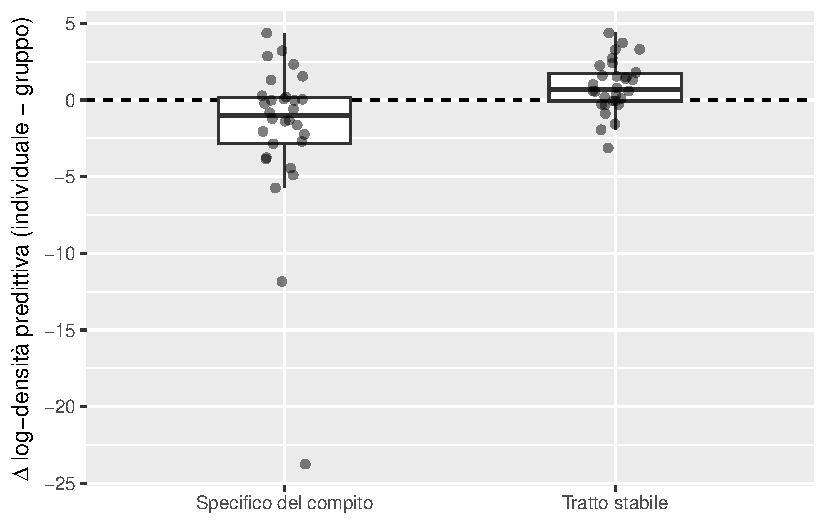
\includegraphics[keepaspectratio]{chapters/entropy/04_generalizzazione_files/figure-pdf/fig-rw-delta-1.pdf}}

}

\caption{\label{fig-rw-delta}Valore predittivo aggiunto del parametro
individuale nel Compito B. Valori positivi indicano che la previsione
basata sull'alpha stimato nel Compito A batte quella basata sulla media
di gruppo.}

\end{figure}%

Nello scenario ``tratto stabile'', la maggior parte dei \(\Delta_i\) è
positiva: conoscere l'individuo aiuta a prevedere il suo comportamento
in un compito nuovo, ed è questo il senso operativo dell'espressione
\emph{il parametro cattura una caratteristica della persona}. Nello
scenario ``specifico del compito'', invece, i \(\Delta_i\) si addensano
intorno allo zero o al di sotto di esso: la stima individuale del
Compito A è, rispetto al Compito B, rumore --- e usarla può essere
perfino peggio che usare la media di gruppo.

Il punto epistemologico è quello del manuale: un risultato negativo del
test cross-task non significa che il modello è ``sbagliato''. Significa
che il parametro è specifico del dominio e questa è un'informazione
teorica che delimita il campo di validità del costrutto.

\begin{tcolorbox}[enhanced jigsaw, arc=.35mm, bottomrule=.15mm, bottomtitle=1mm, breakable, colback=white, colbacktitle=quarto-callout-note-color!10!white, colframe=quarto-callout-note-color-frame, coltitle=black, left=2mm, leftrule=.75mm, opacityback=0, opacitybacktitle=0.6, rightrule=.15mm, title=\textcolor{quarto-callout-note-color}{\faInfo}\hspace{0.5em}{Dalla stima puntuale al trattamento bayesiano completo}, titlerule=0mm, toprule=.15mm, toptitle=1mm]

Per semplicità abbiamo utilizzato stime puntuali di massima
verosimiglianza su griglia. Un trattamento pienamente bayesiano, invece,
per ogni individuo, utilizzerebbe l'intera distribuzione a posteriori di
di \(\alpha_i\) (propagando l'incertezza nella previsione del Compito B)
e, ancora meglio, un modello gerarchico congiunto dei due compiti, in
cui la correlazione tra \(\alpha_{A,i}\) e \(\alpha_{B,i}\) è essa
stessa un parametro da stimare. In questo modo, il ``mondo'' in cui ci
troviamo diventa una quantità inferenziale, non un'ipotesi da assumere.
L'impianto necessario è quello del capitolo sull'eterogeneità nei
modelli dinamici (sezione \emph{Applicazione}).

\end{tcolorbox}

\section{Livello 4: nuovi studi}\label{livello-4-nuovi-studi}

L'ultimo livello non può essere dimostrato con il codice, perché
richiede dati che non abbiamo ancora: campioni indipendenti, laboratori
diversi e momenti diversi. Tre osservazioni collegano però questo
livello agli strumenti che già conosciamo.

In primo luogo, la logica statistica è la stessa del livello 2, ma
spostata di un piano. Nei progetti multi-lab e nelle sintesi
meta-analitiche, lo studio diventa l'unità di raggruppamento di un
modello gerarchico: la domanda ``che cosa prevedo per uno studio
nuovo?'' corrisponde alla distribuzione predittiva per un nuovo gruppo,
esattamente come ``che cosa prevedo per un soggetto nuovo?'' lo era
nella k-fold raggruppata. Il partial pooling scala di livello senza
cambiare natura.

In secondo luogo, la validazione a livello degli studi non è più solo
una questione statistica, ma anche di disegno. Le repliche preregistrate
e i \emph{registered reports} servono a garantire che la previsione sia
stata formulata prima di osservare i nuovi dati, altrimenti anche il
test più severo degenera in un adattamento retrospettivo. Questo ponte
ci collega alla sezione \emph{Visione} di questo Companion e al capitolo
sull'Open Science del manuale.

In terzo luogo, i livelli non si possono saltare. Un modello che
fallisce al livello dei nuovi individui non diventerà credibile in un
multi-lab; viceversa, superare la LOO non autorizza affermazioni sui
livelli superiori. Nella scrittura scientifica, quindi, è opportuno
dichiarare sempre \emph{a quale livello} è stata condotta la
validazione, poiché si tratta di un'informazione importante quanto il
valore dell'ELPD.

\section{Riflessioni conclusive}\label{riflessioni-conclusive-43}

La convalida incrociata non è una procedura unica, ma una famiglia di
domande e la scelta dell'unità da escludere è una scelta di natura
teorica mascherata da scelta tecnica. La LOO per osservazioni stima la
capacità di prevedere altri dati degli stessi individui, la k-fold
raggruppata stima la capacità di prevedere individui nuovi, i disegni
cross-task stabiliscono se i parametri individuali sono tratti o
contingenze e gli studi indipendenti, infine, decidono se il modello ha
colto principi o regolarità locali. Un modello scientificamente maturo
dichiara il livello di validazione raggiunto e non pretende credito per
i livelli che non ha ancora affrontato.

\section*{Esercizi}\label{esercizi-11}
\addcontentsline{toc}{section}{Esercizi}

\markright{Esercizi}

\begin{tcolorbox}[enhanced jigsaw, arc=.35mm, bottomrule=.15mm, bottomtitle=1mm, breakable, colback=white, colbacktitle=quarto-callout-tip-color!10!white, colframe=quarto-callout-tip-color-frame, coltitle=black, left=2mm, leftrule=.75mm, opacityback=0, opacitybacktitle=0.6, rightrule=.15mm, title=\textcolor{quarto-callout-tip-color}{\faLightbulb}\hspace{0.5em}{Esercizio 1 --- Comprendere}, titlerule=0mm, toprule=.15mm, toptitle=1mm]

Spiega con parole tue perché, nel confronto su \texttt{sleepstudy}, il
vantaggio del modello multilivello si riduce quando si passa dalla LOO
per osservazioni alla k-fold raggruppata per soggetto. Quale componente
del modello ``smette di lavorare'' per un soggetto mai osservato?

\textbf{Suggerimento.} Rileggi come il modello multilivello costruisce
la previsione per un livello nuovo del fattore di raggruppamento: quali
parametri usa e su che cosa integra?

\end{tcolorbox}

\begin{tcolorbox}[enhanced jigsaw, arc=.35mm, bottomrule=.15mm, bottomtitle=1mm, breakable, colback=white, colbacktitle=quarto-callout-tip-color!10!white, colframe=quarto-callout-tip-color-frame, coltitle=black, left=2mm, leftrule=.75mm, opacityback=0, opacitybacktitle=0.6, rightrule=.15mm, title=\textcolor{quarto-callout-tip-color}{\faLightbulb}\hspace{0.5em}{Esercizio 2 --- Prevedere}, titlerule=0mm, toprule=.15mm, toptitle=1mm]

Prima di eseguire il codice: se aumentassimo il numero di trial per
soggetto da 10 a 100 in \texttt{sleepstudy} (immaginando un disegno più
lungo), il divario tra LOO per osservazioni e k-fold per soggetti
crescerebbe o si ridurrebbe? Formula la tua previsione e motivala; poi
verifica con una simulazione.

\textbf{Suggerimento.} Chiediti quanta informazione idiografica la LOO
per osservazioni può ``rubare'' dagli altri trial dello stesso soggetto
al crescere del numero di trial.

\end{tcolorbox}

\begin{tcolorbox}[enhanced jigsaw, arc=.35mm, bottomrule=.15mm, bottomtitle=1mm, breakable, colback=white, colbacktitle=quarto-callout-tip-color!10!white, colframe=quarto-callout-tip-color-frame, coltitle=black, left=2mm, leftrule=.75mm, opacityback=0, opacitybacktitle=0.6, rightrule=.15mm, title=\textcolor{quarto-callout-tip-color}{\faLightbulb}\hspace{0.5em}{Esercizio 3 --- Modificare}, titlerule=0mm, toprule=.15mm, toptitle=1mm]

Nella simulazione cross-task, sostituisci lo scenario ``specifico del
compito'' con uno scenario intermedio in cui \(\alpha_{B,i}\) è
correlato ma non identico ad \(\alpha_{A,i}\), per esempio generandolo
come media pesata tra \(\alpha_{A,i}\) e un'estrazione indipendente.
Come cambia la distribuzione dei \(\Delta_i\)? A quale livello di
correlazione il parametro individuale smette di battere la media di
gruppo?

\end{tcolorbox}

\begin{tcolorbox}[enhanced jigsaw, arc=.35mm, bottomrule=.15mm, bottomtitle=1mm, breakable, colback=white, colbacktitle=quarto-callout-tip-color!10!white, colframe=quarto-callout-tip-color-frame, coltitle=black, left=2mm, leftrule=.75mm, opacityback=0, opacitybacktitle=0.6, rightrule=.15mm, title=\textcolor{quarto-callout-tip-color}{\faLightbulb}\hspace{0.5em}{Esercizio 4 --- Criticare}, titlerule=0mm, toprule=.15mm, toptitle=1mm]

Un articolo afferma: ``Il nostro modello computazionale generalizza: la
LOO-CV mostra un ELPD superiore a tutti i modelli concorrenti''. I dati
sono misure ripetute (200 trial per 40 partecipanti) e le conclusioni
riguardano l'uso dei parametri individuali come marcatori clinici
prognostici. Individua che cosa c'è di sovradimensionato in questa
affermazione e indica quali validazioni aggiuntive sarebbero necessarie,
distinguendo i livelli della gerarchia.

\end{tcolorbox}

\chapter*{Riflessioni conclusive della
sezione}\label{riflessioni-conclusive-della-sezione-5}

\markboth{Riflessioni conclusive della sezione}{Riflessioni conclusive
della sezione}

Questa sezione ha introdotto tre idee chiave.

\begin{enumerate}
\def\labelenumi{\arabic{enumi}.}
\item
  \textbf{Entropia di Shannon:} quantifica l'\emph{incertezza media} o
  il \emph{contenuto informativo atteso} di una distribuzione di
  probabilità. È massima quando tutti gli esiti sono ugualmente
  probabili (massima ``sorpresa'') e minima quando un esito è certo
  (assenza di sorpresa). Oltre alla sua definizione assiomatica, ne
  abbiamo mostrato la rilevanza pratica nel campionamento statistico e
  il ruolo fondamentale nella teoria della codifica, dove determina il
  limite inferiore per la compressione \emph{lossless} dei dati.
\item
  \textbf{Divergenza di Kullback-Leibler:} questa misura asimmetrica
  quantifica il \emph{costo informativo} di approssimare la vera
  distribuzione dei dati \(P\) con un modello \(Q\). Concettualmente,
  rappresenta il numero medio di \emph{bit} (o unità di sorpresa) extra
  che paghiamo quando utilizziamo \(Q\) al posto di \(P\) per descrivere
  i dati. È questa nozione di ``costo dell'approssimazione errata'' a
  fornire il fondamento teorico per la selezione dei modelli: il modello
  migliore è quello che minimizza tale divergenza, ovvero che approssima
  più fedelmente il meccanismo generatore dei dati senza adattarsi
  eccessivamente alle peculiarità del campione osservato.
\item
  \textbf{Valutazione predittiva bayesiana:} questo approccio opera un
  cambio di prospettiva, passando dall'adattamento ai dati osservati
  alla capacità di generalizzazione su dati nuovi. Si concretizza in tre
  strumenti collegati: il \emph{log-score} (accuratezza predittiva punto
  per punto), l'\emph{ELPD} (il suo valore atteso, la quantità teorica
  da massimizzare) e la \emph{PSIS-LOO} (la sua stima pratica ed
  efficiente). In questo quadro, il modello migliore non è quello che si
  adatta perfettamente al passato, ma quello che anticipa il futuro con
  maggiore affidabilità.
\end{enumerate}

Il valore di questo apparato per la ricerca psicologica si articola su
due piani complementari:

\begin{itemize}
\item
  \textbf{concettuale:} entropia e divergenza KL forniscono un
  vocabolario quantitativo rigoroso per temi centrali nella disciplina:
  dall'\emph{incertezza} nelle misurazioni e nelle teorie, alla
  \emph{complessità} dei processi cognitivi, fino alla \emph{capacità di
  generalizzazione} dei costrutti. Questo linguaggio si integra
  naturalmente con l'approccio bayesiano, in cui la distribuzione
  predittiva a posteriori diventa lo strumento per quantificare e
  comunicare tale incertezza.
\item
  \textbf{operativo:} la PSIS-LOO offre un protocollo applicativo
  immediato all'interno degli ambienti di modellazione bayesiana moderna
  (\texttt{brms}/Stan). Il flusso di lavoro diventa sistematico: dopo la
  stima, si valuta l'ELPD, si confrontano modelli alternativi con
  \texttt{loo\_compare()} leggendo \(\Delta\)ELPD e il suo errore
  standard, e si sceglie la specificazione con la migliore capacità
  predittiva \emph{out-of-sample}, bilanciata dalla parsimonia. Questo
  aiuta a prevenire i due estremi patologici della modellazione:
  l'eccessiva semplificazione (\emph{underfitting}) e l'adattamento al
  rumore (\emph{overfitting}).
\end{itemize}

Vale la pena sottolineare che questi strumenti non sono una novità
isolata di questa sezione: la PSIS-LOO è già stata impiegata
operativamente nei capitoli precedenti, per esempio nel confronto tra il
modello a varianza comune e quello a varianze distinte. Ciò che questa
sezione aggiunge è il loro \textbf{fondamento teorico}: capire
\emph{perché} massimizzare l'ELPD sia il criterio corretto, e non solo
\emph{come} calcolarlo.

In sintesi, la sezione rende esplicito il legame tra \emph{informazione}
e \emph{inferenza}: un modello è tanto più informativo quanto più riduce
l'incertezza predittiva senza introdurre complessità superflua. È il
criterio che, in modo coerente con l'intero percorso del modulo,
trasforma la modellazione statistica da esercizio di adattamento
\emph{post hoc} in un processo di apprendimento orientato alla
previsione.

\part{Visione}

\chapter*{Dove siamo arrivati}\label{dove-siamo-arrivati}

\markboth{Dove siamo arrivati}{Dove siamo arrivati}

\begin{tcolorbox}[enhanced jigsaw, arc=.35mm, bottomrule=.15mm, breakable, colback=white, colframe=quarto-callout-note-color-frame, left=2mm, leftrule=.75mm, opacityback=0, rightrule=.15mm, toprule=.15mm]

Questo ultimo tratto del companion non introduce semplicemente nuovi
strumenti: serve a fare il punto sul percorso compiuto e a chiedersi che
cosa significhi, dopo aver attraversato l'inferenza bayesiana, fare
ricerca psicologica in modo più solido, trasparente e responsabile.

Il percorso è iniziato da una constatazione: molte pratiche statistiche
tradizionali hanno favorito conclusioni troppo nette, risultati fragili
e una comunicazione dell'incertezza poco adeguata alla complessità dei
fenomeni psicologici. Da lì siamo passati dalla critica alla
costruzione: abbiamo imparato a formulare modelli, esplicitare
assunzioni, usare informazioni precedenti, controllare la qualità delle
stime, confrontare alternative e valutare quanto un modello riesca
davvero a rendere conto dei dati.

Il punto di arrivo, però, non è soltanto tecnico: l'inferenza bayesiana
diventa davvero utile quando modifica il modo in cui pensiamo la ricerca
--- non come ricerca di risposte definitive, ma come pratica di
aggiornamento, controllo e argomentazione. Un buon modello non elimina
l'incertezza; la rende visibile, discutibile e utilizzabile.

\end{tcolorbox}

\begin{tcolorbox}[enhanced jigsaw, arc=.35mm, bottomrule=.15mm, bottomtitle=1mm, breakable, colback=white, colbacktitle=quarto-callout-tip-color!10!white, colframe=quarto-callout-tip-color-frame, coltitle=black, left=2mm, leftrule=.75mm, opacityback=0, opacitybacktitle=0.6, rightrule=.15mm, title=\textcolor{quarto-callout-tip-color}{\faLightbulb}\hspace{0.5em}{La domanda guida di questa sezione}, titlerule=0mm, toprule=.15mm, toptitle=1mm]

Che tipo di ricercatore diventa chi ha imparato a ragionare in termini
di modelli, incertezza e trasparenza?

I tre capitoli conclusivi rispondono da prospettive diverse:

\begin{enumerate}
\def\labelenumi{\arabic{enumi}.}
\tightlist
\item
  \textbf{Riforma}: mostra perché la psicologia ha bisogno di cambiare
  non solo le tecniche di analisi, ma anche incentivi, standard,
  pratiche collaborative e modi di costruire teoria.
\item
  \textbf{Integrità della ricerca}: collega la qualità scientifica alle
  decisioni quotidiane del ricercatore --- dichiarare le assunzioni,
  documentare le scelte, distinguere esplorazione e conferma, rendere
  ispezionabile il processo analitico.
\item
  \textbf{Epilogo}: chiude il percorso ricomponendo i temi principali:
  incertezza, modellazione, controllo dei modelli, comunicazione dei
  risultati e responsabilità professionale.
\end{enumerate}

\end{tcolorbox}

\section*{Cosa portare con sé}\label{cosa-portare-con-suxe9}

\markright{Cosa portare con sé}

Alla fine del companion, tre idee dovrebbero rimanere come strumenti di
lavoro:

\begin{itemize}
\tightlist
\item
  \textbf{L'incertezza non è un difetto da nascondere}. Una
  distribuzione a posteriori, un intervallo credibile, una simulazione
  predittiva o un'analisi di sensibilità aiutano a comunicare quanto
  sappiamo, quanto non sappiamo e quanto le conclusioni dipendano dalle
  assunzioni fatte.
\item
  \textbf{I modelli sono strumenti, non verdetti}. Un modello bayesiano
  è utile quando chiarisce un'ipotesi, rende esplicite le sue
  condizioni, genera previsioni controllabili e può essere migliorato
  alla luce di nuovi dati.
\item
  \textbf{La buona ricerca è una pratica documentata}. Codice, dati,
  preregistrazioni, materiali condivisi, controlli diagnostici e scelte
  analitiche motivate non sono formalità: sono il modo in cui una
  comunità scientifica rende le proprie conclusioni verificabili e
  cumulabili.
\end{itemize}

\emph{Il percorso non finisce qui: queste competenze sono un punto di
partenza per leggere criticamente la letteratura, progettare studi
migliori e comunicare l'evidenza psicologica con maggiore cautela,
chiarezza e responsabilità.}

\chapter{Riforma}\label{sec-crisis-reform}

\begin{tcolorbox}[enhanced jigsaw, arc=.35mm, bottomrule=.15mm, breakable, colback=white, colframe=quarto-callout-important-color-frame, left=2mm, leftrule=.75mm, opacityback=0, rightrule=.15mm, toprule=.15mm]

\textbf{Da sapere.} La crisi di replicabilità riguarda l'intero processo
con cui la ricerca viene progettata, selezionata, valutata e comunicata,
non soltanto singoli risultati errati. La riforma richiede cambiamenti
strutturali negli incentivi, pratiche procedurali più trasparenti e
nuove forme di collaborazione. Preregistrazione, \emph{Registered
Reports}, condivisione di dati e codice e analisi di sensibilità rendono
la ricerca più controllabile, ma non sostituiscono teorie precise,
misure valide e conclusioni proporzionate ai dati. Anche la
generalizzabilità deve essere progettata e verificata, non semplicemente
presunta.

\textbf{Da saper fare.} Distinguere riforme strutturali, procedurali e
comunitarie; spiegare la funzione di preregistrazione, \emph{Registered
Reports}, materiali aperti e analisi multiverso; valutare se le
conclusioni di uno studio siano adeguate alle persone, ai compiti e ai
contesti effettivamente osservati; collegare controlli predittivi,
analisi di sensibilità e confronto tra modelli ai principi di
trasparenza e autocorrezione scientifica.

\textbf{Approfondimento facoltativo.} La discussione dettagliata degli
strumenti per diagnosticare il bias di pubblicazione, delle forme
organizzative della \emph{Big Team Science}, delle collaborazioni
avversariali e delle riforme degli incentivi accademici può essere
rimandata. Nel percorso essenziale è sufficiente comprendere perché una
psicologia più affidabile richieda trasparenza, generalizzabilità,
collaborazione e teorie formalizzate.

\hyperref[sec-percorsi-lettura]{Che cosa significano queste etichette?}

\end{tcolorbox}

\begin{tcolorbox}[enhanced jigsaw, arc=.35mm, bottomrule=.15mm, bottomtitle=1mm, breakable, colback=white, colbacktitle=quarto-callout-note-color!10!white, colframe=quarto-callout-note-color-frame, coltitle=black, left=2mm, leftrule=.75mm, opacityback=0, opacitybacktitle=0.6, rightrule=.15mm, title=\textcolor{quarto-callout-note-color}{\faInfo}\hspace{0.5em}{In questo capitolo imparerai a}, titlerule=0mm, toprule=.15mm, toptitle=1mm]

\begin{itemize}
\tightlist
\item
  riconoscere perché la crisi di replicabilità non riguarda solo singoli
  studi, ma il modo in cui la ricerca psicologica viene progettata,
  valutata e premiata;
\item
  distinguere tra riforme strutturali, pratiche procedurali e
  cambiamenti comunitari;
\item
  collegare le pratiche di scienza aperta al lavoro concreto di chi
  costruisce modelli, analizza dati e comunica risultati;
\item
  comprendere perché generalizzabilità e teoria formale sono condizioni
  essenziali per una psicologia cumulativa.
\end{itemize}

\end{tcolorbox}

\begin{tcolorbox}[enhanced jigsaw, arc=.35mm, bottomrule=.15mm, bottomtitle=1mm, breakable, colback=white, colbacktitle=quarto-callout-tip-color!10!white, colframe=quarto-callout-tip-color-frame, coltitle=black, left=2mm, leftrule=.75mm, opacityback=0, opacitybacktitle=0.6, rightrule=.15mm, title=\textcolor{quarto-callout-tip-color}{\faLightbulb}\hspace{0.5em}{Prerequisiti}, titlerule=0mm, toprule=.15mm, toptitle=1mm]

\begin{itemize}
\tightlist
\item
  Leggere \emph{The replication crisis has led to positive structural,
  procedural, and community changes} di {Korbmacher et al.}
  (\citeproc{ref-korbmacher2023replication}{2023}).
\item
  Leggere \emph{The generalizability crisis} di Yarkoni
  (\citeproc{ref-yarkoni2022generalizability}{2022}).
\item
  Riprendere i capitoli precedenti su controllo dei modelli, incertezza,
  confronto tra modelli e comunicazione dei risultati.
\end{itemize}

\end{tcolorbox}

\section{Domanda guida}\label{domanda-guida}

Come deve cambiare la psicologia per produrre risultati più affidabili,
cumulativi e generalizzabili?

Questa domanda chiude il percorso iniziato con la crisi della
replicabilità. Nei capitoli precedenti abbiamo visto che il problema non
è soltanto scegliere un test statistico migliore: la ricerca psicologica
diventa fragile quando le ipotesi sono vaghe, le misure instabili, le
decisioni analitiche restano invisibili e i risultati vengono comunicati
come più certi di quanto siano realmente.

La prospettiva bayesiana aiuta a rendere esplicite le assunzioni,
aggiornare le credenze alla luce dei dati e valutare quanto un modello
sia compatibile con ciò che osserviamo. Tuttavia, nessun metodo
statistico può risolvere da solo problemi che riguardano incentivi,
formazione, pubblicazione, collaborazione e teoria. Per questo la
riforma della ricerca psicologica va pensata come un cambiamento
dell'intero ecosistema scientifico.

\begin{tcolorbox}[enhanced jigsaw, arc=.35mm, bottomrule=.15mm, bottomtitle=1mm, breakable, colback=white, colbacktitle=quarto-callout-important-color!10!white, colframe=quarto-callout-important-color-frame, coltitle=black, left=2mm, leftrule=.75mm, opacityback=0, opacitybacktitle=0.6, rightrule=.15mm, title=\textcolor{quarto-callout-important-color}{\faExclamation}\hspace{0.5em}{Il punto centrale}, titlerule=0mm, toprule=.15mm, toptitle=1mm]

La crisi di replicabilità non è solo una crisi dei risultati. È una
crisi del processo che produce, seleziona e interpreta quei risultati.
La risposta, quindi, non può essere soltanto tecnica: deve riguardare
anche le pratiche, gli incentivi e la cultura della ricerca.

\end{tcolorbox}

Secondo {Korbmacher et al.}
(\citeproc{ref-korbmacher2023replication}{2023}), la crisi ha già
prodotto cambiamenti positivi: nuove procedure di trasparenza, maggiore
attenzione alla replicazione, forme di collaborazione su larga scala e
un dibattito più maturo sugli standard della ricerca. In questo capitolo
organizzeremo queste risposte in tre livelli: strutturale, procedurale e
comunitario.

\section{Dalla crisi alla riforma}\label{dalla-crisi-alla-riforma}

Molti risultati pubblicati nelle scienze comportamentali, cognitive e
sociali si sono rivelati difficili da replicare, minando la fiducia in
alcune aree della letteratura e rendendo evidente un problema più
profondo: la ricerca può apparire rigorosa anche quando le sue
conclusioni dipendono da campioni piccoli, molte scelte analitiche non
dichiarate, incentivi alla novità e una comunicazione eccessivamente
dicotomica dei risultati.

La risposta alla crisi non consiste nel sostituire una ricetta
statistica con un'altra, ma nel costruire un modo diverso di fare
ricerca. In questa prospettiva, una buona analisi non è solo un insieme
di calcoli corretti, bensì una sequenza documentata di decisioni: come è
stata formulata l'ipotesi, quali dati sono stati raccolti, quali
esclusioni sono state applicate, quali modelli sono stati considerati,
quali controlli sono stati eseguiti e quali limiti restano aperti.

Per uno studente di psicologia, questa trasformazione ha una conseguenza
pratica: imparare statistica non significa soltanto ottenere un
risultato, ma imparare a chiedersi quanto quel risultato sia stabile,
interpretabile e utile per una teoria o per una decisione.

\section{Riforme strutturali: cambiare ciò che viene
premiato}\label{riforme-strutturali-cambiare-ciuxf2-che-viene-premiato}

Le riforme strutturali riguardano il modo in cui università, riviste,
enti finanziatori e corsi di formazione definiscono il valore della
ricerca. Se il sistema premia soprattutto risultati nuovi, positivi e
facili da pubblicare, i ricercatori avranno un incentivo a produrre
proprio quel tipo di risultato, anche quando la base empirica è fragile.

\subsection{Formare alla
riproducibilità}\label{formare-alla-riproducibilituxe0}

Una prima riforma consiste nell'integrare la riproducibilità nei
curriculum di psicologia e delle scienze comportamentali. Questo non
significa aggiungere un argomento isolato in un corso di metodologia, ma
insegnare agli studenti a lavorare in modo riproducibile fin
dall'inizio: organizzare dati e codice, documentare le decisioni,
distinguere analisi pianificate e analisi esplorative, verificare se i
risultati possono essere ricostruiti da altri.

Perché conta? Perché la riproducibilità non è una competenza accessoria,
ma il modo in cui una comunità scientifica rende controllabile il
proprio lavoro. Uno studio che non può essere ricostruito è difficile da
criticare, correggere e migliorare.

\subsection{Riformare gli incentivi}\label{riformare-gli-incentivi}

Un secondo nodo riguarda gli incentivi accademici. Per molto tempo la
carriera scientifica è stata valutata soprattutto attraverso quantità di
pubblicazioni, prestigio delle riviste e apparente novità dei risultati,
un sistema che può scoraggiare attività essenziali ma meno visibili:
replicazioni, condivisione di dati, sviluppo di materiali aperti,
documentazione del codice, analisi di robustezza, studi con risultati
nulli o incerti.

Le pratiche di scienza aperta cercano di correggere questa distorsione:
badge per dati e materiali aperti, criteri di valutazione che
riconoscono la qualità del processo, finanziamenti per studi di
replicazione e maggiore attenzione alla trasparenza possono rendere più
conveniente fare ricerca solida, non soltanto ricerca pubblicabile.

\begin{tcolorbox}[enhanced jigsaw, arc=.35mm, bottomrule=.15mm, bottomtitle=1mm, breakable, colback=white, colbacktitle=quarto-callout-tip-color!10!white, colframe=quarto-callout-tip-color-frame, coltitle=black, left=2mm, leftrule=.75mm, opacityback=0, opacitybacktitle=0.6, rightrule=.15mm, title=\textcolor{quarto-callout-tip-color}{\faLightbulb}\hspace{0.5em}{Perché conta per chi analizza dati}, titlerule=0mm, toprule=.15mm, toptitle=1mm]

Quando un risultato viene premiato solo perché è nuovo o statisticamente
significativo, aumenta la tentazione di fermarsi alla prima analisi
favorevole. Quando invece viene premiata la qualità del processo,
diventa più naturale mostrare anche incertezze, alternative e limiti.

\end{tcolorbox}

\subsection{Registered Reports}\label{registered-reports}

I \emph{Registered Reports} modificano il rapporto tra ricerca e
pubblicazione: in questo formato, la rivista valuta la domanda di
ricerca, la teoria, il disegno dello studio e il piano di analisi prima
che i risultati siano noti. Se il progetto viene accettato in linea di
principio, l'articolo potrà essere pubblicato anche se i risultati non
confermano l'ipotesi iniziale.

Questo riduce la pressione verso risultati positivi e rende più
difficile riformulare retrospettivamente una scoperta come se fosse
stata prevista fin dall'inizio. Lo studio di Scheel et al.
(\citeproc{ref-scheel2021excess}{2021}) mostra quanto questa differenza
possa essere rilevante: nei rapporti registrati la proporzione di
risultati positivi è molto più bassa rispetto alla letteratura standard,
suggerendo che una parte dell'eccesso di risultati favorevoli dipende
dai meccanismi tradizionali di selezione e pubblicazione.

Il punto non è che i \emph{Registered Reports} siano necessari in ogni
studio, ma che separano due momenti spesso confusi: la qualità della
domanda e del metodo da un lato, l'esito empirico dall'altro.

\section{Riforme procedurali: rendere visibili le
decisioni}\label{riforme-procedurali-rendere-visibili-le-decisioni}

Le riforme procedurali riguardano le pratiche quotidiane della ricerca.
Qui la domanda non è soltanto ``quale risultato abbiamo ottenuto?'', ma
``attraverso quali decisioni siamo arrivati a questo risultato?''.

\subsection{Preregistrazione}\label{preregistrazione}

La preregistrazione consiste nel dichiarare in anticipo ipotesi, criteri
di inclusione, disegno dello studio, variabili principali e piano di
analisi. Non elimina l'esplorazione, né rende automaticamente buono uno
studio; aiuta però a distinguere ciò che era pianificato da ciò che è
emerso durante l'analisi.

Questa distinzione è fondamentale: un risultato esplorativo può essere
interessante, ma non dovrebbe essere presentato con la stessa forza
inferenziale di una previsione formulata prima di osservare i dati. La
preregistrazione, se usata con onestà, protegge il lettore da una
narrazione troppo ordinata costruita dopo il fatto.

\subsection{Condivisione di dati, codice e
materiali}\label{condivisione-di-dati-codice-e-materiali}

Dati, codice e materiali aperti permettono ad altri ricercatori di
controllare, riutilizzare e migliorare un lavoro. Questo non significa
che ogni dato possa sempre essere reso pubblico --- in psicologia
esistono vincoli etici, clinici e di privacy --- ma anche quando i dati
non possono essere condivisi integralmente, è spesso possibile
condividere codice, materiali, descrizioni dettagliate delle procedure o
dataset simulati che mostrino la struttura dell'analisi.

La trasparenza non è un gesto ornamentale: è ciò che consente alla
conoscenza di diventare cumulativa. Un risultato non documentato resta
legato all'autorità degli autori; un risultato documentato può essere
esaminato dalla comunità.

\subsection{Analisi multiverso e analisi di
sensibilità}\label{analisi-multiverso-e-analisi-di-sensibilituxe0}

In molti studi psicologici esistono più scelte analitiche plausibili:
quali partecipanti escludere, quali covariate includere, come
trasformare una variabile, quale modello stimare, quale criterio usare
per definire un esito. L'analisi multiverso rende visibile questa
molteplicità eseguendo diverse analisi ragionevoli e mostrando quanto le
conclusioni cambiano al variare delle decisioni.

Il valore dell'analisi multiverso non sta nel produrre un unico
risultato definitivo, ma nel mostrare se una conclusione è robusta
oppure se dipende da una combinazione specifica di scelte. In un
workflow bayesiano, lo stesso principio compare nelle analisi di
sensibilità alle prior, nei controlli predittivi e nel confronto tra
modelli alternativi.

\subsection{Strumenti statistici per diagnosticare
distorsioni}\label{strumenti-statistici-per-diagnosticare-distorsioni}

Sono stati proposti diversi strumenti per valutare distorsioni nella
letteratura pubblicata, come analisi della distribuzione dei
valori-\emph{p}, curve-\emph{p}, curve-\emph{z}, stime del bias di
pubblicazione e criteri più severi per la significatività statistica.
Questi strumenti possono essere utili per diagnosticare anomalie
aggregate, ma non dovrebbero essere trattati come soluzioni meccaniche.

La lezione più importante è un'altra: quando un intero campo produce
quasi solo risultati positivi, significativi e coerenti con le ipotesi,
è ragionevole chiedersi se stiamo osservando la realtà o un sistema di
selezione. La riforma procedurale serve proprio a rendere meno probabile
questa seconda possibilità.

\section{Cambiamenti comunitari: fare scienza
insieme}\label{cambiamenti-comunitari-fare-scienza-insieme}

La riforma della ricerca non riguarda solo individui più virtuosi, ma
anche il modo in cui le comunità scientifiche collaborano, criticano,
replicano e costruiscono consenso.

\subsection{Big Team Science}\label{big-team-science}

La \emph{Big Team Science} organizza collaborazioni su larga scala tra
ricercatori, laboratori, paesi e discipline diverse. Questo approccio
può aumentare la dimensione dei campioni, diversificare i contesti di
raccolta dati, ridurre la dipendenza da singoli laboratori e rendere più
credibili le inferenze sulla generalizzabilità.

Per la psicologia, questo è particolarmente importante: molti effetti
possono variare tra popolazioni, lingue, culture, strumenti di misura e
contesti sperimentali. Uno studio condotto in un solo laboratorio, con
un campione ristretto, può essere utile, ma difficilmente può sostenere
da solo affermazioni generali sulla mente o sul comportamento umano.

La \emph{Big Team Science} non è priva di problemi: può riprodurre
disuguaglianze tra centri di ricerca, rendere invisibili alcuni
contributi individuali e favorire strutture organizzative complesse.
Tuttavia, rappresenta un tentativo importante di allineare le ambizioni
teoriche della psicologia con la scala empirica necessaria per
sostenerle.

\subsection{Collaborazioni
avversariali}\label{collaborazioni-avversariali}

Le collaborazioni avversariali coinvolgono ricercatori con posizioni
teoriche diverse nella progettazione congiunta di studi critici.
L'obiettivo non è vincere una disputa, ma costruire un test che entrambe
le parti riconoscano come informativo.

Questo modello è prezioso perché riduce la possibilità che ogni gruppo
disegni studi favorevoli alla propria teoria e costringe a chiarire in
anticipo quali risultati sarebbero davvero sorprendenti, quali ambigui e
quali indicherebbero la necessità di modificare la teoria.

\section{La crisi della
generalizzabilità}\label{la-crisi-della-generalizzabilituxe0}

La replicabilità riguarda la possibilità di ottenere risultati simili
ripetendo uno studio. La generalizzabilità riguarda una domanda più
ampia: a quali persone, contesti, compiti, misure e tempi si applicano
le conclusioni?

Yarkoni (\citeproc{ref-yarkoni2022generalizability}{2022}) sostiene che
molte inferenze quantitative in psicologia sono formulate in modo troppo
ampio rispetto ai dati disponibili. Spesso uno studio osserva un effetto
in un contesto specifico, ma la discussione lo presenta come se dicesse
qualcosa di generale su un processo psicologico. Questo passaggio è
rischioso: non basta stimare bene un effetto locale per autorizzare una
conclusione universale.

\subsection{Inferenze più
conservative}\label{inferenze-piuxf9-conservative}

Una prima risposta consiste nel formulare conclusioni più conservative:
se uno studio usa studenti universitari, uno specifico compito
sperimentale e una particolare misura, la conclusione dovrebbe
riconoscere questi vincoli. Dire ``in questo campione e con questo
compito abbiamo osservato\ldots{}'' è meno spettacolare, ma più
corretto.

\subsection{Progettare con la variazione in
mente}\label{progettare-con-la-variazione-in-mente}

Una seconda risposta consiste nel progettare gli studi pensando fin
dall'inizio alla variabilità: includere più contesti, più stimoli, più
misure o più gruppi quando la teoria pretende di generalizzare oltre un
caso specifico. Nei modelli statistici, significa rappresentare
esplicitamente fonti di variazione che spesso vengono ignorate.

Da questo punto di vista, i modelli gerarchici discussi nei capitoli
precedenti non sono solo strumenti tecnici, ma un modo per prendere sul
serio la struttura multilivello dei dati psicologici: persone, item,
laboratori, terapeuti, classi, sessioni, contesti.

\subsection{Dare valore alla ricerca
descrittiva}\label{dare-valore-alla-ricerca-descrittiva}

Un'altra indicazione importante è rivalutare la ricerca descrittiva. Non
ogni studio deve testare una teoria ambiziosa: in molti casi, mappare
bene un fenomeno, stimare la sua variabilità e descrivere le condizioni
in cui compare è un contributo scientifico più solido di un test teorico
prematuro.

Per gli studenti, questa è una lezione importante: la ricerca
descrittiva non è ricerca ``minore'', ma spesso il terreno su cui
possono nascere teorie più precise.

\section{Sviluppare teorie formali}\label{sviluppare-teorie-formali}

La crisi di replicabilità non dipende solo da cattive pratiche
statistiche, ma anche dalla debolezza di molte teorie psicologiche.
Quando una teoria è vaga, può spesso accomodare risultati diversi e
perfino contraddittori. In questi casi, anche analisi corrette e
campioni ampi rischiano di produrre conoscenza poco cumulativa.

Muthukrishna \& Henrich (\citeproc{ref-muthukrishna2019problem}{2019})
sostiene che la psicologia ha bisogno di teorie più esplicite, capaci di
generare previsioni chiare e di collegare risultati diversi entro un
quadro cumulativo. I modelli formali aiutano in questa direzione perché
obbligano a specificare meccanismi, variabili, relazioni e condizioni di
applicazione.

Questo punto si collega direttamente all'inferenza bayesiana: un modello
bayesiano non è solo uno strumento per stimare parametri, ma anche una
rappresentazione esplicita di assunzioni teoriche --- quali quantità
riteniamo rilevanti, come pensiamo siano generate le osservazioni, quali
vincoli imponiamo prima dei dati, quali forme di variazione ci
aspettiamo.

\begin{tcolorbox}[enhanced jigsaw, arc=.35mm, bottomrule=.15mm, bottomtitle=1mm, breakable, colback=white, colbacktitle=quarto-callout-note-color!10!white, colframe=quarto-callout-note-color-frame, coltitle=black, left=2mm, leftrule=.75mm, opacityback=0, opacitybacktitle=0.6, rightrule=.15mm, title=\textcolor{quarto-callout-note-color}{\faInfo}\hspace{0.5em}{Collegamento con il percorso bayesiano}, titlerule=0mm, toprule=.15mm, toptitle=1mm]

Una riforma della psicologia richiede modelli più controllabili. I
controlli predittivi, le analisi di sensibilità, il confronto tra
modelli e la comunicazione dell'incertezza non sono dettagli tecnici:
sono pratiche che rendono il ragionamento scientifico più ispezionabile.

\end{tcolorbox}

\section{Cosa cambia nel lavoro
quotidiano}\label{cosa-cambia-nel-lavoro-quotidiano}

Le riforme descritte possono sembrare istituzionali e lontane dal lavoro
dello studente. In realtà hanno conseguenze molto concrete.

Quando progetti uno studio, ti chiedono di formulare ipotesi più precise
e di chiarire quali risultati sarebbero informativi. Quando analizzi i
dati, ti chiedono di documentare le decisioni e di controllare la
robustezza delle conclusioni. Quando comunichi un risultato, ti chiedono
di non trasformare in certezza ciò che è solo evidenza parziale. Quando
leggi un articolo, ti invitano a valutare non solo il valore \emph{p} o
l'intervallo credibile, ma l'intero processo che ha prodotto quella
conclusione.

In questo senso, la riforma della psicologia non è un tema separato
dalla statistica bayesiana: è il contesto in cui le competenze
statistiche diventano parte di una pratica scientifica più responsabile.

\section{Cosa portare con sé}\label{cosa-portare-con-suxe9-1}

\begin{itemize}
\tightlist
\item
  La crisi di replicabilità ha mostrato che il problema non riguarda
  solo singoli errori, ma l'intero ecosistema della ricerca.
\item
  Le riforme più importanti modificano ciò che viene premiato, ciò che
  viene documentato e ciò che viene condiviso.
\item
  Preregistrazione, dati aperti, codice riproducibile, analisi di
  sensibilità e Registered Reports non garantiscono automaticamente
  buona scienza, ma rendono più controllabile il processo scientifico.
\item
  La generalizzabilità deve essere progettata, non presunta: le
  conclusioni devono essere proporzionate ai dati e ai contesti
  osservati.
\item
  La psicologia diventa più cumulativa quando combina trasparenza
  metodologica, collaborazione, modelli espliciti e teorie più precise.
\end{itemize}

\section{Riflessioni conclusive}\label{riflessioni-conclusive-44}

La crisi di replicabilità ha avuto un effetto destabilizzante, ma anche
produttivo. Ha costretto la psicologia a interrogarsi non solo sui
propri risultati, ma sulle condizioni che rendono quei risultati
credibili. Questo è un passaggio di maturazione scientifica.

Una disciplina matura non è una disciplina che non commette errori, ma
una disciplina che costruisce strumenti per riconoscerli, correggerli e
imparare da essi. Le riforme discusse in questo capitolo vanno lette in
questa direzione: non come vincoli burocratici, ma come infrastrutture
della fiducia.

Per chi studia inferenza bayesiana, il messaggio finale è chiaro: i
modelli sono utili quando rendono esplicite le assunzioni, quantificano
l'incertezza e possono essere criticati. La riforma della psicologia
richiede lo stesso atteggiamento: rendere visibile il processo
attraverso cui trasformiamo dati limitati in affermazioni scientifiche.

\section*{Bibliografia}\label{bibliografia-49}
\addcontentsline{toc}{section}{Bibliografia}

\markright{Bibliografia}

\chapter{Integrità della ricerca}\label{sec-replication-integrity}

\begin{tcolorbox}[enhanced jigsaw, arc=.35mm, bottomrule=.15mm, breakable, colback=white, colframe=quarto-callout-important-color-frame, left=2mm, leftrule=.75mm, opacityback=0, rightrule=.15mm, toprule=.15mm]

\textbf{Da sapere.} L'integrità della ricerca riguarda l'affidabilità
dell'intero processo scientifico, non soltanto i casi estremi di frode.
Comprende il modo in cui vengono formulate le ipotesi, raccolti e
selezionati i dati, scelti i modelli, documentate le decisioni e
comunicate l'incertezza e le limitazioni. È distinta dall'etica della
ricerca, che riguarda soprattutto la tutela delle persone coinvolte, ma
le due dimensioni sono entrambe necessarie. Anche gli incentivi
istituzionali possono favorire pratiche discutibili e richiedono quindi
risposte collettive, non solo responsabilità individuale.

\textbf{Da saper fare.} Riconoscere pratiche analitiche selettive o
insufficientemente documentate; distinguere un'analisi esplorativa da
una confermativa; motivare esclusioni, trasformazioni, prior e modifiche
del modello; documentare le decisioni e valutarne gli effetti mediante
analisi di sensibilità; comunicare risultati, diagnostiche, incertezza e
limiti senza presentare come inevitabile una conclusione che dipende da
scelte discutibili.

\textbf{Approfondimento facoltativo.} La discussione dei meccanismi di
selezione culturale descritti da Smaldino e McElreath, dei codici
internazionali di condotta e delle riforme istituzionali può essere
rimandata. Nel percorso essenziale è sufficiente comprendere come
trasparenza, controlli predittivi, diagnostiche, analisi di sensibilità
e documentazione rendano il workflow scientifico ispezionabile e
correggibile.

\hyperref[sec-percorsi-lettura]{Che cosa significano queste etichette?}

\end{tcolorbox}

\begin{tcolorbox}[enhanced jigsaw, arc=.35mm, bottomrule=.15mm, bottomtitle=1mm, breakable, colback=white, colbacktitle=quarto-callout-note-color!10!white, colframe=quarto-callout-note-color-frame, coltitle=black, left=2mm, leftrule=.75mm, opacityback=0, opacitybacktitle=0.6, rightrule=.15mm, title=\textcolor{quarto-callout-note-color}{\faInfo}\hspace{0.5em}{In questo capitolo imparerai a}, titlerule=0mm, toprule=.15mm, toptitle=1mm]

\begin{itemize}
\tightlist
\item
  distinguere tra etica della ricerca e integrità della ricerca;
\item
  riconoscere le pressioni che possono distorcere il processo
  scientifico;
\item
  collegare l'integrità della ricerca alle decisioni quotidiane di chi
  analizza dati;
\item
  comprendere perché trasparenza, documentazione, controlli diagnostici
  e comunicazione dell'incertezza sono parte del lavoro scientifico, non
  semplici adempimenti burocratici.
\end{itemize}

\end{tcolorbox}

\begin{tcolorbox}[enhanced jigsaw, arc=.35mm, bottomrule=.15mm, bottomtitle=1mm, breakable, colback=white, colbacktitle=quarto-callout-tip-color!10!white, colframe=quarto-callout-tip-color-frame, coltitle=black, left=2mm, leftrule=.75mm, opacityback=0, opacitybacktitle=0.6, rightrule=.15mm, title=\textcolor{quarto-callout-tip-color}{\faLightbulb}\hspace{0.5em}{Prerequisiti}, titlerule=0mm, toprule=.15mm, toptitle=1mm]

\begin{itemize}
\tightlist
\item
  Leggere
  \href{https://royalsocietypublishing.org/doi/full/10.1098/rsos.160384}{\emph{The
  natural selection of bad science}} di Paul E. Smaldino e Richard
  McElreath.
\item
  Riprendere il capitolo precedente sulla riforma della ricerca
  psicologica.
\item
  Ripensare ai capitoli sul workflow bayesiano: prior, controlli
  predittivi, diagnostiche, confronto tra modelli e comunicazione dei
  risultati.
\end{itemize}

\end{tcolorbox}

\section{Domanda guida}\label{domanda-guida-1}

Che cosa significa fare ricerca con integrità quando le analisi
richiedono scelte, assunzioni e giudizi?

Nel capitolo precedente abbiamo considerato la riforma della psicologia
come problema dell'intero ecosistema scientifico: incentivi, riviste,
finanziamenti, formazione, pratiche di collaborazione e standard di
trasparenza. In questo capitolo spostiamo lo sguardo sul lavoro
quotidiano del ricercatore.

L'integrità della ricerca non riguarda soltanto i casi estremi di frode
--- come la fabbricazione o la falsificazione dei dati --- ma anche
decisioni molto più ordinarie: quali dati escludere, quali modelli
provare, quali risultati riportare, come descrivere un'analisi
esplorativa, quanto spazio dare all'incertezza, quali controlli
diagnostici mostrare e quali limiti riconoscere.

Per questo, l'integrità non è un tema esterno all'inferenza bayesiana:
un workflow bayesiano richiede di esplicitare assunzioni, controllare
modelli, valutare la sensibilità delle conclusioni e comunicare
risultati probabilistici. Ciascuno di questi passaggi ha una dimensione
tecnica, ma anche una dimensione di responsabilità.

\begin{tcolorbox}[enhanced jigsaw, arc=.35mm, bottomrule=.15mm, bottomtitle=1mm, breakable, colback=white, colbacktitle=quarto-callout-important-color!10!white, colframe=quarto-callout-important-color-frame, coltitle=black, left=2mm, leftrule=.75mm, opacityback=0, opacitybacktitle=0.6, rightrule=.15mm, title=\textcolor{quarto-callout-important-color}{\faExclamation}\hspace{0.5em}{Il punto centrale}, titlerule=0mm, toprule=.15mm, toptitle=1mm]

L'integrità della ricerca non consiste solo nel rispettare regole
formali, ma nel rendere il processo scientifico ispezionabile: le
ipotesi, i dati, le scelte analitiche, i controlli eseguiti e i limiti
delle conclusioni devono poter essere discussi, ricostruiti e criticati.

\end{tcolorbox}

\section{Etica e integrità: due piani
collegati}\label{etica-e-integrituxe0-due-piani-collegati}

Etica della ricerca e integrità della ricerca sono concetti vicini, ma
non identici.

L'\textbf{etica della ricerca} riguarda soprattutto il rapporto con le
persone coinvolte nello studio. Include principi come autonomia,
beneficenza, non-maleficenza e giustizia, da cui derivano pratiche come
il consenso informato, la protezione della riservatezza, la valutazione
dei rischi, l'equità nel reclutamento e il rispetto dei partecipanti.

L'\textbf{integrità della ricerca} riguarda invece l'affidabilità del
processo scientifico: onestà, accuratezza, trasparenza, responsabilità,
rispetto delle norme professionali e disponibilità a rendere
controllabile il proprio lavoro. Il
\href{https://www.allea.org/wp-content/uploads/2018/11/ALLEA-European-Code-of-Conduct-for-Research-Integrity-2017-Digital_IT.pdf}{Codice
di condotta europeo per l'integrità della ricerca}, ad esempio,
sottolinea principi come affidabilità, onestà, rispetto e
responsabilità.

I due piani sono collegati. Uno studio può rispettare formalmente il
consenso informato ma produrre conclusioni fragili perché basate su
analisi selettive o non documentate; allo stesso modo, uno studio
metodologicamente accurato può essere inaccettabile se espone i
partecipanti a rischi non giustificati. Una buona ricerca psicologica
richiede entrambe le dimensioni: rispetto per le persone e affidabilità
delle conclusioni.

\section{Dalle regole alle pratiche
quotidiane}\label{dalle-regole-alle-pratiche-quotidiane}

I codici di condotta sono importanti perché stabiliscono principi
condivisi, ma la qualità della ricerca dipende da come questi principi
vengono tradotti in decisioni concrete.

Dire che la ricerca deve essere trasparente è corretto, ma ancora
generico. Nel lavoro quotidiano, la trasparenza significa indicare come
sono stati raccolti i dati, quali osservazioni sono state escluse, quali
analisi erano pianificate, quali sono state aggiunte dopo l'ispezione
dei dati, quali modelli sono stati provati, quali controlli hanno avuto
esito problematico e quanto le conclusioni dipendono dalle assunzioni
fatte.

Questa è una distinzione importante per gli studenti: l'integrità non
entra in gioco solo alla fine, quando si scrive l'articolo, ma fin
dall'inizio --- nella formulazione dell'ipotesi, nella scelta delle
misure, nella costruzione del dataset, nella definizione del modello,
nel controllo delle stime, nella selezione delle figure e nella
discussione dei risultati.

\begin{tcolorbox}[enhanced jigsaw, arc=.35mm, bottomrule=.15mm, bottomtitle=1mm, breakable, colback=white, colbacktitle=quarto-callout-tip-color!10!white, colframe=quarto-callout-tip-color-frame, coltitle=black, left=2mm, leftrule=.75mm, opacityback=0, opacitybacktitle=0.6, rightrule=.15mm, title=\textcolor{quarto-callout-tip-color}{\faLightbulb}\hspace{0.5em}{Una domanda pratica}, titlerule=0mm, toprule=.15mm, toptitle=1mm]

Un lettore competente potrebbe ricostruire il percorso che ha portato
dalla domanda di ricerca alla conclusione finale?

Se la risposta è no, il problema non è solo comunicativo: è un problema
di integrità del processo scientifico.

\end{tcolorbox}

\section{Pressioni che distorcono il processo
scientifico}\label{pressioni-che-distorcono-il-processo-scientifico}

La ricerca non avviene in un vuoto sociale: ricercatori e ricercatrici
lavorano in contesti che premiano pubblicazioni, citazioni, risultati
nuovi e conclusioni chiare. Questo sistema può generare pressioni
particolarmente forti per chi è all'inizio della carriera --- studenti
di dottorato, assegnisti, ricercatori precari e giovani docenti.

Queste pressioni non producono necessariamente frode deliberata, ma più
spesso favoriscono piccole deviazioni cumulative: fermarsi quando il
risultato è favorevole, provare molte specificazioni e riportare solo
quella più convincente, trasformare un'analisi esplorativa in una
verifica confermativa, descrivere come robusta una conclusione che in
realtà dipende da poche decisioni analitiche.

Smaldino e McElreath descrivono questo problema come una forma di
selezione culturale della cattiva scienza: se il sistema premia
soprattutto la produttività apparente, le pratiche che massimizzano
pubblicazioni e risultati positivi possono diffondersi anche quando
riducono l'affidabilità della conoscenza
(\citeproc{ref-McElreath_rethinking}{McElreath, 2020};
\citeproc{ref-smaldino2016natural}{Smaldino \& McElreath, 2016}).

Un esempio provocatorio di questa tensione è il gioco da tavolo
\href{https://www.nature.com/articles/d41586-024-02511-5}{\emph{Publish
or Perish}}, discusso da \emph{Nature}. Il gioco mette in scena, in
forma satirica, un mondo accademico in cui successo, citazioni e
comportamenti opportunistici tendono a confondersi. La provocazione
funziona proprio perché tocca un punto reale: quando gli incentivi sono
distorti, l'integrità non può essere affidata solo alla buona volontà
individuale.

\begin{tcolorbox}[enhanced jigsaw, arc=.35mm, bottomrule=.15mm, bottomtitle=1mm, breakable, colback=white, colbacktitle=quarto-callout-warning-color!10!white, colframe=quarto-callout-warning-color-frame, coltitle=black, left=2mm, leftrule=.75mm, opacityback=0, opacitybacktitle=0.6, rightrule=.15mm, title=\textcolor{quarto-callout-warning-color}{\faExclamationTriangle}\hspace{0.5em}{Attenzione}, titlerule=0mm, toprule=.15mm, toptitle=1mm]

Attribuire ogni problema a pochi ricercatori disonesti è rassicurante,
ma insufficiente. Molte pratiche discutibili nascono in ambienti che
premiano risultati rapidi, positivi e facilmente pubblicabili. Per
questo l'integrità richiede sia responsabilità individuale sia riforme
istituzionali.

\end{tcolorbox}

\section{Pratiche di ricerca
discutibili}\label{pratiche-di-ricerca-discutibili}

Le pratiche di ricerca discutibili non sono sempre facili da
riconoscere, perché spesso si presentano come decisioni tecniche
plausibili. Il problema nasce quando queste decisioni vengono usate in
modo selettivo, non dichiarato o retrospettivamente giustificato.

Esempi frequenti includono:

\begin{itemize}
\tightlist
\item
  escludere partecipanti o osservazioni senza criteri stabiliti o
  motivati;
\item
  provare più trasformazioni delle variabili e riportare solo quella più
  favorevole;
\item
  aggiungere o togliere covariate finché il risultato diventa più
  convincente;
\item
  testare molti esiti ma discutere solo quelli coerenti con l'ipotesi;
\item
  presentare come pianificata un'analisi nata dopo aver visto i dati;
\item
  ignorare controlli diagnostici che suggeriscono problemi nel modello;
\item
  comunicare un risultato incerto come se fosse una conclusione stabile.
\end{itemize}

Nessuna di queste azioni è automaticamente scorretta in ogni contesto:
in molti casi, esplorare alternative, modificare un modello o rivedere
una scelta analitica è parte normale del lavoro scientifico. Il punto
decisivo è la documentazione: una scelta può essere ragionevole se viene
motivata, resa visibile e discussa nei suoi effetti; diventa
problematica quando viene nascosta e il risultato finale viene
presentato come inevitabile.

\section{Integrità nel workflow
bayesiano}\label{integrituxe0-nel-workflow-bayesiano}

L'inferenza bayesiana offre molti strumenti utili per rendere più
trasparente il ragionamento scientifico, ma funzionano solo se vengono
usati con integrità. Un modello bayesiano non garantisce automaticamente
buona scienza: può essere mal specificato, poco controllato, comunicato
in modo fuorviante o usato per dare un'apparenza di precisione a
conclusioni fragili.

\subsection{Dichiarare le assunzioni}\label{dichiarare-le-assunzioni}

Ogni modello contiene assunzioni. Alcune sono esplicite, come la scelta
della famiglia di distribuzioni o della struttura gerarchica; altre sono
meno visibili, come la decisione di trattare certe osservazioni come
indipendenti, ignorare una fonte di variabilità o usare una prior molto
informativa.

L'integrità richiede di rendere queste assunzioni leggibili. Non è
necessario fingere neutralità assoluta --- nessun modello è neutrale ---
ma è necessario spiegare perché una scelta è stata fatta, che cosa
implica e quanto le conclusioni cambierebbero se fosse modificata.

\subsection{Giustificare le prior}\label{giustificare-le-prior}

Le prior sono uno dei punti in cui il legame tra tecnica e
responsabilità diventa più evidente. Una prior può incorporare
conoscenze precedenti, vincoli teorici o semplice regolarizzazione; in
tutti i casi, dovrebbe essere descritta in modo comprensibile.

Una prior non deve essere difesa come se fosse l'unica possibile, ma
resa discutibile. I controlli predittivi a priori e le analisi di
sensibilità aiutano proprio a questo: mostrano quali conseguenze hanno
le assunzioni prima di osservare i dati e quanto le conclusioni
dipendono da esse.

\subsection{Controllare il modello}\label{controllare-il-modello}

Un modello stimato senza controlli diagnostici è difficile da valutare.
Catene che non convergono, campioni effettivi troppo bassi, transizioni
divergenti o controlli predittivi insoddisfacenti non sono dettagli
tecnici da nascondere, ma segnali che il processo inferenziale può
essere fragile.

In una prospettiva di integrità, i controlli diagnostici non servono
solo a soddisfare uno standard formale, ma a proteggere il ricercatore
dalla tentazione di interpretare risultati numerici come se fossero
automaticamente affidabili.

\subsection{Distinguere esplorazione e
conferma}\label{distinguere-esplorazione-e-conferma}

L'esplorazione è essenziale nella ricerca psicologica. Molti fenomeni
sono complessi, le misure sono imperfette e le teorie non sempre
producono previsioni precise; esplorare i dati, provare modelli
alternativi e generare nuove ipotesi è quindi legittimo.

Il problema nasce quando l'esplorazione viene raccontata come conferma:
una conclusione scoperta dopo molte analisi può essere interessante, ma
deve essere comunicata come tale. Potrà motivare nuovi studi, nuove
preregistrazioni o nuove raccolte dati; non dovrebbe essere presentata
come una previsione confermata indipendentemente.

\subsection{Comunicare l'incertezza}\label{comunicare-lincertezza}

La comunicazione dei risultati è parte dell'integrità della ricerca.
Dire che ``c'è un effetto'' può essere fuorviante se la distribuzione a
posteriori è ampia, se molte dimensioni dell'effetto sono compatibili
con i dati o se il risultato cambia con scelte analitiche ragionevoli.

Una comunicazione responsabile dovrebbe indicare non solo la direzione
più probabile dell'effetto, ma anche la sua incertezza, la sua rilevanza
pratica, la dipendenza dalle assunzioni e i limiti di generalizzazione.
In psicologia, questo è particolarmente importante perché i risultati
possono influenzare interventi clinici, educativi, organizzativi o
sociali.

\begin{tcolorbox}[enhanced jigsaw, arc=.35mm, bottomrule=.15mm, bottomtitle=1mm, breakable, colback=white, colbacktitle=quarto-callout-note-color!10!white, colframe=quarto-callout-note-color-frame, coltitle=black, left=2mm, leftrule=.75mm, opacityback=0, opacitybacktitle=0.6, rightrule=.15mm, title=\textcolor{quarto-callout-note-color}{\faInfo}\hspace{0.5em}{Collegamento con il percorso bayesiano}, titlerule=0mm, toprule=.15mm, toptitle=1mm]

Prior predictive checks, posterior predictive checks, diagnostiche MCMC,
confronto tra modelli, analisi di sensibilità e visualizzazione della
posterior non sono passaggi accessori, ma pratiche che rendono visibile
il ragionamento inferenziale e quindi rafforzano l'integrità della
ricerca.

\end{tcolorbox}

\section{Documentare per rendere il lavoro
controllabile}\label{documentare-per-rendere-il-lavoro-controllabile}

La documentazione è una forma di memoria scientifica. Senza
documentazione, anche un'analisi corretta può diventare fragile: non si
capisce come è stata prodotta, quali alternative sono state scartate,
quali problemi sono stati incontrati e quali decisioni hanno influenzato
il risultato.

Per questo, condividere dati, codice e materiali non è solo un gesto di
apertura, ma un modo per permettere alla comunità di controllare,
riusare e migliorare il lavoro. Quando la condivisione completa dei dati
non è possibile, ad esempio per ragioni di riservatezza, restano
comunque molte alternative: codice analitico, dati simulati, materiali
sperimentali, codebook, descrizioni dettagliate della procedura,
ambienti computazionali riproducibili.

Una buona documentazione dovrebbe aiutare un lettore a capire:

\begin{itemize}
\tightlist
\item
  quale domanda è stata posta;
\item
  quali dati sono stati raccolti e con quali criteri;
\item
  quali esclusioni o trasformazioni sono state applicate;
\item
  quali modelli sono stati considerati;
\item
  quali controlli diagnostici sono stati eseguiti;
\item
  quali risultati sono robusti e quali dipendono da scelte specifiche;
\item
  quali conclusioni sono giustificate e quali restano speculative.
\end{itemize}

Questa forma di trasparenza non elimina l'errore, ma rende l'errore più
facile da individuare e correggere.

\section{Un esempio: l'esclusione dei
dati}\label{un-esempio-lesclusione-dei-dati}

Immaginiamo uno studio sui tempi di reazione. Dopo aver raccolto i dati,
alcuni partecipanti mostrano risposte molto lente o molti errori. È
ragionevole chiedersi se includerli tutti, escluderne alcuni o applicare
criteri specifici.

La scelta non è puramente tecnica: se i criteri di esclusione vengono
decisi dopo aver visto quale opzione produce il risultato più
favorevole, la conclusione diventa meno affidabile. Se invece i criteri
sono preregistrati, oppure vengono motivati e accompagnati da analisi di
sensibilità, il lettore può valutare quanto la conclusione dipenda da
quella decisione.

In un'analisi bayesiana, si potrebbe stimare il modello con più criteri
plausibili, confrontare le distribuzioni a posteriori e mostrare se
l'effetto sostanziale cambia. Se la conclusione resta simile, aumenta la
fiducia nella sua robustezza; se cambia molto, il risultato non va
nascosto: è proprio quella fragilità a essere scientificamente
informativa.

\section{Responsabilità individuale e responsabilità
istituzionale}\label{responsabilituxe0-individuale-e-responsabilituxe0-istituzionale}

L'integrità della ricerca richiede ricercatori responsabili, ma non può
dipendere solo dal coraggio individuale: le istituzioni hanno il compito
di creare condizioni in cui sia realistico comportarsi con integrità.

Questo significa offrire formazione metodologica adeguata, riconoscere
il valore di replicazioni e risultati incerti, premiare la condivisione
di materiali e codice, proteggere chi segnala problemi, evitare
valutazioni basate solo sul numero di pubblicazioni e favorire ambienti
in cui sia possibile discutere apertamente errori, dubbi e pressioni.

Per uno studente, questa prospettiva è importante: fare buona scienza
non significa essere immuni da pressioni o errori, ma sviluppare
abitudini che rendano il proprio lavoro più controllabile --- prendere
note sulle decisioni, versionare il codice, distinguere analisi
pianificate ed esplorative, chiedere revisioni, mostrare i controlli
diagnostici, riconoscere l'incertezza.

\section{Cosa cambia nel lavoro
quotidiano}\label{cosa-cambia-nel-lavoro-quotidiano-1}

L'integrità della ricerca diventa concreta quando modifica piccole
pratiche ordinarie.

Quando progetti uno studio, ti chiede di chiarire quali risultati
sarebbero informativi e quali decisioni saranno prese prima di vedere i
dati. Quando analizzi i dati, ti chiede di conservare traccia delle
scelte fatte e delle alternative esplorate. Quando costruisci un
modello, ti chiede di controllare se le assunzioni sono plausibili e se
le stime sono affidabili. Quando scrivi i risultati, ti chiede di non
trasformare in certezza ciò che resta incerto.

In questo senso, l'integrità non è un capitolo separato dalla
statistica: è il modo in cui la statistica diventa una pratica
scientifica responsabile.

\section{Cosa portare con sé}\label{cosa-portare-con-suxe9-2}

\begin{itemize}
\tightlist
\item
  L'integrità della ricerca non riguarda solo la frode, ma l'intero
  processo che trasforma dati limitati in affermazioni scientifiche.
\item
  Etica e integrità sono collegate ma distinte: la prima protegge le
  persone coinvolte nella ricerca, la seconda protegge l'affidabilità
  della conoscenza prodotta.
\item
  Le pratiche discutibili spesso nascono da decisioni analitiche
  plausibili ma selettive, non documentate o raccontate in modo
  fuorviante.
\item
  In un workflow bayesiano, dichiarare le prior, controllare il modello,
  mostrare l'incertezza e valutare la sensibilità delle conclusioni sono
  anche pratiche di integrità.
\item
  Una ricerca trasparente non è una ricerca perfetta. È una ricerca che
  può essere controllata, criticata, corretta e migliorata.
\end{itemize}

\section{Riflessioni conclusive}\label{riflessioni-conclusive-45}

L'integrità della ricerca non dovrebbe essere pensata come un insieme di
divieti esterni alla pratica scientifica, ma come una condizione per
poter credere, con cautela, alle conclusioni che produciamo.

La psicologia studia fenomeni complessi, variabili e spesso difficili da
misurare. Per questo ha bisogno di metodi che rendano visibile
l'incertezza, ma anche di ricercatori disposti a mostrare il percorso
attraverso cui arrivano alle proprie conclusioni. Un modello ben
costruito, un'analisi documentata e una comunicazione prudente sono
forme concrete di responsabilità scientifica.

Il capitolo successivo chiuderà il percorso tornando alla domanda più
ampia: che cosa significa, dopo aver imparato a ragionare in termini
bayesiani, leggere, progettare e comunicare ricerca psicologica in modo
più maturo?

\section*{Bibliografia}\label{bibliografia-50}
\addcontentsline{toc}{section}{Bibliografia}

\markright{Bibliografia}

\chapter{Epilogo}\label{sec-epilogue}

\begin{tcolorbox}[enhanced jigsaw, arc=.35mm, bottomrule=.15mm, breakable, colback=white, colframe=quarto-callout-important-color-frame, left=2mm, leftrule=.75mm, opacityback=0, rightrule=.15mm, toprule=.15mm]

\textbf{Da sapere.} L'inferenza bayesiana non è soltanto un insieme di
tecniche, ma un modo di rendere esplicito il rapporto tra assunzioni,
dati e conclusioni. L'incertezza è una componente permanente della
conoscenza empirica; i modelli sono rappresentazioni provvisorie e
controllabili, non verdetti sulla realtà. Diagnostiche, controlli
predittivi, confronto tra modelli, analisi di sensibilità e
documentazione servono a rendere il ragionamento scientifico
ispezionabile, correggibile e cumulativo.

\textbf{Da saper fare.} Leggere una ricerca chiedendosi quali ipotesi,
misure, assunzioni e decisioni analitiche sostengano le conclusioni;
distinguere stima, controllo del modello e interpretazione sostantiva;
progettare uno studio partendo dalla domanda e dal processo generativo;
comunicare incertezza, rilevanza pratica, limiti e possibilità di
generalizzazione con un linguaggio proporzionato alla forza
dell'evidenza.

\hyperref[sec-percorsi-lettura]{Che cosa significano queste etichette?}

\end{tcolorbox}

\begin{tcolorbox}[enhanced jigsaw, arc=.35mm, bottomrule=.15mm, bottomtitle=1mm, breakable, colback=white, colbacktitle=quarto-callout-note-color!10!white, colframe=quarto-callout-note-color-frame, coltitle=black, left=2mm, leftrule=.75mm, opacityback=0, opacitybacktitle=0.6, rightrule=.15mm, title=\textcolor{quarto-callout-note-color}{\faInfo}\hspace{0.5em}{In questo capitolo chiudiamo il percorso}, titlerule=0mm, toprule=.15mm, toptitle=1mm]

Questo epilogo non introduce un nuovo metodo e non riassume tutti i
dettagli tecnici del companion. Serve invece a ricomporre il percorso:
che cosa cambia, nel modo di leggere e produrre ricerca psicologica,
quando impariamo a ragionare in termini di modelli, incertezza,
assunzioni esplicite e controllo del processo analitico?

\end{tcolorbox}

\section{Domanda guida}\label{domanda-guida-2}

Che cosa portiamo con noi, dopo avere attraversato un percorso di
inferenza bayesiana applicata alla psicologia?

La risposta più importante non è: sappiamo usare un nuovo insieme di
formule. La risposta è più ampia: abbiamo imparato a trattare
l'incertezza come parte costitutiva della conoscenza scientifica. Non la
eliminiamo, non la nascondiamo dietro una soglia, non la trasformiamo in
una decisione meccanica. La rendiamo visibile, la misuriamo, la
discutiamo e la usiamo per prendere decisioni più caute.

Il punto di arrivo del percorso non è quindi l'adozione dell'inferenza
bayesiana come etichetta. È l'acquisizione di una postura scientifica:
formulare ipotesi in modo esplicito, costruire modelli controllabili,
confrontare alternative, documentare le scelte e comunicare risultati
proporzionati alla forza dell'evidenza.

\begin{tcolorbox}[enhanced jigsaw, arc=.35mm, bottomrule=.15mm, bottomtitle=1mm, breakable, colback=white, colbacktitle=quarto-callout-important-color!10!white, colframe=quarto-callout-important-color-frame, coltitle=black, left=2mm, leftrule=.75mm, opacityback=0, opacitybacktitle=0.6, rightrule=.15mm, title=\textcolor{quarto-callout-important-color}{\faExclamation}\hspace{0.5em}{Il messaggio finale}, titlerule=0mm, toprule=.15mm, toptitle=1mm]

Una scienza matura non è una scienza che non sbaglia. È una scienza che
costruisce procedure per accorgersi dei propri errori, correggerli e
imparare da essi.

\end{tcolorbox}

\section{Dall'incertezza nascosta all'incertezza
argomentata}\label{dallincertezza-nascosta-allincertezza-argomentata}

Molte difficoltà della ricerca psicologica nascono dal desiderio di
trasformare dati rumorosi in conclusioni troppo nette. Per molto tempo,
la pratica statistica è stata spesso organizzata attorno a decisioni
dicotomiche: significativo o non significativo, effetto presente o
assente, ipotesi confermata o respinta. Questo linguaggio ha avuto il
vantaggio della semplicità, ma ha anche favorito interpretazioni rigide
e talvolta fuorvianti.

Il percorso bayesiano seguito in questo companion propone un modo
diverso di ragionare. Un risultato non viene ridotto a un esito binario.
Viene rappresentato come una distribuzione di possibilità: alcune più
compatibili con i dati e con le assunzioni del modello, altre meno. Una
distribuzione a posteriori non dice solo quale valore è più plausibile.
Mostra quanto siamo incerti, quali valori restano credibili, quanto le
conclusioni dipendono dalle prior e quanto l'evidenza è forte rispetto
alla domanda di ricerca.

Questa prospettiva è particolarmente adatta alla psicologia. I fenomeni
psicologici sono variabili, contestuali, spesso misurati indirettamente
e influenzati da molte fonti di eterogeneità. In questo contesto,
comunicare l'incertezza non è un segno di debolezza. È un requisito di
onestà scientifica.

Un buon risultato non è quello che elimina ogni dubbio. È quello che
chiarisce quali dubbi restano, quali interpretazioni sono più plausibili
e quali ulteriori dati sarebbero necessari per ridurre l'incertezza.

\section{I modelli come strumenti di
pensiero}\label{i-modelli-come-strumenti-di-pensiero}

Un secondo cambiamento riguarda il modo in cui intendiamo i modelli. Un
modello non è una fotografia della realtà. Non è una macchina che, una
volta alimentata con i dati, produce automaticamente la verità. È uno
strumento di pensiero: una rappresentazione semplificata, controllabile
e migliorabile di un processo che vogliamo comprendere.

Questo è uno dei contributi più importanti dell'inferenza bayesiana alla
formazione metodologica. Costruire un modello significa dichiarare che
cosa immaginiamo stia generando i dati: quali variabili contano, quali
relazioni ipotizziamo, quali fonti di variabilità riconosciamo, quali
vincoli teorici o empirici vogliamo includere. Le prior, la likelihood,
la struttura gerarchica, le assunzioni distributive e i parametri non
sono dettagli tecnici separati dalla teoria. Sono il modo in cui una
teoria viene tradotta in un oggetto valutabile.

Per questo, il valore di un modello non dipende solo dalla sua capacità
di adattarsi ai dati osservati. Dipende anche dalla sua chiarezza, dalla
sua capacità predittiva, dalla sua robustezza ai controlli e dalla sua
utilità per generare nuove domande. Un modello può essere utile anche
quando fallisce, se il fallimento ci mostra che le nostre assunzioni
erano incomplete o che il fenomeno richiede una descrizione più ricca.

Questa è una lezione centrale del workflow bayesiano: modellare
significa iterare consapevolmente. Si costruisce una prima versione, la
si controlla, si osservano i suoi limiti, si modifica, si confrontano
alternative e si documenta il percorso. L'iterazione non è
un'imperfezione del metodo. È il modo in cui il metodo diventa
apprendimento scientifico (\citeproc{ref-bayesianworkflow2026}{Gelman et
al., 2026}).

\section{Il controllo dei modelli come pratica
scientifica}\label{il-controllo-dei-modelli-come-pratica-scientifica}

Nel corso del companion abbiamo incontrato molti strumenti tecnici:
simulazioni a priori, diagnostiche MCMC, controlli predittivi a
posteriori, confronto tra modelli, analisi di sensibilità, stime
gerarchiche, valutazione predittiva. In un epilogo, il punto non è
ripeterne i dettagli. Il punto è riconoscere la funzione comune di
questi strumenti.

Tutti servono a una stessa domanda: quanto possiamo fidarci del percorso
che ci ha portati alla conclusione?

I controlli predittivi a priori ci chiedono se le nostre assunzioni
generano dati plausibili prima ancora di osservare il campione. Le
diagnostiche computazionali ci chiedono se l'algoritmo ha esplorato
adeguatamente la distribuzione a posteriori. I controlli predittivi a
posteriori ci chiedono se il modello riesce a riprodurre aspetti
rilevanti dei dati osservati. Il confronto tra modelli ci chiede se
spiegazioni alternative hanno prestazioni simili o migliori. Le analisi
di sensibilità ci chiedono quanto le conclusioni cambiano quando
modifichiamo scelte ragionevoli.

Nessuno di questi passaggi garantisce la verità. Insieme, però, rendono
il ragionamento inferenziale più controllabile. Trasformano l'analisi da
prodotto finale a processo ispezionabile.

\begin{tcolorbox}[enhanced jigsaw, arc=.35mm, bottomrule=.15mm, bottomtitle=1mm, breakable, colback=white, colbacktitle=quarto-callout-tip-color!10!white, colframe=quarto-callout-tip-color-frame, coltitle=black, left=2mm, leftrule=.75mm, opacityback=0, opacitybacktitle=0.6, rightrule=.15mm, title=\textcolor{quarto-callout-tip-color}{\faLightbulb}\hspace{0.5em}{Un modo semplice per ricordarlo}, titlerule=0mm, toprule=.15mm, toptitle=1mm]

Non basta chiedersi: ``Qual è il risultato?''\\
Dobbiamo anche chiederci: ``Attraverso quali assunzioni, controlli e
decisioni siamo arrivati a questo risultato?''

\end{tcolorbox}

\section{Dalla riforma del sistema alla responsabilità
quotidiana}\label{dalla-riforma-del-sistema-alla-responsabilituxe0-quotidiana}

I capitoli precedenti hanno mostrato due livelli complementari. Da un
lato, la psicologia scientifica ha bisogno di riforme strutturali:
incentivi migliori, maggiore valore attribuito alla replicazione,
pratiche di scienza aperta, collaborazione, preregistrazione, teoria più
esplicita e attenzione alla generalizzabilità. Dall'altro, l'integrità
della ricerca si gioca anche nelle decisioni quotidiane: quali dati
escludere, quali modelli provare, quali controlli mostrare, come
descrivere le analisi esplorative, come comunicare l'incertezza.

L'epilogo tiene insieme questi due livelli. Una buona scienza non nasce
solo da ricercatori virtuosi, né solo da istituzioni ben progettate.
Nasce dall'interazione tra pratiche individuali e condizioni collettive.
Il singolo ricercatore può documentare il proprio lavoro, condividere
codice, dichiarare assunzioni e comunicare risultati con cautela. La
comunità scientifica può creare standard, incentivi e spazi di
pubblicazione che rendano queste pratiche normali, riconosciute e
sostenibili.

Per uno studente di psicologia, questa consapevolezza è importante.
Anche quando non si è responsabili delle regole del sistema, si può
imparare a lavorare in modo più controllabile. Si può annotare una
decisione analitica invece di lasciarla implicita. Si può mostrare una
distribuzione invece di ridurla a un'etichetta. Si può distinguere una
scoperta esplorativa da una previsione confermata. Si può leggere un
articolo chiedendosi non solo se il risultato è interessante, ma quanto
è stabile, quanto è generalizzabile e quanto dipende dalle scelte fatte.

Queste sono piccole abitudini, ma cambiano il modo in cui la conoscenza
viene prodotta.

\section{Cinque acquisizioni finali}\label{cinque-acquisizioni-finali}

Alla fine del percorso, possiamo sintetizzare ciò che abbiamo imparato
in cinque acquisizioni.

\subsection{1. Pensare in termini di
incertezza}\label{pensare-in-termini-di-incertezza}

L'incertezza non è un ostacolo provvisorio che scomparirà con il metodo
corretto. È una componente permanente della ricerca empirica. Ogni
campione è limitato, ogni misura è imperfetta, ogni modello è una
semplificazione. L'obiettivo non è fingere certezza, ma rappresentare
l'incertezza in modo utile.

Una distribuzione a posteriori, un intervallo credibile, una simulazione
predittiva o un'analisi di sensibilità sono strumenti per dire meglio
ciò che sappiamo e ciò che non sappiamo. Questa è una competenza
essenziale per chi studia fenomeni psicologici, perché gli effetti sono
spesso piccoli, variabili e dipendenti dal contesto.

\subsection{2. Costruire modelli come strumenti, non come
verdetti}\label{costruire-modelli-come-strumenti-non-come-verdetti}

Un modello bayesiano non è il punto di arrivo definitivo. È una proposta
argomentata su come potrebbero essere generati i dati. Può essere utile,
incompleto, fragile, migliorabile o sbagliato. La sua forza sta nel
rendere esplicite le assunzioni e nel permettere controlli.

Pensare per modelli significa sostituire la domanda ``qual è la
risposta?'' con domande più ricche: quali processi potrebbero produrre
questi dati? Quali assunzioni sto facendo? Quali alternative sono
plausibili? Che cosa dovrebbe accadere, nei dati, se il modello fosse
adeguato?

\subsection{3. Controllare prima di
concludere}\label{controllare-prima-di-concludere}

Una stima numerica non basta. Prima di interpretare un risultato,
dobbiamo chiederci se il modello è stato controllato, se la computazione
è affidabile, se le previsioni sono plausibili e se conclusioni simili
emergono da scelte ragionevoli alternative.

Questo punto è forse uno dei più importanti per la pratica. Il controllo
del modello non è un passaggio tecnico da lasciare in appendice. È parte
della sostanza scientifica dell'analisi.

\subsection{4. Documentare il processo}\label{documentare-il-processo}

La ricerca diventa cumulativa quando altri possono capire, criticare,
riprodurre e migliorare ciò che è stato fatto. Per questo dati, codice,
materiali, preregistrazioni, versioni dei modelli, criteri di
esclusione, diagnostiche e analisi di robustezza non sono elementi
accessori. Sono parte dell'evidenza.

Una conclusione non dovrebbe essere separata dal percorso che l'ha
prodotta. Documentare significa rendere quel percorso visibile.

\subsection{5. Comunicare con
responsabilità}\label{comunicare-con-responsabilituxe0}

La comunicazione dei risultati non è una fase neutrale. Il modo in cui
descriviamo un effetto può aumentare o ridurre la fiducia ingiustificata
del lettore. Dire che un effetto ``esiste'' può essere troppo forte se
la distribuzione è ampia, se la rilevanza pratica è incerta o se il
risultato dipende da una prior o da un criterio di esclusione.

Comunicare responsabilmente significa calibrare il linguaggio alla forza
dell'evidenza: distinguere plausibilità e certezza, effetto statistico e
rilevanza pratica, esplorazione e conferma, risultato locale e
generalizzazione.

\section{Che cosa significa per la
psicologia}\label{che-cosa-significa-per-la-psicologia}

La psicologia studia processi complessi: percezione, decisione, memoria,
emozione, sviluppo, personalità, benessere, interazione sociale. Questi
fenomeni non si lasciano sempre isolare facilmente, misurare senza
errore o spiegare con modelli semplici. Proprio per questo la psicologia
ha bisogno di metodi che non promettano certezze artificiali, ma aiutino
a costruire spiegazioni più trasparenti e controllabili.

L'inferenza bayesiana è utile in questo compito perché permette di
collegare teoria, dati e incertezza in un unico quadro. Le conoscenze
precedenti possono essere rappresentate tramite prior. Le ipotesi
possono essere espresse in modelli generativi. Le conclusioni possono
essere comunicate come distribuzioni di possibilità. I modelli possono
essere controllati tramite simulazioni e confronti predittivi.

Ma il messaggio di questo companion non è che la psicologia debba
diventare bayesiana per moda o per appartenenza di scuola. Il messaggio
è più esigente: la psicologia deve diventare più esplicita nelle proprie
assunzioni, più prudente nelle proprie conclusioni, più trasparente
nelle proprie pratiche e più capace di apprendere dagli errori.

L'inferenza bayesiana è uno strumento potente in questa direzione. Non
sostituisce la teoria, non risolve automaticamente problemi di misura,
non elimina i bias, non rende superflua la replicazione e non garantisce
integrità. Funziona quando è inserita in un workflow responsabile: buone
domande, disegni adeguati, misure valide, modelli controllati, codice
documentato, risultati comunicati con cautela.

\section{Leggere la letteratura con occhi
diversi}\label{leggere-la-letteratura-con-occhi-diversi}

Una conseguenza pratica del percorso riguarda anche il modo in cui
leggiamo gli articoli scientifici. Dopo questo companion, un risultato
pubblicato non dovrebbe essere valutato solo chiedendosi se è
significativo, se il modello è sofisticato o se la conclusione è
interessante.

Dovremmo chiederci anche:

\begin{itemize}
\tightlist
\item
  quale domanda teorica viene posta;
\item
  quali assunzioni sono incorporate nel modello;
\item
  quanto sono plausibili le misure e il disegno;
\item
  quali decisioni analitiche sono state prese;
\item
  se le analisi erano pianificate o esplorative;
\item
  quali controlli del modello sono stati eseguiti;
\item
  quanto le conclusioni dipendono da prior, esclusioni o specificazioni
  alternative;
\item
  quale incertezza resta aperta;
\item
  quanto è ragionevole generalizzare oltre il campione osservato.
\end{itemize}

Queste domande non servono a diventare lettori diffidenti in modo
sterile. Servono a diventare lettori più competenti. Una buona
valutazione scientifica non consiste nel cercare un difetto per
respingere un lavoro. Consiste nel capire quanta fiducia sia ragionevole
attribuire a una conclusione e quali ulteriori passi potrebbero
rafforzarla.

\section{Progettare studi migliori}\label{progettare-studi-migliori}

Lo stesso vale per la progettazione di nuove ricerche. Un percorso
bayesiano invita a partire prima dai modelli e dalle domande, non solo
dai dati disponibili. Quale fenomeno vogliamo spiegare? Quale processo
generativo immaginiamo? Quali risultati sarebbero davvero informativi?
Quali assunzioni possiamo rendere esplicite? Quali dati servirebbero per
distinguere tra ipotesi alternative?

In questa prospettiva, la statistica non entra alla fine, come procedura
per confermare un risultato. Entra all'inizio, come parte del
ragionamento sul disegno dello studio. Le simulazioni possono aiutare a
valutare se un disegno è informativo. Le prior possono chiarire che cosa
sappiamo già e che cosa vogliamo imparare. I controlli predittivi
possono mostrare se il modello produce dati compatibili con il fenomeno.
Il confronto tra modelli può collegare l'analisi a domande teoriche
reali.

Questa è una forma più matura di metodologia: non un insieme di ricette,
ma un modo di progettare inferenze più trasparenti.

\section{Cosa portare con sé}\label{cosa-portare-con-suxe9-3}

\begin{itemize}
\tightlist
\item
  L'inferenza bayesiana non è solo una tecnica statistica: è un modo per
  rendere esplicito il rapporto tra assunzioni, dati e conclusioni.
\item
  L'incertezza non deve essere nascosta. Deve essere rappresentata,
  interpretata e comunicata.
\item
  I modelli sono strumenti di lavoro: aiutano a pensare, generare
  previsioni, controllare ipotesi e riconoscere limiti.
\item
  Una buona analisi richiede controlli: prior predictive checks,
  posterior predictive checks, diagnostiche, confronto tra modelli e
  analisi di sensibilità sono parte della sostanza scientifica.
\item
  La trasparenza non rende una ricerca perfetta, ma la rende
  controllabile, criticabile e migliorabile.
\item
  La responsabilità del ricercatore consiste nel calibrare le
  conclusioni alla forza effettiva dell'evidenza.
\end{itemize}

\section{Una chiusura}\label{una-chiusura}

Questo companion ha accompagnato il manuale in un percorso operativo:
dalla crisi dei metodi automatici alla costruzione di modelli, dalla
teoria alla simulazione, dall'analisi alla diagnosi, dalla stima alla
comunicazione dell'incertezza. Il filo comune è stato sempre lo stesso:
fare inferenza non significa ottenere un numero, ma costruire un
argomento.

Un argomento scientifico è solido quando le sue premesse sono
dichiarate, i suoi passaggi sono controllabili, le sue conclusioni sono
proporzionate ai dati e i suoi limiti sono visibili. Questo vale per un
modello semplice, per un modello gerarchico complesso, per un'analisi
causale, per una revisione della letteratura o per una decisione
applicata.

La psicologia ha bisogno di questa maturità metodologica. Ha bisogno di
ricercatori capaci di usare strumenti sofisticati senza perdere
prudenza, di comunicare risultati interessanti senza trasformarli in
certezze, di riconoscere l'incertezza senza rinunciare a imparare dai
dati.

L'obiettivo finale non è produrre analisi perfette. È produrre
conoscenza che possa essere discussa, verificata, corretta e cumulata.
In questo senso, il percorso bayesiano non finisce con l'ultima pagina
del companion. Comincia ogni volta che, davanti a un nuovo problema
psicologico, scegliamo di formulare meglio le ipotesi, rendere visibili
le assunzioni, controllare i modelli e comunicare l'evidenza con
responsabilità.

\emph{Una buona inferenza non chiude il pensiero. Lo rende più chiaro,
più controllabile e più onesto.}

\section*{Bibliografia}\label{bibliografia-51}
\addcontentsline{toc}{section}{Bibliografia}

\markright{Bibliografia}

\cleardoublepage
\phantomsection
\addcontentsline{toc}{part}{Appendici}
\appendix

\chapter{Glossario operativo}\label{sec-glossario-operativo}

\section*{Come usare queste
appendici}\label{come-usare-queste-appendici}

\markright{Come usare queste appendici}

Le appendici non sono un percorso obbligatorio. Sono materiali di
supporto da consultare quando servono:

\begin{itemize}
\tightlist
\item
  \textbf{Orientamento}: glossario e checklist del workflow bayesiano.
\item
  \textbf{Richiami matematici e notazionali}: strumenti minimi per
  leggere formule e modelli.
\item
  \textbf{Ambiente computazionale e Stan}: installazione, sintassi,
  diagnostiche e controlli predittivi.
\item
  \textbf{Approfondimenti sui modelli}: dettagli tecnici utili per
  comprendere regressione e likelihood.
\end{itemize}

\begin{tcolorbox}[enhanced jigsaw, arc=.35mm, bottomrule=.15mm, bottomtitle=1mm, breakable, colback=white, colbacktitle=quarto-callout-note-color!10!white, colframe=quarto-callout-note-color-frame, coltitle=black, left=2mm, leftrule=.75mm, opacityback=0, opacitybacktitle=0.6, rightrule=.15mm, title=\textcolor{quarto-callout-note-color}{\faInfo}\hspace{0.5em}{Come usare questo glossario}, titlerule=0mm, toprule=.15mm, toptitle=1mm]

Questo glossario non è pensato per essere letto dall'inizio alla fine. È
una pagina di consultazione rapida: usala quando, durante il percorso,
incontri un termine tecnico che vuoi chiarire prima di proseguire.

Le definizioni sono volutamente brevi e orientate all'uso. Per molti
concetti, l'obiettivo non è fornire una trattazione completa, ma
ricordare \textbf{che cosa significa il termine nel workflow bayesiano}
e perché è rilevante per la ricerca psicologica.

\end{tcolorbox}

\section{Fondamenti della stima
statistica}\label{fondamenti-della-stima-statistica}

\textbf{Stimando (\emph{Estimand}):} È la grandezza teorica o la
quantità di interesse nella popolazione che si desidera stimare (ad
esempio, l'effetto medio di un trattamento o la media reale di una
popolazione). È l'oggetto dell'indagine, definito \emph{prima} di
guardare i dati.

\textbf{Stimatore (\emph{Estimator}):} È la regola, la formula o
l'algoritmo statistico utilizzato per calcolare la stima a partire dai
dati del campione (ad esempio, la formula della media campionaria
\(\bar{X} = \frac{1}{n}\sum_{i=1}^n X_i\)).

\textbf{Stima (\emph{Estimate}):} È il valore numerico concreto ottenuto
applicando lo stimatore ai dati reali raccolti (ad esempio, 42.5).

\section{Idee di base dell'inferenza
bayesiana}\label{idee-di-base-dellinferenza-bayesiana}

\begin{description}
\tightlist
\item[\textbf{Inferenza}]
Processo mediante il quale, a partire dai dati osservati, si traggono
conclusioni su quantità non osservate del modello: parametri, differenze
tra gruppi, relazioni tra variabili, predizioni o meccanismi
psicologici. Nell'approccio bayesiano, l'inferenza produce una
distribuzione di plausibilità e non una singola decisione binaria.
\item[\textbf{Incertezza}]
Residuo irriducibile della conoscenza scientifica. Non si tratta di un
difetto da nascondere, ma di un'informazione che deve essere
rappresentata esplicitamente. Una buona analisi non elimina
l'incertezza, ma la quantifica, la aggiorna e la comunica.
\item[\textbf{Parametro}]
Quantità incognita del modello che non osserviamo direttamente, ma la
cui stima costituisce l'obiettivo dell'inferenza. Può essere una media,
una differenza tra medie, una deviazione standard, una probabilità, un
coefficiente di regressione, una correlazione o una quantità
psicologicamente interpretabile.
\item[\textbf{Dati osservati}]
insieme delle misure effettivamente raccolte nello studio: risposte,
tempi di reazione, punteggi, diagnosi, scelte, conteggi, valutazioni o
altre osservazioni empiriche. Nel modello bayesiano, i dati sono
funzionali all'aggiornamento delle distribuzioni iniziali di
plausibilità dei parametri.
\item[\textbf{Prior}]
Densità di probabilità che esprime la plausibilità dei parametri prima
di osservare i dati dello studio (sinonimo: \emph{distribuzione a
priori}). Una prior non è una scelta arbitraria ma dovrebbe essere
motivata da conoscenze pregresse, vincoli teorici, caratteristiche delle
scale di misura e giudizio scientifico.
\item[\textbf{Likelihood}]
Componente del modello che esprime la plausibilità dei dati osservati al
variare dei parametri (sinonimo: \emph{funzione di verosimiglianza}).
Costituisce il ponte tra modello e dati, specificando il processo
probabilistico che avrebbe potuto generare le osservazioni.
\item[\textbf{Posterior}]
Densità aggiornata dei parametri dopo aver combinato il prior e la
verosimiglianza (sinonimo: \emph{distribuzione a posteriori}). È il
risultato principale dell'inferenza bayesiana: descrive quali valori dei
parametri sono più o meno plausibili alla luce dei dati e delle
assunzioni del modello.
\item[\textbf{Teorema di Bayes}]
Regola formale che prescrive come aggiornare una distribuzione iniziale
di plausibilità alla luce di nuove osservazioni. In ambito statistico,
non si tratta solo di una formula, ma di un principio che collega
teoria, dati e conclusioni.
\item[\textbf{Normalizzazione}]
Trasformazione che converte le quantità proporzionali in una
distribuzione di probabilità vera e propria, dotata cioè di area (o
somma) unitaria. Nella pratica computazionale moderna, tale operazione è
spesso implicita, essendo gestita dai metodi di approssimazione
numerica.
\item[\textbf{Evidenza}]
Indica, in senso lato, il supporto che i dati forniscono a una
conclusione. In ambito bayesiano il termine può assumere significati
tecnici diversi; per evitare ambiguità, è opportuno specificare se ci si
riferisce alla distribuzione a posteriori, alla capacità predittiva, al
confronto tra modelli (fattore di Bayes) o a un'altra grandezza.
\end{description}

\section{Distribuzioni e sintesi dei
risultati}\label{distribuzioni-e-sintesi-dei-risultati}

\begin{description}
\tightlist
\item[\textbf{Distribuzione di probabilità}]
Descrizione dei valori possibili di una quantità incerta e della loro
plausibilità relativa. Può riguardare dati futuri, parametri ignoti o
quantità derivate dal modello.
\item[\textbf{Distribuzione a priori}]
Densità di probabilità che esprime la plausibilità di un parametro prima
di aver osservato i dati dello studio (sinonimo: \emph{prior}).
\item[\textbf{Distribuzione a posteriori}]
Densità di probabilità che esprime la plausibilità di un parametro dopo
aver aggiornato la prior con i dati osservati (sinonimo:
\emph{posterior}).
\item[\textbf{Media a posteriori}]
Valore atteso della distribuzione a posteriori. Costituisce una sintesi
utile del centro della distribuzione, ma non deve sostituire la
distribuzione completa: due posterior con medie identiche possono
presentare incertezze marcatamente diverse.
\item[\textbf{Mediana a posteriori}]
Quantile al 50\% della distribuzione a posteriori, ovvero il valore che
suddivide la massa di probabilità in due metà. Costituisce una sintesi
robusta del centro in presenza di asimmetria.
\item[\textbf{Intervallo di credibilità}]
Intervallo che contiene una determinata massa di probabilità della
distribuzione a posteriori, ad esempio il 90\% o il 95\%. A differenza
dell'intervallo di confidenza frequentista, si interpreta direttamente
come intervallo di valori plausibili per il parametro, condizionatamente
al modello adottato.
\item[\textbf{HDI / intervallo di massima densità}]
Intervallo che, per una prefissata probabilità, contiene i valori di più
elevata densità della distribuzione a posteriori (ossia l'intervallo di
ampiezza minima). È particolarmente indicato quando la distribuzione si
presenta asimmetrica o plurimodale.
\item[\textbf{Quantità derivata}]
Grandezza calcolata a partire dai parametri del modello. Esempi:
differenza tra due medie, probabilità di un effetto positivo, rapporto
di odds, valore predetto per un nuovo caso.
\item[\textbf{Contrasto}]
Confronto tra parametri o condizioni. In psicologia può rappresentare,
per esempio, la differenza attesa tra gruppo sperimentale e gruppo di
controllo, oppure tra due livelli di una variabile.
\item[\textbf{Effetto}]
Quantità che descrive una differenza, un'associazione o una relazione
funzionale. Nel workflow bayesiano non è sufficiente verificare
l'esistenza di un effetto: è necessario stimarne ampiezza, incertezza e
rilevanza sostantiva.
\item[\textbf{Grandezza dell'effetto}]
Stima della dimensione di un effetto. È importante perché un risultato
può essere statisticamente significativo ma psicologicamente
trascurabile, oppure statisticamente non significativo ma potenzialmente
rilevante.
\end{description}

\section{Modelli e generazione dei
dati}\label{modelli-e-generazione-dei-dati}

\begin{description}
\tightlist
\item[\textbf{Modello statistico}]
Rappresentazione semplificata del processo che potrebbe aver generato i
dati. Incorpora assunzioni sui parametri, sulla variabilità e sulla
forma della relazione tra le variabili.
\item[\textbf{Modello generativo}]
Modello che specifica come i dati potrebbero essere prodotti. Pensare in
termini generativi equivale a chiedersi: se il modello fosse vero, quali
osservazioni ci si attenderebbe?
\item[\textbf{Assunzione}]
Condizione implicita o esplicita che fonda il modello. Le assunzioni
riguardano, ad esempio, la forma della distribuzione, l'indipendenza
delle osservazioni, la scala delle variabili, la linearità o la
struttura gerarchica.
\item[\textbf{Variabile osservata}]
Quantità misurata empiricamente nello studio. Può essere continua,
binaria, ordinale, categoriale o di conteggio.
\item[\textbf{Variabile latente}]
Quantità teorica non osservabile direttamente, ma inferita attraverso
indicatori osservabili. Molti costrutti psicologici, come ansia,
motivazione o abilità, sono spesso modellati come variabili latenti.
\item[\textbf{Rumore}]
Componente di variabilità non spiegata dal modello. Può originare da
errore di misura, differenze individuali, fluttuazioni contestuali o
processi psicologici non inclusi nel modello.
\item[\textbf{Errore di misura}]
Differenza tra il valore osservato e il costrutto che si intende
misurare. Riveste particolare importanza in psicologia, dove molti
costrutti non sono empiricamente osservabili.
\item[\textbf{Modello lineare}]
Modello in cui il valore atteso dell'esito è espresso come combinazione
lineare dei predittori. Costituisce un punto di riferimento
fondamentale, poiché molti modelli più complessi possono essere
interpretati come sue estensioni.
\item[\textbf{GLM / modello lineare generalizzato}]
Estensione del modello lineare per variabili risposta con distribuzioni
non gaussiane, quali risposte binarie, proporzioni o conteggi. Ne sono
esempi la regressione logistica e il modello di Poisson.
\item[\textbf{Modello gerarchico / multilivello}]
Modello che specifica dati organizzati su più livelli, ad esempio
misurazioni annidate in partecipanti, studenti in classi, pazienti in
terapeuti. Consente di stimare sia effetti comuni sia variazioni tra le
unità.
\item[\textbf{Pooling}]
Approccio mediante il quale l'informazione viene condivisa tra gruppi o
unità. Nel pooling completo si assume che tutti i gruppi siano identici;
nel no pooling le stime sono condotte separatamente; nel partial pooling
si opera un bilanciamento tra le due strategie.
\item[\textbf{Partial pooling}]
Proprietà dei modelli gerarchici per cui le stime dei singoli gruppi
sono contratte verso la media complessiva. Risulta particolarmente utile
quando alcuni gruppi dispongono di ridotte numerosità campionarie e le
stime separate sarebbero instabili.
\item[\textbf{Shrinkage}]
Tendenza, nei modelli gerarchici, delle stime a contrarsi verso un
valore comune. Non costituisce una correzione arbitraria, bensì la
conseguenza dell'informazione condivisa tra i gruppi.
\item[\textbf{Overfitting}]
Condizione in cui un modello presenta un eccessivo adattamento ai dati
osservati, incorporando anche il rumore e le idiosincrasie del campione.
Un modello in overfitting può descrivere bene i dati già visti, ma
generalizza scarsamente a nuove osservazioni.
\item[\textbf{Sottospecificazione}]
Condizione in cui il modello è eccessivamente semplicistico rispetto al
fenomeno studiato. Può, ad esempio, omettere differenze tra
partecipanti, non incorporare relazioni non lineari o trascurare una
fonte importante di variabilità.
\end{description}

\section{Controlli predittivi e
workflow}\label{controlli-predittivi-e-workflow}

\begin{description}
\tightlist
\item[\textbf{Workflow bayesiano}]
Sequenza operativa che si articola dalla domanda scientifica alla
specificazione del modello, dalla scelta delle distribuzioni a priori ai
controlli predittivi, dalla stima alla diagnostica, fino alla
comunicazione dei risultati. Costituisce un processo iterativo, non una
procedura lineare.
\item[\textbf{Prior predictive check}]
Controllo in cui si simulano dati dal modello prima di osservare i dati
reali. Consente di valutare se distribuzioni a priori e verosimiglianza,
congiuntamente, generano osservazioni plausibili per il fenomeno in
esame.
\item[\textbf{Posterior predictive check}]
Controllo in cui si simulano nuovi dati dalla distribuzione a posteriori
e li si confronta con le osservazioni reali. Serve a verificare se il
modello è in grado di riprodurre pattern sistematici o caratteristiche
rilevanti dei dati osservati.
\item[\textbf{Predizione}]
Valore o distribuzione attesa per dati non ancora osservati. Nel
workflow bayesiano, la predizione non riguarda esclusivamente il futuro:
può essere impiegata anche come strumento di controllo della bontà di
adattamento del modello.
\item[\textbf{Distribuzione predittiva a priori}]
Distribuzione dei dati simulati prima di osservare i dati reali. Mostra
quali osservazioni il modello ritiene plausibili sulla base delle sole
assunzioni iniziali (prior e verosimiglianza).
\item[\textbf{Distribuzione predittiva a posteriori}]
Distribuzione dei dati simulati dopo aver aggiornato il modello con i
dati osservati. Mostra quali nuove osservazioni ci si attenderebbe se il
modello fosse adeguato.
\item[\textbf{Diagnostica del modello}]
Insieme di procedure di controllo impiegate per verificare che il
modello sia stato stimato correttamente e che descriva i dati in modo
soddisfacente. Include diagnostiche di convergenza MCMC, controlli
predittivi e analisi di sensibilità.
\item[\textbf{Analisi di sensibilità}]
Verifica della stabilità delle conclusioni al variare di scelte
analitiche ragionevoli, quali l'adozione di prior alternative, criteri
di esclusione diversi o specificazioni modellistiche differenti.
Costituisce una pratica centrale per valutare la robustezza delle
inferenze.
\item[\textbf{Robustezza}]
Grado di stabilità delle conclusioni rispetto a scelte analitiche
plausibili. Un risultato è tanto più convincente quanto meno dipende da
decisioni analitiche fragili o arbitrarie.
\item[\textbf{Analisi multiverso}]
Strategia che consiste nell'esplorare molteplici specificazioni
ragionevoli dell'analisi al fine di verificare la sensibilità dei
risultati alle scelte metodologiche. È particolarmente utile quando
esistono diverse decisioni difendibili, ma nessuna è chiaramente
obbligata.
\item[\textbf{Preregistrazione}]
Dichiarazione anticipata di ipotesi, disegno sperimentale, criteri di
esclusione e piano di analisi. Non preclude l'esplorazione dei dati, ma
consente di distinguere le analisi pianificate da quelle emerse durante
il processo di analisi.
\item[\textbf{Registered Report}]
Formato di pubblicazione in cui la valutazione della qualità scientifica
avviene prima della raccolta dei dati, sulla base della rilevanza della
domanda, dell'adeguatezza del metodo e della completezza del piano di
analisi. Mira a ridurre il bias verso risultati statisticamente
significativi o sorprendenti.
\end{description}

\section{Calcolo bayesiano e Stan}\label{calcolo-bayesiano-e-stan}

\begin{description}
\tightlist
\item[\textbf{MCMC}]
Famiglia di algoritmi computazionali impiegati per approssimare
distribuzioni a posteriori analiticamente intrattabili. Invece di
calcolare esplicitamente la densità, generano un insieme di campioni che
ne rappresentano la distribuzione.
\item[\textbf{Campioni posteriori}]
Valori simulati dalla distribuzione a posteriori. Sono utilizzati per
riassumere parametri, calcolare quantità derivate, costruire intervalli
di credibilità e produrre predizioni.
\item[\textbf{Catena MCMC}]
Sequenza ordinata di campioni generati da un algoritmo MCMC. Si
utilizzano più catene parallele per verificare la coerenza
dell'esplorazione della distribuzione a posteriori.
\item[\textbf{Convergenza}]
Condizione in cui le catene MCMC hanno esplorato in modo sufficiente la
distribuzione a posteriori. Non si assume, ma si verifica mediante
diagnostiche quali \(\hat{R}\), ESS e ispezione visiva dei tracciati.
\item[\textbf{\(\hat{R}\)}]
Statistica diagnostica che confronta la variabilità tra catene con la
variabilità entro ciascuna catena. Valori prossimi a 1 indicano
generalmente che le catene campionano in modo coerente; valori
sensibilmente superiori segnalano potenziali problemi di convergenza.
\item[\textbf{ESS / effective sample size}]
Numero equivalente di campioni indipendenti contenuti nei campioni MCMC
autocorrelati. Un ESS basso indica che le stime di alcune quantità
possono risultare instabili.
\item[\textbf{Divergenze}]
Segnali emessi dall'algoritmo di campionamento quando incontra
difficoltà nell'esplorare la regione ad alta densità della posterior.
Non vanno trascurate: possono indicare una parametrizzazione inadeguata,
una geometria complessa dello spazio dei parametri o prior non
sufficientemente regolarizzanti.
\item[\textbf{Trace plot}]
Rappresentazione grafica dell'andamento dei campioni MCMC in funzione
delle iterazioni. Consente di valutare visivamente se le catene si
mescolano adeguatamente o permangono in regioni distinte dello spazio
parametrico.
\item[\textbf{Stan}]
Linguaggio probabilistico e ambiente di calcolo per la specifica e la
stima di modelli statistici, con particolare attenzione ai modelli
bayesiani. Consente di dichiarare dati, parametri, modello e quantità
generate in un programma coerente e leggibile.
\item[\textbf{CmdStanR}]
Interfaccia R per CmdStan (la versione a linea di comando di Stan).
Permette di compilare modelli Stan, eseguire la stima, estrarre campioni
dalla distribuzione a posteriori e integrare il flusso di lavoro con
l'ecosistema R.
\item[\textbf{Blocco \texttt{data} in Stan}]
Sezione del programma Stan in cui si dichiarano le informazioni
osservate fornite al modello: numerosità campionaria, variabili,
matrici, indici e altre quantità note.
\item[\textbf{Blocco \texttt{parameters} in Stan}]
Sezione del programma Stan in cui si dichiarano le quantità incognite da
stimare, che riceveranno una distribuzione a posteriori.
\item[\textbf{Blocco \texttt{model} in Stan}]
Sezione del programma Stan in cui si specificano le distribuzioni a
priori e la verosimiglianza, costituendo il nucleo probabilistico del
modello.
\item[\textbf{Blocco \texttt{generated\ quantities} in Stan}]
Sezione del programma Stan in cui si calcolano quantità derivate dai
parametri, predizioni per nuovi dati, contributi alla
log-verosimiglianza, simulazioni o altre grandezze utili per il
controllo del modello e la sua interpretazione.
\end{description}

\section{Confronto tra modelli e capacità
predittiva}\label{confronto-tra-modelli-e-capacituxe0-predittiva}

\begin{description}
\tightlist
\item[\textbf{Confronto tra modelli}]
Valutazione di modelli alternativi in termini di capacità di spiegare,
predire o rappresentare un fenomeno. Non va ridotto alla mera selezione
automatica del modello ritenuto migliore.
\item[\textbf{Capacità predittiva}]
Capacità di un modello ad attribuire elevata plausibilità a dati nuovi o
non ancora osservati. Costituisce una dimensione cruciale qualora si
intenda evitare che il modello si riduca a una mera descrizione dei dati
osservati.
\item[\textbf{Log-likelihood pointwise}]
Contributo di ogni osservazione alla log-likelihood. È impiegato per la
stima di indicatori di performance predittiva, quali LOO e WAIC.
\item[\textbf{LOO / leave-one-out cross-validation}]
Metodo per la stima della capacità predittiva di un modello, che valuta,
per ciascuna osservazione, la predizione ottenuta dal modello stimato
sui dati escludendo quella stessa osservazione.
\item[\textbf{ELPD}]
\emph{Expected log predictive density}. Misura della capacità predittiva
attesa di un modello. Valori più elevati indicano una migliore
performance predittiva; le differenze, tuttavia, vanno interpretate
tenendo conto dell'incertezza associata.
\item[\textbf{WAIC}]
Criterio di informazione bayesiano, stimato a partire dalla
distribuzione a posteriori, impiegato per quantificare la capacità
predittiva di un modello. Nei moderni workflow statistici, LOO
(leave-one-out cross-validation) è spesso ritenuto preferibile, in
quanto fornisce verifiche diagnostiche più ricche.
\item[\textbf{Fattore di Bayes}]
Rapporto di verosimiglianza marginale tra due modelli, che esprime
quanto ciascuno di essi predice i dati osservati. Può costituire uno
strumento utile in determinati contesti, ma è notoriamente sensibile
alla scelta delle distribuzioni a priori e non intende sostituirsi a
un'analisi più articolata della bontà del modello.
\item[\textbf{Modello nullo}]
Modello che rappresenta un'ipotesi di assenza di effetto o relazione.
Può essere utile come riferimento, ma non sempre corrisponde a una
teoria psicologica realistica.
\end{description}

\section{Concetti legati alla crisi della
replicabilità}\label{concetti-legati-alla-crisi-della-replicabilituxe0}

\begin{description}
\tightlist
\item[\textbf{Valore-\(p\)}]
Probabilità di osservare un risultato almeno tanto estremo quanto quello
ottenuto, assumendo veri l'ipotesi nulla e il modello statistico
adottato. Non è la probabilità che l'ipotesi nulla sia vera.
\item[\textbf{Significatività statistica}]
Decisione basata sul confronto tra il valore \(p\) e una soglia
convenzionale, spesso fissata a 0.05. È una regola decisionale, non una
misura diretta dell'importanza o della credibilità di un risultato.
\item[\textbf{Potenza statistica}]
Probabilità di rilevare un effetto, qualora esso sia reale, per una data
dimensione dell'effetto, variabilità e numerosità campionaria assunte
nel modello. Studi con bassa potenza forniscono stime instabili e
contribuiscono alla fragilità della letteratura scientifica.
\item[\textbf{Errore di tipo I}]
Rigetto dell'ipotesi nulla quando essa è vera. Nel quadro frequentista
classico, corrisponde al rischio di falso positivo.
\item[\textbf{Errore di tipo II}]
Mancato rigetto dell'ipotesi nulla quando l'effetto è reale (ovvero
quando l'ipotesi alternativa è vera). Nel medesimo quadro, corrisponde
al rischio di falso negativo.
\item[\textbf{Forking paths}]
Molteplicità di decisioni analitiche possibili che possono influenzare
il risultato finale, anche senza intenzione di manipolare i dati.
Rendere visibili questi percorsi è essenziale per una ricerca
trasparente.
\item[\textbf{\(p\)-hacking}]
Uso opportunistico di scelte analitiche per ottenere un valore-\(p\)
statisticamente significativo. È una forma di distorsione dei risultati
e può avvenire anche attraverso molte piccole decisioni apparentemente
innocue.
\item[\textbf{Publication bias}]
Tendenza della letteratura pubblicata a sovrarappresentare risultati
positivi, significativi o sorprendenti. Produce una visione distorta
dell'evidenza disponibile.
\item[\textbf{Replicabilità}]
Possibilità di ottenere risultati compatibili in un nuovo studio volto a
rispondere alla medesima domanda con metodi analoghi. Non implica valori
identici, bensì la stabilità del pattern osservato.
\item[\textbf{Riproducibilità computazionale}]
Possibilità di ottenere gli stessi risultati partendo dagli stessi dati,
codice e procedure analitiche. È una condizione minima per controllare
un'analisi.
\item[\textbf{Generalizzabilità}]
Estensione delle conclusioni oltre il campione, il contesto, gli stimoli
e le condizioni specifiche dello studio. In psicologia costituisce
spesso un aspetto critico, poiché popolazioni, contesti e strumenti di
misura presentano notevole variabilità.
\end{description}

\section{Lettura psicologica dei
risultati}\label{lettura-psicologica-dei-risultati}

\begin{description}
\tightlist
\item[\textbf{Rilevanza sostantiva}]
L'importanza teorica, clinica, educativa o applicativa di un risultato.
L'interpretazione di una stima va condotta alla luce della domanda
psicologica e non soltanto sulla base della sua incertezza statistica.
\item[\textbf{Costrutto}]
Concetto teorico che si vuole studiare, come memoria di lavoro, ansia,
autostima, controllo cognitivo o motivazione. Un costrutto non coincide
automaticamente con la variabile usata per misurarlo.
\item[\textbf{Operazionalizzazione}]
Traduzione di un costrutto teorico in una procedura operativa di misura.
Molti problemi metodologici sorgono quando si trascura la distanza tra
costrutto e misura.
\item[\textbf{Validità}]
Grado in cui le inferenze tratte da una misura o da uno studio sono
giustificate. Non è una proprietà intrinseca dello strumento, ma
riguarda l'uso che se ne fa e le conclusioni che si traggono.
\item[\textbf{Confondimento}]
Situazione in cui un'associazione osservata tra due variabili è dovuta,
in tutto o in parte, a una terza variabile che le influenza entrambe
(causa comune). Rappresenta un problema centrale quando l'obiettivo è
l'identificazione di relazioni causali.
\item[\textbf{Inferenza causale}]
Processo volto a stimare l'effetto di un intervento o di un fattore
causale su un esito. Richiede assunzioni più forti rispetto alla mera
associazione statistica e deve essere informata da teoria, disegno di
ricerca e modello statistico.
\item[\textbf{Comunicazione dell'incertezza}]
Pratica di presentare risultati includendo stime, intervalli, limiti del
modello e condizioni di validità. È essenziale per evitare conclusioni
troppo forti rispetto ai dati disponibili.
\end{description}

\begin{tcolorbox}[enhanced jigsaw, arc=.35mm, bottomrule=.15mm, bottomtitle=1mm, breakable, colback=white, colbacktitle=quarto-callout-tip-color!10!white, colframe=quarto-callout-tip-color-frame, coltitle=black, left=2mm, leftrule=.75mm, opacityback=0, opacitybacktitle=0.6, rightrule=.15mm, title=\textcolor{quarto-callout-tip-color}{\faLightbulb}\hspace{0.5em}{Cosa portare con sé}, titlerule=0mm, toprule=.15mm, toptitle=1mm]

\begin{itemize}
\tightlist
\item
  Un termine statistico non è solo una definizione: è un modo di
  prendere una decisione nel percorso di analisi.
\item
  Quando un concetto sembra astratto, chiediti sempre: \textbf{dove
  entra nel workflow?} Prima dei dati, durante la stima, nei controlli,
  nel confronto tra modelli o nella comunicazione dei risultati?
\item
  Nel dubbio, torna alla domanda scientifica: che cosa sto cercando di
  imparare sul fenomeno psicologico?
\end{itemize}

\end{tcolorbox}

\chapter{Checklist del workflow bayesiano}\label{sec-workflow-checklist}

\begin{tcolorbox}[enhanced jigsaw, arc=.35mm, bottomrule=.15mm, bottomtitle=1mm, breakable, colback=white, colbacktitle=quarto-callout-note-color!10!white, colframe=quarto-callout-note-color-frame, coltitle=black, left=2mm, leftrule=.75mm, opacityback=0, opacitybacktitle=0.6, rightrule=.15mm, title=\textcolor{quarto-callout-note-color}{\faInfo}\hspace{0.5em}{Come usare questa checklist}, titlerule=0mm, toprule=.15mm, toptitle=1mm]

Questa appendice non introduce nuovi concetti. Serve come
\textbf{strumento di lavoro}: puoi usarla mentre costruisci, controlli o
leggi un'analisi bayesiana.

La checklist è organizzata come una sequenza di domande. Non tutte
saranno rilevanti per ogni studio, ma il punto è rendere esplicite le
scelte che trasformano un insieme di dati in una conclusione
scientifica.

Un buon workflow bayesiano non consiste nel trovare il modello
``giusto'' al primo tentativo. Consiste nel costruire un modello
plausibile, controllarlo, documentare le modifiche e comunicare
l'incertezza in modo trasparente.

\end{tcolorbox}

\section{La logica generale}\label{la-logica-generale}

Il workflow bayesiano può essere riassunto in quattro fasi:

\begin{enumerate}
\def\labelenumi{\arabic{enumi}.}
\tightlist
\item
  \textbf{Chiarire la domanda}: qual è l'obiettivo conoscitivo?
\item
  \textbf{Costruire il modello}: quali assunzioni mettono in relazione
  teoria, dati e parametri?
\item
  \textbf{Controllare il modello}: le assunzioni producono dati
  plausibili e la stima è affidabile?
\item
  \textbf{Comunicare il risultato}: quali conclusioni possiamo trarre,
  con quale incertezza e con quali limitazioni?
\end{enumerate}

Queste fasi non sono sempre lineari. Spesso un controllo predittivo, una
diagnostica MCMC o un'analisi di sensibilità suggeriscono di rivedere e
modificare il modello. Tale iterazione non costituisce un fallimento: è
parte integrante del lavoro scientifico.

\section{Mappa rapida del workflow}\label{mappa-rapida-del-workflow}

{\def\LTcaptype{none} % do not increment counter
\begin{longtable}[]{@{}
  >{\raggedright\arraybackslash}p{(\linewidth - 4\tabcolsep) * \real{0.1429}}
  >{\raggedright\arraybackslash}p{(\linewidth - 4\tabcolsep) * \real{0.4524}}
  >{\raggedright\arraybackslash}p{(\linewidth - 4\tabcolsep) * \real{0.4048}}@{}}
\toprule\noalign{}
\begin{minipage}[b]{\linewidth}\raggedright
Fase
\end{minipage} & \begin{minipage}[b]{\linewidth}\raggedright
Domanda principale
\end{minipage} & \begin{minipage}[b]{\linewidth}\raggedright
Prodotto atteso
\end{minipage} \\
\midrule\noalign{}
\endhead
\bottomrule\noalign{}
\endlastfoot
Domanda scientifica & Qual è l'obiettivo conoscitivo? & Una domanda
sostantiva chiaramente formulata \\
Dati e misure & Quali variabili, unità e scale osserviamo? Quali sono i
loro limiti? & Variabili, unità di osservazione, scale di misura e
relativi vincoli \\
Modello generativo & Come potrebbero essere stati generati i dati? &
Verosimiglianza, parametri e assunzioni \\
Distribuzioni a priori & Quali valori sono plausibili prima di osservare
i dati? & Prior motivate e documentabili \\
Prior predictive check & Il modello genera osservazioni plausibili prima
dei dati? & Simulazioni compatibili con il fenomeno studiato \\
Stima & Il campionamento è affidabile? & Distribuzione a posteriori
stimata senza anomalie diagnostiche rilevanti \\
Posterior predictive check & Il modello riproduce aspetti rilevanti dei
dati osservati? & Confronto tra dati osservati e dati simulati \\
Sensibilità & Le conclusioni dipendono da scelte analitiche fragili? &
Risultati robusti o limiti esplicitati \\
Comunicazione & Quali conclusioni possiamo trarre in modo sostenibile? &
Inferenze probabilistiche, trasparenti e con limiti esplicitati \\
\end{longtable}
}

\section{1. Chiarire la domanda
scientifica}\label{chiarire-la-domanda-scientifica}

Prima di scrivere il codice, è utile formulare la domanda in termini
psicologici, non meramente statistici.

\subsection{Domande di controllo}\label{domande-di-controllo}

\begin{itemize}
\tightlist
\item[$\square$]
  Qual è il processo o costrutto psicologico che voglio comprendere?
\item[$\square$]
  Quale popolazione o contesto si intende come riferimento per
  l'inferenza?
\item[$\square$]
  L'analisi è finalizzata a stimare un parametro, confrontare
  condizioni, produrre una predizione o valutare un modello?
\item[$\square$]
  L'obiettivo conoscitivo riguarda un effetto medio, la variabilità
  individuale, la variazione temporale, la classificazione, i processi
  decisionali o un meccanismo psicologico?
\item[$\square$]
  Quale effetto sarebbe psicologicamente rilevante, al di là della mera
  significatività statistica?
\item[$\square$]
  Quali conclusioni riteniamo utili per la teoria, per la pratica o per
  la ricerca futura?
\end{itemize}

\begin{tcolorbox}[enhanced jigsaw, arc=.35mm, bottomrule=.15mm, bottomtitle=1mm, breakable, colback=white, colbacktitle=quarto-callout-tip-color!10!white, colframe=quarto-callout-tip-color-frame, coltitle=black, left=2mm, leftrule=.75mm, opacityback=0, opacitybacktitle=0.6, rightrule=.15mm, title=\textcolor{quarto-callout-tip-color}{\faLightbulb}\hspace{0.5em}{Segnale di buona formulazione}, titlerule=0mm, toprule=.15mm, toptitle=1mm]

Una domanda è pronta per il modelling quando può essere tradotta in una
quantità stimabile: una media, una differenza, una probabilità, una
curva, una predizione, una variazione tra individui o una quantità
derivata dal modello.

\end{tcolorbox}

\section{2. Capire dati, disegno e
misure}\label{capire-dati-disegno-e-misure}

Un modello non corregge automaticamente un disegno debole o misure poco
informative. Prima dell'analisi è necessario comprendere ciò che i dati
consentono effettivamente di affermare.

\subsection{Domande di controllo}\label{domande-di-controllo-1}

\begin{itemize}
\tightlist
\item[$\square$]
  Qual è l'unità di osservazione: persona, prova, item, sessione,
  gruppo, terapeuta, classe, laboratorio?
\item[$\square$]
  Le osservazioni sono indipendenti oppure presentano una struttura
  gerarchica?
\item[$\square$]
  Qual è il tipo di variabile dipendente: continua, binaria, ordinale,
  categoriale, conteggio, tempo di risposta?
\item[$\square$]
  La scala di misura presenta limiti naturali, ad esempio 0--1, 0--100,
  valori esclusivamente positivi o punteggi interi?
\item[$\square$]
  Sono presenti dati mancanti? In caso affermativo, sono plausibilmente
  mancanti in modo casuale o sono legati al fenomeno studiato?
\item[$\square$]
  Sono definiti criteri di esclusione? Se sì, sono stati stabiliti prima
  dell'analisi?
\item[$\square$]
  La misura è sufficientemente affidabile per la domanda posta?
\item[$\square$]
  Le variabili osservate costituiscono validi indicatori del costrutto
  psicologico?
\end{itemize}

\subsection{Errori frequenti}\label{errori-frequenti-15}

\begin{itemize}
\tightlist
\item
  Trattare osservazioni ripetute come se fossero indipendenti.
\item
  Utilizzare una verosimiglianza normale per dati marcatamente
  asimmetrici, limitati o discreti senza verificarne l'adeguatezza.
\item
  Interpretare un coefficiente come effetto psicologico senza
  considerare la scala della variabile.
\item
  Trascurare l'errore di misura, i criteri di esclusione o i dati
  mancanti fino alle fasi finali dell'analisi.
\end{itemize}

\section{3. Specificare il modello
generativo}\label{specificare-il-modello-generativo-1}

Un modello generativo descrive il processo probabilistico che potrebbe
aver prodotto i dati. La domanda non è ``quale modello sia più aderente
ai dati?'', ma ``quale modello esprime assunzioni plausibili sul
fenomeno?''.

\subsection{Domande di controllo}\label{domande-di-controllo-2}

\begin{itemize}
\tightlist
\item[$\square$]
  Quale distribuzione descrive in modo plausibile l'esito osservato?
\item[$\square$]
  Quali parametri rappresentano quantità psicologicamente
  interpretabili?
\item[$\square$]
  Quali predittori sono inclusi nel modello e per quale ragione?
\item[$\square$]
  Le relazioni sono plausibilmente lineari oppure è necessaria una
  struttura più flessibile?
\item[$\square$]
  È necessario includere variazioni tra partecipanti, item, gruppi,
  terapeuti o laboratori?
\item[$\square$]
  È necessario modellare effetti random, dipendenze temporali o
  differenze individuali?
\item[$\square$]
  Le interazioni sono incluse perché teoricamente motivate o solo perché
  disponibili?
\item[$\square$]
  Quali assunzioni introduciamo sulla variabilità residua?
\end{itemize}

\begin{tcolorbox}[enhanced jigsaw, arc=.35mm, bottomrule=.15mm, bottomtitle=1mm, breakable, colback=white, colbacktitle=quarto-callout-warning-color!10!white, colframe=quarto-callout-warning-color-frame, coltitle=black, left=2mm, leftrule=.75mm, opacityback=0, opacitybacktitle=0.6, rightrule=.15mm, title=\textcolor{quarto-callout-warning-color}{\faExclamationTriangle}\hspace{0.5em}{Attenzione}, titlerule=0mm, toprule=.15mm, toptitle=1mm]

Un modello più complesso non è automaticamente migliore. Può
rappresentare meglio il fenomeno, ma può anche introdurre parametri
difficili da stimare o compromettere la stabilità delle conclusioni.
Ogni aumento di complessità dovrebbe essere giustificato da una chiara
motivazione sostantiva o diagnostica.

\end{tcolorbox}

\section{4. Scegliere prior motivate}\label{scegliere-prior-motivate}

Le prior non servono a forzare artificialmente il risultato. Servono a
rendere esplicito ciò che il modello considera plausibile prima di
osservare i dati e a escludere valori incompatibili con la teoria, la
scala di misura o le conoscenze pregresse.

\subsection{Domande di controllo}\label{domande-di-controllo-3}

\begin{itemize}
\tightlist
\item[$\square$]
  Ogni parametro ha una prior esplicitamente specificata?
\item[$\square$]
  Le prior sono espresse sulla scala appropriata del parametro?
\item[$\square$]
  Le prior consentono valori psicologicamente plausibili?
\item[$\square$]
  Le prior escludono valori impossibili o estremi senza una ragione
  sostanziale?
\item[$\square$]
  Le prior sono debolmente informative, informative o scelte per
  regolarizzazione?
\item[$\square$]
  Sono in grado di spiegare a parole quali implicazioni comporta
  ciascuna prior?
\item[$\square$]
  Le prior sui parametri di scala sono compatibili con la variabilità
  attesa?
\item[$\square$]
  Le prior sono motivate da teoria, risultati di studi precedenti,
  vincoli della misura o simulazioni?
\end{itemize}

\subsection{Buone pratiche}\label{buone-pratiche}

\begin{itemize}
\tightlist
\item
  Specificare le prior in forma chiaramente comprensibile prima di
  stimare il modello.
\item
  Verificare le implicazioni delle prior in termini di osservazioni
  attese mediante prior predictive check.
\item
  Evitare prior eccessivamente vaghe, che sulla scala dei dati possono
  produrre valori implausibili.
\item
  Distinguere prior motivate da conoscenze sostantive da prior
  finalizzate alla stabilità della stima.
\end{itemize}

\section{5. Eseguire il prior predictive
check}\label{eseguire-il-prior-predictive-check}

Il prior predictive check risponde a una domanda semplice: prima di
osservare i dati, il modello sarebbe in grado di generare osservazioni
che assomigliano almeno approssimativamente a quelle possibili nel
fenomeno studiato?

\subsection{Domande di controllo}\label{domande-di-controllo-4}

\begin{itemize}
\tightlist
\item[$\square$]
  Sono stati simulati dati dalla distribuzione predittiva a priori?
\item[$\square$]
  I dati simulati rispettano i limiti della scala di misura?
\item[$\square$]
  Le medie, le proporzioni, i conteggi o i tempi simulati sono
  plausibili?
\item[$\square$]
  La variabilità simulata è ragionevole?
\item[$\square$]
  Il modello genera frequentemente pattern impossibili o assurdi?
\item[$\square$]
  Le prior producono effetti troppo grandi o troppo piccoli rispetto al
  contesto psicologico?
\item[$\square$]
  Le prior sono state modificate prima di esaminare i risultati
  posteriori?
\end{itemize}

\begin{tcolorbox}[enhanced jigsaw, arc=.35mm, bottomrule=.15mm, bottomtitle=1mm, breakable, colback=white, colbacktitle=quarto-callout-tip-color!10!white, colframe=quarto-callout-tip-color-frame, coltitle=black, left=2mm, leftrule=.75mm, opacityback=0, opacitybacktitle=0.6, rightrule=.15mm, title=\textcolor{quarto-callout-tip-color}{\faLightbulb}\hspace{0.5em}{Criterio pratico}, titlerule=0mm, toprule=.15mm, toptitle=1mm]

Se il prior predictive check produce sistematicamente dati che nessun
ricercatore del settore considererebbe plausibili, il problema non
risiede nei dati: è nel modello, nelle prior o nella loro combinazione.

\end{tcolorbox}

\section{6. Stimare il modello}\label{stimare-il-modello}

La stima bayesiana tramite MCMC produce campioni dalla distribuzione a
posteriori. Prima di interpretare i risultati, è necessario verificare
che il campionamento sia affidabile.

\subsection{Domande di controllo}\label{domande-di-controllo-5}

\begin{itemize}
\tightlist
\item[$\square$]
  Il modello converge senza segnali di errore evidenti?
\item[$\square$]
  Ci sono \emph{divergent transitions}?
\item[$\square$]
  I valori di \(\hat{R}\) sono vicini a 1?
\item[$\square$]
  L'\emph{effective sample size} è sufficiente per le quantità di
  interesse?
\item[$\square$]
  Le catene si mescolano bene nei \emph{trace plot}?
\item[$\square$]
  Ci sono parametri con geometria problematica o distribuzioni a
  posteriori anomale?
\item[$\square$]
  Il modello richiede una parametrizzazione alternativa?
\item[$\square$]
  L'aumento del numero di iterazioni, del \emph{warmup} o del parametro
  \texttt{adapt\_delta} è stato effettuato dopo aver compreso la natura
  del problema?
\end{itemize}

\subsection{Quando non procedere}\label{quando-non-procedere}

È opportuno astenersi dall'interpretare i risultati se il modello
manifesta problemi seri di campionamento. In tali casi, occorre
innanzitutto diagnosticare il problema: prior eccessivamente deboli,
parametrizzazione inadeguata, scala delle variabili non appropriata,
modello non identificabile o struttura gerarchica instabile.

\section{7. Riassumere la posterior}\label{riassumere-la-posterior-1}

Una distribuzione a posteriori non è un singolo numero. È una
distribuzione di valori plausibili. Le sintesi numeriche sono utili solo
se mantengono esplicita l'incertezza.

\subsection{Domande di controllo}\label{domande-di-controllo-6}

\begin{itemize}
\tightlist
\item[$\square$]
  Quali parametri o quantità derivate rispondono effettivamente alla
  domanda scientifica?
\item[$\square$]
  Oltre alle stime puntuali, sono stati riportati intervalli di
  credibilità?
\item[$\square$]
  È stata considerata la forma della distribuzione, non solo la media o
  la mediana?
\item[$\square$]
  Sono stati calcolati contrasti o predizioni interpretabili sulla scala
  originaria?
\item[$\square$]
  È stata operata una chiara distinzione tra grandezza dell'effetto,
  incertezza e rilevanza psicologica?
\item[$\square$]
  Si è evitato di trasformare la posterior in una decisione binaria non
  necessaria?
\end{itemize}

\subsection{Formulazioni utili}\label{formulazioni-utili}

\begin{itemize}
\tightlist
\item
  ``Alla luce del modello e dei dati, i valori più plausibili
  sono\ldots{}''
\item
  ``L'incertezza residua è ampia; pertanto\ldots{}''
\item
  ``La direzione dell'effetto è sufficientemente stabile, ma la sua
  ampiezza rimane incerta\ldots{}''
\item
  ``Il modello suggerisce una differenza compatibile con\ldots, ma non
  consente di trarre una conclusione forte su\ldots{}''
\end{itemize}

\section{8. Eseguire il posterior predictive
check}\label{eseguire-il-posterior-predictive-check}

Il posterior predictive check valuta se il modello, dopo aver osservato
i dati, è in grado di generare osservazioni simili a quelle reali negli
aspetti rilevanti per la domanda di ricerca.

\subsection{Domande di controllo}\label{domande-di-controllo-7}

\begin{itemize}
\tightlist
\item[$\square$]
  Sono stati simulati dati dalla distribuzione predittiva a posteriori?
\item[$\square$]
  I dati simulati riproducono media, variabilità e forma della
  distribuzione osservata?
\item[$\square$]
  Il modello riproduce pattern rilevanti per la domanda psicologica?
\item[$\square$]
  Il modello cattura differenze tra gruppi, partecipanti, item o
  condizioni?
\item[$\square$]
  Ci sono aspetti dei dati sistematicamente non riprodotti dal modello?
\item[$\square$]
  Le discrepanze sono irrilevanti, tollerabili o sostantivamente
  importanti?
\item[$\square$]
  Eventuali limitazioni del modello sono state documentate anziché
  trascurate?
\end{itemize}

\begin{tcolorbox}[enhanced jigsaw, arc=.35mm, bottomrule=.15mm, bottomtitle=1mm, breakable, colback=white, colbacktitle=quarto-callout-warning-color!10!white, colframe=quarto-callout-warning-color-frame, coltitle=black, left=2mm, leftrule=.75mm, opacityback=0, opacitybacktitle=0.6, rightrule=.15mm, title=\textcolor{quarto-callout-warning-color}{\faExclamationTriangle}\hspace{0.5em}{Un buon fit non basta}, titlerule=0mm, toprule=.15mm, toptitle=1mm]

Un modello può riprodurre alcuni aspetti dei dati e fallire su altri. Il
posterior predictive check va interpretato alla luce della domanda
scientifica: non tutti gli scostamenti hanno la medesima rilevanza.

\end{tcolorbox}

\section{9. Valutare sensibilità e
robustezza}\label{valutare-sensibilituxe0-e-robustezza}

Una conclusione è tanto più credibile quanto meno dipende da scelte
analitiche fragili. La sensibilità non è un dettaglio tecnico: è parte
integrante della trasparenza scientifica.

\subsection{Domande di controllo}\label{domande-di-controllo-8}

\begin{itemize}
\tightlist
\item[$\square$]
  Le conclusioni variano utilizzando prior alternative ragionevoli?
\item[$\square$]
  Le conclusioni variano modificando criteri di esclusione plausibili?
\item[$\square$]
  Le conclusioni dipendono da una trasformazione della variabile?
\item[$\square$]
  Le conclusioni variano con una likelihood alternativa plausibile?
\item[$\square$]
  Le conclusioni sono condizionate da un singolo partecipante, gruppo,
  item o laboratorio?
\item[$\square$]
  È stata operata una distinzione tra risultati robusti e risultati
  esplorativi o fragili?
\item[$\square$]
  Sono state riportate le analisi di sensibilità rilevanti, non solo
  quelle favorevoli?
\end{itemize}

\subsection{Come leggere il risultato}\label{come-leggere-il-risultato}

\begin{itemize}
\tightlist
\item
  Se il risultato si mantiene sostanzialmente invariato, può essere
  comunicato come relativamente robusto.
\item
  Se il risultato varia sensibilmente, non è necessariamente privo di
  utilità: indica che i dati non discriminano in modo netto tra
  assunzioni alternative.
\item
  Se una conclusione è condizionata da una scelta non giustificabile, va
  ridimensionata o trattata come esplorativa.
\end{itemize}

\section{10. Confrontare modelli, quando
serve}\label{confrontare-modelli-quando-serve}

Il confronto tra modelli è utile quando esistono alternative
teoricamente o predittivamente rilevanti. Non è necessario confrontare
modelli al solo scopo di produrre una graduatoria.

\subsection{Domande di controllo}\label{domande-di-controllo-9}

\begin{itemize}
\tightlist
\item[$\square$]
  I modelli confrontati rispondono a una domanda sostantiva?
\item[$\square$]
  Le alternative sono state specificate prima di esaminare i risultati
  in modo estensivo?
\item[$\square$]
  Il confronto riguarda capacità predittiva, interpretabilità,
  semplicità o fondamento teorico?
\item[$\square$]
  Sono stati utilizzati criteri appropriati, come LOO o ELPD, quando
  l'obiettivo è predittivo?
\item[$\square$]
  Le differenze tra modelli sono ampie rispetto alla loro incertezza?
\item[$\square$]
  Un modello più semplice spiega quasi altrettanto bene?
\item[$\square$]
  È stato evitato di interpretare piccoli vantaggi predittivi come prove
  teoriche decisive?
\end{itemize}

\begin{tcolorbox}[enhanced jigsaw, arc=.35mm, bottomrule=.15mm, bottomtitle=1mm, breakable, colback=white, colbacktitle=quarto-callout-note-color!10!white, colframe=quarto-callout-note-color-frame, coltitle=black, left=2mm, leftrule=.75mm, opacityback=0, opacitybacktitle=0.6, rightrule=.15mm, title=\textcolor{quarto-callout-note-color}{\faInfo}\hspace{0.5em}{Ricorda}, titlerule=0mm, toprule=.15mm, toptitle=1mm]

La scelta tra modelli non è solo una questione numerica. Un modello può
essere preferibile perché predice meglio, perché esprime più
coerentemente la teoria, perché è più stabile o perché produce
conclusioni più facilmente interpretabili.

\end{tcolorbox}

\section{11. Documentare le iterazioni}\label{documentare-le-iterazioni}

Il workflow bayesiano è iterativo. Tale iterazione è scientificamente
legittima se viene documentata e se si distingue quanto era pianificato
da quanto è emerso durante l'analisi.

\subsection{Domande di controllo}\label{domande-di-controllo-10}

\begin{itemize}
\tightlist
\item[$\square$]
  Quale modello è stato stimato per primo?
\item[$\square$]
  Quali modifiche sono state introdotte e per quale ragione?
\item[$\square$]
  Le modifiche derivano da teoria, diagnostiche, controlli predittivi o
  da tentativi di ottenere un risultato desiderato?
\item[$\square$]
  È stata conservata traccia dei modelli scartati?
\item[$\square$]
  È stata operata una distinzione tra analisi confermative, esplorative
  e diagnostiche?
\item[$\square$]
  Il codice consente di riprodurre l'intero percorso analitico?
\item[$\square$]
  I risultati principali non dipendono da passaggi non documentati?
\end{itemize}

\subsection{Pratica consigliata}\label{pratica-consigliata}

Per ogni modifica rilevante, annotare:

\begin{enumerate}
\def\labelenumi{\arabic{enumi}.}
\tightlist
\item
  \textbf{Problema osservato}: che cosa non funzionava?
\item
  \textbf{Modifica introdotta}: che cosa è cambiato nel modello o nei
  dati?
\item
  \textbf{Motivazione}: perché la modifica è scientificamente
  giustificata?
\end{enumerate}

\section{12. Comunicare i risultati}\label{comunicare-i-risultati-1}

La comunicazione è parte integrante dell'inferenza. Un risultato
bayesiano mal comunicato rischia di trasformarsi in una nuova forma di
certezza ingiustificata.

\subsection{Domande di controllo}\label{domande-di-controllo-11}

\begin{itemize}
\tightlist
\item[$\square$]
  Le conclusioni sono espresse in termini probabilistici e non
  dicotomici?
\item[$\square$]
  L'incertezza è comunicata in modo esplicito e visibile?
\item[$\square$]
  Sono state riportate quantità interpretabili per il pubblico
  psicologico?
\item[$\square$]
  Sono state evitate espressioni come ``il modello dimostra che'' quando
  sarebbe più appropriato dire ``il modello suggerisce che''?
\item[$\square$]
  Sono state esplicitate le assunzioni che sostengono la conclusione?
\item[$\square$]
  Sono stati indicati i limiti relativi a misura, disegno, campione e
  generalizzabilità?
\item[$\square$]
  È stata operata una chiara distinzione tra risultati attesi,
  esplorativi e inattesi?
\item[$\square$]
  La conclusione è stata ricondotta alla domanda iniziale?
\end{itemize}

\subsection{Formula minima per un
risultato}\label{formula-minima-per-un-risultato}

Una comunicazione completa dovrebbe includere almeno:

\begin{itemize}
\tightlist
\item
  la quantità stimata;
\item
  la scala su cui è espressa;
\item
  una sintesi della distribuzione a posteriori;
\item
  un intervallo di credibilità o altra rappresentazione dell'incertezza;
\item
  un commento sulla rilevanza psicologica;
\item
  un riferimento ai principali controlli diagnostici;
\item
  un limite rilevante dell'analisi.
\end{itemize}

\section{13. Riproducibilità e
integrità}\label{riproducibilituxe0-e-integrituxe0}

Un'analisi è tanto più affidabile quanto più un'altra persona può
comprendere cosa è stato fatto, con quali dati, con quale codice e con
quali decisioni.

\subsection{Domande di controllo}\label{domande-di-controllo-12}

\begin{itemize}
\tightlist
\item[$\square$]
  Il codice è organizzato e rieseguibile?
\item[$\square$]
  I dati grezzi e i dati analizzati sono distinguibili?
\item[$\square$]
  Le trasformazioni dei dati sono documentate?
\item[$\square$]
  Le esclusioni sono motivate e tracciabili?
\item[$\square$]
  Le versioni di pacchetti, Stan e CmdStanR sono registrate?
\item[$\square$]
  I seed di simulazione o campionamento sono impostati quando
  necessario?
\item[$\square$]
  Tabelle e figure sono generate dal codice, non inserite manualmente?
\item[$\square$]
  Una persona esterna potrebbe riprodurre il risultato principale?
\end{itemize}

\begin{tcolorbox}[enhanced jigsaw, arc=.35mm, bottomrule=.15mm, bottomtitle=1mm, breakable, colback=white, colbacktitle=quarto-callout-important-color!10!white, colframe=quarto-callout-important-color-frame, coltitle=black, left=2mm, leftrule=.75mm, opacityback=0, opacitybacktitle=0.6, rightrule=.15mm, title=\textcolor{quarto-callout-important-color}{\faExclamation}\hspace{0.5em}{Integrità come ispezionabilità}, titlerule=0mm, toprule=.15mm, toptitle=1mm]

L'integrità della ricerca non riguarda soltanto la condotta etica in
senso stretto. Riguarda anche la possibilità di ispezionare il
ragionamento sottostante: dati, scelte, assunzioni, controlli, modelli
sperimentati e conclusioni finali.

\end{tcolorbox}

\section{14. Checklist compatta per il report
finale}\label{checklist-compatta-per-il-report-finale}

Prima di considerare conclusa un'analisi, verificare che il report
risponda alle seguenti domande.

\subsection{Domanda e dati}\label{domanda-e-dati}

\begin{itemize}
\tightlist
\item[$\square$]
  La domanda scientifica è chiaramente formulata?
\item[$\square$]
  Il campione e il disegno sono descritti?
\item[$\square$]
  Le variabili e le scale di misura sono esplicitate?
\item[$\square$]
  I criteri di esclusione e i dati mancanti sono documentati?
\end{itemize}

\subsection{Modello}\label{modello}

\begin{itemize}
\tightlist
\item[$\square$]
  La verosimiglianza è coerente con il tipo di dato?
\item[$\square$]
  I parametri sono interpretabili?
\item[$\square$]
  Le prior sono riportate e motivate?
\item[$\square$]
  Il prior predictive check è descritto?
\end{itemize}

\subsection{Stima e diagnostica}\label{stima-e-diagnostica}

\begin{itemize}
\tightlist
\item[$\square$]
  Le diagnostiche MCMC principali sono soddisfacenti?
\item[$\square$]
  Eventuali problemi di campionamento sono discussi?
\item[$\square$]
  Il posterior predictive check è riportato?
\item[$\square$]
  Sono state considerate analisi di sensibilità rilevanti?
\end{itemize}

\subsection{Risultati}\label{risultati}

\begin{itemize}
\tightlist
\item[$\square$]
  Le quantità riportate rispondono alla domanda iniziale?
\item[$\square$]
  L'incertezza è comunicata in modo chiaro?
\item[$\square$]
  Le conclusioni sono espresse sulla scala psicologicamente rilevante?
\item[$\square$]
  I limiti sono dichiarati senza indebolire artificialmente il risultato
  né enfatizzarlo eccessivamente?
\end{itemize}

\subsection{Riproducibilità}\label{riproducibilituxe0}

\begin{itemize}
\tightlist
\item[$\square$]
  Dati, codice e output sono collegati in modo trasparente?
\item[$\square$]
  Le modifiche al workflow sono tracciabili?
\item[$\square$]
  Il report può essere rigenerato?
\item[$\square$]
  Le conclusioni sono effettivamente supportate da ciò che il report
  mostra?
\end{itemize}

\section{Cosa portare con sé}\label{cosa-portare-con-suxe9-5}

Un workflow bayesiano ben condotto non è una sequenza di passaggi
tecnici da eseguire meccanicamente. È un modo di procedere in cui ogni
conclusione rimane ancorata a una domanda, a un modello, a dati
osservati, a controlli diagnostici e a scelte documentate.

Per questo, la domanda finale non dovrebbe essere solo:

\begin{quote}
Il modello ha prodotto un risultato?
\end{quote}

ma piuttosto:

\begin{quote}
Il risultato è comprensibile, verificato, robusto, riproducibile e
psicologicamente interpretabile?
\end{quote}

Se la risposta è affermativa, l'analisi non ha eliminato l'incertezza.
Ha fatto qualcosa di più utile: l'ha resa visibile e scientificamente
discutibile.

\chapter{Sistemi numerici e intervalli}\label{sec-apx-numbers}

\section{Numeri binari}\label{numeri-binari}

I numeri binari costituiscono il sistema di rappresentazione
fondamentale dell'informatica, essendo basati su due soli simboli: 0 e
1. Questa dicotomia si adatta perfettamente all'architettura dei
calcolatori digitali, dove i due stati corrispondono fisicamente a
presenza/assenza di segnale elettrico, permettendo operazioni logiche e
aritmetiche estremamente efficienti.

Un'applicazione immediata si osserva nella codifica di risposte
dicotomiche. Consideriamo un'indagine in cui si chiede a 10 studenti:
``Ti piacciono i mirtilli?''. Le risposte possono essere memorizzate
come valori logici.

In R:

\begin{Shaded}
\begin{Highlighting}[]
\NormalTok{opinione }\OtherTok{\textless{}{-}} \FunctionTok{c}\NormalTok{(}\ConstantTok{TRUE}\NormalTok{, }\ConstantTok{FALSE}\NormalTok{, }\ConstantTok{TRUE}\NormalTok{, }\ConstantTok{TRUE}\NormalTok{, }\ConstantTok{TRUE}\NormalTok{, }\ConstantTok{FALSE}\NormalTok{, }\ConstantTok{TRUE}\NormalTok{, }\ConstantTok{TRUE}\NormalTok{, }\ConstantTok{TRUE}\NormalTok{, }\ConstantTok{FALSE}\NormalTok{)}
\NormalTok{opinione}
\end{Highlighting}
\end{Shaded}

In Python, si avrebbe l'analogo con \texttt{True} e \texttt{False}.
Questi valori booleani sono interpretati numericamente come 1
(\texttt{TRUE}/\texttt{True}) e 0 (\texttt{FALSE}/\texttt{False}). Tale
corrispondenza permette di calcolare direttamente statistiche sintetiche
tramite operazioni aritmetiche. Ad esempio, la proporzione di risposte
affermative si ottiene semplicemente sommando i valori logici (dove ogni
\texttt{TRUE} contribuisce 1) e dividendo per il numero totale di
osservazioni:

\begin{Shaded}
\begin{Highlighting}[]
\FunctionTok{sum}\NormalTok{(opinione) }\SpecialCharTok{/} \FunctionTok{length}\NormalTok{(opinione)}
\end{Highlighting}
\end{Shaded}

Il risultato fornisce la frazione di studenti che hanno risposto
positivamente.

\section{Numeri interi}\label{numeri-interi}

I numeri interi sono caratterizzati dall'assenza di parte frazionaria.
Comprendono i numeri naturali (usati tradizionalmente per contare), i
loro opposti negativi e lo zero. L'insieme dei numeri naturali è
denotato con \(\mathbb{N}\), mentre l'insieme completo degli interi è
indicato con \(\mathbb{Z}\):

\[
\mathbb{Z} = \{\dots, -3, -2, -1, 0, 1, 2, 3, \dots\}.
\]

\section{Numeri razionali}\label{numeri-razionali}

Un numero razionale è un numero esprimibile come rapporto tra due
interi, con denominatore non nullo. L'insieme dei numeri razionali è
indicato con \(\mathbb{Q}\):

\[
\mathbb{Q} = \left\{\frac{m}{n} \mid m, n \in \mathbb{Z}, n \neq 0\right\}.
\]

Ogni numero intero è anche razionale (ad esempio, \(5 = \frac{5}{1}\)),
stabilendo così la relazione di inclusione:

\[
\mathbb{N} \subset \mathbb{Z} \subset \mathbb{Q}.
\]

Se si considerano solo i razionali non negativi, si usa la notazione
\(\mathbb{Q}^+ = \{q \in \mathbb{Q} \mid q \geq 0\}\).

\section{Numeri irrazionali}\label{numeri-irrazionali}

Esistono numeri reali che non possono essere espressi come frazione di
due interi; questi sono detti irrazionali. La loro rappresentazione
decimale è infinita e non periodica. Esempi classici includono:

\begin{itemize}
\tightlist
\item
  \(\sqrt{2}\) (la diagonale del quadrato di lato unitario);
\item
  \(\pi\) (il rapporto tra circonferenza e diametro);
\item
  \(e\) (la base dei logaritmi naturali).
\end{itemize}

\section{Numeri reali}\label{numeri-reali}

L'insieme dei numeri reali, denotato con \(\mathbb{R}\), comprende tutti
i numeri razionali e irrazionali, coprendo così in modo continuo la
retta numerica. La relazione di inclusione completa diventa:

\[
\mathbb{N} \subset \mathbb{Z} \subset \mathbb{Q} \subset \mathbb{R}.
\]

In ambito statistico e scientifico, le misurazioni sono generalmente
espresse come numeri reali, sfruttandone la proprietà di continuità per
rappresentare grandezze con il livello di precisione desiderato.

\section{Intervalli numerici}\label{intervalli-numerici}

\textbf{Definizione:} un intervallo numerico è un sottoinsieme connesso
della retta reale, costituito da tutti i numeri compresi tra due
estremi, detti \textbf{estremo inferiore} ed \textbf{estremo superiore}.

\textbf{Classificazione:} la natura di un intervallo è determinata
dall'inclusione o esclusione dei suoi estremi.

\begin{itemize}
\item
  \textbf{Intervallo chiuso} \([a, b]\): include entrambi gli estremi.
  \[
  [a, b] = \{x \in \mathbb{R} \mid a \leq x \leq b\}.
  \]
\item
  \textbf{Intervallo aperto} \((a, b)\): esclude entrambi gli estremi.
  \[
  (a, b) = \{x \in \mathbb{R} \mid a < x < b\}.
  \]
\item
  \textbf{Intervallo semiaperto} (o semichiuso):

  \begin{itemize}
  \tightlist
  \item
    chiuso a sinistra:
    \([a, b) = \{x \in \mathbb{R} \mid a \leq x < b\}\);
  \item
    aperto a sinistra:
    \((a, b] = \{x \in \mathbb{R} \mid a < x \leq b\}\).
  \end{itemize}
\end{itemize}

\textbf{Notazione:} Le parentesi quadre \texttt{{[}\ {]}} indicano
l'inclusione dell'estremo, mentre le parentesi tonde \texttt{(\ )} ne
indicano l'esclusione. Questa notazione fornisce una rappresentazione
compatta e univoca di sottoinsiemi continui della retta reale,
ampiamente utilizzata in analisi matematica, probabilità e statistica
per definire domini, codomini e regioni di interesse.

\chapter{Sommatorie}\label{sec-apx-sums}

Le somme sono uno strumento fondamentale in molti contesti matematici e
statistici, e per gestirle in modo efficace è essenziale disporre di una
notazione chiara e precisa. Consideriamo, ad esempio, la somma dei primi
\(n\) numeri interi, che può essere espressa come
\(1 + 2 + \dots + (n-1) + n\), dove i puntini di sospensione (\(\dots\))
indicano che la sequenza deve essere completata seguendo il pattern
definito dai termini precedenti e successivi. Tuttavia, una notazione
come \(1 + 7 + \dots + 73.6\) risulterebbe ambigua senza ulteriori
specifiche. In generale, ci troveremo di fronte a somme della forma

\[
x_1 + x_2 + \dots + x_n,
\]

dove \(x_n\) rappresenta un numero definito altrove. Sebbene questa
notazione con i puntini di sospensione sia utile in alcuni contesti, può
risultare poco chiara in altri. Per questo motivo, si preferisce
utilizzare la notazione di sommatoria:

\[
\sum_{i=1}^n x_i,
\]

che si legge ``sommatoria per \(i\) che va da \(1\) a \(n\) di
\(x_i\)''. Il simbolo \(\sum\) (la lettera sigma maiuscola dell'alfabeto
greco) rappresenta l'operazione di somma, \(x_i\) è il generico addendo,
mentre \(1\) e \(n\) sono gli \emph{estremi della sommatoria}, che
definiscono l'intervallo di variazione dell'indice \(i\). Solitamente,
l'estremo inferiore è \(1\), ma potrebbe essere qualsiasi altro numero
\(m < n\). Pertanto, possiamo scrivere:

\[
\sum_{i=1}^n x_i = x_1 + x_2 + \dots + x_n.
\]

Ad esempio, se i valori di \(x\) sono \(\{3, 11, 4, 7\}\), avremo:

\[
\sum_{i=1}^4 x_i = 3 + 11 + 4 + 7 = 25,
\]

dove \(x_1 = 3\), \(x_2 = 11\), e così via. La quantità \(x_i\) è detta
\emph{argomento} della sommatoria, mentre la variabile \(i\), che assume
valori interi successivi, è chiamata \emph{indice} della sommatoria.

La notazione di sommatoria può anche essere espressa nella forma:

\[
\sum_{P(i)} x_i,
\]

dove \(P(i)\) è una proposizione logica riguardante \(i\) che può essere
vera o falsa. Quando è evidente che si vogliono sommare tutte le \(n\)
osservazioni, la notazione può essere semplificata in \(\sum_{i} x_i\) o
addirittura \(\sum x_i\). L'indice \(i\) può essere sostituito da altre
lettere, come \(k, j, l, \dots\), a seconda del contesto.

\section{Manipolazione di somme}\label{manipolazione-di-somme}

Per semplificare i calcoli che coinvolgono le sommatorie, è utile
conoscere alcune proprietà fondamentali.

\subsection{Proprietà 1 (Somma di una
costante)}\label{proprietuxe0-1-somma-di-una-costante}

La sommatoria di \(n\) valori tutti uguali a una costante \(a\) è pari a
\(n\) volte la costante stessa:

\[
\sum_{i=1}^{n} a = \underbrace{a + a + \dots + a}_{n \text{ volte}} = n a.
\]

\subsection{Proprietà 2 (Proprietà
distributiva)}\label{proprietuxe0-2-proprietuxe0-distributiva}

Se l'argomento della sommatoria contiene una costante, è possibile
fattorizzarla. Ad esempio:

\[
\sum_{i=1}^{n} a x_i = a x_1 + a x_2 + \dots + a x_n = a (x_1 + x_2 + \dots + x_n) = a \sum_{i=1}^{n} x_i.
\]

\subsection{Proprietà 3 (Proprietà
associativa)}\label{proprietuxe0-3-proprietuxe0-associativa}

Se l'argomento della sommatoria è una somma, possiamo separare i
termini:

\[
\sum_{i=1}^{n} (a + x_i) = (a + x_1) + (a + x_2) + \dots + (a + x_n) = n a + \sum_{i=1}^{n} x_i.
\]

In generale, possiamo scrivere:

\[
\sum_{i=1}^{n} (x_i + y_i) = \sum_{i=1}^{n} x_i + \sum_{i=1}^{n} y_i.
\]

\subsection{Proprietà 4 (Operazioni
algebriche)}\label{proprietuxe0-4-operazioni-algebriche}

Se è necessario eseguire un'operazione algebrica (come l'elevamento a
potenza o il logaritmo) sull'argomento della sommatoria, questa
operazione deve essere eseguita prima della somma. Ad esempio:

\[
\sum_{i=1}^{n} x_i^2 = x_1^2 + x_2^2 + \dots + x_n^2 \neq \left( \sum_{i=1}^{n} x_i \right)^2.
\]

\subsection{Proprietà 5 (Prodotto di
termini)}\label{proprietuxe0-5-prodotto-di-termini}

Nel caso di un prodotto tra termini, il prodotto deve essere eseguito
prima della somma:

\[
\sum_{i=1}^{n} x_i y_i = x_1 y_1 + x_2 y_2 + \dots + x_n y_n.
\]

Infatti, \(a_1 b_1 + a_2 b_2 \neq (a_1 + a_2)(b_1 + b_2)\).

\section{Doppia sommatoria}\label{doppia-sommatoria}

In alcuni contesti, si incontrano espressioni con una doppia sommatoria
e un doppio indice:

\[
\sum_{i=1}^{n} \sum_{j=1}^{m} x_{ij}.
\]

Questa notazione implica che, per ogni valore dell'indice esterno \(i\)
(da \(1\) a \(n\)), si deve sviluppare la sommatoria interna per \(j\)
(da \(1\) a \(m\)). Ad esempio:

\[
\sum_{i=1}^{3} \sum_{j=4}^{6} x_{ij} = (x_{1,4} + x_{1,5} + x_{1,6}) + (x_{2,4} + x_{2,5} + x_{2,6}) + (x_{3,4} + x_{3,5} + x_{3,6}).
\]

Un caso particolare interessante è la doppia sommatoria del prodotto di
due variabili:

\[
\sum_{i=1}^{n} \sum_{j=1}^{n} x_i y_j.
\]

In questo caso, poiché \(x_i\) non dipende dall'indice \(j\), possiamo
estrarre \(x_i\) dalla sommatoria interna:

\[
\sum_{i=1}^{n} \left( x_i \sum_{j=1}^{n} y_j \right).
\]

Allo stesso modo, la sommatoria interna \(\sum_{j=1}^{n} y_j\) non
dipende da \(i\), quindi può essere estratta dalla sommatoria esterna:

\[
\sum_{i=1}^{n} \sum_{j=1}^{n} x_i y_j = \left( \sum_{i=1}^{n} x_i \right) \left( \sum_{j=1}^{n} y_j \right).
\]

\subsection{Esempio pratico}\label{esempio-pratico}

Consideriamo i vettori \(x = \{2, 3, 1\}\) e \(y = \{1, 4, 9\}\).
Calcoliamo la doppia sommatoria:

\[
\begin{aligned}
\sum_{i=1}^3 \sum_{j=1}^3 x_i y_j &= x_1 y_1 + x_1 y_2 + x_1 y_3 + x_2 y_1 + x_2 y_2 + x_2 y_3 + x_3 y_1 + x_3 y_2 + x_3 y_3 \\
&= 2 \times (1 + 4 + 9) + 3 \times (1 + 4 + 9) + 1 \times (1 + 4 + 9) \\
&= 2 \times 14 + 3 \times 14 + 1 \times 14 = 84.
\end{aligned}
\]

D'altra parte, il prodotto delle due sommatorie è:

\[
\left( \sum_{i=1}^3 x_i \right) \left( \sum_{j=1}^3 y_j \right) = (2 + 3 + 1) \times (1 + 4 + 9) = 6 \times 14 = 84.
\]

I due risultati coincidono, confermando la validità della proprietà.

Per ulteriori approfondimenti, si consiglia la consultazione del testo
\emph{Concrete Mathematics: A Foundation for Computer Science}
(\citeproc{ref-graham_concrete_1994}{Graham et al., 1994}).

Esercizi pratici sono disponibili sulla seguente
\href{https://math.libretexts.org/Courses/Cosumnes_River_College/Math_370\%3A_Precalculus/07\%3A_Sequences_and_the_Binomial_Theorem/7.02\%3A_Summation_Notation/7.2E\%3A_Exercises}{pagina
web}.

\section*{Bibliografia}\label{bibliografia-52}
\addcontentsline{toc}{section}{Bibliografia}

\markright{Bibliografia}

\chapter{Insiemi e operazioni insiemistiche}\label{sec-apx-sets}

\section{Concetto fondamentale di
insieme}\label{concetto-fondamentale-di-insieme}

La moderna teoria degli insiemi trae origine dalla definizione proposta
da Georg Cantor:

\begin{quote}
Per insieme si intende una collezione di oggetti determinati e ben
distinti della nostra intuizione o del nostro pensiero, concepiti come
un tutto unico.
\end{quote}

Sebbene la natura degli elementi possa essere arbitraria, il requisito
essenziale è la possibilità di decidere univocamente se un dato oggetto
appartiene o meno a un insieme. Formalmente, per ogni elemento \(x\) e
ogni insieme \(A\), vale esattamente una delle due condizioni:
\(x \in A\) oppure \(x \notin A\).

Due insiemi \(A\) e \(B\) sono detti \textbf{uguali} (\(A = B\)) se
contengono gli stessi elementi, indipendentemente dall'ordine o da
ripetizioni. Ad esempio:

\[
\{1, 2, 3\} = \{3, 1, 2\} = \{1, 3, 2\} = \{1, 1, 1, 2, 3, 3, 3\}.
\]

Se gli insiemi non condividono gli stessi elementi, si dice che sono
\textbf{diversi} (\(A \neq B\)).

\section{Notazione e sottoinsiemi}\label{notazione-e-sottoinsiemi}

Gli insiemi sono generalmente indicati con lettere maiuscole
(\(A, B, C, \dots\)), mentre gli elementi con lettere minuscole
(\(a, b, c, \dots\)). Un insieme finito può essere descritto in
\textbf{forma tabulare}, elencando i suoi elementi tra parentesi graffe:

\[
A = \{a_1, a_2, \dots, a_n\}.
\]

Quando gli elementi sono caratterizzati da una proprietà \(P(x)\), si
utilizza la \textbf{notazione per comprensione}:

\[
A = \{x \mid P(x)\},
\]

che si legge ``l'insieme degli \(x\) tali che vale \(P(x)\)''. Ad
esempio, l'insieme dei punti sulla parabola \(y = x^2 + 1\) si scrive:

\[
A = \{(x, y) \mid y = x^2 + 1\}.
\]

\subsection{Relazioni di inclusione}\label{relazioni-di-inclusione}

Dati due insiemi \(A\) e \(B\):

\begin{itemize}
\item
  \(A\) è \textbf{sottoinsieme} di \(B\) (\(A \subseteq B\)) se ogni
  elemento di \(A\) appartiene anche a \(B\): \[
  A \subseteq B \iff \forall x (x \in A \implies x \in B).
  \]
\item
  \(A\) è \textbf{sottoinsieme proprio} di \(B\) (\(A \subset B\)) se
  \(A \subseteq B\) ed esiste almeno un elemento di \(B\) che non
  appartiene ad \(A\): \[
  A \subset B \iff (A \subseteq B) \land (\exists y \in B \mid y \notin A).
  \]
\end{itemize}

L'\textbf{insieme delle parti} (o insieme potenza) di un insieme \(A\),
denotato con \(\mathcal{P}(A)\), è l'insieme di tutti i sottoinsiemi di
\(A\), inclusi l'insieme vuoto \(\emptyset\) e \(A\) stesso. Per
\(A = \{a, b, c\}\):

\[
\mathcal{P}(A) = \{\emptyset, \{a\}, \{b\}, \{c\}, \{a,b\}, \{a,c\}, \{b,c\}, \{a,b,c\}\}.
\]

\section{Rappresentazione grafica: diagrammi di
Eulero-Venn}\label{rappresentazione-grafica-diagrammi-di-eulero-venn}

I diagrammi di Venn (sviluppati da John Venn sulla base di idee
precedenti di Eulero e Leibniz) forniscono una rappresentazione visiva
intuitiva delle relazioni tra insiemi. Gli insiemi sono raffigurati come
regioni chiuse del piano, tipicamente cerchi o ellissi, all'interno di
un rettangolo che rappresenta l'insieme universo. Le relazioni di
appartenenza, intersezione e unione diventano immediatamente evidenti
attraverso l'ombreggiatura delle aree corrispondenti.

\begin{figure}[H]

{\centering \pandocbounded{\includegraphics[keepaspectratio]{chapters/appendix/../../figures/sets-venn-diagrams.png}}

}

\caption{Diagrammi di Venn.}

\end{figure}%

\section{Implementazione in R}\label{implementazione-in-r}

\subsection{Appartenenza e costruzione di
insiemi}\label{appartenenza-e-costruzione-di-insiemi}

In R, un insieme è tipicamente rappresentato come un vettore. La
funzione \texttt{unique()} garantisce che ogni elemento compaia una sola
volta, rispettando la definizione insiemistica.

\begin{Shaded}
\begin{Highlighting}[]
\CommentTok{\# Costruzione di un insieme}
\NormalTok{Set1 }\OtherTok{\textless{}{-}} \FunctionTok{c}\NormalTok{(}\DecValTok{1}\NormalTok{, }\DecValTok{2}\NormalTok{)}
\FunctionTok{print}\NormalTok{(Set1)}
\end{Highlighting}
\end{Shaded}

\begin{verbatim}
[1] 1 2
\end{verbatim}

\begin{Shaded}
\begin{Highlighting}[]
\CommentTok{\# Da una lista con ripetizioni a un insieme}
\NormalTok{my\_list }\OtherTok{\textless{}{-}} \FunctionTok{c}\NormalTok{(}\DecValTok{1}\NormalTok{, }\DecValTok{2}\NormalTok{, }\DecValTok{3}\NormalTok{, }\DecValTok{4}\NormalTok{, }\DecValTok{1}\NormalTok{, }\DecValTok{2}\NormalTok{)}
\NormalTok{my\_set }\OtherTok{\textless{}{-}} \FunctionTok{unique}\NormalTok{(my\_list)}
\FunctionTok{print}\NormalTok{(my\_set)}
\end{Highlighting}
\end{Shaded}

\begin{verbatim}
[1] 1 2 3 4
\end{verbatim}

L'operatore \texttt{\%in\%} verifica l'appartenenza di un elemento a un
insieme:

\begin{Shaded}
\begin{Highlighting}[]
\NormalTok{my\_set }\OtherTok{\textless{}{-}} \FunctionTok{c}\NormalTok{(}\DecValTok{1}\NormalTok{, }\DecValTok{3}\NormalTok{, }\DecValTok{5}\NormalTok{)}
\FunctionTok{print}\NormalTok{(}\DecValTok{1} \SpecialCharTok{\%in\%}\NormalTok{ my\_set)   }\CommentTok{\# TRUE}
\end{Highlighting}
\end{Shaded}

\begin{verbatim}
[1] TRUE
\end{verbatim}

\begin{Shaded}
\begin{Highlighting}[]
\FunctionTok{print}\NormalTok{(}\DecValTok{2} \SpecialCharTok{\%in\%}\NormalTok{ my\_set)   }\CommentTok{\# FALSE}
\end{Highlighting}
\end{Shaded}

\begin{verbatim}
[1] FALSE
\end{verbatim}

\begin{Shaded}
\begin{Highlighting}[]
\FunctionTok{print}\NormalTok{(}\SpecialCharTok{!}\NormalTok{(}\DecValTok{4} \SpecialCharTok{\%in\%}\NormalTok{ my\_set)) }\CommentTok{\# TRUE (non appartenenza)}
\end{Highlighting}
\end{Shaded}

\begin{verbatim}
[1] TRUE
\end{verbatim}

\subsection{Relazioni tra insiemi}\label{relazioni-tra-insiemi}

Definito un universo di riferimento (ad esempio, i numeri interi da 0 a
10), è possibile esaminare relazioni di inclusione e disgiunzione.

\begin{Shaded}
\begin{Highlighting}[]
\NormalTok{Univ }\OtherTok{\textless{}{-}} \DecValTok{0}\SpecialCharTok{:}\DecValTok{10}
\NormalTok{Pari }\OtherTok{\textless{}{-}}\NormalTok{ Univ[Univ }\SpecialCharTok{\%\%} \DecValTok{2} \SpecialCharTok{==} \DecValTok{0}\NormalTok{]  }\CommentTok{\# \{0, 2, 4, 6, 8, 10\}}
\NormalTok{Dispari }\OtherTok{\textless{}{-}}\NormalTok{ Univ[Univ }\SpecialCharTok{\%\%} \DecValTok{2} \SpecialCharTok{==} \DecValTok{1}\NormalTok{] }\CommentTok{\# \{1, 3, 5, 7, 9\}}
\NormalTok{Sottoinsieme }\OtherTok{\textless{}{-}} \FunctionTok{c}\NormalTok{(}\DecValTok{4}\NormalTok{, }\DecValTok{6}\NormalTok{)}
\NormalTok{Vuoto }\OtherTok{\textless{}{-}}\NormalTok{ Univ[Univ }\SpecialCharTok{\textgreater{}} \DecValTok{10}\NormalTok{]       }\CommentTok{\# numeric(0)}

\CommentTok{\# Verifica relazioni}
\FunctionTok{print}\NormalTok{(}\FunctionTok{all}\NormalTok{(Sottoinsieme }\SpecialCharTok{\%in\%}\NormalTok{ Pari))        }\CommentTok{\# TRUE: Sottoinsieme ⊆ Pari}
\end{Highlighting}
\end{Shaded}

\begin{verbatim}
[1] TRUE
\end{verbatim}

\begin{Shaded}
\begin{Highlighting}[]
\FunctionTok{print}\NormalTok{(}\FunctionTok{all}\NormalTok{(Pari }\SpecialCharTok{\%in\%}\NormalTok{ Univ))                }\CommentTok{\# TRUE: Pari ⊆ Univ}
\end{Highlighting}
\end{Shaded}

\begin{verbatim}
[1] TRUE
\end{verbatim}

\begin{Shaded}
\begin{Highlighting}[]
\FunctionTok{print}\NormalTok{(}\FunctionTok{length}\NormalTok{(}\FunctionTok{intersect}\NormalTok{(Pari, Dispari)) }\SpecialCharTok{==} \DecValTok{0}\NormalTok{) }\CommentTok{\# TRUE: insiemi disgiunti}
\end{Highlighting}
\end{Shaded}

\begin{verbatim}
[1] TRUE
\end{verbatim}

\section{Operazioni insiemistiche
fondamentali}\label{operazioni-insiemistiche-fondamentali}

\subsection{Definizioni formali}\label{definizioni-formali}

\begin{enumerate}
\def\labelenumi{\arabic{enumi}.}
\item
  \textbf{Intersezione}: elementi comuni a entrambi gli insiemi. \[
  A \cap B = \{x \mid x \in A \land x \in B\}
  \]
\item
  \textbf{Unione}: elementi che appartengono ad almeno uno dei due
  insiemi. \[
  A \cup B = \{x \mid x \in A \lor x \in B\}
  \]
\item
  \textbf{Differenza}: elementi del primo insieme che non appartengono
  al secondo. \[
  A \setminus B = \{x \mid x \in A \land x \notin B\}
  \]
\item
  \textbf{Complementare} (rispetto a un universo \(U\)): \[
  A^c = U \setminus A = \{x \in U \mid x \notin A\}
  \]
\end{enumerate}

\subsection{Implementazione in R}\label{implementazione-in-r-1}

\begin{Shaded}
\begin{Highlighting}[]
\NormalTok{S1 }\OtherTok{\textless{}{-}} \FunctionTok{seq}\NormalTok{(}\DecValTok{1}\NormalTok{, }\DecValTok{10}\NormalTok{, }\AttributeTok{by =} \DecValTok{3}\NormalTok{)  }\CommentTok{\# \{1, 4, 7, 10\}}
\NormalTok{S2 }\OtherTok{\textless{}{-}} \DecValTok{1}\SpecialCharTok{:}\DecValTok{6}                 \CommentTok{\# \{1, 2, 3, 4, 5, 6\}}

\CommentTok{\# Intersezione}
\FunctionTok{intersect}\NormalTok{(S1, S2)         }\CommentTok{\# \{1, 4\}}
\end{Highlighting}
\end{Shaded}

\begin{verbatim}
[1] 1 4
\end{verbatim}

\begin{Shaded}
\begin{Highlighting}[]
\CommentTok{\# Unione}
\FunctionTok{union}\NormalTok{(S1, S2)             }\CommentTok{\# \{1, 2, 3, 4, 5, 6, 7, 10\}}
\end{Highlighting}
\end{Shaded}

\begin{verbatim}
[1]  1  4  7 10  2  3  5  6
\end{verbatim}

\begin{Shaded}
\begin{Highlighting}[]
\CommentTok{\# Differenza}
\FunctionTok{setdiff}\NormalTok{(S2, S1)           }\CommentTok{\# \{2, 3, 5, 6\}}
\end{Highlighting}
\end{Shaded}

\begin{verbatim}
[1] 2 3 5 6
\end{verbatim}

\begin{Shaded}
\begin{Highlighting}[]
\FunctionTok{setdiff}\NormalTok{(S1, S2)           }\CommentTok{\# \{7, 10\}}
\end{Highlighting}
\end{Shaded}

\begin{verbatim}
[1]  7 10
\end{verbatim}

\begin{Shaded}
\begin{Highlighting}[]
\CommentTok{\# Complementare (rispetto a 0:20)}
\NormalTok{S }\OtherTok{\textless{}{-}} \FunctionTok{seq}\NormalTok{(}\DecValTok{0}\NormalTok{, }\DecValTok{20}\NormalTok{, }\AttributeTok{by =} \DecValTok{2}\NormalTok{)   }\CommentTok{\# numeri pari}
\NormalTok{S\_complement }\OtherTok{\textless{}{-}} \FunctionTok{setdiff}\NormalTok{(}\DecValTok{0}\SpecialCharTok{:}\DecValTok{20}\NormalTok{, S) }\CommentTok{\# numeri dispari}
\FunctionTok{setequal}\NormalTok{(}\FunctionTok{union}\NormalTok{(S, S\_complement), }\DecValTok{0}\SpecialCharTok{:}\DecValTok{20}\NormalTok{) }\CommentTok{\# TRUE}
\end{Highlighting}
\end{Shaded}

\begin{verbatim}
[1] TRUE
\end{verbatim}

\subsection{Differenza simmetrica}\label{differenza-simmetrica}

La differenza simmetrica, denotata con \(A \triangle B\), è definita
come: \[
A \triangle B = (A \setminus B) \cup (B \setminus A) = (A \cup B) \setminus (A \cap B).
\]

\begin{Shaded}
\begin{Highlighting}[]
\NormalTok{sym\_diff }\OtherTok{\textless{}{-}} \FunctionTok{union}\NormalTok{(}\FunctionTok{setdiff}\NormalTok{(S1, S2), }\FunctionTok{setdiff}\NormalTok{(S2, S1))}
\CommentTok{\# Equivalente: setdiff(union(S1, S2), intersect(S1, S2))}
\end{Highlighting}
\end{Shaded}

\subsection{Leggi di De Morgan}\label{leggi-di-de-morgan}

Le due leggi fondamentali che collegano unione, intersezione e
complementazione:

\[
(A \cup B)^c = A^c \cap B^c, \quad
(A \cap B)^c = A^c \cup B^c.
\]

Queste identità sono facilmente visualizzabili mediante diagrammi di
Venn.

\begin{figure}[H]

{\centering \pandocbounded{\includegraphics[keepaspectratio]{chapters/appendix/../../figures/demorgan.png}}

}

\caption{Leggi di De Morgan.}

\end{figure}%

\section{Coppie ordinate e prodotto
cartesiano}\label{coppie-ordinate-e-prodotto-cartesiano}

Una \textbf{coppia ordinata} \((a, b)\) è un'entità in cui l'ordine
degli elementi è significativo: \((a, b) \neq (b, a)\) a meno che
\(a = b\). Il \textbf{prodotto cartesiano} di due insiemi \(A\) e \(B\)
è l'insieme di tutte le possibili coppie ordinate:

\[
A \times B = \{(a, b) \mid a \in A,\ b \in B\}.
\]

Esempio:
\(\{1, 2\} \times \{a, b, c\} = \{(1,a), (1,b), (1,c), (2,a), (2,b), (2,c)\}\).

\subsection{Implementazione in R}\label{implementazione-in-r-2}

\begin{Shaded}
\begin{Highlighting}[]
\NormalTok{A }\OtherTok{\textless{}{-}} \FunctionTok{c}\NormalTok{(}\StringTok{"a"}\NormalTok{, }\StringTok{"b"}\NormalTok{, }\StringTok{"c"}\NormalTok{)}
\NormalTok{S }\OtherTok{\textless{}{-}} \DecValTok{1}\SpecialCharTok{:}\DecValTok{3}
\NormalTok{cartesian\_product }\OtherTok{\textless{}{-}} \FunctionTok{expand.grid}\NormalTok{(A, S)}
\FunctionTok{print}\NormalTok{(cartesian\_product)}
\end{Highlighting}
\end{Shaded}

\begin{verbatim}
  Var1 Var2
1    a    1
2    b    1
3    c    1
4    a    2
5    b    2
6    c    2
7    a    3
8    b    3
9    c    3
\end{verbatim}

\begin{Shaded}
\begin{Highlighting}[]
\FunctionTok{nrow}\NormalTok{(cartesian\_product) }\CommentTok{\# Cardinalità: |A| × |S| = 3 × 3 = 9}
\end{Highlighting}
\end{Shaded}

\begin{verbatim}
[1] 9
\end{verbatim}

Il concetto si estende a \(n\)-uple ordinate (o tuple) e a prodotti
cartesiani di \(n\) insiemi, che corrispondono a array
multidimensionali.

\begin{Shaded}
\begin{Highlighting}[]
\CommentTok{\# Potenza cartesiana: A × A × A}
\NormalTok{A }\OtherTok{\textless{}{-}} \FunctionTok{c}\NormalTok{(}\StringTok{"Head"}\NormalTok{, }\StringTok{"Tail"}\NormalTok{)}
\NormalTok{p3 }\OtherTok{\textless{}{-}} \FunctionTok{expand.grid}\NormalTok{(A, A, A) }\CommentTok{\# 2³ = 8 combinazioni}
\end{Highlighting}
\end{Shaded}

\section{Cardinalità di un insieme}\label{cardinalituxe0-di-un-insieme}

La \textbf{cardinalità} di un insieme finito \(A\), indicata con
\(|A|\), \(\#(A)\) o \(\mathrm{card}(A)\), rappresenta il numero di
elementi distinti contenuti nell'insieme. Questa nozione quantitativa è
fondamentale per descrivere la dimensione di un insieme e per calcolare
la dimensione di insiemi costruiti attraverso operazioni insiemistiche.

\subsection{Proprietà della
cardinalità}\label{proprietuxe0-della-cardinalituxe0}

Per il prodotto cartesiano di due insiemi, la cardinalità segue una
regola moltiplicativa:

\[
|A \times B| = |A| \cdot |B|.
\]

Questa proprietà si generalizza al prodotto cartesiano di \(n\) insiemi:

\[
|A_1 \times A_2 \times \dots \times A_n| = |A_1| \cdot |A_2| \cdot \dots \cdot |A_n|.
\]

In particolare, la \(k\)-esima \textbf{potenza cartesiana} di un insieme
\(A\), definita come \(A^k = A \times A \times \dots \times A\) (\(k\)
volte), ha cardinalità:

\[
|A^k| = |A|^k.
\]

\subsection{Implementazione in R}\label{implementazione-in-r-3}

La seguente implementazione in R illustra il calcolo della cardinalità
per la terza potenza cartesiana di un insieme:

\begin{Shaded}
\begin{Highlighting}[]
\CommentTok{\# Definizione dell\textquotesingle{}insieme di partenza}
\NormalTok{A }\OtherTok{\textless{}{-}} \FunctionTok{c}\NormalTok{(}\StringTok{"Head"}\NormalTok{, }\StringTok{"Tail"}\NormalTok{)}

\CommentTok{\# Costruzione della terza potenza cartesiana A × A × A}
\NormalTok{p3 }\OtherTok{\textless{}{-}} \FunctionTok{expand.grid}\NormalTok{(A, A, A)}

\CommentTok{\# Output dei risultati}
\FunctionTok{cat}\NormalTok{(}\StringTok{"L\textquotesingle{}insieme A³ è costituito da"}\NormalTok{, }\FunctionTok{nrow}\NormalTok{(p3), }\StringTok{"elementi:}\SpecialCharTok{\textbackslash{}n}\StringTok{"}\NormalTok{)}
\end{Highlighting}
\end{Shaded}

\begin{verbatim}
L'insieme A³ è costituito da 8 elementi:
\end{verbatim}

\begin{Shaded}
\begin{Highlighting}[]
\FunctionTok{print}\NormalTok{(p3)}
\end{Highlighting}
\end{Shaded}

\begin{verbatim}
  Var1 Var2 Var3
1 Head Head Head
2 Tail Head Head
3 Head Tail Head
4 Tail Tail Head
5 Head Head Tail
6 Tail Head Tail
7 Head Tail Tail
8 Tail Tail Tail
\end{verbatim}

L'esecuzione di questo codice produce:

\begin{itemize}
\tightlist
\item
  cardinalità: \(|A|^3 = 2^3 = 8\) elementi;
\item
  enumerazione esplicita di tutte le possibili terne ordinate di
  risultati (ad esempio, \texttt{("Head",\ "Head",\ "Head")},
  \texttt{("Head",\ "Head",\ "Tail")}, ecc.).
\end{itemize}

Questo esempio dimostra come la proprietà moltiplicativa della
cardinalità si traduca in una crescita esponenziale del numero di
elementi nel prodotto cartesiano, un concetto cruciale in probabilità,
combinatoria e nella \emph{data science}.

\chapter{Calcolo combinatorio}\label{sec-apx-combinatorics}

Il \textbf{calcolo combinatorio} studia le tecniche per contare il
numero di configurazioni possibili che si possono ottenere selezionando
e organizzando elementi secondo regole prestabilite. Questi strumenti
sono indispensabili in probabilità per determinare lo spazio campionario
di esperimenti complessi e per calcolare probabilità classiche. In
questa appendice, presenteremo i concetti fondamentali attraverso il
modello intuitivo del campionamento da un'urna, introducendo prima i
principi basilari del conteggio e poi esaminando le principali strutture
combinatorie: permutazioni, disposizioni e combinazioni.

\section{Principio della somma}\label{principio-della-somma}

Il \textbf{principio della somma} (o principio additivo) afferma che se
un insieme può essere suddiviso in sottoinsiemi mutuamente esclusivi, la
cardinalità dell'insieme è data dalla somma delle cardinalità dei
sottoinsiemi.

Formalmente, se \(A_1, A_2, \dots, A_k\) sono insiemi tali che
\(A_i \cap A_j = \emptyset\) per ogni \(i \neq j\), allora:

\[
\left| \bigcup_{i=1}^k A_i \right| = \sum_{i=1}^k |A_i|.
\]

\textbf{Esempio.}\\
Un distributore automatico contiene tre scomparti indipendenti:

\begin{itemize}
\tightlist
\item
  scomparto A: 10 caramelle alla menta,
\item
  scomparto B: 8 caramelle alla frutta,\\
\item
  scomparto C: 12 caramelle al cioccolato.
\end{itemize}

Poiché i scomparti sono distinti e non sovrapposti, il numero totale di
caramelle è:

\[
n_{\text{tot}} = 10 + 8 + 12 = 30.
\]

\begin{Shaded}
\begin{Highlighting}[]
\CommentTok{\# Calcolo mediante principio della somma}
\NormalTok{A }\OtherTok{\textless{}{-}} \DecValTok{10}\NormalTok{; B }\OtherTok{\textless{}{-}} \DecValTok{8}\NormalTok{; C }\OtherTok{\textless{}{-}} \DecValTok{12}
\NormalTok{totale\_caramelle }\OtherTok{\textless{}{-}}\NormalTok{ A }\SpecialCharTok{+}\NormalTok{ B }\SpecialCharTok{+}\NormalTok{ C}
\NormalTok{totale\_caramelle}
\CommentTok{\#\textgreater{} [1] 30}
\end{Highlighting}
\end{Shaded}

\textbf{Risultato}: Il distributore contiene \textbf{30 caramelle}.

\section{Principio del prodotto}\label{principio-del-prodotto}

Il \textbf{principio del prodotto} (o principio moltiplicativo)
stabilisce che se un'operazione è costituita da \(k\) fasi successive e
indipendenti, e se la fase \(i\)-esima può essere compiuta in \(n_i\)
modi distinti, allora il numero totale di risultati possibili è dato dal
prodotto delle scelte individuali.

Formalmente:

\[
n_{\text{tot}} = \prod_{i=1}^k n_i = n_1 \cdot n_2 \cdot \dots \cdot n_k.
\]

\textbf{Esempio.}\\
Consideriamo quattro urne contenenti palline colorate:

\begin{itemize}
\tightlist
\item
  Urna A: 5 palline,
\item
  Urna B: 6 palline,\\
\item
  Urna C: 3 palline,
\item
  Urna D: 2 palline.
\end{itemize}

Vogliamo formare insiemi di due palline estratte da due urne distinte.
Per ogni coppia di urne \((X, Y)\), il numero di possibili coppie di
palline è dato dal prodotto delle cardinalità delle due urne. Il totale
si ottiene applicando congiuntamente il principio del prodotto (per le
singole coppie) e il principio della somma (per sommare i contributi di
tutte le coppie):

\[
n_{\text{tot}} = (5 \times 6) + (5 \times 3) + (5 \times 2) + (6 \times 3) + (6 \times 2) + (3 \times 2) = 91.
\]

\begin{Shaded}
\begin{Highlighting}[]
\CommentTok{\# Calcolo mediante principi del prodotto e della somma}
\NormalTok{AB }\OtherTok{\textless{}{-}} \DecValTok{5} \SpecialCharTok{*} \DecValTok{6}
\NormalTok{AC }\OtherTok{\textless{}{-}} \DecValTok{5} \SpecialCharTok{*} \DecValTok{3}
\NormalTok{AD }\OtherTok{\textless{}{-}} \DecValTok{5} \SpecialCharTok{*} \DecValTok{2}
\NormalTok{BC }\OtherTok{\textless{}{-}} \DecValTok{6} \SpecialCharTok{*} \DecValTok{3}
\NormalTok{BD }\OtherTok{\textless{}{-}} \DecValTok{6} \SpecialCharTok{*} \DecValTok{2}
\NormalTok{CD }\OtherTok{\textless{}{-}} \DecValTok{3} \SpecialCharTok{*} \DecValTok{2}

\NormalTok{totale\_insiemi }\OtherTok{\textless{}{-}} \FunctionTok{sum}\NormalTok{(AB, AC, AD, BC, BD, CD)}
\NormalTok{totale\_insiemi}
\CommentTok{\#\textgreater{} [1] 91}
\end{Highlighting}
\end{Shaded}

\textbf{Risultato}: è possibile formare \textbf{91 insiemi} distinti di
due palline provenienti da urne differenti.

\section{Modello dell'urna e metodi di
campionamento}\label{modello-dellurna-e-metodi-di-campionamento}

Molti problemi combinatori possono essere concettualizzati come
estrazioni di palline da un'urna. Le modalità di campionamento si
classificano secondo due dimensioni fondamentali:

\begin{enumerate}
\def\labelenumi{\arabic{enumi}.}
\tightlist
\item
  \textbf{ripetizione}: le estrazioni avvengono con o senza
  reinserimento della pallina nell'urna.
\item
  \textbf{ordine}: la sequenza di estrazione è rilevante o meno.
\end{enumerate}

Le quattro combinazioni possibili danno origine a schemi di conteggio
distinti:

{\def\LTcaptype{none} % do not increment counter
\begin{longtable}[]{@{}
  >{\raggedright\arraybackslash}p{(\linewidth - 6\tabcolsep) * \real{0.2364}}
  >{\raggedright\arraybackslash}p{(\linewidth - 6\tabcolsep) * \real{0.1455}}
  >{\raggedright\arraybackslash}p{(\linewidth - 6\tabcolsep) * \real{0.4545}}
  >{\raggedright\arraybackslash}p{(\linewidth - 6\tabcolsep) * \real{0.1636}}@{}}
\toprule\noalign{}
\begin{minipage}[b]{\linewidth}\raggedright
Ripetizione
\end{minipage} & \begin{minipage}[b]{\linewidth}\raggedright
Ordine
\end{minipage} & \begin{minipage}[b]{\linewidth}\raggedright
Schema di Campionamento
\end{minipage} & \begin{minipage}[b]{\linewidth}\raggedright
Esempio
\end{minipage} \\
\midrule\noalign{}
\endhead
\bottomrule\noalign{}
\endlastfoot
Con & Con & Sequenze ordinate con elementi ripetuti & Formazione di
codici PIN \\
Senza & Con & Sequenze ordinate di elementi distinti & Assegnazione di
premi (1º, 2º, 3º posto) \\
Con & Senza & Multinsiemi (insiemi con ripetizioni) & Scelta di
ingredienti da un menu \\
Senza & Senza & Sottoinsiemi di elementi distinti & Formazione di
commissioni \\
\end{longtable}
}

Il seguente esempio in R illustra i quattro casi fondamentali per
un'urna con tre elementi \(\{a, b, c\}\):

\begin{Shaded}
\begin{Highlighting}[]
\NormalTok{urna }\OtherTok{\textless{}{-}} \FunctionTok{c}\NormalTok{(}\StringTok{"a"}\NormalTok{, }\StringTok{"b"}\NormalTok{, }\StringTok{"c"}\NormalTok{)}

\CommentTok{\# 1. Con ripetizione e con ordine}
\NormalTok{campionamento1 }\OtherTok{\textless{}{-}} \FunctionTok{expand.grid}\NormalTok{(urna, urna) }\SpecialCharTok{|\textgreater{}}
    \FunctionTok{rename}\NormalTok{(}\AttributeTok{Elemento1 =}\NormalTok{ Var1, }\AttributeTok{Elemento2 =}\NormalTok{ Var2)}

\CommentTok{\# 2. Senza ripetizione e con ordine}
\NormalTok{campionamento2 }\OtherTok{\textless{}{-}} \FunctionTok{permutations}\NormalTok{(}\AttributeTok{n =} \DecValTok{3}\NormalTok{, }\AttributeTok{r =} \DecValTok{2}\NormalTok{, }\AttributeTok{v =}\NormalTok{ urna) }\SpecialCharTok{|\textgreater{}}
    \FunctionTok{as.data.frame}\NormalTok{() }\SpecialCharTok{|\textgreater{}}
    \FunctionTok{rename}\NormalTok{(}\AttributeTok{Elemento1 =}\NormalTok{ V1, }\AttributeTok{Elemento2 =}\NormalTok{ V2)}

\CommentTok{\# 3. Con ripetizione e senza ordine}
\NormalTok{campionamento3 }\OtherTok{\textless{}{-}} \FunctionTok{combinations}\NormalTok{(}
    \AttributeTok{n =} \DecValTok{3}\NormalTok{, }\AttributeTok{r =} \DecValTok{2}\NormalTok{, }\AttributeTok{v =}\NormalTok{ urna, }\AttributeTok{repeats.allowed =} \ConstantTok{TRUE}
\NormalTok{) }\SpecialCharTok{|\textgreater{}}
    \FunctionTok{as.data.frame}\NormalTok{() }\SpecialCharTok{|\textgreater{}}
    \FunctionTok{rename}\NormalTok{(}\AttributeTok{Elemento1 =}\NormalTok{ V1, }\AttributeTok{Elemento2 =}\NormalTok{ V2)}

\CommentTok{\# 4. Senza ripetizione e senza ordine}
\NormalTok{campionamento4 }\OtherTok{\textless{}{-}} \FunctionTok{combinations}\NormalTok{(}\AttributeTok{n =} \DecValTok{3}\NormalTok{, }\AttributeTok{r =} \DecValTok{2}\NormalTok{, }\AttributeTok{v =}\NormalTok{ urna) }\SpecialCharTok{|\textgreater{}}
    \FunctionTok{as.data.frame}\NormalTok{() }\SpecialCharTok{|\textgreater{}}
    \FunctionTok{rename}\NormalTok{(}\AttributeTok{Elemento1 =}\NormalTok{ V1, }\AttributeTok{Elemento2 =}\NormalTok{ V2)}

\CommentTok{\# Risultati}
\FunctionTok{list}\NormalTok{(}
    \StringTok{\textasciigrave{}}\AttributeTok{Con ripetizione e ordine}\StringTok{\textasciigrave{}} \OtherTok{=}\NormalTok{ campionamento1,}
    \StringTok{\textasciigrave{}}\AttributeTok{Senza ripetizione e con ordine}\StringTok{\textasciigrave{}} \OtherTok{=}\NormalTok{ campionamento2,}
    \StringTok{\textasciigrave{}}\AttributeTok{Con ripetizione e senza ordine}\StringTok{\textasciigrave{}} \OtherTok{=}\NormalTok{ campionamento3,}
    \StringTok{\textasciigrave{}}\AttributeTok{Senza ripetizione e senza ordine}\StringTok{\textasciigrave{}} \OtherTok{=}\NormalTok{ campionamento4}
\NormalTok{)}
\CommentTok{\#\textgreater{} $\textasciigrave{}Con ripetizione e ordine\textasciigrave{}}
\CommentTok{\#\textgreater{}   Elemento1 Elemento2}
\CommentTok{\#\textgreater{} 1         a         a}
\CommentTok{\#\textgreater{} 2         b         a}
\CommentTok{\#\textgreater{} 3         c         a}
\CommentTok{\#\textgreater{} 4         a         b}
\CommentTok{\#\textgreater{} 5         b         b}
\CommentTok{\#\textgreater{} 6         c         b}
\CommentTok{\#\textgreater{} 7         a         c}
\CommentTok{\#\textgreater{} 8         b         c}
\CommentTok{\#\textgreater{} 9         c         c}
\CommentTok{\#\textgreater{} }
\CommentTok{\#\textgreater{} $\textasciigrave{}Senza ripetizione e con ordine\textasciigrave{}}
\CommentTok{\#\textgreater{}   Elemento1 Elemento2}
\CommentTok{\#\textgreater{} 1         a         b}
\CommentTok{\#\textgreater{} 2         a         c}
\CommentTok{\#\textgreater{} 3         b         a}
\CommentTok{\#\textgreater{} 4         b         c}
\CommentTok{\#\textgreater{} 5         c         a}
\CommentTok{\#\textgreater{} 6         c         b}
\CommentTok{\#\textgreater{} }
\CommentTok{\#\textgreater{} $\textasciigrave{}Con ripetizione e senza ordine\textasciigrave{}}
\CommentTok{\#\textgreater{}   Elemento1 Elemento2}
\CommentTok{\#\textgreater{} 1         a         a}
\CommentTok{\#\textgreater{} 2         a         b}
\CommentTok{\#\textgreater{} 3         a         c}
\CommentTok{\#\textgreater{} 4         b         b}
\CommentTok{\#\textgreater{} 5         b         c}
\CommentTok{\#\textgreater{} 6         c         c}
\CommentTok{\#\textgreater{} }
\CommentTok{\#\textgreater{} $\textasciigrave{}Senza ripetizione e senza ordine\textasciigrave{}}
\CommentTok{\#\textgreater{}   Elemento1 Elemento2}
\CommentTok{\#\textgreater{} 1         a         b}
\CommentTok{\#\textgreater{} 2         a         c}
\CommentTok{\#\textgreater{} 3         b         c}
\end{Highlighting}
\end{Shaded}

\section{Permutazioni}\label{permutazioni}

Le \textbf{permutazioni} rappresentano tutti i possibili ordinamenti di
\(n\) elementi distinti. Il numero di permutazioni di \(n\) oggetti è
dato dal fattoriale di \(n\):

\[
P_n = n! = n \cdot (n-1) \cdot (n-2) \cdot \dots \cdot 1.
\]

\subsection{Derivazione Intuitiva}\label{derivazione-intuitiva}

Per disporre \(n\) elementi in sequenza:

\begin{itemize}
\tightlist
\item
  scelta del primo elemento: \(n\) possibilità;
\item
  scelta del secondo elemento: \(n-1\) possibilità;
\item
  \ldots{}
\item
  scelta dell'\(n\)-esimo elemento: \(1\) possibilità.
\end{itemize}

Applicando il principio del prodotto:
\(P_n = n \times (n-1) \times \dots \times 1 = n!\).

\subsection{Metodo di campionamento}\label{metodo-di-campionamento}

Corrisponde a \textbf{campionamento senza ripetizione e con ordine}
quando si estraggono tutti gli \(n\) elementi disponibili.

\textbf{Esempio}: le permutazioni di \(\{a, b, c\}\) sono: \[
P_3 = 3! = 6
\]

\begin{Shaded}
\begin{Highlighting}[]
\NormalTok{A }\OtherTok{\textless{}{-}} \FunctionTok{c}\NormalTok{(}\StringTok{"a"}\NormalTok{, }\StringTok{"b"}\NormalTok{, }\StringTok{"c"}\NormalTok{)}
\NormalTok{perm }\OtherTok{\textless{}{-}} \FunctionTok{permutations}\NormalTok{(}\AttributeTok{n =} \DecValTok{3}\NormalTok{, }\AttributeTok{r =} \DecValTok{3}\NormalTok{, }\AttributeTok{v =}\NormalTok{ A)}
\NormalTok{perm}
\CommentTok{\#\textgreater{}      [,1] [,2] [,3]}
\CommentTok{\#\textgreater{} [1,] "a"  "b"  "c" }
\CommentTok{\#\textgreater{} [2,] "a"  "c"  "b" }
\CommentTok{\#\textgreater{} [3,] "b"  "a"  "c" }
\CommentTok{\#\textgreater{} [4,] "b"  "c"  "a" }
\CommentTok{\#\textgreater{} [5,] "c"  "a"  "b" }
\CommentTok{\#\textgreater{} [6,] "c"  "b"  "a"}
\FunctionTok{nrow}\NormalTok{(perm)  }\CommentTok{\# Verifica: 6}
\CommentTok{\#\textgreater{} [1] 6}
\end{Highlighting}
\end{Shaded}

\section{Disposizioni}\label{disposizioni}

Le \textbf{disposizioni} (o permutazioni parziali) rappresentano le
sequenze ordinate di \(k\) elementi distinti scelti da un insieme di
\(n\) elementi. Il numero di disposizioni è:

\[
D_{n,k} = \frac{n!}{(n-k)!} = n \cdot (n-1) \cdot \dots \cdot (n-k+1).
\]

\subsection{Derivazione Intuitiva}\label{derivazione-intuitiva-1}

Per formare una sequenza ordinata di \(k\) elementi da \(n\):

\begin{itemize}
\tightlist
\item
  scelta del primo elemento: \(n\) possibilità;
\item
  scelta del secondo elemento: \(n-1\) possibilità;
\item
  \ldots{}
\item
  scelta del \(k\)-esimo elemento: \(n-k+1\) possibilità.
\end{itemize}

Il prodotto di questi termini fornisce la formula delle disposizioni.

\subsection{Metodo di campionamento}\label{metodo-di-campionamento-1}

Corrisponde a \textbf{campionamento senza ripetizione e con ordine}
quando si estraggono \(k < n\) elementi.

\textbf{Esempio}: disposizioni di 2 elementi da \(\{a, b, c\}\): \[
D_{3,2} = \frac{3!}{(3-2)!} = \frac{3 \times 2 \times 1}{1} = 6
\]

\begin{Shaded}
\begin{Highlighting}[]
\NormalTok{disp }\OtherTok{\textless{}{-}} \FunctionTok{permutations}\NormalTok{(}\AttributeTok{n =} \DecValTok{3}\NormalTok{, }\AttributeTok{r =} \DecValTok{2}\NormalTok{, }\AttributeTok{v =}\NormalTok{ A)}
\NormalTok{disp}
\CommentTok{\#\textgreater{}      [,1] [,2]}
\CommentTok{\#\textgreater{} [1,] "a"  "b" }
\CommentTok{\#\textgreater{} [2,] "a"  "c" }
\CommentTok{\#\textgreater{} [3,] "b"  "a" }
\CommentTok{\#\textgreater{} [4,] "b"  "c" }
\CommentTok{\#\textgreater{} [5,] "c"  "a" }
\CommentTok{\#\textgreater{} [6,] "c"  "b"}
\FunctionTok{nrow}\NormalTok{(disp)  }\CommentTok{\# Verifica: 6}
\CommentTok{\#\textgreater{} [1] 6}
\end{Highlighting}
\end{Shaded}

\section{Combinazioni}\label{combinazioni}

Le \textbf{combinazioni} rappresentano i sottoinsiemi non ordinati di
\(k\) elementi scelti da un insieme di \(n\) elementi. Il numero di
combinazioni è dato dal coefficiente binomiale:

\[
C_{n,k} = \binom{n}{k} = \frac{n!}{k!(n-k)!}.
\]

\subsection{Derivazione intuitiva}\label{derivazione-intuitiva-2}

Per ottenere il numero di combinazioni, si parte dal numero di
disposizioni \(D_{n,k}\) e si divide per \(k!\) (il numero di modi in
cui i \(k\) elementi possono essere permutati), poiché nell'insieme
l'ordine non è rilevante:

\[
C_{n,k} = \frac{D_{n,k}}{k!} = \frac{n!}{k!(n-k)!}.
\]

\subsection{Metodo di campionamento}\label{metodo-di-campionamento-2}

Corrisponde a \textbf{campionamento senza ripetizione e senza ordine}.

\textbf{Esempio}: combinazioni di 2 elementi da \(\{a, b, c\}\): \[
C_{3,2} = \binom{3}{2} = \frac{3!}{2!1!} = 3
\]

\begin{Shaded}
\begin{Highlighting}[]
\NormalTok{comb }\OtherTok{\textless{}{-}} \FunctionTok{combinations}\NormalTok{(}\AttributeTok{n =} \DecValTok{3}\NormalTok{, }\AttributeTok{r =} \DecValTok{2}\NormalTok{, }\AttributeTok{v =}\NormalTok{ A)}
\NormalTok{comb}
\CommentTok{\#\textgreater{}      [,1] [,2]}
\CommentTok{\#\textgreater{} [1,] "a"  "b" }
\CommentTok{\#\textgreater{} [2,] "a"  "c" }
\CommentTok{\#\textgreater{} [3,] "b"  "c"}
\FunctionTok{nrow}\NormalTok{(comb)  }\CommentTok{\# Verifica: 3}
\CommentTok{\#\textgreater{} [1] 3}
\end{Highlighting}
\end{Shaded}

\section{Quadro sinottico dei metodi
combinatori}\label{quadro-sinottico-dei-metodi-combinatori}

{\def\LTcaptype{none} % do not increment counter
\begin{longtable}[]{@{}
  >{\raggedright\arraybackslash}p{(\linewidth - 8\tabcolsep) * \real{0.1754}}
  >{\raggedright\arraybackslash}p{(\linewidth - 8\tabcolsep) * \real{0.2281}}
  >{\raggedright\arraybackslash}p{(\linewidth - 8\tabcolsep) * \real{0.1579}}
  >{\raggedright\arraybackslash}p{(\linewidth - 8\tabcolsep) * \real{0.1579}}
  >{\raggedright\arraybackslash}p{(\linewidth - 8\tabcolsep) * \real{0.2807}}@{}}
\toprule\noalign{}
\begin{minipage}[b]{\linewidth}\raggedright
Concetto
\end{minipage} & \begin{minipage}[b]{\linewidth}\raggedright
Ripetizione
\end{minipage} & \begin{minipage}[b]{\linewidth}\raggedright
Ordine
\end{minipage} & \begin{minipage}[b]{\linewidth}\raggedright
Formula
\end{minipage} & \begin{minipage}[b]{\linewidth}\raggedright
Esempio Tipico
\end{minipage} \\
\midrule\noalign{}
\endhead
\bottomrule\noalign{}
\endlastfoot
\textbf{Permutazioni} & No & Sì & \(n!\) & Ordinamento di \(n\) oggetti
distinti \\
\textbf{Disposizioni} & No & Sì & \(\frac{n!}{(n-k)!}\) & Formazione di
podi (1º, 2º, 3º posto) \\
\textbf{Combinazioni} & No & No & \(\binom{n}{k} = \frac{n!}{k!(n-k)!}\)
& Selezione di commissioni o squadre \\
\textbf{Disposizioni con ripetizione} & Sì & Sì & \(n^k\) & Formazione
di password \\
\textbf{Combinazioni con ripetizione} & Sì & No & \(\binom{n+k-1}{k}\) &
Scelta di ingredienti con possibilità di duplicati \\
\end{longtable}
}

\section{Conclusioni}\label{conclusioni}

Il calcolo combinatorio fornisce gli strumenti fondamentali per
quantificare il numero di esiti possibili in esperimenti casuali. La
corretta applicazione di permutazioni, disposizioni e combinazioni
dipende dalla considerazione attenta di due attributi chiave: la
possibilità di ripetizione degli elementi e l'importanza del loro
ordinamento. La padronanza di questi concetti, illustrata tramite il
modello dell'urna e implementata in R, costituisce un prerequisito
fondamentale per lo studio della probabilità e della statistica
inferenziale.

\chapter{Introduzione agli integrali}\label{sec-apx-calculus}

Questa appendice riprende e adatta il celebre approccio di
\href{https://calculusmadeeasy.org/}{Calculus Made Easy} per superare
quella che spesso viene percepita come una barriera iniziale
nell'interpretazione delle formule che contengono integrali. Il terrore
preliminare che molti provano di fronte ai simboli presenti in queste
formule può essere superato comprendendone il significato intuitivo.

I due simboli fondamentali sono in realtà concetti molto semplici:

\begin{enumerate}
\def\labelenumi{\arabic{enumi}.}
\item
  \textbf{\(d\)}: rappresenta un ``piccolo incremento'' o ``un po' di''.
  La scrittura \(\operatorname{d}\!x\) indica una quantità
  infinitesimale di \(x\). I matematici preferiscono il termine
  ``differenziale'', ma l'idea intuitiva di ``un pezzettino molto
  piccolo'' è perfettamente corretta.
\item
  \textbf{\(\int\)}: questo simbolo, una S allungata, significa ``somma
  di''. L'espressione \(\int \operatorname{d}\!x\) rappresenta quindi la
  somma di tutti i piccoli incrementi di \(x\). Quando si considera
  \(x\) come composta da innumerevoli piccoli pezzi
  \(\operatorname{d}\!x\), la loro somma fornisce il valore totale di
  \(x\). Questo processo di somma continua è ciò che chiamiamo
  \textbf{integrazione}.
\end{enumerate}

In questo senso, l'integrazione ci permette di ricostruire il ``tutto''
(l'integrale) a partire dalle sue ``parti infinitesimali'' (i
differenziali).

\section{Verifica empirica con simulazioni in
R}\label{verifica-empirica-con-simulazioni-in-r}

Per illustrare concretamente il concetto di integrazione, consideriamo
l'esempio della funzione di densità della distribuzione normale
(gaussiana):

\[
f(x; \mu, \sigma) = \frac{1}{\sigma \sqrt{2\pi}} e^{-\frac{(x-\mu)^2}{2\sigma^2}}.
\]

\subsection{Implementazione della
funzione}\label{implementazione-della-funzione}

\begin{Shaded}
\begin{Highlighting}[]
\CommentTok{\# Definizione della funzione di densità gaussiana}
\NormalTok{gaussiana }\OtherTok{\textless{}{-}} \ControlFlowTok{function}\NormalTok{(x, }\AttributeTok{mu =} \DecValTok{0}\NormalTok{, }\AttributeTok{sigma =} \DecValTok{1}\NormalTok{) \{}
\NormalTok{  coef }\OtherTok{\textless{}{-}} \DecValTok{1} \SpecialCharTok{/}\NormalTok{ (sigma }\SpecialCharTok{*} \FunctionTok{sqrt}\NormalTok{(}\DecValTok{2} \SpecialCharTok{*}\NormalTok{ pi))}
\NormalTok{  esponente }\OtherTok{\textless{}{-}} \SpecialCharTok{{-}}\NormalTok{((x }\SpecialCharTok{{-}}\NormalTok{ mu)}\SpecialCharTok{\^{}}\DecValTok{2}\NormalTok{) }\SpecialCharTok{/}\NormalTok{ (}\DecValTok{2} \SpecialCharTok{*}\NormalTok{ sigma}\SpecialCharTok{\^{}}\DecValTok{2}\NormalTok{)}
\NormalTok{  coef }\SpecialCharTok{*} \FunctionTok{exp}\NormalTok{(esponente)}
\NormalTok{\}}
\end{Highlighting}
\end{Shaded}

\subsection{Visualizzazione della
funzione}\label{visualizzazione-della-funzione}

\begin{Shaded}
\begin{Highlighting}[]
\CommentTok{\# Parametri}
\NormalTok{mu }\OtherTok{\textless{}{-}} \DecValTok{0}
\NormalTok{sigma }\OtherTok{\textless{}{-}} \DecValTok{1}
\NormalTok{x\_valori }\OtherTok{\textless{}{-}} \FunctionTok{seq}\NormalTok{(}\SpecialCharTok{{-}}\DecValTok{4}\NormalTok{, }\DecValTok{4}\NormalTok{, }\AttributeTok{length.out =} \DecValTok{1000}\NormalTok{)}
\NormalTok{y\_valori }\OtherTok{\textless{}{-}} \FunctionTok{gaussiana}\NormalTok{(x\_valori, mu, sigma)}

\CommentTok{\# Grafico}
\FunctionTok{ggplot}\NormalTok{(}\FunctionTok{data.frame}\NormalTok{(}\AttributeTok{x =}\NormalTok{ x\_valori, }\AttributeTok{y =}\NormalTok{ y\_valori), }\FunctionTok{aes}\NormalTok{(x, y)) }\SpecialCharTok{+}
  \FunctionTok{geom\_line}\NormalTok{(}\AttributeTok{color =} \StringTok{"steelblue"}\NormalTok{, }\AttributeTok{linewidth =} \DecValTok{1}\NormalTok{) }\SpecialCharTok{+}
  \FunctionTok{geom\_area}\NormalTok{(}\AttributeTok{fill =} \StringTok{"steelblue"}\NormalTok{, }\AttributeTok{alpha =} \FloatTok{0.3}\NormalTok{) }\SpecialCharTok{+}
  \FunctionTok{labs}\NormalTok{(}
    \AttributeTok{title =} \StringTok{"Funzione di Densità Gaussiana Standard"}\NormalTok{,}
    \AttributeTok{x =} \StringTok{"x"}\NormalTok{,}
    \AttributeTok{y =} \StringTok{"f(x)"}
\NormalTok{  ) }\SpecialCharTok{+}
  \FunctionTok{theme\_minimal}\NormalTok{()}
\end{Highlighting}
\end{Shaded}

\begin{center}
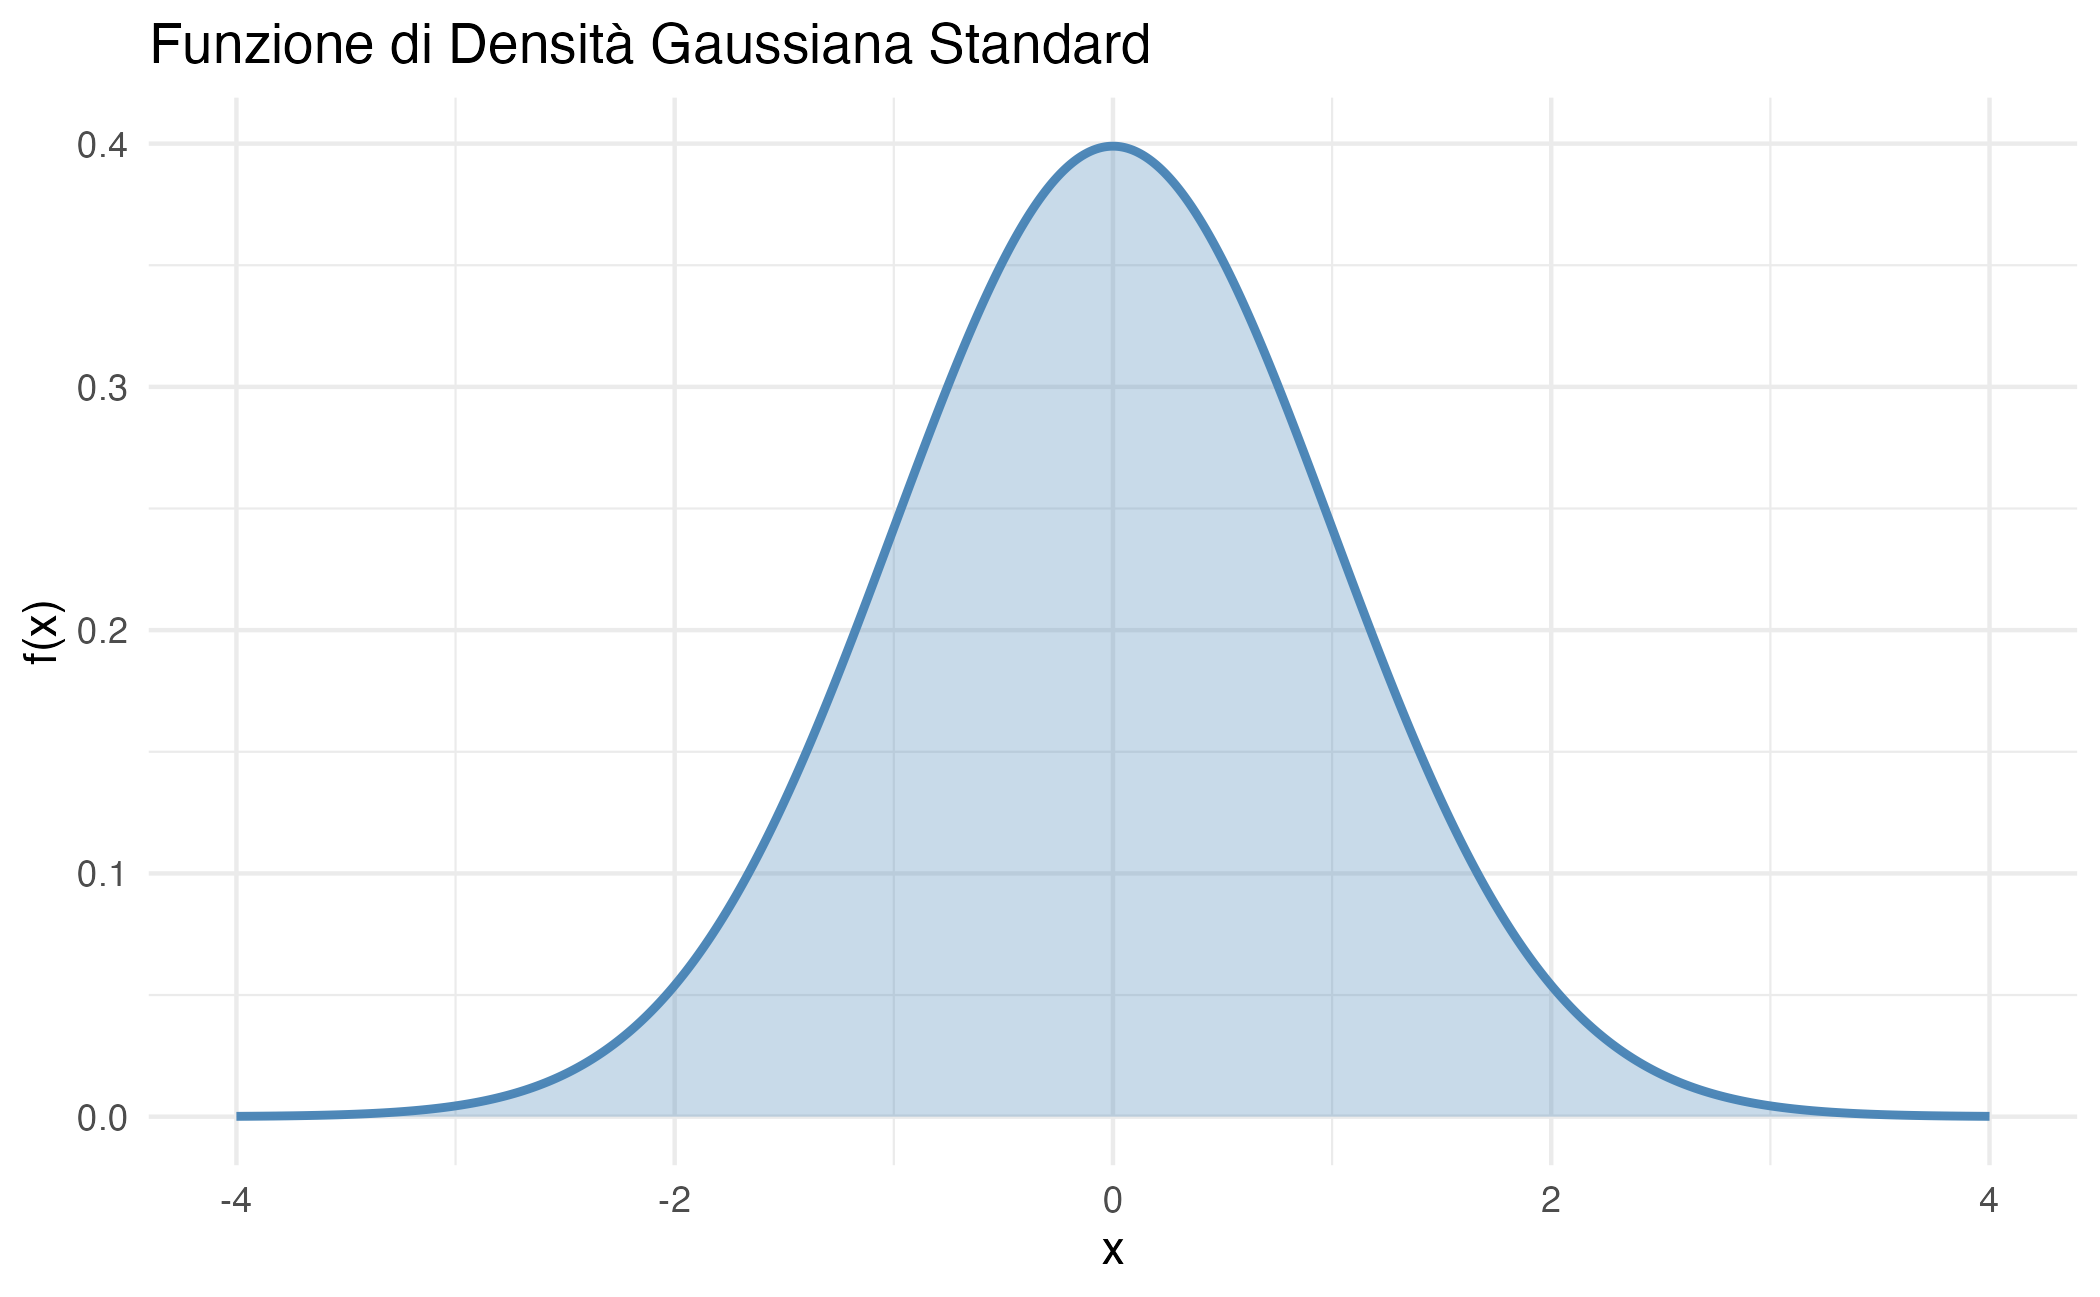
\includegraphics[width=0.85\linewidth,height=\textheight,keepaspectratio]{chapters/appendix/a15_calculus_files/figure-pdf/unnamed-chunk-3-1.png}
\end{center}

\subsection{Approssimazione dell'integrale mediante somma di
rettangoli}\label{approssimazione-dellintegrale-mediante-somma-di-rettangoli}

L'idea fondamentale dell'integrazione numerica è approssimare l'area
sotto la curva come somma di aree di rettangoli sottili. Questo metodo,
noto come \textbf{metodo dei rettangoli}, implementa concretamente il
concetto di integrale come ``somma di piccole parti''.

\subsubsection{Spiegazione dettagliata
dell'algoritmo}\label{spiegazione-dettagliata-dellalgoritmo}

La funzione \texttt{integrale\_approssimato} implementa il seguente
procedimento:

\begin{Shaded}
\begin{Highlighting}[]
\CommentTok{\# Funzione per approssimare l\textquotesingle{}integrale con il metodo dei rettangoli}
\NormalTok{integrale\_approssimato }\OtherTok{\textless{}{-}} \ControlFlowTok{function}\NormalTok{(f, a, b, }\AttributeTok{n =} \DecValTok{10000}\NormalTok{) \{}
  \CommentTok{\# 1. Calcolo della larghezza di ciascun rettangolo}
\NormalTok{  delta\_x }\OtherTok{\textless{}{-}}\NormalTok{ (b }\SpecialCharTok{{-}}\NormalTok{ a) }\SpecialCharTok{/}\NormalTok{ n}
  
  \CommentTok{\# 2. Creazione dei punti medi di ciascun intervallo}
\NormalTok{  x\_punti }\OtherTok{\textless{}{-}} \FunctionTok{seq}\NormalTok{(a }\SpecialCharTok{+}\NormalTok{ delta\_x}\SpecialCharTok{/}\DecValTok{2}\NormalTok{, b }\SpecialCharTok{{-}}\NormalTok{ delta\_x}\SpecialCharTok{/}\DecValTok{2}\NormalTok{, }\AttributeTok{length.out =}\NormalTok{ n)}
  
  \CommentTok{\# 3. Calcolo delle altezze dei rettangoli nei punti medi}
  \CommentTok{\# 4. Somma delle aree di tutti i rettangoli}
\NormalTok{  somme }\OtherTok{\textless{}{-}} \FunctionTok{sum}\NormalTok{(}\FunctionTok{f}\NormalTok{(x\_punti)) }\SpecialCharTok{*}\NormalTok{ delta\_x}
  
  \FunctionTok{return}\NormalTok{(somme)}
\NormalTok{\}}
\end{Highlighting}
\end{Shaded}

\begin{enumerate}
\def\labelenumi{\arabic{enumi}.}
\item
  \textbf{Suddivisione dell'intervallo.} L'intervallo \([a, b]\) viene
  diviso in \(n\) sottointervalli uguali. La larghezza di ciascun
  sottointervallo è \(\Delta x = \frac{b-a}{n}\). Più grande è \(n\),
  più stretti saranno i rettangoli e migliore sarà l'approssimazione.
\item
  \textbf{Selezione dei punti di valutazione.} Per ciascun
  sottointervallo, si sceglie il \textbf{punto medio} come
  rappresentativo dell'intero intervallo. I punti medi sono calcolati
  come: \(x_i = a + \frac{\Delta x}{2} + (i-1)\Delta x\), per
  \(i = 1, 2, \dots, n\). La scelta del punto medio garantisce una
  migliore approssimazione rispetto all'uso dell'estremo sinistro o
  destro.
\item
  \textbf{Calcolo delle altezze.} Per ciascun punto medio \(x_i\), si
  valuta la funzione: \(f(x_i)\). Questi valori rappresentano le altezze
  dei rettangoli.
\item
  \textbf{Calcolo delle aree e somma.} L'area di ciascun rettangolo è:
  \(\text{Area}_i = f(x_i) \cdot \Delta x\). L'area totale approssimata
  è: \(\text{Area}_{\text{tot}} = \sum_{i=1}^n f(x_i) \cdot \Delta x\).
\end{enumerate}

\subsubsection{Illustrazione grafica del
metodo}\label{illustrazione-grafica-del-metodo}

\begin{Shaded}
\begin{Highlighting}[]
\CommentTok{\# Visualizzazione del metodo dei rettangoli}
\NormalTok{visualizza\_rettangoli }\OtherTok{\textless{}{-}} \ControlFlowTok{function}\NormalTok{(f, a, b, }\AttributeTok{n =} \DecValTok{10}\NormalTok{) \{}
\NormalTok{  delta\_x }\OtherTok{\textless{}{-}}\NormalTok{ (b }\SpecialCharTok{{-}}\NormalTok{ a) }\SpecialCharTok{/}\NormalTok{ n}
\NormalTok{  x\_punti }\OtherTok{\textless{}{-}} \FunctionTok{seq}\NormalTok{(a }\SpecialCharTok{+}\NormalTok{ delta\_x}\SpecialCharTok{/}\DecValTok{2}\NormalTok{, b }\SpecialCharTok{{-}}\NormalTok{ delta\_x}\SpecialCharTok{/}\DecValTok{2}\NormalTok{, }\AttributeTok{length.out =}\NormalTok{ n)}
\NormalTok{  y\_punti }\OtherTok{\textless{}{-}} \FunctionTok{f}\NormalTok{(x\_punti)}
  
  \CommentTok{\# Creazione dei rettangoli per la visualizzazione}
\NormalTok{  rettangoli }\OtherTok{\textless{}{-}} \FunctionTok{data.frame}\NormalTok{(}
    \AttributeTok{x\_min =}\NormalTok{ x\_punti }\SpecialCharTok{{-}}\NormalTok{ delta\_x}\SpecialCharTok{/}\DecValTok{2}\NormalTok{,}
    \AttributeTok{x\_max =}\NormalTok{ x\_punti }\SpecialCharTok{+}\NormalTok{ delta\_x}\SpecialCharTok{/}\DecValTok{2}\NormalTok{,}
    \AttributeTok{y\_min =} \DecValTok{0}\NormalTok{,}
    \AttributeTok{y\_max =}\NormalTok{ y\_punti}
\NormalTok{  )}
  
  \CommentTok{\# Punti della funzione per il grafico}
\NormalTok{  x\_fine }\OtherTok{\textless{}{-}} \FunctionTok{seq}\NormalTok{(a, b, }\AttributeTok{length.out =} \DecValTok{1000}\NormalTok{)}
\NormalTok{  y\_fine }\OtherTok{\textless{}{-}} \FunctionTok{f}\NormalTok{(x\_fine)}
  
  \FunctionTok{ggplot}\NormalTok{() }\SpecialCharTok{+}
    \CommentTok{\# Area sotto la curva}
    \FunctionTok{geom\_area}\NormalTok{(}
      \AttributeTok{data =} \FunctionTok{data.frame}\NormalTok{(}\AttributeTok{x =}\NormalTok{ x\_fine, }\AttributeTok{y =}\NormalTok{ y\_fine),}
      \FunctionTok{aes}\NormalTok{(}\AttributeTok{x =}\NormalTok{ x, }\AttributeTok{y =}\NormalTok{ y),}
      \AttributeTok{fill =} \StringTok{"steelblue"}\NormalTok{,}
      \AttributeTok{alpha =} \FloatTok{0.2}
\NormalTok{    ) }\SpecialCharTok{+}
    \CommentTok{\# Rettangoli approssimanti}
    \FunctionTok{geom\_rect}\NormalTok{(}
      \AttributeTok{data =}\NormalTok{ rettangoli,}
      \FunctionTok{aes}\NormalTok{(}\AttributeTok{xmin =}\NormalTok{ x\_min, }\AttributeTok{xmax =}\NormalTok{ x\_max, }\AttributeTok{ymin =}\NormalTok{ y\_min, }\AttributeTok{ymax =}\NormalTok{ y\_max),}
      \AttributeTok{fill =} \StringTok{"red"}\NormalTok{,}
      \AttributeTok{alpha =} \FloatTok{0.3}\NormalTok{,}
      \AttributeTok{color =} \StringTok{"darkred"}
\NormalTok{    ) }\SpecialCharTok{+}
    \CommentTok{\# Linea della funzione}
    \FunctionTok{geom\_line}\NormalTok{(}
      \AttributeTok{data =} \FunctionTok{data.frame}\NormalTok{(}\AttributeTok{x =}\NormalTok{ x\_fine, }\AttributeTok{y =}\NormalTok{ y\_fine),}
      \FunctionTok{aes}\NormalTok{(}\AttributeTok{x =}\NormalTok{ x, }\AttributeTok{y =}\NormalTok{ y),}
      \AttributeTok{color =} \StringTok{"steelblue"}\NormalTok{,}
      \AttributeTok{linewidth =} \DecValTok{1}
\NormalTok{    ) }\SpecialCharTok{+}
    \FunctionTok{labs}\NormalTok{(}
      \AttributeTok{title =} \FunctionTok{paste}\NormalTok{(}\StringTok{"Approssimazione dell\textquotesingle{}integrale con"}\NormalTok{, n, }\StringTok{"rettangoli"}\NormalTok{),}
      \AttributeTok{x =} \StringTok{"x"}\NormalTok{,}
      \AttributeTok{y =} \StringTok{"f(x)"}
\NormalTok{    ) }\SpecialCharTok{+}
    \FunctionTok{theme\_minimal}\NormalTok{()}
\NormalTok{\}}

\CommentTok{\# Esempio con pochi rettangoli per visualizzare il metodo}
\FunctionTok{visualizza\_rettangoli}\NormalTok{(gaussiana, }\SpecialCharTok{{-}}\DecValTok{2}\NormalTok{, }\DecValTok{2}\NormalTok{, }\AttributeTok{n =} \DecValTok{10}\NormalTok{)}
\end{Highlighting}
\end{Shaded}

\begin{center}
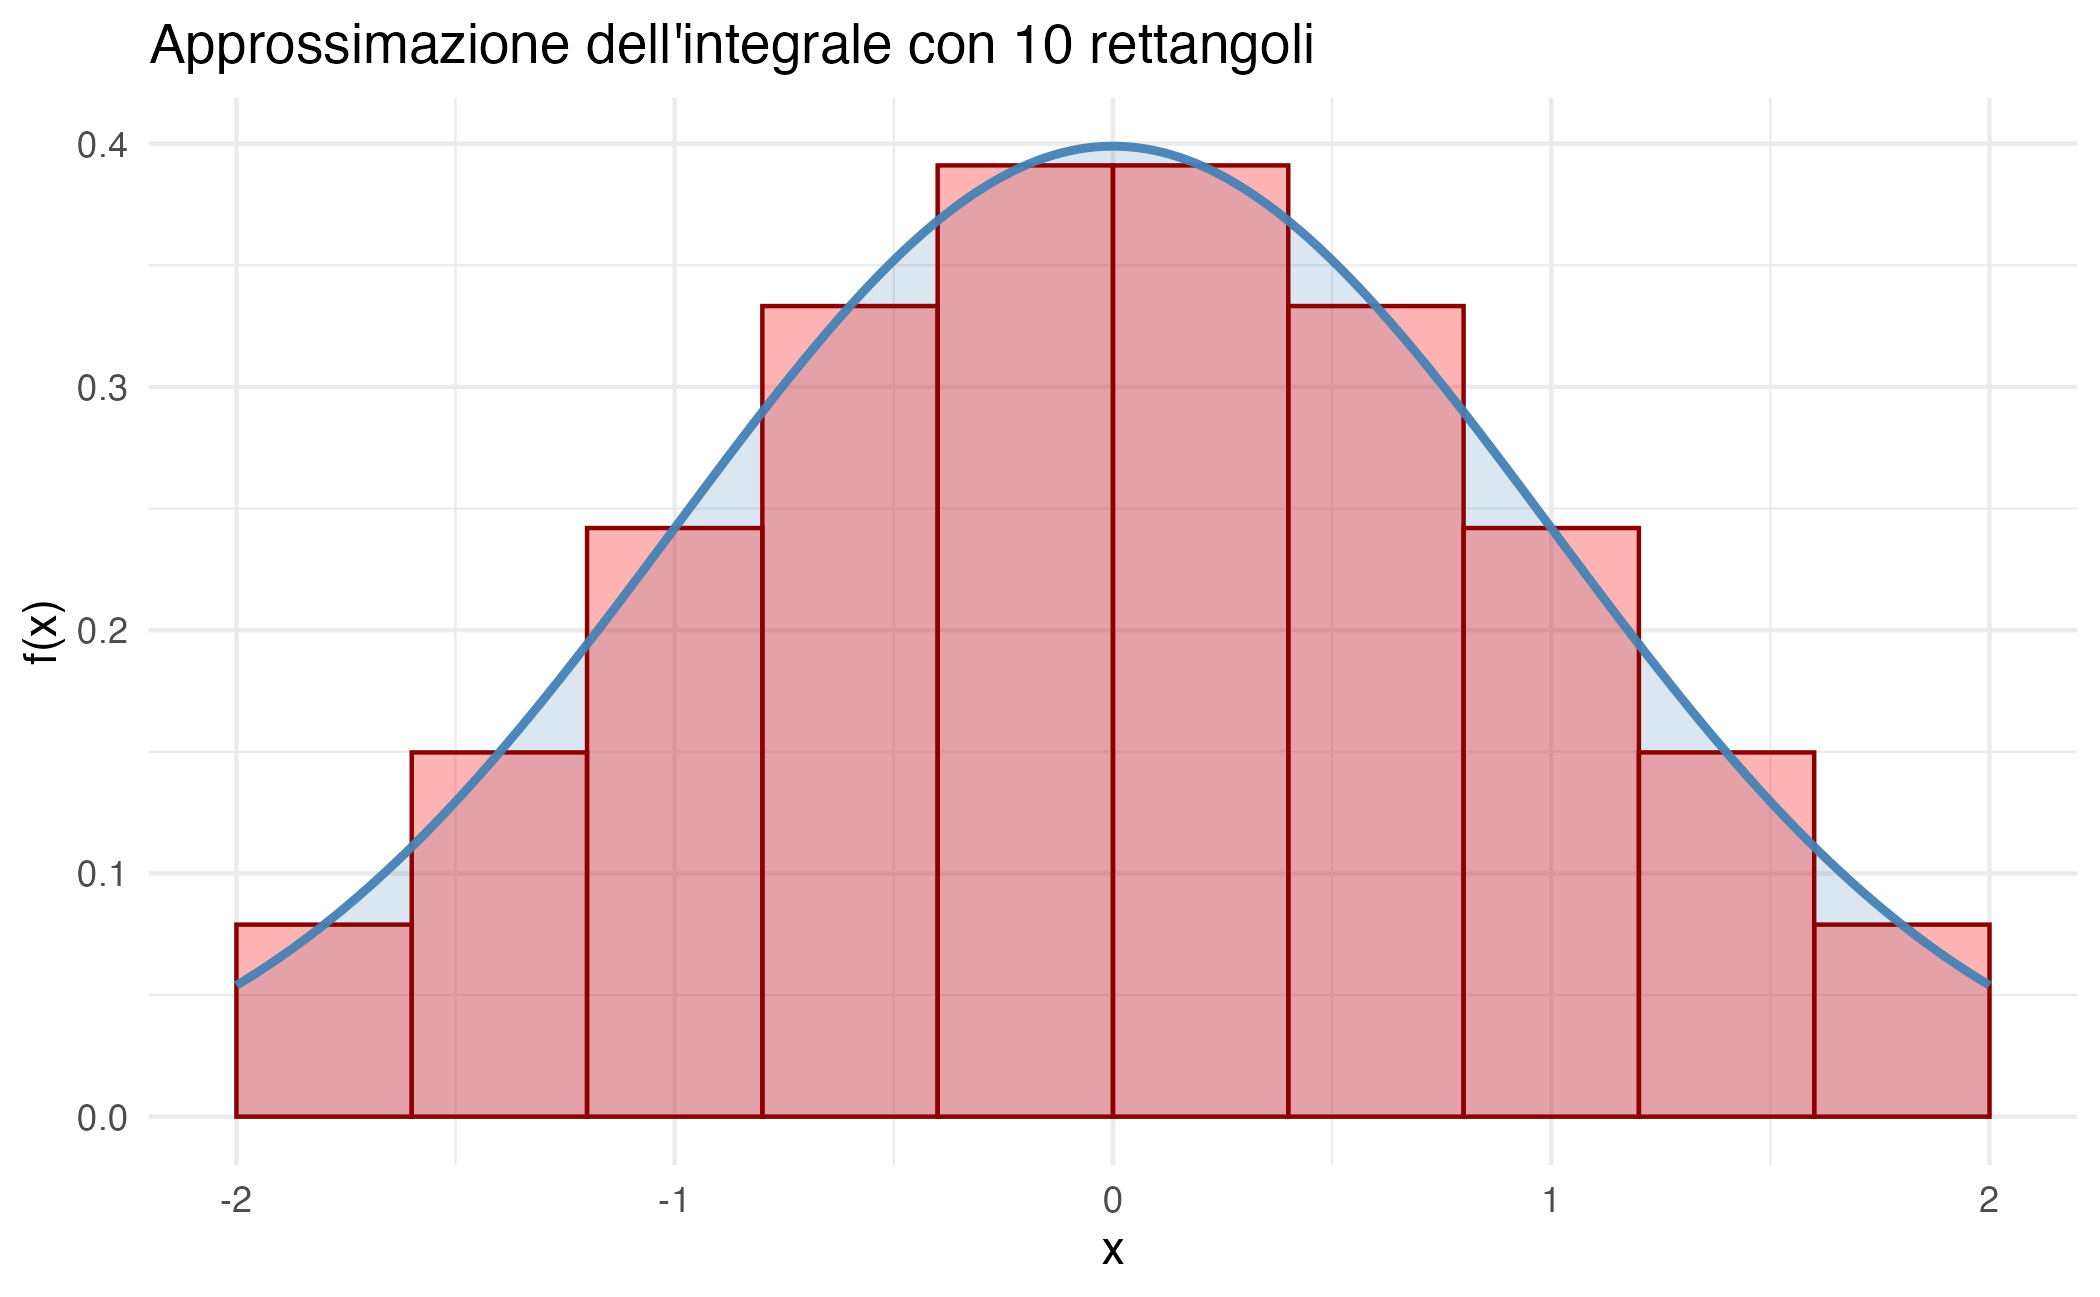
\includegraphics[width=0.85\linewidth,height=\textheight,keepaspectratio]{chapters/appendix/a15_calculus_files/figure-pdf/unnamed-chunk-5-1.png}
\end{center}

\subsubsection{Analisi dell'errore di
approssimazione}\label{analisi-dellerrore-di-approssimazione}

L'errore commesso dal metodo dei rettangoli diminuisce all'aumentare del
numero di suddivisioni \(n\):

\begin{Shaded}
\begin{Highlighting}[]
\CommentTok{\# Studio della convergenza al variare di n}
\NormalTok{studi\_convergenza }\OtherTok{\textless{}{-}} \ControlFlowTok{function}\NormalTok{(f, a, b, }\AttributeTok{n\_valori =} \FunctionTok{c}\NormalTok{(}\DecValTok{10}\NormalTok{, }\DecValTok{50}\NormalTok{, }\DecValTok{100}\NormalTok{, }\DecValTok{500}\NormalTok{, }\DecValTok{1000}\NormalTok{, }\DecValTok{5000}\NormalTok{, }\DecValTok{10000}\NormalTok{)) \{}
\NormalTok{  risultati }\OtherTok{\textless{}{-}} \FunctionTok{data.frame}\NormalTok{(}
    \AttributeTok{n =}\NormalTok{ n\_valori,}
    \AttributeTok{approssimato =} \FunctionTok{numeric}\NormalTok{(}\FunctionTok{length}\NormalTok{(n\_valori)),}
    \AttributeTok{errore\_relativo =} \FunctionTok{numeric}\NormalTok{(}\FunctionTok{length}\NormalTok{(n\_valori))}
\NormalTok{  )}
  
  \CommentTok{\# Valore "esatto" (calcolato con n molto grande)}
\NormalTok{  valore\_rif }\OtherTok{\textless{}{-}} \FunctionTok{integrate}\NormalTok{(f, }\AttributeTok{lower =}\NormalTok{ a, }\AttributeTok{upper =}\NormalTok{ b)}\SpecialCharTok{$}\NormalTok{value}
  
  \ControlFlowTok{for}\NormalTok{ (i }\ControlFlowTok{in} \FunctionTok{seq\_along}\NormalTok{(n\_valori)) \{}
\NormalTok{    approx }\OtherTok{\textless{}{-}} \FunctionTok{integrale\_approssimato}\NormalTok{(f, a, b, }\AttributeTok{n =}\NormalTok{ n\_valori[i])}
\NormalTok{    risultati}\SpecialCharTok{$}\NormalTok{approssimato[i] }\OtherTok{\textless{}{-}}\NormalTok{ approx}
\NormalTok{    risultati}\SpecialCharTok{$}\NormalTok{errore\_relativo[i] }\OtherTok{\textless{}{-}} \FunctionTok{abs}\NormalTok{(approx }\SpecialCharTok{{-}}\NormalTok{ valore\_rif) }\SpecialCharTok{/}\NormalTok{ valore\_rif}
\NormalTok{  \}}
  
  \FunctionTok{return}\NormalTok{(risultati)}
\NormalTok{\}}

\CommentTok{\# Applicazione alla gaussiana tra {-}1.96 e 1.96}
\NormalTok{convergenza }\OtherTok{\textless{}{-}} \FunctionTok{studi\_convergenza}\NormalTok{(gaussiana, }\SpecialCharTok{{-}}\FloatTok{1.96}\NormalTok{, }\FloatTok{1.96}\NormalTok{)}

\CommentTok{\# Visualizzazione della convergenza}
\FunctionTok{ggplot}\NormalTok{(convergenza, }\FunctionTok{aes}\NormalTok{(}\AttributeTok{x =}\NormalTok{ n, }\AttributeTok{y =}\NormalTok{ errore\_relativo)) }\SpecialCharTok{+}
  \FunctionTok{geom\_point}\NormalTok{(}\AttributeTok{color =} \StringTok{"red"}\NormalTok{, }\AttributeTok{size =} \DecValTok{3}\NormalTok{) }\SpecialCharTok{+}
  \FunctionTok{geom\_line}\NormalTok{(}\AttributeTok{color =} \StringTok{"red"}\NormalTok{, }\AttributeTok{alpha =} \FloatTok{0.5}\NormalTok{) }\SpecialCharTok{+}
  \FunctionTok{scale\_x\_log10}\NormalTok{() }\SpecialCharTok{+}
  \FunctionTok{scale\_y\_log10}\NormalTok{() }\SpecialCharTok{+}
  \FunctionTok{labs}\NormalTok{(}
    \AttributeTok{title =} \StringTok{"Convergenza del metodo dei rettangoli"}\NormalTok{,}
    \AttributeTok{x =} \StringTok{"Numero di rettangoli (scala logaritmica)"}\NormalTok{,}
    \AttributeTok{y =} \StringTok{"Errore relativo (scala logaritmica)"}
\NormalTok{  ) }\SpecialCharTok{+}
  \FunctionTok{theme\_minimal}\NormalTok{()}
\end{Highlighting}
\end{Shaded}

\begin{center}
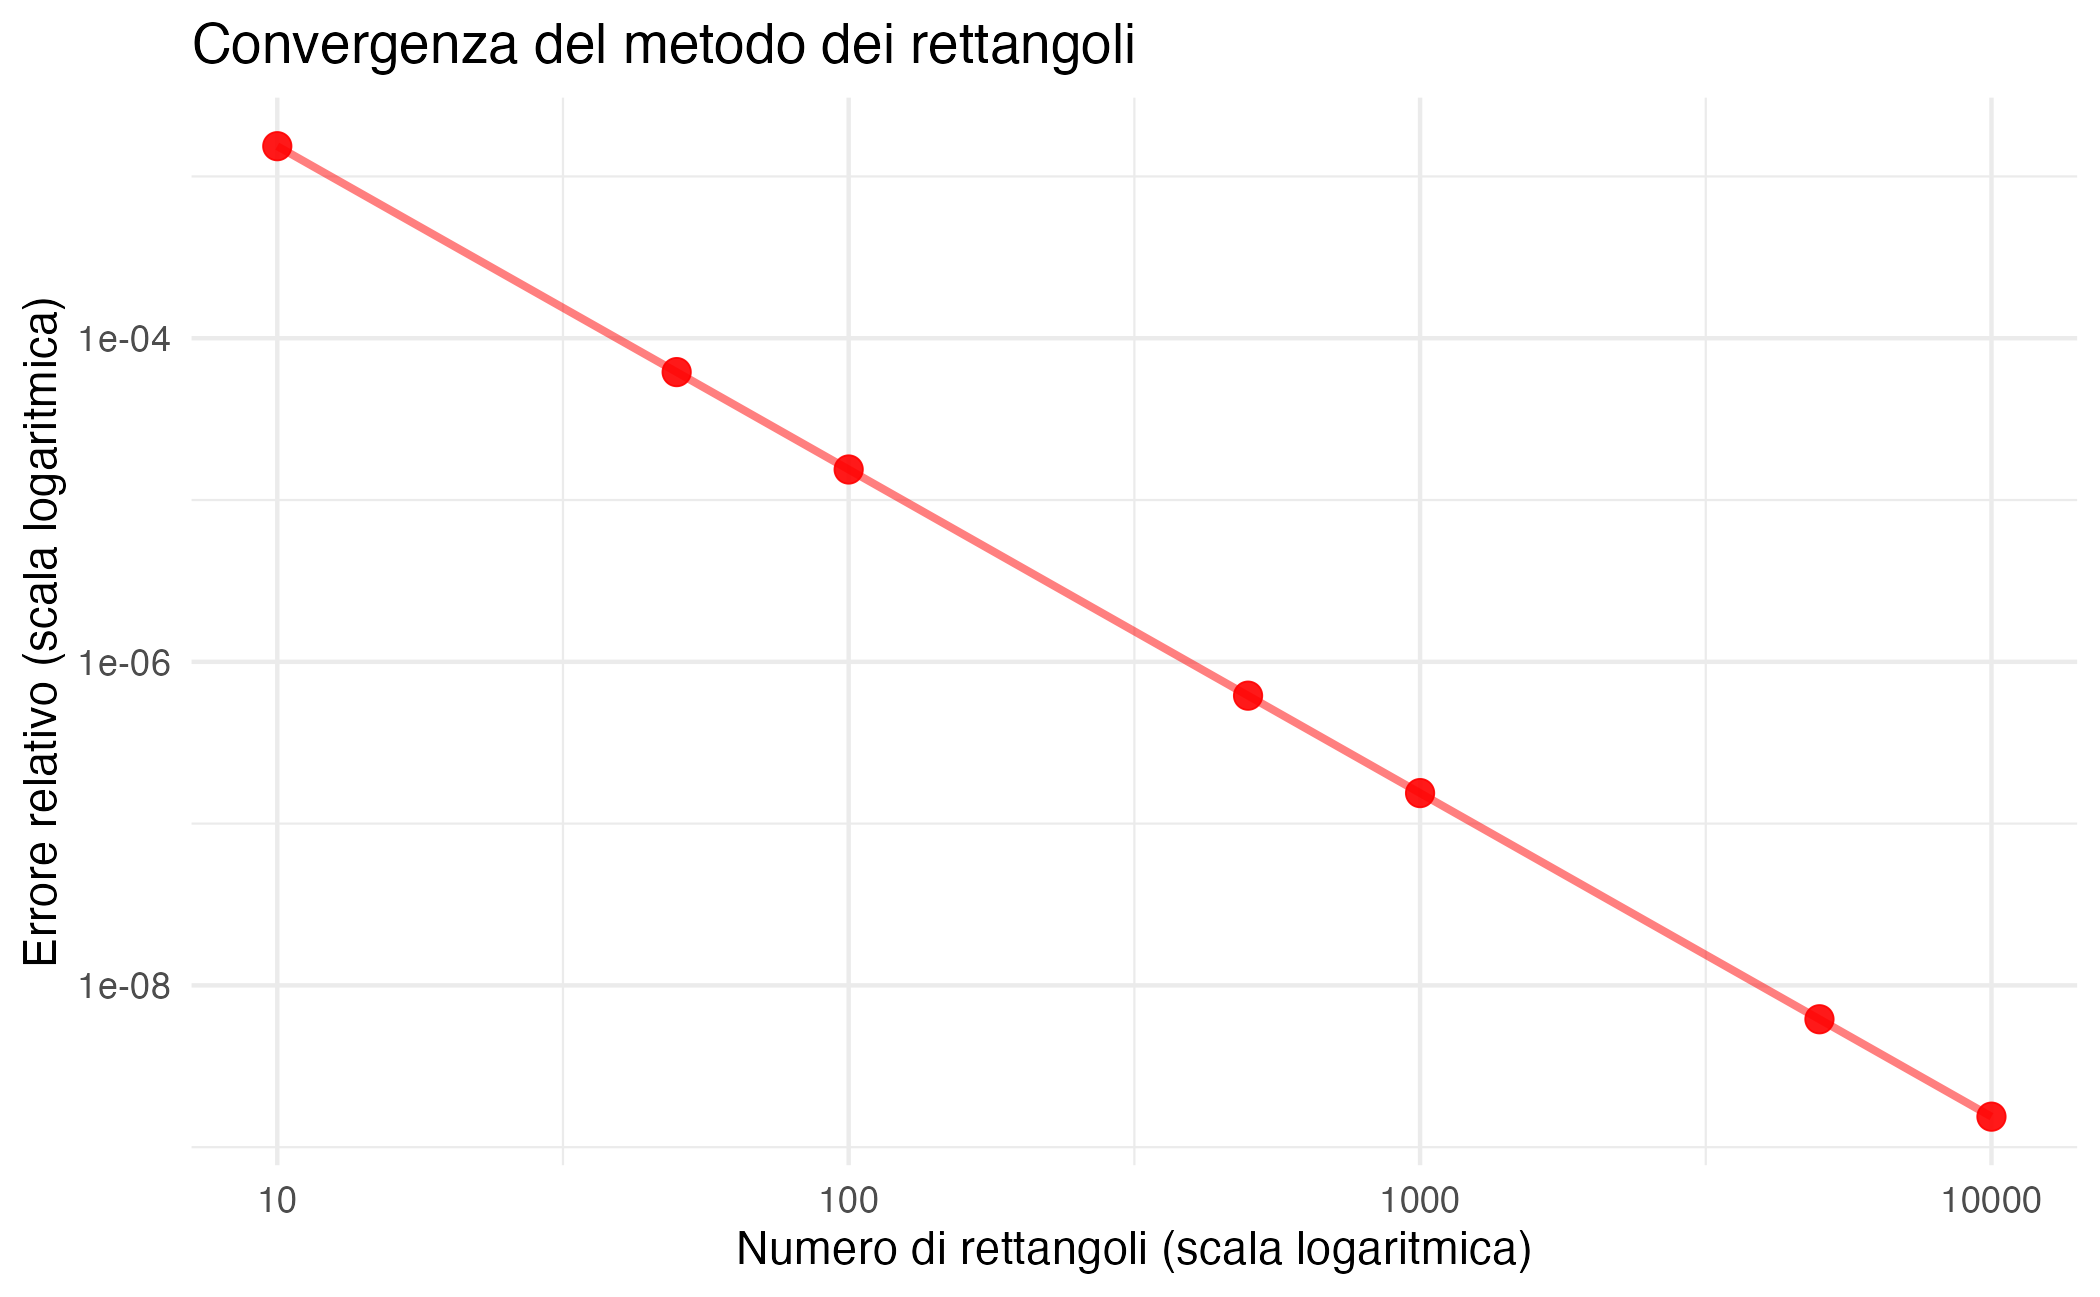
\includegraphics[width=0.85\linewidth,height=\textheight,keepaspectratio]{chapters/appendix/a15_calculus_files/figure-pdf/unnamed-chunk-6-1.png}
\end{center}

\subsubsection{Interpretazione
matematica}\label{interpretazione-matematica}

Matematicamente, l'approssimazione converge all'integrale vero quando
\(n \to \infty\):

\[
\lim_{n \to \infty} \sum_{i=1}^n f(x_i) \cdot \Delta x = \int_a^b f(x) \, dx,
\] dove \(x_i\) sono i punti medi degli intervalli. Questo è
precisamente il significato dell'integrale definito secondo Riemann: la
somma delle aree di rettangoli infinitamente sottili che approssimano
sempre meglio l'area sotto la curva.

\subsubsection{Vantaggi e limiti del
metodo}\label{vantaggi-e-limiti-del-metodo}

Il metodo dei rettangoli presenta diversi aspetti positivi. La sua
implementazione è semplice e intuitiva, in quanto si basa direttamente
sull'idea geometrica di approssimare un'area con la somma di aree
rettangolari. La sua chiarezza concettuale lo rende anche facile da
visualizzare, facilitando la comprensione del principio di integrazione
numerica. Per funzioni sufficientemente regolari, il metodo può
garantire un'elevata accuratezza, a condizione che si utilizzi un numero
adeguato di suddivisioni.

Tuttavia, il metodo presenta anche notevoli limitazioni. La sua velocità
di convergenza è relativamente lenta, dell'ordine di \(O(1/n)\), il che
significa che per dimezzare l'errore è necessario raddoppiare il numero
di rettangoli. Ciò lo rende poco efficiente per le funzioni dal
comportamento irregolare o con punti di discontinuità. Per ottenere
un'elevata precisione, è necessario un numero considerevole di
valutazioni della funzione, il che comporta un aumento del costo
computazionale.

Esistono metodi di integrazione numerica più sofisticati, come quelli
implementati nella funzione \texttt{integrate()} di R. La regola di
Simpson, per esempio, utilizza parabole anziché di rettangoli per
approssimare la funzione, raggiungendo una velocità di convergenza
superiore (\(O(1/n^4)\)). Le tecniche di quadratura adattiva modificano
dinamicamente la densità dei punti di valutazione in base alle
caratteristiche locali della funzione, concentrando il calcolo nelle
regioni più problematiche. Per problemi di integrazione
multidimensionale, l'integrazione Monte Carlo è spesso un'alternativa
efficace.

Questo esempio mostra chiaramente come il concetto astratto di integrale
possa essere implementato in modo computazionale, collegando la
definizione matematica formale alla sua applicazione pratica
nell'analisi numerica.

\chapter{Problemi comuni con R, Stan e
CmdStanR}\label{sec-troubleshooting}

\begin{tcolorbox}[enhanced jigsaw, arc=.35mm, bottomrule=.15mm, bottomtitle=1mm, breakable, colback=white, colbacktitle=quarto-callout-note-color!10!white, colframe=quarto-callout-note-color-frame, coltitle=black, left=2mm, leftrule=.75mm, opacityback=0, opacitybacktitle=0.6, rightrule=.15mm, title=\textcolor{quarto-callout-note-color}{\faInfo}\hspace{0.5em}{Come usare questa appendice}, titlerule=0mm, toprule=.15mm, toptitle=1mm]

Questa appendice è una guida di pronto intervento. Non introduce nuovi
concetti statistici e non sostituisce le appendici dedicate a CmdStanR,
Stan, diagnostiche MCMC e controlli predittivi. Serve invece quando il
workflow si blocca: il codice non parte, il modello non compila, le
catene danno avvisi, le simulazioni non hanno senso o i risultati
sembrano difficili da interpretare.

L'idea di fondo è semplice: davanti a un errore non chiederti subito
``qual è il comando giusto?''. Chiediti prima \textbf{in quale punto del
workflow si è verificato il problema}. Un errore di installazione, un
errore di sintassi Stan, un problema di campionamento e una cattiva
specificazione del modello richiedono risposte diverse.

\end{tcolorbox}

\section{Mappa rapida dei problemi}\label{mappa-rapida-dei-problemi}

{\def\LTcaptype{none} % do not increment counter
\begin{longtable}[]{@{}
  >{\raggedright\arraybackslash}p{(\linewidth - 4\tabcolsep) * \real{0.3333}}
  >{\raggedright\arraybackslash}p{(\linewidth - 4\tabcolsep) * \real{0.3333}}
  >{\raggedright\arraybackslash}p{(\linewidth - 4\tabcolsep) * \real{0.3333}}@{}}
\toprule\noalign{}
\begin{minipage}[b]{\linewidth}\raggedright
Se succede questo
\end{minipage} & \begin{minipage}[b]{\linewidth}\raggedright
Probabile area del problema
\end{minipage} & \begin{minipage}[b]{\linewidth}\raggedright
Prima cosa da controllare
\end{minipage} \\
\midrule\noalign{}
\endhead
\bottomrule\noalign{}
\endlastfoot
R non trova una funzione & Pacchetti R & Il pacchetto è installato e
caricato? \\
CmdStanR non trova CmdStan & Installazione & Il percorso di CmdStan è
configurato? \\
Stan non compila il modello & Sintassi o tipi Stan & Le variabili
dichiarate corrispondono ai dati passati? \\
Il modello compila ma il sampling fallisce & Valori iniziali, vincoli,
likelihood & I dati rispettano i vincoli dichiarati? \\
Ci sono divergent transitions & Geometria della posterior & Il modello è
parametrizzato bene? Le prior sono ragionevoli? \\
\texttt{Rhat} è alto & Mancata convergenza & Le catene esplorano la
stessa regione? \\
ESS è basso & Stima instabile & Servono più iterazioni o un modello
meglio parametrizzato? \\
Le predizioni a priori sono assurde & Prior o modello generativo & Le
prior generano valori plausibili sulla scala dei dati? \\
Le predizioni posteriori non somigliano ai dati & Misfit del modello &
La likelihood descrive davvero il processo osservato? \\
Il risultato è statisticamente corretto ma non interpretabile & Scala e
comunicazione & I parametri sono sulla scala psicologica giusta? \\
\end{longtable}
}

\begin{tcolorbox}[enhanced jigsaw, arc=.35mm, bottomrule=.15mm, bottomtitle=1mm, breakable, colback=white, colbacktitle=quarto-callout-tip-color!10!white, colframe=quarto-callout-tip-color-frame, coltitle=black, left=2mm, leftrule=.75mm, opacityback=0, opacitybacktitle=0.6, rightrule=.15mm, title=\textcolor{quarto-callout-tip-color}{\faLightbulb}\hspace{0.5em}{Regola pratica}, titlerule=0mm, toprule=.15mm, toptitle=1mm]

Non correggere un problema computazionale cambiando subito la domanda
scientifica, e non correggere un problema teorico aumentando soltanto
\texttt{adapt\_delta} o il numero di iterazioni. Prima identifica il
tipo di problema.

\end{tcolorbox}

\section{Prima diagnosi: dove si è fermato il
workflow?}\label{prima-diagnosi-dove-si-uxe8-fermato-il-workflow}

Quando qualcosa non funziona, prova a classificare il problema in una di
queste cinque categorie.

\begin{enumerate}
\def\labelenumi{\arabic{enumi}.}
\tightlist
\item
  \textbf{Ambiente di lavoro}: R, RStudio, pacchetti, CmdStan,
  compilatore C++ o percorsi dei file.
\item
  \textbf{Codice R}: oggetti non trovati, nomi incoerenti, dataframe mal
  costruiti, dati non nel formato atteso.
\item
  \textbf{Codice Stan}: errori di sintassi, dichiarazioni sbagliate,
  dimensioni incompatibili, vincoli non rispettati.
\item
  \textbf{Campionamento MCMC}: divergenze, \texttt{Rhat}, ESS, massima
  profondità dell'albero, catene lente o bloccate.
\item
  \textbf{Modello statistico}: prior implausibili, likelihood inadatta,
  predizioni non realistiche, interpretazione fragile.
\end{enumerate}

\subsection{Domande minime}\label{domande-minime}

\begin{itemize}
\tightlist
\item[$\square$]
  L'errore compare prima di compilare il modello?
\item[$\square$]
  L'errore compare durante la compilazione Stan?
\item[$\square$]
  Il modello compila ma non produce campioni affidabili?
\item[$\square$]
  Il modello produce campioni, ma le diagnostiche sono problematiche?
\item[$\square$]
  Le diagnostiche sono accettabili, ma il modello non descrive bene i
  dati?
\item[$\square$]
  Il modello descrive i dati, ma il risultato non risponde alla domanda
  psicologica iniziale?
\end{itemize}

Queste domande aiutano a evitare un errore comune: trattare tutti i
problemi come se fossero problemi di codice. In molti casi, invece, il
codice sta eseguendo correttamente un modello poco adatto.

\section{Problemi con pacchetti R}\label{problemi-con-pacchetti-r}

\subsection{Sintomo}\label{sintomo}

R restituisce messaggi come:

\begin{Shaded}
\begin{Highlighting}[]
\NormalTok{could not find }\ControlFlowTok{function} \StringTok{"..."}
\NormalTok{there is no package called }\StringTok{"..."}
\NormalTok{object }\StringTok{\textquotesingle{}...\textquotesingle{}}\NormalTok{ not found}
\end{Highlighting}
\end{Shaded}

\subsection{Controlli}\label{controlli}

\begin{itemize}
\tightlist
\item[$\square$]
  Il pacchetto è installato?
\item[$\square$]
  Il pacchetto è caricato con \texttt{library()}?
\item[$\square$]
  Il nome della funzione è scritto correttamente?
\item[$\square$]
  La funzione appartiene davvero a quel pacchetto?
\item[$\square$]
  Hai riavviato la sessione R dopo un'installazione importante?
\end{itemize}

\subsection{Comandi utili}\label{comandi-utili}

\begin{Shaded}
\begin{Highlighting}[]
\FunctionTok{installed.packages}\NormalTok{()[, }\StringTok{"Package"}\NormalTok{]}

\FunctionTok{library}\NormalTok{(cmdstanr)}
\FunctionTok{library}\NormalTok{(posterior)}
\FunctionTok{library}\NormalTok{(bayesplot)}
\FunctionTok{library}\NormalTok{(ggplot2)}
\end{Highlighting}
\end{Shaded}

Per verificare se una funzione esiste in un pacchetto:

\begin{Shaded}
\begin{Highlighting}[]
\FunctionTok{help}\NormalTok{(}\AttributeTok{package =} \StringTok{"cmdstanr"}\NormalTok{)}
\NormalTok{?cmdstanr}\SpecialCharTok{::}\NormalTok{cmdstan\_model}
\end{Highlighting}
\end{Shaded}

\begin{tcolorbox}[enhanced jigsaw, arc=.35mm, bottomrule=.15mm, bottomtitle=1mm, breakable, colback=white, colbacktitle=quarto-callout-warning-color!10!white, colframe=quarto-callout-warning-color-frame, coltitle=black, left=2mm, leftrule=.75mm, opacityback=0, opacitybacktitle=0.6, rightrule=.15mm, title=\textcolor{quarto-callout-warning-color}{\faExclamationTriangle}\hspace{0.5em}{Attenzione ai nomi simili}, titlerule=0mm, toprule=.15mm, toptitle=1mm]

Molti errori derivano da piccoli cambiamenti nei nomi: \texttt{fit},
\texttt{fits}, \texttt{fit1}; \texttt{data}, \texttt{dat},
\texttt{stan\_data}; \texttt{subject}, \texttt{subjects}, \texttt{id}.
Nel workflow bayesiano conviene usare nomi chiari e coerenti, perché lo
stesso oggetto passa spesso da R a Stan e poi torna in R come risultato.

\end{tcolorbox}

\section{Problemi con i percorsi dei
file}\label{problemi-con-i-percorsi-dei-file}

\subsection{Sintomo}\label{sintomo-1}

R o CmdStanR non trovano un file:

\begin{Shaded}
\begin{Highlighting}[]
\NormalTok{cannot open file }\StringTok{\textquotesingle{}model.stan\textquotesingle{}}
\NormalTok{No such file or directory}
\end{Highlighting}
\end{Shaded}

\subsection{Controlli}\label{controlli-1}

\begin{itemize}
\tightlist
\item[$\square$]
  Il file \texttt{.stan} si trova davvero nella cartella indicata?
\item[$\square$]
  La working directory è quella che pensi?
\item[$\square$]
  Il percorso contiene spazi, accenti o caratteri speciali?
\item[$\square$]
  Stai usando percorsi relativi in modo coerente?
\item[$\square$]
  Il file è stato salvato prima di compilare?
\end{itemize}

\subsection{Comandi utili}\label{comandi-utili-1}

\begin{Shaded}
\begin{Highlighting}[]
\FunctionTok{getwd}\NormalTok{()}
\FunctionTok{list.files}\NormalTok{()}
\FunctionTok{file.exists}\NormalTok{(}\StringTok{"model.stan"}\NormalTok{)}
\end{Highlighting}
\end{Shaded}

Se il modello è in una sottocartella:

\begin{Shaded}
\begin{Highlighting}[]
\FunctionTok{file.exists}\NormalTok{(}\StringTok{"stan/model.stan"}\NormalTok{)}
\end{Highlighting}
\end{Shaded}

\subsection{Buona pratica}\label{buona-pratica}

In un progetto didattico, conviene mantenere una struttura semplice:

\begin{Shaded}
\begin{Highlighting}[]
\NormalTok{progetto/}
\NormalTok{  analisi.qmd}
\NormalTok{  data/}
\NormalTok{    dati.csv}
\NormalTok{  stan/}
\NormalTok{    modello.stan}
\NormalTok{  output/}
\end{Highlighting}
\end{Shaded}

Questo rende più facile capire dove si trovano dati, modelli e
risultati.

\section{CmdStanR non trova CmdStan}\label{cmdstanr-non-trova-cmdstan}

\subsection{Sintomo}\label{sintomo-2}

CmdStanR è installato, ma non riesce a trovare CmdStan o segnala che
CmdStan non è configurato.

\subsection{Controlli}\label{controlli-2}

\begin{itemize}
\tightlist
\item[$\square$]
  Il pacchetto \texttt{cmdstanr} è installato?
\item[$\square$]
  CmdStan è stato installato tramite \texttt{install\_cmdstan()}?
\item[$\square$]
  Il percorso di CmdStan è corretto?
\item[$\square$]
  Il compilatore C++ è disponibile nel sistema?
\item[$\square$]
  La sessione R è stata riavviata dopo l'installazione?
\end{itemize}

\subsection{Comandi utili}\label{comandi-utili-2}

\begin{Shaded}
\begin{Highlighting}[]
\FunctionTok{library}\NormalTok{(cmdstanr)}
\FunctionTok{cmdstan\_version}\NormalTok{()}
\FunctionTok{cmdstan\_path}\NormalTok{()}
\FunctionTok{check\_cmdstan\_toolchain}\NormalTok{()}
\end{Highlighting}
\end{Shaded}

Se CmdStan non è installato:

\begin{Shaded}
\begin{Highlighting}[]
\FunctionTok{install\_cmdstan}\NormalTok{()}
\end{Highlighting}
\end{Shaded}

Se CmdStan è installato ma non viene trovato:

\begin{Shaded}
\begin{Highlighting}[]
\FunctionTok{set\_cmdstan\_path}\NormalTok{(}\StringTok{"/percorso/alla/cartella/cmdstan"}\NormalTok{)}
\end{Highlighting}
\end{Shaded}

\begin{tcolorbox}[enhanced jigsaw, arc=.35mm, bottomrule=.15mm, bottomtitle=1mm, breakable, colback=white, colbacktitle=quarto-callout-tip-color!10!white, colframe=quarto-callout-tip-color-frame, coltitle=black, left=2mm, leftrule=.75mm, opacityback=0, opacitybacktitle=0.6, rightrule=.15mm, title=\textcolor{quarto-callout-tip-color}{\faLightbulb}\hspace{0.5em}{Prima di cambiare il modello}, titlerule=0mm, toprule=.15mm, toptitle=1mm]

Se CmdStan non è configurato correttamente, nessun modello Stan
funzionerà. In questo caso il problema non riguarda l'inferenza, le
prior o i dati: riguarda l'ambiente computazionale.

\end{tcolorbox}

\section{Il modello Stan non compila}\label{il-modello-stan-non-compila}

\subsection{Sintomo}\label{sintomo-3}

La chiamata a \texttt{cmdstan\_model()} produce un errore. Il modello
non arriva alla fase di sampling.

\begin{Shaded}
\begin{Highlighting}[]
\NormalTok{mod }\OtherTok{\textless{}{-}} \FunctionTok{cmdstan\_model}\NormalTok{(}\StringTok{"modello.stan"}\NormalTok{)}
\end{Highlighting}
\end{Shaded}

\subsection{Cause comuni}\label{cause-comuni}

\begin{itemize}
\tightlist
\item
  parentesi, virgole o punti e virgola mancanti;
\item
  blocchi Stan scritti nell'ordine sbagliato;
\item
  variabili usate ma non dichiarate;
\item
  nomi diversi tra dati R e dati Stan;
\item
  vettori, matrici o array con dimensioni incompatibili;
\item
  uso scorretto di distribuzioni e parametri;
\item
  vincoli non coerenti con i dati.
\end{itemize}

\subsection{Controlli}\label{controlli-3}

\begin{itemize}
\tightlist
\item[$\square$]
  Ogni istruzione Stan termina con \texttt{;}?
\item[$\square$]
  Ogni variabile usata nel modello è dichiarata in un blocco
  appropriato?
\item[$\square$]
  I nomi nel blocco \texttt{data} coincidono con quelli della lista R
  passata a Stan?
\item[$\square$]
  Le dimensioni dichiarate in Stan corrispondono alle dimensioni degli
  oggetti R?
\item[$\square$]
  Le variabili intere sono dichiarate come \texttt{int} e quelle
  continue come \texttt{real}?
\item[$\square$]
  I vincoli, per esempio \texttt{\textless{}lower=0\textgreater{}}, sono
  compatibili con i dati?
\end{itemize}

\subsection{Esempio: nome incoerente tra R e
Stan}\label{esempio-nome-incoerente-tra-r-e-stan}

Nel file Stan:

\begin{Shaded}
\begin{Highlighting}[]
\KeywordTok{data}\NormalTok{ \{}
  \DataTypeTok{int}\NormalTok{\textless{}}\KeywordTok{lower}\NormalTok{=}\DecValTok{1}\NormalTok{\textgreater{} N;}
  \DataTypeTok{vector}\NormalTok{[N] y;}
\NormalTok{\}}
\end{Highlighting}
\end{Shaded}

In R:

\begin{Shaded}
\begin{Highlighting}[]
\NormalTok{stan\_data }\OtherTok{\textless{}{-}} \FunctionTok{list}\NormalTok{(}
  \AttributeTok{n =} \FunctionTok{nrow}\NormalTok{(dati),}
  \AttributeTok{y =}\NormalTok{ dati}\SpecialCharTok{$}\NormalTok{y}
\NormalTok{)}
\end{Highlighting}
\end{Shaded}

Qui Stan aspetta \texttt{N}, ma R fornisce \texttt{n}. La correzione è
rendere coerenti i nomi:

\begin{Shaded}
\begin{Highlighting}[]
\NormalTok{stan\_data }\OtherTok{\textless{}{-}} \FunctionTok{list}\NormalTok{(}
  \AttributeTok{N =} \FunctionTok{nrow}\NormalTok{(dati),}
  \AttributeTok{y =}\NormalTok{ dati}\SpecialCharTok{$}\NormalTok{y}
\NormalTok{)}
\end{Highlighting}
\end{Shaded}

\begin{tcolorbox}[enhanced jigsaw, arc=.35mm, bottomrule=.15mm, bottomtitle=1mm, breakable, colback=white, colbacktitle=quarto-callout-warning-color!10!white, colframe=quarto-callout-warning-color-frame, coltitle=black, left=2mm, leftrule=.75mm, opacityback=0, opacitybacktitle=0.6, rightrule=.15mm, title=\textcolor{quarto-callout-warning-color}{\faExclamationTriangle}\hspace{0.5em}{Stan distingue maiuscole e minuscole}, titlerule=0mm, toprule=.15mm, toptitle=1mm]

\texttt{N} e \texttt{n} sono due nomi diversi. Lo stesso vale per
\texttt{Y}, \texttt{y}, \texttt{sigma\_y} e \texttt{sigmaY}. Questa
distinzione è una fonte molto comune di errori.

\end{tcolorbox}

\section{Il modello compila ma il sampling
fallisce}\label{il-modello-compila-ma-il-sampling-fallisce}

\subsection{Sintomo}\label{sintomo-4}

Il modello compila, ma durante il sampling compaiono errori come valori
non finiti, log probability non definita o inizializzazione fallita.

\subsection{Cause comuni}\label{cause-comuni-1}

\begin{itemize}
\tightlist
\item
  i dati violano i vincoli dichiarati;
\item
  una deviazione standard può diventare negativa;
\item
  una probabilità non resta tra 0 e 1;
\item
  una trasformazione produce \texttt{log(0)} o divisione per zero;
\item
  la likelihood riceve valori impossibili;
\item
  le prior consentono valori numericamente estremi.
\end{itemize}

\subsection{Controlli}\label{controlli-4}

\begin{itemize}
\tightlist
\item[$\square$]
  Le variabili che devono essere positive sono davvero positive?
\item[$\square$]
  Le probabilità sono comprese tra 0 e 1?
\item[$\square$]
  Ci sono valori mancanti (\texttt{NA}) nei dati?
\item[$\square$]
  Ci sono valori infiniti o non numerici?
\item[$\square$]
  Le scale dei dati sono ragionevoli?
\item[$\square$]
  Le prior generano valori estremi che rendono instabile la likelihood?
\end{itemize}

\subsection{Comandi utili in R}\label{comandi-utili-in-r}

\begin{Shaded}
\begin{Highlighting}[]
\FunctionTok{summary}\NormalTok{(dati)}
\FunctionTok{colSums}\NormalTok{(}\FunctionTok{is.na}\NormalTok{(dati))}
\FunctionTok{range}\NormalTok{(dati}\SpecialCharTok{$}\NormalTok{y, }\AttributeTok{na.rm =} \ConstantTok{TRUE}\NormalTok{)}
\FunctionTok{any}\NormalTok{(}\SpecialCharTok{!}\FunctionTok{is.finite}\NormalTok{(dati}\SpecialCharTok{$}\NormalTok{y))}
\end{Highlighting}
\end{Shaded}

\begin{tcolorbox}[enhanced jigsaw, arc=.35mm, bottomrule=.15mm, bottomtitle=1mm, breakable, colback=white, colbacktitle=quarto-callout-tip-color!10!white, colframe=quarto-callout-tip-color-frame, coltitle=black, left=2mm, leftrule=.75mm, opacityback=0, opacitybacktitle=0.6, rightrule=.15mm, title=\textcolor{quarto-callout-tip-color}{\faLightbulb}\hspace{0.5em}{Controlla i dati prima di controllare Stan}, titlerule=0mm, toprule=.15mm, toptitle=1mm]

Molti errori attribuiti a Stan derivano in realtà da dati con
\texttt{NA}, valori fuori scala, fattori non convertiti, codifiche
incoerenti o variabili non centrate quando il modello lo richiede.

\end{tcolorbox}

\section{Divergent transitions}\label{divergent-transitions}

\subsection{Sintomo}\label{sintomo-5}

Dopo il sampling compare un messaggio del tipo:

\begin{Shaded}
\begin{Highlighting}[]
\NormalTok{There were ... divergent transitions after warmup.}
\end{Highlighting}
\end{Shaded}

\subsection{Che cosa significa}\label{che-cosa-significa}

Le divergenze indicano che l'algoritmo ha difficoltà a esplorare alcune
regioni della distribuzione a posteriori. Non sono un dettaglio
estetico: possono rendere le stime inaffidabili, soprattutto per
parametri o combinazioni di parametri legati alla zona problematica.

\subsection{Risposte possibili}\label{risposte-possibili}

\begin{enumerate}
\def\labelenumi{\arabic{enumi}.}
\tightlist
\item
  \textbf{Aumentare \texttt{adapt\_delta}} può aiutare, ma non deve
  essere l'unica risposta.
\item
  \textbf{Riscrivere il modello} può essere necessario se la geometria
  della posterior è difficile.
\item
  \textbf{Controllare le prior} può ridurre regioni implausibili o
  estreme.
\item
  \textbf{Riscalare le variabili} può migliorare la geometria del
  problema.
\item
  \textbf{Usare parametrizzazioni non centrate} può aiutare nei modelli
  gerarchici.
\end{enumerate}

\subsection{Primo intervento
ragionevole}\label{primo-intervento-ragionevole}

\begin{Shaded}
\begin{Highlighting}[]
\NormalTok{fit }\OtherTok{\textless{}{-}}\NormalTok{ mod}\SpecialCharTok{$}\FunctionTok{sample}\NormalTok{(}
  \AttributeTok{data =}\NormalTok{ stan\_data,}
  \AttributeTok{chains =} \DecValTok{4}\NormalTok{,}
  \AttributeTok{parallel\_chains =} \DecValTok{4}\NormalTok{,}
  \AttributeTok{adapt\_delta =} \FloatTok{0.95}
\NormalTok{)}
\end{Highlighting}
\end{Shaded}

Se le divergenze restano, provare:

\begin{Shaded}
\begin{Highlighting}[]
\NormalTok{fit }\OtherTok{\textless{}{-}}\NormalTok{ mod}\SpecialCharTok{$}\FunctionTok{sample}\NormalTok{(}
  \AttributeTok{data =}\NormalTok{ stan\_data,}
  \AttributeTok{chains =} \DecValTok{4}\NormalTok{,}
  \AttributeTok{parallel\_chains =} \DecValTok{4}\NormalTok{,}
  \AttributeTok{adapt\_delta =} \FloatTok{0.99}
\NormalTok{)}
\end{Highlighting}
\end{Shaded}

\subsection{Ma poi bisogna chiedersi}\label{ma-poi-bisogna-chiedersi}

\begin{itemize}
\tightlist
\item[$\square$]
  Le variabili predittive sono su scale molto diverse?
\item[$\square$]
  Ci sono parametri debolmente identificati?
\item[$\square$]
  Le prior sono troppo vaghe o troppo estreme?
\item[$\square$]
  Il modello gerarchico usa una parametrizzazione centrata quando i dati
  per gruppo sono pochi?
\item[$\square$]
  La likelihood è adatta al tipo di dati?
\end{itemize}

\begin{tcolorbox}[enhanced jigsaw, arc=.35mm, bottomrule=.15mm, bottomtitle=1mm, breakable, colback=white, colbacktitle=quarto-callout-warning-color!10!white, colframe=quarto-callout-warning-color-frame, coltitle=black, left=2mm, leftrule=.75mm, opacityback=0, opacitybacktitle=0.6, rightrule=.15mm, title=\textcolor{quarto-callout-warning-color}{\faExclamationTriangle}\hspace{0.5em}{Non nascondere le divergenze}, titlerule=0mm, toprule=.15mm, toptitle=1mm]

Un modello con divergenze non dovrebbe essere presentato come se fosse
pienamente affidabile. Se il problema non viene risolto, va dichiarato
come limite dell'analisi.

\end{tcolorbox}

\section{Massima profondità
dell'albero}\label{massima-profondituxe0-dellalbero}

\subsection{Sintomo}\label{sintomo-6}

Compare un messaggio simile a:

\begin{Shaded}
\begin{Highlighting}[]
\NormalTok{maximum treedepth exceeded}
\end{Highlighting}
\end{Shaded}

\subsection{Che cosa significa}\label{che-cosa-significa-1}

L'algoritmo sta impiegando molti passi per esplorare la posterior.
Questo può indicare una geometria difficile, una parametrizzazione
inefficiente o scale poco adatte.

\subsection{Cosa fare}\label{cosa-fare}

\begin{itemize}
\tightlist
\item[$\square$]
  Controllare se ci sono anche divergenze.
\item[$\square$]
  Riscalare o centrare i predittori.
\item[$\square$]
  Esaminare parametri fortemente correlati.
\item[$\square$]
  Valutare una parametrizzazione alternativa.
\item[$\square$]
  Solo dopo, considerare di aumentare \texttt{max\_treedepth}.
\end{itemize}

Esempio:

\begin{Shaded}
\begin{Highlighting}[]
\NormalTok{fit }\OtherTok{\textless{}{-}}\NormalTok{ mod}\SpecialCharTok{$}\FunctionTok{sample}\NormalTok{(}
  \AttributeTok{data =}\NormalTok{ stan\_data,}
  \AttributeTok{chains =} \DecValTok{4}\NormalTok{,}
  \AttributeTok{parallel\_chains =} \DecValTok{4}\NormalTok{,}
  \AttributeTok{max\_treedepth =} \DecValTok{12}
\NormalTok{)}
\end{Highlighting}
\end{Shaded}

\begin{tcolorbox}[enhanced jigsaw, arc=.35mm, bottomrule=.15mm, bottomtitle=1mm, breakable, colback=white, colbacktitle=quarto-callout-note-color!10!white, colframe=quarto-callout-note-color-frame, coltitle=black, left=2mm, leftrule=.75mm, opacityback=0, opacitybacktitle=0.6, rightrule=.15mm, title=\textcolor{quarto-callout-note-color}{\faInfo}\hspace{0.5em}{Aumentare \texttt{max\_treedepth} non corregge il modello}, titlerule=0mm, toprule=.15mm, toptitle=1mm]

Può permettere all'algoritmo di lavorare più a lungo, ma se la geometria
della posterior è problematica, il problema statistico resta.

\end{tcolorbox}

\section{\texorpdfstring{\texttt{Rhat} maggiore di
1}{Rhat maggiore di 1}}\label{rhat-maggiore-di-1}

\subsection{Sintomo}\label{sintomo-7}

Nella tabella dei risultati alcuni parametri hanno \texttt{Rhat}
maggiore di 1, o comunque non vicino a 1.

\subsection{Che cosa significa}\label{che-cosa-significa-2}

Le catene non stanno producendo campioni compatibili tra loro. In
pratica, diverse catene potrebbero esplorare regioni diverse della
posterior. Questo segnala che la stima non è ancora affidabile.

\subsection{Cosa controllare}\label{cosa-controllare}

\begin{itemize}
\tightlist
\item[$\square$]
  Le catene hanno tracce simili?
\item[$\square$]
  Ci sono catene bloccate o molto lente?
\item[$\square$]
  Il numero di iterazioni è sufficiente?
\item[$\square$]
  Ci sono divergenze o problemi di treedepth?
\item[$\square$]
  Il modello è identificato dai dati?
\item[$\square$]
  Le prior aiutano a stabilizzare parametri debolmente informati?
\end{itemize}

\subsection{Comandi utili}\label{comandi-utili-3}

\begin{Shaded}
\begin{Highlighting}[]
\NormalTok{fit}\SpecialCharTok{$}\FunctionTok{summary}\NormalTok{()}
\NormalTok{fit}\SpecialCharTok{$}\FunctionTok{cmdstan\_diagnose}\NormalTok{()}
\end{Highlighting}
\end{Shaded}

Con \texttt{bayesplot}:

\begin{Shaded}
\begin{Highlighting}[]
\FunctionTok{mcmc\_trace}\NormalTok{(fit}\SpecialCharTok{$}\FunctionTok{draws}\NormalTok{(}\FunctionTok{c}\NormalTok{(}\StringTok{"alpha"}\NormalTok{, }\StringTok{"beta"}\NormalTok{, }\StringTok{"sigma"}\NormalTok{)))}
\end{Highlighting}
\end{Shaded}

\begin{tcolorbox}[enhanced jigsaw, arc=.35mm, bottomrule=.15mm, bottomtitle=1mm, breakable, colback=white, colbacktitle=quarto-callout-tip-color!10!white, colframe=quarto-callout-tip-color-frame, coltitle=black, left=2mm, leftrule=.75mm, opacityback=0, opacitybacktitle=0.6, rightrule=.15mm, title=\textcolor{quarto-callout-tip-color}{\faLightbulb}\hspace{0.5em}{Guarda le catene, non solo la tabella}, titlerule=0mm, toprule=.15mm, toptitle=1mm]

Un valore numerico può segnalare un problema, ma i trace plot aiutano a
capire se le catene mescolano bene, se una catena è bloccata o se la
posterior ha regioni separate.

\end{tcolorbox}

\section{ESS basso}\label{ess-basso}

\subsection{Sintomo}\label{sintomo-8}

L'Effective Sample Size, spesso indicato come ESS, è basso per uno o più
parametri.

\subsection{Che cosa significa}\label{che-cosa-significa-3}

Anche se il modello ha prodotto molti campioni, l'informazione effettiva
può essere molto inferiore se i campioni sono fortemente autocorrelati o
se l'algoritmo esplora lentamente la posterior.

\subsection{Cosa fare}\label{cosa-fare-1}

\begin{itemize}
\tightlist
\item[$\square$]
  Aumentare il numero di iterazioni può aiutare.
\item[$\square$]
  Controllare \texttt{Rhat} e divergenze.
\item[$\square$]
  Esaminare trace plot e autocorrelazione.
\item[$\square$]
  Riscalare predittori e outcome, se necessario.
\item[$\square$]
  Valutare una parametrizzazione diversa.
\end{itemize}

Esempio:

\begin{Shaded}
\begin{Highlighting}[]
\NormalTok{fit }\OtherTok{\textless{}{-}}\NormalTok{ mod}\SpecialCharTok{$}\FunctionTok{sample}\NormalTok{(}
  \AttributeTok{data =}\NormalTok{ stan\_data,}
  \AttributeTok{chains =} \DecValTok{4}\NormalTok{,}
  \AttributeTok{parallel\_chains =} \DecValTok{4}\NormalTok{,}
  \AttributeTok{iter\_warmup =} \DecValTok{1000}\NormalTok{,}
  \AttributeTok{iter\_sampling =} \DecValTok{2000}
\NormalTok{)}
\end{Highlighting}
\end{Shaded}

\subsection{Interpretazione}\label{interpretazione-5}

ESS basso non significa automaticamente che il modello sia
concettualmente sbagliato, ma significa che le sintesi numeriche
potrebbero essere instabili. Prima di interpretare con sicurezza medie,
intervalli o probabilità posteriori, è necessario migliorare o almeno
valutare la qualità della stima.

\section{BFMI basso}\label{bfmi-basso}

\subsection{Sintomo}\label{sintomo-9}

La diagnostica segnala un problema con BFMI, cioè con l'esplorazione
dell'energia da parte del campionatore.

\subsection{Che cosa significa}\label{che-cosa-significa-4}

Il campionatore fatica a muoversi efficientemente nella distribuzione.
Spesso questo accade in modelli con scale molto diverse, gerarchie
difficili o parametri debolmente identificati.

\subsection{Cosa fare}\label{cosa-fare-2}

\begin{itemize}
\tightlist
\item[$\square$]
  Controllare le divergenze.
\item[$\square$]
  Controllare scale e standardizzazione dei predittori.
\item[$\square$]
  Esaminare parametri gerarchici e deviazioni standard.
\item[$\square$]
  Considerare una parametrizzazione non centrata.
\item[$\square$]
  Rendere le prior più informative, se scientificamente giustificato.
\end{itemize}

\begin{tcolorbox}[enhanced jigsaw, arc=.35mm, bottomrule=.15mm, bottomtitle=1mm, breakable, colback=white, colbacktitle=quarto-callout-warning-color!10!white, colframe=quarto-callout-warning-color-frame, coltitle=black, left=2mm, leftrule=.75mm, opacityback=0, opacitybacktitle=0.6, rightrule=.15mm, title=\textcolor{quarto-callout-warning-color}{\faExclamationTriangle}\hspace{0.5em}{BFMI non è un dettaglio secondario}, titlerule=0mm, toprule=.15mm, toptitle=1mm]

Se BFMI è problematico, il campionatore potrebbe non esplorare
correttamente parti importanti della posterior. Il risultato va trattato
con cautela.

\end{tcolorbox}

\section{Prior predictive check: simulazioni
assurde}\label{prior-predictive-check-simulazioni-assurde}

\subsection{Sintomo}\label{sintomo-10}

Prima di osservare i dati, il modello genera valori impossibili o
implausibili: punteggi negativi su scale che non lo consentono, tempi di
reazione enormi, probabilità fuori scala, differenze psicologicamente
irrealistiche.

\subsection{Che cosa significa}\label{che-cosa-significa-5}

Il problema non è nei dati, perché i dati non sono ancora stati usati.
Il problema è nella combinazione tra modello generativo e prior.

\subsection{Cosa controllare}\label{cosa-controllare-1}

\begin{itemize}
\tightlist
\item[$\square$]
  La likelihood è adatta alla scala della variabile?
\item[$\square$]
  Le prior sui parametri generano valori plausibili sulla scala
  osservabile?
\item[$\square$]
  Le variabili sono state centrate o standardizzate come previsto?
\item[$\square$]
  I parametri sono interpretati sulla scala corretta?
\item[$\square$]
  Le prior sono troppo vaghe rispetto al fenomeno psicologico?
\end{itemize}

\subsection{Esempio concettuale}\label{esempio-concettuale}

Se un questionario produce punteggi tra 0 e 40, una prior che genera
frequentemente valori predetti tra -100 e 200 non è neutrale: è una
prior che assegna massa a mondi poco plausibili per quel fenomeno e
quella misura.

\begin{tcolorbox}[enhanced jigsaw, arc=.35mm, bottomrule=.15mm, bottomtitle=1mm, breakable, colback=white, colbacktitle=quarto-callout-tip-color!10!white, colframe=quarto-callout-tip-color-frame, coltitle=black, left=2mm, leftrule=.75mm, opacityback=0, opacitybacktitle=0.6, rightrule=.15mm, title=\textcolor{quarto-callout-tip-color}{\faLightbulb}\hspace{0.5em}{Domanda guida}, titlerule=0mm, toprule=.15mm, toptitle=1mm]

Prima dei dati, il modello riesce a immaginare dati che potrebbero
davvero provenire da uno studio psicologico come quello in esame?

\end{tcolorbox}

\section{Posterior predictive check: il modello non riproduce i
dati}\label{posterior-predictive-check-il-modello-non-riproduce-i-dati}

\subsection{Sintomo}\label{sintomo-11}

Dopo la stima, i dati simulati dalla posterior non assomigliano ai dati
osservati in aspetti importanti.

\subsection{Possibili segnali}\label{possibili-segnali}

\begin{itemize}
\tightlist
\item
  la variabilità simulata è troppo piccola o troppo grande;
\item
  il modello non riproduce asimmetrie o code;
\item
  il modello non cattura differenze tra gruppi;
\item
  il modello ignora dipendenze tra osservazioni;
\item
  il modello predice valori fuori dalla scala possibile;
\item
  il modello riproduce la media ma non la distribuzione.
\end{itemize}

\subsection{Cosa fare}\label{cosa-fare-3}

\begin{itemize}
\tightlist
\item[$\square$]
  La likelihood è coerente con il tipo di dato?
\item[$\square$]
  Manca una struttura gerarchica?
\item[$\square$]
  Manca un predittore teoricamente rilevante?
\item[$\square$]
  La variabilità individuale è rappresentata?
\item[$\square$]
  Ci sono effetti non lineari o interazioni importanti?
\item[$\square$]
  Il modello è troppo rigido per la domanda posta?
\end{itemize}

\subsection{Interpretazione}\label{interpretazione-6}

Un posterior predictive check problematico non significa che l'analisi
sia fallita. Significa che il modello ha rivelato una discrepanza tra le
sue assunzioni e i dati. Questo è esattamente il ruolo del workflow:
usare i controlli per imparare dove il modello è insufficiente.

\begin{tcolorbox}[enhanced jigsaw, arc=.35mm, bottomrule=.15mm, bottomtitle=1mm, breakable, colback=white, colbacktitle=quarto-callout-warning-color!10!white, colframe=quarto-callout-warning-color-frame, coltitle=black, left=2mm, leftrule=.75mm, opacityback=0, opacitybacktitle=0.6, rightrule=.15mm, title=\textcolor{quarto-callout-warning-color}{\faExclamationTriangle}\hspace{0.5em}{Non basta stimare bene un modello sbagliato}, titlerule=0mm, toprule=.15mm, toptitle=1mm]

Un modello può avere diagnostiche MCMC accettabili e allo stesso tempo
descrivere male i dati. Le diagnostiche MCMC controllano la qualità del
campionamento; i posterior predictive checks controllano la qualità
descrittiva del modello.

\end{tcolorbox}

\section{Sensibilità alle prior}\label{sensibilituxe0-alle-prior}

\subsection{Sintomo}\label{sintomo-12}

Le conclusioni cambiano molto quando si modificano prior ragionevoli.

\subsection{Che cosa significa}\label{che-cosa-significa-6}

I dati potrebbero non essere abbastanza informativi per stabilizzare
l'inferenza, oppure alcune prior potrebbero essere troppo deboli, troppo
forti o poco coerenti con la scala del problema.

\subsection{Cosa controllare}\label{cosa-controllare-2}

\begin{itemize}
\tightlist
\item[$\square$]
  Le prior alternative sono tutte scientificamente plausibili?
\item[$\square$]
  I dati sono pochi rispetto alla complessità del modello?
\item[$\square$]
  Il parametro è debolmente identificato?
\item[$\square$]
  La conclusione principale dipende da una scelta arbitraria?
\item[$\square$]
  La sensibilità riguarda il risultato sostantivo o solo dettagli
  numerici?
\end{itemize}

\subsection{Buona pratica}\label{buona-pratica-1}

Quando la sensibilità è rilevante, non nasconderla. Una formulazione
trasparente potrebbe essere:

\begin{quote}
Le conclusioni sono stabili per prior debolmente informative entro un
intervallo plausibile. Tuttavia, per prior molto concentrate vicino a
zero, l'intervallo di credibilità si restringe e la probabilità di un
effetto positivo diminuisce.
\end{quote}

Oppure:

\begin{quote}
I dati non sono sufficientemente informativi per distinguere tra queste
specificazioni. La conclusione deve quindi essere considerata
esplorativa.
\end{quote}

\section{Problemi di scala e
interpretazione}\label{problemi-di-scala-e-interpretazione}

\subsection{Sintomo}\label{sintomo-13}

Il modello funziona, ma i coefficienti sono difficili da interpretare.

\subsection{Cause comuni}\label{cause-comuni-2}

\begin{itemize}
\tightlist
\item
  predittori non centrati;
\item
  scale arbitrarie dei questionari;
\item
  outcome standardizzato ma interpretato come punteggio originale;
\item
  coefficienti logit interpretati come differenze di probabilità;
\item
  effetti su scala log interpretati come differenze lineari;
\item
  interazioni interpretate senza calcolare quantità predette.
\end{itemize}

\subsection{Cosa fare}\label{cosa-fare-4}

\begin{itemize}
\tightlist
\item[$\square$]
  Riporta sempre la scala su cui vive il parametro.
\item[$\square$]
  Traduci i coefficienti in quantità psicologicamente comprensibili.
\item[$\square$]
  Usa predizioni marginali o differenze predette quando aiutano
  l'interpretazione.
\item[$\square$]
  Evita di comunicare solo coefficienti astratti.
\item[$\square$]
  Chiediti quale quantità risponde davvero alla domanda scientifica.
\end{itemize}

\subsection{Esempio}\label{esempio}

In una regressione logistica, un coefficiente positivo indica un aumento
sullo scale logit, non direttamente un aumento costante in probabilità.
Per comunicarlo, spesso è più chiaro mostrare probabilità predette per
casi rappresentativi.

\section{Errori con variabili
categoriali}\label{errori-con-variabili-categoriali}

\subsection{Sintomo}\label{sintomo-14}

Il modello produce risultati inattesi quando si usano gruppi, condizioni
sperimentali o categorie diagnostiche.

\subsection{Cause comuni}\label{cause-comuni-3}

\begin{itemize}
\tightlist
\item
  una variabile categoriale è stata trattata come numerica;
\item
  il gruppo di riferimento non è quello atteso;
\item
  le etichette dei livelli sono in ordine alfabetico, non teorico;
\item
  ci sono livelli vuoti o rari;
\item
  la codifica in R non corrisponde a quella usata nel modello.
\end{itemize}

\subsection{Controlli}\label{controlli-5}

\begin{Shaded}
\begin{Highlighting}[]
\FunctionTok{table}\NormalTok{(dati}\SpecialCharTok{$}\NormalTok{gruppo)}
\FunctionTok{levels}\NormalTok{(dati}\SpecialCharTok{$}\NormalTok{gruppo)}
\FunctionTok{contrasts}\NormalTok{(dati}\SpecialCharTok{$}\NormalTok{gruppo)}
\end{Highlighting}
\end{Shaded}

\subsection{Buona pratica}\label{buona-pratica-2}

Prima di stimare il modello, scrivi in linguaggio naturale che cosa
rappresenta ogni coefficiente. Se non riesci a farlo, probabilmente la
codifica delle variabili non è ancora chiara.

\section{Errori con dati gerarchici}\label{errori-con-dati-gerarchici}

\subsection{Sintomo}\label{sintomo-15}

Il modello ignora il fatto che le osservazioni sono raggruppate: prove
dentro persone, studenti dentro classi, pazienti dentro terapeuti, item
dentro partecipanti.

\subsection{Segnali di attenzione}\label{segnali-di-attenzione}

\begin{itemize}
\tightlist
\item
  più osservazioni per la stessa persona;
\item
  più item per lo stesso costrutto;
\item
  partecipanti provenienti da laboratori diversi;
\item
  terapeuti, scuole, classi o reparti;
\item
  misure longitudinali.
\end{itemize}

\subsection{Domande di controllo}\label{domande-di-controllo-13}

\begin{itemize}
\tightlist
\item[$\square$]
  Le osservazioni sono davvero indipendenti?
\item[$\square$]
  Quali unità generano variabilità: persone, item, gruppi, contesti?
\item[$\square$]
  Serve un modello multilevel?
\item[$\square$]
  Il modello rappresenta differenze individuali?
\item[$\square$]
  Ci sono abbastanza dati per stimare la struttura gerarchica
  desiderata?
\end{itemize}

\begin{tcolorbox}[enhanced jigsaw, arc=.35mm, bottomrule=.15mm, bottomtitle=1mm, breakable, colback=white, colbacktitle=quarto-callout-tip-color!10!white, colframe=quarto-callout-tip-color-frame, coltitle=black, left=2mm, leftrule=.75mm, opacityback=0, opacitybacktitle=0.6, rightrule=.15mm, title=\textcolor{quarto-callout-tip-color}{\faLightbulb}\hspace{0.5em}{Per la psicologia}, titlerule=0mm, toprule=.15mm, toptitle=1mm]

Molti dati psicologici sono gerarchici anche quando il dataset appare
come una tabella piatta. Ignorare questa struttura può produrre
incertezza sottostimata e conclusioni troppo sicure.

\end{tcolorbox}

\section{Il modello è troppo lento}\label{il-modello-uxe8-troppo-lento}

\subsection{Sintomo}\label{sintomo-16}

Il modello richiede molto tempo per compilare o campionare.

\subsection{Possibili cause}\label{possibili-cause}

\begin{itemize}
\tightlist
\item
  modello molto complesso;
\item
  troppi parametri rispetto ai dati;
\item
  likelihood costosa;
\item
  dati non vettorizzati;
\item
  parametrizzazione inefficiente;
\item
  hardware limitato;
\item
  numero di catene o iterazioni troppo alto per una prova iniziale.
\end{itemize}

\subsection{Strategia didattica}\label{strategia-didattica}

Prima di lanciare il modello completo:

\begin{enumerate}
\def\labelenumi{\arabic{enumi}.}
\tightlist
\item
  prova il modello su pochi dati simulati;
\item
  riduci temporaneamente il numero di iterazioni;
\item
  verifica che la struttura funzioni;
\item
  controlla che le quantità recuperate abbiano senso;
\item
  solo dopo passa al dataset completo.
\end{enumerate}

Esempio per una prova rapida:

\begin{Shaded}
\begin{Highlighting}[]
\NormalTok{fit\_test }\OtherTok{\textless{}{-}}\NormalTok{ mod}\SpecialCharTok{$}\FunctionTok{sample}\NormalTok{(}
  \AttributeTok{data =}\NormalTok{ stan\_data,}
  \AttributeTok{chains =} \DecValTok{2}\NormalTok{,}
  \AttributeTok{parallel\_chains =} \DecValTok{2}\NormalTok{,}
  \AttributeTok{iter\_warmup =} \DecValTok{200}\NormalTok{,}
  \AttributeTok{iter\_sampling =} \DecValTok{200}
\NormalTok{)}
\end{Highlighting}
\end{Shaded}

\begin{tcolorbox}[enhanced jigsaw, arc=.35mm, bottomrule=.15mm, bottomtitle=1mm, breakable, colback=white, colbacktitle=quarto-callout-warning-color!10!white, colframe=quarto-callout-warning-color-frame, coltitle=black, left=2mm, leftrule=.75mm, opacityback=0, opacitybacktitle=0.6, rightrule=.15mm, title=\textcolor{quarto-callout-warning-color}{\faExclamationTriangle}\hspace{0.5em}{Le prove rapide non sono risultati finali}, titlerule=0mm, toprule=.15mm, toptitle=1mm]

Poche iterazioni possono servire per diagnosticare errori di codice o
struttura, ma non per trarre conclusioni scientifiche.

\end{tcolorbox}

\section{Quando simulare dati}\label{quando-simulare-dati}

Simulare dati è spesso il modo più chiaro per capire se il problema è
nel codice, nel modello o nei dati osservati.

\subsection{Usa dati simulati quando}\label{usa-dati-simulati-quando}

\begin{itemize}
\tightlist
\item
  il modello non compila e vuoi isolare la struttura minima;
\item
  il modello compila ma non recupera parametri noti;
\item
  vuoi controllare se la likelihood è implementata correttamente;
\item
  vuoi capire se i dati osservati sono particolarmente difficili;
\item
  vuoi distinguere un problema di codice da un problema sostantivo.
\end{itemize}

\subsection{Domanda guida}\label{domanda-guida-4}

\begin{quote}
Se genero dati da questo modello con parametri noti, il modello riesce a
recuperarli?
\end{quote}

Se la risposta è no, il problema non è nei dati reali: è nella
specificazione o nell'implementazione del modello.

\section{Differenza tra warning, errore e limite
scientifico}\label{differenza-tra-warning-errore-e-limite-scientifico}

Non tutti i messaggi hanno lo stesso significato.

{\def\LTcaptype{none} % do not increment counter
\begin{longtable}[]{@{}
  >{\raggedright\arraybackslash}p{(\linewidth - 6\tabcolsep) * \real{0.2500}}
  >{\raggedright\arraybackslash}p{(\linewidth - 6\tabcolsep) * \real{0.2500}}
  >{\raggedright\arraybackslash}p{(\linewidth - 6\tabcolsep) * \real{0.2500}}
  >{\raggedright\arraybackslash}p{(\linewidth - 6\tabcolsep) * \real{0.2500}}@{}}
\toprule\noalign{}
\begin{minipage}[b]{\linewidth}\raggedright
Tipo
\end{minipage} & \begin{minipage}[b]{\linewidth}\raggedright
Che cosa significa
\end{minipage} & \begin{minipage}[b]{\linewidth}\raggedright
Esempio
\end{minipage} & \begin{minipage}[b]{\linewidth}\raggedright
Come reagire
\end{minipage} \\
\midrule\noalign{}
\endhead
\bottomrule\noalign{}
\endlastfoot
Errore & Il codice non può proseguire & File non trovato, sintassi Stan
errata & Correggere prima di interpretare \\
Warning computazionale & Il modello produce risultati ma con possibili
problemi & Divergenze, ESS basso, \texttt{Rhat} alto & Diagnosticare e
risolvere o dichiarare il limite \\
Discrepanza modellistica & Il modello funziona ma descrive male i dati &
Posterior predictive check insoddisfacente & Rivedere assunzioni,
likelihood o struttura \\
Limite scientifico & Il risultato non basta per rispondere alla domanda
& Dati pochi, misura debole, disegno non causale & Comunicare con
cautela e proporre studi futuri \\
\end{longtable}
}

\begin{tcolorbox}[enhanced jigsaw, arc=.35mm, bottomrule=.15mm, bottomtitle=1mm, breakable, colback=white, colbacktitle=quarto-callout-important-color!10!white, colframe=quarto-callout-important-color-frame, coltitle=black, left=2mm, leftrule=.75mm, opacityback=0, opacitybacktitle=0.6, rightrule=.15mm, title=\textcolor{quarto-callout-important-color}{\faExclamation}\hspace{0.5em}{Il computer può eseguire un modello poco utile}, titlerule=0mm, toprule=.15mm, toptitle=1mm]

L'assenza di errori non garantisce che l'analisi sia scientificamente
valida. Un workflow bayesiano richiede sia controlli computazionali sia
controlli sostantivi.

\end{tcolorbox}

\section{Frasi utili per comunicare problemi e
soluzioni}\label{frasi-utili-per-comunicare-problemi-e-soluzioni}

Quando si scrive un report, è meglio dichiarare i controlli effettuati
invece di limitarsi a dire che ``il modello converge''.

\subsection{Diagnostiche MCMC
soddisfacenti}\label{diagnostiche-mcmc-soddisfacenti}

\begin{quote}
Le catene MCMC non hanno mostrato divergenze dopo il warmup. I valori di
\texttt{Rhat} erano prossimi a 1 e l'Effective Sample Size era adeguato
per i parametri principali.
\end{quote}

\subsection{Divergenze risolte}\label{divergenze-risolte}

\begin{quote}
Una prima specificazione del modello ha prodotto transizioni divergenti.
Dopo avere riscalato i predittori e usato una prior più regolarizzante
per i parametri di scala, le divergenze non erano più presenti.
\end{quote}

\subsection{Sensibilità alle prior}\label{sensibilituxe0-alle-prior-1}

\begin{quote}
Le conclusioni principali sono risultate stabili rispetto a prior
debolmente informative alternative. La grandezza dell'effetto stimato
varia leggermente, ma la direzione e l'ordine di grandezza restano
simili.
\end{quote}

\subsection{Modello non pienamente
adeguato}\label{modello-non-pienamente-adeguato}

\begin{quote}
I posterior predictive checks indicano che il modello riproduce bene la
tendenza centrale dei dati, ma sottostima la variabilità nelle
osservazioni estreme. Le conclusioni devono quindi essere interpretate
con cautela.
\end{quote}

\subsection{Dati non sufficientemente
informativi}\label{dati-non-sufficientemente-informativi}

\begin{quote}
La posterior resta ampia per il parametro di interesse. Questo
suggerisce che i dati disponibili non sono abbastanza informativi per
distinguere con chiarezza tra effetti piccoli, nulli o moderati.
\end{quote}

\section{Checklist di pronto
intervento}\label{checklist-di-pronto-intervento}

Quando qualcosa non funziona, procedi in questo ordine.

\subsection{1. Ambiente}\label{ambiente}

\begin{itemize}
\tightlist
\item[$\square$]
  R si avvia correttamente?
\item[$\square$]
  I pacchetti necessari sono installati?
\item[$\square$]
  I pacchetti sono caricati?
\item[$\square$]
  CmdStanR trova CmdStan?
\item[$\square$]
  Il compilatore C++ è configurato?
\end{itemize}

\subsection{2. File e dati}\label{file-e-dati}

\begin{itemize}
\tightlist
\item[$\square$]
  La working directory è corretta?
\item[$\square$]
  I file \texttt{.stan} e \texttt{.csv} esistono nel percorso indicato?
\item[$\square$]
  I dati non contengono \texttt{NA} inattesi?
\item[$\square$]
  Le variabili hanno il tipo corretto?
\item[$\square$]
  I nomi degli oggetti R corrispondono ai nomi attesi da Stan?
\end{itemize}

\subsection{3. Modello Stan}\label{modello-stan}

\begin{itemize}
\tightlist
\item[$\square$]
  Il modello compila?
\item[$\square$]
  Tutte le variabili sono dichiarate?
\item[$\square$]
  Le dimensioni sono coerenti?
\item[$\square$]
  I vincoli sono compatibili con i dati?
\item[$\square$]
  La likelihood corrisponde al tipo di osservazione?
\end{itemize}

\subsection{4. Sampling}\label{sampling}

\begin{itemize}
\tightlist
\item[$\square$]
  Ci sono divergenze?
\item[$\square$]
  Ci sono problemi di treedepth?
\item[$\square$]
  \texttt{Rhat} è vicino a 1?
\item[$\square$]
  ESS è adeguato?
\item[$\square$]
  Le trace plot sono ragionevoli?
\end{itemize}

\subsection{5. Modello e
interpretazione}\label{modello-e-interpretazione}

\begin{itemize}
\tightlist
\item[$\square$]
  Il prior predictive check genera dati plausibili?
\item[$\square$]
  Il posterior predictive check riproduce aspetti importanti dei dati?
\item[$\square$]
  Le conclusioni sono robuste a prior alternative?
\item[$\square$]
  I parametri sono interpretabili sulla scala psicologica rilevante?
\item[$\square$]
  I limiti sono dichiarati in modo trasparente?
\end{itemize}

\section{Una strategia generale: dal modello minimo al modello
utile}\label{una-strategia-generale-dal-modello-minimo-al-modello-utile}

Quando un modello complesso non funziona, non cercare di correggere
tutto insieme. Riduci temporaneamente il problema.

\begin{enumerate}
\def\labelenumi{\arabic{enumi}.}
\tightlist
\item
  \textbf{Modello minimo}: una likelihood semplice con pochi parametri.
\item
  \textbf{Dati simulati}: verifica che il modello recuperi quantità
  note.
\item
  \textbf{Dati reali semplificati}: usa un sottoinsieme o una versione
  ridotta del problema.
\item
  \textbf{Aggiunta graduale}: inserisci predittori, gerarchie o effetti
  complessi uno alla volta.
\item
  \textbf{Controlli a ogni passo}: prior predictive, diagnostiche MCMC,
  posterior predictive.
\item
  \textbf{Documentazione}: annota che cosa è cambiato e perché.
\end{enumerate}

\begin{tcolorbox}[enhanced jigsaw, arc=.35mm, bottomrule=.15mm, bottomtitle=1mm, breakable, colback=white, colbacktitle=quarto-callout-note-color!10!white, colframe=quarto-callout-note-color-frame, coltitle=black, left=2mm, leftrule=.75mm, opacityback=0, opacitybacktitle=0.6, rightrule=.15mm, title=\textcolor{quarto-callout-note-color}{\faInfo}\hspace{0.5em}{Perché questa strategia funziona}, titlerule=0mm, toprule=.15mm, toptitle=1mm]

Un modello complesso può fallire per molte ragioni simultanee. Un
modello minimo aiuta a isolare il problema. Nel workflow bayesiano,
semplificare temporaneamente non significa rinunciare alla complessità:
significa costruirla in modo controllato.

\end{tcolorbox}

\section{Cosa portare con sé}\label{cosa-portare-con-suxe9-6}

\begin{itemize}
\tightlist
\item
  Un errore di codice, una diagnostica MCMC problematica e un misfit
  predittivo sono problemi diversi.
\item
  Prima di cambiare il modello, individua dove si è fermato il workflow.
\item
  Le divergenze, \texttt{Rhat} alto, ESS basso e BFMI problematico non
  vanno ignorati.
\item
  I prior predictive checks controllano le assunzioni prima dei dati; i
  posterior predictive checks controllano che il modello descriva
  aspetti rilevanti dei dati osservati.
\item
  Un modello può essere computazionalmente valido ma scientificamente
  poco utile.
\item
  La soluzione migliore non è nascondere gli avvisi, ma documentare
  controlli, modifiche e limiti.
\end{itemize}

\begin{tcolorbox}[enhanced jigsaw, arc=.35mm, bottomrule=.15mm, bottomtitle=1mm, breakable, colback=white, colbacktitle=quarto-callout-tip-color!10!white, colframe=quarto-callout-tip-color-frame, coltitle=black, left=2mm, leftrule=.75mm, opacityback=0, opacitybacktitle=0.6, rightrule=.15mm, title=\textcolor{quarto-callout-tip-color}{\faLightbulb}\hspace{0.5em}{Domanda finale}, titlerule=0mm, toprule=.15mm, toptitle=1mm]

Dopo avere risolto il problema tecnico, chiediti sempre: \textbf{il
modello che ora funziona risponde davvero alla domanda psicologica
iniziale?}

\end{tcolorbox}

\chapter{Come installare CmdStan}\label{sec-apx-install-cmdstan}

\begin{tcolorbox}[enhanced jigsaw, arc=.35mm, bottomrule=.15mm, bottomtitle=1mm, breakable, colback=white, colbacktitle=quarto-callout-tip-color!10!white, colframe=quarto-callout-tip-color-frame, coltitle=black, left=2mm, leftrule=.75mm, opacityback=0, opacitybacktitle=0.6, rightrule=.15mm, title=\textcolor{quarto-callout-tip-color}{\faLightbulb}\hspace{0.5em}{Non preoccuparti!}, titlerule=0mm, toprule=.15mm, toptitle=1mm]

L'installazione richiede alcuni passaggi tecnici, ma seguendo questa
guida passo-passo riuscirai a completarla anche senza esperienza
informatica. Prenditi circa 20-30 minuti di tempo e segui le istruzioni
con calma.

\end{tcolorbox}

\section{Cos'è CmdStan e perché ci
serve?}\label{cosuxe8-cmdstan-e-perchuxe9-ci-serve}

Per eseguire le analisi bayesiane che imparerai in questo corso, abbiamo
bisogno di un software chiamato \textbf{Stan}. Stan è un programma che
esegue i calcoli matematici necessari per l'inferenza bayesiana. Noi
però non parleremo direttamente con Stan: useremo R come
``intermediario'' attraverso un pacchetto chiamato \textbf{cmdstanr}.

Pensa a questa analogia: R è come un interprete che traduce le nostre
richieste in un linguaggio che Stan può capire, e poi ci riporta i
risultati in forma comprensibile.

\section{Prima di iniziare: verifica il tuo sistema
operativo}\label{prima-di-iniziare-verifica-il-tuo-sistema-operativo}

Le istruzioni sono leggermente diverse a seconda che tu usi:

\begin{itemize}
\tightlist
\item
  \textbf{macOS} (computer Apple);
\item
  \textbf{Windows} (la maggior parte dei PC);
\item
  \textbf{Linux} (meno comune tra gli studenti).
\end{itemize}

Se non sai quale sistema operativo hai:

\begin{itemize}
\tightlist
\item
  su \textbf{Windows}: premi il tasto Windows + Pausa, oppure cerca
  ``Informazioni sul PC'' nel menu Start;
\item
  su \textbf{Mac}: clicca sulla mela in alto a sinistra → ``Informazioni
  su questo Mac''.
\end{itemize}

\section{Passo 1: installa R (se non l'hai già
fatto)}\label{passo-1-installa-r-se-non-lhai-giuxe0-fatto}

Prima di tutto, assicurati di avere l'ultima versione di R installata
sul tuo computer.

\begin{enumerate}
\def\labelenumi{\arabic{enumi}.}
\tightlist
\item
  vai su \url{https://www.r-project.org/};
\item
  clicca su ``download R'' nel primo paragrafo;
\item
  scegli un server italiano (ad esempio, quello di Milano o Padova);
\item
  clicca sul link del tuo sistema operativo (Windows, macOS, o Linux);
\item
  scarica e installa R seguendo le istruzioni a schermo.
\end{enumerate}

\begin{tcolorbox}[enhanced jigsaw, arc=.35mm, bottomrule=.15mm, bottomtitle=1mm, breakable, colback=white, colbacktitle=quarto-callout-note-color!10!white, colframe=quarto-callout-note-color-frame, coltitle=black, left=2mm, leftrule=.75mm, opacityback=0, opacitybacktitle=0.6, rightrule=.15mm, title=\textcolor{quarto-callout-note-color}{\faInfo}\hspace{0.5em}{Nota}, titlerule=0mm, toprule=.15mm, toptitle=1mm]

Se hai già R installato, verifica che sia una versione recente (4.3 o
superiore). Puoi controllare la versione aprendo R o RStudio e guardando
il numero che appare all'avvio.

\end{tcolorbox}

\section{Passo 2: installa RStudio
(consigliato)}\label{passo-2-installa-rstudio-consigliato}

RStudio è un ambiente di lavoro che rende molto più facile usare R. Se
non l'hai già installato:

\begin{enumerate}
\def\labelenumi{\arabic{enumi}.}
\tightlist
\item
  vai su \url{https://posit.co/download/rstudio-desktop/};
\item
  scarica la versione gratuita (``RStudio Desktop Free'');
\item
  installa seguendo le istruzioni a schermo.
\end{enumerate}

\section{Passo 3: istruzioni specifiche per il tuo sistema
operativo}\label{passo-3-istruzioni-specifiche-per-il-tuo-sistema-operativo}

Ora le strade si dividono. Segui \textbf{solo} la sezione relativa al
tuo sistema operativo.

\subsection{Se usi macOS (Mac)}\label{sec-macos}

Buone notizie! Su Mac l'installazione è più semplice perché il sistema
include già gli strumenti necessari.

\textbf{3.1 Installa il pacchetto \texttt{cmdstanr}.}

Apri RStudio e copia-incolla questo codice nella Console (la finestra in
basso a sinistra), poi premi Invio:

\begin{Shaded}
\begin{Highlighting}[]
\FunctionTok{install.packages}\NormalTok{(}\StringTok{"cmdstanr"}\NormalTok{, }\AttributeTok{repos =} \FunctionTok{c}\NormalTok{(}\StringTok{"https://stan{-}dev.r{-}universe.dev"}\NormalTok{, }\FunctionTok{getOption}\NormalTok{(}\StringTok{"repos"}\NormalTok{)))}
\end{Highlighting}
\end{Shaded}

Aspetta che l'installazione finisca (potrebbero volerci alcuni minuti).

\textbf{3.2 Carica il pacchetto e verifica che tutto funzioni.}

\begin{Shaded}
\begin{Highlighting}[]
\FunctionTok{library}\NormalTok{(cmdstanr)}
\FunctionTok{check\_cmdstan\_toolchain}\NormalTok{()}
\end{Highlighting}
\end{Shaded}

Se vedi il messaggio
\texttt{The\ C++\ toolchain\ is\ configured\ correctly}, sei a posto!
Vai al Passo 4.

Se invece ricevi un errore, potrebbe essere necessario installare gli
``Xcode Command Line Tools''. In questo caso:

\begin{enumerate}
\def\labelenumi{\arabic{enumi}.}
\tightlist
\item
  apri l'applicazione ``Terminale'' (la trovi in Applicazioni →
  Utility);
\item
  copia-incolla questo comando e premi Invio:
\end{enumerate}

\begin{Shaded}
\begin{Highlighting}[]
\ExtensionTok{xcode{-}select} \AttributeTok{{-}{-}install}
\end{Highlighting}
\end{Shaded}

\begin{enumerate}
\def\labelenumi{\arabic{enumi}.}
\setcounter{enumi}{2}
\tightlist
\item
  segui le istruzioni che appariranno a schermo;
\item
  una volta finito, torna su RStudio e riprova
  \texttt{check\_cmdstan\_toolchain()}.
\end{enumerate}

\subsection{Se usi Windows}\label{sec-windows}

Su Windows c'è un passaggio in più: dobbiamo installare degli strumenti
di compilazione chiamati \textbf{RTools}. Non preoccuparti, è più
semplice di quanto sembri!

\textbf{3.1 Installa RTools}

\begin{enumerate}
\def\labelenumi{\arabic{enumi}.}
\tightlist
\item
  Vai su \url{https://cran.r-project.org/bin/windows/Rtools/}.
\item
  Scarica la versione di RTools che corrisponde alla tua versione di R:

  \begin{itemize}
  \tightlist
  \item
    se hai R 4.4.x → scarica RTools 4.4;
  \item
    se hai R 4.3.x → scarica RTools 4.3.
  \item
    (Non sei sicuro della versione di R? Aprilo e guarda il numero che
    appare all'avvio).
  \end{itemize}
\item
  Esegui il file scaricato per avviare l'installazione.
\item
  \textbf{Importante!} Durante l'installazione, assicurati che sia
  selezionata l'opzione ``Add rtools to system PATH'' (dovrebbe essere
  già selezionata di default).
\item
  Completa l'installazione cliccando ``Avanti'' fino alla fine.
\end{enumerate}

\textbf{3.2 Riavvia il computer.}

Sì, è noioso, ma è importante! Riavvia il computer per assicurarti che
Windows riconosca i nuovi strumenti installati.

\textbf{3.3 Installa il pacchetto cmdstanr.}

Dopo il riavvio, apri RStudio e copia-incolla questo codice nella
Console:

\begin{Shaded}
\begin{Highlighting}[]
\FunctionTok{install.packages}\NormalTok{(}\StringTok{"cmdstanr"}\NormalTok{, }\AttributeTok{repos =} \FunctionTok{c}\NormalTok{(}\StringTok{"https://stan{-}dev.r{-}universe.dev"}\NormalTok{, }\FunctionTok{getOption}\NormalTok{(}\StringTok{"repos"}\NormalTok{)))}
\end{Highlighting}
\end{Shaded}

\textbf{3.4 Verifica che tutto funzioni.}

\begin{Shaded}
\begin{Highlighting}[]
\FunctionTok{library}\NormalTok{(cmdstanr)}
\FunctionTok{check\_cmdstan\_toolchain}\NormalTok{()}
\end{Highlighting}
\end{Shaded}

Se vedi un messaggio che conferma che il toolchain è configurato
correttamente, vai al Passo 4.

\begin{tcolorbox}[enhanced jigsaw, arc=.35mm, bottomrule=.15mm, bottomtitle=1mm, breakable, colback=white, colbacktitle=quarto-callout-warning-color!10!white, colframe=quarto-callout-warning-color-frame, coltitle=black, left=2mm, leftrule=.75mm, opacityback=0, opacitybacktitle=0.6, rightrule=.15mm, title=\textcolor{quarto-callout-warning-color}{\faExclamationTriangle}\hspace{0.5em}{Se ricevi un errore}, titlerule=0mm, toprule=.15mm, toptitle=1mm]

Se \texttt{check\_cmdstan\_toolchain()} mostra un errore, probabilmente
RTools non è stato aggiunto correttamente al PATH di sistema. Vedi la
sezione ``Risoluzione dei problemi'' alla fine di questo capitolo.

\end{tcolorbox}

\subsection{Se usi Linux}\label{sec-linux}

Su Linux, gli strumenti necessari sono generalmente già presenti. Apri
RStudio e procedi con:

\begin{Shaded}
\begin{Highlighting}[]
\FunctionTok{install.packages}\NormalTok{(}\StringTok{"cmdstanr"}\NormalTok{, }\AttributeTok{repos =} \FunctionTok{c}\NormalTok{(}\StringTok{"https://stan{-}dev.r{-}universe.dev"}\NormalTok{, }\FunctionTok{getOption}\NormalTok{(}\StringTok{"repos"}\NormalTok{)))}
\FunctionTok{library}\NormalTok{(cmdstanr)}
\FunctionTok{check\_cmdstan\_toolchain}\NormalTok{()}
\end{Highlighting}
\end{Shaded}

Se ricevi errori, potrebbe essere necessario installare
\texttt{build-essential} e \texttt{g++} tramite il gestore pacchetti
della tua distribuzione.

\section{Passo 4: Installa CmdStan}\label{passo-4-installa-cmdstan}

Questo è l'ultimo passaggio! Ora che tutti gli strumenti sono pronti,
possiamo installare CmdStan vero e proprio.

In RStudio, esegui:

\begin{Shaded}
\begin{Highlighting}[]
\FunctionTok{install\_cmdstan}\NormalTok{(}\AttributeTok{cores =} \DecValTok{2}\NormalTok{)}
\end{Highlighting}
\end{Shaded}

\begin{tcolorbox}[enhanced jigsaw, arc=.35mm, bottomrule=.15mm, bottomtitle=1mm, breakable, colback=white, colbacktitle=quarto-callout-note-color!10!white, colframe=quarto-callout-note-color-frame, coltitle=black, left=2mm, leftrule=.75mm, opacityback=0, opacitybacktitle=0.6, rightrule=.15mm, title=\textcolor{quarto-callout-note-color}{\faInfo}\hspace{0.5em}{Cosa significa \texttt{cores\ =\ 2}?}, titlerule=0mm, toprule=.15mm, toptitle=1mm]

Questo parametro indica quanti ``nuclei'' del processore usare per
l'installazione. Con \texttt{cores\ =\ 2}, l'installazione sarà più
veloce che con un solo nucleo. Se hai un computer potente, puoi provare
con \texttt{cores\ =\ 4}.

\end{tcolorbox}

\textbf{Attenzione}: questa operazione richiede tempo (da 5 a 15 minuti,
a seconda del computer). Vedrai molte scritte scorrere sullo schermo: è
normale! Non chiudere RStudio e aspetta che l'installazione termini.

Quando l'installazione è completa, vedrai un messaggio che indica dove
CmdStan è stato installato.

\section{Passo 5: Verifica finale}\label{passo-5-verifica-finale}

Per assicurarti che tutto funzioni, esegui questo codice:

\begin{Shaded}
\begin{Highlighting}[]
\FunctionTok{library}\NormalTok{(cmdstanr)}
\FunctionTok{cmdstan\_path}\NormalTok{()}
\end{Highlighting}
\end{Shaded}

Se vedi un percorso (qualcosa come
\texttt{C:/Users/TuoNome/.cmdstan/cmdstan-2.35.0} su Windows o
\texttt{/Users/TuoNome/.cmdstan/cmdstan-2.35.0} su Mac),
\textbf{congratulazioni!} L'installazione è completata con successo.

Puoi anche fare un test più completo:

\begin{Shaded}
\begin{Highlighting}[]
\CommentTok{\# Questo compila ed esegue un modello di esempio}
\NormalTok{file }\OtherTok{\textless{}{-}} \FunctionTok{file.path}\NormalTok{(}\FunctionTok{cmdstan\_path}\NormalTok{(), }\StringTok{"examples"}\NormalTok{, }\StringTok{"bernoulli"}\NormalTok{, }\StringTok{"bernoulli.stan"}\NormalTok{)}
\NormalTok{mod }\OtherTok{\textless{}{-}} \FunctionTok{cmdstan\_model}\NormalTok{(file)}
\end{Highlighting}
\end{Shaded}

Se non ricevi errori, sei pronto per iniziare con le analisi bayesiane!

\section{Risoluzione dei problemi}\label{sec-troubleshooting}

\subsection{Problema: ``RTools non trovato'' su
Windows}\label{problema-rtools-non-trovato-su-windows}

Se \texttt{check\_cmdstan\_toolchain()} dice che non trova gli strumenti
di compilazione, segui questi passaggi per aggiungere RTools al PATH
manualmente:

\begin{enumerate}
\def\labelenumi{\arabic{enumi}.}
\item
  \textbf{Apri le impostazioni di sistema:}

  \begin{itemize}
  \tightlist
  \item
    premi il tasto Windows;
  \item
    digita ``variabili di ambiente'';
  \item
    clicca su ``Modifica le variabili di ambiente relative al sistema''.
  \end{itemize}
\item
  \textbf{Accedi alle variabili d'ambiente:}

  \begin{itemize}
  \tightlist
  \item
    nella finestra che si apre, clicca sul pulsante ``Variabili
    d'ambiente\ldots{}'' in basso.
  \end{itemize}
\item
  \textbf{Modifica la variabile PATH:}

  \begin{itemize}
  \tightlist
  \item
    nella sezione inferiore (``Variabili di sistema''), trova la riga
    che dice ``Path'';
  \item
    selezionala e clicca ``Modifica''.
  \end{itemize}
\item
  \textbf{Aggiungi i percorsi di RTools:}

  \begin{itemize}
  \item
    clicca ``Nuovo'';
  \item
    aggiungi questo percorso (sostituisci \texttt{44} con la tua
    versione se diversa):

\begin{verbatim}
C:\rtools44\usr\bin
\end{verbatim}
  \item
    Clicca di nuovo ``Nuovo'' e aggiungi:

\begin{verbatim}
C:\rtools44\x86_64-w64-mingw32.static.posix\bin
\end{verbatim}
  \item
    Clicca ``OK'' su tutte le finestre
  \end{itemize}
\item
  \textbf{Riavvia RStudio} (chiudilo completamente e riaprilo).
\item
  \textbf{Riprova} \texttt{check\_cmdstan\_toolchain()}
\end{enumerate}

\subsection{Problema: l'installazione di CmdStan si blocca o
fallisce}\label{problema-linstallazione-di-cmdstan-si-blocca-o-fallisce}

Alcune possibili soluzioni:

\begin{itemize}
\tightlist
\item
  \textbf{connessione internet}: assicurati di avere una connessione
  stabile;
\item
  \textbf{spazio su disco}: verifica di avere almeno 2 GB di spazio
  libero;
\item
  \textbf{antivirus}: alcuni antivirus possono interferire. Prova a
  disabilitarlo temporaneamente durante l'installazione;
\item
  \textbf{riprova}: a volte basta ripetere il comando
  \texttt{install\_cmdstan(cores\ =\ 2)}.
\end{itemize}

\subsection{Problema: errori durante la compilazione di modelli
Stan}\label{problema-errori-durante-la-compilazione-di-modelli-stan}

Se l'installazione sembra completata ma ricevi errori quando provi a
usare Stan:

\begin{Shaded}
\begin{Highlighting}[]
\CommentTok{\# Prova a reinstallare CmdStan}
\FunctionTok{remove\_cmdstan}\NormalTok{()}
\FunctionTok{install\_cmdstan}\NormalTok{(}\AttributeTok{cores =} \DecValTok{2}\NormalTok{)}
\end{Highlighting}
\end{Shaded}

\subsection{Serve ancora aiuto?}\label{serve-ancora-aiuto}

Se continui ad avere problemi:

\begin{enumerate}
\def\labelenumi{\arabic{enumi}.}
\tightlist
\item
  cerca il messaggio di errore esatto su Google (spesso trovi soluzioni
  sui forum di Stan);
\item
  consulta la documentazione ufficiale:
  \url{https://mc-stan.org/cmdstanr/articles/cmdstanr.html};
\item
  chiedi aiuto durante le ore di ricevimento o sul forum del corso.
\end{enumerate}

\begin{tcolorbox}[enhanced jigsaw, arc=.35mm, bottomrule=.15mm, bottomtitle=1mm, breakable, colback=white, colbacktitle=quarto-callout-tip-color!10!white, colframe=quarto-callout-tip-color-frame, coltitle=black, left=2mm, leftrule=.75mm, opacityback=0, opacitybacktitle=0.6, rightrule=.15mm, title=\textcolor{quarto-callout-tip-color}{\faLightbulb}\hspace{0.5em}{Consiglio}, titlerule=0mm, toprule=.15mm, toptitle=1mm]

Quando chiedi aiuto per un problema tecnico, includi sempre:

\begin{itemize}
\tightlist
\item
  il tuo sistema operativo (Windows/Mac/Linux);
\item
  la versione di R che stai usando;
\item
  il messaggio di errore completo (copia-incollalo!).
\end{itemize}

\end{tcolorbox}

\chapter{\texorpdfstring{Implementazione di modelli bayesiani con Stan
tramite
\texttt{cmdstanr}}{Implementazione di modelli bayesiani con Stan tramite cmdstanr}}\label{sec-apx-cmdstanr-intro}

\section*{Obiettivo}\label{obiettivo}

\markright{Obiettivo}

Questa appendice fornisce un \textbf{template operativo} per eseguire
un'analisi bayesiana in R utilizzando Stan attraverso l'interfaccia
\texttt{cmdstanr}. L'obiettivo è mostrare, passo dopo passo, il flusso
di lavoro completo: dalla preparazione dei dati fino all'interpretazione
dei risultati.

Il flusso di lavoro si articola in \textbf{cinque fasi}:

\begin{enumerate}
\def\labelenumi{\arabic{enumi}.}
\tightlist
\item
  \textbf{preparazione dei dati}: organizzare le informazioni nel
  formato richiesto da Stan;
\item
  \textbf{scrittura del modello}: definire prior, verosimiglianza e
  quantità derivate;
\item
  \textbf{compilazione}: trasformare il codice Stan in un programma
  eseguibile;
\item
  \textbf{campionamento MCMC}: generare campioni dalla distribuzione a
  posteriori;
\item
  \textbf{analisi dei risultati}: estrarre, riassumere e visualizzare i
  campioni.
\end{enumerate}

Questo schema è valido per qualunque modello bayesiano: una volta
compreso, può essere adattato a problemi di complessità crescente.

\section{\texorpdfstring{Perché usare
\texttt{cmdstanr}}{Perché usare cmdstanr}}\label{perchuxe9-usare-cmdstanr}

\texttt{cmdstanr} è l'interfaccia R raccomandata dagli sviluppatori di
Stan. A differenza della precedente interfaccia \texttt{rstan},
\texttt{cmdstanr} si appoggia direttamente a CmdStan (la versione ``a
riga di comando'' di Stan), offrendo diversi vantaggi pratici:

\begin{itemize}
\tightlist
\item
  \textbf{stabilità}: la compilazione dei modelli è più affidabile e
  veloce;
\item
  \textbf{aggiornamenti semplici}: CmdStan può essere aggiornato
  indipendentemente da R;
\item
  \textbf{diagnostica avanzata}: accesso diretto a tutte le informazioni
  sul campionamento;
\item
  \textbf{portabilità}: funziona in modo coerente su Windows, macOS e
  Linux.
\end{itemize}

\section{Installazione}\label{installazione}

Prima di procedere, è necessario installare CmdStan seguendo le
istruzioni riportate nell'Appendice~\ref{sec-apx-install-cmdstan}.

\section{Pacchetti necessari}\label{pacchetti-necessari}

Carichiamo i pacchetti che utilizzeremo:

\begin{Shaded}
\begin{Highlighting}[]
\FunctionTok{suppressPackageStartupMessages}\NormalTok{(\{}
  \FunctionTok{library}\NormalTok{(tidyverse)}
  \FunctionTok{library}\NormalTok{(cmdstanr)  }\CommentTok{\# interfaccia per Stan}
  \FunctionTok{library}\NormalTok{(posterior) }\CommentTok{\# funzioni per manipolare i campioni MCMC}
  \FunctionTok{library}\NormalTok{(bayesplot) }\CommentTok{\# grafici per l\textquotesingle{}analisi bayesiana}
  \FunctionTok{library}\NormalTok{(here)}
\NormalTok{\})}

\FunctionTok{set.seed}\NormalTok{(}\DecValTok{42}\NormalTok{)}
\end{Highlighting}
\end{Shaded}

\section{Esempio: il modello
beta-binomiale}\label{esempio-il-modello-beta-binomiale}

Per illustrare il flusso di lavoro, consideriamo un problema elementare.
Supponiamo di aver condotto un esperimento con \textbf{9 prove
indipendenti}, ciascuna con esito ``successo'' o ``insuccesso'', e di
aver osservato \textbf{6 successi}. Vogliamo stimare la probabilità di
successo \(\theta\), che assume valori nell'intervallo \([0, 1]\).

\subsection{Il modello statistico}\label{il-modello-statistico}

Il modello che adottiamo è il seguente:

\begin{itemize}
\item
  \textbf{verosimiglianza}: il numero di successi \(y\) segue una
  distribuzione binomiale: \[
  y \sim \text{Binomiale}(N, \theta)
  \]
\item
  \textbf{prior}: per \(\theta\) scegliamo una distribuzione Beta(2, 2),
  che esprime una credenza iniziale moderata verso valori centrali,
  senza escludere valori estremi: \[
  \theta \sim \text{Beta}(2, 2)
  \]
\end{itemize}

La distribuzione a posteriori, combinando \emph{prior} e
verosimiglianza, ci dirà quali valori di \(\theta\) sono plausibili alla
luce dei dati osservati.

\subsection{Passo 1: scrivere il modello
Stan}\label{passo-1-scrivere-il-modello-stan}

Un programma Stan è suddiviso in \textbf{blocchi}, ciascuno con una
funzione specifica. Ecco il codice completo, commentato:

\begin{Shaded}
\begin{Highlighting}[]
\NormalTok{stancode }\OtherTok{\textless{}{-}} \StringTok{"}
\StringTok{data \{}
\StringTok{  // Questo blocco dichiara i dati che passeremo a Stan.}
\StringTok{  // I vincoli (lower, upper) aiutano Stan a verificare la correttezza dei dati.}
\StringTok{  }
\StringTok{  int\textless{}lower=1\textgreater{} N;                       // numero totale di prove (almeno 1)}
\StringTok{  int\textless{}lower=0, upper=N\textgreater{} y;              // successi osservati (tra 0 e N)}
\StringTok{  real\textless{}lower=0\textgreater{} alpha\_prior;            // parametro alpha del prior Beta}
\StringTok{  real\textless{}lower=0\textgreater{} beta\_prior;             // parametro beta del prior Beta}
\StringTok{\}}

\StringTok{parameters \{}
\StringTok{  // Questo blocco dichiara i parametri da stimare.}
\StringTok{  // Stan esplorerà i valori possibili di theta.}
\StringTok{  }
\StringTok{  real\textless{}lower=0, upper=1\textgreater{} theta;         // probabilità di successo}
\StringTok{\}}

\StringTok{model \{}
\StringTok{  // Questo blocco definisce il modello statistico:}
\StringTok{  // prima la distribuzione a priori, poi la verosimiglianza.}
\StringTok{  }
\StringTok{  theta \textasciitilde{} beta(alpha\_prior, beta\_prior);   // prior}
\StringTok{  y \textasciitilde{} binomial(N, theta);                  // verosimiglianza}
\StringTok{\}}

\StringTok{generated quantities \{}
\StringTok{  // Questo blocco calcola quantità aggiuntive dopo il campionamento.}
\StringTok{  // Utili per la verifica del modello e il confronto tra modelli.}
\StringTok{  }
\StringTok{  int y\_rep = binomial\_rng(N, theta);           // dato replicato (per posterior predictive check)}
\StringTok{  real log\_lik = binomial\_lpmf(y | N, theta);   // log{-}verosimiglianza (per LOO{-}CV)}
\StringTok{\}}
\StringTok{"}
\end{Highlighting}
\end{Shaded}

\textbf{Nota sulla sintassi}: in Stan, l'operatore
\texttt{\textasciitilde{}} si legge ``è distribuito come''. L'istruzione
\texttt{theta\ \textasciitilde{}\ beta(2,\ 2)} significa che \(\theta\)
ha distribuzione a priori Beta(2, 2).

\subsection{Passo 2: preparare i dati}\label{passo-2-preparare-i-dati}

Stan richiede che i dati siano organizzati in una \textbf{lista di R}. I
nomi degli elementi della lista devono corrispondere esattamente ai nomi
dichiarati nel blocco \texttt{data} del modello:

\begin{Shaded}
\begin{Highlighting}[]
\NormalTok{data\_list }\OtherTok{\textless{}{-}} \FunctionTok{list}\NormalTok{(}
  \AttributeTok{N =} \DecValTok{9}\NormalTok{,}
  \AttributeTok{y =} \DecValTok{6}\NormalTok{,}
  \AttributeTok{alpha\_prior =} \DecValTok{2}\NormalTok{,}
  \AttributeTok{beta\_prior =} \DecValTok{2}
\NormalTok{)}
\end{Highlighting}
\end{Shaded}

\subsection{Passo 3: compilare il
modello}\label{passo-3-compilare-il-modello}

La compilazione trasforma il codice Stan in un programma eseguibile
ottimizzato. Questa operazione richiede alcuni secondi e viene eseguita
una sola volta per ogni modello:

\begin{Shaded}
\begin{Highlighting}[]
\NormalTok{mod }\OtherTok{\textless{}{-}} \FunctionTok{cmdstan\_model}\NormalTok{(}
  \FunctionTok{write\_stan\_file}\NormalTok{(stancode),}
  \AttributeTok{compile =} \ConstantTok{TRUE}
\NormalTok{)}
\end{Highlighting}
\end{Shaded}

L'oggetto \texttt{mod} contiene il modello compilato. Possiamo
visualizzarne il contenuto:

\begin{Shaded}
\begin{Highlighting}[]
\NormalTok{mod}\SpecialCharTok{$}\FunctionTok{print}\NormalTok{()}
\CommentTok{\#\textgreater{} }
\CommentTok{\#\textgreater{} data \{}
\CommentTok{\#\textgreater{}   // Questo blocco dichiara i dati che passeremo a Stan.}
\CommentTok{\#\textgreater{}   // I vincoli (lower, upper) aiutano Stan a verificare la correttezza dei dati.}
\CommentTok{\#\textgreater{}   }
\CommentTok{\#\textgreater{}   int\textless{}lower=1\textgreater{} N;                       // numero totale di prove (almeno 1)}
\CommentTok{\#\textgreater{}   int\textless{}lower=0, upper=N\textgreater{} y;              // successi osservati (tra 0 e N)}
\CommentTok{\#\textgreater{}   real\textless{}lower=0\textgreater{} alpha\_prior;            // parametro alpha del prior Beta}
\CommentTok{\#\textgreater{}   real\textless{}lower=0\textgreater{} beta\_prior;             // parametro beta del prior Beta}
\CommentTok{\#\textgreater{} \}}
\CommentTok{\#\textgreater{} }
\CommentTok{\#\textgreater{} parameters \{}
\CommentTok{\#\textgreater{}   // Questo blocco dichiara i parametri da stimare.}
\CommentTok{\#\textgreater{}   // Stan esplorerà i valori possibili di theta.}
\CommentTok{\#\textgreater{}   }
\CommentTok{\#\textgreater{}   real\textless{}lower=0, upper=1\textgreater{} theta;         // probabilità di successo}
\CommentTok{\#\textgreater{} \}}
\CommentTok{\#\textgreater{} }
\CommentTok{\#\textgreater{} model \{}
\CommentTok{\#\textgreater{}   // Questo blocco definisce il modello statistico:}
\CommentTok{\#\textgreater{}   // prima la distribuzione a priori, poi la verosimiglianza.}
\CommentTok{\#\textgreater{}   }
\CommentTok{\#\textgreater{}   theta \textasciitilde{} beta(alpha\_prior, beta\_prior);   // prior}
\CommentTok{\#\textgreater{}   y \textasciitilde{} binomial(N, theta);                  // verosimiglianza}
\CommentTok{\#\textgreater{} \}}
\CommentTok{\#\textgreater{} }
\CommentTok{\#\textgreater{} generated quantities \{}
\CommentTok{\#\textgreater{}   // Questo blocco calcola quantità aggiuntive dopo il campionamento.}
\CommentTok{\#\textgreater{}   // Utili per la verifica del modello e il confronto tra modelli.}
\CommentTok{\#\textgreater{}   }
\CommentTok{\#\textgreater{}   int y\_rep = binomial\_rng(N, theta);           // dato replicato (per posterior predictive check)}
\CommentTok{\#\textgreater{}   real log\_lik = binomial\_lpmf(y | N, theta);   // log{-}verosimiglianza (per LOO{-}CV)}
\CommentTok{\#\textgreater{} \}}
\end{Highlighting}
\end{Shaded}

\subsection{Passo 4: eseguire il campionamento
MCMC}\label{passo-4-eseguire-il-campionamento-mcmc}

Il metodo \texttt{\$sample()} avvia l'algoritmo MCMC, che genera
campioni dalla distribuzione a posteriori:

\begin{Shaded}
\begin{Highlighting}[]
\NormalTok{fit }\OtherTok{\textless{}{-}}\NormalTok{ mod}\SpecialCharTok{$}\FunctionTok{sample}\NormalTok{(}
  \AttributeTok{data =}\NormalTok{ data\_list,}
  \AttributeTok{seed =} \DecValTok{123}\NormalTok{,}
  \AttributeTok{chains =} \DecValTok{4}\NormalTok{,}
  \AttributeTok{parallel\_chains =} \DecValTok{4}
\NormalTok{)}
\end{Highlighting}
\end{Shaded}

\textbf{Cosa significano questi argomenti?}

{\def\LTcaptype{none} % do not increment counter
\begin{longtable}[]{@{}ll@{}}
\toprule\noalign{}
Argomento & Significato \\
\midrule\noalign{}
\endhead
\bottomrule\noalign{}
\endlastfoot
\texttt{data} & La lista con i dati osservati \\
\texttt{seed} & Seme per il generatore casuale (per riproducibilità) \\
\texttt{chains} & Numero di catene MCMC indipendenti \\
\texttt{parallel\_chains} & Quante catene eseguire simultaneamente \\
\end{longtable}
}

Per default, ogni catena produce 1000 campioni dopo la fase di warmup.
Con 4 catene, otteniamo quindi \textbf{4000 campioni} dalla
distribuzione a posteriori.

\subsection{Passo 5: analizzare i
risultati}\label{passo-5-analizzare-i-risultati}

\subsubsection{Verifica della
convergenza}\label{verifica-della-convergenza}

Prima di analizzare i risultati, è necessario verificare che il
campionamento sia andato a buon fine:

\begin{Shaded}
\begin{Highlighting}[]
\NormalTok{fit}\SpecialCharTok{$}\FunctionTok{diagnostic\_summary}\NormalTok{()}
\CommentTok{\#\textgreater{} $num\_divergent}
\CommentTok{\#\textgreater{} [1] 0 0 0 0}
\CommentTok{\#\textgreater{} }
\CommentTok{\#\textgreater{} $num\_max\_treedepth}
\CommentTok{\#\textgreater{} [1] 0 0 0 0}
\CommentTok{\#\textgreater{} }
\CommentTok{\#\textgreater{} $ebfmi}
\CommentTok{\#\textgreater{} [1] 1.150 0.882 1.223 1.165}
\end{Highlighting}
\end{Shaded}

\textbf{Cosa controllare:}

\begin{itemize}
\tightlist
\item
  \texttt{num\_divergent}: deve essere 0 (o molto basso). Le divergenze
  indicano problemi nell'esplorazione della distribuzione;
\item
  \texttt{num\_max\_treedepth}: valori alti suggeriscono che il
  campionatore ha difficoltà;
\item
  \texttt{ebfmi} (energy Bayesian fraction of missing information):
  valori sotto 0.2 indicano problemi.
\end{itemize}

\subsubsection{Statistiche riassuntive}\label{statistiche-riassuntive}

Il metodo \texttt{\$summary()} calcola le principali statistiche
descrittive della distribuzione a posteriori:

\begin{Shaded}
\begin{Highlighting}[]
\NormalTok{fit}\SpecialCharTok{$}\FunctionTok{summary}\NormalTok{(}\AttributeTok{variables =} \StringTok{"theta"}\NormalTok{)}
\CommentTok{\#\textgreater{} \# A tibble: 1 x 10}
\CommentTok{\#\textgreater{}   variable  mean median    sd   mad    q5   q95  rhat ess\_bulk ess\_tail}
\CommentTok{\#\textgreater{}   \textless{}chr\textgreater{}    \textless{}dbl\textgreater{}  \textless{}dbl\textgreater{} \textless{}dbl\textgreater{} \textless{}dbl\textgreater{} \textless{}dbl\textgreater{} \textless{}dbl\textgreater{} \textless{}dbl\textgreater{}    \textless{}dbl\textgreater{}    \textless{}dbl\textgreater{}}
\CommentTok{\#\textgreater{} 1 theta    0.620  0.628 0.129 0.132 0.394 0.820  1.00    1247.    1842.}
\end{Highlighting}
\end{Shaded}

\textbf{Interpretazione delle colonne:}

{\def\LTcaptype{none} % do not increment counter
\begin{longtable}[]{@{}ll@{}}
\toprule\noalign{}
Colonna & Significato \\
\midrule\noalign{}
\endhead
\bottomrule\noalign{}
\endlastfoot
\texttt{mean} & Media a posteriori di \(\theta\) \\
\texttt{median} & Mediana a posteriori \\
\texttt{sd} & Deviazione standard a posteriori \\
\texttt{q5}, \texttt{q95} & Intervallo di credibilità al 90\% \\
\texttt{rhat} & Indice di convergenza (deve essere \textless{} 1.01) \\
\texttt{ess\_bulk}, \texttt{ess\_tail} & Dimensione effettiva del
campione \\
\end{longtable}
}

Un valore di \texttt{rhat} vicino a 1 indica che le catene hanno
raggiunto la stessa distribuzione stazionaria. Valori di \texttt{ess}
(effective sample size) elevati indicano campioni poco autocorrelati.

\subsubsection{Statistiche
personalizzate}\label{statistiche-personalizzate}

Possiamo calcolare qualunque statistica sui campioni. Ad esempio, la
probabilità che \(\theta\) sia minore o uguale a 0.5:

\begin{Shaded}
\begin{Highlighting}[]
\NormalTok{fit}\SpecialCharTok{$}\FunctionTok{summary}\NormalTok{(}\StringTok{"theta"}\NormalTok{, }\AttributeTok{pr\_less\_05 =} \SpecialCharTok{\textasciitilde{}} \FunctionTok{mean}\NormalTok{(. }\SpecialCharTok{\textless{}=} \FloatTok{0.5}\NormalTok{))}
\CommentTok{\#\textgreater{} \# A tibble: 1 x 2}
\CommentTok{\#\textgreater{}   variable pr\_less\_05}
\CommentTok{\#\textgreater{}   \textless{}chr\textgreater{}         \textless{}dbl\textgreater{}}
\CommentTok{\#\textgreater{} 1 theta         0.180}
\end{Highlighting}
\end{Shaded}

Questo calcolo sfrutta il fatto che, con i campioni MCMC, le probabilità
si stimano come proporzioni: contiamo quanti campioni soddisfano la
condizione e dividiamo per il totale.

\subsubsection{Estrarre i campioni}\label{estrarre-i-campioni}

I campioni possono essere estratti in diversi formati. Il formato data
frame è spesso il più comodo per analisi successive:

\begin{Shaded}
\begin{Highlighting}[]
\NormalTok{draws\_df }\OtherTok{\textless{}{-}} \FunctionTok{as\_draws\_df}\NormalTok{(fit)}
\FunctionTok{head}\NormalTok{(draws\_df)}
\CommentTok{\#\textgreater{} \# A draws\_df: 6 iterations, 1 chains, and 4 variables}
\CommentTok{\#\textgreater{}    lp\_\_ theta y\_rep log\_lik}
\CommentTok{\#\textgreater{} 1  {-}8.7  0.60     8    {-}1.4}
\CommentTok{\#\textgreater{} 2  {-}8.8  0.67     9    {-}1.3}
\CommentTok{\#\textgreater{} 3  {-}8.7  0.59     6    {-}1.4}
\CommentTok{\#\textgreater{} 4 {-}11.8  0.89     9    {-}2.8}
\CommentTok{\#\textgreater{} 5  {-}8.7  0.57     7    {-}1.5}
\CommentTok{\#\textgreater{} 6  {-}8.7  0.61     8    {-}1.4}
\CommentTok{\#\textgreater{} \# ... hidden reserved variables \{\textquotesingle{}.chain\textquotesingle{}, \textquotesingle{}.iteration\textquotesingle{}, \textquotesingle{}.draw\textquotesingle{}\}}
\end{Highlighting}
\end{Shaded}

Ogni riga rappresenta un campione; le colonne \texttt{.chain},
\texttt{.iteration} e \texttt{.draw} identificano la provenienza di
ciascun campione.

\subsubsection{Visualizzazione grafica}\label{visualizzazione-grafica}

Il pacchetto \texttt{bayesplot} offre funzioni specializzate per
visualizzare i risultati. Un istogramma della distribuzione a
posteriori:

\begin{Shaded}
\begin{Highlighting}[]
\FunctionTok{mcmc\_hist}\NormalTok{(fit}\SpecialCharTok{$}\FunctionTok{draws}\NormalTok{(}\StringTok{"theta"}\NormalTok{), }\AttributeTok{binwidth =} \FloatTok{0.02}\NormalTok{) }\SpecialCharTok{+}
  \FunctionTok{labs}\NormalTok{(}
    \AttributeTok{x =} \FunctionTok{expression}\NormalTok{(theta),}
    \AttributeTok{y =} \StringTok{"Frequenza"}\NormalTok{,}
    \AttributeTok{title =} \StringTok{"Distribuzione a posteriori di θ"}
\NormalTok{  ) }\SpecialCharTok{+}
  \FunctionTok{theme\_minimal}\NormalTok{()}
\end{Highlighting}
\end{Shaded}

\begin{center}
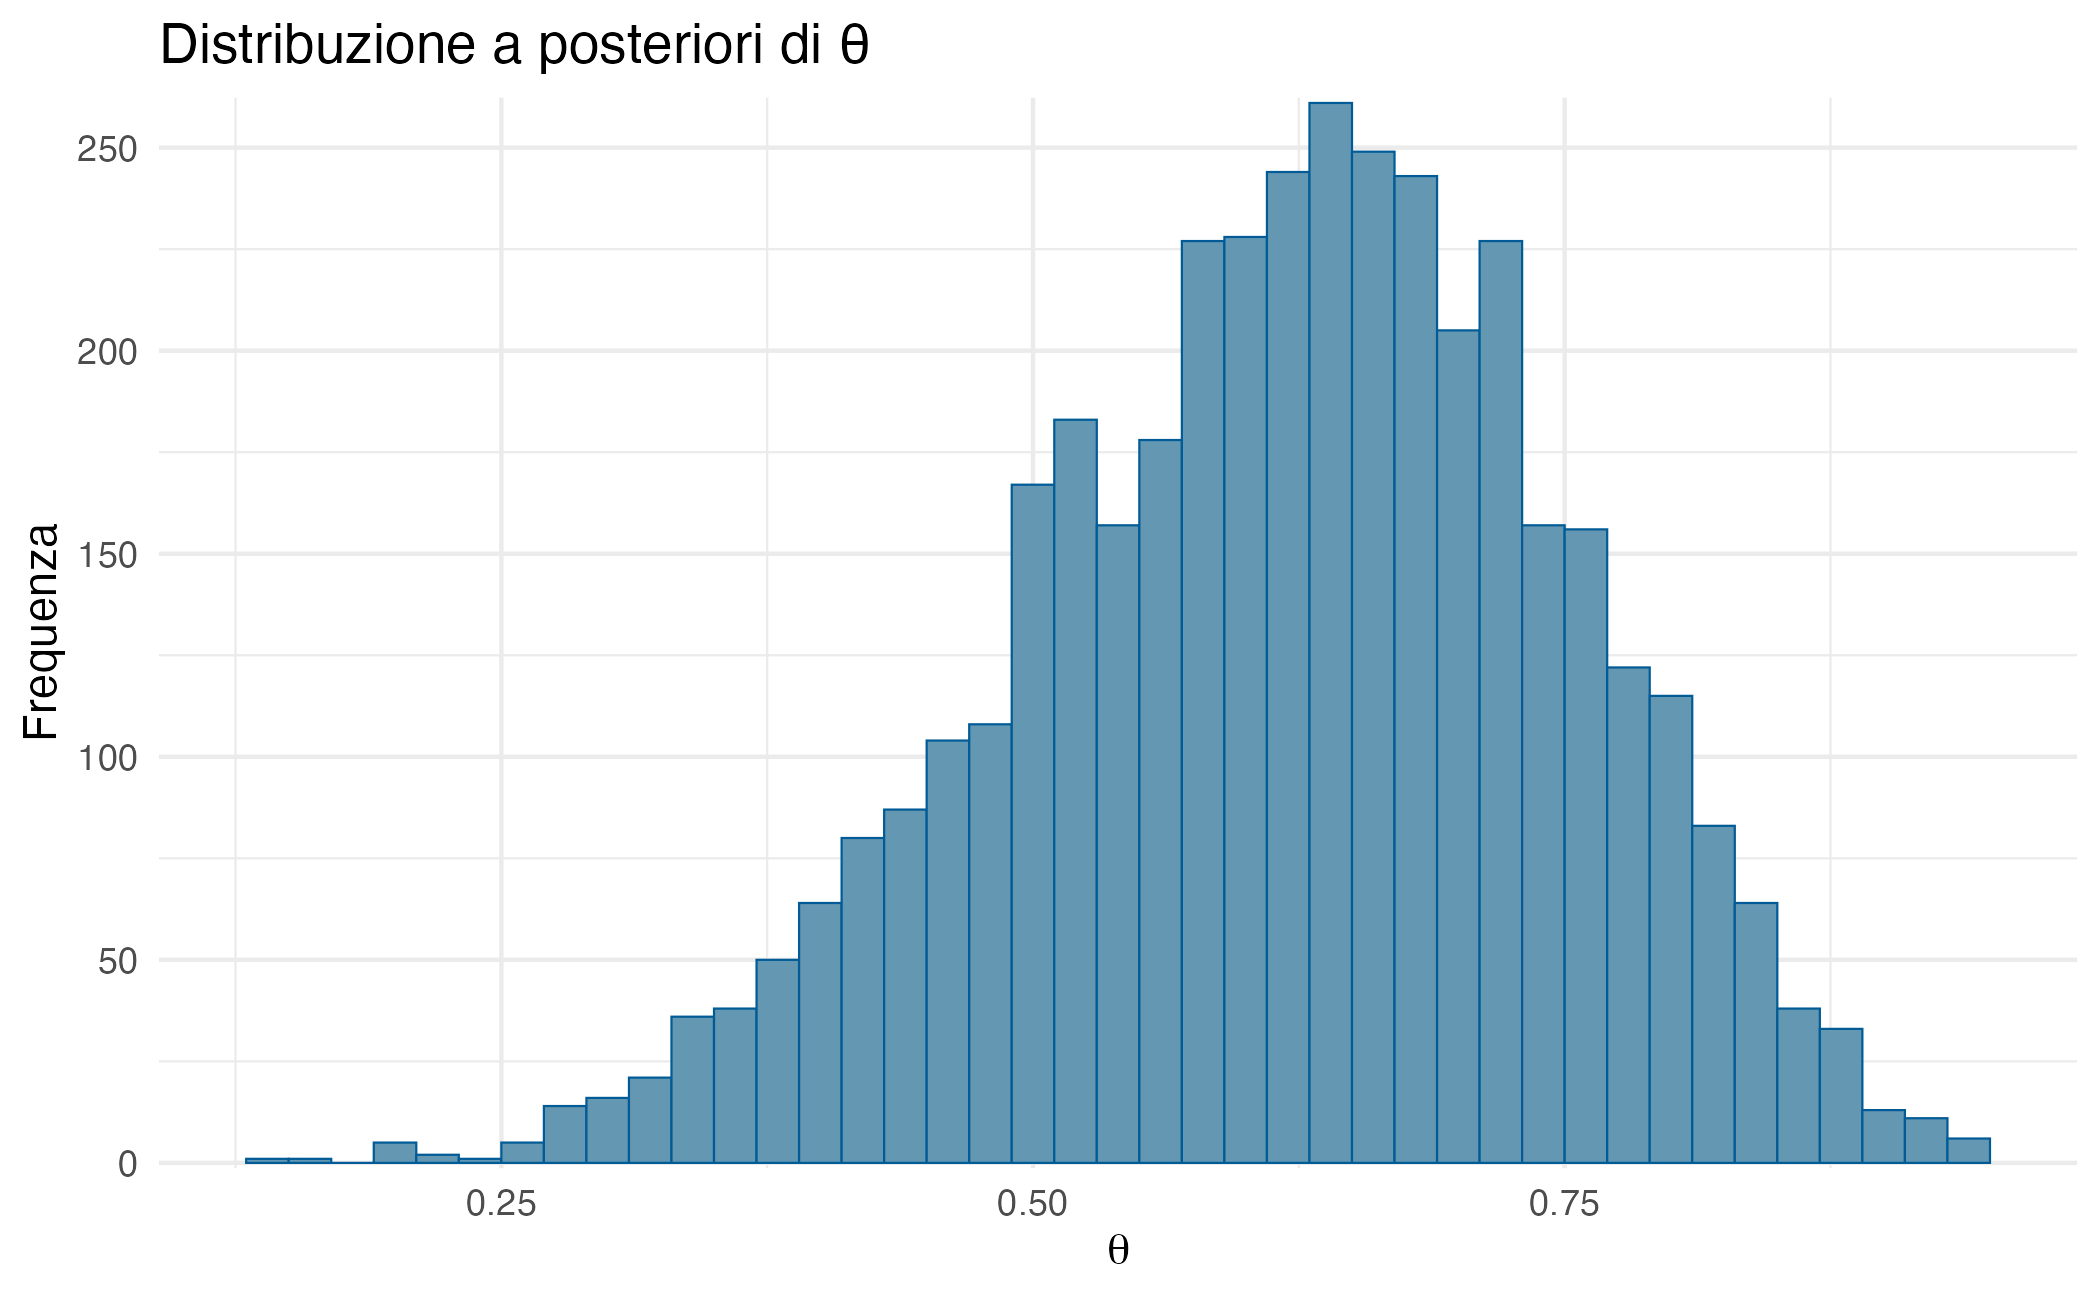
\includegraphics[width=0.85\linewidth,height=\textheight,keepaspectratio]{chapters/appendix/a42_cmdstanr_intro_files/figure-pdf/unnamed-chunk-12-1.png}
\end{center}

Per verificare visivamente la convergenza, possiamo esaminare i trace
plot (tracciati delle catene):

\begin{Shaded}
\begin{Highlighting}[]
\FunctionTok{mcmc\_trace}\NormalTok{(fit}\SpecialCharTok{$}\FunctionTok{draws}\NormalTok{(}\StringTok{"theta"}\NormalTok{)) }\SpecialCharTok{+}
  \FunctionTok{labs}\NormalTok{(}
    \AttributeTok{x =} \StringTok{"Iterazione"}\NormalTok{,}
    \AttributeTok{y =} \FunctionTok{expression}\NormalTok{(theta),}
    \AttributeTok{title =} \StringTok{"Trace plot delle 4 catene"}
\NormalTok{  ) }\SpecialCharTok{+}
  \FunctionTok{theme\_minimal}\NormalTok{()}
\end{Highlighting}
\end{Shaded}

\begin{center}
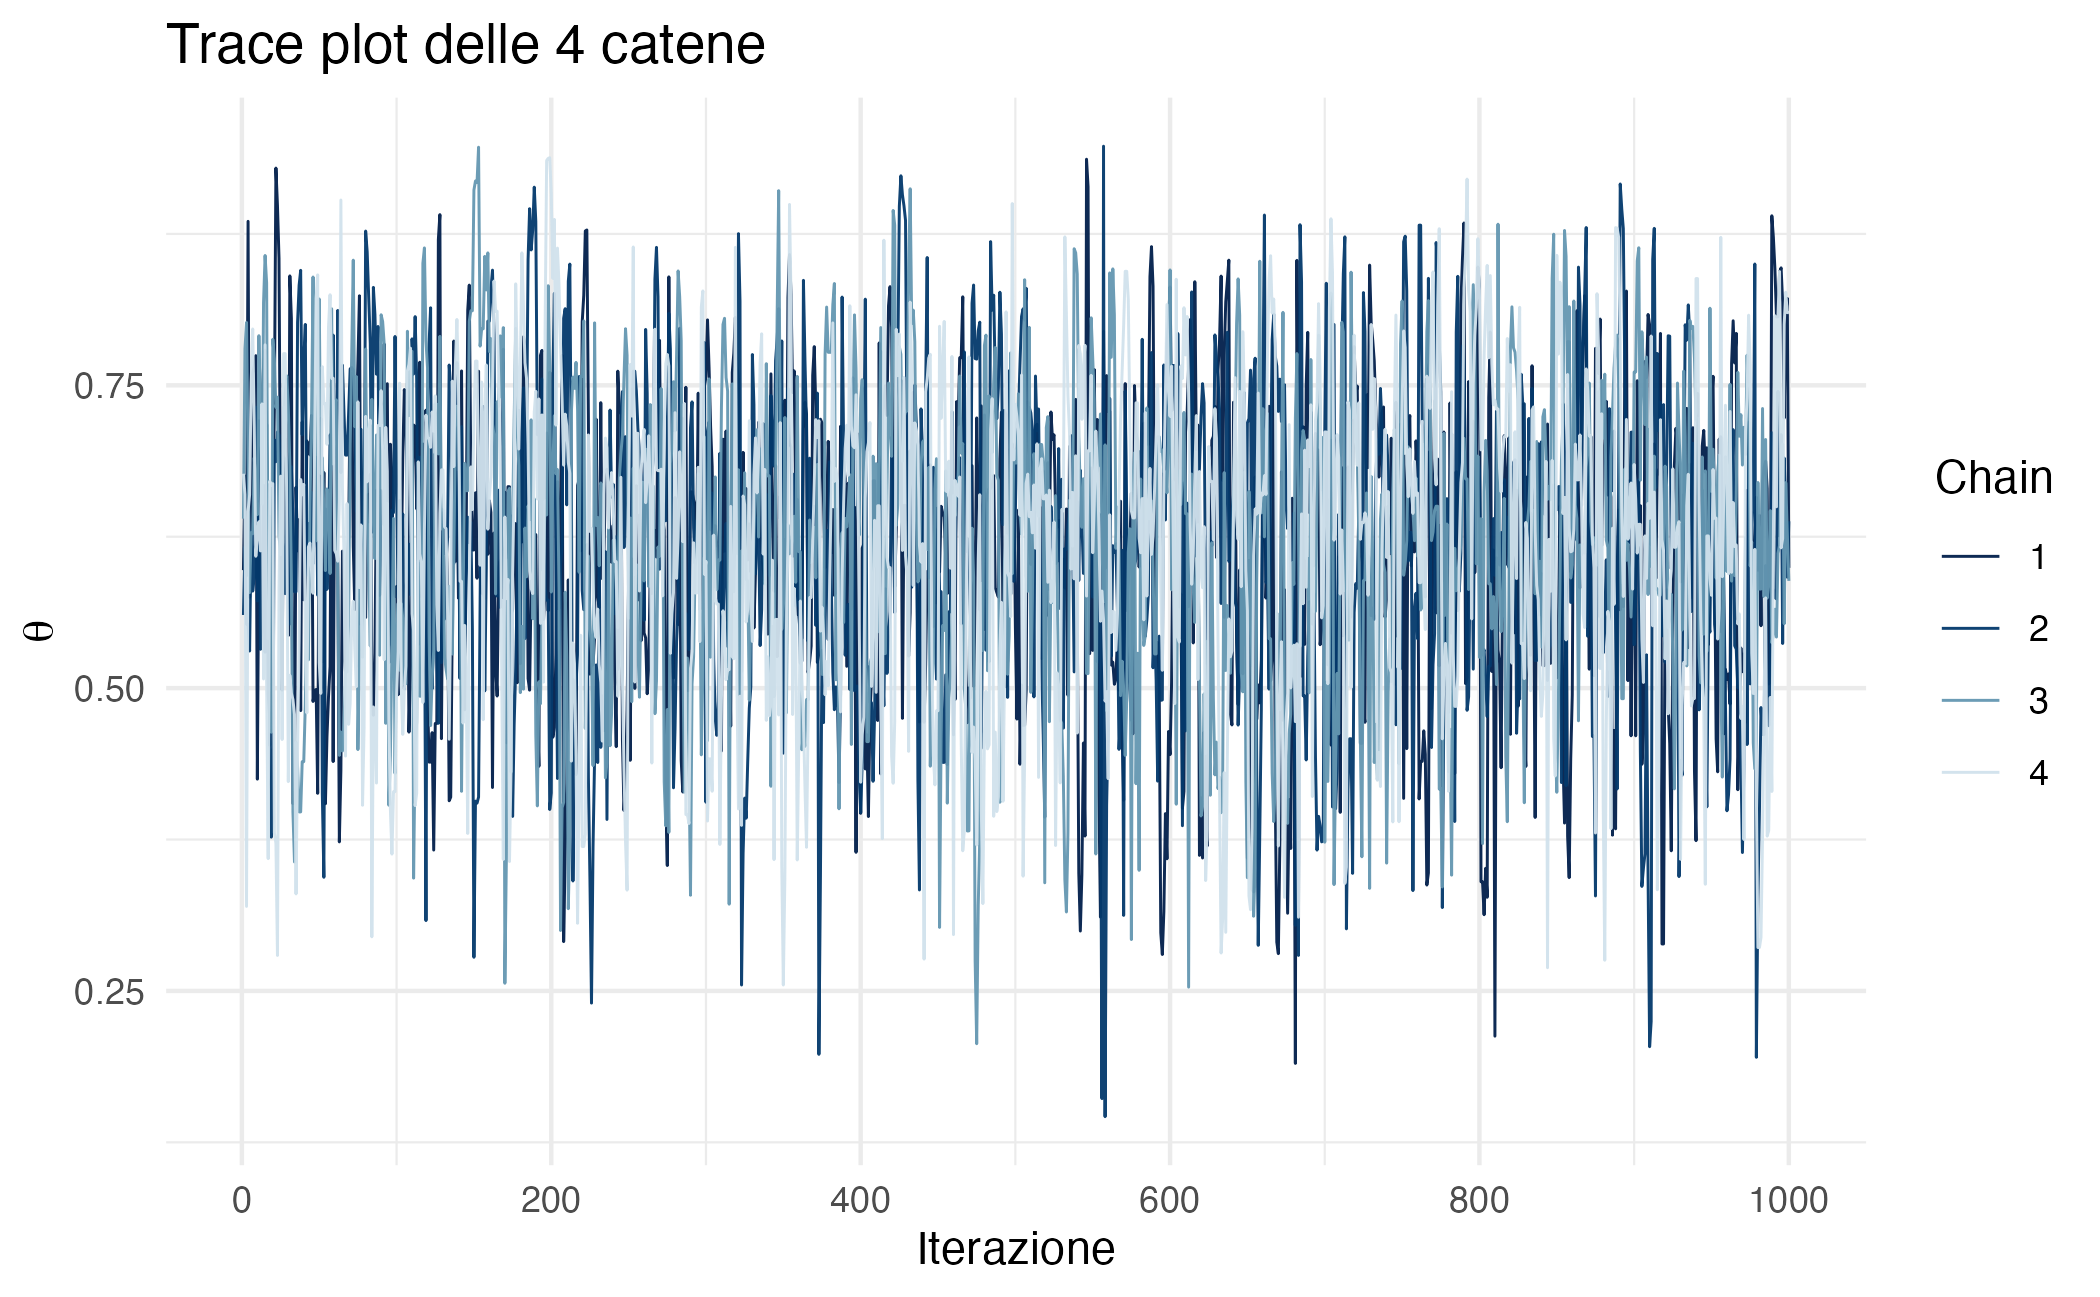
\includegraphics[width=0.85\linewidth,height=\textheight,keepaspectratio]{chapters/appendix/a42_cmdstanr_intro_files/figure-pdf/unnamed-chunk-13-1.png}
\end{center}

Le catene dovrebbero apparire come ``rumore'' sovrapposto, senza trend o
differenze sistematiche tra loro.

\section{Riepilogo del flusso di
lavoro}\label{riepilogo-del-flusso-di-lavoro}

Il diagramma seguente riassume le fasi dell'analisi:

\begin{verbatim}
┌─────────────────────┐
│   1. DATI           │  Organizzare i dati in una lista R
│   data_list <- ...  │  con nomi corrispondenti al modello
└─────────┬───────────┘
          │
          ▼
┌─────────────────────┐
│   2. MODELLO        │  Scrivere il codice Stan:
│   stancode <- "..." │  data, parameters, model
└─────────┬───────────┘
          │
          ▼
┌─────────────────────┐
│   3. COMPILAZIONE   │  Trasformare Stan in eseguibile
│   cmdstan_model()   │
└─────────┬───────────┘
          │
          ▼
┌─────────────────────┐
│   4. CAMPIONAMENTO  │  Generare campioni MCMC
│   mod$sample()      │  dalla distribuzione a posteriori
└─────────┬───────────┘
          │
          ▼
┌─────────────────────┐
│   5. ANALISI        │  Diagnostica, statistiche,
│   fit$summary()     │  visualizzazioni
└─────────────────────┘
\end{verbatim}

Questo schema rimane invariato indipendentemente dalla complessità del
modello. Una volta padroneggiato su un esempio semplice, può essere
applicato a regressioni, modelli gerarchici e qualunque altra analisi
bayesiana.

\chapter{Introduzione al linguaggio Stan}\label{sec-apx-stan-lang}

\section*{Che cos'è Stan?}\label{che-cosuxe8-stan}

\markright{Che cos'è Stan?}

Stan è un linguaggio di programmazione progettato specificamente per
l'analisi statistica bayesiana. Il nome rende omaggio a Stanislaw Ulam,
uno dei pionieri dei metodi Monte Carlo. A differenza di software
statistici come SPSS o Jamovi, Stan richiede di scrivere esplicitamente
il modello statistico, ma in cambio offre una flessibilità
straordinaria: qualunque modello bayesiano può essere implementato in
Stan.

Non è necessario essere programmatori esperti per utilizzare Stan. Il
linguaggio è stato progettato per essere leggibile e la sua sintassi
rispecchia da vicino la notazione matematica utilizzata per descrivere i
modelli statistici. Se si riesce a scrivere un modello in forma
matematica, è possibile tradurlo in Stan.

\section{Come funziona Stan}\label{come-funziona-stan}

Quando eseguiamo un'analisi con Stan, il processo si svolge in tre fasi:

\begin{enumerate}
\def\labelenumi{\arabic{enumi}.}
\tightlist
\item
  \textbf{Scrittura del modello}: descriviamo il modello statistico in
  un file di testo (con estensione \texttt{.stan}).
\item
  \textbf{Compilazione}: Stan traduce il nostro modello in codice
  ottimizzato per il computer. Questa operazione richiede alcuni secondi
  e viene eseguita una sola volta per ogni modello.
\item
  \textbf{Campionamento}: Stan genera migliaia di campioni dalla
  distribuzione a posteriori utilizzando algoritmi MCMC.
\end{enumerate}

\section{Come accedere a Stan}\label{come-accedere-a-stan}

Stan non viene utilizzato direttamente, ma tramite
un'\textbf{interfaccia} che lo collega al nostro ambiente di lavoro. Le
interfacce principali sono:

{\def\LTcaptype{none} % do not increment counter
\begin{longtable}[]{@{}lll@{}}
\toprule\noalign{}
Interfaccia & Linguaggio & Note \\
\midrule\noalign{}
\endhead
\bottomrule\noalign{}
\endlastfoot
\texttt{cmdstanr} & R & Raccomandata per R, usata in questo libro \\
\texttt{brms} & R & Sintassi semplificata, ideale per modelli
standard \\
\texttt{rstanarm} & R & Modelli predefiniti con sintassi familiare \\
\texttt{CmdStanPy} & Python & Equivalente di cmdstanr per Python \\
\texttt{Stan.jl} & Julia & Per utenti Julia \\
\end{longtable}
}

In questo libro utilizziamo \texttt{cmdstanr}, che offre il miglior
equilibrio tra controllo e semplicità. Per l'installazione, consultare
l'Appendice~\ref{sec-apx-install-cmdstan}.

Esistono anche pacchetti complementari per l'analisi dei risultati:

\begin{itemize}
\tightlist
\item
  \texttt{bayesplot}: grafici per visualizzare distribuzioni a
  posteriori e diagnostiche.
\item
  \texttt{posterior}: funzioni per manipolare i campioni MCMC.
\item
  \texttt{loo}: confronto tra modelli tramite validazione incrociata.
\end{itemize}

\section{La struttura di un programma
Stan}\label{la-struttura-di-un-programma-stan}

Un programma Stan è organizzato in \textbf{blocchi}, ciascuno con uno
scopo preciso. Pensate ai blocchi come a sezioni di un modulo da
compilare: ogni sezione richiede informazioni specifiche.

\begin{Shaded}
\begin{Highlighting}[]
\KeywordTok{data}\NormalTok{ \{}
  \CommentTok{// Cosa osserviamo: i dati dell\textquotesingle{}esperimento}
\NormalTok{\}}

\KeywordTok{parameters}\NormalTok{ \{}
  \CommentTok{// Cosa vogliamo stimare: i parametri incogniti}
\NormalTok{\}}

\KeywordTok{model}\NormalTok{ \{}
  \CommentTok{// Come sono collegati: prior e verosimiglianza}
\NormalTok{\}}

\KeywordTok{generated quantities}\NormalTok{ \{}
  \CommentTok{// Cosa vogliamo calcolare in più (opzionale)}
\NormalTok{\}}
\end{Highlighting}
\end{Shaded}

I blocchi devono apparire sempre in questo ordine, ma non tutti sono
obbligatori. I tre blocchi fondamentali sono \texttt{data},
\texttt{parameters} e \texttt{model}.

\subsection{\texorpdfstring{Il blocco \texttt{data}: cosa abbiamo
osservato}{Il blocco data: cosa abbiamo osservato}}\label{il-blocco-data-cosa-abbiamo-osservato}

Nel blocco \texttt{data} dichiariamo tutte le informazioni che
provengono dal nostro studio: il numero di partecipanti, le risposte
osservate, le variabili indipendenti, e così via. Per ogni variabile
dobbiamo specificare:

\begin{itemize}
\tightlist
\item
  il \textbf{tipo} di dato (numero intero, numero reale, vettore, ecc.);
\item
  le \textbf{dimensioni} (quanti elementi contiene);
\item
  eventuali \textbf{vincoli} sui valori ammissibili.
\end{itemize}

\textbf{Esempio commentato:}

\begin{Shaded}
\begin{Highlighting}[]
\KeywordTok{data}\NormalTok{ \{}
  \DataTypeTok{int}\NormalTok{\textless{}}\KeywordTok{lower}\NormalTok{=}\DecValTok{1}\NormalTok{\textgreater{} N;              }\CommentTok{// Numero di partecipanti (almeno 1)}
  \DataTypeTok{int}\NormalTok{\textless{}}\KeywordTok{lower}\NormalTok{=}\DecValTok{0}\NormalTok{\textgreater{} y;              }\CommentTok{// Risposte corrette osservate}
  \DataTypeTok{int}\NormalTok{\textless{}}\KeywordTok{lower}\NormalTok{=}\DecValTok{0}\NormalTok{\textgreater{} n\_trials;       }\CommentTok{// Numero totale di prove}
  \DataTypeTok{real}\NormalTok{\textless{}}\KeywordTok{lower}\NormalTok{=}\DecValTok{0}\NormalTok{\textgreater{} alpha\_prior;   }\CommentTok{// Parametro per il prior}
  \DataTypeTok{real}\NormalTok{\textless{}}\KeywordTok{lower}\NormalTok{=}\DecValTok{0}\NormalTok{\textgreater{} beta\_prior;    }\CommentTok{// Parametro per il prior}
\NormalTok{\}}
\end{Highlighting}
\end{Shaded}

\textbf{Perché specificare i vincoli?} I vincoli (come \texttt{lower=0})
aiutano Stan a verificare che i dati siano sensati. Se per errore
passiamo un numero negativo di partecipanti, Stan ci avviserà
immediatamente invece di produrre risultati sbagliati.

\subsection{\texorpdfstring{Il blocco \texttt{parameters}: cosa vogliamo
stimare}{Il blocco parameters: cosa vogliamo stimare}}\label{il-blocco-parameters-cosa-vogliamo-stimare}

Nel blocco \texttt{parameters} dichiariamo i parametri del modello,
ovvero le quantità incognite che vogliamo stimare a partire dai dati.
Anche qui specifichiamo tipo e vincoli.

\textbf{Esempio:}

\begin{Shaded}
\begin{Highlighting}[]
\KeywordTok{parameters}\NormalTok{ \{}
  \DataTypeTok{real}\NormalTok{\textless{}}\KeywordTok{lower}\NormalTok{=}\DecValTok{0}\NormalTok{, }\KeywordTok{upper}\NormalTok{=}\DecValTok{1}\NormalTok{\textgreater{} theta;  }\CommentTok{// Probabilità di successo}
\NormalTok{\}}
\end{Highlighting}
\end{Shaded}

In questo esempio, \texttt{theta} rappresenta una probabilità, quindi
deve essere compresa tra 0 e 1. I vincoli \texttt{lower=0,\ upper=1}
comunicano a Stan questa restrizione.

\subsection{\texorpdfstring{Il blocco \texttt{model}: come sono
collegati dati e
parametri}{Il blocco model: come sono collegati dati e parametri}}\label{il-blocco-model-come-sono-collegati-dati-e-parametri}

Il blocco \texttt{model} è il cuore del programma Stan. Qui definiamo:

\begin{enumerate}
\def\labelenumi{\arabic{enumi}.}
\tightlist
\item
  la \textbf{distribuzione a priori} per ogni parametro;
\item
  la \textbf{verosimiglianza}, cioè come i dati dipendono dai parametri.
\end{enumerate}

\textbf{Esempio:}

\begin{Shaded}
\begin{Highlighting}[]
\KeywordTok{model}\NormalTok{ \{}
  \CommentTok{// Prior: cosa crediamo prima di vedere i dati}
\NormalTok{  theta \textasciitilde{} beta(alpha\_prior, beta\_prior);}
  
  \CommentTok{// Verosimiglianza: come i dati dipendono da theta}
\NormalTok{  y \textasciitilde{} binomial(n\_trials, theta);}
\NormalTok{\}}
\end{Highlighting}
\end{Shaded}

\textbf{Come leggere questo codice:} il simbolo
\texttt{\textasciitilde{}} si legge ``è distribuito come'' oppure
``segue una distribuzione''. Quindi:

\begin{itemize}
\tightlist
\item
  \texttt{theta\ \textasciitilde{}\ beta(2,\ 2)} significa ``\(\theta\)
  ha distribuzione Beta(2, 2)'';
\item
  \texttt{y\ \textasciitilde{}\ binomial(n,\ theta)} significa ``\(y\)
  ha distribuzione Binomiale con parametri \(n\) e \(\theta\)''.
\end{itemize}

Questa sintassi corrisponde direttamente alla notazione matematica: \[
\theta \sim \text{Beta}(\alpha, \beta)
\] \[
y \sim \text{Binomiale}(n, \theta)
\]

\textbf{Nota sui prior:} se non specifichiamo un prior per un parametro,
Stan assume un prior uniforme (non informativo). Tuttavia, è buona
pratica dichiarare sempre esplicitamente i prior per rendere il modello
più leggibile.

\subsection{\texorpdfstring{Il blocco \texttt{generated\ quantities}:
calcoli
aggiuntivi}{Il blocco generated quantities: calcoli aggiuntivi}}\label{il-blocco-generated-quantities-calcoli-aggiuntivi}

Questo blocco opzionale permette di calcolare quantità derivate dai
parametri stimati. Due usi comuni sono:

\begin{enumerate}
\def\labelenumi{\arabic{enumi}.}
\tightlist
\item
  \textbf{posterior predictive check}: generare dati simulati per
  verificare se il modello cattura le caratteristiche dei dati reali;
\item
  \textbf{log-verosimiglianza}: calcolare valori utili per il confronto
  tra modelli.
\end{enumerate}

\textbf{Esempio:}

\begin{Shaded}
\begin{Highlighting}[]
\KeywordTok{generated quantities}\NormalTok{ \{}
  \DataTypeTok{int}\NormalTok{ y\_rep = binomial\_rng(n\_trials, theta);  }\CommentTok{// Dato simulato}
  \DataTypeTok{real}\NormalTok{ log\_lik = binomial\_lpmf(y | n\_trials, theta);  }\CommentTok{// Log{-}verosimiglianza}
\NormalTok{\}}
\end{Highlighting}
\end{Shaded}

Le funzioni che terminano in \texttt{\_rng} generano numeri casuali;
quelle che terminano in \texttt{\_lpmf} o \texttt{\_lpdf} calcolano le
log-probabilità.

\section{I tipi di dati in Stan}\label{i-tipi-di-dati-in-stan}

Stan implementa un sistema di tipi di dati fortemente tipizzato. Questa
rigidità, sebbene possa apparire scomoda, garantisce l'integrità del
modello eliminando alla fonte numerose categorie di errori.

\subsection{Tipi scalari: singoli
valori}\label{tipi-scalari-singoli-valori}

{\def\LTcaptype{none} % do not increment counter
\begin{longtable}[]{@{}lll@{}}
\toprule\noalign{}
Tipo & Descrizione & Esempio \\
\midrule\noalign{}
\endhead
\bottomrule\noalign{}
\endlastfoot
\texttt{int} & Numero intero & \texttt{int\ N\ =\ 10;} \\
\texttt{real} & Numero reale (decimale) &
\texttt{real\ sigma\ =\ 2.5;} \\
\end{longtable}
}

\subsection{Tipi composti: collezioni di
valori}\label{tipi-composti-collezioni-di-valori}

{\def\LTcaptype{none} % do not increment counter
\begin{longtable}[]{@{}
  >{\raggedright\arraybackslash}p{(\linewidth - 4\tabcolsep) * \real{0.2143}}
  >{\raggedright\arraybackslash}p{(\linewidth - 4\tabcolsep) * \real{0.4643}}
  >{\raggedright\arraybackslash}p{(\linewidth - 4\tabcolsep) * \real{0.3214}}@{}}
\toprule\noalign{}
\begin{minipage}[b]{\linewidth}\raggedright
Tipo
\end{minipage} & \begin{minipage}[b]{\linewidth}\raggedright
Descrizione
\end{minipage} & \begin{minipage}[b]{\linewidth}\raggedright
Esempio
\end{minipage} \\
\midrule\noalign{}
\endhead
\bottomrule\noalign{}
\endlastfoot
\texttt{vector{[}N{]}} & Vettore colonna di N numeri reali &
\texttt{vector{[}10{]}\ y;} \\
\texttt{row\_vector{[}N{]}} & Vettore riga di N numeri reali &
\texttt{row\_vector{[}5{]}\ x;} \\
\texttt{matrix{[}R,\ C{]}} & Matrice R×C di numeri reali &
\texttt{matrix{[}3,\ 4{]}\ A;} \\
\texttt{array{[}N{]}\ int} & Array di N numeri interi &
\texttt{array{[}20{]}\ int\ counts;} \\
\end{longtable}
}

\textbf{Quando usare cosa:}

\begin{itemize}
\tightlist
\item
  usate \texttt{int} per conteggi (numero di partecipanti, numero di
  risposte corrette);
\item
  usate \texttt{real} per misure continue (tempi di reazione, punteggi
  su scale);
\item
  usate \texttt{vector} per sequenze di misure continue (punteggi di
  \(N\) partecipanti);
\item
  usate \texttt{array{[}N{]}\ int} per sequenze di conteggi.
\end{itemize}

\subsection{Vincoli sui valori}\label{vincoli-sui-valori}

I vincoli più comuni sono:

{\def\LTcaptype{none} % do not increment counter
\begin{longtable}[]{@{}lll@{}}
\toprule\noalign{}
Vincolo & Significato & Uso tipico \\
\midrule\noalign{}
\endhead
\bottomrule\noalign{}
\endlastfoot
\texttt{lower=0} & Valore minimo 0 & Deviazioni standard, conteggi \\
\texttt{upper=1} & Valore massimo 1 & Proporzioni \\
\texttt{lower=0,\ upper=1} & Tra 0 e 1 & Probabilità \\
\texttt{lower=1} & Almeno 1 & Numerosità campionarie \\
\end{longtable}
}

\textbf{Esempio con vincoli:}

\begin{Shaded}
\begin{Highlighting}[]
\KeywordTok{data}\NormalTok{ \{}
  \DataTypeTok{int}\NormalTok{\textless{}}\KeywordTok{lower}\NormalTok{=}\DecValTok{1}\NormalTok{\textgreater{} N;                    }\CommentTok{// Almeno 1 partecipante}
  \DataTypeTok{array}\NormalTok{[N] }\DataTypeTok{real}\NormalTok{\textless{}}\KeywordTok{lower}\NormalTok{=}\DecValTok{0}\NormalTok{\textgreater{} rt;         }\CommentTok{// Tempi di reazione (positivi)}
\NormalTok{\}}

\KeywordTok{parameters}\NormalTok{ \{}
  \DataTypeTok{real}\NormalTok{\textless{}}\KeywordTok{lower}\NormalTok{=}\DecValTok{0}\NormalTok{\textgreater{} mu;                  }\CommentTok{// Media (positiva per tempi)}
  \DataTypeTok{real}\NormalTok{\textless{}}\KeywordTok{lower}\NormalTok{=}\DecValTok{0}\NormalTok{\textgreater{} sigma;               }\CommentTok{// Deviazione standard (positiva)}
\NormalTok{\}}
\end{Highlighting}
\end{Shaded}

\section{Passare i dati da R a Stan}\label{passare-i-dati-da-r-a-stan}

Per eseguire un modello Stan da R, dobbiamo preparare i dati in una
\textbf{lista}. I nomi degli elementi della lista devono corrispondere
esattamente a quelli dichiarati nel blocco \texttt{data}.

\textbf{Esempio in R:}

\begin{Shaded}
\begin{Highlighting}[]
\CommentTok{\# Supponiamo di avere un esperimento con 50 prove e 32 successi}
\NormalTok{data\_list }\OtherTok{\textless{}{-}} \FunctionTok{list}\NormalTok{(}
  \AttributeTok{N =} \DecValTok{1}\NormalTok{,              }\CommentTok{\# Un partecipante}
  \AttributeTok{y =} \DecValTok{32}\NormalTok{,             }\CommentTok{\# Successi osservati}
  \AttributeTok{n\_trials =} \DecValTok{50}\NormalTok{,      }\CommentTok{\# Prove totali}
  \AttributeTok{alpha\_prior =} \DecValTok{2}\NormalTok{,    }\CommentTok{\# Parametro prior}
  \AttributeTok{beta\_prior =} \DecValTok{2}      \CommentTok{\# Parametro prior}
\NormalTok{)}
\end{Highlighting}
\end{Shaded}

\textbf{Errori comuni da evitare:}

\begin{itemize}
\tightlist
\item
  nomi scritti diversamente (\texttt{ntrials} invece di
  \texttt{n\_trials});
\item
  tipi sbagliati (passare \texttt{"50"} come stringa invece di
  \texttt{50} come numero);
\item
  dimensioni non corrispondenti.
\end{itemize}

\section{Regole sintattiche
essenziali}\label{regole-sintattiche-essenziali}

Stan ha alcune regole sintattiche che è importante conoscere.

\subsection{Punto e virgola}\label{punto-e-virgola}

Ogni istruzione deve terminare con un punto e virgola (\texttt{;}):

\begin{Shaded}
\begin{Highlighting}[]
\DataTypeTok{int}\NormalTok{ N;                          }\CommentTok{// Corretto}
\NormalTok{theta \textasciitilde{} beta(}\DecValTok{2}\NormalTok{, }\DecValTok{2}\NormalTok{);             }\CommentTok{// Corretto}
\DataTypeTok{real}\NormalTok{\textless{}}\KeywordTok{lower}\NormalTok{=}\DecValTok{0}\NormalTok{\textgreater{} sigma             }\CommentTok{// ERRORE: manca il punto e virgola}
\end{Highlighting}
\end{Shaded}

\subsection{Commenti}\label{commenti}

I commenti iniziano con \texttt{//} e vengono ignorati da Stan:

\begin{Shaded}
\begin{Highlighting}[]
\CommentTok{// Questo è un commento su una riga}
\DataTypeTok{int}\NormalTok{ N;  }\CommentTok{// Commento a fine riga}

\CommentTok{/* Questo è un commento}
\CommentTok{   su più righe */}
\end{Highlighting}
\end{Shaded}

\subsection{Indicizzazione}\label{indicizzazione}

Stan numera gli elementi a partire da 1 (come R), non da 0 (come
Python):

\begin{Shaded}
\begin{Highlighting}[]
\DataTypeTok{vector}\NormalTok{[}\DecValTok{3}\NormalTok{] v;}
\NormalTok{v[}\DecValTok{1}\NormalTok{]  }\CommentTok{// Primo elemento}
\NormalTok{v[}\DecValTok{3}\NormalTok{]  }\CommentTok{// Terzo e ultimo elemento}
\end{Highlighting}
\end{Shaded}

\section{Un esempio completo}\label{un-esempio-completo}

Mettiamo insieme tutti i concetti in un modello completo per stimare la
probabilità di successo in un compito cognitivo:

\begin{Shaded}
\begin{Highlighting}[]
\CommentTok{// Modello Beta{-}Binomiale per stimare la probabilità di successo}

\KeywordTok{data}\NormalTok{ \{}
  \DataTypeTok{int}\NormalTok{\textless{}}\KeywordTok{lower}\NormalTok{=}\DecValTok{1}\NormalTok{\textgreater{} n\_trials;           }\CommentTok{// Numero di prove}
  \DataTypeTok{int}\NormalTok{\textless{}}\KeywordTok{lower}\NormalTok{=}\DecValTok{0}\NormalTok{, }\KeywordTok{upper}\NormalTok{=n\_trials\textgreater{} y;  }\CommentTok{// Successi osservati}
  \DataTypeTok{real}\NormalTok{\textless{}}\KeywordTok{lower}\NormalTok{=}\DecValTok{0}\NormalTok{\textgreater{} alpha\_prior;       }\CommentTok{// Prior Beta: parametro alpha}
  \DataTypeTok{real}\NormalTok{\textless{}}\KeywordTok{lower}\NormalTok{=}\DecValTok{0}\NormalTok{\textgreater{} beta\_prior;        }\CommentTok{// Prior Beta: parametro beta}
\NormalTok{\}}

\KeywordTok{parameters}\NormalTok{ \{}
  \DataTypeTok{real}\NormalTok{\textless{}}\KeywordTok{lower}\NormalTok{=}\DecValTok{0}\NormalTok{, }\KeywordTok{upper}\NormalTok{=}\DecValTok{1}\NormalTok{\textgreater{} theta;    }\CommentTok{// Probabilità di successo}
\NormalTok{\}}

\KeywordTok{model}\NormalTok{ \{}
  \CommentTok{// Distribuzione a priori}
\NormalTok{  theta \textasciitilde{} beta(alpha\_prior, beta\_prior);}
  
  \CommentTok{// Verosimiglianza}
\NormalTok{  y \textasciitilde{} binomial(n\_trials, theta);}
\NormalTok{\}}

\KeywordTok{generated quantities}\NormalTok{ \{}
  \CommentTok{// Per verificare il modello: generiamo dati simulati}
  \DataTypeTok{int}\NormalTok{ y\_rep = binomial\_rng(n\_trials, theta);}
  
  \CommentTok{// Per confrontare modelli: calcoliamo la log{-}verosimiglianza}
  \DataTypeTok{real}\NormalTok{ log\_lik = binomial\_lpmf(y | n\_trials, theta);}
\NormalTok{\}}
\end{Highlighting}
\end{Shaded}

Questo modello:

\begin{enumerate}
\def\labelenumi{\arabic{enumi}.}
\tightlist
\item
  riceve in input il numero di prove e i successi osservati;
\item
  stima la probabilità di successo \(\theta\) con un prior Beta;
\item
  genera dati simulati per verificare l'adeguatezza del modello;
\item
  calcola la log-verosimiglianza per eventuali confronti tra modelli.
\end{enumerate}

\section{Blocchi opzionali avanzati}\label{blocchi-opzionali-avanzati}

Oltre ai blocchi fondamentali, Stan offre blocchi aggiuntivi per modelli
più complessi:

\subsection{\texorpdfstring{\texttt{transformed\ data}}{transformed data}}\label{transformed-data}

Permette di pre-elaborare i dati prima dell'analisi. È utile per
standardizzare variabili o calcolare quantità derivate dai dati.

\begin{Shaded}
\begin{Highlighting}[]
\KeywordTok{transformed data}\NormalTok{ \{}
  \DataTypeTok{real}\NormalTok{ y\_mean = mean(y);           }\CommentTok{// Media dei dati}
  \DataTypeTok{vector}\NormalTok{[N] y\_centered = y {-} y\_mean;  }\CommentTok{// Dati centrati}
\NormalTok{\}}
\end{Highlighting}
\end{Shaded}

\subsection{\texorpdfstring{\texttt{transformed\ parameters}}{transformed parameters}}\label{transformed-parameters}

Permette di definire parametri derivati da altri parametri. Questi
vengono salvati insieme ai parametri principali.

\begin{Shaded}
\begin{Highlighting}[]
\KeywordTok{transformed parameters}\NormalTok{ \{}
  \DataTypeTok{real}\NormalTok{ odds = theta / (}\DecValTok{1}\NormalTok{ {-} theta);  }\CommentTok{// Odds derivato da theta}
\NormalTok{\}}
\end{Highlighting}
\end{Shaded}

\subsection{\texorpdfstring{\texttt{functions}}{functions}}\label{functions}

Permette di definire funzioni personalizzate da usare nel modello. Sono
utili per modelli complessi con calcoli ripetuti.

\section{Risorse per approfondire}\label{risorse-per-approfondire}

Per una documentazione completa del linguaggio Stan:

\begin{itemize}
\tightlist
\item
  \href{https://mc-stan.org/docs/reference-manual/}{Manuale di
  riferimento Stan}: documentazione ufficiale completa.
\item
  \href{https://mc-stan.org/docs/functions-reference/}{Guida alle
  funzioni}: elenco di tutte le funzioni disponibili.
\item
  \href{https://github.com/stan-dev/stan/wiki/Prior-Choice-Recommendations}{Raccomandazioni
  sui prior}: linee guida per la scelta delle distribuzioni a priori.
\end{itemize}

\section{Riepilogo}\label{riepilogo}

I concetti fondamentali presentati in questa appendice possono essere
sintetizzati nei seguenti punti:

\begin{enumerate}
\def\labelenumi{\arabic{enumi}.}
\item
  \textbf{Struttura modulare}: i programmi Stan seguono una struttura a
  blocchi logica e sequenziale: \texttt{data} → \texttt{parameters} →
  \texttt{model} (con l'eventuale aggiunta di
  \texttt{generated\ quantities}).
\item
  \textbf{Dichiarazione esplicita}: ogni variabile deve essere
  dichiarata specificando in modo completo il suo tipo, le dimensioni e
  gli eventuali vincoli.
\item
  \textbf{Sintassi probabilistica}: l'operatore
  \texttt{\textasciitilde{}} stabilisce una \textbf{relazione di
  distribuzione} tra una variabile e una legge probabilistica, e si
  legge ``è distribuito come''.
\item
  \textbf{Interfaccia dati}: per eseguire l'inferenza, i dati devono
  essere passati a Stan tramite una lista in R. Ogni elemento di questa
  lista deve avere \textbf{esattamente lo stesso nome} della variabile
  corrispondente dichiarata nel blocco \texttt{data} del modello Stan.
\item
  \textbf{Formalismo sintattico}: ogni istruzione, seguendo la
  convenzione dei linguaggi simili a C, termina con un punto e virgola.
\end{enumerate}

Questi elementi concettuali e operativi forniscono le basi necessarie
per costruire, interpretare ed eseguire modelli bayesiani con Stan.

\chapter{Diagnostica delle catene MCMC}\label{sec-apx-mcmc-diagnostics}

Prima di procedere all'interpretazione dei parametri stimati da un
modello in Stan, è essenziale verificare che il processo di
campionamento MCMC si sia svolto in modo affidabile. Le catene generate
possono infatti fornire risultati ingannevoli se non hanno esplorato
adeguatamente lo spazio delle distribuzioni a posteriori.

Stan mette a disposizione un insieme articolato di indicatori
diagnostici per valutare la qualità del campionamento. Questi permettono
di rispondere a domande cruciali:

\begin{itemize}
\tightlist
\item
  Le diverse catene hanno convergito verso la stessa distribuzione
  stazionaria?
\item
  La variabilità osservata nei campioni riflette fedelmente la vera
  distribuzione a posteriori?
\item
  Esistono segnali che indicano regioni dello spazio dei parametri
  rimaste inesplorate?
\end{itemize}

Solo dopo aver accertato che il campionamento sia robusto e privo di
anomalie significative, è possibile procedere in sicurezza all'analisi e
all'interpretazione dei parametri stimati.

\begin{tcolorbox}[enhanced jigsaw, arc=.35mm, bottomrule=.15mm, bottomtitle=1mm, breakable, colback=white, colbacktitle=quarto-callout-note-color!10!white, colframe=quarto-callout-note-color-frame, coltitle=black, left=2mm, leftrule=.75mm, opacityback=0, opacitybacktitle=0.6, rightrule=.15mm, title=\textcolor{quarto-callout-note-color}{\faInfo}\hspace{0.5em}{Riepilogo delle soglie diagnostiche}, titlerule=0mm, toprule=.15mm, toptitle=1mm]

{\def\LTcaptype{none} % do not increment counter
\begin{longtable}[]{@{}lll@{}}
\toprule\noalign{}
Indicatore & Valore accettabile & Valore problematico \\
\midrule\noalign{}
\endhead
\bottomrule\noalign{}
\endlastfoot
\(\hat{R}\) & \textless{} 1.01 & \textgreater{} 1.05 \\
ESS (bulk e tail) & \textgreater{} 400 & \textless{} 100 \\
Transizioni divergenti & 0 & \textgreater{} 0 \\
BFMI & \textgreater{} 0.3 & \textless{} 0.2 \\
Pareto \(\kappa\) (LOO) & \textless{} 0.5 & \textgreater{} 0.7 \\
\end{longtable}
}

\end{tcolorbox}

\begin{tcolorbox}[enhanced jigsaw, arc=.35mm, bottomrule=.15mm, bottomtitle=1mm, breakable, colback=white, colbacktitle=quarto-callout-caution-color!10!white, colframe=quarto-callout-caution-color-frame, coltitle=black, left=2mm, leftrule=.75mm, opacityback=0, opacitybacktitle=0.6, rightrule=.15mm, title=\textcolor{quarto-callout-caution-color}{\faFire}\hspace{0.5em}{Preparazione del Notebook}, titlerule=0mm, toprule=.15mm, toptitle=1mm]

\begin{Shaded}
\begin{Highlighting}[]
\CommentTok{\# Caricamento pacchetti}
\FunctionTok{suppressPackageStartupMessages}\NormalTok{(\{}
  \FunctionTok{library}\NormalTok{(cmdstanr)}
  \FunctionTok{library}\NormalTok{(posterior)}
  \FunctionTok{library}\NormalTok{(bayesplot)}
  \FunctionTok{library}\NormalTok{(ggplot2)}
  \FunctionTok{library}\NormalTok{(coda)}
  \FunctionTok{library}\NormalTok{(loo)}
  \FunctionTok{library}\NormalTok{(dplyr)}
  \FunctionTok{library}\NormalTok{(tidyr)}
\NormalTok{\})}

\CommentTok{\# Impostazioni grafiche}
\FunctionTok{theme\_set}\NormalTok{(}\FunctionTok{theme\_minimal}\NormalTok{(}\AttributeTok{base\_size =} \DecValTok{12}\NormalTok{))}
\FunctionTok{color\_scheme\_set}\NormalTok{(}\StringTok{"brightblue"}\NormalTok{)}
\end{Highlighting}
\end{Shaded}

\end{tcolorbox}

\section{Un modello di riferimento}\label{un-modello-di-riferimento}

Per illustrare le procedure diagnostiche, utilizziamo un semplice
modello beta-binomiale. Questo esempio permette di concentrarsi sugli
strumenti diagnostici senza la complessità di modelli più articolati.

\begin{Shaded}
\begin{Highlighting}[]
\NormalTok{stancode }\OtherTok{\textless{}{-}} \StringTok{"}
\StringTok{data \{}
\StringTok{  int\textless{}lower=1\textgreater{} N;                      // numero di prove}
\StringTok{  array[N] int\textless{}lower=0, upper=1\textgreater{} y;    // esiti (0/1)}
\StringTok{\}}
\StringTok{transformed data \{}
\StringTok{  int\textless{}lower=0, upper=N\textgreater{} k = sum(y);    // numero totale di successi}
\StringTok{\}}
\StringTok{parameters \{}
\StringTok{  real\textless{}lower=0, upper=1\textgreater{} theta;        // probabilità di successo}
\StringTok{\}}
\StringTok{model \{}
\StringTok{  theta \textasciitilde{} beta(1, 1);                  // prior uniforme}
\StringTok{  k \textasciitilde{} binomial(N, theta);              // verosimiglianza}
\StringTok{\}}
\StringTok{generated quantities \{}
\StringTok{  vector[N] log\_lik;}
\StringTok{  for (n in 1:N) \{}
\StringTok{    log\_lik[n] = bernoulli\_lpmf(y[n] | theta);}
\StringTok{  \}}
\StringTok{\}}
\StringTok{"}
\end{Highlighting}
\end{Shaded}

\begin{Shaded}
\begin{Highlighting}[]
\NormalTok{mod }\OtherTok{\textless{}{-}}\NormalTok{ cmdstanr}\SpecialCharTok{::}\FunctionTok{cmdstan\_model}\NormalTok{(}
\NormalTok{  cmdstanr}\SpecialCharTok{::}\FunctionTok{write\_stan\_file}\NormalTok{(stancode),}
  \AttributeTok{compile =} \ConstantTok{TRUE}
\NormalTok{)}
\end{Highlighting}
\end{Shaded}

\begin{Shaded}
\begin{Highlighting}[]
\CommentTok{\# Dati: 7 successi su 10 prove}
\NormalTok{y }\OtherTok{\textless{}{-}} \FunctionTok{c}\NormalTok{(}\DecValTok{1}\NormalTok{, }\DecValTok{1}\NormalTok{, }\DecValTok{1}\NormalTok{, }\DecValTok{1}\NormalTok{, }\DecValTok{1}\NormalTok{, }\DecValTok{1}\NormalTok{, }\DecValTok{1}\NormalTok{, }\DecValTok{0}\NormalTok{, }\DecValTok{0}\NormalTok{, }\DecValTok{0}\NormalTok{)}
\NormalTok{data\_list }\OtherTok{\textless{}{-}} \FunctionTok{list}\NormalTok{(}\AttributeTok{N =} \FunctionTok{length}\NormalTok{(y), }\AttributeTok{y =}\NormalTok{ y)}
\end{Highlighting}
\end{Shaded}

\begin{Shaded}
\begin{Highlighting}[]
\NormalTok{fit }\OtherTok{\textless{}{-}}\NormalTok{ mod}\SpecialCharTok{$}\FunctionTok{sample}\NormalTok{(}
  \AttributeTok{data =}\NormalTok{ data\_list,}
  \AttributeTok{iter\_warmup =} \DecValTok{1000}\NormalTok{,}
  \AttributeTok{iter\_sampling =} \DecValTok{4000}\NormalTok{,}
  \AttributeTok{chains =} \DecValTok{4}\NormalTok{,}
  \AttributeTok{parallel\_chains =} \DecValTok{4}\NormalTok{,}
  \AttributeTok{seed =} \DecValTok{4790}\NormalTok{,}
  \AttributeTok{refresh =} \DecValTok{0} 
\NormalTok{)}
\end{Highlighting}
\end{Shaded}

\section{Grafici di tracciamento}\label{grafici-di-tracciamento}

I grafici di tracciamento (\emph{trace plot}) visualizzano la sequenza
dei valori campionati per ciascun parametro lungo le iterazioni delle
catene MCMC. Questa rappresentazione costituisce il controllo
diagnostico preliminare più immediato e informativo.

\subsection{Interpretazione di un trace plot
ideale}\label{interpretazione-di-un-trace-plot-ideale}

Un grafico di tracciamento che indica un campionamento efficace presenta
le seguenti caratteristiche:

\begin{itemize}
\tightlist
\item
  \textbf{Miscelazione efficiente (\emph{good mixing})}: le catene
  oscillano in modo rapido e apparentemente casuale attorno a un livello
  stabile, assumendo l'aspetto visivo di un ``rumore bianco''.
\item
  \textbf{Convergenza}: le diverse catene (tipicamente rappresentate da
  colori differenti) si sovrappongono e si mescolano, indicando che
  tutte esplorano la medesima regione stazionaria dello spazio dei
  parametri.
\item
  \textbf{Stazionarietà}: non sono visibili andamenti sistematici,
  derive nel tempo o cambiamenti nella dispersione lungo le iterazioni.
\end{itemize}

\subsection{Segnali di potenziali
problemi}\label{segnali-di-potenziali-problemi}

Pattern che richiedono attenzione includono:

\begin{itemize}
\tightlist
\item
  catene che rimangono separate e non si sovrappongono;
\item
  andamenti a gradini, salti improvvisi o persistenza in stati
  metastabili;
\item
  strutture periodiche, cicli o altri pattern regolari che suggeriscono
  autocorrelazione eccessiva;
\item
  deriva graduale verso valori superiori o inferiori.
\end{itemize}

\begin{Shaded}
\begin{Highlighting}[]
\FunctionTok{mcmc\_trace}\NormalTok{(fit}\SpecialCharTok{$}\FunctionTok{draws}\NormalTok{(}\StringTok{"theta"}\NormalTok{)) }\SpecialCharTok{+} 
  \FunctionTok{labs}\NormalTok{(}\AttributeTok{x =} \StringTok{"Iterazione post{-}warmup"}\NormalTok{, }\AttributeTok{y =} \FunctionTok{expression}\NormalTok{(theta))}
\end{Highlighting}
\end{Shaded}

\pandocbounded{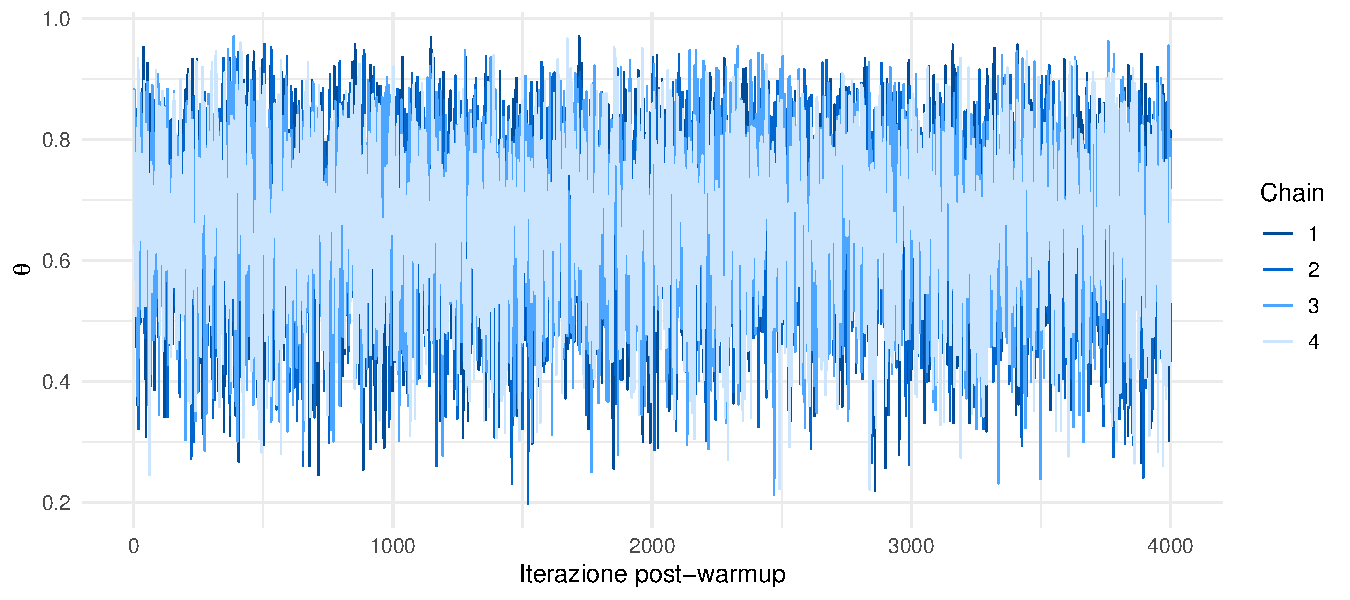
\includegraphics[keepaspectratio]{chapters/appendix/a44_stan_diagnostics_files/figure-pdf/trace-plot-1.pdf}}

\subsection{Strategie correttive per problemi di
convergenza}\label{strategie-correttive-per-problemi-di-convergenza}

Quando i trace plot rivelano anomalie, si possono considerare i seguenti
interventi:

\begin{enumerate}
\def\labelenumi{\arabic{enumi}.}
\item
  \textbf{Aumentare il numero di iterazioni}: un numero maggiore di
  campioni, eventualmente con un periodo di warmup più esteso, può
  permettere alle catene di superare periodi transitori e raggiungere la
  stazionarietà.
\item
  \textbf{Rivedere le specifiche delle distribuzioni a priori}:
  \emph{prior} eccessivamente diffuse possono creare problemi di
  identificazione, mentre prior troppo informative possono vincolare le
  catene in regioni improbabili.
\item
  \textbf{Riparametrizzare il modello}: trasformazioni delle variabili
  (ad esempio, centratura, standardizzazione o passaggio a una scala
  logaritmica) possono semplificare la geometria dello spazio dei
  parametri e migliorare l'efficienza del campionatore.
\item
  \textbf{Esaminare i dati di input}: valori anomali, scale molto
  diverse tra le covariate o errori di codifica possono creare regioni
  di instabilità nella distribuzione a posteriori.
\end{enumerate}

\section{Grafici della densità
posteriore}\label{grafici-della-densituxe0-posteriore}

I grafici di densità mostrano la distribuzione dei valori campionati per
ciascun parametro, offrendo una rappresentazione sintetica della
distribuzione a posteriori marginale.

\begin{Shaded}
\begin{Highlighting}[]
\FunctionTok{mcmc\_dens}\NormalTok{(fit}\SpecialCharTok{$}\FunctionTok{draws}\NormalTok{(}\StringTok{"theta"}\NormalTok{)) }\SpecialCharTok{+}
  \FunctionTok{labs}\NormalTok{(}\AttributeTok{x =} \FunctionTok{expression}\NormalTok{(theta), }\AttributeTok{y =} \StringTok{"Densità"}\NormalTok{)}
\end{Highlighting}
\end{Shaded}

\pandocbounded{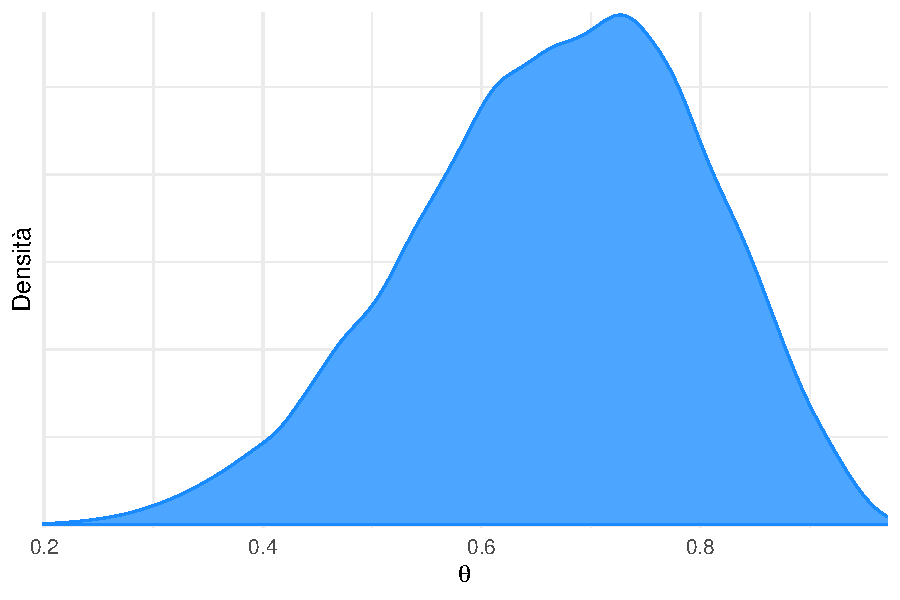
\includegraphics[keepaspectratio]{chapters/appendix/a44_stan_diagnostics_files/figure-pdf/density-plot-1.pdf}}

\subsection{Caratteristiche di una densità posteriore ben
stimata}\label{caratteristiche-di-una-densituxe0-posteriore-ben-stimata}

Una densità che indica un campionamento adeguato è tipicamente:

\begin{itemize}
\tightlist
\item
  \textbf{liscia e regolare}, senza irregolarità o ``rumore'' nella
  curva;
\item
  \textbf{unimodale}, presentando un singolo picco principale (salvo
  modelli che prevedano esplicitamente multimodalità);
\item
  \textbf{con code ben comportate}, che decadono in modo graduale e
  senza interruzioni.
\end{itemize}

\subsection{Segnali di potenziali
problemi}\label{segnali-di-potenziali-problemi-1}

Profili di densità che possono indicare problematiche includono:

\begin{itemize}
\tightlist
\item
  \textbf{multimodalità inattesa}, che può suggerire problemi di
  identificazione del modello o catene intrappolate in mode locali;
\item
  \textbf{code eccessivamente lunghe, piatte o irregolari}, spesso
  indice di una scarsa informazione nei dati o di prior troppo deboli;
\item
  \textbf{aspetto frastagliato o a ``denti di sega''}, sintomo di un
  campionamento insufficiente o di un'eccessiva autocorrelazione che
  impedisce una rappresentazione fedele della distribuzione.
\end{itemize}

Un esame congiunto delle densità di tutte le catene consente inoltre di
verificare che esse siano sostanzialmente sovrapposte, fornendo un
ulteriore controllo visivo sulla convergenza.

\section{Autocorrelazione}\label{autocorrelazione}

L'autocorrelazione quantifica la dipendenza statistica tra campioni
successivi all'interno di una catena MCMC. Un'elevata autocorrelazione
riduce l'informazione effettiva contenuta nei campioni, aumentando la
varianza delle stime e diminuendo l'efficienza computazionale.

\begin{Shaded}
\begin{Highlighting}[]
\FunctionTok{mcmc\_acf}\NormalTok{(fit}\SpecialCharTok{$}\FunctionTok{draws}\NormalTok{(}\StringTok{"theta"}\NormalTok{), }\AttributeTok{lags =} \DecValTok{20}\NormalTok{)}
\end{Highlighting}
\end{Shaded}

\pandocbounded{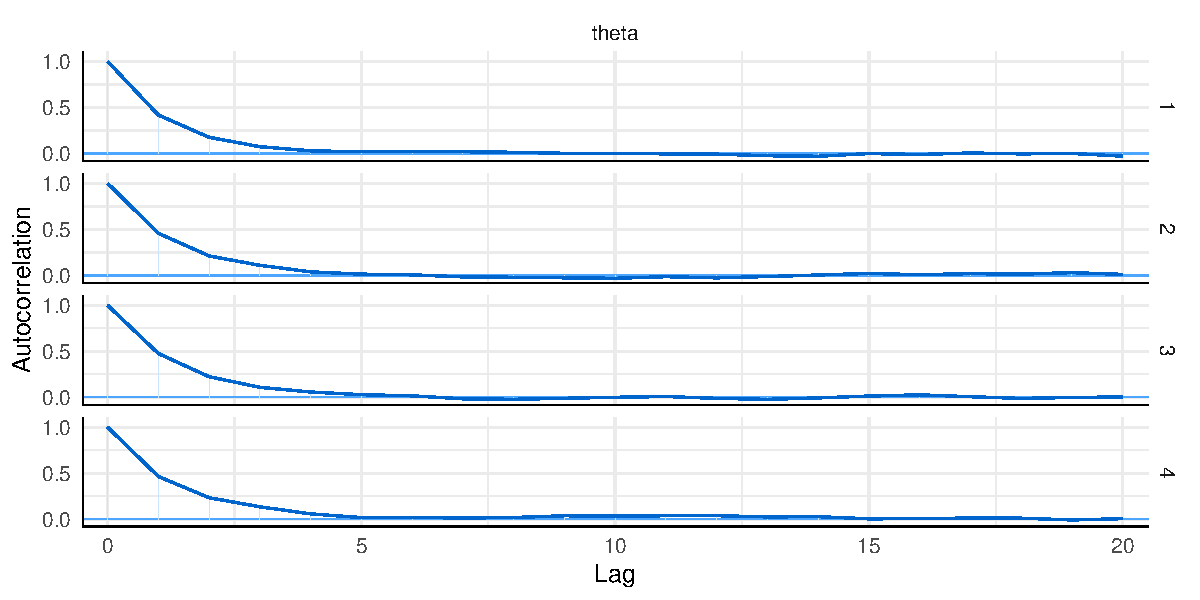
\includegraphics[keepaspectratio]{chapters/appendix/a44_stan_diagnostics_files/figure-pdf/acf-plot-1.pdf}}

\subsection{Interpretazione del grafico di
autocorrelazione}\label{interpretazione-del-grafico-di-autocorrelazione}

\begin{itemize}
\tightlist
\item
  \textbf{Autocorrelazione bassa}: la funzione di autocorrelazione
  decade rapidamente verso zero, indicando che i campioni sono pressoché
  indipendenti. Questo è lo scenario ideale per un campionamento
  efficiente.
\item
  \textbf{Autocorrelazione elevata}: valori significativi persistono
  anche a lag elevati, rivelando una forte dipendenza tra campioni
  distanti. Questo segnala un'inefficiente esplorazione dello spazio dei
  parametri e può invalidare le stime degli errori standard.
\end{itemize}

\subsection{Strategie per ridurre
l'autocorrelazione}\label{strategie-per-ridurre-lautocorrelazione}

Quando si riscontra un'elevata autocorrelazione, si possono adottare le
seguenti contromisure:

\begin{enumerate}
\def\labelenumi{\arabic{enumi}.}
\item
  \textbf{Prolungare la durata del campionamento}: un numero maggiore di
  iterazioni può compensare la ridotta informazione per campione,
  permettendo di ottenere un numero efficace di campioni indipendenti
  sufficiente.
\item
  \textbf{Applicare il \emph{thinning}}: conservare solo un campione
  ogni \(k\) iterazioni (ad esempio, ogni 5 o 10) può ridurre la
  dipendenza nei dati conservati, sebbene questa pratica comporti uno
  spreco di informazioni e venga generalmente sconsigliata se non
  necessario per motivi di archiviazione.
\item
  \textbf{Migliorare l'efficienza dell'algoritmo}: aumentare il
  parametro \texttt{adapt\_delta} in Stan può produrre step-size più
  piccoli e un'esplorazione più conservativa. Spesso, la soluzione più
  efficace è una riparametrizzazione del modello per migliorare la
  geometria dello spazio dei parametri e facilitare il movimento del
  campionatore.
\end{enumerate}

\section{Dimensione effettiva del campione
(ESS)}\label{dimensione-effettiva-del-campione-ess}

La dimensione effettiva del campione (\emph{Effective Sample Size},
\(N_{\text{eff}}\)) misura l'informazione statistica indipendente
contenuta in una catena MCMC autocorrelata. Espresso come equivalente
numerico di campioni indipendenti e identicamente distribuiti (i.i.d.),
quantifica l'efficienza del campionamento.

La formula di base è data da:

\[
N_{\text{eff}} = \frac{T}{1 + 2 \sum_{s=1}^{\infty} \rho_{s}},
\] dove \(T\) rappresenta il numero totale di campioni e \(\rho_s\) è
l'autocorrelazione al lag \(s\). Valori elevati di autocorrelazione
riducono sostanzialmente \(N_{\text{eff}}\).

\subsection{\texorpdfstring{ESS \emph{bulk} ed ESS
\emph{tail}}{ESS bulk ed ESS tail}}\label{ess-bulk-ed-ess-tail}

In Stan si distinguono due diverse metriche ESS, ciascuna focalizzata su
una regione specifica della distribuzione:

\begin{itemize}
\tightlist
\item
  \textbf{ESS \emph{bulk}}: valuta l'efficienza del campionamento nella
  regione \textbf{centrale} della distribuzione (tipicamente attorno
  alla moda o alla media). È la misura rilevante per la stima di
  parametri di locazione come la media posteriore.
\item
  \textbf{ESS \emph{tail}}: misura l'efficienza del campionamento nelle
  \textbf{code} della distribuzione, fondamentale per la stima accurata
  di quantili estremi (ad esempio, il 2.5° e il 97.5° percentile per un
  intervallo credibile al 95\%).
\end{itemize}

\begin{tcolorbox}[enhanced jigsaw, arc=.35mm, bottomrule=.15mm, bottomtitle=1mm, breakable, colback=white, colbacktitle=quarto-callout-tip-color!10!white, colframe=quarto-callout-tip-color-frame, coltitle=black, left=2mm, leftrule=.75mm, opacityback=0, opacitybacktitle=0.6, rightrule=.15mm, title=\textcolor{quarto-callout-tip-color}{\faLightbulb}\hspace{0.5em}{Soglia pratica}, titlerule=0mm, toprule=.15mm, toptitle=1mm]

Per garantire una stima affidabile, sia l'ESS \emph{bulk} che l'ESS
\emph{tail} per ogni parametro dovrebbero essere \textbf{superiori a
400}. Valori inferiori indicano che la catena potrebbe non aver
esplorato adeguatamente la corrispondente regione della distribuzione.

\end{tcolorbox}

\begin{Shaded}
\begin{Highlighting}[]
\CommentTok{\# Visualizzazione del sommario con ESS}
\NormalTok{fit}\SpecialCharTok{$}\FunctionTok{summary}\NormalTok{(}\AttributeTok{variables =} \StringTok{"theta"}\NormalTok{)}
\end{Highlighting}
\end{Shaded}

\begin{verbatim}
# A tibble: 1 x 10
  variable  mean median    sd   mad    q5   q95  rhat ess_bulk ess_tail
  <chr>    <dbl>  <dbl> <dbl> <dbl> <dbl> <dbl> <dbl>    <dbl>    <dbl>
1 theta    0.668  0.678 0.132 0.137 0.436 0.868  1.00    5663.    6067.
\end{verbatim}

\begin{Shaded}
\begin{Highlighting}[]
\CommentTok{\# Rapporto tra ESS e numero totale di campioni per tutti i parametri}
\NormalTok{ratios }\OtherTok{\textless{}{-}} \FunctionTok{neff\_ratio}\NormalTok{(fit)}
\FunctionTok{mcmc\_neff}\NormalTok{(ratios, }\AttributeTok{size =} \DecValTok{2}\NormalTok{) }\SpecialCharTok{+}
  \FunctionTok{labs}\NormalTok{(}\AttributeTok{title =} \StringTok{"Rapporto ESS / N totale"}\NormalTok{)}
\end{Highlighting}
\end{Shaded}

\pandocbounded{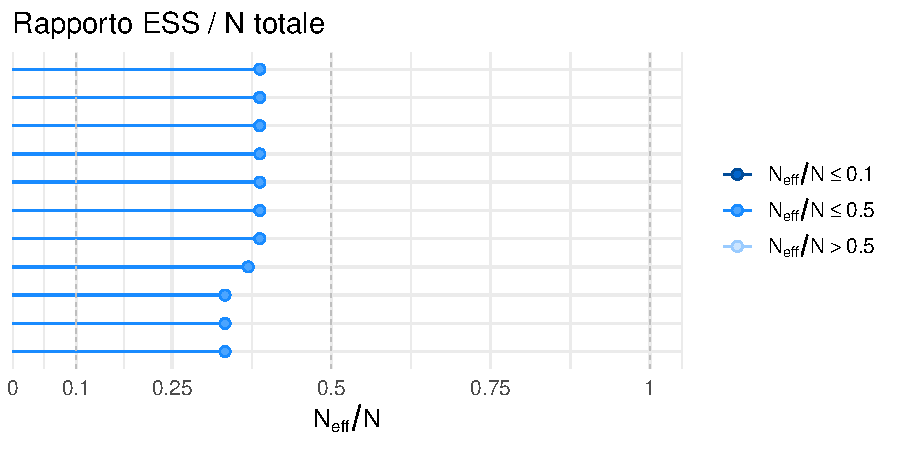
\includegraphics[keepaspectratio]{chapters/appendix/a44_stan_diagnostics_files/figure-pdf/neff-ratio-1.pdf}}

\subsection{Interpretazione e
intervento}\label{interpretazione-e-intervento}

Un rapporto \(N_{\text{eff}}/T\) basso (ad esempio, \textless{} 0.1)
segnala un'elevata autocorrelazione e un'efficienza di campionamento
scarsa. In questi casi, le strategie correttive sono le stesse indicate
per il problema dell'autocorrelazione: aumentare il numero totale di
iterazioni, migliorare la parametrizzazione del modello o ottimizzare i
parametri di controllo dell'algoritmo HMC/NUTS.

\section{\texorpdfstring{La statistica \(\widehat{R}\)
(R-hat)}{La statistica \textbackslash widehat\{R\} (R-hat)}}\label{la-statistica-widehatr-r-hat}

La statistica \(\widehat{R}\), sviluppata da Gelman e Rubin, è una
metrica fondamentale per diagnosticare la convergenza delle catene MCMC.
Essa confronta la variabilità \textbf{tra le diverse catene} (\(B\)) con
la variabilità media \textbf{all'interno di ciascuna catena} (\(W\)). La
formula è la seguente:

\[
\widehat{R} = \sqrt{\frac{W + \frac{B}{n}}{W}},
\] dove \(n\) è il numero di campioni per catena. Un \(\widehat{R}\)
vicino a 1 indica che la varianza tra le catene è comparabile con quella
all'interno delle catene, suggerendo che tutte le catene stanno
campionando dalla medesima distribuzione stazionaria.

\subsection{Interpretazione e soglie}\label{interpretazione-e-soglie}

{\def\LTcaptype{none} % do not increment counter
\begin{longtable}[]{@{}
  >{\raggedright\arraybackslash}p{(\linewidth - 4\tabcolsep) * \real{0.4783}}
  >{\raggedright\arraybackslash}p{(\linewidth - 4\tabcolsep) * \real{0.3478}}
  >{\raggedright\arraybackslash}p{(\linewidth - 4\tabcolsep) * \real{0.1739}}@{}}
\toprule\noalign{}
\begin{minipage}[b]{\linewidth}\raggedright
Valore \(\widehat{R}\)
\end{minipage} & \begin{minipage}[b]{\linewidth}\raggedright
Interpretazione
\end{minipage} & \begin{minipage}[b]{\linewidth}\raggedright
Azione
\end{minipage} \\
\midrule\noalign{}
\endhead
\bottomrule\noalign{}
\endlastfoot
\textbf{1.000} & Convergenza ottimale. & Nessuna. \\
\textbf{≤ 1.010} & Convergenza soddisfacente. & Monitorare se associato
ad altri segnali. \\
\textbf{1.011 - 1.049} & Convergenza subottimale. & Verificare altri
diagnostici e considerare azioni correttive. \\
\textbf{≥ 1.050} & Convergenza problematica. & Catene probabilmente non
convergenti; intervento necessario. \\
\end{longtable}
}

\subsection{Implementazione in R}\label{implementazione-in-r-4}

\begin{Shaded}
\begin{Highlighting}[]
\CommentTok{\# Calcolo dei valori R{-}hat per tutti i parametri}
\NormalTok{rhats }\OtherTok{\textless{}{-}}\NormalTok{ bayesplot}\SpecialCharTok{::}\FunctionTok{rhat}\NormalTok{(fit)}
\FunctionTok{print}\NormalTok{(rhats)}
\end{Highlighting}
\end{Shaded}

\begin{verbatim}
      theta  log_lik[1]  log_lik[2]  log_lik[3]  log_lik[4]  log_lik[5] 
   1.000875    1.000875    1.000875    1.000875    1.000875    1.000875 
 log_lik[6]  log_lik[7]  log_lik[8]  log_lik[9] log_lik[10] 
   1.000875    1.000875    1.000875    1.000875    1.000875 
\end{verbatim}

\begin{Shaded}
\begin{Highlighting}[]
\CommentTok{\# Visualizzazione grafica dei valori R{-}hat}
\FunctionTok{mcmc\_rhat}\NormalTok{(rhats) }\SpecialCharTok{+}
  \FunctionTok{labs}\NormalTok{(}\AttributeTok{title =} \StringTok{"Distribuzione dei valori R{-}hat"}\NormalTok{,}
       \AttributeTok{subtitle =} \StringTok{"Valori \textgreater{} 1.01 richiedono attenzione"}\NormalTok{)}
\end{Highlighting}
\end{Shaded}

\pandocbounded{\includegraphics[keepaspectratio]{chapters/appendix/a44_stan_diagnostics_files/figure-pdf/rhat-plot-1.pdf}}

\subsection{\texorpdfstring{Azioni correttive per \(\widehat{R}\)
elevato}{Azioni correttive per \textbackslash widehat\{R\} elevato}}\label{azioni-correttive-per-widehatr-elevato}

Valori di \(\widehat{R}\) persistentemente superiori a 1.05 suggeriscono
che le catene non hanno raggiunto una distribuzione stazionaria comune.
Le strategie per affrontare il problema includono:

\begin{enumerate}
\def\labelenumi{\arabic{enumi}.}
\tightlist
\item
  \textbf{Aumentare il numero di iterazioni}, specialmente il periodo di
  warmup;
\item
  \textbf{Controllare e potenzialmente riparametrizzare il modello},
  poiché una cattiva geometria dello spazio dei parametri è una causa
  comune di non convergenza;
\item
  \textbf{Verificare le distribuzioni a priori e la coerenza dei dati}
  per escludere problemi di identificazione o dati aberranti.
\end{enumerate}

Un \(\widehat{R}\) accettabile è un prerequisito necessario, ma non
sufficiente, per considerare valide le inferenze tratte dai campioni
MCMC.

\section{Diagnostica di Geweke}\label{diagnostica-di-geweke}

Il test di Geweke verifica l'ipotesi di stazionarietà di una catena MCMC
confrontando la distribuzione dei campioni nella fase iniziale con
quella nella fase finale. Nella sua implementazione standard, confronta
la media dei primi 10\% dei campioni con la media degli ultimi 50\% dei
campioni (escludendo il periodo di warmup). La differenza,
standardizzata per l'errore standard, produce uno z-score.

\subsection{Implementazione in R}\label{implementazione-in-r-5}

\begin{Shaded}
\begin{Highlighting}[]
\CommentTok{\# Preparazione dei dati: conversione in formato mcmc.list}
\NormalTok{df\_theta }\OtherTok{\textless{}{-}} \FunctionTok{as\_draws\_df}\NormalTok{(fit}\SpecialCharTok{$}\FunctionTok{draws}\NormalTok{(}\StringTok{"theta"}\NormalTok{))[, }\FunctionTok{c}\NormalTok{(}\StringTok{".chain"}\NormalTok{, }\StringTok{".iteration"}\NormalTok{, }\StringTok{"theta"}\NormalTok{)]}
\NormalTok{chains\_list }\OtherTok{\textless{}{-}} \FunctionTok{split}\NormalTok{(df\_theta}\SpecialCharTok{$}\NormalTok{theta, df\_theta}\SpecialCharTok{$}\NormalTok{.chain)}
\NormalTok{mcmc\_list }\OtherTok{\textless{}{-}} \FunctionTok{mcmc.list}\NormalTok{(}\FunctionTok{lapply}\NormalTok{(chains\_list, mcmc))}

\CommentTok{\# Calcolo degli z{-}scores di Geweke per ciascuna catena}
\NormalTok{gd }\OtherTok{\textless{}{-}} \FunctionTok{lapply}\NormalTok{(mcmc\_list, geweke.diag, }\AttributeTok{frac1 =} \FloatTok{0.1}\NormalTok{, }\AttributeTok{frac2 =} \FloatTok{0.5}\NormalTok{)}
\NormalTok{z\_scores }\OtherTok{\textless{}{-}} \FunctionTok{sapply}\NormalTok{(gd, }\ControlFlowTok{function}\NormalTok{(x) x}\SpecialCharTok{$}\NormalTok{z)}
\FunctionTok{cat}\NormalTok{(}\StringTok{"Z{-}scores di Geweke per catena:"}\NormalTok{, }\FunctionTok{round}\NormalTok{(z\_scores, }\DecValTok{3}\NormalTok{), }\StringTok{"}\SpecialCharTok{\textbackslash{}n}\StringTok{"}\NormalTok{)}
\end{Highlighting}
\end{Shaded}

\begin{verbatim}
Z-scores di Geweke per catena: -1.338 0.815 -0.583 0.915 
\end{verbatim}

\begin{Shaded}
\begin{Highlighting}[]
\CommentTok{\# Calcolo dei p{-}value bilaterali associati}
\NormalTok{pvals }\OtherTok{\textless{}{-}} \DecValTok{2} \SpecialCharTok{*} \FunctionTok{pnorm}\NormalTok{(}\SpecialCharTok{{-}}\FunctionTok{abs}\NormalTok{(z\_scores))}
\FunctionTok{cat}\NormalTok{(}\StringTok{"P{-}value associati:"}\NormalTok{, }\FunctionTok{format.pval}\NormalTok{(pvals, }\AttributeTok{digits =} \DecValTok{3}\NormalTok{), }\StringTok{"}\SpecialCharTok{\textbackslash{}n}\StringTok{"}\NormalTok{)}
\end{Highlighting}
\end{Shaded}

\begin{verbatim}
P-value associati: 0.181 0.415 0.560 0.360 
\end{verbatim}

\subsection{Interpretazione dei
risultati}\label{interpretazione-dei-risultati-3}

La logica del test è la seguente: se la catena è stazionaria, le medie
delle due sottosezioni dovrebbero essere compatibili, producendo uno
z-score vicino a zero.

\begin{itemize}
\tightlist
\item
  \textbf{\textbar z-score\textbar{} \textless{} 1.96}: non si rileva
  evidenza statistica di non-stazionarietà al livello di significatività
  del 5\%.
\item
  \textbf{\textbar z-score\textbar{} ≥ 1.96}: si osserva una differenza
  statisticamente significativa tra l'inizio e la fine della catena,
  suggerendo una possibile mancanza di stazionarietà (livello di
  significatività del 5\%).
\item
  \textbf{\textbar z-score\textbar{} ≥ 2.58}: evidenza forte di
  non-stazionarietà (livello dell'1\%).
\end{itemize}

\subsection{Considerazioni pratiche}\label{considerazioni-pratiche}

Il test di Geweke è uno strumento diagnostico complementare. Un singolo
test significativo può occasionalmente verificarsi per caso,
specialmente quando si esaminano molti parametri. Tuttavia, z-score
sistematicamente elevati (ad esempio, \textgreater{} 2) per diversi
parametri chiave sono un segnale d'allarme che richiede un'indagine più
approfondita, possibilmente ripetendo il campionamento con un maggior
numero di iterazioni o intervenendo sulla parametrizzazione del modello.

\section{Errore standard di Monte Carlo
(MCSE)}\label{errore-standard-di-monte-carlo-mcse}

L'errore standard di Monte Carlo (\emph{Monte Carlo Standard Error},
MCSE) quantifica l'incertezza intrinseca nelle stime a posteriori
derivante dal numero finito di campioni MCMC. A differenza della
deviazione standard posteriore, che riflette l'incertezza statistica sul
parametro, l'MCSE misura l'errore di simulazione introdotto dal processo
di campionamento.

\subsection{Definizione}\label{definizione}

Per una stima della media posteriore \(\bar{\theta}\), l'MCSE è definito
come:

\[
\text{MCSE}(\bar{\theta}) = \frac{\hat{\sigma}_\theta}{\sqrt{N_{\text{eff}}}},
\] dove \(\hat{\sigma}_\theta\) è la deviazione standard posteriore
stimata e \(N_{\text{eff}}\) è la dimensione effettiva del campione
(\emph{Effective Sample Size}). La formula evidenzia come l'MCSE
diminuisca all'aumentare dell'informazione indipendente
(\(N_{\text{eff}}\)) contenuta nella catena.

\subsection{Calcolo e interpretazione in
R}\label{calcolo-e-interpretazione-in-r}

\begin{Shaded}
\begin{Highlighting}[]
\CommentTok{\# Calcolo dell\textquotesingle{}MCSE per il parametro \textquotesingle{}theta\textquotesingle{}}
\NormalTok{summ\_theta }\OtherTok{\textless{}{-}}\NormalTok{ fit}\SpecialCharTok{$}\FunctionTok{summary}\NormalTok{(}\AttributeTok{variables =} \StringTok{"theta"}\NormalTok{)}
\NormalTok{mcse\_theta }\OtherTok{\textless{}{-}}\NormalTok{ summ\_theta}\SpecialCharTok{$}\NormalTok{sd }\SpecialCharTok{/} \FunctionTok{sqrt}\NormalTok{(summ\_theta}\SpecialCharTok{$}\NormalTok{ess\_bulk)}
\FunctionTok{cat}\NormalTok{(}\StringTok{"Errore standard di Monte Carlo per θ:"}\NormalTok{, }\FunctionTok{round}\NormalTok{(mcse\_theta, }\DecValTok{5}\NormalTok{), }\StringTok{"}\SpecialCharTok{\textbackslash{}n}\StringTok{"}\NormalTok{)}
\end{Highlighting}
\end{Shaded}

\begin{verbatim}
Errore standard di Monte Carlo per θ: 0.00175 
\end{verbatim}

\begin{tcolorbox}[enhanced jigsaw, arc=.35mm, bottomrule=.15mm, bottomtitle=1mm, breakable, colback=white, colbacktitle=quarto-callout-tip-color!10!white, colframe=quarto-callout-tip-color-frame, coltitle=black, left=2mm, leftrule=.75mm, opacityback=0, opacitybacktitle=0.6, rightrule=.15mm, title=\textcolor{quarto-callout-tip-color}{\faLightbulb}\hspace{0.5em}{Criterio pratico}, titlerule=0mm, toprule=.15mm, toptitle=1mm]

L'MCSE dovrebbe essere almeno \textbf{un ordine di grandezza inferiore}
alla deviazione standard posteriore corrispondente. In altre parole,
l'incertezza dovuta al campionamento (MCSE) deve essere trascurabile
rispetto all'incertezza statistica sulla stima del parametro. Un
rapporto \(\text{SD}/\text{MCSE} \approx \sqrt{N_{\text{eff}}} > 10\)
indica una precisione di simulazione adeguata.

\end{tcolorbox}

\subsection{Significato pratico}\label{significato-pratico}

Un MCSE troppo elevato segnala che le stime dei parametri (come la media
posteriore) potrebbero cambiare in modo sostanziale se si proseguisse il
campionamento. Per ridurre l'MCSE è necessario aumentare
\(N_{\text{eff}}\), il che si ottiene tipicamente prolungando la durata
del campionamento, riducendo l'autocorrelazione attraverso una migliore
parametrizzazione del modello, oppure aumentando il numero di catene
parallele.

\section{Transizioni divergenti nell'algoritmo
HMC/NUTS}\label{transizioni-divergenti-nellalgoritmo-hmcnuts}

Le transizioni divergenti rappresentano un indicatore diagnostico
critico nell'ambito del campionamento Hamiltonian Monte Carlo (HMC) e
del suo algoritmo No-U-Turn Sampler (NUTS). Si verificano quando la
traiettoria numerica, che approssima il sistema hamiltoniano, incontra
regioni dello spazio dei parametri caratterizzate da una forte curvatura
o da repentini cambiamenti di scala. In tali regioni, l'approssimazione
discreta dell'equazione differenziale diventa instabile, portando a un
significativo scostamento tra la traiettoria simulata e il percorso
energetico vero, compromettendo la fedeltà del campionamento.

\begin{Shaded}
\begin{Highlighting}[]
\CommentTok{\# Controllo del numero di transizioni divergenti}
\NormalTok{num\_divergenze }\OtherTok{\textless{}{-}}\NormalTok{ fit}\SpecialCharTok{$}\FunctionTok{diagnostic\_summary}\NormalTok{()}\SpecialCharTok{$}\NormalTok{num\_divergent}
\FunctionTok{cat}\NormalTok{(}\StringTok{"Numero di transizioni divergenti:"}\NormalTok{, num\_divergenze, }\StringTok{"}\SpecialCharTok{\textbackslash{}n}\StringTok{"}\NormalTok{)}
\end{Highlighting}
\end{Shaded}

\begin{verbatim}
Numero di transizioni divergenti: 0 0 0 0 
\end{verbatim}

\subsection{Strategie di risoluzione}\label{strategie-di-risoluzione}

In presenza di divergenze, si raccomanda di intervenire secondo la
seguente gerarchia:

\begin{enumerate}
\def\labelenumi{\arabic{enumi}.}
\item
  \textbf{Aumentare il parametro \texttt{adapt\_delta}}: Questo
  parametro, compreso tra 0 e 1, controlla il livello di conservatorismo
  nell'adattamento della matrice di massa. Valori più elevati (ad
  esempio 0.95, 0.99) portano a una matrice di massa più conservativa e
  a step-size più piccoli, migliorando la stabilità a costo di una
  maggiore autocorrelazione.

\begin{Shaded}
\begin{Highlighting}[]
\NormalTok{mod}\SpecialCharTok{$}\FunctionTok{sample}\NormalTok{(}\AttributeTok{data =}\NormalTok{ stan\_data, }\AttributeTok{adapt\_delta =} \FloatTok{0.99}\NormalTok{, ...)}
\end{Highlighting}
\end{Shaded}
\item
  \textbf{Riparametrizzare il modello}: Molte problematiche geometriche
  sono dovute a parametrizzazioni ``centrate'' che creano forti
  dipendenze tra parametri. L'adozione di parametrizzazioni ``non
  centrate'' (non-centered parameterizations) può migliorare
  notevolmente la geometria dello spazio dei parametri, soprattutto per
  modelli gerarchici.
\item
  \textbf{Rivedere le specifiche delle distribuzioni a priori}: Prior
  eccessivamente informative o con supporto molto ristretto possono
  creare regioni di alta curvatura o ``colli di bottiglia'' che
  ostacolano l'esplorazione dello spazio dei parametri. Si consideri
  l'uso di prior più deboli o la trasformazione dei parametri.
\item
  \textbf{Esaminare i dati osservati}: Valori estremi o outlier nei dati
  possono causare regioni di alta curvatura nella distribuzione a
  posteriori. Un'analisi esplorativa preliminare e possibili
  trasformazioni dei dati possono mitigare il problema. Inoltre,
  verificare la coerenza delle scale delle variabili predittive.
\end{enumerate}

Un numero elevato di transizioni divergenti segnala che il campionatore
potrebbe non esplorare adeguatamente alcune regioni della distribuzione
a posteriori, compromettendo la validità delle inferenze. La loro
presenza richiede pertanto un'azione correttiva prima di procedere con
l'analisi.

\begin{tcolorbox}[enhanced jigsaw, arc=.35mm, bottomrule=.15mm, bottomtitle=1mm, breakable, colback=white, colbacktitle=quarto-callout-warning-color!10!white, colframe=quarto-callout-warning-color-frame, coltitle=black, left=2mm, leftrule=.75mm, opacityback=0, opacitybacktitle=0.6, rightrule=.15mm, title=\textcolor{quarto-callout-warning-color}{\faExclamationTriangle}\hspace{0.5em}{Importante}, titlerule=0mm, toprule=.15mm, toptitle=1mm]

Un numero significativo di transizioni divergenti (\textgreater{} 0.1\%
delle iterazioni) indica che le stime potrebbero non essere affidabili.

\end{tcolorbox}

\section{\texorpdfstring{Il BFMI (\emph{Bayesian Fraction of Missing
Information})}{Il BFMI (Bayesian Fraction of Missing Information)}}\label{il-bfmi-bayesian-fraction-of-missing-information}

Il BFMI è una metrica diagnostica che valuta l'efficienza
dell'esplorazione dello spazio dei parametri da parte dell'algoritmo
Hamiltonian Monte Carlo (HMC). Si basa sull'analisi delle fluttuazioni
dell'energia del sistema hamiltoniano durante il campionamento. Valori
bassi indicano che il campionatore fatica a esplorare alcune regioni
dello spazio, tipicamente a causa di forti gradienti o di una geometria
sfavorevole nella distribuzione a posteriori.

\begin{Shaded}
\begin{Highlighting}[]
\CommentTok{\# Estrazione delle statistiche diagnostiche del sampler}
\NormalTok{sd\_df }\OtherTok{\textless{}{-}}\NormalTok{ fit}\SpecialCharTok{$}\FunctionTok{sampler\_diagnostics}\NormalTok{(}\AttributeTok{inc\_warmup =} \ConstantTok{FALSE}\NormalTok{, }\AttributeTok{format =} \StringTok{"df"}\NormalTok{)}

\NormalTok{np\_all }\OtherTok{\textless{}{-}}\NormalTok{ sd\_df }\SpecialCharTok{|\textgreater{}}
  \FunctionTok{pivot\_longer}\NormalTok{(}
    \AttributeTok{cols =} \FunctionTok{c}\NormalTok{(accept\_stat\_\_, stepsize\_\_, treedepth\_\_, n\_leapfrog\_\_, divergent\_\_, energy\_\_),}
    \AttributeTok{names\_to =} \StringTok{"Parameter"}\NormalTok{, }\AttributeTok{values\_to =} \StringTok{"Value"}
\NormalTok{  ) }\SpecialCharTok{|\textgreater{}}
  \FunctionTok{rename}\NormalTok{(}\AttributeTok{Chain =}\NormalTok{ .chain, }\AttributeTok{Iteration =}\NormalTok{ .iteration) }\SpecialCharTok{|\textgreater{}}
  \FunctionTok{relocate}\NormalTok{(Chain, Iteration, Parameter, Value)}

\FunctionTok{class}\NormalTok{(np\_all) }\OtherTok{\textless{}{-}} \FunctionTok{c}\NormalTok{(}\StringTok{"nuts\_params"}\NormalTok{, }\StringTok{"data.frame"}\NormalTok{)}

\NormalTok{np\_energy }\OtherTok{\textless{}{-}}\NormalTok{ np\_all }\SpecialCharTok{|\textgreater{}}
\NormalTok{  dplyr}\SpecialCharTok{::}\FunctionTok{filter}\NormalTok{(Parameter }\SpecialCharTok{==} \StringTok{"energy\_\_"}\NormalTok{) }\SpecialCharTok{|\textgreater{}}
\NormalTok{  dplyr}\SpecialCharTok{::}\FunctionTok{select}\NormalTok{(Chain, Iteration, Parameter, Value)}

\FunctionTok{class}\NormalTok{(np\_energy) }\OtherTok{\textless{}{-}} \FunctionTok{c}\NormalTok{(}\StringTok{"nuts\_params"}\NormalTok{, }\StringTok{"data.frame"}\NormalTok{)}
\end{Highlighting}
\end{Shaded}

\begin{Shaded}
\begin{Highlighting}[]
\FunctionTok{mcmc\_nuts\_energy}\NormalTok{(np\_energy)}
\end{Highlighting}
\end{Shaded}

\pandocbounded{\includegraphics[keepaspectratio]{chapters/appendix/a44_stan_diagnostics_files/figure-pdf/bfmi-plot-1.pdf}}

\begin{Shaded}
\begin{Highlighting}[]
\CommentTok{\# Calcolo del BFMI per ciascuna catena e complessivo}
\NormalTok{energy\_by\_chain }\OtherTok{\textless{}{-}} \FunctionTok{split}\NormalTok{(np\_energy}\SpecialCharTok{$}\NormalTok{Value, np\_energy}\SpecialCharTok{$}\NormalTok{Chain)}
\NormalTok{bfmi }\OtherTok{\textless{}{-}} \FunctionTok{sapply}\NormalTok{(energy\_by\_chain, }\ControlFlowTok{function}\NormalTok{(e) \{}
\NormalTok{  de }\OtherTok{\textless{}{-}} \FunctionTok{diff}\NormalTok{(e)  }\CommentTok{\# Differenze successive dell\textquotesingle{}energia}
  \FunctionTok{mean}\NormalTok{(de}\SpecialCharTok{\^{}}\DecValTok{2}\NormalTok{) }\SpecialCharTok{/}\NormalTok{ stats}\SpecialCharTok{::}\FunctionTok{var}\NormalTok{(e)}
\NormalTok{\})}
\FunctionTok{cat}\NormalTok{(}\StringTok{"BFMI per catena:"}\NormalTok{, }\FunctionTok{round}\NormalTok{(bfmi, }\DecValTok{3}\NormalTok{), }\StringTok{"}\SpecialCharTok{\textbackslash{}n}\StringTok{"}\NormalTok{)}
\end{Highlighting}
\end{Shaded}

\begin{verbatim}
BFMI per catena: 1.097 1.209 1.112 1.088 
\end{verbatim}

\begin{Shaded}
\begin{Highlighting}[]
\FunctionTok{cat}\NormalTok{(}\StringTok{"BFMI complessiva:"}\NormalTok{, }\FunctionTok{round}\NormalTok{(}\FunctionTok{weighted.mean}\NormalTok{(bfmi, }\FunctionTok{sapply}\NormalTok{(energy\_by\_chain, length)), }\DecValTok{3}\NormalTok{), }\StringTok{"}\SpecialCharTok{\textbackslash{}n}\StringTok{"}\NormalTok{)}
\end{Highlighting}
\end{Shaded}

\begin{verbatim}
BFMI complessiva: 1.127 
\end{verbatim}

\subsection{Interpretazione del BFMI}\label{interpretazione-del-bfmi}

La seguente tabella fornisce una guida per l'interpretazione dei valori
ottenuti:

{\def\LTcaptype{none} % do not increment counter
\begin{longtable}[]{@{}
  >{\raggedright\arraybackslash}p{(\linewidth - 4\tabcolsep) * \real{0.3333}}
  >{\raggedright\arraybackslash}p{(\linewidth - 4\tabcolsep) * \real{0.4359}}
  >{\raggedright\arraybackslash}p{(\linewidth - 4\tabcolsep) * \real{0.2308}}@{}}
\toprule\noalign{}
\begin{minipage}[b]{\linewidth}\raggedright
Valore BFMI
\end{minipage} & \begin{minipage}[b]{\linewidth}\raggedright
Interpretazione
\end{minipage} & \begin{minipage}[b]{\linewidth}\raggedright
Rischio
\end{minipage} \\
\midrule\noalign{}
\endhead
\bottomrule\noalign{}
\endlastfoot
\textbf{≥ 0.3} & Esplorazione efficiente dello spazio dei parametri. &
Basso \\
\textbf{0.2 -- 0.3} & Esplorazione subottimale. Richiede attenzione e
possibili interventi. & Moderato \\
\textbf{\textless{} 0.2} & Esplorazione problematica. Le inferenze
potrebbero essere inaffidabili. & Alto \\
\end{longtable}
}

Un BFMI basso suggerisce spesso problemi nella parametrizzazione del
modello (ad esempio, forti correlazioni tra parametri) o nella scelta
delle distribuzioni a priori. Le strategie di intervento includono
l'aumento del parametro \texttt{adapt\_delta}, la riparametrizzazione
del modello (ad esempio, utilizzando parametrizzazioni non centrate per
effetti casuali), o la revisione della struttura del modello stesso.

\section{\texorpdfstring{LOO-CV e il parametro \(\kappa\) di
Pareto}{LOO-CV e il parametro \textbackslash kappa di Pareto}}\label{loo-cv-e-il-parametro-kappa-di-pareto}

La \emph{Leave-One-Out Cross-Validation} (LOO-CV) è un metodo per
valutare la capacità predittiva out-of-sample di un modello bayesiano
senza richiedere nuovi dati. L'implementazione efficiente utilizzata in
Stan si basa sull'approssimazione \emph{Pareto-Smoothed Importance
Sampling} (PSIS), la cui affidabilità è monitorata tramite il parametro
di forma \(\kappa\) della distribuzione di Pareto generalizzata.

\subsection{Calcolo del LOO-CV in R}\label{calcolo-del-loo-cv-in-r}

\begin{Shaded}
\begin{Highlighting}[]
\CommentTok{\# Estrazione della log{-}verosimiglianza punto a punto}
\NormalTok{ll\_array }\OtherTok{\textless{}{-}} \FunctionTok{as\_draws\_array}\NormalTok{(fit}\SpecialCharTok{$}\FunctionTok{draws}\NormalTok{(}\StringTok{"log\_lik"}\NormalTok{))}
\NormalTok{ll\_mat }\OtherTok{\textless{}{-}} \FunctionTok{as\_draws\_matrix}\NormalTok{(fit}\SpecialCharTok{$}\FunctionTok{draws}\NormalTok{(}\StringTok{"log\_lik"}\NormalTok{))}

\CommentTok{\# Parametri delle catene per il calcolo dell\textquotesingle{}efficienza relativa}
\NormalTok{S }\OtherTok{\textless{}{-}} \FunctionTok{dim}\NormalTok{(ll\_array)[}\DecValTok{1}\NormalTok{]  }\CommentTok{\# Numero di campioni per catena}
\NormalTok{C }\OtherTok{\textless{}{-}} \FunctionTok{dim}\NormalTok{(ll\_array)[}\DecValTok{2}\NormalTok{]  }\CommentTok{\# Numero di catene}
\NormalTok{chain\_id }\OtherTok{\textless{}{-}} \FunctionTok{rep}\NormalTok{(}\DecValTok{1}\SpecialCharTok{:}\NormalTok{C, }\AttributeTok{each =}\NormalTok{ S)}

\CommentTok{\# Calcolo dell\textquotesingle{}efficienza relativa}
\NormalTok{r\_eff }\OtherTok{\textless{}{-}} \FunctionTok{relative\_eff}\NormalTok{(}\FunctionTok{exp}\NormalTok{(ll\_mat), }\AttributeTok{chain\_id =}\NormalTok{ chain\_id)}

\CommentTok{\# Calcolo del LOO{-}CV con PSIS{-}LOO}
\NormalTok{loo\_res }\OtherTok{\textless{}{-}}\NormalTok{ loo}\SpecialCharTok{::}\FunctionTok{loo}\NormalTok{(ll\_mat, }\AttributeTok{r\_eff =}\NormalTok{ r\_eff)}
\FunctionTok{print}\NormalTok{(loo\_res)}
\end{Highlighting}
\end{Shaded}

\begin{verbatim}

Computed from 16000 by 10 log-likelihood matrix.

         Estimate  SE
elpd_loo     -7.1 1.3
p_loo         0.9 0.2
looic        14.2 2.6
------
MCSE of elpd_loo is 0.0.
MCSE and ESS estimates assume MCMC draws (r_eff in [0.4, 0.4]).

All Pareto k estimates are good (k < 0.7).
See help('pareto-k-diagnostic') for details.
\end{verbatim}

\subsection{\texorpdfstring{Diagnostica con il parametro \(\kappa\) di
Pareto}{Diagnostica con il parametro \textbackslash kappa di Pareto}}\label{diagnostica-con-il-parametro-kappa-di-pareto}

Il parametro \(\kappa\) diagnostica la qualità dell'approssimazione PSIS
per ciascuna osservazione. Valori elevati indicano che i pesi
\emph{importance sampling} hanno una distribuzione a code pesanti,
rendendo la stima del LOO-CV instabile.

\begin{Shaded}
\begin{Highlighting}[]
\CommentTok{\# Estrazione e riepilogo dei valori kappa}
\NormalTok{k\_values }\OtherTok{\textless{}{-}} \FunctionTok{pareto\_k\_values}\NormalTok{(loo\_res)}
\FunctionTok{cat}\NormalTok{(}\StringTok{"Riepilogo dei valori di Pareto kappa:}\SpecialCharTok{\textbackslash{}n}\StringTok{"}\NormalTok{)}
\end{Highlighting}
\end{Shaded}

\begin{verbatim}
Riepilogo dei valori di Pareto kappa:
\end{verbatim}

\begin{Shaded}
\begin{Highlighting}[]
\FunctionTok{print}\NormalTok{(}\FunctionTok{summary}\NormalTok{(k\_values))}
\end{Highlighting}
\end{Shaded}

\begin{verbatim}
     Min.   1st Qu.    Median      Mean   3rd Qu.      Max. 
-0.001379 -0.001379 -0.001379  0.039054  0.099703  0.133397 
\end{verbatim}

\begin{Shaded}
\begin{Highlighting}[]
\FunctionTok{cat}\NormalTok{(}\StringTok{"}\SpecialCharTok{\textbackslash{}n}\StringTok{Numero di osservazioni con kappa \textgreater{} 0.7:"}\NormalTok{, }\FunctionTok{sum}\NormalTok{(k\_values }\SpecialCharTok{\textgreater{}} \FloatTok{0.7}\NormalTok{), }\StringTok{"}\SpecialCharTok{\textbackslash{}n}\StringTok{"}\NormalTok{)}
\end{Highlighting}
\end{Shaded}

\begin{verbatim}

Numero di osservazioni con kappa > 0.7: 0 
\end{verbatim}

\subsection{Soglie interpretative}\label{soglie-interpretative}

{\def\LTcaptype{none} % do not increment counter
\begin{longtable}[]{@{}
  >{\raggedright\arraybackslash}p{(\linewidth - 4\tabcolsep) * \real{0.3889}}
  >{\raggedright\arraybackslash}p{(\linewidth - 4\tabcolsep) * \real{0.2963}}
  >{\raggedright\arraybackslash}p{(\linewidth - 4\tabcolsep) * \real{0.3148}}@{}}
\toprule\noalign{}
\begin{minipage}[b]{\linewidth}\raggedright
Intervallo \(\kappa\)
\end{minipage} & \begin{minipage}[b]{\linewidth}\raggedright
Interpretazione
\end{minipage} & \begin{minipage}[b]{\linewidth}\raggedright
Raccomandazione
\end{minipage} \\
\midrule\noalign{}
\endhead
\bottomrule\noalign{}
\endlastfoot
\textbf{\(\kappa < 0.5\)} & Approssimazione affidabile. & Le stime
LOO-CV sono robuste. \\
\textbf{\(0.5 \leq \kappa < 0.7\)} & Approssimazione accettabile ma con
qualche incertezza. & Interpretare con cautela. Controllare osservazioni
specifiche. \\
\textbf{\(\kappa \geq 0.7\)} & Approssimazione potenzialmente
inaffidabile. & Le stime potrebbero essere instabili. Considerare un
modello più robusto o un cross-validation esplicito. \\
\end{longtable}
}

\subsection{\texorpdfstring{Azioni correttive per \(\kappa\)
elevato}{Azioni correttive per \textbackslash kappa elevato}}\label{azioni-correttive-per-kappa-elevato}

La presenza di osservazioni con \(\kappa > 0.7\) (specialmente se
\textgreater{} 1.0) suggerisce che il modello assegna una
verosimiglianza estremamente bassa a quelle osservazioni. Si possono
considerare:

\begin{enumerate}
\def\labelenumi{\arabic{enumi}.}
\tightlist
\item
  \textbf{modelli più robusti} (ad esempio, distribuzioni t-student
  invece di normali per i termini di errore);
\item
  \textbf{identificazione e analisi delle osservazioni influenti}
  tramite un \emph{Pareto-k diagnostic plot};
\item
  \textbf{ricorso a una K-fold Cross-Validation esplicita} per le
  osservazioni problematiche.
\end{enumerate}

Il LOO-CV e il suo parametro \(\kappa\) forniscono quindi non solo una
misura della performance predittiva, ma anche una diagnostica preziosa
sull'adeguatezza del modello rispetto alla struttura dei dati osservati.

\begin{tcolorbox}[enhanced jigsaw, arc=.35mm, bottomrule=.15mm, bottomtitle=1mm, breakable, colback=white, colbacktitle=quarto-callout-note-color!10!white, colframe=quarto-callout-note-color-frame, coltitle=black, left=2mm, leftrule=.75mm, opacityback=0, opacitybacktitle=0.6, rightrule=.15mm, title=\textcolor{quarto-callout-note-color}{\faInfo}\hspace{0.5em}{Checklist diagnostica}, titlerule=0mm, toprule=.15mm, toptitle=1mm]

Prima di interpretare i risultati di un modello Stan, verificare sempre:

\begin{enumerate}
\def\labelenumi{\arabic{enumi}.}
\tightlist
\item
  ☐ \textbf{Trace plots}: catene sovrapposte, buon mixing
\item
  ☐ \textbf{\(\hat{R}\)}: tutti i valori \textless{} 1.01
\item
  ☐ \textbf{ESS bulk e tail}: \textgreater{} 400 per tutti i parametri
\item
  ☐ \textbf{Divergenze}: 0 transizioni divergenti
\item
  ☐ \textbf{BFMI}: \textgreater{} 0.3 per tutte le catene
\item
  ☐ \textbf{MCSE}: almeno 10× più piccolo di SD
\item
  ☐ \textbf{Pareto \(\kappa\)} (se si usa LOO): \textless{} 0.7
\end{enumerate}

\end{tcolorbox}

\section*{Riflessioni conclusive}\label{riflessioni-conclusive-46}
\addcontentsline{toc}{section}{Riflessioni conclusive}

\markright{Riflessioni conclusive}

La diagnostica MCMC non costituisce una fase opzionale o meramente
tecnica, ma rappresenta una condizione necessaria per la validità delle
inferenze bayesiane. Un modello, per quanto sofisticato nella sua
formulazione teorica, produce risultati sostanzialmente inaffidabili se
basato su catene che non hanno raggiunto la convergenza o che esplorano
lo spazio dei parametri in modo inefficiente.

L'identificazione di problematiche attraverso gli strumenti diagnostici
non è un fallimento, ma un'occasione per migliorare l'analisi. Le
principali strategie correttive includono:

\begin{enumerate}
\def\labelenumi{\arabic{enumi}.}
\tightlist
\item
  \textbf{estendere la durata del campionamento}, aumentando le
  iterazioni totali e il periodo di warmup;
\item
  \textbf{ottimizzare la parametrizzazione del modello}, adottando
  formulazioni che migliorino la geometria dello spazio dei parametri
  (ad esempio, parametrizzazioni non centrate per effetti casuali);
\item
  \textbf{rivedere la specificazione delle distribuzioni a priori},
  bilanciando l'informatività per evitare problemi di identificazione o
  regioni di curvatura eccessiva;
\item
  \textbf{ottimizzare i parametri di controllo dell'algoritmo HMC/NUTS},
  come \texttt{adapt\_delta} e \texttt{max\_treedepth};
\item
  \textbf{verificare l'integrità e la coerenza dei dati osservati},
  poiché valori anomali o errori sistematici possono destabilizzare
  l'inferenza.
\end{enumerate}

Nella comunicazione dei risultati, è buona pratica riportare in modo
trasparente i valori chiave delle diagnostiche (quali \(\widehat{R}\),
\(N_{\text{eff}}\), il conteggio delle divergenze e il BFMI). Tale
trasparenza non solo rafforza la credibilità dell'analisi, ma favorisce
anche la riproducibilità e consente una valutazione critica e
costruttiva dei risultati ottenuti.

\begin{tcolorbox}[enhanced jigsaw, arc=.35mm, bottomrule=.15mm, bottomtitle=1mm, breakable, colback=white, colbacktitle=quarto-callout-note-color!10!white, colframe=quarto-callout-note-color-frame, coltitle=black, left=2mm, leftrule=.75mm, opacityback=0, opacitybacktitle=0.6, rightrule=.15mm, title=\textcolor{quarto-callout-note-color}{\faInfo}\hspace{0.5em}{Informazioni sull'ambiente di sviluppo}, titlerule=0mm, toprule=.15mm, toptitle=1mm]

\begin{Shaded}
\begin{Highlighting}[]
\FunctionTok{sessionInfo}\NormalTok{()}
\end{Highlighting}
\end{Shaded}

\begin{verbatim}
R version 4.6.1 (2026-06-24)
Platform: aarch64-apple-darwin23
Running under: macOS Tahoe 26.5.2

Matrix products: default
BLAS:   /Library/Frameworks/R.framework/Versions/4.6/Resources/lib/libRblas.0.dylib 
LAPACK: /Library/Frameworks/R.framework/Versions/4.6/Resources/lib/libRlapack.dylib;  LAPACK version 3.12.1

locale:
[1] C.UTF-8/UTF-8/C.UTF-8/C/C.UTF-8/C.UTF-8

time zone: Europe/Rome
tzcode source: internal

attached base packages:
[1] stats     graphics  grDevices utils     datasets  methods   base     

other attached packages:
[1] tidyr_1.3.2      dplyr_1.2.1      loo_2.10.0       coda_0.19-4.1   
[5] ggplot2_4.0.3    bayesplot_1.15.0 posterior_1.7.0  cmdstanr_0.9.0  

loaded via a namespace (and not attached):
 [1] tensorA_0.36.2.1     utf8_1.2.6           generics_0.1.4      
 [4] stringi_1.8.7        lattice_0.22-9       digest_0.6.39       
 [7] magrittr_2.0.5       evaluate_1.0.5       grid_4.6.1          
[10] RColorBrewer_1.1-3   fastmap_1.2.0        plyr_1.8.9          
[13] jsonlite_2.0.0       processx_3.9.0       backports_1.5.1     
[16] ps_1.9.3             purrr_1.2.2          scales_1.4.0        
[19] abind_1.4-8          cli_3.6.6            rlang_1.3.0         
[22] withr_3.0.3          yaml_2.3.12          otel_0.2.0          
[25] tools_4.6.1          parallel_4.6.1       reshape2_1.4.5      
[28] checkmate_2.3.4      vctrs_0.7.3          R6_2.6.1            
[31] matrixStats_1.5.0    lifecycle_1.0.5      stringr_1.6.0       
[34] pkgconfig_2.0.3      pillar_1.11.1        gtable_0.3.6        
[37] Rcpp_1.1.2           glue_1.8.1           data.table_1.18.4   
[40] xfun_0.60            tibble_3.3.1         tidyselect_1.2.1    
[43] knitr_1.51           farver_2.1.2         htmltools_0.5.9     
[46] labeling_0.4.3       rmarkdown_2.31       compiler_4.6.1      
[49] S7_0.2.2             distributional_0.8.1
\end{verbatim}

\end{tcolorbox}

\chapter{Controlli predittivi a
priori}\label{sec-apx-prior-predictive-check}

I controlli predittivi a priori (\emph{Prior Predictive Checks})
permettono di valutare le implicazioni delle nostre scelte sui
\emph{prior} \emph{prima} di osservare i dati. Il principio è il
seguente: se le nostre distribuzioni a priori catturano in modo adeguato
la conoscenza sul fenomeno in studio (prima di avere osservato i dati),
allora i dati \textbf{simulati} generati da tali \emph{prior} dovrebbero
essere plausibili alla luce di tale conoscenza contestuale.

\begin{tcolorbox}[enhanced jigsaw, arc=.35mm, bottomrule=.15mm, bottomtitle=1mm, breakable, colback=white, colbacktitle=quarto-callout-tip-color!10!white, colframe=quarto-callout-tip-color-frame, coltitle=black, left=2mm, leftrule=.75mm, opacityback=0, opacitybacktitle=0.6, rightrule=.15mm, title=\textcolor{quarto-callout-tip-color}{\faLightbulb}\hspace{0.5em}{Domanda chiave}, titlerule=0mm, toprule=.15mm, toptitle=1mm]

Le nostre prior generano dati che hanno senso nel contesto del problema?
O producono scenari assurdi che sappiamo non poter accadere?

\end{tcolorbox}

Questo controllo è essenziale perché \emph{prior} mal calibrati possono:

\begin{itemize}
\tightlist
\item
  escludere regioni plausibili dello spazio dei parametri;
\item
  assegnare probabilità elevata a scenari impossibili;
\item
  influenzare indebitamente l'inferenza, soprattutto con pochi dati.
\end{itemize}

\begin{tcolorbox}[enhanced jigsaw, arc=.35mm, bottomrule=.15mm, bottomtitle=1mm, breakable, colback=white, colbacktitle=quarto-callout-caution-color!10!white, colframe=quarto-callout-caution-color-frame, coltitle=black, left=2mm, leftrule=.75mm, opacityback=0, opacitybacktitle=0.6, rightrule=.15mm, title=\textcolor{quarto-callout-caution-color}{\faFire}\hspace{0.5em}{Preparazione del Notebook}, titlerule=0mm, toprule=.15mm, toptitle=1mm]

\begin{Shaded}
\begin{Highlighting}[]
\FunctionTok{suppressPackageStartupMessages}\NormalTok{(\{}
  \FunctionTok{library}\NormalTok{(cmdstanr)}
  \FunctionTok{library}\NormalTok{(posterior)}
  \FunctionTok{library}\NormalTok{(bayesplot)}
  \FunctionTok{library}\NormalTok{(ggplot2)}
  \FunctionTok{library}\NormalTok{(dplyr)}
  \FunctionTok{library}\NormalTok{(tidyr)}
  \FunctionTok{library}\NormalTok{(purrr)}
\NormalTok{\})}

\FunctionTok{theme\_set}\NormalTok{(}\FunctionTok{theme\_minimal}\NormalTok{(}\AttributeTok{base\_size =} \DecValTok{12}\NormalTok{))}
\FunctionTok{color\_scheme\_set}\NormalTok{(}\StringTok{"brightblue"}\NormalTok{)}

\CommentTok{\# Seed per riproducibilità}
\FunctionTok{set.seed}\NormalTok{(}\DecValTok{42}\NormalTok{)}
\NormalTok{S }\OtherTok{\textless{}{-}} \DecValTok{10000}  \CommentTok{\# numero di simulazioni}
\end{Highlighting}
\end{Shaded}

\end{tcolorbox}

\section{Logica dei controlli predittivi a
priori}\label{logica-dei-controlli-predittivi-a-priori}

La procedura si articola in tre passi sequenziali:

\begin{enumerate}
\def\labelenumi{\arabic{enumi}.}
\tightlist
\item
  \textbf{Campionamento dai prior}: si estraggono \(S\) campioni dei
  parametri \(\theta^{(s)}\) dalle rispettive distribuzioni a priori
  \(p(\theta)\).
\item
  \textbf{Generazione di dati predetti}: per ciascun set di parametri
  campionato \(\theta^{(s)}\), si generano dati simulati \(y^{(s)}\)
  secondo il modello probabilistico specificato
  \(p(y \mid \theta^{(s)})\).
\item
  \textbf{Valutazione di plausibilità}: l'intera distribuzione dei dati
  simulati \(\{y^{(1)}, \dots, y^{(S)}\}\) viene confrontata con la
  conoscenza pre-esperimento del fenomeno, inclusi vincoli teorici o
  empirici (ad esempio, range possibili, ordine di grandezza atteso).
\end{enumerate}

Se la distribuzione dei dati generati a priori include frequentemente
valori che, sulla base della conoscenza del dominio, sono ritenuti
\textbf{manifestamente implausibili} o \textbf{impossibili}, il problema
risiede nella specificazione dei \emph{prior}. Questo feedback è
particolarmente prezioso perché avviene \emph{prima} di osservare i dati
reali, prevenendo così l'influenza inconsapevole dei dati stessi sulla
scelta delle prior.

\section{Caso 1: modello con distribuzione
normale}\label{caso-1-modello-con-distribuzione-normale}

Assumiamo che la variabile risposta segua una distribuzione normale:
\(y_i \sim \mathcal{N}(\mu, \sigma)\).

\subsection{\texorpdfstring{Scenario A: \emph{prior} eccessivamente
diffusi}{Scenario A: prior eccessivamente diffusi}}\label{scenario-a-prior-eccessivamente-diffusi}

\begin{Shaded}
\begin{Highlighting}[]
\CommentTok{\# Specificazione di prior con varianza molto ampia}
\FunctionTok{set.seed}\NormalTok{(}\DecValTok{123}\NormalTok{)}
\NormalTok{S }\OtherTok{\textless{}{-}} \DecValTok{10000}  \CommentTok{\# Numero di simulazioni}
\NormalTok{mu\_A }\OtherTok{\textless{}{-}} \FunctionTok{rnorm}\NormalTok{(S, }\AttributeTok{mean =} \DecValTok{50}\NormalTok{, }\AttributeTok{sd =} \DecValTok{50}\NormalTok{)   }\CommentTok{\# Media con deviazione standard enorme (50)}
\NormalTok{sigma\_A }\OtherTok{\textless{}{-}} \FunctionTok{rexp}\NormalTok{(S, }\AttributeTok{rate =} \DecValTok{1}\SpecialCharTok{/}\DecValTok{20}\NormalTok{)         }\CommentTok{\# Deviazione standard con media 20}
\NormalTok{y\_A }\OtherTok{\textless{}{-}} \FunctionTok{rnorm}\NormalTok{(S, }\AttributeTok{mean =}\NormalTok{ mu\_A, }\AttributeTok{sd =}\NormalTok{ sigma\_A)  }\CommentTok{\# Dati generati}
\end{Highlighting}
\end{Shaded}

\subsection{\texorpdfstring{Scenario B: \emph{prior} debolmente
informativi e
ragionevoli}{Scenario B: prior debolmente informativi e ragionevoli}}\label{scenario-b-prior-debolmente-informativi-e-ragionevoli}

\begin{Shaded}
\begin{Highlighting}[]
\CommentTok{\# Specificazione di prior più contenute e compatibili con il contesto}
\NormalTok{mu\_B }\OtherTok{\textless{}{-}} \FunctionTok{rnorm}\NormalTok{(S, }\AttributeTok{mean =} \DecValTok{50}\NormalTok{, }\AttributeTok{sd =} \DecValTok{10}\NormalTok{)   }\CommentTok{\# Media con incertezza moderata}
\NormalTok{sigma\_B }\OtherTok{\textless{}{-}} \FunctionTok{rexp}\NormalTok{(S, }\AttributeTok{rate =} \DecValTok{1}\SpecialCharTok{/}\DecValTok{10}\NormalTok{)         }\CommentTok{\# Deviazione standard con media 10}
\NormalTok{y\_B }\OtherTok{\textless{}{-}} \FunctionTok{rnorm}\NormalTok{(S, }\AttributeTok{mean =}\NormalTok{ mu\_B, }\AttributeTok{sd =}\NormalTok{ sigma\_B)  }\CommentTok{\# Dati generati}
\end{Highlighting}
\end{Shaded}

\subsection{Confronto visivo dei due
scenari}\label{confronto-visivo-dei-due-scenari}

\begin{Shaded}
\begin{Highlighting}[]
\FunctionTok{library}\NormalTok{(ggplot2)}
\FunctionTok{library}\NormalTok{(dplyr)}

\NormalTok{dati\_confronto }\OtherTok{\textless{}{-}} \FunctionTok{bind\_rows}\NormalTok{(}
  \FunctionTok{tibble}\NormalTok{(}\AttributeTok{y =}\NormalTok{ y\_A, }\AttributeTok{scenario =} \StringTok{"A: Prior eccessivamente diffusi"}\NormalTok{),}
  \FunctionTok{tibble}\NormalTok{(}\AttributeTok{y =}\NormalTok{ y\_B, }\AttributeTok{scenario =} \StringTok{"B: Prior debolmente informativi"}\NormalTok{)}
\NormalTok{)}

\FunctionTok{ggplot}\NormalTok{(dati\_confronto, }\FunctionTok{aes}\NormalTok{(}\AttributeTok{x =}\NormalTok{ y, }\AttributeTok{fill =}\NormalTok{ scenario)) }\SpecialCharTok{+}
  \FunctionTok{geom\_density}\NormalTok{(}\AttributeTok{alpha =} \FloatTok{0.5}\NormalTok{, }\AttributeTok{adjust =} \FloatTok{1.5}\NormalTok{) }\SpecialCharTok{+}
  \FunctionTok{geom\_vline}\NormalTok{(}\AttributeTok{xintercept =} \FunctionTok{c}\NormalTok{(}\DecValTok{0}\NormalTok{, }\DecValTok{100}\NormalTok{), }\AttributeTok{linetype =} \StringTok{"dashed"}\NormalTok{, }\AttributeTok{color =} \StringTok{"gray50"}\NormalTok{, }\AttributeTok{alpha =} \FloatTok{0.7}\NormalTok{) }\SpecialCharTok{+}
  \FunctionTok{annotate}\NormalTok{(}\StringTok{"rect"}\NormalTok{, }\AttributeTok{xmin =} \DecValTok{0}\NormalTok{, }\AttributeTok{xmax =} \DecValTok{100}\NormalTok{, }\AttributeTok{ymin =} \DecValTok{0}\NormalTok{, }\AttributeTok{ymax =} \ConstantTok{Inf}\NormalTok{, }
           \AttributeTok{alpha =} \FloatTok{0.05}\NormalTok{, }\AttributeTok{fill =} \StringTok{"gray"}\NormalTok{) }\SpecialCharTok{+}
  \FunctionTok{labs}\NormalTok{(}
    \AttributeTok{title =} \StringTok{"Distribuzione predittiva a priori per un modello normale"}\NormalTok{,}
    \AttributeTok{subtitle =} \StringTok{"Confronto tra specificazioni di prior diverse"}\NormalTok{,}
    \AttributeTok{x =} \StringTok{"y (es. punteggio su scala 0{-}100)"}\NormalTok{,}
    \AttributeTok{y =} \StringTok{"Densità"}\NormalTok{,}
    \AttributeTok{fill =} \StringTok{"Scenario"}
\NormalTok{  ) }\SpecialCharTok{+}
  \FunctionTok{theme\_minimal}\NormalTok{() }\SpecialCharTok{+}
  \FunctionTok{theme}\NormalTok{(}\AttributeTok{legend.position =} \StringTok{"bottom"}\NormalTok{)}
\end{Highlighting}
\end{Shaded}

\pandocbounded{\includegraphics[keepaspectratio]{chapters/appendix/a45_stan_prior-predictive_files/figure-pdf/gaussian-comparison-1.pdf}}

\subsection{Interpretazione del
confronto}\label{interpretazione-del-confronto}

Supponendo che la variabile \(y\) rappresenti un punteggio su una scala
da 0 a 100:

\begin{itemize}
\item
  \textbf{Scenario A (\emph{prior} diffusi)}: genera una proporzione
  sostanziale di valori al di fuori dell'intervallo {[}0, 100{]} (molti
  negativi e molti sopra 100). Questo indica che i prior, nella loro
  estrema diffusione, assegnano una probabilità non trascurabile a
  scenari che sappiamo essere impossibili (punteggi fuori scala).
\item
  \textbf{Scenario B (\emph{prior} debolmente informativi)}: la massa
  della distribuzione predittiva si concentra all'interno
  dell'intervallo plausibile. I prior permettono un'ampia variabilità
  (ad esempio, punteggi tra circa 20 e 80 sono tutti plausibili) ma
  escludono in modo efficace i valori impossibili.
\end{itemize}

L'obiettivo dei \emph{prior} \emph{non} è forzare meccanicamente i dati
entro un campo di variazione predefinito, ma esprimere una conoscenza
pregressa che, per coerenza logica, non dovrebbe rendere probabili
scenari che il ricercatore sa essere impossibili. I controlli predittivi
a priori rivelano quando questa coerenza viene violata.

\subsection{Implementazione in Stan}\label{implementazione-in-stan-3}

Per i \emph{prior predictive checks}, possiamo usare un modello Stan
senza verosimiglianza:

\begin{Shaded}
\begin{Highlighting}[]
\NormalTok{gauss\_prior\_stan }\OtherTok{\textless{}{-}} \StringTok{"}
\StringTok{data \{}
\StringTok{  int\textless{}lower=1\textgreater{} N;}
\StringTok{\}}

\StringTok{parameters \{}
\StringTok{  real mu;}
\StringTok{  real\textless{}lower=0\textgreater{} sigma;}
\StringTok{\}}

\StringTok{model \{}
\StringTok{  // Solo prior, nessuna verosimiglianza}
\StringTok{  mu \textasciitilde{} normal(50, 10);}
\StringTok{  sigma \textasciitilde{} exponential(0.1);  // media = 10}
\StringTok{\}}

\StringTok{generated quantities \{}
\StringTok{  vector[N] y\_rep;}
\StringTok{  for (i in 1:N) \{}
\StringTok{    y\_rep[i] = normal\_rng(mu, sigma);}
\StringTok{  \}}
\StringTok{\}}
\StringTok{"}
\end{Highlighting}
\end{Shaded}

\begin{Shaded}
\begin{Highlighting}[]
\NormalTok{mod\_gauss }\OtherTok{\textless{}{-}}\NormalTok{ cmdstanr}\SpecialCharTok{::}\FunctionTok{cmdstan\_model}\NormalTok{(}
\NormalTok{  cmdstanr}\SpecialCharTok{::}\FunctionTok{write\_stan\_file}\NormalTok{(gauss\_prior\_stan),}
  \AttributeTok{compile =} \ConstantTok{TRUE}
\NormalTok{)}

\NormalTok{fit\_gauss }\OtherTok{\textless{}{-}}\NormalTok{ mod\_gauss}\SpecialCharTok{$}\FunctionTok{sample}\NormalTok{(}
  \AttributeTok{data =} \FunctionTok{list}\NormalTok{(}\AttributeTok{N =} \DecValTok{200}\NormalTok{),}
  \AttributeTok{chains =} \DecValTok{4}\NormalTok{,}
  \AttributeTok{iter\_warmup =} \DecValTok{500}\NormalTok{,}
  \AttributeTok{iter\_sampling =} \DecValTok{1000}\NormalTok{,}
  \AttributeTok{seed =} \DecValTok{123}\NormalTok{,}
  \AttributeTok{refresh =} \DecValTok{0}
\NormalTok{)}
\end{Highlighting}
\end{Shaded}

\begin{Shaded}
\begin{Highlighting}[]
\NormalTok{y\_rep\_gauss }\OtherTok{\textless{}{-}} \FunctionTok{as\_draws\_matrix}\NormalTok{(fit\_gauss}\SpecialCharTok{$}\FunctionTok{draws}\NormalTok{(}\StringTok{"y\_rep"}\NormalTok{))}

\FunctionTok{as\_tibble}\NormalTok{(y\_rep\_gauss) }\SpecialCharTok{|\textgreater{}}
  \FunctionTok{pivot\_longer}\NormalTok{(}\FunctionTok{everything}\NormalTok{(), }\AttributeTok{values\_to =} \StringTok{"y"}\NormalTok{) }\SpecialCharTok{|\textgreater{}}
  \FunctionTok{ggplot}\NormalTok{(}\FunctionTok{aes}\NormalTok{(}\AttributeTok{x =}\NormalTok{ y)) }\SpecialCharTok{+}
  \FunctionTok{geom\_density}\NormalTok{(}\AttributeTok{fill =} \StringTok{"steelblue"}\NormalTok{, }\AttributeTok{alpha =} \FloatTok{0.5}\NormalTok{) }\SpecialCharTok{+}
  \FunctionTok{labs}\NormalTok{(}
    \AttributeTok{title =} \StringTok{"Prior predictive distribution (Stan)"}\NormalTok{,}
    \AttributeTok{x =} \StringTok{"y"}\NormalTok{,}
    \AttributeTok{y =} \StringTok{"Densità"}
\NormalTok{  )}
\end{Highlighting}
\end{Shaded}

\pandocbounded{\includegraphics[keepaspectratio]{chapters/appendix/a45_stan_prior-predictive_files/figure-pdf/gaussian-stan-plot-1.pdf}}

\section{Caso 2: Regressione lineare}\label{caso-2-regressione-lineare}

Consideriamo il modello: \(y = \alpha + \beta x + \varepsilon\), con
\(\varepsilon \sim \mathcal{N}(0, \sigma)\).

\subsection{Importanza della scala}\label{importanza-della-scala}

L'interpretazione dei \emph{prior} dipende criticamente dalla scala
delle variabili:

\begin{itemize}
\tightlist
\item
  se \(x\) è \textbf{standardizzato} (media 0, SD 1), allora \(\beta\)
  rappresenta la variazione in \(y\) per una SD di \(x\);
\item
  un \emph{prior} \(\beta \sim \mathcal{N}(0, 1)\) implica che effetti
  ``moderati'' sono più probabili, mentre effetti \textgreater{} 3 SD
  sono rari.
\end{itemize}

\subsection{\texorpdfstring{Scenario C: \emph{prior} troppo
larghi}{Scenario C: prior troppo larghi}}\label{scenario-c-prior-troppo-larghi}

\begin{Shaded}
\begin{Highlighting}[]
\NormalTok{x }\OtherTok{\textless{}{-}} \FunctionTok{runif}\NormalTok{(S, }\SpecialCharTok{{-}}\DecValTok{2}\NormalTok{, }\DecValTok{2}\NormalTok{)  }\CommentTok{\# predittore standardizzato}

\NormalTok{alpha\_C }\OtherTok{\textless{}{-}} \FunctionTok{rnorm}\NormalTok{(S, }\DecValTok{0}\NormalTok{, }\DecValTok{10}\NormalTok{)}
\NormalTok{beta\_C }\OtherTok{\textless{}{-}} \FunctionTok{rnorm}\NormalTok{(S, }\DecValTok{0}\NormalTok{, }\DecValTok{10}\NormalTok{)}
\NormalTok{sigma\_C }\OtherTok{\textless{}{-}} \FunctionTok{rexp}\NormalTok{(S, }\AttributeTok{rate =} \DecValTok{1}\SpecialCharTok{/}\DecValTok{5}\NormalTok{)}
\NormalTok{y\_C }\OtherTok{\textless{}{-}} \FunctionTok{rnorm}\NormalTok{(S, }\AttributeTok{mean =}\NormalTok{ alpha\_C }\SpecialCharTok{+}\NormalTok{ beta\_C }\SpecialCharTok{*}\NormalTok{ x, }\AttributeTok{sd =}\NormalTok{ sigma\_C)}
\end{Highlighting}
\end{Shaded}

\subsection{\texorpdfstring{Scenario D: \emph{prior} debolmente
informativi}{Scenario D: prior debolmente informativi}}\label{scenario-d-prior-debolmente-informativi}

\begin{Shaded}
\begin{Highlighting}[]
\NormalTok{alpha\_D }\OtherTok{\textless{}{-}} \FunctionTok{rnorm}\NormalTok{(S, }\DecValTok{0}\NormalTok{, }\DecValTok{1}\NormalTok{)}
\NormalTok{beta\_D }\OtherTok{\textless{}{-}} \FunctionTok{rnorm}\NormalTok{(S, }\DecValTok{0}\NormalTok{, }\DecValTok{1}\NormalTok{)}
\NormalTok{sigma\_D }\OtherTok{\textless{}{-}} \FunctionTok{rexp}\NormalTok{(S, }\AttributeTok{rate =} \FloatTok{0.5}\NormalTok{)  }\CommentTok{\# media = 2}
\NormalTok{y\_D }\OtherTok{\textless{}{-}} \FunctionTok{rnorm}\NormalTok{(S, }\AttributeTok{mean =}\NormalTok{ alpha\_D }\SpecialCharTok{+}\NormalTok{ beta\_D }\SpecialCharTok{*}\NormalTok{ x, }\AttributeTok{sd =}\NormalTok{ sigma\_D)}
\end{Highlighting}
\end{Shaded}

\subsection{Confronto}\label{confronto}

\begin{Shaded}
\begin{Highlighting}[]
\FunctionTok{bind\_rows}\NormalTok{(}
  \FunctionTok{tibble}\NormalTok{(}\AttributeTok{y =}\NormalTok{ y\_C, }\AttributeTok{scenario =} \StringTok{"C: Prior molto larghi"}\NormalTok{),}
  \FunctionTok{tibble}\NormalTok{(}\AttributeTok{y =}\NormalTok{ y\_D, }\AttributeTok{scenario =} \StringTok{"D: Prior debolmente informativi"}\NormalTok{)}
\NormalTok{) }\SpecialCharTok{|\textgreater{}}
  \FunctionTok{ggplot}\NormalTok{(}\FunctionTok{aes}\NormalTok{(}\AttributeTok{x =}\NormalTok{ y, }\AttributeTok{fill =}\NormalTok{ scenario)) }\SpecialCharTok{+}
  \FunctionTok{geom\_density}\NormalTok{(}\AttributeTok{alpha =} \FloatTok{0.4}\NormalTok{) }\SpecialCharTok{+}
  \FunctionTok{labs}\NormalTok{(}
    \AttributeTok{title =} \StringTok{"Prior predictive: regressione lineare"}\NormalTok{,}
    \AttributeTok{x =} \StringTok{"Valori simulati di y"}\NormalTok{,}
    \AttributeTok{y =} \StringTok{"Densità"}
\NormalTok{  ) }\SpecialCharTok{+}
  \FunctionTok{theme}\NormalTok{(}\AttributeTok{legend.position =} \StringTok{"bottom"}\NormalTok{)}
\end{Highlighting}
\end{Shaded}

\pandocbounded{\includegraphics[keepaspectratio]{chapters/appendix/a45_stan_prior-predictive_files/figure-pdf/linear-comparison-1.pdf}}

\subsection{Visualizzare le rette di
regressione}\label{visualizzare-le-rette-di-regressione}

Un modo efficace per valutare i \emph{prior} nella regressione è
visualizzare le rette implicite:

\begin{Shaded}
\begin{Highlighting}[]
\NormalTok{x\_grid }\OtherTok{\textless{}{-}} \FunctionTok{seq}\NormalTok{(}\SpecialCharTok{{-}}\DecValTok{2}\NormalTok{, }\DecValTok{2}\NormalTok{, }\AttributeTok{length.out =} \DecValTok{100}\NormalTok{)}

\CommentTok{\# Selezioniamo 100 linee per ciascuno scenario}
\NormalTok{n\_lines }\OtherTok{\textless{}{-}} \DecValTok{100}

\NormalTok{df\_lines }\OtherTok{\textless{}{-}} \FunctionTok{bind\_rows}\NormalTok{(}
  \CommentTok{\# Scenario C}
  \FunctionTok{map\_dfr}\NormalTok{(}\DecValTok{1}\SpecialCharTok{:}\NormalTok{n\_lines, }\ControlFlowTok{function}\NormalTok{(i) \{}
    \FunctionTok{tibble}\NormalTok{(}
      \AttributeTok{x =}\NormalTok{ x\_grid,}
      \AttributeTok{y =}\NormalTok{ alpha\_C[i] }\SpecialCharTok{+}\NormalTok{ beta\_C[i] }\SpecialCharTok{*}\NormalTok{ x\_grid,}
      \AttributeTok{line\_id =}\NormalTok{ i,}
      \AttributeTok{scenario =} \StringTok{"C: Prior molto larghi"}
\NormalTok{    )}
\NormalTok{  \}),}
  \CommentTok{\# Scenario D}
  \FunctionTok{map\_dfr}\NormalTok{(}\DecValTok{1}\SpecialCharTok{:}\NormalTok{n\_lines, }\ControlFlowTok{function}\NormalTok{(i) \{}
    \FunctionTok{tibble}\NormalTok{(}
      \AttributeTok{x =}\NormalTok{ x\_grid,}
      \AttributeTok{y =}\NormalTok{ alpha\_D[i] }\SpecialCharTok{+}\NormalTok{ beta\_D[i] }\SpecialCharTok{*}\NormalTok{ x\_grid,}
      \AttributeTok{line\_id =}\NormalTok{ i,}
      \AttributeTok{scenario =} \StringTok{"D: Prior debolmente informativi"}
\NormalTok{    )}
\NormalTok{  \})}
\NormalTok{)}

\FunctionTok{ggplot}\NormalTok{(df\_lines, }\FunctionTok{aes}\NormalTok{(}\AttributeTok{x =}\NormalTok{ x, }\AttributeTok{y =}\NormalTok{ y, }\AttributeTok{group =}\NormalTok{ line\_id)) }\SpecialCharTok{+}
  \FunctionTok{geom\_line}\NormalTok{(}\AttributeTok{alpha =} \FloatTok{0.1}\NormalTok{) }\SpecialCharTok{+}
  \FunctionTok{facet\_wrap}\NormalTok{(}\SpecialCharTok{\textasciitilde{}}\NormalTok{scenario) }\SpecialCharTok{+}
  \FunctionTok{coord\_cartesian}\NormalTok{(}\AttributeTok{ylim =} \FunctionTok{c}\NormalTok{(}\SpecialCharTok{{-}}\DecValTok{20}\NormalTok{, }\DecValTok{20}\NormalTok{)) }\SpecialCharTok{+}
  \FunctionTok{labs}\NormalTok{(}
    \AttributeTok{title =} \StringTok{"Rette di regressione implicite dai prior"}\NormalTok{,}
    \AttributeTok{x =} \StringTok{"x (standardizzato)"}\NormalTok{,}
    \AttributeTok{y =} \StringTok{"y"}
\NormalTok{  )}
\end{Highlighting}
\end{Shaded}

\pandocbounded{\includegraphics[keepaspectratio]{chapters/appendix/a45_stan_prior-predictive_files/figure-pdf/linear-lines-plot-1.pdf}}

\subsection{Implementazione in Stan}\label{implementazione-in-stan-4}

\begin{Shaded}
\begin{Highlighting}[]
\NormalTok{linear\_prior\_stan }\OtherTok{\textless{}{-}} \StringTok{"}
\StringTok{data \{}
\StringTok{  int\textless{}lower=1\textgreater{} N;}
\StringTok{  vector[N] x;}
\StringTok{\}}

\StringTok{parameters \{}
\StringTok{  real alpha;}
\StringTok{  real beta;}
\StringTok{  real\textless{}lower=0\textgreater{} sigma;}
\StringTok{\}}

\StringTok{model \{}
\StringTok{  alpha \textasciitilde{} normal(0, 1);}
\StringTok{  beta \textasciitilde{} normal(0, 1);}
\StringTok{  sigma \textasciitilde{} exponential(0.5);}
\StringTok{\}}

\StringTok{generated quantities \{}
\StringTok{  vector[N] y\_rep;}
\StringTok{  for (i in 1:N) \{}
\StringTok{    y\_rep[i] = normal\_rng(alpha + beta * x[i], sigma);}
\StringTok{  \}}
\StringTok{\}}
\StringTok{"}
\end{Highlighting}
\end{Shaded}

\begin{Shaded}
\begin{Highlighting}[]
\NormalTok{mod\_lin }\OtherTok{\textless{}{-}}\NormalTok{ cmdstanr}\SpecialCharTok{::}\FunctionTok{cmdstan\_model}\NormalTok{(}
\NormalTok{  cmdstanr}\SpecialCharTok{::}\FunctionTok{write\_stan\_file}\NormalTok{(linear\_prior\_stan),}
  \AttributeTok{compile =} \ConstantTok{TRUE}
\NormalTok{)}

\NormalTok{x\_new }\OtherTok{\textless{}{-}} \FunctionTok{runif}\NormalTok{(}\DecValTok{200}\NormalTok{, }\SpecialCharTok{{-}}\DecValTok{2}\NormalTok{, }\DecValTok{2}\NormalTok{)}

\NormalTok{fit\_lin }\OtherTok{\textless{}{-}}\NormalTok{ mod\_lin}\SpecialCharTok{$}\FunctionTok{sample}\NormalTok{(}
  \AttributeTok{data =} \FunctionTok{list}\NormalTok{(}\AttributeTok{N =} \FunctionTok{length}\NormalTok{(x\_new), }\AttributeTok{x =}\NormalTok{ x\_new),}
  \AttributeTok{chains =} \DecValTok{4}\NormalTok{,}
  \AttributeTok{iter\_warmup =} \DecValTok{500}\NormalTok{,}
  \AttributeTok{iter\_sampling =} \DecValTok{1000}\NormalTok{,}
  \AttributeTok{seed =} \DecValTok{123}\NormalTok{,}
  \AttributeTok{refresh =} \DecValTok{0}
\NormalTok{)}
\end{Highlighting}
\end{Shaded}

\begin{Shaded}
\begin{Highlighting}[]
\NormalTok{y\_rep\_lin }\OtherTok{\textless{}{-}} \FunctionTok{as\_draws\_matrix}\NormalTok{(fit\_lin}\SpecialCharTok{$}\FunctionTok{draws}\NormalTok{(}\StringTok{"y\_rep"}\NormalTok{))}

\FunctionTok{as\_tibble}\NormalTok{(y\_rep\_lin) }\SpecialCharTok{|\textgreater{}}
  \FunctionTok{pivot\_longer}\NormalTok{(}\FunctionTok{everything}\NormalTok{(), }\AttributeTok{values\_to =} \StringTok{"y"}\NormalTok{) }\SpecialCharTok{|\textgreater{}}
  \FunctionTok{ggplot}\NormalTok{(}\FunctionTok{aes}\NormalTok{(}\AttributeTok{x =}\NormalTok{ y)) }\SpecialCharTok{+}
  \FunctionTok{geom\_density}\NormalTok{(}\AttributeTok{fill =} \StringTok{"steelblue"}\NormalTok{, }\AttributeTok{alpha =} \FloatTok{0.5}\NormalTok{) }\SpecialCharTok{+}
  \FunctionTok{labs}\NormalTok{(}
    \AttributeTok{title =} \StringTok{"Prior predictive: regressione lineare (Stan)"}\NormalTok{,}
    \AttributeTok{x =} \StringTok{"Valori simulati di y"}\NormalTok{,}
    \AttributeTok{y =} \StringTok{"Densità"}
\NormalTok{  )}
\end{Highlighting}
\end{Shaded}

\pandocbounded{\includegraphics[keepaspectratio]{chapters/appendix/a45_stan_prior-predictive_files/figure-pdf/linear-stan-plot-1.pdf}}

\section{Caso 3: Regressione
logistica}\label{caso-3-regressione-logistica}

Nella regressione logistica, i parametri operano sulla scala logit:

\[
\text{logit}\, P(y=1 \mid x) = \alpha + \beta x.
\]

La funzione logit ha una pendenza accentuata: differenze di 2-3 unità
sulla scala logit corrispondono a variazioni da \textasciitilde0.1 a
\textasciitilde0.9 nelle probabilità.

\subsection{L'importanza critica dei
prior}\label{limportanza-critica-dei-prior}

Con predittori standardizzati:

\begin{itemize}
\tightlist
\item
  \(\beta \sim \mathcal{N}(0, 1)\): effetti moderati, probabilità
  lontane dagli estremi;
\item
  \(\beta \sim \mathcal{N}(0, 2.5)\): permette valori logit fino a ±5,
  cioè probabilità praticamente 0 o 1.
\end{itemize}

\subsection{\texorpdfstring{Scenario E: \emph{prior}
larghi}{Scenario E: prior larghi}}\label{scenario-e-prior-larghi}

\begin{Shaded}
\begin{Highlighting}[]
\NormalTok{x\_log }\OtherTok{\textless{}{-}} \FunctionTok{rnorm}\NormalTok{(S)}

\NormalTok{alpha\_E }\OtherTok{\textless{}{-}} \FunctionTok{rnorm}\NormalTok{(S, }\DecValTok{0}\NormalTok{, }\FloatTok{2.5}\NormalTok{)}
\NormalTok{beta\_E }\OtherTok{\textless{}{-}} \FunctionTok{rnorm}\NormalTok{(S, }\DecValTok{0}\NormalTok{, }\FloatTok{2.5}\NormalTok{)}
\NormalTok{p\_E }\OtherTok{\textless{}{-}} \FunctionTok{plogis}\NormalTok{(alpha\_E }\SpecialCharTok{+}\NormalTok{ beta\_E }\SpecialCharTok{*}\NormalTok{ x\_log)}
\NormalTok{y\_E }\OtherTok{\textless{}{-}} \FunctionTok{rbinom}\NormalTok{(S, }\DecValTok{1}\NormalTok{, p\_E)}
\end{Highlighting}
\end{Shaded}

\subsection{\texorpdfstring{Scenario F: \emph{prior} debolmente
informativi}{Scenario F: prior debolmente informativi}}\label{scenario-f-prior-debolmente-informativi}

\begin{Shaded}
\begin{Highlighting}[]
\NormalTok{alpha\_F }\OtherTok{\textless{}{-}} \FunctionTok{rnorm}\NormalTok{(S, }\DecValTok{0}\NormalTok{, }\DecValTok{1}\NormalTok{)}
\NormalTok{beta\_F }\OtherTok{\textless{}{-}} \FunctionTok{rnorm}\NormalTok{(S, }\DecValTok{0}\NormalTok{, }\DecValTok{1}\NormalTok{)}
\NormalTok{p\_F }\OtherTok{\textless{}{-}} \FunctionTok{plogis}\NormalTok{(alpha\_F }\SpecialCharTok{+}\NormalTok{ beta\_F }\SpecialCharTok{*}\NormalTok{ x\_log)}
\NormalTok{y\_F }\OtherTok{\textless{}{-}} \FunctionTok{rbinom}\NormalTok{(S, }\DecValTok{1}\NormalTok{, p\_F)}
\end{Highlighting}
\end{Shaded}

\subsection{Confronto delle probabilità
implicite}\label{confronto-delle-probabilituxe0-implicite}

\begin{Shaded}
\begin{Highlighting}[]
\FunctionTok{bind\_rows}\NormalTok{(}
  \FunctionTok{tibble}\NormalTok{(}\AttributeTok{p =}\NormalTok{ p\_E, }\AttributeTok{scenario =} \StringTok{"E: Prior larghi (SD = 2.5)"}\NormalTok{),}
  \FunctionTok{tibble}\NormalTok{(}\AttributeTok{p =}\NormalTok{ p\_F, }\AttributeTok{scenario =} \StringTok{"F: Prior moderati (SD = 1)"}\NormalTok{)}
\NormalTok{) }\SpecialCharTok{|\textgreater{}}
  \FunctionTok{ggplot}\NormalTok{(}\FunctionTok{aes}\NormalTok{(}\AttributeTok{x =}\NormalTok{ p, }\AttributeTok{fill =}\NormalTok{ scenario)) }\SpecialCharTok{+}
  \FunctionTok{geom\_density}\NormalTok{(}\AttributeTok{alpha =} \FloatTok{0.4}\NormalTok{) }\SpecialCharTok{+}
  \FunctionTok{labs}\NormalTok{(}
    \AttributeTok{title =} \StringTok{"Prior predictive: probabilità nella regressione logistica"}\NormalTok{,}
    \AttributeTok{subtitle =} \StringTok{"Distribuzione implicita di P(y=1|x)"}\NormalTok{,}
    \AttributeTok{x =} \StringTok{"Probabilità"}\NormalTok{,}
    \AttributeTok{y =} \StringTok{"Densità"}
\NormalTok{  ) }\SpecialCharTok{+}
  \FunctionTok{theme}\NormalTok{(}\AttributeTok{legend.position =} \StringTok{"bottom"}\NormalTok{)}
\end{Highlighting}
\end{Shaded}

\pandocbounded{\includegraphics[keepaspectratio]{chapters/appendix/a45_stan_prior-predictive_files/figure-pdf/logistic-comparison-1.pdf}}

\subsection{Interpretazione}\label{interpretazione-7}

\begin{itemize}
\tightlist
\item
  \textbf{Scenario E}: le probabilità sono frequentemente vicine a 0 o
  1, implicando quasi-certezza;
\item
  \textbf{Scenario F}: le probabilità si distribuiscono in un range più
  realistico (0.05-0.95).
\end{itemize}

\begin{tcolorbox}[enhanced jigsaw, arc=.35mm, bottomrule=.15mm, bottomtitle=1mm, breakable, colback=white, colbacktitle=quarto-callout-warning-color!10!white, colframe=quarto-callout-warning-color-frame, coltitle=black, left=2mm, leftrule=.75mm, opacityback=0, opacitybacktitle=0.6, rightrule=.15mm, title=\textcolor{quarto-callout-warning-color}{\faExclamationTriangle}\hspace{0.5em}{Attenzione}, titlerule=0mm, toprule=.15mm, toptitle=1mm]

\emph{Prior} troppo larghi nella regressione logistica equivalgono ad
assumere, \emph{prima di vedere i dati}, che siano probabili risposte
quasi deterministiche. Questo è spesso incoerente con la variabilità
tipica dei fenomeni psicologici.

\end{tcolorbox}

\subsection{Implementazione in Stan}\label{implementazione-in-stan-5}

\begin{Shaded}
\begin{Highlighting}[]
\NormalTok{logistic\_prior\_stan }\OtherTok{\textless{}{-}} \StringTok{"}
\StringTok{data \{}
\StringTok{  int\textless{}lower=1\textgreater{} N;}
\StringTok{  vector[N] x;}
\StringTok{\}}

\StringTok{parameters \{}
\StringTok{  real alpha;}
\StringTok{  real beta;}
\StringTok{\}}

\StringTok{model \{}
\StringTok{  alpha \textasciitilde{} normal(0, 1);}
\StringTok{  beta \textasciitilde{} normal(0, 1);}
\StringTok{\}}

\StringTok{generated quantities \{}
\StringTok{  vector[N] p;}
\StringTok{  array[N] int y\_rep;}
\StringTok{  for (i in 1:N) \{}
\StringTok{    p[i] = inv\_logit(alpha + beta * x[i]);}
\StringTok{    y\_rep[i] = bernoulli\_rng(p[i]);}
\StringTok{  \}}
\StringTok{\}}
\StringTok{"}
\end{Highlighting}
\end{Shaded}

\begin{Shaded}
\begin{Highlighting}[]
\NormalTok{mod\_log }\OtherTok{\textless{}{-}}\NormalTok{ cmdstanr}\SpecialCharTok{::}\FunctionTok{cmdstan\_model}\NormalTok{(}
\NormalTok{  cmdstanr}\SpecialCharTok{::}\FunctionTok{write\_stan\_file}\NormalTok{(logistic\_prior\_stan),}
  \AttributeTok{compile =} \ConstantTok{TRUE}
\NormalTok{)}

\NormalTok{x\_new\_log }\OtherTok{\textless{}{-}} \FunctionTok{rnorm}\NormalTok{(}\DecValTok{300}\NormalTok{)}

\NormalTok{fit\_log }\OtherTok{\textless{}{-}}\NormalTok{ mod\_log}\SpecialCharTok{$}\FunctionTok{sample}\NormalTok{(}
  \AttributeTok{data =} \FunctionTok{list}\NormalTok{(}\AttributeTok{N =} \FunctionTok{length}\NormalTok{(x\_new\_log), }\AttributeTok{x =}\NormalTok{ x\_new\_log),}
  \AttributeTok{chains =} \DecValTok{4}\NormalTok{,}
  \AttributeTok{iter\_warmup =} \DecValTok{500}\NormalTok{,}
  \AttributeTok{iter\_sampling =} \DecValTok{1000}\NormalTok{,}
  \AttributeTok{seed =} \DecValTok{123}\NormalTok{,}
  \AttributeTok{refresh =} \DecValTok{0}
\NormalTok{)}
\end{Highlighting}
\end{Shaded}

\begin{Shaded}
\begin{Highlighting}[]
\NormalTok{p\_draws }\OtherTok{\textless{}{-}} \FunctionTok{as\_draws\_matrix}\NormalTok{(fit\_log}\SpecialCharTok{$}\FunctionTok{draws}\NormalTok{(}\StringTok{"p"}\NormalTok{))}

\FunctionTok{as\_tibble}\NormalTok{(p\_draws) }\SpecialCharTok{|\textgreater{}}
  \FunctionTok{pivot\_longer}\NormalTok{(}\FunctionTok{everything}\NormalTok{(), }\AttributeTok{values\_to =} \StringTok{"p"}\NormalTok{) }\SpecialCharTok{|\textgreater{}}
  \FunctionTok{ggplot}\NormalTok{(}\FunctionTok{aes}\NormalTok{(}\AttributeTok{x =}\NormalTok{ p)) }\SpecialCharTok{+}
  \FunctionTok{geom\_density}\NormalTok{(}\AttributeTok{fill =} \StringTok{"steelblue"}\NormalTok{, }\AttributeTok{alpha =} \FloatTok{0.5}\NormalTok{) }\SpecialCharTok{+}
  \FunctionTok{labs}\NormalTok{(}
    \AttributeTok{title =} \StringTok{"Prior predictive: probabilità (Stan)"}\NormalTok{,}
    \AttributeTok{x =} \StringTok{"P(y=1|x)"}\NormalTok{,}
    \AttributeTok{y =} \StringTok{"Densità"}
\NormalTok{  )}
\end{Highlighting}
\end{Shaded}

\pandocbounded{\includegraphics[keepaspectratio]{chapters/appendix/a45_stan_prior-predictive_files/figure-pdf/logistic-stan-plot-1.pdf}}

\section{Linee guida pratiche}\label{linee-guida-pratiche}

\subsection{1. Lavorare sulla scala
appropriata}\label{lavorare-sulla-scala-appropriata}

\begin{itemize}
\tightlist
\item
  \textbf{Standardizzare i predittori} quando possibile.
\item
  Un \emph{prior} \(\mathcal{N}(0, 1)\) su \(\beta\) ha
  un'interpretazione chiara con predittori standardizzati.
\end{itemize}

\subsection{\texorpdfstring{2. \emph{Prior} per i coefficienti
(\(\beta\))}{2. Prior per i coefficienti (\textbackslash beta)}}\label{prior-per-i-coefficienti-beta}

{\def\LTcaptype{none} % do not increment counter
\begin{longtable}[]{@{}ll@{}}
\toprule\noalign{}
\emph{Prior} & Interpretazione \\
\midrule\noalign{}
\endhead
\bottomrule\noalign{}
\endlastfoot
\(\mathcal{N}(0, 0.5)\) & Effetti piccoli molto probabili \\
\(\mathcal{N}(0, 1)\) & Effetti moderati probabili \\
\(\mathcal{N}(0, 2)\) & Effetti grandi possibili \\
\end{longtable}
}

\subsection{\texorpdfstring{3. \emph{Prior} per l'intercetta
(\(\alpha\))}{3. Prior per l'intercetta (\textbackslash alpha)}}\label{prior-per-lintercetta-alpha-1}

\begin{itemize}
\tightlist
\item
  \textbf{Outcome continui}: centrare \(y\) rende \(\alpha\) più
  interpretabile.
\item
  \textbf{Outcome binari}: \(\mathcal{N}(0, 1.5)\) implica probabilità
  base tra \textasciitilde0.05 e \textasciitilde0.95.
\end{itemize}

\subsection{\texorpdfstring{4. \emph{Prior} per la dispersione
(\(\sigma\))}{4. Prior per la dispersione (\textbackslash sigma)}}\label{prior-per-la-dispersione-sigma}

\begin{itemize}
\tightlist
\item
  Usare distribuzioni positive (Half-Normal, Exponential, Gamma).
\item
  Calibrare il parametro di scala sulla variabilità attesa del fenomeno.
\end{itemize}

\subsection{5. Scale non lineari (logit,
log)}\label{scale-non-lineari-logit-log}

\begin{itemize}
\tightlist
\item
  \textbf{Non interpretare solo sulla scala trasformata}: convertire
  sempre nelle scale naturali.
\item
  Tradurre coefficienti logit in probabilità, coefficienti log in tassi.
\end{itemize}

\subsection{6. Documentare il processo}\label{documentare-il-processo-1}

Tenere traccia di:

\begin{itemize}
\tightlist
\item
  quali \emph{prior} sono stati considerati;
\item
  perché sono stati modificati;
\item
  quali \emph{prior predictive checks} sono stati eseguiti.
\end{itemize}

\begin{tcolorbox}[enhanced jigsaw, arc=.35mm, bottomrule=.15mm, bottomtitle=1mm, breakable, colback=white, colbacktitle=quarto-callout-note-color!10!white, colframe=quarto-callout-note-color-frame, coltitle=black, left=2mm, leftrule=.75mm, opacityback=0, opacitybacktitle=0.6, rightrule=.15mm, title=\textcolor{quarto-callout-note-color}{\faInfo}\hspace{0.5em}{Workflow per i prior predictive checks}, titlerule=0mm, toprule=.15mm, toptitle=1mm]

\begin{enumerate}
\def\labelenumi{\arabic{enumi}.}
\tightlist
\item
  \textbf{Definire i \emph{prior}} basandosi sulla conoscenza del
  dominio.
\item
  \textbf{Simulare} dati usando solo i \emph{prior} (in R o in Stan con
  \texttt{fixed\_param\ =\ TRUE}).
\item
  \textbf{Valutare} la plausibilità:

  \begin{itemize}
  \tightlist
  \item
    i valori sono nell'ordine di grandezza corretto?
  \item
    scenari assurdi (valori negativi per scale positive, probabilità
    estreme) sono esclusi?
  \end{itemize}
\item
  \textbf{Iterare} se necessario, modificando i \emph{prior}.
\item
  \textbf{Documentare} le scelte e le motivazioni.
\end{enumerate}

\end{tcolorbox}

\section*{Riflessioni conclusive}\label{riflessioni-conclusive-47}
\addcontentsline{toc}{section}{Riflessioni conclusive}

\markright{Riflessioni conclusive}

I controlli predittivi a priori rappresentano un \textbf{esercizio di
coerenza logica} che permette di valutare se le assunzioni iniziali
incorporate nel modello siano ragionevoli, in totale indipendenza dai
dati che verranno successivamente osservati. Questa pratica è
fondamentale per le seguenti ragioni:

\begin{enumerate}
\def\labelenumi{\arabic{enumi}.}
\tightlist
\item
  \textbf{Ottimizzazione delle risorse}: identificare specificazioni a
  priori problematiche in una fase preliminare previene l'investimento
  di tempo e risorse computazionali in analisi basate su presupposti
  incoerenti.
\item
  \textbf{Trasparenza metodologica}: documentare esplicitamente la
  scelta e la validazione dei prior attraverso simulazioni predittive
  aumenta la riproducibilità dell'analisi e consente una revisione
  critica del processo di modellazione.
\item
  \textbf{Efficienza inferenziale}: \emph{prior} calibrati in modo
  appropriato migliorano la stabilità numerica dell'algoritmo di
  campionamento, favoriscono la convergenza delle catene MCMC e riducono
  l'autocorrelazione.
\end{enumerate}

L'obiettivo non è imporre vincoli arbitrariamente stretti o
``costringere'' i dati a rientrare in un intervallo predefinito.
Piuttosto, si tratta di garantire che la distribuzione a priori non
assegni una massa di probabilità significativa a regioni dello spazio
dei parametri o dei dati predetti che, in base alla conoscenza del
dominio, sono ritenute \textbf{impossibili o estremamente implausibili}.

Un insieme di distribuzioni a priori può essere considerato ben
specificato quando:

\begin{itemize}
\tightlist
\item
  non esclude \emph{a priori} valori del parametro che sono teoricamente
  plausibili;
\item
  non assegna una probabilità eccessiva a scenari che contraddicono la
  conoscenza consolidata sul fenomeno;
\item
  esprime, con un'appropriata misura di incertezza, la migliore
  comprensione disponibile prima della raccolta dei dati.
\end{itemize}

I controlli predittivi a priori costituiscono quindi il primo passo
fondamentale nel flusso di lavoro dell'inferenza bayesiana, precedendo
persino la raccolta dei dati. Questi controlli forniscono un feedback
critico sulla coerenza logica del modello stesso. Questo processo viene
completato, dopo aver osservato i dati, dai controlli predittivi a
posteriori (descritti in Appendice~\ref{sec-apx-posterior-predictive}),
che valutano l'adeguatezza del modello alla luce dell'evidenza empirica.

\begin{tcolorbox}[enhanced jigsaw, arc=.35mm, bottomrule=.15mm, bottomtitle=1mm, breakable, colback=white, colbacktitle=quarto-callout-note-color!10!white, colframe=quarto-callout-note-color-frame, coltitle=black, left=2mm, leftrule=.75mm, opacityback=0, opacitybacktitle=0.6, rightrule=.15mm, title=\textcolor{quarto-callout-note-color}{\faInfo}\hspace{0.5em}{Informazioni sull'ambiente di sviluppo}, titlerule=0mm, toprule=.15mm, toptitle=1mm]

\begin{Shaded}
\begin{Highlighting}[]
\FunctionTok{sessionInfo}\NormalTok{()}
\end{Highlighting}
\end{Shaded}

\begin{verbatim}
R version 4.6.1 (2026-06-24)
Platform: aarch64-apple-darwin23
Running under: macOS Tahoe 26.5.2

Matrix products: default
BLAS:   /Library/Frameworks/R.framework/Versions/4.6/Resources/lib/libRblas.0.dylib 
LAPACK: /Library/Frameworks/R.framework/Versions/4.6/Resources/lib/libRlapack.dylib;  LAPACK version 3.12.1

locale:
[1] C.UTF-8/UTF-8/C.UTF-8/C/C.UTF-8/C.UTF-8

time zone: Europe/Rome
tzcode source: internal

attached base packages:
[1] stats     graphics  grDevices utils     datasets  methods   base     

other attached packages:
[1] purrr_1.2.2      tidyr_1.3.2      dplyr_1.2.1      ggplot2_4.0.3   
[5] bayesplot_1.15.0 posterior_1.7.0  cmdstanr_0.9.0  

loaded via a namespace (and not attached):
 [1] gtable_0.3.6         jsonlite_2.0.0       compiler_4.6.1      
 [4] tidyselect_1.2.1     scales_1.4.0         yaml_2.3.12         
 [7] fastmap_1.2.0        R6_2.6.1             labeling_0.4.3      
[10] generics_0.1.4       distributional_0.8.1 knitr_1.51          
[13] backports_1.5.1      checkmate_2.3.4      tibble_3.3.1        
[16] pillar_1.11.1        RColorBrewer_1.1-3   rlang_1.3.0         
[19] xfun_0.60            S7_0.2.2             otel_0.2.0          
[22] cli_3.6.6            withr_3.0.3          magrittr_2.0.5      
[25] ps_1.9.3             digest_0.6.39        grid_4.6.1          
[28] processx_3.9.0       lifecycle_1.0.5      vctrs_0.7.3         
[31] data.table_1.18.4    evaluate_1.0.5       glue_1.8.1          
[34] tensorA_0.36.2.1     farver_2.1.2         abind_1.4-8         
[37] rmarkdown_2.31       tools_4.6.1          pkgconfig_2.0.3     
[40] htmltools_0.5.9     
\end{verbatim}

\end{tcolorbox}

\section*{Bibliografia}\label{bibliografia-53}
\addcontentsline{toc}{section}{Bibliografia}

\markright{Bibliografia}

\chapter{Controlli predittivi a
posteriori}\label{sec-apx-posterior-predictive}

I \textbf{controlli predittivi a posteriori} (\emph{Posterior Predictive
Checks}, PPC) costituiscono un metodo fondamentale per valutare la bontà
di adattamento di un modello bayesiano. L'idea è semplice: se un modello
rappresenta adeguatamente il processo generativo dei dati osservati,
allora dati \emph{nuovi}, simulati a partire dalla distribuzione a
posteriori dei parametri, dovrebbero essere statisticamente simili ai
dati \emph{osservati}.

In termini operativi, la procedura implica la generazione di repliche
predittive condizionate ai valori campionati dalla distribuzione a
posteriori. Il confronto sistematico tra queste repliche e i dati
osservati consente di identificare discrepanze tra il modello e la
realtà empirica, guidando così eventuali raffinamenti della
specificazione del modello.

Questo capitolo è dedicato specificamente alla \emph{distribuzione
predittiva a posteriori}, cioè alla generazione di dati simulati
\emph{dopo} aver aggiornato le nostre credenze sui parametri attraverso
l'evidenza dei dati osservati. Per un'analisi complementare che valuta
la plausibilità dei dati \emph{prima} di osservarli, incentrata sulla
scelta delle distribuzioni a priori, si rimanda alla sezione sui
controlli predittivi a priori
(Appendice~\ref{sec-apx-prior-predictive-check}).

\begin{tcolorbox}[enhanced jigsaw, arc=.35mm, bottomrule=.15mm, bottomtitle=1mm, breakable, colback=white, colbacktitle=quarto-callout-tip-color!10!white, colframe=quarto-callout-tip-color-frame, coltitle=black, left=2mm, leftrule=.75mm, opacityback=0, opacitybacktitle=0.6, rightrule=.15mm, title=\textcolor{quarto-callout-tip-color}{\faLightbulb}\hspace{0.5em}{Domanda chiave}, titlerule=0mm, toprule=.15mm, toptitle=1mm]

Il modello, una volta informato dai dati, è in grado di generare
osservazioni che assomigliano a quelle reali?

\end{tcolorbox}

\begin{tcolorbox}[enhanced jigsaw, arc=.35mm, bottomrule=.15mm, bottomtitle=1mm, breakable, colback=white, colbacktitle=quarto-callout-caution-color!10!white, colframe=quarto-callout-caution-color-frame, coltitle=black, left=2mm, leftrule=.75mm, opacityback=0, opacitybacktitle=0.6, rightrule=.15mm, title=\textcolor{quarto-callout-caution-color}{\faFire}\hspace{0.5em}{Preparazione del Notebook}, titlerule=0mm, toprule=.15mm, toptitle=1mm]

\begin{Shaded}
\begin{Highlighting}[]
\FunctionTok{suppressPackageStartupMessages}\NormalTok{(\{}
  \FunctionTok{library}\NormalTok{(cmdstanr)}
  \FunctionTok{library}\NormalTok{(posterior)}
  \FunctionTok{library}\NormalTok{(bayesplot)}
  \FunctionTok{library}\NormalTok{(ggplot2)}
  \FunctionTok{library}\NormalTok{(dplyr)}
\NormalTok{\})}

\FunctionTok{theme\_set}\NormalTok{(}\FunctionTok{theme\_minimal}\NormalTok{(}\AttributeTok{base\_size =} \DecValTok{12}\NormalTok{))}
\FunctionTok{color\_scheme\_set}\NormalTok{(}\StringTok{"brightblue"}\NormalTok{)}
\end{Highlighting}
\end{Shaded}

\end{tcolorbox}

\section{La distribuzione predittiva a
posteriori}\label{la-distribuzione-predittiva-a-posteriori-1}

La distribuzione predittiva a posteriori formalizza l'incertezza
riguardo a future osservazioni, integrando le informazioni apprese dai
dati già osservati. La sua definizione formale è:

\[
p(\tilde{y} \mid y) = \int_{\Theta} p(\tilde{y} \mid \theta)\, p(\theta \mid y)\, d\theta,
\]

dove i simboli rappresentano:

\begin{itemize}
\tightlist
\item
  \(\tilde{y}\): i dati replicati (nuove osservazioni predette);
\item
  \(y\): il vettore dei dati osservati;
\item
  \(\theta\): i parametri del modello;
\item
  \(p(\theta \mid y)\): la distribuzione a posteriori dei parametri,
  data l'evidenza osservata;
\item
  \(\Theta\): lo spazio dei parametri.
\end{itemize}

L'interpretazione operativa di questa formula è chiara: per ottenere la
previsione su nuovi dati, si \textbf{media} la verosimiglianza
condizionata \(p(\tilde{y} \mid \theta)\) su tutti i possibili valori
del parametro \(\theta\), utilizzando come pesi la loro plausibilità a
posteriori \(p(\theta \mid y)\). In altre parole, non si sceglie un
singolo ``migliore'' valore dei parametri (come una stima puntuale), ma
si considera l'intera distribuzione a posteriori, riconoscendo
l'incertezza residua sul loro vero valore dopo aver osservato i dati.

Questa media integrale equivale a generare previsioni in due fasi, che
riflettono il processo inferenziale bayesiano:

\begin{enumerate}
\def\labelenumi{\arabic{enumi}.}
\tightlist
\item
  campionare un valore \(\theta^{(s)}\) dalla distribuzione a posteriori
  \(p(\theta \mid y)\);
\item
  campionare una nuova osservazione \(\tilde{y}^{(s)}\) dalla
  distribuzione dei dati condizionata a quel parametro,
  \(p(\tilde{y} \mid \theta^{(s)})\).
\end{enumerate}

La collezione \(\{\tilde{y}^{(1)}, \tilde{y}^{(2)}, \dots\}\) così
ottenuta approssima la distribuzione predittiva a posteriori
\(p(\tilde{y} \mid y)\), che incorpora sia l'incertezza sui parametri
(tramite il campionamento a posteriori) sia la variabilità intrinseca
del processo generativo dei dati (tramite la verosimiglianza).

In Stan, le repliche si generano nel blocco
\texttt{generated\ quantities} usando le funzioni \texttt{\_rng()}.

\section{Esempio: modello normale}\label{esempio-modello-normale}

\subsection{Il modello Stan}\label{il-modello-stan}

Consideriamo un modello per la stima della media di una distribuzione
normale con varianza nota.

\begin{Shaded}
\begin{Highlighting}[]
\NormalTok{stan\_code }\OtherTok{\textless{}{-}} \StringTok{"}
\StringTok{data \{}
\StringTok{  int\textless{}lower=0\textgreater{} N;}
\StringTok{  vector[N] y;}
\StringTok{  real mu0;                // media del prior}
\StringTok{  real\textless{}lower=0\textgreater{} tau0;      // SD del prior}
\StringTok{  real\textless{}lower=0\textgreater{} sigma;     // SD nota dei dati}
\StringTok{  int\textless{}lower=0, upper=1\textgreater{} prior\_only;  // flag per prior predictive}
\StringTok{\}}

\StringTok{parameters \{}
\StringTok{  real mu;}
\StringTok{\}}

\StringTok{model \{}
\StringTok{  mu \textasciitilde{} normal(mu0, tau0);}
\StringTok{  if (prior\_only == 0)}
\StringTok{    y \textasciitilde{} normal(mu, sigma);}
\StringTok{\}}

\StringTok{generated quantities \{}
\StringTok{  vector[N] y\_rep;}
\StringTok{  for (n in 1:N)}
\StringTok{    y\_rep[n] = normal\_rng(mu, sigma);}
\StringTok{\}}
\StringTok{"}
\end{Highlighting}
\end{Shaded}

\begin{tcolorbox}[enhanced jigsaw, arc=.35mm, bottomrule=.15mm, bottomtitle=1mm, breakable, colback=white, colbacktitle=quarto-callout-note-color!10!white, colframe=quarto-callout-note-color-frame, coltitle=black, left=2mm, leftrule=.75mm, opacityback=0, opacitybacktitle=0.6, rightrule=.15mm, title=\textcolor{quarto-callout-note-color}{\faInfo}\hspace{0.5em}{Il parametro prior\_only}, titlerule=0mm, toprule=.15mm, toptitle=1mm]

Impostando \texttt{prior\_only\ =\ 1}, il modello ignora la
verosimiglianza e campiona solo dal prior. Questo permette di usare lo
stesso file Stan sia per i controlli a priori che per quelli a
posteriori.

\end{tcolorbox}

\subsection{Compilazione e
adattamento}\label{compilazione-e-adattamento}

\begin{Shaded}
\begin{Highlighting}[]
\NormalTok{mod }\OtherTok{\textless{}{-}}\NormalTok{ cmdstanr}\SpecialCharTok{::}\FunctionTok{cmdstan\_model}\NormalTok{(}
\NormalTok{  cmdstanr}\SpecialCharTok{::}\FunctionTok{write\_stan\_file}\NormalTok{(stan\_code),}
  \AttributeTok{compile =} \ConstantTok{TRUE}
\NormalTok{)}
\end{Highlighting}
\end{Shaded}

\begin{Shaded}
\begin{Highlighting}[]
\FunctionTok{set.seed}\NormalTok{(}\DecValTok{123}\NormalTok{)}
\NormalTok{N }\OtherTok{\textless{}{-}} \DecValTok{100}
\NormalTok{y\_obs }\OtherTok{\textless{}{-}} \FunctionTok{rnorm}\NormalTok{(N, }\AttributeTok{mean =} \DecValTok{170}\NormalTok{, }\AttributeTok{sd =} \DecValTok{10}\NormalTok{)}

\NormalTok{stan\_data }\OtherTok{\textless{}{-}} \FunctionTok{list}\NormalTok{(}
  \AttributeTok{N =}\NormalTok{ N,}
  \AttributeTok{y =}\NormalTok{ y\_obs,}
  \AttributeTok{mu0 =} \DecValTok{175}\NormalTok{,      }\CommentTok{\# media a priori}
  \AttributeTok{tau0 =} \DecValTok{5}\NormalTok{,       }\CommentTok{\# incertezza a priori}
  \AttributeTok{sigma =} \DecValTok{10}\NormalTok{,     }\CommentTok{\# varianza nota}
  \AttributeTok{prior\_only =} \DecValTok{0}  \CommentTok{\# usa i dati osservati}
\NormalTok{)}
\end{Highlighting}
\end{Shaded}

\begin{Shaded}
\begin{Highlighting}[]
\NormalTok{fit }\OtherTok{\textless{}{-}}\NormalTok{ mod}\SpecialCharTok{$}\FunctionTok{sample}\NormalTok{(}
  \AttributeTok{data =}\NormalTok{ stan\_data,}
  \AttributeTok{chains =} \DecValTok{4}\NormalTok{,}
  \AttributeTok{iter\_sampling =} \DecValTok{1000}\NormalTok{,}
  \AttributeTok{iter\_warmup =} \DecValTok{500}\NormalTok{,}
  \AttributeTok{refresh =} \DecValTok{0}\NormalTok{,}
  \AttributeTok{seed =} \DecValTok{123}
\NormalTok{)}
\end{Highlighting}
\end{Shaded}

\subsection{Estrazione delle repliche}\label{estrazione-delle-repliche}

Per i controlli predittivi con \texttt{bayesplot}, le repliche devono
essere organizzate in una matrice con:

\begin{itemize}
\tightlist
\item
  \textbf{righe}: draw posteriori (\texttt{S} draw totali);
\item
  \textbf{colonne}: osservazioni (\texttt{N} osservazioni).
\end{itemize}

\begin{Shaded}
\begin{Highlighting}[]
\NormalTok{y\_rep }\OtherTok{\textless{}{-}}\NormalTok{ fit}\SpecialCharTok{$}\FunctionTok{draws}\NormalTok{(}\StringTok{"y\_rep"}\NormalTok{, }\AttributeTok{format =} \StringTok{"matrix"}\NormalTok{)}
\FunctionTok{dim}\NormalTok{(y\_rep)}
\end{Highlighting}
\end{Shaded}

\begin{verbatim}
[1] 4000  100
\end{verbatim}

\subsection{Sovrapposizione delle
densità}\label{sovrapposizione-delle-densituxe0}

Il confronto visivo più immediato consiste nel sovrapporre la
distribuzione empirica dei dati osservati alla distribuzione di un
campione di repliche predittive generate dal modello. In questo tipo di
grafico:

\begin{itemize}
\tightlist
\item
  i \textbf{dati osservati} (\(y\)) sono rappresentati da una singola
  linea scura (tipicamente nera o blu scuro);
\item
  le \textbf{repliche predittive} (\(\tilde{y}^{(s)}\)) sono
  rappresentate da più linee chiare (tipicamente grigie o trasparenti),
  ciascuna corrispondente a un diverso set di parametri campionato dalla
  posterior.
\end{itemize}

\begin{Shaded}
\begin{Highlighting}[]
\FunctionTok{ppc\_dens\_overlay}\NormalTok{(y\_obs, y\_rep[}\DecValTok{1}\SpecialCharTok{:}\DecValTok{50}\NormalTok{, ]) }\SpecialCharTok{+}
  \FunctionTok{labs}\NormalTok{(}
    \AttributeTok{title =} \StringTok{"Posterior predictive check: sovrapposizione densità"}\NormalTok{,}
    \AttributeTok{subtitle =} \StringTok{"Linea scura = dati osservati, linee chiare = repliche"}\NormalTok{,}
    \AttributeTok{x =} \StringTok{"y"}\NormalTok{,}
    \AttributeTok{y =} \StringTok{"Densità"}
\NormalTok{  )}
\end{Highlighting}
\end{Shaded}

\pandocbounded{\includegraphics[keepaspectratio]{chapters/appendix/a46_stan_posterior_predictive_files/figure-pdf/ppc-dens-overlay-1.pdf}}

\subsection{Interpretazione}\label{interpretazione-8}

Se il modello è adeguato, la densità dei dati osservati dovrebbe essere
sostanzialmente sovrapponibile al ``nube'' delle densità delle repliche.
Un dato osservato che cade sistematicamente fuori dall'insieme delle
repliche suggerisce una discrepanza tra modello e realtà.

Discrepanze sistematiche indicano problemi:

\begin{itemize}
\tightlist
\item
  \textbf{repliche troppo strette}: il modello sottostima la
  variabilità;
\item
  \textbf{repliche troppo larghe}: il modello sovrastima la variabilità;
\item
  \textbf{repliche sistematicamente spostate}: bias nella stima della
  posizione.
\end{itemize}

\subsection{Controlli su statistiche
riassuntive}\label{controlli-su-statistiche-riassuntive}

Possiamo verificare se specifiche statistiche dei dati simulati sono
compatibili con quelle osservate.

\subsubsection{Media}\label{media}

\begin{Shaded}
\begin{Highlighting}[]
\FunctionTok{ppc\_stat}\NormalTok{(y\_obs, y\_rep, }\AttributeTok{stat =} \StringTok{"mean"}\NormalTok{) }\SpecialCharTok{+}
  \FunctionTok{labs}\NormalTok{(}\AttributeTok{title =} \StringTok{"PPC: distribuzione della media"}\NormalTok{)}
\end{Highlighting}
\end{Shaded}

\pandocbounded{\includegraphics[keepaspectratio]{chapters/appendix/a46_stan_posterior_predictive_files/figure-pdf/ppc-stat-mean-1.pdf}}

\subsubsection{Deviazione standard}\label{deviazione-standard}

\begin{Shaded}
\begin{Highlighting}[]
\FunctionTok{ppc\_stat}\NormalTok{(y\_obs, y\_rep, }\AttributeTok{stat =} \StringTok{"sd"}\NormalTok{) }\SpecialCharTok{+}
  \FunctionTok{labs}\NormalTok{(}\AttributeTok{title =} \StringTok{"PPC: distribuzione della SD"}\NormalTok{)}
\end{Highlighting}
\end{Shaded}

\pandocbounded{\includegraphics[keepaspectratio]{chapters/appendix/a46_stan_posterior_predictive_files/figure-pdf/ppc-stat-sd-1.pdf}}

\subsubsection{Quantili estremi}\label{quantili-estremi}

\begin{Shaded}
\begin{Highlighting}[]
\FunctionTok{ppc\_stat}\NormalTok{(y\_obs, y\_rep, }\AttributeTok{stat =} \ControlFlowTok{function}\NormalTok{(x) }\FunctionTok{quantile}\NormalTok{(x, }\FloatTok{0.95}\NormalTok{)) }\SpecialCharTok{+}
  \FunctionTok{labs}\NormalTok{(}\AttributeTok{title =} \StringTok{"PPC: distribuzione del 95° percentile"}\NormalTok{)}
\end{Highlighting}
\end{Shaded}

\pandocbounded{\includegraphics[keepaspectratio]{chapters/appendix/a46_stan_posterior_predictive_files/figure-pdf/ppc-stat-q95-1.pdf}}

\subsection{Intervalli predittivi}\label{intervalli-predittivi}

Gli intervalli predittivi mostrano se la dispersione generata dal
modello è compatibile con i dati.

\begin{Shaded}
\begin{Highlighting}[]
\CommentTok{\# Selezioniamo un sottoinsieme di osservazioni per chiarezza}
\NormalTok{idx }\OtherTok{\textless{}{-}} \FunctionTok{sample}\NormalTok{(}\DecValTok{1}\SpecialCharTok{:}\NormalTok{N, }\DecValTok{30}\NormalTok{)}
\FunctionTok{ppc\_intervals}\NormalTok{(y\_obs[idx], y\_rep[, idx], }\AttributeTok{prob =} \FloatTok{0.5}\NormalTok{, }\AttributeTok{prob\_outer =} \FloatTok{0.9}\NormalTok{) }\SpecialCharTok{+}
  \FunctionTok{labs}\NormalTok{(}
    \AttributeTok{title =} \StringTok{"Intervalli predittivi a posteriori"}\NormalTok{,}
    \AttributeTok{subtitle =} \StringTok{"Punti = dati osservati, bande = intervalli 50\% e 90\%"}\NormalTok{,}
    \AttributeTok{x =} \StringTok{"Osservazione"}\NormalTok{,}
    \AttributeTok{y =} \StringTok{"y"}
\NormalTok{  )}
\end{Highlighting}
\end{Shaded}

\pandocbounded{\includegraphics[keepaspectratio]{chapters/appendix/a46_stan_posterior_predictive_files/figure-pdf/ppc-intervals-1.pdf}}

\section{Confronto tramite
istogrammi}\label{confronto-tramite-istogrammi}

Un'alternativa efficace al grafico di sovrapposizione delle densità è il
confronto diretto tra l'istogramma dei dati osservati e quelli delle
repliche predittive. Questo approccio è particolarmente utile quando si
desidera visualizzare la distribuzione dei dati in termini di frequenze
assolute piuttosto che di densità.

\begin{Shaded}
\begin{Highlighting}[]
\FunctionTok{ppc\_hist}\NormalTok{(y\_obs, y\_rep[}\DecValTok{1}\SpecialCharTok{:}\DecValTok{8}\NormalTok{, ], }\AttributeTok{binwidth =} \DecValTok{5}\NormalTok{) }\SpecialCharTok{+}
  \FunctionTok{labs}\NormalTok{(}\AttributeTok{title =} \StringTok{"PPC: confronto istogrammi (8 repliche)"}\NormalTok{)}
\end{Highlighting}
\end{Shaded}

\pandocbounded{\includegraphics[keepaspectratio]{chapters/appendix/a46_stan_posterior_predictive_files/figure-pdf/ppc-hist-1.pdf}}

Se il modello è appropriato, l'istogramma dei dati osservati dovrebbe
apparire simile nella forma e nella dispersione agli istogrammi delle
repliche. Differenze sistematiche (ad esempio, un picco più alto, code
più lunghe o una diversa asimmetria nei dati osservati) segnalano
potenziali inadeguatezze del modello.

\section{Diagnosticare i problemi tramite i
PPC}\label{diagnosticare-i-problemi-tramite-i-ppc}

Quando i controlli predittivi a posteriori rivelano discrepanze
sistematiche tra i dati osservati e le repliche generate dal modello, è
necessario indagare le possibili cause. Queste possono essere ricondotte
a quattro categorie principali, ciascuna delle quali suggerisce
specifiche azioni correttive.

\subsection{1. Distribuzioni a priori
inadeguate}\label{distribuzioni-a-priori-inadeguate}

Anche dopo aver osservato i dati, distribuzioni a priori eccessivamente
informative o mal collocate possono ``trascinare'' la distribuzione a
posteriori e quindi le predizioni verso regioni inadeguate. Allo stesso
modo, \emph{prior} eccessivamente diffuse possono causare problemi di
identificazione.

\textbf{Strategia di intervento}: riesaminare la scelta delle prior,
ricorrendo ai \emph{prior predictive checks}
(Appendice~\ref{sec-apx-prior-predictive-check}) per valutarne la
plausibilità indipendentemente dai dati. Spesso si rivela utile passare
a \emph{prior} debolmente informativi che escludono valori assolutamente
impossibili senza imporre vincoli troppo forti.

\subsection{2. Specificazione impropria della
verosimiglianza}\label{specificazione-impropria-della-verosimiglianza}

La famiglia distributiva scelta per il modello potrebbe non essere in
grado di catturare le caratteristiche salienti dei dati osservati:

\begin{itemize}
\tightlist
\item
  \textbf{Code troppo leggere}: se i dati mostrano outliers o code più
  pesanti del previsto, una distribuzione normale è inadeguata. Una
  distribuzione \(t\) di Student, con parametro di gradi di libertà
  stimato, offre maggiore robustezza.
\item
  \textbf{Asimmetria}: distribuzioni simmetriche (come la normale)
  falliscono nel modellare dati asimmetrici. Occorre considerare
  famiglie asimmetriche come la Gamma, la Log-normale o la Beta.
\item
  \textbf{Eteroschedasticità}: modelli che assumono varianza costante
  (\(\sigma^2\) fissa) falliscono quando la variabilità cambia
  sistematicamente con la media o con una covariata. È necessario
  modellare esplicitamente la varianza.
\end{itemize}

\textbf{Strategia di intervento}: condurre un confronto formale (ad
esempio, tramite LOO-CV) tra modelli basati su diverse famiglie
distributive, dando priorità a quelle che incorporano flessibilità per
le caratteristiche osservate nei PPC.

\subsection{3. Struttura del modello
incompleta}\label{struttura-del-modello-incompleta}

Il modello potrebbe essere specificato correttamente a livello
distributivo ma non includere componenti strutturali necessarie per
catturare i pattern presenti nei dati:

\begin{itemize}
\tightlist
\item
  \textbf{trend o effetti temporali non modellati};
\item
  \textbf{variazione tra gruppi} (ad esempio, tra soggetti o scuole) non
  catturata, che richiederebbe una struttura gerarchica;
\item
  \textbf{dipendenze spaziali, temporali o di altro tipo} tra le
  osservazioni, che violano l'assunzione di indipendenza.
\end{itemize}

\textbf{Strategia di intervento}: espandere la specificazione del
modello per includere i termini strutturali rilevanti (effetti fissi per
covariate, effetti casuali per gruppi, termini di correlazione
spaziale/temporale).

\subsection{4. Parametri di dispersione fissati in modo
errato}\label{parametri-di-dispersione-fissati-in-modo-errato}

Nell'esempio discusso, si è assunta la deviazione standard \(\sigma\)
nota. Se il valore fissato è troppo grande o troppo piccolo rispetto
alla variabilità reale dei dati, le predizioni avranno sistematicamente
una dispersione errata.

\textbf{Strategia di intervento}: in una modellazione realistica, il
parametro di dispersione (come \(\sigma\) in un modello normale)
dovrebbe essere stimato dai dati, non fissato a priori, a meno che non
esista una ragione teorica solida per farlo.

L'identificazione della causa più probabile attraverso i PPC guida uno
sviluppo del modello iterativo e informato, spostando l'attenzione dalla
semplice stima dei parametri alla costruzione di un modello
statisticamente adeguato.

\section{Esempio con varianza
stimata}\label{esempio-con-varianza-stimata}

Estendiamo il modello per stimare anche \(\sigma\):

\begin{Shaded}
\begin{Highlighting}[]
\NormalTok{stan\_code\_sigma }\OtherTok{\textless{}{-}} \StringTok{"}
\StringTok{data \{}
\StringTok{  int\textless{}lower=0\textgreater{} N;}
\StringTok{  vector[N] y;}
\StringTok{\}}

\StringTok{parameters \{}
\StringTok{  real mu;}
\StringTok{  real\textless{}lower=0\textgreater{} sigma;}
\StringTok{\}}

\StringTok{model \{}
\StringTok{  mu \textasciitilde{} normal(170, 20);     // prior debolmente informativo}
\StringTok{  sigma \textasciitilde{} exponential(0.1); // prior su sigma}
\StringTok{  y \textasciitilde{} normal(mu, sigma);}
\StringTok{\}}

\StringTok{generated quantities \{}
\StringTok{  vector[N] y\_rep;}
\StringTok{  for (n in 1:N)}
\StringTok{    y\_rep[n] = normal\_rng(mu, sigma);}
\StringTok{\}}
\StringTok{"}
\end{Highlighting}
\end{Shaded}

\begin{Shaded}
\begin{Highlighting}[]
\NormalTok{mod\_sigma }\OtherTok{\textless{}{-}}\NormalTok{ cmdstanr}\SpecialCharTok{::}\FunctionTok{cmdstan\_model}\NormalTok{(}
\NormalTok{  cmdstanr}\SpecialCharTok{::}\FunctionTok{write\_stan\_file}\NormalTok{(stan\_code\_sigma),}
  \AttributeTok{compile =} \ConstantTok{TRUE}
\NormalTok{)}

\NormalTok{fit\_sigma }\OtherTok{\textless{}{-}}\NormalTok{ mod\_sigma}\SpecialCharTok{$}\FunctionTok{sample}\NormalTok{(}
  \AttributeTok{data =} \FunctionTok{list}\NormalTok{(}\AttributeTok{N =}\NormalTok{ N, }\AttributeTok{y =}\NormalTok{ y\_obs),}
  \AttributeTok{chains =} \DecValTok{4}\NormalTok{,}
  \AttributeTok{iter\_sampling =} \DecValTok{1000}\NormalTok{,}
  \AttributeTok{refresh =} \DecValTok{0}\NormalTok{,}
  \AttributeTok{seed =} \DecValTok{123}
\NormalTok{)}
\end{Highlighting}
\end{Shaded}

\begin{Shaded}
\begin{Highlighting}[]
\NormalTok{y\_rep\_sigma }\OtherTok{\textless{}{-}}\NormalTok{ fit\_sigma}\SpecialCharTok{$}\FunctionTok{draws}\NormalTok{(}\StringTok{"y\_rep"}\NormalTok{, }\AttributeTok{format =} \StringTok{"matrix"}\NormalTok{)}

\FunctionTok{ppc\_dens\_overlay}\NormalTok{(y\_obs, y\_rep\_sigma[}\DecValTok{1}\SpecialCharTok{:}\DecValTok{50}\NormalTok{, ]) }\SpecialCharTok{+}
  \FunctionTok{labs}\NormalTok{(}
    \AttributeTok{title =} \StringTok{"PPC con varianza stimata"}\NormalTok{,}
    \AttributeTok{x =} \StringTok{"y"}\NormalTok{,}
    \AttributeTok{y =} \StringTok{"Densità"}
\NormalTok{  )}
\end{Highlighting}
\end{Shaded}

\pandocbounded{\includegraphics[keepaspectratio]{chapters/appendix/a46_stan_posterior_predictive_files/figure-pdf/ppc-sigma-1.pdf}}

\begin{tcolorbox}[enhanced jigsaw, arc=.35mm, bottomrule=.15mm, bottomtitle=1mm, breakable, colback=white, colbacktitle=quarto-callout-note-color!10!white, colframe=quarto-callout-note-color-frame, coltitle=black, left=2mm, leftrule=.75mm, opacityback=0, opacitybacktitle=0.6, rightrule=.15mm, title=\textcolor{quarto-callout-note-color}{\faInfo}\hspace{0.5em}{Workflow per i PPC}, titlerule=0mm, toprule=.15mm, toptitle=1mm]

\begin{enumerate}
\def\labelenumi{\arabic{enumi}.}
\tightlist
\item
  \textbf{Definire \texttt{y\_rep}} nel blocco
  \texttt{generated\ quantities} del modello Stan
\item
  \textbf{Estrarre le repliche} come matrice:
  \texttt{fit\$draws("y\_rep",\ format\ =\ "matrix")}
\item
  \textbf{Verificare le dimensioni}: deve essere {[}S × N{]}
\item
  \textbf{Applicare i controlli}:

  \begin{itemize}
  \tightlist
  \item
    \texttt{ppc\_dens\_overlay()}: confronto densità globale
  \item
    \texttt{ppc\_stat()}: verifiche su statistiche specifiche
  \item
    \texttt{ppc\_intervals()}: copertura degli intervalli
  \end{itemize}
\item
  \textbf{Interpretare} le discrepanze e iterare sul modello
\end{enumerate}

\end{tcolorbox}

\section*{Riflessioni conclusive}\label{riflessioni-conclusive-48}
\addcontentsline{toc}{section}{Riflessioni conclusive}

\markright{Riflessioni conclusive}

I controlli predittivi a posteriori rappresentano un cambio di paradigma
fondamentale nell'analisi statistica, spostando il focus dalla mera
stima dei parametri alla valutazione della capacità generativa del
modello. È perfettamente possibile che un modello produca stime
parametriche ragionevoli e inferenze statisticamente significative, ma
fallisca comunque nel riprodurre aspetti essenziali della struttura
osservata nei dati. I PPC rivelano proprio queste discrepanze tra il
modello e la realtà empirica.

I PPC non vanno interpretati come un test formale di ipotesi che produce
un valore-\(p\) per rigettare un modello. Piuttosto, costituiscono uno
strumento diagnostico esplorativo che risponde a una domanda più pratica
e profonda: le predizioni del modello sono plausibili alla luce dei dati
che abbiamo effettivamente osservato? Questo approccio è perfettamente
in linea con la filosofia bayesiana, che considera il modello non come
una ``verità'' da verificare, ma come uno strumento di ragionamento la
cui utilità va giudicata in base alla sua capacità di aiutarci a
comprendere e prevedere il fenomeno in studio.

Nella pratica di ricerca, i PPC sono particolarmente preziosi nelle fasi
esplorative iniziali della modellazione, quando si stanno prendendo in
considerazione diverse specifiche alternative. Forniscono un riscontro
rapido e intuitivo per affinare il modello. Una volta individuata una
famiglia di modelli con proprietà predittive soddisfacenti, è possibile
ricorrere a metodi di confronto più formali e quantitativi, come la
\emph{Leave-One-Out Cross-Validation} (LOO-CV) o il
\emph{Watanabe-Akaike Information Criterion} (WAIC), per effettuare una
scelta finale tra le alternative più promettenti.

\begin{tcolorbox}[enhanced jigsaw, arc=.35mm, bottomrule=.15mm, bottomtitle=1mm, breakable, colback=white, colbacktitle=quarto-callout-note-color!10!white, colframe=quarto-callout-note-color-frame, coltitle=black, left=2mm, leftrule=.75mm, opacityback=0, opacitybacktitle=0.6, rightrule=.15mm, title=\textcolor{quarto-callout-note-color}{\faInfo}\hspace{0.5em}{Informazioni sull'ambiente di sviluppo}, titlerule=0mm, toprule=.15mm, toptitle=1mm]

\begin{Shaded}
\begin{Highlighting}[]
\FunctionTok{sessionInfo}\NormalTok{()}
\end{Highlighting}
\end{Shaded}

\begin{verbatim}
R version 4.6.1 (2026-06-24)
Platform: aarch64-apple-darwin23
Running under: macOS Tahoe 26.5.2

Matrix products: default
BLAS:   /Library/Frameworks/R.framework/Versions/4.6/Resources/lib/libRblas.0.dylib 
LAPACK: /Library/Frameworks/R.framework/Versions/4.6/Resources/lib/libRlapack.dylib;  LAPACK version 3.12.1

locale:
[1] C.UTF-8/UTF-8/C.UTF-8/C/C.UTF-8/C.UTF-8

time zone: Europe/Rome
tzcode source: internal

attached base packages:
[1] stats     graphics  grDevices utils     datasets  methods   base     

other attached packages:
[1] dplyr_1.2.1      ggplot2_4.0.3    bayesplot_1.15.0 posterior_1.7.0 
[5] cmdstanr_0.9.0  

loaded via a namespace (and not attached):
 [1] gtable_0.3.6         jsonlite_2.0.0       compiler_4.6.1      
 [4] Rcpp_1.1.2           tidyselect_1.2.1     stringr_1.6.0       
 [7] scales_1.4.0         yaml_2.3.12          fastmap_1.2.0       
[10] plyr_1.8.9           R6_2.6.1             labeling_0.4.3      
[13] generics_0.1.4       distributional_0.8.1 knitr_1.51          
[16] backports_1.5.1      checkmate_2.3.4      tibble_3.3.1        
[19] pillar_1.11.1        RColorBrewer_1.1-3   rlang_1.3.0         
[22] stringi_1.8.7        xfun_0.60            S7_0.2.2            
[25] otel_0.2.0           cli_3.6.6            withr_3.0.3         
[28] magrittr_2.0.5       ps_1.9.3             digest_0.6.39       
[31] grid_4.6.1           processx_3.9.0       lifecycle_1.0.5     
[34] vctrs_0.7.3          data.table_1.18.4    evaluate_1.0.5      
[37] glue_1.8.1           tensorA_0.36.2.1     farver_2.1.2        
[40] abind_1.4-8          reshape2_1.4.5       rmarkdown_2.31      
[43] tools_4.6.1          pkgconfig_2.0.3      htmltools_0.5.9     
\end{verbatim}

\end{tcolorbox}

\chapter{La funzione lineare}\label{sec-apx-lin-func}

\section{Concetto di Funzione}\label{concetto-di-funzione}

Nello studio dei fenomeni naturali e nella risoluzione di problemi
tecnici e matematici, è spesso necessario considerare la variazione di
una grandezza come dipendente dalla variazione di un'altra. Ad esempio,
nello studio del moto, il percorso compiuto da un oggetto può essere
visto come una grandezza variabile in funzione del tempo: il cammino
percorso è, dunque, una funzione del tempo. Questa considerazione ci
conduce alla seguente definizione.

\begin{definition}[]\protect\hypertarget{def-}{}\label{def-}

Se a ogni valore della variabile \(x\) (all'interno di un certo
intervallo) corrisponde un valore ben definito di un'altra variabile
\(y,\) allora si dice che \(y\) è una funzione di \(x\). In notazione
funzionale si scrive:

\[
y = f(x) \quad \text{o anche} \quad y = \varphi(x).
\]

\end{definition}

La variabile \(x\) è detta variabile indipendente o argomento della
funzione. La relazione che lega \(x\) a \(y\) si chiama \emph{relazione
funzionale}. La lettera \(f\) nella notazione \(y = f(x)\) indica che
per ottenere il valore di \(y\) a partire da \(x\) è necessario
applicare una certa ``regola'' o ``operazione''. In modo analogo, si
possono utilizzare anche altre notazioni come \(u = \varphi(x)\).

La notazione \(y = C\), dove \(C\) è una costante, indica una funzione
il cui valore rimane invariato per qualunque valore di \(x\).

L'insieme dei valori di \(x\) per cui la funzione \(y = f(x)\) è
definita si chiama \emph{dominio} di definizione della funzione.

Se per valori crescenti della variabile indipendente \(x\) anche il
valore della funzione \(y = f(x)\) aumenta, allora la funzione si dice
\emph{crescente}; analogamente, se a valori crescenti di \(x\)
corrispondono valori decrescenti della funzione \(y = f(x)\), la
funzione si dice \emph{decrescente}.

\section{La Retta}\label{la-retta}

La funzione lineare è definita come:

\[
f(x) = a + b x,
\] dove \(a\) e \(b\) sono costanti. Il grafico di tale funzione è una
retta. Qui, \(b\) è detto \emph{coefficiente angolare}, mentre \(a\) è
l'\emph{intercetta} con l'asse delle \(y.\) In altri termini, la retta
interseca l'asse \(y\) nel punto \((0, a)\).

Per comprendere il ruolo di \(a\) e \(b\), consideriamo prima il caso
particolare:

\[
y = b x.
\] Questa espressione rappresenta una \emph{proporzionalità diretta} tra
\(x\) e \(y:\) al crescere di \(x\), \(y\) varia in proporzione.

Nel caso generale:

\[
y = a + b x,
\] il termine \(a\) ``trasla'' verticalmente il grafico, aggiungendo una
costante a ogni valore \(b x\).

Il segno del coefficiente \(b\) determina il comportamento della
funzione lineare:

\begin{itemize}
\tightlist
\item
  se \(b > 0\), il valore di \(y\) aumenta all'aumentare di \(x\);
\item
  se \(b < 0\), il valore di \(y\) diminuisce all'aumentare di \(x\);\\
\item
  se \(b = 0\), il grafico è una retta orizzontale e \(y\) rimane
  costante.
\end{itemize}

Possiamo dare un'interpretazione geometrica ancora più intuitiva se
consideriamo variazioni (incrementi) di \(x\). Preso un punto \(x_0\) e
aggiungendo un piccolo incremento \(\varepsilon\), definiamo:

\[
\Delta x = (x_0 + \varepsilon) - x_0 = \varepsilon,
\] \[
\Delta y = f(x_0 + \varepsilon) - f(x_0).
\]

Il coefficiente angolare \(b\) può essere interpretato come il rapporto
tra la variazione di \(y\) e la variazione di \(x\):\\
\[
b = \frac{\Delta y}{\Delta x} = \frac{f(x_0 + \varepsilon) - f(x_0)}{(x_0 + \varepsilon) - x_0}.
\] Questo rapporto è costante e non dipende dalla scelta di \(x_0\) o di
\(\varepsilon\). In particolare, se scegliamo \(\Delta x = 1\), il
coefficiente angolare \(b\) rappresenta semplicemente di quanto varia
\(y\) quando \(x\) aumenta di un'unità.

\begin{figure}

\centering{

\includegraphics[width=0.7\linewidth,height=\textheight,keepaspectratio]{chapters/appendix/../../figures/linear_function.png}

}

\caption{\label{fig-linear-fun}La funzione lineare \(y = a + bx\).}

\end{figure}%

Come mostrato in figura, il coefficiente \(b\) indica la pendenza della
retta, ossia quanto ``ripida'' è la sua inclinazione rispetto all'asse
orizzontale.

\chapter{Algebra delle matrici per la
regressione}\label{sec-apx-matrix-algebra}

\begin{tcolorbox}[enhanced jigsaw, arc=.35mm, bottomrule=.15mm, breakable, colback=white, colframe=quarto-callout-note-color-frame, left=2mm, leftrule=.75mm, opacityback=0, rightrule=.15mm, toprule=.15mm]

Il modello di regressione multipla si scrive in forma compatta come
\(\mathbf{y} = \mathbf{X}\boldsymbol{\beta} + \boldsymbol{\varepsilon}\),
e in Stan la previsione lineare è semplicemente \texttt{X\ *\ beta}.
Perché quella scrittura funzioni --- e per leggere senza incertezze il
codice Stan del Sezione~\ref{sec-multiple-regression} --- serve un
ripasso essenziale di \emph{come si moltiplicano due matrici}. Questa
appendice raccoglie quel ripasso in forma autosufficiente, con un
esempio numerico e la verifica in R. Non presuppone conoscenze pregresse
di algebra lineare.

\end{tcolorbox}

\section{Come funziona la moltiplicazione tra matrici (ripasso
essenziale)}\label{come-funziona-la-moltiplicazione-tra-matrici-ripasso-essenziale}

\textbf{Conformabilità.} Due matrici si possono moltiplicare solo se il
\emph{numero di colonne} della prima coincide con il \emph{numero di
righe} della seconda. Se \(A\) è \(m \times k\) e \(B\) è
\(k \times n\), allora il prodotto \(C = A B\) \emph{esiste} ed è una
matrice di dimensione \(m \times n\).

\textbf{Elemento \(c_{ij}\).} L'elemento sulla \emph{riga \(i\)} e
\emph{colonna \(j\)} di \(C\) si ottiene come \emph{prodotto scalare}
tra:

\begin{itemize}
\tightlist
\item
  la riga \(i\)-esima di \(A\) e
\item
  la colonna \(j\)-esima di \(B\).
\end{itemize}

Per prodotto scalare intendiamo: \emph{somma dei prodotti degli elementi
corrispondenti}.\\
Formalmente,

\[
c_{ij} \;=\; \sum_{t=1}^{k} a_{i t}\, b_{t j}.
\]

\textbf{Esempio numerico.}

Siano

\[
A=\begin{bmatrix}
1 & 2 & 3\\
4 & 5 & 6
\end{bmatrix}
\quad (2\times 3), \qquad
B=\begin{bmatrix}
1 & 0\\
-1 & 2\\
2 & 1
\end{bmatrix}
\quad (3\times 2).
\]

Sono \emph{conformabili} (3 colonne di \(A\) = 3 righe di \(B\)). Il
prodotto \(C=AB\) sarà \(2\times 2\).

Calcoliamo i singoli elementi:

\begin{itemize}
\tightlist
\item
  \(c_{11} = [1,2,3]\cdot[1,-1,2]^\top = 1\cdot 1 + 2\cdot(-1) + 3\cdot 2 = 1 - 2 + 6 = 5\)
\item
  \(c_{12} = [1,2,3]\cdot[0,2,1]^\top = 1\cdot 0 + 2\cdot 2 + 3\cdot 1 = 0 + 4 + 3 = 7\)
\item
  \(c_{21} = [4,5,6]\cdot[1,-1,2]^\top = 4\cdot 1 + 5\cdot(-1) + 6\cdot 2 = 4 - 5 + 12 = 11\)
\item
  \(c_{22} = [4,5,6]\cdot[0,2,1]^\top = 4\cdot 0 + 5\cdot 2 + 6\cdot 1 = 0 + 10 + 6 = 16\)
\end{itemize}

Quindi

\[
C=AB=\begin{bmatrix}
5 & 7\\
11 & 16
\end{bmatrix}.
\]

\textbf{Verifica in R.}

\begin{Shaded}
\begin{Highlighting}[]
\NormalTok{A }\OtherTok{\textless{}{-}} \FunctionTok{matrix}\NormalTok{(}\FunctionTok{c}\NormalTok{(}\DecValTok{1}\NormalTok{,}\DecValTok{2}\NormalTok{,}\DecValTok{3}\NormalTok{, }\DecValTok{4}\NormalTok{,}\DecValTok{5}\NormalTok{,}\DecValTok{6}\NormalTok{), }\AttributeTok{nrow =} \DecValTok{2}\NormalTok{, }\AttributeTok{byrow =} \ConstantTok{TRUE}\NormalTok{)}
\NormalTok{B }\OtherTok{\textless{}{-}} \FunctionTok{matrix}\NormalTok{(}\FunctionTok{c}\NormalTok{(}\DecValTok{1}\NormalTok{,}\DecValTok{0}\NormalTok{, }\SpecialCharTok{{-}}\DecValTok{1}\NormalTok{,}\DecValTok{2}\NormalTok{, }\DecValTok{2}\NormalTok{,}\DecValTok{1}\NormalTok{), }\AttributeTok{nrow =} \DecValTok{3}\NormalTok{, }\AttributeTok{byrow =} \ConstantTok{TRUE}\NormalTok{)}
\NormalTok{A }\SpecialCharTok{\%*\%}\NormalTok{ B}
\end{Highlighting}
\end{Shaded}

\begin{verbatim}
     [,1] [,2]
[1,]    5    7
[2,]   11   16
\end{verbatim}

\section{Dalla moltiplicazione tra matrici alla previsione
lineare}\label{dalla-moltiplicazione-tra-matrici-alla-previsione-lineare}

Nel modello di regressione multipla la matrice dei predittori
\(\mathbf{X}\) ha dimensione \(N \times K\) (una riga per osservazione,
una colonna per predittore) e il vettore dei coefficienti
\(\boldsymbol{\beta}\) ha dimensione \(K \times 1\). Sono conformabili,
e il prodotto \(\mathbf{X}\boldsymbol{\beta}\) è un vettore
\(N \times 1\) di previsioni: una per ogni osservazione. Scrivendo
esplicitamente il contenuto della moltiplicazione:

\[
\begin{bmatrix}
y_{1} \\
y_{2} \\
\vdots \\
y_{N}
\end{bmatrix}
=
\begin{bmatrix}
1 & x_{11} & x_{12} & \dots & x_{1,K-1} \\
1 & x_{21} & x_{22} & \dots & x_{2,K-1} \\
\vdots & \vdots & \vdots & \ddots & \vdots \\
1 & x_{N1} & x_{N2} & \dots & x_{N,K-1}
\end{bmatrix}
\begin{bmatrix}
\beta_{0} \\
\beta_{1} \\
\beta_{2} \\
\vdots \\
\beta_{K-1}
\end{bmatrix}
+
\begin{bmatrix}
\varepsilon_{1} \\
\varepsilon_{2} \\
\vdots \\
\varepsilon_{N}
\end{bmatrix}
\]

Riga per riga, questo equivale a \(N\) equazioni della forma
\(y_i = \beta_0 + \beta_1 x_{i1} + \dots + \varepsilon_i\). In sintesi:

\begin{itemize}
\tightlist
\item
  \emph{Ogni riga} della matrice \(\mathbf{X}\) contiene i valori dei
  predittori per una singola osservazione.
\item
  \emph{Lo stesso} coefficiente \(\beta_j\) si applica a tutte le righe,
  moltiplicando il rispettivo valore del predittore.
\item
  Il termine \(\beta_0\) è l'intercetta: costante, si applica a tutte le
  osservazioni.
\item
  La moltiplicazione \(\mathbf{X}\boldsymbol{\beta}\) produce il vettore
  \(N \times 1\) dei \emph{valori previsti} \(\hat{\mathbf{y}}\).
\item
  Gli \emph{errori} \(\boldsymbol{\varepsilon}\) rappresentano la
  differenza tra il valore osservato \(y_i\) e il valore previsto
  \(\hat{y}_i\).
\end{itemize}

\section{Intercetta come colonna della matrice dei
predittori}\label{intercetta-come-colonna-della-matrice-dei-predittori}

Nella scrittura precedente la prima colonna di \(\mathbf{X}\) è una
\emph{colonna di 1}: serve a includere l'intercetta \(\beta_0\)
direttamente nel prodotto \(\mathbf{X}\boldsymbol{\beta}\). In questo
caso il primo elemento di \(\boldsymbol{\beta}\) (\texttt{beta{[}1{]}})
funge da intercetta e non occorre dichiarare un parametro separato.

In pratica, però, spesso conviene dichiarare l'intercetta come parametro
a sé (\texttt{alpha}) e tenerla fuori dalla matrice dei predittori. Ci
sono due ragioni: permette di assegnarle un \emph{prior diverso} da
quello dei coefficienti (spesso l'intercetta ha una scala e un
significato differenti), ed è leggermente più efficiente. La differenza
di velocità è trascurabile: la scelta va fatta soprattutto per
\emph{chiarezza del codice}. È la convenzione adottata nel
Sezione~\ref{sec-multiple-regression}, dove il modello Stan usa
\texttt{X\ *\ beta\ +\ alpha}.

\chapter{La regressione lineare
bivariata}\label{sec-linear-models-biv-model-frequentist}

\begin{tcolorbox}[enhanced jigsaw, arc=.35mm, bottomrule=.15mm, breakable, colback=white, colframe=quarto-callout-note-color-frame, left=2mm, leftrule=.75mm, opacityback=0, rightrule=.15mm, toprule=.15mm]

La \textbf{regressione lineare} è uno degli strumenti più utilizzati
nell'ambito della statistica applicata. Il suo scopo principale è
\textbf{descrivere la relazione media} tra due variabili quantitative:
una cosiddetta \emph{variabile dipendente} (generalmente indicata con
\(Y\)) e una \emph{variabile indipendente} (generalmente indicata con
\(X)\). Tale modello permette di sintetizzare, attraverso una funzione
lineare, come il valore atteso di \(Y\) tenda a variare al variare di
\(X\), mantenendo esplicito il ruolo della \textbf{variabilità residua},
ovvero il margine di oscillazione individuale inevitabile nei dati
psicologici e sociali.

In psicologia e nelle scienze sociali, la regressione lineare è uno
strumento molto diffuso. Viene utilizzata principalmente per descrivere
e quantificare le associazioni osservate tra variabili misurabili.
Questa descrizione serve a due scopi principali. Da un lato, ha uno
scopo esplorativo e predittivo: consente di stimare il valore atteso di
una caratteristica (come il benessere o il rendimento) conoscendo il
valore di un'altra (come il livello di stress o le ore di studio).
Dall'altro lato, ha uno scopo inferenziale: permette di verificare, con
gli strumenti della statistica, se l'associazione osservata tra due
variabili nella propria ricerca è statisticamente affidabile, ovvero se
è plausibile che non sia dovuta solo al caso.

È tuttavia essenziale collocare la regressione lineare nel corretto
contesto epistemologico. Si tratta di un \textbf{modello
fenomenologico}, ovvero un modello che \textbf{descrive associazioni
osservate} tra variabili, senza di per sé \textbf{spiegare i meccanismi
causali} che potrebbero averle generate.

Inoltre, il modello si basa su \textbf{assunzioni matematiche e
statistiche} specifiche, quali linearità, omoschedasticità, indipendenza
degli errori e normalità della distribuzione residua. Comprendere queste
assunzioni è fondamentale per utilizzare questa tecnica in modo
consapevole e valido, per riconoscerne i limiti in relazione ai dati a
disposizione e per interpretare i risultati in modo appropriato. Solo
una piena consapevolezza metodologica permette di distinguere ciò che il
modello evidenzia effettivamente dalle interpretazioni che, spinte oltre
l'evidenza dei dati, rischiano di essere fuorvianti.

\end{tcolorbox}

\section*{Panoramica del capitolo}\label{panoramica-del-capitolo-10}

\markright{Panoramica del capitolo}

\begin{itemize}
\tightlist
\item
  Il modello di regressione lineare secondo l'approccio frequentista.
\item
  La stima dei coefficienti del modello utilizzando il metodo dei minimi
  quadrati.
\item
  L'interpretazione dei coefficienti dei minimi quadrati.
\item
  Il calcolo e l'interpretazione dell'indice di determinazione
  (\(R^2\)).
\item
  L'inferenza frequentista sui coefficienti dei minimi quadrati.
\end{itemize}

\begin{tcolorbox}[enhanced jigsaw, arc=.35mm, bottomrule=.15mm, bottomtitle=1mm, breakable, colback=white, colbacktitle=quarto-callout-tip-color!10!white, colframe=quarto-callout-tip-color-frame, coltitle=black, left=2mm, leftrule=.75mm, opacityback=0, opacitybacktitle=0.6, rightrule=.15mm, title=\textcolor{quarto-callout-tip-color}{\faLightbulb}\hspace{0.5em}{Prerequisiti}, titlerule=0mm, toprule=.15mm, toptitle=1mm]

\begin{itemize}
\tightlist
\item
  Leggere il capitolo \emph{Basic Regression} di
  \href{https://moderndive.com/v2/}{Statistical Inference via Data
  Science: A ModernDive into R and the Tidyverse (Second Edition)}.
\item
  Consulta l'appendice Appendice~\ref{sec-apx-lin-func} per
  un'introduzione alle funzioni lineari.
\item
  Leggere \emph{Navigating the Bayes maze: The psychologist's guide to
  Bayesian statistics, a hands-on tutorial with R code}
  (\citeproc{ref-alter2025navigating}{Alter et al., 2025}).
\item
  Leggere il capitolo \emph{Linear Statistical Models}
  (\citeproc{ref-schervish2014probability}{Schervish \& DeGroot, 2014}).
\end{itemize}

\end{tcolorbox}

\begin{tcolorbox}[enhanced jigsaw, arc=.35mm, bottomrule=.15mm, bottomtitle=1mm, breakable, colback=white, colbacktitle=quarto-callout-caution-color!10!white, colframe=quarto-callout-caution-color-frame, coltitle=black, left=2mm, leftrule=.75mm, opacityback=0, opacitybacktitle=0.6, rightrule=.15mm, title=\textcolor{quarto-callout-caution-color}{\faFire}\hspace{0.5em}{Preparazione del Notebook}, titlerule=0mm, toprule=.15mm, toptitle=1mm]

\begin{Shaded}
\begin{Highlighting}[]
\NormalTok{here}\SpecialCharTok{::}\FunctionTok{here}\NormalTok{(}\StringTok{"code"}\NormalTok{, }\StringTok{"\_common.R"}\NormalTok{) }\SpecialCharTok{|\textgreater{}} 
  \FunctionTok{source}\NormalTok{()}

\CommentTok{\# Load packages}
\ControlFlowTok{if}\NormalTok{ (}\SpecialCharTok{!}\FunctionTok{requireNamespace}\NormalTok{(}\StringTok{"pacman"}\NormalTok{)) }\FunctionTok{install.packages}\NormalTok{(}\StringTok{"pacman"}\NormalTok{)}
\NormalTok{pacman}\SpecialCharTok{::}\FunctionTok{p\_load}\NormalTok{(broom)}
\end{Highlighting}
\end{Shaded}

\end{tcolorbox}

\section{Il modello di regressione lineare
bivariato}\label{il-modello-di-regressione-lineare-bivariato}

Il caso più semplice di applicazione è il \textbf{modello di regressione
lineare bivariato}, impiegato per descrivere la relazione tra due
variabili quantitative. L'idea centrale è che, quando \(X\) e \(Y\)
presentano un'associazione di tipo lineare, è possibile sintetizzare
tale relazione tramite una \emph{retta}\footnote{Per un ripasso sulla
  \emph{funzione} lineare, si veda l'Appendice~\ref{sec-apx-lin-func}.}.
Questa retta mostra come il valore atteso di \(Y\) tenda a variare al
variare di \(X\).

Formalmente, il modello si esprime come:

\[
y_i = a + b x_i + e_i, \quad i = 1, \dots, n,
\] dove:

\begin{itemize}
\tightlist
\item
  \(a\) rappresenta l'\textbf{intercetta}, cioè il valore atteso di
  \(Y\) quando \(X = 0\);
\item
  \(b\) rappresenta il \textbf{coefficiente angolare} (o
  \emph{pendenza}), ossia la variazione attesa in \(Y\) per ogni
  incremento di una unità in \(X\);
\item
  \(e_i\) rappresenta l'\textbf{errore residuo}, cioè la differenza tra
  il valore osservato \(y_i\) e il valore previsto dal modello
  \((\hat{y}_i = a + b x_i)\).
\end{itemize}

\subsection{La rappresentazione grafica: la retta di
regressione}\label{la-rappresentazione-grafica-la-retta-di-regressione}

Graficamente, l'equazione definisce una \textbf{retta di regressione}.
Questa retta rappresenta la migliore approssimazione lineare della
nuvola di punti osservati, ottenuta applicando il \textbf{criterio dei
minimi quadrati} (descritto nelle prossime sezioni). Poiché i dati
raramente seguono una relazione perfetta, è improbabile che tutti i
punti giacciano esattamente sulla retta. La distanza verticale tra
ciascun punto osservato e la retta di regressione --- definita
\textbf{residuo} (\(e_i\)) --- misura proprio l'errore di previsione del
modello per quell'osservazione specifica.

\subsection{Interpretazione del modello: tendenza media, non legge
deterministica}\label{interpretazione-del-modello-tendenza-media-non-legge-deterministica}

È fondamentale ricordare che la regressione lineare non predice il
valore esatto di ogni singola osservazione, ma ne descrive la
\textbf{tendenza media} nella popolazione di riferimento. Ad esempio, se
\(b = 2\), ciò significa che, \emph{in media}, a un aumento di 1 unità
in \(X\) corrisponde un aumento di 2 unità in \(Y\). Ciò non significa
che ogni individuo o caso segua esattamente questa regola, ma che la
direzione e l'intensità complessiva della relazione siano coerenti con
tale stima.

L'obiettivo principale dell'analisi è \textbf{stimare} i parametri
incogniti del modello, ovvero \(a\), \(b\) e la varianza degli errori
\(\sigma^2\), a partire dai dati campionari. La stima viene solitamente
effettuata tramite il \textbf{metodo dei minimi quadrati ordinari (OLS)}
o, in un'ottica più generale, mediante il \textbf{principio di massima
verosimiglianza}. Nel paradigma statistico frequentista, i parametri
\(a\) e \(b\) sono considerati quantità fisse (sebbene sconosciute)
della popolazione, mentre l'incertezza è attribuita interamente
all'errore residuo \(e_i\), che riassume la variabilità non spiegata e
gli eventuali errori di misura.

\section{A cosa serve la
regressione?}\label{a-cosa-serve-la-regressione}

Le applicazioni della regressione lineare, secondo Gelman et al.
(\citeproc{ref-gelman2021regression}{2021}), rispondono a quattro
distinte finalità.

\textbf{1. Previsione.} L'obiettivo è \textbf{stimare il valore futuro o
sconosciuto} di una variabile. In questo contesto, l'obiettivo non è
spiegare \emph{perché} le variabili siano associate, ma utilizzare la
relazione osservata per fare stime il più accurate possibile.

\begin{itemize}
\tightlist
\item
  \textbf{Esempi in psicologia}: prevedere il rischio di burnout in base
  al carico di lavoro e allo stile di coping; stimare il punteggio di un
  test cognitivo conoscendo l'età e il livello di istruzione;
  classificare pazienti in categorie di rischio (ad esempio, basso/alto)
  per un certo disturbo in base a indicatori psicometrici.
\end{itemize}

\textbf{2. Descrizione e quantificazione delle relazioni.} Qui
l'obiettivo è \textbf{misurare e descrivere l'associazione} tra le
variabili. La regressione risponde a domande del tipo: ``Quanto è forte
la relazione?'' e ``In che direzione va?''.

\begin{itemize}
\tightlist
\item
  \textbf{Esempi in psicologia}: quantificare la relazione tra ore di
  sonno e prestazioni attentive; descrivere l'associazione tra sostegno
  sociale percepito e sintomi depressivi; esplorare il legame tra
  diversi tratti di personalità e propensione al rischio.
\end{itemize}

\textbf{3. Estrapolazione controllata.} In questa applicazione, si cerca
di \textbf{generalizzare i risultati} ottenuti in un certo contesto (ad
esempio, un campione specifico) ad un altro, procedendo con cautela. Si
tratta di un'estensione della previsione a situazioni non direttamente
osservate.

\begin{itemize}
\tightlist
\item
  \textbf{Esempi in psicologia}: stimare l'efficacia potenziale di un
  intervento educativo, testato in una scuola pilota, su tutte le scuole
  di un distretto o ipotizzare come un programma di riabilitazione
  sviluppato per adulti potrebbe funzionare su una popolazione anziana.
\end{itemize}

\textbf{4. Inferenza causale (in condizioni rigorose).} Questa è
l'applicazione più ambiziosa e delicata. La regressione può essere
utilizzata per \textbf{stimare l'effetto causale} di una variabile (ad
esempio, un trattamento) su un esito, \textbf{solo ed esclusivamente}
quando il disegno della ricerca lo consente (ad esempio, negli
esperimenti randomizzati).

\begin{itemize}
\tightlist
\item
  \textbf{Esempi in psicologia}: valutare l'effetto causale di una
  terapia cognitivo-comportamentale sui sintomi d'ansia in uno studio
  randomizzato; stimare l'impatto di un training sulla memoria di lavoro
  sul rendimento scolastico, tenendo conto dei fattori confondenti.
\end{itemize}

\subsection{Una nota di cautela: l'importanza della specificazione del
modello}\label{una-nota-di-cautela-limportanza-della-specificazione-del-modello}

Indipendentemente dall'obiettivo, la validità di qualsiasi applicazione
della regressione dipende in modo cruciale dalla \textbf{corretta
specificazione del modello}. Ciò significa che il modello statistico
deve includere tutte le \textbf{variabili rilevanti} per il fenomeno in
questione. L'omissione di variabili chiave, in particolare quelle che
agiscono da \textbf{confondenti} (ovvero che influenzano sia il
predittore che l'esito), può distorcere le stime, causando un problema
noto come \textbf{errore di specificazione} o \textbf{bias da variabili
omesse}.

\textbf{Esempio pratico:} in uno studio che valuta l'efficacia di una
psicoterapia per la depressione, l'omissione di variabili come la
gravità iniziale dei sintomi, l'uso concomitante di farmaci o il livello
di supporto sociale potrebbe far attribuire erroneamente alla terapia
effetti che in realtà sono dovuti a questi altri fattori, portando a
conclusioni fuorvianti.

\section{Tipologie di regressione}\label{tipologie-di-regressione}

I modelli di regressione possono essere classificati in base al numero
di variabili coinvolte, delineando un percorso di crescente complessità
analitica che parte da una relazione semplice per arrivare a
rappresentazioni più articolate della realtà.

La \emph{regressione bivariata} rappresenta la forma più elementare, in
cui si analizza la relazione tra un unico predittore e una sola
variabile esito. La sua semplicità la rende un punto di partenza ideale
per comprendere i principi fondamentali della regressione, in quanto
consente di apprendere i concetti di base senza dover affrontare
complicazioni matematiche eccessive.

Un livello di complessità superiore è dato dalla \emph{regressione
multipla}, nella quale un unico esito viene modellato utilizzando
molteplici predittori. Questo approccio consente di esaminare l'effetto
simultaneo di diverse variabili indipendenti, ma richiede un'attenta
interpretazione dei parametri stimati.

Infine, la \emph{regressione multivariata} costituisce il caso più
generale, in cui più variabili esito vengono analizzate simultaneamente
in relazione a uno o più predittori. Questo tipo di modellazione
richiede calcoli statistici più complessi e rappresenta lo strumento più
potente e complesso tra le tre tipologie.

Il percorso di apprendimento ideale inizia dalla regressione bivariata,
che fornisce le basi concettuali e metodologiche su cui è possibile
successivamente costruire modelli più sofisticati. La comprensione dei
principi fondamentali acquisiti nel caso semplice è infatti un
prerequisito essenziale per affrontare le sfide interpretative e
computazionali poste dalle regressioni multiple e multivariate.

\section{La predizione
dell'intelligenza}\label{la-predizione-dellintelligenza}

Per illustrare il modello di regressione secondo l'approccio
frequentista, utilizzeremo un dataset reale: i dati \texttt{kidiq}
tratti dal \emph{National Longitudinal Survey of Youth}
(\citeproc{ref-gelman2021regression}{Gelman et al., 2021}). Questi dati
riguardano un campione di donne americane e i loro figli, con
particolare attenzione a due variabili fondamentali per la nostra
analisi: il punteggio cognitivo del bambino (\texttt{kid\_score}) e il
quoziente intellettivo della madre (\texttt{mom\_iq}). L'obiettivo
principale è esaminare se e in che misura l'intelligenza materna possa
essere considerata un fattore predittivo delle capacità cognitive del
bambino.

\subsection{Esplorazione dei dati}\label{esplorazione-dei-dati-2}

Importiamo i dati in R:

\begin{Shaded}
\begin{Highlighting}[]
\NormalTok{kidiq }\OtherTok{\textless{}{-}}\NormalTok{ rio}\SpecialCharTok{::}\FunctionTok{import}\NormalTok{(here}\SpecialCharTok{::}\FunctionTok{here}\NormalTok{(}\StringTok{"data"}\NormalTok{, }\StringTok{"kidiq.dta"}\NormalTok{))}
\end{Highlighting}
\end{Shaded}

Esaminiamo le prime righe del data frame:

\begin{Shaded}
\begin{Highlighting}[]
\FunctionTok{head}\NormalTok{(kidiq)}
\CommentTok{\#\textgreater{}   kid\_score mom\_hs mom\_iq mom\_work mom\_age}
\CommentTok{\#\textgreater{} 1        65      1  121.1        4      27}
\CommentTok{\#\textgreater{} 2        98      1   89.4        4      25}
\CommentTok{\#\textgreater{} 3        85      1  115.4        4      27}
\CommentTok{\#\textgreater{} 4        83      1   99.4        3      25}
\CommentTok{\#\textgreater{} 5       115      1   92.7        4      27}
\CommentTok{\#\textgreater{} 6        98      0  107.9        1      18}
\end{Highlighting}
\end{Shaded}

Un diagramma a dispersione dei dati di questo campione suggerisce la
presenza di un'associazione positiva tra l'intelligenza del bambino
(\texttt{kid\_score}) e l'intelligenza della madre (\texttt{mom\_iq}).

\begin{Shaded}
\begin{Highlighting}[]
\FunctionTok{ggplot}\NormalTok{(kidiq, }\FunctionTok{aes}\NormalTok{(}\AttributeTok{x =}\NormalTok{ mom\_iq, }\AttributeTok{y =}\NormalTok{ kid\_score)) }\SpecialCharTok{+}
  \FunctionTok{geom\_point}\NormalTok{(}\AttributeTok{alpha =} \FloatTok{0.6}\NormalTok{, }\AttributeTok{color=}\NormalTok{ palette\_qualitative[}\DecValTok{2}\NormalTok{]) }\SpecialCharTok{+}
  \FunctionTok{labs}\NormalTok{(}\AttributeTok{x =} \StringTok{"QI della madre"}\NormalTok{, }\AttributeTok{y =} \StringTok{"QI del bambino"}\NormalTok{)}
\end{Highlighting}
\end{Shaded}

\begin{center}
\includegraphics[width=0.85\linewidth,height=\textheight,keepaspectratio]{chapters/appendix/a52_reglin_frequentist_files/figure-pdf/unnamed-chunk-4-1.png}
\end{center}

\subsection{Il modello per i nostri
dati}\label{il-modello-per-i-nostri-dati}

Applichiamo ora il modello di regressione lineare bivariata alla
relazione che vogliamo esplorare:

\begin{itemize}
\tightlist
\item
  la \textbf{variabile di risposta} (o \emph{outcome}) è
  \texttt{kid\_score} (QI del bambino, \(y\));
\item
  la \textbf{variabile predittrice} (o \emph{predictor}) è
  \texttt{mom\_iq} (QI della madre, \(x\)).
\end{itemize}

La formulazione specifica per il nostro caso è quindi:

\[
\text{kid_score}_i = a + b \cdot \text{mom_iq}_i + e_i, \quad i = 1, \dots, n,
\] dove:

\begin{itemize}
\tightlist
\item
  \textbf{\(a\) (intercetta)}: il valore atteso del QI del bambino
  quando il QI della madre è 0. Poiché tale scenario è irrealistico (un
  QI pari a 0 non ha senso), l'intercetta va interpretata principalmente
  come un parametro tecnico che, insieme alla pendenza, definisce la
  posizione della retta di regressione nel grafico, piuttosto che come
  una stima dotata di un significato psicologico sostanziale.
\item
  \textbf{\(b\) (pendenza)}: indica di quante unità, \textbf{in media},
  ci aspettiamo che cambi il QI del bambino per ogni incremento di un
  punto nel QI della madre. Questo è il parametro centrale della nostra
  analisi.
\item
  \textbf{\(e_i\) (errore residuo)}: la differenza tra il QI
  effettivamente osservato per il bambino \(i\) e il QI che il modello
  prevederebbe per lui (\(\hat{y}_i\)) data l'intelligenza di sua madre.
  Cattura l'influenza di tutti gli altri fattori non misurati (genetici,
  ambientali e di misurazione) e la variabilità individuale.
\end{itemize}

\begin{tcolorbox}[enhanced jigsaw, arc=.35mm, bottomrule=.15mm, bottomtitle=1mm, breakable, colback=white, colbacktitle=quarto-callout-note-color!10!white, colframe=quarto-callout-note-color-frame, coltitle=black, left=2mm, leftrule=.75mm, opacityback=0, opacitybacktitle=0.6, rightrule=.15mm, title=\textcolor{quarto-callout-note-color}{\faInfo}\hspace{0.5em}{Nota sui Dati}, titlerule=0mm, toprule=.15mm, toptitle=1mm]

Il nostro \emph{dataset} \texttt{kidiq} contiene le \(n\) coppie di
osservazioni necessarie. Per ogni osservazione \(i\) (ogni coppia
madre-figlio) abbiamo un valore per \texttt{mom\_iq} e uno per
\texttt{kid\_score}.

Ad esempio, i primi 10 punteggi QI osservati per i bambini sono:

\begin{Shaded}
\begin{Highlighting}[]
\NormalTok{kidiq}\SpecialCharTok{$}\NormalTok{kid\_score[}\DecValTok{1}\SpecialCharTok{:}\DecValTok{10}\NormalTok{]}
\CommentTok{\#\textgreater{}  [1]  65  98  85  83 115  98  69 106 102  95}
\end{Highlighting}
\end{Shaded}

L'indice \(i\) ci permette di riferirci a ciascuna di queste
osservazioni. Per esempio, il punteggio del secondo bambino nella
sequenza (\(y_2\)) è:

\begin{Shaded}
\begin{Highlighting}[]
\NormalTok{kidiq}\SpecialCharTok{$}\NormalTok{kid\_score[}\DecValTok{2}\NormalTok{]}
\CommentTok{\#\textgreater{} [1] 98}
\end{Highlighting}
\end{Shaded}

L'obiettivo dell'analisi è \textbf{stimare} i valori dei parametri \(a\)
e \(b\) che meglio descrivono, in media, la relazione lineare presente
in queste \(n\) coppie di dati, utilizzando il criterio dei minimi
quadrati.

\end{tcolorbox}

\subsection{Stima del modello di
regressione}\label{stima-del-modello-di-regressione}

Calcoliamo i coefficienti della retta di regressione utilizzando la
funzione \texttt{lm}.

\begin{Shaded}
\begin{Highlighting}[]
\CommentTok{\# Modello di regressione lineare}
\NormalTok{mod }\OtherTok{\textless{}{-}} \FunctionTok{lm}\NormalTok{(kid\_score }\SpecialCharTok{\textasciitilde{}}\NormalTok{ mom\_iq, }\AttributeTok{data =}\NormalTok{ kidiq)}
\end{Highlighting}
\end{Shaded}

Esaminiamo i risultati:

\begin{Shaded}
\begin{Highlighting}[]
\CommentTok{\# Coefficienti stimati}
\FunctionTok{coef}\NormalTok{(mod)}
\CommentTok{\#\textgreater{} (Intercept)      mom\_iq }
\CommentTok{\#\textgreater{}       25.80        0.61}
\end{Highlighting}
\end{Shaded}

In generale, molte rette possono approssimare la nube di punti, ma il
modello di regressione impone i seguenti vincoli:

\begin{itemize}
\tightlist
\item
  la retta deve passare per il punto medio \((\bar{x}, \bar{y})\);
\item
  la retta deve minimizzare la somma dei quadrati dei residui
  (\emph{SSE}).
\end{itemize}

\begin{Shaded}
\begin{Highlighting}[]
\CommentTok{\# Calcola i valori medi}
\NormalTok{mean\_x }\OtherTok{\textless{}{-}} \FunctionTok{mean}\NormalTok{(kidiq}\SpecialCharTok{$}\NormalTok{mom\_iq, }\AttributeTok{na.rm =} \ConstantTok{TRUE}\NormalTok{)}
\NormalTok{mean\_y }\OtherTok{\textless{}{-}} \FunctionTok{mean}\NormalTok{(kidiq}\SpecialCharTok{$}\NormalTok{kid\_score, }\AttributeTok{na.rm =} \ConstantTok{TRUE}\NormalTok{)}

\CommentTok{\# Grafico nello stile "manuscript"}
\FunctionTok{ggplot}\NormalTok{(kidiq, }\FunctionTok{aes}\NormalTok{(}\AttributeTok{x =}\NormalTok{ mom\_iq, }\AttributeTok{y =}\NormalTok{ kid\_score)) }\SpecialCharTok{+}
  \FunctionTok{geom\_point}\NormalTok{(}\AttributeTok{alpha =} \FloatTok{0.6}\NormalTok{, }\AttributeTok{color =}\NormalTok{ palette\_qualitative[}\DecValTok{2}\NormalTok{]) }\SpecialCharTok{+}
  \FunctionTok{geom\_smooth}\NormalTok{(}
    \AttributeTok{method =} \StringTok{"lm"}\NormalTok{, }\AttributeTok{se =} \ConstantTok{FALSE}\NormalTok{,}
    \AttributeTok{linewidth =} \FloatTok{0.8}\NormalTok{, }\AttributeTok{color =}\NormalTok{ palette\_qualitative[}\DecValTok{1}\NormalTok{]}
\NormalTok{  ) }\SpecialCharTok{+}
  \FunctionTok{annotate}\NormalTok{(}
    \StringTok{"point"}\NormalTok{, }
    \AttributeTok{x =}\NormalTok{ mean\_x, }\AttributeTok{y =}\NormalTok{ mean\_y,}
    \AttributeTok{color =}\NormalTok{ palette\_qualitative[}\DecValTok{3}\NormalTok{],}
    \AttributeTok{size =} \FloatTok{4.5}\NormalTok{, }\AttributeTok{shape =} \DecValTok{4}\NormalTok{, }\AttributeTok{stroke =} \FloatTok{2.2}
\NormalTok{  ) }\SpecialCharTok{+}
  \FunctionTok{labs}\NormalTok{(}
    \AttributeTok{x =} \StringTok{"QI della madre"}\NormalTok{,}
    \AttributeTok{y =} \StringTok{"QI del bambino"}\NormalTok{,}
    \AttributeTok{title =}\NormalTok{ stringr}\SpecialCharTok{::}\FunctionTok{str\_wrap}\NormalTok{(}\StringTok{"QI materno e QI del bambino"}\NormalTok{, }\AttributeTok{width =} \DecValTok{50}\NormalTok{),}
    \AttributeTok{subtitle =} \StringTok{"Con retta di regressione e punto medio"}
\NormalTok{  ) }
\end{Highlighting}
\end{Shaded}

\begin{center}
\includegraphics[width=0.85\linewidth,height=\textheight,keepaspectratio]{chapters/appendix/a52_reglin_frequentist_files/figure-pdf/unnamed-chunk-9-1.png}
\end{center}

\subsection{Interpretazione}\label{interpretazione-9}

Il coefficiente \(a\) indica l'intercetta della retta di regressione nel
diagramma a dispersione. Questo valore rappresenta il punto in cui la
retta di regressione interseca l'asse \(y\) del sistema di assi
cartesiani. Come abbiamo già detto, in questo caso specifico, il valore
di \(a\) non è di particolare interesse psicologico. Successivamente,
vedremo come è possibile trasformare i dati per fornire
un'interpretazione utile del coefficiente \(a\).

Il coefficiente \(b\) indica invece la pendenza della retta di
regressione, ovvero di quanto aumenta (se \(b\) è positivo) o diminuisce
(se \(b\) è negativo) la retta di regressione in corrispondenza di un
aumento di 1 punto della variabile \(x\). Nel caso specifico del QI
delle madri e dei loro figli, il coefficiente \(b\) ci indica che un
aumento di 1 punto del QI delle madri è associato, in media, a un
aumento di 0.61 punti del QI dei loro figli.

In pratica, il modello di regressione lineare cerca di prevedere le
medie dei punteggi del QI dei figli in base al QI delle madri. Ciò
significa che non è in grado di prevedere esattamente il punteggio di
ciascun bambino in funzione del QI della madre, ma solo una stima della
media dei punteggi dei figli quando il QI delle madri aumenta o
diminuisce di un punto.

Il coefficiente \(b\) ci dice di quanto aumenta (o diminuisce) in media
il QI dei figli per ogni unità di aumento (o diminuzione) del QI della
madre. Nel nostro caso, se il QI della madre aumenta di un punto, il QI
dei figli aumenta in media di 0.61 punti.

È importante comprendere che il modello statistico di regressione
lineare non è in grado di prevedere il valore preciso di ogni singolo
bambino, ma solo una stima della media dei punteggi del QI dei figli
quando il QI delle madri aumenta o diminuisce. Questa stima è basata su
una distribuzione di valori possibili che si chiama distribuzione
condizionata \(p(y \mid x_i)\).

Una rappresentazione grafica del valore predetto dal modello di
regressione, \(\hat{y}_i = a + bx_i\) è stata fornita in precedenza. Il
diagramma presenta ciascun valore \(\hat{y}_i = a + b x_i\) in funzione
di \(x_i\). I valori predetti dal modello di regressione sono i punti
che si trovano sulla retta di regressione.

\subsection{Centrare le variabili}\label{centrare-le-variabili}

In generale, per le variabili a livello di scala a intervalli,
l'intercetta del modello di regressione lineare non ha
un'interpretazione utile. Questo perché l'intercetta indica il valore
atteso di \(y\) quando \(x = 0\), ma nel caso di variabili a scala di
intervalli, il valore ``0'' è arbitrario e non corrisponde a un
``intensità nulla'' della variabile \(x\). Ad esempio, un QI della madre
pari a 0 non indica l'assenza di intelligenza, ma solo un valore
arbitrario del test utilizzato per misurare il QI. Pertanto, conoscere
il valore medio del QI dei figli quando il QI della madre è pari a 0 non
è di alcuna utilità.

Centrando \(x\) attorno alla sua media si ottiene un'intercetta
interpretabile: il valore medio di \texttt{kid\_score} quando la
variabile \texttt{mom\_iq} assume il valore corrispondente alla media
del campione.

\begin{Shaded}
\begin{Highlighting}[]
\NormalTok{kidiq }\OtherTok{\textless{}{-}}\NormalTok{ kidiq }\SpecialCharTok{\%\textgreater{}\%}
  \FunctionTok{mutate}\NormalTok{(}\AttributeTok{xd =}\NormalTok{ mom\_iq }\SpecialCharTok{{-}} \FunctionTok{mean}\NormalTok{(mom\_iq))}
\end{Highlighting}
\end{Shaded}

Se ora usiamo le coppie di osservazioni \((xd_i, y_i)\), il diagramma a
dispersione assume la forma seguente.

\begin{center}
\includegraphics[width=0.85\linewidth,height=\textheight,keepaspectratio]{chapters/appendix/a52_reglin_frequentist_files/figure-pdf/unnamed-chunk-11-1.png}
\end{center}

In pratica, abbiamo applicato una trasformazione ai dati, spostando
tutti i punti del grafico lungo l'asse delle ascisse in modo che la
media dei valori \(x\) risulti pari a zero. Questa operazione non ha
alterato la distribuzione o la forma complessiva della nuvola di punti,
ma ha semplicemente modificato l'origine del sistema di riferimento
sull'asse \(x\).

La pendenza della retta di regressione che mette in relazione \(x\) e
\(y\) rimane invariata, sia per i dati originali sia per quelli
trasformati. L'unico parametro che subisce una modifica è il valore
dell'intercetta della retta di regressione che, in questo modo,
acquisisce un'interpretazione più intuitiva e un significato
sostanziale.

\begin{Shaded}
\begin{Highlighting}[]
\NormalTok{mod1 }\OtherTok{\textless{}{-}} \FunctionTok{lm}\NormalTok{(kid\_score }\SpecialCharTok{\textasciitilde{}}\NormalTok{ xd, }\AttributeTok{data =}\NormalTok{ kidiq)}
\FunctionTok{coef}\NormalTok{(mod1)}
\CommentTok{\#\textgreater{} (Intercept)          xd }
\CommentTok{\#\textgreater{}       86.80        0.61}
\end{Highlighting}
\end{Shaded}

Nell'output del modello, l'intercetta rappresenta il valore predetto
della variabile dipendente \(y\) quando la variabile indipendente \(x\)
assume esattamente il suo valore medio campionario. Nel caso specifico
dell'esempio, l'intercetta corrisponde al punteggio atteso del QI del
bambino (\texttt{kid\_score}) quando il quoziente intellettivo della
madre (\texttt{mom\_iq}) è pari alla media osservata nel campione di
riferimento.

\section{Il metodo dei minimi
quadrati}\label{il-metodo-dei-minimi-quadrati}

Per adattare il modello di regressione bivariata ai dati osservati è
necessario stimare i parametri incogniti \(a\) e \(b\). Il metodo
standard per questa stima è il \textbf{metodo dei minimi quadrati
ordinari} (OLS, \emph{Ordinary Least Squares}).

Il criterio fondamentale è scegliere la retta che rende minima la
\textbf{somma dei quadrati degli errori di previsione}, detti residui.
Formalmente, definito il residuo per l'\(i\)-esima osservazione come

\[
e_i = y_i - (a + b x_i),
\]

l'obiettivo è trovare i valori di \(a\) e \(b\) che minimizzano

\[
SSE = \sum_{i=1}^n e_i^2,
\]

dove SSE sta per \emph{Sum of Squared Errors}. Sotto le ipotesi
classiche di errori indipendenti, con media zero e varianza costante,
questa soluzione coincide con quella fornita dal \textbf{principio di
massima verosimiglianza}.

Minimizzando \(SSE\) si ottengono le \textbf{equazioni normali}, che
ammettono una soluzione in forma chiusa, espressa dalle seguenti
formule:

\[
b = \frac{\mathrm{Cov}(x, y)}{\mathrm{Var}(x)},
\qquad
a = \bar{y} - b \,\bar{x}.
\]

In queste formule:

\begin{itemize}
\tightlist
\item
  \(\bar{x}\) e \(\bar{y}\) sono rispettivamente le medie campionarie
  delle variabili \(x\) e \(y\);
\item
  \(\mathrm{Cov}(x,y)\) è la covarianza campionaria tra \(x\) e \(y\);
\item
  \(\mathrm{Var}(x)\) è la varianza campionaria di \(x\).
\end{itemize}

Dalla formula dell'intercetta \(a = \bar{y} - b\bar{x}\) deriva
direttamente una proprietà fondamentale della retta stimata: essa passa
sempre per il punto medio \((\bar{x}, \bar{y})\), il baricentro della
distribuzione dei dati.

\begin{tcolorbox}[enhanced jigsaw, arc=.35mm, bottomrule=.15mm, bottomtitle=1mm, breakable, colback=white, colbacktitle=quarto-callout-note-color!10!white, colframe=quarto-callout-note-color-frame, coltitle=black, left=2mm, leftrule=.75mm, opacityback=0, opacitybacktitle=0.6, rightrule=.15mm, title=\textcolor{quarto-callout-note-color}{\faInfo}\hspace{0.5em}{Esempio in R}, titlerule=0mm, toprule=.15mm, toptitle=1mm]

\textbf{Coefficienti del modello.} Calcoliamo i coefficienti della retta
di regressione con le formule dei minimi quadrati:

\begin{Shaded}
\begin{Highlighting}[]
\NormalTok{cov\_xy }\OtherTok{\textless{}{-}} \FunctionTok{cov}\NormalTok{(kidiq}\SpecialCharTok{$}\NormalTok{kid\_score, kidiq}\SpecialCharTok{$}\NormalTok{xd)}
\NormalTok{var\_x  }\OtherTok{\textless{}{-}} \FunctionTok{var}\NormalTok{(kidiq}\SpecialCharTok{$}\NormalTok{xd)}
\NormalTok{b }\OtherTok{\textless{}{-}}\NormalTok{ cov\_xy }\SpecialCharTok{/}\NormalTok{ var\_x}
\NormalTok{a }\OtherTok{\textless{}{-}} \FunctionTok{mean}\NormalTok{(kidiq}\SpecialCharTok{$}\NormalTok{kid\_score) }\SpecialCharTok{{-}}\NormalTok{ b }\SpecialCharTok{*} \FunctionTok{mean}\NormalTok{(kidiq}\SpecialCharTok{$}\NormalTok{xd)}
\FunctionTok{c}\NormalTok{(}\AttributeTok{intercetta =}\NormalTok{ a, }\AttributeTok{pendenza =}\NormalTok{ b)}
\CommentTok{\#\textgreater{} intercetta   pendenza }
\CommentTok{\#\textgreater{}      86.80       0.61}
\end{Highlighting}
\end{Shaded}

I risultati replicano quelli ottenuti in precedenza con \texttt{lm()}.

\textbf{Residui.} Il residuo, ovvero la componente di ciascuna
osservazione \(y_i\) che non viene predetta dal modello di regressione,
corrisponde alla \emph{distanza verticale} tra il valore \(y_i\)
osservato e il valore \(\hat{y}_i\) predetto dal modello di regressione:

\[
e_i = y_i - (a + b x_i).
\]

Per fare un esempio numerico, consideriamo il punteggio osservato del QI
del primo bambino.

\begin{Shaded}
\begin{Highlighting}[]
\NormalTok{kidiq}\SpecialCharTok{$}\NormalTok{kid\_score[}\DecValTok{1}\NormalTok{]}
\CommentTok{\#\textgreater{} [1] 65}
\end{Highlighting}
\end{Shaded}

Il QI della madre è

\begin{Shaded}
\begin{Highlighting}[]
\NormalTok{kidiq}\SpecialCharTok{$}\NormalTok{mom\_iq[}\DecValTok{1}\NormalTok{]}
\CommentTok{\#\textgreater{} [1] 121}
\end{Highlighting}
\end{Shaded}

Per questo bambino, il valore predetto dal modello di regressione è

\begin{Shaded}
\begin{Highlighting}[]
\NormalTok{a }\SpecialCharTok{+}\NormalTok{ b }\SpecialCharTok{*}\NormalTok{ kidiq}\SpecialCharTok{$}\NormalTok{mom\_iq[}\DecValTok{1}\NormalTok{]}
\CommentTok{\#\textgreater{} [1] 161}
\end{Highlighting}
\end{Shaded}

L'errore che compiamo per predire il QI del bambino utilizzando il
modello di regressione (ovvero, il residuo) è

\begin{Shaded}
\begin{Highlighting}[]
\NormalTok{kidiq}\SpecialCharTok{$}\NormalTok{kid\_score[}\DecValTok{1}\NormalTok{] }\SpecialCharTok{{-}}\NormalTok{ (a }\SpecialCharTok{+}\NormalTok{ b }\SpecialCharTok{*}\NormalTok{ kidiq}\SpecialCharTok{$}\NormalTok{mom\_iq[}\DecValTok{1}\NormalTok{])}
\CommentTok{\#\textgreater{} [1] {-}95.7}
\end{Highlighting}
\end{Shaded}

Per tutte le osservazioni abbiamo

\begin{Shaded}
\begin{Highlighting}[]
\NormalTok{res }\OtherTok{\textless{}{-}}\NormalTok{ kidiq}\SpecialCharTok{$}\NormalTok{kid\_score }\SpecialCharTok{{-}}\NormalTok{ (a }\SpecialCharTok{+}\NormalTok{ b }\SpecialCharTok{*}\NormalTok{ kidiq}\SpecialCharTok{$}\NormalTok{mom\_iq)}
\end{Highlighting}
\end{Shaded}

È una proprietà del modello di regressione (calcolato con il metodo dei
minimi quadrati) che la somma dei residui sia uguale a zero.

\begin{Shaded}
\begin{Highlighting}[]
\FunctionTok{sum}\NormalTok{(res)}
\CommentTok{\#\textgreater{} [1] {-}26473}
\end{Highlighting}
\end{Shaded}

Questo significa che ogni valore osservato \(y_i\) viene scomposto dal
modello di regressione in due componenti distinte. La componente
deterministica \(\hat{y}_i\), che è predicibile da \(x_i\), è data da
\(\hat{y}_i = a + b x_i\). Il residuo, invece, è dato da
\(e_i = y_i - \hat{y}_i\). La somma di queste due componenti,
ovviamente, riproduce il valore osservato.

\begin{Shaded}
\begin{Highlighting}[]
\CommentTok{\# Creazione di un data frame con i valori calcolati}
\NormalTok{df }\OtherTok{\textless{}{-}} \FunctionTok{data.frame}\NormalTok{(}
  \AttributeTok{kid\_score =}\NormalTok{ kidiq}\SpecialCharTok{$}\NormalTok{kid\_score,}
  \AttributeTok{mom\_iq =}\NormalTok{ kidiq}\SpecialCharTok{$}\NormalTok{mom\_iq,}
  \AttributeTok{y\_hat =}\NormalTok{ a }\SpecialCharTok{+}\NormalTok{ b }\SpecialCharTok{*}\NormalTok{ kidiq}\SpecialCharTok{$}\NormalTok{mom\_iq,}
  \AttributeTok{e =}\NormalTok{ kidiq}\SpecialCharTok{$}\NormalTok{kid\_score }\SpecialCharTok{{-}}\NormalTok{ (a }\SpecialCharTok{+}\NormalTok{ b }\SpecialCharTok{*}\NormalTok{ kidiq}\SpecialCharTok{$}\NormalTok{mom\_iq),}
  \AttributeTok{y\_hat\_plus\_e =}\NormalTok{ (a }\SpecialCharTok{+}\NormalTok{ b }\SpecialCharTok{*}\NormalTok{ kidiq}\SpecialCharTok{$}\NormalTok{mom\_iq) }\SpecialCharTok{+}\NormalTok{ (kidiq}\SpecialCharTok{$}\NormalTok{kid\_score }\SpecialCharTok{{-}}\NormalTok{ (a }\SpecialCharTok{+}\NormalTok{ b }\SpecialCharTok{*}\NormalTok{ kidiq}\SpecialCharTok{$}\NormalTok{mom\_iq))}
\NormalTok{)}

\CommentTok{\# Visualizzazione dei primi 6 valori}
\FunctionTok{head}\NormalTok{(df)}
\CommentTok{\#\textgreater{}   kid\_score mom\_iq y\_hat     e y\_hat\_plus\_e}
\CommentTok{\#\textgreater{} 1        65  121.1   161 {-}95.7           65}
\CommentTok{\#\textgreater{} 2        98   89.4   141 {-}43.3           98}
\CommentTok{\#\textgreater{} 3        85  115.4   157 {-}72.2           85}
\CommentTok{\#\textgreater{} 4        83   99.4   147 {-}64.5           83}
\CommentTok{\#\textgreater{} 5       115   92.7   143 {-}28.4          115}
\CommentTok{\#\textgreater{} 6        98  107.9   153 {-}54.6           98}
\end{Highlighting}
\end{Shaded}

\textbf{Illustrazione del metodo dei minimi quadrati.} Per stimare i
coefficienti \(a\) e \(b\), possiamo minimizzare la somma dei quadrati
dei residui tra i valori osservati \(y_i\) e quelli previsti
\(a + b x_i\).

Iniziamo con il creare una griglia per i valori di \(b\). Supponiamo che
il valore di \(a\) sia noto (\(a = 25.79978\)). Usiamo R per creare una
griglia di valori possibili per \(b\).

\begin{Shaded}
\begin{Highlighting}[]
\CommentTok{\# Griglia di valori per b}
\NormalTok{b\_grid }\OtherTok{\textless{}{-}} \FunctionTok{seq}\NormalTok{(}\DecValTok{0}\NormalTok{, }\DecValTok{1}\NormalTok{, }\AttributeTok{length.out =} \DecValTok{1001}\NormalTok{)}
\NormalTok{a }\OtherTok{\textless{}{-}} \FloatTok{25.79978}  \CommentTok{\# Intercetta nota}
\end{Highlighting}
\end{Shaded}

Definiamo ora una funzione che calcola la somma dei quadrati dei residui
(\(SSE\)) per ciascun valore di \(b\).

\begin{Shaded}
\begin{Highlighting}[]
\CommentTok{\# Funzione per la somma dei quadrati dei residui}
\NormalTok{sse }\OtherTok{\textless{}{-}} \ControlFlowTok{function}\NormalTok{(a, b, x, y) \{}
  \FunctionTok{sum}\NormalTok{((y }\SpecialCharTok{{-}}\NormalTok{ (a }\SpecialCharTok{+}\NormalTok{ b }\SpecialCharTok{*}\NormalTok{ x))}\SpecialCharTok{\^{}}\DecValTok{2}\NormalTok{)}
\NormalTok{\}}
\end{Highlighting}
\end{Shaded}

Applichiamo la funzione \texttt{sse} alla griglia di valori \(b\) per
calcolare la somma dei quadrati dei residui per ogni valore di \(b\).

\begin{Shaded}
\begin{Highlighting}[]
\CommentTok{\# Calcolo di SSE per ciascun valore di b}
\NormalTok{sse\_vals }\OtherTok{\textless{}{-}} \FunctionTok{sapply}\NormalTok{(}
\NormalTok{  b\_grid, }
  \ControlFlowTok{function}\NormalTok{(b) }\FunctionTok{sse}\NormalTok{(a, b, kidiq}\SpecialCharTok{$}\NormalTok{mom\_iq, kidiq}\SpecialCharTok{$}\NormalTok{kid\_score)}
\NormalTok{)}
\end{Highlighting}
\end{Shaded}

\begin{itemize}
\tightlist
\item
  \texttt{sapply}:

  \begin{itemize}
  \tightlist
  \item
    È una funzione di R che applica una funzione ad ogni elemento di un
    vettore (o lista) e restituisce i risultati in un vettore.
  \item
    Qui, applica la funzione \texttt{sse} a ciascun valore di \(b\)
    contenuto in \texttt{b\_grid}.
  \end{itemize}
\item
  \texttt{function(b)}:

  \begin{itemize}
  \tightlist
  \item
    È una funzione anonima definita al volo per specificare come
    calcolare \(SSE\) per ciascun valore di \(b\).
  \item
    All'interno, viene chiamata la funzione \texttt{sse(a,\ b,\ x,\ y)}
    con i seguenti parametri:

    \begin{itemize}
    \tightlist
    \item
      \texttt{a}: il valore dell'intercetta (fissato in precedenza o
      noto).
    \item
      \texttt{b}: il valore corrente nella griglia \texttt{b\_grid}.
    \item
      \texttt{x}: la variabile indipendente del dataset
      (\texttt{kidiq\$mom\_iq}).
    \item
      \texttt{y}: la variabile dipendente del dataset
      (\texttt{kidiq\$kid\_score}).
    \end{itemize}
  \end{itemize}
\item
  Il risultato è un vettore, \texttt{sse\_vals}, che contiene i valori
  di \(SSE\) corrispondenti a ciascun valore di \(b\) in
  \texttt{b\_grid}.
\end{itemize}

Tracciamo un grafico che mostra la somma dei quadrati dei residui
(\(SSE\)) in funzione dei valori di \(b\), evidenziando il minimo.

\begin{Shaded}
\begin{Highlighting}[]
\CommentTok{\# Identificazione del valore di b che minimizza SSE}
\NormalTok{b\_min }\OtherTok{\textless{}{-}}\NormalTok{ b\_grid[}\FunctionTok{which.min}\NormalTok{(sse\_vals)]}

\CommentTok{\# Creazione del dataframe per ggplot}
\NormalTok{dat }\OtherTok{\textless{}{-}} \FunctionTok{data.frame}\NormalTok{(}\AttributeTok{b\_grid =}\NormalTok{ b\_grid, }\AttributeTok{sse\_vals =}\NormalTok{ sse\_vals)}

\CommentTok{\# Genera il grafico}
\FunctionTok{ggplot}\NormalTok{(dat, }\FunctionTok{aes}\NormalTok{(}\AttributeTok{x =}\NormalTok{ b\_grid, }\AttributeTok{y =}\NormalTok{ sse\_vals)) }\SpecialCharTok{+}
  \FunctionTok{geom\_line}\NormalTok{(}\AttributeTok{linewidth =} \DecValTok{1}\NormalTok{, }\AttributeTok{color =}\NormalTok{ palette\_qualitative[}\DecValTok{5}\NormalTok{]) }\SpecialCharTok{+}  
  \FunctionTok{annotate}\NormalTok{(}
    \StringTok{"point"}\NormalTok{, }\AttributeTok{x =}\NormalTok{ b\_min, }\AttributeTok{y =} \FunctionTok{min}\NormalTok{(sse\_vals),}
    \AttributeTok{color =}\NormalTok{ palette\_qualitative[}\DecValTok{6}\NormalTok{], }\AttributeTok{size =} \DecValTok{3}  
\NormalTok{  ) }\SpecialCharTok{+}
  \FunctionTok{labs}\NormalTok{(}
    \AttributeTok{x =} \FunctionTok{expression}\NormalTok{(}\FunctionTok{paste}\NormalTok{(}\StringTok{"Possibili valori di "}\NormalTok{, }\FunctionTok{hat}\NormalTok{(beta))),}
    \AttributeTok{y =} \StringTok{"Somma dei quadrati}\SpecialCharTok{\textbackslash{}n}\StringTok{dei residui"}\NormalTok{,}
    \AttributeTok{title =} \StringTok{"Residui quadratici"}
\NormalTok{  )}
\end{Highlighting}
\end{Shaded}

\includegraphics[width=0.85\linewidth,height=\textheight,keepaspectratio]{chapters/appendix/a52_reglin_frequentist_files/figure-pdf/unnamed-chunk-24-1.png}

Infine, identifichiamo il valore di \(b\) che minimizza la somma dei
quadrati dei residui.

\begin{Shaded}
\begin{Highlighting}[]
\NormalTok{b\_min}
\CommentTok{\#\textgreater{} [1] 0.61}
\end{Highlighting}
\end{Shaded}

Con questa simulazione abbiamo stimato il coefficiente \(b\)
minimizzando la somma dei quadrati dei residui. Questo approccio può
essere esteso per stimare simultaneamente entrambi i coefficienti (\(a\)
e \(b\)) utilizzando metodi di ottimizzazione più avanzati, come
\texttt{optim} in R.

\begin{Shaded}
\begin{Highlighting}[]
\NormalTok{optim\_result }\OtherTok{\textless{}{-}} \FunctionTok{optim}\NormalTok{(}
  \AttributeTok{par =} \FunctionTok{c}\NormalTok{(}\AttributeTok{a =} \DecValTok{25}\NormalTok{, }\AttributeTok{b =} \FloatTok{0.5}\NormalTok{),  }\CommentTok{\# Valori iniziali}
  \AttributeTok{fn =} \ControlFlowTok{function}\NormalTok{(params) \{}
\NormalTok{    a }\OtherTok{\textless{}{-}}\NormalTok{ params[}\DecValTok{1}\NormalTok{]}
\NormalTok{    b }\OtherTok{\textless{}{-}}\NormalTok{ params[}\DecValTok{2}\NormalTok{]}
    \FunctionTok{sse}\NormalTok{(a, b, kidiq}\SpecialCharTok{$}\NormalTok{mom\_iq, kidiq}\SpecialCharTok{$}\NormalTok{kid\_score)}
\NormalTok{  \}}
\NormalTok{)}

\CommentTok{\# Coefficienti stimati}
\NormalTok{optim\_result}\SpecialCharTok{$}\NormalTok{par}
\CommentTok{\#\textgreater{}     a     b }
\CommentTok{\#\textgreater{} 25.79  0.61}
\end{Highlighting}
\end{Shaded}

Questa simulazione illustra come, tramite il metodo dei minimi quadrati,
sia possibile stimare i parametri di un modello bivariato di
regressione.

\end{tcolorbox}

\section{L'errore standard della
regressione}\label{lerrore-standard-della-regressione}

L'\emph{errore standard della stima} \(s_e\) misura la deviazione media
dei dati dalla retta:

\begin{equation}\protect\phantomsection\label{eq-reglin-err-standard-regr}{
\sqrt{\frac{1}{n-2} \sum_{i=1}^n \big(y_i - (\hat{a} + \hat{b}x_i)\big)^2},
}\end{equation}

L'indice \(s_e\) possiede la stessa unità di misura di \(y\) ed è una
stima della deviazione standard dei residui nella popolazione.

\begin{tcolorbox}[enhanced jigsaw, arc=.35mm, bottomrule=.15mm, bottomtitle=1mm, breakable, colback=white, colbacktitle=quarto-callout-note-color!10!white, colframe=quarto-callout-note-color-frame, coltitle=black, left=2mm, leftrule=.75mm, opacityback=0, opacitybacktitle=0.6, rightrule=.15mm, title=\textcolor{quarto-callout-note-color}{\faInfo}\hspace{0.5em}{Esempio in R}, titlerule=0mm, toprule=.15mm, toptitle=1mm]

\begin{Shaded}
\begin{Highlighting}[]
\CommentTok{\# Calcolo dei residui}
\NormalTok{e }\OtherTok{\textless{}{-}}\NormalTok{ kidiq}\SpecialCharTok{$}\NormalTok{kid\_score }\SpecialCharTok{{-}}\NormalTok{ (a }\SpecialCharTok{+}\NormalTok{ b }\SpecialCharTok{*}\NormalTok{ kidiq}\SpecialCharTok{$}\NormalTok{mom\_iq)}

\CommentTok{\# Mostriamo i primi 10 residui}
\FunctionTok{head}\NormalTok{(e, }\DecValTok{10}\NormalTok{)}
\CommentTok{\#\textgreater{}  [1] {-}34.68  17.69 {-}11.22  {-}3.46  32.63   6.38 {-}41.52   3.86  26.41  11.21}
\end{Highlighting}
\end{Shaded}

Calcoliamo il valore medio assoluto dei residui per avere un'indicazione
della deviazione media rispetto alla retta di regressione.

\begin{Shaded}
\begin{Highlighting}[]
\CommentTok{\# Media assoluta dei residui}
\FunctionTok{mean}\NormalTok{(}\FunctionTok{abs}\NormalTok{(e))}
\CommentTok{\#\textgreater{} [1] 14.5}
\end{Highlighting}
\end{Shaded}

L'errore standard della stima \(s_e\) si calcola come la radice quadrata
della somma dei quadrati dei residui divisa per \(n-2\):

\begin{Shaded}
\begin{Highlighting}[]
\CommentTok{\# Calcolo di s\_e}
\NormalTok{se }\OtherTok{\textless{}{-}} \FunctionTok{sqrt}\NormalTok{(}\FunctionTok{sum}\NormalTok{(e}\SpecialCharTok{\^{}}\DecValTok{2}\NormalTok{) }\SpecialCharTok{/}\NormalTok{ (}\FunctionTok{length}\NormalTok{(e) }\SpecialCharTok{{-}} \DecValTok{2}\NormalTok{))}
\NormalTok{se}
\CommentTok{\#\textgreater{} [1] 18.3}
\end{Highlighting}
\end{Shaded}

Notiamo che il valore medio assoluto dei residui e l'errore standard
\(s_e\) non sono identici, ma hanno lo stesso ordine di grandezza.
\(s_e\) è una misura più rigorosa della deviazione standard dei residui.

Questa analisi dimostra come \(s_e\) consenta di valutare quanto le
previsioni del modello si discostino (in media) dai dati osservati.

\end{tcolorbox}

\section{L'indice di determinazione}\label{lindice-di-determinazione}

Nell'approccio frequentista, la qualità dell'adattamento si apprezza
osservando l'indice di determinazione \(R^2\), che indica quanta parte
della varianza di \(y\) viene spiegata dal modello, e analizzando i
residui: eventuali pattern sistematici nei residui possono segnalare che
la struttura scelta non coglie tutte le caratteristiche dei dati o che
esistono violazioni delle ipotesi (linearità, omoscedasticità, normalità
degli errori). Un esame congiunto di \(R^2\) e residui aiuta a
diagnosticare e, se necessario, migliorare il modello.

L'indice di determinazione viene calcolato utilizzando un'importante
proprietà del modello di regressione, ovvero la scomposizione della
varianza della variabile dipendente \(y\) in due componenti: la varianza
spiegata dal modello e la varianza residua.

Per una generica osservazione \(x_i, y_i\), la deviazione di \(y_i\)
rispetto alla media \(\bar{y}\) può essere espressa come la somma di due
componenti: il residuo \(e_i=y_i- \hat{y}_i\) e lo scarto di
\(\hat{y}_i\) rispetto alla media \(\bar{y}\): \[
y_i - \bar{y} = (y_i- \hat{y}_i) + (\hat{y}_i - \bar{y}) = e_i + (\hat{y}_i - \bar{y}).
\]

La varianza totale di \(y\) può quindi essere scritta come:

\[
\sum_{i=1}^{n}(y_i - \bar{y})^2 = \sum_{i=1}^{n}(e_i + (\hat{y}_i - \bar{y}))^2.
\]

Sviluppando il quadrato e sommando, si ottiene:

\begin{equation}\protect\phantomsection\label{eq-reglin-dev}{
\sum_{i=1}^{n}(y_i - \bar{y})^2 = \sum_{i=1}^{n}(y_i - \hat{y}_i)^2 + \sum_{i=1}^{n}(\hat{y}_i - \bar{y})^2.
}\end{equation}

Il primo termine rappresenta la \emph{varianza residua}, mentre il
secondo termine rappresenta la \emph{varianza spiegata} dal modello.
Questa scomposizione della devianza va sotto il nome di \emph{teorema
della scomposizione della devianza}.

Questa scomposizione viene utilizzata per calcolare l'indice di
determinazione \(R^2\), che fornisce una misura della bontà di
adattamento del modello ai dati del campione. L'indice di determinazione
\(R^2\) è definito come il rapporto tra la varianza spiegata e la
varianza totale:
\begin{equation}\protect\phantomsection\label{eq-reglin-r2}{
R^2 = \frac{\sum_{i=1}^{n}(\hat{y}_i - \bar{y})^2}{\sum_{i=1}^{n}(y_i - \bar{y})^2}.
}\end{equation}

Questo indice varia tra 0 e 1 e indica la frazione di varianza totale di
\(y\) spiegata dal modello di regressione lineare. Un valore alto di
\(R^2\) indica che il modello di regressione lineare si adatta bene ai
dati, in quanto una grande parte della varianza di \(y\) è spiegata
dalla variabile indipendente \(x\).

\begin{tcolorbox}[enhanced jigsaw, arc=.35mm, bottomrule=.15mm, bottomtitle=1mm, breakable, colback=white, colbacktitle=quarto-callout-note-color!10!white, colframe=quarto-callout-note-color-frame, coltitle=black, left=2mm, leftrule=.75mm, opacityback=0, opacitybacktitle=0.6, rightrule=.15mm, title=\textcolor{quarto-callout-note-color}{\faInfo}\hspace{0.5em}{Esempio in R}, titlerule=0mm, toprule=.15mm, toptitle=1mm]

Per l'esempio in discussione, possiamo calcolare la devianza totale, la
devianza spiegata e l'indice di determinazione \(R^2\) come segue:

La devianza totale misura la variabilità complessiva dei punteggi
osservati \(y\) rispetto alla loro media:

\begin{Shaded}
\begin{Highlighting}[]
\CommentTok{\# Devianza totale}
\NormalTok{dev\_t }\OtherTok{\textless{}{-}} \FunctionTok{sum}\NormalTok{((kidiq}\SpecialCharTok{$}\NormalTok{kid\_score }\SpecialCharTok{{-}} \FunctionTok{mean}\NormalTok{(kidiq}\SpecialCharTok{$}\NormalTok{kid\_score))}\SpecialCharTok{\^{}}\DecValTok{2}\NormalTok{)}
\NormalTok{dev\_t}
\CommentTok{\#\textgreater{} [1] 180386}
\end{Highlighting}
\end{Shaded}

La devianza spiegata misura la variabilità che il modello è in grado di
spiegare, considerando i valori predetti \(a + b x\):

\begin{Shaded}
\begin{Highlighting}[]
\CommentTok{\# Devianza spiegata}
\NormalTok{dev\_r }\OtherTok{\textless{}{-}} \FunctionTok{sum}\NormalTok{(((a }\SpecialCharTok{+}\NormalTok{ b }\SpecialCharTok{*}\NormalTok{ kidiq}\SpecialCharTok{$}\NormalTok{mom\_iq) }\SpecialCharTok{{-}} \FunctionTok{mean}\NormalTok{(kidiq}\SpecialCharTok{$}\NormalTok{kid\_score))}\SpecialCharTok{\^{}}\DecValTok{2}\NormalTok{)}
\NormalTok{dev\_r}
\CommentTok{\#\textgreater{} [1] 36249}
\end{Highlighting}
\end{Shaded}

L'indice \(R^2\) è il rapporto tra la devianza spiegata e la devianza
totale, e indica la frazione della variabilità totale che è spiegata dal
modello di regressione:

\begin{Shaded}
\begin{Highlighting}[]
\CommentTok{\# Indice di determinazione}
\NormalTok{R2 }\OtherTok{\textless{}{-}}\NormalTok{ dev\_r }\SpecialCharTok{/}\NormalTok{ dev\_t}
\FunctionTok{round}\NormalTok{(R2, }\DecValTok{3}\NormalTok{)}
\CommentTok{\#\textgreater{} [1] 0.201}
\end{Highlighting}
\end{Shaded}

Per verificare i calcoli, utilizziamo il modello di regressione lineare
in R e leggiamo \(R^2\) direttamente dal sommario del modello:

\begin{Shaded}
\begin{Highlighting}[]
\CommentTok{\# Modello di regressione lineare}
\NormalTok{mod }\OtherTok{\textless{}{-}} \FunctionTok{lm}\NormalTok{(kid\_score }\SpecialCharTok{\textasciitilde{}}\NormalTok{ mom\_iq, }\AttributeTok{data =}\NormalTok{ kidiq)}

\CommentTok{\# Sommario del modello per leggere R\^{}2}
\FunctionTok{summary}\NormalTok{(mod)}\SpecialCharTok{$}\NormalTok{r.squared}
\CommentTok{\#\textgreater{} [1] 0.201}
\end{Highlighting}
\end{Shaded}

Il risultato mostra che circa il 20\% della variabilità nei punteggi del
QI dei bambini è spiegabile conoscendo il QI delle madri. Questo
significa che il modello cattura una porzione rilevante della relazione,
ma lascia anche spazio a fattori non inclusi nel modello che influenzano
il QI dei bambini.

\end{tcolorbox}

\section{Diagnostica dei residui}\label{diagnostica-dei-residui}

L'adeguatezza di un modello di regressione non può essere valutata
unicamente attraverso l'indice \(R^2\), poiché questo misura solo la
bontà di adattamento globale, ma non verifica il rispetto delle ipotesi
sottostanti. È quindi fondamentale esaminare i \textbf{residui} per
verificare che le assunzioni del modello siano soddisfatte in modo
ragionevole. Eventuali pattern sistematici nei residui possono indicare
la violazione delle ipotesi fondamentali (linearità, omoschedasticità,
indipendenza e normalità) o la presenza di osservazioni influenti e
outlier.

\subsection{Concetti fondamentali sui
residui}\label{concetti-fondamentali-sui-residui}

I residui ordinari sono definiti come la differenza tra il valore
osservato e il valore predetto dal modello: \(e_i = y_i - \hat{y}_i\).
Per scopi diagnostici, è spesso preferibile utilizzare i residui
standardizzati o quelli studentizzati, che sono normalizzati tenendo
conto della loro variabilità. I residui studentizzati, in particolare,
incorporano anche una correzione per la leva statistica di ciascuna
osservazione, rendendoli più adatti all'identificazione degli
outlier.\footnote{La \textbf{leva} quantifica quanto il vettore dei
  predittori di un'osservazione sia distante dalla configurazione tipica
  dei dati nello spazio delle variabili indipendenti. Un punto con leva
  elevata occupa una regione periferica o isolata di questo spazio e,
  per la natura dei minimi quadrati, tende a ``tirare'' la retta (o il
  piano) di regressione verso di sé, producendo una stima più
  interpolante nella sua direzione. Tuttavia, il suo impatto complessivo
  dipende anche dal residuo: solo quando a un'alta leva si associa uno
  scostamento marcato tra il valore osservato e il valore predetto,
  l'osservazione diventa realmente \textbf{influente}, ovvero modifica
  in modo sostanziale le stime dei coefficienti.}

\subsection{Panoramica dei grafici diagnostici
essenziali}\label{panoramica-dei-grafici-diagnostici-essenziali}

Un primo strumento fondamentale è il \textbf{diagramma dei residui
contro i valori predetti}, che permette di valutare simultaneamente le
assunzioni di linearità e omoschedasticità. In un modello adeguato, i
residui dovrebbero distribuirsi in modo casuale e senza struttura
attorno alla linea orizzontale dello zero. Una forma ricurva suggerisce
che la relazione non sia ben catturata da un modello lineare, mentre una
dispersione a forma di imbuto indica variazioni della varianza degli
errori e segnala eteroschedasticità.

Per verificare la normalità degli errori, il \textbf{Q-Q plot
(Quantile-Quantile) dei residui} è lo strumento grafico standard.
Confrontando i quantili dei residui con i quantili teorici di una
distribuzione normale standard, è possibile ottenere una diagnosi visiva
immediata: un allineamento dei punti lungo la bisettrice indica
compatibilità con la normalità, mentre deviazioni sistematiche,
soprattutto nelle code, rivelano discrepanze importanti rispetto a
questa assunzione.

Un ulteriore strumento utile è il grafico \textbf{Scale--Location} (o
\emph{Spread--Location}), più sensibile nella diagnosi
dell'omoschedasticità rispetto al semplice grafico dei residui.
Sull'asse verticale sono riportati i valori della radice quadrata dei
residui standardizzati in valore assoluto, che stabilizzano la
variabilità, mentre sull'asse orizzontale sono riportati i valori
predetti. Una banda piatta e orizzontale è coerente con
l'omoschedasticità, mentre un andamento crescente o decrescente
evidenzia una varianza non costante.

Infine, il \textbf{grafico residui--leva} è pensato per individuare le
osservazioni potenzialmente influenti. Combina la grandezza del residuo
con la leva statistica, che misura quanto un'osservazione sia isolata
nello spazio dei predittori. I punti con leva elevata e residui ampi (in
valore assoluto) hanno la capacità di alterare sensibilmente le stime
dei coefficienti. Per questo motivo il grafico include spesso curve di
livello della distanza di Cook, che sintetizzano l'influenza complessiva
di ogni osservazione sul modello.

\begin{tcolorbox}[enhanced jigsaw, arc=.35mm, bottomrule=.15mm, bottomtitle=1mm, breakable, colback=white, colbacktitle=quarto-callout-note-color!10!white, colframe=quarto-callout-note-color-frame, coltitle=black, left=2mm, leftrule=.75mm, opacityback=0, opacitybacktitle=0.6, rightrule=.15mm, title=\textcolor{quarto-callout-note-color}{\faInfo}\hspace{0.5em}{Esempio in R}, titlerule=0mm, toprule=.15mm, toptitle=1mm]

R mette a disposizione un insieme di grafici diagnostici standard per i
modelli di regressione:

\begin{Shaded}
\begin{Highlighting}[]
\CommentTok{\# Grafici diagnostici standard}
\FunctionTok{par}\NormalTok{(}\AttributeTok{mfrow =} \FunctionTok{c}\NormalTok{(}\DecValTok{2}\NormalTok{, }\DecValTok{2}\NormalTok{))}
\FunctionTok{plot}\NormalTok{(mod)}
\FunctionTok{par}\NormalTok{(}\AttributeTok{mfrow =} \FunctionTok{c}\NormalTok{(}\DecValTok{1}\NormalTok{, }\DecValTok{1}\NormalTok{))}
\end{Highlighting}
\end{Shaded}

\begin{figure}[H]

\begin{minipage}[t]{0.50\linewidth}

\raisebox{-\height}{

\pandocbounded{\includegraphics[keepaspectratio]{chapters/appendix/a52_reglin_frequentist_files/figure-pdf/unnamed-chunk-34-1.png}}

}

\end{minipage}%

\end{figure}%

\textbf{Interpretazione dei grafici:}

\begin{itemize}
\item
  \textbf{Residuals vs Fitted}: nel nostro esempio i residui si
  distribuiscono senza pattern evidenti attorno alla linea dello zero,
  suggerendo che la relazione lineare fornisce una rappresentazione
  adeguata della struttura dei dati.
\item
  \textbf{Normal Q-Q}: i punti seguono abbastanza da vicino la retta di
  riferimento. Le deviazioni nelle code sono contenute, indicando che
  l'ipotesi di normalità degli errori è ragionevolmente compatibile con
  i dati.
\item
  \textbf{Scale-Location}: la variabilità dei residui standardizzati
  rimane relativamente stabile lungo l'asse dei valori predetti. Ciò è
  coerente con l'assunzione di omoschedasticità.
\item
  \textbf{Residuals vs Leverage}: non emergono osservazioni
  caratterizzate simultaneamente da leva elevata e residui ampi. In
  altre parole, non ci sono indizi di punti chiaramente influenti sulle
  stime del modello.
\end{itemize}

Per approfondire, esaminiamo la distribuzione dei residui:

\begin{Shaded}
\begin{Highlighting}[]
\CommentTok{\# Distribuzione dei residui}
\FunctionTok{ggplot}\NormalTok{(}\FunctionTok{data.frame}\NormalTok{(}\AttributeTok{residui =} \FunctionTok{residuals}\NormalTok{(mod)), }\FunctionTok{aes}\NormalTok{(}\AttributeTok{x =}\NormalTok{ residui)) }\SpecialCharTok{+}
  \FunctionTok{geom\_histogram}\NormalTok{(}\FunctionTok{aes}\NormalTok{(}\AttributeTok{y =} \FunctionTok{after\_stat}\NormalTok{(density)), }\AttributeTok{bins =} \DecValTok{30}\NormalTok{, }
                 \AttributeTok{fill =}\NormalTok{ palette\_qualitative[}\DecValTok{2}\NormalTok{], }\AttributeTok{alpha =} \FloatTok{0.7}\NormalTok{) }\SpecialCharTok{+}  
  \FunctionTok{geom\_density}\NormalTok{(}\AttributeTok{linewidth =} \DecValTok{1}\NormalTok{, }\AttributeTok{color =}\NormalTok{ palette\_qualitative[}\DecValTok{1}\NormalTok{]) }\SpecialCharTok{+}  
  \FunctionTok{labs}\NormalTok{(}
    \AttributeTok{x =} \StringTok{"Residui"}\NormalTok{,}
    \AttributeTok{y =} \StringTok{"Densità"}\NormalTok{,}
    \AttributeTok{title =} \StringTok{"Distribuzione dei residui"}
\NormalTok{  )}
\end{Highlighting}
\end{Shaded}

\includegraphics[width=0.85\linewidth,height=\textheight,keepaspectratio]{chapters/appendix/a52_reglin_frequentist_files/figure-pdf/unnamed-chunk-35-1.png}

\begin{Shaded}
\begin{Highlighting}[]
\CommentTok{\# Test di normalità (Shapiro{-}Wilk su un campione)}
\FunctionTok{set.seed}\NormalTok{(}\DecValTok{123}\NormalTok{)}
\FunctionTok{shapiro.test}\NormalTok{(}\FunctionTok{sample}\NormalTok{(}\FunctionTok{residuals}\NormalTok{(mod), }\FunctionTok{min}\NormalTok{(}\DecValTok{5000}\NormalTok{, }\FunctionTok{length}\NormalTok{(}\FunctionTok{residuals}\NormalTok{(mod)))))}
\CommentTok{\#\textgreater{} }
\CommentTok{\#\textgreater{}  Shapiro{-}Wilk normality test}
\CommentTok{\#\textgreater{} }
\CommentTok{\#\textgreater{} data:  sample(residuals(mod), min(5000, length(residuals(mod))))}
\CommentTok{\#\textgreater{} W = 1, p{-}value = 0.002}
\end{Highlighting}
\end{Shaded}

Il test di Shapiro-Wilk tende a respingere l'ipotesi di normalità anche
in presenza di deviazioni minime, con campioni ampi. In questo caso,
l'analisi grafica suggerisce che eventuali deviazioni dalla normalità
sono contenute e non compromettono la validità del modello nelle analisi
standard basate sui minimi quadrati.

\end{tcolorbox}

\section{Inferenza sui coefficienti}\label{inferenza-sui-coefficienti}

La stima dei coefficienti di regressione è solo il primo passo
dell'inferenza. L'obiettivo principale dell'inferenza è quantificare
l'incertezza associata a queste stime, un'incertezza che deriva dal
fatto che i dati provengono da un campione e non dall'intera
popolazione. A tale scopo, l'approccio frequentista l'approccio
frequentista introduce il concetto di \textbf{distribuzione campionaria}
degli stimatori.

Nel modello di regressione bivariata:

\[
Y_i = \beta_0 + \beta_1 X_i + \varepsilon_i,
\]

il metodo dei Minimi Quadrati Ordinari (OLS) fornisce gli
\textbf{stimatori} \(\hat{\beta}_0\) e \(\hat{\beta}_1\). Applicati ai
dati osservati, questi stimatori producono le stime puntuali dei
parametri incogniti \(\beta_0\) e \(\beta_1\).

Dal punto di vista frequentista, gli stimatori sono \textbf{variabili
casuali}: il loro valore cambia da campione a campione. Se ripetessimo
l'indagine tante volte, estraendo ogni volta un nuovo campione dalla
stessa popolazione, otterremmo ogni volta valori diversi di
\(\hat{\beta}_0\) e \(\hat{\beta}_1\). La stima ricavata con il nostro
dataset è dunque solo una tra le molte possibili realizzazioni dello
stesso processo.

Immaginare questa sequenza di replicazioni aiuta a visualizzare la
\textbf{variabilità campionaria}, cioè la fluttuazione inevitabile delle
stime dovuta al fatto che osserviamo solo un sottoinsieme dei dati
possibili.

La collezione teorica di tutti i possibili valori di \(b_1\) che
otterremmo ripetendo idealmente l'esperimento un numero infinito di
volte costituisce la \textbf{distribuzione campionaria} di \(b_1\). È
questa distribuzione che descrive la variabilità del coefficiente
attorno al suo valore vero e, nell'approccio frequentista, fornisce la
base concettuale per costruire intervalli di confidenza e valutare
ipotesi sui parametro del modello.

\subsection{Le assunzioni del modello e la distribuzione dello
stimatore}\label{le-assunzioni-del-modello-e-la-distribuzione-dello-stimatore}

Per poter fare inferenza sul coefficiente di regressione nella
popolazione (\(\beta_1\)) a partire dalla stima campionaria
(\(\hat{\beta}_1\) o \(b_1\)) è necessario chiarire quali proprietà
statistiche abbia lo stimatore. Nel modello di regressione bivariata, la
stima dei minimi quadrati della pendenza è

\[
\hat{\beta}_1 = \frac{\sum_{i=1}^n (X_i - \bar{X})(Y_i - \bar{Y})}{\sum_{i=1}^n (X_i - \bar{X})^2}.
\]

Poiché questo valore dipende dal particolare campione osservato,
\(\hat{\beta}_1\) è una \textbf{variabile casuale}. Comprenderne il
comportamento richiede di esplicitare le assunzioni del modello.

\textbf{1. Le assunzioni di Gauss-Markov.}

Le condizioni note come assunzioni di Gauss-Markov garantiscono che lo
stimatore dei minimi quadrati sia il \textbf{migliore stimatore lineare
corretto} (BLUE, \emph{Best Linear Unbiased Estimator}):

\begin{enumerate}
\def\labelenumi{\arabic{enumi}.}
\tightlist
\item
  \textbf{linearità (nei parametri)}: il valore atteso della variabile
  di risposta \(Y\), dato \(X\), è una funzione lineare:
  \(\operatorname{E}(Y_i \mid X_i) = \beta_0 + \beta_1 X_i\).
\item
  \textbf{campionamento casuale e indipendenza}: le coppie di
  osservazioni \((X_i, Y_i)\) sono estratte in modo casuale e sono
  indipendenti tra loro.
\item
  \textbf{esogeneità (media condizionata nulla degli errori)}: dato
  \(X\), l'errore \(\varepsilon_i\) ha media zero:
  \(\operatorname{E}(\varepsilon_i \mid X_i) = 0\). \textbf{La
  violazione di questa assunzione comporta stime distorte}
  (\emph{bias}).
\item
  \textbf{omoschedasticità}: la varianza dell'errore è costante per
  tutti i valori di \(X\):
  \(\operatorname{Var}(\varepsilon_i \mid X_i) = \sigma^2\).
\item
  \textbf{variabilità del predittore}: la variabile \(X\) non è
  costante: \(\sum_{i=1}^n (X_i - \bar{X})^2 > 0\).
\end{enumerate}

Per ottenere risultati esatti nei piccoli campioni è inoltre necessaria
un'ulteriore condizione:

\begin{itemize}
\tightlist
\item
  \textbf{normalità degli errori}:
  \(\varepsilon_i \mid X_i \sim N(0, \sigma^2)\).
\end{itemize}

\textbf{2. La distribuzione campionaria di \(\hat{\beta}_1\).}

Sotto le assunzioni precedenti (e, per l'inferenza esatta, sotto la
normalità), la distribuzione campionaria di \(\hat{\beta}_1\) ha le
seguenti tre proprietà fondamentali:

\begin{itemize}
\tightlist
\item
  \textbf{correttezza (non distorsione)}: il valore atteso dello
  stimatore coincide con il parametro vero della popolazione:
  \(\operatorname{E}(\hat{\beta}_1) = \beta_1\). In altre parole, se lo
  studio fosse replicato un numero molto elevato di volte, la media
  delle stime ottenute convergerebbe al valore ``vero'' del parametro.
\item
  \textbf{varianza}: la variabilità dello stimatore attorno al suo
  valore atteso è data da \[
  \operatorname{Var}(\hat{\beta}_1) = \frac{\sigma^2}{\sum_{i=1}^n (X_i - \bar{X})^2}.
  \] Poiché \(\sigma^2\) è sconosciuta, la si sostituisce con la
  \textbf{varianza residua} \(s_e^2 = \frac{\sum e_i^2}{n-2}\).
  L'\textbf{errore standard} di \(\hat{\beta}_1\), che quantifica la
  precisione della stima, è quindi: \[
  \operatorname{SE}(\hat{\beta}_1) = \sqrt{\frac{s_e^2}{\sum (X_i - \bar{X})^2}}.
  \]
\item
  \textbf{forma della distribuzione}:

  \begin{itemize}
  \tightlist
  \item
    con errori normali, \(\hat{\beta}_1\) è esattamente normale per
    qualsiasi dimensione campionaria \(n\).
  \item
    con errori non normali, per campioni ampi \(\hat{\beta}_1\) è
    comunque approssimativamente normale grazie al Teorema del Limite
    Centrale.
  \end{itemize}
\end{itemize}

\textbf{3. L'utilizzo pratico: l'inferenza statistica}

La distribuzione campionaria di \(\hat{\beta}_1\) consente di
quantificare l'incertezza della stima e quindi di effettuare inferenza.

\begin{itemize}
\tightlist
\item
  \textbf{Test di ipotesi}. Per valutare, ad esempio,
  \(H_0: \beta_1 = 0\), si utilizza la statistica test
  \(t = \frac{\hat{\beta}_1}{\operatorname{SE}(\hat{\beta}_1)}\), la cui
  distribuzione sotto \(H_0\) è nota.
\item
  \textbf{Intervalli di confidenza}. Un intervallo plausibile per
  \(\beta_1\) si costruisce come
  \(\hat{\beta}_1 \pm t_{n-2,\,0.975} \times \operatorname{SE}(\hat{\beta}_1)\).
\end{itemize}

In sintesi, la distribuzione campionaria di \(\hat{\beta}_1\) descrive
come la stima del coefficiente angolare varia da un campione all'altro.
Conoscerne le proprietà, ovvero correttezza, dispersione e
approssimazione normale, è essenziale per interpretare i risultati di
una regressione frequentista e per formulare conclusioni attendibili
sulla popolazione di riferimento.\footnote{Per un approfondimento
  sull'approccio frequentista alla regressione, si veda, per esempio,
  Caudek \& Luccio (\citeproc{ref-caudek2001statistica}{2001}).}

\begin{tcolorbox}[enhanced jigsaw, arc=.35mm, bottomrule=.15mm, bottomtitle=1mm, breakable, colback=white, colbacktitle=quarto-callout-note-color!10!white, colframe=quarto-callout-note-color-frame, coltitle=black, left=2mm, leftrule=.75mm, opacityback=0, opacitybacktitle=0.6, rightrule=.15mm, title=\textcolor{quarto-callout-note-color}{\faInfo}\hspace{0.5em}{Esempio in R}, titlerule=0mm, toprule=.15mm, toptitle=1mm]

Calcoliamo la distribuzione campionaria di \(\hat{\beta}_1\). Iniziamo
simulando un modello lineare bivariato con variabili standardizzate:

\[
Y_i = \beta X_i + \varepsilon_i, \quad \varepsilon_i \sim N(0, \sigma_\varepsilon = 0.5),
\] con \(\beta = 1.5\) e \(n = 30\) osservazioni.

Ripetiamo il campionamento \(100{,}000\) volte per approssimare la
distribuzione campionaria di \(\hat{\beta}_1\).

\begin{Shaded}
\begin{Highlighting}[]
\CommentTok{\# Parametri}
\NormalTok{beta     }\OtherTok{\textless{}{-}} \FloatTok{1.5}     \CommentTok{\# pendenza vera}
\NormalTok{sigma\_e  }\OtherTok{\textless{}{-}} \FloatTok{0.5}     \CommentTok{\# deviazione standard errori}
\NormalTok{n        }\OtherTok{\textless{}{-}} \DecValTok{30}      \CommentTok{\# dimensione campione}
\NormalTok{nrep     }\OtherTok{\textless{}{-}} \FloatTok{1e5}     \CommentTok{\# numero repliche}

\CommentTok{\# X fissata una volta (come nelle assunzioni di Gauss{-}Markov)}
\NormalTok{x }\OtherTok{\textless{}{-}} \FunctionTok{rnorm}\NormalTok{(n, }\AttributeTok{mean =} \DecValTok{0}\NormalTok{, }\AttributeTok{sd =} \DecValTok{1}\NormalTok{)}

\CommentTok{\# Stime memorizzate}
\NormalTok{b\_hat }\OtherTok{\textless{}{-}} \FunctionTok{numeric}\NormalTok{(nrep)}

\CommentTok{\# Simulazione}
\ControlFlowTok{for}\NormalTok{ (i }\ControlFlowTok{in} \DecValTok{1}\SpecialCharTok{:}\NormalTok{nrep) \{}
\NormalTok{  e }\OtherTok{\textless{}{-}} \FunctionTok{rnorm}\NormalTok{(n, }\AttributeTok{mean =} \DecValTok{0}\NormalTok{, }\AttributeTok{sd =}\NormalTok{ sigma\_e) }\CommentTok{\# errori}
\NormalTok{  y }\OtherTok{\textless{}{-}}\NormalTok{ beta }\SpecialCharTok{*}\NormalTok{ x }\SpecialCharTok{+}\NormalTok{ e                     }\CommentTok{\# risposta}
\NormalTok{  b\_hat[i] }\OtherTok{\textless{}{-}} \FunctionTok{cov}\NormalTok{(x, y) }\SpecialCharTok{/} \FunctionTok{var}\NormalTok{(x)        }\CommentTok{\# formula OLS}
\NormalTok{\}}
\end{Highlighting}
\end{Shaded}

Esaminiamo i risultati:

\begin{Shaded}
\begin{Highlighting}[]
\CommentTok{\# Statistiche empiriche}
\NormalTok{mean\_b\_hat }\OtherTok{\textless{}{-}} \FunctionTok{mean}\NormalTok{(b\_hat)  }\CommentTok{\# media stimata}
\NormalTok{sd\_b\_hat   }\OtherTok{\textless{}{-}} \FunctionTok{sd}\NormalTok{(b\_hat)    }\CommentTok{\# deviazione standard stimata}

\CommentTok{\# Errore standard teorico}
\NormalTok{se\_theo }\OtherTok{\textless{}{-}} \FunctionTok{sqrt}\NormalTok{(sigma\_e}\SpecialCharTok{\^{}}\DecValTok{2} \SpecialCharTok{/} \FunctionTok{sum}\NormalTok{((x }\SpecialCharTok{{-}} \FunctionTok{mean}\NormalTok{(x))}\SpecialCharTok{\^{}}\DecValTok{2}\NormalTok{))}

\FunctionTok{c}\NormalTok{(}\AttributeTok{media\_empirica =}\NormalTok{ mean\_b\_hat,}
  \AttributeTok{sd\_empirica    =}\NormalTok{ sd\_b\_hat,}
  \AttributeTok{SE\_teorico     =}\NormalTok{ se\_theo)}
\CommentTok{\#\textgreater{} media\_empirica    sd\_empirica     SE\_teorico }
\CommentTok{\#\textgreater{}          1.501          0.112          0.112}
\end{Highlighting}
\end{Shaded}

Generiamo un grafico della distribuzione:

\begin{Shaded}
\begin{Highlighting}[]
\FunctionTok{ggplot}\NormalTok{(}\FunctionTok{data.frame}\NormalTok{(}\AttributeTok{b\_hat =}\NormalTok{ b\_hat), }\FunctionTok{aes}\NormalTok{(}\AttributeTok{x =}\NormalTok{ b\_hat)) }\SpecialCharTok{+}
  \FunctionTok{geom\_histogram}\NormalTok{(}\FunctionTok{aes}\NormalTok{(}\AttributeTok{y =} \FunctionTok{after\_stat}\NormalTok{(density)),}
                 \AttributeTok{bins =} \DecValTok{50}\NormalTok{, }\AttributeTok{fill =}\NormalTok{ palette\_qualitative[}\DecValTok{2}\NormalTok{], }\AttributeTok{alpha =} \FloatTok{0.7}\NormalTok{) }\SpecialCharTok{+}  
  \FunctionTok{stat\_function}\NormalTok{(}\AttributeTok{fun =}\NormalTok{ dnorm,}
                \AttributeTok{args =} \FunctionTok{list}\NormalTok{(}\AttributeTok{mean =}\NormalTok{ mean\_b\_hat, }\AttributeTok{sd =}\NormalTok{ sd\_b\_hat),}
                \AttributeTok{linewidth =} \DecValTok{1}\NormalTok{, }\AttributeTok{color =}\NormalTok{ palette\_qualitative[}\DecValTok{1}\NormalTok{]) }\SpecialCharTok{+}  
  \FunctionTok{labs}\NormalTok{(}
    \AttributeTok{title =} \FunctionTok{expression}\NormalTok{(}\StringTok{"Distribuzione campionaria di"} \SpecialCharTok{\textasciitilde{}} \FunctionTok{hat}\NormalTok{(beta)[}\DecValTok{1}\NormalTok{]),}
    \AttributeTok{x =} \FunctionTok{expression}\NormalTok{(}\FunctionTok{hat}\NormalTok{(beta)[}\DecValTok{1}\NormalTok{]),}
    \AttributeTok{y =} \StringTok{"Densità"}
\NormalTok{  )}
\end{Highlighting}
\end{Shaded}

\includegraphics[width=0.85\linewidth,height=\textheight,keepaspectratio]{chapters/appendix/a52_reglin_frequentist_files/figure-pdf/unnamed-chunk-39-1.png}

L'analisi della distribuzione campionaria dello stimatore
\(\hat{\beta}_1\) conferma tre proprietà statistiche fondamentali. In
primo luogo, emerge la \emph{non distorsione} dello stimatore: la media
empirica calcolata si attesta approssimativamente a 1.5, valore che
coincide con il parametro teorico \(\beta_1\). Questo risultato fornisce
una verifica empirica della proprietà per cui, sotto le assunzioni di
Gauss-Markov, vale l'uguaglianza \(E(\hat{\beta}_1) = \beta_1\),
indicando che lo stimatore è corretto e non sistematicamente distorto.

Per quanto riguarda la \emph{precisione} dello stimatore, si osserva che
la deviazione standard empirica risulta molto vicina all'errore standard
teorico, definito come
\(SE(\hat{\beta}_1) = \sqrt{\sigma^2 / \sum (X_i - \bar{X})^2}\). Questa
corrispondenza suggerisce che la variabilità campionaria osservata è in
linea con quanto previsto dal framework teorico, supportando
l'affidabilità delle inferenze basate su questo stimatore.

Infine, l'esame della \emph{forma della distribuzione} rivela che
l'istogramma dei valori stimati è ben approssimato da una curva normale.
Questo risultato conferma la normalità asintotica dello stimatore anche
per un campione di dimensione moderata (\(n = 30\)), giustificando
l'utilizzo della distribuzione normale per la costruzione di intervalli
di confidenza e test di ipotesi in questo contesto.

\end{tcolorbox}

\section*{Riflessioni conclusive}\label{riflessioni-conclusive-49}

\markright{Riflessioni conclusive}

In questo capitolo abbiamo introdotto la regressione lineare bivariata
dal punto di vista frequentista, mostrando come il metodo dei minimi
quadrati permetta di stimare i parametri della retta di regressione e di
quantificarne l'incertezza. Abbiamo discusso il ruolo dell'intercetta,
della pendenza e della varianza residua, sottolineando le condizioni
necessarie affinché il modello fornisca una sintesi affidabile dei dati.
Abbiamo anche presentato gli strumenti diagnostici fondamentali per
valutare la validità delle assunzioni attraverso l'analisi dei residui.

Questa cornice classica, pur ampiamente utilizzata, presenta alcuni
limiti strutturali:

\begin{itemize}
\tightlist
\item
  l'inferenza si basa su valori-\(p\) e intervalli di confidenza,
  strumenti spesso fraintesi. La loro interpretazione corretta fa
  riferimento a esperimenti ipotetici ripetuti e non fornisce una
  probabilità diretta sul valore del parametro.
\item
  non consente di integrare formalmente conoscenze pregresse, teoriche o
  empiriche, fornite dalla letteratura.
\item
  richiede un insieme di assunzioni parametriche stringenti (normalità,
  omoschedasticità, indipendenza), la cui violazione può compromettere
  l'affidabilità delle conclusioni.
\item
  non risponde in modo immediato a domande che sono naturalmente
  formulate in termini probabilistici, come ``Qual è la probabilità che
  l'effetto sia positivo?''.
\end{itemize}

Per superare questi vincoli, nei capitoli successivi esamineremo la
regressione lineare da una prospettiva \textbf{bayesiana}. Questo
approccio permette di incorporare in modo esplicito le informazioni a
priori, di rappresentare l'incertezza tramite distribuzioni di
probabilità e di rispondere direttamente alle domande sui parametri del
modello. Mostreremo come l'inferenza bayesiana consenta di fare
affermazioni come ``c'è il 95\% di probabilità che la pendenza sia
compresa tra \(a\) e \(b\)'', offrendo un'interpretazione più
trasparente e più vicina al modo in cui i ricercatori ragionano in
condizioni di incertezza.

\begin{tcolorbox}[enhanced jigsaw, arc=.35mm, bottomrule=.15mm, bottomtitle=1mm, breakable, colback=white, colbacktitle=quarto-callout-important-color!10!white, colframe=quarto-callout-important-color-frame, coltitle=black, left=2mm, leftrule=.75mm, opacityback=0, opacitybacktitle=0.6, rightrule=.15mm, title=\textcolor{quarto-callout-important-color}{\faExclamation}\hspace{0.5em}{Problemi}, titlerule=0mm, toprule=.15mm, toptitle=1mm]

\textbf{1~-- Definizione e scopi della regressione}\\
Secondo \emph{Gelman\,et\,al.} (2021), quali sono i quattro principali
utilizzi della regressione? Fornisci una breve descrizione di ciascuno.

\textbf{2~-- Errore di specificazione}\\
Cos'è l'\,``errore di specificazione'' in un modello di regressione?
Quali effetti ha sulle stime dei parametri?

\textbf{3~-- Stima del modello con \texttt{lm()}}\\
Usando il data‑set \texttt{kidiq} (variabili \texttt{kid\_score} e
\texttt{mom\_iq}):

\begin{Shaded}
\begin{Highlighting}[]
\CommentTok{\# carica i dati}
\NormalTok{kidiq }\OtherTok{\textless{}{-}}\NormalTok{ rio}\SpecialCharTok{::}\FunctionTok{import}\NormalTok{(here}\SpecialCharTok{::}\FunctionTok{here}\NormalTok{(}\StringTok{"data"}\NormalTok{, }\StringTok{"kidiq.dta"}\NormalTok{))}
\end{Highlighting}
\end{Shaded}

Adatta il modello \texttt{kid\_score\ \textasciitilde{}\ mom\_iq} e
riporta intercetta e pendenza.

\textbf{4~-- Interpretazione della pendenza}\\
Interpreta in parole la pendenza stimata al punto~3 nel contesto dei QI
di madri e figli.

\textbf{5~-- Indice~R²}\\
Calcola l'R² del modello di cui al punto~3. Cosa indica il suo valore?

\textbf{6~-- Centratura del predittore}\\
Crea la variabile centrata
\texttt{mom\_iq\_c\ =\ mom\_iq\ -\ mean(mom\_iq)} e ri‑adatta il modello
\texttt{kid\_score\ \textasciitilde{}\ mom\_iq\_c}. Qual è la nuova
intercetta e perché adesso è più interpretabile?

\textbf{7~-- Calcolo manuale di~\(b\)}\\
Calcola manualmente la pendenza con la formula\\
\(b = \frac{\text{Cov}(x,y)}{\text{Var}(x)}\)\\
e confrontala col risultato di \texttt{lm()}.

\textbf{8~-- Confronto tra σ̂ (tradizionale) e σ\_CV}\\
* (a)~Calcola l'errore standard della regressione (σ̂) usando il modello
completo.\\
* (b)~Esegui una validazione incrociata leave‑one‑out (LOOCV) e ottieni
σ\_CV.\\
* (c)~Spiega perché, in genere, σ\_CV è ≥ σ̂.

\textbf{9~-- Assunzioni di Gauss‑Markov}\\
Elenca le cinque assunzioni di Gauss‑Markov per la regressione lineare
semplice e indica quale, se violata, rende distorto lo stimatore OLS
della pendenza.

\textbf{10~-- Simulazione della distribuzione campionaria di~\(b\)}\\
Simula~100\,000 campioni (n\,=\,30) dal modello\\
\(Y_i = 1.5\,X_i + \varepsilon_i,\; X_i \sim \mathcal N(0,1),\; \varepsilon_i \sim \mathcal N(0,0.5^2)\).\\
Per ogni campione calcola\,\(b̂\). Rappresenta l'istogramma dei
100\,000~\(b̂\), riporta media e deviazione standard empiriche e
confrontale con l'errore standard teorico.

\textbf{11 -- Diagnostica dei residui}\\
Utilizzando il modello
\texttt{kid\_score\ \textasciitilde{}\ mom\_iq}:\\
(a) Genera i quattro grafici diagnostici standard con
\texttt{plot(mod)}.\\
(b) Descrivi cosa verifica ciascun grafico e quali assunzioni del
modello permettono di valutare.\\
(c) Sulla base dei grafici, le assunzioni del modello appaiono
ragionevolmente soddisfatte?

\end{tcolorbox}

\begin{tcolorbox}[enhanced jigsaw, arc=.35mm, bottomrule=.15mm, bottomtitle=1mm, breakable, colback=white, colbacktitle=quarto-callout-tip-color!10!white, colframe=quarto-callout-tip-color-frame, coltitle=black, left=2mm, leftrule=.75mm, opacityback=0, opacitybacktitle=0.6, rightrule=.15mm, title=\textcolor{quarto-callout-tip-color}{\faLightbulb}\hspace{0.5em}{Soluzioni}, titlerule=0mm, toprule=.15mm, toptitle=1mm]

\textbf{1~-- Definizione e scopi}\\
1. \textbf{Previsione}~-- modellare / predire nuove osservazioni.\\
2. \textbf{Esplorazione delle associazioni}~-- quantificare relazioni
\(X \rightarrow Y\).\\
3. \textbf{Estrapolazione}~-- generalizzare dal campione alla
popolazione.\\
4. \textbf{Inferenza causale}~-- stimare l'effetto di un intervento
quando il design lo consente.

\textbf{2~-- Errore di specificazione}\\
Omettere un predittore rilevante ⇒ i residui assorbono la sua varianza ⇒
stime di \(b\) distorte (bias) e varianze sottostimate → inferenze non
valide.

\textbf{3~-- Stima del modello}

\begin{Shaded}
\begin{Highlighting}[]
\FunctionTok{library}\NormalTok{(rio); }\FunctionTok{library}\NormalTok{(here)}
\NormalTok{kidiq }\OtherTok{\textless{}{-}} \FunctionTok{import}\NormalTok{(}\FunctionTok{here}\NormalTok{(}\StringTok{"data"}\NormalTok{,}\StringTok{"kidiq.dta"}\NormalTok{))}

\NormalTok{mod }\OtherTok{\textless{}{-}} \FunctionTok{lm}\NormalTok{(kid\_score }\SpecialCharTok{\textasciitilde{}}\NormalTok{ mom\_iq, }\AttributeTok{data =}\NormalTok{ kidiq)}
\FunctionTok{coef}\NormalTok{(mod)}
\CommentTok{\#\textgreater{} (Intercept)      mom\_iq }
\CommentTok{\#\textgreater{}       25.80        0.61}
\end{Highlighting}
\end{Shaded}

Esempio di output

\begin{verbatim}
(Intercept)     mom_iq 
 25.800        0.610 
\end{verbatim}

\textbf{4~-- Interpretazione della pendenza}\\
Un punto in più di QI materno è associato, in media, a
\textbf{0.61\,punti} di QI del figlio.

\textbf{5~-- Indice~R²}

\begin{Shaded}
\begin{Highlighting}[]
\FunctionTok{summary}\NormalTok{(mod)}\SpecialCharTok{$}\NormalTok{r.squared}
\CommentTok{\#\textgreater{} [1] 0.201}
\end{Highlighting}
\end{Shaded}

Output ≈\,0.20 ⇒ il 20\,\% della varianza di \texttt{kid\_score} è
spiegato da \texttt{mom\_iq}.

\textbf{6~-- Centratura}

\begin{Shaded}
\begin{Highlighting}[]
\NormalTok{kidiq}\SpecialCharTok{$}\NormalTok{mom\_iq\_c }\OtherTok{\textless{}{-}}\NormalTok{ kidiq}\SpecialCharTok{$}\NormalTok{mom\_iq }\SpecialCharTok{{-}} \FunctionTok{mean}\NormalTok{(kidiq}\SpecialCharTok{$}\NormalTok{mom\_iq)}
\NormalTok{mod\_c }\OtherTok{\textless{}{-}} \FunctionTok{lm}\NormalTok{(kid\_score }\SpecialCharTok{\textasciitilde{}}\NormalTok{ mom\_iq\_c, }\AttributeTok{data =}\NormalTok{ kidiq)}
\FunctionTok{coef}\NormalTok{(mod\_c)}
\CommentTok{\#\textgreater{} (Intercept)    mom\_iq\_c }
\CommentTok{\#\textgreater{}       86.80        0.61}
\end{Highlighting}
\end{Shaded}

L'intercetta ora ≈ \textbf{media del QI dei bambini} quando il
QI~materno è medio.\\
La pendenza resta 0.61.

\textbf{7~-- Calcolo manuale di~\texttt{b}}

\begin{Shaded}
\begin{Highlighting}[]
\NormalTok{b\_manual }\OtherTok{\textless{}{-}} \FunctionTok{cov}\NormalTok{(kidiq}\SpecialCharTok{$}\NormalTok{mom\_iq, kidiq}\SpecialCharTok{$}\NormalTok{kid\_score) }\SpecialCharTok{/} \FunctionTok{var}\NormalTok{(kidiq}\SpecialCharTok{$}\NormalTok{mom\_iq)}
\FunctionTok{all.equal}\NormalTok{(b\_manual, }\FunctionTok{coef}\NormalTok{(mod)[}\StringTok{"mom\_iq"}\NormalTok{])}
\CommentTok{\#\textgreater{} [1] "names for current but not for target"}
\end{Highlighting}
\end{Shaded}

\texttt{TRUE} → concordanza perfetta (salvo arrotondamenti).

\textbf{8~-- σ̂ vs~σ\_CV}

\begin{Shaded}
\begin{Highlighting}[]
\CommentTok{\# (a) σ̂}
\NormalTok{sigma\_hat }\OtherTok{\textless{}{-}} \FunctionTok{summary}\NormalTok{(mod)}\SpecialCharTok{$}\NormalTok{sigma}

\CommentTok{\# (b) LOOCV}
\NormalTok{n }\OtherTok{\textless{}{-}} \FunctionTok{nrow}\NormalTok{(kidiq)}
\NormalTok{res\_cv2 }\OtherTok{\textless{}{-}} \FunctionTok{numeric}\NormalTok{(n)}
\ControlFlowTok{for}\NormalTok{ (i }\ControlFlowTok{in} \FunctionTok{seq\_len}\NormalTok{(n))\{}
\NormalTok{  fit\_i }\OtherTok{\textless{}{-}} \FunctionTok{lm}\NormalTok{(kid\_score }\SpecialCharTok{\textasciitilde{}}\NormalTok{ mom\_iq, }\AttributeTok{data =}\NormalTok{ kidiq[}\SpecialCharTok{{-}}\NormalTok{i,])}
\NormalTok{  res\_cv2[i] }\OtherTok{\textless{}{-}}\NormalTok{ (kidiq}\SpecialCharTok{$}\NormalTok{kid\_score[i] }\SpecialCharTok{{-}} \FunctionTok{predict}\NormalTok{(fit\_i, kidiq[i,]))}\SpecialCharTok{\^{}}\DecValTok{2}
\NormalTok{\}}
\NormalTok{sigma\_CV }\OtherTok{\textless{}{-}} \FunctionTok{sqrt}\NormalTok{(}\FunctionTok{mean}\NormalTok{(res\_cv2))}

\FunctionTok{c}\NormalTok{(}\AttributeTok{sigma\_hat =}\NormalTok{ sigma\_hat, }\AttributeTok{sigma\_CV =}\NormalTok{ sigma\_CV)}
\CommentTok{\#\textgreater{} sigma\_hat  sigma\_CV }
\CommentTok{\#\textgreater{}      18.3      18.3}
\end{Highlighting}
\end{Shaded}

\emph{σ\_CV} tende a superare σ̂ perché ogni predizione è fatta su dati
che \textbf{non} hanno ``visto'' quell'osservazione → niente
sovradimensionamento.

\textbf{9~-- Assunzioni Gauss‑Markov}\\
1. Linearità nei parametri\\
2. Campionamento casuale IID\\
3. Esogeneità \(E(\varepsilon_i\!\mid X_i)=0\) ← \textbf{questa
garantisce non‑distorsione}\\
4. Omoschedasticità\\
5. Assenza di collinearità perfetta

\textbf{10~-- Simulazione}

\begin{Shaded}
\begin{Highlighting}[]
\FunctionTok{set.seed}\NormalTok{(}\DecValTok{123}\NormalTok{)}
\NormalTok{beta  }\OtherTok{\textless{}{-}} \FloatTok{1.5}\NormalTok{; sigma\_e }\OtherTok{\textless{}{-}} \FloatTok{0.5}\NormalTok{; n  }\OtherTok{\textless{}{-}} \DecValTok{30}\NormalTok{; nrep }\OtherTok{\textless{}{-}} \FloatTok{1e5}
\NormalTok{x }\OtherTok{\textless{}{-}} \FunctionTok{rnorm}\NormalTok{(n)}
\NormalTok{b\_hat }\OtherTok{\textless{}{-}} \FunctionTok{replicate}\NormalTok{(nrep, \{}
\NormalTok{  y }\OtherTok{\textless{}{-}}\NormalTok{ beta }\SpecialCharTok{*}\NormalTok{ x }\SpecialCharTok{+} \FunctionTok{rnorm}\NormalTok{(n, }\AttributeTok{sd =}\NormalTok{ sigma\_e)}
  \FunctionTok{cov}\NormalTok{(x,y) }\SpecialCharTok{/} \FunctionTok{var}\NormalTok{(x)}
\NormalTok{\})}

\NormalTok{mean\_emp }\OtherTok{\textless{}{-}} \FunctionTok{mean}\NormalTok{(b\_hat)}
\NormalTok{sd\_emp   }\OtherTok{\textless{}{-}} \FunctionTok{sd}\NormalTok{(b\_hat)}
\NormalTok{se\_theo  }\OtherTok{\textless{}{-}} \FunctionTok{sqrt}\NormalTok{(sigma\_e}\SpecialCharTok{\^{}}\DecValTok{2} \SpecialCharTok{/} \FunctionTok{sum}\NormalTok{((x }\SpecialCharTok{{-}} \FunctionTok{mean}\NormalTok{(x))}\SpecialCharTok{\^{}}\DecValTok{2}\NormalTok{))}
\FunctionTok{c}\NormalTok{(}\AttributeTok{media\_empirica =}\NormalTok{ mean\_emp, }\AttributeTok{sd\_empirica =}\NormalTok{ sd\_emp, }\AttributeTok{SE\_teorico =}\NormalTok{ se\_theo)}
\CommentTok{\#\textgreater{} media\_empirica    sd\_empirica     SE\_teorico }
\CommentTok{\#\textgreater{}         1.5001         0.0948         0.0946}
\end{Highlighting}
\end{Shaded}

L'istogramma (codice sotto) mostra la forma quasi normale centrata
su\,1.5.

\begin{Shaded}
\begin{Highlighting}[]
\FunctionTok{hist}\NormalTok{(b\_hat, }\AttributeTok{breaks =} \DecValTok{60}\NormalTok{, }\AttributeTok{freq =} \ConstantTok{FALSE}\NormalTok{, }\AttributeTok{main =} \StringTok{"Distribuzione campionaria di b̂"}\NormalTok{,}
     \AttributeTok{xlab =} \StringTok{"b̂"}\NormalTok{); }\FunctionTok{curve}\NormalTok{(}\FunctionTok{dnorm}\NormalTok{(x, mean\_emp, sd\_emp), }\AttributeTok{add =} \ConstantTok{TRUE}\NormalTok{, }\AttributeTok{lwd =} \DecValTok{2}\NormalTok{)}
\end{Highlighting}
\end{Shaded}

\includegraphics[width=0.85\linewidth,height=\textheight,keepaspectratio]{chapters/appendix/a52_reglin_frequentist_files/figure-pdf/unnamed-chunk-47-1.png}

-~La media empirica ≈\,1.5 ⇒ \textbf{unbiased}.\\
-~La sd\,empirica ≈\,SE\,teorico ⇒ formula varianza confermata.\\
-~Distribuzione simmetrica~≈~Normale ⇒ normalità asintotica verificata.

\textbf{11 -- Diagnostica dei residui}

\begin{enumerate}
\def\labelenumi{(\alph{enumi})}
\tightlist
\item
  Grafici diagnostici:
\end{enumerate}

\begin{Shaded}
\begin{Highlighting}[]
\NormalTok{mod }\OtherTok{\textless{}{-}} \FunctionTok{lm}\NormalTok{(kid\_score }\SpecialCharTok{\textasciitilde{}}\NormalTok{ mom\_iq, }\AttributeTok{data =}\NormalTok{ kidiq)}
\FunctionTok{par}\NormalTok{(}\AttributeTok{mfrow =} \FunctionTok{c}\NormalTok{(}\DecValTok{2}\NormalTok{, }\DecValTok{2}\NormalTok{))}
\FunctionTok{plot}\NormalTok{(mod)}
\FunctionTok{par}\NormalTok{(}\AttributeTok{mfrow =} \FunctionTok{c}\NormalTok{(}\DecValTok{1}\NormalTok{, }\DecValTok{1}\NormalTok{))}
\end{Highlighting}
\end{Shaded}

\includegraphics[width=0.85\linewidth,height=\textheight,keepaspectratio]{chapters/appendix/a52_reglin_frequentist_files/figure-pdf/unnamed-chunk-48-1.png}

\begin{enumerate}
\def\labelenumi{(\alph{enumi})}
\setcounter{enumi}{1}
\tightlist
\item
  I quattro grafici verificano:
\end{enumerate}

\begin{itemize}
\tightlist
\item
  \textbf{Residuals vs Fitted}: linearità e omoschedasticità (i residui
  devono essere distribuiti casualmente attorno allo zero)
\item
  \textbf{Normal Q-Q}: normalità degli errori (i punti devono seguire la
  diagonale)
\item
  \textbf{Scale-Location}: omoschedasticità (la dispersione deve essere
  costante)
\item
  \textbf{Residuals vs Leverage}: identificazione di osservazioni
  influenti
\end{itemize}

\begin{enumerate}
\def\labelenumi{(\alph{enumi})}
\setcounter{enumi}{2}
\tightlist
\item
  Nel dataset \texttt{kidiq}, le assunzioni appaiono ragionevolmente
  soddisfatte: i residui mostrano una distribuzione casuale, il Q-Q plot
  è approssimativamente lineare, e non si osservano osservazioni
  eccessivamente influenti.
\end{enumerate}

\end{tcolorbox}

\begin{tcolorbox}[enhanced jigsaw, arc=.35mm, bottomrule=.15mm, bottomtitle=1mm, breakable, colback=white, colbacktitle=quarto-callout-note-color!10!white, colframe=quarto-callout-note-color-frame, coltitle=black, left=2mm, leftrule=.75mm, opacityback=0, opacitybacktitle=0.6, rightrule=.15mm, title=\textcolor{quarto-callout-note-color}{\faInfo}\hspace{0.5em}{Informazioni sull'ambiente di sviluppo}, titlerule=0mm, toprule=.15mm, toptitle=1mm]

\begin{Shaded}
\begin{Highlighting}[]
\FunctionTok{sessionInfo}\NormalTok{()}
\CommentTok{\#\textgreater{} R version 4.6.1 (2026{-}06{-}24)}
\CommentTok{\#\textgreater{} Platform: aarch64{-}apple{-}darwin23}
\CommentTok{\#\textgreater{} Running under: macOS Tahoe 26.5.2}
\CommentTok{\#\textgreater{} }
\CommentTok{\#\textgreater{} Matrix products: default}
\CommentTok{\#\textgreater{} BLAS:   /Library/Frameworks/R.framework/Versions/4.6/Resources/lib/libRblas.0.dylib }
\CommentTok{\#\textgreater{} LAPACK: /Library/Frameworks/R.framework/Versions/4.6/Resources/lib/libRlapack.dylib;  LAPACK version 3.12.1}
\CommentTok{\#\textgreater{} }
\CommentTok{\#\textgreater{} locale:}
\CommentTok{\#\textgreater{} [1] C.UTF{-}8/UTF{-}8/C.UTF{-}8/C/C.UTF{-}8/C.UTF{-}8}
\CommentTok{\#\textgreater{} }
\CommentTok{\#\textgreater{} time zone: Europe/Zagreb}
\CommentTok{\#\textgreater{} tzcode source: internal}
\CommentTok{\#\textgreater{} }
\CommentTok{\#\textgreater{} attached base packages:}
\CommentTok{\#\textgreater{} [1] stats     graphics  grDevices utils     datasets  methods   base     }
\CommentTok{\#\textgreater{} }
\CommentTok{\#\textgreater{} other attached packages:}
\CommentTok{\#\textgreater{}  [1] broom\_1.0.13          ragg\_1.5.2            tinytable\_0.17.0     }
\CommentTok{\#\textgreater{}  [4] withr\_3.0.3           systemfonts\_1.3.2     patchwork\_1.3.2      }
\CommentTok{\#\textgreater{}  [7] ggdist\_3.3.3          tidybayes\_3.0.7       bayesplot\_1.15.0     }
\CommentTok{\#\textgreater{} [10] ggplot2\_4.0.3         reliabilitydiag\_0.2.1 priorsense\_1.2.0     }
\CommentTok{\#\textgreater{} [13] posterior\_1.7.0       loo\_2.10.0            rstan\_2.32.7         }
\CommentTok{\#\textgreater{} [16] StanHeaders\_2.32.10   brms\_2.23.0           Rcpp\_1.1.2           }
\CommentTok{\#\textgreater{} [19] sessioninfo\_1.2.4     conflicted\_1.2.0      janitor\_2.2.1        }
\CommentTok{\#\textgreater{} [22] matrixStats\_1.5.0     modelr\_0.1.11         tibble\_3.3.1         }
\CommentTok{\#\textgreater{} [25] dplyr\_1.2.1           tidyr\_1.3.2           rio\_1.3.0            }
\CommentTok{\#\textgreater{} [28] here\_1.0.2           }
\CommentTok{\#\textgreater{} }
\CommentTok{\#\textgreater{} loaded via a namespace (and not attached):}
\CommentTok{\#\textgreater{}  [1] gridExtra\_2.3.1       inline\_0.3.21         rlang\_1.3.0          }
\CommentTok{\#\textgreater{}  [4] magrittr\_2.0.5        snakecase\_0.11.1      otel\_0.2.0           }
\CommentTok{\#\textgreater{}  [7] compiler\_4.6.1        mgcv\_1.9{-}4            vctrs\_0.7.3          }
\CommentTok{\#\textgreater{} [10] stringr\_1.6.0         pkgconfig\_2.0.3       arrayhelpers\_1.1{-}1   }
\CommentTok{\#\textgreater{} [13] fastmap\_1.2.0         backports\_1.5.1       labeling\_0.4.3       }
\CommentTok{\#\textgreater{} [16] rmarkdown\_2.31        tzdb\_0.5.0            haven\_2.5.5          }
\CommentTok{\#\textgreater{} [19] purrr\_1.2.2           xfun\_0.60             cachem\_1.1.0         }
\CommentTok{\#\textgreater{} [22] jsonlite\_2.0.0        parallel\_4.6.1        R6\_2.6.1             }
\CommentTok{\#\textgreater{} [25] stringi\_1.8.7         RColorBrewer\_1.1{-}3    lubridate\_1.9.5      }
\CommentTok{\#\textgreater{} [28] estimability\_2.0.0    knitr\_1.51            pacman\_0.5.1         }
\CommentTok{\#\textgreater{} [31] R.utils\_2.13.0        readr\_2.2.0           splines\_4.6.1        }
\CommentTok{\#\textgreater{} [34] Matrix\_1.7{-}5          timechange\_0.4.0      tidyselect\_1.2.1     }
\CommentTok{\#\textgreater{} [37] abind\_1.4{-}8           yaml\_2.3.12           codetools\_0.2{-}20     }
\CommentTok{\#\textgreater{} [40] curl\_7.1.0            pkgbuild\_1.4.8        lattice\_0.22{-}9       }
\CommentTok{\#\textgreater{} [43] bridgesampling\_1.2{-}1  S7\_0.2.2              coda\_0.19{-}4.1        }
\CommentTok{\#\textgreater{} [46] evaluate\_1.0.5        RcppParallel\_5.1.11{-}2 pillar\_1.11.1        }
\CommentTok{\#\textgreater{} [49] tensorA\_0.36.2.1      checkmate\_2.3.4       stats4\_4.6.1         }
\CommentTok{\#\textgreater{} [52] distributional\_0.8.1  generics\_0.1.4        rprojroot\_2.1.1      }
\CommentTok{\#\textgreater{} [55] hms\_1.1.4             rstantools\_2.6.0      scales\_1.4.0         }
\CommentTok{\#\textgreater{} [58] xtable\_1.8{-}8          glue\_1.8.1            emmeans\_2.0.4        }
\CommentTok{\#\textgreater{} [61] tools\_4.6.1           forcats\_1.0.1         mvtnorm\_1.4{-}2        }
\CommentTok{\#\textgreater{} [64] grid\_4.6.1            QuickJSR\_1.10.0       nlme\_3.1{-}170         }
\CommentTok{\#\textgreater{} [67] cli\_3.6.6             textshaping\_1.0.5     svUnit\_1.0.8         }
\CommentTok{\#\textgreater{} [70] Brobdingnag\_1.2{-}9     V8\_8.2.0              gtable\_0.3.6         }
\CommentTok{\#\textgreater{} [73] R.methodsS3\_1.8.2     digest\_0.6.39         farver\_2.1.2         }
\CommentTok{\#\textgreater{} [76] memoise\_2.0.1         htmltools\_0.5.9       R.oo\_1.27.1          }
\CommentTok{\#\textgreater{} [79] lifecycle\_1.0.5}
\end{Highlighting}
\end{Shaded}

\end{tcolorbox}

\section*{Bibliografia}\label{bibliografia-54}

\markright{Bibliografia}

\chapter{Derivazione della log-verosimiglianza nella regressione
lineare}\label{sec-apx-like-regression}

Questa appendice illustra, passo dopo passo, come si ottiene
l'Equazione~\ref{eq-log-likelihood-simple-regression} a partire dalla
verosimiglianza del modello di regressione lineare semplice. Lungo il
percorso, ripasseremo le proprietà dei logaritmi e delle sommatorie che
rendono possibile questa trasformazione.

\section{Richiami sulle proprietà dei
logaritmi}\label{richiami-sulle-proprietuxe0-dei-logaritmi}

Prima di procedere con la derivazione, è necessario richiamare le
proprietà del logaritmo naturale (indicato con \(\log\) o \(\ln\)) che
verranno utilizzate. Tali proprietà derivano dalla definizione stessa
del logaritmo come funzione inversa dell'esponenziale.

\subsection{Proprietà 1: Logaritmo di un
prodotto}\label{proprietuxe0-1-logaritmo-di-un-prodotto}

\[
\log(a \cdot b) = \log a + \log b.
\]

Il logaritmo di un prodotto è uguale alla somma dei logaritmi dei
fattori. Questa proprietà si estende a un numero qualsiasi di fattori:

\[
\log(a \cdot b \cdot c) = \log a + \log b + \log c,
\] e, più in generale, a un prodotto di \(n\) termini:

\[
\log\left(\prod_{i=1}^n a_i\right) = \sum_{i=1}^n \log a_i.
\]

Questa è la proprietà fondamentale che ci permetterà di trasformare il
prodotto nella verosimiglianza in una somma.

\subsection{Proprietà 2: Logaritmo di un
quoziente}\label{proprietuxe0-2-logaritmo-di-un-quoziente}

\[
\log\left(\frac{a}{b}\right) = \log a - \log b.
\]

Il logaritmo di un quoziente è uguale alla differenza tra il logaritmo
del numeratore e il logaritmo del denominatore. Un caso particolare
importante è:

\[
\log\left(\frac{1}{b}\right) = \log 1 - \log b = 0 - \log b = -\log b,
\] poiché \(\log 1 = 0\) (dato che \(e^0 = 1\)).

\subsection{Proprietà 3: Logaritmo di una
potenza}\label{proprietuxe0-3-logaritmo-di-una-potenza}

\[
\log(a^k) = k \cdot \log a.
\]

Il logaritmo di una potenza è uguale all'esponente moltiplicato per il
logaritmo della base. Un caso particolare utile riguarda la radice
quadrata, che può essere scritta come potenza con esponente \(1/2\):

\[
\log(\sqrt{a}) = \log(a^{1/2}) = \frac{1}{2} \log a.
\]

\subsection{Proprietà 4: Logaritmo
dell'esponenziale}\label{proprietuxe0-4-logaritmo-dellesponenziale}

\[
\log(e^x) = x.
\]

Il logaritmo naturale dell'esponenziale restituisce l'argomento
dell'esponenziale. Questa proprietà deriva dal fatto che il logaritmo
naturale e l'esponenziale sono funzioni inverse l'una dell'altra.

\section{Richiami sulle sommatorie}\label{richiami-sulle-sommatorie}

Richiamiamo anche alcune proprietà delle sommatorie che utilizzeremo.

\subsection{Somma di una costante}\label{somma-di-una-costante}

Se \(c\) è una costante (cioè un valore che non dipende dall'indice
\(i\)), allora:

\[
\sum_{i=1}^n c = \underbrace{c + c + \cdots + c}_{n \text{ volte}} = n \cdot c.
\]

\subsection{Linearità della
sommatoria}\label{linearituxe0-della-sommatoria}

La sommatoria di una somma è pari alla somma delle singole sommatorie:

\[
\sum_{i=1}^n (a_i + b_i) = \sum_{i=1}^n a_i + \sum_{i=1}^n b_i.
\]

Una costante moltiplicativa può essere estratta dall'operatore di
sommatoria:

\[
\sum_{i=1}^n c \cdot a_i = c \cdot \sum_{i=1}^n a_i.
\]

\section{Derivazione della
log-verosimiglianza}\label{derivazione-della-log-verosimiglianza}

Siamo ora pronti per derivare la log-verosimiglianza. Partiamo dalla
verosimiglianza nella sua forma esplicita:

\[
\mathcal{L}(\beta_0, \beta_1, \sigma \mid \mathbf{y}, \mathbf{x})
= \prod_{i=1}^n
\frac{1}{\sqrt{2\pi \sigma^2}}
\exp\left(-\frac{(y_i - \beta_0 - \beta_1 x_i)^2}{2\sigma^2}\right).
\]

\subsection{Passo 1: Applicare il
logaritmo}\label{passo-1-applicare-il-logaritmo}

Applichiamo il logaritmo naturale a entrambi i membri:

\[
\log \mathcal{L}(\beta_0, \beta_1, \sigma \mid \mathbf{y}, \mathbf{x})
= \log\left[\prod_{i=1}^n
\frac{1}{\sqrt{2\pi \sigma^2}}
\exp\left(-\frac{(y_i - \beta_0 - \beta_1 x_i)^2}{2\sigma^2}\right)\right].
\]

\subsection{Passo 2: Trasformare il prodotto in
somma}\label{passo-2-trasformare-il-prodotto-in-somma}

Utilizzando la Proprietà 1 (logaritmo di un prodotto), il logaritmo del
prodotto diventa la somma dei logaritmi:

\[
\log \mathcal{L} = \sum_{i=1}^n \log\left[
\frac{1}{\sqrt{2\pi \sigma^2}}
\exp\left(-\frac{(y_i - \beta_0 - \beta_1 x_i)^2}{2\sigma^2}\right)\right].
\]

\subsection{Passo 3: Scomporre il logaritmo di ciascun
termine}\label{passo-3-scomporre-il-logaritmo-di-ciascun-termine}

All'interno della sommatoria, ciascun termine è il prodotto di due
fattori:

\begin{itemize}
\tightlist
\item
  il fattore \(\frac{1}{\sqrt{2\pi \sigma^2}}\);
\item
  il fattore esponenziale
  \(\exp\left(-\frac{(y_i - \beta_0 - \beta_1 x_i)^2}{2\sigma^2}\right)\).
\end{itemize}

Applicando nuovamente la Proprietà 1, il logaritmo di questo prodotto
diventa la somma dei logaritmi:

\[
\log \mathcal{L} = \sum_{i=1}^n \left[
\log\left(\frac{1}{\sqrt{2\pi \sigma^2}}\right)
+ \log\left(\exp\left(-\frac{(y_i - \beta_0 - \beta_1 x_i)^2}{2\sigma^2}\right)\right).
\right]
\]

\subsection{Passo 4: Semplificare il primo
termine}\label{passo-4-semplificare-il-primo-termine}

Consideriamo il termine
\(\log\left(\frac{1}{\sqrt{2\pi \sigma^2}}\right)\). Procediamo in più
passaggi.

Prima applichiamo la Proprietà 2 per il reciproco:

\[
\log\left(\frac{1}{\sqrt{2\pi \sigma^2}}\right) = -\log\left(\sqrt{2\pi \sigma^2}\right).
\]

Poi applichiamo la Proprietà 3 per la radice quadrata:

\[
-\log\left(\sqrt{2\pi \sigma^2}\right) = -\frac{1}{2}\log(2\pi \sigma^2).
\]

Infine, applichiamo la Proprietà 1 per separare i fattori all'interno
del logaritmo:

\[
-\frac{1}{2}\log(2\pi \sigma^2) = -\frac{1}{2}\log(2\pi) - \frac{1}{2}\log(\sigma^2).
\]

Per l'ultimo termine, applichiamo la Proprietà 3:

\[
-\frac{1}{2}\log(\sigma^2) = -\frac{1}{2} \cdot 2 \cdot \log\sigma = -\log\sigma.
\]

In sintesi, il primo termine si semplifica in:

\[
\log\left(\frac{1}{\sqrt{2\pi \sigma^2}}\right) = -\frac{1}{2}\log(2\pi) - \log\sigma.
\]

\subsection{Passo 5: Semplificare il secondo
termine}\label{passo-5-semplificare-il-secondo-termine}

Consideriamo ora il termine esponenziale. Applicando la Proprietà 4:

\[
\log\left(\exp\left(-\frac{(y_i - \beta_0 - \beta_1 x_i)^2}{2\sigma^2}\right)\right)
= -\frac{(y_i - \beta_0 - \beta_1 x_i)^2}{2\sigma^2}.
\]

\subsection{Passo 6: Combinare i
risultati}\label{passo-6-combinare-i-risultati}

Sostituendo i risultati dei Passi 4 e 5 nella sommatoria:

\[
\log \mathcal{L} = \sum_{i=1}^n \left[
-\frac{1}{2}\log(2\pi) - \log\sigma
- \frac{(y_i - \beta_0 - \beta_1 x_i)^2}{2\sigma^2}
\right].
\]

\subsection{Passo 7: Separare la
sommatoria}\label{passo-7-separare-la-sommatoria}

Utilizzando la linearità della sommatoria, possiamo separare i tre
termini:

\[
\log \mathcal{L} =
\sum_{i=1}^n \left(-\frac{1}{2}\log(2\pi)\right)
+ \sum_{i=1}^n \left(-\log\sigma\right)
+ \sum_{i=1}^n \left(- \frac{(y_i - \beta_0 - \beta_1 x_i)^2}{2\sigma^2}\right).
\]

\subsection{Passo 8: Semplificare le somme di
costanti}\label{passo-8-semplificare-le-somme-di-costanti}

I primi due termini sono somme di costanti (valori che non dipendono da
\(i\)). Per il primo termine:

\[
\sum_{i=1}^n \left(-\frac{1}{2}\log(2\pi)\right) = n \cdot \left(-\frac{1}{2}\log(2\pi)\right) = -\frac{n}{2}\log(2\pi).
\]

Per il secondo termine:

\[
\sum_{i=1}^n \left(-\log\sigma\right) = n \cdot (-\log\sigma) = -n\log\sigma.
\]

\subsection{Passo 9: Semplificare il terzo
termine}\label{passo-9-semplificare-il-terzo-termine}

Nel terzo termine, il fattore \(\frac{1}{2\sigma^2}\) è una costante
rispetto all'indice \(i\), quindi può essere portato fuori dalla
sommatoria:

\[
\sum_{i=1}^n \left(- \frac{(y_i - \beta_0 - \beta_1 x_i)^2}{2\sigma^2}\right)
= -\frac{1}{2\sigma^2} \sum_{i=1}^n (y_i - \beta_0 - \beta_1 x_i)^2.
\]

\subsection{Risultato finale}\label{risultato-finale}

Combinando tutti i termini, otteniamo la formula della
log-verosimiglianza:

\[
\log \mathcal{L}(\beta_0, \beta_1, \sigma \mid \mathbf{y}, \mathbf{x})
= -\frac{n}{2}\log(2\pi) - n\log\sigma
- \frac{1}{2\sigma^2} \sum_{i=1}^n (y_i - \beta_0 - \beta_1 x_i)^2.
\]

\section{Interpretazione dei termini}\label{interpretazione-dei-termini}

Vale la pena notare la struttura del risultato:

\begin{itemize}
\item
  Il primo termine, \(-\frac{n}{2}\log(2\pi)\), è una costante che non
  dipende dai parametri del modello. Ai fini dell'ottimizzazione, può
  essere ignorato.
\item
  Il secondo termine, \(-n\log\sigma\), penalizza valori elevati della
  deviazione standard: quando \(\sigma\) aumenta, \(\log\sigma\)
  aumenta, e quindi la log-verosimiglianza diminuisce.
\item
  Il terzo termine contiene la somma dei quadrati dei residui
  \((y_i - \beta_0 - \beta_1 x_i)^2\). Massimizzare la
  log-verosimiglianza significa minimizzare questa somma, il che
  corrisponde al principio dei minimi quadrati.
\end{itemize}

\chapter{Errore di misurazione e varianza di
metodo}\label{sec-measurement-error-method-appendix}

Questa appendice approfondisce un tema introdotto nel
Capitolo~\ref{sec-model-misspecification}. Le variabili osservate non
coincidono necessariamente con i costrutti che intendiamo studiare. In
psicologia, punteggi di test, risposte a questionari e prestazioni nei
compiti sono il risultato congiunto del costrutto, delle caratteristiche
dello strumento, del contesto di rilevazione e di una componente di
errore. Ignorare questo processo può attenuare una relazione, gonfiarla
oppure renderne ambigua l'interpretazione
(\citeproc{ref-cole2014manifest}{Cole \& Preacher, 2014}).

L'obiettivo dell'appendice è mostrare come ampliare il modello
generativo quando la misurazione non può essere trattata come perfetta.
La prima parte riguarda l'errore classico nel predittore e la
conseguente attenuazione della pendenza. La seconda esamina una
situazione differente, nella quale più indicatori condividono una
componente di metodo che può aumentare artificialmente la covarianza. I
modelli proposti hanno finalità didattiche: rendono esplicite le
assunzioni, ma non sostituiscono un disegno di misura adeguato.

\begin{tcolorbox}[enhanced jigsaw, arc=.35mm, bottomrule=.15mm, bottomtitle=1mm, breakable, colback=white, colbacktitle=quarto-callout-tip-color!10!white, colframe=quarto-callout-tip-color-frame, coltitle=black, left=2mm, leftrule=.75mm, opacityback=0, opacitybacktitle=0.6, rightrule=.15mm, title=\textcolor{quarto-callout-tip-color}{\faLightbulb}\hspace{0.5em}{Prerequisiti}, titlerule=0mm, toprule=.15mm, toptitle=1mm]

Sono utili la regressione bayesiana
(Capitolo~\ref{sec-linmod-bayesian-reg}), la traduzione tra equazioni e
Stan (Sezione~\ref{sec-multiple-regression}), la discussione sulla
grandezza dell'effetto (Sezione~\ref{sec-bayesian-effect-size}) e il
capitolo sul controllo e la revisione del modello
(Capitolo~\ref{sec-model-misspecification}).

\end{tcolorbox}

\begin{tcolorbox}[enhanced jigsaw, arc=.35mm, bottomrule=.15mm, bottomtitle=1mm, breakable, colback=white, colbacktitle=quarto-callout-caution-color!10!white, colframe=quarto-callout-caution-color-frame, coltitle=black, left=2mm, leftrule=.75mm, opacityback=0, opacitybacktitle=0.6, rightrule=.15mm, title=\textcolor{quarto-callout-caution-color}{\faFire}\hspace{0.5em}{Preparazione del Notebook}, titlerule=0mm, toprule=.15mm, toptitle=1mm]

\end{tcolorbox}

\section{Errore di misurazione e
attenuazione}\label{sec-linear-models-measurement-error}

In psicologia, costrutti come ansia, intelligenza o motivazione non sono
direttamente osservabili, ma vengono rilevati mediante punteggi di
questionari, test o compiti che incorporano inevitabilmente una
componente di errore e una variabilità specifica dello strumento.
Considerare una misura come una rappresentazione perfetta del costrutto
significa assumere che non vi sia errore di misurazione: si tratta di
una scelta di modellazione, non di un dato di fatto.

Quando un predittore è affetto da errore di misurazione classico, ovvero
casuale e indipendente dal costrutto, e viene utilizzato come se fosse
osservato senza errore, il coefficiente di regressione tende verso zero.
Questo fenomeno, noto come \emph{attenuazione delle correlazioni} e
delle \emph{differenze standardizzate}, è stato introdotto nel
Sezione~\ref{sec-bayesian-effect-size}.

\subsection{Derivazione
dell'attenuazione}\label{derivazione-dellattenuazione}

Si consideri la relazione strutturale

\[
y = \alpha + \beta x + \varepsilon,
\] con \(\mathbb{E}(\varepsilon)=0\) e
\(\operatorname{Cov}(x,\varepsilon)=0\). Il costrutto \(x\) non è
osservato direttamente; disponiamo invece della misura

\[
x^* = x + \delta,
\] dove \(\delta\) ha media nulla ed è indipendente da \(x\) e da
\(\varepsilon\). Queste sono le ipotesi dell'\textbf{errore classico
additivo}. Se si regredisce \(y\) su \(x^*\), si ottiene:

\[
\begin{aligned}
\mathbb{E}(\hat\beta_{\text{naive}})
&= \frac{\operatorname{Cov}(x^*,y)}{\operatorname{Var}(x^*)} \\
&= \beta\frac{\sigma_x^2}{\sigma_x^2+\sigma_\delta^2} \\
&= \beta\lambda,
\end{aligned}
\] dove

\[
\lambda=\frac{\sigma_x^2}{\sigma_x^2+\sigma_\delta^2}
\] è l'affidabilità, definita come la proporzione di varianza osservata
attribuibile al costrutto. Poiché in presenza di errore
\(0 < \lambda < 1\), la pendenza ingenua risulta più vicina a zero
rispetto alla pendenza strutturale
(\citeproc{ref-caudek2001statistica}{Caudek \& Luccio, 2001}).

L'attenuazione verso zero è una conseguenza specifica del modello di
errore classico nel predittore. Errori differenziali, errori correlati
con l'outcome, distorsioni da selezione, arrotondamenti o errori
sistematici possono produrre effetti di segno e ampiezza diversi. La
formula non va quindi generalizzata a ogni forma di misurazione
imperfetta. Inoltre, la standardizzazione non elimina il problema: nella
regressione bivariata, la pendenza standardizzata coincide con la
correlazione osservata, anch'essa attenuata sotto le stesse ipotesi.

\subsection{Un esperimento didattico}\label{un-esperimento-didattico}

Per illustrare numericamente l'effetto di attenuazione, simuliamo dati
con parametri noti, introducendo un errore di misurazione nel predittore
e confrontando la stima ottenuta dall'analisi ingenua con il valore
previsto dalla formula \(\beta\lambda\). Il costrutto latente
\(x_{\text{vero}}\) è generato da una distribuzione normale con media
\(0\) e deviazione standard \(1.5\); l'esito \(y\) dipende da
\(x_{\text{vero}}\) secondo la relazione lineare
\(\alpha + \beta x_{\text{vero}} + \varepsilon\), con \(\beta = 2\) e
\(\sigma_y = 1\); infine, la misura osservata \(x^*\) si ottiene
aggiungendo un errore casuale con deviazione standard
\(\sigma_{\text{mis}} = 1\).

\begin{Shaded}
\begin{Highlighting}[]
\FunctionTok{set.seed}\NormalTok{(}\DecValTok{20250912}\NormalTok{)}

\NormalTok{N }\OtherTok{\textless{}{-}} \DecValTok{300}
\NormalTok{alpha\_true }\OtherTok{\textless{}{-}} \FloatTok{1.0}
\NormalTok{beta\_true }\OtherTok{\textless{}{-}} \FloatTok{2.0}
\NormalTok{sigma\_y\_true }\OtherTok{\textless{}{-}} \FloatTok{1.0}
\NormalTok{mu\_x\_true }\OtherTok{\textless{}{-}} \FloatTok{0.0}
\NormalTok{sigma\_x\_true }\OtherTok{\textless{}{-}} \FloatTok{1.5}
\NormalTok{sigma\_meas\_true }\OtherTok{\textless{}{-}} \FloatTok{1.0}

\NormalTok{x\_true }\OtherTok{\textless{}{-}} \FunctionTok{rnorm}\NormalTok{(N, mu\_x\_true, sigma\_x\_true)}
\NormalTok{y }\OtherTok{\textless{}{-}}\NormalTok{ alpha\_true }\SpecialCharTok{+}\NormalTok{ beta\_true }\SpecialCharTok{*}\NormalTok{ x\_true }\SpecialCharTok{+} \FunctionTok{rnorm}\NormalTok{(N, }\DecValTok{0}\NormalTok{, sigma\_y\_true)}
\NormalTok{x\_star }\OtherTok{\textless{}{-}}\NormalTok{ x\_true }\SpecialCharTok{+} \FunctionTok{rnorm}\NormalTok{(N, }\DecValTok{0}\NormalTok{, sigma\_meas\_true)}

\NormalTok{measurement\_data }\OtherTok{\textless{}{-}} \FunctionTok{tibble}\NormalTok{(x\_true, x\_star, y)}

\NormalTok{lambda\_theory }\OtherTok{\textless{}{-}}\NormalTok{ sigma\_x\_true}\SpecialCharTok{\^{}}\DecValTok{2} \SpecialCharTok{/}
\NormalTok{  (sigma\_x\_true}\SpecialCharTok{\^{}}\DecValTok{2} \SpecialCharTok{+}\NormalTok{ sigma\_meas\_true}\SpecialCharTok{\^{}}\DecValTok{2}\NormalTok{)}
\end{Highlighting}
\end{Shaded}

L'analisi ingenua, che utilizza \(x^*\) al posto del costrutto latente,
produce una stima che, entro l'errore campionario, coincide con il
valore atteso \(\beta\lambda\), come indicato di seguito:

\begin{Shaded}
\begin{Highlighting}[]
\NormalTok{fit\_naive\_meas }\OtherTok{\textless{}{-}} \FunctionTok{lm}\NormalTok{(y }\SpecialCharTok{\textasciitilde{}}\NormalTok{ x\_star, }\AttributeTok{data =}\NormalTok{ measurement\_data)}

\NormalTok{broom}\SpecialCharTok{::}\FunctionTok{tidy}\NormalTok{(fit\_naive\_meas, }\AttributeTok{conf.int =} \ConstantTok{TRUE}\NormalTok{) }\SpecialCharTok{|\textgreater{}}
  \FunctionTok{filter}\NormalTok{(term }\SpecialCharTok{==} \StringTok{"x\_star"}\NormalTok{) }\SpecialCharTok{|\textgreater{}}
  \FunctionTok{mutate}\NormalTok{(}
    \AttributeTok{beta\_vero =}\NormalTok{ beta\_true,}
    \AttributeTok{beta\_attenuato\_atteso =}\NormalTok{ beta\_true }\SpecialCharTok{*}\NormalTok{ lambda\_theory}
\NormalTok{  )}
\CommentTok{\#\textgreater{} \# A tibble: 1 x 9}
\CommentTok{\#\textgreater{}   term   estimate std.error statistic  p.value conf.low conf.high beta\_vero}
\CommentTok{\#\textgreater{}   \textless{}chr\textgreater{}     \textless{}dbl\textgreater{}     \textless{}dbl\textgreater{}     \textless{}dbl\textgreater{}    \textless{}dbl\textgreater{}    \textless{}dbl\textgreater{}     \textless{}dbl\textgreater{}     \textless{}dbl\textgreater{}}
\CommentTok{\#\textgreater{} 1 x\_star     1.43    0.0597      24.0 1.04e{-}71     1.32      1.55         2}
\CommentTok{\#\textgreater{}   beta\_attenuato\_atteso}
\CommentTok{\#\textgreater{}                   \textless{}dbl\textgreater{}}
\CommentTok{\#\textgreater{} 1                  1.38}
\end{Highlighting}
\end{Shaded}

La distorsione non è quindi un'eventualità accidentale, ma una
conseguenza strutturale del modello di errore classico.

\subsection{Ampliare il modello
generativo}\label{ampliare-il-modello-generativo}

Una soluzione consiste nel distinguere tre componenti: la distribuzione
del costrutto, la relazione strutturale e il processo di misurazione.
Possiamo formalizzare il modello come:

\begin{equation}\protect\phantomsection\label{eq-measurement-error-model}{
\begin{aligned}
x_i &\sim \operatorname{Normal}(\mu_x,\sigma_x), \\
y_i\mid x_i &\sim \operatorname{Normal}(\alpha+\beta x_i,\sigma_y), \\
x_i^*\mid x_i &\sim \operatorname{Normal}(x_i,\sigma_{\text{meas}}).
\end{aligned}
}\end{equation}

La prima equazione descrive la variabilità del costrutto nella
popolazione; la seconda esprime la relazione strutturale che intendiamo
stimare; la terza specifica come la misura osservata si discosti dal
costrutto a causa dell'errore di misurazione. La pendenza \(\beta\) è
definita rispetto al costrutto latente \(x\), non rispetto al punteggio
osservato.

In questo esempio, si assume che \(\sigma_{\text{mis}}\) sia nota, ad
esempio in base a studi di calibrazione o a informazioni esterne
sull'errore standard di misurazione. Tale assunzione è necessaria
perché, disponendo di una sola misura per individuo, i dati contengono
poca informazione per separare la variabilità del costrutto da quella
dell'errore. Se l'affidabilità è incerta, è possibile assegnarle una
distribuzione a priori o utilizzare dati di validazione, repliche o
indicatori multipli, come discusso nel contesto della Teoria Classica
dei Test.

Il seguente codice Stan implementa questo modello generativo,
utilizzando \(\sigma_{\text{mis}}\) come dato noto per recuperare la
pendenza strutturale \(\beta\). Oltre alla stima puntuale, il modello
restituisce una distribuzione a posteriori completa, che riflette
l'incertezza residua sul costrutto latente e sui parametri strutturali.

\begin{tcolorbox}[enhanced jigsaw, arc=.35mm, bottomrule=.15mm, bottomtitle=1mm, breakable, colback=white, colbacktitle=quarto-callout-note-color!10!white, colframe=quarto-callout-note-color-frame, coltitle=black, left=2mm, leftrule=.75mm, opacityback=0, opacitybacktitle=0.6, rightrule=.15mm, title=\textcolor{quarto-callout-note-color}{\faInfo}\hspace{0.5em}{Programma Stan per il modello con errore di misurazione}, titlerule=0mm, toprule=.15mm, toptitle=1mm]

\begin{Shaded}
\begin{Highlighting}[]
\NormalTok{stancode\_meas }\OtherTok{\textless{}{-}} \StringTok{"}
\StringTok{data \{}
\StringTok{  int\textless{}lower=1\textgreater{} N;}
\StringTok{  vector[N] y;}
\StringTok{  vector[N] x\_star;}
\StringTok{  real\textless{}lower=0\textgreater{} sigma\_meas;}
\StringTok{\}}
\StringTok{parameters \{}
\StringTok{  real alpha;}
\StringTok{  real beta;}
\StringTok{  real mu\_x;}
\StringTok{  real\textless{}lower=0\textgreater{} sigma\_y;}
\StringTok{  real\textless{}lower=0\textgreater{} sigma\_x;}
\StringTok{  vector[N] x;}
\StringTok{\}}
\StringTok{model \{}
\StringTok{  alpha   \textasciitilde{} normal(0, 5);}
\StringTok{  beta    \textasciitilde{} student\_t(3, 0, 5);}
\StringTok{  mu\_x    \textasciitilde{} normal(0, 5);}
\StringTok{  sigma\_y \textasciitilde{} lognormal(0, 0.7);}
\StringTok{  sigma\_x \textasciitilde{} lognormal(0, 0.7);}

\StringTok{  x      \textasciitilde{} normal(mu\_x, sigma\_x);}
\StringTok{  y      \textasciitilde{} normal(alpha + beta * x, sigma\_y);}
\StringTok{  x\_star \textasciitilde{} normal(x, sigma\_meas);}
\StringTok{\}}
\StringTok{generated quantities \{}
\StringTok{  vector[N] y\_rep;}
\StringTok{  real beta\_naive\_rep;}
\StringTok{  for (n in 1:N) \{}
\StringTok{    y\_rep[n] = normal\_rng(alpha + beta * x[n], sigma\_y);}
\StringTok{  \}}
\StringTok{  \{}
\StringTok{    real mx = mean(x\_star);}
\StringTok{    real my = mean(y\_rep);}
\StringTok{    real sxx = 0;}
\StringTok{    real sxy = 0;}
\StringTok{    for (n in 1:N) \{}
\StringTok{      sxx += square(x\_star[n] {-} mx);}
\StringTok{      sxy += (x\_star[n] {-} mx) * (y\_rep[n] {-} my);}
\StringTok{    \}}
\StringTok{    beta\_naive\_rep = sxy / sxx;}
\StringTok{  \}}
\StringTok{\}}
\StringTok{"}
\end{Highlighting}
\end{Shaded}

\begin{Shaded}
\begin{Highlighting}[]
\NormalTok{mod\_meas }\OtherTok{\textless{}{-}} \FunctionTok{cmdstan\_model}\NormalTok{(}
  \FunctionTok{write\_stan\_file}\NormalTok{(stancode\_meas),}
  \AttributeTok{compile =} \ConstantTok{TRUE}
\NormalTok{)}

\NormalTok{fit\_meas }\OtherTok{\textless{}{-}}\NormalTok{ mod\_meas}\SpecialCharTok{$}\FunctionTok{sample}\NormalTok{(}
  \AttributeTok{data =} \FunctionTok{list}\NormalTok{(}
    \AttributeTok{N =}\NormalTok{ N,}
    \AttributeTok{y =}\NormalTok{ y,}
    \AttributeTok{x\_star =}\NormalTok{ x\_star,}
    \AttributeTok{sigma\_meas =}\NormalTok{ sigma\_meas\_true}
\NormalTok{  ),}
  \AttributeTok{seed =} \DecValTok{20250917}\NormalTok{,}
  \AttributeTok{chains =} \DecValTok{4}\NormalTok{,}
  \AttributeTok{parallel\_chains =} \DecValTok{4}\NormalTok{,}
  \AttributeTok{iter\_warmup =} \DecValTok{1000}\NormalTok{,}
  \AttributeTok{iter\_sampling =} \DecValTok{1000}\NormalTok{,}
  \AttributeTok{adapt\_delta =} \FloatTok{0.95}\NormalTok{,}
  \AttributeTok{max\_treedepth =} \DecValTok{12}\NormalTok{,}
  \AttributeTok{refresh =} \DecValTok{0}
\NormalTok{)}
\end{Highlighting}
\end{Shaded}

\end{tcolorbox}

In questo modo, la correzione non è una trasformazione applicata ad hoc,
ma parte integrante del processo generativo: l'incertezza sulla misura
si propaga coerentemente fino alle stime dei parametri strutturali,
restituendo una distribuzione per \(\beta\) che rispecchia
l'informazione effettivamente disponibile.

\subsection{Controllare il modello
revisionato}\label{controllare-il-modello-revisionato}

Dopo la stima del modello, è necessario verificare che i parametri
recuperati siano coerenti con le attese e che il modello riproduca le
conseguenze osservabili della struttura di misura. La distribuzione a
posteriori dei parametri principali consente di valutare il recupero dei
valori generativi:

\begin{Shaded}
\begin{Highlighting}[]
\NormalTok{meas\_draws }\OtherTok{\textless{}{-}} \FunctionTok{as\_draws\_df}\NormalTok{(}
\NormalTok{  fit\_meas}\SpecialCharTok{$}\FunctionTok{draws}\NormalTok{(}
    \FunctionTok{c}\NormalTok{(}\StringTok{"alpha"}\NormalTok{, }\StringTok{"beta"}\NormalTok{, }\StringTok{"mu\_x"}\NormalTok{, }\StringTok{"sigma\_y"}\NormalTok{, }\StringTok{"sigma\_x"}\NormalTok{)}
\NormalTok{  )}
\NormalTok{)}

\FunctionTok{summarise\_draws}\NormalTok{(}
\NormalTok{  meas\_draws,}
\NormalTok{  mean,}
\NormalTok{  sd,}
  \SpecialCharTok{\textasciitilde{}}\FunctionTok{quantile}\NormalTok{(.x, }\AttributeTok{probs =} \FunctionTok{c}\NormalTok{(}\FloatTok{0.025}\NormalTok{, }\FloatTok{0.975}\NormalTok{)),}
  \AttributeTok{rhat =}\NormalTok{ rhat,}
  \AttributeTok{ess\_bulk =}\NormalTok{ ess\_bulk}
\NormalTok{)}
\CommentTok{\#\textgreater{} \# A tibble: 5 x 7}
\CommentTok{\#\textgreater{}   variable   mean     sd \textasciigrave{}2.5\%\textasciigrave{} \textasciigrave{}97.5\%\textasciigrave{}  rhat ess\_bulk}
\CommentTok{\#\textgreater{}   \textless{}chr\textgreater{}     \textless{}dbl\textgreater{}  \textless{}dbl\textgreater{}  \textless{}dbl\textgreater{}   \textless{}dbl\textgreater{} \textless{}dbl\textgreater{}    \textless{}dbl\textgreater{}}
\CommentTok{\#\textgreater{} 1 alpha     1.17  0.139   0.904  1.45    1.01    242. }
\CommentTok{\#\textgreater{} 2 beta      2.09  0.112   1.88   2.32    1.06     84.2}
\CommentTok{\#\textgreater{} 3 mu\_x     {-}0.240 0.105  {-}0.444 {-}0.0331  1.00    735. }
\CommentTok{\#\textgreater{} 4 sigma\_y   0.658 0.199   0.328  1.06    1.12     32.7}
\CommentTok{\#\textgreater{} 5 sigma\_x   1.48  0.0889  1.31   1.66    1.02    230.}
\end{Highlighting}
\end{Shaded}

Nel caso simulato, il modello recupera la pendenza strutturale
\(\beta\), a differenza dell'analisi ingenua che restituiva la versione
attenuata. Tuttavia, la capacità di recuperare il parametro non è
sufficiente a convalidare il modello. Occorre anche verificare che esso
riproduca le proprietà osservabili dei dati, inclusa la distorsione che
ci si aspetta dalla regressione ingenua. A questo scopo, il blocco
\texttt{generated\ quantities} del programma Stan calcola, per ogni
campione a posteriori, la pendenza che si osserverebbe regredendo una
replica di \(Y\) sulla misura imperfetta \(x^*\). La distribuzione di
queste repliche può essere confrontata con il valore osservato
dell'analisi ingenua:

\begin{Shaded}
\begin{Highlighting}[]
\NormalTok{beta\_naive\_rep }\OtherTok{\textless{}{-}} \FunctionTok{as\_draws\_df}\NormalTok{(}
\NormalTok{  fit\_meas}\SpecialCharTok{$}\FunctionTok{draws}\NormalTok{(}\StringTok{"beta\_naive\_rep"}\NormalTok{)}
\NormalTok{) }\SpecialCharTok{|\textgreater{}}
\NormalTok{  dplyr}\SpecialCharTok{::}\FunctionTok{pull}\NormalTok{(beta\_naive\_rep)}

\NormalTok{observed\_naive\_beta }\OtherTok{\textless{}{-}} \FunctionTok{unname}\NormalTok{(}\FunctionTok{coef}\NormalTok{(fit\_naive\_meas)[[}\StringTok{"x\_star"}\NormalTok{]])}

\FunctionTok{tibble}\NormalTok{(beta\_naive\_rep) }\SpecialCharTok{|\textgreater{}}
  \FunctionTok{ggplot}\NormalTok{(}\FunctionTok{aes}\NormalTok{(beta\_naive\_rep)) }\SpecialCharTok{+}
  \FunctionTok{geom\_histogram}\NormalTok{(}\AttributeTok{bins =} \DecValTok{40}\NormalTok{, }\AttributeTok{alpha =} \FloatTok{0.75}\NormalTok{) }\SpecialCharTok{+}
  \FunctionTok{geom\_vline}\NormalTok{(}
    \AttributeTok{xintercept =}\NormalTok{ observed\_naive\_beta,}
    \AttributeTok{linetype =} \DecValTok{2}\NormalTok{,}
    \AttributeTok{linewidth =} \FloatTok{0.9}
\NormalTok{  ) }\SpecialCharTok{+}
  \FunctionTok{labs}\NormalTok{(}
    \AttributeTok{x =} \StringTok{"Pendenza ingenua nelle repliche"}\NormalTok{,}
    \AttributeTok{y =} \StringTok{"Frequenza"}
\NormalTok{  )}
\end{Highlighting}
\end{Shaded}

\begin{center}
\includegraphics[width=0.85\linewidth,height=\textheight,keepaspectratio]{chapters/appendix/a54_errore_misurazione_varianza_metodo_files/figure-pdf/ppc-measurement-attenuation-1.png}
\end{center}

Se il modello di misura è ben specificato, la pendenza osservata
dall'analisi ingenua dovrebbe cadere nella regione centrale della
distribuzione replicata. Questo controllo verifica che l'attenuazione
prevista sia coerente con quella effettivamente osservata. Per una
validazione più completa, è opportuno estendere il controllo anche alla
distribuzione di \(Y\), alla distribuzione della misura \(x^*\) e alla
loro relazione congiunta.

\subsection{Sensibilità all'errore
assunto}\label{sensibilituxe0-allerrore-assunto}

Se \(\sigma_{\text{meas}}\) non è noto, la stima di \(\beta\) dipende
dall'informazione disponibile per separare la variabilità del costrutto
da quella dell'errore. In assenza di dati esterni o di misure replicate,
la stima può risultare poco identificata e le conclusioni fragili. È
opportuno procedere adottando una delle seguenti pratiche: utilizzare
dati di validazione o misure replicate per informare direttamente
l'entità dell'errore; propagare esplicitamente l'incertezza
sull'affidabilità, anziché trattarla come nota; verificare la
sensibilità delle stime sotto valori alternativi plausibili di
\(\sigma_{\text{meas}}\); e, infine, dichiarare in modo trasparente
quanto le conclusioni sostanziali dipendano da tali valori.

Un modello più articolato non crea informazione assente dal disegno di
ricerca; esso rende esplicita l'informazione necessaria per identificare
i parametri di interesse e consente di valutare la dipendenza delle
conclusioni dalle assunzioni sulla misurazione. La sua utilità non
risiede nella capacità di generare stime precise in assenza di dati, ma
nella trasparenza con cui mostra i punti in cui l'interpretazione è
sostenuta dall'evidenza e quelli in cui è invece condizionata da scelte
non osservabili.

\section{Varianza di metodo e correlazioni
latenti}\label{sec-method-variance}

L'errore classico indipendente produce un'attenuazione sistematica delle
relazioni osservate. In altre circostanze, tuttavia, le misure possono
veicolare in modo sistematico una componente di covarianza aggiuntiva,
che tende a gonfiare l'associazione stimata. Questionari somministrati
alla stessa persona, nella medesima sessione e con identico formato
possono, ad esempio, condividere fonti di variabilità riconducibili
all'acquiescenza, alla desiderabilità sociale, a stili di risposta
individuali o a effetti legati al contesto
(\citeproc{ref-podsakoff2003common}{Podsakoff et al., 2003}). Quando ciò
accade, la correlazione osservata riflette non soltanto il legame tra i
costrutti latenti, ma anche l'influenza congiunta di queste componenti
estranee, compromettendo la validità delle inferenze sui rapporti
strutturali di interesse.

\subsection{La correzione per
disattenuazione}\label{la-correzione-per-disattenuazione}

Nella Teoria Classica dei Test, il punteggio osservato \(X^*\) e \(Y^*\)
viene scomposto nella somma di un punteggio vero e di un errore casuale:

{[} X\^{}* = X + \varepsilon\_x, \qquad Y\^{}* = Y + \varepsilon\_y. {]}

Se gli errori \(\varepsilon_x\) ed \(\varepsilon_y\) sono indipendenti
tra loro e indipendenti dai rispettivi tratti latenti, la correlazione
tra i costrutti \(X\) e \(Y\) può essere stimata a partire dalla
correlazione osservata e dalle affidabilità delle due misure:

{[} \rho\_\{XY\} = \frac{r_{X^*Y^*}}{\sqrt{r_{xx} r_{yy}}}. {]}

Questa espressione è nota come \textbf{correzione per disattenuazione}
ed è stata derivata da Spearman per recuperare la correlazione
strutturale quando le misure sono affette da errore casuale
(\citeproc{ref-spearman1904proof}{Spearman, 1904}). Tuttavia, la formula
è valida soltanto a condizione che la covarianza osservata tra \(X^*\) e
\(Y^*\) rifletta esclusivamente la covarianza tra i tratti latenti \(X\)
e \(Y\). Se le due misure condividono una componente estranea comune ---
ad esempio una varianza di metodo --- la correlazione osservata risulta
già gonfiata, e la correzione di Spearman non solo non elimina la
distorsione, ma può amplificarla, portando a una sovrastima del legame
strutturale (\citeproc{ref-lord2008statistical}{Lord \& Novick, 2008}).

\subsection{Quando il metodo è
condiviso}\label{quando-il-metodo-uxe8-condiviso}

Per rappresentare la varianza di metodo condivisa, si introduce un
fattore comune \(M\) che contribuisce a entrambe le misure osservate:

{[} X\^{}* = X + M + \varepsilon\_x, \qquad Y\^{}* = Y + M +
\varepsilon\_y. {]}

Assumendo che \(M\) sia indipendente dai tratti latenti \(X\) e \(Y\) e
dagli errori specifici \(\varepsilon_x\) ed \(\varepsilon_y\), la
covarianza tra i punteggi osservati si scompone come:

{[} \operatorname{Cov}(X\^{}\emph{, Y\^{}}) = \operatorname{Cov}(X, Y) +
\operatorname{Var}(M) + \operatorname{Cov}(\varepsilon\_x,
\varepsilon\_y). {]}

La covarianza osservata include quindi non solo il legame tra i tratti,
ma anche un contributo dovuto alla variabilità del metodo condiviso e,
eventualmente, alla correlazione degli errori. Se si definiscono le
affidabilità rispetto ai soli tratti, la correzione per disattenuazione
produce:

{[} \frac{r_{X^*Y^*}}{\sqrt{r_{xx} r_{yy}}} = \rho\_\{XY\} +
\frac{\operatorname{Var}(M) + \operatorname{Cov}(\varepsilon_x, \varepsilon_y)}
\{\sqrt{\operatorname{Var}(X) \operatorname{Var}(Y)}\}. {]}

La formula non separa quindi la covarianza strutturale da quella
prodotta dal metodo. In presenza di una componente condivisa positiva,
la correzione tende a sovrastimare la correlazione latente e può perfino
produrre valori superiori a 1. Inoltre, gli indici di coerenza interna
come l'alfa di Cronbach o l'omega di McDonald possono incorporare
porzioni della varianza di metodo, perché non distinguono
automaticamente tra tratto e artefatto metodologico
(\citeproc{ref-mcdonald2013test}{McDonald, 2013}). La direzione e
l'entità della distorsione non sono deducibili dal solo valore
dell'affidabilità, ma dipendono dalla struttura effettiva di tratto,
metodo ed errore, che deve essere esplicitamente modellata per ottenere
stime corrette delle relazioni latenti.

\subsection{Una simulazione}\label{una-simulazione}

Per illustrare l'effetto della varianza di metodo condivisa, si simula
un disegno in cui due tratti latenti \(T_x\) e \(T_y\) presentano una
correlazione vera \(\rho = 0.60\). Ciascun costrutto viene misurato da
due indicatori, ai quali si aggiunge un fattore di metodo \(M\) comune a
tutti gli indicatori, con deviazione standard \(\sigma_M = 0.90\).
Questa struttura genera una covarianza osservata che riflette sia il
legame tra i tratti sia il contributo del metodo condiviso.

\begin{Shaded}
\begin{Highlighting}[]
\FunctionTok{set.seed}\NormalTok{(}\DecValTok{20250918}\NormalTok{)}

\NormalTok{N\_tm }\OtherTok{\textless{}{-}} \DecValTok{1200}
\NormalTok{rho\_true }\OtherTok{\textless{}{-}} \FloatTok{0.60}
\NormalTok{sigma\_method\_true }\OtherTok{\textless{}{-}} \FloatTok{0.90}

\NormalTok{trait\_x }\OtherTok{\textless{}{-}} \FunctionTok{rnorm}\NormalTok{(N\_tm)}
\NormalTok{trait\_y }\OtherTok{\textless{}{-}}\NormalTok{ rho\_true }\SpecialCharTok{*}\NormalTok{ trait\_x }\SpecialCharTok{+}
  \FunctionTok{sqrt}\NormalTok{(}\DecValTok{1} \SpecialCharTok{{-}}\NormalTok{ rho\_true}\SpecialCharTok{\^{}}\DecValTok{2}\NormalTok{) }\SpecialCharTok{*} \FunctionTok{rnorm}\NormalTok{(N\_tm)}
\NormalTok{method }\OtherTok{\textless{}{-}} \FunctionTok{rnorm}\NormalTok{(N\_tm, }\DecValTok{0}\NormalTok{, sigma\_method\_true)}

\NormalTok{X1 }\OtherTok{\textless{}{-}}\NormalTok{ trait\_x }\SpecialCharTok{+}\NormalTok{ method }\SpecialCharTok{+} \FunctionTok{rnorm}\NormalTok{(N\_tm, }\DecValTok{0}\NormalTok{, }\FloatTok{0.60}\NormalTok{)}
\NormalTok{X2 }\OtherTok{\textless{}{-}}\NormalTok{ trait\_x }\SpecialCharTok{+}\NormalTok{ method }\SpecialCharTok{+} \FunctionTok{rnorm}\NormalTok{(N\_tm, }\DecValTok{0}\NormalTok{, }\FloatTok{0.60}\NormalTok{)}
\NormalTok{Y1 }\OtherTok{\textless{}{-}}\NormalTok{ trait\_y }\SpecialCharTok{+}\NormalTok{ method }\SpecialCharTok{+} \FunctionTok{rnorm}\NormalTok{(N\_tm, }\DecValTok{0}\NormalTok{, }\FloatTok{0.50}\NormalTok{)}
\NormalTok{Y2 }\OtherTok{\textless{}{-}}\NormalTok{ trait\_y }\SpecialCharTok{+}\NormalTok{ method }\SpecialCharTok{+} \FunctionTok{rnorm}\NormalTok{(N\_tm, }\DecValTok{0}\NormalTok{, }\FloatTok{0.50}\NormalTok{)}

\NormalTok{Xbar }\OtherTok{\textless{}{-}}\NormalTok{ (X1 }\SpecialCharTok{+}\NormalTok{ X2) }\SpecialCharTok{/} \DecValTok{2}
\NormalTok{Ybar }\OtherTok{\textless{}{-}}\NormalTok{ (Y1 }\SpecialCharTok{+}\NormalTok{ Y2) }\SpecialCharTok{/} \DecValTok{2}

\NormalTok{alpha\_two\_items }\OtherTok{\textless{}{-}} \ControlFlowTok{function}\NormalTok{(u, v) \{}
\NormalTok{  r12 }\OtherTok{\textless{}{-}} \FunctionTok{cor}\NormalTok{(u, v)}
  \DecValTok{2} \SpecialCharTok{*}\NormalTok{ r12 }\SpecialCharTok{/}\NormalTok{ (}\DecValTok{1} \SpecialCharTok{+}\NormalTok{ r12)}
\NormalTok{\}}

\NormalTok{r\_observed }\OtherTok{\textless{}{-}} \FunctionTok{cor}\NormalTok{(Xbar, Ybar)}
\NormalTok{alpha\_x }\OtherTok{\textless{}{-}} \FunctionTok{alpha\_two\_items}\NormalTok{(X1, X2)}
\NormalTok{alpha\_y }\OtherTok{\textless{}{-}} \FunctionTok{alpha\_two\_items}\NormalTok{(Y1, Y2)}
\NormalTok{r\_disattenuated }\OtherTok{\textless{}{-}}\NormalTok{ r\_observed }\SpecialCharTok{/} \FunctionTok{sqrt}\NormalTok{(alpha\_x }\SpecialCharTok{*}\NormalTok{ alpha\_y)}

\FunctionTok{tibble}\NormalTok{(}
  \AttributeTok{correlazione\_osservata =}\NormalTok{ r\_observed,}
  \AttributeTok{alpha\_x =}\NormalTok{ alpha\_x,}
  \AttributeTok{alpha\_y =}\NormalTok{ alpha\_y,}
  \AttributeTok{correlazione\_corretta =}\NormalTok{ r\_disattenuated,}
  \AttributeTok{correlazione\_latente\_vera =}\NormalTok{ rho\_true}
\NormalTok{)}
\CommentTok{\#\textgreater{} \# A tibble: 1 x 5}
\CommentTok{\#\textgreater{}   correlazione\_osservata alpha\_x alpha\_y correlazione\_corretta}
\CommentTok{\#\textgreater{}                    \textless{}dbl\textgreater{}   \textless{}dbl\textgreater{}   \textless{}dbl\textgreater{}                 \textless{}dbl\textgreater{}}
\CommentTok{\#\textgreater{} 1                  0.695   0.900   0.933                 0.758}
\CommentTok{\#\textgreater{}   correlazione\_latente\_vera}
\CommentTok{\#\textgreater{}                       \textless{}dbl\textgreater{}}
\CommentTok{\#\textgreater{} 1                       0.6}
\end{Highlighting}
\end{Shaded}

Nella simulazione, la correlazione osservata tra i compositi risulta già
gonfiata dalla componente di metodo, e le stime di affidabilità
riflettono non solo il tratto, ma anche la varianza comune del metodo.
Di conseguenza, la correzione per disattenuazione --- che presuppone
l'indipendenza degli errori --- non recupera il valore vero
\(\rho = 0.60\), ma produce una sovrastima. Questo esempio mostra come
l'applicazione meccanica della formula possa indurre in errore quando la
struttura dei dati si discosta dalle assunzioni del modello classico di
errore.

\subsection{Un modello tratto--metodo}\label{un-modello-trattometodo}

Per separare la varianza attribuibile al costrutto da quella dovuta al
metodo, si specifica un modello generativo in cui ciascun indicatore
osservato è espresso come somma di tre componenti: il tratto latente
\(T\), il fattore di metodo comune \(M\) e un errore specifico \(e\):

{[}

\begin{aligned}
X_1 &= T_x + M + e_{x1}, & X_2 &= T_x + M + e_{x2}, \\
Y_1 &= T_y + M + e_{y1}, & Y_2 &= T_y + M + e_{y2}.
\end{aligned}

{]}

La quantità di interesse è \(\rho = \operatorname{Cor}(T_x, T_y)\),
ovvero la correlazione tra i tratti latenti, depurata dall'influenza del
metodo e dall'errore di misurazione.

Per identificare il modello, nel caso didattico si fissano a 1 le
varianze dei tratti e i caricamenti di tratto e metodo sugli indicatori.
Si tratta di vincoli forti, che presuppongono un'equivalenza di scala
tra gli indicatori; con soli due indicatori per costrutto, la
separazione tra tratto e metodo risulta fragile. L'identificazione
diventa più solida con più indicatori per costrutto, con l'uso di metodi
di misura diversi, con misure ripetute o con l'introduzione di prior
informativi.

Il programma Stan seguente implementa il modello e restituisce, oltre
alla stima di \(\rho\), una quantità predittiva
\(r_{\text{composite\_rep}}\) che consente di verificare se il modello
riproduce la correlazione osservata tra i compositi.

\begin{tcolorbox}[enhanced jigsaw, arc=.35mm, bottomrule=.15mm, bottomtitle=1mm, breakable, colback=white, colbacktitle=quarto-callout-note-color!10!white, colframe=quarto-callout-note-color-frame, coltitle=black, left=2mm, leftrule=.75mm, opacityback=0, opacitybacktitle=0.6, rightrule=.15mm, title=\textcolor{quarto-callout-note-color}{\faInfo}\hspace{0.5em}{Programma Stan per il modello tratto--metodo}, titlerule=0mm, toprule=.15mm, toptitle=1mm]

\begin{Shaded}
\begin{Highlighting}[]
\NormalTok{stancode\_tm }\OtherTok{\textless{}{-}} \StringTok{"}
\StringTok{data \{}
\StringTok{  int\textless{}lower=1\textgreater{} N;}
\StringTok{  vector[N] X1;}
\StringTok{  vector[N] X2;}
\StringTok{  vector[N] Y1;}
\StringTok{  vector[N] Y2;}
\StringTok{\}}
\StringTok{parameters \{}
\StringTok{  real\textless{}lower={-}1, upper=1\textgreater{} rho;}
\StringTok{  vector[N] Tx;}
\StringTok{  vector[N] Ty;}
\StringTok{  vector[N] M;}

\StringTok{  real\textless{}lower=0\textgreater{} sigma\_M;}
\StringTok{  real\textless{}lower=0\textgreater{} sigma\_x1;}
\StringTok{  real\textless{}lower=0\textgreater{} sigma\_x2;}
\StringTok{  real\textless{}lower=0\textgreater{} sigma\_y1;}
\StringTok{  real\textless{}lower=0\textgreater{} sigma\_y2;}
\StringTok{\}}
\StringTok{model \{}
\StringTok{  \{}
\StringTok{    vector[2] mu = [0, 0]\textquotesingle{};}
\StringTok{    matrix[2, 2] Sigma;}
\StringTok{    Sigma[1, 1] = 1;}
\StringTok{    Sigma[1, 2] = rho;}
\StringTok{    Sigma[2, 1] = rho;}
\StringTok{    Sigma[2, 2] = 1;}

\StringTok{    for (n in 1:N) \{}
\StringTok{      vector[2] traits;}
\StringTok{      traits[1] = Tx[n];}
\StringTok{      traits[2] = Ty[n];}
\StringTok{      traits \textasciitilde{} multi\_normal(mu, Sigma);}
\StringTok{    \}}
\StringTok{  \}}

\StringTok{  M \textasciitilde{} normal(0, sigma\_M);}

\StringTok{  rho      \textasciitilde{} normal(0, 0.5);}
\StringTok{  sigma\_M  \textasciitilde{} lognormal({-}0.2, 0.6);}
\StringTok{  sigma\_x1 \textasciitilde{} lognormal({-}0.2, 0.6);}
\StringTok{  sigma\_x2 \textasciitilde{} lognormal({-}0.2, 0.6);}
\StringTok{  sigma\_y1 \textasciitilde{} lognormal({-}0.2, 0.6);}
\StringTok{  sigma\_y2 \textasciitilde{} lognormal({-}0.2, 0.6);}

\StringTok{  X1 \textasciitilde{} normal(Tx + M, sigma\_x1);}
\StringTok{  X2 \textasciitilde{} normal(Tx + M, sigma\_x2);}
\StringTok{  Y1 \textasciitilde{} normal(Ty + M, sigma\_y1);}
\StringTok{  Y2 \textasciitilde{} normal(Ty + M, sigma\_y2);}
\StringTok{\}}
\StringTok{generated quantities \{}
\StringTok{  real r\_composite\_rep;}
\StringTok{  vector[N] Xbar\_rep;}
\StringTok{  vector[N] Ybar\_rep;}

\StringTok{  for (n in 1:N) \{}
\StringTok{    Xbar\_rep[n] = 0.5 * (}
\StringTok{      normal\_rng(Tx[n] + M[n], sigma\_x1) +}
\StringTok{      normal\_rng(Tx[n] + M[n], sigma\_x2)}
\StringTok{    );}
\StringTok{    Ybar\_rep[n] = 0.5 * (}
\StringTok{      normal\_rng(Ty[n] + M[n], sigma\_y1) +}
\StringTok{      normal\_rng(Ty[n] + M[n], sigma\_y2)}
\StringTok{    );}
\StringTok{  \}}

\StringTok{  \{}
\StringTok{    real mx = mean(Xbar\_rep);}
\StringTok{    real my = mean(Ybar\_rep);}
\StringTok{    real sxx = 0;}
\StringTok{    real syy = 0;}
\StringTok{    real sxy = 0;}

\StringTok{    for (n in 1:N) \{}
\StringTok{      real dx = Xbar\_rep[n] {-} mx;}
\StringTok{      real dy = Ybar\_rep[n] {-} my;}
\StringTok{      sxx += dx * dx;}
\StringTok{      syy += dy * dy;}
\StringTok{      sxy += dx * dy;}
\StringTok{    \}}
\StringTok{    r\_composite\_rep = sxy / sqrt(sxx * syy);}
\StringTok{  \}}
\StringTok{\}}
\StringTok{"}
\end{Highlighting}
\end{Shaded}

\begin{Shaded}
\begin{Highlighting}[]
\NormalTok{mod\_tm }\OtherTok{\textless{}{-}} \FunctionTok{cmdstan\_model}\NormalTok{(}
  \FunctionTok{write\_stan\_file}\NormalTok{(stancode\_tm),}
  \AttributeTok{compile =} \ConstantTok{TRUE}
\NormalTok{)}

\NormalTok{fit\_tm }\OtherTok{\textless{}{-}}\NormalTok{ mod\_tm}\SpecialCharTok{$}\FunctionTok{sample}\NormalTok{(}
  \AttributeTok{data =} \FunctionTok{list}\NormalTok{(}
    \AttributeTok{N =}\NormalTok{ N\_tm,}
    \AttributeTok{X1 =}\NormalTok{ X1,}
    \AttributeTok{X2 =}\NormalTok{ X2,}
    \AttributeTok{Y1 =}\NormalTok{ Y1,}
    \AttributeTok{Y2 =}\NormalTok{ Y2}
\NormalTok{  ),}
  \AttributeTok{seed =} \DecValTok{20250919}\NormalTok{,}
  \AttributeTok{chains =} \DecValTok{4}\NormalTok{,}
  \AttributeTok{parallel\_chains =} \DecValTok{4}\NormalTok{,}
  \AttributeTok{iter\_warmup =} \DecValTok{1000}\NormalTok{,}
  \AttributeTok{iter\_sampling =} \DecValTok{1000}\NormalTok{,}
  \AttributeTok{adapt\_delta =} \FloatTok{0.95}\NormalTok{,}
  \AttributeTok{max\_treedepth =} \DecValTok{12}\NormalTok{,}
  \AttributeTok{refresh =} \DecValTok{0}
\NormalTok{)}
\end{Highlighting}
\end{Shaded}

\end{tcolorbox}

Il blocco \texttt{generated\ quantities} calcola, per ogni campione a
posteriori, la correlazione tra compositi replicati generati dal
modello. Questo controllo predittivo consente di verificare se il
modello tratto--metodo sia in grado di riprodurre la correlazione
osservata, includendo in modo coerente il contributo del metodo
condiviso. Quando il modello è ben specificato, la distribuzione di
\texttt{r\_composite\_rep} copre il valore osservato, indicando che la
scomposizione proposta è compatibile con i dati. In caso contrario, la
discrepanza segnala che la struttura di tratto, metodo ed errore
richiede ulteriori revisioni.

\subsection{Parametri e controllo
predittivo}\label{parametri-e-controllo-predittivo}

Dopo la stima, la distribuzione a posteriori del parametro \(\rho\) ---
la correlazione tra i tratti latenti --- e di \(\sigma_M\), la
deviazione standard del fattore metodo, fornisce una sintesi della
struttura attribuita al modello. Gli intervalli di credibilità e gli
indicatori di convergenza permettono di valutare la stabilità delle
stime, mentre \(\sigma_M^2\) quantifica la porzione di varianza
osservata riconducibile al metodo condiviso:

\begin{Shaded}
\begin{Highlighting}[]
\NormalTok{tm\_draws }\OtherTok{\textless{}{-}} \FunctionTok{as\_draws\_df}\NormalTok{(}
\NormalTok{  fit\_tm}\SpecialCharTok{$}\FunctionTok{draws}\NormalTok{(}\FunctionTok{c}\NormalTok{(}\StringTok{"rho"}\NormalTok{, }\StringTok{"sigma\_M"}\NormalTok{))}
\NormalTok{)}

\FunctionTok{summarise\_draws}\NormalTok{(}
\NormalTok{  tm\_draws,}
\NormalTok{  mean,}
\NormalTok{  sd,}
  \SpecialCharTok{\textasciitilde{}}\FunctionTok{quantile}\NormalTok{(.x, }\AttributeTok{probs =} \FunctionTok{c}\NormalTok{(}\FloatTok{0.025}\NormalTok{, }\FloatTok{0.975}\NormalTok{)),}
  \AttributeTok{rhat =}\NormalTok{ rhat,}
  \AttributeTok{ess\_bulk =}\NormalTok{ ess\_bulk}
\NormalTok{)}
\CommentTok{\#\textgreater{} \# A tibble: 2 x 7}
\CommentTok{\#\textgreater{}   variable  mean     sd \textasciigrave{}2.5\%\textasciigrave{} \textasciigrave{}97.5\%\textasciigrave{}  rhat ess\_bulk}
\CommentTok{\#\textgreater{}   \textless{}chr\textgreater{}    \textless{}dbl\textgreater{}  \textless{}dbl\textgreater{}  \textless{}dbl\textgreater{}   \textless{}dbl\textgreater{} \textless{}dbl\textgreater{}    \textless{}dbl\textgreater{}}
\CommentTok{\#\textgreater{} 1 rho      0.583 0.0234  0.535   0.628  1.00    4303.}
\CommentTok{\#\textgreater{} 2 sigma\_M  0.839 0.0386  0.766   0.917  1.00     815.}
\end{Highlighting}
\end{Shaded}

La sola stima dei parametri non basta, però, a convalidare la
scomposizione proposta. Per verificare se il modello tratto--metodo
riproduce una conseguenza osservabile della struttura di misura, si
confronta la distribuzione predittiva della correlazione tra compositi
replicati con quella effettivamente osservata nei dati:

\begin{Shaded}
\begin{Highlighting}[]
\NormalTok{r\_composite\_rep }\OtherTok{\textless{}{-}} \FunctionTok{as\_draws\_df}\NormalTok{(}
\NormalTok{  fit\_tm}\SpecialCharTok{$}\FunctionTok{draws}\NormalTok{(}\StringTok{"r\_composite\_rep"}\NormalTok{)}
\NormalTok{) }\SpecialCharTok{|\textgreater{}}
\NormalTok{  dplyr}\SpecialCharTok{::}\FunctionTok{pull}\NormalTok{(r\_composite\_rep)}

\FunctionTok{tibble}\NormalTok{(r\_composite\_rep) }\SpecialCharTok{|\textgreater{}}
  \FunctionTok{ggplot}\NormalTok{(}\FunctionTok{aes}\NormalTok{(r\_composite\_rep)) }\SpecialCharTok{+}
  \FunctionTok{geom\_histogram}\NormalTok{(}\AttributeTok{bins =} \DecValTok{40}\NormalTok{, }\AttributeTok{alpha =} \FloatTok{0.75}\NormalTok{) }\SpecialCharTok{+}
  \FunctionTok{geom\_vline}\NormalTok{(}
    \AttributeTok{xintercept =}\NormalTok{ r\_observed,}
    \AttributeTok{linetype =} \DecValTok{2}\NormalTok{,}
    \AttributeTok{linewidth =} \FloatTok{0.9}
\NormalTok{  ) }\SpecialCharTok{+}
  \FunctionTok{labs}\NormalTok{(}
    \AttributeTok{x =} \StringTok{"Correlazione tra compositi nelle repliche"}\NormalTok{,}
    \AttributeTok{y =} \StringTok{"Frequenza"}
\NormalTok{  )}
\end{Highlighting}
\end{Shaded}

\begin{figure}[H]

\centering{

\includegraphics[width=0.85\linewidth,height=\textheight,keepaspectratio]{chapters/appendix/a54_errore_misurazione_varianza_metodo_files/figure-pdf/fig-trait-method-ppc-revision-1.png}

}

\caption{\label{fig-trait-method-ppc-revision}Controllo predittivo sulla
correlazione tra compositi. La linea tratteggiata rappresenta la
correlazione osservata.}

\end{figure}%

Se il valore osservato cade in una regione centrale della distribuzione
predittiva, il modello è compatibile con questa specifica proprietà dei
dati. Un controllo positivo su una singola statistica non convalida
l'intero modello; è necessario estendere l'analisi ad altre
caratteristiche rilevanti, come le varianze e le covarianze tra
indicatori, le distribuzioni marginali e le relazioni condizionate.

È importante infine ricordare che il fattore \(M\), anche quando ben
identificato, non costituisce di per sé una prova dell'esistenza di uno
specifico meccanismo psicologico --- ad esempio acquiescenza o
desiderabilità sociale. L'etichetta «metodo» descrive una componente
comune attribuita dal modello; la sua interpretazione sostantiva
richiede informazioni aggiuntive, come la manipolazione delle condizioni
di somministrazione, l'uso di metodi di misura differenti o la presenza
di validatori esterni.

\section{Identificazione e analisi di
sensibilità}\label{identificazione-e-analisi-di-sensibilituxe0}

I modelli di misura rendono esplicite assunzioni che una regressione
ingenua lascia implicite, ma non eliminano il problema dell'informazione
disponibile. Con una sola misura per persona, la variabilità del
costrutto e quella dell'errore possono essere difficili da separare. Con
pochi indicatori, tratto e metodo possono produrre conseguenze
osservabili molto simili. L'identificazione dipende quindi dal disegno:
misure replicate, indicatori multipli, metodi differenti, dati di
calibrazione e vincoli sostantivi sono spesso più importanti
dell'algoritmo utilizzato.

Quando una componente, come la deviazione standard dell'errore di
misura, proviene da uno studio esterno, non dovrebbe essere trattata
automaticamente come nota senza incertezza. Una strategia semplice
consiste nel ripetere l'analisi per valori plausibili oppure
nell'assegnare un prior informato da dati di calibrazione. Se la
conclusione cambia sostanzialmente entro un intervallo realistico,
questa dipendenza deve diventare parte del risultato.

Anche i prior svolgono un ruolo più forte nei modelli debolmente
identificati. La loro influenza va esaminata con simulazioni predittive
a priori, recupero dei parametri e analisi di sensibilità. Un posterior
stretto non è rassicurante se la precisione deriva principalmente da
vincoli arbitrari.

\section{Errori frequenti}\label{errori-frequenti-16}

\begin{itemize}
\tightlist
\item
  Interpretare l'affidabilità come una proprietà nota e priva di
  incertezza.
\item
  Generalizzare l'attenuazione verso zero a ogni forma di errore di
  misura.
\item
  Correggere una correlazione senza verificare l'indipendenza degli
  errori.
\item
  Considerare alfa o omega come misure pure del tratto quando gli item
  condividono il metodo.
\item
  Aggiungere fattori latenti senza un disegno che consenta di
  distinguerli.
\item
  Attribuire un significato psicologico al fattore metodo soltanto in
  base al nome assegnato.
\end{itemize}

\section{Esercizi}\label{esercizi-12}

\subsection{1. Intensità
dell'attenuazione}\label{intensituxe0-dellattenuazione}

Ripeti la simulazione dell'errore di misurazione usando tre valori di
\texttt{sigma\_meas}. Confronta l'affidabilità teorica, la pendenza
ingenua e la pendenza strutturale recuperata dal modello latente.

\subsection{2. Incertezza sull'errore
assunto}\label{incertezza-sullerrore-assunto}

Adatta il modello del predittore latente usando tre valori plausibili di
\texttt{sigma\_meas}. Rappresenta come cambia la distribuzione a
posteriori di \texttt{beta}.

\subsection{3. Errore nell'outcome}\label{errore-nelloutcome}

Simula un errore classico indipendente nell'outcome e confrontane le
conseguenze con quelle prodotte dall'errore nel predittore. Spiega
perché aumenta la dispersione senza generare la stessa attenuazione
sistematica.

\subsection{4. Metodo condiviso}\label{metodo-condiviso}

Ripeti la simulazione tratto-metodo riducendo progressivamente la
deviazione standard del metodo. Confronta la correlazione osservata, la
correzione di Spearman e la correlazione latente vera.

\subsection{5. Identificazione}\label{identificazione}

Modifica il modello tratto-metodo liberando uno o più loadings. Valuta
il comportamento della diagnostica e la sensibilità ai prior. Discuti
quali dati aggiuntivi renderebbero il modello più informativo.

\section*{Riflessioni conclusive}\label{riflessioni-conclusive-50}

\markright{Riflessioni conclusive}

L'errore di misurazione e la varianza di metodo mostrano perché
l'affidabilità non può essere trattata come una correzione puramente
tecnica. Sotto il modello classico, l'errore indipendente nel predittore
attenua la relazione osservata; quando gli indicatori condividono un
metodo, la covarianza può invece aumentare. La direzione della
distorsione dipende quindi dal processo generativo della misura.

L'approccio bayesiano consente di rappresentare separatamente costrutto,
relazione strutturale e processo di osservazione, propagando
l'incertezza tra i diversi livelli. Questo vantaggio non elimina
tuttavia i limiti del disegno. La possibilità di distinguere tratto,
metodo ed errore richiede indicatori, repliche o informazioni esterne
sufficienti. In loro assenza, l'analisi di sensibilità e una conclusione
prudente sono preferibili a una scomposizione apparentemente precisa ma
sostenuta soprattutto dai vincoli del modello.

Il messaggio generale coincide con quello del
Capitolo~\ref{sec-model-misspecification}. La revisione non consiste
nell'applicare una formula correttiva dopo l'analisi, ma nel rendere più
esplicita la storia generativa che collega il costrutto al dato
osservato.

\begin{tcolorbox}[enhanced jigsaw, arc=.35mm, bottomrule=.15mm, bottomtitle=1mm, breakable, colback=white, colbacktitle=quarto-callout-note-color!10!white, colframe=quarto-callout-note-color-frame, coltitle=black, left=2mm, leftrule=.75mm, opacityback=0, opacitybacktitle=0.6, rightrule=.15mm, title=\textcolor{quarto-callout-note-color}{\faInfo}\hspace{0.5em}{Informazioni sull'ambiente di sviluppo}, titlerule=0mm, toprule=.15mm, toptitle=1mm]

\begin{Shaded}
\begin{Highlighting}[]
\FunctionTok{sessionInfo}\NormalTok{()}
\CommentTok{\#\textgreater{} R version 4.6.1 (2026{-}06{-}24)}
\CommentTok{\#\textgreater{} Platform: aarch64{-}apple{-}darwin23}
\CommentTok{\#\textgreater{} Running under: macOS Tahoe 26.5.2}
\CommentTok{\#\textgreater{} }
\CommentTok{\#\textgreater{} Matrix products: default}
\CommentTok{\#\textgreater{} BLAS:   /Library/Frameworks/R.framework/Versions/4.6/Resources/lib/libRblas.0.dylib }
\CommentTok{\#\textgreater{} LAPACK: /Library/Frameworks/R.framework/Versions/4.6/Resources/lib/libRlapack.dylib;  LAPACK version 3.12.1}
\CommentTok{\#\textgreater{} }
\CommentTok{\#\textgreater{} locale:}
\CommentTok{\#\textgreater{} [1] C.UTF{-}8/UTF{-}8/C.UTF{-}8/C/C.UTF{-}8/C.UTF{-}8}
\CommentTok{\#\textgreater{} }
\CommentTok{\#\textgreater{} time zone: Europe/Zagreb}
\CommentTok{\#\textgreater{} tzcode source: internal}
\CommentTok{\#\textgreater{} }
\CommentTok{\#\textgreater{} attached base packages:}
\CommentTok{\#\textgreater{} [1] stats     graphics  grDevices utils     datasets  methods   base     }
\CommentTok{\#\textgreater{} }
\CommentTok{\#\textgreater{} other attached packages:}
\CommentTok{\#\textgreater{}  [1] cmdstanr\_0.9.0        broom\_1.0.13          ragg\_1.5.2           }
\CommentTok{\#\textgreater{}  [4] tinytable\_0.17.0      withr\_3.0.3           systemfonts\_1.3.2    }
\CommentTok{\#\textgreater{}  [7] patchwork\_1.3.2       ggdist\_3.3.3          tidybayes\_3.0.7      }
\CommentTok{\#\textgreater{} [10] bayesplot\_1.15.0      ggplot2\_4.0.3         reliabilitydiag\_0.2.1}
\CommentTok{\#\textgreater{} [13] priorsense\_1.2.0      posterior\_1.7.0       loo\_2.10.0           }
\CommentTok{\#\textgreater{} [16] rstan\_2.32.7          StanHeaders\_2.32.10   brms\_2.23.0          }
\CommentTok{\#\textgreater{} [19] Rcpp\_1.1.2            sessioninfo\_1.2.4     conflicted\_1.2.0     }
\CommentTok{\#\textgreater{} [22] janitor\_2.2.1         matrixStats\_1.5.0     modelr\_0.1.11        }
\CommentTok{\#\textgreater{} [25] tibble\_3.3.1          dplyr\_1.2.1           tidyr\_1.3.2          }
\CommentTok{\#\textgreater{} [28] rio\_1.3.0             here\_1.0.2           }
\CommentTok{\#\textgreater{} }
\CommentTok{\#\textgreater{} loaded via a namespace (and not attached):}
\CommentTok{\#\textgreater{}  [1] svUnit\_1.0.8          tidyselect\_1.2.1      farver\_2.1.2         }
\CommentTok{\#\textgreater{}  [4] S7\_0.2.2              fastmap\_1.2.0         tensorA\_0.36.2.1     }
\CommentTok{\#\textgreater{}  [7] pacman\_0.5.1          digest\_0.6.39         timechange\_0.4.0     }
\CommentTok{\#\textgreater{} [10] estimability\_2.0.0    lifecycle\_1.0.5       processx\_3.9.0       }
\CommentTok{\#\textgreater{} [13] magrittr\_2.0.5        compiler\_4.6.1        rlang\_1.3.0          }
\CommentTok{\#\textgreater{} [16] tools\_4.6.1           utf8\_1.2.6            yaml\_2.3.12          }
\CommentTok{\#\textgreater{} [19] data.table\_1.18.4     knitr\_1.51            labeling\_0.4.3       }
\CommentTok{\#\textgreater{} [22] bridgesampling\_1.2{-}1  pkgbuild\_1.4.8        curl\_7.1.0           }
\CommentTok{\#\textgreater{} [25] RColorBrewer\_1.1{-}3    abind\_1.4{-}8           purrr\_1.2.2          }
\CommentTok{\#\textgreater{} [28] grid\_4.6.1            stats4\_4.6.1          xtable\_1.8{-}8         }
\CommentTok{\#\textgreater{} [31] inline\_0.3.21         emmeans\_2.0.4         scales\_1.4.0         }
\CommentTok{\#\textgreater{} [34] cli\_3.6.6             mvtnorm\_1.4{-}2         rmarkdown\_2.31       }
\CommentTok{\#\textgreater{} [37] generics\_0.1.4        otel\_0.2.0            RcppParallel\_5.1.11{-}2}
\CommentTok{\#\textgreater{} [40] cachem\_1.1.0          stringr\_1.6.0         parallel\_4.6.1       }
\CommentTok{\#\textgreater{} [43] vctrs\_0.7.3           V8\_8.2.0              Matrix\_1.7{-}5         }
\CommentTok{\#\textgreater{} [46] jsonlite\_2.0.0        arrayhelpers\_1.1{-}1    glue\_1.8.1           }
\CommentTok{\#\textgreater{} [49] ps\_1.9.3              codetools\_0.2{-}20      distributional\_0.8.1 }
\CommentTok{\#\textgreater{} [52] lubridate\_1.9.5       stringi\_1.8.7         gtable\_0.3.6         }
\CommentTok{\#\textgreater{} [55] QuickJSR\_1.10.0       pillar\_1.11.1         htmltools\_0.5.9      }
\CommentTok{\#\textgreater{} [58] Brobdingnag\_1.2{-}9     R6\_2.6.1              textshaping\_1.0.5    }
\CommentTok{\#\textgreater{} [61] rprojroot\_2.1.1       evaluate\_1.0.5        lattice\_0.22{-}9       }
\CommentTok{\#\textgreater{} [64] backports\_1.5.1       memoise\_2.0.1         snakecase\_0.11.1     }
\CommentTok{\#\textgreater{} [67] rstantools\_2.6.0      coda\_0.19{-}4.1         gridExtra\_2.3.1      }
\CommentTok{\#\textgreater{} [70] nlme\_3.1{-}170          checkmate\_2.3.4       xfun\_0.60            }
\CommentTok{\#\textgreater{} [73] pkgconfig\_2.0.3}
\end{Highlighting}
\end{Shaded}

\end{tcolorbox}

\section*{Bibliografia}\label{bibliografia-55}

\markright{Bibliografia}

\protect\phantomsection\label{refs}
\begin{CSLReferences}{1}{0}
\bibitem[\citeproctext]{ref-albert_2019prob}
Albert, J., \& Hu, J. (2019). \emph{Probability and Bayesian Modeling}.
CRC Press.

\bibitem[\citeproctext]{ref-alexander2023telling}
Alexander, R. (2023). \emph{Telling Stories with Data: With Applications
in R}. Chapman; Hall/CRC.

\bibitem[\citeproctext]{ref-alter2025navigating}
Alter, U., Too, M. A., \& Cribbie, R. A. (2025). Navigating the Bayes
maze: The psychologist's guide to Bayesian statistics, a hands-on
tutorial with R code. \emph{International Journal of Psychology},
\emph{60}(1), e13271.

\bibitem[\citeproctext]{ref-banerjee2025children}
Banerjee, A. V., Bhattacharjee, S., Chattopadhyay, R., Duflo, E.,
Ganimian, A. J., Rajah, K., \& Spelke, E. S. (2025). Children's
arithmetic skills do not transfer between applied and academic
mathematics. \emph{Nature}, 1--9.

\bibitem[\citeproctext]{ref-belenky2003patterns}
Belenky, G., Wesensten, N. J., Thorne, D. R., Thomas, M. L., Sing, H.
C., Redmond, D. P., Russo, M. B., \& Balkin, T. J. (2003). Patterns of
performance degradation and restoration during sleep restriction and
subsequent recovery: A sleep dose-response study. \emph{Journal of Sleep
Research}, \emph{12}(1), 1--12.

\bibitem[\citeproctext]{ref-blei2014build}
Blei, D. M. (2014). Build, compute, critique, repeat: Data analysis with
latent variable models. \emph{Annual Review of Statistics and Its
Application}, \emph{1}(1), 203--232.

\bibitem[\citeproctext]{ref-brodeur2020methods}
Brodeur, A., Cook, N., \& Heyes, A. (2020). Methods matter: P-hacking
and publication bias in causal analysis in economics. \emph{American
Economic Review}, \emph{110}(11), 3634--3660.

\bibitem[\citeproctext]{ref-bruckner2005after}
Brückner, H., \& Bearman, P. (2005). After the promise: The STD
consequences of adolescent virginity pledges. \emph{Journal of
Adolescent Health}, \emph{36}(4), 271--278.

\bibitem[\citeproctext]{ref-byrnes2024causal}
Byrnes, J. E., \& Dee, L. E. (2024). Causal inference with observational
data and unobserved confounding variables. \emph{bioRxiv}, 2024--2002.

\bibitem[\citeproctext]{ref-caudek2001statistica}
Caudek, C., \& Luccio, R. (2001). \emph{Statistica per psicologi} (III
rist. 2023, Vol. 11, p. 320). Laterza.

\bibitem[\citeproctext]{ref-kroese2025statistical}
Chan, J. C. C., \& Kroese, D. P. (2025). \emph{Statistical Modeling and
Computation} (2ª ed.). Springer.

\bibitem[\citeproctext]{ref-chatfield2019analysis}
Chatfield, C., \& Xing, H. (2019). \emph{The analysis of time series: an
introduction with R}. Chapman; hall/CRC.

\bibitem[\citeproctext]{ref-cole2014manifest}
Cole, D. A., \& Preacher, K. J. (2014). Manifest variable path analysis:
potentially serious and misleading consequences due to uncorrected
measurement error. \emph{Psychological Methods}, \emph{19}(2), 300--315.

\bibitem[\citeproctext]{ref-open2015estimating}
Collaboration, O. S. (2015). Estimating the reproducibility of
psychological science. \emph{Science}, \emph{349}(6251), aac4716.

\bibitem[\citeproctext]{ref-colpizzi2025food}
{Colpizzi, I., Sica, C., Marchetti, I., Guidi, L., Danti, S., Lucchesi,
S., Giusti, E., Di Meglio, M., Ballardini, D., Mazzoni, C., et al.}
(2025). Food-specific decision-making in anorexia nervosa: a comparative
study of clinical, at-risk, and healthy control groups. \emph{Eating
Disorders}, 1--19.

\bibitem[\citeproctext]{ref-domini20033}
Domini, F., \& Caudek, C. (2003). 3-D structure perceived from dynamic
information: A new theory. \emph{Trends in Cognitive Sciences},
\emph{7}(10), 444--449.

\bibitem[\citeproctext]{ref-duane1987hybrid}
Duane, S., Kennedy, A. D., Pendleton, B. J., \& Roweth, D. (1987).
Hybrid monte carlo. \emph{Physics letters B}, \emph{195}(2), 216--222.

\bibitem[\citeproctext]{ref-foot1967}
Foot, P. (1978). The Problem of Abortion and the Doctrine of Double
Effect. In \emph{Virtues and Vices} (pp. 19--32). Basil Blackwell.

\bibitem[\citeproctext]{ref-fox2015applied}
Fox, J. (2015). \emph{Applied regression analysis and generalized linear
models}. Sage publications.

\bibitem[\citeproctext]{ref-funder2019evaluating}
Funder, D. C., \& Ozer, D. J. (2019). Evaluating effect size in
psychological research: Sense and nonsense. \emph{Advances in Methods
and Practices in Psychological Science}, \emph{2}(2), 156--168.

\bibitem[\citeproctext]{ref-gelman2014beyond}
Gelman, A., \& Carlin, J. (2014). Beyond Power Calculations: Assessing
Type S (Sign) and Type M (Magnitude) Errors. \emph{Perspectives on
Psychological Science}, \emph{9}(6), 641--651.

\bibitem[\citeproctext]{ref-gelman1995bayesian}
Gelman, A., Carlin, J. B., Stern, H. S., Dunson, D. B., Vehtari, A., \&
Rubin, D. B. (2013b). \emph{Bayesian Data Analysis} (3rd ed.). Chapman;
Hall/CRC.

\bibitem[\citeproctext]{ref-gelman2013bayesian}
Gelman, A., Carlin, J. B., Stern, H. S., Dunson, D. B., Vehtari, A., \&
Rubin, D. B. (2013a). \emph{Bayesian Data Analysis} (3ª ed.). Chapman;
Hall/CRC.

\bibitem[\citeproctext]{ref-gelman2021regression}
Gelman, A., Hill, J., \& Vehtari, A. (2021). \emph{Regression and other
stories}. Cambridge University Press.

\bibitem[\citeproctext]{ref-gelman2013garden}
Gelman, A., \& Loken, E. (2013). The garden of forking paths: Why
multiple comparisons can be a problem, even when there is no {«fishing
expedition»} or {«p-hacking»} and the research hypothesis was posited
ahead of time. \emph{Department of Statistics, Columbia University},
\emph{348}(1-17), 3.

\bibitem[\citeproctext]{ref-gelman2014}
Gelman, A., \& Loken, E. (2014). The Statistical Crisis in Science.
\emph{American Scientist}, \emph{102}(6), 460--465.
\url{https://doi.org/10.1511/2014.111.460}

\bibitem[\citeproctext]{ref-gelman2017priors}
Gelman, A., Simpson, D., \& Betancourt, M. (2017). The Prior Can Often
Only Be Understood in the Context of the Likelihood. \emph{Entropy},
\emph{19}(10), 555. \url{https://doi.org/10.3390/e19100555}

\bibitem[\citeproctext]{ref-gelman2006difference}
Gelman, A., \& Stern, H. (2006). The difference between {«significant»}
and {«not significant»} is not itself statistically significant.
\emph{The American Statistician}, \emph{60}(4), 328--331.

\bibitem[\citeproctext]{ref-bayesianworkflow2026}
Gelman, A., Vehtari, A., McElreath, R., Simpson, D., Margossian, C. C.,
Yao, Y., Kennedy, L., Gabry, J., Bürkner, P.-C., Modrák, M., \& Barajas,
V. L. (2026). \emph{Bayesian Workflow}. Chapman \& Hall.

\bibitem[\citeproctext]{ref-gelman2020bayesianworkflow}
Gelman, A., Vehtari, A., Simpson, D., Margossian, C. C., Carpenter, B.,
Yao, Y., Kennedy, L., Gabry, J., Bürkner, P.-C., \& Modrák, M. (2020).
Bayesian workflow. \emph{arXiv preprint arXiv:2011.01808}.

\bibitem[\citeproctext]{ref-geman_geman_1984}
Geman, S., \& Geman, D. (1984). Stochastic relaxation, {Gibbs}
distributions, and the {Bayesian} restoration of images. \emph{IEEE
Transactions on pattern analysis and machine intelligence}, \emph{6},
721--741.

\bibitem[\citeproctext]{ref-Goligher2024}
Goligher, E. C., Heath, A., \& Harhay, M. O. (2024). Bayesian statistics
for clinical research. \emph{The Lancet}, \emph{404}(10457), 1067--1076.
\url{https://doi.org/10.1016/S0140-6736(24)00055-9}

\bibitem[\citeproctext]{ref-gould2025same}
{Gould, E., Fraser, H. S., Parker, T. H., Nakagawa, S., Griffith, S. C.,
Vesk, P. A., Fidler, F., Hamilton, D. G., Abbey-Lee, R. N., Abbott, J.
K., et al.} (2025). Same data, different analysts: variation in effect
sizes due to analytical decisions in ecology and evolutionary biology.
\emph{BMC biology}, \emph{23}(1), 35.

\bibitem[\citeproctext]{ref-graham_concrete_1994}
Graham, R. L., Knuth, D. E., \& Patashnik, O. (1994). \emph{Concrete
Mathematics: A Foundation for Computer Science} (2nd ed.).
Addison-Wesley.

\bibitem[\citeproctext]{ref-hayes2019role}
Hayes, S. C., Hofmann, S. G., Stanton, C. E., Carpenter, J. K., Sanford,
B. T., Curtiss, J. E., \& Ciarrochi, J. (2019). The role of the
individual in the coming era of process-based therapy. \emph{Behaviour
Research and Therapy}, \emph{117}, 40--53.

\bibitem[\citeproctext]{ref-head2015extent}
Head, M. L., Holman, L., Lanfear, R., Kahn, A. T., \& Jennions, M. D.
(2015). The extent and consequences of p-hacking in science. \emph{PLoS
biology}, \emph{13}(3), e1002106.

\bibitem[\citeproctext]{ref-hernan2020}
Hernán, M. A., \& Robins, J. M. (2020). \emph{Causal Inference: What
If}. Chapman \& Hall/CRC.

\bibitem[\citeproctext]{ref-hoffman2014no}
{Hoffman, M. D., Gelman, A., et al.} (2014). The No-U-Turn sampler:
adaptively setting path lengths in Hamiltonian Monte Carlo.
\emph{Journal of Machine Learning Research}, \emph{15}(1), 1593--1623.

\bibitem[\citeproctext]{ref-hoffmann2022bayesian}
Hoffmann, T., Hofman, A., \& Wagenmakers, E.-J. (2022). Bayesian tests
of two proportions: A tutorial with R and JASP. \emph{Methodology},
\emph{18}(4), 239--277.

\bibitem[\citeproctext]{ref-ioannidis2005contradicted}
Ioannidis, J. P. (2005a). Contradicted and initially stronger effects in
highly cited clinical research. \emph{Journal of the American Medical
Association}, \emph{294}(2), 218--228.

\bibitem[\citeproctext]{ref-ioannidis2005most}
Ioannidis, J. P. (2005b). Why most published research findings are
false. \emph{PLoS medicine}, \emph{2}(8), e124.

\bibitem[\citeproctext]{ref-Johnson2022bayesrules}
Johnson, A. A., Ott, M., \& Dogucu, M. (2022). \emph{{Bayes Rules! An
Introduction to Bayesian Modeling with R}}. CRC Press.

\bibitem[\citeproctext]{ref-Kelley1923}
Kelley, T. L. (1923). \emph{Statistical Methods}. Macmillan.

\bibitem[\citeproctext]{ref-knight2023tutorial}
Knight, E., Neal, A., Palada, H., \& Ballard, T. (2023). A Tutorial on
Bayesian Modeling of Change Across Time, Individuals, and Groups.
\emph{Computational Brain \& Behavior}, \emph{6}(4), 697--718.

\bibitem[\citeproctext]{ref-korbmacher2023replication}
{Korbmacher, M., Azevedo, F., Pennington, C. R., Hartmann, H., Pownall,
M., Schmidt, K., Elsherif, M., Breznau, N., Robertson, O., Kalandadze,
T., et al.} (2023). The replication crisis has led to positive
structural, procedural, and community changes. \emph{Communications
Psychology}, \emph{1}(1), 3.

\bibitem[\citeproctext]{ref-kruschke2013bayesian}
Kruschke, J. K. (2013). Bayesian estimation supersedes the t test.
\emph{Journal of Experimental Psychology: General}, \emph{142}(2),
573--603.

\bibitem[\citeproctext]{ref-kruschke2018bayesian}
Kruschke, J. K., \& Liddell, T. M. (2018). Bayesian data analysis for
newcomers. \emph{Psychonomic Bulletin \& Review}, \emph{25}(1),
155--177.

\bibitem[\citeproctext]{ref-lewis1980}
Lewis, D. (1980). A subjectivist's guide to objective chance.
\emph{Studies in Inductive Logic and Probability}, \emph{2}, 263--293.

\bibitem[\citeproctext]{ref-loken2017measurement}
Loken, E., \& Gelman, A. (2017). Measurement Error and the Replication
Crisis. \emph{Science}, \emph{355}(6325), 584--585.

\bibitem[\citeproctext]{ref-lord2008statistical}
Lord, F. M., \& Novick, M. R. (2008). \emph{Statistical theories of
mental test scores}. IAP.

\bibitem[\citeproctext]{ref-mcdonald2013test}
McDonald, R. P. (2013). \emph{Test theory: A unified treatment}.
psychology press.

\bibitem[\citeproctext]{ref-McElreath_rethinking}
McElreath, R. (2020). \emph{Statistical rethinking: {A} {Bayesian}
course with examples in {R} and {Stan}} (2nd Edition). CRC Press.

\bibitem[\citeproctext]{ref-meehl2012summaries}
Meehl, P. E. (2012). Why summaries of research on psychological theories
are often uninterpretable. In \emph{Improving inquiry in social science}
(pp. 13--59). Routledge.

\bibitem[\citeproctext]{ref-milgram1963behavioral}
Milgram, S. (1963). Behavioral study of obedience. \emph{The Journal of
Abnormal and Social Psychology}, \emph{67}(4), 371--378.

\bibitem[\citeproctext]{ref-muthukrishna2019problem}
Muthukrishna, M., \& Henrich, J. (2019). A problem in theory.
\emph{Nature Human Behaviour}, \emph{3}(3), 221--229.

\bibitem[\citeproctext]{ref-nicenboim2025introduction}
Nicenboim, B., Schad, D. J., \& Vasishth, S. (2025). \emph{Introduction
to Bayesian data analysis for cognitive science}. CRC Press.

\bibitem[\citeproctext]{ref-nosek2018}
Nosek, Brian A., Ebersole, C. R., DeHaven, A. C., \& Mellor, D. T.
(2018). The Preregistration Revolution. \emph{Proceedings of the
National Academy of Sciences}, \emph{115}(11), 2600--2606.
\url{https://doi.org/10.1073/pnas.1708274114}

\bibitem[\citeproctext]{ref-nosek2012scientific}
Nosek, Brian A., Spies, J. R., \& Motyl, M. (2012). Scientific utopia:
II. Restructuring incentives and practices to promote truth over
publishability. \emph{Perspectives on Psychological Science},
\emph{7}(6), 615--631.

\bibitem[\citeproctext]{ref-osc2015}
Open Science Collaboration. (2015). Estimating the Reproducibility of
Psychological Science. \emph{Science}, \emph{349}(6251), aac4716.
\url{https://doi.org/10.1126/science.aac4716}

\bibitem[\citeproctext]{ref-pennington2023student}
Pennington, C. (2023). \emph{A student's guide to open science: Using
the replication crisis to reform psychology}. McGraw-Hill Education
(UK).

\bibitem[\citeproctext]{ref-podsakoff2003common}
Podsakoff, P. M., MacKenzie, S. B., Lee, J.-Y., \& Podsakoff, N. P.
(2003). Common method biases in behavioral research: a critical review
of the literature and recommended remedies. \emph{Journal of Applied
Psychology}, \emph{88}(5), 879--903.

\bibitem[\citeproctext]{ref-ramsey1926}
Ramsey, F. P. (1926). Truth and probability. In \emph{Readings in formal
epistemology: Sourcebook} (pp. 21--45). Springer.

\bibitem[\citeproctext]{ref-rescorla1972theory}
Rescorla, R. A., \& Wagner, A. R. (1972). A theory of Pavlovian
conditioning: Variations in the effectiveness of reinforcement and
non-reinforcement. \emph{Classical conditioning II, Current research and
theory}, \emph{2}, 64--69.

\bibitem[\citeproctext]{ref-richters2021incredible}
Richters, J. E. (2021). Incredible utility: The lost causes and causal
debris of psychological science. \emph{Basic and Applied Social
Psychology}, \emph{43}(6), 366--405.

\bibitem[\citeproctext]{ref-riedererdesignpatterns}
Riederer, E. (2021). \emph{Causal design patterns for data analysts}.
\url{https://emilyriederer.netlify.app/post/causal-design-patterns/}

\bibitem[\citeproctext]{ref-ross2021racial}
Ross, C. T., Winterhalder, B., \& McElreath, R. (2021). Racial
disparities in police use of deadly force against unarmed individuals
persist after appropriately benchmarking shooting data on violent crime
rates. \emph{Social Psychological and Personality Science},
\emph{12}(3), 323--332.

\bibitem[\citeproctext]{ref-scheel2021excess}
Scheel, A. M., Schijen, M. R., \& Lakens, D. (2021). An excess of
positive results: Comparing the standard psychology literature with
registered reports. \emph{Advances in Methods and Practices in
Psychological Science}, \emph{4}(2), 25152459211007467.

\bibitem[\citeproctext]{ref-schervish2014probability}
Schervish, M. J., \& DeGroot, M. H. (2014). \emph{Probability and
statistics} (Vol. 563). Pearson Education London, UK:

\bibitem[\citeproctext]{ref-silberzahn2018many}
{Silberzahn, R., Uhlmann, E. L., Martin, D. P., Anselmi, P., Aust, F.,
Awtrey, E., Bahnı́k, Š., Bai, F., Bannard, C., Bonnier, E., et al.}
(2018). Many analysts, one data set: Making transparent how variations
in analytic choices affect results. \emph{Advances in Methods and
Practices in Psychological Science}, \emph{1}(3), 337--356.

\bibitem[\citeproctext]{ref-simmons2011false}
Simmons, J. P., Nelson, L. D., \& Simonsohn, U. (2011). False-positive
psychology: Undisclosed flexibility in data collection and analysis
allows presenting anything as significant. \emph{Psychological science},
\emph{22}(11), 1359--1366.

\bibitem[\citeproctext]{ref-simonsohn2014p}
Simonsohn, U., Nelson, L. D., \& Simmons, J. P. (2014). p-curve and
effect size: Correcting for publication bias using only significant
results. \emph{Perspectives on psychological science}, \emph{9}(6),
666--681.

\bibitem[\citeproctext]{ref-smaldino2016natural}
Smaldino, P. E., \& McElreath, R. (2016). The natural selection of bad
science. \emph{Royal Society Open Science}, \emph{3}(9), 160384.

\bibitem[\citeproctext]{ref-spearman1904proof}
Spearman, C. (1904). The proof and measurement of association between
two things. \emph{The American Journal of Psychology}, \emph{15}(1),
72--101.

\bibitem[\citeproctext]{ref-spector1956expectations}
Spector, A. J. (1956). Expectations, fulfillment, and morale. \emph{The
Journal of Abnormal and Social Psychology}, \emph{52}(1), 51--56.

\bibitem[\citeproctext]{ref-stone2022information}
Stone, J. V. (2022). \emph{Information theory: a tutorial introduction,
2nd edition}.

\bibitem[\citeproctext]{ref-tarrats2025efficacy}
Tarrats-Pons, E., Mussons-Torras, M., \& Jiménez-Pérez, Y. (2025).
Efficacy of a Positive Psychology Intervention in Enhancing Optimism and
Reducing Depression Among University Students: A Quasi-Experimental
Study. \emph{Behavioral Sciences}, \emph{15}(5), 571.

\bibitem[\citeproctext]{ref-thomson1976}
Thomson, J. J. (1976). Killing, Letting Die, and the Trolley Problem.
\emph{The Monist}, \emph{59}, 204--217.

\bibitem[\citeproctext]{ref-tosh2021piranha}
Tosh, C., Greengard, P., Goodrich, B., Gelman, A., Vehtari, A., \& Hsu,
D. (2021). The piranha problem: Large effects swimming in a small pond.
\emph{arXiv preprint arXiv:2105.13445}.

\bibitem[\citeproctext]{ref-vasishth2018}
Vasishth, S., Mertzen, D., Jäger, L. A., \& Gelman, A. (2018). The
Statistical Significance Filter Leads to Overoptimistic Expectations of
Replicability. \emph{Journal of Memory and Language}, \emph{103},
151--175. \url{https://doi.org/10.1016/j.jml.2018.07.004}

\bibitem[\citeproctext]{ref-vehtari2017practical}
Vehtari, A., Gelman, A., \& Gabry, J. (2017). Practical Bayesian model
evaluation using leave-one-out cross-validation and WAIC.
\emph{Statistics and computing}, \emph{27}(5), 1413--1432.

\bibitem[\citeproctext]{ref-wagenmakers2016}
{Wagenmakers, E.-J., Beek, T., Dijkhoff, L., Gronau, Q. F., Acosta, A.,
Adams, R. B., et al.} (2016). Registered Replication Report: {Strack},
{Martin}, \& {Stepper} (1988). \emph{Perspectives on Psychological
Science}, \emph{11}(6), 917--928.
\url{https://doi.org/10.1177/1745691616674458}

\bibitem[\citeproctext]{ref-wagenmakers2010bayesian}
Wagenmakers, E.-J., Lodewyckx, T., Kuriyal, H., \& Grasman, R. (2010).
Bayesian hypothesis testing for psychologists: A tutorial on the
Savage--Dickey method. \emph{Cognitive Psychology}, \emph{60}(3),
158--189.

\bibitem[\citeproctext]{ref-wasserstein2016asa}
Wasserstein, R. L., \& Lazar, N. A. (2016). The {ASA}'s statement on
p-values: context, process, and purpose. \emph{The American
Statistician}, \emph{70}(2), 129--133.

\bibitem[\citeproctext]{ref-wicherts2016degrees}
Wicherts, J. M., Veldkamp, C. L., Augusteijn, H. E., Bakker, M., Van
Aert, R. C., \& Van Assen, M. A. (2016). Degrees of freedom in planning,
running, analyzing, and reporting psychological studies: A checklist to
avoid p-hacking. \emph{Frontiers in psychology}, \emph{7}, 1832.

\bibitem[\citeproctext]{ref-wilkinson1973symbolic}
Wilkinson, G., \& Rogers, C. (1973). Symbolic description of factorial
models for analysis of variance. \emph{Journal of the Royal Statistical
Society Series C: Applied Statistics}, \emph{22}(3), 392--399.

\bibitem[\citeproctext]{ref-wilms2021omitted}
Wilms, R., Mäthner, E., Winnen, L., \& Lanwehr, R. (2021). Omitted
variable bias: A threat to estimating causal relationships.
\emph{Methods in Psychology}, \emph{5}, 100075.

\bibitem[\citeproctext]{ref-yarkoni2022generalizability}
Yarkoni, T. (2022). The generalizability crisis. \emph{Behavioral and
Brain Sciences}, \emph{45}, e1.

\bibitem[\citeproctext]{ref-zetsche_2019future}
Zetsche, U., Buerkner, P.-C., \& Renneberg, B. (2019). Future
expectations in clinical depression: biased or realistic? \emph{Journal
of Abnormal Psychology}, \emph{128}(7), 678--688.

\bibitem[\citeproctext]{ref-zwet2022proposal}
Zwet, E. van, \& Gelman, A. (2022). A proposal for informative default
priors scaled by the standard error of estimates. \emph{The American
Statistician}, \emph{76}(1), 1--9.

\end{CSLReferences}


\backmatter


\end{document}
